\documentclass[twoside]{book}

% Packages required by doxygen
\usepackage{fixltx2e}
\usepackage{calc}
\usepackage{doxygen}
\usepackage[export]{adjustbox} % also loads graphicx
\usepackage{graphicx}
\usepackage[utf8]{inputenc}
\usepackage{makeidx}
\usepackage{multicol}
\usepackage{multirow}
\PassOptionsToPackage{warn}{textcomp}
\usepackage{textcomp}
\usepackage[nointegrals]{wasysym}
\usepackage[table]{xcolor}

% Font selection
\usepackage[T1]{fontenc}
\usepackage[scaled=.90]{helvet}
\usepackage{courier}
\usepackage{amssymb}
\usepackage{sectsty}
\renewcommand{\familydefault}{\sfdefault}
\allsectionsfont{%
  \fontseries{bc}\selectfont%
  \color{darkgray}%
}
\renewcommand{\DoxyLabelFont}{%
  \fontseries{bc}\selectfont%
  \color{darkgray}%
}
\newcommand{\+}{\discretionary{\mbox{\scriptsize$\hookleftarrow$}}{}{}}

% Page & text layout
\usepackage{geometry}
\geometry{%
  a4paper,%
  top=2.5cm,%
  bottom=2.5cm,%
  left=2.5cm,%
  right=2.5cm%
}
\tolerance=750
\hfuzz=15pt
\hbadness=750
\setlength{\emergencystretch}{15pt}
\setlength{\parindent}{0cm}
\setlength{\parskip}{3ex plus 2ex minus 2ex}
\makeatletter
\renewcommand{\paragraph}{%
  \@startsection{paragraph}{4}{0ex}{-1.0ex}{1.0ex}{%
    \normalfont\normalsize\bfseries\SS@parafont%
  }%
}
\renewcommand{\subparagraph}{%
  \@startsection{subparagraph}{5}{0ex}{-1.0ex}{1.0ex}{%
    \normalfont\normalsize\bfseries\SS@subparafont%
  }%
}
\makeatother

% Headers & footers
\usepackage{fancyhdr}
\pagestyle{fancyplain}
\fancyhead[LE]{\fancyplain{}{\bfseries\thepage}}
\fancyhead[CE]{\fancyplain{}{}}
\fancyhead[RE]{\fancyplain{}{\bfseries\leftmark}}
\fancyhead[LO]{\fancyplain{}{\bfseries\rightmark}}
\fancyhead[CO]{\fancyplain{}{}}
\fancyhead[RO]{\fancyplain{}{\bfseries\thepage}}
\fancyfoot[LE]{\fancyplain{}{}}
\fancyfoot[CE]{\fancyplain{}{}}
\fancyfoot[RE]{\fancyplain{}{\bfseries\scriptsize Generated by Doxygen }}
\fancyfoot[LO]{\fancyplain{}{\bfseries\scriptsize Generated by Doxygen }}
\fancyfoot[CO]{\fancyplain{}{}}
\fancyfoot[RO]{\fancyplain{}{}}
\renewcommand{\footrulewidth}{0.4pt}
\renewcommand{\chaptermark}[1]{%
  \markboth{#1}{}%
}
\renewcommand{\sectionmark}[1]{%
  \markright{\thesection\ #1}%
}

% Indices & bibliography
\usepackage{natbib}
\usepackage[titles]{tocloft}
\setcounter{tocdepth}{3}
\setcounter{secnumdepth}{5}
\makeindex

% Hyperlinks (required, but should be loaded last)
\usepackage{ifpdf}
\ifpdf
  \usepackage[pdftex,pagebackref=true]{hyperref}
\else
  \usepackage[ps2pdf,pagebackref=true]{hyperref}
\fi
\hypersetup{%
  colorlinks=true,%
  linkcolor=blue,%
  citecolor=blue,%
  unicode%
}

% Custom commands
\newcommand{\clearemptydoublepage}{%
  \newpage{\pagestyle{empty}\cleardoublepage}%
}

\usepackage{caption}
\captionsetup{labelsep=space,justification=centering,font={bf},singlelinecheck=off,skip=4pt,position=top}

%===== C O N T E N T S =====

\begin{document}

% Titlepage & ToC
\hypersetup{pageanchor=false,
             bookmarksnumbered=true,
             pdfencoding=unicode
            }
\pagenumbering{alph}
\begin{titlepage}
\vspace*{7cm}
\begin{center}%
{\Large caffe }\\
\vspace*{1cm}
{\large Generated by Doxygen 1.8.15}\\
\end{center}
\end{titlepage}
\clearemptydoublepage
\pagenumbering{roman}
\tableofcontents
\clearemptydoublepage
\pagenumbering{arabic}
\hypersetup{pageanchor=true}

%--- Begin generated contents ---
\chapter{Contributing}
\label{md__c_o_n_t_r_i_b_u_t_i_n_g}
\Hypertarget{md__c_o_n_t_r_i_b_u_t_i_n_g}
\subsection*{Issues}

Specific Caffe design and development issues, bugs, and feature requests are maintained by Git\+Hub Issues.

{\itshape Please do not post usage, installation, or modeling questions, or other requests for help to Issues.} Use the \href{https://groups.google.com/forum/#!forum/caffe-users}{\tt caffe-\/users list} instead. This helps developers maintain a clear, uncluttered, and efficient view of the state of Caffe.

When reporting a bug, it\textquotesingle{}s most helpful to provide the following information, where applicable\+:


\begin{DoxyItemize}
\item What steps reproduce the bug?
\item Can you reproduce the bug using the latest \href{https://github.com/BVLC/caffe/tree/master}{\tt master}, compiled with the {\ttfamily D\+E\+B\+UG} make option?
\item What hardware and operating system/distribution are you running?
\item If the bug is a crash, provide the backtrace (usually printed by Caffe; always obtainable with {\ttfamily gdb}).
\end{DoxyItemize}

Try to give your issue a title that is succinct and specific. The devs will rename issues as needed to keep track of them.

\subsection*{Pull Requests}

Caffe welcomes all contributions.

See the \href{http://caffe.berkeleyvision.org/development.html}{\tt contributing guide} for details.

Briefly\+: read commit by commit, a PR should tell a clean, compelling story of {\itshape one} improvement to Caffe. In particular\+:


\begin{DoxyItemize}
\item A PR should do one clear thing that obviously improves Caffe, and nothing more. Making many smaller P\+Rs is better than making one large PR; review effort is superlinear in the amount of code involved.
\item Similarly, each commit should be a small, atomic change representing one step in development. P\+Rs should be made of many commits where appropriate.
\item Please do rewrite PR history to be clean rather than chronological. Within-\/\+PR bugfixes, style cleanups, reversions, etc. should be squashed and should not appear in merged PR history.
\item Anything nonobvious from the code should be explained in comments, commit messages, or the PR description, as appropriate. 
\end{DoxyItemize}
\chapter{Contributors}
\label{md__c_o_n_t_r_i_b_u_t_o_r_s}
\Hypertarget{md__c_o_n_t_r_i_b_u_t_o_r_s}
Caffe is developed by a core set of B\+A\+IR members and the open-\/source community.

We thank all of our \href{https://github.com/BVLC/caffe/graphs/contributors}{\tt contributors}!

{\bfseries For the detailed history of contributions} of a given file, try \begin{DoxyVerb}git blame file
\end{DoxyVerb}


to see line-\/by-\/line credits and \begin{DoxyVerb}git log --follow file
\end{DoxyVerb}


to see the change log even across renames and rewrites.

Please refer to the \href{http://caffe.berkeleyvision.org/#acknowledgements}{\tt acknowledgements} on the Caffe site for further details.

{\bfseries Copyright} is held by the original contributor according to the versioning history; see L\+I\+C\+E\+N\+SE. 
\chapter{Running an official image}
\label{md_docker__r_e_a_d_m_e}
\Hypertarget{md_docker__r_e_a_d_m_e}
You can run one of the automatic \href{https://hub.docker.com/r/bvlc/caffe}{\tt builds}. E.\+g. for the C\+PU version\+:

{\ttfamily docker run -\/ti bvlc/caffe\+:cpu caffe -\/-\/version}

or for G\+PU support (You need a C\+U\+DA 8.\+0 capable driver and \href{https://github.com/NVIDIA/nvidia-docker}{\tt nvidia-\/docker})\+:

{\ttfamily nvidia-\/docker run -\/ti bvlc/caffe\+:gpu caffe -\/-\/version}

You might see an error about libdc1394, ignore it.

\subsubsection*{Docker run options}

By default caffe runs as root, thus any output files, e.\+g. snapshots, will be owned by root. It also runs by default in a container-\/private folder.

You can change this using flags, like user (-\/u), current directory, and volumes (-\/w and -\/v). E.\+g. this behaves like the usual caffe executable\+:

{\ttfamily docker run -\/-\/rm -\/u \$(id -\/u)\+:\$(id -\/g) -\/v \+: -\/w  bvlc/caffe\+:cpu caffe train -\/-\/solver=example\+\_\+solver.\+prototxt}

Containers can also be used interactively, specifying e.\+g. {\ttfamily bash} or {\ttfamily ipython} instead of {\ttfamily caffe}.


\begin{DoxyCode}
docker run -ti bvlc/caffe:cpu ipython
import caffe
...
\end{DoxyCode}


The caffe build requirements are included in the container, so this can be used to build and run custom versions of caffe. Also, {\ttfamily caffe/python} is in P\+A\+TH, so python utilities can be used directly, e.\+g. {\ttfamily draw\+\_\+net.\+py}, {\ttfamily classify.\+py}, or {\ttfamily detect.\+py}.

\subsubsection*{Building images yourself}

Examples\+:

{\ttfamily docker build -\/t caffe\+:cpu cpu}

{\ttfamily docker build -\/t caffe\+:gpu gpu}

You can also build Caffe and run the tests in the image\+:

{\ttfamily docker run -\/ti caffe\+:cpu bash -\/c \char`\"{}cd /opt/caffe/build; make runtest\char`\"{}} 
\chapter{development}
\label{md_docs_development}
\Hypertarget{md_docs_development}


 \subsection*{title\+: Developing and Contributing }

\section*{Development and Contributing}

Caffe is developed with active participation of the community.~\newline
 The \href{http://bair.berkeley.edu/}{\tt B\+A\+IR}/\+B\+V\+LC brewers welcome all contributions!

The exact details of contributions are recorded by versioning and cited in our \href{http://caffe.berkeleyvision.org/#acknowledgements}{\tt acknowledgements}. This method is impartial and always up-\/to-\/date.

\subsection*{License}

Caffe is licensed under the terms in \href{https://github.com/BVLC/caffe/blob/master/LICENSE}{\tt L\+I\+C\+E\+N\+SE}. By contributing to the project, you agree to the license and copyright terms therein and release your contribution under these terms.

\subsection*{Copyright}

Caffe uses a shared copyright model\+: each contributor holds copyright over their contributions to Caffe. The project versioning records all such contribution and copyright details.

If a contributor wants to further mark their specific copyright on a particular contribution, they should indicate their copyright solely in the commit message of the change when it is committed. Do not include copyright notices in files for this purpose.

\subsubsection*{Documentation}

This website, written with \href{http://jekyllrb.com/}{\tt Jekyll}, acts as the official Caffe documentation -- simply run {\ttfamily scripts/build\+\_\+docs.\+sh} and view the website at {\ttfamily \href{http://0.0.0.0:4000}{\tt http\+://0.\+0.\+0.\+0\+:4000}}.

We prefer tutorials and examples to be documented close to where they live, in {\ttfamily readme.\+md} files. The {\ttfamily build\+\_\+docs.\+sh} script gathers all {\ttfamily examples/$\ast$$\ast$/readme.md} and {\ttfamily examples/$\ast$.ipynb} files, and makes a table of contents. To be included in the docs, the readme files must be annotated with \href{http://jekyllrb.com/docs/frontmatter/}{\tt Y\+A\+ML front-\/matter}, including the flag {\ttfamily include\+\_\+in\+\_\+docs\+: true}. Similarly for I\+Python notebooks\+: simply include {\ttfamily \char`\"{}include\+\_\+in\+\_\+docs\char`\"{}\+: true} in the {\ttfamily \char`\"{}metadata\char`\"{}} J\+S\+ON field.

Other docs, such as installation guides, are written in the {\ttfamily docs} directory and manually linked to from the {\ttfamily index.\+md} page.

We strive to provide lots of usage examples, and to document all code in docstrings. We absolutely appreciate any contribution to this effort!

\subsubsection*{Versioning}

The {\ttfamily master} branch receives all new development including community contributions. We try to keep it in a reliable state, but it is the bleeding edge, and things do get broken every now and then. B\+A\+IR maintainers will periodically make releases by marking stable checkpoints as tags and maintenance branches. \href{https://github.com/BVLC/caffe/releases}{\tt Past releases} are catalogued online.

\paragraph*{Issues \& Pull Request Protocol}

Post \href{https://github.com/BVLC/caffe/issues}{\tt Issues} to propose features, report \href{https://github.com/BVLC/caffe/issues?labels=bug&page=1&state=open}{\tt bugs}, and discuss framework code. Large-\/scale development work is guided by \href{https://github.com/BVLC/caffe/issues?milestone=1}{\tt milestones}, which are sets of Issues selected for bundling as releases.

Please note that since the core developers are largely researchers, we may work on a feature in isolation for some time before releasing it to the community, so as to claim honest academic contribution. We do release things as soon as a reasonable technical report may be written, and we still aim to inform the community of ongoing development through Github Issues.

{\bfseries When you are ready to develop a feature or fixing a bug, follow this protocol}\+:


\begin{DoxyItemize}
\item Develop in \href{https://www.atlassian.com/git/workflows#!workflow-feature-branch}{\tt feature branches} with descriptive names. Branch off of the latest {\ttfamily master}.
\item Bring your work up-\/to-\/date by \href{http://git-scm.com/book/en/Git-Branching-Rebasing}{\tt rebasing} onto the latest {\ttfamily master} when done. (Groom your changes by \href{https://help.github.com/articles/interactive-rebase}{\tt interactive rebase}, if you\textquotesingle{}d like.)
\item \href{https://help.github.com/articles/using-pull-requests}{\tt Pull request} your contribution to {\ttfamily B\+V\+L\+C/caffe}\textquotesingle{}s {\ttfamily master} branch for discussion and review.
\begin{DoxyItemize}
\item Make P\+Rs {\itshape as soon as development begins}, to let discussion guide development.
\item A PR is only ready for merge review when it is a fast-\/forward merge, and all code is documented, linted, and tested -- that means your PR must include tests!
\end{DoxyItemize}
\item When the PR satisfies the above properties, use comments to request maintainer review.
\end{DoxyItemize}

The following is a poetic presentation of the protocol in code form.

\paragraph*{\href{https://github.com/shelhamer}{\tt Shelhamer\textquotesingle{}s} “life of a branch in four acts”}

Make the {\ttfamily feature} branch off of the latest {\ttfamily bvlc/master} \begin{DoxyVerb}git checkout master
git pull upstream master
git checkout -b feature
# do your work, make commits
\end{DoxyVerb}


Prepare to merge by rebasing your branch on the latest {\ttfamily bvlc/master} \begin{DoxyVerb}# make sure master is fresh
git checkout master
git pull upstream master
# rebase your branch on the tip of master
git checkout feature
git rebase master
\end{DoxyVerb}


Push your branch to pull request it into {\ttfamily B\+V\+L\+C/caffe\+:master} \begin{DoxyVerb}git push origin feature
# ...make pull request to master...
\end{DoxyVerb}


Now make a pull request! You can do this from the command line ({\ttfamily git pull-\/request -\/b master}) if you install \href{https://github.com/github/hub}{\tt hub}. Hub has many other magical uses.

The pull request of {\ttfamily feature} into {\ttfamily master} will be a clean merge. Applause.

{\bfseries Historical note}\+: Caffe once relied on a two branch {\ttfamily master} and {\ttfamily dev} workflow. P\+Rs from this time are still open but these will be merged into {\ttfamily master} or closed.

\subsubsection*{Testing}

Run {\ttfamily make runtest} to check the project tests. New code requires new tests. Pull requests that fail tests will not be accepted.

The {\ttfamily gtest} framework we use provides many additional options, which you can access by running the test binaries directly. One of the more useful options is {\ttfamily -\/-\/gtest\+\_\+filter}, which allows you to filter tests by name\+: \begin{DoxyVerb}# run all tests with CPU in the name
build/test/test_all.testbin --gtest_filter='*CPU*'

# run all tests without GPU in the name (note the leading minus sign)
build/test/test_all.testbin --gtest_filter=-'*GPU*'
\end{DoxyVerb}


To get a list of all options {\ttfamily googletest} provides, simply pass the {\ttfamily -\/-\/help} flag\+: \begin{DoxyVerb}build/test/test_all.testbin --help
\end{DoxyVerb}


\subsubsection*{Style}


\begin{DoxyItemize}
\item {\bfseries Run {\ttfamily make lint} to check C++ code.}
\item Wrap lines at 80 chars.
\item Follow \href{https://google.github.io/styleguide/cppguide.html}{\tt Google C++ style} and \href{https://google.github.io/styleguide/pyguide.html}{\tt Google python style} + \href{http://legacy.python.org/dev/peps/pep-0008/}{\tt P\+EP 8}.
\item Remember that “a foolish consistency is the hobgoblin of little minds,” so use your best judgement to write the clearest code for your particular case. 
\end{DoxyItemize}
\chapter{index}
\label{md_docs_index}
\Hypertarget{md_docs_index}


 \subsection*{title\+: Deep Learning Framework }

\section*{Caffe}

Caffe is a deep learning framework made with expression, speed, and modularity in mind. It is developed by Berkeley AI Research (\href{http://bair.berkeley.edu}{\tt B\+A\+IR}) and by community contributors. \href{http://daggerfs.com}{\tt Yangqing Jia} created the project during his PhD at UC Berkeley. Caffe is released under the \href{https://github.com/BVLC/caffe/blob/master/LICENSE}{\tt B\+SD 2-\/\+Clause license}.

Check out our web image classification \href{http://demo.caffe.berkeleyvision.org}{\tt demo}!

\subsection*{Why Caffe?}

{\bfseries Expressive architecture} encourages application and innovation. Models and optimization are defined by configuration without hard-\/coding. Switch between C\+PU and G\+PU by setting a single flag to train on a G\+PU machine then deploy to commodity clusters or mobile devices.

{\bfseries Extensible code} fosters active development. In Caffe\textquotesingle{}s first year, it has been forked by over 1,000 developers and had many significant changes contributed back. Thanks to these contributors the framework tracks the state-\/of-\/the-\/art in both code and models.

{\bfseries Speed} makes Caffe perfect for research experiments and industry deployment. Caffe can process {\bfseries over 60M images per day} with a single N\+V\+I\+D\+IA K40 G\+P\+U$\ast$. That\textquotesingle{}s 1 ms/image for inference and 4 ms/image for learning and more recent library versions and hardware are faster still. We believe that Caffe is among the fastest convnet implementations available.

{\bfseries Community}\+: Caffe already powers academic research projects, startup prototypes, and even large-\/scale industrial applications in vision, speech, and multimedia. Join our community of brewers on the \href{https://groups.google.com/forum/#!forum/caffe-users}{\tt caffe-\/users group} and \href{https://github.com/BVLC/caffe/}{\tt Github}.


\begin{DoxyItemize}
\item With the I\+L\+S\+V\+R\+C2012-\/winning \href{http://www.image-net.org/challenges/LSVRC/2012/supervision.pdf}{\tt Super\+Vision} model and prefetching IO. 
\end{DoxyItemize}

\subsection*{Documentation}


\begin{DoxyItemize}
\item \href{https://docs.google.com/presentation/d/1UeKXVgRvvxg9OUdh_UiC5G71UMscNPlvArsWER41PsU/edit#slide=id.p}{\tt D\+IY Deep Learning for Vision with Caffe} and \href{https://docs.google.com/presentation/d/1HxGdeq8MPktHaPb-rlmYYQ723iWzq9ur6Gjo71YiG0Y/edit#slide=id.gc2fcdcce7_216_0}{\tt Caffe in a Day}~\newline
 Tutorial presentation of the framework and a full-\/day crash course.
\item \href{/tutorial}{\tt Tutorial Documentation}~\newline
 Practical guide and framework reference.
\item \href{http://arxiv.org/abs/1408.5093}{\tt ar\+Xiv / A\+CM MM \textquotesingle{}14 paper}~\newline
 A 4-\/page report for the A\+CM Multimedia Open Source competition (ar\+Xiv\+:1408.\+5093v1).
\item \href{/installation.html}{\tt Installation instructions}~\newline
 Tested on Ubuntu, Red Hat, OS X.
\item \href{/model_zoo.html}{\tt Model Zoo}~\newline
 B\+A\+IR suggests a standard distribution format for Caffe models, and provides trained models.
\item \href{/development.html}{\tt Developing \& Contributing}~\newline
 Guidelines for development and contributing to Caffe.
\item \href{/doxygen/annotated.html}{\tt A\+PI Documentation}~\newline
 Developer documentation automagically generated from code comments.
\item \href{https://docs.google.com/spreadsheets/d/1Yp4rqHpT7mKxOPbpzYeUfEFLnELDAgxSSBQKp5uKDGQ/edit#gid=0}{\tt Benchmarking}~\newline
 Comparison of inference and learning for different networks and G\+P\+Us.
\end{DoxyItemize}

\subsubsection*{Notebook Examples}

\{\% assign notebooks = site.\+pages $\vert$ where\+:\textquotesingle{}category\textquotesingle{},\textquotesingle{}notebook\textquotesingle{} $\vert$ sort\+: \textquotesingle{}priority\textquotesingle{} \%\} \{\% for page in notebooks \%\}
\begin{DoxyItemize}
\item \href{http://nbviewer.ipython.org/github/BVLC/caffe/blob/master/{{page.original_path}}}{\tt \{\{page.\+title\}\}}~\newline
\{\{page.\+description\}\} \{\% endfor \%\}
\end{DoxyItemize}

\subsubsection*{Command Line Examples}

\{\% assign examples = site.\+pages $\vert$ where\+:\textquotesingle{}category\textquotesingle{},\textquotesingle{}example\textquotesingle{} $\vert$ sort\+: \textquotesingle{}priority\textquotesingle{} \%\} \{\% for page in examples \%\}
\begin{DoxyItemize}
\item \href{{{page.url}}}{\tt \{\{page.\+title\}\}}~\newline
\{\{page.\+description\}\} \{\% endfor \%\}
\end{DoxyItemize}

\subsection*{Citing Caffe}

Please cite Caffe in your publications if it helps your research\+: \begin{DoxyVerb}@article{jia2014caffe,
  Author = {Jia, Yangqing and Shelhamer, Evan and Donahue, Jeff and Karayev, Sergey and Long, Jonathan and Girshick, Ross and Guadarrama, Sergio and Darrell, Trevor},
  Journal = {arXiv preprint arXiv:1408.5093},
  Title = {Caffe: Convolutional Architecture for Fast Feature Embedding},
  Year = {2014}
}
\end{DoxyVerb}


If you do publish a paper where Caffe helped your research, we encourage you to cite the framework for tracking by \href{https://scholar.google.com/citations?view_op=view_citation&hl=en&citation_for_view=-ltRSM0AAAAJ:u5HHmVD_uO8C}{\tt Google Scholar}.

\subsection*{Contacting Us}

Join the \href{https://groups.google.com/forum/#!forum/caffe-users}{\tt caffe-\/users group} to ask questions and discuss methods and models. This is where we talk about usage, installation, and applications.

Framework development discussions and thorough bug reports are collected on \href{https://github.com/BVLC/caffe/issues}{\tt Issues}.

\subsection*{Acknowledgements}

The B\+A\+IR Caffe developers would like to thank N\+V\+I\+D\+IA for G\+PU donation, A9 and Amazon Web Services for a research grant in support of Caffe development and reproducible research in deep learning, and B\+A\+IR PI \href{http://www.eecs.berkeley.edu/~trevor/}{\tt Trevor Darrell} for guidance.

The B\+A\+IR members who have contributed to Caffe are (alphabetical by first name)\+: \href{http://www.carldoersch.com/}{\tt Carl Doersch}, \href{https://github.com/erictzeng}{\tt Eric Tzeng}, \href{http://imaginarynumber.net/}{\tt Evan Shelhamer}, \href{http://jeffdonahue.com/}{\tt Jeff Donahue}, \href{https://github.com/longjon}{\tt Jon Long}, \href{http://www.philkr.net/}{\tt Philipp Krähenbühl}, \href{http://ronghanghu.com/}{\tt Ronghang Hu}, \href{http://www.cs.berkeley.edu/~rbg/}{\tt Ross Girshick}, \href{http://sergeykarayev.com/}{\tt Sergey Karayev}, \href{http://www.eecs.berkeley.edu/~sguada/}{\tt Sergio Guadarrama}, \href{https://github.com/tnarihi}{\tt Takuya Narihira}, and \href{http://daggerfs.com/}{\tt Yangqing Jia}.

The open-\/source community plays an important and growing role in Caffe\textquotesingle{}s development. Check out the Github \href{https://github.com/BVLC/caffe/pulse}{\tt project pulse} for recent activity and the \href{https://github.com/BVLC/caffe/graphs/contributors}{\tt contributors} for the full list.

We sincerely appreciate your interest and contributions! If you\textquotesingle{}d like to contribute, please read the \href{development.html}{\tt developing \& contributing} guide.

Yangqing would like to give a personal thanks to the N\+V\+I\+D\+IA Academic program for providing G\+P\+Us, \href{http://www1.icsi.berkeley.edu/~vinyals/}{\tt Oriol Vinyals} for discussions along the journey, and B\+A\+IR PI \href{http://www.eecs.berkeley.edu/~trevor/}{\tt Trevor Darrell} for advice. 
\chapter{install\+\_\+apt}
\label{md_docs_install_apt}
\Hypertarget{md_docs_install_apt}


 \subsection*{title\+: \char`\"{}\+Installation\+: Ubuntu\char`\"{} }

\section*{Ubuntu Installation}

\subsubsection*{For Ubuntu ($>$= 17.\+04)}

{\bfseries Installing pre-\/compiled Caffe}

Everything including caffe itself is packaged in 17.\+04 and higher versions. To install pre-\/compiled Caffe package, just do it by \begin{DoxyVerb}sudo apt install caffe-cpu
\end{DoxyVerb}


for C\+P\+U-\/only version, or \begin{DoxyVerb}sudo apt install caffe-cuda
\end{DoxyVerb}


for C\+U\+DA version. Note, the cuda version may break if your N\+V\+I\+D\+IA driver and C\+U\+DA toolkit are not installed by A\+PT.

\href{https://launchpad.net/ubuntu/+source/caffe}{\tt Package status of C\+P\+U-\/only version}

\href{https://launchpad.net/ubuntu/+source/caffe-contrib}{\tt Package status of C\+U\+DA version}

{\bfseries Installing Caffe from source}

We may install the dependencies by merely one line \begin{DoxyVerb}sudo apt build-dep caffe-cpu        # dependencies for CPU-only version
sudo apt build-dep caffe-cuda       # dependencies for CUDA version
\end{DoxyVerb}


It requires a {\ttfamily deb-\/src} line in your {\ttfamily sources.\+list}. Continue with \href{installation.html#compilation}{\tt compilation}.

\subsubsection*{For Ubuntu ($<$ 17.\+04)}

{\bfseries General dependencies} \begin{DoxyVerb}sudo apt-get install libprotobuf-dev libleveldb-dev libsnappy-dev libopencv-dev libhdf5-serial-dev protobuf-compiler
sudo apt-get install --no-install-recommends libboost-all-dev
sudo apt-get install libgflags-dev libgoogle-glog-dev liblmdb-dev
\end{DoxyVerb}


{\bfseries C\+U\+DA}\+: Install by {\ttfamily apt-\/get} or the N\+V\+I\+D\+IA {\ttfamily .run} package. The N\+V\+I\+D\+IA package tends to follow more recent library and driver versions, but the installation is more manual. If installing from packages, install the library and latest driver separately; the driver bundled with the library is usually out-\/of-\/date. This can be skipped for C\+P\+U-\/only installation.

{\bfseries B\+L\+AS}\+: install A\+T\+L\+AS by {\ttfamily sudo apt-\/get install libatlas-\/base-\/dev} or install Open\+B\+L\+AS by {\ttfamily sudo apt-\/get install libopenblas-\/dev} or M\+KL for better C\+PU performance.

{\bfseries Python} (optional)\+: if you use the default Python you will need to {\ttfamily sudo apt-\/get install} the {\ttfamily python-\/dev} package to have the Python headers for building the pycaffe interface.

{\bfseries Compatibility notes, 16.\+04}

C\+U\+DA 8 is required on Ubuntu 16.\+04.

{\bfseries Remaining dependencies, 12.\+04}

These dependencies need manual installation in 12.\+04. \begin{DoxyVerb}# glog
wget https://github.com/google/glog/archive/v0.3.3.tar.gz
tar zxvf v0.3.3.tar.gz
cd glog-0.3.3
./configure
make && make install
# gflags
wget https://github.com/schuhschuh/gflags/archive/master.zip
unzip master.zip
cd gflags-master
mkdir build && cd build
export CXXFLAGS="-fPIC" && cmake .. && make VERBOSE=1
make && make install
# lmdb
git clone https://github.com/LMDB/lmdb
cd lmdb/libraries/liblmdb
make && make install
\end{DoxyVerb}


Note that glog does not compile with the most recent gflags version (2.\+1), so before that is resolved you will need to build with glog first.

Continue with \href{installation.html#compilation}{\tt compilation}. 
\chapter{install\+\_\+apt\+\_\+debian}
\label{md_docs_install_apt_debian}
\Hypertarget{md_docs_install_apt_debian}


 \subsection*{title\+: \char`\"{}\+Installation\+: Debian\char`\"{} }

\section*{Debian Installation}

Caffe packages are available for several Debian versions, as shown in the following chart\+:


\begin{DoxyCode}
Your Distro     |  CPU\_ONLY  |  CUDA  | Codename
----------------+------------+--------+-------------------
Debian/oldstable|     ✘      |   ✘    | Jessie (8.0)
Debian/stable   |     ✔      |   ✔    | Stretch (9.0)
Debian/testing  |     ✔      |   ✔    | Buster
Debian/unstable |     ✔      |   ✔    | Buster
\end{DoxyCode}



\begin{DoxyItemize}
\item {\ttfamily ✘} You should take a look at \href{install_apt.html}{\tt Ubuntu installation instruction}.
\item {\ttfamily ✔} You can install caffe with a single command line following this guide.
\item \href{https://tracker.debian.org/pkg/caffe}{\tt Package status of C\+P\+U-\/only version}
\item \href{https://tracker.debian.org/pkg/caffe-contrib}{\tt Package status of C\+U\+DA version}
\end{DoxyItemize}

Last update\+: 2017-\/07-\/08

\subsection*{Binary installation with A\+PT}

Apart from the installation methods based on source, Debian users can install pre-\/compiled Caffe packages from the official archive with A\+PT.

Make sure that your {\ttfamily /etc/apt/sources.list} contains {\ttfamily contrib} and {\ttfamily non-\/free} sections if you want to install the C\+U\+DA version, for instance\+:


\begin{DoxyCode}
deb http://ftp2.cn.debian.org/debian sid main contrib non-free
\end{DoxyCode}


Then we update A\+PT cache and directly install Caffe. Note, the cpu version and the cuda version cannot coexist.


\begin{DoxyCode}
\$ sudo apt update
\$ sudo apt install [ caffe-cpu | caffe-cuda ]
\$ caffe                                              \# command line interface working
\$ python3 -c 'import caffe; print(caffe.\_\_path\_\_)'   \# python3 interface working
\end{DoxyCode}


These Caffe packages should work for you out of box. However, the C\+U\+DA version may break if your N\+V\+I\+D\+IA driver and C\+U\+DA toolkit are not installed with A\+PT.

\paragraph*{Customizing caffe packages}

Some users may need to customize the Caffe package. The way to customize the package is beyond this guide. Here is only a brief guide of producing the customized {\ttfamily .deb} packages.

Make sure that there is a {\ttfamily dec-\/src} source in your {\ttfamily /etc/apt/sources.list}, for instance\+:


\begin{DoxyCode}
deb http://ftp2.cn.debian.org/debian sid main contrib non-free
deb-src http://ftp2.cn.debian.org/debian sid main contrib non-free
\end{DoxyCode}


Then we build caffe deb files with the following commands\+:


\begin{DoxyCode}
\$ sudo apt update
\$ sudo apt install build-essential debhelper devscripts  \# standard package building tools
\$ sudo apt build-dep [ caffe-cpu | caffe-cuda ]          \# the most elegant way to pull caffe build
       dependencies
\$ apt source [ caffe-cpu | caffe-cuda ]                  \# download the source tarball and extract
\$ cd caffe-XXXX
[ ... optional, customizing caffe code/build ... ]
\$ dch --local "Modified XXX"                             \# bump package version and write changelog
\$ debuild -B -j4                                         \# build caffe with 4 parallel jobs (similar to
       make -j4)
[ ... building ...]
\$ debc                                                   \# optional, if you want to check the package
       contents
\$ sudo debi                                              \# optional, install the generated packages
\$ ls ../                                                 \# optional, you will see the resulting packages
\end{DoxyCode}


It is a B\+UG if the package failed to build without any change. The changelog will be installed at e.\+g. {\ttfamily /usr/share/doc/caffe-\/cpu/changelog.Debian.\+gz}.

\subsection*{Source installation}

Source installation under Debian/unstable and Debian/testing is similar to that of Ubuntu, but here is a more elegant way to pull caffe build dependencies\+:


\begin{DoxyCode}
\$ sudo apt build-dep [ caffe-cpu | caffe-cuda ]
\end{DoxyCode}


Note, this requires a {\ttfamily deb-\/src} entry in your {\ttfamily /etc/apt/sources.list}.

\paragraph*{Compiler Combinations}

Some users may find their favorate compiler doesn\textquotesingle{}t work with C\+U\+DA.


\begin{DoxyCode}
CXX compiler |  CUDA 7.5  |  CUDA 8.0  |  CUDA 9.0  |
-------------+------------+------------+------------+
GCC-8        |     ?      |     ?      |     ?      |
GCC-7        |     ?      |     ?      |     ?      |
GCC-6        |     ✘      |     ✘      |     ✔      |
GCC-5        |     ✔ [1]  |     ✔      |     ✔      |
-------------+------------+------------+------------+
CLANG-4.0    |     ?      |     ?      |     ?      |
CLANG-3.9    |     ✘      |     ✘      |     ✔      |
CLANG-3.8    |     ?      |     ✔      |     ✔      |
\end{DoxyCode}


{\ttfamily \mbox{[}1\mbox{]}} C\+U\+DA 7.\+5 \textquotesingle{}s {\ttfamily host\+\_\+config.\+h} must be patched before working with G\+C\+C-\/5.

{\ttfamily \mbox{[}2\mbox{]}} C\+U\+DA 9.\+0\+: \href{https://devblogs.nvidia.com/parallelforall/cuda-9-features-revealed/}{\tt https\+://devblogs.\+nvidia.\+com/parallelforall/cuda-\/9-\/features-\/revealed/}

B\+TW, please forget the G\+C\+C-\/4.\+X series, since its {\ttfamily libstdc++} A\+BI is not compatible with G\+C\+C-\/5\textquotesingle{}s. You may encounter failure linking G\+C\+C-\/4.\+X object files against G\+C\+C-\/5 libraries. (See \href{https://wiki.debian.org/GCC5}{\tt https\+://wiki.\+debian.\+org/\+G\+C\+C5} )

\subsection*{Notes}


\begin{DoxyItemize}
\item Consider re-\/compiling Open\+B\+L\+AS locally with optimization flags for sake of performance. This is highly recommended for any kind of production use, including academic research.
\item If you are installing {\ttfamily caffe-\/cuda}, A\+PT will automatically pull some of the C\+U\+DA packages and the nvidia driver packages. Please be careful if you have manually installed or hacked nvidia driver or C\+U\+DA toolkit or any other related stuff, because in this case A\+PT may fail.
\item Additionally, a manpage ({\ttfamily man caffe}) and a bash complementation script ({\ttfamily caffe $<$T\+AB$>$$<$T\+AB$>$}, {\ttfamily caffe train $<$T\+AB$>$$<$T\+AB$>$}) are provided. Both of the two files are still not merged into caffe master.
\item The python interface is Python 3 version\+: {\ttfamily python3-\/caffe-\/\{cpu,cuda\}}. No plan to support python2.
\item If you encountered any problem related to the packaging system (e.\+g. failed to install {\ttfamily caffe-\/$\ast$}), please report bug to Debian via Debian\textquotesingle{}s bug tracking system. See \href{https://www.debian.org/Bugs/}{\tt https\+://www.\+debian.\+org/\+Bugs/} . Patches and suggestions are also welcome.
\end{DoxyItemize}

\subsection*{F\+AQ}


\begin{DoxyItemize}
\item where is caffe-\/cudnn?
\end{DoxyItemize}

C\+U\+D\+NN library seems not redistributable currently. If you really want the caffe-\/cudnn deb packages, the workaround is to install cudnn by yourself, and hack the packaging scripts, then build your customized package.


\begin{DoxyItemize}
\item I installed the C\+PU version. How can I switch to the C\+U\+DA version?
\end{DoxyItemize}

{\ttfamily sudo apt install caffe-\/cuda}, apt\textquotesingle{}s dependency resolver is smart enough to deal with this.


\begin{DoxyItemize}
\item Where are the examples, the models and other documentation stuff?
\end{DoxyItemize}


\begin{DoxyCode}
\$ sudo apt install caffe-doc
\$ dpkg -L caffe-doc
\end{DoxyCode}
 
\chapter{install\+\_\+osx}
\label{md_docs_install_osx}
\Hypertarget{md_docs_install_osx}


 \subsection*{title\+: \char`\"{}\+Installation\+: O\+S X\char`\"{} }

\section*{OS X Installation}

We highly recommend using the \href{http://brew.sh/}{\tt Homebrew} package manager. Ideally you could start from a clean {\ttfamily /usr/local} to avoid conflicts. In the following, we assume that you\textquotesingle{}re using Anaconda Python and Homebrew.

{\bfseries C\+U\+DA}\+: Install via the N\+V\+I\+D\+IA package that includes both C\+U\+DA and the bundled driver. {\bfseries C\+U\+DA 7 is strongly suggested.} Older C\+U\+DA require {\ttfamily libstdc++} while clang++ is the default compiler and {\ttfamily libc++} the default standard library on OS X 10.\+9+. This disagreement makes it necessary to change the compilation settings for each of the dependencies. This is prone to error.

{\bfseries Library Path}\+: We find that everything compiles successfully if {\ttfamily \$\+L\+D\+\_\+\+L\+I\+B\+R\+A\+R\+Y\+\_\+\+P\+A\+TH} is not set at all, and {\ttfamily \$\+D\+Y\+L\+D\+\_\+\+F\+A\+L\+L\+B\+A\+C\+K\+\_\+\+L\+I\+B\+R\+A\+R\+Y\+\_\+\+P\+A\+TH} is set to provide C\+U\+DA, Python, and other relevant libraries (e.\+g. {\ttfamily /usr/local/cuda/lib\+:\$\+H\+O\+ME/anaconda/lib\+:/usr/local/lib\+:/usr/lib}). In other {\ttfamily E\+NV} settings, things may not work as expected.

{\bfseries General dependencies} \begin{DoxyVerb}brew install -vd snappy leveldb gflags glog szip lmdb
# need the homebrew science source for OpenCV and hdf5
brew tap homebrew/science
brew install hdf5 opencv
\end{DoxyVerb}


If using Anaconda Python, a modification to the Open\+CV formula might be needed Do {\ttfamily brew edit opencv} and change the lines that look like the two lines below to exactly the two lines below. \begin{DoxyVerb}  -DPYTHON_LIBRARY=#{py_prefix}/lib/libpython2.7.dylib
  -DPYTHON_INCLUDE_DIR=#{py_prefix}/include/python2.7
\end{DoxyVerb}


If using Anaconda Python, H\+D\+F5 is bundled and the {\ttfamily hdf5} formula can be skipped.

{\bfseries Remaining dependencies, with / without Python} \begin{DoxyVerb}# with Python pycaffe needs dependencies built from source
brew install --build-from-source --with-python -vd protobuf
brew install --build-from-source -vd boost boost-python
# without Python the usual installation suffices
brew install protobuf boost
\end{DoxyVerb}


{\bfseries B\+L\+AS}\+: already installed as the \href{https://developer.apple.com/library/mac/documentation/Darwin/Reference/ManPages/man7/Accelerate.7.html}{\tt Accelerate / vec\+Lib Framework}. Open\+B\+L\+AS and M\+KL are alternatives for faster C\+PU computation.

{\bfseries Python} (optional)\+: Anaconda is the preferred Python. If you decide against it, please use Homebrew. Check that Caffe and dependencies are linking against the same, desired Python.

Continue with \href{installation.html#compilation}{\tt compilation}.

\subsection*{libstdc++ installation}

This route is not for the faint of heart. For OS X 10.\+10 and 10.\+9 you should install C\+U\+DA 7 and follow the instructions above. If that is not an option, take a deep breath and carry on.

In OS X 10.\+9+, clang++ is the default C++ compiler and uses {\ttfamily libc++} as the standard library. However, N\+V\+I\+D\+IA C\+U\+DA (even version 6.\+0) currently links only with {\ttfamily libstdc++}. This makes it necessary to change the compilation settings for each of the dependencies.

We do this by modifying the Homebrew formulae before installing any packages. Make sure that Homebrew doesn\textquotesingle{}t install any software dependencies in the background; all packages must be linked to {\ttfamily libstdc++}.

The prerequisite Homebrew formulae are \begin{DoxyVerb}boost snappy leveldb protobuf gflags glog szip lmdb homebrew/science/opencv
\end{DoxyVerb}


For each of these formulas, {\ttfamily brew edit F\+O\+R\+M\+U\+LA}, and add the E\+NV definitions as shown\+: \begin{DoxyVerb}  def install
      # ADD THE FOLLOWING:
      ENV.append "CXXFLAGS", "-stdlib=libstdc++"
      ENV.append "CFLAGS", "-stdlib=libstdc++"
      ENV.append "LDFLAGS", "-stdlib=libstdc++ -lstdc++"
      # The following is necessary because libtool likes to strip LDFLAGS:
      ENV["CXX"] = "/usr/bin/clang++ -stdlib=libstdc++"
      ...
\end{DoxyVerb}


To edit the formulae in turn, run \begin{DoxyVerb}for x in snappy leveldb protobuf gflags glog szip boost boost-python lmdb homebrew/science/opencv; do brew edit $x; done
\end{DoxyVerb}


After this, run \begin{DoxyVerb}for x in snappy leveldb gflags glog szip lmdb homebrew/science/opencv; do brew uninstall $x; brew install --build-from-source -vd $x; done
brew uninstall protobuf; brew install --build-from-source --with-python -vd protobuf
brew install --build-from-source -vd boost boost-python
\end{DoxyVerb}


If this is not done exactly right then linking errors will trouble you.

{\bfseries Homebrew versioning} that Homebrew maintains itself as a separate git repository and making the above {\ttfamily brew edit F\+O\+R\+M\+U\+LA} changes will change files in your local copy of homebrew\textquotesingle{}s master branch. By default, this will prevent you from updating Homebrew using {\ttfamily brew update}, as you will get an error message like the following\+: \begin{DoxyVerb}$ brew update
error: Your local changes to the following files would be overwritten by merge:
  Library/Formula/lmdb.rb
Please, commit your changes or stash them before you can merge.
Aborting
Error: Failure while executing: git pull -q origin refs/heads/master:refs/remotes/origin/master
\end{DoxyVerb}


One solution is to commit your changes to a separate Homebrew branch, run {\ttfamily brew update}, and rebase your changes onto the updated master. You\textquotesingle{}ll have to do this both for the main Homebrew repository in {\ttfamily /usr/local/} and the Homebrew science repository that contains Open\+CV in {\ttfamily /usr/local/\+Library/\+Taps/homebrew/homebrew-\/science}, as follows\+: \begin{DoxyVerb}cd /usr/local
git checkout -b caffe
git add .
git commit -m "Update Caffe dependencies to use libstdc++"
cd /usr/local/Library/Taps/homebrew/homebrew-science
git checkout -b caffe
git add .
git commit -m "Update Caffe dependencies"
\end{DoxyVerb}


Then, whenever you want to update homebrew, switch back to the master branches, do the update, rebase the caffe branches onto master and fix any conflicts\+: \begin{DoxyVerb}# Switch batch to homebrew master branches
cd /usr/local
git checkout master
cd /usr/local/Library/Taps/homebrew/homebrew-science
git checkout master

# Update homebrew; hopefully this works without errors!
brew update

# Switch back to the caffe branches with the formulae that you modified earlier
cd /usr/local
git rebase master caffe
# Fix any merge conflicts and commit to caffe branch
cd /usr/local/Library/Taps/homebrew/homebrew-science
git rebase master caffe
# Fix any merge conflicts and commit to caffe branch

# Done!
\end{DoxyVerb}


At this point, you should be running the latest Homebrew packages and your Caffe-\/related modifications will remain in place. 
\chapter{install\+\_\+yum}
\label{md_docs_install_yum}
\Hypertarget{md_docs_install_yum}


 \subsection*{title\+: \char`\"{}\+Installation\+: R\+H\+E\+L / Fedora / Cent\+O\+S\char`\"{} }

\section*{R\+H\+EL / Fedora / Cent\+OS Installation}

{\bfseries General dependencies} \begin{DoxyVerb}sudo yum install protobuf-devel leveldb-devel snappy-devel opencv-devel boost-devel hdf5-devel
\end{DoxyVerb}


{\bfseries Remaining dependencies, recent OS} \begin{DoxyVerb}sudo yum install gflags-devel glog-devel lmdb-devel
\end{DoxyVerb}


{\bfseries Remaining dependencies, if not found} \begin{DoxyVerb}# glog
wget https://storage.googleapis.com/google-code-archive-downloads/v2/code.google.com/google-glog/glog-0.3.3.tar.gz
tar zxvf glog-0.3.3.tar.gz
cd glog-0.3.3
./configure
make && make install
# gflags
wget https://github.com/schuhschuh/gflags/archive/master.zip
unzip master.zip
cd gflags-master
mkdir build && cd build
export CXXFLAGS="-fPIC" && cmake .. && make VERBOSE=1
make && make install
# lmdb
git clone https://github.com/LMDB/lmdb
cd lmdb/libraries/liblmdb
make && make install
\end{DoxyVerb}


Note that glog does not compile with the most recent gflags version (2.\+1), so before that is resolved you will need to build with glog first.

{\bfseries C\+U\+DA}\+: Install via the N\+V\+I\+D\+IA package instead of {\ttfamily yum} to be certain of the library and driver versions. Install the library and latest driver separately; the driver bundled with the library is usually out-\/of-\/date.
\begin{DoxyItemize}
\item Cent\+O\+S/\+R\+H\+E\+L/\+Fedora\+:
\end{DoxyItemize}

{\bfseries B\+L\+AS}\+: install A\+T\+L\+AS by {\ttfamily sudo yum install atlas-\/devel} or install Open\+B\+L\+AS or M\+KL for better C\+PU performance. For the Makefile build, uncomment and set {\ttfamily B\+L\+A\+S\+\_\+\+L\+IB} accordingly as A\+T\+L\+AS is usually installed under {\ttfamily /usr/lib\mbox{[}64\mbox{]}/atlas}).

{\bfseries Python} (optional)\+: if you use the default Python you will need to {\ttfamily sudo yum install} the {\ttfamily python-\/devel} package to have the Python headers for building the pycaffe wrapper.

Continue with \href{installation.html#compilation}{\tt compilation}. 
\chapter{installation}
\label{md_docs_installation}
\Hypertarget{md_docs_installation}


 \subsection*{title\+: Installation }

\section*{Installation}

Prior to installing, have a glance through this guide and take note of the details for your platform. We install and run Caffe on Ubuntu 16.\+04–12.04, OS X 10.\+11–10.8, and through Docker and A\+WS. The official Makefile and {\ttfamily Makefile.\+config} build are complemented by a \href{#cmake-build}{\tt community C\+Make build}.

{\bfseries Step-\/by-\/step Instructions}\+:


\begin{DoxyItemize}
\item \href{https://github.com/BVLC/caffe/tree/master/docker}{\tt Docker setup} {\itshape out-\/of-\/the-\/box brewing}
\item \href{install_apt.html}{\tt Ubuntu installation} {\itshape the standard platform}
\item \href{install_apt_debian.html}{\tt Debian installation} {\itshape install caffe with a single command}
\item \href{install_osx.html}{\tt OS X installation}
\item \href{install_yum.html}{\tt R\+H\+EL / Cent\+OS / Fedora installation}
\item \href{https://github.com/BVLC/caffe/tree/windows}{\tt Windows} {\itshape see the Windows branch led by Guillaume Dumont}
\item \href{https://github.com/BVLC/caffe/tree/opencl}{\tt Open\+CL} {\itshape see the Open\+CL branch led by Fabian Tschopp}
\item \href{https://aws.amazon.com/marketplace/pp/B01M0AXXQB}{\tt A\+WS A\+MI} {\itshape official deep learning amazon machine image from A\+WS}
\end{DoxyItemize}

{\bfseries Overview}\+:


\begin{DoxyItemize}
\item \href{#prerequisites}{\tt Prerequisites}
\item \href{#compilation}{\tt Compilation}
\item \href{#hardware}{\tt Hardware}
\end{DoxyItemize}

When updating Caffe, it\textquotesingle{}s best to {\ttfamily make clean} before re-\/compiling.

\subsection*{Prerequisites}

Caffe has several dependencies\+:


\begin{DoxyItemize}
\item \href{https://developer.nvidia.com/cuda-zone}{\tt C\+U\+DA} is required for G\+PU mode.
\begin{DoxyItemize}
\item library version 7+ and the latest driver version are recommended, but 6.$\ast$ is fine too
\item 5.\+5, and 5.\+0 are compatible but considered legacy
\end{DoxyItemize}
\item \href{http://en.wikipedia.org/wiki/Basic_Linear_Algebra_Subprograms}{\tt B\+L\+AS} via A\+T\+L\+AS, M\+KL, or Open\+B\+L\+AS.
\item \href{http://www.boost.org/}{\tt Boost} $>$= 1.\+55
\item {\ttfamily protobuf}, {\ttfamily glog}, {\ttfamily gflags}, {\ttfamily hdf5}
\end{DoxyItemize}

Optional dependencies\+:


\begin{DoxyItemize}
\item \href{http://opencv.org/}{\tt Open\+CV} $>$= 2.\+4 including 3.\+0
\item IO libraries\+: {\ttfamily lmdb}, {\ttfamily leveldb} (note\+: leveldb requires {\ttfamily snappy})
\item cu\+D\+NN for G\+PU acceleration (v7)
\end{DoxyItemize}

Pycaffe and Matcaffe interfaces have their own natural needs.


\begin{DoxyItemize}
\item For Python Caffe\+: {\ttfamily Python 2.\+7} or {\ttfamily Python 3.\+3+}, {\ttfamily numpy ($>$= 1.\+7)}, boost-\/provided {\ttfamily boost.\+python}
\item For M\+A\+T\+L\+AB Caffe\+: M\+A\+T\+L\+AB with the {\ttfamily mex} compiler.
\end{DoxyItemize}

{\bfseries cu\+D\+NN Caffe}\+: for fastest operation Caffe is accelerated by drop-\/in integration of \href{https://developer.nvidia.com/cudnn}{\tt N\+V\+I\+D\+IA cu\+D\+NN}. To speed up your Caffe models, install cu\+D\+NN then uncomment the {\ttfamily U\+S\+E\+\_\+\+C\+U\+D\+NN \+:= 1} flag in {\ttfamily Makefile.\+config} when installing Caffe. Acceleration is automatic. The current version is cu\+D\+NN v7; older versions are supported in older Caffe.

{\bfseries C\+P\+U-\/only Caffe}\+: for cold-\/brewed C\+P\+U-\/only Caffe uncomment the {\ttfamily C\+P\+U\+\_\+\+O\+N\+LY \+:= 1} flag in {\ttfamily Makefile.\+config} to configure and build Caffe without C\+U\+DA. This is helpful for cloud or cluster deployment.

\subsubsection*{C\+U\+DA and B\+L\+AS}

Caffe requires the C\+U\+DA {\ttfamily nvcc} compiler to compile its G\+PU code and C\+U\+DA driver for G\+PU operation. To install C\+U\+DA, go to the \href{https://developer.nvidia.com/cuda-downloads}{\tt N\+V\+I\+D\+IA C\+U\+DA website} and follow installation instructions there. Install the library and the latest standalone driver separately; the driver bundled with the library is usually out-\/of-\/date. {\bfseries Warning!} The 331.$\ast$ C\+U\+DA driver series has a critical performance issue\+: do not use it.

For best performance, Caffe can be accelerated by \href{https://developer.nvidia.com/cudnn}{\tt N\+V\+I\+D\+IA cu\+D\+NN}. Register for free at the cu\+D\+NN site, install it, then continue with these installation instructions. To compile with cu\+D\+NN set the {\ttfamily U\+S\+E\+\_\+\+C\+U\+D\+NN \+:= 1} flag set in your {\ttfamily Makefile.\+config}.

Caffe requires B\+L\+AS as the backend of its matrix and vector computations. There are several implementations of this library. The choice is yours\+:


\begin{DoxyItemize}
\item \href{http://math-atlas.sourceforge.net/}{\tt A\+T\+L\+AS}\+: free, open source, and so the default for Caffe.
\item \href{http://software.intel.com/en-us/intel-mkl}{\tt Intel M\+KL}\+: commercial and optimized for Intel C\+P\+Us, with \href{https://registrationcenter.intel.com/en/forms/?productid=2558}{\tt free} licenses.
\begin{DoxyEnumerate}
\item Install M\+KL.
\item Set up M\+KL environment (Details\+: \href{https://software.intel.com/en-us/node/528499}{\tt Linux}, \href{https://software.intel.com/en-us/node/528659}{\tt OS X}). Example\+: {\itshape source /opt/intel/mkl/bin/mklvars.sh intel64}
\item Set {\ttfamily B\+L\+AS \+:= mkl} in {\ttfamily Makefile.\+config}
\end{DoxyEnumerate}
\item \href{http://www.openblas.net/}{\tt Open\+B\+L\+AS}\+: free and open source; this optimized and parallel B\+L\+AS could require more effort to install, although it might offer a speedup.
\begin{DoxyEnumerate}
\item Install Open\+B\+L\+AS
\item Set {\ttfamily B\+L\+AS \+:= open} in {\ttfamily Makefile.\+config}
\end{DoxyEnumerate}
\end{DoxyItemize}

\subsubsection*{Python and/or M\+A\+T\+L\+AB Caffe (optional)}

\paragraph*{Python}

The main requirements are {\ttfamily numpy} and {\ttfamily boost.\+python} (provided by boost). {\ttfamily pandas} is useful too and needed for some examples.

You can install the dependencies with \begin{DoxyVerb}pip install -r requirements.txt
\end{DoxyVerb}


but we suggest first installing the \href{https://store.continuum.io/cshop/anaconda/}{\tt Anaconda} Python distribution, which provides most of the necessary packages, as well as the {\ttfamily hdf5} library dependency.

To import the {\ttfamily caffe} Python module after completing the installation, add the module directory to your {\ttfamily \$\+P\+Y\+T\+H\+O\+N\+P\+A\+TH} by {\ttfamily export P\+Y\+T\+H\+O\+N\+P\+A\+TH=/path/to/caffe/python\+:\$\+P\+Y\+T\+H\+O\+N\+P\+A\+TH} or the like. You should not import the module in the {\ttfamily caffe/python/caffe} directory!

{\itshape Caffe\textquotesingle{}s Python interface works with Python 2.\+7. Python 3.\+3+ should work out of the box without protobuf support. For protobuf support please install protobuf 3.\+0 alpha (\href{https://developers.google.com/protocol-buffers/}{\tt https\+://developers.\+google.\+com/protocol-\/buffers/}). Earlier Pythons are your own adventure.}

\paragraph*{M\+A\+T\+L\+AB}

Install M\+A\+T\+L\+AB, and make sure that its {\ttfamily mex} is in your {\ttfamily \$\+P\+A\+TH}.

{\itshape Caffe\textquotesingle{}s M\+A\+T\+L\+AB interface works with versions 2015a, 2014a/b, 2013a/b, and 2012b.}

\subsection*{Compilation}

Caffe can be compiled with either Make or C\+Make. Make is officially supported while C\+Make is supported by the community.

\subsubsection*{Compilation with Make}

Configure the build by copying and modifying the example {\ttfamily Makefile.\+config} for your setup. The defaults should work, but uncomment the relevant lines if using Anaconda Python. \begin{DoxyVerb}cp Makefile.config.example Makefile.config
# Adjust Makefile.config (for example, if using Anaconda Python, or if cuDNN is desired)
make all
make test
make runtest
\end{DoxyVerb}



\begin{DoxyItemize}
\item For C\+PU \& G\+PU accelerated Caffe, no changes are needed.
\item For cu\+D\+NN acceleration using N\+V\+I\+D\+IA\textquotesingle{}s proprietary cu\+D\+NN software, uncomment the {\ttfamily U\+S\+E\+\_\+\+C\+U\+D\+NN \+:= 1} switch in {\ttfamily Makefile.\+config}. cu\+D\+NN is sometimes but not always faster than Caffe\textquotesingle{}s G\+PU acceleration.
\item For C\+P\+U-\/only Caffe, uncomment {\ttfamily C\+P\+U\+\_\+\+O\+N\+LY \+:= 1} in {\ttfamily Makefile.\+config}.
\end{DoxyItemize}

To compile the Python and M\+A\+T\+L\+AB wrappers do {\ttfamily make pycaffe} and {\ttfamily make matcaffe} respectively. Be sure to set your M\+A\+T\+L\+AB and Python paths in {\ttfamily Makefile.\+config} first!

{\bfseries Distribution}\+: run {\ttfamily make distribute} to create a {\ttfamily distribute} directory with all the Caffe headers, compiled libraries, binaries, etc. needed for distribution to other machines.

{\bfseries Speed}\+: for a faster build, compile in parallel by doing {\ttfamily make all -\/j8} where 8 is the number of parallel threads for compilation (a good choice for the number of threads is the number of cores in your machine).

Now that you have installed Caffe, check out the \href{gathered/examples/mnist.html}{\tt M\+N\+I\+ST tutorial} and the \href{gathered/examples/imagenet.html}{\tt reference Image\+Net model tutorial}.

\subsubsection*{C\+Make Build}

In lieu of manually editing {\ttfamily Makefile.\+config} to configure the build, Caffe offers an unofficial C\+Make build thanks to , , and other members of the community. It requires C\+Make version $>$= 2.\+8.\+7. The basic steps are as follows\+: \begin{DoxyVerb}mkdir build
cd build
cmake ..
make all
make install
make runtest
\end{DoxyVerb}


See \href{https://github.com/BVLC/caffe/pull/1667}{\tt PR \#1667} for options and details.

\subsection*{Hardware}

{\bfseries Laboratory Tested Hardware}\+: Berkeley Vision runs Caffe with Titan Xs, K80s, G\+TX 980s, K40s, K20s, Titans, and G\+TX 770s including models at Image\+Net/\+I\+L\+S\+V\+RC scale. We have not encountered any trouble in-\/house with devices with C\+U\+DA capability $>$= 3.\+0. All reported hardware issues thus-\/far have been due to G\+PU configuration, overheating, and the like.

{\bfseries C\+U\+DA compute capability}\+: devices with compute capability $<$= 2.\+0 may have to reduce C\+U\+DA thread numbers and batch sizes due to hardware constraints. Brew with caution; we recommend compute capability $>$= 3.\+0.

Once installed, check your times against our \href{performance_hardware.html}{\tt reference performance numbers} to make sure everything is configured properly.

Ask hardware questions on the \href{https://groups.google.com/forum/#!forum/caffe-users}{\tt caffe-\/users group}. 
\chapter{model\+\_\+zoo}
\label{md_docs_model_zoo}
\Hypertarget{md_docs_model_zoo}


 \subsection*{title\+: Model Zoo }

\section*{Caffe Model Zoo}

Lots of researchers and engineers have made Caffe models for different tasks with all kinds of architectures and data\+: check out the \href{https://github.com/BVLC/caffe/wiki/Model-Zoo}{\tt model zoo}! These models are learned and applied for problems ranging from simple regression, to large-\/scale visual classification, to Siamese networks for image similarity, to speech and robotics applications.

To help share these models, we introduce the model zoo framework\+:


\begin{DoxyItemize}
\item A standard format for packaging Caffe model info.
\item Tools to upload/download model info to/from Github Gists, and to download trained {\ttfamily .caffemodel} binaries.
\item A central wiki page for sharing model info Gists.
\end{DoxyItemize}

\subsection*{Where to get trained models}

First of all, we bundle B\+A\+I\+R-\/trained models for unrestricted, out of the box use. ~\newline
 See the \href{#bair-model-license}{\tt B\+A\+IR model license} for details. Each one of these can be downloaded by running {\ttfamily scripts/download\+\_\+model\+\_\+binary.\+py $<$dirname$>$} where {\ttfamily $<$dirname$>$} is specified below\+:


\begin{DoxyItemize}
\item {\bfseries B\+A\+IR Reference Caffe\+Net} in {\ttfamily models/bvlc\+\_\+reference\+\_\+caffenet}\+: Alex\+Net trained on I\+L\+S\+V\+RC 2012, with a minor variation from the version as described in \href{http://papers.nips.cc/paper/4824-imagenet-classification-with-deep-convolutional-neural-networks}{\tt Image\+Net classification with deep convolutional neural networks} by Krizhevsky et al. in N\+I\+PS 2012. (Trained by Jeff Donahue )
\item {\bfseries B\+A\+IR Alex\+Net} in {\ttfamily models/bvlc\+\_\+alexnet}\+: Alex\+Net trained on I\+L\+S\+V\+RC 2012, almost exactly as described in \href{http://papers.nips.cc/paper/4824-imagenet-classification-with-deep-convolutional-neural-networks}{\tt Image\+Net classification with deep convolutional neural networks} by Krizhevsky et al. in N\+I\+PS 2012. (Trained by Evan Shelhamer )
\item {\bfseries B\+A\+IR Reference R-\/\+C\+NN I\+L\+S\+V\+R\+C-\/2013} in {\ttfamily models/bvlc\+\_\+reference\+\_\+rcnn\+\_\+ilsvrc13}\+: pure Caffe implementation of \href{https://github.com/rbgirshick/rcnn}{\tt R-\/\+C\+NN} as described by Girshick et al. in C\+V\+PR 2014. (Trained by Ross Girshick )
\item {\bfseries B\+A\+IR Goog\+Le\+Net} in {\ttfamily models/bvlc\+\_\+googlenet}\+: Goog\+Le\+Net trained on I\+L\+S\+V\+RC 2012, almost exactly as described in \href{http://arxiv.org/abs/1409.4842}{\tt Going Deeper with Convolutions} by Szegedy et al. in I\+L\+S\+V\+RC 2014. (Trained by Sergio Guadarrama )
\end{DoxyItemize}

{\bfseries Community models} made by Caffe users are posted to a publicly editable \href{https://github.com/BVLC/caffe/wiki/Model-Zoo}{\tt model zoo wiki page}. These models are subject to conditions of their respective authors such as citation and license. Thank you for sharing your models!

\subsection*{Model info format}

A caffe model is distributed as a directory containing\+:


\begin{DoxyItemize}
\item Solver/model prototxt(s)
\item {\ttfamily readme.\+md} containing
\begin{DoxyItemize}
\item Y\+A\+ML frontmatter
\begin{DoxyItemize}
\item Caffe version used to train this model (tagged release or commit hash).
\item \mbox{[}optional\mbox{]} file U\+RL and S\+H\+A1 of the trained {\ttfamily .caffemodel}.
\item \mbox{[}optional\mbox{]} github gist id.
\end{DoxyItemize}
\item Information about what data the model was trained on, modeling choices, etc.
\item License information.
\end{DoxyItemize}
\item \mbox{[}optional\mbox{]} Other helpful scripts.
\end{DoxyItemize}

This simple format can be handled through bundled scripts or manually if need be.

\subsubsection*{Hosting model info}

Github Gist is a good format for model info distribution because it can contain multiple files, is versionable, and has in-\/browser syntax highlighting and markdown rendering.

{\ttfamily scripts/upload\+\_\+model\+\_\+to\+\_\+gist.\+sh $<$dirname$>$} uploads non-\/binary files in the model directory as a Github Gist and prints the Gist ID. If {\ttfamily gist\+\_\+id} is already part of the {\ttfamily $<$dirname$>$/readme.md} frontmatter, then updates existing Gist.

Try doing {\ttfamily scripts/upload\+\_\+model\+\_\+to\+\_\+gist.\+sh models/bvlc\+\_\+alexnet} to test the uploading (don\textquotesingle{}t forget to delete the uploaded gist afterward).

Downloading model info is done just as easily with {\ttfamily scripts/download\+\_\+model\+\_\+from\+\_\+gist.\+sh $<$gist\+\_\+id$>$ $<$dirname$>$}.

\subsubsection*{Hosting trained models}

It is up to the user where to host the {\ttfamily .caffemodel} file. We host our B\+A\+I\+R-\/provided models on our own server. Dropbox also works fine (tip\+: make sure that {\ttfamily ?dl=1} is appended to the end of the U\+RL).

{\ttfamily scripts/download\+\_\+model\+\_\+binary.\+py $<$dirname$>$} downloads the {\ttfamily .caffemodel} from the U\+RL specified in the {\ttfamily $<$dirname$>$/readme.md} frontmatter and confirms S\+H\+A1.

\subsection*{B\+A\+IR model license}

The Caffe models bundled by the B\+A\+IR are released for unrestricted use.

These models are trained on data from the \href{http://www.image-net.org/}{\tt Image\+Net project} and training data includes internet photos that may be subject to copyright.

Our present understanding as researchers is that there is no restriction placed on the open release of these learned model weights, since none of the original images are distributed in whole or in part. To the extent that the interpretation arises that weights are derivative works of the original copyright holder and they assert such a copyright, UC Berkeley makes no representations as to what use is allowed other than to consider our present release in the spirit of fair use in the academic mission of the university to disseminate knowledge and tools as broadly as possible without restriction. 
\chapter{multigpu}
\label{md_docs_multigpu}
\Hypertarget{md_docs_multigpu}


 \subsection*{title\+: Multi-\/\+G\+PU Usage, Hardware Configuration Assumptions, and Performance }

\section*{Multi-\/\+G\+PU Usage}

Currently Multi-\/\+G\+PU is only supported via the C/\+C++ paths and only for training.

The G\+P\+Us to be used for training can be set with the \char`\"{}-\/gpu\char`\"{} flag on the command line to the \textquotesingle{}caffe\textquotesingle{} tool. e.\+g. \char`\"{}build/tools/caffe train -\/-\/solver=models/bvlc\+\_\+alexnet/solver.\+prototxt -\/-\/gpu=0,1\char`\"{} will train on G\+P\+Us 0 and 1.

{\bfseries N\+O\+TE}\+: each G\+PU runs the batchsize specified in your train\+\_\+val.\+prototxt. So if you go from 1 G\+PU to 2 G\+PU, your effective batchsize will double. e.\+g. if your train\+\_\+val.\+prototxt specified a batchsize of 256, if you run 2 G\+P\+Us your effective batch size is now 512. So you need to adjust the batchsize when running multiple G\+P\+Us and/or adjust your solver params, specifically learning rate.

\section*{Hardware Configuration Assumptions}

The current implementation uses a tree reduction strategy. e.\+g. if there are 4 G\+P\+Us in the system, 0\+:1, 2\+:3 will exchange gradients, then 0\+:2 (top of the tree) will exchange gradients, 0 will calculate updated model, 0-\/$>$2, and then 0-\/$>$1, 2-\/$>$3.

For best performance, P2P D\+MA access between devices is needed. Without P2P access, for example crossing P\+C\+Ie root complex, data is copied through host and effective exchange bandwidth is greatly reduced.

Current implementation has a \char`\"{}soft\char`\"{} assumption that the devices being used are homogeneous. In practice, any devices of the same general class should work together, but performance and total size is limited by the smallest device being used. e.\+g. if you combine a TitanX and a G\+T\+X980, performance will be limited by the 980. Mixing vastly different levels of boards, e.\+g. Kepler and Fermi, is not supported.

\char`\"{}nvidia-\/smi topo -\/m\char`\"{} will show you the connectivity matrix. You can do P2P through P\+C\+Ie bridges, but not across socket level links at this time, e.\+g. across C\+PU sockets on a multi-\/socket motherboard.

\section*{Scaling Performance}

Performance is {\bfseries heavily} dependent on the P\+C\+Ie topology of the system, the configuration of the neural network you are training, and the speed of each of the layers. Systems like the D\+I\+G\+I\+TS Dev\+Box have an optimized P\+C\+Ie topology (X99-\/E WS chipset). In general, scaling on 2 G\+P\+Us tends to be $\sim$1.8X on average for networks like Alex\+Net, Caffe\+Net, V\+GG, Google\+Net. 4 G\+P\+Us begins to have falloff in scaling. Generally with \char`\"{}weak scaling\char`\"{} where the batchsize increases with the number of G\+P\+Us you will see 3.\+5x scaling or so. With \char`\"{}strong scaling\char`\"{}, the system can become communication bound, especially with layer performance optimizations like those in \href{http://nvidia.com/cudnn}{\tt cu\+D\+N\+Nv3}, and you will likely see closer to mid 2.\+x scaling in performance. Networks that have heavy computation compared to the number of parameters tend to have the best scaling performance. 
\chapter{Caffe Documentation}
\label{md_docs__r_e_a_d_m_e}
\Hypertarget{md_docs__r_e_a_d_m_e}
To generate the documentation, run {\ttfamily \$\+C\+A\+F\+F\+E\+\_\+\+R\+O\+OT/scripts/build\+\_\+docs.sh}.

To push your changes to the documentation to the gh-\/pages branch of your or the B\+V\+LC repo, run {\ttfamily \$\+C\+A\+F\+F\+E\+\_\+\+R\+O\+OT/scripts/deploy\+\_\+docs.sh $<$repo\+\_\+name$>$}. 
\chapter{convolution}
\label{md_docs_tutorial_convolution}
\Hypertarget{md_docs_tutorial_convolution}


 \subsection*{title\+: Convolution }

\section*{Caffeinated Convolution}

The Caffe strategy for convolution is to reduce the problem to matrix-\/matrix multiplication. This linear algebra computation is highly-\/tuned in B\+L\+AS libraries and efficiently computed on G\+PU devices.

For more details read Yangqing\textquotesingle{}s \href{https://github.com/Yangqing/caffe/wiki/Convolution-in-Caffe:-a-memo}{\tt Convolution in Caffe\+: a memo}.

As it turns out, this same reduction was independently explored in the context of conv. nets by

\begin{quote}
K. Chellapilla, S. Puri, P. Simard, et al. High performance convolutional neural networks for document processing. In Tenth International Workshop on Frontiers in Handwriting Recognition, 2006.\end{quote}

\chapter{data}
\label{md_docs_tutorial_data}
\Hypertarget{md_docs_tutorial_data}


 \subsection*{title\+: Data }

\section*{Data\+: Ins and Outs}

Data flows through Caffe as \href{net_layer_blob.html#blob-storage-and-communication}{\tt Blobs}. Data layers load input and save output by converting to and from Blob to other formats. Common transformations like mean-\/subtraction and feature-\/scaling are done by data layer configuration. New input types are supported by developing a new data layer -- the rest of the Net follows by the modularity of the Caffe layer catalogue.

This data layer definition \begin{DoxyVerb}layer {
  name: "mnist"
  # Data layer loads leveldb or lmdb storage DBs for high-throughput.
  type: "Data"
  # the 1st top is the data itself: the name is only convention
  top: "data"
  # the 2nd top is the ground truth: the name is only convention
  top: "label"
  # the Data layer configuration
  data_param {
    # path to the DB
    source: "examples/mnist/mnist_train_lmdb"
    # type of DB: LEVELDB or LMDB (LMDB supports concurrent reads)
    backend: LMDB
    # batch processing improves efficiency.
    batch_size: 64
  }
  # common data transformations
  transform_param {
    # feature scaling coefficient: this maps the [0, 255] MNIST data to [0, 1]
    scale: 0.00390625
  }
}
\end{DoxyVerb}


loads the M\+N\+I\+ST digits.

{\bfseries Tops and Bottoms}\+: A data layer makes {\bfseries top} blobs to output data to the model. It does not have {\bfseries bottom} blobs since it takes no input.

{\bfseries Data and Label}\+: a data layer has at least one top canonically named {\bfseries data}. For ground truth a second top can be defined that is canonically named {\bfseries label}. Both tops simply produce blobs and there is nothing inherently special about these names. The (data, label) pairing is a convenience for classification models.

{\bfseries Transformations}\+: data preprocessing is parametrized by transformation messages within the data layer definition. \begin{DoxyVerb}layer {
  name: "data"
  type: "Data"
  [...]
  transform_param {
    scale: 0.1
    mean_file_size: mean.binaryproto
    # for images in particular horizontal mirroring and random cropping
    # can be done as simple data augmentations.
    mirror: 1  # 1 = on, 0 = off
    # crop a `crop_size` x `crop_size` patch:
    # - at random during training
    # - from the center during testing
    crop_size: 227
  }
}
\end{DoxyVerb}


{\bfseries Prefetching}\+: for throughput data layers fetch the next batch of data and prepare it in the background while the Net computes the current batch.

{\bfseries Multiple Inputs}\+: a Net can have multiple inputs of any number and type. Define as many data layers as needed giving each a unique name and top. Multiple inputs are useful for non-\/trivial ground truth\+: one data layer loads the actual data and the other data layer loads the ground truth in lock-\/step. In this arrangement both data and label can be any 4D array. Further applications of multiple inputs are found in multi-\/modal and sequence models. In these cases you may need to implement your own data preparation routines or a special data layer.

{\itshape Improvements to data processing to add formats, generality, or helper utilities are welcome!}

\subsection*{Formats}

Refer to the layer catalogue of \href{layers.html#data-layers}{\tt data layers} for close-\/ups on each type of data Caffe understands.

\subsection*{Deployment Input}

For on-\/the-\/fly computation deployment Nets define their inputs by {\ttfamily input} fields\+: these Nets then accept direct assignment of data for online or interactive computation. 
\chapter{forward\+\_\+backward}
\label{md_docs_tutorial_forward_backward}
\Hypertarget{md_docs_tutorial_forward_backward}


 \subsection*{title\+: Forward and Backward for Inference and Learning }

\section*{Forward and Backward}

The forward and backward passes are the essential computations of a \href{net_layer_blob.html}{\tt Net}.



Let\textquotesingle{}s consider a simple logistic regression classifier.

The {\bfseries forward} pass computes the output given the input for inference. In forward Caffe composes the computation of each layer to compute the \char`\"{}function\char`\"{} represented by the model. This pass goes from bottom to top.



The data \$\$x\$\$ is passed through an inner product layer for \$\$g(x)\$\$ then through a softmax for \$\$h(g(x))\$\$ and softmax loss to give \$\$f\+\_\+\+W(x)\$\$.

The {\bfseries backward} pass computes the gradient given the loss for learning. In backward Caffe reverse-\/composes the gradient of each layer to compute the gradient of the whole model by automatic differentiation. This is back-\/propagation. This pass goes from top to bottom.



The backward pass begins with the loss and computes the gradient with respect to the output \$\$\{ f\+\_\+W\}\{ h\}\$\$. The gradient with respect to the rest of the model is computed layer-\/by-\/layer through the chain rule. Layers with parameters, like the {\ttfamily I\+N\+N\+E\+R\+\_\+\+P\+R\+O\+D\+U\+CT} layer, compute the gradient with respect to their parameters \$\$\{ f\+\_\+W\}\{ W\+\_\+\{\{ip\}\}\}\$\$ during the backward step.

These computations follow immediately from defining the model\+: Caffe plans and carries out the forward and backward passes for you.


\begin{DoxyItemize}
\item The {\ttfamily Net\+::\+Forward()} and {\ttfamily Net\+::\+Backward()} methods carry out the respective passes while {\ttfamily Layer\+::\+Forward()} and {\ttfamily Layer\+::\+Backward()} compute each step.
\item Every layer type has {\ttfamily forward\+\_\+\{cpu,gpu\}()} and {\ttfamily backward\+\_\+\{cpu,gpu\}()} methods to compute its steps according to the mode of computation. A layer may only implement C\+PU or G\+PU mode due to constraints or convenience.
\end{DoxyItemize}

The \href{solver.html}{\tt Solver} optimizes a model by first calling forward to yield the output and loss, then calling backward to generate the gradient of the model, and then incorporating the gradient into a weight update that attempts to minimize the loss. Division of labor between the Solver, Net, and Layer keep Caffe modular and open to development.

For the details of the forward and backward steps of Caffe\textquotesingle{}s layer types, refer to the \href{layers.html}{\tt layer catalogue}. 
\chapter{index}
\label{md_docs_tutorial_index}
\Hypertarget{md_docs_tutorial_index}


 \subsection*{title\+: Caffe Tutorial }

\section*{Caffe Tutorial}

Caffe is a deep learning framework and this tutorial explains its philosophy, architecture, and usage. This is a practical guide and framework introduction, so the full frontier, context, and history of deep learning cannot be covered here. While explanations will be given where possible, a background in machine learning and neural networks is helpful.

\subsection*{Philosophy}

In one sip, Caffe is brewed for


\begin{DoxyItemize}
\item Expression\+: models and optimizations are defined as plaintext schemas instead of code.
\item Speed\+: for research and industry alike speed is crucial for state-\/of-\/the-\/art models and massive data.
\item Modularity\+: new tasks and settings require flexibility and extension.
\item Openness\+: scientific and applied progress call for common code, reference models, and reproducibility.
\item Community\+: academic research, startup prototypes, and industrial applications all share strength by joint discussion and development in a B\+S\+D-\/2 project.
\end{DoxyItemize}

and these principles direct the project.

\subsection*{Tour}


\begin{DoxyItemize}
\item \href{net_layer_blob.html}{\tt Nets, Layers, and Blobs}\+: the anatomy of a Caffe model.
\item \href{forward_backward.html}{\tt Forward / Backward}\+: the essential computations of layered compositional models.
\item \href{loss.html}{\tt Loss}\+: the task to be learned is defined by the loss.
\item \href{solver.html}{\tt Solver}\+: the solver coordinates model optimization.
\item \href{layers.html}{\tt Layer Catalogue}\+: the layer is the fundamental unit of modeling and computation -- Caffe\textquotesingle{}s catalogue includes layers for state-\/of-\/the-\/art models.
\item \href{interfaces.html}{\tt Interfaces}\+: command line, Python, and M\+A\+T\+L\+AB Caffe.
\item \href{data.html}{\tt Data}\+: how to caffeinate data for model input.
\end{DoxyItemize}

For a closer look at a few details\+:


\begin{DoxyItemize}
\item \href{convolution.html}{\tt Caffeinated Convolution}\+: how Caffe computes convolutions.
\end{DoxyItemize}

\subsection*{Deeper Learning}

There are helpful references freely online for deep learning that complement our hands-\/on tutorial. These cover introductory and advanced material, background and history, and the latest advances.

The \href{https://sites.google.com/site/deeplearningcvpr2014/}{\tt Tutorial on Deep Learning for Vision} from C\+V\+PR \textquotesingle{}14 is a good companion tutorial for researchers. Once you have the framework and practice foundations from the Caffe tutorial, explore the fundamental ideas and advanced research directions in the C\+V\+PR \textquotesingle{}14 tutorial.

A broad introduction is given in the free online draft of \href{http://neuralnetworksanddeeplearning.com/index.html}{\tt Neural Networks and Deep Learning} by Michael Nielsen. In particular the chapters on using neural nets and how backpropagation works are helpful if you are new to the subject.

These recent academic tutorials cover deep learning for researchers in machine learning and vision\+:


\begin{DoxyItemize}
\item \href{http://www.cs.nyu.edu/~yann/talks/lecun-ranzato-icml2013.pdf}{\tt Deep Learning Tutorial} by Yann Le\+Cun (N\+YU, Facebook) and Marc\textquotesingle{}Aurelio Ranzato (Facebook). I\+C\+ML 2013 tutorial.
\item \href{http://deeplearning.net/tutorial/deeplearning.pdf}{\tt L\+I\+SA Deep Learning Tutorial} by the L\+I\+SA Lab directed by Yoshua Bengio (U. Montréal).
\end{DoxyItemize}

For an exposition of neural networks in circuits and code, check out \href{http://karpathy.github.io/neuralnets/}{\tt Understanding Neural Networks from a Programmer\textquotesingle{}s Perspective} by Andrej Karpathy (Stanford). 
\chapter{interfaces}
\label{md_docs_tutorial_interfaces}
\Hypertarget{md_docs_tutorial_interfaces}


 \subsection*{title\+: Interfaces }

\section*{Interfaces}

Caffe has command line, Python, and M\+A\+T\+L\+AB interfaces for day-\/to-\/day usage, interfacing with research code, and rapid prototyping. While Caffe is a C++ library at heart and it exposes a modular interface for development, not every occasion calls for custom compilation. The cmdcaffe, pycaffe, and matcaffe interfaces are here for you.

\subsection*{Command Line}

The command line interface -- cmdcaffe -- is the {\ttfamily caffe} tool for model training, scoring, and diagnostics. Run {\ttfamily caffe} without any arguments for help. This tool and others are found in caffe/build/tools. (The following example calls require completing the Le\+Net / M\+N\+I\+ST example first.)

{\bfseries Training}\+: {\ttfamily caffe train} learns models from scratch, resumes learning from saved snapshots, and fine-\/tunes models to new data and tasks\+:


\begin{DoxyItemize}
\item All training requires a solver configuration through the {\ttfamily -\/solver solver.\+prototxt} argument.
\item Resuming requires the {\ttfamily -\/snapshot model\+\_\+iter\+\_\+1000.\+solverstate} argument to load the solver snapshot.
\item Fine-\/tuning requires the {\ttfamily -\/weights model.\+caffemodel} argument for the model initialization.
\end{DoxyItemize}

For example, you can run\+: \begin{DoxyVerb}# train LeNet
caffe train -solver examples/mnist/lenet_solver.prototxt
# train on GPU 2
caffe train -solver examples/mnist/lenet_solver.prototxt -gpu 2
# resume training from the half-way point snapshot
caffe train -solver examples/mnist/lenet_solver.prototxt -snapshot examples/mnist/lenet_iter_5000.solverstate
\end{DoxyVerb}


For a full example of fine-\/tuning, see examples/finetuning\+\_\+on\+\_\+flickr\+\_\+style, but the training call alone is \begin{DoxyVerb}# fine-tune CaffeNet model weights for style recognition
caffe train -solver examples/finetuning_on_flickr_style/solver.prototxt -weights models/bvlc_reference_caffenet/bvlc_reference_caffenet.caffemodel
\end{DoxyVerb}


{\bfseries Testing}\+: {\ttfamily caffe test} scores models by running them in the test phase and reports the net output as its score. The net architecture must be properly defined to output an accuracy measure or loss as its output. The per-\/batch score is reported and then the grand average is reported last. \begin{DoxyVerb}# score the learned LeNet model on the validation set as defined in the
# model architeture lenet_train_test.prototxt
caffe test -model examples/mnist/lenet_train_test.prototxt -weights examples/mnist/lenet_iter_10000.caffemodel -gpu 0 -iterations 100
\end{DoxyVerb}


{\bfseries Benchmarking}\+: {\ttfamily caffe time} benchmarks model execution layer-\/by-\/layer through timing and synchronization. This is useful to check system performance and measure relative execution times for models. \begin{DoxyVerb}# (These example calls require you complete the LeNet / MNIST example first.)
# time LeNet training on CPU for 10 iterations
caffe time -model examples/mnist/lenet_train_test.prototxt -iterations 10
# time LeNet training on GPU for the default 50 iterations
caffe time -model examples/mnist/lenet_train_test.prototxt -gpu 0
# time a model architecture with the given weights on the first GPU for 10 iterations
caffe time -model examples/mnist/lenet_train_test.prototxt -weights examples/mnist/lenet_iter_10000.caffemodel -gpu 0 -iterations 10
\end{DoxyVerb}


{\bfseries Diagnostics}\+: {\ttfamily caffe device\+\_\+query} reports G\+PU details for reference and checking device ordinals for running on a given device in multi-\/\+G\+PU machines. \begin{DoxyVerb}# query the first device
caffe device_query -gpu 0
\end{DoxyVerb}


{\bfseries Parallelism}\+: the {\ttfamily -\/gpu} flag to the {\ttfamily caffe} tool can take a comma separated list of I\+Ds to run on multiple G\+P\+Us. A solver and net will be instantiated for each G\+PU so the batch size is effectively multiplied by the number of G\+P\+Us. To reproduce single G\+PU training, reduce the batch size in the network definition accordingly. \begin{DoxyVerb}# train on GPUs 0 & 1 (doubling the batch size)
caffe train -solver examples/mnist/lenet_solver.prototxt -gpu 0,1
# train on all GPUs (multiplying batch size by number of devices)
caffe train -solver examples/mnist/lenet_solver.prototxt -gpu all
\end{DoxyVerb}


\subsection*{Python}

The Python interface -- pycaffe -- is the {\ttfamily caffe} module and its scripts in caffe/python. {\ttfamily import caffe} to load models, do forward and backward, handle IO, visualize networks, and even instrument model solving. All model data, derivatives, and parameters are exposed for reading and writing.


\begin{DoxyItemize}
\item {\ttfamily \mbox{\hyperlink{classcaffe_1_1_net}{caffe.\+Net}}} is the central interface for loading, configuring, and running models. {\ttfamily caffe.\+Classifier} and {\ttfamily caffe.\+Detector} provide convenience interfaces for common tasks.
\item {\ttfamily \mbox{\hyperlink{classcaffe_1_1_s_g_d_solver}{caffe.\+S\+G\+D\+Solver}}} exposes the solving interface.
\item {\ttfamily caffe.\+io} handles input / output with preprocessing and protocol buffers.
\item {\ttfamily \mbox{\hyperlink{namespacecaffe_1_1draw}{caffe.\+draw}}} visualizes network architectures.
\item Caffe blobs are exposed as numpy ndarrays for ease-\/of-\/use and efficiency.
\end{DoxyItemize}

Tutorial I\+Python notebooks are found in caffe/examples\+: do {\ttfamily ipython notebook caffe/examples} to try them. For developer reference docstrings can be found throughout the code.

Compile pycaffe by {\ttfamily make pycaffe}. Add the module directory to your {\ttfamily \$\+P\+Y\+T\+H\+O\+N\+P\+A\+TH} by {\ttfamily export P\+Y\+T\+H\+O\+N\+P\+A\+TH=/path/to/caffe/python\+:\$\+P\+Y\+T\+H\+O\+N\+P\+A\+TH} or the like for {\ttfamily import caffe}.

\subsection*{M\+A\+T\+L\+AB}

The M\+A\+T\+L\+AB interface -- matcaffe -- is the {\ttfamily caffe} package in caffe/matlab in which you can integrate Caffe in your Matlab code.

In Mat\+Caffe, you can


\begin{DoxyItemize}
\item Creating multiple Nets in Matlab
\item Do forward and backward computation
\item Access any layer within a network, and any parameter blob in a layer
\item Get and set data or diff to any blob within a network, not restricting to input blobs or output blobs
\item Save a network\textquotesingle{}s parameters to file, and load parameters from file
\item Reshape a blob and reshape a network
\item Edit network parameter and do network surgery
\item Create multiple Solvers in Matlab for training
\item Resume training from solver snapshots
\item Access train net and test nets in a solver
\item Run for a certain number of iterations and give back control to Matlab
\item Intermingle arbitrary Matlab code with gradient steps
\end{DoxyItemize}

An I\+L\+S\+V\+RC image classification demo is in caffe/matlab/demo/classification\+\_\+demo.\+m (you need to download B\+A\+IR Caffe\+Net from \href{http://caffe.berkeleyvision.org/model_zoo.html}{\tt Model Zoo} to run it).

\subsubsection*{Build Mat\+Caffe}

Build Mat\+Caffe with {\ttfamily make all matcaffe}. After that, you may test it using {\ttfamily make mattest}.

Common issue\+: if you run into error messages like `libstdc++.so.\+6\+:version \textquotesingle{}G\+L\+I\+B\+C\+X\+X\+\_\+3.\+4.\+15' not found{\ttfamily during}make mattest\`{}, then it usually means that your Matlab\textquotesingle{}s runtime libraries do not match your compile-\/time libraries. You may need to do the following before you start Matlab\+: \begin{DoxyVerb}export LD_LIBRARY_PATH=/opt/intel/mkl/lib/intel64:/usr/local/cuda/lib64
export LD_PRELOAD=/usr/lib/x86_64-linux-gnu/libstdc++.so.6
\end{DoxyVerb}


Or the equivalent based on where things are installed on your system, and do {\ttfamily make mattest} again to see if the issue is fixed. Note\+: this issue is sometimes more complicated since during its startup Matlab may overwrite your {\ttfamily L\+D\+\_\+\+L\+I\+B\+R\+A\+R\+Y\+\_\+\+P\+A\+TH} environment variable. You can run {\ttfamily !ldd ./matlab/+caffe/private/caffe\+\_\+.mexa64} (the mex extension may differ on your system) in Matlab to see its runtime libraries, and preload your compile-\/time libraries by exporting them to your {\ttfamily L\+D\+\_\+\+P\+R\+E\+L\+O\+AD} environment variable.

After successful building and testing, add this package to Matlab search P\+A\+TH by starting {\ttfamily matlab} from caffe root folder and running the following commands in Matlab command window. \begin{DoxyVerb}addpath ./matlab
\end{DoxyVerb}


You can save your Matlab search P\+A\+TH by running {\ttfamily savepath} so that you don\textquotesingle{}t have to run the command above again every time you use Mat\+Caffe.

\subsubsection*{Use Mat\+Caffe}

Mat\+Caffe is very similar to Py\+Caffe in usage.

Examples below shows detailed usages and assumes you have downloaded B\+A\+IR Caffe\+Net from \href{http://caffe.berkeleyvision.org/model_zoo.html}{\tt Model Zoo} and started {\ttfamily matlab} from caffe root folder. \begin{DoxyVerb}model = './models/bvlc_reference_caffenet/deploy.prototxt';
weights = './models/bvlc_reference_caffenet/bvlc_reference_caffenet.caffemodel';
\end{DoxyVerb}


\paragraph*{Set mode and device}

{\bfseries Mode and device should always be set B\+E\+F\+O\+RE you create a net or a solver.}

Use C\+PU\+: \begin{DoxyVerb}caffe.set_mode_cpu();
\end{DoxyVerb}


Use G\+PU and specify its gpu\+\_\+id\+: \begin{DoxyVerb}caffe.set_mode_gpu();
caffe.set_device(gpu_id);
\end{DoxyVerb}


\paragraph*{Create a network and access its layers and blobs}

Create a network\+: \begin{DoxyVerb}net = caffe.Net(model, weights, 'test'); % create net and load weights
\end{DoxyVerb}


Or \begin{DoxyVerb}net = caffe.Net(model, 'test'); % create net but not load weights
net.copy_from(weights); % load weights
\end{DoxyVerb}


which creates {\ttfamily net} object as \begin{DoxyVerb}  Net with properties:

           layer_vec: [1x23 caffe.Layer]
            blob_vec: [1x15 caffe.Blob]
              inputs: {'data'}
             outputs: {'prob'}
    name2layer_index: [23x1 containers.Map]
     name2blob_index: [15x1 containers.Map]
         layer_names: {23x1 cell}
          blob_names: {15x1 cell}
\end{DoxyVerb}


The two {\ttfamily containers.\+Map} objects are useful to find the index of a layer or a blob by its name.

You have access to every blob in this network. To fill blob \textquotesingle{}data\textquotesingle{} with all ones\+: \begin{DoxyVerb}net.blobs('data').set_data(ones(net.blobs('data').shape));
\end{DoxyVerb}


To multiply all values in blob \textquotesingle{}data\textquotesingle{} by 10\+: \begin{DoxyVerb}net.blobs('data').set_data(net.blobs('data').get_data() * 10);
\end{DoxyVerb}


{\bfseries Be aware that since Matlab is 1-\/indexed and column-\/major, the usual 4 blob dimensions in Matlab are {\ttfamily \mbox{[}width, height, channels, num\mbox{]}}, and {\ttfamily width} is the fastest dimension. Also be aware that images are in B\+GR channels.} Also, Caffe uses single-\/precision float data. If your data is not single, {\ttfamily set\+\_\+data} will automatically convert it to single.

You also have access to every layer, so you can do network surgery. For example, to multiply conv1 parameters by 10\+: \begin{DoxyVerb}net.params('conv1', 1).set_data(net.params('conv1', 1).get_data() * 10); % set weights
net.params('conv1', 2).set_data(net.params('conv1', 2).get_data() * 10); % set bias
\end{DoxyVerb}


Alternatively, you can use \begin{DoxyVerb}net.layers('conv1').params(1).set_data(net.layers('conv1').params(1).get_data() * 10);
net.layers('conv1').params(2).set_data(net.layers('conv1').params(2).get_data() * 10);
\end{DoxyVerb}


To save the network you just modified\+: \begin{DoxyVerb}net.save('my_net.caffemodel');
\end{DoxyVerb}


To get a layer\textquotesingle{}s type (string)\+: \begin{DoxyVerb}layer_type = net.layers('conv1').type;
\end{DoxyVerb}


\paragraph*{Forward and backward}

Forward pass can be done using {\ttfamily net.\+forward} or {\ttfamily net.\+forward\+\_\+prefilled}. Function {\ttfamily net.\+forward} takes in a cell array of N-\/D arrays containing data of input blob(s) and outputs a cell array containing data from output blob(s). Function {\ttfamily net.\+forward\+\_\+prefilled} uses existing data in input blob(s) during forward pass, takes no input and produces no output. After creating some data for input blobs like `data = rand(net.\+blobs(\textquotesingle{}data').shape);\`{} you can run \begin{DoxyVerb}res = net.forward({data});
prob = res{1};
\end{DoxyVerb}


Or \begin{DoxyVerb}net.blobs('data').set_data(data);
net.forward_prefilled();
prob = net.blobs('prob').get_data();
\end{DoxyVerb}


Backward is similar using {\ttfamily net.\+backward} or {\ttfamily net.\+backward\+\_\+prefilled} and replacing {\ttfamily get\+\_\+data} and {\ttfamily set\+\_\+data} with {\ttfamily get\+\_\+diff} and {\ttfamily set\+\_\+diff}. After creating some gradients for output blobs like `prob\+\_\+diff = rand(net.\+blobs(\textquotesingle{}prob').shape);\`{} you can run \begin{DoxyVerb}res = net.backward({prob_diff});
data_diff = res{1};
\end{DoxyVerb}


Or \begin{DoxyVerb}net.blobs('prob').set_diff(prob_diff);
net.backward_prefilled();
data_diff = net.blobs('data').get_diff();
\end{DoxyVerb}


$\ast$$\ast$\+However, the backward computation above doesn\textquotesingle{}t get correct results, because Caffe decides that the network does not need backward computation. To get correct backward results, you need to set `\textquotesingle{}force\+\_\+backward\+: true'\`{} in your network prototxt.$\ast$$\ast$

After performing forward or backward pass, you can also get the data or diff in internal blobs. For example, to extract pool5 features after forward pass\+: \begin{DoxyVerb}pool5_feat = net.blobs('pool5').get_data();
\end{DoxyVerb}


\paragraph*{Reshape}

Assume you want to run 1 image at a time instead of 10\+: \begin{DoxyVerb}net.blobs('data').reshape([227 227 3 1]); % reshape blob 'data'
net.reshape();
\end{DoxyVerb}


Then the whole network is reshaped, and now `net.\+blobs(\textquotesingle{}prob').shape{\ttfamily should be}\mbox{[}1000 1\mbox{]}\`{};

\paragraph*{Training}

Assume you have created training and validation lmdbs following our \href{http://caffe.berkeleyvision.org/gathered/examples/imagenet.html}{\tt Image\+N\+ET Tutorial}, to create a solver and train on I\+L\+S\+V\+RC 2012 classification dataset\+: \begin{DoxyVerb}solver = caffe.Solver('./models/bvlc_reference_caffenet/solver.prototxt');
\end{DoxyVerb}


which creates {\ttfamily solver} object as \begin{DoxyVerb}  Solver with properties:

          net: [1x1 caffe.Net]
    test_nets: [1x1 caffe.Net]
\end{DoxyVerb}


To train\+: \begin{DoxyVerb}solver.solve();
\end{DoxyVerb}


Or train for only 1000 iterations (so that you can do something to its net before training more iterations) \begin{DoxyVerb}solver.step(1000);
\end{DoxyVerb}


To get iteration number\+: \begin{DoxyVerb}iter = solver.iter();
\end{DoxyVerb}


To get its network\+: \begin{DoxyVerb}train_net = solver.net;
test_net = solver.test_nets(1);
\end{DoxyVerb}


To resume from a snapshot \char`\"{}your\+\_\+snapshot.\+solverstate\char`\"{}\+: \begin{DoxyVerb}solver.restore('your_snapshot.solverstate');
\end{DoxyVerb}


\paragraph*{Input and output}

{\ttfamily caffe.\+io} class provides basic input functions {\ttfamily load\+\_\+image} and {\ttfamily read\+\_\+mean}. For example, to read I\+L\+S\+V\+RC 2012 mean file (assume you have downloaded imagenet example auxiliary files by running {\ttfamily ./data/ilsvrc12/get\+\_\+ilsvrc\+\_\+aux.sh})\+: \begin{DoxyVerb}mean_data = caffe.io.read_mean('./data/ilsvrc12/imagenet_mean.binaryproto');
\end{DoxyVerb}


To read Caffe\textquotesingle{}s example image and resize to {\ttfamily \mbox{[}width, height\mbox{]}} and suppose we want {\ttfamily width = 256; height = 256;} \begin{DoxyVerb}im_data = caffe.io.load_image('./examples/images/cat.jpg');
im_data = imresize(im_data, [width, height]); % resize using Matlab's imresize
\end{DoxyVerb}


{\bfseries Keep in mind that {\ttfamily width} is the fastest dimension and channels are B\+GR, which is different from the usual way that Matlab stores an image.} If you don\textquotesingle{}t want to use {\ttfamily caffe.\+io.\+load\+\_\+image} and prefer to load an image by yourself, you can do \begin{DoxyVerb}im_data = imread('./examples/images/cat.jpg'); % read image
im_data = im_data(:, :, [3, 2, 1]); % convert from RGB to BGR
im_data = permute(im_data, [2, 1, 3]); % permute width and height
im_data = single(im_data); % convert to single precision
\end{DoxyVerb}


Also, you may take a look at caffe/matlab/demo/classification\+\_\+demo.\+m to see how to prepare input by taking crops from an image.

We show in caffe/matlab/hdf5creation how to read and write H\+D\+F5 data with Matlab. We do not provide extra functions for data output as Matlab itself is already quite powerful in output.

\paragraph*{Clear nets and solvers}

Call {\ttfamily caffe.\+reset\+\_\+all()} to clear all solvers and stand-\/alone nets you have created. 
\chapter{absval}
\label{md_docs_tutorial_layers_absval}
\Hypertarget{md_docs_tutorial_layers_absval}


 \subsection*{title\+: Absolute Value Layer }

\section*{Absolute Value Layer}


\begin{DoxyItemize}
\item Layer type\+: {\ttfamily Abs\+Val}
\item \href{http://caffe.berkeleyvision.org/doxygen/classcaffe_1_1AbsValLayer.html}{\tt Doxygen Documentation}
\item Header\+: \href{https://github.com/BVLC/caffe/blob/master/include/caffe/layers/absval_layer.hpp}{\tt {\ttfamily ./include/caffe/layers/absval\+\_\+layer.hpp}}
\item C\+PU implementation\+: \href{https://github.com/BVLC/caffe/blob/master/src/caffe/layers/absval_layer.cpp}{\tt {\ttfamily ./src/caffe/layers/absval\+\_\+layer.cpp}}
\item C\+U\+DA G\+PU implementation\+: \href{https://github.com/BVLC/caffe/blob/master/src/caffe/layers/absval_layer.cu}{\tt {\ttfamily ./src/caffe/layers/absval\+\_\+layer.cu}}
\item Sample \begin{DoxyVerb}layer {
  name: "layer"
  bottom: "in"
  top: "out"
  type: "AbsVal"
}
\end{DoxyVerb}

\end{DoxyItemize}

The {\ttfamily Abs\+Val} layer computes the output as abs(x) for each input element x. 
\chapter{accuracy}
\label{md_docs_tutorial_layers_accuracy}
\Hypertarget{md_docs_tutorial_layers_accuracy}


 \subsection*{title\+: Accuracy and Top-\/k }

\section*{Accuracy and Top-\/k}

{\ttfamily Accuracy} scores the output as the accuracy of output with respect to target -- it is not actually a loss and has no backward step.


\begin{DoxyItemize}
\item Layer type\+: {\ttfamily Accuracy}
\item \href{http://caffe.berkeleyvision.org/doxygen/classcaffe_1_1AccuracyLayer.html}{\tt Doxygen Documentation}
\item Header\+: \href{https://github.com/BVLC/caffe/blob/master/include/caffe/layers/accuracy_layer.hpp}{\tt {\ttfamily ./include/caffe/layers/accuracy\+\_\+layer.hpp}}
\item C\+PU implementation\+: \href{https://github.com/BVLC/caffe/blob/master/src/caffe/layers/accuracy_layer.cpp}{\tt {\ttfamily ./src/caffe/layers/accuracy\+\_\+layer.cpp}}
\end{DoxyItemize}

\subsection*{Parameters}


\begin{DoxyItemize}
\item Parameters ({\ttfamily Accuracy\+Parameter accuracy\+\_\+param})
\item From \href{https://github.com/BVLC/caffe/blob/master/src/caffe/proto/caffe.proto}{\tt {\ttfamily ./src/caffe/proto/caffe.proto}})\+:
\end{DoxyItemize}

\{\% highlight Protobuf \%\} \{\% include proto/\+Accuracy\+Parameter.\+txt \%\} \{\% endhighlight \%\} 
\chapter{argmax}
\label{md_docs_tutorial_layers_argmax}
\Hypertarget{md_docs_tutorial_layers_argmax}


 \subsection*{title\+: Arg\+Max Layer }

\section*{Arg\+Max Layer}


\begin{DoxyItemize}
\item Layer type\+: {\ttfamily Arg\+Max}
\item \href{http://caffe.berkeleyvision.org/doxygen/classcaffe_1_1ArgMaxLayer.html}{\tt Doxygen Documentation}
\item Header\+: \href{https://github.com/BVLC/caffe/blob/master/include/caffe/layers/argmax_layer.hpp}{\tt {\ttfamily ./include/caffe/layers/argmax\+\_\+layer.hpp}}
\item C\+PU implementation\+: \href{https://github.com/BVLC/caffe/blob/master/src/caffe/layers/argmax_layer.cpp}{\tt {\ttfamily ./src/caffe/layers/argmax\+\_\+layer.cpp}}
\end{DoxyItemize}

\subsection*{Parameters}


\begin{DoxyItemize}
\item Parameters ({\ttfamily Arg\+Max\+Parameter argmax\+\_\+param})
\item From \href{https://github.com/BVLC/caffe/blob/master/src/caffe/proto/caffe.proto}{\tt {\ttfamily ./src/caffe/proto/caffe.proto}})\+:
\end{DoxyItemize}

\{\% highlight Protobuf \%\} \{\% include proto/\+Arg\+Max\+Parameter.\+txt \%\} \{\% endhighlight \%\} 
\chapter{batchnorm}
\label{md_docs_tutorial_layers_batchnorm}
\Hypertarget{md_docs_tutorial_layers_batchnorm}


 \subsection*{title\+: Batch Norm Layer }

\section*{Batch Norm Layer}


\begin{DoxyItemize}
\item Layer type\+: {\ttfamily Batch\+Norm}
\item \href{http://caffe.berkeleyvision.org/doxygen/classcaffe_1_1BatchNormLayer.html}{\tt Doxygen Documentation}
\item Header\+: \href{https://github.com/BVLC/caffe/blob/master/include/caffe/layers/batch_norm_layer.hpp}{\tt {\ttfamily ./include/caffe/layers/batch\+\_\+norm\+\_\+layer.hpp}}
\item C\+PU implementation\+: \href{https://github.com/BVLC/caffe/blob/master/src/caffe/layers/batch_norm_layer.cpp}{\tt {\ttfamily ./src/caffe/layers/batch\+\_\+norm\+\_\+layer.cpp}}
\item C\+U\+DA G\+PU implementation\+: \href{https://github.com/BVLC/caffe/blob/master/src/caffe/layers/batch_norm_layer.cu}{\tt {\ttfamily ./src/caffe/layers/batch\+\_\+norm\+\_\+layer.cu}}
\end{DoxyItemize}

\subsection*{Parameters}


\begin{DoxyItemize}
\item Parameters ({\ttfamily Batch\+Norm\+Parameter batch\+\_\+norm\+\_\+param})
\item From \href{https://github.com/BVLC/caffe/blob/master/src/caffe/proto/caffe.proto}{\tt {\ttfamily ./src/caffe/proto/caffe.proto}}\+:
\end{DoxyItemize}

\{\% highlight Protobuf \%\} \{\% include proto/\+Batch\+Norm\+Parameter.\+txt \%\} \{\% endhighlight \%\} 
\chapter{batchreindex}
\label{md_docs_tutorial_layers_batchreindex}
\Hypertarget{md_docs_tutorial_layers_batchreindex}


 \subsection*{title\+: Batch Reindex Layer }

\section*{Batch Reindex Layer}


\begin{DoxyItemize}
\item Layer type\+: {\ttfamily Batch\+Reindex}
\item \href{http://caffe.berkeleyvision.org/doxygen/classcaffe_1_1BatchReindexLayer.html}{\tt Doxygen Documentation}
\item Header\+: \href{https://github.com/BVLC/caffe/blob/master/include/caffe/layers/batch_reindex_layer.hpp}{\tt {\ttfamily ./include/caffe/layers/batch\+\_\+reindex\+\_\+layer.hpp}}
\item C\+PU implementation\+: \href{https://github.com/BVLC/caffe/blob/master/src/caffe/layers/batch_reindex_layer.cpp}{\tt {\ttfamily ./src/caffe/layers/batch\+\_\+reindex\+\_\+layer.cpp}}
\item C\+U\+DA G\+PU implementation\+: \href{https://github.com/BVLC/caffe/blob/master/src/caffe/layers/batch_reindex_layer.cu}{\tt {\ttfamily ./src/caffe/layers/batch\+\_\+reindex\+\_\+layer.cu}}
\end{DoxyItemize}

\subsection*{Parameters}

No parameters. 
\chapter{bias}
\label{md_docs_tutorial_layers_bias}
\Hypertarget{md_docs_tutorial_layers_bias}


 \subsection*{title\+: Bias Layer }

\section*{Bias Layer}


\begin{DoxyItemize}
\item Layer type\+: {\ttfamily Bias}
\item \href{http://caffe.berkeleyvision.org/doxygen/classcaffe_1_1BiasLayer.html}{\tt Doxygen Documentation}
\item Header\+: \href{https://github.com/BVLC/caffe/blob/master/include/caffe/layers/bias_layer.hpp}{\tt {\ttfamily ./include/caffe/layers/bias\+\_\+layer.hpp}}
\item C\+PU implementation\+: \href{https://github.com/BVLC/caffe/blob/master/src/caffe/layers/bias_layer.cpp}{\tt {\ttfamily ./src/caffe/layers/bias\+\_\+layer.cpp}}
\item C\+U\+DA G\+PU implementation\+: \href{https://github.com/BVLC/caffe/blob/master/src/caffe/layers/bias_layer.cu}{\tt {\ttfamily ./src/caffe/layers/bias\+\_\+layer.cu}}
\end{DoxyItemize}

\subsection*{Parameters}


\begin{DoxyItemize}
\item Parameters ({\ttfamily Bias\+Parameter bias\+\_\+param})
\item From \href{https://github.com/BVLC/caffe/blob/master/src/caffe/proto/caffe.proto}{\tt {\ttfamily ./src/caffe/proto/caffe.proto}})\+:
\end{DoxyItemize}

\{\% highlight Protobuf \%\} \{\% include proto/\+Bias\+Parameter.\+txt \%\} \{\% endhighlight \%\} 
\chapter{bnll}
\label{md_docs_tutorial_layers_bnll}
\Hypertarget{md_docs_tutorial_layers_bnll}


 \subsection*{title\+: B\+N\+LL Layer }

\section*{B\+N\+LL Layer}


\begin{DoxyItemize}
\item Layer type\+: {\ttfamily B\+N\+LL}
\item \href{http://caffe.berkeleyvision.org/doxygen/classcaffe_1_1BNLLLayer.html}{\tt Doxygen Documentation}
\item Header\+: \href{https://github.com/BVLC/caffe/blob/master/include/caffe/layers/bnll_layer.hpp}{\tt {\ttfamily ./include/caffe/layers/bnll\+\_\+layer.hpp}}
\item C\+PU implementation\+: \href{https://github.com/BVLC/caffe/blob/master/src/caffe/layers/bnll_layer.cpp}{\tt {\ttfamily ./src/caffe/layers/bnll\+\_\+layer.cpp}}
\item C\+U\+DA G\+PU implementation\+: \href{https://github.com/BVLC/caffe/blob/master/src/caffe/layers/bnll_layer.cu}{\tt {\ttfamily ./src/caffe/layers/bnll\+\_\+layer.cu}}
\end{DoxyItemize}

The {\ttfamily B\+N\+LL} (binomial normal log likelihood) layer computes the output as log(1 + exp(x)) for each input element x.

\subsection*{Parameters}

No parameters.

\subsection*{Sample}

\begin{DoxyVerb}  layer {
    name: "layer"
    bottom: "in"
    top: "out"
    type: BNLL
  }\end{DoxyVerb}
 
\chapter{concat}
\label{md_docs_tutorial_layers_concat}
\Hypertarget{md_docs_tutorial_layers_concat}


 \subsection*{title\+: Concat Layer }

\section*{Concat Layer}


\begin{DoxyItemize}
\item Layer type\+: {\ttfamily Concat}
\item \href{http://caffe.berkeleyvision.org/doxygen/classcaffe_1_1ConcatLayer.html}{\tt Doxygen Documentation}
\item Header\+: \href{https://github.com/BVLC/caffe/blob/master/include/caffe/layers/concat_layer.hpp}{\tt {\ttfamily ./include/caffe/layers/concat\+\_\+layer.hpp}}
\item C\+PU implementation\+: \href{https://github.com/BVLC/caffe/blob/master/src/caffe/layers/concat_layer.cpp}{\tt {\ttfamily ./src/caffe/layers/concat\+\_\+layer.cpp}}
\item C\+U\+DA G\+PU implementation\+: \href{https://github.com/BVLC/caffe/blob/master/src/caffe/layers/concat_layer.cu}{\tt {\ttfamily ./src/caffe/layers/concat\+\_\+layer.cu}}
\item Input
\begin{DoxyItemize}
\item {\ttfamily n\+\_\+i $\ast$ c\+\_\+i $\ast$ h $\ast$ w} for each input blob i from 1 to K.
\end{DoxyItemize}
\item Output
\begin{DoxyItemize}
\item if {\ttfamily axis = 0}\+: {\ttfamily (n\+\_\+1 + n\+\_\+2 + ... + n\+\_\+K) $\ast$ c\+\_\+1 $\ast$ h $\ast$ w}, and all input {\ttfamily c\+\_\+i} should be the same.
\item if {\ttfamily axis = 1}\+: {\ttfamily n\+\_\+1 $\ast$ (c\+\_\+1 + c\+\_\+2 + ... + c\+\_\+K) $\ast$ h $\ast$ w}, and all input {\ttfamily n\+\_\+i} should be the same.
\end{DoxyItemize}
\item Sample \begin{DoxyVerb}layer {
  name: "concat"
  bottom: "in1"
  bottom: "in2"
  top: "out"
  type: "Concat"
  concat_param {
    axis: 1
  }
}
\end{DoxyVerb}

\end{DoxyItemize}

The {\ttfamily Concat} layer is a utility layer that concatenates its multiple input blobs to one single output blob.

\subsection*{Parameters}


\begin{DoxyItemize}
\item Parameters ({\ttfamily Concat\+Parameter concat\+\_\+param})
\begin{DoxyItemize}
\item Optional
\begin{DoxyItemize}
\item {\ttfamily axis} \mbox{[}default 1\mbox{]}\+: 0 for concatenation along num and 1 for channels.
\end{DoxyItemize}
\end{DoxyItemize}
\item From \href{https://github.com/BVLC/caffe/blob/master/src/caffe/proto/caffe.proto}{\tt {\ttfamily ./src/caffe/proto/caffe.proto}})\+:
\end{DoxyItemize}

\{\% highlight Protobuf \%\} \{\% include proto/\+Concat\+Parameter.\+txt \%\} \{\% endhighlight \%\} 
\chapter{contrastiveloss}
\label{md_docs_tutorial_layers_contrastiveloss}
\Hypertarget{md_docs_tutorial_layers_contrastiveloss}


 \subsection*{title\+: Contrastive Loss Layer }

\section*{Contrastive Loss Layer}


\begin{DoxyItemize}
\item Layer type\+: {\ttfamily Contrastive\+Loss}
\item \href{http://caffe.berkeleyvision.org/doxygen/classcaffe_1_1ContrastiveLossLayer.html}{\tt Doxygen Documentation}
\item Header\+: \href{https://github.com/BVLC/caffe/blob/master/include/caffe/layers/contrastive_loss_layer.hpp}{\tt {\ttfamily ./include/caffe/layers/contrastive\+\_\+loss\+\_\+layer.hpp}}
\item C\+PU implementation\+: \href{https://github.com/BVLC/caffe/blob/master/src/caffe/layers/contrastive_loss_layer.cpp}{\tt {\ttfamily ./src/caffe/layers/contrastive\+\_\+loss\+\_\+layer.cpp}}
\item C\+U\+DA G\+PU implementation\+: \href{https://github.com/BVLC/caffe/blob/master/src/caffe/layers/contrastive_loss_layer.cu}{\tt {\ttfamily ./src/caffe/layers/contrastive\+\_\+loss\+\_\+layer.cu}}
\end{DoxyItemize}

\subsection*{Parameters}


\begin{DoxyItemize}
\item Parameters ({\ttfamily Contrastive\+Loss\+Parameter contrastive\+\_\+loss\+\_\+param})
\item From \href{https://github.com/BVLC/caffe/blob/master/src/caffe/proto/caffe.proto}{\tt {\ttfamily ./src/caffe/proto/caffe.proto}})\+:
\end{DoxyItemize}

\{\% highlight Protobuf \%\} \{\% include proto/\+Contrastive\+Loss\+Parameter.\+txt \%\} \{\% endhighlight \%\} 
\chapter{convolution}
\label{md_docs_tutorial_layers_convolution}
\Hypertarget{md_docs_tutorial_layers_convolution}


 \subsection*{title\+: Convolution Layer }

\section*{Convolution Layer}


\begin{DoxyItemize}
\item Layer type\+: {\ttfamily Convolution}
\item \href{http://caffe.berkeleyvision.org/doxygen/classcaffe_1_1ConvolutionLayer.html}{\tt Doxygen Documentation}
\item Header\+: \href{https://github.com/BVLC/caffe/blob/master/include/caffe/layers/conv_layer.hpp}{\tt {\ttfamily ./include/caffe/layers/conv\+\_\+layer.hpp}}
\item C\+PU implementation\+: \href{https://github.com/BVLC/caffe/blob/master/src/caffe/layers/conv_layer.cpp}{\tt {\ttfamily ./src/caffe/layers/conv\+\_\+layer.cpp}}
\item C\+U\+DA G\+PU implementation\+: \href{https://github.com/BVLC/caffe/blob/master/src/caffe/layers/conv_layer.cu}{\tt {\ttfamily ./src/caffe/layers/conv\+\_\+layer.cu}}
\item Input
\begin{DoxyItemize}
\item {\ttfamily n $\ast$ c\+\_\+i $\ast$ h\+\_\+i $\ast$ w\+\_\+i}
\end{DoxyItemize}
\item Output
\begin{DoxyItemize}
\item {\ttfamily n $\ast$ c\+\_\+o $\ast$ h\+\_\+o $\ast$ w\+\_\+o}, where {\ttfamily h\+\_\+o = (h\+\_\+i + 2 $\ast$ pad\+\_\+h -\/ kernel\+\_\+h) / stride\+\_\+h + 1} and {\ttfamily w\+\_\+o} likewise.
\end{DoxyItemize}
\end{DoxyItemize}

The {\ttfamily Convolution} layer convolves the input image with a set of learnable filters, each producing one feature map in the output image.

\subsection*{Sample}

Sample (as seen in \href{https://github.com/BVLC/caffe/blob/master/models/bvlc_reference_caffenet/train_val.prototxt}{\tt {\ttfamily ./models/bvlc\+\_\+reference\+\_\+caffenet/train\+\_\+val.prototxt}})\+: \begin{DoxyVerb}  layer {
    name: "conv1"
    type: "Convolution"
    bottom: "data"
    top: "conv1"
    # learning rate and decay multipliers for the filters
    param { lr_mult: 1 decay_mult: 1 }
    # learning rate and decay multipliers for the biases
    param { lr_mult: 2 decay_mult: 0 }
    convolution_param {
      num_output: 96     # learn 96 filters
      kernel_size: 11    # each filter is 11x11
      stride: 4          # step 4 pixels between each filter application
      weight_filler {
        type: "gaussian" # initialize the filters from a Gaussian
        std: 0.01        # distribution with stdev 0.01 (default mean: 0)
      }
      bias_filler {
        type: "constant" # initialize the biases to zero (0)
        value: 0
      }
    }
  }
\end{DoxyVerb}


\subsection*{Parameters}


\begin{DoxyItemize}
\item Parameters ({\ttfamily Convolution\+Parameter convolution\+\_\+param})
\begin{DoxyItemize}
\item Required
\begin{DoxyItemize}
\item {\ttfamily num\+\_\+output} ({\ttfamily c\+\_\+o})\+: the number of filters
\item {\ttfamily kernel\+\_\+size} (or {\ttfamily kernel\+\_\+h} and {\ttfamily kernel\+\_\+w})\+: specifies height and width of each filter
\end{DoxyItemize}
\item Strongly Recommended
\begin{DoxyItemize}
\item {\ttfamily weight\+\_\+filler} \mbox{[}default `type\+: \textquotesingle{}constant' value\+: 0\`{}\mbox{]}
\end{DoxyItemize}
\item Optional
\begin{DoxyItemize}
\item {\ttfamily bias\+\_\+term} \mbox{[}default {\ttfamily true}\mbox{]}\+: specifies whether to learn and apply a set of additive biases to the filter outputs
\item {\ttfamily pad} (or {\ttfamily pad\+\_\+h} and {\ttfamily pad\+\_\+w}) \mbox{[}default 0\mbox{]}\+: specifies the number of pixels to (implicitly) add to each side of the input
\item {\ttfamily stride} (or {\ttfamily stride\+\_\+h} and {\ttfamily stride\+\_\+w}) \mbox{[}default 1\mbox{]}\+: specifies the intervals at which to apply the filters to the input
\item {\ttfamily group} (g) \mbox{[}default 1\mbox{]}\+: If g $>$ 1, we restrict the connectivity of each filter to a subset of the input. Specifically, the input and output channels are separated into g groups, and the \$\$i\$\$th output group channels will be only connected to the \$\$i\$\$th input group channels.
\end{DoxyItemize}
\end{DoxyItemize}
\item From \href{https://github.com/BVLC/caffe/blob/master/src/caffe/proto/caffe.proto}{\tt {\ttfamily ./src/caffe/proto/caffe.proto}})\+:
\end{DoxyItemize}

\{\% highlight Protobuf \%\} \{\% include proto/\+Convolution\+Parameter.\+txt \%\} \{\% endhighlight \%\} 
\chapter{crop}
\label{md_docs_tutorial_layers_crop}
\Hypertarget{md_docs_tutorial_layers_crop}


 \subsection*{title\+: Crop Layer }

\section*{Crop Layer}


\begin{DoxyItemize}
\item Layer type\+: {\ttfamily Crop}
\item \href{http://caffe.berkeleyvision.org/doxygen/classcaffe_1_1CropLayer.html}{\tt Doxygen Documentation}
\item Header\+: \href{https://github.com/BVLC/caffe/blob/master/include/caffe/layers/crop_layer.hpp}{\tt {\ttfamily ./include/caffe/layers/crop\+\_\+layer.hpp}}
\item C\+PU implementation\+: \href{https://github.com/BVLC/caffe/blob/master/src/caffe/layers/crop_layer.cpp}{\tt {\ttfamily ./src/caffe/layers/crop\+\_\+layer.cpp}}
\item C\+U\+DA G\+PU implementation\+: \href{https://github.com/BVLC/caffe/blob/master/src/caffe/layers/crop_layer.cu}{\tt {\ttfamily ./src/caffe/layers/crop\+\_\+layer.cu}}
\end{DoxyItemize}

\subsection*{Parameters}


\begin{DoxyItemize}
\item Parameters ({\ttfamily Crop\+Parameter crop\+\_\+param})
\item From \href{https://github.com/BVLC/caffe/blob/master/src/caffe/proto/caffe.proto}{\tt {\ttfamily ./src/caffe/proto/caffe.proto}})\+:
\end{DoxyItemize}

\{\% highlight Protobuf \%\} \{\% include proto/\+Crop\+Parameter.\+txt \%\} \{\% endhighlight \%\} 
\chapter{data}
\label{md_docs_tutorial_layers_data}
\Hypertarget{md_docs_tutorial_layers_data}


 \subsection*{title\+: Database Layer }

\section*{Database Layer}


\begin{DoxyItemize}
\item Layer type\+: {\ttfamily Data}
\item \href{http://caffe.berkeleyvision.org/doxygen/classcaffe_1_1DataLayer.html}{\tt Doxygen Documentation}
\item Header\+: \href{https://github.com/BVLC/caffe/blob/master/include/caffe/layers/data_layer.hpp}{\tt {\ttfamily ./include/caffe/layers/data\+\_\+layer.hpp}}
\item C\+PU implementation\+: \href{https://github.com/BVLC/caffe/blob/master/src/caffe/layers/data_layer.cpp}{\tt {\ttfamily ./src/caffe/layers/data\+\_\+layer.cpp}}
\end{DoxyItemize}

\subsection*{Parameters}


\begin{DoxyItemize}
\item Parameters ({\ttfamily Data\+Parameter data\+\_\+param})
\item From \href{https://github.com/BVLC/caffe/blob/master/src/caffe/proto/caffe.proto}{\tt {\ttfamily ./src/caffe/proto/caffe.proto}})\+:
\end{DoxyItemize}

\{\% highlight Protobuf \%\} \{\% include proto/\+Data\+Parameter.\+txt \%\} \{\% endhighlight \%\}


\begin{DoxyItemize}
\item Parameters
\begin{DoxyItemize}
\item Required
\begin{DoxyItemize}
\item {\ttfamily source}\+: the name of the directory containing the database
\item {\ttfamily batch\+\_\+size}\+: the number of inputs to process at one time
\end{DoxyItemize}
\item Optional
\begin{DoxyItemize}
\item {\ttfamily rand\+\_\+skip}\+: skip up to this number of inputs at the beginning; useful for asynchronous sgd
\item {\ttfamily backend} \mbox{[}default {\ttfamily L\+E\+V\+E\+L\+DB}\mbox{]}\+: choose whether to use a {\ttfamily L\+E\+V\+E\+L\+DB} or {\ttfamily L\+M\+DB} 
\end{DoxyItemize}
\end{DoxyItemize}
\end{DoxyItemize}
\chapter{deconvolution}
\label{md_docs_tutorial_layers_deconvolution}
\Hypertarget{md_docs_tutorial_layers_deconvolution}


 \subsection*{title\+: Deconvolution Layer }

\section*{Deconvolution Layer}


\begin{DoxyItemize}
\item Layer type\+: {\ttfamily Deconvolution}
\item \href{http://caffe.berkeleyvision.org/doxygen/classcaffe_1_1DeconvolutionLayer.html}{\tt Doxygen Documentation}
\item Header\+: \href{https://github.com/BVLC/caffe/blob/master/include/caffe/layers/deconv_layer.hpp}{\tt {\ttfamily ./include/caffe/layers/deconv\+\_\+layer.hpp}}
\item C\+PU implementation\+: \href{https://github.com/BVLC/caffe/blob/master/src/caffe/layers/deconv_layer.cpp}{\tt {\ttfamily ./src/caffe/layers/deconv\+\_\+layer.cpp}}
\item C\+U\+DA G\+PU implementation\+: \href{https://github.com/BVLC/caffe/blob/master/src/caffe/layers/deconv_layer.cu}{\tt {\ttfamily ./src/caffe/layers/deconv\+\_\+layer.cu}}
\end{DoxyItemize}

\subsection*{Parameters}

Uses the same parameters as the Convolution layer.


\begin{DoxyItemize}
\item Parameters ({\ttfamily Convolution\+Parameter convolution\+\_\+param})
\item From \href{https://github.com/BVLC/caffe/blob/master/src/caffe/proto/caffe.proto}{\tt {\ttfamily ./src/caffe/proto/caffe.proto}})\+:
\end{DoxyItemize}

\{\% highlight Protobuf \%\} \{\% include proto/\+Convolution\+Parameter.\+txt \%\} \{\% endhighlight \%\} 
\chapter{dropout}
\label{md_docs_tutorial_layers_dropout}
\Hypertarget{md_docs_tutorial_layers_dropout}


 \subsection*{title\+: Dropout Layer }

\section*{Dropout Layer}


\begin{DoxyItemize}
\item Layer type\+: {\ttfamily Dropout}
\item \href{http://caffe.berkeleyvision.org/doxygen/classcaffe_1_1DropoutLayer.html}{\tt Doxygen Documentation}
\item Header\+: \href{https://github.com/BVLC/caffe/blob/master/include/caffe/layers/dropout_layer.hpp}{\tt {\ttfamily ./include/caffe/layers/dropout\+\_\+layer.hpp}}
\item C\+PU implementation\+: \href{https://github.com/BVLC/caffe/blob/master/src/caffe/layers/dropout_layer.cpp}{\tt {\ttfamily ./src/caffe/layers/dropout\+\_\+layer.cpp}}
\item C\+U\+DA G\+PU implementation\+: \href{https://github.com/BVLC/caffe/blob/master/src/caffe/layers/dropout_layer.cu}{\tt {\ttfamily ./src/caffe/layers/dropout\+\_\+layer.cu}}
\end{DoxyItemize}

\subsection*{Parameters}


\begin{DoxyItemize}
\item Parameters ({\ttfamily Dropout\+Parameter dropout\+\_\+param})
\item From \href{https://github.com/BVLC/caffe/blob/master/src/caffe/proto/caffe.proto}{\tt {\ttfamily ./src/caffe/proto/caffe.proto}})\+:
\end{DoxyItemize}

\{\% highlight Protobuf \%\} \{\% include proto/\+Dropout\+Parameter.\+txt \%\} \{\% endhighlight \%\} 
\chapter{dummydata}
\label{md_docs_tutorial_layers_dummydata}
\Hypertarget{md_docs_tutorial_layers_dummydata}


 \subsection*{title\+: Dummy Data Layer }

\section*{Dummy Data Layer}


\begin{DoxyItemize}
\item Layer type\+: {\ttfamily Dummy\+Data}
\item \href{http://caffe.berkeleyvision.org/doxygen/classcaffe_1_1DummyDataLayer.html}{\tt Doxygen Documentation}
\item Header\+: \href{https://github.com/BVLC/caffe/blob/master/include/caffe/layers/dummy_data_layer.hpp}{\tt {\ttfamily ./include/caffe/layers/dummy\+\_\+data\+\_\+layer.hpp}}
\item C\+PU implementation\+: \href{https://github.com/BVLC/caffe/blob/master/src/caffe/layers/dummy_data_layer.cpp}{\tt {\ttfamily ./src/caffe/layers/dummy\+\_\+data\+\_\+layer.cpp}}
\end{DoxyItemize}

\subsection*{Parameters}


\begin{DoxyItemize}
\item Parameters ({\ttfamily Dummy\+Data\+Parameter dummy\+\_\+data\+\_\+param})
\item From \href{https://github.com/BVLC/caffe/blob/master/src/caffe/proto/caffe.proto}{\tt {\ttfamily ./src/caffe/proto/caffe.proto}})\+:
\end{DoxyItemize}

\{\% highlight Protobuf \%\} \{\% include proto/\+Dummy\+Data\+Parameter.\+txt \%\} \{\% endhighlight \%\} 
\chapter{eltwise}
\label{md_docs_tutorial_layers_eltwise}
\Hypertarget{md_docs_tutorial_layers_eltwise}


 \subsection*{title\+: Eltwise Layer }

\section*{Eltwise Layer}


\begin{DoxyItemize}
\item Layer type\+: {\ttfamily Eltwise}
\item \href{http://caffe.berkeleyvision.org/doxygen/classcaffe_1_1EltwiseLayer.html}{\tt Doxygen Documentation}
\item Header\+: \href{https://github.com/BVLC/caffe/blob/master/include/caffe/layers/eltwise_layer.hpp}{\tt {\ttfamily ./include/caffe/layers/eltwise\+\_\+layer.hpp}}
\item C\+PU implementation\+: \href{https://github.com/BVLC/caffe/blob/master/src/caffe/layers/eltwise_layer.cpp}{\tt {\ttfamily ./src/caffe/layers/eltwise\+\_\+layer.cpp}}
\item C\+U\+DA G\+PU implementation\+: \href{https://github.com/BVLC/caffe/blob/master/src/caffe/layers/eltwise_layer.cu}{\tt {\ttfamily ./src/caffe/layers/eltwise\+\_\+layer.cu}}
\end{DoxyItemize}

\subsection*{Parameters}


\begin{DoxyItemize}
\item Parameters ({\ttfamily Eltwise\+Parameter eltwise\+\_\+param})
\item From \href{https://github.com/BVLC/caffe/blob/master/src/caffe/proto/caffe.proto}{\tt {\ttfamily ./src/caffe/proto/caffe.proto}})\+:
\end{DoxyItemize}

\{\% highlight Protobuf \%\} \{\% include proto/\+Eltwise\+Parameter.\+txt \%\} \{\% endhighlight \%\} 
\chapter{elu}
\label{md_docs_tutorial_layers_elu}
\Hypertarget{md_docs_tutorial_layers_elu}


 \subsection*{title\+: E\+LU Layer }

\section*{E\+LU Layer}


\begin{DoxyItemize}
\item Layer type\+: {\ttfamily E\+LU}
\item \href{http://caffe.berkeleyvision.org/doxygen/classcaffe_1_1ELULayer.html}{\tt Doxygen Documentation}
\item Header\+: \href{https://github.com/BVLC/caffe/blob/master/include/caffe/layers/elu_layer.hpp}{\tt {\ttfamily ./include/caffe/layers/elu\+\_\+layer.hpp}}
\item C\+PU implementation\+: \href{https://github.com/BVLC/caffe/blob/master/src/caffe/layers/elu_layer.cpp}{\tt {\ttfamily ./src/caffe/layers/elu\+\_\+layer.cpp}}
\item C\+U\+DA G\+PU implementation\+: \href{https://github.com/BVLC/caffe/blob/master/src/caffe/layers/elu_layer.cu}{\tt {\ttfamily ./src/caffe/layers/elu\+\_\+layer.cu}}
\end{DoxyItemize}

\subsection*{References}


\begin{DoxyItemize}
\item Clevert, Djork-\/\+Arne, Thomas Unterthiner, and Sepp Hochreiter. \char`\"{}\+Fast and Accurate Deep Network Learning by Exponential Linear Units (\+E\+L\+Us)\char`\"{} \href{https://arxiv.org/abs/1511.07289}{\tt ar\+Xiv\+:1511.\+07289}. (2015).
\end{DoxyItemize}

\subsection*{Parameters}


\begin{DoxyItemize}
\item Parameters ({\ttfamily E\+L\+U\+Parameter elu\+\_\+param})
\item From \href{https://github.com/BVLC/caffe/blob/master/src/caffe/proto/caffe.proto}{\tt {\ttfamily ./src/caffe/proto/caffe.proto}}\+:
\end{DoxyItemize}

\{\% highlight Protobuf \%\} \{\% include proto/\+E\+L\+U\+Parameter.\+txt \%\} \{\% endhighlight \%\} 
\chapter{embed}
\label{md_docs_tutorial_layers_embed}
\Hypertarget{md_docs_tutorial_layers_embed}


 \subsection*{title\+: Embed Layer }

\section*{Embed Layer}


\begin{DoxyItemize}
\item Layer type\+: {\ttfamily Embed}
\item \href{http://caffe.berkeleyvision.org/doxygen/classcaffe_1_1EmbedLayer.html}{\tt Doxygen Documentation}
\item Header\+: \href{https://github.com/BVLC/caffe/blob/master/include/caffe/layers/embed_layer.hpp}{\tt {\ttfamily ./include/caffe/layers/embed\+\_\+layer.hpp}}
\item C\+PU implementation\+: \href{https://github.com/BVLC/caffe/blob/master/src/caffe/layers/embed_layer.cpp}{\tt {\ttfamily ./src/caffe/layers/embed\+\_\+layer.cpp}}
\item C\+U\+DA G\+PU implementation\+: \href{https://github.com/BVLC/caffe/blob/master/src/caffe/layers/embed_layer.cu}{\tt {\ttfamily ./src/caffe/layers/embed\+\_\+layer.cu}}
\end{DoxyItemize}

\subsection*{Parameters}


\begin{DoxyItemize}
\item Parameters ({\ttfamily Embed\+Parameter embed\+\_\+param})
\item From \href{https://github.com/BVLC/caffe/blob/master/src/caffe/proto/caffe.proto}{\tt {\ttfamily ./src/caffe/proto/caffe.proto}}\+:
\end{DoxyItemize}

\{\% highlight Protobuf \%\} \{\% include proto/\+Embed\+Parameter.\+txt \%\} \{\% endhighlight \%\} 
\chapter{euclideanloss}
\label{md_docs_tutorial_layers_euclideanloss}
\Hypertarget{md_docs_tutorial_layers_euclideanloss}


 \subsection*{title\+: Euclidean Loss Layer }

\section*{Sum-\/of-\/\+Squares / Euclidean Loss Layer}


\begin{DoxyItemize}
\item Layer type\+: {\ttfamily Euclidean\+Loss}
\item \href{http://caffe.berkeleyvision.org/doxygen/classcaffe_1_1EuclideanLossLayer.html}{\tt Doxygen Documentation}
\item Header\+: \href{https://github.com/BVLC/caffe/blob/master/include/caffe/layers/euclidean_loss_layer.hpp}{\tt {\ttfamily ./include/caffe/layers/euclidean\+\_\+loss\+\_\+layer.hpp}}
\item C\+PU implementation\+: \href{https://github.com/BVLC/caffe/blob/master/src/caffe/layers/euclidean_loss_layer.cpp}{\tt {\ttfamily ./src/caffe/layers/euclidean\+\_\+loss\+\_\+layer.cpp}}
\item C\+U\+DA G\+PU implementation\+: \href{https://github.com/BVLC/caffe/blob/master/src/caffe/layers/euclidean_loss_layer.cu}{\tt {\ttfamily ./src/caffe/layers/euclidean\+\_\+loss\+\_\+layer.cu}}
\end{DoxyItemize}

The Euclidean loss layer computes the sum of squares of differences of its two inputs, \$\$ 1 \{2N\} \{i=1\}$^\wedge$N $|$ x$^\wedge$1\+\_\+i -\/ x$^\wedge$2\+\_\+i $|$\+\_\+2$^\wedge$2\$\$.

\subsection*{Parameters}

Does not take any parameters. 
\chapter{exp}
\label{md_docs_tutorial_layers_exp}
\Hypertarget{md_docs_tutorial_layers_exp}


 \subsection*{title\+: Exponential Layer }

\section*{Exponential Layer}


\begin{DoxyItemize}
\item Layer type\+: {\ttfamily Exp}
\item \href{http://caffe.berkeleyvision.org/doxygen/classcaffe_1_1ExpLayer.html}{\tt Doxygen Documentation}
\item Header\+: \href{https://github.com/BVLC/caffe/blob/master/include/caffe/layers/exp_layer.hpp}{\tt {\ttfamily ./include/caffe/layers/exp\+\_\+layer.hpp}}
\item C\+PU implementation\+: \href{https://github.com/BVLC/caffe/blob/master/src/caffe/layers/exp_layer.cpp}{\tt {\ttfamily ./src/caffe/layers/exp\+\_\+layer.cpp}}
\item C\+U\+DA G\+PU implementation\+: \href{https://github.com/BVLC/caffe/blob/master/src/caffe/layers/exp_layer.cu}{\tt {\ttfamily ./src/caffe/layers/exp\+\_\+layer.cu}}
\end{DoxyItemize}

\subsection*{Parameters}


\begin{DoxyItemize}
\item Parameters ({\ttfamily Parameter exp\+\_\+param})
\item From \href{https://github.com/BVLC/caffe/blob/master/src/caffe/proto/caffe.proto}{\tt {\ttfamily ./src/caffe/proto/caffe.proto}}\+:
\end{DoxyItemize}

\{\% highlight Protobuf \%\} \{\% include proto/\+Exp\+Parameter.\+txt \%\} \{\% endhighlight \%\}

\subsection*{See also}


\begin{DoxyItemize}
\item \href{power.html}{\tt Power layer} 
\end{DoxyItemize}
\chapter{filter}
\label{md_docs_tutorial_layers_filter}
\Hypertarget{md_docs_tutorial_layers_filter}


 \subsection*{title\+: Filter Layer }

\section*{Filter Layer}


\begin{DoxyItemize}
\item Layer type\+: {\ttfamily Filter}
\item \href{http://caffe.berkeleyvision.org/doxygen/classcaffe_1_1FilterLayer.html}{\tt Doxygen Documentation}
\item Header\+: \href{https://github.com/BVLC/caffe/blob/master/include/caffe/layers/filter_layer.hpp}{\tt {\ttfamily ./include/caffe/layers/filter\+\_\+layer.hpp}}
\item C\+PU implementation\+: \href{https://github.com/BVLC/caffe/blob/master/src/caffe/layers/filter_layer.cpp}{\tt {\ttfamily ./src/caffe/layers/filter\+\_\+layer.cpp}}
\item C\+U\+DA G\+PU implementation\+: \href{https://github.com/BVLC/caffe/blob/master/src/caffe/layers/filter_layer.cu}{\tt {\ttfamily ./src/caffe/layers/filter\+\_\+layer.cu}}
\end{DoxyItemize}

\subsection*{Parameters}

Does not take any parameters. 
\chapter{flatten}
\label{md_docs_tutorial_layers_flatten}
\Hypertarget{md_docs_tutorial_layers_flatten}


 \subsection*{title\+: Flatten Layer }

\section*{Flatten Layer}


\begin{DoxyItemize}
\item Layer type\+: {\ttfamily Flatten}
\item \href{http://caffe.berkeleyvision.org/doxygen/classcaffe_1_1FlattenLayer.html}{\tt Doxygen Documentation}
\item Header\+: \href{https://github.com/BVLC/caffe/blob/master/include/caffe/layers/flatten_layer.hpp}{\tt {\ttfamily ./include/caffe/layers/flatten\+\_\+layer.hpp}}
\item C\+PU implementation\+: \href{https://github.com/BVLC/caffe/blob/master/src/caffe/layers/flatten_layer.cpp}{\tt {\ttfamily ./src/caffe/layers/flatten\+\_\+layer.cpp}}
\end{DoxyItemize}

The {\ttfamily Flatten} layer is a utility layer that flattens an input of shape {\ttfamily n $\ast$ c $\ast$ h $\ast$ w} to a simple vector output of shape {\ttfamily n $\ast$ (c$\ast$h$\ast$w)}.

\subsection*{Parameters}


\begin{DoxyItemize}
\item Parameters ({\ttfamily Flatten\+Parameter flatten\+\_\+param})
\item From \href{https://github.com/BVLC/caffe/blob/master/src/caffe/proto/caffe.proto}{\tt {\ttfamily ./src/caffe/proto/caffe.proto}}\+:
\end{DoxyItemize}

\{\% highlight Protobuf \%\} \{\% include proto/\+Flatten\+Parameter.\+txt \%\} \{\% endhighlight \%\} 
\chapter{hdf5data}
\label{md_docs_tutorial_layers_hdf5data}
\Hypertarget{md_docs_tutorial_layers_hdf5data}


 \subsection*{title\+: H\+D\+F5 Data Layer }

\section*{H\+D\+F5 Data Layer}


\begin{DoxyItemize}
\item Layer type\+: {\ttfamily H\+D\+F5\+Data}
\item \href{http://caffe.berkeleyvision.org/doxygen/classcaffe_1_1HDF5DataLayer.html}{\tt Doxygen Documentation}
\item Header\+: \href{https://github.com/BVLC/caffe/blob/master/include/caffe/layers/hdf5_data_layer.hpp}{\tt {\ttfamily ./include/caffe/layers/hdf5\+\_\+data\+\_\+layer.hpp}}
\item C\+PU implementation\+: \href{https://github.com/BVLC/caffe/blob/master/src/caffe/layers/hdf5_data_layer.cpp}{\tt {\ttfamily ./src/caffe/layers/hdf5\+\_\+data\+\_\+layer.cpp}}
\item C\+U\+DA G\+PU implementation\+: \href{https://github.com/BVLC/caffe/blob/master/src/caffe/layers/hdf5_data_layer.cu}{\tt {\ttfamily ./src/caffe/layers/hdf5\+\_\+data\+\_\+layer.cu}}
\end{DoxyItemize}

\subsection*{Parameters}


\begin{DoxyItemize}
\item Parameters ({\ttfamily H\+D\+F5\+Data\+Parameter hdf5\+\_\+data\+\_\+param})
\item From \href{https://github.com/BVLC/caffe/blob/master/src/caffe/proto/caffe.proto}{\tt {\ttfamily ./src/caffe/proto/caffe.proto}}\+:
\end{DoxyItemize}

\{\% highlight Protobuf \%\} \{\% include proto/\+H\+D\+F5\+Data\+Parameter.\+txt \%\} \{\% endhighlight \%\} 
\chapter{hdf5output}
\label{md_docs_tutorial_layers_hdf5output}
\Hypertarget{md_docs_tutorial_layers_hdf5output}


 \subsection*{title\+: H\+D\+F5 Output Layer }

\section*{H\+D\+F5 Output Layer}


\begin{DoxyItemize}
\item Layer type\+: {\ttfamily H\+D\+F5\+Output}
\item \href{http://caffe.berkeleyvision.org/doxygen/classcaffe_1_1HDF5OutputLayer.html}{\tt Doxygen Documentation}
\item Header\+: \href{https://github.com/BVLC/caffe/blob/master/include/caffe/layers/hdf5_output_layer.hpp}{\tt {\ttfamily ./include/caffe/layers/hdf5\+\_\+output\+\_\+layer.hpp}}
\item C\+PU implementation\+: \href{https://github.com/BVLC/caffe/blob/master/src/caffe/layers/hdf5_output_layer.cpp}{\tt {\ttfamily ./src/caffe/layers/hdf5\+\_\+output\+\_\+layer.cpp}}
\item C\+U\+DA G\+PU implementation\+: \href{https://github.com/BVLC/caffe/blob/master/src/caffe/layers/hdf5_output_layer.cu}{\tt {\ttfamily ./src/caffe/layers/hdf5\+\_\+output\+\_\+layer.cu}}
\end{DoxyItemize}

The H\+D\+F5 output layer performs the opposite function of the other layers in this section\+: it writes its input blobs to disk.

\subsection*{Parameters}


\begin{DoxyItemize}
\item Parameters ({\ttfamily H\+D\+F5\+Output\+Parameter hdf5\+\_\+output\+\_\+param})
\begin{DoxyItemize}
\item Required
\begin{DoxyItemize}
\item {\ttfamily file\+\_\+name}\+: name of file to write to
\end{DoxyItemize}
\end{DoxyItemize}
\item From \href{https://github.com/BVLC/caffe/blob/master/src/caffe/proto/caffe.proto}{\tt {\ttfamily ./src/caffe/proto/caffe.proto}}\+:
\end{DoxyItemize}

\{\% highlight Protobuf \%\} \{\% include proto/\+H\+D\+F5\+Output\+Parameter.\+txt \%\} \{\% endhighlight \%\} 
\chapter{hingeloss}
\label{md_docs_tutorial_layers_hingeloss}
\Hypertarget{md_docs_tutorial_layers_hingeloss}


 \subsection*{title\+: Hinge Loss Layer }

\section*{Hinge (L1, L2) Loss Layer}


\begin{DoxyItemize}
\item Layer type\+: {\ttfamily Hinge\+Loss}
\item \href{http://caffe.berkeleyvision.org/doxygen/classcaffe_1_1HingeLossLayer.html}{\tt Doxygen Documentation}
\item Header\+: \href{https://github.com/BVLC/caffe/blob/master/include/caffe/layers/hinge_loss_layer.hpp}{\tt {\ttfamily ./include/caffe/layers/hinge\+\_\+loss\+\_\+layer.hpp}}
\item C\+PU implementation\+: \href{https://github.com/BVLC/caffe/blob/master/src/caffe/layers/hinge_loss_layer.cpp}{\tt {\ttfamily ./src/caffe/layers/hinge\+\_\+loss\+\_\+layer.cpp}}
\end{DoxyItemize}

\subsection*{Parameters}


\begin{DoxyItemize}
\item Parameters ({\ttfamily Hinge\+Loss\+Parameter hinge\+\_\+loss\+\_\+param})
\item From \href{https://github.com/BVLC/caffe/blob/master/src/caffe/proto/caffe.proto}{\tt {\ttfamily ./src/caffe/proto/caffe.proto}}\+:
\end{DoxyItemize}

\{\% highlight Protobuf \%\} \{\% include proto/\+Hinge\+Loss\+Parameter.\+txt \%\} \{\% endhighlight \%\} 
\chapter{im2col}
\label{md_docs_tutorial_layers_im2col}
\Hypertarget{md_docs_tutorial_layers_im2col}


 \subsection*{title\+: Im2col Layer }

\section*{im2col}


\begin{DoxyItemize}
\item File type\+: {\ttfamily Im2col}
\item Header\+: \href{https://github.com/BVLC/caffe/blob/master/include/caffe/layers/im2col_layer.hpp}{\tt {\ttfamily ./include/caffe/layers/im2col\+\_\+layer.hpp}}
\item C\+PU implementation\+: \href{https://github.com/BVLC/caffe/blob/master/src/caffe/layers/im2col_layer.cpp}{\tt {\ttfamily ./src/caffe/layers/im2col\+\_\+layer.cpp}}
\item C\+U\+DA G\+PU implementation\+: \href{https://github.com/BVLC/caffe/blob/master/src/caffe/layers/im2col_layer.cu}{\tt {\ttfamily ./src/caffe/layers/im2col\+\_\+layer.cu}}
\end{DoxyItemize}

{\ttfamily Im2col} is a helper for doing the image-\/to-\/column transformation that you most likely do not need to know about. This is used in Caffe\textquotesingle{}s original convolution to do matrix multiplication by laying out all patches into a matrix. 
\chapter{imagedata}
\label{md_docs_tutorial_layers_imagedata}
\Hypertarget{md_docs_tutorial_layers_imagedata}


 \subsection*{title\+: Image\+Data Layer }

\section*{Image\+Data Layer}


\begin{DoxyItemize}
\item Layer type\+: {\ttfamily Image\+Data}
\item \href{http://caffe.berkeleyvision.org/doxygen/classcaffe_1_1ImageDataLayer.html}{\tt Doxygen Documentation}
\item Header\+: \href{https://github.com/BVLC/caffe/blob/master/include/caffe/layers/image_data_layer.hpp}{\tt {\ttfamily ./include/caffe/layers/image\+\_\+data\+\_\+layer.hpp}}
\item C\+PU implementation\+: \href{https://github.com/BVLC/caffe/blob/master/src/caffe/layers/image_data_layer.cpp}{\tt {\ttfamily ./src/caffe/layers/image\+\_\+data\+\_\+layer.cpp}}
\end{DoxyItemize}

\subsection*{Parameters}


\begin{DoxyItemize}
\item Parameters ({\ttfamily Image\+Data\+Parameter image\+\_\+data\+\_\+parameter})
\begin{DoxyItemize}
\item Required
\begin{DoxyItemize}
\item {\ttfamily source}\+: name of a text file, with each line giving an image filename and label
\item {\ttfamily batch\+\_\+size}\+: number of images to batch together
\end{DoxyItemize}
\item Optional
\begin{DoxyItemize}
\item {\ttfamily rand\+\_\+skip}
\item {\ttfamily shuffle} \mbox{[}default false\mbox{]}
\item {\ttfamily new\+\_\+height}, {\ttfamily new\+\_\+width}\+: if provided, resize all images to this size
\end{DoxyItemize}
\end{DoxyItemize}
\item From \href{https://github.com/BVLC/caffe/blob/master/src/caffe/proto/caffe.proto}{\tt {\ttfamily ./src/caffe/proto/caffe.proto}}\+:
\end{DoxyItemize}

\{\% highlight Protobuf \%\} \{\% include proto/\+Image\+Data\+Parameter.\+txt \%\} \{\% endhighlight \%\} 
\chapter{infogainloss}
\label{md_docs_tutorial_layers_infogainloss}
\Hypertarget{md_docs_tutorial_layers_infogainloss}


 \subsection*{title\+: Infogain Loss Layer }

\section*{Infogain Loss Layer}


\begin{DoxyItemize}
\item Layer type\+: {\ttfamily Infogain\+Loss}
\item \href{http://caffe.berkeleyvision.org/doxygen/classcaffe_1_1InfogainLossLayer.html}{\tt Doxygen Documentation}
\item Header\+: \href{https://github.com/BVLC/caffe/blob/master/include/caffe/layers/infogain_loss_layer.hpp}{\tt {\ttfamily ./include/caffe/layers/infogain\+\_\+loss\+\_\+layer.hpp}}
\item C\+PU implementation\+: \href{https://github.com/BVLC/caffe/blob/master/src/caffe/layers/infogain_loss_layer.cpp}{\tt {\ttfamily ./src/caffe/layers/infogain\+\_\+loss\+\_\+layer.cpp}}
\end{DoxyItemize}

A generalization of \href{multinomiallogisticloss.html}{\tt Multinomial\+Logistic\+Loss\+Layer} that takes an \char`\"{}information gain\char`\"{} (infogain) matrix specifying the \char`\"{}value\char`\"{} of all label pairs.

Equivalent to the \href{multinomiallogisticloss.html}{\tt Multinomial\+Logistic\+Loss\+Layer} if the infogain matrix is the identity.

\subsection*{Parameters}


\begin{DoxyItemize}
\item Parameters ({\ttfamily Parameter infogain\+\_\+param})
\item From \href{https://github.com/BVLC/caffe/blob/master/src/caffe/proto/caffe.proto}{\tt {\ttfamily ./src/caffe/proto/caffe.proto}}\+:
\end{DoxyItemize}

\{\% highlight Protobuf \%\} \{\% include proto/\+Infogain\+Loss\+Parameter.\+txt \%\} \{\% endhighlight \%\} 
\chapter{innerproduct}
\label{md_docs_tutorial_layers_innerproduct}
\Hypertarget{md_docs_tutorial_layers_innerproduct}


 \subsection*{title\+: Inner Product / Fully Connected Layer }

\section*{Inner Product / Fully Connected Layer}


\begin{DoxyItemize}
\item Layer type\+: {\ttfamily Inner\+Product}
\item \href{http://caffe.berkeleyvision.org/doxygen/classcaffe_1_1InnerProductLayer.html}{\tt Doxygen Documentation}
\item Header\+: \href{https://github.com/BVLC/caffe/blob/master/include/caffe/layers/inner_product_layer.hpp}{\tt {\ttfamily ./include/caffe/layers/inner\+\_\+product\+\_\+layer.hpp}}
\item C\+PU implementation\+: \href{https://github.com/BVLC/caffe/blob/master/src/caffe/layers/inner_product_layer.cpp}{\tt {\ttfamily ./src/caffe/layers/inner\+\_\+product\+\_\+layer.cpp}}
\item C\+U\+DA G\+PU implementation\+: \href{https://github.com/BVLC/caffe/blob/master/src/caffe/layers/inner_product_layer.cu}{\tt {\ttfamily ./src/caffe/layers/inner\+\_\+product\+\_\+layer.cu}}
\item Input
\begin{DoxyItemize}
\item {\ttfamily n $\ast$ c\+\_\+i $\ast$ h\+\_\+i $\ast$ w\+\_\+i}
\end{DoxyItemize}
\item Output
\begin{DoxyItemize}
\item {\ttfamily n $\ast$ c\+\_\+o $\ast$ 1 $\ast$ 1}
\end{DoxyItemize}
\item Sample \begin{DoxyVerb}layer {
  name: "fc8"
  type: "InnerProduct"
  # learning rate and decay multipliers for the weights
  param { lr_mult: 1 decay_mult: 1 }
  # learning rate and decay multipliers for the biases
  param { lr_mult: 2 decay_mult: 0 }
  inner_product_param {
    num_output: 1000
    weight_filler {
      type: "gaussian"
      std: 0.01
    }
    bias_filler {
      type: "constant"
      value: 0
    }
  }
  bottom: "fc7"
  top: "fc8"
}
\end{DoxyVerb}

\end{DoxyItemize}

The {\ttfamily Inner\+Product} layer (also usually referred to as the fully connected layer) treats the input as a simple vector and produces an output in the form of a single vector (with the blob\textquotesingle{}s height and width set to 1).

\subsection*{Parameters}


\begin{DoxyItemize}
\item Parameters ({\ttfamily Inner\+Product\+Parameter inner\+\_\+product\+\_\+param})
\begin{DoxyItemize}
\item Required
\begin{DoxyItemize}
\item {\ttfamily num\+\_\+output} ({\ttfamily c\+\_\+o})\+: the number of filters
\end{DoxyItemize}
\item Strongly recommended
\begin{DoxyItemize}
\item {\ttfamily weight\+\_\+filler} \mbox{[}default `type\+: \textquotesingle{}constant' value\+: 0\`{}\mbox{]}
\end{DoxyItemize}
\item Optional
\begin{DoxyItemize}
\item {\ttfamily bias\+\_\+filler} \mbox{[}default `type\+: \textquotesingle{}constant' value\+: 0{\ttfamily \mbox{]} -\/}bias\+\_\+term{\ttfamily \mbox{[}default}true{\ttfamily \mbox{]}\+: specifies whether to learn and apply a set of additive biases to the filter outputs}
\end{DoxyItemize}
\end{DoxyItemize}
\item {\ttfamily From \mbox{[}}./src/caffe/proto/caffe.proto\`{}\mbox{]}(\href{https://github.com/BVLC/caffe/blob/master/src/caffe/proto/caffe.proto}{\tt https\+://github.\+com/\+B\+V\+L\+C/caffe/blob/master/src/caffe/proto/caffe.\+proto})\+:
\end{DoxyItemize}

\{\% highlight Protobuf \%\} \{\% include proto/\+Inner\+Product\+Parameter.\+txt \%\} \{\% endhighlight \%\} 
\chapter{input}
\label{md_docs_tutorial_layers_input}
\Hypertarget{md_docs_tutorial_layers_input}


 \subsection*{title\+: Input Layer }

\section*{Input Layer}


\begin{DoxyItemize}
\item Layer type\+: {\ttfamily Input}
\item \href{http://caffe.berkeleyvision.org/doxygen/classcaffe_1_1InputLayer.html}{\tt Doxygen Documentation}
\item Header\+: \href{https://github.com/BVLC/caffe/blob/master/include/caffe/layers/input_layer.hpp}{\tt {\ttfamily ./include/caffe/layers/input\+\_\+layer.hpp}}
\item C\+PU implementation\+: \href{https://github.com/BVLC/caffe/blob/master/src/caffe/layers/input_layer.cpp}{\tt {\ttfamily ./src/caffe/layers/input\+\_\+layer.cpp}}
\end{DoxyItemize}

\subsection*{Parameters}


\begin{DoxyItemize}
\item Parameters ({\ttfamily Input\+Parameter input\+\_\+param})
\item From \href{https://github.com/BVLC/caffe/blob/master/src/caffe/proto/caffe.proto}{\tt {\ttfamily ./src/caffe/proto/caffe.proto}})\+:
\end{DoxyItemize}

\{\% highlight Protobuf \%\} \{\% include proto/\+Input\+Parameter.\+txt \%\} \{\% endhighlight \%\} 
\chapter{log}
\label{md_docs_tutorial_layers_log}
\Hypertarget{md_docs_tutorial_layers_log}


 \subsection*{title\+: Log Layer }

\section*{Log Layer}


\begin{DoxyItemize}
\item Layer type\+: {\ttfamily Log}
\item \href{http://caffe.berkeleyvision.org/doxygen/classcaffe_1_1LogLayer.html}{\tt Doxygen Documentation}
\item Header\+: \href{https://github.com/BVLC/caffe/blob/master/include/caffe/layers/log_layer.hpp}{\tt {\ttfamily ./include/caffe/layers/log\+\_\+layer.hpp}}
\item C\+PU implementation\+: \href{https://github.com/BVLC/caffe/blob/master/src/caffe/layers/log_layer.cpp}{\tt {\ttfamily ./src/caffe/layers/log\+\_\+layer.cpp}}
\item C\+U\+DA G\+PU implementation\+: \href{https://github.com/BVLC/caffe/blob/master/src/caffe/layers/log_layer.cu}{\tt {\ttfamily ./src/caffe/layers/log\+\_\+layer.cu}}
\end{DoxyItemize}

\subsection*{Parameters}


\begin{DoxyItemize}
\item Parameters ({\ttfamily Parameter log\+\_\+param})
\item From \href{https://github.com/BVLC/caffe/blob/master/src/caffe/proto/caffe.proto}{\tt {\ttfamily ./src/caffe/proto/caffe.proto}}\+:
\end{DoxyItemize}

\{\% highlight Protobuf \%\} \{\% include proto/\+Log\+Parameter.\+txt \%\} \{\% endhighlight \%\} 
\chapter{lrn}
\label{md_docs_tutorial_layers_lrn}
\Hypertarget{md_docs_tutorial_layers_lrn}


 \subsection*{title\+: Local Response Normalization (L\+RN) }

\section*{Local Response Normalization (L\+RN)}


\begin{DoxyItemize}
\item Layer type\+: {\ttfamily L\+RN}
\item \href{http://caffe.berkeleyvision.org/doxygen/classcaffe_1_1LRNLayer.html}{\tt Doxygen Documentation}
\item Header\+: \href{https://github.com/BVLC/caffe/blob/master/include/caffe/layers/lrn_layer.hpp}{\tt {\ttfamily ./include/caffe/layers/lrn\+\_\+layer.hpp}}
\item C\+PU Implementation\+: \href{https://github.com/BVLC/caffe/blob/master/src/caffe/layers/lrn_layer.cpp}{\tt {\ttfamily ./src/caffe/layers/lrn\+\_\+layer.cpp}}
\item C\+U\+DA G\+PU Implementation\+: \href{https://github.com/BVLC/caffe/blob/master/src/caffe/layers/lrn_layer.cu}{\tt {\ttfamily ./src/caffe/layers/lrn\+\_\+layer.cu}}
\item Parameters ({\ttfamily L\+R\+N\+Parameter lrn\+\_\+param})
\begin{DoxyItemize}
\item Optional
\begin{DoxyItemize}
\item {\ttfamily local\+\_\+size} \mbox{[}default 5\mbox{]}\+: the number of channels to sum over (for cross channel L\+RN) or the side length of the square region to sum over (for within channel L\+RN)
\item {\ttfamily alpha} \mbox{[}default 1\mbox{]}\+: the scaling parameter (see below)
\item {\ttfamily beta} \mbox{[}default 5\mbox{]}\+: the exponent (see below)
\item {\ttfamily norm\+\_\+region} \mbox{[}default {\ttfamily A\+C\+R\+O\+S\+S\+\_\+\+C\+H\+A\+N\+N\+E\+LS}\mbox{]}\+: whether to sum over adjacent channels ({\ttfamily A\+C\+R\+O\+S\+S\+\_\+\+C\+H\+A\+N\+N\+E\+LS}) or nearby spatial locations ({\ttfamily W\+I\+T\+H\+I\+N\+\_\+\+C\+H\+A\+N\+N\+EL})
\end{DoxyItemize}
\end{DoxyItemize}
\end{DoxyItemize}

The local response normalization layer performs a kind of \char`\"{}lateral inhibition\char`\"{} by normalizing over local input regions. In {\ttfamily A\+C\+R\+O\+S\+S\+\_\+\+C\+H\+A\+N\+N\+E\+LS} mode, the local regions extend across nearby channels, but have no spatial extent (i.\+e., they have shape {\ttfamily local\+\_\+size x 1 x 1}). In {\ttfamily W\+I\+T\+H\+I\+N\+\_\+\+C\+H\+A\+N\+N\+EL} mode, the local regions extend spatially, but are in separate channels (i.\+e., they have shape {\ttfamily 1 x local\+\_\+size x local\+\_\+size}). Each input value is divided by \$\$(1 + (/n)  x\+\_\+i$^\wedge$2)$^\wedge$\$\$, where \$\$n\$\$ is the size of each local region, and the sum is taken over the region centered at that value (zero padding is added where necessary).

\subsection*{Parameters}


\begin{DoxyItemize}
\item Parameters ({\ttfamily L\+R\+N\+Parameter lrn\+\_\+param})
\item From \href{https://github.com/BVLC/caffe/blob/master/src/caffe/proto/caffe.proto}{\tt {\ttfamily ./src/caffe/proto/caffe.proto}}\+:
\end{DoxyItemize}

\{\% highlight Protobuf \%\} \{\% include proto/\+L\+R\+N\+Parameter.\+txt \%\} \{\% endhighlight \%\} 
\chapter{lstm}
\label{md_docs_tutorial_layers_lstm}
\Hypertarget{md_docs_tutorial_layers_lstm}


 \subsection*{title\+: L\+S\+TM Layer }

\section*{L\+S\+TM Layer}


\begin{DoxyItemize}
\item Layer type\+: {\ttfamily L\+S\+TM}
\item \href{http://caffe.berkeleyvision.org/doxygen/classcaffe_1_1LSTMLayer.html}{\tt Doxygen Documentation}
\item Header\+: \href{https://github.com/BVLC/caffe/blob/master/include/caffe/layers/lstm_layer.hpp}{\tt {\ttfamily ./include/caffe/layers/lstm\+\_\+layer.hpp}}
\item C\+PU implementation\+: \href{https://github.com/BVLC/caffe/blob/master/src/caffe/layers/lstm_layer.cpp}{\tt {\ttfamily ./src/caffe/layers/lstm\+\_\+layer.cpp}}
\item C\+PU implementation (helper)\+: \href{https://github.com/BVLC/caffe/blob/master/src/caffe/layers/lstm_unit_layer.cpp}{\tt {\ttfamily ./src/caffe/layers/lstm\+\_\+unit\+\_\+layer.cpp}}
\item C\+U\+DA G\+PU implementation (helper)\+: \href{https://github.com/BVLC/caffe/blob/master/src/caffe/layers/lstm_unit_layer.cu}{\tt {\ttfamily ./src/caffe/layers/lstm\+\_\+unit\+\_\+layer.cu}}
\end{DoxyItemize}

\subsection*{Parameters}


\begin{DoxyItemize}
\item Parameters ({\ttfamily Parameter recurrent\+\_\+param})
\item From \href{https://github.com/BVLC/caffe/blob/master/src/caffe/proto/caffe.proto}{\tt {\ttfamily ./src/caffe/proto/caffe.proto}}\+:
\end{DoxyItemize}

\{\% highlight Protobuf \%\} \{\% include proto/\+Recurrent\+Parameter.\+txt \%\} \{\% endhighlight \%\} 
\chapter{memorydata}
\label{md_docs_tutorial_layers_memorydata}
\Hypertarget{md_docs_tutorial_layers_memorydata}


 \subsection*{title\+: Memory Data Layer }

\section*{Memory Data Layer}


\begin{DoxyItemize}
\item Layer type\+: {\ttfamily Memory\+Data}
\item \href{http://caffe.berkeleyvision.org/doxygen/classcaffe_1_1MemoryDataLayer.html}{\tt Doxygen Documentation}
\item Header\+: \href{https://github.com/BVLC/caffe/blob/master/include/caffe/layers/memory_data_layer.hpp}{\tt {\ttfamily ./include/caffe/layers/memory\+\_\+data\+\_\+layer.hpp}}
\item C\+PU implementation\+: \href{https://github.com/BVLC/caffe/blob/master/src/caffe/layers/memory_data_layer.cpp}{\tt {\ttfamily ./src/caffe/layers/memory\+\_\+data\+\_\+layer.cpp}}
\end{DoxyItemize}

The memory data layer reads data directly from memory, without copying it. In order to use it, one must call {\ttfamily Memory\+Data\+Layer\+::\+Reset} (from C++) or {\ttfamily Net.\+set\+\_\+input\+\_\+arrays} (from Python) in order to specify a source of contiguous data (as 4D row major array), which is read one batch-\/sized chunk at a time.

\section*{Parameters}


\begin{DoxyItemize}
\item Parameters ({\ttfamily Memory\+Data\+Parameter memory\+\_\+data\+\_\+param})
\item From \href{https://github.com/BVLC/caffe/blob/master/src/caffe/proto/caffe.proto}{\tt {\ttfamily ./src/caffe/proto/caffe.proto}}\+:
\end{DoxyItemize}

\{\% highlight Protobuf \%\} \{\% include proto/\+Memory\+Data\+Parameter.\+txt \%\} \{\% endhighlight \%\}


\begin{DoxyItemize}
\item Parameters
\begin{DoxyItemize}
\item Required
\begin{DoxyItemize}
\item {\ttfamily batch\+\_\+size}, {\ttfamily channels}, {\ttfamily height}, {\ttfamily width}\+: specify the size of input chunks to read from memory 
\end{DoxyItemize}
\end{DoxyItemize}
\end{DoxyItemize}
\chapter{multinomiallogisticloss}
\label{md_docs_tutorial_layers_multinomiallogisticloss}
\Hypertarget{md_docs_tutorial_layers_multinomiallogisticloss}


 \subsection*{title\+: Multinomial Logistic Loss Layer }

\section*{Multinomial Logistic Loss Layer}


\begin{DoxyItemize}
\item Layer type\+: {\ttfamily Multinomial\+Logistic\+Loss}
\item \href{http://caffe.berkeleyvision.org/doxygen/classcaffe_1_1MultinomialLogisticLossLayer.html}{\tt Doxygen Documentation}
\item Header\+: \href{https://github.com/BVLC/caffe/blob/master/include/caffe/layers/multinomial_logistic_loss_layer.hpp}{\tt {\ttfamily ./include/caffe/layers/multinomial\+\_\+logistic\+\_\+loss\+\_\+layer.hpp}}
\item C\+PU implementation\+: \href{https://github.com/BVLC/caffe/blob/master/src/caffe/layers/multinomial_logistic_loss_layer.cpp}{\tt {\ttfamily ./src/caffe/layers/multinomial\+\_\+logistic\+\_\+loss\+\_\+layer.cpp}}
\end{DoxyItemize}

\subsection*{Parameters}


\begin{DoxyItemize}
\item Parameters ({\ttfamily Loss\+Parameter loss\+\_\+param})
\item From \href{https://github.com/BVLC/caffe/blob/master/src/caffe/proto/caffe.proto}{\tt {\ttfamily ./src/caffe/proto/caffe.proto}}\+:
\end{DoxyItemize}

\{\% highlight Protobuf \%\} \{\% include proto/\+Loss\+Parameter.\+txt \%\} \{\% endhighlight \%\} 
\chapter{mvn}
\label{md_docs_tutorial_layers_mvn}
\Hypertarget{md_docs_tutorial_layers_mvn}


 \subsection*{title\+: Mean-\/\+Variance Normalization (M\+VN) Layer }

\section*{Mean-\/\+Variance Normalization (M\+VN) Layer}


\begin{DoxyItemize}
\item Layer type\+: {\ttfamily M\+VN}
\item \href{http://caffe.berkeleyvision.org/doxygen/classcaffe_1_1MVNLayer.html}{\tt Doxygen Documentation}
\item Header\+: \href{https://github.com/BVLC/caffe/blob/master/include/caffe/layers/mvn_layer.hpp}{\tt {\ttfamily ./include/caffe/layers/mvn\+\_\+layer.hpp}}
\item C\+PU implementation\+: \href{https://github.com/BVLC/caffe/blob/master/src/caffe/layers/mvn_layer.cpp}{\tt {\ttfamily ./src/caffe/layers/mvn\+\_\+layer.cpp}}
\item C\+U\+DA G\+PU implementation\+: \href{https://github.com/BVLC/caffe/blob/master/src/caffe/layers/mvn_layer.cu}{\tt {\ttfamily ./src/caffe/layers/mvn\+\_\+layer.cu}}
\end{DoxyItemize}

\subsection*{Parameters}


\begin{DoxyItemize}
\item Parameters ({\ttfamily M\+V\+N\+Parameter mvn\+\_\+param})
\item From \href{https://github.com/BVLC/caffe/blob/master/src/caffe/proto/caffe.proto}{\tt {\ttfamily ./src/caffe/proto/caffe.proto}}\+:
\end{DoxyItemize}

\{\% highlight Protobuf \%\} \{\% include proto/\+M\+V\+N\+Parameter.\+txt \%\} \{\% endhighlight \%\} 
\chapter{parameter}
\label{md_docs_tutorial_layers_parameter}
\Hypertarget{md_docs_tutorial_layers_parameter}


 \subsection*{title\+: Parameter Layer }

\section*{Parameter Layer}


\begin{DoxyItemize}
\item Layer type\+: {\ttfamily Parameter}
\item \href{http://caffe.berkeleyvision.org/doxygen/classcaffe_1_1ParameterLayer.html}{\tt Doxygen Documentation}
\item Header\+: \href{https://github.com/BVLC/caffe/blob/master/include/caffe/layers/parameter_layer.hpp}{\tt {\ttfamily ./include/caffe/layers/parameter\+\_\+layer.hpp}}
\item C\+PU implementation\+: \href{https://github.com/BVLC/caffe/blob/master/src/caffe/layers/parameter_layer.cpp}{\tt {\ttfamily ./src/caffe/layers/parameter\+\_\+layer.cpp}}
\end{DoxyItemize}

See \href{https://github.com/BVLC/caffe/pull/2079}{\tt https\+://github.\+com/\+B\+V\+L\+C/caffe/pull/2079}.

\subsection*{Parameters}


\begin{DoxyItemize}
\item Parameters ({\ttfamily Parameter\+Parameter parameter\+\_\+param})
\item From \href{https://github.com/BVLC/caffe/blob/master/src/caffe/proto/caffe.proto}{\tt {\ttfamily ./src/caffe/proto/caffe.proto}}\+:
\end{DoxyItemize}

\{\% highlight Protobuf \%\} \{\% include proto/\+Parameter\+Parameter.\+txt \%\} \{\% endhighlight \%\} 
\chapter{pooling}
\label{md_docs_tutorial_layers_pooling}
\Hypertarget{md_docs_tutorial_layers_pooling}


 \subsection*{title\+: Pooling Layer }

\section*{Pooling}


\begin{DoxyItemize}
\item Layer type\+: {\ttfamily Pooling}
\item \href{http://caffe.berkeleyvision.org/doxygen/classcaffe_1_1PoolingLayer.html}{\tt Doxygen Documentation}
\item Header\+: \href{https://github.com/BVLC/caffe/blob/master/include/caffe/layers/pooling_layer.hpp}{\tt {\ttfamily ./include/caffe/layers/pooling\+\_\+layer.hpp}}
\item C\+PU implementation\+: \href{https://github.com/BVLC/caffe/blob/master/src/caffe/layers/pooling_layer.cpp}{\tt {\ttfamily ./src/caffe/layers/pooling\+\_\+layer.cpp}}
\item C\+U\+DA G\+PU implementation\+: \href{https://github.com/BVLC/caffe/blob/master/src/caffe/layers/pooling_layer.cu}{\tt {\ttfamily ./src/caffe/layers/pooling\+\_\+layer.cu}}
\item Input
\begin{DoxyItemize}
\item {\ttfamily n $\ast$ c $\ast$ h\+\_\+i $\ast$ w\+\_\+i}
\end{DoxyItemize}
\item Output
\begin{DoxyItemize}
\item {\ttfamily n $\ast$ c $\ast$ h\+\_\+o $\ast$ w\+\_\+o}, where h\+\_\+o and w\+\_\+o are computed in the same way as convolution.
\end{DoxyItemize}
\end{DoxyItemize}

\subsection*{Parameters}


\begin{DoxyItemize}
\item Parameters ({\ttfamily Pooling\+Parameter pooling\+\_\+param})
\begin{DoxyItemize}
\item Required
\begin{DoxyItemize}
\item {\ttfamily kernel\+\_\+size} (or {\ttfamily kernel\+\_\+h} and {\ttfamily kernel\+\_\+w})\+: specifies height and width of each filter
\end{DoxyItemize}
\item Optional
\begin{DoxyItemize}
\item {\ttfamily pool} \mbox{[}default M\+AX\mbox{]}\+: the pooling method. Currently M\+AX, A\+VE, or S\+T\+O\+C\+H\+A\+S\+T\+IC
\item {\ttfamily pad} (or {\ttfamily pad\+\_\+h} and {\ttfamily pad\+\_\+w}) \mbox{[}default 0\mbox{]}\+: specifies the number of pixels to (implicitly) add to each side of the input
\item {\ttfamily stride} (or {\ttfamily stride\+\_\+h} and {\ttfamily stride\+\_\+w}) \mbox{[}default 1\mbox{]}\+: specifies the intervals at which to apply the filters to the input
\end{DoxyItemize}
\end{DoxyItemize}
\item From \href{https://github.com/BVLC/caffe/blob/master/src/caffe/proto/caffe.proto}{\tt {\ttfamily ./src/caffe/proto/caffe.proto}}\+:
\end{DoxyItemize}

\{\% highlight Protobuf \%\} \{\% include proto/\+Pooling\+Parameter.\+txt \%\} \{\% endhighlight \%\}

\subsection*{Sample}


\begin{DoxyItemize}
\item Sample (as seen in \href{https://github.com/BVLC/caffe/blob/master/models/bvlc_reference_caffenet/train_val.prototxt}{\tt {\ttfamily ./models/bvlc\+\_\+reference\+\_\+caffenet/train\+\_\+val.prototxt}}) \begin{DoxyVerb}layer {
  name: "pool1"
  type: "Pooling"
  bottom: "conv1"
  top: "pool1"
  pooling_param {
    pool: MAX
    kernel_size: 3 # pool over a 3x3 region
    stride: 2      # step two pixels (in the bottom blob) between pooling regions
  }
}\end{DoxyVerb}
 
\end{DoxyItemize}
\chapter{power}
\label{md_docs_tutorial_layers_power}
\Hypertarget{md_docs_tutorial_layers_power}


 \subsection*{title\+: Power Layer }

\section*{Power Layer}


\begin{DoxyItemize}
\item Layer type\+: {\ttfamily Power}
\item \href{http://caffe.berkeleyvision.org/doxygen/classcaffe_1_1PowerLayer.html}{\tt Doxygen Documentation}
\item Header\+: \href{https://github.com/BVLC/caffe/blob/master/include/caffe/layers/power_layer.hpp}{\tt {\ttfamily ./include/caffe/layers/power\+\_\+layer.hpp}}
\item C\+PU implementation\+: \href{https://github.com/BVLC/caffe/blob/master/src/caffe/layers/power_layer.cpp}{\tt {\ttfamily ./src/caffe/layers/power\+\_\+layer.cpp}}
\item C\+U\+DA G\+PU implementation\+: \href{https://github.com/BVLC/caffe/blob/master/src/caffe/layers/power_layer.cu}{\tt {\ttfamily ./src/caffe/layers/power\+\_\+layer.cu}}
\end{DoxyItemize}

The {\ttfamily Power} layer computes the output as (shift + scale $\ast$ x) $^\wedge$ power for each input element x.

\subsection*{Parameters}


\begin{DoxyItemize}
\item Parameters ({\ttfamily Power\+Parameter power\+\_\+param})
\begin{DoxyItemize}
\item Optional
\begin{DoxyItemize}
\item {\ttfamily power} \mbox{[}default 1\mbox{]}
\item {\ttfamily scale} \mbox{[}default 1\mbox{]}
\item {\ttfamily shift} \mbox{[}default 0\mbox{]}
\end{DoxyItemize}
\end{DoxyItemize}
\item From \href{https://github.com/BVLC/caffe/blob/master/src/caffe/proto/caffe.proto}{\tt {\ttfamily ./src/caffe/proto/caffe.proto}}\+:
\end{DoxyItemize}

\{\% highlight Protobuf \%\} \{\% include proto/\+Power\+Parameter.\+txt \%\} \{\% endhighlight \%\}

\subsection*{Sample}

\begin{DoxyVerb}  layer {
    name: "layer"
    bottom: "in"
    top: "out"
    type: "Power"
    power_param {
      power: 1
      scale: 1
      shift: 0
    }
  }
\end{DoxyVerb}


\subsection*{See also}


\begin{DoxyItemize}
\item \href{exp.html}{\tt Exponential layer} 
\end{DoxyItemize}
\chapter{prelu}
\label{md_docs_tutorial_layers_prelu}
\Hypertarget{md_docs_tutorial_layers_prelu}


 \subsection*{title\+: P\+Re\+LU Layer }

\section*{P\+Re\+LU Layer}


\begin{DoxyItemize}
\item Layer type\+: {\ttfamily P\+Re\+LU}
\item \href{http://caffe.berkeleyvision.org/doxygen/classcaffe_1_1PReLULayer.html}{\tt Doxygen Documentation}
\item Header\+: \href{https://github.com/BVLC/caffe/blob/master/include/caffe/layers/prelu_layer.hpp}{\tt {\ttfamily ./include/caffe/layers/prelu\+\_\+layer.hpp}}
\item C\+PU implementation\+: \href{https://github.com/BVLC/caffe/blob/master/src/caffe/layers/prelu_layer.cpp}{\tt {\ttfamily ./src/caffe/layers/prelu\+\_\+layer.cpp}}
\item C\+U\+DA G\+PU implementation\+: \href{https://github.com/BVLC/caffe/blob/master/src/caffe/layers/prelu_layer.cu}{\tt {\ttfamily ./src/caffe/layers/prelu\+\_\+layer.cu}}
\end{DoxyItemize}

\subsection*{Parameters}


\begin{DoxyItemize}
\item Parameters ({\ttfamily P\+Re\+L\+U\+Parameter prelu\+\_\+param})
\item From \href{https://github.com/BVLC/caffe/blob/master/src/caffe/proto/caffe.proto}{\tt {\ttfamily ./src/caffe/proto/caffe.proto}}\+:
\end{DoxyItemize}

\{\% highlight Protobuf \%\} \{\% include proto/\+P\+Re\+L\+U\+Parameter.\+txt \%\} \{\% endhighlight \%\} 
\chapter{python}
\label{md_docs_tutorial_layers_python}
\Hypertarget{md_docs_tutorial_layers_python}


 \subsection*{title\+: Python Layer }

\section*{Python Layer}


\begin{DoxyItemize}
\item Layer type\+: {\ttfamily Python}
\item \href{http://caffe.berkeleyvision.org/doxygen/classcaffe_1_1PythonLayer.html}{\tt Doxygen Documentation}
\item Header\+: \href{https://github.com/BVLC/caffe/blob/master/include/caffe/layers/python_layer.hpp}{\tt {\ttfamily ./include/caffe/layers/python\+\_\+layer.hpp}}
\end{DoxyItemize}

The Python layer allows users to add customized layers without modifying the Caffe core code.

\subsection*{Parameters}


\begin{DoxyItemize}
\item Parameters ({\ttfamily Python\+Parameter python\+\_\+param})
\item From \href{https://github.com/BVLC/caffe/blob/master/src/caffe/proto/caffe.proto}{\tt {\ttfamily ./src/caffe/proto/caffe.proto}}\+:
\end{DoxyItemize}

\{\% highlight Protobuf \%\} \{\% include proto/\+Python\+Parameter.\+txt \%\} \{\% endhighlight \%\}

\subsection*{Examples and tutorials}


\begin{DoxyItemize}
\item Simple Euclidean loss example $\ast$$\ast$ \href{https://github.com/BVLC/caffe/blob/master/examples/pycaffe/layers/pyloss.py}{\tt Python code} $\ast$$\ast$ \href{https://github.com/BVLC/caffe/blob/master/examples/pycaffe/linreg.prototxt}{\tt Prototxt}
\item \href{https://github.com/NVIDIA/DIGITS/tree/master/examples/python-layer}{\tt Tutorial for writing Python layers with D\+I\+G\+I\+TS} 
\end{DoxyItemize}
\chapter{recurrent}
\label{md_docs_tutorial_layers_recurrent}
\Hypertarget{md_docs_tutorial_layers_recurrent}


 \subsection*{title\+: Recurrent Layer }

\section*{Recurrent Layer}


\begin{DoxyItemize}
\item Layer type\+: {\ttfamily Recurrent}
\item \href{http://caffe.berkeleyvision.org/doxygen/classcaffe_1_1RecurrentLayer.html}{\tt Doxygen Documentation}
\item Header\+: \href{https://github.com/BVLC/caffe/blob/master/include/caffe/layers/recurrent_layer.hpp}{\tt {\ttfamily ./include/caffe/layers/recurrent\+\_\+layer.hpp}}
\item C\+PU implementation\+: \href{https://github.com/BVLC/caffe/blob/master/src/caffe/layers/recurrent_layer.cpp}{\tt {\ttfamily ./src/caffe/layers/recurrent\+\_\+layer.cpp}}
\item C\+U\+DA G\+PU implementation\+: \href{https://github.com/BVLC/caffe/blob/master/src/caffe/layers/recurrent_layer.cu}{\tt {\ttfamily ./src/caffe/layers/recurrent\+\_\+layer.cu}}
\end{DoxyItemize}

\subsection*{Parameters}


\begin{DoxyItemize}
\item Parameters ({\ttfamily Recurrent\+Parameter recurrent\+\_\+param})
\item From \href{https://github.com/BVLC/caffe/blob/master/src/caffe/proto/caffe.proto}{\tt {\ttfamily ./src/caffe/proto/caffe.proto}}\+:
\end{DoxyItemize}

\{\% highlight Protobuf \%\} \{\% include proto/\+Recurrent\+Parameter.\+txt \%\} \{\% endhighlight \%\} 
\chapter{reduction}
\label{md_docs_tutorial_layers_reduction}
\Hypertarget{md_docs_tutorial_layers_reduction}


 \subsection*{title\+: Reduction Layer }

\section*{Reduction Layer}


\begin{DoxyItemize}
\item Layer type\+: {\ttfamily Reduction}
\item \href{http://caffe.berkeleyvision.org/doxygen/classcaffe_1_1ReductionLayer.html}{\tt Doxygen Documentation}
\item Header\+: \href{https://github.com/BVLC/caffe/blob/master/include/caffe/layers/reduction_layer.hpp}{\tt {\ttfamily ./include/caffe/layers/reduction\+\_\+layer.hpp}}
\item C\+PU implementation\+: \href{https://github.com/BVLC/caffe/blob/master/src/caffe/layers/reduction_layer.cpp}{\tt {\ttfamily ./src/caffe/layers/reduction\+\_\+layer.cpp}}
\item C\+U\+DA G\+PU implementation\+: \href{https://github.com/BVLC/caffe/blob/master/src/caffe/layers/reduction_layer.cu}{\tt {\ttfamily ./src/caffe/layers/reduction\+\_\+layer.cu}}
\end{DoxyItemize}

\subsection*{Parameters}


\begin{DoxyItemize}
\item Parameters ({\ttfamily Reduction\+Parameter reduction\+\_\+param})
\item From \href{https://github.com/BVLC/caffe/blob/master/src/caffe/proto/caffe.proto}{\tt {\ttfamily ./src/caffe/proto/caffe.proto}}\+:
\end{DoxyItemize}

\{\% highlight Protobuf \%\} \{\% include proto/\+Reduction\+Parameter.\+txt \%\} \{\% endhighlight \%\} 
\chapter{relu}
\label{md_docs_tutorial_layers_relu}
\Hypertarget{md_docs_tutorial_layers_relu}


 \subsection*{title\+: Re\+LU / Rectified-\/\+Linear and Leaky-\/\+Re\+LU Layer }

\section*{Re\+LU / Rectified-\/\+Linear and Leaky-\/\+Re\+LU Layer}


\begin{DoxyItemize}
\item Layer type\+: {\ttfamily Re\+LU}
\item \href{http://caffe.berkeleyvision.org/doxygen/classcaffe_1_1ReLULayer.html}{\tt Doxygen Documentation}
\item Header\+: \href{https://github.com/BVLC/caffe/blob/master/include/caffe/layers/relu_layer.hpp}{\tt {\ttfamily ./include/caffe/layers/relu\+\_\+layer.hpp}}
\item C\+PU implementation\+: \href{https://github.com/BVLC/caffe/blob/master/src/caffe/layers/relu_layer.cpp}{\tt {\ttfamily ./src/caffe/layers/relu\+\_\+layer.cpp}}
\item C\+U\+DA G\+PU implementation\+: \href{https://github.com/BVLC/caffe/blob/master/src/caffe/layers/relu_layer.cu}{\tt {\ttfamily ./src/caffe/layers/relu\+\_\+layer.cu}}
\item Sample (as seen in \href{https://github.com/BVLC/caffe/blob/master/models/bvlc_reference_caffenet/train_val.prototxt}{\tt {\ttfamily ./models/bvlc\+\_\+reference\+\_\+caffenet/train\+\_\+val.prototxt}}) \begin{DoxyVerb}layer {
  name: "relu1"
  type: "ReLU"
  bottom: "conv1"
  top: "conv1"
}
\end{DoxyVerb}

\end{DoxyItemize}

Given an input value x, The {\ttfamily Re\+LU} layer computes the output as x if x $>$ 0 and negative\+\_\+slope $\ast$ x if x $<$= 0. When the negative slope parameter is not set, it is equivalent to the standard Re\+LU function of taking max(x, 0). It also supports in-\/place computation, meaning that the bottom and the top blob could be the same to preserve memory consumption.

\subsection*{Parameters}


\begin{DoxyItemize}
\item Parameters ({\ttfamily Re\+L\+U\+Parameter relu\+\_\+param})
\begin{DoxyItemize}
\item Optional
\begin{DoxyItemize}
\item {\ttfamily negative\+\_\+slope} \mbox{[}default 0\mbox{]}\+: specifies whether to leak the negative part by multiplying it with the slope value rather than setting it to 0.
\end{DoxyItemize}
\end{DoxyItemize}
\item From \href{https://github.com/BVLC/caffe/blob/master/src/caffe/proto/caffe.proto}{\tt {\ttfamily ./src/caffe/proto/caffe.proto}}\+:
\end{DoxyItemize}

\{\% highlight Protobuf \%\} \{\% include proto/\+Re\+L\+U\+Parameter.\+txt \%\} \{\% endhighlight \%\} 
\chapter{reshape}
\label{md_docs_tutorial_layers_reshape}
\Hypertarget{md_docs_tutorial_layers_reshape}


 \subsection*{title\+: Reshape Layer }

\section*{Reshape Layer}


\begin{DoxyItemize}
\item Layer type\+: {\ttfamily Reshape}
\item \href{http://caffe.berkeleyvision.org/doxygen/classcaffe_1_1ReshapeLayer.html}{\tt Doxygen Documentation}
\item Header\+: \href{https://github.com/BVLC/caffe/blob/master/include/caffe/layers/reshape_layer.hpp}{\tt {\ttfamily ./include/caffe/layers/reshape\+\_\+layer.hpp}}
\item Implementation\+: \href{https://github.com/BVLC/caffe/blob/master/src/caffe/layers/reshape_layer.cpp}{\tt {\ttfamily ./src/caffe/layers/reshape\+\_\+layer.cpp}}
\item Input
\begin{DoxyItemize}
\item a single blob with arbitrary dimensions
\end{DoxyItemize}
\item Output
\begin{DoxyItemize}
\item the same blob, with modified dimensions, as specified by {\ttfamily reshape\+\_\+param}
\end{DoxyItemize}
\item Sample \begin{DoxyVerb}  layer {
    name: "reshape"
    type: "Reshape"
    bottom: "input"
    top: "output"
    reshape_param {
      shape {
        dim: 0  # copy the dimension from below
        dim: 2
        dim: 3
        dim: -1 # infer it from the other dimensions
      }
    }
  }
\end{DoxyVerb}

\end{DoxyItemize}

The {\ttfamily Reshape} layer can be used to change the dimensions of its input, without changing its data. Just like the {\ttfamily Flatten} layer, only the dimensions are changed; no data is copied in the process.

Output dimensions are specified by the {\ttfamily Reshape\+Param} proto. Positive numbers are used directly, setting the corresponding dimension of the output blob. In addition, two special values are accepted for any of the target dimension values\+:


\begin{DoxyItemize}
\item {\bfseries 0} means \char`\"{}copy the respective dimension of the bottom layer\char`\"{}. That is, if the bottom has 2 as its 1st dimension, the top will have 2 as its 1st dimension as well, given {\ttfamily dim\+: 0} as the 1st target dimension.
\item {\bfseries -\/1} stands for \char`\"{}infer this from the other dimensions\char`\"{}. This behavior is similar to that of -\/1 in {\itshape numpy}\textquotesingle{}s or {\ttfamily \mbox{[}\mbox{]}} for {\itshape M\+A\+T\+L\+AB}\textquotesingle{}s reshape\+: this dimension is calculated to keep the overall element count the same as in the bottom layer. At most one -\/1 can be used in a reshape operation.
\end{DoxyItemize}

As another example, specifying {\ttfamily reshape\+\_\+param \{ shape \{ dim\+: 0 dim\+: -\/1 \} \}} makes the layer behave in exactly the same way as the {\ttfamily Flatten} layer.

\subsection*{Parameters}


\begin{DoxyItemize}
\item Parameters ({\ttfamily Reshape\+Parameter reshape\+\_\+param})
\begin{DoxyItemize}
\item Optional\+: (also see detailed description below)
\begin{DoxyItemize}
\item {\ttfamily shape}
\end{DoxyItemize}
\end{DoxyItemize}
\item From \href{https://github.com/BVLC/caffe/blob/master/src/caffe/proto/caffe.proto}{\tt {\ttfamily ./src/caffe/proto/caffe.proto}}\+:
\end{DoxyItemize}

\{\% highlight Protobuf \%\} \{\% include proto/\+Reshape\+Parameter.\+txt \%\} \{\% endhighlight \%\} 
\chapter{rnn}
\label{md_docs_tutorial_layers_rnn}
\Hypertarget{md_docs_tutorial_layers_rnn}


 \subsection*{title\+: R\+NN Layer }

\section*{R\+NN Layer}


\begin{DoxyItemize}
\item Layer type\+: {\ttfamily R\+NN}
\item \href{http://caffe.berkeleyvision.org/doxygen/classcaffe_1_1RNNLayer.html}{\tt Doxygen Documentation}
\item Header\+: \href{https://github.com/BVLC/caffe/blob/master/include/caffe/layers/rnn_layer.hpp}{\tt {\ttfamily ./include/caffe/layers/rnn\+\_\+layer.hpp}}
\item C\+PU implementation\+: \href{https://github.com/BVLC/caffe/blob/master/src/caffe/layers/rnn_layer.cpp}{\tt {\ttfamily ./src/caffe/layers/rnn\+\_\+layer.cpp}}
\end{DoxyItemize}

\subsection*{Parameters}


\begin{DoxyItemize}
\item Parameters ({\ttfamily Recurrent\+Parameter recurrent\+\_\+param})
\item From \href{https://github.com/BVLC/caffe/blob/master/src/caffe/proto/caffe.proto}{\tt {\ttfamily ./src/caffe/proto/caffe.proto}}\+:
\end{DoxyItemize}

\{\% highlight Protobuf \%\} \{\% include proto/\+Recurrent\+Parameter.\+txt \%\} \{\% endhighlight \%\} 
\chapter{scale}
\label{md_docs_tutorial_layers_scale}
\Hypertarget{md_docs_tutorial_layers_scale}


 \subsection*{title\+: Scale Layer }

\section*{Scale Layer}


\begin{DoxyItemize}
\item Layer type\+: {\ttfamily Scale}
\item \href{http://caffe.berkeleyvision.org/doxygen/classcaffe_1_1ScaleLayer.html}{\tt Doxygen Documentation}
\item Header\+: \href{https://github.com/BVLC/caffe/blob/master/include/caffe/layers/scale_layer.hpp}{\tt {\ttfamily ./include/caffe/layers/scale\+\_\+layer.hpp}}
\item C\+PU implementation\+: \href{https://github.com/BVLC/caffe/blob/master/src/caffe/layers/scale_layer.cpp}{\tt {\ttfamily ./src/caffe/layers/scale\+\_\+layer.cpp}}
\item C\+U\+DA G\+PU implementation\+: \href{https://github.com/BVLC/caffe/blob/master/src/caffe/layers/scale_layer.cu}{\tt {\ttfamily ./src/caffe/layers/scale\+\_\+layer.cu}}
\end{DoxyItemize}

\subsection*{Parameters}


\begin{DoxyItemize}
\item Parameters ({\ttfamily Scale\+Parameter scale\+\_\+param})
\item From \href{https://github.com/BVLC/caffe/blob/master/src/caffe/proto/caffe.proto}{\tt {\ttfamily ./src/caffe/proto/caffe.proto}}\+:
\end{DoxyItemize}

\{\% highlight Protobuf \%\} \{\% include proto/\+Scale\+Parameter.\+txt \%\} \{\% endhighlight \%\} 
\chapter{sigmoid}
\label{md_docs_tutorial_layers_sigmoid}
\Hypertarget{md_docs_tutorial_layers_sigmoid}


 \subsection*{title\+: Sigmoid Layer }

\section*{Sigmoid Layer}


\begin{DoxyItemize}
\item Layer type\+: {\ttfamily Sigmoid}
\item \href{http://caffe.berkeleyvision.org/doxygen/classcaffe_1_1SigmoidLayer.html}{\tt Doxygen Documentation}
\item Header\+: \href{https://github.com/BVLC/caffe/blob/master/include/caffe/layers/sigmoid_layer.hpp}{\tt {\ttfamily ./include/caffe/layers/sigmoid\+\_\+layer.hpp}}
\item C\+PU implementation\+: \href{https://github.com/BVLC/caffe/blob/master/src/caffe/layers/sigmoid_layer.cpp}{\tt {\ttfamily ./src/caffe/layers/sigmoid\+\_\+layer.cpp}}
\item C\+U\+DA G\+PU implementation\+: \href{https://github.com/BVLC/caffe/blob/master/src/caffe/layers/sigmoid_layer.cu}{\tt {\ttfamily ./src/caffe/layers/sigmoid\+\_\+layer.cu}}
\item Example (from \href{https://github.com/BVLC/caffe/blob/master/examples/mnist/mnist_autoencoder.prototxt}{\tt {\ttfamily ./examples/mnist/mnist\+\_\+autoencoder.prototxt}})\+: \begin{DoxyVerb}layer {
  name: "encode1neuron"
  bottom: "encode1"
  top: "encode1neuron"
  type: "Sigmoid"
}
\end{DoxyVerb}

\end{DoxyItemize}

The {\ttfamily Sigmoid} layer computes {\ttfamily sigmoid(x)} for each element {\ttfamily x} in the bottom blob.

\subsection*{Parameters}


\begin{DoxyItemize}
\item Parameters ({\ttfamily Sigmoid\+Parameter sigmoid\+\_\+param})
\item From \href{https://github.com/BVLC/caffe/blob/master/src/caffe/proto/caffe.proto}{\tt {\ttfamily ./src/caffe/proto/caffe.proto}}\+:
\end{DoxyItemize}

\{\% highlight Protobuf \%\} \{\% include proto/\+Sigmoid\+Parameter.\+txt \%\} \{\% endhighlight \%\} 
\chapter{sigmoidcrossentropyloss}
\label{md_docs_tutorial_layers_sigmoidcrossentropyloss}
\Hypertarget{md_docs_tutorial_layers_sigmoidcrossentropyloss}


 \subsection*{title\+: Sigmoid Cross-\/\+Entropy Loss Layer }

\section*{Sigmoid Cross-\/\+Entropy Loss Layer}


\begin{DoxyItemize}
\item Layer type\+: {\ttfamily Sigmoid\+Cross\+Entropy\+Loss}
\item \href{http://caffe.berkeleyvision.org/doxygen/classcaffe_1_1SigmoidCrossEntropyLossLayer.html}{\tt Doxygen Documentation}
\item Header\+: \href{https://github.com/BVLC/caffe/blob/master/include/caffe/layers/sigmoid_cross_entropy_loss_layer.hpp}{\tt {\ttfamily ./include/caffe/layers/sigmoid\+\_\+cross\+\_\+entropy\+\_\+loss\+\_\+layer.hpp}}
\item C\+PU implementation\+: \href{https://github.com/BVLC/caffe/blob/master/src/caffe/layers/sigmoid_cross_entropy_loss_layer.cpp}{\tt {\ttfamily ./src/caffe/layers/sigmoid\+\_\+cross\+\_\+entropy\+\_\+loss\+\_\+layer.cpp}}
\item C\+U\+DA G\+PU implementation\+: \href{https://github.com/BVLC/caffe/blob/master/src/caffe/layers/sigmoid_cross_entropy_loss_layer.cu}{\tt {\ttfamily ./src/caffe/layers/sigmoid\+\_\+cross\+\_\+entropy\+\_\+loss\+\_\+layer.cu}}
\end{DoxyItemize}

To-\/do. 
\chapter{silence}
\label{md_docs_tutorial_layers_silence}
\Hypertarget{md_docs_tutorial_layers_silence}


 \subsection*{title\+: Silence Layer }

\section*{Silence Layer}


\begin{DoxyItemize}
\item Layer type\+: {\ttfamily Silence}
\item \href{http://caffe.berkeleyvision.org/doxygen/classcaffe_1_1SilenceLayer.html}{\tt Doxygen Documentation}
\item Header\+: \href{https://github.com/BVLC/caffe/blob/master/include/caffe/layers/silence_layer.hpp}{\tt {\ttfamily ./include/caffe/layers/silence\+\_\+layer.hpp}}
\item C\+PU implementation\+: \href{https://github.com/BVLC/caffe/blob/master/src/caffe/layers/silence_layer.cpp}{\tt {\ttfamily ./src/caffe/layers/silence\+\_\+layer.cpp}}
\item C\+U\+DA G\+PU implementation\+: \href{https://github.com/BVLC/caffe/blob/master/src/caffe/layers/silence_layer.cu}{\tt {\ttfamily ./src/caffe/layers/silence\+\_\+layer.cu}}
\end{DoxyItemize}

Silences a blob, so that it is not printed.

\subsection*{Parameters}

No parameters. 
\chapter{slice}
\label{md_docs_tutorial_layers_slice}
\Hypertarget{md_docs_tutorial_layers_slice}


 \subsection*{title\+: Slice Layer }

\section*{Slice Layer}


\begin{DoxyItemize}
\item Layer type\+: {\ttfamily Slice}
\item \href{http://caffe.berkeleyvision.org/doxygen/classcaffe_1_1SliceLayer.html}{\tt Doxygen Documentation}
\item Header\+: \href{https://github.com/BVLC/caffe/blob/master/include/caffe/layers/slice_layer.hpp}{\tt {\ttfamily ./include/caffe/layers/slice\+\_\+layer.hpp}}
\item C\+PU implementation\+: \href{https://github.com/BVLC/caffe/blob/master/src/caffe/layers/slice_layer.cpp}{\tt {\ttfamily ./src/caffe/layers/slice\+\_\+layer.cpp}}
\item C\+U\+DA G\+PU implementation\+: \href{https://github.com/BVLC/caffe/blob/master/src/caffe/layers/slice_layer.cu}{\tt {\ttfamily ./src/caffe/layers/slice\+\_\+layer.cu}}
\end{DoxyItemize}

The {\ttfamily Slice} layer is a utility layer that slices an input layer to multiple output layers along a given dimension (currently num or channel only) with given slice indices.


\begin{DoxyItemize}
\item Sample \begin{DoxyVerb}layer {
  name: "slicer_label"
  type: "Slice"
  bottom: "label"
  ## Example of label with a shape N x 3 x 1 x 1
  top: "label1"
  top: "label2"
  top: "label3"
  slice_param {
    axis: 1
    slice_point: 1
    slice_point: 2
  }
}
\end{DoxyVerb}

\end{DoxyItemize}

{\ttfamily axis} indicates the target axis; {\ttfamily slice\+\_\+point} indicates indexes in the selected dimension (the number of indices must be equal to the number of top blobs minus one).

\subsection*{Parameters}


\begin{DoxyItemize}
\item Parameters ({\ttfamily Slice\+Parameter slice\+\_\+param})
\item From \href{https://github.com/BVLC/caffe/blob/master/src/caffe/proto/caffe.proto}{\tt {\ttfamily ./src/caffe/proto/caffe.proto}}\+:
\end{DoxyItemize}

\{\% highlight Protobuf \%\} \{\% include proto/\+Slice\+Parameter.\+txt \%\} \{\% endhighlight \%\} 
\chapter{softmax}
\label{md_docs_tutorial_layers_softmax}
\Hypertarget{md_docs_tutorial_layers_softmax}


 \subsection*{title\+: Softmax Layer }

\section*{Softmax Layer}


\begin{DoxyItemize}
\item Layer type\+: {\ttfamily Softmax}
\item \href{http://caffe.berkeleyvision.org/doxygen/classcaffe_1_1SoftmaxLayer.html}{\tt Doxygen Documentation}
\item Header\+: \href{https://github.com/BVLC/caffe/blob/master/include/caffe/layers/softmax_layer.hpp}{\tt {\ttfamily ./include/caffe/layers/softmax\+\_\+layer.hpp}}
\item C\+PU implementation\+: \href{https://github.com/BVLC/caffe/blob/master/src/caffe/layers/softmax_layer.cpp}{\tt {\ttfamily ./src/caffe/layers/softmax\+\_\+layer.cpp}}
\item C\+U\+DA G\+PU implementation\+: \href{https://github.com/BVLC/caffe/blob/master/src/caffe/layers/softmax_layer.cu}{\tt {\ttfamily ./src/caffe/layers/softmax\+\_\+layer.cu}}
\end{DoxyItemize}

\subsection*{Parameters}


\begin{DoxyItemize}
\item Parameters ({\ttfamily Softmax\+Parameter softmax\+\_\+param})
\item From \href{https://github.com/BVLC/caffe/blob/master/src/caffe/proto/caffe.proto}{\tt {\ttfamily ./src/caffe/proto/caffe.proto}}\+:
\end{DoxyItemize}

\{\% highlight Protobuf \%\} \{\% include proto/\+Softmax\+Parameter.\+txt \%\} \{\% endhighlight \%\}

\subsection*{See also}


\begin{DoxyItemize}
\item \href{softmaxwithloss.html}{\tt Softmax loss layer} 
\end{DoxyItemize}
\chapter{softmaxwithloss}
\label{md_docs_tutorial_layers_softmaxwithloss}
\Hypertarget{md_docs_tutorial_layers_softmaxwithloss}


 \subsection*{title\+: Softmax with Loss Layer }

\section*{Softmax with Loss Layer}


\begin{DoxyItemize}
\item Layer type\+: {\ttfamily Softmax\+With\+Loss}
\item \href{http://caffe.berkeleyvision.org/doxygen/classcaffe_1_1SoftmaxWithLossLayer.html}{\tt Doxygen Documentation}
\item Header\+: \href{https://github.com/BVLC/caffe/blob/master/include/caffe/layers/softmax_loss_layer.hpp}{\tt {\ttfamily ./include/caffe/layers/softmax\+\_\+loss\+\_\+layer.hpp}}
\item C\+PU implementation\+: \href{https://github.com/BVLC/caffe/blob/master/src/caffe/layers/softmax_loss_layer.cpp}{\tt {\ttfamily ./src/caffe/layers/softmax\+\_\+loss\+\_\+layer.cpp}}
\item C\+U\+DA G\+PU implementation\+: \href{https://github.com/BVLC/caffe/blob/master/src/caffe/layers/softmax_loss_layer.cu}{\tt {\ttfamily ./src/caffe/layers/softmax\+\_\+loss\+\_\+layer.cu}}
\end{DoxyItemize}

The softmax loss layer computes the multinomial logistic loss of the softmax of its inputs. It\textquotesingle{}s conceptually identical to a softmax layer followed by a multinomial logistic loss layer, but provides a more numerically stable gradient.

\subsection*{Parameters}


\begin{DoxyItemize}
\item Parameters ({\ttfamily Softmax\+Parameter softmax\+\_\+param})
\item From \href{https://github.com/BVLC/caffe/blob/master/src/caffe/proto/caffe.proto}{\tt {\ttfamily ./src/caffe/proto/caffe.proto}}\+:
\end{DoxyItemize}

\{\% highlight Protobuf \%\} \{\% include proto/\+Softmax\+Parameter.\+txt \%\} \{\% endhighlight \%\}


\begin{DoxyItemize}
\item Parameters ({\ttfamily Loss\+Parameter loss\+\_\+param})
\item From \href{https://github.com/BVLC/caffe/blob/master/src/caffe/proto/caffe.proto}{\tt {\ttfamily ./src/caffe/proto/caffe.proto}}\+:
\end{DoxyItemize}

\{\% highlight Protobuf \%\} \{\% include proto/\+Loss\+Parameter.\+txt \%\} \{\% endhighlight \%\}

\subsection*{See also}


\begin{DoxyItemize}
\item \href{softmax.html}{\tt Softmax layer} 
\end{DoxyItemize}
\chapter{split}
\label{md_docs_tutorial_layers_split}
\Hypertarget{md_docs_tutorial_layers_split}


 \subsection*{title\+: Split Layer }

\section*{Split Layer}


\begin{DoxyItemize}
\item Layer type\+: {\ttfamily Split}
\item \href{http://caffe.berkeleyvision.org/doxygen/classcaffe_1_1SplitLayer.html}{\tt Doxygen Documentation}
\item Header\+: \href{https://github.com/BVLC/caffe/blob/master/include/caffe/layers/split_layer.hpp}{\tt {\ttfamily ./include/caffe/layers/split\+\_\+layer.hpp}}
\item C\+PU implementation\+: \href{https://github.com/BVLC/caffe/blob/master/src/caffe/layers/split_layer.cpp}{\tt {\ttfamily ./src/caffe/layers/split\+\_\+layer.cpp}}
\item C\+U\+DA G\+PU implementation\+: \href{https://github.com/BVLC/caffe/blob/master/src/caffe/layers/split_layer.cu}{\tt {\ttfamily ./src/caffe/layers/split\+\_\+layer.cu}}
\end{DoxyItemize}

The {\ttfamily Split} layer is a utility layer that splits an input blob to multiple output blobs. This is used when a blob is fed into multiple output layers.

\subsection*{Parameters}

Does not take any parameters. 
\chapter{spp}
\label{md_docs_tutorial_layers_spp}
\Hypertarget{md_docs_tutorial_layers_spp}


 \subsection*{title\+: Spatial Pyramid Pooling Layer }

\section*{Spatial Pyramid Pooling Layer}


\begin{DoxyItemize}
\item Layer type\+: {\ttfamily S\+PP}
\item \href{http://caffe.berkeleyvision.org/doxygen/classcaffe_1_1SPPLayer.html}{\tt Doxygen Documentation}
\item Header\+: \href{https://github.com/BVLC/caffe/blob/master/include/caffe/layers/spp_layer.hpp}{\tt {\ttfamily ./include/caffe/layers/spp\+\_\+layer.hpp}}
\item C\+PU implementation\+: \href{https://github.com/BVLC/caffe/blob/master/src/caffe/layers/spp_layer.cpp}{\tt {\ttfamily ./src/caffe/layers/spp\+\_\+layer.cpp}}
\end{DoxyItemize}

\subsection*{Parameters}


\begin{DoxyItemize}
\item Parameters ({\ttfamily S\+P\+P\+Parameter spp\+\_\+param})
\item From \href{https://github.com/BVLC/caffe/blob/master/src/caffe/proto/caffe.proto}{\tt {\ttfamily ./src/caffe/proto/caffe.proto}}\+:
\end{DoxyItemize}

\{\% highlight Protobuf \%\} \{\% include proto/\+S\+P\+P\+Parameter.\+txt \%\} \{\% endhighlight \%\} 
\chapter{tanh}
\label{md_docs_tutorial_layers_tanh}
\Hypertarget{md_docs_tutorial_layers_tanh}


 \subsection*{title\+: TanH Layer }

\section*{TanH Layer}


\begin{DoxyItemize}
\item Header\+: \href{https://github.com/BVLC/caffe/blob/master/include/caffe/layers/tanh_layer.hpp}{\tt {\ttfamily ./include/caffe/layers/tanh\+\_\+layer.hpp}}
\item C\+PU implementation\+: \href{https://github.com/BVLC/caffe/blob/master/src/caffe/layers/tanh_layer.cpp}{\tt {\ttfamily ./src/caffe/layers/tanh\+\_\+layer.cpp}}
\item C\+U\+DA G\+PU implementation\+: \href{https://github.com/BVLC/caffe/blob/master/src/caffe/layers/tanh_layer.cu}{\tt {\ttfamily ./src/caffe/layers/tanh\+\_\+layer.cu}}
\end{DoxyItemize}

\subsection*{Parameters}


\begin{DoxyItemize}
\item Parameters ({\ttfamily Tan\+H\+Parameter tanh\+\_\+param})
\item From \href{https://github.com/BVLC/caffe/blob/master/src/caffe/proto/caffe.proto}{\tt {\ttfamily ./src/caffe/proto/caffe.proto}}\+:
\end{DoxyItemize}

\{\% highlight Protobuf \%\} \{\% include proto/\+Tan\+H\+Parameter.\+txt \%\} \{\% endhighlight \%\} 
\chapter{threshold}
\label{md_docs_tutorial_layers_threshold}
\Hypertarget{md_docs_tutorial_layers_threshold}


 \subsection*{title\+: Threshold Layer }

\section*{Threshold Layer}


\begin{DoxyItemize}
\item Header\+: \href{https://github.com/BVLC/caffe/blob/master/include/caffe/layers/threshold_layer.hpp}{\tt {\ttfamily ./include/caffe/layers/threshold\+\_\+layer.hpp}}
\item C\+PU implementation\+: \href{https://github.com/BVLC/caffe/blob/master/src/caffe/layers/threshold_layer.cpp}{\tt {\ttfamily ./src/caffe/layers/threshold\+\_\+layer.cpp}}
\item C\+U\+DA G\+PU implementation\+: \href{https://github.com/BVLC/caffe/blob/master/src/caffe/layers/threshold_layer.cu}{\tt {\ttfamily ./src/caffe/layers/threshold\+\_\+layer.cu}}
\end{DoxyItemize}

\subsection*{Parameters}


\begin{DoxyItemize}
\item Parameters ({\ttfamily Threshold\+Parameter threshold\+\_\+param})
\item From \href{https://github.com/BVLC/caffe/blob/master/src/caffe/proto/caffe.proto}{\tt {\ttfamily ./src/caffe/proto/caffe.proto}}\+:
\end{DoxyItemize}

\{\% highlight Protobuf \%\} \{\% include proto/\+Threshold\+Parameter.\+txt \%\} \{\% endhighlight \%\} 
\chapter{tile}
\label{md_docs_tutorial_layers_tile}
\Hypertarget{md_docs_tutorial_layers_tile}


 \subsection*{title\+: Tile Layer }

\section*{Tile Layer}


\begin{DoxyItemize}
\item Layer type\+: {\ttfamily Tile}
\item \href{http://caffe.berkeleyvision.org/doxygen/classcaffe_1_1TileLayer.html}{\tt Doxygen Documentation}
\item Header\+: \href{https://github.com/BVLC/caffe/blob/master/include/caffe/layers/tile_layer.hpp}{\tt {\ttfamily ./include/caffe/layers/tile\+\_\+layer.hpp}}
\item C\+PU implementation\+: \href{https://github.com/BVLC/caffe/blob/master/src/caffe/layers/tile_layer.cpp}{\tt {\ttfamily ./src/caffe/layers/tile\+\_\+layer.cpp}}
\item C\+U\+DA G\+PU implementation\+: \href{https://github.com/BVLC/caffe/blob/master/src/caffe/layers/tile_layer.cu}{\tt {\ttfamily ./src/caffe/layers/tile\+\_\+layer.cu}}
\end{DoxyItemize}

\subsection*{Parameters}


\begin{DoxyItemize}
\item Parameters ({\ttfamily Tile\+Parameter tile\+\_\+param})
\item From \href{https://github.com/BVLC/caffe/blob/master/src/caffe/proto/caffe.proto}{\tt {\ttfamily ./src/caffe/proto/caffe.proto}}\+:
\end{DoxyItemize}

\{\% highlight Protobuf \%\} \{\% include proto/\+Tile\+Parameter.\+txt \%\} \{\% endhighlight \%\} 
\chapter{windowdata}
\label{md_docs_tutorial_layers_windowdata}
\Hypertarget{md_docs_tutorial_layers_windowdata}


 \subsection*{title\+: Window\+Data Layer }

\section*{Window\+Data Layer}


\begin{DoxyItemize}
\item Layer type\+: {\ttfamily Window\+Data}
\item \href{http://caffe.berkeleyvision.org/doxygen/classcaffe_1_1WindowDataLayer.html}{\tt Doxygen Documentation}
\item Header\+: \href{https://github.com/BVLC/caffe/blob/master/include/caffe/layers/window_data_layer.hpp}{\tt {\ttfamily ./include/caffe/layers/window\+\_\+data\+\_\+layer.hpp}}
\item C\+PU implementation\+: \href{https://github.com/BVLC/caffe/blob/master/src/caffe/layers/window_data_layer.cpp}{\tt {\ttfamily ./src/caffe/layers/window\+\_\+data\+\_\+layer.cpp}}
\end{DoxyItemize}

\subsection*{Parameters}


\begin{DoxyItemize}
\item Parameters ({\ttfamily Window\+Data\+Parameter})
\item From \href{https://github.com/BVLC/caffe/blob/master/src/caffe/proto/caffe.proto}{\tt {\ttfamily ./src/caffe/proto/caffe.proto}}\+:
\end{DoxyItemize}

\{\% highlight Protobuf \%\} \{\% include proto/\+Window\+Data\+Parameter.\+txt \%\} \{\% endhighlight \%\} 
\chapter{layers}
\label{md_docs_tutorial_layers}
\Hypertarget{md_docs_tutorial_layers}


 \subsection*{title\+: Layer Catalogue }

\section*{Layers}

To create a Caffe model you need to define the model architecture in a protocol buffer definition file (prototxt).

Caffe layers and their parameters are defined in the protocol buffer definitions for the project in \href{https://github.com/BVLC/caffe/blob/master/src/caffe/proto/caffe.proto}{\tt caffe.\+proto}.

\subsection*{Data Layers}

Data enters Caffe through data layers\+: they lie at the bottom of nets. Data can come from efficient databases (Level\+DB or L\+M\+DB), directly from memory, or, when efficiency is not critical, from files on disk in H\+D\+F5 or common image formats.

Common input preprocessing (mean subtraction, scaling, random cropping, and mirroring) is available by specifying {\ttfamily Transformation\+Parameter}s by some of the layers. The \href{layers/bias.html}{\tt bias}, \href{layers/scale.html}{\tt scale}, and \href{layers/crop.html}{\tt crop} layers can be helpful with transforming the inputs, when {\ttfamily Transformation\+Parameter} isn\textquotesingle{}t available.

Layers\+:


\begin{DoxyItemize}
\item \href{layers/imagedata.html}{\tt Image Data} -\/ read raw images.
\item \href{layers/data.html}{\tt Database} -\/ read data from L\+E\+V\+E\+L\+DB or L\+M\+DB.
\item \href{layers/hdf5data.html}{\tt H\+D\+F5 Input} -\/ read H\+D\+F5 data, allows data of arbitrary dimensions.
\item \href{layers/hdf5output.html}{\tt H\+D\+F5 Output} -\/ write data as H\+D\+F5.
\item \href{layers/input.html}{\tt Input} -\/ typically used for networks that are being deployed.
\item \href{layers/windowdata.html}{\tt Window Data} -\/ read window data file.
\item \href{layers/memorydata.html}{\tt Memory Data} -\/ read data directly from memory.
\item \href{layers/dummydata.html}{\tt Dummy Data} -\/ for static data and debugging.
\end{DoxyItemize}

Note that the \href{layers/python.html}{\tt Python} Layer can be useful for create custom data layers.

\subsection*{Vision Layers}

Vision layers usually take {\itshape images} as input and produce other {\itshape images} as output, although they can take data of other types and dimensions. A typical \char`\"{}image\char`\"{} in the real-\/world may have one color channel (\$\$c = 1\$\$), as in a grayscale image, or three color channels (\$\$c = 3\$\$) as in an R\+GB (red, green, blue) image. But in this context, the distinguishing characteristic of an image is its spatial structure\+: usually an image has some non-\/trivial height \$\$h $>$ 1\$\$ and width \$\$w $>$ 1\$\$. This 2D geometry naturally lends itself to certain decisions about how to process the input. In particular, most of the vision layers work by applying a particular operation to some region of the input to produce a corresponding region of the output. In contrast, other layers (with few exceptions) ignore the spatial structure of the input, effectively treating it as \char`\"{}one big vector\char`\"{} with dimension \$\$chw\$\$.

Layers\+:


\begin{DoxyItemize}
\item \href{layers/convolution.html}{\tt Convolution Layer} -\/ convolves the input image with a set of learnable filters, each producing one feature map in the output image.
\item \href{layers/pooling.html}{\tt Pooling Layer} -\/ max, average, or stochastic pooling.
\item \href{layers/spp.html}{\tt Spatial Pyramid Pooling (S\+PP)}
\item \href{layers/crop.html}{\tt Crop} -\/ perform cropping transformation.
\item \href{layers/deconvolution.html}{\tt Deconvolution Layer} -\/ transposed convolution.
\item \href{layers/im2col.html}{\tt Im2\+Col} -\/ relic helper layer that is not used much anymore.
\end{DoxyItemize}

\subsection*{Recurrent Layers}

Layers\+:


\begin{DoxyItemize}
\item \href{layers/recurrent.html}{\tt Recurrent}
\item \href{layers/rnn.html}{\tt R\+NN}
\item \href{layers/lstm.html}{\tt Long-\/\+Short Term Memory (L\+S\+TM)}
\end{DoxyItemize}

\subsection*{Common Layers}

Layers\+:


\begin{DoxyItemize}
\item \href{layers/innerproduct.html}{\tt Inner Product} -\/ fully connected layer.
\item \href{layers/dropout.html}{\tt Dropout}
\item \href{layers/embed.html}{\tt Embed} -\/ for learning embeddings of one-\/hot encoded vector (takes index as input).
\end{DoxyItemize}

\subsection*{Normalization Layers}


\begin{DoxyItemize}
\item \href{layers/lrn.html}{\tt Local Response Normalization (L\+RN)} -\/ performs a kind of \char`\"{}lateral inhibition\char`\"{} by normalizing over local input regions.
\item \href{layers/mvn.html}{\tt Mean Variance Normalization (M\+VN)} -\/ performs contrast normalization / instance normalization.
\item \href{layers/batchnorm.html}{\tt Batch Normalization} -\/ performs normalization over mini-\/batches.
\end{DoxyItemize}

The \href{layers/bias.html}{\tt bias} and \href{layers/scale.html}{\tt scale} layers can be helpful in combination with normalization.

\subsection*{Activation / Neuron Layers}

In general, activation / Neuron layers are element-\/wise operators, taking one bottom blob and producing one top blob of the same size. In the layers below, we will ignore the input and out sizes as they are identical\+:


\begin{DoxyItemize}
\item Input
\begin{DoxyItemize}
\item n $\ast$ c $\ast$ h $\ast$ w
\end{DoxyItemize}
\item Output
\begin{DoxyItemize}
\item n $\ast$ c $\ast$ h $\ast$ w
\end{DoxyItemize}
\end{DoxyItemize}

Layers\+:


\begin{DoxyItemize}
\item \href{layers/relu.html}{\tt Re\+LU / Rectified-\/\+Linear and Leaky-\/\+Re\+LU} -\/ Re\+LU and Leaky-\/\+Re\+LU rectification.
\item \href{layers/prelu.html}{\tt P\+Re\+LU} -\/ parametric Re\+LU.
\item \href{layers/elu.html}{\tt E\+LU} -\/ exponential linear rectification.
\item \href{layers/sigmoid.html}{\tt Sigmoid}
\item \href{layers/tanh.html}{\tt TanH}
\item \href{layers/absval.html}{\tt Absolute Value}
\item \href{layers/power.html}{\tt Power} -\/ f(x) = (shift + scale $\ast$ x) $^\wedge$ power.
\item \href{layers/exp.html}{\tt Exp} -\/ f(x) = base $^\wedge$ (shift + scale $\ast$ x).
\item \href{layers/log.html}{\tt Log} -\/ f(x) = log(x).
\item \href{layers/bnll.html}{\tt B\+N\+LL} -\/ f(x) = log(1 + exp(x)).
\item \href{layers/threshold.html}{\tt Threshold} -\/ performs step function at user defined threshold.
\item \href{layers/bias.html}{\tt Bias} -\/ adds a bias to a blob that can either be learned or fixed.
\item \href{layers/scale.html}{\tt Scale} -\/ scales a blob by an amount that can either be learned or fixed.
\end{DoxyItemize}

\subsection*{Utility Layers}

Layers\+:


\begin{DoxyItemize}
\item \href{layers/flatten.html}{\tt Flatten}
\item \href{layers/reshape.html}{\tt Reshape}
\item \href{layers/batchreindex.html}{\tt Batch Reindex}
\item \href{layers/split.html}{\tt Split}
\item \href{layers/concat.html}{\tt Concat}
\item \href{layers/slice.html}{\tt Slicing}
\item \href{layers/eltwise.html}{\tt Eltwise} -\/ element-\/wise operations such as product or sum between two blobs.
\item \href{layers/filter.html}{\tt Filter / Mask} -\/ mask or select output using last blob.
\item \href{layers/parameter.html}{\tt Parameter} -\/ enable parameters to be shared between layers.
\item \href{layers/reduction.html}{\tt Reduction} -\/ reduce input blob to scalar blob using operations such as sum or mean.
\item \href{layers/silence.html}{\tt Silence} -\/ prevent top-\/level blobs from being printed during training.
\item \href{layers/argmax.html}{\tt Arg\+Max}
\item \href{layers/softmax.html}{\tt Softmax}
\item \href{layers/python.html}{\tt Python} -\/ allows custom Python layers.
\end{DoxyItemize}

\subsection*{Loss Layers}

Loss drives learning by comparing an output to a target and assigning cost to minimize. The loss itself is computed by the forward pass and the gradient w.\+r.\+t. to the loss is computed by the backward pass.

Layers\+:


\begin{DoxyItemize}
\item \href{layers/multinomiallogisticloss.html}{\tt Multinomial Logistic Loss}
\item \href{layers/infogainloss.html}{\tt Infogain Loss} -\/ a generalization of Multinomial\+Logistic\+Loss\+Layer.
\item \href{layers/softmaxwithloss.html}{\tt Softmax with Loss} -\/ computes the multinomial logistic loss of the softmax of its inputs. It\textquotesingle{}s conceptually identical to a softmax layer followed by a multinomial logistic loss layer, but provides a more numerically stable gradient.
\item \href{layers/euclideanloss.html}{\tt Sum-\/of-\/\+Squares / Euclidean} -\/ computes the sum of squares of differences of its two inputs, \$\$ 1 \{2N\} \{i=1\}$^\wedge$N $|$ x$^\wedge$1\+\_\+i -\/ x$^\wedge$2\+\_\+i $|$\+\_\+2$^\wedge$2\$\$.
\item \href{layers/hingeloss.html}{\tt Hinge / Margin} -\/ The hinge loss layer computes a one-\/vs-\/all hinge (L1) or squared hinge loss (L2).
\item \href{layers/sigmoidcrossentropyloss.html}{\tt Sigmoid Cross-\/\+Entropy Loss} -\/ computes the cross-\/entropy (logistic) loss, often used for predicting targets interpreted as probabilities.
\item \href{layers/accuracy.html}{\tt Accuracy / Top-\/k layer} -\/ scores the output as an accuracy with respect to target -- it is not actually a loss and has no backward step.
\item \href{layers/contrastiveloss.html}{\tt Contrastive Loss} 
\end{DoxyItemize}
\chapter{loss}
\label{md_docs_tutorial_loss}
\Hypertarget{md_docs_tutorial_loss}


 \subsection*{title\+: Loss }

\section*{Loss}

In Caffe, as in most of machine learning, learning is driven by a {\bfseries loss} function (also known as an {\bfseries error}, {\bfseries cost}, or {\bfseries objective} function). A loss function specifies the goal of learning by mapping parameter settings (i.\+e., the current network weights) to a scalar value specifying the \char`\"{}badness\char`\"{} of these parameter settings. Hence, the goal of learning is to find a setting of the weights that {\itshape minimizes} the loss function.

The loss in Caffe is computed by the Forward pass of the network. Each layer takes a set of input ({\ttfamily bottom}) blobs and produces a set of output ({\ttfamily top}) blobs. Some of these layers\textquotesingle{} outputs may be used in the loss function. A typical choice of loss function for one-\/versus-\/all classification tasks is the {\ttfamily Softmax\+With\+Loss} function, used in a network definition as follows, for example\+: \begin{DoxyVerb}layer {
  name: "loss"
  type: "SoftmaxWithLoss"
  bottom: "pred"
  bottom: "label"
  top: "loss"
}
\end{DoxyVerb}


In a {\ttfamily Softmax\+With\+Loss} function, the {\ttfamily top} blob is a scalar (empty shape) which averages the loss (computed from predicted labels {\ttfamily pred} and actuals labels {\ttfamily label}) over the entire mini-\/batch.

\subsubsection*{Loss weights}

For nets with multiple layers producing a loss (e.\+g., a network that both classifies the input using a {\ttfamily Softmax\+With\+Loss} layer and reconstructs it using a {\ttfamily Euclidean\+Loss} layer), {\itshape loss weights} can be used to specify their relative importance.

By convention, Caffe layer types with the suffix {\ttfamily Loss} contribute to the loss function, but other layers are assumed to be purely used for intermediate computations. However, any layer can be used as a loss by adding a field {\ttfamily loss\+\_\+weight\+: $<$float$>$} to a layer definition for each {\ttfamily top} blob produced by the layer. Layers with the suffix {\ttfamily Loss} have an implicit {\ttfamily loss\+\_\+weight\+: 1} for the first {\ttfamily top} blob (and {\ttfamily loss\+\_\+weight\+: 0} for any additional {\ttfamily top}s); other layers have an implicit {\ttfamily loss\+\_\+weight\+: 0} for all {\ttfamily top}s. So, the above {\ttfamily Softmax\+With\+Loss} layer could be equivalently written as\+: \begin{DoxyVerb}layer {
  name: "loss"
  type: "SoftmaxWithLoss"
  bottom: "pred"
  bottom: "label"
  top: "loss"
  loss_weight: 1
}
\end{DoxyVerb}


However, {\itshape any} layer able to backpropagate may be given a non-\/zero {\ttfamily loss\+\_\+weight}, allowing one to, for example, regularize the activations produced by some intermediate layer(s) of the network if desired. For non-\/singleton outputs with an associated non-\/zero loss, the loss is computed simply by summing over all entries of the blob.

The final loss in Caffe, then, is computed by summing the total weighted loss over the network, as in the following pseudo-\/code\+: \begin{DoxyVerb}loss := 0
for layer in layers:
  for top, loss_weight in layer.tops, layer.loss_weights:
    loss += loss_weight * sum(top)\end{DoxyVerb}
 
\chapter{net\+\_\+layer\+\_\+blob}
\label{md_docs_tutorial_net_layer_blob}
\Hypertarget{md_docs_tutorial_net_layer_blob}


 \subsection*{title\+: Blobs, Layers, and Nets }

\section*{Blobs, Layers, and Nets\+: anatomy of a Caffe model}

Deep networks are compositional models that are naturally represented as a collection of inter-\/connected layers that work on chunks of data. Caffe defines a net layer-\/by-\/layer in its own model schema. The network defines the entire model bottom-\/to-\/top from input data to loss. As data and derivatives flow through the network in the \href{forward_backward.html}{\tt forward and backward passes} Caffe stores, communicates, and manipulates the information as {\itshape blobs}\+: the blob is the standard array and unified memory interface for the framework. The layer comes next as the foundation of both model and computation. The net follows as the collection and connection of layers. The details of blob describe how information is stored and communicated in and across layers and nets.

\href{solver.html}{\tt Solving} is configured separately to decouple modeling and optimization.

We will go over the details of these components in more detail.

\subsection*{Blob storage and communication}

A Blob is a wrapper over the actual data being processed and passed along by Caffe, and also under the hood provides synchronization capability between the C\+PU and the G\+PU. Mathematically, a blob is an N-\/dimensional array stored in a C-\/contiguous fashion.

Caffe stores and communicates data using blobs. Blobs provide a unified memory interface holding data; e.\+g., batches of images, model parameters, and derivatives for optimization.

Blobs conceal the computational and mental overhead of mixed C\+P\+U/\+G\+PU operation by synchronizing from the C\+PU host to the G\+PU device as needed. Memory on the host and device is allocated on demand (lazily) for efficient memory usage.

The conventional blob dimensions for batches of image data are number N x channel K x height H x width W. Blob memory is row-\/major in layout, so the last / rightmost dimension changes fastest. For example, in a 4D blob, the value at index (n, k, h, w) is physically located at index ((n $\ast$ K + k) $\ast$ H + h) $\ast$ W + w.


\begin{DoxyItemize}
\item Number / N is the batch size of the data. Batch processing achieves better throughput for communication and device processing. For an Image\+Net training batch of 256 images N = 256.
\item Channel / K is the feature dimension e.\+g. for R\+GB images K = 3.
\end{DoxyItemize}

Note that although many blobs in Caffe examples are 4D with axes for image applications, it is totally valid to use blobs for non-\/image applications. For example, if you simply need fully-\/connected networks like the conventional multi-\/layer perceptron, use 2D blobs (shape (N, D)) and call the Inner\+Product\+Layer (which we will cover soon).

Parameter blob dimensions vary according to the type and configuration of the layer. For a convolution layer with 96 filters of 11 x 11 spatial dimension and 3 inputs the blob is 96 x 3 x 11 x 11. For an inner product / fully-\/connected layer with 1000 output channels and 1024 input channels the parameter blob is 1000 x 1024.

For custom data it may be necessary to hack your own input preparation tool or data layer. However once your data is in your job is done. The modularity of layers accomplishes the rest of the work for you.

\subsubsection*{Implementation Details}

As we are often interested in the values as well as the gradients of the blob, a Blob stores two chunks of memories, {\itshape data} and {\itshape diff}. The former is the normal data that we pass along, and the latter is the gradient computed by the network.

Further, as the actual values could be stored either on the C\+PU and on the G\+PU, there are two different ways to access them\+: the const way, which does not change the values, and the mutable way, which changes the values\+: \begin{DoxyVerb}const Dtype* cpu_data() const;
Dtype* mutable_cpu_data();
\end{DoxyVerb}


(similarly for gpu and diff).

The reason for such design is that, a Blob uses a Synced\+Mem class to synchronize values between the C\+PU and G\+PU in order to hide the synchronization details and to minimize data transfer. A rule of thumb is, always use the const call if you do not want to change the values, and never store the pointers in your own object. Every time you work on a blob, call the functions to get the pointers, as the Synced\+Mem will need this to figure out when to copy data.

In practice when G\+P\+Us are present, one loads data from the disk to a blob in C\+PU code, calls a device kernel to do G\+PU computation, and ferries the blob off to the next layer, ignoring low-\/level details while maintaining a high level of performance. As long as all layers have G\+PU implementations, all the intermediate data and gradients will remain in the G\+PU.

If you want to check out when a Blob will copy data, here is an illustrative example\+: \begin{DoxyVerb}// Assuming that data are on the CPU initially, and we have a blob.
const Dtype* foo;
Dtype* bar;
foo = blob.gpu_data(); // data copied cpu->gpu.
foo = blob.cpu_data(); // no data copied since both have up-to-date contents.
bar = blob.mutable_gpu_data(); // no data copied.
// ... some operations ...
bar = blob.mutable_gpu_data(); // no data copied when we are still on GPU.
foo = blob.cpu_data(); // data copied gpu->cpu, since the gpu side has modified the data
foo = blob.gpu_data(); // no data copied since both have up-to-date contents
bar = blob.mutable_cpu_data(); // still no data copied.
bar = blob.mutable_gpu_data(); // data copied cpu->gpu.
bar = blob.mutable_cpu_data(); // data copied gpu->cpu.
\end{DoxyVerb}


\subsection*{Layer computation and connections}

The layer is the essence of a model and the fundamental unit of computation. Layers convolve filters, pool, take inner products, apply nonlinearities like rectified-\/linear and sigmoid and other elementwise transformations, normalize, load data, and compute losses like softmax and hinge. \href{layers.html}{\tt See the layer catalogue} for all operations. Most of the types needed for state-\/of-\/the-\/art deep learning tasks are there.



A layer takes input through {\itshape bottom} connections and makes output through {\itshape top} connections.

Each layer type defines three critical computations\+: {\itshape setup}, {\itshape forward}, and {\itshape backward}.


\begin{DoxyItemize}
\item Setup\+: initialize the layer and its connections once at model initialization.
\item Forward\+: given input from bottom compute the output and send to the top.
\item Backward\+: given the gradient w.\+r.\+t. the top output compute the gradient w.\+r.\+t. to the input and send to the bottom. A layer with parameters computes the gradient w.\+r.\+t. to its parameters and stores it internally.
\end{DoxyItemize}

More specifically, there will be two Forward and Backward functions implemented, one for C\+PU and one for G\+PU. If you do not implement a G\+PU version, the layer will fall back to the C\+PU functions as a backup option. This may come handy if you would like to do quick experiments, although it may come with additional data transfer cost (its inputs will be copied from G\+PU to C\+PU, and its outputs will be copied back from C\+PU to G\+PU).

Layers have two key responsibilities for the operation of the network as a whole\+: a {\itshape forward pass} that takes the inputs and produces the outputs, and a {\itshape backward pass} that takes the gradient with respect to the output, and computes the gradients with respect to the parameters and to the inputs, which are in turn back-\/propagated to earlier layers. These passes are simply the composition of each layer\textquotesingle{}s forward and backward.

Developing custom layers requires minimal effort by the compositionality of the network and modularity of the code. Define the setup, forward, and backward for the layer and it is ready for inclusion in a net.

\subsection*{Net definition and operation}

The net jointly defines a function and its gradient by composition and auto-\/differentiation. The composition of every layer\textquotesingle{}s output computes the function to do a given task, and the composition of every layer\textquotesingle{}s backward computes the gradient from the loss to learn the task. Caffe models are end-\/to-\/end machine learning engines.

The net is a set of layers connected in a computation graph -- a directed acyclic graph (D\+AG) to be exact. Caffe does all the bookkeeping for any D\+AG of layers to ensure correctness of the forward and backward passes. A typical net begins with a data layer that loads from disk and ends with a loss layer that computes the objective for a task such as classification or reconstruction.

The net is defined as a set of layers and their connections in a plaintext modeling language. A simple logistic regression classifier



is defined by \begin{DoxyVerb}name: "LogReg"
layer {
  name: "mnist"
  type: "Data"
  top: "data"
  top: "label"
  data_param {
    source: "input_leveldb"
    batch_size: 64
  }
}
layer {
  name: "ip"
  type: "InnerProduct"
  bottom: "data"
  top: "ip"
  inner_product_param {
    num_output: 2
  }
}
layer {
  name: "loss"
  type: "SoftmaxWithLoss"
  bottom: "ip"
  bottom: "label"
  top: "loss"
}
\end{DoxyVerb}


Model initialization is handled by {\ttfamily Net\+::\+Init()}. The initialization mainly does two things\+: scaffolding the overall D\+AG by creating the blobs and layers (for C++ geeks\+: the network will retain ownership of the blobs and layers during its lifetime), and calls the layers\textquotesingle{} {\ttfamily Set\+Up()} function. It also does a set of other bookkeeping things, such as validating the correctness of the overall network architecture. Also, during initialization the Net explains its initialization by logging to I\+N\+FO as it goes\+: \begin{DoxyVerb}I0902 22:52:17.931977 2079114000 net.cpp:39] Initializing net from parameters:
name: "LogReg"
[...model prototxt printout...]
# construct the network layer-by-layer
I0902 22:52:17.932152 2079114000 net.cpp:67] Creating Layer mnist
I0902 22:52:17.932165 2079114000 net.cpp:356] mnist -> data
I0902 22:52:17.932188 2079114000 net.cpp:356] mnist -> label
I0902 22:52:17.932200 2079114000 net.cpp:96] Setting up mnist
I0902 22:52:17.935807 2079114000 data_layer.cpp:135] Opening leveldb input_leveldb
I0902 22:52:17.937155 2079114000 data_layer.cpp:195] output data size: 64,1,28,28
I0902 22:52:17.938570 2079114000 net.cpp:103] Top shape: 64 1 28 28 (50176)
I0902 22:52:17.938593 2079114000 net.cpp:103] Top shape: 64 (64)
I0902 22:52:17.938611 2079114000 net.cpp:67] Creating Layer ip
I0902 22:52:17.938617 2079114000 net.cpp:394] ip <- data
I0902 22:52:17.939177 2079114000 net.cpp:356] ip -> ip
I0902 22:52:17.939196 2079114000 net.cpp:96] Setting up ip
I0902 22:52:17.940289 2079114000 net.cpp:103] Top shape: 64 2 (128)
I0902 22:52:17.941270 2079114000 net.cpp:67] Creating Layer loss
I0902 22:52:17.941305 2079114000 net.cpp:394] loss <- ip
I0902 22:52:17.941314 2079114000 net.cpp:394] loss <- label
I0902 22:52:17.941323 2079114000 net.cpp:356] loss -> loss
# set up the loss and configure the backward pass
I0902 22:52:17.941328 2079114000 net.cpp:96] Setting up loss
I0902 22:52:17.941328 2079114000 net.cpp:103] Top shape: (1)
I0902 22:52:17.941329 2079114000 net.cpp:109]     with loss weight 1
I0902 22:52:17.941779 2079114000 net.cpp:170] loss needs backward computation.
I0902 22:52:17.941787 2079114000 net.cpp:170] ip needs backward computation.
I0902 22:52:17.941794 2079114000 net.cpp:172] mnist does not need backward computation.
# determine outputs
I0902 22:52:17.941800 2079114000 net.cpp:208] This network produces output loss
# finish initialization and report memory usage
I0902 22:52:17.941810 2079114000 net.cpp:467] Collecting Learning Rate and Weight Decay.
I0902 22:52:17.941818 2079114000 net.cpp:219] Network initialization done.
I0902 22:52:17.941824 2079114000 net.cpp:220] Memory required for data: 201476
\end{DoxyVerb}


Note that the construction of the network is device agnostic -\/ recall our earlier explanation that blobs and layers hide implementation details from the model definition. After construction, the network is run on either C\+PU or G\+PU by setting a single switch defined in {\ttfamily Caffe\+::mode()} and set by {\ttfamily Caffe\+::set\+\_\+mode()}. Layers come with corresponding C\+PU and G\+PU routines that produce identical results (up to numerical errors, and with tests to guard it). The C\+PU / G\+PU switch is seamless and independent of the model definition. For research and deployment alike it is best to divide model and implementation.

\subsubsection*{Model format}

The models are defined in plaintext protocol buffer schema (prototxt) while the learned models are serialized as binary protocol buffer (binaryproto) .caffemodel files.

The model format is defined by the protobuf schema in \href{https://github.com/BVLC/caffe/blob/master/src/caffe/proto/caffe.proto}{\tt caffe.\+proto}. The source file is mostly self-\/explanatory so one is encouraged to check it out.

Caffe speaks \href{https://code.google.com/p/protobuf/}{\tt Google Protocol Buffer} for the following strengths\+: minimal-\/size binary strings when serialized, efficient serialization, a human-\/readable text format compatible with the binary version, and efficient interface implementations in multiple languages, most notably C++ and Python. This all contributes to the flexibility and extensibility of modeling in Caffe. 
\chapter{solver}
\label{md_docs_tutorial_solver}
\Hypertarget{md_docs_tutorial_solver}


 \subsection*{title\+: Solver / Model Optimization }

\section*{Solver}

The solver orchestrates model optimization by coordinating the network\textquotesingle{}s forward inference and backward gradients to form parameter updates that attempt to improve the loss. The responsibilities of learning are divided between the Solver for overseeing the optimization and generating parameter updates and the Net for yielding loss and gradients.

The Caffe solvers are\+:


\begin{DoxyItemize}
\item Stochastic Gradient Descent ({\ttfamily type\+: \char`\"{}\+S\+G\+D\char`\"{}}),
\item Ada\+Delta ({\ttfamily type\+: \char`\"{}\+Ada\+Delta\char`\"{}}),
\item Adaptive Gradient ({\ttfamily type\+: \char`\"{}\+Ada\+Grad\char`\"{}}),
\item Adam ({\ttfamily type\+: \char`\"{}\+Adam\char`\"{}}),
\item Nesterov\textquotesingle{}s Accelerated Gradient ({\ttfamily type\+: \char`\"{}\+Nesterov\char`\"{}}) and
\item R\+M\+Sprop ({\ttfamily type\+: \char`\"{}\+R\+M\+S\+Prop\char`\"{}})
\end{DoxyItemize}

The solver


\begin{DoxyEnumerate}
\item scaffolds the optimization bookkeeping and creates the training network for learning and test network(s) for evaluation.
\item iteratively optimizes by calling forward / backward and updating parameters
\item (periodically) evaluates the test networks
\item snapshots the model and solver state throughout the optimization
\end{DoxyEnumerate}

where each iteration


\begin{DoxyEnumerate}
\item calls network forward to compute the output and loss
\item calls network backward to compute the gradients
\item incorporates the gradients into parameter updates according to the solver method
\item updates the solver state according to learning rate, history, and method
\end{DoxyEnumerate}

to take the weights all the way from initialization to learned model.

Like Caffe models, Caffe solvers run in C\+PU / G\+PU modes.

\subsection*{Methods}

The solver methods address the general optimization problem of loss minimization. For dataset \$\$D\$\$, the optimization objective is the average loss over all \$\$$\vert$\+D$\vert$\$\$ data instances throughout the dataset

\$\$\+L(\+W) = \{1\}\{$\vert$\+D$\vert$\} $^\wedge$\{$\vert$\+D$\vert$\} f\+\_\+W(X$^\wedge$\{(i)\}) +  r(\+W)\$\$

where \$\$f\+\_\+W(X$^\wedge$\{(i)\})\$\$ is the loss on data instance \$\$X$^\wedge$\{(i)\}\$\$ and \$\$r(\+W)\$\$ is a regularization term with weight \$\$\$\$. \$\$$\vert$\+D$\vert$\$\$ can be very large, so in practice, in each solver iteration we use a stochastic approximation of this objective, drawing a mini-\/batch of \$\$N $<$$<$ $\vert$\+D$\vert$\$\$ instances\+:

\$\$\+L(\+W)  \{1\}\{N\} $^\wedge$N f\+\_\+W(X$^\wedge$\{(i)\}) +  r(\+W)\$\$

The model computes \$\$f\+\_\+W\$\$ in the forward pass and the gradient \$\$ f\+\_\+W\$\$ in the backward pass.

The parameter update \$\$ W\$\$ is formed by the solver from the error gradient \$\$ f\+\_\+W\$\$, the regularization gradient \$\$ r(\+W)\$\$, and other particulars to each method.

\subsubsection*{S\+GD}

{\bfseries Stochastic gradient descent} ({\ttfamily type\+: \char`\"{}\+S\+G\+D\char`\"{}}) updates the weights \$\$ W \$\$ by a linear combination of the negative gradient \$\$  L(\+W) \$\$ and the previous weight update \$\$ V\+\_\+t \$\$. The {\bfseries learning rate} \$\$  \$\$ is the weight of the negative gradient. The {\bfseries momentum} \$\$  \$\$ is the weight of the previous update.

Formally, we have the following formulas to compute the update value \$\$ V\+\_\+\{t+1\} \$\$ and the updated weights \$\$ W\+\_\+\{t+1\} \$\$ at iteration \$\$ t+1 \$\$, given the previous weight update \$\$ V\+\_\+t \$\$ and current weights \$\$ W\+\_\+t \$\$\+:

\$\$ V\+\_\+\{t+1\} =  V\+\_\+t -\/   L(\+W\+\_\+t) \$\$

\$\$ W\+\_\+\{t+1\} = W\+\_\+t + V\+\_\+\{t+1\} \$\$

The learning \char`\"{}hyperparameters\char`\"{} (\$\$\$\$ and \$\$\$\$) might require a bit of tuning for best results. If you\textquotesingle{}re not sure where to start, take a look at the \char`\"{}\+Rules of thumb\char`\"{} below, and for further information you might refer to Leon Bottou\textquotesingle{}s \href{http://research.microsoft.com/pubs/192769/tricks-2012.pdf}{\tt Stochastic Gradient Descent Tricks} \mbox{[}1\mbox{]}.

\mbox{[}1\mbox{]} L. Bottou. \href{http://research.microsoft.com/pubs/192769/tricks-2012.pdf}{\tt Stochastic Gradient Descent Tricks}. {\itshape Neural Networks\+: Tricks of the Trade}\+: Springer, 2012.

\paragraph*{Rules of thumb for setting the learning rate \$\$  \$\$ and momentum \$\$  \$\$}

A good strategy for deep learning with S\+GD is to initialize the learning rate \$\$  \$\$ to a value around \$\$   0.\+01 = 10$^\wedge$\{-\/2\} \$\$, and dropping it by a constant factor (e.\+g., 10) throughout training when the loss begins to reach an apparent \char`\"{}plateau\char`\"{}, repeating this several times. Generally, you probably want to use a momentum \$\$  = 0.\+9 \$\$ or similar value. By smoothing the weight updates across iterations, momentum tends to make deep learning with S\+GD both stabler and faster.

This was the strategy used by Krizhevsky et al. \mbox{[}1\mbox{]} in their famously winning C\+NN entry to the I\+L\+S\+V\+R\+C-\/2012 competition, and Caffe makes this strategy easy to implement in a {\ttfamily Solver\+Parameter}, as in our reproduction of \mbox{[}1\mbox{]} at {\ttfamily ./examples/imagenet/alexnet\+\_\+solver.prototxt}.

To use a learning rate policy like this, you can put the following lines somewhere in your solver prototxt file\+: \begin{DoxyVerb}base_lr: 0.01     # begin training at a learning rate of 0.01 = 1e-2

lr_policy: "step" # learning rate policy: drop the learning rate in "steps"
                  # by a factor of gamma every stepsize iterations

gamma: 0.1        # drop the learning rate by a factor of 10
                  # (i.e., multiply it by a factor of gamma = 0.1)

stepsize: 100000  # drop the learning rate every 100K iterations

max_iter: 350000  # train for 350K iterations total

momentum: 0.9
\end{DoxyVerb}


Under the above settings, we\textquotesingle{}ll always use {\ttfamily momentum} \$\$  = 0.\+9 \$\$. We\textquotesingle{}ll begin training at a {\ttfamily base\+\_\+lr} of \$\$  = 0.\+01 = 10$^\wedge$\{-\/2\} \$\$ for the first 100,000 iterations, then multiply the learning rate by {\ttfamily gamma} (\$\$  \$\$) and train at \$\$ \textquotesingle{} =   = (0.\+01) (0.\+1) = 0.\+001 = 10$^\wedge$\{-\/3\} \$\$ for iterations 100\+K-\/200K, then at \$\$ \textquotesingle{}\textquotesingle{} = 10$^\wedge$\{-\/4\} \$\$ for iterations 200\+K-\/300K, and finally train until iteration 350K (since we have {\ttfamily max\+\_\+iter\+: 350000}) at \$\$ \textquotesingle{}\textquotesingle{}\textquotesingle{} = 10$^\wedge$\{-\/5\} \$\$.

Note that the momentum setting \$\$  \$\$ effectively multiplies the size of your updates by a factor of \$\$ \{1\}\{1 -\/ \} \$\$ after many iterations of training, so if you increase \$\$  \$\$, it may be a good idea to {\bfseries decrease} \$\$  \$\$ accordingly (and vice versa).

For example, with \$\$  = 0.\+9 \$\$, we have an effective update size multiplier of \$\$ \{1\}\{1 -\/ 0.\+9\} = 10 \$\$. If we increased the momentum to \$\$  = 0.\+99 \$\$, we\textquotesingle{}ve increased our update size multiplier to 100, so we should drop \$\$  \$\$ ({\ttfamily base\+\_\+lr}) by a factor of 10.

Note also that the above settings are merely guidelines, and they\textquotesingle{}re definitely not guaranteed to be optimal (or even work at all!) in every situation. If learning diverges (e.\+g., you start to see very large or {\ttfamily NaN} or {\ttfamily inf} loss values or outputs), try dropping the {\ttfamily base\+\_\+lr} (e.\+g., {\ttfamily base\+\_\+lr\+: 0.\+001}) and re-\/training, repeating this until you find a {\ttfamily base\+\_\+lr} value that works.

\mbox{[}1\mbox{]} A. Krizhevsky, I. Sutskever, and G. Hinton. \href{http://papers.nips.cc/paper/4824-imagenet-classification-with-deep-convolutional-neural-networks.pdf}{\tt Image\+Net Classification with Deep Convolutional Neural Networks}. {\itshape Advances in Neural Information Processing Systems}, 2012.

\subsubsection*{Ada\+Delta}

The {\bfseries Ada\+Delta} ({\ttfamily type\+: \char`\"{}\+Ada\+Delta\char`\"{}}) method (M. Zeiler \mbox{[}1\mbox{]}) is a \char`\"{}robust learning rate method\char`\"{}. It is a gradient-\/based optimization method (like S\+GD). The update formulas are

\$\$ \{align\} (v\+\_\+t)\+\_\+i \&= \{\{R\+MS\}((v\+\_\+\{t-\/1\})\+\_\+i)\}\{\{R\+MS\}(  L(\+W\+\_\+t) )\+\_\+\{i\}\} (  L(W\+\_\+\{t\textquotesingle{}\}) )\+\_\+i \textbackslash{} \{R\+MS\}(  L(\+W\+\_\+t) )\+\_\+\{i\} \&= \{E\mbox{[}g$^\wedge$2\mbox{]} + \} \textbackslash{} E\mbox{[}g$^\wedge$2\mbox{]}\+\_\+t \&= \{E\mbox{[}g$^\wedge$2\mbox{]}\+\_\+\{t-\/1\} \} + (1-\/)g\+\_\+\{t\}$^\wedge$2 \{align\} \$\$

and

\$\$ (W\+\_\+\{t+1\})\+\_\+i = (W\+\_\+t)\+\_\+i -\/  (v\+\_\+t)\+\_\+i. \$\$

\mbox{[}1\mbox{]} M. Zeiler \href{http://arxiv.org/pdf/1212.5701.pdf}{\tt A\+D\+A\+D\+E\+L\+T\+A\+: AN A\+D\+A\+P\+T\+I\+VE L\+E\+A\+R\+N\+I\+NG R\+A\+TE M\+E\+T\+H\+OD}. {\itshape ar\+Xiv preprint}, 2012.

\subsubsection*{Ada\+Grad}

The {\bfseries adaptive gradient} ({\ttfamily type\+: \char`\"{}\+Ada\+Grad\char`\"{}}) method (Duchi et al. \mbox{[}1\mbox{]}) is a gradient-\/based optimization method (like S\+GD) that attempts to \char`\"{}find needles in haystacks in the form of very predictive but rarely seen features,\char`\"{} in Duchi et al.\textquotesingle{}s words. Given the update information from all previous iterations \$\$ (  L(\+W) )\+\_\+\{t\textquotesingle{}\} \$\$ for \$\$ t\textquotesingle{}  1, 2, ..., t 
\chapter{readme}
\label{md_examples_cifar10_readme}
\Hypertarget{md_examples_cifar10_readme}


 title\+: C\+I\+F\+A\+R-\/10 tutorial category\+: example description\+: Train and test Caffe on C\+I\+F\+A\+R-\/10 data. include\+\_\+in\+\_\+docs\+: true \subsection*{priority\+: 5 }

\section*{Alex\textquotesingle{}s C\+I\+F\+A\+R-\/10 tutorial, Caffe style }

Alex Krizhevsky\textquotesingle{}s \href{https://code.google.com/p/cuda-convnet/}{\tt cuda-\/convnet} details the model definitions, parameters, and training procedure for good performance on C\+I\+F\+A\+R-\/10. This example reproduces his results in Caffe.

We will assume that you have Caffe successfully compiled. If not, please refer to the \href{/installation.html}{\tt Installation page}. In this tutorial, we will assume that your caffe installation is located at {\ttfamily C\+A\+F\+F\+E\+\_\+\+R\+O\+OT}.

We thank  for the pull request that defined the model schemas and solver configurations.

{\itshape This example is a work-\/in-\/progress. It would be nice to further explain details of the network and training choices and benchmark the full training.}

\subsection*{Prepare the Dataset }

You will first need to download and convert the data format from the \href{http://www.cs.toronto.edu/~kriz/cifar.html}{\tt C\+I\+F\+A\+R-\/10 website}. To do this, simply run the following commands\+: \begin{DoxyVerb}cd $CAFFE_ROOT
./data/cifar10/get_cifar10.sh
./examples/cifar10/create_cifar10.sh
\end{DoxyVerb}


If it complains that {\ttfamily wget} or {\ttfamily gunzip} are not installed, you need to install them respectively. After running the script there should be the dataset, {\ttfamily ./cifar10-\/leveldb}, and the data set image mean {\ttfamily ./mean.binaryproto}.

\subsection*{The Model }

The C\+I\+F\+A\+R-\/10 model is a C\+NN that composes layers of convolution, pooling, rectified linear unit (Re\+LU) nonlinearities, and local contrast normalization with a linear classifier on top of it all. We have defined the model in the {\ttfamily C\+A\+F\+F\+E\+\_\+\+R\+O\+O\+T/examples/cifar10} directory\textquotesingle{}s {\ttfamily cifar10\+\_\+quick\+\_\+train\+\_\+test.\+prototxt}.

\subsection*{Training and Testing the \char`\"{}\+Quick\char`\"{} Model }

Training the model is simple after you have written the network definition protobuf and solver protobuf files (refer to \href{../examples/mnist.html}{\tt M\+N\+I\+ST Tutorial}). Simply run {\ttfamily train\+\_\+quick.\+sh}, or the following command directly\+: \begin{DoxyVerb}cd $CAFFE_ROOT
./examples/cifar10/train_quick.sh
\end{DoxyVerb}


{\ttfamily train\+\_\+quick.\+sh} is a simple script, so have a look inside. The main tool for training is {\ttfamily caffe} with the {\ttfamily train} action, and the solver protobuf text file as its argument.

When you run the code, you will see a lot of messages flying by like this\+: \begin{DoxyVerb}I0317 21:52:48.945710 2008298256 net.cpp:74] Creating Layer conv1
I0317 21:52:48.945716 2008298256 net.cpp:84] conv1 <- data
I0317 21:52:48.945725 2008298256 net.cpp:110] conv1 -> conv1
I0317 21:52:49.298691 2008298256 net.cpp:125] Top shape: 100 32 32 32 (3276800)
I0317 21:52:49.298719 2008298256 net.cpp:151] conv1 needs backward computation.
\end{DoxyVerb}


These messages tell you the details about each layer, its connections and its output shape, which may be helpful in debugging. After the initialization, the training will start\+: \begin{DoxyVerb}I0317 21:52:49.309370 2008298256 net.cpp:166] Network initialization done.
I0317 21:52:49.309376 2008298256 net.cpp:167] Memory required for Data 23790808
I0317 21:52:49.309422 2008298256 solver.cpp:36] Solver scaffolding done.
I0317 21:52:49.309447 2008298256 solver.cpp:47] Solving CIFAR10_quick_train
\end{DoxyVerb}


Based on the solver setting, we will print the training loss function every 100 iterations, and test the network every 500 iterations. You will see messages like this\+: \begin{DoxyVerb}I0317 21:53:12.179772 2008298256 solver.cpp:208] Iteration 100, lr = 0.001
I0317 21:53:12.185698 2008298256 solver.cpp:65] Iteration 100, loss = 1.73643
...
I0317 21:54:41.150030 2008298256 solver.cpp:87] Iteration 500, Testing net
I0317 21:54:47.129461 2008298256 solver.cpp:114] Test score #0: 0.5504
I0317 21:54:47.129500 2008298256 solver.cpp:114] Test score #1: 1.27805
\end{DoxyVerb}


For each training iteration, {\ttfamily lr} is the learning rate of that iteration, and {\ttfamily loss} is the training function. For the output of the testing phase, {\bfseries score 0 is the accuracy}, and {\bfseries score 1 is the testing loss function}.

And after making yourself a cup of coffee, you are done! \begin{DoxyVerb}I0317 22:12:19.666914 2008298256 solver.cpp:87] Iteration 5000, Testing net
I0317 22:12:25.580330 2008298256 solver.cpp:114] Test score #0: 0.7533
I0317 22:12:25.580379 2008298256 solver.cpp:114] Test score #1: 0.739837
I0317 22:12:25.587262 2008298256 solver.cpp:130] Snapshotting to cifar10_quick_iter_5000
I0317 22:12:25.590215 2008298256 solver.cpp:137] Snapshotting solver state to cifar10_quick_iter_5000.solverstate
I0317 22:12:25.592813 2008298256 solver.cpp:81] Optimization Done.
\end{DoxyVerb}


Our model achieved $\sim$75\% test accuracy. The model parameters are stored in binary protobuf format in \begin{DoxyVerb}cifar10_quick_iter_5000
\end{DoxyVerb}


which is ready-\/to-\/deploy in C\+PU or G\+PU mode! Refer to the {\ttfamily C\+A\+F\+F\+E\+\_\+\+R\+O\+O\+T/examples/cifar10/cifar10\+\_\+quick.\+prototxt} for the deployment model definition that can be called on new data.

\subsection*{Why train on a G\+PU? }

C\+I\+F\+A\+R-\/10, while still small, has enough data to make G\+PU training attractive.

To compare C\+PU vs. G\+PU training speed, simply change one line in all the {\ttfamily cifar$\ast$solver.prototxt}\+: \begin{DoxyVerb}# solver mode: CPU or GPU
solver_mode: CPU
\end{DoxyVerb}


and you will be using C\+PU for training. 
\chapter{readme}
\label{md_examples_cpp_classification_readme}
\Hypertarget{md_examples_cpp_classification_readme}


 title\+: Caffe\+Net C++ Classification example description\+: A simple example performing image classification using the low-\/level C++ A\+PI. category\+: example include\+\_\+in\+\_\+docs\+: true \subsection*{priority\+: 10 }

\section*{Classifying Image\+Net\+: using the C++ A\+PI}

Caffe, at its core, is written in C++. It is possible to use the C++ A\+PI of Caffe to implement an image classification application similar to the Python code presented in one of the Notebook examples. To look at a more general-\/purpose example of the Caffe C++ A\+PI, you should study the source code of the command line tool {\ttfamily caffe} in {\ttfamily tools/caffe.\+cpp}.

\subsection*{Presentation}

A simple C++ code is proposed in {\ttfamily examples/cpp\+\_\+classification/classification.\+cpp}. For the sake of simplicity, this example does not support oversampling of a single sample nor batching of multiple independent samples. This example is not trying to reach the maximum possible classification throughput on a system, but special care was given to avoid unnecessary pessimization while keeping the code readable.

\subsection*{Compiling}

The C++ example is built automatically when compiling Caffe. To compile Caffe you should follow the documented instructions. The classification example will be built as {\ttfamily examples/classification.\+bin} in your build directory.

\subsection*{Usage}

To use the pre-\/trained Caffe\+Net model with the classification example, you need to download it from the \char`\"{}\+Model Zoo\char`\"{} using the following script\+: 
\begin{DoxyCode}
./scripts/download\_model\_binary.py models/bvlc\_reference\_caffenet
\end{DoxyCode}
 The Image\+Net labels file (also called the {\itshape synset file}) is also required in order to map a prediction to the name of the class\+: 
\begin{DoxyCode}
./data/ilsvrc12/get\_ilsvrc\_aux.sh
\end{DoxyCode}
 Using the files that were downloaded, we can classify the provided cat image ({\ttfamily examples/images/cat.\+jpg}) using this command\+: 
\begin{DoxyCode}
./build/examples/cpp\_classification/classification.bin \(\backslash\)
  models/bvlc\_reference\_caffenet/deploy.prototxt \(\backslash\)
  models/bvlc\_reference\_caffenet/bvlc\_reference\_caffenet.caffemodel \(\backslash\)
  data/ilsvrc12/imagenet\_mean.binaryproto \(\backslash\)
  data/ilsvrc12/synset\_words.txt \(\backslash\)
  examples/images/cat.jpg
\end{DoxyCode}
 The output should look like this\+: 
\begin{DoxyCode}
---------- Prediction for examples/images/cat.jpg ----------
0.3134 - "n02123045 tabby, tabby cat"
0.2380 - "n02123159 tiger cat"
0.1235 - "n02124075 Egyptian cat"
0.1003 - "n02119022 red fox, Vulpes vulpes"
0.0715 - "n02127052 lynx, catamount"
\end{DoxyCode}


\subsection*{Improving Performance}

To further improve performance, you will need to leverage the G\+PU more, here are some guidelines\+:


\begin{DoxyItemize}
\item Move the data on the G\+PU early and perform all preprocessing operations there.
\item If you have many images to classify simultaneously, you should use batching (independent images are classified in a single forward pass).
\item Use multiple classification threads to ensure the G\+PU is always fully utilized and not waiting for an I/O blocked C\+PU thread. 
\end{DoxyItemize}
\chapter{readme}
\label{md_examples_feature_extraction_readme}
\Hypertarget{md_examples_feature_extraction_readme}


 title\+: Feature extraction with Caffe C++ code. description\+: Extract Caffe\+Net / Alex\+Net features using the Caffe utility. category\+: example include\+\_\+in\+\_\+docs\+: true \subsection*{priority\+: 10 }

\section*{Extracting Features }

In this tutorial, we will extract features using a pre-\/trained model with the included C++ utility. Note that we recommend using the Python interface for this task, as for example in the \href{http://nbviewer.ipython.org/github/BVLC/caffe/blob/master/examples/00-classification.ipynb}{\tt filter visualization example}.

Follow instructions for \href{../../installation.html}{\tt installing Caffe} and run {\ttfamily scripts/download\+\_\+model\+\_\+binary.\+py models/bvlc\+\_\+reference\+\_\+caffenet} from caffe root directory. If you need detailed information about the tools below, please consult their source code, in which additional documentation is usually provided.

\subsection*{Select data to run on }

We\textquotesingle{}ll make a temporary folder to store things into. \begin{DoxyVerb}mkdir examples/_temp
\end{DoxyVerb}


Generate a list of the files to process. We\textquotesingle{}re going to use the images that ship with caffe. \begin{DoxyVerb}find `pwd`/examples/images -type f -exec echo {} \; > examples/_temp/temp.txt
\end{DoxyVerb}


The {\ttfamily Image\+Data\+Layer} we\textquotesingle{}ll use expects labels after each filenames, so let\textquotesingle{}s add a 0 to the end of each line \begin{DoxyVerb}sed "s/$/ 0/" examples/_temp/temp.txt > examples/_temp/file_list.txt
\end{DoxyVerb}


\subsection*{Define the Feature Extraction Network Architecture }

In practice, subtracting the mean image from a dataset significantly improves classification accuracies. Download the mean image of the I\+L\+S\+V\+RC dataset. \begin{DoxyVerb}./data/ilsvrc12/get_ilsvrc_aux.sh
\end{DoxyVerb}


We will use {\ttfamily data/ilsvrc212/imagenet\+\_\+mean.\+binaryproto} in the network definition prototxt.

Let\textquotesingle{}s copy and modify the network definition. We\textquotesingle{}ll be using the {\ttfamily Image\+Data\+Layer}, which will load and resize images for us. \begin{DoxyVerb}cp examples/feature_extraction/imagenet_val.prototxt examples/_temp
\end{DoxyVerb}


\subsection*{Extract Features }

Now everything necessary is in place. \begin{DoxyVerb}./build/tools/extract_features.bin models/bvlc_reference_caffenet/bvlc_reference_caffenet.caffemodel examples/_temp/imagenet_val.prototxt fc7 examples/_temp/features 10 leveldb
\end{DoxyVerb}


The name of feature blob that you extract is {\ttfamily fc7}, which represents the highest level feature of the reference model. We can use any other layer, as well, such as {\ttfamily conv5} or {\ttfamily pool3}.

The last parameter above is the number of data mini-\/batches.

The features are stored to Level\+DB {\ttfamily examples/\+\_\+temp/features}, ready for access by some other code.

If you meet with the error \char`\"{}\+Check failed\+: status.\+ok() Failed to open leveldb examples/\+\_\+temp/features\char`\"{}, it is because the directory examples/\+\_\+temp/features has been created the last time you run the command. Remove it and run again. \begin{DoxyVerb}rm -rf examples/_temp/features/
\end{DoxyVerb}


If you\textquotesingle{}d like to use the Python wrapper for extracting features, check out the \href{http://nbviewer.ipython.org/github/BVLC/caffe/blob/master/examples/00-classification.ipynb}{\tt filter visualization notebook}.

\subsection*{Clean Up }

Let\textquotesingle{}s remove the temporary directory now. \begin{DoxyVerb}rm -r examples/_temp\end{DoxyVerb}
 
\chapter{readme}
\label{md_examples_finetune_flickr_style_readme}
\Hypertarget{md_examples_finetune_flickr_style_readme}


 title\+: Fine-\/tuning for style recognition description\+: Fine-\/tune the Image\+Net-\/trained Caffe\+Net on the \char`\"{}\+Flickr Style\char`\"{} dataset. category\+: example include\+\_\+in\+\_\+docs\+: true \subsection*{priority\+: 5 }

\section*{Fine-\/tuning Caffe\+Net for Style Recognition on \char`\"{}\+Flickr Style\char`\"{} Data}

Fine-\/tuning takes an already learned model, adapts the architecture, and resumes training from the already learned model weights. Let\textquotesingle{}s fine-\/tune the B\+A\+I\+R-\/distributed Caffe\+Net model on a different dataset, \href{http://sergeykarayev.com/files/1311.3715v3.pdf}{\tt Flickr Style}, to predict image style instead of object category.

\subsection*{Explanation}

The Flickr-\/sourced images of the Style dataset are visually very similar to the Image\+Net dataset, on which the {\ttfamily bvlc\+\_\+reference\+\_\+caffenet} was trained. Since that model works well for object category classification, we\textquotesingle{}d like to use this architecture for our style classifier. We also only have 80,000 images to train on, so we\textquotesingle{}d like to start with the parameters learned on the 1,000,000 Image\+Net images, and fine-\/tune as needed. If we provide the {\ttfamily weights} argument to the {\ttfamily caffe train} command, the pretrained weights will be loaded into our model, matching layers by name.

Because we are predicting 20 classes instead of a 1,000, we do need to change the last layer in the model. Therefore, we change the name of the last layer from {\ttfamily fc8} to {\ttfamily fc8\+\_\+flickr} in our prototxt. Since there is no layer named that in the {\ttfamily bvlc\+\_\+reference\+\_\+caffenet}, that layer will begin training with random weights.

We will also decrease the overall learning rate {\ttfamily base\+\_\+lr} in the solver prototxt, but boost the {\ttfamily lr\+\_\+mult} on the newly introduced layer. The idea is to have the rest of the model change very slowly with new data, but let the new layer learn fast. Additionally, we set {\ttfamily stepsize} in the solver to a lower value than if we were training from scratch, since we\textquotesingle{}re virtually far along in training and therefore want the learning rate to go down faster. Note that we could also entirely prevent fine-\/tuning of all layers other than {\ttfamily fc8\+\_\+flickr} by setting their {\ttfamily lr\+\_\+mult} to 0.

\subsection*{Procedure}

All steps are to be done from the caffe root directory.

The dataset is distributed as a list of U\+R\+Ls with corresponding labels. Using a script, we will download a small subset of the data and split it into train and val sets. \begin{DoxyVerb}caffe % ./examples/finetune_flickr_style/assemble_data.py -h
usage: assemble_data.py [-h] [-s SEED] [-i IMAGES] [-w WORKERS]

Download a subset of Flickr Style to a directory

optional arguments:
  -h, --help            show this help message and exit
  -s SEED, --seed SEED  random seed
  -i IMAGES, --images IMAGES
                        number of images to use (-1 for all)
  -w WORKERS, --workers WORKERS
                        num workers used to download images. -x uses (all - x)
                        cores.

caffe % python examples/finetune_flickr_style/assemble_data.py --workers=-1 --images=2000 --seed 831486
Downloading 2000 images with 7 workers...
Writing train/val for 1939 successfully downloaded images.
\end{DoxyVerb}


This script downloads images and writes train/val file lists into {\ttfamily data/flickr\+\_\+style}. The prototxts in this example assume this, and also assume the presence of the Image\+Net mean file (run {\ttfamily get\+\_\+ilsvrc\+\_\+aux.\+sh} from {\ttfamily data/ilsvrc12} to obtain this if you haven\textquotesingle{}t yet).

We\textquotesingle{}ll also need the Image\+Net-\/trained model, which you can obtain by running {\ttfamily ./scripts/download\+\_\+model\+\_\+binary.py models/bvlc\+\_\+reference\+\_\+caffenet}.

Now we can train! The key to fine-\/tuning is the {\ttfamily -\/weights} argument in the command below, which tells Caffe that we want to load weights from a pre-\/trained Caffe model.

(You can fine-\/tune in C\+PU mode by leaving out the {\ttfamily -\/gpu} flag.) \begin{DoxyVerb}caffe % ./build/tools/caffe train -solver models/finetune_flickr_style/solver.prototxt -weights models/bvlc_reference_caffenet/bvlc_reference_caffenet.caffemodel -gpu 0

[...]

I0828 22:10:04.025378  9718 solver.cpp:46] Solver scaffolding done.
I0828 22:10:04.025388  9718 caffe.cpp:95] Use GPU with device ID 0
I0828 22:10:04.192004  9718 caffe.cpp:107] Finetuning from models/bvlc_reference_caffenet/bvlc_reference_caffenet.caffemodel

[...]

I0828 22:17:48.338963 11510 solver.cpp:165] Solving FlickrStyleCaffeNet
I0828 22:17:48.339010 11510 solver.cpp:251] Iteration 0, Testing net (#0)
I0828 22:18:14.313817 11510 solver.cpp:302]     Test net output #0: accuracy = 0.0308
I0828 22:18:14.476822 11510 solver.cpp:195] Iteration 0, loss = 3.78589
I0828 22:18:14.476878 11510 solver.cpp:397] Iteration 0, lr = 0.001
I0828 22:18:19.700408 11510 solver.cpp:195] Iteration 20, loss = 3.25728
I0828 22:18:19.700461 11510 solver.cpp:397] Iteration 20, lr = 0.001
I0828 22:18:24.924685 11510 solver.cpp:195] Iteration 40, loss = 2.18531
I0828 22:18:24.924741 11510 solver.cpp:397] Iteration 40, lr = 0.001
I0828 22:18:30.114858 11510 solver.cpp:195] Iteration 60, loss = 2.4915
I0828 22:18:30.114910 11510 solver.cpp:397] Iteration 60, lr = 0.001
I0828 22:18:35.328071 11510 solver.cpp:195] Iteration 80, loss = 2.04539
I0828 22:18:35.328127 11510 solver.cpp:397] Iteration 80, lr = 0.001
I0828 22:18:40.588317 11510 solver.cpp:195] Iteration 100, loss = 2.1924
I0828 22:18:40.588373 11510 solver.cpp:397] Iteration 100, lr = 0.001
I0828 22:18:46.171576 11510 solver.cpp:195] Iteration 120, loss = 2.25107
I0828 22:18:46.171669 11510 solver.cpp:397] Iteration 120, lr = 0.001
I0828 22:18:51.757809 11510 solver.cpp:195] Iteration 140, loss = 1.355
I0828 22:18:51.757863 11510 solver.cpp:397] Iteration 140, lr = 0.001
I0828 22:18:57.345080 11510 solver.cpp:195] Iteration 160, loss = 1.40815
I0828 22:18:57.345135 11510 solver.cpp:397] Iteration 160, lr = 0.001
I0828 22:19:02.928794 11510 solver.cpp:195] Iteration 180, loss = 1.6558
I0828 22:19:02.928850 11510 solver.cpp:397] Iteration 180, lr = 0.001
I0828 22:19:08.514497 11510 solver.cpp:195] Iteration 200, loss = 0.88126
I0828 22:19:08.514552 11510 solver.cpp:397] Iteration 200, lr = 0.001

[...]

I0828 22:22:40.789010 11510 solver.cpp:195] Iteration 960, loss = 0.112586
I0828 22:22:40.789175 11510 solver.cpp:397] Iteration 960, lr = 0.001
I0828 22:22:46.376626 11510 solver.cpp:195] Iteration 980, loss = 0.0959077
I0828 22:22:46.376682 11510 solver.cpp:397] Iteration 980, lr = 0.001
I0828 22:22:51.687258 11510 solver.cpp:251] Iteration 1000, Testing net (#0)
I0828 22:23:17.438894 11510 solver.cpp:302]     Test net output #0: accuracy = 0.2356
\end{DoxyVerb}


Note how rapidly the loss went down. Although the 23.\+5\% accuracy is only modest, it was achieved in only 1000, and evidence that the model is starting to learn quickly and well. Once the model is fully fine-\/tuned on the whole training set over 100,000 iterations the final validation accuracy is 39.\+16\%. This takes $\sim$7 hours in Caffe on a K40 G\+PU.

For comparison, here is how the loss goes down when we do not start with a pre-\/trained model\+: \begin{DoxyVerb}I0828 22:24:18.624004 12919 solver.cpp:165] Solving FlickrStyleCaffeNet
I0828 22:24:18.624099 12919 solver.cpp:251] Iteration 0, Testing net (#0)
I0828 22:24:44.520992 12919 solver.cpp:302]     Test net output #0: accuracy = 0.0366
I0828 22:24:44.676905 12919 solver.cpp:195] Iteration 0, loss = 3.47942
I0828 22:24:44.677120 12919 solver.cpp:397] Iteration 0, lr = 0.001
I0828 22:24:50.152454 12919 solver.cpp:195] Iteration 20, loss = 2.99694
I0828 22:24:50.152509 12919 solver.cpp:397] Iteration 20, lr = 0.001
I0828 22:24:55.736256 12919 solver.cpp:195] Iteration 40, loss = 3.0498
I0828 22:24:55.736311 12919 solver.cpp:397] Iteration 40, lr = 0.001
I0828 22:25:01.316514 12919 solver.cpp:195] Iteration 60, loss = 2.99549
I0828 22:25:01.316567 12919 solver.cpp:397] Iteration 60, lr = 0.001
I0828 22:25:06.899554 12919 solver.cpp:195] Iteration 80, loss = 3.00573
I0828 22:25:06.899610 12919 solver.cpp:397] Iteration 80, lr = 0.001
I0828 22:25:12.484624 12919 solver.cpp:195] Iteration 100, loss = 2.99094
I0828 22:25:12.484678 12919 solver.cpp:397] Iteration 100, lr = 0.001
I0828 22:25:18.069056 12919 solver.cpp:195] Iteration 120, loss = 3.01616
I0828 22:25:18.069149 12919 solver.cpp:397] Iteration 120, lr = 0.001
I0828 22:25:23.650928 12919 solver.cpp:195] Iteration 140, loss = 2.98786
I0828 22:25:23.650984 12919 solver.cpp:397] Iteration 140, lr = 0.001
I0828 22:25:29.235535 12919 solver.cpp:195] Iteration 160, loss = 3.00724
I0828 22:25:29.235589 12919 solver.cpp:397] Iteration 160, lr = 0.001
I0828 22:25:34.816898 12919 solver.cpp:195] Iteration 180, loss = 3.00099
I0828 22:25:34.816953 12919 solver.cpp:397] Iteration 180, lr = 0.001
I0828 22:25:40.396656 12919 solver.cpp:195] Iteration 200, loss = 2.99848
I0828 22:25:40.396711 12919 solver.cpp:397] Iteration 200, lr = 0.001

[...]

I0828 22:29:12.539094 12919 solver.cpp:195] Iteration 960, loss = 2.99203
I0828 22:29:12.539258 12919 solver.cpp:397] Iteration 960, lr = 0.001
I0828 22:29:18.123092 12919 solver.cpp:195] Iteration 980, loss = 2.99345
I0828 22:29:18.123147 12919 solver.cpp:397] Iteration 980, lr = 0.001
I0828 22:29:23.432059 12919 solver.cpp:251] Iteration 1000, Testing net (#0)
I0828 22:29:49.409044 12919 solver.cpp:302]     Test net output #0: accuracy = 0.0572
\end{DoxyVerb}


This model is only beginning to learn.

Fine-\/tuning can be feasible when training from scratch would not be for lack of time or data. Even in C\+PU mode each pass through the training set takes $\sim$100 s. G\+PU fine-\/tuning is of course faster still and can learn a useful model in minutes or hours instead of days or weeks. Furthermore, note that the model has only trained on $<$ 2,000 instances. Transfer learning a new task like style recognition from the Image\+Net pretraining can require much less data than training from scratch.

Now try fine-\/tuning to your own tasks and data!

\subsection*{Trained model}

We provide a model trained on all 80K images, with final accuracy of 39\%. Simply do {\ttfamily ./scripts/download\+\_\+model\+\_\+binary.py models/finetune\+\_\+flickr\+\_\+style} to obtain it.

\subsection*{License}

The Flickr Style dataset as distributed here contains only U\+R\+Ls to images. Some of the images may have copyright. Training a category-\/recognition model for research/non-\/commercial use may constitute fair use of this data, but the result should not be used for commercial purposes. 
\chapter{readme}
\label{md_examples_imagenet_readme}
\Hypertarget{md_examples_imagenet_readme}


 title\+: Image\+Net tutorial description\+: Train and test \char`\"{}\+Caffe\+Net\char`\"{} on Image\+Net data. category\+: example include\+\_\+in\+\_\+docs\+: true \subsection*{priority\+: 1 }

\section*{Brewing Image\+Net }

This guide is meant to get you ready to train your own model on your own data. If you just want an Image\+Net-\/trained network, then note that since training takes a lot of energy and we hate global warming, we provide the Caffe\+Net model trained as described below in the \href{/model_zoo.html}{\tt model zoo}.

\subsection*{Data Preparation }

{\itshape The guide specifies all paths and assumes all commands are executed from the root caffe directory.}

{\itshape By \char`\"{}\+Image\+Net\char`\"{} we here mean the I\+L\+S\+V\+R\+C12 challenge, but you can easily train on the whole of Image\+Net as well, just with more disk space, and a little longer training time.}

We assume that you already have downloaded the Image\+Net training data and validation data, and they are stored on your disk like\+: \begin{DoxyVerb}/path/to/imagenet/train/n01440764/n01440764_10026.JPEG
/path/to/imagenet/val/ILSVRC2012_val_00000001.JPEG
\end{DoxyVerb}


You will first need to prepare some auxiliary data for training. This data can be downloaded by\+: \begin{DoxyVerb}./data/ilsvrc12/get_ilsvrc_aux.sh
\end{DoxyVerb}


The training and validation input are described in {\ttfamily train.\+txt} and {\ttfamily val.\+txt} as text listing all the files and their labels. Note that we use a different indexing for labels than the I\+L\+S\+V\+RC devkit\+: we sort the synset names in their A\+S\+C\+II order, and then label them from 0 to 999. See {\ttfamily synset\+\_\+words.\+txt} for the synset/name mapping.

You may want to resize the images to 256x256 in advance. By default, we do not explicitly do this because in a cluster environment, one may benefit from resizing images in a parallel fashion, using mapreduce. For example, Yangqing used his lightweight \href{https://github.com/Yangqing/mincepie}{\tt mincepie} package. If you prefer things to be simpler, you can also use shell commands, something like\+: \begin{DoxyVerb}for name in /path/to/imagenet/val/*.JPEG; do
    convert -resize 256x256\! $name $name
done
\end{DoxyVerb}


Take a look at {\ttfamily examples/imagenet/create\+\_\+imagenet.\+sh}. Set the paths to the train and val dirs as needed, and set \char`\"{}\+R\+E\+S\+I\+Z\+E=true\char`\"{} to resize all images to 256x256 if you haven\textquotesingle{}t resized the images in advance. Now simply create the leveldbs with {\ttfamily examples/imagenet/create\+\_\+imagenet.\+sh}. Note that {\ttfamily examples/imagenet/ilsvrc12\+\_\+train\+\_\+leveldb} and {\ttfamily examples/imagenet/ilsvrc12\+\_\+val\+\_\+leveldb} should not exist before this execution. It will be created by the script. {\ttfamily G\+L\+O\+G\+\_\+logtostderr=1} simply dumps more information for you to inspect, and you can safely ignore it.

\subsection*{Compute Image Mean }

The model requires us to subtract the image mean from each image, so we have to compute the mean. {\ttfamily tools/compute\+\_\+image\+\_\+mean.\+cpp} implements that -\/ it is also a good example to familiarize yourself on how to manipulate the multiple components, such as protocol buffers, leveldbs, and logging, if you are not familiar with them. Anyway, the mean computation can be carried out as\+: \begin{DoxyVerb}./examples/imagenet/make_imagenet_mean.sh
\end{DoxyVerb}


which will make {\ttfamily data/ilsvrc12/imagenet\+\_\+mean.\+binaryproto}.

\subsection*{Model Definition }

We are going to describe a reference implementation for the approach first proposed by Krizhevsky, Sutskever, and Hinton in their \href{http://books.nips.cc/papers/files/nips25/NIPS2012_0534.pdf}{\tt N\+I\+PS 2012 paper}.

The network definition ({\ttfamily models/bvlc\+\_\+reference\+\_\+caffenet/train\+\_\+val.\+prototxt}) follows the one in Krizhevsky et al. Note that if you deviated from file paths suggested in this guide, you\textquotesingle{}ll need to adjust the relevant paths in the {\ttfamily .prototxt} files.

If you look carefully at {\ttfamily models/bvlc\+\_\+reference\+\_\+caffenet/train\+\_\+val.\+prototxt}, you will notice several {\ttfamily include} sections specifying either {\ttfamily phase\+: T\+R\+A\+IN} or {\ttfamily phase\+: T\+E\+ST}. These sections allow us to define two closely related networks in one file\+: the network used for training and the network used for testing. These two networks are almost identical, sharing all layers except for those marked with {\ttfamily include \{ phase\+: T\+R\+A\+IN \}} or {\ttfamily include \{ phase\+: T\+E\+ST \}}. In this case, only the input layers and one output layer are different.

{\bfseries Input layer differences\+:} The training network\textquotesingle{}s {\ttfamily data} input layer draws its data from {\ttfamily examples/imagenet/ilsvrc12\+\_\+train\+\_\+leveldb} and randomly mirrors the input image. The testing network\textquotesingle{}s {\ttfamily data} layer takes data from {\ttfamily examples/imagenet/ilsvrc12\+\_\+val\+\_\+leveldb} and does not perform random mirroring.

{\bfseries Output layer differences\+:} Both networks output the {\ttfamily softmax\+\_\+loss} layer, which in training is used to compute the loss function and to initialize the backpropagation, while in validation this loss is simply reported. The testing network also has a second output layer, {\ttfamily accuracy}, which is used to report the accuracy on the test set. In the process of training, the test network will occasionally be instantiated and tested on the test set, producing lines like {\ttfamily Test score \#0\+: xxx} and {\ttfamily Test score \#1\+: xxx}. In this case score 0 is the accuracy (which will start around 1/1000 = 0.\+001 for an untrained network) and score 1 is the loss (which will start around 7 for an untrained network).

We will also lay out a protocol buffer for running the solver. Let\textquotesingle{}s make a few plans\+:


\begin{DoxyItemize}
\item We will run in batches of 256, and run a total of 450,000 iterations (about 90 epochs).
\item For every 1,000 iterations, we test the learned net on the validation data.
\item We set the initial learning rate to 0.\+01, and decrease it every 100,000 iterations (about 20 epochs).
\item Information will be displayed every 20 iterations.
\item The network will be trained with momentum 0.\+9 and a weight decay of 0.\+0005.
\item For every 10,000 iterations, we will take a snapshot of the current status.
\end{DoxyItemize}

Sound good? This is implemented in {\ttfamily models/bvlc\+\_\+reference\+\_\+caffenet/solver.\+prototxt}.

\subsection*{Training Image\+Net }

Ready? Let\textquotesingle{}s train. \begin{DoxyVerb}./build/tools/caffe train --solver=models/bvlc_reference_caffenet/solver.prototxt
\end{DoxyVerb}


Sit back and enjoy!

On a K40 machine, every 20 iterations take about 26.\+5 seconds to run (while a on a K20 this takes 36 seconds), so effectively about 5.\+2 ms per image for the full forward-\/backward pass. About 2 ms of this is on forward, and the rest is backward. If you are interested in dissecting the computation time, you can run \begin{DoxyVerb}./build/tools/caffe time --model=models/bvlc_reference_caffenet/train_val.prototxt
\end{DoxyVerb}


\subsection*{Resume Training? }

We all experience times when the power goes out, or we feel like rewarding ourself a little by playing Battlefield (does anyone still remember Quake?). Since we are snapshotting intermediate results during training, we will be able to resume from snapshots. This can be done as easy as\+: \begin{DoxyVerb}./build/tools/caffe train --solver=models/bvlc_reference_caffenet/solver.prototxt --snapshot=models/bvlc_reference_caffenet/caffenet_train_iter_10000.solverstate
\end{DoxyVerb}


where in the script {\ttfamily caffenet\+\_\+train\+\_\+iter\+\_\+10000.\+solverstate} is the solver state snapshot that stores all necessary information to recover the exact solver state (including the parameters, momentum history, etc).

\subsection*{Parting Words }

Hope you liked this recipe! Many researchers have gone further since the I\+L\+S\+V\+RC 2012 challenge, changing the network architecture and/or fine-\/tuning the various parameters in the network to address new data and tasks. {\bfseries Caffe lets you explore different network choices more easily by simply writing different prototxt files} -\/ isn\textquotesingle{}t that exciting?

And since now you have a trained network, check out how to use it with the Python interface for \href{http://nbviewer.ipython.org/github/BVLC/caffe/blob/master/examples/00-classification.ipynb}{\tt classifying Image\+Net}. 
\chapter{readme}
\label{md_examples_mnist_readme}
\Hypertarget{md_examples_mnist_readme}


 title\+: Le\+Net M\+N\+I\+ST Tutorial description\+: Train and test \char`\"{}\+Le\+Net\char`\"{} on the M\+N\+I\+ST handwritten digit data. category\+: example include\+\_\+in\+\_\+docs\+: true \subsection*{priority\+: 1 }

\section*{Training Le\+Net on M\+N\+I\+ST with Caffe}

We will assume that you have Caffe successfully compiled. If not, please refer to the \href{/installation.html}{\tt Installation page}. In this tutorial, we will assume that your Caffe installation is located at {\ttfamily C\+A\+F\+F\+E\+\_\+\+R\+O\+OT}.

\subsection*{Prepare Datasets}

You will first need to download and convert the data format from the M\+N\+I\+ST website. To do this, simply run the following commands\+: \begin{DoxyVerb}cd $CAFFE_ROOT
./data/mnist/get_mnist.sh
./examples/mnist/create_mnist.sh
\end{DoxyVerb}


If it complains that {\ttfamily wget} or {\ttfamily gunzip} are not installed, you need to install them respectively. After running the script there should be two datasets, {\ttfamily mnist\+\_\+train\+\_\+lmdb}, and {\ttfamily mnist\+\_\+test\+\_\+lmdb}.

\subsection*{Le\+Net\+: the M\+N\+I\+ST Classification Model}

Before we actually run the training program, let\textquotesingle{}s explain what will happen. We will use the \href{http://yann.lecun.com/exdb/publis/pdf/lecun-01a.pdf}{\tt Le\+Net} network, which is known to work well on digit classification tasks. We will use a slightly different version from the original Le\+Net implementation, replacing the sigmoid activations with Rectified Linear Unit (Re\+LU) activations for the neurons.

The design of Le\+Net contains the essence of C\+N\+Ns that are still used in larger models such as the ones in Image\+Net. In general, it consists of a convolutional layer followed by a pooling layer, another convolution layer followed by a pooling layer, and then two fully connected layers similar to the conventional multilayer perceptrons. We have defined the layers in {\ttfamily \$\+C\+A\+F\+F\+E\+\_\+\+R\+O\+OT/examples/mnist/lenet\+\_\+train\+\_\+test.prototxt}.

\subsection*{Define the M\+N\+I\+ST Network}

This section explains the {\ttfamily lenet\+\_\+train\+\_\+test.\+prototxt} model definition that specifies the Le\+Net model for M\+N\+I\+ST handwritten digit classification. We assume that you are familiar with \href{https://developers.google.com/protocol-buffers/docs/overview}{\tt Google Protobuf}, and assume that you have read the protobuf definitions used by Caffe, which can be found at {\ttfamily \$\+C\+A\+F\+F\+E\+\_\+\+R\+O\+OT/src/caffe/proto/caffe.proto}.

Specifically, we will write a {\ttfamily \mbox{\hyperlink{classcaffe_1_1_net_parameter}{caffe\+::\+Net\+Parameter}}} (or in python, {\ttfamily caffe.\+proto.\+caffe\+\_\+pb2.\+Net\+Parameter}) protobuf. We will start by giving the network a name\+: \begin{DoxyVerb}name: "LeNet"
\end{DoxyVerb}


\subsubsection*{Writing the Data Layer}

Currently, we will read the M\+N\+I\+ST data from the lmdb we created earlier in the demo. This is defined by a data layer\+: \begin{DoxyVerb}layer {
  name: "mnist"
  type: "Data"
  transform_param {
    scale: 0.00390625
  }
  data_param {
    source: "mnist_train_lmdb"
    backend: LMDB
    batch_size: 64
  }
  top: "data"
  top: "label"
}
\end{DoxyVerb}


Specifically, this layer has name {\ttfamily mnist}, type {\ttfamily data}, and it reads the data from the given lmdb source. We will use a batch size of 64, and scale the incoming pixels so that they are in the range \mbox{[}0,1). Why 0.\+00390625? It is 1 divided by 256. And finally, this layer produces two blobs, one is the {\ttfamily data} blob, and one is the {\ttfamily label} blob.

\subsubsection*{Writing the Convolution Layer}

Let\textquotesingle{}s define the first convolution layer\+: \begin{DoxyVerb}layer {
  name: "conv1"
  type: "Convolution"
  param { lr_mult: 1 }
  param { lr_mult: 2 }
  convolution_param {
    num_output: 20
    kernel_size: 5
    stride: 1
    weight_filler {
      type: "xavier"
    }
    bias_filler {
      type: "constant"
    }
  }
  bottom: "data"
  top: "conv1"
}
\end{DoxyVerb}


This layer takes the {\ttfamily data} blob (it is provided by the data layer), and produces the {\ttfamily conv1} layer. It produces outputs of 20 channels, with the convolutional kernel size 5 and carried out with stride 1.

The fillers allow us to randomly initialize the value of the weights and bias. For the weight filler, we will use the {\ttfamily xavier} algorithm that automatically determines the scale of initialization based on the number of input and output neurons. For the bias filler, we will simply initialize it as constant, with the default filling value 0.

{\ttfamily lr\+\_\+mult}s are the learning rate adjustments for the layer\textquotesingle{}s learnable parameters. In this case, we will set the weight learning rate to be the same as the learning rate given by the solver during runtime, and the bias learning rate to be twice as large as that -\/ this usually leads to better convergence rates.

\subsubsection*{Writing the Pooling Layer}

Phew. Pooling layers are actually much easier to define\+: \begin{DoxyVerb}layer {
  name: "pool1"
  type: "Pooling"
  pooling_param {
    kernel_size: 2
    stride: 2
    pool: MAX
  }
  bottom: "conv1"
  top: "pool1"
}
\end{DoxyVerb}


This says we will perform max pooling with a pool kernel size 2 and a stride of 2 (so no overlapping between neighboring pooling regions).

Similarly, you can write up the second convolution and pooling layers. Check {\ttfamily \$\+C\+A\+F\+F\+E\+\_\+\+R\+O\+OT/examples/mnist/lenet\+\_\+train\+\_\+test.prototxt} for details.

\subsubsection*{Writing the Fully Connected Layer}

Writing a fully connected layer is also simple\+: \begin{DoxyVerb}layer {
  name: "ip1"
  type: "InnerProduct"
  param { lr_mult: 1 }
  param { lr_mult: 2 }
  inner_product_param {
    num_output: 500
    weight_filler {
      type: "xavier"
    }
    bias_filler {
      type: "constant"
    }
  }
  bottom: "pool2"
  top: "ip1"
}
\end{DoxyVerb}


This defines a fully connected layer (known in Caffe as an {\ttfamily Inner\+Product} layer) with 500 outputs. All other lines look familiar, right?

\subsubsection*{Writing the Re\+LU Layer}

A Re\+LU Layer is also simple\+: \begin{DoxyVerb}layer {
  name: "relu1"
  type: "ReLU"
  bottom: "ip1"
  top: "ip1"
}
\end{DoxyVerb}


Since Re\+LU is an element-\/wise operation, we can do {\itshape in-\/place} operations to save some memory. This is achieved by simply giving the same name to the bottom and top blobs. Of course, do N\+OT use duplicated blob names for other layer types!

After the Re\+LU layer, we will write another innerproduct layer\+: \begin{DoxyVerb}layer {
  name: "ip2"
  type: "InnerProduct"
  param { lr_mult: 1 }
  param { lr_mult: 2 }
  inner_product_param {
    num_output: 10
    weight_filler {
      type: "xavier"
    }
    bias_filler {
      type: "constant"
    }
  }
  bottom: "ip1"
  top: "ip2"
}
\end{DoxyVerb}


\subsubsection*{Writing the Loss Layer}

Finally, we will write the loss! \begin{DoxyVerb}layer {
  name: "loss"
  type: "SoftmaxWithLoss"
  bottom: "ip2"
  bottom: "label"
}
\end{DoxyVerb}


The {\ttfamily softmax\+\_\+loss} layer implements both the softmax and the multinomial logistic loss (that saves time and improves numerical stability). It takes two blobs, the first one being the prediction and the second one being the {\ttfamily label} provided by the data layer (remember it?). It does not produce any outputs -\/ all it does is to compute the loss function value, report it when backpropagation starts, and initiates the gradient with respect to {\ttfamily ip2}. This is where all magic starts.

\subsubsection*{Additional Notes\+: Writing Layer Rules}

Layer definitions can include rules for whether and when they are included in the network definition, like the one below\+: \begin{DoxyVerb}layer {
  // ...layer definition...
  include: { phase: TRAIN }
}
\end{DoxyVerb}


This is a rule, which controls layer inclusion in the network, based on current network\textquotesingle{}s state. You can refer to {\ttfamily \$\+C\+A\+F\+F\+E\+\_\+\+R\+O\+OT/src/caffe/proto/caffe.proto} for more information about layer rules and model schema.

In the above example, this layer will be included only in {\ttfamily T\+R\+A\+IN} phase. If we change {\ttfamily T\+R\+A\+IN} with {\ttfamily T\+E\+ST}, then this layer will be used only in test phase. By default, that is without layer rules, a layer is always included in the network. Thus, {\ttfamily lenet\+\_\+train\+\_\+test.\+prototxt} has two {\ttfamily D\+A\+TA} layers defined (with different {\ttfamily batch\+\_\+size}), one for the training phase and one for the testing phase. Also, there is an {\ttfamily Accuracy} layer which is included only in {\ttfamily T\+E\+ST} phase for reporting the model accuracy every 100 iteration, as defined in {\ttfamily lenet\+\_\+solver.\+prototxt}.

\subsection*{Define the M\+N\+I\+ST Solver}

Check out the comments explaining each line in the prototxt {\ttfamily \$\+C\+A\+F\+F\+E\+\_\+\+R\+O\+OT/examples/mnist/lenet\+\_\+solver.prototxt}\+: \begin{DoxyVerb}# The train/test net protocol buffer definition
net: "examples/mnist/lenet_train_test.prototxt"
# test_iter specifies how many forward passes the test should carry out.
# In the case of MNIST, we have test batch size 100 and 100 test iterations,
# covering the full 10,000 testing images.
test_iter: 100
# Carry out testing every 500 training iterations.
test_interval: 500
# The base learning rate, momentum and the weight decay of the network.
base_lr: 0.01
momentum: 0.9
weight_decay: 0.0005
# The learning rate policy
lr_policy: "inv"
gamma: 0.0001
power: 0.75
# Display every 100 iterations
display: 100
# The maximum number of iterations
max_iter: 10000
# snapshot intermediate results
snapshot: 5000
snapshot_prefix: "examples/mnist/lenet"
# solver mode: CPU or GPU
solver_mode: GPU
\end{DoxyVerb}


\subsection*{Training and Testing the Model}

Training the model is simple after you have written the network definition protobuf and solver protobuf files. Simply run {\ttfamily train\+\_\+lenet.\+sh}, or the following command directly\+: \begin{DoxyVerb}cd $CAFFE_ROOT
./examples/mnist/train_lenet.sh
\end{DoxyVerb}


{\ttfamily train\+\_\+lenet.\+sh} is a simple script, but here is a quick explanation\+: the main tool for training is {\ttfamily caffe} with action {\ttfamily train} and the solver protobuf text file as its argument.

When you run the code, you will see a lot of messages flying by like this\+: \begin{DoxyVerb}I1203 net.cpp:66] Creating Layer conv1
I1203 net.cpp:76] conv1 <- data
I1203 net.cpp:101] conv1 -> conv1
I1203 net.cpp:116] Top shape: 20 24 24
I1203 net.cpp:127] conv1 needs backward computation.
\end{DoxyVerb}


These messages tell you the details about each layer, its connections and its output shape, which may be helpful in debugging. After the initialization, the training will start\+: \begin{DoxyVerb}I1203 net.cpp:142] Network initialization done.
I1203 solver.cpp:36] Solver scaffolding done.
I1203 solver.cpp:44] Solving LeNet
\end{DoxyVerb}


Based on the solver setting, we will print the training loss function every 100 iterations, and test the network every 500 iterations. You will see messages like this\+: \begin{DoxyVerb}I1203 solver.cpp:204] Iteration 100, lr = 0.00992565
I1203 solver.cpp:66] Iteration 100, loss = 0.26044
...
I1203 solver.cpp:84] Testing net
I1203 solver.cpp:111] Test score #0: 0.9785
I1203 solver.cpp:111] Test score #1: 0.0606671
\end{DoxyVerb}


For each training iteration, {\ttfamily lr} is the learning rate of that iteration, and {\ttfamily loss} is the training function. For the output of the testing phase, score 0 is the accuracy, and score 1 is the testing loss function.

And after a few minutes, you are done! \begin{DoxyVerb}I1203 solver.cpp:84] Testing net
I1203 solver.cpp:111] Test score #0: 0.9897
I1203 solver.cpp:111] Test score #1: 0.0324599
I1203 solver.cpp:126] Snapshotting to lenet_iter_10000
I1203 solver.cpp:133] Snapshotting solver state to lenet_iter_10000.solverstate
I1203 solver.cpp:78] Optimization Done.
\end{DoxyVerb}


The final model, stored as a binary protobuf file, is stored at \begin{DoxyVerb}lenet_iter_10000
\end{DoxyVerb}


which you can deploy as a trained model in your application, if you are training on a real-\/world application dataset.

\subsubsection*{Um... How about G\+PU training?}

You just did! All the training was carried out on the G\+PU. In fact, if you would like to do training on C\+PU, you can simply change one line in {\ttfamily lenet\+\_\+solver.\+prototxt}\+: \begin{DoxyVerb}# solver mode: CPU or GPU
solver_mode: CPU
\end{DoxyVerb}


and you will be using C\+PU for training. Isn\textquotesingle{}t that easy?

M\+N\+I\+ST is a small dataset, so training with G\+PU does not really introduce too much benefit due to communication overheads. On larger datasets with more complex models, such as Image\+Net, the computation speed difference will be more significant.

\subsubsection*{How to reduce the learning rate at fixed steps?}

Look at lenet\+\_\+multistep\+\_\+solver.\+prototxt 
\chapter{readme}
\label{md_examples_siamese_readme}
\Hypertarget{md_examples_siamese_readme}


 title\+: Siamese Network Tutorial description\+: Train and test a siamese network on M\+N\+I\+ST data. category\+: example include\+\_\+in\+\_\+docs\+: true layout\+: default \subsection*{priority\+: 100 }

\section*{Siamese Network Training with Caffe}

This example shows how you can use weight sharing and a contrastive loss function to learn a model using a siamese network in Caffe.

We will assume that you have caffe successfully compiled. If not, please refer to the \href{../../installation.html}{\tt Installation page}. This example builds on the \href{mnist.html}{\tt M\+N\+I\+ST tutorial} so it would be a good idea to read that before continuing.

{\itshape The guide specifies all paths and assumes all commands are executed from the root caffe directory}

\subsection*{Prepare Datasets}

You will first need to download and convert the data from the M\+N\+I\+ST website. To do this, simply run the following commands\+: \begin{DoxyVerb}./data/mnist/get_mnist.sh
./examples/siamese/create_mnist_siamese.sh
\end{DoxyVerb}


After running the script there should be two datasets, {\ttfamily ./examples/siamese/mnist\+\_\+siamese\+\_\+train\+\_\+leveldb}, and {\ttfamily ./examples/siamese/mnist\+\_\+siamese\+\_\+test\+\_\+leveldb}.

\subsection*{The Model}

First, we will define the model that we want to train using the siamese network. We will use the convolutional net defined in {\ttfamily ./examples/siamese/mnist\+\_\+siamese.prototxt}. This model is almost exactly the same as the \href{mnist.html}{\tt Le\+Net model}, the only difference is that we have replaced the top layers that produced probabilities over the 10 digit classes with a linear \char`\"{}feature\char`\"{} layer that produces a 2 dimensional vector. \begin{DoxyVerb}layer {
  name: "feat"
  type: "InnerProduct"
  bottom: "ip2"
  top: "feat"
  param {
    name: "feat_w"
    lr_mult: 1
  }
  param {
    name: "feat_b"
    lr_mult: 2
  }
  inner_product_param {
    num_output: 2
  }
}
\end{DoxyVerb}


\subsection*{Define the Siamese Network}

In this section we will define the siamese network used for training. The resulting network is defined in {\ttfamily ./examples/siamese/mnist\+\_\+siamese\+\_\+train\+\_\+test.prototxt}.

\subsubsection*{Reading in the Pair Data}

We start with a data layer that reads from the Level\+DB database we created earlier. Each entry in this database contains the image data for a pair of images ({\ttfamily pair\+\_\+data}) and a binary label saying if they belong to the same class or different classes ({\ttfamily sim}). \begin{DoxyVerb}layer {
  name: "pair_data"
  type: "Data"
  top: "pair_data"
  top: "sim"
  include { phase: TRAIN }
  transform_param {
    scale: 0.00390625
  }
  data_param {
    source: "examples/siamese/mnist_siamese_train_leveldb"
    batch_size: 64
  }
}
\end{DoxyVerb}


In order to pack a pair of images into the same blob in the database we pack one image per channel. We want to be able to work with these two images separately, so we add a slice layer after the data layer. This takes the {\ttfamily pair\+\_\+data} and slices it along the channel dimension so that we have a single image in {\ttfamily data} and its paired image in {\ttfamily data\+\_\+p.} \begin{DoxyVerb}layer {
  name: "slice_pair"
  type: "Slice"
  bottom: "pair_data"
  top: "data"
  top: "data_p"
  slice_param {
    slice_dim: 1
    slice_point: 1
  }
}
\end{DoxyVerb}


\subsubsection*{Building the First Side of the Siamese Net}

Now we can specify the first side of the siamese net. This side operates on {\ttfamily data} and produces {\ttfamily feat}. Starting from the net in {\ttfamily ./examples/siamese/mnist\+\_\+siamese.prototxt} we add default weight fillers. Then we name the parameters of the convolutional and inner product layers. Naming the parameters allows Caffe to share the parameters between layers on both sides of the siamese net. In the definition this looks like\+: \begin{DoxyVerb}...
param { name: "conv1_w" ...  }
param { name: "conv1_b" ...  }
...
param { name: "conv2_w" ...  }
param { name: "conv2_b" ...  }
...
param { name: "ip1_w" ...  }
param { name: "ip1_b" ...  }
...
param { name: "ip2_w" ...  }
param { name: "ip2_b" ...  }
...
\end{DoxyVerb}


\subsubsection*{Building the Second Side of the Siamese Net}

Now we need to create the second path that operates on {\ttfamily data\+\_\+p} and produces {\ttfamily feat\+\_\+p}. This path is exactly the same as the first. So we can just copy and paste it. Then we change the name of each layer, input, and output by appending {\ttfamily \+\_\+p} to differentiate the \char`\"{}paired\char`\"{} layers from the originals.

\subsubsection*{Adding the Contrastive Loss Function}

To train the network we will optimize a contrastive loss function proposed in\+: Raia Hadsell, Sumit Chopra, and Yann Le\+Cun \char`\"{}\+Dimensionality Reduction by Learning
an Invariant Mapping\char`\"{}. This loss function encourages matching pairs to be close together in feature space while pushing non-\/matching pairs apart. This cost function is implemented with the {\ttfamily C\+O\+N\+T\+R\+A\+S\+T\+I\+V\+E\+\_\+\+L\+O\+SS} layer\+: \begin{DoxyVerb}layer {
    name: "loss"
    type: "ContrastiveLoss"
    contrastive_loss_param {
        margin: 1.0
    }
    bottom: "feat"
    bottom: "feat_p"
    bottom: "sim"
    top: "loss"
}
\end{DoxyVerb}


\subsection*{Define the Solver}

Nothing special needs to be done to the solver besides pointing it at the correct model file. The solver is defined in {\ttfamily ./examples/siamese/mnist\+\_\+siamese\+\_\+solver.prototxt}.

\subsection*{Training and Testing the Model}

Training the model is simple after you have written the network definition protobuf and solver protobuf files. Simply run {\ttfamily ./examples/siamese/train\+\_\+mnist\+\_\+siamese.sh}\+: \begin{DoxyVerb}./examples/siamese/train_mnist_siamese.sh
\end{DoxyVerb}


\section*{Plotting the results}

First, we can draw the model and siamese networks by running the following commands that draw the D\+A\+Gs defined in the .prototxt files\+: \begin{DoxyVerb}./python/draw_net.py \
    ./examples/siamese/mnist_siamese.prototxt \
    ./examples/siamese/mnist_siamese.png

./python/draw_net.py \
    ./examples/siamese/mnist_siamese_train_test.prototxt \
    ./examples/siamese/mnist_siamese_train_test.png
\end{DoxyVerb}


Second, we can load the learned model and plot the features using the i\+Python notebook\+: \begin{DoxyVerb}ipython notebook ./examples/siamese/mnist_siamese.ipynb\end{DoxyVerb}
 
\chapter{readme}
\label{md_examples_web_demo_readme}
\Hypertarget{md_examples_web_demo_readme}


 title\+: Web demo description\+: Image classification demo running as a Flask web server. category\+: example include\+\_\+in\+\_\+docs\+: true \subsection*{priority\+: 10 }

\section*{Web Demo}

\subsection*{Requirements}

The demo server requires Python with some dependencies. To make sure you have the dependencies, please run {\ttfamily pip install -\/r examples/web\+\_\+demo/requirements.\+txt}, and also make sure that you\textquotesingle{}ve compiled the Python Caffe interface and that it is on your {\ttfamily P\+Y\+T\+H\+O\+N\+P\+A\+TH} (see \href{http://caffe.berkeleyvision.org/installation.html}{\tt installation instructions}).

Make sure that you have obtained the Reference Caffe\+Net Model and the Image\+Net Auxiliary Data\+: \begin{DoxyVerb}./scripts/download_model_binary.py models/bvlc_reference_caffenet
./data/ilsvrc12/get_ilsvrc_aux.sh
\end{DoxyVerb}


N\+O\+TE\+: if you run into trouble, try re-\/downloading the auxiliary files.

\subsection*{Run}

Running {\ttfamily python examples/web\+\_\+demo/app.\+py} will bring up the demo server, accessible at {\ttfamily \href{http://0.0.0.0:5000}{\tt http\+://0.\+0.\+0.\+0\+:5000}}. You can enable debug mode of the web server, or switch to a different port\+: \begin{DoxyVerb}% python examples/web_demo/app.py -h
Usage: app.py [options]

Options:
  -h, --help            show this help message and exit
  -d, --debug           enable debug mode
  -p PORT, --port=PORT  which port to serve content on
\end{DoxyVerb}


\subsection*{How are the \char`\"{}maximally accurate\char`\"{} results generated?}

In a nutshell\+: Image\+Net predictions are made at the leaf nodes, but the organization of the project allows leaf nodes to be united via more general parent nodes, with \textquotesingle{}entity\textquotesingle{} at the very top. To give \char`\"{}maximally accurate\char`\"{} results, we \char`\"{}back off\char`\"{} from maximally specific predictions to maintain a high accuracy. The {\ttfamily bet\+\_\+file} that is loaded in the demo provides the graph structure and names of all relevant Image\+Net nodes as well as measures of information gain between them. Please see the \char`\"{}\+Hedging your bets\char`\"{} paper from \href{http://www.image-net.org/projects/hedging/}{\tt C\+V\+PR 2012} for further information. 
\chapter{Installation}
\label{md__i_n_s_t_a_l_l}
\Hypertarget{md__i_n_s_t_a_l_l}
See \href{http://caffe.berkeleyvision.org/installation.html}{\tt http\+://caffe.\+berkeleyvision.\+org/installation.\+html} for the latest installation instructions.

Check the users group in case you need help\+: \href{https://groups.google.com/forum/#!forum/caffe-users}{\tt https\+://groups.\+google.\+com/forum/\#!forum/caffe-\/users} 
\chapter{readme}
\label{md_models_bvlc_alexnet_readme}
\Hypertarget{md_models_bvlc_alexnet_readme}


 name\+: B\+A\+I\+R/\+B\+V\+LC Alex\+Net Model caffemodel\+: bvlc\+\_\+alexnet.\+caffemodel caffemodel\+\_\+url\+: \href{http://dl.caffe.berkeleyvision.org/bvlc_alexnet.caffemodel}{\tt http\+://dl.\+caffe.\+berkeleyvision.\+org/bvlc\+\_\+alexnet.\+caffemodel} license\+: unrestricted sha1\+: 9116a64c0fbe4459d18f4bb6b56d647b63920377 \subsection*{caffe\+\_\+commit\+: 709dc15af4a06bebda027c1eb2b3f3e3375d5077 }

This model is a replication of the model described in the \href{http://papers.nips.cc/paper/4824-imagenet-classification-with-deep-convolutional-neural-networks}{\tt Alex\+Net} publication.

Differences\+:
\begin{DoxyItemize}
\item not training with the relighting data-\/augmentation;
\item initializing non-\/zero biases to 0.\+1 instead of 1 (found necessary for training, as initialization to 1 gave flat loss).
\end{DoxyItemize}

The bundled model is the iteration 360,000 snapshot. The best validation performance during training was iteration 358,000 with validation accuracy 57.\+258\% and loss 1.\+83948. This model obtains a top-\/1 accuracy 57.\+1\% and a top-\/5 accuracy 80.\+2\% on the validation set, using just the center crop. (Using the average of 10 crops, (4 + 1 center) $\ast$ 2 mirror, should obtain a bit higher accuracy.)

This model was trained by Evan Shelhamer 

\subsection*{License}

This model is released for unrestricted use. 
\chapter{readme}
\label{md_models_bvlc_googlenet_readme}
\Hypertarget{md_models_bvlc_googlenet_readme}


 name\+: B\+A\+I\+R/\+B\+V\+LC Google\+Net Model caffemodel\+: bvlc\+\_\+googlenet.\+caffemodel caffemodel\+\_\+url\+: \href{http://dl.caffe.berkeleyvision.org/bvlc_googlenet.caffemodel}{\tt http\+://dl.\+caffe.\+berkeleyvision.\+org/bvlc\+\_\+googlenet.\+caffemodel} license\+: unrestricted sha1\+: 405fc5acd08a3bb12de8ee5e23a96bec22f08204 \subsection*{caffe\+\_\+commit\+: bc614d1bd91896e3faceaf40b23b72dab47d44f5 }

This model is a replication of the model described in the \href{http://arxiv.org/abs/1409.4842}{\tt Google\+Net} publication. We would like to thank Christian Szegedy for all his help in the replication of Google\+Net model.

Differences\+:
\begin{DoxyItemize}
\item not training with the relighting data-\/augmentation;
\item not training with the scale or aspect-\/ratio data-\/augmentation;
\item uses \char`\"{}xavier\char`\"{} to initialize the weights instead of \char`\"{}gaussian\char`\"{};
\item quick\+\_\+solver.\+prototxt uses a different learning rate decay policy than the original solver.\+prototxt, that allows a much faster training (60 epochs vs 250 epochs);
\end{DoxyItemize}

The bundled model is the iteration 2,400,000 snapshot (60 epochs) using quick\+\_\+solver.\+prototxt

This bundled model obtains a top-\/1 accuracy 68.\+7\% (31.\+3\% error) and a top-\/5 accuracy 88.\+9\% (11.\+1\% error) on the validation set, using just the center crop. (Using the average of 10 crops, (4 + 1 center) $\ast$ 2 mirror, should obtain a bit higher accuracy.)

Timings for bvlc\+\_\+googlenet with cu\+D\+NN using batch\+\_\+size\+:128 on a K40c\+:
\begin{DoxyItemize}
\item Average Forward pass\+: 562.\+841 ms.
\item Average Backward pass\+: 1123.\+84 ms.
\item Average Forward-\/\+Backward\+: 1688.\+8 ms.
\end{DoxyItemize}

This model was trained by Sergio Guadarrama 

\subsection*{License}

This model is released for unrestricted use. 
\chapter{readme}
\label{md_models_bvlc_reference_caffenet_readme}
\Hypertarget{md_models_bvlc_reference_caffenet_readme}


 name\+: B\+A\+I\+R/\+B\+V\+LC Caffe\+Net Model caffemodel\+: bvlc\+\_\+reference\+\_\+caffenet.\+caffemodel caffemodel\+\_\+url\+: \href{http://dl.caffe.berkeleyvision.org/bvlc_reference_caffenet.caffemodel}{\tt http\+://dl.\+caffe.\+berkeleyvision.\+org/bvlc\+\_\+reference\+\_\+caffenet.\+caffemodel} license\+: unrestricted sha1\+: 4c8d77deb20ea792f84eb5e6d0a11ca0a8660a46 \subsection*{caffe\+\_\+commit\+: 709dc15af4a06bebda027c1eb2b3f3e3375d5077 }

This model is the result of following the Caffe \href{http://caffe.berkeleyvision.org/gathered/examples/imagenet.html}{\tt Image\+Net model training instructions}. It is a replication of the model described in the \href{http://papers.nips.cc/paper/4824-imagenet-classification-with-deep-convolutional-neural-networks}{\tt Alex\+Net} publication with some differences\+:


\begin{DoxyItemize}
\item not training with the relighting data-\/augmentation;
\item the order of pooling and normalization layers is switched (in Caffe\+Net, pooling is done before normalization).
\end{DoxyItemize}

This model is snapshot of iteration 310,000. The best validation performance during training was iteration 313,000 with validation accuracy 57.\+412\% and loss 1.\+82328. This model obtains a top-\/1 accuracy 57.\+4\% and a top-\/5 accuracy 80.\+4\% on the validation set, using just the center crop. (Using the average of 10 crops, (4 + 1 center) $\ast$ 2 mirror, should obtain a bit higher accuracy still.)

This model was trained by Jeff Donahue 

\subsection*{License}

This model is released for unrestricted use. 
\chapter{readme}
\label{md_models_bvlc_reference_rcnn_ilsvrc13_readme}
\Hypertarget{md_models_bvlc_reference_rcnn_ilsvrc13_readme}


 name\+: B\+A\+I\+R/\+B\+V\+LC Reference R\+C\+NN I\+L\+S\+V\+R\+C13 Model caffemodel\+: bvlc\+\_\+reference\+\_\+rcnn\+\_\+ilsvrc13.\+caffemodel caffemodel\+\_\+url\+: \href{http://dl.caffe.berkeleyvision.org/bvlc_reference_rcnn_ilsvrc13.caffemodel}{\tt http\+://dl.\+caffe.\+berkeleyvision.\+org/bvlc\+\_\+reference\+\_\+rcnn\+\_\+ilsvrc13.\+caffemodel} license\+: unrestricted sha1\+: bdd8abb885819cba5e2fe1eb36235f2319477e64 \subsection*{caffe\+\_\+commit\+: a7e397abbda52c0b90323c23ab95bdeabee90a98 }

The pure Caffe instantiation of the \href{https://github.com/rbgirshick/rcnn}{\tt R-\/\+C\+NN} model for I\+L\+S\+V\+R\+C13 detection. This model was made by transplanting the R-\/\+C\+NN S\+VM classifiers into a {\ttfamily fc-\/rcnn} classification layer, provided here as an off-\/the-\/shelf Caffe detector. Try the \href{http://nbviewer.ipython.org/github/BVLC/caffe/blob/master/examples/detection.ipynb}{\tt detection example} to see it in action.

{\itshape N.\+B. For research purposes, make use of the official R-\/\+C\+NN package and not this example.}

This model was trained by Ross Girshick 

\subsection*{License}

This model is released for unrestricted use. 
\chapter{readme}
\label{md_models_finetune_flickr_style_readme}
\Hypertarget{md_models_finetune_flickr_style_readme}


 name\+: Finetuning Caffe\+Net on Flickr Style caffemodel\+: finetune\+\_\+flickr\+\_\+style.\+caffemodel caffemodel\+\_\+url\+: \href{http://dl.caffe.berkeleyvision.org/finetune_flickr_style.caffemodel}{\tt http\+://dl.\+caffe.\+berkeleyvision.\+org/finetune\+\_\+flickr\+\_\+style.\+caffemodel} license\+: non-\/commercial sha1\+: b61b5cef7d771b53b0c488e78d35ccadc073e9cf caffe\+\_\+commit\+: 737ea5e936821b5c69f9c3952d72693ae5843370 \subsection*{gist\+\_\+id\+: 034c6ac3865563b69e60 }

This model is trained exactly as described in {\ttfamily docs/finetune\+\_\+flickr\+\_\+style/readme.\+md}, using all 80000 images. The final performance\+: \begin{DoxyVerb}I1017 07:36:17.370688 31333 solver.cpp:228] Iteration 100000, loss = 0.757952
I1017 07:36:17.370730 31333 solver.cpp:247] Iteration 100000, Testing net (#0)
I1017 07:36:34.248730 31333 solver.cpp:298]     Test net output #0: accuracy = 0.3916
\end{DoxyVerb}


This model was trained by Sergey Karayev 

\subsection*{License}

The Flickr Style dataset contains only U\+R\+Ls to images. Some of the images may have copyright. Training a category-\/recognition model for research/non-\/commercial use may constitute fair use of this data, but the result should not be used for commercial purposes. 
\chapter{Caffe}
\label{md__r_e_a_d_m_e}
\Hypertarget{md__r_e_a_d_m_e}
\href{https://travis-ci.org/BVLC/caffe}{\tt } \mbox{[}\mbox{]}(L\+I\+C\+E\+N\+SE)

Caffe is a deep learning framework made with expression, speed, and modularity in mind. It is developed by Berkeley AI Research (\href{http://bair.berkeley.edu}{\tt B\+A\+IR})/\+The Berkeley Vision and Learning Center (B\+V\+LC) and community contributors.

Check out the \href{http://caffe.berkeleyvision.org}{\tt project site} for all the details like


\begin{DoxyItemize}
\item \href{https://docs.google.com/presentation/d/1UeKXVgRvvxg9OUdh_UiC5G71UMscNPlvArsWER41PsU/edit#slide=id.p}{\tt D\+IY Deep Learning for Vision with Caffe}
\item \href{http://caffe.berkeleyvision.org/tutorial/}{\tt Tutorial Documentation}
\item \href{http://caffe.berkeleyvision.org/model_zoo.html}{\tt B\+A\+IR reference models} and the \href{https://github.com/BVLC/caffe/wiki/Model-Zoo}{\tt community model zoo}
\item \href{http://caffe.berkeleyvision.org/installation.html}{\tt Installation instructions}
\end{DoxyItemize}

and step-\/by-\/step examples.

\subsection*{Custom distributions}


\begin{DoxyItemize}
\item \href{https://github.com/BVLC/caffe/tree/intel}{\tt Intel Caffe} (Optimized for C\+PU and support for multi-\/node), in particular Xeon processors (H\+SW, B\+DW, S\+KX, Xeon Phi).
\end{DoxyItemize}

\href{https://github.com/BVLC/caffe/tree/opencl}{\tt Open\+CL Caffe} e.\+g. for A\+MD or Intel devices.
\begin{DoxyItemize}
\item \href{https://github.com/BVLC/caffe/tree/windows}{\tt Windows Caffe}
\end{DoxyItemize}

\subsection*{Community}

\href{https://gitter.im/BVLC/caffe?utm_source=badge&utm_medium=badge&utm_campaign=pr-badge&utm_content=badge}{\tt }

Please join the \href{https://groups.google.com/forum/#!forum/caffe-users}{\tt caffe-\/users group} or \href{https://gitter.im/BVLC/caffe}{\tt gitter chat} to ask questions and talk about methods and models. Framework development discussions and thorough bug reports are collected on \href{https://github.com/BVLC/caffe/issues}{\tt Issues}.

Happy brewing!

\subsection*{License and Citation}

Caffe is released under the \href{https://github.com/BVLC/caffe/blob/master/LICENSE}{\tt B\+SD 2-\/\+Clause license}. The B\+A\+I\+R/\+B\+V\+LC reference models are released for unrestricted use.

Please cite Caffe in your publications if it helps your research\+: \begin{DoxyVerb}@article{jia2014caffe,
  Author = {Jia, Yangqing and Shelhamer, Evan and Donahue, Jeff and Karayev, Sergey and Long, Jonathan and Girshick, Ross and Guadarrama, Sergio and Darrell, Trevor},
  Journal = {arXiv preprint arXiv:1408.5093},
  Title = {Caffe: Convolutional Architecture for Fast Feature Embedding},
  Year = {2014}
}\end{DoxyVerb}
 
\chapter{Namespace Index}
\section{Namespace List}
Here is a list of all documented namespaces with brief descriptions\+:\begin{DoxyCompactList}
\item\contentsline{section}{\mbox{\hyperlink{namespaceassemble__data}{assemble\+\_\+data}} }{\pageref{namespaceassemble__data}}{}
\item\contentsline{section}{\mbox{\hyperlink{namespaceboost}{boost}} }{\pageref{namespaceboost}}{}
\item\contentsline{section}{\mbox{\hyperlink{namespacecaffe}{caffe}} \\*A layer factory that allows one to register layers. During runtime, registered layers can be called by passing a \mbox{\hyperlink{classcaffe_1_1_layer_parameter}{Layer\+Parameter}} protobuffer to the Create\+Layer function\+: }{\pageref{namespacecaffe}}{}
\item\contentsline{section}{\mbox{\hyperlink{namespacecaffe_1_1classifier}{caffe.\+classifier}} }{\pageref{namespacecaffe_1_1classifier}}{}
\item\contentsline{section}{\mbox{\hyperlink{namespacecaffe_1_1coord__map}{caffe.\+coord\+\_\+map}} }{\pageref{namespacecaffe_1_1coord__map}}{}
\item\contentsline{section}{\mbox{\hyperlink{namespacecaffe_1_1detector}{caffe.\+detector}} }{\pageref{namespacecaffe_1_1detector}}{}
\item\contentsline{section}{\mbox{\hyperlink{namespacecaffe_1_1draw}{caffe.\+draw}} }{\pageref{namespacecaffe_1_1draw}}{}
\item\contentsline{section}{\mbox{\hyperlink{namespacecaffe_1_1net__spec}{caffe.\+net\+\_\+spec}} }{\pageref{namespacecaffe_1_1net__spec}}{}
\item\contentsline{section}{\mbox{\hyperlink{namespacecaffe_1_1pycaffe}{caffe.\+pycaffe}} }{\pageref{namespacecaffe_1_1pycaffe}}{}
\item\contentsline{section}{\mbox{\hyperlink{namespacecaffe_1_1_solver_action}{caffe\+::\+Solver\+Action}} \\*Enumeration of actions that a client of the \mbox{\hyperlink{classcaffe_1_1_solver}{Solver}} may request by implementing the \mbox{\hyperlink{classcaffe_1_1_solver}{Solver}}\textquotesingle{}s action request function, which a client may optionally provide in order to request early termination or saving a snapshot without exiting. In the executable caffe, this mechanism is used to allow the snapshot to be saved when stopping execution with a S\+I\+G\+I\+NT (Ctrl-\/C) }{\pageref{namespacecaffe_1_1_solver_action}}{}
\item\contentsline{section}{\mbox{\hyperlink{namespaceclassify}{classify}} }{\pageref{namespaceclassify}}{}
\item\contentsline{section}{\mbox{\hyperlink{namespacecopy__notebook}{copy\+\_\+notebook}} }{\pageref{namespacecopy__notebook}}{}
\item\contentsline{section}{\mbox{\hyperlink{namespacedetect}{detect}} }{\pageref{namespacedetect}}{}
\item\contentsline{section}{\mbox{\hyperlink{namespacedraw__net}{draw\+\_\+net}} }{\pageref{namespacedraw__net}}{}
\item\contentsline{section}{\mbox{\hyperlink{namespaceexifutil}{exifutil}} }{\pageref{namespaceexifutil}}{}
\item\contentsline{section}{\mbox{\hyperlink{namespacegenerate__sample__data}{generate\+\_\+sample\+\_\+data}} }{\pageref{namespacegenerate__sample__data}}{}
\item\contentsline{section}{\mbox{\hyperlink{namespaceparse__log}{parse\+\_\+log}} }{\pageref{namespaceparse__log}}{}
\item\contentsline{section}{\mbox{\hyperlink{namespacesummarize}{summarize}} }{\pageref{namespacesummarize}}{}
\item\contentsline{section}{\mbox{\hyperlink{namespacetrain}{train}} }{\pageref{namespacetrain}}{}
\end{DoxyCompactList}

\chapter{Hierarchical Index}
\section{Class Hierarchy}
This inheritance list is sorted roughly, but not completely, alphabetically\+:\begin{DoxyCompactList}
\item \contentsline{section}{std\+:\+:tr1\+:\+:gtest\+\_\+internal\+:\+:Add\+Ref$<$ T $>$}{\pageref{structstd_1_1tr1_1_1gtest__internal_1_1_add_ref}}{}
\item \contentsline{section}{std\+:\+:tr1\+:\+:gtest\+\_\+internal\+:\+:Add\+Ref$<$ T \& $>$}{\pageref{structstd_1_1tr1_1_1gtest__internal_1_1_add_ref_3_01_t_01_6_01_4}}{}
\item \contentsline{section}{testing\+:\+:internal\+:\+:Add\+Reference$<$ T $>$}{\pageref{structtesting_1_1internal_1_1_add_reference}}{}
\item \contentsline{section}{testing\+:\+:internal\+:\+:Add\+Reference$<$ T \& $>$}{\pageref{structtesting_1_1internal_1_1_add_reference_3_01_t_01_6_01_4}}{}
\item \contentsline{section}{caffe\+:\+:Ndarray\+Converter\+Generator\+:\+:apply$<$ T $>$}{\pageref{structcaffe_1_1_ndarray_converter_generator_1_1apply}}{}
\item \contentsline{section}{caffe\+:\+:Ndarray\+Converter\+Generator\+:\+:apply$<$ Dtype $\ast$ $>$}{\pageref{structcaffe_1_1_ndarray_converter_generator_1_1apply_3_01_dtype_01_5_01_4}}{}
\item \contentsline{section}{testing\+:\+:internal\+:\+:Assert\+Helper}{\pageref{classtesting_1_1internal_1_1_assert_helper}}{}
\item \contentsline{section}{testing\+:\+:Assertion\+Result}{\pageref{classtesting_1_1_assertion_result}}{}
\item Basic\+Mapper\begin{DoxyCompactList}
\item \contentsline{section}{resize\+\_\+and\+\_\+crop\+\_\+images.\+Resize\+Crop\+Images\+Mapper}{\pageref{classresize__and__crop__images_1_1_resize_crop_images_mapper}}{}
\end{DoxyCompactList}
\item \contentsline{section}{caffe\+:\+:Batch$<$ Dtype $>$}{\pageref{classcaffe_1_1_batch}}{}
\item \contentsline{section}{caffe\+:\+:Blob$<$ Dtype $>$}{\pageref{classcaffe_1_1_blob}}{}
\item \contentsline{section}{caffe\+:\+:Blob$<$ int $>$}{\pageref{classcaffe_1_1_blob}}{}
\item \contentsline{section}{caffe\+:\+:Blob$<$ unsigned int $>$}{\pageref{classcaffe_1_1_blob}}{}
\item \contentsline{section}{caffe\+:\+:Blocking\+Queue$<$ T $>$}{\pageref{classcaffe_1_1_blocking_queue}}{}
\item \contentsline{section}{caffe\+:\+:Blocking\+Queue$<$ caffe\+:\+:Batch$<$ Dtype $>$ $\ast$$>$}{\pageref{classcaffe_1_1_blocking_queue}}{}
\item \contentsline{section}{testing\+:\+:internal\+:\+:bool\+\_\+constant$<$ bool\+\_\+value $>$}{\pageref{structtesting_1_1internal_1_1bool__constant}}{}
\begin{DoxyCompactList}
\item \contentsline{section}{testing\+:\+:internal\+:\+:is\+\_\+pointer$<$ T $>$}{\pageref{structtesting_1_1internal_1_1is__pointer}}{}
\item \contentsline{section}{testing\+:\+:internal\+:\+:is\+\_\+pointer$<$ T $\ast$ $>$}{\pageref{structtesting_1_1internal_1_1is__pointer_3_01_t_01_5_01_4}}{}
\end{DoxyCompactList}
\item \contentsline{section}{testing\+:\+:internal\+:\+:bool\+\_\+constant$<$ Implicitly\+Convertible$<$ const T $\ast$, const \+:\+:Protocol\+Message $\ast$$>$\+:\+:value$\vert$$\vert$\+Implicitly\+Convertible$<$ const T $\ast$, const \+:\+:proto2\+:\+:Message $\ast$$>$\+:\+:value $>$}{\pageref{structtesting_1_1internal_1_1bool__constant}}{}
\begin{DoxyCompactList}
\item \contentsline{section}{testing\+:\+:internal\+:\+:Is\+A\+Protocol\+Message$<$ T $>$}{\pageref{structtesting_1_1internal_1_1_is_a_protocol_message}}{}
\end{DoxyCompactList}
\item \contentsline{section}{std\+:\+:tr1\+:\+:gtest\+\_\+internal\+:\+:By\+Ref$<$ T $>$}{\pageref{structstd_1_1tr1_1_1gtest__internal_1_1_by_ref}}{}
\item \contentsline{section}{std\+:\+:tr1\+:\+:gtest\+\_\+internal\+:\+:By\+Ref$<$ T \& $>$}{\pageref{structstd_1_1tr1_1_1gtest__internal_1_1_by_ref_3_01_t_01_6_01_4}}{}
\item \contentsline{section}{caffe\+:\+:Caffe}{\pageref{classcaffe_1_1_caffe}}{}
\item \contentsline{section}{tools.\+Caffe\+Solver}{\pageref{classtools_1_1_caffe_solver}}{}
\item \contentsline{section}{caffe\+:\+:Net$<$ Dtype $>$\+:\+:Callback}{\pageref{classcaffe_1_1_net_1_1_callback}}{}
\begin{DoxyCompactList}
\item \contentsline{section}{caffe\+:\+:Net\+Callback$<$ Dtype $>$}{\pageref{classcaffe_1_1_net_callback}}{}
\end{DoxyCompactList}
\item \contentsline{section}{caffe\+:\+:Solver$<$ Dtype $>$\+:\+:Callback}{\pageref{classcaffe_1_1_solver_1_1_callback}}{}
\begin{DoxyCompactList}
\item \contentsline{section}{caffe\+:\+:Solver\+Callback$<$ Dtype $>$}{\pageref{classcaffe_1_1_solver_callback}}{}
\end{DoxyCompactList}
\item \contentsline{section}{testing\+:\+:internal\+:\+:Cartesian\+Product\+Holder10$<$ Generator1, Generator2, Generator3, Generator4, Generator5, Generator6, Generator7, Generator8, Generator9, Generator10 $>$}{\pageref{classtesting_1_1internal_1_1_cartesian_product_holder10}}{}
\item \contentsline{section}{testing\+:\+:internal\+:\+:Cartesian\+Product\+Holder2$<$ Generator1, Generator2 $>$}{\pageref{classtesting_1_1internal_1_1_cartesian_product_holder2}}{}
\item \contentsline{section}{testing\+:\+:internal\+:\+:Cartesian\+Product\+Holder3$<$ Generator1, Generator2, Generator3 $>$}{\pageref{classtesting_1_1internal_1_1_cartesian_product_holder3}}{}
\item \contentsline{section}{testing\+:\+:internal\+:\+:Cartesian\+Product\+Holder4$<$ Generator1, Generator2, Generator3, Generator4 $>$}{\pageref{classtesting_1_1internal_1_1_cartesian_product_holder4}}{}
\item \contentsline{section}{testing\+:\+:internal\+:\+:Cartesian\+Product\+Holder5$<$ Generator1, Generator2, Generator3, Generator4, Generator5 $>$}{\pageref{classtesting_1_1internal_1_1_cartesian_product_holder5}}{}
\item \contentsline{section}{testing\+:\+:internal\+:\+:Cartesian\+Product\+Holder6$<$ Generator1, Generator2, Generator3, Generator4, Generator5, Generator6 $>$}{\pageref{classtesting_1_1internal_1_1_cartesian_product_holder6}}{}
\item \contentsline{section}{testing\+:\+:internal\+:\+:Cartesian\+Product\+Holder7$<$ Generator1, Generator2, Generator3, Generator4, Generator5, Generator6, Generator7 $>$}{\pageref{classtesting_1_1internal_1_1_cartesian_product_holder7}}{}
\item \contentsline{section}{testing\+:\+:internal\+:\+:Cartesian\+Product\+Holder8$<$ Generator1, Generator2, Generator3, Generator4, Generator5, Generator6, Generator7, Generator8 $>$}{\pageref{classtesting_1_1internal_1_1_cartesian_product_holder8}}{}
\item \contentsline{section}{testing\+:\+:internal\+:\+:Cartesian\+Product\+Holder9$<$ Generator1, Generator2, Generator3, Generator4, Generator5, Generator6, Generator7, Generator8, Generator9 $>$}{\pageref{classtesting_1_1internal_1_1_cartesian_product_holder9}}{}
\item \contentsline{section}{testing\+:\+:internal\+:\+:Compile\+Assert$<$ bool $>$}{\pageref{structtesting_1_1internal_1_1_compile_assert}}{}
\item \contentsline{section}{testing\+:\+:internal\+:\+:Compile\+Assert\+Types\+Equal$<$ T1, T2 $>$}{\pageref{structtesting_1_1internal_1_1_compile_assert_types_equal}}{}
\item \contentsline{section}{testing\+:\+:internal\+:\+:Compile\+Assert\+Types\+Equal$<$ T, T $>$}{\pageref{structtesting_1_1internal_1_1_compile_assert_types_equal_3_01_t_00_01_t_01_4}}{}
\item \contentsline{section}{testing\+:\+:internal\+:\+:Const\+Char\+Ptr}{\pageref{structtesting_1_1internal_1_1_const_char_ptr}}{}
\item \contentsline{section}{caffe\+:\+:C\+P\+U\+Device$<$ Type\+Param $>$}{\pageref{structcaffe_1_1_c_p_u_device}}{}
\item \contentsline{section}{caffe\+:\+:db\+:\+:Cursor}{\pageref{classcaffe_1_1db_1_1_cursor}}{}
\item \contentsline{section}{caffe\+:\+:Data\+Transformer$<$ Dtype $>$}{\pageref{classcaffe_1_1_data_transformer}}{}
\item \contentsline{section}{caffe\+:\+:db\+:\+:DB}{\pageref{classcaffe_1_1db_1_1_d_b}}{}
\item default\+\_\+call\+\_\+policies\begin{DoxyCompactList}
\item \contentsline{section}{caffe\+:\+:Ndarray\+Call\+Policies}{\pageref{structcaffe_1_1_ndarray_call_policies}}{}
\end{DoxyCompactList}
\item dict\begin{DoxyCompactList}
\item \contentsline{section}{cpp\+\_\+lint.\+\_\+\+Include\+State}{\pageref{classcpp__lint_1_1___include_state}}{}
\end{DoxyCompactList}
\item \contentsline{section}{testing\+:\+:internal\+:\+:Enable\+If$<$ bool $>$}{\pageref{structtesting_1_1internal_1_1_enable_if}}{}
\item \contentsline{section}{testing\+:\+:internal\+:\+:Enable\+If$<$ true $>$}{\pageref{structtesting_1_1internal_1_1_enable_if_3_01true_01_4}}{}
\item \contentsline{section}{testing\+:\+:Environment}{\pageref{classtesting_1_1_environment}}{}
\item \contentsline{section}{testing\+:\+:internal\+:\+:Eq\+Helper$<$ lhs\+\_\+is\+\_\+null\+\_\+literal $>$}{\pageref{classtesting_1_1internal_1_1_eq_helper}}{}
\item \contentsline{section}{testing\+:\+:internal\+:\+:Eq\+Helper$<$ true $>$}{\pageref{classtesting_1_1internal_1_1_eq_helper_3_01true_01_4}}{}
\item Exception\begin{DoxyCompactList}
\item \contentsline{section}{caffe.\+coord\+\_\+map.\+Axis\+Mismatch\+Exception}{\pageref{classcaffe_1_1coord__map_1_1_axis_mismatch_exception}}{}
\item \contentsline{section}{caffe.\+coord\+\_\+map.\+Axis\+Mismatch\+Exception}{\pageref{classcaffe_1_1coord__map_1_1_axis_mismatch_exception}}{}
\item \contentsline{section}{caffe.\+coord\+\_\+map.\+Undefined\+Map\+Exception}{\pageref{classcaffe_1_1coord__map_1_1_undefined_map_exception}}{}
\item \contentsline{section}{caffe.\+coord\+\_\+map.\+Undefined\+Map\+Exception}{\pageref{classcaffe_1_1coord__map_1_1_undefined_map_exception}}{}
\item \contentsline{section}{cpp\+\_\+lint.\+\_\+\+Include\+Error}{\pageref{classcpp__lint_1_1___include_error}}{}
\end{DoxyCompactList}
\item \contentsline{section}{cpp\+\_\+lint.\+File\+Info}{\pageref{classcpp__lint_1_1_file_info}}{}
\item \contentsline{section}{testing\+:\+:internal\+:\+:File\+Path}{\pageref{classtesting_1_1internal_1_1_file_path}}{}
\item \contentsline{section}{caffe\+:\+:Filler$<$ Dtype $>$}{\pageref{classcaffe_1_1_filler}}{}
\begin{DoxyCompactList}
\item \contentsline{section}{caffe\+:\+:Bilinear\+Filler$<$ Dtype $>$}{\pageref{classcaffe_1_1_bilinear_filler}}{}
\item \contentsline{section}{caffe\+:\+:Bilinear\+Filler$<$ Dtype $>$}{\pageref{classcaffe_1_1_bilinear_filler}}{}
\item \contentsline{section}{caffe\+:\+:Constant\+Filler$<$ Dtype $>$}{\pageref{classcaffe_1_1_constant_filler}}{}
\item \contentsline{section}{caffe\+:\+:Constant\+Filler$<$ Dtype $>$}{\pageref{classcaffe_1_1_constant_filler}}{}
\item \contentsline{section}{caffe\+:\+:Gaussian\+Filler$<$ Dtype $>$}{\pageref{classcaffe_1_1_gaussian_filler}}{}
\item \contentsline{section}{caffe\+:\+:Gaussian\+Filler$<$ Dtype $>$}{\pageref{classcaffe_1_1_gaussian_filler}}{}
\item \contentsline{section}{caffe\+:\+:M\+S\+R\+A\+Filler$<$ Dtype $>$}{\pageref{classcaffe_1_1_m_s_r_a_filler}}{}
\item \contentsline{section}{caffe\+:\+:M\+S\+R\+A\+Filler$<$ Dtype $>$}{\pageref{classcaffe_1_1_m_s_r_a_filler}}{}
\item \contentsline{section}{caffe\+:\+:Positive\+Unitball\+Filler$<$ Dtype $>$}{\pageref{classcaffe_1_1_positive_unitball_filler}}{}
\item \contentsline{section}{caffe\+:\+:Positive\+Unitball\+Filler$<$ Dtype $>$}{\pageref{classcaffe_1_1_positive_unitball_filler}}{}
\item \contentsline{section}{caffe\+:\+:Uniform\+Filler$<$ Dtype $>$}{\pageref{classcaffe_1_1_uniform_filler}}{}
\item \contentsline{section}{caffe\+:\+:Uniform\+Filler$<$ Dtype $>$}{\pageref{classcaffe_1_1_uniform_filler}}{}
\item \contentsline{section}{caffe\+:\+:Xavier\+Filler$<$ Dtype $>$}{\pageref{classcaffe_1_1_xavier_filler}}{}
\item \contentsline{section}{caffe\+:\+:Xavier\+Filler$<$ Dtype $>$}{\pageref{classcaffe_1_1_xavier_filler}}{}
\end{DoxyCompactList}
\item \contentsline{section}{testing\+:\+:internal\+:\+:Floating\+Point$<$ Raw\+Type $>$}{\pageref{classtesting_1_1internal_1_1_floating_point}}{}
\item \contentsline{section}{caffe\+:\+:Caffe\+:\+:R\+NG\+:\+:Generator}{\pageref{classcaffe_1_1_caffe_1_1_r_n_g_1_1_generator}}{}
\item \contentsline{section}{std\+:\+:tr1\+:\+:gtest\+\_\+internal\+:\+:Get$<$ k $>$}{\pageref{classstd_1_1tr1_1_1gtest__internal_1_1_get}}{}
\item \contentsline{section}{std\+:\+:tr1\+:\+:gtest\+\_\+internal\+:\+:Get$<$ 0 $>$}{\pageref{classstd_1_1tr1_1_1gtest__internal_1_1_get_3_010_01_4}}{}
\item \contentsline{section}{std\+:\+:tr1\+:\+:gtest\+\_\+internal\+:\+:Get$<$ 1 $>$}{\pageref{classstd_1_1tr1_1_1gtest__internal_1_1_get_3_011_01_4}}{}
\item \contentsline{section}{std\+:\+:tr1\+:\+:gtest\+\_\+internal\+:\+:Get$<$ 2 $>$}{\pageref{classstd_1_1tr1_1_1gtest__internal_1_1_get_3_012_01_4}}{}
\item \contentsline{section}{std\+:\+:tr1\+:\+:gtest\+\_\+internal\+:\+:Get$<$ 3 $>$}{\pageref{classstd_1_1tr1_1_1gtest__internal_1_1_get_3_013_01_4}}{}
\item \contentsline{section}{std\+:\+:tr1\+:\+:gtest\+\_\+internal\+:\+:Get$<$ 4 $>$}{\pageref{classstd_1_1tr1_1_1gtest__internal_1_1_get_3_014_01_4}}{}
\item \contentsline{section}{std\+:\+:tr1\+:\+:gtest\+\_\+internal\+:\+:Get$<$ 5 $>$}{\pageref{classstd_1_1tr1_1_1gtest__internal_1_1_get_3_015_01_4}}{}
\item \contentsline{section}{std\+:\+:tr1\+:\+:gtest\+\_\+internal\+:\+:Get$<$ 6 $>$}{\pageref{classstd_1_1tr1_1_1gtest__internal_1_1_get_3_016_01_4}}{}
\item \contentsline{section}{std\+:\+:tr1\+:\+:gtest\+\_\+internal\+:\+:Get$<$ 7 $>$}{\pageref{classstd_1_1tr1_1_1gtest__internal_1_1_get_3_017_01_4}}{}
\item \contentsline{section}{std\+:\+:tr1\+:\+:gtest\+\_\+internal\+:\+:Get$<$ 8 $>$}{\pageref{classstd_1_1tr1_1_1gtest__internal_1_1_get_3_018_01_4}}{}
\item \contentsline{section}{std\+:\+:tr1\+:\+:gtest\+\_\+internal\+:\+:Get$<$ 9 $>$}{\pageref{classstd_1_1tr1_1_1gtest__internal_1_1_get_3_019_01_4}}{}
\item \contentsline{section}{caffe\+:\+:G\+P\+U\+Device$<$ Type\+Param $>$}{\pageref{structcaffe_1_1_g_p_u_device}}{}
\item \contentsline{section}{caffe\+:\+:Gradient\+Checker$<$ Dtype $>$}{\pageref{classcaffe_1_1_gradient_checker}}{}
\item \contentsline{section}{testing\+:\+:internal\+:\+:G\+Test\+Flag\+Saver}{\pageref{classtesting_1_1internal_1_1_g_test_flag_saver}}{}
\item \contentsline{section}{testing\+:\+:internal\+:\+:G\+Test\+Log}{\pageref{classtesting_1_1internal_1_1_g_test_log}}{}
\item \contentsline{section}{testing\+:\+:internal\+:\+:G\+Test\+Mutex\+Lock}{\pageref{classtesting_1_1internal_1_1_g_test_mutex_lock}}{}
\item \contentsline{section}{handler\+\_\+registry}{\pageref{structhandler__registry}}{}
\item \contentsline{section}{testing\+:\+:internal\+:\+:Implicitly\+Convertible$<$ From, To $>$}{\pageref{classtesting_1_1internal_1_1_implicitly_convertible}}{}
\item \contentsline{section}{caffe\+:\+:Internal\+Thread}{\pageref{classcaffe_1_1_internal_thread}}{}
\begin{DoxyCompactList}
\item \contentsline{section}{caffe\+:\+:Base\+Prefetching\+Data\+Layer$<$ Dtype $>$}{\pageref{classcaffe_1_1_base_prefetching_data_layer}}{}
\begin{DoxyCompactList}
\item \contentsline{section}{caffe\+:\+:Data\+Layer$<$ Dtype $>$}{\pageref{classcaffe_1_1_data_layer}}{}
\item \contentsline{section}{caffe\+:\+:Data\+Layer$<$ Dtype $>$}{\pageref{classcaffe_1_1_data_layer}}{}
\item \contentsline{section}{caffe\+:\+:Image\+Data\+Layer$<$ Dtype $>$}{\pageref{classcaffe_1_1_image_data_layer}}{}
\item \contentsline{section}{caffe\+:\+:Image\+Data\+Layer$<$ Dtype $>$}{\pageref{classcaffe_1_1_image_data_layer}}{}
\item \contentsline{section}{caffe\+:\+:Window\+Data\+Layer$<$ Dtype $>$}{\pageref{classcaffe_1_1_window_data_layer}}{}
\item \contentsline{section}{caffe\+:\+:Window\+Data\+Layer$<$ Dtype $>$}{\pageref{classcaffe_1_1_window_data_layer}}{}
\end{DoxyCompactList}
\item \contentsline{section}{caffe\+:\+:Base\+Prefetching\+Data\+Layer$<$ Dtype $>$}{\pageref{classcaffe_1_1_base_prefetching_data_layer}}{}
\item \contentsline{section}{caffe\+:\+:Test\+ThreadA}{\pageref{classcaffe_1_1_test_thread_a}}{}
\item \contentsline{section}{caffe\+:\+:Test\+ThreadB}{\pageref{classcaffe_1_1_test_thread_b}}{}
\end{DoxyCompactList}
\item \contentsline{section}{testing\+:\+:internal\+:\+:Iterator\+Traits$<$ Iterator $>$}{\pageref{structtesting_1_1internal_1_1_iterator_traits}}{}
\item \contentsline{section}{testing\+:\+:internal\+:\+:Iterator\+Traits$<$ const T $\ast$ $>$}{\pageref{structtesting_1_1internal_1_1_iterator_traits_3_01const_01_t_01_5_01_4}}{}
\item \contentsline{section}{testing\+:\+:internal\+:\+:Iterator\+Traits$<$ T $\ast$ $>$}{\pageref{structtesting_1_1internal_1_1_iterator_traits_3_01_t_01_5_01_4}}{}
\item \contentsline{section}{caffe\+:\+:Layer$<$ Dtype $>$}{\pageref{classcaffe_1_1_layer}}{}
\begin{DoxyCompactList}
\item \contentsline{section}{caffe\+:\+:Accuracy\+Layer$<$ Dtype $>$}{\pageref{classcaffe_1_1_accuracy_layer}}{}
\item \contentsline{section}{caffe\+:\+:Accuracy\+Layer$<$ Dtype $>$}{\pageref{classcaffe_1_1_accuracy_layer}}{}
\item \contentsline{section}{caffe\+:\+:Arg\+Max\+Layer$<$ Dtype $>$}{\pageref{classcaffe_1_1_arg_max_layer}}{}
\item \contentsline{section}{caffe\+:\+:Arg\+Max\+Layer$<$ Dtype $>$}{\pageref{classcaffe_1_1_arg_max_layer}}{}
\item \contentsline{section}{caffe\+:\+:Base\+Convolution\+Layer$<$ Dtype $>$}{\pageref{classcaffe_1_1_base_convolution_layer}}{}
\begin{DoxyCompactList}
\item \contentsline{section}{caffe\+:\+:Convolution\+Layer$<$ Dtype $>$}{\pageref{classcaffe_1_1_convolution_layer}}{}
\item \contentsline{section}{caffe\+:\+:Convolution\+Layer$<$ Dtype $>$}{\pageref{classcaffe_1_1_convolution_layer}}{}
\item \contentsline{section}{caffe\+:\+:Deconvolution\+Layer$<$ Dtype $>$}{\pageref{classcaffe_1_1_deconvolution_layer}}{}
\item \contentsline{section}{caffe\+:\+:Deconvolution\+Layer$<$ Dtype $>$}{\pageref{classcaffe_1_1_deconvolution_layer}}{}
\end{DoxyCompactList}
\item \contentsline{section}{caffe\+:\+:Base\+Convolution\+Layer$<$ Dtype $>$}{\pageref{classcaffe_1_1_base_convolution_layer}}{}
\item \contentsline{section}{caffe\+:\+:Base\+Data\+Layer$<$ Dtype $>$}{\pageref{classcaffe_1_1_base_data_layer}}{}
\begin{DoxyCompactList}
\item \contentsline{section}{caffe\+:\+:Base\+Prefetching\+Data\+Layer$<$ Dtype $>$}{\pageref{classcaffe_1_1_base_prefetching_data_layer}}{}
\item \contentsline{section}{caffe\+:\+:Base\+Prefetching\+Data\+Layer$<$ Dtype $>$}{\pageref{classcaffe_1_1_base_prefetching_data_layer}}{}
\item \contentsline{section}{caffe\+:\+:Memory\+Data\+Layer$<$ Dtype $>$}{\pageref{classcaffe_1_1_memory_data_layer}}{}
\item \contentsline{section}{caffe\+:\+:Memory\+Data\+Layer$<$ Dtype $>$}{\pageref{classcaffe_1_1_memory_data_layer}}{}
\end{DoxyCompactList}
\item \contentsline{section}{caffe\+:\+:Base\+Data\+Layer$<$ Dtype $>$}{\pageref{classcaffe_1_1_base_data_layer}}{}
\item \contentsline{section}{caffe\+:\+:Batch\+Norm\+Layer$<$ Dtype $>$}{\pageref{classcaffe_1_1_batch_norm_layer}}{}
\item \contentsline{section}{caffe\+:\+:Batch\+Norm\+Layer$<$ Dtype $>$}{\pageref{classcaffe_1_1_batch_norm_layer}}{}
\item \contentsline{section}{caffe\+:\+:Batch\+Reindex\+Layer$<$ Dtype $>$}{\pageref{classcaffe_1_1_batch_reindex_layer}}{}
\item \contentsline{section}{caffe\+:\+:Batch\+Reindex\+Layer$<$ Dtype $>$}{\pageref{classcaffe_1_1_batch_reindex_layer}}{}
\item \contentsline{section}{caffe\+:\+:Bias\+Layer$<$ Dtype $>$}{\pageref{classcaffe_1_1_bias_layer}}{}
\item \contentsline{section}{caffe\+:\+:Bias\+Layer$<$ Dtype $>$}{\pageref{classcaffe_1_1_bias_layer}}{}
\item \contentsline{section}{caffe\+:\+:Concat\+Layer$<$ Dtype $>$}{\pageref{classcaffe_1_1_concat_layer}}{}
\item \contentsline{section}{caffe\+:\+:Concat\+Layer$<$ Dtype $>$}{\pageref{classcaffe_1_1_concat_layer}}{}
\item \contentsline{section}{caffe\+:\+:Crop\+Layer$<$ Dtype $>$}{\pageref{classcaffe_1_1_crop_layer}}{}
\item \contentsline{section}{caffe\+:\+:Crop\+Layer$<$ Dtype $>$}{\pageref{classcaffe_1_1_crop_layer}}{}
\item \contentsline{section}{caffe\+:\+:Dummy\+Data\+Layer$<$ Dtype $>$}{\pageref{classcaffe_1_1_dummy_data_layer}}{}
\item \contentsline{section}{caffe\+:\+:Dummy\+Data\+Layer$<$ Dtype $>$}{\pageref{classcaffe_1_1_dummy_data_layer}}{}
\item \contentsline{section}{caffe\+:\+:Eltwise\+Layer$<$ Dtype $>$}{\pageref{classcaffe_1_1_eltwise_layer}}{}
\item \contentsline{section}{caffe\+:\+:Eltwise\+Layer$<$ Dtype $>$}{\pageref{classcaffe_1_1_eltwise_layer}}{}
\item \contentsline{section}{caffe\+:\+:Embed\+Layer$<$ Dtype $>$}{\pageref{classcaffe_1_1_embed_layer}}{}
\item \contentsline{section}{caffe\+:\+:Embed\+Layer$<$ Dtype $>$}{\pageref{classcaffe_1_1_embed_layer}}{}
\item \contentsline{section}{caffe\+:\+:Filter\+Layer$<$ Dtype $>$}{\pageref{classcaffe_1_1_filter_layer}}{}
\item \contentsline{section}{caffe\+:\+:Filter\+Layer$<$ Dtype $>$}{\pageref{classcaffe_1_1_filter_layer}}{}
\item \contentsline{section}{caffe\+:\+:Flatten\+Layer$<$ Dtype $>$}{\pageref{classcaffe_1_1_flatten_layer}}{}
\item \contentsline{section}{caffe\+:\+:Flatten\+Layer$<$ Dtype $>$}{\pageref{classcaffe_1_1_flatten_layer}}{}
\item \contentsline{section}{caffe\+:\+:H\+D\+F5\+Data\+Layer$<$ Dtype $>$}{\pageref{classcaffe_1_1_h_d_f5_data_layer}}{}
\item \contentsline{section}{caffe\+:\+:H\+D\+F5\+Data\+Layer$<$ Dtype $>$}{\pageref{classcaffe_1_1_h_d_f5_data_layer}}{}
\item \contentsline{section}{caffe\+:\+:H\+D\+F5\+Output\+Layer$<$ Dtype $>$}{\pageref{classcaffe_1_1_h_d_f5_output_layer}}{}
\item \contentsline{section}{caffe\+:\+:H\+D\+F5\+Output\+Layer$<$ Dtype $>$}{\pageref{classcaffe_1_1_h_d_f5_output_layer}}{}
\item \contentsline{section}{caffe\+:\+:Im2col\+Layer$<$ Dtype $>$}{\pageref{classcaffe_1_1_im2col_layer}}{}
\item \contentsline{section}{caffe\+:\+:Im2col\+Layer$<$ Dtype $>$}{\pageref{classcaffe_1_1_im2col_layer}}{}
\item \contentsline{section}{caffe\+:\+:Inner\+Product\+Layer$<$ Dtype $>$}{\pageref{classcaffe_1_1_inner_product_layer}}{}
\item \contentsline{section}{caffe\+:\+:Inner\+Product\+Layer$<$ Dtype $>$}{\pageref{classcaffe_1_1_inner_product_layer}}{}
\item \contentsline{section}{caffe\+:\+:Input\+Layer$<$ Dtype $>$}{\pageref{classcaffe_1_1_input_layer}}{}
\item \contentsline{section}{caffe\+:\+:Input\+Layer$<$ Dtype $>$}{\pageref{classcaffe_1_1_input_layer}}{}
\item \contentsline{section}{caffe\+:\+:Loss\+Layer$<$ Dtype $>$}{\pageref{classcaffe_1_1_loss_layer}}{}
\begin{DoxyCompactList}
\item \contentsline{section}{caffe\+:\+:Contrastive\+Loss\+Layer$<$ Dtype $>$}{\pageref{classcaffe_1_1_contrastive_loss_layer}}{}
\item \contentsline{section}{caffe\+:\+:Contrastive\+Loss\+Layer$<$ Dtype $>$}{\pageref{classcaffe_1_1_contrastive_loss_layer}}{}
\item \contentsline{section}{caffe\+:\+:Euclidean\+Loss\+Layer$<$ Dtype $>$}{\pageref{classcaffe_1_1_euclidean_loss_layer}}{}
\item \contentsline{section}{caffe\+:\+:Euclidean\+Loss\+Layer$<$ Dtype $>$}{\pageref{classcaffe_1_1_euclidean_loss_layer}}{}
\item \contentsline{section}{caffe\+:\+:Hinge\+Loss\+Layer$<$ Dtype $>$}{\pageref{classcaffe_1_1_hinge_loss_layer}}{}
\item \contentsline{section}{caffe\+:\+:Hinge\+Loss\+Layer$<$ Dtype $>$}{\pageref{classcaffe_1_1_hinge_loss_layer}}{}
\item \contentsline{section}{caffe\+:\+:Infogain\+Loss\+Layer$<$ Dtype $>$}{\pageref{classcaffe_1_1_infogain_loss_layer}}{}
\item \contentsline{section}{caffe\+:\+:Infogain\+Loss\+Layer$<$ Dtype $>$}{\pageref{classcaffe_1_1_infogain_loss_layer}}{}
\item \contentsline{section}{caffe\+:\+:Multinomial\+Logistic\+Loss\+Layer$<$ Dtype $>$}{\pageref{classcaffe_1_1_multinomial_logistic_loss_layer}}{}
\item \contentsline{section}{caffe\+:\+:Multinomial\+Logistic\+Loss\+Layer$<$ Dtype $>$}{\pageref{classcaffe_1_1_multinomial_logistic_loss_layer}}{}
\item \contentsline{section}{caffe\+:\+:Sigmoid\+Cross\+Entropy\+Loss\+Layer$<$ Dtype $>$}{\pageref{classcaffe_1_1_sigmoid_cross_entropy_loss_layer}}{}
\item \contentsline{section}{caffe\+:\+:Sigmoid\+Cross\+Entropy\+Loss\+Layer$<$ Dtype $>$}{\pageref{classcaffe_1_1_sigmoid_cross_entropy_loss_layer}}{}
\item \contentsline{section}{caffe\+:\+:Softmax\+With\+Loss\+Layer$<$ Dtype $>$}{\pageref{classcaffe_1_1_softmax_with_loss_layer}}{}
\item \contentsline{section}{caffe\+:\+:Softmax\+With\+Loss\+Layer$<$ Dtype $>$}{\pageref{classcaffe_1_1_softmax_with_loss_layer}}{}
\item \contentsline{section}{caffe\+:\+:Weighted\+Euclidean\+Loss\+Layer$<$ Dtype $>$}{\pageref{classcaffe_1_1_weighted_euclidean_loss_layer}}{}
\item \contentsline{section}{caffe\+:\+:Weighted\+Euclidean\+Loss\+Layer$<$ Dtype $>$}{\pageref{classcaffe_1_1_weighted_euclidean_loss_layer}}{}
\end{DoxyCompactList}
\item \contentsline{section}{caffe\+:\+:Loss\+Layer$<$ Dtype $>$}{\pageref{classcaffe_1_1_loss_layer}}{}
\item \contentsline{section}{caffe\+:\+:L\+R\+N\+Layer$<$ Dtype $>$}{\pageref{classcaffe_1_1_l_r_n_layer}}{}
\item \contentsline{section}{caffe\+:\+:L\+R\+N\+Layer$<$ Dtype $>$}{\pageref{classcaffe_1_1_l_r_n_layer}}{}
\item \contentsline{section}{caffe\+:\+:L\+S\+T\+M\+Unit\+Layer$<$ Dtype $>$}{\pageref{classcaffe_1_1_l_s_t_m_unit_layer}}{}
\item \contentsline{section}{caffe\+:\+:L\+S\+T\+M\+Unit\+Layer$<$ Dtype $>$}{\pageref{classcaffe_1_1_l_s_t_m_unit_layer}}{}
\item \contentsline{section}{caffe\+:\+:M\+V\+N\+Layer$<$ Dtype $>$}{\pageref{classcaffe_1_1_m_v_n_layer}}{}
\item \contentsline{section}{caffe\+:\+:M\+V\+N\+Layer$<$ Dtype $>$}{\pageref{classcaffe_1_1_m_v_n_layer}}{}
\item \contentsline{section}{caffe\+:\+:Neuron\+Layer$<$ Dtype $>$}{\pageref{classcaffe_1_1_neuron_layer}}{}
\begin{DoxyCompactList}
\item \contentsline{section}{caffe\+:\+:Abs\+Val\+Layer$<$ Dtype $>$}{\pageref{classcaffe_1_1_abs_val_layer}}{}
\item \contentsline{section}{caffe\+:\+:Abs\+Val\+Layer$<$ Dtype $>$}{\pageref{classcaffe_1_1_abs_val_layer}}{}
\item \contentsline{section}{caffe\+:\+:B\+N\+L\+L\+Layer$<$ Dtype $>$}{\pageref{classcaffe_1_1_b_n_l_l_layer}}{}
\item \contentsline{section}{caffe\+:\+:B\+N\+L\+L\+Layer$<$ Dtype $>$}{\pageref{classcaffe_1_1_b_n_l_l_layer}}{}
\item \contentsline{section}{caffe\+:\+:Dropout\+Layer$<$ Dtype $>$}{\pageref{classcaffe_1_1_dropout_layer}}{}
\item \contentsline{section}{caffe\+:\+:Dropout\+Layer$<$ Dtype $>$}{\pageref{classcaffe_1_1_dropout_layer}}{}
\item \contentsline{section}{caffe\+:\+:E\+L\+U\+Layer$<$ Dtype $>$}{\pageref{classcaffe_1_1_e_l_u_layer}}{}
\item \contentsline{section}{caffe\+:\+:E\+L\+U\+Layer$<$ Dtype $>$}{\pageref{classcaffe_1_1_e_l_u_layer}}{}
\item \contentsline{section}{caffe\+:\+:Exp\+Layer$<$ Dtype $>$}{\pageref{classcaffe_1_1_exp_layer}}{}
\item \contentsline{section}{caffe\+:\+:Exp\+Layer$<$ Dtype $>$}{\pageref{classcaffe_1_1_exp_layer}}{}
\item \contentsline{section}{caffe\+:\+:Log\+Layer$<$ Dtype $>$}{\pageref{classcaffe_1_1_log_layer}}{}
\item \contentsline{section}{caffe\+:\+:Log\+Layer$<$ Dtype $>$}{\pageref{classcaffe_1_1_log_layer}}{}
\item \contentsline{section}{caffe\+:\+:Power\+Layer$<$ Dtype $>$}{\pageref{classcaffe_1_1_power_layer}}{}
\item \contentsline{section}{caffe\+:\+:Power\+Layer$<$ Dtype $>$}{\pageref{classcaffe_1_1_power_layer}}{}
\item \contentsline{section}{caffe\+:\+:P\+Re\+L\+U\+Layer$<$ Dtype $>$}{\pageref{classcaffe_1_1_p_re_l_u_layer}}{}
\item \contentsline{section}{caffe\+:\+:P\+Re\+L\+U\+Layer$<$ Dtype $>$}{\pageref{classcaffe_1_1_p_re_l_u_layer}}{}
\item \contentsline{section}{caffe\+:\+:Re\+L\+U\+Layer$<$ Dtype $>$}{\pageref{classcaffe_1_1_re_l_u_layer}}{}
\item \contentsline{section}{caffe\+:\+:Re\+L\+U\+Layer$<$ Dtype $>$}{\pageref{classcaffe_1_1_re_l_u_layer}}{}
\item \contentsline{section}{caffe\+:\+:Sigmoid\+Layer$<$ Dtype $>$}{\pageref{classcaffe_1_1_sigmoid_layer}}{}
\item \contentsline{section}{caffe\+:\+:Sigmoid\+Layer$<$ Dtype $>$}{\pageref{classcaffe_1_1_sigmoid_layer}}{}
\item \contentsline{section}{caffe\+:\+:Swish\+Layer$<$ Dtype $>$}{\pageref{classcaffe_1_1_swish_layer}}{}
\item \contentsline{section}{caffe\+:\+:Swish\+Layer$<$ Dtype $>$}{\pageref{classcaffe_1_1_swish_layer}}{}
\item \contentsline{section}{caffe\+:\+:Tan\+H\+Layer$<$ Dtype $>$}{\pageref{classcaffe_1_1_tan_h_layer}}{}
\item \contentsline{section}{caffe\+:\+:Tan\+H\+Layer$<$ Dtype $>$}{\pageref{classcaffe_1_1_tan_h_layer}}{}
\item \contentsline{section}{caffe\+:\+:Threshold\+Layer$<$ Dtype $>$}{\pageref{classcaffe_1_1_threshold_layer}}{}
\item \contentsline{section}{caffe\+:\+:Threshold\+Layer$<$ Dtype $>$}{\pageref{classcaffe_1_1_threshold_layer}}{}
\end{DoxyCompactList}
\item \contentsline{section}{caffe\+:\+:Neuron\+Layer$<$ Dtype $>$}{\pageref{classcaffe_1_1_neuron_layer}}{}
\item \contentsline{section}{caffe\+:\+:Parameter\+Layer$<$ Dtype $>$}{\pageref{classcaffe_1_1_parameter_layer}}{}
\item \contentsline{section}{caffe\+:\+:Parameter\+Layer$<$ Dtype $>$}{\pageref{classcaffe_1_1_parameter_layer}}{}
\item \contentsline{section}{caffe\+:\+:Pooling\+Layer$<$ Dtype $>$}{\pageref{classcaffe_1_1_pooling_layer}}{}
\item \contentsline{section}{caffe\+:\+:Pooling\+Layer$<$ Dtype $>$}{\pageref{classcaffe_1_1_pooling_layer}}{}
\item \contentsline{section}{caffe\+:\+:Python\+Layer$<$ Dtype $>$}{\pageref{classcaffe_1_1_python_layer}}{}
\item \contentsline{section}{caffe\+:\+:Python\+Layer$<$ Dtype $>$}{\pageref{classcaffe_1_1_python_layer}}{}
\item \contentsline{section}{caffe\+:\+:Recurrent\+Layer$<$ Dtype $>$}{\pageref{classcaffe_1_1_recurrent_layer}}{}
\begin{DoxyCompactList}
\item \contentsline{section}{caffe\+:\+:L\+S\+T\+M\+Layer$<$ Dtype $>$}{\pageref{classcaffe_1_1_l_s_t_m_layer}}{}
\item \contentsline{section}{caffe\+:\+:L\+S\+T\+M\+Layer$<$ Dtype $>$}{\pageref{classcaffe_1_1_l_s_t_m_layer}}{}
\item \contentsline{section}{caffe\+:\+:R\+N\+N\+Layer$<$ Dtype $>$}{\pageref{classcaffe_1_1_r_n_n_layer}}{}
\item \contentsline{section}{caffe\+:\+:R\+N\+N\+Layer$<$ Dtype $>$}{\pageref{classcaffe_1_1_r_n_n_layer}}{}
\end{DoxyCompactList}
\item \contentsline{section}{caffe\+:\+:Recurrent\+Layer$<$ Dtype $>$}{\pageref{classcaffe_1_1_recurrent_layer}}{}
\item \contentsline{section}{caffe\+:\+:Reduction\+Layer$<$ Dtype $>$}{\pageref{classcaffe_1_1_reduction_layer}}{}
\item \contentsline{section}{caffe\+:\+:Reduction\+Layer$<$ Dtype $>$}{\pageref{classcaffe_1_1_reduction_layer}}{}
\item \contentsline{section}{caffe\+:\+:Reshape\+Layer$<$ Dtype $>$}{\pageref{classcaffe_1_1_reshape_layer}}{}
\item \contentsline{section}{caffe\+:\+:Reshape\+Layer$<$ Dtype $>$}{\pageref{classcaffe_1_1_reshape_layer}}{}
\item \contentsline{section}{caffe\+:\+:Scale\+Layer$<$ Dtype $>$}{\pageref{classcaffe_1_1_scale_layer}}{}
\item \contentsline{section}{caffe\+:\+:Scale\+Layer$<$ Dtype $>$}{\pageref{classcaffe_1_1_scale_layer}}{}
\item \contentsline{section}{caffe\+:\+:Silence\+Layer$<$ Dtype $>$}{\pageref{classcaffe_1_1_silence_layer}}{}
\item \contentsline{section}{caffe\+:\+:Silence\+Layer$<$ Dtype $>$}{\pageref{classcaffe_1_1_silence_layer}}{}
\item \contentsline{section}{caffe\+:\+:Slice\+Layer$<$ Dtype $>$}{\pageref{classcaffe_1_1_slice_layer}}{}
\item \contentsline{section}{caffe\+:\+:Slice\+Layer$<$ Dtype $>$}{\pageref{classcaffe_1_1_slice_layer}}{}
\item \contentsline{section}{caffe\+:\+:Softmax\+Layer$<$ Dtype $>$}{\pageref{classcaffe_1_1_softmax_layer}}{}
\item \contentsline{section}{caffe\+:\+:Softmax\+Layer$<$ Dtype $>$}{\pageref{classcaffe_1_1_softmax_layer}}{}
\item \contentsline{section}{caffe\+:\+:Split\+Layer$<$ Dtype $>$}{\pageref{classcaffe_1_1_split_layer}}{}
\item \contentsline{section}{caffe\+:\+:Split\+Layer$<$ Dtype $>$}{\pageref{classcaffe_1_1_split_layer}}{}
\item \contentsline{section}{caffe\+:\+:S\+P\+P\+Layer$<$ Dtype $>$}{\pageref{classcaffe_1_1_s_p_p_layer}}{}
\item \contentsline{section}{caffe\+:\+:S\+P\+P\+Layer$<$ Dtype $>$}{\pageref{classcaffe_1_1_s_p_p_layer}}{}
\item \contentsline{section}{caffe\+:\+:Tile\+Layer$<$ Dtype $>$}{\pageref{classcaffe_1_1_tile_layer}}{}
\item \contentsline{section}{caffe\+:\+:Tile\+Layer$<$ Dtype $>$}{\pageref{classcaffe_1_1_tile_layer}}{}
\item \contentsline{section}{pascal\+\_\+multilabel\+\_\+datalayers.\+Pascal\+Multilabel\+Data\+Layer\+Sync}{\pageref{classpascal__multilabel__datalayers_1_1_pascal_multilabel_data_layer_sync}}{}
\item \contentsline{section}{pyloss.\+Euclidean\+Loss\+Layer}{\pageref{classpyloss_1_1_euclidean_loss_layer}}{}
\item \contentsline{section}{test\+\_\+python\+\_\+layer.\+Exception\+Layer}{\pageref{classtest__python__layer_1_1_exception_layer}}{}
\item \contentsline{section}{test\+\_\+python\+\_\+layer.\+Parameter\+Layer}{\pageref{classtest__python__layer_1_1_parameter_layer}}{}
\item \contentsline{section}{test\+\_\+python\+\_\+layer.\+Phase\+Layer}{\pageref{classtest__python__layer_1_1_phase_layer}}{}
\item \contentsline{section}{test\+\_\+python\+\_\+layer.\+Simple\+Layer}{\pageref{classtest__python__layer_1_1_simple_layer}}{}
\item \contentsline{section}{test\+\_\+python\+\_\+layer\+\_\+with\+\_\+param\+\_\+str.\+Simple\+Param\+Layer}{\pageref{classtest__python__layer__with__param__str_1_1_simple_param_layer}}{}
\end{DoxyCompactList}
\item \contentsline{section}{caffe\+:\+:Layer\+Registerer$<$ Dtype $>$}{\pageref{classcaffe_1_1_layer_registerer}}{}
\item \contentsline{section}{caffe\+:\+:Layer\+Registry$<$ Dtype $>$}{\pageref{classcaffe_1_1_layer_registry}}{}
\item \contentsline{section}{testing\+:\+:internal\+:\+:linked\+\_\+ptr$<$ T $>$}{\pageref{classtesting_1_1internal_1_1linked__ptr}}{}
\item \contentsline{section}{testing\+:\+:internal\+:\+:linked\+\_\+ptr$<$ const testing\+:\+:internal\+:\+:Param\+Generator\+Interface$<$ T $>$ $>$}{\pageref{classtesting_1_1internal_1_1linked__ptr}}{}
\item \contentsline{section}{testing\+:\+:internal\+:\+:linked\+\_\+ptr$<$ const testing\+:\+:internal\+:\+:Param\+Generator\+Interface$<$ T1 $>$ $>$}{\pageref{classtesting_1_1internal_1_1linked__ptr}}{}
\item \contentsline{section}{testing\+:\+:internal\+:\+:linked\+\_\+ptr$<$ const testing\+:\+:internal\+:\+:Param\+Generator\+Interface$<$ T10 $>$ $>$}{\pageref{classtesting_1_1internal_1_1linked__ptr}}{}
\item \contentsline{section}{testing\+:\+:internal\+:\+:linked\+\_\+ptr$<$ const testing\+:\+:internal\+:\+:Param\+Generator\+Interface$<$ T2 $>$ $>$}{\pageref{classtesting_1_1internal_1_1linked__ptr}}{}
\item \contentsline{section}{testing\+:\+:internal\+:\+:linked\+\_\+ptr$<$ const testing\+:\+:internal\+:\+:Param\+Generator\+Interface$<$ T3 $>$ $>$}{\pageref{classtesting_1_1internal_1_1linked__ptr}}{}
\item \contentsline{section}{testing\+:\+:internal\+:\+:linked\+\_\+ptr$<$ const testing\+:\+:internal\+:\+:Param\+Generator\+Interface$<$ T4 $>$ $>$}{\pageref{classtesting_1_1internal_1_1linked__ptr}}{}
\item \contentsline{section}{testing\+:\+:internal\+:\+:linked\+\_\+ptr$<$ const testing\+:\+:internal\+:\+:Param\+Generator\+Interface$<$ T5 $>$ $>$}{\pageref{classtesting_1_1internal_1_1linked__ptr}}{}
\item \contentsline{section}{testing\+:\+:internal\+:\+:linked\+\_\+ptr$<$ const testing\+:\+:internal\+:\+:Param\+Generator\+Interface$<$ T6 $>$ $>$}{\pageref{classtesting_1_1internal_1_1linked__ptr}}{}
\item \contentsline{section}{testing\+:\+:internal\+:\+:linked\+\_\+ptr$<$ const testing\+:\+:internal\+:\+:Param\+Generator\+Interface$<$ T7 $>$ $>$}{\pageref{classtesting_1_1internal_1_1linked__ptr}}{}
\item \contentsline{section}{testing\+:\+:internal\+:\+:linked\+\_\+ptr$<$ const testing\+:\+:internal\+:\+:Param\+Generator\+Interface$<$ T8 $>$ $>$}{\pageref{classtesting_1_1internal_1_1linked__ptr}}{}
\item \contentsline{section}{testing\+:\+:internal\+:\+:linked\+\_\+ptr$<$ const testing\+:\+:internal\+:\+:Param\+Generator\+Interface$<$ T9 $>$ $>$}{\pageref{classtesting_1_1internal_1_1linked__ptr}}{}
\item \contentsline{section}{testing\+:\+:internal\+:\+:linked\+\_\+ptr\+\_\+internal}{\pageref{classtesting_1_1internal_1_1linked__ptr__internal}}{}
\item \contentsline{section}{testing\+:\+:Message}{\pageref{classtesting_1_1_message}}{}
\item Message\begin{DoxyCompactList}
\item \contentsline{section}{caffe\+:\+:Accuracy\+Parameter}{\pageref{classcaffe_1_1_accuracy_parameter}}{}
\item \contentsline{section}{caffe\+:\+:Accuracy\+Parameter}{\pageref{classcaffe_1_1_accuracy_parameter}}{}
\item \contentsline{section}{caffe\+:\+:Arg\+Max\+Parameter}{\pageref{classcaffe_1_1_arg_max_parameter}}{}
\item \contentsline{section}{caffe\+:\+:Arg\+Max\+Parameter}{\pageref{classcaffe_1_1_arg_max_parameter}}{}
\item \contentsline{section}{caffe\+:\+:Batch\+Norm\+Parameter}{\pageref{classcaffe_1_1_batch_norm_parameter}}{}
\item \contentsline{section}{caffe\+:\+:Batch\+Norm\+Parameter}{\pageref{classcaffe_1_1_batch_norm_parameter}}{}
\item \contentsline{section}{caffe\+:\+:Bias\+Parameter}{\pageref{classcaffe_1_1_bias_parameter}}{}
\item \contentsline{section}{caffe\+:\+:Bias\+Parameter}{\pageref{classcaffe_1_1_bias_parameter}}{}
\item \contentsline{section}{caffe\+:\+:Blob\+Proto}{\pageref{classcaffe_1_1_blob_proto}}{}
\item \contentsline{section}{caffe\+:\+:Blob\+Proto}{\pageref{classcaffe_1_1_blob_proto}}{}
\item \contentsline{section}{caffe\+:\+:Blob\+Proto\+Vector}{\pageref{classcaffe_1_1_blob_proto_vector}}{}
\item \contentsline{section}{caffe\+:\+:Blob\+Proto\+Vector}{\pageref{classcaffe_1_1_blob_proto_vector}}{}
\item \contentsline{section}{caffe\+:\+:Blob\+Shape}{\pageref{classcaffe_1_1_blob_shape}}{}
\item \contentsline{section}{caffe\+:\+:Blob\+Shape}{\pageref{classcaffe_1_1_blob_shape}}{}
\item \contentsline{section}{caffe\+:\+:Concat\+Parameter}{\pageref{classcaffe_1_1_concat_parameter}}{}
\item \contentsline{section}{caffe\+:\+:Concat\+Parameter}{\pageref{classcaffe_1_1_concat_parameter}}{}
\item \contentsline{section}{caffe\+:\+:Contrastive\+Loss\+Parameter}{\pageref{classcaffe_1_1_contrastive_loss_parameter}}{}
\item \contentsline{section}{caffe\+:\+:Contrastive\+Loss\+Parameter}{\pageref{classcaffe_1_1_contrastive_loss_parameter}}{}
\item \contentsline{section}{caffe\+:\+:Convolution\+Parameter}{\pageref{classcaffe_1_1_convolution_parameter}}{}
\item \contentsline{section}{caffe\+:\+:Convolution\+Parameter}{\pageref{classcaffe_1_1_convolution_parameter}}{}
\item \contentsline{section}{caffe\+:\+:Crop\+Parameter}{\pageref{classcaffe_1_1_crop_parameter}}{}
\item \contentsline{section}{caffe\+:\+:Crop\+Parameter}{\pageref{classcaffe_1_1_crop_parameter}}{}
\item \contentsline{section}{caffe\+:\+:Data\+Parameter}{\pageref{classcaffe_1_1_data_parameter}}{}
\item \contentsline{section}{caffe\+:\+:Data\+Parameter}{\pageref{classcaffe_1_1_data_parameter}}{}
\item \contentsline{section}{caffe\+:\+:Datum}{\pageref{classcaffe_1_1_datum}}{}
\item \contentsline{section}{caffe\+:\+:Datum}{\pageref{classcaffe_1_1_datum}}{}
\item \contentsline{section}{caffe\+:\+:Dropout\+Parameter}{\pageref{classcaffe_1_1_dropout_parameter}}{}
\item \contentsline{section}{caffe\+:\+:Dropout\+Parameter}{\pageref{classcaffe_1_1_dropout_parameter}}{}
\item \contentsline{section}{caffe\+:\+:Dummy\+Data\+Parameter}{\pageref{classcaffe_1_1_dummy_data_parameter}}{}
\item \contentsline{section}{caffe\+:\+:Dummy\+Data\+Parameter}{\pageref{classcaffe_1_1_dummy_data_parameter}}{}
\item \contentsline{section}{caffe\+:\+:Eltwise\+Parameter}{\pageref{classcaffe_1_1_eltwise_parameter}}{}
\item \contentsline{section}{caffe\+:\+:Eltwise\+Parameter}{\pageref{classcaffe_1_1_eltwise_parameter}}{}
\item \contentsline{section}{caffe\+:\+:E\+L\+U\+Parameter}{\pageref{classcaffe_1_1_e_l_u_parameter}}{}
\item \contentsline{section}{caffe\+:\+:E\+L\+U\+Parameter}{\pageref{classcaffe_1_1_e_l_u_parameter}}{}
\item \contentsline{section}{caffe\+:\+:Embed\+Parameter}{\pageref{classcaffe_1_1_embed_parameter}}{}
\item \contentsline{section}{caffe\+:\+:Embed\+Parameter}{\pageref{classcaffe_1_1_embed_parameter}}{}
\item \contentsline{section}{caffe\+:\+:Exp\+Parameter}{\pageref{classcaffe_1_1_exp_parameter}}{}
\item \contentsline{section}{caffe\+:\+:Exp\+Parameter}{\pageref{classcaffe_1_1_exp_parameter}}{}
\item \contentsline{section}{caffe\+:\+:Filler\+Parameter}{\pageref{classcaffe_1_1_filler_parameter}}{}
\item \contentsline{section}{caffe\+:\+:Filler\+Parameter}{\pageref{classcaffe_1_1_filler_parameter}}{}
\item \contentsline{section}{caffe\+:\+:Flatten\+Parameter}{\pageref{classcaffe_1_1_flatten_parameter}}{}
\item \contentsline{section}{caffe\+:\+:Flatten\+Parameter}{\pageref{classcaffe_1_1_flatten_parameter}}{}
\item \contentsline{section}{caffe\+:\+:H\+D\+F5\+Data\+Parameter}{\pageref{classcaffe_1_1_h_d_f5_data_parameter}}{}
\item \contentsline{section}{caffe\+:\+:H\+D\+F5\+Data\+Parameter}{\pageref{classcaffe_1_1_h_d_f5_data_parameter}}{}
\item \contentsline{section}{caffe\+:\+:H\+D\+F5\+Output\+Parameter}{\pageref{classcaffe_1_1_h_d_f5_output_parameter}}{}
\item \contentsline{section}{caffe\+:\+:H\+D\+F5\+Output\+Parameter}{\pageref{classcaffe_1_1_h_d_f5_output_parameter}}{}
\item \contentsline{section}{caffe\+:\+:Hinge\+Loss\+Parameter}{\pageref{classcaffe_1_1_hinge_loss_parameter}}{}
\item \contentsline{section}{caffe\+:\+:Hinge\+Loss\+Parameter}{\pageref{classcaffe_1_1_hinge_loss_parameter}}{}
\item \contentsline{section}{caffe\+:\+:Image\+Data\+Parameter}{\pageref{classcaffe_1_1_image_data_parameter}}{}
\item \contentsline{section}{caffe\+:\+:Image\+Data\+Parameter}{\pageref{classcaffe_1_1_image_data_parameter}}{}
\item \contentsline{section}{caffe\+:\+:Infogain\+Loss\+Parameter}{\pageref{classcaffe_1_1_infogain_loss_parameter}}{}
\item \contentsline{section}{caffe\+:\+:Infogain\+Loss\+Parameter}{\pageref{classcaffe_1_1_infogain_loss_parameter}}{}
\item \contentsline{section}{caffe\+:\+:Inner\+Product\+Parameter}{\pageref{classcaffe_1_1_inner_product_parameter}}{}
\item \contentsline{section}{caffe\+:\+:Inner\+Product\+Parameter}{\pageref{classcaffe_1_1_inner_product_parameter}}{}
\item \contentsline{section}{caffe\+:\+:Input\+Parameter}{\pageref{classcaffe_1_1_input_parameter}}{}
\item \contentsline{section}{caffe\+:\+:Input\+Parameter}{\pageref{classcaffe_1_1_input_parameter}}{}
\item \contentsline{section}{caffe\+:\+:Layer\+Parameter}{\pageref{classcaffe_1_1_layer_parameter}}{}
\item \contentsline{section}{caffe\+:\+:Layer\+Parameter}{\pageref{classcaffe_1_1_layer_parameter}}{}
\item \contentsline{section}{caffe\+:\+:Log\+Parameter}{\pageref{classcaffe_1_1_log_parameter}}{}
\item \contentsline{section}{caffe\+:\+:Log\+Parameter}{\pageref{classcaffe_1_1_log_parameter}}{}
\item \contentsline{section}{caffe\+:\+:Loss\+Parameter}{\pageref{classcaffe_1_1_loss_parameter}}{}
\item \contentsline{section}{caffe\+:\+:Loss\+Parameter}{\pageref{classcaffe_1_1_loss_parameter}}{}
\item \contentsline{section}{caffe\+:\+:L\+R\+N\+Parameter}{\pageref{classcaffe_1_1_l_r_n_parameter}}{}
\item \contentsline{section}{caffe\+:\+:L\+R\+N\+Parameter}{\pageref{classcaffe_1_1_l_r_n_parameter}}{}
\item \contentsline{section}{caffe\+:\+:Memory\+Data\+Parameter}{\pageref{classcaffe_1_1_memory_data_parameter}}{}
\item \contentsline{section}{caffe\+:\+:Memory\+Data\+Parameter}{\pageref{classcaffe_1_1_memory_data_parameter}}{}
\item \contentsline{section}{caffe\+:\+:M\+V\+N\+Parameter}{\pageref{classcaffe_1_1_m_v_n_parameter}}{}
\item \contentsline{section}{caffe\+:\+:M\+V\+N\+Parameter}{\pageref{classcaffe_1_1_m_v_n_parameter}}{}
\item \contentsline{section}{caffe\+:\+:Net\+Parameter}{\pageref{classcaffe_1_1_net_parameter}}{}
\item \contentsline{section}{caffe\+:\+:Net\+Parameter}{\pageref{classcaffe_1_1_net_parameter}}{}
\item \contentsline{section}{caffe\+:\+:Net\+State}{\pageref{classcaffe_1_1_net_state}}{}
\item \contentsline{section}{caffe\+:\+:Net\+State}{\pageref{classcaffe_1_1_net_state}}{}
\item \contentsline{section}{caffe\+:\+:Net\+State\+Rule}{\pageref{classcaffe_1_1_net_state_rule}}{}
\item \contentsline{section}{caffe\+:\+:Net\+State\+Rule}{\pageref{classcaffe_1_1_net_state_rule}}{}
\item \contentsline{section}{caffe\+:\+:Parameter\+Parameter}{\pageref{classcaffe_1_1_parameter_parameter}}{}
\item \contentsline{section}{caffe\+:\+:Parameter\+Parameter}{\pageref{classcaffe_1_1_parameter_parameter}}{}
\item \contentsline{section}{caffe\+:\+:Param\+Spec}{\pageref{classcaffe_1_1_param_spec}}{}
\item \contentsline{section}{caffe\+:\+:Param\+Spec}{\pageref{classcaffe_1_1_param_spec}}{}
\item \contentsline{section}{caffe\+:\+:Pooling\+Parameter}{\pageref{classcaffe_1_1_pooling_parameter}}{}
\item \contentsline{section}{caffe\+:\+:Pooling\+Parameter}{\pageref{classcaffe_1_1_pooling_parameter}}{}
\item \contentsline{section}{caffe\+:\+:Power\+Parameter}{\pageref{classcaffe_1_1_power_parameter}}{}
\item \contentsline{section}{caffe\+:\+:Power\+Parameter}{\pageref{classcaffe_1_1_power_parameter}}{}
\item \contentsline{section}{caffe\+:\+:P\+Re\+L\+U\+Parameter}{\pageref{classcaffe_1_1_p_re_l_u_parameter}}{}
\item \contentsline{section}{caffe\+:\+:P\+Re\+L\+U\+Parameter}{\pageref{classcaffe_1_1_p_re_l_u_parameter}}{}
\item \contentsline{section}{caffe\+:\+:Python\+Parameter}{\pageref{classcaffe_1_1_python_parameter}}{}
\item \contentsline{section}{caffe\+:\+:Python\+Parameter}{\pageref{classcaffe_1_1_python_parameter}}{}
\item \contentsline{section}{caffe\+:\+:Recurrent\+Parameter}{\pageref{classcaffe_1_1_recurrent_parameter}}{}
\item \contentsline{section}{caffe\+:\+:Recurrent\+Parameter}{\pageref{classcaffe_1_1_recurrent_parameter}}{}
\item \contentsline{section}{caffe\+:\+:Reduction\+Parameter}{\pageref{classcaffe_1_1_reduction_parameter}}{}
\item \contentsline{section}{caffe\+:\+:Reduction\+Parameter}{\pageref{classcaffe_1_1_reduction_parameter}}{}
\item \contentsline{section}{caffe\+:\+:Re\+L\+U\+Parameter}{\pageref{classcaffe_1_1_re_l_u_parameter}}{}
\item \contentsline{section}{caffe\+:\+:Re\+L\+U\+Parameter}{\pageref{classcaffe_1_1_re_l_u_parameter}}{}
\item \contentsline{section}{caffe\+:\+:Reshape\+Parameter}{\pageref{classcaffe_1_1_reshape_parameter}}{}
\item \contentsline{section}{caffe\+:\+:Reshape\+Parameter}{\pageref{classcaffe_1_1_reshape_parameter}}{}
\item \contentsline{section}{caffe\+:\+:Scale\+Parameter}{\pageref{classcaffe_1_1_scale_parameter}}{}
\item \contentsline{section}{caffe\+:\+:Scale\+Parameter}{\pageref{classcaffe_1_1_scale_parameter}}{}
\item \contentsline{section}{caffe\+:\+:Sigmoid\+Parameter}{\pageref{classcaffe_1_1_sigmoid_parameter}}{}
\item \contentsline{section}{caffe\+:\+:Sigmoid\+Parameter}{\pageref{classcaffe_1_1_sigmoid_parameter}}{}
\item \contentsline{section}{caffe\+:\+:Slice\+Parameter}{\pageref{classcaffe_1_1_slice_parameter}}{}
\item \contentsline{section}{caffe\+:\+:Slice\+Parameter}{\pageref{classcaffe_1_1_slice_parameter}}{}
\item \contentsline{section}{caffe\+:\+:Softmax\+Parameter}{\pageref{classcaffe_1_1_softmax_parameter}}{}
\item \contentsline{section}{caffe\+:\+:Softmax\+Parameter}{\pageref{classcaffe_1_1_softmax_parameter}}{}
\item \contentsline{section}{caffe\+:\+:Solver\+Parameter}{\pageref{classcaffe_1_1_solver_parameter}}{}
\item \contentsline{section}{caffe\+:\+:Solver\+Parameter}{\pageref{classcaffe_1_1_solver_parameter}}{}
\item \contentsline{section}{caffe\+:\+:Solver\+State}{\pageref{classcaffe_1_1_solver_state}}{}
\item \contentsline{section}{caffe\+:\+:Solver\+State}{\pageref{classcaffe_1_1_solver_state}}{}
\item \contentsline{section}{caffe\+:\+:S\+P\+P\+Parameter}{\pageref{classcaffe_1_1_s_p_p_parameter}}{}
\item \contentsline{section}{caffe\+:\+:S\+P\+P\+Parameter}{\pageref{classcaffe_1_1_s_p_p_parameter}}{}
\item \contentsline{section}{caffe\+:\+:Swish\+Parameter}{\pageref{classcaffe_1_1_swish_parameter}}{}
\item \contentsline{section}{caffe\+:\+:Swish\+Parameter}{\pageref{classcaffe_1_1_swish_parameter}}{}
\item \contentsline{section}{caffe\+:\+:Tan\+H\+Parameter}{\pageref{classcaffe_1_1_tan_h_parameter}}{}
\item \contentsline{section}{caffe\+:\+:Tan\+H\+Parameter}{\pageref{classcaffe_1_1_tan_h_parameter}}{}
\item \contentsline{section}{caffe\+:\+:Threshold\+Parameter}{\pageref{classcaffe_1_1_threshold_parameter}}{}
\item \contentsline{section}{caffe\+:\+:Threshold\+Parameter}{\pageref{classcaffe_1_1_threshold_parameter}}{}
\item \contentsline{section}{caffe\+:\+:Tile\+Parameter}{\pageref{classcaffe_1_1_tile_parameter}}{}
\item \contentsline{section}{caffe\+:\+:Tile\+Parameter}{\pageref{classcaffe_1_1_tile_parameter}}{}
\item \contentsline{section}{caffe\+:\+:Transformation\+Parameter}{\pageref{classcaffe_1_1_transformation_parameter}}{}
\item \contentsline{section}{caffe\+:\+:Transformation\+Parameter}{\pageref{classcaffe_1_1_transformation_parameter}}{}
\item \contentsline{section}{caffe\+:\+:V0\+Layer\+Parameter}{\pageref{classcaffe_1_1_v0_layer_parameter}}{}
\item \contentsline{section}{caffe\+:\+:V0\+Layer\+Parameter}{\pageref{classcaffe_1_1_v0_layer_parameter}}{}
\item \contentsline{section}{caffe\+:\+:V1\+Layer\+Parameter}{\pageref{classcaffe_1_1_v1_layer_parameter}}{}
\item \contentsline{section}{caffe\+:\+:V1\+Layer\+Parameter}{\pageref{classcaffe_1_1_v1_layer_parameter}}{}
\item \contentsline{section}{caffe\+:\+:Window\+Data\+Parameter}{\pageref{classcaffe_1_1_window_data_parameter}}{}
\item \contentsline{section}{caffe\+:\+:Window\+Data\+Parameter}{\pageref{classcaffe_1_1_window_data_parameter}}{}
\end{DoxyCompactList}
\item \contentsline{section}{testing\+:\+:internal\+:\+:Mutex}{\pageref{classtesting_1_1internal_1_1_mutex}}{}
\item \contentsline{section}{testing\+:\+:internal\+:\+:Native\+Array$<$ Element $>$}{\pageref{classtesting_1_1internal_1_1_native_array}}{}
\item \contentsline{section}{caffe\+:\+:N\+C\+CL$<$ Dtype $>$}{\pageref{classcaffe_1_1_n_c_c_l}}{}
\item \contentsline{section}{caffe\+:\+:Ndarray\+Converter\+Generator}{\pageref{structcaffe_1_1_ndarray_converter_generator}}{}
\item \contentsline{section}{caffe\+:\+:Net$<$ Dtype $>$}{\pageref{classcaffe_1_1_net}}{}
\begin{DoxyCompactList}
\item \contentsline{section}{caffe.\+classifier.\+Classifier}{\pageref{classcaffe_1_1classifier_1_1_classifier}}{}
\item \contentsline{section}{caffe.\+classifier.\+Classifier}{\pageref{classcaffe_1_1classifier_1_1_classifier}}{}
\item \contentsline{section}{caffe.\+detector.\+Detector}{\pageref{classcaffe_1_1detector_1_1_detector}}{}
\item \contentsline{section}{caffe.\+detector.\+Detector}{\pageref{classcaffe_1_1detector_1_1_detector}}{}
\end{DoxyCompactList}
\item object\begin{DoxyCompactList}
\item \contentsline{section}{app.\+Imagenet\+Classifier}{\pageref{classapp_1_1_imagenet_classifier}}{}
\item \contentsline{section}{caffe.\+net\+\_\+spec.\+Function}{\pageref{classcaffe_1_1net__spec_1_1_function}}{}
\item \contentsline{section}{caffe.\+net\+\_\+spec.\+Function}{\pageref{classcaffe_1_1net__spec_1_1_function}}{}
\item \contentsline{section}{caffe.\+net\+\_\+spec.\+Layers}{\pageref{classcaffe_1_1net__spec_1_1_layers}}{}
\item \contentsline{section}{caffe.\+net\+\_\+spec.\+Layers}{\pageref{classcaffe_1_1net__spec_1_1_layers}}{}
\item \contentsline{section}{caffe.\+net\+\_\+spec.\+Net\+Spec}{\pageref{classcaffe_1_1net__spec_1_1_net_spec}}{}
\item \contentsline{section}{caffe.\+net\+\_\+spec.\+Net\+Spec}{\pageref{classcaffe_1_1net__spec_1_1_net_spec}}{}
\item \contentsline{section}{caffe.\+net\+\_\+spec.\+Parameters}{\pageref{classcaffe_1_1net__spec_1_1_parameters}}{}
\item \contentsline{section}{caffe.\+net\+\_\+spec.\+Parameters}{\pageref{classcaffe_1_1net__spec_1_1_parameters}}{}
\item \contentsline{section}{caffe.\+net\+\_\+spec.\+Top}{\pageref{classcaffe_1_1net__spec_1_1_top}}{}
\item \contentsline{section}{caffe.\+net\+\_\+spec.\+Top}{\pageref{classcaffe_1_1net__spec_1_1_top}}{}
\item \contentsline{section}{cpp\+\_\+lint.\+\_\+\+Block\+Info}{\pageref{classcpp__lint_1_1___block_info}}{}
\begin{DoxyCompactList}
\item \contentsline{section}{cpp\+\_\+lint.\+\_\+\+Class\+Info}{\pageref{classcpp__lint_1_1___class_info}}{}
\item \contentsline{section}{cpp\+\_\+lint.\+\_\+\+Namespace\+Info}{\pageref{classcpp__lint_1_1___namespace_info}}{}
\end{DoxyCompactList}
\item \contentsline{section}{cpp\+\_\+lint.\+\_\+\+Cpp\+Lint\+State}{\pageref{classcpp__lint_1_1___cpp_lint_state}}{}
\item \contentsline{section}{cpp\+\_\+lint.\+\_\+\+Function\+State}{\pageref{classcpp__lint_1_1___function_state}}{}
\item \contentsline{section}{cpp\+\_\+lint.\+\_\+\+Nesting\+State}{\pageref{classcpp__lint_1_1___nesting_state}}{}
\item \contentsline{section}{cpp\+\_\+lint.\+\_\+\+Preprocessor\+Info}{\pageref{classcpp__lint_1_1___preprocessor_info}}{}
\item \contentsline{section}{cpp\+\_\+lint.\+Cleansed\+Lines}{\pageref{classcpp__lint_1_1_cleansed_lines}}{}
\item \contentsline{section}{pascal\+\_\+multilabel\+\_\+datalayers.\+Batch\+Loader}{\pageref{classpascal__multilabel__datalayers_1_1_batch_loader}}{}
\end{DoxyCompactList}
\item \contentsline{section}{resize\+\_\+and\+\_\+crop\+\_\+images.\+Open\+C\+V\+Resize\+Crop}{\pageref{classresize__and__crop__images_1_1_open_c_v_resize_crop}}{}
\item \contentsline{section}{testing\+:\+:internal\+:\+:Os\+Stack\+Trace\+Getter\+Interface}{\pageref{classtesting_1_1internal_1_1_os_stack_trace_getter_interface}}{}
\begin{DoxyCompactList}
\item \contentsline{section}{testing\+:\+:internal\+:\+:Os\+Stack\+Trace\+Getter}{\pageref{classtesting_1_1internal_1_1_os_stack_trace_getter}}{}
\end{DoxyCompactList}
\item \contentsline{section}{testing\+:\+:internal\+:\+:Parameterized\+Test\+Case\+Info\+Base}{\pageref{classtesting_1_1internal_1_1_parameterized_test_case_info_base}}{}
\begin{DoxyCompactList}
\item \contentsline{section}{testing\+:\+:internal\+:\+:Parameterized\+Test\+Case\+Info$<$ Test\+Case $>$}{\pageref{classtesting_1_1internal_1_1_parameterized_test_case_info}}{}
\end{DoxyCompactList}
\item \contentsline{section}{testing\+:\+:internal\+:\+:Parameterized\+Test\+Case\+Registry}{\pageref{classtesting_1_1internal_1_1_parameterized_test_case_registry}}{}
\item \contentsline{section}{testing\+:\+:internal\+:\+:Param\+Generator$<$ T $>$}{\pageref{classtesting_1_1internal_1_1_param_generator}}{}
\item \contentsline{section}{testing\+:\+:internal\+:\+:Param\+Generator$<$ T1 $>$}{\pageref{classtesting_1_1internal_1_1_param_generator}}{}
\item \contentsline{section}{testing\+:\+:internal\+:\+:Param\+Generator$<$ T10 $>$}{\pageref{classtesting_1_1internal_1_1_param_generator}}{}
\item \contentsline{section}{testing\+:\+:internal\+:\+:Param\+Generator$<$ T2 $>$}{\pageref{classtesting_1_1internal_1_1_param_generator}}{}
\item \contentsline{section}{testing\+:\+:internal\+:\+:Param\+Generator$<$ T3 $>$}{\pageref{classtesting_1_1internal_1_1_param_generator}}{}
\item \contentsline{section}{testing\+:\+:internal\+:\+:Param\+Generator$<$ T4 $>$}{\pageref{classtesting_1_1internal_1_1_param_generator}}{}
\item \contentsline{section}{testing\+:\+:internal\+:\+:Param\+Generator$<$ T5 $>$}{\pageref{classtesting_1_1internal_1_1_param_generator}}{}
\item \contentsline{section}{testing\+:\+:internal\+:\+:Param\+Generator$<$ T6 $>$}{\pageref{classtesting_1_1internal_1_1_param_generator}}{}
\item \contentsline{section}{testing\+:\+:internal\+:\+:Param\+Generator$<$ T7 $>$}{\pageref{classtesting_1_1internal_1_1_param_generator}}{}
\item \contentsline{section}{testing\+:\+:internal\+:\+:Param\+Generator$<$ T8 $>$}{\pageref{classtesting_1_1internal_1_1_param_generator}}{}
\item \contentsline{section}{testing\+:\+:internal\+:\+:Param\+Generator$<$ T9 $>$}{\pageref{classtesting_1_1internal_1_1_param_generator}}{}
\item \contentsline{section}{testing\+:\+:internal\+:\+:Param\+Generator\+Interface$<$ T $>$}{\pageref{classtesting_1_1internal_1_1_param_generator_interface}}{}
\begin{DoxyCompactList}
\item \contentsline{section}{testing\+:\+:internal\+:\+:Range\+Generator$<$ T, IncrementT $>$}{\pageref{classtesting_1_1internal_1_1_range_generator}}{}
\item \contentsline{section}{testing\+:\+:internal\+:\+:Values\+In\+Iterator\+Range\+Generator$<$ T $>$}{\pageref{classtesting_1_1internal_1_1_values_in_iterator_range_generator}}{}
\end{DoxyCompactList}
\item \contentsline{section}{testing\+:\+:internal\+:\+:Param\+Generator\+Interface$<$ \+:\+:std\+:\+:tr1\+:\+:tuple$<$ T1, T2 $>$ $>$}{\pageref{classtesting_1_1internal_1_1_param_generator_interface}}{}
\begin{DoxyCompactList}
\item \contentsline{section}{testing\+:\+:internal\+:\+:Cartesian\+Product\+Generator2$<$ T1, T2 $>$}{\pageref{classtesting_1_1internal_1_1_cartesian_product_generator2}}{}
\end{DoxyCompactList}
\item \contentsline{section}{testing\+:\+:internal\+:\+:Param\+Generator\+Interface$<$ \+:\+:std\+:\+:tr1\+:\+:tuple$<$ T1, T2, T3 $>$ $>$}{\pageref{classtesting_1_1internal_1_1_param_generator_interface}}{}
\begin{DoxyCompactList}
\item \contentsline{section}{testing\+:\+:internal\+:\+:Cartesian\+Product\+Generator3$<$ T1, T2, T3 $>$}{\pageref{classtesting_1_1internal_1_1_cartesian_product_generator3}}{}
\end{DoxyCompactList}
\item \contentsline{section}{testing\+:\+:internal\+:\+:Param\+Generator\+Interface$<$ \+:\+:std\+:\+:tr1\+:\+:tuple$<$ T1, T2, T3, T4 $>$ $>$}{\pageref{classtesting_1_1internal_1_1_param_generator_interface}}{}
\begin{DoxyCompactList}
\item \contentsline{section}{testing\+:\+:internal\+:\+:Cartesian\+Product\+Generator4$<$ T1, T2, T3, T4 $>$}{\pageref{classtesting_1_1internal_1_1_cartesian_product_generator4}}{}
\end{DoxyCompactList}
\item \contentsline{section}{testing\+:\+:internal\+:\+:Param\+Generator\+Interface$<$ \+:\+:std\+:\+:tr1\+:\+:tuple$<$ T1, T2, T3, T4, T5 $>$ $>$}{\pageref{classtesting_1_1internal_1_1_param_generator_interface}}{}
\begin{DoxyCompactList}
\item \contentsline{section}{testing\+:\+:internal\+:\+:Cartesian\+Product\+Generator5$<$ T1, T2, T3, T4, T5 $>$}{\pageref{classtesting_1_1internal_1_1_cartesian_product_generator5}}{}
\end{DoxyCompactList}
\item \contentsline{section}{testing\+:\+:internal\+:\+:Param\+Generator\+Interface$<$ \+:\+:std\+:\+:tr1\+:\+:tuple$<$ T1, T2, T3, T4, T5, T6 $>$ $>$}{\pageref{classtesting_1_1internal_1_1_param_generator_interface}}{}
\begin{DoxyCompactList}
\item \contentsline{section}{testing\+:\+:internal\+:\+:Cartesian\+Product\+Generator6$<$ T1, T2, T3, T4, T5, T6 $>$}{\pageref{classtesting_1_1internal_1_1_cartesian_product_generator6}}{}
\end{DoxyCompactList}
\item \contentsline{section}{testing\+:\+:internal\+:\+:Param\+Generator\+Interface$<$ \+:\+:std\+:\+:tr1\+:\+:tuple$<$ T1, T2, T3, T4, T5, T6, T7 $>$ $>$}{\pageref{classtesting_1_1internal_1_1_param_generator_interface}}{}
\begin{DoxyCompactList}
\item \contentsline{section}{testing\+:\+:internal\+:\+:Cartesian\+Product\+Generator7$<$ T1, T2, T3, T4, T5, T6, T7 $>$}{\pageref{classtesting_1_1internal_1_1_cartesian_product_generator7}}{}
\end{DoxyCompactList}
\item \contentsline{section}{testing\+:\+:internal\+:\+:Param\+Generator\+Interface$<$ \+:\+:std\+:\+:tr1\+:\+:tuple$<$ T1, T2, T3, T4, T5, T6, T7, T8 $>$ $>$}{\pageref{classtesting_1_1internal_1_1_param_generator_interface}}{}
\begin{DoxyCompactList}
\item \contentsline{section}{testing\+:\+:internal\+:\+:Cartesian\+Product\+Generator8$<$ T1, T2, T3, T4, T5, T6, T7, T8 $>$}{\pageref{classtesting_1_1internal_1_1_cartesian_product_generator8}}{}
\end{DoxyCompactList}
\item \contentsline{section}{testing\+:\+:internal\+:\+:Param\+Generator\+Interface$<$ \+:\+:std\+:\+:tr1\+:\+:tuple$<$ T1, T2, T3, T4, T5, T6, T7, T8, T9 $>$ $>$}{\pageref{classtesting_1_1internal_1_1_param_generator_interface}}{}
\begin{DoxyCompactList}
\item \contentsline{section}{testing\+:\+:internal\+:\+:Cartesian\+Product\+Generator9$<$ T1, T2, T3, T4, T5, T6, T7, T8, T9 $>$}{\pageref{classtesting_1_1internal_1_1_cartesian_product_generator9}}{}
\end{DoxyCompactList}
\item \contentsline{section}{testing\+:\+:internal\+:\+:Param\+Generator\+Interface$<$ \+:\+:std\+:\+:tr1\+:\+:tuple$<$ T1, T2, T3, T4, T5, T6, T7, T8, T9, T10 $>$ $>$}{\pageref{classtesting_1_1internal_1_1_param_generator_interface}}{}
\begin{DoxyCompactList}
\item \contentsline{section}{testing\+:\+:internal\+:\+:Cartesian\+Product\+Generator10$<$ T1, T2, T3, T4, T5, T6, T7, T8, T9, T10 $>$}{\pageref{classtesting_1_1internal_1_1_cartesian_product_generator10}}{}
\end{DoxyCompactList}
\item \contentsline{section}{testing\+:\+:internal\+:\+:Param\+Generator\+Interface$<$ std\+:\+:tr1\+:\+:tuple $>$}{\pageref{classtesting_1_1internal_1_1_param_generator_interface}}{}
\item \contentsline{section}{testing\+:\+:internal\+:\+:Param\+Generator\+Interface$<$ T1 $>$}{\pageref{classtesting_1_1internal_1_1_param_generator_interface}}{}
\item \contentsline{section}{testing\+:\+:internal\+:\+:Param\+Generator\+Interface$<$ T10 $>$}{\pageref{classtesting_1_1internal_1_1_param_generator_interface}}{}
\item \contentsline{section}{testing\+:\+:internal\+:\+:Param\+Generator\+Interface$<$ T2 $>$}{\pageref{classtesting_1_1internal_1_1_param_generator_interface}}{}
\item \contentsline{section}{testing\+:\+:internal\+:\+:Param\+Generator\+Interface$<$ T3 $>$}{\pageref{classtesting_1_1internal_1_1_param_generator_interface}}{}
\item \contentsline{section}{testing\+:\+:internal\+:\+:Param\+Generator\+Interface$<$ T4 $>$}{\pageref{classtesting_1_1internal_1_1_param_generator_interface}}{}
\item \contentsline{section}{testing\+:\+:internal\+:\+:Param\+Generator\+Interface$<$ T5 $>$}{\pageref{classtesting_1_1internal_1_1_param_generator_interface}}{}
\item \contentsline{section}{testing\+:\+:internal\+:\+:Param\+Generator\+Interface$<$ T6 $>$}{\pageref{classtesting_1_1internal_1_1_param_generator_interface}}{}
\item \contentsline{section}{testing\+:\+:internal\+:\+:Param\+Generator\+Interface$<$ T7 $>$}{\pageref{classtesting_1_1internal_1_1_param_generator_interface}}{}
\item \contentsline{section}{testing\+:\+:internal\+:\+:Param\+Generator\+Interface$<$ T8 $>$}{\pageref{classtesting_1_1internal_1_1_param_generator_interface}}{}
\item \contentsline{section}{testing\+:\+:internal\+:\+:Param\+Generator\+Interface$<$ T9 $>$}{\pageref{classtesting_1_1internal_1_1_param_generator_interface}}{}
\item \contentsline{section}{testing\+:\+:internal\+:\+:Param\+Iterator$<$ T $>$}{\pageref{classtesting_1_1internal_1_1_param_iterator}}{}
\item \contentsline{section}{testing\+:\+:internal\+:\+:Param\+Iterator\+Interface$<$ T $>$}{\pageref{classtesting_1_1internal_1_1_param_iterator_interface}}{}
\item \contentsline{section}{testing\+:\+:internal\+:\+:Param\+Iterator\+Interface$<$ Param\+Type $>$}{\pageref{classtesting_1_1internal_1_1_param_iterator_interface}}{}
\item \contentsline{section}{resize\+\_\+and\+\_\+crop\+\_\+images.\+P\+I\+L\+Resize\+Crop}{\pageref{classresize__and__crop__images_1_1_p_i_l_resize_crop}}{}
\item \contentsline{section}{testing\+:\+:internal\+:\+:Random}{\pageref{classtesting_1_1internal_1_1_random}}{}
\item \contentsline{section}{testing\+:\+:internal\+:\+:RE}{\pageref{classtesting_1_1internal_1_1_r_e}}{}
\item \contentsline{section}{testing\+:\+:internal\+:\+:Remove\+Const$<$ T $>$}{\pageref{structtesting_1_1internal_1_1_remove_const}}{}
\item \contentsline{section}{testing\+:\+:internal\+:\+:Remove\+Const$<$ const T $>$}{\pageref{structtesting_1_1internal_1_1_remove_const_3_01const_01_t_01_4}}{}
\item \contentsline{section}{testing\+:\+:internal\+:\+:Remove\+Reference$<$ T $>$}{\pageref{structtesting_1_1internal_1_1_remove_reference}}{}
\item \contentsline{section}{testing\+:\+:internal\+:\+:Remove\+Reference$<$ T \& $>$}{\pageref{structtesting_1_1internal_1_1_remove_reference_3_01_t_01_6_01_4}}{}
\item \contentsline{section}{caffe\+:\+:Caffe\+:\+:R\+NG}{\pageref{classcaffe_1_1_caffe_1_1_r_n_g}}{}
\item \contentsline{section}{std\+:\+:tr1\+:\+:gtest\+\_\+internal\+:\+:Same\+Size\+Tuple\+Prefix\+Comparator$<$ k\+Size1, k\+Size2 $>$}{\pageref{structstd_1_1tr1_1_1gtest__internal_1_1_same_size_tuple_prefix_comparator}}{}
\item \contentsline{section}{std\+:\+:tr1\+:\+:gtest\+\_\+internal\+:\+:Same\+Size\+Tuple\+Prefix\+Comparator$<$ 0, 0 $>$}{\pageref{structstd_1_1tr1_1_1gtest__internal_1_1_same_size_tuple_prefix_comparator_3_010_00_010_01_4}}{}
\item \contentsline{section}{std\+:\+:tr1\+:\+:gtest\+\_\+internal\+:\+:Same\+Size\+Tuple\+Prefix\+Comparator$<$ k, k $>$}{\pageref{structstd_1_1tr1_1_1gtest__internal_1_1_same_size_tuple_prefix_comparator_3_01k_00_01k_01_4}}{}
\item \contentsline{section}{testing\+:\+:internal\+:\+:scoped\+\_\+ptr$<$ T $>$}{\pageref{classtesting_1_1internal_1_1scoped__ptr}}{}
\item \contentsline{section}{testing\+:\+:internal\+:\+:scoped\+\_\+ptr$<$ \+:\+:std\+:\+:string $>$}{\pageref{classtesting_1_1internal_1_1scoped__ptr}}{}
\item \contentsline{section}{testing\+:\+:internal\+:\+:scoped\+\_\+ptr$<$ \+:\+:std\+:\+:stringstream $>$}{\pageref{classtesting_1_1internal_1_1scoped__ptr}}{}
\item \contentsline{section}{testing\+:\+:internal\+:\+:scoped\+\_\+ptr$<$ const \+:\+:std\+:\+:string $>$}{\pageref{classtesting_1_1internal_1_1scoped__ptr}}{}
\item \contentsline{section}{testing\+:\+:internal\+:\+:scoped\+\_\+ptr$<$ const T $>$}{\pageref{classtesting_1_1internal_1_1scoped__ptr}}{}
\item \contentsline{section}{testing\+:\+:internal\+:\+:scoped\+\_\+ptr$<$ testing\+:\+:internal\+:\+:Param\+Iterator\+Interface$<$ T $>$ $>$}{\pageref{classtesting_1_1internal_1_1scoped__ptr}}{}
\item \contentsline{section}{testing\+:\+:internal\+:\+:scoped\+\_\+ptr$<$ testing\+:\+:internal\+:\+:Test\+Meta\+Factory\+Base$<$ Param\+Type $>$ $>$}{\pageref{classtesting_1_1internal_1_1scoped__ptr}}{}
\item \contentsline{section}{testing\+:\+:internal\+:\+:Scoped\+Trace}{\pageref{classtesting_1_1internal_1_1_scoped_trace}}{}
\item \contentsline{section}{caffe\+:\+:Signal\+Handler}{\pageref{classcaffe_1_1_signal_handler}}{}
\item \contentsline{section}{tools.\+Simple\+Transformer}{\pageref{classtools_1_1_simple_transformer}}{}
\item \contentsline{section}{testing\+:\+:internal\+:\+:Single\+Failure\+Checker}{\pageref{classtesting_1_1internal_1_1_single_failure_checker}}{}
\item \contentsline{section}{caffe\+:\+:Solver$<$ Dtype $>$}{\pageref{classcaffe_1_1_solver}}{}
\begin{DoxyCompactList}
\item \contentsline{section}{caffe\+:\+:S\+G\+D\+Solver$<$ Dtype $>$}{\pageref{classcaffe_1_1_s_g_d_solver}}{}
\begin{DoxyCompactList}
\item \contentsline{section}{caffe\+:\+:Ada\+Delta\+Solver$<$ Dtype $>$}{\pageref{classcaffe_1_1_ada_delta_solver}}{}
\item \contentsline{section}{caffe\+:\+:Ada\+Delta\+Solver$<$ Dtype $>$}{\pageref{classcaffe_1_1_ada_delta_solver}}{}
\item \contentsline{section}{caffe\+:\+:Ada\+Grad\+Solver$<$ Dtype $>$}{\pageref{classcaffe_1_1_ada_grad_solver}}{}
\item \contentsline{section}{caffe\+:\+:Ada\+Grad\+Solver$<$ Dtype $>$}{\pageref{classcaffe_1_1_ada_grad_solver}}{}
\item \contentsline{section}{caffe\+:\+:Adam\+Solver$<$ Dtype $>$}{\pageref{classcaffe_1_1_adam_solver}}{}
\item \contentsline{section}{caffe\+:\+:Adam\+Solver$<$ Dtype $>$}{\pageref{classcaffe_1_1_adam_solver}}{}
\item \contentsline{section}{caffe\+:\+:Nesterov\+Solver$<$ Dtype $>$}{\pageref{classcaffe_1_1_nesterov_solver}}{}
\item \contentsline{section}{caffe\+:\+:Nesterov\+Solver$<$ Dtype $>$}{\pageref{classcaffe_1_1_nesterov_solver}}{}
\item \contentsline{section}{caffe\+:\+:R\+M\+S\+Prop\+Solver$<$ Dtype $>$}{\pageref{classcaffe_1_1_r_m_s_prop_solver}}{}
\item \contentsline{section}{caffe\+:\+:R\+M\+S\+Prop\+Solver$<$ Dtype $>$}{\pageref{classcaffe_1_1_r_m_s_prop_solver}}{}
\end{DoxyCompactList}
\item \contentsline{section}{caffe\+:\+:S\+G\+D\+Solver$<$ Dtype $>$}{\pageref{classcaffe_1_1_s_g_d_solver}}{}
\end{DoxyCompactList}
\item \contentsline{section}{caffe\+:\+:Solver\+Registerer$<$ Dtype $>$}{\pageref{classcaffe_1_1_solver_registerer}}{}
\item \contentsline{section}{caffe\+:\+:Solver\+Registry$<$ Dtype $>$}{\pageref{classcaffe_1_1_solver_registry}}{}
\item \contentsline{section}{testing\+:\+:internal\+:\+:Static\+Assert\+Type\+Eq\+Helper$<$ T1, T2 $>$}{\pageref{structtesting_1_1internal_1_1_static_assert_type_eq_helper}}{}
\item \contentsline{section}{testing\+:\+:internal\+:\+:Static\+Assert\+Type\+Eq\+Helper$<$ T, T $>$}{\pageref{structtesting_1_1internal_1_1_static_assert_type_eq_helper_3_01_t_00_01_t_01_4}}{}
\item \contentsline{section}{caffe\+:\+:Static\+Descriptor\+Initializer\+\_\+caffe\+\_\+2eproto}{\pageref{structcaffe_1_1_static_descriptor_initializer__caffe__2eproto}}{}
\item \contentsline{section}{testing\+:\+:internal\+:\+:String}{\pageref{classtesting_1_1internal_1_1_string}}{}
\item \contentsline{section}{caffe\+:\+:Blocking\+Queue$<$ T $>$\+:\+:sync}{\pageref{classcaffe_1_1_blocking_queue_1_1sync}}{}
\item \contentsline{section}{caffe\+:\+:Synced\+Memory}{\pageref{classcaffe_1_1_synced_memory}}{}
\item \contentsline{section}{testing\+:\+:Test}{\pageref{classtesting_1_1_test}}{}
\begin{DoxyCompactList}
\item \contentsline{section}{caffe\+:\+:Bilinear\+Filler\+Test$<$ Dtype $>$}{\pageref{classcaffe_1_1_bilinear_filler_test}}{}
\item \contentsline{section}{caffe\+:\+:Blob\+Simple\+Test$<$ Dtype $>$}{\pageref{classcaffe_1_1_blob_simple_test}}{}
\item \contentsline{section}{caffe\+:\+:Common\+Test}{\pageref{classcaffe_1_1_common_test}}{}
\item \contentsline{section}{caffe\+:\+:Constant\+Filler\+Test$<$ Dtype $>$}{\pageref{classcaffe_1_1_constant_filler_test}}{}
\item \contentsline{section}{caffe\+:\+:Filter\+Net\+Test}{\pageref{classcaffe_1_1_filter_net_test}}{}
\item \contentsline{section}{caffe\+:\+:Gaussian\+Filler\+Test$<$ Dtype $>$}{\pageref{classcaffe_1_1_gaussian_filler_test}}{}
\item \contentsline{section}{caffe\+:\+:Gemm\+Test$<$ Type\+Param $>$}{\pageref{classcaffe_1_1_gemm_test}}{}
\item \contentsline{section}{caffe\+:\+:Internal\+Thread\+Test}{\pageref{classcaffe_1_1_internal_thread_test}}{}
\item \contentsline{section}{caffe\+:\+:M\+S\+R\+A\+Filler\+Test$<$ Dtype $>$}{\pageref{classcaffe_1_1_m_s_r_a_filler_test}}{}
\item \contentsline{section}{caffe\+:\+:Multi\+Device\+Test$<$ Type\+Param $>$}{\pageref{classcaffe_1_1_multi_device_test}}{}
\begin{DoxyCompactList}
\item \contentsline{section}{caffe\+:\+:Accuracy\+Layer\+Test$<$ Type\+Param $>$}{\pageref{classcaffe_1_1_accuracy_layer_test}}{}
\item \contentsline{section}{caffe\+:\+:Batch\+Norm\+Layer\+Test$<$ Type\+Param $>$}{\pageref{classcaffe_1_1_batch_norm_layer_test}}{}
\item \contentsline{section}{caffe\+:\+:Batch\+Reindex\+Layer\+Test$<$ Type\+Param $>$}{\pageref{classcaffe_1_1_batch_reindex_layer_test}}{}
\item \contentsline{section}{caffe\+:\+:Benchmark\+Test$<$ Type\+Param $>$}{\pageref{classcaffe_1_1_benchmark_test}}{}
\item \contentsline{section}{caffe\+:\+:Bias\+Layer\+Test$<$ Type\+Param $>$}{\pageref{classcaffe_1_1_bias_layer_test}}{}
\item \contentsline{section}{caffe\+:\+:Blob\+Math\+Test$<$ Type\+Param $>$}{\pageref{classcaffe_1_1_blob_math_test}}{}
\item \contentsline{section}{caffe\+:\+:Concat\+Layer\+Test$<$ Type\+Param $>$}{\pageref{classcaffe_1_1_concat_layer_test}}{}
\item \contentsline{section}{caffe\+:\+:Contrastive\+Loss\+Layer\+Test$<$ Type\+Param $>$}{\pageref{classcaffe_1_1_contrastive_loss_layer_test}}{}
\item \contentsline{section}{caffe\+:\+:Convolution\+Layer\+Test$<$ Type\+Param $>$}{\pageref{classcaffe_1_1_convolution_layer_test}}{}
\item \contentsline{section}{caffe\+:\+:Crop\+Layer\+Test$<$ Type\+Param $>$}{\pageref{classcaffe_1_1_crop_layer_test}}{}
\item \contentsline{section}{caffe\+:\+:Deconvolution\+Layer\+Test$<$ Type\+Param $>$}{\pageref{classcaffe_1_1_deconvolution_layer_test}}{}
\item \contentsline{section}{caffe\+:\+:Eltwise\+Layer\+Test$<$ Type\+Param $>$}{\pageref{classcaffe_1_1_eltwise_layer_test}}{}
\item \contentsline{section}{caffe\+:\+:Embed\+Layer\+Test$<$ Type\+Param $>$}{\pageref{classcaffe_1_1_embed_layer_test}}{}
\item \contentsline{section}{caffe\+:\+:Euclidean\+Loss\+Layer\+Test$<$ Type\+Param $>$}{\pageref{classcaffe_1_1_euclidean_loss_layer_test}}{}
\item \contentsline{section}{caffe\+:\+:Filter\+Layer\+Test$<$ Type\+Param $>$}{\pageref{classcaffe_1_1_filter_layer_test}}{}
\item \contentsline{section}{caffe\+:\+:Flatten\+Layer\+Test$<$ Type\+Param $>$}{\pageref{classcaffe_1_1_flatten_layer_test}}{}
\item \contentsline{section}{caffe\+:\+:Gradient\+Based\+Solver\+Test$<$ Type\+Param $>$}{\pageref{classcaffe_1_1_gradient_based_solver_test}}{}
\begin{DoxyCompactList}
\item \contentsline{section}{caffe\+:\+:Ada\+Delta\+Solver\+Test$<$ Type\+Param $>$}{\pageref{classcaffe_1_1_ada_delta_solver_test}}{}
\item \contentsline{section}{caffe\+:\+:Ada\+Grad\+Solver\+Test$<$ Type\+Param $>$}{\pageref{classcaffe_1_1_ada_grad_solver_test}}{}
\item \contentsline{section}{caffe\+:\+:Adam\+Solver\+Test$<$ Type\+Param $>$}{\pageref{classcaffe_1_1_adam_solver_test}}{}
\item \contentsline{section}{caffe\+:\+:Nesterov\+Solver\+Test$<$ Type\+Param $>$}{\pageref{classcaffe_1_1_nesterov_solver_test}}{}
\item \contentsline{section}{caffe\+:\+:R\+M\+S\+Prop\+Solver\+Test$<$ Type\+Param $>$}{\pageref{classcaffe_1_1_r_m_s_prop_solver_test}}{}
\item \contentsline{section}{caffe\+:\+:S\+G\+D\+Solver\+Test$<$ Type\+Param $>$}{\pageref{classcaffe_1_1_s_g_d_solver_test}}{}
\end{DoxyCompactList}
\item \contentsline{section}{caffe\+:\+:H\+D\+F5\+Data\+Layer\+Test$<$ Type\+Param $>$}{\pageref{classcaffe_1_1_h_d_f5_data_layer_test}}{}
\item \contentsline{section}{caffe\+:\+:H\+D\+F5\+Output\+Layer\+Test$<$ Type\+Param $>$}{\pageref{classcaffe_1_1_h_d_f5_output_layer_test}}{}
\item \contentsline{section}{caffe\+:\+:Hinge\+Loss\+Layer\+Test$<$ Type\+Param $>$}{\pageref{classcaffe_1_1_hinge_loss_layer_test}}{}
\item \contentsline{section}{caffe\+:\+:Im2col\+Layer\+Test$<$ Type\+Param $>$}{\pageref{classcaffe_1_1_im2col_layer_test}}{}
\item \contentsline{section}{caffe\+:\+:Infogain\+Loss\+Layer\+Test$<$ Type\+Param $>$}{\pageref{classcaffe_1_1_infogain_loss_layer_test}}{}
\item \contentsline{section}{caffe\+:\+:Inner\+Product\+Layer\+Test$<$ Type\+Param $>$}{\pageref{classcaffe_1_1_inner_product_layer_test}}{}
\item \contentsline{section}{caffe\+:\+:Layer\+Factory\+Test$<$ Type\+Param $>$}{\pageref{classcaffe_1_1_layer_factory_test}}{}
\item \contentsline{section}{caffe\+:\+:L\+R\+N\+Layer\+Test$<$ Type\+Param $>$}{\pageref{classcaffe_1_1_l_r_n_layer_test}}{}
\item \contentsline{section}{caffe\+:\+:L\+S\+T\+M\+Layer\+Test$<$ Type\+Param $>$}{\pageref{classcaffe_1_1_l_s_t_m_layer_test}}{}
\item \contentsline{section}{caffe\+:\+:Math\+Functions\+Test$<$ Type\+Param $>$}{\pageref{classcaffe_1_1_math_functions_test}}{}
\item \contentsline{section}{caffe\+:\+:Max\+Pooling\+Dropout\+Test$<$ Type\+Param $>$}{\pageref{classcaffe_1_1_max_pooling_dropout_test}}{}
\item \contentsline{section}{caffe\+:\+:Memory\+Data\+Layer\+Test$<$ Type\+Param $>$}{\pageref{classcaffe_1_1_memory_data_layer_test}}{}
\item \contentsline{section}{caffe\+:\+:M\+V\+N\+Layer\+Test$<$ Type\+Param $>$}{\pageref{classcaffe_1_1_m_v_n_layer_test}}{}
\item \contentsline{section}{caffe\+:\+:Net\+Test$<$ Type\+Param $>$}{\pageref{classcaffe_1_1_net_test}}{}
\item \contentsline{section}{caffe\+:\+:Neuron\+Layer\+Test$<$ Type\+Param $>$}{\pageref{classcaffe_1_1_neuron_layer_test}}{}
\item \contentsline{section}{caffe\+:\+:Pooling\+Layer\+Test$<$ Type\+Param $>$}{\pageref{classcaffe_1_1_pooling_layer_test}}{}
\item \contentsline{section}{caffe\+:\+:Power\+Layer\+Test$<$ Type\+Param $>$}{\pageref{classcaffe_1_1_power_layer_test}}{}
\item \contentsline{section}{caffe\+:\+:Reduction\+Layer\+Test$<$ Type\+Param $>$}{\pageref{classcaffe_1_1_reduction_layer_test}}{}
\item \contentsline{section}{caffe\+:\+:Reshape\+Layer\+Test$<$ Type\+Param $>$}{\pageref{classcaffe_1_1_reshape_layer_test}}{}
\item \contentsline{section}{caffe\+:\+:R\+N\+N\+Layer\+Test$<$ Type\+Param $>$}{\pageref{classcaffe_1_1_r_n_n_layer_test}}{}
\item \contentsline{section}{caffe\+:\+:Scale\+Layer\+Test$<$ Type\+Param $>$}{\pageref{classcaffe_1_1_scale_layer_test}}{}
\item \contentsline{section}{caffe\+:\+:Sigmoid\+Cross\+Entropy\+Loss\+Layer\+Test$<$ Type\+Param $>$}{\pageref{classcaffe_1_1_sigmoid_cross_entropy_loss_layer_test}}{}
\item \contentsline{section}{caffe\+:\+:Slice\+Layer\+Test$<$ Type\+Param $>$}{\pageref{classcaffe_1_1_slice_layer_test}}{}
\item \contentsline{section}{caffe\+:\+:Softmax\+Layer\+Test$<$ Type\+Param $>$}{\pageref{classcaffe_1_1_softmax_layer_test}}{}
\item \contentsline{section}{caffe\+:\+:Softmax\+With\+Loss\+Layer\+Test$<$ Type\+Param $>$}{\pageref{classcaffe_1_1_softmax_with_loss_layer_test}}{}
\item \contentsline{section}{caffe\+:\+:Solver\+Factory\+Test$<$ Type\+Param $>$}{\pageref{classcaffe_1_1_solver_factory_test}}{}
\item \contentsline{section}{caffe\+:\+:Solver\+Test$<$ Type\+Param $>$}{\pageref{classcaffe_1_1_solver_test}}{}
\item \contentsline{section}{caffe\+:\+:Split\+Layer\+Test$<$ Type\+Param $>$}{\pageref{classcaffe_1_1_split_layer_test}}{}
\item \contentsline{section}{caffe\+:\+:S\+P\+P\+Layer\+Test$<$ Type\+Param $>$}{\pageref{classcaffe_1_1_s_p_p_layer_test}}{}
\item \contentsline{section}{caffe\+:\+:Stochastic\+Pooling\+Layer\+Test$<$ Type\+Param $>$}{\pageref{classcaffe_1_1_stochastic_pooling_layer_test}}{}
\item \contentsline{section}{caffe\+:\+:Tan\+H\+Layer\+Test$<$ Type\+Param $>$}{\pageref{classcaffe_1_1_tan_h_layer_test}}{}
\item \contentsline{section}{caffe\+:\+:Threshold\+Layer\+Test$<$ Type\+Param $>$}{\pageref{classcaffe_1_1_threshold_layer_test}}{}
\item \contentsline{section}{caffe\+:\+:Tile\+Layer\+Test$<$ Type\+Param $>$}{\pageref{classcaffe_1_1_tile_layer_test}}{}
\end{DoxyCompactList}
\item \contentsline{section}{caffe\+:\+:Multi\+Device\+Test$<$ Type\+Param $>$}{\pageref{classcaffe_1_1_multi_device_test}}{}
\item \contentsline{section}{caffe\+:\+:Net\+Upgrade\+Test}{\pageref{classcaffe_1_1_net_upgrade_test}}{}
\item \contentsline{section}{caffe\+:\+:Padding\+Layer\+Upgrade\+Test}{\pageref{classcaffe_1_1_padding_layer_upgrade_test}}{}
\item \contentsline{section}{caffe\+:\+:Platform\+Test}{\pageref{classcaffe_1_1_platform_test}}{}
\item \contentsline{section}{caffe\+:\+:Positive\+Unitball\+Filler\+Test$<$ Dtype $>$}{\pageref{classcaffe_1_1_positive_unitball_filler_test}}{}
\item \contentsline{section}{caffe\+:\+:Proto\+Test}{\pageref{classcaffe_1_1_proto_test}}{}
\item \contentsline{section}{caffe\+:\+:Random\+Number\+Generator\+Test$<$ Dtype $>$}{\pageref{classcaffe_1_1_random_number_generator_test}}{}
\item \contentsline{section}{caffe\+:\+:Solver\+Type\+Upgrade\+Test}{\pageref{classcaffe_1_1_solver_type_upgrade_test}}{}
\item \contentsline{section}{caffe\+:\+:Split\+Layer\+Insertion\+Test}{\pageref{classcaffe_1_1_split_layer_insertion_test}}{}
\item \contentsline{section}{caffe\+:\+:Synced\+Memory\+Test}{\pageref{classcaffe_1_1_synced_memory_test}}{}
\item \contentsline{section}{caffe\+:\+:Uniform\+Filler\+Test$<$ Dtype $>$}{\pageref{classcaffe_1_1_uniform_filler_test}}{}
\item \contentsline{section}{caffe\+:\+:Xavier\+Filler\+Test$<$ Dtype $>$}{\pageref{classcaffe_1_1_xavier_filler_test}}{}
\item \contentsline{section}{caffe\+:\+:Multi\+Device\+Test$<$ C\+P\+U\+Device$<$ Dtype $>$ $>$}{\pageref{classcaffe_1_1_multi_device_test}}{}
\begin{DoxyCompactList}
\item \contentsline{section}{caffe\+:\+:C\+P\+U\+Device\+Test$<$ Dtype $>$}{\pageref{classcaffe_1_1_c_p_u_device_test}}{}
\begin{DoxyCompactList}
\item \contentsline{section}{caffe\+:\+:Arg\+Max\+Layer\+Test$<$ Dtype $>$}{\pageref{classcaffe_1_1_arg_max_layer_test}}{}
\item \contentsline{section}{caffe\+:\+:Dummy\+Data\+Layer\+Test$<$ Dtype $>$}{\pageref{classcaffe_1_1_dummy_data_layer_test}}{}
\item \contentsline{section}{caffe\+:\+:Multinomial\+Logistic\+Loss\+Layer\+Test$<$ Dtype $>$}{\pageref{classcaffe_1_1_multinomial_logistic_loss_layer_test}}{}
\end{DoxyCompactList}
\item \contentsline{section}{caffe\+:\+:C\+P\+U\+Device\+Test$<$ Dtype $>$}{\pageref{classcaffe_1_1_c_p_u_device_test}}{}
\item \contentsline{section}{caffe\+:\+:Math\+Functions\+Test$<$ C\+P\+U\+Device$<$ Dtype $>$ $>$}{\pageref{classcaffe_1_1_math_functions_test}}{}
\begin{DoxyCompactList}
\item \contentsline{section}{caffe\+:\+:C\+P\+U\+Math\+Functions\+Test$<$ Dtype $>$}{\pageref{classcaffe_1_1_c_p_u_math_functions_test}}{}
\end{DoxyCompactList}
\item \contentsline{section}{caffe\+:\+:Stochastic\+Pooling\+Layer\+Test$<$ C\+P\+U\+Device$<$ Dtype $>$ $>$}{\pageref{classcaffe_1_1_stochastic_pooling_layer_test}}{}
\begin{DoxyCompactList}
\item \contentsline{section}{caffe\+:\+:C\+P\+U\+Stochastic\+Pooling\+Layer\+Test$<$ Dtype $>$}{\pageref{classcaffe_1_1_c_p_u_stochastic_pooling_layer_test}}{}
\end{DoxyCompactList}
\end{DoxyCompactList}
\item \contentsline{section}{caffe\+:\+:Multi\+Device\+Test$<$ C\+P\+U\+Device$<$ Dtype $>$ $>$}{\pageref{classcaffe_1_1_multi_device_test}}{}
\item \contentsline{section}{caffe\+:\+:Multi\+Device\+Test$<$ C\+P\+U\+Device$<$ Type\+Param $>$ $>$}{\pageref{classcaffe_1_1_multi_device_test}}{}
\begin{DoxyCompactList}
\item \contentsline{section}{caffe\+:\+:C\+P\+U\+Device\+Test$<$ Type\+Param $>$}{\pageref{classcaffe_1_1_c_p_u_device_test}}{}
\begin{DoxyCompactList}
\item \contentsline{section}{caffe\+:\+:Weighted\+Euclidean\+Loss\+Layer\+Test$<$ Type\+Param $>$}{\pageref{classcaffe_1_1_weighted_euclidean_loss_layer_test}}{}
\end{DoxyCompactList}
\item \contentsline{section}{caffe\+:\+:C\+P\+U\+Device\+Test$<$ Type\+Param $>$}{\pageref{classcaffe_1_1_c_p_u_device_test}}{}
\end{DoxyCompactList}
\item \contentsline{section}{caffe\+:\+:Multi\+Device\+Test$<$ C\+P\+U\+Device$<$ Type\+Param $>$ $>$}{\pageref{classcaffe_1_1_multi_device_test}}{}
\item \contentsline{section}{caffe\+:\+:Multi\+Device\+Test$<$ G\+P\+U\+Device$<$ Dtype $>$ $>$}{\pageref{classcaffe_1_1_multi_device_test}}{}
\begin{DoxyCompactList}
\item \contentsline{section}{caffe\+:\+:G\+P\+U\+Device\+Test$<$ Dtype $>$}{\pageref{classcaffe_1_1_g_p_u_device_test}}{}
\item \contentsline{section}{caffe\+:\+:G\+P\+U\+Device\+Test$<$ Dtype $>$}{\pageref{classcaffe_1_1_g_p_u_device_test}}{}
\item \contentsline{section}{caffe\+:\+:Math\+Functions\+Test$<$ G\+P\+U\+Device$<$ Dtype $>$ $>$}{\pageref{classcaffe_1_1_math_functions_test}}{}
\begin{DoxyCompactList}
\item \contentsline{section}{caffe\+:\+:G\+P\+U\+Math\+Functions\+Test$<$ Dtype $>$}{\pageref{classcaffe_1_1_g_p_u_math_functions_test}}{}
\end{DoxyCompactList}
\item \contentsline{section}{caffe\+:\+:Stochastic\+Pooling\+Layer\+Test$<$ G\+P\+U\+Device$<$ Dtype $>$ $>$}{\pageref{classcaffe_1_1_stochastic_pooling_layer_test}}{}
\begin{DoxyCompactList}
\item \contentsline{section}{caffe\+:\+:G\+P\+U\+Stochastic\+Pooling\+Layer\+Test$<$ Dtype $>$}{\pageref{classcaffe_1_1_g_p_u_stochastic_pooling_layer_test}}{}
\end{DoxyCompactList}
\end{DoxyCompactList}
\item \contentsline{section}{caffe\+:\+:Multi\+Device\+Test$<$ G\+P\+U\+Device$<$ Dtype $>$ $>$}{\pageref{classcaffe_1_1_multi_device_test}}{}
\item \contentsline{section}{testing\+:\+:Test\+With\+Param$<$ T $>$}{\pageref{classtesting_1_1_test_with_param}}{}
\end{DoxyCompactList}
\item Test\+Case\begin{DoxyCompactList}
\item \contentsline{section}{test\+\_\+coord\+\_\+map.\+Test\+Coord\+Map}{\pageref{classtest__coord__map_1_1_test_coord_map}}{}
\item \contentsline{section}{test\+\_\+draw.\+Test\+Draw}{\pageref{classtest__draw_1_1_test_draw}}{}
\item \contentsline{section}{test\+\_\+io.\+Test\+Array\+To\+Datum}{\pageref{classtest__io_1_1_test_array_to_datum}}{}
\item \contentsline{section}{test\+\_\+io.\+Test\+Blob\+Proto\+To\+Array}{\pageref{classtest__io_1_1_test_blob_proto_to_array}}{}
\item \contentsline{section}{test\+\_\+layer\+\_\+type\+\_\+list.\+Test\+Layer\+Type\+List}{\pageref{classtest__layer__type__list_1_1_test_layer_type_list}}{}
\item \contentsline{section}{test\+\_\+nccl.\+Test\+N\+C\+CL}{\pageref{classtest__nccl_1_1_test_n_c_c_l}}{}
\item \contentsline{section}{test\+\_\+net.\+Test\+All\+In\+One}{\pageref{classtest__net_1_1_test_all_in_one}}{}
\item \contentsline{section}{test\+\_\+net.\+Test\+Levels}{\pageref{classtest__net_1_1_test_levels}}{}
\item \contentsline{section}{test\+\_\+net.\+Test\+Net}{\pageref{classtest__net_1_1_test_net}}{}
\item \contentsline{section}{test\+\_\+net.\+Test\+Stages}{\pageref{classtest__net_1_1_test_stages}}{}
\item \contentsline{section}{test\+\_\+net\+\_\+spec.\+Test\+Net\+Spec}{\pageref{classtest__net__spec_1_1_test_net_spec}}{}
\item \contentsline{section}{test\+\_\+python\+\_\+layer.\+Test\+Python\+Layer}{\pageref{classtest__python__layer_1_1_test_python_layer}}{}
\item \contentsline{section}{test\+\_\+python\+\_\+layer\+\_\+with\+\_\+param\+\_\+str.\+Test\+Layer\+With\+Param}{\pageref{classtest__python__layer__with__param__str_1_1_test_layer_with_param}}{}
\item \contentsline{section}{test\+\_\+solver.\+Test\+Solver}{\pageref{classtest__solver_1_1_test_solver}}{}
\end{DoxyCompactList}
\item \contentsline{section}{testing\+:\+:Test\+Case}{\pageref{classtesting_1_1_test_case}}{}
\item \contentsline{section}{testing\+:\+:internal\+:\+:Test\+Case\+Name\+Is}{\pageref{classtesting_1_1internal_1_1_test_case_name_is}}{}
\item \contentsline{section}{testing\+:\+:Test\+Event\+Listener}{\pageref{classtesting_1_1_test_event_listener}}{}
\begin{DoxyCompactList}
\item \contentsline{section}{testing\+:\+:Empty\+Test\+Event\+Listener}{\pageref{classtesting_1_1_empty_test_event_listener}}{}
\begin{DoxyCompactList}
\item \contentsline{section}{testing\+:\+:internal\+:\+:Xml\+Unit\+Test\+Result\+Printer}{\pageref{classtesting_1_1internal_1_1_xml_unit_test_result_printer}}{}
\end{DoxyCompactList}
\item \contentsline{section}{testing\+:\+:internal\+:\+:Pretty\+Unit\+Test\+Result\+Printer}{\pageref{classtesting_1_1internal_1_1_pretty_unit_test_result_printer}}{}
\item \contentsline{section}{testing\+:\+:internal\+:\+:Test\+Event\+Repeater}{\pageref{classtesting_1_1internal_1_1_test_event_repeater}}{}
\end{DoxyCompactList}
\item \contentsline{section}{testing\+:\+:Test\+Event\+Listeners}{\pageref{classtesting_1_1_test_event_listeners}}{}
\item \contentsline{section}{testing\+:\+:internal\+:\+:Test\+Factory\+Base}{\pageref{classtesting_1_1internal_1_1_test_factory_base}}{}
\begin{DoxyCompactList}
\item \contentsline{section}{testing\+:\+:internal\+:\+:Parameterized\+Test\+Factory$<$ Test\+Class $>$}{\pageref{classtesting_1_1internal_1_1_parameterized_test_factory}}{}
\item \contentsline{section}{testing\+:\+:internal\+:\+:Test\+Factory\+Impl$<$ Test\+Class $>$}{\pageref{classtesting_1_1internal_1_1_test_factory_impl}}{}
\end{DoxyCompactList}
\item \contentsline{section}{testing\+:\+:Test\+Info}{\pageref{classtesting_1_1_test_info}}{}
\item \contentsline{section}{testing\+:\+:internal\+:\+:Test\+Meta\+Factory\+Base$<$ Param\+Type $>$}{\pageref{classtesting_1_1internal_1_1_test_meta_factory_base}}{}
\item \contentsline{section}{testing\+:\+:internal\+:\+:Test\+Meta\+Factory\+Base$<$ Test\+Case\+:\+:Param\+Type $>$}{\pageref{classtesting_1_1internal_1_1_test_meta_factory_base}}{}
\begin{DoxyCompactList}
\item \contentsline{section}{testing\+:\+:internal\+:\+:Test\+Meta\+Factory$<$ Test\+Case $>$}{\pageref{classtesting_1_1internal_1_1_test_meta_factory}}{}
\end{DoxyCompactList}
\item \contentsline{section}{testing\+:\+:Test\+Part\+Result}{\pageref{classtesting_1_1_test_part_result}}{}
\item \contentsline{section}{testing\+:\+:Test\+Part\+Result\+Array}{\pageref{classtesting_1_1_test_part_result_array}}{}
\item \contentsline{section}{testing\+:\+:Test\+Part\+Result\+Reporter\+Interface}{\pageref{classtesting_1_1_test_part_result_reporter_interface}}{}
\begin{DoxyCompactList}
\item \contentsline{section}{testing\+:\+:internal\+:\+:Default\+Global\+Test\+Part\+Result\+Reporter}{\pageref{classtesting_1_1internal_1_1_default_global_test_part_result_reporter}}{}
\item \contentsline{section}{testing\+:\+:internal\+:\+:Default\+Per\+Thread\+Test\+Part\+Result\+Reporter}{\pageref{classtesting_1_1internal_1_1_default_per_thread_test_part_result_reporter}}{}
\item \contentsline{section}{testing\+:\+:internal\+:\+:Has\+New\+Fatal\+Failure\+Helper}{\pageref{classtesting_1_1internal_1_1_has_new_fatal_failure_helper}}{}
\item \contentsline{section}{testing\+:\+:Scoped\+Fake\+Test\+Part\+Result\+Reporter}{\pageref{classtesting_1_1_scoped_fake_test_part_result_reporter}}{}
\end{DoxyCompactList}
\item \contentsline{section}{testing\+:\+:Test\+Property}{\pageref{classtesting_1_1_test_property}}{}
\item \contentsline{section}{testing\+:\+:internal\+:\+:Test\+Property\+Key\+Is}{\pageref{classtesting_1_1internal_1_1_test_property_key_is}}{}
\item \contentsline{section}{testing\+:\+:Test\+Result}{\pageref{classtesting_1_1_test_result}}{}
\item \contentsline{section}{testing\+:\+:internal\+:\+:Test\+Result\+Accessor}{\pageref{classtesting_1_1internal_1_1_test_result_accessor}}{}
\item \contentsline{section}{testing\+:\+:internal\+:\+:Thread\+Local$<$ T $>$}{\pageref{classtesting_1_1internal_1_1_thread_local}}{}
\item \contentsline{section}{testing\+:\+:internal\+:\+:Thread\+Local$<$ std\+:\+:vector$<$ testing\+:\+:internal\+:\+:Trace\+Info $>$ $>$}{\pageref{classtesting_1_1internal_1_1_thread_local}}{}
\item \contentsline{section}{testing\+:\+:internal\+:\+:Thread\+Local$<$ testing\+:\+:Test\+Part\+Result\+Reporter\+Interface $\ast$$>$}{\pageref{classtesting_1_1internal_1_1_thread_local}}{}
\item \contentsline{section}{caffe\+:\+:Timer}{\pageref{classcaffe_1_1_timer}}{}
\begin{DoxyCompactList}
\item \contentsline{section}{caffe\+:\+:C\+P\+U\+Timer}{\pageref{classcaffe_1_1_c_p_u_timer}}{}
\item \contentsline{section}{caffe\+:\+:C\+P\+U\+Timer}{\pageref{classcaffe_1_1_c_p_u_timer}}{}
\end{DoxyCompactList}
\item \contentsline{section}{testing\+:\+:internal\+:\+:Trace\+Info}{\pageref{structtesting_1_1internal_1_1_trace_info}}{}
\item \contentsline{section}{caffe\+:\+:db\+:\+:Transaction}{\pageref{classcaffe_1_1db_1_1_transaction}}{}
\item \contentsline{section}{caffe.\+io.\+Transformer}{\pageref{classcaffe_1_1io_1_1_transformer}}{}
\item true\+\_\+type\begin{DoxyCompactList}
\item \contentsline{section}{google\+:\+:protobuf\+:\+:is\+\_\+proto\+\_\+enum$<$ \+:\+:caffe\+:\+:Convolution\+Parameter\+\_\+\+Engine $>$}{\pageref{structgoogle_1_1protobuf_1_1is__proto__enum_3_01_1_1caffe_1_1_convolution_parameter___engine_01_4}}{}
\item \contentsline{section}{google\+:\+:protobuf\+:\+:is\+\_\+proto\+\_\+enum$<$ \+:\+:caffe\+:\+:Convolution\+Parameter\+\_\+\+Engine $>$}{\pageref{structgoogle_1_1protobuf_1_1is__proto__enum_3_01_1_1caffe_1_1_convolution_parameter___engine_01_4}}{}
\item \contentsline{section}{google\+:\+:protobuf\+:\+:is\+\_\+proto\+\_\+enum$<$ \+:\+:caffe\+:\+:Data\+Parameter\+\_\+\+DB $>$}{\pageref{structgoogle_1_1protobuf_1_1is__proto__enum_3_01_1_1caffe_1_1_data_parameter___d_b_01_4}}{}
\item \contentsline{section}{google\+:\+:protobuf\+:\+:is\+\_\+proto\+\_\+enum$<$ \+:\+:caffe\+:\+:Data\+Parameter\+\_\+\+DB $>$}{\pageref{structgoogle_1_1protobuf_1_1is__proto__enum_3_01_1_1caffe_1_1_data_parameter___d_b_01_4}}{}
\item \contentsline{section}{google\+:\+:protobuf\+:\+:is\+\_\+proto\+\_\+enum$<$ \+:\+:caffe\+:\+:Eltwise\+Parameter\+\_\+\+Eltwise\+Op $>$}{\pageref{structgoogle_1_1protobuf_1_1is__proto__enum_3_01_1_1caffe_1_1_eltwise_parameter___eltwise_op_01_4}}{}
\item \contentsline{section}{google\+:\+:protobuf\+:\+:is\+\_\+proto\+\_\+enum$<$ \+:\+:caffe\+:\+:Eltwise\+Parameter\+\_\+\+Eltwise\+Op $>$}{\pageref{structgoogle_1_1protobuf_1_1is__proto__enum_3_01_1_1caffe_1_1_eltwise_parameter___eltwise_op_01_4}}{}
\item \contentsline{section}{google\+:\+:protobuf\+:\+:is\+\_\+proto\+\_\+enum$<$ \+:\+:caffe\+:\+:Filler\+Parameter\+\_\+\+Variance\+Norm $>$}{\pageref{structgoogle_1_1protobuf_1_1is__proto__enum_3_01_1_1caffe_1_1_filler_parameter___variance_norm_01_4}}{}
\item \contentsline{section}{google\+:\+:protobuf\+:\+:is\+\_\+proto\+\_\+enum$<$ \+:\+:caffe\+:\+:Filler\+Parameter\+\_\+\+Variance\+Norm $>$}{\pageref{structgoogle_1_1protobuf_1_1is__proto__enum_3_01_1_1caffe_1_1_filler_parameter___variance_norm_01_4}}{}
\item \contentsline{section}{google\+:\+:protobuf\+:\+:is\+\_\+proto\+\_\+enum$<$ \+:\+:caffe\+:\+:Hinge\+Loss\+Parameter\+\_\+\+Norm $>$}{\pageref{structgoogle_1_1protobuf_1_1is__proto__enum_3_01_1_1caffe_1_1_hinge_loss_parameter___norm_01_4}}{}
\item \contentsline{section}{google\+:\+:protobuf\+:\+:is\+\_\+proto\+\_\+enum$<$ \+:\+:caffe\+:\+:Hinge\+Loss\+Parameter\+\_\+\+Norm $>$}{\pageref{structgoogle_1_1protobuf_1_1is__proto__enum_3_01_1_1caffe_1_1_hinge_loss_parameter___norm_01_4}}{}
\item \contentsline{section}{google\+:\+:protobuf\+:\+:is\+\_\+proto\+\_\+enum$<$ \+:\+:caffe\+:\+:Loss\+Parameter\+\_\+\+Normalization\+Mode $>$}{\pageref{structgoogle_1_1protobuf_1_1is__proto__enum_3_01_1_1caffe_1_1_loss_parameter___normalization_mode_01_4}}{}
\item \contentsline{section}{google\+:\+:protobuf\+:\+:is\+\_\+proto\+\_\+enum$<$ \+:\+:caffe\+:\+:Loss\+Parameter\+\_\+\+Normalization\+Mode $>$}{\pageref{structgoogle_1_1protobuf_1_1is__proto__enum_3_01_1_1caffe_1_1_loss_parameter___normalization_mode_01_4}}{}
\item \contentsline{section}{google\+:\+:protobuf\+:\+:is\+\_\+proto\+\_\+enum$<$ \+:\+:caffe\+:\+:L\+R\+N\+Parameter\+\_\+\+Engine $>$}{\pageref{structgoogle_1_1protobuf_1_1is__proto__enum_3_01_1_1caffe_1_1_l_r_n_parameter___engine_01_4}}{}
\item \contentsline{section}{google\+:\+:protobuf\+:\+:is\+\_\+proto\+\_\+enum$<$ \+:\+:caffe\+:\+:L\+R\+N\+Parameter\+\_\+\+Engine $>$}{\pageref{structgoogle_1_1protobuf_1_1is__proto__enum_3_01_1_1caffe_1_1_l_r_n_parameter___engine_01_4}}{}
\item \contentsline{section}{google\+:\+:protobuf\+:\+:is\+\_\+proto\+\_\+enum$<$ \+:\+:caffe\+:\+:L\+R\+N\+Parameter\+\_\+\+Norm\+Region $>$}{\pageref{structgoogle_1_1protobuf_1_1is__proto__enum_3_01_1_1caffe_1_1_l_r_n_parameter___norm_region_01_4}}{}
\item \contentsline{section}{google\+:\+:protobuf\+:\+:is\+\_\+proto\+\_\+enum$<$ \+:\+:caffe\+:\+:L\+R\+N\+Parameter\+\_\+\+Norm\+Region $>$}{\pageref{structgoogle_1_1protobuf_1_1is__proto__enum_3_01_1_1caffe_1_1_l_r_n_parameter___norm_region_01_4}}{}
\item \contentsline{section}{google\+:\+:protobuf\+:\+:is\+\_\+proto\+\_\+enum$<$ \+:\+:caffe\+:\+:Param\+Spec\+\_\+\+Dim\+Check\+Mode $>$}{\pageref{structgoogle_1_1protobuf_1_1is__proto__enum_3_01_1_1caffe_1_1_param_spec___dim_check_mode_01_4}}{}
\item \contentsline{section}{google\+:\+:protobuf\+:\+:is\+\_\+proto\+\_\+enum$<$ \+:\+:caffe\+:\+:Param\+Spec\+\_\+\+Dim\+Check\+Mode $>$}{\pageref{structgoogle_1_1protobuf_1_1is__proto__enum_3_01_1_1caffe_1_1_param_spec___dim_check_mode_01_4}}{}
\item \contentsline{section}{google\+:\+:protobuf\+:\+:is\+\_\+proto\+\_\+enum$<$ \+:\+:caffe\+:\+:Phase $>$}{\pageref{structgoogle_1_1protobuf_1_1is__proto__enum_3_01_1_1caffe_1_1_phase_01_4}}{}
\item \contentsline{section}{google\+:\+:protobuf\+:\+:is\+\_\+proto\+\_\+enum$<$ \+:\+:caffe\+:\+:Phase $>$}{\pageref{structgoogle_1_1protobuf_1_1is__proto__enum_3_01_1_1caffe_1_1_phase_01_4}}{}
\item \contentsline{section}{google\+:\+:protobuf\+:\+:is\+\_\+proto\+\_\+enum$<$ \+:\+:caffe\+:\+:Pooling\+Parameter\+\_\+\+Engine $>$}{\pageref{structgoogle_1_1protobuf_1_1is__proto__enum_3_01_1_1caffe_1_1_pooling_parameter___engine_01_4}}{}
\item \contentsline{section}{google\+:\+:protobuf\+:\+:is\+\_\+proto\+\_\+enum$<$ \+:\+:caffe\+:\+:Pooling\+Parameter\+\_\+\+Engine $>$}{\pageref{structgoogle_1_1protobuf_1_1is__proto__enum_3_01_1_1caffe_1_1_pooling_parameter___engine_01_4}}{}
\item \contentsline{section}{google\+:\+:protobuf\+:\+:is\+\_\+proto\+\_\+enum$<$ \+:\+:caffe\+:\+:Pooling\+Parameter\+\_\+\+Pool\+Method $>$}{\pageref{structgoogle_1_1protobuf_1_1is__proto__enum_3_01_1_1caffe_1_1_pooling_parameter___pool_method_01_4}}{}
\item \contentsline{section}{google\+:\+:protobuf\+:\+:is\+\_\+proto\+\_\+enum$<$ \+:\+:caffe\+:\+:Pooling\+Parameter\+\_\+\+Pool\+Method $>$}{\pageref{structgoogle_1_1protobuf_1_1is__proto__enum_3_01_1_1caffe_1_1_pooling_parameter___pool_method_01_4}}{}
\item \contentsline{section}{google\+:\+:protobuf\+:\+:is\+\_\+proto\+\_\+enum$<$ \+:\+:caffe\+:\+:Reduction\+Parameter\+\_\+\+Reduction\+Op $>$}{\pageref{structgoogle_1_1protobuf_1_1is__proto__enum_3_01_1_1caffe_1_1_reduction_parameter___reduction_op_01_4}}{}
\item \contentsline{section}{google\+:\+:protobuf\+:\+:is\+\_\+proto\+\_\+enum$<$ \+:\+:caffe\+:\+:Reduction\+Parameter\+\_\+\+Reduction\+Op $>$}{\pageref{structgoogle_1_1protobuf_1_1is__proto__enum_3_01_1_1caffe_1_1_reduction_parameter___reduction_op_01_4}}{}
\item \contentsline{section}{google\+:\+:protobuf\+:\+:is\+\_\+proto\+\_\+enum$<$ \+:\+:caffe\+:\+:Re\+L\+U\+Parameter\+\_\+\+Engine $>$}{\pageref{structgoogle_1_1protobuf_1_1is__proto__enum_3_01_1_1caffe_1_1_re_l_u_parameter___engine_01_4}}{}
\item \contentsline{section}{google\+:\+:protobuf\+:\+:is\+\_\+proto\+\_\+enum$<$ \+:\+:caffe\+:\+:Re\+L\+U\+Parameter\+\_\+\+Engine $>$}{\pageref{structgoogle_1_1protobuf_1_1is__proto__enum_3_01_1_1caffe_1_1_re_l_u_parameter___engine_01_4}}{}
\item \contentsline{section}{google\+:\+:protobuf\+:\+:is\+\_\+proto\+\_\+enum$<$ \+:\+:caffe\+:\+:Sigmoid\+Parameter\+\_\+\+Engine $>$}{\pageref{structgoogle_1_1protobuf_1_1is__proto__enum_3_01_1_1caffe_1_1_sigmoid_parameter___engine_01_4}}{}
\item \contentsline{section}{google\+:\+:protobuf\+:\+:is\+\_\+proto\+\_\+enum$<$ \+:\+:caffe\+:\+:Sigmoid\+Parameter\+\_\+\+Engine $>$}{\pageref{structgoogle_1_1protobuf_1_1is__proto__enum_3_01_1_1caffe_1_1_sigmoid_parameter___engine_01_4}}{}
\item \contentsline{section}{google\+:\+:protobuf\+:\+:is\+\_\+proto\+\_\+enum$<$ \+:\+:caffe\+:\+:Softmax\+Parameter\+\_\+\+Engine $>$}{\pageref{structgoogle_1_1protobuf_1_1is__proto__enum_3_01_1_1caffe_1_1_softmax_parameter___engine_01_4}}{}
\item \contentsline{section}{google\+:\+:protobuf\+:\+:is\+\_\+proto\+\_\+enum$<$ \+:\+:caffe\+:\+:Softmax\+Parameter\+\_\+\+Engine $>$}{\pageref{structgoogle_1_1protobuf_1_1is__proto__enum_3_01_1_1caffe_1_1_softmax_parameter___engine_01_4}}{}
\item \contentsline{section}{google\+:\+:protobuf\+:\+:is\+\_\+proto\+\_\+enum$<$ \+:\+:caffe\+:\+:Solver\+Parameter\+\_\+\+Snapshot\+Format $>$}{\pageref{structgoogle_1_1protobuf_1_1is__proto__enum_3_01_1_1caffe_1_1_solver_parameter___snapshot_format_01_4}}{}
\item \contentsline{section}{google\+:\+:protobuf\+:\+:is\+\_\+proto\+\_\+enum$<$ \+:\+:caffe\+:\+:Solver\+Parameter\+\_\+\+Snapshot\+Format $>$}{\pageref{structgoogle_1_1protobuf_1_1is__proto__enum_3_01_1_1caffe_1_1_solver_parameter___snapshot_format_01_4}}{}
\item \contentsline{section}{google\+:\+:protobuf\+:\+:is\+\_\+proto\+\_\+enum$<$ \+:\+:caffe\+:\+:Solver\+Parameter\+\_\+\+Solver\+Mode $>$}{\pageref{structgoogle_1_1protobuf_1_1is__proto__enum_3_01_1_1caffe_1_1_solver_parameter___solver_mode_01_4}}{}
\item \contentsline{section}{google\+:\+:protobuf\+:\+:is\+\_\+proto\+\_\+enum$<$ \+:\+:caffe\+:\+:Solver\+Parameter\+\_\+\+Solver\+Mode $>$}{\pageref{structgoogle_1_1protobuf_1_1is__proto__enum_3_01_1_1caffe_1_1_solver_parameter___solver_mode_01_4}}{}
\item \contentsline{section}{google\+:\+:protobuf\+:\+:is\+\_\+proto\+\_\+enum$<$ \+:\+:caffe\+:\+:Solver\+Parameter\+\_\+\+Solver\+Type $>$}{\pageref{structgoogle_1_1protobuf_1_1is__proto__enum_3_01_1_1caffe_1_1_solver_parameter___solver_type_01_4}}{}
\item \contentsline{section}{google\+:\+:protobuf\+:\+:is\+\_\+proto\+\_\+enum$<$ \+:\+:caffe\+:\+:Solver\+Parameter\+\_\+\+Solver\+Type $>$}{\pageref{structgoogle_1_1protobuf_1_1is__proto__enum_3_01_1_1caffe_1_1_solver_parameter___solver_type_01_4}}{}
\item \contentsline{section}{google\+:\+:protobuf\+:\+:is\+\_\+proto\+\_\+enum$<$ \+:\+:caffe\+:\+:S\+P\+P\+Parameter\+\_\+\+Engine $>$}{\pageref{structgoogle_1_1protobuf_1_1is__proto__enum_3_01_1_1caffe_1_1_s_p_p_parameter___engine_01_4}}{}
\item \contentsline{section}{google\+:\+:protobuf\+:\+:is\+\_\+proto\+\_\+enum$<$ \+:\+:caffe\+:\+:S\+P\+P\+Parameter\+\_\+\+Engine $>$}{\pageref{structgoogle_1_1protobuf_1_1is__proto__enum_3_01_1_1caffe_1_1_s_p_p_parameter___engine_01_4}}{}
\item \contentsline{section}{google\+:\+:protobuf\+:\+:is\+\_\+proto\+\_\+enum$<$ \+:\+:caffe\+:\+:S\+P\+P\+Parameter\+\_\+\+Pool\+Method $>$}{\pageref{structgoogle_1_1protobuf_1_1is__proto__enum_3_01_1_1caffe_1_1_s_p_p_parameter___pool_method_01_4}}{}
\item \contentsline{section}{google\+:\+:protobuf\+:\+:is\+\_\+proto\+\_\+enum$<$ \+:\+:caffe\+:\+:S\+P\+P\+Parameter\+\_\+\+Pool\+Method $>$}{\pageref{structgoogle_1_1protobuf_1_1is__proto__enum_3_01_1_1caffe_1_1_s_p_p_parameter___pool_method_01_4}}{}
\item \contentsline{section}{google\+:\+:protobuf\+:\+:is\+\_\+proto\+\_\+enum$<$ \+:\+:caffe\+:\+:Tan\+H\+Parameter\+\_\+\+Engine $>$}{\pageref{structgoogle_1_1protobuf_1_1is__proto__enum_3_01_1_1caffe_1_1_tan_h_parameter___engine_01_4}}{}
\item \contentsline{section}{google\+:\+:protobuf\+:\+:is\+\_\+proto\+\_\+enum$<$ \+:\+:caffe\+:\+:Tan\+H\+Parameter\+\_\+\+Engine $>$}{\pageref{structgoogle_1_1protobuf_1_1is__proto__enum_3_01_1_1caffe_1_1_tan_h_parameter___engine_01_4}}{}
\item \contentsline{section}{google\+:\+:protobuf\+:\+:is\+\_\+proto\+\_\+enum$<$ \+:\+:caffe\+:\+:V0\+Layer\+Parameter\+\_\+\+Pool\+Method $>$}{\pageref{structgoogle_1_1protobuf_1_1is__proto__enum_3_01_1_1caffe_1_1_v0_layer_parameter___pool_method_01_4}}{}
\item \contentsline{section}{google\+:\+:protobuf\+:\+:is\+\_\+proto\+\_\+enum$<$ \+:\+:caffe\+:\+:V0\+Layer\+Parameter\+\_\+\+Pool\+Method $>$}{\pageref{structgoogle_1_1protobuf_1_1is__proto__enum_3_01_1_1caffe_1_1_v0_layer_parameter___pool_method_01_4}}{}
\item \contentsline{section}{google\+:\+:protobuf\+:\+:is\+\_\+proto\+\_\+enum$<$ \+:\+:caffe\+:\+:V1\+Layer\+Parameter\+\_\+\+Dim\+Check\+Mode $>$}{\pageref{structgoogle_1_1protobuf_1_1is__proto__enum_3_01_1_1caffe_1_1_v1_layer_parameter___dim_check_mode_01_4}}{}
\item \contentsline{section}{google\+:\+:protobuf\+:\+:is\+\_\+proto\+\_\+enum$<$ \+:\+:caffe\+:\+:V1\+Layer\+Parameter\+\_\+\+Dim\+Check\+Mode $>$}{\pageref{structgoogle_1_1protobuf_1_1is__proto__enum_3_01_1_1caffe_1_1_v1_layer_parameter___dim_check_mode_01_4}}{}
\item \contentsline{section}{google\+:\+:protobuf\+:\+:is\+\_\+proto\+\_\+enum$<$ \+:\+:caffe\+:\+:V1\+Layer\+Parameter\+\_\+\+Layer\+Type $>$}{\pageref{structgoogle_1_1protobuf_1_1is__proto__enum_3_01_1_1caffe_1_1_v1_layer_parameter___layer_type_01_4}}{}
\item \contentsline{section}{google\+:\+:protobuf\+:\+:is\+\_\+proto\+\_\+enum$<$ \+:\+:caffe\+:\+:V1\+Layer\+Parameter\+\_\+\+Layer\+Type $>$}{\pageref{structgoogle_1_1protobuf_1_1is__proto__enum_3_01_1_1caffe_1_1_v1_layer_parameter___layer_type_01_4}}{}
\end{DoxyCompactList}
\item \contentsline{section}{std\+:\+:tr1\+:\+:tuple$<$$>$}{\pageref{classstd_1_1tr1_1_1tuple}}{}
\item \contentsline{section}{std\+:\+:tr1\+:\+:tuple$<$ T1, T2 $>$}{\pageref{classstd_1_1tr1_1_1tuple}}{}
\item \contentsline{section}{std\+:\+:tr1\+:\+:tuple$<$ T1, T2, T3 $>$}{\pageref{classstd_1_1tr1_1_1tuple}}{}
\item \contentsline{section}{std\+:\+:tr1\+:\+:tuple$<$ T1, T2, T3, T4 $>$}{\pageref{classstd_1_1tr1_1_1tuple}}{}
\item \contentsline{section}{std\+:\+:tr1\+:\+:tuple$<$ T1, T2, T3, T4, T5 $>$}{\pageref{classstd_1_1tr1_1_1tuple}}{}
\item \contentsline{section}{std\+:\+:tr1\+:\+:tuple$<$ T1, T2, T3, T4, T5, T6 $>$}{\pageref{classstd_1_1tr1_1_1tuple}}{}
\item \contentsline{section}{std\+:\+:tr1\+:\+:tuple$<$ T1, T2, T3, T4, T5, T6, T7 $>$}{\pageref{classstd_1_1tr1_1_1tuple}}{}
\item \contentsline{section}{std\+:\+:tr1\+:\+:tuple$<$ T1, T2, T3, T4, T5, T6, T7, T8 $>$}{\pageref{classstd_1_1tr1_1_1tuple}}{}
\item \contentsline{section}{std\+:\+:tr1\+:\+:tuple$<$ T1, T2, T3, T4, T5, T6, T7, T8, T9 $>$}{\pageref{classstd_1_1tr1_1_1tuple}}{}
\item \contentsline{section}{std\+:\+:tr1\+:\+:tuple$<$ T1, T2, T3, T4, T5, T6, T7, T8, T9, T10 $>$}{\pageref{classstd_1_1tr1_1_1tuple}}{}
\item \contentsline{section}{std\+:\+:tr1\+:\+:tuple$<$$>$}{\pageref{classstd_1_1tr1_1_1tuple_3_4}}{}
\item \contentsline{section}{std\+:\+:tr1\+:\+:tuple\+\_\+element$<$ k, Tuple $>$}{\pageref{structstd_1_1tr1_1_1tuple__element}}{}
\item \contentsline{section}{std\+:\+:tr1\+:\+:tuple\+\_\+size$<$ Tuple $>$}{\pageref{structstd_1_1tr1_1_1tuple__size}}{}
\item \contentsline{section}{std\+:\+:tr1\+:\+:tuple\+\_\+size$<$ G\+T\+E\+S\+T\+\_\+0\+\_\+\+T\+U\+P\+L\+E\+\_\+(T)$>$}{\pageref{structstd_1_1tr1_1_1tuple__size_3_01_g_t_e_s_t__0___t_u_p_l_e___07_t_08_4}}{}
\item \contentsline{section}{std\+:\+:tr1\+:\+:tuple\+\_\+size$<$ G\+T\+E\+S\+T\+\_\+10\+\_\+\+T\+U\+P\+L\+E\+\_\+(T)$>$}{\pageref{structstd_1_1tr1_1_1tuple__size_3_01_g_t_e_s_t__10___t_u_p_l_e___07_t_08_4}}{}
\item \contentsline{section}{std\+:\+:tr1\+:\+:tuple\+\_\+size$<$ G\+T\+E\+S\+T\+\_\+1\+\_\+\+T\+U\+P\+L\+E\+\_\+(T)$>$}{\pageref{structstd_1_1tr1_1_1tuple__size_3_01_g_t_e_s_t__1___t_u_p_l_e___07_t_08_4}}{}
\item \contentsline{section}{std\+:\+:tr1\+:\+:tuple\+\_\+size$<$ G\+T\+E\+S\+T\+\_\+2\+\_\+\+T\+U\+P\+L\+E\+\_\+(T)$>$}{\pageref{structstd_1_1tr1_1_1tuple__size_3_01_g_t_e_s_t__2___t_u_p_l_e___07_t_08_4}}{}
\item \contentsline{section}{std\+:\+:tr1\+:\+:tuple\+\_\+size$<$ G\+T\+E\+S\+T\+\_\+3\+\_\+\+T\+U\+P\+L\+E\+\_\+(T)$>$}{\pageref{structstd_1_1tr1_1_1tuple__size_3_01_g_t_e_s_t__3___t_u_p_l_e___07_t_08_4}}{}
\item \contentsline{section}{std\+:\+:tr1\+:\+:tuple\+\_\+size$<$ G\+T\+E\+S\+T\+\_\+4\+\_\+\+T\+U\+P\+L\+E\+\_\+(T)$>$}{\pageref{structstd_1_1tr1_1_1tuple__size_3_01_g_t_e_s_t__4___t_u_p_l_e___07_t_08_4}}{}
\item \contentsline{section}{std\+:\+:tr1\+:\+:tuple\+\_\+size$<$ G\+T\+E\+S\+T\+\_\+5\+\_\+\+T\+U\+P\+L\+E\+\_\+(T)$>$}{\pageref{structstd_1_1tr1_1_1tuple__size_3_01_g_t_e_s_t__5___t_u_p_l_e___07_t_08_4}}{}
\item \contentsline{section}{std\+:\+:tr1\+:\+:tuple\+\_\+size$<$ G\+T\+E\+S\+T\+\_\+6\+\_\+\+T\+U\+P\+L\+E\+\_\+(T)$>$}{\pageref{structstd_1_1tr1_1_1tuple__size_3_01_g_t_e_s_t__6___t_u_p_l_e___07_t_08_4}}{}
\item \contentsline{section}{std\+:\+:tr1\+:\+:tuple\+\_\+size$<$ G\+T\+E\+S\+T\+\_\+7\+\_\+\+T\+U\+P\+L\+E\+\_\+(T)$>$}{\pageref{structstd_1_1tr1_1_1tuple__size_3_01_g_t_e_s_t__7___t_u_p_l_e___07_t_08_4}}{}
\item \contentsline{section}{std\+:\+:tr1\+:\+:tuple\+\_\+size$<$ G\+T\+E\+S\+T\+\_\+8\+\_\+\+T\+U\+P\+L\+E\+\_\+(T)$>$}{\pageref{structstd_1_1tr1_1_1tuple__size_3_01_g_t_e_s_t__8___t_u_p_l_e___07_t_08_4}}{}
\item \contentsline{section}{std\+:\+:tr1\+:\+:tuple\+\_\+size$<$ G\+T\+E\+S\+T\+\_\+9\+\_\+\+T\+U\+P\+L\+E\+\_\+(T)$>$}{\pageref{structstd_1_1tr1_1_1tuple__size_3_01_g_t_e_s_t__9___t_u_p_l_e___07_t_08_4}}{}
\item \contentsline{section}{std\+:\+:tr1\+:\+:gtest\+\_\+internal\+:\+:Tuple\+Element$<$ k\+Index\+Valid, k\+Index, Tuple $>$}{\pageref{structstd_1_1tr1_1_1gtest__internal_1_1_tuple_element}}{}
\item \contentsline{section}{std\+:\+:tr1\+:\+:gtest\+\_\+internal\+:\+:Tuple\+Element$<$ true, 0, G\+T\+E\+S\+T\+\_\+10\+\_\+\+T\+U\+P\+L\+E\+\_\+(T)$>$}{\pageref{structstd_1_1tr1_1_1gtest__internal_1_1_tuple_element_3_01true_00_010_00_01_g_t_e_s_t__10___t_u_p_l_e___07_t_08_4}}{}
\item \contentsline{section}{std\+:\+:tr1\+:\+:gtest\+\_\+internal\+:\+:Tuple\+Element$<$ true, 1, G\+T\+E\+S\+T\+\_\+10\+\_\+\+T\+U\+P\+L\+E\+\_\+(T)$>$}{\pageref{structstd_1_1tr1_1_1gtest__internal_1_1_tuple_element_3_01true_00_011_00_01_g_t_e_s_t__10___t_u_p_l_e___07_t_08_4}}{}
\item \contentsline{section}{std\+:\+:tr1\+:\+:gtest\+\_\+internal\+:\+:Tuple\+Element$<$ true, 2, G\+T\+E\+S\+T\+\_\+10\+\_\+\+T\+U\+P\+L\+E\+\_\+(T)$>$}{\pageref{structstd_1_1tr1_1_1gtest__internal_1_1_tuple_element_3_01true_00_012_00_01_g_t_e_s_t__10___t_u_p_l_e___07_t_08_4}}{}
\item \contentsline{section}{std\+:\+:tr1\+:\+:gtest\+\_\+internal\+:\+:Tuple\+Element$<$ true, 3, G\+T\+E\+S\+T\+\_\+10\+\_\+\+T\+U\+P\+L\+E\+\_\+(T)$>$}{\pageref{structstd_1_1tr1_1_1gtest__internal_1_1_tuple_element_3_01true_00_013_00_01_g_t_e_s_t__10___t_u_p_l_e___07_t_08_4}}{}
\item \contentsline{section}{std\+:\+:tr1\+:\+:gtest\+\_\+internal\+:\+:Tuple\+Element$<$ true, 4, G\+T\+E\+S\+T\+\_\+10\+\_\+\+T\+U\+P\+L\+E\+\_\+(T)$>$}{\pageref{structstd_1_1tr1_1_1gtest__internal_1_1_tuple_element_3_01true_00_014_00_01_g_t_e_s_t__10___t_u_p_l_e___07_t_08_4}}{}
\item \contentsline{section}{std\+:\+:tr1\+:\+:gtest\+\_\+internal\+:\+:Tuple\+Element$<$ true, 5, G\+T\+E\+S\+T\+\_\+10\+\_\+\+T\+U\+P\+L\+E\+\_\+(T)$>$}{\pageref{structstd_1_1tr1_1_1gtest__internal_1_1_tuple_element_3_01true_00_015_00_01_g_t_e_s_t__10___t_u_p_l_e___07_t_08_4}}{}
\item \contentsline{section}{std\+:\+:tr1\+:\+:gtest\+\_\+internal\+:\+:Tuple\+Element$<$ true, 6, G\+T\+E\+S\+T\+\_\+10\+\_\+\+T\+U\+P\+L\+E\+\_\+(T)$>$}{\pageref{structstd_1_1tr1_1_1gtest__internal_1_1_tuple_element_3_01true_00_016_00_01_g_t_e_s_t__10___t_u_p_l_e___07_t_08_4}}{}
\item \contentsline{section}{std\+:\+:tr1\+:\+:gtest\+\_\+internal\+:\+:Tuple\+Element$<$ true, 7, G\+T\+E\+S\+T\+\_\+10\+\_\+\+T\+U\+P\+L\+E\+\_\+(T)$>$}{\pageref{structstd_1_1tr1_1_1gtest__internal_1_1_tuple_element_3_01true_00_017_00_01_g_t_e_s_t__10___t_u_p_l_e___07_t_08_4}}{}
\item \contentsline{section}{std\+:\+:tr1\+:\+:gtest\+\_\+internal\+:\+:Tuple\+Element$<$ true, 8, G\+T\+E\+S\+T\+\_\+10\+\_\+\+T\+U\+P\+L\+E\+\_\+(T)$>$}{\pageref{structstd_1_1tr1_1_1gtest__internal_1_1_tuple_element_3_01true_00_018_00_01_g_t_e_s_t__10___t_u_p_l_e___07_t_08_4}}{}
\item \contentsline{section}{std\+:\+:tr1\+:\+:gtest\+\_\+internal\+:\+:Tuple\+Element$<$ true, 9, G\+T\+E\+S\+T\+\_\+10\+\_\+\+T\+U\+P\+L\+E\+\_\+(T)$>$}{\pageref{structstd_1_1tr1_1_1gtest__internal_1_1_tuple_element_3_01true_00_019_00_01_g_t_e_s_t__10___t_u_p_l_e___07_t_08_4}}{}
\item \contentsline{section}{testing\+:\+:internal\+:\+:Tuple\+Prefix\+Printer$<$ N $>$}{\pageref{structtesting_1_1internal_1_1_tuple_prefix_printer}}{}
\item \contentsline{section}{testing\+:\+:internal\+:\+:Tuple\+Prefix\+Printer$<$ 0 $>$}{\pageref{structtesting_1_1internal_1_1_tuple_prefix_printer_3_010_01_4}}{}
\item \contentsline{section}{testing\+:\+:internal\+:\+:Tuple\+Prefix\+Printer$<$ 1 $>$}{\pageref{structtesting_1_1internal_1_1_tuple_prefix_printer_3_011_01_4}}{}
\item \contentsline{section}{caffe\+:\+:Ndarray\+Converter\+Generator\+:\+:apply$<$ T $>$\+:\+:type}{\pageref{structcaffe_1_1_ndarray_converter_generator_1_1apply_3_01_dtype_01_5_01_4_1_1type}}{}
\item \contentsline{section}{testing\+:\+:internal\+:\+:Type\+Id\+Helper$<$ T $>$}{\pageref{classtesting_1_1internal_1_1_type_id_helper}}{}
\item \contentsline{section}{testing\+:\+:internal2\+:\+:Type\+Without\+Formatter$<$ T, k\+Type\+Kind $>$}{\pageref{classtesting_1_1internal2_1_1_type_without_formatter}}{}
\item \contentsline{section}{testing\+:\+:internal2\+:\+:Type\+Without\+Formatter$<$ T, k\+Convertible\+To\+Integer $>$}{\pageref{classtesting_1_1internal2_1_1_type_without_formatter_3_01_t_00_01k_convertible_to_integer_01_4}}{}
\item \contentsline{section}{testing\+:\+:internal2\+:\+:Type\+Without\+Formatter$<$ T, k\+Protobuf $>$}{\pageref{classtesting_1_1internal2_1_1_type_without_formatter_3_01_t_00_01k_protobuf_01_4}}{}
\item \contentsline{section}{testing\+:\+:internal\+:\+:Type\+With\+Size$<$ size $>$}{\pageref{classtesting_1_1internal_1_1_type_with_size}}{}
\item \contentsline{section}{testing\+:\+:internal\+:\+:Type\+With\+Size$<$ 4 $>$}{\pageref{classtesting_1_1internal_1_1_type_with_size_3_014_01_4}}{}
\item \contentsline{section}{testing\+:\+:internal\+:\+:Type\+With\+Size$<$ 8 $>$}{\pageref{classtesting_1_1internal_1_1_type_with_size_3_018_01_4}}{}
\item \contentsline{section}{testing\+:\+:internal\+:\+:Type\+With\+Size$<$ sizeof(Raw\+Type)$>$}{\pageref{classtesting_1_1internal_1_1_type_with_size}}{}
\item \contentsline{section}{testing\+:\+:Unit\+Test}{\pageref{classtesting_1_1_unit_test}}{}
\item \contentsline{section}{testing\+:\+:internal\+:\+:Unit\+Test\+Impl}{\pageref{classtesting_1_1internal_1_1_unit_test_impl}}{}
\item \contentsline{section}{testing\+:\+:internal\+:\+:Unit\+Test\+Options}{\pageref{classtesting_1_1internal_1_1_unit_test_options}}{}
\item \contentsline{section}{testing\+:\+:internal\+:\+:Universal\+Printer$<$ T $>$}{\pageref{classtesting_1_1internal_1_1_universal_printer}}{}
\item \contentsline{section}{testing\+:\+:internal\+:\+:Universal\+Printer$<$ T \& $>$}{\pageref{classtesting_1_1internal_1_1_universal_printer_3_01_t_01_6_01_4}}{}
\item \contentsline{section}{testing\+:\+:internal\+:\+:Universal\+Printer$<$ T\mbox{[}N\mbox{]}$>$}{\pageref{classtesting_1_1internal_1_1_universal_printer_3_01_t[_n]_4}}{}
\item \contentsline{section}{testing\+:\+:internal\+:\+:Value\+Array1$<$ T1 $>$}{\pageref{classtesting_1_1internal_1_1_value_array1}}{}
\item \contentsline{section}{testing\+:\+:internal\+:\+:Value\+Array10$<$ T1, T2, T3, T4, T5, T6, T7, T8, T9, T10 $>$}{\pageref{classtesting_1_1internal_1_1_value_array10}}{}
\item \contentsline{section}{testing\+:\+:internal\+:\+:Value\+Array11$<$ T1, T2, T3, T4, T5, T6, T7, T8, T9, T10, T11 $>$}{\pageref{classtesting_1_1internal_1_1_value_array11}}{}
\item \contentsline{section}{testing\+:\+:internal\+:\+:Value\+Array12$<$ T1, T2, T3, T4, T5, T6, T7, T8, T9, T10, T11, T12 $>$}{\pageref{classtesting_1_1internal_1_1_value_array12}}{}
\item \contentsline{section}{testing\+:\+:internal\+:\+:Value\+Array13$<$ T1, T2, T3, T4, T5, T6, T7, T8, T9, T10, T11, T12, T13 $>$}{\pageref{classtesting_1_1internal_1_1_value_array13}}{}
\item \contentsline{section}{testing\+:\+:internal\+:\+:Value\+Array14$<$ T1, T2, T3, T4, T5, T6, T7, T8, T9, T10, T11, T12, T13, T14 $>$}{\pageref{classtesting_1_1internal_1_1_value_array14}}{}
\item \contentsline{section}{testing\+:\+:internal\+:\+:Value\+Array15$<$ T1, T2, T3, T4, T5, T6, T7, T8, T9, T10, T11, T12, T13, T14, T15 $>$}{\pageref{classtesting_1_1internal_1_1_value_array15}}{}
\item \contentsline{section}{testing\+:\+:internal\+:\+:Value\+Array16$<$ T1, T2, T3, T4, T5, T6, T7, T8, T9, T10, T11, T12, T13, T14, T15, T16 $>$}{\pageref{classtesting_1_1internal_1_1_value_array16}}{}
\item \contentsline{section}{testing\+:\+:internal\+:\+:Value\+Array17$<$ T1, T2, T3, T4, T5, T6, T7, T8, T9, T10, T11, T12, T13, T14, T15, T16, T17 $>$}{\pageref{classtesting_1_1internal_1_1_value_array17}}{}
\item \contentsline{section}{testing\+:\+:internal\+:\+:Value\+Array18$<$ T1, T2, T3, T4, T5, T6, T7, T8, T9, T10, T11, T12, T13, T14, T15, T16, T17, T18 $>$}{\pageref{classtesting_1_1internal_1_1_value_array18}}{}
\item \contentsline{section}{testing\+:\+:internal\+:\+:Value\+Array19$<$ T1, T2, T3, T4, T5, T6, T7, T8, T9, T10, T11, T12, T13, T14, T15, T16, T17, T18, T19 $>$}{\pageref{classtesting_1_1internal_1_1_value_array19}}{}
\item \contentsline{section}{testing\+:\+:internal\+:\+:Value\+Array2$<$ T1, T2 $>$}{\pageref{classtesting_1_1internal_1_1_value_array2}}{}
\item \contentsline{section}{testing\+:\+:internal\+:\+:Value\+Array20$<$ T1, T2, T3, T4, T5, T6, T7, T8, T9, T10, T11, T12, T13, T14, T15, T16, T17, T18, T19, T20 $>$}{\pageref{classtesting_1_1internal_1_1_value_array20}}{}
\item \contentsline{section}{testing\+:\+:internal\+:\+:Value\+Array21$<$ T1, T2, T3, T4, T5, T6, T7, T8, T9, T10, T11, T12, T13, T14, T15, T16, T17, T18, T19, T20, T21 $>$}{\pageref{classtesting_1_1internal_1_1_value_array21}}{}
\item \contentsline{section}{testing\+:\+:internal\+:\+:Value\+Array22$<$ T1, T2, T3, T4, T5, T6, T7, T8, T9, T10, T11, T12, T13, T14, T15, T16, T17, T18, T19, T20, T21, T22 $>$}{\pageref{classtesting_1_1internal_1_1_value_array22}}{}
\item \contentsline{section}{testing\+:\+:internal\+:\+:Value\+Array23$<$ T1, T2, T3, T4, T5, T6, T7, T8, T9, T10, T11, T12, T13, T14, T15, T16, T17, T18, T19, T20, T21, T22, T23 $>$}{\pageref{classtesting_1_1internal_1_1_value_array23}}{}
\item \contentsline{section}{testing\+:\+:internal\+:\+:Value\+Array24$<$ T1, T2, T3, T4, T5, T6, T7, T8, T9, T10, T11, T12, T13, T14, T15, T16, T17, T18, T19, T20, T21, T22, T23, T24 $>$}{\pageref{classtesting_1_1internal_1_1_value_array24}}{}
\item \contentsline{section}{testing\+:\+:internal\+:\+:Value\+Array25$<$ T1, T2, T3, T4, T5, T6, T7, T8, T9, T10, T11, T12, T13, T14, T15, T16, T17, T18, T19, T20, T21, T22, T23, T24, T25 $>$}{\pageref{classtesting_1_1internal_1_1_value_array25}}{}
\item \contentsline{section}{testing\+:\+:internal\+:\+:Value\+Array26$<$ T1, T2, T3, T4, T5, T6, T7, T8, T9, T10, T11, T12, T13, T14, T15, T16, T17, T18, T19, T20, T21, T22, T23, T24, T25, T26 $>$}{\pageref{classtesting_1_1internal_1_1_value_array26}}{}
\item \contentsline{section}{testing\+:\+:internal\+:\+:Value\+Array27$<$ T1, T2, T3, T4, T5, T6, T7, T8, T9, T10, T11, T12, T13, T14, T15, T16, T17, T18, T19, T20, T21, T22, T23, T24, T25, T26, T27 $>$}{\pageref{classtesting_1_1internal_1_1_value_array27}}{}
\item \contentsline{section}{testing\+:\+:internal\+:\+:Value\+Array28$<$ T1, T2, T3, T4, T5, T6, T7, T8, T9, T10, T11, T12, T13, T14, T15, T16, T17, T18, T19, T20, T21, T22, T23, T24, T25, T26, T27, T28 $>$}{\pageref{classtesting_1_1internal_1_1_value_array28}}{}
\item \contentsline{section}{testing\+:\+:internal\+:\+:Value\+Array29$<$ T1, T2, T3, T4, T5, T6, T7, T8, T9, T10, T11, T12, T13, T14, T15, T16, T17, T18, T19, T20, T21, T22, T23, T24, T25, T26, T27, T28, T29 $>$}{\pageref{classtesting_1_1internal_1_1_value_array29}}{}
\item \contentsline{section}{testing\+:\+:internal\+:\+:Value\+Array3$<$ T1, T2, T3 $>$}{\pageref{classtesting_1_1internal_1_1_value_array3}}{}
\item \contentsline{section}{testing\+:\+:internal\+:\+:Value\+Array30$<$ T1, T2, T3, T4, T5, T6, T7, T8, T9, T10, T11, T12, T13, T14, T15, T16, T17, T18, T19, T20, T21, T22, T23, T24, T25, T26, T27, T28, T29, T30 $>$}{\pageref{classtesting_1_1internal_1_1_value_array30}}{}
\item \contentsline{section}{testing\+:\+:internal\+:\+:Value\+Array31$<$ T1, T2, T3, T4, T5, T6, T7, T8, T9, T10, T11, T12, T13, T14, T15, T16, T17, T18, T19, T20, T21, T22, T23, T24, T25, T26, T27, T28, T29, T30, T31 $>$}{\pageref{classtesting_1_1internal_1_1_value_array31}}{}
\item \contentsline{section}{testing\+:\+:internal\+:\+:Value\+Array32$<$ T1, T2, T3, T4, T5, T6, T7, T8, T9, T10, T11, T12, T13, T14, T15, T16, T17, T18, T19, T20, T21, T22, T23, T24, T25, T26, T27, T28, T29, T30, T31, T32 $>$}{\pageref{classtesting_1_1internal_1_1_value_array32}}{}
\item \contentsline{section}{testing\+:\+:internal\+:\+:Value\+Array33$<$ T1, T2, T3, T4, T5, T6, T7, T8, T9, T10, T11, T12, T13, T14, T15, T16, T17, T18, T19, T20, T21, T22, T23, T24, T25, T26, T27, T28, T29, T30, T31, T32, T33 $>$}{\pageref{classtesting_1_1internal_1_1_value_array33}}{}
\item \contentsline{section}{testing\+:\+:internal\+:\+:Value\+Array34$<$ T1, T2, T3, T4, T5, T6, T7, T8, T9, T10, T11, T12, T13, T14, T15, T16, T17, T18, T19, T20, T21, T22, T23, T24, T25, T26, T27, T28, T29, T30, T31, T32, T33, T34 $>$}{\pageref{classtesting_1_1internal_1_1_value_array34}}{}
\item \contentsline{section}{testing\+:\+:internal\+:\+:Value\+Array35$<$ T1, T2, T3, T4, T5, T6, T7, T8, T9, T10, T11, T12, T13, T14, T15, T16, T17, T18, T19, T20, T21, T22, T23, T24, T25, T26, T27, T28, T29, T30, T31, T32, T33, T34, T35 $>$}{\pageref{classtesting_1_1internal_1_1_value_array35}}{}
\item \contentsline{section}{testing\+:\+:internal\+:\+:Value\+Array36$<$ T1, T2, T3, T4, T5, T6, T7, T8, T9, T10, T11, T12, T13, T14, T15, T16, T17, T18, T19, T20, T21, T22, T23, T24, T25, T26, T27, T28, T29, T30, T31, T32, T33, T34, T35, T36 $>$}{\pageref{classtesting_1_1internal_1_1_value_array36}}{}
\item \contentsline{section}{testing\+:\+:internal\+:\+:Value\+Array37$<$ T1, T2, T3, T4, T5, T6, T7, T8, T9, T10, T11, T12, T13, T14, T15, T16, T17, T18, T19, T20, T21, T22, T23, T24, T25, T26, T27, T28, T29, T30, T31, T32, T33, T34, T35, T36, T37 $>$}{\pageref{classtesting_1_1internal_1_1_value_array37}}{}
\item \contentsline{section}{testing\+:\+:internal\+:\+:Value\+Array38$<$ T1, T2, T3, T4, T5, T6, T7, T8, T9, T10, T11, T12, T13, T14, T15, T16, T17, T18, T19, T20, T21, T22, T23, T24, T25, T26, T27, T28, T29, T30, T31, T32, T33, T34, T35, T36, T37, T38 $>$}{\pageref{classtesting_1_1internal_1_1_value_array38}}{}
\item \contentsline{section}{testing\+:\+:internal\+:\+:Value\+Array39$<$ T1, T2, T3, T4, T5, T6, T7, T8, T9, T10, T11, T12, T13, T14, T15, T16, T17, T18, T19, T20, T21, T22, T23, T24, T25, T26, T27, T28, T29, T30, T31, T32, T33, T34, T35, T36, T37, T38, T39 $>$}{\pageref{classtesting_1_1internal_1_1_value_array39}}{}
\item \contentsline{section}{testing\+:\+:internal\+:\+:Value\+Array4$<$ T1, T2, T3, T4 $>$}{\pageref{classtesting_1_1internal_1_1_value_array4}}{}
\item \contentsline{section}{testing\+:\+:internal\+:\+:Value\+Array40$<$ T1, T2, T3, T4, T5, T6, T7, T8, T9, T10, T11, T12, T13, T14, T15, T16, T17, T18, T19, T20, T21, T22, T23, T24, T25, T26, T27, T28, T29, T30, T31, T32, T33, T34, T35, T36, T37, T38, T39, T40 $>$}{\pageref{classtesting_1_1internal_1_1_value_array40}}{}
\item \contentsline{section}{testing\+:\+:internal\+:\+:Value\+Array41$<$ T1, T2, T3, T4, T5, T6, T7, T8, T9, T10, T11, T12, T13, T14, T15, T16, T17, T18, T19, T20, T21, T22, T23, T24, T25, T26, T27, T28, T29, T30, T31, T32, T33, T34, T35, T36, T37, T38, T39, T40, T41 $>$}{\pageref{classtesting_1_1internal_1_1_value_array41}}{}
\item \contentsline{section}{testing\+:\+:internal\+:\+:Value\+Array42$<$ T1, T2, T3, T4, T5, T6, T7, T8, T9, T10, T11, T12, T13, T14, T15, T16, T17, T18, T19, T20, T21, T22, T23, T24, T25, T26, T27, T28, T29, T30, T31, T32, T33, T34, T35, T36, T37, T38, T39, T40, T41, T42 $>$}{\pageref{classtesting_1_1internal_1_1_value_array42}}{}
\item \contentsline{section}{testing\+:\+:internal\+:\+:Value\+Array43$<$ T1, T2, T3, T4, T5, T6, T7, T8, T9, T10, T11, T12, T13, T14, T15, T16, T17, T18, T19, T20, T21, T22, T23, T24, T25, T26, T27, T28, T29, T30, T31, T32, T33, T34, T35, T36, T37, T38, T39, T40, T41, T42, T43 $>$}{\pageref{classtesting_1_1internal_1_1_value_array43}}{}
\item \contentsline{section}{testing\+:\+:internal\+:\+:Value\+Array44$<$ T1, T2, T3, T4, T5, T6, T7, T8, T9, T10, T11, T12, T13, T14, T15, T16, T17, T18, T19, T20, T21, T22, T23, T24, T25, T26, T27, T28, T29, T30, T31, T32, T33, T34, T35, T36, T37, T38, T39, T40, T41, T42, T43, T44 $>$}{\pageref{classtesting_1_1internal_1_1_value_array44}}{}
\item \contentsline{section}{testing\+:\+:internal\+:\+:Value\+Array45$<$ T1, T2, T3, T4, T5, T6, T7, T8, T9, T10, T11, T12, T13, T14, T15, T16, T17, T18, T19, T20, T21, T22, T23, T24, T25, T26, T27, T28, T29, T30, T31, T32, T33, T34, T35, T36, T37, T38, T39, T40, T41, T42, T43, T44, T45 $>$}{\pageref{classtesting_1_1internal_1_1_value_array45}}{}
\item \contentsline{section}{testing\+:\+:internal\+:\+:Value\+Array46$<$ T1, T2, T3, T4, T5, T6, T7, T8, T9, T10, T11, T12, T13, T14, T15, T16, T17, T18, T19, T20, T21, T22, T23, T24, T25, T26, T27, T28, T29, T30, T31, T32, T33, T34, T35, T36, T37, T38, T39, T40, T41, T42, T43, T44, T45, T46 $>$}{\pageref{classtesting_1_1internal_1_1_value_array46}}{}
\item \contentsline{section}{testing\+:\+:internal\+:\+:Value\+Array47$<$ T1, T2, T3, T4, T5, T6, T7, T8, T9, T10, T11, T12, T13, T14, T15, T16, T17, T18, T19, T20, T21, T22, T23, T24, T25, T26, T27, T28, T29, T30, T31, T32, T33, T34, T35, T36, T37, T38, T39, T40, T41, T42, T43, T44, T45, T46, T47 $>$}{\pageref{classtesting_1_1internal_1_1_value_array47}}{}
\item \contentsline{section}{testing\+:\+:internal\+:\+:Value\+Array48$<$ T1, T2, T3, T4, T5, T6, T7, T8, T9, T10, T11, T12, T13, T14, T15, T16, T17, T18, T19, T20, T21, T22, T23, T24, T25, T26, T27, T28, T29, T30, T31, T32, T33, T34, T35, T36, T37, T38, T39, T40, T41, T42, T43, T44, T45, T46, T47, T48 $>$}{\pageref{classtesting_1_1internal_1_1_value_array48}}{}
\item \contentsline{section}{testing\+:\+:internal\+:\+:Value\+Array49$<$ T1, T2, T3, T4, T5, T6, T7, T8, T9, T10, T11, T12, T13, T14, T15, T16, T17, T18, T19, T20, T21, T22, T23, T24, T25, T26, T27, T28, T29, T30, T31, T32, T33, T34, T35, T36, T37, T38, T39, T40, T41, T42, T43, T44, T45, T46, T47, T48, T49 $>$}{\pageref{classtesting_1_1internal_1_1_value_array49}}{}
\item \contentsline{section}{testing\+:\+:internal\+:\+:Value\+Array5$<$ T1, T2, T3, T4, T5 $>$}{\pageref{classtesting_1_1internal_1_1_value_array5}}{}
\item \contentsline{section}{testing\+:\+:internal\+:\+:Value\+Array50$<$ T1, T2, T3, T4, T5, T6, T7, T8, T9, T10, T11, T12, T13, T14, T15, T16, T17, T18, T19, T20, T21, T22, T23, T24, T25, T26, T27, T28, T29, T30, T31, T32, T33, T34, T35, T36, T37, T38, T39, T40, T41, T42, T43, T44, T45, T46, T47, T48, T49, T50 $>$}{\pageref{classtesting_1_1internal_1_1_value_array50}}{}
\item \contentsline{section}{testing\+:\+:internal\+:\+:Value\+Array6$<$ T1, T2, T3, T4, T5, T6 $>$}{\pageref{classtesting_1_1internal_1_1_value_array6}}{}
\item \contentsline{section}{testing\+:\+:internal\+:\+:Value\+Array7$<$ T1, T2, T3, T4, T5, T6, T7 $>$}{\pageref{classtesting_1_1internal_1_1_value_array7}}{}
\item \contentsline{section}{testing\+:\+:internal\+:\+:Value\+Array8$<$ T1, T2, T3, T4, T5, T6, T7, T8 $>$}{\pageref{classtesting_1_1internal_1_1_value_array8}}{}
\item \contentsline{section}{testing\+:\+:internal\+:\+:Value\+Array9$<$ T1, T2, T3, T4, T5, T6, T7, T8, T9 $>$}{\pageref{classtesting_1_1internal_1_1_value_array9}}{}
\item \contentsline{section}{testing\+:\+:With\+Param\+Interface$<$ T $>$}{\pageref{classtesting_1_1_with_param_interface}}{}
\begin{DoxyCompactList}
\item \contentsline{section}{testing\+:\+:Test\+With\+Param$<$ T $>$}{\pageref{classtesting_1_1_test_with_param}}{}
\end{DoxyCompactList}
\end{DoxyCompactList}

\chapter{Class Index}
\section{Class List}
Here are the classes, structs, unions and interfaces with brief descriptions\+:\begin{DoxyCompactList}
\item\contentsline{section}{\mbox{\hyperlink{classcpp__lint_1_1___block_info}{cpp\+\_\+lint.\+\_\+\+Block\+Info}} }{\pageref{classcpp__lint_1_1___block_info}}{}
\item\contentsline{section}{\mbox{\hyperlink{classcpp__lint_1_1___class_info}{cpp\+\_\+lint.\+\_\+\+Class\+Info}} }{\pageref{classcpp__lint_1_1___class_info}}{}
\item\contentsline{section}{\mbox{\hyperlink{classcpp__lint_1_1___cpp_lint_state}{cpp\+\_\+lint.\+\_\+\+Cpp\+Lint\+State}} }{\pageref{classcpp__lint_1_1___cpp_lint_state}}{}
\item\contentsline{section}{\mbox{\hyperlink{classcpp__lint_1_1___function_state}{cpp\+\_\+lint.\+\_\+\+Function\+State}} }{\pageref{classcpp__lint_1_1___function_state}}{}
\item\contentsline{section}{\mbox{\hyperlink{classcpp__lint_1_1___include_error}{cpp\+\_\+lint.\+\_\+\+Include\+Error}} }{\pageref{classcpp__lint_1_1___include_error}}{}
\item\contentsline{section}{\mbox{\hyperlink{classcpp__lint_1_1___include_state}{cpp\+\_\+lint.\+\_\+\+Include\+State}} }{\pageref{classcpp__lint_1_1___include_state}}{}
\item\contentsline{section}{\mbox{\hyperlink{classcpp__lint_1_1___namespace_info}{cpp\+\_\+lint.\+\_\+\+Namespace\+Info}} }{\pageref{classcpp__lint_1_1___namespace_info}}{}
\item\contentsline{section}{\mbox{\hyperlink{classcpp__lint_1_1___nesting_state}{cpp\+\_\+lint.\+\_\+\+Nesting\+State}} }{\pageref{classcpp__lint_1_1___nesting_state}}{}
\item\contentsline{section}{\mbox{\hyperlink{classcpp__lint_1_1___preprocessor_info}{cpp\+\_\+lint.\+\_\+\+Preprocessor\+Info}} }{\pageref{classcpp__lint_1_1___preprocessor_info}}{}
\item\contentsline{section}{\mbox{\hyperlink{classcaffe_1_1_abs_val_layer}{caffe\+::\+Abs\+Val\+Layer$<$ Dtype $>$}} \\*Computes $ y = |x| $ }{\pageref{classcaffe_1_1_abs_val_layer}}{}
\item\contentsline{section}{\mbox{\hyperlink{classcaffe_1_1_accuracy_layer}{caffe\+::\+Accuracy\+Layer$<$ Dtype $>$}} \\*Computes the classification accuracy for a one-\/of-\/many classification task }{\pageref{classcaffe_1_1_accuracy_layer}}{}
\item\contentsline{section}{\mbox{\hyperlink{classcaffe_1_1_accuracy_layer_test}{caffe\+::\+Accuracy\+Layer\+Test$<$ Type\+Param $>$}} }{\pageref{classcaffe_1_1_accuracy_layer_test}}{}
\item\contentsline{section}{\mbox{\hyperlink{classcaffe_1_1_accuracy_parameter}{caffe\+::\+Accuracy\+Parameter}} }{\pageref{classcaffe_1_1_accuracy_parameter}}{}
\item\contentsline{section}{\mbox{\hyperlink{classcaffe_1_1_ada_delta_solver}{caffe\+::\+Ada\+Delta\+Solver$<$ Dtype $>$}} }{\pageref{classcaffe_1_1_ada_delta_solver}}{}
\item\contentsline{section}{\mbox{\hyperlink{classcaffe_1_1_ada_delta_solver_test}{caffe\+::\+Ada\+Delta\+Solver\+Test$<$ Type\+Param $>$}} }{\pageref{classcaffe_1_1_ada_delta_solver_test}}{}
\item\contentsline{section}{\mbox{\hyperlink{classcaffe_1_1_ada_grad_solver}{caffe\+::\+Ada\+Grad\+Solver$<$ Dtype $>$}} }{\pageref{classcaffe_1_1_ada_grad_solver}}{}
\item\contentsline{section}{\mbox{\hyperlink{classcaffe_1_1_ada_grad_solver_test}{caffe\+::\+Ada\+Grad\+Solver\+Test$<$ Type\+Param $>$}} }{\pageref{classcaffe_1_1_ada_grad_solver_test}}{}
\item\contentsline{section}{\mbox{\hyperlink{classcaffe_1_1_adam_solver}{caffe\+::\+Adam\+Solver$<$ Dtype $>$}} \\*\mbox{\hyperlink{classcaffe_1_1_adam_solver}{Adam\+Solver}}, an algorithm for first-\/order gradient-\/based optimization of stochastic objective functions, based on adaptive estimates of lower-\/order moments. Described in \mbox{[}1\mbox{]} }{\pageref{classcaffe_1_1_adam_solver}}{}
\item\contentsline{section}{\mbox{\hyperlink{classcaffe_1_1_adam_solver_test}{caffe\+::\+Adam\+Solver\+Test$<$ Type\+Param $>$}} }{\pageref{classcaffe_1_1_adam_solver_test}}{}
\item\contentsline{section}{\mbox{\hyperlink{structstd_1_1tr1_1_1gtest__internal_1_1_add_ref}{std\+::tr1\+::gtest\+\_\+internal\+::\+Add\+Ref$<$ T $>$}} }{\pageref{structstd_1_1tr1_1_1gtest__internal_1_1_add_ref}}{}
\item\contentsline{section}{\mbox{\hyperlink{structstd_1_1tr1_1_1gtest__internal_1_1_add_ref_3_01_t_01_6_01_4}{std\+::tr1\+::gtest\+\_\+internal\+::\+Add\+Ref$<$ T \& $>$}} }{\pageref{structstd_1_1tr1_1_1gtest__internal_1_1_add_ref_3_01_t_01_6_01_4}}{}
\item\contentsline{section}{\mbox{\hyperlink{structtesting_1_1internal_1_1_add_reference}{testing\+::internal\+::\+Add\+Reference$<$ T $>$}} }{\pageref{structtesting_1_1internal_1_1_add_reference}}{}
\item\contentsline{section}{\mbox{\hyperlink{structtesting_1_1internal_1_1_add_reference_3_01_t_01_6_01_4}{testing\+::internal\+::\+Add\+Reference$<$ T \& $>$}} }{\pageref{structtesting_1_1internal_1_1_add_reference_3_01_t_01_6_01_4}}{}
\item\contentsline{section}{\mbox{\hyperlink{structcaffe_1_1_ndarray_converter_generator_1_1apply}{caffe\+::\+Ndarray\+Converter\+Generator\+::apply$<$ T $>$}} }{\pageref{structcaffe_1_1_ndarray_converter_generator_1_1apply}}{}
\item\contentsline{section}{\mbox{\hyperlink{structcaffe_1_1_ndarray_converter_generator_1_1apply_3_01_dtype_01_5_01_4}{caffe\+::\+Ndarray\+Converter\+Generator\+::apply$<$ Dtype $\ast$ $>$}} }{\pageref{structcaffe_1_1_ndarray_converter_generator_1_1apply_3_01_dtype_01_5_01_4}}{}
\item\contentsline{section}{\mbox{\hyperlink{classcaffe_1_1_arg_max_layer}{caffe\+::\+Arg\+Max\+Layer$<$ Dtype $>$}} \\*Compute the index of the $ K $ max values for each datum across all dimensions $ (C \times H \times W) $ }{\pageref{classcaffe_1_1_arg_max_layer}}{}
\item\contentsline{section}{\mbox{\hyperlink{classcaffe_1_1_arg_max_layer_test}{caffe\+::\+Arg\+Max\+Layer\+Test$<$ Dtype $>$}} }{\pageref{classcaffe_1_1_arg_max_layer_test}}{}
\item\contentsline{section}{\mbox{\hyperlink{classcaffe_1_1_arg_max_parameter}{caffe\+::\+Arg\+Max\+Parameter}} }{\pageref{classcaffe_1_1_arg_max_parameter}}{}
\item\contentsline{section}{\mbox{\hyperlink{classtesting_1_1internal_1_1_assert_helper}{testing\+::internal\+::\+Assert\+Helper}} }{\pageref{classtesting_1_1internal_1_1_assert_helper}}{}
\item\contentsline{section}{\mbox{\hyperlink{classtesting_1_1_assertion_result}{testing\+::\+Assertion\+Result}} }{\pageref{classtesting_1_1_assertion_result}}{}
\item\contentsline{section}{\mbox{\hyperlink{classcaffe_1_1coord__map_1_1_axis_mismatch_exception}{caffe.\+coord\+\_\+map.\+Axis\+Mismatch\+Exception}} }{\pageref{classcaffe_1_1coord__map_1_1_axis_mismatch_exception}}{}
\item\contentsline{section}{\mbox{\hyperlink{classcaffe_1_1_base_convolution_layer}{caffe\+::\+Base\+Convolution\+Layer$<$ Dtype $>$}} \\*Abstract base class that factors out the B\+L\+AS code common to \mbox{\hyperlink{classcaffe_1_1_convolution_layer}{Convolution\+Layer}} and \mbox{\hyperlink{classcaffe_1_1_deconvolution_layer}{Deconvolution\+Layer}} }{\pageref{classcaffe_1_1_base_convolution_layer}}{}
\item\contentsline{section}{\mbox{\hyperlink{classcaffe_1_1_base_data_layer}{caffe\+::\+Base\+Data\+Layer$<$ Dtype $>$}} \\*Provides base for data layers that feed blobs to the \mbox{\hyperlink{classcaffe_1_1_net}{Net}} }{\pageref{classcaffe_1_1_base_data_layer}}{}
\item\contentsline{section}{\mbox{\hyperlink{classcaffe_1_1_base_prefetching_data_layer}{caffe\+::\+Base\+Prefetching\+Data\+Layer$<$ Dtype $>$}} }{\pageref{classcaffe_1_1_base_prefetching_data_layer}}{}
\item\contentsline{section}{\mbox{\hyperlink{classcaffe_1_1_batch}{caffe\+::\+Batch$<$ Dtype $>$}} }{\pageref{classcaffe_1_1_batch}}{}
\item\contentsline{section}{\mbox{\hyperlink{classpascal__multilabel__datalayers_1_1_batch_loader}{pascal\+\_\+multilabel\+\_\+datalayers.\+Batch\+Loader}} }{\pageref{classpascal__multilabel__datalayers_1_1_batch_loader}}{}
\item\contentsline{section}{\mbox{\hyperlink{classcaffe_1_1_batch_norm_layer}{caffe\+::\+Batch\+Norm\+Layer$<$ Dtype $>$}} \\*Normalizes the input to have 0-\/mean and/or unit (1) variance across the batch }{\pageref{classcaffe_1_1_batch_norm_layer}}{}
\item\contentsline{section}{\mbox{\hyperlink{classcaffe_1_1_batch_norm_layer_test}{caffe\+::\+Batch\+Norm\+Layer\+Test$<$ Type\+Param $>$}} }{\pageref{classcaffe_1_1_batch_norm_layer_test}}{}
\item\contentsline{section}{\mbox{\hyperlink{classcaffe_1_1_batch_norm_parameter}{caffe\+::\+Batch\+Norm\+Parameter}} }{\pageref{classcaffe_1_1_batch_norm_parameter}}{}
\item\contentsline{section}{\mbox{\hyperlink{classcaffe_1_1_batch_reindex_layer}{caffe\+::\+Batch\+Reindex\+Layer$<$ Dtype $>$}} \\*Index into the input blob along its first axis }{\pageref{classcaffe_1_1_batch_reindex_layer}}{}
\item\contentsline{section}{\mbox{\hyperlink{classcaffe_1_1_batch_reindex_layer_test}{caffe\+::\+Batch\+Reindex\+Layer\+Test$<$ Type\+Param $>$}} }{\pageref{classcaffe_1_1_batch_reindex_layer_test}}{}
\item\contentsline{section}{\mbox{\hyperlink{classcaffe_1_1_benchmark_test}{caffe\+::\+Benchmark\+Test$<$ Type\+Param $>$}} }{\pageref{classcaffe_1_1_benchmark_test}}{}
\item\contentsline{section}{\mbox{\hyperlink{classcaffe_1_1_bias_layer}{caffe\+::\+Bias\+Layer$<$ Dtype $>$}} \\*Computes a sum of two input Blobs, with the shape of the latter \mbox{\hyperlink{classcaffe_1_1_blob}{Blob}} \char`\"{}broadcast\char`\"{} to match the shape of the former. Equivalent to tiling the latter \mbox{\hyperlink{classcaffe_1_1_blob}{Blob}}, then computing the elementwise sum }{\pageref{classcaffe_1_1_bias_layer}}{}
\item\contentsline{section}{\mbox{\hyperlink{classcaffe_1_1_bias_layer_test}{caffe\+::\+Bias\+Layer\+Test$<$ Type\+Param $>$}} }{\pageref{classcaffe_1_1_bias_layer_test}}{}
\item\contentsline{section}{\mbox{\hyperlink{classcaffe_1_1_bias_parameter}{caffe\+::\+Bias\+Parameter}} }{\pageref{classcaffe_1_1_bias_parameter}}{}
\item\contentsline{section}{\mbox{\hyperlink{classcaffe_1_1_bilinear_filler}{caffe\+::\+Bilinear\+Filler$<$ Dtype $>$}} \\*Fills a \mbox{\hyperlink{classcaffe_1_1_blob}{Blob}} with coefficients for bilinear interpolation }{\pageref{classcaffe_1_1_bilinear_filler}}{}
\item\contentsline{section}{\mbox{\hyperlink{classcaffe_1_1_bilinear_filler_test}{caffe\+::\+Bilinear\+Filler\+Test$<$ Dtype $>$}} }{\pageref{classcaffe_1_1_bilinear_filler_test}}{}
\item\contentsline{section}{\mbox{\hyperlink{classcaffe_1_1_blob}{caffe\+::\+Blob$<$ Dtype $>$}} \\*A wrapper around \mbox{\hyperlink{classcaffe_1_1_synced_memory}{Synced\+Memory}} holders serving as the basic computational unit through which \mbox{\hyperlink{classcaffe_1_1_layer}{Layer}}s, \mbox{\hyperlink{classcaffe_1_1_net}{Net}}s, and \mbox{\hyperlink{classcaffe_1_1_solver}{Solver}}s interact }{\pageref{classcaffe_1_1_blob}}{}
\item\contentsline{section}{\mbox{\hyperlink{classcaffe_1_1_blob_math_test}{caffe\+::\+Blob\+Math\+Test$<$ Type\+Param $>$}} }{\pageref{classcaffe_1_1_blob_math_test}}{}
\item\contentsline{section}{\mbox{\hyperlink{classcaffe_1_1_blob_proto}{caffe\+::\+Blob\+Proto}} }{\pageref{classcaffe_1_1_blob_proto}}{}
\item\contentsline{section}{\mbox{\hyperlink{classcaffe_1_1_blob_proto_vector}{caffe\+::\+Blob\+Proto\+Vector}} }{\pageref{classcaffe_1_1_blob_proto_vector}}{}
\item\contentsline{section}{\mbox{\hyperlink{classcaffe_1_1_blob_shape}{caffe\+::\+Blob\+Shape}} }{\pageref{classcaffe_1_1_blob_shape}}{}
\item\contentsline{section}{\mbox{\hyperlink{classcaffe_1_1_blob_simple_test}{caffe\+::\+Blob\+Simple\+Test$<$ Dtype $>$}} }{\pageref{classcaffe_1_1_blob_simple_test}}{}
\item\contentsline{section}{\mbox{\hyperlink{classcaffe_1_1_blocking_queue}{caffe\+::\+Blocking\+Queue$<$ T $>$}} }{\pageref{classcaffe_1_1_blocking_queue}}{}
\item\contentsline{section}{\mbox{\hyperlink{classcaffe_1_1_b_n_l_l_layer}{caffe\+::\+B\+N\+L\+L\+Layer$<$ Dtype $>$}} \\*Computes $ y = x + \log(1 + \exp(-x)) $ if $ x > 0 $; $ y = \log(1 + \exp(x)) $ otherwise }{\pageref{classcaffe_1_1_b_n_l_l_layer}}{}
\item\contentsline{section}{\mbox{\hyperlink{structtesting_1_1internal_1_1bool__constant}{testing\+::internal\+::bool\+\_\+constant$<$ bool\+\_\+value $>$}} }{\pageref{structtesting_1_1internal_1_1bool__constant}}{}
\item\contentsline{section}{\mbox{\hyperlink{structstd_1_1tr1_1_1gtest__internal_1_1_by_ref}{std\+::tr1\+::gtest\+\_\+internal\+::\+By\+Ref$<$ T $>$}} }{\pageref{structstd_1_1tr1_1_1gtest__internal_1_1_by_ref}}{}
\item\contentsline{section}{\mbox{\hyperlink{structstd_1_1tr1_1_1gtest__internal_1_1_by_ref_3_01_t_01_6_01_4}{std\+::tr1\+::gtest\+\_\+internal\+::\+By\+Ref$<$ T \& $>$}} }{\pageref{structstd_1_1tr1_1_1gtest__internal_1_1_by_ref_3_01_t_01_6_01_4}}{}
\item\contentsline{section}{\mbox{\hyperlink{classcaffe_1_1_caffe}{caffe\+::\+Caffe}} }{\pageref{classcaffe_1_1_caffe}}{}
\item\contentsline{section}{\mbox{\hyperlink{classtools_1_1_caffe_solver}{tools.\+Caffe\+Solver}} }{\pageref{classtools_1_1_caffe_solver}}{}
\item\contentsline{section}{\mbox{\hyperlink{classcaffe_1_1_net_1_1_callback}{caffe\+::\+Net$<$ Dtype $>$\+::\+Callback}} }{\pageref{classcaffe_1_1_net_1_1_callback}}{}
\item\contentsline{section}{\mbox{\hyperlink{classcaffe_1_1_solver_1_1_callback}{caffe\+::\+Solver$<$ Dtype $>$\+::\+Callback}} }{\pageref{classcaffe_1_1_solver_1_1_callback}}{}
\item\contentsline{section}{\mbox{\hyperlink{classtesting_1_1internal_1_1_cartesian_product_generator10}{testing\+::internal\+::\+Cartesian\+Product\+Generator10$<$ T1, T2, T3, T4, T5, T6, T7, T8, T9, T10 $>$}} }{\pageref{classtesting_1_1internal_1_1_cartesian_product_generator10}}{}
\item\contentsline{section}{\mbox{\hyperlink{classtesting_1_1internal_1_1_cartesian_product_generator2}{testing\+::internal\+::\+Cartesian\+Product\+Generator2$<$ T1, T2 $>$}} }{\pageref{classtesting_1_1internal_1_1_cartesian_product_generator2}}{}
\item\contentsline{section}{\mbox{\hyperlink{classtesting_1_1internal_1_1_cartesian_product_generator3}{testing\+::internal\+::\+Cartesian\+Product\+Generator3$<$ T1, T2, T3 $>$}} }{\pageref{classtesting_1_1internal_1_1_cartesian_product_generator3}}{}
\item\contentsline{section}{\mbox{\hyperlink{classtesting_1_1internal_1_1_cartesian_product_generator4}{testing\+::internal\+::\+Cartesian\+Product\+Generator4$<$ T1, T2, T3, T4 $>$}} }{\pageref{classtesting_1_1internal_1_1_cartesian_product_generator4}}{}
\item\contentsline{section}{\mbox{\hyperlink{classtesting_1_1internal_1_1_cartesian_product_generator5}{testing\+::internal\+::\+Cartesian\+Product\+Generator5$<$ T1, T2, T3, T4, T5 $>$}} }{\pageref{classtesting_1_1internal_1_1_cartesian_product_generator5}}{}
\item\contentsline{section}{\mbox{\hyperlink{classtesting_1_1internal_1_1_cartesian_product_generator6}{testing\+::internal\+::\+Cartesian\+Product\+Generator6$<$ T1, T2, T3, T4, T5, T6 $>$}} }{\pageref{classtesting_1_1internal_1_1_cartesian_product_generator6}}{}
\item\contentsline{section}{\mbox{\hyperlink{classtesting_1_1internal_1_1_cartesian_product_generator7}{testing\+::internal\+::\+Cartesian\+Product\+Generator7$<$ T1, T2, T3, T4, T5, T6, T7 $>$}} }{\pageref{classtesting_1_1internal_1_1_cartesian_product_generator7}}{}
\item\contentsline{section}{\mbox{\hyperlink{classtesting_1_1internal_1_1_cartesian_product_generator8}{testing\+::internal\+::\+Cartesian\+Product\+Generator8$<$ T1, T2, T3, T4, T5, T6, T7, T8 $>$}} }{\pageref{classtesting_1_1internal_1_1_cartesian_product_generator8}}{}
\item\contentsline{section}{\mbox{\hyperlink{classtesting_1_1internal_1_1_cartesian_product_generator9}{testing\+::internal\+::\+Cartesian\+Product\+Generator9$<$ T1, T2, T3, T4, T5, T6, T7, T8, T9 $>$}} }{\pageref{classtesting_1_1internal_1_1_cartesian_product_generator9}}{}
\item\contentsline{section}{\mbox{\hyperlink{classtesting_1_1internal_1_1_cartesian_product_holder10}{testing\+::internal\+::\+Cartesian\+Product\+Holder10$<$ Generator1, Generator2, Generator3, Generator4, Generator5, Generator6, Generator7, Generator8, Generator9, Generator10 $>$}} }{\pageref{classtesting_1_1internal_1_1_cartesian_product_holder10}}{}
\item\contentsline{section}{\mbox{\hyperlink{classtesting_1_1internal_1_1_cartesian_product_holder2}{testing\+::internal\+::\+Cartesian\+Product\+Holder2$<$ Generator1, Generator2 $>$}} }{\pageref{classtesting_1_1internal_1_1_cartesian_product_holder2}}{}
\item\contentsline{section}{\mbox{\hyperlink{classtesting_1_1internal_1_1_cartesian_product_holder3}{testing\+::internal\+::\+Cartesian\+Product\+Holder3$<$ Generator1, Generator2, Generator3 $>$}} }{\pageref{classtesting_1_1internal_1_1_cartesian_product_holder3}}{}
\item\contentsline{section}{\mbox{\hyperlink{classtesting_1_1internal_1_1_cartesian_product_holder4}{testing\+::internal\+::\+Cartesian\+Product\+Holder4$<$ Generator1, Generator2, Generator3, Generator4 $>$}} }{\pageref{classtesting_1_1internal_1_1_cartesian_product_holder4}}{}
\item\contentsline{section}{\mbox{\hyperlink{classtesting_1_1internal_1_1_cartesian_product_holder5}{testing\+::internal\+::\+Cartesian\+Product\+Holder5$<$ Generator1, Generator2, Generator3, Generator4, Generator5 $>$}} }{\pageref{classtesting_1_1internal_1_1_cartesian_product_holder5}}{}
\item\contentsline{section}{\mbox{\hyperlink{classtesting_1_1internal_1_1_cartesian_product_holder6}{testing\+::internal\+::\+Cartesian\+Product\+Holder6$<$ Generator1, Generator2, Generator3, Generator4, Generator5, Generator6 $>$}} }{\pageref{classtesting_1_1internal_1_1_cartesian_product_holder6}}{}
\item\contentsline{section}{\mbox{\hyperlink{classtesting_1_1internal_1_1_cartesian_product_holder7}{testing\+::internal\+::\+Cartesian\+Product\+Holder7$<$ Generator1, Generator2, Generator3, Generator4, Generator5, Generator6, Generator7 $>$}} }{\pageref{classtesting_1_1internal_1_1_cartesian_product_holder7}}{}
\item\contentsline{section}{\mbox{\hyperlink{classtesting_1_1internal_1_1_cartesian_product_holder8}{testing\+::internal\+::\+Cartesian\+Product\+Holder8$<$ Generator1, Generator2, Generator3, Generator4, Generator5, Generator6, Generator7, Generator8 $>$}} }{\pageref{classtesting_1_1internal_1_1_cartesian_product_holder8}}{}
\item\contentsline{section}{\mbox{\hyperlink{classtesting_1_1internal_1_1_cartesian_product_holder9}{testing\+::internal\+::\+Cartesian\+Product\+Holder9$<$ Generator1, Generator2, Generator3, Generator4, Generator5, Generator6, Generator7, Generator8, Generator9 $>$}} }{\pageref{classtesting_1_1internal_1_1_cartesian_product_holder9}}{}
\item\contentsline{section}{\mbox{\hyperlink{classcaffe_1_1classifier_1_1_classifier}{caffe.\+classifier.\+Classifier}} }{\pageref{classcaffe_1_1classifier_1_1_classifier}}{}
\item\contentsline{section}{\mbox{\hyperlink{classcpp__lint_1_1_cleansed_lines}{cpp\+\_\+lint.\+Cleansed\+Lines}} }{\pageref{classcpp__lint_1_1_cleansed_lines}}{}
\item\contentsline{section}{\mbox{\hyperlink{classcaffe_1_1_common_test}{caffe\+::\+Common\+Test}} }{\pageref{classcaffe_1_1_common_test}}{}
\item\contentsline{section}{\mbox{\hyperlink{structtesting_1_1internal_1_1_compile_assert}{testing\+::internal\+::\+Compile\+Assert$<$ bool $>$}} }{\pageref{structtesting_1_1internal_1_1_compile_assert}}{}
\item\contentsline{section}{\mbox{\hyperlink{structtesting_1_1internal_1_1_compile_assert_types_equal}{testing\+::internal\+::\+Compile\+Assert\+Types\+Equal$<$ T1, T2 $>$}} }{\pageref{structtesting_1_1internal_1_1_compile_assert_types_equal}}{}
\item\contentsline{section}{\mbox{\hyperlink{structtesting_1_1internal_1_1_compile_assert_types_equal_3_01_t_00_01_t_01_4}{testing\+::internal\+::\+Compile\+Assert\+Types\+Equal$<$ T, T $>$}} }{\pageref{structtesting_1_1internal_1_1_compile_assert_types_equal_3_01_t_00_01_t_01_4}}{}
\item\contentsline{section}{\mbox{\hyperlink{classcaffe_1_1_concat_layer}{caffe\+::\+Concat\+Layer$<$ Dtype $>$}} \\*Takes at least two \mbox{\hyperlink{classcaffe_1_1_blob}{Blob}}s and concatenates them along either the num or channel dimension, outputting the result }{\pageref{classcaffe_1_1_concat_layer}}{}
\item\contentsline{section}{\mbox{\hyperlink{classcaffe_1_1_concat_layer_test}{caffe\+::\+Concat\+Layer\+Test$<$ Type\+Param $>$}} }{\pageref{classcaffe_1_1_concat_layer_test}}{}
\item\contentsline{section}{\mbox{\hyperlink{classcaffe_1_1_concat_parameter}{caffe\+::\+Concat\+Parameter}} }{\pageref{classcaffe_1_1_concat_parameter}}{}
\item\contentsline{section}{\mbox{\hyperlink{classcaffe_1_1_constant_filler}{caffe\+::\+Constant\+Filler$<$ Dtype $>$}} \\*Fills a \mbox{\hyperlink{classcaffe_1_1_blob}{Blob}} with constant values $ x = 0 $ }{\pageref{classcaffe_1_1_constant_filler}}{}
\item\contentsline{section}{\mbox{\hyperlink{classcaffe_1_1_constant_filler_test}{caffe\+::\+Constant\+Filler\+Test$<$ Dtype $>$}} }{\pageref{classcaffe_1_1_constant_filler_test}}{}
\item\contentsline{section}{\mbox{\hyperlink{structtesting_1_1internal_1_1_const_char_ptr}{testing\+::internal\+::\+Const\+Char\+Ptr}} }{\pageref{structtesting_1_1internal_1_1_const_char_ptr}}{}
\item\contentsline{section}{\mbox{\hyperlink{classcaffe_1_1_contrastive_loss_layer}{caffe\+::\+Contrastive\+Loss\+Layer$<$ Dtype $>$}} \\*Computes the contrastive loss $ E = \frac{1}{2N} \sum\limits_{n=1}^N \left(y\right) d^2 + \left(1-y\right) \max \left(margin-d, 0\right)^2 $ where $ d = \left| \left| a_n - b_n \right| \right|_2 $. This can be used to train siamese networks }{\pageref{classcaffe_1_1_contrastive_loss_layer}}{}
\item\contentsline{section}{\mbox{\hyperlink{classcaffe_1_1_contrastive_loss_layer_test}{caffe\+::\+Contrastive\+Loss\+Layer\+Test$<$ Type\+Param $>$}} }{\pageref{classcaffe_1_1_contrastive_loss_layer_test}}{}
\item\contentsline{section}{\mbox{\hyperlink{classcaffe_1_1_contrastive_loss_parameter}{caffe\+::\+Contrastive\+Loss\+Parameter}} }{\pageref{classcaffe_1_1_contrastive_loss_parameter}}{}
\item\contentsline{section}{\mbox{\hyperlink{classcaffe_1_1_convolution_layer}{caffe\+::\+Convolution\+Layer$<$ Dtype $>$}} \\*Convolves the input image with a bank of learned filters, and (optionally) adds biases }{\pageref{classcaffe_1_1_convolution_layer}}{}
\item\contentsline{section}{\mbox{\hyperlink{classcaffe_1_1_convolution_layer_test}{caffe\+::\+Convolution\+Layer\+Test$<$ Type\+Param $>$}} }{\pageref{classcaffe_1_1_convolution_layer_test}}{}
\item\contentsline{section}{\mbox{\hyperlink{classcaffe_1_1_convolution_parameter}{caffe\+::\+Convolution\+Parameter}} }{\pageref{classcaffe_1_1_convolution_parameter}}{}
\item\contentsline{section}{\mbox{\hyperlink{structcaffe_1_1_c_p_u_device}{caffe\+::\+C\+P\+U\+Device$<$ Type\+Param $>$}} }{\pageref{structcaffe_1_1_c_p_u_device}}{}
\item\contentsline{section}{\mbox{\hyperlink{classcaffe_1_1_c_p_u_device_test}{caffe\+::\+C\+P\+U\+Device\+Test$<$ Dtype $>$}} }{\pageref{classcaffe_1_1_c_p_u_device_test}}{}
\item\contentsline{section}{\mbox{\hyperlink{classcaffe_1_1_c_p_u_math_functions_test}{caffe\+::\+C\+P\+U\+Math\+Functions\+Test$<$ Dtype $>$}} }{\pageref{classcaffe_1_1_c_p_u_math_functions_test}}{}
\item\contentsline{section}{\mbox{\hyperlink{classcaffe_1_1_c_p_u_stochastic_pooling_layer_test}{caffe\+::\+C\+P\+U\+Stochastic\+Pooling\+Layer\+Test$<$ Dtype $>$}} }{\pageref{classcaffe_1_1_c_p_u_stochastic_pooling_layer_test}}{}
\item\contentsline{section}{\mbox{\hyperlink{classcaffe_1_1_c_p_u_timer}{caffe\+::\+C\+P\+U\+Timer}} }{\pageref{classcaffe_1_1_c_p_u_timer}}{}
\item\contentsline{section}{\mbox{\hyperlink{classcaffe_1_1_crop_layer}{caffe\+::\+Crop\+Layer$<$ Dtype $>$}} \\*Takes a \mbox{\hyperlink{classcaffe_1_1_blob}{Blob}} and crop it, to the shape specified by the second input \mbox{\hyperlink{classcaffe_1_1_blob}{Blob}}, across all dimensions after the specified axis }{\pageref{classcaffe_1_1_crop_layer}}{}
\item\contentsline{section}{\mbox{\hyperlink{classcaffe_1_1_crop_layer_test}{caffe\+::\+Crop\+Layer\+Test$<$ Type\+Param $>$}} }{\pageref{classcaffe_1_1_crop_layer_test}}{}
\item\contentsline{section}{\mbox{\hyperlink{classcaffe_1_1_crop_parameter}{caffe\+::\+Crop\+Parameter}} }{\pageref{classcaffe_1_1_crop_parameter}}{}
\item\contentsline{section}{\mbox{\hyperlink{classcaffe_1_1db_1_1_cursor}{caffe\+::db\+::\+Cursor}} }{\pageref{classcaffe_1_1db_1_1_cursor}}{}
\item\contentsline{section}{\mbox{\hyperlink{classcaffe_1_1_data_layer}{caffe\+::\+Data\+Layer$<$ Dtype $>$}} }{\pageref{classcaffe_1_1_data_layer}}{}
\item\contentsline{section}{\mbox{\hyperlink{classcaffe_1_1_data_parameter}{caffe\+::\+Data\+Parameter}} }{\pageref{classcaffe_1_1_data_parameter}}{}
\item\contentsline{section}{\mbox{\hyperlink{classcaffe_1_1_data_transformer}{caffe\+::\+Data\+Transformer$<$ Dtype $>$}} \\*Applies common transformations to the input data, such as scaling, mirroring, substracting the image mean.. }{\pageref{classcaffe_1_1_data_transformer}}{}
\item\contentsline{section}{\mbox{\hyperlink{classcaffe_1_1_datum}{caffe\+::\+Datum}} }{\pageref{classcaffe_1_1_datum}}{}
\item\contentsline{section}{\mbox{\hyperlink{classcaffe_1_1db_1_1_d_b}{caffe\+::db\+::\+DB}} }{\pageref{classcaffe_1_1db_1_1_d_b}}{}
\item\contentsline{section}{\mbox{\hyperlink{classcaffe_1_1_deconvolution_layer}{caffe\+::\+Deconvolution\+Layer$<$ Dtype $>$}} \\*Convolve the input with a bank of learned filters, and (optionally) add biases, treating filters and convolution parameters in the opposite sense as \mbox{\hyperlink{classcaffe_1_1_convolution_layer}{Convolution\+Layer}} }{\pageref{classcaffe_1_1_deconvolution_layer}}{}
\item\contentsline{section}{\mbox{\hyperlink{classcaffe_1_1_deconvolution_layer_test}{caffe\+::\+Deconvolution\+Layer\+Test$<$ Type\+Param $>$}} }{\pageref{classcaffe_1_1_deconvolution_layer_test}}{}
\item\contentsline{section}{\mbox{\hyperlink{classtesting_1_1internal_1_1_default_global_test_part_result_reporter}{testing\+::internal\+::\+Default\+Global\+Test\+Part\+Result\+Reporter}} }{\pageref{classtesting_1_1internal_1_1_default_global_test_part_result_reporter}}{}
\item\contentsline{section}{\mbox{\hyperlink{classtesting_1_1internal_1_1_default_per_thread_test_part_result_reporter}{testing\+::internal\+::\+Default\+Per\+Thread\+Test\+Part\+Result\+Reporter}} }{\pageref{classtesting_1_1internal_1_1_default_per_thread_test_part_result_reporter}}{}
\item\contentsline{section}{\mbox{\hyperlink{classcaffe_1_1detector_1_1_detector}{caffe.\+detector.\+Detector}} }{\pageref{classcaffe_1_1detector_1_1_detector}}{}
\item\contentsline{section}{\mbox{\hyperlink{classcaffe_1_1_dropout_layer}{caffe\+::\+Dropout\+Layer$<$ Dtype $>$}} \\*During training only, sets a random portion of $x$ to 0, adjusting the rest of the vector magnitude accordingly }{\pageref{classcaffe_1_1_dropout_layer}}{}
\item\contentsline{section}{\mbox{\hyperlink{classcaffe_1_1_dropout_parameter}{caffe\+::\+Dropout\+Parameter}} }{\pageref{classcaffe_1_1_dropout_parameter}}{}
\item\contentsline{section}{\mbox{\hyperlink{classcaffe_1_1_dummy_data_layer}{caffe\+::\+Dummy\+Data\+Layer$<$ Dtype $>$}} \\*Provides data to the \mbox{\hyperlink{classcaffe_1_1_net}{Net}} generated by a \mbox{\hyperlink{classcaffe_1_1_filler}{Filler}} }{\pageref{classcaffe_1_1_dummy_data_layer}}{}
\item\contentsline{section}{\mbox{\hyperlink{classcaffe_1_1_dummy_data_layer_test}{caffe\+::\+Dummy\+Data\+Layer\+Test$<$ Dtype $>$}} }{\pageref{classcaffe_1_1_dummy_data_layer_test}}{}
\item\contentsline{section}{\mbox{\hyperlink{classcaffe_1_1_dummy_data_parameter}{caffe\+::\+Dummy\+Data\+Parameter}} }{\pageref{classcaffe_1_1_dummy_data_parameter}}{}
\item\contentsline{section}{\mbox{\hyperlink{classcaffe_1_1_eltwise_layer}{caffe\+::\+Eltwise\+Layer$<$ Dtype $>$}} \\*Compute elementwise operations, such as product and sum, along multiple input Blobs }{\pageref{classcaffe_1_1_eltwise_layer}}{}
\item\contentsline{section}{\mbox{\hyperlink{classcaffe_1_1_eltwise_layer_test}{caffe\+::\+Eltwise\+Layer\+Test$<$ Type\+Param $>$}} }{\pageref{classcaffe_1_1_eltwise_layer_test}}{}
\item\contentsline{section}{\mbox{\hyperlink{classcaffe_1_1_eltwise_parameter}{caffe\+::\+Eltwise\+Parameter}} }{\pageref{classcaffe_1_1_eltwise_parameter}}{}
\item\contentsline{section}{\mbox{\hyperlink{classcaffe_1_1_e_l_u_layer}{caffe\+::\+E\+L\+U\+Layer$<$ Dtype $>$}} \\*Exponential Linear Unit non-\/linearity $ y = \left\{ \begin{array}{lr} x & \mathrm{if} \; x > 0 \\ \alpha (\exp(x)-1) & \mathrm{if} \; x \le 0 \end{array} \right. $. ~\newline
 }{\pageref{classcaffe_1_1_e_l_u_layer}}{}
\item\contentsline{section}{\mbox{\hyperlink{classcaffe_1_1_e_l_u_parameter}{caffe\+::\+E\+L\+U\+Parameter}} }{\pageref{classcaffe_1_1_e_l_u_parameter}}{}
\item\contentsline{section}{\mbox{\hyperlink{classcaffe_1_1_embed_layer}{caffe\+::\+Embed\+Layer$<$ Dtype $>$}} \\*A layer for learning \char`\"{}embeddings\char`\"{} of one-\/hot vector input. Equivalent to an \mbox{\hyperlink{classcaffe_1_1_inner_product_layer}{Inner\+Product\+Layer}} with one-\/hot vectors as input, but for efficiency the input is the \char`\"{}hot\char`\"{} index of each column itself }{\pageref{classcaffe_1_1_embed_layer}}{}
\item\contentsline{section}{\mbox{\hyperlink{classcaffe_1_1_embed_layer_test}{caffe\+::\+Embed\+Layer\+Test$<$ Type\+Param $>$}} }{\pageref{classcaffe_1_1_embed_layer_test}}{}
\item\contentsline{section}{\mbox{\hyperlink{classcaffe_1_1_embed_parameter}{caffe\+::\+Embed\+Parameter}} }{\pageref{classcaffe_1_1_embed_parameter}}{}
\item\contentsline{section}{\mbox{\hyperlink{classtesting_1_1_empty_test_event_listener}{testing\+::\+Empty\+Test\+Event\+Listener}} }{\pageref{classtesting_1_1_empty_test_event_listener}}{}
\item\contentsline{section}{\mbox{\hyperlink{structtesting_1_1internal_1_1_enable_if}{testing\+::internal\+::\+Enable\+If$<$ bool $>$}} }{\pageref{structtesting_1_1internal_1_1_enable_if}}{}
\item\contentsline{section}{\mbox{\hyperlink{structtesting_1_1internal_1_1_enable_if_3_01true_01_4}{testing\+::internal\+::\+Enable\+If$<$ true $>$}} }{\pageref{structtesting_1_1internal_1_1_enable_if_3_01true_01_4}}{}
\item\contentsline{section}{\mbox{\hyperlink{classtesting_1_1_environment}{testing\+::\+Environment}} }{\pageref{classtesting_1_1_environment}}{}
\item\contentsline{section}{\mbox{\hyperlink{classtesting_1_1internal_1_1_eq_helper}{testing\+::internal\+::\+Eq\+Helper$<$ lhs\+\_\+is\+\_\+null\+\_\+literal $>$}} }{\pageref{classtesting_1_1internal_1_1_eq_helper}}{}
\item\contentsline{section}{\mbox{\hyperlink{classtesting_1_1internal_1_1_eq_helper_3_01true_01_4}{testing\+::internal\+::\+Eq\+Helper$<$ true $>$}} }{\pageref{classtesting_1_1internal_1_1_eq_helper_3_01true_01_4}}{}
\item\contentsline{section}{\mbox{\hyperlink{classcaffe_1_1_euclidean_loss_layer}{caffe\+::\+Euclidean\+Loss\+Layer$<$ Dtype $>$}} \\*Computes the Euclidean (L2) loss $ E = \frac{1}{2N} \sum\limits_{n=1}^N \left| \left| \hat{y}_n - y_n \right| \right|_2^2 $ for real-\/valued regression tasks }{\pageref{classcaffe_1_1_euclidean_loss_layer}}{}
\item\contentsline{section}{\mbox{\hyperlink{classpyloss_1_1_euclidean_loss_layer}{pyloss.\+Euclidean\+Loss\+Layer}} }{\pageref{classpyloss_1_1_euclidean_loss_layer}}{}
\item\contentsline{section}{\mbox{\hyperlink{classcaffe_1_1_euclidean_loss_layer_test}{caffe\+::\+Euclidean\+Loss\+Layer\+Test$<$ Type\+Param $>$}} }{\pageref{classcaffe_1_1_euclidean_loss_layer_test}}{}
\item\contentsline{section}{\mbox{\hyperlink{classtest__python__layer_1_1_exception_layer}{test\+\_\+python\+\_\+layer.\+Exception\+Layer}} }{\pageref{classtest__python__layer_1_1_exception_layer}}{}
\item\contentsline{section}{\mbox{\hyperlink{classcaffe_1_1_exp_layer}{caffe\+::\+Exp\+Layer$<$ Dtype $>$}} \\*Computes $ y = \gamma ^ {\alpha x + \beta} $, as specified by the scale $ \alpha $, shift $ \beta $, and base $ \gamma $ }{\pageref{classcaffe_1_1_exp_layer}}{}
\item\contentsline{section}{\mbox{\hyperlink{classcaffe_1_1_exp_parameter}{caffe\+::\+Exp\+Parameter}} }{\pageref{classcaffe_1_1_exp_parameter}}{}
\item\contentsline{section}{\mbox{\hyperlink{classcpp__lint_1_1_file_info}{cpp\+\_\+lint.\+File\+Info}} }{\pageref{classcpp__lint_1_1_file_info}}{}
\item\contentsline{section}{\mbox{\hyperlink{classtesting_1_1internal_1_1_file_path}{testing\+::internal\+::\+File\+Path}} }{\pageref{classtesting_1_1internal_1_1_file_path}}{}
\item\contentsline{section}{\mbox{\hyperlink{classcaffe_1_1_filler}{caffe\+::\+Filler$<$ Dtype $>$}} \\*Fills a \mbox{\hyperlink{classcaffe_1_1_blob}{Blob}} with constant or randomly-\/generated data }{\pageref{classcaffe_1_1_filler}}{}
\item\contentsline{section}{\mbox{\hyperlink{classcaffe_1_1_filler_parameter}{caffe\+::\+Filler\+Parameter}} }{\pageref{classcaffe_1_1_filler_parameter}}{}
\item\contentsline{section}{\mbox{\hyperlink{classcaffe_1_1_filter_layer}{caffe\+::\+Filter\+Layer$<$ Dtype $>$}} \\*Takes two+ Blobs, interprets last \mbox{\hyperlink{classcaffe_1_1_blob}{Blob}} as a selector and filter remaining Blobs accordingly with selector data (0 means that the corresponding item has to be filtered, non-\/zero means that corresponding item needs to stay) }{\pageref{classcaffe_1_1_filter_layer}}{}
\item\contentsline{section}{\mbox{\hyperlink{classcaffe_1_1_filter_layer_test}{caffe\+::\+Filter\+Layer\+Test$<$ Type\+Param $>$}} }{\pageref{classcaffe_1_1_filter_layer_test}}{}
\item\contentsline{section}{\mbox{\hyperlink{classcaffe_1_1_filter_net_test}{caffe\+::\+Filter\+Net\+Test}} }{\pageref{classcaffe_1_1_filter_net_test}}{}
\item\contentsline{section}{\mbox{\hyperlink{classcaffe_1_1_flatten_layer}{caffe\+::\+Flatten\+Layer$<$ Dtype $>$}} \\*Reshapes the input \mbox{\hyperlink{classcaffe_1_1_blob}{Blob}} into flat vectors }{\pageref{classcaffe_1_1_flatten_layer}}{}
\item\contentsline{section}{\mbox{\hyperlink{classcaffe_1_1_flatten_layer_test}{caffe\+::\+Flatten\+Layer\+Test$<$ Type\+Param $>$}} }{\pageref{classcaffe_1_1_flatten_layer_test}}{}
\item\contentsline{section}{\mbox{\hyperlink{classcaffe_1_1_flatten_parameter}{caffe\+::\+Flatten\+Parameter}} }{\pageref{classcaffe_1_1_flatten_parameter}}{}
\item\contentsline{section}{\mbox{\hyperlink{classtesting_1_1internal_1_1_floating_point}{testing\+::internal\+::\+Floating\+Point$<$ Raw\+Type $>$}} }{\pageref{classtesting_1_1internal_1_1_floating_point}}{}
\item\contentsline{section}{\mbox{\hyperlink{classcaffe_1_1net__spec_1_1_function}{caffe.\+net\+\_\+spec.\+Function}} }{\pageref{classcaffe_1_1net__spec_1_1_function}}{}
\item\contentsline{section}{\mbox{\hyperlink{classcaffe_1_1_gaussian_filler}{caffe\+::\+Gaussian\+Filler$<$ Dtype $>$}} \\*Fills a \mbox{\hyperlink{classcaffe_1_1_blob}{Blob}} with Gaussian-\/distributed values $ x = a $ }{\pageref{classcaffe_1_1_gaussian_filler}}{}
\item\contentsline{section}{\mbox{\hyperlink{classcaffe_1_1_gaussian_filler_test}{caffe\+::\+Gaussian\+Filler\+Test$<$ Dtype $>$}} }{\pageref{classcaffe_1_1_gaussian_filler_test}}{}
\item\contentsline{section}{\mbox{\hyperlink{classcaffe_1_1_gemm_test}{caffe\+::\+Gemm\+Test$<$ Type\+Param $>$}} }{\pageref{classcaffe_1_1_gemm_test}}{}
\item\contentsline{section}{\mbox{\hyperlink{classcaffe_1_1_caffe_1_1_r_n_g_1_1_generator}{caffe\+::\+Caffe\+::\+R\+N\+G\+::\+Generator}} }{\pageref{classcaffe_1_1_caffe_1_1_r_n_g_1_1_generator}}{}
\item\contentsline{section}{\mbox{\hyperlink{classstd_1_1tr1_1_1gtest__internal_1_1_get}{std\+::tr1\+::gtest\+\_\+internal\+::\+Get$<$ k $>$}} }{\pageref{classstd_1_1tr1_1_1gtest__internal_1_1_get}}{}
\item\contentsline{section}{\mbox{\hyperlink{classstd_1_1tr1_1_1gtest__internal_1_1_get_3_010_01_4}{std\+::tr1\+::gtest\+\_\+internal\+::\+Get$<$ 0 $>$}} }{\pageref{classstd_1_1tr1_1_1gtest__internal_1_1_get_3_010_01_4}}{}
\item\contentsline{section}{\mbox{\hyperlink{classstd_1_1tr1_1_1gtest__internal_1_1_get_3_011_01_4}{std\+::tr1\+::gtest\+\_\+internal\+::\+Get$<$ 1 $>$}} }{\pageref{classstd_1_1tr1_1_1gtest__internal_1_1_get_3_011_01_4}}{}
\item\contentsline{section}{\mbox{\hyperlink{classstd_1_1tr1_1_1gtest__internal_1_1_get_3_012_01_4}{std\+::tr1\+::gtest\+\_\+internal\+::\+Get$<$ 2 $>$}} }{\pageref{classstd_1_1tr1_1_1gtest__internal_1_1_get_3_012_01_4}}{}
\item\contentsline{section}{\mbox{\hyperlink{classstd_1_1tr1_1_1gtest__internal_1_1_get_3_013_01_4}{std\+::tr1\+::gtest\+\_\+internal\+::\+Get$<$ 3 $>$}} }{\pageref{classstd_1_1tr1_1_1gtest__internal_1_1_get_3_013_01_4}}{}
\item\contentsline{section}{\mbox{\hyperlink{classstd_1_1tr1_1_1gtest__internal_1_1_get_3_014_01_4}{std\+::tr1\+::gtest\+\_\+internal\+::\+Get$<$ 4 $>$}} }{\pageref{classstd_1_1tr1_1_1gtest__internal_1_1_get_3_014_01_4}}{}
\item\contentsline{section}{\mbox{\hyperlink{classstd_1_1tr1_1_1gtest__internal_1_1_get_3_015_01_4}{std\+::tr1\+::gtest\+\_\+internal\+::\+Get$<$ 5 $>$}} }{\pageref{classstd_1_1tr1_1_1gtest__internal_1_1_get_3_015_01_4}}{}
\item\contentsline{section}{\mbox{\hyperlink{classstd_1_1tr1_1_1gtest__internal_1_1_get_3_016_01_4}{std\+::tr1\+::gtest\+\_\+internal\+::\+Get$<$ 6 $>$}} }{\pageref{classstd_1_1tr1_1_1gtest__internal_1_1_get_3_016_01_4}}{}
\item\contentsline{section}{\mbox{\hyperlink{classstd_1_1tr1_1_1gtest__internal_1_1_get_3_017_01_4}{std\+::tr1\+::gtest\+\_\+internal\+::\+Get$<$ 7 $>$}} }{\pageref{classstd_1_1tr1_1_1gtest__internal_1_1_get_3_017_01_4}}{}
\item\contentsline{section}{\mbox{\hyperlink{classstd_1_1tr1_1_1gtest__internal_1_1_get_3_018_01_4}{std\+::tr1\+::gtest\+\_\+internal\+::\+Get$<$ 8 $>$}} }{\pageref{classstd_1_1tr1_1_1gtest__internal_1_1_get_3_018_01_4}}{}
\item\contentsline{section}{\mbox{\hyperlink{classstd_1_1tr1_1_1gtest__internal_1_1_get_3_019_01_4}{std\+::tr1\+::gtest\+\_\+internal\+::\+Get$<$ 9 $>$}} }{\pageref{classstd_1_1tr1_1_1gtest__internal_1_1_get_3_019_01_4}}{}
\item\contentsline{section}{\mbox{\hyperlink{structcaffe_1_1_g_p_u_device}{caffe\+::\+G\+P\+U\+Device$<$ Type\+Param $>$}} }{\pageref{structcaffe_1_1_g_p_u_device}}{}
\item\contentsline{section}{\mbox{\hyperlink{classcaffe_1_1_g_p_u_device_test}{caffe\+::\+G\+P\+U\+Device\+Test$<$ Dtype $>$}} }{\pageref{classcaffe_1_1_g_p_u_device_test}}{}
\item\contentsline{section}{\mbox{\hyperlink{classcaffe_1_1_g_p_u_math_functions_test}{caffe\+::\+G\+P\+U\+Math\+Functions\+Test$<$ Dtype $>$}} }{\pageref{classcaffe_1_1_g_p_u_math_functions_test}}{}
\item\contentsline{section}{\mbox{\hyperlink{classcaffe_1_1_g_p_u_stochastic_pooling_layer_test}{caffe\+::\+G\+P\+U\+Stochastic\+Pooling\+Layer\+Test$<$ Dtype $>$}} }{\pageref{classcaffe_1_1_g_p_u_stochastic_pooling_layer_test}}{}
\item\contentsline{section}{\mbox{\hyperlink{classcaffe_1_1_gradient_based_solver_test}{caffe\+::\+Gradient\+Based\+Solver\+Test$<$ Type\+Param $>$}} }{\pageref{classcaffe_1_1_gradient_based_solver_test}}{}
\item\contentsline{section}{\mbox{\hyperlink{classcaffe_1_1_gradient_checker}{caffe\+::\+Gradient\+Checker$<$ Dtype $>$}} }{\pageref{classcaffe_1_1_gradient_checker}}{}
\item\contentsline{section}{\mbox{\hyperlink{classtesting_1_1internal_1_1_g_test_flag_saver}{testing\+::internal\+::\+G\+Test\+Flag\+Saver}} }{\pageref{classtesting_1_1internal_1_1_g_test_flag_saver}}{}
\item\contentsline{section}{\mbox{\hyperlink{classtesting_1_1internal_1_1_g_test_log}{testing\+::internal\+::\+G\+Test\+Log}} }{\pageref{classtesting_1_1internal_1_1_g_test_log}}{}
\item\contentsline{section}{\mbox{\hyperlink{classtesting_1_1internal_1_1_g_test_mutex_lock}{testing\+::internal\+::\+G\+Test\+Mutex\+Lock}} }{\pageref{classtesting_1_1internal_1_1_g_test_mutex_lock}}{}
\item\contentsline{section}{\mbox{\hyperlink{structhandler__registry}{handler\+\_\+registry}} }{\pageref{structhandler__registry}}{}
\item\contentsline{section}{\mbox{\hyperlink{classtesting_1_1internal_1_1_has_new_fatal_failure_helper}{testing\+::internal\+::\+Has\+New\+Fatal\+Failure\+Helper}} }{\pageref{classtesting_1_1internal_1_1_has_new_fatal_failure_helper}}{}
\item\contentsline{section}{\mbox{\hyperlink{classcaffe_1_1_h_d_f5_data_layer}{caffe\+::\+H\+D\+F5\+Data\+Layer$<$ Dtype $>$}} \\*Provides data to the \mbox{\hyperlink{classcaffe_1_1_net}{Net}} from H\+D\+F5 files }{\pageref{classcaffe_1_1_h_d_f5_data_layer}}{}
\item\contentsline{section}{\mbox{\hyperlink{classcaffe_1_1_h_d_f5_data_layer_test}{caffe\+::\+H\+D\+F5\+Data\+Layer\+Test$<$ Type\+Param $>$}} }{\pageref{classcaffe_1_1_h_d_f5_data_layer_test}}{}
\item\contentsline{section}{\mbox{\hyperlink{classcaffe_1_1_h_d_f5_data_parameter}{caffe\+::\+H\+D\+F5\+Data\+Parameter}} }{\pageref{classcaffe_1_1_h_d_f5_data_parameter}}{}
\item\contentsline{section}{\mbox{\hyperlink{classcaffe_1_1_h_d_f5_output_layer}{caffe\+::\+H\+D\+F5\+Output\+Layer$<$ Dtype $>$}} \\*Write blobs to disk as H\+D\+F5 files }{\pageref{classcaffe_1_1_h_d_f5_output_layer}}{}
\item\contentsline{section}{\mbox{\hyperlink{classcaffe_1_1_h_d_f5_output_layer_test}{caffe\+::\+H\+D\+F5\+Output\+Layer\+Test$<$ Type\+Param $>$}} }{\pageref{classcaffe_1_1_h_d_f5_output_layer_test}}{}
\item\contentsline{section}{\mbox{\hyperlink{classcaffe_1_1_h_d_f5_output_parameter}{caffe\+::\+H\+D\+F5\+Output\+Parameter}} }{\pageref{classcaffe_1_1_h_d_f5_output_parameter}}{}
\item\contentsline{section}{\mbox{\hyperlink{classcaffe_1_1_hinge_loss_layer}{caffe\+::\+Hinge\+Loss\+Layer$<$ Dtype $>$}} \\*Computes the hinge loss for a one-\/of-\/many classification task }{\pageref{classcaffe_1_1_hinge_loss_layer}}{}
\item\contentsline{section}{\mbox{\hyperlink{classcaffe_1_1_hinge_loss_layer_test}{caffe\+::\+Hinge\+Loss\+Layer\+Test$<$ Type\+Param $>$}} }{\pageref{classcaffe_1_1_hinge_loss_layer_test}}{}
\item\contentsline{section}{\mbox{\hyperlink{classcaffe_1_1_hinge_loss_parameter}{caffe\+::\+Hinge\+Loss\+Parameter}} }{\pageref{classcaffe_1_1_hinge_loss_parameter}}{}
\item\contentsline{section}{\mbox{\hyperlink{classcaffe_1_1_im2col_layer}{caffe\+::\+Im2col\+Layer$<$ Dtype $>$}} \\*A helper for image operations that rearranges image regions into column vectors. Used by \mbox{\hyperlink{classcaffe_1_1_convolution_layer}{Convolution\+Layer}} to perform convolution by matrix multiplication }{\pageref{classcaffe_1_1_im2col_layer}}{}
\item\contentsline{section}{\mbox{\hyperlink{classcaffe_1_1_im2col_layer_test}{caffe\+::\+Im2col\+Layer\+Test$<$ Type\+Param $>$}} }{\pageref{classcaffe_1_1_im2col_layer_test}}{}
\item\contentsline{section}{\mbox{\hyperlink{classcaffe_1_1_image_data_layer}{caffe\+::\+Image\+Data\+Layer$<$ Dtype $>$}} \\*Provides data to the \mbox{\hyperlink{classcaffe_1_1_net}{Net}} from image files }{\pageref{classcaffe_1_1_image_data_layer}}{}
\item\contentsline{section}{\mbox{\hyperlink{classcaffe_1_1_image_data_parameter}{caffe\+::\+Image\+Data\+Parameter}} }{\pageref{classcaffe_1_1_image_data_parameter}}{}
\item\contentsline{section}{\mbox{\hyperlink{classapp_1_1_imagenet_classifier}{app.\+Imagenet\+Classifier}} }{\pageref{classapp_1_1_imagenet_classifier}}{}
\item\contentsline{section}{\mbox{\hyperlink{classtesting_1_1internal_1_1_implicitly_convertible}{testing\+::internal\+::\+Implicitly\+Convertible$<$ From, To $>$}} }{\pageref{classtesting_1_1internal_1_1_implicitly_convertible}}{}
\item\contentsline{section}{\mbox{\hyperlink{classcaffe_1_1_infogain_loss_layer}{caffe\+::\+Infogain\+Loss\+Layer$<$ Dtype $>$}} \\*A generalization of \mbox{\hyperlink{classcaffe_1_1_softmax_with_loss_layer}{Softmax\+With\+Loss\+Layer}} that takes an \char`\"{}information gain\char`\"{} (infogain) matrix specifying the \char`\"{}value\char`\"{} of all label pairs }{\pageref{classcaffe_1_1_infogain_loss_layer}}{}
\item\contentsline{section}{\mbox{\hyperlink{classcaffe_1_1_infogain_loss_layer_test}{caffe\+::\+Infogain\+Loss\+Layer\+Test$<$ Type\+Param $>$}} }{\pageref{classcaffe_1_1_infogain_loss_layer_test}}{}
\item\contentsline{section}{\mbox{\hyperlink{classcaffe_1_1_infogain_loss_parameter}{caffe\+::\+Infogain\+Loss\+Parameter}} }{\pageref{classcaffe_1_1_infogain_loss_parameter}}{}
\item\contentsline{section}{\mbox{\hyperlink{classcaffe_1_1_inner_product_layer}{caffe\+::\+Inner\+Product\+Layer$<$ Dtype $>$}} \\*Also known as a \char`\"{}fully-\/connected\char`\"{} layer, computes an inner product with a set of learned weights, and (optionally) adds biases }{\pageref{classcaffe_1_1_inner_product_layer}}{}
\item\contentsline{section}{\mbox{\hyperlink{classcaffe_1_1_inner_product_layer_test}{caffe\+::\+Inner\+Product\+Layer\+Test$<$ Type\+Param $>$}} }{\pageref{classcaffe_1_1_inner_product_layer_test}}{}
\item\contentsline{section}{\mbox{\hyperlink{classcaffe_1_1_inner_product_parameter}{caffe\+::\+Inner\+Product\+Parameter}} }{\pageref{classcaffe_1_1_inner_product_parameter}}{}
\item\contentsline{section}{\mbox{\hyperlink{classcaffe_1_1_input_layer}{caffe\+::\+Input\+Layer$<$ Dtype $>$}} \\*Provides data to the \mbox{\hyperlink{classcaffe_1_1_net}{Net}} by assigning tops directly }{\pageref{classcaffe_1_1_input_layer}}{}
\item\contentsline{section}{\mbox{\hyperlink{classcaffe_1_1_input_parameter}{caffe\+::\+Input\+Parameter}} }{\pageref{classcaffe_1_1_input_parameter}}{}
\item\contentsline{section}{\mbox{\hyperlink{classcaffe_1_1_internal_thread}{caffe\+::\+Internal\+Thread}} }{\pageref{classcaffe_1_1_internal_thread}}{}
\item\contentsline{section}{\mbox{\hyperlink{classcaffe_1_1_internal_thread_test}{caffe\+::\+Internal\+Thread\+Test}} }{\pageref{classcaffe_1_1_internal_thread_test}}{}
\item\contentsline{section}{\mbox{\hyperlink{structtesting_1_1internal_1_1is__pointer}{testing\+::internal\+::is\+\_\+pointer$<$ T $>$}} }{\pageref{structtesting_1_1internal_1_1is__pointer}}{}
\item\contentsline{section}{\mbox{\hyperlink{structtesting_1_1internal_1_1is__pointer_3_01_t_01_5_01_4}{testing\+::internal\+::is\+\_\+pointer$<$ T $\ast$ $>$}} }{\pageref{structtesting_1_1internal_1_1is__pointer_3_01_t_01_5_01_4}}{}
\item\contentsline{section}{\mbox{\hyperlink{structgoogle_1_1protobuf_1_1is__proto__enum_3_01_1_1caffe_1_1_convolution_parameter___engine_01_4}{google\+::protobuf\+::is\+\_\+proto\+\_\+enum$<$ \+::caffe\+::\+Convolution\+Parameter\+\_\+\+Engine $>$}} }{\pageref{structgoogle_1_1protobuf_1_1is__proto__enum_3_01_1_1caffe_1_1_convolution_parameter___engine_01_4}}{}
\item\contentsline{section}{\mbox{\hyperlink{structgoogle_1_1protobuf_1_1is__proto__enum_3_01_1_1caffe_1_1_data_parameter___d_b_01_4}{google\+::protobuf\+::is\+\_\+proto\+\_\+enum$<$ \+::caffe\+::\+Data\+Parameter\+\_\+\+D\+B $>$}} }{\pageref{structgoogle_1_1protobuf_1_1is__proto__enum_3_01_1_1caffe_1_1_data_parameter___d_b_01_4}}{}
\item\contentsline{section}{\mbox{\hyperlink{structgoogle_1_1protobuf_1_1is__proto__enum_3_01_1_1caffe_1_1_eltwise_parameter___eltwise_op_01_4}{google\+::protobuf\+::is\+\_\+proto\+\_\+enum$<$ \+::caffe\+::\+Eltwise\+Parameter\+\_\+\+Eltwise\+Op $>$}} }{\pageref{structgoogle_1_1protobuf_1_1is__proto__enum_3_01_1_1caffe_1_1_eltwise_parameter___eltwise_op_01_4}}{}
\item\contentsline{section}{\mbox{\hyperlink{structgoogle_1_1protobuf_1_1is__proto__enum_3_01_1_1caffe_1_1_filler_parameter___variance_norm_01_4}{google\+::protobuf\+::is\+\_\+proto\+\_\+enum$<$ \+::caffe\+::\+Filler\+Parameter\+\_\+\+Variance\+Norm $>$}} }{\pageref{structgoogle_1_1protobuf_1_1is__proto__enum_3_01_1_1caffe_1_1_filler_parameter___variance_norm_01_4}}{}
\item\contentsline{section}{\mbox{\hyperlink{structgoogle_1_1protobuf_1_1is__proto__enum_3_01_1_1caffe_1_1_hinge_loss_parameter___norm_01_4}{google\+::protobuf\+::is\+\_\+proto\+\_\+enum$<$ \+::caffe\+::\+Hinge\+Loss\+Parameter\+\_\+\+Norm $>$}} }{\pageref{structgoogle_1_1protobuf_1_1is__proto__enum_3_01_1_1caffe_1_1_hinge_loss_parameter___norm_01_4}}{}
\item\contentsline{section}{\mbox{\hyperlink{structgoogle_1_1protobuf_1_1is__proto__enum_3_01_1_1caffe_1_1_loss_parameter___normalization_mode_01_4}{google\+::protobuf\+::is\+\_\+proto\+\_\+enum$<$ \+::caffe\+::\+Loss\+Parameter\+\_\+\+Normalization\+Mode $>$}} }{\pageref{structgoogle_1_1protobuf_1_1is__proto__enum_3_01_1_1caffe_1_1_loss_parameter___normalization_mode_01_4}}{}
\item\contentsline{section}{\mbox{\hyperlink{structgoogle_1_1protobuf_1_1is__proto__enum_3_01_1_1caffe_1_1_l_r_n_parameter___engine_01_4}{google\+::protobuf\+::is\+\_\+proto\+\_\+enum$<$ \+::caffe\+::\+L\+R\+N\+Parameter\+\_\+\+Engine $>$}} }{\pageref{structgoogle_1_1protobuf_1_1is__proto__enum_3_01_1_1caffe_1_1_l_r_n_parameter___engine_01_4}}{}
\item\contentsline{section}{\mbox{\hyperlink{structgoogle_1_1protobuf_1_1is__proto__enum_3_01_1_1caffe_1_1_l_r_n_parameter___norm_region_01_4}{google\+::protobuf\+::is\+\_\+proto\+\_\+enum$<$ \+::caffe\+::\+L\+R\+N\+Parameter\+\_\+\+Norm\+Region $>$}} }{\pageref{structgoogle_1_1protobuf_1_1is__proto__enum_3_01_1_1caffe_1_1_l_r_n_parameter___norm_region_01_4}}{}
\item\contentsline{section}{\mbox{\hyperlink{structgoogle_1_1protobuf_1_1is__proto__enum_3_01_1_1caffe_1_1_param_spec___dim_check_mode_01_4}{google\+::protobuf\+::is\+\_\+proto\+\_\+enum$<$ \+::caffe\+::\+Param\+Spec\+\_\+\+Dim\+Check\+Mode $>$}} }{\pageref{structgoogle_1_1protobuf_1_1is__proto__enum_3_01_1_1caffe_1_1_param_spec___dim_check_mode_01_4}}{}
\item\contentsline{section}{\mbox{\hyperlink{structgoogle_1_1protobuf_1_1is__proto__enum_3_01_1_1caffe_1_1_phase_01_4}{google\+::protobuf\+::is\+\_\+proto\+\_\+enum$<$ \+::caffe\+::\+Phase $>$}} }{\pageref{structgoogle_1_1protobuf_1_1is__proto__enum_3_01_1_1caffe_1_1_phase_01_4}}{}
\item\contentsline{section}{\mbox{\hyperlink{structgoogle_1_1protobuf_1_1is__proto__enum_3_01_1_1caffe_1_1_pooling_parameter___engine_01_4}{google\+::protobuf\+::is\+\_\+proto\+\_\+enum$<$ \+::caffe\+::\+Pooling\+Parameter\+\_\+\+Engine $>$}} }{\pageref{structgoogle_1_1protobuf_1_1is__proto__enum_3_01_1_1caffe_1_1_pooling_parameter___engine_01_4}}{}
\item\contentsline{section}{\mbox{\hyperlink{structgoogle_1_1protobuf_1_1is__proto__enum_3_01_1_1caffe_1_1_pooling_parameter___pool_method_01_4}{google\+::protobuf\+::is\+\_\+proto\+\_\+enum$<$ \+::caffe\+::\+Pooling\+Parameter\+\_\+\+Pool\+Method $>$}} }{\pageref{structgoogle_1_1protobuf_1_1is__proto__enum_3_01_1_1caffe_1_1_pooling_parameter___pool_method_01_4}}{}
\item\contentsline{section}{\mbox{\hyperlink{structgoogle_1_1protobuf_1_1is__proto__enum_3_01_1_1caffe_1_1_reduction_parameter___reduction_op_01_4}{google\+::protobuf\+::is\+\_\+proto\+\_\+enum$<$ \+::caffe\+::\+Reduction\+Parameter\+\_\+\+Reduction\+Op $>$}} }{\pageref{structgoogle_1_1protobuf_1_1is__proto__enum_3_01_1_1caffe_1_1_reduction_parameter___reduction_op_01_4}}{}
\item\contentsline{section}{\mbox{\hyperlink{structgoogle_1_1protobuf_1_1is__proto__enum_3_01_1_1caffe_1_1_re_l_u_parameter___engine_01_4}{google\+::protobuf\+::is\+\_\+proto\+\_\+enum$<$ \+::caffe\+::\+Re\+L\+U\+Parameter\+\_\+\+Engine $>$}} }{\pageref{structgoogle_1_1protobuf_1_1is__proto__enum_3_01_1_1caffe_1_1_re_l_u_parameter___engine_01_4}}{}
\item\contentsline{section}{\mbox{\hyperlink{structgoogle_1_1protobuf_1_1is__proto__enum_3_01_1_1caffe_1_1_sigmoid_parameter___engine_01_4}{google\+::protobuf\+::is\+\_\+proto\+\_\+enum$<$ \+::caffe\+::\+Sigmoid\+Parameter\+\_\+\+Engine $>$}} }{\pageref{structgoogle_1_1protobuf_1_1is__proto__enum_3_01_1_1caffe_1_1_sigmoid_parameter___engine_01_4}}{}
\item\contentsline{section}{\mbox{\hyperlink{structgoogle_1_1protobuf_1_1is__proto__enum_3_01_1_1caffe_1_1_softmax_parameter___engine_01_4}{google\+::protobuf\+::is\+\_\+proto\+\_\+enum$<$ \+::caffe\+::\+Softmax\+Parameter\+\_\+\+Engine $>$}} }{\pageref{structgoogle_1_1protobuf_1_1is__proto__enum_3_01_1_1caffe_1_1_softmax_parameter___engine_01_4}}{}
\item\contentsline{section}{\mbox{\hyperlink{structgoogle_1_1protobuf_1_1is__proto__enum_3_01_1_1caffe_1_1_solver_parameter___snapshot_format_01_4}{google\+::protobuf\+::is\+\_\+proto\+\_\+enum$<$ \+::caffe\+::\+Solver\+Parameter\+\_\+\+Snapshot\+Format $>$}} }{\pageref{structgoogle_1_1protobuf_1_1is__proto__enum_3_01_1_1caffe_1_1_solver_parameter___snapshot_format_01_4}}{}
\item\contentsline{section}{\mbox{\hyperlink{structgoogle_1_1protobuf_1_1is__proto__enum_3_01_1_1caffe_1_1_solver_parameter___solver_mode_01_4}{google\+::protobuf\+::is\+\_\+proto\+\_\+enum$<$ \+::caffe\+::\+Solver\+Parameter\+\_\+\+Solver\+Mode $>$}} }{\pageref{structgoogle_1_1protobuf_1_1is__proto__enum_3_01_1_1caffe_1_1_solver_parameter___solver_mode_01_4}}{}
\item\contentsline{section}{\mbox{\hyperlink{structgoogle_1_1protobuf_1_1is__proto__enum_3_01_1_1caffe_1_1_solver_parameter___solver_type_01_4}{google\+::protobuf\+::is\+\_\+proto\+\_\+enum$<$ \+::caffe\+::\+Solver\+Parameter\+\_\+\+Solver\+Type $>$}} }{\pageref{structgoogle_1_1protobuf_1_1is__proto__enum_3_01_1_1caffe_1_1_solver_parameter___solver_type_01_4}}{}
\item\contentsline{section}{\mbox{\hyperlink{structgoogle_1_1protobuf_1_1is__proto__enum_3_01_1_1caffe_1_1_s_p_p_parameter___engine_01_4}{google\+::protobuf\+::is\+\_\+proto\+\_\+enum$<$ \+::caffe\+::\+S\+P\+P\+Parameter\+\_\+\+Engine $>$}} }{\pageref{structgoogle_1_1protobuf_1_1is__proto__enum_3_01_1_1caffe_1_1_s_p_p_parameter___engine_01_4}}{}
\item\contentsline{section}{\mbox{\hyperlink{structgoogle_1_1protobuf_1_1is__proto__enum_3_01_1_1caffe_1_1_s_p_p_parameter___pool_method_01_4}{google\+::protobuf\+::is\+\_\+proto\+\_\+enum$<$ \+::caffe\+::\+S\+P\+P\+Parameter\+\_\+\+Pool\+Method $>$}} }{\pageref{structgoogle_1_1protobuf_1_1is__proto__enum_3_01_1_1caffe_1_1_s_p_p_parameter___pool_method_01_4}}{}
\item\contentsline{section}{\mbox{\hyperlink{structgoogle_1_1protobuf_1_1is__proto__enum_3_01_1_1caffe_1_1_tan_h_parameter___engine_01_4}{google\+::protobuf\+::is\+\_\+proto\+\_\+enum$<$ \+::caffe\+::\+Tan\+H\+Parameter\+\_\+\+Engine $>$}} }{\pageref{structgoogle_1_1protobuf_1_1is__proto__enum_3_01_1_1caffe_1_1_tan_h_parameter___engine_01_4}}{}
\item\contentsline{section}{\mbox{\hyperlink{structgoogle_1_1protobuf_1_1is__proto__enum_3_01_1_1caffe_1_1_v0_layer_parameter___pool_method_01_4}{google\+::protobuf\+::is\+\_\+proto\+\_\+enum$<$ \+::caffe\+::\+V0\+Layer\+Parameter\+\_\+\+Pool\+Method $>$}} }{\pageref{structgoogle_1_1protobuf_1_1is__proto__enum_3_01_1_1caffe_1_1_v0_layer_parameter___pool_method_01_4}}{}
\item\contentsline{section}{\mbox{\hyperlink{structgoogle_1_1protobuf_1_1is__proto__enum_3_01_1_1caffe_1_1_v1_layer_parameter___dim_check_mode_01_4}{google\+::protobuf\+::is\+\_\+proto\+\_\+enum$<$ \+::caffe\+::\+V1\+Layer\+Parameter\+\_\+\+Dim\+Check\+Mode $>$}} }{\pageref{structgoogle_1_1protobuf_1_1is__proto__enum_3_01_1_1caffe_1_1_v1_layer_parameter___dim_check_mode_01_4}}{}
\item\contentsline{section}{\mbox{\hyperlink{structgoogle_1_1protobuf_1_1is__proto__enum_3_01_1_1caffe_1_1_v1_layer_parameter___layer_type_01_4}{google\+::protobuf\+::is\+\_\+proto\+\_\+enum$<$ \+::caffe\+::\+V1\+Layer\+Parameter\+\_\+\+Layer\+Type $>$}} }{\pageref{structgoogle_1_1protobuf_1_1is__proto__enum_3_01_1_1caffe_1_1_v1_layer_parameter___layer_type_01_4}}{}
\item\contentsline{section}{\mbox{\hyperlink{structtesting_1_1internal_1_1_is_a_protocol_message}{testing\+::internal\+::\+Is\+A\+Protocol\+Message$<$ T $>$}} }{\pageref{structtesting_1_1internal_1_1_is_a_protocol_message}}{}
\item\contentsline{section}{\mbox{\hyperlink{structtesting_1_1internal_1_1_iterator_traits}{testing\+::internal\+::\+Iterator\+Traits$<$ Iterator $>$}} }{\pageref{structtesting_1_1internal_1_1_iterator_traits}}{}
\item\contentsline{section}{\mbox{\hyperlink{structtesting_1_1internal_1_1_iterator_traits_3_01const_01_t_01_5_01_4}{testing\+::internal\+::\+Iterator\+Traits$<$ const T $\ast$ $>$}} }{\pageref{structtesting_1_1internal_1_1_iterator_traits_3_01const_01_t_01_5_01_4}}{}
\item\contentsline{section}{\mbox{\hyperlink{structtesting_1_1internal_1_1_iterator_traits_3_01_t_01_5_01_4}{testing\+::internal\+::\+Iterator\+Traits$<$ T $\ast$ $>$}} }{\pageref{structtesting_1_1internal_1_1_iterator_traits_3_01_t_01_5_01_4}}{}
\item\contentsline{section}{\mbox{\hyperlink{classcaffe_1_1_layer}{caffe\+::\+Layer$<$ Dtype $>$}} \\*An interface for the units of computation which can be composed into a \mbox{\hyperlink{classcaffe_1_1_net}{Net}} }{\pageref{classcaffe_1_1_layer}}{}
\item\contentsline{section}{\mbox{\hyperlink{classcaffe_1_1_layer_factory_test}{caffe\+::\+Layer\+Factory\+Test$<$ Type\+Param $>$}} }{\pageref{classcaffe_1_1_layer_factory_test}}{}
\item\contentsline{section}{\mbox{\hyperlink{classcaffe_1_1_layer_parameter}{caffe\+::\+Layer\+Parameter}} }{\pageref{classcaffe_1_1_layer_parameter}}{}
\item\contentsline{section}{\mbox{\hyperlink{classcaffe_1_1_layer_registerer}{caffe\+::\+Layer\+Registerer$<$ Dtype $>$}} }{\pageref{classcaffe_1_1_layer_registerer}}{}
\item\contentsline{section}{\mbox{\hyperlink{classcaffe_1_1_layer_registry}{caffe\+::\+Layer\+Registry$<$ Dtype $>$}} }{\pageref{classcaffe_1_1_layer_registry}}{}
\item\contentsline{section}{\mbox{\hyperlink{classcaffe_1_1net__spec_1_1_layers}{caffe.\+net\+\_\+spec.\+Layers}} }{\pageref{classcaffe_1_1net__spec_1_1_layers}}{}
\item\contentsline{section}{\mbox{\hyperlink{classtesting_1_1internal_1_1linked__ptr}{testing\+::internal\+::linked\+\_\+ptr$<$ T $>$}} }{\pageref{classtesting_1_1internal_1_1linked__ptr}}{}
\item\contentsline{section}{\mbox{\hyperlink{classtesting_1_1internal_1_1linked__ptr__internal}{testing\+::internal\+::linked\+\_\+ptr\+\_\+internal}} }{\pageref{classtesting_1_1internal_1_1linked__ptr__internal}}{}
\item\contentsline{section}{\mbox{\hyperlink{classcaffe_1_1_log_layer}{caffe\+::\+Log\+Layer$<$ Dtype $>$}} \\*Computes $ y = log_{\gamma}(\alpha x + \beta) $, as specified by the scale $ \alpha $, shift $ \beta $, and base $ \gamma $ }{\pageref{classcaffe_1_1_log_layer}}{}
\item\contentsline{section}{\mbox{\hyperlink{classcaffe_1_1_log_parameter}{caffe\+::\+Log\+Parameter}} }{\pageref{classcaffe_1_1_log_parameter}}{}
\item\contentsline{section}{\mbox{\hyperlink{classcaffe_1_1_loss_layer}{caffe\+::\+Loss\+Layer$<$ Dtype $>$}} \\*An interface for \mbox{\hyperlink{classcaffe_1_1_layer}{Layer}}s that take two \mbox{\hyperlink{classcaffe_1_1_blob}{Blob}}s as input -- usually (1) predictions and (2) ground-\/truth labels -- and output a singleton \mbox{\hyperlink{classcaffe_1_1_blob}{Blob}} representing the loss }{\pageref{classcaffe_1_1_loss_layer}}{}
\item\contentsline{section}{\mbox{\hyperlink{classcaffe_1_1_loss_parameter}{caffe\+::\+Loss\+Parameter}} }{\pageref{classcaffe_1_1_loss_parameter}}{}
\item\contentsline{section}{\mbox{\hyperlink{classcaffe_1_1_l_r_n_layer}{caffe\+::\+L\+R\+N\+Layer$<$ Dtype $>$}} \\*Normalize the input in a local region across or within feature maps }{\pageref{classcaffe_1_1_l_r_n_layer}}{}
\item\contentsline{section}{\mbox{\hyperlink{classcaffe_1_1_l_r_n_layer_test}{caffe\+::\+L\+R\+N\+Layer\+Test$<$ Type\+Param $>$}} }{\pageref{classcaffe_1_1_l_r_n_layer_test}}{}
\item\contentsline{section}{\mbox{\hyperlink{classcaffe_1_1_l_r_n_parameter}{caffe\+::\+L\+R\+N\+Parameter}} }{\pageref{classcaffe_1_1_l_r_n_parameter}}{}
\item\contentsline{section}{\mbox{\hyperlink{classcaffe_1_1_l_s_t_m_layer}{caffe\+::\+L\+S\+T\+M\+Layer$<$ Dtype $>$}} \\*Processes sequential inputs using a \char`\"{}\+Long Short-\/\+Term Memory\char`\"{} (L\+S\+TM) \mbox{[}1\mbox{]} style recurrent neural network (R\+NN). Implemented by unrolling the L\+S\+TM computation through time }{\pageref{classcaffe_1_1_l_s_t_m_layer}}{}
\item\contentsline{section}{\mbox{\hyperlink{classcaffe_1_1_l_s_t_m_layer_test}{caffe\+::\+L\+S\+T\+M\+Layer\+Test$<$ Type\+Param $>$}} }{\pageref{classcaffe_1_1_l_s_t_m_layer_test}}{}
\item\contentsline{section}{\mbox{\hyperlink{classcaffe_1_1_l_s_t_m_unit_layer}{caffe\+::\+L\+S\+T\+M\+Unit\+Layer$<$ Dtype $>$}} \\*A helper for \mbox{\hyperlink{classcaffe_1_1_l_s_t_m_layer}{L\+S\+T\+M\+Layer}}\+: computes a single timestep of the non-\/linearity of the L\+S\+TM, producing the updated cell and hidden states }{\pageref{classcaffe_1_1_l_s_t_m_unit_layer}}{}
\item\contentsline{section}{\mbox{\hyperlink{classcaffe_1_1_math_functions_test}{caffe\+::\+Math\+Functions\+Test$<$ Type\+Param $>$}} }{\pageref{classcaffe_1_1_math_functions_test}}{}
\item\contentsline{section}{\mbox{\hyperlink{classcaffe_1_1_max_pooling_dropout_test}{caffe\+::\+Max\+Pooling\+Dropout\+Test$<$ Type\+Param $>$}} }{\pageref{classcaffe_1_1_max_pooling_dropout_test}}{}
\item\contentsline{section}{\mbox{\hyperlink{classcaffe_1_1_memory_data_layer}{caffe\+::\+Memory\+Data\+Layer$<$ Dtype $>$}} \\*Provides data to the \mbox{\hyperlink{classcaffe_1_1_net}{Net}} from memory }{\pageref{classcaffe_1_1_memory_data_layer}}{}
\item\contentsline{section}{\mbox{\hyperlink{classcaffe_1_1_memory_data_layer_test}{caffe\+::\+Memory\+Data\+Layer\+Test$<$ Type\+Param $>$}} }{\pageref{classcaffe_1_1_memory_data_layer_test}}{}
\item\contentsline{section}{\mbox{\hyperlink{classcaffe_1_1_memory_data_parameter}{caffe\+::\+Memory\+Data\+Parameter}} }{\pageref{classcaffe_1_1_memory_data_parameter}}{}
\item\contentsline{section}{\mbox{\hyperlink{classtesting_1_1_message}{testing\+::\+Message}} }{\pageref{classtesting_1_1_message}}{}
\item\contentsline{section}{\mbox{\hyperlink{classcaffe_1_1_m_s_r_a_filler}{caffe\+::\+M\+S\+R\+A\+Filler$<$ Dtype $>$}} \\*Fills a \mbox{\hyperlink{classcaffe_1_1_blob}{Blob}} with values $ x \sim N(0, \sigma^2) $ where $ \sigma^2 $ is set inversely proportional to number of incoming nodes, outgoing nodes, or their average }{\pageref{classcaffe_1_1_m_s_r_a_filler}}{}
\item\contentsline{section}{\mbox{\hyperlink{classcaffe_1_1_m_s_r_a_filler_test}{caffe\+::\+M\+S\+R\+A\+Filler\+Test$<$ Dtype $>$}} }{\pageref{classcaffe_1_1_m_s_r_a_filler_test}}{}
\item\contentsline{section}{\mbox{\hyperlink{classcaffe_1_1_multi_device_test}{caffe\+::\+Multi\+Device\+Test$<$ Type\+Param $>$}} }{\pageref{classcaffe_1_1_multi_device_test}}{}
\item\contentsline{section}{\mbox{\hyperlink{classcaffe_1_1_multinomial_logistic_loss_layer}{caffe\+::\+Multinomial\+Logistic\+Loss\+Layer$<$ Dtype $>$}} \\*Computes the multinomial logistic loss for a one-\/of-\/many classification task, directly taking a predicted probability distribution as input }{\pageref{classcaffe_1_1_multinomial_logistic_loss_layer}}{}
\item\contentsline{section}{\mbox{\hyperlink{classcaffe_1_1_multinomial_logistic_loss_layer_test}{caffe\+::\+Multinomial\+Logistic\+Loss\+Layer\+Test$<$ Dtype $>$}} }{\pageref{classcaffe_1_1_multinomial_logistic_loss_layer_test}}{}
\item\contentsline{section}{\mbox{\hyperlink{classtesting_1_1internal_1_1_mutex}{testing\+::internal\+::\+Mutex}} }{\pageref{classtesting_1_1internal_1_1_mutex}}{}
\item\contentsline{section}{\mbox{\hyperlink{classcaffe_1_1_m_v_n_layer}{caffe\+::\+M\+V\+N\+Layer$<$ Dtype $>$}} \\*Normalizes the input to have 0-\/mean and/or unit (1) variance }{\pageref{classcaffe_1_1_m_v_n_layer}}{}
\item\contentsline{section}{\mbox{\hyperlink{classcaffe_1_1_m_v_n_layer_test}{caffe\+::\+M\+V\+N\+Layer\+Test$<$ Type\+Param $>$}} }{\pageref{classcaffe_1_1_m_v_n_layer_test}}{}
\item\contentsline{section}{\mbox{\hyperlink{classcaffe_1_1_m_v_n_parameter}{caffe\+::\+M\+V\+N\+Parameter}} }{\pageref{classcaffe_1_1_m_v_n_parameter}}{}
\item\contentsline{section}{\mbox{\hyperlink{classtesting_1_1internal_1_1_native_array}{testing\+::internal\+::\+Native\+Array$<$ Element $>$}} }{\pageref{classtesting_1_1internal_1_1_native_array}}{}
\item\contentsline{section}{\mbox{\hyperlink{classcaffe_1_1_n_c_c_l}{caffe\+::\+N\+C\+C\+L$<$ Dtype $>$}} }{\pageref{classcaffe_1_1_n_c_c_l}}{}
\item\contentsline{section}{\mbox{\hyperlink{structcaffe_1_1_ndarray_call_policies}{caffe\+::\+Ndarray\+Call\+Policies}} }{\pageref{structcaffe_1_1_ndarray_call_policies}}{}
\item\contentsline{section}{\mbox{\hyperlink{structcaffe_1_1_ndarray_converter_generator}{caffe\+::\+Ndarray\+Converter\+Generator}} }{\pageref{structcaffe_1_1_ndarray_converter_generator}}{}
\item\contentsline{section}{\mbox{\hyperlink{classcaffe_1_1_nesterov_solver}{caffe\+::\+Nesterov\+Solver$<$ Dtype $>$}} }{\pageref{classcaffe_1_1_nesterov_solver}}{}
\item\contentsline{section}{\mbox{\hyperlink{classcaffe_1_1_nesterov_solver_test}{caffe\+::\+Nesterov\+Solver\+Test$<$ Type\+Param $>$}} }{\pageref{classcaffe_1_1_nesterov_solver_test}}{}
\item\contentsline{section}{\mbox{\hyperlink{classcaffe_1_1_net}{caffe\+::\+Net$<$ Dtype $>$}} \\*Connects \mbox{\hyperlink{classcaffe_1_1_layer}{Layer}}s together into a directed acyclic graph (D\+AG) specified by a \mbox{\hyperlink{classcaffe_1_1_net_parameter}{Net\+Parameter}} }{\pageref{classcaffe_1_1_net}}{}
\item\contentsline{section}{\mbox{\hyperlink{classcaffe_1_1_net_callback}{caffe\+::\+Net\+Callback$<$ Dtype $>$}} }{\pageref{classcaffe_1_1_net_callback}}{}
\item\contentsline{section}{\mbox{\hyperlink{classcaffe_1_1_net_parameter}{caffe\+::\+Net\+Parameter}} }{\pageref{classcaffe_1_1_net_parameter}}{}
\item\contentsline{section}{\mbox{\hyperlink{classcaffe_1_1net__spec_1_1_net_spec}{caffe.\+net\+\_\+spec.\+Net\+Spec}} }{\pageref{classcaffe_1_1net__spec_1_1_net_spec}}{}
\item\contentsline{section}{\mbox{\hyperlink{classcaffe_1_1_net_state}{caffe\+::\+Net\+State}} }{\pageref{classcaffe_1_1_net_state}}{}
\item\contentsline{section}{\mbox{\hyperlink{classcaffe_1_1_net_state_rule}{caffe\+::\+Net\+State\+Rule}} }{\pageref{classcaffe_1_1_net_state_rule}}{}
\item\contentsline{section}{\mbox{\hyperlink{classcaffe_1_1_net_test}{caffe\+::\+Net\+Test$<$ Type\+Param $>$}} }{\pageref{classcaffe_1_1_net_test}}{}
\item\contentsline{section}{\mbox{\hyperlink{classcaffe_1_1_net_upgrade_test}{caffe\+::\+Net\+Upgrade\+Test}} }{\pageref{classcaffe_1_1_net_upgrade_test}}{}
\item\contentsline{section}{\mbox{\hyperlink{classcaffe_1_1_neuron_layer}{caffe\+::\+Neuron\+Layer$<$ Dtype $>$}} \\*An interface for layers that take one blob as input ( $ x $) and produce one equally-\/sized blob as output ( $ y $), where each element of the output depends only on the corresponding input element }{\pageref{classcaffe_1_1_neuron_layer}}{}
\item\contentsline{section}{\mbox{\hyperlink{classcaffe_1_1_neuron_layer_test}{caffe\+::\+Neuron\+Layer\+Test$<$ Type\+Param $>$}} }{\pageref{classcaffe_1_1_neuron_layer_test}}{}
\item\contentsline{section}{\mbox{\hyperlink{classresize__and__crop__images_1_1_open_c_v_resize_crop}{resize\+\_\+and\+\_\+crop\+\_\+images.\+Open\+C\+V\+Resize\+Crop}} }{\pageref{classresize__and__crop__images_1_1_open_c_v_resize_crop}}{}
\item\contentsline{section}{\mbox{\hyperlink{classtesting_1_1internal_1_1_os_stack_trace_getter}{testing\+::internal\+::\+Os\+Stack\+Trace\+Getter}} }{\pageref{classtesting_1_1internal_1_1_os_stack_trace_getter}}{}
\item\contentsline{section}{\mbox{\hyperlink{classtesting_1_1internal_1_1_os_stack_trace_getter_interface}{testing\+::internal\+::\+Os\+Stack\+Trace\+Getter\+Interface}} }{\pageref{classtesting_1_1internal_1_1_os_stack_trace_getter_interface}}{}
\item\contentsline{section}{\mbox{\hyperlink{classcaffe_1_1_padding_layer_upgrade_test}{caffe\+::\+Padding\+Layer\+Upgrade\+Test}} }{\pageref{classcaffe_1_1_padding_layer_upgrade_test}}{}
\item\contentsline{section}{\mbox{\hyperlink{classtesting_1_1internal_1_1_parameterized_test_case_info}{testing\+::internal\+::\+Parameterized\+Test\+Case\+Info$<$ Test\+Case $>$}} }{\pageref{classtesting_1_1internal_1_1_parameterized_test_case_info}}{}
\item\contentsline{section}{\mbox{\hyperlink{classtesting_1_1internal_1_1_parameterized_test_case_info_base}{testing\+::internal\+::\+Parameterized\+Test\+Case\+Info\+Base}} }{\pageref{classtesting_1_1internal_1_1_parameterized_test_case_info_base}}{}
\item\contentsline{section}{\mbox{\hyperlink{classtesting_1_1internal_1_1_parameterized_test_case_registry}{testing\+::internal\+::\+Parameterized\+Test\+Case\+Registry}} }{\pageref{classtesting_1_1internal_1_1_parameterized_test_case_registry}}{}
\item\contentsline{section}{\mbox{\hyperlink{classtesting_1_1internal_1_1_parameterized_test_factory}{testing\+::internal\+::\+Parameterized\+Test\+Factory$<$ Test\+Class $>$}} }{\pageref{classtesting_1_1internal_1_1_parameterized_test_factory}}{}
\item\contentsline{section}{\mbox{\hyperlink{classtest__python__layer_1_1_parameter_layer}{test\+\_\+python\+\_\+layer.\+Parameter\+Layer}} }{\pageref{classtest__python__layer_1_1_parameter_layer}}{}
\item\contentsline{section}{\mbox{\hyperlink{classcaffe_1_1_parameter_layer}{caffe\+::\+Parameter\+Layer$<$ Dtype $>$}} }{\pageref{classcaffe_1_1_parameter_layer}}{}
\item\contentsline{section}{\mbox{\hyperlink{classcaffe_1_1_parameter_parameter}{caffe\+::\+Parameter\+Parameter}} }{\pageref{classcaffe_1_1_parameter_parameter}}{}
\item\contentsline{section}{\mbox{\hyperlink{classcaffe_1_1net__spec_1_1_parameters}{caffe.\+net\+\_\+spec.\+Parameters}} }{\pageref{classcaffe_1_1net__spec_1_1_parameters}}{}
\item\contentsline{section}{\mbox{\hyperlink{classtesting_1_1internal_1_1_param_generator}{testing\+::internal\+::\+Param\+Generator$<$ T $>$}} }{\pageref{classtesting_1_1internal_1_1_param_generator}}{}
\item\contentsline{section}{\mbox{\hyperlink{classtesting_1_1internal_1_1_param_generator_interface}{testing\+::internal\+::\+Param\+Generator\+Interface$<$ T $>$}} }{\pageref{classtesting_1_1internal_1_1_param_generator_interface}}{}
\item\contentsline{section}{\mbox{\hyperlink{classtesting_1_1internal_1_1_param_iterator}{testing\+::internal\+::\+Param\+Iterator$<$ T $>$}} }{\pageref{classtesting_1_1internal_1_1_param_iterator}}{}
\item\contentsline{section}{\mbox{\hyperlink{classtesting_1_1internal_1_1_param_iterator_interface}{testing\+::internal\+::\+Param\+Iterator\+Interface$<$ T $>$}} }{\pageref{classtesting_1_1internal_1_1_param_iterator_interface}}{}
\item\contentsline{section}{\mbox{\hyperlink{classcaffe_1_1_param_spec}{caffe\+::\+Param\+Spec}} }{\pageref{classcaffe_1_1_param_spec}}{}
\item\contentsline{section}{\mbox{\hyperlink{classpascal__multilabel__datalayers_1_1_pascal_multilabel_data_layer_sync}{pascal\+\_\+multilabel\+\_\+datalayers.\+Pascal\+Multilabel\+Data\+Layer\+Sync}} }{\pageref{classpascal__multilabel__datalayers_1_1_pascal_multilabel_data_layer_sync}}{}
\item\contentsline{section}{\mbox{\hyperlink{classtest__python__layer_1_1_phase_layer}{test\+\_\+python\+\_\+layer.\+Phase\+Layer}} }{\pageref{classtest__python__layer_1_1_phase_layer}}{}
\item\contentsline{section}{\mbox{\hyperlink{classresize__and__crop__images_1_1_p_i_l_resize_crop}{resize\+\_\+and\+\_\+crop\+\_\+images.\+P\+I\+L\+Resize\+Crop}} }{\pageref{classresize__and__crop__images_1_1_p_i_l_resize_crop}}{}
\item\contentsline{section}{\mbox{\hyperlink{classcaffe_1_1_platform_test}{caffe\+::\+Platform\+Test}} }{\pageref{classcaffe_1_1_platform_test}}{}
\item\contentsline{section}{\mbox{\hyperlink{classcaffe_1_1_pooling_layer}{caffe\+::\+Pooling\+Layer$<$ Dtype $>$}} \\*Pools the input image by taking the max, average, etc. within regions }{\pageref{classcaffe_1_1_pooling_layer}}{}
\item\contentsline{section}{\mbox{\hyperlink{classcaffe_1_1_pooling_layer_test}{caffe\+::\+Pooling\+Layer\+Test$<$ Type\+Param $>$}} }{\pageref{classcaffe_1_1_pooling_layer_test}}{}
\item\contentsline{section}{\mbox{\hyperlink{classcaffe_1_1_pooling_parameter}{caffe\+::\+Pooling\+Parameter}} }{\pageref{classcaffe_1_1_pooling_parameter}}{}
\item\contentsline{section}{\mbox{\hyperlink{classcaffe_1_1_positive_unitball_filler}{caffe\+::\+Positive\+Unitball\+Filler$<$ Dtype $>$}} \\*Fills a \mbox{\hyperlink{classcaffe_1_1_blob}{Blob}} with values $ x \in [0, 1] $ such that $ \forall i \sum_j x_{ij} = 1 $ }{\pageref{classcaffe_1_1_positive_unitball_filler}}{}
\item\contentsline{section}{\mbox{\hyperlink{classcaffe_1_1_positive_unitball_filler_test}{caffe\+::\+Positive\+Unitball\+Filler\+Test$<$ Dtype $>$}} }{\pageref{classcaffe_1_1_positive_unitball_filler_test}}{}
\item\contentsline{section}{\mbox{\hyperlink{classcaffe_1_1_power_layer}{caffe\+::\+Power\+Layer$<$ Dtype $>$}} \\*Computes $ y = (\alpha x + \beta) ^ \gamma $, as specified by the scale $ \alpha $, shift $ \beta $, and power $ \gamma $ }{\pageref{classcaffe_1_1_power_layer}}{}
\item\contentsline{section}{\mbox{\hyperlink{classcaffe_1_1_power_layer_test}{caffe\+::\+Power\+Layer\+Test$<$ Type\+Param $>$}} }{\pageref{classcaffe_1_1_power_layer_test}}{}
\item\contentsline{section}{\mbox{\hyperlink{classcaffe_1_1_power_parameter}{caffe\+::\+Power\+Parameter}} }{\pageref{classcaffe_1_1_power_parameter}}{}
\item\contentsline{section}{\mbox{\hyperlink{classcaffe_1_1_p_re_l_u_layer}{caffe\+::\+P\+Re\+L\+U\+Layer$<$ Dtype $>$}} \\*Parameterized Rectified Linear Unit non-\/linearity $ y_i = \max(0, x_i) + a_i \min(0, x_i) $. The differences from \mbox{\hyperlink{classcaffe_1_1_re_l_u_layer}{Re\+L\+U\+Layer}} are 1) negative slopes are learnable though backprop and 2) negative slopes can vary across channels. The number of axes of input blob should be greater than or equal to 2. The 1st axis (0-\/based) is seen as channels }{\pageref{classcaffe_1_1_p_re_l_u_layer}}{}
\item\contentsline{section}{\mbox{\hyperlink{classcaffe_1_1_p_re_l_u_parameter}{caffe\+::\+P\+Re\+L\+U\+Parameter}} }{\pageref{classcaffe_1_1_p_re_l_u_parameter}}{}
\item\contentsline{section}{\mbox{\hyperlink{classtesting_1_1internal_1_1_pretty_unit_test_result_printer}{testing\+::internal\+::\+Pretty\+Unit\+Test\+Result\+Printer}} }{\pageref{classtesting_1_1internal_1_1_pretty_unit_test_result_printer}}{}
\item\contentsline{section}{\mbox{\hyperlink{classcaffe_1_1_proto_test}{caffe\+::\+Proto\+Test}} }{\pageref{classcaffe_1_1_proto_test}}{}
\item\contentsline{section}{\mbox{\hyperlink{classcaffe_1_1_python_layer}{caffe\+::\+Python\+Layer$<$ Dtype $>$}} }{\pageref{classcaffe_1_1_python_layer}}{}
\item\contentsline{section}{\mbox{\hyperlink{classcaffe_1_1_python_parameter}{caffe\+::\+Python\+Parameter}} }{\pageref{classcaffe_1_1_python_parameter}}{}
\item\contentsline{section}{\mbox{\hyperlink{classtesting_1_1internal_1_1_random}{testing\+::internal\+::\+Random}} }{\pageref{classtesting_1_1internal_1_1_random}}{}
\item\contentsline{section}{\mbox{\hyperlink{classcaffe_1_1_random_number_generator_test}{caffe\+::\+Random\+Number\+Generator\+Test$<$ Dtype $>$}} }{\pageref{classcaffe_1_1_random_number_generator_test}}{}
\item\contentsline{section}{\mbox{\hyperlink{classtesting_1_1internal_1_1_range_generator}{testing\+::internal\+::\+Range\+Generator$<$ T, Increment\+T $>$}} }{\pageref{classtesting_1_1internal_1_1_range_generator}}{}
\item\contentsline{section}{\mbox{\hyperlink{classtesting_1_1internal_1_1_r_e}{testing\+::internal\+::\+RE}} }{\pageref{classtesting_1_1internal_1_1_r_e}}{}
\item\contentsline{section}{\mbox{\hyperlink{classcaffe_1_1_recurrent_layer}{caffe\+::\+Recurrent\+Layer$<$ Dtype $>$}} \\*An abstract class for implementing recurrent behavior inside of an unrolled network. This \mbox{\hyperlink{classcaffe_1_1_layer}{Layer}} type cannot be instantiated -- instead, you should use one of its implementations which defines the recurrent architecture, such as \mbox{\hyperlink{classcaffe_1_1_r_n_n_layer}{R\+N\+N\+Layer}} or \mbox{\hyperlink{classcaffe_1_1_l_s_t_m_layer}{L\+S\+T\+M\+Layer}} }{\pageref{classcaffe_1_1_recurrent_layer}}{}
\item\contentsline{section}{\mbox{\hyperlink{classcaffe_1_1_recurrent_parameter}{caffe\+::\+Recurrent\+Parameter}} }{\pageref{classcaffe_1_1_recurrent_parameter}}{}
\item\contentsline{section}{\mbox{\hyperlink{classcaffe_1_1_reduction_layer}{caffe\+::\+Reduction\+Layer$<$ Dtype $>$}} \\*Compute \char`\"{}reductions\char`\"{} -- operations that return a scalar output \mbox{\hyperlink{classcaffe_1_1_blob}{Blob}} for an input \mbox{\hyperlink{classcaffe_1_1_blob}{Blob}} of arbitrary size, such as the sum, absolute sum, and sum of squares }{\pageref{classcaffe_1_1_reduction_layer}}{}
\item\contentsline{section}{\mbox{\hyperlink{classcaffe_1_1_reduction_layer_test}{caffe\+::\+Reduction\+Layer\+Test$<$ Type\+Param $>$}} }{\pageref{classcaffe_1_1_reduction_layer_test}}{}
\item\contentsline{section}{\mbox{\hyperlink{classcaffe_1_1_reduction_parameter}{caffe\+::\+Reduction\+Parameter}} }{\pageref{classcaffe_1_1_reduction_parameter}}{}
\item\contentsline{section}{\mbox{\hyperlink{classcaffe_1_1_re_l_u_layer}{caffe\+::\+Re\+L\+U\+Layer$<$ Dtype $>$}} \\*Rectified Linear Unit non-\/linearity $ y = \max(0, x) $. The simple max is fast to compute, and the function does not saturate }{\pageref{classcaffe_1_1_re_l_u_layer}}{}
\item\contentsline{section}{\mbox{\hyperlink{classcaffe_1_1_re_l_u_parameter}{caffe\+::\+Re\+L\+U\+Parameter}} }{\pageref{classcaffe_1_1_re_l_u_parameter}}{}
\item\contentsline{section}{\mbox{\hyperlink{structtesting_1_1internal_1_1_remove_const}{testing\+::internal\+::\+Remove\+Const$<$ T $>$}} }{\pageref{structtesting_1_1internal_1_1_remove_const}}{}
\item\contentsline{section}{\mbox{\hyperlink{structtesting_1_1internal_1_1_remove_const_3_01const_01_t_01_4}{testing\+::internal\+::\+Remove\+Const$<$ const T $>$}} }{\pageref{structtesting_1_1internal_1_1_remove_const_3_01const_01_t_01_4}}{}
\item\contentsline{section}{\mbox{\hyperlink{structtesting_1_1internal_1_1_remove_reference}{testing\+::internal\+::\+Remove\+Reference$<$ T $>$}} }{\pageref{structtesting_1_1internal_1_1_remove_reference}}{}
\item\contentsline{section}{\mbox{\hyperlink{structtesting_1_1internal_1_1_remove_reference_3_01_t_01_6_01_4}{testing\+::internal\+::\+Remove\+Reference$<$ T \& $>$}} }{\pageref{structtesting_1_1internal_1_1_remove_reference_3_01_t_01_6_01_4}}{}
\item\contentsline{section}{\mbox{\hyperlink{classcaffe_1_1_reshape_layer}{caffe\+::\+Reshape\+Layer$<$ Dtype $>$}} }{\pageref{classcaffe_1_1_reshape_layer}}{}
\item\contentsline{section}{\mbox{\hyperlink{classcaffe_1_1_reshape_layer_test}{caffe\+::\+Reshape\+Layer\+Test$<$ Type\+Param $>$}} }{\pageref{classcaffe_1_1_reshape_layer_test}}{}
\item\contentsline{section}{\mbox{\hyperlink{classcaffe_1_1_reshape_parameter}{caffe\+::\+Reshape\+Parameter}} }{\pageref{classcaffe_1_1_reshape_parameter}}{}
\item\contentsline{section}{\mbox{\hyperlink{classresize__and__crop__images_1_1_resize_crop_images_mapper}{resize\+\_\+and\+\_\+crop\+\_\+images.\+Resize\+Crop\+Images\+Mapper}} }{\pageref{classresize__and__crop__images_1_1_resize_crop_images_mapper}}{}
\item\contentsline{section}{\mbox{\hyperlink{classcaffe_1_1_r_m_s_prop_solver}{caffe\+::\+R\+M\+S\+Prop\+Solver$<$ Dtype $>$}} }{\pageref{classcaffe_1_1_r_m_s_prop_solver}}{}
\item\contentsline{section}{\mbox{\hyperlink{classcaffe_1_1_r_m_s_prop_solver_test}{caffe\+::\+R\+M\+S\+Prop\+Solver\+Test$<$ Type\+Param $>$}} }{\pageref{classcaffe_1_1_r_m_s_prop_solver_test}}{}
\item\contentsline{section}{\mbox{\hyperlink{classcaffe_1_1_caffe_1_1_r_n_g}{caffe\+::\+Caffe\+::\+R\+NG}} }{\pageref{classcaffe_1_1_caffe_1_1_r_n_g}}{}
\item\contentsline{section}{\mbox{\hyperlink{classcaffe_1_1_r_n_n_layer}{caffe\+::\+R\+N\+N\+Layer$<$ Dtype $>$}} \\*Processes time-\/varying inputs using a simple recurrent neural network (R\+NN). Implemented as a network unrolling the R\+NN computation in time }{\pageref{classcaffe_1_1_r_n_n_layer}}{}
\item\contentsline{section}{\mbox{\hyperlink{classcaffe_1_1_r_n_n_layer_test}{caffe\+::\+R\+N\+N\+Layer\+Test$<$ Type\+Param $>$}} }{\pageref{classcaffe_1_1_r_n_n_layer_test}}{}
\item\contentsline{section}{\mbox{\hyperlink{structstd_1_1tr1_1_1gtest__internal_1_1_same_size_tuple_prefix_comparator}{std\+::tr1\+::gtest\+\_\+internal\+::\+Same\+Size\+Tuple\+Prefix\+Comparator$<$ k\+Size1, k\+Size2 $>$}} }{\pageref{structstd_1_1tr1_1_1gtest__internal_1_1_same_size_tuple_prefix_comparator}}{}
\item\contentsline{section}{\mbox{\hyperlink{structstd_1_1tr1_1_1gtest__internal_1_1_same_size_tuple_prefix_comparator_3_010_00_010_01_4}{std\+::tr1\+::gtest\+\_\+internal\+::\+Same\+Size\+Tuple\+Prefix\+Comparator$<$ 0, 0 $>$}} }{\pageref{structstd_1_1tr1_1_1gtest__internal_1_1_same_size_tuple_prefix_comparator_3_010_00_010_01_4}}{}
\item\contentsline{section}{\mbox{\hyperlink{structstd_1_1tr1_1_1gtest__internal_1_1_same_size_tuple_prefix_comparator_3_01k_00_01k_01_4}{std\+::tr1\+::gtest\+\_\+internal\+::\+Same\+Size\+Tuple\+Prefix\+Comparator$<$ k, k $>$}} }{\pageref{structstd_1_1tr1_1_1gtest__internal_1_1_same_size_tuple_prefix_comparator_3_01k_00_01k_01_4}}{}
\item\contentsline{section}{\mbox{\hyperlink{classcaffe_1_1_scale_layer}{caffe\+::\+Scale\+Layer$<$ Dtype $>$}} \\*Computes the elementwise product of two input Blobs, with the shape of the latter \mbox{\hyperlink{classcaffe_1_1_blob}{Blob}} \char`\"{}broadcast\char`\"{} to match the shape of the former. Equivalent to tiling the latter \mbox{\hyperlink{classcaffe_1_1_blob}{Blob}}, then computing the elementwise product. Note\+: for efficiency and convenience, this layer can additionally perform a \char`\"{}broadcast\char`\"{} sum too when {\ttfamily bias\+\_\+term\+: true} is set }{\pageref{classcaffe_1_1_scale_layer}}{}
\item\contentsline{section}{\mbox{\hyperlink{classcaffe_1_1_scale_layer_test}{caffe\+::\+Scale\+Layer\+Test$<$ Type\+Param $>$}} }{\pageref{classcaffe_1_1_scale_layer_test}}{}
\item\contentsline{section}{\mbox{\hyperlink{classcaffe_1_1_scale_parameter}{caffe\+::\+Scale\+Parameter}} }{\pageref{classcaffe_1_1_scale_parameter}}{}
\item\contentsline{section}{\mbox{\hyperlink{classtesting_1_1internal_1_1scoped__ptr}{testing\+::internal\+::scoped\+\_\+ptr$<$ T $>$}} }{\pageref{classtesting_1_1internal_1_1scoped__ptr}}{}
\item\contentsline{section}{\mbox{\hyperlink{classtesting_1_1_scoped_fake_test_part_result_reporter}{testing\+::\+Scoped\+Fake\+Test\+Part\+Result\+Reporter}} }{\pageref{classtesting_1_1_scoped_fake_test_part_result_reporter}}{}
\item\contentsline{section}{\mbox{\hyperlink{classtesting_1_1internal_1_1_scoped_trace}{testing\+::internal\+::\+Scoped\+Trace}} }{\pageref{classtesting_1_1internal_1_1_scoped_trace}}{}
\item\contentsline{section}{\mbox{\hyperlink{classcaffe_1_1_s_g_d_solver}{caffe\+::\+S\+G\+D\+Solver$<$ Dtype $>$}} \\*Optimizes the parameters of a \mbox{\hyperlink{classcaffe_1_1_net}{Net}} using stochastic gradient descent (S\+GD) with momentum }{\pageref{classcaffe_1_1_s_g_d_solver}}{}
\item\contentsline{section}{\mbox{\hyperlink{classcaffe_1_1_s_g_d_solver_test}{caffe\+::\+S\+G\+D\+Solver\+Test$<$ Type\+Param $>$}} }{\pageref{classcaffe_1_1_s_g_d_solver_test}}{}
\item\contentsline{section}{\mbox{\hyperlink{classcaffe_1_1_sigmoid_cross_entropy_loss_layer}{caffe\+::\+Sigmoid\+Cross\+Entropy\+Loss\+Layer$<$ Dtype $>$}} \\*Computes the cross-\/entropy (logistic) loss $ E = \frac{-1}{n} \sum\limits_{n=1}^N \left[ p_n \log \hat{p}_n + (1 - p_n) \log(1 - \hat{p}_n) \right] $, often used for predicting targets interpreted as probabilities }{\pageref{classcaffe_1_1_sigmoid_cross_entropy_loss_layer}}{}
\item\contentsline{section}{\mbox{\hyperlink{classcaffe_1_1_sigmoid_cross_entropy_loss_layer_test}{caffe\+::\+Sigmoid\+Cross\+Entropy\+Loss\+Layer\+Test$<$ Type\+Param $>$}} }{\pageref{classcaffe_1_1_sigmoid_cross_entropy_loss_layer_test}}{}
\item\contentsline{section}{\mbox{\hyperlink{classcaffe_1_1_sigmoid_layer}{caffe\+::\+Sigmoid\+Layer$<$ Dtype $>$}} \\*Sigmoid function non-\/linearity $ y = (1 + \exp(-x))^{-1} $, a classic choice in neural networks }{\pageref{classcaffe_1_1_sigmoid_layer}}{}
\item\contentsline{section}{\mbox{\hyperlink{classcaffe_1_1_sigmoid_parameter}{caffe\+::\+Sigmoid\+Parameter}} }{\pageref{classcaffe_1_1_sigmoid_parameter}}{}
\item\contentsline{section}{\mbox{\hyperlink{classcaffe_1_1_signal_handler}{caffe\+::\+Signal\+Handler}} }{\pageref{classcaffe_1_1_signal_handler}}{}
\item\contentsline{section}{\mbox{\hyperlink{classcaffe_1_1_silence_layer}{caffe\+::\+Silence\+Layer$<$ Dtype $>$}} \\*Ignores bottom blobs while producing no top blobs. (This is useful to suppress outputs during testing.) }{\pageref{classcaffe_1_1_silence_layer}}{}
\item\contentsline{section}{\mbox{\hyperlink{classtest__python__layer_1_1_simple_layer}{test\+\_\+python\+\_\+layer.\+Simple\+Layer}} }{\pageref{classtest__python__layer_1_1_simple_layer}}{}
\item\contentsline{section}{\mbox{\hyperlink{classtest__python__layer__with__param__str_1_1_simple_param_layer}{test\+\_\+python\+\_\+layer\+\_\+with\+\_\+param\+\_\+str.\+Simple\+Param\+Layer}} }{\pageref{classtest__python__layer__with__param__str_1_1_simple_param_layer}}{}
\item\contentsline{section}{\mbox{\hyperlink{classtools_1_1_simple_transformer}{tools.\+Simple\+Transformer}} }{\pageref{classtools_1_1_simple_transformer}}{}
\item\contentsline{section}{\mbox{\hyperlink{classtesting_1_1internal_1_1_single_failure_checker}{testing\+::internal\+::\+Single\+Failure\+Checker}} }{\pageref{classtesting_1_1internal_1_1_single_failure_checker}}{}
\item\contentsline{section}{\mbox{\hyperlink{classcaffe_1_1_slice_layer}{caffe\+::\+Slice\+Layer$<$ Dtype $>$}} \\*Takes a \mbox{\hyperlink{classcaffe_1_1_blob}{Blob}} and slices it along either the num or channel dimension, outputting multiple sliced \mbox{\hyperlink{classcaffe_1_1_blob}{Blob}} results }{\pageref{classcaffe_1_1_slice_layer}}{}
\item\contentsline{section}{\mbox{\hyperlink{classcaffe_1_1_slice_layer_test}{caffe\+::\+Slice\+Layer\+Test$<$ Type\+Param $>$}} }{\pageref{classcaffe_1_1_slice_layer_test}}{}
\item\contentsline{section}{\mbox{\hyperlink{classcaffe_1_1_slice_parameter}{caffe\+::\+Slice\+Parameter}} }{\pageref{classcaffe_1_1_slice_parameter}}{}
\item\contentsline{section}{\mbox{\hyperlink{classcaffe_1_1_softmax_layer}{caffe\+::\+Softmax\+Layer$<$ Dtype $>$}} \\*Computes the softmax function }{\pageref{classcaffe_1_1_softmax_layer}}{}
\item\contentsline{section}{\mbox{\hyperlink{classcaffe_1_1_softmax_layer_test}{caffe\+::\+Softmax\+Layer\+Test$<$ Type\+Param $>$}} }{\pageref{classcaffe_1_1_softmax_layer_test}}{}
\item\contentsline{section}{\mbox{\hyperlink{classcaffe_1_1_softmax_parameter}{caffe\+::\+Softmax\+Parameter}} }{\pageref{classcaffe_1_1_softmax_parameter}}{}
\item\contentsline{section}{\mbox{\hyperlink{classcaffe_1_1_softmax_with_loss_layer}{caffe\+::\+Softmax\+With\+Loss\+Layer$<$ Dtype $>$}} \\*Computes the multinomial logistic loss for a one-\/of-\/many classification task, passing real-\/valued predictions through a softmax to get a probability distribution over classes }{\pageref{classcaffe_1_1_softmax_with_loss_layer}}{}
\item\contentsline{section}{\mbox{\hyperlink{classcaffe_1_1_softmax_with_loss_layer_test}{caffe\+::\+Softmax\+With\+Loss\+Layer\+Test$<$ Type\+Param $>$}} }{\pageref{classcaffe_1_1_softmax_with_loss_layer_test}}{}
\item\contentsline{section}{\mbox{\hyperlink{classcaffe_1_1_solver}{caffe\+::\+Solver$<$ Dtype $>$}} \\*An interface for classes that perform optimization on \mbox{\hyperlink{classcaffe_1_1_net}{Net}}s }{\pageref{classcaffe_1_1_solver}}{}
\item\contentsline{section}{\mbox{\hyperlink{classcaffe_1_1_solver_callback}{caffe\+::\+Solver\+Callback$<$ Dtype $>$}} }{\pageref{classcaffe_1_1_solver_callback}}{}
\item\contentsline{section}{\mbox{\hyperlink{classcaffe_1_1_solver_factory_test}{caffe\+::\+Solver\+Factory\+Test$<$ Type\+Param $>$}} }{\pageref{classcaffe_1_1_solver_factory_test}}{}
\item\contentsline{section}{\mbox{\hyperlink{classcaffe_1_1_solver_parameter}{caffe\+::\+Solver\+Parameter}} }{\pageref{classcaffe_1_1_solver_parameter}}{}
\item\contentsline{section}{\mbox{\hyperlink{classcaffe_1_1_solver_registerer}{caffe\+::\+Solver\+Registerer$<$ Dtype $>$}} }{\pageref{classcaffe_1_1_solver_registerer}}{}
\item\contentsline{section}{\mbox{\hyperlink{classcaffe_1_1_solver_registry}{caffe\+::\+Solver\+Registry$<$ Dtype $>$}} }{\pageref{classcaffe_1_1_solver_registry}}{}
\item\contentsline{section}{\mbox{\hyperlink{classcaffe_1_1_solver_state}{caffe\+::\+Solver\+State}} }{\pageref{classcaffe_1_1_solver_state}}{}
\item\contentsline{section}{\mbox{\hyperlink{classcaffe_1_1_solver_test}{caffe\+::\+Solver\+Test$<$ Type\+Param $>$}} }{\pageref{classcaffe_1_1_solver_test}}{}
\item\contentsline{section}{\mbox{\hyperlink{classcaffe_1_1_solver_type_upgrade_test}{caffe\+::\+Solver\+Type\+Upgrade\+Test}} }{\pageref{classcaffe_1_1_solver_type_upgrade_test}}{}
\item\contentsline{section}{\mbox{\hyperlink{classcaffe_1_1_split_layer}{caffe\+::\+Split\+Layer$<$ Dtype $>$}} \\*Creates a \char`\"{}split\char`\"{} path in the network by copying the bottom \mbox{\hyperlink{classcaffe_1_1_blob}{Blob}} into multiple top \mbox{\hyperlink{classcaffe_1_1_blob}{Blob}}s to be used by multiple consuming layers }{\pageref{classcaffe_1_1_split_layer}}{}
\item\contentsline{section}{\mbox{\hyperlink{classcaffe_1_1_split_layer_insertion_test}{caffe\+::\+Split\+Layer\+Insertion\+Test}} }{\pageref{classcaffe_1_1_split_layer_insertion_test}}{}
\item\contentsline{section}{\mbox{\hyperlink{classcaffe_1_1_split_layer_test}{caffe\+::\+Split\+Layer\+Test$<$ Type\+Param $>$}} }{\pageref{classcaffe_1_1_split_layer_test}}{}
\item\contentsline{section}{\mbox{\hyperlink{classcaffe_1_1_s_p_p_layer}{caffe\+::\+S\+P\+P\+Layer$<$ Dtype $>$}} \\*Does spatial pyramid pooling on the input image by taking the max, average, etc. within regions so that the result vector of different sized images are of the same size }{\pageref{classcaffe_1_1_s_p_p_layer}}{}
\item\contentsline{section}{\mbox{\hyperlink{classcaffe_1_1_s_p_p_layer_test}{caffe\+::\+S\+P\+P\+Layer\+Test$<$ Type\+Param $>$}} }{\pageref{classcaffe_1_1_s_p_p_layer_test}}{}
\item\contentsline{section}{\mbox{\hyperlink{classcaffe_1_1_s_p_p_parameter}{caffe\+::\+S\+P\+P\+Parameter}} }{\pageref{classcaffe_1_1_s_p_p_parameter}}{}
\item\contentsline{section}{\mbox{\hyperlink{structtesting_1_1internal_1_1_static_assert_type_eq_helper}{testing\+::internal\+::\+Static\+Assert\+Type\+Eq\+Helper$<$ T1, T2 $>$}} }{\pageref{structtesting_1_1internal_1_1_static_assert_type_eq_helper}}{}
\item\contentsline{section}{\mbox{\hyperlink{structtesting_1_1internal_1_1_static_assert_type_eq_helper_3_01_t_00_01_t_01_4}{testing\+::internal\+::\+Static\+Assert\+Type\+Eq\+Helper$<$ T, T $>$}} }{\pageref{structtesting_1_1internal_1_1_static_assert_type_eq_helper_3_01_t_00_01_t_01_4}}{}
\item\contentsline{section}{\mbox{\hyperlink{structcaffe_1_1_static_descriptor_initializer__caffe__2eproto}{caffe\+::\+Static\+Descriptor\+Initializer\+\_\+caffe\+\_\+2eproto}} }{\pageref{structcaffe_1_1_static_descriptor_initializer__caffe__2eproto}}{}
\item\contentsline{section}{\mbox{\hyperlink{classcaffe_1_1_stochastic_pooling_layer_test}{caffe\+::\+Stochastic\+Pooling\+Layer\+Test$<$ Type\+Param $>$}} }{\pageref{classcaffe_1_1_stochastic_pooling_layer_test}}{}
\item\contentsline{section}{\mbox{\hyperlink{classtesting_1_1internal_1_1_string}{testing\+::internal\+::\+String}} }{\pageref{classtesting_1_1internal_1_1_string}}{}
\item\contentsline{section}{\mbox{\hyperlink{classcaffe_1_1_swish_layer}{caffe\+::\+Swish\+Layer$<$ Dtype $>$}} \\*Swish non-\/linearity $ y = x \sigma (\beta x) $. A novel activation function that tends to work better than Re\+LU \mbox{[}1\mbox{]} }{\pageref{classcaffe_1_1_swish_layer}}{}
\item\contentsline{section}{\mbox{\hyperlink{classcaffe_1_1_swish_parameter}{caffe\+::\+Swish\+Parameter}} }{\pageref{classcaffe_1_1_swish_parameter}}{}
\item\contentsline{section}{\mbox{\hyperlink{classcaffe_1_1_blocking_queue_1_1sync}{caffe\+::\+Blocking\+Queue$<$ T $>$\+::sync}} }{\pageref{classcaffe_1_1_blocking_queue_1_1sync}}{}
\item\contentsline{section}{\mbox{\hyperlink{classcaffe_1_1_synced_memory}{caffe\+::\+Synced\+Memory}} \\*Manages memory allocation and synchronization between the host (C\+PU) and device (G\+PU) }{\pageref{classcaffe_1_1_synced_memory}}{}
\item\contentsline{section}{\mbox{\hyperlink{classcaffe_1_1_synced_memory_test}{caffe\+::\+Synced\+Memory\+Test}} }{\pageref{classcaffe_1_1_synced_memory_test}}{}
\item\contentsline{section}{\mbox{\hyperlink{classcaffe_1_1_tan_h_layer}{caffe\+::\+Tan\+H\+Layer$<$ Dtype $>$}} \\*TanH hyperbolic tangent non-\/linearity $ y = \frac{\exp(2x) - 1}{\exp(2x) + 1} $, popular in auto-\/encoders }{\pageref{classcaffe_1_1_tan_h_layer}}{}
\item\contentsline{section}{\mbox{\hyperlink{classcaffe_1_1_tan_h_layer_test}{caffe\+::\+Tan\+H\+Layer\+Test$<$ Type\+Param $>$}} }{\pageref{classcaffe_1_1_tan_h_layer_test}}{}
\item\contentsline{section}{\mbox{\hyperlink{classcaffe_1_1_tan_h_parameter}{caffe\+::\+Tan\+H\+Parameter}} }{\pageref{classcaffe_1_1_tan_h_parameter}}{}
\item\contentsline{section}{\mbox{\hyperlink{classtesting_1_1_test}{testing\+::\+Test}} }{\pageref{classtesting_1_1_test}}{}
\item\contentsline{section}{\mbox{\hyperlink{classtest__net_1_1_test_all_in_one}{test\+\_\+net.\+Test\+All\+In\+One}} }{\pageref{classtest__net_1_1_test_all_in_one}}{}
\item\contentsline{section}{\mbox{\hyperlink{classtest__io_1_1_test_array_to_datum}{test\+\_\+io.\+Test\+Array\+To\+Datum}} }{\pageref{classtest__io_1_1_test_array_to_datum}}{}
\item\contentsline{section}{\mbox{\hyperlink{classtest__io_1_1_test_blob_proto_to_array}{test\+\_\+io.\+Test\+Blob\+Proto\+To\+Array}} }{\pageref{classtest__io_1_1_test_blob_proto_to_array}}{}
\item\contentsline{section}{\mbox{\hyperlink{classtesting_1_1_test_case}{testing\+::\+Test\+Case}} }{\pageref{classtesting_1_1_test_case}}{}
\item\contentsline{section}{\mbox{\hyperlink{classtesting_1_1internal_1_1_test_case_name_is}{testing\+::internal\+::\+Test\+Case\+Name\+Is}} }{\pageref{classtesting_1_1internal_1_1_test_case_name_is}}{}
\item\contentsline{section}{\mbox{\hyperlink{classtest__coord__map_1_1_test_coord_map}{test\+\_\+coord\+\_\+map.\+Test\+Coord\+Map}} }{\pageref{classtest__coord__map_1_1_test_coord_map}}{}
\item\contentsline{section}{\mbox{\hyperlink{classtest__draw_1_1_test_draw}{test\+\_\+draw.\+Test\+Draw}} }{\pageref{classtest__draw_1_1_test_draw}}{}
\item\contentsline{section}{\mbox{\hyperlink{classtesting_1_1_test_event_listener}{testing\+::\+Test\+Event\+Listener}} }{\pageref{classtesting_1_1_test_event_listener}}{}
\item\contentsline{section}{\mbox{\hyperlink{classtesting_1_1_test_event_listeners}{testing\+::\+Test\+Event\+Listeners}} }{\pageref{classtesting_1_1_test_event_listeners}}{}
\item\contentsline{section}{\mbox{\hyperlink{classtesting_1_1internal_1_1_test_event_repeater}{testing\+::internal\+::\+Test\+Event\+Repeater}} }{\pageref{classtesting_1_1internal_1_1_test_event_repeater}}{}
\item\contentsline{section}{\mbox{\hyperlink{classtesting_1_1internal_1_1_test_factory_base}{testing\+::internal\+::\+Test\+Factory\+Base}} }{\pageref{classtesting_1_1internal_1_1_test_factory_base}}{}
\item\contentsline{section}{\mbox{\hyperlink{classtesting_1_1internal_1_1_test_factory_impl}{testing\+::internal\+::\+Test\+Factory\+Impl$<$ Test\+Class $>$}} }{\pageref{classtesting_1_1internal_1_1_test_factory_impl}}{}
\item\contentsline{section}{\mbox{\hyperlink{classtesting_1_1_test_info}{testing\+::\+Test\+Info}} }{\pageref{classtesting_1_1_test_info}}{}
\item\contentsline{section}{\mbox{\hyperlink{classtest__layer__type__list_1_1_test_layer_type_list}{test\+\_\+layer\+\_\+type\+\_\+list.\+Test\+Layer\+Type\+List}} }{\pageref{classtest__layer__type__list_1_1_test_layer_type_list}}{}
\item\contentsline{section}{\mbox{\hyperlink{classtest__python__layer__with__param__str_1_1_test_layer_with_param}{test\+\_\+python\+\_\+layer\+\_\+with\+\_\+param\+\_\+str.\+Test\+Layer\+With\+Param}} }{\pageref{classtest__python__layer__with__param__str_1_1_test_layer_with_param}}{}
\item\contentsline{section}{\mbox{\hyperlink{classtest__net_1_1_test_levels}{test\+\_\+net.\+Test\+Levels}} }{\pageref{classtest__net_1_1_test_levels}}{}
\item\contentsline{section}{\mbox{\hyperlink{classtesting_1_1internal_1_1_test_meta_factory}{testing\+::internal\+::\+Test\+Meta\+Factory$<$ Test\+Case $>$}} }{\pageref{classtesting_1_1internal_1_1_test_meta_factory}}{}
\item\contentsline{section}{\mbox{\hyperlink{classtesting_1_1internal_1_1_test_meta_factory_base}{testing\+::internal\+::\+Test\+Meta\+Factory\+Base$<$ Param\+Type $>$}} }{\pageref{classtesting_1_1internal_1_1_test_meta_factory_base}}{}
\item\contentsline{section}{\mbox{\hyperlink{classtest__nccl_1_1_test_n_c_c_l}{test\+\_\+nccl.\+Test\+N\+C\+CL}} }{\pageref{classtest__nccl_1_1_test_n_c_c_l}}{}
\item\contentsline{section}{\mbox{\hyperlink{classtest__net_1_1_test_net}{test\+\_\+net.\+Test\+Net}} }{\pageref{classtest__net_1_1_test_net}}{}
\item\contentsline{section}{\mbox{\hyperlink{classtest__net__spec_1_1_test_net_spec}{test\+\_\+net\+\_\+spec.\+Test\+Net\+Spec}} }{\pageref{classtest__net__spec_1_1_test_net_spec}}{}
\item\contentsline{section}{\mbox{\hyperlink{classtesting_1_1_test_part_result}{testing\+::\+Test\+Part\+Result}} }{\pageref{classtesting_1_1_test_part_result}}{}
\item\contentsline{section}{\mbox{\hyperlink{classtesting_1_1_test_part_result_array}{testing\+::\+Test\+Part\+Result\+Array}} }{\pageref{classtesting_1_1_test_part_result_array}}{}
\item\contentsline{section}{\mbox{\hyperlink{classtesting_1_1_test_part_result_reporter_interface}{testing\+::\+Test\+Part\+Result\+Reporter\+Interface}} }{\pageref{classtesting_1_1_test_part_result_reporter_interface}}{}
\item\contentsline{section}{\mbox{\hyperlink{classtesting_1_1_test_property}{testing\+::\+Test\+Property}} }{\pageref{classtesting_1_1_test_property}}{}
\item\contentsline{section}{\mbox{\hyperlink{classtesting_1_1internal_1_1_test_property_key_is}{testing\+::internal\+::\+Test\+Property\+Key\+Is}} }{\pageref{classtesting_1_1internal_1_1_test_property_key_is}}{}
\item\contentsline{section}{\mbox{\hyperlink{classtest__python__layer_1_1_test_python_layer}{test\+\_\+python\+\_\+layer.\+Test\+Python\+Layer}} }{\pageref{classtest__python__layer_1_1_test_python_layer}}{}
\item\contentsline{section}{\mbox{\hyperlink{classtesting_1_1_test_result}{testing\+::\+Test\+Result}} }{\pageref{classtesting_1_1_test_result}}{}
\item\contentsline{section}{\mbox{\hyperlink{classtesting_1_1internal_1_1_test_result_accessor}{testing\+::internal\+::\+Test\+Result\+Accessor}} }{\pageref{classtesting_1_1internal_1_1_test_result_accessor}}{}
\item\contentsline{section}{\mbox{\hyperlink{classtest__solver_1_1_test_solver}{test\+\_\+solver.\+Test\+Solver}} }{\pageref{classtest__solver_1_1_test_solver}}{}
\item\contentsline{section}{\mbox{\hyperlink{classtest__net_1_1_test_stages}{test\+\_\+net.\+Test\+Stages}} }{\pageref{classtest__net_1_1_test_stages}}{}
\item\contentsline{section}{\mbox{\hyperlink{classcaffe_1_1_test_thread_a}{caffe\+::\+Test\+ThreadA}} }{\pageref{classcaffe_1_1_test_thread_a}}{}
\item\contentsline{section}{\mbox{\hyperlink{classcaffe_1_1_test_thread_b}{caffe\+::\+Test\+ThreadB}} }{\pageref{classcaffe_1_1_test_thread_b}}{}
\item\contentsline{section}{\mbox{\hyperlink{classtesting_1_1_test_with_param}{testing\+::\+Test\+With\+Param$<$ T $>$}} }{\pageref{classtesting_1_1_test_with_param}}{}
\item\contentsline{section}{\mbox{\hyperlink{classtesting_1_1internal_1_1_thread_local}{testing\+::internal\+::\+Thread\+Local$<$ T $>$}} }{\pageref{classtesting_1_1internal_1_1_thread_local}}{}
\item\contentsline{section}{\mbox{\hyperlink{classcaffe_1_1_threshold_layer}{caffe\+::\+Threshold\+Layer$<$ Dtype $>$}} \\*Tests whether the input exceeds a threshold\+: outputs 1 for inputs above threshold; 0 otherwise }{\pageref{classcaffe_1_1_threshold_layer}}{}
\item\contentsline{section}{\mbox{\hyperlink{classcaffe_1_1_threshold_layer_test}{caffe\+::\+Threshold\+Layer\+Test$<$ Type\+Param $>$}} }{\pageref{classcaffe_1_1_threshold_layer_test}}{}
\item\contentsline{section}{\mbox{\hyperlink{classcaffe_1_1_threshold_parameter}{caffe\+::\+Threshold\+Parameter}} }{\pageref{classcaffe_1_1_threshold_parameter}}{}
\item\contentsline{section}{\mbox{\hyperlink{classcaffe_1_1_tile_layer}{caffe\+::\+Tile\+Layer$<$ Dtype $>$}} \\*Copy a \mbox{\hyperlink{classcaffe_1_1_blob}{Blob}} along specified dimensions }{\pageref{classcaffe_1_1_tile_layer}}{}
\item\contentsline{section}{\mbox{\hyperlink{classcaffe_1_1_tile_layer_test}{caffe\+::\+Tile\+Layer\+Test$<$ Type\+Param $>$}} }{\pageref{classcaffe_1_1_tile_layer_test}}{}
\item\contentsline{section}{\mbox{\hyperlink{classcaffe_1_1_tile_parameter}{caffe\+::\+Tile\+Parameter}} }{\pageref{classcaffe_1_1_tile_parameter}}{}
\item\contentsline{section}{\mbox{\hyperlink{classcaffe_1_1_timer}{caffe\+::\+Timer}} }{\pageref{classcaffe_1_1_timer}}{}
\item\contentsline{section}{\mbox{\hyperlink{classcaffe_1_1net__spec_1_1_top}{caffe.\+net\+\_\+spec.\+Top}} }{\pageref{classcaffe_1_1net__spec_1_1_top}}{}
\item\contentsline{section}{\mbox{\hyperlink{structtesting_1_1internal_1_1_trace_info}{testing\+::internal\+::\+Trace\+Info}} }{\pageref{structtesting_1_1internal_1_1_trace_info}}{}
\item\contentsline{section}{\mbox{\hyperlink{classcaffe_1_1db_1_1_transaction}{caffe\+::db\+::\+Transaction}} }{\pageref{classcaffe_1_1db_1_1_transaction}}{}
\item\contentsline{section}{\mbox{\hyperlink{classcaffe_1_1_transformation_parameter}{caffe\+::\+Transformation\+Parameter}} }{\pageref{classcaffe_1_1_transformation_parameter}}{}
\item\contentsline{section}{\mbox{\hyperlink{classcaffe_1_1io_1_1_transformer}{caffe.\+io.\+Transformer}} \\*Pre-\/processing }{\pageref{classcaffe_1_1io_1_1_transformer}}{}
\item\contentsline{section}{\mbox{\hyperlink{classstd_1_1tr1_1_1tuple}{std\+::tr1\+::tuple$<$$>$}} }{\pageref{classstd_1_1tr1_1_1tuple}}{}
\item\contentsline{section}{\mbox{\hyperlink{classstd_1_1tr1_1_1tuple_3_4}{std\+::tr1\+::tuple$<$$>$}} }{\pageref{classstd_1_1tr1_1_1tuple_3_4}}{}
\item\contentsline{section}{\mbox{\hyperlink{structstd_1_1tr1_1_1tuple__element}{std\+::tr1\+::tuple\+\_\+element$<$ k, Tuple $>$}} }{\pageref{structstd_1_1tr1_1_1tuple__element}}{}
\item\contentsline{section}{\mbox{\hyperlink{structstd_1_1tr1_1_1tuple__size}{std\+::tr1\+::tuple\+\_\+size$<$ Tuple $>$}} }{\pageref{structstd_1_1tr1_1_1tuple__size}}{}
\item\contentsline{section}{\mbox{\hyperlink{structstd_1_1tr1_1_1tuple__size_3_01_g_t_e_s_t__0___t_u_p_l_e___07_t_08_4}{std\+::tr1\+::tuple\+\_\+size$<$ G\+T\+E\+S\+T\+\_\+0\+\_\+\+T\+U\+P\+L\+E\+\_\+(\+T)$>$}} }{\pageref{structstd_1_1tr1_1_1tuple__size_3_01_g_t_e_s_t__0___t_u_p_l_e___07_t_08_4}}{}
\item\contentsline{section}{\mbox{\hyperlink{structstd_1_1tr1_1_1tuple__size_3_01_g_t_e_s_t__10___t_u_p_l_e___07_t_08_4}{std\+::tr1\+::tuple\+\_\+size$<$ G\+T\+E\+S\+T\+\_\+10\+\_\+\+T\+U\+P\+L\+E\+\_\+(\+T)$>$}} }{\pageref{structstd_1_1tr1_1_1tuple__size_3_01_g_t_e_s_t__10___t_u_p_l_e___07_t_08_4}}{}
\item\contentsline{section}{\mbox{\hyperlink{structstd_1_1tr1_1_1tuple__size_3_01_g_t_e_s_t__1___t_u_p_l_e___07_t_08_4}{std\+::tr1\+::tuple\+\_\+size$<$ G\+T\+E\+S\+T\+\_\+1\+\_\+\+T\+U\+P\+L\+E\+\_\+(\+T)$>$}} }{\pageref{structstd_1_1tr1_1_1tuple__size_3_01_g_t_e_s_t__1___t_u_p_l_e___07_t_08_4}}{}
\item\contentsline{section}{\mbox{\hyperlink{structstd_1_1tr1_1_1tuple__size_3_01_g_t_e_s_t__2___t_u_p_l_e___07_t_08_4}{std\+::tr1\+::tuple\+\_\+size$<$ G\+T\+E\+S\+T\+\_\+2\+\_\+\+T\+U\+P\+L\+E\+\_\+(\+T)$>$}} }{\pageref{structstd_1_1tr1_1_1tuple__size_3_01_g_t_e_s_t__2___t_u_p_l_e___07_t_08_4}}{}
\item\contentsline{section}{\mbox{\hyperlink{structstd_1_1tr1_1_1tuple__size_3_01_g_t_e_s_t__3___t_u_p_l_e___07_t_08_4}{std\+::tr1\+::tuple\+\_\+size$<$ G\+T\+E\+S\+T\+\_\+3\+\_\+\+T\+U\+P\+L\+E\+\_\+(\+T)$>$}} }{\pageref{structstd_1_1tr1_1_1tuple__size_3_01_g_t_e_s_t__3___t_u_p_l_e___07_t_08_4}}{}
\item\contentsline{section}{\mbox{\hyperlink{structstd_1_1tr1_1_1tuple__size_3_01_g_t_e_s_t__4___t_u_p_l_e___07_t_08_4}{std\+::tr1\+::tuple\+\_\+size$<$ G\+T\+E\+S\+T\+\_\+4\+\_\+\+T\+U\+P\+L\+E\+\_\+(\+T)$>$}} }{\pageref{structstd_1_1tr1_1_1tuple__size_3_01_g_t_e_s_t__4___t_u_p_l_e___07_t_08_4}}{}
\item\contentsline{section}{\mbox{\hyperlink{structstd_1_1tr1_1_1tuple__size_3_01_g_t_e_s_t__5___t_u_p_l_e___07_t_08_4}{std\+::tr1\+::tuple\+\_\+size$<$ G\+T\+E\+S\+T\+\_\+5\+\_\+\+T\+U\+P\+L\+E\+\_\+(\+T)$>$}} }{\pageref{structstd_1_1tr1_1_1tuple__size_3_01_g_t_e_s_t__5___t_u_p_l_e___07_t_08_4}}{}
\item\contentsline{section}{\mbox{\hyperlink{structstd_1_1tr1_1_1tuple__size_3_01_g_t_e_s_t__6___t_u_p_l_e___07_t_08_4}{std\+::tr1\+::tuple\+\_\+size$<$ G\+T\+E\+S\+T\+\_\+6\+\_\+\+T\+U\+P\+L\+E\+\_\+(\+T)$>$}} }{\pageref{structstd_1_1tr1_1_1tuple__size_3_01_g_t_e_s_t__6___t_u_p_l_e___07_t_08_4}}{}
\item\contentsline{section}{\mbox{\hyperlink{structstd_1_1tr1_1_1tuple__size_3_01_g_t_e_s_t__7___t_u_p_l_e___07_t_08_4}{std\+::tr1\+::tuple\+\_\+size$<$ G\+T\+E\+S\+T\+\_\+7\+\_\+\+T\+U\+P\+L\+E\+\_\+(\+T)$>$}} }{\pageref{structstd_1_1tr1_1_1tuple__size_3_01_g_t_e_s_t__7___t_u_p_l_e___07_t_08_4}}{}
\item\contentsline{section}{\mbox{\hyperlink{structstd_1_1tr1_1_1tuple__size_3_01_g_t_e_s_t__8___t_u_p_l_e___07_t_08_4}{std\+::tr1\+::tuple\+\_\+size$<$ G\+T\+E\+S\+T\+\_\+8\+\_\+\+T\+U\+P\+L\+E\+\_\+(\+T)$>$}} }{\pageref{structstd_1_1tr1_1_1tuple__size_3_01_g_t_e_s_t__8___t_u_p_l_e___07_t_08_4}}{}
\item\contentsline{section}{\mbox{\hyperlink{structstd_1_1tr1_1_1tuple__size_3_01_g_t_e_s_t__9___t_u_p_l_e___07_t_08_4}{std\+::tr1\+::tuple\+\_\+size$<$ G\+T\+E\+S\+T\+\_\+9\+\_\+\+T\+U\+P\+L\+E\+\_\+(\+T)$>$}} }{\pageref{structstd_1_1tr1_1_1tuple__size_3_01_g_t_e_s_t__9___t_u_p_l_e___07_t_08_4}}{}
\item\contentsline{section}{\mbox{\hyperlink{structstd_1_1tr1_1_1gtest__internal_1_1_tuple_element}{std\+::tr1\+::gtest\+\_\+internal\+::\+Tuple\+Element$<$ k\+Index\+Valid, k\+Index, Tuple $>$}} }{\pageref{structstd_1_1tr1_1_1gtest__internal_1_1_tuple_element}}{}
\item\contentsline{section}{\mbox{\hyperlink{structstd_1_1tr1_1_1gtest__internal_1_1_tuple_element_3_01true_00_010_00_01_g_t_e_s_t__10___t_u_p_l_e___07_t_08_4}{std\+::tr1\+::gtest\+\_\+internal\+::\+Tuple\+Element$<$ true, 0, G\+T\+E\+S\+T\+\_\+10\+\_\+\+T\+U\+P\+L\+E\+\_\+(\+T)$>$}} }{\pageref{structstd_1_1tr1_1_1gtest__internal_1_1_tuple_element_3_01true_00_010_00_01_g_t_e_s_t__10___t_u_p_l_e___07_t_08_4}}{}
\item\contentsline{section}{\mbox{\hyperlink{structstd_1_1tr1_1_1gtest__internal_1_1_tuple_element_3_01true_00_011_00_01_g_t_e_s_t__10___t_u_p_l_e___07_t_08_4}{std\+::tr1\+::gtest\+\_\+internal\+::\+Tuple\+Element$<$ true, 1, G\+T\+E\+S\+T\+\_\+10\+\_\+\+T\+U\+P\+L\+E\+\_\+(\+T)$>$}} }{\pageref{structstd_1_1tr1_1_1gtest__internal_1_1_tuple_element_3_01true_00_011_00_01_g_t_e_s_t__10___t_u_p_l_e___07_t_08_4}}{}
\item\contentsline{section}{\mbox{\hyperlink{structstd_1_1tr1_1_1gtest__internal_1_1_tuple_element_3_01true_00_012_00_01_g_t_e_s_t__10___t_u_p_l_e___07_t_08_4}{std\+::tr1\+::gtest\+\_\+internal\+::\+Tuple\+Element$<$ true, 2, G\+T\+E\+S\+T\+\_\+10\+\_\+\+T\+U\+P\+L\+E\+\_\+(\+T)$>$}} }{\pageref{structstd_1_1tr1_1_1gtest__internal_1_1_tuple_element_3_01true_00_012_00_01_g_t_e_s_t__10___t_u_p_l_e___07_t_08_4}}{}
\item\contentsline{section}{\mbox{\hyperlink{structstd_1_1tr1_1_1gtest__internal_1_1_tuple_element_3_01true_00_013_00_01_g_t_e_s_t__10___t_u_p_l_e___07_t_08_4}{std\+::tr1\+::gtest\+\_\+internal\+::\+Tuple\+Element$<$ true, 3, G\+T\+E\+S\+T\+\_\+10\+\_\+\+T\+U\+P\+L\+E\+\_\+(\+T)$>$}} }{\pageref{structstd_1_1tr1_1_1gtest__internal_1_1_tuple_element_3_01true_00_013_00_01_g_t_e_s_t__10___t_u_p_l_e___07_t_08_4}}{}
\item\contentsline{section}{\mbox{\hyperlink{structstd_1_1tr1_1_1gtest__internal_1_1_tuple_element_3_01true_00_014_00_01_g_t_e_s_t__10___t_u_p_l_e___07_t_08_4}{std\+::tr1\+::gtest\+\_\+internal\+::\+Tuple\+Element$<$ true, 4, G\+T\+E\+S\+T\+\_\+10\+\_\+\+T\+U\+P\+L\+E\+\_\+(\+T)$>$}} }{\pageref{structstd_1_1tr1_1_1gtest__internal_1_1_tuple_element_3_01true_00_014_00_01_g_t_e_s_t__10___t_u_p_l_e___07_t_08_4}}{}
\item\contentsline{section}{\mbox{\hyperlink{structstd_1_1tr1_1_1gtest__internal_1_1_tuple_element_3_01true_00_015_00_01_g_t_e_s_t__10___t_u_p_l_e___07_t_08_4}{std\+::tr1\+::gtest\+\_\+internal\+::\+Tuple\+Element$<$ true, 5, G\+T\+E\+S\+T\+\_\+10\+\_\+\+T\+U\+P\+L\+E\+\_\+(\+T)$>$}} }{\pageref{structstd_1_1tr1_1_1gtest__internal_1_1_tuple_element_3_01true_00_015_00_01_g_t_e_s_t__10___t_u_p_l_e___07_t_08_4}}{}
\item\contentsline{section}{\mbox{\hyperlink{structstd_1_1tr1_1_1gtest__internal_1_1_tuple_element_3_01true_00_016_00_01_g_t_e_s_t__10___t_u_p_l_e___07_t_08_4}{std\+::tr1\+::gtest\+\_\+internal\+::\+Tuple\+Element$<$ true, 6, G\+T\+E\+S\+T\+\_\+10\+\_\+\+T\+U\+P\+L\+E\+\_\+(\+T)$>$}} }{\pageref{structstd_1_1tr1_1_1gtest__internal_1_1_tuple_element_3_01true_00_016_00_01_g_t_e_s_t__10___t_u_p_l_e___07_t_08_4}}{}
\item\contentsline{section}{\mbox{\hyperlink{structstd_1_1tr1_1_1gtest__internal_1_1_tuple_element_3_01true_00_017_00_01_g_t_e_s_t__10___t_u_p_l_e___07_t_08_4}{std\+::tr1\+::gtest\+\_\+internal\+::\+Tuple\+Element$<$ true, 7, G\+T\+E\+S\+T\+\_\+10\+\_\+\+T\+U\+P\+L\+E\+\_\+(\+T)$>$}} }{\pageref{structstd_1_1tr1_1_1gtest__internal_1_1_tuple_element_3_01true_00_017_00_01_g_t_e_s_t__10___t_u_p_l_e___07_t_08_4}}{}
\item\contentsline{section}{\mbox{\hyperlink{structstd_1_1tr1_1_1gtest__internal_1_1_tuple_element_3_01true_00_018_00_01_g_t_e_s_t__10___t_u_p_l_e___07_t_08_4}{std\+::tr1\+::gtest\+\_\+internal\+::\+Tuple\+Element$<$ true, 8, G\+T\+E\+S\+T\+\_\+10\+\_\+\+T\+U\+P\+L\+E\+\_\+(\+T)$>$}} }{\pageref{structstd_1_1tr1_1_1gtest__internal_1_1_tuple_element_3_01true_00_018_00_01_g_t_e_s_t__10___t_u_p_l_e___07_t_08_4}}{}
\item\contentsline{section}{\mbox{\hyperlink{structstd_1_1tr1_1_1gtest__internal_1_1_tuple_element_3_01true_00_019_00_01_g_t_e_s_t__10___t_u_p_l_e___07_t_08_4}{std\+::tr1\+::gtest\+\_\+internal\+::\+Tuple\+Element$<$ true, 9, G\+T\+E\+S\+T\+\_\+10\+\_\+\+T\+U\+P\+L\+E\+\_\+(\+T)$>$}} }{\pageref{structstd_1_1tr1_1_1gtest__internal_1_1_tuple_element_3_01true_00_019_00_01_g_t_e_s_t__10___t_u_p_l_e___07_t_08_4}}{}
\item\contentsline{section}{\mbox{\hyperlink{structtesting_1_1internal_1_1_tuple_prefix_printer}{testing\+::internal\+::\+Tuple\+Prefix\+Printer$<$ N $>$}} }{\pageref{structtesting_1_1internal_1_1_tuple_prefix_printer}}{}
\item\contentsline{section}{\mbox{\hyperlink{structtesting_1_1internal_1_1_tuple_prefix_printer_3_010_01_4}{testing\+::internal\+::\+Tuple\+Prefix\+Printer$<$ 0 $>$}} }{\pageref{structtesting_1_1internal_1_1_tuple_prefix_printer_3_010_01_4}}{}
\item\contentsline{section}{\mbox{\hyperlink{structtesting_1_1internal_1_1_tuple_prefix_printer_3_011_01_4}{testing\+::internal\+::\+Tuple\+Prefix\+Printer$<$ 1 $>$}} }{\pageref{structtesting_1_1internal_1_1_tuple_prefix_printer_3_011_01_4}}{}
\item\contentsline{section}{\mbox{\hyperlink{structcaffe_1_1_ndarray_converter_generator_1_1apply_3_01_dtype_01_5_01_4_1_1type}{caffe\+::\+Ndarray\+Converter\+Generator\+::apply$<$ T $>$\+::type}} }{\pageref{structcaffe_1_1_ndarray_converter_generator_1_1apply_3_01_dtype_01_5_01_4_1_1type}}{}
\item\contentsline{section}{\mbox{\hyperlink{classtesting_1_1internal_1_1_type_id_helper}{testing\+::internal\+::\+Type\+Id\+Helper$<$ T $>$}} }{\pageref{classtesting_1_1internal_1_1_type_id_helper}}{}
\item\contentsline{section}{\mbox{\hyperlink{classtesting_1_1internal2_1_1_type_without_formatter}{testing\+::internal2\+::\+Type\+Without\+Formatter$<$ T, k\+Type\+Kind $>$}} }{\pageref{classtesting_1_1internal2_1_1_type_without_formatter}}{}
\item\contentsline{section}{\mbox{\hyperlink{classtesting_1_1internal2_1_1_type_without_formatter_3_01_t_00_01k_convertible_to_integer_01_4}{testing\+::internal2\+::\+Type\+Without\+Formatter$<$ T, k\+Convertible\+To\+Integer $>$}} }{\pageref{classtesting_1_1internal2_1_1_type_without_formatter_3_01_t_00_01k_convertible_to_integer_01_4}}{}
\item\contentsline{section}{\mbox{\hyperlink{classtesting_1_1internal2_1_1_type_without_formatter_3_01_t_00_01k_protobuf_01_4}{testing\+::internal2\+::\+Type\+Without\+Formatter$<$ T, k\+Protobuf $>$}} }{\pageref{classtesting_1_1internal2_1_1_type_without_formatter_3_01_t_00_01k_protobuf_01_4}}{}
\item\contentsline{section}{\mbox{\hyperlink{classtesting_1_1internal_1_1_type_with_size}{testing\+::internal\+::\+Type\+With\+Size$<$ size $>$}} }{\pageref{classtesting_1_1internal_1_1_type_with_size}}{}
\item\contentsline{section}{\mbox{\hyperlink{classtesting_1_1internal_1_1_type_with_size_3_014_01_4}{testing\+::internal\+::\+Type\+With\+Size$<$ 4 $>$}} }{\pageref{classtesting_1_1internal_1_1_type_with_size_3_014_01_4}}{}
\item\contentsline{section}{\mbox{\hyperlink{classtesting_1_1internal_1_1_type_with_size_3_018_01_4}{testing\+::internal\+::\+Type\+With\+Size$<$ 8 $>$}} }{\pageref{classtesting_1_1internal_1_1_type_with_size_3_018_01_4}}{}
\item\contentsline{section}{\mbox{\hyperlink{classcaffe_1_1coord__map_1_1_undefined_map_exception}{caffe.\+coord\+\_\+map.\+Undefined\+Map\+Exception}} }{\pageref{classcaffe_1_1coord__map_1_1_undefined_map_exception}}{}
\item\contentsline{section}{\mbox{\hyperlink{classcaffe_1_1_uniform_filler}{caffe\+::\+Uniform\+Filler$<$ Dtype $>$}} \\*Fills a \mbox{\hyperlink{classcaffe_1_1_blob}{Blob}} with uniformly distributed values $ x\sim U(a, b) $ }{\pageref{classcaffe_1_1_uniform_filler}}{}
\item\contentsline{section}{\mbox{\hyperlink{classcaffe_1_1_uniform_filler_test}{caffe\+::\+Uniform\+Filler\+Test$<$ Dtype $>$}} }{\pageref{classcaffe_1_1_uniform_filler_test}}{}
\item\contentsline{section}{\mbox{\hyperlink{classtesting_1_1_unit_test}{testing\+::\+Unit\+Test}} }{\pageref{classtesting_1_1_unit_test}}{}
\item\contentsline{section}{\mbox{\hyperlink{classtesting_1_1internal_1_1_unit_test_impl}{testing\+::internal\+::\+Unit\+Test\+Impl}} }{\pageref{classtesting_1_1internal_1_1_unit_test_impl}}{}
\item\contentsline{section}{\mbox{\hyperlink{classtesting_1_1internal_1_1_unit_test_options}{testing\+::internal\+::\+Unit\+Test\+Options}} }{\pageref{classtesting_1_1internal_1_1_unit_test_options}}{}
\item\contentsline{section}{\mbox{\hyperlink{classtesting_1_1internal_1_1_universal_printer}{testing\+::internal\+::\+Universal\+Printer$<$ T $>$}} }{\pageref{classtesting_1_1internal_1_1_universal_printer}}{}
\item\contentsline{section}{\mbox{\hyperlink{classtesting_1_1internal_1_1_universal_printer_3_01_t_01_6_01_4}{testing\+::internal\+::\+Universal\+Printer$<$ T \& $>$}} }{\pageref{classtesting_1_1internal_1_1_universal_printer_3_01_t_01_6_01_4}}{}
\item\contentsline{section}{\mbox{\hyperlink{classtesting_1_1internal_1_1_universal_printer_3_01_t[_n]_4}{testing\+::internal\+::\+Universal\+Printer$<$ T\mbox{[}\+N\mbox{]}$>$}} }{\pageref{classtesting_1_1internal_1_1_universal_printer_3_01_t[_n]_4}}{}
\item\contentsline{section}{\mbox{\hyperlink{classcaffe_1_1_v0_layer_parameter}{caffe\+::\+V0\+Layer\+Parameter}} }{\pageref{classcaffe_1_1_v0_layer_parameter}}{}
\item\contentsline{section}{\mbox{\hyperlink{classcaffe_1_1_v1_layer_parameter}{caffe\+::\+V1\+Layer\+Parameter}} }{\pageref{classcaffe_1_1_v1_layer_parameter}}{}
\item\contentsline{section}{\mbox{\hyperlink{classtesting_1_1internal_1_1_value_array1}{testing\+::internal\+::\+Value\+Array1$<$ T1 $>$}} }{\pageref{classtesting_1_1internal_1_1_value_array1}}{}
\item\contentsline{section}{\mbox{\hyperlink{classtesting_1_1internal_1_1_value_array10}{testing\+::internal\+::\+Value\+Array10$<$ T1, T2, T3, T4, T5, T6, T7, T8, T9, T10 $>$}} }{\pageref{classtesting_1_1internal_1_1_value_array10}}{}
\item\contentsline{section}{\mbox{\hyperlink{classtesting_1_1internal_1_1_value_array11}{testing\+::internal\+::\+Value\+Array11$<$ T1, T2, T3, T4, T5, T6, T7, T8, T9, T10, T11 $>$}} }{\pageref{classtesting_1_1internal_1_1_value_array11}}{}
\item\contentsline{section}{\mbox{\hyperlink{classtesting_1_1internal_1_1_value_array12}{testing\+::internal\+::\+Value\+Array12$<$ T1, T2, T3, T4, T5, T6, T7, T8, T9, T10, T11, T12 $>$}} }{\pageref{classtesting_1_1internal_1_1_value_array12}}{}
\item\contentsline{section}{\mbox{\hyperlink{classtesting_1_1internal_1_1_value_array13}{testing\+::internal\+::\+Value\+Array13$<$ T1, T2, T3, T4, T5, T6, T7, T8, T9, T10, T11, T12, T13 $>$}} }{\pageref{classtesting_1_1internal_1_1_value_array13}}{}
\item\contentsline{section}{\mbox{\hyperlink{classtesting_1_1internal_1_1_value_array14}{testing\+::internal\+::\+Value\+Array14$<$ T1, T2, T3, T4, T5, T6, T7, T8, T9, T10, T11, T12, T13, T14 $>$}} }{\pageref{classtesting_1_1internal_1_1_value_array14}}{}
\item\contentsline{section}{\mbox{\hyperlink{classtesting_1_1internal_1_1_value_array15}{testing\+::internal\+::\+Value\+Array15$<$ T1, T2, T3, T4, T5, T6, T7, T8, T9, T10, T11, T12, T13, T14, T15 $>$}} }{\pageref{classtesting_1_1internal_1_1_value_array15}}{}
\item\contentsline{section}{\mbox{\hyperlink{classtesting_1_1internal_1_1_value_array16}{testing\+::internal\+::\+Value\+Array16$<$ T1, T2, T3, T4, T5, T6, T7, T8, T9, T10, T11, T12, T13, T14, T15, T16 $>$}} }{\pageref{classtesting_1_1internal_1_1_value_array16}}{}
\item\contentsline{section}{\mbox{\hyperlink{classtesting_1_1internal_1_1_value_array17}{testing\+::internal\+::\+Value\+Array17$<$ T1, T2, T3, T4, T5, T6, T7, T8, T9, T10, T11, T12, T13, T14, T15, T16, T17 $>$}} }{\pageref{classtesting_1_1internal_1_1_value_array17}}{}
\item\contentsline{section}{\mbox{\hyperlink{classtesting_1_1internal_1_1_value_array18}{testing\+::internal\+::\+Value\+Array18$<$ T1, T2, T3, T4, T5, T6, T7, T8, T9, T10, T11, T12, T13, T14, T15, T16, T17, T18 $>$}} }{\pageref{classtesting_1_1internal_1_1_value_array18}}{}
\item\contentsline{section}{\mbox{\hyperlink{classtesting_1_1internal_1_1_value_array19}{testing\+::internal\+::\+Value\+Array19$<$ T1, T2, T3, T4, T5, T6, T7, T8, T9, T10, T11, T12, T13, T14, T15, T16, T17, T18, T19 $>$}} }{\pageref{classtesting_1_1internal_1_1_value_array19}}{}
\item\contentsline{section}{\mbox{\hyperlink{classtesting_1_1internal_1_1_value_array2}{testing\+::internal\+::\+Value\+Array2$<$ T1, T2 $>$}} }{\pageref{classtesting_1_1internal_1_1_value_array2}}{}
\item\contentsline{section}{\mbox{\hyperlink{classtesting_1_1internal_1_1_value_array20}{testing\+::internal\+::\+Value\+Array20$<$ T1, T2, T3, T4, T5, T6, T7, T8, T9, T10, T11, T12, T13, T14, T15, T16, T17, T18, T19, T20 $>$}} }{\pageref{classtesting_1_1internal_1_1_value_array20}}{}
\item\contentsline{section}{\mbox{\hyperlink{classtesting_1_1internal_1_1_value_array21}{testing\+::internal\+::\+Value\+Array21$<$ T1, T2, T3, T4, T5, T6, T7, T8, T9, T10, T11, T12, T13, T14, T15, T16, T17, T18, T19, T20, T21 $>$}} }{\pageref{classtesting_1_1internal_1_1_value_array21}}{}
\item\contentsline{section}{\mbox{\hyperlink{classtesting_1_1internal_1_1_value_array22}{testing\+::internal\+::\+Value\+Array22$<$ T1, T2, T3, T4, T5, T6, T7, T8, T9, T10, T11, T12, T13, T14, T15, T16, T17, T18, T19, T20, T21, T22 $>$}} }{\pageref{classtesting_1_1internal_1_1_value_array22}}{}
\item\contentsline{section}{\mbox{\hyperlink{classtesting_1_1internal_1_1_value_array23}{testing\+::internal\+::\+Value\+Array23$<$ T1, T2, T3, T4, T5, T6, T7, T8, T9, T10, T11, T12, T13, T14, T15, T16, T17, T18, T19, T20, T21, T22, T23 $>$}} }{\pageref{classtesting_1_1internal_1_1_value_array23}}{}
\item\contentsline{section}{\mbox{\hyperlink{classtesting_1_1internal_1_1_value_array24}{testing\+::internal\+::\+Value\+Array24$<$ T1, T2, T3, T4, T5, T6, T7, T8, T9, T10, T11, T12, T13, T14, T15, T16, T17, T18, T19, T20, T21, T22, T23, T24 $>$}} }{\pageref{classtesting_1_1internal_1_1_value_array24}}{}
\item\contentsline{section}{\mbox{\hyperlink{classtesting_1_1internal_1_1_value_array25}{testing\+::internal\+::\+Value\+Array25$<$ T1, T2, T3, T4, T5, T6, T7, T8, T9, T10, T11, T12, T13, T14, T15, T16, T17, T18, T19, T20, T21, T22, T23, T24, T25 $>$}} }{\pageref{classtesting_1_1internal_1_1_value_array25}}{}
\item\contentsline{section}{\mbox{\hyperlink{classtesting_1_1internal_1_1_value_array26}{testing\+::internal\+::\+Value\+Array26$<$ T1, T2, T3, T4, T5, T6, T7, T8, T9, T10, T11, T12, T13, T14, T15, T16, T17, T18, T19, T20, T21, T22, T23, T24, T25, T26 $>$}} }{\pageref{classtesting_1_1internal_1_1_value_array26}}{}
\item\contentsline{section}{\mbox{\hyperlink{classtesting_1_1internal_1_1_value_array27}{testing\+::internal\+::\+Value\+Array27$<$ T1, T2, T3, T4, T5, T6, T7, T8, T9, T10, T11, T12, T13, T14, T15, T16, T17, T18, T19, T20, T21, T22, T23, T24, T25, T26, T27 $>$}} }{\pageref{classtesting_1_1internal_1_1_value_array27}}{}
\item\contentsline{section}{\mbox{\hyperlink{classtesting_1_1internal_1_1_value_array28}{testing\+::internal\+::\+Value\+Array28$<$ T1, T2, T3, T4, T5, T6, T7, T8, T9, T10, T11, T12, T13, T14, T15, T16, T17, T18, T19, T20, T21, T22, T23, T24, T25, T26, T27, T28 $>$}} }{\pageref{classtesting_1_1internal_1_1_value_array28}}{}
\item\contentsline{section}{\mbox{\hyperlink{classtesting_1_1internal_1_1_value_array29}{testing\+::internal\+::\+Value\+Array29$<$ T1, T2, T3, T4, T5, T6, T7, T8, T9, T10, T11, T12, T13, T14, T15, T16, T17, T18, T19, T20, T21, T22, T23, T24, T25, T26, T27, T28, T29 $>$}} }{\pageref{classtesting_1_1internal_1_1_value_array29}}{}
\item\contentsline{section}{\mbox{\hyperlink{classtesting_1_1internal_1_1_value_array3}{testing\+::internal\+::\+Value\+Array3$<$ T1, T2, T3 $>$}} }{\pageref{classtesting_1_1internal_1_1_value_array3}}{}
\item\contentsline{section}{\mbox{\hyperlink{classtesting_1_1internal_1_1_value_array30}{testing\+::internal\+::\+Value\+Array30$<$ T1, T2, T3, T4, T5, T6, T7, T8, T9, T10, T11, T12, T13, T14, T15, T16, T17, T18, T19, T20, T21, T22, T23, T24, T25, T26, T27, T28, T29, T30 $>$}} }{\pageref{classtesting_1_1internal_1_1_value_array30}}{}
\item\contentsline{section}{\mbox{\hyperlink{classtesting_1_1internal_1_1_value_array31}{testing\+::internal\+::\+Value\+Array31$<$ T1, T2, T3, T4, T5, T6, T7, T8, T9, T10, T11, T12, T13, T14, T15, T16, T17, T18, T19, T20, T21, T22, T23, T24, T25, T26, T27, T28, T29, T30, T31 $>$}} }{\pageref{classtesting_1_1internal_1_1_value_array31}}{}
\item\contentsline{section}{\mbox{\hyperlink{classtesting_1_1internal_1_1_value_array32}{testing\+::internal\+::\+Value\+Array32$<$ T1, T2, T3, T4, T5, T6, T7, T8, T9, T10, T11, T12, T13, T14, T15, T16, T17, T18, T19, T20, T21, T22, T23, T24, T25, T26, T27, T28, T29, T30, T31, T32 $>$}} }{\pageref{classtesting_1_1internal_1_1_value_array32}}{}
\item\contentsline{section}{\mbox{\hyperlink{classtesting_1_1internal_1_1_value_array33}{testing\+::internal\+::\+Value\+Array33$<$ T1, T2, T3, T4, T5, T6, T7, T8, T9, T10, T11, T12, T13, T14, T15, T16, T17, T18, T19, T20, T21, T22, T23, T24, T25, T26, T27, T28, T29, T30, T31, T32, T33 $>$}} }{\pageref{classtesting_1_1internal_1_1_value_array33}}{}
\item\contentsline{section}{\mbox{\hyperlink{classtesting_1_1internal_1_1_value_array34}{testing\+::internal\+::\+Value\+Array34$<$ T1, T2, T3, T4, T5, T6, T7, T8, T9, T10, T11, T12, T13, T14, T15, T16, T17, T18, T19, T20, T21, T22, T23, T24, T25, T26, T27, T28, T29, T30, T31, T32, T33, T34 $>$}} }{\pageref{classtesting_1_1internal_1_1_value_array34}}{}
\item\contentsline{section}{\mbox{\hyperlink{classtesting_1_1internal_1_1_value_array35}{testing\+::internal\+::\+Value\+Array35$<$ T1, T2, T3, T4, T5, T6, T7, T8, T9, T10, T11, T12, T13, T14, T15, T16, T17, T18, T19, T20, T21, T22, T23, T24, T25, T26, T27, T28, T29, T30, T31, T32, T33, T34, T35 $>$}} }{\pageref{classtesting_1_1internal_1_1_value_array35}}{}
\item\contentsline{section}{\mbox{\hyperlink{classtesting_1_1internal_1_1_value_array36}{testing\+::internal\+::\+Value\+Array36$<$ T1, T2, T3, T4, T5, T6, T7, T8, T9, T10, T11, T12, T13, T14, T15, T16, T17, T18, T19, T20, T21, T22, T23, T24, T25, T26, T27, T28, T29, T30, T31, T32, T33, T34, T35, T36 $>$}} }{\pageref{classtesting_1_1internal_1_1_value_array36}}{}
\item\contentsline{section}{\mbox{\hyperlink{classtesting_1_1internal_1_1_value_array37}{testing\+::internal\+::\+Value\+Array37$<$ T1, T2, T3, T4, T5, T6, T7, T8, T9, T10, T11, T12, T13, T14, T15, T16, T17, T18, T19, T20, T21, T22, T23, T24, T25, T26, T27, T28, T29, T30, T31, T32, T33, T34, T35, T36, T37 $>$}} }{\pageref{classtesting_1_1internal_1_1_value_array37}}{}
\item\contentsline{section}{\mbox{\hyperlink{classtesting_1_1internal_1_1_value_array38}{testing\+::internal\+::\+Value\+Array38$<$ T1, T2, T3, T4, T5, T6, T7, T8, T9, T10, T11, T12, T13, T14, T15, T16, T17, T18, T19, T20, T21, T22, T23, T24, T25, T26, T27, T28, T29, T30, T31, T32, T33, T34, T35, T36, T37, T38 $>$}} }{\pageref{classtesting_1_1internal_1_1_value_array38}}{}
\item\contentsline{section}{\mbox{\hyperlink{classtesting_1_1internal_1_1_value_array39}{testing\+::internal\+::\+Value\+Array39$<$ T1, T2, T3, T4, T5, T6, T7, T8, T9, T10, T11, T12, T13, T14, T15, T16, T17, T18, T19, T20, T21, T22, T23, T24, T25, T26, T27, T28, T29, T30, T31, T32, T33, T34, T35, T36, T37, T38, T39 $>$}} }{\pageref{classtesting_1_1internal_1_1_value_array39}}{}
\item\contentsline{section}{\mbox{\hyperlink{classtesting_1_1internal_1_1_value_array4}{testing\+::internal\+::\+Value\+Array4$<$ T1, T2, T3, T4 $>$}} }{\pageref{classtesting_1_1internal_1_1_value_array4}}{}
\item\contentsline{section}{\mbox{\hyperlink{classtesting_1_1internal_1_1_value_array40}{testing\+::internal\+::\+Value\+Array40$<$ T1, T2, T3, T4, T5, T6, T7, T8, T9, T10, T11, T12, T13, T14, T15, T16, T17, T18, T19, T20, T21, T22, T23, T24, T25, T26, T27, T28, T29, T30, T31, T32, T33, T34, T35, T36, T37, T38, T39, T40 $>$}} }{\pageref{classtesting_1_1internal_1_1_value_array40}}{}
\item\contentsline{section}{\mbox{\hyperlink{classtesting_1_1internal_1_1_value_array41}{testing\+::internal\+::\+Value\+Array41$<$ T1, T2, T3, T4, T5, T6, T7, T8, T9, T10, T11, T12, T13, T14, T15, T16, T17, T18, T19, T20, T21, T22, T23, T24, T25, T26, T27, T28, T29, T30, T31, T32, T33, T34, T35, T36, T37, T38, T39, T40, T41 $>$}} }{\pageref{classtesting_1_1internal_1_1_value_array41}}{}
\item\contentsline{section}{\mbox{\hyperlink{classtesting_1_1internal_1_1_value_array42}{testing\+::internal\+::\+Value\+Array42$<$ T1, T2, T3, T4, T5, T6, T7, T8, T9, T10, T11, T12, T13, T14, T15, T16, T17, T18, T19, T20, T21, T22, T23, T24, T25, T26, T27, T28, T29, T30, T31, T32, T33, T34, T35, T36, T37, T38, T39, T40, T41, T42 $>$}} }{\pageref{classtesting_1_1internal_1_1_value_array42}}{}
\item\contentsline{section}{\mbox{\hyperlink{classtesting_1_1internal_1_1_value_array43}{testing\+::internal\+::\+Value\+Array43$<$ T1, T2, T3, T4, T5, T6, T7, T8, T9, T10, T11, T12, T13, T14, T15, T16, T17, T18, T19, T20, T21, T22, T23, T24, T25, T26, T27, T28, T29, T30, T31, T32, T33, T34, T35, T36, T37, T38, T39, T40, T41, T42, T43 $>$}} }{\pageref{classtesting_1_1internal_1_1_value_array43}}{}
\item\contentsline{section}{\mbox{\hyperlink{classtesting_1_1internal_1_1_value_array44}{testing\+::internal\+::\+Value\+Array44$<$ T1, T2, T3, T4, T5, T6, T7, T8, T9, T10, T11, T12, T13, T14, T15, T16, T17, T18, T19, T20, T21, T22, T23, T24, T25, T26, T27, T28, T29, T30, T31, T32, T33, T34, T35, T36, T37, T38, T39, T40, T41, T42, T43, T44 $>$}} }{\pageref{classtesting_1_1internal_1_1_value_array44}}{}
\item\contentsline{section}{\mbox{\hyperlink{classtesting_1_1internal_1_1_value_array45}{testing\+::internal\+::\+Value\+Array45$<$ T1, T2, T3, T4, T5, T6, T7, T8, T9, T10, T11, T12, T13, T14, T15, T16, T17, T18, T19, T20, T21, T22, T23, T24, T25, T26, T27, T28, T29, T30, T31, T32, T33, T34, T35, T36, T37, T38, T39, T40, T41, T42, T43, T44, T45 $>$}} }{\pageref{classtesting_1_1internal_1_1_value_array45}}{}
\item\contentsline{section}{\mbox{\hyperlink{classtesting_1_1internal_1_1_value_array46}{testing\+::internal\+::\+Value\+Array46$<$ T1, T2, T3, T4, T5, T6, T7, T8, T9, T10, T11, T12, T13, T14, T15, T16, T17, T18, T19, T20, T21, T22, T23, T24, T25, T26, T27, T28, T29, T30, T31, T32, T33, T34, T35, T36, T37, T38, T39, T40, T41, T42, T43, T44, T45, T46 $>$}} }{\pageref{classtesting_1_1internal_1_1_value_array46}}{}
\item\contentsline{section}{\mbox{\hyperlink{classtesting_1_1internal_1_1_value_array47}{testing\+::internal\+::\+Value\+Array47$<$ T1, T2, T3, T4, T5, T6, T7, T8, T9, T10, T11, T12, T13, T14, T15, T16, T17, T18, T19, T20, T21, T22, T23, T24, T25, T26, T27, T28, T29, T30, T31, T32, T33, T34, T35, T36, T37, T38, T39, T40, T41, T42, T43, T44, T45, T46, T47 $>$}} }{\pageref{classtesting_1_1internal_1_1_value_array47}}{}
\item\contentsline{section}{\mbox{\hyperlink{classtesting_1_1internal_1_1_value_array48}{testing\+::internal\+::\+Value\+Array48$<$ T1, T2, T3, T4, T5, T6, T7, T8, T9, T10, T11, T12, T13, T14, T15, T16, T17, T18, T19, T20, T21, T22, T23, T24, T25, T26, T27, T28, T29, T30, T31, T32, T33, T34, T35, T36, T37, T38, T39, T40, T41, T42, T43, T44, T45, T46, T47, T48 $>$}} }{\pageref{classtesting_1_1internal_1_1_value_array48}}{}
\item\contentsline{section}{\mbox{\hyperlink{classtesting_1_1internal_1_1_value_array49}{testing\+::internal\+::\+Value\+Array49$<$ T1, T2, T3, T4, T5, T6, T7, T8, T9, T10, T11, T12, T13, T14, T15, T16, T17, T18, T19, T20, T21, T22, T23, T24, T25, T26, T27, T28, T29, T30, T31, T32, T33, T34, T35, T36, T37, T38, T39, T40, T41, T42, T43, T44, T45, T46, T47, T48, T49 $>$}} }{\pageref{classtesting_1_1internal_1_1_value_array49}}{}
\item\contentsline{section}{\mbox{\hyperlink{classtesting_1_1internal_1_1_value_array5}{testing\+::internal\+::\+Value\+Array5$<$ T1, T2, T3, T4, T5 $>$}} }{\pageref{classtesting_1_1internal_1_1_value_array5}}{}
\item\contentsline{section}{\mbox{\hyperlink{classtesting_1_1internal_1_1_value_array50}{testing\+::internal\+::\+Value\+Array50$<$ T1, T2, T3, T4, T5, T6, T7, T8, T9, T10, T11, T12, T13, T14, T15, T16, T17, T18, T19, T20, T21, T22, T23, T24, T25, T26, T27, T28, T29, T30, T31, T32, T33, T34, T35, T36, T37, T38, T39, T40, T41, T42, T43, T44, T45, T46, T47, T48, T49, T50 $>$}} }{\pageref{classtesting_1_1internal_1_1_value_array50}}{}
\item\contentsline{section}{\mbox{\hyperlink{classtesting_1_1internal_1_1_value_array6}{testing\+::internal\+::\+Value\+Array6$<$ T1, T2, T3, T4, T5, T6 $>$}} }{\pageref{classtesting_1_1internal_1_1_value_array6}}{}
\item\contentsline{section}{\mbox{\hyperlink{classtesting_1_1internal_1_1_value_array7}{testing\+::internal\+::\+Value\+Array7$<$ T1, T2, T3, T4, T5, T6, T7 $>$}} }{\pageref{classtesting_1_1internal_1_1_value_array7}}{}
\item\contentsline{section}{\mbox{\hyperlink{classtesting_1_1internal_1_1_value_array8}{testing\+::internal\+::\+Value\+Array8$<$ T1, T2, T3, T4, T5, T6, T7, T8 $>$}} }{\pageref{classtesting_1_1internal_1_1_value_array8}}{}
\item\contentsline{section}{\mbox{\hyperlink{classtesting_1_1internal_1_1_value_array9}{testing\+::internal\+::\+Value\+Array9$<$ T1, T2, T3, T4, T5, T6, T7, T8, T9 $>$}} }{\pageref{classtesting_1_1internal_1_1_value_array9}}{}
\item\contentsline{section}{\mbox{\hyperlink{classtesting_1_1internal_1_1_values_in_iterator_range_generator}{testing\+::internal\+::\+Values\+In\+Iterator\+Range\+Generator$<$ T $>$}} }{\pageref{classtesting_1_1internal_1_1_values_in_iterator_range_generator}}{}
\item\contentsline{section}{\mbox{\hyperlink{classcaffe_1_1_weighted_euclidean_loss_layer}{caffe\+::\+Weighted\+Euclidean\+Loss\+Layer$<$ Dtype $>$}} \\*Computes weighted Euclidean (L2) loss $ E = \frac{1}{2N} \sum\limits_{n=1}^N w_n \left| \left| \hat{y}_n - y_n \right| \right|_2^2 $ for real-\/valued regression tasks }{\pageref{classcaffe_1_1_weighted_euclidean_loss_layer}}{}
\item\contentsline{section}{\mbox{\hyperlink{classcaffe_1_1_weighted_euclidean_loss_layer_test}{caffe\+::\+Weighted\+Euclidean\+Loss\+Layer\+Test$<$ Type\+Param $>$}} }{\pageref{classcaffe_1_1_weighted_euclidean_loss_layer_test}}{}
\item\contentsline{section}{\mbox{\hyperlink{classcaffe_1_1_window_data_layer}{caffe\+::\+Window\+Data\+Layer$<$ Dtype $>$}} \\*Provides data to the \mbox{\hyperlink{classcaffe_1_1_net}{Net}} from windows of images files, specified by a window data file. This layer is {\itshape D\+E\+P\+R\+E\+C\+A\+T\+ED} and only kept for archival purposes for use by the original R-\/\+C\+NN }{\pageref{classcaffe_1_1_window_data_layer}}{}
\item\contentsline{section}{\mbox{\hyperlink{classcaffe_1_1_window_data_parameter}{caffe\+::\+Window\+Data\+Parameter}} }{\pageref{classcaffe_1_1_window_data_parameter}}{}
\item\contentsline{section}{\mbox{\hyperlink{classtesting_1_1_with_param_interface}{testing\+::\+With\+Param\+Interface$<$ T $>$}} }{\pageref{classtesting_1_1_with_param_interface}}{}
\item\contentsline{section}{\mbox{\hyperlink{classcaffe_1_1_xavier_filler}{caffe\+::\+Xavier\+Filler$<$ Dtype $>$}} \\*Fills a \mbox{\hyperlink{classcaffe_1_1_blob}{Blob}} with values $ x \sim U(-a, +a) $ where $ a $ is set inversely proportional to number of incoming nodes, outgoing nodes, or their average }{\pageref{classcaffe_1_1_xavier_filler}}{}
\item\contentsline{section}{\mbox{\hyperlink{classcaffe_1_1_xavier_filler_test}{caffe\+::\+Xavier\+Filler\+Test$<$ Dtype $>$}} }{\pageref{classcaffe_1_1_xavier_filler_test}}{}
\item\contentsline{section}{\mbox{\hyperlink{classtesting_1_1internal_1_1_xml_unit_test_result_printer}{testing\+::internal\+::\+Xml\+Unit\+Test\+Result\+Printer}} }{\pageref{classtesting_1_1internal_1_1_xml_unit_test_result_printer}}{}
\end{DoxyCompactList}

\chapter{Namespace Documentation}
\hypertarget{namespaceassemble__data}{}\section{assemble\+\_\+data Namespace Reference}
\label{namespaceassemble__data}\index{assemble\+\_\+data@{assemble\+\_\+data}}
\subsection*{Functions}
\begin{DoxyCompactItemize}
\item 
\mbox{\Hypertarget{namespaceassemble__data_a5daa2e1e853de5f778f0e21cddf484be}\label{namespaceassemble__data_a5daa2e1e853de5f778f0e21cddf484be}} 
def {\bfseries download\+\_\+image} (args\+\_\+tuple)
\end{DoxyCompactItemize}
\subsection*{Variables}
\begin{DoxyCompactItemize}
\item 
\mbox{\Hypertarget{namespaceassemble__data_a0b79c574760a55664c73cb48c078d9ae}\label{namespaceassemble__data_a0b79c574760a55664c73cb48c078d9ae}} 
string {\bfseries M\+I\+S\+S\+I\+N\+G\+\_\+\+I\+M\+A\+G\+E\+\_\+\+S\+H\+A1} = \textquotesingle{}6a92790b1c2a301c6e7ddef645dca1f53ea97ac2\textquotesingle{}
\item 
\mbox{\Hypertarget{namespaceassemble__data_a1eaa1b583a232b9a72fea879bbc1b569}\label{namespaceassemble__data_a1eaa1b583a232b9a72fea879bbc1b569}} 
{\bfseries example\+\_\+dirname} = os.\+path.\+abspath(os.\+path.\+dirname(\+\_\+\+\_\+file\+\_\+\+\_\+))
\item 
\mbox{\Hypertarget{namespaceassemble__data_ae884a5ec30f0ea8674d2e768ac6bc08e}\label{namespaceassemble__data_ae884a5ec30f0ea8674d2e768ac6bc08e}} 
{\bfseries caffe\+\_\+dirname} = os.\+path.\+abspath(os.\+path.\+join(example\+\_\+dirname, \textquotesingle{}../..\textquotesingle{}))
\item 
\mbox{\Hypertarget{namespaceassemble__data_a4ea05cb0f6a6d66e0ce5ab6db605095a}\label{namespaceassemble__data_a4ea05cb0f6a6d66e0ce5ab6db605095a}} 
{\bfseries training\+\_\+dirname} = os.\+path.\+join(caffe\+\_\+dirname, \textquotesingle{}data/flickr\+\_\+style\textquotesingle{})
\item 
{\bfseries parser}
\item 
\mbox{\Hypertarget{namespaceassemble__data_a09e6ee1d6cd68b0f391c3ec27cdee435}\label{namespaceassemble__data_a09e6ee1d6cd68b0f391c3ec27cdee435}} 
{\bfseries type}
\item 
\mbox{\Hypertarget{namespaceassemble__data_a0c992fe09795e66e40de9d74971bccf7}\label{namespaceassemble__data_a0c992fe09795e66e40de9d74971bccf7}} 
{\bfseries int}
\item 
\mbox{\Hypertarget{namespaceassemble__data_a1052a9fce4b4b025be99057ced31073d}\label{namespaceassemble__data_a1052a9fce4b4b025be99057ced31073d}} 
{\bfseries default}
\item 
\mbox{\Hypertarget{namespaceassemble__data_a061452d16e584b24cb92862900b106dd}\label{namespaceassemble__data_a061452d16e584b24cb92862900b106dd}} 
{\bfseries help}
\item 
\mbox{\Hypertarget{namespaceassemble__data_a616f9d922977d382ee30365256035f99}\label{namespaceassemble__data_a616f9d922977d382ee30365256035f99}} 
{\bfseries args} = parser.\+parse\+\_\+args()
\item 
\mbox{\Hypertarget{namespaceassemble__data_ae0b018aaebace53e2a3f0d690caae629}\label{namespaceassemble__data_ae0b018aaebace53e2a3f0d690caae629}} 
{\bfseries csv\+\_\+filename} = os.\+path.\+join(example\+\_\+dirname, \textquotesingle{}flickr\+\_\+style.\+csv.\+gz\textquotesingle{})
\item 
\mbox{\Hypertarget{namespaceassemble__data_aec48585d01bcb27587d66b11b4ac0d71}\label{namespaceassemble__data_aec48585d01bcb27587d66b11b4ac0d71}} 
{\bfseries df} = pd.\+read\+\_\+csv(csv\+\_\+filename, index\+\_\+col=0, compression=\textquotesingle{}gzip\textquotesingle{})
\item 
\mbox{\Hypertarget{namespaceassemble__data_aa6e1c0865884b9670128a682e1ccd291}\label{namespaceassemble__data_aa6e1c0865884b9670128a682e1ccd291}} 
{\bfseries images\+\_\+dirname} = os.\+path.\+join(training\+\_\+dirname, \textquotesingle{}images\textquotesingle{})
\item 
\mbox{\Hypertarget{namespaceassemble__data_ae02bbd3fa190370b591b0da5f7daac9d}\label{namespaceassemble__data_ae02bbd3fa190370b591b0da5f7daac9d}} 
{\bfseries num\+\_\+workers} = args.\+workers
\item 
\mbox{\Hypertarget{namespaceassemble__data_ac3d3c53ec94f56564da6bbc477c19016}\label{namespaceassemble__data_ac3d3c53ec94f56564da6bbc477c19016}} 
{\bfseries pool} = multiprocessing.\+Pool(processes=num\+\_\+workers)
\item 
\mbox{\Hypertarget{namespaceassemble__data_ad820ce6ec73dc0bbc0ec65c2b1c10a7a}\label{namespaceassemble__data_ad820ce6ec73dc0bbc0ec65c2b1c10a7a}} 
{\bfseries map\+\_\+args} = zip(df\mbox{[}\textquotesingle{}image\+\_\+url\textquotesingle{}\mbox{]}, df\mbox{[}\textquotesingle{}image\+\_\+filename\textquotesingle{}\mbox{]})
\item 
\mbox{\Hypertarget{namespaceassemble__data_a8b01c0eac5a9289a23a4923c30a28abd}\label{namespaceassemble__data_a8b01c0eac5a9289a23a4923c30a28abd}} 
{\bfseries results} = pool.\+map(download\+\_\+image, map\+\_\+args)
\item 
\mbox{\Hypertarget{namespaceassemble__data_abf32fbb4d7f53386c30ac9a615eeb292}\label{namespaceassemble__data_abf32fbb4d7f53386c30ac9a615eeb292}} 
{\bfseries split\+\_\+df} = df\mbox{[}df\mbox{[}\textquotesingle{}\+\_\+split\textquotesingle{}\mbox{]} == split\mbox{]}
\item 
\mbox{\Hypertarget{namespaceassemble__data_ad37951b4d9abbf60141b6ea736c30064}\label{namespaceassemble__data_ad37951b4d9abbf60141b6ea736c30064}} 
{\bfseries filename} = os.\+path.\+join(training\+\_\+dirname, \textquotesingle{}\{\}.txt\textquotesingle{}.format(split))
\item 
\mbox{\Hypertarget{namespaceassemble__data_abc934db5a387c23246a7531631d15253}\label{namespaceassemble__data_abc934db5a387c23246a7531631d15253}} 
{\bfseries sep}
\item 
\mbox{\Hypertarget{namespaceassemble__data_ae06f7754ea2e5969c9c97876d714bc35}\label{namespaceassemble__data_ae06f7754ea2e5969c9c97876d714bc35}} 
{\bfseries header}
\item 
\mbox{\Hypertarget{namespaceassemble__data_acf1b7b4caeba0f99047aa81c58db3916}\label{namespaceassemble__data_acf1b7b4caeba0f99047aa81c58db3916}} 
{\bfseries None}
\item 
\mbox{\Hypertarget{namespaceassemble__data_ad2bfd3db7aa8e84ef69382d9e4dd69b9}\label{namespaceassemble__data_ad2bfd3db7aa8e84ef69382d9e4dd69b9}} 
{\bfseries index}
\end{DoxyCompactItemize}


\subsection{Detailed Description}
\begin{DoxyVerb}Form a subset of the Flickr Style data, download images to dirname, and write
Caffe ImagesDataLayer training file.
\end{DoxyVerb}
 

\subsection{Variable Documentation}
\mbox{\Hypertarget{namespaceassemble__data_aa6514f87207a8dcad5471683c5e7eeaf}\label{namespaceassemble__data_aa6514f87207a8dcad5471683c5e7eeaf}} 
\index{assemble\+\_\+data@{assemble\+\_\+data}!parser@{parser}}
\index{parser@{parser}!assemble\+\_\+data@{assemble\+\_\+data}}
\subsubsection{\texorpdfstring{parser}{parser}}
{\footnotesize\ttfamily assemble\+\_\+data.\+parser}

{\bfseries Initial value\+:}
\begin{DoxyCode}
1 =  argparse.ArgumentParser(
2         description=\textcolor{stringliteral}{'Download a subset of Flickr Style to a directory'})
\end{DoxyCode}

\hypertarget{namespaceboost}{}\section{boost Namespace Reference}
\label{namespaceboost}\index{boost@{boost}}


\subsection{Detailed Description}
Forward declare boost\+::thread instead of including boost/thread.\+hpp to avoid a boost/\+N\+V\+CC issues (\#1009, \#1010) on O\+SX. 
\hypertarget{namespacecaffe}{}\section{caffe Namespace Reference}
\label{namespacecaffe}\index{caffe@{caffe}}


A layer factory that allows one to register layers. During runtime, registered layers can be called by passing a \mbox{\hyperlink{classcaffe_1_1_layer_parameter}{Layer\+Parameter}} protobuffer to the Create\+Layer function\+:  


\subsection*{Namespaces}
\begin{DoxyCompactItemize}
\item 
 \mbox{\hyperlink{namespacecaffe_1_1classifier}{classifier}}
\item 
 \mbox{\hyperlink{namespacecaffe_1_1coord__map}{coord\+\_\+map}}
\item 
 \mbox{\hyperlink{namespacecaffe_1_1detector}{detector}}
\item 
 \mbox{\hyperlink{namespacecaffe_1_1draw}{draw}}
\item 
 \mbox{\hyperlink{namespacecaffe_1_1net__spec}{net\+\_\+spec}}
\item 
 \mbox{\hyperlink{namespacecaffe_1_1pycaffe}{pycaffe}}
\item 
 \mbox{\hyperlink{namespacecaffe_1_1_solver_action}{Solver\+Action}}
\begin{DoxyCompactList}\small\item\em Enumeration of actions that a client of the \mbox{\hyperlink{classcaffe_1_1_solver}{Solver}} may request by implementing the \mbox{\hyperlink{classcaffe_1_1_solver}{Solver}}\textquotesingle{}s action request function, which a client may optionally provide in order to request early termination or saving a snapshot without exiting. In the executable caffe, this mechanism is used to allow the snapshot to be saved when stopping execution with a S\+I\+G\+I\+NT (Ctrl-\/C). \end{DoxyCompactList}\end{DoxyCompactItemize}
\subsection*{Classes}
\begin{DoxyCompactItemize}
\item 
class \mbox{\hyperlink{classcaffe_1_1_abs_val_layer}{Abs\+Val\+Layer}}
\begin{DoxyCompactList}\small\item\em Computes $ y = |x| $. \end{DoxyCompactList}\item 
class \mbox{\hyperlink{classcaffe_1_1_accuracy_layer}{Accuracy\+Layer}}
\begin{DoxyCompactList}\small\item\em Computes the classification accuracy for a one-\/of-\/many classification task. \end{DoxyCompactList}\item 
class \mbox{\hyperlink{classcaffe_1_1_accuracy_layer_test}{Accuracy\+Layer\+Test}}
\item 
class \mbox{\hyperlink{classcaffe_1_1_accuracy_parameter}{Accuracy\+Parameter}}
\item 
class \mbox{\hyperlink{classcaffe_1_1_ada_delta_solver}{Ada\+Delta\+Solver}}
\item 
class \mbox{\hyperlink{classcaffe_1_1_ada_delta_solver_test}{Ada\+Delta\+Solver\+Test}}
\item 
class \mbox{\hyperlink{classcaffe_1_1_ada_grad_solver}{Ada\+Grad\+Solver}}
\item 
class \mbox{\hyperlink{classcaffe_1_1_ada_grad_solver_test}{Ada\+Grad\+Solver\+Test}}
\item 
class \mbox{\hyperlink{classcaffe_1_1_adam_solver}{Adam\+Solver}}
\begin{DoxyCompactList}\small\item\em \mbox{\hyperlink{classcaffe_1_1_adam_solver}{Adam\+Solver}}, an algorithm for first-\/order gradient-\/based optimization of stochastic objective functions, based on adaptive estimates of lower-\/order moments. Described in \mbox{[}1\mbox{]}. \end{DoxyCompactList}\item 
class \mbox{\hyperlink{classcaffe_1_1_adam_solver_test}{Adam\+Solver\+Test}}
\item 
class \mbox{\hyperlink{classcaffe_1_1_arg_max_layer}{Arg\+Max\+Layer}}
\begin{DoxyCompactList}\small\item\em Compute the index of the $ K $ max values for each datum across all dimensions $ (C \times H \times W) $. \end{DoxyCompactList}\item 
class \mbox{\hyperlink{classcaffe_1_1_arg_max_layer_test}{Arg\+Max\+Layer\+Test}}
\item 
class \mbox{\hyperlink{classcaffe_1_1_arg_max_parameter}{Arg\+Max\+Parameter}}
\item 
class \mbox{\hyperlink{classcaffe_1_1_base_convolution_layer}{Base\+Convolution\+Layer}}
\begin{DoxyCompactList}\small\item\em Abstract base class that factors out the B\+L\+AS code common to \mbox{\hyperlink{classcaffe_1_1_convolution_layer}{Convolution\+Layer}} and \mbox{\hyperlink{classcaffe_1_1_deconvolution_layer}{Deconvolution\+Layer}}. \end{DoxyCompactList}\item 
class \mbox{\hyperlink{classcaffe_1_1_base_data_layer}{Base\+Data\+Layer}}
\begin{DoxyCompactList}\small\item\em Provides base for data layers that feed blobs to the \mbox{\hyperlink{classcaffe_1_1_net}{Net}}. \end{DoxyCompactList}\item 
class \mbox{\hyperlink{classcaffe_1_1_base_prefetching_data_layer}{Base\+Prefetching\+Data\+Layer}}
\item 
class \mbox{\hyperlink{classcaffe_1_1_batch}{Batch}}
\item 
class \mbox{\hyperlink{classcaffe_1_1_batch_norm_layer}{Batch\+Norm\+Layer}}
\begin{DoxyCompactList}\small\item\em Normalizes the input to have 0-\/mean and/or unit (1) variance across the batch. \end{DoxyCompactList}\item 
class \mbox{\hyperlink{classcaffe_1_1_batch_norm_layer_test}{Batch\+Norm\+Layer\+Test}}
\item 
class \mbox{\hyperlink{classcaffe_1_1_batch_norm_parameter}{Batch\+Norm\+Parameter}}
\item 
class \mbox{\hyperlink{classcaffe_1_1_batch_reindex_layer}{Batch\+Reindex\+Layer}}
\begin{DoxyCompactList}\small\item\em Index into the input blob along its first axis. \end{DoxyCompactList}\item 
class \mbox{\hyperlink{classcaffe_1_1_batch_reindex_layer_test}{Batch\+Reindex\+Layer\+Test}}
\item 
class \mbox{\hyperlink{classcaffe_1_1_benchmark_test}{Benchmark\+Test}}
\item 
class \mbox{\hyperlink{classcaffe_1_1_bias_layer}{Bias\+Layer}}
\begin{DoxyCompactList}\small\item\em Computes a sum of two input Blobs, with the shape of the latter \mbox{\hyperlink{classcaffe_1_1_blob}{Blob}} \char`\"{}broadcast\char`\"{} to match the shape of the former. Equivalent to tiling the latter \mbox{\hyperlink{classcaffe_1_1_blob}{Blob}}, then computing the elementwise sum. \end{DoxyCompactList}\item 
class \mbox{\hyperlink{classcaffe_1_1_bias_layer_test}{Bias\+Layer\+Test}}
\item 
class \mbox{\hyperlink{classcaffe_1_1_bias_parameter}{Bias\+Parameter}}
\item 
class \mbox{\hyperlink{classcaffe_1_1_bilinear_filler}{Bilinear\+Filler}}
\begin{DoxyCompactList}\small\item\em Fills a \mbox{\hyperlink{classcaffe_1_1_blob}{Blob}} with coefficients for bilinear interpolation. \end{DoxyCompactList}\item 
class \mbox{\hyperlink{classcaffe_1_1_bilinear_filler_test}{Bilinear\+Filler\+Test}}
\item 
class \mbox{\hyperlink{classcaffe_1_1_blob}{Blob}}
\begin{DoxyCompactList}\small\item\em A wrapper around \mbox{\hyperlink{classcaffe_1_1_synced_memory}{Synced\+Memory}} holders serving as the basic computational unit through which \mbox{\hyperlink{classcaffe_1_1_layer}{Layer}}s, \mbox{\hyperlink{classcaffe_1_1_net}{Net}}s, and \mbox{\hyperlink{classcaffe_1_1_solver}{Solver}}s interact. \end{DoxyCompactList}\item 
class \mbox{\hyperlink{classcaffe_1_1_blob_math_test}{Blob\+Math\+Test}}
\item 
class \mbox{\hyperlink{classcaffe_1_1_blob_proto}{Blob\+Proto}}
\item 
class \mbox{\hyperlink{classcaffe_1_1_blob_proto_vector}{Blob\+Proto\+Vector}}
\item 
class \mbox{\hyperlink{classcaffe_1_1_blob_shape}{Blob\+Shape}}
\item 
class \mbox{\hyperlink{classcaffe_1_1_blob_simple_test}{Blob\+Simple\+Test}}
\item 
class \mbox{\hyperlink{classcaffe_1_1_blocking_queue}{Blocking\+Queue}}
\item 
class \mbox{\hyperlink{classcaffe_1_1_b_n_l_l_layer}{B\+N\+L\+L\+Layer}}
\begin{DoxyCompactList}\small\item\em Computes $ y = x + \log(1 + \exp(-x)) $ if $ x > 0 $; $ y = \log(1 + \exp(x)) $ otherwise. \end{DoxyCompactList}\item 
class \mbox{\hyperlink{classcaffe_1_1_caffe}{Caffe}}
\item 
class \mbox{\hyperlink{classcaffe_1_1_common_test}{Common\+Test}}
\item 
class \mbox{\hyperlink{classcaffe_1_1_concat_layer}{Concat\+Layer}}
\begin{DoxyCompactList}\small\item\em Takes at least two \mbox{\hyperlink{classcaffe_1_1_blob}{Blob}}s and concatenates them along either the num or channel dimension, outputting the result. \end{DoxyCompactList}\item 
class \mbox{\hyperlink{classcaffe_1_1_concat_layer_test}{Concat\+Layer\+Test}}
\item 
class \mbox{\hyperlink{classcaffe_1_1_concat_parameter}{Concat\+Parameter}}
\item 
class \mbox{\hyperlink{classcaffe_1_1_constant_filler}{Constant\+Filler}}
\begin{DoxyCompactList}\small\item\em Fills a \mbox{\hyperlink{classcaffe_1_1_blob}{Blob}} with constant values $ x = 0 $. \end{DoxyCompactList}\item 
class \mbox{\hyperlink{classcaffe_1_1_constant_filler_test}{Constant\+Filler\+Test}}
\item 
class \mbox{\hyperlink{classcaffe_1_1_contrastive_loss_layer}{Contrastive\+Loss\+Layer}}
\begin{DoxyCompactList}\small\item\em Computes the contrastive loss $ E = \frac{1}{2N} \sum\limits_{n=1}^N \left(y\right) d^2 + \left(1-y\right) \max \left(margin-d, 0\right)^2 $ where $ d = \left| \left| a_n - b_n \right| \right|_2 $. This can be used to train siamese networks. \end{DoxyCompactList}\item 
class \mbox{\hyperlink{classcaffe_1_1_contrastive_loss_layer_test}{Contrastive\+Loss\+Layer\+Test}}
\item 
class \mbox{\hyperlink{classcaffe_1_1_contrastive_loss_parameter}{Contrastive\+Loss\+Parameter}}
\item 
class \mbox{\hyperlink{classcaffe_1_1_convolution_layer}{Convolution\+Layer}}
\begin{DoxyCompactList}\small\item\em Convolves the input image with a bank of learned filters, and (optionally) adds biases. \end{DoxyCompactList}\item 
class \mbox{\hyperlink{classcaffe_1_1_convolution_layer_test}{Convolution\+Layer\+Test}}
\item 
class \mbox{\hyperlink{classcaffe_1_1_convolution_parameter}{Convolution\+Parameter}}
\item 
struct \mbox{\hyperlink{structcaffe_1_1_c_p_u_device}{C\+P\+U\+Device}}
\item 
class \mbox{\hyperlink{classcaffe_1_1_c_p_u_device_test}{C\+P\+U\+Device\+Test}}
\item 
class \mbox{\hyperlink{classcaffe_1_1_c_p_u_math_functions_test}{C\+P\+U\+Math\+Functions\+Test}}
\item 
class \mbox{\hyperlink{classcaffe_1_1_c_p_u_stochastic_pooling_layer_test}{C\+P\+U\+Stochastic\+Pooling\+Layer\+Test}}
\item 
class \mbox{\hyperlink{classcaffe_1_1_c_p_u_timer}{C\+P\+U\+Timer}}
\item 
class \mbox{\hyperlink{classcaffe_1_1_crop_layer}{Crop\+Layer}}
\begin{DoxyCompactList}\small\item\em Takes a \mbox{\hyperlink{classcaffe_1_1_blob}{Blob}} and crop it, to the shape specified by the second input \mbox{\hyperlink{classcaffe_1_1_blob}{Blob}}, across all dimensions after the specified axis. \end{DoxyCompactList}\item 
class \mbox{\hyperlink{classcaffe_1_1_crop_layer_test}{Crop\+Layer\+Test}}
\item 
class \mbox{\hyperlink{classcaffe_1_1_crop_parameter}{Crop\+Parameter}}
\item 
class \mbox{\hyperlink{classcaffe_1_1_data_layer}{Data\+Layer}}
\item 
class \mbox{\hyperlink{classcaffe_1_1_data_parameter}{Data\+Parameter}}
\item 
class \mbox{\hyperlink{classcaffe_1_1_data_transformer}{Data\+Transformer}}
\begin{DoxyCompactList}\small\item\em Applies common transformations to the input data, such as scaling, mirroring, substracting the image mean... \end{DoxyCompactList}\item 
class \mbox{\hyperlink{classcaffe_1_1_datum}{Datum}}
\item 
class \mbox{\hyperlink{classcaffe_1_1_deconvolution_layer}{Deconvolution\+Layer}}
\begin{DoxyCompactList}\small\item\em Convolve the input with a bank of learned filters, and (optionally) add biases, treating filters and convolution parameters in the opposite sense as \mbox{\hyperlink{classcaffe_1_1_convolution_layer}{Convolution\+Layer}}. \end{DoxyCompactList}\item 
class \mbox{\hyperlink{classcaffe_1_1_deconvolution_layer_test}{Deconvolution\+Layer\+Test}}
\item 
class \mbox{\hyperlink{classcaffe_1_1_dropout_layer}{Dropout\+Layer}}
\begin{DoxyCompactList}\small\item\em During training only, sets a random portion of $x$ to 0, adjusting the rest of the vector magnitude accordingly. \end{DoxyCompactList}\item 
class \mbox{\hyperlink{classcaffe_1_1_dropout_parameter}{Dropout\+Parameter}}
\item 
class \mbox{\hyperlink{classcaffe_1_1_dummy_data_layer}{Dummy\+Data\+Layer}}
\begin{DoxyCompactList}\small\item\em Provides data to the \mbox{\hyperlink{classcaffe_1_1_net}{Net}} generated by a \mbox{\hyperlink{classcaffe_1_1_filler}{Filler}}. \end{DoxyCompactList}\item 
class \mbox{\hyperlink{classcaffe_1_1_dummy_data_layer_test}{Dummy\+Data\+Layer\+Test}}
\item 
class \mbox{\hyperlink{classcaffe_1_1_dummy_data_parameter}{Dummy\+Data\+Parameter}}
\item 
class \mbox{\hyperlink{classcaffe_1_1_eltwise_layer}{Eltwise\+Layer}}
\begin{DoxyCompactList}\small\item\em Compute elementwise operations, such as product and sum, along multiple input Blobs. \end{DoxyCompactList}\item 
class \mbox{\hyperlink{classcaffe_1_1_eltwise_layer_test}{Eltwise\+Layer\+Test}}
\item 
class \mbox{\hyperlink{classcaffe_1_1_eltwise_parameter}{Eltwise\+Parameter}}
\item 
class \mbox{\hyperlink{classcaffe_1_1_e_l_u_layer}{E\+L\+U\+Layer}}
\begin{DoxyCompactList}\small\item\em Exponential Linear Unit non-\/linearity $ y = \left\{ \begin{array}{lr} x & \mathrm{if} \; x > 0 \\ \alpha (\exp(x)-1) & \mathrm{if} \; x \le 0 \end{array} \right. $. ~\newline
 \end{DoxyCompactList}\item 
class \mbox{\hyperlink{classcaffe_1_1_e_l_u_parameter}{E\+L\+U\+Parameter}}
\item 
class \mbox{\hyperlink{classcaffe_1_1_embed_layer}{Embed\+Layer}}
\begin{DoxyCompactList}\small\item\em A layer for learning \char`\"{}embeddings\char`\"{} of one-\/hot vector input. Equivalent to an \mbox{\hyperlink{classcaffe_1_1_inner_product_layer}{Inner\+Product\+Layer}} with one-\/hot vectors as input, but for efficiency the input is the \char`\"{}hot\char`\"{} index of each column itself. \end{DoxyCompactList}\item 
class \mbox{\hyperlink{classcaffe_1_1_embed_layer_test}{Embed\+Layer\+Test}}
\item 
class \mbox{\hyperlink{classcaffe_1_1_embed_parameter}{Embed\+Parameter}}
\item 
class \mbox{\hyperlink{classcaffe_1_1_euclidean_loss_layer}{Euclidean\+Loss\+Layer}}
\begin{DoxyCompactList}\small\item\em Computes the Euclidean (L2) loss $ E = \frac{1}{2N} \sum\limits_{n=1}^N \left| \left| \hat{y}_n - y_n \right| \right|_2^2 $ for real-\/valued regression tasks. \end{DoxyCompactList}\item 
class \mbox{\hyperlink{classcaffe_1_1_euclidean_loss_layer_test}{Euclidean\+Loss\+Layer\+Test}}
\item 
class \mbox{\hyperlink{classcaffe_1_1_exp_layer}{Exp\+Layer}}
\begin{DoxyCompactList}\small\item\em Computes $ y = \gamma ^ {\alpha x + \beta} $, as specified by the scale $ \alpha $, shift $ \beta $, and base $ \gamma $. \end{DoxyCompactList}\item 
class \mbox{\hyperlink{classcaffe_1_1_exp_parameter}{Exp\+Parameter}}
\item 
class \mbox{\hyperlink{classcaffe_1_1_filler}{Filler}}
\begin{DoxyCompactList}\small\item\em Fills a \mbox{\hyperlink{classcaffe_1_1_blob}{Blob}} with constant or randomly-\/generated data. \end{DoxyCompactList}\item 
class \mbox{\hyperlink{classcaffe_1_1_filler_parameter}{Filler\+Parameter}}
\item 
class \mbox{\hyperlink{classcaffe_1_1_filter_layer}{Filter\+Layer}}
\begin{DoxyCompactList}\small\item\em Takes two+ Blobs, interprets last \mbox{\hyperlink{classcaffe_1_1_blob}{Blob}} as a selector and filter remaining Blobs accordingly with selector data (0 means that the corresponding item has to be filtered, non-\/zero means that corresponding item needs to stay). \end{DoxyCompactList}\item 
class \mbox{\hyperlink{classcaffe_1_1_filter_layer_test}{Filter\+Layer\+Test}}
\item 
class \mbox{\hyperlink{classcaffe_1_1_filter_net_test}{Filter\+Net\+Test}}
\item 
class \mbox{\hyperlink{classcaffe_1_1_flatten_layer}{Flatten\+Layer}}
\begin{DoxyCompactList}\small\item\em Reshapes the input \mbox{\hyperlink{classcaffe_1_1_blob}{Blob}} into flat vectors. \end{DoxyCompactList}\item 
class \mbox{\hyperlink{classcaffe_1_1_flatten_layer_test}{Flatten\+Layer\+Test}}
\item 
class \mbox{\hyperlink{classcaffe_1_1_flatten_parameter}{Flatten\+Parameter}}
\item 
class \mbox{\hyperlink{classcaffe_1_1_gaussian_filler}{Gaussian\+Filler}}
\begin{DoxyCompactList}\small\item\em Fills a \mbox{\hyperlink{classcaffe_1_1_blob}{Blob}} with Gaussian-\/distributed values $ x = a $. \end{DoxyCompactList}\item 
class \mbox{\hyperlink{classcaffe_1_1_gaussian_filler_test}{Gaussian\+Filler\+Test}}
\item 
class \mbox{\hyperlink{classcaffe_1_1_gemm_test}{Gemm\+Test}}
\item 
struct \mbox{\hyperlink{structcaffe_1_1_g_p_u_device}{G\+P\+U\+Device}}
\item 
class \mbox{\hyperlink{classcaffe_1_1_g_p_u_device_test}{G\+P\+U\+Device\+Test}}
\item 
class \mbox{\hyperlink{classcaffe_1_1_g_p_u_math_functions_test}{G\+P\+U\+Math\+Functions\+Test}}
\item 
class \mbox{\hyperlink{classcaffe_1_1_g_p_u_stochastic_pooling_layer_test}{G\+P\+U\+Stochastic\+Pooling\+Layer\+Test}}
\item 
class \mbox{\hyperlink{classcaffe_1_1_gradient_based_solver_test}{Gradient\+Based\+Solver\+Test}}
\item 
class \mbox{\hyperlink{classcaffe_1_1_gradient_checker}{Gradient\+Checker}}
\item 
class \mbox{\hyperlink{classcaffe_1_1_h_d_f5_data_layer}{H\+D\+F5\+Data\+Layer}}
\begin{DoxyCompactList}\small\item\em Provides data to the \mbox{\hyperlink{classcaffe_1_1_net}{Net}} from H\+D\+F5 files. \end{DoxyCompactList}\item 
class \mbox{\hyperlink{classcaffe_1_1_h_d_f5_data_layer_test}{H\+D\+F5\+Data\+Layer\+Test}}
\item 
class \mbox{\hyperlink{classcaffe_1_1_h_d_f5_data_parameter}{H\+D\+F5\+Data\+Parameter}}
\item 
class \mbox{\hyperlink{classcaffe_1_1_h_d_f5_output_layer}{H\+D\+F5\+Output\+Layer}}
\begin{DoxyCompactList}\small\item\em Write blobs to disk as H\+D\+F5 files. \end{DoxyCompactList}\item 
class \mbox{\hyperlink{classcaffe_1_1_h_d_f5_output_layer_test}{H\+D\+F5\+Output\+Layer\+Test}}
\item 
class \mbox{\hyperlink{classcaffe_1_1_h_d_f5_output_parameter}{H\+D\+F5\+Output\+Parameter}}
\item 
class \mbox{\hyperlink{classcaffe_1_1_hinge_loss_layer}{Hinge\+Loss\+Layer}}
\begin{DoxyCompactList}\small\item\em Computes the hinge loss for a one-\/of-\/many classification task. \end{DoxyCompactList}\item 
class \mbox{\hyperlink{classcaffe_1_1_hinge_loss_layer_test}{Hinge\+Loss\+Layer\+Test}}
\item 
class \mbox{\hyperlink{classcaffe_1_1_hinge_loss_parameter}{Hinge\+Loss\+Parameter}}
\item 
class \mbox{\hyperlink{classcaffe_1_1_im2col_layer}{Im2col\+Layer}}
\begin{DoxyCompactList}\small\item\em A helper for image operations that rearranges image regions into column vectors. Used by \mbox{\hyperlink{classcaffe_1_1_convolution_layer}{Convolution\+Layer}} to perform convolution by matrix multiplication. \end{DoxyCompactList}\item 
class \mbox{\hyperlink{classcaffe_1_1_im2col_layer_test}{Im2col\+Layer\+Test}}
\item 
class \mbox{\hyperlink{classcaffe_1_1_image_data_layer}{Image\+Data\+Layer}}
\begin{DoxyCompactList}\small\item\em Provides data to the \mbox{\hyperlink{classcaffe_1_1_net}{Net}} from image files. \end{DoxyCompactList}\item 
class \mbox{\hyperlink{classcaffe_1_1_image_data_parameter}{Image\+Data\+Parameter}}
\item 
class \mbox{\hyperlink{classcaffe_1_1_infogain_loss_layer}{Infogain\+Loss\+Layer}}
\begin{DoxyCompactList}\small\item\em A generalization of \mbox{\hyperlink{classcaffe_1_1_softmax_with_loss_layer}{Softmax\+With\+Loss\+Layer}} that takes an \char`\"{}information gain\char`\"{} (infogain) matrix specifying the \char`\"{}value\char`\"{} of all label pairs. \end{DoxyCompactList}\item 
class \mbox{\hyperlink{classcaffe_1_1_infogain_loss_layer_test}{Infogain\+Loss\+Layer\+Test}}
\item 
class \mbox{\hyperlink{classcaffe_1_1_infogain_loss_parameter}{Infogain\+Loss\+Parameter}}
\item 
class \mbox{\hyperlink{classcaffe_1_1_inner_product_layer}{Inner\+Product\+Layer}}
\begin{DoxyCompactList}\small\item\em Also known as a \char`\"{}fully-\/connected\char`\"{} layer, computes an inner product with a set of learned weights, and (optionally) adds biases. \end{DoxyCompactList}\item 
class \mbox{\hyperlink{classcaffe_1_1_inner_product_layer_test}{Inner\+Product\+Layer\+Test}}
\item 
class \mbox{\hyperlink{classcaffe_1_1_inner_product_parameter}{Inner\+Product\+Parameter}}
\item 
class \mbox{\hyperlink{classcaffe_1_1_input_layer}{Input\+Layer}}
\begin{DoxyCompactList}\small\item\em Provides data to the \mbox{\hyperlink{classcaffe_1_1_net}{Net}} by assigning tops directly. \end{DoxyCompactList}\item 
class \mbox{\hyperlink{classcaffe_1_1_input_parameter}{Input\+Parameter}}
\item 
class \mbox{\hyperlink{classcaffe_1_1_internal_thread}{Internal\+Thread}}
\item 
class \mbox{\hyperlink{classcaffe_1_1_internal_thread_test}{Internal\+Thread\+Test}}
\item 
class \mbox{\hyperlink{classcaffe_1_1_layer}{Layer}}
\begin{DoxyCompactList}\small\item\em An interface for the units of computation which can be composed into a \mbox{\hyperlink{classcaffe_1_1_net}{Net}}. \end{DoxyCompactList}\item 
class \mbox{\hyperlink{classcaffe_1_1_layer_factory_test}{Layer\+Factory\+Test}}
\item 
class \mbox{\hyperlink{classcaffe_1_1_layer_parameter}{Layer\+Parameter}}
\item 
class \mbox{\hyperlink{classcaffe_1_1_layer_registerer}{Layer\+Registerer}}
\item 
class \mbox{\hyperlink{classcaffe_1_1_layer_registry}{Layer\+Registry}}
\item 
class \mbox{\hyperlink{classcaffe_1_1_log_layer}{Log\+Layer}}
\begin{DoxyCompactList}\small\item\em Computes $ y = log_{\gamma}(\alpha x + \beta) $, as specified by the scale $ \alpha $, shift $ \beta $, and base $ \gamma $. \end{DoxyCompactList}\item 
class \mbox{\hyperlink{classcaffe_1_1_log_parameter}{Log\+Parameter}}
\item 
class \mbox{\hyperlink{classcaffe_1_1_loss_layer}{Loss\+Layer}}
\begin{DoxyCompactList}\small\item\em An interface for \mbox{\hyperlink{classcaffe_1_1_layer}{Layer}}s that take two \mbox{\hyperlink{classcaffe_1_1_blob}{Blob}}s as input -- usually (1) predictions and (2) ground-\/truth labels -- and output a singleton \mbox{\hyperlink{classcaffe_1_1_blob}{Blob}} representing the loss. \end{DoxyCompactList}\item 
class \mbox{\hyperlink{classcaffe_1_1_loss_parameter}{Loss\+Parameter}}
\item 
class \mbox{\hyperlink{classcaffe_1_1_l_r_n_layer}{L\+R\+N\+Layer}}
\begin{DoxyCompactList}\small\item\em Normalize the input in a local region across or within feature maps. \end{DoxyCompactList}\item 
class \mbox{\hyperlink{classcaffe_1_1_l_r_n_layer_test}{L\+R\+N\+Layer\+Test}}
\item 
class \mbox{\hyperlink{classcaffe_1_1_l_r_n_parameter}{L\+R\+N\+Parameter}}
\item 
class \mbox{\hyperlink{classcaffe_1_1_l_s_t_m_layer}{L\+S\+T\+M\+Layer}}
\begin{DoxyCompactList}\small\item\em Processes sequential inputs using a \char`\"{}\+Long Short-\/\+Term Memory\char`\"{} (L\+S\+TM) \mbox{[}1\mbox{]} style recurrent neural network (R\+NN). Implemented by unrolling the L\+S\+TM computation through time. \end{DoxyCompactList}\item 
class \mbox{\hyperlink{classcaffe_1_1_l_s_t_m_layer_test}{L\+S\+T\+M\+Layer\+Test}}
\item 
class \mbox{\hyperlink{classcaffe_1_1_l_s_t_m_unit_layer}{L\+S\+T\+M\+Unit\+Layer}}
\begin{DoxyCompactList}\small\item\em A helper for \mbox{\hyperlink{classcaffe_1_1_l_s_t_m_layer}{L\+S\+T\+M\+Layer}}\+: computes a single timestep of the non-\/linearity of the L\+S\+TM, producing the updated cell and hidden states. \end{DoxyCompactList}\item 
class \mbox{\hyperlink{classcaffe_1_1_math_functions_test}{Math\+Functions\+Test}}
\item 
class \mbox{\hyperlink{classcaffe_1_1_max_pooling_dropout_test}{Max\+Pooling\+Dropout\+Test}}
\item 
class \mbox{\hyperlink{classcaffe_1_1_memory_data_layer}{Memory\+Data\+Layer}}
\begin{DoxyCompactList}\small\item\em Provides data to the \mbox{\hyperlink{classcaffe_1_1_net}{Net}} from memory. \end{DoxyCompactList}\item 
class \mbox{\hyperlink{classcaffe_1_1_memory_data_layer_test}{Memory\+Data\+Layer\+Test}}
\item 
class \mbox{\hyperlink{classcaffe_1_1_memory_data_parameter}{Memory\+Data\+Parameter}}
\item 
class \mbox{\hyperlink{classcaffe_1_1_m_s_r_a_filler}{M\+S\+R\+A\+Filler}}
\begin{DoxyCompactList}\small\item\em Fills a \mbox{\hyperlink{classcaffe_1_1_blob}{Blob}} with values $ x \sim N(0, \sigma^2) $ where $ \sigma^2 $ is set inversely proportional to number of incoming nodes, outgoing nodes, or their average. \end{DoxyCompactList}\item 
class \mbox{\hyperlink{classcaffe_1_1_m_s_r_a_filler_test}{M\+S\+R\+A\+Filler\+Test}}
\item 
class \mbox{\hyperlink{classcaffe_1_1_multi_device_test}{Multi\+Device\+Test}}
\item 
class \mbox{\hyperlink{classcaffe_1_1_multinomial_logistic_loss_layer}{Multinomial\+Logistic\+Loss\+Layer}}
\begin{DoxyCompactList}\small\item\em Computes the multinomial logistic loss for a one-\/of-\/many classification task, directly taking a predicted probability distribution as input. \end{DoxyCompactList}\item 
class \mbox{\hyperlink{classcaffe_1_1_multinomial_logistic_loss_layer_test}{Multinomial\+Logistic\+Loss\+Layer\+Test}}
\item 
class \mbox{\hyperlink{classcaffe_1_1_m_v_n_layer}{M\+V\+N\+Layer}}
\begin{DoxyCompactList}\small\item\em Normalizes the input to have 0-\/mean and/or unit (1) variance. \end{DoxyCompactList}\item 
class \mbox{\hyperlink{classcaffe_1_1_m_v_n_layer_test}{M\+V\+N\+Layer\+Test}}
\item 
class \mbox{\hyperlink{classcaffe_1_1_m_v_n_parameter}{M\+V\+N\+Parameter}}
\item 
class \mbox{\hyperlink{classcaffe_1_1_n_c_c_l}{N\+C\+CL}}
\item 
struct \mbox{\hyperlink{structcaffe_1_1_ndarray_call_policies}{Ndarray\+Call\+Policies}}
\item 
struct \mbox{\hyperlink{structcaffe_1_1_ndarray_converter_generator}{Ndarray\+Converter\+Generator}}
\item 
class \mbox{\hyperlink{classcaffe_1_1_nesterov_solver}{Nesterov\+Solver}}
\item 
class \mbox{\hyperlink{classcaffe_1_1_nesterov_solver_test}{Nesterov\+Solver\+Test}}
\item 
class \mbox{\hyperlink{classcaffe_1_1_net}{Net}}
\begin{DoxyCompactList}\small\item\em Connects \mbox{\hyperlink{classcaffe_1_1_layer}{Layer}}s together into a directed acyclic graph (D\+AG) specified by a \mbox{\hyperlink{classcaffe_1_1_net_parameter}{Net\+Parameter}}. \end{DoxyCompactList}\item 
class \mbox{\hyperlink{classcaffe_1_1_net_callback}{Net\+Callback}}
\item 
class \mbox{\hyperlink{classcaffe_1_1_net_parameter}{Net\+Parameter}}
\item 
class \mbox{\hyperlink{classcaffe_1_1_net_state}{Net\+State}}
\item 
class \mbox{\hyperlink{classcaffe_1_1_net_state_rule}{Net\+State\+Rule}}
\item 
class \mbox{\hyperlink{classcaffe_1_1_net_test}{Net\+Test}}
\item 
class \mbox{\hyperlink{classcaffe_1_1_net_upgrade_test}{Net\+Upgrade\+Test}}
\item 
class \mbox{\hyperlink{classcaffe_1_1_neuron_layer}{Neuron\+Layer}}
\begin{DoxyCompactList}\small\item\em An interface for layers that take one blob as input ( $ x $) and produce one equally-\/sized blob as output ( $ y $), where each element of the output depends only on the corresponding input element. \end{DoxyCompactList}\item 
class \mbox{\hyperlink{classcaffe_1_1_neuron_layer_test}{Neuron\+Layer\+Test}}
\item 
class \mbox{\hyperlink{classcaffe_1_1_padding_layer_upgrade_test}{Padding\+Layer\+Upgrade\+Test}}
\item 
class \mbox{\hyperlink{classcaffe_1_1_parameter_layer}{Parameter\+Layer}}
\item 
class \mbox{\hyperlink{classcaffe_1_1_parameter_parameter}{Parameter\+Parameter}}
\item 
class \mbox{\hyperlink{classcaffe_1_1_param_spec}{Param\+Spec}}
\item 
class \mbox{\hyperlink{classcaffe_1_1_platform_test}{Platform\+Test}}
\item 
class \mbox{\hyperlink{classcaffe_1_1_pooling_layer}{Pooling\+Layer}}
\begin{DoxyCompactList}\small\item\em Pools the input image by taking the max, average, etc. within regions. \end{DoxyCompactList}\item 
class \mbox{\hyperlink{classcaffe_1_1_pooling_layer_test}{Pooling\+Layer\+Test}}
\item 
class \mbox{\hyperlink{classcaffe_1_1_pooling_parameter}{Pooling\+Parameter}}
\item 
class \mbox{\hyperlink{classcaffe_1_1_positive_unitball_filler}{Positive\+Unitball\+Filler}}
\begin{DoxyCompactList}\small\item\em Fills a \mbox{\hyperlink{classcaffe_1_1_blob}{Blob}} with values $ x \in [0, 1] $ such that $ \forall i \sum_j x_{ij} = 1 $. \end{DoxyCompactList}\item 
class \mbox{\hyperlink{classcaffe_1_1_positive_unitball_filler_test}{Positive\+Unitball\+Filler\+Test}}
\item 
class \mbox{\hyperlink{classcaffe_1_1_power_layer}{Power\+Layer}}
\begin{DoxyCompactList}\small\item\em Computes $ y = (\alpha x + \beta) ^ \gamma $, as specified by the scale $ \alpha $, shift $ \beta $, and power $ \gamma $. \end{DoxyCompactList}\item 
class \mbox{\hyperlink{classcaffe_1_1_power_layer_test}{Power\+Layer\+Test}}
\item 
class \mbox{\hyperlink{classcaffe_1_1_power_parameter}{Power\+Parameter}}
\item 
class \mbox{\hyperlink{classcaffe_1_1_p_re_l_u_layer}{P\+Re\+L\+U\+Layer}}
\begin{DoxyCompactList}\small\item\em Parameterized Rectified Linear Unit non-\/linearity $ y_i = \max(0, x_i) + a_i \min(0, x_i) $. The differences from \mbox{\hyperlink{classcaffe_1_1_re_l_u_layer}{Re\+L\+U\+Layer}} are 1) negative slopes are learnable though backprop and 2) negative slopes can vary across channels. The number of axes of input blob should be greater than or equal to 2. The 1st axis (0-\/based) is seen as channels. \end{DoxyCompactList}\item 
class \mbox{\hyperlink{classcaffe_1_1_p_re_l_u_parameter}{P\+Re\+L\+U\+Parameter}}
\item 
class \mbox{\hyperlink{classcaffe_1_1_proto_test}{Proto\+Test}}
\item 
class \mbox{\hyperlink{classcaffe_1_1_python_layer}{Python\+Layer}}
\item 
class \mbox{\hyperlink{classcaffe_1_1_python_parameter}{Python\+Parameter}}
\item 
class \mbox{\hyperlink{classcaffe_1_1_random_number_generator_test}{Random\+Number\+Generator\+Test}}
\item 
class \mbox{\hyperlink{classcaffe_1_1_recurrent_layer}{Recurrent\+Layer}}
\begin{DoxyCompactList}\small\item\em An abstract class for implementing recurrent behavior inside of an unrolled network. This \mbox{\hyperlink{classcaffe_1_1_layer}{Layer}} type cannot be instantiated -- instead, you should use one of its implementations which defines the recurrent architecture, such as \mbox{\hyperlink{classcaffe_1_1_r_n_n_layer}{R\+N\+N\+Layer}} or \mbox{\hyperlink{classcaffe_1_1_l_s_t_m_layer}{L\+S\+T\+M\+Layer}}. \end{DoxyCompactList}\item 
class \mbox{\hyperlink{classcaffe_1_1_recurrent_parameter}{Recurrent\+Parameter}}
\item 
class \mbox{\hyperlink{classcaffe_1_1_reduction_layer}{Reduction\+Layer}}
\begin{DoxyCompactList}\small\item\em Compute \char`\"{}reductions\char`\"{} -- operations that return a scalar output \mbox{\hyperlink{classcaffe_1_1_blob}{Blob}} for an input \mbox{\hyperlink{classcaffe_1_1_blob}{Blob}} of arbitrary size, such as the sum, absolute sum, and sum of squares. \end{DoxyCompactList}\item 
class \mbox{\hyperlink{classcaffe_1_1_reduction_layer_test}{Reduction\+Layer\+Test}}
\item 
class \mbox{\hyperlink{classcaffe_1_1_reduction_parameter}{Reduction\+Parameter}}
\item 
class \mbox{\hyperlink{classcaffe_1_1_re_l_u_layer}{Re\+L\+U\+Layer}}
\begin{DoxyCompactList}\small\item\em Rectified Linear Unit non-\/linearity $ y = \max(0, x) $. The simple max is fast to compute, and the function does not saturate. \end{DoxyCompactList}\item 
class \mbox{\hyperlink{classcaffe_1_1_re_l_u_parameter}{Re\+L\+U\+Parameter}}
\item 
class \mbox{\hyperlink{classcaffe_1_1_reshape_layer}{Reshape\+Layer}}
\item 
class \mbox{\hyperlink{classcaffe_1_1_reshape_layer_test}{Reshape\+Layer\+Test}}
\item 
class \mbox{\hyperlink{classcaffe_1_1_reshape_parameter}{Reshape\+Parameter}}
\item 
class \mbox{\hyperlink{classcaffe_1_1_r_m_s_prop_solver}{R\+M\+S\+Prop\+Solver}}
\item 
class \mbox{\hyperlink{classcaffe_1_1_r_m_s_prop_solver_test}{R\+M\+S\+Prop\+Solver\+Test}}
\item 
class \mbox{\hyperlink{classcaffe_1_1_r_n_n_layer}{R\+N\+N\+Layer}}
\begin{DoxyCompactList}\small\item\em Processes time-\/varying inputs using a simple recurrent neural network (R\+NN). Implemented as a network unrolling the R\+NN computation in time. \end{DoxyCompactList}\item 
class \mbox{\hyperlink{classcaffe_1_1_r_n_n_layer_test}{R\+N\+N\+Layer\+Test}}
\item 
class \mbox{\hyperlink{classcaffe_1_1_scale_layer}{Scale\+Layer}}
\begin{DoxyCompactList}\small\item\em Computes the elementwise product of two input Blobs, with the shape of the latter \mbox{\hyperlink{classcaffe_1_1_blob}{Blob}} \char`\"{}broadcast\char`\"{} to match the shape of the former. Equivalent to tiling the latter \mbox{\hyperlink{classcaffe_1_1_blob}{Blob}}, then computing the elementwise product. Note\+: for efficiency and convenience, this layer can additionally perform a \char`\"{}broadcast\char`\"{} sum too when {\ttfamily bias\+\_\+term\+: true} is set. \end{DoxyCompactList}\item 
class \mbox{\hyperlink{classcaffe_1_1_scale_layer_test}{Scale\+Layer\+Test}}
\item 
class \mbox{\hyperlink{classcaffe_1_1_scale_parameter}{Scale\+Parameter}}
\item 
class \mbox{\hyperlink{classcaffe_1_1_s_g_d_solver}{S\+G\+D\+Solver}}
\begin{DoxyCompactList}\small\item\em Optimizes the parameters of a \mbox{\hyperlink{classcaffe_1_1_net}{Net}} using stochastic gradient descent (S\+GD) with momentum. \end{DoxyCompactList}\item 
class \mbox{\hyperlink{classcaffe_1_1_s_g_d_solver_test}{S\+G\+D\+Solver\+Test}}
\item 
class \mbox{\hyperlink{classcaffe_1_1_sigmoid_cross_entropy_loss_layer}{Sigmoid\+Cross\+Entropy\+Loss\+Layer}}
\begin{DoxyCompactList}\small\item\em Computes the cross-\/entropy (logistic) loss $ E = \frac{-1}{n} \sum\limits_{n=1}^N \left[ p_n \log \hat{p}_n + (1 - p_n) \log(1 - \hat{p}_n) \right] $, often used for predicting targets interpreted as probabilities. \end{DoxyCompactList}\item 
class \mbox{\hyperlink{classcaffe_1_1_sigmoid_cross_entropy_loss_layer_test}{Sigmoid\+Cross\+Entropy\+Loss\+Layer\+Test}}
\item 
class \mbox{\hyperlink{classcaffe_1_1_sigmoid_layer}{Sigmoid\+Layer}}
\begin{DoxyCompactList}\small\item\em Sigmoid function non-\/linearity $ y = (1 + \exp(-x))^{-1} $, a classic choice in neural networks. \end{DoxyCompactList}\item 
class \mbox{\hyperlink{classcaffe_1_1_sigmoid_parameter}{Sigmoid\+Parameter}}
\item 
class \mbox{\hyperlink{classcaffe_1_1_signal_handler}{Signal\+Handler}}
\item 
class \mbox{\hyperlink{classcaffe_1_1_silence_layer}{Silence\+Layer}}
\begin{DoxyCompactList}\small\item\em Ignores bottom blobs while producing no top blobs. (This is useful to suppress outputs during testing.) \end{DoxyCompactList}\item 
class \mbox{\hyperlink{classcaffe_1_1_slice_layer}{Slice\+Layer}}
\begin{DoxyCompactList}\small\item\em Takes a \mbox{\hyperlink{classcaffe_1_1_blob}{Blob}} and slices it along either the num or channel dimension, outputting multiple sliced \mbox{\hyperlink{classcaffe_1_1_blob}{Blob}} results. \end{DoxyCompactList}\item 
class \mbox{\hyperlink{classcaffe_1_1_slice_layer_test}{Slice\+Layer\+Test}}
\item 
class \mbox{\hyperlink{classcaffe_1_1_slice_parameter}{Slice\+Parameter}}
\item 
class \mbox{\hyperlink{classcaffe_1_1_softmax_layer}{Softmax\+Layer}}
\begin{DoxyCompactList}\small\item\em Computes the softmax function. \end{DoxyCompactList}\item 
class \mbox{\hyperlink{classcaffe_1_1_softmax_layer_test}{Softmax\+Layer\+Test}}
\item 
class \mbox{\hyperlink{classcaffe_1_1_softmax_parameter}{Softmax\+Parameter}}
\item 
class \mbox{\hyperlink{classcaffe_1_1_softmax_with_loss_layer}{Softmax\+With\+Loss\+Layer}}
\begin{DoxyCompactList}\small\item\em Computes the multinomial logistic loss for a one-\/of-\/many classification task, passing real-\/valued predictions through a softmax to get a probability distribution over classes. \end{DoxyCompactList}\item 
class \mbox{\hyperlink{classcaffe_1_1_softmax_with_loss_layer_test}{Softmax\+With\+Loss\+Layer\+Test}}
\item 
class \mbox{\hyperlink{classcaffe_1_1_solver}{Solver}}
\begin{DoxyCompactList}\small\item\em An interface for classes that perform optimization on \mbox{\hyperlink{classcaffe_1_1_net}{Net}}s. \end{DoxyCompactList}\item 
class \mbox{\hyperlink{classcaffe_1_1_solver_callback}{Solver\+Callback}}
\item 
class \mbox{\hyperlink{classcaffe_1_1_solver_factory_test}{Solver\+Factory\+Test}}
\item 
class \mbox{\hyperlink{classcaffe_1_1_solver_parameter}{Solver\+Parameter}}
\item 
class \mbox{\hyperlink{classcaffe_1_1_solver_registerer}{Solver\+Registerer}}
\item 
class \mbox{\hyperlink{classcaffe_1_1_solver_registry}{Solver\+Registry}}
\item 
class \mbox{\hyperlink{classcaffe_1_1_solver_state}{Solver\+State}}
\item 
class \mbox{\hyperlink{classcaffe_1_1_solver_test}{Solver\+Test}}
\item 
class \mbox{\hyperlink{classcaffe_1_1_solver_type_upgrade_test}{Solver\+Type\+Upgrade\+Test}}
\item 
class \mbox{\hyperlink{classcaffe_1_1_split_layer}{Split\+Layer}}
\begin{DoxyCompactList}\small\item\em Creates a \char`\"{}split\char`\"{} path in the network by copying the bottom \mbox{\hyperlink{classcaffe_1_1_blob}{Blob}} into multiple top \mbox{\hyperlink{classcaffe_1_1_blob}{Blob}}s to be used by multiple consuming layers. \end{DoxyCompactList}\item 
class \mbox{\hyperlink{classcaffe_1_1_split_layer_insertion_test}{Split\+Layer\+Insertion\+Test}}
\item 
class \mbox{\hyperlink{classcaffe_1_1_split_layer_test}{Split\+Layer\+Test}}
\item 
class \mbox{\hyperlink{classcaffe_1_1_s_p_p_layer}{S\+P\+P\+Layer}}
\begin{DoxyCompactList}\small\item\em Does spatial pyramid pooling on the input image by taking the max, average, etc. within regions so that the result vector of different sized images are of the same size. \end{DoxyCompactList}\item 
class \mbox{\hyperlink{classcaffe_1_1_s_p_p_layer_test}{S\+P\+P\+Layer\+Test}}
\item 
class \mbox{\hyperlink{classcaffe_1_1_s_p_p_parameter}{S\+P\+P\+Parameter}}
\item 
struct \mbox{\hyperlink{structcaffe_1_1_static_descriptor_initializer__caffe__2eproto}{Static\+Descriptor\+Initializer\+\_\+caffe\+\_\+2eproto}}
\item 
class \mbox{\hyperlink{classcaffe_1_1_stochastic_pooling_layer_test}{Stochastic\+Pooling\+Layer\+Test}}
\item 
class \mbox{\hyperlink{classcaffe_1_1_swish_layer}{Swish\+Layer}}
\begin{DoxyCompactList}\small\item\em Swish non-\/linearity $ y = x \sigma (\beta x) $. A novel activation function that tends to work better than Re\+LU \mbox{[}1\mbox{]}. \end{DoxyCompactList}\item 
class \mbox{\hyperlink{classcaffe_1_1_swish_parameter}{Swish\+Parameter}}
\item 
class \mbox{\hyperlink{classcaffe_1_1_synced_memory}{Synced\+Memory}}
\begin{DoxyCompactList}\small\item\em Manages memory allocation and synchronization between the host (C\+PU) and device (G\+PU). \end{DoxyCompactList}\item 
class \mbox{\hyperlink{classcaffe_1_1_synced_memory_test}{Synced\+Memory\+Test}}
\item 
class \mbox{\hyperlink{classcaffe_1_1_tan_h_layer}{Tan\+H\+Layer}}
\begin{DoxyCompactList}\small\item\em TanH hyperbolic tangent non-\/linearity $ y = \frac{\exp(2x) - 1}{\exp(2x) + 1} $, popular in auto-\/encoders. \end{DoxyCompactList}\item 
class \mbox{\hyperlink{classcaffe_1_1_tan_h_layer_test}{Tan\+H\+Layer\+Test}}
\item 
class \mbox{\hyperlink{classcaffe_1_1_tan_h_parameter}{Tan\+H\+Parameter}}
\item 
class \mbox{\hyperlink{classcaffe_1_1_test_thread_a}{Test\+ThreadA}}
\item 
class \mbox{\hyperlink{classcaffe_1_1_test_thread_b}{Test\+ThreadB}}
\item 
class \mbox{\hyperlink{classcaffe_1_1_threshold_layer}{Threshold\+Layer}}
\begin{DoxyCompactList}\small\item\em Tests whether the input exceeds a threshold\+: outputs 1 for inputs above threshold; 0 otherwise. \end{DoxyCompactList}\item 
class \mbox{\hyperlink{classcaffe_1_1_threshold_layer_test}{Threshold\+Layer\+Test}}
\item 
class \mbox{\hyperlink{classcaffe_1_1_threshold_parameter}{Threshold\+Parameter}}
\item 
class \mbox{\hyperlink{classcaffe_1_1_tile_layer}{Tile\+Layer}}
\begin{DoxyCompactList}\small\item\em Copy a \mbox{\hyperlink{classcaffe_1_1_blob}{Blob}} along specified dimensions. \end{DoxyCompactList}\item 
class \mbox{\hyperlink{classcaffe_1_1_tile_layer_test}{Tile\+Layer\+Test}}
\item 
class \mbox{\hyperlink{classcaffe_1_1_tile_parameter}{Tile\+Parameter}}
\item 
class \mbox{\hyperlink{classcaffe_1_1_timer}{Timer}}
\item 
class \mbox{\hyperlink{classcaffe_1_1_transformation_parameter}{Transformation\+Parameter}}
\item 
class \mbox{\hyperlink{classcaffe_1_1_uniform_filler}{Uniform\+Filler}}
\begin{DoxyCompactList}\small\item\em Fills a \mbox{\hyperlink{classcaffe_1_1_blob}{Blob}} with uniformly distributed values $ x\sim U(a, b) $. \end{DoxyCompactList}\item 
class \mbox{\hyperlink{classcaffe_1_1_uniform_filler_test}{Uniform\+Filler\+Test}}
\item 
class \mbox{\hyperlink{classcaffe_1_1_v0_layer_parameter}{V0\+Layer\+Parameter}}
\item 
class \mbox{\hyperlink{classcaffe_1_1_v1_layer_parameter}{V1\+Layer\+Parameter}}
\item 
class \mbox{\hyperlink{classcaffe_1_1_weighted_euclidean_loss_layer}{Weighted\+Euclidean\+Loss\+Layer}}
\begin{DoxyCompactList}\small\item\em Computes weighted Euclidean (L2) loss $ E = \frac{1}{2N} \sum\limits_{n=1}^N w_n \left| \left| \hat{y}_n - y_n \right| \right|_2^2 $ for real-\/valued regression tasks. \end{DoxyCompactList}\item 
class \mbox{\hyperlink{classcaffe_1_1_weighted_euclidean_loss_layer_test}{Weighted\+Euclidean\+Loss\+Layer\+Test}}
\item 
class \mbox{\hyperlink{classcaffe_1_1_window_data_layer}{Window\+Data\+Layer}}
\begin{DoxyCompactList}\small\item\em Provides data to the \mbox{\hyperlink{classcaffe_1_1_net}{Net}} from windows of images files, specified by a window data file. This layer is {\itshape D\+E\+P\+R\+E\+C\+A\+T\+ED} and only kept for archival purposes for use by the original R-\/\+C\+NN. \end{DoxyCompactList}\item 
class \mbox{\hyperlink{classcaffe_1_1_window_data_parameter}{Window\+Data\+Parameter}}
\item 
class \mbox{\hyperlink{classcaffe_1_1_xavier_filler}{Xavier\+Filler}}
\begin{DoxyCompactList}\small\item\em Fills a \mbox{\hyperlink{classcaffe_1_1_blob}{Blob}} with values $ x \sim U(-a, +a) $ where $ a $ is set inversely proportional to number of incoming nodes, outgoing nodes, or their average. \end{DoxyCompactList}\item 
class \mbox{\hyperlink{classcaffe_1_1_xavier_filler_test}{Xavier\+Filler\+Test}}
\end{DoxyCompactItemize}
\subsection*{Typedefs}
\begin{DoxyCompactItemize}
\item 
\mbox{\Hypertarget{namespacecaffe_a117e25cc445c0d716517761a0fbc6daf}\label{namespacecaffe_a117e25cc445c0d716517761a0fbc6daf}} 
typedef boost\+::function$<$ Solver\+Action\+::\+Enum()$>$ \mbox{\hyperlink{namespacecaffe_a117e25cc445c0d716517761a0fbc6daf}{Action\+Callback}}
\begin{DoxyCompactList}\small\item\em Type of a function that returns a \mbox{\hyperlink{classcaffe_1_1_solver}{Solver}} Action enumeration. \end{DoxyCompactList}\item 
\mbox{\Hypertarget{namespacecaffe_a29bc40d96f5b8bf0b870ff93001f8d01}\label{namespacecaffe_a29bc40d96f5b8bf0b870ff93001f8d01}} 
typedef \+::testing\+::\+Types$<$ float, double $>$ {\bfseries Test\+Dtypes}
\item 
\mbox{\Hypertarget{namespacecaffe_a40d05ab79ed59960f69e57cf022be3e2}\label{namespacecaffe_a40d05ab79ed59960f69e57cf022be3e2}} 
typedef \+::testing\+::\+Types$<$ \mbox{\hyperlink{structcaffe_1_1_c_p_u_device}{C\+P\+U\+Device}}$<$ float $>$, \mbox{\hyperlink{structcaffe_1_1_c_p_u_device}{C\+P\+U\+Device}}$<$ double $>$, \mbox{\hyperlink{structcaffe_1_1_g_p_u_device}{G\+P\+U\+Device}}$<$ float $>$, \mbox{\hyperlink{structcaffe_1_1_g_p_u_device}{G\+P\+U\+Device}}$<$ double $>$ $>$ {\bfseries Test\+Dtypes\+And\+Devices}
\item 
\mbox{\Hypertarget{namespacecaffe_aeff0d41eefd30caf64b0c9d03e142af3}\label{namespacecaffe_aeff0d41eefd30caf64b0c9d03e142af3}} 
typedef boost\+::mt19937 {\bfseries rng\+\_\+t}
\item 
\mbox{\Hypertarget{namespacecaffe_a52ec2d67a1a8e4901b62e1e63a16988d}\label{namespacecaffe_a52ec2d67a1a8e4901b62e1e63a16988d}} 
typedef float {\bfseries Dtype}
\end{DoxyCompactItemize}
\subsection*{Enumerations}
\begin{DoxyCompactItemize}
\item 
\mbox{\Hypertarget{namespacecaffe_aebff8dd5e6547e6164a9f9e8a2fc36ff}\label{namespacecaffe_aebff8dd5e6547e6164a9f9e8a2fc36ff}} 
enum {\bfseries Filler\+Parameter\+\_\+\+Variance\+Norm} \{ \newline
{\bfseries Filler\+Parameter\+\_\+\+Variance\+Norm\+\_\+\+F\+A\+N\+\_\+\+IN} = 0, 
{\bfseries Filler\+Parameter\+\_\+\+Variance\+Norm\+\_\+\+F\+A\+N\+\_\+\+O\+UT} = 1, 
{\bfseries Filler\+Parameter\+\_\+\+Variance\+Norm\+\_\+\+A\+V\+E\+R\+A\+GE} = 2, 
{\bfseries Filler\+Parameter\+\_\+\+Variance\+Norm\+\_\+\+F\+A\+N\+\_\+\+IN} = 0, 
\newline
{\bfseries Filler\+Parameter\+\_\+\+Variance\+Norm\+\_\+\+F\+A\+N\+\_\+\+O\+UT} = 1, 
{\bfseries Filler\+Parameter\+\_\+\+Variance\+Norm\+\_\+\+A\+V\+E\+R\+A\+GE} = 2
 \}
\item 
\mbox{\Hypertarget{namespacecaffe_a30b44a3e0a56c25111220d17a63ea6af}\label{namespacecaffe_a30b44a3e0a56c25111220d17a63ea6af}} 
enum {\bfseries Solver\+Parameter\+\_\+\+Snapshot\+Format} \{ {\bfseries Solver\+Parameter\+\_\+\+Snapshot\+Format\+\_\+\+H\+D\+F5} = 0, 
{\bfseries Solver\+Parameter\+\_\+\+Snapshot\+Format\+\_\+\+B\+I\+N\+A\+R\+Y\+P\+R\+O\+TO} = 1, 
{\bfseries Solver\+Parameter\+\_\+\+Snapshot\+Format\+\_\+\+H\+D\+F5} = 0, 
{\bfseries Solver\+Parameter\+\_\+\+Snapshot\+Format\+\_\+\+B\+I\+N\+A\+R\+Y\+P\+R\+O\+TO} = 1
 \}
\item 
\mbox{\Hypertarget{namespacecaffe_aab2b9b950b8d19c2e2a5f2946bbef217}\label{namespacecaffe_aab2b9b950b8d19c2e2a5f2946bbef217}} 
enum {\bfseries Solver\+Parameter\+\_\+\+Solver\+Mode} \{ {\bfseries Solver\+Parameter\+\_\+\+Solver\+Mode\+\_\+\+C\+PU} = 0, 
{\bfseries Solver\+Parameter\+\_\+\+Solver\+Mode\+\_\+\+G\+PU} = 1, 
{\bfseries Solver\+Parameter\+\_\+\+Solver\+Mode\+\_\+\+C\+PU} = 0, 
{\bfseries Solver\+Parameter\+\_\+\+Solver\+Mode\+\_\+\+G\+PU} = 1
 \}
\item 
\mbox{\Hypertarget{namespacecaffe_a1c9a20639a0fac18e4f65772b5345f01}\label{namespacecaffe_a1c9a20639a0fac18e4f65772b5345f01}} 
enum {\bfseries Solver\+Parameter\+\_\+\+Solver\+Type} \{ \newline
{\bfseries Solver\+Parameter\+\_\+\+Solver\+Type\+\_\+\+S\+GD} = 0, 
{\bfseries Solver\+Parameter\+\_\+\+Solver\+Type\+\_\+\+N\+E\+S\+T\+E\+R\+OV} = 1, 
{\bfseries Solver\+Parameter\+\_\+\+Solver\+Type\+\_\+\+A\+D\+A\+G\+R\+AD} = 2, 
{\bfseries Solver\+Parameter\+\_\+\+Solver\+Type\+\_\+\+R\+M\+S\+P\+R\+OP} = 3, 
\newline
{\bfseries Solver\+Parameter\+\_\+\+Solver\+Type\+\_\+\+A\+D\+A\+D\+E\+L\+TA} = 4, 
{\bfseries Solver\+Parameter\+\_\+\+Solver\+Type\+\_\+\+A\+D\+AM} = 5, 
{\bfseries Solver\+Parameter\+\_\+\+Solver\+Type\+\_\+\+S\+GD} = 0, 
{\bfseries Solver\+Parameter\+\_\+\+Solver\+Type\+\_\+\+N\+E\+S\+T\+E\+R\+OV} = 1, 
\newline
{\bfseries Solver\+Parameter\+\_\+\+Solver\+Type\+\_\+\+A\+D\+A\+G\+R\+AD} = 2, 
{\bfseries Solver\+Parameter\+\_\+\+Solver\+Type\+\_\+\+R\+M\+S\+P\+R\+OP} = 3, 
{\bfseries Solver\+Parameter\+\_\+\+Solver\+Type\+\_\+\+A\+D\+A\+D\+E\+L\+TA} = 4, 
{\bfseries Solver\+Parameter\+\_\+\+Solver\+Type\+\_\+\+A\+D\+AM} = 5
 \}
\item 
\mbox{\Hypertarget{namespacecaffe_a2636d2f307d34114fc237f3b126b8621}\label{namespacecaffe_a2636d2f307d34114fc237f3b126b8621}} 
enum {\bfseries Param\+Spec\+\_\+\+Dim\+Check\+Mode} \{ {\bfseries Param\+Spec\+\_\+\+Dim\+Check\+Mode\+\_\+\+S\+T\+R\+I\+CT} = 0, 
{\bfseries Param\+Spec\+\_\+\+Dim\+Check\+Mode\+\_\+\+P\+E\+R\+M\+I\+S\+S\+I\+VE} = 1, 
{\bfseries Param\+Spec\+\_\+\+Dim\+Check\+Mode\+\_\+\+S\+T\+R\+I\+CT} = 0, 
{\bfseries Param\+Spec\+\_\+\+Dim\+Check\+Mode\+\_\+\+P\+E\+R\+M\+I\+S\+S\+I\+VE} = 1
 \}
\item 
\mbox{\Hypertarget{namespacecaffe_a8a23c4d583bae44f37cde544258f64f1}\label{namespacecaffe_a8a23c4d583bae44f37cde544258f64f1}} 
enum {\bfseries Loss\+Parameter\+\_\+\+Normalization\+Mode} \{ \newline
{\bfseries Loss\+Parameter\+\_\+\+Normalization\+Mode\+\_\+\+F\+U\+LL} = 0, 
{\bfseries Loss\+Parameter\+\_\+\+Normalization\+Mode\+\_\+\+V\+A\+L\+ID} = 1, 
{\bfseries Loss\+Parameter\+\_\+\+Normalization\+Mode\+\_\+\+B\+A\+T\+C\+H\+\_\+\+S\+I\+ZE} = 2, 
{\bfseries Loss\+Parameter\+\_\+\+Normalization\+Mode\+\_\+\+N\+O\+NE} = 3, 
\newline
{\bfseries Loss\+Parameter\+\_\+\+Normalization\+Mode\+\_\+\+F\+U\+LL} = 0, 
{\bfseries Loss\+Parameter\+\_\+\+Normalization\+Mode\+\_\+\+V\+A\+L\+ID} = 1, 
{\bfseries Loss\+Parameter\+\_\+\+Normalization\+Mode\+\_\+\+B\+A\+T\+C\+H\+\_\+\+S\+I\+ZE} = 2, 
{\bfseries Loss\+Parameter\+\_\+\+Normalization\+Mode\+\_\+\+N\+O\+NE} = 3
 \}
\item 
\mbox{\Hypertarget{namespacecaffe_a145aa96a13113269aa86ea0bdf704348}\label{namespacecaffe_a145aa96a13113269aa86ea0bdf704348}} 
enum {\bfseries Convolution\+Parameter\+\_\+\+Engine} \{ \newline
{\bfseries Convolution\+Parameter\+\_\+\+Engine\+\_\+\+D\+E\+F\+A\+U\+LT} = 0, 
{\bfseries Convolution\+Parameter\+\_\+\+Engine\+\_\+\+C\+A\+F\+FE} = 1, 
{\bfseries Convolution\+Parameter\+\_\+\+Engine\+\_\+\+C\+U\+D\+NN} = 2, 
{\bfseries Convolution\+Parameter\+\_\+\+Engine\+\_\+\+D\+E\+F\+A\+U\+LT} = 0, 
\newline
{\bfseries Convolution\+Parameter\+\_\+\+Engine\+\_\+\+C\+A\+F\+FE} = 1, 
{\bfseries Convolution\+Parameter\+\_\+\+Engine\+\_\+\+C\+U\+D\+NN} = 2
 \}
\item 
\mbox{\Hypertarget{namespacecaffe_a3f504378790e796a9c104d7632889c1a}\label{namespacecaffe_a3f504378790e796a9c104d7632889c1a}} 
enum {\bfseries Data\+Parameter\+\_\+\+DB} \{ {\bfseries Data\+Parameter\+\_\+\+D\+B\+\_\+\+L\+E\+V\+E\+L\+DB} = 0, 
{\bfseries Data\+Parameter\+\_\+\+D\+B\+\_\+\+L\+M\+DB} = 1, 
{\bfseries Data\+Parameter\+\_\+\+D\+B\+\_\+\+L\+E\+V\+E\+L\+DB} = 0, 
{\bfseries Data\+Parameter\+\_\+\+D\+B\+\_\+\+L\+M\+DB} = 1
 \}
\item 
\mbox{\Hypertarget{namespacecaffe_aa66d3ac81476392e5c6fd34c1115fe41}\label{namespacecaffe_aa66d3ac81476392e5c6fd34c1115fe41}} 
enum {\bfseries Eltwise\+Parameter\+\_\+\+Eltwise\+Op} \{ \newline
{\bfseries Eltwise\+Parameter\+\_\+\+Eltwise\+Op\+\_\+\+P\+R\+OD} = 0, 
{\bfseries Eltwise\+Parameter\+\_\+\+Eltwise\+Op\+\_\+\+S\+UM} = 1, 
{\bfseries Eltwise\+Parameter\+\_\+\+Eltwise\+Op\+\_\+\+M\+AX} = 2, 
{\bfseries Eltwise\+Parameter\+\_\+\+Eltwise\+Op\+\_\+\+P\+R\+OD} = 0, 
\newline
{\bfseries Eltwise\+Parameter\+\_\+\+Eltwise\+Op\+\_\+\+S\+UM} = 1, 
{\bfseries Eltwise\+Parameter\+\_\+\+Eltwise\+Op\+\_\+\+M\+AX} = 2
 \}
\item 
\mbox{\Hypertarget{namespacecaffe_a2fc3a666d590e3b2212b2b436c2b805b}\label{namespacecaffe_a2fc3a666d590e3b2212b2b436c2b805b}} 
enum {\bfseries Hinge\+Loss\+Parameter\+\_\+\+Norm} \{ {\bfseries Hinge\+Loss\+Parameter\+\_\+\+Norm\+\_\+\+L1} = 1, 
{\bfseries Hinge\+Loss\+Parameter\+\_\+\+Norm\+\_\+\+L2} = 2, 
{\bfseries Hinge\+Loss\+Parameter\+\_\+\+Norm\+\_\+\+L1} = 1, 
{\bfseries Hinge\+Loss\+Parameter\+\_\+\+Norm\+\_\+\+L2} = 2
 \}
\item 
\mbox{\Hypertarget{namespacecaffe_addc128ae9c954b2ed118b08114995770}\label{namespacecaffe_addc128ae9c954b2ed118b08114995770}} 
enum {\bfseries L\+R\+N\+Parameter\+\_\+\+Norm\+Region} \{ {\bfseries L\+R\+N\+Parameter\+\_\+\+Norm\+Region\+\_\+\+A\+C\+R\+O\+S\+S\+\_\+\+C\+H\+A\+N\+N\+E\+LS} = 0, 
{\bfseries L\+R\+N\+Parameter\+\_\+\+Norm\+Region\+\_\+\+W\+I\+T\+H\+I\+N\+\_\+\+C\+H\+A\+N\+N\+EL} = 1, 
{\bfseries L\+R\+N\+Parameter\+\_\+\+Norm\+Region\+\_\+\+A\+C\+R\+O\+S\+S\+\_\+\+C\+H\+A\+N\+N\+E\+LS} = 0, 
{\bfseries L\+R\+N\+Parameter\+\_\+\+Norm\+Region\+\_\+\+W\+I\+T\+H\+I\+N\+\_\+\+C\+H\+A\+N\+N\+EL} = 1
 \}
\item 
\mbox{\Hypertarget{namespacecaffe_a35b24282cbcf2c10881b8f246a74ca87}\label{namespacecaffe_a35b24282cbcf2c10881b8f246a74ca87}} 
enum {\bfseries L\+R\+N\+Parameter\+\_\+\+Engine} \{ \newline
{\bfseries L\+R\+N\+Parameter\+\_\+\+Engine\+\_\+\+D\+E\+F\+A\+U\+LT} = 0, 
{\bfseries L\+R\+N\+Parameter\+\_\+\+Engine\+\_\+\+C\+A\+F\+FE} = 1, 
{\bfseries L\+R\+N\+Parameter\+\_\+\+Engine\+\_\+\+C\+U\+D\+NN} = 2, 
{\bfseries L\+R\+N\+Parameter\+\_\+\+Engine\+\_\+\+D\+E\+F\+A\+U\+LT} = 0, 
\newline
{\bfseries L\+R\+N\+Parameter\+\_\+\+Engine\+\_\+\+C\+A\+F\+FE} = 1, 
{\bfseries L\+R\+N\+Parameter\+\_\+\+Engine\+\_\+\+C\+U\+D\+NN} = 2
 \}
\item 
\mbox{\Hypertarget{namespacecaffe_a41737a31f35a993565575ca16671a9d7}\label{namespacecaffe_a41737a31f35a993565575ca16671a9d7}} 
enum {\bfseries Pooling\+Parameter\+\_\+\+Pool\+Method} \{ \newline
{\bfseries Pooling\+Parameter\+\_\+\+Pool\+Method\+\_\+\+M\+AX} = 0, 
{\bfseries Pooling\+Parameter\+\_\+\+Pool\+Method\+\_\+\+A\+VE} = 1, 
{\bfseries Pooling\+Parameter\+\_\+\+Pool\+Method\+\_\+\+S\+T\+O\+C\+H\+A\+S\+T\+IC} = 2, 
{\bfseries Pooling\+Parameter\+\_\+\+Pool\+Method\+\_\+\+M\+AX} = 0, 
\newline
{\bfseries Pooling\+Parameter\+\_\+\+Pool\+Method\+\_\+\+A\+VE} = 1, 
{\bfseries Pooling\+Parameter\+\_\+\+Pool\+Method\+\_\+\+S\+T\+O\+C\+H\+A\+S\+T\+IC} = 2
 \}
\item 
\mbox{\Hypertarget{namespacecaffe_ae961d14813c949ad9e888ef13b18aa22}\label{namespacecaffe_ae961d14813c949ad9e888ef13b18aa22}} 
enum {\bfseries Pooling\+Parameter\+\_\+\+Engine} \{ \newline
{\bfseries Pooling\+Parameter\+\_\+\+Engine\+\_\+\+D\+E\+F\+A\+U\+LT} = 0, 
{\bfseries Pooling\+Parameter\+\_\+\+Engine\+\_\+\+C\+A\+F\+FE} = 1, 
{\bfseries Pooling\+Parameter\+\_\+\+Engine\+\_\+\+C\+U\+D\+NN} = 2, 
{\bfseries Pooling\+Parameter\+\_\+\+Engine\+\_\+\+D\+E\+F\+A\+U\+LT} = 0, 
\newline
{\bfseries Pooling\+Parameter\+\_\+\+Engine\+\_\+\+C\+A\+F\+FE} = 1, 
{\bfseries Pooling\+Parameter\+\_\+\+Engine\+\_\+\+C\+U\+D\+NN} = 2
 \}
\item 
\mbox{\Hypertarget{namespacecaffe_a1560a2b6065051352fb8f3db1f02243e}\label{namespacecaffe_a1560a2b6065051352fb8f3db1f02243e}} 
enum {\bfseries Reduction\+Parameter\+\_\+\+Reduction\+Op} \{ \newline
{\bfseries Reduction\+Parameter\+\_\+\+Reduction\+Op\+\_\+\+S\+UM} = 1, 
{\bfseries Reduction\+Parameter\+\_\+\+Reduction\+Op\+\_\+\+A\+S\+UM} = 2, 
{\bfseries Reduction\+Parameter\+\_\+\+Reduction\+Op\+\_\+\+S\+U\+M\+SQ} = 3, 
{\bfseries Reduction\+Parameter\+\_\+\+Reduction\+Op\+\_\+\+M\+E\+AN} = 4, 
\newline
{\bfseries Reduction\+Parameter\+\_\+\+Reduction\+Op\+\_\+\+S\+UM} = 1, 
{\bfseries Reduction\+Parameter\+\_\+\+Reduction\+Op\+\_\+\+A\+S\+UM} = 2, 
{\bfseries Reduction\+Parameter\+\_\+\+Reduction\+Op\+\_\+\+S\+U\+M\+SQ} = 3, 
{\bfseries Reduction\+Parameter\+\_\+\+Reduction\+Op\+\_\+\+M\+E\+AN} = 4
 \}
\item 
\mbox{\Hypertarget{namespacecaffe_afcc40053b14575a29d9425fcfde3514b}\label{namespacecaffe_afcc40053b14575a29d9425fcfde3514b}} 
enum {\bfseries Re\+L\+U\+Parameter\+\_\+\+Engine} \{ \newline
{\bfseries Re\+L\+U\+Parameter\+\_\+\+Engine\+\_\+\+D\+E\+F\+A\+U\+LT} = 0, 
{\bfseries Re\+L\+U\+Parameter\+\_\+\+Engine\+\_\+\+C\+A\+F\+FE} = 1, 
{\bfseries Re\+L\+U\+Parameter\+\_\+\+Engine\+\_\+\+C\+U\+D\+NN} = 2, 
{\bfseries Re\+L\+U\+Parameter\+\_\+\+Engine\+\_\+\+D\+E\+F\+A\+U\+LT} = 0, 
\newline
{\bfseries Re\+L\+U\+Parameter\+\_\+\+Engine\+\_\+\+C\+A\+F\+FE} = 1, 
{\bfseries Re\+L\+U\+Parameter\+\_\+\+Engine\+\_\+\+C\+U\+D\+NN} = 2
 \}
\item 
\mbox{\Hypertarget{namespacecaffe_ac4c918387f1912b2fec8c7790ce83227}\label{namespacecaffe_ac4c918387f1912b2fec8c7790ce83227}} 
enum {\bfseries Sigmoid\+Parameter\+\_\+\+Engine} \{ \newline
{\bfseries Sigmoid\+Parameter\+\_\+\+Engine\+\_\+\+D\+E\+F\+A\+U\+LT} = 0, 
{\bfseries Sigmoid\+Parameter\+\_\+\+Engine\+\_\+\+C\+A\+F\+FE} = 1, 
{\bfseries Sigmoid\+Parameter\+\_\+\+Engine\+\_\+\+C\+U\+D\+NN} = 2, 
{\bfseries Sigmoid\+Parameter\+\_\+\+Engine\+\_\+\+D\+E\+F\+A\+U\+LT} = 0, 
\newline
{\bfseries Sigmoid\+Parameter\+\_\+\+Engine\+\_\+\+C\+A\+F\+FE} = 1, 
{\bfseries Sigmoid\+Parameter\+\_\+\+Engine\+\_\+\+C\+U\+D\+NN} = 2
 \}
\item 
\mbox{\Hypertarget{namespacecaffe_a3f6422b4fe63e2334d357cbbf9f4642a}\label{namespacecaffe_a3f6422b4fe63e2334d357cbbf9f4642a}} 
enum {\bfseries Softmax\+Parameter\+\_\+\+Engine} \{ \newline
{\bfseries Softmax\+Parameter\+\_\+\+Engine\+\_\+\+D\+E\+F\+A\+U\+LT} = 0, 
{\bfseries Softmax\+Parameter\+\_\+\+Engine\+\_\+\+C\+A\+F\+FE} = 1, 
{\bfseries Softmax\+Parameter\+\_\+\+Engine\+\_\+\+C\+U\+D\+NN} = 2, 
{\bfseries Softmax\+Parameter\+\_\+\+Engine\+\_\+\+D\+E\+F\+A\+U\+LT} = 0, 
\newline
{\bfseries Softmax\+Parameter\+\_\+\+Engine\+\_\+\+C\+A\+F\+FE} = 1, 
{\bfseries Softmax\+Parameter\+\_\+\+Engine\+\_\+\+C\+U\+D\+NN} = 2
 \}
\item 
\mbox{\Hypertarget{namespacecaffe_a08dbc063577092934d71154a2d550988}\label{namespacecaffe_a08dbc063577092934d71154a2d550988}} 
enum {\bfseries Tan\+H\+Parameter\+\_\+\+Engine} \{ \newline
{\bfseries Tan\+H\+Parameter\+\_\+\+Engine\+\_\+\+D\+E\+F\+A\+U\+LT} = 0, 
{\bfseries Tan\+H\+Parameter\+\_\+\+Engine\+\_\+\+C\+A\+F\+FE} = 1, 
{\bfseries Tan\+H\+Parameter\+\_\+\+Engine\+\_\+\+C\+U\+D\+NN} = 2, 
{\bfseries Tan\+H\+Parameter\+\_\+\+Engine\+\_\+\+D\+E\+F\+A\+U\+LT} = 0, 
\newline
{\bfseries Tan\+H\+Parameter\+\_\+\+Engine\+\_\+\+C\+A\+F\+FE} = 1, 
{\bfseries Tan\+H\+Parameter\+\_\+\+Engine\+\_\+\+C\+U\+D\+NN} = 2
 \}
\item 
\mbox{\Hypertarget{namespacecaffe_a781e4d743df0487fd72d5fda2ce2bf6f}\label{namespacecaffe_a781e4d743df0487fd72d5fda2ce2bf6f}} 
enum {\bfseries S\+P\+P\+Parameter\+\_\+\+Pool\+Method} \{ \newline
{\bfseries S\+P\+P\+Parameter\+\_\+\+Pool\+Method\+\_\+\+M\+AX} = 0, 
{\bfseries S\+P\+P\+Parameter\+\_\+\+Pool\+Method\+\_\+\+A\+VE} = 1, 
{\bfseries S\+P\+P\+Parameter\+\_\+\+Pool\+Method\+\_\+\+S\+T\+O\+C\+H\+A\+S\+T\+IC} = 2, 
{\bfseries S\+P\+P\+Parameter\+\_\+\+Pool\+Method\+\_\+\+M\+AX} = 0, 
\newline
{\bfseries S\+P\+P\+Parameter\+\_\+\+Pool\+Method\+\_\+\+A\+VE} = 1, 
{\bfseries S\+P\+P\+Parameter\+\_\+\+Pool\+Method\+\_\+\+S\+T\+O\+C\+H\+A\+S\+T\+IC} = 2
 \}
\item 
\mbox{\Hypertarget{namespacecaffe_a95c698e6a9e3a7f5577ac7be993b4589}\label{namespacecaffe_a95c698e6a9e3a7f5577ac7be993b4589}} 
enum {\bfseries S\+P\+P\+Parameter\+\_\+\+Engine} \{ \newline
{\bfseries S\+P\+P\+Parameter\+\_\+\+Engine\+\_\+\+D\+E\+F\+A\+U\+LT} = 0, 
{\bfseries S\+P\+P\+Parameter\+\_\+\+Engine\+\_\+\+C\+A\+F\+FE} = 1, 
{\bfseries S\+P\+P\+Parameter\+\_\+\+Engine\+\_\+\+C\+U\+D\+NN} = 2, 
{\bfseries S\+P\+P\+Parameter\+\_\+\+Engine\+\_\+\+D\+E\+F\+A\+U\+LT} = 0, 
\newline
{\bfseries S\+P\+P\+Parameter\+\_\+\+Engine\+\_\+\+C\+A\+F\+FE} = 1, 
{\bfseries S\+P\+P\+Parameter\+\_\+\+Engine\+\_\+\+C\+U\+D\+NN} = 2
 \}
\item 
\mbox{\Hypertarget{namespacecaffe_ad73c014a600e7cc59405ca9c5e0681d4}\label{namespacecaffe_ad73c014a600e7cc59405ca9c5e0681d4}} 
enum {\bfseries V1\+Layer\+Parameter\+\_\+\+Layer\+Type} \{ \newline
{\bfseries V1\+Layer\+Parameter\+\_\+\+Layer\+Type\+\_\+\+N\+O\+NE} = 0, 
{\bfseries V1\+Layer\+Parameter\+\_\+\+Layer\+Type\+\_\+\+A\+B\+S\+V\+AL} = 35, 
{\bfseries V1\+Layer\+Parameter\+\_\+\+Layer\+Type\+\_\+\+A\+C\+C\+U\+R\+A\+CY} = 1, 
{\bfseries V1\+Layer\+Parameter\+\_\+\+Layer\+Type\+\_\+\+A\+R\+G\+M\+AX} = 30, 
\newline
{\bfseries V1\+Layer\+Parameter\+\_\+\+Layer\+Type\+\_\+\+B\+N\+LL} = 2, 
{\bfseries V1\+Layer\+Parameter\+\_\+\+Layer\+Type\+\_\+\+C\+O\+N\+C\+AT} = 3, 
{\bfseries V1\+Layer\+Parameter\+\_\+\+Layer\+Type\+\_\+\+C\+O\+N\+T\+R\+A\+S\+T\+I\+V\+E\+\_\+\+L\+O\+SS} = 37, 
{\bfseries V1\+Layer\+Parameter\+\_\+\+Layer\+Type\+\_\+\+C\+O\+N\+V\+O\+L\+U\+T\+I\+ON} = 4, 
\newline
{\bfseries V1\+Layer\+Parameter\+\_\+\+Layer\+Type\+\_\+\+D\+A\+TA} = 5, 
{\bfseries V1\+Layer\+Parameter\+\_\+\+Layer\+Type\+\_\+\+D\+E\+C\+O\+N\+V\+O\+L\+U\+T\+I\+ON} = 39, 
{\bfseries V1\+Layer\+Parameter\+\_\+\+Layer\+Type\+\_\+\+D\+R\+O\+P\+O\+UT} = 6, 
{\bfseries V1\+Layer\+Parameter\+\_\+\+Layer\+Type\+\_\+\+D\+U\+M\+M\+Y\+\_\+\+D\+A\+TA} = 32, 
\newline
{\bfseries V1\+Layer\+Parameter\+\_\+\+Layer\+Type\+\_\+\+E\+U\+C\+L\+I\+D\+E\+A\+N\+\_\+\+L\+O\+SS} = 7, 
{\bfseries V1\+Layer\+Parameter\+\_\+\+Layer\+Type\+\_\+\+E\+L\+T\+W\+I\+SE} = 25, 
{\bfseries V1\+Layer\+Parameter\+\_\+\+Layer\+Type\+\_\+\+E\+XP} = 38, 
{\bfseries V1\+Layer\+Parameter\+\_\+\+Layer\+Type\+\_\+\+F\+L\+A\+T\+T\+EN} = 8, 
\newline
{\bfseries V1\+Layer\+Parameter\+\_\+\+Layer\+Type\+\_\+\+H\+D\+F5\+\_\+\+D\+A\+TA} = 9, 
{\bfseries V1\+Layer\+Parameter\+\_\+\+Layer\+Type\+\_\+\+H\+D\+F5\+\_\+\+O\+U\+T\+P\+UT} = 10, 
{\bfseries V1\+Layer\+Parameter\+\_\+\+Layer\+Type\+\_\+\+H\+I\+N\+G\+E\+\_\+\+L\+O\+SS} = 28, 
{\bfseries V1\+Layer\+Parameter\+\_\+\+Layer\+Type\+\_\+\+I\+M2\+C\+OL} = 11, 
\newline
{\bfseries V1\+Layer\+Parameter\+\_\+\+Layer\+Type\+\_\+\+I\+M\+A\+G\+E\+\_\+\+D\+A\+TA} = 12, 
{\bfseries V1\+Layer\+Parameter\+\_\+\+Layer\+Type\+\_\+\+I\+N\+F\+O\+G\+A\+I\+N\+\_\+\+L\+O\+SS} = 13, 
{\bfseries V1\+Layer\+Parameter\+\_\+\+Layer\+Type\+\_\+\+I\+N\+N\+E\+R\+\_\+\+P\+R\+O\+D\+U\+CT} = 14, 
{\bfseries V1\+Layer\+Parameter\+\_\+\+Layer\+Type\+\_\+\+L\+RN} = 15, 
\newline
{\bfseries V1\+Layer\+Parameter\+\_\+\+Layer\+Type\+\_\+\+M\+E\+M\+O\+R\+Y\+\_\+\+D\+A\+TA} = 29, 
{\bfseries V1\+Layer\+Parameter\+\_\+\+Layer\+Type\+\_\+\+M\+U\+L\+T\+I\+N\+O\+M\+I\+A\+L\+\_\+\+L\+O\+G\+I\+S\+T\+I\+C\+\_\+\+L\+O\+SS} = 16, 
{\bfseries V1\+Layer\+Parameter\+\_\+\+Layer\+Type\+\_\+\+M\+VN} = 34, 
{\bfseries V1\+Layer\+Parameter\+\_\+\+Layer\+Type\+\_\+\+P\+O\+O\+L\+I\+NG} = 17, 
\newline
{\bfseries V1\+Layer\+Parameter\+\_\+\+Layer\+Type\+\_\+\+P\+O\+W\+ER} = 26, 
{\bfseries V1\+Layer\+Parameter\+\_\+\+Layer\+Type\+\_\+\+R\+E\+LU} = 18, 
{\bfseries V1\+Layer\+Parameter\+\_\+\+Layer\+Type\+\_\+\+S\+I\+G\+M\+O\+ID} = 19, 
{\bfseries V1\+Layer\+Parameter\+\_\+\+Layer\+Type\+\_\+\+S\+I\+G\+M\+O\+I\+D\+\_\+\+C\+R\+O\+S\+S\+\_\+\+E\+N\+T\+R\+O\+P\+Y\+\_\+\+L\+O\+SS} = 27, 
\newline
{\bfseries V1\+Layer\+Parameter\+\_\+\+Layer\+Type\+\_\+\+S\+I\+L\+E\+N\+CE} = 36, 
{\bfseries V1\+Layer\+Parameter\+\_\+\+Layer\+Type\+\_\+\+S\+O\+F\+T\+M\+AX} = 20, 
{\bfseries V1\+Layer\+Parameter\+\_\+\+Layer\+Type\+\_\+\+S\+O\+F\+T\+M\+A\+X\+\_\+\+L\+O\+SS} = 21, 
{\bfseries V1\+Layer\+Parameter\+\_\+\+Layer\+Type\+\_\+\+S\+P\+L\+IT} = 22, 
\newline
{\bfseries V1\+Layer\+Parameter\+\_\+\+Layer\+Type\+\_\+\+S\+L\+I\+CE} = 33, 
{\bfseries V1\+Layer\+Parameter\+\_\+\+Layer\+Type\+\_\+\+T\+A\+NH} = 23, 
{\bfseries V1\+Layer\+Parameter\+\_\+\+Layer\+Type\+\_\+\+W\+I\+N\+D\+O\+W\+\_\+\+D\+A\+TA} = 24, 
{\bfseries V1\+Layer\+Parameter\+\_\+\+Layer\+Type\+\_\+\+T\+H\+R\+E\+S\+H\+O\+LD} = 31, 
\newline
{\bfseries V1\+Layer\+Parameter\+\_\+\+Layer\+Type\+\_\+\+N\+O\+NE} = 0, 
{\bfseries V1\+Layer\+Parameter\+\_\+\+Layer\+Type\+\_\+\+A\+B\+S\+V\+AL} = 35, 
{\bfseries V1\+Layer\+Parameter\+\_\+\+Layer\+Type\+\_\+\+A\+C\+C\+U\+R\+A\+CY} = 1, 
{\bfseries V1\+Layer\+Parameter\+\_\+\+Layer\+Type\+\_\+\+A\+R\+G\+M\+AX} = 30, 
\newline
{\bfseries V1\+Layer\+Parameter\+\_\+\+Layer\+Type\+\_\+\+B\+N\+LL} = 2, 
{\bfseries V1\+Layer\+Parameter\+\_\+\+Layer\+Type\+\_\+\+C\+O\+N\+C\+AT} = 3, 
{\bfseries V1\+Layer\+Parameter\+\_\+\+Layer\+Type\+\_\+\+C\+O\+N\+T\+R\+A\+S\+T\+I\+V\+E\+\_\+\+L\+O\+SS} = 37, 
{\bfseries V1\+Layer\+Parameter\+\_\+\+Layer\+Type\+\_\+\+C\+O\+N\+V\+O\+L\+U\+T\+I\+ON} = 4, 
\newline
{\bfseries V1\+Layer\+Parameter\+\_\+\+Layer\+Type\+\_\+\+D\+A\+TA} = 5, 
{\bfseries V1\+Layer\+Parameter\+\_\+\+Layer\+Type\+\_\+\+D\+E\+C\+O\+N\+V\+O\+L\+U\+T\+I\+ON} = 39, 
{\bfseries V1\+Layer\+Parameter\+\_\+\+Layer\+Type\+\_\+\+D\+R\+O\+P\+O\+UT} = 6, 
{\bfseries V1\+Layer\+Parameter\+\_\+\+Layer\+Type\+\_\+\+D\+U\+M\+M\+Y\+\_\+\+D\+A\+TA} = 32, 
\newline
{\bfseries V1\+Layer\+Parameter\+\_\+\+Layer\+Type\+\_\+\+E\+U\+C\+L\+I\+D\+E\+A\+N\+\_\+\+L\+O\+SS} = 7, 
{\bfseries V1\+Layer\+Parameter\+\_\+\+Layer\+Type\+\_\+\+E\+L\+T\+W\+I\+SE} = 25, 
{\bfseries V1\+Layer\+Parameter\+\_\+\+Layer\+Type\+\_\+\+E\+XP} = 38, 
{\bfseries V1\+Layer\+Parameter\+\_\+\+Layer\+Type\+\_\+\+F\+L\+A\+T\+T\+EN} = 8, 
\newline
{\bfseries V1\+Layer\+Parameter\+\_\+\+Layer\+Type\+\_\+\+H\+D\+F5\+\_\+\+D\+A\+TA} = 9, 
{\bfseries V1\+Layer\+Parameter\+\_\+\+Layer\+Type\+\_\+\+H\+D\+F5\+\_\+\+O\+U\+T\+P\+UT} = 10, 
{\bfseries V1\+Layer\+Parameter\+\_\+\+Layer\+Type\+\_\+\+H\+I\+N\+G\+E\+\_\+\+L\+O\+SS} = 28, 
{\bfseries V1\+Layer\+Parameter\+\_\+\+Layer\+Type\+\_\+\+I\+M2\+C\+OL} = 11, 
\newline
{\bfseries V1\+Layer\+Parameter\+\_\+\+Layer\+Type\+\_\+\+I\+M\+A\+G\+E\+\_\+\+D\+A\+TA} = 12, 
{\bfseries V1\+Layer\+Parameter\+\_\+\+Layer\+Type\+\_\+\+I\+N\+F\+O\+G\+A\+I\+N\+\_\+\+L\+O\+SS} = 13, 
{\bfseries V1\+Layer\+Parameter\+\_\+\+Layer\+Type\+\_\+\+I\+N\+N\+E\+R\+\_\+\+P\+R\+O\+D\+U\+CT} = 14, 
{\bfseries V1\+Layer\+Parameter\+\_\+\+Layer\+Type\+\_\+\+L\+RN} = 15, 
\newline
{\bfseries V1\+Layer\+Parameter\+\_\+\+Layer\+Type\+\_\+\+M\+E\+M\+O\+R\+Y\+\_\+\+D\+A\+TA} = 29, 
{\bfseries V1\+Layer\+Parameter\+\_\+\+Layer\+Type\+\_\+\+M\+U\+L\+T\+I\+N\+O\+M\+I\+A\+L\+\_\+\+L\+O\+G\+I\+S\+T\+I\+C\+\_\+\+L\+O\+SS} = 16, 
{\bfseries V1\+Layer\+Parameter\+\_\+\+Layer\+Type\+\_\+\+M\+VN} = 34, 
{\bfseries V1\+Layer\+Parameter\+\_\+\+Layer\+Type\+\_\+\+P\+O\+O\+L\+I\+NG} = 17, 
\newline
{\bfseries V1\+Layer\+Parameter\+\_\+\+Layer\+Type\+\_\+\+P\+O\+W\+ER} = 26, 
{\bfseries V1\+Layer\+Parameter\+\_\+\+Layer\+Type\+\_\+\+R\+E\+LU} = 18, 
{\bfseries V1\+Layer\+Parameter\+\_\+\+Layer\+Type\+\_\+\+S\+I\+G\+M\+O\+ID} = 19, 
{\bfseries V1\+Layer\+Parameter\+\_\+\+Layer\+Type\+\_\+\+S\+I\+G\+M\+O\+I\+D\+\_\+\+C\+R\+O\+S\+S\+\_\+\+E\+N\+T\+R\+O\+P\+Y\+\_\+\+L\+O\+SS} = 27, 
\newline
{\bfseries V1\+Layer\+Parameter\+\_\+\+Layer\+Type\+\_\+\+S\+I\+L\+E\+N\+CE} = 36, 
{\bfseries V1\+Layer\+Parameter\+\_\+\+Layer\+Type\+\_\+\+S\+O\+F\+T\+M\+AX} = 20, 
{\bfseries V1\+Layer\+Parameter\+\_\+\+Layer\+Type\+\_\+\+S\+O\+F\+T\+M\+A\+X\+\_\+\+L\+O\+SS} = 21, 
{\bfseries V1\+Layer\+Parameter\+\_\+\+Layer\+Type\+\_\+\+S\+P\+L\+IT} = 22, 
\newline
{\bfseries V1\+Layer\+Parameter\+\_\+\+Layer\+Type\+\_\+\+S\+L\+I\+CE} = 33, 
{\bfseries V1\+Layer\+Parameter\+\_\+\+Layer\+Type\+\_\+\+T\+A\+NH} = 23, 
{\bfseries V1\+Layer\+Parameter\+\_\+\+Layer\+Type\+\_\+\+W\+I\+N\+D\+O\+W\+\_\+\+D\+A\+TA} = 24, 
{\bfseries V1\+Layer\+Parameter\+\_\+\+Layer\+Type\+\_\+\+T\+H\+R\+E\+S\+H\+O\+LD} = 31
 \}
\item 
\mbox{\Hypertarget{namespacecaffe_adf727d7f79f08a7f1419e0605175bc85}\label{namespacecaffe_adf727d7f79f08a7f1419e0605175bc85}} 
enum {\bfseries V1\+Layer\+Parameter\+\_\+\+Dim\+Check\+Mode} \{ {\bfseries V1\+Layer\+Parameter\+\_\+\+Dim\+Check\+Mode\+\_\+\+S\+T\+R\+I\+CT} = 0, 
{\bfseries V1\+Layer\+Parameter\+\_\+\+Dim\+Check\+Mode\+\_\+\+P\+E\+R\+M\+I\+S\+S\+I\+VE} = 1, 
{\bfseries V1\+Layer\+Parameter\+\_\+\+Dim\+Check\+Mode\+\_\+\+S\+T\+R\+I\+CT} = 0, 
{\bfseries V1\+Layer\+Parameter\+\_\+\+Dim\+Check\+Mode\+\_\+\+P\+E\+R\+M\+I\+S\+S\+I\+VE} = 1
 \}
\item 
\mbox{\Hypertarget{namespacecaffe_ab08663996d43522220c91bc42fbce27a}\label{namespacecaffe_ab08663996d43522220c91bc42fbce27a}} 
enum {\bfseries V0\+Layer\+Parameter\+\_\+\+Pool\+Method} \{ \newline
{\bfseries V0\+Layer\+Parameter\+\_\+\+Pool\+Method\+\_\+\+M\+AX} = 0, 
{\bfseries V0\+Layer\+Parameter\+\_\+\+Pool\+Method\+\_\+\+A\+VE} = 1, 
{\bfseries V0\+Layer\+Parameter\+\_\+\+Pool\+Method\+\_\+\+S\+T\+O\+C\+H\+A\+S\+T\+IC} = 2, 
{\bfseries V0\+Layer\+Parameter\+\_\+\+Pool\+Method\+\_\+\+M\+AX} = 0, 
\newline
{\bfseries V0\+Layer\+Parameter\+\_\+\+Pool\+Method\+\_\+\+A\+VE} = 1, 
{\bfseries V0\+Layer\+Parameter\+\_\+\+Pool\+Method\+\_\+\+S\+T\+O\+C\+H\+A\+S\+T\+IC} = 2
 \}
\item 
\mbox{\Hypertarget{namespacecaffe_ae5c0b3a0799bdeaa06cc4dcbe95f0425}\label{namespacecaffe_ae5c0b3a0799bdeaa06cc4dcbe95f0425}} 
enum {\bfseries Phase} \{ {\bfseries T\+R\+A\+IN} = 0, 
{\bfseries T\+E\+ST} = 1, 
{\bfseries T\+R\+A\+IN} = 0, 
{\bfseries T\+E\+ST} = 1
 \}
\item 
\mbox{\Hypertarget{namespacecaffe_aebff8dd5e6547e6164a9f9e8a2fc36ff}\label{namespacecaffe_aebff8dd5e6547e6164a9f9e8a2fc36ff}} 
enum {\bfseries Filler\+Parameter\+\_\+\+Variance\+Norm} \{ \newline
{\bfseries Filler\+Parameter\+\_\+\+Variance\+Norm\+\_\+\+F\+A\+N\+\_\+\+IN} = 0, 
{\bfseries Filler\+Parameter\+\_\+\+Variance\+Norm\+\_\+\+F\+A\+N\+\_\+\+O\+UT} = 1, 
{\bfseries Filler\+Parameter\+\_\+\+Variance\+Norm\+\_\+\+A\+V\+E\+R\+A\+GE} = 2, 
{\bfseries Filler\+Parameter\+\_\+\+Variance\+Norm\+\_\+\+F\+A\+N\+\_\+\+IN} = 0, 
\newline
{\bfseries Filler\+Parameter\+\_\+\+Variance\+Norm\+\_\+\+F\+A\+N\+\_\+\+O\+UT} = 1, 
{\bfseries Filler\+Parameter\+\_\+\+Variance\+Norm\+\_\+\+A\+V\+E\+R\+A\+GE} = 2
 \}
\item 
\mbox{\Hypertarget{namespacecaffe_a30b44a3e0a56c25111220d17a63ea6af}\label{namespacecaffe_a30b44a3e0a56c25111220d17a63ea6af}} 
enum {\bfseries Solver\+Parameter\+\_\+\+Snapshot\+Format} \{ {\bfseries Solver\+Parameter\+\_\+\+Snapshot\+Format\+\_\+\+H\+D\+F5} = 0, 
{\bfseries Solver\+Parameter\+\_\+\+Snapshot\+Format\+\_\+\+B\+I\+N\+A\+R\+Y\+P\+R\+O\+TO} = 1, 
{\bfseries Solver\+Parameter\+\_\+\+Snapshot\+Format\+\_\+\+H\+D\+F5} = 0, 
{\bfseries Solver\+Parameter\+\_\+\+Snapshot\+Format\+\_\+\+B\+I\+N\+A\+R\+Y\+P\+R\+O\+TO} = 1
 \}
\item 
\mbox{\Hypertarget{namespacecaffe_aab2b9b950b8d19c2e2a5f2946bbef217}\label{namespacecaffe_aab2b9b950b8d19c2e2a5f2946bbef217}} 
enum {\bfseries Solver\+Parameter\+\_\+\+Solver\+Mode} \{ {\bfseries Solver\+Parameter\+\_\+\+Solver\+Mode\+\_\+\+C\+PU} = 0, 
{\bfseries Solver\+Parameter\+\_\+\+Solver\+Mode\+\_\+\+G\+PU} = 1, 
{\bfseries Solver\+Parameter\+\_\+\+Solver\+Mode\+\_\+\+C\+PU} = 0, 
{\bfseries Solver\+Parameter\+\_\+\+Solver\+Mode\+\_\+\+G\+PU} = 1
 \}
\item 
\mbox{\Hypertarget{namespacecaffe_a1c9a20639a0fac18e4f65772b5345f01}\label{namespacecaffe_a1c9a20639a0fac18e4f65772b5345f01}} 
enum {\bfseries Solver\+Parameter\+\_\+\+Solver\+Type} \{ \newline
{\bfseries Solver\+Parameter\+\_\+\+Solver\+Type\+\_\+\+S\+GD} = 0, 
{\bfseries Solver\+Parameter\+\_\+\+Solver\+Type\+\_\+\+N\+E\+S\+T\+E\+R\+OV} = 1, 
{\bfseries Solver\+Parameter\+\_\+\+Solver\+Type\+\_\+\+A\+D\+A\+G\+R\+AD} = 2, 
{\bfseries Solver\+Parameter\+\_\+\+Solver\+Type\+\_\+\+R\+M\+S\+P\+R\+OP} = 3, 
\newline
{\bfseries Solver\+Parameter\+\_\+\+Solver\+Type\+\_\+\+A\+D\+A\+D\+E\+L\+TA} = 4, 
{\bfseries Solver\+Parameter\+\_\+\+Solver\+Type\+\_\+\+A\+D\+AM} = 5, 
{\bfseries Solver\+Parameter\+\_\+\+Solver\+Type\+\_\+\+S\+GD} = 0, 
{\bfseries Solver\+Parameter\+\_\+\+Solver\+Type\+\_\+\+N\+E\+S\+T\+E\+R\+OV} = 1, 
\newline
{\bfseries Solver\+Parameter\+\_\+\+Solver\+Type\+\_\+\+A\+D\+A\+G\+R\+AD} = 2, 
{\bfseries Solver\+Parameter\+\_\+\+Solver\+Type\+\_\+\+R\+M\+S\+P\+R\+OP} = 3, 
{\bfseries Solver\+Parameter\+\_\+\+Solver\+Type\+\_\+\+A\+D\+A\+D\+E\+L\+TA} = 4, 
{\bfseries Solver\+Parameter\+\_\+\+Solver\+Type\+\_\+\+A\+D\+AM} = 5
 \}
\item 
\mbox{\Hypertarget{namespacecaffe_a2636d2f307d34114fc237f3b126b8621}\label{namespacecaffe_a2636d2f307d34114fc237f3b126b8621}} 
enum {\bfseries Param\+Spec\+\_\+\+Dim\+Check\+Mode} \{ {\bfseries Param\+Spec\+\_\+\+Dim\+Check\+Mode\+\_\+\+S\+T\+R\+I\+CT} = 0, 
{\bfseries Param\+Spec\+\_\+\+Dim\+Check\+Mode\+\_\+\+P\+E\+R\+M\+I\+S\+S\+I\+VE} = 1, 
{\bfseries Param\+Spec\+\_\+\+Dim\+Check\+Mode\+\_\+\+S\+T\+R\+I\+CT} = 0, 
{\bfseries Param\+Spec\+\_\+\+Dim\+Check\+Mode\+\_\+\+P\+E\+R\+M\+I\+S\+S\+I\+VE} = 1
 \}
\item 
\mbox{\Hypertarget{namespacecaffe_a8a23c4d583bae44f37cde544258f64f1}\label{namespacecaffe_a8a23c4d583bae44f37cde544258f64f1}} 
enum {\bfseries Loss\+Parameter\+\_\+\+Normalization\+Mode} \{ \newline
{\bfseries Loss\+Parameter\+\_\+\+Normalization\+Mode\+\_\+\+F\+U\+LL} = 0, 
{\bfseries Loss\+Parameter\+\_\+\+Normalization\+Mode\+\_\+\+V\+A\+L\+ID} = 1, 
{\bfseries Loss\+Parameter\+\_\+\+Normalization\+Mode\+\_\+\+B\+A\+T\+C\+H\+\_\+\+S\+I\+ZE} = 2, 
{\bfseries Loss\+Parameter\+\_\+\+Normalization\+Mode\+\_\+\+N\+O\+NE} = 3, 
\newline
{\bfseries Loss\+Parameter\+\_\+\+Normalization\+Mode\+\_\+\+F\+U\+LL} = 0, 
{\bfseries Loss\+Parameter\+\_\+\+Normalization\+Mode\+\_\+\+V\+A\+L\+ID} = 1, 
{\bfseries Loss\+Parameter\+\_\+\+Normalization\+Mode\+\_\+\+B\+A\+T\+C\+H\+\_\+\+S\+I\+ZE} = 2, 
{\bfseries Loss\+Parameter\+\_\+\+Normalization\+Mode\+\_\+\+N\+O\+NE} = 3
 \}
\item 
\mbox{\Hypertarget{namespacecaffe_a145aa96a13113269aa86ea0bdf704348}\label{namespacecaffe_a145aa96a13113269aa86ea0bdf704348}} 
enum {\bfseries Convolution\+Parameter\+\_\+\+Engine} \{ \newline
{\bfseries Convolution\+Parameter\+\_\+\+Engine\+\_\+\+D\+E\+F\+A\+U\+LT} = 0, 
{\bfseries Convolution\+Parameter\+\_\+\+Engine\+\_\+\+C\+A\+F\+FE} = 1, 
{\bfseries Convolution\+Parameter\+\_\+\+Engine\+\_\+\+C\+U\+D\+NN} = 2, 
{\bfseries Convolution\+Parameter\+\_\+\+Engine\+\_\+\+D\+E\+F\+A\+U\+LT} = 0, 
\newline
{\bfseries Convolution\+Parameter\+\_\+\+Engine\+\_\+\+C\+A\+F\+FE} = 1, 
{\bfseries Convolution\+Parameter\+\_\+\+Engine\+\_\+\+C\+U\+D\+NN} = 2
 \}
\item 
\mbox{\Hypertarget{namespacecaffe_a3f504378790e796a9c104d7632889c1a}\label{namespacecaffe_a3f504378790e796a9c104d7632889c1a}} 
enum {\bfseries Data\+Parameter\+\_\+\+DB} \{ {\bfseries Data\+Parameter\+\_\+\+D\+B\+\_\+\+L\+E\+V\+E\+L\+DB} = 0, 
{\bfseries Data\+Parameter\+\_\+\+D\+B\+\_\+\+L\+M\+DB} = 1, 
{\bfseries Data\+Parameter\+\_\+\+D\+B\+\_\+\+L\+E\+V\+E\+L\+DB} = 0, 
{\bfseries Data\+Parameter\+\_\+\+D\+B\+\_\+\+L\+M\+DB} = 1
 \}
\item 
\mbox{\Hypertarget{namespacecaffe_aa66d3ac81476392e5c6fd34c1115fe41}\label{namespacecaffe_aa66d3ac81476392e5c6fd34c1115fe41}} 
enum {\bfseries Eltwise\+Parameter\+\_\+\+Eltwise\+Op} \{ \newline
{\bfseries Eltwise\+Parameter\+\_\+\+Eltwise\+Op\+\_\+\+P\+R\+OD} = 0, 
{\bfseries Eltwise\+Parameter\+\_\+\+Eltwise\+Op\+\_\+\+S\+UM} = 1, 
{\bfseries Eltwise\+Parameter\+\_\+\+Eltwise\+Op\+\_\+\+M\+AX} = 2, 
{\bfseries Eltwise\+Parameter\+\_\+\+Eltwise\+Op\+\_\+\+P\+R\+OD} = 0, 
\newline
{\bfseries Eltwise\+Parameter\+\_\+\+Eltwise\+Op\+\_\+\+S\+UM} = 1, 
{\bfseries Eltwise\+Parameter\+\_\+\+Eltwise\+Op\+\_\+\+M\+AX} = 2
 \}
\item 
\mbox{\Hypertarget{namespacecaffe_a2fc3a666d590e3b2212b2b436c2b805b}\label{namespacecaffe_a2fc3a666d590e3b2212b2b436c2b805b}} 
enum {\bfseries Hinge\+Loss\+Parameter\+\_\+\+Norm} \{ {\bfseries Hinge\+Loss\+Parameter\+\_\+\+Norm\+\_\+\+L1} = 1, 
{\bfseries Hinge\+Loss\+Parameter\+\_\+\+Norm\+\_\+\+L2} = 2, 
{\bfseries Hinge\+Loss\+Parameter\+\_\+\+Norm\+\_\+\+L1} = 1, 
{\bfseries Hinge\+Loss\+Parameter\+\_\+\+Norm\+\_\+\+L2} = 2
 \}
\item 
\mbox{\Hypertarget{namespacecaffe_addc128ae9c954b2ed118b08114995770}\label{namespacecaffe_addc128ae9c954b2ed118b08114995770}} 
enum {\bfseries L\+R\+N\+Parameter\+\_\+\+Norm\+Region} \{ {\bfseries L\+R\+N\+Parameter\+\_\+\+Norm\+Region\+\_\+\+A\+C\+R\+O\+S\+S\+\_\+\+C\+H\+A\+N\+N\+E\+LS} = 0, 
{\bfseries L\+R\+N\+Parameter\+\_\+\+Norm\+Region\+\_\+\+W\+I\+T\+H\+I\+N\+\_\+\+C\+H\+A\+N\+N\+EL} = 1, 
{\bfseries L\+R\+N\+Parameter\+\_\+\+Norm\+Region\+\_\+\+A\+C\+R\+O\+S\+S\+\_\+\+C\+H\+A\+N\+N\+E\+LS} = 0, 
{\bfseries L\+R\+N\+Parameter\+\_\+\+Norm\+Region\+\_\+\+W\+I\+T\+H\+I\+N\+\_\+\+C\+H\+A\+N\+N\+EL} = 1
 \}
\item 
\mbox{\Hypertarget{namespacecaffe_a35b24282cbcf2c10881b8f246a74ca87}\label{namespacecaffe_a35b24282cbcf2c10881b8f246a74ca87}} 
enum {\bfseries L\+R\+N\+Parameter\+\_\+\+Engine} \{ \newline
{\bfseries L\+R\+N\+Parameter\+\_\+\+Engine\+\_\+\+D\+E\+F\+A\+U\+LT} = 0, 
{\bfseries L\+R\+N\+Parameter\+\_\+\+Engine\+\_\+\+C\+A\+F\+FE} = 1, 
{\bfseries L\+R\+N\+Parameter\+\_\+\+Engine\+\_\+\+C\+U\+D\+NN} = 2, 
{\bfseries L\+R\+N\+Parameter\+\_\+\+Engine\+\_\+\+D\+E\+F\+A\+U\+LT} = 0, 
\newline
{\bfseries L\+R\+N\+Parameter\+\_\+\+Engine\+\_\+\+C\+A\+F\+FE} = 1, 
{\bfseries L\+R\+N\+Parameter\+\_\+\+Engine\+\_\+\+C\+U\+D\+NN} = 2
 \}
\item 
\mbox{\Hypertarget{namespacecaffe_a41737a31f35a993565575ca16671a9d7}\label{namespacecaffe_a41737a31f35a993565575ca16671a9d7}} 
enum {\bfseries Pooling\+Parameter\+\_\+\+Pool\+Method} \{ \newline
{\bfseries Pooling\+Parameter\+\_\+\+Pool\+Method\+\_\+\+M\+AX} = 0, 
{\bfseries Pooling\+Parameter\+\_\+\+Pool\+Method\+\_\+\+A\+VE} = 1, 
{\bfseries Pooling\+Parameter\+\_\+\+Pool\+Method\+\_\+\+S\+T\+O\+C\+H\+A\+S\+T\+IC} = 2, 
{\bfseries Pooling\+Parameter\+\_\+\+Pool\+Method\+\_\+\+M\+AX} = 0, 
\newline
{\bfseries Pooling\+Parameter\+\_\+\+Pool\+Method\+\_\+\+A\+VE} = 1, 
{\bfseries Pooling\+Parameter\+\_\+\+Pool\+Method\+\_\+\+S\+T\+O\+C\+H\+A\+S\+T\+IC} = 2
 \}
\item 
\mbox{\Hypertarget{namespacecaffe_ae961d14813c949ad9e888ef13b18aa22}\label{namespacecaffe_ae961d14813c949ad9e888ef13b18aa22}} 
enum {\bfseries Pooling\+Parameter\+\_\+\+Engine} \{ \newline
{\bfseries Pooling\+Parameter\+\_\+\+Engine\+\_\+\+D\+E\+F\+A\+U\+LT} = 0, 
{\bfseries Pooling\+Parameter\+\_\+\+Engine\+\_\+\+C\+A\+F\+FE} = 1, 
{\bfseries Pooling\+Parameter\+\_\+\+Engine\+\_\+\+C\+U\+D\+NN} = 2, 
{\bfseries Pooling\+Parameter\+\_\+\+Engine\+\_\+\+D\+E\+F\+A\+U\+LT} = 0, 
\newline
{\bfseries Pooling\+Parameter\+\_\+\+Engine\+\_\+\+C\+A\+F\+FE} = 1, 
{\bfseries Pooling\+Parameter\+\_\+\+Engine\+\_\+\+C\+U\+D\+NN} = 2
 \}
\item 
\mbox{\Hypertarget{namespacecaffe_a1560a2b6065051352fb8f3db1f02243e}\label{namespacecaffe_a1560a2b6065051352fb8f3db1f02243e}} 
enum {\bfseries Reduction\+Parameter\+\_\+\+Reduction\+Op} \{ \newline
{\bfseries Reduction\+Parameter\+\_\+\+Reduction\+Op\+\_\+\+S\+UM} = 1, 
{\bfseries Reduction\+Parameter\+\_\+\+Reduction\+Op\+\_\+\+A\+S\+UM} = 2, 
{\bfseries Reduction\+Parameter\+\_\+\+Reduction\+Op\+\_\+\+S\+U\+M\+SQ} = 3, 
{\bfseries Reduction\+Parameter\+\_\+\+Reduction\+Op\+\_\+\+M\+E\+AN} = 4, 
\newline
{\bfseries Reduction\+Parameter\+\_\+\+Reduction\+Op\+\_\+\+S\+UM} = 1, 
{\bfseries Reduction\+Parameter\+\_\+\+Reduction\+Op\+\_\+\+A\+S\+UM} = 2, 
{\bfseries Reduction\+Parameter\+\_\+\+Reduction\+Op\+\_\+\+S\+U\+M\+SQ} = 3, 
{\bfseries Reduction\+Parameter\+\_\+\+Reduction\+Op\+\_\+\+M\+E\+AN} = 4
 \}
\item 
\mbox{\Hypertarget{namespacecaffe_afcc40053b14575a29d9425fcfde3514b}\label{namespacecaffe_afcc40053b14575a29d9425fcfde3514b}} 
enum {\bfseries Re\+L\+U\+Parameter\+\_\+\+Engine} \{ \newline
{\bfseries Re\+L\+U\+Parameter\+\_\+\+Engine\+\_\+\+D\+E\+F\+A\+U\+LT} = 0, 
{\bfseries Re\+L\+U\+Parameter\+\_\+\+Engine\+\_\+\+C\+A\+F\+FE} = 1, 
{\bfseries Re\+L\+U\+Parameter\+\_\+\+Engine\+\_\+\+C\+U\+D\+NN} = 2, 
{\bfseries Re\+L\+U\+Parameter\+\_\+\+Engine\+\_\+\+D\+E\+F\+A\+U\+LT} = 0, 
\newline
{\bfseries Re\+L\+U\+Parameter\+\_\+\+Engine\+\_\+\+C\+A\+F\+FE} = 1, 
{\bfseries Re\+L\+U\+Parameter\+\_\+\+Engine\+\_\+\+C\+U\+D\+NN} = 2
 \}
\item 
\mbox{\Hypertarget{namespacecaffe_ac4c918387f1912b2fec8c7790ce83227}\label{namespacecaffe_ac4c918387f1912b2fec8c7790ce83227}} 
enum {\bfseries Sigmoid\+Parameter\+\_\+\+Engine} \{ \newline
{\bfseries Sigmoid\+Parameter\+\_\+\+Engine\+\_\+\+D\+E\+F\+A\+U\+LT} = 0, 
{\bfseries Sigmoid\+Parameter\+\_\+\+Engine\+\_\+\+C\+A\+F\+FE} = 1, 
{\bfseries Sigmoid\+Parameter\+\_\+\+Engine\+\_\+\+C\+U\+D\+NN} = 2, 
{\bfseries Sigmoid\+Parameter\+\_\+\+Engine\+\_\+\+D\+E\+F\+A\+U\+LT} = 0, 
\newline
{\bfseries Sigmoid\+Parameter\+\_\+\+Engine\+\_\+\+C\+A\+F\+FE} = 1, 
{\bfseries Sigmoid\+Parameter\+\_\+\+Engine\+\_\+\+C\+U\+D\+NN} = 2
 \}
\item 
\mbox{\Hypertarget{namespacecaffe_a3f6422b4fe63e2334d357cbbf9f4642a}\label{namespacecaffe_a3f6422b4fe63e2334d357cbbf9f4642a}} 
enum {\bfseries Softmax\+Parameter\+\_\+\+Engine} \{ \newline
{\bfseries Softmax\+Parameter\+\_\+\+Engine\+\_\+\+D\+E\+F\+A\+U\+LT} = 0, 
{\bfseries Softmax\+Parameter\+\_\+\+Engine\+\_\+\+C\+A\+F\+FE} = 1, 
{\bfseries Softmax\+Parameter\+\_\+\+Engine\+\_\+\+C\+U\+D\+NN} = 2, 
{\bfseries Softmax\+Parameter\+\_\+\+Engine\+\_\+\+D\+E\+F\+A\+U\+LT} = 0, 
\newline
{\bfseries Softmax\+Parameter\+\_\+\+Engine\+\_\+\+C\+A\+F\+FE} = 1, 
{\bfseries Softmax\+Parameter\+\_\+\+Engine\+\_\+\+C\+U\+D\+NN} = 2
 \}
\item 
\mbox{\Hypertarget{namespacecaffe_a08dbc063577092934d71154a2d550988}\label{namespacecaffe_a08dbc063577092934d71154a2d550988}} 
enum {\bfseries Tan\+H\+Parameter\+\_\+\+Engine} \{ \newline
{\bfseries Tan\+H\+Parameter\+\_\+\+Engine\+\_\+\+D\+E\+F\+A\+U\+LT} = 0, 
{\bfseries Tan\+H\+Parameter\+\_\+\+Engine\+\_\+\+C\+A\+F\+FE} = 1, 
{\bfseries Tan\+H\+Parameter\+\_\+\+Engine\+\_\+\+C\+U\+D\+NN} = 2, 
{\bfseries Tan\+H\+Parameter\+\_\+\+Engine\+\_\+\+D\+E\+F\+A\+U\+LT} = 0, 
\newline
{\bfseries Tan\+H\+Parameter\+\_\+\+Engine\+\_\+\+C\+A\+F\+FE} = 1, 
{\bfseries Tan\+H\+Parameter\+\_\+\+Engine\+\_\+\+C\+U\+D\+NN} = 2
 \}
\item 
\mbox{\Hypertarget{namespacecaffe_a781e4d743df0487fd72d5fda2ce2bf6f}\label{namespacecaffe_a781e4d743df0487fd72d5fda2ce2bf6f}} 
enum {\bfseries S\+P\+P\+Parameter\+\_\+\+Pool\+Method} \{ \newline
{\bfseries S\+P\+P\+Parameter\+\_\+\+Pool\+Method\+\_\+\+M\+AX} = 0, 
{\bfseries S\+P\+P\+Parameter\+\_\+\+Pool\+Method\+\_\+\+A\+VE} = 1, 
{\bfseries S\+P\+P\+Parameter\+\_\+\+Pool\+Method\+\_\+\+S\+T\+O\+C\+H\+A\+S\+T\+IC} = 2, 
{\bfseries S\+P\+P\+Parameter\+\_\+\+Pool\+Method\+\_\+\+M\+AX} = 0, 
\newline
{\bfseries S\+P\+P\+Parameter\+\_\+\+Pool\+Method\+\_\+\+A\+VE} = 1, 
{\bfseries S\+P\+P\+Parameter\+\_\+\+Pool\+Method\+\_\+\+S\+T\+O\+C\+H\+A\+S\+T\+IC} = 2
 \}
\item 
\mbox{\Hypertarget{namespacecaffe_a95c698e6a9e3a7f5577ac7be993b4589}\label{namespacecaffe_a95c698e6a9e3a7f5577ac7be993b4589}} 
enum {\bfseries S\+P\+P\+Parameter\+\_\+\+Engine} \{ \newline
{\bfseries S\+P\+P\+Parameter\+\_\+\+Engine\+\_\+\+D\+E\+F\+A\+U\+LT} = 0, 
{\bfseries S\+P\+P\+Parameter\+\_\+\+Engine\+\_\+\+C\+A\+F\+FE} = 1, 
{\bfseries S\+P\+P\+Parameter\+\_\+\+Engine\+\_\+\+C\+U\+D\+NN} = 2, 
{\bfseries S\+P\+P\+Parameter\+\_\+\+Engine\+\_\+\+D\+E\+F\+A\+U\+LT} = 0, 
\newline
{\bfseries S\+P\+P\+Parameter\+\_\+\+Engine\+\_\+\+C\+A\+F\+FE} = 1, 
{\bfseries S\+P\+P\+Parameter\+\_\+\+Engine\+\_\+\+C\+U\+D\+NN} = 2
 \}
\item 
\mbox{\Hypertarget{namespacecaffe_ad73c014a600e7cc59405ca9c5e0681d4}\label{namespacecaffe_ad73c014a600e7cc59405ca9c5e0681d4}} 
enum {\bfseries V1\+Layer\+Parameter\+\_\+\+Layer\+Type} \{ \newline
{\bfseries V1\+Layer\+Parameter\+\_\+\+Layer\+Type\+\_\+\+N\+O\+NE} = 0, 
{\bfseries V1\+Layer\+Parameter\+\_\+\+Layer\+Type\+\_\+\+A\+B\+S\+V\+AL} = 35, 
{\bfseries V1\+Layer\+Parameter\+\_\+\+Layer\+Type\+\_\+\+A\+C\+C\+U\+R\+A\+CY} = 1, 
{\bfseries V1\+Layer\+Parameter\+\_\+\+Layer\+Type\+\_\+\+A\+R\+G\+M\+AX} = 30, 
\newline
{\bfseries V1\+Layer\+Parameter\+\_\+\+Layer\+Type\+\_\+\+B\+N\+LL} = 2, 
{\bfseries V1\+Layer\+Parameter\+\_\+\+Layer\+Type\+\_\+\+C\+O\+N\+C\+AT} = 3, 
{\bfseries V1\+Layer\+Parameter\+\_\+\+Layer\+Type\+\_\+\+C\+O\+N\+T\+R\+A\+S\+T\+I\+V\+E\+\_\+\+L\+O\+SS} = 37, 
{\bfseries V1\+Layer\+Parameter\+\_\+\+Layer\+Type\+\_\+\+C\+O\+N\+V\+O\+L\+U\+T\+I\+ON} = 4, 
\newline
{\bfseries V1\+Layer\+Parameter\+\_\+\+Layer\+Type\+\_\+\+D\+A\+TA} = 5, 
{\bfseries V1\+Layer\+Parameter\+\_\+\+Layer\+Type\+\_\+\+D\+E\+C\+O\+N\+V\+O\+L\+U\+T\+I\+ON} = 39, 
{\bfseries V1\+Layer\+Parameter\+\_\+\+Layer\+Type\+\_\+\+D\+R\+O\+P\+O\+UT} = 6, 
{\bfseries V1\+Layer\+Parameter\+\_\+\+Layer\+Type\+\_\+\+D\+U\+M\+M\+Y\+\_\+\+D\+A\+TA} = 32, 
\newline
{\bfseries V1\+Layer\+Parameter\+\_\+\+Layer\+Type\+\_\+\+E\+U\+C\+L\+I\+D\+E\+A\+N\+\_\+\+L\+O\+SS} = 7, 
{\bfseries V1\+Layer\+Parameter\+\_\+\+Layer\+Type\+\_\+\+E\+L\+T\+W\+I\+SE} = 25, 
{\bfseries V1\+Layer\+Parameter\+\_\+\+Layer\+Type\+\_\+\+E\+XP} = 38, 
{\bfseries V1\+Layer\+Parameter\+\_\+\+Layer\+Type\+\_\+\+F\+L\+A\+T\+T\+EN} = 8, 
\newline
{\bfseries V1\+Layer\+Parameter\+\_\+\+Layer\+Type\+\_\+\+H\+D\+F5\+\_\+\+D\+A\+TA} = 9, 
{\bfseries V1\+Layer\+Parameter\+\_\+\+Layer\+Type\+\_\+\+H\+D\+F5\+\_\+\+O\+U\+T\+P\+UT} = 10, 
{\bfseries V1\+Layer\+Parameter\+\_\+\+Layer\+Type\+\_\+\+H\+I\+N\+G\+E\+\_\+\+L\+O\+SS} = 28, 
{\bfseries V1\+Layer\+Parameter\+\_\+\+Layer\+Type\+\_\+\+I\+M2\+C\+OL} = 11, 
\newline
{\bfseries V1\+Layer\+Parameter\+\_\+\+Layer\+Type\+\_\+\+I\+M\+A\+G\+E\+\_\+\+D\+A\+TA} = 12, 
{\bfseries V1\+Layer\+Parameter\+\_\+\+Layer\+Type\+\_\+\+I\+N\+F\+O\+G\+A\+I\+N\+\_\+\+L\+O\+SS} = 13, 
{\bfseries V1\+Layer\+Parameter\+\_\+\+Layer\+Type\+\_\+\+I\+N\+N\+E\+R\+\_\+\+P\+R\+O\+D\+U\+CT} = 14, 
{\bfseries V1\+Layer\+Parameter\+\_\+\+Layer\+Type\+\_\+\+L\+RN} = 15, 
\newline
{\bfseries V1\+Layer\+Parameter\+\_\+\+Layer\+Type\+\_\+\+M\+E\+M\+O\+R\+Y\+\_\+\+D\+A\+TA} = 29, 
{\bfseries V1\+Layer\+Parameter\+\_\+\+Layer\+Type\+\_\+\+M\+U\+L\+T\+I\+N\+O\+M\+I\+A\+L\+\_\+\+L\+O\+G\+I\+S\+T\+I\+C\+\_\+\+L\+O\+SS} = 16, 
{\bfseries V1\+Layer\+Parameter\+\_\+\+Layer\+Type\+\_\+\+M\+VN} = 34, 
{\bfseries V1\+Layer\+Parameter\+\_\+\+Layer\+Type\+\_\+\+P\+O\+O\+L\+I\+NG} = 17, 
\newline
{\bfseries V1\+Layer\+Parameter\+\_\+\+Layer\+Type\+\_\+\+P\+O\+W\+ER} = 26, 
{\bfseries V1\+Layer\+Parameter\+\_\+\+Layer\+Type\+\_\+\+R\+E\+LU} = 18, 
{\bfseries V1\+Layer\+Parameter\+\_\+\+Layer\+Type\+\_\+\+S\+I\+G\+M\+O\+ID} = 19, 
{\bfseries V1\+Layer\+Parameter\+\_\+\+Layer\+Type\+\_\+\+S\+I\+G\+M\+O\+I\+D\+\_\+\+C\+R\+O\+S\+S\+\_\+\+E\+N\+T\+R\+O\+P\+Y\+\_\+\+L\+O\+SS} = 27, 
\newline
{\bfseries V1\+Layer\+Parameter\+\_\+\+Layer\+Type\+\_\+\+S\+I\+L\+E\+N\+CE} = 36, 
{\bfseries V1\+Layer\+Parameter\+\_\+\+Layer\+Type\+\_\+\+S\+O\+F\+T\+M\+AX} = 20, 
{\bfseries V1\+Layer\+Parameter\+\_\+\+Layer\+Type\+\_\+\+S\+O\+F\+T\+M\+A\+X\+\_\+\+L\+O\+SS} = 21, 
{\bfseries V1\+Layer\+Parameter\+\_\+\+Layer\+Type\+\_\+\+S\+P\+L\+IT} = 22, 
\newline
{\bfseries V1\+Layer\+Parameter\+\_\+\+Layer\+Type\+\_\+\+S\+L\+I\+CE} = 33, 
{\bfseries V1\+Layer\+Parameter\+\_\+\+Layer\+Type\+\_\+\+T\+A\+NH} = 23, 
{\bfseries V1\+Layer\+Parameter\+\_\+\+Layer\+Type\+\_\+\+W\+I\+N\+D\+O\+W\+\_\+\+D\+A\+TA} = 24, 
{\bfseries V1\+Layer\+Parameter\+\_\+\+Layer\+Type\+\_\+\+T\+H\+R\+E\+S\+H\+O\+LD} = 31, 
\newline
{\bfseries V1\+Layer\+Parameter\+\_\+\+Layer\+Type\+\_\+\+N\+O\+NE} = 0, 
{\bfseries V1\+Layer\+Parameter\+\_\+\+Layer\+Type\+\_\+\+A\+B\+S\+V\+AL} = 35, 
{\bfseries V1\+Layer\+Parameter\+\_\+\+Layer\+Type\+\_\+\+A\+C\+C\+U\+R\+A\+CY} = 1, 
{\bfseries V1\+Layer\+Parameter\+\_\+\+Layer\+Type\+\_\+\+A\+R\+G\+M\+AX} = 30, 
\newline
{\bfseries V1\+Layer\+Parameter\+\_\+\+Layer\+Type\+\_\+\+B\+N\+LL} = 2, 
{\bfseries V1\+Layer\+Parameter\+\_\+\+Layer\+Type\+\_\+\+C\+O\+N\+C\+AT} = 3, 
{\bfseries V1\+Layer\+Parameter\+\_\+\+Layer\+Type\+\_\+\+C\+O\+N\+T\+R\+A\+S\+T\+I\+V\+E\+\_\+\+L\+O\+SS} = 37, 
{\bfseries V1\+Layer\+Parameter\+\_\+\+Layer\+Type\+\_\+\+C\+O\+N\+V\+O\+L\+U\+T\+I\+ON} = 4, 
\newline
{\bfseries V1\+Layer\+Parameter\+\_\+\+Layer\+Type\+\_\+\+D\+A\+TA} = 5, 
{\bfseries V1\+Layer\+Parameter\+\_\+\+Layer\+Type\+\_\+\+D\+E\+C\+O\+N\+V\+O\+L\+U\+T\+I\+ON} = 39, 
{\bfseries V1\+Layer\+Parameter\+\_\+\+Layer\+Type\+\_\+\+D\+R\+O\+P\+O\+UT} = 6, 
{\bfseries V1\+Layer\+Parameter\+\_\+\+Layer\+Type\+\_\+\+D\+U\+M\+M\+Y\+\_\+\+D\+A\+TA} = 32, 
\newline
{\bfseries V1\+Layer\+Parameter\+\_\+\+Layer\+Type\+\_\+\+E\+U\+C\+L\+I\+D\+E\+A\+N\+\_\+\+L\+O\+SS} = 7, 
{\bfseries V1\+Layer\+Parameter\+\_\+\+Layer\+Type\+\_\+\+E\+L\+T\+W\+I\+SE} = 25, 
{\bfseries V1\+Layer\+Parameter\+\_\+\+Layer\+Type\+\_\+\+E\+XP} = 38, 
{\bfseries V1\+Layer\+Parameter\+\_\+\+Layer\+Type\+\_\+\+F\+L\+A\+T\+T\+EN} = 8, 
\newline
{\bfseries V1\+Layer\+Parameter\+\_\+\+Layer\+Type\+\_\+\+H\+D\+F5\+\_\+\+D\+A\+TA} = 9, 
{\bfseries V1\+Layer\+Parameter\+\_\+\+Layer\+Type\+\_\+\+H\+D\+F5\+\_\+\+O\+U\+T\+P\+UT} = 10, 
{\bfseries V1\+Layer\+Parameter\+\_\+\+Layer\+Type\+\_\+\+H\+I\+N\+G\+E\+\_\+\+L\+O\+SS} = 28, 
{\bfseries V1\+Layer\+Parameter\+\_\+\+Layer\+Type\+\_\+\+I\+M2\+C\+OL} = 11, 
\newline
{\bfseries V1\+Layer\+Parameter\+\_\+\+Layer\+Type\+\_\+\+I\+M\+A\+G\+E\+\_\+\+D\+A\+TA} = 12, 
{\bfseries V1\+Layer\+Parameter\+\_\+\+Layer\+Type\+\_\+\+I\+N\+F\+O\+G\+A\+I\+N\+\_\+\+L\+O\+SS} = 13, 
{\bfseries V1\+Layer\+Parameter\+\_\+\+Layer\+Type\+\_\+\+I\+N\+N\+E\+R\+\_\+\+P\+R\+O\+D\+U\+CT} = 14, 
{\bfseries V1\+Layer\+Parameter\+\_\+\+Layer\+Type\+\_\+\+L\+RN} = 15, 
\newline
{\bfseries V1\+Layer\+Parameter\+\_\+\+Layer\+Type\+\_\+\+M\+E\+M\+O\+R\+Y\+\_\+\+D\+A\+TA} = 29, 
{\bfseries V1\+Layer\+Parameter\+\_\+\+Layer\+Type\+\_\+\+M\+U\+L\+T\+I\+N\+O\+M\+I\+A\+L\+\_\+\+L\+O\+G\+I\+S\+T\+I\+C\+\_\+\+L\+O\+SS} = 16, 
{\bfseries V1\+Layer\+Parameter\+\_\+\+Layer\+Type\+\_\+\+M\+VN} = 34, 
{\bfseries V1\+Layer\+Parameter\+\_\+\+Layer\+Type\+\_\+\+P\+O\+O\+L\+I\+NG} = 17, 
\newline
{\bfseries V1\+Layer\+Parameter\+\_\+\+Layer\+Type\+\_\+\+P\+O\+W\+ER} = 26, 
{\bfseries V1\+Layer\+Parameter\+\_\+\+Layer\+Type\+\_\+\+R\+E\+LU} = 18, 
{\bfseries V1\+Layer\+Parameter\+\_\+\+Layer\+Type\+\_\+\+S\+I\+G\+M\+O\+ID} = 19, 
{\bfseries V1\+Layer\+Parameter\+\_\+\+Layer\+Type\+\_\+\+S\+I\+G\+M\+O\+I\+D\+\_\+\+C\+R\+O\+S\+S\+\_\+\+E\+N\+T\+R\+O\+P\+Y\+\_\+\+L\+O\+SS} = 27, 
\newline
{\bfseries V1\+Layer\+Parameter\+\_\+\+Layer\+Type\+\_\+\+S\+I\+L\+E\+N\+CE} = 36, 
{\bfseries V1\+Layer\+Parameter\+\_\+\+Layer\+Type\+\_\+\+S\+O\+F\+T\+M\+AX} = 20, 
{\bfseries V1\+Layer\+Parameter\+\_\+\+Layer\+Type\+\_\+\+S\+O\+F\+T\+M\+A\+X\+\_\+\+L\+O\+SS} = 21, 
{\bfseries V1\+Layer\+Parameter\+\_\+\+Layer\+Type\+\_\+\+S\+P\+L\+IT} = 22, 
\newline
{\bfseries V1\+Layer\+Parameter\+\_\+\+Layer\+Type\+\_\+\+S\+L\+I\+CE} = 33, 
{\bfseries V1\+Layer\+Parameter\+\_\+\+Layer\+Type\+\_\+\+T\+A\+NH} = 23, 
{\bfseries V1\+Layer\+Parameter\+\_\+\+Layer\+Type\+\_\+\+W\+I\+N\+D\+O\+W\+\_\+\+D\+A\+TA} = 24, 
{\bfseries V1\+Layer\+Parameter\+\_\+\+Layer\+Type\+\_\+\+T\+H\+R\+E\+S\+H\+O\+LD} = 31
 \}
\item 
\mbox{\Hypertarget{namespacecaffe_adf727d7f79f08a7f1419e0605175bc85}\label{namespacecaffe_adf727d7f79f08a7f1419e0605175bc85}} 
enum {\bfseries V1\+Layer\+Parameter\+\_\+\+Dim\+Check\+Mode} \{ {\bfseries V1\+Layer\+Parameter\+\_\+\+Dim\+Check\+Mode\+\_\+\+S\+T\+R\+I\+CT} = 0, 
{\bfseries V1\+Layer\+Parameter\+\_\+\+Dim\+Check\+Mode\+\_\+\+P\+E\+R\+M\+I\+S\+S\+I\+VE} = 1, 
{\bfseries V1\+Layer\+Parameter\+\_\+\+Dim\+Check\+Mode\+\_\+\+S\+T\+R\+I\+CT} = 0, 
{\bfseries V1\+Layer\+Parameter\+\_\+\+Dim\+Check\+Mode\+\_\+\+P\+E\+R\+M\+I\+S\+S\+I\+VE} = 1
 \}
\item 
\mbox{\Hypertarget{namespacecaffe_ab08663996d43522220c91bc42fbce27a}\label{namespacecaffe_ab08663996d43522220c91bc42fbce27a}} 
enum {\bfseries V0\+Layer\+Parameter\+\_\+\+Pool\+Method} \{ \newline
{\bfseries V0\+Layer\+Parameter\+\_\+\+Pool\+Method\+\_\+\+M\+AX} = 0, 
{\bfseries V0\+Layer\+Parameter\+\_\+\+Pool\+Method\+\_\+\+A\+VE} = 1, 
{\bfseries V0\+Layer\+Parameter\+\_\+\+Pool\+Method\+\_\+\+S\+T\+O\+C\+H\+A\+S\+T\+IC} = 2, 
{\bfseries V0\+Layer\+Parameter\+\_\+\+Pool\+Method\+\_\+\+M\+AX} = 0, 
\newline
{\bfseries V0\+Layer\+Parameter\+\_\+\+Pool\+Method\+\_\+\+A\+VE} = 1, 
{\bfseries V0\+Layer\+Parameter\+\_\+\+Pool\+Method\+\_\+\+S\+T\+O\+C\+H\+A\+S\+T\+IC} = 2
 \}
\item 
\mbox{\Hypertarget{namespacecaffe_ae5c0b3a0799bdeaa06cc4dcbe95f0425}\label{namespacecaffe_ae5c0b3a0799bdeaa06cc4dcbe95f0425}} 
enum {\bfseries Phase} \{ {\bfseries T\+R\+A\+IN} = 0, 
{\bfseries T\+E\+ST} = 1, 
{\bfseries T\+R\+A\+IN} = 0, 
{\bfseries T\+E\+ST} = 1
 \}
\end{DoxyCompactItemize}
\subsection*{Functions}
\begin{DoxyCompactItemize}
\item 
\mbox{\Hypertarget{namespacecaffe_aeea8240514bf0dc137767cbfbb177591}\label{namespacecaffe_aeea8240514bf0dc137767cbfbb177591}} 
void {\bfseries protobuf\+\_\+\+Assign\+Desc\+\_\+caffe\+\_\+2eproto} ()
\item 
\mbox{\Hypertarget{namespacecaffe_a2497ec79fe6889397d469c3816194c48}\label{namespacecaffe_a2497ec79fe6889397d469c3816194c48}} 
void {\bfseries protobuf\+\_\+\+Shutdown\+File\+\_\+caffe\+\_\+2eproto} ()
\item 
\mbox{\Hypertarget{namespacecaffe_ad1a91875e706570edafc9bf708e1366b}\label{namespacecaffe_ad1a91875e706570edafc9bf708e1366b}} 
void {\bfseries protobuf\+\_\+\+Add\+Desc\+\_\+caffe\+\_\+2eproto} ()
\item 
\mbox{\Hypertarget{namespacecaffe_a3c60aa70c57c46fb77284d9829f70820}\label{namespacecaffe_a3c60aa70c57c46fb77284d9829f70820}} 
const \+::google\+::protobuf\+::\+Enum\+Descriptor $\ast$ {\bfseries Phase\+\_\+descriptor} ()
\item 
\mbox{\Hypertarget{namespacecaffe_a3bbba992cb28fa9ae30b39b24af7077d}\label{namespacecaffe_a3bbba992cb28fa9ae30b39b24af7077d}} 
bool {\bfseries Phase\+\_\+\+Is\+Valid} (int value)
\item 
\mbox{\Hypertarget{namespacecaffe_a4c460dc5928aa58a043ae8d47ed52195}\label{namespacecaffe_a4c460dc5928aa58a043ae8d47ed52195}} 
const \+::google\+::protobuf\+::\+Enum\+Descriptor $\ast$ {\bfseries Filler\+Parameter\+\_\+\+Variance\+Norm\+\_\+descriptor} ()
\item 
\mbox{\Hypertarget{namespacecaffe_a3ee5408ec3d62b78c6db817f4cf62158}\label{namespacecaffe_a3ee5408ec3d62b78c6db817f4cf62158}} 
bool {\bfseries Filler\+Parameter\+\_\+\+Variance\+Norm\+\_\+\+Is\+Valid} (int value)
\item 
\mbox{\Hypertarget{namespacecaffe_a92fc018f9ec24644ed879f7e34a8bfd0}\label{namespacecaffe_a92fc018f9ec24644ed879f7e34a8bfd0}} 
const \+::google\+::protobuf\+::\+Enum\+Descriptor $\ast$ {\bfseries Solver\+Parameter\+\_\+\+Snapshot\+Format\+\_\+descriptor} ()
\item 
\mbox{\Hypertarget{namespacecaffe_adb8153609a39adab2bd9da40f9f06637}\label{namespacecaffe_adb8153609a39adab2bd9da40f9f06637}} 
bool {\bfseries Solver\+Parameter\+\_\+\+Snapshot\+Format\+\_\+\+Is\+Valid} (int value)
\item 
\mbox{\Hypertarget{namespacecaffe_a63318e106e47ec60592ac66155501a03}\label{namespacecaffe_a63318e106e47ec60592ac66155501a03}} 
const \+::google\+::protobuf\+::\+Enum\+Descriptor $\ast$ {\bfseries Solver\+Parameter\+\_\+\+Solver\+Mode\+\_\+descriptor} ()
\item 
\mbox{\Hypertarget{namespacecaffe_a7b2f3e44a8950c765ba331e85ed43710}\label{namespacecaffe_a7b2f3e44a8950c765ba331e85ed43710}} 
bool {\bfseries Solver\+Parameter\+\_\+\+Solver\+Mode\+\_\+\+Is\+Valid} (int value)
\item 
\mbox{\Hypertarget{namespacecaffe_a1eec6de91c68df5f62bbc518b54ff2cf}\label{namespacecaffe_a1eec6de91c68df5f62bbc518b54ff2cf}} 
const \+::google\+::protobuf\+::\+Enum\+Descriptor $\ast$ {\bfseries Solver\+Parameter\+\_\+\+Solver\+Type\+\_\+descriptor} ()
\item 
\mbox{\Hypertarget{namespacecaffe_aef901dafb388e4c83cdd38d7bc60c02c}\label{namespacecaffe_aef901dafb388e4c83cdd38d7bc60c02c}} 
bool {\bfseries Solver\+Parameter\+\_\+\+Solver\+Type\+\_\+\+Is\+Valid} (int value)
\item 
\mbox{\Hypertarget{namespacecaffe_aba75986bab9ea0abcedf4afd4bcd4567}\label{namespacecaffe_aba75986bab9ea0abcedf4afd4bcd4567}} 
const \+::google\+::protobuf\+::\+Enum\+Descriptor $\ast$ {\bfseries Param\+Spec\+\_\+\+Dim\+Check\+Mode\+\_\+descriptor} ()
\item 
\mbox{\Hypertarget{namespacecaffe_abee22bc98fe4fd35fce114b9cd263aa7}\label{namespacecaffe_abee22bc98fe4fd35fce114b9cd263aa7}} 
bool {\bfseries Param\+Spec\+\_\+\+Dim\+Check\+Mode\+\_\+\+Is\+Valid} (int value)
\item 
\mbox{\Hypertarget{namespacecaffe_aba7b5976cb3acb992a92f00a79105570}\label{namespacecaffe_aba7b5976cb3acb992a92f00a79105570}} 
const \+::google\+::protobuf\+::\+Enum\+Descriptor $\ast$ {\bfseries Loss\+Parameter\+\_\+\+Normalization\+Mode\+\_\+descriptor} ()
\item 
\mbox{\Hypertarget{namespacecaffe_a09da226c55cb39b33f9db708e506a063}\label{namespacecaffe_a09da226c55cb39b33f9db708e506a063}} 
bool {\bfseries Loss\+Parameter\+\_\+\+Normalization\+Mode\+\_\+\+Is\+Valid} (int value)
\item 
\mbox{\Hypertarget{namespacecaffe_a352ac3da5edc318861911c9856229dd3}\label{namespacecaffe_a352ac3da5edc318861911c9856229dd3}} 
const \+::google\+::protobuf\+::\+Enum\+Descriptor $\ast$ {\bfseries Convolution\+Parameter\+\_\+\+Engine\+\_\+descriptor} ()
\item 
\mbox{\Hypertarget{namespacecaffe_a14c5f30c6f95aae2a687a5bdd7b0db25}\label{namespacecaffe_a14c5f30c6f95aae2a687a5bdd7b0db25}} 
bool {\bfseries Convolution\+Parameter\+\_\+\+Engine\+\_\+\+Is\+Valid} (int value)
\item 
\mbox{\Hypertarget{namespacecaffe_a8362652e6f1f493db69f5dd357fc132b}\label{namespacecaffe_a8362652e6f1f493db69f5dd357fc132b}} 
const \+::google\+::protobuf\+::\+Enum\+Descriptor $\ast$ {\bfseries Data\+Parameter\+\_\+\+D\+B\+\_\+descriptor} ()
\item 
\mbox{\Hypertarget{namespacecaffe_a9e0d32e33443b8efd4a6fb2d3e96a3a7}\label{namespacecaffe_a9e0d32e33443b8efd4a6fb2d3e96a3a7}} 
bool {\bfseries Data\+Parameter\+\_\+\+D\+B\+\_\+\+Is\+Valid} (int value)
\item 
\mbox{\Hypertarget{namespacecaffe_a4f8997ec18c4dd4e5c5bfa104cdb4ca2}\label{namespacecaffe_a4f8997ec18c4dd4e5c5bfa104cdb4ca2}} 
const \+::google\+::protobuf\+::\+Enum\+Descriptor $\ast$ {\bfseries Eltwise\+Parameter\+\_\+\+Eltwise\+Op\+\_\+descriptor} ()
\item 
\mbox{\Hypertarget{namespacecaffe_a49a8371eb7fd5a7d312a68f288d8776e}\label{namespacecaffe_a49a8371eb7fd5a7d312a68f288d8776e}} 
bool {\bfseries Eltwise\+Parameter\+\_\+\+Eltwise\+Op\+\_\+\+Is\+Valid} (int value)
\item 
\mbox{\Hypertarget{namespacecaffe_af032851c4f861dc5eb12a45a912f9f8b}\label{namespacecaffe_af032851c4f861dc5eb12a45a912f9f8b}} 
const \+::google\+::protobuf\+::\+Enum\+Descriptor $\ast$ {\bfseries Hinge\+Loss\+Parameter\+\_\+\+Norm\+\_\+descriptor} ()
\item 
\mbox{\Hypertarget{namespacecaffe_a3fed874a50eb33a72fbcfb05d32f94ca}\label{namespacecaffe_a3fed874a50eb33a72fbcfb05d32f94ca}} 
bool {\bfseries Hinge\+Loss\+Parameter\+\_\+\+Norm\+\_\+\+Is\+Valid} (int value)
\item 
\mbox{\Hypertarget{namespacecaffe_abb3855631204520d46604a4af0faa5eb}\label{namespacecaffe_abb3855631204520d46604a4af0faa5eb}} 
const \+::google\+::protobuf\+::\+Enum\+Descriptor $\ast$ {\bfseries L\+R\+N\+Parameter\+\_\+\+Norm\+Region\+\_\+descriptor} ()
\item 
\mbox{\Hypertarget{namespacecaffe_a5da6a9236f5c2acfca724d3881c465e2}\label{namespacecaffe_a5da6a9236f5c2acfca724d3881c465e2}} 
bool {\bfseries L\+R\+N\+Parameter\+\_\+\+Norm\+Region\+\_\+\+Is\+Valid} (int value)
\item 
\mbox{\Hypertarget{namespacecaffe_a4baf3ff05477afec118883609779cc5f}\label{namespacecaffe_a4baf3ff05477afec118883609779cc5f}} 
const \+::google\+::protobuf\+::\+Enum\+Descriptor $\ast$ {\bfseries L\+R\+N\+Parameter\+\_\+\+Engine\+\_\+descriptor} ()
\item 
\mbox{\Hypertarget{namespacecaffe_a6de7d6f1fa088f3dabdab56cb92f83f0}\label{namespacecaffe_a6de7d6f1fa088f3dabdab56cb92f83f0}} 
bool {\bfseries L\+R\+N\+Parameter\+\_\+\+Engine\+\_\+\+Is\+Valid} (int value)
\item 
\mbox{\Hypertarget{namespacecaffe_acc4b16d86f3e1b56d63cc5c94e345657}\label{namespacecaffe_acc4b16d86f3e1b56d63cc5c94e345657}} 
const \+::google\+::protobuf\+::\+Enum\+Descriptor $\ast$ {\bfseries Pooling\+Parameter\+\_\+\+Pool\+Method\+\_\+descriptor} ()
\item 
\mbox{\Hypertarget{namespacecaffe_abc6a6ea640e1ce17e279b1915f6afda0}\label{namespacecaffe_abc6a6ea640e1ce17e279b1915f6afda0}} 
bool {\bfseries Pooling\+Parameter\+\_\+\+Pool\+Method\+\_\+\+Is\+Valid} (int value)
\item 
\mbox{\Hypertarget{namespacecaffe_a2c78da32d7018092906dba4500edb81d}\label{namespacecaffe_a2c78da32d7018092906dba4500edb81d}} 
const \+::google\+::protobuf\+::\+Enum\+Descriptor $\ast$ {\bfseries Pooling\+Parameter\+\_\+\+Engine\+\_\+descriptor} ()
\item 
\mbox{\Hypertarget{namespacecaffe_ad0728653093cffaba906e5fbbfa0bda1}\label{namespacecaffe_ad0728653093cffaba906e5fbbfa0bda1}} 
bool {\bfseries Pooling\+Parameter\+\_\+\+Engine\+\_\+\+Is\+Valid} (int value)
\item 
\mbox{\Hypertarget{namespacecaffe_a076d91d00f48174568e5fe02f0b9b994}\label{namespacecaffe_a076d91d00f48174568e5fe02f0b9b994}} 
const \+::google\+::protobuf\+::\+Enum\+Descriptor $\ast$ {\bfseries Reduction\+Parameter\+\_\+\+Reduction\+Op\+\_\+descriptor} ()
\item 
\mbox{\Hypertarget{namespacecaffe_ac25ede5a03a1744e1d589e8327f7b9ec}\label{namespacecaffe_ac25ede5a03a1744e1d589e8327f7b9ec}} 
bool {\bfseries Reduction\+Parameter\+\_\+\+Reduction\+Op\+\_\+\+Is\+Valid} (int value)
\item 
\mbox{\Hypertarget{namespacecaffe_afb9694abe7bf9639a908103177acad57}\label{namespacecaffe_afb9694abe7bf9639a908103177acad57}} 
const \+::google\+::protobuf\+::\+Enum\+Descriptor $\ast$ {\bfseries Re\+L\+U\+Parameter\+\_\+\+Engine\+\_\+descriptor} ()
\item 
\mbox{\Hypertarget{namespacecaffe_a91a970db9f12916d43d8853da8786f1d}\label{namespacecaffe_a91a970db9f12916d43d8853da8786f1d}} 
bool {\bfseries Re\+L\+U\+Parameter\+\_\+\+Engine\+\_\+\+Is\+Valid} (int value)
\item 
\mbox{\Hypertarget{namespacecaffe_a85ec76dbe1381cee3bddb94f8e09ecbb}\label{namespacecaffe_a85ec76dbe1381cee3bddb94f8e09ecbb}} 
const \+::google\+::protobuf\+::\+Enum\+Descriptor $\ast$ {\bfseries Sigmoid\+Parameter\+\_\+\+Engine\+\_\+descriptor} ()
\item 
\mbox{\Hypertarget{namespacecaffe_aeaf84bc5bb256436536b26e566cc1463}\label{namespacecaffe_aeaf84bc5bb256436536b26e566cc1463}} 
bool {\bfseries Sigmoid\+Parameter\+\_\+\+Engine\+\_\+\+Is\+Valid} (int value)
\item 
\mbox{\Hypertarget{namespacecaffe_a3692a3928f35e6237cba31bfc9d61ff9}\label{namespacecaffe_a3692a3928f35e6237cba31bfc9d61ff9}} 
const \+::google\+::protobuf\+::\+Enum\+Descriptor $\ast$ {\bfseries Softmax\+Parameter\+\_\+\+Engine\+\_\+descriptor} ()
\item 
\mbox{\Hypertarget{namespacecaffe_acf1a8af75d7432b5bc00262d0c2f2af1}\label{namespacecaffe_acf1a8af75d7432b5bc00262d0c2f2af1}} 
bool {\bfseries Softmax\+Parameter\+\_\+\+Engine\+\_\+\+Is\+Valid} (int value)
\item 
\mbox{\Hypertarget{namespacecaffe_a28db430d5c9f233d4e25be261be75cc9}\label{namespacecaffe_a28db430d5c9f233d4e25be261be75cc9}} 
const \+::google\+::protobuf\+::\+Enum\+Descriptor $\ast$ {\bfseries Tan\+H\+Parameter\+\_\+\+Engine\+\_\+descriptor} ()
\item 
\mbox{\Hypertarget{namespacecaffe_a7cecf90e70f33dc82c82ab6a1cc95d85}\label{namespacecaffe_a7cecf90e70f33dc82c82ab6a1cc95d85}} 
bool {\bfseries Tan\+H\+Parameter\+\_\+\+Engine\+\_\+\+Is\+Valid} (int value)
\item 
\mbox{\Hypertarget{namespacecaffe_accb3c441805e0e3cd16868a38914acc5}\label{namespacecaffe_accb3c441805e0e3cd16868a38914acc5}} 
const \+::google\+::protobuf\+::\+Enum\+Descriptor $\ast$ {\bfseries S\+P\+P\+Parameter\+\_\+\+Pool\+Method\+\_\+descriptor} ()
\item 
\mbox{\Hypertarget{namespacecaffe_a95c23aaed6db75c7a8c30eb8b20aca1d}\label{namespacecaffe_a95c23aaed6db75c7a8c30eb8b20aca1d}} 
bool {\bfseries S\+P\+P\+Parameter\+\_\+\+Pool\+Method\+\_\+\+Is\+Valid} (int value)
\item 
\mbox{\Hypertarget{namespacecaffe_ad45b7cbbe96da9cc6760f4ed70078a5e}\label{namespacecaffe_ad45b7cbbe96da9cc6760f4ed70078a5e}} 
const \+::google\+::protobuf\+::\+Enum\+Descriptor $\ast$ {\bfseries S\+P\+P\+Parameter\+\_\+\+Engine\+\_\+descriptor} ()
\item 
\mbox{\Hypertarget{namespacecaffe_a49d69f5c04d7725107cc298f0207eba7}\label{namespacecaffe_a49d69f5c04d7725107cc298f0207eba7}} 
bool {\bfseries S\+P\+P\+Parameter\+\_\+\+Engine\+\_\+\+Is\+Valid} (int value)
\item 
\mbox{\Hypertarget{namespacecaffe_ab498433316d520fe68ccbd2b5d1fb135}\label{namespacecaffe_ab498433316d520fe68ccbd2b5d1fb135}} 
const \+::google\+::protobuf\+::\+Enum\+Descriptor $\ast$ {\bfseries V1\+Layer\+Parameter\+\_\+\+Layer\+Type\+\_\+descriptor} ()
\item 
\mbox{\Hypertarget{namespacecaffe_a1d7dc70143d1ba1a9d26522793e864cb}\label{namespacecaffe_a1d7dc70143d1ba1a9d26522793e864cb}} 
bool {\bfseries V1\+Layer\+Parameter\+\_\+\+Layer\+Type\+\_\+\+Is\+Valid} (int value)
\item 
\mbox{\Hypertarget{namespacecaffe_a2b68fba571642a04fd03e7bd253dc480}\label{namespacecaffe_a2b68fba571642a04fd03e7bd253dc480}} 
const \+::google\+::protobuf\+::\+Enum\+Descriptor $\ast$ {\bfseries V1\+Layer\+Parameter\+\_\+\+Dim\+Check\+Mode\+\_\+descriptor} ()
\item 
\mbox{\Hypertarget{namespacecaffe_a2cd2b916b5ebca1495419d1729c00f84}\label{namespacecaffe_a2cd2b916b5ebca1495419d1729c00f84}} 
bool {\bfseries V1\+Layer\+Parameter\+\_\+\+Dim\+Check\+Mode\+\_\+\+Is\+Valid} (int value)
\item 
\mbox{\Hypertarget{namespacecaffe_ac2476a67a3106b18bcb51133907c581d}\label{namespacecaffe_ac2476a67a3106b18bcb51133907c581d}} 
const \+::google\+::protobuf\+::\+Enum\+Descriptor $\ast$ {\bfseries V0\+Layer\+Parameter\+\_\+\+Pool\+Method\+\_\+descriptor} ()
\item 
\mbox{\Hypertarget{namespacecaffe_a708e0940819354059a861266eafaef7c}\label{namespacecaffe_a708e0940819354059a861266eafaef7c}} 
bool {\bfseries V0\+Layer\+Parameter\+\_\+\+Pool\+Method\+\_\+\+Is\+Valid} (int value)
\item 
\mbox{\Hypertarget{namespacecaffe_a7887d9766452e61ef12390a9920f357a}\label{namespacecaffe_a7887d9766452e61ef12390a9920f357a}} 
const \+::std\+::string \& {\bfseries Filler\+Parameter\+\_\+\+Variance\+Norm\+\_\+\+Name} (Filler\+Parameter\+\_\+\+Variance\+Norm value)
\item 
\mbox{\Hypertarget{namespacecaffe_aeb330150c88d4704b14d327540ef8919}\label{namespacecaffe_aeb330150c88d4704b14d327540ef8919}} 
bool {\bfseries Filler\+Parameter\+\_\+\+Variance\+Norm\+\_\+\+Parse} (const \+::std\+::string \&name, Filler\+Parameter\+\_\+\+Variance\+Norm $\ast$value)
\item 
\mbox{\Hypertarget{namespacecaffe_ae829601b8f89ded9502012468f5ae3ce}\label{namespacecaffe_ae829601b8f89ded9502012468f5ae3ce}} 
const \+::std\+::string \& {\bfseries Solver\+Parameter\+\_\+\+Snapshot\+Format\+\_\+\+Name} (Solver\+Parameter\+\_\+\+Snapshot\+Format value)
\item 
\mbox{\Hypertarget{namespacecaffe_acdbcd8f1b6b16b380251415167cd14fe}\label{namespacecaffe_acdbcd8f1b6b16b380251415167cd14fe}} 
bool {\bfseries Solver\+Parameter\+\_\+\+Snapshot\+Format\+\_\+\+Parse} (const \+::std\+::string \&name, Solver\+Parameter\+\_\+\+Snapshot\+Format $\ast$value)
\item 
\mbox{\Hypertarget{namespacecaffe_aca8a0a649f770fe22629d8c363f9e5f3}\label{namespacecaffe_aca8a0a649f770fe22629d8c363f9e5f3}} 
const \+::std\+::string \& {\bfseries Solver\+Parameter\+\_\+\+Solver\+Mode\+\_\+\+Name} (Solver\+Parameter\+\_\+\+Solver\+Mode value)
\item 
\mbox{\Hypertarget{namespacecaffe_a21b173e6a484c8c89badc218604df365}\label{namespacecaffe_a21b173e6a484c8c89badc218604df365}} 
bool {\bfseries Solver\+Parameter\+\_\+\+Solver\+Mode\+\_\+\+Parse} (const \+::std\+::string \&name, Solver\+Parameter\+\_\+\+Solver\+Mode $\ast$value)
\item 
\mbox{\Hypertarget{namespacecaffe_a397d11d6bdf05f20e2feb17e49515602}\label{namespacecaffe_a397d11d6bdf05f20e2feb17e49515602}} 
const \+::std\+::string \& {\bfseries Solver\+Parameter\+\_\+\+Solver\+Type\+\_\+\+Name} (Solver\+Parameter\+\_\+\+Solver\+Type value)
\item 
\mbox{\Hypertarget{namespacecaffe_a09dea9df039fa5333c73b78ae993755f}\label{namespacecaffe_a09dea9df039fa5333c73b78ae993755f}} 
bool {\bfseries Solver\+Parameter\+\_\+\+Solver\+Type\+\_\+\+Parse} (const \+::std\+::string \&name, Solver\+Parameter\+\_\+\+Solver\+Type $\ast$value)
\item 
\mbox{\Hypertarget{namespacecaffe_afb2e4b253d9530d3ae1caec186d0b7c8}\label{namespacecaffe_afb2e4b253d9530d3ae1caec186d0b7c8}} 
const \+::std\+::string \& {\bfseries Param\+Spec\+\_\+\+Dim\+Check\+Mode\+\_\+\+Name} (Param\+Spec\+\_\+\+Dim\+Check\+Mode value)
\item 
\mbox{\Hypertarget{namespacecaffe_a74c1548840657fb9398d7f2c9ab21bbc}\label{namespacecaffe_a74c1548840657fb9398d7f2c9ab21bbc}} 
bool {\bfseries Param\+Spec\+\_\+\+Dim\+Check\+Mode\+\_\+\+Parse} (const \+::std\+::string \&name, Param\+Spec\+\_\+\+Dim\+Check\+Mode $\ast$value)
\item 
\mbox{\Hypertarget{namespacecaffe_a9abbb4b7176e19dc1727da3b377498e9}\label{namespacecaffe_a9abbb4b7176e19dc1727da3b377498e9}} 
const \+::std\+::string \& {\bfseries Loss\+Parameter\+\_\+\+Normalization\+Mode\+\_\+\+Name} (Loss\+Parameter\+\_\+\+Normalization\+Mode value)
\item 
\mbox{\Hypertarget{namespacecaffe_a0863bf4dbe52a78eee79ceae19bd5070}\label{namespacecaffe_a0863bf4dbe52a78eee79ceae19bd5070}} 
bool {\bfseries Loss\+Parameter\+\_\+\+Normalization\+Mode\+\_\+\+Parse} (const \+::std\+::string \&name, Loss\+Parameter\+\_\+\+Normalization\+Mode $\ast$value)
\item 
\mbox{\Hypertarget{namespacecaffe_ab1dc4dad41a8bad63a9b607551d85250}\label{namespacecaffe_ab1dc4dad41a8bad63a9b607551d85250}} 
const \+::std\+::string \& {\bfseries Convolution\+Parameter\+\_\+\+Engine\+\_\+\+Name} (Convolution\+Parameter\+\_\+\+Engine value)
\item 
\mbox{\Hypertarget{namespacecaffe_a36e1505159b60eede27ae548181ba82e}\label{namespacecaffe_a36e1505159b60eede27ae548181ba82e}} 
bool {\bfseries Convolution\+Parameter\+\_\+\+Engine\+\_\+\+Parse} (const \+::std\+::string \&name, Convolution\+Parameter\+\_\+\+Engine $\ast$value)
\item 
\mbox{\Hypertarget{namespacecaffe_aa24d43442ec9f35c1958806e8e93d00d}\label{namespacecaffe_aa24d43442ec9f35c1958806e8e93d00d}} 
const \+::std\+::string \& {\bfseries Data\+Parameter\+\_\+\+D\+B\+\_\+\+Name} (Data\+Parameter\+\_\+\+DB value)
\item 
\mbox{\Hypertarget{namespacecaffe_ae528b3c451257ec9246b448471547c61}\label{namespacecaffe_ae528b3c451257ec9246b448471547c61}} 
bool {\bfseries Data\+Parameter\+\_\+\+D\+B\+\_\+\+Parse} (const \+::std\+::string \&name, Data\+Parameter\+\_\+\+DB $\ast$value)
\item 
\mbox{\Hypertarget{namespacecaffe_ac395a3284ce8e51399dfbc3419f1f26c}\label{namespacecaffe_ac395a3284ce8e51399dfbc3419f1f26c}} 
const \+::std\+::string \& {\bfseries Eltwise\+Parameter\+\_\+\+Eltwise\+Op\+\_\+\+Name} (Eltwise\+Parameter\+\_\+\+Eltwise\+Op value)
\item 
\mbox{\Hypertarget{namespacecaffe_a70a57dd71e0acd97d60219bdf98dc350}\label{namespacecaffe_a70a57dd71e0acd97d60219bdf98dc350}} 
bool {\bfseries Eltwise\+Parameter\+\_\+\+Eltwise\+Op\+\_\+\+Parse} (const \+::std\+::string \&name, Eltwise\+Parameter\+\_\+\+Eltwise\+Op $\ast$value)
\item 
\mbox{\Hypertarget{namespacecaffe_a6815f018ca4f518ec245e8889d528ccd}\label{namespacecaffe_a6815f018ca4f518ec245e8889d528ccd}} 
const \+::std\+::string \& {\bfseries Hinge\+Loss\+Parameter\+\_\+\+Norm\+\_\+\+Name} (Hinge\+Loss\+Parameter\+\_\+\+Norm value)
\item 
\mbox{\Hypertarget{namespacecaffe_a8bd563faf2a11432e6d849b15c662a92}\label{namespacecaffe_a8bd563faf2a11432e6d849b15c662a92}} 
bool {\bfseries Hinge\+Loss\+Parameter\+\_\+\+Norm\+\_\+\+Parse} (const \+::std\+::string \&name, Hinge\+Loss\+Parameter\+\_\+\+Norm $\ast$value)
\item 
\mbox{\Hypertarget{namespacecaffe_a198a0c80ab39c8294d1d607db9662514}\label{namespacecaffe_a198a0c80ab39c8294d1d607db9662514}} 
const \+::std\+::string \& {\bfseries L\+R\+N\+Parameter\+\_\+\+Norm\+Region\+\_\+\+Name} (L\+R\+N\+Parameter\+\_\+\+Norm\+Region value)
\item 
\mbox{\Hypertarget{namespacecaffe_a3c201c57335da0ede7db38aff25bfa40}\label{namespacecaffe_a3c201c57335da0ede7db38aff25bfa40}} 
bool {\bfseries L\+R\+N\+Parameter\+\_\+\+Norm\+Region\+\_\+\+Parse} (const \+::std\+::string \&name, L\+R\+N\+Parameter\+\_\+\+Norm\+Region $\ast$value)
\item 
\mbox{\Hypertarget{namespacecaffe_aa6bd56a7182581ec144e46e09d8d66f7}\label{namespacecaffe_aa6bd56a7182581ec144e46e09d8d66f7}} 
const \+::std\+::string \& {\bfseries L\+R\+N\+Parameter\+\_\+\+Engine\+\_\+\+Name} (L\+R\+N\+Parameter\+\_\+\+Engine value)
\item 
\mbox{\Hypertarget{namespacecaffe_ae88676b0208de85b83b36e88b07ebc2e}\label{namespacecaffe_ae88676b0208de85b83b36e88b07ebc2e}} 
bool {\bfseries L\+R\+N\+Parameter\+\_\+\+Engine\+\_\+\+Parse} (const \+::std\+::string \&name, L\+R\+N\+Parameter\+\_\+\+Engine $\ast$value)
\item 
\mbox{\Hypertarget{namespacecaffe_a376139c71ce161b7bed318cc537b3f46}\label{namespacecaffe_a376139c71ce161b7bed318cc537b3f46}} 
const \+::std\+::string \& {\bfseries Pooling\+Parameter\+\_\+\+Pool\+Method\+\_\+\+Name} (Pooling\+Parameter\+\_\+\+Pool\+Method value)
\item 
\mbox{\Hypertarget{namespacecaffe_a898120bd068eea2d340be222acee88bf}\label{namespacecaffe_a898120bd068eea2d340be222acee88bf}} 
bool {\bfseries Pooling\+Parameter\+\_\+\+Pool\+Method\+\_\+\+Parse} (const \+::std\+::string \&name, Pooling\+Parameter\+\_\+\+Pool\+Method $\ast$value)
\item 
\mbox{\Hypertarget{namespacecaffe_a55b7d53c00723b52b7ec8ca71659ec0d}\label{namespacecaffe_a55b7d53c00723b52b7ec8ca71659ec0d}} 
const \+::std\+::string \& {\bfseries Pooling\+Parameter\+\_\+\+Engine\+\_\+\+Name} (Pooling\+Parameter\+\_\+\+Engine value)
\item 
\mbox{\Hypertarget{namespacecaffe_aa5a4edb40badd1134b447dc37756b4e7}\label{namespacecaffe_aa5a4edb40badd1134b447dc37756b4e7}} 
bool {\bfseries Pooling\+Parameter\+\_\+\+Engine\+\_\+\+Parse} (const \+::std\+::string \&name, Pooling\+Parameter\+\_\+\+Engine $\ast$value)
\item 
\mbox{\Hypertarget{namespacecaffe_a5208e5f3b39c8f5b7abf73a1b64f7da6}\label{namespacecaffe_a5208e5f3b39c8f5b7abf73a1b64f7da6}} 
const \+::std\+::string \& {\bfseries Reduction\+Parameter\+\_\+\+Reduction\+Op\+\_\+\+Name} (Reduction\+Parameter\+\_\+\+Reduction\+Op value)
\item 
\mbox{\Hypertarget{namespacecaffe_a27ce00ee9a104abac4aeeb428bbd3e50}\label{namespacecaffe_a27ce00ee9a104abac4aeeb428bbd3e50}} 
bool {\bfseries Reduction\+Parameter\+\_\+\+Reduction\+Op\+\_\+\+Parse} (const \+::std\+::string \&name, Reduction\+Parameter\+\_\+\+Reduction\+Op $\ast$value)
\item 
\mbox{\Hypertarget{namespacecaffe_a6f077a94fe1703021cad41457633d769}\label{namespacecaffe_a6f077a94fe1703021cad41457633d769}} 
const \+::std\+::string \& {\bfseries Re\+L\+U\+Parameter\+\_\+\+Engine\+\_\+\+Name} (Re\+L\+U\+Parameter\+\_\+\+Engine value)
\item 
\mbox{\Hypertarget{namespacecaffe_a2a2b5c4c481e4291d78fb48ed4aa3377}\label{namespacecaffe_a2a2b5c4c481e4291d78fb48ed4aa3377}} 
bool {\bfseries Re\+L\+U\+Parameter\+\_\+\+Engine\+\_\+\+Parse} (const \+::std\+::string \&name, Re\+L\+U\+Parameter\+\_\+\+Engine $\ast$value)
\item 
\mbox{\Hypertarget{namespacecaffe_a7bb33983d070db1b77640cee2fad1a9d}\label{namespacecaffe_a7bb33983d070db1b77640cee2fad1a9d}} 
const \+::std\+::string \& {\bfseries Sigmoid\+Parameter\+\_\+\+Engine\+\_\+\+Name} (Sigmoid\+Parameter\+\_\+\+Engine value)
\item 
\mbox{\Hypertarget{namespacecaffe_a1ec16a2719b353bc863144ffc69dd16b}\label{namespacecaffe_a1ec16a2719b353bc863144ffc69dd16b}} 
bool {\bfseries Sigmoid\+Parameter\+\_\+\+Engine\+\_\+\+Parse} (const \+::std\+::string \&name, Sigmoid\+Parameter\+\_\+\+Engine $\ast$value)
\item 
\mbox{\Hypertarget{namespacecaffe_ac69a743add5e54a9a0d5bd9069497992}\label{namespacecaffe_ac69a743add5e54a9a0d5bd9069497992}} 
const \+::std\+::string \& {\bfseries Softmax\+Parameter\+\_\+\+Engine\+\_\+\+Name} (Softmax\+Parameter\+\_\+\+Engine value)
\item 
\mbox{\Hypertarget{namespacecaffe_a8be39d785e9489fded8e529af63e9076}\label{namespacecaffe_a8be39d785e9489fded8e529af63e9076}} 
bool {\bfseries Softmax\+Parameter\+\_\+\+Engine\+\_\+\+Parse} (const \+::std\+::string \&name, Softmax\+Parameter\+\_\+\+Engine $\ast$value)
\item 
\mbox{\Hypertarget{namespacecaffe_a84849f2c7c8af84c10a2a6e6c310de9f}\label{namespacecaffe_a84849f2c7c8af84c10a2a6e6c310de9f}} 
const \+::std\+::string \& {\bfseries Tan\+H\+Parameter\+\_\+\+Engine\+\_\+\+Name} (Tan\+H\+Parameter\+\_\+\+Engine value)
\item 
\mbox{\Hypertarget{namespacecaffe_a3f4d5665e87beb8aedcd9421f69280b3}\label{namespacecaffe_a3f4d5665e87beb8aedcd9421f69280b3}} 
bool {\bfseries Tan\+H\+Parameter\+\_\+\+Engine\+\_\+\+Parse} (const \+::std\+::string \&name, Tan\+H\+Parameter\+\_\+\+Engine $\ast$value)
\item 
\mbox{\Hypertarget{namespacecaffe_af6e70679740fcad8109e4a8111974050}\label{namespacecaffe_af6e70679740fcad8109e4a8111974050}} 
const \+::std\+::string \& {\bfseries S\+P\+P\+Parameter\+\_\+\+Pool\+Method\+\_\+\+Name} (S\+P\+P\+Parameter\+\_\+\+Pool\+Method value)
\item 
\mbox{\Hypertarget{namespacecaffe_ac83733625b257484b0b94caacf5c422c}\label{namespacecaffe_ac83733625b257484b0b94caacf5c422c}} 
bool {\bfseries S\+P\+P\+Parameter\+\_\+\+Pool\+Method\+\_\+\+Parse} (const \+::std\+::string \&name, S\+P\+P\+Parameter\+\_\+\+Pool\+Method $\ast$value)
\item 
\mbox{\Hypertarget{namespacecaffe_a724602b7fcb87a0be33cca178f7b8923}\label{namespacecaffe_a724602b7fcb87a0be33cca178f7b8923}} 
const \+::std\+::string \& {\bfseries S\+P\+P\+Parameter\+\_\+\+Engine\+\_\+\+Name} (S\+P\+P\+Parameter\+\_\+\+Engine value)
\item 
\mbox{\Hypertarget{namespacecaffe_ac5cf6ba630f7b23da9b622ea518e529d}\label{namespacecaffe_ac5cf6ba630f7b23da9b622ea518e529d}} 
bool {\bfseries S\+P\+P\+Parameter\+\_\+\+Engine\+\_\+\+Parse} (const \+::std\+::string \&name, S\+P\+P\+Parameter\+\_\+\+Engine $\ast$value)
\item 
\mbox{\Hypertarget{namespacecaffe_a91145ce231bd8b672916bd8a76ffa14b}\label{namespacecaffe_a91145ce231bd8b672916bd8a76ffa14b}} 
const \+::std\+::string \& {\bfseries V1\+Layer\+Parameter\+\_\+\+Layer\+Type\+\_\+\+Name} (V1\+Layer\+Parameter\+\_\+\+Layer\+Type value)
\item 
\mbox{\Hypertarget{namespacecaffe_a5620a7f9059a9bf048a2184e2ea49328}\label{namespacecaffe_a5620a7f9059a9bf048a2184e2ea49328}} 
bool {\bfseries V1\+Layer\+Parameter\+\_\+\+Layer\+Type\+\_\+\+Parse} (const \+::std\+::string \&name, V1\+Layer\+Parameter\+\_\+\+Layer\+Type $\ast$value)
\item 
\mbox{\Hypertarget{namespacecaffe_aa385d80fc5f521436e38ba0f6a7f0d3f}\label{namespacecaffe_aa385d80fc5f521436e38ba0f6a7f0d3f}} 
const \+::std\+::string \& {\bfseries V1\+Layer\+Parameter\+\_\+\+Dim\+Check\+Mode\+\_\+\+Name} (V1\+Layer\+Parameter\+\_\+\+Dim\+Check\+Mode value)
\item 
\mbox{\Hypertarget{namespacecaffe_a01c53229a967c0ccb4390ce73a5c0d49}\label{namespacecaffe_a01c53229a967c0ccb4390ce73a5c0d49}} 
bool {\bfseries V1\+Layer\+Parameter\+\_\+\+Dim\+Check\+Mode\+\_\+\+Parse} (const \+::std\+::string \&name, V1\+Layer\+Parameter\+\_\+\+Dim\+Check\+Mode $\ast$value)
\item 
\mbox{\Hypertarget{namespacecaffe_af8e1b6f507af7f266e74c89c96242cb3}\label{namespacecaffe_af8e1b6f507af7f266e74c89c96242cb3}} 
const \+::std\+::string \& {\bfseries V0\+Layer\+Parameter\+\_\+\+Pool\+Method\+\_\+\+Name} (V0\+Layer\+Parameter\+\_\+\+Pool\+Method value)
\item 
\mbox{\Hypertarget{namespacecaffe_af15e235c44b7e95d2208ba2c4e814780}\label{namespacecaffe_af15e235c44b7e95d2208ba2c4e814780}} 
bool {\bfseries V0\+Layer\+Parameter\+\_\+\+Pool\+Method\+\_\+\+Parse} (const \+::std\+::string \&name, V0\+Layer\+Parameter\+\_\+\+Pool\+Method $\ast$value)
\item 
\mbox{\Hypertarget{namespacecaffe_a3bf70d0aa4de53eceea6304600a80ba8}\label{namespacecaffe_a3bf70d0aa4de53eceea6304600a80ba8}} 
const \+::std\+::string \& {\bfseries Phase\+\_\+\+Name} (Phase value)
\item 
\mbox{\Hypertarget{namespacecaffe_a612e3291d3133eab83c9df71c49c0627}\label{namespacecaffe_a612e3291d3133eab83c9df71c49c0627}} 
bool {\bfseries Phase\+\_\+\+Parse} (const \+::std\+::string \&name, Phase $\ast$value)
\item 
\mbox{\Hypertarget{namespacecaffe_aeb24443c97c8ad71325dab3e8b6fe8fa}\label{namespacecaffe_aeb24443c97c8ad71325dab3e8b6fe8fa}} 
void {\bfseries Global\+Init} (int $\ast$pargc, char $\ast$$\ast$$\ast$pargv)
\item 
{\footnotesize template$<$typename Dtype $>$ }\\\mbox{\hyperlink{classcaffe_1_1_filler}{Filler}}$<$ Dtype $>$ $\ast$ \mbox{\hyperlink{namespacecaffe_a90854398629899a1cd21231df3beb9cb}{Get\+Filler}} (const \mbox{\hyperlink{classcaffe_1_1_filler_parameter}{Filler\+Parameter}} \&param)
\begin{DoxyCompactList}\small\item\em Get a specific filler from the specification given in \mbox{\hyperlink{classcaffe_1_1_filler_parameter}{Filler\+Parameter}}. \end{DoxyCompactList}\item 
\mbox{\Hypertarget{namespacecaffe_a1d5bca26af8cf109866f31a6a9250673}\label{namespacecaffe_a1d5bca26af8cf109866f31a6a9250673}} 
void {\bfseries Caffe\+Malloc\+Host} (void $\ast$$\ast$ptr, size\+\_\+t size, bool $\ast$use\+\_\+cuda)
\item 
\mbox{\Hypertarget{namespacecaffe_a7f7cfe1afc7fa32c3f52d12184d8c00d}\label{namespacecaffe_a7f7cfe1afc7fa32c3f52d12184d8c00d}} 
void {\bfseries Caffe\+Free\+Host} (void $\ast$ptr, bool use\+\_\+cuda)
\item 
\mbox{\Hypertarget{namespacecaffe_ad035f2ba804d9d55dfe0076375a8516c}\label{namespacecaffe_ad035f2ba804d9d55dfe0076375a8516c}} 
const char $\ast$ {\bfseries cublas\+Get\+Error\+String} (cublas\+Status\+\_\+t error)
\item 
\mbox{\Hypertarget{namespacecaffe_a8a736b14d6bccddf4aaf8f6b91db9fc5}\label{namespacecaffe_a8a736b14d6bccddf4aaf8f6b91db9fc5}} 
const char $\ast$ {\bfseries curand\+Get\+Error\+String} (curand\+Status\+\_\+t error)
\item 
\mbox{\Hypertarget{namespacecaffe_a8e21af5757c4326c467f2aafac590350}\label{namespacecaffe_a8e21af5757c4326c467f2aafac590350}} 
int {\bfseries C\+A\+F\+F\+E\+\_\+\+G\+E\+T\+\_\+\+B\+L\+O\+C\+KS} (const int N)
\item 
\mbox{\Hypertarget{namespacecaffe_a9a6e9df65e5752f2fccc3764efcb310a}\label{namespacecaffe_a9a6e9df65e5752f2fccc3764efcb310a}} 
std\+::string {\bfseries format\+\_\+int} (int n, int number\+Of\+Leading\+Zeros=0)
\item 
\mbox{\Hypertarget{namespacecaffe_ab9688e52d4b07eb170658282ab0d5e1b}\label{namespacecaffe_ab9688e52d4b07eb170658282ab0d5e1b}} 
{\footnotesize template$<$typename Dtype $>$ }\\void {\bfseries hdf5\+\_\+load\+\_\+nd\+\_\+dataset\+\_\+helper} (hid\+\_\+t file\+\_\+id, const char $\ast$dataset\+\_\+name\+\_\+, int min\+\_\+dim, int max\+\_\+dim, \mbox{\hyperlink{classcaffe_1_1_blob}{Blob}}$<$ Dtype $>$ $\ast$blob, bool reshape)
\item 
\mbox{\Hypertarget{namespacecaffe_acc6c659efb146464737ad573f6662e0b}\label{namespacecaffe_acc6c659efb146464737ad573f6662e0b}} 
{\footnotesize template$<$typename Dtype $>$ }\\void {\bfseries hdf5\+\_\+load\+\_\+nd\+\_\+dataset} (hid\+\_\+t file\+\_\+id, const char $\ast$dataset\+\_\+name\+\_\+, int min\+\_\+dim, int max\+\_\+dim, \mbox{\hyperlink{classcaffe_1_1_blob}{Blob}}$<$ Dtype $>$ $\ast$blob, bool reshape=false)
\item 
\mbox{\Hypertarget{namespacecaffe_a54a9b96a2fd60bdd4df802248d1d241a}\label{namespacecaffe_a54a9b96a2fd60bdd4df802248d1d241a}} 
{\footnotesize template$<$typename Dtype $>$ }\\void {\bfseries hdf5\+\_\+save\+\_\+nd\+\_\+dataset} (const hid\+\_\+t file\+\_\+id, const string \&dataset\+\_\+name, const \mbox{\hyperlink{classcaffe_1_1_blob}{Blob}}$<$ Dtype $>$ \&blob, bool write\+\_\+diff=false)
\item 
\mbox{\Hypertarget{namespacecaffe_af13193217dcca8c363172e4879032903}\label{namespacecaffe_af13193217dcca8c363172e4879032903}} 
int {\bfseries hdf5\+\_\+load\+\_\+int} (hid\+\_\+t loc\+\_\+id, const string \&dataset\+\_\+name)
\item 
\mbox{\Hypertarget{namespacecaffe_a7d7369c88d93cff8a76e3abf0d675ce7}\label{namespacecaffe_a7d7369c88d93cff8a76e3abf0d675ce7}} 
void {\bfseries hdf5\+\_\+save\+\_\+int} (hid\+\_\+t loc\+\_\+id, const string \&dataset\+\_\+name, int i)
\item 
\mbox{\Hypertarget{namespacecaffe_a0b914c70a5b96bf41d1fcb7b5966981d}\label{namespacecaffe_a0b914c70a5b96bf41d1fcb7b5966981d}} 
string {\bfseries hdf5\+\_\+load\+\_\+string} (hid\+\_\+t loc\+\_\+id, const string \&dataset\+\_\+name)
\item 
\mbox{\Hypertarget{namespacecaffe_adebcd3841c17a53e5272ca12dd56c332}\label{namespacecaffe_adebcd3841c17a53e5272ca12dd56c332}} 
void {\bfseries hdf5\+\_\+save\+\_\+string} (hid\+\_\+t loc\+\_\+id, const string \&dataset\+\_\+name, const string \&s)
\item 
\mbox{\Hypertarget{namespacecaffe_af264874274a4bd45b677bfef7e3bdc1c}\label{namespacecaffe_af264874274a4bd45b677bfef7e3bdc1c}} 
int {\bfseries hdf5\+\_\+get\+\_\+num\+\_\+links} (hid\+\_\+t loc\+\_\+id)
\item 
\mbox{\Hypertarget{namespacecaffe_ac77f870cd203946f61302327a8daa587}\label{namespacecaffe_ac77f870cd203946f61302327a8daa587}} 
string {\bfseries hdf5\+\_\+get\+\_\+name\+\_\+by\+\_\+idx} (hid\+\_\+t loc\+\_\+id, int idx)
\item 
\mbox{\Hypertarget{namespacecaffe_a463706709984840b548f4f90f3348fd4}\label{namespacecaffe_a463706709984840b548f4f90f3348fd4}} 
{\footnotesize template$<$typename Dtype $>$ }\\void {\bfseries im2col\+\_\+nd\+\_\+cpu} (const Dtype $\ast$data\+\_\+im, const int num\+\_\+spatial\+\_\+axes, const int $\ast$im\+\_\+shape, const int $\ast$col\+\_\+shape, const int $\ast$kernel\+\_\+shape, const int $\ast$pad, const int $\ast$stride, const int $\ast$dilation, Dtype $\ast$data\+\_\+col)
\item 
\mbox{\Hypertarget{namespacecaffe_a2cdc1aff8ca2c529244c102abc8c0915}\label{namespacecaffe_a2cdc1aff8ca2c529244c102abc8c0915}} 
{\footnotesize template$<$typename Dtype $>$ }\\void {\bfseries im2col\+\_\+cpu} (const Dtype $\ast$data\+\_\+im, const int channels, const int height, const int width, const int kernel\+\_\+h, const int kernel\+\_\+w, const int pad\+\_\+h, const int pad\+\_\+w, const int stride\+\_\+h, const int stride\+\_\+w, const int dilation\+\_\+h, const int dilation\+\_\+w, Dtype $\ast$data\+\_\+col)
\item 
\mbox{\Hypertarget{namespacecaffe_a150b43194bdd49662ea08714dcdf9f1b}\label{namespacecaffe_a150b43194bdd49662ea08714dcdf9f1b}} 
{\footnotesize template$<$typename Dtype $>$ }\\void {\bfseries col2im\+\_\+nd\+\_\+cpu} (const Dtype $\ast$data\+\_\+col, const int num\+\_\+spatial\+\_\+axes, const int $\ast$im\+\_\+shape, const int $\ast$col\+\_\+shape, const int $\ast$kernel\+\_\+shape, const int $\ast$pad, const int $\ast$stride, const int $\ast$dilation, Dtype $\ast$data\+\_\+im)
\item 
\mbox{\Hypertarget{namespacecaffe_a0bad496a30ad02eea6f8da9efe1e3882}\label{namespacecaffe_a0bad496a30ad02eea6f8da9efe1e3882}} 
{\footnotesize template$<$typename Dtype $>$ }\\void {\bfseries col2im\+\_\+cpu} (const Dtype $\ast$data\+\_\+col, const int channels, const int height, const int width, const int kernel\+\_\+h, const int kernel\+\_\+w, const int pad\+\_\+h, const int pad\+\_\+w, const int stride\+\_\+h, const int stride\+\_\+w, const int dilation\+\_\+h, const int dilation\+\_\+w, Dtype $\ast$data\+\_\+im)
\item 
\mbox{\Hypertarget{namespacecaffe_a0736a4a69e31bd1393784a01a46a2b09}\label{namespacecaffe_a0736a4a69e31bd1393784a01a46a2b09}} 
{\footnotesize template$<$typename Dtype $>$ }\\void {\bfseries im2col\+\_\+nd\+\_\+gpu} (const Dtype $\ast$data\+\_\+im, const int num\+\_\+spatial\+\_\+axes, const int col\+\_\+size, const int $\ast$im\+\_\+shape, const int $\ast$col\+\_\+shape, const int $\ast$kernel\+\_\+shape, const int $\ast$pad, const int $\ast$stride, const int $\ast$dilation, Dtype $\ast$data\+\_\+col)
\item 
\mbox{\Hypertarget{namespacecaffe_ad5ff36770d0a1de6cc2fcc03d6c6298a}\label{namespacecaffe_ad5ff36770d0a1de6cc2fcc03d6c6298a}} 
{\footnotesize template$<$typename Dtype $>$ }\\void {\bfseries im2col\+\_\+gpu} (const Dtype $\ast$data\+\_\+im, const int channels, const int height, const int width, const int kernel\+\_\+h, const int kernel\+\_\+w, const int pad\+\_\+h, const int pad\+\_\+w, const int stride\+\_\+h, const int stride\+\_\+w, const int dilation\+\_\+h, const int dilation\+\_\+w, Dtype $\ast$data\+\_\+col)
\item 
\mbox{\Hypertarget{namespacecaffe_a5ff23ac620a3d5539bace03493192ec3}\label{namespacecaffe_a5ff23ac620a3d5539bace03493192ec3}} 
{\footnotesize template$<$typename Dtype $>$ }\\void {\bfseries col2im\+\_\+nd\+\_\+gpu} (const Dtype $\ast$data\+\_\+col, const int num\+\_\+spatial\+\_\+axes, const int im\+\_\+size, const int $\ast$im\+\_\+shape, const int $\ast$col\+\_\+shape, const int $\ast$kernel\+\_\+shape, const int $\ast$pad, const int $\ast$stride, const int $\ast$dilation, Dtype $\ast$data\+\_\+im)
\item 
\mbox{\Hypertarget{namespacecaffe_ab475eb869f36cb9fc5999d48d9bc8451}\label{namespacecaffe_ab475eb869f36cb9fc5999d48d9bc8451}} 
{\footnotesize template$<$typename Dtype $>$ }\\void {\bfseries col2im\+\_\+gpu} (const Dtype $\ast$data\+\_\+col, const int channels, const int height, const int width, const int kernel\+\_\+h, const int kernel\+\_\+w, const int pad\+\_\+h, const int pad\+\_\+w, const int stride\+\_\+h, const int stride\+\_\+w, const int dilation\+\_\+h, const int dilation\+\_\+w, Dtype $\ast$data\+\_\+im)
\item 
\mbox{\Hypertarget{namespacecaffe_a3496a2d5b76ce0e58d9888c9ccace709}\label{namespacecaffe_a3496a2d5b76ce0e58d9888c9ccace709}} 
void {\bfseries Insert\+Splits} (const \mbox{\hyperlink{classcaffe_1_1_net_parameter}{Net\+Parameter}} \&param, \mbox{\hyperlink{classcaffe_1_1_net_parameter}{Net\+Parameter}} $\ast$param\+\_\+split)
\item 
\mbox{\Hypertarget{namespacecaffe_a5a48192f21125085d45dbcc0d047362b}\label{namespacecaffe_a5a48192f21125085d45dbcc0d047362b}} 
void {\bfseries Configure\+Split\+Layer} (const string \&layer\+\_\+name, const string \&blob\+\_\+name, const int blob\+\_\+idx, const int split\+\_\+count, const float loss\+\_\+weight, \mbox{\hyperlink{classcaffe_1_1_layer_parameter}{Layer\+Parameter}} $\ast$split\+\_\+layer\+\_\+param)
\item 
\mbox{\Hypertarget{namespacecaffe_a474555bb59481bf56abf5982dc5f7cd5}\label{namespacecaffe_a474555bb59481bf56abf5982dc5f7cd5}} 
string {\bfseries Split\+Layer\+Name} (const string \&layer\+\_\+name, const string \&blob\+\_\+name, const int blob\+\_\+idx)
\item 
\mbox{\Hypertarget{namespacecaffe_ab4227137f8f8a1a442cb9be8493df381}\label{namespacecaffe_ab4227137f8f8a1a442cb9be8493df381}} 
string {\bfseries Split\+Blob\+Name} (const string \&layer\+\_\+name, const string \&blob\+\_\+name, const int blob\+\_\+idx, const int split\+\_\+idx)
\item 
\mbox{\Hypertarget{namespacecaffe_a5492e800dfacd1efe281b1e1a2eb771c}\label{namespacecaffe_a5492e800dfacd1efe281b1e1a2eb771c}} 
void {\bfseries Make\+Temp\+Dir} (string $\ast$temp\+\_\+dirname)
\item 
\mbox{\Hypertarget{namespacecaffe_aa75d4eed8de6fef77d7af47febca4864}\label{namespacecaffe_aa75d4eed8de6fef77d7af47febca4864}} 
void {\bfseries Make\+Temp\+Filename} (string $\ast$temp\+\_\+filename)
\item 
\mbox{\Hypertarget{namespacecaffe_ab384abf6f635e4c5e2a779a5ec8223b6}\label{namespacecaffe_ab384abf6f635e4c5e2a779a5ec8223b6}} 
bool {\bfseries Read\+Proto\+From\+Text\+File} (const char $\ast$filename, Message $\ast$proto)
\item 
\mbox{\Hypertarget{namespacecaffe_a8e9cbf61e86c52f68a7adefe8d5380e7}\label{namespacecaffe_a8e9cbf61e86c52f68a7adefe8d5380e7}} 
bool {\bfseries Read\+Proto\+From\+Text\+File} (const string \&filename, Message $\ast$proto)
\item 
\mbox{\Hypertarget{namespacecaffe_ac61af043ef0a554362c306d71f5e3ec8}\label{namespacecaffe_ac61af043ef0a554362c306d71f5e3ec8}} 
void {\bfseries Read\+Proto\+From\+Text\+File\+Or\+Die} (const char $\ast$filename, Message $\ast$proto)
\item 
\mbox{\Hypertarget{namespacecaffe_aecbc91102c643097b7f677c18ba303c3}\label{namespacecaffe_aecbc91102c643097b7f677c18ba303c3}} 
void {\bfseries Read\+Proto\+From\+Text\+File\+Or\+Die} (const string \&filename, Message $\ast$proto)
\item 
\mbox{\Hypertarget{namespacecaffe_aa2f483e4300ceff4497891db10371056}\label{namespacecaffe_aa2f483e4300ceff4497891db10371056}} 
void {\bfseries Write\+Proto\+To\+Text\+File} (const Message \&proto, const char $\ast$filename)
\item 
\mbox{\Hypertarget{namespacecaffe_a06a4e7ad1a73458c73e45bbdd2eb207d}\label{namespacecaffe_a06a4e7ad1a73458c73e45bbdd2eb207d}} 
void {\bfseries Write\+Proto\+To\+Text\+File} (const Message \&proto, const string \&filename)
\item 
\mbox{\Hypertarget{namespacecaffe_a28f2320f8f918424c3b3de6263cf9373}\label{namespacecaffe_a28f2320f8f918424c3b3de6263cf9373}} 
bool {\bfseries Read\+Proto\+From\+Binary\+File} (const char $\ast$filename, Message $\ast$proto)
\item 
\mbox{\Hypertarget{namespacecaffe_a6b764e3a59e45b9a0b5e1cc28426a78c}\label{namespacecaffe_a6b764e3a59e45b9a0b5e1cc28426a78c}} 
bool {\bfseries Read\+Proto\+From\+Binary\+File} (const string \&filename, Message $\ast$proto)
\item 
\mbox{\Hypertarget{namespacecaffe_a52a3e6165fee228f7976faccedc1d2b1}\label{namespacecaffe_a52a3e6165fee228f7976faccedc1d2b1}} 
void {\bfseries Read\+Proto\+From\+Binary\+File\+Or\+Die} (const char $\ast$filename, Message $\ast$proto)
\item 
\mbox{\Hypertarget{namespacecaffe_a9e124d475fbfbaeb7ad8b1baee9a2a9b}\label{namespacecaffe_a9e124d475fbfbaeb7ad8b1baee9a2a9b}} 
void {\bfseries Read\+Proto\+From\+Binary\+File\+Or\+Die} (const string \&filename, Message $\ast$proto)
\item 
\mbox{\Hypertarget{namespacecaffe_a6e669ab7a89a744359cbb041021b6332}\label{namespacecaffe_a6e669ab7a89a744359cbb041021b6332}} 
void {\bfseries Write\+Proto\+To\+Binary\+File} (const Message \&proto, const char $\ast$filename)
\item 
\mbox{\Hypertarget{namespacecaffe_a982f1288dee62760b6599c0948652d6d}\label{namespacecaffe_a982f1288dee62760b6599c0948652d6d}} 
void {\bfseries Write\+Proto\+To\+Binary\+File} (const Message \&proto, const string \&filename)
\item 
\mbox{\Hypertarget{namespacecaffe_aca018a80990483d13e0dfcf50a606d4e}\label{namespacecaffe_aca018a80990483d13e0dfcf50a606d4e}} 
bool {\bfseries Read\+File\+To\+Datum} (const string \&filename, const int label, \mbox{\hyperlink{classcaffe_1_1_datum}{Datum}} $\ast$datum)
\item 
\mbox{\Hypertarget{namespacecaffe_aa61a3accf826d8c50fe3065ea7e92da3}\label{namespacecaffe_aa61a3accf826d8c50fe3065ea7e92da3}} 
bool {\bfseries Read\+File\+To\+Datum} (const string \&filename, \mbox{\hyperlink{classcaffe_1_1_datum}{Datum}} $\ast$datum)
\item 
\mbox{\Hypertarget{namespacecaffe_ac4005de198b4d9847b1e134c3de69101}\label{namespacecaffe_ac4005de198b4d9847b1e134c3de69101}} 
bool {\bfseries Read\+Image\+To\+Datum} (const string \&filename, const int label, const int height, const int width, const bool is\+\_\+color, const std\+::string \&encoding, \mbox{\hyperlink{classcaffe_1_1_datum}{Datum}} $\ast$datum)
\item 
\mbox{\Hypertarget{namespacecaffe_a4aed8828c71f073b318d44e3b5add943}\label{namespacecaffe_a4aed8828c71f073b318d44e3b5add943}} 
bool {\bfseries Read\+Image\+To\+Datum} (const string \&filename, const int label, const int height, const int width, const bool is\+\_\+color, \mbox{\hyperlink{classcaffe_1_1_datum}{Datum}} $\ast$datum)
\item 
\mbox{\Hypertarget{namespacecaffe_a8ff5217644f29055cdd8ded8d967af28}\label{namespacecaffe_a8ff5217644f29055cdd8ded8d967af28}} 
bool {\bfseries Read\+Image\+To\+Datum} (const string \&filename, const int label, const int height, const int width, \mbox{\hyperlink{classcaffe_1_1_datum}{Datum}} $\ast$datum)
\item 
\mbox{\Hypertarget{namespacecaffe_acae2bc23e040dc50620e5215ec04d25b}\label{namespacecaffe_acae2bc23e040dc50620e5215ec04d25b}} 
bool {\bfseries Read\+Image\+To\+Datum} (const string \&filename, const int label, const bool is\+\_\+color, \mbox{\hyperlink{classcaffe_1_1_datum}{Datum}} $\ast$datum)
\item 
\mbox{\Hypertarget{namespacecaffe_a1004c0112552987ac24bb5b0b1de2116}\label{namespacecaffe_a1004c0112552987ac24bb5b0b1de2116}} 
bool {\bfseries Read\+Image\+To\+Datum} (const string \&filename, const int label, \mbox{\hyperlink{classcaffe_1_1_datum}{Datum}} $\ast$datum)
\item 
\mbox{\Hypertarget{namespacecaffe_afa7c4ea7b54a9778a8ee0885e094176b}\label{namespacecaffe_afa7c4ea7b54a9778a8ee0885e094176b}} 
bool {\bfseries Read\+Image\+To\+Datum} (const string \&filename, const int label, const std\+::string \&encoding, \mbox{\hyperlink{classcaffe_1_1_datum}{Datum}} $\ast$datum)
\item 
\mbox{\Hypertarget{namespacecaffe_a8c85e2fea3e8b4f7cdcb9b668747bc44}\label{namespacecaffe_a8c85e2fea3e8b4f7cdcb9b668747bc44}} 
bool {\bfseries Decode\+Datum\+Native} (\mbox{\hyperlink{classcaffe_1_1_datum}{Datum}} $\ast$datum)
\item 
\mbox{\Hypertarget{namespacecaffe_a6335d16a871bb3f679699b19f3a61faf}\label{namespacecaffe_a6335d16a871bb3f679699b19f3a61faf}} 
bool {\bfseries Decode\+Datum} (\mbox{\hyperlink{classcaffe_1_1_datum}{Datum}} $\ast$datum, bool is\+\_\+color)
\item 
\mbox{\Hypertarget{namespacecaffe_aa92272cd2715dcb6bf21cdcec8237434}\label{namespacecaffe_aa92272cd2715dcb6bf21cdcec8237434}} 
{\footnotesize template$<$typename Dtype $>$ }\\void {\bfseries caffe\+\_\+cpu\+\_\+gemm} (const C\+B\+L\+A\+S\+\_\+\+T\+R\+A\+N\+S\+P\+O\+SE TransA, const C\+B\+L\+A\+S\+\_\+\+T\+R\+A\+N\+S\+P\+O\+SE TransB, const int M, const int N, const int K, const Dtype alpha, const Dtype $\ast$A, const Dtype $\ast$B, const Dtype beta, Dtype $\ast$C)
\item 
\mbox{\Hypertarget{namespacecaffe_a62891c5bf1e1f05222a6b9a2a574c146}\label{namespacecaffe_a62891c5bf1e1f05222a6b9a2a574c146}} 
{\footnotesize template$<$typename Dtype $>$ }\\void {\bfseries caffe\+\_\+cpu\+\_\+gemv} (const C\+B\+L\+A\+S\+\_\+\+T\+R\+A\+N\+S\+P\+O\+SE TransA, const int M, const int N, const Dtype alpha, const Dtype $\ast$A, const Dtype $\ast$x, const Dtype beta, Dtype $\ast$y)
\item 
\mbox{\Hypertarget{namespacecaffe_a6f63c879651c583e5404223e29634a04}\label{namespacecaffe_a6f63c879651c583e5404223e29634a04}} 
{\footnotesize template$<$typename Dtype $>$ }\\void {\bfseries caffe\+\_\+axpy} (const int N, const Dtype alpha, const Dtype $\ast$X, Dtype $\ast$Y)
\item 
\mbox{\Hypertarget{namespacecaffe_af05e0b9cc43bfe82150f6fad870b2e07}\label{namespacecaffe_af05e0b9cc43bfe82150f6fad870b2e07}} 
{\footnotesize template$<$typename Dtype $>$ }\\void {\bfseries caffe\+\_\+cpu\+\_\+axpby} (const int N, const Dtype alpha, const Dtype $\ast$X, const Dtype beta, Dtype $\ast$Y)
\item 
\mbox{\Hypertarget{namespacecaffe_ac2f6a957bfbaa344f70ba068790d5aa4}\label{namespacecaffe_ac2f6a957bfbaa344f70ba068790d5aa4}} 
{\footnotesize template$<$typename Dtype $>$ }\\void {\bfseries caffe\+\_\+copy} (const int N, const Dtype $\ast$X, Dtype $\ast$Y)
\item 
\mbox{\Hypertarget{namespacecaffe_af2160c3cde52f95329fcbb81b39b1aed}\label{namespacecaffe_af2160c3cde52f95329fcbb81b39b1aed}} 
{\footnotesize template$<$typename Dtype $>$ }\\void {\bfseries caffe\+\_\+set} (const int N, const Dtype alpha, Dtype $\ast$X)
\item 
\mbox{\Hypertarget{namespacecaffe_a4f3deeb6e840ee246779c7f29779d95f}\label{namespacecaffe_a4f3deeb6e840ee246779c7f29779d95f}} 
void {\bfseries caffe\+\_\+memset} (const size\+\_\+t N, const int alpha, void $\ast$X)
\item 
\mbox{\Hypertarget{namespacecaffe_afc858d53084f51cc3d473f6c46ab43c1}\label{namespacecaffe_afc858d53084f51cc3d473f6c46ab43c1}} 
{\footnotesize template$<$typename Dtype $>$ }\\void {\bfseries caffe\+\_\+add\+\_\+scalar} (const int N, const Dtype alpha, Dtype $\ast$X)
\item 
\mbox{\Hypertarget{namespacecaffe_abe671d683d8798d8d269352238320ea0}\label{namespacecaffe_abe671d683d8798d8d269352238320ea0}} 
{\footnotesize template$<$typename Dtype $>$ }\\void {\bfseries caffe\+\_\+scal} (const int N, const Dtype alpha, Dtype $\ast$X)
\item 
\mbox{\Hypertarget{namespacecaffe_a63c6ff86445f1d5ddfc7facde94a9a65}\label{namespacecaffe_a63c6ff86445f1d5ddfc7facde94a9a65}} 
{\footnotesize template$<$typename Dtype $>$ }\\void {\bfseries caffe\+\_\+sqr} (const int N, const Dtype $\ast$a, Dtype $\ast$y)
\item 
\mbox{\Hypertarget{namespacecaffe_ab86be911127edf51854d1437bc1be9fa}\label{namespacecaffe_ab86be911127edf51854d1437bc1be9fa}} 
{\footnotesize template$<$typename Dtype $>$ }\\void {\bfseries caffe\+\_\+sqrt} (const int N, const Dtype $\ast$a, Dtype $\ast$y)
\item 
\mbox{\Hypertarget{namespacecaffe_a9d20c15682437b1a5f2c8f7bc32bf6e9}\label{namespacecaffe_a9d20c15682437b1a5f2c8f7bc32bf6e9}} 
{\footnotesize template$<$typename Dtype $>$ }\\void {\bfseries caffe\+\_\+add} (const int N, const Dtype $\ast$a, const Dtype $\ast$b, Dtype $\ast$y)
\item 
\mbox{\Hypertarget{namespacecaffe_a4f060e0e4e9c8124183ca9ae204b98d6}\label{namespacecaffe_a4f060e0e4e9c8124183ca9ae204b98d6}} 
{\footnotesize template$<$typename Dtype $>$ }\\void {\bfseries caffe\+\_\+sub} (const int N, const Dtype $\ast$a, const Dtype $\ast$b, Dtype $\ast$y)
\item 
\mbox{\Hypertarget{namespacecaffe_a4a18af2041187d06c691e7b6ad6dd4e2}\label{namespacecaffe_a4a18af2041187d06c691e7b6ad6dd4e2}} 
{\footnotesize template$<$typename Dtype $>$ }\\void {\bfseries caffe\+\_\+mul} (const int N, const Dtype $\ast$a, const Dtype $\ast$b, Dtype $\ast$y)
\item 
\mbox{\Hypertarget{namespacecaffe_aac610bed3b50490209909127e58f5a58}\label{namespacecaffe_aac610bed3b50490209909127e58f5a58}} 
{\footnotesize template$<$typename Dtype $>$ }\\void {\bfseries caffe\+\_\+div} (const int N, const Dtype $\ast$a, const Dtype $\ast$b, Dtype $\ast$y)
\item 
\mbox{\Hypertarget{namespacecaffe_a557c4b097a2e180592ad179deebee38f}\label{namespacecaffe_a557c4b097a2e180592ad179deebee38f}} 
{\footnotesize template$<$typename Dtype $>$ }\\void {\bfseries caffe\+\_\+powx} (const int n, const Dtype $\ast$a, const Dtype b, Dtype $\ast$y)
\item 
\mbox{\Hypertarget{namespacecaffe_a9cf246cbdccdda0a777438c1d1202dbd}\label{namespacecaffe_a9cf246cbdccdda0a777438c1d1202dbd}} 
unsigned int {\bfseries caffe\+\_\+rng\+\_\+rand} ()
\item 
\mbox{\Hypertarget{namespacecaffe_aab29b1881a04a7fb06e3ce5910ce2be2}\label{namespacecaffe_aab29b1881a04a7fb06e3ce5910ce2be2}} 
{\footnotesize template$<$typename Dtype $>$ }\\Dtype {\bfseries caffe\+\_\+nextafter} (const Dtype b)
\item 
\mbox{\Hypertarget{namespacecaffe_aaa5652f7a969f004b364af65a7fa12c4}\label{namespacecaffe_aaa5652f7a969f004b364af65a7fa12c4}} 
{\footnotesize template$<$typename Dtype $>$ }\\void {\bfseries caffe\+\_\+rng\+\_\+uniform} (const int n, const Dtype a, const Dtype b, Dtype $\ast$r)
\item 
\mbox{\Hypertarget{namespacecaffe_a935320ba9a5ca35d2c02efbb3c9fd4fa}\label{namespacecaffe_a935320ba9a5ca35d2c02efbb3c9fd4fa}} 
{\footnotesize template$<$typename Dtype $>$ }\\void {\bfseries caffe\+\_\+rng\+\_\+gaussian} (const int n, const Dtype mu, const Dtype sigma, Dtype $\ast$r)
\item 
\mbox{\Hypertarget{namespacecaffe_af11e588b9a477a4ba11118f17de6874d}\label{namespacecaffe_af11e588b9a477a4ba11118f17de6874d}} 
{\footnotesize template$<$typename Dtype $>$ }\\void {\bfseries caffe\+\_\+rng\+\_\+bernoulli} (const int n, const Dtype p, int $\ast$r)
\item 
\mbox{\Hypertarget{namespacecaffe_a3546fae02c039ca8a4dbc41b8415b84f}\label{namespacecaffe_a3546fae02c039ca8a4dbc41b8415b84f}} 
{\footnotesize template$<$typename Dtype $>$ }\\void {\bfseries caffe\+\_\+rng\+\_\+bernoulli} (const int n, const Dtype p, unsigned int $\ast$r)
\item 
\mbox{\Hypertarget{namespacecaffe_ae3dacc5c5bd60f1d15cadcb25c0c0720}\label{namespacecaffe_ae3dacc5c5bd60f1d15cadcb25c0c0720}} 
{\footnotesize template$<$typename Dtype $>$ }\\void {\bfseries caffe\+\_\+exp} (const int n, const Dtype $\ast$a, Dtype $\ast$y)
\item 
\mbox{\Hypertarget{namespacecaffe_a91f4d24e5d7a7194c3d07b9293ccf67e}\label{namespacecaffe_a91f4d24e5d7a7194c3d07b9293ccf67e}} 
{\footnotesize template$<$typename Dtype $>$ }\\void {\bfseries caffe\+\_\+log} (const int n, const Dtype $\ast$a, Dtype $\ast$y)
\item 
\mbox{\Hypertarget{namespacecaffe_ae9056cc88a6cf2eb7f67e64dc7231dc5}\label{namespacecaffe_ae9056cc88a6cf2eb7f67e64dc7231dc5}} 
{\footnotesize template$<$typename Dtype $>$ }\\void {\bfseries caffe\+\_\+abs} (const int n, const Dtype $\ast$a, Dtype $\ast$y)
\item 
\mbox{\Hypertarget{namespacecaffe_abc151e4d4c6f7a8c119457907bbe9138}\label{namespacecaffe_abc151e4d4c6f7a8c119457907bbe9138}} 
{\footnotesize template$<$typename Dtype $>$ }\\Dtype {\bfseries caffe\+\_\+cpu\+\_\+dot} (const int n, const Dtype $\ast$x, const Dtype $\ast$y)
\item 
\mbox{\Hypertarget{namespacecaffe_af401f4f153cf2baa894135d472d87208}\label{namespacecaffe_af401f4f153cf2baa894135d472d87208}} 
{\footnotesize template$<$typename Dtype $>$ }\\Dtype {\bfseries caffe\+\_\+cpu\+\_\+strided\+\_\+dot} (const int n, const Dtype $\ast$x, const int incx, const Dtype $\ast$y, const int incy)
\item 
\mbox{\Hypertarget{namespacecaffe_a39ef2dac3af2dd5db02b5d3fce2dcfa8}\label{namespacecaffe_a39ef2dac3af2dd5db02b5d3fce2dcfa8}} 
{\footnotesize template$<$typename Dtype $>$ }\\Dtype {\bfseries caffe\+\_\+cpu\+\_\+asum} (const int n, const Dtype $\ast$x)
\item 
\mbox{\Hypertarget{namespacecaffe_a74763da6c7165f1c0a86a796f966679a}\label{namespacecaffe_a74763da6c7165f1c0a86a796f966679a}} 
{\footnotesize template$<$typename Dtype $>$ }\\int8\+\_\+t {\bfseries caffe\+\_\+sign} (Dtype val)
\item 
\mbox{\Hypertarget{namespacecaffe_a02c98b32b264ec87bc2c02c94319bbc4}\label{namespacecaffe_a02c98b32b264ec87bc2c02c94319bbc4}} 
{\bfseries D\+E\+F\+I\+N\+E\+\_\+\+C\+A\+F\+F\+E\+\_\+\+C\+P\+U\+\_\+\+U\+N\+A\+R\+Y\+\_\+\+F\+U\+NC} (sgnbit, y\mbox{[}i\mbox{]}=static\+\_\+cast$<$ bool $>$((std\+::signbit)(x\mbox{[}i\mbox{]}))) template$<$ typename Dtype $>$ void caffe\+\_\+cpu\+\_\+scale(const int n
\item 
\mbox{\Hypertarget{namespacecaffe_acd0bf508fdb0581c6fb6dfa559e1677b}\label{namespacecaffe_acd0bf508fdb0581c6fb6dfa559e1677b}} 
{\footnotesize template$<$typename Dtype $>$ }\\void {\bfseries caffe\+\_\+gpu\+\_\+gemm} (const C\+B\+L\+A\+S\+\_\+\+T\+R\+A\+N\+S\+P\+O\+SE TransA, const C\+B\+L\+A\+S\+\_\+\+T\+R\+A\+N\+S\+P\+O\+SE TransB, const int M, const int N, const int K, const Dtype alpha, const Dtype $\ast$A, const Dtype $\ast$B, const Dtype beta, Dtype $\ast$C)
\item 
\mbox{\Hypertarget{namespacecaffe_a2b0a245011fcb3812f8b203987158798}\label{namespacecaffe_a2b0a245011fcb3812f8b203987158798}} 
{\footnotesize template$<$typename Dtype $>$ }\\void {\bfseries caffe\+\_\+gpu\+\_\+gemv} (const C\+B\+L\+A\+S\+\_\+\+T\+R\+A\+N\+S\+P\+O\+SE TransA, const int M, const int N, const Dtype alpha, const Dtype $\ast$A, const Dtype $\ast$x, const Dtype beta, Dtype $\ast$y)
\item 
\mbox{\Hypertarget{namespacecaffe_ac79d56fd4ce846351d09eea5f81f5330}\label{namespacecaffe_ac79d56fd4ce846351d09eea5f81f5330}} 
{\footnotesize template$<$typename Dtype $>$ }\\void {\bfseries caffe\+\_\+gpu\+\_\+axpy} (const int N, const Dtype alpha, const Dtype $\ast$X, Dtype $\ast$Y)
\item 
\mbox{\Hypertarget{namespacecaffe_a90ff37307cf4b8e665719b30860ebf8e}\label{namespacecaffe_a90ff37307cf4b8e665719b30860ebf8e}} 
{\footnotesize template$<$typename Dtype $>$ }\\void {\bfseries caffe\+\_\+gpu\+\_\+axpby} (const int N, const Dtype alpha, const Dtype $\ast$X, const Dtype beta, Dtype $\ast$Y)
\item 
\mbox{\Hypertarget{namespacecaffe_a625b8e199b2b898c7427af4f4606bfa8}\label{namespacecaffe_a625b8e199b2b898c7427af4f4606bfa8}} 
void {\bfseries caffe\+\_\+gpu\+\_\+memcpy} (const size\+\_\+t N, const void $\ast$X, void $\ast$Y)
\item 
\mbox{\Hypertarget{namespacecaffe_af2b443a809594b6af0429ac4cc7a98fd}\label{namespacecaffe_af2b443a809594b6af0429ac4cc7a98fd}} 
{\footnotesize template$<$typename Dtype $>$ }\\void {\bfseries caffe\+\_\+gpu\+\_\+set} (const int N, const Dtype alpha, Dtype $\ast$X)
\item 
\mbox{\Hypertarget{namespacecaffe_acb4fb4c525b5a45010dfbff016cd375b}\label{namespacecaffe_acb4fb4c525b5a45010dfbff016cd375b}} 
void {\bfseries caffe\+\_\+gpu\+\_\+memset} (const size\+\_\+t N, const int alpha, void $\ast$X)
\item 
\mbox{\Hypertarget{namespacecaffe_aece4dd95b81d7141f740692a5132010f}\label{namespacecaffe_aece4dd95b81d7141f740692a5132010f}} 
{\footnotesize template$<$typename Dtype $>$ }\\void {\bfseries caffe\+\_\+gpu\+\_\+add\+\_\+scalar} (const int N, const Dtype alpha, Dtype $\ast$X)
\item 
\mbox{\Hypertarget{namespacecaffe_a6a43f571b229746dd69e89c6c64301d6}\label{namespacecaffe_a6a43f571b229746dd69e89c6c64301d6}} 
{\footnotesize template$<$typename Dtype $>$ }\\void {\bfseries caffe\+\_\+gpu\+\_\+scal} (const int N, const Dtype alpha, Dtype $\ast$X)
\item 
\mbox{\Hypertarget{namespacecaffe_ace9fb7f8188d8f2bd58735c7617325ea}\label{namespacecaffe_ace9fb7f8188d8f2bd58735c7617325ea}} 
{\footnotesize template$<$typename Dtype $>$ }\\void {\bfseries caffe\+\_\+gpu\+\_\+scal} (const int N, const Dtype alpha, Dtype $\ast$X, cuda\+Stream\+\_\+t str)
\item 
\mbox{\Hypertarget{namespacecaffe_a0c7219c875e46b5f11e345f34209f369}\label{namespacecaffe_a0c7219c875e46b5f11e345f34209f369}} 
{\footnotesize template$<$typename Dtype $>$ }\\void {\bfseries caffe\+\_\+gpu\+\_\+add} (const int N, const Dtype $\ast$a, const Dtype $\ast$b, Dtype $\ast$y)
\item 
\mbox{\Hypertarget{namespacecaffe_a3f151ddcec1be108851341de83d31a1b}\label{namespacecaffe_a3f151ddcec1be108851341de83d31a1b}} 
{\footnotesize template$<$typename Dtype $>$ }\\void {\bfseries caffe\+\_\+gpu\+\_\+sub} (const int N, const Dtype $\ast$a, const Dtype $\ast$b, Dtype $\ast$y)
\item 
\mbox{\Hypertarget{namespacecaffe_a37d5b94a9f52d0df1307c3137ced2126}\label{namespacecaffe_a37d5b94a9f52d0df1307c3137ced2126}} 
{\footnotesize template$<$typename Dtype $>$ }\\void {\bfseries caffe\+\_\+gpu\+\_\+mul} (const int N, const Dtype $\ast$a, const Dtype $\ast$b, Dtype $\ast$y)
\item 
\mbox{\Hypertarget{namespacecaffe_ad3bccae9d3b7d559f32a9911eb5474c6}\label{namespacecaffe_ad3bccae9d3b7d559f32a9911eb5474c6}} 
{\footnotesize template$<$typename Dtype $>$ }\\void {\bfseries caffe\+\_\+gpu\+\_\+div} (const int N, const Dtype $\ast$a, const Dtype $\ast$b, Dtype $\ast$y)
\item 
\mbox{\Hypertarget{namespacecaffe_a378c6320560d72b58b4332364d75fcdf}\label{namespacecaffe_a378c6320560d72b58b4332364d75fcdf}} 
{\footnotesize template$<$typename Dtype $>$ }\\void {\bfseries caffe\+\_\+gpu\+\_\+abs} (const int n, const Dtype $\ast$a, Dtype $\ast$y)
\item 
\mbox{\Hypertarget{namespacecaffe_a377ac4c841146a13666afd9ad9411583}\label{namespacecaffe_a377ac4c841146a13666afd9ad9411583}} 
{\footnotesize template$<$typename Dtype $>$ }\\void {\bfseries caffe\+\_\+gpu\+\_\+exp} (const int n, const Dtype $\ast$a, Dtype $\ast$y)
\item 
\mbox{\Hypertarget{namespacecaffe_a6adb76ec01137569f8bc453b86156106}\label{namespacecaffe_a6adb76ec01137569f8bc453b86156106}} 
{\footnotesize template$<$typename Dtype $>$ }\\void {\bfseries caffe\+\_\+gpu\+\_\+log} (const int n, const Dtype $\ast$a, Dtype $\ast$y)
\item 
\mbox{\Hypertarget{namespacecaffe_a9ee33a72306ecb2f1b13e31e1a326d6b}\label{namespacecaffe_a9ee33a72306ecb2f1b13e31e1a326d6b}} 
{\footnotesize template$<$typename Dtype $>$ }\\void {\bfseries caffe\+\_\+gpu\+\_\+powx} (const int n, const Dtype $\ast$a, const Dtype b, Dtype $\ast$y)
\item 
\mbox{\Hypertarget{namespacecaffe_ac57c5b22f1e4ff67457c2870dc725bdc}\label{namespacecaffe_ac57c5b22f1e4ff67457c2870dc725bdc}} 
{\footnotesize template$<$typename Dtype $>$ }\\void {\bfseries caffe\+\_\+gpu\+\_\+sqrt} (const int n, const Dtype $\ast$a, Dtype $\ast$y)
\item 
\mbox{\Hypertarget{namespacecaffe_aee22d10249c5dd157d15a79bb8891bf8}\label{namespacecaffe_aee22d10249c5dd157d15a79bb8891bf8}} 
void {\bfseries caffe\+\_\+gpu\+\_\+rng\+\_\+uniform} (const int n, unsigned int $\ast$r)
\item 
\mbox{\Hypertarget{namespacecaffe_ac0e8182d67a4b874c7f40296a39fb203}\label{namespacecaffe_ac0e8182d67a4b874c7f40296a39fb203}} 
{\footnotesize template$<$typename Dtype $>$ }\\void {\bfseries caffe\+\_\+gpu\+\_\+rng\+\_\+uniform} (const int n, const Dtype a, const Dtype b, Dtype $\ast$r)
\item 
\mbox{\Hypertarget{namespacecaffe_a80f781efdcad87bea07d3d1b204e698b}\label{namespacecaffe_a80f781efdcad87bea07d3d1b204e698b}} 
{\footnotesize template$<$typename Dtype $>$ }\\void {\bfseries caffe\+\_\+gpu\+\_\+rng\+\_\+gaussian} (const int n, const Dtype mu, const Dtype sigma, Dtype $\ast$r)
\item 
\mbox{\Hypertarget{namespacecaffe_a9764416ef2baad29883651f50c975c6c}\label{namespacecaffe_a9764416ef2baad29883651f50c975c6c}} 
{\footnotesize template$<$typename Dtype $>$ }\\void {\bfseries caffe\+\_\+gpu\+\_\+rng\+\_\+bernoulli} (const int n, const Dtype p, int $\ast$r)
\item 
\mbox{\Hypertarget{namespacecaffe_a27b8cdab6780c4cb54999ef704c775c7}\label{namespacecaffe_a27b8cdab6780c4cb54999ef704c775c7}} 
{\footnotesize template$<$typename Dtype $>$ }\\void {\bfseries caffe\+\_\+gpu\+\_\+dot} (const int n, const Dtype $\ast$x, const Dtype $\ast$y, Dtype $\ast$out)
\item 
\mbox{\Hypertarget{namespacecaffe_a20c5fbba1a00759cb2952ba7d20038b2}\label{namespacecaffe_a20c5fbba1a00759cb2952ba7d20038b2}} 
{\footnotesize template$<$typename Dtype $>$ }\\void {\bfseries caffe\+\_\+gpu\+\_\+asum} (const int n, const Dtype $\ast$x, Dtype $\ast$y)
\item 
\mbox{\Hypertarget{namespacecaffe_a76546f7548a863bc25b9e94b8ac9c29a}\label{namespacecaffe_a76546f7548a863bc25b9e94b8ac9c29a}} 
{\footnotesize template$<$typename Dtype $>$ }\\void {\bfseries caffe\+\_\+gpu\+\_\+sign} (const int n, const Dtype $\ast$x, Dtype $\ast$y)
\item 
\mbox{\Hypertarget{namespacecaffe_ad904a7b77a6c4e1965fb7916c017e82a}\label{namespacecaffe_ad904a7b77a6c4e1965fb7916c017e82a}} 
{\footnotesize template$<$typename Dtype $>$ }\\void {\bfseries caffe\+\_\+gpu\+\_\+sgnbit} (const int n, const Dtype $\ast$x, Dtype $\ast$y)
\item 
\mbox{\Hypertarget{namespacecaffe_a74fccafb8af6d9d75bbbdb8ed6e2d762}\label{namespacecaffe_a74fccafb8af6d9d75bbbdb8ed6e2d762}} 
{\footnotesize template$<$typename Dtype $>$ }\\void {\bfseries caffe\+\_\+gpu\+\_\+fabs} (const int n, const Dtype $\ast$x, Dtype $\ast$y)
\item 
\mbox{\Hypertarget{namespacecaffe_abee4ef6a15c5bd2e1d9900ddb69c37f4}\label{namespacecaffe_abee4ef6a15c5bd2e1d9900ddb69c37f4}} 
{\footnotesize template$<$typename Dtype $>$ }\\void {\bfseries caffe\+\_\+gpu\+\_\+scale} (const int n, const Dtype alpha, const Dtype $\ast$x, Dtype $\ast$y)
\item 
\mbox{\Hypertarget{namespacecaffe_af5be7a587cfda7823a310fac6e0186f7}\label{namespacecaffe_af5be7a587cfda7823a310fac6e0186f7}} 
rng\+\_\+t $\ast$ {\bfseries caffe\+\_\+rng} ()
\item 
\mbox{\Hypertarget{namespacecaffe_ac095caaa74b68027f26b778e16146256}\label{namespacecaffe_ac095caaa74b68027f26b778e16146256}} 
{\footnotesize template$<$class Random\+Access\+Iterator , class Random\+Generator $>$ }\\void {\bfseries shuffle} (Random\+Access\+Iterator begin, Random\+Access\+Iterator end, Random\+Generator $\ast$gen)
\item 
\mbox{\Hypertarget{namespacecaffe_a05b58af6ace88bd31e4ecc5a1d9b31d1}\label{namespacecaffe_a05b58af6ace88bd31e4ecc5a1d9b31d1}} 
{\footnotesize template$<$class Random\+Access\+Iterator $>$ }\\void {\bfseries shuffle} (Random\+Access\+Iterator begin, Random\+Access\+Iterator end)
\item 
\mbox{\Hypertarget{namespacecaffe_a83f79549cfd215fa6b8dc19ef3cc17f8}\label{namespacecaffe_a83f79549cfd215fa6b8dc19ef3cc17f8}} 
bool {\bfseries Net\+Needs\+Upgrade} (const \mbox{\hyperlink{classcaffe_1_1_net_parameter}{Net\+Parameter}} \&net\+\_\+param)
\item 
\mbox{\Hypertarget{namespacecaffe_a1267415c684b414ca65f4832624d869b}\label{namespacecaffe_a1267415c684b414ca65f4832624d869b}} 
bool {\bfseries Upgrade\+Net\+As\+Needed} (const string \&param\+\_\+file, \mbox{\hyperlink{classcaffe_1_1_net_parameter}{Net\+Parameter}} $\ast$param)
\item 
\mbox{\Hypertarget{namespacecaffe_a8801bcd5125b2aec799adcc7f617be1a}\label{namespacecaffe_a8801bcd5125b2aec799adcc7f617be1a}} 
void {\bfseries Read\+Net\+Params\+From\+Text\+File\+Or\+Die} (const string \&param\+\_\+file, \mbox{\hyperlink{classcaffe_1_1_net_parameter}{Net\+Parameter}} $\ast$param)
\item 
\mbox{\Hypertarget{namespacecaffe_aec4379a5d972592245df191bec9c75bd}\label{namespacecaffe_aec4379a5d972592245df191bec9c75bd}} 
void {\bfseries Read\+Net\+Params\+From\+Binary\+File\+Or\+Die} (const string \&param\+\_\+file, \mbox{\hyperlink{classcaffe_1_1_net_parameter}{Net\+Parameter}} $\ast$param)
\item 
\mbox{\Hypertarget{namespacecaffe_a5ae89f37ec932cd9be668a9fe34af02b}\label{namespacecaffe_a5ae89f37ec932cd9be668a9fe34af02b}} 
bool {\bfseries Net\+Needs\+V0\+To\+V1\+Upgrade} (const \mbox{\hyperlink{classcaffe_1_1_net_parameter}{Net\+Parameter}} \&net\+\_\+param)
\item 
\mbox{\Hypertarget{namespacecaffe_ad3e2b3df000292ddccf6d2cd8b0af2a4}\label{namespacecaffe_ad3e2b3df000292ddccf6d2cd8b0af2a4}} 
bool {\bfseries Upgrade\+V0\+Net} (const \mbox{\hyperlink{classcaffe_1_1_net_parameter}{Net\+Parameter}} \&v0\+\_\+net\+\_\+param, \mbox{\hyperlink{classcaffe_1_1_net_parameter}{Net\+Parameter}} $\ast$net\+\_\+param)
\item 
\mbox{\Hypertarget{namespacecaffe_a772706c501bd181224155eeeb6cc9c04}\label{namespacecaffe_a772706c501bd181224155eeeb6cc9c04}} 
void {\bfseries Upgrade\+V0\+Padding\+Layers} (const \mbox{\hyperlink{classcaffe_1_1_net_parameter}{Net\+Parameter}} \&param, \mbox{\hyperlink{classcaffe_1_1_net_parameter}{Net\+Parameter}} $\ast$param\+\_\+upgraded\+\_\+pad)
\item 
\mbox{\Hypertarget{namespacecaffe_a1da77e6b99609141d5e5711592ba1771}\label{namespacecaffe_a1da77e6b99609141d5e5711592ba1771}} 
bool {\bfseries Upgrade\+V0\+Layer\+Parameter} (const \mbox{\hyperlink{classcaffe_1_1_v1_layer_parameter}{V1\+Layer\+Parameter}} \&v0\+\_\+layer\+\_\+connection, \mbox{\hyperlink{classcaffe_1_1_v1_layer_parameter}{V1\+Layer\+Parameter}} $\ast$layer\+\_\+param)
\item 
\mbox{\Hypertarget{namespacecaffe_ae9de23df62de2f7dc007884658bb161e}\label{namespacecaffe_ae9de23df62de2f7dc007884658bb161e}} 
V1\+Layer\+Parameter\+\_\+\+Layer\+Type {\bfseries Upgrade\+V0\+Layer\+Type} (const string \&type)
\item 
\mbox{\Hypertarget{namespacecaffe_a69c568c8085cb6f7c852c41e16191030}\label{namespacecaffe_a69c568c8085cb6f7c852c41e16191030}} 
bool {\bfseries Net\+Needs\+Data\+Upgrade} (const \mbox{\hyperlink{classcaffe_1_1_net_parameter}{Net\+Parameter}} \&net\+\_\+param)
\item 
\mbox{\Hypertarget{namespacecaffe_af9531e2f63c4508260159a3c15ed21c2}\label{namespacecaffe_af9531e2f63c4508260159a3c15ed21c2}} 
void {\bfseries Upgrade\+Net\+Data\+Transformation} (\mbox{\hyperlink{classcaffe_1_1_net_parameter}{Net\+Parameter}} $\ast$net\+\_\+param)
\item 
\mbox{\Hypertarget{namespacecaffe_a51bcf113dad8319320fdc202e8354257}\label{namespacecaffe_a51bcf113dad8319320fdc202e8354257}} 
bool {\bfseries Net\+Needs\+V1\+To\+V2\+Upgrade} (const \mbox{\hyperlink{classcaffe_1_1_net_parameter}{Net\+Parameter}} \&net\+\_\+param)
\item 
\mbox{\Hypertarget{namespacecaffe_a00b16f2666a71c575346f2d92373cfbc}\label{namespacecaffe_a00b16f2666a71c575346f2d92373cfbc}} 
bool {\bfseries Upgrade\+V1\+Net} (const \mbox{\hyperlink{classcaffe_1_1_net_parameter}{Net\+Parameter}} \&v1\+\_\+net\+\_\+param, \mbox{\hyperlink{classcaffe_1_1_net_parameter}{Net\+Parameter}} $\ast$net\+\_\+param)
\item 
\mbox{\Hypertarget{namespacecaffe_a6662809911b69625c70dcd6540e742d1}\label{namespacecaffe_a6662809911b69625c70dcd6540e742d1}} 
bool {\bfseries Upgrade\+V1\+Layer\+Parameter} (const \mbox{\hyperlink{classcaffe_1_1_v1_layer_parameter}{V1\+Layer\+Parameter}} \&v1\+\_\+layer\+\_\+param, \mbox{\hyperlink{classcaffe_1_1_layer_parameter}{Layer\+Parameter}} $\ast$layer\+\_\+param)
\item 
\mbox{\Hypertarget{namespacecaffe_a0c08684e0bf64620ba505b112b27067b}\label{namespacecaffe_a0c08684e0bf64620ba505b112b27067b}} 
const char $\ast$ {\bfseries Upgrade\+V1\+Layer\+Type} (const V1\+Layer\+Parameter\+\_\+\+Layer\+Type type)
\item 
\mbox{\Hypertarget{namespacecaffe_a3a5f01c2593233a787c5170dbfc20e3f}\label{namespacecaffe_a3a5f01c2593233a787c5170dbfc20e3f}} 
bool {\bfseries Net\+Needs\+Input\+Upgrade} (const \mbox{\hyperlink{classcaffe_1_1_net_parameter}{Net\+Parameter}} \&net\+\_\+param)
\item 
\mbox{\Hypertarget{namespacecaffe_a2f8203b685d821d3502f087a01ea23e4}\label{namespacecaffe_a2f8203b685d821d3502f087a01ea23e4}} 
void {\bfseries Upgrade\+Net\+Input} (\mbox{\hyperlink{classcaffe_1_1_net_parameter}{Net\+Parameter}} $\ast$net\+\_\+param)
\item 
\mbox{\Hypertarget{namespacecaffe_ac6024e2bed1b4c0e2519150df87b1ed2}\label{namespacecaffe_ac6024e2bed1b4c0e2519150df87b1ed2}} 
bool {\bfseries Net\+Needs\+Batch\+Norm\+Upgrade} (const \mbox{\hyperlink{classcaffe_1_1_net_parameter}{Net\+Parameter}} \&net\+\_\+param)
\item 
\mbox{\Hypertarget{namespacecaffe_a6ba498a85604c9524fdd58f5d32d3145}\label{namespacecaffe_a6ba498a85604c9524fdd58f5d32d3145}} 
void {\bfseries Upgrade\+Net\+Batch\+Norm} (\mbox{\hyperlink{classcaffe_1_1_net_parameter}{Net\+Parameter}} $\ast$net\+\_\+param)
\item 
\mbox{\Hypertarget{namespacecaffe_a94c0499a4e250e932475b98a0ed5aba6}\label{namespacecaffe_a94c0499a4e250e932475b98a0ed5aba6}} 
bool {\bfseries Solver\+Needs\+Type\+Upgrade} (const \mbox{\hyperlink{classcaffe_1_1_solver_parameter}{Solver\+Parameter}} \&solver\+\_\+param)
\item 
\mbox{\Hypertarget{namespacecaffe_a84566800a0ee8db1da676cbb8b831c6a}\label{namespacecaffe_a84566800a0ee8db1da676cbb8b831c6a}} 
bool {\bfseries Upgrade\+Solver\+Type} (\mbox{\hyperlink{classcaffe_1_1_solver_parameter}{Solver\+Parameter}} $\ast$solver\+\_\+param)
\item 
\mbox{\Hypertarget{namespacecaffe_a3777408533d54e17e1293ecb711f6ffd}\label{namespacecaffe_a3777408533d54e17e1293ecb711f6ffd}} 
bool {\bfseries Upgrade\+Solver\+As\+Needed} (const string \&param\+\_\+file, \mbox{\hyperlink{classcaffe_1_1_solver_parameter}{Solver\+Parameter}} $\ast$param)
\item 
\mbox{\Hypertarget{namespacecaffe_a952ac3fd680ae9c565299b7b4bfb8a3d}\label{namespacecaffe_a952ac3fd680ae9c565299b7b4bfb8a3d}} 
void {\bfseries Read\+Solver\+Params\+From\+Text\+File\+Or\+Die} (const string \&param\+\_\+file, \mbox{\hyperlink{classcaffe_1_1_solver_parameter}{Solver\+Parameter}} $\ast$param)
\item 
\mbox{\Hypertarget{namespacecaffe_a1be150c64236e219c1911457f7e0cfea}\label{namespacecaffe_a1be150c64236e219c1911457f7e0cfea}} 
void {\bfseries set\+\_\+mode\+\_\+cpu} ()
\item 
\mbox{\Hypertarget{namespacecaffe_a04f3bb994795bebce693c67b17bb5684}\label{namespacecaffe_a04f3bb994795bebce693c67b17bb5684}} 
void {\bfseries set\+\_\+mode\+\_\+gpu} ()
\item 
\mbox{\Hypertarget{namespacecaffe_aae570025117831fc082bf26947195bb0}\label{namespacecaffe_aae570025117831fc082bf26947195bb0}} 
void {\bfseries Init\+Log} ()
\item 
\mbox{\Hypertarget{namespacecaffe_abb2c323edfe36f038c86bc4639e90f00}\label{namespacecaffe_abb2c323edfe36f038c86bc4639e90f00}} 
void {\bfseries Init\+Log\+Level} (int level)
\item 
\mbox{\Hypertarget{namespacecaffe_a6061f5ae1e474d944ffa3af81cfaa0ed}\label{namespacecaffe_a6061f5ae1e474d944ffa3af81cfaa0ed}} 
void {\bfseries Init\+Log\+Level\+Pipe} (int level, bool stderr)
\item 
\mbox{\Hypertarget{namespacecaffe_a9a18579ca7e9e116d07e4be07b321c47}\label{namespacecaffe_a9a18579ca7e9e116d07e4be07b321c47}} 
void {\bfseries Log} (const string \&s)
\item 
\mbox{\Hypertarget{namespacecaffe_a56cdbe0bc9a35a2e00a0e3984ce7c4d6}\label{namespacecaffe_a56cdbe0bc9a35a2e00a0e3984ce7c4d6}} 
void {\bfseries set\+\_\+random\+\_\+seed} (unsigned int seed)
\item 
\mbox{\Hypertarget{namespacecaffe_a9551646a0608e5ea0d557e9c2bfb0adb}\label{namespacecaffe_a9551646a0608e5ea0d557e9c2bfb0adb}} 
void {\bfseries Check\+Contiguous\+Array} (Py\+Array\+Object $\ast$arr, string name, int channels, int height, int width)
\item 
\mbox{\Hypertarget{namespacecaffe_a02c8cb35390b7394dda31fb206032337}\label{namespacecaffe_a02c8cb35390b7394dda31fb206032337}} 
shared\+\_\+ptr$<$ \mbox{\hyperlink{classcaffe_1_1_net}{Net}}$<$ Dtype $>$ $>$ {\bfseries Net\+\_\+\+Init} (string network\+\_\+file, int phase, const int level, const bp\+::object \&stages, const bp\+::object \&weights)
\item 
\mbox{\Hypertarget{namespacecaffe_a32d68b479a59f9bfb47223e0835c0ffa}\label{namespacecaffe_a32d68b479a59f9bfb47223e0835c0ffa}} 
shared\+\_\+ptr$<$ \mbox{\hyperlink{classcaffe_1_1_net}{Net}}$<$ Dtype $>$ $>$ {\bfseries Net\+\_\+\+Init\+\_\+\+Load} (string param\+\_\+file, string pretrained\+\_\+param\+\_\+file, int phase)
\item 
\mbox{\Hypertarget{namespacecaffe_abe3e81971709925c9b56252b92a80872}\label{namespacecaffe_abe3e81971709925c9b56252b92a80872}} 
void {\bfseries Net\+\_\+\+Save} (const \mbox{\hyperlink{classcaffe_1_1_net}{Net}}$<$ Dtype $>$ \&net, string filename)
\item 
\mbox{\Hypertarget{namespacecaffe_a7460eab76ecd4b408bf9428465908678}\label{namespacecaffe_a7460eab76ecd4b408bf9428465908678}} 
void {\bfseries Net\+\_\+\+Save\+H\+D\+F5} (const \mbox{\hyperlink{classcaffe_1_1_net}{Net}}$<$ Dtype $>$ \&net, string filename)
\item 
\mbox{\Hypertarget{namespacecaffe_a881228a92522415861902ccdf6926219}\label{namespacecaffe_a881228a92522415861902ccdf6926219}} 
void {\bfseries Net\+\_\+\+Load\+H\+D\+F5} (\mbox{\hyperlink{classcaffe_1_1_net}{Net}}$<$ Dtype $>$ $\ast$net, string filename)
\item 
\mbox{\Hypertarget{namespacecaffe_ac5218816cac9508f48f943034a351cf0}\label{namespacecaffe_ac5218816cac9508f48f943034a351cf0}} 
void {\bfseries Net\+\_\+\+Set\+Input\+Arrays} (\mbox{\hyperlink{classcaffe_1_1_net}{Net}}$<$ Dtype $>$ $\ast$net, bp\+::object data\+\_\+obj, bp\+::object labels\+\_\+obj)
\item 
\mbox{\Hypertarget{namespacecaffe_a6b6f31a4bbc34b8432450c5c9a6490e4}\label{namespacecaffe_a6b6f31a4bbc34b8432450c5c9a6490e4}} 
\mbox{\hyperlink{classcaffe_1_1_solver}{Solver}}$<$ Dtype $>$ $\ast$ {\bfseries Get\+Solver\+From\+File} (const string \&filename)
\item 
\mbox{\Hypertarget{namespacecaffe_addc28ab884bf4e7fa7b088efbaba2215}\label{namespacecaffe_addc28ab884bf4e7fa7b088efbaba2215}} 
bp\+::object {\bfseries Blob\+\_\+\+Reshape} (bp\+::tuple args, bp\+::dict kwargs)
\item 
\mbox{\Hypertarget{namespacecaffe_a145e63e0f5a23f8922bda7159d15234b}\label{namespacecaffe_a145e63e0f5a23f8922bda7159d15234b}} 
bp\+::object {\bfseries Blob\+Vec\+\_\+add\+\_\+blob} (bp\+::tuple args, bp\+::dict kwargs)
\item 
\mbox{\Hypertarget{namespacecaffe_a3e61b5ea15b5f24abe5b541998d21f4f}\label{namespacecaffe_a3e61b5ea15b5f24abe5b541998d21f4f}} 
{\footnotesize template$<$typename Dtype $>$ }\\void {\bfseries Solver\+\_\+add\+\_\+callback} (\mbox{\hyperlink{classcaffe_1_1_solver}{Solver}}$<$ Dtype $>$ $\ast$solver, bp\+::object on\+\_\+start, bp\+::object on\+\_\+gradients\+\_\+ready)
\item 
\mbox{\Hypertarget{namespacecaffe_adc4da75f42295b3471f78af0a9757841}\label{namespacecaffe_adc4da75f42295b3471f78af0a9757841}} 
void {\bfseries Solver\+\_\+add\+\_\+nccl} (\mbox{\hyperlink{classcaffe_1_1_solver}{Solver}}$<$ Dtype $>$ $\ast$solver)
\item 
\mbox{\Hypertarget{namespacecaffe_a76ae8afb642135be626cb74ab14a6c49}\label{namespacecaffe_a76ae8afb642135be626cb74ab14a6c49}} 
void {\bfseries share\+\_\+weights} (\mbox{\hyperlink{classcaffe_1_1_solver}{Solver}}$<$ Dtype $>$ $\ast$solver, \mbox{\hyperlink{classcaffe_1_1_net}{Net}}$<$ Dtype $>$ $\ast$net)
\item 
\mbox{\Hypertarget{namespacecaffe_a9dfddad510f9652df632c81d4c9e3f30}\label{namespacecaffe_a9dfddad510f9652df632c81d4c9e3f30}} 
void {\bfseries Net\+\_\+before\+\_\+forward} (\mbox{\hyperlink{classcaffe_1_1_net}{Net}}$<$ Dtype $>$ $\ast$net, bp\+::object run)
\item 
\mbox{\Hypertarget{namespacecaffe_ae4328a24562f0db81ba07d79c2de41af}\label{namespacecaffe_ae4328a24562f0db81ba07d79c2de41af}} 
void {\bfseries Net\+\_\+after\+\_\+forward} (\mbox{\hyperlink{classcaffe_1_1_net}{Net}}$<$ Dtype $>$ $\ast$net, bp\+::object run)
\item 
\mbox{\Hypertarget{namespacecaffe_aaa99d168504e95fb6830df9c44751691}\label{namespacecaffe_aaa99d168504e95fb6830df9c44751691}} 
void {\bfseries Net\+\_\+before\+\_\+backward} (\mbox{\hyperlink{classcaffe_1_1_net}{Net}}$<$ Dtype $>$ $\ast$net, bp\+::object run)
\item 
\mbox{\Hypertarget{namespacecaffe_a59db68024d03158e948341ff849e47ff}\label{namespacecaffe_a59db68024d03158e948341ff849e47ff}} 
void {\bfseries Net\+\_\+after\+\_\+backward} (\mbox{\hyperlink{classcaffe_1_1_net}{Net}}$<$ Dtype $>$ $\ast$net, bp\+::object run)
\item 
\mbox{\Hypertarget{namespacecaffe_a4cac47592a7b1eff414671ae443db1e7}\label{namespacecaffe_a4cac47592a7b1eff414671ae443db1e7}} 
void {\bfseries Net\+\_\+add\+\_\+nccl} (\mbox{\hyperlink{classcaffe_1_1_net}{Net}}$<$ Dtype $>$ $\ast$net)
\item 
\mbox{\Hypertarget{namespacecaffe_a60b456d7129f9757a0d377553b4c031e}\label{namespacecaffe_a60b456d7129f9757a0d377553b4c031e}} 
bool {\bfseries Has\+N\+C\+CL} ()
\item 
\mbox{\Hypertarget{namespacecaffe_ae1d42d67b733ca9c8a9f7e1f39105180}\label{namespacecaffe_ae1d42d67b733ca9c8a9f7e1f39105180}} 
{\bfseries B\+O\+O\+S\+T\+\_\+\+P\+Y\+T\+H\+O\+N\+\_\+\+M\+E\+M\+B\+E\+R\+\_\+\+F\+U\+N\+C\+T\+I\+O\+N\+\_\+\+O\+V\+E\+R\+L\+O\+A\+DS} (Solve\+Overloads, Solve, 0, 1)
\item 
\mbox{\Hypertarget{namespacecaffe_a7d4a81b75615a9c85b33304571db1969}\label{namespacecaffe_a7d4a81b75615a9c85b33304571db1969}} 
{\bfseries B\+O\+O\+S\+T\+\_\+\+P\+Y\+T\+H\+O\+N\+\_\+\+M\+O\+D\+U\+LE} (\+\_\+caffe)
\item 
\mbox{\Hypertarget{namespacecaffe_a23fdc8cf55ff6d4673e4d6a9379cd478}\label{namespacecaffe_a23fdc8cf55ff6d4673e4d6a9379cd478}} 
{\bfseries I\+N\+S\+T\+A\+N\+T\+I\+A\+T\+E\+\_\+\+C\+L\+A\+SS} (\mbox{\hyperlink{classcaffe_1_1_blob}{Blob}})
\item 
\mbox{\Hypertarget{namespacecaffe_a50ff47a60ff1b1d917edd1254d770fbb}\label{namespacecaffe_a50ff47a60ff1b1d917edd1254d770fbb}} 
int64\+\_\+t {\bfseries cluster\+\_\+seedgen} (void)
\item 
\mbox{\Hypertarget{namespacecaffe_a5f53f0075544bd1a369e9bee585f0799}\label{namespacecaffe_a5f53f0075544bd1a369e9bee585f0799}} 
{\bfseries I\+N\+S\+T\+A\+N\+T\+I\+A\+T\+E\+\_\+\+C\+L\+A\+SS} (\mbox{\hyperlink{classcaffe_1_1_data_transformer}{Data\+Transformer}})
\item 
\mbox{\Hypertarget{namespacecaffe_a651a9d87b2b5e2d398c2cfd802b0a4eb}\label{namespacecaffe_a651a9d87b2b5e2d398c2cfd802b0a4eb}} 
{\bfseries I\+N\+S\+T\+A\+N\+T\+I\+A\+T\+E\+\_\+\+C\+L\+A\+SS} (\mbox{\hyperlink{classcaffe_1_1_layer}{Layer}})
\item 
\mbox{\Hypertarget{namespacecaffe_a259b2477b70134b1269e767ad3ddd254}\label{namespacecaffe_a259b2477b70134b1269e767ad3ddd254}} 
{\footnotesize template$<$typename Dtype $>$ }\\shared\+\_\+ptr$<$ \mbox{\hyperlink{classcaffe_1_1_layer}{Layer}}$<$ Dtype $>$ $>$ {\bfseries Get\+Convolution\+Layer} (const \mbox{\hyperlink{classcaffe_1_1_layer_parameter}{Layer\+Parameter}} \&param)
\item 
\mbox{\Hypertarget{namespacecaffe_a1f4ea6cace778c42c7c58da95ee35656}\label{namespacecaffe_a1f4ea6cace778c42c7c58da95ee35656}} 
{\bfseries R\+E\+G\+I\+S\+T\+E\+R\+\_\+\+L\+A\+Y\+E\+R\+\_\+\+C\+R\+E\+A\+T\+OR} (Convolution, Get\+Convolution\+Layer)
\item 
\mbox{\Hypertarget{namespacecaffe_a21c35989b74e0ca186bc19a2538b41e8}\label{namespacecaffe_a21c35989b74e0ca186bc19a2538b41e8}} 
{\footnotesize template$<$typename Dtype $>$ }\\shared\+\_\+ptr$<$ \mbox{\hyperlink{classcaffe_1_1_layer}{Layer}}$<$ Dtype $>$ $>$ {\bfseries Get\+Deconvolution\+Layer} (const \mbox{\hyperlink{classcaffe_1_1_layer_parameter}{Layer\+Parameter}} \&param)
\item 
\mbox{\Hypertarget{namespacecaffe_ae7650f179c7b3cdc8abb1b12efc18449}\label{namespacecaffe_ae7650f179c7b3cdc8abb1b12efc18449}} 
{\bfseries R\+E\+G\+I\+S\+T\+E\+R\+\_\+\+L\+A\+Y\+E\+R\+\_\+\+C\+R\+E\+A\+T\+OR} (Deconvolution, Get\+Deconvolution\+Layer)
\item 
\mbox{\Hypertarget{namespacecaffe_a16ad8636a8750c0d55e5d54550ec67cf}\label{namespacecaffe_a16ad8636a8750c0d55e5d54550ec67cf}} 
{\footnotesize template$<$typename Dtype $>$ }\\shared\+\_\+ptr$<$ \mbox{\hyperlink{classcaffe_1_1_layer}{Layer}}$<$ Dtype $>$ $>$ {\bfseries Get\+Pooling\+Layer} (const \mbox{\hyperlink{classcaffe_1_1_layer_parameter}{Layer\+Parameter}} \&param)
\item 
\mbox{\Hypertarget{namespacecaffe_ae15dbd197521d5690de784adacd4351c}\label{namespacecaffe_ae15dbd197521d5690de784adacd4351c}} 
{\bfseries R\+E\+G\+I\+S\+T\+E\+R\+\_\+\+L\+A\+Y\+E\+R\+\_\+\+C\+R\+E\+A\+T\+OR} (Pooling, Get\+Pooling\+Layer)
\item 
\mbox{\Hypertarget{namespacecaffe_a5d35f50f4dc6ff971fde340034f14f48}\label{namespacecaffe_a5d35f50f4dc6ff971fde340034f14f48}} 
{\footnotesize template$<$typename Dtype $>$ }\\shared\+\_\+ptr$<$ \mbox{\hyperlink{classcaffe_1_1_layer}{Layer}}$<$ Dtype $>$ $>$ {\bfseries Get\+L\+R\+N\+Layer} (const \mbox{\hyperlink{classcaffe_1_1_layer_parameter}{Layer\+Parameter}} \&param)
\item 
\mbox{\Hypertarget{namespacecaffe_a8e71677619e9bda16a7db5ca8b1076b4}\label{namespacecaffe_a8e71677619e9bda16a7db5ca8b1076b4}} 
{\bfseries R\+E\+G\+I\+S\+T\+E\+R\+\_\+\+L\+A\+Y\+E\+R\+\_\+\+C\+R\+E\+A\+T\+OR} (L\+RN, Get\+L\+R\+N\+Layer)
\item 
\mbox{\Hypertarget{namespacecaffe_a324c8bc02e74a55534c5ee88e6091870}\label{namespacecaffe_a324c8bc02e74a55534c5ee88e6091870}} 
{\footnotesize template$<$typename Dtype $>$ }\\shared\+\_\+ptr$<$ \mbox{\hyperlink{classcaffe_1_1_layer}{Layer}}$<$ Dtype $>$ $>$ {\bfseries Get\+Re\+L\+U\+Layer} (const \mbox{\hyperlink{classcaffe_1_1_layer_parameter}{Layer\+Parameter}} \&param)
\item 
\mbox{\Hypertarget{namespacecaffe_a74137c7c08feb4989666f9c2893eecd1}\label{namespacecaffe_a74137c7c08feb4989666f9c2893eecd1}} 
{\bfseries R\+E\+G\+I\+S\+T\+E\+R\+\_\+\+L\+A\+Y\+E\+R\+\_\+\+C\+R\+E\+A\+T\+OR} (Re\+LU, Get\+Re\+L\+U\+Layer)
\item 
\mbox{\Hypertarget{namespacecaffe_a4f82d0f97b376edb7f08f6bcd34265fe}\label{namespacecaffe_a4f82d0f97b376edb7f08f6bcd34265fe}} 
{\footnotesize template$<$typename Dtype $>$ }\\shared\+\_\+ptr$<$ \mbox{\hyperlink{classcaffe_1_1_layer}{Layer}}$<$ Dtype $>$ $>$ {\bfseries Get\+Sigmoid\+Layer} (const \mbox{\hyperlink{classcaffe_1_1_layer_parameter}{Layer\+Parameter}} \&param)
\item 
\mbox{\Hypertarget{namespacecaffe_a6a0df9ece151ad9a5f57687e787f0050}\label{namespacecaffe_a6a0df9ece151ad9a5f57687e787f0050}} 
{\bfseries R\+E\+G\+I\+S\+T\+E\+R\+\_\+\+L\+A\+Y\+E\+R\+\_\+\+C\+R\+E\+A\+T\+OR} (Sigmoid, Get\+Sigmoid\+Layer)
\item 
\mbox{\Hypertarget{namespacecaffe_ab19a971cee1f99b4fdcaade75459d999}\label{namespacecaffe_ab19a971cee1f99b4fdcaade75459d999}} 
{\footnotesize template$<$typename Dtype $>$ }\\shared\+\_\+ptr$<$ \mbox{\hyperlink{classcaffe_1_1_layer}{Layer}}$<$ Dtype $>$ $>$ {\bfseries Get\+Softmax\+Layer} (const \mbox{\hyperlink{classcaffe_1_1_layer_parameter}{Layer\+Parameter}} \&param)
\item 
\mbox{\Hypertarget{namespacecaffe_a4c3902ad7054d947a125bb85e541b821}\label{namespacecaffe_a4c3902ad7054d947a125bb85e541b821}} 
{\bfseries R\+E\+G\+I\+S\+T\+E\+R\+\_\+\+L\+A\+Y\+E\+R\+\_\+\+C\+R\+E\+A\+T\+OR} (Softmax, Get\+Softmax\+Layer)
\item 
\mbox{\Hypertarget{namespacecaffe_a70147f6cc08d1048102c66a17f24dddb}\label{namespacecaffe_a70147f6cc08d1048102c66a17f24dddb}} 
{\footnotesize template$<$typename Dtype $>$ }\\shared\+\_\+ptr$<$ \mbox{\hyperlink{classcaffe_1_1_layer}{Layer}}$<$ Dtype $>$ $>$ {\bfseries Get\+Tan\+H\+Layer} (const \mbox{\hyperlink{classcaffe_1_1_layer_parameter}{Layer\+Parameter}} \&param)
\item 
\mbox{\Hypertarget{namespacecaffe_a539c5ac72c92bf0b70c0af4e4815db39}\label{namespacecaffe_a539c5ac72c92bf0b70c0af4e4815db39}} 
{\bfseries R\+E\+G\+I\+S\+T\+E\+R\+\_\+\+L\+A\+Y\+E\+R\+\_\+\+C\+R\+E\+A\+T\+OR} (TanH, Get\+Tan\+H\+Layer)
\item 
\mbox{\Hypertarget{namespacecaffe_a76d094142b0dff5d4dcfb194a28420f2}\label{namespacecaffe_a76d094142b0dff5d4dcfb194a28420f2}} 
{\bfseries I\+N\+S\+T\+A\+N\+T\+I\+A\+T\+E\+\_\+\+C\+L\+A\+SS} (\mbox{\hyperlink{classcaffe_1_1_abs_val_layer}{Abs\+Val\+Layer}})
\item 
\mbox{\Hypertarget{namespacecaffe_a63635ae48c944a9f8d0cea9a869b4f8a}\label{namespacecaffe_a63635ae48c944a9f8d0cea9a869b4f8a}} 
{\bfseries R\+E\+G\+I\+S\+T\+E\+R\+\_\+\+L\+A\+Y\+E\+R\+\_\+\+C\+L\+A\+SS} (Abs\+Val)
\item 
\mbox{\Hypertarget{namespacecaffe_ac8b27282f180a29b393ce42c9bd73998}\label{namespacecaffe_ac8b27282f180a29b393ce42c9bd73998}} 
{\bfseries I\+N\+S\+T\+A\+N\+T\+I\+A\+T\+E\+\_\+\+C\+L\+A\+SS} (\mbox{\hyperlink{classcaffe_1_1_accuracy_layer}{Accuracy\+Layer}})
\item 
\mbox{\Hypertarget{namespacecaffe_a4374c9848cea851faf1f249c07205359}\label{namespacecaffe_a4374c9848cea851faf1f249c07205359}} 
{\bfseries R\+E\+G\+I\+S\+T\+E\+R\+\_\+\+L\+A\+Y\+E\+R\+\_\+\+C\+L\+A\+SS} (Accuracy)
\item 
\mbox{\Hypertarget{namespacecaffe_a0aa37e233ff0e29d43d94055982c0cf5}\label{namespacecaffe_a0aa37e233ff0e29d43d94055982c0cf5}} 
{\bfseries I\+N\+S\+T\+A\+N\+T\+I\+A\+T\+E\+\_\+\+C\+L\+A\+SS} (\mbox{\hyperlink{classcaffe_1_1_arg_max_layer}{Arg\+Max\+Layer}})
\item 
\mbox{\Hypertarget{namespacecaffe_a79f84e906ff54893c196d28de2767c5a}\label{namespacecaffe_a79f84e906ff54893c196d28de2767c5a}} 
{\bfseries R\+E\+G\+I\+S\+T\+E\+R\+\_\+\+L\+A\+Y\+E\+R\+\_\+\+C\+L\+A\+SS} (Arg\+Max)
\item 
\mbox{\Hypertarget{namespacecaffe_a0a20063c5a8b34a67394ab4237c94773}\label{namespacecaffe_a0a20063c5a8b34a67394ab4237c94773}} 
{\bfseries I\+N\+S\+T\+A\+N\+T\+I\+A\+T\+E\+\_\+\+C\+L\+A\+SS} (\mbox{\hyperlink{classcaffe_1_1_base_convolution_layer}{Base\+Convolution\+Layer}})
\item 
\mbox{\Hypertarget{namespacecaffe_a17835b8aa42fe0d7351aa3069fa62a26}\label{namespacecaffe_a17835b8aa42fe0d7351aa3069fa62a26}} 
{\bfseries I\+N\+S\+T\+A\+N\+T\+I\+A\+T\+E\+\_\+\+C\+L\+A\+SS} (\mbox{\hyperlink{classcaffe_1_1_base_data_layer}{Base\+Data\+Layer}})
\item 
\mbox{\Hypertarget{namespacecaffe_a06ec5bd1a6534ff0711a051d23199cf5}\label{namespacecaffe_a06ec5bd1a6534ff0711a051d23199cf5}} 
{\bfseries I\+N\+S\+T\+A\+N\+T\+I\+A\+T\+E\+\_\+\+C\+L\+A\+SS} (\mbox{\hyperlink{classcaffe_1_1_base_prefetching_data_layer}{Base\+Prefetching\+Data\+Layer}})
\item 
\mbox{\Hypertarget{namespacecaffe_a3711ef90d1290fdd74a31b910c1b5f30}\label{namespacecaffe_a3711ef90d1290fdd74a31b910c1b5f30}} 
{\bfseries I\+N\+S\+T\+A\+N\+T\+I\+A\+T\+E\+\_\+\+C\+L\+A\+SS} (\mbox{\hyperlink{classcaffe_1_1_batch_norm_layer}{Batch\+Norm\+Layer}})
\item 
\mbox{\Hypertarget{namespacecaffe_a134b681f007b80469a53c86c053888e1}\label{namespacecaffe_a134b681f007b80469a53c86c053888e1}} 
{\bfseries R\+E\+G\+I\+S\+T\+E\+R\+\_\+\+L\+A\+Y\+E\+R\+\_\+\+C\+L\+A\+SS} (Batch\+Norm)
\item 
\mbox{\Hypertarget{namespacecaffe_ac47c1db98ed016502b029ddb5fc400ec}\label{namespacecaffe_ac47c1db98ed016502b029ddb5fc400ec}} 
{\bfseries I\+N\+S\+T\+A\+N\+T\+I\+A\+T\+E\+\_\+\+C\+L\+A\+SS} (\mbox{\hyperlink{classcaffe_1_1_batch_reindex_layer}{Batch\+Reindex\+Layer}})
\item 
\mbox{\Hypertarget{namespacecaffe_af0e00e7d1a29ab0928d8821564beb9f4}\label{namespacecaffe_af0e00e7d1a29ab0928d8821564beb9f4}} 
{\bfseries R\+E\+G\+I\+S\+T\+E\+R\+\_\+\+L\+A\+Y\+E\+R\+\_\+\+C\+L\+A\+SS} (Batch\+Reindex)
\item 
\mbox{\Hypertarget{namespacecaffe_a16602990ae6ded779ba02e58f1d15faf}\label{namespacecaffe_a16602990ae6ded779ba02e58f1d15faf}} 
{\bfseries I\+N\+S\+T\+A\+N\+T\+I\+A\+T\+E\+\_\+\+C\+L\+A\+SS} (\mbox{\hyperlink{classcaffe_1_1_bias_layer}{Bias\+Layer}})
\item 
\mbox{\Hypertarget{namespacecaffe_a0e4d9cbd0bee1832083685596e3b0281}\label{namespacecaffe_a0e4d9cbd0bee1832083685596e3b0281}} 
{\bfseries R\+E\+G\+I\+S\+T\+E\+R\+\_\+\+L\+A\+Y\+E\+R\+\_\+\+C\+L\+A\+SS} (Bias)
\item 
\mbox{\Hypertarget{namespacecaffe_a301bc2174de79871a19fb90bb561791b}\label{namespacecaffe_a301bc2174de79871a19fb90bb561791b}} 
{\bfseries I\+N\+S\+T\+A\+N\+T\+I\+A\+T\+E\+\_\+\+C\+L\+A\+SS} (\mbox{\hyperlink{classcaffe_1_1_b_n_l_l_layer}{B\+N\+L\+L\+Layer}})
\item 
\mbox{\Hypertarget{namespacecaffe_a29bf932e1351a44251e4007f4117b19f}\label{namespacecaffe_a29bf932e1351a44251e4007f4117b19f}} 
{\bfseries R\+E\+G\+I\+S\+T\+E\+R\+\_\+\+L\+A\+Y\+E\+R\+\_\+\+C\+L\+A\+SS} (B\+N\+LL)
\item 
\mbox{\Hypertarget{namespacecaffe_ae8385127f2ec655c3d3a56dc238d72c6}\label{namespacecaffe_ae8385127f2ec655c3d3a56dc238d72c6}} 
{\bfseries I\+N\+S\+T\+A\+N\+T\+I\+A\+T\+E\+\_\+\+C\+L\+A\+SS} (\mbox{\hyperlink{classcaffe_1_1_concat_layer}{Concat\+Layer}})
\item 
\mbox{\Hypertarget{namespacecaffe_ac4f36be9b1ba4f7f748d6b85115d0280}\label{namespacecaffe_ac4f36be9b1ba4f7f748d6b85115d0280}} 
{\bfseries R\+E\+G\+I\+S\+T\+E\+R\+\_\+\+L\+A\+Y\+E\+R\+\_\+\+C\+L\+A\+SS} (Concat)
\item 
\mbox{\Hypertarget{namespacecaffe_a78c9a46f39e49ea79313fbf2b4856752}\label{namespacecaffe_a78c9a46f39e49ea79313fbf2b4856752}} 
{\bfseries I\+N\+S\+T\+A\+N\+T\+I\+A\+T\+E\+\_\+\+C\+L\+A\+SS} (\mbox{\hyperlink{classcaffe_1_1_contrastive_loss_layer}{Contrastive\+Loss\+Layer}})
\item 
\mbox{\Hypertarget{namespacecaffe_aa1ef53751e9eed93b3e97eaadefc616a}\label{namespacecaffe_aa1ef53751e9eed93b3e97eaadefc616a}} 
{\bfseries R\+E\+G\+I\+S\+T\+E\+R\+\_\+\+L\+A\+Y\+E\+R\+\_\+\+C\+L\+A\+SS} (Contrastive\+Loss)
\item 
\mbox{\Hypertarget{namespacecaffe_a0d0970b7b84f0b52deea86972f5cce4d}\label{namespacecaffe_a0d0970b7b84f0b52deea86972f5cce4d}} 
{\bfseries I\+N\+S\+T\+A\+N\+T\+I\+A\+T\+E\+\_\+\+C\+L\+A\+SS} (\mbox{\hyperlink{classcaffe_1_1_convolution_layer}{Convolution\+Layer}})
\item 
\mbox{\Hypertarget{namespacecaffe_af07ba0f8992d62ebfb61eef08de76695}\label{namespacecaffe_af07ba0f8992d62ebfb61eef08de76695}} 
{\bfseries I\+N\+S\+T\+A\+N\+T\+I\+A\+T\+E\+\_\+\+C\+L\+A\+SS} (\mbox{\hyperlink{classcaffe_1_1_crop_layer}{Crop\+Layer}})
\item 
\mbox{\Hypertarget{namespacecaffe_a51447e6d67f52e04127bc949ef0c7483}\label{namespacecaffe_a51447e6d67f52e04127bc949ef0c7483}} 
{\bfseries R\+E\+G\+I\+S\+T\+E\+R\+\_\+\+L\+A\+Y\+E\+R\+\_\+\+C\+L\+A\+SS} (Crop)
\item 
\mbox{\Hypertarget{namespacecaffe_a0e7276cce32956a506510b7879de1d0f}\label{namespacecaffe_a0e7276cce32956a506510b7879de1d0f}} 
{\bfseries I\+N\+S\+T\+A\+N\+T\+I\+A\+T\+E\+\_\+\+C\+L\+A\+SS} (\mbox{\hyperlink{classcaffe_1_1_data_layer}{Data\+Layer}})
\item 
\mbox{\Hypertarget{namespacecaffe_ad6d6568710382caf308a00b1916b691e}\label{namespacecaffe_ad6d6568710382caf308a00b1916b691e}} 
{\bfseries R\+E\+G\+I\+S\+T\+E\+R\+\_\+\+L\+A\+Y\+E\+R\+\_\+\+C\+L\+A\+SS} (Data)
\item 
\mbox{\Hypertarget{namespacecaffe_abc4aaeb5ef6aa24257d345a039c0abf8}\label{namespacecaffe_abc4aaeb5ef6aa24257d345a039c0abf8}} 
{\bfseries I\+N\+S\+T\+A\+N\+T\+I\+A\+T\+E\+\_\+\+C\+L\+A\+SS} (\mbox{\hyperlink{classcaffe_1_1_deconvolution_layer}{Deconvolution\+Layer}})
\item 
\mbox{\Hypertarget{namespacecaffe_a3ddfb0dd062592a2e7b625246518184c}\label{namespacecaffe_a3ddfb0dd062592a2e7b625246518184c}} 
{\bfseries I\+N\+S\+T\+A\+N\+T\+I\+A\+T\+E\+\_\+\+C\+L\+A\+SS} (\mbox{\hyperlink{classcaffe_1_1_dropout_layer}{Dropout\+Layer}})
\item 
\mbox{\Hypertarget{namespacecaffe_a904ed75d631db879dd71041813239856}\label{namespacecaffe_a904ed75d631db879dd71041813239856}} 
{\bfseries R\+E\+G\+I\+S\+T\+E\+R\+\_\+\+L\+A\+Y\+E\+R\+\_\+\+C\+L\+A\+SS} (Dropout)
\item 
\mbox{\Hypertarget{namespacecaffe_a55a11c1cfe45aa0855c4da25b81518a4}\label{namespacecaffe_a55a11c1cfe45aa0855c4da25b81518a4}} 
{\bfseries I\+N\+S\+T\+A\+N\+T\+I\+A\+T\+E\+\_\+\+C\+L\+A\+SS} (\mbox{\hyperlink{classcaffe_1_1_dummy_data_layer}{Dummy\+Data\+Layer}})
\item 
\mbox{\Hypertarget{namespacecaffe_a513e7ea04b118df0c23b2e4a295f009d}\label{namespacecaffe_a513e7ea04b118df0c23b2e4a295f009d}} 
{\bfseries R\+E\+G\+I\+S\+T\+E\+R\+\_\+\+L\+A\+Y\+E\+R\+\_\+\+C\+L\+A\+SS} (Dummy\+Data)
\item 
\mbox{\Hypertarget{namespacecaffe_a12e39f1c3c66d20c87e732a85a1ce9ec}\label{namespacecaffe_a12e39f1c3c66d20c87e732a85a1ce9ec}} 
{\bfseries I\+N\+S\+T\+A\+N\+T\+I\+A\+T\+E\+\_\+\+C\+L\+A\+SS} (\mbox{\hyperlink{classcaffe_1_1_eltwise_layer}{Eltwise\+Layer}})
\item 
\mbox{\Hypertarget{namespacecaffe_a7675bc7c3c792f098fd5aef2b0ae0cb9}\label{namespacecaffe_a7675bc7c3c792f098fd5aef2b0ae0cb9}} 
{\bfseries R\+E\+G\+I\+S\+T\+E\+R\+\_\+\+L\+A\+Y\+E\+R\+\_\+\+C\+L\+A\+SS} (Eltwise)
\item 
\mbox{\Hypertarget{namespacecaffe_a20ea40591642f5fac862c5d9d9bd21c0}\label{namespacecaffe_a20ea40591642f5fac862c5d9d9bd21c0}} 
{\bfseries I\+N\+S\+T\+A\+N\+T\+I\+A\+T\+E\+\_\+\+C\+L\+A\+SS} (\mbox{\hyperlink{classcaffe_1_1_e_l_u_layer}{E\+L\+U\+Layer}})
\item 
\mbox{\Hypertarget{namespacecaffe_a8b1de9e47ccd65cdf8da88cc9b12d9de}\label{namespacecaffe_a8b1de9e47ccd65cdf8da88cc9b12d9de}} 
{\bfseries R\+E\+G\+I\+S\+T\+E\+R\+\_\+\+L\+A\+Y\+E\+R\+\_\+\+C\+L\+A\+SS} (E\+LU)
\item 
\mbox{\Hypertarget{namespacecaffe_a134db7f2d2ee76300729a74925fa20cb}\label{namespacecaffe_a134db7f2d2ee76300729a74925fa20cb}} 
{\bfseries I\+N\+S\+T\+A\+N\+T\+I\+A\+T\+E\+\_\+\+C\+L\+A\+SS} (\mbox{\hyperlink{classcaffe_1_1_embed_layer}{Embed\+Layer}})
\item 
\mbox{\Hypertarget{namespacecaffe_a8e4cb8c13df5e1fff14800717da6f05e}\label{namespacecaffe_a8e4cb8c13df5e1fff14800717da6f05e}} 
{\bfseries R\+E\+G\+I\+S\+T\+E\+R\+\_\+\+L\+A\+Y\+E\+R\+\_\+\+C\+L\+A\+SS} (Embed)
\item 
\mbox{\Hypertarget{namespacecaffe_a3486a0b745654ba8a682ff8642fd9b9c}\label{namespacecaffe_a3486a0b745654ba8a682ff8642fd9b9c}} 
{\bfseries I\+N\+S\+T\+A\+N\+T\+I\+A\+T\+E\+\_\+\+C\+L\+A\+SS} (\mbox{\hyperlink{classcaffe_1_1_euclidean_loss_layer}{Euclidean\+Loss\+Layer}})
\item 
\mbox{\Hypertarget{namespacecaffe_a36bc5f1ca7b9a883b435101ae8bf3a9b}\label{namespacecaffe_a36bc5f1ca7b9a883b435101ae8bf3a9b}} 
{\bfseries R\+E\+G\+I\+S\+T\+E\+R\+\_\+\+L\+A\+Y\+E\+R\+\_\+\+C\+L\+A\+SS} (Euclidean\+Loss)
\item 
\mbox{\Hypertarget{namespacecaffe_a877f1aaec973df35f786dbe50214f89c}\label{namespacecaffe_a877f1aaec973df35f786dbe50214f89c}} 
{\bfseries I\+N\+S\+T\+A\+N\+T\+I\+A\+T\+E\+\_\+\+C\+L\+A\+SS} (\mbox{\hyperlink{classcaffe_1_1_exp_layer}{Exp\+Layer}})
\item 
\mbox{\Hypertarget{namespacecaffe_a987b5b084d464b7ad7fed7a8c637f657}\label{namespacecaffe_a987b5b084d464b7ad7fed7a8c637f657}} 
{\bfseries R\+E\+G\+I\+S\+T\+E\+R\+\_\+\+L\+A\+Y\+E\+R\+\_\+\+C\+L\+A\+SS} (Exp)
\item 
\mbox{\Hypertarget{namespacecaffe_a003cc48c7c58a260107edaaabda3f094}\label{namespacecaffe_a003cc48c7c58a260107edaaabda3f094}} 
{\bfseries I\+N\+S\+T\+A\+N\+T\+I\+A\+T\+E\+\_\+\+C\+L\+A\+SS} (\mbox{\hyperlink{classcaffe_1_1_filter_layer}{Filter\+Layer}})
\item 
\mbox{\Hypertarget{namespacecaffe_a2f2f80c5bb71306250c08a23903a9934}\label{namespacecaffe_a2f2f80c5bb71306250c08a23903a9934}} 
{\bfseries R\+E\+G\+I\+S\+T\+E\+R\+\_\+\+L\+A\+Y\+E\+R\+\_\+\+C\+L\+A\+SS} (Filter)
\item 
\mbox{\Hypertarget{namespacecaffe_a4cf041fd4eb88960848b5bbb1ddf3e5e}\label{namespacecaffe_a4cf041fd4eb88960848b5bbb1ddf3e5e}} 
{\bfseries I\+N\+S\+T\+A\+N\+T\+I\+A\+T\+E\+\_\+\+C\+L\+A\+SS} (\mbox{\hyperlink{classcaffe_1_1_flatten_layer}{Flatten\+Layer}})
\item 
\mbox{\Hypertarget{namespacecaffe_a8bc8cbfd431cb25f492247c0860d4926}\label{namespacecaffe_a8bc8cbfd431cb25f492247c0860d4926}} 
{\bfseries R\+E\+G\+I\+S\+T\+E\+R\+\_\+\+L\+A\+Y\+E\+R\+\_\+\+C\+L\+A\+SS} (Flatten)
\item 
\mbox{\Hypertarget{namespacecaffe_ad29048e04dcd17b90ac51b4666fbbfa7}\label{namespacecaffe_ad29048e04dcd17b90ac51b4666fbbfa7}} 
{\bfseries I\+N\+S\+T\+A\+N\+T\+I\+A\+T\+E\+\_\+\+C\+L\+A\+SS} (\mbox{\hyperlink{classcaffe_1_1_h_d_f5_data_layer}{H\+D\+F5\+Data\+Layer}})
\item 
\mbox{\Hypertarget{namespacecaffe_ad4ff26942b18a569a48220b2bc54065c}\label{namespacecaffe_ad4ff26942b18a569a48220b2bc54065c}} 
{\bfseries R\+E\+G\+I\+S\+T\+E\+R\+\_\+\+L\+A\+Y\+E\+R\+\_\+\+C\+L\+A\+SS} (H\+D\+F5\+Data)
\item 
\mbox{\Hypertarget{namespacecaffe_a9c470a1804e112ffc6b67533c501a908}\label{namespacecaffe_a9c470a1804e112ffc6b67533c501a908}} 
{\bfseries I\+N\+S\+T\+A\+N\+T\+I\+A\+T\+E\+\_\+\+C\+L\+A\+SS} (\mbox{\hyperlink{classcaffe_1_1_h_d_f5_output_layer}{H\+D\+F5\+Output\+Layer}})
\item 
\mbox{\Hypertarget{namespacecaffe_a8d4ffb6196f37d58e3340b85eae84d74}\label{namespacecaffe_a8d4ffb6196f37d58e3340b85eae84d74}} 
{\bfseries R\+E\+G\+I\+S\+T\+E\+R\+\_\+\+L\+A\+Y\+E\+R\+\_\+\+C\+L\+A\+SS} (H\+D\+F5\+Output)
\item 
\mbox{\Hypertarget{namespacecaffe_a15d7589a16a1216dcf5d2f51759fdf5d}\label{namespacecaffe_a15d7589a16a1216dcf5d2f51759fdf5d}} 
{\bfseries I\+N\+S\+T\+A\+N\+T\+I\+A\+T\+E\+\_\+\+C\+L\+A\+SS} (\mbox{\hyperlink{classcaffe_1_1_hinge_loss_layer}{Hinge\+Loss\+Layer}})
\item 
\mbox{\Hypertarget{namespacecaffe_aee6cdc5b56cf1788fc17b04202dc1dbb}\label{namespacecaffe_aee6cdc5b56cf1788fc17b04202dc1dbb}} 
{\bfseries R\+E\+G\+I\+S\+T\+E\+R\+\_\+\+L\+A\+Y\+E\+R\+\_\+\+C\+L\+A\+SS} (Hinge\+Loss)
\item 
\mbox{\Hypertarget{namespacecaffe_a3333b145cd7e8fc3ea5bdc1dfce62ae9}\label{namespacecaffe_a3333b145cd7e8fc3ea5bdc1dfce62ae9}} 
{\bfseries I\+N\+S\+T\+A\+N\+T\+I\+A\+T\+E\+\_\+\+C\+L\+A\+SS} (\mbox{\hyperlink{classcaffe_1_1_im2col_layer}{Im2col\+Layer}})
\item 
\mbox{\Hypertarget{namespacecaffe_acecabc819a0b63da422b455913343b59}\label{namespacecaffe_acecabc819a0b63da422b455913343b59}} 
{\bfseries R\+E\+G\+I\+S\+T\+E\+R\+\_\+\+L\+A\+Y\+E\+R\+\_\+\+C\+L\+A\+SS} (Im2col)
\item 
\mbox{\Hypertarget{namespacecaffe_a434258d6113160a68f66d00654ae7a63}\label{namespacecaffe_a434258d6113160a68f66d00654ae7a63}} 
{\bfseries I\+N\+S\+T\+A\+N\+T\+I\+A\+T\+E\+\_\+\+C\+L\+A\+SS} (\mbox{\hyperlink{classcaffe_1_1_infogain_loss_layer}{Infogain\+Loss\+Layer}})
\item 
\mbox{\Hypertarget{namespacecaffe_adb0a111d48e8894c02e1c281a3b38b33}\label{namespacecaffe_adb0a111d48e8894c02e1c281a3b38b33}} 
{\bfseries R\+E\+G\+I\+S\+T\+E\+R\+\_\+\+L\+A\+Y\+E\+R\+\_\+\+C\+L\+A\+SS} (Infogain\+Loss)
\item 
\mbox{\Hypertarget{namespacecaffe_aedabc6751279d7a5619ea66e4818bfcb}\label{namespacecaffe_aedabc6751279d7a5619ea66e4818bfcb}} 
{\bfseries I\+N\+S\+T\+A\+N\+T\+I\+A\+T\+E\+\_\+\+C\+L\+A\+SS} (\mbox{\hyperlink{classcaffe_1_1_inner_product_layer}{Inner\+Product\+Layer}})
\item 
\mbox{\Hypertarget{namespacecaffe_a1c899720e9a6b5210ef8eae27530243f}\label{namespacecaffe_a1c899720e9a6b5210ef8eae27530243f}} 
{\bfseries R\+E\+G\+I\+S\+T\+E\+R\+\_\+\+L\+A\+Y\+E\+R\+\_\+\+C\+L\+A\+SS} (Inner\+Product)
\item 
\mbox{\Hypertarget{namespacecaffe_ac9ba89bc413fa8daedd851b7a2cf5130}\label{namespacecaffe_ac9ba89bc413fa8daedd851b7a2cf5130}} 
{\bfseries I\+N\+S\+T\+A\+N\+T\+I\+A\+T\+E\+\_\+\+C\+L\+A\+SS} (\mbox{\hyperlink{classcaffe_1_1_input_layer}{Input\+Layer}})
\item 
\mbox{\Hypertarget{namespacecaffe_abe2a47b4dfeaff782d02928635646224}\label{namespacecaffe_abe2a47b4dfeaff782d02928635646224}} 
{\bfseries R\+E\+G\+I\+S\+T\+E\+R\+\_\+\+L\+A\+Y\+E\+R\+\_\+\+C\+L\+A\+SS} (Input)
\item 
\mbox{\Hypertarget{namespacecaffe_a0660db69c30c83d6ab786a31cb5d1601}\label{namespacecaffe_a0660db69c30c83d6ab786a31cb5d1601}} 
{\bfseries I\+N\+S\+T\+A\+N\+T\+I\+A\+T\+E\+\_\+\+C\+L\+A\+SS} (\mbox{\hyperlink{classcaffe_1_1_log_layer}{Log\+Layer}})
\item 
\mbox{\Hypertarget{namespacecaffe_a72ac9cb82e9f678a29e4a367acaf7985}\label{namespacecaffe_a72ac9cb82e9f678a29e4a367acaf7985}} 
{\bfseries R\+E\+G\+I\+S\+T\+E\+R\+\_\+\+L\+A\+Y\+E\+R\+\_\+\+C\+L\+A\+SS} (Log)
\item 
\mbox{\Hypertarget{namespacecaffe_a4e622070ea84ee8b7bd8362074e257c4}\label{namespacecaffe_a4e622070ea84ee8b7bd8362074e257c4}} 
{\bfseries I\+N\+S\+T\+A\+N\+T\+I\+A\+T\+E\+\_\+\+C\+L\+A\+SS} (\mbox{\hyperlink{classcaffe_1_1_loss_layer}{Loss\+Layer}})
\item 
\mbox{\Hypertarget{namespacecaffe_a818b23abbae9ca690cd0a4bd07a8870e}\label{namespacecaffe_a818b23abbae9ca690cd0a4bd07a8870e}} 
{\bfseries I\+N\+S\+T\+A\+N\+T\+I\+A\+T\+E\+\_\+\+C\+L\+A\+SS} (\mbox{\hyperlink{classcaffe_1_1_l_r_n_layer}{L\+R\+N\+Layer}})
\item 
\mbox{\Hypertarget{namespacecaffe_a520f70622b9ea8e1abab8d983062cc4e}\label{namespacecaffe_a520f70622b9ea8e1abab8d983062cc4e}} 
{\bfseries I\+N\+S\+T\+A\+N\+T\+I\+A\+T\+E\+\_\+\+C\+L\+A\+SS} (\mbox{\hyperlink{classcaffe_1_1_l_s_t_m_layer}{L\+S\+T\+M\+Layer}})
\item 
\mbox{\Hypertarget{namespacecaffe_a30dc42cdaffcb0943ab747752d70b1e8}\label{namespacecaffe_a30dc42cdaffcb0943ab747752d70b1e8}} 
{\bfseries R\+E\+G\+I\+S\+T\+E\+R\+\_\+\+L\+A\+Y\+E\+R\+\_\+\+C\+L\+A\+SS} (L\+S\+TM)
\item 
\mbox{\Hypertarget{namespacecaffe_a09950f2e1819d3f30dec69bbb8e404a1}\label{namespacecaffe_a09950f2e1819d3f30dec69bbb8e404a1}} 
{\footnotesize template$<$typename Dtype $>$ }\\Dtype {\bfseries sigmoid} (Dtype x)
\item 
\mbox{\Hypertarget{namespacecaffe_a4b96feb770b70ba19a175541ff1b0a23}\label{namespacecaffe_a4b96feb770b70ba19a175541ff1b0a23}} 
{\footnotesize template$<$typename Dtype $>$ }\\Dtype {\bfseries tanh} (Dtype x)
\item 
\mbox{\Hypertarget{namespacecaffe_a1ed3633b84db47c930043db15dec8214}\label{namespacecaffe_a1ed3633b84db47c930043db15dec8214}} 
{\bfseries I\+N\+S\+T\+A\+N\+T\+I\+A\+T\+E\+\_\+\+C\+L\+A\+SS} (\mbox{\hyperlink{classcaffe_1_1_l_s_t_m_unit_layer}{L\+S\+T\+M\+Unit\+Layer}})
\item 
\mbox{\Hypertarget{namespacecaffe_af51f510e13834066bf5c15b170ddff38}\label{namespacecaffe_af51f510e13834066bf5c15b170ddff38}} 
{\bfseries R\+E\+G\+I\+S\+T\+E\+R\+\_\+\+L\+A\+Y\+E\+R\+\_\+\+C\+L\+A\+SS} (L\+S\+T\+M\+Unit)
\item 
\mbox{\Hypertarget{namespacecaffe_a760d67cbf4c0daf41b5ea8035455a295}\label{namespacecaffe_a760d67cbf4c0daf41b5ea8035455a295}} 
{\bfseries I\+N\+S\+T\+A\+N\+T\+I\+A\+T\+E\+\_\+\+C\+L\+A\+SS} (\mbox{\hyperlink{classcaffe_1_1_memory_data_layer}{Memory\+Data\+Layer}})
\item 
\mbox{\Hypertarget{namespacecaffe_a16457f4e83fc72cb5b1a9ae47b7108fd}\label{namespacecaffe_a16457f4e83fc72cb5b1a9ae47b7108fd}} 
{\bfseries R\+E\+G\+I\+S\+T\+E\+R\+\_\+\+L\+A\+Y\+E\+R\+\_\+\+C\+L\+A\+SS} (Memory\+Data)
\item 
\mbox{\Hypertarget{namespacecaffe_a2b7ccb24cf58e7aa080107a7adb1635c}\label{namespacecaffe_a2b7ccb24cf58e7aa080107a7adb1635c}} 
{\bfseries I\+N\+S\+T\+A\+N\+T\+I\+A\+T\+E\+\_\+\+C\+L\+A\+SS} (\mbox{\hyperlink{classcaffe_1_1_multinomial_logistic_loss_layer}{Multinomial\+Logistic\+Loss\+Layer}})
\item 
\mbox{\Hypertarget{namespacecaffe_a7dc7bc19bf7f4b0054da48c61cf8a4c6}\label{namespacecaffe_a7dc7bc19bf7f4b0054da48c61cf8a4c6}} 
{\bfseries R\+E\+G\+I\+S\+T\+E\+R\+\_\+\+L\+A\+Y\+E\+R\+\_\+\+C\+L\+A\+SS} (Multinomial\+Logistic\+Loss)
\item 
\mbox{\Hypertarget{namespacecaffe_adad1b55d7188c055ff6c1323fb4ffb42}\label{namespacecaffe_adad1b55d7188c055ff6c1323fb4ffb42}} 
{\bfseries I\+N\+S\+T\+A\+N\+T\+I\+A\+T\+E\+\_\+\+C\+L\+A\+SS} (\mbox{\hyperlink{classcaffe_1_1_m_v_n_layer}{M\+V\+N\+Layer}})
\item 
\mbox{\Hypertarget{namespacecaffe_a56449a416aac5333585ba14749e472c5}\label{namespacecaffe_a56449a416aac5333585ba14749e472c5}} 
{\bfseries R\+E\+G\+I\+S\+T\+E\+R\+\_\+\+L\+A\+Y\+E\+R\+\_\+\+C\+L\+A\+SS} (M\+VN)
\item 
\mbox{\Hypertarget{namespacecaffe_a143812cdb97718180e8ef57f02b08d7c}\label{namespacecaffe_a143812cdb97718180e8ef57f02b08d7c}} 
{\bfseries I\+N\+S\+T\+A\+N\+T\+I\+A\+T\+E\+\_\+\+C\+L\+A\+SS} (\mbox{\hyperlink{classcaffe_1_1_neuron_layer}{Neuron\+Layer}})
\item 
\mbox{\Hypertarget{namespacecaffe_a34e5c7bfc2304cd912424c9177ababfe}\label{namespacecaffe_a34e5c7bfc2304cd912424c9177ababfe}} 
{\bfseries I\+N\+S\+T\+A\+N\+T\+I\+A\+T\+E\+\_\+\+C\+L\+A\+SS} (\mbox{\hyperlink{classcaffe_1_1_parameter_layer}{Parameter\+Layer}})
\item 
\mbox{\Hypertarget{namespacecaffe_ad5359beb120f9e026c3f7821aed5ea83}\label{namespacecaffe_ad5359beb120f9e026c3f7821aed5ea83}} 
{\bfseries R\+E\+G\+I\+S\+T\+E\+R\+\_\+\+L\+A\+Y\+E\+R\+\_\+\+C\+L\+A\+SS} (Parameter)
\item 
\mbox{\Hypertarget{namespacecaffe_af43ea480985566d99aa40bf8d862830a}\label{namespacecaffe_af43ea480985566d99aa40bf8d862830a}} 
{\bfseries I\+N\+S\+T\+A\+N\+T\+I\+A\+T\+E\+\_\+\+C\+L\+A\+SS} (\mbox{\hyperlink{classcaffe_1_1_pooling_layer}{Pooling\+Layer}})
\item 
\mbox{\Hypertarget{namespacecaffe_afc43e6d359620a8c571275f7d75c6a4c}\label{namespacecaffe_afc43e6d359620a8c571275f7d75c6a4c}} 
{\bfseries I\+N\+S\+T\+A\+N\+T\+I\+A\+T\+E\+\_\+\+C\+L\+A\+SS} (\mbox{\hyperlink{classcaffe_1_1_power_layer}{Power\+Layer}})
\item 
\mbox{\Hypertarget{namespacecaffe_a67bfabf3ad00dd339bc02f6ea87452f6}\label{namespacecaffe_a67bfabf3ad00dd339bc02f6ea87452f6}} 
{\bfseries R\+E\+G\+I\+S\+T\+E\+R\+\_\+\+L\+A\+Y\+E\+R\+\_\+\+C\+L\+A\+SS} (Power)
\item 
\mbox{\Hypertarget{namespacecaffe_a63ffa4025f946ef192d90ec01b836059}\label{namespacecaffe_a63ffa4025f946ef192d90ec01b836059}} 
{\bfseries I\+N\+S\+T\+A\+N\+T\+I\+A\+T\+E\+\_\+\+C\+L\+A\+SS} (\mbox{\hyperlink{classcaffe_1_1_p_re_l_u_layer}{P\+Re\+L\+U\+Layer}})
\item 
\mbox{\Hypertarget{namespacecaffe_a9a94d42ca9a0b3dfca549a754d83a88c}\label{namespacecaffe_a9a94d42ca9a0b3dfca549a754d83a88c}} 
{\bfseries R\+E\+G\+I\+S\+T\+E\+R\+\_\+\+L\+A\+Y\+E\+R\+\_\+\+C\+L\+A\+SS} (P\+Re\+LU)
\item 
\mbox{\Hypertarget{namespacecaffe_a6c8534874bc0babb6014579785bf2837}\label{namespacecaffe_a6c8534874bc0babb6014579785bf2837}} 
{\bfseries I\+N\+S\+T\+A\+N\+T\+I\+A\+T\+E\+\_\+\+C\+L\+A\+SS} (\mbox{\hyperlink{classcaffe_1_1_recurrent_layer}{Recurrent\+Layer}})
\item 
\mbox{\Hypertarget{namespacecaffe_ace96caf0e6989108da1e9d6af605c63a}\label{namespacecaffe_ace96caf0e6989108da1e9d6af605c63a}} 
{\bfseries I\+N\+S\+T\+A\+N\+T\+I\+A\+T\+E\+\_\+\+C\+L\+A\+SS} (\mbox{\hyperlink{classcaffe_1_1_reduction_layer}{Reduction\+Layer}})
\item 
\mbox{\Hypertarget{namespacecaffe_a0a3430a6482308be1a4cc07a00ce8f70}\label{namespacecaffe_a0a3430a6482308be1a4cc07a00ce8f70}} 
{\bfseries R\+E\+G\+I\+S\+T\+E\+R\+\_\+\+L\+A\+Y\+E\+R\+\_\+\+C\+L\+A\+SS} (Reduction)
\item 
\mbox{\Hypertarget{namespacecaffe_a889d40ff9d35d8cdcf75089259d4ada0}\label{namespacecaffe_a889d40ff9d35d8cdcf75089259d4ada0}} 
{\bfseries I\+N\+S\+T\+A\+N\+T\+I\+A\+T\+E\+\_\+\+C\+L\+A\+SS} (\mbox{\hyperlink{classcaffe_1_1_re_l_u_layer}{Re\+L\+U\+Layer}})
\item 
\mbox{\Hypertarget{namespacecaffe_ace6ac124894e2dc48c15bf442cdd166d}\label{namespacecaffe_ace6ac124894e2dc48c15bf442cdd166d}} 
{\bfseries I\+N\+S\+T\+A\+N\+T\+I\+A\+T\+E\+\_\+\+C\+L\+A\+SS} (\mbox{\hyperlink{classcaffe_1_1_reshape_layer}{Reshape\+Layer}})
\item 
\mbox{\Hypertarget{namespacecaffe_a5402dd2da014a3eb8afae0a14012950b}\label{namespacecaffe_a5402dd2da014a3eb8afae0a14012950b}} 
{\bfseries R\+E\+G\+I\+S\+T\+E\+R\+\_\+\+L\+A\+Y\+E\+R\+\_\+\+C\+L\+A\+SS} (Reshape)
\item 
\mbox{\Hypertarget{namespacecaffe_a79b0941573be7340a67db0b8c5ee2e48}\label{namespacecaffe_a79b0941573be7340a67db0b8c5ee2e48}} 
{\bfseries I\+N\+S\+T\+A\+N\+T\+I\+A\+T\+E\+\_\+\+C\+L\+A\+SS} (\mbox{\hyperlink{classcaffe_1_1_r_n_n_layer}{R\+N\+N\+Layer}})
\item 
\mbox{\Hypertarget{namespacecaffe_aa08b6ae789f27a758aca327a1d7a215d}\label{namespacecaffe_aa08b6ae789f27a758aca327a1d7a215d}} 
{\bfseries R\+E\+G\+I\+S\+T\+E\+R\+\_\+\+L\+A\+Y\+E\+R\+\_\+\+C\+L\+A\+SS} (R\+NN)
\item 
\mbox{\Hypertarget{namespacecaffe_aca1ef7ccfa9da3fb302e8f7f4fa60ea7}\label{namespacecaffe_aca1ef7ccfa9da3fb302e8f7f4fa60ea7}} 
{\bfseries I\+N\+S\+T\+A\+N\+T\+I\+A\+T\+E\+\_\+\+C\+L\+A\+SS} (\mbox{\hyperlink{classcaffe_1_1_scale_layer}{Scale\+Layer}})
\item 
\mbox{\Hypertarget{namespacecaffe_aca3027ca38632f80bfe18fef43d7e716}\label{namespacecaffe_aca3027ca38632f80bfe18fef43d7e716}} 
{\bfseries R\+E\+G\+I\+S\+T\+E\+R\+\_\+\+L\+A\+Y\+E\+R\+\_\+\+C\+L\+A\+SS} (Scale)
\item 
\mbox{\Hypertarget{namespacecaffe_a8cf0d0032a97f7af35c6ab76023160cd}\label{namespacecaffe_a8cf0d0032a97f7af35c6ab76023160cd}} 
{\bfseries I\+N\+S\+T\+A\+N\+T\+I\+A\+T\+E\+\_\+\+C\+L\+A\+SS} (\mbox{\hyperlink{classcaffe_1_1_sigmoid_cross_entropy_loss_layer}{Sigmoid\+Cross\+Entropy\+Loss\+Layer}})
\item 
\mbox{\Hypertarget{namespacecaffe_af9f168cf5361bf0e4f0bd0a40eef8a53}\label{namespacecaffe_af9f168cf5361bf0e4f0bd0a40eef8a53}} 
{\bfseries R\+E\+G\+I\+S\+T\+E\+R\+\_\+\+L\+A\+Y\+E\+R\+\_\+\+C\+L\+A\+SS} (Sigmoid\+Cross\+Entropy\+Loss)
\item 
\mbox{\Hypertarget{namespacecaffe_ae153024d4b24c9c45f986ae3974cc6b7}\label{namespacecaffe_ae153024d4b24c9c45f986ae3974cc6b7}} 
{\bfseries I\+N\+S\+T\+A\+N\+T\+I\+A\+T\+E\+\_\+\+C\+L\+A\+SS} (\mbox{\hyperlink{classcaffe_1_1_sigmoid_layer}{Sigmoid\+Layer}})
\item 
\mbox{\Hypertarget{namespacecaffe_a064921b478be54bac7eb408bbeb7e305}\label{namespacecaffe_a064921b478be54bac7eb408bbeb7e305}} 
{\bfseries I\+N\+S\+T\+A\+N\+T\+I\+A\+T\+E\+\_\+\+C\+L\+A\+SS} (\mbox{\hyperlink{classcaffe_1_1_silence_layer}{Silence\+Layer}})
\item 
\mbox{\Hypertarget{namespacecaffe_a278ad9cbbbf2356be969abff9f43da79}\label{namespacecaffe_a278ad9cbbbf2356be969abff9f43da79}} 
{\bfseries R\+E\+G\+I\+S\+T\+E\+R\+\_\+\+L\+A\+Y\+E\+R\+\_\+\+C\+L\+A\+SS} (Silence)
\item 
\mbox{\Hypertarget{namespacecaffe_a0e952eac5677470cac34ff64fd349c8d}\label{namespacecaffe_a0e952eac5677470cac34ff64fd349c8d}} 
{\bfseries I\+N\+S\+T\+A\+N\+T\+I\+A\+T\+E\+\_\+\+C\+L\+A\+SS} (\mbox{\hyperlink{classcaffe_1_1_slice_layer}{Slice\+Layer}})
\item 
\mbox{\Hypertarget{namespacecaffe_a314589f4c6263a0d173212f097285ef7}\label{namespacecaffe_a314589f4c6263a0d173212f097285ef7}} 
{\bfseries R\+E\+G\+I\+S\+T\+E\+R\+\_\+\+L\+A\+Y\+E\+R\+\_\+\+C\+L\+A\+SS} (Slice)
\item 
\mbox{\Hypertarget{namespacecaffe_a6fa6fe4a2398b265fe5ca12997afbb38}\label{namespacecaffe_a6fa6fe4a2398b265fe5ca12997afbb38}} 
{\bfseries I\+N\+S\+T\+A\+N\+T\+I\+A\+T\+E\+\_\+\+C\+L\+A\+SS} (\mbox{\hyperlink{classcaffe_1_1_softmax_layer}{Softmax\+Layer}})
\item 
\mbox{\Hypertarget{namespacecaffe_a012dfaa945f436a700b3f0dbf033c893}\label{namespacecaffe_a012dfaa945f436a700b3f0dbf033c893}} 
{\bfseries I\+N\+S\+T\+A\+N\+T\+I\+A\+T\+E\+\_\+\+C\+L\+A\+SS} (\mbox{\hyperlink{classcaffe_1_1_softmax_with_loss_layer}{Softmax\+With\+Loss\+Layer}})
\item 
\mbox{\Hypertarget{namespacecaffe_a79a031f7f658603ddd8ef283ef085079}\label{namespacecaffe_a79a031f7f658603ddd8ef283ef085079}} 
{\bfseries R\+E\+G\+I\+S\+T\+E\+R\+\_\+\+L\+A\+Y\+E\+R\+\_\+\+C\+L\+A\+SS} (Softmax\+With\+Loss)
\item 
\mbox{\Hypertarget{namespacecaffe_a760dd19eb7d418a3629ce7045fe56a6c}\label{namespacecaffe_a760dd19eb7d418a3629ce7045fe56a6c}} 
{\bfseries I\+N\+S\+T\+A\+N\+T\+I\+A\+T\+E\+\_\+\+C\+L\+A\+SS} (\mbox{\hyperlink{classcaffe_1_1_split_layer}{Split\+Layer}})
\item 
\mbox{\Hypertarget{namespacecaffe_a497c5806d306e623ed14ab2175ced665}\label{namespacecaffe_a497c5806d306e623ed14ab2175ced665}} 
{\bfseries R\+E\+G\+I\+S\+T\+E\+R\+\_\+\+L\+A\+Y\+E\+R\+\_\+\+C\+L\+A\+SS} (Split)
\item 
\mbox{\Hypertarget{namespacecaffe_a899ff19b079c1cb64676bdd08fe8854b}\label{namespacecaffe_a899ff19b079c1cb64676bdd08fe8854b}} 
{\bfseries I\+N\+S\+T\+A\+N\+T\+I\+A\+T\+E\+\_\+\+C\+L\+A\+SS} (\mbox{\hyperlink{classcaffe_1_1_s_p_p_layer}{S\+P\+P\+Layer}})
\item 
\mbox{\Hypertarget{namespacecaffe_ab10cdcd5667c76231b739559ac5569e7}\label{namespacecaffe_ab10cdcd5667c76231b739559ac5569e7}} 
{\bfseries R\+E\+G\+I\+S\+T\+E\+R\+\_\+\+L\+A\+Y\+E\+R\+\_\+\+C\+L\+A\+SS} (S\+PP)
\item 
\mbox{\Hypertarget{namespacecaffe_ab49368559d2968fec001ef97d0904a17}\label{namespacecaffe_ab49368559d2968fec001ef97d0904a17}} 
{\bfseries I\+N\+S\+T\+A\+N\+T\+I\+A\+T\+E\+\_\+\+C\+L\+A\+SS} (\mbox{\hyperlink{classcaffe_1_1_swish_layer}{Swish\+Layer}})
\item 
\mbox{\Hypertarget{namespacecaffe_a2d73ce0550fb332d0cd1975fa18fd563}\label{namespacecaffe_a2d73ce0550fb332d0cd1975fa18fd563}} 
{\bfseries R\+E\+G\+I\+S\+T\+E\+R\+\_\+\+L\+A\+Y\+E\+R\+\_\+\+C\+L\+A\+SS} (Swish)
\item 
\mbox{\Hypertarget{namespacecaffe_a51e7e7c425ce80cbaec01110d4d7e914}\label{namespacecaffe_a51e7e7c425ce80cbaec01110d4d7e914}} 
{\bfseries I\+N\+S\+T\+A\+N\+T\+I\+A\+T\+E\+\_\+\+C\+L\+A\+SS} (\mbox{\hyperlink{classcaffe_1_1_tan_h_layer}{Tan\+H\+Layer}})
\item 
\mbox{\Hypertarget{namespacecaffe_a9487decd4c03d6172ca8bdbeccf44c24}\label{namespacecaffe_a9487decd4c03d6172ca8bdbeccf44c24}} 
{\bfseries I\+N\+S\+T\+A\+N\+T\+I\+A\+T\+E\+\_\+\+C\+L\+A\+SS} (\mbox{\hyperlink{classcaffe_1_1_threshold_layer}{Threshold\+Layer}})
\item 
\mbox{\Hypertarget{namespacecaffe_ae425614c734e0dbeaaffcee36d24dadf}\label{namespacecaffe_ae425614c734e0dbeaaffcee36d24dadf}} 
{\bfseries R\+E\+G\+I\+S\+T\+E\+R\+\_\+\+L\+A\+Y\+E\+R\+\_\+\+C\+L\+A\+SS} (Threshold)
\item 
\mbox{\Hypertarget{namespacecaffe_a357afca83e3c67f2ccc7402bd4b97353}\label{namespacecaffe_a357afca83e3c67f2ccc7402bd4b97353}} 
{\bfseries I\+N\+S\+T\+A\+N\+T\+I\+A\+T\+E\+\_\+\+C\+L\+A\+SS} (\mbox{\hyperlink{classcaffe_1_1_tile_layer}{Tile\+Layer}})
\item 
\mbox{\Hypertarget{namespacecaffe_a6236555220de28c43c8064b5ce1d0db4}\label{namespacecaffe_a6236555220de28c43c8064b5ce1d0db4}} 
{\bfseries R\+E\+G\+I\+S\+T\+E\+R\+\_\+\+L\+A\+Y\+E\+R\+\_\+\+C\+L\+A\+SS} (Tile)
\item 
\mbox{\Hypertarget{namespacecaffe_aa0bd5c9d527bbe1a8f64cae1cfa28b8c}\label{namespacecaffe_aa0bd5c9d527bbe1a8f64cae1cfa28b8c}} 
{\bfseries I\+N\+S\+T\+A\+N\+T\+I\+A\+T\+E\+\_\+\+C\+L\+A\+SS} (\mbox{\hyperlink{classcaffe_1_1_weighted_euclidean_loss_layer}{Weighted\+Euclidean\+Loss\+Layer}})
\item 
\mbox{\Hypertarget{namespacecaffe_a60456884fa95f1696f50f3b3b6250fba}\label{namespacecaffe_a60456884fa95f1696f50f3b3b6250fba}} 
{\bfseries R\+E\+G\+I\+S\+T\+E\+R\+\_\+\+L\+A\+Y\+E\+R\+\_\+\+C\+L\+A\+SS} (Weighted\+Euclidean\+Loss)
\item 
\mbox{\Hypertarget{namespacecaffe_af8030f9a1ee4f018561a42359c365da9}\label{namespacecaffe_af8030f9a1ee4f018561a42359c365da9}} 
{\bfseries I\+N\+S\+T\+A\+N\+T\+I\+A\+T\+E\+\_\+\+C\+L\+A\+SS} (\mbox{\hyperlink{classcaffe_1_1_net}{Net}})
\item 
\mbox{\Hypertarget{namespacecaffe_a810a81d45774b0f5ff238396a9a5ca8c}\label{namespacecaffe_a810a81d45774b0f5ff238396a9a5ca8c}} 
{\footnotesize template$<$typename Dtype $>$ }\\void {\bfseries Load\+Net\+Weights} (shared\+\_\+ptr$<$ \mbox{\hyperlink{classcaffe_1_1_net}{Net}}$<$ Dtype $>$ $>$ net, const std\+::string \&model\+\_\+list)
\item 
\mbox{\Hypertarget{namespacecaffe_a76fd1ebc28ae6ed213991bcfbbc2d25c}\label{namespacecaffe_a76fd1ebc28ae6ed213991bcfbbc2d25c}} 
{\bfseries I\+N\+S\+T\+A\+N\+T\+I\+A\+T\+E\+\_\+\+C\+L\+A\+SS} (\mbox{\hyperlink{classcaffe_1_1_solver}{Solver}})
\item 
\mbox{\Hypertarget{namespacecaffe_a6371e76ca471695989f83769105dbce0}\label{namespacecaffe_a6371e76ca471695989f83769105dbce0}} 
{\footnotesize template$<$typename Dtype $>$ }\\void {\bfseries adadelta\+\_\+update\+\_\+gpu} (int N, Dtype $\ast$g, Dtype $\ast$h, Dtype $\ast$h2, Dtype momentum, Dtype delta, Dtype local\+\_\+rate)
\item 
\mbox{\Hypertarget{namespacecaffe_a113bdc980cbb9f2af47aacd96e65745b}\label{namespacecaffe_a113bdc980cbb9f2af47aacd96e65745b}} 
{\bfseries I\+N\+S\+T\+A\+N\+T\+I\+A\+T\+E\+\_\+\+C\+L\+A\+SS} (\mbox{\hyperlink{classcaffe_1_1_ada_delta_solver}{Ada\+Delta\+Solver}})
\item 
\mbox{\Hypertarget{namespacecaffe_abb127972b9f22d3db0c8aa8ca91292f9}\label{namespacecaffe_abb127972b9f22d3db0c8aa8ca91292f9}} 
{\bfseries R\+E\+G\+I\+S\+T\+E\+R\+\_\+\+S\+O\+L\+V\+E\+R\+\_\+\+C\+L\+A\+SS} (Ada\+Delta)
\item 
\mbox{\Hypertarget{namespacecaffe_a5f5a95a53781fee3860a7b2649775c77}\label{namespacecaffe_a5f5a95a53781fee3860a7b2649775c77}} 
{\footnotesize template$<$typename Dtype $>$ }\\void {\bfseries adagrad\+\_\+update\+\_\+gpu} (int N, Dtype $\ast$g, Dtype $\ast$h, Dtype delta, Dtype local\+\_\+rate)
\item 
\mbox{\Hypertarget{namespacecaffe_a831bef9b557689042deec03d8bfeaa4d}\label{namespacecaffe_a831bef9b557689042deec03d8bfeaa4d}} 
{\bfseries I\+N\+S\+T\+A\+N\+T\+I\+A\+T\+E\+\_\+\+C\+L\+A\+SS} (\mbox{\hyperlink{classcaffe_1_1_ada_grad_solver}{Ada\+Grad\+Solver}})
\item 
\mbox{\Hypertarget{namespacecaffe_aa7e8efd116fe1ad53ac4687a17e58368}\label{namespacecaffe_aa7e8efd116fe1ad53ac4687a17e58368}} 
{\bfseries R\+E\+G\+I\+S\+T\+E\+R\+\_\+\+S\+O\+L\+V\+E\+R\+\_\+\+C\+L\+A\+SS} (Ada\+Grad)
\item 
\mbox{\Hypertarget{namespacecaffe_a483e041e0c80d67e254f52003bf2ef27}\label{namespacecaffe_a483e041e0c80d67e254f52003bf2ef27}} 
{\footnotesize template$<$typename Dtype $>$ }\\void {\bfseries adam\+\_\+update\+\_\+gpu} (int N, Dtype $\ast$g, Dtype $\ast$m, Dtype $\ast$v, Dtype beta1, Dtype beta2, Dtype eps\+\_\+hat, Dtype corrected\+\_\+local\+\_\+rate)
\item 
\mbox{\Hypertarget{namespacecaffe_af4ddedfd2728d0c2fdceb68ee4f394fa}\label{namespacecaffe_af4ddedfd2728d0c2fdceb68ee4f394fa}} 
{\bfseries I\+N\+S\+T\+A\+N\+T\+I\+A\+T\+E\+\_\+\+C\+L\+A\+SS} (\mbox{\hyperlink{classcaffe_1_1_adam_solver}{Adam\+Solver}})
\item 
\mbox{\Hypertarget{namespacecaffe_aaabbc77f8f1b832c4a1e10cb711f8650}\label{namespacecaffe_aaabbc77f8f1b832c4a1e10cb711f8650}} 
{\bfseries R\+E\+G\+I\+S\+T\+E\+R\+\_\+\+S\+O\+L\+V\+E\+R\+\_\+\+C\+L\+A\+SS} (Adam)
\item 
\mbox{\Hypertarget{namespacecaffe_a98a8eff88f111dba635bdc3f6e0498b1}\label{namespacecaffe_a98a8eff88f111dba635bdc3f6e0498b1}} 
{\footnotesize template$<$typename Dtype $>$ }\\void {\bfseries nesterov\+\_\+update\+\_\+gpu} (int N, Dtype $\ast$g, Dtype $\ast$h, Dtype momentum, Dtype local\+\_\+rate)
\item 
\mbox{\Hypertarget{namespacecaffe_a02cc71391faa1a585e54847dee621d3e}\label{namespacecaffe_a02cc71391faa1a585e54847dee621d3e}} 
{\bfseries I\+N\+S\+T\+A\+N\+T\+I\+A\+T\+E\+\_\+\+C\+L\+A\+SS} (\mbox{\hyperlink{classcaffe_1_1_nesterov_solver}{Nesterov\+Solver}})
\item 
\mbox{\Hypertarget{namespacecaffe_afd512384c2b9ee0431403c8fb678314a}\label{namespacecaffe_afd512384c2b9ee0431403c8fb678314a}} 
{\bfseries R\+E\+G\+I\+S\+T\+E\+R\+\_\+\+S\+O\+L\+V\+E\+R\+\_\+\+C\+L\+A\+SS} (Nesterov)
\item 
\mbox{\Hypertarget{namespacecaffe_a39053f2a38c1044610a95c4d43588540}\label{namespacecaffe_a39053f2a38c1044610a95c4d43588540}} 
{\footnotesize template$<$typename Dtype $>$ }\\void {\bfseries rmsprop\+\_\+update\+\_\+gpu} (int N, Dtype $\ast$g, Dtype $\ast$h, Dtype rms\+\_\+decay, Dtype delta, Dtype local\+\_\+rate)
\item 
\mbox{\Hypertarget{namespacecaffe_afbfed44d531472cf6f362c9b6b8b806e}\label{namespacecaffe_afbfed44d531472cf6f362c9b6b8b806e}} 
{\bfseries I\+N\+S\+T\+A\+N\+T\+I\+A\+T\+E\+\_\+\+C\+L\+A\+SS} (\mbox{\hyperlink{classcaffe_1_1_r_m_s_prop_solver}{R\+M\+S\+Prop\+Solver}})
\item 
\mbox{\Hypertarget{namespacecaffe_a06c041d02b37d5ba5345957b0654ae10}\label{namespacecaffe_a06c041d02b37d5ba5345957b0654ae10}} 
{\bfseries R\+E\+G\+I\+S\+T\+E\+R\+\_\+\+S\+O\+L\+V\+E\+R\+\_\+\+C\+L\+A\+SS} (R\+M\+S\+Prop)
\item 
\mbox{\Hypertarget{namespacecaffe_a7b52a25aea6e34816f4758e6d12f7feb}\label{namespacecaffe_a7b52a25aea6e34816f4758e6d12f7feb}} 
{\footnotesize template$<$typename Dtype $>$ }\\void {\bfseries sgd\+\_\+update\+\_\+gpu} (int N, Dtype $\ast$g, Dtype $\ast$h, Dtype momentum, Dtype local\+\_\+rate)
\item 
\mbox{\Hypertarget{namespacecaffe_ab49a0e695d3ff3f6774083c4ed6fe9a3}\label{namespacecaffe_ab49a0e695d3ff3f6774083c4ed6fe9a3}} 
{\bfseries I\+N\+S\+T\+A\+N\+T\+I\+A\+T\+E\+\_\+\+C\+L\+A\+SS} (\mbox{\hyperlink{classcaffe_1_1_s_g_d_solver}{S\+G\+D\+Solver}})
\item 
\mbox{\Hypertarget{namespacecaffe_a04e510057496d7ef8d16fc71e9ac7ac9}\label{namespacecaffe_a04e510057496d7ef8d16fc71e9ac7ac9}} 
{\bfseries R\+E\+G\+I\+S\+T\+E\+R\+\_\+\+S\+O\+L\+V\+E\+R\+\_\+\+C\+L\+A\+SS} (S\+GD)
\item 
\mbox{\Hypertarget{namespacecaffe_a21b4203c3bd6f056eb3919e6db5d51b0}\label{namespacecaffe_a21b4203c3bd6f056eb3919e6db5d51b0}} 
{\bfseries T\+Y\+P\+E\+D\+\_\+\+T\+E\+S\+T\+\_\+\+C\+A\+SE} (\mbox{\hyperlink{classcaffe_1_1_accuracy_layer_test}{Accuracy\+Layer\+Test}}, Test\+Dtypes\+And\+Devices)
\item 
\mbox{\Hypertarget{namespacecaffe_a343de8749735f4a4e9f0a7d8a568bf79}\label{namespacecaffe_a343de8749735f4a4e9f0a7d8a568bf79}} 
{\bfseries T\+Y\+P\+E\+D\+\_\+\+T\+E\+ST} (\mbox{\hyperlink{classcaffe_1_1_accuracy_layer_test}{Accuracy\+Layer\+Test}}, Test\+Setup)
\item 
\mbox{\Hypertarget{namespacecaffe_ab68d66b0e7307cb96abe3920de7e6713}\label{namespacecaffe_ab68d66b0e7307cb96abe3920de7e6713}} 
{\bfseries T\+Y\+P\+E\+D\+\_\+\+T\+E\+ST} (\mbox{\hyperlink{classcaffe_1_1_accuracy_layer_test}{Accuracy\+Layer\+Test}}, Test\+Setup\+TopK)
\item 
\mbox{\Hypertarget{namespacecaffe_a507f9dfcfba55ef64be61c0d7c0e3a5c}\label{namespacecaffe_a507f9dfcfba55ef64be61c0d7c0e3a5c}} 
{\bfseries T\+Y\+P\+E\+D\+\_\+\+T\+E\+ST} (\mbox{\hyperlink{classcaffe_1_1_accuracy_layer_test}{Accuracy\+Layer\+Test}}, Test\+Setup\+Output\+Per\+Class)
\item 
\mbox{\Hypertarget{namespacecaffe_a37e6c1d167a08ad66344a4141756d951}\label{namespacecaffe_a37e6c1d167a08ad66344a4141756d951}} 
{\bfseries T\+Y\+P\+E\+D\+\_\+\+T\+E\+ST} (\mbox{\hyperlink{classcaffe_1_1_accuracy_layer_test}{Accuracy\+Layer\+Test}}, Test\+Forward)
\item 
\mbox{\Hypertarget{namespacecaffe_ad360be76a659115020687ee16ecbe32e}\label{namespacecaffe_ad360be76a659115020687ee16ecbe32e}} 
{\bfseries T\+Y\+P\+E\+D\+\_\+\+T\+E\+ST} (\mbox{\hyperlink{classcaffe_1_1_accuracy_layer_test}{Accuracy\+Layer\+Test}}, Test\+Forward\+With\+Spatial\+Axes)
\item 
\mbox{\Hypertarget{namespacecaffe_a229fcd59ebba58ffc940331ed97f284b}\label{namespacecaffe_a229fcd59ebba58ffc940331ed97f284b}} 
{\bfseries T\+Y\+P\+E\+D\+\_\+\+T\+E\+ST} (\mbox{\hyperlink{classcaffe_1_1_accuracy_layer_test}{Accuracy\+Layer\+Test}}, Test\+Forward\+Ignore\+Label)
\item 
\mbox{\Hypertarget{namespacecaffe_a76ca7aafbc22f1ba386c9997d004d096}\label{namespacecaffe_a76ca7aafbc22f1ba386c9997d004d096}} 
{\bfseries T\+Y\+P\+E\+D\+\_\+\+T\+E\+ST} (\mbox{\hyperlink{classcaffe_1_1_accuracy_layer_test}{Accuracy\+Layer\+Test}}, Test\+Forward\+TopK)
\item 
\mbox{\Hypertarget{namespacecaffe_aaeaa1ef2ad48547986f9b605372f5a51}\label{namespacecaffe_aaeaa1ef2ad48547986f9b605372f5a51}} 
{\bfseries T\+Y\+P\+E\+D\+\_\+\+T\+E\+ST} (\mbox{\hyperlink{classcaffe_1_1_accuracy_layer_test}{Accuracy\+Layer\+Test}}, Test\+Forward\+Per\+Class)
\item 
\mbox{\Hypertarget{namespacecaffe_a695beb805590236113603c6b1896cf91}\label{namespacecaffe_a695beb805590236113603c6b1896cf91}} 
{\bfseries T\+Y\+P\+E\+D\+\_\+\+T\+E\+ST} (\mbox{\hyperlink{classcaffe_1_1_accuracy_layer_test}{Accuracy\+Layer\+Test}}, Test\+Forward\+Per\+Class\+With\+Ignore\+Label)
\item 
\mbox{\Hypertarget{namespacecaffe_ad4601d4fe2f78b79d3a6742a4764b74a}\label{namespacecaffe_ad4601d4fe2f78b79d3a6742a4764b74a}} 
{\bfseries T\+Y\+P\+E\+D\+\_\+\+T\+E\+S\+T\+\_\+\+C\+A\+SE} (\mbox{\hyperlink{classcaffe_1_1_arg_max_layer_test}{Arg\+Max\+Layer\+Test}}, Test\+Dtypes)
\item 
\mbox{\Hypertarget{namespacecaffe_a6842fd55a1b74f4e747a2cd87c9b54f5}\label{namespacecaffe_a6842fd55a1b74f4e747a2cd87c9b54f5}} 
{\bfseries T\+Y\+P\+E\+D\+\_\+\+T\+E\+ST} (\mbox{\hyperlink{classcaffe_1_1_arg_max_layer_test}{Arg\+Max\+Layer\+Test}}, Test\+Setup)
\item 
\mbox{\Hypertarget{namespacecaffe_a4cbaf0635741fc8e6f2323bf9235effb}\label{namespacecaffe_a4cbaf0635741fc8e6f2323bf9235effb}} 
{\bfseries T\+Y\+P\+E\+D\+\_\+\+T\+E\+ST} (\mbox{\hyperlink{classcaffe_1_1_arg_max_layer_test}{Arg\+Max\+Layer\+Test}}, Test\+Setup\+Max\+Val)
\item 
\mbox{\Hypertarget{namespacecaffe_af29d77ea276ba3c742a8d242e7772ddf}\label{namespacecaffe_af29d77ea276ba3c742a8d242e7772ddf}} 
{\bfseries T\+Y\+P\+E\+D\+\_\+\+T\+E\+ST} (\mbox{\hyperlink{classcaffe_1_1_arg_max_layer_test}{Arg\+Max\+Layer\+Test}}, Test\+Setup\+Axis)
\item 
\mbox{\Hypertarget{namespacecaffe_a7a30b41afb3865bfb52a77c44afc55bf}\label{namespacecaffe_a7a30b41afb3865bfb52a77c44afc55bf}} 
{\bfseries T\+Y\+P\+E\+D\+\_\+\+T\+E\+ST} (\mbox{\hyperlink{classcaffe_1_1_arg_max_layer_test}{Arg\+Max\+Layer\+Test}}, Test\+Setup\+Axis\+Negative\+Indexing)
\item 
\mbox{\Hypertarget{namespacecaffe_ae7459fac010e8c63923d3f49270a300b}\label{namespacecaffe_ae7459fac010e8c63923d3f49270a300b}} 
{\bfseries T\+Y\+P\+E\+D\+\_\+\+T\+E\+ST} (\mbox{\hyperlink{classcaffe_1_1_arg_max_layer_test}{Arg\+Max\+Layer\+Test}}, Test\+Setup\+Axis\+Max\+Val)
\item 
\mbox{\Hypertarget{namespacecaffe_ab4ab08aee90909baf783696ed2f74f44}\label{namespacecaffe_ab4ab08aee90909baf783696ed2f74f44}} 
{\bfseries T\+Y\+P\+E\+D\+\_\+\+T\+E\+ST} (\mbox{\hyperlink{classcaffe_1_1_arg_max_layer_test}{Arg\+Max\+Layer\+Test}}, Test\+C\+PU)
\item 
\mbox{\Hypertarget{namespacecaffe_ad104dbe29456aa23c7ed9a6352654fc2}\label{namespacecaffe_ad104dbe29456aa23c7ed9a6352654fc2}} 
{\bfseries T\+Y\+P\+E\+D\+\_\+\+T\+E\+ST} (\mbox{\hyperlink{classcaffe_1_1_arg_max_layer_test}{Arg\+Max\+Layer\+Test}}, Test\+C\+P\+U\+Max\+Val)
\item 
\mbox{\Hypertarget{namespacecaffe_a3185a3fb97fe09834173c6104b30839a}\label{namespacecaffe_a3185a3fb97fe09834173c6104b30839a}} 
{\bfseries T\+Y\+P\+E\+D\+\_\+\+T\+E\+ST} (\mbox{\hyperlink{classcaffe_1_1_arg_max_layer_test}{Arg\+Max\+Layer\+Test}}, Test\+C\+P\+U\+TopK)
\item 
\mbox{\Hypertarget{namespacecaffe_aa220efb7c170daafd5b90198994d7eea}\label{namespacecaffe_aa220efb7c170daafd5b90198994d7eea}} 
{\bfseries T\+Y\+P\+E\+D\+\_\+\+T\+E\+ST} (\mbox{\hyperlink{classcaffe_1_1_arg_max_layer_test}{Arg\+Max\+Layer\+Test}}, Test\+C\+P\+U\+Max\+Val\+TopK)
\item 
\mbox{\Hypertarget{namespacecaffe_a7a0e36dc0563bcd02a6ffa921b26d2b1}\label{namespacecaffe_a7a0e36dc0563bcd02a6ffa921b26d2b1}} 
{\bfseries T\+Y\+P\+E\+D\+\_\+\+T\+E\+ST} (\mbox{\hyperlink{classcaffe_1_1_arg_max_layer_test}{Arg\+Max\+Layer\+Test}}, Test\+C\+P\+U\+Axis)
\item 
\mbox{\Hypertarget{namespacecaffe_a5a5374337553ea1e1e77ac8338495f54}\label{namespacecaffe_a5a5374337553ea1e1e77ac8338495f54}} 
{\bfseries T\+Y\+P\+E\+D\+\_\+\+T\+E\+ST} (\mbox{\hyperlink{classcaffe_1_1_arg_max_layer_test}{Arg\+Max\+Layer\+Test}}, Test\+C\+P\+U\+Axis\+TopK)
\item 
\mbox{\Hypertarget{namespacecaffe_a51c8623e3d9f3d49c0a8e2fbd8f390a5}\label{namespacecaffe_a51c8623e3d9f3d49c0a8e2fbd8f390a5}} 
{\bfseries T\+Y\+P\+E\+D\+\_\+\+T\+E\+ST} (\mbox{\hyperlink{classcaffe_1_1_arg_max_layer_test}{Arg\+Max\+Layer\+Test}}, Test\+C\+P\+U\+Axis\+Max\+Val\+TopK)
\item 
\mbox{\Hypertarget{namespacecaffe_aaeebaf9f8ed1cc1e92e3034ee168551f}\label{namespacecaffe_aaeebaf9f8ed1cc1e92e3034ee168551f}} 
{\bfseries T\+Y\+P\+E\+D\+\_\+\+T\+E\+S\+T\+\_\+\+C\+A\+SE} (\mbox{\hyperlink{classcaffe_1_1_batch_norm_layer_test}{Batch\+Norm\+Layer\+Test}}, Test\+Dtypes\+And\+Devices)
\item 
\mbox{\Hypertarget{namespacecaffe_ad3e841b091d25bbe70fb77503ec5c65c}\label{namespacecaffe_ad3e841b091d25bbe70fb77503ec5c65c}} 
{\bfseries T\+Y\+P\+E\+D\+\_\+\+T\+E\+ST} (\mbox{\hyperlink{classcaffe_1_1_batch_norm_layer_test}{Batch\+Norm\+Layer\+Test}}, Test\+Forward)
\item 
\mbox{\Hypertarget{namespacecaffe_a52ab50b7f2b8f8fa63048b67a74151df}\label{namespacecaffe_a52ab50b7f2b8f8fa63048b67a74151df}} 
{\bfseries T\+Y\+P\+E\+D\+\_\+\+T\+E\+ST} (\mbox{\hyperlink{classcaffe_1_1_batch_norm_layer_test}{Batch\+Norm\+Layer\+Test}}, Test\+Forward\+Inplace)
\item 
\mbox{\Hypertarget{namespacecaffe_af4cee4580c87d8d6861f521cf826d6a4}\label{namespacecaffe_af4cee4580c87d8d6861f521cf826d6a4}} 
{\bfseries T\+Y\+P\+E\+D\+\_\+\+T\+E\+ST} (\mbox{\hyperlink{classcaffe_1_1_batch_norm_layer_test}{Batch\+Norm\+Layer\+Test}}, Test\+Gradient)
\item 
\mbox{\Hypertarget{namespacecaffe_af2e823bb7a1a1b56d05a8a28bd63bc03}\label{namespacecaffe_af2e823bb7a1a1b56d05a8a28bd63bc03}} 
{\bfseries T\+Y\+P\+E\+D\+\_\+\+T\+E\+S\+T\+\_\+\+C\+A\+SE} (\mbox{\hyperlink{classcaffe_1_1_batch_reindex_layer_test}{Batch\+Reindex\+Layer\+Test}}, Test\+Dtypes\+And\+Devices)
\item 
\mbox{\Hypertarget{namespacecaffe_a0bd24363092e0fc1ef0a71a72c71e91a}\label{namespacecaffe_a0bd24363092e0fc1ef0a71a72c71e91a}} 
{\bfseries T\+Y\+P\+E\+D\+\_\+\+T\+E\+ST} (\mbox{\hyperlink{classcaffe_1_1_batch_reindex_layer_test}{Batch\+Reindex\+Layer\+Test}}, Test\+Forward)
\item 
\mbox{\Hypertarget{namespacecaffe_a8c150a642f7a7064611d397ff8c2fa02}\label{namespacecaffe_a8c150a642f7a7064611d397ff8c2fa02}} 
{\bfseries T\+Y\+P\+E\+D\+\_\+\+T\+E\+ST} (\mbox{\hyperlink{classcaffe_1_1_batch_reindex_layer_test}{Batch\+Reindex\+Layer\+Test}}, Test\+Gradient)
\item 
\mbox{\Hypertarget{namespacecaffe_a11908786f3c883b775da76c23a23ac39}\label{namespacecaffe_a11908786f3c883b775da76c23a23ac39}} 
{\bfseries T\+Y\+P\+E\+D\+\_\+\+T\+E\+S\+T\+\_\+\+C\+A\+SE} (\mbox{\hyperlink{classcaffe_1_1_benchmark_test}{Benchmark\+Test}}, Test\+Dtypes\+And\+Devices)
\item 
\mbox{\Hypertarget{namespacecaffe_af20c47745cfd700704d3f5fede676cef}\label{namespacecaffe_af20c47745cfd700704d3f5fede676cef}} 
{\bfseries T\+Y\+P\+E\+D\+\_\+\+T\+E\+ST} (\mbox{\hyperlink{classcaffe_1_1_benchmark_test}{Benchmark\+Test}}, Test\+Timer\+Constructor)
\item 
\mbox{\Hypertarget{namespacecaffe_ab582fd45b876a23ebadf890d2085474e}\label{namespacecaffe_ab582fd45b876a23ebadf890d2085474e}} 
{\bfseries T\+Y\+P\+E\+D\+\_\+\+T\+E\+ST} (\mbox{\hyperlink{classcaffe_1_1_benchmark_test}{Benchmark\+Test}}, Test\+Timer\+Start)
\item 
\mbox{\Hypertarget{namespacecaffe_a095a5af3a09779bcdfc9b9c8c2c00be8}\label{namespacecaffe_a095a5af3a09779bcdfc9b9c8c2c00be8}} 
{\bfseries T\+Y\+P\+E\+D\+\_\+\+T\+E\+ST} (\mbox{\hyperlink{classcaffe_1_1_benchmark_test}{Benchmark\+Test}}, Test\+Timer\+Stop)
\item 
\mbox{\Hypertarget{namespacecaffe_a01402b2c2e45545a1723b2faf6780d14}\label{namespacecaffe_a01402b2c2e45545a1723b2faf6780d14}} 
{\bfseries T\+Y\+P\+E\+D\+\_\+\+T\+E\+ST} (\mbox{\hyperlink{classcaffe_1_1_benchmark_test}{Benchmark\+Test}}, Test\+Timer\+Milli\+Seconds)
\item 
\mbox{\Hypertarget{namespacecaffe_a0b0507327abfdc9b9c72a98b41e51e67}\label{namespacecaffe_a0b0507327abfdc9b9c72a98b41e51e67}} 
{\bfseries T\+Y\+P\+E\+D\+\_\+\+T\+E\+ST} (\mbox{\hyperlink{classcaffe_1_1_benchmark_test}{Benchmark\+Test}}, Test\+Timer\+Seconds)
\item 
\mbox{\Hypertarget{namespacecaffe_a8bcd2a4a7c68e8cc52b2d310bd66d509}\label{namespacecaffe_a8bcd2a4a7c68e8cc52b2d310bd66d509}} 
{\bfseries T\+Y\+P\+E\+D\+\_\+\+T\+E\+S\+T\+\_\+\+C\+A\+SE} (\mbox{\hyperlink{classcaffe_1_1_bias_layer_test}{Bias\+Layer\+Test}}, Test\+Dtypes\+And\+Devices)
\item 
\mbox{\Hypertarget{namespacecaffe_a85fff8af26e1389850d25ba19d4b1d9f}\label{namespacecaffe_a85fff8af26e1389850d25ba19d4b1d9f}} 
{\bfseries T\+Y\+P\+E\+D\+\_\+\+T\+E\+ST} (\mbox{\hyperlink{classcaffe_1_1_bias_layer_test}{Bias\+Layer\+Test}}, Test\+Forward\+Eltwise)
\item 
\mbox{\Hypertarget{namespacecaffe_a62602522553a654586ae600348243057}\label{namespacecaffe_a62602522553a654586ae600348243057}} 
{\bfseries T\+Y\+P\+E\+D\+\_\+\+T\+E\+ST} (\mbox{\hyperlink{classcaffe_1_1_bias_layer_test}{Bias\+Layer\+Test}}, Test\+Forward\+Eltwise\+In\+Place)
\item 
\mbox{\Hypertarget{namespacecaffe_a9c398e3985c00ea7b7b75b8da36de8f3}\label{namespacecaffe_a9c398e3985c00ea7b7b75b8da36de8f3}} 
{\bfseries T\+Y\+P\+E\+D\+\_\+\+T\+E\+ST} (\mbox{\hyperlink{classcaffe_1_1_bias_layer_test}{Bias\+Layer\+Test}}, Test\+Backward\+Eltwise\+In\+Place)
\item 
\mbox{\Hypertarget{namespacecaffe_a468e95c121ba4ad511dba51f3b98e99c}\label{namespacecaffe_a468e95c121ba4ad511dba51f3b98e99c}} 
{\bfseries T\+Y\+P\+E\+D\+\_\+\+T\+E\+ST} (\mbox{\hyperlink{classcaffe_1_1_bias_layer_test}{Bias\+Layer\+Test}}, Test\+Forward\+Eltwise\+With\+Param)
\item 
\mbox{\Hypertarget{namespacecaffe_a564d67eb95673e35f3c579b3efac66bd}\label{namespacecaffe_a564d67eb95673e35f3c579b3efac66bd}} 
{\bfseries T\+Y\+P\+E\+D\+\_\+\+T\+E\+ST} (\mbox{\hyperlink{classcaffe_1_1_bias_layer_test}{Bias\+Layer\+Test}}, Test\+Forward\+Broadcast\+Begin)
\item 
\mbox{\Hypertarget{namespacecaffe_a07e2597d2038615801f8ccae070a210e}\label{namespacecaffe_a07e2597d2038615801f8ccae070a210e}} 
{\bfseries T\+Y\+P\+E\+D\+\_\+\+T\+E\+ST} (\mbox{\hyperlink{classcaffe_1_1_bias_layer_test}{Bias\+Layer\+Test}}, Test\+Forward\+Broadcast\+Middle)
\item 
\mbox{\Hypertarget{namespacecaffe_a5bb3635864023f8be31659549b4af376}\label{namespacecaffe_a5bb3635864023f8be31659549b4af376}} 
{\bfseries T\+Y\+P\+E\+D\+\_\+\+T\+E\+ST} (\mbox{\hyperlink{classcaffe_1_1_bias_layer_test}{Bias\+Layer\+Test}}, Test\+Forward\+Broadcast\+Middle\+In\+Place)
\item 
\mbox{\Hypertarget{namespacecaffe_a3286519d362c1f89482da98529216b02}\label{namespacecaffe_a3286519d362c1f89482da98529216b02}} 
{\bfseries T\+Y\+P\+E\+D\+\_\+\+T\+E\+ST} (\mbox{\hyperlink{classcaffe_1_1_bias_layer_test}{Bias\+Layer\+Test}}, Test\+Backward\+Broadcast\+Middle\+In\+Place)
\item 
\mbox{\Hypertarget{namespacecaffe_aa63dcd407c85cd32dfc434160f198d5b}\label{namespacecaffe_aa63dcd407c85cd32dfc434160f198d5b}} 
{\bfseries T\+Y\+P\+E\+D\+\_\+\+T\+E\+ST} (\mbox{\hyperlink{classcaffe_1_1_bias_layer_test}{Bias\+Layer\+Test}}, Test\+Forward\+Broadcast\+Middle\+With\+Param)
\item 
\mbox{\Hypertarget{namespacecaffe_a66a869a838a223e29b4f02a87c409733}\label{namespacecaffe_a66a869a838a223e29b4f02a87c409733}} 
{\bfseries T\+Y\+P\+E\+D\+\_\+\+T\+E\+ST} (\mbox{\hyperlink{classcaffe_1_1_bias_layer_test}{Bias\+Layer\+Test}}, Test\+Forward\+Broadcast\+End)
\item 
\mbox{\Hypertarget{namespacecaffe_abce30a6a2e517e119d82cf53fc830b06}\label{namespacecaffe_abce30a6a2e517e119d82cf53fc830b06}} 
{\bfseries T\+Y\+P\+E\+D\+\_\+\+T\+E\+ST} (\mbox{\hyperlink{classcaffe_1_1_bias_layer_test}{Bias\+Layer\+Test}}, Test\+Forward\+Bias)
\item 
\mbox{\Hypertarget{namespacecaffe_a89932931ac5fd63293f93a90f5989af5}\label{namespacecaffe_a89932931ac5fd63293f93a90f5989af5}} 
{\bfseries T\+Y\+P\+E\+D\+\_\+\+T\+E\+ST} (\mbox{\hyperlink{classcaffe_1_1_bias_layer_test}{Bias\+Layer\+Test}}, Test\+Forward\+Bias\+Axis2)
\item 
\mbox{\Hypertarget{namespacecaffe_a2cdfc82b8b47fdd1aa23f0cd18c5f202}\label{namespacecaffe_a2cdfc82b8b47fdd1aa23f0cd18c5f202}} 
{\bfseries T\+Y\+P\+E\+D\+\_\+\+T\+E\+ST} (\mbox{\hyperlink{classcaffe_1_1_bias_layer_test}{Bias\+Layer\+Test}}, Test\+Gradient\+Eltwise)
\item 
\mbox{\Hypertarget{namespacecaffe_aa4dd24d5171f043df909bf6bb87ffdda}\label{namespacecaffe_aa4dd24d5171f043df909bf6bb87ffdda}} 
{\bfseries T\+Y\+P\+E\+D\+\_\+\+T\+E\+ST} (\mbox{\hyperlink{classcaffe_1_1_bias_layer_test}{Bias\+Layer\+Test}}, Test\+Gradient\+Eltwise\+With\+Param)
\item 
\mbox{\Hypertarget{namespacecaffe_a5ebc08647aeaeac8c9778ef6fb8eb6f5}\label{namespacecaffe_a5ebc08647aeaeac8c9778ef6fb8eb6f5}} 
{\bfseries T\+Y\+P\+E\+D\+\_\+\+T\+E\+ST} (\mbox{\hyperlink{classcaffe_1_1_bias_layer_test}{Bias\+Layer\+Test}}, Test\+Gradient\+Broadcast\+Begin)
\item 
\mbox{\Hypertarget{namespacecaffe_a733d52ae64d76a280071743d7c9d9696}\label{namespacecaffe_a733d52ae64d76a280071743d7c9d9696}} 
{\bfseries T\+Y\+P\+E\+D\+\_\+\+T\+E\+ST} (\mbox{\hyperlink{classcaffe_1_1_bias_layer_test}{Bias\+Layer\+Test}}, Test\+Gradient\+Broadcast\+Middle)
\item 
\mbox{\Hypertarget{namespacecaffe_a39238d37893edfe5f784e7cd0d83402a}\label{namespacecaffe_a39238d37893edfe5f784e7cd0d83402a}} 
{\bfseries T\+Y\+P\+E\+D\+\_\+\+T\+E\+ST} (\mbox{\hyperlink{classcaffe_1_1_bias_layer_test}{Bias\+Layer\+Test}}, Test\+Gradient\+Broadcast\+Middle\+With\+Param)
\item 
\mbox{\Hypertarget{namespacecaffe_a371bbb0c072091ec653de264139710f8}\label{namespacecaffe_a371bbb0c072091ec653de264139710f8}} 
{\bfseries T\+Y\+P\+E\+D\+\_\+\+T\+E\+ST} (\mbox{\hyperlink{classcaffe_1_1_bias_layer_test}{Bias\+Layer\+Test}}, Test\+Gradient\+Broadcast\+End)
\item 
\mbox{\Hypertarget{namespacecaffe_a4a4f949683e46c4b44104bcd868c015a}\label{namespacecaffe_a4a4f949683e46c4b44104bcd868c015a}} 
{\bfseries T\+Y\+P\+E\+D\+\_\+\+T\+E\+ST} (\mbox{\hyperlink{classcaffe_1_1_bias_layer_test}{Bias\+Layer\+Test}}, Test\+Gradient\+Bias)
\item 
\mbox{\Hypertarget{namespacecaffe_ab8ce380afae167519dec11be4eaa6d18}\label{namespacecaffe_ab8ce380afae167519dec11be4eaa6d18}} 
{\bfseries T\+Y\+P\+E\+D\+\_\+\+T\+E\+ST} (\mbox{\hyperlink{classcaffe_1_1_bias_layer_test}{Bias\+Layer\+Test}}, Test\+Gradient\+Bias\+Axis2)
\item 
\mbox{\Hypertarget{namespacecaffe_a9a6bc731411960d19fc7a938c55be710}\label{namespacecaffe_a9a6bc731411960d19fc7a938c55be710}} 
{\bfseries T\+Y\+P\+E\+D\+\_\+\+T\+E\+S\+T\+\_\+\+C\+A\+SE} (\mbox{\hyperlink{classcaffe_1_1_blob_simple_test}{Blob\+Simple\+Test}}, Test\+Dtypes)
\item 
\mbox{\Hypertarget{namespacecaffe_aead26735c513a046a8e5e660e8a88a9a}\label{namespacecaffe_aead26735c513a046a8e5e660e8a88a9a}} 
{\bfseries T\+Y\+P\+E\+D\+\_\+\+T\+E\+ST} (\mbox{\hyperlink{classcaffe_1_1_blob_simple_test}{Blob\+Simple\+Test}}, Test\+Initialization)
\item 
\mbox{\Hypertarget{namespacecaffe_a97dcbadadad244ff54b9975752bc7450}\label{namespacecaffe_a97dcbadadad244ff54b9975752bc7450}} 
{\bfseries T\+Y\+P\+E\+D\+\_\+\+T\+E\+ST} (\mbox{\hyperlink{classcaffe_1_1_blob_simple_test}{Blob\+Simple\+Test}}, Test\+Pointers\+C\+P\+U\+G\+PU)
\item 
\mbox{\Hypertarget{namespacecaffe_afe240e657b2085b5f7538ea7abfd14fc}\label{namespacecaffe_afe240e657b2085b5f7538ea7abfd14fc}} 
{\bfseries T\+Y\+P\+E\+D\+\_\+\+T\+E\+ST} (\mbox{\hyperlink{classcaffe_1_1_blob_simple_test}{Blob\+Simple\+Test}}, Test\+Reshape)
\item 
\mbox{\Hypertarget{namespacecaffe_a3da24671fe9a429d1b090037c1470730}\label{namespacecaffe_a3da24671fe9a429d1b090037c1470730}} 
{\bfseries T\+Y\+P\+E\+D\+\_\+\+T\+E\+ST} (\mbox{\hyperlink{classcaffe_1_1_blob_simple_test}{Blob\+Simple\+Test}}, Test\+Reshape\+Zero)
\item 
\mbox{\Hypertarget{namespacecaffe_a26b70100eec123146ba99cf2d1d44c40}\label{namespacecaffe_a26b70100eec123146ba99cf2d1d44c40}} 
{\bfseries T\+Y\+P\+E\+D\+\_\+\+T\+E\+ST} (\mbox{\hyperlink{classcaffe_1_1_blob_simple_test}{Blob\+Simple\+Test}}, Test\+Legacy\+Blob\+Proto\+Shape\+Equals)
\item 
\mbox{\Hypertarget{namespacecaffe_a059135f69605475f95bb088023dd64f8}\label{namespacecaffe_a059135f69605475f95bb088023dd64f8}} 
{\bfseries T\+Y\+P\+E\+D\+\_\+\+T\+E\+S\+T\+\_\+\+C\+A\+SE} (\mbox{\hyperlink{classcaffe_1_1_blob_math_test}{Blob\+Math\+Test}}, Test\+Dtypes\+And\+Devices)
\item 
\mbox{\Hypertarget{namespacecaffe_a111ef4bb2d5c60fae6599902a06227dd}\label{namespacecaffe_a111ef4bb2d5c60fae6599902a06227dd}} 
{\bfseries T\+Y\+P\+E\+D\+\_\+\+T\+E\+ST} (\mbox{\hyperlink{classcaffe_1_1_blob_math_test}{Blob\+Math\+Test}}, Test\+Sum\+Of\+Squares)
\item 
\mbox{\Hypertarget{namespacecaffe_afa53038205eed8910234bf1292a5c953}\label{namespacecaffe_afa53038205eed8910234bf1292a5c953}} 
{\bfseries T\+Y\+P\+E\+D\+\_\+\+T\+E\+ST} (\mbox{\hyperlink{classcaffe_1_1_blob_math_test}{Blob\+Math\+Test}}, Test\+Asum)
\item 
\mbox{\Hypertarget{namespacecaffe_a211ef3b09e66bec932674d48280f6061}\label{namespacecaffe_a211ef3b09e66bec932674d48280f6061}} 
{\bfseries T\+Y\+P\+E\+D\+\_\+\+T\+E\+ST} (\mbox{\hyperlink{classcaffe_1_1_blob_math_test}{Blob\+Math\+Test}}, Test\+Scale\+Data)
\item 
\mbox{\Hypertarget{namespacecaffe_ae0ac59eb6c9a5f97a31cb539ebd63bcf}\label{namespacecaffe_ae0ac59eb6c9a5f97a31cb539ebd63bcf}} 
{\bfseries T\+E\+S\+T\+\_\+F} (\mbox{\hyperlink{classcaffe_1_1_common_test}{Common\+Test}}, Test\+Cublas\+Handler\+G\+PU)
\item 
\mbox{\Hypertarget{namespacecaffe_af7a4f8fb3a88bc12550178c783874701}\label{namespacecaffe_af7a4f8fb3a88bc12550178c783874701}} 
{\bfseries T\+E\+S\+T\+\_\+F} (\mbox{\hyperlink{classcaffe_1_1_common_test}{Common\+Test}}, Test\+Brew\+Mode)
\item 
\mbox{\Hypertarget{namespacecaffe_ae04efdd52b1376d580f0cb35c7270151}\label{namespacecaffe_ae04efdd52b1376d580f0cb35c7270151}} 
{\bfseries T\+E\+S\+T\+\_\+F} (\mbox{\hyperlink{classcaffe_1_1_common_test}{Common\+Test}}, Test\+Rand\+Seed\+C\+PU)
\item 
\mbox{\Hypertarget{namespacecaffe_a4709d11684bed07a61986ac811aad9cf}\label{namespacecaffe_a4709d11684bed07a61986ac811aad9cf}} 
{\bfseries T\+E\+S\+T\+\_\+F} (\mbox{\hyperlink{classcaffe_1_1_common_test}{Common\+Test}}, Test\+Rand\+Seed\+G\+PU)
\item 
\mbox{\Hypertarget{namespacecaffe_ada8e38a528c8c1ba0e54609793758ef3}\label{namespacecaffe_ada8e38a528c8c1ba0e54609793758ef3}} 
{\bfseries T\+Y\+P\+E\+D\+\_\+\+T\+E\+S\+T\+\_\+\+C\+A\+SE} (\mbox{\hyperlink{classcaffe_1_1_concat_layer_test}{Concat\+Layer\+Test}}, Test\+Dtypes\+And\+Devices)
\item 
\mbox{\Hypertarget{namespacecaffe_a6f7ad9d3dbcf38f7d4818073d629f12d}\label{namespacecaffe_a6f7ad9d3dbcf38f7d4818073d629f12d}} 
{\bfseries T\+Y\+P\+E\+D\+\_\+\+T\+E\+ST} (\mbox{\hyperlink{classcaffe_1_1_concat_layer_test}{Concat\+Layer\+Test}}, Test\+Setup\+Num)
\item 
\mbox{\Hypertarget{namespacecaffe_a66119a58aff8610c6e8da30335405cbe}\label{namespacecaffe_a66119a58aff8610c6e8da30335405cbe}} 
{\bfseries T\+Y\+P\+E\+D\+\_\+\+T\+E\+ST} (\mbox{\hyperlink{classcaffe_1_1_concat_layer_test}{Concat\+Layer\+Test}}, Test\+Setup\+Channels)
\item 
\mbox{\Hypertarget{namespacecaffe_ac505c416bfa1fc35bdc0a7a1fad4fc38}\label{namespacecaffe_ac505c416bfa1fc35bdc0a7a1fad4fc38}} 
{\bfseries T\+Y\+P\+E\+D\+\_\+\+T\+E\+ST} (\mbox{\hyperlink{classcaffe_1_1_concat_layer_test}{Concat\+Layer\+Test}}, Test\+Setup\+Channels\+Negative\+Indexing)
\item 
\mbox{\Hypertarget{namespacecaffe_a2ca08626958fcb70e752a1de103c1d6f}\label{namespacecaffe_a2ca08626958fcb70e752a1de103c1d6f}} 
{\bfseries T\+Y\+P\+E\+D\+\_\+\+T\+E\+ST} (\mbox{\hyperlink{classcaffe_1_1_concat_layer_test}{Concat\+Layer\+Test}}, Test\+Forward\+Trivial)
\item 
\mbox{\Hypertarget{namespacecaffe_ad92a81d00e0eeec3af47b2f6fe9eb367}\label{namespacecaffe_ad92a81d00e0eeec3af47b2f6fe9eb367}} 
{\bfseries T\+Y\+P\+E\+D\+\_\+\+T\+E\+ST} (\mbox{\hyperlink{classcaffe_1_1_concat_layer_test}{Concat\+Layer\+Test}}, Test\+Forward\+Num)
\item 
\mbox{\Hypertarget{namespacecaffe_a331c31fd2ed42e1566d5b2742f8dfc44}\label{namespacecaffe_a331c31fd2ed42e1566d5b2742f8dfc44}} 
{\bfseries T\+Y\+P\+E\+D\+\_\+\+T\+E\+ST} (\mbox{\hyperlink{classcaffe_1_1_concat_layer_test}{Concat\+Layer\+Test}}, Test\+Forward\+Channels)
\item 
\mbox{\Hypertarget{namespacecaffe_aedab8ef2b883ccebf5d81008057b0fc3}\label{namespacecaffe_aedab8ef2b883ccebf5d81008057b0fc3}} 
{\bfseries T\+Y\+P\+E\+D\+\_\+\+T\+E\+ST} (\mbox{\hyperlink{classcaffe_1_1_concat_layer_test}{Concat\+Layer\+Test}}, Test\+Gradient\+Trivial)
\item 
\mbox{\Hypertarget{namespacecaffe_abf0c9807251b80e0ba90e004e6f21c09}\label{namespacecaffe_abf0c9807251b80e0ba90e004e6f21c09}} 
{\bfseries T\+Y\+P\+E\+D\+\_\+\+T\+E\+ST} (\mbox{\hyperlink{classcaffe_1_1_concat_layer_test}{Concat\+Layer\+Test}}, Test\+Gradient\+Num)
\item 
\mbox{\Hypertarget{namespacecaffe_aa7a2a41c09e8af49b85a0ce77711e486}\label{namespacecaffe_aa7a2a41c09e8af49b85a0ce77711e486}} 
{\bfseries T\+Y\+P\+E\+D\+\_\+\+T\+E\+ST} (\mbox{\hyperlink{classcaffe_1_1_concat_layer_test}{Concat\+Layer\+Test}}, Test\+Gradient\+Channels)
\item 
\mbox{\Hypertarget{namespacecaffe_a71ad074d3aa5c58a2d1f0936eedeb4ae}\label{namespacecaffe_a71ad074d3aa5c58a2d1f0936eedeb4ae}} 
{\bfseries T\+Y\+P\+E\+D\+\_\+\+T\+E\+ST} (\mbox{\hyperlink{classcaffe_1_1_concat_layer_test}{Concat\+Layer\+Test}}, Test\+Gradient\+Channels\+Bottom\+One\+Only)
\item 
\mbox{\Hypertarget{namespacecaffe_a8ecdb0dad15dd024d29afd30670a6107}\label{namespacecaffe_a8ecdb0dad15dd024d29afd30670a6107}} 
{\bfseries T\+Y\+P\+E\+D\+\_\+\+T\+E\+S\+T\+\_\+\+C\+A\+SE} (\mbox{\hyperlink{classcaffe_1_1_contrastive_loss_layer_test}{Contrastive\+Loss\+Layer\+Test}}, Test\+Dtypes\+And\+Devices)
\item 
\mbox{\Hypertarget{namespacecaffe_a38bdf3117416c0bb0b6eafe36dbf2c34}\label{namespacecaffe_a38bdf3117416c0bb0b6eafe36dbf2c34}} 
{\bfseries T\+Y\+P\+E\+D\+\_\+\+T\+E\+ST} (\mbox{\hyperlink{classcaffe_1_1_contrastive_loss_layer_test}{Contrastive\+Loss\+Layer\+Test}}, Test\+Forward)
\item 
\mbox{\Hypertarget{namespacecaffe_a612aa7f23ad8213230034e2bbb2c5379}\label{namespacecaffe_a612aa7f23ad8213230034e2bbb2c5379}} 
{\bfseries T\+Y\+P\+E\+D\+\_\+\+T\+E\+ST} (\mbox{\hyperlink{classcaffe_1_1_contrastive_loss_layer_test}{Contrastive\+Loss\+Layer\+Test}}, Test\+Gradient)
\item 
\mbox{\Hypertarget{namespacecaffe_a818deba732e020854b46dcd579549a3e}\label{namespacecaffe_a818deba732e020854b46dcd579549a3e}} 
{\bfseries T\+Y\+P\+E\+D\+\_\+\+T\+E\+ST} (\mbox{\hyperlink{classcaffe_1_1_contrastive_loss_layer_test}{Contrastive\+Loss\+Layer\+Test}}, Test\+Forward\+Legacy)
\item 
\mbox{\Hypertarget{namespacecaffe_a63b3931b1917478948546928bc13f1d1}\label{namespacecaffe_a63b3931b1917478948546928bc13f1d1}} 
{\bfseries T\+Y\+P\+E\+D\+\_\+\+T\+E\+ST} (\mbox{\hyperlink{classcaffe_1_1_contrastive_loss_layer_test}{Contrastive\+Loss\+Layer\+Test}}, Test\+Gradient\+Legacy)
\item 
\mbox{\Hypertarget{namespacecaffe_afc419ee2ec0f94a226f5f2dcc4066f06}\label{namespacecaffe_afc419ee2ec0f94a226f5f2dcc4066f06}} 
{\footnotesize template$<$typename Dtype $>$ }\\void {\bfseries caffe\+\_\+conv} (const \mbox{\hyperlink{classcaffe_1_1_blob}{Blob}}$<$ Dtype $>$ $\ast$in, \mbox{\hyperlink{classcaffe_1_1_convolution_parameter}{Convolution\+Parameter}} $\ast$conv\+\_\+param, const vector$<$ shared\+\_\+ptr$<$ \mbox{\hyperlink{classcaffe_1_1_blob}{Blob}}$<$ Dtype $>$ $>$ $>$ \&weights, \mbox{\hyperlink{classcaffe_1_1_blob}{Blob}}$<$ Dtype $>$ $\ast$out)
\item 
\mbox{\Hypertarget{namespacecaffe_a9c6ba396622511c65796b04e06c41f5b}\label{namespacecaffe_a9c6ba396622511c65796b04e06c41f5b}} 
template void {\bfseries caffe\+\_\+conv} (const \mbox{\hyperlink{classcaffe_1_1_blob}{Blob}}$<$ double $>$ $\ast$in, \mbox{\hyperlink{classcaffe_1_1_convolution_parameter}{Convolution\+Parameter}} $\ast$conv\+\_\+param, const vector$<$ shared\+\_\+ptr$<$ \mbox{\hyperlink{classcaffe_1_1_blob}{Blob}}$<$ double $>$ $>$ $>$ \&weights, \mbox{\hyperlink{classcaffe_1_1_blob}{Blob}}$<$ double $>$ $\ast$out)
\item 
\mbox{\Hypertarget{namespacecaffe_a657837dafc892f548c97ea5e672bb010}\label{namespacecaffe_a657837dafc892f548c97ea5e672bb010}} 
{\bfseries T\+Y\+P\+E\+D\+\_\+\+T\+E\+S\+T\+\_\+\+C\+A\+SE} (\mbox{\hyperlink{classcaffe_1_1_convolution_layer_test}{Convolution\+Layer\+Test}}, Test\+Dtypes\+And\+Devices)
\item 
\mbox{\Hypertarget{namespacecaffe_a2a80f05c92271c56eae27a0e9d63ddfc}\label{namespacecaffe_a2a80f05c92271c56eae27a0e9d63ddfc}} 
{\bfseries T\+Y\+P\+E\+D\+\_\+\+T\+E\+ST} (\mbox{\hyperlink{classcaffe_1_1_convolution_layer_test}{Convolution\+Layer\+Test}}, Test\+Setup)
\item 
\mbox{\Hypertarget{namespacecaffe_a82f4a3d5af75e8593118228eb6a131c8}\label{namespacecaffe_a82f4a3d5af75e8593118228eb6a131c8}} 
{\bfseries T\+Y\+P\+E\+D\+\_\+\+T\+E\+ST} (\mbox{\hyperlink{classcaffe_1_1_convolution_layer_test}{Convolution\+Layer\+Test}}, Test\+Simple\+Convolution)
\item 
\mbox{\Hypertarget{namespacecaffe_adb5b4c18af44c3841fd35c3c6387e851}\label{namespacecaffe_adb5b4c18af44c3841fd35c3c6387e851}} 
{\bfseries T\+Y\+P\+E\+D\+\_\+\+T\+E\+ST} (\mbox{\hyperlink{classcaffe_1_1_convolution_layer_test}{Convolution\+Layer\+Test}}, Test\+Dilated\+Convolution)
\item 
\mbox{\Hypertarget{namespacecaffe_a291a4b84e666a6ffc5f31df5b8dd1567}\label{namespacecaffe_a291a4b84e666a6ffc5f31df5b8dd1567}} 
{\bfseries T\+Y\+P\+E\+D\+\_\+\+T\+E\+ST} (\mbox{\hyperlink{classcaffe_1_1_convolution_layer_test}{Convolution\+Layer\+Test}}, Test0\+D\+Convolution)
\item 
\mbox{\Hypertarget{namespacecaffe_ac92bc7d14f7d4e5209ac6694fae122b3}\label{namespacecaffe_ac92bc7d14f7d4e5209ac6694fae122b3}} 
{\bfseries T\+Y\+P\+E\+D\+\_\+\+T\+E\+ST} (\mbox{\hyperlink{classcaffe_1_1_convolution_layer_test}{Convolution\+Layer\+Test}}, Test\+Simple3\+D\+Convolution)
\item 
\mbox{\Hypertarget{namespacecaffe_a8f9a33e72dec88f769cdd5e617e6fb92}\label{namespacecaffe_a8f9a33e72dec88f769cdd5e617e6fb92}} 
{\bfseries T\+Y\+P\+E\+D\+\_\+\+T\+E\+ST} (\mbox{\hyperlink{classcaffe_1_1_convolution_layer_test}{Convolution\+Layer\+Test}}, Test\+Dilated3\+D\+Convolution)
\item 
\mbox{\Hypertarget{namespacecaffe_ab73807780785bc8dca1613b9ad1b5d9d}\label{namespacecaffe_ab73807780785bc8dca1613b9ad1b5d9d}} 
{\bfseries T\+Y\+P\+E\+D\+\_\+\+T\+E\+ST} (\mbox{\hyperlink{classcaffe_1_1_convolution_layer_test}{Convolution\+Layer\+Test}}, Test1x1\+Convolution)
\item 
\mbox{\Hypertarget{namespacecaffe_a4b111d2c1b02f7ec6e08461ec9648cea}\label{namespacecaffe_a4b111d2c1b02f7ec6e08461ec9648cea}} 
{\bfseries T\+Y\+P\+E\+D\+\_\+\+T\+E\+ST} (\mbox{\hyperlink{classcaffe_1_1_convolution_layer_test}{Convolution\+Layer\+Test}}, Test\+Simple\+Convolution\+Group)
\item 
\mbox{\Hypertarget{namespacecaffe_ac3bc9bfb0adb0125704d88f0190a6eac}\label{namespacecaffe_ac3bc9bfb0adb0125704d88f0190a6eac}} 
{\bfseries T\+Y\+P\+E\+D\+\_\+\+T\+E\+ST} (\mbox{\hyperlink{classcaffe_1_1_convolution_layer_test}{Convolution\+Layer\+Test}}, Test\+Sobel\+Convolution)
\item 
\mbox{\Hypertarget{namespacecaffe_adececdecf8af4646f9514cd47c2b9a76}\label{namespacecaffe_adececdecf8af4646f9514cd47c2b9a76}} 
{\bfseries T\+Y\+P\+E\+D\+\_\+\+T\+E\+ST} (\mbox{\hyperlink{classcaffe_1_1_convolution_layer_test}{Convolution\+Layer\+Test}}, Test\+N\+D\+Against2D)
\item 
\mbox{\Hypertarget{namespacecaffe_a002409bd4b518946ffe7bea0e3c70464}\label{namespacecaffe_a002409bd4b518946ffe7bea0e3c70464}} 
{\bfseries T\+Y\+P\+E\+D\+\_\+\+T\+E\+ST} (\mbox{\hyperlink{classcaffe_1_1_convolution_layer_test}{Convolution\+Layer\+Test}}, Test\+Gradient)
\item 
\mbox{\Hypertarget{namespacecaffe_a140239eda4363e2160544594ac4600f9}\label{namespacecaffe_a140239eda4363e2160544594ac4600f9}} 
{\bfseries T\+Y\+P\+E\+D\+\_\+\+T\+E\+ST} (\mbox{\hyperlink{classcaffe_1_1_convolution_layer_test}{Convolution\+Layer\+Test}}, Test\+Dilated\+Gradient)
\item 
\mbox{\Hypertarget{namespacecaffe_ab93d91949142ea66c95e8bcf24c387dd}\label{namespacecaffe_ab93d91949142ea66c95e8bcf24c387dd}} 
{\bfseries T\+Y\+P\+E\+D\+\_\+\+T\+E\+ST} (\mbox{\hyperlink{classcaffe_1_1_convolution_layer_test}{Convolution\+Layer\+Test}}, Test\+Gradient3D)
\item 
\mbox{\Hypertarget{namespacecaffe_a2fa301b60ddb8a62de97fb0e9d9c112f}\label{namespacecaffe_a2fa301b60ddb8a62de97fb0e9d9c112f}} 
{\bfseries T\+Y\+P\+E\+D\+\_\+\+T\+E\+ST} (\mbox{\hyperlink{classcaffe_1_1_convolution_layer_test}{Convolution\+Layer\+Test}}, Test1x1\+Gradient)
\item 
\mbox{\Hypertarget{namespacecaffe_a4ff4fab8f3ab272e771707b0c092632e}\label{namespacecaffe_a4ff4fab8f3ab272e771707b0c092632e}} 
{\bfseries T\+Y\+P\+E\+D\+\_\+\+T\+E\+ST} (\mbox{\hyperlink{classcaffe_1_1_convolution_layer_test}{Convolution\+Layer\+Test}}, Test\+Gradient\+Group)
\item 
\mbox{\Hypertarget{namespacecaffe_a8bd63f58c330ce360b67057eb3a6184b}\label{namespacecaffe_a8bd63f58c330ce360b67057eb3a6184b}} 
{\bfseries T\+Y\+P\+E\+D\+\_\+\+T\+E\+S\+T\+\_\+\+C\+A\+SE} (\mbox{\hyperlink{classcaffe_1_1_crop_layer_test}{Crop\+Layer\+Test}}, Test\+Dtypes\+And\+Devices)
\item 
\mbox{\Hypertarget{namespacecaffe_a07210fa8bff977d9b28f372ca3ab267d}\label{namespacecaffe_a07210fa8bff977d9b28f372ca3ab267d}} 
{\bfseries T\+Y\+P\+E\+D\+\_\+\+T\+E\+ST} (\mbox{\hyperlink{classcaffe_1_1_crop_layer_test}{Crop\+Layer\+Test}}, Test\+Setup\+Shape\+All)
\item 
\mbox{\Hypertarget{namespacecaffe_a8b02c07f0f9a120950e7c4fe6fd40113}\label{namespacecaffe_a8b02c07f0f9a120950e7c4fe6fd40113}} 
{\bfseries T\+Y\+P\+E\+D\+\_\+\+T\+E\+ST} (\mbox{\hyperlink{classcaffe_1_1_crop_layer_test}{Crop\+Layer\+Test}}, Test\+Setup\+Shape\+Default)
\item 
\mbox{\Hypertarget{namespacecaffe_a73d85902ca3d9ad06f14f2a4c4244f70}\label{namespacecaffe_a73d85902ca3d9ad06f14f2a4c4244f70}} 
{\bfseries T\+Y\+P\+E\+D\+\_\+\+T\+E\+ST} (\mbox{\hyperlink{classcaffe_1_1_crop_layer_test}{Crop\+Layer\+Test}}, Test\+Setup\+Shape\+Negative\+Indexing)
\item 
\mbox{\Hypertarget{namespacecaffe_a814542ee4fb82a09a49fd1fa83227f89}\label{namespacecaffe_a814542ee4fb82a09a49fd1fa83227f89}} 
{\bfseries T\+Y\+P\+E\+D\+\_\+\+T\+E\+ST} (\mbox{\hyperlink{classcaffe_1_1_crop_layer_test}{Crop\+Layer\+Test}}, Test\+Dimensions\+Check)
\item 
\mbox{\Hypertarget{namespacecaffe_ad0960b65a0b8fbfc930e5dec6262d394}\label{namespacecaffe_ad0960b65a0b8fbfc930e5dec6262d394}} 
{\bfseries T\+Y\+P\+E\+D\+\_\+\+T\+E\+ST} (\mbox{\hyperlink{classcaffe_1_1_crop_layer_test}{Crop\+Layer\+Test}}, Test\+Crop\+All)
\item 
\mbox{\Hypertarget{namespacecaffe_a6a374da61ef964be58302d0af1db1c99}\label{namespacecaffe_a6a374da61ef964be58302d0af1db1c99}} 
{\bfseries T\+Y\+P\+E\+D\+\_\+\+T\+E\+ST} (\mbox{\hyperlink{classcaffe_1_1_crop_layer_test}{Crop\+Layer\+Test}}, Test\+Crop\+All\+Offset)
\item 
\mbox{\Hypertarget{namespacecaffe_a35b117e01be49355f5f5da1319a8c5ad}\label{namespacecaffe_a35b117e01be49355f5f5da1319a8c5ad}} 
{\bfseries T\+Y\+P\+E\+D\+\_\+\+T\+E\+ST} (\mbox{\hyperlink{classcaffe_1_1_crop_layer_test}{Crop\+Layer\+Test}}, Test\+Crop\+HW)
\item 
\mbox{\Hypertarget{namespacecaffe_acfadee673005809e6a03044cdd55dd89}\label{namespacecaffe_acfadee673005809e6a03044cdd55dd89}} 
{\bfseries T\+Y\+P\+E\+D\+\_\+\+T\+E\+ST} (\mbox{\hyperlink{classcaffe_1_1_crop_layer_test}{Crop\+Layer\+Test}}, Test\+Crop5D)
\item 
\mbox{\Hypertarget{namespacecaffe_a3d0293cb59a437fb2b95036fad01ce11}\label{namespacecaffe_a3d0293cb59a437fb2b95036fad01ce11}} 
{\bfseries T\+Y\+P\+E\+D\+\_\+\+T\+E\+ST} (\mbox{\hyperlink{classcaffe_1_1_crop_layer_test}{Crop\+Layer\+Test}}, Test\+Crop\+All\+Gradient)
\item 
\mbox{\Hypertarget{namespacecaffe_aa25b0ef17f526b51bf096eb065381a34}\label{namespacecaffe_aa25b0ef17f526b51bf096eb065381a34}} 
{\bfseries T\+Y\+P\+E\+D\+\_\+\+T\+E\+ST} (\mbox{\hyperlink{classcaffe_1_1_crop_layer_test}{Crop\+Layer\+Test}}, Test\+Crop\+H\+W\+Gradient)
\item 
\mbox{\Hypertarget{namespacecaffe_a85b95be6de61be2e8d3197b7eeafe16d}\label{namespacecaffe_a85b95be6de61be2e8d3197b7eeafe16d}} 
{\bfseries T\+Y\+P\+E\+D\+\_\+\+T\+E\+ST} (\mbox{\hyperlink{classcaffe_1_1_crop_layer_test}{Crop\+Layer\+Test}}, Test\+Crop5\+D\+Gradient)
\item 
\mbox{\Hypertarget{namespacecaffe_a902b2c66aa7f3db5830420ec48b3908c}\label{namespacecaffe_a902b2c66aa7f3db5830420ec48b3908c}} 
{\bfseries T\+Y\+P\+E\+D\+\_\+\+T\+E\+S\+T\+\_\+\+C\+A\+SE} (\mbox{\hyperlink{classcaffe_1_1_deconvolution_layer_test}{Deconvolution\+Layer\+Test}}, Test\+Dtypes\+And\+Devices)
\item 
\mbox{\Hypertarget{namespacecaffe_aaff9605223db62412ae524e06a17a359}\label{namespacecaffe_aaff9605223db62412ae524e06a17a359}} 
{\bfseries T\+Y\+P\+E\+D\+\_\+\+T\+E\+ST} (\mbox{\hyperlink{classcaffe_1_1_deconvolution_layer_test}{Deconvolution\+Layer\+Test}}, Test\+Setup)
\item 
\mbox{\Hypertarget{namespacecaffe_a0c47a4f04090f606fd69f78f068c01a6}\label{namespacecaffe_a0c47a4f04090f606fd69f78f068c01a6}} 
{\bfseries T\+Y\+P\+E\+D\+\_\+\+T\+E\+ST} (\mbox{\hyperlink{classcaffe_1_1_deconvolution_layer_test}{Deconvolution\+Layer\+Test}}, Test\+Simple\+Deconvolution)
\item 
\mbox{\Hypertarget{namespacecaffe_a8a77805b6470c70a933b005f405a7d42}\label{namespacecaffe_a8a77805b6470c70a933b005f405a7d42}} 
{\bfseries T\+Y\+P\+E\+D\+\_\+\+T\+E\+ST} (\mbox{\hyperlink{classcaffe_1_1_deconvolution_layer_test}{Deconvolution\+Layer\+Test}}, Test\+Gradient)
\item 
\mbox{\Hypertarget{namespacecaffe_aa9f0d31c42767cdffdb8bd94eb5f6b9d}\label{namespacecaffe_aa9f0d31c42767cdffdb8bd94eb5f6b9d}} 
{\bfseries T\+Y\+P\+E\+D\+\_\+\+T\+E\+ST} (\mbox{\hyperlink{classcaffe_1_1_deconvolution_layer_test}{Deconvolution\+Layer\+Test}}, Test\+N\+D\+Against2D)
\item 
\mbox{\Hypertarget{namespacecaffe_aa9358bc173aec8c7cb1c32c5c334a705}\label{namespacecaffe_aa9358bc173aec8c7cb1c32c5c334a705}} 
{\bfseries T\+Y\+P\+E\+D\+\_\+\+T\+E\+ST} (\mbox{\hyperlink{classcaffe_1_1_deconvolution_layer_test}{Deconvolution\+Layer\+Test}}, Test\+Gradient3D)
\item 
\mbox{\Hypertarget{namespacecaffe_adecb540c69e80b93e31e111e90689b83}\label{namespacecaffe_adecb540c69e80b93e31e111e90689b83}} 
{\bfseries T\+Y\+P\+E\+D\+\_\+\+T\+E\+S\+T\+\_\+\+C\+A\+SE} (\mbox{\hyperlink{classcaffe_1_1_dummy_data_layer_test}{Dummy\+Data\+Layer\+Test}}, Test\+Dtypes)
\item 
\mbox{\Hypertarget{namespacecaffe_ac9cfdf2182dabaeaff38630cfb5a30f2}\label{namespacecaffe_ac9cfdf2182dabaeaff38630cfb5a30f2}} 
{\bfseries T\+Y\+P\+E\+D\+\_\+\+T\+E\+ST} (\mbox{\hyperlink{classcaffe_1_1_dummy_data_layer_test}{Dummy\+Data\+Layer\+Test}}, Test\+One\+Top\+Constant)
\item 
\mbox{\Hypertarget{namespacecaffe_a9779dc62ab92d7e8c0022cba492b3ad0}\label{namespacecaffe_a9779dc62ab92d7e8c0022cba492b3ad0}} 
{\bfseries T\+Y\+P\+E\+D\+\_\+\+T\+E\+ST} (\mbox{\hyperlink{classcaffe_1_1_dummy_data_layer_test}{Dummy\+Data\+Layer\+Test}}, Test\+Two\+Top\+Constant)
\item 
\mbox{\Hypertarget{namespacecaffe_ab96caf5be5a87b2fc0639da7df506f82}\label{namespacecaffe_ab96caf5be5a87b2fc0639da7df506f82}} 
{\bfseries T\+Y\+P\+E\+D\+\_\+\+T\+E\+ST} (\mbox{\hyperlink{classcaffe_1_1_dummy_data_layer_test}{Dummy\+Data\+Layer\+Test}}, Test\+Three\+Top\+Constant\+Gaussian\+Constant)
\item 
\mbox{\Hypertarget{namespacecaffe_aac7ba2761d4728f6c337732a13eabe7c}\label{namespacecaffe_aac7ba2761d4728f6c337732a13eabe7c}} 
{\bfseries T\+Y\+P\+E\+D\+\_\+\+T\+E\+S\+T\+\_\+\+C\+A\+SE} (\mbox{\hyperlink{classcaffe_1_1_eltwise_layer_test}{Eltwise\+Layer\+Test}}, Test\+Dtypes\+And\+Devices)
\item 
\mbox{\Hypertarget{namespacecaffe_a0ba667cc34b2cce485fa6e0638af1234}\label{namespacecaffe_a0ba667cc34b2cce485fa6e0638af1234}} 
{\bfseries T\+Y\+P\+E\+D\+\_\+\+T\+E\+ST} (\mbox{\hyperlink{classcaffe_1_1_eltwise_layer_test}{Eltwise\+Layer\+Test}}, Test\+Set\+Up)
\item 
\mbox{\Hypertarget{namespacecaffe_acf2dd4d88f32fee4276c14bdb8344325}\label{namespacecaffe_acf2dd4d88f32fee4276c14bdb8344325}} 
{\bfseries T\+Y\+P\+E\+D\+\_\+\+T\+E\+ST} (\mbox{\hyperlink{classcaffe_1_1_eltwise_layer_test}{Eltwise\+Layer\+Test}}, Test\+Prod)
\item 
\mbox{\Hypertarget{namespacecaffe_ac02ff2a0fe4db821e1c5c02438d3b085}\label{namespacecaffe_ac02ff2a0fe4db821e1c5c02438d3b085}} 
{\bfseries T\+Y\+P\+E\+D\+\_\+\+T\+E\+ST} (\mbox{\hyperlink{classcaffe_1_1_eltwise_layer_test}{Eltwise\+Layer\+Test}}, Test\+Sum)
\item 
\mbox{\Hypertarget{namespacecaffe_aca95d00ef858e286beb54f7160b5220a}\label{namespacecaffe_aca95d00ef858e286beb54f7160b5220a}} 
{\bfseries T\+Y\+P\+E\+D\+\_\+\+T\+E\+ST} (\mbox{\hyperlink{classcaffe_1_1_eltwise_layer_test}{Eltwise\+Layer\+Test}}, Test\+Sum\+Coeff)
\item 
\mbox{\Hypertarget{namespacecaffe_ad438763a212fe8c7994db0660fddc3ad}\label{namespacecaffe_ad438763a212fe8c7994db0660fddc3ad}} 
{\bfseries T\+Y\+P\+E\+D\+\_\+\+T\+E\+ST} (\mbox{\hyperlink{classcaffe_1_1_eltwise_layer_test}{Eltwise\+Layer\+Test}}, Test\+Stable\+Prod\+Gradient)
\item 
\mbox{\Hypertarget{namespacecaffe_a6c9dc94122e67fe263c7cc8917aa3d74}\label{namespacecaffe_a6c9dc94122e67fe263c7cc8917aa3d74}} 
{\bfseries T\+Y\+P\+E\+D\+\_\+\+T\+E\+ST} (\mbox{\hyperlink{classcaffe_1_1_eltwise_layer_test}{Eltwise\+Layer\+Test}}, Test\+Unstable\+Prod\+Gradient)
\item 
\mbox{\Hypertarget{namespacecaffe_a25c311d129db05ecea595111a4f1cfa7}\label{namespacecaffe_a25c311d129db05ecea595111a4f1cfa7}} 
{\bfseries T\+Y\+P\+E\+D\+\_\+\+T\+E\+ST} (\mbox{\hyperlink{classcaffe_1_1_eltwise_layer_test}{Eltwise\+Layer\+Test}}, Test\+Sum\+Gradient)
\item 
\mbox{\Hypertarget{namespacecaffe_af47ec16b606fbf3eb2265442606aa8bd}\label{namespacecaffe_af47ec16b606fbf3eb2265442606aa8bd}} 
{\bfseries T\+Y\+P\+E\+D\+\_\+\+T\+E\+ST} (\mbox{\hyperlink{classcaffe_1_1_eltwise_layer_test}{Eltwise\+Layer\+Test}}, Test\+Sum\+Coeff\+Gradient)
\item 
\mbox{\Hypertarget{namespacecaffe_a0ee75627eae3148a25f24fe1b1fe7fc7}\label{namespacecaffe_a0ee75627eae3148a25f24fe1b1fe7fc7}} 
{\bfseries T\+Y\+P\+E\+D\+\_\+\+T\+E\+ST} (\mbox{\hyperlink{classcaffe_1_1_eltwise_layer_test}{Eltwise\+Layer\+Test}}, Test\+Max)
\item 
\mbox{\Hypertarget{namespacecaffe_a1dd20ddc5a6afa05a42cacb13173c346}\label{namespacecaffe_a1dd20ddc5a6afa05a42cacb13173c346}} 
{\bfseries T\+Y\+P\+E\+D\+\_\+\+T\+E\+ST} (\mbox{\hyperlink{classcaffe_1_1_eltwise_layer_test}{Eltwise\+Layer\+Test}}, Test\+Max\+Gradient)
\item 
\mbox{\Hypertarget{namespacecaffe_ae27f20caf2b62b91afe12e0f10c624d9}\label{namespacecaffe_ae27f20caf2b62b91afe12e0f10c624d9}} 
{\bfseries T\+Y\+P\+E\+D\+\_\+\+T\+E\+S\+T\+\_\+\+C\+A\+SE} (\mbox{\hyperlink{classcaffe_1_1_embed_layer_test}{Embed\+Layer\+Test}}, Test\+Dtypes\+And\+Devices)
\item 
\mbox{\Hypertarget{namespacecaffe_a4ba923c8e3a2de63643c047b8b339acb}\label{namespacecaffe_a4ba923c8e3a2de63643c047b8b339acb}} 
{\bfseries T\+Y\+P\+E\+D\+\_\+\+T\+E\+ST} (\mbox{\hyperlink{classcaffe_1_1_embed_layer_test}{Embed\+Layer\+Test}}, Test\+Set\+Up)
\item 
\mbox{\Hypertarget{namespacecaffe_a693086d17106a5b43425fd78aa8baf6d}\label{namespacecaffe_a693086d17106a5b43425fd78aa8baf6d}} 
{\bfseries T\+Y\+P\+E\+D\+\_\+\+T\+E\+ST} (\mbox{\hyperlink{classcaffe_1_1_embed_layer_test}{Embed\+Layer\+Test}}, Test\+Forward)
\item 
\mbox{\Hypertarget{namespacecaffe_a12b349f64c417d61354e077bebdf63e6}\label{namespacecaffe_a12b349f64c417d61354e077bebdf63e6}} 
{\bfseries T\+Y\+P\+E\+D\+\_\+\+T\+E\+ST} (\mbox{\hyperlink{classcaffe_1_1_embed_layer_test}{Embed\+Layer\+Test}}, Test\+Forward\+With\+Bias)
\item 
\mbox{\Hypertarget{namespacecaffe_a3b17486db54429d411b81780fa2bea66}\label{namespacecaffe_a3b17486db54429d411b81780fa2bea66}} 
{\bfseries T\+Y\+P\+E\+D\+\_\+\+T\+E\+ST} (\mbox{\hyperlink{classcaffe_1_1_embed_layer_test}{Embed\+Layer\+Test}}, Test\+Gradient)
\item 
\mbox{\Hypertarget{namespacecaffe_a1cc09fc293bca09f37e5eedb2f665cf2}\label{namespacecaffe_a1cc09fc293bca09f37e5eedb2f665cf2}} 
{\bfseries T\+Y\+P\+E\+D\+\_\+\+T\+E\+ST} (\mbox{\hyperlink{classcaffe_1_1_embed_layer_test}{Embed\+Layer\+Test}}, Test\+Gradient\+With\+Bias)
\item 
\mbox{\Hypertarget{namespacecaffe_acfab93feb7e8a057f67e695ccd9fd363}\label{namespacecaffe_acfab93feb7e8a057f67e695ccd9fd363}} 
{\bfseries T\+Y\+P\+E\+D\+\_\+\+T\+E\+S\+T\+\_\+\+C\+A\+SE} (\mbox{\hyperlink{classcaffe_1_1_euclidean_loss_layer_test}{Euclidean\+Loss\+Layer\+Test}}, Test\+Dtypes\+And\+Devices)
\item 
\mbox{\Hypertarget{namespacecaffe_a0e7642882fdf6ecd583335b56f9234c5}\label{namespacecaffe_a0e7642882fdf6ecd583335b56f9234c5}} 
{\bfseries T\+Y\+P\+E\+D\+\_\+\+T\+E\+ST} (\mbox{\hyperlink{classcaffe_1_1_euclidean_loss_layer_test}{Euclidean\+Loss\+Layer\+Test}}, Test\+Forward)
\item 
\mbox{\Hypertarget{namespacecaffe_a92ea52882af3afac87b9520bddaf5381}\label{namespacecaffe_a92ea52882af3afac87b9520bddaf5381}} 
{\bfseries T\+Y\+P\+E\+D\+\_\+\+T\+E\+ST} (\mbox{\hyperlink{classcaffe_1_1_euclidean_loss_layer_test}{Euclidean\+Loss\+Layer\+Test}}, Test\+Gradient)
\item 
\mbox{\Hypertarget{namespacecaffe_a94480945da8fcf47955e030d3bacd5b6}\label{namespacecaffe_a94480945da8fcf47955e030d3bacd5b6}} 
{\bfseries T\+Y\+P\+E\+D\+\_\+\+T\+E\+S\+T\+\_\+\+C\+A\+SE} (\mbox{\hyperlink{classcaffe_1_1_constant_filler_test}{Constant\+Filler\+Test}}, Test\+Dtypes)
\item 
\mbox{\Hypertarget{namespacecaffe_a452ae80d452f583cdb45a02a29f87bb6}\label{namespacecaffe_a452ae80d452f583cdb45a02a29f87bb6}} 
{\bfseries T\+Y\+P\+E\+D\+\_\+\+T\+E\+ST} (\mbox{\hyperlink{classcaffe_1_1_constant_filler_test}{Constant\+Filler\+Test}}, Test\+Fill)
\item 
\mbox{\Hypertarget{namespacecaffe_a5a2b8188a6dddfb194199769df3c32bd}\label{namespacecaffe_a5a2b8188a6dddfb194199769df3c32bd}} 
{\bfseries T\+Y\+P\+E\+D\+\_\+\+T\+E\+ST} (\mbox{\hyperlink{classcaffe_1_1_constant_filler_test}{Constant\+Filler\+Test}}, Test\+Fill1D)
\item 
\mbox{\Hypertarget{namespacecaffe_a31b452504aec278c72995dd8a201edd8}\label{namespacecaffe_a31b452504aec278c72995dd8a201edd8}} 
{\bfseries T\+Y\+P\+E\+D\+\_\+\+T\+E\+ST} (\mbox{\hyperlink{classcaffe_1_1_constant_filler_test}{Constant\+Filler\+Test}}, Test\+Fill2D)
\item 
\mbox{\Hypertarget{namespacecaffe_ac677fdd4a3d190ea77729eed101cc6f2}\label{namespacecaffe_ac677fdd4a3d190ea77729eed101cc6f2}} 
{\bfseries T\+Y\+P\+E\+D\+\_\+\+T\+E\+ST} (\mbox{\hyperlink{classcaffe_1_1_constant_filler_test}{Constant\+Filler\+Test}}, Test\+Fill5D)
\item 
\mbox{\Hypertarget{namespacecaffe_ad52ec26a38e4af8ea49d17e3136c37cb}\label{namespacecaffe_ad52ec26a38e4af8ea49d17e3136c37cb}} 
{\bfseries T\+Y\+P\+E\+D\+\_\+\+T\+E\+S\+T\+\_\+\+C\+A\+SE} (\mbox{\hyperlink{classcaffe_1_1_uniform_filler_test}{Uniform\+Filler\+Test}}, Test\+Dtypes)
\item 
\mbox{\Hypertarget{namespacecaffe_a2a9392e41f5b5b00e93d354b20d97b5f}\label{namespacecaffe_a2a9392e41f5b5b00e93d354b20d97b5f}} 
{\bfseries T\+Y\+P\+E\+D\+\_\+\+T\+E\+ST} (\mbox{\hyperlink{classcaffe_1_1_uniform_filler_test}{Uniform\+Filler\+Test}}, Test\+Fill)
\item 
\mbox{\Hypertarget{namespacecaffe_a5d804d1d0b3211069706b39c90550f61}\label{namespacecaffe_a5d804d1d0b3211069706b39c90550f61}} 
{\bfseries T\+Y\+P\+E\+D\+\_\+\+T\+E\+ST} (\mbox{\hyperlink{classcaffe_1_1_uniform_filler_test}{Uniform\+Filler\+Test}}, Test\+Fill1D)
\item 
\mbox{\Hypertarget{namespacecaffe_af44a9538e233f0f1222a0dff33ba8134}\label{namespacecaffe_af44a9538e233f0f1222a0dff33ba8134}} 
{\bfseries T\+Y\+P\+E\+D\+\_\+\+T\+E\+ST} (\mbox{\hyperlink{classcaffe_1_1_uniform_filler_test}{Uniform\+Filler\+Test}}, Test\+Fill2D)
\item 
\mbox{\Hypertarget{namespacecaffe_a70b954a20733d63782016098b89b059e}\label{namespacecaffe_a70b954a20733d63782016098b89b059e}} 
{\bfseries T\+Y\+P\+E\+D\+\_\+\+T\+E\+ST} (\mbox{\hyperlink{classcaffe_1_1_uniform_filler_test}{Uniform\+Filler\+Test}}, Test\+Fill5D)
\item 
\mbox{\Hypertarget{namespacecaffe_a0d53d61bf49452772cbd435ef9b64e55}\label{namespacecaffe_a0d53d61bf49452772cbd435ef9b64e55}} 
{\bfseries T\+Y\+P\+E\+D\+\_\+\+T\+E\+S\+T\+\_\+\+C\+A\+SE} (\mbox{\hyperlink{classcaffe_1_1_positive_unitball_filler_test}{Positive\+Unitball\+Filler\+Test}}, Test\+Dtypes)
\item 
\mbox{\Hypertarget{namespacecaffe_a9b8585aac5fcf3b73d95e40e246cd1b9}\label{namespacecaffe_a9b8585aac5fcf3b73d95e40e246cd1b9}} 
{\bfseries T\+Y\+P\+E\+D\+\_\+\+T\+E\+ST} (\mbox{\hyperlink{classcaffe_1_1_positive_unitball_filler_test}{Positive\+Unitball\+Filler\+Test}}, Test\+Fill)
\item 
\mbox{\Hypertarget{namespacecaffe_a0fe1e33084c0b68695d046dfae897d99}\label{namespacecaffe_a0fe1e33084c0b68695d046dfae897d99}} 
{\bfseries T\+Y\+P\+E\+D\+\_\+\+T\+E\+ST} (\mbox{\hyperlink{classcaffe_1_1_positive_unitball_filler_test}{Positive\+Unitball\+Filler\+Test}}, Test\+Fill1D)
\item 
\mbox{\Hypertarget{namespacecaffe_a17a0752882c1959767a6ad34a55812ce}\label{namespacecaffe_a17a0752882c1959767a6ad34a55812ce}} 
{\bfseries T\+Y\+P\+E\+D\+\_\+\+T\+E\+ST} (\mbox{\hyperlink{classcaffe_1_1_positive_unitball_filler_test}{Positive\+Unitball\+Filler\+Test}}, Test\+Fill2D)
\item 
\mbox{\Hypertarget{namespacecaffe_a8acedb2a96f2e0271f4e072dba05ae00}\label{namespacecaffe_a8acedb2a96f2e0271f4e072dba05ae00}} 
{\bfseries T\+Y\+P\+E\+D\+\_\+\+T\+E\+ST} (\mbox{\hyperlink{classcaffe_1_1_positive_unitball_filler_test}{Positive\+Unitball\+Filler\+Test}}, Test\+Fill5D)
\item 
\mbox{\Hypertarget{namespacecaffe_acea1873247380c8d5a506e3ea68d459f}\label{namespacecaffe_acea1873247380c8d5a506e3ea68d459f}} 
{\bfseries T\+Y\+P\+E\+D\+\_\+\+T\+E\+S\+T\+\_\+\+C\+A\+SE} (\mbox{\hyperlink{classcaffe_1_1_gaussian_filler_test}{Gaussian\+Filler\+Test}}, Test\+Dtypes)
\item 
\mbox{\Hypertarget{namespacecaffe_aab87332255e1c366cd40ac55c693d909}\label{namespacecaffe_aab87332255e1c366cd40ac55c693d909}} 
{\bfseries T\+Y\+P\+E\+D\+\_\+\+T\+E\+ST} (\mbox{\hyperlink{classcaffe_1_1_gaussian_filler_test}{Gaussian\+Filler\+Test}}, Test\+Fill)
\item 
\mbox{\Hypertarget{namespacecaffe_aa1591708656b2b42ad898b6cd994b1f1}\label{namespacecaffe_aa1591708656b2b42ad898b6cd994b1f1}} 
{\bfseries T\+Y\+P\+E\+D\+\_\+\+T\+E\+ST} (\mbox{\hyperlink{classcaffe_1_1_gaussian_filler_test}{Gaussian\+Filler\+Test}}, Test\+Fill1D)
\item 
\mbox{\Hypertarget{namespacecaffe_a8a55af5257c28cede0deb06620d97296}\label{namespacecaffe_a8a55af5257c28cede0deb06620d97296}} 
{\bfseries T\+Y\+P\+E\+D\+\_\+\+T\+E\+ST} (\mbox{\hyperlink{classcaffe_1_1_gaussian_filler_test}{Gaussian\+Filler\+Test}}, Test\+Fill2D)
\item 
\mbox{\Hypertarget{namespacecaffe_a9a58066dfeaa244a22a67b0be74fba6f}\label{namespacecaffe_a9a58066dfeaa244a22a67b0be74fba6f}} 
{\bfseries T\+Y\+P\+E\+D\+\_\+\+T\+E\+ST} (\mbox{\hyperlink{classcaffe_1_1_gaussian_filler_test}{Gaussian\+Filler\+Test}}, Test\+Fill5D)
\item 
\mbox{\Hypertarget{namespacecaffe_a7a26df19c73c7eae0c716b4040b6cfcb}\label{namespacecaffe_a7a26df19c73c7eae0c716b4040b6cfcb}} 
{\bfseries T\+Y\+P\+E\+D\+\_\+\+T\+E\+S\+T\+\_\+\+C\+A\+SE} (\mbox{\hyperlink{classcaffe_1_1_xavier_filler_test}{Xavier\+Filler\+Test}}, Test\+Dtypes)
\item 
\mbox{\Hypertarget{namespacecaffe_a93454a8e5e9d0d8b19a565f1fa73560d}\label{namespacecaffe_a93454a8e5e9d0d8b19a565f1fa73560d}} 
{\bfseries T\+Y\+P\+E\+D\+\_\+\+T\+E\+ST} (\mbox{\hyperlink{classcaffe_1_1_xavier_filler_test}{Xavier\+Filler\+Test}}, Test\+Fill\+Fan\+In)
\item 
\mbox{\Hypertarget{namespacecaffe_a871574c4fc6e10e5075f61de5cfa9cbf}\label{namespacecaffe_a871574c4fc6e10e5075f61de5cfa9cbf}} 
{\bfseries T\+Y\+P\+E\+D\+\_\+\+T\+E\+ST} (\mbox{\hyperlink{classcaffe_1_1_xavier_filler_test}{Xavier\+Filler\+Test}}, Test\+Fill\+Fan\+Out)
\item 
\mbox{\Hypertarget{namespacecaffe_acb749d63ef2342830fb2e69f4193618c}\label{namespacecaffe_acb749d63ef2342830fb2e69f4193618c}} 
{\bfseries T\+Y\+P\+E\+D\+\_\+\+T\+E\+ST} (\mbox{\hyperlink{classcaffe_1_1_xavier_filler_test}{Xavier\+Filler\+Test}}, Test\+Fill\+Average)
\item 
\mbox{\Hypertarget{namespacecaffe_a8fba323fe3ca992d102e997ccbc08fbf}\label{namespacecaffe_a8fba323fe3ca992d102e997ccbc08fbf}} 
{\bfseries T\+Y\+P\+E\+D\+\_\+\+T\+E\+ST} (\mbox{\hyperlink{classcaffe_1_1_xavier_filler_test}{Xavier\+Filler\+Test}}, Test\+Fill1D)
\item 
\mbox{\Hypertarget{namespacecaffe_aaaabb1f4aefc047453bf077039d74ae9}\label{namespacecaffe_aaaabb1f4aefc047453bf077039d74ae9}} 
{\bfseries T\+Y\+P\+E\+D\+\_\+\+T\+E\+ST} (\mbox{\hyperlink{classcaffe_1_1_xavier_filler_test}{Xavier\+Filler\+Test}}, Test\+Fill2D)
\item 
\mbox{\Hypertarget{namespacecaffe_ad54ccadd666c30aeff6ac066c4fcf0b1}\label{namespacecaffe_ad54ccadd666c30aeff6ac066c4fcf0b1}} 
{\bfseries T\+Y\+P\+E\+D\+\_\+\+T\+E\+ST} (\mbox{\hyperlink{classcaffe_1_1_xavier_filler_test}{Xavier\+Filler\+Test}}, Test\+Fill5D)
\item 
\mbox{\Hypertarget{namespacecaffe_af268b043e610bb1e96dd7b12e16d0646}\label{namespacecaffe_af268b043e610bb1e96dd7b12e16d0646}} 
{\bfseries T\+Y\+P\+E\+D\+\_\+\+T\+E\+S\+T\+\_\+\+C\+A\+SE} (\mbox{\hyperlink{classcaffe_1_1_m_s_r_a_filler_test}{M\+S\+R\+A\+Filler\+Test}}, Test\+Dtypes)
\item 
\mbox{\Hypertarget{namespacecaffe_a8a69b30bb8f2177fe18fbc515afc17c9}\label{namespacecaffe_a8a69b30bb8f2177fe18fbc515afc17c9}} 
{\bfseries T\+Y\+P\+E\+D\+\_\+\+T\+E\+ST} (\mbox{\hyperlink{classcaffe_1_1_m_s_r_a_filler_test}{M\+S\+R\+A\+Filler\+Test}}, Test\+Fill\+Fan\+In)
\item 
\mbox{\Hypertarget{namespacecaffe_a57971ea2b3c5d8a1ea3db7cb22964ed3}\label{namespacecaffe_a57971ea2b3c5d8a1ea3db7cb22964ed3}} 
{\bfseries T\+Y\+P\+E\+D\+\_\+\+T\+E\+ST} (\mbox{\hyperlink{classcaffe_1_1_m_s_r_a_filler_test}{M\+S\+R\+A\+Filler\+Test}}, Test\+Fill\+Fan\+Out)
\item 
\mbox{\Hypertarget{namespacecaffe_adc2d34440a1d2bdd73329deb89863f84}\label{namespacecaffe_adc2d34440a1d2bdd73329deb89863f84}} 
{\bfseries T\+Y\+P\+E\+D\+\_\+\+T\+E\+ST} (\mbox{\hyperlink{classcaffe_1_1_m_s_r_a_filler_test}{M\+S\+R\+A\+Filler\+Test}}, Test\+Fill\+Average)
\item 
\mbox{\Hypertarget{namespacecaffe_aef68b06a9cd0cdbdcfe76978fc78620f}\label{namespacecaffe_aef68b06a9cd0cdbdcfe76978fc78620f}} 
{\bfseries T\+Y\+P\+E\+D\+\_\+\+T\+E\+ST} (\mbox{\hyperlink{classcaffe_1_1_m_s_r_a_filler_test}{M\+S\+R\+A\+Filler\+Test}}, Test\+Fill1D)
\item 
\mbox{\Hypertarget{namespacecaffe_a4dc4f7d72229a9beaf9efefe6acb4d6d}\label{namespacecaffe_a4dc4f7d72229a9beaf9efefe6acb4d6d}} 
{\bfseries T\+Y\+P\+E\+D\+\_\+\+T\+E\+ST} (\mbox{\hyperlink{classcaffe_1_1_m_s_r_a_filler_test}{M\+S\+R\+A\+Filler\+Test}}, Test\+Fill2D)
\item 
\mbox{\Hypertarget{namespacecaffe_a8f613d446b2b7790c949a8f1b679da47}\label{namespacecaffe_a8f613d446b2b7790c949a8f1b679da47}} 
{\bfseries T\+Y\+P\+E\+D\+\_\+\+T\+E\+ST} (\mbox{\hyperlink{classcaffe_1_1_m_s_r_a_filler_test}{M\+S\+R\+A\+Filler\+Test}}, Test\+Fill5D)
\item 
\mbox{\Hypertarget{namespacecaffe_ad7205d076b77e337b699322d385f83eb}\label{namespacecaffe_ad7205d076b77e337b699322d385f83eb}} 
{\bfseries T\+Y\+P\+E\+D\+\_\+\+T\+E\+S\+T\+\_\+\+C\+A\+SE} (\mbox{\hyperlink{classcaffe_1_1_bilinear_filler_test}{Bilinear\+Filler\+Test}}, Test\+Dtypes)
\item 
\mbox{\Hypertarget{namespacecaffe_ac2bf0a9d1b06df690e964162fab11d1d}\label{namespacecaffe_ac2bf0a9d1b06df690e964162fab11d1d}} 
{\bfseries T\+Y\+P\+E\+D\+\_\+\+T\+E\+ST} (\mbox{\hyperlink{classcaffe_1_1_bilinear_filler_test}{Bilinear\+Filler\+Test}}, Test\+Fill\+Odd)
\item 
\mbox{\Hypertarget{namespacecaffe_a6279ed959333d714025284ee3ee7bd7f}\label{namespacecaffe_a6279ed959333d714025284ee3ee7bd7f}} 
{\bfseries T\+Y\+P\+E\+D\+\_\+\+T\+E\+ST} (\mbox{\hyperlink{classcaffe_1_1_bilinear_filler_test}{Bilinear\+Filler\+Test}}, Test\+Fill\+Even)
\item 
\mbox{\Hypertarget{namespacecaffe_a011b4c55bdcbcabc23eebce7d15d285b}\label{namespacecaffe_a011b4c55bdcbcabc23eebce7d15d285b}} 
{\bfseries T\+Y\+P\+E\+D\+\_\+\+T\+E\+S\+T\+\_\+\+C\+A\+SE} (\mbox{\hyperlink{classcaffe_1_1_filter_layer_test}{Filter\+Layer\+Test}}, Test\+Dtypes\+And\+Devices)
\item 
\mbox{\Hypertarget{namespacecaffe_aa8e1fbdd9bb318847b768562fe63ccd3}\label{namespacecaffe_aa8e1fbdd9bb318847b768562fe63ccd3}} 
{\bfseries T\+Y\+P\+E\+D\+\_\+\+T\+E\+ST} (\mbox{\hyperlink{classcaffe_1_1_filter_layer_test}{Filter\+Layer\+Test}}, Test\+Reshape)
\item 
\mbox{\Hypertarget{namespacecaffe_a72cb5c5d13ffc78dbc546a47669f9044}\label{namespacecaffe_a72cb5c5d13ffc78dbc546a47669f9044}} 
{\bfseries T\+Y\+P\+E\+D\+\_\+\+T\+E\+ST} (\mbox{\hyperlink{classcaffe_1_1_filter_layer_test}{Filter\+Layer\+Test}}, Test\+Forward)
\item 
\mbox{\Hypertarget{namespacecaffe_a5b59704f8122df055a6ec85d3ac9f3a9}\label{namespacecaffe_a5b59704f8122df055a6ec85d3ac9f3a9}} 
{\bfseries T\+Y\+P\+E\+D\+\_\+\+T\+E\+ST} (\mbox{\hyperlink{classcaffe_1_1_filter_layer_test}{Filter\+Layer\+Test}}, Test\+Gradient)
\item 
\mbox{\Hypertarget{namespacecaffe_a50d1cdd42e9ec6cd7622249d01deaf93}\label{namespacecaffe_a50d1cdd42e9ec6cd7622249d01deaf93}} 
{\bfseries T\+Y\+P\+E\+D\+\_\+\+T\+E\+S\+T\+\_\+\+C\+A\+SE} (\mbox{\hyperlink{classcaffe_1_1_flatten_layer_test}{Flatten\+Layer\+Test}}, Test\+Dtypes\+And\+Devices)
\item 
\mbox{\Hypertarget{namespacecaffe_ad404000072a0cae2ea4db0a6439cf9b0}\label{namespacecaffe_ad404000072a0cae2ea4db0a6439cf9b0}} 
{\bfseries T\+Y\+P\+E\+D\+\_\+\+T\+E\+ST} (\mbox{\hyperlink{classcaffe_1_1_flatten_layer_test}{Flatten\+Layer\+Test}}, Test\+Setup)
\item 
\mbox{\Hypertarget{namespacecaffe_a59a7f6fbf2e0e518c577e5b5a0d97654}\label{namespacecaffe_a59a7f6fbf2e0e518c577e5b5a0d97654}} 
{\bfseries T\+Y\+P\+E\+D\+\_\+\+T\+E\+ST} (\mbox{\hyperlink{classcaffe_1_1_flatten_layer_test}{Flatten\+Layer\+Test}}, Test\+Setup\+With\+Axis)
\item 
\mbox{\Hypertarget{namespacecaffe_a0f6d8a544db4dd03a38655abdbb17710}\label{namespacecaffe_a0f6d8a544db4dd03a38655abdbb17710}} 
{\bfseries T\+Y\+P\+E\+D\+\_\+\+T\+E\+ST} (\mbox{\hyperlink{classcaffe_1_1_flatten_layer_test}{Flatten\+Layer\+Test}}, Test\+Setup\+With\+End\+Axis)
\item 
\mbox{\Hypertarget{namespacecaffe_a8ea7e828412ed1ad9bae0fc4a9f8dd2a}\label{namespacecaffe_a8ea7e828412ed1ad9bae0fc4a9f8dd2a}} 
{\bfseries T\+Y\+P\+E\+D\+\_\+\+T\+E\+ST} (\mbox{\hyperlink{classcaffe_1_1_flatten_layer_test}{Flatten\+Layer\+Test}}, Test\+Setup\+With\+Start\+And\+End\+Axis)
\item 
\mbox{\Hypertarget{namespacecaffe_a341f41726d8baf56b5483dab3dc144be}\label{namespacecaffe_a341f41726d8baf56b5483dab3dc144be}} 
{\bfseries T\+Y\+P\+E\+D\+\_\+\+T\+E\+ST} (\mbox{\hyperlink{classcaffe_1_1_flatten_layer_test}{Flatten\+Layer\+Test}}, Test\+Forward)
\item 
\mbox{\Hypertarget{namespacecaffe_aaf82c7ef398e53e5aeabc5594bc0d3cc}\label{namespacecaffe_aaf82c7ef398e53e5aeabc5594bc0d3cc}} 
{\bfseries T\+Y\+P\+E\+D\+\_\+\+T\+E\+ST} (\mbox{\hyperlink{classcaffe_1_1_flatten_layer_test}{Flatten\+Layer\+Test}}, Test\+Gradient)
\item 
\mbox{\Hypertarget{namespacecaffe_a24643fa33347dba960c07fbc21f0274a}\label{namespacecaffe_a24643fa33347dba960c07fbc21f0274a}} 
{\bfseries T\+Y\+P\+E\+D\+\_\+\+T\+E\+S\+T\+\_\+\+C\+A\+SE} (\mbox{\hyperlink{classcaffe_1_1_s_g_d_solver_test}{S\+G\+D\+Solver\+Test}}, Test\+Dtypes\+And\+Devices)
\item 
\mbox{\Hypertarget{namespacecaffe_a2af1028d58dd50bccfe2e6cdff3fbb14}\label{namespacecaffe_a2af1028d58dd50bccfe2e6cdff3fbb14}} 
{\bfseries T\+Y\+P\+E\+D\+\_\+\+T\+E\+ST} (\mbox{\hyperlink{classcaffe_1_1_s_g_d_solver_test}{S\+G\+D\+Solver\+Test}}, Test\+Least\+Squares\+Update)
\item 
\mbox{\Hypertarget{namespacecaffe_ac8b7b71da1a3e0ac017dcf707d918f56}\label{namespacecaffe_ac8b7b71da1a3e0ac017dcf707d918f56}} 
{\bfseries T\+Y\+P\+E\+D\+\_\+\+T\+E\+ST} (\mbox{\hyperlink{classcaffe_1_1_s_g_d_solver_test}{S\+G\+D\+Solver\+Test}}, Test\+Least\+Squares\+Update\+L\+R\+One\+Hundredth)
\item 
\mbox{\Hypertarget{namespacecaffe_afee6571afab2322dee412055116602eb}\label{namespacecaffe_afee6571afab2322dee412055116602eb}} 
{\bfseries T\+Y\+P\+E\+D\+\_\+\+T\+E\+ST} (\mbox{\hyperlink{classcaffe_1_1_s_g_d_solver_test}{S\+G\+D\+Solver\+Test}}, Test\+Least\+Squares\+Update\+With\+Weight\+Decay)
\item 
\mbox{\Hypertarget{namespacecaffe_a04af94ba310c2282f135ea7baa4aa434}\label{namespacecaffe_a04af94ba310c2282f135ea7baa4aa434}} 
{\bfseries T\+Y\+P\+E\+D\+\_\+\+T\+E\+ST} (\mbox{\hyperlink{classcaffe_1_1_s_g_d_solver_test}{S\+G\+D\+Solver\+Test}}, Test\+Least\+Squares\+Update\+With\+Weight\+Decay\+Multi\+Iter)
\item 
\mbox{\Hypertarget{namespacecaffe_acb40483c19b7dde0f665ca7e0585b0a2}\label{namespacecaffe_acb40483c19b7dde0f665ca7e0585b0a2}} 
{\bfseries T\+Y\+P\+E\+D\+\_\+\+T\+E\+ST} (\mbox{\hyperlink{classcaffe_1_1_s_g_d_solver_test}{S\+G\+D\+Solver\+Test}}, Test\+Least\+Squares\+Update\+With\+Momentum)
\item 
\mbox{\Hypertarget{namespacecaffe_a51b917712259bef32a090fa3c5cbc83a}\label{namespacecaffe_a51b917712259bef32a090fa3c5cbc83a}} 
{\bfseries T\+Y\+P\+E\+D\+\_\+\+T\+E\+ST} (\mbox{\hyperlink{classcaffe_1_1_s_g_d_solver_test}{S\+G\+D\+Solver\+Test}}, Test\+Least\+Squares\+Update\+With\+Momentum\+Multi\+Iter)
\item 
\mbox{\Hypertarget{namespacecaffe_ae121b6411f1108b7c1363a9d94f2eec4}\label{namespacecaffe_ae121b6411f1108b7c1363a9d94f2eec4}} 
{\bfseries T\+Y\+P\+E\+D\+\_\+\+T\+E\+ST} (\mbox{\hyperlink{classcaffe_1_1_s_g_d_solver_test}{S\+G\+D\+Solver\+Test}}, Test\+Least\+Squares\+Update\+With\+Everything)
\item 
\mbox{\Hypertarget{namespacecaffe_ae3c555a70de6d7f3b04e1486d4be5a42}\label{namespacecaffe_ae3c555a70de6d7f3b04e1486d4be5a42}} 
{\bfseries T\+Y\+P\+E\+D\+\_\+\+T\+E\+ST} (\mbox{\hyperlink{classcaffe_1_1_s_g_d_solver_test}{S\+G\+D\+Solver\+Test}}, Test\+Least\+Squares\+Update\+With\+Everything\+Share)
\item 
\mbox{\Hypertarget{namespacecaffe_a08a482ea4607fbf2df702856c0ead293}\label{namespacecaffe_a08a482ea4607fbf2df702856c0ead293}} 
{\bfseries T\+Y\+P\+E\+D\+\_\+\+T\+E\+ST} (\mbox{\hyperlink{classcaffe_1_1_s_g_d_solver_test}{S\+G\+D\+Solver\+Test}}, Test\+Least\+Squares\+Update\+With\+Everything\+Accum)
\item 
\mbox{\Hypertarget{namespacecaffe_aa9f4fd7567f3ce3ec0ca0ee8304b6d1b}\label{namespacecaffe_aa9f4fd7567f3ce3ec0ca0ee8304b6d1b}} 
{\bfseries T\+Y\+P\+E\+D\+\_\+\+T\+E\+ST} (\mbox{\hyperlink{classcaffe_1_1_s_g_d_solver_test}{S\+G\+D\+Solver\+Test}}, Test\+Least\+Squares\+Update\+With\+Everything\+Accum\+Share)
\item 
\mbox{\Hypertarget{namespacecaffe_a3f63d6f8e9da849fe625c81ab626024b}\label{namespacecaffe_a3f63d6f8e9da849fe625c81ab626024b}} 
{\bfseries T\+Y\+P\+E\+D\+\_\+\+T\+E\+ST} (\mbox{\hyperlink{classcaffe_1_1_s_g_d_solver_test}{S\+G\+D\+Solver\+Test}}, Test\+Snapshot)
\item 
\mbox{\Hypertarget{namespacecaffe_acc6d61600b46d09853ad89205721a02f}\label{namespacecaffe_acc6d61600b46d09853ad89205721a02f}} 
{\bfseries T\+Y\+P\+E\+D\+\_\+\+T\+E\+ST} (\mbox{\hyperlink{classcaffe_1_1_s_g_d_solver_test}{S\+G\+D\+Solver\+Test}}, Test\+Snapshot\+Share)
\item 
\mbox{\Hypertarget{namespacecaffe_a367d83448a5aca3389590da1f6dd130b}\label{namespacecaffe_a367d83448a5aca3389590da1f6dd130b}} 
{\bfseries T\+Y\+P\+E\+D\+\_\+\+T\+E\+S\+T\+\_\+\+C\+A\+SE} (\mbox{\hyperlink{classcaffe_1_1_ada_grad_solver_test}{Ada\+Grad\+Solver\+Test}}, Test\+Dtypes\+And\+Devices)
\item 
\mbox{\Hypertarget{namespacecaffe_a811c1ea5963cd27a09bf01070a485af0}\label{namespacecaffe_a811c1ea5963cd27a09bf01070a485af0}} 
{\bfseries T\+Y\+P\+E\+D\+\_\+\+T\+E\+ST} (\mbox{\hyperlink{classcaffe_1_1_ada_grad_solver_test}{Ada\+Grad\+Solver\+Test}}, Test\+Ada\+Grad\+Least\+Squares\+Update)
\item 
\mbox{\Hypertarget{namespacecaffe_a36d3b2582c53fdf7d28d8e7eb320a015}\label{namespacecaffe_a36d3b2582c53fdf7d28d8e7eb320a015}} 
{\bfseries T\+Y\+P\+E\+D\+\_\+\+T\+E\+ST} (\mbox{\hyperlink{classcaffe_1_1_ada_grad_solver_test}{Ada\+Grad\+Solver\+Test}}, Test\+Ada\+Grad\+Least\+Squares\+Update\+L\+R\+One\+Hundredth)
\item 
\mbox{\Hypertarget{namespacecaffe_a09e87e3e73f05ec4e7053b63f7aeb549}\label{namespacecaffe_a09e87e3e73f05ec4e7053b63f7aeb549}} 
{\bfseries T\+Y\+P\+E\+D\+\_\+\+T\+E\+ST} (\mbox{\hyperlink{classcaffe_1_1_ada_grad_solver_test}{Ada\+Grad\+Solver\+Test}}, Test\+Ada\+Grad\+Least\+Squares\+Update\+With\+Weight\+Decay)
\item 
\mbox{\Hypertarget{namespacecaffe_af71a88cad79d831e81169d59b3bd5a5f}\label{namespacecaffe_af71a88cad79d831e81169d59b3bd5a5f}} 
{\bfseries T\+Y\+P\+E\+D\+\_\+\+T\+E\+ST} (\mbox{\hyperlink{classcaffe_1_1_ada_grad_solver_test}{Ada\+Grad\+Solver\+Test}}, Test\+Ada\+Grad\+Least\+Squares\+Update\+With\+Everything)
\item 
\mbox{\Hypertarget{namespacecaffe_a31738a0be74f969b6e08bef0c981a6b7}\label{namespacecaffe_a31738a0be74f969b6e08bef0c981a6b7}} 
{\bfseries T\+Y\+P\+E\+D\+\_\+\+T\+E\+ST} (\mbox{\hyperlink{classcaffe_1_1_ada_grad_solver_test}{Ada\+Grad\+Solver\+Test}}, Test\+Ada\+Grad\+Least\+Squares\+Update\+With\+Everything\+Share)
\item 
\mbox{\Hypertarget{namespacecaffe_a41b59f22bfaccdb076b8d8738d4ab9fc}\label{namespacecaffe_a41b59f22bfaccdb076b8d8738d4ab9fc}} 
{\bfseries T\+Y\+P\+E\+D\+\_\+\+T\+E\+ST} (\mbox{\hyperlink{classcaffe_1_1_ada_grad_solver_test}{Ada\+Grad\+Solver\+Test}}, Test\+Least\+Squares\+Update\+With\+Everything\+Accum)
\item 
\mbox{\Hypertarget{namespacecaffe_a2263a21415497cbd6295d9609f0897fd}\label{namespacecaffe_a2263a21415497cbd6295d9609f0897fd}} 
{\bfseries T\+Y\+P\+E\+D\+\_\+\+T\+E\+ST} (\mbox{\hyperlink{classcaffe_1_1_ada_grad_solver_test}{Ada\+Grad\+Solver\+Test}}, Test\+Least\+Squares\+Update\+With\+Everything\+Accum\+Share)
\item 
\mbox{\Hypertarget{namespacecaffe_a36e5f7260a18fdfbc2518979477a4090}\label{namespacecaffe_a36e5f7260a18fdfbc2518979477a4090}} 
{\bfseries T\+Y\+P\+E\+D\+\_\+\+T\+E\+ST} (\mbox{\hyperlink{classcaffe_1_1_ada_grad_solver_test}{Ada\+Grad\+Solver\+Test}}, Test\+Snapshot)
\item 
\mbox{\Hypertarget{namespacecaffe_ab4dbc708a6c5e8f8330a5d210019a008}\label{namespacecaffe_ab4dbc708a6c5e8f8330a5d210019a008}} 
{\bfseries T\+Y\+P\+E\+D\+\_\+\+T\+E\+ST} (\mbox{\hyperlink{classcaffe_1_1_ada_grad_solver_test}{Ada\+Grad\+Solver\+Test}}, Test\+Snapshot\+Share)
\item 
\mbox{\Hypertarget{namespacecaffe_ab1a6ef9d7e7a36e930021aa9b9a196a7}\label{namespacecaffe_ab1a6ef9d7e7a36e930021aa9b9a196a7}} 
{\bfseries T\+Y\+P\+E\+D\+\_\+\+T\+E\+S\+T\+\_\+\+C\+A\+SE} (\mbox{\hyperlink{classcaffe_1_1_nesterov_solver_test}{Nesterov\+Solver\+Test}}, Test\+Dtypes\+And\+Devices)
\item 
\mbox{\Hypertarget{namespacecaffe_af421b4cfde0728506b66d3402a8c6378}\label{namespacecaffe_af421b4cfde0728506b66d3402a8c6378}} 
{\bfseries T\+Y\+P\+E\+D\+\_\+\+T\+E\+ST} (\mbox{\hyperlink{classcaffe_1_1_nesterov_solver_test}{Nesterov\+Solver\+Test}}, Test\+Nesterov\+Least\+Squares\+Update)
\item 
\mbox{\Hypertarget{namespacecaffe_a1fb3fc17b041cec9d6164dbb5617aea0}\label{namespacecaffe_a1fb3fc17b041cec9d6164dbb5617aea0}} 
{\bfseries T\+Y\+P\+E\+D\+\_\+\+T\+E\+ST} (\mbox{\hyperlink{classcaffe_1_1_nesterov_solver_test}{Nesterov\+Solver\+Test}}, Test\+Nesterov\+Least\+Squares\+Update\+L\+R\+One\+Hundredth)
\item 
\mbox{\Hypertarget{namespacecaffe_a2a6a94013da49c5977d993e24430cf43}\label{namespacecaffe_a2a6a94013da49c5977d993e24430cf43}} 
{\bfseries T\+Y\+P\+E\+D\+\_\+\+T\+E\+ST} (\mbox{\hyperlink{classcaffe_1_1_nesterov_solver_test}{Nesterov\+Solver\+Test}}, Test\+Nesterov\+Least\+Squares\+Update\+With\+Weight\+Decay)
\item 
\mbox{\Hypertarget{namespacecaffe_a3fb18052a598564bb4fe682774b31006}\label{namespacecaffe_a3fb18052a598564bb4fe682774b31006}} 
{\bfseries T\+Y\+P\+E\+D\+\_\+\+T\+E\+ST} (\mbox{\hyperlink{classcaffe_1_1_nesterov_solver_test}{Nesterov\+Solver\+Test}}, Test\+Nesterov\+Least\+Squares\+Update\+With\+Weight\+Decay\+Multi\+Iter)
\item 
\mbox{\Hypertarget{namespacecaffe_ad6010db2a3da98dd20d5ead39782501e}\label{namespacecaffe_ad6010db2a3da98dd20d5ead39782501e}} 
{\bfseries T\+Y\+P\+E\+D\+\_\+\+T\+E\+ST} (\mbox{\hyperlink{classcaffe_1_1_nesterov_solver_test}{Nesterov\+Solver\+Test}}, Test\+Nesterov\+Least\+Squares\+Update\+With\+Momentum)
\item 
\mbox{\Hypertarget{namespacecaffe_aedc4735ee074e50963a596d949f410ac}\label{namespacecaffe_aedc4735ee074e50963a596d949f410ac}} 
{\bfseries T\+Y\+P\+E\+D\+\_\+\+T\+E\+ST} (\mbox{\hyperlink{classcaffe_1_1_nesterov_solver_test}{Nesterov\+Solver\+Test}}, Test\+Least\+Squares\+Update\+With\+Momentum\+Multi\+Iter)
\item 
\mbox{\Hypertarget{namespacecaffe_a0597ceb4cdf02b5cff2617e42125fb95}\label{namespacecaffe_a0597ceb4cdf02b5cff2617e42125fb95}} 
{\bfseries T\+Y\+P\+E\+D\+\_\+\+T\+E\+ST} (\mbox{\hyperlink{classcaffe_1_1_nesterov_solver_test}{Nesterov\+Solver\+Test}}, Test\+Nesterov\+Least\+Squares\+Update\+With\+Everything)
\item 
\mbox{\Hypertarget{namespacecaffe_a1941fa2ee11bcc6954f8cda2f5ced23f}\label{namespacecaffe_a1941fa2ee11bcc6954f8cda2f5ced23f}} 
{\bfseries T\+Y\+P\+E\+D\+\_\+\+T\+E\+ST} (\mbox{\hyperlink{classcaffe_1_1_nesterov_solver_test}{Nesterov\+Solver\+Test}}, Test\+Nesterov\+Least\+Squares\+Update\+With\+Everything\+Share)
\item 
\mbox{\Hypertarget{namespacecaffe_ad6dc43018228b8290b7eb838f0b95797}\label{namespacecaffe_ad6dc43018228b8290b7eb838f0b95797}} 
{\bfseries T\+Y\+P\+E\+D\+\_\+\+T\+E\+ST} (\mbox{\hyperlink{classcaffe_1_1_nesterov_solver_test}{Nesterov\+Solver\+Test}}, Test\+Least\+Squares\+Update\+With\+Everything\+Accum)
\item 
\mbox{\Hypertarget{namespacecaffe_a48a2d6ecccc039d3a70097a4b66ebf4e}\label{namespacecaffe_a48a2d6ecccc039d3a70097a4b66ebf4e}} 
{\bfseries T\+Y\+P\+E\+D\+\_\+\+T\+E\+ST} (\mbox{\hyperlink{classcaffe_1_1_nesterov_solver_test}{Nesterov\+Solver\+Test}}, Test\+Least\+Squares\+Update\+With\+Everything\+Accum\+Share)
\item 
\mbox{\Hypertarget{namespacecaffe_a5bb5c516ae7b04aafba5fc40c16e2166}\label{namespacecaffe_a5bb5c516ae7b04aafba5fc40c16e2166}} 
{\bfseries T\+Y\+P\+E\+D\+\_\+\+T\+E\+ST} (\mbox{\hyperlink{classcaffe_1_1_nesterov_solver_test}{Nesterov\+Solver\+Test}}, Test\+Snapshot)
\item 
\mbox{\Hypertarget{namespacecaffe_a5dfce47daea5ff1145ba42521344ce59}\label{namespacecaffe_a5dfce47daea5ff1145ba42521344ce59}} 
{\bfseries T\+Y\+P\+E\+D\+\_\+\+T\+E\+ST} (\mbox{\hyperlink{classcaffe_1_1_nesterov_solver_test}{Nesterov\+Solver\+Test}}, Test\+Snapshot\+Share)
\item 
\mbox{\Hypertarget{namespacecaffe_ac8b0ddb384968959ea78f293f62176bc}\label{namespacecaffe_ac8b0ddb384968959ea78f293f62176bc}} 
{\bfseries T\+Y\+P\+E\+D\+\_\+\+T\+E\+S\+T\+\_\+\+C\+A\+SE} (\mbox{\hyperlink{classcaffe_1_1_ada_delta_solver_test}{Ada\+Delta\+Solver\+Test}}, Test\+Dtypes\+And\+Devices)
\item 
\mbox{\Hypertarget{namespacecaffe_a7a567faca97f3564912ec83d419228cf}\label{namespacecaffe_a7a567faca97f3564912ec83d419228cf}} 
{\bfseries T\+Y\+P\+E\+D\+\_\+\+T\+E\+ST} (\mbox{\hyperlink{classcaffe_1_1_ada_delta_solver_test}{Ada\+Delta\+Solver\+Test}}, Test\+Ada\+Delta\+Least\+Squares\+Update)
\item 
\mbox{\Hypertarget{namespacecaffe_abdc034d5bba33b6ab324de4a07a70759}\label{namespacecaffe_abdc034d5bba33b6ab324de4a07a70759}} 
{\bfseries T\+Y\+P\+E\+D\+\_\+\+T\+E\+ST} (\mbox{\hyperlink{classcaffe_1_1_ada_delta_solver_test}{Ada\+Delta\+Solver\+Test}}, Test\+Ada\+Delta\+Least\+Squares\+Update\+With\+Weight\+Decay)
\item 
\mbox{\Hypertarget{namespacecaffe_aa7403623ad9b6223b79818d7eaad75a6}\label{namespacecaffe_aa7403623ad9b6223b79818d7eaad75a6}} 
{\bfseries T\+Y\+P\+E\+D\+\_\+\+T\+E\+ST} (\mbox{\hyperlink{classcaffe_1_1_ada_delta_solver_test}{Ada\+Delta\+Solver\+Test}}, Test\+Ada\+Delta\+Least\+Squares\+Update\+With\+Half\+Momentum)
\item 
\mbox{\Hypertarget{namespacecaffe_a66b351460eee3a9e551fce291571fa00}\label{namespacecaffe_a66b351460eee3a9e551fce291571fa00}} 
{\bfseries T\+Y\+P\+E\+D\+\_\+\+T\+E\+ST} (\mbox{\hyperlink{classcaffe_1_1_ada_delta_solver_test}{Ada\+Delta\+Solver\+Test}}, Test\+Ada\+Delta\+Least\+Squares\+Update\+With\+Momentum)
\item 
\mbox{\Hypertarget{namespacecaffe_a2c577cd2eaf99f09a1a3caa7c9d646a1}\label{namespacecaffe_a2c577cd2eaf99f09a1a3caa7c9d646a1}} 
{\bfseries T\+Y\+P\+E\+D\+\_\+\+T\+E\+ST} (\mbox{\hyperlink{classcaffe_1_1_ada_delta_solver_test}{Ada\+Delta\+Solver\+Test}}, Test\+Least\+Squares\+Update\+With\+Momentum\+Multi\+Iter)
\item 
\mbox{\Hypertarget{namespacecaffe_afe34ade90c6c42c43829b0175cee94af}\label{namespacecaffe_afe34ade90c6c42c43829b0175cee94af}} 
{\bfseries T\+Y\+P\+E\+D\+\_\+\+T\+E\+ST} (\mbox{\hyperlink{classcaffe_1_1_ada_delta_solver_test}{Ada\+Delta\+Solver\+Test}}, Test\+Ada\+Delta\+Least\+Squares\+Update\+With\+Everything)
\item 
\mbox{\Hypertarget{namespacecaffe_ae1fb4cc3d83a94fd1f5acebd67b1830a}\label{namespacecaffe_ae1fb4cc3d83a94fd1f5acebd67b1830a}} 
{\bfseries T\+Y\+P\+E\+D\+\_\+\+T\+E\+ST} (\mbox{\hyperlink{classcaffe_1_1_ada_delta_solver_test}{Ada\+Delta\+Solver\+Test}}, Test\+Ada\+Delta\+Least\+Squares\+Update\+With\+Everything\+Share)
\item 
\mbox{\Hypertarget{namespacecaffe_a061c03d5dec923a1ad4d1f80d84951aa}\label{namespacecaffe_a061c03d5dec923a1ad4d1f80d84951aa}} 
{\bfseries T\+Y\+P\+E\+D\+\_\+\+T\+E\+ST} (\mbox{\hyperlink{classcaffe_1_1_ada_delta_solver_test}{Ada\+Delta\+Solver\+Test}}, Test\+Least\+Squares\+Update\+With\+Everything\+Accum)
\item 
\mbox{\Hypertarget{namespacecaffe_a2b31a57910f3141c3378a105c64da753}\label{namespacecaffe_a2b31a57910f3141c3378a105c64da753}} 
{\bfseries T\+Y\+P\+E\+D\+\_\+\+T\+E\+ST} (\mbox{\hyperlink{classcaffe_1_1_ada_delta_solver_test}{Ada\+Delta\+Solver\+Test}}, Test\+Least\+Squares\+Update\+With\+Everything\+Accum\+Share)
\item 
\mbox{\Hypertarget{namespacecaffe_a3626f792c733bcd0142e77a4edd074fb}\label{namespacecaffe_a3626f792c733bcd0142e77a4edd074fb}} 
{\bfseries T\+Y\+P\+E\+D\+\_\+\+T\+E\+ST} (\mbox{\hyperlink{classcaffe_1_1_ada_delta_solver_test}{Ada\+Delta\+Solver\+Test}}, Test\+Snapshot)
\item 
\mbox{\Hypertarget{namespacecaffe_a68bc2dd79081760ca3df909ae5e67f81}\label{namespacecaffe_a68bc2dd79081760ca3df909ae5e67f81}} 
{\bfseries T\+Y\+P\+E\+D\+\_\+\+T\+E\+ST} (\mbox{\hyperlink{classcaffe_1_1_ada_delta_solver_test}{Ada\+Delta\+Solver\+Test}}, Test\+Snapshot\+Share)
\item 
\mbox{\Hypertarget{namespacecaffe_a845d86ed2fc65f530f2bde0bceed9745}\label{namespacecaffe_a845d86ed2fc65f530f2bde0bceed9745}} 
{\bfseries T\+Y\+P\+E\+D\+\_\+\+T\+E\+S\+T\+\_\+\+C\+A\+SE} (\mbox{\hyperlink{classcaffe_1_1_adam_solver_test}{Adam\+Solver\+Test}}, Test\+Dtypes\+And\+Devices)
\item 
\mbox{\Hypertarget{namespacecaffe_a75918911217b5cd60e57e3742075205e}\label{namespacecaffe_a75918911217b5cd60e57e3742075205e}} 
{\bfseries T\+Y\+P\+E\+D\+\_\+\+T\+E\+ST} (\mbox{\hyperlink{classcaffe_1_1_adam_solver_test}{Adam\+Solver\+Test}}, Test\+Adam\+Least\+Squares\+Update)
\item 
\mbox{\Hypertarget{namespacecaffe_a70f132230b1405727a2f20b370f31084}\label{namespacecaffe_a70f132230b1405727a2f20b370f31084}} 
{\bfseries T\+Y\+P\+E\+D\+\_\+\+T\+E\+ST} (\mbox{\hyperlink{classcaffe_1_1_adam_solver_test}{Adam\+Solver\+Test}}, Test\+Adam\+Least\+Squares\+Update\+With\+Weight\+Decay)
\item 
\mbox{\Hypertarget{namespacecaffe_a8685a3215ec65a4e19a9288bde275b70}\label{namespacecaffe_a8685a3215ec65a4e19a9288bde275b70}} 
{\bfseries T\+Y\+P\+E\+D\+\_\+\+T\+E\+ST} (\mbox{\hyperlink{classcaffe_1_1_adam_solver_test}{Adam\+Solver\+Test}}, Test\+Adam\+Least\+Squares\+Update\+With\+Everything)
\item 
\mbox{\Hypertarget{namespacecaffe_ac45d570bbc45fc6f64d7fb9be93243a4}\label{namespacecaffe_ac45d570bbc45fc6f64d7fb9be93243a4}} 
{\bfseries T\+Y\+P\+E\+D\+\_\+\+T\+E\+ST} (\mbox{\hyperlink{classcaffe_1_1_adam_solver_test}{Adam\+Solver\+Test}}, Test\+Adam\+Least\+Squares\+Update\+With\+Everything\+Share)
\item 
\mbox{\Hypertarget{namespacecaffe_a15207633acb938463f60e4f3644d5398}\label{namespacecaffe_a15207633acb938463f60e4f3644d5398}} 
{\bfseries T\+Y\+P\+E\+D\+\_\+\+T\+E\+ST} (\mbox{\hyperlink{classcaffe_1_1_adam_solver_test}{Adam\+Solver\+Test}}, Test\+Least\+Squares\+Update\+With\+Everything\+Accum)
\item 
\mbox{\Hypertarget{namespacecaffe_ae94788a05f6396437226501079ca512e}\label{namespacecaffe_ae94788a05f6396437226501079ca512e}} 
{\bfseries T\+Y\+P\+E\+D\+\_\+\+T\+E\+ST} (\mbox{\hyperlink{classcaffe_1_1_adam_solver_test}{Adam\+Solver\+Test}}, Test\+Least\+Squares\+Update\+With\+Everything\+Accum\+Share)
\item 
\mbox{\Hypertarget{namespacecaffe_a097c8a6271e36b78c6bd7e05f4edff15}\label{namespacecaffe_a097c8a6271e36b78c6bd7e05f4edff15}} 
{\bfseries T\+Y\+P\+E\+D\+\_\+\+T\+E\+ST} (\mbox{\hyperlink{classcaffe_1_1_adam_solver_test}{Adam\+Solver\+Test}}, Test\+Snapshot)
\item 
\mbox{\Hypertarget{namespacecaffe_acec33f9f0ec970987be25a62e8cdc0b8}\label{namespacecaffe_acec33f9f0ec970987be25a62e8cdc0b8}} 
{\bfseries T\+Y\+P\+E\+D\+\_\+\+T\+E\+ST} (\mbox{\hyperlink{classcaffe_1_1_adam_solver_test}{Adam\+Solver\+Test}}, Test\+Snapshot\+Share)
\item 
\mbox{\Hypertarget{namespacecaffe_a36014adbbceea4d1af3da4f925f557e2}\label{namespacecaffe_a36014adbbceea4d1af3da4f925f557e2}} 
{\bfseries T\+Y\+P\+E\+D\+\_\+\+T\+E\+S\+T\+\_\+\+C\+A\+SE} (\mbox{\hyperlink{classcaffe_1_1_r_m_s_prop_solver_test}{R\+M\+S\+Prop\+Solver\+Test}}, Test\+Dtypes\+And\+Devices)
\item 
\mbox{\Hypertarget{namespacecaffe_a3c40037455197d82f24460b459831d96}\label{namespacecaffe_a3c40037455197d82f24460b459831d96}} 
{\bfseries T\+Y\+P\+E\+D\+\_\+\+T\+E\+ST} (\mbox{\hyperlink{classcaffe_1_1_r_m_s_prop_solver_test}{R\+M\+S\+Prop\+Solver\+Test}}, Test\+R\+M\+S\+Prop\+Least\+Squares\+Update\+With\+Weight\+Decay)
\item 
\mbox{\Hypertarget{namespacecaffe_afd73d5ed7cfce0e44d4c63b41f83920f}\label{namespacecaffe_afd73d5ed7cfce0e44d4c63b41f83920f}} 
{\bfseries T\+Y\+P\+E\+D\+\_\+\+T\+E\+ST} (\mbox{\hyperlink{classcaffe_1_1_r_m_s_prop_solver_test}{R\+M\+S\+Prop\+Solver\+Test}}, Test\+R\+M\+S\+Prop\+Least\+Squares\+Update\+With\+Rms\+Decay)
\item 
\mbox{\Hypertarget{namespacecaffe_a48b81946347440b500388a9737d2b076}\label{namespacecaffe_a48b81946347440b500388a9737d2b076}} 
{\bfseries T\+Y\+P\+E\+D\+\_\+\+T\+E\+ST} (\mbox{\hyperlink{classcaffe_1_1_r_m_s_prop_solver_test}{R\+M\+S\+Prop\+Solver\+Test}}, Test\+R\+M\+S\+Prop\+Least\+Squares\+Update\+With\+Everything)
\item 
\mbox{\Hypertarget{namespacecaffe_a946caa5b79216ee31a21b7dfe58cef08}\label{namespacecaffe_a946caa5b79216ee31a21b7dfe58cef08}} 
{\bfseries T\+Y\+P\+E\+D\+\_\+\+T\+E\+ST} (\mbox{\hyperlink{classcaffe_1_1_r_m_s_prop_solver_test}{R\+M\+S\+Prop\+Solver\+Test}}, Test\+R\+M\+S\+Prop\+Least\+Squares\+Update\+With\+Everything\+Share)
\item 
\mbox{\Hypertarget{namespacecaffe_a6852be3f0a0b41b332cbafc684249f8a}\label{namespacecaffe_a6852be3f0a0b41b332cbafc684249f8a}} 
{\bfseries T\+Y\+P\+E\+D\+\_\+\+T\+E\+ST} (\mbox{\hyperlink{classcaffe_1_1_r_m_s_prop_solver_test}{R\+M\+S\+Prop\+Solver\+Test}}, Test\+Least\+Squares\+Update\+With\+Everything\+Accum)
\item 
\mbox{\Hypertarget{namespacecaffe_ad7b54956197b8b8afd5fc41b12cb6548}\label{namespacecaffe_ad7b54956197b8b8afd5fc41b12cb6548}} 
{\bfseries T\+Y\+P\+E\+D\+\_\+\+T\+E\+ST} (\mbox{\hyperlink{classcaffe_1_1_r_m_s_prop_solver_test}{R\+M\+S\+Prop\+Solver\+Test}}, Test\+Least\+Squares\+Update\+With\+Everything\+Accum\+Share)
\item 
\mbox{\Hypertarget{namespacecaffe_a384515f53fea41c6d5823e0a97dd862b}\label{namespacecaffe_a384515f53fea41c6d5823e0a97dd862b}} 
{\bfseries T\+Y\+P\+E\+D\+\_\+\+T\+E\+ST} (\mbox{\hyperlink{classcaffe_1_1_r_m_s_prop_solver_test}{R\+M\+S\+Prop\+Solver\+Test}}, Test\+Snapshot)
\item 
\mbox{\Hypertarget{namespacecaffe_ab20d74e5b5e3c44416b0e5d8544a76aa}\label{namespacecaffe_ab20d74e5b5e3c44416b0e5d8544a76aa}} 
{\bfseries T\+Y\+P\+E\+D\+\_\+\+T\+E\+ST} (\mbox{\hyperlink{classcaffe_1_1_r_m_s_prop_solver_test}{R\+M\+S\+Prop\+Solver\+Test}}, Test\+Snapshot\+Share)
\item 
\mbox{\Hypertarget{namespacecaffe_a79875db0eb09455055c8db9e9f6ebc73}\label{namespacecaffe_a79875db0eb09455055c8db9e9f6ebc73}} 
{\bfseries T\+Y\+P\+E\+D\+\_\+\+T\+E\+S\+T\+\_\+\+C\+A\+SE} (\mbox{\hyperlink{classcaffe_1_1_h_d_f5_output_layer_test}{H\+D\+F5\+Output\+Layer\+Test}}, Test\+Dtypes\+And\+Devices)
\item 
\mbox{\Hypertarget{namespacecaffe_a3588d1e57eb7fe5254c708d1f131fc6e}\label{namespacecaffe_a3588d1e57eb7fe5254c708d1f131fc6e}} 
{\bfseries T\+Y\+P\+E\+D\+\_\+\+T\+E\+ST} (\mbox{\hyperlink{classcaffe_1_1_h_d_f5_output_layer_test}{H\+D\+F5\+Output\+Layer\+Test}}, Test\+Forward)
\item 
\mbox{\Hypertarget{namespacecaffe_aa0d7376d829eac8eefbe8758272e5ce0}\label{namespacecaffe_aa0d7376d829eac8eefbe8758272e5ce0}} 
{\bfseries T\+Y\+P\+E\+D\+\_\+\+T\+E\+S\+T\+\_\+\+C\+A\+SE} (\mbox{\hyperlink{classcaffe_1_1_h_d_f5_data_layer_test}{H\+D\+F5\+Data\+Layer\+Test}}, Test\+Dtypes\+And\+Devices)
\item 
\mbox{\Hypertarget{namespacecaffe_a95eec0c4ad3759d52c809ccecbe3a223}\label{namespacecaffe_a95eec0c4ad3759d52c809ccecbe3a223}} 
{\bfseries T\+Y\+P\+E\+D\+\_\+\+T\+E\+ST} (\mbox{\hyperlink{classcaffe_1_1_h_d_f5_data_layer_test}{H\+D\+F5\+Data\+Layer\+Test}}, Test\+Read)
\item 
\mbox{\Hypertarget{namespacecaffe_a8afa0d97325cfc50684a6ede106b1afa}\label{namespacecaffe_a8afa0d97325cfc50684a6ede106b1afa}} 
{\bfseries T\+Y\+P\+E\+D\+\_\+\+T\+E\+ST} (\mbox{\hyperlink{classcaffe_1_1_h_d_f5_data_layer_test}{H\+D\+F5\+Data\+Layer\+Test}}, Test\+Skip)
\item 
\mbox{\Hypertarget{namespacecaffe_a6ad5b83220429f804c951acd52cad20e}\label{namespacecaffe_a6ad5b83220429f804c951acd52cad20e}} 
{\bfseries T\+Y\+P\+E\+D\+\_\+\+T\+E\+S\+T\+\_\+\+C\+A\+SE} (\mbox{\hyperlink{classcaffe_1_1_hinge_loss_layer_test}{Hinge\+Loss\+Layer\+Test}}, Test\+Dtypes\+And\+Devices)
\item 
\mbox{\Hypertarget{namespacecaffe_af3cc8a6d345895a1f9bd207516b93fab}\label{namespacecaffe_af3cc8a6d345895a1f9bd207516b93fab}} 
{\bfseries T\+Y\+P\+E\+D\+\_\+\+T\+E\+ST} (\mbox{\hyperlink{classcaffe_1_1_hinge_loss_layer_test}{Hinge\+Loss\+Layer\+Test}}, Test\+Gradient\+L1)
\item 
\mbox{\Hypertarget{namespacecaffe_ab409da0fc6324a25660240e8194ea590}\label{namespacecaffe_ab409da0fc6324a25660240e8194ea590}} 
{\bfseries T\+Y\+P\+E\+D\+\_\+\+T\+E\+ST} (\mbox{\hyperlink{classcaffe_1_1_hinge_loss_layer_test}{Hinge\+Loss\+Layer\+Test}}, Test\+Gradient\+L2)
\item 
\mbox{\Hypertarget{namespacecaffe_a26479fecc53630ca1b8480049bac67c1}\label{namespacecaffe_a26479fecc53630ca1b8480049bac67c1}} 
{\bfseries T\+Y\+P\+E\+D\+\_\+\+T\+E\+S\+T\+\_\+\+C\+A\+SE} (\mbox{\hyperlink{classcaffe_1_1_im2col_layer_test}{Im2col\+Layer\+Test}}, Test\+Dtypes\+And\+Devices)
\item 
\mbox{\Hypertarget{namespacecaffe_a4f4ebba3b894fd6d7e4b47d9af62b69e}\label{namespacecaffe_a4f4ebba3b894fd6d7e4b47d9af62b69e}} 
{\bfseries T\+Y\+P\+E\+D\+\_\+\+T\+E\+ST} (\mbox{\hyperlink{classcaffe_1_1_im2col_layer_test}{Im2col\+Layer\+Test}}, Test\+Setup)
\item 
\mbox{\Hypertarget{namespacecaffe_aefb81a99ca45e490787d077679a92306}\label{namespacecaffe_aefb81a99ca45e490787d077679a92306}} 
{\bfseries T\+Y\+P\+E\+D\+\_\+\+T\+E\+ST} (\mbox{\hyperlink{classcaffe_1_1_im2col_layer_test}{Im2col\+Layer\+Test}}, Test\+Forward)
\item 
\mbox{\Hypertarget{namespacecaffe_a208c0201868d800f42e91aa0420c6bc3}\label{namespacecaffe_a208c0201868d800f42e91aa0420c6bc3}} 
{\bfseries T\+Y\+P\+E\+D\+\_\+\+T\+E\+ST} (\mbox{\hyperlink{classcaffe_1_1_im2col_layer_test}{Im2col\+Layer\+Test}}, Test\+Gradient)
\item 
\mbox{\Hypertarget{namespacecaffe_a6879e8b3384346a97691d2a1885793b9}\label{namespacecaffe_a6879e8b3384346a97691d2a1885793b9}} 
{\bfseries T\+Y\+P\+E\+D\+\_\+\+T\+E\+ST} (\mbox{\hyperlink{classcaffe_1_1_im2col_layer_test}{Im2col\+Layer\+Test}}, Test\+Dilated\+Gradient)
\item 
\mbox{\Hypertarget{namespacecaffe_a6039af4fafe2ec3680fea864a02d009f}\label{namespacecaffe_a6039af4fafe2ec3680fea864a02d009f}} 
{\bfseries T\+Y\+P\+E\+D\+\_\+\+T\+E\+ST} (\mbox{\hyperlink{classcaffe_1_1_im2col_layer_test}{Im2col\+Layer\+Test}}, Test\+Gradient\+Force\+ND)
\item 
\mbox{\Hypertarget{namespacecaffe_aa7c8a38c8dd431aa9b6e173b5740ff50}\label{namespacecaffe_aa7c8a38c8dd431aa9b6e173b5740ff50}} 
{\bfseries T\+Y\+P\+E\+D\+\_\+\+T\+E\+ST} (\mbox{\hyperlink{classcaffe_1_1_im2col_layer_test}{Im2col\+Layer\+Test}}, Test\+Dilated\+Gradient\+Force\+ND)
\item 
\mbox{\Hypertarget{namespacecaffe_aeec3deb259dda93e84ec795bbfa89a93}\label{namespacecaffe_aeec3deb259dda93e84ec795bbfa89a93}} 
{\bfseries T\+Y\+P\+E\+D\+\_\+\+T\+E\+ST} (\mbox{\hyperlink{classcaffe_1_1_im2col_layer_test}{Im2col\+Layer\+Test}}, Test\+Rect)
\item 
\mbox{\Hypertarget{namespacecaffe_a4c49b56bbb8ec098d6b5bcbe4d5c0576}\label{namespacecaffe_a4c49b56bbb8ec098d6b5bcbe4d5c0576}} 
{\bfseries T\+Y\+P\+E\+D\+\_\+\+T\+E\+ST} (\mbox{\hyperlink{classcaffe_1_1_im2col_layer_test}{Im2col\+Layer\+Test}}, Test\+Rect\+Gradient)
\item 
\mbox{\Hypertarget{namespacecaffe_a647e005e1c57490dcb89adf180034ad1}\label{namespacecaffe_a647e005e1c57490dcb89adf180034ad1}} 
{\bfseries T\+Y\+P\+E\+D\+\_\+\+T\+E\+S\+T\+\_\+\+C\+A\+SE} (\mbox{\hyperlink{classcaffe_1_1_infogain_loss_layer_test}{Infogain\+Loss\+Layer\+Test}}, Test\+Dtypes\+And\+Devices)
\item 
\mbox{\Hypertarget{namespacecaffe_ae86f2198b52700f89d0319ca3ab3fcac}\label{namespacecaffe_ae86f2198b52700f89d0319ca3ab3fcac}} 
{\bfseries T\+Y\+P\+E\+D\+\_\+\+T\+E\+ST} (\mbox{\hyperlink{classcaffe_1_1_infogain_loss_layer_test}{Infogain\+Loss\+Layer\+Test}}, Test\+Infogain\+Loss)
\item 
\mbox{\Hypertarget{namespacecaffe_a825019b97bde8f89b0de775fc0fe0a8d}\label{namespacecaffe_a825019b97bde8f89b0de775fc0fe0a8d}} 
{\bfseries T\+Y\+P\+E\+D\+\_\+\+T\+E\+ST} (\mbox{\hyperlink{classcaffe_1_1_infogain_loss_layer_test}{Infogain\+Loss\+Layer\+Test}}, Test\+Gradient)
\item 
\mbox{\Hypertarget{namespacecaffe_abb4a58932e289e4bf92df9a01c3bec33}\label{namespacecaffe_abb4a58932e289e4bf92df9a01c3bec33}} 
{\bfseries T\+Y\+P\+E\+D\+\_\+\+T\+E\+S\+T\+\_\+\+C\+A\+SE} (\mbox{\hyperlink{classcaffe_1_1_inner_product_layer_test}{Inner\+Product\+Layer\+Test}}, Test\+Dtypes\+And\+Devices)
\item 
\mbox{\Hypertarget{namespacecaffe_ad24f9934dfa0e840cb0f30e0be2b059c}\label{namespacecaffe_ad24f9934dfa0e840cb0f30e0be2b059c}} 
{\bfseries T\+Y\+P\+E\+D\+\_\+\+T\+E\+ST} (\mbox{\hyperlink{classcaffe_1_1_inner_product_layer_test}{Inner\+Product\+Layer\+Test}}, Test\+Set\+Up)
\item 
\mbox{\Hypertarget{namespacecaffe_a38f647f658675147d11e54f122ee05d2}\label{namespacecaffe_a38f647f658675147d11e54f122ee05d2}} 
\mbox{\hyperlink{namespacecaffe_a38f647f658675147d11e54f122ee05d2}{T\+Y\+P\+E\+D\+\_\+\+T\+E\+ST}} (\mbox{\hyperlink{classcaffe_1_1_inner_product_layer_test}{Inner\+Product\+Layer\+Test}}, Test\+Set\+Up\+Transpose\+False)
\begin{DoxyCompactList}\small\item\em Test\+Set\+Up while toggling transpose flag. \end{DoxyCompactList}\item 
\mbox{\Hypertarget{namespacecaffe_aafa1db1ead44cf08cf24875c6fd34090}\label{namespacecaffe_aafa1db1ead44cf08cf24875c6fd34090}} 
\mbox{\hyperlink{namespacecaffe_aafa1db1ead44cf08cf24875c6fd34090}{T\+Y\+P\+E\+D\+\_\+\+T\+E\+ST}} (\mbox{\hyperlink{classcaffe_1_1_inner_product_layer_test}{Inner\+Product\+Layer\+Test}}, Test\+Set\+Up\+Transpose\+True)
\begin{DoxyCompactList}\small\item\em Test\+Set\+Up while toggling transpose flag. \end{DoxyCompactList}\item 
\mbox{\Hypertarget{namespacecaffe_ac87133029a2fb38ef577988dd9f6cd55}\label{namespacecaffe_ac87133029a2fb38ef577988dd9f6cd55}} 
{\bfseries T\+Y\+P\+E\+D\+\_\+\+T\+E\+ST} (\mbox{\hyperlink{classcaffe_1_1_inner_product_layer_test}{Inner\+Product\+Layer\+Test}}, Test\+Forward)
\item 
\mbox{\Hypertarget{namespacecaffe_a2f6d84ab950f27a2b313fbb0f4d495e8}\label{namespacecaffe_a2f6d84ab950f27a2b313fbb0f4d495e8}} 
\mbox{\hyperlink{namespacecaffe_a2f6d84ab950f27a2b313fbb0f4d495e8}{T\+Y\+P\+E\+D\+\_\+\+T\+E\+ST}} (\mbox{\hyperlink{classcaffe_1_1_inner_product_layer_test}{Inner\+Product\+Layer\+Test}}, Test\+Forward\+Transpose)
\begin{DoxyCompactList}\small\item\em Init. an IP layer without transpose + random weights, run Forward, save the result. Init. another IP layer with transpose. manually copy and transpose the weights from the first IP layer, then run Forward on the same input and check that the result is the same. \end{DoxyCompactList}\item 
\mbox{\Hypertarget{namespacecaffe_ad2dd16ae92f1c11ccb36b99616c011cb}\label{namespacecaffe_ad2dd16ae92f1c11ccb36b99616c011cb}} 
{\bfseries T\+Y\+P\+E\+D\+\_\+\+T\+E\+ST} (\mbox{\hyperlink{classcaffe_1_1_inner_product_layer_test}{Inner\+Product\+Layer\+Test}}, Test\+Forward\+No\+Batch)
\item 
\mbox{\Hypertarget{namespacecaffe_a955ffa108790590cfd7c9d95ea5f9072}\label{namespacecaffe_a955ffa108790590cfd7c9d95ea5f9072}} 
{\bfseries T\+Y\+P\+E\+D\+\_\+\+T\+E\+ST} (\mbox{\hyperlink{classcaffe_1_1_inner_product_layer_test}{Inner\+Product\+Layer\+Test}}, Test\+Gradient)
\item 
\mbox{\Hypertarget{namespacecaffe_aedbbd727f8fda8c46bdbaf78f725216e}\label{namespacecaffe_aedbbd727f8fda8c46bdbaf78f725216e}} 
{\bfseries T\+Y\+P\+E\+D\+\_\+\+T\+E\+ST} (\mbox{\hyperlink{classcaffe_1_1_inner_product_layer_test}{Inner\+Product\+Layer\+Test}}, Test\+Gradient\+Transpose)
\item 
\mbox{\Hypertarget{namespacecaffe_afd74270996a8d1d919c6ce75804c6f4b}\label{namespacecaffe_afd74270996a8d1d919c6ce75804c6f4b}} 
{\bfseries T\+Y\+P\+E\+D\+\_\+\+T\+E\+ST} (\mbox{\hyperlink{classcaffe_1_1_inner_product_layer_test}{Inner\+Product\+Layer\+Test}}, Test\+Backward\+Transpose)
\item 
\mbox{\Hypertarget{namespacecaffe_a67784048ade78597943564d109d341e0}\label{namespacecaffe_a67784048ade78597943564d109d341e0}} 
{\bfseries T\+E\+S\+T\+\_\+F} (\mbox{\hyperlink{classcaffe_1_1_internal_thread_test}{Internal\+Thread\+Test}}, Test\+Start\+And\+Exit)
\item 
\mbox{\Hypertarget{namespacecaffe_ad28768429b5d85efdd4453ab4366747d}\label{namespacecaffe_ad28768429b5d85efdd4453ab4366747d}} 
{\bfseries T\+E\+S\+T\+\_\+F} (\mbox{\hyperlink{classcaffe_1_1_internal_thread_test}{Internal\+Thread\+Test}}, Test\+Random\+Seed)
\item 
\mbox{\Hypertarget{namespacecaffe_a89ec3e3e5038e9ca862a589cf895c1be}\label{namespacecaffe_a89ec3e3e5038e9ca862a589cf895c1be}} 
{\bfseries T\+Y\+P\+E\+D\+\_\+\+T\+E\+S\+T\+\_\+\+C\+A\+SE} (\mbox{\hyperlink{classcaffe_1_1_layer_factory_test}{Layer\+Factory\+Test}}, Test\+Dtypes\+And\+Devices)
\item 
\mbox{\Hypertarget{namespacecaffe_a529cdbca009ec139c7c29690cc75bcd1}\label{namespacecaffe_a529cdbca009ec139c7c29690cc75bcd1}} 
{\bfseries T\+Y\+P\+E\+D\+\_\+\+T\+E\+ST} (\mbox{\hyperlink{classcaffe_1_1_layer_factory_test}{Layer\+Factory\+Test}}, Test\+Create\+Layer)
\item 
\mbox{\Hypertarget{namespacecaffe_a2842a87c1e055e7884a6a3ce96dda6bf}\label{namespacecaffe_a2842a87c1e055e7884a6a3ce96dda6bf}} 
{\bfseries T\+Y\+P\+E\+D\+\_\+\+T\+E\+S\+T\+\_\+\+C\+A\+SE} (\mbox{\hyperlink{classcaffe_1_1_l_r_n_layer_test}{L\+R\+N\+Layer\+Test}}, Test\+Dtypes\+And\+Devices)
\item 
\mbox{\Hypertarget{namespacecaffe_afa697facebb8ba8af1f6b66283e46855}\label{namespacecaffe_afa697facebb8ba8af1f6b66283e46855}} 
{\bfseries T\+Y\+P\+E\+D\+\_\+\+T\+E\+ST} (\mbox{\hyperlink{classcaffe_1_1_l_r_n_layer_test}{L\+R\+N\+Layer\+Test}}, Test\+Setup\+Across\+Channels)
\item 
\mbox{\Hypertarget{namespacecaffe_a007c1dbd81cbab603c790f92f216b6c2}\label{namespacecaffe_a007c1dbd81cbab603c790f92f216b6c2}} 
{\bfseries T\+Y\+P\+E\+D\+\_\+\+T\+E\+ST} (\mbox{\hyperlink{classcaffe_1_1_l_r_n_layer_test}{L\+R\+N\+Layer\+Test}}, Test\+Forward\+Across\+Channels)
\item 
\mbox{\Hypertarget{namespacecaffe_a1200204793c0b1ba72d742b85d7a0bfc}\label{namespacecaffe_a1200204793c0b1ba72d742b85d7a0bfc}} 
{\bfseries T\+Y\+P\+E\+D\+\_\+\+T\+E\+ST} (\mbox{\hyperlink{classcaffe_1_1_l_r_n_layer_test}{L\+R\+N\+Layer\+Test}}, Test\+Forward\+Across\+Channels\+Large\+Region)
\item 
\mbox{\Hypertarget{namespacecaffe_ac982ac847390b4d9ec8428bfb2e20cc0}\label{namespacecaffe_ac982ac847390b4d9ec8428bfb2e20cc0}} 
{\bfseries T\+Y\+P\+E\+D\+\_\+\+T\+E\+ST} (\mbox{\hyperlink{classcaffe_1_1_l_r_n_layer_test}{L\+R\+N\+Layer\+Test}}, Test\+Gradient\+Across\+Channels)
\item 
\mbox{\Hypertarget{namespacecaffe_a90c5accc152c545d65865352d89f8f03}\label{namespacecaffe_a90c5accc152c545d65865352d89f8f03}} 
{\bfseries T\+Y\+P\+E\+D\+\_\+\+T\+E\+ST} (\mbox{\hyperlink{classcaffe_1_1_l_r_n_layer_test}{L\+R\+N\+Layer\+Test}}, Test\+Gradient\+Across\+Channels\+Large\+Region)
\item 
\mbox{\Hypertarget{namespacecaffe_ac6bf812da262ccc65b94109c7ab069f0}\label{namespacecaffe_ac6bf812da262ccc65b94109c7ab069f0}} 
{\bfseries T\+Y\+P\+E\+D\+\_\+\+T\+E\+ST} (\mbox{\hyperlink{classcaffe_1_1_l_r_n_layer_test}{L\+R\+N\+Layer\+Test}}, Test\+Setup\+Within\+Channel)
\item 
\mbox{\Hypertarget{namespacecaffe_a55c86628caee1fa581926e9cfec8d4d2}\label{namespacecaffe_a55c86628caee1fa581926e9cfec8d4d2}} 
{\bfseries T\+Y\+P\+E\+D\+\_\+\+T\+E\+ST} (\mbox{\hyperlink{classcaffe_1_1_l_r_n_layer_test}{L\+R\+N\+Layer\+Test}}, Test\+Forward\+Within\+Channel)
\item 
\mbox{\Hypertarget{namespacecaffe_a379e21d11097b7ae8abc8b17627f3aa5}\label{namespacecaffe_a379e21d11097b7ae8abc8b17627f3aa5}} 
{\bfseries T\+Y\+P\+E\+D\+\_\+\+T\+E\+ST} (\mbox{\hyperlink{classcaffe_1_1_l_r_n_layer_test}{L\+R\+N\+Layer\+Test}}, Test\+Gradient\+Within\+Channel)
\item 
\mbox{\Hypertarget{namespacecaffe_ac7bd6886769a8d450ba1ff77aa2c3fa4}\label{namespacecaffe_ac7bd6886769a8d450ba1ff77aa2c3fa4}} 
{\bfseries T\+Y\+P\+E\+D\+\_\+\+T\+E\+S\+T\+\_\+\+C\+A\+SE} (\mbox{\hyperlink{classcaffe_1_1_l_s_t_m_layer_test}{L\+S\+T\+M\+Layer\+Test}}, Test\+Dtypes\+And\+Devices)
\item 
\mbox{\Hypertarget{namespacecaffe_aa9069415d948755bbf2587cf24d2263c}\label{namespacecaffe_aa9069415d948755bbf2587cf24d2263c}} 
{\bfseries T\+Y\+P\+E\+D\+\_\+\+T\+E\+ST} (\mbox{\hyperlink{classcaffe_1_1_l_s_t_m_layer_test}{L\+S\+T\+M\+Layer\+Test}}, Test\+Set\+Up)
\item 
\mbox{\Hypertarget{namespacecaffe_a762d1c4108d958b1ce224062fe3230b6}\label{namespacecaffe_a762d1c4108d958b1ce224062fe3230b6}} 
{\bfseries T\+Y\+P\+E\+D\+\_\+\+T\+E\+ST} (\mbox{\hyperlink{classcaffe_1_1_l_s_t_m_layer_test}{L\+S\+T\+M\+Layer\+Test}}, Test\+Forward)
\item 
\mbox{\Hypertarget{namespacecaffe_ae3c888e063d1ab6b792e5ec31b9e833e}\label{namespacecaffe_ae3c888e063d1ab6b792e5ec31b9e833e}} 
{\bfseries T\+Y\+P\+E\+D\+\_\+\+T\+E\+ST} (\mbox{\hyperlink{classcaffe_1_1_l_s_t_m_layer_test}{L\+S\+T\+M\+Layer\+Test}}, Test\+L\+S\+T\+M\+Unit\+Set\+Up)
\item 
\mbox{\Hypertarget{namespacecaffe_a5e738c62f57f6daa94b9a608b003268a}\label{namespacecaffe_a5e738c62f57f6daa94b9a608b003268a}} 
{\bfseries T\+Y\+P\+E\+D\+\_\+\+T\+E\+ST} (\mbox{\hyperlink{classcaffe_1_1_l_s_t_m_layer_test}{L\+S\+T\+M\+Layer\+Test}}, Test\+L\+S\+T\+M\+Unit\+Gradient)
\item 
\mbox{\Hypertarget{namespacecaffe_a37204fa1884e573efa2c71cbc6bd3ff5}\label{namespacecaffe_a37204fa1884e573efa2c71cbc6bd3ff5}} 
{\bfseries T\+Y\+P\+E\+D\+\_\+\+T\+E\+ST} (\mbox{\hyperlink{classcaffe_1_1_l_s_t_m_layer_test}{L\+S\+T\+M\+Layer\+Test}}, Test\+L\+S\+T\+M\+Unit\+Gradient\+Non\+Zero\+Cont)
\item 
\mbox{\Hypertarget{namespacecaffe_ae66dc7401de483b713b64d9c68d00f27}\label{namespacecaffe_ae66dc7401de483b713b64d9c68d00f27}} 
{\bfseries T\+Y\+P\+E\+D\+\_\+\+T\+E\+ST} (\mbox{\hyperlink{classcaffe_1_1_l_s_t_m_layer_test}{L\+S\+T\+M\+Layer\+Test}}, Test\+Gradient)
\item 
\mbox{\Hypertarget{namespacecaffe_aba3e5a1829dd2647f17e1ce80451e6e0}\label{namespacecaffe_aba3e5a1829dd2647f17e1ce80451e6e0}} 
{\bfseries T\+Y\+P\+E\+D\+\_\+\+T\+E\+ST} (\mbox{\hyperlink{classcaffe_1_1_l_s_t_m_layer_test}{L\+S\+T\+M\+Layer\+Test}}, Test\+Gradient\+Non\+Zero\+Cont)
\item 
\mbox{\Hypertarget{namespacecaffe_a224cec224666b12aaaa6f7f4189c1726}\label{namespacecaffe_a224cec224666b12aaaa6f7f4189c1726}} 
{\bfseries T\+Y\+P\+E\+D\+\_\+\+T\+E\+ST} (\mbox{\hyperlink{classcaffe_1_1_l_s_t_m_layer_test}{L\+S\+T\+M\+Layer\+Test}}, Test\+Gradient\+Non\+Zero\+Cont\+Buffer\+Size2)
\item 
\mbox{\Hypertarget{namespacecaffe_a2a1a7c0c124178e5fe8d5254a0cef2e1}\label{namespacecaffe_a2a1a7c0c124178e5fe8d5254a0cef2e1}} 
{\bfseries T\+Y\+P\+E\+D\+\_\+\+T\+E\+ST} (\mbox{\hyperlink{classcaffe_1_1_l_s_t_m_layer_test}{L\+S\+T\+M\+Layer\+Test}}, Test\+Gradient\+Non\+Zero\+Cont\+Buffer\+Size2\+With\+Static\+Input)
\item 
\mbox{\Hypertarget{namespacecaffe_a5294f4344ef510c44f191be3c158d656}\label{namespacecaffe_a5294f4344ef510c44f191be3c158d656}} 
{\bfseries T\+Y\+P\+E\+D\+\_\+\+T\+E\+S\+T\+\_\+\+C\+A\+SE} (\mbox{\hyperlink{classcaffe_1_1_c_p_u_math_functions_test}{C\+P\+U\+Math\+Functions\+Test}}, Test\+Dtypes)
\item 
\mbox{\Hypertarget{namespacecaffe_ace9eeef922cc39131c7fe512eaff86b8}\label{namespacecaffe_ace9eeef922cc39131c7fe512eaff86b8}} 
{\bfseries T\+Y\+P\+E\+D\+\_\+\+T\+E\+ST} (\mbox{\hyperlink{classcaffe_1_1_c_p_u_math_functions_test}{C\+P\+U\+Math\+Functions\+Test}}, Test\+Nothing)
\item 
\mbox{\Hypertarget{namespacecaffe_a787aefad5225b3765d5b04d4d144aab5}\label{namespacecaffe_a787aefad5225b3765d5b04d4d144aab5}} 
{\bfseries T\+Y\+P\+E\+D\+\_\+\+T\+E\+ST} (\mbox{\hyperlink{classcaffe_1_1_c_p_u_math_functions_test}{C\+P\+U\+Math\+Functions\+Test}}, Test\+Asum)
\item 
\mbox{\Hypertarget{namespacecaffe_a08905b836fe3116d2247807cbe0c0361}\label{namespacecaffe_a08905b836fe3116d2247807cbe0c0361}} 
{\bfseries T\+Y\+P\+E\+D\+\_\+\+T\+E\+ST} (\mbox{\hyperlink{classcaffe_1_1_c_p_u_math_functions_test}{C\+P\+U\+Math\+Functions\+Test}}, Test\+Sign)
\item 
\mbox{\Hypertarget{namespacecaffe_a1aca00649123a6ad30ca56fd754cf4db}\label{namespacecaffe_a1aca00649123a6ad30ca56fd754cf4db}} 
{\bfseries T\+Y\+P\+E\+D\+\_\+\+T\+E\+ST} (\mbox{\hyperlink{classcaffe_1_1_c_p_u_math_functions_test}{C\+P\+U\+Math\+Functions\+Test}}, Test\+Sgnbit)
\item 
\mbox{\Hypertarget{namespacecaffe_aea72c72afa5b4338fd175d4037dccb14}\label{namespacecaffe_aea72c72afa5b4338fd175d4037dccb14}} 
{\bfseries T\+Y\+P\+E\+D\+\_\+\+T\+E\+ST} (\mbox{\hyperlink{classcaffe_1_1_c_p_u_math_functions_test}{C\+P\+U\+Math\+Functions\+Test}}, Test\+Fabs)
\item 
\mbox{\Hypertarget{namespacecaffe_aae7318badcd2250e7f9e60135acaa5e9}\label{namespacecaffe_aae7318badcd2250e7f9e60135acaa5e9}} 
{\bfseries T\+Y\+P\+E\+D\+\_\+\+T\+E\+ST} (\mbox{\hyperlink{classcaffe_1_1_c_p_u_math_functions_test}{C\+P\+U\+Math\+Functions\+Test}}, Test\+Scale)
\item 
\mbox{\Hypertarget{namespacecaffe_a7134e163aa4d7162efa07e61ae4ca727}\label{namespacecaffe_a7134e163aa4d7162efa07e61ae4ca727}} 
{\bfseries T\+Y\+P\+E\+D\+\_\+\+T\+E\+ST} (\mbox{\hyperlink{classcaffe_1_1_c_p_u_math_functions_test}{C\+P\+U\+Math\+Functions\+Test}}, Test\+Copy)
\item 
\mbox{\Hypertarget{namespacecaffe_a3caaeae671adecd4695ba93091816781}\label{namespacecaffe_a3caaeae671adecd4695ba93091816781}} 
{\bfseries T\+Y\+P\+E\+D\+\_\+\+T\+E\+S\+T\+\_\+\+C\+A\+SE} (\mbox{\hyperlink{classcaffe_1_1_g_p_u_math_functions_test}{G\+P\+U\+Math\+Functions\+Test}}, Test\+Dtypes)
\item 
\mbox{\Hypertarget{namespacecaffe_afc8a39021bb56e5e7a76d00ba9991859}\label{namespacecaffe_afc8a39021bb56e5e7a76d00ba9991859}} 
{\bfseries T\+Y\+P\+E\+D\+\_\+\+T\+E\+ST} (\mbox{\hyperlink{classcaffe_1_1_g_p_u_math_functions_test}{G\+P\+U\+Math\+Functions\+Test}}, Test\+Asum)
\item 
\mbox{\Hypertarget{namespacecaffe_acc7abda9a43ce948350a335f8c3f52d6}\label{namespacecaffe_acc7abda9a43ce948350a335f8c3f52d6}} 
{\bfseries T\+Y\+P\+E\+D\+\_\+\+T\+E\+ST} (\mbox{\hyperlink{classcaffe_1_1_g_p_u_math_functions_test}{G\+P\+U\+Math\+Functions\+Test}}, Test\+Sign)
\item 
\mbox{\Hypertarget{namespacecaffe_a03a8d262dba0887191891e28e1adfbb8}\label{namespacecaffe_a03a8d262dba0887191891e28e1adfbb8}} 
{\bfseries T\+Y\+P\+E\+D\+\_\+\+T\+E\+ST} (\mbox{\hyperlink{classcaffe_1_1_g_p_u_math_functions_test}{G\+P\+U\+Math\+Functions\+Test}}, Test\+Sgnbit)
\item 
\mbox{\Hypertarget{namespacecaffe_af68daef99e5d698cbf0942bbcf81f55d}\label{namespacecaffe_af68daef99e5d698cbf0942bbcf81f55d}} 
{\bfseries T\+Y\+P\+E\+D\+\_\+\+T\+E\+ST} (\mbox{\hyperlink{classcaffe_1_1_g_p_u_math_functions_test}{G\+P\+U\+Math\+Functions\+Test}}, Test\+Fabs)
\item 
\mbox{\Hypertarget{namespacecaffe_a579b0cefd1d0510c12eb7c8797e97b06}\label{namespacecaffe_a579b0cefd1d0510c12eb7c8797e97b06}} 
{\bfseries T\+Y\+P\+E\+D\+\_\+\+T\+E\+ST} (\mbox{\hyperlink{classcaffe_1_1_g_p_u_math_functions_test}{G\+P\+U\+Math\+Functions\+Test}}, Test\+Scale)
\item 
\mbox{\Hypertarget{namespacecaffe_a732c400e909cef84725976d819f7f353}\label{namespacecaffe_a732c400e909cef84725976d819f7f353}} 
{\bfseries T\+Y\+P\+E\+D\+\_\+\+T\+E\+ST} (\mbox{\hyperlink{classcaffe_1_1_g_p_u_math_functions_test}{G\+P\+U\+Math\+Functions\+Test}}, Test\+Copy)
\item 
\mbox{\Hypertarget{namespacecaffe_a5135f58b60bdfcaadbd37b30c3f5d141}\label{namespacecaffe_a5135f58b60bdfcaadbd37b30c3f5d141}} 
{\bfseries T\+Y\+P\+E\+D\+\_\+\+T\+E\+S\+T\+\_\+\+C\+A\+SE} (\mbox{\hyperlink{classcaffe_1_1_max_pooling_dropout_test}{Max\+Pooling\+Dropout\+Test}}, Test\+Dtypes\+And\+Devices)
\item 
\mbox{\Hypertarget{namespacecaffe_a5ffb614220309e24dcd03603b99f616b}\label{namespacecaffe_a5ffb614220309e24dcd03603b99f616b}} 
{\bfseries T\+Y\+P\+E\+D\+\_\+\+T\+E\+ST} (\mbox{\hyperlink{classcaffe_1_1_max_pooling_dropout_test}{Max\+Pooling\+Dropout\+Test}}, Test\+Setup)
\item 
\mbox{\Hypertarget{namespacecaffe_a9d94ffb74e3fd459730e2c035fda9c7a}\label{namespacecaffe_a9d94ffb74e3fd459730e2c035fda9c7a}} 
{\bfseries T\+Y\+P\+E\+D\+\_\+\+T\+E\+ST} (\mbox{\hyperlink{classcaffe_1_1_max_pooling_dropout_test}{Max\+Pooling\+Dropout\+Test}}, Test\+Forward)
\item 
\mbox{\Hypertarget{namespacecaffe_a2c7cd17551b9e47aacd90eb01fdb64e9}\label{namespacecaffe_a2c7cd17551b9e47aacd90eb01fdb64e9}} 
{\bfseries T\+Y\+P\+E\+D\+\_\+\+T\+E\+ST} (\mbox{\hyperlink{classcaffe_1_1_max_pooling_dropout_test}{Max\+Pooling\+Dropout\+Test}}, Test\+Backward)
\item 
\mbox{\Hypertarget{namespacecaffe_a7459995d1877a8f871bc6872578022bd}\label{namespacecaffe_a7459995d1877a8f871bc6872578022bd}} 
{\bfseries T\+Y\+P\+E\+D\+\_\+\+T\+E\+S\+T\+\_\+\+C\+A\+SE} (\mbox{\hyperlink{classcaffe_1_1_memory_data_layer_test}{Memory\+Data\+Layer\+Test}}, Test\+Dtypes\+And\+Devices)
\item 
\mbox{\Hypertarget{namespacecaffe_a7f15dc15e2a52f25d857ad78f0217d4c}\label{namespacecaffe_a7f15dc15e2a52f25d857ad78f0217d4c}} 
{\bfseries T\+Y\+P\+E\+D\+\_\+\+T\+E\+ST} (\mbox{\hyperlink{classcaffe_1_1_memory_data_layer_test}{Memory\+Data\+Layer\+Test}}, Test\+Setup)
\item 
\mbox{\Hypertarget{namespacecaffe_a201f2e30cd96398e6c11bed01d379ce9}\label{namespacecaffe_a201f2e30cd96398e6c11bed01d379ce9}} 
{\bfseries T\+Y\+P\+E\+D\+\_\+\+T\+E\+ST} (\mbox{\hyperlink{classcaffe_1_1_memory_data_layer_test}{Memory\+Data\+Layer\+Test}}, Test\+Forward)
\item 
\mbox{\Hypertarget{namespacecaffe_afecda23bc76c7b340fd09a1c7f67f5b2}\label{namespacecaffe_afecda23bc76c7b340fd09a1c7f67f5b2}} 
{\bfseries T\+Y\+P\+E\+D\+\_\+\+T\+E\+S\+T\+\_\+\+C\+A\+SE} (\mbox{\hyperlink{classcaffe_1_1_multinomial_logistic_loss_layer_test}{Multinomial\+Logistic\+Loss\+Layer\+Test}}, Test\+Dtypes)
\item 
\mbox{\Hypertarget{namespacecaffe_a7fd7703721d72c6711393b4437317ce7}\label{namespacecaffe_a7fd7703721d72c6711393b4437317ce7}} 
{\bfseries T\+Y\+P\+E\+D\+\_\+\+T\+E\+ST} (\mbox{\hyperlink{classcaffe_1_1_multinomial_logistic_loss_layer_test}{Multinomial\+Logistic\+Loss\+Layer\+Test}}, Test\+Gradient\+C\+PU)
\item 
\mbox{\Hypertarget{namespacecaffe_a2e17e3e8da718129457527c8fabbc1f4}\label{namespacecaffe_a2e17e3e8da718129457527c8fabbc1f4}} 
{\bfseries T\+Y\+P\+E\+D\+\_\+\+T\+E\+S\+T\+\_\+\+C\+A\+SE} (\mbox{\hyperlink{classcaffe_1_1_m_v_n_layer_test}{M\+V\+N\+Layer\+Test}}, Test\+Dtypes\+And\+Devices)
\item 
\mbox{\Hypertarget{namespacecaffe_abf09828376cc885fe8893812b6ada206}\label{namespacecaffe_abf09828376cc885fe8893812b6ada206}} 
{\bfseries T\+Y\+P\+E\+D\+\_\+\+T\+E\+ST} (\mbox{\hyperlink{classcaffe_1_1_m_v_n_layer_test}{M\+V\+N\+Layer\+Test}}, Test\+Forward)
\item 
\mbox{\Hypertarget{namespacecaffe_af93a3af568992a59da7cc21174e5f089}\label{namespacecaffe_af93a3af568992a59da7cc21174e5f089}} 
{\bfseries T\+Y\+P\+E\+D\+\_\+\+T\+E\+ST} (\mbox{\hyperlink{classcaffe_1_1_m_v_n_layer_test}{M\+V\+N\+Layer\+Test}}, Test\+Forward\+Mean\+Only)
\item 
\mbox{\Hypertarget{namespacecaffe_a42a49728b20af7d2fcc989257507a9b7}\label{namespacecaffe_a42a49728b20af7d2fcc989257507a9b7}} 
{\bfseries T\+Y\+P\+E\+D\+\_\+\+T\+E\+ST} (\mbox{\hyperlink{classcaffe_1_1_m_v_n_layer_test}{M\+V\+N\+Layer\+Test}}, Test\+Forward\+Across\+Channels)
\item 
\mbox{\Hypertarget{namespacecaffe_a26325fd0ff41a355f7025f93d2b045a6}\label{namespacecaffe_a26325fd0ff41a355f7025f93d2b045a6}} 
{\bfseries T\+Y\+P\+E\+D\+\_\+\+T\+E\+ST} (\mbox{\hyperlink{classcaffe_1_1_m_v_n_layer_test}{M\+V\+N\+Layer\+Test}}, Test\+Gradient)
\item 
\mbox{\Hypertarget{namespacecaffe_ad98d9b86978167134b3085859774674c}\label{namespacecaffe_ad98d9b86978167134b3085859774674c}} 
{\bfseries T\+Y\+P\+E\+D\+\_\+\+T\+E\+ST} (\mbox{\hyperlink{classcaffe_1_1_m_v_n_layer_test}{M\+V\+N\+Layer\+Test}}, Test\+Gradient\+Mean\+Only)
\item 
\mbox{\Hypertarget{namespacecaffe_ae011c768b91717cc67e4bfbfd54f077b}\label{namespacecaffe_ae011c768b91717cc67e4bfbfd54f077b}} 
{\bfseries T\+Y\+P\+E\+D\+\_\+\+T\+E\+ST} (\mbox{\hyperlink{classcaffe_1_1_m_v_n_layer_test}{M\+V\+N\+Layer\+Test}}, Test\+Gradient\+Across\+Channels)
\item 
\mbox{\Hypertarget{namespacecaffe_a1256d47b6061beadb61e1367936b4f30}\label{namespacecaffe_a1256d47b6061beadb61e1367936b4f30}} 
{\bfseries T\+Y\+P\+E\+D\+\_\+\+T\+E\+S\+T\+\_\+\+C\+A\+SE} (\mbox{\hyperlink{classcaffe_1_1_net_test}{Net\+Test}}, Test\+Dtypes\+And\+Devices)
\item 
\mbox{\Hypertarget{namespacecaffe_a1b42d2b10b1e5f11decf19644da3039c}\label{namespacecaffe_a1b42d2b10b1e5f11decf19644da3039c}} 
{\bfseries T\+Y\+P\+E\+D\+\_\+\+T\+E\+ST} (\mbox{\hyperlink{classcaffe_1_1_net_test}{Net\+Test}}, Test\+Has\+Blob)
\item 
\mbox{\Hypertarget{namespacecaffe_afef4d886097d614be56c4d777734582f}\label{namespacecaffe_afef4d886097d614be56c4d777734582f}} 
{\bfseries T\+Y\+P\+E\+D\+\_\+\+T\+E\+ST} (\mbox{\hyperlink{classcaffe_1_1_net_test}{Net\+Test}}, Test\+Get\+Blob)
\item 
\mbox{\Hypertarget{namespacecaffe_af0a8b2146dca0f14700299ab7229d468}\label{namespacecaffe_af0a8b2146dca0f14700299ab7229d468}} 
{\bfseries T\+Y\+P\+E\+D\+\_\+\+T\+E\+ST} (\mbox{\hyperlink{classcaffe_1_1_net_test}{Net\+Test}}, Test\+Has\+Layer)
\item 
\mbox{\Hypertarget{namespacecaffe_aa0bccca8ff4fff7fdd6c5c09234756b2}\label{namespacecaffe_aa0bccca8ff4fff7fdd6c5c09234756b2}} 
{\bfseries T\+Y\+P\+E\+D\+\_\+\+T\+E\+ST} (\mbox{\hyperlink{classcaffe_1_1_net_test}{Net\+Test}}, Test\+Get\+Layer\+By\+Name)
\item 
\mbox{\Hypertarget{namespacecaffe_a9a5c45dd8b13ec81ff7718c8bd11dec3}\label{namespacecaffe_a9a5c45dd8b13ec81ff7718c8bd11dec3}} 
{\bfseries T\+Y\+P\+E\+D\+\_\+\+T\+E\+ST} (\mbox{\hyperlink{classcaffe_1_1_net_test}{Net\+Test}}, Test\+Bottom\+Need\+Backward)
\item 
\mbox{\Hypertarget{namespacecaffe_a803c52b98a8b887ecb941c508f33f742}\label{namespacecaffe_a803c52b98a8b887ecb941c508f33f742}} 
{\bfseries T\+Y\+P\+E\+D\+\_\+\+T\+E\+ST} (\mbox{\hyperlink{classcaffe_1_1_net_test}{Net\+Test}}, Test\+Bottom\+Need\+Backward\+Force)
\item 
\mbox{\Hypertarget{namespacecaffe_a0050d37bb4ac9e4a70eddb9e0be28b31}\label{namespacecaffe_a0050d37bb4ac9e4a70eddb9e0be28b31}} 
{\bfseries T\+Y\+P\+E\+D\+\_\+\+T\+E\+ST} (\mbox{\hyperlink{classcaffe_1_1_net_test}{Net\+Test}}, Test\+Bottom\+Need\+Backward\+Euclidean\+Force)
\item 
\mbox{\Hypertarget{namespacecaffe_afbb12a5649a3f9a8fd179bbef798fb0f}\label{namespacecaffe_afbb12a5649a3f9a8fd179bbef798fb0f}} 
{\bfseries T\+Y\+P\+E\+D\+\_\+\+T\+E\+ST} (\mbox{\hyperlink{classcaffe_1_1_net_test}{Net\+Test}}, Test\+Bottom\+Need\+Backward\+Tricky)
\item 
\mbox{\Hypertarget{namespacecaffe_a7cf1b48ab21a1b7379512f34d15bcd94}\label{namespacecaffe_a7cf1b48ab21a1b7379512f34d15bcd94}} 
{\bfseries T\+Y\+P\+E\+D\+\_\+\+T\+E\+ST} (\mbox{\hyperlink{classcaffe_1_1_net_test}{Net\+Test}}, Test\+Loss\+Weight)
\item 
\mbox{\Hypertarget{namespacecaffe_ad8e5e97128e08b343f7e534b484fbc4d}\label{namespacecaffe_ad8e5e97128e08b343f7e534b484fbc4d}} 
{\bfseries T\+Y\+P\+E\+D\+\_\+\+T\+E\+ST} (\mbox{\hyperlink{classcaffe_1_1_net_test}{Net\+Test}}, Test\+Loss\+Weight\+Mid\+Net)
\item 
\mbox{\Hypertarget{namespacecaffe_a011eddf48daddfc8d0155f05229ca891}\label{namespacecaffe_a011eddf48daddfc8d0155f05229ca891}} 
{\bfseries T\+Y\+P\+E\+D\+\_\+\+T\+E\+ST} (\mbox{\hyperlink{classcaffe_1_1_net_test}{Net\+Test}}, Test\+Combo\+Loss\+Weight)
\item 
\mbox{\Hypertarget{namespacecaffe_aaea386a6e0ef3a90738f4d0ae899a1d1}\label{namespacecaffe_aaea386a6e0ef3a90738f4d0ae899a1d1}} 
{\bfseries T\+Y\+P\+E\+D\+\_\+\+T\+E\+ST} (\mbox{\hyperlink{classcaffe_1_1_net_test}{Net\+Test}}, Test\+Backward\+With\+Accuracy\+Layer)
\item 
\mbox{\Hypertarget{namespacecaffe_a8bdc186a198bba6f24df6457c9c86afb}\label{namespacecaffe_a8bdc186a198bba6f24df6457c9c86afb}} 
{\bfseries T\+Y\+P\+E\+D\+\_\+\+T\+E\+ST} (\mbox{\hyperlink{classcaffe_1_1_net_test}{Net\+Test}}, Test\+Unshared\+Weights\+Data\+Net)
\item 
\mbox{\Hypertarget{namespacecaffe_ab9d18cfffe9289c0ac7cfdc41f10f897}\label{namespacecaffe_ab9d18cfffe9289c0ac7cfdc41f10f897}} 
{\bfseries T\+Y\+P\+E\+D\+\_\+\+T\+E\+ST} (\mbox{\hyperlink{classcaffe_1_1_net_test}{Net\+Test}}, Test\+Shared\+Weights\+Data\+Net)
\item 
\mbox{\Hypertarget{namespacecaffe_a2283b64d2b174054f61cd0a0d8ebd4ec}\label{namespacecaffe_a2283b64d2b174054f61cd0a0d8ebd4ec}} 
{\bfseries T\+Y\+P\+E\+D\+\_\+\+T\+E\+ST} (\mbox{\hyperlink{classcaffe_1_1_net_test}{Net\+Test}}, Test\+Unshared\+Weights\+Diff\+Net)
\item 
\mbox{\Hypertarget{namespacecaffe_ac7523af6c18aaf1586f6a30691429980}\label{namespacecaffe_ac7523af6c18aaf1586f6a30691429980}} 
{\bfseries T\+Y\+P\+E\+D\+\_\+\+T\+E\+ST} (\mbox{\hyperlink{classcaffe_1_1_net_test}{Net\+Test}}, Test\+Shared\+Weights\+Diff\+Net)
\item 
\mbox{\Hypertarget{namespacecaffe_a0fd3def9c11247956b4bc9a0928881fa}\label{namespacecaffe_a0fd3def9c11247956b4bc9a0928881fa}} 
{\bfseries T\+Y\+P\+E\+D\+\_\+\+T\+E\+ST} (\mbox{\hyperlink{classcaffe_1_1_net_test}{Net\+Test}}, Test\+Shared\+Weights\+Update)
\item 
\mbox{\Hypertarget{namespacecaffe_a14fe4c1b9e309c209b06899b613258e8}\label{namespacecaffe_a14fe4c1b9e309c209b06899b613258e8}} 
{\bfseries T\+Y\+P\+E\+D\+\_\+\+T\+E\+ST} (\mbox{\hyperlink{classcaffe_1_1_net_test}{Net\+Test}}, Test\+Shared\+Weights\+Resume)
\item 
\mbox{\Hypertarget{namespacecaffe_ae2a717ba6cd867c8e6ad33a107b05e6a}\label{namespacecaffe_ae2a717ba6cd867c8e6ad33a107b05e6a}} 
{\bfseries T\+Y\+P\+E\+D\+\_\+\+T\+E\+ST} (\mbox{\hyperlink{classcaffe_1_1_net_test}{Net\+Test}}, Test\+Param\+Propagate\+Down)
\item 
\mbox{\Hypertarget{namespacecaffe_a964402d3285ab038d91b74ebcbfc089f}\label{namespacecaffe_a964402d3285ab038d91b74ebcbfc089f}} 
{\bfseries T\+Y\+P\+E\+D\+\_\+\+T\+E\+ST} (\mbox{\hyperlink{classcaffe_1_1_net_test}{Net\+Test}}, Test\+From\+To)
\item 
\mbox{\Hypertarget{namespacecaffe_a7e2826026fa2e9822c46737345466b04}\label{namespacecaffe_a7e2826026fa2e9822c46737345466b04}} 
{\bfseries T\+E\+S\+T\+\_\+F} (\mbox{\hyperlink{classcaffe_1_1_filter_net_test}{Filter\+Net\+Test}}, Test\+No\+Filter)
\item 
\mbox{\Hypertarget{namespacecaffe_a9447b5b9d4163f6a799c5b6b82eaa9f3}\label{namespacecaffe_a9447b5b9d4163f6a799c5b6b82eaa9f3}} 
{\bfseries T\+E\+S\+T\+\_\+F} (\mbox{\hyperlink{classcaffe_1_1_filter_net_test}{Filter\+Net\+Test}}, Test\+Filter\+Le\+Net\+Train\+Test)
\item 
\mbox{\Hypertarget{namespacecaffe_a0f62ddeff26258abd3bde5226c59c4ed}\label{namespacecaffe_a0f62ddeff26258abd3bde5226c59c4ed}} 
{\bfseries T\+E\+S\+T\+\_\+F} (\mbox{\hyperlink{classcaffe_1_1_filter_net_test}{Filter\+Net\+Test}}, Test\+Filter\+Out\+By\+Stage)
\item 
\mbox{\Hypertarget{namespacecaffe_ae330b01c056ce5aa66295af4043cff76}\label{namespacecaffe_ae330b01c056ce5aa66295af4043cff76}} 
{\bfseries T\+E\+S\+T\+\_\+F} (\mbox{\hyperlink{classcaffe_1_1_filter_net_test}{Filter\+Net\+Test}}, Test\+Filter\+Out\+By\+Stage2)
\item 
\mbox{\Hypertarget{namespacecaffe_abed13b383ef2f2bde11b135e9ffec5c4}\label{namespacecaffe_abed13b383ef2f2bde11b135e9ffec5c4}} 
{\bfseries T\+E\+S\+T\+\_\+F} (\mbox{\hyperlink{classcaffe_1_1_filter_net_test}{Filter\+Net\+Test}}, Test\+Filter\+In\+By\+Stage)
\item 
\mbox{\Hypertarget{namespacecaffe_a13f174ee68ff32429bad8686a56d13fa}\label{namespacecaffe_a13f174ee68ff32429bad8686a56d13fa}} 
{\bfseries T\+E\+S\+T\+\_\+F} (\mbox{\hyperlink{classcaffe_1_1_filter_net_test}{Filter\+Net\+Test}}, Test\+Filter\+In\+By\+Stage2)
\item 
\mbox{\Hypertarget{namespacecaffe_aa6f70b132dd8950e1fd1c486878245eb}\label{namespacecaffe_aa6f70b132dd8950e1fd1c486878245eb}} 
{\bfseries T\+E\+S\+T\+\_\+F} (\mbox{\hyperlink{classcaffe_1_1_filter_net_test}{Filter\+Net\+Test}}, Test\+Filter\+Out\+By\+Multiple\+Stage)
\item 
\mbox{\Hypertarget{namespacecaffe_aba7e5013676432ad1aa334e133a5382b}\label{namespacecaffe_aba7e5013676432ad1aa334e133a5382b}} 
{\bfseries T\+E\+S\+T\+\_\+F} (\mbox{\hyperlink{classcaffe_1_1_filter_net_test}{Filter\+Net\+Test}}, Test\+Filter\+In\+By\+Multiple\+Stage)
\item 
\mbox{\Hypertarget{namespacecaffe_a6ca827f6dd14a8e3acc38a94ba64b950}\label{namespacecaffe_a6ca827f6dd14a8e3acc38a94ba64b950}} 
{\bfseries T\+E\+S\+T\+\_\+F} (\mbox{\hyperlink{classcaffe_1_1_filter_net_test}{Filter\+Net\+Test}}, Test\+Filter\+In\+By\+Multiple\+Stage2)
\item 
\mbox{\Hypertarget{namespacecaffe_a957a39debd5d575da6c0713fe0df1532}\label{namespacecaffe_a957a39debd5d575da6c0713fe0df1532}} 
{\bfseries T\+E\+S\+T\+\_\+F} (\mbox{\hyperlink{classcaffe_1_1_filter_net_test}{Filter\+Net\+Test}}, Test\+Filter\+In\+By\+Not\+Stage)
\item 
\mbox{\Hypertarget{namespacecaffe_a3f3766af5ff206c213885b3f1a65b876}\label{namespacecaffe_a3f3766af5ff206c213885b3f1a65b876}} 
{\bfseries T\+E\+S\+T\+\_\+F} (\mbox{\hyperlink{classcaffe_1_1_filter_net_test}{Filter\+Net\+Test}}, Test\+Filter\+Out\+By\+Not\+Stage)
\item 
\mbox{\Hypertarget{namespacecaffe_a3fd3129e97f4f3df4a5d59408ed09b06}\label{namespacecaffe_a3fd3129e97f4f3df4a5d59408ed09b06}} 
{\bfseries T\+E\+S\+T\+\_\+F} (\mbox{\hyperlink{classcaffe_1_1_filter_net_test}{Filter\+Net\+Test}}, Test\+Filter\+Out\+By\+Min\+Level)
\item 
\mbox{\Hypertarget{namespacecaffe_a6ee5963cc0e0198546b61f3417ab4960}\label{namespacecaffe_a6ee5963cc0e0198546b61f3417ab4960}} 
{\bfseries T\+E\+S\+T\+\_\+F} (\mbox{\hyperlink{classcaffe_1_1_filter_net_test}{Filter\+Net\+Test}}, Test\+Filter\+Out\+By\+Max\+Level)
\item 
\mbox{\Hypertarget{namespacecaffe_a17b3dfe85feafd3c2d5763ff94bd9370}\label{namespacecaffe_a17b3dfe85feafd3c2d5763ff94bd9370}} 
{\bfseries T\+E\+S\+T\+\_\+F} (\mbox{\hyperlink{classcaffe_1_1_filter_net_test}{Filter\+Net\+Test}}, Test\+Filter\+In\+By\+Min\+Level)
\item 
\mbox{\Hypertarget{namespacecaffe_a2b4edcbf7be9f3b1064db700010f2275}\label{namespacecaffe_a2b4edcbf7be9f3b1064db700010f2275}} 
{\bfseries T\+E\+S\+T\+\_\+F} (\mbox{\hyperlink{classcaffe_1_1_filter_net_test}{Filter\+Net\+Test}}, Test\+Filter\+In\+By\+Min\+Level2)
\item 
\mbox{\Hypertarget{namespacecaffe_acea808cdb6a429bc2b965bf64f0869a6}\label{namespacecaffe_acea808cdb6a429bc2b965bf64f0869a6}} 
{\bfseries T\+E\+S\+T\+\_\+F} (\mbox{\hyperlink{classcaffe_1_1_filter_net_test}{Filter\+Net\+Test}}, Test\+Filter\+In\+By\+Max\+Level)
\item 
\mbox{\Hypertarget{namespacecaffe_a319f0cc9c297cb888e3636bb4b7e5c65}\label{namespacecaffe_a319f0cc9c297cb888e3636bb4b7e5c65}} 
{\bfseries T\+E\+S\+T\+\_\+F} (\mbox{\hyperlink{classcaffe_1_1_filter_net_test}{Filter\+Net\+Test}}, Test\+Filter\+In\+By\+Max\+Level2)
\item 
\mbox{\Hypertarget{namespacecaffe_a29cb041e10350fc0557e04d3caf9610a}\label{namespacecaffe_a29cb041e10350fc0557e04d3caf9610a}} 
{\bfseries T\+E\+S\+T\+\_\+F} (\mbox{\hyperlink{classcaffe_1_1_filter_net_test}{Filter\+Net\+Test}}, Test\+Filter\+In\+Out\+By\+Include\+Multi\+Rule)
\item 
\mbox{\Hypertarget{namespacecaffe_af8a599b91f46885e0261147ba0e870fd}\label{namespacecaffe_af8a599b91f46885e0261147ba0e870fd}} 
{\bfseries T\+E\+S\+T\+\_\+F} (\mbox{\hyperlink{classcaffe_1_1_filter_net_test}{Filter\+Net\+Test}}, Test\+Filter\+In\+By\+Include\+Multi\+Rule)
\item 
\mbox{\Hypertarget{namespacecaffe_a63aa8e154048497bdd1f5d175564bda6}\label{namespacecaffe_a63aa8e154048497bdd1f5d175564bda6}} 
{\bfseries T\+E\+S\+T\+\_\+F} (\mbox{\hyperlink{classcaffe_1_1_filter_net_test}{Filter\+Net\+Test}}, Test\+Filter\+In\+Out\+By\+Exclude\+Multi\+Rule)
\item 
\mbox{\Hypertarget{namespacecaffe_a61f655e5d59513e5c5d5aff333b9649f}\label{namespacecaffe_a61f655e5d59513e5c5d5aff333b9649f}} 
{\bfseries T\+Y\+P\+E\+D\+\_\+\+T\+E\+ST} (\mbox{\hyperlink{classcaffe_1_1_net_test}{Net\+Test}}, Test\+Reshape)
\item 
\mbox{\Hypertarget{namespacecaffe_a4ff04b96f2b6b6a8b69701b3308e2217}\label{namespacecaffe_a4ff04b96f2b6b6a8b69701b3308e2217}} 
{\bfseries T\+Y\+P\+E\+D\+\_\+\+T\+E\+ST} (\mbox{\hyperlink{classcaffe_1_1_net_test}{Net\+Test}}, Test\+Skip\+Propagate\+Down)
\item 
\mbox{\Hypertarget{namespacecaffe_a21e4365d9fbc27eb1630c9b9aeea19ef}\label{namespacecaffe_a21e4365d9fbc27eb1630c9b9aeea19ef}} 
{\bfseries T\+Y\+P\+E\+D\+\_\+\+T\+E\+ST} (\mbox{\hyperlink{classcaffe_1_1_net_test}{Net\+Test}}, Test\+Force\+Propagate\+Down)
\item 
\mbox{\Hypertarget{namespacecaffe_a1715144329466e97ec9f279871374ecd}\label{namespacecaffe_a1715144329466e97ec9f279871374ecd}} 
{\bfseries T\+Y\+P\+E\+D\+\_\+\+T\+E\+ST} (\mbox{\hyperlink{classcaffe_1_1_net_test}{Net\+Test}}, Test\+All\+In\+One\+Net\+Train)
\item 
\mbox{\Hypertarget{namespacecaffe_aaf892f91bcf2ced0d80983b5575ad7bd}\label{namespacecaffe_aaf892f91bcf2ced0d80983b5575ad7bd}} 
{\bfseries T\+Y\+P\+E\+D\+\_\+\+T\+E\+ST} (\mbox{\hyperlink{classcaffe_1_1_net_test}{Net\+Test}}, Test\+All\+In\+One\+Net\+Val)
\item 
\mbox{\Hypertarget{namespacecaffe_a0b8528f8cab45ddaacae2f1b5295d6e3}\label{namespacecaffe_a0b8528f8cab45ddaacae2f1b5295d6e3}} 
{\bfseries T\+Y\+P\+E\+D\+\_\+\+T\+E\+ST} (\mbox{\hyperlink{classcaffe_1_1_net_test}{Net\+Test}}, Test\+All\+In\+One\+Net\+Deploy)
\item 
\mbox{\Hypertarget{namespacecaffe_abe9eb08a1ef13906bd6a4e4d2769db55}\label{namespacecaffe_abe9eb08a1ef13906bd6a4e4d2769db55}} 
{\bfseries T\+Y\+P\+E\+D\+\_\+\+T\+E\+S\+T\+\_\+\+C\+A\+SE} (\mbox{\hyperlink{classcaffe_1_1_neuron_layer_test}{Neuron\+Layer\+Test}}, Test\+Dtypes\+And\+Devices)
\item 
\mbox{\Hypertarget{namespacecaffe_a18db6d48ede34598b509eee4b1bf89bc}\label{namespacecaffe_a18db6d48ede34598b509eee4b1bf89bc}} 
{\bfseries T\+Y\+P\+E\+D\+\_\+\+T\+E\+ST} (\mbox{\hyperlink{classcaffe_1_1_neuron_layer_test}{Neuron\+Layer\+Test}}, Test\+Abs\+Val)
\item 
\mbox{\Hypertarget{namespacecaffe_a3c3aa999c6df130e7ce7702327d25662}\label{namespacecaffe_a3c3aa999c6df130e7ce7702327d25662}} 
{\bfseries T\+Y\+P\+E\+D\+\_\+\+T\+E\+ST} (\mbox{\hyperlink{classcaffe_1_1_neuron_layer_test}{Neuron\+Layer\+Test}}, Test\+Abs\+Gradient)
\item 
\mbox{\Hypertarget{namespacecaffe_af33b16f046123598c923b0ad722f0f7f}\label{namespacecaffe_af33b16f046123598c923b0ad722f0f7f}} 
{\bfseries T\+Y\+P\+E\+D\+\_\+\+T\+E\+ST} (\mbox{\hyperlink{classcaffe_1_1_neuron_layer_test}{Neuron\+Layer\+Test}}, Test\+Re\+LU)
\item 
\mbox{\Hypertarget{namespacecaffe_ac1c3ff503d5f0e1d46c40dac3f268a5a}\label{namespacecaffe_ac1c3ff503d5f0e1d46c40dac3f268a5a}} 
{\bfseries T\+Y\+P\+E\+D\+\_\+\+T\+E\+ST} (\mbox{\hyperlink{classcaffe_1_1_neuron_layer_test}{Neuron\+Layer\+Test}}, Test\+Re\+L\+U\+Gradient)
\item 
\mbox{\Hypertarget{namespacecaffe_acf18a68c9d94fb27ded19f14106ebcb6}\label{namespacecaffe_acf18a68c9d94fb27ded19f14106ebcb6}} 
{\bfseries T\+Y\+P\+E\+D\+\_\+\+T\+E\+ST} (\mbox{\hyperlink{classcaffe_1_1_neuron_layer_test}{Neuron\+Layer\+Test}}, Test\+Re\+L\+U\+With\+Negative\+Slope)
\item 
\mbox{\Hypertarget{namespacecaffe_add081759924ea1cb5f62fc2790ce1bd7}\label{namespacecaffe_add081759924ea1cb5f62fc2790ce1bd7}} 
{\bfseries T\+Y\+P\+E\+D\+\_\+\+T\+E\+ST} (\mbox{\hyperlink{classcaffe_1_1_neuron_layer_test}{Neuron\+Layer\+Test}}, Test\+Re\+L\+U\+Gradient\+With\+Negative\+Slope)
\item 
\mbox{\Hypertarget{namespacecaffe_a34169aa15ec9777d5e24fbb0f5a9a0de}\label{namespacecaffe_a34169aa15ec9777d5e24fbb0f5a9a0de}} 
{\bfseries T\+Y\+P\+E\+D\+\_\+\+T\+E\+ST} (\mbox{\hyperlink{classcaffe_1_1_neuron_layer_test}{Neuron\+Layer\+Test}}, Test\+E\+LU)
\item 
\mbox{\Hypertarget{namespacecaffe_ab9f01a3c4b3e5a71572be3026f5534cf}\label{namespacecaffe_ab9f01a3c4b3e5a71572be3026f5534cf}} 
{\bfseries T\+Y\+P\+E\+D\+\_\+\+T\+E\+ST} (\mbox{\hyperlink{classcaffe_1_1_neuron_layer_test}{Neuron\+Layer\+Test}}, Test\+E\+L\+Uas\+Re\+LU)
\item 
\mbox{\Hypertarget{namespacecaffe_a0789cc71f5f6e648894433ada1b630ea}\label{namespacecaffe_a0789cc71f5f6e648894433ada1b630ea}} 
{\bfseries T\+Y\+P\+E\+D\+\_\+\+T\+E\+ST} (\mbox{\hyperlink{classcaffe_1_1_neuron_layer_test}{Neuron\+Layer\+Test}}, Test\+E\+L\+U\+Gradient)
\item 
\mbox{\Hypertarget{namespacecaffe_a4130075d9e0b289e3f62d2dbca62a1e9}\label{namespacecaffe_a4130075d9e0b289e3f62d2dbca62a1e9}} 
{\bfseries T\+Y\+P\+E\+D\+\_\+\+T\+E\+ST} (\mbox{\hyperlink{classcaffe_1_1_neuron_layer_test}{Neuron\+Layer\+Test}}, Test\+E\+L\+Uas\+Re\+L\+U\+Gradient)
\item 
\mbox{\Hypertarget{namespacecaffe_a16181c16d29ea3a0860f2eb462b8514b}\label{namespacecaffe_a16181c16d29ea3a0860f2eb462b8514b}} 
{\bfseries T\+Y\+P\+E\+D\+\_\+\+T\+E\+ST} (\mbox{\hyperlink{classcaffe_1_1_neuron_layer_test}{Neuron\+Layer\+Test}}, Test\+Sigmoid)
\item 
\mbox{\Hypertarget{namespacecaffe_aecf0f09194194c878a2c00cbd1cc1031}\label{namespacecaffe_aecf0f09194194c878a2c00cbd1cc1031}} 
{\bfseries T\+Y\+P\+E\+D\+\_\+\+T\+E\+ST} (\mbox{\hyperlink{classcaffe_1_1_neuron_layer_test}{Neuron\+Layer\+Test}}, Test\+Sigmoid\+Gradient)
\item 
\mbox{\Hypertarget{namespacecaffe_a4a10ffb8cd82438c1643bf7b2dec1779}\label{namespacecaffe_a4a10ffb8cd82438c1643bf7b2dec1779}} 
{\bfseries T\+Y\+P\+E\+D\+\_\+\+T\+E\+ST} (\mbox{\hyperlink{classcaffe_1_1_neuron_layer_test}{Neuron\+Layer\+Test}}, Test\+Swish)
\item 
\mbox{\Hypertarget{namespacecaffe_af9e87fb0ce947a6d8028b35e77752067}\label{namespacecaffe_af9e87fb0ce947a6d8028b35e77752067}} 
{\bfseries T\+Y\+P\+E\+D\+\_\+\+T\+E\+ST} (\mbox{\hyperlink{classcaffe_1_1_neuron_layer_test}{Neuron\+Layer\+Test}}, Test\+Swish\+With\+Beta)
\item 
\mbox{\Hypertarget{namespacecaffe_a22c7105ef84edc71e30f9e7ed28f6678}\label{namespacecaffe_a22c7105ef84edc71e30f9e7ed28f6678}} 
{\bfseries T\+Y\+P\+E\+D\+\_\+\+T\+E\+ST} (\mbox{\hyperlink{classcaffe_1_1_neuron_layer_test}{Neuron\+Layer\+Test}}, Test\+Swish\+As\+Linear)
\item 
\mbox{\Hypertarget{namespacecaffe_ac1fbd599926477f7611aa9e38736d114}\label{namespacecaffe_ac1fbd599926477f7611aa9e38736d114}} 
{\bfseries T\+Y\+P\+E\+D\+\_\+\+T\+E\+ST} (\mbox{\hyperlink{classcaffe_1_1_neuron_layer_test}{Neuron\+Layer\+Test}}, Test\+Swish\+Gradient)
\item 
\mbox{\Hypertarget{namespacecaffe_a14bf342fc71909aac823e626ba92dd21}\label{namespacecaffe_a14bf342fc71909aac823e626ba92dd21}} 
{\bfseries T\+Y\+P\+E\+D\+\_\+\+T\+E\+ST} (\mbox{\hyperlink{classcaffe_1_1_neuron_layer_test}{Neuron\+Layer\+Test}}, Test\+Swish\+With\+Beta\+Gradient)
\item 
\mbox{\Hypertarget{namespacecaffe_acfaae68adab7bbd832b770b252a90239}\label{namespacecaffe_acfaae68adab7bbd832b770b252a90239}} 
{\bfseries T\+Y\+P\+E\+D\+\_\+\+T\+E\+ST} (\mbox{\hyperlink{classcaffe_1_1_neuron_layer_test}{Neuron\+Layer\+Test}}, Test\+Swish\+As\+Linear\+Gradient)
\item 
\mbox{\Hypertarget{namespacecaffe_a1ac756e1c90a03bccb28756e2afdbd37}\label{namespacecaffe_a1ac756e1c90a03bccb28756e2afdbd37}} 
{\bfseries T\+Y\+P\+E\+D\+\_\+\+T\+E\+ST} (\mbox{\hyperlink{classcaffe_1_1_neuron_layer_test}{Neuron\+Layer\+Test}}, Test\+TanH)
\item 
\mbox{\Hypertarget{namespacecaffe_ab332e72044527ad9660b57192e7d7771}\label{namespacecaffe_ab332e72044527ad9660b57192e7d7771}} 
{\bfseries T\+Y\+P\+E\+D\+\_\+\+T\+E\+ST} (\mbox{\hyperlink{classcaffe_1_1_neuron_layer_test}{Neuron\+Layer\+Test}}, Test\+Tan\+H\+Gradient)
\item 
\mbox{\Hypertarget{namespacecaffe_aa5ac9d6cf2b87b00923b0be1f0dfe6c4}\label{namespacecaffe_aa5ac9d6cf2b87b00923b0be1f0dfe6c4}} 
{\bfseries T\+Y\+P\+E\+D\+\_\+\+T\+E\+ST} (\mbox{\hyperlink{classcaffe_1_1_neuron_layer_test}{Neuron\+Layer\+Test}}, Test\+Exp\+Layer)
\item 
\mbox{\Hypertarget{namespacecaffe_a64f6d68bae6dc1ef6ca9c250800b2959}\label{namespacecaffe_a64f6d68bae6dc1ef6ca9c250800b2959}} 
{\bfseries T\+Y\+P\+E\+D\+\_\+\+T\+E\+ST} (\mbox{\hyperlink{classcaffe_1_1_neuron_layer_test}{Neuron\+Layer\+Test}}, Test\+Exp\+Gradient)
\item 
\mbox{\Hypertarget{namespacecaffe_a15b9b62507e1fb39f14f69a4e6dc1d8f}\label{namespacecaffe_a15b9b62507e1fb39f14f69a4e6dc1d8f}} 
{\bfseries T\+Y\+P\+E\+D\+\_\+\+T\+E\+ST} (\mbox{\hyperlink{classcaffe_1_1_neuron_layer_test}{Neuron\+Layer\+Test}}, Test\+Exp\+Layer\+With\+Shift)
\item 
\mbox{\Hypertarget{namespacecaffe_a20c6177384d5a298e869cf0d9c772451}\label{namespacecaffe_a20c6177384d5a298e869cf0d9c772451}} 
{\bfseries T\+Y\+P\+E\+D\+\_\+\+T\+E\+ST} (\mbox{\hyperlink{classcaffe_1_1_neuron_layer_test}{Neuron\+Layer\+Test}}, Test\+Exp\+Gradient\+With\+Shift)
\item 
\mbox{\Hypertarget{namespacecaffe_a3cdda1d148b3a83b3f8044699485b735}\label{namespacecaffe_a3cdda1d148b3a83b3f8044699485b735}} 
{\bfseries T\+Y\+P\+E\+D\+\_\+\+T\+E\+ST} (\mbox{\hyperlink{classcaffe_1_1_neuron_layer_test}{Neuron\+Layer\+Test}}, Test\+Exp\+Layer\+Base2)
\item 
\mbox{\Hypertarget{namespacecaffe_ac29058000d167c1c36d39b3959ef2582}\label{namespacecaffe_ac29058000d167c1c36d39b3959ef2582}} 
{\bfseries T\+Y\+P\+E\+D\+\_\+\+T\+E\+ST} (\mbox{\hyperlink{classcaffe_1_1_neuron_layer_test}{Neuron\+Layer\+Test}}, Test\+Exp\+Gradient\+Base2)
\item 
\mbox{\Hypertarget{namespacecaffe_afd9f6f668ce2117d94b740273f77b04f}\label{namespacecaffe_afd9f6f668ce2117d94b740273f77b04f}} 
{\bfseries T\+Y\+P\+E\+D\+\_\+\+T\+E\+ST} (\mbox{\hyperlink{classcaffe_1_1_neuron_layer_test}{Neuron\+Layer\+Test}}, Test\+Exp\+Layer\+Base2\+Shift1)
\item 
\mbox{\Hypertarget{namespacecaffe_a3ca3dae843b9952f76f73628f0b6f99b}\label{namespacecaffe_a3ca3dae843b9952f76f73628f0b6f99b}} 
{\bfseries T\+Y\+P\+E\+D\+\_\+\+T\+E\+ST} (\mbox{\hyperlink{classcaffe_1_1_neuron_layer_test}{Neuron\+Layer\+Test}}, Test\+Exp\+Gradient\+Base2\+Shift1)
\item 
\mbox{\Hypertarget{namespacecaffe_aad92207a19273dd4a1c7ac643ba79f22}\label{namespacecaffe_aad92207a19273dd4a1c7ac643ba79f22}} 
{\bfseries T\+Y\+P\+E\+D\+\_\+\+T\+E\+ST} (\mbox{\hyperlink{classcaffe_1_1_neuron_layer_test}{Neuron\+Layer\+Test}}, Test\+Exp\+Layer\+Base2\+Scale3)
\item 
\mbox{\Hypertarget{namespacecaffe_a4b5f834e4b35221bff95bac680c0b472}\label{namespacecaffe_a4b5f834e4b35221bff95bac680c0b472}} 
{\bfseries T\+Y\+P\+E\+D\+\_\+\+T\+E\+ST} (\mbox{\hyperlink{classcaffe_1_1_neuron_layer_test}{Neuron\+Layer\+Test}}, Test\+Exp\+Gradient\+Base2\+Scale3)
\item 
\mbox{\Hypertarget{namespacecaffe_a59433e986eebd9f3616ef506bbbe9f17}\label{namespacecaffe_a59433e986eebd9f3616ef506bbbe9f17}} 
{\bfseries T\+Y\+P\+E\+D\+\_\+\+T\+E\+ST} (\mbox{\hyperlink{classcaffe_1_1_neuron_layer_test}{Neuron\+Layer\+Test}}, Test\+Exp\+Layer\+Base2\+Shift1\+Scale3)
\item 
\mbox{\Hypertarget{namespacecaffe_a545076ab258e501a804654a1bd965ed4}\label{namespacecaffe_a545076ab258e501a804654a1bd965ed4}} 
{\bfseries T\+Y\+P\+E\+D\+\_\+\+T\+E\+ST} (\mbox{\hyperlink{classcaffe_1_1_neuron_layer_test}{Neuron\+Layer\+Test}}, Test\+Exp\+Gradient\+Base2\+Shift1\+Scale3)
\item 
\mbox{\Hypertarget{namespacecaffe_a8aab13a3fa6db27c69d293bdbb8e39ef}\label{namespacecaffe_a8aab13a3fa6db27c69d293bdbb8e39ef}} 
{\bfseries T\+Y\+P\+E\+D\+\_\+\+T\+E\+ST} (\mbox{\hyperlink{classcaffe_1_1_neuron_layer_test}{Neuron\+Layer\+Test}}, Test\+Log\+Layer)
\item 
\mbox{\Hypertarget{namespacecaffe_a54b221a8ad0c879167fb007fb4050e11}\label{namespacecaffe_a54b221a8ad0c879167fb007fb4050e11}} 
{\bfseries T\+Y\+P\+E\+D\+\_\+\+T\+E\+ST} (\mbox{\hyperlink{classcaffe_1_1_neuron_layer_test}{Neuron\+Layer\+Test}}, Test\+Log\+Gradient)
\item 
\mbox{\Hypertarget{namespacecaffe_ad354fe9bb4c8d1a26aaa4063e3ac1d6e}\label{namespacecaffe_ad354fe9bb4c8d1a26aaa4063e3ac1d6e}} 
{\bfseries T\+Y\+P\+E\+D\+\_\+\+T\+E\+ST} (\mbox{\hyperlink{classcaffe_1_1_neuron_layer_test}{Neuron\+Layer\+Test}}, Test\+Log\+Layer\+Base2)
\item 
\mbox{\Hypertarget{namespacecaffe_abf717f44dfc3a238be721bd95bf5fbc6}\label{namespacecaffe_abf717f44dfc3a238be721bd95bf5fbc6}} 
{\bfseries T\+Y\+P\+E\+D\+\_\+\+T\+E\+ST} (\mbox{\hyperlink{classcaffe_1_1_neuron_layer_test}{Neuron\+Layer\+Test}}, Test\+Log\+Gradient\+Base2)
\item 
\mbox{\Hypertarget{namespacecaffe_a3635b9a6d6269b3ea6e51ce2af9576e7}\label{namespacecaffe_a3635b9a6d6269b3ea6e51ce2af9576e7}} 
{\bfseries T\+Y\+P\+E\+D\+\_\+\+T\+E\+ST} (\mbox{\hyperlink{classcaffe_1_1_neuron_layer_test}{Neuron\+Layer\+Test}}, Test\+Log\+Layer\+Base2\+Shift1)
\item 
\mbox{\Hypertarget{namespacecaffe_a49745cd07ce86f5ed7796ec38d23370f}\label{namespacecaffe_a49745cd07ce86f5ed7796ec38d23370f}} 
{\bfseries T\+Y\+P\+E\+D\+\_\+\+T\+E\+ST} (\mbox{\hyperlink{classcaffe_1_1_neuron_layer_test}{Neuron\+Layer\+Test}}, Test\+Log\+Gradient\+Base2\+Shift1)
\item 
\mbox{\Hypertarget{namespacecaffe_a6e538d3f06b01a82b5912bfa7a75f5d3}\label{namespacecaffe_a6e538d3f06b01a82b5912bfa7a75f5d3}} 
{\bfseries T\+Y\+P\+E\+D\+\_\+\+T\+E\+ST} (\mbox{\hyperlink{classcaffe_1_1_neuron_layer_test}{Neuron\+Layer\+Test}}, Test\+Log\+Layer\+Base2\+Scale3)
\item 
\mbox{\Hypertarget{namespacecaffe_a904ca6e61f2679d6b3ffde21b80bf04b}\label{namespacecaffe_a904ca6e61f2679d6b3ffde21b80bf04b}} 
{\bfseries T\+Y\+P\+E\+D\+\_\+\+T\+E\+ST} (\mbox{\hyperlink{classcaffe_1_1_neuron_layer_test}{Neuron\+Layer\+Test}}, Test\+Log\+Gradient\+Base2\+Scale3)
\item 
\mbox{\Hypertarget{namespacecaffe_a1078a945d547ff12bce6e29dee19f555}\label{namespacecaffe_a1078a945d547ff12bce6e29dee19f555}} 
{\bfseries T\+Y\+P\+E\+D\+\_\+\+T\+E\+ST} (\mbox{\hyperlink{classcaffe_1_1_neuron_layer_test}{Neuron\+Layer\+Test}}, Test\+Log\+Layer\+Base2\+Shift1\+Scale3)
\item 
\mbox{\Hypertarget{namespacecaffe_a6ab0288ab873624003ef1a7c90e83830}\label{namespacecaffe_a6ab0288ab873624003ef1a7c90e83830}} 
{\bfseries T\+Y\+P\+E\+D\+\_\+\+T\+E\+ST} (\mbox{\hyperlink{classcaffe_1_1_neuron_layer_test}{Neuron\+Layer\+Test}}, Test\+Log\+Gradient\+Base2\+Shift1\+Scale3)
\item 
\mbox{\Hypertarget{namespacecaffe_a8f807e3c58c8d78baf8f329bf6078230}\label{namespacecaffe_a8f807e3c58c8d78baf8f329bf6078230}} 
{\bfseries T\+Y\+P\+E\+D\+\_\+\+T\+E\+ST} (\mbox{\hyperlink{classcaffe_1_1_neuron_layer_test}{Neuron\+Layer\+Test}}, Test\+Dropout\+Half)
\item 
\mbox{\Hypertarget{namespacecaffe_ac2bfe65ef5e2ac1143c8eaed4f8def67}\label{namespacecaffe_ac2bfe65ef5e2ac1143c8eaed4f8def67}} 
{\bfseries T\+Y\+P\+E\+D\+\_\+\+T\+E\+ST} (\mbox{\hyperlink{classcaffe_1_1_neuron_layer_test}{Neuron\+Layer\+Test}}, Test\+Dropout\+Three\+Quarters)
\item 
\mbox{\Hypertarget{namespacecaffe_a92c5ac3cbc1ca413dbaa4dc829e9c1ad}\label{namespacecaffe_a92c5ac3cbc1ca413dbaa4dc829e9c1ad}} 
{\bfseries T\+Y\+P\+E\+D\+\_\+\+T\+E\+ST} (\mbox{\hyperlink{classcaffe_1_1_neuron_layer_test}{Neuron\+Layer\+Test}}, Test\+Dropout\+Test\+Phase)
\item 
\mbox{\Hypertarget{namespacecaffe_af4f4ee61b7e7552abf704032b973d78a}\label{namespacecaffe_af4f4ee61b7e7552abf704032b973d78a}} 
{\bfseries T\+Y\+P\+E\+D\+\_\+\+T\+E\+ST} (\mbox{\hyperlink{classcaffe_1_1_neuron_layer_test}{Neuron\+Layer\+Test}}, Test\+Dropout\+Gradient)
\item 
\mbox{\Hypertarget{namespacecaffe_a453aa849e64a1ff6255d1eebcde0cf65}\label{namespacecaffe_a453aa849e64a1ff6255d1eebcde0cf65}} 
{\bfseries T\+Y\+P\+E\+D\+\_\+\+T\+E\+ST} (\mbox{\hyperlink{classcaffe_1_1_neuron_layer_test}{Neuron\+Layer\+Test}}, Test\+Dropout\+Gradient\+Test)
\item 
\mbox{\Hypertarget{namespacecaffe_a0d42333d36dde42171f26c7dea8cce18}\label{namespacecaffe_a0d42333d36dde42171f26c7dea8cce18}} 
{\bfseries T\+Y\+P\+E\+D\+\_\+\+T\+E\+ST} (\mbox{\hyperlink{classcaffe_1_1_neuron_layer_test}{Neuron\+Layer\+Test}}, Test\+B\+N\+LL)
\item 
\mbox{\Hypertarget{namespacecaffe_a6fa229534892ad4542f9dd7108237146}\label{namespacecaffe_a6fa229534892ad4542f9dd7108237146}} 
{\bfseries T\+Y\+P\+E\+D\+\_\+\+T\+E\+ST} (\mbox{\hyperlink{classcaffe_1_1_neuron_layer_test}{Neuron\+Layer\+Test}}, Test\+B\+N\+L\+L\+Gradient)
\item 
\mbox{\Hypertarget{namespacecaffe_a779f8fcfcb18817bd071cb0e31f00e3e}\label{namespacecaffe_a779f8fcfcb18817bd071cb0e31f00e3e}} 
{\bfseries T\+Y\+P\+E\+D\+\_\+\+T\+E\+ST} (\mbox{\hyperlink{classcaffe_1_1_neuron_layer_test}{Neuron\+Layer\+Test}}, Test\+P\+Re\+L\+U\+Param)
\item 
\mbox{\Hypertarget{namespacecaffe_a7a4faaca9ea47304fff5d6aed394dc4b}\label{namespacecaffe_a7a4faaca9ea47304fff5d6aed394dc4b}} 
{\bfseries T\+Y\+P\+E\+D\+\_\+\+T\+E\+ST} (\mbox{\hyperlink{classcaffe_1_1_neuron_layer_test}{Neuron\+Layer\+Test}}, Test\+P\+Re\+L\+U\+Forward)
\item 
\mbox{\Hypertarget{namespacecaffe_ae616be9c3ace9cb6638390b1284a926f}\label{namespacecaffe_ae616be9c3ace9cb6638390b1284a926f}} 
{\bfseries T\+Y\+P\+E\+D\+\_\+\+T\+E\+ST} (\mbox{\hyperlink{classcaffe_1_1_neuron_layer_test}{Neuron\+Layer\+Test}}, Test\+P\+Re\+L\+U\+Forward\+Channel\+Shared)
\item 
\mbox{\Hypertarget{namespacecaffe_a59d528b55efcdf8366c47af67bf85602}\label{namespacecaffe_a59d528b55efcdf8366c47af67bf85602}} 
{\bfseries T\+Y\+P\+E\+D\+\_\+\+T\+E\+ST} (\mbox{\hyperlink{classcaffe_1_1_neuron_layer_test}{Neuron\+Layer\+Test}}, Test\+P\+Re\+L\+U\+Gradient)
\item 
\mbox{\Hypertarget{namespacecaffe_a718d534bd70df8e12916599a827eb09a}\label{namespacecaffe_a718d534bd70df8e12916599a827eb09a}} 
{\bfseries T\+Y\+P\+E\+D\+\_\+\+T\+E\+ST} (\mbox{\hyperlink{classcaffe_1_1_neuron_layer_test}{Neuron\+Layer\+Test}}, Test\+P\+Re\+L\+U\+Gradient\+Channel\+Shared)
\item 
\mbox{\Hypertarget{namespacecaffe_aa010e6b434ec83185445bf91490a293a}\label{namespacecaffe_aa010e6b434ec83185445bf91490a293a}} 
{\bfseries T\+Y\+P\+E\+D\+\_\+\+T\+E\+ST} (\mbox{\hyperlink{classcaffe_1_1_neuron_layer_test}{Neuron\+Layer\+Test}}, Test\+P\+Re\+L\+U\+Consistency\+Re\+LU)
\item 
\mbox{\Hypertarget{namespacecaffe_ab99913029ac9ebe6ccbedf9bb75e3191}\label{namespacecaffe_ab99913029ac9ebe6ccbedf9bb75e3191}} 
{\bfseries T\+Y\+P\+E\+D\+\_\+\+T\+E\+ST} (\mbox{\hyperlink{classcaffe_1_1_neuron_layer_test}{Neuron\+Layer\+Test}}, Test\+P\+Re\+L\+U\+In\+Place)
\item 
\mbox{\Hypertarget{namespacecaffe_a54066c78763e1740c2b4102d3e7d6074}\label{namespacecaffe_a54066c78763e1740c2b4102d3e7d6074}} 
{\bfseries T\+E\+S\+T\+\_\+F} (\mbox{\hyperlink{classcaffe_1_1_platform_test}{Platform\+Test}}, Test\+Initialization)
\item 
\mbox{\Hypertarget{namespacecaffe_a599cb7064ce1fd0f5d119f45fd4a934a}\label{namespacecaffe_a599cb7064ce1fd0f5d119f45fd4a934a}} 
{\bfseries T\+Y\+P\+E\+D\+\_\+\+T\+E\+S\+T\+\_\+\+C\+A\+SE} (\mbox{\hyperlink{classcaffe_1_1_pooling_layer_test}{Pooling\+Layer\+Test}}, Test\+Dtypes\+And\+Devices)
\item 
\mbox{\Hypertarget{namespacecaffe_a51cba6d3cc8a6fadfe8b00f9f229cf66}\label{namespacecaffe_a51cba6d3cc8a6fadfe8b00f9f229cf66}} 
{\bfseries T\+Y\+P\+E\+D\+\_\+\+T\+E\+ST} (\mbox{\hyperlink{classcaffe_1_1_pooling_layer_test}{Pooling\+Layer\+Test}}, Test\+Setup)
\item 
\mbox{\Hypertarget{namespacecaffe_a7bac4b966ab06a44d2f100fc0d7fd15e}\label{namespacecaffe_a7bac4b966ab06a44d2f100fc0d7fd15e}} 
{\bfseries T\+Y\+P\+E\+D\+\_\+\+T\+E\+ST} (\mbox{\hyperlink{classcaffe_1_1_pooling_layer_test}{Pooling\+Layer\+Test}}, Test\+Setup\+Padded)
\item 
\mbox{\Hypertarget{namespacecaffe_a70dcf44a54d5a743626b49eeffdf6c4d}\label{namespacecaffe_a70dcf44a54d5a743626b49eeffdf6c4d}} 
{\bfseries T\+Y\+P\+E\+D\+\_\+\+T\+E\+ST} (\mbox{\hyperlink{classcaffe_1_1_pooling_layer_test}{Pooling\+Layer\+Test}}, Test\+Setup\+Global\+Pooling)
\item 
\mbox{\Hypertarget{namespacecaffe_a70429b619a14a0c30b00c5c23a4f7704}\label{namespacecaffe_a70429b619a14a0c30b00c5c23a4f7704}} 
{\bfseries T\+Y\+P\+E\+D\+\_\+\+T\+E\+ST} (\mbox{\hyperlink{classcaffe_1_1_pooling_layer_test}{Pooling\+Layer\+Test}}, Test\+Forward\+Max)
\item 
\mbox{\Hypertarget{namespacecaffe_a7b139f974e4af76a1420c3fc6cc55c2f}\label{namespacecaffe_a7b139f974e4af76a1420c3fc6cc55c2f}} 
{\bfseries T\+Y\+P\+E\+D\+\_\+\+T\+E\+ST} (\mbox{\hyperlink{classcaffe_1_1_pooling_layer_test}{Pooling\+Layer\+Test}}, Test\+Forward\+Max\+Top\+Mask)
\item 
\mbox{\Hypertarget{namespacecaffe_af203a95843b5cca8e4e3acd21c590f33}\label{namespacecaffe_af203a95843b5cca8e4e3acd21c590f33}} 
{\bfseries T\+Y\+P\+E\+D\+\_\+\+T\+E\+ST} (\mbox{\hyperlink{classcaffe_1_1_pooling_layer_test}{Pooling\+Layer\+Test}}, Test\+Gradient\+Max)
\item 
\mbox{\Hypertarget{namespacecaffe_a7914edea50e03a707a258d664899ac25}\label{namespacecaffe_a7914edea50e03a707a258d664899ac25}} 
{\bfseries T\+Y\+P\+E\+D\+\_\+\+T\+E\+ST} (\mbox{\hyperlink{classcaffe_1_1_pooling_layer_test}{Pooling\+Layer\+Test}}, Test\+Forward\+Max\+Padded)
\item 
\mbox{\Hypertarget{namespacecaffe_a5723a92dc2cd0e60c9099a9c68171aa9}\label{namespacecaffe_a5723a92dc2cd0e60c9099a9c68171aa9}} 
{\bfseries T\+Y\+P\+E\+D\+\_\+\+T\+E\+ST} (\mbox{\hyperlink{classcaffe_1_1_pooling_layer_test}{Pooling\+Layer\+Test}}, Test\+Gradient\+Max\+Top\+Mask)
\item 
\mbox{\Hypertarget{namespacecaffe_a54d710b2a31d6b688f7097d36115509b}\label{namespacecaffe_a54d710b2a31d6b688f7097d36115509b}} 
{\bfseries T\+Y\+P\+E\+D\+\_\+\+T\+E\+ST} (\mbox{\hyperlink{classcaffe_1_1_pooling_layer_test}{Pooling\+Layer\+Test}}, Test\+Forward\+Ave)
\item 
\mbox{\Hypertarget{namespacecaffe_aaeab0cfb06cd36be0a5276800d520282}\label{namespacecaffe_aaeab0cfb06cd36be0a5276800d520282}} 
{\bfseries T\+Y\+P\+E\+D\+\_\+\+T\+E\+ST} (\mbox{\hyperlink{classcaffe_1_1_pooling_layer_test}{Pooling\+Layer\+Test}}, Test\+Gradient\+Ave)
\item 
\mbox{\Hypertarget{namespacecaffe_a84de93215e0eb49e10ef830a62378023}\label{namespacecaffe_a84de93215e0eb49e10ef830a62378023}} 
{\bfseries T\+Y\+P\+E\+D\+\_\+\+T\+E\+ST} (\mbox{\hyperlink{classcaffe_1_1_pooling_layer_test}{Pooling\+Layer\+Test}}, Test\+Gradient\+Ave\+Padded)
\item 
\mbox{\Hypertarget{namespacecaffe_a772e69a7fd674c3d1dd73ed907756fd4}\label{namespacecaffe_a772e69a7fd674c3d1dd73ed907756fd4}} 
{\bfseries T\+Y\+P\+E\+D\+\_\+\+T\+E\+S\+T\+\_\+\+C\+A\+SE} (\mbox{\hyperlink{classcaffe_1_1_power_layer_test}{Power\+Layer\+Test}}, Test\+Dtypes\+And\+Devices)
\item 
\mbox{\Hypertarget{namespacecaffe_ad0c01f0b1cd6f6ad2bafe2eccde11cdf}\label{namespacecaffe_ad0c01f0b1cd6f6ad2bafe2eccde11cdf}} 
{\bfseries T\+Y\+P\+E\+D\+\_\+\+T\+E\+ST} (\mbox{\hyperlink{classcaffe_1_1_power_layer_test}{Power\+Layer\+Test}}, Test\+Power)
\item 
\mbox{\Hypertarget{namespacecaffe_a0db329d8fb57f8c30bb8c4e1f6cf1817}\label{namespacecaffe_a0db329d8fb57f8c30bb8c4e1f6cf1817}} 
{\bfseries T\+Y\+P\+E\+D\+\_\+\+T\+E\+ST} (\mbox{\hyperlink{classcaffe_1_1_power_layer_test}{Power\+Layer\+Test}}, Test\+Power\+Gradient)
\item 
\mbox{\Hypertarget{namespacecaffe_af456c59cba0e8e2514ec5514b0e83260}\label{namespacecaffe_af456c59cba0e8e2514ec5514b0e83260}} 
{\bfseries T\+Y\+P\+E\+D\+\_\+\+T\+E\+ST} (\mbox{\hyperlink{classcaffe_1_1_power_layer_test}{Power\+Layer\+Test}}, Test\+Power\+Gradient\+Shift\+Zero)
\item 
\mbox{\Hypertarget{namespacecaffe_a23b2b9264da35e944ce2b89003dfc8ac}\label{namespacecaffe_a23b2b9264da35e944ce2b89003dfc8ac}} 
{\bfseries T\+Y\+P\+E\+D\+\_\+\+T\+E\+ST} (\mbox{\hyperlink{classcaffe_1_1_power_layer_test}{Power\+Layer\+Test}}, Test\+Power\+Zero)
\item 
\mbox{\Hypertarget{namespacecaffe_a0618efc59a33b5219f2225a56919cf54}\label{namespacecaffe_a0618efc59a33b5219f2225a56919cf54}} 
{\bfseries T\+Y\+P\+E\+D\+\_\+\+T\+E\+ST} (\mbox{\hyperlink{classcaffe_1_1_power_layer_test}{Power\+Layer\+Test}}, Test\+Power\+Zero\+Gradient)
\item 
\mbox{\Hypertarget{namespacecaffe_add2cbc70a8c0d5ba4e76eae00862732b}\label{namespacecaffe_add2cbc70a8c0d5ba4e76eae00862732b}} 
{\bfseries T\+Y\+P\+E\+D\+\_\+\+T\+E\+ST} (\mbox{\hyperlink{classcaffe_1_1_power_layer_test}{Power\+Layer\+Test}}, Test\+Power\+One)
\item 
\mbox{\Hypertarget{namespacecaffe_a1fde17537a72d2dc84ec5532e579578f}\label{namespacecaffe_a1fde17537a72d2dc84ec5532e579578f}} 
{\bfseries T\+Y\+P\+E\+D\+\_\+\+T\+E\+ST} (\mbox{\hyperlink{classcaffe_1_1_power_layer_test}{Power\+Layer\+Test}}, Test\+Power\+One\+Gradient)
\item 
\mbox{\Hypertarget{namespacecaffe_ae3150bfc55dac31b83efa8cdf3fcd227}\label{namespacecaffe_ae3150bfc55dac31b83efa8cdf3fcd227}} 
{\bfseries T\+Y\+P\+E\+D\+\_\+\+T\+E\+ST} (\mbox{\hyperlink{classcaffe_1_1_power_layer_test}{Power\+Layer\+Test}}, Test\+Power\+Two)
\item 
\mbox{\Hypertarget{namespacecaffe_a5ab653fc8d0799ce473ef59376e4f2b8}\label{namespacecaffe_a5ab653fc8d0799ce473ef59376e4f2b8}} 
{\bfseries T\+Y\+P\+E\+D\+\_\+\+T\+E\+ST} (\mbox{\hyperlink{classcaffe_1_1_power_layer_test}{Power\+Layer\+Test}}, Test\+Power\+Two\+Gradient)
\item 
\mbox{\Hypertarget{namespacecaffe_ab9dad5c8a933252b1955da06fb6113a4}\label{namespacecaffe_ab9dad5c8a933252b1955da06fb6113a4}} 
{\bfseries T\+Y\+P\+E\+D\+\_\+\+T\+E\+ST} (\mbox{\hyperlink{classcaffe_1_1_power_layer_test}{Power\+Layer\+Test}}, Test\+Power\+Two\+Scale\+Half\+Gradient)
\item 
\mbox{\Hypertarget{namespacecaffe_a56e24ba51341de0b5d3148cea18d7599}\label{namespacecaffe_a56e24ba51341de0b5d3148cea18d7599}} 
{\bfseries T\+E\+S\+T\+\_\+F} (\mbox{\hyperlink{classcaffe_1_1_proto_test}{Proto\+Test}}, Test\+Serialization)
\item 
\mbox{\Hypertarget{namespacecaffe_ac491fea92a8fa1a4a3c07153cf2ed43c}\label{namespacecaffe_ac491fea92a8fa1a4a3c07153cf2ed43c}} 
{\bfseries T\+Y\+P\+E\+D\+\_\+\+T\+E\+S\+T\+\_\+\+C\+A\+SE} (\mbox{\hyperlink{classcaffe_1_1_random_number_generator_test}{Random\+Number\+Generator\+Test}}, Test\+Dtypes)
\item 
\mbox{\Hypertarget{namespacecaffe_a7582b16a07d2d730d02b06e49d1ff9af}\label{namespacecaffe_a7582b16a07d2d730d02b06e49d1ff9af}} 
{\bfseries T\+Y\+P\+E\+D\+\_\+\+T\+E\+ST} (\mbox{\hyperlink{classcaffe_1_1_random_number_generator_test}{Random\+Number\+Generator\+Test}}, Test\+Rng\+Gaussian)
\item 
\mbox{\Hypertarget{namespacecaffe_abd7fca68a0a0cdb31958b99041800780}\label{namespacecaffe_abd7fca68a0a0cdb31958b99041800780}} 
{\bfseries T\+Y\+P\+E\+D\+\_\+\+T\+E\+ST} (\mbox{\hyperlink{classcaffe_1_1_random_number_generator_test}{Random\+Number\+Generator\+Test}}, Test\+Rng\+Gaussian2)
\item 
\mbox{\Hypertarget{namespacecaffe_aae0f55793eeea20a85eabcb3920a0231}\label{namespacecaffe_aae0f55793eeea20a85eabcb3920a0231}} 
{\bfseries T\+Y\+P\+E\+D\+\_\+\+T\+E\+ST} (\mbox{\hyperlink{classcaffe_1_1_random_number_generator_test}{Random\+Number\+Generator\+Test}}, Test\+Rng\+Uniform)
\item 
\mbox{\Hypertarget{namespacecaffe_a775aa1f3a6240a60d51d269f0e639acf}\label{namespacecaffe_a775aa1f3a6240a60d51d269f0e639acf}} 
{\bfseries T\+Y\+P\+E\+D\+\_\+\+T\+E\+ST} (\mbox{\hyperlink{classcaffe_1_1_random_number_generator_test}{Random\+Number\+Generator\+Test}}, Test\+Rng\+Uniform2)
\item 
\mbox{\Hypertarget{namespacecaffe_a9b14f98af65e2b1598ccb0b6a234e17b}\label{namespacecaffe_a9b14f98af65e2b1598ccb0b6a234e17b}} 
{\bfseries T\+Y\+P\+E\+D\+\_\+\+T\+E\+ST} (\mbox{\hyperlink{classcaffe_1_1_random_number_generator_test}{Random\+Number\+Generator\+Test}}, Test\+Rng\+Bernoulli)
\item 
\mbox{\Hypertarget{namespacecaffe_a05591495ffdafc5579f8861530d2736c}\label{namespacecaffe_a05591495ffdafc5579f8861530d2736c}} 
{\bfseries T\+Y\+P\+E\+D\+\_\+\+T\+E\+ST} (\mbox{\hyperlink{classcaffe_1_1_random_number_generator_test}{Random\+Number\+Generator\+Test}}, Test\+Rng\+Bernoulli2)
\item 
\mbox{\Hypertarget{namespacecaffe_a4e1e79387cc1a8e137d5b705cebf798f}\label{namespacecaffe_a4e1e79387cc1a8e137d5b705cebf798f}} 
{\bfseries T\+Y\+P\+E\+D\+\_\+\+T\+E\+ST} (\mbox{\hyperlink{classcaffe_1_1_random_number_generator_test}{Random\+Number\+Generator\+Test}}, Test\+Rng\+Gaussian\+Times\+Gaussian)
\item 
\mbox{\Hypertarget{namespacecaffe_aa30ff03a25431ac45216cfddc9ac96b6}\label{namespacecaffe_aa30ff03a25431ac45216cfddc9ac96b6}} 
{\bfseries T\+Y\+P\+E\+D\+\_\+\+T\+E\+ST} (\mbox{\hyperlink{classcaffe_1_1_random_number_generator_test}{Random\+Number\+Generator\+Test}}, Test\+Rng\+Uniform\+Times\+Uniform)
\item 
\mbox{\Hypertarget{namespacecaffe_a68984fa7d28ecc1f0e4351145f71718f}\label{namespacecaffe_a68984fa7d28ecc1f0e4351145f71718f}} 
{\bfseries T\+Y\+P\+E\+D\+\_\+\+T\+E\+ST} (\mbox{\hyperlink{classcaffe_1_1_random_number_generator_test}{Random\+Number\+Generator\+Test}}, Test\+Rng\+Gaussian\+Times\+Bernoulli)
\item 
\mbox{\Hypertarget{namespacecaffe_a000e358a08b2d2439ed8ce703d774116}\label{namespacecaffe_a000e358a08b2d2439ed8ce703d774116}} 
{\bfseries T\+Y\+P\+E\+D\+\_\+\+T\+E\+ST} (\mbox{\hyperlink{classcaffe_1_1_random_number_generator_test}{Random\+Number\+Generator\+Test}}, Test\+Rng\+Uniform\+Times\+Bernoulli)
\item 
\mbox{\Hypertarget{namespacecaffe_a21d86d58edb92bd3ff4f26425ec88f8c}\label{namespacecaffe_a21d86d58edb92bd3ff4f26425ec88f8c}} 
{\bfseries T\+Y\+P\+E\+D\+\_\+\+T\+E\+ST} (\mbox{\hyperlink{classcaffe_1_1_random_number_generator_test}{Random\+Number\+Generator\+Test}}, Test\+Rng\+Bernoulli\+Times\+Bernoulli)
\item 
\mbox{\Hypertarget{namespacecaffe_a02bc709f94e8d01e51dc13682e192f8a}\label{namespacecaffe_a02bc709f94e8d01e51dc13682e192f8a}} 
{\bfseries T\+Y\+P\+E\+D\+\_\+\+T\+E\+ST} (\mbox{\hyperlink{classcaffe_1_1_random_number_generator_test}{Random\+Number\+Generator\+Test}}, Test\+Rng\+Gaussian\+G\+PU)
\item 
\mbox{\Hypertarget{namespacecaffe_a9f6f159cf788fba69529ef1fcd435c66}\label{namespacecaffe_a9f6f159cf788fba69529ef1fcd435c66}} 
{\bfseries T\+Y\+P\+E\+D\+\_\+\+T\+E\+ST} (\mbox{\hyperlink{classcaffe_1_1_random_number_generator_test}{Random\+Number\+Generator\+Test}}, Test\+Rng\+Gaussian2\+G\+PU)
\item 
\mbox{\Hypertarget{namespacecaffe_a2220590a22a84d2565d28f56d54b4b84}\label{namespacecaffe_a2220590a22a84d2565d28f56d54b4b84}} 
{\bfseries T\+Y\+P\+E\+D\+\_\+\+T\+E\+ST} (\mbox{\hyperlink{classcaffe_1_1_random_number_generator_test}{Random\+Number\+Generator\+Test}}, Test\+Rng\+Uniform\+G\+PU)
\item 
\mbox{\Hypertarget{namespacecaffe_a8e3d3ed214f3feb876c187fffe3490a1}\label{namespacecaffe_a8e3d3ed214f3feb876c187fffe3490a1}} 
{\bfseries T\+Y\+P\+E\+D\+\_\+\+T\+E\+ST} (\mbox{\hyperlink{classcaffe_1_1_random_number_generator_test}{Random\+Number\+Generator\+Test}}, Test\+Rng\+Uniform2\+G\+PU)
\item 
\mbox{\Hypertarget{namespacecaffe_abacbd04f25d2b779004ab46aade1df5b}\label{namespacecaffe_abacbd04f25d2b779004ab46aade1df5b}} 
{\bfseries T\+Y\+P\+E\+D\+\_\+\+T\+E\+ST} (\mbox{\hyperlink{classcaffe_1_1_random_number_generator_test}{Random\+Number\+Generator\+Test}}, Test\+Rng\+Uniform\+Int\+G\+PU)
\item 
\mbox{\Hypertarget{namespacecaffe_a16863d237a8ace81d249bf1554e1c586}\label{namespacecaffe_a16863d237a8ace81d249bf1554e1c586}} 
{\bfseries T\+Y\+P\+E\+D\+\_\+\+T\+E\+ST} (\mbox{\hyperlink{classcaffe_1_1_random_number_generator_test}{Random\+Number\+Generator\+Test}}, Test\+Rng\+Gaussian\+Times\+Gaussian\+G\+PU)
\item 
\mbox{\Hypertarget{namespacecaffe_a59dc3ed12ecc3b1967f4da4714073710}\label{namespacecaffe_a59dc3ed12ecc3b1967f4da4714073710}} 
{\bfseries T\+Y\+P\+E\+D\+\_\+\+T\+E\+ST} (\mbox{\hyperlink{classcaffe_1_1_random_number_generator_test}{Random\+Number\+Generator\+Test}}, Test\+Rng\+Uniform\+Times\+Uniform\+G\+PU)
\item 
\mbox{\Hypertarget{namespacecaffe_ad92b542e1a7c47a292430509db4b31e2}\label{namespacecaffe_ad92b542e1a7c47a292430509db4b31e2}} 
{\bfseries T\+Y\+P\+E\+D\+\_\+\+T\+E\+S\+T\+\_\+\+C\+A\+SE} (\mbox{\hyperlink{classcaffe_1_1_reduction_layer_test}{Reduction\+Layer\+Test}}, Test\+Dtypes\+And\+Devices)
\item 
\mbox{\Hypertarget{namespacecaffe_a938a7f3e21fb647c26737ad8efa67b1b}\label{namespacecaffe_a938a7f3e21fb647c26737ad8efa67b1b}} 
{\bfseries T\+Y\+P\+E\+D\+\_\+\+T\+E\+ST} (\mbox{\hyperlink{classcaffe_1_1_reduction_layer_test}{Reduction\+Layer\+Test}}, Test\+Set\+Up)
\item 
\mbox{\Hypertarget{namespacecaffe_a15cc5a98d2b3cf7153ae9dd82d4f2c8d}\label{namespacecaffe_a15cc5a98d2b3cf7153ae9dd82d4f2c8d}} 
{\bfseries T\+Y\+P\+E\+D\+\_\+\+T\+E\+ST} (\mbox{\hyperlink{classcaffe_1_1_reduction_layer_test}{Reduction\+Layer\+Test}}, Test\+Set\+Up\+With\+Axis1)
\item 
\mbox{\Hypertarget{namespacecaffe_a27b36782c0e85f21c0c48f39fff6aec8}\label{namespacecaffe_a27b36782c0e85f21c0c48f39fff6aec8}} 
{\bfseries T\+Y\+P\+E\+D\+\_\+\+T\+E\+ST} (\mbox{\hyperlink{classcaffe_1_1_reduction_layer_test}{Reduction\+Layer\+Test}}, Test\+Set\+Up\+With\+Axis2)
\item 
\mbox{\Hypertarget{namespacecaffe_a9999aedd31b11af5fe5560313968199f}\label{namespacecaffe_a9999aedd31b11af5fe5560313968199f}} 
{\bfseries T\+Y\+P\+E\+D\+\_\+\+T\+E\+ST} (\mbox{\hyperlink{classcaffe_1_1_reduction_layer_test}{Reduction\+Layer\+Test}}, Test\+Sum)
\item 
\mbox{\Hypertarget{namespacecaffe_a20b41beeeea13d796c42ea829fa43f60}\label{namespacecaffe_a20b41beeeea13d796c42ea829fa43f60}} 
{\bfseries T\+Y\+P\+E\+D\+\_\+\+T\+E\+ST} (\mbox{\hyperlink{classcaffe_1_1_reduction_layer_test}{Reduction\+Layer\+Test}}, Test\+Sum\+Coeff)
\item 
\mbox{\Hypertarget{namespacecaffe_aa04b72a5dc711960302fd8700f366637}\label{namespacecaffe_aa04b72a5dc711960302fd8700f366637}} 
{\bfseries T\+Y\+P\+E\+D\+\_\+\+T\+E\+ST} (\mbox{\hyperlink{classcaffe_1_1_reduction_layer_test}{Reduction\+Layer\+Test}}, Test\+Sum\+Coeff\+Axis1)
\item 
\mbox{\Hypertarget{namespacecaffe_a841e1c78388bed96632eea0dc6c495d5}\label{namespacecaffe_a841e1c78388bed96632eea0dc6c495d5}} 
{\bfseries T\+Y\+P\+E\+D\+\_\+\+T\+E\+ST} (\mbox{\hyperlink{classcaffe_1_1_reduction_layer_test}{Reduction\+Layer\+Test}}, Test\+Sum\+Gradient)
\item 
\mbox{\Hypertarget{namespacecaffe_a7d63c63b4e67a2bc969f98471036e340}\label{namespacecaffe_a7d63c63b4e67a2bc969f98471036e340}} 
{\bfseries T\+Y\+P\+E\+D\+\_\+\+T\+E\+ST} (\mbox{\hyperlink{classcaffe_1_1_reduction_layer_test}{Reduction\+Layer\+Test}}, Test\+Sum\+Coeff\+Gradient)
\item 
\mbox{\Hypertarget{namespacecaffe_af2b1a01c2fb2a26fdcafeeaf212c53ba}\label{namespacecaffe_af2b1a01c2fb2a26fdcafeeaf212c53ba}} 
{\bfseries T\+Y\+P\+E\+D\+\_\+\+T\+E\+ST} (\mbox{\hyperlink{classcaffe_1_1_reduction_layer_test}{Reduction\+Layer\+Test}}, Test\+Sum\+Coeff\+Axis1\+Gradient)
\item 
\mbox{\Hypertarget{namespacecaffe_a23a360931d0e1999a68b9e4141ddcbf2}\label{namespacecaffe_a23a360931d0e1999a68b9e4141ddcbf2}} 
{\bfseries T\+Y\+P\+E\+D\+\_\+\+T\+E\+ST} (\mbox{\hyperlink{classcaffe_1_1_reduction_layer_test}{Reduction\+Layer\+Test}}, Test\+Mean)
\item 
\mbox{\Hypertarget{namespacecaffe_adbe138958e6d2370a06d2dcbfd9b8946}\label{namespacecaffe_adbe138958e6d2370a06d2dcbfd9b8946}} 
{\bfseries T\+Y\+P\+E\+D\+\_\+\+T\+E\+ST} (\mbox{\hyperlink{classcaffe_1_1_reduction_layer_test}{Reduction\+Layer\+Test}}, Test\+Mean\+Coeff)
\item 
\mbox{\Hypertarget{namespacecaffe_a7b482c7ce62ed8b5269a65254bf3537a}\label{namespacecaffe_a7b482c7ce62ed8b5269a65254bf3537a}} 
{\bfseries T\+Y\+P\+E\+D\+\_\+\+T\+E\+ST} (\mbox{\hyperlink{classcaffe_1_1_reduction_layer_test}{Reduction\+Layer\+Test}}, Test\+Mean\+Coeff\+Axis1)
\item 
\mbox{\Hypertarget{namespacecaffe_a955185364cafb5a93209b7e83cb7a53d}\label{namespacecaffe_a955185364cafb5a93209b7e83cb7a53d}} 
{\bfseries T\+Y\+P\+E\+D\+\_\+\+T\+E\+ST} (\mbox{\hyperlink{classcaffe_1_1_reduction_layer_test}{Reduction\+Layer\+Test}}, Test\+Mean\+Gradient)
\item 
\mbox{\Hypertarget{namespacecaffe_a87dc52b780c85fb9ed15777cf1b69f5b}\label{namespacecaffe_a87dc52b780c85fb9ed15777cf1b69f5b}} 
{\bfseries T\+Y\+P\+E\+D\+\_\+\+T\+E\+ST} (\mbox{\hyperlink{classcaffe_1_1_reduction_layer_test}{Reduction\+Layer\+Test}}, Test\+Mean\+Coeff\+Gradient)
\item 
\mbox{\Hypertarget{namespacecaffe_a7b0db8c365fd36fd5f4f07d260dca543}\label{namespacecaffe_a7b0db8c365fd36fd5f4f07d260dca543}} 
{\bfseries T\+Y\+P\+E\+D\+\_\+\+T\+E\+ST} (\mbox{\hyperlink{classcaffe_1_1_reduction_layer_test}{Reduction\+Layer\+Test}}, Test\+Mean\+Coeff\+Gradient\+Axis1)
\item 
\mbox{\Hypertarget{namespacecaffe_a85996f20b2deefd01d904cc3bb1ccbd2}\label{namespacecaffe_a85996f20b2deefd01d904cc3bb1ccbd2}} 
{\bfseries T\+Y\+P\+E\+D\+\_\+\+T\+E\+ST} (\mbox{\hyperlink{classcaffe_1_1_reduction_layer_test}{Reduction\+Layer\+Test}}, Test\+Abs\+Sum)
\item 
\mbox{\Hypertarget{namespacecaffe_a8cb2f6d1e5f6c422d021265f3a3a6d01}\label{namespacecaffe_a8cb2f6d1e5f6c422d021265f3a3a6d01}} 
{\bfseries T\+Y\+P\+E\+D\+\_\+\+T\+E\+ST} (\mbox{\hyperlink{classcaffe_1_1_reduction_layer_test}{Reduction\+Layer\+Test}}, Test\+Abs\+Sum\+Coeff)
\item 
\mbox{\Hypertarget{namespacecaffe_aee2ead61ffb17a7e48559227bf6761e8}\label{namespacecaffe_aee2ead61ffb17a7e48559227bf6761e8}} 
{\bfseries T\+Y\+P\+E\+D\+\_\+\+T\+E\+ST} (\mbox{\hyperlink{classcaffe_1_1_reduction_layer_test}{Reduction\+Layer\+Test}}, Test\+Abs\+Sum\+Coeff\+Axis1)
\item 
\mbox{\Hypertarget{namespacecaffe_a5667f166df995e5a26da19582148252a}\label{namespacecaffe_a5667f166df995e5a26da19582148252a}} 
{\bfseries T\+Y\+P\+E\+D\+\_\+\+T\+E\+ST} (\mbox{\hyperlink{classcaffe_1_1_reduction_layer_test}{Reduction\+Layer\+Test}}, Test\+Abs\+Sum\+Gradient)
\item 
\mbox{\Hypertarget{namespacecaffe_a9bb0ea8bcee17b6bf590e2492d3b2794}\label{namespacecaffe_a9bb0ea8bcee17b6bf590e2492d3b2794}} 
{\bfseries T\+Y\+P\+E\+D\+\_\+\+T\+E\+ST} (\mbox{\hyperlink{classcaffe_1_1_reduction_layer_test}{Reduction\+Layer\+Test}}, Test\+Abs\+Sum\+Coeff\+Gradient)
\item 
\mbox{\Hypertarget{namespacecaffe_a381c9bccc7c08fb5bcda93d403ebe25e}\label{namespacecaffe_a381c9bccc7c08fb5bcda93d403ebe25e}} 
{\bfseries T\+Y\+P\+E\+D\+\_\+\+T\+E\+ST} (\mbox{\hyperlink{classcaffe_1_1_reduction_layer_test}{Reduction\+Layer\+Test}}, Test\+Abs\+Sum\+Coeff\+Axis1\+Gradient)
\item 
\mbox{\Hypertarget{namespacecaffe_a1cae210bbbb03c06da01dbbcf1c48af1}\label{namespacecaffe_a1cae210bbbb03c06da01dbbcf1c48af1}} 
{\bfseries T\+Y\+P\+E\+D\+\_\+\+T\+E\+ST} (\mbox{\hyperlink{classcaffe_1_1_reduction_layer_test}{Reduction\+Layer\+Test}}, Test\+Sum\+Of\+Squares)
\item 
\mbox{\Hypertarget{namespacecaffe_a2fdb981b45caf7c8ce44b510b90c3fa1}\label{namespacecaffe_a2fdb981b45caf7c8ce44b510b90c3fa1}} 
{\bfseries T\+Y\+P\+E\+D\+\_\+\+T\+E\+ST} (\mbox{\hyperlink{classcaffe_1_1_reduction_layer_test}{Reduction\+Layer\+Test}}, Test\+Sum\+Of\+Squares\+Coeff)
\item 
\mbox{\Hypertarget{namespacecaffe_a91dcc1fb2f820e8c8f207c17d34bb688}\label{namespacecaffe_a91dcc1fb2f820e8c8f207c17d34bb688}} 
{\bfseries T\+Y\+P\+E\+D\+\_\+\+T\+E\+ST} (\mbox{\hyperlink{classcaffe_1_1_reduction_layer_test}{Reduction\+Layer\+Test}}, Test\+Sum\+Of\+Squares\+Coeff\+Axis1)
\item 
\mbox{\Hypertarget{namespacecaffe_a98e6d1034a07d4a343bded7f8bef1e84}\label{namespacecaffe_a98e6d1034a07d4a343bded7f8bef1e84}} 
{\bfseries T\+Y\+P\+E\+D\+\_\+\+T\+E\+ST} (\mbox{\hyperlink{classcaffe_1_1_reduction_layer_test}{Reduction\+Layer\+Test}}, Test\+Sum\+Of\+Squares\+Gradient)
\item 
\mbox{\Hypertarget{namespacecaffe_a120bc60ef3b1b708286019756c451b1e}\label{namespacecaffe_a120bc60ef3b1b708286019756c451b1e}} 
{\bfseries T\+Y\+P\+E\+D\+\_\+\+T\+E\+ST} (\mbox{\hyperlink{classcaffe_1_1_reduction_layer_test}{Reduction\+Layer\+Test}}, Test\+Sum\+Of\+Squares\+Coeff\+Gradient)
\item 
\mbox{\Hypertarget{namespacecaffe_af29a4f9a24448c5b9893809b638e13d7}\label{namespacecaffe_af29a4f9a24448c5b9893809b638e13d7}} 
{\bfseries T\+Y\+P\+E\+D\+\_\+\+T\+E\+ST} (\mbox{\hyperlink{classcaffe_1_1_reduction_layer_test}{Reduction\+Layer\+Test}}, Test\+Sum\+Of\+Squares\+Coeff\+Axis1\+Gradient)
\item 
\mbox{\Hypertarget{namespacecaffe_ac78d46565b2bf1ac864f5e87cab37b44}\label{namespacecaffe_ac78d46565b2bf1ac864f5e87cab37b44}} 
{\bfseries T\+Y\+P\+E\+D\+\_\+\+T\+E\+S\+T\+\_\+\+C\+A\+SE} (\mbox{\hyperlink{classcaffe_1_1_reshape_layer_test}{Reshape\+Layer\+Test}}, Test\+Dtypes\+And\+Devices)
\item 
\mbox{\Hypertarget{namespacecaffe_ac01432ab5a14d047b56514e070ee2aa6}\label{namespacecaffe_ac01432ab5a14d047b56514e070ee2aa6}} 
{\bfseries T\+Y\+P\+E\+D\+\_\+\+T\+E\+ST} (\mbox{\hyperlink{classcaffe_1_1_reshape_layer_test}{Reshape\+Layer\+Test}}, Test\+Flatten\+Output\+Sizes)
\item 
\mbox{\Hypertarget{namespacecaffe_a9cc04b7decdb184762fa0094d6d9faa9}\label{namespacecaffe_a9cc04b7decdb184762fa0094d6d9faa9}} 
{\bfseries T\+Y\+P\+E\+D\+\_\+\+T\+E\+ST} (\mbox{\hyperlink{classcaffe_1_1_reshape_layer_test}{Reshape\+Layer\+Test}}, Test\+Flatten\+Values)
\item 
\mbox{\Hypertarget{namespacecaffe_afaaf60077b912dd67b5602ee62baa1b8}\label{namespacecaffe_afaaf60077b912dd67b5602ee62baa1b8}} 
{\bfseries T\+Y\+P\+E\+D\+\_\+\+T\+E\+ST} (\mbox{\hyperlink{classcaffe_1_1_reshape_layer_test}{Reshape\+Layer\+Test}}, Test\+Copy\+Dimensions)
\item 
\mbox{\Hypertarget{namespacecaffe_a521a31c85cd3584e3fffd426f36137e3}\label{namespacecaffe_a521a31c85cd3584e3fffd426f36137e3}} 
{\bfseries T\+Y\+P\+E\+D\+\_\+\+T\+E\+ST} (\mbox{\hyperlink{classcaffe_1_1_reshape_layer_test}{Reshape\+Layer\+Test}}, Test\+Inference\+Of\+Unspecified)
\item 
\mbox{\Hypertarget{namespacecaffe_ab97c30c24d26090b0a43b6076df840ab}\label{namespacecaffe_ab97c30c24d26090b0a43b6076df840ab}} 
{\bfseries T\+Y\+P\+E\+D\+\_\+\+T\+E\+ST} (\mbox{\hyperlink{classcaffe_1_1_reshape_layer_test}{Reshape\+Layer\+Test}}, Test\+Inference\+Of\+Unspecified\+With\+Start\+Axis)
\item 
\mbox{\Hypertarget{namespacecaffe_a0d506cfaaa398014aa60886636a27aec}\label{namespacecaffe_a0d506cfaaa398014aa60886636a27aec}} 
{\bfseries T\+Y\+P\+E\+D\+\_\+\+T\+E\+ST} (\mbox{\hyperlink{classcaffe_1_1_reshape_layer_test}{Reshape\+Layer\+Test}}, Test\+Insert\+Singleton\+Axes\+Start)
\item 
\mbox{\Hypertarget{namespacecaffe_a6b6a5cf70fa4f6952dacc39f18b6e214}\label{namespacecaffe_a6b6a5cf70fa4f6952dacc39f18b6e214}} 
{\bfseries T\+Y\+P\+E\+D\+\_\+\+T\+E\+ST} (\mbox{\hyperlink{classcaffe_1_1_reshape_layer_test}{Reshape\+Layer\+Test}}, Test\+Insert\+Singleton\+Axes\+Middle)
\item 
\mbox{\Hypertarget{namespacecaffe_a018b4a6c21fc8ba0cb36371ce7ba8394}\label{namespacecaffe_a018b4a6c21fc8ba0cb36371ce7ba8394}} 
{\bfseries T\+Y\+P\+E\+D\+\_\+\+T\+E\+ST} (\mbox{\hyperlink{classcaffe_1_1_reshape_layer_test}{Reshape\+Layer\+Test}}, Test\+Insert\+Singleton\+Axes\+End)
\item 
\mbox{\Hypertarget{namespacecaffe_a201b920622797e774a20c68fc2ba2357}\label{namespacecaffe_a201b920622797e774a20c68fc2ba2357}} 
{\bfseries T\+Y\+P\+E\+D\+\_\+\+T\+E\+ST} (\mbox{\hyperlink{classcaffe_1_1_reshape_layer_test}{Reshape\+Layer\+Test}}, Test\+Flatten\+Middle)
\item 
\mbox{\Hypertarget{namespacecaffe_aa78b6736b8ef25a6994b6e5ee1a82766}\label{namespacecaffe_aa78b6736b8ef25a6994b6e5ee1a82766}} 
{\bfseries T\+Y\+P\+E\+D\+\_\+\+T\+E\+ST} (\mbox{\hyperlink{classcaffe_1_1_reshape_layer_test}{Reshape\+Layer\+Test}}, Test\+Forward)
\item 
\mbox{\Hypertarget{namespacecaffe_af177f4ac576e079ac2678ab726154bc3}\label{namespacecaffe_af177f4ac576e079ac2678ab726154bc3}} 
{\bfseries T\+Y\+P\+E\+D\+\_\+\+T\+E\+ST} (\mbox{\hyperlink{classcaffe_1_1_reshape_layer_test}{Reshape\+Layer\+Test}}, Test\+Forward\+After\+Reshape)
\item 
\mbox{\Hypertarget{namespacecaffe_ab369a4f34e276881ce5de9aa05e32616}\label{namespacecaffe_ab369a4f34e276881ce5de9aa05e32616}} 
{\bfseries T\+Y\+P\+E\+D\+\_\+\+T\+E\+ST} (\mbox{\hyperlink{classcaffe_1_1_reshape_layer_test}{Reshape\+Layer\+Test}}, Test\+Gradient)
\item 
\mbox{\Hypertarget{namespacecaffe_a2b595c9cf51b1d6d47d7041dffee8c1d}\label{namespacecaffe_a2b595c9cf51b1d6d47d7041dffee8c1d}} 
{\bfseries T\+Y\+P\+E\+D\+\_\+\+T\+E\+S\+T\+\_\+\+C\+A\+SE} (\mbox{\hyperlink{classcaffe_1_1_r_n_n_layer_test}{R\+N\+N\+Layer\+Test}}, Test\+Dtypes\+And\+Devices)
\item 
\mbox{\Hypertarget{namespacecaffe_ad9017be4ffb18b970d01b13b77e5faf8}\label{namespacecaffe_ad9017be4ffb18b970d01b13b77e5faf8}} 
{\bfseries T\+Y\+P\+E\+D\+\_\+\+T\+E\+ST} (\mbox{\hyperlink{classcaffe_1_1_r_n_n_layer_test}{R\+N\+N\+Layer\+Test}}, Test\+Set\+Up)
\item 
\mbox{\Hypertarget{namespacecaffe_a75eae9f2b63e4678fcdd974543dcf402}\label{namespacecaffe_a75eae9f2b63e4678fcdd974543dcf402}} 
{\bfseries T\+Y\+P\+E\+D\+\_\+\+T\+E\+ST} (\mbox{\hyperlink{classcaffe_1_1_r_n_n_layer_test}{R\+N\+N\+Layer\+Test}}, Test\+Forward)
\item 
\mbox{\Hypertarget{namespacecaffe_a32282cfa95444aa74a25cdbb97527e02}\label{namespacecaffe_a32282cfa95444aa74a25cdbb97527e02}} 
{\bfseries T\+Y\+P\+E\+D\+\_\+\+T\+E\+ST} (\mbox{\hyperlink{classcaffe_1_1_r_n_n_layer_test}{R\+N\+N\+Layer\+Test}}, Test\+Gradient)
\item 
\mbox{\Hypertarget{namespacecaffe_a8e86e457b6ef7f6e36dcd7921049033f}\label{namespacecaffe_a8e86e457b6ef7f6e36dcd7921049033f}} 
{\bfseries T\+Y\+P\+E\+D\+\_\+\+T\+E\+ST} (\mbox{\hyperlink{classcaffe_1_1_r_n_n_layer_test}{R\+N\+N\+Layer\+Test}}, Test\+Gradient\+Non\+Zero\+Cont)
\item 
\mbox{\Hypertarget{namespacecaffe_acabdfbfc3a9f73680b61af50042459ca}\label{namespacecaffe_acabdfbfc3a9f73680b61af50042459ca}} 
{\bfseries T\+Y\+P\+E\+D\+\_\+\+T\+E\+ST} (\mbox{\hyperlink{classcaffe_1_1_r_n_n_layer_test}{R\+N\+N\+Layer\+Test}}, Test\+Gradient\+Non\+Zero\+Cont\+Buffer\+Size2)
\item 
\mbox{\Hypertarget{namespacecaffe_a79e090910a560da9cf8166cc54a57bbc}\label{namespacecaffe_a79e090910a560da9cf8166cc54a57bbc}} 
{\bfseries T\+Y\+P\+E\+D\+\_\+\+T\+E\+ST} (\mbox{\hyperlink{classcaffe_1_1_r_n_n_layer_test}{R\+N\+N\+Layer\+Test}}, Test\+Gradient\+Non\+Zero\+Cont\+Buffer\+Size2\+With\+Static\+Input)
\item 
\mbox{\Hypertarget{namespacecaffe_a50e78e76f1fb01fbdbc506a80e5b24d5}\label{namespacecaffe_a50e78e76f1fb01fbdbc506a80e5b24d5}} 
{\bfseries T\+Y\+P\+E\+D\+\_\+\+T\+E\+S\+T\+\_\+\+C\+A\+SE} (\mbox{\hyperlink{classcaffe_1_1_scale_layer_test}{Scale\+Layer\+Test}}, Test\+Dtypes\+And\+Devices)
\item 
\mbox{\Hypertarget{namespacecaffe_a9ff7998b65959a504a91a3d9df0d282e}\label{namespacecaffe_a9ff7998b65959a504a91a3d9df0d282e}} 
{\bfseries T\+Y\+P\+E\+D\+\_\+\+T\+E\+ST} (\mbox{\hyperlink{classcaffe_1_1_scale_layer_test}{Scale\+Layer\+Test}}, Test\+Forward\+Eltwise)
\item 
\mbox{\Hypertarget{namespacecaffe_ac84081c44ba8ce00523406bbaed28cbf}\label{namespacecaffe_ac84081c44ba8ce00523406bbaed28cbf}} 
{\bfseries T\+Y\+P\+E\+D\+\_\+\+T\+E\+ST} (\mbox{\hyperlink{classcaffe_1_1_scale_layer_test}{Scale\+Layer\+Test}}, Test\+Forward\+Eltwise\+In\+Place)
\item 
\mbox{\Hypertarget{namespacecaffe_aa626ce67f7bda60b200e68e82e6306a3}\label{namespacecaffe_aa626ce67f7bda60b200e68e82e6306a3}} 
{\bfseries T\+Y\+P\+E\+D\+\_\+\+T\+E\+ST} (\mbox{\hyperlink{classcaffe_1_1_scale_layer_test}{Scale\+Layer\+Test}}, Test\+Backward\+Eltwise\+In\+Place)
\item 
\mbox{\Hypertarget{namespacecaffe_a18133db23230dcd194a87add451f9f5c}\label{namespacecaffe_a18133db23230dcd194a87add451f9f5c}} 
{\bfseries T\+Y\+P\+E\+D\+\_\+\+T\+E\+ST} (\mbox{\hyperlink{classcaffe_1_1_scale_layer_test}{Scale\+Layer\+Test}}, Test\+Forward\+Eltwise\+With\+Param)
\item 
\mbox{\Hypertarget{namespacecaffe_ac1357cae2b14b2933b2d96e675e50a7f}\label{namespacecaffe_ac1357cae2b14b2933b2d96e675e50a7f}} 
{\bfseries T\+Y\+P\+E\+D\+\_\+\+T\+E\+ST} (\mbox{\hyperlink{classcaffe_1_1_scale_layer_test}{Scale\+Layer\+Test}}, Test\+Forward\+Broadcast\+Begin)
\item 
\mbox{\Hypertarget{namespacecaffe_aaf53c852ae7f35b9edc9fcf7d545407b}\label{namespacecaffe_aaf53c852ae7f35b9edc9fcf7d545407b}} 
{\bfseries T\+Y\+P\+E\+D\+\_\+\+T\+E\+ST} (\mbox{\hyperlink{classcaffe_1_1_scale_layer_test}{Scale\+Layer\+Test}}, Test\+Forward\+Broadcast\+Middle)
\item 
\mbox{\Hypertarget{namespacecaffe_af1946328f8eff701b16c8d479d992dac}\label{namespacecaffe_af1946328f8eff701b16c8d479d992dac}} 
{\bfseries T\+Y\+P\+E\+D\+\_\+\+T\+E\+ST} (\mbox{\hyperlink{classcaffe_1_1_scale_layer_test}{Scale\+Layer\+Test}}, Test\+Forward\+Broadcast\+Middle\+In\+Place)
\item 
\mbox{\Hypertarget{namespacecaffe_a25b84639ccacda031cf8b194784c9568}\label{namespacecaffe_a25b84639ccacda031cf8b194784c9568}} 
{\bfseries T\+Y\+P\+E\+D\+\_\+\+T\+E\+ST} (\mbox{\hyperlink{classcaffe_1_1_scale_layer_test}{Scale\+Layer\+Test}}, Test\+Backward\+Broadcast\+Middle\+In\+Place)
\item 
\mbox{\Hypertarget{namespacecaffe_aaed1de32de6ac755cd04522654719c0d}\label{namespacecaffe_aaed1de32de6ac755cd04522654719c0d}} 
{\bfseries T\+Y\+P\+E\+D\+\_\+\+T\+E\+ST} (\mbox{\hyperlink{classcaffe_1_1_scale_layer_test}{Scale\+Layer\+Test}}, Test\+Forward\+Broadcast\+Middle\+With\+Param)
\item 
\mbox{\Hypertarget{namespacecaffe_a5e2ec9e3c71aa8c21e2d71d344d21729}\label{namespacecaffe_a5e2ec9e3c71aa8c21e2d71d344d21729}} 
{\bfseries T\+Y\+P\+E\+D\+\_\+\+T\+E\+ST} (\mbox{\hyperlink{classcaffe_1_1_scale_layer_test}{Scale\+Layer\+Test}}, Test\+Forward\+Broadcast\+Middle\+With\+Param\+And\+Bias)
\item 
\mbox{\Hypertarget{namespacecaffe_a8c76ba1f7502c2e936e76d5d27acd0f3}\label{namespacecaffe_a8c76ba1f7502c2e936e76d5d27acd0f3}} 
{\bfseries T\+Y\+P\+E\+D\+\_\+\+T\+E\+ST} (\mbox{\hyperlink{classcaffe_1_1_scale_layer_test}{Scale\+Layer\+Test}}, Test\+Forward\+Broadcast\+End)
\item 
\mbox{\Hypertarget{namespacecaffe_a18188bbd534520c9d4ed73aab9614f0e}\label{namespacecaffe_a18188bbd534520c9d4ed73aab9614f0e}} 
{\bfseries T\+Y\+P\+E\+D\+\_\+\+T\+E\+ST} (\mbox{\hyperlink{classcaffe_1_1_scale_layer_test}{Scale\+Layer\+Test}}, Test\+Forward\+Scale)
\item 
\mbox{\Hypertarget{namespacecaffe_a54e5d363ad48985444705bac710dca3b}\label{namespacecaffe_a54e5d363ad48985444705bac710dca3b}} 
{\bfseries T\+Y\+P\+E\+D\+\_\+\+T\+E\+ST} (\mbox{\hyperlink{classcaffe_1_1_scale_layer_test}{Scale\+Layer\+Test}}, Test\+Forward\+Scale\+Axis2)
\item 
\mbox{\Hypertarget{namespacecaffe_a04b02260422306c20bdc653c9cf1d20c}\label{namespacecaffe_a04b02260422306c20bdc653c9cf1d20c}} 
{\bfseries T\+Y\+P\+E\+D\+\_\+\+T\+E\+ST} (\mbox{\hyperlink{classcaffe_1_1_scale_layer_test}{Scale\+Layer\+Test}}, Test\+Gradient\+Eltwise)
\item 
\mbox{\Hypertarget{namespacecaffe_a255cfaa320c86f6b2f13a89bff914156}\label{namespacecaffe_a255cfaa320c86f6b2f13a89bff914156}} 
{\bfseries T\+Y\+P\+E\+D\+\_\+\+T\+E\+ST} (\mbox{\hyperlink{classcaffe_1_1_scale_layer_test}{Scale\+Layer\+Test}}, Test\+Gradient\+Eltwise\+With\+Param)
\item 
\mbox{\Hypertarget{namespacecaffe_ab7f38c37ff000ce934736c115d2046cd}\label{namespacecaffe_ab7f38c37ff000ce934736c115d2046cd}} 
{\bfseries T\+Y\+P\+E\+D\+\_\+\+T\+E\+ST} (\mbox{\hyperlink{classcaffe_1_1_scale_layer_test}{Scale\+Layer\+Test}}, Test\+Gradient\+Broadcast\+Begin)
\item 
\mbox{\Hypertarget{namespacecaffe_a3c50869a3bb37d754e991bbff7b661ab}\label{namespacecaffe_a3c50869a3bb37d754e991bbff7b661ab}} 
{\bfseries T\+Y\+P\+E\+D\+\_\+\+T\+E\+ST} (\mbox{\hyperlink{classcaffe_1_1_scale_layer_test}{Scale\+Layer\+Test}}, Test\+Gradient\+Broadcast\+Middle)
\item 
\mbox{\Hypertarget{namespacecaffe_aeff625a280713dcc6ee3fd506cec4f0f}\label{namespacecaffe_aeff625a280713dcc6ee3fd506cec4f0f}} 
{\bfseries T\+Y\+P\+E\+D\+\_\+\+T\+E\+ST} (\mbox{\hyperlink{classcaffe_1_1_scale_layer_test}{Scale\+Layer\+Test}}, Test\+Gradient\+Broadcast\+Middle\+With\+Param)
\item 
\mbox{\Hypertarget{namespacecaffe_aeddd1992399515b48c68b58d0205c05b}\label{namespacecaffe_aeddd1992399515b48c68b58d0205c05b}} 
{\bfseries T\+Y\+P\+E\+D\+\_\+\+T\+E\+ST} (\mbox{\hyperlink{classcaffe_1_1_scale_layer_test}{Scale\+Layer\+Test}}, Test\+Gradient\+Broadcast\+End)
\item 
\mbox{\Hypertarget{namespacecaffe_a7fc7775c2cd6c1fe93cae531c576bb12}\label{namespacecaffe_a7fc7775c2cd6c1fe93cae531c576bb12}} 
{\bfseries T\+Y\+P\+E\+D\+\_\+\+T\+E\+ST} (\mbox{\hyperlink{classcaffe_1_1_scale_layer_test}{Scale\+Layer\+Test}}, Test\+Gradient\+Scale)
\item 
\mbox{\Hypertarget{namespacecaffe_a2cfd0cb819e6526aeed972be4ddd6564}\label{namespacecaffe_a2cfd0cb819e6526aeed972be4ddd6564}} 
{\bfseries T\+Y\+P\+E\+D\+\_\+\+T\+E\+ST} (\mbox{\hyperlink{classcaffe_1_1_scale_layer_test}{Scale\+Layer\+Test}}, Test\+Gradient\+Scale\+And\+Bias)
\item 
\mbox{\Hypertarget{namespacecaffe_a3b1e04be8fdc143fa8563a93a04b9b2f}\label{namespacecaffe_a3b1e04be8fdc143fa8563a93a04b9b2f}} 
{\bfseries T\+Y\+P\+E\+D\+\_\+\+T\+E\+ST} (\mbox{\hyperlink{classcaffe_1_1_scale_layer_test}{Scale\+Layer\+Test}}, Test\+Gradient\+Scale\+Axis2)
\item 
\mbox{\Hypertarget{namespacecaffe_a0837eda41dd4dbc53d74a27420c9dcaa}\label{namespacecaffe_a0837eda41dd4dbc53d74a27420c9dcaa}} 
{\bfseries T\+Y\+P\+E\+D\+\_\+\+T\+E\+S\+T\+\_\+\+C\+A\+SE} (\mbox{\hyperlink{classcaffe_1_1_sigmoid_cross_entropy_loss_layer_test}{Sigmoid\+Cross\+Entropy\+Loss\+Layer\+Test}}, Test\+Dtypes\+And\+Devices)
\item 
\mbox{\Hypertarget{namespacecaffe_a3d2ec4ea4fee2469581f2d78292e01a8}\label{namespacecaffe_a3d2ec4ea4fee2469581f2d78292e01a8}} 
{\bfseries T\+Y\+P\+E\+D\+\_\+\+T\+E\+ST} (\mbox{\hyperlink{classcaffe_1_1_sigmoid_cross_entropy_loss_layer_test}{Sigmoid\+Cross\+Entropy\+Loss\+Layer\+Test}}, Test\+Sigmoid\+Cross\+Entropy\+Loss)
\item 
\mbox{\Hypertarget{namespacecaffe_a83a4a37ba2c9743c18d1533112767111}\label{namespacecaffe_a83a4a37ba2c9743c18d1533112767111}} 
{\bfseries T\+Y\+P\+E\+D\+\_\+\+T\+E\+ST} (\mbox{\hyperlink{classcaffe_1_1_sigmoid_cross_entropy_loss_layer_test}{Sigmoid\+Cross\+Entropy\+Loss\+Layer\+Test}}, Test\+Gradient)
\item 
\mbox{\Hypertarget{namespacecaffe_afa181acaeb31ba85d826cb02be70cd0d}\label{namespacecaffe_afa181acaeb31ba85d826cb02be70cd0d}} 
{\bfseries T\+Y\+P\+E\+D\+\_\+\+T\+E\+ST} (\mbox{\hyperlink{classcaffe_1_1_sigmoid_cross_entropy_loss_layer_test}{Sigmoid\+Cross\+Entropy\+Loss\+Layer\+Test}}, Test\+Ignore\+Gradient)
\item 
\mbox{\Hypertarget{namespacecaffe_aca60f69f13b3cf1267bedce58c9461b0}\label{namespacecaffe_aca60f69f13b3cf1267bedce58c9461b0}} 
{\bfseries T\+Y\+P\+E\+D\+\_\+\+T\+E\+S\+T\+\_\+\+C\+A\+SE} (\mbox{\hyperlink{classcaffe_1_1_slice_layer_test}{Slice\+Layer\+Test}}, Test\+Dtypes\+And\+Devices)
\item 
\mbox{\Hypertarget{namespacecaffe_a5f852710988ae44f63cbe79ea07b28c2}\label{namespacecaffe_a5f852710988ae44f63cbe79ea07b28c2}} 
{\bfseries T\+Y\+P\+E\+D\+\_\+\+T\+E\+ST} (\mbox{\hyperlink{classcaffe_1_1_slice_layer_test}{Slice\+Layer\+Test}}, Test\+Setup\+Num)
\item 
\mbox{\Hypertarget{namespacecaffe_ab72938e2e57e6aab78a135fb0336f04f}\label{namespacecaffe_ab72938e2e57e6aab78a135fb0336f04f}} 
{\bfseries T\+Y\+P\+E\+D\+\_\+\+T\+E\+ST} (\mbox{\hyperlink{classcaffe_1_1_slice_layer_test}{Slice\+Layer\+Test}}, Test\+Setup\+Channels)
\item 
\mbox{\Hypertarget{namespacecaffe_a7367e9a9e6f2e132b1f3cb4a4a93b889}\label{namespacecaffe_a7367e9a9e6f2e132b1f3cb4a4a93b889}} 
{\bfseries T\+Y\+P\+E\+D\+\_\+\+T\+E\+ST} (\mbox{\hyperlink{classcaffe_1_1_slice_layer_test}{Slice\+Layer\+Test}}, Test\+Trivial\+Slice)
\item 
\mbox{\Hypertarget{namespacecaffe_acd79e4bb2d4dc82a1f257cdd5ffb1515}\label{namespacecaffe_acd79e4bb2d4dc82a1f257cdd5ffb1515}} 
{\bfseries T\+Y\+P\+E\+D\+\_\+\+T\+E\+ST} (\mbox{\hyperlink{classcaffe_1_1_slice_layer_test}{Slice\+Layer\+Test}}, Test\+Slice\+Across\+Num)
\item 
\mbox{\Hypertarget{namespacecaffe_a492e3e499b30e3727c650982abf41850}\label{namespacecaffe_a492e3e499b30e3727c650982abf41850}} 
{\bfseries T\+Y\+P\+E\+D\+\_\+\+T\+E\+ST} (\mbox{\hyperlink{classcaffe_1_1_slice_layer_test}{Slice\+Layer\+Test}}, Test\+Slice\+Across\+Channels)
\item 
\mbox{\Hypertarget{namespacecaffe_abbe75eaeb23cc62310f2ec380085f207}\label{namespacecaffe_abbe75eaeb23cc62310f2ec380085f207}} 
{\bfseries T\+Y\+P\+E\+D\+\_\+\+T\+E\+ST} (\mbox{\hyperlink{classcaffe_1_1_slice_layer_test}{Slice\+Layer\+Test}}, Test\+Gradient\+Trivial)
\item 
\mbox{\Hypertarget{namespacecaffe_a2916ba898cffd80fa12f49faa1867db6}\label{namespacecaffe_a2916ba898cffd80fa12f49faa1867db6}} 
{\bfseries T\+Y\+P\+E\+D\+\_\+\+T\+E\+ST} (\mbox{\hyperlink{classcaffe_1_1_slice_layer_test}{Slice\+Layer\+Test}}, Test\+Gradient\+Across\+Num)
\item 
\mbox{\Hypertarget{namespacecaffe_a2845e122489cb947b292cc3eff62e125}\label{namespacecaffe_a2845e122489cb947b292cc3eff62e125}} 
{\bfseries T\+Y\+P\+E\+D\+\_\+\+T\+E\+ST} (\mbox{\hyperlink{classcaffe_1_1_slice_layer_test}{Slice\+Layer\+Test}}, Test\+Gradient\+Across\+Channels)
\item 
\mbox{\Hypertarget{namespacecaffe_ad667d4b7330b5f936a207d86ca8d5aec}\label{namespacecaffe_ad667d4b7330b5f936a207d86ca8d5aec}} 
{\bfseries T\+Y\+P\+E\+D\+\_\+\+T\+E\+S\+T\+\_\+\+C\+A\+SE} (\mbox{\hyperlink{classcaffe_1_1_softmax_layer_test}{Softmax\+Layer\+Test}}, Test\+Dtypes\+And\+Devices)
\item 
\mbox{\Hypertarget{namespacecaffe_aad98d5a0e6d3731253de7aeac732fd81}\label{namespacecaffe_aad98d5a0e6d3731253de7aeac732fd81}} 
{\bfseries T\+Y\+P\+E\+D\+\_\+\+T\+E\+ST} (\mbox{\hyperlink{classcaffe_1_1_softmax_layer_test}{Softmax\+Layer\+Test}}, Test\+Forward)
\item 
\mbox{\Hypertarget{namespacecaffe_a66347fd50c328c6588482b5cff713972}\label{namespacecaffe_a66347fd50c328c6588482b5cff713972}} 
{\bfseries T\+Y\+P\+E\+D\+\_\+\+T\+E\+ST} (\mbox{\hyperlink{classcaffe_1_1_softmax_layer_test}{Softmax\+Layer\+Test}}, Test\+Gradient)
\item 
\mbox{\Hypertarget{namespacecaffe_abf99078f9e3f57ca4129426f19ac5f11}\label{namespacecaffe_abf99078f9e3f57ca4129426f19ac5f11}} 
{\bfseries T\+Y\+P\+E\+D\+\_\+\+T\+E\+S\+T\+\_\+\+C\+A\+SE} (\mbox{\hyperlink{classcaffe_1_1_softmax_with_loss_layer_test}{Softmax\+With\+Loss\+Layer\+Test}}, Test\+Dtypes\+And\+Devices)
\item 
\mbox{\Hypertarget{namespacecaffe_a5658d7347e310a6ee989b8c75dcdfb66}\label{namespacecaffe_a5658d7347e310a6ee989b8c75dcdfb66}} 
{\bfseries T\+Y\+P\+E\+D\+\_\+\+T\+E\+ST} (\mbox{\hyperlink{classcaffe_1_1_softmax_with_loss_layer_test}{Softmax\+With\+Loss\+Layer\+Test}}, Test\+Gradient)
\item 
\mbox{\Hypertarget{namespacecaffe_a51446e43def875fb7ed7c0cffb16d564}\label{namespacecaffe_a51446e43def875fb7ed7c0cffb16d564}} 
{\bfseries T\+Y\+P\+E\+D\+\_\+\+T\+E\+ST} (\mbox{\hyperlink{classcaffe_1_1_softmax_with_loss_layer_test}{Softmax\+With\+Loss\+Layer\+Test}}, Test\+Forward\+Ignore\+Label)
\item 
\mbox{\Hypertarget{namespacecaffe_a64116ea56d022b2e7394b8c1ffdb01e3}\label{namespacecaffe_a64116ea56d022b2e7394b8c1ffdb01e3}} 
{\bfseries T\+Y\+P\+E\+D\+\_\+\+T\+E\+ST} (\mbox{\hyperlink{classcaffe_1_1_softmax_with_loss_layer_test}{Softmax\+With\+Loss\+Layer\+Test}}, Test\+Gradient\+Ignore\+Label)
\item 
\mbox{\Hypertarget{namespacecaffe_a823c5a976b7e8299acc186be7d35d3ce}\label{namespacecaffe_a823c5a976b7e8299acc186be7d35d3ce}} 
{\bfseries T\+Y\+P\+E\+D\+\_\+\+T\+E\+ST} (\mbox{\hyperlink{classcaffe_1_1_softmax_with_loss_layer_test}{Softmax\+With\+Loss\+Layer\+Test}}, Test\+Gradient\+Unnormalized)
\item 
\mbox{\Hypertarget{namespacecaffe_a8ba2402861e73e2f6ca4abce0c6728c2}\label{namespacecaffe_a8ba2402861e73e2f6ca4abce0c6728c2}} 
{\bfseries T\+Y\+P\+E\+D\+\_\+\+T\+E\+S\+T\+\_\+\+C\+A\+SE} (\mbox{\hyperlink{classcaffe_1_1_solver_test}{Solver\+Test}}, Test\+Dtypes\+And\+Devices)
\item 
\mbox{\Hypertarget{namespacecaffe_a9a0f638041cb5b96ed12233581b83f68}\label{namespacecaffe_a9a0f638041cb5b96ed12233581b83f68}} 
{\bfseries T\+Y\+P\+E\+D\+\_\+\+T\+E\+ST} (\mbox{\hyperlink{classcaffe_1_1_solver_test}{Solver\+Test}}, Test\+Init\+Train\+Test\+Nets)
\item 
\mbox{\Hypertarget{namespacecaffe_a274950015409100c02b57b1c7cad36a7}\label{namespacecaffe_a274950015409100c02b57b1c7cad36a7}} 
{\bfseries T\+Y\+P\+E\+D\+\_\+\+T\+E\+S\+T\+\_\+\+C\+A\+SE} (\mbox{\hyperlink{classcaffe_1_1_solver_factory_test}{Solver\+Factory\+Test}}, Test\+Dtypes\+And\+Devices)
\item 
\mbox{\Hypertarget{namespacecaffe_a36f6bb978dfdf666958df802214c590e}\label{namespacecaffe_a36f6bb978dfdf666958df802214c590e}} 
{\bfseries T\+Y\+P\+E\+D\+\_\+\+T\+E\+ST} (\mbox{\hyperlink{classcaffe_1_1_solver_factory_test}{Solver\+Factory\+Test}}, Test\+Create\+Solver)
\item 
\mbox{\Hypertarget{namespacecaffe_a35697e404ffafa9ff09554499b561ae5}\label{namespacecaffe_a35697e404ffafa9ff09554499b561ae5}} 
{\bfseries T\+Y\+P\+E\+D\+\_\+\+T\+E\+S\+T\+\_\+\+C\+A\+SE} (\mbox{\hyperlink{classcaffe_1_1_split_layer_test}{Split\+Layer\+Test}}, Test\+Dtypes\+And\+Devices)
\item 
\mbox{\Hypertarget{namespacecaffe_a68257f79783eb5355a4509c37884613a}\label{namespacecaffe_a68257f79783eb5355a4509c37884613a}} 
{\bfseries T\+Y\+P\+E\+D\+\_\+\+T\+E\+ST} (\mbox{\hyperlink{classcaffe_1_1_split_layer_test}{Split\+Layer\+Test}}, Test\+Setup)
\item 
\mbox{\Hypertarget{namespacecaffe_a5c05663a6506bfb4a7261bdbba11560c}\label{namespacecaffe_a5c05663a6506bfb4a7261bdbba11560c}} 
{\bfseries T\+Y\+P\+E\+D\+\_\+\+T\+E\+ST} (\mbox{\hyperlink{classcaffe_1_1_split_layer_test}{Split\+Layer\+Test}}, Test)
\item 
\mbox{\Hypertarget{namespacecaffe_a7cd0b7ca0f03c251b6f923c2d79b5491}\label{namespacecaffe_a7cd0b7ca0f03c251b6f923c2d79b5491}} 
{\bfseries T\+Y\+P\+E\+D\+\_\+\+T\+E\+ST} (\mbox{\hyperlink{classcaffe_1_1_split_layer_test}{Split\+Layer\+Test}}, Test\+Gradient)
\item 
\mbox{\Hypertarget{namespacecaffe_a3797a5352903a56a627d536c2f100f0b}\label{namespacecaffe_a3797a5352903a56a627d536c2f100f0b}} 
{\bfseries T\+E\+S\+T\+\_\+F} (\mbox{\hyperlink{classcaffe_1_1_split_layer_insertion_test}{Split\+Layer\+Insertion\+Test}}, Test\+No\+Insertion1)
\item 
\mbox{\Hypertarget{namespacecaffe_ad42939317f596c88a3812f4add2006bb}\label{namespacecaffe_ad42939317f596c88a3812f4add2006bb}} 
{\bfseries T\+E\+S\+T\+\_\+F} (\mbox{\hyperlink{classcaffe_1_1_split_layer_insertion_test}{Split\+Layer\+Insertion\+Test}}, Test\+No\+Insertion2)
\item 
\mbox{\Hypertarget{namespacecaffe_a2be95891eab7aa572a1f194fe49ec87c}\label{namespacecaffe_a2be95891eab7aa572a1f194fe49ec87c}} 
{\bfseries T\+E\+S\+T\+\_\+F} (\mbox{\hyperlink{classcaffe_1_1_split_layer_insertion_test}{Split\+Layer\+Insertion\+Test}}, Test\+No\+Insertion\+Image\+Net)
\item 
\mbox{\Hypertarget{namespacecaffe_a814e51fee4f23c7b6a2582f786444272}\label{namespacecaffe_a814e51fee4f23c7b6a2582f786444272}} 
{\bfseries T\+E\+S\+T\+\_\+F} (\mbox{\hyperlink{classcaffe_1_1_split_layer_insertion_test}{Split\+Layer\+Insertion\+Test}}, Test\+No\+Insertion\+With\+In\+Place)
\item 
\mbox{\Hypertarget{namespacecaffe_a32634887368cbd3cb783c3c2806981ed}\label{namespacecaffe_a32634887368cbd3cb783c3c2806981ed}} 
{\bfseries T\+E\+S\+T\+\_\+F} (\mbox{\hyperlink{classcaffe_1_1_split_layer_insertion_test}{Split\+Layer\+Insertion\+Test}}, Test\+Loss\+Insertion)
\item 
\mbox{\Hypertarget{namespacecaffe_a089ae543e18802449cf2622e2f518a00}\label{namespacecaffe_a089ae543e18802449cf2622e2f518a00}} 
{\bfseries T\+E\+S\+T\+\_\+F} (\mbox{\hyperlink{classcaffe_1_1_split_layer_insertion_test}{Split\+Layer\+Insertion\+Test}}, Test\+Insertion)
\item 
\mbox{\Hypertarget{namespacecaffe_aebdf7779d31baa8f925fe3f8998ad73c}\label{namespacecaffe_aebdf7779d31baa8f925fe3f8998ad73c}} 
{\bfseries T\+E\+S\+T\+\_\+F} (\mbox{\hyperlink{classcaffe_1_1_split_layer_insertion_test}{Split\+Layer\+Insertion\+Test}}, Test\+Insertion\+Two\+Top)
\item 
\mbox{\Hypertarget{namespacecaffe_a871ea8f68a97aca1111c186180edff62}\label{namespacecaffe_a871ea8f68a97aca1111c186180edff62}} 
{\bfseries T\+E\+S\+T\+\_\+F} (\mbox{\hyperlink{classcaffe_1_1_split_layer_insertion_test}{Split\+Layer\+Insertion\+Test}}, Test\+With\+In\+Place)
\item 
\mbox{\Hypertarget{namespacecaffe_a98bb7c0dd10ebb0230b69035c66f830e}\label{namespacecaffe_a98bb7c0dd10ebb0230b69035c66f830e}} 
{\bfseries T\+Y\+P\+E\+D\+\_\+\+T\+E\+S\+T\+\_\+\+C\+A\+SE} (\mbox{\hyperlink{classcaffe_1_1_s_p_p_layer_test}{S\+P\+P\+Layer\+Test}}, Test\+Dtypes\+And\+Devices)
\item 
\mbox{\Hypertarget{namespacecaffe_a5955d4ac9ac8bc3f568725538b632b7d}\label{namespacecaffe_a5955d4ac9ac8bc3f568725538b632b7d}} 
{\bfseries T\+Y\+P\+E\+D\+\_\+\+T\+E\+ST} (\mbox{\hyperlink{classcaffe_1_1_s_p_p_layer_test}{S\+P\+P\+Layer\+Test}}, Test\+Setup)
\item 
\mbox{\Hypertarget{namespacecaffe_a31be4d2a0ec98cfdfbc3118565551368}\label{namespacecaffe_a31be4d2a0ec98cfdfbc3118565551368}} 
{\bfseries T\+Y\+P\+E\+D\+\_\+\+T\+E\+ST} (\mbox{\hyperlink{classcaffe_1_1_s_p_p_layer_test}{S\+P\+P\+Layer\+Test}}, Test\+Equal\+Output\+Dims)
\item 
\mbox{\Hypertarget{namespacecaffe_a6097e456520cc92eb101f6d40673c1be}\label{namespacecaffe_a6097e456520cc92eb101f6d40673c1be}} 
{\bfseries T\+Y\+P\+E\+D\+\_\+\+T\+E\+ST} (\mbox{\hyperlink{classcaffe_1_1_s_p_p_layer_test}{S\+P\+P\+Layer\+Test}}, Test\+Equal\+Output\+Dims2)
\item 
\mbox{\Hypertarget{namespacecaffe_a67dccbf5781765a05cddd2eb0ba790c5}\label{namespacecaffe_a67dccbf5781765a05cddd2eb0ba790c5}} 
{\bfseries T\+Y\+P\+E\+D\+\_\+\+T\+E\+ST} (\mbox{\hyperlink{classcaffe_1_1_s_p_p_layer_test}{S\+P\+P\+Layer\+Test}}, Test\+Forward\+Backward)
\item 
\mbox{\Hypertarget{namespacecaffe_ac23b1c96d5f273ff375b364a6f62d82d}\label{namespacecaffe_ac23b1c96d5f273ff375b364a6f62d82d}} 
{\bfseries T\+Y\+P\+E\+D\+\_\+\+T\+E\+ST} (\mbox{\hyperlink{classcaffe_1_1_s_p_p_layer_test}{S\+P\+P\+Layer\+Test}}, Test\+Gradient)
\item 
\mbox{\Hypertarget{namespacecaffe_ade7f5b49a43924ff4c9f9218a5810de4}\label{namespacecaffe_ade7f5b49a43924ff4c9f9218a5810de4}} 
{\bfseries T\+Y\+P\+E\+D\+\_\+\+T\+E\+S\+T\+\_\+\+C\+A\+SE} (\mbox{\hyperlink{classcaffe_1_1_c_p_u_stochastic_pooling_layer_test}{C\+P\+U\+Stochastic\+Pooling\+Layer\+Test}}, Test\+Dtypes)
\item 
\mbox{\Hypertarget{namespacecaffe_a80bc310c81943ef0dd28839939d630b4}\label{namespacecaffe_a80bc310c81943ef0dd28839939d630b4}} 
{\bfseries T\+Y\+P\+E\+D\+\_\+\+T\+E\+ST} (\mbox{\hyperlink{classcaffe_1_1_c_p_u_stochastic_pooling_layer_test}{C\+P\+U\+Stochastic\+Pooling\+Layer\+Test}}, Test\+Setup)
\item 
\mbox{\Hypertarget{namespacecaffe_a398f8f61b227eb77142e7d5c66953a48}\label{namespacecaffe_a398f8f61b227eb77142e7d5c66953a48}} 
{\bfseries T\+Y\+P\+E\+D\+\_\+\+T\+E\+S\+T\+\_\+\+C\+A\+SE} (\mbox{\hyperlink{classcaffe_1_1_g_p_u_stochastic_pooling_layer_test}{G\+P\+U\+Stochastic\+Pooling\+Layer\+Test}}, Test\+Dtypes)
\item 
\mbox{\Hypertarget{namespacecaffe_a6e1f0c2e6c3d263fff31144756b0d46e}\label{namespacecaffe_a6e1f0c2e6c3d263fff31144756b0d46e}} 
{\bfseries T\+Y\+P\+E\+D\+\_\+\+T\+E\+ST} (\mbox{\hyperlink{classcaffe_1_1_g_p_u_stochastic_pooling_layer_test}{G\+P\+U\+Stochastic\+Pooling\+Layer\+Test}}, Test\+Stochastic)
\item 
\mbox{\Hypertarget{namespacecaffe_a29a934108ef0193190bc0ca08121d78b}\label{namespacecaffe_a29a934108ef0193190bc0ca08121d78b}} 
{\bfseries T\+Y\+P\+E\+D\+\_\+\+T\+E\+ST} (\mbox{\hyperlink{classcaffe_1_1_g_p_u_stochastic_pooling_layer_test}{G\+P\+U\+Stochastic\+Pooling\+Layer\+Test}}, Test\+Stochastic\+Test\+Phase)
\item 
\mbox{\Hypertarget{namespacecaffe_ac5d112afc706697976a1e129501cb0b9}\label{namespacecaffe_ac5d112afc706697976a1e129501cb0b9}} 
{\bfseries T\+Y\+P\+E\+D\+\_\+\+T\+E\+ST} (\mbox{\hyperlink{classcaffe_1_1_g_p_u_stochastic_pooling_layer_test}{G\+P\+U\+Stochastic\+Pooling\+Layer\+Test}}, Test\+Gradient)
\item 
\mbox{\Hypertarget{namespacecaffe_ad28ed8bb2aee5fae7e731142aaf7ef8a}\label{namespacecaffe_ad28ed8bb2aee5fae7e731142aaf7ef8a}} 
{\bfseries T\+E\+S\+T\+\_\+F} (\mbox{\hyperlink{classcaffe_1_1_synced_memory_test}{Synced\+Memory\+Test}}, Test\+Initialization)
\item 
\mbox{\Hypertarget{namespacecaffe_a428aa2d1cbc46f635fe5b3ba7eef361e}\label{namespacecaffe_a428aa2d1cbc46f635fe5b3ba7eef361e}} 
{\bfseries T\+E\+S\+T\+\_\+F} (\mbox{\hyperlink{classcaffe_1_1_synced_memory_test}{Synced\+Memory\+Test}}, Test\+Allocation\+C\+P\+U\+G\+PU)
\item 
\mbox{\Hypertarget{namespacecaffe_a1ca33ea36d28cf89c269b1ae0b817dbb}\label{namespacecaffe_a1ca33ea36d28cf89c269b1ae0b817dbb}} 
{\bfseries T\+E\+S\+T\+\_\+F} (\mbox{\hyperlink{classcaffe_1_1_synced_memory_test}{Synced\+Memory\+Test}}, Test\+Allocation\+C\+PU)
\item 
\mbox{\Hypertarget{namespacecaffe_aecef5fab36a399d0487749cdb9387205}\label{namespacecaffe_aecef5fab36a399d0487749cdb9387205}} 
{\bfseries T\+E\+S\+T\+\_\+F} (\mbox{\hyperlink{classcaffe_1_1_synced_memory_test}{Synced\+Memory\+Test}}, Test\+Allocation\+G\+PU)
\item 
\mbox{\Hypertarget{namespacecaffe_af9f1a17b1281df81058b43fa0437e1ac}\label{namespacecaffe_af9f1a17b1281df81058b43fa0437e1ac}} 
{\bfseries T\+E\+S\+T\+\_\+F} (\mbox{\hyperlink{classcaffe_1_1_synced_memory_test}{Synced\+Memory\+Test}}, Test\+C\+P\+U\+Write)
\item 
\mbox{\Hypertarget{namespacecaffe_a5e3f3305a1b9eec82280b29c9f5daa79}\label{namespacecaffe_a5e3f3305a1b9eec82280b29c9f5daa79}} 
{\bfseries T\+E\+S\+T\+\_\+F} (\mbox{\hyperlink{classcaffe_1_1_synced_memory_test}{Synced\+Memory\+Test}}, Test\+G\+P\+U\+Read)
\item 
\mbox{\Hypertarget{namespacecaffe_a9c23bca779a67fdc807768568e14553f}\label{namespacecaffe_a9c23bca779a67fdc807768568e14553f}} 
{\bfseries T\+E\+S\+T\+\_\+F} (\mbox{\hyperlink{classcaffe_1_1_synced_memory_test}{Synced\+Memory\+Test}}, Test\+G\+P\+U\+Write)
\item 
\mbox{\Hypertarget{namespacecaffe_aaf07855b8ae22dbd0e9e8f34f9ea570c}\label{namespacecaffe_aaf07855b8ae22dbd0e9e8f34f9ea570c}} 
double {\bfseries tanh\+\_\+naive} (double x)
\item 
\mbox{\Hypertarget{namespacecaffe_af014e1c10337b21faee0ce0a4a99a1f4}\label{namespacecaffe_af014e1c10337b21faee0ce0a4a99a1f4}} 
{\bfseries T\+Y\+P\+E\+D\+\_\+\+T\+E\+S\+T\+\_\+\+C\+A\+SE} (\mbox{\hyperlink{classcaffe_1_1_tan_h_layer_test}{Tan\+H\+Layer\+Test}}, Test\+Dtypes\+And\+Devices)
\item 
\mbox{\Hypertarget{namespacecaffe_a1d1961d1858e73e0a56d37a55046eb17}\label{namespacecaffe_a1d1961d1858e73e0a56d37a55046eb17}} 
{\bfseries T\+Y\+P\+E\+D\+\_\+\+T\+E\+ST} (\mbox{\hyperlink{classcaffe_1_1_tan_h_layer_test}{Tan\+H\+Layer\+Test}}, Test\+TanH)
\item 
\mbox{\Hypertarget{namespacecaffe_a361e5046caf967114b246b0767bb9809}\label{namespacecaffe_a361e5046caf967114b246b0767bb9809}} 
{\bfseries T\+Y\+P\+E\+D\+\_\+\+T\+E\+ST} (\mbox{\hyperlink{classcaffe_1_1_tan_h_layer_test}{Tan\+H\+Layer\+Test}}, Test\+Tan\+H\+Overflow)
\item 
\mbox{\Hypertarget{namespacecaffe_aedad874d0f9cc15df2f9dc3177d8ebdb}\label{namespacecaffe_aedad874d0f9cc15df2f9dc3177d8ebdb}} 
{\bfseries T\+Y\+P\+E\+D\+\_\+\+T\+E\+ST} (\mbox{\hyperlink{classcaffe_1_1_tan_h_layer_test}{Tan\+H\+Layer\+Test}}, Test\+Tan\+H\+Gradient)
\item 
\mbox{\Hypertarget{namespacecaffe_a8e92cc14e1d64abbc28a5b4cdbb62a8a}\label{namespacecaffe_a8e92cc14e1d64abbc28a5b4cdbb62a8a}} 
{\bfseries T\+Y\+P\+E\+D\+\_\+\+T\+E\+S\+T\+\_\+\+C\+A\+SE} (\mbox{\hyperlink{classcaffe_1_1_threshold_layer_test}{Threshold\+Layer\+Test}}, Test\+Dtypes\+And\+Devices)
\item 
\mbox{\Hypertarget{namespacecaffe_a812f003bcc53276260a6a135cfd30d12}\label{namespacecaffe_a812f003bcc53276260a6a135cfd30d12}} 
{\bfseries T\+Y\+P\+E\+D\+\_\+\+T\+E\+ST} (\mbox{\hyperlink{classcaffe_1_1_threshold_layer_test}{Threshold\+Layer\+Test}}, Test\+Setup)
\item 
\mbox{\Hypertarget{namespacecaffe_ad1159fda160584fb8bff6f196581106d}\label{namespacecaffe_ad1159fda160584fb8bff6f196581106d}} 
{\bfseries T\+Y\+P\+E\+D\+\_\+\+T\+E\+ST} (\mbox{\hyperlink{classcaffe_1_1_threshold_layer_test}{Threshold\+Layer\+Test}}, Test)
\item 
\mbox{\Hypertarget{namespacecaffe_afebf5670f4e89409a33036267403cbb8}\label{namespacecaffe_afebf5670f4e89409a33036267403cbb8}} 
{\bfseries T\+Y\+P\+E\+D\+\_\+\+T\+E\+ST} (\mbox{\hyperlink{classcaffe_1_1_threshold_layer_test}{Threshold\+Layer\+Test}}, Test2)
\item 
\mbox{\Hypertarget{namespacecaffe_a394368c8b386334c112a314745a3e79c}\label{namespacecaffe_a394368c8b386334c112a314745a3e79c}} 
{\bfseries T\+Y\+P\+E\+D\+\_\+\+T\+E\+S\+T\+\_\+\+C\+A\+SE} (\mbox{\hyperlink{classcaffe_1_1_tile_layer_test}{Tile\+Layer\+Test}}, Test\+Dtypes\+And\+Devices)
\item 
\mbox{\Hypertarget{namespacecaffe_a506d632756afcd70b8062757dc266fd4}\label{namespacecaffe_a506d632756afcd70b8062757dc266fd4}} 
{\bfseries T\+Y\+P\+E\+D\+\_\+\+T\+E\+ST} (\mbox{\hyperlink{classcaffe_1_1_tile_layer_test}{Tile\+Layer\+Test}}, Test\+Trivial\+Setup)
\item 
\mbox{\Hypertarget{namespacecaffe_a5194e03967ff01c36750ff1eef5bfd1a}\label{namespacecaffe_a5194e03967ff01c36750ff1eef5bfd1a}} 
{\bfseries T\+Y\+P\+E\+D\+\_\+\+T\+E\+ST} (\mbox{\hyperlink{classcaffe_1_1_tile_layer_test}{Tile\+Layer\+Test}}, Test\+Setup)
\item 
\mbox{\Hypertarget{namespacecaffe_ad30c8487fc04e45103256497785da0f3}\label{namespacecaffe_ad30c8487fc04e45103256497785da0f3}} 
{\bfseries T\+Y\+P\+E\+D\+\_\+\+T\+E\+ST} (\mbox{\hyperlink{classcaffe_1_1_tile_layer_test}{Tile\+Layer\+Test}}, Test\+Forward\+Num)
\item 
\mbox{\Hypertarget{namespacecaffe_acbfc54c7288dba2be784dcbc1153e1cd}\label{namespacecaffe_acbfc54c7288dba2be784dcbc1153e1cd}} 
{\bfseries T\+Y\+P\+E\+D\+\_\+\+T\+E\+ST} (\mbox{\hyperlink{classcaffe_1_1_tile_layer_test}{Tile\+Layer\+Test}}, Test\+Forward\+Channels)
\item 
\mbox{\Hypertarget{namespacecaffe_a8640962d41d876d0f9063be30ccdf6e5}\label{namespacecaffe_a8640962d41d876d0f9063be30ccdf6e5}} 
{\bfseries T\+Y\+P\+E\+D\+\_\+\+T\+E\+ST} (\mbox{\hyperlink{classcaffe_1_1_tile_layer_test}{Tile\+Layer\+Test}}, Test\+Trivial\+Gradient)
\item 
\mbox{\Hypertarget{namespacecaffe_a1d65038ded0af0261c1e80b3cf886ddc}\label{namespacecaffe_a1d65038ded0af0261c1e80b3cf886ddc}} 
{\bfseries T\+Y\+P\+E\+D\+\_\+\+T\+E\+ST} (\mbox{\hyperlink{classcaffe_1_1_tile_layer_test}{Tile\+Layer\+Test}}, Test\+Gradient\+Num)
\item 
\mbox{\Hypertarget{namespacecaffe_ab7bcc86605d800da316f4381144298e8}\label{namespacecaffe_ab7bcc86605d800da316f4381144298e8}} 
{\bfseries T\+Y\+P\+E\+D\+\_\+\+T\+E\+ST} (\mbox{\hyperlink{classcaffe_1_1_tile_layer_test}{Tile\+Layer\+Test}}, Test\+Gradient\+Channels)
\item 
\mbox{\Hypertarget{namespacecaffe_a82d2219b95fba52c490ce89cf86b5c80}\label{namespacecaffe_a82d2219b95fba52c490ce89cf86b5c80}} 
{\bfseries T\+E\+S\+T\+\_\+F} (\mbox{\hyperlink{classcaffe_1_1_padding_layer_upgrade_test}{Padding\+Layer\+Upgrade\+Test}}, Test\+Simple)
\item 
\mbox{\Hypertarget{namespacecaffe_a9d199f77b7593d009839beb994785212}\label{namespacecaffe_a9d199f77b7593d009839beb994785212}} 
{\bfseries T\+E\+S\+T\+\_\+F} (\mbox{\hyperlink{classcaffe_1_1_padding_layer_upgrade_test}{Padding\+Layer\+Upgrade\+Test}}, Test\+Two\+Tops)
\item 
\mbox{\Hypertarget{namespacecaffe_a1fb356672a7874007473e432b455899b}\label{namespacecaffe_a1fb356672a7874007473e432b455899b}} 
{\bfseries T\+E\+S\+T\+\_\+F} (\mbox{\hyperlink{classcaffe_1_1_padding_layer_upgrade_test}{Padding\+Layer\+Upgrade\+Test}}, Test\+Image\+Net)
\item 
\mbox{\Hypertarget{namespacecaffe_a1141c639a76175c2549c9f1f67c1ac5e}\label{namespacecaffe_a1141c639a76175c2549c9f1f67c1ac5e}} 
{\bfseries T\+E\+S\+T\+\_\+F} (\mbox{\hyperlink{classcaffe_1_1_net_upgrade_test}{Net\+Upgrade\+Test}}, Test\+Simple)
\item 
\mbox{\Hypertarget{namespacecaffe_acacdeb227d2cd46419cf25a8fd9cfdd7}\label{namespacecaffe_acacdeb227d2cd46419cf25a8fd9cfdd7}} 
{\bfseries T\+E\+S\+T\+\_\+F} (\mbox{\hyperlink{classcaffe_1_1_net_upgrade_test}{Net\+Upgrade\+Test}}, Test\+All\+Params)
\item 
\mbox{\Hypertarget{namespacecaffe_ad81a77ad981a9308bb3fe59287a49f70}\label{namespacecaffe_ad81a77ad981a9308bb3fe59287a49f70}} 
{\bfseries T\+E\+S\+T\+\_\+F} (\mbox{\hyperlink{classcaffe_1_1_net_upgrade_test}{Net\+Upgrade\+Test}}, Test\+Image\+Net)
\item 
\mbox{\Hypertarget{namespacecaffe_a1533fe286d666d3c3c2dbf5144987b0b}\label{namespacecaffe_a1533fe286d666d3c3c2dbf5144987b0b}} 
{\bfseries T\+E\+S\+T\+\_\+F} (\mbox{\hyperlink{classcaffe_1_1_net_upgrade_test}{Net\+Upgrade\+Test}}, Test\+Upgrade\+V1\+Layer\+Type)
\item 
\mbox{\Hypertarget{namespacecaffe_a16330fb901c1a94ccfffd06ca199c469}\label{namespacecaffe_a16330fb901c1a94ccfffd06ca199c469}} 
{\bfseries T\+E\+S\+T\+\_\+F} (\mbox{\hyperlink{classcaffe_1_1_solver_type_upgrade_test}{Solver\+Type\+Upgrade\+Test}}, Test\+Simple)
\item 
\mbox{\Hypertarget{namespacecaffe_ad2eaad00d683331605e6d359d89e2866}\label{namespacecaffe_ad2eaad00d683331605e6d359d89e2866}} 
{\bfseries T\+Y\+P\+E\+D\+\_\+\+T\+E\+S\+T\+\_\+\+C\+A\+SE} (\mbox{\hyperlink{classcaffe_1_1_gemm_test}{Gemm\+Test}}, Test\+Dtypes)
\item 
\mbox{\Hypertarget{namespacecaffe_afd434eedea8ea32ce6316a6dc7c2ee5d}\label{namespacecaffe_afd434eedea8ea32ce6316a6dc7c2ee5d}} 
{\bfseries T\+Y\+P\+E\+D\+\_\+\+T\+E\+ST} (\mbox{\hyperlink{classcaffe_1_1_gemm_test}{Gemm\+Test}}, Test\+Gemm\+C\+P\+U\+G\+PU)
\item 
\mbox{\Hypertarget{namespacecaffe_a25f63e44fa94637353bd20c01c8460f9}\label{namespacecaffe_a25f63e44fa94637353bd20c01c8460f9}} 
{\bfseries T\+Y\+P\+E\+D\+\_\+\+T\+E\+ST} (\mbox{\hyperlink{classcaffe_1_1_gemm_test}{Gemm\+Test}}, Test\+Gemv\+C\+P\+U\+G\+PU)
\item 
\mbox{\Hypertarget{namespacecaffe_ae4fd0a410dae847cd1f9b5384c81ee84}\label{namespacecaffe_ae4fd0a410dae847cd1f9b5384c81ee84}} 
{\bfseries T\+Y\+P\+E\+D\+\_\+\+T\+E\+S\+T\+\_\+\+C\+A\+SE} (\mbox{\hyperlink{classcaffe_1_1_weighted_euclidean_loss_layer_test}{Weighted\+Euclidean\+Loss\+Layer\+Test}}, Test\+Dtypes\+And\+Devices)
\item 
\mbox{\Hypertarget{namespacecaffe_ad38aa730f3fa476dfbfa97a2d52b49d9}\label{namespacecaffe_ad38aa730f3fa476dfbfa97a2d52b49d9}} 
{\bfseries T\+Y\+P\+E\+D\+\_\+\+T\+E\+ST} (\mbox{\hyperlink{classcaffe_1_1_weighted_euclidean_loss_layer_test}{Weighted\+Euclidean\+Loss\+Layer\+Test}}, Test\+Forward)
\item 
\mbox{\Hypertarget{namespacecaffe_adcda5da22496a7c790b4b4d1cc7d6957}\label{namespacecaffe_adcda5da22496a7c790b4b4d1cc7d6957}} 
{\bfseries T\+Y\+P\+E\+D\+\_\+\+T\+E\+ST} (\mbox{\hyperlink{classcaffe_1_1_weighted_euclidean_loss_layer_test}{Weighted\+Euclidean\+Loss\+Layer\+Test}}, Test\+Gradient)
\item 
\mbox{\Hypertarget{namespacecaffe_a82f7e8e73b156548fa7b90e67024ca1d}\label{namespacecaffe_a82f7e8e73b156548fa7b90e67024ca1d}} 
{\footnotesize template$<$$>$ }\\void {\bfseries hdf5\+\_\+load\+\_\+nd\+\_\+dataset$<$ float $>$} (hid\+\_\+t file\+\_\+id, const char $\ast$dataset\+\_\+name\+\_\+, int min\+\_\+dim, int max\+\_\+dim, \mbox{\hyperlink{classcaffe_1_1_blob}{Blob}}$<$ float $>$ $\ast$blob, bool reshape)
\item 
\mbox{\Hypertarget{namespacecaffe_a33e1d4fe0ec40d1186387c7872f4c99d}\label{namespacecaffe_a33e1d4fe0ec40d1186387c7872f4c99d}} 
{\footnotesize template$<$$>$ }\\void {\bfseries hdf5\+\_\+load\+\_\+nd\+\_\+dataset$<$ double $>$} (hid\+\_\+t file\+\_\+id, const char $\ast$dataset\+\_\+name\+\_\+, int min\+\_\+dim, int max\+\_\+dim, \mbox{\hyperlink{classcaffe_1_1_blob}{Blob}}$<$ double $>$ $\ast$blob, bool reshape)
\item 
\mbox{\Hypertarget{namespacecaffe_aea2d44137826e942cabd48bf54abbc21}\label{namespacecaffe_aea2d44137826e942cabd48bf54abbc21}} 
{\footnotesize template$<$$>$ }\\void {\bfseries hdf5\+\_\+save\+\_\+nd\+\_\+dataset$<$ float $>$} (const hid\+\_\+t file\+\_\+id, const string \&dataset\+\_\+name, const \mbox{\hyperlink{classcaffe_1_1_blob}{Blob}}$<$ float $>$ \&blob, bool write\+\_\+diff)
\item 
\mbox{\Hypertarget{namespacecaffe_a91c74b78f13fb2d6fba4f45ead5480bf}\label{namespacecaffe_a91c74b78f13fb2d6fba4f45ead5480bf}} 
{\footnotesize template$<$$>$ }\\void {\bfseries hdf5\+\_\+save\+\_\+nd\+\_\+dataset$<$ double $>$} (hid\+\_\+t file\+\_\+id, const string \&dataset\+\_\+name, const \mbox{\hyperlink{classcaffe_1_1_blob}{Blob}}$<$ double $>$ \&blob, bool write\+\_\+diff)
\item 
\mbox{\Hypertarget{namespacecaffe_a8173057750ece7bb5b6f09feb7f9039e}\label{namespacecaffe_a8173057750ece7bb5b6f09feb7f9039e}} 
bool {\bfseries is\+\_\+a\+\_\+ge\+\_\+zero\+\_\+and\+\_\+a\+\_\+lt\+\_\+b} (int a, int b)
\item 
\mbox{\Hypertarget{namespacecaffe_a6d9bca8fe0b3ab7bc2b9ce8883ac08e9}\label{namespacecaffe_a6d9bca8fe0b3ab7bc2b9ce8883ac08e9}} 
template void {\bfseries im2col\+\_\+cpu$<$ float $>$} (const float $\ast$data\+\_\+im, const int channels, const int height, const int width, const int kernel\+\_\+h, const int kernel\+\_\+w, const int pad\+\_\+h, const int pad\+\_\+w, const int stride\+\_\+h, const int stride\+\_\+w, const int dilation\+\_\+h, const int dilation\+\_\+w, float $\ast$data\+\_\+col)
\item 
\mbox{\Hypertarget{namespacecaffe_a10d059c0dca7be3fe4289cd8efcba484}\label{namespacecaffe_a10d059c0dca7be3fe4289cd8efcba484}} 
template void {\bfseries im2col\+\_\+cpu$<$ double $>$} (const double $\ast$data\+\_\+im, const int channels, const int height, const int width, const int kernel\+\_\+h, const int kernel\+\_\+w, const int pad\+\_\+h, const int pad\+\_\+w, const int stride\+\_\+h, const int stride\+\_\+w, const int dilation\+\_\+h, const int dilation\+\_\+w, double $\ast$data\+\_\+col)
\item 
\mbox{\Hypertarget{namespacecaffe_a85bd5b073b9dce6e47dcc087f1241a14}\label{namespacecaffe_a85bd5b073b9dce6e47dcc087f1241a14}} 
{\footnotesize template$<$typename Dtype $>$ }\\void {\bfseries im2col\+\_\+nd\+\_\+core\+\_\+cpu} (const Dtype $\ast$data\+\_\+input, const bool im2col, const int num\+\_\+spatial\+\_\+axes, const int $\ast$im\+\_\+shape, const int $\ast$col\+\_\+shape, const int $\ast$kernel\+\_\+shape, const int $\ast$pad, const int $\ast$stride, const int $\ast$dilation, Dtype $\ast$data\+\_\+output)
\item 
\mbox{\Hypertarget{namespacecaffe_ae0569b98c2e1686987b78f0d8fd7401b}\label{namespacecaffe_ae0569b98c2e1686987b78f0d8fd7401b}} 
template void {\bfseries im2col\+\_\+nd\+\_\+cpu$<$ float $>$} (const float $\ast$data\+\_\+im, const int num\+\_\+spatial\+\_\+axes, const int $\ast$im\+\_\+shape, const int $\ast$col\+\_\+shape, const int $\ast$kernel\+\_\+shape, const int $\ast$pad, const int $\ast$stride, const int $\ast$dilation, float $\ast$data\+\_\+col)
\item 
\mbox{\Hypertarget{namespacecaffe_a9ea6bae3990440edd188a8821b436638}\label{namespacecaffe_a9ea6bae3990440edd188a8821b436638}} 
template void {\bfseries im2col\+\_\+nd\+\_\+cpu$<$ double $>$} (const double $\ast$data\+\_\+im, const int num\+\_\+spatial\+\_\+axes, const int $\ast$im\+\_\+shape, const int $\ast$col\+\_\+shape, const int $\ast$kernel\+\_\+shape, const int $\ast$pad, const int $\ast$stride, const int $\ast$dilation, double $\ast$data\+\_\+col)
\item 
\mbox{\Hypertarget{namespacecaffe_aa156af000fb6e8d19ac363b8c369a7b5}\label{namespacecaffe_aa156af000fb6e8d19ac363b8c369a7b5}} 
template void {\bfseries col2im\+\_\+cpu$<$ float $>$} (const float $\ast$data\+\_\+col, const int channels, const int height, const int width, const int kernel\+\_\+h, const int kernel\+\_\+w, const int pad\+\_\+h, const int pad\+\_\+w, const int stride\+\_\+h, const int stride\+\_\+w, const int dilation\+\_\+h, const int dilation\+\_\+w, float $\ast$data\+\_\+im)
\item 
\mbox{\Hypertarget{namespacecaffe_afa96e21891b2b26f6cb5d6245f593048}\label{namespacecaffe_afa96e21891b2b26f6cb5d6245f593048}} 
template void {\bfseries col2im\+\_\+cpu$<$ double $>$} (const double $\ast$data\+\_\+col, const int channels, const int height, const int width, const int kernel\+\_\+h, const int kernel\+\_\+w, const int pad\+\_\+h, const int pad\+\_\+w, const int stride\+\_\+h, const int stride\+\_\+w, const int dilation\+\_\+h, const int dilation\+\_\+w, double $\ast$data\+\_\+im)
\item 
\mbox{\Hypertarget{namespacecaffe_a079fc62a03335d277312a98c6ade5b3d}\label{namespacecaffe_a079fc62a03335d277312a98c6ade5b3d}} 
template void {\bfseries col2im\+\_\+nd\+\_\+cpu$<$ float $>$} (const float $\ast$data\+\_\+col, const int num\+\_\+spatial\+\_\+axes, const int $\ast$im\+\_\+shape, const int $\ast$col\+\_\+shape, const int $\ast$kernel\+\_\+shape, const int $\ast$pad, const int $\ast$stride, const int $\ast$dilation, float $\ast$data\+\_\+im)
\item 
\mbox{\Hypertarget{namespacecaffe_a6d768b294dffe57d67440555d8f19e89}\label{namespacecaffe_a6d768b294dffe57d67440555d8f19e89}} 
template void {\bfseries col2im\+\_\+nd\+\_\+cpu$<$ double $>$} (const double $\ast$data\+\_\+col, const int num\+\_\+spatial\+\_\+axes, const int $\ast$im\+\_\+shape, const int $\ast$col\+\_\+shape, const int $\ast$kernel\+\_\+shape, const int $\ast$pad, const int $\ast$stride, const int $\ast$dilation, double $\ast$data\+\_\+im)
\item 
\mbox{\Hypertarget{namespacecaffe_af2b584d464ec95b349ba159204d58ba7}\label{namespacecaffe_af2b584d464ec95b349ba159204d58ba7}} 
{\footnotesize template$<$$>$ }\\void {\bfseries caffe\+\_\+cpu\+\_\+gemm$<$ float $>$} (const C\+B\+L\+A\+S\+\_\+\+T\+R\+A\+N\+S\+P\+O\+SE TransA, const C\+B\+L\+A\+S\+\_\+\+T\+R\+A\+N\+S\+P\+O\+SE TransB, const int M, const int N, const int K, const float alpha, const float $\ast$A, const float $\ast$B, const float beta, float $\ast$C)
\item 
\mbox{\Hypertarget{namespacecaffe_aa83e160e90266206ce3baf458a21d884}\label{namespacecaffe_aa83e160e90266206ce3baf458a21d884}} 
{\footnotesize template$<$$>$ }\\void {\bfseries caffe\+\_\+cpu\+\_\+gemm$<$ double $>$} (const C\+B\+L\+A\+S\+\_\+\+T\+R\+A\+N\+S\+P\+O\+SE TransA, const C\+B\+L\+A\+S\+\_\+\+T\+R\+A\+N\+S\+P\+O\+SE TransB, const int M, const int N, const int K, const double alpha, const double $\ast$A, const double $\ast$B, const double beta, double $\ast$C)
\item 
\mbox{\Hypertarget{namespacecaffe_ab5a4363a871d7f6efa2d0fb201ca986a}\label{namespacecaffe_ab5a4363a871d7f6efa2d0fb201ca986a}} 
{\footnotesize template$<$$>$ }\\void {\bfseries caffe\+\_\+cpu\+\_\+gemv$<$ float $>$} (const C\+B\+L\+A\+S\+\_\+\+T\+R\+A\+N\+S\+P\+O\+SE TransA, const int M, const int N, const float alpha, const float $\ast$A, const float $\ast$x, const float beta, float $\ast$y)
\item 
\mbox{\Hypertarget{namespacecaffe_afd43f6e27055e68628f6eb42f8416407}\label{namespacecaffe_afd43f6e27055e68628f6eb42f8416407}} 
{\footnotesize template$<$$>$ }\\void {\bfseries caffe\+\_\+cpu\+\_\+gemv$<$ double $>$} (const C\+B\+L\+A\+S\+\_\+\+T\+R\+A\+N\+S\+P\+O\+SE TransA, const int M, const int N, const double alpha, const double $\ast$A, const double $\ast$x, const double beta, double $\ast$y)
\item 
\mbox{\Hypertarget{namespacecaffe_aaa105c828f9c1423a07a6edbf9dd44cd}\label{namespacecaffe_aaa105c828f9c1423a07a6edbf9dd44cd}} 
{\footnotesize template$<$$>$ }\\void {\bfseries caffe\+\_\+axpy$<$ float $>$} (const int N, const float alpha, const float $\ast$X, float $\ast$Y)
\item 
\mbox{\Hypertarget{namespacecaffe_a1429069b15b332c453b637fda744bc81}\label{namespacecaffe_a1429069b15b332c453b637fda744bc81}} 
{\footnotesize template$<$$>$ }\\void {\bfseries caffe\+\_\+axpy$<$ double $>$} (const int N, const double alpha, const double $\ast$X, double $\ast$Y)
\item 
\mbox{\Hypertarget{namespacecaffe_a4b6fe4799eef73c0c3e1647076a40e16}\label{namespacecaffe_a4b6fe4799eef73c0c3e1647076a40e16}} 
template void {\bfseries caffe\+\_\+set$<$ int $>$} (const int N, const int alpha, int $\ast$Y)
\item 
\mbox{\Hypertarget{namespacecaffe_a674f08d34c3c699147783b92c237bb33}\label{namespacecaffe_a674f08d34c3c699147783b92c237bb33}} 
template void {\bfseries caffe\+\_\+set$<$ float $>$} (const int N, const float alpha, float $\ast$Y)
\item 
\mbox{\Hypertarget{namespacecaffe_a5b38e7723533b807cf41eb6647f02032}\label{namespacecaffe_a5b38e7723533b807cf41eb6647f02032}} 
template void {\bfseries caffe\+\_\+set$<$ double $>$} (const int N, const double alpha, double $\ast$Y)
\item 
\mbox{\Hypertarget{namespacecaffe_a90978c3c773431b11c882e2a036bd2c2}\label{namespacecaffe_a90978c3c773431b11c882e2a036bd2c2}} 
{\footnotesize template$<$$>$ }\\void {\bfseries caffe\+\_\+add\+\_\+scalar} (const int N, const float alpha, float $\ast$Y)
\item 
\mbox{\Hypertarget{namespacecaffe_a8894a527bd87ff85fd7f480ed4876917}\label{namespacecaffe_a8894a527bd87ff85fd7f480ed4876917}} 
{\footnotesize template$<$$>$ }\\void {\bfseries caffe\+\_\+add\+\_\+scalar} (const int N, const double alpha, double $\ast$Y)
\item 
\mbox{\Hypertarget{namespacecaffe_a9d3755b4fb843b832985af9d137dfbc0}\label{namespacecaffe_a9d3755b4fb843b832985af9d137dfbc0}} 
template void {\bfseries caffe\+\_\+copy$<$ int $>$} (const int N, const int $\ast$X, int $\ast$Y)
\item 
\mbox{\Hypertarget{namespacecaffe_a5669a2559e1a131157b3f7df02b71c25}\label{namespacecaffe_a5669a2559e1a131157b3f7df02b71c25}} 
template void {\bfseries caffe\+\_\+copy$<$ unsigned int $>$} (const int N, const unsigned int $\ast$X, unsigned int $\ast$Y)
\item 
\mbox{\Hypertarget{namespacecaffe_ae1ee74a0d097c75a767085dc6a1a44be}\label{namespacecaffe_ae1ee74a0d097c75a767085dc6a1a44be}} 
template void {\bfseries caffe\+\_\+copy$<$ float $>$} (const int N, const float $\ast$X, float $\ast$Y)
\item 
\mbox{\Hypertarget{namespacecaffe_a4009834e605f6a5b7e4fb47e50dbf10c}\label{namespacecaffe_a4009834e605f6a5b7e4fb47e50dbf10c}} 
template void {\bfseries caffe\+\_\+copy$<$ double $>$} (const int N, const double $\ast$X, double $\ast$Y)
\item 
\mbox{\Hypertarget{namespacecaffe_a53ccb0c1449e14351b86a919948d1a87}\label{namespacecaffe_a53ccb0c1449e14351b86a919948d1a87}} 
{\footnotesize template$<$$>$ }\\void {\bfseries caffe\+\_\+scal$<$ float $>$} (const int N, const float alpha, float $\ast$X)
\item 
\mbox{\Hypertarget{namespacecaffe_a11cf505d7d4980d3d8b2eb84f76bc969}\label{namespacecaffe_a11cf505d7d4980d3d8b2eb84f76bc969}} 
{\footnotesize template$<$$>$ }\\void {\bfseries caffe\+\_\+scal$<$ double $>$} (const int N, const double alpha, double $\ast$X)
\item 
\mbox{\Hypertarget{namespacecaffe_a80cee6f8f71d4d64423b07251a369c98}\label{namespacecaffe_a80cee6f8f71d4d64423b07251a369c98}} 
{\footnotesize template$<$$>$ }\\void {\bfseries caffe\+\_\+cpu\+\_\+axpby$<$ float $>$} (const int N, const float alpha, const float $\ast$X, const float beta, float $\ast$Y)
\item 
\mbox{\Hypertarget{namespacecaffe_acdfc74a60bc50fffe61fd27484b6b795}\label{namespacecaffe_acdfc74a60bc50fffe61fd27484b6b795}} 
{\footnotesize template$<$$>$ }\\void {\bfseries caffe\+\_\+cpu\+\_\+axpby$<$ double $>$} (const int N, const double alpha, const double $\ast$X, const double beta, double $\ast$Y)
\item 
\mbox{\Hypertarget{namespacecaffe_a33de0e8c285c49d3388dd9b36cfae096}\label{namespacecaffe_a33de0e8c285c49d3388dd9b36cfae096}} 
{\footnotesize template$<$$>$ }\\void {\bfseries caffe\+\_\+add$<$ float $>$} (const int n, const float $\ast$a, const float $\ast$b, float $\ast$y)
\item 
\mbox{\Hypertarget{namespacecaffe_a7e191890a0b953fafbb5cabb94c185fd}\label{namespacecaffe_a7e191890a0b953fafbb5cabb94c185fd}} 
{\footnotesize template$<$$>$ }\\void {\bfseries caffe\+\_\+add$<$ double $>$} (const int n, const double $\ast$a, const double $\ast$b, double $\ast$y)
\item 
\mbox{\Hypertarget{namespacecaffe_ad95d5c303539634141319733138a1a30}\label{namespacecaffe_ad95d5c303539634141319733138a1a30}} 
{\footnotesize template$<$$>$ }\\void {\bfseries caffe\+\_\+sub$<$ float $>$} (const int n, const float $\ast$a, const float $\ast$b, float $\ast$y)
\item 
\mbox{\Hypertarget{namespacecaffe_afbe160a31cb8ba24b9a458b29dd30b29}\label{namespacecaffe_afbe160a31cb8ba24b9a458b29dd30b29}} 
{\footnotesize template$<$$>$ }\\void {\bfseries caffe\+\_\+sub$<$ double $>$} (const int n, const double $\ast$a, const double $\ast$b, double $\ast$y)
\item 
\mbox{\Hypertarget{namespacecaffe_a6c2ce80409bbcc2f7628245d0d0961d8}\label{namespacecaffe_a6c2ce80409bbcc2f7628245d0d0961d8}} 
{\footnotesize template$<$$>$ }\\void {\bfseries caffe\+\_\+mul$<$ float $>$} (const int n, const float $\ast$a, const float $\ast$b, float $\ast$y)
\item 
\mbox{\Hypertarget{namespacecaffe_aa737440327ff64cf24422620fcb7b5f2}\label{namespacecaffe_aa737440327ff64cf24422620fcb7b5f2}} 
{\footnotesize template$<$$>$ }\\void {\bfseries caffe\+\_\+mul$<$ double $>$} (const int n, const double $\ast$a, const double $\ast$b, double $\ast$y)
\item 
\mbox{\Hypertarget{namespacecaffe_a5da01a3589fb3ed828d3c3ea28dca727}\label{namespacecaffe_a5da01a3589fb3ed828d3c3ea28dca727}} 
{\footnotesize template$<$$>$ }\\void {\bfseries caffe\+\_\+div$<$ float $>$} (const int n, const float $\ast$a, const float $\ast$b, float $\ast$y)
\item 
\mbox{\Hypertarget{namespacecaffe_a6aff3d4f403573c6116ea52e0875667c}\label{namespacecaffe_a6aff3d4f403573c6116ea52e0875667c}} 
{\footnotesize template$<$$>$ }\\void {\bfseries caffe\+\_\+div$<$ double $>$} (const int n, const double $\ast$a, const double $\ast$b, double $\ast$y)
\item 
\mbox{\Hypertarget{namespacecaffe_ac63faf91a74ed26c21995906ffc05aa4}\label{namespacecaffe_ac63faf91a74ed26c21995906ffc05aa4}} 
{\footnotesize template$<$$>$ }\\void {\bfseries caffe\+\_\+powx$<$ float $>$} (const int n, const float $\ast$a, const float b, float $\ast$y)
\item 
\mbox{\Hypertarget{namespacecaffe_abc32d9c6721f0a864270552957c513af}\label{namespacecaffe_abc32d9c6721f0a864270552957c513af}} 
{\footnotesize template$<$$>$ }\\void {\bfseries caffe\+\_\+powx$<$ double $>$} (const int n, const double $\ast$a, const double b, double $\ast$y)
\item 
\mbox{\Hypertarget{namespacecaffe_add3fbffad218dec24176292a0fb2436a}\label{namespacecaffe_add3fbffad218dec24176292a0fb2436a}} 
{\footnotesize template$<$$>$ }\\void {\bfseries caffe\+\_\+sqr$<$ float $>$} (const int n, const float $\ast$a, float $\ast$y)
\item 
\mbox{\Hypertarget{namespacecaffe_a5b56a825d8809e999548bbfe94b3bb5b}\label{namespacecaffe_a5b56a825d8809e999548bbfe94b3bb5b}} 
{\footnotesize template$<$$>$ }\\void {\bfseries caffe\+\_\+sqr$<$ double $>$} (const int n, const double $\ast$a, double $\ast$y)
\item 
\mbox{\Hypertarget{namespacecaffe_a972c4f9b0e5adbde79244f7d233b7416}\label{namespacecaffe_a972c4f9b0e5adbde79244f7d233b7416}} 
{\footnotesize template$<$$>$ }\\void {\bfseries caffe\+\_\+sqrt$<$ float $>$} (const int n, const float $\ast$a, float $\ast$y)
\item 
\mbox{\Hypertarget{namespacecaffe_a83d092226d5f4af982a5ee4670a8f81d}\label{namespacecaffe_a83d092226d5f4af982a5ee4670a8f81d}} 
{\footnotesize template$<$$>$ }\\void {\bfseries caffe\+\_\+sqrt$<$ double $>$} (const int n, const double $\ast$a, double $\ast$y)
\item 
\mbox{\Hypertarget{namespacecaffe_a0553e22b5a2615ce54bb22bab6a4df15}\label{namespacecaffe_a0553e22b5a2615ce54bb22bab6a4df15}} 
{\footnotesize template$<$$>$ }\\void {\bfseries caffe\+\_\+exp$<$ float $>$} (const int n, const float $\ast$a, float $\ast$y)
\item 
\mbox{\Hypertarget{namespacecaffe_ab934b2004cda176643660f2029ff9fa2}\label{namespacecaffe_ab934b2004cda176643660f2029ff9fa2}} 
{\footnotesize template$<$$>$ }\\void {\bfseries caffe\+\_\+exp$<$ double $>$} (const int n, const double $\ast$a, double $\ast$y)
\item 
\mbox{\Hypertarget{namespacecaffe_acb0328e4604ee2bb2829c1ab069a047b}\label{namespacecaffe_acb0328e4604ee2bb2829c1ab069a047b}} 
{\footnotesize template$<$$>$ }\\void {\bfseries caffe\+\_\+log$<$ float $>$} (const int n, const float $\ast$a, float $\ast$y)
\item 
\mbox{\Hypertarget{namespacecaffe_a21f7168d644e539376f94aabd9fea305}\label{namespacecaffe_a21f7168d644e539376f94aabd9fea305}} 
{\footnotesize template$<$$>$ }\\void {\bfseries caffe\+\_\+log$<$ double $>$} (const int n, const double $\ast$a, double $\ast$y)
\item 
\mbox{\Hypertarget{namespacecaffe_ae723398dd9f752078438ba1e9e07f084}\label{namespacecaffe_ae723398dd9f752078438ba1e9e07f084}} 
{\footnotesize template$<$$>$ }\\void {\bfseries caffe\+\_\+abs$<$ float $>$} (const int n, const float $\ast$a, float $\ast$y)
\item 
\mbox{\Hypertarget{namespacecaffe_ad108436357496f5f3469efdfa435ced7}\label{namespacecaffe_ad108436357496f5f3469efdfa435ced7}} 
{\footnotesize template$<$$>$ }\\void {\bfseries caffe\+\_\+abs$<$ double $>$} (const int n, const double $\ast$a, double $\ast$y)
\item 
\mbox{\Hypertarget{namespacecaffe_aa0ed3e47a272cc59fbf35d315a06cff5}\label{namespacecaffe_aa0ed3e47a272cc59fbf35d315a06cff5}} 
template double {\bfseries caffe\+\_\+nextafter} (const double b)
\item 
\mbox{\Hypertarget{namespacecaffe_a847ecc499532e6db9ad63f3c6bc12bfb}\label{namespacecaffe_a847ecc499532e6db9ad63f3c6bc12bfb}} 
template void {\bfseries caffe\+\_\+rng\+\_\+uniform$<$ float $>$} (const int n, const float a, const float b, float $\ast$r)
\item 
\mbox{\Hypertarget{namespacecaffe_a8c4bdf8dedd6900827a2786a51fc51ff}\label{namespacecaffe_a8c4bdf8dedd6900827a2786a51fc51ff}} 
template void {\bfseries caffe\+\_\+rng\+\_\+uniform$<$ double $>$} (const int n, const double a, const double b, double $\ast$r)
\item 
\mbox{\Hypertarget{namespacecaffe_a651fc6ba95e1d724fb83944da736b72f}\label{namespacecaffe_a651fc6ba95e1d724fb83944da736b72f}} 
template void {\bfseries caffe\+\_\+rng\+\_\+gaussian$<$ float $>$} (const int n, const float mu, const float sigma, float $\ast$r)
\item 
\mbox{\Hypertarget{namespacecaffe_a1d49416846c39cc87283957ee159d7a9}\label{namespacecaffe_a1d49416846c39cc87283957ee159d7a9}} 
template void {\bfseries caffe\+\_\+rng\+\_\+gaussian$<$ double $>$} (const int n, const double mu, const double sigma, double $\ast$r)
\item 
\mbox{\Hypertarget{namespacecaffe_aa4918edaa352d82ee01343ee08c96797}\label{namespacecaffe_aa4918edaa352d82ee01343ee08c96797}} 
template void {\bfseries caffe\+\_\+rng\+\_\+bernoulli$<$ double $>$} (const int n, const double p, int $\ast$r)
\item 
\mbox{\Hypertarget{namespacecaffe_a4e8207b9eb53532b11e1b8759f9621fe}\label{namespacecaffe_a4e8207b9eb53532b11e1b8759f9621fe}} 
template void {\bfseries caffe\+\_\+rng\+\_\+bernoulli$<$ float $>$} (const int n, const float p, int $\ast$r)
\item 
\mbox{\Hypertarget{namespacecaffe_a2dbe4c3f8b0cbfe71a275cd962507503}\label{namespacecaffe_a2dbe4c3f8b0cbfe71a275cd962507503}} 
template void {\bfseries caffe\+\_\+rng\+\_\+bernoulli$<$ double $>$} (const int n, const double p, unsigned int $\ast$r)
\item 
\mbox{\Hypertarget{namespacecaffe_a0b727625e524d756c165bdae0ca00808}\label{namespacecaffe_a0b727625e524d756c165bdae0ca00808}} 
template void {\bfseries caffe\+\_\+rng\+\_\+bernoulli$<$ float $>$} (const int n, const float p, unsigned int $\ast$r)
\item 
\mbox{\Hypertarget{namespacecaffe_a48329b51c67eb34f1ea5753784b4296d}\label{namespacecaffe_a48329b51c67eb34f1ea5753784b4296d}} 
{\footnotesize template$<$$>$ }\\float {\bfseries caffe\+\_\+cpu\+\_\+strided\+\_\+dot$<$ float $>$} (const int n, const float $\ast$x, const int incx, const float $\ast$y, const int incy)
\item 
\mbox{\Hypertarget{namespacecaffe_a3a2239bd3add4d48d3596ec7dcbe38a2}\label{namespacecaffe_a3a2239bd3add4d48d3596ec7dcbe38a2}} 
{\footnotesize template$<$$>$ }\\double {\bfseries caffe\+\_\+cpu\+\_\+strided\+\_\+dot$<$ double $>$} (const int n, const double $\ast$x, const int incx, const double $\ast$y, const int incy)
\item 
\mbox{\Hypertarget{namespacecaffe_a673482df79e853d1b3e9525004debee3}\label{namespacecaffe_a673482df79e853d1b3e9525004debee3}} 
template float {\bfseries caffe\+\_\+cpu\+\_\+dot$<$ float $>$} (const int n, const float $\ast$x, const float $\ast$y)
\item 
\mbox{\Hypertarget{namespacecaffe_ab63a5f29150cb620eb258d8a553767d0}\label{namespacecaffe_ab63a5f29150cb620eb258d8a553767d0}} 
template double {\bfseries caffe\+\_\+cpu\+\_\+dot$<$ double $>$} (const int n, const double $\ast$x, const double $\ast$y)
\item 
\mbox{\Hypertarget{namespacecaffe_a129b47115ae86ed907940d7fa8fb0576}\label{namespacecaffe_a129b47115ae86ed907940d7fa8fb0576}} 
{\footnotesize template$<$$>$ }\\float {\bfseries caffe\+\_\+cpu\+\_\+asum$<$ float $>$} (const int n, const float $\ast$x)
\item 
\mbox{\Hypertarget{namespacecaffe_a1e9591a34f95ee26700fc5e60d35518c}\label{namespacecaffe_a1e9591a34f95ee26700fc5e60d35518c}} 
{\footnotesize template$<$$>$ }\\double {\bfseries caffe\+\_\+cpu\+\_\+asum$<$ double $>$} (const int n, const double $\ast$x)
\item 
\mbox{\Hypertarget{namespacecaffe_a8652e05695145f9dfd4304117106a8f6}\label{namespacecaffe_a8652e05695145f9dfd4304117106a8f6}} 
{\footnotesize template$<$$>$ }\\void {\bfseries caffe\+\_\+cpu\+\_\+scale$<$ float $>$} (const int n, const float alpha, const float $\ast$x, float $\ast$y)
\item 
\mbox{\Hypertarget{namespacecaffe_a104637443c3bd34c155a32bd29bb9150}\label{namespacecaffe_a104637443c3bd34c155a32bd29bb9150}} 
{\footnotesize template$<$$>$ }\\void {\bfseries caffe\+\_\+cpu\+\_\+scale$<$ double $>$} (const int n, const double alpha, const double $\ast$x, double $\ast$y)
\item 
\mbox{\Hypertarget{namespacecaffe_a5ecdd6b870a4002b429466b83d2bb3b9}\label{namespacecaffe_a5ecdd6b870a4002b429466b83d2bb3b9}} 
void {\bfseries Upgrade\+Snapshot\+Prefix\+Property} (const string \&param\+\_\+file, \mbox{\hyperlink{classcaffe_1_1_solver_parameter}{Solver\+Parameter}} $\ast$param)
\end{DoxyCompactItemize}
\subsection*{Variables}
\begin{DoxyCompactItemize}
\item 
\mbox{\Hypertarget{namespacecaffe_a5059f8c72dae38c6442ed1601ef5fef1}\label{namespacecaffe_a5059f8c72dae38c6442ed1601ef5fef1}} 
struct \mbox{\hyperlink{structcaffe_1_1_static_descriptor_initializer__caffe__2eproto}{caffe\+::\+Static\+Descriptor\+Initializer\+\_\+caffe\+\_\+2eproto}} {\bfseries static\+\_\+descriptor\+\_\+initializer\+\_\+caffe\+\_\+2eproto\+\_\+}
\item 
\mbox{\Hypertarget{namespacecaffe_a8cf627c42e2437ebb1788b653a19ad9f}\label{namespacecaffe_a8cf627c42e2437ebb1788b653a19ad9f}} 
const Filler\+Parameter\+\_\+\+Variance\+Norm {\bfseries Filler\+Parameter\+\_\+\+Variance\+Norm\+\_\+\+Variance\+Norm\+\_\+\+M\+IN} = Filler\+Parameter\+\_\+\+Variance\+Norm\+\_\+\+F\+A\+N\+\_\+\+IN
\item 
\mbox{\Hypertarget{namespacecaffe_a3719a496537ab6d80da78586c70e7ad4}\label{namespacecaffe_a3719a496537ab6d80da78586c70e7ad4}} 
const Filler\+Parameter\+\_\+\+Variance\+Norm {\bfseries Filler\+Parameter\+\_\+\+Variance\+Norm\+\_\+\+Variance\+Norm\+\_\+\+M\+AX} = Filler\+Parameter\+\_\+\+Variance\+Norm\+\_\+\+A\+V\+E\+R\+A\+GE
\item 
\mbox{\Hypertarget{namespacecaffe_a74aa6cd7eebfdf28d9dab0ade133a5ed}\label{namespacecaffe_a74aa6cd7eebfdf28d9dab0ade133a5ed}} 
const int {\bfseries Filler\+Parameter\+\_\+\+Variance\+Norm\+\_\+\+Variance\+Norm\+\_\+\+A\+R\+R\+A\+Y\+S\+I\+ZE} = Filler\+Parameter\+\_\+\+Variance\+Norm\+\_\+\+Variance\+Norm\+\_\+\+M\+AX + 1
\item 
\mbox{\Hypertarget{namespacecaffe_a88d99f77ac6becdb321625381a20dd40}\label{namespacecaffe_a88d99f77ac6becdb321625381a20dd40}} 
const Solver\+Parameter\+\_\+\+Snapshot\+Format {\bfseries Solver\+Parameter\+\_\+\+Snapshot\+Format\+\_\+\+Snapshot\+Format\+\_\+\+M\+IN} = Solver\+Parameter\+\_\+\+Snapshot\+Format\+\_\+\+H\+D\+F5
\item 
\mbox{\Hypertarget{namespacecaffe_af8dbd15e0dd42311f71cf2fb0477f152}\label{namespacecaffe_af8dbd15e0dd42311f71cf2fb0477f152}} 
const Solver\+Parameter\+\_\+\+Snapshot\+Format {\bfseries Solver\+Parameter\+\_\+\+Snapshot\+Format\+\_\+\+Snapshot\+Format\+\_\+\+M\+AX} = Solver\+Parameter\+\_\+\+Snapshot\+Format\+\_\+\+B\+I\+N\+A\+R\+Y\+P\+R\+O\+TO
\item 
\mbox{\Hypertarget{namespacecaffe_a6ffe9488e63401cba39b07839a75a201}\label{namespacecaffe_a6ffe9488e63401cba39b07839a75a201}} 
const int {\bfseries Solver\+Parameter\+\_\+\+Snapshot\+Format\+\_\+\+Snapshot\+Format\+\_\+\+A\+R\+R\+A\+Y\+S\+I\+ZE} = Solver\+Parameter\+\_\+\+Snapshot\+Format\+\_\+\+Snapshot\+Format\+\_\+\+M\+AX + 1
\item 
\mbox{\Hypertarget{namespacecaffe_aa68e70a093af00b4925f969ed2b3edaa}\label{namespacecaffe_aa68e70a093af00b4925f969ed2b3edaa}} 
const Solver\+Parameter\+\_\+\+Solver\+Mode {\bfseries Solver\+Parameter\+\_\+\+Solver\+Mode\+\_\+\+Solver\+Mode\+\_\+\+M\+IN} = Solver\+Parameter\+\_\+\+Solver\+Mode\+\_\+\+C\+PU
\item 
\mbox{\Hypertarget{namespacecaffe_a281dc1e28c06d53c5b903fec1d4c158d}\label{namespacecaffe_a281dc1e28c06d53c5b903fec1d4c158d}} 
const Solver\+Parameter\+\_\+\+Solver\+Mode {\bfseries Solver\+Parameter\+\_\+\+Solver\+Mode\+\_\+\+Solver\+Mode\+\_\+\+M\+AX} = Solver\+Parameter\+\_\+\+Solver\+Mode\+\_\+\+G\+PU
\item 
\mbox{\Hypertarget{namespacecaffe_a059341d1d7c4a2be620876ed772acce8}\label{namespacecaffe_a059341d1d7c4a2be620876ed772acce8}} 
const int {\bfseries Solver\+Parameter\+\_\+\+Solver\+Mode\+\_\+\+Solver\+Mode\+\_\+\+A\+R\+R\+A\+Y\+S\+I\+ZE} = Solver\+Parameter\+\_\+\+Solver\+Mode\+\_\+\+Solver\+Mode\+\_\+\+M\+AX + 1
\item 
\mbox{\Hypertarget{namespacecaffe_aa33c0ce2650e49332096f47cb31bffc3}\label{namespacecaffe_aa33c0ce2650e49332096f47cb31bffc3}} 
const Solver\+Parameter\+\_\+\+Solver\+Type {\bfseries Solver\+Parameter\+\_\+\+Solver\+Type\+\_\+\+Solver\+Type\+\_\+\+M\+IN} = Solver\+Parameter\+\_\+\+Solver\+Type\+\_\+\+S\+GD
\item 
\mbox{\Hypertarget{namespacecaffe_a0afbfa1193ce10db9ce6ae13c466654d}\label{namespacecaffe_a0afbfa1193ce10db9ce6ae13c466654d}} 
const Solver\+Parameter\+\_\+\+Solver\+Type {\bfseries Solver\+Parameter\+\_\+\+Solver\+Type\+\_\+\+Solver\+Type\+\_\+\+M\+AX} = Solver\+Parameter\+\_\+\+Solver\+Type\+\_\+\+A\+D\+AM
\item 
\mbox{\Hypertarget{namespacecaffe_ae8df0260efa493e3e3ed3e6921073698}\label{namespacecaffe_ae8df0260efa493e3e3ed3e6921073698}} 
const int {\bfseries Solver\+Parameter\+\_\+\+Solver\+Type\+\_\+\+Solver\+Type\+\_\+\+A\+R\+R\+A\+Y\+S\+I\+ZE} = Solver\+Parameter\+\_\+\+Solver\+Type\+\_\+\+Solver\+Type\+\_\+\+M\+AX + 1
\item 
\mbox{\Hypertarget{namespacecaffe_ace7bbb5c518536d4724860295986eb0a}\label{namespacecaffe_ace7bbb5c518536d4724860295986eb0a}} 
const Param\+Spec\+\_\+\+Dim\+Check\+Mode {\bfseries Param\+Spec\+\_\+\+Dim\+Check\+Mode\+\_\+\+Dim\+Check\+Mode\+\_\+\+M\+IN} = Param\+Spec\+\_\+\+Dim\+Check\+Mode\+\_\+\+S\+T\+R\+I\+CT
\item 
\mbox{\Hypertarget{namespacecaffe_ab3592e28735aa859aafb628903d73a56}\label{namespacecaffe_ab3592e28735aa859aafb628903d73a56}} 
const Param\+Spec\+\_\+\+Dim\+Check\+Mode {\bfseries Param\+Spec\+\_\+\+Dim\+Check\+Mode\+\_\+\+Dim\+Check\+Mode\+\_\+\+M\+AX} = Param\+Spec\+\_\+\+Dim\+Check\+Mode\+\_\+\+P\+E\+R\+M\+I\+S\+S\+I\+VE
\item 
\mbox{\Hypertarget{namespacecaffe_a2f557d4b8e48326a95396452720e9211}\label{namespacecaffe_a2f557d4b8e48326a95396452720e9211}} 
const int {\bfseries Param\+Spec\+\_\+\+Dim\+Check\+Mode\+\_\+\+Dim\+Check\+Mode\+\_\+\+A\+R\+R\+A\+Y\+S\+I\+ZE} = Param\+Spec\+\_\+\+Dim\+Check\+Mode\+\_\+\+Dim\+Check\+Mode\+\_\+\+M\+AX + 1
\item 
\mbox{\Hypertarget{namespacecaffe_ae3de832e94de90107e48a9fe7781fe83}\label{namespacecaffe_ae3de832e94de90107e48a9fe7781fe83}} 
const Loss\+Parameter\+\_\+\+Normalization\+Mode {\bfseries Loss\+Parameter\+\_\+\+Normalization\+Mode\+\_\+\+Normalization\+Mode\+\_\+\+M\+IN} = Loss\+Parameter\+\_\+\+Normalization\+Mode\+\_\+\+F\+U\+LL
\item 
\mbox{\Hypertarget{namespacecaffe_a12640581ecfd82357f4741198efe39d7}\label{namespacecaffe_a12640581ecfd82357f4741198efe39d7}} 
const Loss\+Parameter\+\_\+\+Normalization\+Mode {\bfseries Loss\+Parameter\+\_\+\+Normalization\+Mode\+\_\+\+Normalization\+Mode\+\_\+\+M\+AX} = Loss\+Parameter\+\_\+\+Normalization\+Mode\+\_\+\+N\+O\+NE
\item 
\mbox{\Hypertarget{namespacecaffe_a3298513531e4362265f82b4160143243}\label{namespacecaffe_a3298513531e4362265f82b4160143243}} 
const int {\bfseries Loss\+Parameter\+\_\+\+Normalization\+Mode\+\_\+\+Normalization\+Mode\+\_\+\+A\+R\+R\+A\+Y\+S\+I\+ZE} = Loss\+Parameter\+\_\+\+Normalization\+Mode\+\_\+\+Normalization\+Mode\+\_\+\+M\+AX + 1
\item 
\mbox{\Hypertarget{namespacecaffe_aca61b2190c6b0a510badbaf6e09ca8ea}\label{namespacecaffe_aca61b2190c6b0a510badbaf6e09ca8ea}} 
const Convolution\+Parameter\+\_\+\+Engine {\bfseries Convolution\+Parameter\+\_\+\+Engine\+\_\+\+Engine\+\_\+\+M\+IN} = Convolution\+Parameter\+\_\+\+Engine\+\_\+\+D\+E\+F\+A\+U\+LT
\item 
\mbox{\Hypertarget{namespacecaffe_a44823c725ec41e3d0f630d123bd30136}\label{namespacecaffe_a44823c725ec41e3d0f630d123bd30136}} 
const Convolution\+Parameter\+\_\+\+Engine {\bfseries Convolution\+Parameter\+\_\+\+Engine\+\_\+\+Engine\+\_\+\+M\+AX} = Convolution\+Parameter\+\_\+\+Engine\+\_\+\+C\+U\+D\+NN
\item 
\mbox{\Hypertarget{namespacecaffe_ab9e9d5c3a3aea56aefb1a24b82d22a82}\label{namespacecaffe_ab9e9d5c3a3aea56aefb1a24b82d22a82}} 
const int {\bfseries Convolution\+Parameter\+\_\+\+Engine\+\_\+\+Engine\+\_\+\+A\+R\+R\+A\+Y\+S\+I\+ZE} = Convolution\+Parameter\+\_\+\+Engine\+\_\+\+Engine\+\_\+\+M\+AX + 1
\item 
\mbox{\Hypertarget{namespacecaffe_a1c7ba7421fa5b46c4ab1630c2028add7}\label{namespacecaffe_a1c7ba7421fa5b46c4ab1630c2028add7}} 
const Data\+Parameter\+\_\+\+DB {\bfseries Data\+Parameter\+\_\+\+D\+B\+\_\+\+D\+B\+\_\+\+M\+IN} = Data\+Parameter\+\_\+\+D\+B\+\_\+\+L\+E\+V\+E\+L\+DB
\item 
\mbox{\Hypertarget{namespacecaffe_a5419f274bf2dbe8672506822852dc6b6}\label{namespacecaffe_a5419f274bf2dbe8672506822852dc6b6}} 
const Data\+Parameter\+\_\+\+DB {\bfseries Data\+Parameter\+\_\+\+D\+B\+\_\+\+D\+B\+\_\+\+M\+AX} = Data\+Parameter\+\_\+\+D\+B\+\_\+\+L\+M\+DB
\item 
\mbox{\Hypertarget{namespacecaffe_a5381deaaba93e7f754f12cc13c237dfb}\label{namespacecaffe_a5381deaaba93e7f754f12cc13c237dfb}} 
const int {\bfseries Data\+Parameter\+\_\+\+D\+B\+\_\+\+D\+B\+\_\+\+A\+R\+R\+A\+Y\+S\+I\+ZE} = Data\+Parameter\+\_\+\+D\+B\+\_\+\+D\+B\+\_\+\+M\+AX + 1
\item 
\mbox{\Hypertarget{namespacecaffe_ad72d95487734dc8732ebee2a7c4aef55}\label{namespacecaffe_ad72d95487734dc8732ebee2a7c4aef55}} 
const Eltwise\+Parameter\+\_\+\+Eltwise\+Op {\bfseries Eltwise\+Parameter\+\_\+\+Eltwise\+Op\+\_\+\+Eltwise\+Op\+\_\+\+M\+IN} = Eltwise\+Parameter\+\_\+\+Eltwise\+Op\+\_\+\+P\+R\+OD
\item 
\mbox{\Hypertarget{namespacecaffe_aa8e18508148830cc6fe9249301adbad1}\label{namespacecaffe_aa8e18508148830cc6fe9249301adbad1}} 
const Eltwise\+Parameter\+\_\+\+Eltwise\+Op {\bfseries Eltwise\+Parameter\+\_\+\+Eltwise\+Op\+\_\+\+Eltwise\+Op\+\_\+\+M\+AX} = Eltwise\+Parameter\+\_\+\+Eltwise\+Op\+\_\+\+M\+AX
\item 
\mbox{\Hypertarget{namespacecaffe_a4cda3e762be0845bccbc3c9a4f6dcf3a}\label{namespacecaffe_a4cda3e762be0845bccbc3c9a4f6dcf3a}} 
const int {\bfseries Eltwise\+Parameter\+\_\+\+Eltwise\+Op\+\_\+\+Eltwise\+Op\+\_\+\+A\+R\+R\+A\+Y\+S\+I\+ZE} = Eltwise\+Parameter\+\_\+\+Eltwise\+Op\+\_\+\+Eltwise\+Op\+\_\+\+M\+AX + 1
\item 
\mbox{\Hypertarget{namespacecaffe_a7d13fe2ecfdf828374f966d727260af3}\label{namespacecaffe_a7d13fe2ecfdf828374f966d727260af3}} 
const Hinge\+Loss\+Parameter\+\_\+\+Norm {\bfseries Hinge\+Loss\+Parameter\+\_\+\+Norm\+\_\+\+Norm\+\_\+\+M\+IN} = Hinge\+Loss\+Parameter\+\_\+\+Norm\+\_\+\+L1
\item 
\mbox{\Hypertarget{namespacecaffe_a49f4192ffc396d3b7bde53f639c34f0f}\label{namespacecaffe_a49f4192ffc396d3b7bde53f639c34f0f}} 
const Hinge\+Loss\+Parameter\+\_\+\+Norm {\bfseries Hinge\+Loss\+Parameter\+\_\+\+Norm\+\_\+\+Norm\+\_\+\+M\+AX} = Hinge\+Loss\+Parameter\+\_\+\+Norm\+\_\+\+L2
\item 
\mbox{\Hypertarget{namespacecaffe_acfe6d564d0e04f3d98c53f0cb5f3c730}\label{namespacecaffe_acfe6d564d0e04f3d98c53f0cb5f3c730}} 
const int {\bfseries Hinge\+Loss\+Parameter\+\_\+\+Norm\+\_\+\+Norm\+\_\+\+A\+R\+R\+A\+Y\+S\+I\+ZE} = Hinge\+Loss\+Parameter\+\_\+\+Norm\+\_\+\+Norm\+\_\+\+M\+AX + 1
\item 
\mbox{\Hypertarget{namespacecaffe_a0c6f703310ba395751fd84d465e6e677}\label{namespacecaffe_a0c6f703310ba395751fd84d465e6e677}} 
const L\+R\+N\+Parameter\+\_\+\+Norm\+Region {\bfseries L\+R\+N\+Parameter\+\_\+\+Norm\+Region\+\_\+\+Norm\+Region\+\_\+\+M\+IN} = L\+R\+N\+Parameter\+\_\+\+Norm\+Region\+\_\+\+A\+C\+R\+O\+S\+S\+\_\+\+C\+H\+A\+N\+N\+E\+LS
\item 
\mbox{\Hypertarget{namespacecaffe_a1e6e5e08dfa4c7802eb0fc467f664bd2}\label{namespacecaffe_a1e6e5e08dfa4c7802eb0fc467f664bd2}} 
const L\+R\+N\+Parameter\+\_\+\+Norm\+Region {\bfseries L\+R\+N\+Parameter\+\_\+\+Norm\+Region\+\_\+\+Norm\+Region\+\_\+\+M\+AX} = L\+R\+N\+Parameter\+\_\+\+Norm\+Region\+\_\+\+W\+I\+T\+H\+I\+N\+\_\+\+C\+H\+A\+N\+N\+EL
\item 
\mbox{\Hypertarget{namespacecaffe_af9b5385d442f46fdb2f2639ff734fa5d}\label{namespacecaffe_af9b5385d442f46fdb2f2639ff734fa5d}} 
const int {\bfseries L\+R\+N\+Parameter\+\_\+\+Norm\+Region\+\_\+\+Norm\+Region\+\_\+\+A\+R\+R\+A\+Y\+S\+I\+ZE} = L\+R\+N\+Parameter\+\_\+\+Norm\+Region\+\_\+\+Norm\+Region\+\_\+\+M\+AX + 1
\item 
\mbox{\Hypertarget{namespacecaffe_a4eaf566eb9baea42e61ce08e931b4ac9}\label{namespacecaffe_a4eaf566eb9baea42e61ce08e931b4ac9}} 
const L\+R\+N\+Parameter\+\_\+\+Engine {\bfseries L\+R\+N\+Parameter\+\_\+\+Engine\+\_\+\+Engine\+\_\+\+M\+IN} = L\+R\+N\+Parameter\+\_\+\+Engine\+\_\+\+D\+E\+F\+A\+U\+LT
\item 
\mbox{\Hypertarget{namespacecaffe_a4e32af80476052594bbbb08dc5cd6443}\label{namespacecaffe_a4e32af80476052594bbbb08dc5cd6443}} 
const L\+R\+N\+Parameter\+\_\+\+Engine {\bfseries L\+R\+N\+Parameter\+\_\+\+Engine\+\_\+\+Engine\+\_\+\+M\+AX} = L\+R\+N\+Parameter\+\_\+\+Engine\+\_\+\+C\+U\+D\+NN
\item 
\mbox{\Hypertarget{namespacecaffe_aba31178c2430727ef953dd0b8ded0399}\label{namespacecaffe_aba31178c2430727ef953dd0b8ded0399}} 
const int {\bfseries L\+R\+N\+Parameter\+\_\+\+Engine\+\_\+\+Engine\+\_\+\+A\+R\+R\+A\+Y\+S\+I\+ZE} = L\+R\+N\+Parameter\+\_\+\+Engine\+\_\+\+Engine\+\_\+\+M\+AX + 1
\item 
\mbox{\Hypertarget{namespacecaffe_a26e300d2aefe2c14ed1a45d76505b641}\label{namespacecaffe_a26e300d2aefe2c14ed1a45d76505b641}} 
const Pooling\+Parameter\+\_\+\+Pool\+Method {\bfseries Pooling\+Parameter\+\_\+\+Pool\+Method\+\_\+\+Pool\+Method\+\_\+\+M\+IN} = Pooling\+Parameter\+\_\+\+Pool\+Method\+\_\+\+M\+AX
\item 
\mbox{\Hypertarget{namespacecaffe_a29f6849c1268e379cb0185b9130c29b6}\label{namespacecaffe_a29f6849c1268e379cb0185b9130c29b6}} 
const Pooling\+Parameter\+\_\+\+Pool\+Method {\bfseries Pooling\+Parameter\+\_\+\+Pool\+Method\+\_\+\+Pool\+Method\+\_\+\+M\+AX} = Pooling\+Parameter\+\_\+\+Pool\+Method\+\_\+\+S\+T\+O\+C\+H\+A\+S\+T\+IC
\item 
\mbox{\Hypertarget{namespacecaffe_a4d209021a0ac38375d9b6a5888eeedaa}\label{namespacecaffe_a4d209021a0ac38375d9b6a5888eeedaa}} 
const int {\bfseries Pooling\+Parameter\+\_\+\+Pool\+Method\+\_\+\+Pool\+Method\+\_\+\+A\+R\+R\+A\+Y\+S\+I\+ZE} = Pooling\+Parameter\+\_\+\+Pool\+Method\+\_\+\+Pool\+Method\+\_\+\+M\+AX + 1
\item 
\mbox{\Hypertarget{namespacecaffe_aafe77e70731f2cb8f45286984149820e}\label{namespacecaffe_aafe77e70731f2cb8f45286984149820e}} 
const Pooling\+Parameter\+\_\+\+Engine {\bfseries Pooling\+Parameter\+\_\+\+Engine\+\_\+\+Engine\+\_\+\+M\+IN} = Pooling\+Parameter\+\_\+\+Engine\+\_\+\+D\+E\+F\+A\+U\+LT
\item 
\mbox{\Hypertarget{namespacecaffe_a4b798df7005af9de01589ecea7171cf1}\label{namespacecaffe_a4b798df7005af9de01589ecea7171cf1}} 
const Pooling\+Parameter\+\_\+\+Engine {\bfseries Pooling\+Parameter\+\_\+\+Engine\+\_\+\+Engine\+\_\+\+M\+AX} = Pooling\+Parameter\+\_\+\+Engine\+\_\+\+C\+U\+D\+NN
\item 
\mbox{\Hypertarget{namespacecaffe_a7d6e819cf610c683594fe3689dcef700}\label{namespacecaffe_a7d6e819cf610c683594fe3689dcef700}} 
const int {\bfseries Pooling\+Parameter\+\_\+\+Engine\+\_\+\+Engine\+\_\+\+A\+R\+R\+A\+Y\+S\+I\+ZE} = Pooling\+Parameter\+\_\+\+Engine\+\_\+\+Engine\+\_\+\+M\+AX + 1
\item 
\mbox{\Hypertarget{namespacecaffe_a7d621f182ed516c39e172b7327b4359b}\label{namespacecaffe_a7d621f182ed516c39e172b7327b4359b}} 
const Reduction\+Parameter\+\_\+\+Reduction\+Op {\bfseries Reduction\+Parameter\+\_\+\+Reduction\+Op\+\_\+\+Reduction\+Op\+\_\+\+M\+IN} = Reduction\+Parameter\+\_\+\+Reduction\+Op\+\_\+\+S\+UM
\item 
\mbox{\Hypertarget{namespacecaffe_a45dd32c24be2b909c05cc5f5018153ab}\label{namespacecaffe_a45dd32c24be2b909c05cc5f5018153ab}} 
const Reduction\+Parameter\+\_\+\+Reduction\+Op {\bfseries Reduction\+Parameter\+\_\+\+Reduction\+Op\+\_\+\+Reduction\+Op\+\_\+\+M\+AX} = Reduction\+Parameter\+\_\+\+Reduction\+Op\+\_\+\+M\+E\+AN
\item 
\mbox{\Hypertarget{namespacecaffe_a06ec01f0f828c23ce18da81be024fb38}\label{namespacecaffe_a06ec01f0f828c23ce18da81be024fb38}} 
const int {\bfseries Reduction\+Parameter\+\_\+\+Reduction\+Op\+\_\+\+Reduction\+Op\+\_\+\+A\+R\+R\+A\+Y\+S\+I\+ZE} = Reduction\+Parameter\+\_\+\+Reduction\+Op\+\_\+\+Reduction\+Op\+\_\+\+M\+AX + 1
\item 
\mbox{\Hypertarget{namespacecaffe_a686e35718f608b5abe95f10d77797f53}\label{namespacecaffe_a686e35718f608b5abe95f10d77797f53}} 
const Re\+L\+U\+Parameter\+\_\+\+Engine {\bfseries Re\+L\+U\+Parameter\+\_\+\+Engine\+\_\+\+Engine\+\_\+\+M\+IN} = Re\+L\+U\+Parameter\+\_\+\+Engine\+\_\+\+D\+E\+F\+A\+U\+LT
\item 
\mbox{\Hypertarget{namespacecaffe_a99774ba0e144988d2c5242bd01f8c068}\label{namespacecaffe_a99774ba0e144988d2c5242bd01f8c068}} 
const Re\+L\+U\+Parameter\+\_\+\+Engine {\bfseries Re\+L\+U\+Parameter\+\_\+\+Engine\+\_\+\+Engine\+\_\+\+M\+AX} = Re\+L\+U\+Parameter\+\_\+\+Engine\+\_\+\+C\+U\+D\+NN
\item 
\mbox{\Hypertarget{namespacecaffe_a552ea539219f3068833dd56c04bdabbe}\label{namespacecaffe_a552ea539219f3068833dd56c04bdabbe}} 
const int {\bfseries Re\+L\+U\+Parameter\+\_\+\+Engine\+\_\+\+Engine\+\_\+\+A\+R\+R\+A\+Y\+S\+I\+ZE} = Re\+L\+U\+Parameter\+\_\+\+Engine\+\_\+\+Engine\+\_\+\+M\+AX + 1
\item 
\mbox{\Hypertarget{namespacecaffe_aa96ae7f95ba2a9633021a1137fd7e872}\label{namespacecaffe_aa96ae7f95ba2a9633021a1137fd7e872}} 
const Sigmoid\+Parameter\+\_\+\+Engine {\bfseries Sigmoid\+Parameter\+\_\+\+Engine\+\_\+\+Engine\+\_\+\+M\+IN} = Sigmoid\+Parameter\+\_\+\+Engine\+\_\+\+D\+E\+F\+A\+U\+LT
\item 
\mbox{\Hypertarget{namespacecaffe_a1ba297af948111f6ce8a8a052ae0e697}\label{namespacecaffe_a1ba297af948111f6ce8a8a052ae0e697}} 
const Sigmoid\+Parameter\+\_\+\+Engine {\bfseries Sigmoid\+Parameter\+\_\+\+Engine\+\_\+\+Engine\+\_\+\+M\+AX} = Sigmoid\+Parameter\+\_\+\+Engine\+\_\+\+C\+U\+D\+NN
\item 
\mbox{\Hypertarget{namespacecaffe_ac201cdd104792e9c76c5292cb6c26000}\label{namespacecaffe_ac201cdd104792e9c76c5292cb6c26000}} 
const int {\bfseries Sigmoid\+Parameter\+\_\+\+Engine\+\_\+\+Engine\+\_\+\+A\+R\+R\+A\+Y\+S\+I\+ZE} = Sigmoid\+Parameter\+\_\+\+Engine\+\_\+\+Engine\+\_\+\+M\+AX + 1
\item 
\mbox{\Hypertarget{namespacecaffe_acc213eb5d8f8f5a970ff7ca659ea69f6}\label{namespacecaffe_acc213eb5d8f8f5a970ff7ca659ea69f6}} 
const Softmax\+Parameter\+\_\+\+Engine {\bfseries Softmax\+Parameter\+\_\+\+Engine\+\_\+\+Engine\+\_\+\+M\+IN} = Softmax\+Parameter\+\_\+\+Engine\+\_\+\+D\+E\+F\+A\+U\+LT
\item 
\mbox{\Hypertarget{namespacecaffe_ab328ea7d0c2c2cab2bcbd375973789ac}\label{namespacecaffe_ab328ea7d0c2c2cab2bcbd375973789ac}} 
const Softmax\+Parameter\+\_\+\+Engine {\bfseries Softmax\+Parameter\+\_\+\+Engine\+\_\+\+Engine\+\_\+\+M\+AX} = Softmax\+Parameter\+\_\+\+Engine\+\_\+\+C\+U\+D\+NN
\item 
\mbox{\Hypertarget{namespacecaffe_adf91d07e41e9c3a6fcd0118c4628d87f}\label{namespacecaffe_adf91d07e41e9c3a6fcd0118c4628d87f}} 
const int {\bfseries Softmax\+Parameter\+\_\+\+Engine\+\_\+\+Engine\+\_\+\+A\+R\+R\+A\+Y\+S\+I\+ZE} = Softmax\+Parameter\+\_\+\+Engine\+\_\+\+Engine\+\_\+\+M\+AX + 1
\item 
\mbox{\Hypertarget{namespacecaffe_a1213347d39afc7614f5bc6b00de52341}\label{namespacecaffe_a1213347d39afc7614f5bc6b00de52341}} 
const Tan\+H\+Parameter\+\_\+\+Engine {\bfseries Tan\+H\+Parameter\+\_\+\+Engine\+\_\+\+Engine\+\_\+\+M\+IN} = Tan\+H\+Parameter\+\_\+\+Engine\+\_\+\+D\+E\+F\+A\+U\+LT
\item 
\mbox{\Hypertarget{namespacecaffe_ac28f6d665a4613ea8fea0f6d55e19cee}\label{namespacecaffe_ac28f6d665a4613ea8fea0f6d55e19cee}} 
const Tan\+H\+Parameter\+\_\+\+Engine {\bfseries Tan\+H\+Parameter\+\_\+\+Engine\+\_\+\+Engine\+\_\+\+M\+AX} = Tan\+H\+Parameter\+\_\+\+Engine\+\_\+\+C\+U\+D\+NN
\item 
\mbox{\Hypertarget{namespacecaffe_a7fda3de63b2fe8bb136757b03a2dd085}\label{namespacecaffe_a7fda3de63b2fe8bb136757b03a2dd085}} 
const int {\bfseries Tan\+H\+Parameter\+\_\+\+Engine\+\_\+\+Engine\+\_\+\+A\+R\+R\+A\+Y\+S\+I\+ZE} = Tan\+H\+Parameter\+\_\+\+Engine\+\_\+\+Engine\+\_\+\+M\+AX + 1
\item 
\mbox{\Hypertarget{namespacecaffe_a259bf9a4924435068398bc671ae8eeae}\label{namespacecaffe_a259bf9a4924435068398bc671ae8eeae}} 
const S\+P\+P\+Parameter\+\_\+\+Pool\+Method {\bfseries S\+P\+P\+Parameter\+\_\+\+Pool\+Method\+\_\+\+Pool\+Method\+\_\+\+M\+IN} = S\+P\+P\+Parameter\+\_\+\+Pool\+Method\+\_\+\+M\+AX
\item 
\mbox{\Hypertarget{namespacecaffe_a3f25abf2949a8a1a2f17d75785c38e0a}\label{namespacecaffe_a3f25abf2949a8a1a2f17d75785c38e0a}} 
const S\+P\+P\+Parameter\+\_\+\+Pool\+Method {\bfseries S\+P\+P\+Parameter\+\_\+\+Pool\+Method\+\_\+\+Pool\+Method\+\_\+\+M\+AX} = S\+P\+P\+Parameter\+\_\+\+Pool\+Method\+\_\+\+S\+T\+O\+C\+H\+A\+S\+T\+IC
\item 
\mbox{\Hypertarget{namespacecaffe_aedb557a44ed09f8058e58b0df3e882e7}\label{namespacecaffe_aedb557a44ed09f8058e58b0df3e882e7}} 
const int {\bfseries S\+P\+P\+Parameter\+\_\+\+Pool\+Method\+\_\+\+Pool\+Method\+\_\+\+A\+R\+R\+A\+Y\+S\+I\+ZE} = S\+P\+P\+Parameter\+\_\+\+Pool\+Method\+\_\+\+Pool\+Method\+\_\+\+M\+AX + 1
\item 
\mbox{\Hypertarget{namespacecaffe_a47d78b4ce718d63af91ad032561bdef0}\label{namespacecaffe_a47d78b4ce718d63af91ad032561bdef0}} 
const S\+P\+P\+Parameter\+\_\+\+Engine {\bfseries S\+P\+P\+Parameter\+\_\+\+Engine\+\_\+\+Engine\+\_\+\+M\+IN} = S\+P\+P\+Parameter\+\_\+\+Engine\+\_\+\+D\+E\+F\+A\+U\+LT
\item 
\mbox{\Hypertarget{namespacecaffe_ae3fb6550171d8e322877678acc859380}\label{namespacecaffe_ae3fb6550171d8e322877678acc859380}} 
const S\+P\+P\+Parameter\+\_\+\+Engine {\bfseries S\+P\+P\+Parameter\+\_\+\+Engine\+\_\+\+Engine\+\_\+\+M\+AX} = S\+P\+P\+Parameter\+\_\+\+Engine\+\_\+\+C\+U\+D\+NN
\item 
\mbox{\Hypertarget{namespacecaffe_addb86b79fe59a940001a326af06af442}\label{namespacecaffe_addb86b79fe59a940001a326af06af442}} 
const int {\bfseries S\+P\+P\+Parameter\+\_\+\+Engine\+\_\+\+Engine\+\_\+\+A\+R\+R\+A\+Y\+S\+I\+ZE} = S\+P\+P\+Parameter\+\_\+\+Engine\+\_\+\+Engine\+\_\+\+M\+AX + 1
\item 
\mbox{\Hypertarget{namespacecaffe_a6e9d7e460a6064a44338f09591aaca78}\label{namespacecaffe_a6e9d7e460a6064a44338f09591aaca78}} 
const V1\+Layer\+Parameter\+\_\+\+Layer\+Type {\bfseries V1\+Layer\+Parameter\+\_\+\+Layer\+Type\+\_\+\+Layer\+Type\+\_\+\+M\+IN} = V1\+Layer\+Parameter\+\_\+\+Layer\+Type\+\_\+\+N\+O\+NE
\item 
\mbox{\Hypertarget{namespacecaffe_a815aefe4c5bb9d1b05b5d958f51f59c4}\label{namespacecaffe_a815aefe4c5bb9d1b05b5d958f51f59c4}} 
const V1\+Layer\+Parameter\+\_\+\+Layer\+Type {\bfseries V1\+Layer\+Parameter\+\_\+\+Layer\+Type\+\_\+\+Layer\+Type\+\_\+\+M\+AX} = V1\+Layer\+Parameter\+\_\+\+Layer\+Type\+\_\+\+D\+E\+C\+O\+N\+V\+O\+L\+U\+T\+I\+ON
\item 
\mbox{\Hypertarget{namespacecaffe_a68bd761cafb029e6c9f951a0d10dda14}\label{namespacecaffe_a68bd761cafb029e6c9f951a0d10dda14}} 
const int {\bfseries V1\+Layer\+Parameter\+\_\+\+Layer\+Type\+\_\+\+Layer\+Type\+\_\+\+A\+R\+R\+A\+Y\+S\+I\+ZE} = V1\+Layer\+Parameter\+\_\+\+Layer\+Type\+\_\+\+Layer\+Type\+\_\+\+M\+AX + 1
\item 
\mbox{\Hypertarget{namespacecaffe_a671020a257c9cb2fefa21a40d89bbcea}\label{namespacecaffe_a671020a257c9cb2fefa21a40d89bbcea}} 
const V1\+Layer\+Parameter\+\_\+\+Dim\+Check\+Mode {\bfseries V1\+Layer\+Parameter\+\_\+\+Dim\+Check\+Mode\+\_\+\+Dim\+Check\+Mode\+\_\+\+M\+IN} = V1\+Layer\+Parameter\+\_\+\+Dim\+Check\+Mode\+\_\+\+S\+T\+R\+I\+CT
\item 
\mbox{\Hypertarget{namespacecaffe_ab7c0deec97f6b39e5ca446e6ecb54b63}\label{namespacecaffe_ab7c0deec97f6b39e5ca446e6ecb54b63}} 
const V1\+Layer\+Parameter\+\_\+\+Dim\+Check\+Mode {\bfseries V1\+Layer\+Parameter\+\_\+\+Dim\+Check\+Mode\+\_\+\+Dim\+Check\+Mode\+\_\+\+M\+AX} = V1\+Layer\+Parameter\+\_\+\+Dim\+Check\+Mode\+\_\+\+P\+E\+R\+M\+I\+S\+S\+I\+VE
\item 
\mbox{\Hypertarget{namespacecaffe_a69398bb9dc2d82594efb5c8671b441e0}\label{namespacecaffe_a69398bb9dc2d82594efb5c8671b441e0}} 
const int {\bfseries V1\+Layer\+Parameter\+\_\+\+Dim\+Check\+Mode\+\_\+\+Dim\+Check\+Mode\+\_\+\+A\+R\+R\+A\+Y\+S\+I\+ZE} = V1\+Layer\+Parameter\+\_\+\+Dim\+Check\+Mode\+\_\+\+Dim\+Check\+Mode\+\_\+\+M\+AX + 1
\item 
\mbox{\Hypertarget{namespacecaffe_a710a092085fe3d3de7aafb7e35f981c6}\label{namespacecaffe_a710a092085fe3d3de7aafb7e35f981c6}} 
const V0\+Layer\+Parameter\+\_\+\+Pool\+Method {\bfseries V0\+Layer\+Parameter\+\_\+\+Pool\+Method\+\_\+\+Pool\+Method\+\_\+\+M\+IN} = V0\+Layer\+Parameter\+\_\+\+Pool\+Method\+\_\+\+M\+AX
\item 
\mbox{\Hypertarget{namespacecaffe_afbf57b89693978760bb923666e7b62bc}\label{namespacecaffe_afbf57b89693978760bb923666e7b62bc}} 
const V0\+Layer\+Parameter\+\_\+\+Pool\+Method {\bfseries V0\+Layer\+Parameter\+\_\+\+Pool\+Method\+\_\+\+Pool\+Method\+\_\+\+M\+AX} = V0\+Layer\+Parameter\+\_\+\+Pool\+Method\+\_\+\+S\+T\+O\+C\+H\+A\+S\+T\+IC
\item 
\mbox{\Hypertarget{namespacecaffe_a86b6f4a670db311a50006ca17d69abe2}\label{namespacecaffe_a86b6f4a670db311a50006ca17d69abe2}} 
const int {\bfseries V0\+Layer\+Parameter\+\_\+\+Pool\+Method\+\_\+\+Pool\+Method\+\_\+\+A\+R\+R\+A\+Y\+S\+I\+ZE} = V0\+Layer\+Parameter\+\_\+\+Pool\+Method\+\_\+\+Pool\+Method\+\_\+\+M\+AX + 1
\item 
\mbox{\Hypertarget{namespacecaffe_a73fbb97175aa192eeca36158c5367c55}\label{namespacecaffe_a73fbb97175aa192eeca36158c5367c55}} 
const Phase {\bfseries Phase\+\_\+\+M\+IN} = T\+R\+A\+IN
\item 
\mbox{\Hypertarget{namespacecaffe_a7074d9402e2fb9a89632d1fe920e2a78}\label{namespacecaffe_a7074d9402e2fb9a89632d1fe920e2a78}} 
const Phase {\bfseries Phase\+\_\+\+M\+AX} = T\+E\+ST
\item 
\mbox{\Hypertarget{namespacecaffe_a4b49f3052d79c8d07db325d48a0bf00a}\label{namespacecaffe_a4b49f3052d79c8d07db325d48a0bf00a}} 
const int {\bfseries Phase\+\_\+\+A\+R\+R\+A\+Y\+S\+I\+ZE} = Phase\+\_\+\+M\+AX + 1
\item 
\mbox{\Hypertarget{namespacecaffe_addfe87008440b3c5636d308f5189de6f}\label{namespacecaffe_addfe87008440b3c5636d308f5189de6f}} 
const float {\bfseries k\+L\+O\+G\+\_\+\+T\+H\+R\+E\+S\+H\+O\+LD} = 1e-\/20
\item 
\mbox{\Hypertarget{namespacecaffe_a10ad8f44dec37737a660d1d5439b9cca}\label{namespacecaffe_a10ad8f44dec37737a660d1d5439b9cca}} 
const int {\bfseries C\+A\+F\+F\+E\+\_\+\+C\+U\+D\+A\+\_\+\+N\+U\+M\+\_\+\+T\+H\+R\+E\+A\+DS} = 512
\item 
\mbox{\Hypertarget{namespacecaffe_a32e3412526c6fa01d9ec08fc6866fb12}\label{namespacecaffe_a32e3412526c6fa01d9ec08fc6866fb12}} 
const Dtype {\bfseries alpha}
\item 
\mbox{\Hypertarget{namespacecaffe_ad2ed96e1320272778cc2afe4710d3d5b}\label{namespacecaffe_ad2ed96e1320272778cc2afe4710d3d5b}} 
const Dtype const Dtype $\ast$ {\bfseries x}
\item 
\mbox{\Hypertarget{namespacecaffe_a93d5236f1a5da9d7dda422be73afa59b}\label{namespacecaffe_a93d5236f1a5da9d7dda422be73afa59b}} 
const Dtype const Dtype Dtype $\ast$ {\bfseries y}
\item 
\mbox{\Hypertarget{namespacecaffe_a4e8dda25623d5a67f23ae7d1467cc935}\label{namespacecaffe_a4e8dda25623d5a67f23ae7d1467cc935}} 
const int {\bfseries N\+P\+Y\+\_\+\+D\+T\+Y\+PE} = N\+P\+Y\+\_\+\+F\+L\+O\+A\+T32
\item 
\mbox{\Hypertarget{namespacecaffe_a01b89e7dac7d83e43840af4a4415589d}\label{namespacecaffe_a01b89e7dac7d83e43840af4a4415589d}} 
const float {\bfseries k\+B\+N\+L\+L\+\_\+\+T\+H\+R\+E\+S\+H\+O\+LD} = 50.
\item 
\mbox{\Hypertarget{namespacecaffe_a02a6b733dcfaf09258d92ba315e59a0e}\label{namespacecaffe_a02a6b733dcfaf09258d92ba315e59a0e}} 
const float {\bfseries k\+Milliseconds\+Threshold} = 30
\item 
\mbox{\Hypertarget{namespacecaffe_a52c3f55acde538ca266106c6bcf31159}\label{namespacecaffe_a52c3f55acde538ca266106c6bcf31159}} 
cuda\+Device\+Prop {\bfseries C\+A\+F\+F\+E\+\_\+\+T\+E\+S\+T\+\_\+\+C\+U\+D\+A\+\_\+\+P\+R\+OP}
\end{DoxyCompactItemize}


\subsection{Detailed Description}
A layer factory that allows one to register layers. During runtime, registered layers can be called by passing a \mbox{\hyperlink{classcaffe_1_1_layer_parameter}{Layer\+Parameter}} protobuffer to the Create\+Layer function\+: 

A solver factory that allows one to register solvers, similar to layer factory. During runtime, registered solvers could be called by passing a \mbox{\hyperlink{classcaffe_1_1_solver_parameter}{Solver\+Parameter}} protobuffer to the Create\+Solver function\+:

Layer\+Registry$<$\+Dtype$>$\+::\+Create\+Layer(param);

There are two ways to register a layer. Assuming that we have a layer like\+:

template $<$typename dtype$>$=\char`\"{}\char`\"{}$>$ class My\+Awesome\+Layer \+: public Layer$<$\+Dtype$>$ \{ // your implementations \};

and its type is its C++ class name, but without the \char`\"{}\+Layer\char`\"{} at the end (\char`\"{}\+My\+Awesome\+Layer\char`\"{} -\/$>$ \char`\"{}\+My\+Awesome\char`\"{}).

If the layer is going to be created simply by its constructor, in your c++ file, add the following line\+:

R\+E\+G\+I\+S\+T\+E\+R\+\_\+\+L\+A\+Y\+E\+R\+\_\+\+C\+L\+A\+S\+S(\+My\+Awesome);

Or, if the layer is going to be created by another creator function, in the format of\+:

template $<$typename dtype$>$=\char`\"{}\char`\"{}$>$ Layer$<$\+Dtype$\ast$$>$ Get\+My\+Awesome\+Layer(const Layer\+Parameter\& param) \{ // your implementation \}

(for example, when your layer has multiple backends, see Get\+Convolution\+Layer for a use case), then you can register the creator function instead, like

R\+E\+G\+I\+S\+T\+E\+R\+\_\+\+L\+A\+Y\+E\+R\+\_\+\+C\+R\+E\+A\+T\+O\+R(\+My\+Awesome, Get\+My\+Awesome\+Layer)

Note that each layer type should only be registered once.

Solver\+Registry$<$\+Dtype$>$\+::\+Create\+Solver(param);

There are two ways to register a solver. Assuming that we have a solver like\+:

template $<$typename dtype$>$=\char`\"{}\char`\"{}$>$ class My\+Awesome\+Solver \+: public Solver$<$\+Dtype$>$ \{ // your implementations \};

and its type is its C++ class name, but without the \char`\"{}\+Solver\char`\"{} at the end (\char`\"{}\+My\+Awesome\+Solver\char`\"{} -\/$>$ \char`\"{}\+My\+Awesome\char`\"{}).

If the solver is going to be created simply by its constructor, in your C++ file, add the following line\+:

R\+E\+G\+I\+S\+T\+E\+R\+\_\+\+S\+O\+L\+V\+E\+R\+\_\+\+C\+L\+A\+S\+S(\+My\+Awesome);

Or, if the solver is going to be created by another creator function, in the format of\+:

template $<$typename dtype$>$=\char`\"{}\char`\"{}$>$ Solver$<$\+Dtype$\ast$$>$ Get\+My\+Awesome\+Solver(const Solver\+Parameter\& param) \{ // your implementation \}

then you can register the creator function instead, like

R\+E\+G\+I\+S\+T\+E\+R\+\_\+\+S\+O\+L\+V\+E\+R\+\_\+\+C\+R\+E\+A\+T\+O\+R(\+My\+Awesome, Get\+My\+Awesome\+Solver)

Note that each solver type should only be registered once. 

\subsection{Function Documentation}
\mbox{\Hypertarget{namespacecaffe_a90854398629899a1cd21231df3beb9cb}\label{namespacecaffe_a90854398629899a1cd21231df3beb9cb}} 
\index{caffe@{caffe}!Get\+Filler@{Get\+Filler}}
\index{Get\+Filler@{Get\+Filler}!caffe@{caffe}}
\subsubsection{\texorpdfstring{Get\+Filler()}{GetFiller()}}
{\footnotesize\ttfamily template$<$typename Dtype $>$ \\
\mbox{\hyperlink{classcaffe_1_1_filler}{Filler}}$<$ Dtype $>$ $\ast$ caffe\+::\+Get\+Filler (\begin{DoxyParamCaption}\item[{const \mbox{\hyperlink{classcaffe_1_1_filler_parameter}{Filler\+Parameter}} \&}]{param }\end{DoxyParamCaption})}



Get a specific filler from the specification given in \mbox{\hyperlink{classcaffe_1_1_filler_parameter}{Filler\+Parameter}}. 

Ideally this would be replaced by a factory pattern, but we will leave it this way for now. 
\hypertarget{namespacecaffe_1_1classifier}{}\section{caffe.\+classifier Namespace Reference}
\label{namespacecaffe_1_1classifier}\index{caffe.\+classifier@{caffe.\+classifier}}
\subsection*{Classes}
\begin{DoxyCompactItemize}
\item 
class \mbox{\hyperlink{classcaffe_1_1classifier_1_1_classifier}{Classifier}}
\end{DoxyCompactItemize}


\subsection{Detailed Description}
\begin{DoxyVerb}Classifier is an image classifier specialization of Net.
\end{DoxyVerb}
 
\hypertarget{namespacecaffe_1_1coord__map}{}\section{caffe.\+coord\+\_\+map Namespace Reference}
\label{namespacecaffe_1_1coord__map}\index{caffe.\+coord\+\_\+map@{caffe.\+coord\+\_\+map}}
\subsection*{Classes}
\begin{DoxyCompactItemize}
\item 
class \mbox{\hyperlink{classcaffe_1_1coord__map_1_1_axis_mismatch_exception}{Axis\+Mismatch\+Exception}}
\item 
class \mbox{\hyperlink{classcaffe_1_1coord__map_1_1_undefined_map_exception}{Undefined\+Map\+Exception}}
\end{DoxyCompactItemize}
\subsection*{Functions}
\begin{DoxyCompactItemize}
\item 
def \mbox{\hyperlink{namespacecaffe_1_1coord__map_a1683f31b74339c8ac4c4985132fdecfc}{conv\+\_\+params}} (fn)
\item 
def \mbox{\hyperlink{namespacecaffe_1_1coord__map_ac97591996ede7cfc368c2e472e0d07b6}{crop\+\_\+params}} (fn)
\item 
def \mbox{\hyperlink{namespacecaffe_1_1coord__map_a0f5ba2053a2fd10038360dea8b2e5b9b}{coord\+\_\+map}} (fn)
\item 
def \mbox{\hyperlink{namespacecaffe_1_1coord__map_a06830f75738dcbc0b29bfeb30ae4f990}{compose}} (base\+\_\+map, next\+\_\+map)
\item 
def \mbox{\hyperlink{namespacecaffe_1_1coord__map_ad03646b133a0a44eb1062c6acf677c8c}{inverse}} (\mbox{\hyperlink{namespacecaffe_1_1coord__map_a0f5ba2053a2fd10038360dea8b2e5b9b}{coord\+\_\+map}})
\item 
def \mbox{\hyperlink{namespacecaffe_1_1coord__map_abf9ba4c31e6e4f0bcd3130ea9001514b}{coord\+\_\+map\+\_\+from\+\_\+to}} (top\+\_\+from, top\+\_\+to)
\item 
def \mbox{\hyperlink{namespacecaffe_1_1coord__map_aca9f1366a027d686a27d150e054296ee}{crop}} (top\+\_\+from, top\+\_\+to)
\end{DoxyCompactItemize}
\subsection*{Variables}
\begin{DoxyCompactItemize}
\item 
list {\bfseries P\+A\+S\+S\+\_\+\+T\+H\+R\+O\+U\+G\+H\+\_\+\+L\+A\+Y\+E\+RS}
\end{DoxyCompactItemize}


\subsection{Detailed Description}
\begin{DoxyVerb}Determine spatial relationships between layers to relate their coordinates.
Coordinates are mapped from input-to-output (forward), but can
be mapped output-to-input (backward) by the inverse mapping too.
This helps crop and align feature maps among other uses.
\end{DoxyVerb}
 

\subsection{Function Documentation}
\mbox{\Hypertarget{namespacecaffe_1_1coord__map_a06830f75738dcbc0b29bfeb30ae4f990}\label{namespacecaffe_1_1coord__map_a06830f75738dcbc0b29bfeb30ae4f990}} 
\index{caffe\+::coord\+\_\+map@{caffe\+::coord\+\_\+map}!compose@{compose}}
\index{compose@{compose}!caffe\+::coord\+\_\+map@{caffe\+::coord\+\_\+map}}
\subsubsection{\texorpdfstring{compose()}{compose()}}
{\footnotesize\ttfamily def caffe.\+coord\+\_\+map.\+compose (\begin{DoxyParamCaption}\item[{}]{base\+\_\+map,  }\item[{}]{next\+\_\+map }\end{DoxyParamCaption})}

\begin{DoxyVerb}Compose a base coord map with scale a1, shift b1 with a further coord map
with scale a2, shift b2. The scales multiply and the further shift, b2,
is scaled by base coord scale a1.
\end{DoxyVerb}
 Here is the caller graph for this function\+:
\nopagebreak
\begin{figure}[H]
\begin{center}
\leavevmode
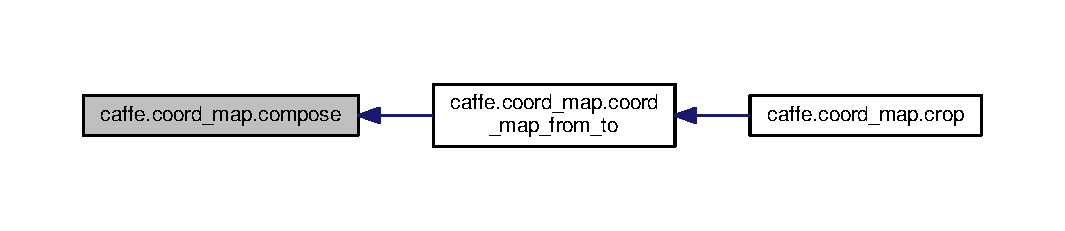
\includegraphics[width=350pt]{namespacecaffe_1_1coord__map_a06830f75738dcbc0b29bfeb30ae4f990_icgraph}
\end{center}
\end{figure}
\mbox{\Hypertarget{namespacecaffe_1_1coord__map_a1683f31b74339c8ac4c4985132fdecfc}\label{namespacecaffe_1_1coord__map_a1683f31b74339c8ac4c4985132fdecfc}} 
\index{caffe\+::coord\+\_\+map@{caffe\+::coord\+\_\+map}!conv\+\_\+params@{conv\+\_\+params}}
\index{conv\+\_\+params@{conv\+\_\+params}!caffe\+::coord\+\_\+map@{caffe\+::coord\+\_\+map}}
\subsubsection{\texorpdfstring{conv\+\_\+params()}{conv\_params()}}
{\footnotesize\ttfamily def caffe.\+coord\+\_\+map.\+conv\+\_\+params (\begin{DoxyParamCaption}\item[{}]{fn }\end{DoxyParamCaption})}

\begin{DoxyVerb}Extract the spatial parameters that determine the coordinate mapping:
kernel size, stride, padding, and dilation.

Implementation detail: Convolution, Deconvolution, and Im2col layers
define these in the convolution_param message, while Pooling has its
own fields in pooling_param. This method deals with these details to
extract canonical parameters.
\end{DoxyVerb}
 \mbox{\Hypertarget{namespacecaffe_1_1coord__map_a0f5ba2053a2fd10038360dea8b2e5b9b}\label{namespacecaffe_1_1coord__map_a0f5ba2053a2fd10038360dea8b2e5b9b}} 
\index{caffe\+::coord\+\_\+map@{caffe\+::coord\+\_\+map}!coord\+\_\+map@{coord\+\_\+map}}
\index{coord\+\_\+map@{coord\+\_\+map}!caffe\+::coord\+\_\+map@{caffe\+::coord\+\_\+map}}
\subsubsection{\texorpdfstring{coord\+\_\+map()}{coord\_map()}}
{\footnotesize\ttfamily def caffe.\+coord\+\_\+map.\+coord\+\_\+map (\begin{DoxyParamCaption}\item[{}]{fn }\end{DoxyParamCaption})}

\begin{DoxyVerb}Define the coordinate mapping by its
- axis
- scale: output coord[i * scale] <- input_coord[i]
- shift: output coord[i] <- output_coord[i + shift]
s.t. the identity mapping, as for pointwise layers like ReLu, is defined by
(None, 1, 0) since it is independent of axis and does not transform coords.
\end{DoxyVerb}
 Here is the caller graph for this function\+:
\nopagebreak
\begin{figure}[H]
\begin{center}
\leavevmode
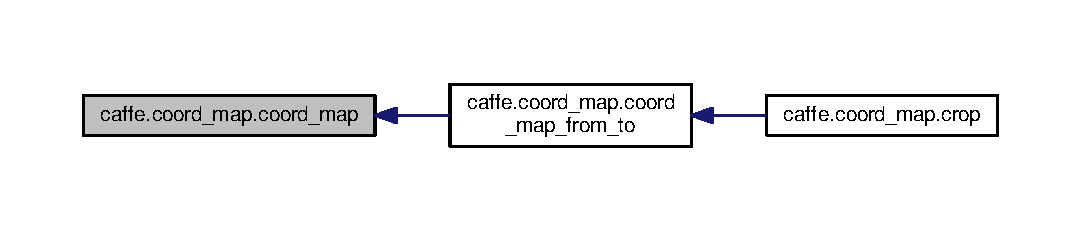
\includegraphics[width=350pt]{namespacecaffe_1_1coord__map_a0f5ba2053a2fd10038360dea8b2e5b9b_icgraph}
\end{center}
\end{figure}
\mbox{\Hypertarget{namespacecaffe_1_1coord__map_abf9ba4c31e6e4f0bcd3130ea9001514b}\label{namespacecaffe_1_1coord__map_abf9ba4c31e6e4f0bcd3130ea9001514b}} 
\index{caffe\+::coord\+\_\+map@{caffe\+::coord\+\_\+map}!coord\+\_\+map\+\_\+from\+\_\+to@{coord\+\_\+map\+\_\+from\+\_\+to}}
\index{coord\+\_\+map\+\_\+from\+\_\+to@{coord\+\_\+map\+\_\+from\+\_\+to}!caffe\+::coord\+\_\+map@{caffe\+::coord\+\_\+map}}
\subsubsection{\texorpdfstring{coord\+\_\+map\+\_\+from\+\_\+to()}{coord\_map\_from\_to()}}
{\footnotesize\ttfamily def caffe.\+coord\+\_\+map.\+coord\+\_\+map\+\_\+from\+\_\+to (\begin{DoxyParamCaption}\item[{}]{top\+\_\+from,  }\item[{}]{top\+\_\+to }\end{DoxyParamCaption})}

\begin{DoxyVerb}Determine the coordinate mapping betweeen a top (from) and a top (to).
Walk the graph to find a common ancestor while composing the coord maps for
from and to until they meet. As a last step the from map is inverted.
\end{DoxyVerb}
 Here is the call graph for this function\+:
\nopagebreak
\begin{figure}[H]
\begin{center}
\leavevmode
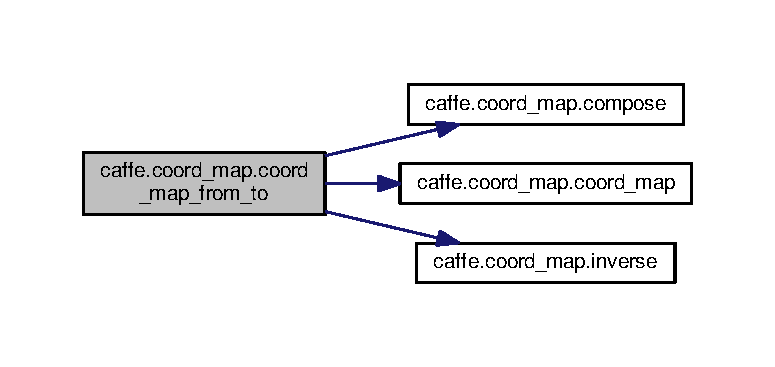
\includegraphics[width=350pt]{namespacecaffe_1_1coord__map_abf9ba4c31e6e4f0bcd3130ea9001514b_cgraph}
\end{center}
\end{figure}
Here is the caller graph for this function\+:
\nopagebreak
\begin{figure}[H]
\begin{center}
\leavevmode
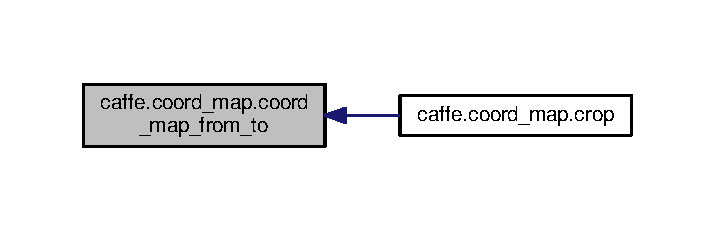
\includegraphics[width=343pt]{namespacecaffe_1_1coord__map_abf9ba4c31e6e4f0bcd3130ea9001514b_icgraph}
\end{center}
\end{figure}
\mbox{\Hypertarget{namespacecaffe_1_1coord__map_aca9f1366a027d686a27d150e054296ee}\label{namespacecaffe_1_1coord__map_aca9f1366a027d686a27d150e054296ee}} 
\index{caffe\+::coord\+\_\+map@{caffe\+::coord\+\_\+map}!crop@{crop}}
\index{crop@{crop}!caffe\+::coord\+\_\+map@{caffe\+::coord\+\_\+map}}
\subsubsection{\texorpdfstring{crop()}{crop()}}
{\footnotesize\ttfamily def caffe.\+coord\+\_\+map.\+crop (\begin{DoxyParamCaption}\item[{}]{top\+\_\+from,  }\item[{}]{top\+\_\+to }\end{DoxyParamCaption})}

\begin{DoxyVerb}Define a Crop layer to crop a top (from) to another top (to) by
determining the coordinate mapping between the two and net spec'ing
the axis and shift parameters of the crop.
\end{DoxyVerb}
 Here is the call graph for this function\+:
\nopagebreak
\begin{figure}[H]
\begin{center}
\leavevmode
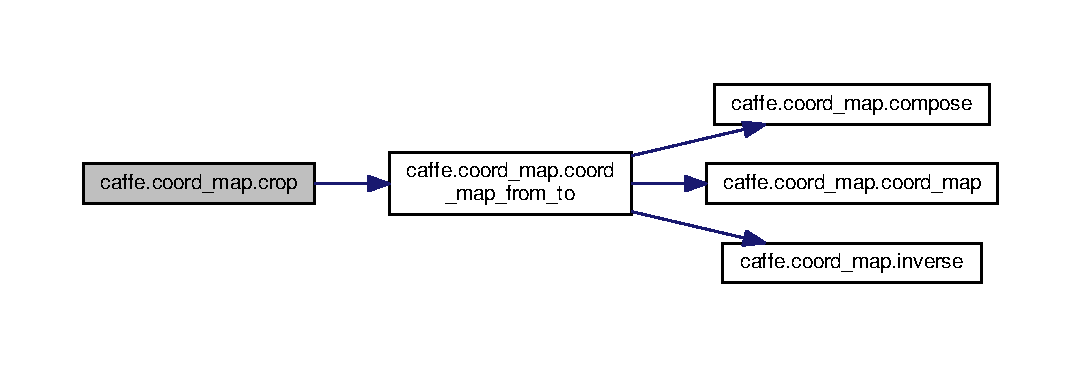
\includegraphics[width=350pt]{namespacecaffe_1_1coord__map_aca9f1366a027d686a27d150e054296ee_cgraph}
\end{center}
\end{figure}
\mbox{\Hypertarget{namespacecaffe_1_1coord__map_ac97591996ede7cfc368c2e472e0d07b6}\label{namespacecaffe_1_1coord__map_ac97591996ede7cfc368c2e472e0d07b6}} 
\index{caffe\+::coord\+\_\+map@{caffe\+::coord\+\_\+map}!crop\+\_\+params@{crop\+\_\+params}}
\index{crop\+\_\+params@{crop\+\_\+params}!caffe\+::coord\+\_\+map@{caffe\+::coord\+\_\+map}}
\subsubsection{\texorpdfstring{crop\+\_\+params()}{crop\_params()}}
{\footnotesize\ttfamily def caffe.\+coord\+\_\+map.\+crop\+\_\+params (\begin{DoxyParamCaption}\item[{}]{fn }\end{DoxyParamCaption})}

\begin{DoxyVerb}Extract the crop layer parameters with defaults.
\end{DoxyVerb}
 \mbox{\Hypertarget{namespacecaffe_1_1coord__map_ad03646b133a0a44eb1062c6acf677c8c}\label{namespacecaffe_1_1coord__map_ad03646b133a0a44eb1062c6acf677c8c}} 
\index{caffe\+::coord\+\_\+map@{caffe\+::coord\+\_\+map}!inverse@{inverse}}
\index{inverse@{inverse}!caffe\+::coord\+\_\+map@{caffe\+::coord\+\_\+map}}
\subsubsection{\texorpdfstring{inverse()}{inverse()}}
{\footnotesize\ttfamily def caffe.\+coord\+\_\+map.\+inverse (\begin{DoxyParamCaption}\item[{}]{coord\+\_\+map }\end{DoxyParamCaption})}

\begin{DoxyVerb}Invert a coord map by de-scaling and un-shifting;
this gives the backward mapping for the gradient.
\end{DoxyVerb}
 Here is the caller graph for this function\+:
\nopagebreak
\begin{figure}[H]
\begin{center}
\leavevmode
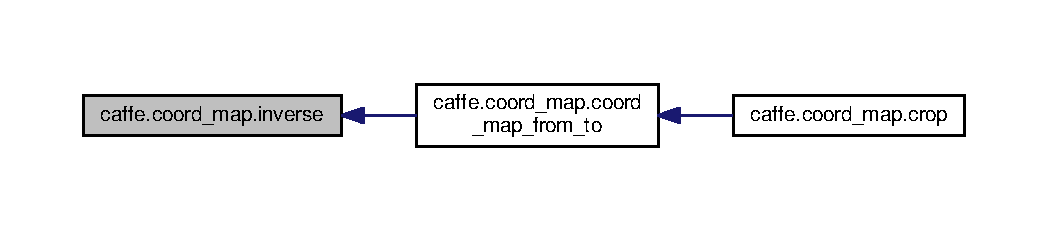
\includegraphics[width=350pt]{namespacecaffe_1_1coord__map_ad03646b133a0a44eb1062c6acf677c8c_icgraph}
\end{center}
\end{figure}


\subsection{Variable Documentation}
\mbox{\Hypertarget{namespacecaffe_1_1coord__map_a3846a1f9486c7ebe906f163cd50034bc}\label{namespacecaffe_1_1coord__map_a3846a1f9486c7ebe906f163cd50034bc}} 
\index{caffe\+::coord\+\_\+map@{caffe\+::coord\+\_\+map}!P\+A\+S\+S\+\_\+\+T\+H\+R\+O\+U\+G\+H\+\_\+\+L\+A\+Y\+E\+RS@{P\+A\+S\+S\+\_\+\+T\+H\+R\+O\+U\+G\+H\+\_\+\+L\+A\+Y\+E\+RS}}
\index{P\+A\+S\+S\+\_\+\+T\+H\+R\+O\+U\+G\+H\+\_\+\+L\+A\+Y\+E\+RS@{P\+A\+S\+S\+\_\+\+T\+H\+R\+O\+U\+G\+H\+\_\+\+L\+A\+Y\+E\+RS}!caffe\+::coord\+\_\+map@{caffe\+::coord\+\_\+map}}
\subsubsection{\texorpdfstring{P\+A\+S\+S\+\_\+\+T\+H\+R\+O\+U\+G\+H\+\_\+\+L\+A\+Y\+E\+RS}{PASS\_THROUGH\_LAYERS}}
{\footnotesize\ttfamily list caffe.\+coord\+\_\+map.\+P\+A\+S\+S\+\_\+\+T\+H\+R\+O\+U\+G\+H\+\_\+\+L\+A\+Y\+E\+RS}

{\bfseries Initial value\+:}
\begin{DoxyCode}
1 =  [\textcolor{stringliteral}{'AbsVal'}, \textcolor{stringliteral}{'BatchNorm'}, \textcolor{stringliteral}{'Bias'}, \textcolor{stringliteral}{'BNLL'}, \textcolor{stringliteral}{'Dropout'},
2                        \textcolor{stringliteral}{'Eltwise'}, \textcolor{stringliteral}{'ELU'}, \textcolor{stringliteral}{'Log'}, \textcolor{stringliteral}{'LRN'}, \textcolor{stringliteral}{'Exp'}, \textcolor{stringliteral}{'MVN'}, \textcolor{stringliteral}{'Power'},
3                        \textcolor{stringliteral}{'ReLU'}, \textcolor{stringliteral}{'PReLU'}, \textcolor{stringliteral}{'Scale'}, \textcolor{stringliteral}{'Sigmoid'}, \textcolor{stringliteral}{'Split'}, \textcolor{stringliteral}{'TanH'},
4                        \textcolor{stringliteral}{'Threshold'}]
\end{DoxyCode}

\hypertarget{namespacecaffe_1_1detector}{}\section{caffe.\+detector Namespace Reference}
\label{namespacecaffe_1_1detector}\index{caffe.\+detector@{caffe.\+detector}}
\subsection*{Classes}
\begin{DoxyCompactItemize}
\item 
class \mbox{\hyperlink{classcaffe_1_1detector_1_1_detector}{Detector}}
\end{DoxyCompactItemize}


\subsection{Detailed Description}
\begin{DoxyVerb}Do windowed detection by classifying a number of images/crops at once,
optionally using the selective search window proposal method.

This implementation follows ideas in
Ross Girshick, Jeff Donahue, Trevor Darrell, Jitendra Malik.
Rich feature hierarchies for accurate object detection and semantic
segmentation.
http://arxiv.org/abs/1311.2524

The selective_search_ijcv_with_python code required for the selective search
proposal mode is available at
https://github.com/sergeyk/selective_search_ijcv_with_python
\end{DoxyVerb}
 
\hypertarget{namespacecaffe_1_1draw}{}\section{caffe.\+draw Namespace Reference}
\label{namespacecaffe_1_1draw}\index{caffe.\+draw@{caffe.\+draw}}
\subsection*{Functions}
\begin{DoxyCompactItemize}
\item 
def \mbox{\hyperlink{namespacecaffe_1_1draw_a18df1acb5bad222d90e8873375367ef1}{get\+\_\+pooling\+\_\+types\+\_\+dict}} ()
\item 
def \mbox{\hyperlink{namespacecaffe_1_1draw_a672545af1643af2c11e6b19226eaf6c4}{get\+\_\+edge\+\_\+label}} (layer)
\item 
def \mbox{\hyperlink{namespacecaffe_1_1draw_ac1df68579f91acefee36f75ac5b0de1d}{get\+\_\+layer\+\_\+lr\+\_\+mult}} (layer)
\item 
def \mbox{\hyperlink{namespacecaffe_1_1draw_a1ab4383ec4e16ed4e8f0e027c25c682a}{get\+\_\+layer\+\_\+label}} (layer, rankdir, display\+\_\+lrm=False)
\item 
def \mbox{\hyperlink{namespacecaffe_1_1draw_ab06e25fd2bbb0166d3c3ff19d9854828}{choose\+\_\+color\+\_\+by\+\_\+layertype}} (layertype)
\item 
def \mbox{\hyperlink{namespacecaffe_1_1draw_a679642bc8af6fb5382480cfad0c27111}{get\+\_\+pydot\+\_\+graph}} (caffe\+\_\+net, rankdir, label\+\_\+edges=True, phase=None, display\+\_\+lrm=False)
\item 
def \mbox{\hyperlink{namespacecaffe_1_1draw_af1c2f41e9d66bae6814590e8c59f64c6}{draw\+\_\+net}} (caffe\+\_\+net, rankdir, ext=\textquotesingle{}png\textquotesingle{}, phase=None, display\+\_\+lrm=False)
\item 
def \mbox{\hyperlink{namespacecaffe_1_1draw_a1955d119b9b325ea2ad20254b3dc80e3}{draw\+\_\+net\+\_\+to\+\_\+file}} (caffe\+\_\+net, filename, rankdir=\textquotesingle{}LR\textquotesingle{}, phase=None, display\+\_\+lrm=False)
\end{DoxyCompactItemize}
\subsection*{Variables}
\begin{DoxyCompactItemize}
\item 
dictionary {\bfseries L\+A\+Y\+E\+R\+\_\+\+S\+T\+Y\+L\+E\+\_\+\+D\+E\+F\+A\+U\+LT}
\item 
dictionary {\bfseries N\+E\+U\+R\+O\+N\+\_\+\+L\+A\+Y\+E\+R\+\_\+\+S\+T\+Y\+LE}
\item 
dictionary {\bfseries B\+L\+O\+B\+\_\+\+S\+T\+Y\+LE}
\end{DoxyCompactItemize}


\subsection{Detailed Description}
\begin{DoxyVerb}Caffe network visualization: draw the NetParameter protobuffer.


.. note::

    This requires pydot>=1.0.2, which is not included in requirements.txt since
    it requires graphviz and other prerequisites outside the scope of the
    Caffe.
\end{DoxyVerb}
 

\subsection{Function Documentation}
\mbox{\Hypertarget{namespacecaffe_1_1draw_ab06e25fd2bbb0166d3c3ff19d9854828}\label{namespacecaffe_1_1draw_ab06e25fd2bbb0166d3c3ff19d9854828}} 
\index{caffe\+::draw@{caffe\+::draw}!choose\+\_\+color\+\_\+by\+\_\+layertype@{choose\+\_\+color\+\_\+by\+\_\+layertype}}
\index{choose\+\_\+color\+\_\+by\+\_\+layertype@{choose\+\_\+color\+\_\+by\+\_\+layertype}!caffe\+::draw@{caffe\+::draw}}
\subsubsection{\texorpdfstring{choose\+\_\+color\+\_\+by\+\_\+layertype()}{choose\_color\_by\_layertype()}}
{\footnotesize\ttfamily def caffe.\+draw.\+choose\+\_\+color\+\_\+by\+\_\+layertype (\begin{DoxyParamCaption}\item[{}]{layertype }\end{DoxyParamCaption})}

\begin{DoxyVerb}Define colors for nodes based on the layer type.
\end{DoxyVerb}
 Here is the caller graph for this function\+:
\nopagebreak
\begin{figure}[H]
\begin{center}
\leavevmode
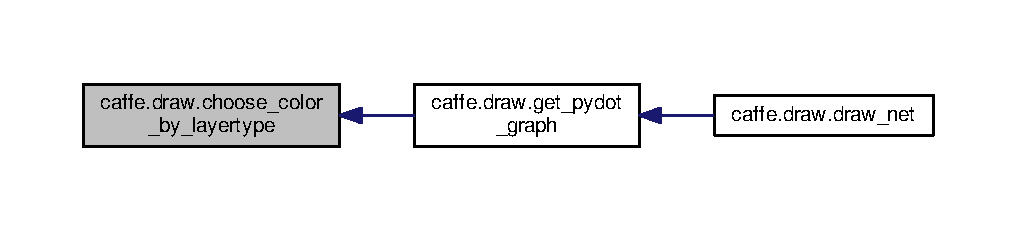
\includegraphics[width=350pt]{namespacecaffe_1_1draw_ab06e25fd2bbb0166d3c3ff19d9854828_icgraph}
\end{center}
\end{figure}
\mbox{\Hypertarget{namespacecaffe_1_1draw_af1c2f41e9d66bae6814590e8c59f64c6}\label{namespacecaffe_1_1draw_af1c2f41e9d66bae6814590e8c59f64c6}} 
\index{caffe\+::draw@{caffe\+::draw}!draw\+\_\+net@{draw\+\_\+net}}
\index{draw\+\_\+net@{draw\+\_\+net}!caffe\+::draw@{caffe\+::draw}}
\subsubsection{\texorpdfstring{draw\+\_\+net()}{draw\_net()}}
{\footnotesize\ttfamily def caffe.\+draw.\+draw\+\_\+net (\begin{DoxyParamCaption}\item[{}]{caffe\+\_\+net,  }\item[{}]{rankdir,  }\item[{}]{ext = {\ttfamily \textquotesingle{}png\textquotesingle{}},  }\item[{}]{phase = {\ttfamily None},  }\item[{}]{display\+\_\+lrm = {\ttfamily False} }\end{DoxyParamCaption})}

\begin{DoxyVerb}Draws a caffe net and returns the image string encoded using the given
extension.

Parameters
----------
caffe_net : a caffe.proto.caffe_pb2.NetParameter protocol buffer.
ext : string, optional
    The image extension (the default is 'png').
phase : {caffe_pb2.Phase.TRAIN, caffe_pb2.Phase.TEST, None} optional
    Include layers from this network phase.  If None, include all layers.
    (the default is None)
display_lrm : boolean, optional
    If True display the learning rate multipliers for the learning layers
    (default is False).

Returns
-------
string :
    Postscript representation of the graph.
\end{DoxyVerb}
 Here is the call graph for this function\+:
\nopagebreak
\begin{figure}[H]
\begin{center}
\leavevmode
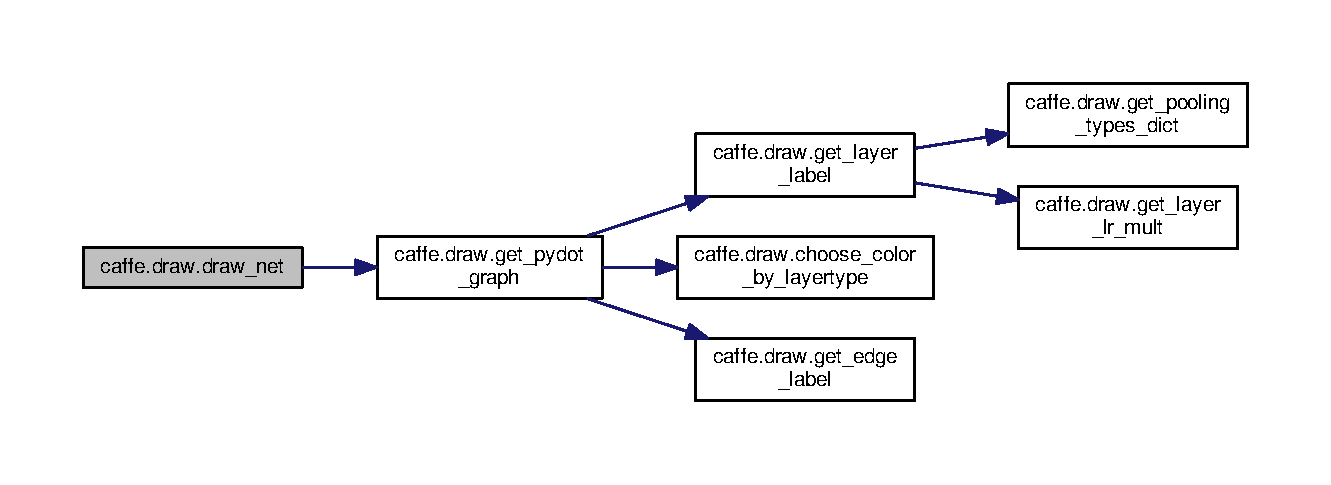
\includegraphics[width=350pt]{namespacecaffe_1_1draw_af1c2f41e9d66bae6814590e8c59f64c6_cgraph}
\end{center}
\end{figure}
\mbox{\Hypertarget{namespacecaffe_1_1draw_a1955d119b9b325ea2ad20254b3dc80e3}\label{namespacecaffe_1_1draw_a1955d119b9b325ea2ad20254b3dc80e3}} 
\index{caffe\+::draw@{caffe\+::draw}!draw\+\_\+net\+\_\+to\+\_\+file@{draw\+\_\+net\+\_\+to\+\_\+file}}
\index{draw\+\_\+net\+\_\+to\+\_\+file@{draw\+\_\+net\+\_\+to\+\_\+file}!caffe\+::draw@{caffe\+::draw}}
\subsubsection{\texorpdfstring{draw\+\_\+net\+\_\+to\+\_\+file()}{draw\_net\_to\_file()}}
{\footnotesize\ttfamily def caffe.\+draw.\+draw\+\_\+net\+\_\+to\+\_\+file (\begin{DoxyParamCaption}\item[{}]{caffe\+\_\+net,  }\item[{}]{filename,  }\item[{}]{rankdir = {\ttfamily \textquotesingle{}LR\textquotesingle{}},  }\item[{}]{phase = {\ttfamily None},  }\item[{}]{display\+\_\+lrm = {\ttfamily False} }\end{DoxyParamCaption})}

\begin{DoxyVerb}Draws a caffe net, and saves it to file using the format given as the
file extension. Use '.raw' to output raw text that you can manually feed
to graphviz to draw graphs.

Parameters
----------
caffe_net : a caffe.proto.caffe_pb2.NetParameter protocol buffer.
filename : string
    The path to a file where the networks visualization will be stored.
rankdir : {'LR', 'TB', 'BT'}
    Direction of graph layout.
phase : {caffe_pb2.Phase.TRAIN, caffe_pb2.Phase.TEST, None} optional
    Include layers from this network phase.  If None, include all layers.
    (the default is None)
display_lrm : boolean, optional
    If True display the learning rate multipliers for the learning layers
    (default is False).
\end{DoxyVerb}
 Here is the caller graph for this function\+:
\nopagebreak
\begin{figure}[H]
\begin{center}
\leavevmode
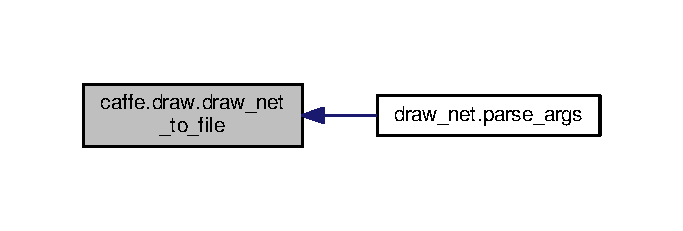
\includegraphics[width=328pt]{namespacecaffe_1_1draw_a1955d119b9b325ea2ad20254b3dc80e3_icgraph}
\end{center}
\end{figure}
\mbox{\Hypertarget{namespacecaffe_1_1draw_a672545af1643af2c11e6b19226eaf6c4}\label{namespacecaffe_1_1draw_a672545af1643af2c11e6b19226eaf6c4}} 
\index{caffe\+::draw@{caffe\+::draw}!get\+\_\+edge\+\_\+label@{get\+\_\+edge\+\_\+label}}
\index{get\+\_\+edge\+\_\+label@{get\+\_\+edge\+\_\+label}!caffe\+::draw@{caffe\+::draw}}
\subsubsection{\texorpdfstring{get\+\_\+edge\+\_\+label()}{get\_edge\_label()}}
{\footnotesize\ttfamily def caffe.\+draw.\+get\+\_\+edge\+\_\+label (\begin{DoxyParamCaption}\item[{}]{layer }\end{DoxyParamCaption})}

\begin{DoxyVerb}Define edge label based on layer type.
\end{DoxyVerb}
 Here is the caller graph for this function\+:
\nopagebreak
\begin{figure}[H]
\begin{center}
\leavevmode
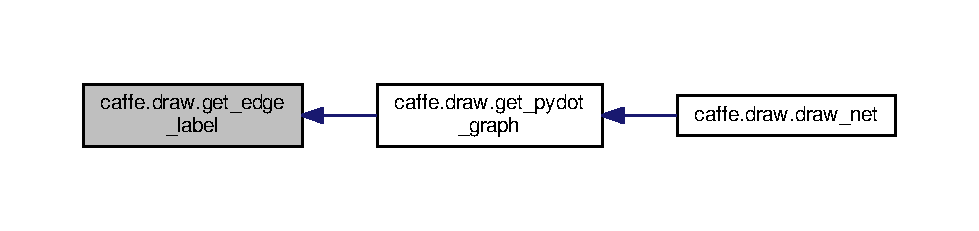
\includegraphics[width=350pt]{namespacecaffe_1_1draw_a672545af1643af2c11e6b19226eaf6c4_icgraph}
\end{center}
\end{figure}
\mbox{\Hypertarget{namespacecaffe_1_1draw_a1ab4383ec4e16ed4e8f0e027c25c682a}\label{namespacecaffe_1_1draw_a1ab4383ec4e16ed4e8f0e027c25c682a}} 
\index{caffe\+::draw@{caffe\+::draw}!get\+\_\+layer\+\_\+label@{get\+\_\+layer\+\_\+label}}
\index{get\+\_\+layer\+\_\+label@{get\+\_\+layer\+\_\+label}!caffe\+::draw@{caffe\+::draw}}
\subsubsection{\texorpdfstring{get\+\_\+layer\+\_\+label()}{get\_layer\_label()}}
{\footnotesize\ttfamily def caffe.\+draw.\+get\+\_\+layer\+\_\+label (\begin{DoxyParamCaption}\item[{}]{layer,  }\item[{}]{rankdir,  }\item[{}]{display\+\_\+lrm = {\ttfamily False} }\end{DoxyParamCaption})}

\begin{DoxyVerb}Define node label based on layer type.

Parameters
----------
layer : caffe_pb2.LayerParameter
rankdir : {'LR', 'TB', 'BT'}
    Direction of graph layout.
display_lrm : boolean, optional
    If True include the learning rate multipliers in the label (default is
    False).

Returns
-------
node_label : string
    A label for the current layer
\end{DoxyVerb}
 Here is the call graph for this function\+:
\nopagebreak
\begin{figure}[H]
\begin{center}
\leavevmode
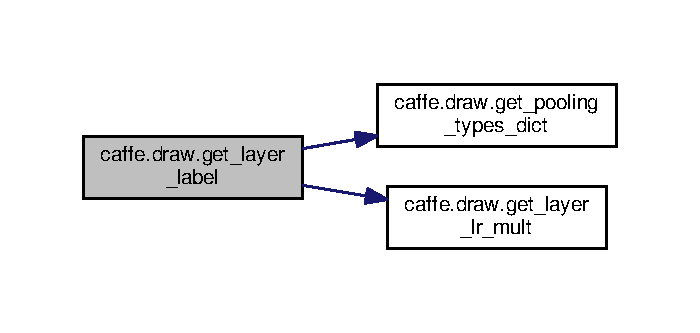
\includegraphics[width=336pt]{namespacecaffe_1_1draw_a1ab4383ec4e16ed4e8f0e027c25c682a_cgraph}
\end{center}
\end{figure}
Here is the caller graph for this function\+:
\nopagebreak
\begin{figure}[H]
\begin{center}
\leavevmode
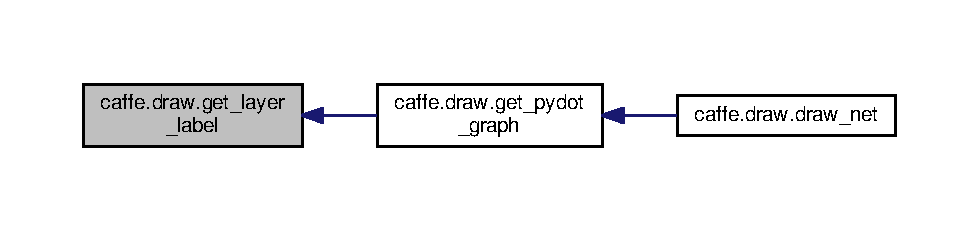
\includegraphics[width=350pt]{namespacecaffe_1_1draw_a1ab4383ec4e16ed4e8f0e027c25c682a_icgraph}
\end{center}
\end{figure}
\mbox{\Hypertarget{namespacecaffe_1_1draw_ac1df68579f91acefee36f75ac5b0de1d}\label{namespacecaffe_1_1draw_ac1df68579f91acefee36f75ac5b0de1d}} 
\index{caffe\+::draw@{caffe\+::draw}!get\+\_\+layer\+\_\+lr\+\_\+mult@{get\+\_\+layer\+\_\+lr\+\_\+mult}}
\index{get\+\_\+layer\+\_\+lr\+\_\+mult@{get\+\_\+layer\+\_\+lr\+\_\+mult}!caffe\+::draw@{caffe\+::draw}}
\subsubsection{\texorpdfstring{get\+\_\+layer\+\_\+lr\+\_\+mult()}{get\_layer\_lr\_mult()}}
{\footnotesize\ttfamily def caffe.\+draw.\+get\+\_\+layer\+\_\+lr\+\_\+mult (\begin{DoxyParamCaption}\item[{}]{layer }\end{DoxyParamCaption})}

\begin{DoxyVerb}Get the learning rate multipliers.

Get the learning rate multipliers for the given layer. Assumes a
Convolution/Deconvolution/InnerProduct layer.

Parameters
----------
layer : caffe_pb2.LayerParameter
    A Convolution, Deconvolution, or InnerProduct layer.

Returns
-------
learning_rates : tuple of floats
    the learning rate multipliers for the weights and biases.
\end{DoxyVerb}
 Here is the caller graph for this function\+:
\nopagebreak
\begin{figure}[H]
\begin{center}
\leavevmode
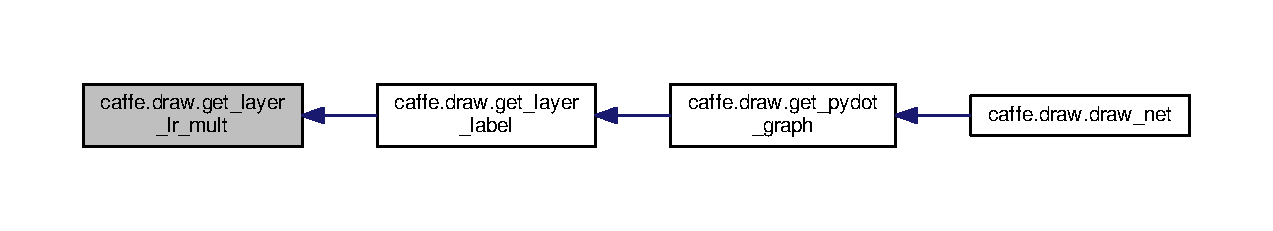
\includegraphics[width=350pt]{namespacecaffe_1_1draw_ac1df68579f91acefee36f75ac5b0de1d_icgraph}
\end{center}
\end{figure}
\mbox{\Hypertarget{namespacecaffe_1_1draw_a18df1acb5bad222d90e8873375367ef1}\label{namespacecaffe_1_1draw_a18df1acb5bad222d90e8873375367ef1}} 
\index{caffe\+::draw@{caffe\+::draw}!get\+\_\+pooling\+\_\+types\+\_\+dict@{get\+\_\+pooling\+\_\+types\+\_\+dict}}
\index{get\+\_\+pooling\+\_\+types\+\_\+dict@{get\+\_\+pooling\+\_\+types\+\_\+dict}!caffe\+::draw@{caffe\+::draw}}
\subsubsection{\texorpdfstring{get\+\_\+pooling\+\_\+types\+\_\+dict()}{get\_pooling\_types\_dict()}}
{\footnotesize\ttfamily def caffe.\+draw.\+get\+\_\+pooling\+\_\+types\+\_\+dict (\begin{DoxyParamCaption}{ }\end{DoxyParamCaption})}

\begin{DoxyVerb}Get dictionary mapping pooling type number to type name
\end{DoxyVerb}
 Here is the caller graph for this function\+:
\nopagebreak
\begin{figure}[H]
\begin{center}
\leavevmode
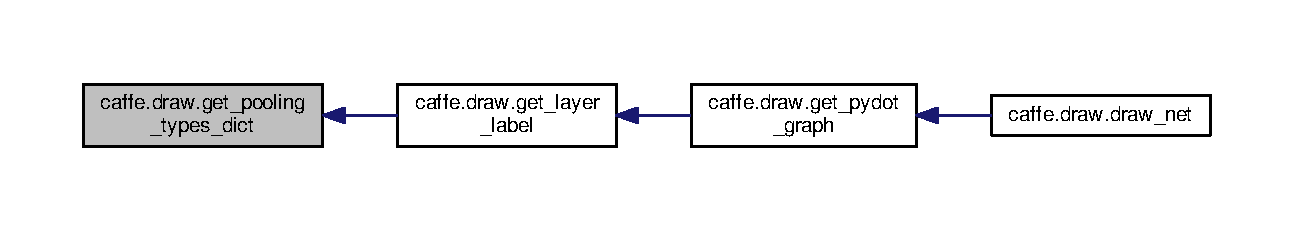
\includegraphics[width=350pt]{namespacecaffe_1_1draw_a18df1acb5bad222d90e8873375367ef1_icgraph}
\end{center}
\end{figure}
\mbox{\Hypertarget{namespacecaffe_1_1draw_a679642bc8af6fb5382480cfad0c27111}\label{namespacecaffe_1_1draw_a679642bc8af6fb5382480cfad0c27111}} 
\index{caffe\+::draw@{caffe\+::draw}!get\+\_\+pydot\+\_\+graph@{get\+\_\+pydot\+\_\+graph}}
\index{get\+\_\+pydot\+\_\+graph@{get\+\_\+pydot\+\_\+graph}!caffe\+::draw@{caffe\+::draw}}
\subsubsection{\texorpdfstring{get\+\_\+pydot\+\_\+graph()}{get\_pydot\_graph()}}
{\footnotesize\ttfamily def caffe.\+draw.\+get\+\_\+pydot\+\_\+graph (\begin{DoxyParamCaption}\item[{}]{caffe\+\_\+net,  }\item[{}]{rankdir,  }\item[{}]{label\+\_\+edges = {\ttfamily True},  }\item[{}]{phase = {\ttfamily None},  }\item[{}]{display\+\_\+lrm = {\ttfamily False} }\end{DoxyParamCaption})}

\begin{DoxyVerb}Create a data structure which represents the `caffe_net`.

Parameters
----------
caffe_net : object
rankdir : {'LR', 'TB', 'BT'}
    Direction of graph layout.
label_edges : boolean, optional
    Label the edges (default is True).
phase : {caffe_pb2.Phase.TRAIN, caffe_pb2.Phase.TEST, None} optional
    Include layers from this network phase.  If None, include all layers.
    (the default is None)
display_lrm : boolean, optional
    If True display the learning rate multipliers when relevant (default is
    False).

Returns
-------
pydot graph object
\end{DoxyVerb}
 Here is the call graph for this function\+:
\nopagebreak
\begin{figure}[H]
\begin{center}
\leavevmode
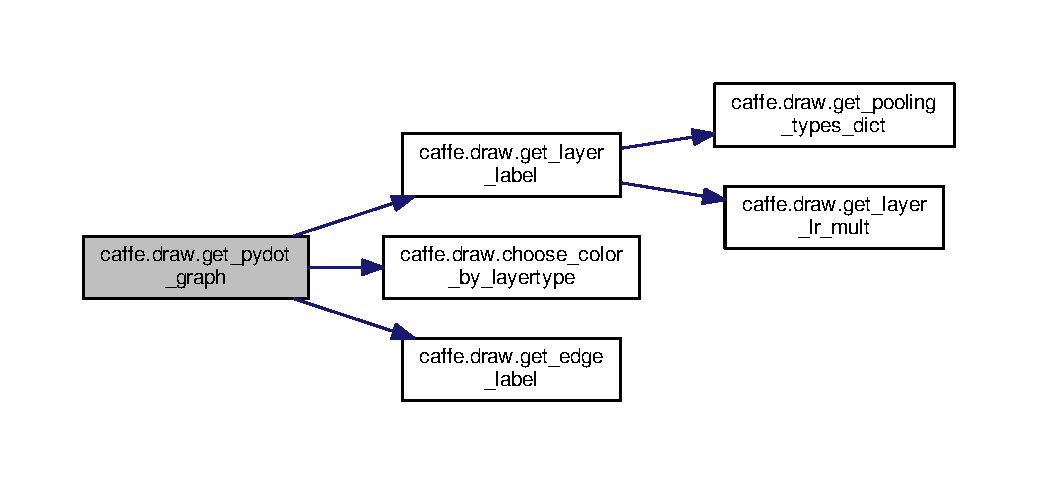
\includegraphics[width=350pt]{namespacecaffe_1_1draw_a679642bc8af6fb5382480cfad0c27111_cgraph}
\end{center}
\end{figure}
Here is the caller graph for this function\+:
\nopagebreak
\begin{figure}[H]
\begin{center}
\leavevmode
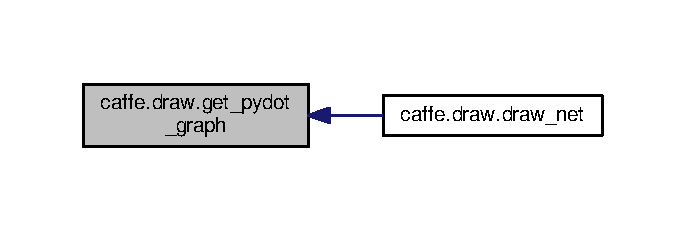
\includegraphics[width=329pt]{namespacecaffe_1_1draw_a679642bc8af6fb5382480cfad0c27111_icgraph}
\end{center}
\end{figure}


\subsection{Variable Documentation}
\mbox{\Hypertarget{namespacecaffe_1_1draw_ab9680300b4ad475d87181a74cdad3d7f}\label{namespacecaffe_1_1draw_ab9680300b4ad475d87181a74cdad3d7f}} 
\index{caffe\+::draw@{caffe\+::draw}!B\+L\+O\+B\+\_\+\+S\+T\+Y\+LE@{B\+L\+O\+B\+\_\+\+S\+T\+Y\+LE}}
\index{B\+L\+O\+B\+\_\+\+S\+T\+Y\+LE@{B\+L\+O\+B\+\_\+\+S\+T\+Y\+LE}!caffe\+::draw@{caffe\+::draw}}
\subsubsection{\texorpdfstring{B\+L\+O\+B\+\_\+\+S\+T\+Y\+LE}{BLOB\_STYLE}}
{\footnotesize\ttfamily dictionary caffe.\+draw.\+B\+L\+O\+B\+\_\+\+S\+T\+Y\+LE}

{\bfseries Initial value\+:}
\begin{DoxyCode}
1 =  \{\textcolor{stringliteral}{'shape'}: \textcolor{stringliteral}{'octagon'},
2               \textcolor{stringliteral}{'fillcolor'}: \textcolor{stringliteral}{'\#E0E0E0'},
3               \textcolor{stringliteral}{'style'}: \textcolor{stringliteral}{'filled'}\}
\end{DoxyCode}
\mbox{\Hypertarget{namespacecaffe_1_1draw_a1756d7ea83bb874451506563fc3b0876}\label{namespacecaffe_1_1draw_a1756d7ea83bb874451506563fc3b0876}} 
\index{caffe\+::draw@{caffe\+::draw}!L\+A\+Y\+E\+R\+\_\+\+S\+T\+Y\+L\+E\+\_\+\+D\+E\+F\+A\+U\+LT@{L\+A\+Y\+E\+R\+\_\+\+S\+T\+Y\+L\+E\+\_\+\+D\+E\+F\+A\+U\+LT}}
\index{L\+A\+Y\+E\+R\+\_\+\+S\+T\+Y\+L\+E\+\_\+\+D\+E\+F\+A\+U\+LT@{L\+A\+Y\+E\+R\+\_\+\+S\+T\+Y\+L\+E\+\_\+\+D\+E\+F\+A\+U\+LT}!caffe\+::draw@{caffe\+::draw}}
\subsubsection{\texorpdfstring{L\+A\+Y\+E\+R\+\_\+\+S\+T\+Y\+L\+E\+\_\+\+D\+E\+F\+A\+U\+LT}{LAYER\_STYLE\_DEFAULT}}
{\footnotesize\ttfamily dictionary caffe.\+draw.\+L\+A\+Y\+E\+R\+\_\+\+S\+T\+Y\+L\+E\+\_\+\+D\+E\+F\+A\+U\+LT}

{\bfseries Initial value\+:}
\begin{DoxyCode}
1 =  \{\textcolor{stringliteral}{'shape'}: \textcolor{stringliteral}{'record'},
2                        \textcolor{stringliteral}{'fillcolor'}: \textcolor{stringliteral}{'\#6495ED'},
3                        \textcolor{stringliteral}{'style'}: \textcolor{stringliteral}{'filled'}\}
\end{DoxyCode}
\mbox{\Hypertarget{namespacecaffe_1_1draw_a2fb7a9809c0cf095bfdd8e4549db9c0d}\label{namespacecaffe_1_1draw_a2fb7a9809c0cf095bfdd8e4549db9c0d}} 
\index{caffe\+::draw@{caffe\+::draw}!N\+E\+U\+R\+O\+N\+\_\+\+L\+A\+Y\+E\+R\+\_\+\+S\+T\+Y\+LE@{N\+E\+U\+R\+O\+N\+\_\+\+L\+A\+Y\+E\+R\+\_\+\+S\+T\+Y\+LE}}
\index{N\+E\+U\+R\+O\+N\+\_\+\+L\+A\+Y\+E\+R\+\_\+\+S\+T\+Y\+LE@{N\+E\+U\+R\+O\+N\+\_\+\+L\+A\+Y\+E\+R\+\_\+\+S\+T\+Y\+LE}!caffe\+::draw@{caffe\+::draw}}
\subsubsection{\texorpdfstring{N\+E\+U\+R\+O\+N\+\_\+\+L\+A\+Y\+E\+R\+\_\+\+S\+T\+Y\+LE}{NEURON\_LAYER\_STYLE}}
{\footnotesize\ttfamily dictionary caffe.\+draw.\+N\+E\+U\+R\+O\+N\+\_\+\+L\+A\+Y\+E\+R\+\_\+\+S\+T\+Y\+LE}

{\bfseries Initial value\+:}
\begin{DoxyCode}
1 =  \{\textcolor{stringliteral}{'shape'}: \textcolor{stringliteral}{'record'},
2                       \textcolor{stringliteral}{'fillcolor'}: \textcolor{stringliteral}{'\#90EE90'},
3                       \textcolor{stringliteral}{'style'}: \textcolor{stringliteral}{'filled'}\}
\end{DoxyCode}

\hypertarget{namespacecaffe_1_1net__spec}{}\section{caffe.\+net\+\_\+spec Namespace Reference}
\label{namespacecaffe_1_1net__spec}\index{caffe.\+net\+\_\+spec@{caffe.\+net\+\_\+spec}}
\subsection*{Classes}
\begin{DoxyCompactItemize}
\item 
class \mbox{\hyperlink{classcaffe_1_1net__spec_1_1_function}{Function}}
\item 
class \mbox{\hyperlink{classcaffe_1_1net__spec_1_1_layers}{Layers}}
\item 
class \mbox{\hyperlink{classcaffe_1_1net__spec_1_1_net_spec}{Net\+Spec}}
\item 
class \mbox{\hyperlink{classcaffe_1_1net__spec_1_1_parameters}{Parameters}}
\item 
class \mbox{\hyperlink{classcaffe_1_1net__spec_1_1_top}{Top}}
\end{DoxyCompactItemize}
\subsection*{Functions}
\begin{DoxyCompactItemize}
\item 
def \mbox{\hyperlink{namespacecaffe_1_1net__spec_a743950197e4a2ce816bcc4ec5bb04968}{param\+\_\+name\+\_\+dict}} ()
\item 
def \mbox{\hyperlink{namespacecaffe_1_1net__spec_a8d5d3cab109867ec42e5e7c2b957e630}{to\+\_\+proto}} (tops)
\item 
def \mbox{\hyperlink{namespacecaffe_1_1net__spec_a823515c8ca21e9562ea594546e167da2}{assign\+\_\+proto}} (proto, name, val)
\end{DoxyCompactItemize}
\subsection*{Variables}
\begin{DoxyCompactItemize}
\item 
\mbox{\Hypertarget{namespacecaffe_1_1net__spec_aa112f911444ddd4d57694e65b650f944}\label{namespacecaffe_1_1net__spec_aa112f911444ddd4d57694e65b650f944}} 
{\bfseries layers} = \mbox{\hyperlink{classcaffe_1_1net__spec_1_1_layers}{Layers}}()
\item 
\mbox{\Hypertarget{namespacecaffe_1_1net__spec_a1c4f03ff588b04506ce806eaa7e038b3}\label{namespacecaffe_1_1net__spec_a1c4f03ff588b04506ce806eaa7e038b3}} 
{\bfseries params} = \mbox{\hyperlink{classcaffe_1_1net__spec_1_1_parameters}{Parameters}}()
\end{DoxyCompactItemize}


\subsection{Detailed Description}
\begin{DoxyVerb}Python net specification.

This module provides a way to write nets directly in Python, using a natural,
functional style. See examples/pycaffe/caffenet.py for an example.

Currently this works as a thin wrapper around the Python protobuf interface,
with layers and parameters automatically generated for the "layers" and
"params" pseudo-modules, which are actually objects using __getattr__ magic
to generate protobuf messages.

Note that when using to_proto or Top.to_proto, names of intermediate blobs will
be automatically generated. To explicitly specify blob names, use the NetSpec
class -- assign to its attributes directly to name layers, and call
NetSpec.to_proto to serialize all assigned layers.

This interface is expected to continue to evolve as Caffe gains new capabilities
for specifying nets. In particular, the automatically generated layer names
are not guaranteed to be forward-compatible.
\end{DoxyVerb}
 

\subsection{Function Documentation}
\mbox{\Hypertarget{namespacecaffe_1_1net__spec_a823515c8ca21e9562ea594546e167da2}\label{namespacecaffe_1_1net__spec_a823515c8ca21e9562ea594546e167da2}} 
\index{caffe\+::net\+\_\+spec@{caffe\+::net\+\_\+spec}!assign\+\_\+proto@{assign\+\_\+proto}}
\index{assign\+\_\+proto@{assign\+\_\+proto}!caffe\+::net\+\_\+spec@{caffe\+::net\+\_\+spec}}
\subsubsection{\texorpdfstring{assign\+\_\+proto()}{assign\_proto()}}
{\footnotesize\ttfamily def caffe.\+net\+\_\+spec.\+assign\+\_\+proto (\begin{DoxyParamCaption}\item[{}]{proto,  }\item[{}]{name,  }\item[{}]{val }\end{DoxyParamCaption})}

\begin{DoxyVerb}Assign a Python object to a protobuf message, based on the Python
type (in recursive fashion). Lists become repeated fields/messages, dicts
become messages, and other types are assigned directly. For convenience,
repeated fields whose values are not lists are converted to single-element
lists; e.g., `my_repeated_int_field=3` is converted to
`my_repeated_int_field=[3]`.\end{DoxyVerb}
 Here is the caller graph for this function\+:
\nopagebreak
\begin{figure}[H]
\begin{center}
\leavevmode
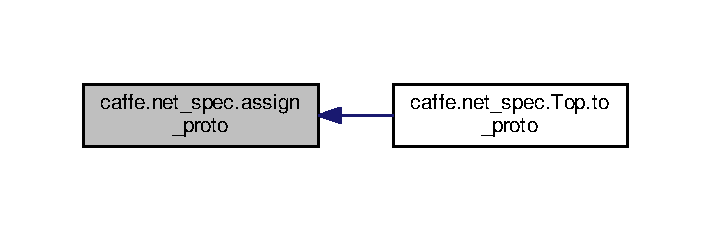
\includegraphics[width=341pt]{namespacecaffe_1_1net__spec_a823515c8ca21e9562ea594546e167da2_icgraph}
\end{center}
\end{figure}
\mbox{\Hypertarget{namespacecaffe_1_1net__spec_a743950197e4a2ce816bcc4ec5bb04968}\label{namespacecaffe_1_1net__spec_a743950197e4a2ce816bcc4ec5bb04968}} 
\index{caffe\+::net\+\_\+spec@{caffe\+::net\+\_\+spec}!param\+\_\+name\+\_\+dict@{param\+\_\+name\+\_\+dict}}
\index{param\+\_\+name\+\_\+dict@{param\+\_\+name\+\_\+dict}!caffe\+::net\+\_\+spec@{caffe\+::net\+\_\+spec}}
\subsubsection{\texorpdfstring{param\+\_\+name\+\_\+dict()}{param\_name\_dict()}}
{\footnotesize\ttfamily def caffe.\+net\+\_\+spec.\+param\+\_\+name\+\_\+dict (\begin{DoxyParamCaption}{ }\end{DoxyParamCaption})}

\begin{DoxyVerb}Find out the correspondence between layer names and parameter names.\end{DoxyVerb}
 Here is the caller graph for this function\+:
\nopagebreak
\begin{figure}[H]
\begin{center}
\leavevmode
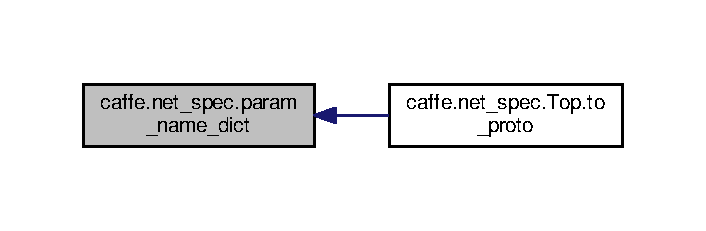
\includegraphics[width=339pt]{namespacecaffe_1_1net__spec_a743950197e4a2ce816bcc4ec5bb04968_icgraph}
\end{center}
\end{figure}
\mbox{\Hypertarget{namespacecaffe_1_1net__spec_a8d5d3cab109867ec42e5e7c2b957e630}\label{namespacecaffe_1_1net__spec_a8d5d3cab109867ec42e5e7c2b957e630}} 
\index{caffe\+::net\+\_\+spec@{caffe\+::net\+\_\+spec}!to\+\_\+proto@{to\+\_\+proto}}
\index{to\+\_\+proto@{to\+\_\+proto}!caffe\+::net\+\_\+spec@{caffe\+::net\+\_\+spec}}
\subsubsection{\texorpdfstring{to\+\_\+proto()}{to\_proto()}}
{\footnotesize\ttfamily def caffe.\+net\+\_\+spec.\+to\+\_\+proto (\begin{DoxyParamCaption}\item[{}]{tops }\end{DoxyParamCaption})}

\begin{DoxyVerb}Generate a NetParameter that contains all layers needed to compute
all arguments.\end{DoxyVerb}
 
\hypertarget{namespacecaffe_1_1pycaffe}{}\section{caffe.\+pycaffe Namespace Reference}
\label{namespacecaffe_1_1pycaffe}\index{caffe.\+pycaffe@{caffe.\+pycaffe}}


\subsection{Detailed Description}
\begin{DoxyVerb}Wrap the internal caffe C++ module (_caffe.so) with a clean, Pythonic
interface.
\end{DoxyVerb}
 
\hypertarget{namespacecaffe_1_1_solver_action}{}\section{caffe\+:\+:Solver\+Action Namespace Reference}
\label{namespacecaffe_1_1_solver_action}\index{caffe\+::\+Solver\+Action@{caffe\+::\+Solver\+Action}}


Enumeration of actions that a client of the \mbox{\hyperlink{classcaffe_1_1_solver}{Solver}} may request by implementing the \mbox{\hyperlink{classcaffe_1_1_solver}{Solver}}\textquotesingle{}s action request function, which a client may optionally provide in order to request early termination or saving a snapshot without exiting. In the executable caffe, this mechanism is used to allow the snapshot to be saved when stopping execution with a S\+I\+G\+I\+NT (Ctrl-\/C).  


\subsection*{Enumerations}
\begin{DoxyCompactItemize}
\item 
\mbox{\Hypertarget{namespacecaffe_1_1_solver_action_a9d457807cfac957a8277439ed1724be9}\label{namespacecaffe_1_1_solver_action_a9d457807cfac957a8277439ed1724be9}} 
enum {\bfseries Enum} \{ \newline
{\bfseries N\+O\+NE} = 0, 
{\bfseries S\+T\+OP} = 1, 
{\bfseries S\+N\+A\+P\+S\+H\+OT} = 2, 
{\bfseries N\+O\+NE} = 0, 
\newline
{\bfseries S\+T\+OP} = 1, 
{\bfseries S\+N\+A\+P\+S\+H\+OT} = 2
 \}
\item 
\mbox{\Hypertarget{namespacecaffe_1_1_solver_action_a9d457807cfac957a8277439ed1724be9}\label{namespacecaffe_1_1_solver_action_a9d457807cfac957a8277439ed1724be9}} 
enum {\bfseries Enum} \{ \newline
{\bfseries N\+O\+NE} = 0, 
{\bfseries S\+T\+OP} = 1, 
{\bfseries S\+N\+A\+P\+S\+H\+OT} = 2, 
{\bfseries N\+O\+NE} = 0, 
\newline
{\bfseries S\+T\+OP} = 1, 
{\bfseries S\+N\+A\+P\+S\+H\+OT} = 2
 \}
\end{DoxyCompactItemize}


\subsection{Detailed Description}
Enumeration of actions that a client of the \mbox{\hyperlink{classcaffe_1_1_solver}{Solver}} may request by implementing the \mbox{\hyperlink{classcaffe_1_1_solver}{Solver}}\textquotesingle{}s action request function, which a client may optionally provide in order to request early termination or saving a snapshot without exiting. In the executable caffe, this mechanism is used to allow the snapshot to be saved when stopping execution with a S\+I\+G\+I\+NT (Ctrl-\/C). 
\hypertarget{namespaceclassify}{}\section{classify Namespace Reference}
\label{namespaceclassify}\index{classify@{classify}}
\subsection*{Functions}
\begin{DoxyCompactItemize}
\item 
\mbox{\Hypertarget{namespaceclassify_aa0d4c69fc9bd7fd181d6d6b86724eb4a}\label{namespaceclassify_aa0d4c69fc9bd7fd181d6d6b86724eb4a}} 
def {\bfseries main} (argv)
\end{DoxyCompactItemize}


\subsection{Detailed Description}
\begin{DoxyVerb}classify.py is an out-of-the-box image classifer callable from the command line.

By default it configures and runs the Caffe reference ImageNet model.
\end{DoxyVerb}
 
\hypertarget{namespacecopy__notebook}{}\section{copy\+\_\+notebook Namespace Reference}
\label{namespacecopy__notebook}\index{copy\+\_\+notebook@{copy\+\_\+notebook}}
\subsection*{Variables}
\begin{DoxyCompactItemize}
\item 
\mbox{\Hypertarget{namespacecopy__notebook_aecdf1179125f225ad7678368c02d98bf}\label{namespacecopy__notebook_aecdf1179125f225ad7678368c02d98bf}} 
{\bfseries filename} = sys.\+argv\mbox{[}1\mbox{]}
\item 
\mbox{\Hypertarget{namespacecopy__notebook_a7c11205b390d1d65d69aec904cbb0581}\label{namespacecopy__notebook_a7c11205b390d1d65d69aec904cbb0581}} 
{\bfseries output\+\_\+filename} = sys.\+argv\mbox{[}2\mbox{]}
\item 
\mbox{\Hypertarget{namespacecopy__notebook_adeec43d805206b9c6964e575f45d0f82}\label{namespacecopy__notebook_adeec43d805206b9c6964e575f45d0f82}} 
{\bfseries content} = json.\+load(open(filename))
\item 
\mbox{\Hypertarget{namespacecopy__notebook_a4c01519e389736c49fc23a3d72e7585a}\label{namespacecopy__notebook_a4c01519e389736c49fc23a3d72e7585a}} 
list {\bfseries yaml\+\_\+frontmatter} = \mbox{[}\textquotesingle{}-\/-\/-\/\textquotesingle{}\mbox{]}
\item 
\mbox{\Hypertarget{namespacecopy__notebook_a76937c5a8aefdc396e0afbb5fbd7c5e7}\label{namespacecopy__notebook_a76937c5a8aefdc396e0afbb5fbd7c5e7}} 
string {\bfseries key} = \textquotesingle{}title\textquotesingle{}
\item 
\mbox{\Hypertarget{namespacecopy__notebook_ab3ff76041f10cb5346cb9757b50f4964}\label{namespacecopy__notebook_ab3ff76041f10cb5346cb9757b50f4964}} 
{\bfseries val} = os.\+path.\+basename(filename)
\end{DoxyCompactItemize}


\subsection{Detailed Description}
\begin{DoxyVerb}Takes as arguments:
1. the path to a JSON file (such as an IPython notebook).
2. the path to output file

If 'metadata' dict in the JSON file contains 'include_in_docs': true,
then copies the file to output file, appending the 'metadata' property
as YAML front-matter, adding the field 'category' with value 'notebook'.
\end{DoxyVerb}
 
\hypertarget{namespacedetect}{}\section{detect Namespace Reference}
\label{namespacedetect}\index{detect@{detect}}
\subsection*{Functions}
\begin{DoxyCompactItemize}
\item 
\mbox{\Hypertarget{namespacedetect_ade939dea8191a0c98a07c8caf288297f}\label{namespacedetect_ade939dea8191a0c98a07c8caf288297f}} 
def {\bfseries main} (argv)
\end{DoxyCompactItemize}
\subsection*{Variables}
\begin{DoxyCompactItemize}
\item 
\mbox{\Hypertarget{namespacedetect_ad4e9d92af2f0578c7449fe0da36617bb}\label{namespacedetect_ad4e9d92af2f0578c7449fe0da36617bb}} 
list {\bfseries C\+R\+O\+P\+\_\+\+M\+O\+D\+ES} = \mbox{[}\textquotesingle{}list\textquotesingle{}, \textquotesingle{}selective\+\_\+search\textquotesingle{}\mbox{]}
\item 
\mbox{\Hypertarget{namespacedetect_a38e99af2c5095af52fc75d78c10592bf}\label{namespacedetect_a38e99af2c5095af52fc75d78c10592bf}} 
list {\bfseries C\+O\+O\+R\+D\+\_\+\+C\+O\+LS} = \mbox{[}\textquotesingle{}ymin\textquotesingle{}, \textquotesingle{}xmin\textquotesingle{}, \textquotesingle{}ymax\textquotesingle{}, \textquotesingle{}xmax\textquotesingle{}\mbox{]}
\end{DoxyCompactItemize}


\subsection{Detailed Description}
\begin{DoxyVerb}detector.py is an out-of-the-box windowed detector
callable from the command line.

By default it configures and runs the Caffe reference ImageNet model.
Note that this model was trained for image classification and not detection,
and finetuning for detection can be expected to improve results.

The selective_search_ijcv_with_python code required for the selective search
proposal mode is available at
https://github.com/sergeyk/selective_search_ijcv_with_python

TODO:
- batch up image filenames as well: don't want to load all of them into memory
- come up with a batching scheme that preserved order / keeps a unique ID
\end{DoxyVerb}
 
\hypertarget{namespacedraw__net}{}\section{draw\+\_\+net Namespace Reference}
\label{namespacedraw__net}\index{draw\+\_\+net@{draw\+\_\+net}}
\subsection*{Functions}
\begin{DoxyCompactItemize}
\item 
def \mbox{\hyperlink{namespacedraw__net_a54a6010be784238d4fb0b8c88ace02d3}{parse\+\_\+args}} ()
\item 
\mbox{\Hypertarget{namespacedraw__net_aadad23c311abc8899855157f758ccf0a}\label{namespacedraw__net_aadad23c311abc8899855157f758ccf0a}} 
def {\bfseries main} ()
\end{DoxyCompactItemize}


\subsection{Detailed Description}
\begin{DoxyVerb}Draw a graph of the net architecture.
\end{DoxyVerb}
 

\subsection{Function Documentation}
\mbox{\Hypertarget{namespacedraw__net_a54a6010be784238d4fb0b8c88ace02d3}\label{namespacedraw__net_a54a6010be784238d4fb0b8c88ace02d3}} 
\index{draw\+\_\+net@{draw\+\_\+net}!parse\+\_\+args@{parse\+\_\+args}}
\index{parse\+\_\+args@{parse\+\_\+args}!draw\+\_\+net@{draw\+\_\+net}}
\subsubsection{\texorpdfstring{parse\+\_\+args()}{parse\_args()}}
{\footnotesize\ttfamily def draw\+\_\+net.\+parse\+\_\+args (\begin{DoxyParamCaption}{ }\end{DoxyParamCaption})}

\begin{DoxyVerb}Parse input arguments
\end{DoxyVerb}
 Here is the call graph for this function\+:
\nopagebreak
\begin{figure}[H]
\begin{center}
\leavevmode
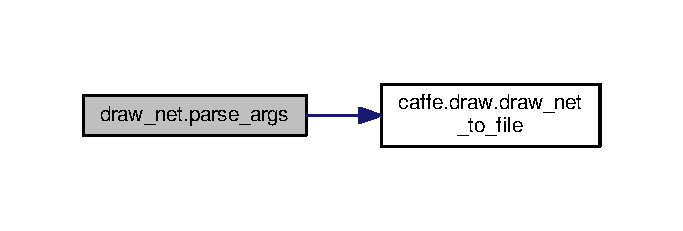
\includegraphics[width=328pt]{namespacedraw__net_a54a6010be784238d4fb0b8c88ace02d3_cgraph}
\end{center}
\end{figure}

\hypertarget{namespaceexifutil}{}\section{exifutil Namespace Reference}
\label{namespaceexifutil}\index{exifutil@{exifutil}}
\subsection*{Functions}
\begin{DoxyCompactItemize}
\item 
\mbox{\Hypertarget{namespaceexifutil_ae6019994ff716ec7bba97215b2131705}\label{namespaceexifutil_ae6019994ff716ec7bba97215b2131705}} 
def {\bfseries open\+\_\+oriented\+\_\+im} (im\+\_\+path)
\item 
\mbox{\Hypertarget{namespaceexifutil_a580f148516d4ae537df39ae625297a88}\label{namespaceexifutil_a580f148516d4ae537df39ae625297a88}} 
def {\bfseries apply\+\_\+orientation} (im, orientation)
\end{DoxyCompactItemize}
\subsection*{Variables}
\begin{DoxyCompactItemize}
\item 
dictionary {\bfseries O\+R\+I\+E\+N\+T\+A\+T\+I\+O\+NS}
\end{DoxyCompactItemize}


\subsection{Detailed Description}
\begin{DoxyVerb}This script handles the skimage exif problem.
\end{DoxyVerb}
 

\subsection{Variable Documentation}
\mbox{\Hypertarget{namespaceexifutil_a3a9af3bec6523588f629cca64bda0913}\label{namespaceexifutil_a3a9af3bec6523588f629cca64bda0913}} 
\index{exifutil@{exifutil}!O\+R\+I\+E\+N\+T\+A\+T\+I\+O\+NS@{O\+R\+I\+E\+N\+T\+A\+T\+I\+O\+NS}}
\index{O\+R\+I\+E\+N\+T\+A\+T\+I\+O\+NS@{O\+R\+I\+E\+N\+T\+A\+T\+I\+O\+NS}!exifutil@{exifutil}}
\subsubsection{\texorpdfstring{O\+R\+I\+E\+N\+T\+A\+T\+I\+O\+NS}{ORIENTATIONS}}
{\footnotesize\ttfamily dictionary exifutil.\+O\+R\+I\+E\+N\+T\+A\+T\+I\+O\+NS}

{\bfseries Initial value\+:}
\begin{DoxyCode}
1 =  \{   \textcolor{comment}{\# used in apply\_orientation}
2     2: (Image.FLIP\_LEFT\_RIGHT,),
3     3: (Image.ROTATE\_180,),
4     4: (Image.FLIP\_TOP\_BOTTOM,),
5     5: (Image.FLIP\_LEFT\_RIGHT, Image.ROTATE\_90),
6     6: (Image.ROTATE\_270,),
7     7: (Image.FLIP\_LEFT\_RIGHT, Image.ROTATE\_270),
8     8: (Image.ROTATE\_90,)
9 \}
\end{DoxyCode}

\hypertarget{namespacegenerate__sample__data}{}\section{generate\+\_\+sample\+\_\+data Namespace Reference}
\label{namespacegenerate__sample__data}\index{generate\+\_\+sample\+\_\+data@{generate\+\_\+sample\+\_\+data}}
\subsection*{Variables}
\begin{DoxyCompactItemize}
\item 
\mbox{\Hypertarget{namespacegenerate__sample__data_ae100a26d88fb69bbc7f2b757bba788d8}\label{namespacegenerate__sample__data_ae100a26d88fb69bbc7f2b757bba788d8}} 
{\bfseries script\+\_\+dir} = os.\+path.\+dirname(os.\+path.\+abspath(\+\_\+\+\_\+file\+\_\+\+\_\+))
\item 
\mbox{\Hypertarget{namespacegenerate__sample__data_ae385e421659f38a5027eca2e6f52ff84}\label{namespacegenerate__sample__data_ae385e421659f38a5027eca2e6f52ff84}} 
int {\bfseries num\+\_\+cols} = 8
\item 
\mbox{\Hypertarget{namespacegenerate__sample__data_a7891bb56736b704a38633c52ea18fa63}\label{namespacegenerate__sample__data_a7891bb56736b704a38633c52ea18fa63}} 
int {\bfseries num\+\_\+rows} = 10
\item 
\mbox{\Hypertarget{namespacegenerate__sample__data_a020eed012863e9dd0581a34c737b0939}\label{namespacegenerate__sample__data_a020eed012863e9dd0581a34c737b0939}} 
int {\bfseries height} = 6
\item 
\mbox{\Hypertarget{namespacegenerate__sample__data_a136d420fd3b8bc01fe652575f65210f9}\label{namespacegenerate__sample__data_a136d420fd3b8bc01fe652575f65210f9}} 
int {\bfseries width} = 5
\item 
\mbox{\Hypertarget{namespacegenerate__sample__data_ae56c773eb88ec9b0140edbba179bcb06}\label{namespacegenerate__sample__data_ae56c773eb88ec9b0140edbba179bcb06}} 
int {\bfseries total\+\_\+size} = num\+\_\+cols $\ast$ num\+\_\+rows $\ast$ height $\ast$ width
\item 
\mbox{\Hypertarget{namespacegenerate__sample__data_a4d17760544ae427f4982b979686ae4f8}\label{namespacegenerate__sample__data_a4d17760544ae427f4982b979686ae4f8}} 
{\bfseries data} = np.\+arange(total\+\_\+size)
\item 
\mbox{\Hypertarget{namespacegenerate__sample__data_a35a6940d8b9aff2fc92b84db11b9dd6b}\label{namespacegenerate__sample__data_a35a6940d8b9aff2fc92b84db11b9dd6b}} 
int {\bfseries label} = 1 + np.\+arange(num\+\_\+rows)\mbox{[}\+:, np.\+newaxis\mbox{]}
\item 
\mbox{\Hypertarget{namespacegenerate__sample__data_ad6ecf36c3dac6140a30b04fee35da3f2}\label{namespacegenerate__sample__data_ad6ecf36c3dac6140a30b04fee35da3f2}} 
int {\bfseries label2} = label + 1
\item 
\mbox{\Hypertarget{namespacegenerate__sample__data_aa357f9fa404423f5df718d8ba7bb6af7}\label{namespacegenerate__sample__data_aa357f9fa404423f5df718d8ba7bb6af7}} 
{\bfseries compression}
\item 
\mbox{\Hypertarget{namespacegenerate__sample__data_a0f69c96856d7c4622a38b86687e8fa5e}\label{namespacegenerate__sample__data_a0f69c96856d7c4622a38b86687e8fa5e}} 
{\bfseries compression\+\_\+opts}
\item 
\mbox{\Hypertarget{namespacegenerate__sample__data_a891ff21b3ec3fa799d70c71e543e3f12}\label{namespacegenerate__sample__data_a891ff21b3ec3fa799d70c71e543e3f12}} 
{\bfseries dtype}
\item 
\mbox{\Hypertarget{namespacegenerate__sample__data_acb1ad2725591b770129e26512a718963}\label{namespacegenerate__sample__data_acb1ad2725591b770129e26512a718963}} 
{\bfseries targets} = np.\+random.\+randn(num\+\_\+rows, 1)
\end{DoxyCompactItemize}


\subsection{Detailed Description}
\begin{DoxyVerb}Generate data used in the HDF5DataLayer and GradientBasedSolver tests.
\end{DoxyVerb}
 
\hypertarget{namespaceparse__log}{}\section{parse\+\_\+log Namespace Reference}
\label{namespaceparse__log}\index{parse\+\_\+log@{parse\+\_\+log}}
\subsection*{Functions}
\begin{DoxyCompactItemize}
\item 
def \mbox{\hyperlink{namespaceparse__log_ac340d5a4faf6c29869b3702916e3f237}{parse\+\_\+log}} (path\+\_\+to\+\_\+log)
\item 
def \mbox{\hyperlink{namespaceparse__log_a140116e322b21ebd36d194b65a5612fb}{parse\+\_\+line\+\_\+for\+\_\+net\+\_\+output}} (regex\+\_\+obj, row, row\+\_\+dict\+\_\+list, line, iteration, seconds, learning\+\_\+rate)
\item 
def \mbox{\hyperlink{namespaceparse__log_a407b810ae0d4a92efe08385f7de5eabb}{fix\+\_\+initial\+\_\+nan\+\_\+learning\+\_\+rate}} (dict\+\_\+list)
\item 
def \mbox{\hyperlink{namespaceparse__log_a6541ec62fedcd2928543ff22ec4401b3}{save\+\_\+csv\+\_\+files}} (logfile\+\_\+path, output\+\_\+dir, train\+\_\+dict\+\_\+list, test\+\_\+dict\+\_\+list, delimiter=\textquotesingle{}, verbose=False)
\item 
def \mbox{\hyperlink{namespaceparse__log_a485ed97888fccc67e8067cb51ce03db4}{write\+\_\+csv}} (output\+\_\+filename, dict\+\_\+list, delimiter, verbose=False)
\item 
\mbox{\Hypertarget{namespaceparse__log_a2db1ba247c658a76a2b26481d6d27c62}\label{namespaceparse__log_a2db1ba247c658a76a2b26481d6d27c62}} 
def {\bfseries parse\+\_\+args} ()
\item 
\mbox{\Hypertarget{namespaceparse__log_ada5ddccd0e1bc3f33fd58f2fbee4ed8f}\label{namespaceparse__log_ada5ddccd0e1bc3f33fd58f2fbee4ed8f}} 
def {\bfseries main} ()
\end{DoxyCompactItemize}


\subsection{Detailed Description}
\begin{DoxyVerb}Parse training log

Evolved from parse_log.sh
\end{DoxyVerb}
 

\subsection{Function Documentation}
\mbox{\Hypertarget{namespaceparse__log_a407b810ae0d4a92efe08385f7de5eabb}\label{namespaceparse__log_a407b810ae0d4a92efe08385f7de5eabb}} 
\index{parse\+\_\+log@{parse\+\_\+log}!fix\+\_\+initial\+\_\+nan\+\_\+learning\+\_\+rate@{fix\+\_\+initial\+\_\+nan\+\_\+learning\+\_\+rate}}
\index{fix\+\_\+initial\+\_\+nan\+\_\+learning\+\_\+rate@{fix\+\_\+initial\+\_\+nan\+\_\+learning\+\_\+rate}!parse\+\_\+log@{parse\+\_\+log}}
\subsubsection{\texorpdfstring{fix\+\_\+initial\+\_\+nan\+\_\+learning\+\_\+rate()}{fix\_initial\_nan\_learning\_rate()}}
{\footnotesize\ttfamily def parse\+\_\+log.\+fix\+\_\+initial\+\_\+nan\+\_\+learning\+\_\+rate (\begin{DoxyParamCaption}\item[{}]{dict\+\_\+list }\end{DoxyParamCaption})}

\begin{DoxyVerb}Correct initial value of learning rate

Learning rate is normally not printed until after the initial test and
training step, which means the initial testing and training rows have
LearningRate = NaN. Fix this by copying over the LearningRate from the
second row, if it exists.
\end{DoxyVerb}
 Here is the call graph for this function\+:
\nopagebreak
\begin{figure}[H]
\begin{center}
\leavevmode
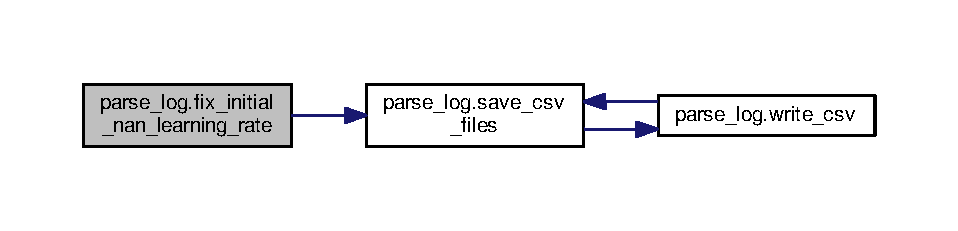
\includegraphics[width=350pt]{namespaceparse__log_a407b810ae0d4a92efe08385f7de5eabb_cgraph}
\end{center}
\end{figure}
Here is the caller graph for this function\+:
\nopagebreak
\begin{figure}[H]
\begin{center}
\leavevmode
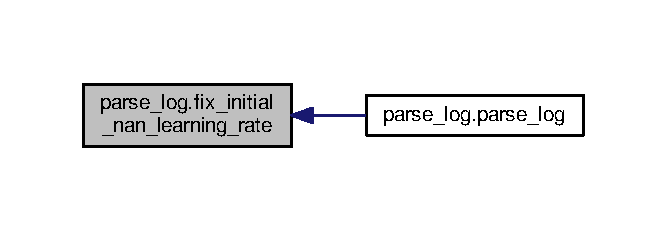
\includegraphics[width=320pt]{namespaceparse__log_a407b810ae0d4a92efe08385f7de5eabb_icgraph}
\end{center}
\end{figure}
\mbox{\Hypertarget{namespaceparse__log_a140116e322b21ebd36d194b65a5612fb}\label{namespaceparse__log_a140116e322b21ebd36d194b65a5612fb}} 
\index{parse\+\_\+log@{parse\+\_\+log}!parse\+\_\+line\+\_\+for\+\_\+net\+\_\+output@{parse\+\_\+line\+\_\+for\+\_\+net\+\_\+output}}
\index{parse\+\_\+line\+\_\+for\+\_\+net\+\_\+output@{parse\+\_\+line\+\_\+for\+\_\+net\+\_\+output}!parse\+\_\+log@{parse\+\_\+log}}
\subsubsection{\texorpdfstring{parse\+\_\+line\+\_\+for\+\_\+net\+\_\+output()}{parse\_line\_for\_net\_output()}}
{\footnotesize\ttfamily def parse\+\_\+log.\+parse\+\_\+line\+\_\+for\+\_\+net\+\_\+output (\begin{DoxyParamCaption}\item[{}]{regex\+\_\+obj,  }\item[{}]{row,  }\item[{}]{row\+\_\+dict\+\_\+list,  }\item[{}]{line,  }\item[{}]{iteration,  }\item[{}]{seconds,  }\item[{}]{learning\+\_\+rate }\end{DoxyParamCaption})}

\begin{DoxyVerb}Parse a single line for training or test output

Returns a a tuple with (row_dict_list, row)
row: may be either a new row or an augmented version of the current row
row_dict_list: may be either the current row_dict_list or an augmented
version of the current row_dict_list
\end{DoxyVerb}
 Here is the caller graph for this function\+:
\nopagebreak
\begin{figure}[H]
\begin{center}
\leavevmode
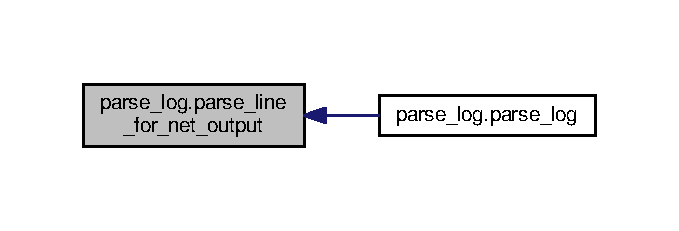
\includegraphics[width=326pt]{namespaceparse__log_a140116e322b21ebd36d194b65a5612fb_icgraph}
\end{center}
\end{figure}
\mbox{\Hypertarget{namespaceparse__log_ac340d5a4faf6c29869b3702916e3f237}\label{namespaceparse__log_ac340d5a4faf6c29869b3702916e3f237}} 
\index{parse\+\_\+log@{parse\+\_\+log}!parse\+\_\+log@{parse\+\_\+log}}
\index{parse\+\_\+log@{parse\+\_\+log}!parse\+\_\+log@{parse\+\_\+log}}
\subsubsection{\texorpdfstring{parse\+\_\+log()}{parse\_log()}}
{\footnotesize\ttfamily def parse\+\_\+log.\+parse\+\_\+log (\begin{DoxyParamCaption}\item[{}]{path\+\_\+to\+\_\+log }\end{DoxyParamCaption})}

\begin{DoxyVerb}Parse log file
Returns (train_dict_list, test_dict_list)

train_dict_list and test_dict_list are lists of dicts that define the table
rows
\end{DoxyVerb}
 Here is the call graph for this function\+:
\nopagebreak
\begin{figure}[H]
\begin{center}
\leavevmode
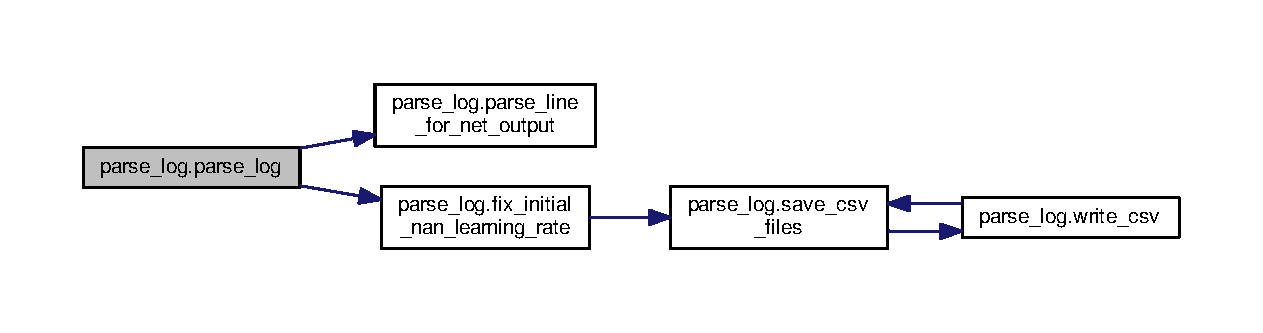
\includegraphics[width=350pt]{namespaceparse__log_ac340d5a4faf6c29869b3702916e3f237_cgraph}
\end{center}
\end{figure}
\mbox{\Hypertarget{namespaceparse__log_a6541ec62fedcd2928543ff22ec4401b3}\label{namespaceparse__log_a6541ec62fedcd2928543ff22ec4401b3}} 
\index{parse\+\_\+log@{parse\+\_\+log}!save\+\_\+csv\+\_\+files@{save\+\_\+csv\+\_\+files}}
\index{save\+\_\+csv\+\_\+files@{save\+\_\+csv\+\_\+files}!parse\+\_\+log@{parse\+\_\+log}}
\subsubsection{\texorpdfstring{save\+\_\+csv\+\_\+files()}{save\_csv\_files()}}
{\footnotesize\ttfamily def parse\+\_\+log.\+save\+\_\+csv\+\_\+files (\begin{DoxyParamCaption}\item[{}]{logfile\+\_\+path,  }\item[{}]{output\+\_\+dir,  }\item[{}]{train\+\_\+dict\+\_\+list,  }\item[{}]{test\+\_\+dict\+\_\+list,  }\item[{}]{delimiter = {\ttfamily \textquotesingle{}},  }\item[{}]{verbose = {\ttfamily False} }\end{DoxyParamCaption})}

\begin{DoxyVerb}Save CSV files to output_dir

If the input log file is, e.g., caffe.INFO, the names will be
caffe.INFO.train and caffe.INFO.test
\end{DoxyVerb}
 Here is the call graph for this function\+:
\nopagebreak
\begin{figure}[H]
\begin{center}
\leavevmode
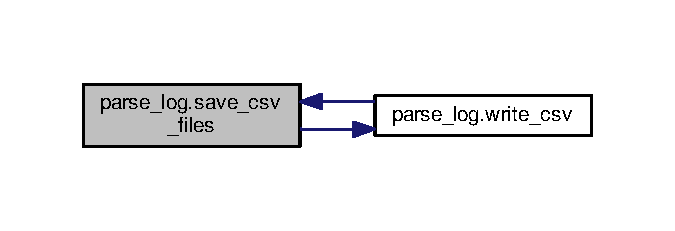
\includegraphics[width=324pt]{namespaceparse__log_a6541ec62fedcd2928543ff22ec4401b3_cgraph}
\end{center}
\end{figure}
Here is the caller graph for this function\+:
\nopagebreak
\begin{figure}[H]
\begin{center}
\leavevmode
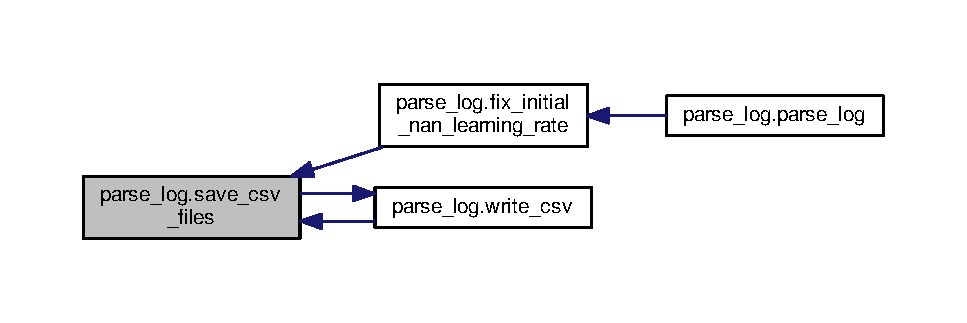
\includegraphics[width=350pt]{namespaceparse__log_a6541ec62fedcd2928543ff22ec4401b3_icgraph}
\end{center}
\end{figure}
\mbox{\Hypertarget{namespaceparse__log_a485ed97888fccc67e8067cb51ce03db4}\label{namespaceparse__log_a485ed97888fccc67e8067cb51ce03db4}} 
\index{parse\+\_\+log@{parse\+\_\+log}!write\+\_\+csv@{write\+\_\+csv}}
\index{write\+\_\+csv@{write\+\_\+csv}!parse\+\_\+log@{parse\+\_\+log}}
\subsubsection{\texorpdfstring{write\+\_\+csv()}{write\_csv()}}
{\footnotesize\ttfamily def parse\+\_\+log.\+write\+\_\+csv (\begin{DoxyParamCaption}\item[{}]{output\+\_\+filename,  }\item[{}]{dict\+\_\+list,  }\item[{}]{delimiter,  }\item[{}]{verbose = {\ttfamily False} }\end{DoxyParamCaption})}

\begin{DoxyVerb}Write a CSV file
\end{DoxyVerb}
 Here is the call graph for this function\+:
\nopagebreak
\begin{figure}[H]
\begin{center}
\leavevmode
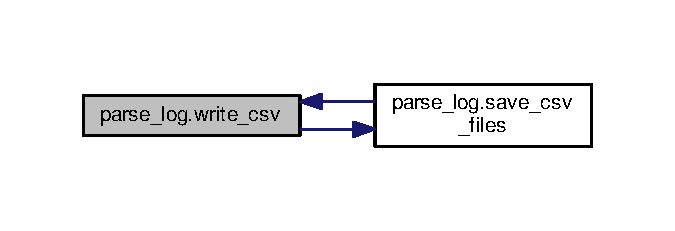
\includegraphics[width=324pt]{namespaceparse__log_a485ed97888fccc67e8067cb51ce03db4_cgraph}
\end{center}
\end{figure}
Here is the caller graph for this function\+:
\nopagebreak
\begin{figure}[H]
\begin{center}
\leavevmode
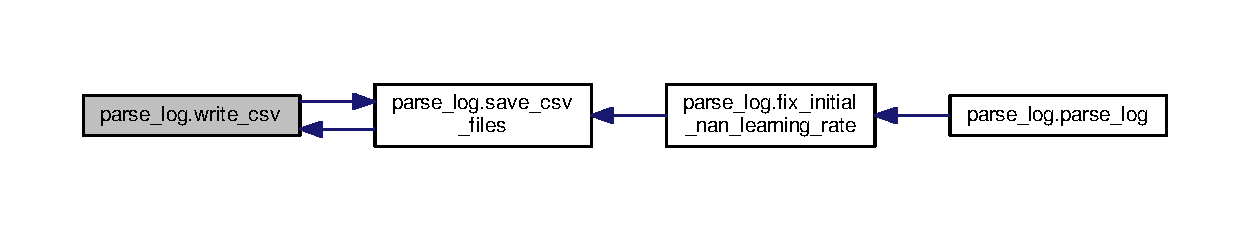
\includegraphics[width=350pt]{namespaceparse__log_a485ed97888fccc67e8067cb51ce03db4_icgraph}
\end{center}
\end{figure}

\hypertarget{namespacesummarize}{}\section{summarize Namespace Reference}
\label{namespacesummarize}\index{summarize@{summarize}}
\subsection*{Functions}
\begin{DoxyCompactItemize}
\item 
\mbox{\Hypertarget{namespacesummarize_a7bd4a84cdbad8884ad92a7806ae1422a}\label{namespacesummarize_a7bd4a84cdbad8884ad92a7806ae1422a}} 
def {\bfseries read\+\_\+net} (filename)
\item 
\mbox{\Hypertarget{namespacesummarize_a6f8438960969506f79fa91c85d889c4e}\label{namespacesummarize_a6f8438960969506f79fa91c85d889c4e}} 
def {\bfseries format\+\_\+param} (param)
\item 
\mbox{\Hypertarget{namespacesummarize_a3416c5ed12285b7cb8b442b25f7ad649}\label{namespacesummarize_a3416c5ed12285b7cb8b442b25f7ad649}} 
def {\bfseries printed\+\_\+len} (s)
\item 
def \mbox{\hyperlink{namespacesummarize_aed3c88b7cc0075038238f0a5d153cd65}{print\+\_\+table}} (table, max\+\_\+width)
\item 
\mbox{\Hypertarget{namespacesummarize_a135dc4de9b7d18e58bca4357664ff403}\label{namespacesummarize_a135dc4de9b7d18e58bca4357664ff403}} 
def {\bfseries summarize\+\_\+net} (net)
\item 
\mbox{\Hypertarget{namespacesummarize_a3828636c21757fdc63ccc87b52a78427}\label{namespacesummarize_a3828636c21757fdc63ccc87b52a78427}} 
def {\bfseries main} ()
\end{DoxyCompactItemize}
\subsection*{Variables}
\begin{DoxyCompactItemize}
\item 
list {\bfseries C\+O\+L\+O\+RS}
\item 
\mbox{\Hypertarget{namespacesummarize_a975fa6c4a1b9d23b8aa63ef584be23c9}\label{namespacesummarize_a975fa6c4a1b9d23b8aa63ef584be23c9}} 
string {\bfseries D\+I\+S\+C\+O\+N\+N\+E\+C\+T\+E\+D\+\_\+\+C\+O\+L\+OR} = \textquotesingle{}41\textquotesingle{}
\end{DoxyCompactItemize}


\subsection{Detailed Description}
\begin{DoxyVerb}Net summarization tool.

This tool summarizes the structure of a net in a concise but comprehensive
tabular listing, taking a prototxt file as input.

Use this tool to check at a glance that the computation you've specified is the
computation you expect.
\end{DoxyVerb}
 

\subsection{Function Documentation}
\mbox{\Hypertarget{namespacesummarize_aed3c88b7cc0075038238f0a5d153cd65}\label{namespacesummarize_aed3c88b7cc0075038238f0a5d153cd65}} 
\index{summarize@{summarize}!print\+\_\+table@{print\+\_\+table}}
\index{print\+\_\+table@{print\+\_\+table}!summarize@{summarize}}
\subsubsection{\texorpdfstring{print\+\_\+table()}{print\_table()}}
{\footnotesize\ttfamily def summarize.\+print\+\_\+table (\begin{DoxyParamCaption}\item[{}]{table,  }\item[{}]{max\+\_\+width }\end{DoxyParamCaption})}

\begin{DoxyVerb}Print a simple nicely-aligned table.

table must be a list of (equal-length) lists. Columns are space-separated,
and as narrow as possible, but no wider than max_width. Text may overflow
columns; note that unlike string.format, this will not affect subsequent
columns, if possible.\end{DoxyVerb}
 

\subsection{Variable Documentation}
\mbox{\Hypertarget{namespacesummarize_ace787d530d7719206a169bca48236bb3}\label{namespacesummarize_ace787d530d7719206a169bca48236bb3}} 
\index{summarize@{summarize}!C\+O\+L\+O\+RS@{C\+O\+L\+O\+RS}}
\index{C\+O\+L\+O\+RS@{C\+O\+L\+O\+RS}!summarize@{summarize}}
\subsubsection{\texorpdfstring{C\+O\+L\+O\+RS}{COLORS}}
{\footnotesize\ttfamily list summarize.\+C\+O\+L\+O\+RS}

{\bfseries Initial value\+:}
\begin{DoxyCode}
1 =  [\textcolor{stringliteral}{'92'}, \textcolor{stringliteral}{'93'}, \textcolor{stringliteral}{'94'}, \textcolor{stringliteral}{'95'}, \textcolor{stringliteral}{'97'}, \textcolor{stringliteral}{'96'}, \textcolor{stringliteral}{'42'}, \textcolor{stringliteral}{'43;30'}, \textcolor{stringliteral}{'100'},
2           \textcolor{stringliteral}{'444'}, \textcolor{stringliteral}{'103;30'}, \textcolor{stringliteral}{'107;30'}]
\end{DoxyCode}

\hypertarget{namespacetrain}{}\section{train Namespace Reference}
\label{namespacetrain}\index{train@{train}}
\subsection*{Functions}
\begin{DoxyCompactItemize}
\item 
\mbox{\Hypertarget{namespacetrain_afe4004eb13588d934b674119beb87d1c}\label{namespacetrain_afe4004eb13588d934b674119beb87d1c}} 
def {\bfseries train} (solver, snapshot, gpus, timing=False)
\item 
\mbox{\Hypertarget{namespacetrain_a0ade729ddf0a492ed0c471b5e28074db}\label{namespacetrain_a0ade729ddf0a492ed0c471b5e28074db}} 
def {\bfseries time} (solver, nccl)
\item 
\mbox{\Hypertarget{namespacetrain_a4b2236e69eaf68ca675f8c11e5280fd3}\label{namespacetrain_a4b2236e69eaf68ca675f8c11e5280fd3}} 
def {\bfseries solve} (proto, snapshot, gpus, timing, uid, rank)
\end{DoxyCompactItemize}
\subsection*{Variables}
\begin{DoxyCompactItemize}
\item 
\mbox{\Hypertarget{namespacetrain_a242e49c387b90838a9072c79886a10ec}\label{namespacetrain_a242e49c387b90838a9072c79886a10ec}} 
{\bfseries parser} = argparse.\+Argument\+Parser()
\item 
\mbox{\Hypertarget{namespacetrain_a3c2dd63c131ee6c6d543d543760d522e}\label{namespacetrain_a3c2dd63c131ee6c6d543d543760d522e}} 
{\bfseries required}
\item 
\mbox{\Hypertarget{namespacetrain_ab05c503109ea425e4f6a12524cd504db}\label{namespacetrain_ab05c503109ea425e4f6a12524cd504db}} 
{\bfseries True}
\item 
\mbox{\Hypertarget{namespacetrain_ac16504ad52822423344025f791e0c4fd}\label{namespacetrain_ac16504ad52822423344025f791e0c4fd}} 
{\bfseries help}
\item 
\mbox{\Hypertarget{namespacetrain_ad99775ad96e0996a8be4782b30a28c2e}\label{namespacetrain_ad99775ad96e0996a8be4782b30a28c2e}} 
{\bfseries type}
\item 
\mbox{\Hypertarget{namespacetrain_af5de906790efe7cea370f1a69e020d52}\label{namespacetrain_af5de906790efe7cea370f1a69e020d52}} 
{\bfseries int}
\item 
\mbox{\Hypertarget{namespacetrain_aa14681106dd0acfe6521d6ad074c434b}\label{namespacetrain_aa14681106dd0acfe6521d6ad074c434b}} 
{\bfseries nargs}
\item 
\mbox{\Hypertarget{namespacetrain_abfb9b8d0ebf72bafd04e084791275553}\label{namespacetrain_abfb9b8d0ebf72bafd04e084791275553}} 
{\bfseries default}
\item 
\mbox{\Hypertarget{namespacetrain_ae65fafa56b338044344f2637be98e99a}\label{namespacetrain_ae65fafa56b338044344f2637be98e99a}} 
{\bfseries action}
\item 
\mbox{\Hypertarget{namespacetrain_a4de53a6f6383e12bc42e05dfea879dab}\label{namespacetrain_a4de53a6f6383e12bc42e05dfea879dab}} 
{\bfseries args} = parser.\+parse\+\_\+args()
\end{DoxyCompactItemize}


\subsection{Detailed Description}
\begin{DoxyVerb}Trains a model using one or more GPUs.
\end{DoxyVerb}
 
\chapter{Class Documentation}
\hypertarget{classcpp__lint_1_1___block_info}{}\section{cpp\+\_\+lint.\+\_\+\+Block\+Info Class Reference}
\label{classcpp__lint_1_1___block_info}\index{cpp\+\_\+lint.\+\_\+\+Block\+Info@{cpp\+\_\+lint.\+\_\+\+Block\+Info}}


Inheritance diagram for cpp\+\_\+lint.\+\_\+\+Block\+Info\+:
\nopagebreak
\begin{figure}[H]
\begin{center}
\leavevmode
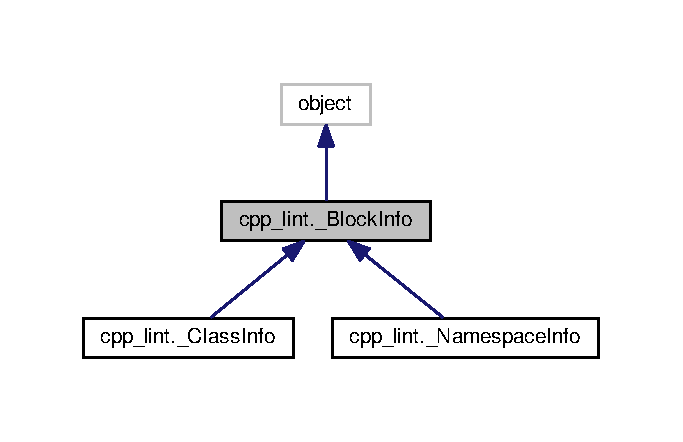
\includegraphics[width=328pt]{classcpp__lint_1_1___block_info__inherit__graph}
\end{center}
\end{figure}
\subsection*{Public Member Functions}
\begin{DoxyCompactItemize}
\item 
\mbox{\Hypertarget{classcpp__lint_1_1___block_info_a32861c4229ec1a33e077b77a63d5e619}\label{classcpp__lint_1_1___block_info_a32861c4229ec1a33e077b77a63d5e619}} 
def {\bfseries \+\_\+\+\_\+init\+\_\+\+\_\+} (self, seen\+\_\+open\+\_\+brace)
\item 
def \mbox{\hyperlink{classcpp__lint_1_1___block_info_a69357fb2efabae1dd77aab9942b90560}{Check\+Begin}} (self, filename, clean\+\_\+lines, linenum, error)
\item 
def \mbox{\hyperlink{classcpp__lint_1_1___block_info_abc44459ea5e04d6a9a4d816e85998bfc}{Check\+End}} (self, filename, clean\+\_\+lines, linenum, error)
\end{DoxyCompactItemize}
\subsection*{Public Attributes}
\begin{DoxyCompactItemize}
\item 
\mbox{\Hypertarget{classcpp__lint_1_1___block_info_a7629061e1d7dbc7d15cdd521239a29ad}\label{classcpp__lint_1_1___block_info_a7629061e1d7dbc7d15cdd521239a29ad}} 
{\bfseries seen\+\_\+open\+\_\+brace}
\item 
\mbox{\Hypertarget{classcpp__lint_1_1___block_info_a5b86c27ea6a6641fcb0d242dfed898b6}\label{classcpp__lint_1_1___block_info_a5b86c27ea6a6641fcb0d242dfed898b6}} 
{\bfseries open\+\_\+parentheses}
\item 
\mbox{\Hypertarget{classcpp__lint_1_1___block_info_a7577f54a4359d9979e8765934b988187}\label{classcpp__lint_1_1___block_info_a7577f54a4359d9979e8765934b988187}} 
{\bfseries inline\+\_\+asm}
\end{DoxyCompactItemize}


\subsection{Detailed Description}
\begin{DoxyVerb}Stores information about a generic block of code.\end{DoxyVerb}
 

\subsection{Member Function Documentation}
\mbox{\Hypertarget{classcpp__lint_1_1___block_info_a69357fb2efabae1dd77aab9942b90560}\label{classcpp__lint_1_1___block_info_a69357fb2efabae1dd77aab9942b90560}} 
\index{cpp\+\_\+lint\+::\+\_\+\+Block\+Info@{cpp\+\_\+lint\+::\+\_\+\+Block\+Info}!Check\+Begin@{Check\+Begin}}
\index{Check\+Begin@{Check\+Begin}!cpp\+\_\+lint\+::\+\_\+\+Block\+Info@{cpp\+\_\+lint\+::\+\_\+\+Block\+Info}}
\subsubsection{\texorpdfstring{Check\+Begin()}{CheckBegin()}}
{\footnotesize\ttfamily def cpp\+\_\+lint.\+\_\+\+Block\+Info.\+Check\+Begin (\begin{DoxyParamCaption}\item[{}]{self,  }\item[{}]{filename,  }\item[{}]{clean\+\_\+lines,  }\item[{}]{linenum,  }\item[{}]{error }\end{DoxyParamCaption})}

\begin{DoxyVerb}Run checks that applies to text up to the opening brace.

This is mostly for checking the text after the class identifier
and the "{", usually where the base class is specified.  For other
blocks, there isn't much to check, so we always pass.

Args:
  filename: The name of the current file.
  clean_lines: A CleansedLines instance containing the file.
  linenum: The number of the line to check.
  error: The function to call with any errors found.
\end{DoxyVerb}
 \mbox{\Hypertarget{classcpp__lint_1_1___block_info_abc44459ea5e04d6a9a4d816e85998bfc}\label{classcpp__lint_1_1___block_info_abc44459ea5e04d6a9a4d816e85998bfc}} 
\index{cpp\+\_\+lint\+::\+\_\+\+Block\+Info@{cpp\+\_\+lint\+::\+\_\+\+Block\+Info}!Check\+End@{Check\+End}}
\index{Check\+End@{Check\+End}!cpp\+\_\+lint\+::\+\_\+\+Block\+Info@{cpp\+\_\+lint\+::\+\_\+\+Block\+Info}}
\subsubsection{\texorpdfstring{Check\+End()}{CheckEnd()}}
{\footnotesize\ttfamily def cpp\+\_\+lint.\+\_\+\+Block\+Info.\+Check\+End (\begin{DoxyParamCaption}\item[{}]{self,  }\item[{}]{filename,  }\item[{}]{clean\+\_\+lines,  }\item[{}]{linenum,  }\item[{}]{error }\end{DoxyParamCaption})}

\begin{DoxyVerb}Run checks that applies to text after the closing brace.

This is mostly used for checking end of namespace comments.

Args:
  filename: The name of the current file.
  clean_lines: A CleansedLines instance containing the file.
  linenum: The number of the line to check.
  error: The function to call with any errors found.
\end{DoxyVerb}
 

The documentation for this class was generated from the following file\+:\begin{DoxyCompactItemize}
\item 
scripts/cpp\+\_\+lint.\+py\end{DoxyCompactItemize}

\hypertarget{classcpp__lint_1_1___class_info}{}\section{cpp\+\_\+lint.\+\_\+\+Class\+Info Class Reference}
\label{classcpp__lint_1_1___class_info}\index{cpp\+\_\+lint.\+\_\+\+Class\+Info@{cpp\+\_\+lint.\+\_\+\+Class\+Info}}


Inheritance diagram for cpp\+\_\+lint.\+\_\+\+Class\+Info\+:
\nopagebreak
\begin{figure}[H]
\begin{center}
\leavevmode
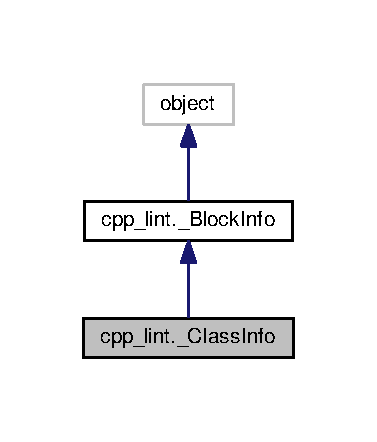
\includegraphics[width=181pt]{classcpp__lint_1_1___class_info__inherit__graph}
\end{center}
\end{figure}
\subsection*{Public Member Functions}
\begin{DoxyCompactItemize}
\item 
\mbox{\Hypertarget{classcpp__lint_1_1___class_info_a3a86d1cdcd8aaa0982eed4cf13c9c28d}\label{classcpp__lint_1_1___class_info_a3a86d1cdcd8aaa0982eed4cf13c9c28d}} 
def {\bfseries \+\_\+\+\_\+init\+\_\+\+\_\+} (self, name, class\+\_\+or\+\_\+struct, clean\+\_\+lines, linenum)
\item 
\mbox{\Hypertarget{classcpp__lint_1_1___class_info_ad748d31bf6595361fecd49e403f10e60}\label{classcpp__lint_1_1___class_info_ad748d31bf6595361fecd49e403f10e60}} 
def {\bfseries Check\+Begin} (self, filename, clean\+\_\+lines, linenum, error)
\item 
\mbox{\Hypertarget{classcpp__lint_1_1___class_info_adde5a40721a72539b6dc1b32bc3e3d6f}\label{classcpp__lint_1_1___class_info_adde5a40721a72539b6dc1b32bc3e3d6f}} 
def {\bfseries Check\+End} (self, filename, clean\+\_\+lines, linenum, error)
\end{DoxyCompactItemize}
\subsection*{Public Attributes}
\begin{DoxyCompactItemize}
\item 
\mbox{\Hypertarget{classcpp__lint_1_1___class_info_afb6a10e0d51615e98e0606d0e15210e7}\label{classcpp__lint_1_1___class_info_afb6a10e0d51615e98e0606d0e15210e7}} 
{\bfseries name}
\item 
\mbox{\Hypertarget{classcpp__lint_1_1___class_info_afe712dbb6c3f4d149bec65cf4b68d9df}\label{classcpp__lint_1_1___class_info_afe712dbb6c3f4d149bec65cf4b68d9df}} 
{\bfseries starting\+\_\+linenum}
\item 
\mbox{\Hypertarget{classcpp__lint_1_1___class_info_a508ec13390cdbf9dfe60f0efb38b5427}\label{classcpp__lint_1_1___class_info_a508ec13390cdbf9dfe60f0efb38b5427}} 
{\bfseries is\+\_\+derived}
\item 
\mbox{\Hypertarget{classcpp__lint_1_1___class_info_ad332b2012a0513f1f0f6d03f78b5ee6a}\label{classcpp__lint_1_1___class_info_ad332b2012a0513f1f0f6d03f78b5ee6a}} 
{\bfseries access}
\item 
\mbox{\Hypertarget{classcpp__lint_1_1___class_info_a7e3bd78fc8ae6bb16179fc0d0c4c6e8f}\label{classcpp__lint_1_1___class_info_a7e3bd78fc8ae6bb16179fc0d0c4c6e8f}} 
{\bfseries is\+\_\+struct}
\item 
\mbox{\Hypertarget{classcpp__lint_1_1___class_info_a54739a914a760d8eb0b7aed9e1ef04c2}\label{classcpp__lint_1_1___class_info_a54739a914a760d8eb0b7aed9e1ef04c2}} 
{\bfseries class\+\_\+indent}
\item 
\mbox{\Hypertarget{classcpp__lint_1_1___class_info_a5bb303746c95a704864286dcae21de31}\label{classcpp__lint_1_1___class_info_a5bb303746c95a704864286dcae21de31}} 
{\bfseries last\+\_\+line}
\end{DoxyCompactItemize}


\subsection{Detailed Description}
\begin{DoxyVerb}Stores information about a class.\end{DoxyVerb}
 

The documentation for this class was generated from the following file\+:\begin{DoxyCompactItemize}
\item 
scripts/cpp\+\_\+lint.\+py\end{DoxyCompactItemize}

\hypertarget{classcpp__lint_1_1___cpp_lint_state}{}\section{cpp\+\_\+lint.\+\_\+\+Cpp\+Lint\+State Class Reference}
\label{classcpp__lint_1_1___cpp_lint_state}\index{cpp\+\_\+lint.\+\_\+\+Cpp\+Lint\+State@{cpp\+\_\+lint.\+\_\+\+Cpp\+Lint\+State}}


Inheritance diagram for cpp\+\_\+lint.\+\_\+\+Cpp\+Lint\+State\+:
\nopagebreak
\begin{figure}[H]
\begin{center}
\leavevmode
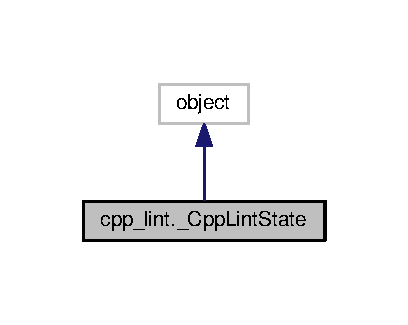
\includegraphics[width=196pt]{classcpp__lint_1_1___cpp_lint_state__inherit__graph}
\end{center}
\end{figure}
\subsection*{Public Member Functions}
\begin{DoxyCompactItemize}
\item 
\mbox{\Hypertarget{classcpp__lint_1_1___cpp_lint_state_aaa746f5aa29c2ad2b7000c9f72c89510}\label{classcpp__lint_1_1___cpp_lint_state_aaa746f5aa29c2ad2b7000c9f72c89510}} 
def {\bfseries \+\_\+\+\_\+init\+\_\+\+\_\+} (self)
\item 
def \mbox{\hyperlink{classcpp__lint_1_1___cpp_lint_state_a3c1ab0f552461fa7de6640fb98bdb4dc}{Set\+Output\+Format}} (self, output\+\_\+format)
\item 
def \mbox{\hyperlink{classcpp__lint_1_1___cpp_lint_state_a5f1481dfe5f79dd0927a213ab44d75f7}{Set\+Verbose\+Level}} (self, level)
\item 
def \mbox{\hyperlink{classcpp__lint_1_1___cpp_lint_state_a88bf958eb7219488fffd52ebfd57f4f1}{Set\+Counting\+Style}} (self, counting\+\_\+style)
\item 
def \mbox{\hyperlink{classcpp__lint_1_1___cpp_lint_state_a5b8ca5eb2124431e70a0b374842fafaf}{Set\+Filters}} (self, filters)
\item 
def \mbox{\hyperlink{classcpp__lint_1_1___cpp_lint_state_aaa00731337c82f65dbb354e23ed74fcd}{Reset\+Error\+Counts}} (self)
\item 
def \mbox{\hyperlink{classcpp__lint_1_1___cpp_lint_state_a639dac461e7354dcec4b629195758852}{Increment\+Error\+Count}} (self, category)
\item 
def \mbox{\hyperlink{classcpp__lint_1_1___cpp_lint_state_af4769688903eac9e7cd6de51cd1de8bf}{Print\+Error\+Counts}} (self)
\end{DoxyCompactItemize}
\subsection*{Public Attributes}
\begin{DoxyCompactItemize}
\item 
\mbox{\Hypertarget{classcpp__lint_1_1___cpp_lint_state_a9fa716fbebb66b726411c9538535bff7}\label{classcpp__lint_1_1___cpp_lint_state_a9fa716fbebb66b726411c9538535bff7}} 
{\bfseries verbose\+\_\+level}
\item 
\mbox{\Hypertarget{classcpp__lint_1_1___cpp_lint_state_ad210f2bd70461e1b62eb614f8d389486}\label{classcpp__lint_1_1___cpp_lint_state_ad210f2bd70461e1b62eb614f8d389486}} 
{\bfseries error\+\_\+count}
\item 
\mbox{\Hypertarget{classcpp__lint_1_1___cpp_lint_state_a5a904066dea9e48d4e1a0dbb2d61824b}\label{classcpp__lint_1_1___cpp_lint_state_a5a904066dea9e48d4e1a0dbb2d61824b}} 
{\bfseries filters}
\item 
\mbox{\Hypertarget{classcpp__lint_1_1___cpp_lint_state_ad557deaee4ec6e414c521f8c47889c1e}\label{classcpp__lint_1_1___cpp_lint_state_ad557deaee4ec6e414c521f8c47889c1e}} 
{\bfseries counting}
\item 
\mbox{\Hypertarget{classcpp__lint_1_1___cpp_lint_state_af33b9daa46454c53d370eca6b2bca107}\label{classcpp__lint_1_1___cpp_lint_state_af33b9daa46454c53d370eca6b2bca107}} 
{\bfseries errors\+\_\+by\+\_\+category}
\item 
\mbox{\Hypertarget{classcpp__lint_1_1___cpp_lint_state_a4df79633cd7c67c7253523b54f7c57ce}\label{classcpp__lint_1_1___cpp_lint_state_a4df79633cd7c67c7253523b54f7c57ce}} 
{\bfseries output\+\_\+format}
\end{DoxyCompactItemize}


\subsection{Detailed Description}
\begin{DoxyVerb}Maintains module-wide state..\end{DoxyVerb}
 

\subsection{Member Function Documentation}
\mbox{\Hypertarget{classcpp__lint_1_1___cpp_lint_state_a639dac461e7354dcec4b629195758852}\label{classcpp__lint_1_1___cpp_lint_state_a639dac461e7354dcec4b629195758852}} 
\index{cpp\+\_\+lint\+::\+\_\+\+Cpp\+Lint\+State@{cpp\+\_\+lint\+::\+\_\+\+Cpp\+Lint\+State}!Increment\+Error\+Count@{Increment\+Error\+Count}}
\index{Increment\+Error\+Count@{Increment\+Error\+Count}!cpp\+\_\+lint\+::\+\_\+\+Cpp\+Lint\+State@{cpp\+\_\+lint\+::\+\_\+\+Cpp\+Lint\+State}}
\subsubsection{\texorpdfstring{Increment\+Error\+Count()}{IncrementErrorCount()}}
{\footnotesize\ttfamily def cpp\+\_\+lint.\+\_\+\+Cpp\+Lint\+State.\+Increment\+Error\+Count (\begin{DoxyParamCaption}\item[{}]{self,  }\item[{}]{category }\end{DoxyParamCaption})}

\begin{DoxyVerb}Bumps the module's error statistic.\end{DoxyVerb}
 \mbox{\Hypertarget{classcpp__lint_1_1___cpp_lint_state_af4769688903eac9e7cd6de51cd1de8bf}\label{classcpp__lint_1_1___cpp_lint_state_af4769688903eac9e7cd6de51cd1de8bf}} 
\index{cpp\+\_\+lint\+::\+\_\+\+Cpp\+Lint\+State@{cpp\+\_\+lint\+::\+\_\+\+Cpp\+Lint\+State}!Print\+Error\+Counts@{Print\+Error\+Counts}}
\index{Print\+Error\+Counts@{Print\+Error\+Counts}!cpp\+\_\+lint\+::\+\_\+\+Cpp\+Lint\+State@{cpp\+\_\+lint\+::\+\_\+\+Cpp\+Lint\+State}}
\subsubsection{\texorpdfstring{Print\+Error\+Counts()}{PrintErrorCounts()}}
{\footnotesize\ttfamily def cpp\+\_\+lint.\+\_\+\+Cpp\+Lint\+State.\+Print\+Error\+Counts (\begin{DoxyParamCaption}\item[{}]{self }\end{DoxyParamCaption})}

\begin{DoxyVerb}Print a summary of errors by category, and the total.\end{DoxyVerb}
 \mbox{\Hypertarget{classcpp__lint_1_1___cpp_lint_state_aaa00731337c82f65dbb354e23ed74fcd}\label{classcpp__lint_1_1___cpp_lint_state_aaa00731337c82f65dbb354e23ed74fcd}} 
\index{cpp\+\_\+lint\+::\+\_\+\+Cpp\+Lint\+State@{cpp\+\_\+lint\+::\+\_\+\+Cpp\+Lint\+State}!Reset\+Error\+Counts@{Reset\+Error\+Counts}}
\index{Reset\+Error\+Counts@{Reset\+Error\+Counts}!cpp\+\_\+lint\+::\+\_\+\+Cpp\+Lint\+State@{cpp\+\_\+lint\+::\+\_\+\+Cpp\+Lint\+State}}
\subsubsection{\texorpdfstring{Reset\+Error\+Counts()}{ResetErrorCounts()}}
{\footnotesize\ttfamily def cpp\+\_\+lint.\+\_\+\+Cpp\+Lint\+State.\+Reset\+Error\+Counts (\begin{DoxyParamCaption}\item[{}]{self }\end{DoxyParamCaption})}

\begin{DoxyVerb}Sets the module's error statistic back to zero.\end{DoxyVerb}
 \mbox{\Hypertarget{classcpp__lint_1_1___cpp_lint_state_a88bf958eb7219488fffd52ebfd57f4f1}\label{classcpp__lint_1_1___cpp_lint_state_a88bf958eb7219488fffd52ebfd57f4f1}} 
\index{cpp\+\_\+lint\+::\+\_\+\+Cpp\+Lint\+State@{cpp\+\_\+lint\+::\+\_\+\+Cpp\+Lint\+State}!Set\+Counting\+Style@{Set\+Counting\+Style}}
\index{Set\+Counting\+Style@{Set\+Counting\+Style}!cpp\+\_\+lint\+::\+\_\+\+Cpp\+Lint\+State@{cpp\+\_\+lint\+::\+\_\+\+Cpp\+Lint\+State}}
\subsubsection{\texorpdfstring{Set\+Counting\+Style()}{SetCountingStyle()}}
{\footnotesize\ttfamily def cpp\+\_\+lint.\+\_\+\+Cpp\+Lint\+State.\+Set\+Counting\+Style (\begin{DoxyParamCaption}\item[{}]{self,  }\item[{}]{counting\+\_\+style }\end{DoxyParamCaption})}

\begin{DoxyVerb}Sets the module's counting options.\end{DoxyVerb}
 \mbox{\Hypertarget{classcpp__lint_1_1___cpp_lint_state_a5b8ca5eb2124431e70a0b374842fafaf}\label{classcpp__lint_1_1___cpp_lint_state_a5b8ca5eb2124431e70a0b374842fafaf}} 
\index{cpp\+\_\+lint\+::\+\_\+\+Cpp\+Lint\+State@{cpp\+\_\+lint\+::\+\_\+\+Cpp\+Lint\+State}!Set\+Filters@{Set\+Filters}}
\index{Set\+Filters@{Set\+Filters}!cpp\+\_\+lint\+::\+\_\+\+Cpp\+Lint\+State@{cpp\+\_\+lint\+::\+\_\+\+Cpp\+Lint\+State}}
\subsubsection{\texorpdfstring{Set\+Filters()}{SetFilters()}}
{\footnotesize\ttfamily def cpp\+\_\+lint.\+\_\+\+Cpp\+Lint\+State.\+Set\+Filters (\begin{DoxyParamCaption}\item[{}]{self,  }\item[{}]{filters }\end{DoxyParamCaption})}

\begin{DoxyVerb}Sets the error-message filters.

These filters are applied when deciding whether to emit a given
error message.

Args:
  filters: A string of comma-separated filters (eg "+whitespace/indent").
       Each filter should start with + or -; else we die.

Raises:
  ValueError: The comma-separated filters did not all start with '+' or '-'.
          E.g. "-,+whitespace,-whitespace/indent,whitespace/badfilter"
\end{DoxyVerb}
 \mbox{\Hypertarget{classcpp__lint_1_1___cpp_lint_state_a3c1ab0f552461fa7de6640fb98bdb4dc}\label{classcpp__lint_1_1___cpp_lint_state_a3c1ab0f552461fa7de6640fb98bdb4dc}} 
\index{cpp\+\_\+lint\+::\+\_\+\+Cpp\+Lint\+State@{cpp\+\_\+lint\+::\+\_\+\+Cpp\+Lint\+State}!Set\+Output\+Format@{Set\+Output\+Format}}
\index{Set\+Output\+Format@{Set\+Output\+Format}!cpp\+\_\+lint\+::\+\_\+\+Cpp\+Lint\+State@{cpp\+\_\+lint\+::\+\_\+\+Cpp\+Lint\+State}}
\subsubsection{\texorpdfstring{Set\+Output\+Format()}{SetOutputFormat()}}
{\footnotesize\ttfamily def cpp\+\_\+lint.\+\_\+\+Cpp\+Lint\+State.\+Set\+Output\+Format (\begin{DoxyParamCaption}\item[{}]{self,  }\item[{}]{output\+\_\+format }\end{DoxyParamCaption})}

\begin{DoxyVerb}Sets the output format for errors.\end{DoxyVerb}
 \mbox{\Hypertarget{classcpp__lint_1_1___cpp_lint_state_a5f1481dfe5f79dd0927a213ab44d75f7}\label{classcpp__lint_1_1___cpp_lint_state_a5f1481dfe5f79dd0927a213ab44d75f7}} 
\index{cpp\+\_\+lint\+::\+\_\+\+Cpp\+Lint\+State@{cpp\+\_\+lint\+::\+\_\+\+Cpp\+Lint\+State}!Set\+Verbose\+Level@{Set\+Verbose\+Level}}
\index{Set\+Verbose\+Level@{Set\+Verbose\+Level}!cpp\+\_\+lint\+::\+\_\+\+Cpp\+Lint\+State@{cpp\+\_\+lint\+::\+\_\+\+Cpp\+Lint\+State}}
\subsubsection{\texorpdfstring{Set\+Verbose\+Level()}{SetVerboseLevel()}}
{\footnotesize\ttfamily def cpp\+\_\+lint.\+\_\+\+Cpp\+Lint\+State.\+Set\+Verbose\+Level (\begin{DoxyParamCaption}\item[{}]{self,  }\item[{}]{level }\end{DoxyParamCaption})}

\begin{DoxyVerb}Sets the module's verbosity, and returns the previous setting.\end{DoxyVerb}
 

The documentation for this class was generated from the following file\+:\begin{DoxyCompactItemize}
\item 
scripts/cpp\+\_\+lint.\+py\end{DoxyCompactItemize}

\hypertarget{classcpp__lint_1_1___function_state}{}\section{cpp\+\_\+lint.\+\_\+\+Function\+State Class Reference}
\label{classcpp__lint_1_1___function_state}\index{cpp\+\_\+lint.\+\_\+\+Function\+State@{cpp\+\_\+lint.\+\_\+\+Function\+State}}


Inheritance diagram for cpp\+\_\+lint.\+\_\+\+Function\+State\+:
\nopagebreak
\begin{figure}[H]
\begin{center}
\leavevmode
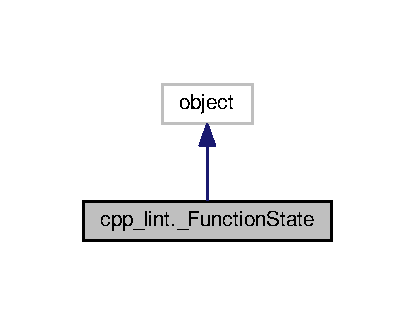
\includegraphics[width=199pt]{classcpp__lint_1_1___function_state__inherit__graph}
\end{center}
\end{figure}
\subsection*{Public Member Functions}
\begin{DoxyCompactItemize}
\item 
\mbox{\Hypertarget{classcpp__lint_1_1___function_state_abf4562c0dd1c6151cfc5f3088a7294dc}\label{classcpp__lint_1_1___function_state_abf4562c0dd1c6151cfc5f3088a7294dc}} 
def {\bfseries \+\_\+\+\_\+init\+\_\+\+\_\+} (self)
\item 
def \mbox{\hyperlink{classcpp__lint_1_1___function_state_a91b36d276e1cf17350786a0510516674}{Begin}} (self, function\+\_\+name)
\item 
def \mbox{\hyperlink{classcpp__lint_1_1___function_state_a402797f40424f11da27896926362b23f}{Count}} (self)
\item 
def \mbox{\hyperlink{classcpp__lint_1_1___function_state_a74430cb0bb43e253f617bba640391d09}{Check}} (self, error, filename, linenum)
\item 
def \mbox{\hyperlink{classcpp__lint_1_1___function_state_a6d78fb5729c971706f781918291e4a0b}{End}} (self)
\end{DoxyCompactItemize}
\subsection*{Public Attributes}
\begin{DoxyCompactItemize}
\item 
\mbox{\Hypertarget{classcpp__lint_1_1___function_state_a8ccc7032a246c6218b3fd950ee4a45ca}\label{classcpp__lint_1_1___function_state_a8ccc7032a246c6218b3fd950ee4a45ca}} 
{\bfseries in\+\_\+a\+\_\+function}
\item 
\mbox{\Hypertarget{classcpp__lint_1_1___function_state_aee01500c694fa93573b3ff7f64efe67b}\label{classcpp__lint_1_1___function_state_aee01500c694fa93573b3ff7f64efe67b}} 
{\bfseries lines\+\_\+in\+\_\+function}
\item 
\mbox{\Hypertarget{classcpp__lint_1_1___function_state_a879802c532e1629fb10b703ec1a4e126}\label{classcpp__lint_1_1___function_state_a879802c532e1629fb10b703ec1a4e126}} 
{\bfseries current\+\_\+function}
\end{DoxyCompactItemize}


\subsection{Detailed Description}
\begin{DoxyVerb}Tracks current function name and the number of lines in its body.\end{DoxyVerb}
 

\subsection{Member Function Documentation}
\mbox{\Hypertarget{classcpp__lint_1_1___function_state_a91b36d276e1cf17350786a0510516674}\label{classcpp__lint_1_1___function_state_a91b36d276e1cf17350786a0510516674}} 
\index{cpp\+\_\+lint\+::\+\_\+\+Function\+State@{cpp\+\_\+lint\+::\+\_\+\+Function\+State}!Begin@{Begin}}
\index{Begin@{Begin}!cpp\+\_\+lint\+::\+\_\+\+Function\+State@{cpp\+\_\+lint\+::\+\_\+\+Function\+State}}
\subsubsection{\texorpdfstring{Begin()}{Begin()}}
{\footnotesize\ttfamily def cpp\+\_\+lint.\+\_\+\+Function\+State.\+Begin (\begin{DoxyParamCaption}\item[{}]{self,  }\item[{}]{function\+\_\+name }\end{DoxyParamCaption})}

\begin{DoxyVerb}Start analyzing function body.

Args:
  function_name: The name of the function being tracked.
\end{DoxyVerb}
 \mbox{\Hypertarget{classcpp__lint_1_1___function_state_a74430cb0bb43e253f617bba640391d09}\label{classcpp__lint_1_1___function_state_a74430cb0bb43e253f617bba640391d09}} 
\index{cpp\+\_\+lint\+::\+\_\+\+Function\+State@{cpp\+\_\+lint\+::\+\_\+\+Function\+State}!Check@{Check}}
\index{Check@{Check}!cpp\+\_\+lint\+::\+\_\+\+Function\+State@{cpp\+\_\+lint\+::\+\_\+\+Function\+State}}
\subsubsection{\texorpdfstring{Check()}{Check()}}
{\footnotesize\ttfamily def cpp\+\_\+lint.\+\_\+\+Function\+State.\+Check (\begin{DoxyParamCaption}\item[{}]{self,  }\item[{}]{error,  }\item[{}]{filename,  }\item[{}]{linenum }\end{DoxyParamCaption})}

\begin{DoxyVerb}Report if too many lines in function body.

Args:
  error: The function to call with any errors found.
  filename: The name of the current file.
  linenum: The number of the line to check.
\end{DoxyVerb}
 \mbox{\Hypertarget{classcpp__lint_1_1___function_state_a402797f40424f11da27896926362b23f}\label{classcpp__lint_1_1___function_state_a402797f40424f11da27896926362b23f}} 
\index{cpp\+\_\+lint\+::\+\_\+\+Function\+State@{cpp\+\_\+lint\+::\+\_\+\+Function\+State}!Count@{Count}}
\index{Count@{Count}!cpp\+\_\+lint\+::\+\_\+\+Function\+State@{cpp\+\_\+lint\+::\+\_\+\+Function\+State}}
\subsubsection{\texorpdfstring{Count()}{Count()}}
{\footnotesize\ttfamily def cpp\+\_\+lint.\+\_\+\+Function\+State.\+Count (\begin{DoxyParamCaption}\item[{}]{self }\end{DoxyParamCaption})}

\begin{DoxyVerb}Count line in current function body.\end{DoxyVerb}
 \mbox{\Hypertarget{classcpp__lint_1_1___function_state_a6d78fb5729c971706f781918291e4a0b}\label{classcpp__lint_1_1___function_state_a6d78fb5729c971706f781918291e4a0b}} 
\index{cpp\+\_\+lint\+::\+\_\+\+Function\+State@{cpp\+\_\+lint\+::\+\_\+\+Function\+State}!End@{End}}
\index{End@{End}!cpp\+\_\+lint\+::\+\_\+\+Function\+State@{cpp\+\_\+lint\+::\+\_\+\+Function\+State}}
\subsubsection{\texorpdfstring{End()}{End()}}
{\footnotesize\ttfamily def cpp\+\_\+lint.\+\_\+\+Function\+State.\+End (\begin{DoxyParamCaption}\item[{}]{self }\end{DoxyParamCaption})}

\begin{DoxyVerb}Stop analyzing function body.\end{DoxyVerb}
 

The documentation for this class was generated from the following file\+:\begin{DoxyCompactItemize}
\item 
scripts/cpp\+\_\+lint.\+py\end{DoxyCompactItemize}

\hypertarget{classcpp__lint_1_1___include_error}{}\section{cpp\+\_\+lint.\+\_\+\+Include\+Error Class Reference}
\label{classcpp__lint_1_1___include_error}\index{cpp\+\_\+lint.\+\_\+\+Include\+Error@{cpp\+\_\+lint.\+\_\+\+Include\+Error}}


Inheritance diagram for cpp\+\_\+lint.\+\_\+\+Include\+Error\+:
\nopagebreak
\begin{figure}[H]
\begin{center}
\leavevmode
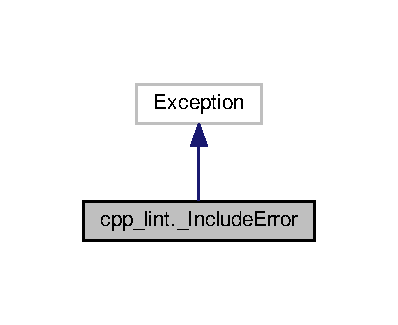
\includegraphics[width=191pt]{classcpp__lint_1_1___include_error__inherit__graph}
\end{center}
\end{figure}


\subsection{Detailed Description}
\begin{DoxyVerb}Indicates a problem with the include order in a file.\end{DoxyVerb}
 

The documentation for this class was generated from the following file\+:\begin{DoxyCompactItemize}
\item 
scripts/cpp\+\_\+lint.\+py\end{DoxyCompactItemize}

\hypertarget{classcpp__lint_1_1___include_state}{}\section{cpp\+\_\+lint.\+\_\+\+Include\+State Class Reference}
\label{classcpp__lint_1_1___include_state}\index{cpp\+\_\+lint.\+\_\+\+Include\+State@{cpp\+\_\+lint.\+\_\+\+Include\+State}}


Inheritance diagram for cpp\+\_\+lint.\+\_\+\+Include\+State\+:
\nopagebreak
\begin{figure}[H]
\begin{center}
\leavevmode
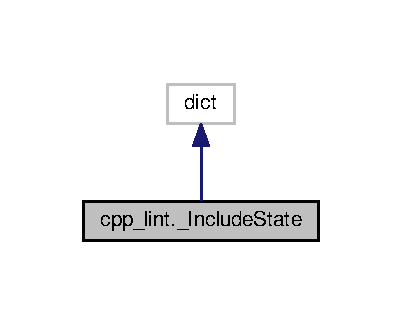
\includegraphics[width=193pt]{classcpp__lint_1_1___include_state__inherit__graph}
\end{center}
\end{figure}
\subsection*{Public Member Functions}
\begin{DoxyCompactItemize}
\item 
\mbox{\Hypertarget{classcpp__lint_1_1___include_state_abe6491f4057c5ce8dd92ba8ab1c018f7}\label{classcpp__lint_1_1___include_state_abe6491f4057c5ce8dd92ba8ab1c018f7}} 
def {\bfseries \+\_\+\+\_\+init\+\_\+\+\_\+} (self)
\item 
\mbox{\Hypertarget{classcpp__lint_1_1___include_state_a05174be66fff5cad7b4eb08491bc7770}\label{classcpp__lint_1_1___include_state_a05174be66fff5cad7b4eb08491bc7770}} 
def {\bfseries Reset\+Section} (self)
\item 
\mbox{\Hypertarget{classcpp__lint_1_1___include_state_abe16f3eddcf8d1cdc3f74184c69f0de0}\label{classcpp__lint_1_1___include_state_abe16f3eddcf8d1cdc3f74184c69f0de0}} 
def {\bfseries Set\+Last\+Header} (self, header\+\_\+path)
\item 
def \mbox{\hyperlink{classcpp__lint_1_1___include_state_a350d25886a03f0291676f533282f7eb8}{Canonicalize\+Alphabetical\+Order}} (self, header\+\_\+path)
\item 
def \mbox{\hyperlink{classcpp__lint_1_1___include_state_a7849c0d95d8f156e7678ff6f76ede724}{Is\+In\+Alphabetical\+Order}} (self, clean\+\_\+lines, linenum, header\+\_\+path)
\item 
def \mbox{\hyperlink{classcpp__lint_1_1___include_state_abe91796a07f2ade774d3ecb934a67f80}{Check\+Next\+Include\+Order}} (self, header\+\_\+type)
\end{DoxyCompactItemize}


\subsection{Detailed Description}
\begin{DoxyVerb}Tracks line numbers for includes, and the order in which includes appear.

As a dict, an _IncludeState object serves as a mapping between include
filename and line number on which that file was included.

Call CheckNextIncludeOrder() once for each header in the file, passing
in the type constants defined above. Calls in an illegal order will
raise an _IncludeError with an appropriate error message.\end{DoxyVerb}
 

\subsection{Member Function Documentation}
\mbox{\Hypertarget{classcpp__lint_1_1___include_state_a350d25886a03f0291676f533282f7eb8}\label{classcpp__lint_1_1___include_state_a350d25886a03f0291676f533282f7eb8}} 
\index{cpp\+\_\+lint\+::\+\_\+\+Include\+State@{cpp\+\_\+lint\+::\+\_\+\+Include\+State}!Canonicalize\+Alphabetical\+Order@{Canonicalize\+Alphabetical\+Order}}
\index{Canonicalize\+Alphabetical\+Order@{Canonicalize\+Alphabetical\+Order}!cpp\+\_\+lint\+::\+\_\+\+Include\+State@{cpp\+\_\+lint\+::\+\_\+\+Include\+State}}
\subsubsection{\texorpdfstring{Canonicalize\+Alphabetical\+Order()}{CanonicalizeAlphabeticalOrder()}}
{\footnotesize\ttfamily def cpp\+\_\+lint.\+\_\+\+Include\+State.\+Canonicalize\+Alphabetical\+Order (\begin{DoxyParamCaption}\item[{}]{self,  }\item[{}]{header\+\_\+path }\end{DoxyParamCaption})}

\begin{DoxyVerb}Returns a path canonicalized for alphabetical comparison.

- replaces "-" with "_" so they both cmp the same.
- removes '-inl' since we don't require them to be after the main header.
- lowercase everything, just in case.

Args:
  header_path: Path to be canonicalized.

Returns:
  Canonicalized path.
\end{DoxyVerb}
 \mbox{\Hypertarget{classcpp__lint_1_1___include_state_abe91796a07f2ade774d3ecb934a67f80}\label{classcpp__lint_1_1___include_state_abe91796a07f2ade774d3ecb934a67f80}} 
\index{cpp\+\_\+lint\+::\+\_\+\+Include\+State@{cpp\+\_\+lint\+::\+\_\+\+Include\+State}!Check\+Next\+Include\+Order@{Check\+Next\+Include\+Order}}
\index{Check\+Next\+Include\+Order@{Check\+Next\+Include\+Order}!cpp\+\_\+lint\+::\+\_\+\+Include\+State@{cpp\+\_\+lint\+::\+\_\+\+Include\+State}}
\subsubsection{\texorpdfstring{Check\+Next\+Include\+Order()}{CheckNextIncludeOrder()}}
{\footnotesize\ttfamily def cpp\+\_\+lint.\+\_\+\+Include\+State.\+Check\+Next\+Include\+Order (\begin{DoxyParamCaption}\item[{}]{self,  }\item[{}]{header\+\_\+type }\end{DoxyParamCaption})}

\begin{DoxyVerb}Returns a non-empty error message if the next header is out of order.

This function also updates the internal state to be ready to check
the next include.

Args:
  header_type: One of the _XXX_HEADER constants defined above.

Returns:
  The empty string if the header is in the right order, or an
  error message describing what's wrong.\end{DoxyVerb}
 \mbox{\Hypertarget{classcpp__lint_1_1___include_state_a7849c0d95d8f156e7678ff6f76ede724}\label{classcpp__lint_1_1___include_state_a7849c0d95d8f156e7678ff6f76ede724}} 
\index{cpp\+\_\+lint\+::\+\_\+\+Include\+State@{cpp\+\_\+lint\+::\+\_\+\+Include\+State}!Is\+In\+Alphabetical\+Order@{Is\+In\+Alphabetical\+Order}}
\index{Is\+In\+Alphabetical\+Order@{Is\+In\+Alphabetical\+Order}!cpp\+\_\+lint\+::\+\_\+\+Include\+State@{cpp\+\_\+lint\+::\+\_\+\+Include\+State}}
\subsubsection{\texorpdfstring{Is\+In\+Alphabetical\+Order()}{IsInAlphabeticalOrder()}}
{\footnotesize\ttfamily def cpp\+\_\+lint.\+\_\+\+Include\+State.\+Is\+In\+Alphabetical\+Order (\begin{DoxyParamCaption}\item[{}]{self,  }\item[{}]{clean\+\_\+lines,  }\item[{}]{linenum,  }\item[{}]{header\+\_\+path }\end{DoxyParamCaption})}

\begin{DoxyVerb}Check if a header is in alphabetical order with the previous header.

Args:
  clean_lines: A CleansedLines instance containing the file.
  linenum: The number of the line to check.
  header_path: Canonicalized header to be checked.

Returns:
  Returns true if the header is in alphabetical order.
\end{DoxyVerb}
 

The documentation for this class was generated from the following file\+:\begin{DoxyCompactItemize}
\item 
scripts/cpp\+\_\+lint.\+py\end{DoxyCompactItemize}

\hypertarget{classcpp__lint_1_1___namespace_info}{}\section{cpp\+\_\+lint.\+\_\+\+Namespace\+Info Class Reference}
\label{classcpp__lint_1_1___namespace_info}\index{cpp\+\_\+lint.\+\_\+\+Namespace\+Info@{cpp\+\_\+lint.\+\_\+\+Namespace\+Info}}


Inheritance diagram for cpp\+\_\+lint.\+\_\+\+Namespace\+Info\+:
\nopagebreak
\begin{figure}[H]
\begin{center}
\leavevmode
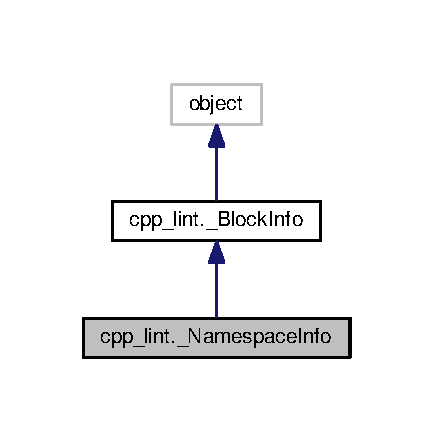
\includegraphics[width=208pt]{classcpp__lint_1_1___namespace_info__inherit__graph}
\end{center}
\end{figure}
\subsection*{Public Member Functions}
\begin{DoxyCompactItemize}
\item 
\mbox{\Hypertarget{classcpp__lint_1_1___namespace_info_aee52a8fcfd92a2bfaab356753e702377}\label{classcpp__lint_1_1___namespace_info_aee52a8fcfd92a2bfaab356753e702377}} 
def {\bfseries \+\_\+\+\_\+init\+\_\+\+\_\+} (self, name, linenum)
\item 
def \mbox{\hyperlink{classcpp__lint_1_1___namespace_info_ad119120161c94fea85e4152b563f15c6}{Check\+End}} (self, filename, clean\+\_\+lines, linenum, error)
\end{DoxyCompactItemize}
\subsection*{Public Attributes}
\begin{DoxyCompactItemize}
\item 
\mbox{\Hypertarget{classcpp__lint_1_1___namespace_info_a76fa953b9f7af77672a89f279e860c37}\label{classcpp__lint_1_1___namespace_info_a76fa953b9f7af77672a89f279e860c37}} 
{\bfseries name}
\item 
\mbox{\Hypertarget{classcpp__lint_1_1___namespace_info_ae2191919b3c07171e1653b0858b28f67}\label{classcpp__lint_1_1___namespace_info_ae2191919b3c07171e1653b0858b28f67}} 
{\bfseries starting\+\_\+linenum}
\end{DoxyCompactItemize}


\subsection{Detailed Description}
\begin{DoxyVerb}Stores information about a namespace.\end{DoxyVerb}
 

\subsection{Member Function Documentation}
\mbox{\Hypertarget{classcpp__lint_1_1___namespace_info_ad119120161c94fea85e4152b563f15c6}\label{classcpp__lint_1_1___namespace_info_ad119120161c94fea85e4152b563f15c6}} 
\index{cpp\+\_\+lint\+::\+\_\+\+Namespace\+Info@{cpp\+\_\+lint\+::\+\_\+\+Namespace\+Info}!Check\+End@{Check\+End}}
\index{Check\+End@{Check\+End}!cpp\+\_\+lint\+::\+\_\+\+Namespace\+Info@{cpp\+\_\+lint\+::\+\_\+\+Namespace\+Info}}
\subsubsection{\texorpdfstring{Check\+End()}{CheckEnd()}}
{\footnotesize\ttfamily def cpp\+\_\+lint.\+\_\+\+Namespace\+Info.\+Check\+End (\begin{DoxyParamCaption}\item[{}]{self,  }\item[{}]{filename,  }\item[{}]{clean\+\_\+lines,  }\item[{}]{linenum,  }\item[{}]{error }\end{DoxyParamCaption})}

\begin{DoxyVerb}Check end of namespace comments.\end{DoxyVerb}
 

The documentation for this class was generated from the following file\+:\begin{DoxyCompactItemize}
\item 
scripts/cpp\+\_\+lint.\+py\end{DoxyCompactItemize}

\hypertarget{classcpp__lint_1_1___nesting_state}{}\section{cpp\+\_\+lint.\+\_\+\+Nesting\+State Class Reference}
\label{classcpp__lint_1_1___nesting_state}\index{cpp\+\_\+lint.\+\_\+\+Nesting\+State@{cpp\+\_\+lint.\+\_\+\+Nesting\+State}}


Inheritance diagram for cpp\+\_\+lint.\+\_\+\+Nesting\+State\+:
\nopagebreak
\begin{figure}[H]
\begin{center}
\leavevmode
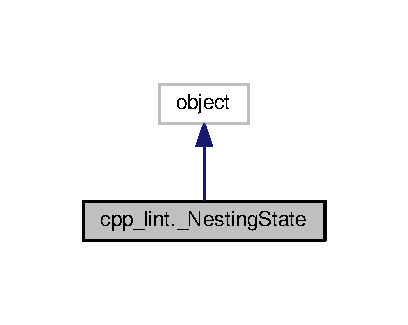
\includegraphics[width=196pt]{classcpp__lint_1_1___nesting_state__inherit__graph}
\end{center}
\end{figure}
\subsection*{Public Member Functions}
\begin{DoxyCompactItemize}
\item 
\mbox{\Hypertarget{classcpp__lint_1_1___nesting_state_a7ca0090ee1749af80736a47e0d4c85e5}\label{classcpp__lint_1_1___nesting_state_a7ca0090ee1749af80736a47e0d4c85e5}} 
def {\bfseries \+\_\+\+\_\+init\+\_\+\+\_\+} (self)
\item 
def \mbox{\hyperlink{classcpp__lint_1_1___nesting_state_a19f7e1db39b5e5bcdac60560dfaaf895}{Seen\+Open\+Brace}} (self)
\item 
def \mbox{\hyperlink{classcpp__lint_1_1___nesting_state_a8add51b250bd6004e4bb25669d274c3f}{In\+Namespace\+Body}} (self)
\item 
def \mbox{\hyperlink{classcpp__lint_1_1___nesting_state_a078812aa9c30a2f75bb93214fa8ee4f2}{Update\+Preprocessor}} (self, line)
\item 
def \mbox{\hyperlink{classcpp__lint_1_1___nesting_state_a8ffa3f80c9867b44c7c6d28ed88ffe1e}{Update}} (self, filename, clean\+\_\+lines, linenum, error)
\item 
def \mbox{\hyperlink{classcpp__lint_1_1___nesting_state_a19adbe5a4b2f7baef867ee9385bf29af}{Innermost\+Class}} (self)
\item 
def \mbox{\hyperlink{classcpp__lint_1_1___nesting_state_acacead3c8a88971753e46ac7a054e98f}{Check\+Completed\+Blocks}} (self, filename, error)
\end{DoxyCompactItemize}
\subsection*{Public Attributes}
\begin{DoxyCompactItemize}
\item 
\mbox{\Hypertarget{classcpp__lint_1_1___nesting_state_a616d83d8f9736ced48818a12d256bf82}\label{classcpp__lint_1_1___nesting_state_a616d83d8f9736ced48818a12d256bf82}} 
{\bfseries stack}
\item 
\mbox{\Hypertarget{classcpp__lint_1_1___nesting_state_a901e56e3cc366e59cfe405f255be4ded}\label{classcpp__lint_1_1___nesting_state_a901e56e3cc366e59cfe405f255be4ded}} 
{\bfseries pp\+\_\+stack}
\end{DoxyCompactItemize}


\subsection{Detailed Description}
\begin{DoxyVerb}Holds states related to parsing braces.\end{DoxyVerb}
 

\subsection{Member Function Documentation}
\mbox{\Hypertarget{classcpp__lint_1_1___nesting_state_acacead3c8a88971753e46ac7a054e98f}\label{classcpp__lint_1_1___nesting_state_acacead3c8a88971753e46ac7a054e98f}} 
\index{cpp\+\_\+lint\+::\+\_\+\+Nesting\+State@{cpp\+\_\+lint\+::\+\_\+\+Nesting\+State}!Check\+Completed\+Blocks@{Check\+Completed\+Blocks}}
\index{Check\+Completed\+Blocks@{Check\+Completed\+Blocks}!cpp\+\_\+lint\+::\+\_\+\+Nesting\+State@{cpp\+\_\+lint\+::\+\_\+\+Nesting\+State}}
\subsubsection{\texorpdfstring{Check\+Completed\+Blocks()}{CheckCompletedBlocks()}}
{\footnotesize\ttfamily def cpp\+\_\+lint.\+\_\+\+Nesting\+State.\+Check\+Completed\+Blocks (\begin{DoxyParamCaption}\item[{}]{self,  }\item[{}]{filename,  }\item[{}]{error }\end{DoxyParamCaption})}

\begin{DoxyVerb}Checks that all classes and namespaces have been completely parsed.

Call this when all lines in a file have been processed.
Args:
  filename: The name of the current file.
  error: The function to call with any errors found.
\end{DoxyVerb}
 \mbox{\Hypertarget{classcpp__lint_1_1___nesting_state_a8add51b250bd6004e4bb25669d274c3f}\label{classcpp__lint_1_1___nesting_state_a8add51b250bd6004e4bb25669d274c3f}} 
\index{cpp\+\_\+lint\+::\+\_\+\+Nesting\+State@{cpp\+\_\+lint\+::\+\_\+\+Nesting\+State}!In\+Namespace\+Body@{In\+Namespace\+Body}}
\index{In\+Namespace\+Body@{In\+Namespace\+Body}!cpp\+\_\+lint\+::\+\_\+\+Nesting\+State@{cpp\+\_\+lint\+::\+\_\+\+Nesting\+State}}
\subsubsection{\texorpdfstring{In\+Namespace\+Body()}{InNamespaceBody()}}
{\footnotesize\ttfamily def cpp\+\_\+lint.\+\_\+\+Nesting\+State.\+In\+Namespace\+Body (\begin{DoxyParamCaption}\item[{}]{self }\end{DoxyParamCaption})}

\begin{DoxyVerb}Check if we are currently one level inside a namespace body.

Returns:
  True if top of the stack is a namespace block, False otherwise.
\end{DoxyVerb}
 \mbox{\Hypertarget{classcpp__lint_1_1___nesting_state_a19adbe5a4b2f7baef867ee9385bf29af}\label{classcpp__lint_1_1___nesting_state_a19adbe5a4b2f7baef867ee9385bf29af}} 
\index{cpp\+\_\+lint\+::\+\_\+\+Nesting\+State@{cpp\+\_\+lint\+::\+\_\+\+Nesting\+State}!Innermost\+Class@{Innermost\+Class}}
\index{Innermost\+Class@{Innermost\+Class}!cpp\+\_\+lint\+::\+\_\+\+Nesting\+State@{cpp\+\_\+lint\+::\+\_\+\+Nesting\+State}}
\subsubsection{\texorpdfstring{Innermost\+Class()}{InnermostClass()}}
{\footnotesize\ttfamily def cpp\+\_\+lint.\+\_\+\+Nesting\+State.\+Innermost\+Class (\begin{DoxyParamCaption}\item[{}]{self }\end{DoxyParamCaption})}

\begin{DoxyVerb}Get class info on the top of the stack.

Returns:
  A _ClassInfo object if we are inside a class, or None otherwise.
\end{DoxyVerb}
 \mbox{\Hypertarget{classcpp__lint_1_1___nesting_state_a19f7e1db39b5e5bcdac60560dfaaf895}\label{classcpp__lint_1_1___nesting_state_a19f7e1db39b5e5bcdac60560dfaaf895}} 
\index{cpp\+\_\+lint\+::\+\_\+\+Nesting\+State@{cpp\+\_\+lint\+::\+\_\+\+Nesting\+State}!Seen\+Open\+Brace@{Seen\+Open\+Brace}}
\index{Seen\+Open\+Brace@{Seen\+Open\+Brace}!cpp\+\_\+lint\+::\+\_\+\+Nesting\+State@{cpp\+\_\+lint\+::\+\_\+\+Nesting\+State}}
\subsubsection{\texorpdfstring{Seen\+Open\+Brace()}{SeenOpenBrace()}}
{\footnotesize\ttfamily def cpp\+\_\+lint.\+\_\+\+Nesting\+State.\+Seen\+Open\+Brace (\begin{DoxyParamCaption}\item[{}]{self }\end{DoxyParamCaption})}

\begin{DoxyVerb}Check if we have seen the opening brace for the innermost block.

Returns:
  True if we have seen the opening brace, False if the innermost
  block is still expecting an opening brace.
\end{DoxyVerb}
 Here is the caller graph for this function\+:
\nopagebreak
\begin{figure}[H]
\begin{center}
\leavevmode
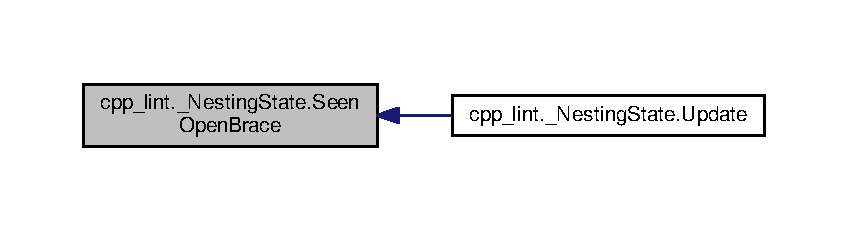
\includegraphics[width=350pt]{classcpp__lint_1_1___nesting_state_a19f7e1db39b5e5bcdac60560dfaaf895_icgraph}
\end{center}
\end{figure}
\mbox{\Hypertarget{classcpp__lint_1_1___nesting_state_a8ffa3f80c9867b44c7c6d28ed88ffe1e}\label{classcpp__lint_1_1___nesting_state_a8ffa3f80c9867b44c7c6d28ed88ffe1e}} 
\index{cpp\+\_\+lint\+::\+\_\+\+Nesting\+State@{cpp\+\_\+lint\+::\+\_\+\+Nesting\+State}!Update@{Update}}
\index{Update@{Update}!cpp\+\_\+lint\+::\+\_\+\+Nesting\+State@{cpp\+\_\+lint\+::\+\_\+\+Nesting\+State}}
\subsubsection{\texorpdfstring{Update()}{Update()}}
{\footnotesize\ttfamily def cpp\+\_\+lint.\+\_\+\+Nesting\+State.\+Update (\begin{DoxyParamCaption}\item[{}]{self,  }\item[{}]{filename,  }\item[{}]{clean\+\_\+lines,  }\item[{}]{linenum,  }\item[{}]{error }\end{DoxyParamCaption})}

\begin{DoxyVerb}Update nesting state with current line.

Args:
  filename: The name of the current file.
  clean_lines: A CleansedLines instance containing the file.
  linenum: The number of the line to check.
  error: The function to call with any errors found.
\end{DoxyVerb}
 Here is the call graph for this function\+:
\nopagebreak
\begin{figure}[H]
\begin{center}
\leavevmode
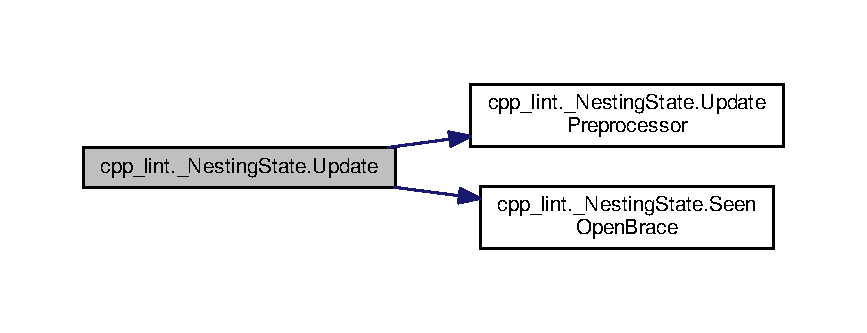
\includegraphics[width=350pt]{classcpp__lint_1_1___nesting_state_a8ffa3f80c9867b44c7c6d28ed88ffe1e_cgraph}
\end{center}
\end{figure}
\mbox{\Hypertarget{classcpp__lint_1_1___nesting_state_a078812aa9c30a2f75bb93214fa8ee4f2}\label{classcpp__lint_1_1___nesting_state_a078812aa9c30a2f75bb93214fa8ee4f2}} 
\index{cpp\+\_\+lint\+::\+\_\+\+Nesting\+State@{cpp\+\_\+lint\+::\+\_\+\+Nesting\+State}!Update\+Preprocessor@{Update\+Preprocessor}}
\index{Update\+Preprocessor@{Update\+Preprocessor}!cpp\+\_\+lint\+::\+\_\+\+Nesting\+State@{cpp\+\_\+lint\+::\+\_\+\+Nesting\+State}}
\subsubsection{\texorpdfstring{Update\+Preprocessor()}{UpdatePreprocessor()}}
{\footnotesize\ttfamily def cpp\+\_\+lint.\+\_\+\+Nesting\+State.\+Update\+Preprocessor (\begin{DoxyParamCaption}\item[{}]{self,  }\item[{}]{line }\end{DoxyParamCaption})}

\begin{DoxyVerb}Update preprocessor stack.

We need to handle preprocessors due to classes like this:
  #ifdef SWIG
  struct ResultDetailsPageElementExtensionPoint {
  #else
  struct ResultDetailsPageElementExtensionPoint : public Extension {
  #endif

We make the following assumptions (good enough for most files):
- Preprocessor condition evaluates to true from #if up to first
  #else/#elif/#endif.

- Preprocessor condition evaluates to false from #else/#elif up
  to #endif.  We still perform lint checks on these lines, but
  these do not affect nesting stack.

Args:
  line: current line to check.
\end{DoxyVerb}
 Here is the caller graph for this function\+:
\nopagebreak
\begin{figure}[H]
\begin{center}
\leavevmode
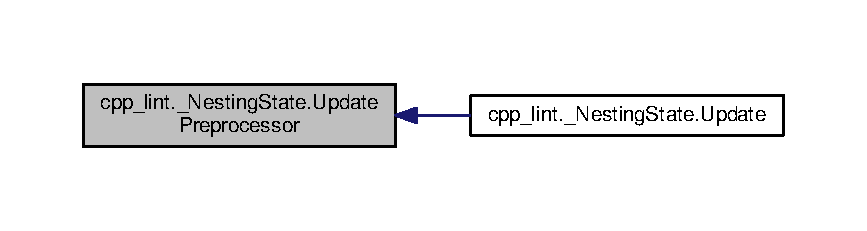
\includegraphics[width=350pt]{classcpp__lint_1_1___nesting_state_a078812aa9c30a2f75bb93214fa8ee4f2_icgraph}
\end{center}
\end{figure}


The documentation for this class was generated from the following file\+:\begin{DoxyCompactItemize}
\item 
scripts/cpp\+\_\+lint.\+py\end{DoxyCompactItemize}

\hypertarget{classcpp__lint_1_1___preprocessor_info}{}\section{cpp\+\_\+lint.\+\_\+\+Preprocessor\+Info Class Reference}
\label{classcpp__lint_1_1___preprocessor_info}\index{cpp\+\_\+lint.\+\_\+\+Preprocessor\+Info@{cpp\+\_\+lint.\+\_\+\+Preprocessor\+Info}}


Inheritance diagram for cpp\+\_\+lint.\+\_\+\+Preprocessor\+Info\+:
\nopagebreak
\begin{figure}[H]
\begin{center}
\leavevmode
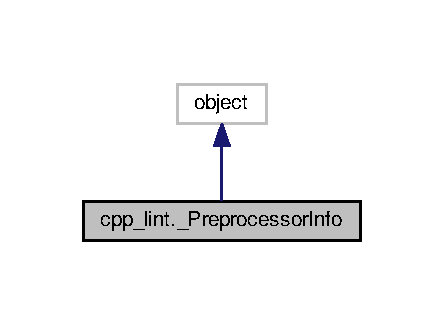
\includegraphics[width=213pt]{classcpp__lint_1_1___preprocessor_info__inherit__graph}
\end{center}
\end{figure}
\subsection*{Public Member Functions}
\begin{DoxyCompactItemize}
\item 
\mbox{\Hypertarget{classcpp__lint_1_1___preprocessor_info_acbf7b2871404c90c8ccef1aa6ccaa30f}\label{classcpp__lint_1_1___preprocessor_info_acbf7b2871404c90c8ccef1aa6ccaa30f}} 
def {\bfseries \+\_\+\+\_\+init\+\_\+\+\_\+} (self, stack\+\_\+before\+\_\+if)
\end{DoxyCompactItemize}
\subsection*{Public Attributes}
\begin{DoxyCompactItemize}
\item 
\mbox{\Hypertarget{classcpp__lint_1_1___preprocessor_info_a8218fb8f66a870a481350fb2a230c599}\label{classcpp__lint_1_1___preprocessor_info_a8218fb8f66a870a481350fb2a230c599}} 
{\bfseries stack\+\_\+before\+\_\+if}
\item 
\mbox{\Hypertarget{classcpp__lint_1_1___preprocessor_info_a2bf5b30bbfe7f15a40da1f942daac6d5}\label{classcpp__lint_1_1___preprocessor_info_a2bf5b30bbfe7f15a40da1f942daac6d5}} 
{\bfseries stack\+\_\+before\+\_\+else}
\item 
\mbox{\Hypertarget{classcpp__lint_1_1___preprocessor_info_ab6d714c480e5fa778619835468510834}\label{classcpp__lint_1_1___preprocessor_info_ab6d714c480e5fa778619835468510834}} 
{\bfseries seen\+\_\+else}
\end{DoxyCompactItemize}


\subsection{Detailed Description}
\begin{DoxyVerb}Stores checkpoints of nesting stacks when #if/#else is seen.\end{DoxyVerb}
 

The documentation for this class was generated from the following file\+:\begin{DoxyCompactItemize}
\item 
scripts/cpp\+\_\+lint.\+py\end{DoxyCompactItemize}

\hypertarget{classcaffe_1_1_abs_val_layer}{}\section{caffe\+:\+:Abs\+Val\+Layer$<$ Dtype $>$ Class Template Reference}
\label{classcaffe_1_1_abs_val_layer}\index{caffe\+::\+Abs\+Val\+Layer$<$ Dtype $>$@{caffe\+::\+Abs\+Val\+Layer$<$ Dtype $>$}}


Computes $ y = |x| $.  




{\ttfamily \#include $<$absval\+\_\+layer.\+hpp$>$}



Inheritance diagram for caffe\+:\+:Abs\+Val\+Layer$<$ Dtype $>$\+:
\nopagebreak
\begin{figure}[H]
\begin{center}
\leavevmode
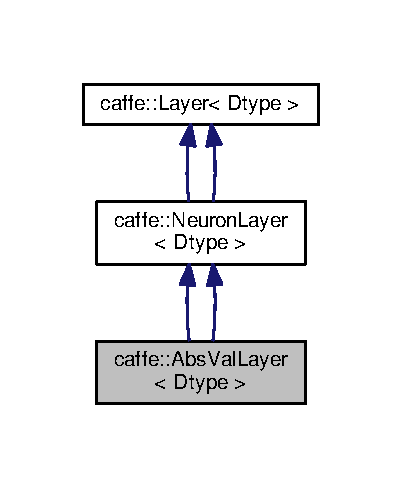
\includegraphics[width=193pt]{classcaffe_1_1_abs_val_layer__inherit__graph}
\end{center}
\end{figure}
\subsection*{Public Member Functions}
\begin{DoxyCompactItemize}
\item 
\mbox{\Hypertarget{classcaffe_1_1_abs_val_layer_a513c13552694e5860b85986b94793eb0}\label{classcaffe_1_1_abs_val_layer_a513c13552694e5860b85986b94793eb0}} 
{\bfseries Abs\+Val\+Layer} (const \mbox{\hyperlink{classcaffe_1_1_layer_parameter}{Layer\+Parameter}} \&param)
\item 
virtual void \mbox{\hyperlink{classcaffe_1_1_abs_val_layer_a4ef25e7d0cbe06404948d7e763bf0f84}{Layer\+Set\+Up}} (const vector$<$ \mbox{\hyperlink{classcaffe_1_1_blob}{Blob}}$<$ Dtype $>$ $\ast$$>$ \&bottom, const vector$<$ \mbox{\hyperlink{classcaffe_1_1_blob}{Blob}}$<$ Dtype $>$ $\ast$$>$ \&top)
\begin{DoxyCompactList}\small\item\em Does layer-\/specific setup\+: your layer should implement this function as well as Reshape. \end{DoxyCompactList}\item 
\mbox{\Hypertarget{classcaffe_1_1_abs_val_layer_aae782c69f757eacf4cec30131726e29d}\label{classcaffe_1_1_abs_val_layer_aae782c69f757eacf4cec30131726e29d}} 
virtual const char $\ast$ \mbox{\hyperlink{classcaffe_1_1_abs_val_layer_aae782c69f757eacf4cec30131726e29d}{type}} () const
\begin{DoxyCompactList}\small\item\em Returns the layer type. \end{DoxyCompactList}\item 
virtual int \mbox{\hyperlink{classcaffe_1_1_abs_val_layer_acac806dbc6d3fa3dd7daae00caabd731}{Exact\+Num\+Bottom\+Blobs}} () const
\begin{DoxyCompactList}\small\item\em Returns the exact number of bottom blobs required by the layer, or -\/1 if no exact number is required. \end{DoxyCompactList}\item 
virtual int \mbox{\hyperlink{classcaffe_1_1_abs_val_layer_aaf18bf4b77994475e8b55e5cefaa654a}{Exact\+Num\+Top\+Blobs}} () const
\begin{DoxyCompactList}\small\item\em Returns the exact number of top blobs required by the layer, or -\/1 if no exact number is required. \end{DoxyCompactList}\item 
\mbox{\Hypertarget{classcaffe_1_1_abs_val_layer_a513c13552694e5860b85986b94793eb0}\label{classcaffe_1_1_abs_val_layer_a513c13552694e5860b85986b94793eb0}} 
{\bfseries Abs\+Val\+Layer} (const \mbox{\hyperlink{classcaffe_1_1_layer_parameter}{Layer\+Parameter}} \&param)
\item 
virtual void \mbox{\hyperlink{classcaffe_1_1_abs_val_layer_a5bc321f94f7d13e938e31131fc55487b}{Layer\+Set\+Up}} (const vector$<$ \mbox{\hyperlink{classcaffe_1_1_blob}{Blob}}$<$ Dtype $>$ $\ast$$>$ \&bottom, const vector$<$ \mbox{\hyperlink{classcaffe_1_1_blob}{Blob}}$<$ Dtype $>$ $\ast$$>$ \&top)
\begin{DoxyCompactList}\small\item\em Does layer-\/specific setup\+: your layer should implement this function as well as Reshape. \end{DoxyCompactList}\item 
\mbox{\Hypertarget{classcaffe_1_1_abs_val_layer_aae782c69f757eacf4cec30131726e29d}\label{classcaffe_1_1_abs_val_layer_aae782c69f757eacf4cec30131726e29d}} 
virtual const char $\ast$ \mbox{\hyperlink{classcaffe_1_1_abs_val_layer_aae782c69f757eacf4cec30131726e29d}{type}} () const
\begin{DoxyCompactList}\small\item\em Returns the layer type. \end{DoxyCompactList}\item 
virtual int \mbox{\hyperlink{classcaffe_1_1_abs_val_layer_acac806dbc6d3fa3dd7daae00caabd731}{Exact\+Num\+Bottom\+Blobs}} () const
\begin{DoxyCompactList}\small\item\em Returns the exact number of bottom blobs required by the layer, or -\/1 if no exact number is required. \end{DoxyCompactList}\item 
virtual int \mbox{\hyperlink{classcaffe_1_1_abs_val_layer_aaf18bf4b77994475e8b55e5cefaa654a}{Exact\+Num\+Top\+Blobs}} () const
\begin{DoxyCompactList}\small\item\em Returns the exact number of top blobs required by the layer, or -\/1 if no exact number is required. \end{DoxyCompactList}\end{DoxyCompactItemize}
\subsection*{Protected Member Functions}
\begin{DoxyCompactItemize}
\item 
virtual void \mbox{\hyperlink{classcaffe_1_1_abs_val_layer_a094d7da8c6d6eeebc7db189f4cd258f9}{Forward\+\_\+cpu}} (const vector$<$ \mbox{\hyperlink{classcaffe_1_1_blob}{Blob}}$<$ Dtype $>$ $\ast$$>$ \&bottom, const vector$<$ \mbox{\hyperlink{classcaffe_1_1_blob}{Blob}}$<$ Dtype $>$ $\ast$$>$ \&top)
\begin{DoxyCompactList}\small\item\em Computes $ y = |x| $. \end{DoxyCompactList}\item 
\mbox{\Hypertarget{classcaffe_1_1_abs_val_layer_a12283057a144e9ff648a583de36b7fbd}\label{classcaffe_1_1_abs_val_layer_a12283057a144e9ff648a583de36b7fbd}} 
virtual void \mbox{\hyperlink{classcaffe_1_1_abs_val_layer_a12283057a144e9ff648a583de36b7fbd}{Forward\+\_\+gpu}} (const vector$<$ \mbox{\hyperlink{classcaffe_1_1_blob}{Blob}}$<$ Dtype $>$ $\ast$$>$ \&bottom, const vector$<$ \mbox{\hyperlink{classcaffe_1_1_blob}{Blob}}$<$ Dtype $>$ $\ast$$>$ \&top)
\begin{DoxyCompactList}\small\item\em Using the G\+PU device, compute the layer output. Fall back to \mbox{\hyperlink{classcaffe_1_1_abs_val_layer_a094d7da8c6d6eeebc7db189f4cd258f9}{Forward\+\_\+cpu()}} if unavailable. \end{DoxyCompactList}\item 
virtual void \mbox{\hyperlink{classcaffe_1_1_abs_val_layer_abac024a0ee583ecc7d83311363bcfa72}{Backward\+\_\+cpu}} (const vector$<$ \mbox{\hyperlink{classcaffe_1_1_blob}{Blob}}$<$ Dtype $>$ $\ast$$>$ \&top, const vector$<$ bool $>$ \&propagate\+\_\+down, const vector$<$ \mbox{\hyperlink{classcaffe_1_1_blob}{Blob}}$<$ Dtype $>$ $\ast$$>$ \&bottom)
\begin{DoxyCompactList}\small\item\em Computes the error gradient w.\+r.\+t. the absolute value inputs. \end{DoxyCompactList}\item 
\mbox{\Hypertarget{classcaffe_1_1_abs_val_layer_aff44062e9eb243c195285bee25b1eefb}\label{classcaffe_1_1_abs_val_layer_aff44062e9eb243c195285bee25b1eefb}} 
virtual void \mbox{\hyperlink{classcaffe_1_1_abs_val_layer_aff44062e9eb243c195285bee25b1eefb}{Backward\+\_\+gpu}} (const vector$<$ \mbox{\hyperlink{classcaffe_1_1_blob}{Blob}}$<$ Dtype $>$ $\ast$$>$ \&top, const vector$<$ bool $>$ \&propagate\+\_\+down, const vector$<$ \mbox{\hyperlink{classcaffe_1_1_blob}{Blob}}$<$ Dtype $>$ $\ast$$>$ \&bottom)
\begin{DoxyCompactList}\small\item\em Using the G\+PU device, compute the gradients for any parameters and for the bottom blobs if propagate\+\_\+down is true. Fall back to \mbox{\hyperlink{classcaffe_1_1_abs_val_layer_abac024a0ee583ecc7d83311363bcfa72}{Backward\+\_\+cpu()}} if unavailable. \end{DoxyCompactList}\item 
virtual void \mbox{\hyperlink{classcaffe_1_1_abs_val_layer_a1d63991d879fef0806b63eb65f275a2b}{Forward\+\_\+cpu}} (const vector$<$ \mbox{\hyperlink{classcaffe_1_1_blob}{Blob}}$<$ Dtype $>$ $\ast$$>$ \&bottom, const vector$<$ \mbox{\hyperlink{classcaffe_1_1_blob}{Blob}}$<$ Dtype $>$ $\ast$$>$ \&top)
\begin{DoxyCompactList}\small\item\em Computes $ y = |x| $. \end{DoxyCompactList}\item 
\mbox{\Hypertarget{classcaffe_1_1_abs_val_layer_a12283057a144e9ff648a583de36b7fbd}\label{classcaffe_1_1_abs_val_layer_a12283057a144e9ff648a583de36b7fbd}} 
virtual void \mbox{\hyperlink{classcaffe_1_1_abs_val_layer_a12283057a144e9ff648a583de36b7fbd}{Forward\+\_\+gpu}} (const vector$<$ \mbox{\hyperlink{classcaffe_1_1_blob}{Blob}}$<$ Dtype $>$ $\ast$$>$ \&bottom, const vector$<$ \mbox{\hyperlink{classcaffe_1_1_blob}{Blob}}$<$ Dtype $>$ $\ast$$>$ \&top)
\begin{DoxyCompactList}\small\item\em Using the G\+PU device, compute the layer output. Fall back to \mbox{\hyperlink{classcaffe_1_1_abs_val_layer_a094d7da8c6d6eeebc7db189f4cd258f9}{Forward\+\_\+cpu()}} if unavailable. \end{DoxyCompactList}\item 
virtual void \mbox{\hyperlink{classcaffe_1_1_abs_val_layer_a3def7ff434a338e0cb15baaa80fa23cd}{Backward\+\_\+cpu}} (const vector$<$ \mbox{\hyperlink{classcaffe_1_1_blob}{Blob}}$<$ Dtype $>$ $\ast$$>$ \&top, const vector$<$ bool $>$ \&propagate\+\_\+down, const vector$<$ \mbox{\hyperlink{classcaffe_1_1_blob}{Blob}}$<$ Dtype $>$ $\ast$$>$ \&bottom)
\begin{DoxyCompactList}\small\item\em Computes the error gradient w.\+r.\+t. the absolute value inputs. \end{DoxyCompactList}\item 
\mbox{\Hypertarget{classcaffe_1_1_abs_val_layer_aff44062e9eb243c195285bee25b1eefb}\label{classcaffe_1_1_abs_val_layer_aff44062e9eb243c195285bee25b1eefb}} 
virtual void \mbox{\hyperlink{classcaffe_1_1_abs_val_layer_aff44062e9eb243c195285bee25b1eefb}{Backward\+\_\+gpu}} (const vector$<$ \mbox{\hyperlink{classcaffe_1_1_blob}{Blob}}$<$ Dtype $>$ $\ast$$>$ \&top, const vector$<$ bool $>$ \&propagate\+\_\+down, const vector$<$ \mbox{\hyperlink{classcaffe_1_1_blob}{Blob}}$<$ Dtype $>$ $\ast$$>$ \&bottom)
\begin{DoxyCompactList}\small\item\em Using the G\+PU device, compute the gradients for any parameters and for the bottom blobs if propagate\+\_\+down is true. Fall back to \mbox{\hyperlink{classcaffe_1_1_abs_val_layer_abac024a0ee583ecc7d83311363bcfa72}{Backward\+\_\+cpu()}} if unavailable. \end{DoxyCompactList}\end{DoxyCompactItemize}
\subsection*{Additional Inherited Members}


\subsection{Detailed Description}
\subsubsection*{template$<$typename Dtype$>$\newline
class caffe\+::\+Abs\+Val\+Layer$<$ Dtype $>$}

Computes $ y = |x| $. 


\begin{DoxyParams}{Parameters}
{\em bottom} & input \mbox{\hyperlink{classcaffe_1_1_blob}{Blob}} vector (length 1)
\begin{DoxyEnumerate}
\item $ (N \times C \times H \times W) $ the inputs $ x $ 
\end{DoxyEnumerate}\\
\hline
{\em top} & output \mbox{\hyperlink{classcaffe_1_1_blob}{Blob}} vector (length 1)
\begin{DoxyEnumerate}
\item $ (N \times C \times H \times W) $ the computed outputs $ y = |x| $ 
\end{DoxyEnumerate}\\
\hline
\end{DoxyParams}


\subsection{Member Function Documentation}
\mbox{\Hypertarget{classcaffe_1_1_abs_val_layer_abac024a0ee583ecc7d83311363bcfa72}\label{classcaffe_1_1_abs_val_layer_abac024a0ee583ecc7d83311363bcfa72}} 
\index{caffe\+::\+Abs\+Val\+Layer@{caffe\+::\+Abs\+Val\+Layer}!Backward\+\_\+cpu@{Backward\+\_\+cpu}}
\index{Backward\+\_\+cpu@{Backward\+\_\+cpu}!caffe\+::\+Abs\+Val\+Layer@{caffe\+::\+Abs\+Val\+Layer}}
\subsubsection{\texorpdfstring{Backward\+\_\+cpu()}{Backward\_cpu()}\hspace{0.1cm}{\footnotesize\ttfamily [1/2]}}
{\footnotesize\ttfamily template$<$typename Dtype $>$ \\
void \mbox{\hyperlink{classcaffe_1_1_abs_val_layer}{caffe\+::\+Abs\+Val\+Layer}}$<$ Dtype $>$\+::Backward\+\_\+cpu (\begin{DoxyParamCaption}\item[{const vector$<$ \mbox{\hyperlink{classcaffe_1_1_blob}{Blob}}$<$ Dtype $>$ $\ast$$>$ \&}]{top,  }\item[{const vector$<$ bool $>$ \&}]{propagate\+\_\+down,  }\item[{const vector$<$ \mbox{\hyperlink{classcaffe_1_1_blob}{Blob}}$<$ Dtype $>$ $\ast$$>$ \&}]{bottom }\end{DoxyParamCaption})\hspace{0.3cm}{\ttfamily [protected]}, {\ttfamily [virtual]}}



Computes the error gradient w.\+r.\+t. the absolute value inputs. 


\begin{DoxyParams}{Parameters}
{\em top} & output \mbox{\hyperlink{classcaffe_1_1_blob}{Blob}} vector (length 1), providing the error gradient with respect to the outputs
\begin{DoxyEnumerate}
\item $ (N \times C \times H \times W) $ containing error gradients $ \frac{\partial E}{\partial y} $ with respect to computed outputs $ y $ 
\end{DoxyEnumerate}\\
\hline
{\em propagate\+\_\+down} & see \mbox{\hyperlink{classcaffe_1_1_layer_a183d343f5183a4762307f2c5e6ed1e12}{Layer\+::\+Backward}}. \\
\hline
{\em bottom} & input \mbox{\hyperlink{classcaffe_1_1_blob}{Blob}} vector (length 2)
\begin{DoxyEnumerate}
\item $ (N \times C \times H \times W) $ the inputs $ x $; Backward fills their diff with gradients $ \frac{\partial E}{\partial x} = \mathrm{sign}(x) \frac{\partial E}{\partial y} $ if propagate\+\_\+down\mbox{[}0\mbox{]} 
\end{DoxyEnumerate}\\
\hline
\end{DoxyParams}


Implements \mbox{\hyperlink{classcaffe_1_1_layer_a75c9b2a321dc713e0eaef530d02dc37f}{caffe\+::\+Layer$<$ Dtype $>$}}.

\mbox{\Hypertarget{classcaffe_1_1_abs_val_layer_a3def7ff434a338e0cb15baaa80fa23cd}\label{classcaffe_1_1_abs_val_layer_a3def7ff434a338e0cb15baaa80fa23cd}} 
\index{caffe\+::\+Abs\+Val\+Layer@{caffe\+::\+Abs\+Val\+Layer}!Backward\+\_\+cpu@{Backward\+\_\+cpu}}
\index{Backward\+\_\+cpu@{Backward\+\_\+cpu}!caffe\+::\+Abs\+Val\+Layer@{caffe\+::\+Abs\+Val\+Layer}}
\subsubsection{\texorpdfstring{Backward\+\_\+cpu()}{Backward\_cpu()}\hspace{0.1cm}{\footnotesize\ttfamily [2/2]}}
{\footnotesize\ttfamily template$<$typename Dtype$>$ \\
virtual void \mbox{\hyperlink{classcaffe_1_1_abs_val_layer}{caffe\+::\+Abs\+Val\+Layer}}$<$ Dtype $>$\+::Backward\+\_\+cpu (\begin{DoxyParamCaption}\item[{const vector$<$ \mbox{\hyperlink{classcaffe_1_1_blob}{Blob}}$<$ Dtype $>$ $\ast$$>$ \&}]{top,  }\item[{const vector$<$ bool $>$ \&}]{propagate\+\_\+down,  }\item[{const vector$<$ \mbox{\hyperlink{classcaffe_1_1_blob}{Blob}}$<$ Dtype $>$ $\ast$$>$ \&}]{bottom }\end{DoxyParamCaption})\hspace{0.3cm}{\ttfamily [protected]}, {\ttfamily [virtual]}}



Computes the error gradient w.\+r.\+t. the absolute value inputs. 


\begin{DoxyParams}{Parameters}
{\em top} & output \mbox{\hyperlink{classcaffe_1_1_blob}{Blob}} vector (length 1), providing the error gradient with respect to the outputs
\begin{DoxyEnumerate}
\item $ (N \times C \times H \times W) $ containing error gradients $ \frac{\partial E}{\partial y} $ with respect to computed outputs $ y $ 
\end{DoxyEnumerate}\\
\hline
{\em propagate\+\_\+down} & see \mbox{\hyperlink{classcaffe_1_1_layer_a183d343f5183a4762307f2c5e6ed1e12}{Layer\+::\+Backward}}. \\
\hline
{\em bottom} & input \mbox{\hyperlink{classcaffe_1_1_blob}{Blob}} vector (length 2)
\begin{DoxyEnumerate}
\item $ (N \times C \times H \times W) $ the inputs $ x $; Backward fills their diff with gradients $ \frac{\partial E}{\partial x} = \mathrm{sign}(x) \frac{\partial E}{\partial y} $ if propagate\+\_\+down\mbox{[}0\mbox{]} 
\end{DoxyEnumerate}\\
\hline
\end{DoxyParams}


Implements \mbox{\hyperlink{classcaffe_1_1_layer_a75c9b2a321dc713e0eaef530d02dc37f}{caffe\+::\+Layer$<$ Dtype $>$}}.

\mbox{\Hypertarget{classcaffe_1_1_abs_val_layer_acac806dbc6d3fa3dd7daae00caabd731}\label{classcaffe_1_1_abs_val_layer_acac806dbc6d3fa3dd7daae00caabd731}} 
\index{caffe\+::\+Abs\+Val\+Layer@{caffe\+::\+Abs\+Val\+Layer}!Exact\+Num\+Bottom\+Blobs@{Exact\+Num\+Bottom\+Blobs}}
\index{Exact\+Num\+Bottom\+Blobs@{Exact\+Num\+Bottom\+Blobs}!caffe\+::\+Abs\+Val\+Layer@{caffe\+::\+Abs\+Val\+Layer}}
\subsubsection{\texorpdfstring{Exact\+Num\+Bottom\+Blobs()}{ExactNumBottomBlobs()}\hspace{0.1cm}{\footnotesize\ttfamily [1/2]}}
{\footnotesize\ttfamily template$<$typename Dtype$>$ \\
virtual int \mbox{\hyperlink{classcaffe_1_1_abs_val_layer}{caffe\+::\+Abs\+Val\+Layer}}$<$ Dtype $>$\+::Exact\+Num\+Bottom\+Blobs (\begin{DoxyParamCaption}{ }\end{DoxyParamCaption}) const\hspace{0.3cm}{\ttfamily [inline]}, {\ttfamily [virtual]}}



Returns the exact number of bottom blobs required by the layer, or -\/1 if no exact number is required. 

This method should be overridden to return a non-\/negative value if your layer expects some exact number of bottom blobs. 

Reimplemented from \mbox{\hyperlink{classcaffe_1_1_neuron_layer_abb6c0e6acd2863baf47d6e6acda6f55f}{caffe\+::\+Neuron\+Layer$<$ Dtype $>$}}.

\mbox{\Hypertarget{classcaffe_1_1_abs_val_layer_acac806dbc6d3fa3dd7daae00caabd731}\label{classcaffe_1_1_abs_val_layer_acac806dbc6d3fa3dd7daae00caabd731}} 
\index{caffe\+::\+Abs\+Val\+Layer@{caffe\+::\+Abs\+Val\+Layer}!Exact\+Num\+Bottom\+Blobs@{Exact\+Num\+Bottom\+Blobs}}
\index{Exact\+Num\+Bottom\+Blobs@{Exact\+Num\+Bottom\+Blobs}!caffe\+::\+Abs\+Val\+Layer@{caffe\+::\+Abs\+Val\+Layer}}
\subsubsection{\texorpdfstring{Exact\+Num\+Bottom\+Blobs()}{ExactNumBottomBlobs()}\hspace{0.1cm}{\footnotesize\ttfamily [2/2]}}
{\footnotesize\ttfamily template$<$typename Dtype$>$ \\
virtual int \mbox{\hyperlink{classcaffe_1_1_abs_val_layer}{caffe\+::\+Abs\+Val\+Layer}}$<$ Dtype $>$\+::Exact\+Num\+Bottom\+Blobs (\begin{DoxyParamCaption}{ }\end{DoxyParamCaption}) const\hspace{0.3cm}{\ttfamily [inline]}, {\ttfamily [virtual]}}



Returns the exact number of bottom blobs required by the layer, or -\/1 if no exact number is required. 

This method should be overridden to return a non-\/negative value if your layer expects some exact number of bottom blobs. 

Reimplemented from \mbox{\hyperlink{classcaffe_1_1_neuron_layer_abb6c0e6acd2863baf47d6e6acda6f55f}{caffe\+::\+Neuron\+Layer$<$ Dtype $>$}}.

\mbox{\Hypertarget{classcaffe_1_1_abs_val_layer_aaf18bf4b77994475e8b55e5cefaa654a}\label{classcaffe_1_1_abs_val_layer_aaf18bf4b77994475e8b55e5cefaa654a}} 
\index{caffe\+::\+Abs\+Val\+Layer@{caffe\+::\+Abs\+Val\+Layer}!Exact\+Num\+Top\+Blobs@{Exact\+Num\+Top\+Blobs}}
\index{Exact\+Num\+Top\+Blobs@{Exact\+Num\+Top\+Blobs}!caffe\+::\+Abs\+Val\+Layer@{caffe\+::\+Abs\+Val\+Layer}}
\subsubsection{\texorpdfstring{Exact\+Num\+Top\+Blobs()}{ExactNumTopBlobs()}\hspace{0.1cm}{\footnotesize\ttfamily [1/2]}}
{\footnotesize\ttfamily template$<$typename Dtype$>$ \\
virtual int \mbox{\hyperlink{classcaffe_1_1_abs_val_layer}{caffe\+::\+Abs\+Val\+Layer}}$<$ Dtype $>$\+::Exact\+Num\+Top\+Blobs (\begin{DoxyParamCaption}{ }\end{DoxyParamCaption}) const\hspace{0.3cm}{\ttfamily [inline]}, {\ttfamily [virtual]}}



Returns the exact number of top blobs required by the layer, or -\/1 if no exact number is required. 

This method should be overridden to return a non-\/negative value if your layer expects some exact number of top blobs. 

Reimplemented from \mbox{\hyperlink{classcaffe_1_1_neuron_layer_a47ac5e7208e4b14ad1e4040a621dbfbc}{caffe\+::\+Neuron\+Layer$<$ Dtype $>$}}.

\mbox{\Hypertarget{classcaffe_1_1_abs_val_layer_aaf18bf4b77994475e8b55e5cefaa654a}\label{classcaffe_1_1_abs_val_layer_aaf18bf4b77994475e8b55e5cefaa654a}} 
\index{caffe\+::\+Abs\+Val\+Layer@{caffe\+::\+Abs\+Val\+Layer}!Exact\+Num\+Top\+Blobs@{Exact\+Num\+Top\+Blobs}}
\index{Exact\+Num\+Top\+Blobs@{Exact\+Num\+Top\+Blobs}!caffe\+::\+Abs\+Val\+Layer@{caffe\+::\+Abs\+Val\+Layer}}
\subsubsection{\texorpdfstring{Exact\+Num\+Top\+Blobs()}{ExactNumTopBlobs()}\hspace{0.1cm}{\footnotesize\ttfamily [2/2]}}
{\footnotesize\ttfamily template$<$typename Dtype$>$ \\
virtual int \mbox{\hyperlink{classcaffe_1_1_abs_val_layer}{caffe\+::\+Abs\+Val\+Layer}}$<$ Dtype $>$\+::Exact\+Num\+Top\+Blobs (\begin{DoxyParamCaption}{ }\end{DoxyParamCaption}) const\hspace{0.3cm}{\ttfamily [inline]}, {\ttfamily [virtual]}}



Returns the exact number of top blobs required by the layer, or -\/1 if no exact number is required. 

This method should be overridden to return a non-\/negative value if your layer expects some exact number of top blobs. 

Reimplemented from \mbox{\hyperlink{classcaffe_1_1_neuron_layer_a47ac5e7208e4b14ad1e4040a621dbfbc}{caffe\+::\+Neuron\+Layer$<$ Dtype $>$}}.

\mbox{\Hypertarget{classcaffe_1_1_abs_val_layer_a1d63991d879fef0806b63eb65f275a2b}\label{classcaffe_1_1_abs_val_layer_a1d63991d879fef0806b63eb65f275a2b}} 
\index{caffe\+::\+Abs\+Val\+Layer@{caffe\+::\+Abs\+Val\+Layer}!Forward\+\_\+cpu@{Forward\+\_\+cpu}}
\index{Forward\+\_\+cpu@{Forward\+\_\+cpu}!caffe\+::\+Abs\+Val\+Layer@{caffe\+::\+Abs\+Val\+Layer}}
\subsubsection{\texorpdfstring{Forward\+\_\+cpu()}{Forward\_cpu()}\hspace{0.1cm}{\footnotesize\ttfamily [1/2]}}
{\footnotesize\ttfamily template$<$typename Dtype$>$ \\
virtual void \mbox{\hyperlink{classcaffe_1_1_abs_val_layer}{caffe\+::\+Abs\+Val\+Layer}}$<$ Dtype $>$\+::Forward\+\_\+cpu (\begin{DoxyParamCaption}\item[{const vector$<$ \mbox{\hyperlink{classcaffe_1_1_blob}{Blob}}$<$ Dtype $>$ $\ast$$>$ \&}]{bottom,  }\item[{const vector$<$ \mbox{\hyperlink{classcaffe_1_1_blob}{Blob}}$<$ Dtype $>$ $\ast$$>$ \&}]{top }\end{DoxyParamCaption})\hspace{0.3cm}{\ttfamily [protected]}, {\ttfamily [virtual]}}



Computes $ y = |x| $. 


\begin{DoxyParams}{Parameters}
{\em bottom} & input \mbox{\hyperlink{classcaffe_1_1_blob}{Blob}} vector (length 1)
\begin{DoxyEnumerate}
\item $ (N \times C \times H \times W) $ the inputs $ x $ 
\end{DoxyEnumerate}\\
\hline
{\em top} & output \mbox{\hyperlink{classcaffe_1_1_blob}{Blob}} vector (length 1)
\begin{DoxyEnumerate}
\item $ (N \times C \times H \times W) $ the computed outputs $ y = |x| $ 
\end{DoxyEnumerate}\\
\hline
\end{DoxyParams}


Implements \mbox{\hyperlink{classcaffe_1_1_layer_a576ac6a60b1e99fe383831f52a6cea77}{caffe\+::\+Layer$<$ Dtype $>$}}.

\mbox{\Hypertarget{classcaffe_1_1_abs_val_layer_a094d7da8c6d6eeebc7db189f4cd258f9}\label{classcaffe_1_1_abs_val_layer_a094d7da8c6d6eeebc7db189f4cd258f9}} 
\index{caffe\+::\+Abs\+Val\+Layer@{caffe\+::\+Abs\+Val\+Layer}!Forward\+\_\+cpu@{Forward\+\_\+cpu}}
\index{Forward\+\_\+cpu@{Forward\+\_\+cpu}!caffe\+::\+Abs\+Val\+Layer@{caffe\+::\+Abs\+Val\+Layer}}
\subsubsection{\texorpdfstring{Forward\+\_\+cpu()}{Forward\_cpu()}\hspace{0.1cm}{\footnotesize\ttfamily [2/2]}}
{\footnotesize\ttfamily template$<$typename Dtype $>$ \\
void \mbox{\hyperlink{classcaffe_1_1_abs_val_layer}{caffe\+::\+Abs\+Val\+Layer}}$<$ Dtype $>$\+::Forward\+\_\+cpu (\begin{DoxyParamCaption}\item[{const vector$<$ \mbox{\hyperlink{classcaffe_1_1_blob}{Blob}}$<$ Dtype $>$ $\ast$$>$ \&}]{bottom,  }\item[{const vector$<$ \mbox{\hyperlink{classcaffe_1_1_blob}{Blob}}$<$ Dtype $>$ $\ast$$>$ \&}]{top }\end{DoxyParamCaption})\hspace{0.3cm}{\ttfamily [protected]}, {\ttfamily [virtual]}}



Computes $ y = |x| $. 


\begin{DoxyParams}{Parameters}
{\em bottom} & input \mbox{\hyperlink{classcaffe_1_1_blob}{Blob}} vector (length 1)
\begin{DoxyEnumerate}
\item $ (N \times C \times H \times W) $ the inputs $ x $ 
\end{DoxyEnumerate}\\
\hline
{\em top} & output \mbox{\hyperlink{classcaffe_1_1_blob}{Blob}} vector (length 1)
\begin{DoxyEnumerate}
\item $ (N \times C \times H \times W) $ the computed outputs $ y = |x| $ 
\end{DoxyEnumerate}\\
\hline
\end{DoxyParams}


Implements \mbox{\hyperlink{classcaffe_1_1_layer_a576ac6a60b1e99fe383831f52a6cea77}{caffe\+::\+Layer$<$ Dtype $>$}}.

\mbox{\Hypertarget{classcaffe_1_1_abs_val_layer_a5bc321f94f7d13e938e31131fc55487b}\label{classcaffe_1_1_abs_val_layer_a5bc321f94f7d13e938e31131fc55487b}} 
\index{caffe\+::\+Abs\+Val\+Layer@{caffe\+::\+Abs\+Val\+Layer}!Layer\+Set\+Up@{Layer\+Set\+Up}}
\index{Layer\+Set\+Up@{Layer\+Set\+Up}!caffe\+::\+Abs\+Val\+Layer@{caffe\+::\+Abs\+Val\+Layer}}
\subsubsection{\texorpdfstring{Layer\+Set\+Up()}{LayerSetUp()}\hspace{0.1cm}{\footnotesize\ttfamily [1/2]}}
{\footnotesize\ttfamily template$<$typename Dtype$>$ \\
virtual void \mbox{\hyperlink{classcaffe_1_1_abs_val_layer}{caffe\+::\+Abs\+Val\+Layer}}$<$ Dtype $>$\+::Layer\+Set\+Up (\begin{DoxyParamCaption}\item[{const vector$<$ \mbox{\hyperlink{classcaffe_1_1_blob}{Blob}}$<$ Dtype $>$ $\ast$$>$ \&}]{bottom,  }\item[{const vector$<$ \mbox{\hyperlink{classcaffe_1_1_blob}{Blob}}$<$ Dtype $>$ $\ast$$>$ \&}]{top }\end{DoxyParamCaption})\hspace{0.3cm}{\ttfamily [virtual]}}



Does layer-\/specific setup\+: your layer should implement this function as well as Reshape. 


\begin{DoxyParams}{Parameters}
{\em bottom} & the preshaped input blobs, whose data fields store the input data for this layer \\
\hline
{\em top} & the allocated but unshaped output blobs\\
\hline
\end{DoxyParams}
This method should do one-\/time layer specific setup. This includes reading and processing relevent parameters from the {\ttfamily layer\+\_\+param\+\_\+}. Setting up the shapes of top blobs and internal buffers should be done in {\ttfamily Reshape}, which will be called before the forward pass to adjust the top blob sizes. 

Reimplemented from \mbox{\hyperlink{classcaffe_1_1_layer_a481323a3e0972c682787f2137468c29f}{caffe\+::\+Layer$<$ Dtype $>$}}.

\mbox{\Hypertarget{classcaffe_1_1_abs_val_layer_a4ef25e7d0cbe06404948d7e763bf0f84}\label{classcaffe_1_1_abs_val_layer_a4ef25e7d0cbe06404948d7e763bf0f84}} 
\index{caffe\+::\+Abs\+Val\+Layer@{caffe\+::\+Abs\+Val\+Layer}!Layer\+Set\+Up@{Layer\+Set\+Up}}
\index{Layer\+Set\+Up@{Layer\+Set\+Up}!caffe\+::\+Abs\+Val\+Layer@{caffe\+::\+Abs\+Val\+Layer}}
\subsubsection{\texorpdfstring{Layer\+Set\+Up()}{LayerSetUp()}\hspace{0.1cm}{\footnotesize\ttfamily [2/2]}}
{\footnotesize\ttfamily template$<$typename Dtype $>$ \\
void \mbox{\hyperlink{classcaffe_1_1_abs_val_layer}{caffe\+::\+Abs\+Val\+Layer}}$<$ Dtype $>$\+::Layer\+Set\+Up (\begin{DoxyParamCaption}\item[{const vector$<$ \mbox{\hyperlink{classcaffe_1_1_blob}{Blob}}$<$ Dtype $>$ $\ast$$>$ \&}]{bottom,  }\item[{const vector$<$ \mbox{\hyperlink{classcaffe_1_1_blob}{Blob}}$<$ Dtype $>$ $\ast$$>$ \&}]{top }\end{DoxyParamCaption})\hspace{0.3cm}{\ttfamily [virtual]}}



Does layer-\/specific setup\+: your layer should implement this function as well as Reshape. 


\begin{DoxyParams}{Parameters}
{\em bottom} & the preshaped input blobs, whose data fields store the input data for this layer \\
\hline
{\em top} & the allocated but unshaped output blobs\\
\hline
\end{DoxyParams}
This method should do one-\/time layer specific setup. This includes reading and processing relevent parameters from the {\ttfamily layer\+\_\+param\+\_\+}. Setting up the shapes of top blobs and internal buffers should be done in {\ttfamily Reshape}, which will be called before the forward pass to adjust the top blob sizes. 

Reimplemented from \mbox{\hyperlink{classcaffe_1_1_layer_a481323a3e0972c682787f2137468c29f}{caffe\+::\+Layer$<$ Dtype $>$}}.

Here is the call graph for this function\+:
\nopagebreak
\begin{figure}[H]
\begin{center}
\leavevmode
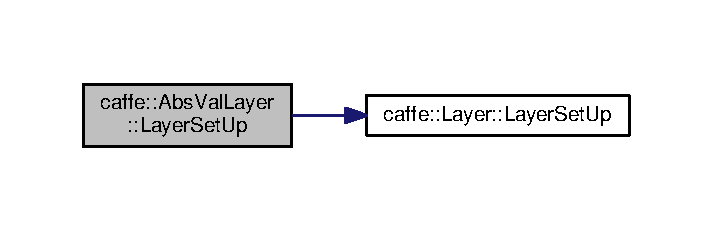
\includegraphics[width=342pt]{classcaffe_1_1_abs_val_layer_a4ef25e7d0cbe06404948d7e763bf0f84_cgraph}
\end{center}
\end{figure}


The documentation for this class was generated from the following files\+:\begin{DoxyCompactItemize}
\item 
build/install/include/caffe/layers/absval\+\_\+layer.\+hpp\item 
src/caffe/layers/absval\+\_\+layer.\+cpp\end{DoxyCompactItemize}

\hypertarget{classcaffe_1_1_accuracy_layer}{}\section{caffe\+:\+:Accuracy\+Layer$<$ Dtype $>$ Class Template Reference}
\label{classcaffe_1_1_accuracy_layer}\index{caffe\+::\+Accuracy\+Layer$<$ Dtype $>$@{caffe\+::\+Accuracy\+Layer$<$ Dtype $>$}}


Computes the classification accuracy for a one-\/of-\/many classification task.  




{\ttfamily \#include $<$accuracy\+\_\+layer.\+hpp$>$}



Inheritance diagram for caffe\+:\+:Accuracy\+Layer$<$ Dtype $>$\+:
\nopagebreak
\begin{figure}[H]
\begin{center}
\leavevmode
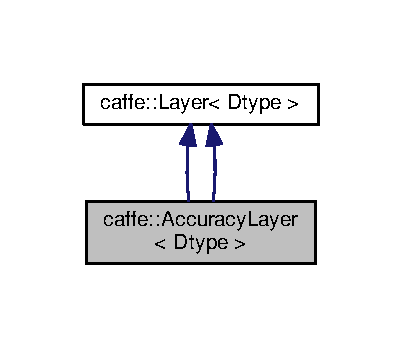
\includegraphics[width=193pt]{classcaffe_1_1_accuracy_layer__inherit__graph}
\end{center}
\end{figure}
\subsection*{Public Member Functions}
\begin{DoxyCompactItemize}
\item 
\mbox{\hyperlink{classcaffe_1_1_accuracy_layer_a362ab61d1961c1b408f84a956f6e598d}{Accuracy\+Layer}} (const \mbox{\hyperlink{classcaffe_1_1_layer_parameter}{Layer\+Parameter}} \&param)
\item 
virtual void \mbox{\hyperlink{classcaffe_1_1_accuracy_layer_a1f2447583c670d92ff6e2c8d53fb4dd9}{Layer\+Set\+Up}} (const vector$<$ \mbox{\hyperlink{classcaffe_1_1_blob}{Blob}}$<$ Dtype $>$ $\ast$$>$ \&bottom, const vector$<$ \mbox{\hyperlink{classcaffe_1_1_blob}{Blob}}$<$ Dtype $>$ $\ast$$>$ \&top)
\begin{DoxyCompactList}\small\item\em Does layer-\/specific setup\+: your layer should implement this function as well as Reshape. \end{DoxyCompactList}\item 
virtual void \mbox{\hyperlink{classcaffe_1_1_accuracy_layer_aa2b680fc1e754440c2babd150e09f2f6}{Reshape}} (const vector$<$ \mbox{\hyperlink{classcaffe_1_1_blob}{Blob}}$<$ Dtype $>$ $\ast$$>$ \&bottom, const vector$<$ \mbox{\hyperlink{classcaffe_1_1_blob}{Blob}}$<$ Dtype $>$ $\ast$$>$ \&top)
\begin{DoxyCompactList}\small\item\em Adjust the shapes of top blobs and internal buffers to accommodate the shapes of the bottom blobs. \end{DoxyCompactList}\item 
\mbox{\Hypertarget{classcaffe_1_1_accuracy_layer_a6039b0528a2017c4f9d32ad2c67a9ef2}\label{classcaffe_1_1_accuracy_layer_a6039b0528a2017c4f9d32ad2c67a9ef2}} 
virtual const char $\ast$ \mbox{\hyperlink{classcaffe_1_1_accuracy_layer_a6039b0528a2017c4f9d32ad2c67a9ef2}{type}} () const
\begin{DoxyCompactList}\small\item\em Returns the layer type. \end{DoxyCompactList}\item 
virtual int \mbox{\hyperlink{classcaffe_1_1_accuracy_layer_afb0d3db8e4a18bec0e05d54d11453ef1}{Exact\+Num\+Bottom\+Blobs}} () const
\begin{DoxyCompactList}\small\item\em Returns the exact number of bottom blobs required by the layer, or -\/1 if no exact number is required. \end{DoxyCompactList}\item 
virtual int \mbox{\hyperlink{classcaffe_1_1_accuracy_layer_a568dd59acff7a172fa614c88ac56aff7}{Min\+Top\+Blobs}} () const
\begin{DoxyCompactList}\small\item\em Returns the minimum number of top blobs required by the layer, or -\/1 if no minimum number is required. \end{DoxyCompactList}\item 
virtual int \mbox{\hyperlink{classcaffe_1_1_accuracy_layer_a7591ae6d50dd7d96b91241b5b0368997}{Max\+Top\+Blobs}} () const
\begin{DoxyCompactList}\small\item\em Returns the maximum number of top blobs required by the layer, or -\/1 if no maximum number is required. \end{DoxyCompactList}\item 
\mbox{\hyperlink{classcaffe_1_1_accuracy_layer_a362ab61d1961c1b408f84a956f6e598d}{Accuracy\+Layer}} (const \mbox{\hyperlink{classcaffe_1_1_layer_parameter}{Layer\+Parameter}} \&param)
\item 
virtual void \mbox{\hyperlink{classcaffe_1_1_accuracy_layer_a894a1fcb58e8f822f9d875e1acae560c}{Layer\+Set\+Up}} (const vector$<$ \mbox{\hyperlink{classcaffe_1_1_blob}{Blob}}$<$ Dtype $>$ $\ast$$>$ \&bottom, const vector$<$ \mbox{\hyperlink{classcaffe_1_1_blob}{Blob}}$<$ Dtype $>$ $\ast$$>$ \&top)
\begin{DoxyCompactList}\small\item\em Does layer-\/specific setup\+: your layer should implement this function as well as Reshape. \end{DoxyCompactList}\item 
virtual void \mbox{\hyperlink{classcaffe_1_1_accuracy_layer_a1a42bc91c233a9f803482bff30163f36}{Reshape}} (const vector$<$ \mbox{\hyperlink{classcaffe_1_1_blob}{Blob}}$<$ Dtype $>$ $\ast$$>$ \&bottom, const vector$<$ \mbox{\hyperlink{classcaffe_1_1_blob}{Blob}}$<$ Dtype $>$ $\ast$$>$ \&top)
\begin{DoxyCompactList}\small\item\em Adjust the shapes of top blobs and internal buffers to accommodate the shapes of the bottom blobs. \end{DoxyCompactList}\item 
\mbox{\Hypertarget{classcaffe_1_1_accuracy_layer_a6039b0528a2017c4f9d32ad2c67a9ef2}\label{classcaffe_1_1_accuracy_layer_a6039b0528a2017c4f9d32ad2c67a9ef2}} 
virtual const char $\ast$ \mbox{\hyperlink{classcaffe_1_1_accuracy_layer_a6039b0528a2017c4f9d32ad2c67a9ef2}{type}} () const
\begin{DoxyCompactList}\small\item\em Returns the layer type. \end{DoxyCompactList}\item 
virtual int \mbox{\hyperlink{classcaffe_1_1_accuracy_layer_afb0d3db8e4a18bec0e05d54d11453ef1}{Exact\+Num\+Bottom\+Blobs}} () const
\begin{DoxyCompactList}\small\item\em Returns the exact number of bottom blobs required by the layer, or -\/1 if no exact number is required. \end{DoxyCompactList}\item 
virtual int \mbox{\hyperlink{classcaffe_1_1_accuracy_layer_a568dd59acff7a172fa614c88ac56aff7}{Min\+Top\+Blobs}} () const
\begin{DoxyCompactList}\small\item\em Returns the minimum number of top blobs required by the layer, or -\/1 if no minimum number is required. \end{DoxyCompactList}\item 
virtual int \mbox{\hyperlink{classcaffe_1_1_accuracy_layer_a7591ae6d50dd7d96b91241b5b0368997}{Max\+Top\+Blobs}} () const
\begin{DoxyCompactList}\small\item\em Returns the maximum number of top blobs required by the layer, or -\/1 if no maximum number is required. \end{DoxyCompactList}\end{DoxyCompactItemize}
\subsection*{Protected Member Functions}
\begin{DoxyCompactItemize}
\item 
virtual void \mbox{\hyperlink{classcaffe_1_1_accuracy_layer_ad61bb4c6984d9df6a61562cd5c19ff6d}{Forward\+\_\+cpu}} (const vector$<$ \mbox{\hyperlink{classcaffe_1_1_blob}{Blob}}$<$ Dtype $>$ $\ast$$>$ \&bottom, const vector$<$ \mbox{\hyperlink{classcaffe_1_1_blob}{Blob}}$<$ Dtype $>$ $\ast$$>$ \&top)
\item 
\mbox{\Hypertarget{classcaffe_1_1_accuracy_layer_a0c720e010f5ba0bd4ef3582d32ce37a9}\label{classcaffe_1_1_accuracy_layer_a0c720e010f5ba0bd4ef3582d32ce37a9}} 
virtual void \mbox{\hyperlink{classcaffe_1_1_accuracy_layer_a0c720e010f5ba0bd4ef3582d32ce37a9}{Forward\+\_\+gpu}} (const vector$<$ \mbox{\hyperlink{classcaffe_1_1_blob}{Blob}}$<$ Dtype $>$ $\ast$$>$ \&bottom, const vector$<$ \mbox{\hyperlink{classcaffe_1_1_blob}{Blob}}$<$ Dtype $>$ $\ast$$>$ \&top)
\begin{DoxyCompactList}\small\item\em Using the G\+PU device, compute the layer output. Fall back to \mbox{\hyperlink{classcaffe_1_1_accuracy_layer_ad61bb4c6984d9df6a61562cd5c19ff6d}{Forward\+\_\+cpu()}} if unavailable. \end{DoxyCompactList}\item 
\mbox{\Hypertarget{classcaffe_1_1_accuracy_layer_a8084d42629a751f5b6322d9cb3f5986c}\label{classcaffe_1_1_accuracy_layer_a8084d42629a751f5b6322d9cb3f5986c}} 
virtual void \mbox{\hyperlink{classcaffe_1_1_accuracy_layer_a8084d42629a751f5b6322d9cb3f5986c}{Backward\+\_\+cpu}} (const vector$<$ \mbox{\hyperlink{classcaffe_1_1_blob}{Blob}}$<$ Dtype $>$ $\ast$$>$ \&top, const vector$<$ bool $>$ \&propagate\+\_\+down, const vector$<$ \mbox{\hyperlink{classcaffe_1_1_blob}{Blob}}$<$ Dtype $>$ $\ast$$>$ \&bottom)
\begin{DoxyCompactList}\small\item\em Not implemented -- \mbox{\hyperlink{classcaffe_1_1_accuracy_layer}{Accuracy\+Layer}} cannot be used as a loss. \end{DoxyCompactList}\item 
\mbox{\Hypertarget{classcaffe_1_1_accuracy_layer_a4cd3015639d107e63f90672733ac019a}\label{classcaffe_1_1_accuracy_layer_a4cd3015639d107e63f90672733ac019a}} 
virtual void \mbox{\hyperlink{classcaffe_1_1_accuracy_layer_a4cd3015639d107e63f90672733ac019a}{Backward\+\_\+gpu}} (const vector$<$ \mbox{\hyperlink{classcaffe_1_1_blob}{Blob}}$<$ Dtype $>$ $\ast$$>$ \&top, const vector$<$ bool $>$ \&propagate\+\_\+down, const vector$<$ \mbox{\hyperlink{classcaffe_1_1_blob}{Blob}}$<$ Dtype $>$ $\ast$$>$ \&bottom)
\begin{DoxyCompactList}\small\item\em Using the G\+PU device, compute the gradients for any parameters and for the bottom blobs if propagate\+\_\+down is true. Fall back to \mbox{\hyperlink{classcaffe_1_1_accuracy_layer_a8084d42629a751f5b6322d9cb3f5986c}{Backward\+\_\+cpu()}} if unavailable. \end{DoxyCompactList}\item 
virtual void \mbox{\hyperlink{classcaffe_1_1_accuracy_layer_a61a6592772a54c1694da338b2d50b5f8}{Forward\+\_\+cpu}} (const vector$<$ \mbox{\hyperlink{classcaffe_1_1_blob}{Blob}}$<$ Dtype $>$ $\ast$$>$ \&bottom, const vector$<$ \mbox{\hyperlink{classcaffe_1_1_blob}{Blob}}$<$ Dtype $>$ $\ast$$>$ \&top)
\item 
\mbox{\Hypertarget{classcaffe_1_1_accuracy_layer_a0c720e010f5ba0bd4ef3582d32ce37a9}\label{classcaffe_1_1_accuracy_layer_a0c720e010f5ba0bd4ef3582d32ce37a9}} 
virtual void \mbox{\hyperlink{classcaffe_1_1_accuracy_layer_a0c720e010f5ba0bd4ef3582d32ce37a9}{Forward\+\_\+gpu}} (const vector$<$ \mbox{\hyperlink{classcaffe_1_1_blob}{Blob}}$<$ Dtype $>$ $\ast$$>$ \&bottom, const vector$<$ \mbox{\hyperlink{classcaffe_1_1_blob}{Blob}}$<$ Dtype $>$ $\ast$$>$ \&top)
\begin{DoxyCompactList}\small\item\em Using the G\+PU device, compute the layer output. Fall back to \mbox{\hyperlink{classcaffe_1_1_accuracy_layer_ad61bb4c6984d9df6a61562cd5c19ff6d}{Forward\+\_\+cpu()}} if unavailable. \end{DoxyCompactList}\item 
\mbox{\Hypertarget{classcaffe_1_1_accuracy_layer_a8084d42629a751f5b6322d9cb3f5986c}\label{classcaffe_1_1_accuracy_layer_a8084d42629a751f5b6322d9cb3f5986c}} 
virtual void \mbox{\hyperlink{classcaffe_1_1_accuracy_layer_a8084d42629a751f5b6322d9cb3f5986c}{Backward\+\_\+cpu}} (const vector$<$ \mbox{\hyperlink{classcaffe_1_1_blob}{Blob}}$<$ Dtype $>$ $\ast$$>$ \&top, const vector$<$ bool $>$ \&propagate\+\_\+down, const vector$<$ \mbox{\hyperlink{classcaffe_1_1_blob}{Blob}}$<$ Dtype $>$ $\ast$$>$ \&bottom)
\begin{DoxyCompactList}\small\item\em Not implemented -- \mbox{\hyperlink{classcaffe_1_1_accuracy_layer}{Accuracy\+Layer}} cannot be used as a loss. \end{DoxyCompactList}\item 
\mbox{\Hypertarget{classcaffe_1_1_accuracy_layer_a4cd3015639d107e63f90672733ac019a}\label{classcaffe_1_1_accuracy_layer_a4cd3015639d107e63f90672733ac019a}} 
virtual void \mbox{\hyperlink{classcaffe_1_1_accuracy_layer_a4cd3015639d107e63f90672733ac019a}{Backward\+\_\+gpu}} (const vector$<$ \mbox{\hyperlink{classcaffe_1_1_blob}{Blob}}$<$ Dtype $>$ $\ast$$>$ \&top, const vector$<$ bool $>$ \&propagate\+\_\+down, const vector$<$ \mbox{\hyperlink{classcaffe_1_1_blob}{Blob}}$<$ Dtype $>$ $\ast$$>$ \&bottom)
\begin{DoxyCompactList}\small\item\em Using the G\+PU device, compute the gradients for any parameters and for the bottom blobs if propagate\+\_\+down is true. Fall back to \mbox{\hyperlink{classcaffe_1_1_accuracy_layer_a8084d42629a751f5b6322d9cb3f5986c}{Backward\+\_\+cpu()}} if unavailable. \end{DoxyCompactList}\end{DoxyCompactItemize}
\subsection*{Protected Attributes}
\begin{DoxyCompactItemize}
\item 
\mbox{\Hypertarget{classcaffe_1_1_accuracy_layer_aafbbed754511b427a65d9f95707e9455}\label{classcaffe_1_1_accuracy_layer_aafbbed754511b427a65d9f95707e9455}} 
int {\bfseries label\+\_\+axis\+\_\+}
\item 
\mbox{\Hypertarget{classcaffe_1_1_accuracy_layer_a374b3c8ce90238ec1769abf1b3b3f748}\label{classcaffe_1_1_accuracy_layer_a374b3c8ce90238ec1769abf1b3b3f748}} 
int {\bfseries outer\+\_\+num\+\_\+}
\item 
\mbox{\Hypertarget{classcaffe_1_1_accuracy_layer_aede524eb7411cc81e3d5e62a34e96a4d}\label{classcaffe_1_1_accuracy_layer_aede524eb7411cc81e3d5e62a34e96a4d}} 
int {\bfseries inner\+\_\+num\+\_\+}
\item 
\mbox{\Hypertarget{classcaffe_1_1_accuracy_layer_a1048e10c5a499ace931cbafb9cd790d9}\label{classcaffe_1_1_accuracy_layer_a1048e10c5a499ace931cbafb9cd790d9}} 
int {\bfseries top\+\_\+k\+\_\+}
\item 
\mbox{\Hypertarget{classcaffe_1_1_accuracy_layer_a4acdfaf6db79fbe1983b8439391ad15e}\label{classcaffe_1_1_accuracy_layer_a4acdfaf6db79fbe1983b8439391ad15e}} 
bool \mbox{\hyperlink{classcaffe_1_1_accuracy_layer_a4acdfaf6db79fbe1983b8439391ad15e}{has\+\_\+ignore\+\_\+label\+\_\+}}
\begin{DoxyCompactList}\small\item\em Whether to ignore instances with a certain label. \end{DoxyCompactList}\item 
\mbox{\Hypertarget{classcaffe_1_1_accuracy_layer_a2b8c2d647f43ffd6aa14e81f1c5b2bde}\label{classcaffe_1_1_accuracy_layer_a2b8c2d647f43ffd6aa14e81f1c5b2bde}} 
int \mbox{\hyperlink{classcaffe_1_1_accuracy_layer_a2b8c2d647f43ffd6aa14e81f1c5b2bde}{ignore\+\_\+label\+\_\+}}
\begin{DoxyCompactList}\small\item\em The label indicating that an instance should be ignored. \end{DoxyCompactList}\item 
\mbox{\Hypertarget{classcaffe_1_1_accuracy_layer_a9a642737f2e174db2f7254decbb0f9f8}\label{classcaffe_1_1_accuracy_layer_a9a642737f2e174db2f7254decbb0f9f8}} 
\mbox{\hyperlink{classcaffe_1_1_blob}{Blob}}$<$ Dtype $>$ \mbox{\hyperlink{classcaffe_1_1_accuracy_layer_a9a642737f2e174db2f7254decbb0f9f8}{nums\+\_\+buffer\+\_\+}}
\begin{DoxyCompactList}\small\item\em Keeps counts of the number of samples per class. \end{DoxyCompactList}\end{DoxyCompactItemize}


\subsection{Detailed Description}
\subsubsection*{template$<$typename Dtype$>$\newline
class caffe\+::\+Accuracy\+Layer$<$ Dtype $>$}

Computes the classification accuracy for a one-\/of-\/many classification task. 

\subsection{Constructor \& Destructor Documentation}
\mbox{\Hypertarget{classcaffe_1_1_accuracy_layer_a362ab61d1961c1b408f84a956f6e598d}\label{classcaffe_1_1_accuracy_layer_a362ab61d1961c1b408f84a956f6e598d}} 
\index{caffe\+::\+Accuracy\+Layer@{caffe\+::\+Accuracy\+Layer}!Accuracy\+Layer@{Accuracy\+Layer}}
\index{Accuracy\+Layer@{Accuracy\+Layer}!caffe\+::\+Accuracy\+Layer@{caffe\+::\+Accuracy\+Layer}}
\subsubsection{\texorpdfstring{Accuracy\+Layer()}{AccuracyLayer()}\hspace{0.1cm}{\footnotesize\ttfamily [1/2]}}
{\footnotesize\ttfamily template$<$typename Dtype$>$ \\
\mbox{\hyperlink{classcaffe_1_1_accuracy_layer}{caffe\+::\+Accuracy\+Layer}}$<$ Dtype $>$\+::\mbox{\hyperlink{classcaffe_1_1_accuracy_layer}{Accuracy\+Layer}} (\begin{DoxyParamCaption}\item[{const \mbox{\hyperlink{classcaffe_1_1_layer_parameter}{Layer\+Parameter}} \&}]{param }\end{DoxyParamCaption})\hspace{0.3cm}{\ttfamily [inline]}, {\ttfamily [explicit]}}


\begin{DoxyParams}{Parameters}
{\em param} & provides \mbox{\hyperlink{classcaffe_1_1_accuracy_parameter}{Accuracy\+Parameter}} accuracy\+\_\+param, with \mbox{\hyperlink{classcaffe_1_1_accuracy_layer}{Accuracy\+Layer}} options\+:
\begin{DoxyItemize}
\item top\+\_\+k ({\bfseries optional}, default 1). Sets the maximum rank $ k $ at which a prediction is considered correct. For example, if $ k = 5 $, a prediction is counted correct if the correct label is among the top 5 predicted labels. 
\end{DoxyItemize}\\
\hline
\end{DoxyParams}
\mbox{\Hypertarget{classcaffe_1_1_accuracy_layer_a362ab61d1961c1b408f84a956f6e598d}\label{classcaffe_1_1_accuracy_layer_a362ab61d1961c1b408f84a956f6e598d}} 
\index{caffe\+::\+Accuracy\+Layer@{caffe\+::\+Accuracy\+Layer}!Accuracy\+Layer@{Accuracy\+Layer}}
\index{Accuracy\+Layer@{Accuracy\+Layer}!caffe\+::\+Accuracy\+Layer@{caffe\+::\+Accuracy\+Layer}}
\subsubsection{\texorpdfstring{Accuracy\+Layer()}{AccuracyLayer()}\hspace{0.1cm}{\footnotesize\ttfamily [2/2]}}
{\footnotesize\ttfamily template$<$typename Dtype$>$ \\
\mbox{\hyperlink{classcaffe_1_1_accuracy_layer}{caffe\+::\+Accuracy\+Layer}}$<$ Dtype $>$\+::\mbox{\hyperlink{classcaffe_1_1_accuracy_layer}{Accuracy\+Layer}} (\begin{DoxyParamCaption}\item[{const \mbox{\hyperlink{classcaffe_1_1_layer_parameter}{Layer\+Parameter}} \&}]{param }\end{DoxyParamCaption})\hspace{0.3cm}{\ttfamily [inline]}, {\ttfamily [explicit]}}


\begin{DoxyParams}{Parameters}
{\em param} & provides \mbox{\hyperlink{classcaffe_1_1_accuracy_parameter}{Accuracy\+Parameter}} accuracy\+\_\+param, with \mbox{\hyperlink{classcaffe_1_1_accuracy_layer}{Accuracy\+Layer}} options\+:
\begin{DoxyItemize}
\item top\+\_\+k ({\bfseries optional}, default 1). Sets the maximum rank $ k $ at which a prediction is considered correct. For example, if $ k = 5 $, a prediction is counted correct if the correct label is among the top 5 predicted labels. 
\end{DoxyItemize}\\
\hline
\end{DoxyParams}


\subsection{Member Function Documentation}
\mbox{\Hypertarget{classcaffe_1_1_accuracy_layer_afb0d3db8e4a18bec0e05d54d11453ef1}\label{classcaffe_1_1_accuracy_layer_afb0d3db8e4a18bec0e05d54d11453ef1}} 
\index{caffe\+::\+Accuracy\+Layer@{caffe\+::\+Accuracy\+Layer}!Exact\+Num\+Bottom\+Blobs@{Exact\+Num\+Bottom\+Blobs}}
\index{Exact\+Num\+Bottom\+Blobs@{Exact\+Num\+Bottom\+Blobs}!caffe\+::\+Accuracy\+Layer@{caffe\+::\+Accuracy\+Layer}}
\subsubsection{\texorpdfstring{Exact\+Num\+Bottom\+Blobs()}{ExactNumBottomBlobs()}\hspace{0.1cm}{\footnotesize\ttfamily [1/2]}}
{\footnotesize\ttfamily template$<$typename Dtype$>$ \\
virtual int \mbox{\hyperlink{classcaffe_1_1_accuracy_layer}{caffe\+::\+Accuracy\+Layer}}$<$ Dtype $>$\+::Exact\+Num\+Bottom\+Blobs (\begin{DoxyParamCaption}{ }\end{DoxyParamCaption}) const\hspace{0.3cm}{\ttfamily [inline]}, {\ttfamily [virtual]}}



Returns the exact number of bottom blobs required by the layer, or -\/1 if no exact number is required. 

This method should be overridden to return a non-\/negative value if your layer expects some exact number of bottom blobs. 

Reimplemented from \mbox{\hyperlink{classcaffe_1_1_layer_a8e5ee0494d85f5f55fc4396537cbc60f}{caffe\+::\+Layer$<$ Dtype $>$}}.

\mbox{\Hypertarget{classcaffe_1_1_accuracy_layer_afb0d3db8e4a18bec0e05d54d11453ef1}\label{classcaffe_1_1_accuracy_layer_afb0d3db8e4a18bec0e05d54d11453ef1}} 
\index{caffe\+::\+Accuracy\+Layer@{caffe\+::\+Accuracy\+Layer}!Exact\+Num\+Bottom\+Blobs@{Exact\+Num\+Bottom\+Blobs}}
\index{Exact\+Num\+Bottom\+Blobs@{Exact\+Num\+Bottom\+Blobs}!caffe\+::\+Accuracy\+Layer@{caffe\+::\+Accuracy\+Layer}}
\subsubsection{\texorpdfstring{Exact\+Num\+Bottom\+Blobs()}{ExactNumBottomBlobs()}\hspace{0.1cm}{\footnotesize\ttfamily [2/2]}}
{\footnotesize\ttfamily template$<$typename Dtype$>$ \\
virtual int \mbox{\hyperlink{classcaffe_1_1_accuracy_layer}{caffe\+::\+Accuracy\+Layer}}$<$ Dtype $>$\+::Exact\+Num\+Bottom\+Blobs (\begin{DoxyParamCaption}{ }\end{DoxyParamCaption}) const\hspace{0.3cm}{\ttfamily [inline]}, {\ttfamily [virtual]}}



Returns the exact number of bottom blobs required by the layer, or -\/1 if no exact number is required. 

This method should be overridden to return a non-\/negative value if your layer expects some exact number of bottom blobs. 

Reimplemented from \mbox{\hyperlink{classcaffe_1_1_layer_a8e5ee0494d85f5f55fc4396537cbc60f}{caffe\+::\+Layer$<$ Dtype $>$}}.

\mbox{\Hypertarget{classcaffe_1_1_accuracy_layer_a61a6592772a54c1694da338b2d50b5f8}\label{classcaffe_1_1_accuracy_layer_a61a6592772a54c1694da338b2d50b5f8}} 
\index{caffe\+::\+Accuracy\+Layer@{caffe\+::\+Accuracy\+Layer}!Forward\+\_\+cpu@{Forward\+\_\+cpu}}
\index{Forward\+\_\+cpu@{Forward\+\_\+cpu}!caffe\+::\+Accuracy\+Layer@{caffe\+::\+Accuracy\+Layer}}
\subsubsection{\texorpdfstring{Forward\+\_\+cpu()}{Forward\_cpu()}\hspace{0.1cm}{\footnotesize\ttfamily [1/2]}}
{\footnotesize\ttfamily template$<$typename Dtype$>$ \\
virtual void \mbox{\hyperlink{classcaffe_1_1_accuracy_layer}{caffe\+::\+Accuracy\+Layer}}$<$ Dtype $>$\+::Forward\+\_\+cpu (\begin{DoxyParamCaption}\item[{const vector$<$ \mbox{\hyperlink{classcaffe_1_1_blob}{Blob}}$<$ Dtype $>$ $\ast$$>$ \&}]{bottom,  }\item[{const vector$<$ \mbox{\hyperlink{classcaffe_1_1_blob}{Blob}}$<$ Dtype $>$ $\ast$$>$ \&}]{top }\end{DoxyParamCaption})\hspace{0.3cm}{\ttfamily [protected]}, {\ttfamily [virtual]}}


\begin{DoxyParams}{Parameters}
{\em bottom} & input \mbox{\hyperlink{classcaffe_1_1_blob}{Blob}} vector (length 2)
\begin{DoxyEnumerate}
\item $ (N \times C \times H \times W) $ the predictions $ x $, a \mbox{\hyperlink{classcaffe_1_1_blob}{Blob}} with values in $ [-\infty, +\infty] $ indicating the predicted score for each of the $ K = CHW $ classes. Each $ x_n $ is mapped to a predicted label $ \hat{l}_n $ given by its maximal index\+: $ \hat{l}_n = \arg\max\limits_k x_{nk} $
\item $ (N \times 1 \times 1 \times 1) $ the labels $ l $, an integer-\/valued \mbox{\hyperlink{classcaffe_1_1_blob}{Blob}} with values $ l_n \in [0, 1, 2, ..., K - 1] $ indicating the correct class label among the $ K $ classes 
\end{DoxyEnumerate}\\
\hline
{\em top} & output \mbox{\hyperlink{classcaffe_1_1_blob}{Blob}} vector (length 1)
\begin{DoxyEnumerate}
\item $ (1 \times 1 \times 1 \times 1) $ the computed accuracy\+: $ \frac{1}{N} \sum\limits_{n=1}^N \delta\{ \hat{l}_n = l_n \} $, where $ \delta\{\mathrm{condition}\} = \left\{ \begin{array}{lr} 1 & \mbox{if condition} \\ 0 & \mbox{otherwise} \end{array} \right. $ 
\end{DoxyEnumerate}\\
\hline
\end{DoxyParams}


Implements \mbox{\hyperlink{classcaffe_1_1_layer_a576ac6a60b1e99fe383831f52a6cea77}{caffe\+::\+Layer$<$ Dtype $>$}}.

\mbox{\Hypertarget{classcaffe_1_1_accuracy_layer_ad61bb4c6984d9df6a61562cd5c19ff6d}\label{classcaffe_1_1_accuracy_layer_ad61bb4c6984d9df6a61562cd5c19ff6d}} 
\index{caffe\+::\+Accuracy\+Layer@{caffe\+::\+Accuracy\+Layer}!Forward\+\_\+cpu@{Forward\+\_\+cpu}}
\index{Forward\+\_\+cpu@{Forward\+\_\+cpu}!caffe\+::\+Accuracy\+Layer@{caffe\+::\+Accuracy\+Layer}}
\subsubsection{\texorpdfstring{Forward\+\_\+cpu()}{Forward\_cpu()}\hspace{0.1cm}{\footnotesize\ttfamily [2/2]}}
{\footnotesize\ttfamily template$<$typename Dtype $>$ \\
void \mbox{\hyperlink{classcaffe_1_1_accuracy_layer}{caffe\+::\+Accuracy\+Layer}}$<$ Dtype $>$\+::Forward\+\_\+cpu (\begin{DoxyParamCaption}\item[{const vector$<$ \mbox{\hyperlink{classcaffe_1_1_blob}{Blob}}$<$ Dtype $>$ $\ast$$>$ \&}]{bottom,  }\item[{const vector$<$ \mbox{\hyperlink{classcaffe_1_1_blob}{Blob}}$<$ Dtype $>$ $\ast$$>$ \&}]{top }\end{DoxyParamCaption})\hspace{0.3cm}{\ttfamily [protected]}, {\ttfamily [virtual]}}


\begin{DoxyParams}{Parameters}
{\em bottom} & input \mbox{\hyperlink{classcaffe_1_1_blob}{Blob}} vector (length 2)
\begin{DoxyEnumerate}
\item $ (N \times C \times H \times W) $ the predictions $ x $, a \mbox{\hyperlink{classcaffe_1_1_blob}{Blob}} with values in $ [-\infty, +\infty] $ indicating the predicted score for each of the $ K = CHW $ classes. Each $ x_n $ is mapped to a predicted label $ \hat{l}_n $ given by its maximal index\+: $ \hat{l}_n = \arg\max\limits_k x_{nk} $
\item $ (N \times 1 \times 1 \times 1) $ the labels $ l $, an integer-\/valued \mbox{\hyperlink{classcaffe_1_1_blob}{Blob}} with values $ l_n \in [0, 1, 2, ..., K - 1] $ indicating the correct class label among the $ K $ classes 
\end{DoxyEnumerate}\\
\hline
{\em top} & output \mbox{\hyperlink{classcaffe_1_1_blob}{Blob}} vector (length 1)
\begin{DoxyEnumerate}
\item $ (1 \times 1 \times 1 \times 1) $ the computed accuracy\+: $ \frac{1}{N} \sum\limits_{n=1}^N \delta\{ \hat{l}_n = l_n \} $, where $ \delta\{\mathrm{condition}\} = \left\{ \begin{array}{lr} 1 & \mbox{if condition} \\ 0 & \mbox{otherwise} \end{array} \right. $ 
\end{DoxyEnumerate}\\
\hline
\end{DoxyParams}


Implements \mbox{\hyperlink{classcaffe_1_1_layer_a576ac6a60b1e99fe383831f52a6cea77}{caffe\+::\+Layer$<$ Dtype $>$}}.

\mbox{\Hypertarget{classcaffe_1_1_accuracy_layer_a1f2447583c670d92ff6e2c8d53fb4dd9}\label{classcaffe_1_1_accuracy_layer_a1f2447583c670d92ff6e2c8d53fb4dd9}} 
\index{caffe\+::\+Accuracy\+Layer@{caffe\+::\+Accuracy\+Layer}!Layer\+Set\+Up@{Layer\+Set\+Up}}
\index{Layer\+Set\+Up@{Layer\+Set\+Up}!caffe\+::\+Accuracy\+Layer@{caffe\+::\+Accuracy\+Layer}}
\subsubsection{\texorpdfstring{Layer\+Set\+Up()}{LayerSetUp()}\hspace{0.1cm}{\footnotesize\ttfamily [1/2]}}
{\footnotesize\ttfamily template$<$typename Dtype $>$ \\
void \mbox{\hyperlink{classcaffe_1_1_accuracy_layer}{caffe\+::\+Accuracy\+Layer}}$<$ Dtype $>$\+::Layer\+Set\+Up (\begin{DoxyParamCaption}\item[{const vector$<$ \mbox{\hyperlink{classcaffe_1_1_blob}{Blob}}$<$ Dtype $>$ $\ast$$>$ \&}]{bottom,  }\item[{const vector$<$ \mbox{\hyperlink{classcaffe_1_1_blob}{Blob}}$<$ Dtype $>$ $\ast$$>$ \&}]{top }\end{DoxyParamCaption})\hspace{0.3cm}{\ttfamily [virtual]}}



Does layer-\/specific setup\+: your layer should implement this function as well as Reshape. 


\begin{DoxyParams}{Parameters}
{\em bottom} & the preshaped input blobs, whose data fields store the input data for this layer \\
\hline
{\em top} & the allocated but unshaped output blobs\\
\hline
\end{DoxyParams}
This method should do one-\/time layer specific setup. This includes reading and processing relevent parameters from the {\ttfamily layer\+\_\+param\+\_\+}. Setting up the shapes of top blobs and internal buffers should be done in {\ttfamily Reshape}, which will be called before the forward pass to adjust the top blob sizes. 

Reimplemented from \mbox{\hyperlink{classcaffe_1_1_layer_a481323a3e0972c682787f2137468c29f}{caffe\+::\+Layer$<$ Dtype $>$}}.

\mbox{\Hypertarget{classcaffe_1_1_accuracy_layer_a894a1fcb58e8f822f9d875e1acae560c}\label{classcaffe_1_1_accuracy_layer_a894a1fcb58e8f822f9d875e1acae560c}} 
\index{caffe\+::\+Accuracy\+Layer@{caffe\+::\+Accuracy\+Layer}!Layer\+Set\+Up@{Layer\+Set\+Up}}
\index{Layer\+Set\+Up@{Layer\+Set\+Up}!caffe\+::\+Accuracy\+Layer@{caffe\+::\+Accuracy\+Layer}}
\subsubsection{\texorpdfstring{Layer\+Set\+Up()}{LayerSetUp()}\hspace{0.1cm}{\footnotesize\ttfamily [2/2]}}
{\footnotesize\ttfamily template$<$typename Dtype$>$ \\
virtual void \mbox{\hyperlink{classcaffe_1_1_accuracy_layer}{caffe\+::\+Accuracy\+Layer}}$<$ Dtype $>$\+::Layer\+Set\+Up (\begin{DoxyParamCaption}\item[{const vector$<$ \mbox{\hyperlink{classcaffe_1_1_blob}{Blob}}$<$ Dtype $>$ $\ast$$>$ \&}]{bottom,  }\item[{const vector$<$ \mbox{\hyperlink{classcaffe_1_1_blob}{Blob}}$<$ Dtype $>$ $\ast$$>$ \&}]{top }\end{DoxyParamCaption})\hspace{0.3cm}{\ttfamily [virtual]}}



Does layer-\/specific setup\+: your layer should implement this function as well as Reshape. 


\begin{DoxyParams}{Parameters}
{\em bottom} & the preshaped input blobs, whose data fields store the input data for this layer \\
\hline
{\em top} & the allocated but unshaped output blobs\\
\hline
\end{DoxyParams}
This method should do one-\/time layer specific setup. This includes reading and processing relevent parameters from the {\ttfamily layer\+\_\+param\+\_\+}. Setting up the shapes of top blobs and internal buffers should be done in {\ttfamily Reshape}, which will be called before the forward pass to adjust the top blob sizes. 

Reimplemented from \mbox{\hyperlink{classcaffe_1_1_layer_a481323a3e0972c682787f2137468c29f}{caffe\+::\+Layer$<$ Dtype $>$}}.

\mbox{\Hypertarget{classcaffe_1_1_accuracy_layer_a7591ae6d50dd7d96b91241b5b0368997}\label{classcaffe_1_1_accuracy_layer_a7591ae6d50dd7d96b91241b5b0368997}} 
\index{caffe\+::\+Accuracy\+Layer@{caffe\+::\+Accuracy\+Layer}!Max\+Top\+Blobs@{Max\+Top\+Blobs}}
\index{Max\+Top\+Blobs@{Max\+Top\+Blobs}!caffe\+::\+Accuracy\+Layer@{caffe\+::\+Accuracy\+Layer}}
\subsubsection{\texorpdfstring{Max\+Top\+Blobs()}{MaxTopBlobs()}\hspace{0.1cm}{\footnotesize\ttfamily [1/2]}}
{\footnotesize\ttfamily template$<$typename Dtype$>$ \\
virtual int \mbox{\hyperlink{classcaffe_1_1_accuracy_layer}{caffe\+::\+Accuracy\+Layer}}$<$ Dtype $>$\+::Max\+Top\+Blobs (\begin{DoxyParamCaption}{ }\end{DoxyParamCaption}) const\hspace{0.3cm}{\ttfamily [inline]}, {\ttfamily [virtual]}}



Returns the maximum number of top blobs required by the layer, or -\/1 if no maximum number is required. 

This method should be overridden to return a non-\/negative value if your layer expects some maximum number of top blobs. 

Reimplemented from \mbox{\hyperlink{classcaffe_1_1_layer_ac6c03df0b6e40e776c94001e19994a2e}{caffe\+::\+Layer$<$ Dtype $>$}}.

\mbox{\Hypertarget{classcaffe_1_1_accuracy_layer_a7591ae6d50dd7d96b91241b5b0368997}\label{classcaffe_1_1_accuracy_layer_a7591ae6d50dd7d96b91241b5b0368997}} 
\index{caffe\+::\+Accuracy\+Layer@{caffe\+::\+Accuracy\+Layer}!Max\+Top\+Blobs@{Max\+Top\+Blobs}}
\index{Max\+Top\+Blobs@{Max\+Top\+Blobs}!caffe\+::\+Accuracy\+Layer@{caffe\+::\+Accuracy\+Layer}}
\subsubsection{\texorpdfstring{Max\+Top\+Blobs()}{MaxTopBlobs()}\hspace{0.1cm}{\footnotesize\ttfamily [2/2]}}
{\footnotesize\ttfamily template$<$typename Dtype$>$ \\
virtual int \mbox{\hyperlink{classcaffe_1_1_accuracy_layer}{caffe\+::\+Accuracy\+Layer}}$<$ Dtype $>$\+::Max\+Top\+Blobs (\begin{DoxyParamCaption}{ }\end{DoxyParamCaption}) const\hspace{0.3cm}{\ttfamily [inline]}, {\ttfamily [virtual]}}



Returns the maximum number of top blobs required by the layer, or -\/1 if no maximum number is required. 

This method should be overridden to return a non-\/negative value if your layer expects some maximum number of top blobs. 

Reimplemented from \mbox{\hyperlink{classcaffe_1_1_layer_ac6c03df0b6e40e776c94001e19994a2e}{caffe\+::\+Layer$<$ Dtype $>$}}.

\mbox{\Hypertarget{classcaffe_1_1_accuracy_layer_a568dd59acff7a172fa614c88ac56aff7}\label{classcaffe_1_1_accuracy_layer_a568dd59acff7a172fa614c88ac56aff7}} 
\index{caffe\+::\+Accuracy\+Layer@{caffe\+::\+Accuracy\+Layer}!Min\+Top\+Blobs@{Min\+Top\+Blobs}}
\index{Min\+Top\+Blobs@{Min\+Top\+Blobs}!caffe\+::\+Accuracy\+Layer@{caffe\+::\+Accuracy\+Layer}}
\subsubsection{\texorpdfstring{Min\+Top\+Blobs()}{MinTopBlobs()}\hspace{0.1cm}{\footnotesize\ttfamily [1/2]}}
{\footnotesize\ttfamily template$<$typename Dtype$>$ \\
virtual int \mbox{\hyperlink{classcaffe_1_1_accuracy_layer}{caffe\+::\+Accuracy\+Layer}}$<$ Dtype $>$\+::Min\+Top\+Blobs (\begin{DoxyParamCaption}{ }\end{DoxyParamCaption}) const\hspace{0.3cm}{\ttfamily [inline]}, {\ttfamily [virtual]}}



Returns the minimum number of top blobs required by the layer, or -\/1 if no minimum number is required. 

This method should be overridden to return a non-\/negative value if your layer expects some minimum number of top blobs. 

Reimplemented from \mbox{\hyperlink{classcaffe_1_1_layer_ab9e4c8d642e413948b131d851a8462a4}{caffe\+::\+Layer$<$ Dtype $>$}}.

\mbox{\Hypertarget{classcaffe_1_1_accuracy_layer_a568dd59acff7a172fa614c88ac56aff7}\label{classcaffe_1_1_accuracy_layer_a568dd59acff7a172fa614c88ac56aff7}} 
\index{caffe\+::\+Accuracy\+Layer@{caffe\+::\+Accuracy\+Layer}!Min\+Top\+Blobs@{Min\+Top\+Blobs}}
\index{Min\+Top\+Blobs@{Min\+Top\+Blobs}!caffe\+::\+Accuracy\+Layer@{caffe\+::\+Accuracy\+Layer}}
\subsubsection{\texorpdfstring{Min\+Top\+Blobs()}{MinTopBlobs()}\hspace{0.1cm}{\footnotesize\ttfamily [2/2]}}
{\footnotesize\ttfamily template$<$typename Dtype$>$ \\
virtual int \mbox{\hyperlink{classcaffe_1_1_accuracy_layer}{caffe\+::\+Accuracy\+Layer}}$<$ Dtype $>$\+::Min\+Top\+Blobs (\begin{DoxyParamCaption}{ }\end{DoxyParamCaption}) const\hspace{0.3cm}{\ttfamily [inline]}, {\ttfamily [virtual]}}



Returns the minimum number of top blobs required by the layer, or -\/1 if no minimum number is required. 

This method should be overridden to return a non-\/negative value if your layer expects some minimum number of top blobs. 

Reimplemented from \mbox{\hyperlink{classcaffe_1_1_layer_ab9e4c8d642e413948b131d851a8462a4}{caffe\+::\+Layer$<$ Dtype $>$}}.

\mbox{\Hypertarget{classcaffe_1_1_accuracy_layer_aa2b680fc1e754440c2babd150e09f2f6}\label{classcaffe_1_1_accuracy_layer_aa2b680fc1e754440c2babd150e09f2f6}} 
\index{caffe\+::\+Accuracy\+Layer@{caffe\+::\+Accuracy\+Layer}!Reshape@{Reshape}}
\index{Reshape@{Reshape}!caffe\+::\+Accuracy\+Layer@{caffe\+::\+Accuracy\+Layer}}
\subsubsection{\texorpdfstring{Reshape()}{Reshape()}\hspace{0.1cm}{\footnotesize\ttfamily [1/2]}}
{\footnotesize\ttfamily template$<$typename Dtype $>$ \\
void \mbox{\hyperlink{classcaffe_1_1_accuracy_layer}{caffe\+::\+Accuracy\+Layer}}$<$ Dtype $>$\+::Reshape (\begin{DoxyParamCaption}\item[{const vector$<$ \mbox{\hyperlink{classcaffe_1_1_blob}{Blob}}$<$ Dtype $>$ $\ast$$>$ \&}]{bottom,  }\item[{const vector$<$ \mbox{\hyperlink{classcaffe_1_1_blob}{Blob}}$<$ Dtype $>$ $\ast$$>$ \&}]{top }\end{DoxyParamCaption})\hspace{0.3cm}{\ttfamily [virtual]}}



Adjust the shapes of top blobs and internal buffers to accommodate the shapes of the bottom blobs. 


\begin{DoxyParams}{Parameters}
{\em bottom} & the input blobs, with the requested input shapes \\
\hline
{\em top} & the top blobs, which should be reshaped as needed\\
\hline
\end{DoxyParams}
This method should reshape top blobs as needed according to the shapes of the bottom (input) blobs, as well as reshaping any internal buffers and making any other necessary adjustments so that the layer can accommodate the bottom blobs. 

Implements \mbox{\hyperlink{classcaffe_1_1_layer_a7fe981e8af8d93d587acf2a952be563d}{caffe\+::\+Layer$<$ Dtype $>$}}.

\mbox{\Hypertarget{classcaffe_1_1_accuracy_layer_a1a42bc91c233a9f803482bff30163f36}\label{classcaffe_1_1_accuracy_layer_a1a42bc91c233a9f803482bff30163f36}} 
\index{caffe\+::\+Accuracy\+Layer@{caffe\+::\+Accuracy\+Layer}!Reshape@{Reshape}}
\index{Reshape@{Reshape}!caffe\+::\+Accuracy\+Layer@{caffe\+::\+Accuracy\+Layer}}
\subsubsection{\texorpdfstring{Reshape()}{Reshape()}\hspace{0.1cm}{\footnotesize\ttfamily [2/2]}}
{\footnotesize\ttfamily template$<$typename Dtype$>$ \\
virtual void \mbox{\hyperlink{classcaffe_1_1_accuracy_layer}{caffe\+::\+Accuracy\+Layer}}$<$ Dtype $>$\+::Reshape (\begin{DoxyParamCaption}\item[{const vector$<$ \mbox{\hyperlink{classcaffe_1_1_blob}{Blob}}$<$ Dtype $>$ $\ast$$>$ \&}]{bottom,  }\item[{const vector$<$ \mbox{\hyperlink{classcaffe_1_1_blob}{Blob}}$<$ Dtype $>$ $\ast$$>$ \&}]{top }\end{DoxyParamCaption})\hspace{0.3cm}{\ttfamily [virtual]}}



Adjust the shapes of top blobs and internal buffers to accommodate the shapes of the bottom blobs. 


\begin{DoxyParams}{Parameters}
{\em bottom} & the input blobs, with the requested input shapes \\
\hline
{\em top} & the top blobs, which should be reshaped as needed\\
\hline
\end{DoxyParams}
This method should reshape top blobs as needed according to the shapes of the bottom (input) blobs, as well as reshaping any internal buffers and making any other necessary adjustments so that the layer can accommodate the bottom blobs. 

Implements \mbox{\hyperlink{classcaffe_1_1_layer_a7fe981e8af8d93d587acf2a952be563d}{caffe\+::\+Layer$<$ Dtype $>$}}.



The documentation for this class was generated from the following files\+:\begin{DoxyCompactItemize}
\item 
build/install/include/caffe/layers/accuracy\+\_\+layer.\+hpp\item 
src/caffe/layers/accuracy\+\_\+layer.\+cpp\end{DoxyCompactItemize}

\hypertarget{classcaffe_1_1_accuracy_layer_test}{}\section{caffe\+:\+:Accuracy\+Layer\+Test$<$ Type\+Param $>$ Class Template Reference}
\label{classcaffe_1_1_accuracy_layer_test}\index{caffe\+::\+Accuracy\+Layer\+Test$<$ Type\+Param $>$@{caffe\+::\+Accuracy\+Layer\+Test$<$ Type\+Param $>$}}


Inheritance diagram for caffe\+:\+:Accuracy\+Layer\+Test$<$ Type\+Param $>$\+:
\nopagebreak
\begin{figure}[H]
\begin{center}
\leavevmode
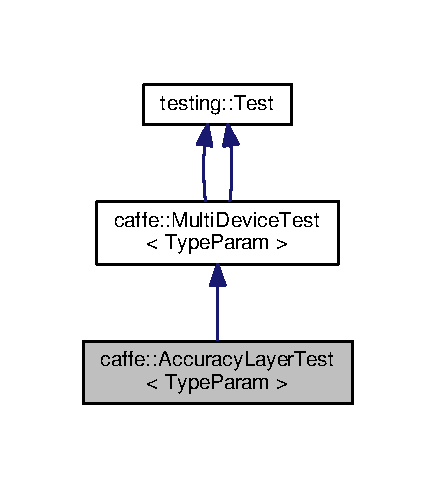
\includegraphics[width=209pt]{classcaffe_1_1_accuracy_layer_test__inherit__graph}
\end{center}
\end{figure}
\subsection*{Protected Member Functions}
\begin{DoxyCompactItemize}
\item 
\mbox{\Hypertarget{classcaffe_1_1_accuracy_layer_test_af83eff77a67c679e8bef7ad5aef64cb9}\label{classcaffe_1_1_accuracy_layer_test_af83eff77a67c679e8bef7ad5aef64cb9}} 
virtual void {\bfseries Fill\+Bottoms} ()
\end{DoxyCompactItemize}
\subsection*{Protected Attributes}
\begin{DoxyCompactItemize}
\item 
\mbox{\Hypertarget{classcaffe_1_1_accuracy_layer_test_af399b929ca86558895d62c68b0dc8c49}\label{classcaffe_1_1_accuracy_layer_test_af399b929ca86558895d62c68b0dc8c49}} 
\mbox{\hyperlink{classcaffe_1_1_blob}{Blob}}$<$ Dtype $>$ $\ast$const {\bfseries blob\+\_\+bottom\+\_\+data\+\_\+}
\item 
\mbox{\Hypertarget{classcaffe_1_1_accuracy_layer_test_a37a8484fffa29f6ed07fd2b6d9755e5b}\label{classcaffe_1_1_accuracy_layer_test_a37a8484fffa29f6ed07fd2b6d9755e5b}} 
\mbox{\hyperlink{classcaffe_1_1_blob}{Blob}}$<$ Dtype $>$ $\ast$const {\bfseries blob\+\_\+bottom\+\_\+label\+\_\+}
\item 
\mbox{\Hypertarget{classcaffe_1_1_accuracy_layer_test_a0efe92c5ee1d7911d11d1b909afb4bd0}\label{classcaffe_1_1_accuracy_layer_test_a0efe92c5ee1d7911d11d1b909afb4bd0}} 
\mbox{\hyperlink{classcaffe_1_1_blob}{Blob}}$<$ Dtype $>$ $\ast$const {\bfseries blob\+\_\+top\+\_\+}
\item 
\mbox{\Hypertarget{classcaffe_1_1_accuracy_layer_test_a73dc5bcbbd41a5dad5f9a6c7dfd495ac}\label{classcaffe_1_1_accuracy_layer_test_a73dc5bcbbd41a5dad5f9a6c7dfd495ac}} 
\mbox{\hyperlink{classcaffe_1_1_blob}{Blob}}$<$ Dtype $>$ $\ast$const {\bfseries blob\+\_\+top\+\_\+per\+\_\+class\+\_\+}
\item 
\mbox{\Hypertarget{classcaffe_1_1_accuracy_layer_test_a0758cd929b32853d47093d874249fd76}\label{classcaffe_1_1_accuracy_layer_test_a0758cd929b32853d47093d874249fd76}} 
vector$<$ \mbox{\hyperlink{classcaffe_1_1_blob}{Blob}}$<$ Dtype $>$ $\ast$ $>$ {\bfseries blob\+\_\+bottom\+\_\+vec\+\_\+}
\item 
\mbox{\Hypertarget{classcaffe_1_1_accuracy_layer_test_a0e5fdcee8912189dc24e9c611dfa2e49}\label{classcaffe_1_1_accuracy_layer_test_a0e5fdcee8912189dc24e9c611dfa2e49}} 
vector$<$ \mbox{\hyperlink{classcaffe_1_1_blob}{Blob}}$<$ Dtype $>$ $\ast$ $>$ {\bfseries blob\+\_\+top\+\_\+vec\+\_\+}
\item 
\mbox{\Hypertarget{classcaffe_1_1_accuracy_layer_test_af35a94a6056c736ea7b15ec735497f71}\label{classcaffe_1_1_accuracy_layer_test_af35a94a6056c736ea7b15ec735497f71}} 
vector$<$ \mbox{\hyperlink{classcaffe_1_1_blob}{Blob}}$<$ Dtype $>$ $\ast$ $>$ {\bfseries blob\+\_\+top\+\_\+per\+\_\+class\+\_\+vec\+\_\+}
\item 
\mbox{\Hypertarget{classcaffe_1_1_accuracy_layer_test_a0581566a8f94f64752e24faa4043095e}\label{classcaffe_1_1_accuracy_layer_test_a0581566a8f94f64752e24faa4043095e}} 
int {\bfseries top\+\_\+k\+\_\+}
\end{DoxyCompactItemize}
\subsection*{Additional Inherited Members}


The documentation for this class was generated from the following file\+:\begin{DoxyCompactItemize}
\item 
src/caffe/test/test\+\_\+accuracy\+\_\+layer.\+cpp\end{DoxyCompactItemize}

\hypertarget{classcaffe_1_1_accuracy_parameter}{}\section{caffe\+:\+:Accuracy\+Parameter Class Reference}
\label{classcaffe_1_1_accuracy_parameter}\index{caffe\+::\+Accuracy\+Parameter@{caffe\+::\+Accuracy\+Parameter}}


Inheritance diagram for caffe\+:\+:Accuracy\+Parameter\+:
\nopagebreak
\begin{figure}[H]
\begin{center}
\leavevmode
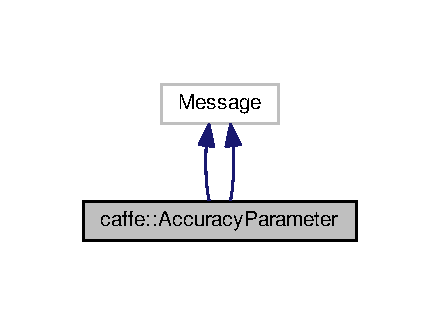
\includegraphics[width=211pt]{classcaffe_1_1_accuracy_parameter__inherit__graph}
\end{center}
\end{figure}
\subsection*{Public Member Functions}
\begin{DoxyCompactItemize}
\item 
\mbox{\Hypertarget{classcaffe_1_1_accuracy_parameter_a48beee3ea0844f7b3de5691fdd5bcba5}\label{classcaffe_1_1_accuracy_parameter_a48beee3ea0844f7b3de5691fdd5bcba5}} 
{\bfseries Accuracy\+Parameter} (const \mbox{\hyperlink{classcaffe_1_1_accuracy_parameter}{Accuracy\+Parameter}} \&from)
\item 
\mbox{\Hypertarget{classcaffe_1_1_accuracy_parameter_abf1de9917962ffdec97ffdfa728ad31e}\label{classcaffe_1_1_accuracy_parameter_abf1de9917962ffdec97ffdfa728ad31e}} 
\mbox{\hyperlink{classcaffe_1_1_accuracy_parameter}{Accuracy\+Parameter}} \& {\bfseries operator=} (const \mbox{\hyperlink{classcaffe_1_1_accuracy_parameter}{Accuracy\+Parameter}} \&from)
\item 
\mbox{\Hypertarget{classcaffe_1_1_accuracy_parameter_a7d56021534e1a95134749e993e854776}\label{classcaffe_1_1_accuracy_parameter_a7d56021534e1a95134749e993e854776}} 
const \+::google\+::protobuf\+::\+Unknown\+Field\+Set \& {\bfseries unknown\+\_\+fields} () const
\item 
\mbox{\Hypertarget{classcaffe_1_1_accuracy_parameter_a21fb04e8e6029a2ea0563c53b7b22467}\label{classcaffe_1_1_accuracy_parameter_a21fb04e8e6029a2ea0563c53b7b22467}} 
inline \+::google\+::protobuf\+::\+Unknown\+Field\+Set $\ast$ {\bfseries mutable\+\_\+unknown\+\_\+fields} ()
\item 
\mbox{\Hypertarget{classcaffe_1_1_accuracy_parameter_a7f28ff8d7ad5eeaa5dd3473f6a38b4be}\label{classcaffe_1_1_accuracy_parameter_a7f28ff8d7ad5eeaa5dd3473f6a38b4be}} 
void {\bfseries Swap} (\mbox{\hyperlink{classcaffe_1_1_accuracy_parameter}{Accuracy\+Parameter}} $\ast$other)
\item 
\mbox{\Hypertarget{classcaffe_1_1_accuracy_parameter_aceead5833a0dca16b8734b0800316a20}\label{classcaffe_1_1_accuracy_parameter_aceead5833a0dca16b8734b0800316a20}} 
\mbox{\hyperlink{classcaffe_1_1_accuracy_parameter}{Accuracy\+Parameter}} $\ast$ {\bfseries New} () const
\item 
\mbox{\Hypertarget{classcaffe_1_1_accuracy_parameter_a408ec5c7e2f3983e57a766f361381e2e}\label{classcaffe_1_1_accuracy_parameter_a408ec5c7e2f3983e57a766f361381e2e}} 
void {\bfseries Copy\+From} (const \+::google\+::protobuf\+::\+Message \&from)
\item 
\mbox{\Hypertarget{classcaffe_1_1_accuracy_parameter_a8450a78d36eff284587e92567da36ed6}\label{classcaffe_1_1_accuracy_parameter_a8450a78d36eff284587e92567da36ed6}} 
void {\bfseries Merge\+From} (const \+::google\+::protobuf\+::\+Message \&from)
\item 
\mbox{\Hypertarget{classcaffe_1_1_accuracy_parameter_acc2fd487a271b0f706f4e8d69ffcee2f}\label{classcaffe_1_1_accuracy_parameter_acc2fd487a271b0f706f4e8d69ffcee2f}} 
void {\bfseries Copy\+From} (const \mbox{\hyperlink{classcaffe_1_1_accuracy_parameter}{Accuracy\+Parameter}} \&from)
\item 
\mbox{\Hypertarget{classcaffe_1_1_accuracy_parameter_a3b08be88b78c1291a09c86d1193b34c4}\label{classcaffe_1_1_accuracy_parameter_a3b08be88b78c1291a09c86d1193b34c4}} 
void {\bfseries Merge\+From} (const \mbox{\hyperlink{classcaffe_1_1_accuracy_parameter}{Accuracy\+Parameter}} \&from)
\item 
\mbox{\Hypertarget{classcaffe_1_1_accuracy_parameter_a057b92b65e706d5093dce1b0b00b9dcf}\label{classcaffe_1_1_accuracy_parameter_a057b92b65e706d5093dce1b0b00b9dcf}} 
void {\bfseries Clear} ()
\item 
\mbox{\Hypertarget{classcaffe_1_1_accuracy_parameter_a806a21aa5524abf91b98aa7bdc1e4aaf}\label{classcaffe_1_1_accuracy_parameter_a806a21aa5524abf91b98aa7bdc1e4aaf}} 
bool {\bfseries Is\+Initialized} () const
\item 
\mbox{\Hypertarget{classcaffe_1_1_accuracy_parameter_ae5a7598273761de8de02b5b52443c7a1}\label{classcaffe_1_1_accuracy_parameter_ae5a7598273761de8de02b5b52443c7a1}} 
int {\bfseries Byte\+Size} () const
\item 
\mbox{\Hypertarget{classcaffe_1_1_accuracy_parameter_ae00aba2c2364902786f84aa69861e7c8}\label{classcaffe_1_1_accuracy_parameter_ae00aba2c2364902786f84aa69861e7c8}} 
bool {\bfseries Merge\+Partial\+From\+Coded\+Stream} (\+::google\+::protobuf\+::io\+::\+Coded\+Input\+Stream $\ast$input)
\item 
\mbox{\Hypertarget{classcaffe_1_1_accuracy_parameter_a25be52c598347ec246c7047a0b3c269b}\label{classcaffe_1_1_accuracy_parameter_a25be52c598347ec246c7047a0b3c269b}} 
void {\bfseries Serialize\+With\+Cached\+Sizes} (\+::google\+::protobuf\+::io\+::\+Coded\+Output\+Stream $\ast$output) const
\item 
\mbox{\Hypertarget{classcaffe_1_1_accuracy_parameter_a5176531c53bfe95651e5cd7a8ab62035}\label{classcaffe_1_1_accuracy_parameter_a5176531c53bfe95651e5cd7a8ab62035}} 
\+::google\+::protobuf\+::uint8 $\ast$ {\bfseries Serialize\+With\+Cached\+Sizes\+To\+Array} (\+::google\+::protobuf\+::uint8 $\ast$output) const
\item 
\mbox{\Hypertarget{classcaffe_1_1_accuracy_parameter_ae0b9fea0e9aa03d519bb1654ad54c1c1}\label{classcaffe_1_1_accuracy_parameter_ae0b9fea0e9aa03d519bb1654ad54c1c1}} 
int {\bfseries Get\+Cached\+Size} () const
\item 
\mbox{\Hypertarget{classcaffe_1_1_accuracy_parameter_ac403788ed6f41ad7a0a75d153f09fca4}\label{classcaffe_1_1_accuracy_parameter_ac403788ed6f41ad7a0a75d153f09fca4}} 
\+::google\+::protobuf\+::\+Metadata {\bfseries Get\+Metadata} () const
\item 
\mbox{\Hypertarget{classcaffe_1_1_accuracy_parameter_a034b1d69865519417b9fa6534a264dfa}\label{classcaffe_1_1_accuracy_parameter_a034b1d69865519417b9fa6534a264dfa}} 
bool {\bfseries has\+\_\+top\+\_\+k} () const
\item 
\mbox{\Hypertarget{classcaffe_1_1_accuracy_parameter_a659dc57a34f9b26e599cf041833ec4d1}\label{classcaffe_1_1_accuracy_parameter_a659dc57a34f9b26e599cf041833ec4d1}} 
void {\bfseries clear\+\_\+top\+\_\+k} ()
\item 
\mbox{\Hypertarget{classcaffe_1_1_accuracy_parameter_ae9de6bfe0a9acd909a22229efa9f7e7a}\label{classcaffe_1_1_accuracy_parameter_ae9de6bfe0a9acd909a22229efa9f7e7a}} 
inline \+::google\+::protobuf\+::uint32 {\bfseries top\+\_\+k} () const
\item 
\mbox{\Hypertarget{classcaffe_1_1_accuracy_parameter_a25149405c0d5fee19a1404afaa47654e}\label{classcaffe_1_1_accuracy_parameter_a25149405c0d5fee19a1404afaa47654e}} 
void {\bfseries set\+\_\+top\+\_\+k} (\+::google\+::protobuf\+::uint32 value)
\item 
\mbox{\Hypertarget{classcaffe_1_1_accuracy_parameter_a84e5b49612aabae7690be7c0247569f6}\label{classcaffe_1_1_accuracy_parameter_a84e5b49612aabae7690be7c0247569f6}} 
bool {\bfseries has\+\_\+axis} () const
\item 
\mbox{\Hypertarget{classcaffe_1_1_accuracy_parameter_a95eca7283e9b348e3d56ce6072f62393}\label{classcaffe_1_1_accuracy_parameter_a95eca7283e9b348e3d56ce6072f62393}} 
void {\bfseries clear\+\_\+axis} ()
\item 
\mbox{\Hypertarget{classcaffe_1_1_accuracy_parameter_afffd2a5c1b12db5ffaf33456de54e47d}\label{classcaffe_1_1_accuracy_parameter_afffd2a5c1b12db5ffaf33456de54e47d}} 
inline \+::google\+::protobuf\+::int32 {\bfseries axis} () const
\item 
\mbox{\Hypertarget{classcaffe_1_1_accuracy_parameter_a0f542225dcb4daf0f9a242bcffa10fb8}\label{classcaffe_1_1_accuracy_parameter_a0f542225dcb4daf0f9a242bcffa10fb8}} 
void {\bfseries set\+\_\+axis} (\+::google\+::protobuf\+::int32 value)
\item 
\mbox{\Hypertarget{classcaffe_1_1_accuracy_parameter_a9eaf83ec6f7c896ca6c3c1635bce2a9c}\label{classcaffe_1_1_accuracy_parameter_a9eaf83ec6f7c896ca6c3c1635bce2a9c}} 
bool {\bfseries has\+\_\+ignore\+\_\+label} () const
\item 
\mbox{\Hypertarget{classcaffe_1_1_accuracy_parameter_a8a65d59e56d203eaa0f9eca95a6e6047}\label{classcaffe_1_1_accuracy_parameter_a8a65d59e56d203eaa0f9eca95a6e6047}} 
void {\bfseries clear\+\_\+ignore\+\_\+label} ()
\item 
\mbox{\Hypertarget{classcaffe_1_1_accuracy_parameter_a019b3dd490b4a03b930a997de40b2ab7}\label{classcaffe_1_1_accuracy_parameter_a019b3dd490b4a03b930a997de40b2ab7}} 
inline \+::google\+::protobuf\+::int32 {\bfseries ignore\+\_\+label} () const
\item 
\mbox{\Hypertarget{classcaffe_1_1_accuracy_parameter_ad717ca695cbf95e5a41787a14a4b5377}\label{classcaffe_1_1_accuracy_parameter_ad717ca695cbf95e5a41787a14a4b5377}} 
void {\bfseries set\+\_\+ignore\+\_\+label} (\+::google\+::protobuf\+::int32 value)
\item 
\mbox{\Hypertarget{classcaffe_1_1_accuracy_parameter_a48beee3ea0844f7b3de5691fdd5bcba5}\label{classcaffe_1_1_accuracy_parameter_a48beee3ea0844f7b3de5691fdd5bcba5}} 
{\bfseries Accuracy\+Parameter} (const \mbox{\hyperlink{classcaffe_1_1_accuracy_parameter}{Accuracy\+Parameter}} \&from)
\item 
\mbox{\Hypertarget{classcaffe_1_1_accuracy_parameter_abf1de9917962ffdec97ffdfa728ad31e}\label{classcaffe_1_1_accuracy_parameter_abf1de9917962ffdec97ffdfa728ad31e}} 
\mbox{\hyperlink{classcaffe_1_1_accuracy_parameter}{Accuracy\+Parameter}} \& {\bfseries operator=} (const \mbox{\hyperlink{classcaffe_1_1_accuracy_parameter}{Accuracy\+Parameter}} \&from)
\item 
\mbox{\Hypertarget{classcaffe_1_1_accuracy_parameter_a7d56021534e1a95134749e993e854776}\label{classcaffe_1_1_accuracy_parameter_a7d56021534e1a95134749e993e854776}} 
const \+::google\+::protobuf\+::\+Unknown\+Field\+Set \& {\bfseries unknown\+\_\+fields} () const
\item 
\mbox{\Hypertarget{classcaffe_1_1_accuracy_parameter_a21fb04e8e6029a2ea0563c53b7b22467}\label{classcaffe_1_1_accuracy_parameter_a21fb04e8e6029a2ea0563c53b7b22467}} 
inline \+::google\+::protobuf\+::\+Unknown\+Field\+Set $\ast$ {\bfseries mutable\+\_\+unknown\+\_\+fields} ()
\item 
\mbox{\Hypertarget{classcaffe_1_1_accuracy_parameter_a7f28ff8d7ad5eeaa5dd3473f6a38b4be}\label{classcaffe_1_1_accuracy_parameter_a7f28ff8d7ad5eeaa5dd3473f6a38b4be}} 
void {\bfseries Swap} (\mbox{\hyperlink{classcaffe_1_1_accuracy_parameter}{Accuracy\+Parameter}} $\ast$other)
\item 
\mbox{\Hypertarget{classcaffe_1_1_accuracy_parameter_aeffd2d228209e319619318e6f84efd1d}\label{classcaffe_1_1_accuracy_parameter_aeffd2d228209e319619318e6f84efd1d}} 
\mbox{\hyperlink{classcaffe_1_1_accuracy_parameter}{Accuracy\+Parameter}} $\ast$ {\bfseries New} () const
\item 
\mbox{\Hypertarget{classcaffe_1_1_accuracy_parameter_a408ec5c7e2f3983e57a766f361381e2e}\label{classcaffe_1_1_accuracy_parameter_a408ec5c7e2f3983e57a766f361381e2e}} 
void {\bfseries Copy\+From} (const \+::google\+::protobuf\+::\+Message \&from)
\item 
\mbox{\Hypertarget{classcaffe_1_1_accuracy_parameter_a8450a78d36eff284587e92567da36ed6}\label{classcaffe_1_1_accuracy_parameter_a8450a78d36eff284587e92567da36ed6}} 
void {\bfseries Merge\+From} (const \+::google\+::protobuf\+::\+Message \&from)
\item 
\mbox{\Hypertarget{classcaffe_1_1_accuracy_parameter_acc2fd487a271b0f706f4e8d69ffcee2f}\label{classcaffe_1_1_accuracy_parameter_acc2fd487a271b0f706f4e8d69ffcee2f}} 
void {\bfseries Copy\+From} (const \mbox{\hyperlink{classcaffe_1_1_accuracy_parameter}{Accuracy\+Parameter}} \&from)
\item 
\mbox{\Hypertarget{classcaffe_1_1_accuracy_parameter_a3b08be88b78c1291a09c86d1193b34c4}\label{classcaffe_1_1_accuracy_parameter_a3b08be88b78c1291a09c86d1193b34c4}} 
void {\bfseries Merge\+From} (const \mbox{\hyperlink{classcaffe_1_1_accuracy_parameter}{Accuracy\+Parameter}} \&from)
\item 
\mbox{\Hypertarget{classcaffe_1_1_accuracy_parameter_a057b92b65e706d5093dce1b0b00b9dcf}\label{classcaffe_1_1_accuracy_parameter_a057b92b65e706d5093dce1b0b00b9dcf}} 
void {\bfseries Clear} ()
\item 
\mbox{\Hypertarget{classcaffe_1_1_accuracy_parameter_a806a21aa5524abf91b98aa7bdc1e4aaf}\label{classcaffe_1_1_accuracy_parameter_a806a21aa5524abf91b98aa7bdc1e4aaf}} 
bool {\bfseries Is\+Initialized} () const
\item 
\mbox{\Hypertarget{classcaffe_1_1_accuracy_parameter_ae5a7598273761de8de02b5b52443c7a1}\label{classcaffe_1_1_accuracy_parameter_ae5a7598273761de8de02b5b52443c7a1}} 
int {\bfseries Byte\+Size} () const
\item 
\mbox{\Hypertarget{classcaffe_1_1_accuracy_parameter_ae00aba2c2364902786f84aa69861e7c8}\label{classcaffe_1_1_accuracy_parameter_ae00aba2c2364902786f84aa69861e7c8}} 
bool {\bfseries Merge\+Partial\+From\+Coded\+Stream} (\+::google\+::protobuf\+::io\+::\+Coded\+Input\+Stream $\ast$input)
\item 
\mbox{\Hypertarget{classcaffe_1_1_accuracy_parameter_a25be52c598347ec246c7047a0b3c269b}\label{classcaffe_1_1_accuracy_parameter_a25be52c598347ec246c7047a0b3c269b}} 
void {\bfseries Serialize\+With\+Cached\+Sizes} (\+::google\+::protobuf\+::io\+::\+Coded\+Output\+Stream $\ast$output) const
\item 
\mbox{\Hypertarget{classcaffe_1_1_accuracy_parameter_a49d1a7b5e3eaea4588abeb0872711498}\label{classcaffe_1_1_accuracy_parameter_a49d1a7b5e3eaea4588abeb0872711498}} 
\+::google\+::protobuf\+::uint8 $\ast$ {\bfseries Serialize\+With\+Cached\+Sizes\+To\+Array} (\+::google\+::protobuf\+::uint8 $\ast$output) const
\item 
\mbox{\Hypertarget{classcaffe_1_1_accuracy_parameter_ae0b9fea0e9aa03d519bb1654ad54c1c1}\label{classcaffe_1_1_accuracy_parameter_ae0b9fea0e9aa03d519bb1654ad54c1c1}} 
int {\bfseries Get\+Cached\+Size} () const
\item 
\mbox{\Hypertarget{classcaffe_1_1_accuracy_parameter_a5a02d19e03ed3b8cdc9623da8376e13d}\label{classcaffe_1_1_accuracy_parameter_a5a02d19e03ed3b8cdc9623da8376e13d}} 
\+::google\+::protobuf\+::\+Metadata {\bfseries Get\+Metadata} () const
\item 
\mbox{\Hypertarget{classcaffe_1_1_accuracy_parameter_a034b1d69865519417b9fa6534a264dfa}\label{classcaffe_1_1_accuracy_parameter_a034b1d69865519417b9fa6534a264dfa}} 
bool {\bfseries has\+\_\+top\+\_\+k} () const
\item 
\mbox{\Hypertarget{classcaffe_1_1_accuracy_parameter_a659dc57a34f9b26e599cf041833ec4d1}\label{classcaffe_1_1_accuracy_parameter_a659dc57a34f9b26e599cf041833ec4d1}} 
void {\bfseries clear\+\_\+top\+\_\+k} ()
\item 
\mbox{\Hypertarget{classcaffe_1_1_accuracy_parameter_a63e246a3ddf6f4ec24868334e92fff8d}\label{classcaffe_1_1_accuracy_parameter_a63e246a3ddf6f4ec24868334e92fff8d}} 
inline \+::google\+::protobuf\+::uint32 {\bfseries top\+\_\+k} () const
\item 
\mbox{\Hypertarget{classcaffe_1_1_accuracy_parameter_a25149405c0d5fee19a1404afaa47654e}\label{classcaffe_1_1_accuracy_parameter_a25149405c0d5fee19a1404afaa47654e}} 
void {\bfseries set\+\_\+top\+\_\+k} (\+::google\+::protobuf\+::uint32 value)
\item 
\mbox{\Hypertarget{classcaffe_1_1_accuracy_parameter_a84e5b49612aabae7690be7c0247569f6}\label{classcaffe_1_1_accuracy_parameter_a84e5b49612aabae7690be7c0247569f6}} 
bool {\bfseries has\+\_\+axis} () const
\item 
\mbox{\Hypertarget{classcaffe_1_1_accuracy_parameter_a95eca7283e9b348e3d56ce6072f62393}\label{classcaffe_1_1_accuracy_parameter_a95eca7283e9b348e3d56ce6072f62393}} 
void {\bfseries clear\+\_\+axis} ()
\item 
\mbox{\Hypertarget{classcaffe_1_1_accuracy_parameter_a4b9231676c5d221cbd647455f887b91a}\label{classcaffe_1_1_accuracy_parameter_a4b9231676c5d221cbd647455f887b91a}} 
inline \+::google\+::protobuf\+::int32 {\bfseries axis} () const
\item 
\mbox{\Hypertarget{classcaffe_1_1_accuracy_parameter_a0f542225dcb4daf0f9a242bcffa10fb8}\label{classcaffe_1_1_accuracy_parameter_a0f542225dcb4daf0f9a242bcffa10fb8}} 
void {\bfseries set\+\_\+axis} (\+::google\+::protobuf\+::int32 value)
\item 
\mbox{\Hypertarget{classcaffe_1_1_accuracy_parameter_a9eaf83ec6f7c896ca6c3c1635bce2a9c}\label{classcaffe_1_1_accuracy_parameter_a9eaf83ec6f7c896ca6c3c1635bce2a9c}} 
bool {\bfseries has\+\_\+ignore\+\_\+label} () const
\item 
\mbox{\Hypertarget{classcaffe_1_1_accuracy_parameter_a8a65d59e56d203eaa0f9eca95a6e6047}\label{classcaffe_1_1_accuracy_parameter_a8a65d59e56d203eaa0f9eca95a6e6047}} 
void {\bfseries clear\+\_\+ignore\+\_\+label} ()
\item 
\mbox{\Hypertarget{classcaffe_1_1_accuracy_parameter_a16947ae71e97c3c294d74a690a594d09}\label{classcaffe_1_1_accuracy_parameter_a16947ae71e97c3c294d74a690a594d09}} 
inline \+::google\+::protobuf\+::int32 {\bfseries ignore\+\_\+label} () const
\item 
\mbox{\Hypertarget{classcaffe_1_1_accuracy_parameter_ad717ca695cbf95e5a41787a14a4b5377}\label{classcaffe_1_1_accuracy_parameter_ad717ca695cbf95e5a41787a14a4b5377}} 
void {\bfseries set\+\_\+ignore\+\_\+label} (\+::google\+::protobuf\+::int32 value)
\end{DoxyCompactItemize}
\subsection*{Static Public Member Functions}
\begin{DoxyCompactItemize}
\item 
\mbox{\Hypertarget{classcaffe_1_1_accuracy_parameter_a70447a517086ded4794dd3d428e35abf}\label{classcaffe_1_1_accuracy_parameter_a70447a517086ded4794dd3d428e35abf}} 
static const \+::google\+::protobuf\+::\+Descriptor $\ast$ {\bfseries descriptor} ()
\item 
\mbox{\Hypertarget{classcaffe_1_1_accuracy_parameter_a9cf268b0327240b00e5eb8d89e680e6e}\label{classcaffe_1_1_accuracy_parameter_a9cf268b0327240b00e5eb8d89e680e6e}} 
static const \mbox{\hyperlink{classcaffe_1_1_accuracy_parameter}{Accuracy\+Parameter}} \& {\bfseries default\+\_\+instance} ()
\item 
\mbox{\Hypertarget{classcaffe_1_1_accuracy_parameter_a18babdbe5486fcd105679296d5cb1095}\label{classcaffe_1_1_accuracy_parameter_a18babdbe5486fcd105679296d5cb1095}} 
static const \+::google\+::protobuf\+::\+Descriptor $\ast$ {\bfseries descriptor} ()
\item 
\mbox{\Hypertarget{classcaffe_1_1_accuracy_parameter_a458c386c082dbd633cb22ddbec4841fa}\label{classcaffe_1_1_accuracy_parameter_a458c386c082dbd633cb22ddbec4841fa}} 
static const \mbox{\hyperlink{classcaffe_1_1_accuracy_parameter}{Accuracy\+Parameter}} \& {\bfseries default\+\_\+instance} ()
\end{DoxyCompactItemize}
\subsection*{Static Public Attributes}
\begin{DoxyCompactItemize}
\item 
\mbox{\Hypertarget{classcaffe_1_1_accuracy_parameter_ac2d62e5614c2adfdf8f1606caf1b8d58}\label{classcaffe_1_1_accuracy_parameter_ac2d62e5614c2adfdf8f1606caf1b8d58}} 
static const int {\bfseries k\+Top\+K\+Field\+Number} = 1
\item 
\mbox{\Hypertarget{classcaffe_1_1_accuracy_parameter_aec57c1f67e5b2f71895b41aa647f5a19}\label{classcaffe_1_1_accuracy_parameter_aec57c1f67e5b2f71895b41aa647f5a19}} 
static const int {\bfseries k\+Axis\+Field\+Number} = 2
\item 
\mbox{\Hypertarget{classcaffe_1_1_accuracy_parameter_a998525a6c23efc1f38eb85a645627880}\label{classcaffe_1_1_accuracy_parameter_a998525a6c23efc1f38eb85a645627880}} 
static const int {\bfseries k\+Ignore\+Label\+Field\+Number} = 3
\end{DoxyCompactItemize}
\subsection*{Friends}
\begin{DoxyCompactItemize}
\item 
\mbox{\Hypertarget{classcaffe_1_1_accuracy_parameter_a2670a9c8ffd0e5105cf7522cd6f8613d}\label{classcaffe_1_1_accuracy_parameter_a2670a9c8ffd0e5105cf7522cd6f8613d}} 
void {\bfseries protobuf\+\_\+\+Add\+Desc\+\_\+caffe\+\_\+2eproto} ()
\item 
\mbox{\Hypertarget{classcaffe_1_1_accuracy_parameter_a7f145bddbdde78003d27e42c7e003d23}\label{classcaffe_1_1_accuracy_parameter_a7f145bddbdde78003d27e42c7e003d23}} 
void {\bfseries protobuf\+\_\+\+Assign\+Desc\+\_\+caffe\+\_\+2eproto} ()
\item 
\mbox{\Hypertarget{classcaffe_1_1_accuracy_parameter_a026784a8e4e76f1b4daf9d033d2ece83}\label{classcaffe_1_1_accuracy_parameter_a026784a8e4e76f1b4daf9d033d2ece83}} 
void {\bfseries protobuf\+\_\+\+Shutdown\+File\+\_\+caffe\+\_\+2eproto} ()
\item 
\mbox{\Hypertarget{classcaffe_1_1_accuracy_parameter_a2670a9c8ffd0e5105cf7522cd6f8613d}\label{classcaffe_1_1_accuracy_parameter_a2670a9c8ffd0e5105cf7522cd6f8613d}} 
void {\bfseries protobuf\+\_\+\+Add\+Desc\+\_\+caffe\+\_\+2eproto} ()
\item 
\mbox{\Hypertarget{classcaffe_1_1_accuracy_parameter_a7f145bddbdde78003d27e42c7e003d23}\label{classcaffe_1_1_accuracy_parameter_a7f145bddbdde78003d27e42c7e003d23}} 
void {\bfseries protobuf\+\_\+\+Assign\+Desc\+\_\+caffe\+\_\+2eproto} ()
\item 
\mbox{\Hypertarget{classcaffe_1_1_accuracy_parameter_a026784a8e4e76f1b4daf9d033d2ece83}\label{classcaffe_1_1_accuracy_parameter_a026784a8e4e76f1b4daf9d033d2ece83}} 
void {\bfseries protobuf\+\_\+\+Shutdown\+File\+\_\+caffe\+\_\+2eproto} ()
\end{DoxyCompactItemize}


The documentation for this class was generated from the following files\+:\begin{DoxyCompactItemize}
\item 
build/include/caffe/proto/caffe.\+pb.\+h\item 
build/include/caffe/proto/caffe.\+pb.\+cc\end{DoxyCompactItemize}

\hypertarget{classcaffe_1_1_ada_delta_solver}{}\section{caffe\+:\+:Ada\+Delta\+Solver$<$ Dtype $>$ Class Template Reference}
\label{classcaffe_1_1_ada_delta_solver}\index{caffe\+::\+Ada\+Delta\+Solver$<$ Dtype $>$@{caffe\+::\+Ada\+Delta\+Solver$<$ Dtype $>$}}


Inheritance diagram for caffe\+:\+:Ada\+Delta\+Solver$<$ Dtype $>$\+:
\nopagebreak
\begin{figure}[H]
\begin{center}
\leavevmode
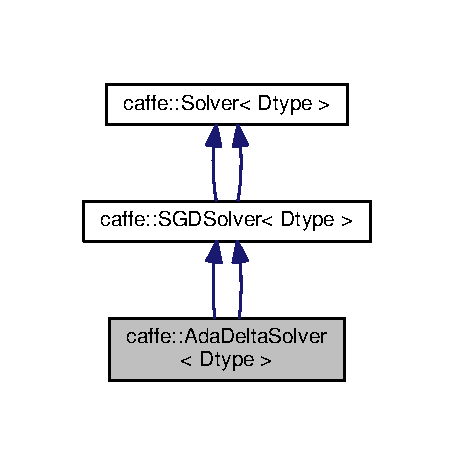
\includegraphics[width=218pt]{classcaffe_1_1_ada_delta_solver__inherit__graph}
\end{center}
\end{figure}
\subsection*{Public Member Functions}
\begin{DoxyCompactItemize}
\item 
\mbox{\Hypertarget{classcaffe_1_1_ada_delta_solver_ad6f176b0beaa4a41d111f2c10a35b2f5}\label{classcaffe_1_1_ada_delta_solver_ad6f176b0beaa4a41d111f2c10a35b2f5}} 
{\bfseries Ada\+Delta\+Solver} (const \mbox{\hyperlink{classcaffe_1_1_solver_parameter}{Solver\+Parameter}} \&param)
\item 
\mbox{\Hypertarget{classcaffe_1_1_ada_delta_solver_adba552de0f9aa7e165cca5919d69cc09}\label{classcaffe_1_1_ada_delta_solver_adba552de0f9aa7e165cca5919d69cc09}} 
{\bfseries Ada\+Delta\+Solver} (const string \&param\+\_\+file)
\item 
\mbox{\Hypertarget{classcaffe_1_1_ada_delta_solver_a645d215770c417a00f9d38482adb2ec0}\label{classcaffe_1_1_ada_delta_solver_a645d215770c417a00f9d38482adb2ec0}} 
virtual const char $\ast$ \mbox{\hyperlink{classcaffe_1_1_ada_delta_solver_a645d215770c417a00f9d38482adb2ec0}{type}} () const
\begin{DoxyCompactList}\small\item\em Returns the solver type. \end{DoxyCompactList}\item 
\mbox{\Hypertarget{classcaffe_1_1_ada_delta_solver_ad6f176b0beaa4a41d111f2c10a35b2f5}\label{classcaffe_1_1_ada_delta_solver_ad6f176b0beaa4a41d111f2c10a35b2f5}} 
{\bfseries Ada\+Delta\+Solver} (const \mbox{\hyperlink{classcaffe_1_1_solver_parameter}{Solver\+Parameter}} \&param)
\item 
\mbox{\Hypertarget{classcaffe_1_1_ada_delta_solver_adba552de0f9aa7e165cca5919d69cc09}\label{classcaffe_1_1_ada_delta_solver_adba552de0f9aa7e165cca5919d69cc09}} 
{\bfseries Ada\+Delta\+Solver} (const string \&param\+\_\+file)
\item 
\mbox{\Hypertarget{classcaffe_1_1_ada_delta_solver_a645d215770c417a00f9d38482adb2ec0}\label{classcaffe_1_1_ada_delta_solver_a645d215770c417a00f9d38482adb2ec0}} 
virtual const char $\ast$ \mbox{\hyperlink{classcaffe_1_1_ada_delta_solver_a645d215770c417a00f9d38482adb2ec0}{type}} () const
\begin{DoxyCompactList}\small\item\em Returns the solver type. \end{DoxyCompactList}\end{DoxyCompactItemize}
\subsection*{Protected Member Functions}
\begin{DoxyCompactItemize}
\item 
\mbox{\Hypertarget{classcaffe_1_1_ada_delta_solver_a5aae9f8d57714dd41e92c7a285d31d0a}\label{classcaffe_1_1_ada_delta_solver_a5aae9f8d57714dd41e92c7a285d31d0a}} 
void {\bfseries Ada\+Delta\+Pre\+Solve} ()
\item 
\mbox{\Hypertarget{classcaffe_1_1_ada_delta_solver_aa3b649a03988cab462d411e26784f209}\label{classcaffe_1_1_ada_delta_solver_aa3b649a03988cab462d411e26784f209}} 
virtual void {\bfseries Compute\+Update\+Value} (int param\+\_\+id, Dtype rate)
\item 
\mbox{\Hypertarget{classcaffe_1_1_ada_delta_solver_ae1097650f9ae280b649d3b116c26152f}\label{classcaffe_1_1_ada_delta_solver_ae1097650f9ae280b649d3b116c26152f}} 
{\bfseries D\+I\+S\+A\+B\+L\+E\+\_\+\+C\+O\+P\+Y\+\_\+\+A\+N\+D\+\_\+\+A\+S\+S\+I\+GN} (\mbox{\hyperlink{classcaffe_1_1_ada_delta_solver}{Ada\+Delta\+Solver}})
\item 
\mbox{\Hypertarget{classcaffe_1_1_ada_delta_solver_a5aae9f8d57714dd41e92c7a285d31d0a}\label{classcaffe_1_1_ada_delta_solver_a5aae9f8d57714dd41e92c7a285d31d0a}} 
void {\bfseries Ada\+Delta\+Pre\+Solve} ()
\item 
\mbox{\Hypertarget{classcaffe_1_1_ada_delta_solver_a602d10a832c75519e81bd86d2153926e}\label{classcaffe_1_1_ada_delta_solver_a602d10a832c75519e81bd86d2153926e}} 
virtual void {\bfseries Compute\+Update\+Value} (int param\+\_\+id, Dtype rate)
\item 
\mbox{\Hypertarget{classcaffe_1_1_ada_delta_solver_ae1097650f9ae280b649d3b116c26152f}\label{classcaffe_1_1_ada_delta_solver_ae1097650f9ae280b649d3b116c26152f}} 
{\bfseries D\+I\+S\+A\+B\+L\+E\+\_\+\+C\+O\+P\+Y\+\_\+\+A\+N\+D\+\_\+\+A\+S\+S\+I\+GN} (\mbox{\hyperlink{classcaffe_1_1_ada_delta_solver}{Ada\+Delta\+Solver}})
\end{DoxyCompactItemize}
\subsection*{Additional Inherited Members}


The documentation for this class was generated from the following files\+:\begin{DoxyCompactItemize}
\item 
build/install/include/caffe/sgd\+\_\+solvers.\+hpp\item 
src/caffe/solvers/adadelta\+\_\+solver.\+cpp\end{DoxyCompactItemize}

\hypertarget{classcaffe_1_1_ada_delta_solver_test}{}\section{caffe\+:\+:Ada\+Delta\+Solver\+Test$<$ Type\+Param $>$ Class Template Reference}
\label{classcaffe_1_1_ada_delta_solver_test}\index{caffe\+::\+Ada\+Delta\+Solver\+Test$<$ Type\+Param $>$@{caffe\+::\+Ada\+Delta\+Solver\+Test$<$ Type\+Param $>$}}


Inheritance diagram for caffe\+:\+:Ada\+Delta\+Solver\+Test$<$ Type\+Param $>$\+:
\nopagebreak
\begin{figure}[H]
\begin{center}
\leavevmode
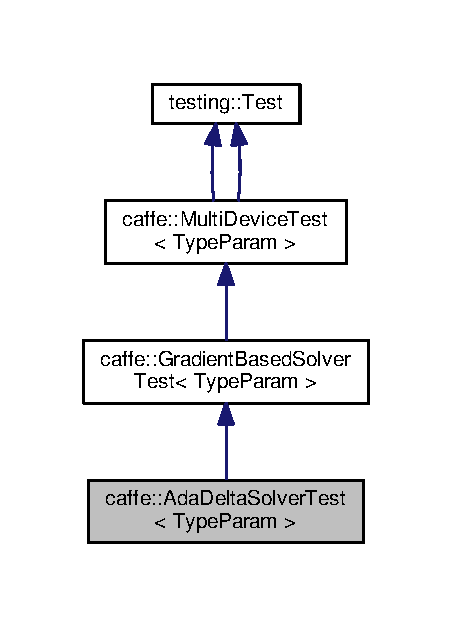
\includegraphics[width=217pt]{classcaffe_1_1_ada_delta_solver_test__inherit__graph}
\end{center}
\end{figure}
\subsection*{Protected Member Functions}
\begin{DoxyCompactItemize}
\item 
\mbox{\Hypertarget{classcaffe_1_1_ada_delta_solver_test_a1ba4566f9b5a7a299b7470f13d4bb0f0}\label{classcaffe_1_1_ada_delta_solver_test_a1ba4566f9b5a7a299b7470f13d4bb0f0}} 
virtual void {\bfseries Init\+Solver} (const \mbox{\hyperlink{classcaffe_1_1_solver_parameter}{Solver\+Parameter}} \&param)
\end{DoxyCompactItemize}
\subsection*{Additional Inherited Members}


The documentation for this class was generated from the following file\+:\begin{DoxyCompactItemize}
\item 
src/caffe/test/test\+\_\+gradient\+\_\+based\+\_\+solver.\+cpp\end{DoxyCompactItemize}

\hypertarget{classcaffe_1_1_ada_grad_solver}{}\section{caffe\+:\+:Ada\+Grad\+Solver$<$ Dtype $>$ Class Template Reference}
\label{classcaffe_1_1_ada_grad_solver}\index{caffe\+::\+Ada\+Grad\+Solver$<$ Dtype $>$@{caffe\+::\+Ada\+Grad\+Solver$<$ Dtype $>$}}


Inheritance diagram for caffe\+:\+:Ada\+Grad\+Solver$<$ Dtype $>$\+:
\nopagebreak
\begin{figure}[H]
\begin{center}
\leavevmode
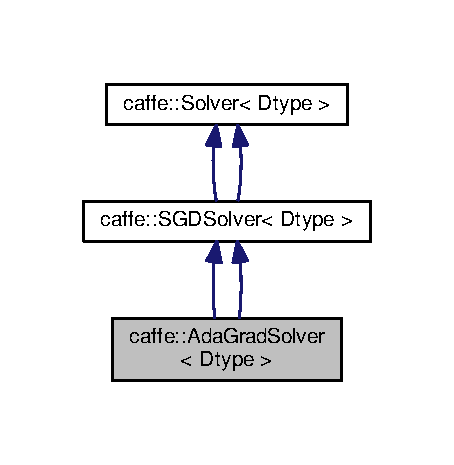
\includegraphics[width=218pt]{classcaffe_1_1_ada_grad_solver__inherit__graph}
\end{center}
\end{figure}
\subsection*{Public Member Functions}
\begin{DoxyCompactItemize}
\item 
\mbox{\Hypertarget{classcaffe_1_1_ada_grad_solver_acfa678395af17eb9cfcf21e8b9fe5ce9}\label{classcaffe_1_1_ada_grad_solver_acfa678395af17eb9cfcf21e8b9fe5ce9}} 
{\bfseries Ada\+Grad\+Solver} (const \mbox{\hyperlink{classcaffe_1_1_solver_parameter}{Solver\+Parameter}} \&param)
\item 
\mbox{\Hypertarget{classcaffe_1_1_ada_grad_solver_aca70c4ae0d471a6a2610d371e95f5ffa}\label{classcaffe_1_1_ada_grad_solver_aca70c4ae0d471a6a2610d371e95f5ffa}} 
{\bfseries Ada\+Grad\+Solver} (const string \&param\+\_\+file)
\item 
\mbox{\Hypertarget{classcaffe_1_1_ada_grad_solver_a8d1731c3c53568344ba2745e3d9aa8d9}\label{classcaffe_1_1_ada_grad_solver_a8d1731c3c53568344ba2745e3d9aa8d9}} 
virtual const char $\ast$ \mbox{\hyperlink{classcaffe_1_1_ada_grad_solver_a8d1731c3c53568344ba2745e3d9aa8d9}{type}} () const
\begin{DoxyCompactList}\small\item\em Returns the solver type. \end{DoxyCompactList}\item 
\mbox{\Hypertarget{classcaffe_1_1_ada_grad_solver_acfa678395af17eb9cfcf21e8b9fe5ce9}\label{classcaffe_1_1_ada_grad_solver_acfa678395af17eb9cfcf21e8b9fe5ce9}} 
{\bfseries Ada\+Grad\+Solver} (const \mbox{\hyperlink{classcaffe_1_1_solver_parameter}{Solver\+Parameter}} \&param)
\item 
\mbox{\Hypertarget{classcaffe_1_1_ada_grad_solver_aca70c4ae0d471a6a2610d371e95f5ffa}\label{classcaffe_1_1_ada_grad_solver_aca70c4ae0d471a6a2610d371e95f5ffa}} 
{\bfseries Ada\+Grad\+Solver} (const string \&param\+\_\+file)
\item 
\mbox{\Hypertarget{classcaffe_1_1_ada_grad_solver_a8d1731c3c53568344ba2745e3d9aa8d9}\label{classcaffe_1_1_ada_grad_solver_a8d1731c3c53568344ba2745e3d9aa8d9}} 
virtual const char $\ast$ \mbox{\hyperlink{classcaffe_1_1_ada_grad_solver_a8d1731c3c53568344ba2745e3d9aa8d9}{type}} () const
\begin{DoxyCompactList}\small\item\em Returns the solver type. \end{DoxyCompactList}\end{DoxyCompactItemize}
\subsection*{Protected Member Functions}
\begin{DoxyCompactItemize}
\item 
\mbox{\Hypertarget{classcaffe_1_1_ada_grad_solver_adbe3471f5f75aa3b8642e1eaca7ef73f}\label{classcaffe_1_1_ada_grad_solver_adbe3471f5f75aa3b8642e1eaca7ef73f}} 
virtual void {\bfseries Compute\+Update\+Value} (int param\+\_\+id, Dtype rate)
\item 
\mbox{\Hypertarget{classcaffe_1_1_ada_grad_solver_a5c6e3d55dfde5836d9b37cbe7b9640e8}\label{classcaffe_1_1_ada_grad_solver_a5c6e3d55dfde5836d9b37cbe7b9640e8}} 
void {\bfseries constructor\+\_\+sanity\+\_\+check} ()
\item 
\mbox{\Hypertarget{classcaffe_1_1_ada_grad_solver_a1ff1971832c3ed6971c07e48dfd94b78}\label{classcaffe_1_1_ada_grad_solver_a1ff1971832c3ed6971c07e48dfd94b78}} 
{\bfseries D\+I\+S\+A\+B\+L\+E\+\_\+\+C\+O\+P\+Y\+\_\+\+A\+N\+D\+\_\+\+A\+S\+S\+I\+GN} (\mbox{\hyperlink{classcaffe_1_1_ada_grad_solver}{Ada\+Grad\+Solver}})
\item 
\mbox{\Hypertarget{classcaffe_1_1_ada_grad_solver_a166bbd85a9b2cb18b357e0cfb7a66606}\label{classcaffe_1_1_ada_grad_solver_a166bbd85a9b2cb18b357e0cfb7a66606}} 
virtual void {\bfseries Compute\+Update\+Value} (int param\+\_\+id, Dtype rate)
\item 
\mbox{\Hypertarget{classcaffe_1_1_ada_grad_solver_a5c6e3d55dfde5836d9b37cbe7b9640e8}\label{classcaffe_1_1_ada_grad_solver_a5c6e3d55dfde5836d9b37cbe7b9640e8}} 
void {\bfseries constructor\+\_\+sanity\+\_\+check} ()
\item 
\mbox{\Hypertarget{classcaffe_1_1_ada_grad_solver_a1ff1971832c3ed6971c07e48dfd94b78}\label{classcaffe_1_1_ada_grad_solver_a1ff1971832c3ed6971c07e48dfd94b78}} 
{\bfseries D\+I\+S\+A\+B\+L\+E\+\_\+\+C\+O\+P\+Y\+\_\+\+A\+N\+D\+\_\+\+A\+S\+S\+I\+GN} (\mbox{\hyperlink{classcaffe_1_1_ada_grad_solver}{Ada\+Grad\+Solver}})
\end{DoxyCompactItemize}
\subsection*{Additional Inherited Members}


The documentation for this class was generated from the following files\+:\begin{DoxyCompactItemize}
\item 
build/install/include/caffe/sgd\+\_\+solvers.\+hpp\item 
src/caffe/solvers/adagrad\+\_\+solver.\+cpp\end{DoxyCompactItemize}

\hypertarget{classcaffe_1_1_ada_grad_solver_test}{}\section{caffe\+:\+:Ada\+Grad\+Solver\+Test$<$ Type\+Param $>$ Class Template Reference}
\label{classcaffe_1_1_ada_grad_solver_test}\index{caffe\+::\+Ada\+Grad\+Solver\+Test$<$ Type\+Param $>$@{caffe\+::\+Ada\+Grad\+Solver\+Test$<$ Type\+Param $>$}}


Inheritance diagram for caffe\+:\+:Ada\+Grad\+Solver\+Test$<$ Type\+Param $>$\+:
\nopagebreak
\begin{figure}[H]
\begin{center}
\leavevmode
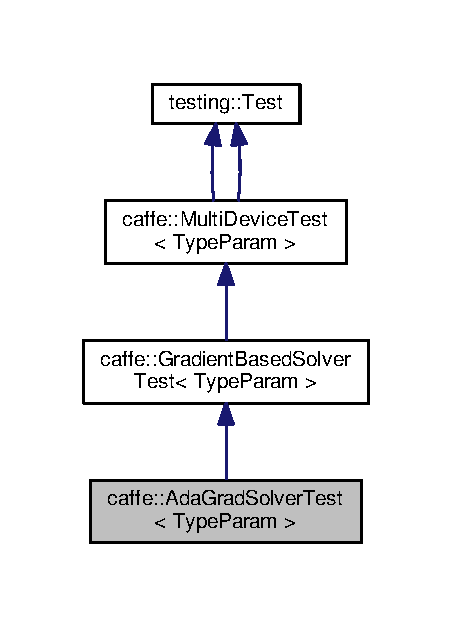
\includegraphics[width=217pt]{classcaffe_1_1_ada_grad_solver_test__inherit__graph}
\end{center}
\end{figure}
\subsection*{Protected Member Functions}
\begin{DoxyCompactItemize}
\item 
\mbox{\Hypertarget{classcaffe_1_1_ada_grad_solver_test_a81940a2a2240e7aaf567851a5c005c69}\label{classcaffe_1_1_ada_grad_solver_test_a81940a2a2240e7aaf567851a5c005c69}} 
virtual void {\bfseries Init\+Solver} (const \mbox{\hyperlink{classcaffe_1_1_solver_parameter}{Solver\+Parameter}} \&param)
\end{DoxyCompactItemize}
\subsection*{Additional Inherited Members}


The documentation for this class was generated from the following file\+:\begin{DoxyCompactItemize}
\item 
src/caffe/test/test\+\_\+gradient\+\_\+based\+\_\+solver.\+cpp\end{DoxyCompactItemize}

\hypertarget{classcaffe_1_1_adam_solver}{}\section{caffe\+:\+:Adam\+Solver$<$ Dtype $>$ Class Template Reference}
\label{classcaffe_1_1_adam_solver}\index{caffe\+::\+Adam\+Solver$<$ Dtype $>$@{caffe\+::\+Adam\+Solver$<$ Dtype $>$}}


\mbox{\hyperlink{classcaffe_1_1_adam_solver}{Adam\+Solver}}, an algorithm for first-\/order gradient-\/based optimization of stochastic objective functions, based on adaptive estimates of lower-\/order moments. Described in \mbox{[}1\mbox{]}.  




{\ttfamily \#include $<$sgd\+\_\+solvers.\+hpp$>$}



Inheritance diagram for caffe\+:\+:Adam\+Solver$<$ Dtype $>$\+:
\nopagebreak
\begin{figure}[H]
\begin{center}
\leavevmode
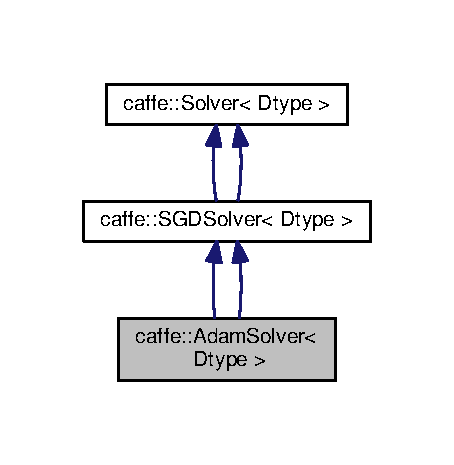
\includegraphics[width=218pt]{classcaffe_1_1_adam_solver__inherit__graph}
\end{center}
\end{figure}
\subsection*{Public Member Functions}
\begin{DoxyCompactItemize}
\item 
\mbox{\Hypertarget{classcaffe_1_1_adam_solver_a2591a6002658a955d8df6a2bf1a28f1e}\label{classcaffe_1_1_adam_solver_a2591a6002658a955d8df6a2bf1a28f1e}} 
{\bfseries Adam\+Solver} (const \mbox{\hyperlink{classcaffe_1_1_solver_parameter}{Solver\+Parameter}} \&param)
\item 
\mbox{\Hypertarget{classcaffe_1_1_adam_solver_adfd87b65ecd4c57591eefc24ac16e292}\label{classcaffe_1_1_adam_solver_adfd87b65ecd4c57591eefc24ac16e292}} 
{\bfseries Adam\+Solver} (const string \&param\+\_\+file)
\item 
\mbox{\Hypertarget{classcaffe_1_1_adam_solver_a3ad927ab9d19ebf2fe2b8a2e9101cb3e}\label{classcaffe_1_1_adam_solver_a3ad927ab9d19ebf2fe2b8a2e9101cb3e}} 
virtual const char $\ast$ \mbox{\hyperlink{classcaffe_1_1_adam_solver_a3ad927ab9d19ebf2fe2b8a2e9101cb3e}{type}} () const
\begin{DoxyCompactList}\small\item\em Returns the solver type. \end{DoxyCompactList}\item 
\mbox{\Hypertarget{classcaffe_1_1_adam_solver_a2591a6002658a955d8df6a2bf1a28f1e}\label{classcaffe_1_1_adam_solver_a2591a6002658a955d8df6a2bf1a28f1e}} 
{\bfseries Adam\+Solver} (const \mbox{\hyperlink{classcaffe_1_1_solver_parameter}{Solver\+Parameter}} \&param)
\item 
\mbox{\Hypertarget{classcaffe_1_1_adam_solver_adfd87b65ecd4c57591eefc24ac16e292}\label{classcaffe_1_1_adam_solver_adfd87b65ecd4c57591eefc24ac16e292}} 
{\bfseries Adam\+Solver} (const string \&param\+\_\+file)
\item 
\mbox{\Hypertarget{classcaffe_1_1_adam_solver_a3ad927ab9d19ebf2fe2b8a2e9101cb3e}\label{classcaffe_1_1_adam_solver_a3ad927ab9d19ebf2fe2b8a2e9101cb3e}} 
virtual const char $\ast$ \mbox{\hyperlink{classcaffe_1_1_adam_solver_a3ad927ab9d19ebf2fe2b8a2e9101cb3e}{type}} () const
\begin{DoxyCompactList}\small\item\em Returns the solver type. \end{DoxyCompactList}\end{DoxyCompactItemize}
\subsection*{Protected Member Functions}
\begin{DoxyCompactItemize}
\item 
\mbox{\Hypertarget{classcaffe_1_1_adam_solver_a72bbfc1fb2ec2194b183fa65f77ef1fb}\label{classcaffe_1_1_adam_solver_a72bbfc1fb2ec2194b183fa65f77ef1fb}} 
void {\bfseries Adam\+Pre\+Solve} ()
\item 
\mbox{\Hypertarget{classcaffe_1_1_adam_solver_a11f2c48ead67c91ba9e871acdbda1af8}\label{classcaffe_1_1_adam_solver_a11f2c48ead67c91ba9e871acdbda1af8}} 
virtual void {\bfseries Compute\+Update\+Value} (int param\+\_\+id, Dtype rate)
\item 
\mbox{\Hypertarget{classcaffe_1_1_adam_solver_a5f192e195185ab841f083415333f5147}\label{classcaffe_1_1_adam_solver_a5f192e195185ab841f083415333f5147}} 
{\bfseries D\+I\+S\+A\+B\+L\+E\+\_\+\+C\+O\+P\+Y\+\_\+\+A\+N\+D\+\_\+\+A\+S\+S\+I\+GN} (\mbox{\hyperlink{classcaffe_1_1_adam_solver}{Adam\+Solver}})
\item 
\mbox{\Hypertarget{classcaffe_1_1_adam_solver_a72bbfc1fb2ec2194b183fa65f77ef1fb}\label{classcaffe_1_1_adam_solver_a72bbfc1fb2ec2194b183fa65f77ef1fb}} 
void {\bfseries Adam\+Pre\+Solve} ()
\item 
\mbox{\Hypertarget{classcaffe_1_1_adam_solver_ab502b325cb0d36f48c19c7b97268ca1a}\label{classcaffe_1_1_adam_solver_ab502b325cb0d36f48c19c7b97268ca1a}} 
virtual void {\bfseries Compute\+Update\+Value} (int param\+\_\+id, Dtype rate)
\item 
\mbox{\Hypertarget{classcaffe_1_1_adam_solver_a5f192e195185ab841f083415333f5147}\label{classcaffe_1_1_adam_solver_a5f192e195185ab841f083415333f5147}} 
{\bfseries D\+I\+S\+A\+B\+L\+E\+\_\+\+C\+O\+P\+Y\+\_\+\+A\+N\+D\+\_\+\+A\+S\+S\+I\+GN} (\mbox{\hyperlink{classcaffe_1_1_adam_solver}{Adam\+Solver}})
\end{DoxyCompactItemize}
\subsection*{Additional Inherited Members}


\subsection{Detailed Description}
\subsubsection*{template$<$typename Dtype$>$\newline
class caffe\+::\+Adam\+Solver$<$ Dtype $>$}

\mbox{\hyperlink{classcaffe_1_1_adam_solver}{Adam\+Solver}}, an algorithm for first-\/order gradient-\/based optimization of stochastic objective functions, based on adaptive estimates of lower-\/order moments. Described in \mbox{[}1\mbox{]}. 

\mbox{[}1\mbox{]} D. P. Kingma and J. L. Ba, \char`\"{}\+A\+D\+A\+M\+: A Method for Stochastic Optimization.\char`\"{} ar\+Xiv preprint ar\+Xiv\+:1412.\+6980v8 (2014). 

The documentation for this class was generated from the following files\+:\begin{DoxyCompactItemize}
\item 
build/install/include/caffe/sgd\+\_\+solvers.\+hpp\item 
src/caffe/solvers/adam\+\_\+solver.\+cpp\end{DoxyCompactItemize}

\hypertarget{classcaffe_1_1_adam_solver_test}{}\section{caffe\+:\+:Adam\+Solver\+Test$<$ Type\+Param $>$ Class Template Reference}
\label{classcaffe_1_1_adam_solver_test}\index{caffe\+::\+Adam\+Solver\+Test$<$ Type\+Param $>$@{caffe\+::\+Adam\+Solver\+Test$<$ Type\+Param $>$}}


Inheritance diagram for caffe\+:\+:Adam\+Solver\+Test$<$ Type\+Param $>$\+:
\nopagebreak
\begin{figure}[H]
\begin{center}
\leavevmode
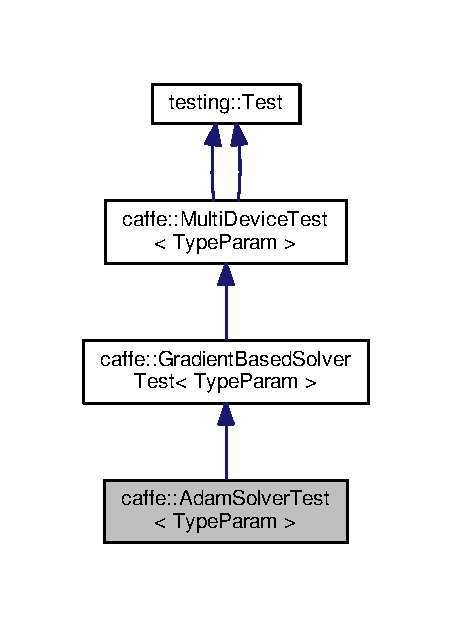
\includegraphics[width=217pt]{classcaffe_1_1_adam_solver_test__inherit__graph}
\end{center}
\end{figure}
\subsection*{Protected Member Functions}
\begin{DoxyCompactItemize}
\item 
\mbox{\Hypertarget{classcaffe_1_1_adam_solver_test_a9bf49f7c9031b25a5b6656879016bde9}\label{classcaffe_1_1_adam_solver_test_a9bf49f7c9031b25a5b6656879016bde9}} 
virtual void {\bfseries Init\+Solver} (const \mbox{\hyperlink{classcaffe_1_1_solver_parameter}{Solver\+Parameter}} \&param)
\end{DoxyCompactItemize}
\subsection*{Additional Inherited Members}


The documentation for this class was generated from the following file\+:\begin{DoxyCompactItemize}
\item 
src/caffe/test/test\+\_\+gradient\+\_\+based\+\_\+solver.\+cpp\end{DoxyCompactItemize}

\hypertarget{structstd_1_1tr1_1_1gtest__internal_1_1_add_ref}{}\section{std\+:\+:tr1\+:\+:gtest\+\_\+internal\+:\+:Add\+Ref$<$ T $>$ Struct Template Reference}
\label{structstd_1_1tr1_1_1gtest__internal_1_1_add_ref}\index{std\+::tr1\+::gtest\+\_\+internal\+::\+Add\+Ref$<$ T $>$@{std\+::tr1\+::gtest\+\_\+internal\+::\+Add\+Ref$<$ T $>$}}
\subsection*{Public Types}
\begin{DoxyCompactItemize}
\item 
\mbox{\Hypertarget{structstd_1_1tr1_1_1gtest__internal_1_1_add_ref_a1e5616e414125574c1653e3a1fc68491}\label{structstd_1_1tr1_1_1gtest__internal_1_1_add_ref_a1e5616e414125574c1653e3a1fc68491}} 
typedef T \& {\bfseries type}
\end{DoxyCompactItemize}


The documentation for this struct was generated from the following file\+:\begin{DoxyCompactItemize}
\item 
src/gtest/gtest.\+h\end{DoxyCompactItemize}

\hypertarget{structstd_1_1tr1_1_1gtest__internal_1_1_add_ref_3_01_t_01_6_01_4}{}\section{std\+:\+:tr1\+:\+:gtest\+\_\+internal\+:\+:Add\+Ref$<$ T \& $>$ Struct Template Reference}
\label{structstd_1_1tr1_1_1gtest__internal_1_1_add_ref_3_01_t_01_6_01_4}\index{std\+::tr1\+::gtest\+\_\+internal\+::\+Add\+Ref$<$ T \& $>$@{std\+::tr1\+::gtest\+\_\+internal\+::\+Add\+Ref$<$ T \& $>$}}
\subsection*{Public Types}
\begin{DoxyCompactItemize}
\item 
\mbox{\Hypertarget{structstd_1_1tr1_1_1gtest__internal_1_1_add_ref_3_01_t_01_6_01_4_a9cb3b0992c2a9e7df42d01fb64c2dc88}\label{structstd_1_1tr1_1_1gtest__internal_1_1_add_ref_3_01_t_01_6_01_4_a9cb3b0992c2a9e7df42d01fb64c2dc88}} 
typedef T \& {\bfseries type}
\end{DoxyCompactItemize}


The documentation for this struct was generated from the following file\+:\begin{DoxyCompactItemize}
\item 
src/gtest/gtest.\+h\end{DoxyCompactItemize}

\hypertarget{structtesting_1_1internal_1_1_add_reference}{}\section{testing\+:\+:internal\+:\+:Add\+Reference$<$ T $>$ Struct Template Reference}
\label{structtesting_1_1internal_1_1_add_reference}\index{testing\+::internal\+::\+Add\+Reference$<$ T $>$@{testing\+::internal\+::\+Add\+Reference$<$ T $>$}}
\subsection*{Public Types}
\begin{DoxyCompactItemize}
\item 
\mbox{\Hypertarget{structtesting_1_1internal_1_1_add_reference_a2df8dd7c4e41f6390e6e66b1a9a67bb4}\label{structtesting_1_1internal_1_1_add_reference_a2df8dd7c4e41f6390e6e66b1a9a67bb4}} 
typedef T \& {\bfseries type}
\end{DoxyCompactItemize}


The documentation for this struct was generated from the following file\+:\begin{DoxyCompactItemize}
\item 
src/gtest/gtest.\+h\end{DoxyCompactItemize}

\hypertarget{structtesting_1_1internal_1_1_add_reference_3_01_t_01_6_01_4}{}\section{testing\+:\+:internal\+:\+:Add\+Reference$<$ T \& $>$ Struct Template Reference}
\label{structtesting_1_1internal_1_1_add_reference_3_01_t_01_6_01_4}\index{testing\+::internal\+::\+Add\+Reference$<$ T \& $>$@{testing\+::internal\+::\+Add\+Reference$<$ T \& $>$}}
\subsection*{Public Types}
\begin{DoxyCompactItemize}
\item 
\mbox{\Hypertarget{structtesting_1_1internal_1_1_add_reference_3_01_t_01_6_01_4_a93c064cdcdaced0abd167258425e57af}\label{structtesting_1_1internal_1_1_add_reference_3_01_t_01_6_01_4_a93c064cdcdaced0abd167258425e57af}} 
typedef T \& {\bfseries type}
\end{DoxyCompactItemize}


The documentation for this struct was generated from the following file\+:\begin{DoxyCompactItemize}
\item 
src/gtest/gtest.\+h\end{DoxyCompactItemize}

\hypertarget{structcaffe_1_1_ndarray_converter_generator_1_1apply}{}\section{caffe\+:\+:Ndarray\+Converter\+Generator\+:\+:apply$<$ T $>$ Struct Template Reference}
\label{structcaffe_1_1_ndarray_converter_generator_1_1apply}\index{caffe\+::\+Ndarray\+Converter\+Generator\+::apply$<$ T $>$@{caffe\+::\+Ndarray\+Converter\+Generator\+::apply$<$ T $>$}}
\subsection*{Classes}
\begin{DoxyCompactItemize}
\item 
struct \mbox{\hyperlink{structcaffe_1_1_ndarray_converter_generator_1_1apply_3_01_dtype_01_5_01_4_1_1type}{type}}
\end{DoxyCompactItemize}


The documentation for this struct was generated from the following file\+:\begin{DoxyCompactItemize}
\item 
python/caffe/\+\_\+caffe.\+cpp\end{DoxyCompactItemize}

\hypertarget{structcaffe_1_1_ndarray_converter_generator_1_1apply_3_01_dtype_01_5_01_4}{}\section{caffe\+:\+:Ndarray\+Converter\+Generator\+:\+:apply$<$ Dtype $\ast$ $>$ Struct Template Reference}
\label{structcaffe_1_1_ndarray_converter_generator_1_1apply_3_01_dtype_01_5_01_4}\index{caffe\+::\+Ndarray\+Converter\+Generator\+::apply$<$ Dtype $\ast$ $>$@{caffe\+::\+Ndarray\+Converter\+Generator\+::apply$<$ Dtype $\ast$ $>$}}


The documentation for this struct was generated from the following file\+:\begin{DoxyCompactItemize}
\item 
python/caffe/\+\_\+caffe.\+cpp\end{DoxyCompactItemize}

\hypertarget{classcaffe_1_1_arg_max_layer}{}\section{caffe\+:\+:Arg\+Max\+Layer$<$ Dtype $>$ Class Template Reference}
\label{classcaffe_1_1_arg_max_layer}\index{caffe\+::\+Arg\+Max\+Layer$<$ Dtype $>$@{caffe\+::\+Arg\+Max\+Layer$<$ Dtype $>$}}


Compute the index of the $ K $ max values for each datum across all dimensions $ (C \times H \times W) $.  




{\ttfamily \#include $<$argmax\+\_\+layer.\+hpp$>$}



Inheritance diagram for caffe\+:\+:Arg\+Max\+Layer$<$ Dtype $>$\+:
\nopagebreak
\begin{figure}[H]
\begin{center}
\leavevmode
\includegraphics[width=193pt]{classcaffe_1_1_arg_max_layer__inherit__graph}
\end{center}
\end{figure}
\subsection*{Public Member Functions}
\begin{DoxyCompactItemize}
\item 
\mbox{\hyperlink{classcaffe_1_1_arg_max_layer_a77429601f3d7f27b48720a1b703491be}{Arg\+Max\+Layer}} (const \mbox{\hyperlink{classcaffe_1_1_layer_parameter}{Layer\+Parameter}} \&param)
\item 
virtual void \mbox{\hyperlink{classcaffe_1_1_arg_max_layer_a53069bd5efc4639de93a8111da772572}{Layer\+Set\+Up}} (const vector$<$ \mbox{\hyperlink{classcaffe_1_1_blob}{Blob}}$<$ Dtype $>$ $\ast$$>$ \&bottom, const vector$<$ \mbox{\hyperlink{classcaffe_1_1_blob}{Blob}}$<$ Dtype $>$ $\ast$$>$ \&top)
\begin{DoxyCompactList}\small\item\em Does layer-\/specific setup\+: your layer should implement this function as well as Reshape. \end{DoxyCompactList}\item 
virtual void \mbox{\hyperlink{classcaffe_1_1_arg_max_layer_a291a2c548c28e7ab02ddac0cfd3cbdad}{Reshape}} (const vector$<$ \mbox{\hyperlink{classcaffe_1_1_blob}{Blob}}$<$ Dtype $>$ $\ast$$>$ \&bottom, const vector$<$ \mbox{\hyperlink{classcaffe_1_1_blob}{Blob}}$<$ Dtype $>$ $\ast$$>$ \&top)
\begin{DoxyCompactList}\small\item\em Adjust the shapes of top blobs and internal buffers to accommodate the shapes of the bottom blobs. \end{DoxyCompactList}\item 
\mbox{\Hypertarget{classcaffe_1_1_arg_max_layer_af4826eb75118ddf465b7c2ab99b10b45}\label{classcaffe_1_1_arg_max_layer_af4826eb75118ddf465b7c2ab99b10b45}} 
virtual const char $\ast$ \mbox{\hyperlink{classcaffe_1_1_arg_max_layer_af4826eb75118ddf465b7c2ab99b10b45}{type}} () const
\begin{DoxyCompactList}\small\item\em Returns the layer type. \end{DoxyCompactList}\item 
virtual int \mbox{\hyperlink{classcaffe_1_1_arg_max_layer_a786fb4163cd0a31a564100ce7e4b74b2}{Exact\+Num\+Bottom\+Blobs}} () const
\begin{DoxyCompactList}\small\item\em Returns the exact number of bottom blobs required by the layer, or -\/1 if no exact number is required. \end{DoxyCompactList}\item 
virtual int \mbox{\hyperlink{classcaffe_1_1_arg_max_layer_a45e9c6e7b572b915be8731fcb6403695}{Exact\+Num\+Top\+Blobs}} () const
\begin{DoxyCompactList}\small\item\em Returns the exact number of top blobs required by the layer, or -\/1 if no exact number is required. \end{DoxyCompactList}\item 
\mbox{\hyperlink{classcaffe_1_1_arg_max_layer_a77429601f3d7f27b48720a1b703491be}{Arg\+Max\+Layer}} (const \mbox{\hyperlink{classcaffe_1_1_layer_parameter}{Layer\+Parameter}} \&param)
\item 
virtual void \mbox{\hyperlink{classcaffe_1_1_arg_max_layer_a1251d1d407e8d15a83ba6807d013b97d}{Layer\+Set\+Up}} (const vector$<$ \mbox{\hyperlink{classcaffe_1_1_blob}{Blob}}$<$ Dtype $>$ $\ast$$>$ \&bottom, const vector$<$ \mbox{\hyperlink{classcaffe_1_1_blob}{Blob}}$<$ Dtype $>$ $\ast$$>$ \&top)
\begin{DoxyCompactList}\small\item\em Does layer-\/specific setup\+: your layer should implement this function as well as Reshape. \end{DoxyCompactList}\item 
virtual void \mbox{\hyperlink{classcaffe_1_1_arg_max_layer_a658393ef566ec585bf540a1b6f31a929}{Reshape}} (const vector$<$ \mbox{\hyperlink{classcaffe_1_1_blob}{Blob}}$<$ Dtype $>$ $\ast$$>$ \&bottom, const vector$<$ \mbox{\hyperlink{classcaffe_1_1_blob}{Blob}}$<$ Dtype $>$ $\ast$$>$ \&top)
\begin{DoxyCompactList}\small\item\em Adjust the shapes of top blobs and internal buffers to accommodate the shapes of the bottom blobs. \end{DoxyCompactList}\item 
\mbox{\Hypertarget{classcaffe_1_1_arg_max_layer_af4826eb75118ddf465b7c2ab99b10b45}\label{classcaffe_1_1_arg_max_layer_af4826eb75118ddf465b7c2ab99b10b45}} 
virtual const char $\ast$ \mbox{\hyperlink{classcaffe_1_1_arg_max_layer_af4826eb75118ddf465b7c2ab99b10b45}{type}} () const
\begin{DoxyCompactList}\small\item\em Returns the layer type. \end{DoxyCompactList}\item 
virtual int \mbox{\hyperlink{classcaffe_1_1_arg_max_layer_a786fb4163cd0a31a564100ce7e4b74b2}{Exact\+Num\+Bottom\+Blobs}} () const
\begin{DoxyCompactList}\small\item\em Returns the exact number of bottom blobs required by the layer, or -\/1 if no exact number is required. \end{DoxyCompactList}\item 
virtual int \mbox{\hyperlink{classcaffe_1_1_arg_max_layer_a45e9c6e7b572b915be8731fcb6403695}{Exact\+Num\+Top\+Blobs}} () const
\begin{DoxyCompactList}\small\item\em Returns the exact number of top blobs required by the layer, or -\/1 if no exact number is required. \end{DoxyCompactList}\end{DoxyCompactItemize}
\subsection*{Protected Member Functions}
\begin{DoxyCompactItemize}
\item 
virtual void \mbox{\hyperlink{classcaffe_1_1_arg_max_layer_a0e4cb76ff1796b71079f83335f033c44}{Forward\+\_\+cpu}} (const vector$<$ \mbox{\hyperlink{classcaffe_1_1_blob}{Blob}}$<$ Dtype $>$ $\ast$$>$ \&bottom, const vector$<$ \mbox{\hyperlink{classcaffe_1_1_blob}{Blob}}$<$ Dtype $>$ $\ast$$>$ \&top)
\item 
\mbox{\Hypertarget{classcaffe_1_1_arg_max_layer_a763be1ca5815fbe1eec62ec206ae3f6e}\label{classcaffe_1_1_arg_max_layer_a763be1ca5815fbe1eec62ec206ae3f6e}} 
virtual void \mbox{\hyperlink{classcaffe_1_1_arg_max_layer_a763be1ca5815fbe1eec62ec206ae3f6e}{Backward\+\_\+cpu}} (const vector$<$ \mbox{\hyperlink{classcaffe_1_1_blob}{Blob}}$<$ Dtype $>$ $\ast$$>$ \&top, const vector$<$ bool $>$ \&propagate\+\_\+down, const vector$<$ \mbox{\hyperlink{classcaffe_1_1_blob}{Blob}}$<$ Dtype $>$ $\ast$$>$ \&bottom)
\begin{DoxyCompactList}\small\item\em Not implemented (non-\/differentiable function) \end{DoxyCompactList}\item 
virtual void \mbox{\hyperlink{classcaffe_1_1_arg_max_layer_a5443ad874d389b1ddbb1e363857a049f}{Forward\+\_\+cpu}} (const vector$<$ \mbox{\hyperlink{classcaffe_1_1_blob}{Blob}}$<$ Dtype $>$ $\ast$$>$ \&bottom, const vector$<$ \mbox{\hyperlink{classcaffe_1_1_blob}{Blob}}$<$ Dtype $>$ $\ast$$>$ \&top)
\item 
\mbox{\Hypertarget{classcaffe_1_1_arg_max_layer_a763be1ca5815fbe1eec62ec206ae3f6e}\label{classcaffe_1_1_arg_max_layer_a763be1ca5815fbe1eec62ec206ae3f6e}} 
virtual void \mbox{\hyperlink{classcaffe_1_1_arg_max_layer_a763be1ca5815fbe1eec62ec206ae3f6e}{Backward\+\_\+cpu}} (const vector$<$ \mbox{\hyperlink{classcaffe_1_1_blob}{Blob}}$<$ Dtype $>$ $\ast$$>$ \&top, const vector$<$ bool $>$ \&propagate\+\_\+down, const vector$<$ \mbox{\hyperlink{classcaffe_1_1_blob}{Blob}}$<$ Dtype $>$ $\ast$$>$ \&bottom)
\begin{DoxyCompactList}\small\item\em Not implemented (non-\/differentiable function) \end{DoxyCompactList}\end{DoxyCompactItemize}
\subsection*{Protected Attributes}
\begin{DoxyCompactItemize}
\item 
\mbox{\Hypertarget{classcaffe_1_1_arg_max_layer_a80166873c75bdbb9a8aaa43e63543684}\label{classcaffe_1_1_arg_max_layer_a80166873c75bdbb9a8aaa43e63543684}} 
bool {\bfseries out\+\_\+max\+\_\+val\+\_\+}
\item 
\mbox{\Hypertarget{classcaffe_1_1_arg_max_layer_a936d87cd98fe0c508f5d7feb17c5f989}\label{classcaffe_1_1_arg_max_layer_a936d87cd98fe0c508f5d7feb17c5f989}} 
size\+\_\+t {\bfseries top\+\_\+k\+\_\+}
\item 
\mbox{\Hypertarget{classcaffe_1_1_arg_max_layer_aad30a415d4d23ce890f9ddf0c7efcb4b}\label{classcaffe_1_1_arg_max_layer_aad30a415d4d23ce890f9ddf0c7efcb4b}} 
bool {\bfseries has\+\_\+axis\+\_\+}
\item 
\mbox{\Hypertarget{classcaffe_1_1_arg_max_layer_af0c7ee3334644eef4b7d7d47cb5890a7}\label{classcaffe_1_1_arg_max_layer_af0c7ee3334644eef4b7d7d47cb5890a7}} 
int {\bfseries axis\+\_\+}
\end{DoxyCompactItemize}


\subsection{Detailed Description}
\subsubsection*{template$<$typename Dtype$>$\newline
class caffe\+::\+Arg\+Max\+Layer$<$ Dtype $>$}

Compute the index of the $ K $ max values for each datum across all dimensions $ (C \times H \times W) $. 

Intended for use after a classification layer to produce a prediction. If parameter out\+\_\+max\+\_\+val is set to true, output is a vector of pairs (max\+\_\+ind, max\+\_\+val) for each image. The axis parameter specifies an axis along which to maximise.

N\+O\+TE\+: does not implement Backwards operation. 

\subsection{Constructor \& Destructor Documentation}
\mbox{\Hypertarget{classcaffe_1_1_arg_max_layer_a77429601f3d7f27b48720a1b703491be}\label{classcaffe_1_1_arg_max_layer_a77429601f3d7f27b48720a1b703491be}} 
\index{caffe\+::\+Arg\+Max\+Layer@{caffe\+::\+Arg\+Max\+Layer}!Arg\+Max\+Layer@{Arg\+Max\+Layer}}
\index{Arg\+Max\+Layer@{Arg\+Max\+Layer}!caffe\+::\+Arg\+Max\+Layer@{caffe\+::\+Arg\+Max\+Layer}}
\subsubsection{\texorpdfstring{Arg\+Max\+Layer()}{ArgMaxLayer()}\hspace{0.1cm}{\footnotesize\ttfamily [1/2]}}
{\footnotesize\ttfamily template$<$typename Dtype$>$ \\
\mbox{\hyperlink{classcaffe_1_1_arg_max_layer}{caffe\+::\+Arg\+Max\+Layer}}$<$ Dtype $>$\+::\mbox{\hyperlink{classcaffe_1_1_arg_max_layer}{Arg\+Max\+Layer}} (\begin{DoxyParamCaption}\item[{const \mbox{\hyperlink{classcaffe_1_1_layer_parameter}{Layer\+Parameter}} \&}]{param }\end{DoxyParamCaption})\hspace{0.3cm}{\ttfamily [inline]}, {\ttfamily [explicit]}}


\begin{DoxyParams}{Parameters}
{\em param} & provides \mbox{\hyperlink{classcaffe_1_1_arg_max_parameter}{Arg\+Max\+Parameter}} argmax\+\_\+param, with \mbox{\hyperlink{classcaffe_1_1_arg_max_layer}{Arg\+Max\+Layer}} options\+:
\begin{DoxyItemize}
\item top\+\_\+k ({\bfseries optional} uint, default 1). the number $ K $ of maximal items to output.
\item out\+\_\+max\+\_\+val ({\bfseries optional} bool, default false). if set, output a vector of pairs (max\+\_\+ind, max\+\_\+val) unless axis is set then output max\+\_\+val along the specified axis.
\item axis ({\bfseries optional} int). if set, maximise along the specified axis else maximise the flattened trailing dimensions for each index of the first / num dimension. 
\end{DoxyItemize}\\
\hline
\end{DoxyParams}
\mbox{\Hypertarget{classcaffe_1_1_arg_max_layer_a77429601f3d7f27b48720a1b703491be}\label{classcaffe_1_1_arg_max_layer_a77429601f3d7f27b48720a1b703491be}} 
\index{caffe\+::\+Arg\+Max\+Layer@{caffe\+::\+Arg\+Max\+Layer}!Arg\+Max\+Layer@{Arg\+Max\+Layer}}
\index{Arg\+Max\+Layer@{Arg\+Max\+Layer}!caffe\+::\+Arg\+Max\+Layer@{caffe\+::\+Arg\+Max\+Layer}}
\subsubsection{\texorpdfstring{Arg\+Max\+Layer()}{ArgMaxLayer()}\hspace{0.1cm}{\footnotesize\ttfamily [2/2]}}
{\footnotesize\ttfamily template$<$typename Dtype$>$ \\
\mbox{\hyperlink{classcaffe_1_1_arg_max_layer}{caffe\+::\+Arg\+Max\+Layer}}$<$ Dtype $>$\+::\mbox{\hyperlink{classcaffe_1_1_arg_max_layer}{Arg\+Max\+Layer}} (\begin{DoxyParamCaption}\item[{const \mbox{\hyperlink{classcaffe_1_1_layer_parameter}{Layer\+Parameter}} \&}]{param }\end{DoxyParamCaption})\hspace{0.3cm}{\ttfamily [inline]}, {\ttfamily [explicit]}}


\begin{DoxyParams}{Parameters}
{\em param} & provides \mbox{\hyperlink{classcaffe_1_1_arg_max_parameter}{Arg\+Max\+Parameter}} argmax\+\_\+param, with \mbox{\hyperlink{classcaffe_1_1_arg_max_layer}{Arg\+Max\+Layer}} options\+:
\begin{DoxyItemize}
\item top\+\_\+k ({\bfseries optional} uint, default 1). the number $ K $ of maximal items to output.
\item out\+\_\+max\+\_\+val ({\bfseries optional} bool, default false). if set, output a vector of pairs (max\+\_\+ind, max\+\_\+val) unless axis is set then output max\+\_\+val along the specified axis.
\item axis ({\bfseries optional} int). if set, maximise along the specified axis else maximise the flattened trailing dimensions for each index of the first / num dimension. 
\end{DoxyItemize}\\
\hline
\end{DoxyParams}


\subsection{Member Function Documentation}
\mbox{\Hypertarget{classcaffe_1_1_arg_max_layer_a786fb4163cd0a31a564100ce7e4b74b2}\label{classcaffe_1_1_arg_max_layer_a786fb4163cd0a31a564100ce7e4b74b2}} 
\index{caffe\+::\+Arg\+Max\+Layer@{caffe\+::\+Arg\+Max\+Layer}!Exact\+Num\+Bottom\+Blobs@{Exact\+Num\+Bottom\+Blobs}}
\index{Exact\+Num\+Bottom\+Blobs@{Exact\+Num\+Bottom\+Blobs}!caffe\+::\+Arg\+Max\+Layer@{caffe\+::\+Arg\+Max\+Layer}}
\subsubsection{\texorpdfstring{Exact\+Num\+Bottom\+Blobs()}{ExactNumBottomBlobs()}\hspace{0.1cm}{\footnotesize\ttfamily [1/2]}}
{\footnotesize\ttfamily template$<$typename Dtype$>$ \\
virtual int \mbox{\hyperlink{classcaffe_1_1_arg_max_layer}{caffe\+::\+Arg\+Max\+Layer}}$<$ Dtype $>$\+::Exact\+Num\+Bottom\+Blobs (\begin{DoxyParamCaption}{ }\end{DoxyParamCaption}) const\hspace{0.3cm}{\ttfamily [inline]}, {\ttfamily [virtual]}}



Returns the exact number of bottom blobs required by the layer, or -\/1 if no exact number is required. 

This method should be overridden to return a non-\/negative value if your layer expects some exact number of bottom blobs. 

Reimplemented from \mbox{\hyperlink{classcaffe_1_1_layer_a8e5ee0494d85f5f55fc4396537cbc60f}{caffe\+::\+Layer$<$ Dtype $>$}}.

\mbox{\Hypertarget{classcaffe_1_1_arg_max_layer_a786fb4163cd0a31a564100ce7e4b74b2}\label{classcaffe_1_1_arg_max_layer_a786fb4163cd0a31a564100ce7e4b74b2}} 
\index{caffe\+::\+Arg\+Max\+Layer@{caffe\+::\+Arg\+Max\+Layer}!Exact\+Num\+Bottom\+Blobs@{Exact\+Num\+Bottom\+Blobs}}
\index{Exact\+Num\+Bottom\+Blobs@{Exact\+Num\+Bottom\+Blobs}!caffe\+::\+Arg\+Max\+Layer@{caffe\+::\+Arg\+Max\+Layer}}
\subsubsection{\texorpdfstring{Exact\+Num\+Bottom\+Blobs()}{ExactNumBottomBlobs()}\hspace{0.1cm}{\footnotesize\ttfamily [2/2]}}
{\footnotesize\ttfamily template$<$typename Dtype$>$ \\
virtual int \mbox{\hyperlink{classcaffe_1_1_arg_max_layer}{caffe\+::\+Arg\+Max\+Layer}}$<$ Dtype $>$\+::Exact\+Num\+Bottom\+Blobs (\begin{DoxyParamCaption}{ }\end{DoxyParamCaption}) const\hspace{0.3cm}{\ttfamily [inline]}, {\ttfamily [virtual]}}



Returns the exact number of bottom blobs required by the layer, or -\/1 if no exact number is required. 

This method should be overridden to return a non-\/negative value if your layer expects some exact number of bottom blobs. 

Reimplemented from \mbox{\hyperlink{classcaffe_1_1_layer_a8e5ee0494d85f5f55fc4396537cbc60f}{caffe\+::\+Layer$<$ Dtype $>$}}.

\mbox{\Hypertarget{classcaffe_1_1_arg_max_layer_a45e9c6e7b572b915be8731fcb6403695}\label{classcaffe_1_1_arg_max_layer_a45e9c6e7b572b915be8731fcb6403695}} 
\index{caffe\+::\+Arg\+Max\+Layer@{caffe\+::\+Arg\+Max\+Layer}!Exact\+Num\+Top\+Blobs@{Exact\+Num\+Top\+Blobs}}
\index{Exact\+Num\+Top\+Blobs@{Exact\+Num\+Top\+Blobs}!caffe\+::\+Arg\+Max\+Layer@{caffe\+::\+Arg\+Max\+Layer}}
\subsubsection{\texorpdfstring{Exact\+Num\+Top\+Blobs()}{ExactNumTopBlobs()}\hspace{0.1cm}{\footnotesize\ttfamily [1/2]}}
{\footnotesize\ttfamily template$<$typename Dtype$>$ \\
virtual int \mbox{\hyperlink{classcaffe_1_1_arg_max_layer}{caffe\+::\+Arg\+Max\+Layer}}$<$ Dtype $>$\+::Exact\+Num\+Top\+Blobs (\begin{DoxyParamCaption}{ }\end{DoxyParamCaption}) const\hspace{0.3cm}{\ttfamily [inline]}, {\ttfamily [virtual]}}



Returns the exact number of top blobs required by the layer, or -\/1 if no exact number is required. 

This method should be overridden to return a non-\/negative value if your layer expects some exact number of top blobs. 

Reimplemented from \mbox{\hyperlink{classcaffe_1_1_layer_a64e2ca72c719e4b2f1f9216ccfb0d37f}{caffe\+::\+Layer$<$ Dtype $>$}}.

\mbox{\Hypertarget{classcaffe_1_1_arg_max_layer_a45e9c6e7b572b915be8731fcb6403695}\label{classcaffe_1_1_arg_max_layer_a45e9c6e7b572b915be8731fcb6403695}} 
\index{caffe\+::\+Arg\+Max\+Layer@{caffe\+::\+Arg\+Max\+Layer}!Exact\+Num\+Top\+Blobs@{Exact\+Num\+Top\+Blobs}}
\index{Exact\+Num\+Top\+Blobs@{Exact\+Num\+Top\+Blobs}!caffe\+::\+Arg\+Max\+Layer@{caffe\+::\+Arg\+Max\+Layer}}
\subsubsection{\texorpdfstring{Exact\+Num\+Top\+Blobs()}{ExactNumTopBlobs()}\hspace{0.1cm}{\footnotesize\ttfamily [2/2]}}
{\footnotesize\ttfamily template$<$typename Dtype$>$ \\
virtual int \mbox{\hyperlink{classcaffe_1_1_arg_max_layer}{caffe\+::\+Arg\+Max\+Layer}}$<$ Dtype $>$\+::Exact\+Num\+Top\+Blobs (\begin{DoxyParamCaption}{ }\end{DoxyParamCaption}) const\hspace{0.3cm}{\ttfamily [inline]}, {\ttfamily [virtual]}}



Returns the exact number of top blobs required by the layer, or -\/1 if no exact number is required. 

This method should be overridden to return a non-\/negative value if your layer expects some exact number of top blobs. 

Reimplemented from \mbox{\hyperlink{classcaffe_1_1_layer_a64e2ca72c719e4b2f1f9216ccfb0d37f}{caffe\+::\+Layer$<$ Dtype $>$}}.

\mbox{\Hypertarget{classcaffe_1_1_arg_max_layer_a5443ad874d389b1ddbb1e363857a049f}\label{classcaffe_1_1_arg_max_layer_a5443ad874d389b1ddbb1e363857a049f}} 
\index{caffe\+::\+Arg\+Max\+Layer@{caffe\+::\+Arg\+Max\+Layer}!Forward\+\_\+cpu@{Forward\+\_\+cpu}}
\index{Forward\+\_\+cpu@{Forward\+\_\+cpu}!caffe\+::\+Arg\+Max\+Layer@{caffe\+::\+Arg\+Max\+Layer}}
\subsubsection{\texorpdfstring{Forward\+\_\+cpu()}{Forward\_cpu()}\hspace{0.1cm}{\footnotesize\ttfamily [1/2]}}
{\footnotesize\ttfamily template$<$typename Dtype$>$ \\
virtual void \mbox{\hyperlink{classcaffe_1_1_arg_max_layer}{caffe\+::\+Arg\+Max\+Layer}}$<$ Dtype $>$\+::Forward\+\_\+cpu (\begin{DoxyParamCaption}\item[{const vector$<$ \mbox{\hyperlink{classcaffe_1_1_blob}{Blob}}$<$ Dtype $>$ $\ast$$>$ \&}]{bottom,  }\item[{const vector$<$ \mbox{\hyperlink{classcaffe_1_1_blob}{Blob}}$<$ Dtype $>$ $\ast$$>$ \&}]{top }\end{DoxyParamCaption})\hspace{0.3cm}{\ttfamily [protected]}, {\ttfamily [virtual]}}


\begin{DoxyParams}{Parameters}
{\em bottom} & input \mbox{\hyperlink{classcaffe_1_1_blob}{Blob}} vector (length 1)
\begin{DoxyEnumerate}
\item $ (N \times C \times H \times W) $ the inputs $ x $ 
\end{DoxyEnumerate}\\
\hline
{\em top} & output \mbox{\hyperlink{classcaffe_1_1_blob}{Blob}} vector (length 1)
\begin{DoxyEnumerate}
\item $ (N \times 1 \times K) $ or, if out\+\_\+max\+\_\+val $ (N \times 2 \times K) $ unless axis set than e.\+g. $ (N \times K \times H \times W) $ if axis == 1 the computed outputs $ y_n = \arg\max\limits_i x_{ni} $ (for $ K = 1 $). 
\end{DoxyEnumerate}\\
\hline
\end{DoxyParams}


Implements \mbox{\hyperlink{classcaffe_1_1_layer_a576ac6a60b1e99fe383831f52a6cea77}{caffe\+::\+Layer$<$ Dtype $>$}}.

\mbox{\Hypertarget{classcaffe_1_1_arg_max_layer_a0e4cb76ff1796b71079f83335f033c44}\label{classcaffe_1_1_arg_max_layer_a0e4cb76ff1796b71079f83335f033c44}} 
\index{caffe\+::\+Arg\+Max\+Layer@{caffe\+::\+Arg\+Max\+Layer}!Forward\+\_\+cpu@{Forward\+\_\+cpu}}
\index{Forward\+\_\+cpu@{Forward\+\_\+cpu}!caffe\+::\+Arg\+Max\+Layer@{caffe\+::\+Arg\+Max\+Layer}}
\subsubsection{\texorpdfstring{Forward\+\_\+cpu()}{Forward\_cpu()}\hspace{0.1cm}{\footnotesize\ttfamily [2/2]}}
{\footnotesize\ttfamily template$<$typename Dtype $>$ \\
void \mbox{\hyperlink{classcaffe_1_1_arg_max_layer}{caffe\+::\+Arg\+Max\+Layer}}$<$ Dtype $>$\+::Forward\+\_\+cpu (\begin{DoxyParamCaption}\item[{const vector$<$ \mbox{\hyperlink{classcaffe_1_1_blob}{Blob}}$<$ Dtype $>$ $\ast$$>$ \&}]{bottom,  }\item[{const vector$<$ \mbox{\hyperlink{classcaffe_1_1_blob}{Blob}}$<$ Dtype $>$ $\ast$$>$ \&}]{top }\end{DoxyParamCaption})\hspace{0.3cm}{\ttfamily [protected]}, {\ttfamily [virtual]}}


\begin{DoxyParams}{Parameters}
{\em bottom} & input \mbox{\hyperlink{classcaffe_1_1_blob}{Blob}} vector (length 1)
\begin{DoxyEnumerate}
\item $ (N \times C \times H \times W) $ the inputs $ x $ 
\end{DoxyEnumerate}\\
\hline
{\em top} & output \mbox{\hyperlink{classcaffe_1_1_blob}{Blob}} vector (length 1)
\begin{DoxyEnumerate}
\item $ (N \times 1 \times K) $ or, if out\+\_\+max\+\_\+val $ (N \times 2 \times K) $ unless axis set than e.\+g. $ (N \times K \times H \times W) $ if axis == 1 the computed outputs $ y_n = \arg\max\limits_i x_{ni} $ (for $ K = 1 $). 
\end{DoxyEnumerate}\\
\hline
\end{DoxyParams}


Implements \mbox{\hyperlink{classcaffe_1_1_layer_a576ac6a60b1e99fe383831f52a6cea77}{caffe\+::\+Layer$<$ Dtype $>$}}.

\mbox{\Hypertarget{classcaffe_1_1_arg_max_layer_a1251d1d407e8d15a83ba6807d013b97d}\label{classcaffe_1_1_arg_max_layer_a1251d1d407e8d15a83ba6807d013b97d}} 
\index{caffe\+::\+Arg\+Max\+Layer@{caffe\+::\+Arg\+Max\+Layer}!Layer\+Set\+Up@{Layer\+Set\+Up}}
\index{Layer\+Set\+Up@{Layer\+Set\+Up}!caffe\+::\+Arg\+Max\+Layer@{caffe\+::\+Arg\+Max\+Layer}}
\subsubsection{\texorpdfstring{Layer\+Set\+Up()}{LayerSetUp()}\hspace{0.1cm}{\footnotesize\ttfamily [1/2]}}
{\footnotesize\ttfamily template$<$typename Dtype$>$ \\
virtual void \mbox{\hyperlink{classcaffe_1_1_arg_max_layer}{caffe\+::\+Arg\+Max\+Layer}}$<$ Dtype $>$\+::Layer\+Set\+Up (\begin{DoxyParamCaption}\item[{const vector$<$ \mbox{\hyperlink{classcaffe_1_1_blob}{Blob}}$<$ Dtype $>$ $\ast$$>$ \&}]{bottom,  }\item[{const vector$<$ \mbox{\hyperlink{classcaffe_1_1_blob}{Blob}}$<$ Dtype $>$ $\ast$$>$ \&}]{top }\end{DoxyParamCaption})\hspace{0.3cm}{\ttfamily [virtual]}}



Does layer-\/specific setup\+: your layer should implement this function as well as Reshape. 


\begin{DoxyParams}{Parameters}
{\em bottom} & the preshaped input blobs, whose data fields store the input data for this layer \\
\hline
{\em top} & the allocated but unshaped output blobs\\
\hline
\end{DoxyParams}
This method should do one-\/time layer specific setup. This includes reading and processing relevent parameters from the {\ttfamily layer\+\_\+param\+\_\+}. Setting up the shapes of top blobs and internal buffers should be done in {\ttfamily Reshape}, which will be called before the forward pass to adjust the top blob sizes. 

Reimplemented from \mbox{\hyperlink{classcaffe_1_1_layer_a481323a3e0972c682787f2137468c29f}{caffe\+::\+Layer$<$ Dtype $>$}}.

\mbox{\Hypertarget{classcaffe_1_1_arg_max_layer_a53069bd5efc4639de93a8111da772572}\label{classcaffe_1_1_arg_max_layer_a53069bd5efc4639de93a8111da772572}} 
\index{caffe\+::\+Arg\+Max\+Layer@{caffe\+::\+Arg\+Max\+Layer}!Layer\+Set\+Up@{Layer\+Set\+Up}}
\index{Layer\+Set\+Up@{Layer\+Set\+Up}!caffe\+::\+Arg\+Max\+Layer@{caffe\+::\+Arg\+Max\+Layer}}
\subsubsection{\texorpdfstring{Layer\+Set\+Up()}{LayerSetUp()}\hspace{0.1cm}{\footnotesize\ttfamily [2/2]}}
{\footnotesize\ttfamily template$<$typename Dtype $>$ \\
void \mbox{\hyperlink{classcaffe_1_1_arg_max_layer}{caffe\+::\+Arg\+Max\+Layer}}$<$ Dtype $>$\+::Layer\+Set\+Up (\begin{DoxyParamCaption}\item[{const vector$<$ \mbox{\hyperlink{classcaffe_1_1_blob}{Blob}}$<$ Dtype $>$ $\ast$$>$ \&}]{bottom,  }\item[{const vector$<$ \mbox{\hyperlink{classcaffe_1_1_blob}{Blob}}$<$ Dtype $>$ $\ast$$>$ \&}]{top }\end{DoxyParamCaption})\hspace{0.3cm}{\ttfamily [virtual]}}



Does layer-\/specific setup\+: your layer should implement this function as well as Reshape. 


\begin{DoxyParams}{Parameters}
{\em bottom} & the preshaped input blobs, whose data fields store the input data for this layer \\
\hline
{\em top} & the allocated but unshaped output blobs\\
\hline
\end{DoxyParams}
This method should do one-\/time layer specific setup. This includes reading and processing relevent parameters from the {\ttfamily layer\+\_\+param\+\_\+}. Setting up the shapes of top blobs and internal buffers should be done in {\ttfamily Reshape}, which will be called before the forward pass to adjust the top blob sizes. 

Reimplemented from \mbox{\hyperlink{classcaffe_1_1_layer_a481323a3e0972c682787f2137468c29f}{caffe\+::\+Layer$<$ Dtype $>$}}.

\mbox{\Hypertarget{classcaffe_1_1_arg_max_layer_a658393ef566ec585bf540a1b6f31a929}\label{classcaffe_1_1_arg_max_layer_a658393ef566ec585bf540a1b6f31a929}} 
\index{caffe\+::\+Arg\+Max\+Layer@{caffe\+::\+Arg\+Max\+Layer}!Reshape@{Reshape}}
\index{Reshape@{Reshape}!caffe\+::\+Arg\+Max\+Layer@{caffe\+::\+Arg\+Max\+Layer}}
\subsubsection{\texorpdfstring{Reshape()}{Reshape()}\hspace{0.1cm}{\footnotesize\ttfamily [1/2]}}
{\footnotesize\ttfamily template$<$typename Dtype$>$ \\
virtual void \mbox{\hyperlink{classcaffe_1_1_arg_max_layer}{caffe\+::\+Arg\+Max\+Layer}}$<$ Dtype $>$\+::Reshape (\begin{DoxyParamCaption}\item[{const vector$<$ \mbox{\hyperlink{classcaffe_1_1_blob}{Blob}}$<$ Dtype $>$ $\ast$$>$ \&}]{bottom,  }\item[{const vector$<$ \mbox{\hyperlink{classcaffe_1_1_blob}{Blob}}$<$ Dtype $>$ $\ast$$>$ \&}]{top }\end{DoxyParamCaption})\hspace{0.3cm}{\ttfamily [virtual]}}



Adjust the shapes of top blobs and internal buffers to accommodate the shapes of the bottom blobs. 


\begin{DoxyParams}{Parameters}
{\em bottom} & the input blobs, with the requested input shapes \\
\hline
{\em top} & the top blobs, which should be reshaped as needed\\
\hline
\end{DoxyParams}
This method should reshape top blobs as needed according to the shapes of the bottom (input) blobs, as well as reshaping any internal buffers and making any other necessary adjustments so that the layer can accommodate the bottom blobs. 

Implements \mbox{\hyperlink{classcaffe_1_1_layer_a7fe981e8af8d93d587acf2a952be563d}{caffe\+::\+Layer$<$ Dtype $>$}}.

\mbox{\Hypertarget{classcaffe_1_1_arg_max_layer_a291a2c548c28e7ab02ddac0cfd3cbdad}\label{classcaffe_1_1_arg_max_layer_a291a2c548c28e7ab02ddac0cfd3cbdad}} 
\index{caffe\+::\+Arg\+Max\+Layer@{caffe\+::\+Arg\+Max\+Layer}!Reshape@{Reshape}}
\index{Reshape@{Reshape}!caffe\+::\+Arg\+Max\+Layer@{caffe\+::\+Arg\+Max\+Layer}}
\subsubsection{\texorpdfstring{Reshape()}{Reshape()}\hspace{0.1cm}{\footnotesize\ttfamily [2/2]}}
{\footnotesize\ttfamily template$<$typename Dtype $>$ \\
void \mbox{\hyperlink{classcaffe_1_1_arg_max_layer}{caffe\+::\+Arg\+Max\+Layer}}$<$ Dtype $>$\+::Reshape (\begin{DoxyParamCaption}\item[{const vector$<$ \mbox{\hyperlink{classcaffe_1_1_blob}{Blob}}$<$ Dtype $>$ $\ast$$>$ \&}]{bottom,  }\item[{const vector$<$ \mbox{\hyperlink{classcaffe_1_1_blob}{Blob}}$<$ Dtype $>$ $\ast$$>$ \&}]{top }\end{DoxyParamCaption})\hspace{0.3cm}{\ttfamily [virtual]}}



Adjust the shapes of top blobs and internal buffers to accommodate the shapes of the bottom blobs. 


\begin{DoxyParams}{Parameters}
{\em bottom} & the input blobs, with the requested input shapes \\
\hline
{\em top} & the top blobs, which should be reshaped as needed\\
\hline
\end{DoxyParams}
This method should reshape top blobs as needed according to the shapes of the bottom (input) blobs, as well as reshaping any internal buffers and making any other necessary adjustments so that the layer can accommodate the bottom blobs. 

Implements \mbox{\hyperlink{classcaffe_1_1_layer_a7fe981e8af8d93d587acf2a952be563d}{caffe\+::\+Layer$<$ Dtype $>$}}.



The documentation for this class was generated from the following files\+:\begin{DoxyCompactItemize}
\item 
build/install/include/caffe/layers/argmax\+\_\+layer.\+hpp\item 
src/caffe/layers/argmax\+\_\+layer.\+cpp\end{DoxyCompactItemize}

\hypertarget{classcaffe_1_1_arg_max_layer_test}{}\section{caffe\+:\+:Arg\+Max\+Layer\+Test$<$ Dtype $>$ Class Template Reference}
\label{classcaffe_1_1_arg_max_layer_test}\index{caffe\+::\+Arg\+Max\+Layer\+Test$<$ Dtype $>$@{caffe\+::\+Arg\+Max\+Layer\+Test$<$ Dtype $>$}}


Inheritance diagram for caffe\+:\+:Arg\+Max\+Layer\+Test$<$ Dtype $>$\+:
\nopagebreak
\begin{figure}[H]
\begin{center}
\leavevmode
\includegraphics[width=211pt]{classcaffe_1_1_arg_max_layer_test__inherit__graph}
\end{center}
\end{figure}
\subsection*{Protected Attributes}
\begin{DoxyCompactItemize}
\item 
\mbox{\Hypertarget{classcaffe_1_1_arg_max_layer_test_adbb2354dca0741fde54f1474bbc66710}\label{classcaffe_1_1_arg_max_layer_test_adbb2354dca0741fde54f1474bbc66710}} 
\mbox{\hyperlink{classcaffe_1_1_blob}{Blob}}$<$ Dtype $>$ $\ast$const {\bfseries blob\+\_\+bottom\+\_\+}
\item 
\mbox{\Hypertarget{classcaffe_1_1_arg_max_layer_test_a369e4dedfa7fbfa9e9289243a8e4cea7}\label{classcaffe_1_1_arg_max_layer_test_a369e4dedfa7fbfa9e9289243a8e4cea7}} 
\mbox{\hyperlink{classcaffe_1_1_blob}{Blob}}$<$ Dtype $>$ $\ast$const {\bfseries blob\+\_\+top\+\_\+}
\item 
\mbox{\Hypertarget{classcaffe_1_1_arg_max_layer_test_a7412530842242bfc474b12c6635ed785}\label{classcaffe_1_1_arg_max_layer_test_a7412530842242bfc474b12c6635ed785}} 
vector$<$ \mbox{\hyperlink{classcaffe_1_1_blob}{Blob}}$<$ Dtype $>$ $\ast$ $>$ {\bfseries blob\+\_\+bottom\+\_\+vec\+\_\+}
\item 
\mbox{\Hypertarget{classcaffe_1_1_arg_max_layer_test_a8299747adb971f1b6fb883dbdbb6a9be}\label{classcaffe_1_1_arg_max_layer_test_a8299747adb971f1b6fb883dbdbb6a9be}} 
vector$<$ \mbox{\hyperlink{classcaffe_1_1_blob}{Blob}}$<$ Dtype $>$ $\ast$ $>$ {\bfseries blob\+\_\+top\+\_\+vec\+\_\+}
\item 
\mbox{\Hypertarget{classcaffe_1_1_arg_max_layer_test_a3cc74415e6e9809abe98686799003476}\label{classcaffe_1_1_arg_max_layer_test_a3cc74415e6e9809abe98686799003476}} 
size\+\_\+t {\bfseries top\+\_\+k\+\_\+}
\end{DoxyCompactItemize}
\subsection*{Additional Inherited Members}


The documentation for this class was generated from the following file\+:\begin{DoxyCompactItemize}
\item 
src/caffe/test/test\+\_\+argmax\+\_\+layer.\+cpp\end{DoxyCompactItemize}

\hypertarget{classcaffe_1_1_arg_max_parameter}{}\section{caffe\+:\+:Arg\+Max\+Parameter Class Reference}
\label{classcaffe_1_1_arg_max_parameter}\index{caffe\+::\+Arg\+Max\+Parameter@{caffe\+::\+Arg\+Max\+Parameter}}


Inheritance diagram for caffe\+:\+:Arg\+Max\+Parameter\+:
\nopagebreak
\begin{figure}[H]
\begin{center}
\leavevmode
\includegraphics[width=203pt]{classcaffe_1_1_arg_max_parameter__inherit__graph}
\end{center}
\end{figure}
\subsection*{Public Member Functions}
\begin{DoxyCompactItemize}
\item 
\mbox{\Hypertarget{classcaffe_1_1_arg_max_parameter_a620713fe524646479cbd372adbd0d722}\label{classcaffe_1_1_arg_max_parameter_a620713fe524646479cbd372adbd0d722}} 
{\bfseries Arg\+Max\+Parameter} (const \mbox{\hyperlink{classcaffe_1_1_arg_max_parameter}{Arg\+Max\+Parameter}} \&from)
\item 
\mbox{\Hypertarget{classcaffe_1_1_arg_max_parameter_a2a0fb48f8c5aa636a5cc50f6384a8a43}\label{classcaffe_1_1_arg_max_parameter_a2a0fb48f8c5aa636a5cc50f6384a8a43}} 
\mbox{\hyperlink{classcaffe_1_1_arg_max_parameter}{Arg\+Max\+Parameter}} \& {\bfseries operator=} (const \mbox{\hyperlink{classcaffe_1_1_arg_max_parameter}{Arg\+Max\+Parameter}} \&from)
\item 
\mbox{\Hypertarget{classcaffe_1_1_arg_max_parameter_a7af6fe08f23a649b1082b461f228d67d}\label{classcaffe_1_1_arg_max_parameter_a7af6fe08f23a649b1082b461f228d67d}} 
const \+::google\+::protobuf\+::\+Unknown\+Field\+Set \& {\bfseries unknown\+\_\+fields} () const
\item 
\mbox{\Hypertarget{classcaffe_1_1_arg_max_parameter_a413f4e3129edd8532a4c320e9d063a7f}\label{classcaffe_1_1_arg_max_parameter_a413f4e3129edd8532a4c320e9d063a7f}} 
inline \+::google\+::protobuf\+::\+Unknown\+Field\+Set $\ast$ {\bfseries mutable\+\_\+unknown\+\_\+fields} ()
\item 
\mbox{\Hypertarget{classcaffe_1_1_arg_max_parameter_ad77ce47f3768c6cf1608b6a421fe12bb}\label{classcaffe_1_1_arg_max_parameter_ad77ce47f3768c6cf1608b6a421fe12bb}} 
void {\bfseries Swap} (\mbox{\hyperlink{classcaffe_1_1_arg_max_parameter}{Arg\+Max\+Parameter}} $\ast$other)
\item 
\mbox{\Hypertarget{classcaffe_1_1_arg_max_parameter_a01e39c5cc670cc510fe6f55250b81787}\label{classcaffe_1_1_arg_max_parameter_a01e39c5cc670cc510fe6f55250b81787}} 
\mbox{\hyperlink{classcaffe_1_1_arg_max_parameter}{Arg\+Max\+Parameter}} $\ast$ {\bfseries New} () const
\item 
\mbox{\Hypertarget{classcaffe_1_1_arg_max_parameter_a2f2f68bbf30d060da2aea09f2fc41545}\label{classcaffe_1_1_arg_max_parameter_a2f2f68bbf30d060da2aea09f2fc41545}} 
void {\bfseries Copy\+From} (const \+::google\+::protobuf\+::\+Message \&from)
\item 
\mbox{\Hypertarget{classcaffe_1_1_arg_max_parameter_a5fc9078e77ee5ad381eaa925efe6371e}\label{classcaffe_1_1_arg_max_parameter_a5fc9078e77ee5ad381eaa925efe6371e}} 
void {\bfseries Merge\+From} (const \+::google\+::protobuf\+::\+Message \&from)
\item 
\mbox{\Hypertarget{classcaffe_1_1_arg_max_parameter_a56ed9a318eeddcf5386abfdec9439544}\label{classcaffe_1_1_arg_max_parameter_a56ed9a318eeddcf5386abfdec9439544}} 
void {\bfseries Copy\+From} (const \mbox{\hyperlink{classcaffe_1_1_arg_max_parameter}{Arg\+Max\+Parameter}} \&from)
\item 
\mbox{\Hypertarget{classcaffe_1_1_arg_max_parameter_a87101bad15e3d30d2a3f4bf088138f9d}\label{classcaffe_1_1_arg_max_parameter_a87101bad15e3d30d2a3f4bf088138f9d}} 
void {\bfseries Merge\+From} (const \mbox{\hyperlink{classcaffe_1_1_arg_max_parameter}{Arg\+Max\+Parameter}} \&from)
\item 
\mbox{\Hypertarget{classcaffe_1_1_arg_max_parameter_ad0573348cf2f609ffb304905793e39c0}\label{classcaffe_1_1_arg_max_parameter_ad0573348cf2f609ffb304905793e39c0}} 
void {\bfseries Clear} ()
\item 
\mbox{\Hypertarget{classcaffe_1_1_arg_max_parameter_aa18d593f39d90bdf6890d0ef929998c4}\label{classcaffe_1_1_arg_max_parameter_aa18d593f39d90bdf6890d0ef929998c4}} 
bool {\bfseries Is\+Initialized} () const
\item 
\mbox{\Hypertarget{classcaffe_1_1_arg_max_parameter_aae2c222b3ee26d56e0896c87fc481633}\label{classcaffe_1_1_arg_max_parameter_aae2c222b3ee26d56e0896c87fc481633}} 
int {\bfseries Byte\+Size} () const
\item 
\mbox{\Hypertarget{classcaffe_1_1_arg_max_parameter_a8c6e5d65aca437260295ff2d49d7e160}\label{classcaffe_1_1_arg_max_parameter_a8c6e5d65aca437260295ff2d49d7e160}} 
bool {\bfseries Merge\+Partial\+From\+Coded\+Stream} (\+::google\+::protobuf\+::io\+::\+Coded\+Input\+Stream $\ast$input)
\item 
\mbox{\Hypertarget{classcaffe_1_1_arg_max_parameter_a3bdc0ac5a1acabcb3a08b254ff810cdd}\label{classcaffe_1_1_arg_max_parameter_a3bdc0ac5a1acabcb3a08b254ff810cdd}} 
void {\bfseries Serialize\+With\+Cached\+Sizes} (\+::google\+::protobuf\+::io\+::\+Coded\+Output\+Stream $\ast$output) const
\item 
\mbox{\Hypertarget{classcaffe_1_1_arg_max_parameter_a6409754428aab391c4b1c3459a2483ed}\label{classcaffe_1_1_arg_max_parameter_a6409754428aab391c4b1c3459a2483ed}} 
\+::google\+::protobuf\+::uint8 $\ast$ {\bfseries Serialize\+With\+Cached\+Sizes\+To\+Array} (\+::google\+::protobuf\+::uint8 $\ast$output) const
\item 
\mbox{\Hypertarget{classcaffe_1_1_arg_max_parameter_a11a6ef12e2ed3becd44b8829022122f4}\label{classcaffe_1_1_arg_max_parameter_a11a6ef12e2ed3becd44b8829022122f4}} 
int {\bfseries Get\+Cached\+Size} () const
\item 
\mbox{\Hypertarget{classcaffe_1_1_arg_max_parameter_a334fd668e3276e7034d57bcd22284f2c}\label{classcaffe_1_1_arg_max_parameter_a334fd668e3276e7034d57bcd22284f2c}} 
\+::google\+::protobuf\+::\+Metadata {\bfseries Get\+Metadata} () const
\item 
\mbox{\Hypertarget{classcaffe_1_1_arg_max_parameter_a9090dab48b4cf0edfe25986d42990fe3}\label{classcaffe_1_1_arg_max_parameter_a9090dab48b4cf0edfe25986d42990fe3}} 
bool {\bfseries has\+\_\+out\+\_\+max\+\_\+val} () const
\item 
\mbox{\Hypertarget{classcaffe_1_1_arg_max_parameter_a5e2fb2d5047751711be42f33f20735ed}\label{classcaffe_1_1_arg_max_parameter_a5e2fb2d5047751711be42f33f20735ed}} 
void {\bfseries clear\+\_\+out\+\_\+max\+\_\+val} ()
\item 
\mbox{\Hypertarget{classcaffe_1_1_arg_max_parameter_a7feccb367284ebc64baffa8021f93739}\label{classcaffe_1_1_arg_max_parameter_a7feccb367284ebc64baffa8021f93739}} 
bool {\bfseries out\+\_\+max\+\_\+val} () const
\item 
\mbox{\Hypertarget{classcaffe_1_1_arg_max_parameter_aaed7c9289060a53407838d56ef3bdda1}\label{classcaffe_1_1_arg_max_parameter_aaed7c9289060a53407838d56ef3bdda1}} 
void {\bfseries set\+\_\+out\+\_\+max\+\_\+val} (bool value)
\item 
\mbox{\Hypertarget{classcaffe_1_1_arg_max_parameter_a1343bc4636a565edf84ebfbc28a0d919}\label{classcaffe_1_1_arg_max_parameter_a1343bc4636a565edf84ebfbc28a0d919}} 
bool {\bfseries has\+\_\+top\+\_\+k} () const
\item 
\mbox{\Hypertarget{classcaffe_1_1_arg_max_parameter_ada50bf5d66424c96020ead3e372275ff}\label{classcaffe_1_1_arg_max_parameter_ada50bf5d66424c96020ead3e372275ff}} 
void {\bfseries clear\+\_\+top\+\_\+k} ()
\item 
\mbox{\Hypertarget{classcaffe_1_1_arg_max_parameter_a09582cf28bc3b1d67f96debcdd8466a7}\label{classcaffe_1_1_arg_max_parameter_a09582cf28bc3b1d67f96debcdd8466a7}} 
inline \+::google\+::protobuf\+::uint32 {\bfseries top\+\_\+k} () const
\item 
\mbox{\Hypertarget{classcaffe_1_1_arg_max_parameter_ad90652d28110a1e5d8d4e5409b49d634}\label{classcaffe_1_1_arg_max_parameter_ad90652d28110a1e5d8d4e5409b49d634}} 
void {\bfseries set\+\_\+top\+\_\+k} (\+::google\+::protobuf\+::uint32 value)
\item 
\mbox{\Hypertarget{classcaffe_1_1_arg_max_parameter_a92cdc8b454444abdb76ecf1b72818d8b}\label{classcaffe_1_1_arg_max_parameter_a92cdc8b454444abdb76ecf1b72818d8b}} 
bool {\bfseries has\+\_\+axis} () const
\item 
\mbox{\Hypertarget{classcaffe_1_1_arg_max_parameter_ab908bcd39893275fe8f342c015d11823}\label{classcaffe_1_1_arg_max_parameter_ab908bcd39893275fe8f342c015d11823}} 
void {\bfseries clear\+\_\+axis} ()
\item 
\mbox{\Hypertarget{classcaffe_1_1_arg_max_parameter_a552706ccea7b413f107dc35398a3f4c8}\label{classcaffe_1_1_arg_max_parameter_a552706ccea7b413f107dc35398a3f4c8}} 
inline \+::google\+::protobuf\+::int32 {\bfseries axis} () const
\item 
\mbox{\Hypertarget{classcaffe_1_1_arg_max_parameter_a52ffce5d27f70edabf979332ff8d1c5d}\label{classcaffe_1_1_arg_max_parameter_a52ffce5d27f70edabf979332ff8d1c5d}} 
void {\bfseries set\+\_\+axis} (\+::google\+::protobuf\+::int32 value)
\item 
\mbox{\Hypertarget{classcaffe_1_1_arg_max_parameter_a620713fe524646479cbd372adbd0d722}\label{classcaffe_1_1_arg_max_parameter_a620713fe524646479cbd372adbd0d722}} 
{\bfseries Arg\+Max\+Parameter} (const \mbox{\hyperlink{classcaffe_1_1_arg_max_parameter}{Arg\+Max\+Parameter}} \&from)
\item 
\mbox{\Hypertarget{classcaffe_1_1_arg_max_parameter_a2a0fb48f8c5aa636a5cc50f6384a8a43}\label{classcaffe_1_1_arg_max_parameter_a2a0fb48f8c5aa636a5cc50f6384a8a43}} 
\mbox{\hyperlink{classcaffe_1_1_arg_max_parameter}{Arg\+Max\+Parameter}} \& {\bfseries operator=} (const \mbox{\hyperlink{classcaffe_1_1_arg_max_parameter}{Arg\+Max\+Parameter}} \&from)
\item 
\mbox{\Hypertarget{classcaffe_1_1_arg_max_parameter_a7af6fe08f23a649b1082b461f228d67d}\label{classcaffe_1_1_arg_max_parameter_a7af6fe08f23a649b1082b461f228d67d}} 
const \+::google\+::protobuf\+::\+Unknown\+Field\+Set \& {\bfseries unknown\+\_\+fields} () const
\item 
\mbox{\Hypertarget{classcaffe_1_1_arg_max_parameter_a413f4e3129edd8532a4c320e9d063a7f}\label{classcaffe_1_1_arg_max_parameter_a413f4e3129edd8532a4c320e9d063a7f}} 
inline \+::google\+::protobuf\+::\+Unknown\+Field\+Set $\ast$ {\bfseries mutable\+\_\+unknown\+\_\+fields} ()
\item 
\mbox{\Hypertarget{classcaffe_1_1_arg_max_parameter_ad77ce47f3768c6cf1608b6a421fe12bb}\label{classcaffe_1_1_arg_max_parameter_ad77ce47f3768c6cf1608b6a421fe12bb}} 
void {\bfseries Swap} (\mbox{\hyperlink{classcaffe_1_1_arg_max_parameter}{Arg\+Max\+Parameter}} $\ast$other)
\item 
\mbox{\Hypertarget{classcaffe_1_1_arg_max_parameter_a2f62ddabac9f2664502fd4b8a8236b45}\label{classcaffe_1_1_arg_max_parameter_a2f62ddabac9f2664502fd4b8a8236b45}} 
\mbox{\hyperlink{classcaffe_1_1_arg_max_parameter}{Arg\+Max\+Parameter}} $\ast$ {\bfseries New} () const
\item 
\mbox{\Hypertarget{classcaffe_1_1_arg_max_parameter_a2f2f68bbf30d060da2aea09f2fc41545}\label{classcaffe_1_1_arg_max_parameter_a2f2f68bbf30d060da2aea09f2fc41545}} 
void {\bfseries Copy\+From} (const \+::google\+::protobuf\+::\+Message \&from)
\item 
\mbox{\Hypertarget{classcaffe_1_1_arg_max_parameter_a5fc9078e77ee5ad381eaa925efe6371e}\label{classcaffe_1_1_arg_max_parameter_a5fc9078e77ee5ad381eaa925efe6371e}} 
void {\bfseries Merge\+From} (const \+::google\+::protobuf\+::\+Message \&from)
\item 
\mbox{\Hypertarget{classcaffe_1_1_arg_max_parameter_a56ed9a318eeddcf5386abfdec9439544}\label{classcaffe_1_1_arg_max_parameter_a56ed9a318eeddcf5386abfdec9439544}} 
void {\bfseries Copy\+From} (const \mbox{\hyperlink{classcaffe_1_1_arg_max_parameter}{Arg\+Max\+Parameter}} \&from)
\item 
\mbox{\Hypertarget{classcaffe_1_1_arg_max_parameter_a87101bad15e3d30d2a3f4bf088138f9d}\label{classcaffe_1_1_arg_max_parameter_a87101bad15e3d30d2a3f4bf088138f9d}} 
void {\bfseries Merge\+From} (const \mbox{\hyperlink{classcaffe_1_1_arg_max_parameter}{Arg\+Max\+Parameter}} \&from)
\item 
\mbox{\Hypertarget{classcaffe_1_1_arg_max_parameter_ad0573348cf2f609ffb304905793e39c0}\label{classcaffe_1_1_arg_max_parameter_ad0573348cf2f609ffb304905793e39c0}} 
void {\bfseries Clear} ()
\item 
\mbox{\Hypertarget{classcaffe_1_1_arg_max_parameter_aa18d593f39d90bdf6890d0ef929998c4}\label{classcaffe_1_1_arg_max_parameter_aa18d593f39d90bdf6890d0ef929998c4}} 
bool {\bfseries Is\+Initialized} () const
\item 
\mbox{\Hypertarget{classcaffe_1_1_arg_max_parameter_aae2c222b3ee26d56e0896c87fc481633}\label{classcaffe_1_1_arg_max_parameter_aae2c222b3ee26d56e0896c87fc481633}} 
int {\bfseries Byte\+Size} () const
\item 
\mbox{\Hypertarget{classcaffe_1_1_arg_max_parameter_a8c6e5d65aca437260295ff2d49d7e160}\label{classcaffe_1_1_arg_max_parameter_a8c6e5d65aca437260295ff2d49d7e160}} 
bool {\bfseries Merge\+Partial\+From\+Coded\+Stream} (\+::google\+::protobuf\+::io\+::\+Coded\+Input\+Stream $\ast$input)
\item 
\mbox{\Hypertarget{classcaffe_1_1_arg_max_parameter_a3bdc0ac5a1acabcb3a08b254ff810cdd}\label{classcaffe_1_1_arg_max_parameter_a3bdc0ac5a1acabcb3a08b254ff810cdd}} 
void {\bfseries Serialize\+With\+Cached\+Sizes} (\+::google\+::protobuf\+::io\+::\+Coded\+Output\+Stream $\ast$output) const
\item 
\mbox{\Hypertarget{classcaffe_1_1_arg_max_parameter_aeaf7977f0510f7e70866abe63fe5ecb8}\label{classcaffe_1_1_arg_max_parameter_aeaf7977f0510f7e70866abe63fe5ecb8}} 
\+::google\+::protobuf\+::uint8 $\ast$ {\bfseries Serialize\+With\+Cached\+Sizes\+To\+Array} (\+::google\+::protobuf\+::uint8 $\ast$output) const
\item 
\mbox{\Hypertarget{classcaffe_1_1_arg_max_parameter_a11a6ef12e2ed3becd44b8829022122f4}\label{classcaffe_1_1_arg_max_parameter_a11a6ef12e2ed3becd44b8829022122f4}} 
int {\bfseries Get\+Cached\+Size} () const
\item 
\mbox{\Hypertarget{classcaffe_1_1_arg_max_parameter_a1f864ca3730d5527a1f1688dce25ec01}\label{classcaffe_1_1_arg_max_parameter_a1f864ca3730d5527a1f1688dce25ec01}} 
\+::google\+::protobuf\+::\+Metadata {\bfseries Get\+Metadata} () const
\item 
\mbox{\Hypertarget{classcaffe_1_1_arg_max_parameter_a9090dab48b4cf0edfe25986d42990fe3}\label{classcaffe_1_1_arg_max_parameter_a9090dab48b4cf0edfe25986d42990fe3}} 
bool {\bfseries has\+\_\+out\+\_\+max\+\_\+val} () const
\item 
\mbox{\Hypertarget{classcaffe_1_1_arg_max_parameter_a5e2fb2d5047751711be42f33f20735ed}\label{classcaffe_1_1_arg_max_parameter_a5e2fb2d5047751711be42f33f20735ed}} 
void {\bfseries clear\+\_\+out\+\_\+max\+\_\+val} ()
\item 
\mbox{\Hypertarget{classcaffe_1_1_arg_max_parameter_a7feccb367284ebc64baffa8021f93739}\label{classcaffe_1_1_arg_max_parameter_a7feccb367284ebc64baffa8021f93739}} 
bool {\bfseries out\+\_\+max\+\_\+val} () const
\item 
\mbox{\Hypertarget{classcaffe_1_1_arg_max_parameter_aaed7c9289060a53407838d56ef3bdda1}\label{classcaffe_1_1_arg_max_parameter_aaed7c9289060a53407838d56ef3bdda1}} 
void {\bfseries set\+\_\+out\+\_\+max\+\_\+val} (bool value)
\item 
\mbox{\Hypertarget{classcaffe_1_1_arg_max_parameter_a1343bc4636a565edf84ebfbc28a0d919}\label{classcaffe_1_1_arg_max_parameter_a1343bc4636a565edf84ebfbc28a0d919}} 
bool {\bfseries has\+\_\+top\+\_\+k} () const
\item 
\mbox{\Hypertarget{classcaffe_1_1_arg_max_parameter_ada50bf5d66424c96020ead3e372275ff}\label{classcaffe_1_1_arg_max_parameter_ada50bf5d66424c96020ead3e372275ff}} 
void {\bfseries clear\+\_\+top\+\_\+k} ()
\item 
\mbox{\Hypertarget{classcaffe_1_1_arg_max_parameter_aed4ee541bb9b371be3e142e578fd1e26}\label{classcaffe_1_1_arg_max_parameter_aed4ee541bb9b371be3e142e578fd1e26}} 
inline \+::google\+::protobuf\+::uint32 {\bfseries top\+\_\+k} () const
\item 
\mbox{\Hypertarget{classcaffe_1_1_arg_max_parameter_ad90652d28110a1e5d8d4e5409b49d634}\label{classcaffe_1_1_arg_max_parameter_ad90652d28110a1e5d8d4e5409b49d634}} 
void {\bfseries set\+\_\+top\+\_\+k} (\+::google\+::protobuf\+::uint32 value)
\item 
\mbox{\Hypertarget{classcaffe_1_1_arg_max_parameter_a92cdc8b454444abdb76ecf1b72818d8b}\label{classcaffe_1_1_arg_max_parameter_a92cdc8b454444abdb76ecf1b72818d8b}} 
bool {\bfseries has\+\_\+axis} () const
\item 
\mbox{\Hypertarget{classcaffe_1_1_arg_max_parameter_ab908bcd39893275fe8f342c015d11823}\label{classcaffe_1_1_arg_max_parameter_ab908bcd39893275fe8f342c015d11823}} 
void {\bfseries clear\+\_\+axis} ()
\item 
\mbox{\Hypertarget{classcaffe_1_1_arg_max_parameter_aaf424e4ccec506ad6a20997d2abe1001}\label{classcaffe_1_1_arg_max_parameter_aaf424e4ccec506ad6a20997d2abe1001}} 
inline \+::google\+::protobuf\+::int32 {\bfseries axis} () const
\item 
\mbox{\Hypertarget{classcaffe_1_1_arg_max_parameter_a52ffce5d27f70edabf979332ff8d1c5d}\label{classcaffe_1_1_arg_max_parameter_a52ffce5d27f70edabf979332ff8d1c5d}} 
void {\bfseries set\+\_\+axis} (\+::google\+::protobuf\+::int32 value)
\end{DoxyCompactItemize}
\subsection*{Static Public Member Functions}
\begin{DoxyCompactItemize}
\item 
\mbox{\Hypertarget{classcaffe_1_1_arg_max_parameter_a340a94ba017de87d9e26cdc145895c7c}\label{classcaffe_1_1_arg_max_parameter_a340a94ba017de87d9e26cdc145895c7c}} 
static const \+::google\+::protobuf\+::\+Descriptor $\ast$ {\bfseries descriptor} ()
\item 
\mbox{\Hypertarget{classcaffe_1_1_arg_max_parameter_ad47b6b5a32211580b2f7f78744503a7b}\label{classcaffe_1_1_arg_max_parameter_ad47b6b5a32211580b2f7f78744503a7b}} 
static const \mbox{\hyperlink{classcaffe_1_1_arg_max_parameter}{Arg\+Max\+Parameter}} \& {\bfseries default\+\_\+instance} ()
\item 
\mbox{\Hypertarget{classcaffe_1_1_arg_max_parameter_adc7d9fe56917880338d48e4808c5f6ea}\label{classcaffe_1_1_arg_max_parameter_adc7d9fe56917880338d48e4808c5f6ea}} 
static const \+::google\+::protobuf\+::\+Descriptor $\ast$ {\bfseries descriptor} ()
\item 
\mbox{\Hypertarget{classcaffe_1_1_arg_max_parameter_afad55d5797c1040ec19e4936600e0352}\label{classcaffe_1_1_arg_max_parameter_afad55d5797c1040ec19e4936600e0352}} 
static const \mbox{\hyperlink{classcaffe_1_1_arg_max_parameter}{Arg\+Max\+Parameter}} \& {\bfseries default\+\_\+instance} ()
\end{DoxyCompactItemize}
\subsection*{Static Public Attributes}
\begin{DoxyCompactItemize}
\item 
\mbox{\Hypertarget{classcaffe_1_1_arg_max_parameter_ae799fd769b7fd4b8a117d872ba1be3b2}\label{classcaffe_1_1_arg_max_parameter_ae799fd769b7fd4b8a117d872ba1be3b2}} 
static const int {\bfseries k\+Out\+Max\+Val\+Field\+Number} = 1
\item 
\mbox{\Hypertarget{classcaffe_1_1_arg_max_parameter_afb53ec50746673d69a755bfe052f8285}\label{classcaffe_1_1_arg_max_parameter_afb53ec50746673d69a755bfe052f8285}} 
static const int {\bfseries k\+Top\+K\+Field\+Number} = 2
\item 
\mbox{\Hypertarget{classcaffe_1_1_arg_max_parameter_aa24d3709b1547788edc038f51c0d2257}\label{classcaffe_1_1_arg_max_parameter_aa24d3709b1547788edc038f51c0d2257}} 
static const int {\bfseries k\+Axis\+Field\+Number} = 3
\end{DoxyCompactItemize}
\subsection*{Friends}
\begin{DoxyCompactItemize}
\item 
\mbox{\Hypertarget{classcaffe_1_1_arg_max_parameter_a2670a9c8ffd0e5105cf7522cd6f8613d}\label{classcaffe_1_1_arg_max_parameter_a2670a9c8ffd0e5105cf7522cd6f8613d}} 
void {\bfseries protobuf\+\_\+\+Add\+Desc\+\_\+caffe\+\_\+2eproto} ()
\item 
\mbox{\Hypertarget{classcaffe_1_1_arg_max_parameter_a7f145bddbdde78003d27e42c7e003d23}\label{classcaffe_1_1_arg_max_parameter_a7f145bddbdde78003d27e42c7e003d23}} 
void {\bfseries protobuf\+\_\+\+Assign\+Desc\+\_\+caffe\+\_\+2eproto} ()
\item 
\mbox{\Hypertarget{classcaffe_1_1_arg_max_parameter_a026784a8e4e76f1b4daf9d033d2ece83}\label{classcaffe_1_1_arg_max_parameter_a026784a8e4e76f1b4daf9d033d2ece83}} 
void {\bfseries protobuf\+\_\+\+Shutdown\+File\+\_\+caffe\+\_\+2eproto} ()
\item 
\mbox{\Hypertarget{classcaffe_1_1_arg_max_parameter_a2670a9c8ffd0e5105cf7522cd6f8613d}\label{classcaffe_1_1_arg_max_parameter_a2670a9c8ffd0e5105cf7522cd6f8613d}} 
void {\bfseries protobuf\+\_\+\+Add\+Desc\+\_\+caffe\+\_\+2eproto} ()
\item 
\mbox{\Hypertarget{classcaffe_1_1_arg_max_parameter_a7f145bddbdde78003d27e42c7e003d23}\label{classcaffe_1_1_arg_max_parameter_a7f145bddbdde78003d27e42c7e003d23}} 
void {\bfseries protobuf\+\_\+\+Assign\+Desc\+\_\+caffe\+\_\+2eproto} ()
\item 
\mbox{\Hypertarget{classcaffe_1_1_arg_max_parameter_a026784a8e4e76f1b4daf9d033d2ece83}\label{classcaffe_1_1_arg_max_parameter_a026784a8e4e76f1b4daf9d033d2ece83}} 
void {\bfseries protobuf\+\_\+\+Shutdown\+File\+\_\+caffe\+\_\+2eproto} ()
\end{DoxyCompactItemize}


The documentation for this class was generated from the following files\+:\begin{DoxyCompactItemize}
\item 
build/include/caffe/proto/caffe.\+pb.\+h\item 
build/include/caffe/proto/caffe.\+pb.\+cc\end{DoxyCompactItemize}

\hypertarget{classtesting_1_1internal_1_1_assert_helper}{}\section{testing\+:\+:internal\+:\+:Assert\+Helper Class Reference}
\label{classtesting_1_1internal_1_1_assert_helper}\index{testing\+::internal\+::\+Assert\+Helper@{testing\+::internal\+::\+Assert\+Helper}}
\subsection*{Public Member Functions}
\begin{DoxyCompactItemize}
\item 
\mbox{\Hypertarget{classtesting_1_1internal_1_1_assert_helper_ac2c9334518fd4087189b4505567a3c90}\label{classtesting_1_1internal_1_1_assert_helper_ac2c9334518fd4087189b4505567a3c90}} 
{\bfseries Assert\+Helper} (Test\+Part\+Result\+::\+Type type, const char $\ast$file, int line, const char $\ast$message)
\item 
\mbox{\Hypertarget{classtesting_1_1internal_1_1_assert_helper_a97bf22d786131ab7baa86b97a27aeb4d}\label{classtesting_1_1internal_1_1_assert_helper_a97bf22d786131ab7baa86b97a27aeb4d}} 
void {\bfseries operator=} (const \mbox{\hyperlink{classtesting_1_1_message}{Message}} \&message) const
\end{DoxyCompactItemize}


The documentation for this class was generated from the following files\+:\begin{DoxyCompactItemize}
\item 
src/gtest/gtest.\+h\item 
src/gtest/gtest-\/all.\+cpp\end{DoxyCompactItemize}

\hypertarget{classtesting_1_1_assertion_result}{}\section{testing\+:\+:Assertion\+Result Class Reference}
\label{classtesting_1_1_assertion_result}\index{testing\+::\+Assertion\+Result@{testing\+::\+Assertion\+Result}}
\subsection*{Public Member Functions}
\begin{DoxyCompactItemize}
\item 
\mbox{\Hypertarget{classtesting_1_1_assertion_result_a27788116f03f90aec4daf592fd809ead}\label{classtesting_1_1_assertion_result_a27788116f03f90aec4daf592fd809ead}} 
{\bfseries Assertion\+Result} (const \mbox{\hyperlink{classtesting_1_1_assertion_result}{Assertion\+Result}} \&other)
\item 
\mbox{\Hypertarget{classtesting_1_1_assertion_result_ade695178c05c4b2f82e92930c912fc25}\label{classtesting_1_1_assertion_result_ade695178c05c4b2f82e92930c912fc25}} 
{\bfseries Assertion\+Result} (bool success)
\item 
\mbox{\Hypertarget{classtesting_1_1_assertion_result_ab3f34b1623c82762ef4a8f52b535159c}\label{classtesting_1_1_assertion_result_ab3f34b1623c82762ef4a8f52b535159c}} 
{\bfseries operator bool} () const
\item 
\mbox{\Hypertarget{classtesting_1_1_assertion_result_a5b0784686a756660ac8dfe528d89386b}\label{classtesting_1_1_assertion_result_a5b0784686a756660ac8dfe528d89386b}} 
\mbox{\hyperlink{classtesting_1_1_assertion_result}{Assertion\+Result}} {\bfseries operator!} () const
\item 
\mbox{\Hypertarget{classtesting_1_1_assertion_result_a33c14dafd28e3393c841e03f4b70a017}\label{classtesting_1_1_assertion_result_a33c14dafd28e3393c841e03f4b70a017}} 
const char $\ast$ {\bfseries message} () const
\item 
\mbox{\Hypertarget{classtesting_1_1_assertion_result_aa38908d5a48c912434a80c8725f52583}\label{classtesting_1_1_assertion_result_aa38908d5a48c912434a80c8725f52583}} 
const char $\ast$ {\bfseries failure\+\_\+message} () const
\item 
\mbox{\Hypertarget{classtesting_1_1_assertion_result_a3230efa81aafe7c61f5fb878cfa39e91}\label{classtesting_1_1_assertion_result_a3230efa81aafe7c61f5fb878cfa39e91}} 
{\footnotesize template$<$typename T $>$ }\\\mbox{\hyperlink{classtesting_1_1_assertion_result}{Assertion\+Result}} \& {\bfseries operator$<$$<$} (const T \&value)
\item 
\mbox{\Hypertarget{classtesting_1_1_assertion_result_a43ae8a260843ce2ff3dc9af262672b8b}\label{classtesting_1_1_assertion_result_a43ae8a260843ce2ff3dc9af262672b8b}} 
\mbox{\hyperlink{classtesting_1_1_assertion_result}{Assertion\+Result}} \& {\bfseries operator$<$$<$} (\+::std\+::ostream \&($\ast$basic\+\_\+manipulator)(\+::std\+::ostream \&stream))
\end{DoxyCompactItemize}


The documentation for this class was generated from the following files\+:\begin{DoxyCompactItemize}
\item 
src/gtest/gtest.\+h\item 
src/gtest/gtest-\/all.\+cpp\end{DoxyCompactItemize}

\hypertarget{classcaffe_1_1coord__map_1_1_axis_mismatch_exception}{}\section{caffe.\+coord\+\_\+map.\+Axis\+Mismatch\+Exception Class Reference}
\label{classcaffe_1_1coord__map_1_1_axis_mismatch_exception}\index{caffe.\+coord\+\_\+map.\+Axis\+Mismatch\+Exception@{caffe.\+coord\+\_\+map.\+Axis\+Mismatch\+Exception}}


Inheritance diagram for caffe.\+coord\+\_\+map.\+Axis\+Mismatch\+Exception\+:
\nopagebreak
\begin{figure}[H]
\begin{center}
\leavevmode
\includegraphics[width=235pt]{classcaffe_1_1coord__map_1_1_axis_mismatch_exception__inherit__graph}
\end{center}
\end{figure}


\subsection{Detailed Description}
\begin{DoxyVerb}Exception raised for mappings with incompatible axes.
\end{DoxyVerb}
 

The documentation for this class was generated from the following file\+:\begin{DoxyCompactItemize}
\item 
build/install/python/caffe/coord\+\_\+map.\+py\end{DoxyCompactItemize}

\hypertarget{classcaffe_1_1_base_convolution_layer}{}\section{caffe\+:\+:Base\+Convolution\+Layer$<$ Dtype $>$ Class Template Reference}
\label{classcaffe_1_1_base_convolution_layer}\index{caffe\+::\+Base\+Convolution\+Layer$<$ Dtype $>$@{caffe\+::\+Base\+Convolution\+Layer$<$ Dtype $>$}}


Abstract base class that factors out the B\+L\+AS code common to \mbox{\hyperlink{classcaffe_1_1_convolution_layer}{Convolution\+Layer}} and \mbox{\hyperlink{classcaffe_1_1_deconvolution_layer}{Deconvolution\+Layer}}.  




{\ttfamily \#include $<$base\+\_\+conv\+\_\+layer.\+hpp$>$}



Inheritance diagram for caffe\+:\+:Base\+Convolution\+Layer$<$ Dtype $>$\+:
\nopagebreak
\begin{figure}[H]
\begin{center}
\leavevmode
\includegraphics[width=350pt]{classcaffe_1_1_base_convolution_layer__inherit__graph}
\end{center}
\end{figure}
\subsection*{Public Member Functions}
\begin{DoxyCompactItemize}
\item 
\mbox{\Hypertarget{classcaffe_1_1_base_convolution_layer_a42f9ea86a8ede098bda11f582a31ffc1}\label{classcaffe_1_1_base_convolution_layer_a42f9ea86a8ede098bda11f582a31ffc1}} 
{\bfseries Base\+Convolution\+Layer} (const \mbox{\hyperlink{classcaffe_1_1_layer_parameter}{Layer\+Parameter}} \&param)
\item 
virtual void \mbox{\hyperlink{classcaffe_1_1_base_convolution_layer_a422e1ef9e6c8b4574f7677bb125e234a}{Layer\+Set\+Up}} (const vector$<$ \mbox{\hyperlink{classcaffe_1_1_blob}{Blob}}$<$ Dtype $>$ $\ast$$>$ \&bottom, const vector$<$ \mbox{\hyperlink{classcaffe_1_1_blob}{Blob}}$<$ Dtype $>$ $\ast$$>$ \&top)
\begin{DoxyCompactList}\small\item\em Does layer-\/specific setup\+: your layer should implement this function as well as Reshape. \end{DoxyCompactList}\item 
virtual void \mbox{\hyperlink{classcaffe_1_1_base_convolution_layer_aa215338f200c832081f2719a54bc5256}{Reshape}} (const vector$<$ \mbox{\hyperlink{classcaffe_1_1_blob}{Blob}}$<$ Dtype $>$ $\ast$$>$ \&bottom, const vector$<$ \mbox{\hyperlink{classcaffe_1_1_blob}{Blob}}$<$ Dtype $>$ $\ast$$>$ \&top)
\begin{DoxyCompactList}\small\item\em Adjust the shapes of top blobs and internal buffers to accommodate the shapes of the bottom blobs. \end{DoxyCompactList}\item 
virtual int \mbox{\hyperlink{classcaffe_1_1_base_convolution_layer_aa3d861ed15f6e41c6257d6a10defa7eb}{Min\+Bottom\+Blobs}} () const
\begin{DoxyCompactList}\small\item\em Returns the minimum number of bottom blobs required by the layer, or -\/1 if no minimum number is required. \end{DoxyCompactList}\item 
virtual int \mbox{\hyperlink{classcaffe_1_1_base_convolution_layer_ae4092cf1b48e18e5d82cd714ae6e8547}{Min\+Top\+Blobs}} () const
\begin{DoxyCompactList}\small\item\em Returns the minimum number of top blobs required by the layer, or -\/1 if no minimum number is required. \end{DoxyCompactList}\item 
virtual bool \mbox{\hyperlink{classcaffe_1_1_base_convolution_layer_ad8e839460bf52abe3df2008b99a1810d}{Equal\+Num\+Bottom\+Top\+Blobs}} () const
\begin{DoxyCompactList}\small\item\em Returns true if the layer requires an equal number of bottom and top blobs. \end{DoxyCompactList}\item 
\mbox{\Hypertarget{classcaffe_1_1_base_convolution_layer_a42f9ea86a8ede098bda11f582a31ffc1}\label{classcaffe_1_1_base_convolution_layer_a42f9ea86a8ede098bda11f582a31ffc1}} 
{\bfseries Base\+Convolution\+Layer} (const \mbox{\hyperlink{classcaffe_1_1_layer_parameter}{Layer\+Parameter}} \&param)
\item 
virtual void \mbox{\hyperlink{classcaffe_1_1_base_convolution_layer_a1527055aae7f9b74a7a82f680957162c}{Layer\+Set\+Up}} (const vector$<$ \mbox{\hyperlink{classcaffe_1_1_blob}{Blob}}$<$ Dtype $>$ $\ast$$>$ \&bottom, const vector$<$ \mbox{\hyperlink{classcaffe_1_1_blob}{Blob}}$<$ Dtype $>$ $\ast$$>$ \&top)
\begin{DoxyCompactList}\small\item\em Does layer-\/specific setup\+: your layer should implement this function as well as Reshape. \end{DoxyCompactList}\item 
virtual void \mbox{\hyperlink{classcaffe_1_1_base_convolution_layer_af384650d31552ea10b1a030788cb52d8}{Reshape}} (const vector$<$ \mbox{\hyperlink{classcaffe_1_1_blob}{Blob}}$<$ Dtype $>$ $\ast$$>$ \&bottom, const vector$<$ \mbox{\hyperlink{classcaffe_1_1_blob}{Blob}}$<$ Dtype $>$ $\ast$$>$ \&top)
\begin{DoxyCompactList}\small\item\em Adjust the shapes of top blobs and internal buffers to accommodate the shapes of the bottom blobs. \end{DoxyCompactList}\item 
virtual int \mbox{\hyperlink{classcaffe_1_1_base_convolution_layer_aa3d861ed15f6e41c6257d6a10defa7eb}{Min\+Bottom\+Blobs}} () const
\begin{DoxyCompactList}\small\item\em Returns the minimum number of bottom blobs required by the layer, or -\/1 if no minimum number is required. \end{DoxyCompactList}\item 
virtual int \mbox{\hyperlink{classcaffe_1_1_base_convolution_layer_ae4092cf1b48e18e5d82cd714ae6e8547}{Min\+Top\+Blobs}} () const
\begin{DoxyCompactList}\small\item\em Returns the minimum number of top blobs required by the layer, or -\/1 if no minimum number is required. \end{DoxyCompactList}\item 
virtual bool \mbox{\hyperlink{classcaffe_1_1_base_convolution_layer_ad8e839460bf52abe3df2008b99a1810d}{Equal\+Num\+Bottom\+Top\+Blobs}} () const
\begin{DoxyCompactList}\small\item\em Returns true if the layer requires an equal number of bottom and top blobs. \end{DoxyCompactList}\end{DoxyCompactItemize}
\subsection*{Protected Member Functions}
\begin{DoxyCompactItemize}
\item 
\mbox{\Hypertarget{classcaffe_1_1_base_convolution_layer_a2870d22074426089e31afd864b989743}\label{classcaffe_1_1_base_convolution_layer_a2870d22074426089e31afd864b989743}} 
void {\bfseries forward\+\_\+cpu\+\_\+gemm} (const Dtype $\ast$input, const Dtype $\ast$weights, Dtype $\ast$output, bool skip\+\_\+im2col=false)
\item 
\mbox{\Hypertarget{classcaffe_1_1_base_convolution_layer_a00ede6bbe48c3a6dedd21308a48f979f}\label{classcaffe_1_1_base_convolution_layer_a00ede6bbe48c3a6dedd21308a48f979f}} 
void {\bfseries forward\+\_\+cpu\+\_\+bias} (Dtype $\ast$output, const Dtype $\ast$bias)
\item 
\mbox{\Hypertarget{classcaffe_1_1_base_convolution_layer_a3006035856c7f49371fe2b93ed38c935}\label{classcaffe_1_1_base_convolution_layer_a3006035856c7f49371fe2b93ed38c935}} 
void {\bfseries backward\+\_\+cpu\+\_\+gemm} (const Dtype $\ast$input, const Dtype $\ast$weights, Dtype $\ast$output)
\item 
\mbox{\Hypertarget{classcaffe_1_1_base_convolution_layer_aa0ce44e831ad98176dc8c06f2069df2e}\label{classcaffe_1_1_base_convolution_layer_aa0ce44e831ad98176dc8c06f2069df2e}} 
void {\bfseries weight\+\_\+cpu\+\_\+gemm} (const Dtype $\ast$input, const Dtype $\ast$output, Dtype $\ast$weights)
\item 
\mbox{\Hypertarget{classcaffe_1_1_base_convolution_layer_a840ea8c0a485047a9760b7194b68db0c}\label{classcaffe_1_1_base_convolution_layer_a840ea8c0a485047a9760b7194b68db0c}} 
void {\bfseries backward\+\_\+cpu\+\_\+bias} (Dtype $\ast$bias, const Dtype $\ast$input)
\item 
\mbox{\Hypertarget{classcaffe_1_1_base_convolution_layer_ace6f5e890e06e4812cf10e841f279346}\label{classcaffe_1_1_base_convolution_layer_ace6f5e890e06e4812cf10e841f279346}} 
void {\bfseries forward\+\_\+gpu\+\_\+gemm} (const Dtype $\ast$col\+\_\+input, const Dtype $\ast$weights, Dtype $\ast$output, bool skip\+\_\+im2col=false)
\item 
\mbox{\Hypertarget{classcaffe_1_1_base_convolution_layer_a2a1f9d98d332411a481d82c10d76b474}\label{classcaffe_1_1_base_convolution_layer_a2a1f9d98d332411a481d82c10d76b474}} 
void {\bfseries forward\+\_\+gpu\+\_\+bias} (Dtype $\ast$output, const Dtype $\ast$bias)
\item 
\mbox{\Hypertarget{classcaffe_1_1_base_convolution_layer_aece62d609b5fb36990ef6d5c48472efe}\label{classcaffe_1_1_base_convolution_layer_aece62d609b5fb36990ef6d5c48472efe}} 
void {\bfseries backward\+\_\+gpu\+\_\+gemm} (const Dtype $\ast$input, const Dtype $\ast$weights, Dtype $\ast$col\+\_\+output)
\item 
\mbox{\Hypertarget{classcaffe_1_1_base_convolution_layer_a2c2e76ae5046570087f6af56180787b5}\label{classcaffe_1_1_base_convolution_layer_a2c2e76ae5046570087f6af56180787b5}} 
void {\bfseries weight\+\_\+gpu\+\_\+gemm} (const Dtype $\ast$col\+\_\+input, const Dtype $\ast$output, Dtype $\ast$weights)
\item 
\mbox{\Hypertarget{classcaffe_1_1_base_convolution_layer_abbaf526a70e5106b79d8da94e8d4aa06}\label{classcaffe_1_1_base_convolution_layer_abbaf526a70e5106b79d8da94e8d4aa06}} 
void {\bfseries backward\+\_\+gpu\+\_\+bias} (Dtype $\ast$bias, const Dtype $\ast$input)
\item 
\mbox{\Hypertarget{classcaffe_1_1_base_convolution_layer_a6324d4ab918a7b09399aa85a8a03737d}\label{classcaffe_1_1_base_convolution_layer_a6324d4ab918a7b09399aa85a8a03737d}} 
int \mbox{\hyperlink{classcaffe_1_1_base_convolution_layer_a6324d4ab918a7b09399aa85a8a03737d}{input\+\_\+shape}} (int i)
\begin{DoxyCompactList}\small\item\em The spatial dimensions of the input. \end{DoxyCompactList}\item 
\mbox{\Hypertarget{classcaffe_1_1_base_convolution_layer_affa7a2b5b583afc210f0c5dfe48842c8}\label{classcaffe_1_1_base_convolution_layer_affa7a2b5b583afc210f0c5dfe48842c8}} 
virtual bool {\bfseries reverse\+\_\+dimensions} ()=0
\item 
\mbox{\Hypertarget{classcaffe_1_1_base_convolution_layer_a552f16d43bf2470274102fe4fcde8759}\label{classcaffe_1_1_base_convolution_layer_a552f16d43bf2470274102fe4fcde8759}} 
virtual void {\bfseries compute\+\_\+output\+\_\+shape} ()=0
\item 
\mbox{\Hypertarget{classcaffe_1_1_base_convolution_layer_a2870d22074426089e31afd864b989743}\label{classcaffe_1_1_base_convolution_layer_a2870d22074426089e31afd864b989743}} 
void {\bfseries forward\+\_\+cpu\+\_\+gemm} (const Dtype $\ast$input, const Dtype $\ast$weights, Dtype $\ast$output, bool skip\+\_\+im2col=false)
\item 
\mbox{\Hypertarget{classcaffe_1_1_base_convolution_layer_a00ede6bbe48c3a6dedd21308a48f979f}\label{classcaffe_1_1_base_convolution_layer_a00ede6bbe48c3a6dedd21308a48f979f}} 
void {\bfseries forward\+\_\+cpu\+\_\+bias} (Dtype $\ast$output, const Dtype $\ast$bias)
\item 
\mbox{\Hypertarget{classcaffe_1_1_base_convolution_layer_a3006035856c7f49371fe2b93ed38c935}\label{classcaffe_1_1_base_convolution_layer_a3006035856c7f49371fe2b93ed38c935}} 
void {\bfseries backward\+\_\+cpu\+\_\+gemm} (const Dtype $\ast$input, const Dtype $\ast$weights, Dtype $\ast$output)
\item 
\mbox{\Hypertarget{classcaffe_1_1_base_convolution_layer_aa0ce44e831ad98176dc8c06f2069df2e}\label{classcaffe_1_1_base_convolution_layer_aa0ce44e831ad98176dc8c06f2069df2e}} 
void {\bfseries weight\+\_\+cpu\+\_\+gemm} (const Dtype $\ast$input, const Dtype $\ast$output, Dtype $\ast$weights)
\item 
\mbox{\Hypertarget{classcaffe_1_1_base_convolution_layer_a840ea8c0a485047a9760b7194b68db0c}\label{classcaffe_1_1_base_convolution_layer_a840ea8c0a485047a9760b7194b68db0c}} 
void {\bfseries backward\+\_\+cpu\+\_\+bias} (Dtype $\ast$bias, const Dtype $\ast$input)
\item 
\mbox{\Hypertarget{classcaffe_1_1_base_convolution_layer_ace6f5e890e06e4812cf10e841f279346}\label{classcaffe_1_1_base_convolution_layer_ace6f5e890e06e4812cf10e841f279346}} 
void {\bfseries forward\+\_\+gpu\+\_\+gemm} (const Dtype $\ast$col\+\_\+input, const Dtype $\ast$weights, Dtype $\ast$output, bool skip\+\_\+im2col=false)
\item 
\mbox{\Hypertarget{classcaffe_1_1_base_convolution_layer_a2a1f9d98d332411a481d82c10d76b474}\label{classcaffe_1_1_base_convolution_layer_a2a1f9d98d332411a481d82c10d76b474}} 
void {\bfseries forward\+\_\+gpu\+\_\+bias} (Dtype $\ast$output, const Dtype $\ast$bias)
\item 
\mbox{\Hypertarget{classcaffe_1_1_base_convolution_layer_aece62d609b5fb36990ef6d5c48472efe}\label{classcaffe_1_1_base_convolution_layer_aece62d609b5fb36990ef6d5c48472efe}} 
void {\bfseries backward\+\_\+gpu\+\_\+gemm} (const Dtype $\ast$input, const Dtype $\ast$weights, Dtype $\ast$col\+\_\+output)
\item 
\mbox{\Hypertarget{classcaffe_1_1_base_convolution_layer_a2c2e76ae5046570087f6af56180787b5}\label{classcaffe_1_1_base_convolution_layer_a2c2e76ae5046570087f6af56180787b5}} 
void {\bfseries weight\+\_\+gpu\+\_\+gemm} (const Dtype $\ast$col\+\_\+input, const Dtype $\ast$output, Dtype $\ast$weights)
\item 
\mbox{\Hypertarget{classcaffe_1_1_base_convolution_layer_abbaf526a70e5106b79d8da94e8d4aa06}\label{classcaffe_1_1_base_convolution_layer_abbaf526a70e5106b79d8da94e8d4aa06}} 
void {\bfseries backward\+\_\+gpu\+\_\+bias} (Dtype $\ast$bias, const Dtype $\ast$input)
\item 
\mbox{\Hypertarget{classcaffe_1_1_base_convolution_layer_a6324d4ab918a7b09399aa85a8a03737d}\label{classcaffe_1_1_base_convolution_layer_a6324d4ab918a7b09399aa85a8a03737d}} 
int \mbox{\hyperlink{classcaffe_1_1_base_convolution_layer_a6324d4ab918a7b09399aa85a8a03737d}{input\+\_\+shape}} (int i)
\begin{DoxyCompactList}\small\item\em The spatial dimensions of the input. \end{DoxyCompactList}\item 
\mbox{\Hypertarget{classcaffe_1_1_base_convolution_layer_affa7a2b5b583afc210f0c5dfe48842c8}\label{classcaffe_1_1_base_convolution_layer_affa7a2b5b583afc210f0c5dfe48842c8}} 
virtual bool {\bfseries reverse\+\_\+dimensions} ()=0
\item 
\mbox{\Hypertarget{classcaffe_1_1_base_convolution_layer_a552f16d43bf2470274102fe4fcde8759}\label{classcaffe_1_1_base_convolution_layer_a552f16d43bf2470274102fe4fcde8759}} 
virtual void {\bfseries compute\+\_\+output\+\_\+shape} ()=0
\end{DoxyCompactItemize}
\subsection*{Protected Attributes}
\begin{DoxyCompactItemize}
\item 
\mbox{\Hypertarget{classcaffe_1_1_base_convolution_layer_af402fbfdafd5fa70da0df9bbe0ddc9f4}\label{classcaffe_1_1_base_convolution_layer_af402fbfdafd5fa70da0df9bbe0ddc9f4}} 
\mbox{\hyperlink{classcaffe_1_1_blob}{Blob}}$<$ int $>$ \mbox{\hyperlink{classcaffe_1_1_base_convolution_layer_af402fbfdafd5fa70da0df9bbe0ddc9f4}{kernel\+\_\+shape\+\_\+}}
\begin{DoxyCompactList}\small\item\em The spatial dimensions of a filter kernel. \end{DoxyCompactList}\item 
\mbox{\Hypertarget{classcaffe_1_1_base_convolution_layer_a6bba745d5c9713472c7b125a001ae440}\label{classcaffe_1_1_base_convolution_layer_a6bba745d5c9713472c7b125a001ae440}} 
\mbox{\hyperlink{classcaffe_1_1_blob}{Blob}}$<$ int $>$ \mbox{\hyperlink{classcaffe_1_1_base_convolution_layer_a6bba745d5c9713472c7b125a001ae440}{stride\+\_\+}}
\begin{DoxyCompactList}\small\item\em The spatial dimensions of the stride. \end{DoxyCompactList}\item 
\mbox{\Hypertarget{classcaffe_1_1_base_convolution_layer_ac8cc013388dd0a4c185083386e333e96}\label{classcaffe_1_1_base_convolution_layer_ac8cc013388dd0a4c185083386e333e96}} 
\mbox{\hyperlink{classcaffe_1_1_blob}{Blob}}$<$ int $>$ \mbox{\hyperlink{classcaffe_1_1_base_convolution_layer_ac8cc013388dd0a4c185083386e333e96}{pad\+\_\+}}
\begin{DoxyCompactList}\small\item\em The spatial dimensions of the padding. \end{DoxyCompactList}\item 
\mbox{\Hypertarget{classcaffe_1_1_base_convolution_layer_aaae718113684b423155a00b1b72e7ee8}\label{classcaffe_1_1_base_convolution_layer_aaae718113684b423155a00b1b72e7ee8}} 
\mbox{\hyperlink{classcaffe_1_1_blob}{Blob}}$<$ int $>$ \mbox{\hyperlink{classcaffe_1_1_base_convolution_layer_aaae718113684b423155a00b1b72e7ee8}{dilation\+\_\+}}
\begin{DoxyCompactList}\small\item\em The spatial dimensions of the dilation. \end{DoxyCompactList}\item 
\mbox{\Hypertarget{classcaffe_1_1_base_convolution_layer_a6b07e480f689f28bc064327abbe9e751}\label{classcaffe_1_1_base_convolution_layer_a6b07e480f689f28bc064327abbe9e751}} 
\mbox{\hyperlink{classcaffe_1_1_blob}{Blob}}$<$ int $>$ \mbox{\hyperlink{classcaffe_1_1_base_convolution_layer_a6b07e480f689f28bc064327abbe9e751}{conv\+\_\+input\+\_\+shape\+\_\+}}
\begin{DoxyCompactList}\small\item\em The spatial dimensions of the convolution input. \end{DoxyCompactList}\item 
\mbox{\Hypertarget{classcaffe_1_1_base_convolution_layer_ac60fd8d08cb94edad3dcaa28ff8a9ed8}\label{classcaffe_1_1_base_convolution_layer_ac60fd8d08cb94edad3dcaa28ff8a9ed8}} 
vector$<$ int $>$ \mbox{\hyperlink{classcaffe_1_1_base_convolution_layer_ac60fd8d08cb94edad3dcaa28ff8a9ed8}{col\+\_\+buffer\+\_\+shape\+\_\+}}
\begin{DoxyCompactList}\small\item\em The spatial dimensions of the col\+\_\+buffer. \end{DoxyCompactList}\item 
\mbox{\Hypertarget{classcaffe_1_1_base_convolution_layer_aa6e590224a1ec3551dcef4a036a48bd1}\label{classcaffe_1_1_base_convolution_layer_aa6e590224a1ec3551dcef4a036a48bd1}} 
vector$<$ int $>$ \mbox{\hyperlink{classcaffe_1_1_base_convolution_layer_aa6e590224a1ec3551dcef4a036a48bd1}{output\+\_\+shape\+\_\+}}
\begin{DoxyCompactList}\small\item\em The spatial dimensions of the output. \end{DoxyCompactList}\item 
\mbox{\Hypertarget{classcaffe_1_1_base_convolution_layer_aad37075967c525f593e67677244fdd74}\label{classcaffe_1_1_base_convolution_layer_aad37075967c525f593e67677244fdd74}} 
const vector$<$ int $>$ $\ast$ {\bfseries bottom\+\_\+shape\+\_\+}
\item 
\mbox{\Hypertarget{classcaffe_1_1_base_convolution_layer_a8eac7ce95d86d01f026b649787a1920b}\label{classcaffe_1_1_base_convolution_layer_a8eac7ce95d86d01f026b649787a1920b}} 
int {\bfseries num\+\_\+spatial\+\_\+axes\+\_\+}
\item 
\mbox{\Hypertarget{classcaffe_1_1_base_convolution_layer_af5a73bde5834135df30eb2649bd510cb}\label{classcaffe_1_1_base_convolution_layer_af5a73bde5834135df30eb2649bd510cb}} 
int {\bfseries bottom\+\_\+dim\+\_\+}
\item 
\mbox{\Hypertarget{classcaffe_1_1_base_convolution_layer_a2221107608862f0a81a97f87363967ec}\label{classcaffe_1_1_base_convolution_layer_a2221107608862f0a81a97f87363967ec}} 
int {\bfseries top\+\_\+dim\+\_\+}
\item 
\mbox{\Hypertarget{classcaffe_1_1_base_convolution_layer_a3f1ce7e7343b3c10a58913fc3728e6d2}\label{classcaffe_1_1_base_convolution_layer_a3f1ce7e7343b3c10a58913fc3728e6d2}} 
int {\bfseries channel\+\_\+axis\+\_\+}
\item 
\mbox{\Hypertarget{classcaffe_1_1_base_convolution_layer_a04e2625c95d319ff11bfb98ded1fe9e9}\label{classcaffe_1_1_base_convolution_layer_a04e2625c95d319ff11bfb98ded1fe9e9}} 
int {\bfseries num\+\_\+}
\item 
\mbox{\Hypertarget{classcaffe_1_1_base_convolution_layer_ab9f8d85682bd1bcded1bf4b87061f515}\label{classcaffe_1_1_base_convolution_layer_ab9f8d85682bd1bcded1bf4b87061f515}} 
int {\bfseries channels\+\_\+}
\item 
\mbox{\Hypertarget{classcaffe_1_1_base_convolution_layer_ae05b3ec701c6b0277ba5689b88d8fc24}\label{classcaffe_1_1_base_convolution_layer_ae05b3ec701c6b0277ba5689b88d8fc24}} 
int {\bfseries group\+\_\+}
\item 
\mbox{\Hypertarget{classcaffe_1_1_base_convolution_layer_a215df1c90a686e075c8851cb7561d289}\label{classcaffe_1_1_base_convolution_layer_a215df1c90a686e075c8851cb7561d289}} 
int {\bfseries out\+\_\+spatial\+\_\+dim\+\_\+}
\item 
\mbox{\Hypertarget{classcaffe_1_1_base_convolution_layer_af7b74e11196840561a451813a5aa4321}\label{classcaffe_1_1_base_convolution_layer_af7b74e11196840561a451813a5aa4321}} 
int {\bfseries weight\+\_\+offset\+\_\+}
\item 
\mbox{\Hypertarget{classcaffe_1_1_base_convolution_layer_ac22f72160f6b4ee54d1139095d09d853}\label{classcaffe_1_1_base_convolution_layer_ac22f72160f6b4ee54d1139095d09d853}} 
int {\bfseries num\+\_\+output\+\_\+}
\item 
\mbox{\Hypertarget{classcaffe_1_1_base_convolution_layer_af984e3e89a7b9d6d930ed93d29e06cb4}\label{classcaffe_1_1_base_convolution_layer_af984e3e89a7b9d6d930ed93d29e06cb4}} 
bool {\bfseries bias\+\_\+term\+\_\+}
\item 
\mbox{\Hypertarget{classcaffe_1_1_base_convolution_layer_a4c0e8ca309c48e535713e9532c0475ff}\label{classcaffe_1_1_base_convolution_layer_a4c0e8ca309c48e535713e9532c0475ff}} 
bool {\bfseries is\+\_\+1x1\+\_\+}
\item 
\mbox{\Hypertarget{classcaffe_1_1_base_convolution_layer_a4b572cb3c810f3beffaab4fb680c7823}\label{classcaffe_1_1_base_convolution_layer_a4b572cb3c810f3beffaab4fb680c7823}} 
bool {\bfseries force\+\_\+nd\+\_\+im2col\+\_\+}
\end{DoxyCompactItemize}


\subsection{Detailed Description}
\subsubsection*{template$<$typename Dtype$>$\newline
class caffe\+::\+Base\+Convolution\+Layer$<$ Dtype $>$}

Abstract base class that factors out the B\+L\+AS code common to \mbox{\hyperlink{classcaffe_1_1_convolution_layer}{Convolution\+Layer}} and \mbox{\hyperlink{classcaffe_1_1_deconvolution_layer}{Deconvolution\+Layer}}. 

\subsection{Member Function Documentation}
\mbox{\Hypertarget{classcaffe_1_1_base_convolution_layer_ad8e839460bf52abe3df2008b99a1810d}\label{classcaffe_1_1_base_convolution_layer_ad8e839460bf52abe3df2008b99a1810d}} 
\index{caffe\+::\+Base\+Convolution\+Layer@{caffe\+::\+Base\+Convolution\+Layer}!Equal\+Num\+Bottom\+Top\+Blobs@{Equal\+Num\+Bottom\+Top\+Blobs}}
\index{Equal\+Num\+Bottom\+Top\+Blobs@{Equal\+Num\+Bottom\+Top\+Blobs}!caffe\+::\+Base\+Convolution\+Layer@{caffe\+::\+Base\+Convolution\+Layer}}
\subsubsection{\texorpdfstring{Equal\+Num\+Bottom\+Top\+Blobs()}{EqualNumBottomTopBlobs()}\hspace{0.1cm}{\footnotesize\ttfamily [1/2]}}
{\footnotesize\ttfamily template$<$typename Dtype $>$ \\
virtual bool \mbox{\hyperlink{classcaffe_1_1_base_convolution_layer}{caffe\+::\+Base\+Convolution\+Layer}}$<$ Dtype $>$\+::Equal\+Num\+Bottom\+Top\+Blobs (\begin{DoxyParamCaption}{ }\end{DoxyParamCaption}) const\hspace{0.3cm}{\ttfamily [inline]}, {\ttfamily [virtual]}}



Returns true if the layer requires an equal number of bottom and top blobs. 

This method should be overridden to return true if your layer expects an equal number of bottom and top blobs. 

Reimplemented from \mbox{\hyperlink{classcaffe_1_1_layer_af452a938bc7596f9b5e9900c8dc4ab3d}{caffe\+::\+Layer$<$ Dtype $>$}}.

\mbox{\Hypertarget{classcaffe_1_1_base_convolution_layer_ad8e839460bf52abe3df2008b99a1810d}\label{classcaffe_1_1_base_convolution_layer_ad8e839460bf52abe3df2008b99a1810d}} 
\index{caffe\+::\+Base\+Convolution\+Layer@{caffe\+::\+Base\+Convolution\+Layer}!Equal\+Num\+Bottom\+Top\+Blobs@{Equal\+Num\+Bottom\+Top\+Blobs}}
\index{Equal\+Num\+Bottom\+Top\+Blobs@{Equal\+Num\+Bottom\+Top\+Blobs}!caffe\+::\+Base\+Convolution\+Layer@{caffe\+::\+Base\+Convolution\+Layer}}
\subsubsection{\texorpdfstring{Equal\+Num\+Bottom\+Top\+Blobs()}{EqualNumBottomTopBlobs()}\hspace{0.1cm}{\footnotesize\ttfamily [2/2]}}
{\footnotesize\ttfamily template$<$typename Dtype $>$ \\
virtual bool \mbox{\hyperlink{classcaffe_1_1_base_convolution_layer}{caffe\+::\+Base\+Convolution\+Layer}}$<$ Dtype $>$\+::Equal\+Num\+Bottom\+Top\+Blobs (\begin{DoxyParamCaption}{ }\end{DoxyParamCaption}) const\hspace{0.3cm}{\ttfamily [inline]}, {\ttfamily [virtual]}}



Returns true if the layer requires an equal number of bottom and top blobs. 

This method should be overridden to return true if your layer expects an equal number of bottom and top blobs. 

Reimplemented from \mbox{\hyperlink{classcaffe_1_1_layer_af452a938bc7596f9b5e9900c8dc4ab3d}{caffe\+::\+Layer$<$ Dtype $>$}}.

\mbox{\Hypertarget{classcaffe_1_1_base_convolution_layer_a422e1ef9e6c8b4574f7677bb125e234a}\label{classcaffe_1_1_base_convolution_layer_a422e1ef9e6c8b4574f7677bb125e234a}} 
\index{caffe\+::\+Base\+Convolution\+Layer@{caffe\+::\+Base\+Convolution\+Layer}!Layer\+Set\+Up@{Layer\+Set\+Up}}
\index{Layer\+Set\+Up@{Layer\+Set\+Up}!caffe\+::\+Base\+Convolution\+Layer@{caffe\+::\+Base\+Convolution\+Layer}}
\subsubsection{\texorpdfstring{Layer\+Set\+Up()}{LayerSetUp()}\hspace{0.1cm}{\footnotesize\ttfamily [1/2]}}
{\footnotesize\ttfamily template$<$typename Dtype $>$ \\
void \mbox{\hyperlink{classcaffe_1_1_base_convolution_layer}{caffe\+::\+Base\+Convolution\+Layer}}$<$ Dtype $>$\+::Layer\+Set\+Up (\begin{DoxyParamCaption}\item[{const vector$<$ \mbox{\hyperlink{classcaffe_1_1_blob}{Blob}}$<$ Dtype $>$ $\ast$$>$ \&}]{bottom,  }\item[{const vector$<$ \mbox{\hyperlink{classcaffe_1_1_blob}{Blob}}$<$ Dtype $>$ $\ast$$>$ \&}]{top }\end{DoxyParamCaption})\hspace{0.3cm}{\ttfamily [virtual]}}



Does layer-\/specific setup\+: your layer should implement this function as well as Reshape. 


\begin{DoxyParams}{Parameters}
{\em bottom} & the preshaped input blobs, whose data fields store the input data for this layer \\
\hline
{\em top} & the allocated but unshaped output blobs\\
\hline
\end{DoxyParams}
This method should do one-\/time layer specific setup. This includes reading and processing relevent parameters from the {\ttfamily layer\+\_\+param\+\_\+}. Setting up the shapes of top blobs and internal buffers should be done in {\ttfamily Reshape}, which will be called before the forward pass to adjust the top blob sizes. 

Reimplemented from \mbox{\hyperlink{classcaffe_1_1_layer_a481323a3e0972c682787f2137468c29f}{caffe\+::\+Layer$<$ Dtype $>$}}.

\mbox{\Hypertarget{classcaffe_1_1_base_convolution_layer_a1527055aae7f9b74a7a82f680957162c}\label{classcaffe_1_1_base_convolution_layer_a1527055aae7f9b74a7a82f680957162c}} 
\index{caffe\+::\+Base\+Convolution\+Layer@{caffe\+::\+Base\+Convolution\+Layer}!Layer\+Set\+Up@{Layer\+Set\+Up}}
\index{Layer\+Set\+Up@{Layer\+Set\+Up}!caffe\+::\+Base\+Convolution\+Layer@{caffe\+::\+Base\+Convolution\+Layer}}
\subsubsection{\texorpdfstring{Layer\+Set\+Up()}{LayerSetUp()}\hspace{0.1cm}{\footnotesize\ttfamily [2/2]}}
{\footnotesize\ttfamily template$<$typename Dtype $>$ \\
virtual void \mbox{\hyperlink{classcaffe_1_1_base_convolution_layer}{caffe\+::\+Base\+Convolution\+Layer}}$<$ Dtype $>$\+::Layer\+Set\+Up (\begin{DoxyParamCaption}\item[{const vector$<$ \mbox{\hyperlink{classcaffe_1_1_blob}{Blob}}$<$ Dtype $>$ $\ast$$>$ \&}]{bottom,  }\item[{const vector$<$ \mbox{\hyperlink{classcaffe_1_1_blob}{Blob}}$<$ Dtype $>$ $\ast$$>$ \&}]{top }\end{DoxyParamCaption})\hspace{0.3cm}{\ttfamily [virtual]}}



Does layer-\/specific setup\+: your layer should implement this function as well as Reshape. 


\begin{DoxyParams}{Parameters}
{\em bottom} & the preshaped input blobs, whose data fields store the input data for this layer \\
\hline
{\em top} & the allocated but unshaped output blobs\\
\hline
\end{DoxyParams}
This method should do one-\/time layer specific setup. This includes reading and processing relevent parameters from the {\ttfamily layer\+\_\+param\+\_\+}. Setting up the shapes of top blobs and internal buffers should be done in {\ttfamily Reshape}, which will be called before the forward pass to adjust the top blob sizes. 

Reimplemented from \mbox{\hyperlink{classcaffe_1_1_layer_a481323a3e0972c682787f2137468c29f}{caffe\+::\+Layer$<$ Dtype $>$}}.

\mbox{\Hypertarget{classcaffe_1_1_base_convolution_layer_aa3d861ed15f6e41c6257d6a10defa7eb}\label{classcaffe_1_1_base_convolution_layer_aa3d861ed15f6e41c6257d6a10defa7eb}} 
\index{caffe\+::\+Base\+Convolution\+Layer@{caffe\+::\+Base\+Convolution\+Layer}!Min\+Bottom\+Blobs@{Min\+Bottom\+Blobs}}
\index{Min\+Bottom\+Blobs@{Min\+Bottom\+Blobs}!caffe\+::\+Base\+Convolution\+Layer@{caffe\+::\+Base\+Convolution\+Layer}}
\subsubsection{\texorpdfstring{Min\+Bottom\+Blobs()}{MinBottomBlobs()}\hspace{0.1cm}{\footnotesize\ttfamily [1/2]}}
{\footnotesize\ttfamily template$<$typename Dtype $>$ \\
virtual int \mbox{\hyperlink{classcaffe_1_1_base_convolution_layer}{caffe\+::\+Base\+Convolution\+Layer}}$<$ Dtype $>$\+::Min\+Bottom\+Blobs (\begin{DoxyParamCaption}{ }\end{DoxyParamCaption}) const\hspace{0.3cm}{\ttfamily [inline]}, {\ttfamily [virtual]}}



Returns the minimum number of bottom blobs required by the layer, or -\/1 if no minimum number is required. 

This method should be overridden to return a non-\/negative value if your layer expects some minimum number of bottom blobs. 

Reimplemented from \mbox{\hyperlink{classcaffe_1_1_layer_aca3cb2bafaefda5d4760aaebd0b72def}{caffe\+::\+Layer$<$ Dtype $>$}}.

\mbox{\Hypertarget{classcaffe_1_1_base_convolution_layer_aa3d861ed15f6e41c6257d6a10defa7eb}\label{classcaffe_1_1_base_convolution_layer_aa3d861ed15f6e41c6257d6a10defa7eb}} 
\index{caffe\+::\+Base\+Convolution\+Layer@{caffe\+::\+Base\+Convolution\+Layer}!Min\+Bottom\+Blobs@{Min\+Bottom\+Blobs}}
\index{Min\+Bottom\+Blobs@{Min\+Bottom\+Blobs}!caffe\+::\+Base\+Convolution\+Layer@{caffe\+::\+Base\+Convolution\+Layer}}
\subsubsection{\texorpdfstring{Min\+Bottom\+Blobs()}{MinBottomBlobs()}\hspace{0.1cm}{\footnotesize\ttfamily [2/2]}}
{\footnotesize\ttfamily template$<$typename Dtype $>$ \\
virtual int \mbox{\hyperlink{classcaffe_1_1_base_convolution_layer}{caffe\+::\+Base\+Convolution\+Layer}}$<$ Dtype $>$\+::Min\+Bottom\+Blobs (\begin{DoxyParamCaption}{ }\end{DoxyParamCaption}) const\hspace{0.3cm}{\ttfamily [inline]}, {\ttfamily [virtual]}}



Returns the minimum number of bottom blobs required by the layer, or -\/1 if no minimum number is required. 

This method should be overridden to return a non-\/negative value if your layer expects some minimum number of bottom blobs. 

Reimplemented from \mbox{\hyperlink{classcaffe_1_1_layer_aca3cb2bafaefda5d4760aaebd0b72def}{caffe\+::\+Layer$<$ Dtype $>$}}.

\mbox{\Hypertarget{classcaffe_1_1_base_convolution_layer_ae4092cf1b48e18e5d82cd714ae6e8547}\label{classcaffe_1_1_base_convolution_layer_ae4092cf1b48e18e5d82cd714ae6e8547}} 
\index{caffe\+::\+Base\+Convolution\+Layer@{caffe\+::\+Base\+Convolution\+Layer}!Min\+Top\+Blobs@{Min\+Top\+Blobs}}
\index{Min\+Top\+Blobs@{Min\+Top\+Blobs}!caffe\+::\+Base\+Convolution\+Layer@{caffe\+::\+Base\+Convolution\+Layer}}
\subsubsection{\texorpdfstring{Min\+Top\+Blobs()}{MinTopBlobs()}\hspace{0.1cm}{\footnotesize\ttfamily [1/2]}}
{\footnotesize\ttfamily template$<$typename Dtype $>$ \\
virtual int \mbox{\hyperlink{classcaffe_1_1_base_convolution_layer}{caffe\+::\+Base\+Convolution\+Layer}}$<$ Dtype $>$\+::Min\+Top\+Blobs (\begin{DoxyParamCaption}{ }\end{DoxyParamCaption}) const\hspace{0.3cm}{\ttfamily [inline]}, {\ttfamily [virtual]}}



Returns the minimum number of top blobs required by the layer, or -\/1 if no minimum number is required. 

This method should be overridden to return a non-\/negative value if your layer expects some minimum number of top blobs. 

Reimplemented from \mbox{\hyperlink{classcaffe_1_1_layer_ab9e4c8d642e413948b131d851a8462a4}{caffe\+::\+Layer$<$ Dtype $>$}}.

\mbox{\Hypertarget{classcaffe_1_1_base_convolution_layer_ae4092cf1b48e18e5d82cd714ae6e8547}\label{classcaffe_1_1_base_convolution_layer_ae4092cf1b48e18e5d82cd714ae6e8547}} 
\index{caffe\+::\+Base\+Convolution\+Layer@{caffe\+::\+Base\+Convolution\+Layer}!Min\+Top\+Blobs@{Min\+Top\+Blobs}}
\index{Min\+Top\+Blobs@{Min\+Top\+Blobs}!caffe\+::\+Base\+Convolution\+Layer@{caffe\+::\+Base\+Convolution\+Layer}}
\subsubsection{\texorpdfstring{Min\+Top\+Blobs()}{MinTopBlobs()}\hspace{0.1cm}{\footnotesize\ttfamily [2/2]}}
{\footnotesize\ttfamily template$<$typename Dtype $>$ \\
virtual int \mbox{\hyperlink{classcaffe_1_1_base_convolution_layer}{caffe\+::\+Base\+Convolution\+Layer}}$<$ Dtype $>$\+::Min\+Top\+Blobs (\begin{DoxyParamCaption}{ }\end{DoxyParamCaption}) const\hspace{0.3cm}{\ttfamily [inline]}, {\ttfamily [virtual]}}



Returns the minimum number of top blobs required by the layer, or -\/1 if no minimum number is required. 

This method should be overridden to return a non-\/negative value if your layer expects some minimum number of top blobs. 

Reimplemented from \mbox{\hyperlink{classcaffe_1_1_layer_ab9e4c8d642e413948b131d851a8462a4}{caffe\+::\+Layer$<$ Dtype $>$}}.

\mbox{\Hypertarget{classcaffe_1_1_base_convolution_layer_aa215338f200c832081f2719a54bc5256}\label{classcaffe_1_1_base_convolution_layer_aa215338f200c832081f2719a54bc5256}} 
\index{caffe\+::\+Base\+Convolution\+Layer@{caffe\+::\+Base\+Convolution\+Layer}!Reshape@{Reshape}}
\index{Reshape@{Reshape}!caffe\+::\+Base\+Convolution\+Layer@{caffe\+::\+Base\+Convolution\+Layer}}
\subsubsection{\texorpdfstring{Reshape()}{Reshape()}\hspace{0.1cm}{\footnotesize\ttfamily [1/2]}}
{\footnotesize\ttfamily template$<$typename Dtype $>$ \\
void \mbox{\hyperlink{classcaffe_1_1_base_convolution_layer}{caffe\+::\+Base\+Convolution\+Layer}}$<$ Dtype $>$\+::Reshape (\begin{DoxyParamCaption}\item[{const vector$<$ \mbox{\hyperlink{classcaffe_1_1_blob}{Blob}}$<$ Dtype $>$ $\ast$$>$ \&}]{bottom,  }\item[{const vector$<$ \mbox{\hyperlink{classcaffe_1_1_blob}{Blob}}$<$ Dtype $>$ $\ast$$>$ \&}]{top }\end{DoxyParamCaption})\hspace{0.3cm}{\ttfamily [virtual]}}



Adjust the shapes of top blobs and internal buffers to accommodate the shapes of the bottom blobs. 


\begin{DoxyParams}{Parameters}
{\em bottom} & the input blobs, with the requested input shapes \\
\hline
{\em top} & the top blobs, which should be reshaped as needed\\
\hline
\end{DoxyParams}
This method should reshape top blobs as needed according to the shapes of the bottom (input) blobs, as well as reshaping any internal buffers and making any other necessary adjustments so that the layer can accommodate the bottom blobs. 

Implements \mbox{\hyperlink{classcaffe_1_1_layer_a7fe981e8af8d93d587acf2a952be563d}{caffe\+::\+Layer$<$ Dtype $>$}}.

\mbox{\Hypertarget{classcaffe_1_1_base_convolution_layer_af384650d31552ea10b1a030788cb52d8}\label{classcaffe_1_1_base_convolution_layer_af384650d31552ea10b1a030788cb52d8}} 
\index{caffe\+::\+Base\+Convolution\+Layer@{caffe\+::\+Base\+Convolution\+Layer}!Reshape@{Reshape}}
\index{Reshape@{Reshape}!caffe\+::\+Base\+Convolution\+Layer@{caffe\+::\+Base\+Convolution\+Layer}}
\subsubsection{\texorpdfstring{Reshape()}{Reshape()}\hspace{0.1cm}{\footnotesize\ttfamily [2/2]}}
{\footnotesize\ttfamily template$<$typename Dtype $>$ \\
virtual void \mbox{\hyperlink{classcaffe_1_1_base_convolution_layer}{caffe\+::\+Base\+Convolution\+Layer}}$<$ Dtype $>$\+::Reshape (\begin{DoxyParamCaption}\item[{const vector$<$ \mbox{\hyperlink{classcaffe_1_1_blob}{Blob}}$<$ Dtype $>$ $\ast$$>$ \&}]{bottom,  }\item[{const vector$<$ \mbox{\hyperlink{classcaffe_1_1_blob}{Blob}}$<$ Dtype $>$ $\ast$$>$ \&}]{top }\end{DoxyParamCaption})\hspace{0.3cm}{\ttfamily [virtual]}}



Adjust the shapes of top blobs and internal buffers to accommodate the shapes of the bottom blobs. 


\begin{DoxyParams}{Parameters}
{\em bottom} & the input blobs, with the requested input shapes \\
\hline
{\em top} & the top blobs, which should be reshaped as needed\\
\hline
\end{DoxyParams}
This method should reshape top blobs as needed according to the shapes of the bottom (input) blobs, as well as reshaping any internal buffers and making any other necessary adjustments so that the layer can accommodate the bottom blobs. 

Implements \mbox{\hyperlink{classcaffe_1_1_layer_a7fe981e8af8d93d587acf2a952be563d}{caffe\+::\+Layer$<$ Dtype $>$}}.



The documentation for this class was generated from the following files\+:\begin{DoxyCompactItemize}
\item 
build/install/include/caffe/layers/base\+\_\+conv\+\_\+layer.\+hpp\item 
src/caffe/layers/base\+\_\+conv\+\_\+layer.\+cpp\end{DoxyCompactItemize}

\hypertarget{classcaffe_1_1_base_data_layer}{}\section{caffe\+:\+:Base\+Data\+Layer$<$ Dtype $>$ Class Template Reference}
\label{classcaffe_1_1_base_data_layer}\index{caffe\+::\+Base\+Data\+Layer$<$ Dtype $>$@{caffe\+::\+Base\+Data\+Layer$<$ Dtype $>$}}


Provides base for data layers that feed blobs to the \mbox{\hyperlink{classcaffe_1_1_net}{Net}}.  




{\ttfamily \#include $<$base\+\_\+data\+\_\+layer.\+hpp$>$}



Inheritance diagram for caffe\+:\+:Base\+Data\+Layer$<$ Dtype $>$\+:
\nopagebreak
\begin{figure}[H]
\begin{center}
\leavevmode
\includegraphics[width=350pt]{classcaffe_1_1_base_data_layer__inherit__graph}
\end{center}
\end{figure}
\subsection*{Public Member Functions}
\begin{DoxyCompactItemize}
\item 
\mbox{\Hypertarget{classcaffe_1_1_base_data_layer_abf8b0153155bc04864ebeeb4c117d7a1}\label{classcaffe_1_1_base_data_layer_abf8b0153155bc04864ebeeb4c117d7a1}} 
{\bfseries Base\+Data\+Layer} (const \mbox{\hyperlink{classcaffe_1_1_layer_parameter}{Layer\+Parameter}} \&param)
\item 
virtual void \mbox{\hyperlink{classcaffe_1_1_base_data_layer_a7028919adf87326b808a2c7b21e8e927}{Layer\+Set\+Up}} (const vector$<$ \mbox{\hyperlink{classcaffe_1_1_blob}{Blob}}$<$ Dtype $>$ $\ast$$>$ \&bottom, const vector$<$ \mbox{\hyperlink{classcaffe_1_1_blob}{Blob}}$<$ Dtype $>$ $\ast$$>$ \&top)
\begin{DoxyCompactList}\small\item\em Does layer-\/specific setup\+: your layer should implement this function as well as Reshape. \end{DoxyCompactList}\item 
\mbox{\Hypertarget{classcaffe_1_1_base_data_layer_a7477b54323c917eda218e21ac43ac2f4}\label{classcaffe_1_1_base_data_layer_a7477b54323c917eda218e21ac43ac2f4}} 
virtual void {\bfseries Data\+Layer\+Set\+Up} (const vector$<$ \mbox{\hyperlink{classcaffe_1_1_blob}{Blob}}$<$ Dtype $>$ $\ast$$>$ \&bottom, const vector$<$ \mbox{\hyperlink{classcaffe_1_1_blob}{Blob}}$<$ Dtype $>$ $\ast$$>$ \&top)
\item 
virtual void \mbox{\hyperlink{classcaffe_1_1_base_data_layer_a2955d06a5e67609582fb293a0a37673f}{Reshape}} (const vector$<$ \mbox{\hyperlink{classcaffe_1_1_blob}{Blob}}$<$ Dtype $>$ $\ast$$>$ \&bottom, const vector$<$ \mbox{\hyperlink{classcaffe_1_1_blob}{Blob}}$<$ Dtype $>$ $\ast$$>$ \&top)
\begin{DoxyCompactList}\small\item\em Adjust the shapes of top blobs and internal buffers to accommodate the shapes of the bottom blobs. \end{DoxyCompactList}\item 
\mbox{\Hypertarget{classcaffe_1_1_base_data_layer_a9d2c7a18383ff7625d80806ede1d9e3b}\label{classcaffe_1_1_base_data_layer_a9d2c7a18383ff7625d80806ede1d9e3b}} 
virtual void \mbox{\hyperlink{classcaffe_1_1_base_data_layer_a9d2c7a18383ff7625d80806ede1d9e3b}{Backward\+\_\+cpu}} (const vector$<$ \mbox{\hyperlink{classcaffe_1_1_blob}{Blob}}$<$ Dtype $>$ $\ast$$>$ \&top, const vector$<$ bool $>$ \&propagate\+\_\+down, const vector$<$ \mbox{\hyperlink{classcaffe_1_1_blob}{Blob}}$<$ Dtype $>$ $\ast$$>$ \&bottom)
\begin{DoxyCompactList}\small\item\em Using the C\+PU device, compute the gradients for any parameters and for the bottom blobs if propagate\+\_\+down is true. \end{DoxyCompactList}\item 
\mbox{\Hypertarget{classcaffe_1_1_base_data_layer_a537656c76260c7f669c713506a5f4651}\label{classcaffe_1_1_base_data_layer_a537656c76260c7f669c713506a5f4651}} 
virtual void \mbox{\hyperlink{classcaffe_1_1_base_data_layer_a537656c76260c7f669c713506a5f4651}{Backward\+\_\+gpu}} (const vector$<$ \mbox{\hyperlink{classcaffe_1_1_blob}{Blob}}$<$ Dtype $>$ $\ast$$>$ \&top, const vector$<$ bool $>$ \&propagate\+\_\+down, const vector$<$ \mbox{\hyperlink{classcaffe_1_1_blob}{Blob}}$<$ Dtype $>$ $\ast$$>$ \&bottom)
\begin{DoxyCompactList}\small\item\em Using the G\+PU device, compute the gradients for any parameters and for the bottom blobs if propagate\+\_\+down is true. Fall back to \mbox{\hyperlink{classcaffe_1_1_base_data_layer_a9d2c7a18383ff7625d80806ede1d9e3b}{Backward\+\_\+cpu()}} if unavailable. \end{DoxyCompactList}\item 
\mbox{\Hypertarget{classcaffe_1_1_base_data_layer_abf8b0153155bc04864ebeeb4c117d7a1}\label{classcaffe_1_1_base_data_layer_abf8b0153155bc04864ebeeb4c117d7a1}} 
{\bfseries Base\+Data\+Layer} (const \mbox{\hyperlink{classcaffe_1_1_layer_parameter}{Layer\+Parameter}} \&param)
\item 
virtual void \mbox{\hyperlink{classcaffe_1_1_base_data_layer_a72276185eb4e5495de2d0e0d34bc8eda}{Layer\+Set\+Up}} (const vector$<$ \mbox{\hyperlink{classcaffe_1_1_blob}{Blob}}$<$ Dtype $>$ $\ast$$>$ \&bottom, const vector$<$ \mbox{\hyperlink{classcaffe_1_1_blob}{Blob}}$<$ Dtype $>$ $\ast$$>$ \&top)
\begin{DoxyCompactList}\small\item\em Does layer-\/specific setup\+: your layer should implement this function as well as Reshape. \end{DoxyCompactList}\item 
\mbox{\Hypertarget{classcaffe_1_1_base_data_layer_a7477b54323c917eda218e21ac43ac2f4}\label{classcaffe_1_1_base_data_layer_a7477b54323c917eda218e21ac43ac2f4}} 
virtual void {\bfseries Data\+Layer\+Set\+Up} (const vector$<$ \mbox{\hyperlink{classcaffe_1_1_blob}{Blob}}$<$ Dtype $>$ $\ast$$>$ \&bottom, const vector$<$ \mbox{\hyperlink{classcaffe_1_1_blob}{Blob}}$<$ Dtype $>$ $\ast$$>$ \&top)
\item 
virtual void \mbox{\hyperlink{classcaffe_1_1_base_data_layer_a2955d06a5e67609582fb293a0a37673f}{Reshape}} (const vector$<$ \mbox{\hyperlink{classcaffe_1_1_blob}{Blob}}$<$ Dtype $>$ $\ast$$>$ \&bottom, const vector$<$ \mbox{\hyperlink{classcaffe_1_1_blob}{Blob}}$<$ Dtype $>$ $\ast$$>$ \&top)
\begin{DoxyCompactList}\small\item\em Adjust the shapes of top blobs and internal buffers to accommodate the shapes of the bottom blobs. \end{DoxyCompactList}\item 
\mbox{\Hypertarget{classcaffe_1_1_base_data_layer_a9d2c7a18383ff7625d80806ede1d9e3b}\label{classcaffe_1_1_base_data_layer_a9d2c7a18383ff7625d80806ede1d9e3b}} 
virtual void \mbox{\hyperlink{classcaffe_1_1_base_data_layer_a9d2c7a18383ff7625d80806ede1d9e3b}{Backward\+\_\+cpu}} (const vector$<$ \mbox{\hyperlink{classcaffe_1_1_blob}{Blob}}$<$ Dtype $>$ $\ast$$>$ \&top, const vector$<$ bool $>$ \&propagate\+\_\+down, const vector$<$ \mbox{\hyperlink{classcaffe_1_1_blob}{Blob}}$<$ Dtype $>$ $\ast$$>$ \&bottom)
\begin{DoxyCompactList}\small\item\em Using the C\+PU device, compute the gradients for any parameters and for the bottom blobs if propagate\+\_\+down is true. \end{DoxyCompactList}\item 
\mbox{\Hypertarget{classcaffe_1_1_base_data_layer_a537656c76260c7f669c713506a5f4651}\label{classcaffe_1_1_base_data_layer_a537656c76260c7f669c713506a5f4651}} 
virtual void \mbox{\hyperlink{classcaffe_1_1_base_data_layer_a537656c76260c7f669c713506a5f4651}{Backward\+\_\+gpu}} (const vector$<$ \mbox{\hyperlink{classcaffe_1_1_blob}{Blob}}$<$ Dtype $>$ $\ast$$>$ \&top, const vector$<$ bool $>$ \&propagate\+\_\+down, const vector$<$ \mbox{\hyperlink{classcaffe_1_1_blob}{Blob}}$<$ Dtype $>$ $\ast$$>$ \&bottom)
\begin{DoxyCompactList}\small\item\em Using the G\+PU device, compute the gradients for any parameters and for the bottom blobs if propagate\+\_\+down is true. Fall back to \mbox{\hyperlink{classcaffe_1_1_base_data_layer_a9d2c7a18383ff7625d80806ede1d9e3b}{Backward\+\_\+cpu()}} if unavailable. \end{DoxyCompactList}\end{DoxyCompactItemize}
\subsection*{Protected Attributes}
\begin{DoxyCompactItemize}
\item 
\mbox{\Hypertarget{classcaffe_1_1_base_data_layer_a325727e5c4f305a3ffa5c8efc211a1c9}\label{classcaffe_1_1_base_data_layer_a325727e5c4f305a3ffa5c8efc211a1c9}} 
\mbox{\hyperlink{classcaffe_1_1_transformation_parameter}{Transformation\+Parameter}} {\bfseries transform\+\_\+param\+\_\+}
\item 
\mbox{\Hypertarget{classcaffe_1_1_base_data_layer_ab2a13e43b3de81cc97df8496cfc632b1}\label{classcaffe_1_1_base_data_layer_ab2a13e43b3de81cc97df8496cfc632b1}} 
shared\+\_\+ptr$<$ \mbox{\hyperlink{classcaffe_1_1_data_transformer}{Data\+Transformer}}$<$ Dtype $>$ $>$ {\bfseries data\+\_\+transformer\+\_\+}
\item 
\mbox{\Hypertarget{classcaffe_1_1_base_data_layer_a802076913164842d1f698014b489ca2e}\label{classcaffe_1_1_base_data_layer_a802076913164842d1f698014b489ca2e}} 
bool {\bfseries output\+\_\+labels\+\_\+}
\end{DoxyCompactItemize}
\subsection*{Additional Inherited Members}


\subsection{Detailed Description}
\subsubsection*{template$<$typename Dtype$>$\newline
class caffe\+::\+Base\+Data\+Layer$<$ Dtype $>$}

Provides base for data layers that feed blobs to the \mbox{\hyperlink{classcaffe_1_1_net}{Net}}. 

T\+O\+D\+O(dox)\+: thorough documentation for Forward and proto params. 

\subsection{Member Function Documentation}
\mbox{\Hypertarget{classcaffe_1_1_base_data_layer_a7028919adf87326b808a2c7b21e8e927}\label{classcaffe_1_1_base_data_layer_a7028919adf87326b808a2c7b21e8e927}} 
\index{caffe\+::\+Base\+Data\+Layer@{caffe\+::\+Base\+Data\+Layer}!Layer\+Set\+Up@{Layer\+Set\+Up}}
\index{Layer\+Set\+Up@{Layer\+Set\+Up}!caffe\+::\+Base\+Data\+Layer@{caffe\+::\+Base\+Data\+Layer}}
\subsubsection{\texorpdfstring{Layer\+Set\+Up()}{LayerSetUp()}\hspace{0.1cm}{\footnotesize\ttfamily [1/2]}}
{\footnotesize\ttfamily template$<$typename Dtype $>$ \\
void \mbox{\hyperlink{classcaffe_1_1_base_data_layer}{caffe\+::\+Base\+Data\+Layer}}$<$ Dtype $>$\+::Layer\+Set\+Up (\begin{DoxyParamCaption}\item[{const vector$<$ \mbox{\hyperlink{classcaffe_1_1_blob}{Blob}}$<$ Dtype $>$ $\ast$$>$ \&}]{bottom,  }\item[{const vector$<$ \mbox{\hyperlink{classcaffe_1_1_blob}{Blob}}$<$ Dtype $>$ $\ast$$>$ \&}]{top }\end{DoxyParamCaption})\hspace{0.3cm}{\ttfamily [virtual]}}



Does layer-\/specific setup\+: your layer should implement this function as well as Reshape. 


\begin{DoxyParams}{Parameters}
{\em bottom} & the preshaped input blobs, whose data fields store the input data for this layer \\
\hline
{\em top} & the allocated but unshaped output blobs\\
\hline
\end{DoxyParams}
This method should do one-\/time layer specific setup. This includes reading and processing relevent parameters from the {\ttfamily layer\+\_\+param\+\_\+}. Setting up the shapes of top blobs and internal buffers should be done in {\ttfamily Reshape}, which will be called before the forward pass to adjust the top blob sizes. 

Reimplemented from \mbox{\hyperlink{classcaffe_1_1_layer_a481323a3e0972c682787f2137468c29f}{caffe\+::\+Layer$<$ Dtype $>$}}.



Reimplemented in \mbox{\hyperlink{classcaffe_1_1_base_prefetching_data_layer_ad3b7914abaa6d46c148864c0e28204ad}{caffe\+::\+Base\+Prefetching\+Data\+Layer$<$ Dtype $>$}}, and \mbox{\hyperlink{classcaffe_1_1_base_prefetching_data_layer_ad3b7914abaa6d46c148864c0e28204ad}{caffe\+::\+Base\+Prefetching\+Data\+Layer$<$ Dtype $>$}}.

Here is the caller graph for this function\+:
\nopagebreak
\begin{figure}[H]
\begin{center}
\leavevmode
\includegraphics[width=350pt]{classcaffe_1_1_base_data_layer_a7028919adf87326b808a2c7b21e8e927_icgraph}
\end{center}
\end{figure}
\mbox{\Hypertarget{classcaffe_1_1_base_data_layer_a72276185eb4e5495de2d0e0d34bc8eda}\label{classcaffe_1_1_base_data_layer_a72276185eb4e5495de2d0e0d34bc8eda}} 
\index{caffe\+::\+Base\+Data\+Layer@{caffe\+::\+Base\+Data\+Layer}!Layer\+Set\+Up@{Layer\+Set\+Up}}
\index{Layer\+Set\+Up@{Layer\+Set\+Up}!caffe\+::\+Base\+Data\+Layer@{caffe\+::\+Base\+Data\+Layer}}
\subsubsection{\texorpdfstring{Layer\+Set\+Up()}{LayerSetUp()}\hspace{0.1cm}{\footnotesize\ttfamily [2/2]}}
{\footnotesize\ttfamily template$<$typename Dtype $>$ \\
virtual void \mbox{\hyperlink{classcaffe_1_1_base_data_layer}{caffe\+::\+Base\+Data\+Layer}}$<$ Dtype $>$\+::Layer\+Set\+Up (\begin{DoxyParamCaption}\item[{const vector$<$ \mbox{\hyperlink{classcaffe_1_1_blob}{Blob}}$<$ Dtype $>$ $\ast$$>$ \&}]{bottom,  }\item[{const vector$<$ \mbox{\hyperlink{classcaffe_1_1_blob}{Blob}}$<$ Dtype $>$ $\ast$$>$ \&}]{top }\end{DoxyParamCaption})\hspace{0.3cm}{\ttfamily [virtual]}}



Does layer-\/specific setup\+: your layer should implement this function as well as Reshape. 


\begin{DoxyParams}{Parameters}
{\em bottom} & the preshaped input blobs, whose data fields store the input data for this layer \\
\hline
{\em top} & the allocated but unshaped output blobs\\
\hline
\end{DoxyParams}
This method should do one-\/time layer specific setup. This includes reading and processing relevent parameters from the {\ttfamily layer\+\_\+param\+\_\+}. Setting up the shapes of top blobs and internal buffers should be done in {\ttfamily Reshape}, which will be called before the forward pass to adjust the top blob sizes. 

Reimplemented from \mbox{\hyperlink{classcaffe_1_1_layer_a481323a3e0972c682787f2137468c29f}{caffe\+::\+Layer$<$ Dtype $>$}}.



Reimplemented in \mbox{\hyperlink{classcaffe_1_1_base_prefetching_data_layer_ad3b7914abaa6d46c148864c0e28204ad}{caffe\+::\+Base\+Prefetching\+Data\+Layer$<$ Dtype $>$}}, and \mbox{\hyperlink{classcaffe_1_1_base_prefetching_data_layer_ad3b7914abaa6d46c148864c0e28204ad}{caffe\+::\+Base\+Prefetching\+Data\+Layer$<$ Dtype $>$}}.

\mbox{\Hypertarget{classcaffe_1_1_base_data_layer_a2955d06a5e67609582fb293a0a37673f}\label{classcaffe_1_1_base_data_layer_a2955d06a5e67609582fb293a0a37673f}} 
\index{caffe\+::\+Base\+Data\+Layer@{caffe\+::\+Base\+Data\+Layer}!Reshape@{Reshape}}
\index{Reshape@{Reshape}!caffe\+::\+Base\+Data\+Layer@{caffe\+::\+Base\+Data\+Layer}}
\subsubsection{\texorpdfstring{Reshape()}{Reshape()}\hspace{0.1cm}{\footnotesize\ttfamily [1/2]}}
{\footnotesize\ttfamily template$<$typename Dtype $>$ \\
virtual void \mbox{\hyperlink{classcaffe_1_1_base_data_layer}{caffe\+::\+Base\+Data\+Layer}}$<$ Dtype $>$\+::Reshape (\begin{DoxyParamCaption}\item[{const vector$<$ \mbox{\hyperlink{classcaffe_1_1_blob}{Blob}}$<$ Dtype $>$ $\ast$$>$ \&}]{bottom,  }\item[{const vector$<$ \mbox{\hyperlink{classcaffe_1_1_blob}{Blob}}$<$ Dtype $>$ $\ast$$>$ \&}]{top }\end{DoxyParamCaption})\hspace{0.3cm}{\ttfamily [inline]}, {\ttfamily [virtual]}}



Adjust the shapes of top blobs and internal buffers to accommodate the shapes of the bottom blobs. 


\begin{DoxyParams}{Parameters}
{\em bottom} & the input blobs, with the requested input shapes \\
\hline
{\em top} & the top blobs, which should be reshaped as needed\\
\hline
\end{DoxyParams}
This method should reshape top blobs as needed according to the shapes of the bottom (input) blobs, as well as reshaping any internal buffers and making any other necessary adjustments so that the layer can accommodate the bottom blobs. 

Implements \mbox{\hyperlink{classcaffe_1_1_layer_a7fe981e8af8d93d587acf2a952be563d}{caffe\+::\+Layer$<$ Dtype $>$}}.

\mbox{\Hypertarget{classcaffe_1_1_base_data_layer_a2955d06a5e67609582fb293a0a37673f}\label{classcaffe_1_1_base_data_layer_a2955d06a5e67609582fb293a0a37673f}} 
\index{caffe\+::\+Base\+Data\+Layer@{caffe\+::\+Base\+Data\+Layer}!Reshape@{Reshape}}
\index{Reshape@{Reshape}!caffe\+::\+Base\+Data\+Layer@{caffe\+::\+Base\+Data\+Layer}}
\subsubsection{\texorpdfstring{Reshape()}{Reshape()}\hspace{0.1cm}{\footnotesize\ttfamily [2/2]}}
{\footnotesize\ttfamily template$<$typename Dtype $>$ \\
virtual void \mbox{\hyperlink{classcaffe_1_1_base_data_layer}{caffe\+::\+Base\+Data\+Layer}}$<$ Dtype $>$\+::Reshape (\begin{DoxyParamCaption}\item[{const vector$<$ \mbox{\hyperlink{classcaffe_1_1_blob}{Blob}}$<$ Dtype $>$ $\ast$$>$ \&}]{bottom,  }\item[{const vector$<$ \mbox{\hyperlink{classcaffe_1_1_blob}{Blob}}$<$ Dtype $>$ $\ast$$>$ \&}]{top }\end{DoxyParamCaption})\hspace{0.3cm}{\ttfamily [inline]}, {\ttfamily [virtual]}}



Adjust the shapes of top blobs and internal buffers to accommodate the shapes of the bottom blobs. 


\begin{DoxyParams}{Parameters}
{\em bottom} & the input blobs, with the requested input shapes \\
\hline
{\em top} & the top blobs, which should be reshaped as needed\\
\hline
\end{DoxyParams}
This method should reshape top blobs as needed according to the shapes of the bottom (input) blobs, as well as reshaping any internal buffers and making any other necessary adjustments so that the layer can accommodate the bottom blobs. 

Implements \mbox{\hyperlink{classcaffe_1_1_layer_a7fe981e8af8d93d587acf2a952be563d}{caffe\+::\+Layer$<$ Dtype $>$}}.



The documentation for this class was generated from the following files\+:\begin{DoxyCompactItemize}
\item 
build/install/include/caffe/layers/base\+\_\+data\+\_\+layer.\+hpp\item 
src/caffe/layers/base\+\_\+data\+\_\+layer.\+cpp\end{DoxyCompactItemize}

\hypertarget{classcaffe_1_1_base_prefetching_data_layer}{}\section{caffe\+:\+:Base\+Prefetching\+Data\+Layer$<$ Dtype $>$ Class Template Reference}
\label{classcaffe_1_1_base_prefetching_data_layer}\index{caffe\+::\+Base\+Prefetching\+Data\+Layer$<$ Dtype $>$@{caffe\+::\+Base\+Prefetching\+Data\+Layer$<$ Dtype $>$}}


Inheritance diagram for caffe\+:\+:Base\+Prefetching\+Data\+Layer$<$ Dtype $>$\+:
\nopagebreak
\begin{figure}[H]
\begin{center}
\leavevmode
\includegraphics[width=350pt]{classcaffe_1_1_base_prefetching_data_layer__inherit__graph}
\end{center}
\end{figure}
\subsection*{Public Member Functions}
\begin{DoxyCompactItemize}
\item 
\mbox{\Hypertarget{classcaffe_1_1_base_prefetching_data_layer_a527e2b51c73759ea5f7e28ced6a371ef}\label{classcaffe_1_1_base_prefetching_data_layer_a527e2b51c73759ea5f7e28ced6a371ef}} 
{\bfseries Base\+Prefetching\+Data\+Layer} (const \mbox{\hyperlink{classcaffe_1_1_layer_parameter}{Layer\+Parameter}} \&param)
\item 
void \mbox{\hyperlink{classcaffe_1_1_base_prefetching_data_layer_ad3b7914abaa6d46c148864c0e28204ad}{Layer\+Set\+Up}} (const vector$<$ \mbox{\hyperlink{classcaffe_1_1_blob}{Blob}}$<$ Dtype $>$ $\ast$$>$ \&bottom, const vector$<$ \mbox{\hyperlink{classcaffe_1_1_blob}{Blob}}$<$ Dtype $>$ $\ast$$>$ \&top)
\begin{DoxyCompactList}\small\item\em Does layer-\/specific setup\+: your layer should implement this function as well as Reshape. \end{DoxyCompactList}\item 
\mbox{\Hypertarget{classcaffe_1_1_base_prefetching_data_layer_a21fea2e38602ff125fceafe2feece212}\label{classcaffe_1_1_base_prefetching_data_layer_a21fea2e38602ff125fceafe2feece212}} 
virtual void \mbox{\hyperlink{classcaffe_1_1_base_prefetching_data_layer_a21fea2e38602ff125fceafe2feece212}{Forward\+\_\+cpu}} (const vector$<$ \mbox{\hyperlink{classcaffe_1_1_blob}{Blob}}$<$ Dtype $>$ $\ast$$>$ \&bottom, const vector$<$ \mbox{\hyperlink{classcaffe_1_1_blob}{Blob}}$<$ Dtype $>$ $\ast$$>$ \&top)
\begin{DoxyCompactList}\small\item\em Using the C\+PU device, compute the layer output. \end{DoxyCompactList}\item 
\mbox{\Hypertarget{classcaffe_1_1_base_prefetching_data_layer_a3cc79458a096ec130139b92f4f379aa2}\label{classcaffe_1_1_base_prefetching_data_layer_a3cc79458a096ec130139b92f4f379aa2}} 
virtual void \mbox{\hyperlink{classcaffe_1_1_base_prefetching_data_layer_a3cc79458a096ec130139b92f4f379aa2}{Forward\+\_\+gpu}} (const vector$<$ \mbox{\hyperlink{classcaffe_1_1_blob}{Blob}}$<$ Dtype $>$ $\ast$$>$ \&bottom, const vector$<$ \mbox{\hyperlink{classcaffe_1_1_blob}{Blob}}$<$ Dtype $>$ $\ast$$>$ \&top)
\begin{DoxyCompactList}\small\item\em Using the G\+PU device, compute the layer output. Fall back to \mbox{\hyperlink{classcaffe_1_1_base_prefetching_data_layer_a21fea2e38602ff125fceafe2feece212}{Forward\+\_\+cpu()}} if unavailable. \end{DoxyCompactList}\item 
\mbox{\Hypertarget{classcaffe_1_1_base_prefetching_data_layer_a527e2b51c73759ea5f7e28ced6a371ef}\label{classcaffe_1_1_base_prefetching_data_layer_a527e2b51c73759ea5f7e28ced6a371ef}} 
{\bfseries Base\+Prefetching\+Data\+Layer} (const \mbox{\hyperlink{classcaffe_1_1_layer_parameter}{Layer\+Parameter}} \&param)
\item 
void \mbox{\hyperlink{classcaffe_1_1_base_prefetching_data_layer_ad3b7914abaa6d46c148864c0e28204ad}{Layer\+Set\+Up}} (const vector$<$ \mbox{\hyperlink{classcaffe_1_1_blob}{Blob}}$<$ Dtype $>$ $\ast$$>$ \&bottom, const vector$<$ \mbox{\hyperlink{classcaffe_1_1_blob}{Blob}}$<$ Dtype $>$ $\ast$$>$ \&top)
\begin{DoxyCompactList}\small\item\em Does layer-\/specific setup\+: your layer should implement this function as well as Reshape. \end{DoxyCompactList}\item 
\mbox{\Hypertarget{classcaffe_1_1_base_prefetching_data_layer_a047f411e9c940ea068e4d70f53043bb1}\label{classcaffe_1_1_base_prefetching_data_layer_a047f411e9c940ea068e4d70f53043bb1}} 
virtual void \mbox{\hyperlink{classcaffe_1_1_base_prefetching_data_layer_a047f411e9c940ea068e4d70f53043bb1}{Forward\+\_\+cpu}} (const vector$<$ \mbox{\hyperlink{classcaffe_1_1_blob}{Blob}}$<$ Dtype $>$ $\ast$$>$ \&bottom, const vector$<$ \mbox{\hyperlink{classcaffe_1_1_blob}{Blob}}$<$ Dtype $>$ $\ast$$>$ \&top)
\begin{DoxyCompactList}\small\item\em Using the C\+PU device, compute the layer output. \end{DoxyCompactList}\item 
\mbox{\Hypertarget{classcaffe_1_1_base_prefetching_data_layer_a3cc79458a096ec130139b92f4f379aa2}\label{classcaffe_1_1_base_prefetching_data_layer_a3cc79458a096ec130139b92f4f379aa2}} 
virtual void \mbox{\hyperlink{classcaffe_1_1_base_prefetching_data_layer_a3cc79458a096ec130139b92f4f379aa2}{Forward\+\_\+gpu}} (const vector$<$ \mbox{\hyperlink{classcaffe_1_1_blob}{Blob}}$<$ Dtype $>$ $\ast$$>$ \&bottom, const vector$<$ \mbox{\hyperlink{classcaffe_1_1_blob}{Blob}}$<$ Dtype $>$ $\ast$$>$ \&top)
\begin{DoxyCompactList}\small\item\em Using the G\+PU device, compute the layer output. Fall back to \mbox{\hyperlink{classcaffe_1_1_base_prefetching_data_layer_a21fea2e38602ff125fceafe2feece212}{Forward\+\_\+cpu()}} if unavailable. \end{DoxyCompactList}\end{DoxyCompactItemize}
\subsection*{Protected Member Functions}
\begin{DoxyCompactItemize}
\item 
\mbox{\Hypertarget{classcaffe_1_1_base_prefetching_data_layer_aa2740717d51bd0b01646ace302991838}\label{classcaffe_1_1_base_prefetching_data_layer_aa2740717d51bd0b01646ace302991838}} 
virtual void {\bfseries Internal\+Thread\+Entry} ()
\item 
\mbox{\Hypertarget{classcaffe_1_1_base_prefetching_data_layer_adab5b2e3013120a767d2be6ba609f045}\label{classcaffe_1_1_base_prefetching_data_layer_adab5b2e3013120a767d2be6ba609f045}} 
virtual void {\bfseries load\+\_\+batch} (\mbox{\hyperlink{classcaffe_1_1_batch}{Batch}}$<$ Dtype $>$ $\ast$batch)=0
\item 
\mbox{\Hypertarget{classcaffe_1_1_base_prefetching_data_layer_a586fac095f9bdc8e049e9166e1e98376}\label{classcaffe_1_1_base_prefetching_data_layer_a586fac095f9bdc8e049e9166e1e98376}} 
virtual void {\bfseries Internal\+Thread\+Entry} ()
\item 
\mbox{\Hypertarget{classcaffe_1_1_base_prefetching_data_layer_adab5b2e3013120a767d2be6ba609f045}\label{classcaffe_1_1_base_prefetching_data_layer_adab5b2e3013120a767d2be6ba609f045}} 
virtual void {\bfseries load\+\_\+batch} (\mbox{\hyperlink{classcaffe_1_1_batch}{Batch}}$<$ Dtype $>$ $\ast$batch)=0
\end{DoxyCompactItemize}
\subsection*{Protected Attributes}
\begin{DoxyCompactItemize}
\item 
\mbox{\Hypertarget{classcaffe_1_1_base_prefetching_data_layer_a59112876a1e967a4bfe88843335be115}\label{classcaffe_1_1_base_prefetching_data_layer_a59112876a1e967a4bfe88843335be115}} 
vector$<$ shared\+\_\+ptr$<$ \mbox{\hyperlink{classcaffe_1_1_batch}{Batch}}$<$ Dtype $>$ $>$ $>$ {\bfseries prefetch\+\_\+}
\item 
\mbox{\Hypertarget{classcaffe_1_1_base_prefetching_data_layer_a6cd3c855a471d5f9ceee362ddb070e4a}\label{classcaffe_1_1_base_prefetching_data_layer_a6cd3c855a471d5f9ceee362ddb070e4a}} 
\mbox{\hyperlink{classcaffe_1_1_blocking_queue}{Blocking\+Queue}}$<$ \mbox{\hyperlink{classcaffe_1_1_batch}{Batch}}$<$ Dtype $>$ $\ast$ $>$ {\bfseries prefetch\+\_\+free\+\_\+}
\item 
\mbox{\Hypertarget{classcaffe_1_1_base_prefetching_data_layer_a33ec26b48264abad81cf32348261005d}\label{classcaffe_1_1_base_prefetching_data_layer_a33ec26b48264abad81cf32348261005d}} 
\mbox{\hyperlink{classcaffe_1_1_blocking_queue}{Blocking\+Queue}}$<$ \mbox{\hyperlink{classcaffe_1_1_batch}{Batch}}$<$ Dtype $>$ $\ast$ $>$ {\bfseries prefetch\+\_\+full\+\_\+}
\item 
\mbox{\Hypertarget{classcaffe_1_1_base_prefetching_data_layer_a15bcf69b1ed0e5630183878a2b5bc9b2}\label{classcaffe_1_1_base_prefetching_data_layer_a15bcf69b1ed0e5630183878a2b5bc9b2}} 
\mbox{\hyperlink{classcaffe_1_1_batch}{Batch}}$<$ Dtype $>$ $\ast$ {\bfseries prefetch\+\_\+current\+\_\+}
\item 
\mbox{\Hypertarget{classcaffe_1_1_base_prefetching_data_layer_afa4fe0070c083be427ecc600534bc61e}\label{classcaffe_1_1_base_prefetching_data_layer_afa4fe0070c083be427ecc600534bc61e}} 
\mbox{\hyperlink{classcaffe_1_1_blob}{Blob}}$<$ Dtype $>$ {\bfseries transformed\+\_\+data\+\_\+}
\end{DoxyCompactItemize}


\subsection{Member Function Documentation}
\mbox{\Hypertarget{classcaffe_1_1_base_prefetching_data_layer_ad3b7914abaa6d46c148864c0e28204ad}\label{classcaffe_1_1_base_prefetching_data_layer_ad3b7914abaa6d46c148864c0e28204ad}} 
\index{caffe\+::\+Base\+Prefetching\+Data\+Layer@{caffe\+::\+Base\+Prefetching\+Data\+Layer}!Layer\+Set\+Up@{Layer\+Set\+Up}}
\index{Layer\+Set\+Up@{Layer\+Set\+Up}!caffe\+::\+Base\+Prefetching\+Data\+Layer@{caffe\+::\+Base\+Prefetching\+Data\+Layer}}
\subsubsection{\texorpdfstring{Layer\+Set\+Up()}{LayerSetUp()}\hspace{0.1cm}{\footnotesize\ttfamily [1/2]}}
{\footnotesize\ttfamily template$<$typename Dtype $>$ \\
void \mbox{\hyperlink{classcaffe_1_1_base_prefetching_data_layer}{caffe\+::\+Base\+Prefetching\+Data\+Layer}}$<$ Dtype $>$\+::Layer\+Set\+Up (\begin{DoxyParamCaption}\item[{const vector$<$ \mbox{\hyperlink{classcaffe_1_1_blob}{Blob}}$<$ Dtype $>$ $\ast$$>$ \&}]{bottom,  }\item[{const vector$<$ \mbox{\hyperlink{classcaffe_1_1_blob}{Blob}}$<$ Dtype $>$ $\ast$$>$ \&}]{top }\end{DoxyParamCaption})\hspace{0.3cm}{\ttfamily [virtual]}}



Does layer-\/specific setup\+: your layer should implement this function as well as Reshape. 


\begin{DoxyParams}{Parameters}
{\em bottom} & the preshaped input blobs, whose data fields store the input data for this layer \\
\hline
{\em top} & the allocated but unshaped output blobs\\
\hline
\end{DoxyParams}
This method should do one-\/time layer specific setup. This includes reading and processing relevent parameters from the {\ttfamily layer\+\_\+param\+\_\+}. Setting up the shapes of top blobs and internal buffers should be done in {\ttfamily Reshape}, which will be called before the forward pass to adjust the top blob sizes. 

Reimplemented from \mbox{\hyperlink{classcaffe_1_1_base_data_layer_a7028919adf87326b808a2c7b21e8e927}{caffe\+::\+Base\+Data\+Layer$<$ Dtype $>$}}.

\mbox{\Hypertarget{classcaffe_1_1_base_prefetching_data_layer_ad3b7914abaa6d46c148864c0e28204ad}\label{classcaffe_1_1_base_prefetching_data_layer_ad3b7914abaa6d46c148864c0e28204ad}} 
\index{caffe\+::\+Base\+Prefetching\+Data\+Layer@{caffe\+::\+Base\+Prefetching\+Data\+Layer}!Layer\+Set\+Up@{Layer\+Set\+Up}}
\index{Layer\+Set\+Up@{Layer\+Set\+Up}!caffe\+::\+Base\+Prefetching\+Data\+Layer@{caffe\+::\+Base\+Prefetching\+Data\+Layer}}
\subsubsection{\texorpdfstring{Layer\+Set\+Up()}{LayerSetUp()}\hspace{0.1cm}{\footnotesize\ttfamily [2/2]}}
{\footnotesize\ttfamily template$<$typename Dtype $>$ \\
void \mbox{\hyperlink{classcaffe_1_1_base_prefetching_data_layer}{caffe\+::\+Base\+Prefetching\+Data\+Layer}}$<$ Dtype $>$\+::Layer\+Set\+Up (\begin{DoxyParamCaption}\item[{const vector$<$ \mbox{\hyperlink{classcaffe_1_1_blob}{Blob}}$<$ Dtype $>$ $\ast$$>$ \&}]{bottom,  }\item[{const vector$<$ \mbox{\hyperlink{classcaffe_1_1_blob}{Blob}}$<$ Dtype $>$ $\ast$$>$ \&}]{top }\end{DoxyParamCaption})\hspace{0.3cm}{\ttfamily [virtual]}}



Does layer-\/specific setup\+: your layer should implement this function as well as Reshape. 


\begin{DoxyParams}{Parameters}
{\em bottom} & the preshaped input blobs, whose data fields store the input data for this layer \\
\hline
{\em top} & the allocated but unshaped output blobs\\
\hline
\end{DoxyParams}
This method should do one-\/time layer specific setup. This includes reading and processing relevent parameters from the {\ttfamily layer\+\_\+param\+\_\+}. Setting up the shapes of top blobs and internal buffers should be done in {\ttfamily Reshape}, which will be called before the forward pass to adjust the top blob sizes. 

Reimplemented from \mbox{\hyperlink{classcaffe_1_1_base_data_layer_a7028919adf87326b808a2c7b21e8e927}{caffe\+::\+Base\+Data\+Layer$<$ Dtype $>$}}.

Here is the call graph for this function\+:
\nopagebreak
\begin{figure}[H]
\begin{center}
\leavevmode
\includegraphics[width=350pt]{classcaffe_1_1_base_prefetching_data_layer_ad3b7914abaa6d46c148864c0e28204ad_cgraph}
\end{center}
\end{figure}


The documentation for this class was generated from the following files\+:\begin{DoxyCompactItemize}
\item 
build/install/include/caffe/layers/base\+\_\+data\+\_\+layer.\+hpp\item 
src/caffe/layers/base\+\_\+data\+\_\+layer.\+cpp\end{DoxyCompactItemize}

\hypertarget{classcaffe_1_1_batch}{}\section{caffe\+:\+:Batch$<$ Dtype $>$ Class Template Reference}
\label{classcaffe_1_1_batch}\index{caffe\+::\+Batch$<$ Dtype $>$@{caffe\+::\+Batch$<$ Dtype $>$}}
\subsection*{Public Attributes}
\begin{DoxyCompactItemize}
\item 
\mbox{\Hypertarget{classcaffe_1_1_batch_a40f6ffc2807dacbed80b5a6713faaaaa}\label{classcaffe_1_1_batch_a40f6ffc2807dacbed80b5a6713faaaaa}} 
\mbox{\hyperlink{classcaffe_1_1_blob}{Blob}}$<$ Dtype $>$ {\bfseries data\+\_\+}
\item 
\mbox{\Hypertarget{classcaffe_1_1_batch_a58720614385f46790cf29f1faac476f9}\label{classcaffe_1_1_batch_a58720614385f46790cf29f1faac476f9}} 
\mbox{\hyperlink{classcaffe_1_1_blob}{Blob}}$<$ Dtype $>$ {\bfseries label\+\_\+}
\end{DoxyCompactItemize}


The documentation for this class was generated from the following file\+:\begin{DoxyCompactItemize}
\item 
build/install/include/caffe/layers/base\+\_\+data\+\_\+layer.\+hpp\end{DoxyCompactItemize}

\hypertarget{classpascal__multilabel__datalayers_1_1_batch_loader}{}\section{pascal\+\_\+multilabel\+\_\+datalayers.\+Batch\+Loader Class Reference}
\label{classpascal__multilabel__datalayers_1_1_batch_loader}\index{pascal\+\_\+multilabel\+\_\+datalayers.\+Batch\+Loader@{pascal\+\_\+multilabel\+\_\+datalayers.\+Batch\+Loader}}


Inheritance diagram for pascal\+\_\+multilabel\+\_\+datalayers.\+Batch\+Loader\+:
\nopagebreak
\begin{figure}[H]
\begin{center}
\leavevmode
\includegraphics[width=225pt]{classpascal__multilabel__datalayers_1_1_batch_loader__inherit__graph}
\end{center}
\end{figure}
\subsection*{Public Member Functions}
\begin{DoxyCompactItemize}
\item 
\mbox{\Hypertarget{classpascal__multilabel__datalayers_1_1_batch_loader_a900ed03309f9525f737cd33cb5ae0aa9}\label{classpascal__multilabel__datalayers_1_1_batch_loader_a900ed03309f9525f737cd33cb5ae0aa9}} 
def {\bfseries \+\_\+\+\_\+init\+\_\+\+\_\+} (self, params, result)
\item 
def \mbox{\hyperlink{classpascal__multilabel__datalayers_1_1_batch_loader_a58069173aff314092d015903b1f8c360}{load\+\_\+next\+\_\+image}} (self)
\end{DoxyCompactItemize}
\subsection*{Public Attributes}
\begin{DoxyCompactItemize}
\item 
\mbox{\Hypertarget{classpascal__multilabel__datalayers_1_1_batch_loader_a54a4ec5cfef8bff834eca1761c9fd0ea}\label{classpascal__multilabel__datalayers_1_1_batch_loader_a54a4ec5cfef8bff834eca1761c9fd0ea}} 
{\bfseries result}
\item 
\mbox{\Hypertarget{classpascal__multilabel__datalayers_1_1_batch_loader_a38dd5bd47fb302836947f332af9c225d}\label{classpascal__multilabel__datalayers_1_1_batch_loader_a38dd5bd47fb302836947f332af9c225d}} 
{\bfseries batch\+\_\+size}
\item 
\mbox{\Hypertarget{classpascal__multilabel__datalayers_1_1_batch_loader_abbf4baa8ca512be4c335d70550a062b4}\label{classpascal__multilabel__datalayers_1_1_batch_loader_abbf4baa8ca512be4c335d70550a062b4}} 
{\bfseries pascal\+\_\+root}
\item 
\mbox{\Hypertarget{classpascal__multilabel__datalayers_1_1_batch_loader_a706a3a19c191054ec5ca7c1d38e66104}\label{classpascal__multilabel__datalayers_1_1_batch_loader_a706a3a19c191054ec5ca7c1d38e66104}} 
{\bfseries im\+\_\+shape}
\item 
\mbox{\Hypertarget{classpascal__multilabel__datalayers_1_1_batch_loader_aaef79e701ed6247ae8988d9aaa55708c}\label{classpascal__multilabel__datalayers_1_1_batch_loader_aaef79e701ed6247ae8988d9aaa55708c}} 
{\bfseries indexlist}
\item 
\mbox{\Hypertarget{classpascal__multilabel__datalayers_1_1_batch_loader_ab2599c26ac66da9865c27f121e73a9d5}\label{classpascal__multilabel__datalayers_1_1_batch_loader_ab2599c26ac66da9865c27f121e73a9d5}} 
{\bfseries transformer}
\end{DoxyCompactItemize}


\subsection{Detailed Description}
\begin{DoxyVerb}This class abstracts away the loading of images.
Images can either be loaded singly, or in a batch. The latter is used for
the asyncronous data layer to preload batches while other processing is
performed.
\end{DoxyVerb}
 

\subsection{Member Function Documentation}
\mbox{\Hypertarget{classpascal__multilabel__datalayers_1_1_batch_loader_a58069173aff314092d015903b1f8c360}\label{classpascal__multilabel__datalayers_1_1_batch_loader_a58069173aff314092d015903b1f8c360}} 
\index{pascal\+\_\+multilabel\+\_\+datalayers\+::\+Batch\+Loader@{pascal\+\_\+multilabel\+\_\+datalayers\+::\+Batch\+Loader}!load\+\_\+next\+\_\+image@{load\+\_\+next\+\_\+image}}
\index{load\+\_\+next\+\_\+image@{load\+\_\+next\+\_\+image}!pascal\+\_\+multilabel\+\_\+datalayers\+::\+Batch\+Loader@{pascal\+\_\+multilabel\+\_\+datalayers\+::\+Batch\+Loader}}
\subsubsection{\texorpdfstring{load\+\_\+next\+\_\+image()}{load\_next\_image()}}
{\footnotesize\ttfamily def pascal\+\_\+multilabel\+\_\+datalayers.\+Batch\+Loader.\+load\+\_\+next\+\_\+image (\begin{DoxyParamCaption}\item[{}]{self }\end{DoxyParamCaption})}

\begin{DoxyVerb}Load the next image in a batch.
\end{DoxyVerb}
 

The documentation for this class was generated from the following file\+:\begin{DoxyCompactItemize}
\item 
examples/pycaffe/layers/pascal\+\_\+multilabel\+\_\+datalayers.\+py\end{DoxyCompactItemize}

\hypertarget{classcaffe_1_1_batch_norm_layer}{}\section{caffe\+:\+:Batch\+Norm\+Layer$<$ Dtype $>$ Class Template Reference}
\label{classcaffe_1_1_batch_norm_layer}\index{caffe\+::\+Batch\+Norm\+Layer$<$ Dtype $>$@{caffe\+::\+Batch\+Norm\+Layer$<$ Dtype $>$}}


Normalizes the input to have 0-\/mean and/or unit (1) variance across the batch.  




{\ttfamily \#include $<$batch\+\_\+norm\+\_\+layer.\+hpp$>$}



Inheritance diagram for caffe\+:\+:Batch\+Norm\+Layer$<$ Dtype $>$\+:
\nopagebreak
\begin{figure}[H]
\begin{center}
\leavevmode
\includegraphics[width=198pt]{classcaffe_1_1_batch_norm_layer__inherit__graph}
\end{center}
\end{figure}
\subsection*{Public Member Functions}
\begin{DoxyCompactItemize}
\item 
\mbox{\Hypertarget{classcaffe_1_1_batch_norm_layer_add0e20ed67cad3052669765cda52a7f0}\label{classcaffe_1_1_batch_norm_layer_add0e20ed67cad3052669765cda52a7f0}} 
{\bfseries Batch\+Norm\+Layer} (const \mbox{\hyperlink{classcaffe_1_1_layer_parameter}{Layer\+Parameter}} \&param)
\item 
virtual void \mbox{\hyperlink{classcaffe_1_1_batch_norm_layer_a259d8b26c05450339b33ad024f356b6a}{Layer\+Set\+Up}} (const vector$<$ \mbox{\hyperlink{classcaffe_1_1_blob}{Blob}}$<$ Dtype $>$ $\ast$$>$ \&bottom, const vector$<$ \mbox{\hyperlink{classcaffe_1_1_blob}{Blob}}$<$ Dtype $>$ $\ast$$>$ \&top)
\begin{DoxyCompactList}\small\item\em Does layer-\/specific setup\+: your layer should implement this function as well as Reshape. \end{DoxyCompactList}\item 
virtual void \mbox{\hyperlink{classcaffe_1_1_batch_norm_layer_a1acd542fe8fe89d88db9050d048fc7d2}{Reshape}} (const vector$<$ \mbox{\hyperlink{classcaffe_1_1_blob}{Blob}}$<$ Dtype $>$ $\ast$$>$ \&bottom, const vector$<$ \mbox{\hyperlink{classcaffe_1_1_blob}{Blob}}$<$ Dtype $>$ $\ast$$>$ \&top)
\begin{DoxyCompactList}\small\item\em Adjust the shapes of top blobs and internal buffers to accommodate the shapes of the bottom blobs. \end{DoxyCompactList}\item 
\mbox{\Hypertarget{classcaffe_1_1_batch_norm_layer_a58c9860015d3527ba1df35520a9d9cfc}\label{classcaffe_1_1_batch_norm_layer_a58c9860015d3527ba1df35520a9d9cfc}} 
virtual const char $\ast$ \mbox{\hyperlink{classcaffe_1_1_batch_norm_layer_a58c9860015d3527ba1df35520a9d9cfc}{type}} () const
\begin{DoxyCompactList}\small\item\em Returns the layer type. \end{DoxyCompactList}\item 
virtual int \mbox{\hyperlink{classcaffe_1_1_batch_norm_layer_a5b87980f25eea544ebff916586c870e6}{Exact\+Num\+Bottom\+Blobs}} () const
\begin{DoxyCompactList}\small\item\em Returns the exact number of bottom blobs required by the layer, or -\/1 if no exact number is required. \end{DoxyCompactList}\item 
virtual int \mbox{\hyperlink{classcaffe_1_1_batch_norm_layer_ab8575decdd0c5c42e24b9c3424f708ad}{Exact\+Num\+Top\+Blobs}} () const
\begin{DoxyCompactList}\small\item\em Returns the exact number of top blobs required by the layer, or -\/1 if no exact number is required. \end{DoxyCompactList}\item 
\mbox{\Hypertarget{classcaffe_1_1_batch_norm_layer_add0e20ed67cad3052669765cda52a7f0}\label{classcaffe_1_1_batch_norm_layer_add0e20ed67cad3052669765cda52a7f0}} 
{\bfseries Batch\+Norm\+Layer} (const \mbox{\hyperlink{classcaffe_1_1_layer_parameter}{Layer\+Parameter}} \&param)
\item 
virtual void \mbox{\hyperlink{classcaffe_1_1_batch_norm_layer_a01e75b47ce076569ed09e08618c5be7c}{Layer\+Set\+Up}} (const vector$<$ \mbox{\hyperlink{classcaffe_1_1_blob}{Blob}}$<$ Dtype $>$ $\ast$$>$ \&bottom, const vector$<$ \mbox{\hyperlink{classcaffe_1_1_blob}{Blob}}$<$ Dtype $>$ $\ast$$>$ \&top)
\begin{DoxyCompactList}\small\item\em Does layer-\/specific setup\+: your layer should implement this function as well as Reshape. \end{DoxyCompactList}\item 
virtual void \mbox{\hyperlink{classcaffe_1_1_batch_norm_layer_ab5cc20592aaa28fb2c41fabe842da3fc}{Reshape}} (const vector$<$ \mbox{\hyperlink{classcaffe_1_1_blob}{Blob}}$<$ Dtype $>$ $\ast$$>$ \&bottom, const vector$<$ \mbox{\hyperlink{classcaffe_1_1_blob}{Blob}}$<$ Dtype $>$ $\ast$$>$ \&top)
\begin{DoxyCompactList}\small\item\em Adjust the shapes of top blobs and internal buffers to accommodate the shapes of the bottom blobs. \end{DoxyCompactList}\item 
\mbox{\Hypertarget{classcaffe_1_1_batch_norm_layer_a58c9860015d3527ba1df35520a9d9cfc}\label{classcaffe_1_1_batch_norm_layer_a58c9860015d3527ba1df35520a9d9cfc}} 
virtual const char $\ast$ \mbox{\hyperlink{classcaffe_1_1_batch_norm_layer_a58c9860015d3527ba1df35520a9d9cfc}{type}} () const
\begin{DoxyCompactList}\small\item\em Returns the layer type. \end{DoxyCompactList}\item 
virtual int \mbox{\hyperlink{classcaffe_1_1_batch_norm_layer_a5b87980f25eea544ebff916586c870e6}{Exact\+Num\+Bottom\+Blobs}} () const
\begin{DoxyCompactList}\small\item\em Returns the exact number of bottom blobs required by the layer, or -\/1 if no exact number is required. \end{DoxyCompactList}\item 
virtual int \mbox{\hyperlink{classcaffe_1_1_batch_norm_layer_ab8575decdd0c5c42e24b9c3424f708ad}{Exact\+Num\+Top\+Blobs}} () const
\begin{DoxyCompactList}\small\item\em Returns the exact number of top blobs required by the layer, or -\/1 if no exact number is required. \end{DoxyCompactList}\end{DoxyCompactItemize}
\subsection*{Protected Member Functions}
\begin{DoxyCompactItemize}
\item 
\mbox{\Hypertarget{classcaffe_1_1_batch_norm_layer_ae289cca53d6f5a6803f6377aacfc99e2}\label{classcaffe_1_1_batch_norm_layer_ae289cca53d6f5a6803f6377aacfc99e2}} 
virtual void \mbox{\hyperlink{classcaffe_1_1_batch_norm_layer_ae289cca53d6f5a6803f6377aacfc99e2}{Forward\+\_\+cpu}} (const vector$<$ \mbox{\hyperlink{classcaffe_1_1_blob}{Blob}}$<$ Dtype $>$ $\ast$$>$ \&bottom, const vector$<$ \mbox{\hyperlink{classcaffe_1_1_blob}{Blob}}$<$ Dtype $>$ $\ast$$>$ \&top)
\begin{DoxyCompactList}\small\item\em Using the C\+PU device, compute the layer output. \end{DoxyCompactList}\item 
\mbox{\Hypertarget{classcaffe_1_1_batch_norm_layer_ad2d02d7e52628b9ab8de5ba9b93a6ed0}\label{classcaffe_1_1_batch_norm_layer_ad2d02d7e52628b9ab8de5ba9b93a6ed0}} 
virtual void \mbox{\hyperlink{classcaffe_1_1_batch_norm_layer_ad2d02d7e52628b9ab8de5ba9b93a6ed0}{Forward\+\_\+gpu}} (const vector$<$ \mbox{\hyperlink{classcaffe_1_1_blob}{Blob}}$<$ Dtype $>$ $\ast$$>$ \&bottom, const vector$<$ \mbox{\hyperlink{classcaffe_1_1_blob}{Blob}}$<$ Dtype $>$ $\ast$$>$ \&top)
\begin{DoxyCompactList}\small\item\em Using the G\+PU device, compute the layer output. Fall back to \mbox{\hyperlink{classcaffe_1_1_batch_norm_layer_ae289cca53d6f5a6803f6377aacfc99e2}{Forward\+\_\+cpu()}} if unavailable. \end{DoxyCompactList}\item 
\mbox{\Hypertarget{classcaffe_1_1_batch_norm_layer_aa781fae1f9e901398cbab994678a558f}\label{classcaffe_1_1_batch_norm_layer_aa781fae1f9e901398cbab994678a558f}} 
virtual void \mbox{\hyperlink{classcaffe_1_1_batch_norm_layer_aa781fae1f9e901398cbab994678a558f}{Backward\+\_\+cpu}} (const vector$<$ \mbox{\hyperlink{classcaffe_1_1_blob}{Blob}}$<$ Dtype $>$ $\ast$$>$ \&top, const vector$<$ bool $>$ \&propagate\+\_\+down, const vector$<$ \mbox{\hyperlink{classcaffe_1_1_blob}{Blob}}$<$ Dtype $>$ $\ast$$>$ \&bottom)
\begin{DoxyCompactList}\small\item\em Using the C\+PU device, compute the gradients for any parameters and for the bottom blobs if propagate\+\_\+down is true. \end{DoxyCompactList}\item 
\mbox{\Hypertarget{classcaffe_1_1_batch_norm_layer_a3d48a811fe3adf0c189d976a2ae7f7d8}\label{classcaffe_1_1_batch_norm_layer_a3d48a811fe3adf0c189d976a2ae7f7d8}} 
virtual void \mbox{\hyperlink{classcaffe_1_1_batch_norm_layer_a3d48a811fe3adf0c189d976a2ae7f7d8}{Backward\+\_\+gpu}} (const vector$<$ \mbox{\hyperlink{classcaffe_1_1_blob}{Blob}}$<$ Dtype $>$ $\ast$$>$ \&top, const vector$<$ bool $>$ \&propagate\+\_\+down, const vector$<$ \mbox{\hyperlink{classcaffe_1_1_blob}{Blob}}$<$ Dtype $>$ $\ast$$>$ \&bottom)
\begin{DoxyCompactList}\small\item\em Using the G\+PU device, compute the gradients for any parameters and for the bottom blobs if propagate\+\_\+down is true. Fall back to \mbox{\hyperlink{classcaffe_1_1_batch_norm_layer_aa781fae1f9e901398cbab994678a558f}{Backward\+\_\+cpu()}} if unavailable. \end{DoxyCompactList}\item 
\mbox{\Hypertarget{classcaffe_1_1_batch_norm_layer_a8b0273c24896641f6a71d12516424772}\label{classcaffe_1_1_batch_norm_layer_a8b0273c24896641f6a71d12516424772}} 
virtual void \mbox{\hyperlink{classcaffe_1_1_batch_norm_layer_a8b0273c24896641f6a71d12516424772}{Forward\+\_\+cpu}} (const vector$<$ \mbox{\hyperlink{classcaffe_1_1_blob}{Blob}}$<$ Dtype $>$ $\ast$$>$ \&bottom, const vector$<$ \mbox{\hyperlink{classcaffe_1_1_blob}{Blob}}$<$ Dtype $>$ $\ast$$>$ \&top)
\begin{DoxyCompactList}\small\item\em Using the C\+PU device, compute the layer output. \end{DoxyCompactList}\item 
\mbox{\Hypertarget{classcaffe_1_1_batch_norm_layer_ad2d02d7e52628b9ab8de5ba9b93a6ed0}\label{classcaffe_1_1_batch_norm_layer_ad2d02d7e52628b9ab8de5ba9b93a6ed0}} 
virtual void \mbox{\hyperlink{classcaffe_1_1_batch_norm_layer_ad2d02d7e52628b9ab8de5ba9b93a6ed0}{Forward\+\_\+gpu}} (const vector$<$ \mbox{\hyperlink{classcaffe_1_1_blob}{Blob}}$<$ Dtype $>$ $\ast$$>$ \&bottom, const vector$<$ \mbox{\hyperlink{classcaffe_1_1_blob}{Blob}}$<$ Dtype $>$ $\ast$$>$ \&top)
\begin{DoxyCompactList}\small\item\em Using the G\+PU device, compute the layer output. Fall back to \mbox{\hyperlink{classcaffe_1_1_batch_norm_layer_ae289cca53d6f5a6803f6377aacfc99e2}{Forward\+\_\+cpu()}} if unavailable. \end{DoxyCompactList}\item 
\mbox{\Hypertarget{classcaffe_1_1_batch_norm_layer_a4ec0c438b6c940bc586752a8d24ee6e4}\label{classcaffe_1_1_batch_norm_layer_a4ec0c438b6c940bc586752a8d24ee6e4}} 
virtual void \mbox{\hyperlink{classcaffe_1_1_batch_norm_layer_a4ec0c438b6c940bc586752a8d24ee6e4}{Backward\+\_\+cpu}} (const vector$<$ \mbox{\hyperlink{classcaffe_1_1_blob}{Blob}}$<$ Dtype $>$ $\ast$$>$ \&top, const vector$<$ bool $>$ \&propagate\+\_\+down, const vector$<$ \mbox{\hyperlink{classcaffe_1_1_blob}{Blob}}$<$ Dtype $>$ $\ast$$>$ \&bottom)
\begin{DoxyCompactList}\small\item\em Using the C\+PU device, compute the gradients for any parameters and for the bottom blobs if propagate\+\_\+down is true. \end{DoxyCompactList}\item 
\mbox{\Hypertarget{classcaffe_1_1_batch_norm_layer_a3d48a811fe3adf0c189d976a2ae7f7d8}\label{classcaffe_1_1_batch_norm_layer_a3d48a811fe3adf0c189d976a2ae7f7d8}} 
virtual void \mbox{\hyperlink{classcaffe_1_1_batch_norm_layer_a3d48a811fe3adf0c189d976a2ae7f7d8}{Backward\+\_\+gpu}} (const vector$<$ \mbox{\hyperlink{classcaffe_1_1_blob}{Blob}}$<$ Dtype $>$ $\ast$$>$ \&top, const vector$<$ bool $>$ \&propagate\+\_\+down, const vector$<$ \mbox{\hyperlink{classcaffe_1_1_blob}{Blob}}$<$ Dtype $>$ $\ast$$>$ \&bottom)
\begin{DoxyCompactList}\small\item\em Using the G\+PU device, compute the gradients for any parameters and for the bottom blobs if propagate\+\_\+down is true. Fall back to \mbox{\hyperlink{classcaffe_1_1_batch_norm_layer_aa781fae1f9e901398cbab994678a558f}{Backward\+\_\+cpu()}} if unavailable. \end{DoxyCompactList}\end{DoxyCompactItemize}
\subsection*{Protected Attributes}
\begin{DoxyCompactItemize}
\item 
\mbox{\Hypertarget{classcaffe_1_1_batch_norm_layer_a20b2a1646ff2980e1b237a2230ee2e06}\label{classcaffe_1_1_batch_norm_layer_a20b2a1646ff2980e1b237a2230ee2e06}} 
\mbox{\hyperlink{classcaffe_1_1_blob}{Blob}}$<$ Dtype $>$ {\bfseries mean\+\_\+}
\item 
\mbox{\Hypertarget{classcaffe_1_1_batch_norm_layer_ad61fc56e115ec674ca6908706a36578b}\label{classcaffe_1_1_batch_norm_layer_ad61fc56e115ec674ca6908706a36578b}} 
\mbox{\hyperlink{classcaffe_1_1_blob}{Blob}}$<$ Dtype $>$ {\bfseries variance\+\_\+}
\item 
\mbox{\Hypertarget{classcaffe_1_1_batch_norm_layer_ac02245f0daa1ed5fed5510dc3d80fd12}\label{classcaffe_1_1_batch_norm_layer_ac02245f0daa1ed5fed5510dc3d80fd12}} 
\mbox{\hyperlink{classcaffe_1_1_blob}{Blob}}$<$ Dtype $>$ {\bfseries temp\+\_\+}
\item 
\mbox{\Hypertarget{classcaffe_1_1_batch_norm_layer_ae99f41430d0608e665a09985e046b4fe}\label{classcaffe_1_1_batch_norm_layer_ae99f41430d0608e665a09985e046b4fe}} 
\mbox{\hyperlink{classcaffe_1_1_blob}{Blob}}$<$ Dtype $>$ {\bfseries x\+\_\+norm\+\_\+}
\item 
\mbox{\Hypertarget{classcaffe_1_1_batch_norm_layer_ad3a29633c4b31c90bc8524f271279deb}\label{classcaffe_1_1_batch_norm_layer_ad3a29633c4b31c90bc8524f271279deb}} 
bool {\bfseries use\+\_\+global\+\_\+stats\+\_\+}
\item 
\mbox{\Hypertarget{classcaffe_1_1_batch_norm_layer_a080385766fcb5df87d46e5ce9ed6168e}\label{classcaffe_1_1_batch_norm_layer_a080385766fcb5df87d46e5ce9ed6168e}} 
Dtype {\bfseries moving\+\_\+average\+\_\+fraction\+\_\+}
\item 
\mbox{\Hypertarget{classcaffe_1_1_batch_norm_layer_aceaba0d4877aefb36a320c9a147a613c}\label{classcaffe_1_1_batch_norm_layer_aceaba0d4877aefb36a320c9a147a613c}} 
int {\bfseries channels\+\_\+}
\item 
\mbox{\Hypertarget{classcaffe_1_1_batch_norm_layer_a578bf09a12d0ad6b6fb51600a1a1feb6}\label{classcaffe_1_1_batch_norm_layer_a578bf09a12d0ad6b6fb51600a1a1feb6}} 
Dtype {\bfseries eps\+\_\+}
\item 
\mbox{\Hypertarget{classcaffe_1_1_batch_norm_layer_aa44a1ffa048059dbddaf2f2000dbd7d7}\label{classcaffe_1_1_batch_norm_layer_aa44a1ffa048059dbddaf2f2000dbd7d7}} 
\mbox{\hyperlink{classcaffe_1_1_blob}{Blob}}$<$ Dtype $>$ {\bfseries batch\+\_\+sum\+\_\+multiplier\+\_\+}
\item 
\mbox{\Hypertarget{classcaffe_1_1_batch_norm_layer_a2076517e86801dd17ccf48392602278a}\label{classcaffe_1_1_batch_norm_layer_a2076517e86801dd17ccf48392602278a}} 
\mbox{\hyperlink{classcaffe_1_1_blob}{Blob}}$<$ Dtype $>$ {\bfseries num\+\_\+by\+\_\+chans\+\_\+}
\item 
\mbox{\Hypertarget{classcaffe_1_1_batch_norm_layer_a164f15a0e6882b230465615085d7c987}\label{classcaffe_1_1_batch_norm_layer_a164f15a0e6882b230465615085d7c987}} 
\mbox{\hyperlink{classcaffe_1_1_blob}{Blob}}$<$ Dtype $>$ {\bfseries spatial\+\_\+sum\+\_\+multiplier\+\_\+}
\end{DoxyCompactItemize}


\subsection{Detailed Description}
\subsubsection*{template$<$typename Dtype$>$\newline
class caffe\+::\+Batch\+Norm\+Layer$<$ Dtype $>$}

Normalizes the input to have 0-\/mean and/or unit (1) variance across the batch. 

This layer computes \mbox{\hyperlink{classcaffe_1_1_batch}{Batch}} Normalization as described in \mbox{[}1\mbox{]}. For each channel in the data (i.\+e. axis 1), it subtracts the mean and divides by the variance, where both statistics are computed across both spatial dimensions and across the different examples in the batch.

By default, during training time, the network is computing global mean/variance statistics via a running average, which is then used at test time to allow deterministic outputs for each input. You can manually toggle whether the network is accumulating or using the statistics via the use\+\_\+global\+\_\+stats option. For reference, these statistics are kept in the layer\textquotesingle{}s three blobs\+: (0) mean, (1) variance, and (2) moving average factor.

Note that the original paper also included a per-\/channel learned bias and scaling factor. To implement this in \mbox{\hyperlink{classcaffe_1_1_caffe}{Caffe}}, define a {\ttfamily \mbox{\hyperlink{classcaffe_1_1_scale_layer}{Scale\+Layer}}} configured with {\ttfamily bias\+\_\+term\+: true} after each {\ttfamily \mbox{\hyperlink{classcaffe_1_1_batch_norm_layer}{Batch\+Norm\+Layer}}} to handle both the bias and scaling factor.

\mbox{[}1\mbox{]} S. Ioffe and C. Szegedy, \char`\"{}\+Batch Normalization\+: Accelerating Deep Network
    Training by Reducing Internal Covariate Shift.\char`\"{} ar\+Xiv preprint ar\+Xiv\+:1502.\+03167 (2015).

T\+O\+D\+O(dox)\+: thorough documentation for Forward, Backward, and proto params. 

\subsection{Member Function Documentation}
\mbox{\Hypertarget{classcaffe_1_1_batch_norm_layer_a5b87980f25eea544ebff916586c870e6}\label{classcaffe_1_1_batch_norm_layer_a5b87980f25eea544ebff916586c870e6}} 
\index{caffe\+::\+Batch\+Norm\+Layer@{caffe\+::\+Batch\+Norm\+Layer}!Exact\+Num\+Bottom\+Blobs@{Exact\+Num\+Bottom\+Blobs}}
\index{Exact\+Num\+Bottom\+Blobs@{Exact\+Num\+Bottom\+Blobs}!caffe\+::\+Batch\+Norm\+Layer@{caffe\+::\+Batch\+Norm\+Layer}}
\subsubsection{\texorpdfstring{Exact\+Num\+Bottom\+Blobs()}{ExactNumBottomBlobs()}\hspace{0.1cm}{\footnotesize\ttfamily [1/2]}}
{\footnotesize\ttfamily template$<$typename Dtype$>$ \\
virtual int \mbox{\hyperlink{classcaffe_1_1_batch_norm_layer}{caffe\+::\+Batch\+Norm\+Layer}}$<$ Dtype $>$\+::Exact\+Num\+Bottom\+Blobs (\begin{DoxyParamCaption}{ }\end{DoxyParamCaption}) const\hspace{0.3cm}{\ttfamily [inline]}, {\ttfamily [virtual]}}



Returns the exact number of bottom blobs required by the layer, or -\/1 if no exact number is required. 

This method should be overridden to return a non-\/negative value if your layer expects some exact number of bottom blobs. 

Reimplemented from \mbox{\hyperlink{classcaffe_1_1_layer_a8e5ee0494d85f5f55fc4396537cbc60f}{caffe\+::\+Layer$<$ Dtype $>$}}.

\mbox{\Hypertarget{classcaffe_1_1_batch_norm_layer_a5b87980f25eea544ebff916586c870e6}\label{classcaffe_1_1_batch_norm_layer_a5b87980f25eea544ebff916586c870e6}} 
\index{caffe\+::\+Batch\+Norm\+Layer@{caffe\+::\+Batch\+Norm\+Layer}!Exact\+Num\+Bottom\+Blobs@{Exact\+Num\+Bottom\+Blobs}}
\index{Exact\+Num\+Bottom\+Blobs@{Exact\+Num\+Bottom\+Blobs}!caffe\+::\+Batch\+Norm\+Layer@{caffe\+::\+Batch\+Norm\+Layer}}
\subsubsection{\texorpdfstring{Exact\+Num\+Bottom\+Blobs()}{ExactNumBottomBlobs()}\hspace{0.1cm}{\footnotesize\ttfamily [2/2]}}
{\footnotesize\ttfamily template$<$typename Dtype$>$ \\
virtual int \mbox{\hyperlink{classcaffe_1_1_batch_norm_layer}{caffe\+::\+Batch\+Norm\+Layer}}$<$ Dtype $>$\+::Exact\+Num\+Bottom\+Blobs (\begin{DoxyParamCaption}{ }\end{DoxyParamCaption}) const\hspace{0.3cm}{\ttfamily [inline]}, {\ttfamily [virtual]}}



Returns the exact number of bottom blobs required by the layer, or -\/1 if no exact number is required. 

This method should be overridden to return a non-\/negative value if your layer expects some exact number of bottom blobs. 

Reimplemented from \mbox{\hyperlink{classcaffe_1_1_layer_a8e5ee0494d85f5f55fc4396537cbc60f}{caffe\+::\+Layer$<$ Dtype $>$}}.

\mbox{\Hypertarget{classcaffe_1_1_batch_norm_layer_ab8575decdd0c5c42e24b9c3424f708ad}\label{classcaffe_1_1_batch_norm_layer_ab8575decdd0c5c42e24b9c3424f708ad}} 
\index{caffe\+::\+Batch\+Norm\+Layer@{caffe\+::\+Batch\+Norm\+Layer}!Exact\+Num\+Top\+Blobs@{Exact\+Num\+Top\+Blobs}}
\index{Exact\+Num\+Top\+Blobs@{Exact\+Num\+Top\+Blobs}!caffe\+::\+Batch\+Norm\+Layer@{caffe\+::\+Batch\+Norm\+Layer}}
\subsubsection{\texorpdfstring{Exact\+Num\+Top\+Blobs()}{ExactNumTopBlobs()}\hspace{0.1cm}{\footnotesize\ttfamily [1/2]}}
{\footnotesize\ttfamily template$<$typename Dtype$>$ \\
virtual int \mbox{\hyperlink{classcaffe_1_1_batch_norm_layer}{caffe\+::\+Batch\+Norm\+Layer}}$<$ Dtype $>$\+::Exact\+Num\+Top\+Blobs (\begin{DoxyParamCaption}{ }\end{DoxyParamCaption}) const\hspace{0.3cm}{\ttfamily [inline]}, {\ttfamily [virtual]}}



Returns the exact number of top blobs required by the layer, or -\/1 if no exact number is required. 

This method should be overridden to return a non-\/negative value if your layer expects some exact number of top blobs. 

Reimplemented from \mbox{\hyperlink{classcaffe_1_1_layer_a64e2ca72c719e4b2f1f9216ccfb0d37f}{caffe\+::\+Layer$<$ Dtype $>$}}.

\mbox{\Hypertarget{classcaffe_1_1_batch_norm_layer_ab8575decdd0c5c42e24b9c3424f708ad}\label{classcaffe_1_1_batch_norm_layer_ab8575decdd0c5c42e24b9c3424f708ad}} 
\index{caffe\+::\+Batch\+Norm\+Layer@{caffe\+::\+Batch\+Norm\+Layer}!Exact\+Num\+Top\+Blobs@{Exact\+Num\+Top\+Blobs}}
\index{Exact\+Num\+Top\+Blobs@{Exact\+Num\+Top\+Blobs}!caffe\+::\+Batch\+Norm\+Layer@{caffe\+::\+Batch\+Norm\+Layer}}
\subsubsection{\texorpdfstring{Exact\+Num\+Top\+Blobs()}{ExactNumTopBlobs()}\hspace{0.1cm}{\footnotesize\ttfamily [2/2]}}
{\footnotesize\ttfamily template$<$typename Dtype$>$ \\
virtual int \mbox{\hyperlink{classcaffe_1_1_batch_norm_layer}{caffe\+::\+Batch\+Norm\+Layer}}$<$ Dtype $>$\+::Exact\+Num\+Top\+Blobs (\begin{DoxyParamCaption}{ }\end{DoxyParamCaption}) const\hspace{0.3cm}{\ttfamily [inline]}, {\ttfamily [virtual]}}



Returns the exact number of top blobs required by the layer, or -\/1 if no exact number is required. 

This method should be overridden to return a non-\/negative value if your layer expects some exact number of top blobs. 

Reimplemented from \mbox{\hyperlink{classcaffe_1_1_layer_a64e2ca72c719e4b2f1f9216ccfb0d37f}{caffe\+::\+Layer$<$ Dtype $>$}}.

\mbox{\Hypertarget{classcaffe_1_1_batch_norm_layer_a259d8b26c05450339b33ad024f356b6a}\label{classcaffe_1_1_batch_norm_layer_a259d8b26c05450339b33ad024f356b6a}} 
\index{caffe\+::\+Batch\+Norm\+Layer@{caffe\+::\+Batch\+Norm\+Layer}!Layer\+Set\+Up@{Layer\+Set\+Up}}
\index{Layer\+Set\+Up@{Layer\+Set\+Up}!caffe\+::\+Batch\+Norm\+Layer@{caffe\+::\+Batch\+Norm\+Layer}}
\subsubsection{\texorpdfstring{Layer\+Set\+Up()}{LayerSetUp()}\hspace{0.1cm}{\footnotesize\ttfamily [1/2]}}
{\footnotesize\ttfamily template$<$typename Dtype $>$ \\
void \mbox{\hyperlink{classcaffe_1_1_batch_norm_layer}{caffe\+::\+Batch\+Norm\+Layer}}$<$ Dtype $>$\+::Layer\+Set\+Up (\begin{DoxyParamCaption}\item[{const vector$<$ \mbox{\hyperlink{classcaffe_1_1_blob}{Blob}}$<$ Dtype $>$ $\ast$$>$ \&}]{bottom,  }\item[{const vector$<$ \mbox{\hyperlink{classcaffe_1_1_blob}{Blob}}$<$ Dtype $>$ $\ast$$>$ \&}]{top }\end{DoxyParamCaption})\hspace{0.3cm}{\ttfamily [virtual]}}



Does layer-\/specific setup\+: your layer should implement this function as well as Reshape. 


\begin{DoxyParams}{Parameters}
{\em bottom} & the preshaped input blobs, whose data fields store the input data for this layer \\
\hline
{\em top} & the allocated but unshaped output blobs\\
\hline
\end{DoxyParams}
This method should do one-\/time layer specific setup. This includes reading and processing relevent parameters from the {\ttfamily layer\+\_\+param\+\_\+}. Setting up the shapes of top blobs and internal buffers should be done in {\ttfamily Reshape}, which will be called before the forward pass to adjust the top blob sizes. 

Reimplemented from \mbox{\hyperlink{classcaffe_1_1_layer_a481323a3e0972c682787f2137468c29f}{caffe\+::\+Layer$<$ Dtype $>$}}.

\mbox{\Hypertarget{classcaffe_1_1_batch_norm_layer_a01e75b47ce076569ed09e08618c5be7c}\label{classcaffe_1_1_batch_norm_layer_a01e75b47ce076569ed09e08618c5be7c}} 
\index{caffe\+::\+Batch\+Norm\+Layer@{caffe\+::\+Batch\+Norm\+Layer}!Layer\+Set\+Up@{Layer\+Set\+Up}}
\index{Layer\+Set\+Up@{Layer\+Set\+Up}!caffe\+::\+Batch\+Norm\+Layer@{caffe\+::\+Batch\+Norm\+Layer}}
\subsubsection{\texorpdfstring{Layer\+Set\+Up()}{LayerSetUp()}\hspace{0.1cm}{\footnotesize\ttfamily [2/2]}}
{\footnotesize\ttfamily template$<$typename Dtype$>$ \\
virtual void \mbox{\hyperlink{classcaffe_1_1_batch_norm_layer}{caffe\+::\+Batch\+Norm\+Layer}}$<$ Dtype $>$\+::Layer\+Set\+Up (\begin{DoxyParamCaption}\item[{const vector$<$ \mbox{\hyperlink{classcaffe_1_1_blob}{Blob}}$<$ Dtype $>$ $\ast$$>$ \&}]{bottom,  }\item[{const vector$<$ \mbox{\hyperlink{classcaffe_1_1_blob}{Blob}}$<$ Dtype $>$ $\ast$$>$ \&}]{top }\end{DoxyParamCaption})\hspace{0.3cm}{\ttfamily [virtual]}}



Does layer-\/specific setup\+: your layer should implement this function as well as Reshape. 


\begin{DoxyParams}{Parameters}
{\em bottom} & the preshaped input blobs, whose data fields store the input data for this layer \\
\hline
{\em top} & the allocated but unshaped output blobs\\
\hline
\end{DoxyParams}
This method should do one-\/time layer specific setup. This includes reading and processing relevent parameters from the {\ttfamily layer\+\_\+param\+\_\+}. Setting up the shapes of top blobs and internal buffers should be done in {\ttfamily Reshape}, which will be called before the forward pass to adjust the top blob sizes. 

Reimplemented from \mbox{\hyperlink{classcaffe_1_1_layer_a481323a3e0972c682787f2137468c29f}{caffe\+::\+Layer$<$ Dtype $>$}}.

\mbox{\Hypertarget{classcaffe_1_1_batch_norm_layer_a1acd542fe8fe89d88db9050d048fc7d2}\label{classcaffe_1_1_batch_norm_layer_a1acd542fe8fe89d88db9050d048fc7d2}} 
\index{caffe\+::\+Batch\+Norm\+Layer@{caffe\+::\+Batch\+Norm\+Layer}!Reshape@{Reshape}}
\index{Reshape@{Reshape}!caffe\+::\+Batch\+Norm\+Layer@{caffe\+::\+Batch\+Norm\+Layer}}
\subsubsection{\texorpdfstring{Reshape()}{Reshape()}\hspace{0.1cm}{\footnotesize\ttfamily [1/2]}}
{\footnotesize\ttfamily template$<$typename Dtype $>$ \\
void \mbox{\hyperlink{classcaffe_1_1_batch_norm_layer}{caffe\+::\+Batch\+Norm\+Layer}}$<$ Dtype $>$\+::Reshape (\begin{DoxyParamCaption}\item[{const vector$<$ \mbox{\hyperlink{classcaffe_1_1_blob}{Blob}}$<$ Dtype $>$ $\ast$$>$ \&}]{bottom,  }\item[{const vector$<$ \mbox{\hyperlink{classcaffe_1_1_blob}{Blob}}$<$ Dtype $>$ $\ast$$>$ \&}]{top }\end{DoxyParamCaption})\hspace{0.3cm}{\ttfamily [virtual]}}



Adjust the shapes of top blobs and internal buffers to accommodate the shapes of the bottom blobs. 


\begin{DoxyParams}{Parameters}
{\em bottom} & the input blobs, with the requested input shapes \\
\hline
{\em top} & the top blobs, which should be reshaped as needed\\
\hline
\end{DoxyParams}
This method should reshape top blobs as needed according to the shapes of the bottom (input) blobs, as well as reshaping any internal buffers and making any other necessary adjustments so that the layer can accommodate the bottom blobs. 

Implements \mbox{\hyperlink{classcaffe_1_1_layer_a7fe981e8af8d93d587acf2a952be563d}{caffe\+::\+Layer$<$ Dtype $>$}}.

\mbox{\Hypertarget{classcaffe_1_1_batch_norm_layer_ab5cc20592aaa28fb2c41fabe842da3fc}\label{classcaffe_1_1_batch_norm_layer_ab5cc20592aaa28fb2c41fabe842da3fc}} 
\index{caffe\+::\+Batch\+Norm\+Layer@{caffe\+::\+Batch\+Norm\+Layer}!Reshape@{Reshape}}
\index{Reshape@{Reshape}!caffe\+::\+Batch\+Norm\+Layer@{caffe\+::\+Batch\+Norm\+Layer}}
\subsubsection{\texorpdfstring{Reshape()}{Reshape()}\hspace{0.1cm}{\footnotesize\ttfamily [2/2]}}
{\footnotesize\ttfamily template$<$typename Dtype$>$ \\
virtual void \mbox{\hyperlink{classcaffe_1_1_batch_norm_layer}{caffe\+::\+Batch\+Norm\+Layer}}$<$ Dtype $>$\+::Reshape (\begin{DoxyParamCaption}\item[{const vector$<$ \mbox{\hyperlink{classcaffe_1_1_blob}{Blob}}$<$ Dtype $>$ $\ast$$>$ \&}]{bottom,  }\item[{const vector$<$ \mbox{\hyperlink{classcaffe_1_1_blob}{Blob}}$<$ Dtype $>$ $\ast$$>$ \&}]{top }\end{DoxyParamCaption})\hspace{0.3cm}{\ttfamily [virtual]}}



Adjust the shapes of top blobs and internal buffers to accommodate the shapes of the bottom blobs. 


\begin{DoxyParams}{Parameters}
{\em bottom} & the input blobs, with the requested input shapes \\
\hline
{\em top} & the top blobs, which should be reshaped as needed\\
\hline
\end{DoxyParams}
This method should reshape top blobs as needed according to the shapes of the bottom (input) blobs, as well as reshaping any internal buffers and making any other necessary adjustments so that the layer can accommodate the bottom blobs. 

Implements \mbox{\hyperlink{classcaffe_1_1_layer_a7fe981e8af8d93d587acf2a952be563d}{caffe\+::\+Layer$<$ Dtype $>$}}.



The documentation for this class was generated from the following files\+:\begin{DoxyCompactItemize}
\item 
build/install/include/caffe/layers/batch\+\_\+norm\+\_\+layer.\+hpp\item 
src/caffe/layers/batch\+\_\+norm\+\_\+layer.\+cpp\end{DoxyCompactItemize}

\hypertarget{classcaffe_1_1_batch_norm_layer_test}{}\section{caffe\+:\+:Batch\+Norm\+Layer\+Test$<$ Type\+Param $>$ Class Template Reference}
\label{classcaffe_1_1_batch_norm_layer_test}\index{caffe\+::\+Batch\+Norm\+Layer\+Test$<$ Type\+Param $>$@{caffe\+::\+Batch\+Norm\+Layer\+Test$<$ Type\+Param $>$}}


Inheritance diagram for caffe\+:\+:Batch\+Norm\+Layer\+Test$<$ Type\+Param $>$\+:
\nopagebreak
\begin{figure}[H]
\begin{center}
\leavevmode
\includegraphics[width=217pt]{classcaffe_1_1_batch_norm_layer_test__inherit__graph}
\end{center}
\end{figure}
\subsection*{Protected Attributes}
\begin{DoxyCompactItemize}
\item 
\mbox{\Hypertarget{classcaffe_1_1_batch_norm_layer_test_ac224c1fe4dd3b7526f1ecc7fa6b4ed05}\label{classcaffe_1_1_batch_norm_layer_test_ac224c1fe4dd3b7526f1ecc7fa6b4ed05}} 
\mbox{\hyperlink{classcaffe_1_1_blob}{Blob}}$<$ Dtype $>$ $\ast$const {\bfseries blob\+\_\+bottom\+\_\+}
\item 
\mbox{\Hypertarget{classcaffe_1_1_batch_norm_layer_test_a38f55869eefaa95edba3f9633c9088de}\label{classcaffe_1_1_batch_norm_layer_test_a38f55869eefaa95edba3f9633c9088de}} 
\mbox{\hyperlink{classcaffe_1_1_blob}{Blob}}$<$ Dtype $>$ $\ast$const {\bfseries blob\+\_\+top\+\_\+}
\item 
\mbox{\Hypertarget{classcaffe_1_1_batch_norm_layer_test_ab9bf9b9a7615876e837a8cc1e5b34eeb}\label{classcaffe_1_1_batch_norm_layer_test_ab9bf9b9a7615876e837a8cc1e5b34eeb}} 
vector$<$ \mbox{\hyperlink{classcaffe_1_1_blob}{Blob}}$<$ Dtype $>$ $\ast$ $>$ {\bfseries blob\+\_\+bottom\+\_\+vec\+\_\+}
\item 
\mbox{\Hypertarget{classcaffe_1_1_batch_norm_layer_test_ae2c63b1c735083b345c1e4bffc0925ba}\label{classcaffe_1_1_batch_norm_layer_test_ae2c63b1c735083b345c1e4bffc0925ba}} 
vector$<$ \mbox{\hyperlink{classcaffe_1_1_blob}{Blob}}$<$ Dtype $>$ $\ast$ $>$ {\bfseries blob\+\_\+top\+\_\+vec\+\_\+}
\end{DoxyCompactItemize}
\subsection*{Additional Inherited Members}


The documentation for this class was generated from the following file\+:\begin{DoxyCompactItemize}
\item 
src/caffe/test/test\+\_\+batch\+\_\+norm\+\_\+layer.\+cpp\end{DoxyCompactItemize}

\hypertarget{classcaffe_1_1_batch_norm_parameter}{}\section{caffe\+:\+:Batch\+Norm\+Parameter Class Reference}
\label{classcaffe_1_1_batch_norm_parameter}\index{caffe\+::\+Batch\+Norm\+Parameter@{caffe\+::\+Batch\+Norm\+Parameter}}


Inheritance diagram for caffe\+:\+:Batch\+Norm\+Parameter\+:
\nopagebreak
\begin{figure}[H]
\begin{center}
\leavevmode
\includegraphics[width=219pt]{classcaffe_1_1_batch_norm_parameter__inherit__graph}
\end{center}
\end{figure}
\subsection*{Public Member Functions}
\begin{DoxyCompactItemize}
\item 
\mbox{\Hypertarget{classcaffe_1_1_batch_norm_parameter_a8c87c88910e67dca458ee99e8c1a6308}\label{classcaffe_1_1_batch_norm_parameter_a8c87c88910e67dca458ee99e8c1a6308}} 
{\bfseries Batch\+Norm\+Parameter} (const \mbox{\hyperlink{classcaffe_1_1_batch_norm_parameter}{Batch\+Norm\+Parameter}} \&from)
\item 
\mbox{\Hypertarget{classcaffe_1_1_batch_norm_parameter_a5811486a97735f738609b158ea96238d}\label{classcaffe_1_1_batch_norm_parameter_a5811486a97735f738609b158ea96238d}} 
\mbox{\hyperlink{classcaffe_1_1_batch_norm_parameter}{Batch\+Norm\+Parameter}} \& {\bfseries operator=} (const \mbox{\hyperlink{classcaffe_1_1_batch_norm_parameter}{Batch\+Norm\+Parameter}} \&from)
\item 
\mbox{\Hypertarget{classcaffe_1_1_batch_norm_parameter_a4e94cabd70108e206ec63b00eb04d11c}\label{classcaffe_1_1_batch_norm_parameter_a4e94cabd70108e206ec63b00eb04d11c}} 
const \+::google\+::protobuf\+::\+Unknown\+Field\+Set \& {\bfseries unknown\+\_\+fields} () const
\item 
\mbox{\Hypertarget{classcaffe_1_1_batch_norm_parameter_a86a98559df45442090d56eb35f7f0286}\label{classcaffe_1_1_batch_norm_parameter_a86a98559df45442090d56eb35f7f0286}} 
inline \+::google\+::protobuf\+::\+Unknown\+Field\+Set $\ast$ {\bfseries mutable\+\_\+unknown\+\_\+fields} ()
\item 
\mbox{\Hypertarget{classcaffe_1_1_batch_norm_parameter_accf053ee05348fc73773fbddb631eeeb}\label{classcaffe_1_1_batch_norm_parameter_accf053ee05348fc73773fbddb631eeeb}} 
void {\bfseries Swap} (\mbox{\hyperlink{classcaffe_1_1_batch_norm_parameter}{Batch\+Norm\+Parameter}} $\ast$other)
\item 
\mbox{\Hypertarget{classcaffe_1_1_batch_norm_parameter_a826545ad70e3b5b0cfc190e9cf02acb8}\label{classcaffe_1_1_batch_norm_parameter_a826545ad70e3b5b0cfc190e9cf02acb8}} 
\mbox{\hyperlink{classcaffe_1_1_batch_norm_parameter}{Batch\+Norm\+Parameter}} $\ast$ {\bfseries New} () const
\item 
\mbox{\Hypertarget{classcaffe_1_1_batch_norm_parameter_a3858cdca3acd8fa9cdefb15c256206f3}\label{classcaffe_1_1_batch_norm_parameter_a3858cdca3acd8fa9cdefb15c256206f3}} 
void {\bfseries Copy\+From} (const \+::google\+::protobuf\+::\+Message \&from)
\item 
\mbox{\Hypertarget{classcaffe_1_1_batch_norm_parameter_a363b3b6d815c1e23c230a6b00c730e7e}\label{classcaffe_1_1_batch_norm_parameter_a363b3b6d815c1e23c230a6b00c730e7e}} 
void {\bfseries Merge\+From} (const \+::google\+::protobuf\+::\+Message \&from)
\item 
\mbox{\Hypertarget{classcaffe_1_1_batch_norm_parameter_a04d6d7f6416671f18d931562ec5e2b6c}\label{classcaffe_1_1_batch_norm_parameter_a04d6d7f6416671f18d931562ec5e2b6c}} 
void {\bfseries Copy\+From} (const \mbox{\hyperlink{classcaffe_1_1_batch_norm_parameter}{Batch\+Norm\+Parameter}} \&from)
\item 
\mbox{\Hypertarget{classcaffe_1_1_batch_norm_parameter_a112d0a7818c3642bf421ba471a749d15}\label{classcaffe_1_1_batch_norm_parameter_a112d0a7818c3642bf421ba471a749d15}} 
void {\bfseries Merge\+From} (const \mbox{\hyperlink{classcaffe_1_1_batch_norm_parameter}{Batch\+Norm\+Parameter}} \&from)
\item 
\mbox{\Hypertarget{classcaffe_1_1_batch_norm_parameter_ad3f290ee4bceb818cb3c748817c20c50}\label{classcaffe_1_1_batch_norm_parameter_ad3f290ee4bceb818cb3c748817c20c50}} 
void {\bfseries Clear} ()
\item 
\mbox{\Hypertarget{classcaffe_1_1_batch_norm_parameter_a8dd10cfd3cebc924cdcb6bbefb79d67d}\label{classcaffe_1_1_batch_norm_parameter_a8dd10cfd3cebc924cdcb6bbefb79d67d}} 
bool {\bfseries Is\+Initialized} () const
\item 
\mbox{\Hypertarget{classcaffe_1_1_batch_norm_parameter_a10432515b7919ec035f517cbc5d8c9a8}\label{classcaffe_1_1_batch_norm_parameter_a10432515b7919ec035f517cbc5d8c9a8}} 
int {\bfseries Byte\+Size} () const
\item 
\mbox{\Hypertarget{classcaffe_1_1_batch_norm_parameter_a07f7dd4c212b19d99954515621f01082}\label{classcaffe_1_1_batch_norm_parameter_a07f7dd4c212b19d99954515621f01082}} 
bool {\bfseries Merge\+Partial\+From\+Coded\+Stream} (\+::google\+::protobuf\+::io\+::\+Coded\+Input\+Stream $\ast$input)
\item 
\mbox{\Hypertarget{classcaffe_1_1_batch_norm_parameter_ad6d1ebec1fb50acafb1860793cbc9f0c}\label{classcaffe_1_1_batch_norm_parameter_ad6d1ebec1fb50acafb1860793cbc9f0c}} 
void {\bfseries Serialize\+With\+Cached\+Sizes} (\+::google\+::protobuf\+::io\+::\+Coded\+Output\+Stream $\ast$output) const
\item 
\mbox{\Hypertarget{classcaffe_1_1_batch_norm_parameter_acc3b9c95d0589a76f2aff155401ba8b3}\label{classcaffe_1_1_batch_norm_parameter_acc3b9c95d0589a76f2aff155401ba8b3}} 
\+::google\+::protobuf\+::uint8 $\ast$ {\bfseries Serialize\+With\+Cached\+Sizes\+To\+Array} (\+::google\+::protobuf\+::uint8 $\ast$output) const
\item 
\mbox{\Hypertarget{classcaffe_1_1_batch_norm_parameter_a76aeb912a1e33e15869660bb76fedefb}\label{classcaffe_1_1_batch_norm_parameter_a76aeb912a1e33e15869660bb76fedefb}} 
int {\bfseries Get\+Cached\+Size} () const
\item 
\mbox{\Hypertarget{classcaffe_1_1_batch_norm_parameter_a8090171aaefca630fd96bcc5141b7576}\label{classcaffe_1_1_batch_norm_parameter_a8090171aaefca630fd96bcc5141b7576}} 
\+::google\+::protobuf\+::\+Metadata {\bfseries Get\+Metadata} () const
\item 
\mbox{\Hypertarget{classcaffe_1_1_batch_norm_parameter_a4f9c27934a988c30718f3d03a95d2178}\label{classcaffe_1_1_batch_norm_parameter_a4f9c27934a988c30718f3d03a95d2178}} 
bool {\bfseries has\+\_\+use\+\_\+global\+\_\+stats} () const
\item 
\mbox{\Hypertarget{classcaffe_1_1_batch_norm_parameter_a2b810cf45bdb5c28a077cc94c9becbdd}\label{classcaffe_1_1_batch_norm_parameter_a2b810cf45bdb5c28a077cc94c9becbdd}} 
void {\bfseries clear\+\_\+use\+\_\+global\+\_\+stats} ()
\item 
\mbox{\Hypertarget{classcaffe_1_1_batch_norm_parameter_a314c449e97b53a2e492c3c359407e189}\label{classcaffe_1_1_batch_norm_parameter_a314c449e97b53a2e492c3c359407e189}} 
bool {\bfseries use\+\_\+global\+\_\+stats} () const
\item 
\mbox{\Hypertarget{classcaffe_1_1_batch_norm_parameter_aa599ca8b981624638d44d34cbc9d29a8}\label{classcaffe_1_1_batch_norm_parameter_aa599ca8b981624638d44d34cbc9d29a8}} 
void {\bfseries set\+\_\+use\+\_\+global\+\_\+stats} (bool value)
\item 
\mbox{\Hypertarget{classcaffe_1_1_batch_norm_parameter_a5e14cd709d4abb5c44598108dcf7a735}\label{classcaffe_1_1_batch_norm_parameter_a5e14cd709d4abb5c44598108dcf7a735}} 
bool {\bfseries has\+\_\+moving\+\_\+average\+\_\+fraction} () const
\item 
\mbox{\Hypertarget{classcaffe_1_1_batch_norm_parameter_a91b384d668d9906f8da908e19731c0ed}\label{classcaffe_1_1_batch_norm_parameter_a91b384d668d9906f8da908e19731c0ed}} 
void {\bfseries clear\+\_\+moving\+\_\+average\+\_\+fraction} ()
\item 
\mbox{\Hypertarget{classcaffe_1_1_batch_norm_parameter_a5963141535149e128d497894c16c2184}\label{classcaffe_1_1_batch_norm_parameter_a5963141535149e128d497894c16c2184}} 
float {\bfseries moving\+\_\+average\+\_\+fraction} () const
\item 
\mbox{\Hypertarget{classcaffe_1_1_batch_norm_parameter_a35af63a119670da04c8e4b40e41002cd}\label{classcaffe_1_1_batch_norm_parameter_a35af63a119670da04c8e4b40e41002cd}} 
void {\bfseries set\+\_\+moving\+\_\+average\+\_\+fraction} (float value)
\item 
\mbox{\Hypertarget{classcaffe_1_1_batch_norm_parameter_a7eac5264f0529366a20d05e0891d58ac}\label{classcaffe_1_1_batch_norm_parameter_a7eac5264f0529366a20d05e0891d58ac}} 
bool {\bfseries has\+\_\+eps} () const
\item 
\mbox{\Hypertarget{classcaffe_1_1_batch_norm_parameter_ae5226aba1ce892c2cb1e95552510c1f9}\label{classcaffe_1_1_batch_norm_parameter_ae5226aba1ce892c2cb1e95552510c1f9}} 
void {\bfseries clear\+\_\+eps} ()
\item 
\mbox{\Hypertarget{classcaffe_1_1_batch_norm_parameter_ae2d35b5bec59906be4d0e5e86f3300cd}\label{classcaffe_1_1_batch_norm_parameter_ae2d35b5bec59906be4d0e5e86f3300cd}} 
float {\bfseries eps} () const
\item 
\mbox{\Hypertarget{classcaffe_1_1_batch_norm_parameter_a89b02ef090d3de548a0fea8aa8f37d93}\label{classcaffe_1_1_batch_norm_parameter_a89b02ef090d3de548a0fea8aa8f37d93}} 
void {\bfseries set\+\_\+eps} (float value)
\item 
\mbox{\Hypertarget{classcaffe_1_1_batch_norm_parameter_a8c87c88910e67dca458ee99e8c1a6308}\label{classcaffe_1_1_batch_norm_parameter_a8c87c88910e67dca458ee99e8c1a6308}} 
{\bfseries Batch\+Norm\+Parameter} (const \mbox{\hyperlink{classcaffe_1_1_batch_norm_parameter}{Batch\+Norm\+Parameter}} \&from)
\item 
\mbox{\Hypertarget{classcaffe_1_1_batch_norm_parameter_a5811486a97735f738609b158ea96238d}\label{classcaffe_1_1_batch_norm_parameter_a5811486a97735f738609b158ea96238d}} 
\mbox{\hyperlink{classcaffe_1_1_batch_norm_parameter}{Batch\+Norm\+Parameter}} \& {\bfseries operator=} (const \mbox{\hyperlink{classcaffe_1_1_batch_norm_parameter}{Batch\+Norm\+Parameter}} \&from)
\item 
\mbox{\Hypertarget{classcaffe_1_1_batch_norm_parameter_a4e94cabd70108e206ec63b00eb04d11c}\label{classcaffe_1_1_batch_norm_parameter_a4e94cabd70108e206ec63b00eb04d11c}} 
const \+::google\+::protobuf\+::\+Unknown\+Field\+Set \& {\bfseries unknown\+\_\+fields} () const
\item 
\mbox{\Hypertarget{classcaffe_1_1_batch_norm_parameter_a86a98559df45442090d56eb35f7f0286}\label{classcaffe_1_1_batch_norm_parameter_a86a98559df45442090d56eb35f7f0286}} 
inline \+::google\+::protobuf\+::\+Unknown\+Field\+Set $\ast$ {\bfseries mutable\+\_\+unknown\+\_\+fields} ()
\item 
\mbox{\Hypertarget{classcaffe_1_1_batch_norm_parameter_accf053ee05348fc73773fbddb631eeeb}\label{classcaffe_1_1_batch_norm_parameter_accf053ee05348fc73773fbddb631eeeb}} 
void {\bfseries Swap} (\mbox{\hyperlink{classcaffe_1_1_batch_norm_parameter}{Batch\+Norm\+Parameter}} $\ast$other)
\item 
\mbox{\Hypertarget{classcaffe_1_1_batch_norm_parameter_a4e1d2bda9cd8c872c53c2bcdf3bdc825}\label{classcaffe_1_1_batch_norm_parameter_a4e1d2bda9cd8c872c53c2bcdf3bdc825}} 
\mbox{\hyperlink{classcaffe_1_1_batch_norm_parameter}{Batch\+Norm\+Parameter}} $\ast$ {\bfseries New} () const
\item 
\mbox{\Hypertarget{classcaffe_1_1_batch_norm_parameter_a3858cdca3acd8fa9cdefb15c256206f3}\label{classcaffe_1_1_batch_norm_parameter_a3858cdca3acd8fa9cdefb15c256206f3}} 
void {\bfseries Copy\+From} (const \+::google\+::protobuf\+::\+Message \&from)
\item 
\mbox{\Hypertarget{classcaffe_1_1_batch_norm_parameter_a363b3b6d815c1e23c230a6b00c730e7e}\label{classcaffe_1_1_batch_norm_parameter_a363b3b6d815c1e23c230a6b00c730e7e}} 
void {\bfseries Merge\+From} (const \+::google\+::protobuf\+::\+Message \&from)
\item 
\mbox{\Hypertarget{classcaffe_1_1_batch_norm_parameter_a04d6d7f6416671f18d931562ec5e2b6c}\label{classcaffe_1_1_batch_norm_parameter_a04d6d7f6416671f18d931562ec5e2b6c}} 
void {\bfseries Copy\+From} (const \mbox{\hyperlink{classcaffe_1_1_batch_norm_parameter}{Batch\+Norm\+Parameter}} \&from)
\item 
\mbox{\Hypertarget{classcaffe_1_1_batch_norm_parameter_a112d0a7818c3642bf421ba471a749d15}\label{classcaffe_1_1_batch_norm_parameter_a112d0a7818c3642bf421ba471a749d15}} 
void {\bfseries Merge\+From} (const \mbox{\hyperlink{classcaffe_1_1_batch_norm_parameter}{Batch\+Norm\+Parameter}} \&from)
\item 
\mbox{\Hypertarget{classcaffe_1_1_batch_norm_parameter_ad3f290ee4bceb818cb3c748817c20c50}\label{classcaffe_1_1_batch_norm_parameter_ad3f290ee4bceb818cb3c748817c20c50}} 
void {\bfseries Clear} ()
\item 
\mbox{\Hypertarget{classcaffe_1_1_batch_norm_parameter_a8dd10cfd3cebc924cdcb6bbefb79d67d}\label{classcaffe_1_1_batch_norm_parameter_a8dd10cfd3cebc924cdcb6bbefb79d67d}} 
bool {\bfseries Is\+Initialized} () const
\item 
\mbox{\Hypertarget{classcaffe_1_1_batch_norm_parameter_a10432515b7919ec035f517cbc5d8c9a8}\label{classcaffe_1_1_batch_norm_parameter_a10432515b7919ec035f517cbc5d8c9a8}} 
int {\bfseries Byte\+Size} () const
\item 
\mbox{\Hypertarget{classcaffe_1_1_batch_norm_parameter_a07f7dd4c212b19d99954515621f01082}\label{classcaffe_1_1_batch_norm_parameter_a07f7dd4c212b19d99954515621f01082}} 
bool {\bfseries Merge\+Partial\+From\+Coded\+Stream} (\+::google\+::protobuf\+::io\+::\+Coded\+Input\+Stream $\ast$input)
\item 
\mbox{\Hypertarget{classcaffe_1_1_batch_norm_parameter_ad6d1ebec1fb50acafb1860793cbc9f0c}\label{classcaffe_1_1_batch_norm_parameter_ad6d1ebec1fb50acafb1860793cbc9f0c}} 
void {\bfseries Serialize\+With\+Cached\+Sizes} (\+::google\+::protobuf\+::io\+::\+Coded\+Output\+Stream $\ast$output) const
\item 
\mbox{\Hypertarget{classcaffe_1_1_batch_norm_parameter_a4f54340600f82d022197e64c9889255e}\label{classcaffe_1_1_batch_norm_parameter_a4f54340600f82d022197e64c9889255e}} 
\+::google\+::protobuf\+::uint8 $\ast$ {\bfseries Serialize\+With\+Cached\+Sizes\+To\+Array} (\+::google\+::protobuf\+::uint8 $\ast$output) const
\item 
\mbox{\Hypertarget{classcaffe_1_1_batch_norm_parameter_a76aeb912a1e33e15869660bb76fedefb}\label{classcaffe_1_1_batch_norm_parameter_a76aeb912a1e33e15869660bb76fedefb}} 
int {\bfseries Get\+Cached\+Size} () const
\item 
\mbox{\Hypertarget{classcaffe_1_1_batch_norm_parameter_a4ba7c78ff79c570a9f6ef40eae2fe6f7}\label{classcaffe_1_1_batch_norm_parameter_a4ba7c78ff79c570a9f6ef40eae2fe6f7}} 
\+::google\+::protobuf\+::\+Metadata {\bfseries Get\+Metadata} () const
\item 
\mbox{\Hypertarget{classcaffe_1_1_batch_norm_parameter_a4f9c27934a988c30718f3d03a95d2178}\label{classcaffe_1_1_batch_norm_parameter_a4f9c27934a988c30718f3d03a95d2178}} 
bool {\bfseries has\+\_\+use\+\_\+global\+\_\+stats} () const
\item 
\mbox{\Hypertarget{classcaffe_1_1_batch_norm_parameter_a2b810cf45bdb5c28a077cc94c9becbdd}\label{classcaffe_1_1_batch_norm_parameter_a2b810cf45bdb5c28a077cc94c9becbdd}} 
void {\bfseries clear\+\_\+use\+\_\+global\+\_\+stats} ()
\item 
\mbox{\Hypertarget{classcaffe_1_1_batch_norm_parameter_a314c449e97b53a2e492c3c359407e189}\label{classcaffe_1_1_batch_norm_parameter_a314c449e97b53a2e492c3c359407e189}} 
bool {\bfseries use\+\_\+global\+\_\+stats} () const
\item 
\mbox{\Hypertarget{classcaffe_1_1_batch_norm_parameter_aa599ca8b981624638d44d34cbc9d29a8}\label{classcaffe_1_1_batch_norm_parameter_aa599ca8b981624638d44d34cbc9d29a8}} 
void {\bfseries set\+\_\+use\+\_\+global\+\_\+stats} (bool value)
\item 
\mbox{\Hypertarget{classcaffe_1_1_batch_norm_parameter_a5e14cd709d4abb5c44598108dcf7a735}\label{classcaffe_1_1_batch_norm_parameter_a5e14cd709d4abb5c44598108dcf7a735}} 
bool {\bfseries has\+\_\+moving\+\_\+average\+\_\+fraction} () const
\item 
\mbox{\Hypertarget{classcaffe_1_1_batch_norm_parameter_a91b384d668d9906f8da908e19731c0ed}\label{classcaffe_1_1_batch_norm_parameter_a91b384d668d9906f8da908e19731c0ed}} 
void {\bfseries clear\+\_\+moving\+\_\+average\+\_\+fraction} ()
\item 
\mbox{\Hypertarget{classcaffe_1_1_batch_norm_parameter_a5963141535149e128d497894c16c2184}\label{classcaffe_1_1_batch_norm_parameter_a5963141535149e128d497894c16c2184}} 
float {\bfseries moving\+\_\+average\+\_\+fraction} () const
\item 
\mbox{\Hypertarget{classcaffe_1_1_batch_norm_parameter_a35af63a119670da04c8e4b40e41002cd}\label{classcaffe_1_1_batch_norm_parameter_a35af63a119670da04c8e4b40e41002cd}} 
void {\bfseries set\+\_\+moving\+\_\+average\+\_\+fraction} (float value)
\item 
\mbox{\Hypertarget{classcaffe_1_1_batch_norm_parameter_a7eac5264f0529366a20d05e0891d58ac}\label{classcaffe_1_1_batch_norm_parameter_a7eac5264f0529366a20d05e0891d58ac}} 
bool {\bfseries has\+\_\+eps} () const
\item 
\mbox{\Hypertarget{classcaffe_1_1_batch_norm_parameter_ae5226aba1ce892c2cb1e95552510c1f9}\label{classcaffe_1_1_batch_norm_parameter_ae5226aba1ce892c2cb1e95552510c1f9}} 
void {\bfseries clear\+\_\+eps} ()
\item 
\mbox{\Hypertarget{classcaffe_1_1_batch_norm_parameter_ae2d35b5bec59906be4d0e5e86f3300cd}\label{classcaffe_1_1_batch_norm_parameter_ae2d35b5bec59906be4d0e5e86f3300cd}} 
float {\bfseries eps} () const
\item 
\mbox{\Hypertarget{classcaffe_1_1_batch_norm_parameter_a89b02ef090d3de548a0fea8aa8f37d93}\label{classcaffe_1_1_batch_norm_parameter_a89b02ef090d3de548a0fea8aa8f37d93}} 
void {\bfseries set\+\_\+eps} (float value)
\end{DoxyCompactItemize}
\subsection*{Static Public Member Functions}
\begin{DoxyCompactItemize}
\item 
\mbox{\Hypertarget{classcaffe_1_1_batch_norm_parameter_a38d8707319a08e3b9bf24db3cc9faeda}\label{classcaffe_1_1_batch_norm_parameter_a38d8707319a08e3b9bf24db3cc9faeda}} 
static const \+::google\+::protobuf\+::\+Descriptor $\ast$ {\bfseries descriptor} ()
\item 
\mbox{\Hypertarget{classcaffe_1_1_batch_norm_parameter_ae85712ca5e87a3a9aba6b4710d69a6ca}\label{classcaffe_1_1_batch_norm_parameter_ae85712ca5e87a3a9aba6b4710d69a6ca}} 
static const \mbox{\hyperlink{classcaffe_1_1_batch_norm_parameter}{Batch\+Norm\+Parameter}} \& {\bfseries default\+\_\+instance} ()
\item 
\mbox{\Hypertarget{classcaffe_1_1_batch_norm_parameter_aeea9750568332c3a60841783f47b3438}\label{classcaffe_1_1_batch_norm_parameter_aeea9750568332c3a60841783f47b3438}} 
static const \+::google\+::protobuf\+::\+Descriptor $\ast$ {\bfseries descriptor} ()
\item 
\mbox{\Hypertarget{classcaffe_1_1_batch_norm_parameter_ab8e31a1ddc00cf726bfe73aa5ec96348}\label{classcaffe_1_1_batch_norm_parameter_ab8e31a1ddc00cf726bfe73aa5ec96348}} 
static const \mbox{\hyperlink{classcaffe_1_1_batch_norm_parameter}{Batch\+Norm\+Parameter}} \& {\bfseries default\+\_\+instance} ()
\end{DoxyCompactItemize}
\subsection*{Static Public Attributes}
\begin{DoxyCompactItemize}
\item 
\mbox{\Hypertarget{classcaffe_1_1_batch_norm_parameter_a36950dbffc77579bed08340f8e1570bb}\label{classcaffe_1_1_batch_norm_parameter_a36950dbffc77579bed08340f8e1570bb}} 
static const int {\bfseries k\+Use\+Global\+Stats\+Field\+Number} = 1
\item 
\mbox{\Hypertarget{classcaffe_1_1_batch_norm_parameter_aed7ee2ee8fe15476f50e22898f18b921}\label{classcaffe_1_1_batch_norm_parameter_aed7ee2ee8fe15476f50e22898f18b921}} 
static const int {\bfseries k\+Moving\+Average\+Fraction\+Field\+Number} = 2
\item 
\mbox{\Hypertarget{classcaffe_1_1_batch_norm_parameter_a08d7e287e9deaacdeba339f68262a93b}\label{classcaffe_1_1_batch_norm_parameter_a08d7e287e9deaacdeba339f68262a93b}} 
static const int {\bfseries k\+Eps\+Field\+Number} = 3
\end{DoxyCompactItemize}
\subsection*{Friends}
\begin{DoxyCompactItemize}
\item 
\mbox{\Hypertarget{classcaffe_1_1_batch_norm_parameter_a2670a9c8ffd0e5105cf7522cd6f8613d}\label{classcaffe_1_1_batch_norm_parameter_a2670a9c8ffd0e5105cf7522cd6f8613d}} 
void {\bfseries protobuf\+\_\+\+Add\+Desc\+\_\+caffe\+\_\+2eproto} ()
\item 
\mbox{\Hypertarget{classcaffe_1_1_batch_norm_parameter_a7f145bddbdde78003d27e42c7e003d23}\label{classcaffe_1_1_batch_norm_parameter_a7f145bddbdde78003d27e42c7e003d23}} 
void {\bfseries protobuf\+\_\+\+Assign\+Desc\+\_\+caffe\+\_\+2eproto} ()
\item 
\mbox{\Hypertarget{classcaffe_1_1_batch_norm_parameter_a026784a8e4e76f1b4daf9d033d2ece83}\label{classcaffe_1_1_batch_norm_parameter_a026784a8e4e76f1b4daf9d033d2ece83}} 
void {\bfseries protobuf\+\_\+\+Shutdown\+File\+\_\+caffe\+\_\+2eproto} ()
\item 
\mbox{\Hypertarget{classcaffe_1_1_batch_norm_parameter_a2670a9c8ffd0e5105cf7522cd6f8613d}\label{classcaffe_1_1_batch_norm_parameter_a2670a9c8ffd0e5105cf7522cd6f8613d}} 
void {\bfseries protobuf\+\_\+\+Add\+Desc\+\_\+caffe\+\_\+2eproto} ()
\item 
\mbox{\Hypertarget{classcaffe_1_1_batch_norm_parameter_a7f145bddbdde78003d27e42c7e003d23}\label{classcaffe_1_1_batch_norm_parameter_a7f145bddbdde78003d27e42c7e003d23}} 
void {\bfseries protobuf\+\_\+\+Assign\+Desc\+\_\+caffe\+\_\+2eproto} ()
\item 
\mbox{\Hypertarget{classcaffe_1_1_batch_norm_parameter_a026784a8e4e76f1b4daf9d033d2ece83}\label{classcaffe_1_1_batch_norm_parameter_a026784a8e4e76f1b4daf9d033d2ece83}} 
void {\bfseries protobuf\+\_\+\+Shutdown\+File\+\_\+caffe\+\_\+2eproto} ()
\end{DoxyCompactItemize}


The documentation for this class was generated from the following files\+:\begin{DoxyCompactItemize}
\item 
build/include/caffe/proto/caffe.\+pb.\+h\item 
build/include/caffe/proto/caffe.\+pb.\+cc\end{DoxyCompactItemize}

\hypertarget{classcaffe_1_1_batch_reindex_layer}{}\section{caffe\+:\+:Batch\+Reindex\+Layer$<$ Dtype $>$ Class Template Reference}
\label{classcaffe_1_1_batch_reindex_layer}\index{caffe\+::\+Batch\+Reindex\+Layer$<$ Dtype $>$@{caffe\+::\+Batch\+Reindex\+Layer$<$ Dtype $>$}}


Index into the input blob along its first axis.  




{\ttfamily \#include $<$batch\+\_\+reindex\+\_\+layer.\+hpp$>$}



Inheritance diagram for caffe\+:\+:Batch\+Reindex\+Layer$<$ Dtype $>$\+:
\nopagebreak
\begin{figure}[H]
\begin{center}
\leavevmode
\includegraphics[width=210pt]{classcaffe_1_1_batch_reindex_layer__inherit__graph}
\end{center}
\end{figure}
\subsection*{Public Member Functions}
\begin{DoxyCompactItemize}
\item 
\mbox{\Hypertarget{classcaffe_1_1_batch_reindex_layer_a5585d02e701ad89b5ef46ec9340af7b6}\label{classcaffe_1_1_batch_reindex_layer_a5585d02e701ad89b5ef46ec9340af7b6}} 
{\bfseries Batch\+Reindex\+Layer} (const \mbox{\hyperlink{classcaffe_1_1_layer_parameter}{Layer\+Parameter}} \&param)
\item 
virtual void \mbox{\hyperlink{classcaffe_1_1_batch_reindex_layer_a7f69b6b19387959bf0926dde7a7922a4}{Reshape}} (const vector$<$ \mbox{\hyperlink{classcaffe_1_1_blob}{Blob}}$<$ Dtype $>$ $\ast$$>$ \&bottom, const vector$<$ \mbox{\hyperlink{classcaffe_1_1_blob}{Blob}}$<$ Dtype $>$ $\ast$$>$ \&top)
\begin{DoxyCompactList}\small\item\em Adjust the shapes of top blobs and internal buffers to accommodate the shapes of the bottom blobs. \end{DoxyCompactList}\item 
\mbox{\Hypertarget{classcaffe_1_1_batch_reindex_layer_ab2a8d8b1a7953ca031d7638f1223b6c7}\label{classcaffe_1_1_batch_reindex_layer_ab2a8d8b1a7953ca031d7638f1223b6c7}} 
virtual const char $\ast$ \mbox{\hyperlink{classcaffe_1_1_batch_reindex_layer_ab2a8d8b1a7953ca031d7638f1223b6c7}{type}} () const
\begin{DoxyCompactList}\small\item\em Returns the layer type. \end{DoxyCompactList}\item 
virtual int \mbox{\hyperlink{classcaffe_1_1_batch_reindex_layer_a4120d2fd610655c7ad3d846637564bc6}{Exact\+Num\+Bottom\+Blobs}} () const
\begin{DoxyCompactList}\small\item\em Returns the exact number of bottom blobs required by the layer, or -\/1 if no exact number is required. \end{DoxyCompactList}\item 
virtual int \mbox{\hyperlink{classcaffe_1_1_batch_reindex_layer_a7d5c537334359c2a83cce489fb534342}{Exact\+Num\+Top\+Blobs}} () const
\begin{DoxyCompactList}\small\item\em Returns the exact number of top blobs required by the layer, or -\/1 if no exact number is required. \end{DoxyCompactList}\item 
\mbox{\Hypertarget{classcaffe_1_1_batch_reindex_layer_a5585d02e701ad89b5ef46ec9340af7b6}\label{classcaffe_1_1_batch_reindex_layer_a5585d02e701ad89b5ef46ec9340af7b6}} 
{\bfseries Batch\+Reindex\+Layer} (const \mbox{\hyperlink{classcaffe_1_1_layer_parameter}{Layer\+Parameter}} \&param)
\item 
virtual void \mbox{\hyperlink{classcaffe_1_1_batch_reindex_layer_a7fac1505092f43372ed39a99a1405d4b}{Reshape}} (const vector$<$ \mbox{\hyperlink{classcaffe_1_1_blob}{Blob}}$<$ Dtype $>$ $\ast$$>$ \&bottom, const vector$<$ \mbox{\hyperlink{classcaffe_1_1_blob}{Blob}}$<$ Dtype $>$ $\ast$$>$ \&top)
\begin{DoxyCompactList}\small\item\em Adjust the shapes of top blobs and internal buffers to accommodate the shapes of the bottom blobs. \end{DoxyCompactList}\item 
\mbox{\Hypertarget{classcaffe_1_1_batch_reindex_layer_ab2a8d8b1a7953ca031d7638f1223b6c7}\label{classcaffe_1_1_batch_reindex_layer_ab2a8d8b1a7953ca031d7638f1223b6c7}} 
virtual const char $\ast$ \mbox{\hyperlink{classcaffe_1_1_batch_reindex_layer_ab2a8d8b1a7953ca031d7638f1223b6c7}{type}} () const
\begin{DoxyCompactList}\small\item\em Returns the layer type. \end{DoxyCompactList}\item 
virtual int \mbox{\hyperlink{classcaffe_1_1_batch_reindex_layer_a4120d2fd610655c7ad3d846637564bc6}{Exact\+Num\+Bottom\+Blobs}} () const
\begin{DoxyCompactList}\small\item\em Returns the exact number of bottom blobs required by the layer, or -\/1 if no exact number is required. \end{DoxyCompactList}\item 
virtual int \mbox{\hyperlink{classcaffe_1_1_batch_reindex_layer_a7d5c537334359c2a83cce489fb534342}{Exact\+Num\+Top\+Blobs}} () const
\begin{DoxyCompactList}\small\item\em Returns the exact number of top blobs required by the layer, or -\/1 if no exact number is required. \end{DoxyCompactList}\end{DoxyCompactItemize}
\subsection*{Protected Member Functions}
\begin{DoxyCompactItemize}
\item 
virtual void \mbox{\hyperlink{classcaffe_1_1_batch_reindex_layer_af7de3792af32dc8025c359700bd40b5e}{Forward\+\_\+cpu}} (const vector$<$ \mbox{\hyperlink{classcaffe_1_1_blob}{Blob}}$<$ Dtype $>$ $\ast$$>$ \&bottom, const vector$<$ \mbox{\hyperlink{classcaffe_1_1_blob}{Blob}}$<$ Dtype $>$ $\ast$$>$ \&top)
\item 
\mbox{\Hypertarget{classcaffe_1_1_batch_reindex_layer_aa1535f3f9332348dee1a491465f495ed}\label{classcaffe_1_1_batch_reindex_layer_aa1535f3f9332348dee1a491465f495ed}} 
virtual void \mbox{\hyperlink{classcaffe_1_1_batch_reindex_layer_aa1535f3f9332348dee1a491465f495ed}{Forward\+\_\+gpu}} (const vector$<$ \mbox{\hyperlink{classcaffe_1_1_blob}{Blob}}$<$ Dtype $>$ $\ast$$>$ \&bottom, const vector$<$ \mbox{\hyperlink{classcaffe_1_1_blob}{Blob}}$<$ Dtype $>$ $\ast$$>$ \&top)
\begin{DoxyCompactList}\small\item\em Using the G\+PU device, compute the layer output. Fall back to \mbox{\hyperlink{classcaffe_1_1_batch_reindex_layer_af7de3792af32dc8025c359700bd40b5e}{Forward\+\_\+cpu()}} if unavailable. \end{DoxyCompactList}\item 
virtual void \mbox{\hyperlink{classcaffe_1_1_batch_reindex_layer_a8306bf8f4c49c33fc2a7cecbb436e5dc}{Backward\+\_\+cpu}} (const vector$<$ \mbox{\hyperlink{classcaffe_1_1_blob}{Blob}}$<$ Dtype $>$ $\ast$$>$ \&top, const vector$<$ bool $>$ \&propagate\+\_\+down, const vector$<$ \mbox{\hyperlink{classcaffe_1_1_blob}{Blob}}$<$ Dtype $>$ $\ast$$>$ \&bottom)
\begin{DoxyCompactList}\small\item\em Computes the error gradient w.\+r.\+t. the reordered input. \end{DoxyCompactList}\item 
\mbox{\Hypertarget{classcaffe_1_1_batch_reindex_layer_a2d561aef5ce7e09115af143c553e7af5}\label{classcaffe_1_1_batch_reindex_layer_a2d561aef5ce7e09115af143c553e7af5}} 
virtual void \mbox{\hyperlink{classcaffe_1_1_batch_reindex_layer_a2d561aef5ce7e09115af143c553e7af5}{Backward\+\_\+gpu}} (const vector$<$ \mbox{\hyperlink{classcaffe_1_1_blob}{Blob}}$<$ Dtype $>$ $\ast$$>$ \&top, const vector$<$ bool $>$ \&propagate\+\_\+down, const vector$<$ \mbox{\hyperlink{classcaffe_1_1_blob}{Blob}}$<$ Dtype $>$ $\ast$$>$ \&bottom)
\begin{DoxyCompactList}\small\item\em Using the G\+PU device, compute the gradients for any parameters and for the bottom blobs if propagate\+\_\+down is true. Fall back to \mbox{\hyperlink{classcaffe_1_1_batch_reindex_layer_a8306bf8f4c49c33fc2a7cecbb436e5dc}{Backward\+\_\+cpu()}} if unavailable. \end{DoxyCompactList}\item 
virtual void \mbox{\hyperlink{classcaffe_1_1_batch_reindex_layer_aba17361a36c34e4b08609d22902e7501}{Forward\+\_\+cpu}} (const vector$<$ \mbox{\hyperlink{classcaffe_1_1_blob}{Blob}}$<$ Dtype $>$ $\ast$$>$ \&bottom, const vector$<$ \mbox{\hyperlink{classcaffe_1_1_blob}{Blob}}$<$ Dtype $>$ $\ast$$>$ \&top)
\item 
\mbox{\Hypertarget{classcaffe_1_1_batch_reindex_layer_aa1535f3f9332348dee1a491465f495ed}\label{classcaffe_1_1_batch_reindex_layer_aa1535f3f9332348dee1a491465f495ed}} 
virtual void \mbox{\hyperlink{classcaffe_1_1_batch_reindex_layer_aa1535f3f9332348dee1a491465f495ed}{Forward\+\_\+gpu}} (const vector$<$ \mbox{\hyperlink{classcaffe_1_1_blob}{Blob}}$<$ Dtype $>$ $\ast$$>$ \&bottom, const vector$<$ \mbox{\hyperlink{classcaffe_1_1_blob}{Blob}}$<$ Dtype $>$ $\ast$$>$ \&top)
\begin{DoxyCompactList}\small\item\em Using the G\+PU device, compute the layer output. Fall back to \mbox{\hyperlink{classcaffe_1_1_batch_reindex_layer_af7de3792af32dc8025c359700bd40b5e}{Forward\+\_\+cpu()}} if unavailable. \end{DoxyCompactList}\item 
virtual void \mbox{\hyperlink{classcaffe_1_1_batch_reindex_layer_ad1d2d65deb3fe0400f76fc19ebe4498e}{Backward\+\_\+cpu}} (const vector$<$ \mbox{\hyperlink{classcaffe_1_1_blob}{Blob}}$<$ Dtype $>$ $\ast$$>$ \&top, const vector$<$ bool $>$ \&propagate\+\_\+down, const vector$<$ \mbox{\hyperlink{classcaffe_1_1_blob}{Blob}}$<$ Dtype $>$ $\ast$$>$ \&bottom)
\begin{DoxyCompactList}\small\item\em Computes the error gradient w.\+r.\+t. the reordered input. \end{DoxyCompactList}\item 
\mbox{\Hypertarget{classcaffe_1_1_batch_reindex_layer_a2d561aef5ce7e09115af143c553e7af5}\label{classcaffe_1_1_batch_reindex_layer_a2d561aef5ce7e09115af143c553e7af5}} 
virtual void \mbox{\hyperlink{classcaffe_1_1_batch_reindex_layer_a2d561aef5ce7e09115af143c553e7af5}{Backward\+\_\+gpu}} (const vector$<$ \mbox{\hyperlink{classcaffe_1_1_blob}{Blob}}$<$ Dtype $>$ $\ast$$>$ \&top, const vector$<$ bool $>$ \&propagate\+\_\+down, const vector$<$ \mbox{\hyperlink{classcaffe_1_1_blob}{Blob}}$<$ Dtype $>$ $\ast$$>$ \&bottom)
\begin{DoxyCompactList}\small\item\em Using the G\+PU device, compute the gradients for any parameters and for the bottom blobs if propagate\+\_\+down is true. Fall back to \mbox{\hyperlink{classcaffe_1_1_batch_reindex_layer_a8306bf8f4c49c33fc2a7cecbb436e5dc}{Backward\+\_\+cpu()}} if unavailable. \end{DoxyCompactList}\end{DoxyCompactItemize}
\subsection*{Additional Inherited Members}


\subsection{Detailed Description}
\subsubsection*{template$<$typename Dtype$>$\newline
class caffe\+::\+Batch\+Reindex\+Layer$<$ Dtype $>$}

Index into the input blob along its first axis. 

This layer can be used to select, reorder, and even replicate examples in a batch. The second blob is cast to int and treated as an index into the first axis of the first blob. 

\subsection{Member Function Documentation}
\mbox{\Hypertarget{classcaffe_1_1_batch_reindex_layer_a8306bf8f4c49c33fc2a7cecbb436e5dc}\label{classcaffe_1_1_batch_reindex_layer_a8306bf8f4c49c33fc2a7cecbb436e5dc}} 
\index{caffe\+::\+Batch\+Reindex\+Layer@{caffe\+::\+Batch\+Reindex\+Layer}!Backward\+\_\+cpu@{Backward\+\_\+cpu}}
\index{Backward\+\_\+cpu@{Backward\+\_\+cpu}!caffe\+::\+Batch\+Reindex\+Layer@{caffe\+::\+Batch\+Reindex\+Layer}}
\subsubsection{\texorpdfstring{Backward\+\_\+cpu()}{Backward\_cpu()}\hspace{0.1cm}{\footnotesize\ttfamily [1/2]}}
{\footnotesize\ttfamily template$<$typename Dtype $>$ \\
void \mbox{\hyperlink{classcaffe_1_1_batch_reindex_layer}{caffe\+::\+Batch\+Reindex\+Layer}}$<$ Dtype $>$\+::Backward\+\_\+cpu (\begin{DoxyParamCaption}\item[{const vector$<$ \mbox{\hyperlink{classcaffe_1_1_blob}{Blob}}$<$ Dtype $>$ $\ast$$>$ \&}]{top,  }\item[{const vector$<$ bool $>$ \&}]{propagate\+\_\+down,  }\item[{const vector$<$ \mbox{\hyperlink{classcaffe_1_1_blob}{Blob}}$<$ Dtype $>$ $\ast$$>$ \&}]{bottom }\end{DoxyParamCaption})\hspace{0.3cm}{\ttfamily [protected]}, {\ttfamily [virtual]}}



Computes the error gradient w.\+r.\+t. the reordered input. 


\begin{DoxyParams}{Parameters}
{\em top} & output \mbox{\hyperlink{classcaffe_1_1_blob}{Blob}} vector (length 1), providing the error gradient with respect to the outputs
\begin{DoxyEnumerate}
\item $ (M \times ...) $\+: containing error gradients $ \frac{\partial E}{\partial y} $ with respect to concatenated outputs $ y $ 
\end{DoxyEnumerate}\\
\hline
{\em propagate\+\_\+down} & see \mbox{\hyperlink{classcaffe_1_1_layer_a183d343f5183a4762307f2c5e6ed1e12}{Layer\+::\+Backward}}. \\
\hline
{\em bottom} & input \mbox{\hyperlink{classcaffe_1_1_blob}{Blob}} vector (length 2)\+:
\begin{DoxyItemize}
\item $ \frac{\partial E}{\partial y} $ is de-\/indexed (summing where required) back to the input x\+\_\+1
\item This layer cannot backprop to x\+\_\+2, i.\+e. propagate\+\_\+down\mbox{[}1\mbox{]} must be false. 
\end{DoxyItemize}\\
\hline
\end{DoxyParams}


Implements \mbox{\hyperlink{classcaffe_1_1_layer_a75c9b2a321dc713e0eaef530d02dc37f}{caffe\+::\+Layer$<$ Dtype $>$}}.

\mbox{\Hypertarget{classcaffe_1_1_batch_reindex_layer_ad1d2d65deb3fe0400f76fc19ebe4498e}\label{classcaffe_1_1_batch_reindex_layer_ad1d2d65deb3fe0400f76fc19ebe4498e}} 
\index{caffe\+::\+Batch\+Reindex\+Layer@{caffe\+::\+Batch\+Reindex\+Layer}!Backward\+\_\+cpu@{Backward\+\_\+cpu}}
\index{Backward\+\_\+cpu@{Backward\+\_\+cpu}!caffe\+::\+Batch\+Reindex\+Layer@{caffe\+::\+Batch\+Reindex\+Layer}}
\subsubsection{\texorpdfstring{Backward\+\_\+cpu()}{Backward\_cpu()}\hspace{0.1cm}{\footnotesize\ttfamily [2/2]}}
{\footnotesize\ttfamily template$<$typename Dtype$>$ \\
virtual void \mbox{\hyperlink{classcaffe_1_1_batch_reindex_layer}{caffe\+::\+Batch\+Reindex\+Layer}}$<$ Dtype $>$\+::Backward\+\_\+cpu (\begin{DoxyParamCaption}\item[{const vector$<$ \mbox{\hyperlink{classcaffe_1_1_blob}{Blob}}$<$ Dtype $>$ $\ast$$>$ \&}]{top,  }\item[{const vector$<$ bool $>$ \&}]{propagate\+\_\+down,  }\item[{const vector$<$ \mbox{\hyperlink{classcaffe_1_1_blob}{Blob}}$<$ Dtype $>$ $\ast$$>$ \&}]{bottom }\end{DoxyParamCaption})\hspace{0.3cm}{\ttfamily [protected]}, {\ttfamily [virtual]}}



Computes the error gradient w.\+r.\+t. the reordered input. 


\begin{DoxyParams}{Parameters}
{\em top} & output \mbox{\hyperlink{classcaffe_1_1_blob}{Blob}} vector (length 1), providing the error gradient with respect to the outputs
\begin{DoxyEnumerate}
\item $ (M \times ...) $\+: containing error gradients $ \frac{\partial E}{\partial y} $ with respect to concatenated outputs $ y $ 
\end{DoxyEnumerate}\\
\hline
{\em propagate\+\_\+down} & see \mbox{\hyperlink{classcaffe_1_1_layer_a183d343f5183a4762307f2c5e6ed1e12}{Layer\+::\+Backward}}. \\
\hline
{\em bottom} & input \mbox{\hyperlink{classcaffe_1_1_blob}{Blob}} vector (length 2)\+:
\begin{DoxyItemize}
\item $ \frac{\partial E}{\partial y} $ is de-\/indexed (summing where required) back to the input x\+\_\+1
\item This layer cannot backprop to x\+\_\+2, i.\+e. propagate\+\_\+down\mbox{[}1\mbox{]} must be false. 
\end{DoxyItemize}\\
\hline
\end{DoxyParams}


Implements \mbox{\hyperlink{classcaffe_1_1_layer_a75c9b2a321dc713e0eaef530d02dc37f}{caffe\+::\+Layer$<$ Dtype $>$}}.

\mbox{\Hypertarget{classcaffe_1_1_batch_reindex_layer_a4120d2fd610655c7ad3d846637564bc6}\label{classcaffe_1_1_batch_reindex_layer_a4120d2fd610655c7ad3d846637564bc6}} 
\index{caffe\+::\+Batch\+Reindex\+Layer@{caffe\+::\+Batch\+Reindex\+Layer}!Exact\+Num\+Bottom\+Blobs@{Exact\+Num\+Bottom\+Blobs}}
\index{Exact\+Num\+Bottom\+Blobs@{Exact\+Num\+Bottom\+Blobs}!caffe\+::\+Batch\+Reindex\+Layer@{caffe\+::\+Batch\+Reindex\+Layer}}
\subsubsection{\texorpdfstring{Exact\+Num\+Bottom\+Blobs()}{ExactNumBottomBlobs()}\hspace{0.1cm}{\footnotesize\ttfamily [1/2]}}
{\footnotesize\ttfamily template$<$typename Dtype$>$ \\
virtual int \mbox{\hyperlink{classcaffe_1_1_batch_reindex_layer}{caffe\+::\+Batch\+Reindex\+Layer}}$<$ Dtype $>$\+::Exact\+Num\+Bottom\+Blobs (\begin{DoxyParamCaption}{ }\end{DoxyParamCaption}) const\hspace{0.3cm}{\ttfamily [inline]}, {\ttfamily [virtual]}}



Returns the exact number of bottom blobs required by the layer, or -\/1 if no exact number is required. 

This method should be overridden to return a non-\/negative value if your layer expects some exact number of bottom blobs. 

Reimplemented from \mbox{\hyperlink{classcaffe_1_1_layer_a8e5ee0494d85f5f55fc4396537cbc60f}{caffe\+::\+Layer$<$ Dtype $>$}}.

\mbox{\Hypertarget{classcaffe_1_1_batch_reindex_layer_a4120d2fd610655c7ad3d846637564bc6}\label{classcaffe_1_1_batch_reindex_layer_a4120d2fd610655c7ad3d846637564bc6}} 
\index{caffe\+::\+Batch\+Reindex\+Layer@{caffe\+::\+Batch\+Reindex\+Layer}!Exact\+Num\+Bottom\+Blobs@{Exact\+Num\+Bottom\+Blobs}}
\index{Exact\+Num\+Bottom\+Blobs@{Exact\+Num\+Bottom\+Blobs}!caffe\+::\+Batch\+Reindex\+Layer@{caffe\+::\+Batch\+Reindex\+Layer}}
\subsubsection{\texorpdfstring{Exact\+Num\+Bottom\+Blobs()}{ExactNumBottomBlobs()}\hspace{0.1cm}{\footnotesize\ttfamily [2/2]}}
{\footnotesize\ttfamily template$<$typename Dtype$>$ \\
virtual int \mbox{\hyperlink{classcaffe_1_1_batch_reindex_layer}{caffe\+::\+Batch\+Reindex\+Layer}}$<$ Dtype $>$\+::Exact\+Num\+Bottom\+Blobs (\begin{DoxyParamCaption}{ }\end{DoxyParamCaption}) const\hspace{0.3cm}{\ttfamily [inline]}, {\ttfamily [virtual]}}



Returns the exact number of bottom blobs required by the layer, or -\/1 if no exact number is required. 

This method should be overridden to return a non-\/negative value if your layer expects some exact number of bottom blobs. 

Reimplemented from \mbox{\hyperlink{classcaffe_1_1_layer_a8e5ee0494d85f5f55fc4396537cbc60f}{caffe\+::\+Layer$<$ Dtype $>$}}.

\mbox{\Hypertarget{classcaffe_1_1_batch_reindex_layer_a7d5c537334359c2a83cce489fb534342}\label{classcaffe_1_1_batch_reindex_layer_a7d5c537334359c2a83cce489fb534342}} 
\index{caffe\+::\+Batch\+Reindex\+Layer@{caffe\+::\+Batch\+Reindex\+Layer}!Exact\+Num\+Top\+Blobs@{Exact\+Num\+Top\+Blobs}}
\index{Exact\+Num\+Top\+Blobs@{Exact\+Num\+Top\+Blobs}!caffe\+::\+Batch\+Reindex\+Layer@{caffe\+::\+Batch\+Reindex\+Layer}}
\subsubsection{\texorpdfstring{Exact\+Num\+Top\+Blobs()}{ExactNumTopBlobs()}\hspace{0.1cm}{\footnotesize\ttfamily [1/2]}}
{\footnotesize\ttfamily template$<$typename Dtype$>$ \\
virtual int \mbox{\hyperlink{classcaffe_1_1_batch_reindex_layer}{caffe\+::\+Batch\+Reindex\+Layer}}$<$ Dtype $>$\+::Exact\+Num\+Top\+Blobs (\begin{DoxyParamCaption}{ }\end{DoxyParamCaption}) const\hspace{0.3cm}{\ttfamily [inline]}, {\ttfamily [virtual]}}



Returns the exact number of top blobs required by the layer, or -\/1 if no exact number is required. 

This method should be overridden to return a non-\/negative value if your layer expects some exact number of top blobs. 

Reimplemented from \mbox{\hyperlink{classcaffe_1_1_layer_a64e2ca72c719e4b2f1f9216ccfb0d37f}{caffe\+::\+Layer$<$ Dtype $>$}}.

\mbox{\Hypertarget{classcaffe_1_1_batch_reindex_layer_a7d5c537334359c2a83cce489fb534342}\label{classcaffe_1_1_batch_reindex_layer_a7d5c537334359c2a83cce489fb534342}} 
\index{caffe\+::\+Batch\+Reindex\+Layer@{caffe\+::\+Batch\+Reindex\+Layer}!Exact\+Num\+Top\+Blobs@{Exact\+Num\+Top\+Blobs}}
\index{Exact\+Num\+Top\+Blobs@{Exact\+Num\+Top\+Blobs}!caffe\+::\+Batch\+Reindex\+Layer@{caffe\+::\+Batch\+Reindex\+Layer}}
\subsubsection{\texorpdfstring{Exact\+Num\+Top\+Blobs()}{ExactNumTopBlobs()}\hspace{0.1cm}{\footnotesize\ttfamily [2/2]}}
{\footnotesize\ttfamily template$<$typename Dtype$>$ \\
virtual int \mbox{\hyperlink{classcaffe_1_1_batch_reindex_layer}{caffe\+::\+Batch\+Reindex\+Layer}}$<$ Dtype $>$\+::Exact\+Num\+Top\+Blobs (\begin{DoxyParamCaption}{ }\end{DoxyParamCaption}) const\hspace{0.3cm}{\ttfamily [inline]}, {\ttfamily [virtual]}}



Returns the exact number of top blobs required by the layer, or -\/1 if no exact number is required. 

This method should be overridden to return a non-\/negative value if your layer expects some exact number of top blobs. 

Reimplemented from \mbox{\hyperlink{classcaffe_1_1_layer_a64e2ca72c719e4b2f1f9216ccfb0d37f}{caffe\+::\+Layer$<$ Dtype $>$}}.

\mbox{\Hypertarget{classcaffe_1_1_batch_reindex_layer_aba17361a36c34e4b08609d22902e7501}\label{classcaffe_1_1_batch_reindex_layer_aba17361a36c34e4b08609d22902e7501}} 
\index{caffe\+::\+Batch\+Reindex\+Layer@{caffe\+::\+Batch\+Reindex\+Layer}!Forward\+\_\+cpu@{Forward\+\_\+cpu}}
\index{Forward\+\_\+cpu@{Forward\+\_\+cpu}!caffe\+::\+Batch\+Reindex\+Layer@{caffe\+::\+Batch\+Reindex\+Layer}}
\subsubsection{\texorpdfstring{Forward\+\_\+cpu()}{Forward\_cpu()}\hspace{0.1cm}{\footnotesize\ttfamily [1/2]}}
{\footnotesize\ttfamily template$<$typename Dtype$>$ \\
virtual void \mbox{\hyperlink{classcaffe_1_1_batch_reindex_layer}{caffe\+::\+Batch\+Reindex\+Layer}}$<$ Dtype $>$\+::Forward\+\_\+cpu (\begin{DoxyParamCaption}\item[{const vector$<$ \mbox{\hyperlink{classcaffe_1_1_blob}{Blob}}$<$ Dtype $>$ $\ast$$>$ \&}]{bottom,  }\item[{const vector$<$ \mbox{\hyperlink{classcaffe_1_1_blob}{Blob}}$<$ Dtype $>$ $\ast$$>$ \&}]{top }\end{DoxyParamCaption})\hspace{0.3cm}{\ttfamily [protected]}, {\ttfamily [virtual]}}


\begin{DoxyParams}{Parameters}
{\em bottom} & input \mbox{\hyperlink{classcaffe_1_1_blob}{Blob}} vector (length 2+)
\begin{DoxyEnumerate}
\item $ (N \times ...) $ the inputs $ x_1 $
\item $ (M) $ the inputs $ x_2 $ 
\end{DoxyEnumerate}\\
\hline
{\em top} & output \mbox{\hyperlink{classcaffe_1_1_blob}{Blob}} vector (length 1)
\begin{DoxyEnumerate}
\item $ (M \times ...) $\+: the reindexed array $ y = x_1[x_2] $ 
\end{DoxyEnumerate}\\
\hline
\end{DoxyParams}


Implements \mbox{\hyperlink{classcaffe_1_1_layer_a576ac6a60b1e99fe383831f52a6cea77}{caffe\+::\+Layer$<$ Dtype $>$}}.

\mbox{\Hypertarget{classcaffe_1_1_batch_reindex_layer_af7de3792af32dc8025c359700bd40b5e}\label{classcaffe_1_1_batch_reindex_layer_af7de3792af32dc8025c359700bd40b5e}} 
\index{caffe\+::\+Batch\+Reindex\+Layer@{caffe\+::\+Batch\+Reindex\+Layer}!Forward\+\_\+cpu@{Forward\+\_\+cpu}}
\index{Forward\+\_\+cpu@{Forward\+\_\+cpu}!caffe\+::\+Batch\+Reindex\+Layer@{caffe\+::\+Batch\+Reindex\+Layer}}
\subsubsection{\texorpdfstring{Forward\+\_\+cpu()}{Forward\_cpu()}\hspace{0.1cm}{\footnotesize\ttfamily [2/2]}}
{\footnotesize\ttfamily template$<$typename Dtype $>$ \\
void \mbox{\hyperlink{classcaffe_1_1_batch_reindex_layer}{caffe\+::\+Batch\+Reindex\+Layer}}$<$ Dtype $>$\+::Forward\+\_\+cpu (\begin{DoxyParamCaption}\item[{const vector$<$ \mbox{\hyperlink{classcaffe_1_1_blob}{Blob}}$<$ Dtype $>$ $\ast$$>$ \&}]{bottom,  }\item[{const vector$<$ \mbox{\hyperlink{classcaffe_1_1_blob}{Blob}}$<$ Dtype $>$ $\ast$$>$ \&}]{top }\end{DoxyParamCaption})\hspace{0.3cm}{\ttfamily [protected]}, {\ttfamily [virtual]}}


\begin{DoxyParams}{Parameters}
{\em bottom} & input \mbox{\hyperlink{classcaffe_1_1_blob}{Blob}} vector (length 2+)
\begin{DoxyEnumerate}
\item $ (N \times ...) $ the inputs $ x_1 $
\item $ (M) $ the inputs $ x_2 $ 
\end{DoxyEnumerate}\\
\hline
{\em top} & output \mbox{\hyperlink{classcaffe_1_1_blob}{Blob}} vector (length 1)
\begin{DoxyEnumerate}
\item $ (M \times ...) $\+: the reindexed array $ y = x_1[x_2] $ 
\end{DoxyEnumerate}\\
\hline
\end{DoxyParams}


Implements \mbox{\hyperlink{classcaffe_1_1_layer_a576ac6a60b1e99fe383831f52a6cea77}{caffe\+::\+Layer$<$ Dtype $>$}}.

\mbox{\Hypertarget{classcaffe_1_1_batch_reindex_layer_a7fac1505092f43372ed39a99a1405d4b}\label{classcaffe_1_1_batch_reindex_layer_a7fac1505092f43372ed39a99a1405d4b}} 
\index{caffe\+::\+Batch\+Reindex\+Layer@{caffe\+::\+Batch\+Reindex\+Layer}!Reshape@{Reshape}}
\index{Reshape@{Reshape}!caffe\+::\+Batch\+Reindex\+Layer@{caffe\+::\+Batch\+Reindex\+Layer}}
\subsubsection{\texorpdfstring{Reshape()}{Reshape()}\hspace{0.1cm}{\footnotesize\ttfamily [1/2]}}
{\footnotesize\ttfamily template$<$typename Dtype$>$ \\
virtual void \mbox{\hyperlink{classcaffe_1_1_batch_reindex_layer}{caffe\+::\+Batch\+Reindex\+Layer}}$<$ Dtype $>$\+::Reshape (\begin{DoxyParamCaption}\item[{const vector$<$ \mbox{\hyperlink{classcaffe_1_1_blob}{Blob}}$<$ Dtype $>$ $\ast$$>$ \&}]{bottom,  }\item[{const vector$<$ \mbox{\hyperlink{classcaffe_1_1_blob}{Blob}}$<$ Dtype $>$ $\ast$$>$ \&}]{top }\end{DoxyParamCaption})\hspace{0.3cm}{\ttfamily [virtual]}}



Adjust the shapes of top blobs and internal buffers to accommodate the shapes of the bottom blobs. 


\begin{DoxyParams}{Parameters}
{\em bottom} & the input blobs, with the requested input shapes \\
\hline
{\em top} & the top blobs, which should be reshaped as needed\\
\hline
\end{DoxyParams}
This method should reshape top blobs as needed according to the shapes of the bottom (input) blobs, as well as reshaping any internal buffers and making any other necessary adjustments so that the layer can accommodate the bottom blobs. 

Implements \mbox{\hyperlink{classcaffe_1_1_layer_a7fe981e8af8d93d587acf2a952be563d}{caffe\+::\+Layer$<$ Dtype $>$}}.

\mbox{\Hypertarget{classcaffe_1_1_batch_reindex_layer_a7f69b6b19387959bf0926dde7a7922a4}\label{classcaffe_1_1_batch_reindex_layer_a7f69b6b19387959bf0926dde7a7922a4}} 
\index{caffe\+::\+Batch\+Reindex\+Layer@{caffe\+::\+Batch\+Reindex\+Layer}!Reshape@{Reshape}}
\index{Reshape@{Reshape}!caffe\+::\+Batch\+Reindex\+Layer@{caffe\+::\+Batch\+Reindex\+Layer}}
\subsubsection{\texorpdfstring{Reshape()}{Reshape()}\hspace{0.1cm}{\footnotesize\ttfamily [2/2]}}
{\footnotesize\ttfamily template$<$typename Dtype $>$ \\
void \mbox{\hyperlink{classcaffe_1_1_batch_reindex_layer}{caffe\+::\+Batch\+Reindex\+Layer}}$<$ Dtype $>$\+::Reshape (\begin{DoxyParamCaption}\item[{const vector$<$ \mbox{\hyperlink{classcaffe_1_1_blob}{Blob}}$<$ Dtype $>$ $\ast$$>$ \&}]{bottom,  }\item[{const vector$<$ \mbox{\hyperlink{classcaffe_1_1_blob}{Blob}}$<$ Dtype $>$ $\ast$$>$ \&}]{top }\end{DoxyParamCaption})\hspace{0.3cm}{\ttfamily [virtual]}}



Adjust the shapes of top blobs and internal buffers to accommodate the shapes of the bottom blobs. 


\begin{DoxyParams}{Parameters}
{\em bottom} & the input blobs, with the requested input shapes \\
\hline
{\em top} & the top blobs, which should be reshaped as needed\\
\hline
\end{DoxyParams}
This method should reshape top blobs as needed according to the shapes of the bottom (input) blobs, as well as reshaping any internal buffers and making any other necessary adjustments so that the layer can accommodate the bottom blobs. 

Implements \mbox{\hyperlink{classcaffe_1_1_layer_a7fe981e8af8d93d587acf2a952be563d}{caffe\+::\+Layer$<$ Dtype $>$}}.



The documentation for this class was generated from the following files\+:\begin{DoxyCompactItemize}
\item 
build/install/include/caffe/layers/batch\+\_\+reindex\+\_\+layer.\+hpp\item 
src/caffe/layers/batch\+\_\+reindex\+\_\+layer.\+cpp\end{DoxyCompactItemize}

\hypertarget{classcaffe_1_1_batch_reindex_layer_test}{}\section{caffe\+:\+:Batch\+Reindex\+Layer\+Test$<$ Type\+Param $>$ Class Template Reference}
\label{classcaffe_1_1_batch_reindex_layer_test}\index{caffe\+::\+Batch\+Reindex\+Layer\+Test$<$ Type\+Param $>$@{caffe\+::\+Batch\+Reindex\+Layer\+Test$<$ Type\+Param $>$}}


Inheritance diagram for caffe\+:\+:Batch\+Reindex\+Layer\+Test$<$ Type\+Param $>$\+:
\nopagebreak
\begin{figure}[H]
\begin{center}
\leavevmode
\includegraphics[width=210pt]{classcaffe_1_1_batch_reindex_layer_test__inherit__graph}
\end{center}
\end{figure}
\subsection*{Protected Member Functions}
\begin{DoxyCompactItemize}
\item 
\mbox{\Hypertarget{classcaffe_1_1_batch_reindex_layer_test_a893918c0257fd2bc9a542bea8887150c}\label{classcaffe_1_1_batch_reindex_layer_test_a893918c0257fd2bc9a542bea8887150c}} 
virtual void {\bfseries Set\+Up} ()
\item 
\mbox{\Hypertarget{classcaffe_1_1_batch_reindex_layer_test_a0997e15335711bd07aeb843586fab927}\label{classcaffe_1_1_batch_reindex_layer_test_a0997e15335711bd07aeb843586fab927}} 
void {\bfseries Test\+Forward} ()
\end{DoxyCompactItemize}
\subsection*{Protected Attributes}
\begin{DoxyCompactItemize}
\item 
\mbox{\Hypertarget{classcaffe_1_1_batch_reindex_layer_test_a25ecb2e3518d58066683b9b6240592be}\label{classcaffe_1_1_batch_reindex_layer_test_a25ecb2e3518d58066683b9b6240592be}} 
\mbox{\hyperlink{classcaffe_1_1_blob}{Blob}}$<$ Dtype $>$ $\ast$const {\bfseries blob\+\_\+bottom\+\_\+}
\item 
\mbox{\Hypertarget{classcaffe_1_1_batch_reindex_layer_test_ae8f2f2b365a973d54838cbac818dfa28}\label{classcaffe_1_1_batch_reindex_layer_test_ae8f2f2b365a973d54838cbac818dfa28}} 
\mbox{\hyperlink{classcaffe_1_1_blob}{Blob}}$<$ Dtype $>$ $\ast$const {\bfseries blob\+\_\+bottom\+\_\+permute\+\_\+}
\item 
\mbox{\Hypertarget{classcaffe_1_1_batch_reindex_layer_test_ab0473545e699e0fca6fb4ec47a5fb21d}\label{classcaffe_1_1_batch_reindex_layer_test_ab0473545e699e0fca6fb4ec47a5fb21d}} 
\mbox{\hyperlink{classcaffe_1_1_blob}{Blob}}$<$ Dtype $>$ $\ast$const {\bfseries blob\+\_\+top\+\_\+}
\item 
\mbox{\Hypertarget{classcaffe_1_1_batch_reindex_layer_test_a9ec3b4138d7ce348101af15ad40ded93}\label{classcaffe_1_1_batch_reindex_layer_test_a9ec3b4138d7ce348101af15ad40ded93}} 
vector$<$ \mbox{\hyperlink{classcaffe_1_1_blob}{Blob}}$<$ Dtype $>$ $\ast$ $>$ {\bfseries blob\+\_\+bottom\+\_\+vec\+\_\+}
\item 
\mbox{\Hypertarget{classcaffe_1_1_batch_reindex_layer_test_a7866820785c72d19371e1edd408fc5b9}\label{classcaffe_1_1_batch_reindex_layer_test_a7866820785c72d19371e1edd408fc5b9}} 
vector$<$ \mbox{\hyperlink{classcaffe_1_1_blob}{Blob}}$<$ Dtype $>$ $\ast$ $>$ {\bfseries blob\+\_\+top\+\_\+vec\+\_\+}
\end{DoxyCompactItemize}
\subsection*{Additional Inherited Members}


The documentation for this class was generated from the following file\+:\begin{DoxyCompactItemize}
\item 
src/caffe/test/test\+\_\+batch\+\_\+reindex\+\_\+layer.\+cpp\end{DoxyCompactItemize}

\hypertarget{classcaffe_1_1_benchmark_test}{}\section{caffe\+:\+:Benchmark\+Test$<$ Type\+Param $>$ Class Template Reference}
\label{classcaffe_1_1_benchmark_test}\index{caffe\+::\+Benchmark\+Test$<$ Type\+Param $>$@{caffe\+::\+Benchmark\+Test$<$ Type\+Param $>$}}


Inheritance diagram for caffe\+:\+:Benchmark\+Test$<$ Type\+Param $>$\+:
\nopagebreak
\begin{figure}[H]
\begin{center}
\leavevmode
\includegraphics[width=196pt]{classcaffe_1_1_benchmark_test__inherit__graph}
\end{center}
\end{figure}
\subsection*{Additional Inherited Members}


The documentation for this class was generated from the following file\+:\begin{DoxyCompactItemize}
\item 
src/caffe/test/test\+\_\+benchmark.\+cpp\end{DoxyCompactItemize}

\hypertarget{classcaffe_1_1_bias_layer}{}\section{caffe\+:\+:Bias\+Layer$<$ Dtype $>$ Class Template Reference}
\label{classcaffe_1_1_bias_layer}\index{caffe\+::\+Bias\+Layer$<$ Dtype $>$@{caffe\+::\+Bias\+Layer$<$ Dtype $>$}}


Computes a sum of two input Blobs, with the shape of the latter \mbox{\hyperlink{classcaffe_1_1_blob}{Blob}} \char`\"{}broadcast\char`\"{} to match the shape of the former. Equivalent to tiling the latter \mbox{\hyperlink{classcaffe_1_1_blob}{Blob}}, then computing the elementwise sum.  




{\ttfamily \#include $<$bias\+\_\+layer.\+hpp$>$}



Inheritance diagram for caffe\+:\+:Bias\+Layer$<$ Dtype $>$\+:
\nopagebreak
\begin{figure}[H]
\begin{center}
\leavevmode
\includegraphics[width=212pt]{classcaffe_1_1_bias_layer__inherit__graph}
\end{center}
\end{figure}
\subsection*{Public Member Functions}
\begin{DoxyCompactItemize}
\item 
\mbox{\Hypertarget{classcaffe_1_1_bias_layer_a12e9da7fe06423dd2aaa0d1aba1ae460}\label{classcaffe_1_1_bias_layer_a12e9da7fe06423dd2aaa0d1aba1ae460}} 
{\bfseries Bias\+Layer} (const \mbox{\hyperlink{classcaffe_1_1_layer_parameter}{Layer\+Parameter}} \&param)
\item 
virtual void \mbox{\hyperlink{classcaffe_1_1_bias_layer_aa62a9554bf4fc3eb4db124da0d89fd85}{Layer\+Set\+Up}} (const vector$<$ \mbox{\hyperlink{classcaffe_1_1_blob}{Blob}}$<$ Dtype $>$ $\ast$$>$ \&bottom, const vector$<$ \mbox{\hyperlink{classcaffe_1_1_blob}{Blob}}$<$ Dtype $>$ $\ast$$>$ \&top)
\begin{DoxyCompactList}\small\item\em Does layer-\/specific setup\+: your layer should implement this function as well as Reshape. \end{DoxyCompactList}\item 
virtual void \mbox{\hyperlink{classcaffe_1_1_bias_layer_aff9bd5f76055189c5ec66f43faf17660}{Reshape}} (const vector$<$ \mbox{\hyperlink{classcaffe_1_1_blob}{Blob}}$<$ Dtype $>$ $\ast$$>$ \&bottom, const vector$<$ \mbox{\hyperlink{classcaffe_1_1_blob}{Blob}}$<$ Dtype $>$ $\ast$$>$ \&top)
\begin{DoxyCompactList}\small\item\em Adjust the shapes of top blobs and internal buffers to accommodate the shapes of the bottom blobs. \end{DoxyCompactList}\item 
\mbox{\Hypertarget{classcaffe_1_1_bias_layer_a5d2e82265dde2cda44e30c052babef9b}\label{classcaffe_1_1_bias_layer_a5d2e82265dde2cda44e30c052babef9b}} 
virtual const char $\ast$ \mbox{\hyperlink{classcaffe_1_1_bias_layer_a5d2e82265dde2cda44e30c052babef9b}{type}} () const
\begin{DoxyCompactList}\small\item\em Returns the layer type. \end{DoxyCompactList}\item 
virtual int \mbox{\hyperlink{classcaffe_1_1_bias_layer_ab75a2e05bbb1eb37bed5995288143f67}{Min\+Bottom\+Blobs}} () const
\begin{DoxyCompactList}\small\item\em Returns the minimum number of bottom blobs required by the layer, or -\/1 if no minimum number is required. \end{DoxyCompactList}\item 
virtual int \mbox{\hyperlink{classcaffe_1_1_bias_layer_abdb89e3bc940f999d1d4da83de90a97c}{Max\+Bottom\+Blobs}} () const
\begin{DoxyCompactList}\small\item\em Returns the maximum number of bottom blobs required by the layer, or -\/1 if no maximum number is required. \end{DoxyCompactList}\item 
virtual int \mbox{\hyperlink{classcaffe_1_1_bias_layer_a9552dc137a5bcbdd17bdb3321d678595}{Exact\+Num\+Top\+Blobs}} () const
\begin{DoxyCompactList}\small\item\em Returns the exact number of top blobs required by the layer, or -\/1 if no exact number is required. \end{DoxyCompactList}\item 
\mbox{\Hypertarget{classcaffe_1_1_bias_layer_abbab2f856ed656aefc4fa7049c77d008}\label{classcaffe_1_1_bias_layer_abbab2f856ed656aefc4fa7049c77d008}} 
virtual void \mbox{\hyperlink{classcaffe_1_1_bias_layer_abbab2f856ed656aefc4fa7049c77d008}{Forward\+\_\+cpu}} (const vector$<$ \mbox{\hyperlink{classcaffe_1_1_blob}{Blob}}$<$ Dtype $>$ $\ast$$>$ \&bottom, const vector$<$ \mbox{\hyperlink{classcaffe_1_1_blob}{Blob}}$<$ Dtype $>$ $\ast$$>$ \&top)
\begin{DoxyCompactList}\small\item\em Using the C\+PU device, compute the layer output. \end{DoxyCompactList}\item 
\mbox{\Hypertarget{classcaffe_1_1_bias_layer_aa767113391a272912043f77d5acccb3e}\label{classcaffe_1_1_bias_layer_aa767113391a272912043f77d5acccb3e}} 
virtual void \mbox{\hyperlink{classcaffe_1_1_bias_layer_aa767113391a272912043f77d5acccb3e}{Forward\+\_\+gpu}} (const vector$<$ \mbox{\hyperlink{classcaffe_1_1_blob}{Blob}}$<$ Dtype $>$ $\ast$$>$ \&bottom, const vector$<$ \mbox{\hyperlink{classcaffe_1_1_blob}{Blob}}$<$ Dtype $>$ $\ast$$>$ \&top)
\begin{DoxyCompactList}\small\item\em Using the G\+PU device, compute the layer output. Fall back to \mbox{\hyperlink{classcaffe_1_1_bias_layer_abbab2f856ed656aefc4fa7049c77d008}{Forward\+\_\+cpu()}} if unavailable. \end{DoxyCompactList}\item 
\mbox{\Hypertarget{classcaffe_1_1_bias_layer_a644c6ae32fde130475b8de04db36ea5b}\label{classcaffe_1_1_bias_layer_a644c6ae32fde130475b8de04db36ea5b}} 
virtual void \mbox{\hyperlink{classcaffe_1_1_bias_layer_a644c6ae32fde130475b8de04db36ea5b}{Backward\+\_\+cpu}} (const vector$<$ \mbox{\hyperlink{classcaffe_1_1_blob}{Blob}}$<$ Dtype $>$ $\ast$$>$ \&top, const vector$<$ bool $>$ \&propagate\+\_\+down, const vector$<$ \mbox{\hyperlink{classcaffe_1_1_blob}{Blob}}$<$ Dtype $>$ $\ast$$>$ \&bottom)
\begin{DoxyCompactList}\small\item\em Using the C\+PU device, compute the gradients for any parameters and for the bottom blobs if propagate\+\_\+down is true. \end{DoxyCompactList}\item 
\mbox{\Hypertarget{classcaffe_1_1_bias_layer_a879d979171c8f79f7b5b07b4d9e7945d}\label{classcaffe_1_1_bias_layer_a879d979171c8f79f7b5b07b4d9e7945d}} 
virtual void \mbox{\hyperlink{classcaffe_1_1_bias_layer_a879d979171c8f79f7b5b07b4d9e7945d}{Backward\+\_\+gpu}} (const vector$<$ \mbox{\hyperlink{classcaffe_1_1_blob}{Blob}}$<$ Dtype $>$ $\ast$$>$ \&top, const vector$<$ bool $>$ \&propagate\+\_\+down, const vector$<$ \mbox{\hyperlink{classcaffe_1_1_blob}{Blob}}$<$ Dtype $>$ $\ast$$>$ \&bottom)
\begin{DoxyCompactList}\small\item\em Using the G\+PU device, compute the gradients for any parameters and for the bottom blobs if propagate\+\_\+down is true. Fall back to \mbox{\hyperlink{classcaffe_1_1_bias_layer_a644c6ae32fde130475b8de04db36ea5b}{Backward\+\_\+cpu()}} if unavailable. \end{DoxyCompactList}\item 
\mbox{\Hypertarget{classcaffe_1_1_bias_layer_a12e9da7fe06423dd2aaa0d1aba1ae460}\label{classcaffe_1_1_bias_layer_a12e9da7fe06423dd2aaa0d1aba1ae460}} 
{\bfseries Bias\+Layer} (const \mbox{\hyperlink{classcaffe_1_1_layer_parameter}{Layer\+Parameter}} \&param)
\item 
virtual void \mbox{\hyperlink{classcaffe_1_1_bias_layer_a2c9d072e5e641b247988f22be20520ea}{Layer\+Set\+Up}} (const vector$<$ \mbox{\hyperlink{classcaffe_1_1_blob}{Blob}}$<$ Dtype $>$ $\ast$$>$ \&bottom, const vector$<$ \mbox{\hyperlink{classcaffe_1_1_blob}{Blob}}$<$ Dtype $>$ $\ast$$>$ \&top)
\begin{DoxyCompactList}\small\item\em Does layer-\/specific setup\+: your layer should implement this function as well as Reshape. \end{DoxyCompactList}\item 
virtual void \mbox{\hyperlink{classcaffe_1_1_bias_layer_a00ab608f300c4fa94d75b15ab9e0c599}{Reshape}} (const vector$<$ \mbox{\hyperlink{classcaffe_1_1_blob}{Blob}}$<$ Dtype $>$ $\ast$$>$ \&bottom, const vector$<$ \mbox{\hyperlink{classcaffe_1_1_blob}{Blob}}$<$ Dtype $>$ $\ast$$>$ \&top)
\begin{DoxyCompactList}\small\item\em Adjust the shapes of top blobs and internal buffers to accommodate the shapes of the bottom blobs. \end{DoxyCompactList}\item 
\mbox{\Hypertarget{classcaffe_1_1_bias_layer_a5d2e82265dde2cda44e30c052babef9b}\label{classcaffe_1_1_bias_layer_a5d2e82265dde2cda44e30c052babef9b}} 
virtual const char $\ast$ \mbox{\hyperlink{classcaffe_1_1_bias_layer_a5d2e82265dde2cda44e30c052babef9b}{type}} () const
\begin{DoxyCompactList}\small\item\em Returns the layer type. \end{DoxyCompactList}\item 
virtual int \mbox{\hyperlink{classcaffe_1_1_bias_layer_ab75a2e05bbb1eb37bed5995288143f67}{Min\+Bottom\+Blobs}} () const
\begin{DoxyCompactList}\small\item\em Returns the minimum number of bottom blobs required by the layer, or -\/1 if no minimum number is required. \end{DoxyCompactList}\item 
virtual int \mbox{\hyperlink{classcaffe_1_1_bias_layer_abdb89e3bc940f999d1d4da83de90a97c}{Max\+Bottom\+Blobs}} () const
\begin{DoxyCompactList}\small\item\em Returns the maximum number of bottom blobs required by the layer, or -\/1 if no maximum number is required. \end{DoxyCompactList}\item 
virtual int \mbox{\hyperlink{classcaffe_1_1_bias_layer_a9552dc137a5bcbdd17bdb3321d678595}{Exact\+Num\+Top\+Blobs}} () const
\begin{DoxyCompactList}\small\item\em Returns the exact number of top blobs required by the layer, or -\/1 if no exact number is required. \end{DoxyCompactList}\item 
\mbox{\Hypertarget{classcaffe_1_1_bias_layer_a9f3a03691c8084df8d61698d1cbc72b2}\label{classcaffe_1_1_bias_layer_a9f3a03691c8084df8d61698d1cbc72b2}} 
virtual void \mbox{\hyperlink{classcaffe_1_1_bias_layer_a9f3a03691c8084df8d61698d1cbc72b2}{Forward\+\_\+cpu}} (const vector$<$ \mbox{\hyperlink{classcaffe_1_1_blob}{Blob}}$<$ Dtype $>$ $\ast$$>$ \&bottom, const vector$<$ \mbox{\hyperlink{classcaffe_1_1_blob}{Blob}}$<$ Dtype $>$ $\ast$$>$ \&top)
\begin{DoxyCompactList}\small\item\em Using the C\+PU device, compute the layer output. \end{DoxyCompactList}\item 
\mbox{\Hypertarget{classcaffe_1_1_bias_layer_aa767113391a272912043f77d5acccb3e}\label{classcaffe_1_1_bias_layer_aa767113391a272912043f77d5acccb3e}} 
virtual void \mbox{\hyperlink{classcaffe_1_1_bias_layer_aa767113391a272912043f77d5acccb3e}{Forward\+\_\+gpu}} (const vector$<$ \mbox{\hyperlink{classcaffe_1_1_blob}{Blob}}$<$ Dtype $>$ $\ast$$>$ \&bottom, const vector$<$ \mbox{\hyperlink{classcaffe_1_1_blob}{Blob}}$<$ Dtype $>$ $\ast$$>$ \&top)
\begin{DoxyCompactList}\small\item\em Using the G\+PU device, compute the layer output. Fall back to \mbox{\hyperlink{classcaffe_1_1_bias_layer_abbab2f856ed656aefc4fa7049c77d008}{Forward\+\_\+cpu()}} if unavailable. \end{DoxyCompactList}\item 
\mbox{\Hypertarget{classcaffe_1_1_bias_layer_a267ebd90e57e537ade6786675b12ecd4}\label{classcaffe_1_1_bias_layer_a267ebd90e57e537ade6786675b12ecd4}} 
virtual void \mbox{\hyperlink{classcaffe_1_1_bias_layer_a267ebd90e57e537ade6786675b12ecd4}{Backward\+\_\+cpu}} (const vector$<$ \mbox{\hyperlink{classcaffe_1_1_blob}{Blob}}$<$ Dtype $>$ $\ast$$>$ \&top, const vector$<$ bool $>$ \&propagate\+\_\+down, const vector$<$ \mbox{\hyperlink{classcaffe_1_1_blob}{Blob}}$<$ Dtype $>$ $\ast$$>$ \&bottom)
\begin{DoxyCompactList}\small\item\em Using the C\+PU device, compute the gradients for any parameters and for the bottom blobs if propagate\+\_\+down is true. \end{DoxyCompactList}\item 
\mbox{\Hypertarget{classcaffe_1_1_bias_layer_a879d979171c8f79f7b5b07b4d9e7945d}\label{classcaffe_1_1_bias_layer_a879d979171c8f79f7b5b07b4d9e7945d}} 
virtual void \mbox{\hyperlink{classcaffe_1_1_bias_layer_a879d979171c8f79f7b5b07b4d9e7945d}{Backward\+\_\+gpu}} (const vector$<$ \mbox{\hyperlink{classcaffe_1_1_blob}{Blob}}$<$ Dtype $>$ $\ast$$>$ \&top, const vector$<$ bool $>$ \&propagate\+\_\+down, const vector$<$ \mbox{\hyperlink{classcaffe_1_1_blob}{Blob}}$<$ Dtype $>$ $\ast$$>$ \&bottom)
\begin{DoxyCompactList}\small\item\em Using the G\+PU device, compute the gradients for any parameters and for the bottom blobs if propagate\+\_\+down is true. Fall back to \mbox{\hyperlink{classcaffe_1_1_bias_layer_a644c6ae32fde130475b8de04db36ea5b}{Backward\+\_\+cpu()}} if unavailable. \end{DoxyCompactList}\end{DoxyCompactItemize}
\subsection*{Additional Inherited Members}


\subsection{Detailed Description}
\subsubsection*{template$<$typename Dtype$>$\newline
class caffe\+::\+Bias\+Layer$<$ Dtype $>$}

Computes a sum of two input Blobs, with the shape of the latter \mbox{\hyperlink{classcaffe_1_1_blob}{Blob}} \char`\"{}broadcast\char`\"{} to match the shape of the former. Equivalent to tiling the latter \mbox{\hyperlink{classcaffe_1_1_blob}{Blob}}, then computing the elementwise sum. 

The second input may be omitted, in which case it\textquotesingle{}s learned as a parameter of the layer. Note\+: in case bias and scaling are desired, both operations can be handled by {\ttfamily \mbox{\hyperlink{classcaffe_1_1_scale_layer}{Scale\+Layer}}} configured with {\ttfamily bias\+\_\+term\+: true}. 

\subsection{Member Function Documentation}
\mbox{\Hypertarget{classcaffe_1_1_bias_layer_a9552dc137a5bcbdd17bdb3321d678595}\label{classcaffe_1_1_bias_layer_a9552dc137a5bcbdd17bdb3321d678595}} 
\index{caffe\+::\+Bias\+Layer@{caffe\+::\+Bias\+Layer}!Exact\+Num\+Top\+Blobs@{Exact\+Num\+Top\+Blobs}}
\index{Exact\+Num\+Top\+Blobs@{Exact\+Num\+Top\+Blobs}!caffe\+::\+Bias\+Layer@{caffe\+::\+Bias\+Layer}}
\subsubsection{\texorpdfstring{Exact\+Num\+Top\+Blobs()}{ExactNumTopBlobs()}\hspace{0.1cm}{\footnotesize\ttfamily [1/2]}}
{\footnotesize\ttfamily template$<$typename Dtype $>$ \\
virtual int \mbox{\hyperlink{classcaffe_1_1_bias_layer}{caffe\+::\+Bias\+Layer}}$<$ Dtype $>$\+::Exact\+Num\+Top\+Blobs (\begin{DoxyParamCaption}{ }\end{DoxyParamCaption}) const\hspace{0.3cm}{\ttfamily [inline]}, {\ttfamily [virtual]}}



Returns the exact number of top blobs required by the layer, or -\/1 if no exact number is required. 

This method should be overridden to return a non-\/negative value if your layer expects some exact number of top blobs. 

Reimplemented from \mbox{\hyperlink{classcaffe_1_1_layer_a64e2ca72c719e4b2f1f9216ccfb0d37f}{caffe\+::\+Layer$<$ Dtype $>$}}.

\mbox{\Hypertarget{classcaffe_1_1_bias_layer_a9552dc137a5bcbdd17bdb3321d678595}\label{classcaffe_1_1_bias_layer_a9552dc137a5bcbdd17bdb3321d678595}} 
\index{caffe\+::\+Bias\+Layer@{caffe\+::\+Bias\+Layer}!Exact\+Num\+Top\+Blobs@{Exact\+Num\+Top\+Blobs}}
\index{Exact\+Num\+Top\+Blobs@{Exact\+Num\+Top\+Blobs}!caffe\+::\+Bias\+Layer@{caffe\+::\+Bias\+Layer}}
\subsubsection{\texorpdfstring{Exact\+Num\+Top\+Blobs()}{ExactNumTopBlobs()}\hspace{0.1cm}{\footnotesize\ttfamily [2/2]}}
{\footnotesize\ttfamily template$<$typename Dtype $>$ \\
virtual int \mbox{\hyperlink{classcaffe_1_1_bias_layer}{caffe\+::\+Bias\+Layer}}$<$ Dtype $>$\+::Exact\+Num\+Top\+Blobs (\begin{DoxyParamCaption}{ }\end{DoxyParamCaption}) const\hspace{0.3cm}{\ttfamily [inline]}, {\ttfamily [virtual]}}



Returns the exact number of top blobs required by the layer, or -\/1 if no exact number is required. 

This method should be overridden to return a non-\/negative value if your layer expects some exact number of top blobs. 

Reimplemented from \mbox{\hyperlink{classcaffe_1_1_layer_a64e2ca72c719e4b2f1f9216ccfb0d37f}{caffe\+::\+Layer$<$ Dtype $>$}}.

\mbox{\Hypertarget{classcaffe_1_1_bias_layer_a2c9d072e5e641b247988f22be20520ea}\label{classcaffe_1_1_bias_layer_a2c9d072e5e641b247988f22be20520ea}} 
\index{caffe\+::\+Bias\+Layer@{caffe\+::\+Bias\+Layer}!Layer\+Set\+Up@{Layer\+Set\+Up}}
\index{Layer\+Set\+Up@{Layer\+Set\+Up}!caffe\+::\+Bias\+Layer@{caffe\+::\+Bias\+Layer}}
\subsubsection{\texorpdfstring{Layer\+Set\+Up()}{LayerSetUp()}\hspace{0.1cm}{\footnotesize\ttfamily [1/2]}}
{\footnotesize\ttfamily template$<$typename Dtype $>$ \\
virtual void \mbox{\hyperlink{classcaffe_1_1_bias_layer}{caffe\+::\+Bias\+Layer}}$<$ Dtype $>$\+::Layer\+Set\+Up (\begin{DoxyParamCaption}\item[{const vector$<$ \mbox{\hyperlink{classcaffe_1_1_blob}{Blob}}$<$ Dtype $>$ $\ast$$>$ \&}]{bottom,  }\item[{const vector$<$ \mbox{\hyperlink{classcaffe_1_1_blob}{Blob}}$<$ Dtype $>$ $\ast$$>$ \&}]{top }\end{DoxyParamCaption})\hspace{0.3cm}{\ttfamily [virtual]}}



Does layer-\/specific setup\+: your layer should implement this function as well as Reshape. 


\begin{DoxyParams}{Parameters}
{\em bottom} & the preshaped input blobs, whose data fields store the input data for this layer \\
\hline
{\em top} & the allocated but unshaped output blobs\\
\hline
\end{DoxyParams}
This method should do one-\/time layer specific setup. This includes reading and processing relevent parameters from the {\ttfamily layer\+\_\+param\+\_\+}. Setting up the shapes of top blobs and internal buffers should be done in {\ttfamily Reshape}, which will be called before the forward pass to adjust the top blob sizes. 

Reimplemented from \mbox{\hyperlink{classcaffe_1_1_layer_a481323a3e0972c682787f2137468c29f}{caffe\+::\+Layer$<$ Dtype $>$}}.

\mbox{\Hypertarget{classcaffe_1_1_bias_layer_aa62a9554bf4fc3eb4db124da0d89fd85}\label{classcaffe_1_1_bias_layer_aa62a9554bf4fc3eb4db124da0d89fd85}} 
\index{caffe\+::\+Bias\+Layer@{caffe\+::\+Bias\+Layer}!Layer\+Set\+Up@{Layer\+Set\+Up}}
\index{Layer\+Set\+Up@{Layer\+Set\+Up}!caffe\+::\+Bias\+Layer@{caffe\+::\+Bias\+Layer}}
\subsubsection{\texorpdfstring{Layer\+Set\+Up()}{LayerSetUp()}\hspace{0.1cm}{\footnotesize\ttfamily [2/2]}}
{\footnotesize\ttfamily template$<$typename Dtype $>$ \\
void \mbox{\hyperlink{classcaffe_1_1_bias_layer}{caffe\+::\+Bias\+Layer}}$<$ Dtype $>$\+::Layer\+Set\+Up (\begin{DoxyParamCaption}\item[{const vector$<$ \mbox{\hyperlink{classcaffe_1_1_blob}{Blob}}$<$ Dtype $>$ $\ast$$>$ \&}]{bottom,  }\item[{const vector$<$ \mbox{\hyperlink{classcaffe_1_1_blob}{Blob}}$<$ Dtype $>$ $\ast$$>$ \&}]{top }\end{DoxyParamCaption})\hspace{0.3cm}{\ttfamily [virtual]}}



Does layer-\/specific setup\+: your layer should implement this function as well as Reshape. 


\begin{DoxyParams}{Parameters}
{\em bottom} & the preshaped input blobs, whose data fields store the input data for this layer \\
\hline
{\em top} & the allocated but unshaped output blobs\\
\hline
\end{DoxyParams}
This method should do one-\/time layer specific setup. This includes reading and processing relevent parameters from the {\ttfamily layer\+\_\+param\+\_\+}. Setting up the shapes of top blobs and internal buffers should be done in {\ttfamily Reshape}, which will be called before the forward pass to adjust the top blob sizes. 

Reimplemented from \mbox{\hyperlink{classcaffe_1_1_layer_a481323a3e0972c682787f2137468c29f}{caffe\+::\+Layer$<$ Dtype $>$}}.

\mbox{\Hypertarget{classcaffe_1_1_bias_layer_abdb89e3bc940f999d1d4da83de90a97c}\label{classcaffe_1_1_bias_layer_abdb89e3bc940f999d1d4da83de90a97c}} 
\index{caffe\+::\+Bias\+Layer@{caffe\+::\+Bias\+Layer}!Max\+Bottom\+Blobs@{Max\+Bottom\+Blobs}}
\index{Max\+Bottom\+Blobs@{Max\+Bottom\+Blobs}!caffe\+::\+Bias\+Layer@{caffe\+::\+Bias\+Layer}}
\subsubsection{\texorpdfstring{Max\+Bottom\+Blobs()}{MaxBottomBlobs()}\hspace{0.1cm}{\footnotesize\ttfamily [1/2]}}
{\footnotesize\ttfamily template$<$typename Dtype $>$ \\
virtual int \mbox{\hyperlink{classcaffe_1_1_bias_layer}{caffe\+::\+Bias\+Layer}}$<$ Dtype $>$\+::Max\+Bottom\+Blobs (\begin{DoxyParamCaption}{ }\end{DoxyParamCaption}) const\hspace{0.3cm}{\ttfamily [inline]}, {\ttfamily [virtual]}}



Returns the maximum number of bottom blobs required by the layer, or -\/1 if no maximum number is required. 

This method should be overridden to return a non-\/negative value if your layer expects some maximum number of bottom blobs. 

Reimplemented from \mbox{\hyperlink{classcaffe_1_1_layer_af8bdc989053e0363ab032026b46de7c3}{caffe\+::\+Layer$<$ Dtype $>$}}.

\mbox{\Hypertarget{classcaffe_1_1_bias_layer_abdb89e3bc940f999d1d4da83de90a97c}\label{classcaffe_1_1_bias_layer_abdb89e3bc940f999d1d4da83de90a97c}} 
\index{caffe\+::\+Bias\+Layer@{caffe\+::\+Bias\+Layer}!Max\+Bottom\+Blobs@{Max\+Bottom\+Blobs}}
\index{Max\+Bottom\+Blobs@{Max\+Bottom\+Blobs}!caffe\+::\+Bias\+Layer@{caffe\+::\+Bias\+Layer}}
\subsubsection{\texorpdfstring{Max\+Bottom\+Blobs()}{MaxBottomBlobs()}\hspace{0.1cm}{\footnotesize\ttfamily [2/2]}}
{\footnotesize\ttfamily template$<$typename Dtype $>$ \\
virtual int \mbox{\hyperlink{classcaffe_1_1_bias_layer}{caffe\+::\+Bias\+Layer}}$<$ Dtype $>$\+::Max\+Bottom\+Blobs (\begin{DoxyParamCaption}{ }\end{DoxyParamCaption}) const\hspace{0.3cm}{\ttfamily [inline]}, {\ttfamily [virtual]}}



Returns the maximum number of bottom blobs required by the layer, or -\/1 if no maximum number is required. 

This method should be overridden to return a non-\/negative value if your layer expects some maximum number of bottom blobs. 

Reimplemented from \mbox{\hyperlink{classcaffe_1_1_layer_af8bdc989053e0363ab032026b46de7c3}{caffe\+::\+Layer$<$ Dtype $>$}}.

\mbox{\Hypertarget{classcaffe_1_1_bias_layer_ab75a2e05bbb1eb37bed5995288143f67}\label{classcaffe_1_1_bias_layer_ab75a2e05bbb1eb37bed5995288143f67}} 
\index{caffe\+::\+Bias\+Layer@{caffe\+::\+Bias\+Layer}!Min\+Bottom\+Blobs@{Min\+Bottom\+Blobs}}
\index{Min\+Bottom\+Blobs@{Min\+Bottom\+Blobs}!caffe\+::\+Bias\+Layer@{caffe\+::\+Bias\+Layer}}
\subsubsection{\texorpdfstring{Min\+Bottom\+Blobs()}{MinBottomBlobs()}\hspace{0.1cm}{\footnotesize\ttfamily [1/2]}}
{\footnotesize\ttfamily template$<$typename Dtype $>$ \\
virtual int \mbox{\hyperlink{classcaffe_1_1_bias_layer}{caffe\+::\+Bias\+Layer}}$<$ Dtype $>$\+::Min\+Bottom\+Blobs (\begin{DoxyParamCaption}{ }\end{DoxyParamCaption}) const\hspace{0.3cm}{\ttfamily [inline]}, {\ttfamily [virtual]}}



Returns the minimum number of bottom blobs required by the layer, or -\/1 if no minimum number is required. 

This method should be overridden to return a non-\/negative value if your layer expects some minimum number of bottom blobs. 

Reimplemented from \mbox{\hyperlink{classcaffe_1_1_layer_aca3cb2bafaefda5d4760aaebd0b72def}{caffe\+::\+Layer$<$ Dtype $>$}}.

\mbox{\Hypertarget{classcaffe_1_1_bias_layer_ab75a2e05bbb1eb37bed5995288143f67}\label{classcaffe_1_1_bias_layer_ab75a2e05bbb1eb37bed5995288143f67}} 
\index{caffe\+::\+Bias\+Layer@{caffe\+::\+Bias\+Layer}!Min\+Bottom\+Blobs@{Min\+Bottom\+Blobs}}
\index{Min\+Bottom\+Blobs@{Min\+Bottom\+Blobs}!caffe\+::\+Bias\+Layer@{caffe\+::\+Bias\+Layer}}
\subsubsection{\texorpdfstring{Min\+Bottom\+Blobs()}{MinBottomBlobs()}\hspace{0.1cm}{\footnotesize\ttfamily [2/2]}}
{\footnotesize\ttfamily template$<$typename Dtype $>$ \\
virtual int \mbox{\hyperlink{classcaffe_1_1_bias_layer}{caffe\+::\+Bias\+Layer}}$<$ Dtype $>$\+::Min\+Bottom\+Blobs (\begin{DoxyParamCaption}{ }\end{DoxyParamCaption}) const\hspace{0.3cm}{\ttfamily [inline]}, {\ttfamily [virtual]}}



Returns the minimum number of bottom blobs required by the layer, or -\/1 if no minimum number is required. 

This method should be overridden to return a non-\/negative value if your layer expects some minimum number of bottom blobs. 

Reimplemented from \mbox{\hyperlink{classcaffe_1_1_layer_aca3cb2bafaefda5d4760aaebd0b72def}{caffe\+::\+Layer$<$ Dtype $>$}}.

\mbox{\Hypertarget{classcaffe_1_1_bias_layer_aff9bd5f76055189c5ec66f43faf17660}\label{classcaffe_1_1_bias_layer_aff9bd5f76055189c5ec66f43faf17660}} 
\index{caffe\+::\+Bias\+Layer@{caffe\+::\+Bias\+Layer}!Reshape@{Reshape}}
\index{Reshape@{Reshape}!caffe\+::\+Bias\+Layer@{caffe\+::\+Bias\+Layer}}
\subsubsection{\texorpdfstring{Reshape()}{Reshape()}\hspace{0.1cm}{\footnotesize\ttfamily [1/2]}}
{\footnotesize\ttfamily template$<$typename Dtype $>$ \\
void \mbox{\hyperlink{classcaffe_1_1_bias_layer}{caffe\+::\+Bias\+Layer}}$<$ Dtype $>$\+::Reshape (\begin{DoxyParamCaption}\item[{const vector$<$ \mbox{\hyperlink{classcaffe_1_1_blob}{Blob}}$<$ Dtype $>$ $\ast$$>$ \&}]{bottom,  }\item[{const vector$<$ \mbox{\hyperlink{classcaffe_1_1_blob}{Blob}}$<$ Dtype $>$ $\ast$$>$ \&}]{top }\end{DoxyParamCaption})\hspace{0.3cm}{\ttfamily [virtual]}}



Adjust the shapes of top blobs and internal buffers to accommodate the shapes of the bottom blobs. 


\begin{DoxyParams}{Parameters}
{\em bottom} & the input blobs, with the requested input shapes \\
\hline
{\em top} & the top blobs, which should be reshaped as needed\\
\hline
\end{DoxyParams}
This method should reshape top blobs as needed according to the shapes of the bottom (input) blobs, as well as reshaping any internal buffers and making any other necessary adjustments so that the layer can accommodate the bottom blobs. 

Implements \mbox{\hyperlink{classcaffe_1_1_layer_a7fe981e8af8d93d587acf2a952be563d}{caffe\+::\+Layer$<$ Dtype $>$}}.

\mbox{\Hypertarget{classcaffe_1_1_bias_layer_a00ab608f300c4fa94d75b15ab9e0c599}\label{classcaffe_1_1_bias_layer_a00ab608f300c4fa94d75b15ab9e0c599}} 
\index{caffe\+::\+Bias\+Layer@{caffe\+::\+Bias\+Layer}!Reshape@{Reshape}}
\index{Reshape@{Reshape}!caffe\+::\+Bias\+Layer@{caffe\+::\+Bias\+Layer}}
\subsubsection{\texorpdfstring{Reshape()}{Reshape()}\hspace{0.1cm}{\footnotesize\ttfamily [2/2]}}
{\footnotesize\ttfamily template$<$typename Dtype $>$ \\
virtual void \mbox{\hyperlink{classcaffe_1_1_bias_layer}{caffe\+::\+Bias\+Layer}}$<$ Dtype $>$\+::Reshape (\begin{DoxyParamCaption}\item[{const vector$<$ \mbox{\hyperlink{classcaffe_1_1_blob}{Blob}}$<$ Dtype $>$ $\ast$$>$ \&}]{bottom,  }\item[{const vector$<$ \mbox{\hyperlink{classcaffe_1_1_blob}{Blob}}$<$ Dtype $>$ $\ast$$>$ \&}]{top }\end{DoxyParamCaption})\hspace{0.3cm}{\ttfamily [virtual]}}



Adjust the shapes of top blobs and internal buffers to accommodate the shapes of the bottom blobs. 


\begin{DoxyParams}{Parameters}
{\em bottom} & the input blobs, with the requested input shapes \\
\hline
{\em top} & the top blobs, which should be reshaped as needed\\
\hline
\end{DoxyParams}
This method should reshape top blobs as needed according to the shapes of the bottom (input) blobs, as well as reshaping any internal buffers and making any other necessary adjustments so that the layer can accommodate the bottom blobs. 

Implements \mbox{\hyperlink{classcaffe_1_1_layer_a7fe981e8af8d93d587acf2a952be563d}{caffe\+::\+Layer$<$ Dtype $>$}}.



The documentation for this class was generated from the following files\+:\begin{DoxyCompactItemize}
\item 
build/install/include/caffe/layers/bias\+\_\+layer.\+hpp\item 
src/caffe/layers/bias\+\_\+layer.\+cpp\end{DoxyCompactItemize}

\hypertarget{classcaffe_1_1_bias_layer_test}{}\section{caffe\+:\+:Bias\+Layer\+Test$<$ Type\+Param $>$ Class Template Reference}
\label{classcaffe_1_1_bias_layer_test}\index{caffe\+::\+Bias\+Layer\+Test$<$ Type\+Param $>$@{caffe\+::\+Bias\+Layer\+Test$<$ Type\+Param $>$}}


Inheritance diagram for caffe\+:\+:Bias\+Layer\+Test$<$ Type\+Param $>$\+:
\nopagebreak
\begin{figure}[H]
\begin{center}
\leavevmode
\includegraphics[width=196pt]{classcaffe_1_1_bias_layer_test__inherit__graph}
\end{center}
\end{figure}
\subsection*{Protected Attributes}
\begin{DoxyCompactItemize}
\item 
\mbox{\Hypertarget{classcaffe_1_1_bias_layer_test_affc748f42547136854eca4a38d809339}\label{classcaffe_1_1_bias_layer_test_affc748f42547136854eca4a38d809339}} 
\mbox{\hyperlink{classcaffe_1_1_blob}{Blob}}$<$ Dtype $>$ $\ast$const {\bfseries blob\+\_\+bottom\+\_\+}
\item 
\mbox{\Hypertarget{classcaffe_1_1_bias_layer_test_a5f195a13d81458080beb4ad2bf3c507f}\label{classcaffe_1_1_bias_layer_test_a5f195a13d81458080beb4ad2bf3c507f}} 
\mbox{\hyperlink{classcaffe_1_1_blob}{Blob}}$<$ Dtype $>$ $\ast$const {\bfseries blob\+\_\+bottom\+\_\+eltwise\+\_\+}
\item 
\mbox{\Hypertarget{classcaffe_1_1_bias_layer_test_a74306af4229b7d50ba9d7f732bc15e61}\label{classcaffe_1_1_bias_layer_test_a74306af4229b7d50ba9d7f732bc15e61}} 
\mbox{\hyperlink{classcaffe_1_1_blob}{Blob}}$<$ Dtype $>$ $\ast$const {\bfseries blob\+\_\+bottom\+\_\+broadcast\+\_\+0\+\_\+}
\item 
\mbox{\Hypertarget{classcaffe_1_1_bias_layer_test_a74f3f84019f07784dca0a92e7f35d920}\label{classcaffe_1_1_bias_layer_test_a74f3f84019f07784dca0a92e7f35d920}} 
\mbox{\hyperlink{classcaffe_1_1_blob}{Blob}}$<$ Dtype $>$ $\ast$const {\bfseries blob\+\_\+bottom\+\_\+broadcast\+\_\+1\+\_\+}
\item 
\mbox{\Hypertarget{classcaffe_1_1_bias_layer_test_ac90c1fd44afb23b15cc7d4c7fc2edc65}\label{classcaffe_1_1_bias_layer_test_ac90c1fd44afb23b15cc7d4c7fc2edc65}} 
\mbox{\hyperlink{classcaffe_1_1_blob}{Blob}}$<$ Dtype $>$ $\ast$const {\bfseries blob\+\_\+bottom\+\_\+broadcast\+\_\+2\+\_\+}
\item 
\mbox{\Hypertarget{classcaffe_1_1_bias_layer_test_a40d6940a907bf9a24ea2abcdea0404af}\label{classcaffe_1_1_bias_layer_test_a40d6940a907bf9a24ea2abcdea0404af}} 
\mbox{\hyperlink{classcaffe_1_1_blob}{Blob}}$<$ Dtype $>$ $\ast$const {\bfseries blob\+\_\+bottom\+\_\+bias\+\_\+}
\item 
\mbox{\Hypertarget{classcaffe_1_1_bias_layer_test_a59aa5572e89e328cd12052dec59e8565}\label{classcaffe_1_1_bias_layer_test_a59aa5572e89e328cd12052dec59e8565}} 
\mbox{\hyperlink{classcaffe_1_1_blob}{Blob}}$<$ Dtype $>$ $\ast$const {\bfseries blob\+\_\+top\+\_\+}
\item 
\mbox{\Hypertarget{classcaffe_1_1_bias_layer_test_ad53f42f19c73bc4b1d7890438b1d6876}\label{classcaffe_1_1_bias_layer_test_ad53f42f19c73bc4b1d7890438b1d6876}} 
vector$<$ \mbox{\hyperlink{classcaffe_1_1_blob}{Blob}}$<$ Dtype $>$ $\ast$ $>$ {\bfseries blob\+\_\+bottom\+\_\+vec\+\_\+}
\item 
\mbox{\Hypertarget{classcaffe_1_1_bias_layer_test_af524047ad4a0f0d995ff75bcab80166e}\label{classcaffe_1_1_bias_layer_test_af524047ad4a0f0d995ff75bcab80166e}} 
vector$<$ \mbox{\hyperlink{classcaffe_1_1_blob}{Blob}}$<$ Dtype $>$ $\ast$ $>$ {\bfseries blob\+\_\+top\+\_\+vec\+\_\+}
\end{DoxyCompactItemize}
\subsection*{Additional Inherited Members}


The documentation for this class was generated from the following file\+:\begin{DoxyCompactItemize}
\item 
src/caffe/test/test\+\_\+bias\+\_\+layer.\+cpp\end{DoxyCompactItemize}

\hypertarget{classcaffe_1_1_bias_parameter}{}\section{caffe\+:\+:Bias\+Parameter Class Reference}
\label{classcaffe_1_1_bias_parameter}\index{caffe\+::\+Bias\+Parameter@{caffe\+::\+Bias\+Parameter}}


Inheritance diagram for caffe\+:\+:Bias\+Parameter\+:
\nopagebreak
\begin{figure}[H]
\begin{center}
\leavevmode
\includegraphics[width=189pt]{classcaffe_1_1_bias_parameter__inherit__graph}
\end{center}
\end{figure}
\subsection*{Public Member Functions}
\begin{DoxyCompactItemize}
\item 
\mbox{\Hypertarget{classcaffe_1_1_bias_parameter_a5b4867daac981eba3569149309faa602}\label{classcaffe_1_1_bias_parameter_a5b4867daac981eba3569149309faa602}} 
{\bfseries Bias\+Parameter} (const \mbox{\hyperlink{classcaffe_1_1_bias_parameter}{Bias\+Parameter}} \&from)
\item 
\mbox{\Hypertarget{classcaffe_1_1_bias_parameter_a8e373dfbcb6e761d205f95fe319be59f}\label{classcaffe_1_1_bias_parameter_a8e373dfbcb6e761d205f95fe319be59f}} 
\mbox{\hyperlink{classcaffe_1_1_bias_parameter}{Bias\+Parameter}} \& {\bfseries operator=} (const \mbox{\hyperlink{classcaffe_1_1_bias_parameter}{Bias\+Parameter}} \&from)
\item 
\mbox{\Hypertarget{classcaffe_1_1_bias_parameter_a257f42aeffb3467c4fabbee7919dd001}\label{classcaffe_1_1_bias_parameter_a257f42aeffb3467c4fabbee7919dd001}} 
const \+::google\+::protobuf\+::\+Unknown\+Field\+Set \& {\bfseries unknown\+\_\+fields} () const
\item 
\mbox{\Hypertarget{classcaffe_1_1_bias_parameter_a689873f6f07e5a658a796eb6e7b74c38}\label{classcaffe_1_1_bias_parameter_a689873f6f07e5a658a796eb6e7b74c38}} 
inline \+::google\+::protobuf\+::\+Unknown\+Field\+Set $\ast$ {\bfseries mutable\+\_\+unknown\+\_\+fields} ()
\item 
\mbox{\Hypertarget{classcaffe_1_1_bias_parameter_a0e47892a65aab68aaaa7657b087ca2d4}\label{classcaffe_1_1_bias_parameter_a0e47892a65aab68aaaa7657b087ca2d4}} 
void {\bfseries Swap} (\mbox{\hyperlink{classcaffe_1_1_bias_parameter}{Bias\+Parameter}} $\ast$other)
\item 
\mbox{\Hypertarget{classcaffe_1_1_bias_parameter_a2501dcf80eb6f2429c28a7c6b2140c66}\label{classcaffe_1_1_bias_parameter_a2501dcf80eb6f2429c28a7c6b2140c66}} 
\mbox{\hyperlink{classcaffe_1_1_bias_parameter}{Bias\+Parameter}} $\ast$ {\bfseries New} () const
\item 
\mbox{\Hypertarget{classcaffe_1_1_bias_parameter_a4a0b95147e2656777dd50efb2cd91498}\label{classcaffe_1_1_bias_parameter_a4a0b95147e2656777dd50efb2cd91498}} 
void {\bfseries Copy\+From} (const \+::google\+::protobuf\+::\+Message \&from)
\item 
\mbox{\Hypertarget{classcaffe_1_1_bias_parameter_afda8591a53c51b737ee0085952ccdd23}\label{classcaffe_1_1_bias_parameter_afda8591a53c51b737ee0085952ccdd23}} 
void {\bfseries Merge\+From} (const \+::google\+::protobuf\+::\+Message \&from)
\item 
\mbox{\Hypertarget{classcaffe_1_1_bias_parameter_a9b2cc6323b7e85818c6a84e5c0b25f32}\label{classcaffe_1_1_bias_parameter_a9b2cc6323b7e85818c6a84e5c0b25f32}} 
void {\bfseries Copy\+From} (const \mbox{\hyperlink{classcaffe_1_1_bias_parameter}{Bias\+Parameter}} \&from)
\item 
\mbox{\Hypertarget{classcaffe_1_1_bias_parameter_a1dd19981d9b749ccf54f3f6add8fc85e}\label{classcaffe_1_1_bias_parameter_a1dd19981d9b749ccf54f3f6add8fc85e}} 
void {\bfseries Merge\+From} (const \mbox{\hyperlink{classcaffe_1_1_bias_parameter}{Bias\+Parameter}} \&from)
\item 
\mbox{\Hypertarget{classcaffe_1_1_bias_parameter_a63ee46aa9cca86ce53a1e84ef1b9c47c}\label{classcaffe_1_1_bias_parameter_a63ee46aa9cca86ce53a1e84ef1b9c47c}} 
void {\bfseries Clear} ()
\item 
\mbox{\Hypertarget{classcaffe_1_1_bias_parameter_aaba27851350dfd93697d0f6d2d845b30}\label{classcaffe_1_1_bias_parameter_aaba27851350dfd93697d0f6d2d845b30}} 
bool {\bfseries Is\+Initialized} () const
\item 
\mbox{\Hypertarget{classcaffe_1_1_bias_parameter_aae108b33f6e7559d46aa4ea4caa800a6}\label{classcaffe_1_1_bias_parameter_aae108b33f6e7559d46aa4ea4caa800a6}} 
int {\bfseries Byte\+Size} () const
\item 
\mbox{\Hypertarget{classcaffe_1_1_bias_parameter_ad4247ab47d988149636aaac0961cb8e4}\label{classcaffe_1_1_bias_parameter_ad4247ab47d988149636aaac0961cb8e4}} 
bool {\bfseries Merge\+Partial\+From\+Coded\+Stream} (\+::google\+::protobuf\+::io\+::\+Coded\+Input\+Stream $\ast$input)
\item 
\mbox{\Hypertarget{classcaffe_1_1_bias_parameter_ad0c41127520d0c27c12177a0a12f350f}\label{classcaffe_1_1_bias_parameter_ad0c41127520d0c27c12177a0a12f350f}} 
void {\bfseries Serialize\+With\+Cached\+Sizes} (\+::google\+::protobuf\+::io\+::\+Coded\+Output\+Stream $\ast$output) const
\item 
\mbox{\Hypertarget{classcaffe_1_1_bias_parameter_a595d1ecd5de935eab4db86428e1dbeee}\label{classcaffe_1_1_bias_parameter_a595d1ecd5de935eab4db86428e1dbeee}} 
\+::google\+::protobuf\+::uint8 $\ast$ {\bfseries Serialize\+With\+Cached\+Sizes\+To\+Array} (\+::google\+::protobuf\+::uint8 $\ast$output) const
\item 
\mbox{\Hypertarget{classcaffe_1_1_bias_parameter_a155ade9577cc26653f6705d9f9c55012}\label{classcaffe_1_1_bias_parameter_a155ade9577cc26653f6705d9f9c55012}} 
int {\bfseries Get\+Cached\+Size} () const
\item 
\mbox{\Hypertarget{classcaffe_1_1_bias_parameter_af7db1762e25d3d5001f6aa7275ac7506}\label{classcaffe_1_1_bias_parameter_af7db1762e25d3d5001f6aa7275ac7506}} 
\+::google\+::protobuf\+::\+Metadata {\bfseries Get\+Metadata} () const
\item 
\mbox{\Hypertarget{classcaffe_1_1_bias_parameter_ad9d903a3e139c81c46b9dc972886627a}\label{classcaffe_1_1_bias_parameter_ad9d903a3e139c81c46b9dc972886627a}} 
bool {\bfseries has\+\_\+axis} () const
\item 
\mbox{\Hypertarget{classcaffe_1_1_bias_parameter_a82f950568ee96ddff90b7068659f2a6c}\label{classcaffe_1_1_bias_parameter_a82f950568ee96ddff90b7068659f2a6c}} 
void {\bfseries clear\+\_\+axis} ()
\item 
\mbox{\Hypertarget{classcaffe_1_1_bias_parameter_a7cc3476f31520484d5c31fd241e25ae0}\label{classcaffe_1_1_bias_parameter_a7cc3476f31520484d5c31fd241e25ae0}} 
inline \+::google\+::protobuf\+::int32 {\bfseries axis} () const
\item 
\mbox{\Hypertarget{classcaffe_1_1_bias_parameter_a7139c7f0c2272974ac042c0b0740c5a4}\label{classcaffe_1_1_bias_parameter_a7139c7f0c2272974ac042c0b0740c5a4}} 
void {\bfseries set\+\_\+axis} (\+::google\+::protobuf\+::int32 value)
\item 
\mbox{\Hypertarget{classcaffe_1_1_bias_parameter_a89c0228f4a07380a38bf95293d9298af}\label{classcaffe_1_1_bias_parameter_a89c0228f4a07380a38bf95293d9298af}} 
bool {\bfseries has\+\_\+num\+\_\+axes} () const
\item 
\mbox{\Hypertarget{classcaffe_1_1_bias_parameter_a91fb5ba7176b7a693a08c76df5b3e1e5}\label{classcaffe_1_1_bias_parameter_a91fb5ba7176b7a693a08c76df5b3e1e5}} 
void {\bfseries clear\+\_\+num\+\_\+axes} ()
\item 
\mbox{\Hypertarget{classcaffe_1_1_bias_parameter_a5b5a9c6589bcca517483e2b1c24f989c}\label{classcaffe_1_1_bias_parameter_a5b5a9c6589bcca517483e2b1c24f989c}} 
inline \+::google\+::protobuf\+::int32 {\bfseries num\+\_\+axes} () const
\item 
\mbox{\Hypertarget{classcaffe_1_1_bias_parameter_a3feb92b1ac71efe1be940319ffcfbe38}\label{classcaffe_1_1_bias_parameter_a3feb92b1ac71efe1be940319ffcfbe38}} 
void {\bfseries set\+\_\+num\+\_\+axes} (\+::google\+::protobuf\+::int32 value)
\item 
\mbox{\Hypertarget{classcaffe_1_1_bias_parameter_ae3a95242f96890713709d2155b6497e3}\label{classcaffe_1_1_bias_parameter_ae3a95242f96890713709d2155b6497e3}} 
bool {\bfseries has\+\_\+filler} () const
\item 
\mbox{\Hypertarget{classcaffe_1_1_bias_parameter_a965f8ab3974de8c91cbe859b58e4dc67}\label{classcaffe_1_1_bias_parameter_a965f8ab3974de8c91cbe859b58e4dc67}} 
void {\bfseries clear\+\_\+filler} ()
\item 
\mbox{\Hypertarget{classcaffe_1_1_bias_parameter_ab5b741d4233460270758acce5387edb5}\label{classcaffe_1_1_bias_parameter_ab5b741d4233460270758acce5387edb5}} 
const \+::\mbox{\hyperlink{classcaffe_1_1_filler_parameter}{caffe\+::\+Filler\+Parameter}} \& {\bfseries filler} () const
\item 
\mbox{\Hypertarget{classcaffe_1_1_bias_parameter_a43dbedfad4af2987b1ba8a004800e70f}\label{classcaffe_1_1_bias_parameter_a43dbedfad4af2987b1ba8a004800e70f}} 
inline \+::\mbox{\hyperlink{classcaffe_1_1_filler_parameter}{caffe\+::\+Filler\+Parameter}} $\ast$ {\bfseries mutable\+\_\+filler} ()
\item 
\mbox{\Hypertarget{classcaffe_1_1_bias_parameter_a6fd8a4f2aff912e70cd67936833ca5ea}\label{classcaffe_1_1_bias_parameter_a6fd8a4f2aff912e70cd67936833ca5ea}} 
inline \+::\mbox{\hyperlink{classcaffe_1_1_filler_parameter}{caffe\+::\+Filler\+Parameter}} $\ast$ {\bfseries release\+\_\+filler} ()
\item 
\mbox{\Hypertarget{classcaffe_1_1_bias_parameter_a0d21642db0d36d01187ece40ba4e9b26}\label{classcaffe_1_1_bias_parameter_a0d21642db0d36d01187ece40ba4e9b26}} 
void {\bfseries set\+\_\+allocated\+\_\+filler} (\+::\mbox{\hyperlink{classcaffe_1_1_filler_parameter}{caffe\+::\+Filler\+Parameter}} $\ast$filler)
\item 
\mbox{\Hypertarget{classcaffe_1_1_bias_parameter_a5b4867daac981eba3569149309faa602}\label{classcaffe_1_1_bias_parameter_a5b4867daac981eba3569149309faa602}} 
{\bfseries Bias\+Parameter} (const \mbox{\hyperlink{classcaffe_1_1_bias_parameter}{Bias\+Parameter}} \&from)
\item 
\mbox{\Hypertarget{classcaffe_1_1_bias_parameter_a8e373dfbcb6e761d205f95fe319be59f}\label{classcaffe_1_1_bias_parameter_a8e373dfbcb6e761d205f95fe319be59f}} 
\mbox{\hyperlink{classcaffe_1_1_bias_parameter}{Bias\+Parameter}} \& {\bfseries operator=} (const \mbox{\hyperlink{classcaffe_1_1_bias_parameter}{Bias\+Parameter}} \&from)
\item 
\mbox{\Hypertarget{classcaffe_1_1_bias_parameter_a257f42aeffb3467c4fabbee7919dd001}\label{classcaffe_1_1_bias_parameter_a257f42aeffb3467c4fabbee7919dd001}} 
const \+::google\+::protobuf\+::\+Unknown\+Field\+Set \& {\bfseries unknown\+\_\+fields} () const
\item 
\mbox{\Hypertarget{classcaffe_1_1_bias_parameter_a689873f6f07e5a658a796eb6e7b74c38}\label{classcaffe_1_1_bias_parameter_a689873f6f07e5a658a796eb6e7b74c38}} 
inline \+::google\+::protobuf\+::\+Unknown\+Field\+Set $\ast$ {\bfseries mutable\+\_\+unknown\+\_\+fields} ()
\item 
\mbox{\Hypertarget{classcaffe_1_1_bias_parameter_a0e47892a65aab68aaaa7657b087ca2d4}\label{classcaffe_1_1_bias_parameter_a0e47892a65aab68aaaa7657b087ca2d4}} 
void {\bfseries Swap} (\mbox{\hyperlink{classcaffe_1_1_bias_parameter}{Bias\+Parameter}} $\ast$other)
\item 
\mbox{\Hypertarget{classcaffe_1_1_bias_parameter_aac7781148f1916ada6b007f995680335}\label{classcaffe_1_1_bias_parameter_aac7781148f1916ada6b007f995680335}} 
\mbox{\hyperlink{classcaffe_1_1_bias_parameter}{Bias\+Parameter}} $\ast$ {\bfseries New} () const
\item 
\mbox{\Hypertarget{classcaffe_1_1_bias_parameter_a4a0b95147e2656777dd50efb2cd91498}\label{classcaffe_1_1_bias_parameter_a4a0b95147e2656777dd50efb2cd91498}} 
void {\bfseries Copy\+From} (const \+::google\+::protobuf\+::\+Message \&from)
\item 
\mbox{\Hypertarget{classcaffe_1_1_bias_parameter_afda8591a53c51b737ee0085952ccdd23}\label{classcaffe_1_1_bias_parameter_afda8591a53c51b737ee0085952ccdd23}} 
void {\bfseries Merge\+From} (const \+::google\+::protobuf\+::\+Message \&from)
\item 
\mbox{\Hypertarget{classcaffe_1_1_bias_parameter_a9b2cc6323b7e85818c6a84e5c0b25f32}\label{classcaffe_1_1_bias_parameter_a9b2cc6323b7e85818c6a84e5c0b25f32}} 
void {\bfseries Copy\+From} (const \mbox{\hyperlink{classcaffe_1_1_bias_parameter}{Bias\+Parameter}} \&from)
\item 
\mbox{\Hypertarget{classcaffe_1_1_bias_parameter_a1dd19981d9b749ccf54f3f6add8fc85e}\label{classcaffe_1_1_bias_parameter_a1dd19981d9b749ccf54f3f6add8fc85e}} 
void {\bfseries Merge\+From} (const \mbox{\hyperlink{classcaffe_1_1_bias_parameter}{Bias\+Parameter}} \&from)
\item 
\mbox{\Hypertarget{classcaffe_1_1_bias_parameter_a63ee46aa9cca86ce53a1e84ef1b9c47c}\label{classcaffe_1_1_bias_parameter_a63ee46aa9cca86ce53a1e84ef1b9c47c}} 
void {\bfseries Clear} ()
\item 
\mbox{\Hypertarget{classcaffe_1_1_bias_parameter_aaba27851350dfd93697d0f6d2d845b30}\label{classcaffe_1_1_bias_parameter_aaba27851350dfd93697d0f6d2d845b30}} 
bool {\bfseries Is\+Initialized} () const
\item 
\mbox{\Hypertarget{classcaffe_1_1_bias_parameter_aae108b33f6e7559d46aa4ea4caa800a6}\label{classcaffe_1_1_bias_parameter_aae108b33f6e7559d46aa4ea4caa800a6}} 
int {\bfseries Byte\+Size} () const
\item 
\mbox{\Hypertarget{classcaffe_1_1_bias_parameter_ad4247ab47d988149636aaac0961cb8e4}\label{classcaffe_1_1_bias_parameter_ad4247ab47d988149636aaac0961cb8e4}} 
bool {\bfseries Merge\+Partial\+From\+Coded\+Stream} (\+::google\+::protobuf\+::io\+::\+Coded\+Input\+Stream $\ast$input)
\item 
\mbox{\Hypertarget{classcaffe_1_1_bias_parameter_ad0c41127520d0c27c12177a0a12f350f}\label{classcaffe_1_1_bias_parameter_ad0c41127520d0c27c12177a0a12f350f}} 
void {\bfseries Serialize\+With\+Cached\+Sizes} (\+::google\+::protobuf\+::io\+::\+Coded\+Output\+Stream $\ast$output) const
\item 
\mbox{\Hypertarget{classcaffe_1_1_bias_parameter_ac4fb24cf9fb460f481d349ebf9b8edb1}\label{classcaffe_1_1_bias_parameter_ac4fb24cf9fb460f481d349ebf9b8edb1}} 
\+::google\+::protobuf\+::uint8 $\ast$ {\bfseries Serialize\+With\+Cached\+Sizes\+To\+Array} (\+::google\+::protobuf\+::uint8 $\ast$output) const
\item 
\mbox{\Hypertarget{classcaffe_1_1_bias_parameter_a155ade9577cc26653f6705d9f9c55012}\label{classcaffe_1_1_bias_parameter_a155ade9577cc26653f6705d9f9c55012}} 
int {\bfseries Get\+Cached\+Size} () const
\item 
\mbox{\Hypertarget{classcaffe_1_1_bias_parameter_a15920e135a0df6fe958833ad9438f253}\label{classcaffe_1_1_bias_parameter_a15920e135a0df6fe958833ad9438f253}} 
\+::google\+::protobuf\+::\+Metadata {\bfseries Get\+Metadata} () const
\item 
\mbox{\Hypertarget{classcaffe_1_1_bias_parameter_ad9d903a3e139c81c46b9dc972886627a}\label{classcaffe_1_1_bias_parameter_ad9d903a3e139c81c46b9dc972886627a}} 
bool {\bfseries has\+\_\+axis} () const
\item 
\mbox{\Hypertarget{classcaffe_1_1_bias_parameter_a82f950568ee96ddff90b7068659f2a6c}\label{classcaffe_1_1_bias_parameter_a82f950568ee96ddff90b7068659f2a6c}} 
void {\bfseries clear\+\_\+axis} ()
\item 
\mbox{\Hypertarget{classcaffe_1_1_bias_parameter_a4ac86d95440a04b5b61ede3019fabe88}\label{classcaffe_1_1_bias_parameter_a4ac86d95440a04b5b61ede3019fabe88}} 
inline \+::google\+::protobuf\+::int32 {\bfseries axis} () const
\item 
\mbox{\Hypertarget{classcaffe_1_1_bias_parameter_a7139c7f0c2272974ac042c0b0740c5a4}\label{classcaffe_1_1_bias_parameter_a7139c7f0c2272974ac042c0b0740c5a4}} 
void {\bfseries set\+\_\+axis} (\+::google\+::protobuf\+::int32 value)
\item 
\mbox{\Hypertarget{classcaffe_1_1_bias_parameter_a89c0228f4a07380a38bf95293d9298af}\label{classcaffe_1_1_bias_parameter_a89c0228f4a07380a38bf95293d9298af}} 
bool {\bfseries has\+\_\+num\+\_\+axes} () const
\item 
\mbox{\Hypertarget{classcaffe_1_1_bias_parameter_a91fb5ba7176b7a693a08c76df5b3e1e5}\label{classcaffe_1_1_bias_parameter_a91fb5ba7176b7a693a08c76df5b3e1e5}} 
void {\bfseries clear\+\_\+num\+\_\+axes} ()
\item 
\mbox{\Hypertarget{classcaffe_1_1_bias_parameter_a896d0392d84d35cc409dc17fb1bdc465}\label{classcaffe_1_1_bias_parameter_a896d0392d84d35cc409dc17fb1bdc465}} 
inline \+::google\+::protobuf\+::int32 {\bfseries num\+\_\+axes} () const
\item 
\mbox{\Hypertarget{classcaffe_1_1_bias_parameter_a3feb92b1ac71efe1be940319ffcfbe38}\label{classcaffe_1_1_bias_parameter_a3feb92b1ac71efe1be940319ffcfbe38}} 
void {\bfseries set\+\_\+num\+\_\+axes} (\+::google\+::protobuf\+::int32 value)
\item 
\mbox{\Hypertarget{classcaffe_1_1_bias_parameter_ae3a95242f96890713709d2155b6497e3}\label{classcaffe_1_1_bias_parameter_ae3a95242f96890713709d2155b6497e3}} 
bool {\bfseries has\+\_\+filler} () const
\item 
\mbox{\Hypertarget{classcaffe_1_1_bias_parameter_a965f8ab3974de8c91cbe859b58e4dc67}\label{classcaffe_1_1_bias_parameter_a965f8ab3974de8c91cbe859b58e4dc67}} 
void {\bfseries clear\+\_\+filler} ()
\item 
\mbox{\Hypertarget{classcaffe_1_1_bias_parameter_a6c823fdaa7c6b09408d97a001514a565}\label{classcaffe_1_1_bias_parameter_a6c823fdaa7c6b09408d97a001514a565}} 
const \+::\mbox{\hyperlink{classcaffe_1_1_filler_parameter}{caffe\+::\+Filler\+Parameter}} \& {\bfseries filler} () const
\item 
\mbox{\Hypertarget{classcaffe_1_1_bias_parameter_ae6107b39a8799a2282235285a773cf86}\label{classcaffe_1_1_bias_parameter_ae6107b39a8799a2282235285a773cf86}} 
inline \+::\mbox{\hyperlink{classcaffe_1_1_filler_parameter}{caffe\+::\+Filler\+Parameter}} $\ast$ {\bfseries mutable\+\_\+filler} ()
\item 
\mbox{\Hypertarget{classcaffe_1_1_bias_parameter_a7bb256808a112518567c3e9e8846a80b}\label{classcaffe_1_1_bias_parameter_a7bb256808a112518567c3e9e8846a80b}} 
inline \+::\mbox{\hyperlink{classcaffe_1_1_filler_parameter}{caffe\+::\+Filler\+Parameter}} $\ast$ {\bfseries release\+\_\+filler} ()
\item 
\mbox{\Hypertarget{classcaffe_1_1_bias_parameter_a0d21642db0d36d01187ece40ba4e9b26}\label{classcaffe_1_1_bias_parameter_a0d21642db0d36d01187ece40ba4e9b26}} 
void {\bfseries set\+\_\+allocated\+\_\+filler} (\+::\mbox{\hyperlink{classcaffe_1_1_filler_parameter}{caffe\+::\+Filler\+Parameter}} $\ast$filler)
\end{DoxyCompactItemize}
\subsection*{Static Public Member Functions}
\begin{DoxyCompactItemize}
\item 
\mbox{\Hypertarget{classcaffe_1_1_bias_parameter_a8006ce9ef7d7e62d9a123a2f7ef22480}\label{classcaffe_1_1_bias_parameter_a8006ce9ef7d7e62d9a123a2f7ef22480}} 
static const \+::google\+::protobuf\+::\+Descriptor $\ast$ {\bfseries descriptor} ()
\item 
\mbox{\Hypertarget{classcaffe_1_1_bias_parameter_a43a4c914d7f22b7e95715e31ed50932f}\label{classcaffe_1_1_bias_parameter_a43a4c914d7f22b7e95715e31ed50932f}} 
static const \mbox{\hyperlink{classcaffe_1_1_bias_parameter}{Bias\+Parameter}} \& {\bfseries default\+\_\+instance} ()
\item 
\mbox{\Hypertarget{classcaffe_1_1_bias_parameter_a68ab78dc3ecc8ddba2ffa7d6bcdced05}\label{classcaffe_1_1_bias_parameter_a68ab78dc3ecc8ddba2ffa7d6bcdced05}} 
static const \+::google\+::protobuf\+::\+Descriptor $\ast$ {\bfseries descriptor} ()
\item 
\mbox{\Hypertarget{classcaffe_1_1_bias_parameter_a20ea4f8eb8642b289f64925a50543ecc}\label{classcaffe_1_1_bias_parameter_a20ea4f8eb8642b289f64925a50543ecc}} 
static const \mbox{\hyperlink{classcaffe_1_1_bias_parameter}{Bias\+Parameter}} \& {\bfseries default\+\_\+instance} ()
\end{DoxyCompactItemize}
\subsection*{Static Public Attributes}
\begin{DoxyCompactItemize}
\item 
\mbox{\Hypertarget{classcaffe_1_1_bias_parameter_a8727d1673d8e736694964c0dacba9fd2}\label{classcaffe_1_1_bias_parameter_a8727d1673d8e736694964c0dacba9fd2}} 
static const int {\bfseries k\+Axis\+Field\+Number} = 1
\item 
\mbox{\Hypertarget{classcaffe_1_1_bias_parameter_a9a7d1e6725c0076cd0d1a657f4fb3cbe}\label{classcaffe_1_1_bias_parameter_a9a7d1e6725c0076cd0d1a657f4fb3cbe}} 
static const int {\bfseries k\+Num\+Axes\+Field\+Number} = 2
\item 
\mbox{\Hypertarget{classcaffe_1_1_bias_parameter_ab33e555201488827d75ddb90c5542984}\label{classcaffe_1_1_bias_parameter_ab33e555201488827d75ddb90c5542984}} 
static const int {\bfseries k\+Filler\+Field\+Number} = 3
\end{DoxyCompactItemize}
\subsection*{Friends}
\begin{DoxyCompactItemize}
\item 
\mbox{\Hypertarget{classcaffe_1_1_bias_parameter_a2670a9c8ffd0e5105cf7522cd6f8613d}\label{classcaffe_1_1_bias_parameter_a2670a9c8ffd0e5105cf7522cd6f8613d}} 
void {\bfseries protobuf\+\_\+\+Add\+Desc\+\_\+caffe\+\_\+2eproto} ()
\item 
\mbox{\Hypertarget{classcaffe_1_1_bias_parameter_a7f145bddbdde78003d27e42c7e003d23}\label{classcaffe_1_1_bias_parameter_a7f145bddbdde78003d27e42c7e003d23}} 
void {\bfseries protobuf\+\_\+\+Assign\+Desc\+\_\+caffe\+\_\+2eproto} ()
\item 
\mbox{\Hypertarget{classcaffe_1_1_bias_parameter_a026784a8e4e76f1b4daf9d033d2ece83}\label{classcaffe_1_1_bias_parameter_a026784a8e4e76f1b4daf9d033d2ece83}} 
void {\bfseries protobuf\+\_\+\+Shutdown\+File\+\_\+caffe\+\_\+2eproto} ()
\item 
\mbox{\Hypertarget{classcaffe_1_1_bias_parameter_a2670a9c8ffd0e5105cf7522cd6f8613d}\label{classcaffe_1_1_bias_parameter_a2670a9c8ffd0e5105cf7522cd6f8613d}} 
void {\bfseries protobuf\+\_\+\+Add\+Desc\+\_\+caffe\+\_\+2eproto} ()
\item 
\mbox{\Hypertarget{classcaffe_1_1_bias_parameter_a7f145bddbdde78003d27e42c7e003d23}\label{classcaffe_1_1_bias_parameter_a7f145bddbdde78003d27e42c7e003d23}} 
void {\bfseries protobuf\+\_\+\+Assign\+Desc\+\_\+caffe\+\_\+2eproto} ()
\item 
\mbox{\Hypertarget{classcaffe_1_1_bias_parameter_a026784a8e4e76f1b4daf9d033d2ece83}\label{classcaffe_1_1_bias_parameter_a026784a8e4e76f1b4daf9d033d2ece83}} 
void {\bfseries protobuf\+\_\+\+Shutdown\+File\+\_\+caffe\+\_\+2eproto} ()
\end{DoxyCompactItemize}


The documentation for this class was generated from the following files\+:\begin{DoxyCompactItemize}
\item 
build/include/caffe/proto/caffe.\+pb.\+h\item 
build/include/caffe/proto/caffe.\+pb.\+cc\end{DoxyCompactItemize}

\hypertarget{classcaffe_1_1_bilinear_filler}{}\section{caffe\+:\+:Bilinear\+Filler$<$ Dtype $>$ Class Template Reference}
\label{classcaffe_1_1_bilinear_filler}\index{caffe\+::\+Bilinear\+Filler$<$ Dtype $>$@{caffe\+::\+Bilinear\+Filler$<$ Dtype $>$}}


Fills a \mbox{\hyperlink{classcaffe_1_1_blob}{Blob}} with coefficients for bilinear interpolation.  




{\ttfamily \#include $<$filler.\+hpp$>$}



Inheritance diagram for caffe\+:\+:Bilinear\+Filler$<$ Dtype $>$\+:
\nopagebreak
\begin{figure}[H]
\begin{center}
\leavevmode
\includegraphics[width=190pt]{classcaffe_1_1_bilinear_filler__inherit__graph}
\end{center}
\end{figure}
\subsection*{Public Member Functions}
\begin{DoxyCompactItemize}
\item 
\mbox{\Hypertarget{classcaffe_1_1_bilinear_filler_a5052dabfcc0ba4d5e1514d4e397e21b4}\label{classcaffe_1_1_bilinear_filler_a5052dabfcc0ba4d5e1514d4e397e21b4}} 
{\bfseries Bilinear\+Filler} (const \mbox{\hyperlink{classcaffe_1_1_filler_parameter}{Filler\+Parameter}} \&param)
\item 
\mbox{\Hypertarget{classcaffe_1_1_bilinear_filler_a53ddc6c22c21476b9411463b3317418a}\label{classcaffe_1_1_bilinear_filler_a53ddc6c22c21476b9411463b3317418a}} 
virtual void {\bfseries Fill} (\mbox{\hyperlink{classcaffe_1_1_blob}{Blob}}$<$ Dtype $>$ $\ast$blob)
\item 
\mbox{\Hypertarget{classcaffe_1_1_bilinear_filler_a5052dabfcc0ba4d5e1514d4e397e21b4}\label{classcaffe_1_1_bilinear_filler_a5052dabfcc0ba4d5e1514d4e397e21b4}} 
{\bfseries Bilinear\+Filler} (const \mbox{\hyperlink{classcaffe_1_1_filler_parameter}{Filler\+Parameter}} \&param)
\item 
\mbox{\Hypertarget{classcaffe_1_1_bilinear_filler_a53ddc6c22c21476b9411463b3317418a}\label{classcaffe_1_1_bilinear_filler_a53ddc6c22c21476b9411463b3317418a}} 
virtual void {\bfseries Fill} (\mbox{\hyperlink{classcaffe_1_1_blob}{Blob}}$<$ Dtype $>$ $\ast$blob)
\end{DoxyCompactItemize}
\subsection*{Additional Inherited Members}


\subsection{Detailed Description}
\subsubsection*{template$<$typename Dtype$>$\newline
class caffe\+::\+Bilinear\+Filler$<$ Dtype $>$}

Fills a \mbox{\hyperlink{classcaffe_1_1_blob}{Blob}} with coefficients for bilinear interpolation. 

A common use case is with the \mbox{\hyperlink{classcaffe_1_1_deconvolution_layer}{Deconvolution\+Layer}} acting as upsampling. You can upsample a feature map with shape of (B, C, H, W) by any integer factor using the following proto. 
\begin{DoxyCode}
layer \{
  name: \textcolor{stringliteral}{"upsample"}, type: \textcolor{stringliteral}{"Deconvolution"}
  bottom: \textcolor{stringliteral}{"\{\{bottom\_name\}\}"} top: \textcolor{stringliteral}{"\{\{top\_name\}\}"}
  convolution\_param \{
    kernel\_size: \{\{2 * factor - factor \% 2\}\} stride: \{\{factor\}\}
    num\_output: \{\{C\}\} group: \{\{C\}\}
    pad: \{\{ceil((factor - 1) / 2.)\}\}
    weight\_filler: \{ type: \textcolor{stringliteral}{"bilinear"} \} bias\_term: \textcolor{keyword}{false}
  \}
  param \{ lr\_mult: 0 decay\_mult: 0 \}
\}
\end{DoxyCode}
 Please use this by replacing {\ttfamily \{\{\}\}} with your values. By specifying {\ttfamily num\+\_\+output\+: \{\{C\}\} group\+: \{\{C\}\}}, it behaves as channel-\/wise convolution. The filter shape of this deconvolution layer will be (C, 1, K, K) where K is {\ttfamily kernel\+\_\+size}, and this filler will set a (K, K) interpolation kernel for every channel of the filter identically. The resulting shape of the top feature map will be (B, C, factor $\ast$ H, factor $\ast$ W). Note that the learning rate and the weight decay are set to 0 in order to keep coefficient values of bilinear interpolation unchanged during training. If you apply this to an image, this operation is equivalent to the following call in Python with Scikit.\+Image. 
\begin{DoxyCode}
out = skimage.transform.rescale(img, factor, mode=\textcolor{stringliteral}{'constant'}, cval=0)
\end{DoxyCode}
 

The documentation for this class was generated from the following file\+:\begin{DoxyCompactItemize}
\item 
build/install/include/caffe/filler.\+hpp\end{DoxyCompactItemize}

\hypertarget{classcaffe_1_1_bilinear_filler_test}{}\section{caffe\+:\+:Bilinear\+Filler\+Test$<$ Dtype $>$ Class Template Reference}
\label{classcaffe_1_1_bilinear_filler_test}\index{caffe\+::\+Bilinear\+Filler\+Test$<$ Dtype $>$@{caffe\+::\+Bilinear\+Filler\+Test$<$ Dtype $>$}}


Inheritance diagram for caffe\+:\+:Bilinear\+Filler\+Test$<$ Dtype $>$\+:
\nopagebreak
\begin{figure}[H]
\begin{center}
\leavevmode
\includegraphics[width=197pt]{classcaffe_1_1_bilinear_filler_test__inherit__graph}
\end{center}
\end{figure}
\subsection*{Protected Member Functions}
\begin{DoxyCompactItemize}
\item 
\mbox{\Hypertarget{classcaffe_1_1_bilinear_filler_test_a9e50f6a361fc82606e84101a96ae0e0a}\label{classcaffe_1_1_bilinear_filler_test_a9e50f6a361fc82606e84101a96ae0e0a}} 
virtual void {\bfseries test\+\_\+params} (const vector$<$ int $>$ \&shape)
\end{DoxyCompactItemize}
\subsection*{Protected Attributes}
\begin{DoxyCompactItemize}
\item 
\mbox{\Hypertarget{classcaffe_1_1_bilinear_filler_test_ad3441a43e879b7cfe78f00a1c6f59076}\label{classcaffe_1_1_bilinear_filler_test_ad3441a43e879b7cfe78f00a1c6f59076}} 
\mbox{\hyperlink{classcaffe_1_1_blob}{Blob}}$<$ Dtype $>$ $\ast$ {\bfseries blob\+\_\+}
\item 
\mbox{\Hypertarget{classcaffe_1_1_bilinear_filler_test_a8b0c7ca112ce4bdf15958d42b67c733a}\label{classcaffe_1_1_bilinear_filler_test_a8b0c7ca112ce4bdf15958d42b67c733a}} 
\mbox{\hyperlink{classcaffe_1_1_filler_parameter}{Filler\+Parameter}} {\bfseries filler\+\_\+param\+\_\+}
\item 
\mbox{\Hypertarget{classcaffe_1_1_bilinear_filler_test_afdbe5a1aa9c4f49b22ac808375ff7445}\label{classcaffe_1_1_bilinear_filler_test_afdbe5a1aa9c4f49b22ac808375ff7445}} 
shared\+\_\+ptr$<$ \mbox{\hyperlink{classcaffe_1_1_bilinear_filler}{Bilinear\+Filler}}$<$ Dtype $>$ $>$ {\bfseries filler\+\_\+}
\end{DoxyCompactItemize}
\subsection*{Additional Inherited Members}


The documentation for this class was generated from the following file\+:\begin{DoxyCompactItemize}
\item 
src/caffe/test/test\+\_\+filler.\+cpp\end{DoxyCompactItemize}

\hypertarget{classcaffe_1_1_blob}{}\section{caffe\+:\+:Blob$<$ Dtype $>$ Class Template Reference}
\label{classcaffe_1_1_blob}\index{caffe\+::\+Blob$<$ Dtype $>$@{caffe\+::\+Blob$<$ Dtype $>$}}


A wrapper around \mbox{\hyperlink{classcaffe_1_1_synced_memory}{Synced\+Memory}} holders serving as the basic computational unit through which \mbox{\hyperlink{classcaffe_1_1_layer}{Layer}}s, \mbox{\hyperlink{classcaffe_1_1_net}{Net}}s, and \mbox{\hyperlink{classcaffe_1_1_solver}{Solver}}s interact.  




{\ttfamily \#include $<$blob.\+hpp$>$}

\subsection*{Public Member Functions}
\begin{DoxyCompactItemize}
\item 
\mbox{\Hypertarget{classcaffe_1_1_blob_a379df830aad9b3cae253e1ddb0863844}\label{classcaffe_1_1_blob_a379df830aad9b3cae253e1ddb0863844}} 
\mbox{\hyperlink{classcaffe_1_1_blob_a379df830aad9b3cae253e1ddb0863844}{Blob}} (const int \mbox{\hyperlink{classcaffe_1_1_blob_a80ed3eddf98ffd408e9a627b1a7c2a9e}{num}}, const int \mbox{\hyperlink{classcaffe_1_1_blob_ae48c8e9f0a0b66b041e47bf37ed04471}{channels}}, const int \mbox{\hyperlink{classcaffe_1_1_blob_a18af535af43f4e9f85bd1e520886276f}{height}}, const int \mbox{\hyperlink{classcaffe_1_1_blob_afbdc067c69e6b9bd6880a73c13db2ec6}{width}})
\begin{DoxyCompactList}\small\item\em Deprecated; use {\ttfamily Blob(const vector$<$int$>$\& shape)}. \end{DoxyCompactList}\item 
\mbox{\Hypertarget{classcaffe_1_1_blob_a2268ef004df012760d300465a28f0f68}\label{classcaffe_1_1_blob_a2268ef004df012760d300465a28f0f68}} 
{\bfseries Blob} (const vector$<$ int $>$ \&shape)
\item 
\mbox{\Hypertarget{classcaffe_1_1_blob_ad0e0a9a4f49478e89161c6afe4e341a0}\label{classcaffe_1_1_blob_ad0e0a9a4f49478e89161c6afe4e341a0}} 
void \mbox{\hyperlink{classcaffe_1_1_blob_ad0e0a9a4f49478e89161c6afe4e341a0}{Reshape}} (const int \mbox{\hyperlink{classcaffe_1_1_blob_a80ed3eddf98ffd408e9a627b1a7c2a9e}{num}}, const int \mbox{\hyperlink{classcaffe_1_1_blob_ae48c8e9f0a0b66b041e47bf37ed04471}{channels}}, const int \mbox{\hyperlink{classcaffe_1_1_blob_a18af535af43f4e9f85bd1e520886276f}{height}}, const int \mbox{\hyperlink{classcaffe_1_1_blob_afbdc067c69e6b9bd6880a73c13db2ec6}{width}})
\begin{DoxyCompactList}\small\item\em Deprecated; use {\ttfamily \mbox{\hyperlink{classcaffe_1_1_blob_ac9ce456aa623ff3f4d24225a0db14404}{Reshape(const vector$<$int$>$\& shape)}}}. \end{DoxyCompactList}\item 
void \mbox{\hyperlink{classcaffe_1_1_blob_ac9ce456aa623ff3f4d24225a0db14404}{Reshape}} (const vector$<$ int $>$ \&shape)
\begin{DoxyCompactList}\small\item\em Change the dimensions of the blob, allocating new memory if necessary. \end{DoxyCompactList}\item 
\mbox{\Hypertarget{classcaffe_1_1_blob_a787ff5e31db6b53b70fb117002ec0385}\label{classcaffe_1_1_blob_a787ff5e31db6b53b70fb117002ec0385}} 
void {\bfseries Reshape} (const \mbox{\hyperlink{classcaffe_1_1_blob_shape}{Blob\+Shape}} \&shape)
\item 
\mbox{\Hypertarget{classcaffe_1_1_blob_aa8dee739aaa4253f73c44904784ce417}\label{classcaffe_1_1_blob_aa8dee739aaa4253f73c44904784ce417}} 
void {\bfseries Reshape\+Like} (const \mbox{\hyperlink{classcaffe_1_1_blob}{Blob}} \&other)
\item 
\mbox{\Hypertarget{classcaffe_1_1_blob_a868a4da9a750d6db6c25b40987fbfdc4}\label{classcaffe_1_1_blob_a868a4da9a750d6db6c25b40987fbfdc4}} 
string {\bfseries shape\+\_\+string} () const
\item 
\mbox{\Hypertarget{classcaffe_1_1_blob_a95f030e56059c5bda665ef0fa88a69df}\label{classcaffe_1_1_blob_a95f030e56059c5bda665ef0fa88a69df}} 
const vector$<$ int $>$ \& {\bfseries shape} () const
\item 
int \mbox{\hyperlink{classcaffe_1_1_blob_a807f4da98e8e0d1f60badb1f540fe010}{shape}} (int index) const
\begin{DoxyCompactList}\small\item\em Returns the dimension of the index-\/th axis (or the negative index-\/th axis from the end, if index is negative). \end{DoxyCompactList}\item 
\mbox{\Hypertarget{classcaffe_1_1_blob_aa2528ae4670a99e187366bbbbc51a8b2}\label{classcaffe_1_1_blob_aa2528ae4670a99e187366bbbbc51a8b2}} 
int {\bfseries num\+\_\+axes} () const
\item 
\mbox{\Hypertarget{classcaffe_1_1_blob_a6f8486dd22d1babd617651e6c328acec}\label{classcaffe_1_1_blob_a6f8486dd22d1babd617651e6c328acec}} 
int {\bfseries count} () const
\item 
int \mbox{\hyperlink{classcaffe_1_1_blob_a8674686a97c961b309b4420ead6626b5}{count}} (int start\+\_\+axis, int end\+\_\+axis) const
\begin{DoxyCompactList}\small\item\em Compute the volume of a slice; i.\+e., the product of dimensions among a range of axes. \end{DoxyCompactList}\item 
int \mbox{\hyperlink{classcaffe_1_1_blob_aab573b2a70c26bf3b2ae65e42706003e}{count}} (int start\+\_\+axis) const
\begin{DoxyCompactList}\small\item\em Compute the volume of a slice spanning from a particular first axis to the final axis. \end{DoxyCompactList}\item 
int \mbox{\hyperlink{classcaffe_1_1_blob_ad686f5ed9994046f2c741bfa81118509}{Canonical\+Axis\+Index}} (int axis\+\_\+index) const
\begin{DoxyCompactList}\small\item\em Returns the \textquotesingle{}canonical\textquotesingle{} version of a (usually) user-\/specified axis, allowing for negative indexing (e.\+g., -\/1 for the last axis). \end{DoxyCompactList}\item 
\mbox{\Hypertarget{classcaffe_1_1_blob_a80ed3eddf98ffd408e9a627b1a7c2a9e}\label{classcaffe_1_1_blob_a80ed3eddf98ffd408e9a627b1a7c2a9e}} 
int \mbox{\hyperlink{classcaffe_1_1_blob_a80ed3eddf98ffd408e9a627b1a7c2a9e}{num}} () const
\begin{DoxyCompactList}\small\item\em Deprecated legacy shape accessor num\+: use shape(0) instead. \end{DoxyCompactList}\item 
\mbox{\Hypertarget{classcaffe_1_1_blob_ae48c8e9f0a0b66b041e47bf37ed04471}\label{classcaffe_1_1_blob_ae48c8e9f0a0b66b041e47bf37ed04471}} 
int \mbox{\hyperlink{classcaffe_1_1_blob_ae48c8e9f0a0b66b041e47bf37ed04471}{channels}} () const
\begin{DoxyCompactList}\small\item\em Deprecated legacy shape accessor channels\+: use shape(1) instead. \end{DoxyCompactList}\item 
\mbox{\Hypertarget{classcaffe_1_1_blob_a18af535af43f4e9f85bd1e520886276f}\label{classcaffe_1_1_blob_a18af535af43f4e9f85bd1e520886276f}} 
int \mbox{\hyperlink{classcaffe_1_1_blob_a18af535af43f4e9f85bd1e520886276f}{height}} () const
\begin{DoxyCompactList}\small\item\em Deprecated legacy shape accessor height\+: use shape(2) instead. \end{DoxyCompactList}\item 
\mbox{\Hypertarget{classcaffe_1_1_blob_afbdc067c69e6b9bd6880a73c13db2ec6}\label{classcaffe_1_1_blob_afbdc067c69e6b9bd6880a73c13db2ec6}} 
int \mbox{\hyperlink{classcaffe_1_1_blob_afbdc067c69e6b9bd6880a73c13db2ec6}{width}} () const
\begin{DoxyCompactList}\small\item\em Deprecated legacy shape accessor width\+: use shape(3) instead. \end{DoxyCompactList}\item 
\mbox{\Hypertarget{classcaffe_1_1_blob_a7457487517943ac970bea8c7a7b9b92f}\label{classcaffe_1_1_blob_a7457487517943ac970bea8c7a7b9b92f}} 
int {\bfseries Legacy\+Shape} (int index) const
\item 
\mbox{\Hypertarget{classcaffe_1_1_blob_adc31dcb34fd023452859158097a25216}\label{classcaffe_1_1_blob_adc31dcb34fd023452859158097a25216}} 
int {\bfseries offset} (const int n, const int c=0, const int h=0, const int w=0) const
\item 
\mbox{\Hypertarget{classcaffe_1_1_blob_a80ef3ebc7ec6eba712a07113d3cb4cd2}\label{classcaffe_1_1_blob_a80ef3ebc7ec6eba712a07113d3cb4cd2}} 
int {\bfseries offset} (const vector$<$ int $>$ \&indices) const
\item 
void \mbox{\hyperlink{classcaffe_1_1_blob_a64ad51f99e88233f43a21a85ebe10284}{Copy\+From}} (const \mbox{\hyperlink{classcaffe_1_1_blob}{Blob}}$<$ Dtype $>$ \&source, bool copy\+\_\+diff=false, bool reshape=false)
\begin{DoxyCompactList}\small\item\em Copy from a source \mbox{\hyperlink{classcaffe_1_1_blob}{Blob}}. \end{DoxyCompactList}\item 
\mbox{\Hypertarget{classcaffe_1_1_blob_aaa1d03592e59bcf4b5626c49a031ccf3}\label{classcaffe_1_1_blob_aaa1d03592e59bcf4b5626c49a031ccf3}} 
Dtype {\bfseries data\+\_\+at} (const int n, const int c, const int h, const int w) const
\item 
\mbox{\Hypertarget{classcaffe_1_1_blob_af33d86470dcbb1a69962c211483d750a}\label{classcaffe_1_1_blob_af33d86470dcbb1a69962c211483d750a}} 
Dtype {\bfseries diff\+\_\+at} (const int n, const int c, const int h, const int w) const
\item 
\mbox{\Hypertarget{classcaffe_1_1_blob_a4d62c7cd07790e33521795f5630dff5a}\label{classcaffe_1_1_blob_a4d62c7cd07790e33521795f5630dff5a}} 
Dtype {\bfseries data\+\_\+at} (const vector$<$ int $>$ \&index) const
\item 
\mbox{\Hypertarget{classcaffe_1_1_blob_a556b160ac52301c6e67c9f3ba8e7b2a8}\label{classcaffe_1_1_blob_a556b160ac52301c6e67c9f3ba8e7b2a8}} 
Dtype {\bfseries diff\+\_\+at} (const vector$<$ int $>$ \&index) const
\item 
\mbox{\Hypertarget{classcaffe_1_1_blob_ad9a11d2d67856e54647cdf31a6248c18}\label{classcaffe_1_1_blob_ad9a11d2d67856e54647cdf31a6248c18}} 
const shared\+\_\+ptr$<$ \mbox{\hyperlink{classcaffe_1_1_synced_memory}{Synced\+Memory}} $>$ \& {\bfseries data} () const
\item 
\mbox{\Hypertarget{classcaffe_1_1_blob_a5c5eced39d7bb4a41dd6f0fb1504a48e}\label{classcaffe_1_1_blob_a5c5eced39d7bb4a41dd6f0fb1504a48e}} 
const shared\+\_\+ptr$<$ \mbox{\hyperlink{classcaffe_1_1_synced_memory}{Synced\+Memory}} $>$ \& {\bfseries diff} () const
\item 
\mbox{\Hypertarget{classcaffe_1_1_blob_a424c5d57df666249906bff01435b5f66}\label{classcaffe_1_1_blob_a424c5d57df666249906bff01435b5f66}} 
const Dtype $\ast$ {\bfseries cpu\+\_\+data} () const
\item 
\mbox{\Hypertarget{classcaffe_1_1_blob_a5d7d38b157e43ff6a8b8bf94b6815daf}\label{classcaffe_1_1_blob_a5d7d38b157e43ff6a8b8bf94b6815daf}} 
void {\bfseries set\+\_\+cpu\+\_\+data} (Dtype $\ast$data)
\item 
\mbox{\Hypertarget{classcaffe_1_1_blob_ae505e5286e26e9493d99d177f7533e5a}\label{classcaffe_1_1_blob_ae505e5286e26e9493d99d177f7533e5a}} 
const int $\ast$ {\bfseries gpu\+\_\+shape} () const
\item 
\mbox{\Hypertarget{classcaffe_1_1_blob_a65edecf195c052a6c92da8e4c01518d1}\label{classcaffe_1_1_blob_a65edecf195c052a6c92da8e4c01518d1}} 
const Dtype $\ast$ {\bfseries gpu\+\_\+data} () const
\item 
\mbox{\Hypertarget{classcaffe_1_1_blob_ad350de479e172e963f02e8332c800bb7}\label{classcaffe_1_1_blob_ad350de479e172e963f02e8332c800bb7}} 
void {\bfseries set\+\_\+gpu\+\_\+data} (Dtype $\ast$data)
\item 
\mbox{\Hypertarget{classcaffe_1_1_blob_a136f86cd4557e307c43f330ca13db406}\label{classcaffe_1_1_blob_a136f86cd4557e307c43f330ca13db406}} 
const Dtype $\ast$ {\bfseries cpu\+\_\+diff} () const
\item 
\mbox{\Hypertarget{classcaffe_1_1_blob_a14c3cfda68a4ca931aa05941289ffb22}\label{classcaffe_1_1_blob_a14c3cfda68a4ca931aa05941289ffb22}} 
const Dtype $\ast$ {\bfseries gpu\+\_\+diff} () const
\item 
\mbox{\Hypertarget{classcaffe_1_1_blob_ac170c040c34e2e78e7fc0d2ee12cf0ef}\label{classcaffe_1_1_blob_ac170c040c34e2e78e7fc0d2ee12cf0ef}} 
Dtype $\ast$ {\bfseries mutable\+\_\+cpu\+\_\+data} ()
\item 
\mbox{\Hypertarget{classcaffe_1_1_blob_abac6bde0521e019df173213af6808e3b}\label{classcaffe_1_1_blob_abac6bde0521e019df173213af6808e3b}} 
Dtype $\ast$ {\bfseries mutable\+\_\+gpu\+\_\+data} ()
\item 
\mbox{\Hypertarget{classcaffe_1_1_blob_a4eb870499aa659a5eee7af622cd92eca}\label{classcaffe_1_1_blob_a4eb870499aa659a5eee7af622cd92eca}} 
Dtype $\ast$ {\bfseries mutable\+\_\+cpu\+\_\+diff} ()
\item 
\mbox{\Hypertarget{classcaffe_1_1_blob_a8d230bed098a5ee31559df0b8e2db252}\label{classcaffe_1_1_blob_a8d230bed098a5ee31559df0b8e2db252}} 
Dtype $\ast$ {\bfseries mutable\+\_\+gpu\+\_\+diff} ()
\item 
\mbox{\Hypertarget{classcaffe_1_1_blob_afe035d7b60c56e4aed2a18296e8ffdc5}\label{classcaffe_1_1_blob_afe035d7b60c56e4aed2a18296e8ffdc5}} 
void {\bfseries Update} ()
\item 
\mbox{\Hypertarget{classcaffe_1_1_blob_a0a95f882414ba0a11d674b134478476d}\label{classcaffe_1_1_blob_a0a95f882414ba0a11d674b134478476d}} 
void {\bfseries From\+Proto} (const \mbox{\hyperlink{classcaffe_1_1_blob_proto}{Blob\+Proto}} \&proto, bool reshape=true)
\item 
\mbox{\Hypertarget{classcaffe_1_1_blob_adec156c0682f12c5bf0a3bf221c1a023}\label{classcaffe_1_1_blob_adec156c0682f12c5bf0a3bf221c1a023}} 
void {\bfseries To\+Proto} (\mbox{\hyperlink{classcaffe_1_1_blob_proto}{Blob\+Proto}} $\ast$proto, bool write\+\_\+diff=false) const
\item 
\mbox{\Hypertarget{classcaffe_1_1_blob_aa06094adb9337a7d67f7049a1f2ede54}\label{classcaffe_1_1_blob_aa06094adb9337a7d67f7049a1f2ede54}} 
Dtype \mbox{\hyperlink{classcaffe_1_1_blob_aa06094adb9337a7d67f7049a1f2ede54}{asum\+\_\+data}} () const
\begin{DoxyCompactList}\small\item\em Compute the sum of absolute values (L1 norm) of the data. \end{DoxyCompactList}\item 
\mbox{\Hypertarget{classcaffe_1_1_blob_a1bf366edeb71ae6a76d4177fef3879ec}\label{classcaffe_1_1_blob_a1bf366edeb71ae6a76d4177fef3879ec}} 
Dtype \mbox{\hyperlink{classcaffe_1_1_blob_a1bf366edeb71ae6a76d4177fef3879ec}{asum\+\_\+diff}} () const
\begin{DoxyCompactList}\small\item\em Compute the sum of absolute values (L1 norm) of the diff. \end{DoxyCompactList}\item 
\mbox{\Hypertarget{classcaffe_1_1_blob_a2ea640466fc339a02dabba4e8a1f0de2}\label{classcaffe_1_1_blob_a2ea640466fc339a02dabba4e8a1f0de2}} 
Dtype \mbox{\hyperlink{classcaffe_1_1_blob_a2ea640466fc339a02dabba4e8a1f0de2}{sumsq\+\_\+data}} () const
\begin{DoxyCompactList}\small\item\em Compute the sum of squares (L2 norm squared) of the data. \end{DoxyCompactList}\item 
\mbox{\Hypertarget{classcaffe_1_1_blob_a2df1894f11323235f9d7c7a1f0fe010f}\label{classcaffe_1_1_blob_a2df1894f11323235f9d7c7a1f0fe010f}} 
Dtype \mbox{\hyperlink{classcaffe_1_1_blob_a2df1894f11323235f9d7c7a1f0fe010f}{sumsq\+\_\+diff}} () const
\begin{DoxyCompactList}\small\item\em Compute the sum of squares (L2 norm squared) of the diff. \end{DoxyCompactList}\item 
\mbox{\Hypertarget{classcaffe_1_1_blob_a535dd556e777f2e13b8c7438f40749a0}\label{classcaffe_1_1_blob_a535dd556e777f2e13b8c7438f40749a0}} 
void \mbox{\hyperlink{classcaffe_1_1_blob_a535dd556e777f2e13b8c7438f40749a0}{scale\+\_\+data}} (Dtype scale\+\_\+factor)
\begin{DoxyCompactList}\small\item\em Scale the blob data by a constant factor. \end{DoxyCompactList}\item 
\mbox{\Hypertarget{classcaffe_1_1_blob_a6d2d83920d961fff033434347f64a3b0}\label{classcaffe_1_1_blob_a6d2d83920d961fff033434347f64a3b0}} 
void \mbox{\hyperlink{classcaffe_1_1_blob_a6d2d83920d961fff033434347f64a3b0}{scale\+\_\+diff}} (Dtype scale\+\_\+factor)
\begin{DoxyCompactList}\small\item\em Scale the blob diff by a constant factor. \end{DoxyCompactList}\item 
void \mbox{\hyperlink{classcaffe_1_1_blob_a8fce5a816a2b9629686db69108610d93}{Share\+Data}} (const \mbox{\hyperlink{classcaffe_1_1_blob}{Blob}} \&other)
\begin{DoxyCompactList}\small\item\em Set the data\+\_\+ shared\+\_\+ptr to point to the \mbox{\hyperlink{classcaffe_1_1_synced_memory}{Synced\+Memory}} holding the data\+\_\+ of \mbox{\hyperlink{classcaffe_1_1_blob}{Blob}} other -- useful in \mbox{\hyperlink{classcaffe_1_1_layer}{Layer}}s which simply perform a copy in their Forward pass. \end{DoxyCompactList}\item 
void \mbox{\hyperlink{classcaffe_1_1_blob_a004781965b09f94c409cec9a6fc7c35c}{Share\+Diff}} (const \mbox{\hyperlink{classcaffe_1_1_blob}{Blob}} \&other)
\begin{DoxyCompactList}\small\item\em Set the diff\+\_\+ shared\+\_\+ptr to point to the \mbox{\hyperlink{classcaffe_1_1_synced_memory}{Synced\+Memory}} holding the diff\+\_\+ of \mbox{\hyperlink{classcaffe_1_1_blob}{Blob}} other -- useful in \mbox{\hyperlink{classcaffe_1_1_layer}{Layer}}s which simply perform a copy in their Forward pass. \end{DoxyCompactList}\item 
\mbox{\Hypertarget{classcaffe_1_1_blob_aaf5af1d79ac66f15dd5ebe504b36efcd}\label{classcaffe_1_1_blob_aaf5af1d79ac66f15dd5ebe504b36efcd}} 
bool {\bfseries Shape\+Equals} (const \mbox{\hyperlink{classcaffe_1_1_blob_proto}{Blob\+Proto}} \&other)
\item 
\mbox{\Hypertarget{classcaffe_1_1_blob_a379df830aad9b3cae253e1ddb0863844}\label{classcaffe_1_1_blob_a379df830aad9b3cae253e1ddb0863844}} 
\mbox{\hyperlink{classcaffe_1_1_blob_a379df830aad9b3cae253e1ddb0863844}{Blob}} (const int \mbox{\hyperlink{classcaffe_1_1_blob_a80ed3eddf98ffd408e9a627b1a7c2a9e}{num}}, const int \mbox{\hyperlink{classcaffe_1_1_blob_ae48c8e9f0a0b66b041e47bf37ed04471}{channels}}, const int \mbox{\hyperlink{classcaffe_1_1_blob_a18af535af43f4e9f85bd1e520886276f}{height}}, const int \mbox{\hyperlink{classcaffe_1_1_blob_afbdc067c69e6b9bd6880a73c13db2ec6}{width}})
\begin{DoxyCompactList}\small\item\em Deprecated; use {\ttfamily Blob(const vector$<$int$>$\& shape)}. \end{DoxyCompactList}\item 
\mbox{\Hypertarget{classcaffe_1_1_blob_a2268ef004df012760d300465a28f0f68}\label{classcaffe_1_1_blob_a2268ef004df012760d300465a28f0f68}} 
{\bfseries Blob} (const vector$<$ int $>$ \&shape)
\item 
\mbox{\Hypertarget{classcaffe_1_1_blob_ad0e0a9a4f49478e89161c6afe4e341a0}\label{classcaffe_1_1_blob_ad0e0a9a4f49478e89161c6afe4e341a0}} 
void \mbox{\hyperlink{classcaffe_1_1_blob_ad0e0a9a4f49478e89161c6afe4e341a0}{Reshape}} (const int \mbox{\hyperlink{classcaffe_1_1_blob_a80ed3eddf98ffd408e9a627b1a7c2a9e}{num}}, const int \mbox{\hyperlink{classcaffe_1_1_blob_ae48c8e9f0a0b66b041e47bf37ed04471}{channels}}, const int \mbox{\hyperlink{classcaffe_1_1_blob_a18af535af43f4e9f85bd1e520886276f}{height}}, const int \mbox{\hyperlink{classcaffe_1_1_blob_afbdc067c69e6b9bd6880a73c13db2ec6}{width}})
\begin{DoxyCompactList}\small\item\em Deprecated; use {\ttfamily \mbox{\hyperlink{classcaffe_1_1_blob_ac9ce456aa623ff3f4d24225a0db14404}{Reshape(const vector$<$int$>$\& shape)}}}. \end{DoxyCompactList}\item 
void \mbox{\hyperlink{classcaffe_1_1_blob_ac9ce456aa623ff3f4d24225a0db14404}{Reshape}} (const vector$<$ int $>$ \&shape)
\begin{DoxyCompactList}\small\item\em Change the dimensions of the blob, allocating new memory if necessary. \end{DoxyCompactList}\item 
\mbox{\Hypertarget{classcaffe_1_1_blob_a787ff5e31db6b53b70fb117002ec0385}\label{classcaffe_1_1_blob_a787ff5e31db6b53b70fb117002ec0385}} 
void {\bfseries Reshape} (const \mbox{\hyperlink{classcaffe_1_1_blob_shape}{Blob\+Shape}} \&shape)
\item 
\mbox{\Hypertarget{classcaffe_1_1_blob_aa8dee739aaa4253f73c44904784ce417}\label{classcaffe_1_1_blob_aa8dee739aaa4253f73c44904784ce417}} 
void {\bfseries Reshape\+Like} (const \mbox{\hyperlink{classcaffe_1_1_blob}{Blob}} \&other)
\item 
\mbox{\Hypertarget{classcaffe_1_1_blob_a868a4da9a750d6db6c25b40987fbfdc4}\label{classcaffe_1_1_blob_a868a4da9a750d6db6c25b40987fbfdc4}} 
string {\bfseries shape\+\_\+string} () const
\item 
\mbox{\Hypertarget{classcaffe_1_1_blob_a95f030e56059c5bda665ef0fa88a69df}\label{classcaffe_1_1_blob_a95f030e56059c5bda665ef0fa88a69df}} 
const vector$<$ int $>$ \& {\bfseries shape} () const
\item 
int \mbox{\hyperlink{classcaffe_1_1_blob_a807f4da98e8e0d1f60badb1f540fe010}{shape}} (int index) const
\begin{DoxyCompactList}\small\item\em Returns the dimension of the index-\/th axis (or the negative index-\/th axis from the end, if index is negative). \end{DoxyCompactList}\item 
\mbox{\Hypertarget{classcaffe_1_1_blob_aa2528ae4670a99e187366bbbbc51a8b2}\label{classcaffe_1_1_blob_aa2528ae4670a99e187366bbbbc51a8b2}} 
int {\bfseries num\+\_\+axes} () const
\item 
\mbox{\Hypertarget{classcaffe_1_1_blob_a6f8486dd22d1babd617651e6c328acec}\label{classcaffe_1_1_blob_a6f8486dd22d1babd617651e6c328acec}} 
int {\bfseries count} () const
\item 
int \mbox{\hyperlink{classcaffe_1_1_blob_a8674686a97c961b309b4420ead6626b5}{count}} (int start\+\_\+axis, int end\+\_\+axis) const
\begin{DoxyCompactList}\small\item\em Compute the volume of a slice; i.\+e., the product of dimensions among a range of axes. \end{DoxyCompactList}\item 
int \mbox{\hyperlink{classcaffe_1_1_blob_aab573b2a70c26bf3b2ae65e42706003e}{count}} (int start\+\_\+axis) const
\begin{DoxyCompactList}\small\item\em Compute the volume of a slice spanning from a particular first axis to the final axis. \end{DoxyCompactList}\item 
int \mbox{\hyperlink{classcaffe_1_1_blob_ad686f5ed9994046f2c741bfa81118509}{Canonical\+Axis\+Index}} (int axis\+\_\+index) const
\begin{DoxyCompactList}\small\item\em Returns the \textquotesingle{}canonical\textquotesingle{} version of a (usually) user-\/specified axis, allowing for negative indexing (e.\+g., -\/1 for the last axis). \end{DoxyCompactList}\item 
\mbox{\Hypertarget{classcaffe_1_1_blob_a80ed3eddf98ffd408e9a627b1a7c2a9e}\label{classcaffe_1_1_blob_a80ed3eddf98ffd408e9a627b1a7c2a9e}} 
int \mbox{\hyperlink{classcaffe_1_1_blob_a80ed3eddf98ffd408e9a627b1a7c2a9e}{num}} () const
\begin{DoxyCompactList}\small\item\em Deprecated legacy shape accessor num\+: use shape(0) instead. \end{DoxyCompactList}\item 
\mbox{\Hypertarget{classcaffe_1_1_blob_ae48c8e9f0a0b66b041e47bf37ed04471}\label{classcaffe_1_1_blob_ae48c8e9f0a0b66b041e47bf37ed04471}} 
int \mbox{\hyperlink{classcaffe_1_1_blob_ae48c8e9f0a0b66b041e47bf37ed04471}{channels}} () const
\begin{DoxyCompactList}\small\item\em Deprecated legacy shape accessor channels\+: use shape(1) instead. \end{DoxyCompactList}\item 
\mbox{\Hypertarget{classcaffe_1_1_blob_a18af535af43f4e9f85bd1e520886276f}\label{classcaffe_1_1_blob_a18af535af43f4e9f85bd1e520886276f}} 
int \mbox{\hyperlink{classcaffe_1_1_blob_a18af535af43f4e9f85bd1e520886276f}{height}} () const
\begin{DoxyCompactList}\small\item\em Deprecated legacy shape accessor height\+: use shape(2) instead. \end{DoxyCompactList}\item 
\mbox{\Hypertarget{classcaffe_1_1_blob_afbdc067c69e6b9bd6880a73c13db2ec6}\label{classcaffe_1_1_blob_afbdc067c69e6b9bd6880a73c13db2ec6}} 
int \mbox{\hyperlink{classcaffe_1_1_blob_afbdc067c69e6b9bd6880a73c13db2ec6}{width}} () const
\begin{DoxyCompactList}\small\item\em Deprecated legacy shape accessor width\+: use shape(3) instead. \end{DoxyCompactList}\item 
\mbox{\Hypertarget{classcaffe_1_1_blob_a7457487517943ac970bea8c7a7b9b92f}\label{classcaffe_1_1_blob_a7457487517943ac970bea8c7a7b9b92f}} 
int {\bfseries Legacy\+Shape} (int index) const
\item 
\mbox{\Hypertarget{classcaffe_1_1_blob_adc31dcb34fd023452859158097a25216}\label{classcaffe_1_1_blob_adc31dcb34fd023452859158097a25216}} 
int {\bfseries offset} (const int n, const int c=0, const int h=0, const int w=0) const
\item 
\mbox{\Hypertarget{classcaffe_1_1_blob_a80ef3ebc7ec6eba712a07113d3cb4cd2}\label{classcaffe_1_1_blob_a80ef3ebc7ec6eba712a07113d3cb4cd2}} 
int {\bfseries offset} (const vector$<$ int $>$ \&indices) const
\item 
void \mbox{\hyperlink{classcaffe_1_1_blob_a64ad51f99e88233f43a21a85ebe10284}{Copy\+From}} (const \mbox{\hyperlink{classcaffe_1_1_blob}{Blob}}$<$ Dtype $>$ \&source, bool copy\+\_\+diff=false, bool reshape=false)
\begin{DoxyCompactList}\small\item\em Copy from a source \mbox{\hyperlink{classcaffe_1_1_blob}{Blob}}. \end{DoxyCompactList}\item 
\mbox{\Hypertarget{classcaffe_1_1_blob_aaa1d03592e59bcf4b5626c49a031ccf3}\label{classcaffe_1_1_blob_aaa1d03592e59bcf4b5626c49a031ccf3}} 
Dtype {\bfseries data\+\_\+at} (const int n, const int c, const int h, const int w) const
\item 
\mbox{\Hypertarget{classcaffe_1_1_blob_af33d86470dcbb1a69962c211483d750a}\label{classcaffe_1_1_blob_af33d86470dcbb1a69962c211483d750a}} 
Dtype {\bfseries diff\+\_\+at} (const int n, const int c, const int h, const int w) const
\item 
\mbox{\Hypertarget{classcaffe_1_1_blob_a4d62c7cd07790e33521795f5630dff5a}\label{classcaffe_1_1_blob_a4d62c7cd07790e33521795f5630dff5a}} 
Dtype {\bfseries data\+\_\+at} (const vector$<$ int $>$ \&index) const
\item 
\mbox{\Hypertarget{classcaffe_1_1_blob_a556b160ac52301c6e67c9f3ba8e7b2a8}\label{classcaffe_1_1_blob_a556b160ac52301c6e67c9f3ba8e7b2a8}} 
Dtype {\bfseries diff\+\_\+at} (const vector$<$ int $>$ \&index) const
\item 
\mbox{\Hypertarget{classcaffe_1_1_blob_ad9a11d2d67856e54647cdf31a6248c18}\label{classcaffe_1_1_blob_ad9a11d2d67856e54647cdf31a6248c18}} 
const shared\+\_\+ptr$<$ \mbox{\hyperlink{classcaffe_1_1_synced_memory}{Synced\+Memory}} $>$ \& {\bfseries data} () const
\item 
\mbox{\Hypertarget{classcaffe_1_1_blob_a5c5eced39d7bb4a41dd6f0fb1504a48e}\label{classcaffe_1_1_blob_a5c5eced39d7bb4a41dd6f0fb1504a48e}} 
const shared\+\_\+ptr$<$ \mbox{\hyperlink{classcaffe_1_1_synced_memory}{Synced\+Memory}} $>$ \& {\bfseries diff} () const
\item 
\mbox{\Hypertarget{classcaffe_1_1_blob_ae59d21bee3ceb872e234d1d16e4c53da}\label{classcaffe_1_1_blob_ae59d21bee3ceb872e234d1d16e4c53da}} 
const Dtype $\ast$ {\bfseries cpu\+\_\+data} () const
\item 
\mbox{\Hypertarget{classcaffe_1_1_blob_a5d7d38b157e43ff6a8b8bf94b6815daf}\label{classcaffe_1_1_blob_a5d7d38b157e43ff6a8b8bf94b6815daf}} 
void {\bfseries set\+\_\+cpu\+\_\+data} (Dtype $\ast$data)
\item 
\mbox{\Hypertarget{classcaffe_1_1_blob_a290c925be0e3a628f078a63fb788655a}\label{classcaffe_1_1_blob_a290c925be0e3a628f078a63fb788655a}} 
const int $\ast$ {\bfseries gpu\+\_\+shape} () const
\item 
\mbox{\Hypertarget{classcaffe_1_1_blob_a1d78df024f82fd1ac73e92776cbcabcd}\label{classcaffe_1_1_blob_a1d78df024f82fd1ac73e92776cbcabcd}} 
const Dtype $\ast$ {\bfseries gpu\+\_\+data} () const
\item 
\mbox{\Hypertarget{classcaffe_1_1_blob_ad350de479e172e963f02e8332c800bb7}\label{classcaffe_1_1_blob_ad350de479e172e963f02e8332c800bb7}} 
void {\bfseries set\+\_\+gpu\+\_\+data} (Dtype $\ast$data)
\item 
\mbox{\Hypertarget{classcaffe_1_1_blob_a1a155ba90da158c9f5a8c08c0db89cfc}\label{classcaffe_1_1_blob_a1a155ba90da158c9f5a8c08c0db89cfc}} 
const Dtype $\ast$ {\bfseries cpu\+\_\+diff} () const
\item 
\mbox{\Hypertarget{classcaffe_1_1_blob_a594ec73321346ae563b1f90413b08563}\label{classcaffe_1_1_blob_a594ec73321346ae563b1f90413b08563}} 
const Dtype $\ast$ {\bfseries gpu\+\_\+diff} () const
\item 
\mbox{\Hypertarget{classcaffe_1_1_blob_a1570a6887d5819b9d96ad8370f051130}\label{classcaffe_1_1_blob_a1570a6887d5819b9d96ad8370f051130}} 
Dtype $\ast$ {\bfseries mutable\+\_\+cpu\+\_\+data} ()
\item 
\mbox{\Hypertarget{classcaffe_1_1_blob_a379a6baaaece8a322b49b393171dfb91}\label{classcaffe_1_1_blob_a379a6baaaece8a322b49b393171dfb91}} 
Dtype $\ast$ {\bfseries mutable\+\_\+gpu\+\_\+data} ()
\item 
\mbox{\Hypertarget{classcaffe_1_1_blob_aa49d91e337ca8be1f420f5f6503d5ca4}\label{classcaffe_1_1_blob_aa49d91e337ca8be1f420f5f6503d5ca4}} 
Dtype $\ast$ {\bfseries mutable\+\_\+cpu\+\_\+diff} ()
\item 
\mbox{\Hypertarget{classcaffe_1_1_blob_a620355177a31dc8a813253b0ff5a65d6}\label{classcaffe_1_1_blob_a620355177a31dc8a813253b0ff5a65d6}} 
Dtype $\ast$ {\bfseries mutable\+\_\+gpu\+\_\+diff} ()
\item 
\mbox{\Hypertarget{classcaffe_1_1_blob_afe035d7b60c56e4aed2a18296e8ffdc5}\label{classcaffe_1_1_blob_afe035d7b60c56e4aed2a18296e8ffdc5}} 
void {\bfseries Update} ()
\item 
\mbox{\Hypertarget{classcaffe_1_1_blob_a0a95f882414ba0a11d674b134478476d}\label{classcaffe_1_1_blob_a0a95f882414ba0a11d674b134478476d}} 
void {\bfseries From\+Proto} (const \mbox{\hyperlink{classcaffe_1_1_blob_proto}{Blob\+Proto}} \&proto, bool reshape=true)
\item 
\mbox{\Hypertarget{classcaffe_1_1_blob_adec156c0682f12c5bf0a3bf221c1a023}\label{classcaffe_1_1_blob_adec156c0682f12c5bf0a3bf221c1a023}} 
void {\bfseries To\+Proto} (\mbox{\hyperlink{classcaffe_1_1_blob_proto}{Blob\+Proto}} $\ast$proto, bool write\+\_\+diff=false) const
\item 
\mbox{\Hypertarget{classcaffe_1_1_blob_aa06094adb9337a7d67f7049a1f2ede54}\label{classcaffe_1_1_blob_aa06094adb9337a7d67f7049a1f2ede54}} 
Dtype \mbox{\hyperlink{classcaffe_1_1_blob_aa06094adb9337a7d67f7049a1f2ede54}{asum\+\_\+data}} () const
\begin{DoxyCompactList}\small\item\em Compute the sum of absolute values (L1 norm) of the data. \end{DoxyCompactList}\item 
\mbox{\Hypertarget{classcaffe_1_1_blob_a1bf366edeb71ae6a76d4177fef3879ec}\label{classcaffe_1_1_blob_a1bf366edeb71ae6a76d4177fef3879ec}} 
Dtype \mbox{\hyperlink{classcaffe_1_1_blob_a1bf366edeb71ae6a76d4177fef3879ec}{asum\+\_\+diff}} () const
\begin{DoxyCompactList}\small\item\em Compute the sum of absolute values (L1 norm) of the diff. \end{DoxyCompactList}\item 
\mbox{\Hypertarget{classcaffe_1_1_blob_a2ea640466fc339a02dabba4e8a1f0de2}\label{classcaffe_1_1_blob_a2ea640466fc339a02dabba4e8a1f0de2}} 
Dtype \mbox{\hyperlink{classcaffe_1_1_blob_a2ea640466fc339a02dabba4e8a1f0de2}{sumsq\+\_\+data}} () const
\begin{DoxyCompactList}\small\item\em Compute the sum of squares (L2 norm squared) of the data. \end{DoxyCompactList}\item 
\mbox{\Hypertarget{classcaffe_1_1_blob_a2df1894f11323235f9d7c7a1f0fe010f}\label{classcaffe_1_1_blob_a2df1894f11323235f9d7c7a1f0fe010f}} 
Dtype \mbox{\hyperlink{classcaffe_1_1_blob_a2df1894f11323235f9d7c7a1f0fe010f}{sumsq\+\_\+diff}} () const
\begin{DoxyCompactList}\small\item\em Compute the sum of squares (L2 norm squared) of the diff. \end{DoxyCompactList}\item 
\mbox{\Hypertarget{classcaffe_1_1_blob_a535dd556e777f2e13b8c7438f40749a0}\label{classcaffe_1_1_blob_a535dd556e777f2e13b8c7438f40749a0}} 
void \mbox{\hyperlink{classcaffe_1_1_blob_a535dd556e777f2e13b8c7438f40749a0}{scale\+\_\+data}} (Dtype scale\+\_\+factor)
\begin{DoxyCompactList}\small\item\em Scale the blob data by a constant factor. \end{DoxyCompactList}\item 
\mbox{\Hypertarget{classcaffe_1_1_blob_a6d2d83920d961fff033434347f64a3b0}\label{classcaffe_1_1_blob_a6d2d83920d961fff033434347f64a3b0}} 
void \mbox{\hyperlink{classcaffe_1_1_blob_a6d2d83920d961fff033434347f64a3b0}{scale\+\_\+diff}} (Dtype scale\+\_\+factor)
\begin{DoxyCompactList}\small\item\em Scale the blob diff by a constant factor. \end{DoxyCompactList}\item 
void \mbox{\hyperlink{classcaffe_1_1_blob_a8fce5a816a2b9629686db69108610d93}{Share\+Data}} (const \mbox{\hyperlink{classcaffe_1_1_blob}{Blob}} \&other)
\begin{DoxyCompactList}\small\item\em Set the data\+\_\+ shared\+\_\+ptr to point to the \mbox{\hyperlink{classcaffe_1_1_synced_memory}{Synced\+Memory}} holding the data\+\_\+ of \mbox{\hyperlink{classcaffe_1_1_blob}{Blob}} other -- useful in \mbox{\hyperlink{classcaffe_1_1_layer}{Layer}}s which simply perform a copy in their Forward pass. \end{DoxyCompactList}\item 
void \mbox{\hyperlink{classcaffe_1_1_blob_a004781965b09f94c409cec9a6fc7c35c}{Share\+Diff}} (const \mbox{\hyperlink{classcaffe_1_1_blob}{Blob}} \&other)
\begin{DoxyCompactList}\small\item\em Set the diff\+\_\+ shared\+\_\+ptr to point to the \mbox{\hyperlink{classcaffe_1_1_synced_memory}{Synced\+Memory}} holding the diff\+\_\+ of \mbox{\hyperlink{classcaffe_1_1_blob}{Blob}} other -- useful in \mbox{\hyperlink{classcaffe_1_1_layer}{Layer}}s which simply perform a copy in their Forward pass. \end{DoxyCompactList}\item 
\mbox{\Hypertarget{classcaffe_1_1_blob_aaf5af1d79ac66f15dd5ebe504b36efcd}\label{classcaffe_1_1_blob_aaf5af1d79ac66f15dd5ebe504b36efcd}} 
bool {\bfseries Shape\+Equals} (const \mbox{\hyperlink{classcaffe_1_1_blob_proto}{Blob\+Proto}} \&other)
\item 
\mbox{\Hypertarget{classcaffe_1_1_blob_a128b3c929b6282d8741543044b81894b}\label{classcaffe_1_1_blob_a128b3c929b6282d8741543044b81894b}} 
{\footnotesize template$<$$>$ }\\void {\bfseries Update} ()
\item 
\mbox{\Hypertarget{classcaffe_1_1_blob_a7da970e54e58626753ddd73955164481}\label{classcaffe_1_1_blob_a7da970e54e58626753ddd73955164481}} 
{\footnotesize template$<$$>$ }\\void {\bfseries Update} ()
\item 
\mbox{\Hypertarget{classcaffe_1_1_blob_aaca009ba67cbcd12c18cf3a766db934f}\label{classcaffe_1_1_blob_aaca009ba67cbcd12c18cf3a766db934f}} 
{\footnotesize template$<$$>$ }\\unsigned int {\bfseries asum\+\_\+data} () const
\item 
\mbox{\Hypertarget{classcaffe_1_1_blob_a7104c5eb03f4307dd65bb098ad4c1a66}\label{classcaffe_1_1_blob_a7104c5eb03f4307dd65bb098ad4c1a66}} 
{\footnotesize template$<$$>$ }\\int {\bfseries asum\+\_\+data} () const
\item 
\mbox{\Hypertarget{classcaffe_1_1_blob_aba736c86a9d3bdc798bcc6551725f9a9}\label{classcaffe_1_1_blob_aba736c86a9d3bdc798bcc6551725f9a9}} 
{\footnotesize template$<$$>$ }\\unsigned int {\bfseries asum\+\_\+diff} () const
\item 
\mbox{\Hypertarget{classcaffe_1_1_blob_a1725a104ce88a7eb466f1d1fb3f9cf95}\label{classcaffe_1_1_blob_a1725a104ce88a7eb466f1d1fb3f9cf95}} 
{\footnotesize template$<$$>$ }\\int {\bfseries asum\+\_\+diff} () const
\item 
\mbox{\Hypertarget{classcaffe_1_1_blob_acac953b71e67c041755151f78a20405f}\label{classcaffe_1_1_blob_acac953b71e67c041755151f78a20405f}} 
{\footnotesize template$<$$>$ }\\unsigned int {\bfseries sumsq\+\_\+data} () const
\item 
\mbox{\Hypertarget{classcaffe_1_1_blob_a91285b7a182d4927520b7d1ede18ed20}\label{classcaffe_1_1_blob_a91285b7a182d4927520b7d1ede18ed20}} 
{\footnotesize template$<$$>$ }\\int {\bfseries sumsq\+\_\+data} () const
\item 
\mbox{\Hypertarget{classcaffe_1_1_blob_a71f00f3e867e4ebccd30fb261f5109a2}\label{classcaffe_1_1_blob_a71f00f3e867e4ebccd30fb261f5109a2}} 
{\footnotesize template$<$$>$ }\\unsigned int {\bfseries sumsq\+\_\+diff} () const
\item 
\mbox{\Hypertarget{classcaffe_1_1_blob_a4edc021fb188ee25d0113a167858c5ec}\label{classcaffe_1_1_blob_a4edc021fb188ee25d0113a167858c5ec}} 
{\footnotesize template$<$$>$ }\\int {\bfseries sumsq\+\_\+diff} () const
\item 
\mbox{\Hypertarget{classcaffe_1_1_blob_af90e5b5950b5002ae75243e988a5cfe2}\label{classcaffe_1_1_blob_af90e5b5950b5002ae75243e988a5cfe2}} 
{\footnotesize template$<$$>$ }\\void {\bfseries scale\+\_\+data} (unsigned int scale\+\_\+factor)
\item 
\mbox{\Hypertarget{classcaffe_1_1_blob_a99de38dc8933f2f6d410eb9cd05aeaa0}\label{classcaffe_1_1_blob_a99de38dc8933f2f6d410eb9cd05aeaa0}} 
{\footnotesize template$<$$>$ }\\void {\bfseries scale\+\_\+data} (int scale\+\_\+factor)
\item 
\mbox{\Hypertarget{classcaffe_1_1_blob_aaf182851c1d42c79928e9fc2fd6a652e}\label{classcaffe_1_1_blob_aaf182851c1d42c79928e9fc2fd6a652e}} 
{\footnotesize template$<$$>$ }\\void {\bfseries scale\+\_\+diff} (unsigned int scale\+\_\+factor)
\item 
\mbox{\Hypertarget{classcaffe_1_1_blob_a8eab6dc0ff159e72845774db6f032918}\label{classcaffe_1_1_blob_a8eab6dc0ff159e72845774db6f032918}} 
{\footnotesize template$<$$>$ }\\void {\bfseries scale\+\_\+diff} (int scale\+\_\+factor)
\item 
\mbox{\Hypertarget{classcaffe_1_1_blob_af20401e9b2ad7c89aa7c77711f653b7a}\label{classcaffe_1_1_blob_af20401e9b2ad7c89aa7c77711f653b7a}} 
{\footnotesize template$<$$>$ }\\void {\bfseries To\+Proto} (\mbox{\hyperlink{classcaffe_1_1_blob_proto}{Blob\+Proto}} $\ast$proto, bool write\+\_\+diff) const
\item 
\mbox{\Hypertarget{classcaffe_1_1_blob_ae21cbe8230094762001913bdaee472a7}\label{classcaffe_1_1_blob_ae21cbe8230094762001913bdaee472a7}} 
{\footnotesize template$<$$>$ }\\void {\bfseries To\+Proto} (\mbox{\hyperlink{classcaffe_1_1_blob_proto}{Blob\+Proto}} $\ast$proto, bool write\+\_\+diff) const
\end{DoxyCompactItemize}
\subsection*{Protected Member Functions}
\begin{DoxyCompactItemize}
\item 
\mbox{\Hypertarget{classcaffe_1_1_blob_a603f1a5472e5fae9ca8fec62f6d5c581}\label{classcaffe_1_1_blob_a603f1a5472e5fae9ca8fec62f6d5c581}} 
{\bfseries D\+I\+S\+A\+B\+L\+E\+\_\+\+C\+O\+P\+Y\+\_\+\+A\+N\+D\+\_\+\+A\+S\+S\+I\+GN} (\mbox{\hyperlink{classcaffe_1_1_blob}{Blob}})
\item 
\mbox{\Hypertarget{classcaffe_1_1_blob_a603f1a5472e5fae9ca8fec62f6d5c581}\label{classcaffe_1_1_blob_a603f1a5472e5fae9ca8fec62f6d5c581}} 
{\bfseries D\+I\+S\+A\+B\+L\+E\+\_\+\+C\+O\+P\+Y\+\_\+\+A\+N\+D\+\_\+\+A\+S\+S\+I\+GN} (\mbox{\hyperlink{classcaffe_1_1_blob}{Blob}})
\end{DoxyCompactItemize}
\subsection*{Protected Attributes}
\begin{DoxyCompactItemize}
\item 
\mbox{\Hypertarget{classcaffe_1_1_blob_a0a9da1f120c8b8cce45f9effa74591f9}\label{classcaffe_1_1_blob_a0a9da1f120c8b8cce45f9effa74591f9}} 
shared\+\_\+ptr$<$ \mbox{\hyperlink{classcaffe_1_1_synced_memory}{Synced\+Memory}} $>$ {\bfseries data\+\_\+}
\item 
\mbox{\Hypertarget{classcaffe_1_1_blob_a7b1e530cf326b0985a459232635e22a3}\label{classcaffe_1_1_blob_a7b1e530cf326b0985a459232635e22a3}} 
shared\+\_\+ptr$<$ \mbox{\hyperlink{classcaffe_1_1_synced_memory}{Synced\+Memory}} $>$ {\bfseries diff\+\_\+}
\item 
\mbox{\Hypertarget{classcaffe_1_1_blob_a4f59f8c843265828cddce7772015f664}\label{classcaffe_1_1_blob_a4f59f8c843265828cddce7772015f664}} 
shared\+\_\+ptr$<$ \mbox{\hyperlink{classcaffe_1_1_synced_memory}{Synced\+Memory}} $>$ {\bfseries shape\+\_\+data\+\_\+}
\item 
\mbox{\Hypertarget{classcaffe_1_1_blob_a998cc2ff36fc631acc3db80ac1acf5de}\label{classcaffe_1_1_blob_a998cc2ff36fc631acc3db80ac1acf5de}} 
vector$<$ int $>$ {\bfseries shape\+\_\+}
\item 
\mbox{\Hypertarget{classcaffe_1_1_blob_acf06ea13a3a14f77c178a525c35a3ea0}\label{classcaffe_1_1_blob_acf06ea13a3a14f77c178a525c35a3ea0}} 
int {\bfseries count\+\_\+}
\item 
\mbox{\Hypertarget{classcaffe_1_1_blob_a33b722653651763f4cf07c3658a6de33}\label{classcaffe_1_1_blob_a33b722653651763f4cf07c3658a6de33}} 
int {\bfseries capacity\+\_\+}
\end{DoxyCompactItemize}


\subsection{Detailed Description}
\subsubsection*{template$<$typename Dtype$>$\newline
class caffe\+::\+Blob$<$ Dtype $>$}

A wrapper around \mbox{\hyperlink{classcaffe_1_1_synced_memory}{Synced\+Memory}} holders serving as the basic computational unit through which \mbox{\hyperlink{classcaffe_1_1_layer}{Layer}}s, \mbox{\hyperlink{classcaffe_1_1_net}{Net}}s, and \mbox{\hyperlink{classcaffe_1_1_solver}{Solver}}s interact. 

T\+O\+D\+O(dox)\+: more thorough description. 

\subsection{Member Function Documentation}
\mbox{\Hypertarget{classcaffe_1_1_blob_ad686f5ed9994046f2c741bfa81118509}\label{classcaffe_1_1_blob_ad686f5ed9994046f2c741bfa81118509}} 
\index{caffe\+::\+Blob@{caffe\+::\+Blob}!Canonical\+Axis\+Index@{Canonical\+Axis\+Index}}
\index{Canonical\+Axis\+Index@{Canonical\+Axis\+Index}!caffe\+::\+Blob@{caffe\+::\+Blob}}
\subsubsection{\texorpdfstring{Canonical\+Axis\+Index()}{CanonicalAxisIndex()}\hspace{0.1cm}{\footnotesize\ttfamily [1/2]}}
{\footnotesize\ttfamily template$<$typename Dtype$>$ \\
int \mbox{\hyperlink{classcaffe_1_1_blob}{caffe\+::\+Blob}}$<$ Dtype $>$\+::Canonical\+Axis\+Index (\begin{DoxyParamCaption}\item[{int}]{axis\+\_\+index }\end{DoxyParamCaption}) const\hspace{0.3cm}{\ttfamily [inline]}}



Returns the \textquotesingle{}canonical\textquotesingle{} version of a (usually) user-\/specified axis, allowing for negative indexing (e.\+g., -\/1 for the last axis). 


\begin{DoxyParams}{Parameters}
{\em axis\+\_\+index} & the axis index. If 0 $<$= index $<$ num\+\_\+axes(), return index. If -\/num\+\_\+axes $<$= index $<$= -\/1, return (num\+\_\+axes() -\/ (-\/index)), e.\+g., the last axis index (num\+\_\+axes() -\/ 1) if index == -\/1, the second to last if index == -\/2, etc. Dies on out of range index. \\
\hline
\end{DoxyParams}
Here is the caller graph for this function\+:
\nopagebreak
\begin{figure}[H]
\begin{center}
\leavevmode
\includegraphics[width=350pt]{classcaffe_1_1_blob_ad686f5ed9994046f2c741bfa81118509_icgraph}
\end{center}
\end{figure}
\mbox{\Hypertarget{classcaffe_1_1_blob_ad686f5ed9994046f2c741bfa81118509}\label{classcaffe_1_1_blob_ad686f5ed9994046f2c741bfa81118509}} 
\index{caffe\+::\+Blob@{caffe\+::\+Blob}!Canonical\+Axis\+Index@{Canonical\+Axis\+Index}}
\index{Canonical\+Axis\+Index@{Canonical\+Axis\+Index}!caffe\+::\+Blob@{caffe\+::\+Blob}}
\subsubsection{\texorpdfstring{Canonical\+Axis\+Index()}{CanonicalAxisIndex()}\hspace{0.1cm}{\footnotesize\ttfamily [2/2]}}
{\footnotesize\ttfamily template$<$typename Dtype$>$ \\
int \mbox{\hyperlink{classcaffe_1_1_blob}{caffe\+::\+Blob}}$<$ Dtype $>$\+::Canonical\+Axis\+Index (\begin{DoxyParamCaption}\item[{int}]{axis\+\_\+index }\end{DoxyParamCaption}) const\hspace{0.3cm}{\ttfamily [inline]}}



Returns the \textquotesingle{}canonical\textquotesingle{} version of a (usually) user-\/specified axis, allowing for negative indexing (e.\+g., -\/1 for the last axis). 


\begin{DoxyParams}{Parameters}
{\em axis\+\_\+index} & the axis index. If 0 $<$= index $<$ num\+\_\+axes(), return index. If -\/num\+\_\+axes $<$= index $<$= -\/1, return (num\+\_\+axes() -\/ (-\/index)), e.\+g., the last axis index (num\+\_\+axes() -\/ 1) if index == -\/1, the second to last if index == -\/2, etc. Dies on out of range index. \\
\hline
\end{DoxyParams}
\mbox{\Hypertarget{classcaffe_1_1_blob_a64ad51f99e88233f43a21a85ebe10284}\label{classcaffe_1_1_blob_a64ad51f99e88233f43a21a85ebe10284}} 
\index{caffe\+::\+Blob@{caffe\+::\+Blob}!Copy\+From@{Copy\+From}}
\index{Copy\+From@{Copy\+From}!caffe\+::\+Blob@{caffe\+::\+Blob}}
\subsubsection{\texorpdfstring{Copy\+From()}{CopyFrom()}\hspace{0.1cm}{\footnotesize\ttfamily [1/2]}}
{\footnotesize\ttfamily template$<$typename Dtype$>$ \\
void \mbox{\hyperlink{classcaffe_1_1_blob}{caffe\+::\+Blob}}$<$ Dtype $>$\+::Copy\+From (\begin{DoxyParamCaption}\item[{const \mbox{\hyperlink{classcaffe_1_1_blob}{Blob}}$<$ Dtype $>$ \&}]{source,  }\item[{bool}]{copy\+\_\+diff = {\ttfamily false},  }\item[{bool}]{reshape = {\ttfamily false} }\end{DoxyParamCaption})}



Copy from a source \mbox{\hyperlink{classcaffe_1_1_blob}{Blob}}. 


\begin{DoxyParams}{Parameters}
{\em source} & the \mbox{\hyperlink{classcaffe_1_1_blob}{Blob}} to copy from \\
\hline
{\em copy\+\_\+diff} & if false, copy the data; if true, copy the diff \\
\hline
{\em reshape} & if false, require this \mbox{\hyperlink{classcaffe_1_1_blob}{Blob}} to be pre-\/shaped to the shape of other (and die otherwise); if true, Reshape this \mbox{\hyperlink{classcaffe_1_1_blob}{Blob}} to other\textquotesingle{}s shape if necessary \\
\hline
\end{DoxyParams}
\mbox{\Hypertarget{classcaffe_1_1_blob_a64ad51f99e88233f43a21a85ebe10284}\label{classcaffe_1_1_blob_a64ad51f99e88233f43a21a85ebe10284}} 
\index{caffe\+::\+Blob@{caffe\+::\+Blob}!Copy\+From@{Copy\+From}}
\index{Copy\+From@{Copy\+From}!caffe\+::\+Blob@{caffe\+::\+Blob}}
\subsubsection{\texorpdfstring{Copy\+From()}{CopyFrom()}\hspace{0.1cm}{\footnotesize\ttfamily [2/2]}}
{\footnotesize\ttfamily template$<$typename Dtype$>$ \\
void \mbox{\hyperlink{classcaffe_1_1_blob}{caffe\+::\+Blob}}$<$ Dtype $>$\+::Copy\+From (\begin{DoxyParamCaption}\item[{const \mbox{\hyperlink{classcaffe_1_1_blob}{Blob}}$<$ Dtype $>$ \&}]{source,  }\item[{bool}]{copy\+\_\+diff = {\ttfamily false},  }\item[{bool}]{reshape = {\ttfamily false} }\end{DoxyParamCaption})}



Copy from a source \mbox{\hyperlink{classcaffe_1_1_blob}{Blob}}. 


\begin{DoxyParams}{Parameters}
{\em source} & the \mbox{\hyperlink{classcaffe_1_1_blob}{Blob}} to copy from \\
\hline
{\em copy\+\_\+diff} & if false, copy the data; if true, copy the diff \\
\hline
{\em reshape} & if false, require this \mbox{\hyperlink{classcaffe_1_1_blob}{Blob}} to be pre-\/shaped to the shape of other (and die otherwise); if true, Reshape this \mbox{\hyperlink{classcaffe_1_1_blob}{Blob}} to other\textquotesingle{}s shape if necessary \\
\hline
\end{DoxyParams}
\mbox{\Hypertarget{classcaffe_1_1_blob_a8674686a97c961b309b4420ead6626b5}\label{classcaffe_1_1_blob_a8674686a97c961b309b4420ead6626b5}} 
\index{caffe\+::\+Blob@{caffe\+::\+Blob}!count@{count}}
\index{count@{count}!caffe\+::\+Blob@{caffe\+::\+Blob}}
\subsubsection{\texorpdfstring{count()}{count()}\hspace{0.1cm}{\footnotesize\ttfamily [1/4]}}
{\footnotesize\ttfamily template$<$typename Dtype$>$ \\
int \mbox{\hyperlink{classcaffe_1_1_blob}{caffe\+::\+Blob}}$<$ Dtype $>$\+::count (\begin{DoxyParamCaption}\item[{int}]{start\+\_\+axis,  }\item[{int}]{end\+\_\+axis }\end{DoxyParamCaption}) const\hspace{0.3cm}{\ttfamily [inline]}}



Compute the volume of a slice; i.\+e., the product of dimensions among a range of axes. 


\begin{DoxyParams}{Parameters}
{\em start\+\_\+axis} & The first axis to include in the slice.\\
\hline
{\em end\+\_\+axis} & The first axis to exclude from the slice. \\
\hline
\end{DoxyParams}
\mbox{\Hypertarget{classcaffe_1_1_blob_a8674686a97c961b309b4420ead6626b5}\label{classcaffe_1_1_blob_a8674686a97c961b309b4420ead6626b5}} 
\index{caffe\+::\+Blob@{caffe\+::\+Blob}!count@{count}}
\index{count@{count}!caffe\+::\+Blob@{caffe\+::\+Blob}}
\subsubsection{\texorpdfstring{count()}{count()}\hspace{0.1cm}{\footnotesize\ttfamily [2/4]}}
{\footnotesize\ttfamily template$<$typename Dtype$>$ \\
int \mbox{\hyperlink{classcaffe_1_1_blob}{caffe\+::\+Blob}}$<$ Dtype $>$\+::count (\begin{DoxyParamCaption}\item[{int}]{start\+\_\+axis,  }\item[{int}]{end\+\_\+axis }\end{DoxyParamCaption}) const\hspace{0.3cm}{\ttfamily [inline]}}



Compute the volume of a slice; i.\+e., the product of dimensions among a range of axes. 


\begin{DoxyParams}{Parameters}
{\em start\+\_\+axis} & The first axis to include in the slice.\\
\hline
{\em end\+\_\+axis} & The first axis to exclude from the slice. \\
\hline
\end{DoxyParams}
\mbox{\Hypertarget{classcaffe_1_1_blob_aab573b2a70c26bf3b2ae65e42706003e}\label{classcaffe_1_1_blob_aab573b2a70c26bf3b2ae65e42706003e}} 
\index{caffe\+::\+Blob@{caffe\+::\+Blob}!count@{count}}
\index{count@{count}!caffe\+::\+Blob@{caffe\+::\+Blob}}
\subsubsection{\texorpdfstring{count()}{count()}\hspace{0.1cm}{\footnotesize\ttfamily [3/4]}}
{\footnotesize\ttfamily template$<$typename Dtype$>$ \\
int \mbox{\hyperlink{classcaffe_1_1_blob}{caffe\+::\+Blob}}$<$ Dtype $>$\+::count (\begin{DoxyParamCaption}\item[{int}]{start\+\_\+axis }\end{DoxyParamCaption}) const\hspace{0.3cm}{\ttfamily [inline]}}



Compute the volume of a slice spanning from a particular first axis to the final axis. 


\begin{DoxyParams}{Parameters}
{\em start\+\_\+axis} & The first axis to include in the slice. \\
\hline
\end{DoxyParams}
\mbox{\Hypertarget{classcaffe_1_1_blob_aab573b2a70c26bf3b2ae65e42706003e}\label{classcaffe_1_1_blob_aab573b2a70c26bf3b2ae65e42706003e}} 
\index{caffe\+::\+Blob@{caffe\+::\+Blob}!count@{count}}
\index{count@{count}!caffe\+::\+Blob@{caffe\+::\+Blob}}
\subsubsection{\texorpdfstring{count()}{count()}\hspace{0.1cm}{\footnotesize\ttfamily [4/4]}}
{\footnotesize\ttfamily template$<$typename Dtype$>$ \\
int \mbox{\hyperlink{classcaffe_1_1_blob}{caffe\+::\+Blob}}$<$ Dtype $>$\+::count (\begin{DoxyParamCaption}\item[{int}]{start\+\_\+axis }\end{DoxyParamCaption}) const\hspace{0.3cm}{\ttfamily [inline]}}



Compute the volume of a slice spanning from a particular first axis to the final axis. 


\begin{DoxyParams}{Parameters}
{\em start\+\_\+axis} & The first axis to include in the slice. \\
\hline
\end{DoxyParams}
\mbox{\Hypertarget{classcaffe_1_1_blob_ac9ce456aa623ff3f4d24225a0db14404}\label{classcaffe_1_1_blob_ac9ce456aa623ff3f4d24225a0db14404}} 
\index{caffe\+::\+Blob@{caffe\+::\+Blob}!Reshape@{Reshape}}
\index{Reshape@{Reshape}!caffe\+::\+Blob@{caffe\+::\+Blob}}
\subsubsection{\texorpdfstring{Reshape()}{Reshape()}\hspace{0.1cm}{\footnotesize\ttfamily [1/2]}}
{\footnotesize\ttfamily template$<$typename Dtype$>$ \\
void \mbox{\hyperlink{classcaffe_1_1_blob}{caffe\+::\+Blob}}$<$ Dtype $>$\+::Reshape (\begin{DoxyParamCaption}\item[{const vector$<$ int $>$ \&}]{shape }\end{DoxyParamCaption})}



Change the dimensions of the blob, allocating new memory if necessary. 

This function can be called both to create an initial allocation of memory, and to adjust the dimensions of a top blob during \mbox{\hyperlink{classcaffe_1_1_layer_a7fe981e8af8d93d587acf2a952be563d}{Layer\+::\+Reshape}} or \mbox{\hyperlink{classcaffe_1_1_layer_ab57d272dabe8c709d2a785eebe72ca57}{Layer\+::\+Forward}}. When changing the size of blob, memory will only be reallocated if sufficient memory does not already exist, and excess memory will never be freed.

Note that reshaping an input blob and immediately calling \mbox{\hyperlink{classcaffe_1_1_net_a7a1a6d17347106dd1284b1b6d28cb4e9}{Net\+::\+Backward}} is an error; either \mbox{\hyperlink{classcaffe_1_1_net_a6f6cf9d40637f7576828d856bb1b1826}{Net\+::\+Forward}} or \mbox{\hyperlink{classcaffe_1_1_net_a8417af82aa83be45d39aab735bdead1d}{Net\+::\+Reshape}} need to be called to propagate the new input shape to higher layers. \mbox{\Hypertarget{classcaffe_1_1_blob_ac9ce456aa623ff3f4d24225a0db14404}\label{classcaffe_1_1_blob_ac9ce456aa623ff3f4d24225a0db14404}} 
\index{caffe\+::\+Blob@{caffe\+::\+Blob}!Reshape@{Reshape}}
\index{Reshape@{Reshape}!caffe\+::\+Blob@{caffe\+::\+Blob}}
\subsubsection{\texorpdfstring{Reshape()}{Reshape()}\hspace{0.1cm}{\footnotesize\ttfamily [2/2]}}
{\footnotesize\ttfamily template$<$typename Dtype $>$ \\
void \mbox{\hyperlink{classcaffe_1_1_blob}{caffe\+::\+Blob}}$<$ Dtype $>$\+::Reshape (\begin{DoxyParamCaption}\item[{const vector$<$ int $>$ \&}]{shape }\end{DoxyParamCaption})}



Change the dimensions of the blob, allocating new memory if necessary. 

This function can be called both to create an initial allocation of memory, and to adjust the dimensions of a top blob during \mbox{\hyperlink{classcaffe_1_1_layer_a7fe981e8af8d93d587acf2a952be563d}{Layer\+::\+Reshape}} or \mbox{\hyperlink{classcaffe_1_1_layer_ab57d272dabe8c709d2a785eebe72ca57}{Layer\+::\+Forward}}. When changing the size of blob, memory will only be reallocated if sufficient memory does not already exist, and excess memory will never be freed.

Note that reshaping an input blob and immediately calling \mbox{\hyperlink{classcaffe_1_1_net_a7a1a6d17347106dd1284b1b6d28cb4e9}{Net\+::\+Backward}} is an error; either \mbox{\hyperlink{classcaffe_1_1_net_a6f6cf9d40637f7576828d856bb1b1826}{Net\+::\+Forward}} or \mbox{\hyperlink{classcaffe_1_1_net_a8417af82aa83be45d39aab735bdead1d}{Net\+::\+Reshape}} need to be called to propagate the new input shape to higher layers. \mbox{\Hypertarget{classcaffe_1_1_blob_a807f4da98e8e0d1f60badb1f540fe010}\label{classcaffe_1_1_blob_a807f4da98e8e0d1f60badb1f540fe010}} 
\index{caffe\+::\+Blob@{caffe\+::\+Blob}!shape@{shape}}
\index{shape@{shape}!caffe\+::\+Blob@{caffe\+::\+Blob}}
\subsubsection{\texorpdfstring{shape()}{shape()}\hspace{0.1cm}{\footnotesize\ttfamily [1/2]}}
{\footnotesize\ttfamily template$<$typename Dtype$>$ \\
int \mbox{\hyperlink{classcaffe_1_1_blob}{caffe\+::\+Blob}}$<$ Dtype $>$\+::shape (\begin{DoxyParamCaption}\item[{int}]{index }\end{DoxyParamCaption}) const\hspace{0.3cm}{\ttfamily [inline]}}



Returns the dimension of the index-\/th axis (or the negative index-\/th axis from the end, if index is negative). 


\begin{DoxyParams}{Parameters}
{\em index} & the axis index, which may be negative as it will be \char`\"{}canonicalized\char`\"{} using Canonical\+Axis\+Index. Dies on out of range index. \\
\hline
\end{DoxyParams}
\mbox{\Hypertarget{classcaffe_1_1_blob_a807f4da98e8e0d1f60badb1f540fe010}\label{classcaffe_1_1_blob_a807f4da98e8e0d1f60badb1f540fe010}} 
\index{caffe\+::\+Blob@{caffe\+::\+Blob}!shape@{shape}}
\index{shape@{shape}!caffe\+::\+Blob@{caffe\+::\+Blob}}
\subsubsection{\texorpdfstring{shape()}{shape()}\hspace{0.1cm}{\footnotesize\ttfamily [2/2]}}
{\footnotesize\ttfamily template$<$typename Dtype$>$ \\
int \mbox{\hyperlink{classcaffe_1_1_blob}{caffe\+::\+Blob}}$<$ Dtype $>$\+::shape (\begin{DoxyParamCaption}\item[{int}]{index }\end{DoxyParamCaption}) const\hspace{0.3cm}{\ttfamily [inline]}}



Returns the dimension of the index-\/th axis (or the negative index-\/th axis from the end, if index is negative). 


\begin{DoxyParams}{Parameters}
{\em index} & the axis index, which may be negative as it will be \char`\"{}canonicalized\char`\"{} using Canonical\+Axis\+Index. Dies on out of range index. \\
\hline
\end{DoxyParams}
\mbox{\Hypertarget{classcaffe_1_1_blob_a8fce5a816a2b9629686db69108610d93}\label{classcaffe_1_1_blob_a8fce5a816a2b9629686db69108610d93}} 
\index{caffe\+::\+Blob@{caffe\+::\+Blob}!Share\+Data@{Share\+Data}}
\index{Share\+Data@{Share\+Data}!caffe\+::\+Blob@{caffe\+::\+Blob}}
\subsubsection{\texorpdfstring{Share\+Data()}{ShareData()}\hspace{0.1cm}{\footnotesize\ttfamily [1/2]}}
{\footnotesize\ttfamily template$<$typename Dtype $>$ \\
void \mbox{\hyperlink{classcaffe_1_1_blob}{caffe\+::\+Blob}}$<$ Dtype $>$\+::Share\+Data (\begin{DoxyParamCaption}\item[{const \mbox{\hyperlink{classcaffe_1_1_blob}{Blob}}$<$ Dtype $>$ \&}]{other }\end{DoxyParamCaption})}



Set the data\+\_\+ shared\+\_\+ptr to point to the \mbox{\hyperlink{classcaffe_1_1_synced_memory}{Synced\+Memory}} holding the data\+\_\+ of \mbox{\hyperlink{classcaffe_1_1_blob}{Blob}} other -- useful in \mbox{\hyperlink{classcaffe_1_1_layer}{Layer}}s which simply perform a copy in their Forward pass. 

This deallocates the \mbox{\hyperlink{classcaffe_1_1_synced_memory}{Synced\+Memory}} holding this \mbox{\hyperlink{classcaffe_1_1_blob}{Blob}}\textquotesingle{}s data\+\_\+, as shared\+\_\+ptr calls its destructor when reset with the \char`\"{}=\char`\"{} operator. \mbox{\Hypertarget{classcaffe_1_1_blob_a8fce5a816a2b9629686db69108610d93}\label{classcaffe_1_1_blob_a8fce5a816a2b9629686db69108610d93}} 
\index{caffe\+::\+Blob@{caffe\+::\+Blob}!Share\+Data@{Share\+Data}}
\index{Share\+Data@{Share\+Data}!caffe\+::\+Blob@{caffe\+::\+Blob}}
\subsubsection{\texorpdfstring{Share\+Data()}{ShareData()}\hspace{0.1cm}{\footnotesize\ttfamily [2/2]}}
{\footnotesize\ttfamily template$<$typename Dtype$>$ \\
void \mbox{\hyperlink{classcaffe_1_1_blob}{caffe\+::\+Blob}}$<$ Dtype $>$\+::Share\+Data (\begin{DoxyParamCaption}\item[{const \mbox{\hyperlink{classcaffe_1_1_blob}{Blob}}$<$ Dtype $>$ \&}]{other }\end{DoxyParamCaption})}



Set the data\+\_\+ shared\+\_\+ptr to point to the \mbox{\hyperlink{classcaffe_1_1_synced_memory}{Synced\+Memory}} holding the data\+\_\+ of \mbox{\hyperlink{classcaffe_1_1_blob}{Blob}} other -- useful in \mbox{\hyperlink{classcaffe_1_1_layer}{Layer}}s which simply perform a copy in their Forward pass. 

This deallocates the \mbox{\hyperlink{classcaffe_1_1_synced_memory}{Synced\+Memory}} holding this \mbox{\hyperlink{classcaffe_1_1_blob}{Blob}}\textquotesingle{}s data\+\_\+, as shared\+\_\+ptr calls its destructor when reset with the \char`\"{}=\char`\"{} operator. \mbox{\Hypertarget{classcaffe_1_1_blob_a004781965b09f94c409cec9a6fc7c35c}\label{classcaffe_1_1_blob_a004781965b09f94c409cec9a6fc7c35c}} 
\index{caffe\+::\+Blob@{caffe\+::\+Blob}!Share\+Diff@{Share\+Diff}}
\index{Share\+Diff@{Share\+Diff}!caffe\+::\+Blob@{caffe\+::\+Blob}}
\subsubsection{\texorpdfstring{Share\+Diff()}{ShareDiff()}\hspace{0.1cm}{\footnotesize\ttfamily [1/2]}}
{\footnotesize\ttfamily template$<$typename Dtype$>$ \\
void \mbox{\hyperlink{classcaffe_1_1_blob}{caffe\+::\+Blob}}$<$ Dtype $>$\+::Share\+Diff (\begin{DoxyParamCaption}\item[{const \mbox{\hyperlink{classcaffe_1_1_blob}{Blob}}$<$ Dtype $>$ \&}]{other }\end{DoxyParamCaption})}



Set the diff\+\_\+ shared\+\_\+ptr to point to the \mbox{\hyperlink{classcaffe_1_1_synced_memory}{Synced\+Memory}} holding the diff\+\_\+ of \mbox{\hyperlink{classcaffe_1_1_blob}{Blob}} other -- useful in \mbox{\hyperlink{classcaffe_1_1_layer}{Layer}}s which simply perform a copy in their Forward pass. 

This deallocates the \mbox{\hyperlink{classcaffe_1_1_synced_memory}{Synced\+Memory}} holding this \mbox{\hyperlink{classcaffe_1_1_blob}{Blob}}\textquotesingle{}s diff\+\_\+, as shared\+\_\+ptr calls its destructor when reset with the \char`\"{}=\char`\"{} operator. \mbox{\Hypertarget{classcaffe_1_1_blob_a004781965b09f94c409cec9a6fc7c35c}\label{classcaffe_1_1_blob_a004781965b09f94c409cec9a6fc7c35c}} 
\index{caffe\+::\+Blob@{caffe\+::\+Blob}!Share\+Diff@{Share\+Diff}}
\index{Share\+Diff@{Share\+Diff}!caffe\+::\+Blob@{caffe\+::\+Blob}}
\subsubsection{\texorpdfstring{Share\+Diff()}{ShareDiff()}\hspace{0.1cm}{\footnotesize\ttfamily [2/2]}}
{\footnotesize\ttfamily template$<$typename Dtype $>$ \\
void \mbox{\hyperlink{classcaffe_1_1_blob}{caffe\+::\+Blob}}$<$ Dtype $>$\+::Share\+Diff (\begin{DoxyParamCaption}\item[{const \mbox{\hyperlink{classcaffe_1_1_blob}{Blob}}$<$ Dtype $>$ \&}]{other }\end{DoxyParamCaption})}



Set the diff\+\_\+ shared\+\_\+ptr to point to the \mbox{\hyperlink{classcaffe_1_1_synced_memory}{Synced\+Memory}} holding the diff\+\_\+ of \mbox{\hyperlink{classcaffe_1_1_blob}{Blob}} other -- useful in \mbox{\hyperlink{classcaffe_1_1_layer}{Layer}}s which simply perform a copy in their Forward pass. 

This deallocates the \mbox{\hyperlink{classcaffe_1_1_synced_memory}{Synced\+Memory}} holding this \mbox{\hyperlink{classcaffe_1_1_blob}{Blob}}\textquotesingle{}s diff\+\_\+, as shared\+\_\+ptr calls its destructor when reset with the \char`\"{}=\char`\"{} operator. 

The documentation for this class was generated from the following files\+:\begin{DoxyCompactItemize}
\item 
build/install/include/caffe/blob.\+hpp\item 
src/caffe/blob.\+cpp\end{DoxyCompactItemize}

\hypertarget{classcaffe_1_1_blob_math_test}{}\section{caffe\+:\+:Blob\+Math\+Test$<$ Type\+Param $>$ Class Template Reference}
\label{classcaffe_1_1_blob_math_test}\index{caffe\+::\+Blob\+Math\+Test$<$ Type\+Param $>$@{caffe\+::\+Blob\+Math\+Test$<$ Type\+Param $>$}}


Inheritance diagram for caffe\+:\+:Blob\+Math\+Test$<$ Type\+Param $>$\+:
\nopagebreak
\begin{figure}[H]
\begin{center}
\leavevmode
\includegraphics[width=196pt]{classcaffe_1_1_blob_math_test__inherit__graph}
\end{center}
\end{figure}
\subsection*{Protected Attributes}
\begin{DoxyCompactItemize}
\item 
\mbox{\Hypertarget{classcaffe_1_1_blob_math_test_a3262b79f7de9c3d1b05129ab1cc8be55}\label{classcaffe_1_1_blob_math_test_a3262b79f7de9c3d1b05129ab1cc8be55}} 
\mbox{\hyperlink{classcaffe_1_1_blob}{Blob}}$<$ Dtype $>$ $\ast$const {\bfseries blob\+\_\+}
\item 
\mbox{\Hypertarget{classcaffe_1_1_blob_math_test_ac9411f1a78485d7e69d7addc1bdd07c4}\label{classcaffe_1_1_blob_math_test_ac9411f1a78485d7e69d7addc1bdd07c4}} 
Dtype {\bfseries epsilon\+\_\+}
\end{DoxyCompactItemize}
\subsection*{Additional Inherited Members}


The documentation for this class was generated from the following file\+:\begin{DoxyCompactItemize}
\item 
src/caffe/test/test\+\_\+blob.\+cpp\end{DoxyCompactItemize}

\hypertarget{classcaffe_1_1_blob_proto}{}\section{caffe\+:\+:Blob\+Proto Class Reference}
\label{classcaffe_1_1_blob_proto}\index{caffe\+::\+Blob\+Proto@{caffe\+::\+Blob\+Proto}}


Inheritance diagram for caffe\+:\+:Blob\+Proto\+:
\nopagebreak
\begin{figure}[H]
\begin{center}
\leavevmode
\includegraphics[width=167pt]{classcaffe_1_1_blob_proto__inherit__graph}
\end{center}
\end{figure}
\subsection*{Public Member Functions}
\begin{DoxyCompactItemize}
\item 
\mbox{\Hypertarget{classcaffe_1_1_blob_proto_ab9edd41103105f45e7bd796e64103492}\label{classcaffe_1_1_blob_proto_ab9edd41103105f45e7bd796e64103492}} 
{\bfseries Blob\+Proto} (const \mbox{\hyperlink{classcaffe_1_1_blob_proto}{Blob\+Proto}} \&from)
\item 
\mbox{\Hypertarget{classcaffe_1_1_blob_proto_ae36050dd6bb5ad0931ab8fe6b0396c03}\label{classcaffe_1_1_blob_proto_ae36050dd6bb5ad0931ab8fe6b0396c03}} 
\mbox{\hyperlink{classcaffe_1_1_blob_proto}{Blob\+Proto}} \& {\bfseries operator=} (const \mbox{\hyperlink{classcaffe_1_1_blob_proto}{Blob\+Proto}} \&from)
\item 
\mbox{\Hypertarget{classcaffe_1_1_blob_proto_a7d44c2677044cf9e9c5b5048f068e701}\label{classcaffe_1_1_blob_proto_a7d44c2677044cf9e9c5b5048f068e701}} 
const \+::google\+::protobuf\+::\+Unknown\+Field\+Set \& {\bfseries unknown\+\_\+fields} () const
\item 
\mbox{\Hypertarget{classcaffe_1_1_blob_proto_acaa3319fba3550fff66cdd96225fe015}\label{classcaffe_1_1_blob_proto_acaa3319fba3550fff66cdd96225fe015}} 
inline \+::google\+::protobuf\+::\+Unknown\+Field\+Set $\ast$ {\bfseries mutable\+\_\+unknown\+\_\+fields} ()
\item 
\mbox{\Hypertarget{classcaffe_1_1_blob_proto_ab2bcb5519fcbf4194235e8176b0f9c03}\label{classcaffe_1_1_blob_proto_ab2bcb5519fcbf4194235e8176b0f9c03}} 
void {\bfseries Swap} (\mbox{\hyperlink{classcaffe_1_1_blob_proto}{Blob\+Proto}} $\ast$other)
\item 
\mbox{\Hypertarget{classcaffe_1_1_blob_proto_aecbefefba4df5a880821c1761277c0b6}\label{classcaffe_1_1_blob_proto_aecbefefba4df5a880821c1761277c0b6}} 
\mbox{\hyperlink{classcaffe_1_1_blob_proto}{Blob\+Proto}} $\ast$ {\bfseries New} () const
\item 
\mbox{\Hypertarget{classcaffe_1_1_blob_proto_a3d25a86143488facc370f070fe902364}\label{classcaffe_1_1_blob_proto_a3d25a86143488facc370f070fe902364}} 
void {\bfseries Copy\+From} (const \+::google\+::protobuf\+::\+Message \&from)
\item 
\mbox{\Hypertarget{classcaffe_1_1_blob_proto_a1760a0fca849a41e1b235dc015591160}\label{classcaffe_1_1_blob_proto_a1760a0fca849a41e1b235dc015591160}} 
void {\bfseries Merge\+From} (const \+::google\+::protobuf\+::\+Message \&from)
\item 
\mbox{\Hypertarget{classcaffe_1_1_blob_proto_a400e1a5db5268bffe51a48abb46390f0}\label{classcaffe_1_1_blob_proto_a400e1a5db5268bffe51a48abb46390f0}} 
void {\bfseries Copy\+From} (const \mbox{\hyperlink{classcaffe_1_1_blob_proto}{Blob\+Proto}} \&from)
\item 
\mbox{\Hypertarget{classcaffe_1_1_blob_proto_a2036cc566f48e8f194a6a1fc1f47a3f5}\label{classcaffe_1_1_blob_proto_a2036cc566f48e8f194a6a1fc1f47a3f5}} 
void {\bfseries Merge\+From} (const \mbox{\hyperlink{classcaffe_1_1_blob_proto}{Blob\+Proto}} \&from)
\item 
\mbox{\Hypertarget{classcaffe_1_1_blob_proto_a5b5a9101dd8e3a0b024d8f904c9260d2}\label{classcaffe_1_1_blob_proto_a5b5a9101dd8e3a0b024d8f904c9260d2}} 
void {\bfseries Clear} ()
\item 
\mbox{\Hypertarget{classcaffe_1_1_blob_proto_abef9f604a7d77b58ae0e3df80ac9d54d}\label{classcaffe_1_1_blob_proto_abef9f604a7d77b58ae0e3df80ac9d54d}} 
bool {\bfseries Is\+Initialized} () const
\item 
\mbox{\Hypertarget{classcaffe_1_1_blob_proto_a6d9fc09ab3716be0c2c1c69783d405fa}\label{classcaffe_1_1_blob_proto_a6d9fc09ab3716be0c2c1c69783d405fa}} 
int {\bfseries Byte\+Size} () const
\item 
\mbox{\Hypertarget{classcaffe_1_1_blob_proto_a2bcb7a7c77e7ea39ecd8dbf7d8ac4bce}\label{classcaffe_1_1_blob_proto_a2bcb7a7c77e7ea39ecd8dbf7d8ac4bce}} 
bool {\bfseries Merge\+Partial\+From\+Coded\+Stream} (\+::google\+::protobuf\+::io\+::\+Coded\+Input\+Stream $\ast$input)
\item 
\mbox{\Hypertarget{classcaffe_1_1_blob_proto_a00448161800f3378d4e0c6c13ab71c6f}\label{classcaffe_1_1_blob_proto_a00448161800f3378d4e0c6c13ab71c6f}} 
void {\bfseries Serialize\+With\+Cached\+Sizes} (\+::google\+::protobuf\+::io\+::\+Coded\+Output\+Stream $\ast$output) const
\item 
\mbox{\Hypertarget{classcaffe_1_1_blob_proto_af057c90bb25be723ad4554fb87a76c53}\label{classcaffe_1_1_blob_proto_af057c90bb25be723ad4554fb87a76c53}} 
\+::google\+::protobuf\+::uint8 $\ast$ {\bfseries Serialize\+With\+Cached\+Sizes\+To\+Array} (\+::google\+::protobuf\+::uint8 $\ast$output) const
\item 
\mbox{\Hypertarget{classcaffe_1_1_blob_proto_a11d1e9ed06b1ab948959e6a6326609d7}\label{classcaffe_1_1_blob_proto_a11d1e9ed06b1ab948959e6a6326609d7}} 
int {\bfseries Get\+Cached\+Size} () const
\item 
\mbox{\Hypertarget{classcaffe_1_1_blob_proto_a47a60de7cf5399260412c597f08dc358}\label{classcaffe_1_1_blob_proto_a47a60de7cf5399260412c597f08dc358}} 
\+::google\+::protobuf\+::\+Metadata {\bfseries Get\+Metadata} () const
\item 
\mbox{\Hypertarget{classcaffe_1_1_blob_proto_a7fd496dfe2a2e5d1e4f8eb1400299bdd}\label{classcaffe_1_1_blob_proto_a7fd496dfe2a2e5d1e4f8eb1400299bdd}} 
bool {\bfseries has\+\_\+shape} () const
\item 
\mbox{\Hypertarget{classcaffe_1_1_blob_proto_a60ded92d2f07fe8847ee681c3a262240}\label{classcaffe_1_1_blob_proto_a60ded92d2f07fe8847ee681c3a262240}} 
void {\bfseries clear\+\_\+shape} ()
\item 
\mbox{\Hypertarget{classcaffe_1_1_blob_proto_aedd9f8158893dd9cf80d19bdc5dcccb8}\label{classcaffe_1_1_blob_proto_aedd9f8158893dd9cf80d19bdc5dcccb8}} 
const \+::\mbox{\hyperlink{classcaffe_1_1_blob_shape}{caffe\+::\+Blob\+Shape}} \& {\bfseries shape} () const
\item 
\mbox{\Hypertarget{classcaffe_1_1_blob_proto_a7f54f32098174198c9f880bde1af5416}\label{classcaffe_1_1_blob_proto_a7f54f32098174198c9f880bde1af5416}} 
inline \+::\mbox{\hyperlink{classcaffe_1_1_blob_shape}{caffe\+::\+Blob\+Shape}} $\ast$ {\bfseries mutable\+\_\+shape} ()
\item 
\mbox{\Hypertarget{classcaffe_1_1_blob_proto_a575f341974ae6d2593a1a4173ac56436}\label{classcaffe_1_1_blob_proto_a575f341974ae6d2593a1a4173ac56436}} 
inline \+::\mbox{\hyperlink{classcaffe_1_1_blob_shape}{caffe\+::\+Blob\+Shape}} $\ast$ {\bfseries release\+\_\+shape} ()
\item 
\mbox{\Hypertarget{classcaffe_1_1_blob_proto_aef1b6e9464f1a2f76d703b7746fcdd61}\label{classcaffe_1_1_blob_proto_aef1b6e9464f1a2f76d703b7746fcdd61}} 
void {\bfseries set\+\_\+allocated\+\_\+shape} (\+::\mbox{\hyperlink{classcaffe_1_1_blob_shape}{caffe\+::\+Blob\+Shape}} $\ast$shape)
\item 
\mbox{\Hypertarget{classcaffe_1_1_blob_proto_a5bf467af1332258dc23e3b8247e4c87a}\label{classcaffe_1_1_blob_proto_a5bf467af1332258dc23e3b8247e4c87a}} 
int {\bfseries data\+\_\+size} () const
\item 
\mbox{\Hypertarget{classcaffe_1_1_blob_proto_a36aca8b30fa94970b8a67e17a9f56292}\label{classcaffe_1_1_blob_proto_a36aca8b30fa94970b8a67e17a9f56292}} 
void {\bfseries clear\+\_\+data} ()
\item 
\mbox{\Hypertarget{classcaffe_1_1_blob_proto_a1621ebd555262b63222bf5069fcf00f0}\label{classcaffe_1_1_blob_proto_a1621ebd555262b63222bf5069fcf00f0}} 
float {\bfseries data} (int index) const
\item 
\mbox{\Hypertarget{classcaffe_1_1_blob_proto_aeebb47f4e3c8acbccd19954df7ad62d6}\label{classcaffe_1_1_blob_proto_aeebb47f4e3c8acbccd19954df7ad62d6}} 
void {\bfseries set\+\_\+data} (int index, float value)
\item 
\mbox{\Hypertarget{classcaffe_1_1_blob_proto_a8a2749e8fe5a28a3b04e73c2aae66d3d}\label{classcaffe_1_1_blob_proto_a8a2749e8fe5a28a3b04e73c2aae66d3d}} 
void {\bfseries add\+\_\+data} (float value)
\item 
\mbox{\Hypertarget{classcaffe_1_1_blob_proto_a8b6cf87254d705bb2da89c27491d578a}\label{classcaffe_1_1_blob_proto_a8b6cf87254d705bb2da89c27491d578a}} 
const \+::google\+::protobuf\+::\+Repeated\+Field$<$ float $>$ \& {\bfseries data} () const
\item 
\mbox{\Hypertarget{classcaffe_1_1_blob_proto_a9414936c39ec2480f79ee1cc4260d932}\label{classcaffe_1_1_blob_proto_a9414936c39ec2480f79ee1cc4260d932}} 
inline \+::google\+::protobuf\+::\+Repeated\+Field$<$ float $>$ $\ast$ {\bfseries mutable\+\_\+data} ()
\item 
\mbox{\Hypertarget{classcaffe_1_1_blob_proto_a0fd81c901f3ca51801add1249908be49}\label{classcaffe_1_1_blob_proto_a0fd81c901f3ca51801add1249908be49}} 
int {\bfseries diff\+\_\+size} () const
\item 
\mbox{\Hypertarget{classcaffe_1_1_blob_proto_a1d53c26cead4beb71888c69f83825ca8}\label{classcaffe_1_1_blob_proto_a1d53c26cead4beb71888c69f83825ca8}} 
void {\bfseries clear\+\_\+diff} ()
\item 
\mbox{\Hypertarget{classcaffe_1_1_blob_proto_ae0733a38738e6734fe527d4d33d17a2a}\label{classcaffe_1_1_blob_proto_ae0733a38738e6734fe527d4d33d17a2a}} 
float {\bfseries diff} (int index) const
\item 
\mbox{\Hypertarget{classcaffe_1_1_blob_proto_ad9e8606f04e85d9f0464daa17431f2be}\label{classcaffe_1_1_blob_proto_ad9e8606f04e85d9f0464daa17431f2be}} 
void {\bfseries set\+\_\+diff} (int index, float value)
\item 
\mbox{\Hypertarget{classcaffe_1_1_blob_proto_ae5cd593999b63420951668547058ebd9}\label{classcaffe_1_1_blob_proto_ae5cd593999b63420951668547058ebd9}} 
void {\bfseries add\+\_\+diff} (float value)
\item 
\mbox{\Hypertarget{classcaffe_1_1_blob_proto_a6ba0354400b439592b0cf60ea0a12552}\label{classcaffe_1_1_blob_proto_a6ba0354400b439592b0cf60ea0a12552}} 
const \+::google\+::protobuf\+::\+Repeated\+Field$<$ float $>$ \& {\bfseries diff} () const
\item 
\mbox{\Hypertarget{classcaffe_1_1_blob_proto_a6edd7be9b435cbc1875f803b2ee83d31}\label{classcaffe_1_1_blob_proto_a6edd7be9b435cbc1875f803b2ee83d31}} 
inline \+::google\+::protobuf\+::\+Repeated\+Field$<$ float $>$ $\ast$ {\bfseries mutable\+\_\+diff} ()
\item 
\mbox{\Hypertarget{classcaffe_1_1_blob_proto_a3d5df825d37362106f54954cf8903a6e}\label{classcaffe_1_1_blob_proto_a3d5df825d37362106f54954cf8903a6e}} 
int {\bfseries double\+\_\+data\+\_\+size} () const
\item 
\mbox{\Hypertarget{classcaffe_1_1_blob_proto_a80a5e7b7a6862b96ae3f440685f3f836}\label{classcaffe_1_1_blob_proto_a80a5e7b7a6862b96ae3f440685f3f836}} 
void {\bfseries clear\+\_\+double\+\_\+data} ()
\item 
\mbox{\Hypertarget{classcaffe_1_1_blob_proto_ada7d284bd39e76a0945e2652796ae6db}\label{classcaffe_1_1_blob_proto_ada7d284bd39e76a0945e2652796ae6db}} 
double {\bfseries double\+\_\+data} (int index) const
\item 
\mbox{\Hypertarget{classcaffe_1_1_blob_proto_ab2f6384a20a562b7b4fc0fc6dbe934f7}\label{classcaffe_1_1_blob_proto_ab2f6384a20a562b7b4fc0fc6dbe934f7}} 
void {\bfseries set\+\_\+double\+\_\+data} (int index, double value)
\item 
\mbox{\Hypertarget{classcaffe_1_1_blob_proto_aa0005f45e1560360963fc4b1c5e4dddd}\label{classcaffe_1_1_blob_proto_aa0005f45e1560360963fc4b1c5e4dddd}} 
void {\bfseries add\+\_\+double\+\_\+data} (double value)
\item 
\mbox{\Hypertarget{classcaffe_1_1_blob_proto_a526ef373cbd019e87882cad640ee40fc}\label{classcaffe_1_1_blob_proto_a526ef373cbd019e87882cad640ee40fc}} 
const \+::google\+::protobuf\+::\+Repeated\+Field$<$ double $>$ \& {\bfseries double\+\_\+data} () const
\item 
\mbox{\Hypertarget{classcaffe_1_1_blob_proto_aa7e8f03494d63b7227543656e54e4183}\label{classcaffe_1_1_blob_proto_aa7e8f03494d63b7227543656e54e4183}} 
inline \+::google\+::protobuf\+::\+Repeated\+Field$<$ double $>$ $\ast$ {\bfseries mutable\+\_\+double\+\_\+data} ()
\item 
\mbox{\Hypertarget{classcaffe_1_1_blob_proto_ac96a7bc254eb5f25af0af1bac469a214}\label{classcaffe_1_1_blob_proto_ac96a7bc254eb5f25af0af1bac469a214}} 
int {\bfseries double\+\_\+diff\+\_\+size} () const
\item 
\mbox{\Hypertarget{classcaffe_1_1_blob_proto_a340f3c671d69448a331825a42d01286c}\label{classcaffe_1_1_blob_proto_a340f3c671d69448a331825a42d01286c}} 
void {\bfseries clear\+\_\+double\+\_\+diff} ()
\item 
\mbox{\Hypertarget{classcaffe_1_1_blob_proto_a9ac8514e3f0512b9dfcce06049240160}\label{classcaffe_1_1_blob_proto_a9ac8514e3f0512b9dfcce06049240160}} 
double {\bfseries double\+\_\+diff} (int index) const
\item 
\mbox{\Hypertarget{classcaffe_1_1_blob_proto_aceafec56d8d227207509bc3d03067eea}\label{classcaffe_1_1_blob_proto_aceafec56d8d227207509bc3d03067eea}} 
void {\bfseries set\+\_\+double\+\_\+diff} (int index, double value)
\item 
\mbox{\Hypertarget{classcaffe_1_1_blob_proto_a0ae3e281d7a3d47e12eaa4ad8a7925e4}\label{classcaffe_1_1_blob_proto_a0ae3e281d7a3d47e12eaa4ad8a7925e4}} 
void {\bfseries add\+\_\+double\+\_\+diff} (double value)
\item 
\mbox{\Hypertarget{classcaffe_1_1_blob_proto_a1e40f0fa71f2424749472e69884fef9f}\label{classcaffe_1_1_blob_proto_a1e40f0fa71f2424749472e69884fef9f}} 
const \+::google\+::protobuf\+::\+Repeated\+Field$<$ double $>$ \& {\bfseries double\+\_\+diff} () const
\item 
\mbox{\Hypertarget{classcaffe_1_1_blob_proto_aa67ba5b16702e37f2e928d000d4ab9b7}\label{classcaffe_1_1_blob_proto_aa67ba5b16702e37f2e928d000d4ab9b7}} 
inline \+::google\+::protobuf\+::\+Repeated\+Field$<$ double $>$ $\ast$ {\bfseries mutable\+\_\+double\+\_\+diff} ()
\item 
\mbox{\Hypertarget{classcaffe_1_1_blob_proto_aa6a41828d78615da02fc6c7e3457bed8}\label{classcaffe_1_1_blob_proto_aa6a41828d78615da02fc6c7e3457bed8}} 
bool {\bfseries has\+\_\+num} () const
\item 
\mbox{\Hypertarget{classcaffe_1_1_blob_proto_a4e70457d14d904c67a4c06f60144bf9d}\label{classcaffe_1_1_blob_proto_a4e70457d14d904c67a4c06f60144bf9d}} 
void {\bfseries clear\+\_\+num} ()
\item 
\mbox{\Hypertarget{classcaffe_1_1_blob_proto_a54ff85c1c4b98f015a5d687a8b723ed8}\label{classcaffe_1_1_blob_proto_a54ff85c1c4b98f015a5d687a8b723ed8}} 
inline \+::google\+::protobuf\+::int32 {\bfseries num} () const
\item 
\mbox{\Hypertarget{classcaffe_1_1_blob_proto_abb28708efa83c24316ec6cbff51bd53c}\label{classcaffe_1_1_blob_proto_abb28708efa83c24316ec6cbff51bd53c}} 
void {\bfseries set\+\_\+num} (\+::google\+::protobuf\+::int32 value)
\item 
\mbox{\Hypertarget{classcaffe_1_1_blob_proto_ad916e13a7de09adf65cd3d8a49faab9b}\label{classcaffe_1_1_blob_proto_ad916e13a7de09adf65cd3d8a49faab9b}} 
bool {\bfseries has\+\_\+channels} () const
\item 
\mbox{\Hypertarget{classcaffe_1_1_blob_proto_af55fe190fa41be822990fd09e6095bb4}\label{classcaffe_1_1_blob_proto_af55fe190fa41be822990fd09e6095bb4}} 
void {\bfseries clear\+\_\+channels} ()
\item 
\mbox{\Hypertarget{classcaffe_1_1_blob_proto_a79129f9a83126553f0f93767f6176c70}\label{classcaffe_1_1_blob_proto_a79129f9a83126553f0f93767f6176c70}} 
inline \+::google\+::protobuf\+::int32 {\bfseries channels} () const
\item 
\mbox{\Hypertarget{classcaffe_1_1_blob_proto_aa89a4c761226c2da3a73386e5eca2786}\label{classcaffe_1_1_blob_proto_aa89a4c761226c2da3a73386e5eca2786}} 
void {\bfseries set\+\_\+channels} (\+::google\+::protobuf\+::int32 value)
\item 
\mbox{\Hypertarget{classcaffe_1_1_blob_proto_a36fd1f9d4d130455ffa04671e1e09c6a}\label{classcaffe_1_1_blob_proto_a36fd1f9d4d130455ffa04671e1e09c6a}} 
bool {\bfseries has\+\_\+height} () const
\item 
\mbox{\Hypertarget{classcaffe_1_1_blob_proto_a95ff41c9f5c25cd1adb348817a4f3ce8}\label{classcaffe_1_1_blob_proto_a95ff41c9f5c25cd1adb348817a4f3ce8}} 
void {\bfseries clear\+\_\+height} ()
\item 
\mbox{\Hypertarget{classcaffe_1_1_blob_proto_afee29536fc6a961cd606d8ca5cddadbf}\label{classcaffe_1_1_blob_proto_afee29536fc6a961cd606d8ca5cddadbf}} 
inline \+::google\+::protobuf\+::int32 {\bfseries height} () const
\item 
\mbox{\Hypertarget{classcaffe_1_1_blob_proto_a4131984cbda6814fb3afcd444f0d7a0a}\label{classcaffe_1_1_blob_proto_a4131984cbda6814fb3afcd444f0d7a0a}} 
void {\bfseries set\+\_\+height} (\+::google\+::protobuf\+::int32 value)
\item 
\mbox{\Hypertarget{classcaffe_1_1_blob_proto_abbf33d599c60a277fd9f20b9f826aea6}\label{classcaffe_1_1_blob_proto_abbf33d599c60a277fd9f20b9f826aea6}} 
bool {\bfseries has\+\_\+width} () const
\item 
\mbox{\Hypertarget{classcaffe_1_1_blob_proto_acf816f62470e9bd548a082a978653069}\label{classcaffe_1_1_blob_proto_acf816f62470e9bd548a082a978653069}} 
void {\bfseries clear\+\_\+width} ()
\item 
\mbox{\Hypertarget{classcaffe_1_1_blob_proto_aadc4ce68ad55ac25af56fd2074559f99}\label{classcaffe_1_1_blob_proto_aadc4ce68ad55ac25af56fd2074559f99}} 
inline \+::google\+::protobuf\+::int32 {\bfseries width} () const
\item 
\mbox{\Hypertarget{classcaffe_1_1_blob_proto_a55c4bff79ea79db11f9adce618f3f1ed}\label{classcaffe_1_1_blob_proto_a55c4bff79ea79db11f9adce618f3f1ed}} 
void {\bfseries set\+\_\+width} (\+::google\+::protobuf\+::int32 value)
\item 
\mbox{\Hypertarget{classcaffe_1_1_blob_proto_ab9edd41103105f45e7bd796e64103492}\label{classcaffe_1_1_blob_proto_ab9edd41103105f45e7bd796e64103492}} 
{\bfseries Blob\+Proto} (const \mbox{\hyperlink{classcaffe_1_1_blob_proto}{Blob\+Proto}} \&from)
\item 
\mbox{\Hypertarget{classcaffe_1_1_blob_proto_ae36050dd6bb5ad0931ab8fe6b0396c03}\label{classcaffe_1_1_blob_proto_ae36050dd6bb5ad0931ab8fe6b0396c03}} 
\mbox{\hyperlink{classcaffe_1_1_blob_proto}{Blob\+Proto}} \& {\bfseries operator=} (const \mbox{\hyperlink{classcaffe_1_1_blob_proto}{Blob\+Proto}} \&from)
\item 
\mbox{\Hypertarget{classcaffe_1_1_blob_proto_a7d44c2677044cf9e9c5b5048f068e701}\label{classcaffe_1_1_blob_proto_a7d44c2677044cf9e9c5b5048f068e701}} 
const \+::google\+::protobuf\+::\+Unknown\+Field\+Set \& {\bfseries unknown\+\_\+fields} () const
\item 
\mbox{\Hypertarget{classcaffe_1_1_blob_proto_acaa3319fba3550fff66cdd96225fe015}\label{classcaffe_1_1_blob_proto_acaa3319fba3550fff66cdd96225fe015}} 
inline \+::google\+::protobuf\+::\+Unknown\+Field\+Set $\ast$ {\bfseries mutable\+\_\+unknown\+\_\+fields} ()
\item 
\mbox{\Hypertarget{classcaffe_1_1_blob_proto_ab2bcb5519fcbf4194235e8176b0f9c03}\label{classcaffe_1_1_blob_proto_ab2bcb5519fcbf4194235e8176b0f9c03}} 
void {\bfseries Swap} (\mbox{\hyperlink{classcaffe_1_1_blob_proto}{Blob\+Proto}} $\ast$other)
\item 
\mbox{\Hypertarget{classcaffe_1_1_blob_proto_ac8fe980f5398b5b225a8a9fa8aa97df3}\label{classcaffe_1_1_blob_proto_ac8fe980f5398b5b225a8a9fa8aa97df3}} 
\mbox{\hyperlink{classcaffe_1_1_blob_proto}{Blob\+Proto}} $\ast$ {\bfseries New} () const
\item 
\mbox{\Hypertarget{classcaffe_1_1_blob_proto_a3d25a86143488facc370f070fe902364}\label{classcaffe_1_1_blob_proto_a3d25a86143488facc370f070fe902364}} 
void {\bfseries Copy\+From} (const \+::google\+::protobuf\+::\+Message \&from)
\item 
\mbox{\Hypertarget{classcaffe_1_1_blob_proto_a1760a0fca849a41e1b235dc015591160}\label{classcaffe_1_1_blob_proto_a1760a0fca849a41e1b235dc015591160}} 
void {\bfseries Merge\+From} (const \+::google\+::protobuf\+::\+Message \&from)
\item 
\mbox{\Hypertarget{classcaffe_1_1_blob_proto_a400e1a5db5268bffe51a48abb46390f0}\label{classcaffe_1_1_blob_proto_a400e1a5db5268bffe51a48abb46390f0}} 
void {\bfseries Copy\+From} (const \mbox{\hyperlink{classcaffe_1_1_blob_proto}{Blob\+Proto}} \&from)
\item 
\mbox{\Hypertarget{classcaffe_1_1_blob_proto_a2036cc566f48e8f194a6a1fc1f47a3f5}\label{classcaffe_1_1_blob_proto_a2036cc566f48e8f194a6a1fc1f47a3f5}} 
void {\bfseries Merge\+From} (const \mbox{\hyperlink{classcaffe_1_1_blob_proto}{Blob\+Proto}} \&from)
\item 
\mbox{\Hypertarget{classcaffe_1_1_blob_proto_a5b5a9101dd8e3a0b024d8f904c9260d2}\label{classcaffe_1_1_blob_proto_a5b5a9101dd8e3a0b024d8f904c9260d2}} 
void {\bfseries Clear} ()
\item 
\mbox{\Hypertarget{classcaffe_1_1_blob_proto_abef9f604a7d77b58ae0e3df80ac9d54d}\label{classcaffe_1_1_blob_proto_abef9f604a7d77b58ae0e3df80ac9d54d}} 
bool {\bfseries Is\+Initialized} () const
\item 
\mbox{\Hypertarget{classcaffe_1_1_blob_proto_a6d9fc09ab3716be0c2c1c69783d405fa}\label{classcaffe_1_1_blob_proto_a6d9fc09ab3716be0c2c1c69783d405fa}} 
int {\bfseries Byte\+Size} () const
\item 
\mbox{\Hypertarget{classcaffe_1_1_blob_proto_a2bcb7a7c77e7ea39ecd8dbf7d8ac4bce}\label{classcaffe_1_1_blob_proto_a2bcb7a7c77e7ea39ecd8dbf7d8ac4bce}} 
bool {\bfseries Merge\+Partial\+From\+Coded\+Stream} (\+::google\+::protobuf\+::io\+::\+Coded\+Input\+Stream $\ast$input)
\item 
\mbox{\Hypertarget{classcaffe_1_1_blob_proto_a00448161800f3378d4e0c6c13ab71c6f}\label{classcaffe_1_1_blob_proto_a00448161800f3378d4e0c6c13ab71c6f}} 
void {\bfseries Serialize\+With\+Cached\+Sizes} (\+::google\+::protobuf\+::io\+::\+Coded\+Output\+Stream $\ast$output) const
\item 
\mbox{\Hypertarget{classcaffe_1_1_blob_proto_a9dfa296b31964f3d5ce5b482afdfbae7}\label{classcaffe_1_1_blob_proto_a9dfa296b31964f3d5ce5b482afdfbae7}} 
\+::google\+::protobuf\+::uint8 $\ast$ {\bfseries Serialize\+With\+Cached\+Sizes\+To\+Array} (\+::google\+::protobuf\+::uint8 $\ast$output) const
\item 
\mbox{\Hypertarget{classcaffe_1_1_blob_proto_a11d1e9ed06b1ab948959e6a6326609d7}\label{classcaffe_1_1_blob_proto_a11d1e9ed06b1ab948959e6a6326609d7}} 
int {\bfseries Get\+Cached\+Size} () const
\item 
\mbox{\Hypertarget{classcaffe_1_1_blob_proto_aa94b1541c8e093577c99be326021208e}\label{classcaffe_1_1_blob_proto_aa94b1541c8e093577c99be326021208e}} 
\+::google\+::protobuf\+::\+Metadata {\bfseries Get\+Metadata} () const
\item 
\mbox{\Hypertarget{classcaffe_1_1_blob_proto_a7fd496dfe2a2e5d1e4f8eb1400299bdd}\label{classcaffe_1_1_blob_proto_a7fd496dfe2a2e5d1e4f8eb1400299bdd}} 
bool {\bfseries has\+\_\+shape} () const
\item 
\mbox{\Hypertarget{classcaffe_1_1_blob_proto_a60ded92d2f07fe8847ee681c3a262240}\label{classcaffe_1_1_blob_proto_a60ded92d2f07fe8847ee681c3a262240}} 
void {\bfseries clear\+\_\+shape} ()
\item 
\mbox{\Hypertarget{classcaffe_1_1_blob_proto_a7e21c24dadaf776e0b18e2d136d194e3}\label{classcaffe_1_1_blob_proto_a7e21c24dadaf776e0b18e2d136d194e3}} 
const \+::\mbox{\hyperlink{classcaffe_1_1_blob_shape}{caffe\+::\+Blob\+Shape}} \& {\bfseries shape} () const
\item 
\mbox{\Hypertarget{classcaffe_1_1_blob_proto_a5891dfd31c064e209220be301d7b4fa3}\label{classcaffe_1_1_blob_proto_a5891dfd31c064e209220be301d7b4fa3}} 
inline \+::\mbox{\hyperlink{classcaffe_1_1_blob_shape}{caffe\+::\+Blob\+Shape}} $\ast$ {\bfseries mutable\+\_\+shape} ()
\item 
\mbox{\Hypertarget{classcaffe_1_1_blob_proto_a0181155d1cedd14c5ea18860e43752b0}\label{classcaffe_1_1_blob_proto_a0181155d1cedd14c5ea18860e43752b0}} 
inline \+::\mbox{\hyperlink{classcaffe_1_1_blob_shape}{caffe\+::\+Blob\+Shape}} $\ast$ {\bfseries release\+\_\+shape} ()
\item 
\mbox{\Hypertarget{classcaffe_1_1_blob_proto_aef1b6e9464f1a2f76d703b7746fcdd61}\label{classcaffe_1_1_blob_proto_aef1b6e9464f1a2f76d703b7746fcdd61}} 
void {\bfseries set\+\_\+allocated\+\_\+shape} (\+::\mbox{\hyperlink{classcaffe_1_1_blob_shape}{caffe\+::\+Blob\+Shape}} $\ast$shape)
\item 
\mbox{\Hypertarget{classcaffe_1_1_blob_proto_a5bf467af1332258dc23e3b8247e4c87a}\label{classcaffe_1_1_blob_proto_a5bf467af1332258dc23e3b8247e4c87a}} 
int {\bfseries data\+\_\+size} () const
\item 
\mbox{\Hypertarget{classcaffe_1_1_blob_proto_a36aca8b30fa94970b8a67e17a9f56292}\label{classcaffe_1_1_blob_proto_a36aca8b30fa94970b8a67e17a9f56292}} 
void {\bfseries clear\+\_\+data} ()
\item 
\mbox{\Hypertarget{classcaffe_1_1_blob_proto_a1621ebd555262b63222bf5069fcf00f0}\label{classcaffe_1_1_blob_proto_a1621ebd555262b63222bf5069fcf00f0}} 
float {\bfseries data} (int index) const
\item 
\mbox{\Hypertarget{classcaffe_1_1_blob_proto_aeebb47f4e3c8acbccd19954df7ad62d6}\label{classcaffe_1_1_blob_proto_aeebb47f4e3c8acbccd19954df7ad62d6}} 
void {\bfseries set\+\_\+data} (int index, float value)
\item 
\mbox{\Hypertarget{classcaffe_1_1_blob_proto_a8a2749e8fe5a28a3b04e73c2aae66d3d}\label{classcaffe_1_1_blob_proto_a8a2749e8fe5a28a3b04e73c2aae66d3d}} 
void {\bfseries add\+\_\+data} (float value)
\item 
\mbox{\Hypertarget{classcaffe_1_1_blob_proto_aecf2ee5a6fec4691ba490e55aff0f563}\label{classcaffe_1_1_blob_proto_aecf2ee5a6fec4691ba490e55aff0f563}} 
const \+::google\+::protobuf\+::\+Repeated\+Field$<$ float $>$ \& {\bfseries data} () const
\item 
\mbox{\Hypertarget{classcaffe_1_1_blob_proto_a2055f71e488bdabe4d346cd3c5843018}\label{classcaffe_1_1_blob_proto_a2055f71e488bdabe4d346cd3c5843018}} 
inline \+::google\+::protobuf\+::\+Repeated\+Field$<$ float $>$ $\ast$ {\bfseries mutable\+\_\+data} ()
\item 
\mbox{\Hypertarget{classcaffe_1_1_blob_proto_a0fd81c901f3ca51801add1249908be49}\label{classcaffe_1_1_blob_proto_a0fd81c901f3ca51801add1249908be49}} 
int {\bfseries diff\+\_\+size} () const
\item 
\mbox{\Hypertarget{classcaffe_1_1_blob_proto_a1d53c26cead4beb71888c69f83825ca8}\label{classcaffe_1_1_blob_proto_a1d53c26cead4beb71888c69f83825ca8}} 
void {\bfseries clear\+\_\+diff} ()
\item 
\mbox{\Hypertarget{classcaffe_1_1_blob_proto_ae0733a38738e6734fe527d4d33d17a2a}\label{classcaffe_1_1_blob_proto_ae0733a38738e6734fe527d4d33d17a2a}} 
float {\bfseries diff} (int index) const
\item 
\mbox{\Hypertarget{classcaffe_1_1_blob_proto_ad9e8606f04e85d9f0464daa17431f2be}\label{classcaffe_1_1_blob_proto_ad9e8606f04e85d9f0464daa17431f2be}} 
void {\bfseries set\+\_\+diff} (int index, float value)
\item 
\mbox{\Hypertarget{classcaffe_1_1_blob_proto_ae5cd593999b63420951668547058ebd9}\label{classcaffe_1_1_blob_proto_ae5cd593999b63420951668547058ebd9}} 
void {\bfseries add\+\_\+diff} (float value)
\item 
\mbox{\Hypertarget{classcaffe_1_1_blob_proto_a5f27a83ca8de2de8b496d486ef59cec1}\label{classcaffe_1_1_blob_proto_a5f27a83ca8de2de8b496d486ef59cec1}} 
const \+::google\+::protobuf\+::\+Repeated\+Field$<$ float $>$ \& {\bfseries diff} () const
\item 
\mbox{\Hypertarget{classcaffe_1_1_blob_proto_a84c162b33be38b5aedfd2c6828de071e}\label{classcaffe_1_1_blob_proto_a84c162b33be38b5aedfd2c6828de071e}} 
inline \+::google\+::protobuf\+::\+Repeated\+Field$<$ float $>$ $\ast$ {\bfseries mutable\+\_\+diff} ()
\item 
\mbox{\Hypertarget{classcaffe_1_1_blob_proto_a3d5df825d37362106f54954cf8903a6e}\label{classcaffe_1_1_blob_proto_a3d5df825d37362106f54954cf8903a6e}} 
int {\bfseries double\+\_\+data\+\_\+size} () const
\item 
\mbox{\Hypertarget{classcaffe_1_1_blob_proto_a80a5e7b7a6862b96ae3f440685f3f836}\label{classcaffe_1_1_blob_proto_a80a5e7b7a6862b96ae3f440685f3f836}} 
void {\bfseries clear\+\_\+double\+\_\+data} ()
\item 
\mbox{\Hypertarget{classcaffe_1_1_blob_proto_ada7d284bd39e76a0945e2652796ae6db}\label{classcaffe_1_1_blob_proto_ada7d284bd39e76a0945e2652796ae6db}} 
double {\bfseries double\+\_\+data} (int index) const
\item 
\mbox{\Hypertarget{classcaffe_1_1_blob_proto_ab2f6384a20a562b7b4fc0fc6dbe934f7}\label{classcaffe_1_1_blob_proto_ab2f6384a20a562b7b4fc0fc6dbe934f7}} 
void {\bfseries set\+\_\+double\+\_\+data} (int index, double value)
\item 
\mbox{\Hypertarget{classcaffe_1_1_blob_proto_aa0005f45e1560360963fc4b1c5e4dddd}\label{classcaffe_1_1_blob_proto_aa0005f45e1560360963fc4b1c5e4dddd}} 
void {\bfseries add\+\_\+double\+\_\+data} (double value)
\item 
\mbox{\Hypertarget{classcaffe_1_1_blob_proto_aeaf742a5f97c89d3d553e81519f4e42b}\label{classcaffe_1_1_blob_proto_aeaf742a5f97c89d3d553e81519f4e42b}} 
const \+::google\+::protobuf\+::\+Repeated\+Field$<$ double $>$ \& {\bfseries double\+\_\+data} () const
\item 
\mbox{\Hypertarget{classcaffe_1_1_blob_proto_a4135305bf9084d7afad7e927c641abc9}\label{classcaffe_1_1_blob_proto_a4135305bf9084d7afad7e927c641abc9}} 
inline \+::google\+::protobuf\+::\+Repeated\+Field$<$ double $>$ $\ast$ {\bfseries mutable\+\_\+double\+\_\+data} ()
\item 
\mbox{\Hypertarget{classcaffe_1_1_blob_proto_ac96a7bc254eb5f25af0af1bac469a214}\label{classcaffe_1_1_blob_proto_ac96a7bc254eb5f25af0af1bac469a214}} 
int {\bfseries double\+\_\+diff\+\_\+size} () const
\item 
\mbox{\Hypertarget{classcaffe_1_1_blob_proto_a340f3c671d69448a331825a42d01286c}\label{classcaffe_1_1_blob_proto_a340f3c671d69448a331825a42d01286c}} 
void {\bfseries clear\+\_\+double\+\_\+diff} ()
\item 
\mbox{\Hypertarget{classcaffe_1_1_blob_proto_a9ac8514e3f0512b9dfcce06049240160}\label{classcaffe_1_1_blob_proto_a9ac8514e3f0512b9dfcce06049240160}} 
double {\bfseries double\+\_\+diff} (int index) const
\item 
\mbox{\Hypertarget{classcaffe_1_1_blob_proto_aceafec56d8d227207509bc3d03067eea}\label{classcaffe_1_1_blob_proto_aceafec56d8d227207509bc3d03067eea}} 
void {\bfseries set\+\_\+double\+\_\+diff} (int index, double value)
\item 
\mbox{\Hypertarget{classcaffe_1_1_blob_proto_a0ae3e281d7a3d47e12eaa4ad8a7925e4}\label{classcaffe_1_1_blob_proto_a0ae3e281d7a3d47e12eaa4ad8a7925e4}} 
void {\bfseries add\+\_\+double\+\_\+diff} (double value)
\item 
\mbox{\Hypertarget{classcaffe_1_1_blob_proto_a1ffbab2533f2f715b08ba41f4c59b082}\label{classcaffe_1_1_blob_proto_a1ffbab2533f2f715b08ba41f4c59b082}} 
const \+::google\+::protobuf\+::\+Repeated\+Field$<$ double $>$ \& {\bfseries double\+\_\+diff} () const
\item 
\mbox{\Hypertarget{classcaffe_1_1_blob_proto_a60002c9a344b1002f5974f4238bc5758}\label{classcaffe_1_1_blob_proto_a60002c9a344b1002f5974f4238bc5758}} 
inline \+::google\+::protobuf\+::\+Repeated\+Field$<$ double $>$ $\ast$ {\bfseries mutable\+\_\+double\+\_\+diff} ()
\item 
\mbox{\Hypertarget{classcaffe_1_1_blob_proto_aa6a41828d78615da02fc6c7e3457bed8}\label{classcaffe_1_1_blob_proto_aa6a41828d78615da02fc6c7e3457bed8}} 
bool {\bfseries has\+\_\+num} () const
\item 
\mbox{\Hypertarget{classcaffe_1_1_blob_proto_a4e70457d14d904c67a4c06f60144bf9d}\label{classcaffe_1_1_blob_proto_a4e70457d14d904c67a4c06f60144bf9d}} 
void {\bfseries clear\+\_\+num} ()
\item 
\mbox{\Hypertarget{classcaffe_1_1_blob_proto_aee39c6859fece9865e3ac99f717029e5}\label{classcaffe_1_1_blob_proto_aee39c6859fece9865e3ac99f717029e5}} 
inline \+::google\+::protobuf\+::int32 {\bfseries num} () const
\item 
\mbox{\Hypertarget{classcaffe_1_1_blob_proto_abb28708efa83c24316ec6cbff51bd53c}\label{classcaffe_1_1_blob_proto_abb28708efa83c24316ec6cbff51bd53c}} 
void {\bfseries set\+\_\+num} (\+::google\+::protobuf\+::int32 value)
\item 
\mbox{\Hypertarget{classcaffe_1_1_blob_proto_ad916e13a7de09adf65cd3d8a49faab9b}\label{classcaffe_1_1_blob_proto_ad916e13a7de09adf65cd3d8a49faab9b}} 
bool {\bfseries has\+\_\+channels} () const
\item 
\mbox{\Hypertarget{classcaffe_1_1_blob_proto_af55fe190fa41be822990fd09e6095bb4}\label{classcaffe_1_1_blob_proto_af55fe190fa41be822990fd09e6095bb4}} 
void {\bfseries clear\+\_\+channels} ()
\item 
\mbox{\Hypertarget{classcaffe_1_1_blob_proto_a4c199d512b46fcda05a1d6102f1610e6}\label{classcaffe_1_1_blob_proto_a4c199d512b46fcda05a1d6102f1610e6}} 
inline \+::google\+::protobuf\+::int32 {\bfseries channels} () const
\item 
\mbox{\Hypertarget{classcaffe_1_1_blob_proto_aa89a4c761226c2da3a73386e5eca2786}\label{classcaffe_1_1_blob_proto_aa89a4c761226c2da3a73386e5eca2786}} 
void {\bfseries set\+\_\+channels} (\+::google\+::protobuf\+::int32 value)
\item 
\mbox{\Hypertarget{classcaffe_1_1_blob_proto_a36fd1f9d4d130455ffa04671e1e09c6a}\label{classcaffe_1_1_blob_proto_a36fd1f9d4d130455ffa04671e1e09c6a}} 
bool {\bfseries has\+\_\+height} () const
\item 
\mbox{\Hypertarget{classcaffe_1_1_blob_proto_a95ff41c9f5c25cd1adb348817a4f3ce8}\label{classcaffe_1_1_blob_proto_a95ff41c9f5c25cd1adb348817a4f3ce8}} 
void {\bfseries clear\+\_\+height} ()
\item 
\mbox{\Hypertarget{classcaffe_1_1_blob_proto_a53660b47fd3154068a86b4b9444200f2}\label{classcaffe_1_1_blob_proto_a53660b47fd3154068a86b4b9444200f2}} 
inline \+::google\+::protobuf\+::int32 {\bfseries height} () const
\item 
\mbox{\Hypertarget{classcaffe_1_1_blob_proto_a4131984cbda6814fb3afcd444f0d7a0a}\label{classcaffe_1_1_blob_proto_a4131984cbda6814fb3afcd444f0d7a0a}} 
void {\bfseries set\+\_\+height} (\+::google\+::protobuf\+::int32 value)
\item 
\mbox{\Hypertarget{classcaffe_1_1_blob_proto_abbf33d599c60a277fd9f20b9f826aea6}\label{classcaffe_1_1_blob_proto_abbf33d599c60a277fd9f20b9f826aea6}} 
bool {\bfseries has\+\_\+width} () const
\item 
\mbox{\Hypertarget{classcaffe_1_1_blob_proto_acf816f62470e9bd548a082a978653069}\label{classcaffe_1_1_blob_proto_acf816f62470e9bd548a082a978653069}} 
void {\bfseries clear\+\_\+width} ()
\item 
\mbox{\Hypertarget{classcaffe_1_1_blob_proto_a6a0d5e3754919c42949b83002336b3ed}\label{classcaffe_1_1_blob_proto_a6a0d5e3754919c42949b83002336b3ed}} 
inline \+::google\+::protobuf\+::int32 {\bfseries width} () const
\item 
\mbox{\Hypertarget{classcaffe_1_1_blob_proto_a55c4bff79ea79db11f9adce618f3f1ed}\label{classcaffe_1_1_blob_proto_a55c4bff79ea79db11f9adce618f3f1ed}} 
void {\bfseries set\+\_\+width} (\+::google\+::protobuf\+::int32 value)
\end{DoxyCompactItemize}
\subsection*{Static Public Member Functions}
\begin{DoxyCompactItemize}
\item 
\mbox{\Hypertarget{classcaffe_1_1_blob_proto_a62308f236bda82154f550a6990bad234}\label{classcaffe_1_1_blob_proto_a62308f236bda82154f550a6990bad234}} 
static const \+::google\+::protobuf\+::\+Descriptor $\ast$ {\bfseries descriptor} ()
\item 
\mbox{\Hypertarget{classcaffe_1_1_blob_proto_a1189e3f8eb3e7cbdaa3537b91eca77f9}\label{classcaffe_1_1_blob_proto_a1189e3f8eb3e7cbdaa3537b91eca77f9}} 
static const \mbox{\hyperlink{classcaffe_1_1_blob_proto}{Blob\+Proto}} \& {\bfseries default\+\_\+instance} ()
\item 
\mbox{\Hypertarget{classcaffe_1_1_blob_proto_abf451fe42ed7fe9fce74b874c4c38282}\label{classcaffe_1_1_blob_proto_abf451fe42ed7fe9fce74b874c4c38282}} 
static const \+::google\+::protobuf\+::\+Descriptor $\ast$ {\bfseries descriptor} ()
\item 
\mbox{\Hypertarget{classcaffe_1_1_blob_proto_a6b6e593f00dacac22b8983158e4b1345}\label{classcaffe_1_1_blob_proto_a6b6e593f00dacac22b8983158e4b1345}} 
static const \mbox{\hyperlink{classcaffe_1_1_blob_proto}{Blob\+Proto}} \& {\bfseries default\+\_\+instance} ()
\end{DoxyCompactItemize}
\subsection*{Static Public Attributes}
\begin{DoxyCompactItemize}
\item 
\mbox{\Hypertarget{classcaffe_1_1_blob_proto_a760da64683993beca21589c9b293108b}\label{classcaffe_1_1_blob_proto_a760da64683993beca21589c9b293108b}} 
static const int {\bfseries k\+Shape\+Field\+Number} = 7
\item 
\mbox{\Hypertarget{classcaffe_1_1_blob_proto_a045b0e4ed7cee5fc3681c43a7ec6d16d}\label{classcaffe_1_1_blob_proto_a045b0e4ed7cee5fc3681c43a7ec6d16d}} 
static const int {\bfseries k\+Data\+Field\+Number} = 5
\item 
\mbox{\Hypertarget{classcaffe_1_1_blob_proto_a4d3db5cc2be79a96b0876ec21c2e5620}\label{classcaffe_1_1_blob_proto_a4d3db5cc2be79a96b0876ec21c2e5620}} 
static const int {\bfseries k\+Diff\+Field\+Number} = 6
\item 
\mbox{\Hypertarget{classcaffe_1_1_blob_proto_a7b74d2a14d4c05bcc34b616c6d31ef13}\label{classcaffe_1_1_blob_proto_a7b74d2a14d4c05bcc34b616c6d31ef13}} 
static const int {\bfseries k\+Double\+Data\+Field\+Number} = 8
\item 
\mbox{\Hypertarget{classcaffe_1_1_blob_proto_a808fcb591057071d75e9dbbcde8c7031}\label{classcaffe_1_1_blob_proto_a808fcb591057071d75e9dbbcde8c7031}} 
static const int {\bfseries k\+Double\+Diff\+Field\+Number} = 9
\item 
\mbox{\Hypertarget{classcaffe_1_1_blob_proto_a33ae5004a2842ae0ed0554be8036d101}\label{classcaffe_1_1_blob_proto_a33ae5004a2842ae0ed0554be8036d101}} 
static const int {\bfseries k\+Num\+Field\+Number} = 1
\item 
\mbox{\Hypertarget{classcaffe_1_1_blob_proto_a598625f1bcd144bc5a2a930a4c72cbd6}\label{classcaffe_1_1_blob_proto_a598625f1bcd144bc5a2a930a4c72cbd6}} 
static const int {\bfseries k\+Channels\+Field\+Number} = 2
\item 
\mbox{\Hypertarget{classcaffe_1_1_blob_proto_a0f8e3621ba30d0b73fdbe3fdfb8fb34c}\label{classcaffe_1_1_blob_proto_a0f8e3621ba30d0b73fdbe3fdfb8fb34c}} 
static const int {\bfseries k\+Height\+Field\+Number} = 3
\item 
\mbox{\Hypertarget{classcaffe_1_1_blob_proto_a90a1aea27c7b3a8be92f615eb5023ffe}\label{classcaffe_1_1_blob_proto_a90a1aea27c7b3a8be92f615eb5023ffe}} 
static const int {\bfseries k\+Width\+Field\+Number} = 4
\end{DoxyCompactItemize}
\subsection*{Friends}
\begin{DoxyCompactItemize}
\item 
\mbox{\Hypertarget{classcaffe_1_1_blob_proto_a2670a9c8ffd0e5105cf7522cd6f8613d}\label{classcaffe_1_1_blob_proto_a2670a9c8ffd0e5105cf7522cd6f8613d}} 
void {\bfseries protobuf\+\_\+\+Add\+Desc\+\_\+caffe\+\_\+2eproto} ()
\item 
\mbox{\Hypertarget{classcaffe_1_1_blob_proto_a7f145bddbdde78003d27e42c7e003d23}\label{classcaffe_1_1_blob_proto_a7f145bddbdde78003d27e42c7e003d23}} 
void {\bfseries protobuf\+\_\+\+Assign\+Desc\+\_\+caffe\+\_\+2eproto} ()
\item 
\mbox{\Hypertarget{classcaffe_1_1_blob_proto_a026784a8e4e76f1b4daf9d033d2ece83}\label{classcaffe_1_1_blob_proto_a026784a8e4e76f1b4daf9d033d2ece83}} 
void {\bfseries protobuf\+\_\+\+Shutdown\+File\+\_\+caffe\+\_\+2eproto} ()
\item 
\mbox{\Hypertarget{classcaffe_1_1_blob_proto_a2670a9c8ffd0e5105cf7522cd6f8613d}\label{classcaffe_1_1_blob_proto_a2670a9c8ffd0e5105cf7522cd6f8613d}} 
void {\bfseries protobuf\+\_\+\+Add\+Desc\+\_\+caffe\+\_\+2eproto} ()
\item 
\mbox{\Hypertarget{classcaffe_1_1_blob_proto_a7f145bddbdde78003d27e42c7e003d23}\label{classcaffe_1_1_blob_proto_a7f145bddbdde78003d27e42c7e003d23}} 
void {\bfseries protobuf\+\_\+\+Assign\+Desc\+\_\+caffe\+\_\+2eproto} ()
\item 
\mbox{\Hypertarget{classcaffe_1_1_blob_proto_a026784a8e4e76f1b4daf9d033d2ece83}\label{classcaffe_1_1_blob_proto_a026784a8e4e76f1b4daf9d033d2ece83}} 
void {\bfseries protobuf\+\_\+\+Shutdown\+File\+\_\+caffe\+\_\+2eproto} ()
\end{DoxyCompactItemize}


The documentation for this class was generated from the following files\+:\begin{DoxyCompactItemize}
\item 
build/include/caffe/proto/caffe.\+pb.\+h\item 
build/include/caffe/proto/caffe.\+pb.\+cc\end{DoxyCompactItemize}

\hypertarget{classcaffe_1_1_blob_proto_vector}{}\section{caffe\+:\+:Blob\+Proto\+Vector Class Reference}
\label{classcaffe_1_1_blob_proto_vector}\index{caffe\+::\+Blob\+Proto\+Vector@{caffe\+::\+Blob\+Proto\+Vector}}


Inheritance diagram for caffe\+:\+:Blob\+Proto\+Vector\+:
\nopagebreak
\begin{figure}[H]
\begin{center}
\leavevmode
\includegraphics[width=196pt]{classcaffe_1_1_blob_proto_vector__inherit__graph}
\end{center}
\end{figure}
\subsection*{Public Member Functions}
\begin{DoxyCompactItemize}
\item 
\mbox{\Hypertarget{classcaffe_1_1_blob_proto_vector_aa6e9a4f4d896f00f229ad3030601e340}\label{classcaffe_1_1_blob_proto_vector_aa6e9a4f4d896f00f229ad3030601e340}} 
{\bfseries Blob\+Proto\+Vector} (const \mbox{\hyperlink{classcaffe_1_1_blob_proto_vector}{Blob\+Proto\+Vector}} \&from)
\item 
\mbox{\Hypertarget{classcaffe_1_1_blob_proto_vector_a9e27131cc492c9aaeaa38fb8126936ae}\label{classcaffe_1_1_blob_proto_vector_a9e27131cc492c9aaeaa38fb8126936ae}} 
\mbox{\hyperlink{classcaffe_1_1_blob_proto_vector}{Blob\+Proto\+Vector}} \& {\bfseries operator=} (const \mbox{\hyperlink{classcaffe_1_1_blob_proto_vector}{Blob\+Proto\+Vector}} \&from)
\item 
\mbox{\Hypertarget{classcaffe_1_1_blob_proto_vector_a6cfa159b7cf3e3b80a06fe8d7607984c}\label{classcaffe_1_1_blob_proto_vector_a6cfa159b7cf3e3b80a06fe8d7607984c}} 
const \+::google\+::protobuf\+::\+Unknown\+Field\+Set \& {\bfseries unknown\+\_\+fields} () const
\item 
\mbox{\Hypertarget{classcaffe_1_1_blob_proto_vector_af35d4c83a70b072dff3a797d166bb950}\label{classcaffe_1_1_blob_proto_vector_af35d4c83a70b072dff3a797d166bb950}} 
inline \+::google\+::protobuf\+::\+Unknown\+Field\+Set $\ast$ {\bfseries mutable\+\_\+unknown\+\_\+fields} ()
\item 
\mbox{\Hypertarget{classcaffe_1_1_blob_proto_vector_a788b3a63d8f9eda6e3f3d29141bb6ac7}\label{classcaffe_1_1_blob_proto_vector_a788b3a63d8f9eda6e3f3d29141bb6ac7}} 
void {\bfseries Swap} (\mbox{\hyperlink{classcaffe_1_1_blob_proto_vector}{Blob\+Proto\+Vector}} $\ast$other)
\item 
\mbox{\Hypertarget{classcaffe_1_1_blob_proto_vector_a2c51f0ead45d79cb5b1b53b098621b48}\label{classcaffe_1_1_blob_proto_vector_a2c51f0ead45d79cb5b1b53b098621b48}} 
\mbox{\hyperlink{classcaffe_1_1_blob_proto_vector}{Blob\+Proto\+Vector}} $\ast$ {\bfseries New} () const
\item 
\mbox{\Hypertarget{classcaffe_1_1_blob_proto_vector_af473f29a9221698c05e5e5ff991856dd}\label{classcaffe_1_1_blob_proto_vector_af473f29a9221698c05e5e5ff991856dd}} 
void {\bfseries Copy\+From} (const \+::google\+::protobuf\+::\+Message \&from)
\item 
\mbox{\Hypertarget{classcaffe_1_1_blob_proto_vector_aff32f9ed8ead8853633a095a1f31ff04}\label{classcaffe_1_1_blob_proto_vector_aff32f9ed8ead8853633a095a1f31ff04}} 
void {\bfseries Merge\+From} (const \+::google\+::protobuf\+::\+Message \&from)
\item 
\mbox{\Hypertarget{classcaffe_1_1_blob_proto_vector_a4ea3ec65507f51580d1e655c8bb95bde}\label{classcaffe_1_1_blob_proto_vector_a4ea3ec65507f51580d1e655c8bb95bde}} 
void {\bfseries Copy\+From} (const \mbox{\hyperlink{classcaffe_1_1_blob_proto_vector}{Blob\+Proto\+Vector}} \&from)
\item 
\mbox{\Hypertarget{classcaffe_1_1_blob_proto_vector_a367f54426e361e46dd593c34ad118800}\label{classcaffe_1_1_blob_proto_vector_a367f54426e361e46dd593c34ad118800}} 
void {\bfseries Merge\+From} (const \mbox{\hyperlink{classcaffe_1_1_blob_proto_vector}{Blob\+Proto\+Vector}} \&from)
\item 
\mbox{\Hypertarget{classcaffe_1_1_blob_proto_vector_a1b733bd689e570b5e45d4851971229aa}\label{classcaffe_1_1_blob_proto_vector_a1b733bd689e570b5e45d4851971229aa}} 
void {\bfseries Clear} ()
\item 
\mbox{\Hypertarget{classcaffe_1_1_blob_proto_vector_af26ae93fafd1e0d84708031b8a99a7da}\label{classcaffe_1_1_blob_proto_vector_af26ae93fafd1e0d84708031b8a99a7da}} 
bool {\bfseries Is\+Initialized} () const
\item 
\mbox{\Hypertarget{classcaffe_1_1_blob_proto_vector_ab2749716c3996c50147080f456be7b9d}\label{classcaffe_1_1_blob_proto_vector_ab2749716c3996c50147080f456be7b9d}} 
int {\bfseries Byte\+Size} () const
\item 
\mbox{\Hypertarget{classcaffe_1_1_blob_proto_vector_a454119e39c3889744ca634852de8045b}\label{classcaffe_1_1_blob_proto_vector_a454119e39c3889744ca634852de8045b}} 
bool {\bfseries Merge\+Partial\+From\+Coded\+Stream} (\+::google\+::protobuf\+::io\+::\+Coded\+Input\+Stream $\ast$input)
\item 
\mbox{\Hypertarget{classcaffe_1_1_blob_proto_vector_ad2e5f8a6870b2eecaab19959a39c71ff}\label{classcaffe_1_1_blob_proto_vector_ad2e5f8a6870b2eecaab19959a39c71ff}} 
void {\bfseries Serialize\+With\+Cached\+Sizes} (\+::google\+::protobuf\+::io\+::\+Coded\+Output\+Stream $\ast$output) const
\item 
\mbox{\Hypertarget{classcaffe_1_1_blob_proto_vector_a3b7543327e62a3a49dc788356c34edbc}\label{classcaffe_1_1_blob_proto_vector_a3b7543327e62a3a49dc788356c34edbc}} 
\+::google\+::protobuf\+::uint8 $\ast$ {\bfseries Serialize\+With\+Cached\+Sizes\+To\+Array} (\+::google\+::protobuf\+::uint8 $\ast$output) const
\item 
\mbox{\Hypertarget{classcaffe_1_1_blob_proto_vector_ada245fc65f0bd8ad30237885f7b733d1}\label{classcaffe_1_1_blob_proto_vector_ada245fc65f0bd8ad30237885f7b733d1}} 
int {\bfseries Get\+Cached\+Size} () const
\item 
\mbox{\Hypertarget{classcaffe_1_1_blob_proto_vector_a9e4f51f8a4f030caf55529f964136a6f}\label{classcaffe_1_1_blob_proto_vector_a9e4f51f8a4f030caf55529f964136a6f}} 
\+::google\+::protobuf\+::\+Metadata {\bfseries Get\+Metadata} () const
\item 
\mbox{\Hypertarget{classcaffe_1_1_blob_proto_vector_a050d9feb39c79e46253c0190a6ad2b49}\label{classcaffe_1_1_blob_proto_vector_a050d9feb39c79e46253c0190a6ad2b49}} 
int {\bfseries blobs\+\_\+size} () const
\item 
\mbox{\Hypertarget{classcaffe_1_1_blob_proto_vector_a05a473e12d698929781b00577bec2652}\label{classcaffe_1_1_blob_proto_vector_a05a473e12d698929781b00577bec2652}} 
void {\bfseries clear\+\_\+blobs} ()
\item 
\mbox{\Hypertarget{classcaffe_1_1_blob_proto_vector_a694d1824b54ba70a058610f8354caeaa}\label{classcaffe_1_1_blob_proto_vector_a694d1824b54ba70a058610f8354caeaa}} 
const \+::\mbox{\hyperlink{classcaffe_1_1_blob_proto}{caffe\+::\+Blob\+Proto}} \& {\bfseries blobs} (int index) const
\item 
\mbox{\Hypertarget{classcaffe_1_1_blob_proto_vector_ac46df327aa9d669852fc80aac9debb33}\label{classcaffe_1_1_blob_proto_vector_ac46df327aa9d669852fc80aac9debb33}} 
inline \+::\mbox{\hyperlink{classcaffe_1_1_blob_proto}{caffe\+::\+Blob\+Proto}} $\ast$ {\bfseries mutable\+\_\+blobs} (int index)
\item 
\mbox{\Hypertarget{classcaffe_1_1_blob_proto_vector_a56f8a1c8f63703aeb679db02b4b8ebea}\label{classcaffe_1_1_blob_proto_vector_a56f8a1c8f63703aeb679db02b4b8ebea}} 
inline \+::\mbox{\hyperlink{classcaffe_1_1_blob_proto}{caffe\+::\+Blob\+Proto}} $\ast$ {\bfseries add\+\_\+blobs} ()
\item 
\mbox{\Hypertarget{classcaffe_1_1_blob_proto_vector_a4fb7d9bb97d6e72c388284d8f7cfe1eb}\label{classcaffe_1_1_blob_proto_vector_a4fb7d9bb97d6e72c388284d8f7cfe1eb}} 
const \+::google\+::protobuf\+::\+Repeated\+Ptr\+Field$<$ \+::\mbox{\hyperlink{classcaffe_1_1_blob_proto}{caffe\+::\+Blob\+Proto}} $>$ \& {\bfseries blobs} () const
\item 
\mbox{\Hypertarget{classcaffe_1_1_blob_proto_vector_ab29e1aaa6f2a129fc8d4cab0d2f706ed}\label{classcaffe_1_1_blob_proto_vector_ab29e1aaa6f2a129fc8d4cab0d2f706ed}} 
inline \+::google\+::protobuf\+::\+Repeated\+Ptr\+Field$<$ \+::\mbox{\hyperlink{classcaffe_1_1_blob_proto}{caffe\+::\+Blob\+Proto}} $>$ $\ast$ {\bfseries mutable\+\_\+blobs} ()
\item 
\mbox{\Hypertarget{classcaffe_1_1_blob_proto_vector_aa6e9a4f4d896f00f229ad3030601e340}\label{classcaffe_1_1_blob_proto_vector_aa6e9a4f4d896f00f229ad3030601e340}} 
{\bfseries Blob\+Proto\+Vector} (const \mbox{\hyperlink{classcaffe_1_1_blob_proto_vector}{Blob\+Proto\+Vector}} \&from)
\item 
\mbox{\Hypertarget{classcaffe_1_1_blob_proto_vector_a9e27131cc492c9aaeaa38fb8126936ae}\label{classcaffe_1_1_blob_proto_vector_a9e27131cc492c9aaeaa38fb8126936ae}} 
\mbox{\hyperlink{classcaffe_1_1_blob_proto_vector}{Blob\+Proto\+Vector}} \& {\bfseries operator=} (const \mbox{\hyperlink{classcaffe_1_1_blob_proto_vector}{Blob\+Proto\+Vector}} \&from)
\item 
\mbox{\Hypertarget{classcaffe_1_1_blob_proto_vector_a6cfa159b7cf3e3b80a06fe8d7607984c}\label{classcaffe_1_1_blob_proto_vector_a6cfa159b7cf3e3b80a06fe8d7607984c}} 
const \+::google\+::protobuf\+::\+Unknown\+Field\+Set \& {\bfseries unknown\+\_\+fields} () const
\item 
\mbox{\Hypertarget{classcaffe_1_1_blob_proto_vector_af35d4c83a70b072dff3a797d166bb950}\label{classcaffe_1_1_blob_proto_vector_af35d4c83a70b072dff3a797d166bb950}} 
inline \+::google\+::protobuf\+::\+Unknown\+Field\+Set $\ast$ {\bfseries mutable\+\_\+unknown\+\_\+fields} ()
\item 
\mbox{\Hypertarget{classcaffe_1_1_blob_proto_vector_a788b3a63d8f9eda6e3f3d29141bb6ac7}\label{classcaffe_1_1_blob_proto_vector_a788b3a63d8f9eda6e3f3d29141bb6ac7}} 
void {\bfseries Swap} (\mbox{\hyperlink{classcaffe_1_1_blob_proto_vector}{Blob\+Proto\+Vector}} $\ast$other)
\item 
\mbox{\Hypertarget{classcaffe_1_1_blob_proto_vector_a5137a69990301cfcb95ec1b9a6647e58}\label{classcaffe_1_1_blob_proto_vector_a5137a69990301cfcb95ec1b9a6647e58}} 
\mbox{\hyperlink{classcaffe_1_1_blob_proto_vector}{Blob\+Proto\+Vector}} $\ast$ {\bfseries New} () const
\item 
\mbox{\Hypertarget{classcaffe_1_1_blob_proto_vector_af473f29a9221698c05e5e5ff991856dd}\label{classcaffe_1_1_blob_proto_vector_af473f29a9221698c05e5e5ff991856dd}} 
void {\bfseries Copy\+From} (const \+::google\+::protobuf\+::\+Message \&from)
\item 
\mbox{\Hypertarget{classcaffe_1_1_blob_proto_vector_aff32f9ed8ead8853633a095a1f31ff04}\label{classcaffe_1_1_blob_proto_vector_aff32f9ed8ead8853633a095a1f31ff04}} 
void {\bfseries Merge\+From} (const \+::google\+::protobuf\+::\+Message \&from)
\item 
\mbox{\Hypertarget{classcaffe_1_1_blob_proto_vector_a4ea3ec65507f51580d1e655c8bb95bde}\label{classcaffe_1_1_blob_proto_vector_a4ea3ec65507f51580d1e655c8bb95bde}} 
void {\bfseries Copy\+From} (const \mbox{\hyperlink{classcaffe_1_1_blob_proto_vector}{Blob\+Proto\+Vector}} \&from)
\item 
\mbox{\Hypertarget{classcaffe_1_1_blob_proto_vector_a367f54426e361e46dd593c34ad118800}\label{classcaffe_1_1_blob_proto_vector_a367f54426e361e46dd593c34ad118800}} 
void {\bfseries Merge\+From} (const \mbox{\hyperlink{classcaffe_1_1_blob_proto_vector}{Blob\+Proto\+Vector}} \&from)
\item 
\mbox{\Hypertarget{classcaffe_1_1_blob_proto_vector_a1b733bd689e570b5e45d4851971229aa}\label{classcaffe_1_1_blob_proto_vector_a1b733bd689e570b5e45d4851971229aa}} 
void {\bfseries Clear} ()
\item 
\mbox{\Hypertarget{classcaffe_1_1_blob_proto_vector_af26ae93fafd1e0d84708031b8a99a7da}\label{classcaffe_1_1_blob_proto_vector_af26ae93fafd1e0d84708031b8a99a7da}} 
bool {\bfseries Is\+Initialized} () const
\item 
\mbox{\Hypertarget{classcaffe_1_1_blob_proto_vector_ab2749716c3996c50147080f456be7b9d}\label{classcaffe_1_1_blob_proto_vector_ab2749716c3996c50147080f456be7b9d}} 
int {\bfseries Byte\+Size} () const
\item 
\mbox{\Hypertarget{classcaffe_1_1_blob_proto_vector_a454119e39c3889744ca634852de8045b}\label{classcaffe_1_1_blob_proto_vector_a454119e39c3889744ca634852de8045b}} 
bool {\bfseries Merge\+Partial\+From\+Coded\+Stream} (\+::google\+::protobuf\+::io\+::\+Coded\+Input\+Stream $\ast$input)
\item 
\mbox{\Hypertarget{classcaffe_1_1_blob_proto_vector_ad2e5f8a6870b2eecaab19959a39c71ff}\label{classcaffe_1_1_blob_proto_vector_ad2e5f8a6870b2eecaab19959a39c71ff}} 
void {\bfseries Serialize\+With\+Cached\+Sizes} (\+::google\+::protobuf\+::io\+::\+Coded\+Output\+Stream $\ast$output) const
\item 
\mbox{\Hypertarget{classcaffe_1_1_blob_proto_vector_ad99857aaa8a103862d81b508362f6e54}\label{classcaffe_1_1_blob_proto_vector_ad99857aaa8a103862d81b508362f6e54}} 
\+::google\+::protobuf\+::uint8 $\ast$ {\bfseries Serialize\+With\+Cached\+Sizes\+To\+Array} (\+::google\+::protobuf\+::uint8 $\ast$output) const
\item 
\mbox{\Hypertarget{classcaffe_1_1_blob_proto_vector_ada245fc65f0bd8ad30237885f7b733d1}\label{classcaffe_1_1_blob_proto_vector_ada245fc65f0bd8ad30237885f7b733d1}} 
int {\bfseries Get\+Cached\+Size} () const
\item 
\mbox{\Hypertarget{classcaffe_1_1_blob_proto_vector_a2968c7cf2057398c29ebabf04bbf9431}\label{classcaffe_1_1_blob_proto_vector_a2968c7cf2057398c29ebabf04bbf9431}} 
\+::google\+::protobuf\+::\+Metadata {\bfseries Get\+Metadata} () const
\item 
\mbox{\Hypertarget{classcaffe_1_1_blob_proto_vector_a050d9feb39c79e46253c0190a6ad2b49}\label{classcaffe_1_1_blob_proto_vector_a050d9feb39c79e46253c0190a6ad2b49}} 
int {\bfseries blobs\+\_\+size} () const
\item 
\mbox{\Hypertarget{classcaffe_1_1_blob_proto_vector_a05a473e12d698929781b00577bec2652}\label{classcaffe_1_1_blob_proto_vector_a05a473e12d698929781b00577bec2652}} 
void {\bfseries clear\+\_\+blobs} ()
\item 
\mbox{\Hypertarget{classcaffe_1_1_blob_proto_vector_aa629669b2a9329ded0e241839287acb0}\label{classcaffe_1_1_blob_proto_vector_aa629669b2a9329ded0e241839287acb0}} 
const \+::\mbox{\hyperlink{classcaffe_1_1_blob_proto}{caffe\+::\+Blob\+Proto}} \& {\bfseries blobs} (int index) const
\item 
\mbox{\Hypertarget{classcaffe_1_1_blob_proto_vector_a7885f15b8dadfbada40362fa8e04e25b}\label{classcaffe_1_1_blob_proto_vector_a7885f15b8dadfbada40362fa8e04e25b}} 
inline \+::\mbox{\hyperlink{classcaffe_1_1_blob_proto}{caffe\+::\+Blob\+Proto}} $\ast$ {\bfseries mutable\+\_\+blobs} (int index)
\item 
\mbox{\Hypertarget{classcaffe_1_1_blob_proto_vector_a2fde2b701600493108ceac0d34811223}\label{classcaffe_1_1_blob_proto_vector_a2fde2b701600493108ceac0d34811223}} 
inline \+::\mbox{\hyperlink{classcaffe_1_1_blob_proto}{caffe\+::\+Blob\+Proto}} $\ast$ {\bfseries add\+\_\+blobs} ()
\item 
\mbox{\Hypertarget{classcaffe_1_1_blob_proto_vector_a47532413222499546887018ce3ce0b04}\label{classcaffe_1_1_blob_proto_vector_a47532413222499546887018ce3ce0b04}} 
const \+::google\+::protobuf\+::\+Repeated\+Ptr\+Field$<$ \+::\mbox{\hyperlink{classcaffe_1_1_blob_proto}{caffe\+::\+Blob\+Proto}} $>$ \& {\bfseries blobs} () const
\item 
\mbox{\Hypertarget{classcaffe_1_1_blob_proto_vector_add70a7e77d6df95875ebbf04bd0dd076}\label{classcaffe_1_1_blob_proto_vector_add70a7e77d6df95875ebbf04bd0dd076}} 
inline \+::google\+::protobuf\+::\+Repeated\+Ptr\+Field$<$ \+::\mbox{\hyperlink{classcaffe_1_1_blob_proto}{caffe\+::\+Blob\+Proto}} $>$ $\ast$ {\bfseries mutable\+\_\+blobs} ()
\end{DoxyCompactItemize}
\subsection*{Static Public Member Functions}
\begin{DoxyCompactItemize}
\item 
\mbox{\Hypertarget{classcaffe_1_1_blob_proto_vector_a96d09f2916c18bb480f4a07b7f46ec2a}\label{classcaffe_1_1_blob_proto_vector_a96d09f2916c18bb480f4a07b7f46ec2a}} 
static const \+::google\+::protobuf\+::\+Descriptor $\ast$ {\bfseries descriptor} ()
\item 
\mbox{\Hypertarget{classcaffe_1_1_blob_proto_vector_a7eaebc1707d830b711212d9a65cd34af}\label{classcaffe_1_1_blob_proto_vector_a7eaebc1707d830b711212d9a65cd34af}} 
static const \mbox{\hyperlink{classcaffe_1_1_blob_proto_vector}{Blob\+Proto\+Vector}} \& {\bfseries default\+\_\+instance} ()
\item 
\mbox{\Hypertarget{classcaffe_1_1_blob_proto_vector_aaafd50b67b3664821bb20f47f0d6f696}\label{classcaffe_1_1_blob_proto_vector_aaafd50b67b3664821bb20f47f0d6f696}} 
static const \+::google\+::protobuf\+::\+Descriptor $\ast$ {\bfseries descriptor} ()
\item 
\mbox{\Hypertarget{classcaffe_1_1_blob_proto_vector_ae4d17b3a9e4f11c6f4efd2829d3b3535}\label{classcaffe_1_1_blob_proto_vector_ae4d17b3a9e4f11c6f4efd2829d3b3535}} 
static const \mbox{\hyperlink{classcaffe_1_1_blob_proto_vector}{Blob\+Proto\+Vector}} \& {\bfseries default\+\_\+instance} ()
\end{DoxyCompactItemize}
\subsection*{Static Public Attributes}
\begin{DoxyCompactItemize}
\item 
\mbox{\Hypertarget{classcaffe_1_1_blob_proto_vector_a337a33ee7d60fc98b858d7374f5a148e}\label{classcaffe_1_1_blob_proto_vector_a337a33ee7d60fc98b858d7374f5a148e}} 
static const int {\bfseries k\+Blobs\+Field\+Number} = 1
\end{DoxyCompactItemize}
\subsection*{Friends}
\begin{DoxyCompactItemize}
\item 
\mbox{\Hypertarget{classcaffe_1_1_blob_proto_vector_a2670a9c8ffd0e5105cf7522cd6f8613d}\label{classcaffe_1_1_blob_proto_vector_a2670a9c8ffd0e5105cf7522cd6f8613d}} 
void {\bfseries protobuf\+\_\+\+Add\+Desc\+\_\+caffe\+\_\+2eproto} ()
\item 
\mbox{\Hypertarget{classcaffe_1_1_blob_proto_vector_a7f145bddbdde78003d27e42c7e003d23}\label{classcaffe_1_1_blob_proto_vector_a7f145bddbdde78003d27e42c7e003d23}} 
void {\bfseries protobuf\+\_\+\+Assign\+Desc\+\_\+caffe\+\_\+2eproto} ()
\item 
\mbox{\Hypertarget{classcaffe_1_1_blob_proto_vector_a026784a8e4e76f1b4daf9d033d2ece83}\label{classcaffe_1_1_blob_proto_vector_a026784a8e4e76f1b4daf9d033d2ece83}} 
void {\bfseries protobuf\+\_\+\+Shutdown\+File\+\_\+caffe\+\_\+2eproto} ()
\item 
\mbox{\Hypertarget{classcaffe_1_1_blob_proto_vector_a2670a9c8ffd0e5105cf7522cd6f8613d}\label{classcaffe_1_1_blob_proto_vector_a2670a9c8ffd0e5105cf7522cd6f8613d}} 
void {\bfseries protobuf\+\_\+\+Add\+Desc\+\_\+caffe\+\_\+2eproto} ()
\item 
\mbox{\Hypertarget{classcaffe_1_1_blob_proto_vector_a7f145bddbdde78003d27e42c7e003d23}\label{classcaffe_1_1_blob_proto_vector_a7f145bddbdde78003d27e42c7e003d23}} 
void {\bfseries protobuf\+\_\+\+Assign\+Desc\+\_\+caffe\+\_\+2eproto} ()
\item 
\mbox{\Hypertarget{classcaffe_1_1_blob_proto_vector_a026784a8e4e76f1b4daf9d033d2ece83}\label{classcaffe_1_1_blob_proto_vector_a026784a8e4e76f1b4daf9d033d2ece83}} 
void {\bfseries protobuf\+\_\+\+Shutdown\+File\+\_\+caffe\+\_\+2eproto} ()
\end{DoxyCompactItemize}


The documentation for this class was generated from the following files\+:\begin{DoxyCompactItemize}
\item 
build/include/caffe/proto/caffe.\+pb.\+h\item 
build/include/caffe/proto/caffe.\+pb.\+cc\end{DoxyCompactItemize}

\hypertarget{classcaffe_1_1_blob_shape}{}\section{caffe\+:\+:Blob\+Shape Class Reference}
\label{classcaffe_1_1_blob_shape}\index{caffe\+::\+Blob\+Shape@{caffe\+::\+Blob\+Shape}}


Inheritance diagram for caffe\+:\+:Blob\+Shape\+:
\nopagebreak
\begin{figure}[H]
\begin{center}
\leavevmode
\includegraphics[width=172pt]{classcaffe_1_1_blob_shape__inherit__graph}
\end{center}
\end{figure}
\subsection*{Public Member Functions}
\begin{DoxyCompactItemize}
\item 
\mbox{\Hypertarget{classcaffe_1_1_blob_shape_a6c2a73c9e6da5792eb882c383ecdda94}\label{classcaffe_1_1_blob_shape_a6c2a73c9e6da5792eb882c383ecdda94}} 
{\bfseries Blob\+Shape} (const \mbox{\hyperlink{classcaffe_1_1_blob_shape}{Blob\+Shape}} \&from)
\item 
\mbox{\Hypertarget{classcaffe_1_1_blob_shape_addf6ed92af916390daa964689027944c}\label{classcaffe_1_1_blob_shape_addf6ed92af916390daa964689027944c}} 
\mbox{\hyperlink{classcaffe_1_1_blob_shape}{Blob\+Shape}} \& {\bfseries operator=} (const \mbox{\hyperlink{classcaffe_1_1_blob_shape}{Blob\+Shape}} \&from)
\item 
\mbox{\Hypertarget{classcaffe_1_1_blob_shape_a1050cbb9069e2ebdd74a9ebc3491200e}\label{classcaffe_1_1_blob_shape_a1050cbb9069e2ebdd74a9ebc3491200e}} 
const \+::google\+::protobuf\+::\+Unknown\+Field\+Set \& {\bfseries unknown\+\_\+fields} () const
\item 
\mbox{\Hypertarget{classcaffe_1_1_blob_shape_a21defa0fdc1acaebd4231dfcc6b30031}\label{classcaffe_1_1_blob_shape_a21defa0fdc1acaebd4231dfcc6b30031}} 
inline \+::google\+::protobuf\+::\+Unknown\+Field\+Set $\ast$ {\bfseries mutable\+\_\+unknown\+\_\+fields} ()
\item 
\mbox{\Hypertarget{classcaffe_1_1_blob_shape_a84c9b618777f23576d1d0232ba3dae9b}\label{classcaffe_1_1_blob_shape_a84c9b618777f23576d1d0232ba3dae9b}} 
void {\bfseries Swap} (\mbox{\hyperlink{classcaffe_1_1_blob_shape}{Blob\+Shape}} $\ast$other)
\item 
\mbox{\Hypertarget{classcaffe_1_1_blob_shape_a932f009736c5e0cc4e64cea42bdf6eb6}\label{classcaffe_1_1_blob_shape_a932f009736c5e0cc4e64cea42bdf6eb6}} 
\mbox{\hyperlink{classcaffe_1_1_blob_shape}{Blob\+Shape}} $\ast$ {\bfseries New} () const
\item 
\mbox{\Hypertarget{classcaffe_1_1_blob_shape_ad7e8e39ad783efe88b4fc31c4db311f1}\label{classcaffe_1_1_blob_shape_ad7e8e39ad783efe88b4fc31c4db311f1}} 
void {\bfseries Copy\+From} (const \+::google\+::protobuf\+::\+Message \&from)
\item 
\mbox{\Hypertarget{classcaffe_1_1_blob_shape_a4bf7c37ba4679a51f87f8eeab5fd58e0}\label{classcaffe_1_1_blob_shape_a4bf7c37ba4679a51f87f8eeab5fd58e0}} 
void {\bfseries Merge\+From} (const \+::google\+::protobuf\+::\+Message \&from)
\item 
\mbox{\Hypertarget{classcaffe_1_1_blob_shape_a6723661521f09ff1588fb869979fcfc4}\label{classcaffe_1_1_blob_shape_a6723661521f09ff1588fb869979fcfc4}} 
void {\bfseries Copy\+From} (const \mbox{\hyperlink{classcaffe_1_1_blob_shape}{Blob\+Shape}} \&from)
\item 
\mbox{\Hypertarget{classcaffe_1_1_blob_shape_a047a526573f397cf0744906f1ac1b670}\label{classcaffe_1_1_blob_shape_a047a526573f397cf0744906f1ac1b670}} 
void {\bfseries Merge\+From} (const \mbox{\hyperlink{classcaffe_1_1_blob_shape}{Blob\+Shape}} \&from)
\item 
\mbox{\Hypertarget{classcaffe_1_1_blob_shape_a698cb0924590158d4532f7559bf3ddb0}\label{classcaffe_1_1_blob_shape_a698cb0924590158d4532f7559bf3ddb0}} 
void {\bfseries Clear} ()
\item 
\mbox{\Hypertarget{classcaffe_1_1_blob_shape_a39fd41bd4405053d986feef855fdd2ee}\label{classcaffe_1_1_blob_shape_a39fd41bd4405053d986feef855fdd2ee}} 
bool {\bfseries Is\+Initialized} () const
\item 
\mbox{\Hypertarget{classcaffe_1_1_blob_shape_a775d5dd961cc5ea98c7ea13c117d773b}\label{classcaffe_1_1_blob_shape_a775d5dd961cc5ea98c7ea13c117d773b}} 
int {\bfseries Byte\+Size} () const
\item 
\mbox{\Hypertarget{classcaffe_1_1_blob_shape_a8ee8fc37cfa38572ea02be406a036208}\label{classcaffe_1_1_blob_shape_a8ee8fc37cfa38572ea02be406a036208}} 
bool {\bfseries Merge\+Partial\+From\+Coded\+Stream} (\+::google\+::protobuf\+::io\+::\+Coded\+Input\+Stream $\ast$input)
\item 
\mbox{\Hypertarget{classcaffe_1_1_blob_shape_aca128fc7b7e13e181f145ec1b56c6165}\label{classcaffe_1_1_blob_shape_aca128fc7b7e13e181f145ec1b56c6165}} 
void {\bfseries Serialize\+With\+Cached\+Sizes} (\+::google\+::protobuf\+::io\+::\+Coded\+Output\+Stream $\ast$output) const
\item 
\mbox{\Hypertarget{classcaffe_1_1_blob_shape_a3ba6574450bb4a37dde9341330d7bce5}\label{classcaffe_1_1_blob_shape_a3ba6574450bb4a37dde9341330d7bce5}} 
\+::google\+::protobuf\+::uint8 $\ast$ {\bfseries Serialize\+With\+Cached\+Sizes\+To\+Array} (\+::google\+::protobuf\+::uint8 $\ast$output) const
\item 
\mbox{\Hypertarget{classcaffe_1_1_blob_shape_ad9f41fbb4f768211fd1f06491161ef2c}\label{classcaffe_1_1_blob_shape_ad9f41fbb4f768211fd1f06491161ef2c}} 
int {\bfseries Get\+Cached\+Size} () const
\item 
\mbox{\Hypertarget{classcaffe_1_1_blob_shape_a2a6a7901e99defa693e8fce966202411}\label{classcaffe_1_1_blob_shape_a2a6a7901e99defa693e8fce966202411}} 
\+::google\+::protobuf\+::\+Metadata {\bfseries Get\+Metadata} () const
\item 
\mbox{\Hypertarget{classcaffe_1_1_blob_shape_a9268d68cbd5fe7224e1f88d110254097}\label{classcaffe_1_1_blob_shape_a9268d68cbd5fe7224e1f88d110254097}} 
int {\bfseries dim\+\_\+size} () const
\item 
\mbox{\Hypertarget{classcaffe_1_1_blob_shape_a2e42c7e89e6757a77fc2fb7c640ba3db}\label{classcaffe_1_1_blob_shape_a2e42c7e89e6757a77fc2fb7c640ba3db}} 
void {\bfseries clear\+\_\+dim} ()
\item 
\mbox{\Hypertarget{classcaffe_1_1_blob_shape_a22dbf8e87b4a8fb5e97921bb5b79b515}\label{classcaffe_1_1_blob_shape_a22dbf8e87b4a8fb5e97921bb5b79b515}} 
inline \+::google\+::protobuf\+::int64 {\bfseries dim} (int index) const
\item 
\mbox{\Hypertarget{classcaffe_1_1_blob_shape_ac2607945d73b985c1d1d667d75e3f220}\label{classcaffe_1_1_blob_shape_ac2607945d73b985c1d1d667d75e3f220}} 
void {\bfseries set\+\_\+dim} (int index, \+::google\+::protobuf\+::int64 value)
\item 
\mbox{\Hypertarget{classcaffe_1_1_blob_shape_ae204db4e08616793e3de02e93e335705}\label{classcaffe_1_1_blob_shape_ae204db4e08616793e3de02e93e335705}} 
void {\bfseries add\+\_\+dim} (\+::google\+::protobuf\+::int64 value)
\item 
\mbox{\Hypertarget{classcaffe_1_1_blob_shape_a3aa876169882cd62df7836659e045e5a}\label{classcaffe_1_1_blob_shape_a3aa876169882cd62df7836659e045e5a}} 
const \+::google\+::protobuf\+::\+Repeated\+Field$<$ \+::google\+::protobuf\+::int64 $>$ \& {\bfseries dim} () const
\item 
\mbox{\Hypertarget{classcaffe_1_1_blob_shape_a049f413f10afdef7bd234d4c47112833}\label{classcaffe_1_1_blob_shape_a049f413f10afdef7bd234d4c47112833}} 
inline \+::google\+::protobuf\+::\+Repeated\+Field$<$ \+::google\+::protobuf\+::int64 $>$ $\ast$ {\bfseries mutable\+\_\+dim} ()
\item 
\mbox{\Hypertarget{classcaffe_1_1_blob_shape_a6c2a73c9e6da5792eb882c383ecdda94}\label{classcaffe_1_1_blob_shape_a6c2a73c9e6da5792eb882c383ecdda94}} 
{\bfseries Blob\+Shape} (const \mbox{\hyperlink{classcaffe_1_1_blob_shape}{Blob\+Shape}} \&from)
\item 
\mbox{\Hypertarget{classcaffe_1_1_blob_shape_addf6ed92af916390daa964689027944c}\label{classcaffe_1_1_blob_shape_addf6ed92af916390daa964689027944c}} 
\mbox{\hyperlink{classcaffe_1_1_blob_shape}{Blob\+Shape}} \& {\bfseries operator=} (const \mbox{\hyperlink{classcaffe_1_1_blob_shape}{Blob\+Shape}} \&from)
\item 
\mbox{\Hypertarget{classcaffe_1_1_blob_shape_a1050cbb9069e2ebdd74a9ebc3491200e}\label{classcaffe_1_1_blob_shape_a1050cbb9069e2ebdd74a9ebc3491200e}} 
const \+::google\+::protobuf\+::\+Unknown\+Field\+Set \& {\bfseries unknown\+\_\+fields} () const
\item 
\mbox{\Hypertarget{classcaffe_1_1_blob_shape_a21defa0fdc1acaebd4231dfcc6b30031}\label{classcaffe_1_1_blob_shape_a21defa0fdc1acaebd4231dfcc6b30031}} 
inline \+::google\+::protobuf\+::\+Unknown\+Field\+Set $\ast$ {\bfseries mutable\+\_\+unknown\+\_\+fields} ()
\item 
\mbox{\Hypertarget{classcaffe_1_1_blob_shape_a84c9b618777f23576d1d0232ba3dae9b}\label{classcaffe_1_1_blob_shape_a84c9b618777f23576d1d0232ba3dae9b}} 
void {\bfseries Swap} (\mbox{\hyperlink{classcaffe_1_1_blob_shape}{Blob\+Shape}} $\ast$other)
\item 
\mbox{\Hypertarget{classcaffe_1_1_blob_shape_ac6062986697daead24f0befc7a099bed}\label{classcaffe_1_1_blob_shape_ac6062986697daead24f0befc7a099bed}} 
\mbox{\hyperlink{classcaffe_1_1_blob_shape}{Blob\+Shape}} $\ast$ {\bfseries New} () const
\item 
\mbox{\Hypertarget{classcaffe_1_1_blob_shape_ad7e8e39ad783efe88b4fc31c4db311f1}\label{classcaffe_1_1_blob_shape_ad7e8e39ad783efe88b4fc31c4db311f1}} 
void {\bfseries Copy\+From} (const \+::google\+::protobuf\+::\+Message \&from)
\item 
\mbox{\Hypertarget{classcaffe_1_1_blob_shape_a4bf7c37ba4679a51f87f8eeab5fd58e0}\label{classcaffe_1_1_blob_shape_a4bf7c37ba4679a51f87f8eeab5fd58e0}} 
void {\bfseries Merge\+From} (const \+::google\+::protobuf\+::\+Message \&from)
\item 
\mbox{\Hypertarget{classcaffe_1_1_blob_shape_a6723661521f09ff1588fb869979fcfc4}\label{classcaffe_1_1_blob_shape_a6723661521f09ff1588fb869979fcfc4}} 
void {\bfseries Copy\+From} (const \mbox{\hyperlink{classcaffe_1_1_blob_shape}{Blob\+Shape}} \&from)
\item 
\mbox{\Hypertarget{classcaffe_1_1_blob_shape_a047a526573f397cf0744906f1ac1b670}\label{classcaffe_1_1_blob_shape_a047a526573f397cf0744906f1ac1b670}} 
void {\bfseries Merge\+From} (const \mbox{\hyperlink{classcaffe_1_1_blob_shape}{Blob\+Shape}} \&from)
\item 
\mbox{\Hypertarget{classcaffe_1_1_blob_shape_a698cb0924590158d4532f7559bf3ddb0}\label{classcaffe_1_1_blob_shape_a698cb0924590158d4532f7559bf3ddb0}} 
void {\bfseries Clear} ()
\item 
\mbox{\Hypertarget{classcaffe_1_1_blob_shape_a39fd41bd4405053d986feef855fdd2ee}\label{classcaffe_1_1_blob_shape_a39fd41bd4405053d986feef855fdd2ee}} 
bool {\bfseries Is\+Initialized} () const
\item 
\mbox{\Hypertarget{classcaffe_1_1_blob_shape_a775d5dd961cc5ea98c7ea13c117d773b}\label{classcaffe_1_1_blob_shape_a775d5dd961cc5ea98c7ea13c117d773b}} 
int {\bfseries Byte\+Size} () const
\item 
\mbox{\Hypertarget{classcaffe_1_1_blob_shape_a8ee8fc37cfa38572ea02be406a036208}\label{classcaffe_1_1_blob_shape_a8ee8fc37cfa38572ea02be406a036208}} 
bool {\bfseries Merge\+Partial\+From\+Coded\+Stream} (\+::google\+::protobuf\+::io\+::\+Coded\+Input\+Stream $\ast$input)
\item 
\mbox{\Hypertarget{classcaffe_1_1_blob_shape_aca128fc7b7e13e181f145ec1b56c6165}\label{classcaffe_1_1_blob_shape_aca128fc7b7e13e181f145ec1b56c6165}} 
void {\bfseries Serialize\+With\+Cached\+Sizes} (\+::google\+::protobuf\+::io\+::\+Coded\+Output\+Stream $\ast$output) const
\item 
\mbox{\Hypertarget{classcaffe_1_1_blob_shape_a0f2615c947886013ad5d6dc27866285a}\label{classcaffe_1_1_blob_shape_a0f2615c947886013ad5d6dc27866285a}} 
\+::google\+::protobuf\+::uint8 $\ast$ {\bfseries Serialize\+With\+Cached\+Sizes\+To\+Array} (\+::google\+::protobuf\+::uint8 $\ast$output) const
\item 
\mbox{\Hypertarget{classcaffe_1_1_blob_shape_ad9f41fbb4f768211fd1f06491161ef2c}\label{classcaffe_1_1_blob_shape_ad9f41fbb4f768211fd1f06491161ef2c}} 
int {\bfseries Get\+Cached\+Size} () const
\item 
\mbox{\Hypertarget{classcaffe_1_1_blob_shape_af913a2f9e18b69811021121fda437a8f}\label{classcaffe_1_1_blob_shape_af913a2f9e18b69811021121fda437a8f}} 
\+::google\+::protobuf\+::\+Metadata {\bfseries Get\+Metadata} () const
\item 
\mbox{\Hypertarget{classcaffe_1_1_blob_shape_a9268d68cbd5fe7224e1f88d110254097}\label{classcaffe_1_1_blob_shape_a9268d68cbd5fe7224e1f88d110254097}} 
int {\bfseries dim\+\_\+size} () const
\item 
\mbox{\Hypertarget{classcaffe_1_1_blob_shape_a2e42c7e89e6757a77fc2fb7c640ba3db}\label{classcaffe_1_1_blob_shape_a2e42c7e89e6757a77fc2fb7c640ba3db}} 
void {\bfseries clear\+\_\+dim} ()
\item 
\mbox{\Hypertarget{classcaffe_1_1_blob_shape_adbf79366b89153a55b4a0187cb5cbfc4}\label{classcaffe_1_1_blob_shape_adbf79366b89153a55b4a0187cb5cbfc4}} 
inline \+::google\+::protobuf\+::int64 {\bfseries dim} (int index) const
\item 
\mbox{\Hypertarget{classcaffe_1_1_blob_shape_ac2607945d73b985c1d1d667d75e3f220}\label{classcaffe_1_1_blob_shape_ac2607945d73b985c1d1d667d75e3f220}} 
void {\bfseries set\+\_\+dim} (int index, \+::google\+::protobuf\+::int64 value)
\item 
\mbox{\Hypertarget{classcaffe_1_1_blob_shape_ae204db4e08616793e3de02e93e335705}\label{classcaffe_1_1_blob_shape_ae204db4e08616793e3de02e93e335705}} 
void {\bfseries add\+\_\+dim} (\+::google\+::protobuf\+::int64 value)
\item 
\mbox{\Hypertarget{classcaffe_1_1_blob_shape_affb21092be5ebe75f86f0c38d98100db}\label{classcaffe_1_1_blob_shape_affb21092be5ebe75f86f0c38d98100db}} 
const \+::google\+::protobuf\+::\+Repeated\+Field$<$ \+::google\+::protobuf\+::int64 $>$ \& {\bfseries dim} () const
\item 
\mbox{\Hypertarget{classcaffe_1_1_blob_shape_a1583d8ee8f9e547c4591d262ecd575dc}\label{classcaffe_1_1_blob_shape_a1583d8ee8f9e547c4591d262ecd575dc}} 
inline \+::google\+::protobuf\+::\+Repeated\+Field$<$ \+::google\+::protobuf\+::int64 $>$ $\ast$ {\bfseries mutable\+\_\+dim} ()
\end{DoxyCompactItemize}
\subsection*{Static Public Member Functions}
\begin{DoxyCompactItemize}
\item 
\mbox{\Hypertarget{classcaffe_1_1_blob_shape_af9a762dacd831ec52e8960ef3b97174c}\label{classcaffe_1_1_blob_shape_af9a762dacd831ec52e8960ef3b97174c}} 
static const \+::google\+::protobuf\+::\+Descriptor $\ast$ {\bfseries descriptor} ()
\item 
\mbox{\Hypertarget{classcaffe_1_1_blob_shape_a0127f86acc801b511eef14a6e52717df}\label{classcaffe_1_1_blob_shape_a0127f86acc801b511eef14a6e52717df}} 
static const \mbox{\hyperlink{classcaffe_1_1_blob_shape}{Blob\+Shape}} \& {\bfseries default\+\_\+instance} ()
\item 
\mbox{\Hypertarget{classcaffe_1_1_blob_shape_a987f8bc539403cdf2c5cb7492c60d338}\label{classcaffe_1_1_blob_shape_a987f8bc539403cdf2c5cb7492c60d338}} 
static const \+::google\+::protobuf\+::\+Descriptor $\ast$ {\bfseries descriptor} ()
\item 
\mbox{\Hypertarget{classcaffe_1_1_blob_shape_acb7dd364e6fa887e2e30a80b9383cee1}\label{classcaffe_1_1_blob_shape_acb7dd364e6fa887e2e30a80b9383cee1}} 
static const \mbox{\hyperlink{classcaffe_1_1_blob_shape}{Blob\+Shape}} \& {\bfseries default\+\_\+instance} ()
\end{DoxyCompactItemize}
\subsection*{Static Public Attributes}
\begin{DoxyCompactItemize}
\item 
\mbox{\Hypertarget{classcaffe_1_1_blob_shape_ac9428c45842ebad7ad6c8174b3284045}\label{classcaffe_1_1_blob_shape_ac9428c45842ebad7ad6c8174b3284045}} 
static const int {\bfseries k\+Dim\+Field\+Number} = 1
\end{DoxyCompactItemize}
\subsection*{Friends}
\begin{DoxyCompactItemize}
\item 
\mbox{\Hypertarget{classcaffe_1_1_blob_shape_a2670a9c8ffd0e5105cf7522cd6f8613d}\label{classcaffe_1_1_blob_shape_a2670a9c8ffd0e5105cf7522cd6f8613d}} 
void {\bfseries protobuf\+\_\+\+Add\+Desc\+\_\+caffe\+\_\+2eproto} ()
\item 
\mbox{\Hypertarget{classcaffe_1_1_blob_shape_a7f145bddbdde78003d27e42c7e003d23}\label{classcaffe_1_1_blob_shape_a7f145bddbdde78003d27e42c7e003d23}} 
void {\bfseries protobuf\+\_\+\+Assign\+Desc\+\_\+caffe\+\_\+2eproto} ()
\item 
\mbox{\Hypertarget{classcaffe_1_1_blob_shape_a026784a8e4e76f1b4daf9d033d2ece83}\label{classcaffe_1_1_blob_shape_a026784a8e4e76f1b4daf9d033d2ece83}} 
void {\bfseries protobuf\+\_\+\+Shutdown\+File\+\_\+caffe\+\_\+2eproto} ()
\item 
\mbox{\Hypertarget{classcaffe_1_1_blob_shape_a2670a9c8ffd0e5105cf7522cd6f8613d}\label{classcaffe_1_1_blob_shape_a2670a9c8ffd0e5105cf7522cd6f8613d}} 
void {\bfseries protobuf\+\_\+\+Add\+Desc\+\_\+caffe\+\_\+2eproto} ()
\item 
\mbox{\Hypertarget{classcaffe_1_1_blob_shape_a7f145bddbdde78003d27e42c7e003d23}\label{classcaffe_1_1_blob_shape_a7f145bddbdde78003d27e42c7e003d23}} 
void {\bfseries protobuf\+\_\+\+Assign\+Desc\+\_\+caffe\+\_\+2eproto} ()
\item 
\mbox{\Hypertarget{classcaffe_1_1_blob_shape_a026784a8e4e76f1b4daf9d033d2ece83}\label{classcaffe_1_1_blob_shape_a026784a8e4e76f1b4daf9d033d2ece83}} 
void {\bfseries protobuf\+\_\+\+Shutdown\+File\+\_\+caffe\+\_\+2eproto} ()
\end{DoxyCompactItemize}


The documentation for this class was generated from the following files\+:\begin{DoxyCompactItemize}
\item 
build/include/caffe/proto/caffe.\+pb.\+h\item 
build/include/caffe/proto/caffe.\+pb.\+cc\end{DoxyCompactItemize}

\hypertarget{classcaffe_1_1_blob_simple_test}{}\section{caffe\+:\+:Blob\+Simple\+Test$<$ Dtype $>$ Class Template Reference}
\label{classcaffe_1_1_blob_simple_test}\index{caffe\+::\+Blob\+Simple\+Test$<$ Dtype $>$@{caffe\+::\+Blob\+Simple\+Test$<$ Dtype $>$}}


Inheritance diagram for caffe\+:\+:Blob\+Simple\+Test$<$ Dtype $>$\+:
\nopagebreak
\begin{figure}[H]
\begin{center}
\leavevmode
\includegraphics[width=193pt]{classcaffe_1_1_blob_simple_test__inherit__graph}
\end{center}
\end{figure}
\subsection*{Protected Attributes}
\begin{DoxyCompactItemize}
\item 
\mbox{\Hypertarget{classcaffe_1_1_blob_simple_test_a3e468873646ed610428bf0736e848fdd}\label{classcaffe_1_1_blob_simple_test_a3e468873646ed610428bf0736e848fdd}} 
\mbox{\hyperlink{classcaffe_1_1_blob}{Blob}}$<$ Dtype $>$ $\ast$const {\bfseries blob\+\_\+}
\item 
\mbox{\Hypertarget{classcaffe_1_1_blob_simple_test_a3614f695be135a4414285ce66bc67a20}\label{classcaffe_1_1_blob_simple_test_a3614f695be135a4414285ce66bc67a20}} 
\mbox{\hyperlink{classcaffe_1_1_blob}{Blob}}$<$ Dtype $>$ $\ast$const {\bfseries blob\+\_\+preshaped\+\_\+}
\end{DoxyCompactItemize}
\subsection*{Additional Inherited Members}


The documentation for this class was generated from the following file\+:\begin{DoxyCompactItemize}
\item 
src/caffe/test/test\+\_\+blob.\+cpp\end{DoxyCompactItemize}

\hypertarget{classcaffe_1_1_blocking_queue}{}\section{caffe\+:\+:Blocking\+Queue$<$ T $>$ Class Template Reference}
\label{classcaffe_1_1_blocking_queue}\index{caffe\+::\+Blocking\+Queue$<$ T $>$@{caffe\+::\+Blocking\+Queue$<$ T $>$}}
\subsection*{Classes}
\begin{DoxyCompactItemize}
\item 
class \mbox{\hyperlink{classcaffe_1_1_blocking_queue_1_1sync}{sync}}
\end{DoxyCompactItemize}
\subsection*{Public Member Functions}
\begin{DoxyCompactItemize}
\item 
\mbox{\Hypertarget{classcaffe_1_1_blocking_queue_a44d2dc9d99dfa528daeff70f35293e72}\label{classcaffe_1_1_blocking_queue_a44d2dc9d99dfa528daeff70f35293e72}} 
void {\bfseries push} (const T \&t)
\item 
\mbox{\Hypertarget{classcaffe_1_1_blocking_queue_aa9da66a1c4f5954f46e207ce3f41bd9b}\label{classcaffe_1_1_blocking_queue_aa9da66a1c4f5954f46e207ce3f41bd9b}} 
bool {\bfseries try\+\_\+pop} (T $\ast$t)
\item 
\mbox{\Hypertarget{classcaffe_1_1_blocking_queue_ac49d1dc517a8d963508225750ce1e80d}\label{classcaffe_1_1_blocking_queue_ac49d1dc517a8d963508225750ce1e80d}} 
T {\bfseries pop} (const string \&log\+\_\+on\+\_\+wait=\char`\"{}\char`\"{})
\item 
\mbox{\Hypertarget{classcaffe_1_1_blocking_queue_aad3abc02b80d1a544674ac9634fb4ebd}\label{classcaffe_1_1_blocking_queue_aad3abc02b80d1a544674ac9634fb4ebd}} 
bool {\bfseries try\+\_\+peek} (T $\ast$t)
\item 
\mbox{\Hypertarget{classcaffe_1_1_blocking_queue_a7e767426fc1deebc6bb4626c3e54964b}\label{classcaffe_1_1_blocking_queue_a7e767426fc1deebc6bb4626c3e54964b}} 
T {\bfseries peek} ()
\item 
\mbox{\Hypertarget{classcaffe_1_1_blocking_queue_a1ade416260b1150f234892be9f1557fb}\label{classcaffe_1_1_blocking_queue_a1ade416260b1150f234892be9f1557fb}} 
size\+\_\+t {\bfseries size} () const
\item 
\mbox{\Hypertarget{classcaffe_1_1_blocking_queue_a44d2dc9d99dfa528daeff70f35293e72}\label{classcaffe_1_1_blocking_queue_a44d2dc9d99dfa528daeff70f35293e72}} 
void {\bfseries push} (const T \&t)
\item 
\mbox{\Hypertarget{classcaffe_1_1_blocking_queue_aa9da66a1c4f5954f46e207ce3f41bd9b}\label{classcaffe_1_1_blocking_queue_aa9da66a1c4f5954f46e207ce3f41bd9b}} 
bool {\bfseries try\+\_\+pop} (T $\ast$t)
\item 
\mbox{\Hypertarget{classcaffe_1_1_blocking_queue_ac49d1dc517a8d963508225750ce1e80d}\label{classcaffe_1_1_blocking_queue_ac49d1dc517a8d963508225750ce1e80d}} 
T {\bfseries pop} (const string \&log\+\_\+on\+\_\+wait=\char`\"{}\char`\"{})
\item 
\mbox{\Hypertarget{classcaffe_1_1_blocking_queue_aad3abc02b80d1a544674ac9634fb4ebd}\label{classcaffe_1_1_blocking_queue_aad3abc02b80d1a544674ac9634fb4ebd}} 
bool {\bfseries try\+\_\+peek} (T $\ast$t)
\item 
\mbox{\Hypertarget{classcaffe_1_1_blocking_queue_a7e767426fc1deebc6bb4626c3e54964b}\label{classcaffe_1_1_blocking_queue_a7e767426fc1deebc6bb4626c3e54964b}} 
T {\bfseries peek} ()
\item 
\mbox{\Hypertarget{classcaffe_1_1_blocking_queue_a1ade416260b1150f234892be9f1557fb}\label{classcaffe_1_1_blocking_queue_a1ade416260b1150f234892be9f1557fb}} 
size\+\_\+t {\bfseries size} () const
\end{DoxyCompactItemize}
\subsection*{Protected Member Functions}
\begin{DoxyCompactItemize}
\item 
\mbox{\Hypertarget{classcaffe_1_1_blocking_queue_afbc6f67dfc1571625178b46807e09139}\label{classcaffe_1_1_blocking_queue_afbc6f67dfc1571625178b46807e09139}} 
{\bfseries D\+I\+S\+A\+B\+L\+E\+\_\+\+C\+O\+P\+Y\+\_\+\+A\+N\+D\+\_\+\+A\+S\+S\+I\+GN} (\mbox{\hyperlink{classcaffe_1_1_blocking_queue}{Blocking\+Queue}})
\item 
\mbox{\Hypertarget{classcaffe_1_1_blocking_queue_afbc6f67dfc1571625178b46807e09139}\label{classcaffe_1_1_blocking_queue_afbc6f67dfc1571625178b46807e09139}} 
{\bfseries D\+I\+S\+A\+B\+L\+E\+\_\+\+C\+O\+P\+Y\+\_\+\+A\+N\+D\+\_\+\+A\+S\+S\+I\+GN} (\mbox{\hyperlink{classcaffe_1_1_blocking_queue}{Blocking\+Queue}})
\end{DoxyCompactItemize}
\subsection*{Protected Attributes}
\begin{DoxyCompactItemize}
\item 
\mbox{\Hypertarget{classcaffe_1_1_blocking_queue_a6b61d71136216319c2a9b7ccdba92e36}\label{classcaffe_1_1_blocking_queue_a6b61d71136216319c2a9b7ccdba92e36}} 
std\+::queue$<$ T $>$ {\bfseries queue\+\_\+}
\item 
\mbox{\Hypertarget{classcaffe_1_1_blocking_queue_a35b6e3110ff4ae79b90bc59aa93930e9}\label{classcaffe_1_1_blocking_queue_a35b6e3110ff4ae79b90bc59aa93930e9}} 
shared\+\_\+ptr$<$ \mbox{\hyperlink{classcaffe_1_1_blocking_queue_1_1sync}{sync}} $>$ {\bfseries sync\+\_\+}
\end{DoxyCompactItemize}


The documentation for this class was generated from the following files\+:\begin{DoxyCompactItemize}
\item 
build/install/include/caffe/util/blocking\+\_\+queue.\+hpp\item 
src/caffe/util/blocking\+\_\+queue.\+cpp\end{DoxyCompactItemize}

\hypertarget{classcaffe_1_1_b_n_l_l_layer}{}\section{caffe\+:\+:B\+N\+L\+L\+Layer$<$ Dtype $>$ Class Template Reference}
\label{classcaffe_1_1_b_n_l_l_layer}\index{caffe\+::\+B\+N\+L\+L\+Layer$<$ Dtype $>$@{caffe\+::\+B\+N\+L\+L\+Layer$<$ Dtype $>$}}


Computes $ y = x + \log(1 + \exp(-x)) $ if $ x > 0 $; $ y = \log(1 + \exp(x)) $ otherwise.  




{\ttfamily \#include $<$bnll\+\_\+layer.\+hpp$>$}



Inheritance diagram for caffe\+:\+:B\+N\+L\+L\+Layer$<$ Dtype $>$\+:
\nopagebreak
\begin{figure}[H]
\begin{center}
\leavevmode
\includegraphics[width=217pt]{classcaffe_1_1_b_n_l_l_layer__inherit__graph}
\end{center}
\end{figure}
\subsection*{Public Member Functions}
\begin{DoxyCompactItemize}
\item 
\mbox{\Hypertarget{classcaffe_1_1_b_n_l_l_layer_ab30d4b1d22f7489597449e09d74cf4b9}\label{classcaffe_1_1_b_n_l_l_layer_ab30d4b1d22f7489597449e09d74cf4b9}} 
{\bfseries B\+N\+L\+L\+Layer} (const \mbox{\hyperlink{classcaffe_1_1_layer_parameter}{Layer\+Parameter}} \&param)
\item 
\mbox{\Hypertarget{classcaffe_1_1_b_n_l_l_layer_a6a44de21163e4a9bead5bc5b2851d191}\label{classcaffe_1_1_b_n_l_l_layer_a6a44de21163e4a9bead5bc5b2851d191}} 
virtual const char $\ast$ \mbox{\hyperlink{classcaffe_1_1_b_n_l_l_layer_a6a44de21163e4a9bead5bc5b2851d191}{type}} () const
\begin{DoxyCompactList}\small\item\em Returns the layer type. \end{DoxyCompactList}\item 
\mbox{\Hypertarget{classcaffe_1_1_b_n_l_l_layer_ab30d4b1d22f7489597449e09d74cf4b9}\label{classcaffe_1_1_b_n_l_l_layer_ab30d4b1d22f7489597449e09d74cf4b9}} 
{\bfseries B\+N\+L\+L\+Layer} (const \mbox{\hyperlink{classcaffe_1_1_layer_parameter}{Layer\+Parameter}} \&param)
\item 
\mbox{\Hypertarget{classcaffe_1_1_b_n_l_l_layer_a6a44de21163e4a9bead5bc5b2851d191}\label{classcaffe_1_1_b_n_l_l_layer_a6a44de21163e4a9bead5bc5b2851d191}} 
virtual const char $\ast$ \mbox{\hyperlink{classcaffe_1_1_b_n_l_l_layer_a6a44de21163e4a9bead5bc5b2851d191}{type}} () const
\begin{DoxyCompactList}\small\item\em Returns the layer type. \end{DoxyCompactList}\end{DoxyCompactItemize}
\subsection*{Protected Member Functions}
\begin{DoxyCompactItemize}
\item 
virtual void \mbox{\hyperlink{classcaffe_1_1_b_n_l_l_layer_ad85abcd4d6afd609be859f0360525102}{Forward\+\_\+cpu}} (const vector$<$ \mbox{\hyperlink{classcaffe_1_1_blob}{Blob}}$<$ Dtype $>$ $\ast$$>$ \&bottom, const vector$<$ \mbox{\hyperlink{classcaffe_1_1_blob}{Blob}}$<$ Dtype $>$ $\ast$$>$ \&top)
\begin{DoxyCompactList}\small\item\em Computes $ y = x + \log(1 + \exp(-x)) $ if $ x > 0 $; $ y = \log(1 + \exp(x)) $ otherwise. \end{DoxyCompactList}\item 
\mbox{\Hypertarget{classcaffe_1_1_b_n_l_l_layer_a1bc9ed3e2ea19df546e070975ddee29b}\label{classcaffe_1_1_b_n_l_l_layer_a1bc9ed3e2ea19df546e070975ddee29b}} 
virtual void \mbox{\hyperlink{classcaffe_1_1_b_n_l_l_layer_a1bc9ed3e2ea19df546e070975ddee29b}{Forward\+\_\+gpu}} (const vector$<$ \mbox{\hyperlink{classcaffe_1_1_blob}{Blob}}$<$ Dtype $>$ $\ast$$>$ \&bottom, const vector$<$ \mbox{\hyperlink{classcaffe_1_1_blob}{Blob}}$<$ Dtype $>$ $\ast$$>$ \&top)
\begin{DoxyCompactList}\small\item\em Using the G\+PU device, compute the layer output. Fall back to \mbox{\hyperlink{classcaffe_1_1_b_n_l_l_layer_ad85abcd4d6afd609be859f0360525102}{Forward\+\_\+cpu()}} if unavailable. \end{DoxyCompactList}\item 
virtual void \mbox{\hyperlink{classcaffe_1_1_b_n_l_l_layer_a014a52e7ba756d94d2af865dc6c855dc}{Backward\+\_\+cpu}} (const vector$<$ \mbox{\hyperlink{classcaffe_1_1_blob}{Blob}}$<$ Dtype $>$ $\ast$$>$ \&top, const vector$<$ bool $>$ \&propagate\+\_\+down, const vector$<$ \mbox{\hyperlink{classcaffe_1_1_blob}{Blob}}$<$ Dtype $>$ $\ast$$>$ \&bottom)
\begin{DoxyCompactList}\small\item\em Computes the error gradient w.\+r.\+t. the B\+N\+LL inputs. \end{DoxyCompactList}\item 
\mbox{\Hypertarget{classcaffe_1_1_b_n_l_l_layer_ac8a7f10b887b59194694f14e887fc6a6}\label{classcaffe_1_1_b_n_l_l_layer_ac8a7f10b887b59194694f14e887fc6a6}} 
virtual void \mbox{\hyperlink{classcaffe_1_1_b_n_l_l_layer_ac8a7f10b887b59194694f14e887fc6a6}{Backward\+\_\+gpu}} (const vector$<$ \mbox{\hyperlink{classcaffe_1_1_blob}{Blob}}$<$ Dtype $>$ $\ast$$>$ \&top, const vector$<$ bool $>$ \&propagate\+\_\+down, const vector$<$ \mbox{\hyperlink{classcaffe_1_1_blob}{Blob}}$<$ Dtype $>$ $\ast$$>$ \&bottom)
\begin{DoxyCompactList}\small\item\em Using the G\+PU device, compute the gradients for any parameters and for the bottom blobs if propagate\+\_\+down is true. Fall back to \mbox{\hyperlink{classcaffe_1_1_b_n_l_l_layer_a014a52e7ba756d94d2af865dc6c855dc}{Backward\+\_\+cpu()}} if unavailable. \end{DoxyCompactList}\item 
virtual void \mbox{\hyperlink{classcaffe_1_1_b_n_l_l_layer_ab1b8dfd185c2d896ede4fa8f9368196b}{Forward\+\_\+cpu}} (const vector$<$ \mbox{\hyperlink{classcaffe_1_1_blob}{Blob}}$<$ Dtype $>$ $\ast$$>$ \&bottom, const vector$<$ \mbox{\hyperlink{classcaffe_1_1_blob}{Blob}}$<$ Dtype $>$ $\ast$$>$ \&top)
\begin{DoxyCompactList}\small\item\em Computes $ y = x + \log(1 + \exp(-x)) $ if $ x > 0 $; $ y = \log(1 + \exp(x)) $ otherwise. \end{DoxyCompactList}\item 
\mbox{\Hypertarget{classcaffe_1_1_b_n_l_l_layer_a1bc9ed3e2ea19df546e070975ddee29b}\label{classcaffe_1_1_b_n_l_l_layer_a1bc9ed3e2ea19df546e070975ddee29b}} 
virtual void \mbox{\hyperlink{classcaffe_1_1_b_n_l_l_layer_a1bc9ed3e2ea19df546e070975ddee29b}{Forward\+\_\+gpu}} (const vector$<$ \mbox{\hyperlink{classcaffe_1_1_blob}{Blob}}$<$ Dtype $>$ $\ast$$>$ \&bottom, const vector$<$ \mbox{\hyperlink{classcaffe_1_1_blob}{Blob}}$<$ Dtype $>$ $\ast$$>$ \&top)
\begin{DoxyCompactList}\small\item\em Using the G\+PU device, compute the layer output. Fall back to \mbox{\hyperlink{classcaffe_1_1_b_n_l_l_layer_ad85abcd4d6afd609be859f0360525102}{Forward\+\_\+cpu()}} if unavailable. \end{DoxyCompactList}\item 
virtual void \mbox{\hyperlink{classcaffe_1_1_b_n_l_l_layer_abd8992bfddeca6c9678d912d4264dff1}{Backward\+\_\+cpu}} (const vector$<$ \mbox{\hyperlink{classcaffe_1_1_blob}{Blob}}$<$ Dtype $>$ $\ast$$>$ \&top, const vector$<$ bool $>$ \&propagate\+\_\+down, const vector$<$ \mbox{\hyperlink{classcaffe_1_1_blob}{Blob}}$<$ Dtype $>$ $\ast$$>$ \&bottom)
\begin{DoxyCompactList}\small\item\em Computes the error gradient w.\+r.\+t. the B\+N\+LL inputs. \end{DoxyCompactList}\item 
\mbox{\Hypertarget{classcaffe_1_1_b_n_l_l_layer_ac8a7f10b887b59194694f14e887fc6a6}\label{classcaffe_1_1_b_n_l_l_layer_ac8a7f10b887b59194694f14e887fc6a6}} 
virtual void \mbox{\hyperlink{classcaffe_1_1_b_n_l_l_layer_ac8a7f10b887b59194694f14e887fc6a6}{Backward\+\_\+gpu}} (const vector$<$ \mbox{\hyperlink{classcaffe_1_1_blob}{Blob}}$<$ Dtype $>$ $\ast$$>$ \&top, const vector$<$ bool $>$ \&propagate\+\_\+down, const vector$<$ \mbox{\hyperlink{classcaffe_1_1_blob}{Blob}}$<$ Dtype $>$ $\ast$$>$ \&bottom)
\begin{DoxyCompactList}\small\item\em Using the G\+PU device, compute the gradients for any parameters and for the bottom blobs if propagate\+\_\+down is true. Fall back to \mbox{\hyperlink{classcaffe_1_1_b_n_l_l_layer_a014a52e7ba756d94d2af865dc6c855dc}{Backward\+\_\+cpu()}} if unavailable. \end{DoxyCompactList}\end{DoxyCompactItemize}
\subsection*{Additional Inherited Members}


\subsection{Detailed Description}
\subsubsection*{template$<$typename Dtype$>$\newline
class caffe\+::\+B\+N\+L\+L\+Layer$<$ Dtype $>$}

Computes $ y = x + \log(1 + \exp(-x)) $ if $ x > 0 $; $ y = \log(1 + \exp(x)) $ otherwise. 


\begin{DoxyParams}{Parameters}
{\em bottom} & input \mbox{\hyperlink{classcaffe_1_1_blob}{Blob}} vector (length 1)
\begin{DoxyEnumerate}
\item $ (N \times C \times H \times W) $ the inputs $ x $ 
\end{DoxyEnumerate}\\
\hline
{\em top} & output \mbox{\hyperlink{classcaffe_1_1_blob}{Blob}} vector (length 1)
\begin{DoxyEnumerate}
\item $ (N \times C \times H \times W) $ the computed outputs $ y = \left\{ \begin{array}{ll} x + \log(1 + \exp(-x)) & \mbox{if } x > 0 \\ \log(1 + \exp(x)) & \mbox{otherwise} \end{array} \right. $ 
\end{DoxyEnumerate}\\
\hline
\end{DoxyParams}


\subsection{Member Function Documentation}
\mbox{\Hypertarget{classcaffe_1_1_b_n_l_l_layer_a014a52e7ba756d94d2af865dc6c855dc}\label{classcaffe_1_1_b_n_l_l_layer_a014a52e7ba756d94d2af865dc6c855dc}} 
\index{caffe\+::\+B\+N\+L\+L\+Layer@{caffe\+::\+B\+N\+L\+L\+Layer}!Backward\+\_\+cpu@{Backward\+\_\+cpu}}
\index{Backward\+\_\+cpu@{Backward\+\_\+cpu}!caffe\+::\+B\+N\+L\+L\+Layer@{caffe\+::\+B\+N\+L\+L\+Layer}}
\subsubsection{\texorpdfstring{Backward\+\_\+cpu()}{Backward\_cpu()}\hspace{0.1cm}{\footnotesize\ttfamily [1/2]}}
{\footnotesize\ttfamily template$<$typename Dtype $>$ \\
void \mbox{\hyperlink{classcaffe_1_1_b_n_l_l_layer}{caffe\+::\+B\+N\+L\+L\+Layer}}$<$ Dtype $>$\+::Backward\+\_\+cpu (\begin{DoxyParamCaption}\item[{const vector$<$ \mbox{\hyperlink{classcaffe_1_1_blob}{Blob}}$<$ Dtype $>$ $\ast$$>$ \&}]{top,  }\item[{const vector$<$ bool $>$ \&}]{propagate\+\_\+down,  }\item[{const vector$<$ \mbox{\hyperlink{classcaffe_1_1_blob}{Blob}}$<$ Dtype $>$ $\ast$$>$ \&}]{bottom }\end{DoxyParamCaption})\hspace{0.3cm}{\ttfamily [protected]}, {\ttfamily [virtual]}}



Computes the error gradient w.\+r.\+t. the B\+N\+LL inputs. 


\begin{DoxyParams}{Parameters}
{\em top} & output \mbox{\hyperlink{classcaffe_1_1_blob}{Blob}} vector (length 1), providing the error gradient with respect to the outputs
\begin{DoxyEnumerate}
\item $ (N \times C \times H \times W) $ containing error gradients $ \frac{\partial E}{\partial y} $ with respect to computed outputs $ y $ 
\end{DoxyEnumerate}\\
\hline
{\em propagate\+\_\+down} & see \mbox{\hyperlink{classcaffe_1_1_layer_a183d343f5183a4762307f2c5e6ed1e12}{Layer\+::\+Backward}}. \\
\hline
{\em bottom} & input \mbox{\hyperlink{classcaffe_1_1_blob}{Blob}} vector (length 2)
\begin{DoxyEnumerate}
\item $ (N \times C \times H \times W) $ the inputs $ x $; Backward fills their diff with gradients $ \frac{\partial E}{\partial x} $ if propagate\+\_\+down\mbox{[}0\mbox{]} 
\end{DoxyEnumerate}\\
\hline
\end{DoxyParams}


Implements \mbox{\hyperlink{classcaffe_1_1_layer_a75c9b2a321dc713e0eaef530d02dc37f}{caffe\+::\+Layer$<$ Dtype $>$}}.

\mbox{\Hypertarget{classcaffe_1_1_b_n_l_l_layer_abd8992bfddeca6c9678d912d4264dff1}\label{classcaffe_1_1_b_n_l_l_layer_abd8992bfddeca6c9678d912d4264dff1}} 
\index{caffe\+::\+B\+N\+L\+L\+Layer@{caffe\+::\+B\+N\+L\+L\+Layer}!Backward\+\_\+cpu@{Backward\+\_\+cpu}}
\index{Backward\+\_\+cpu@{Backward\+\_\+cpu}!caffe\+::\+B\+N\+L\+L\+Layer@{caffe\+::\+B\+N\+L\+L\+Layer}}
\subsubsection{\texorpdfstring{Backward\+\_\+cpu()}{Backward\_cpu()}\hspace{0.1cm}{\footnotesize\ttfamily [2/2]}}
{\footnotesize\ttfamily template$<$typename Dtype $>$ \\
virtual void \mbox{\hyperlink{classcaffe_1_1_b_n_l_l_layer}{caffe\+::\+B\+N\+L\+L\+Layer}}$<$ Dtype $>$\+::Backward\+\_\+cpu (\begin{DoxyParamCaption}\item[{const vector$<$ \mbox{\hyperlink{classcaffe_1_1_blob}{Blob}}$<$ Dtype $>$ $\ast$$>$ \&}]{top,  }\item[{const vector$<$ bool $>$ \&}]{propagate\+\_\+down,  }\item[{const vector$<$ \mbox{\hyperlink{classcaffe_1_1_blob}{Blob}}$<$ Dtype $>$ $\ast$$>$ \&}]{bottom }\end{DoxyParamCaption})\hspace{0.3cm}{\ttfamily [protected]}, {\ttfamily [virtual]}}



Computes the error gradient w.\+r.\+t. the B\+N\+LL inputs. 


\begin{DoxyParams}{Parameters}
{\em top} & output \mbox{\hyperlink{classcaffe_1_1_blob}{Blob}} vector (length 1), providing the error gradient with respect to the outputs
\begin{DoxyEnumerate}
\item $ (N \times C \times H \times W) $ containing error gradients $ \frac{\partial E}{\partial y} $ with respect to computed outputs $ y $ 
\end{DoxyEnumerate}\\
\hline
{\em propagate\+\_\+down} & see \mbox{\hyperlink{classcaffe_1_1_layer_a183d343f5183a4762307f2c5e6ed1e12}{Layer\+::\+Backward}}. \\
\hline
{\em bottom} & input \mbox{\hyperlink{classcaffe_1_1_blob}{Blob}} vector (length 2)
\begin{DoxyEnumerate}
\item $ (N \times C \times H \times W) $ the inputs $ x $; Backward fills their diff with gradients $ \frac{\partial E}{\partial x} $ if propagate\+\_\+down\mbox{[}0\mbox{]} 
\end{DoxyEnumerate}\\
\hline
\end{DoxyParams}


Implements \mbox{\hyperlink{classcaffe_1_1_layer_a75c9b2a321dc713e0eaef530d02dc37f}{caffe\+::\+Layer$<$ Dtype $>$}}.

\mbox{\Hypertarget{classcaffe_1_1_b_n_l_l_layer_ad85abcd4d6afd609be859f0360525102}\label{classcaffe_1_1_b_n_l_l_layer_ad85abcd4d6afd609be859f0360525102}} 
\index{caffe\+::\+B\+N\+L\+L\+Layer@{caffe\+::\+B\+N\+L\+L\+Layer}!Forward\+\_\+cpu@{Forward\+\_\+cpu}}
\index{Forward\+\_\+cpu@{Forward\+\_\+cpu}!caffe\+::\+B\+N\+L\+L\+Layer@{caffe\+::\+B\+N\+L\+L\+Layer}}
\subsubsection{\texorpdfstring{Forward\+\_\+cpu()}{Forward\_cpu()}\hspace{0.1cm}{\footnotesize\ttfamily [1/2]}}
{\footnotesize\ttfamily template$<$typename Dtype $>$ \\
void \mbox{\hyperlink{classcaffe_1_1_b_n_l_l_layer}{caffe\+::\+B\+N\+L\+L\+Layer}}$<$ Dtype $>$\+::Forward\+\_\+cpu (\begin{DoxyParamCaption}\item[{const vector$<$ \mbox{\hyperlink{classcaffe_1_1_blob}{Blob}}$<$ Dtype $>$ $\ast$$>$ \&}]{bottom,  }\item[{const vector$<$ \mbox{\hyperlink{classcaffe_1_1_blob}{Blob}}$<$ Dtype $>$ $\ast$$>$ \&}]{top }\end{DoxyParamCaption})\hspace{0.3cm}{\ttfamily [protected]}, {\ttfamily [virtual]}}



Computes $ y = x + \log(1 + \exp(-x)) $ if $ x > 0 $; $ y = \log(1 + \exp(x)) $ otherwise. 


\begin{DoxyParams}{Parameters}
{\em bottom} & input \mbox{\hyperlink{classcaffe_1_1_blob}{Blob}} vector (length 1)
\begin{DoxyEnumerate}
\item $ (N \times C \times H \times W) $ the inputs $ x $ 
\end{DoxyEnumerate}\\
\hline
{\em top} & output \mbox{\hyperlink{classcaffe_1_1_blob}{Blob}} vector (length 1)
\begin{DoxyEnumerate}
\item $ (N \times C \times H \times W) $ the computed outputs $ y = \left\{ \begin{array}{ll} x + \log(1 + \exp(-x)) & \mbox{if } x > 0 \\ \log(1 + \exp(x)) & \mbox{otherwise} \end{array} \right. $ 
\end{DoxyEnumerate}\\
\hline
\end{DoxyParams}


Implements \mbox{\hyperlink{classcaffe_1_1_layer_a576ac6a60b1e99fe383831f52a6cea77}{caffe\+::\+Layer$<$ Dtype $>$}}.

\mbox{\Hypertarget{classcaffe_1_1_b_n_l_l_layer_ab1b8dfd185c2d896ede4fa8f9368196b}\label{classcaffe_1_1_b_n_l_l_layer_ab1b8dfd185c2d896ede4fa8f9368196b}} 
\index{caffe\+::\+B\+N\+L\+L\+Layer@{caffe\+::\+B\+N\+L\+L\+Layer}!Forward\+\_\+cpu@{Forward\+\_\+cpu}}
\index{Forward\+\_\+cpu@{Forward\+\_\+cpu}!caffe\+::\+B\+N\+L\+L\+Layer@{caffe\+::\+B\+N\+L\+L\+Layer}}
\subsubsection{\texorpdfstring{Forward\+\_\+cpu()}{Forward\_cpu()}\hspace{0.1cm}{\footnotesize\ttfamily [2/2]}}
{\footnotesize\ttfamily template$<$typename Dtype $>$ \\
virtual void \mbox{\hyperlink{classcaffe_1_1_b_n_l_l_layer}{caffe\+::\+B\+N\+L\+L\+Layer}}$<$ Dtype $>$\+::Forward\+\_\+cpu (\begin{DoxyParamCaption}\item[{const vector$<$ \mbox{\hyperlink{classcaffe_1_1_blob}{Blob}}$<$ Dtype $>$ $\ast$$>$ \&}]{bottom,  }\item[{const vector$<$ \mbox{\hyperlink{classcaffe_1_1_blob}{Blob}}$<$ Dtype $>$ $\ast$$>$ \&}]{top }\end{DoxyParamCaption})\hspace{0.3cm}{\ttfamily [protected]}, {\ttfamily [virtual]}}



Computes $ y = x + \log(1 + \exp(-x)) $ if $ x > 0 $; $ y = \log(1 + \exp(x)) $ otherwise. 


\begin{DoxyParams}{Parameters}
{\em bottom} & input \mbox{\hyperlink{classcaffe_1_1_blob}{Blob}} vector (length 1)
\begin{DoxyEnumerate}
\item $ (N \times C \times H \times W) $ the inputs $ x $ 
\end{DoxyEnumerate}\\
\hline
{\em top} & output \mbox{\hyperlink{classcaffe_1_1_blob}{Blob}} vector (length 1)
\begin{DoxyEnumerate}
\item $ (N \times C \times H \times W) $ the computed outputs $ y = \left\{ \begin{array}{ll} x + \log(1 + \exp(-x)) & \mbox{if } x > 0 \\ \log(1 + \exp(x)) & \mbox{otherwise} \end{array} \right. $ 
\end{DoxyEnumerate}\\
\hline
\end{DoxyParams}


Implements \mbox{\hyperlink{classcaffe_1_1_layer_a576ac6a60b1e99fe383831f52a6cea77}{caffe\+::\+Layer$<$ Dtype $>$}}.



The documentation for this class was generated from the following files\+:\begin{DoxyCompactItemize}
\item 
build/install/include/caffe/layers/bnll\+\_\+layer.\+hpp\item 
src/caffe/layers/bnll\+\_\+layer.\+cpp\end{DoxyCompactItemize}

\hypertarget{structtesting_1_1internal_1_1bool__constant}{}\section{testing\+:\+:internal\+:\+:bool\+\_\+constant$<$ bool\+\_\+value $>$ Struct Template Reference}
\label{structtesting_1_1internal_1_1bool__constant}\index{testing\+::internal\+::bool\+\_\+constant$<$ bool\+\_\+value $>$@{testing\+::internal\+::bool\+\_\+constant$<$ bool\+\_\+value $>$}}


Inheritance diagram for testing\+:\+:internal\+:\+:bool\+\_\+constant$<$ bool\+\_\+value $>$\+:
\nopagebreak
\begin{figure}[H]
\begin{center}
\leavevmode
\includegraphics[width=285pt]{structtesting_1_1internal_1_1bool__constant__inherit__graph}
\end{center}
\end{figure}
\subsection*{Public Types}
\begin{DoxyCompactItemize}
\item 
\mbox{\Hypertarget{structtesting_1_1internal_1_1bool__constant_aba6d09ecf7eecea6c93480f0d627a167}\label{structtesting_1_1internal_1_1bool__constant_aba6d09ecf7eecea6c93480f0d627a167}} 
typedef \mbox{\hyperlink{structtesting_1_1internal_1_1bool__constant}{bool\+\_\+constant}}$<$ bool\+\_\+value $>$ {\bfseries type}
\end{DoxyCompactItemize}
\subsection*{Static Public Attributes}
\begin{DoxyCompactItemize}
\item 
\mbox{\Hypertarget{structtesting_1_1internal_1_1bool__constant_a499fba6576296b04d99690a486424b32}\label{structtesting_1_1internal_1_1bool__constant_a499fba6576296b04d99690a486424b32}} 
static const bool {\bfseries value} = bool\+\_\+value
\end{DoxyCompactItemize}


The documentation for this struct was generated from the following file\+:\begin{DoxyCompactItemize}
\item 
src/gtest/gtest.\+h\end{DoxyCompactItemize}

\hypertarget{structstd_1_1tr1_1_1gtest__internal_1_1_by_ref}{}\section{std\+:\+:tr1\+:\+:gtest\+\_\+internal\+:\+:By\+Ref$<$ T $>$ Struct Template Reference}
\label{structstd_1_1tr1_1_1gtest__internal_1_1_by_ref}\index{std\+::tr1\+::gtest\+\_\+internal\+::\+By\+Ref$<$ T $>$@{std\+::tr1\+::gtest\+\_\+internal\+::\+By\+Ref$<$ T $>$}}
\subsection*{Public Types}
\begin{DoxyCompactItemize}
\item 
\mbox{\Hypertarget{structstd_1_1tr1_1_1gtest__internal_1_1_by_ref_ac42ad942ee1cfa86b2abcce9b88ac10e}\label{structstd_1_1tr1_1_1gtest__internal_1_1_by_ref_ac42ad942ee1cfa86b2abcce9b88ac10e}} 
typedef const T \& {\bfseries type}
\end{DoxyCompactItemize}


The documentation for this struct was generated from the following file\+:\begin{DoxyCompactItemize}
\item 
src/gtest/gtest.\+h\end{DoxyCompactItemize}

\hypertarget{structstd_1_1tr1_1_1gtest__internal_1_1_by_ref_3_01_t_01_6_01_4}{}\section{std\+:\+:tr1\+:\+:gtest\+\_\+internal\+:\+:By\+Ref$<$ T \& $>$ Struct Template Reference}
\label{structstd_1_1tr1_1_1gtest__internal_1_1_by_ref_3_01_t_01_6_01_4}\index{std\+::tr1\+::gtest\+\_\+internal\+::\+By\+Ref$<$ T \& $>$@{std\+::tr1\+::gtest\+\_\+internal\+::\+By\+Ref$<$ T \& $>$}}
\subsection*{Public Types}
\begin{DoxyCompactItemize}
\item 
\mbox{\Hypertarget{structstd_1_1tr1_1_1gtest__internal_1_1_by_ref_3_01_t_01_6_01_4_a512382574dbdd736320d68e313801122}\label{structstd_1_1tr1_1_1gtest__internal_1_1_by_ref_3_01_t_01_6_01_4_a512382574dbdd736320d68e313801122}} 
typedef T \& {\bfseries type}
\end{DoxyCompactItemize}


The documentation for this struct was generated from the following file\+:\begin{DoxyCompactItemize}
\item 
src/gtest/gtest.\+h\end{DoxyCompactItemize}

\hypertarget{classcaffe_1_1_caffe}{}\section{caffe\+:\+:Caffe Class Reference}
\label{classcaffe_1_1_caffe}\index{caffe\+::\+Caffe@{caffe\+::\+Caffe}}
\subsection*{Classes}
\begin{DoxyCompactItemize}
\item 
class \mbox{\hyperlink{classcaffe_1_1_caffe_1_1_r_n_g}{R\+NG}}
\end{DoxyCompactItemize}
\subsection*{Public Types}
\begin{DoxyCompactItemize}
\item 
\mbox{\Hypertarget{classcaffe_1_1_caffe_af8f607248c1f212be1f6f1c988d80e4e}\label{classcaffe_1_1_caffe_af8f607248c1f212be1f6f1c988d80e4e}} 
enum {\bfseries Brew} \{ {\bfseries C\+PU}, 
{\bfseries G\+PU}, 
{\bfseries C\+PU}, 
{\bfseries G\+PU}
 \}
\item 
\mbox{\Hypertarget{classcaffe_1_1_caffe_af8f607248c1f212be1f6f1c988d80e4e}\label{classcaffe_1_1_caffe_af8f607248c1f212be1f6f1c988d80e4e}} 
enum {\bfseries Brew} \{ {\bfseries C\+PU}, 
{\bfseries G\+PU}, 
{\bfseries C\+PU}, 
{\bfseries G\+PU}
 \}
\end{DoxyCompactItemize}
\subsection*{Static Public Member Functions}
\begin{DoxyCompactItemize}
\item 
\mbox{\Hypertarget{classcaffe_1_1_caffe_a169632a1735728f6bdaacbbe77b81804}\label{classcaffe_1_1_caffe_a169632a1735728f6bdaacbbe77b81804}} 
static \mbox{\hyperlink{classcaffe_1_1_caffe}{Caffe}} \& {\bfseries Get} ()
\item 
\mbox{\Hypertarget{classcaffe_1_1_caffe_aff31f4285d99f4254e2af4e40678bf5e}\label{classcaffe_1_1_caffe_aff31f4285d99f4254e2af4e40678bf5e}} 
static \mbox{\hyperlink{classcaffe_1_1_caffe_1_1_r_n_g}{R\+NG}} \& {\bfseries rng\+\_\+stream} ()
\item 
\mbox{\Hypertarget{classcaffe_1_1_caffe_afbba8bb2af70b628eca89269b81c915f}\label{classcaffe_1_1_caffe_afbba8bb2af70b628eca89269b81c915f}} 
static cublas\+Handle\+\_\+t {\bfseries cublas\+\_\+handle} ()
\item 
\mbox{\Hypertarget{classcaffe_1_1_caffe_a659f92f48f20d95c46c6629574a26c0f}\label{classcaffe_1_1_caffe_a659f92f48f20d95c46c6629574a26c0f}} 
static curand\+Generator\+\_\+t {\bfseries curand\+\_\+generator} ()
\item 
\mbox{\Hypertarget{classcaffe_1_1_caffe_aa45214769b727ecd971e0d5ed8ffe96a}\label{classcaffe_1_1_caffe_aa45214769b727ecd971e0d5ed8ffe96a}} 
static Brew {\bfseries mode} ()
\item 
\mbox{\Hypertarget{classcaffe_1_1_caffe_a025008ff5854ba15e62138c81b7a140d}\label{classcaffe_1_1_caffe_a025008ff5854ba15e62138c81b7a140d}} 
static void {\bfseries set\+\_\+mode} (Brew mode)
\item 
\mbox{\Hypertarget{classcaffe_1_1_caffe_a1f6f560b0f9f73a596284908ee44ecc7}\label{classcaffe_1_1_caffe_a1f6f560b0f9f73a596284908ee44ecc7}} 
static void {\bfseries set\+\_\+random\+\_\+seed} (const unsigned int seed)
\item 
\mbox{\Hypertarget{classcaffe_1_1_caffe_ac95c04832bf528acb3ae8f1ffa5b6c11}\label{classcaffe_1_1_caffe_ac95c04832bf528acb3ae8f1ffa5b6c11}} 
static void {\bfseries Set\+Device} (const int device\+\_\+id)
\item 
\mbox{\Hypertarget{classcaffe_1_1_caffe_a4af30f25dc929f2b9c1f195e1683a411}\label{classcaffe_1_1_caffe_a4af30f25dc929f2b9c1f195e1683a411}} 
static void {\bfseries Device\+Query} ()
\item 
\mbox{\Hypertarget{classcaffe_1_1_caffe_ae910c49602d48889673dd614d2aea014}\label{classcaffe_1_1_caffe_ae910c49602d48889673dd614d2aea014}} 
static bool {\bfseries Check\+Device} (const int device\+\_\+id)
\item 
\mbox{\Hypertarget{classcaffe_1_1_caffe_a7ef45036fc831ca416fd1695fc749ea3}\label{classcaffe_1_1_caffe_a7ef45036fc831ca416fd1695fc749ea3}} 
static int {\bfseries Find\+Device} (const int start\+\_\+id=0)
\item 
\mbox{\Hypertarget{classcaffe_1_1_caffe_a69e125ae1d6bfa3618fa4d0418d97468}\label{classcaffe_1_1_caffe_a69e125ae1d6bfa3618fa4d0418d97468}} 
static int {\bfseries solver\+\_\+count} ()
\item 
\mbox{\Hypertarget{classcaffe_1_1_caffe_ae66753e0dd783b50bbc61c40c89a43f3}\label{classcaffe_1_1_caffe_ae66753e0dd783b50bbc61c40c89a43f3}} 
static void {\bfseries set\+\_\+solver\+\_\+count} (int val)
\item 
\mbox{\Hypertarget{classcaffe_1_1_caffe_abdd6522457e7ac94463d26408620f4c9}\label{classcaffe_1_1_caffe_abdd6522457e7ac94463d26408620f4c9}} 
static int {\bfseries solver\+\_\+rank} ()
\item 
\mbox{\Hypertarget{classcaffe_1_1_caffe_a2ec5a171e837fc106e7d1987e3c9a45d}\label{classcaffe_1_1_caffe_a2ec5a171e837fc106e7d1987e3c9a45d}} 
static void {\bfseries set\+\_\+solver\+\_\+rank} (int val)
\item 
\mbox{\Hypertarget{classcaffe_1_1_caffe_a181e979bf7f7f2fe4a6c5fbbc4d703ac}\label{classcaffe_1_1_caffe_a181e979bf7f7f2fe4a6c5fbbc4d703ac}} 
static bool {\bfseries multiprocess} ()
\item 
\mbox{\Hypertarget{classcaffe_1_1_caffe_aea8888baaabfc41014eba175a2538b7b}\label{classcaffe_1_1_caffe_aea8888baaabfc41014eba175a2538b7b}} 
static void {\bfseries set\+\_\+multiprocess} (bool val)
\item 
\mbox{\Hypertarget{classcaffe_1_1_caffe_a87775a1589a6e1b6e53d9bdbb013b8d8}\label{classcaffe_1_1_caffe_a87775a1589a6e1b6e53d9bdbb013b8d8}} 
static bool {\bfseries root\+\_\+solver} ()
\item 
\mbox{\Hypertarget{classcaffe_1_1_caffe_a6a0a8e4ff537a038707f50f28f6ca65d}\label{classcaffe_1_1_caffe_a6a0a8e4ff537a038707f50f28f6ca65d}} 
static \mbox{\hyperlink{classcaffe_1_1_caffe}{Caffe}} \& {\bfseries Get} ()
\item 
\mbox{\Hypertarget{classcaffe_1_1_caffe_aff31f4285d99f4254e2af4e40678bf5e}\label{classcaffe_1_1_caffe_aff31f4285d99f4254e2af4e40678bf5e}} 
static \mbox{\hyperlink{classcaffe_1_1_caffe_1_1_r_n_g}{R\+NG}} \& {\bfseries rng\+\_\+stream} ()
\item 
\mbox{\Hypertarget{classcaffe_1_1_caffe_afbba8bb2af70b628eca89269b81c915f}\label{classcaffe_1_1_caffe_afbba8bb2af70b628eca89269b81c915f}} 
static cublas\+Handle\+\_\+t {\bfseries cublas\+\_\+handle} ()
\item 
\mbox{\Hypertarget{classcaffe_1_1_caffe_a659f92f48f20d95c46c6629574a26c0f}\label{classcaffe_1_1_caffe_a659f92f48f20d95c46c6629574a26c0f}} 
static curand\+Generator\+\_\+t {\bfseries curand\+\_\+generator} ()
\item 
\mbox{\Hypertarget{classcaffe_1_1_caffe_aa45214769b727ecd971e0d5ed8ffe96a}\label{classcaffe_1_1_caffe_aa45214769b727ecd971e0d5ed8ffe96a}} 
static Brew {\bfseries mode} ()
\item 
\mbox{\Hypertarget{classcaffe_1_1_caffe_a025008ff5854ba15e62138c81b7a140d}\label{classcaffe_1_1_caffe_a025008ff5854ba15e62138c81b7a140d}} 
static void {\bfseries set\+\_\+mode} (Brew mode)
\item 
\mbox{\Hypertarget{classcaffe_1_1_caffe_a97f10f9bb79e2d8d5ccd6ba6f5d127b4}\label{classcaffe_1_1_caffe_a97f10f9bb79e2d8d5ccd6ba6f5d127b4}} 
static void {\bfseries set\+\_\+random\+\_\+seed} (const unsigned int seed)
\item 
\mbox{\Hypertarget{classcaffe_1_1_caffe_ad1d32cc591f230e448e62bbfd91a5510}\label{classcaffe_1_1_caffe_ad1d32cc591f230e448e62bbfd91a5510}} 
static void {\bfseries Set\+Device} (const int device\+\_\+id)
\item 
\mbox{\Hypertarget{classcaffe_1_1_caffe_ae5d9fb78572c71b463e10c5375ff4de9}\label{classcaffe_1_1_caffe_ae5d9fb78572c71b463e10c5375ff4de9}} 
static void {\bfseries Device\+Query} ()
\item 
\mbox{\Hypertarget{classcaffe_1_1_caffe_a36885ad76366f80c00a2a23d7823b06a}\label{classcaffe_1_1_caffe_a36885ad76366f80c00a2a23d7823b06a}} 
static bool {\bfseries Check\+Device} (const int device\+\_\+id)
\item 
\mbox{\Hypertarget{classcaffe_1_1_caffe_ab65de929dd1266f884c259725e31c629}\label{classcaffe_1_1_caffe_ab65de929dd1266f884c259725e31c629}} 
static int {\bfseries Find\+Device} (const int start\+\_\+id=0)
\item 
\mbox{\Hypertarget{classcaffe_1_1_caffe_a69e125ae1d6bfa3618fa4d0418d97468}\label{classcaffe_1_1_caffe_a69e125ae1d6bfa3618fa4d0418d97468}} 
static int {\bfseries solver\+\_\+count} ()
\item 
\mbox{\Hypertarget{classcaffe_1_1_caffe_ae66753e0dd783b50bbc61c40c89a43f3}\label{classcaffe_1_1_caffe_ae66753e0dd783b50bbc61c40c89a43f3}} 
static void {\bfseries set\+\_\+solver\+\_\+count} (int val)
\item 
\mbox{\Hypertarget{classcaffe_1_1_caffe_abdd6522457e7ac94463d26408620f4c9}\label{classcaffe_1_1_caffe_abdd6522457e7ac94463d26408620f4c9}} 
static int {\bfseries solver\+\_\+rank} ()
\item 
\mbox{\Hypertarget{classcaffe_1_1_caffe_a2ec5a171e837fc106e7d1987e3c9a45d}\label{classcaffe_1_1_caffe_a2ec5a171e837fc106e7d1987e3c9a45d}} 
static void {\bfseries set\+\_\+solver\+\_\+rank} (int val)
\item 
\mbox{\Hypertarget{classcaffe_1_1_caffe_a181e979bf7f7f2fe4a6c5fbbc4d703ac}\label{classcaffe_1_1_caffe_a181e979bf7f7f2fe4a6c5fbbc4d703ac}} 
static bool {\bfseries multiprocess} ()
\item 
\mbox{\Hypertarget{classcaffe_1_1_caffe_aea8888baaabfc41014eba175a2538b7b}\label{classcaffe_1_1_caffe_aea8888baaabfc41014eba175a2538b7b}} 
static void {\bfseries set\+\_\+multiprocess} (bool val)
\item 
\mbox{\Hypertarget{classcaffe_1_1_caffe_a87775a1589a6e1b6e53d9bdbb013b8d8}\label{classcaffe_1_1_caffe_a87775a1589a6e1b6e53d9bdbb013b8d8}} 
static bool {\bfseries root\+\_\+solver} ()
\end{DoxyCompactItemize}
\subsection*{Protected Attributes}
\begin{DoxyCompactItemize}
\item 
\mbox{\Hypertarget{classcaffe_1_1_caffe_a5fb5298203759722a061644b508ddaeb}\label{classcaffe_1_1_caffe_a5fb5298203759722a061644b508ddaeb}} 
cublas\+Handle\+\_\+t {\bfseries cublas\+\_\+handle\+\_\+}
\item 
\mbox{\Hypertarget{classcaffe_1_1_caffe_a0d920ccea7282d5d88335847c0e9ca9e}\label{classcaffe_1_1_caffe_a0d920ccea7282d5d88335847c0e9ca9e}} 
curand\+Generator\+\_\+t {\bfseries curand\+\_\+generator\+\_\+}
\item 
\mbox{\Hypertarget{classcaffe_1_1_caffe_aac795e2853c8ac826b3571bba9642474}\label{classcaffe_1_1_caffe_aac795e2853c8ac826b3571bba9642474}} 
shared\+\_\+ptr$<$ \mbox{\hyperlink{classcaffe_1_1_caffe_1_1_r_n_g}{R\+NG}} $>$ {\bfseries random\+\_\+generator\+\_\+}
\item 
\mbox{\Hypertarget{classcaffe_1_1_caffe_aef998c6b69827060630e21a8ccf8884e}\label{classcaffe_1_1_caffe_aef998c6b69827060630e21a8ccf8884e}} 
Brew {\bfseries mode\+\_\+}
\item 
\mbox{\Hypertarget{classcaffe_1_1_caffe_afc26b38d30812df267645c4a94135a74}\label{classcaffe_1_1_caffe_afc26b38d30812df267645c4a94135a74}} 
int {\bfseries solver\+\_\+count\+\_\+}
\item 
\mbox{\Hypertarget{classcaffe_1_1_caffe_a00152204105cd59b691d8bda828664b5}\label{classcaffe_1_1_caffe_a00152204105cd59b691d8bda828664b5}} 
int {\bfseries solver\+\_\+rank\+\_\+}
\item 
\mbox{\Hypertarget{classcaffe_1_1_caffe_a25bdfb72baf0bfc5fca31579b08d2b6f}\label{classcaffe_1_1_caffe_a25bdfb72baf0bfc5fca31579b08d2b6f}} 
bool {\bfseries multiprocess\+\_\+}
\end{DoxyCompactItemize}


The documentation for this class was generated from the following files\+:\begin{DoxyCompactItemize}
\item 
build/install/include/caffe/common.\+hpp\item 
src/caffe/common.\+cpp\end{DoxyCompactItemize}

\hypertarget{classtools_1_1_caffe_solver}{}\section{tools.\+Caffe\+Solver Class Reference}
\label{classtools_1_1_caffe_solver}\index{tools.\+Caffe\+Solver@{tools.\+Caffe\+Solver}}
\subsection*{Public Member Functions}
\begin{DoxyCompactItemize}
\item 
\mbox{\Hypertarget{classtools_1_1_caffe_solver_addf3361fddfe682affb3fd33ccaa0f53}\label{classtools_1_1_caffe_solver_addf3361fddfe682affb3fd33ccaa0f53}} 
def {\bfseries \+\_\+\+\_\+init\+\_\+\+\_\+} (self, testnet\+\_\+prototxt\+\_\+path=\char`\"{}testnet.\+prototxt\char`\"{}, trainnet\+\_\+prototxt\+\_\+path=\char`\"{}trainnet.\+prototxt\char`\"{}, debug=False)
\item 
def \mbox{\hyperlink{classtools_1_1_caffe_solver_a3268e1dfe7af05cce13fef529353e99a}{add\+\_\+from\+\_\+file}} (self, filepath)
\item 
def \mbox{\hyperlink{classtools_1_1_caffe_solver_abad47d0b093c19b5ffa754f58cc62300}{write}} (self, filepath)
\end{DoxyCompactItemize}
\subsection*{Public Attributes}
\begin{DoxyCompactItemize}
\item 
\mbox{\Hypertarget{classtools_1_1_caffe_solver_a3112fb8053036e924e9bae333428a455}\label{classtools_1_1_caffe_solver_a3112fb8053036e924e9bae333428a455}} 
{\bfseries sp}
\end{DoxyCompactItemize}


\subsection{Detailed Description}
\begin{DoxyVerb}Caffesolver is a class for creating a solver.prototxt file. It sets default
values and can export a solver parameter file.
Note that all parameters are stored as strings. Strings variables are
stored as strings in strings.
\end{DoxyVerb}
 

\subsection{Member Function Documentation}
\mbox{\Hypertarget{classtools_1_1_caffe_solver_a3268e1dfe7af05cce13fef529353e99a}\label{classtools_1_1_caffe_solver_a3268e1dfe7af05cce13fef529353e99a}} 
\index{tools\+::\+Caffe\+Solver@{tools\+::\+Caffe\+Solver}!add\+\_\+from\+\_\+file@{add\+\_\+from\+\_\+file}}
\index{add\+\_\+from\+\_\+file@{add\+\_\+from\+\_\+file}!tools\+::\+Caffe\+Solver@{tools\+::\+Caffe\+Solver}}
\subsubsection{\texorpdfstring{add\+\_\+from\+\_\+file()}{add\_from\_file()}}
{\footnotesize\ttfamily def tools.\+Caffe\+Solver.\+add\+\_\+from\+\_\+file (\begin{DoxyParamCaption}\item[{}]{self,  }\item[{}]{filepath }\end{DoxyParamCaption})}

\begin{DoxyVerb}Reads a caffe solver prototxt file and updates the Caffesolver
instance parameters.
\end{DoxyVerb}
 \mbox{\Hypertarget{classtools_1_1_caffe_solver_abad47d0b093c19b5ffa754f58cc62300}\label{classtools_1_1_caffe_solver_abad47d0b093c19b5ffa754f58cc62300}} 
\index{tools\+::\+Caffe\+Solver@{tools\+::\+Caffe\+Solver}!write@{write}}
\index{write@{write}!tools\+::\+Caffe\+Solver@{tools\+::\+Caffe\+Solver}}
\subsubsection{\texorpdfstring{write()}{write()}}
{\footnotesize\ttfamily def tools.\+Caffe\+Solver.\+write (\begin{DoxyParamCaption}\item[{}]{self,  }\item[{}]{filepath }\end{DoxyParamCaption})}

\begin{DoxyVerb}Export solver parameters to INPUT "filepath". Sorted alphabetically.
\end{DoxyVerb}
 

The documentation for this class was generated from the following file\+:\begin{DoxyCompactItemize}
\item 
examples/pycaffe/tools.\+py\end{DoxyCompactItemize}

\hypertarget{classcaffe_1_1_net_1_1_callback}{}\section{caffe\+:\+:Net$<$ Dtype $>$\+:\+:Callback Class Reference}
\label{classcaffe_1_1_net_1_1_callback}\index{caffe\+::\+Net$<$ Dtype $>$\+::\+Callback@{caffe\+::\+Net$<$ Dtype $>$\+::\+Callback}}


Inheritance diagram for caffe\+:\+:Net$<$ Dtype $>$\+:\+:Callback\+:
\nopagebreak
\begin{figure}[H]
\begin{center}
\leavevmode
\includegraphics[width=184pt]{classcaffe_1_1_net_1_1_callback__inherit__graph}
\end{center}
\end{figure}
\subsection*{Protected Member Functions}
\begin{DoxyCompactItemize}
\item 
\mbox{\Hypertarget{classcaffe_1_1_net_1_1_callback_af2a143020f1b44b6da7c95333a364305}\label{classcaffe_1_1_net_1_1_callback_af2a143020f1b44b6da7c95333a364305}} 
virtual void {\bfseries run} (int layer)=0
\item 
\mbox{\Hypertarget{classcaffe_1_1_net_1_1_callback_af2a143020f1b44b6da7c95333a364305}\label{classcaffe_1_1_net_1_1_callback_af2a143020f1b44b6da7c95333a364305}} 
virtual void {\bfseries run} (int layer)=0
\end{DoxyCompactItemize}
\subsection*{Friends}
\begin{DoxyCompactItemize}
\item 
\mbox{\Hypertarget{classcaffe_1_1_net_1_1_callback_a594f84a944ccdd63ca62bfd4f8623836}\label{classcaffe_1_1_net_1_1_callback_a594f84a944ccdd63ca62bfd4f8623836}} 
{\footnotesize template$<$typename T $>$ }\\class {\bfseries Net}
\item 
\mbox{\Hypertarget{classcaffe_1_1_net_1_1_callback_add72b71fcf07b21c71a0e6852f894019}\label{classcaffe_1_1_net_1_1_callback_add72b71fcf07b21c71a0e6852f894019}} 
{\footnotesize template$<$typename T $>$ }\\class {\bfseries Net}
\end{DoxyCompactItemize}


The documentation for this class was generated from the following file\+:\begin{DoxyCompactItemize}
\item 
build/install/include/caffe/net.\+hpp\end{DoxyCompactItemize}

\hypertarget{classcaffe_1_1_solver_1_1_callback}{}\section{caffe\+:\+:Solver$<$ Dtype $>$\+:\+:Callback Class Reference}
\label{classcaffe_1_1_solver_1_1_callback}\index{caffe\+::\+Solver$<$ Dtype $>$\+::\+Callback@{caffe\+::\+Solver$<$ Dtype $>$\+::\+Callback}}


Inheritance diagram for caffe\+:\+:Solver$<$ Dtype $>$\+:\+:Callback\+:
\nopagebreak
\begin{figure}[H]
\begin{center}
\leavevmode
\includegraphics[width=190pt]{classcaffe_1_1_solver_1_1_callback__inherit__graph}
\end{center}
\end{figure}
\subsection*{Protected Member Functions}
\begin{DoxyCompactItemize}
\item 
\mbox{\Hypertarget{classcaffe_1_1_solver_1_1_callback_a4af79b534a8323a9fae9d5b0bceb8525}\label{classcaffe_1_1_solver_1_1_callback_a4af79b534a8323a9fae9d5b0bceb8525}} 
virtual void {\bfseries on\+\_\+start} ()=0
\item 
\mbox{\Hypertarget{classcaffe_1_1_solver_1_1_callback_a6c21ab833db14756dde845065752202b}\label{classcaffe_1_1_solver_1_1_callback_a6c21ab833db14756dde845065752202b}} 
virtual void {\bfseries on\+\_\+gradients\+\_\+ready} ()=0
\item 
\mbox{\Hypertarget{classcaffe_1_1_solver_1_1_callback_a4af79b534a8323a9fae9d5b0bceb8525}\label{classcaffe_1_1_solver_1_1_callback_a4af79b534a8323a9fae9d5b0bceb8525}} 
virtual void {\bfseries on\+\_\+start} ()=0
\item 
\mbox{\Hypertarget{classcaffe_1_1_solver_1_1_callback_a6c21ab833db14756dde845065752202b}\label{classcaffe_1_1_solver_1_1_callback_a6c21ab833db14756dde845065752202b}} 
virtual void {\bfseries on\+\_\+gradients\+\_\+ready} ()=0
\end{DoxyCompactItemize}
\subsection*{Friends}
\begin{DoxyCompactItemize}
\item 
\mbox{\Hypertarget{classcaffe_1_1_solver_1_1_callback_a135ddf4017f9df930c2790f5e40d46dc}\label{classcaffe_1_1_solver_1_1_callback_a135ddf4017f9df930c2790f5e40d46dc}} 
{\footnotesize template$<$typename T $>$ }\\class {\bfseries Solver}
\item 
\mbox{\Hypertarget{classcaffe_1_1_solver_1_1_callback_af16c24d236d8afaf30a58e57024c6d60}\label{classcaffe_1_1_solver_1_1_callback_af16c24d236d8afaf30a58e57024c6d60}} 
{\footnotesize template$<$typename T $>$ }\\class {\bfseries Solver}
\end{DoxyCompactItemize}


The documentation for this class was generated from the following file\+:\begin{DoxyCompactItemize}
\item 
build/install/include/caffe/solver.\+hpp\end{DoxyCompactItemize}

\hypertarget{classtesting_1_1internal_1_1_cartesian_product_generator10}{}\section{testing\+:\+:internal\+:\+:Cartesian\+Product\+Generator10$<$ T1, T2, T3, T4, T5, T6, T7, T8, T9, T10 $>$ Class Template Reference}
\label{classtesting_1_1internal_1_1_cartesian_product_generator10}\index{testing\+::internal\+::\+Cartesian\+Product\+Generator10$<$ T1, T2, T3, T4, T5, T6, T7, T8, T9, T10 $>$@{testing\+::internal\+::\+Cartesian\+Product\+Generator10$<$ T1, T2, T3, T4, T5, T6, T7, T8, T9, T10 $>$}}


Inheritance diagram for testing\+:\+:internal\+:\+:Cartesian\+Product\+Generator10$<$ T1, T2, T3, T4, T5, T6, T7, T8, T9, T10 $>$\+:
\nopagebreak
\begin{figure}[H]
\begin{center}
\leavevmode
\includegraphics[width=350pt]{classtesting_1_1internal_1_1_cartesian_product_generator10__inherit__graph}
\end{center}
\end{figure}
\subsection*{Public Types}
\begin{DoxyCompactItemize}
\item 
\mbox{\Hypertarget{classtesting_1_1internal_1_1_cartesian_product_generator10_aa483a5910f5dbfb974b43f93853f4b29}\label{classtesting_1_1internal_1_1_cartesian_product_generator10_aa483a5910f5dbfb974b43f93853f4b29}} 
typedef \+::\mbox{\hyperlink{classstd_1_1tr1_1_1tuple}{std\+::tr1\+::tuple}}$<$ T1, T2, T3, T4, T5, T6, T7, T8, T9, T10 $>$ {\bfseries Param\+Type}
\end{DoxyCompactItemize}
\subsection*{Public Member Functions}
\begin{DoxyCompactItemize}
\item 
\mbox{\Hypertarget{classtesting_1_1internal_1_1_cartesian_product_generator10_a53d945670e910c0baaf14f3d25f1bbb6}\label{classtesting_1_1internal_1_1_cartesian_product_generator10_a53d945670e910c0baaf14f3d25f1bbb6}} 
{\bfseries Cartesian\+Product\+Generator10} (const \mbox{\hyperlink{classtesting_1_1internal_1_1_param_generator}{Param\+Generator}}$<$ T1 $>$ \&g1, const \mbox{\hyperlink{classtesting_1_1internal_1_1_param_generator}{Param\+Generator}}$<$ T2 $>$ \&g2, const \mbox{\hyperlink{classtesting_1_1internal_1_1_param_generator}{Param\+Generator}}$<$ T3 $>$ \&g3, const \mbox{\hyperlink{classtesting_1_1internal_1_1_param_generator}{Param\+Generator}}$<$ T4 $>$ \&g4, const \mbox{\hyperlink{classtesting_1_1internal_1_1_param_generator}{Param\+Generator}}$<$ T5 $>$ \&g5, const \mbox{\hyperlink{classtesting_1_1internal_1_1_param_generator}{Param\+Generator}}$<$ T6 $>$ \&g6, const \mbox{\hyperlink{classtesting_1_1internal_1_1_param_generator}{Param\+Generator}}$<$ T7 $>$ \&g7, const \mbox{\hyperlink{classtesting_1_1internal_1_1_param_generator}{Param\+Generator}}$<$ T8 $>$ \&g8, const \mbox{\hyperlink{classtesting_1_1internal_1_1_param_generator}{Param\+Generator}}$<$ T9 $>$ \&g9, const \mbox{\hyperlink{classtesting_1_1internal_1_1_param_generator}{Param\+Generator}}$<$ T10 $>$ \&g10)
\item 
\mbox{\Hypertarget{classtesting_1_1internal_1_1_cartesian_product_generator10_a162da48b48e325faf658d87188e23f0b}\label{classtesting_1_1internal_1_1_cartesian_product_generator10_a162da48b48e325faf658d87188e23f0b}} 
virtual \mbox{\hyperlink{classtesting_1_1internal_1_1_param_iterator_interface}{Param\+Iterator\+Interface}}$<$ \mbox{\hyperlink{classstd_1_1tr1_1_1tuple}{Param\+Type}} $>$ $\ast$ {\bfseries Begin} () const
\item 
\mbox{\Hypertarget{classtesting_1_1internal_1_1_cartesian_product_generator10_a7573c282355a6816bc4f0a6693daec1a}\label{classtesting_1_1internal_1_1_cartesian_product_generator10_a7573c282355a6816bc4f0a6693daec1a}} 
virtual \mbox{\hyperlink{classtesting_1_1internal_1_1_param_iterator_interface}{Param\+Iterator\+Interface}}$<$ \mbox{\hyperlink{classstd_1_1tr1_1_1tuple}{Param\+Type}} $>$ $\ast$ {\bfseries End} () const
\end{DoxyCompactItemize}


The documentation for this class was generated from the following file\+:\begin{DoxyCompactItemize}
\item 
src/gtest/gtest.\+h\end{DoxyCompactItemize}

\hypertarget{classtesting_1_1internal_1_1_cartesian_product_generator2}{}\section{testing\+:\+:internal\+:\+:Cartesian\+Product\+Generator2$<$ T1, T2 $>$ Class Template Reference}
\label{classtesting_1_1internal_1_1_cartesian_product_generator2}\index{testing\+::internal\+::\+Cartesian\+Product\+Generator2$<$ T1, T2 $>$@{testing\+::internal\+::\+Cartesian\+Product\+Generator2$<$ T1, T2 $>$}}


Inheritance diagram for testing\+:\+:internal\+:\+:Cartesian\+Product\+Generator2$<$ T1, T2 $>$\+:
\nopagebreak
\begin{figure}[H]
\begin{center}
\leavevmode
\includegraphics[width=220pt]{classtesting_1_1internal_1_1_cartesian_product_generator2__inherit__graph}
\end{center}
\end{figure}
\subsection*{Public Types}
\begin{DoxyCompactItemize}
\item 
\mbox{\Hypertarget{classtesting_1_1internal_1_1_cartesian_product_generator2_a036b6f14a61a69fac5d21dd7ff5b8913}\label{classtesting_1_1internal_1_1_cartesian_product_generator2_a036b6f14a61a69fac5d21dd7ff5b8913}} 
typedef \+::\mbox{\hyperlink{classstd_1_1tr1_1_1tuple}{std\+::tr1\+::tuple}}$<$ T1, T2 $>$ {\bfseries Param\+Type}
\end{DoxyCompactItemize}
\subsection*{Public Member Functions}
\begin{DoxyCompactItemize}
\item 
\mbox{\Hypertarget{classtesting_1_1internal_1_1_cartesian_product_generator2_a971ef5a45783db277f5fae84eaef41a3}\label{classtesting_1_1internal_1_1_cartesian_product_generator2_a971ef5a45783db277f5fae84eaef41a3}} 
{\bfseries Cartesian\+Product\+Generator2} (const \mbox{\hyperlink{classtesting_1_1internal_1_1_param_generator}{Param\+Generator}}$<$ T1 $>$ \&g1, const \mbox{\hyperlink{classtesting_1_1internal_1_1_param_generator}{Param\+Generator}}$<$ T2 $>$ \&g2)
\item 
\mbox{\Hypertarget{classtesting_1_1internal_1_1_cartesian_product_generator2_a404ef0c53d9b616c8b4635b8e364bc7c}\label{classtesting_1_1internal_1_1_cartesian_product_generator2_a404ef0c53d9b616c8b4635b8e364bc7c}} 
virtual \mbox{\hyperlink{classtesting_1_1internal_1_1_param_iterator_interface}{Param\+Iterator\+Interface}}$<$ \mbox{\hyperlink{classstd_1_1tr1_1_1tuple}{Param\+Type}} $>$ $\ast$ {\bfseries Begin} () const
\item 
\mbox{\Hypertarget{classtesting_1_1internal_1_1_cartesian_product_generator2_ad0843538562029fbc55c49928a0f6e44}\label{classtesting_1_1internal_1_1_cartesian_product_generator2_ad0843538562029fbc55c49928a0f6e44}} 
virtual \mbox{\hyperlink{classtesting_1_1internal_1_1_param_iterator_interface}{Param\+Iterator\+Interface}}$<$ \mbox{\hyperlink{classstd_1_1tr1_1_1tuple}{Param\+Type}} $>$ $\ast$ {\bfseries End} () const
\end{DoxyCompactItemize}


The documentation for this class was generated from the following file\+:\begin{DoxyCompactItemize}
\item 
src/gtest/gtest.\+h\end{DoxyCompactItemize}

\hypertarget{classtesting_1_1internal_1_1_cartesian_product_generator3}{}\section{testing\+:\+:internal\+:\+:Cartesian\+Product\+Generator3$<$ T1, T2, T3 $>$ Class Template Reference}
\label{classtesting_1_1internal_1_1_cartesian_product_generator3}\index{testing\+::internal\+::\+Cartesian\+Product\+Generator3$<$ T1, T2, T3 $>$@{testing\+::internal\+::\+Cartesian\+Product\+Generator3$<$ T1, T2, T3 $>$}}


Inheritance diagram for testing\+:\+:internal\+:\+:Cartesian\+Product\+Generator3$<$ T1, T2, T3 $>$\+:
\nopagebreak
\begin{figure}[H]
\begin{center}
\leavevmode
\includegraphics[width=220pt]{classtesting_1_1internal_1_1_cartesian_product_generator3__inherit__graph}
\end{center}
\end{figure}
\subsection*{Public Types}
\begin{DoxyCompactItemize}
\item 
\mbox{\Hypertarget{classtesting_1_1internal_1_1_cartesian_product_generator3_a8819b73a6af2ecca7d25e09f759f2757}\label{classtesting_1_1internal_1_1_cartesian_product_generator3_a8819b73a6af2ecca7d25e09f759f2757}} 
typedef \+::\mbox{\hyperlink{classstd_1_1tr1_1_1tuple}{std\+::tr1\+::tuple}}$<$ T1, T2, T3 $>$ {\bfseries Param\+Type}
\end{DoxyCompactItemize}
\subsection*{Public Member Functions}
\begin{DoxyCompactItemize}
\item 
\mbox{\Hypertarget{classtesting_1_1internal_1_1_cartesian_product_generator3_afdca1e94b01f654564b9cbe66fb5ca94}\label{classtesting_1_1internal_1_1_cartesian_product_generator3_afdca1e94b01f654564b9cbe66fb5ca94}} 
{\bfseries Cartesian\+Product\+Generator3} (const \mbox{\hyperlink{classtesting_1_1internal_1_1_param_generator}{Param\+Generator}}$<$ T1 $>$ \&g1, const \mbox{\hyperlink{classtesting_1_1internal_1_1_param_generator}{Param\+Generator}}$<$ T2 $>$ \&g2, const \mbox{\hyperlink{classtesting_1_1internal_1_1_param_generator}{Param\+Generator}}$<$ T3 $>$ \&g3)
\item 
\mbox{\Hypertarget{classtesting_1_1internal_1_1_cartesian_product_generator3_ac06420eea4a669c4a93503e0d1eccdc8}\label{classtesting_1_1internal_1_1_cartesian_product_generator3_ac06420eea4a669c4a93503e0d1eccdc8}} 
virtual \mbox{\hyperlink{classtesting_1_1internal_1_1_param_iterator_interface}{Param\+Iterator\+Interface}}$<$ \mbox{\hyperlink{classstd_1_1tr1_1_1tuple}{Param\+Type}} $>$ $\ast$ {\bfseries Begin} () const
\item 
\mbox{\Hypertarget{classtesting_1_1internal_1_1_cartesian_product_generator3_a892abda9027eca8daf3d141dde4903cc}\label{classtesting_1_1internal_1_1_cartesian_product_generator3_a892abda9027eca8daf3d141dde4903cc}} 
virtual \mbox{\hyperlink{classtesting_1_1internal_1_1_param_iterator_interface}{Param\+Iterator\+Interface}}$<$ \mbox{\hyperlink{classstd_1_1tr1_1_1tuple}{Param\+Type}} $>$ $\ast$ {\bfseries End} () const
\end{DoxyCompactItemize}


The documentation for this class was generated from the following file\+:\begin{DoxyCompactItemize}
\item 
src/gtest/gtest.\+h\end{DoxyCompactItemize}

\hypertarget{classtesting_1_1internal_1_1_cartesian_product_generator4}{}\section{testing\+:\+:internal\+:\+:Cartesian\+Product\+Generator4$<$ T1, T2, T3, T4 $>$ Class Template Reference}
\label{classtesting_1_1internal_1_1_cartesian_product_generator4}\index{testing\+::internal\+::\+Cartesian\+Product\+Generator4$<$ T1, T2, T3, T4 $>$@{testing\+::internal\+::\+Cartesian\+Product\+Generator4$<$ T1, T2, T3, T4 $>$}}


Inheritance diagram for testing\+:\+:internal\+:\+:Cartesian\+Product\+Generator4$<$ T1, T2, T3, T4 $>$\+:
\nopagebreak
\begin{figure}[H]
\begin{center}
\leavevmode
\includegraphics[width=350pt]{classtesting_1_1internal_1_1_cartesian_product_generator4__inherit__graph}
\end{center}
\end{figure}
\subsection*{Public Types}
\begin{DoxyCompactItemize}
\item 
\mbox{\Hypertarget{classtesting_1_1internal_1_1_cartesian_product_generator4_ac8cc31e9f7b2d0b7ee725a60f82edb78}\label{classtesting_1_1internal_1_1_cartesian_product_generator4_ac8cc31e9f7b2d0b7ee725a60f82edb78}} 
typedef \+::\mbox{\hyperlink{classstd_1_1tr1_1_1tuple}{std\+::tr1\+::tuple}}$<$ T1, T2, T3, T4 $>$ {\bfseries Param\+Type}
\end{DoxyCompactItemize}
\subsection*{Public Member Functions}
\begin{DoxyCompactItemize}
\item 
\mbox{\Hypertarget{classtesting_1_1internal_1_1_cartesian_product_generator4_a4e4512b35f0d71f7a718ded6fe829296}\label{classtesting_1_1internal_1_1_cartesian_product_generator4_a4e4512b35f0d71f7a718ded6fe829296}} 
{\bfseries Cartesian\+Product\+Generator4} (const \mbox{\hyperlink{classtesting_1_1internal_1_1_param_generator}{Param\+Generator}}$<$ T1 $>$ \&g1, const \mbox{\hyperlink{classtesting_1_1internal_1_1_param_generator}{Param\+Generator}}$<$ T2 $>$ \&g2, const \mbox{\hyperlink{classtesting_1_1internal_1_1_param_generator}{Param\+Generator}}$<$ T3 $>$ \&g3, const \mbox{\hyperlink{classtesting_1_1internal_1_1_param_generator}{Param\+Generator}}$<$ T4 $>$ \&g4)
\item 
\mbox{\Hypertarget{classtesting_1_1internal_1_1_cartesian_product_generator4_a2d47d5c0544eeaaff895ba41f825ae3f}\label{classtesting_1_1internal_1_1_cartesian_product_generator4_a2d47d5c0544eeaaff895ba41f825ae3f}} 
virtual \mbox{\hyperlink{classtesting_1_1internal_1_1_param_iterator_interface}{Param\+Iterator\+Interface}}$<$ \mbox{\hyperlink{classstd_1_1tr1_1_1tuple}{Param\+Type}} $>$ $\ast$ {\bfseries Begin} () const
\item 
\mbox{\Hypertarget{classtesting_1_1internal_1_1_cartesian_product_generator4_a77f18e56a5a9271a1b3b0dff381a5bd3}\label{classtesting_1_1internal_1_1_cartesian_product_generator4_a77f18e56a5a9271a1b3b0dff381a5bd3}} 
virtual \mbox{\hyperlink{classtesting_1_1internal_1_1_param_iterator_interface}{Param\+Iterator\+Interface}}$<$ \mbox{\hyperlink{classstd_1_1tr1_1_1tuple}{Param\+Type}} $>$ $\ast$ {\bfseries End} () const
\end{DoxyCompactItemize}


The documentation for this class was generated from the following file\+:\begin{DoxyCompactItemize}
\item 
src/gtest/gtest.\+h\end{DoxyCompactItemize}

\hypertarget{classtesting_1_1internal_1_1_cartesian_product_generator5}{}\section{testing\+:\+:internal\+:\+:Cartesian\+Product\+Generator5$<$ T1, T2, T3, T4, T5 $>$ Class Template Reference}
\label{classtesting_1_1internal_1_1_cartesian_product_generator5}\index{testing\+::internal\+::\+Cartesian\+Product\+Generator5$<$ T1, T2, T3, T4, T5 $>$@{testing\+::internal\+::\+Cartesian\+Product\+Generator5$<$ T1, T2, T3, T4, T5 $>$}}


Inheritance diagram for testing\+:\+:internal\+:\+:Cartesian\+Product\+Generator5$<$ T1, T2, T3, T4, T5 $>$\+:
\nopagebreak
\begin{figure}[H]
\begin{center}
\leavevmode
\includegraphics[width=350pt]{classtesting_1_1internal_1_1_cartesian_product_generator5__inherit__graph}
\end{center}
\end{figure}
\subsection*{Public Types}
\begin{DoxyCompactItemize}
\item 
\mbox{\Hypertarget{classtesting_1_1internal_1_1_cartesian_product_generator5_a081ee8effde35f8caa9ec79cf9c29cbd}\label{classtesting_1_1internal_1_1_cartesian_product_generator5_a081ee8effde35f8caa9ec79cf9c29cbd}} 
typedef \+::\mbox{\hyperlink{classstd_1_1tr1_1_1tuple}{std\+::tr1\+::tuple}}$<$ T1, T2, T3, T4, T5 $>$ {\bfseries Param\+Type}
\end{DoxyCompactItemize}
\subsection*{Public Member Functions}
\begin{DoxyCompactItemize}
\item 
\mbox{\Hypertarget{classtesting_1_1internal_1_1_cartesian_product_generator5_ab25fd0df9d6325f10f218c3b7553820d}\label{classtesting_1_1internal_1_1_cartesian_product_generator5_ab25fd0df9d6325f10f218c3b7553820d}} 
{\bfseries Cartesian\+Product\+Generator5} (const \mbox{\hyperlink{classtesting_1_1internal_1_1_param_generator}{Param\+Generator}}$<$ T1 $>$ \&g1, const \mbox{\hyperlink{classtesting_1_1internal_1_1_param_generator}{Param\+Generator}}$<$ T2 $>$ \&g2, const \mbox{\hyperlink{classtesting_1_1internal_1_1_param_generator}{Param\+Generator}}$<$ T3 $>$ \&g3, const \mbox{\hyperlink{classtesting_1_1internal_1_1_param_generator}{Param\+Generator}}$<$ T4 $>$ \&g4, const \mbox{\hyperlink{classtesting_1_1internal_1_1_param_generator}{Param\+Generator}}$<$ T5 $>$ \&g5)
\item 
\mbox{\Hypertarget{classtesting_1_1internal_1_1_cartesian_product_generator5_ae5b21ceed037d725dd48ea54cb8d012a}\label{classtesting_1_1internal_1_1_cartesian_product_generator5_ae5b21ceed037d725dd48ea54cb8d012a}} 
virtual \mbox{\hyperlink{classtesting_1_1internal_1_1_param_iterator_interface}{Param\+Iterator\+Interface}}$<$ \mbox{\hyperlink{classstd_1_1tr1_1_1tuple}{Param\+Type}} $>$ $\ast$ {\bfseries Begin} () const
\item 
\mbox{\Hypertarget{classtesting_1_1internal_1_1_cartesian_product_generator5_a0775fef90fab1c6a11378b9bcca89849}\label{classtesting_1_1internal_1_1_cartesian_product_generator5_a0775fef90fab1c6a11378b9bcca89849}} 
virtual \mbox{\hyperlink{classtesting_1_1internal_1_1_param_iterator_interface}{Param\+Iterator\+Interface}}$<$ \mbox{\hyperlink{classstd_1_1tr1_1_1tuple}{Param\+Type}} $>$ $\ast$ {\bfseries End} () const
\end{DoxyCompactItemize}


The documentation for this class was generated from the following file\+:\begin{DoxyCompactItemize}
\item 
src/gtest/gtest.\+h\end{DoxyCompactItemize}

\hypertarget{classtesting_1_1internal_1_1_cartesian_product_generator6}{}\section{testing\+:\+:internal\+:\+:Cartesian\+Product\+Generator6$<$ T1, T2, T3, T4, T5, T6 $>$ Class Template Reference}
\label{classtesting_1_1internal_1_1_cartesian_product_generator6}\index{testing\+::internal\+::\+Cartesian\+Product\+Generator6$<$ T1, T2, T3, T4, T5, T6 $>$@{testing\+::internal\+::\+Cartesian\+Product\+Generator6$<$ T1, T2, T3, T4, T5, T6 $>$}}


Inheritance diagram for testing\+:\+:internal\+:\+:Cartesian\+Product\+Generator6$<$ T1, T2, T3, T4, T5, T6 $>$\+:
\nopagebreak
\begin{figure}[H]
\begin{center}
\leavevmode
\includegraphics[width=350pt]{classtesting_1_1internal_1_1_cartesian_product_generator6__inherit__graph}
\end{center}
\end{figure}
\subsection*{Public Types}
\begin{DoxyCompactItemize}
\item 
\mbox{\Hypertarget{classtesting_1_1internal_1_1_cartesian_product_generator6_a308164858b18868e45abab2f168b92db}\label{classtesting_1_1internal_1_1_cartesian_product_generator6_a308164858b18868e45abab2f168b92db}} 
typedef \+::\mbox{\hyperlink{classstd_1_1tr1_1_1tuple}{std\+::tr1\+::tuple}}$<$ T1, T2, T3, T4, T5, T6 $>$ {\bfseries Param\+Type}
\end{DoxyCompactItemize}
\subsection*{Public Member Functions}
\begin{DoxyCompactItemize}
\item 
\mbox{\Hypertarget{classtesting_1_1internal_1_1_cartesian_product_generator6_a6ff15d46e4ff7f8f24215b8244a6a094}\label{classtesting_1_1internal_1_1_cartesian_product_generator6_a6ff15d46e4ff7f8f24215b8244a6a094}} 
{\bfseries Cartesian\+Product\+Generator6} (const \mbox{\hyperlink{classtesting_1_1internal_1_1_param_generator}{Param\+Generator}}$<$ T1 $>$ \&g1, const \mbox{\hyperlink{classtesting_1_1internal_1_1_param_generator}{Param\+Generator}}$<$ T2 $>$ \&g2, const \mbox{\hyperlink{classtesting_1_1internal_1_1_param_generator}{Param\+Generator}}$<$ T3 $>$ \&g3, const \mbox{\hyperlink{classtesting_1_1internal_1_1_param_generator}{Param\+Generator}}$<$ T4 $>$ \&g4, const \mbox{\hyperlink{classtesting_1_1internal_1_1_param_generator}{Param\+Generator}}$<$ T5 $>$ \&g5, const \mbox{\hyperlink{classtesting_1_1internal_1_1_param_generator}{Param\+Generator}}$<$ T6 $>$ \&g6)
\item 
\mbox{\Hypertarget{classtesting_1_1internal_1_1_cartesian_product_generator6_a698a1b1a1bc3d3832a292f33acd4fb8f}\label{classtesting_1_1internal_1_1_cartesian_product_generator6_a698a1b1a1bc3d3832a292f33acd4fb8f}} 
virtual \mbox{\hyperlink{classtesting_1_1internal_1_1_param_iterator_interface}{Param\+Iterator\+Interface}}$<$ \mbox{\hyperlink{classstd_1_1tr1_1_1tuple}{Param\+Type}} $>$ $\ast$ {\bfseries Begin} () const
\item 
\mbox{\Hypertarget{classtesting_1_1internal_1_1_cartesian_product_generator6_a35431fe1e3b9eb35d8bfc2fcb739c4a7}\label{classtesting_1_1internal_1_1_cartesian_product_generator6_a35431fe1e3b9eb35d8bfc2fcb739c4a7}} 
virtual \mbox{\hyperlink{classtesting_1_1internal_1_1_param_iterator_interface}{Param\+Iterator\+Interface}}$<$ \mbox{\hyperlink{classstd_1_1tr1_1_1tuple}{Param\+Type}} $>$ $\ast$ {\bfseries End} () const
\end{DoxyCompactItemize}


The documentation for this class was generated from the following file\+:\begin{DoxyCompactItemize}
\item 
src/gtest/gtest.\+h\end{DoxyCompactItemize}

\hypertarget{classtesting_1_1internal_1_1_cartesian_product_generator7}{}\section{testing\+:\+:internal\+:\+:Cartesian\+Product\+Generator7$<$ T1, T2, T3, T4, T5, T6, T7 $>$ Class Template Reference}
\label{classtesting_1_1internal_1_1_cartesian_product_generator7}\index{testing\+::internal\+::\+Cartesian\+Product\+Generator7$<$ T1, T2, T3, T4, T5, T6, T7 $>$@{testing\+::internal\+::\+Cartesian\+Product\+Generator7$<$ T1, T2, T3, T4, T5, T6, T7 $>$}}


Inheritance diagram for testing\+:\+:internal\+:\+:Cartesian\+Product\+Generator7$<$ T1, T2, T3, T4, T5, T6, T7 $>$\+:
\nopagebreak
\begin{figure}[H]
\begin{center}
\leavevmode
\includegraphics[width=350pt]{classtesting_1_1internal_1_1_cartesian_product_generator7__inherit__graph}
\end{center}
\end{figure}
\subsection*{Public Types}
\begin{DoxyCompactItemize}
\item 
\mbox{\Hypertarget{classtesting_1_1internal_1_1_cartesian_product_generator7_ac749b651dcf74699c59f548cd33e40c1}\label{classtesting_1_1internal_1_1_cartesian_product_generator7_ac749b651dcf74699c59f548cd33e40c1}} 
typedef \+::\mbox{\hyperlink{classstd_1_1tr1_1_1tuple}{std\+::tr1\+::tuple}}$<$ T1, T2, T3, T4, T5, T6, T7 $>$ {\bfseries Param\+Type}
\end{DoxyCompactItemize}
\subsection*{Public Member Functions}
\begin{DoxyCompactItemize}
\item 
\mbox{\Hypertarget{classtesting_1_1internal_1_1_cartesian_product_generator7_aafc9c559223d3a685028ec98aa727818}\label{classtesting_1_1internal_1_1_cartesian_product_generator7_aafc9c559223d3a685028ec98aa727818}} 
{\bfseries Cartesian\+Product\+Generator7} (const \mbox{\hyperlink{classtesting_1_1internal_1_1_param_generator}{Param\+Generator}}$<$ T1 $>$ \&g1, const \mbox{\hyperlink{classtesting_1_1internal_1_1_param_generator}{Param\+Generator}}$<$ T2 $>$ \&g2, const \mbox{\hyperlink{classtesting_1_1internal_1_1_param_generator}{Param\+Generator}}$<$ T3 $>$ \&g3, const \mbox{\hyperlink{classtesting_1_1internal_1_1_param_generator}{Param\+Generator}}$<$ T4 $>$ \&g4, const \mbox{\hyperlink{classtesting_1_1internal_1_1_param_generator}{Param\+Generator}}$<$ T5 $>$ \&g5, const \mbox{\hyperlink{classtesting_1_1internal_1_1_param_generator}{Param\+Generator}}$<$ T6 $>$ \&g6, const \mbox{\hyperlink{classtesting_1_1internal_1_1_param_generator}{Param\+Generator}}$<$ T7 $>$ \&g7)
\item 
\mbox{\Hypertarget{classtesting_1_1internal_1_1_cartesian_product_generator7_a081bf497e1a171f64ea6913356c6a999}\label{classtesting_1_1internal_1_1_cartesian_product_generator7_a081bf497e1a171f64ea6913356c6a999}} 
virtual \mbox{\hyperlink{classtesting_1_1internal_1_1_param_iterator_interface}{Param\+Iterator\+Interface}}$<$ \mbox{\hyperlink{classstd_1_1tr1_1_1tuple}{Param\+Type}} $>$ $\ast$ {\bfseries Begin} () const
\item 
\mbox{\Hypertarget{classtesting_1_1internal_1_1_cartesian_product_generator7_a6d649474fc8829ec9eec412c6be13c83}\label{classtesting_1_1internal_1_1_cartesian_product_generator7_a6d649474fc8829ec9eec412c6be13c83}} 
virtual \mbox{\hyperlink{classtesting_1_1internal_1_1_param_iterator_interface}{Param\+Iterator\+Interface}}$<$ \mbox{\hyperlink{classstd_1_1tr1_1_1tuple}{Param\+Type}} $>$ $\ast$ {\bfseries End} () const
\end{DoxyCompactItemize}


The documentation for this class was generated from the following file\+:\begin{DoxyCompactItemize}
\item 
src/gtest/gtest.\+h\end{DoxyCompactItemize}

\hypertarget{classtesting_1_1internal_1_1_cartesian_product_generator8}{}\section{testing\+:\+:internal\+:\+:Cartesian\+Product\+Generator8$<$ T1, T2, T3, T4, T5, T6, T7, T8 $>$ Class Template Reference}
\label{classtesting_1_1internal_1_1_cartesian_product_generator8}\index{testing\+::internal\+::\+Cartesian\+Product\+Generator8$<$ T1, T2, T3, T4, T5, T6, T7, T8 $>$@{testing\+::internal\+::\+Cartesian\+Product\+Generator8$<$ T1, T2, T3, T4, T5, T6, T7, T8 $>$}}


Inheritance diagram for testing\+:\+:internal\+:\+:Cartesian\+Product\+Generator8$<$ T1, T2, T3, T4, T5, T6, T7, T8 $>$\+:
\nopagebreak
\begin{figure}[H]
\begin{center}
\leavevmode
\includegraphics[width=350pt]{classtesting_1_1internal_1_1_cartesian_product_generator8__inherit__graph}
\end{center}
\end{figure}
\subsection*{Public Types}
\begin{DoxyCompactItemize}
\item 
\mbox{\Hypertarget{classtesting_1_1internal_1_1_cartesian_product_generator8_ac0ce78b904e9a155d0f0711b9012ec0b}\label{classtesting_1_1internal_1_1_cartesian_product_generator8_ac0ce78b904e9a155d0f0711b9012ec0b}} 
typedef \+::\mbox{\hyperlink{classstd_1_1tr1_1_1tuple}{std\+::tr1\+::tuple}}$<$ T1, T2, T3, T4, T5, T6, T7, T8 $>$ {\bfseries Param\+Type}
\end{DoxyCompactItemize}
\subsection*{Public Member Functions}
\begin{DoxyCompactItemize}
\item 
\mbox{\Hypertarget{classtesting_1_1internal_1_1_cartesian_product_generator8_a07f33a7263f933d4fbabdb9e930d7f86}\label{classtesting_1_1internal_1_1_cartesian_product_generator8_a07f33a7263f933d4fbabdb9e930d7f86}} 
{\bfseries Cartesian\+Product\+Generator8} (const \mbox{\hyperlink{classtesting_1_1internal_1_1_param_generator}{Param\+Generator}}$<$ T1 $>$ \&g1, const \mbox{\hyperlink{classtesting_1_1internal_1_1_param_generator}{Param\+Generator}}$<$ T2 $>$ \&g2, const \mbox{\hyperlink{classtesting_1_1internal_1_1_param_generator}{Param\+Generator}}$<$ T3 $>$ \&g3, const \mbox{\hyperlink{classtesting_1_1internal_1_1_param_generator}{Param\+Generator}}$<$ T4 $>$ \&g4, const \mbox{\hyperlink{classtesting_1_1internal_1_1_param_generator}{Param\+Generator}}$<$ T5 $>$ \&g5, const \mbox{\hyperlink{classtesting_1_1internal_1_1_param_generator}{Param\+Generator}}$<$ T6 $>$ \&g6, const \mbox{\hyperlink{classtesting_1_1internal_1_1_param_generator}{Param\+Generator}}$<$ T7 $>$ \&g7, const \mbox{\hyperlink{classtesting_1_1internal_1_1_param_generator}{Param\+Generator}}$<$ T8 $>$ \&g8)
\item 
\mbox{\Hypertarget{classtesting_1_1internal_1_1_cartesian_product_generator8_a7a8d51311f6fda872c66a9a921fd0ae6}\label{classtesting_1_1internal_1_1_cartesian_product_generator8_a7a8d51311f6fda872c66a9a921fd0ae6}} 
virtual \mbox{\hyperlink{classtesting_1_1internal_1_1_param_iterator_interface}{Param\+Iterator\+Interface}}$<$ \mbox{\hyperlink{classstd_1_1tr1_1_1tuple}{Param\+Type}} $>$ $\ast$ {\bfseries Begin} () const
\item 
\mbox{\Hypertarget{classtesting_1_1internal_1_1_cartesian_product_generator8_a397d020313918686b0b8cf5963526472}\label{classtesting_1_1internal_1_1_cartesian_product_generator8_a397d020313918686b0b8cf5963526472}} 
virtual \mbox{\hyperlink{classtesting_1_1internal_1_1_param_iterator_interface}{Param\+Iterator\+Interface}}$<$ \mbox{\hyperlink{classstd_1_1tr1_1_1tuple}{Param\+Type}} $>$ $\ast$ {\bfseries End} () const
\end{DoxyCompactItemize}


The documentation for this class was generated from the following file\+:\begin{DoxyCompactItemize}
\item 
src/gtest/gtest.\+h\end{DoxyCompactItemize}

\hypertarget{classtesting_1_1internal_1_1_cartesian_product_generator9}{}\section{testing\+:\+:internal\+:\+:Cartesian\+Product\+Generator9$<$ T1, T2, T3, T4, T5, T6, T7, T8, T9 $>$ Class Template Reference}
\label{classtesting_1_1internal_1_1_cartesian_product_generator9}\index{testing\+::internal\+::\+Cartesian\+Product\+Generator9$<$ T1, T2, T3, T4, T5, T6, T7, T8, T9 $>$@{testing\+::internal\+::\+Cartesian\+Product\+Generator9$<$ T1, T2, T3, T4, T5, T6, T7, T8, T9 $>$}}


Inheritance diagram for testing\+:\+:internal\+:\+:Cartesian\+Product\+Generator9$<$ T1, T2, T3, T4, T5, T6, T7, T8, T9 $>$\+:
\nopagebreak
\begin{figure}[H]
\begin{center}
\leavevmode
\includegraphics[width=350pt]{classtesting_1_1internal_1_1_cartesian_product_generator9__inherit__graph}
\end{center}
\end{figure}
\subsection*{Public Types}
\begin{DoxyCompactItemize}
\item 
\mbox{\Hypertarget{classtesting_1_1internal_1_1_cartesian_product_generator9_a333de873be0c11965024ad94d5e958d9}\label{classtesting_1_1internal_1_1_cartesian_product_generator9_a333de873be0c11965024ad94d5e958d9}} 
typedef \+::\mbox{\hyperlink{classstd_1_1tr1_1_1tuple}{std\+::tr1\+::tuple}}$<$ T1, T2, T3, T4, T5, T6, T7, T8, T9 $>$ {\bfseries Param\+Type}
\end{DoxyCompactItemize}
\subsection*{Public Member Functions}
\begin{DoxyCompactItemize}
\item 
\mbox{\Hypertarget{classtesting_1_1internal_1_1_cartesian_product_generator9_aff06c7992c06297c6bf5ad5eb56534e9}\label{classtesting_1_1internal_1_1_cartesian_product_generator9_aff06c7992c06297c6bf5ad5eb56534e9}} 
{\bfseries Cartesian\+Product\+Generator9} (const \mbox{\hyperlink{classtesting_1_1internal_1_1_param_generator}{Param\+Generator}}$<$ T1 $>$ \&g1, const \mbox{\hyperlink{classtesting_1_1internal_1_1_param_generator}{Param\+Generator}}$<$ T2 $>$ \&g2, const \mbox{\hyperlink{classtesting_1_1internal_1_1_param_generator}{Param\+Generator}}$<$ T3 $>$ \&g3, const \mbox{\hyperlink{classtesting_1_1internal_1_1_param_generator}{Param\+Generator}}$<$ T4 $>$ \&g4, const \mbox{\hyperlink{classtesting_1_1internal_1_1_param_generator}{Param\+Generator}}$<$ T5 $>$ \&g5, const \mbox{\hyperlink{classtesting_1_1internal_1_1_param_generator}{Param\+Generator}}$<$ T6 $>$ \&g6, const \mbox{\hyperlink{classtesting_1_1internal_1_1_param_generator}{Param\+Generator}}$<$ T7 $>$ \&g7, const \mbox{\hyperlink{classtesting_1_1internal_1_1_param_generator}{Param\+Generator}}$<$ T8 $>$ \&g8, const \mbox{\hyperlink{classtesting_1_1internal_1_1_param_generator}{Param\+Generator}}$<$ T9 $>$ \&g9)
\item 
\mbox{\Hypertarget{classtesting_1_1internal_1_1_cartesian_product_generator9_a5c6eab45aacb34bddfd8fa465ba5bd10}\label{classtesting_1_1internal_1_1_cartesian_product_generator9_a5c6eab45aacb34bddfd8fa465ba5bd10}} 
virtual \mbox{\hyperlink{classtesting_1_1internal_1_1_param_iterator_interface}{Param\+Iterator\+Interface}}$<$ \mbox{\hyperlink{classstd_1_1tr1_1_1tuple}{Param\+Type}} $>$ $\ast$ {\bfseries Begin} () const
\item 
\mbox{\Hypertarget{classtesting_1_1internal_1_1_cartesian_product_generator9_a841e8fa34ff2f3483ab098340747b7b9}\label{classtesting_1_1internal_1_1_cartesian_product_generator9_a841e8fa34ff2f3483ab098340747b7b9}} 
virtual \mbox{\hyperlink{classtesting_1_1internal_1_1_param_iterator_interface}{Param\+Iterator\+Interface}}$<$ \mbox{\hyperlink{classstd_1_1tr1_1_1tuple}{Param\+Type}} $>$ $\ast$ {\bfseries End} () const
\end{DoxyCompactItemize}


The documentation for this class was generated from the following file\+:\begin{DoxyCompactItemize}
\item 
src/gtest/gtest.\+h\end{DoxyCompactItemize}

\hypertarget{classtesting_1_1internal_1_1_cartesian_product_holder10}{}\section{testing\+:\+:internal\+:\+:Cartesian\+Product\+Holder10$<$ Generator1, Generator2, Generator3, Generator4, Generator5, Generator6, Generator7, Generator8, Generator9, Generator10 $>$ Class Template Reference}
\label{classtesting_1_1internal_1_1_cartesian_product_holder10}\index{testing\+::internal\+::\+Cartesian\+Product\+Holder10$<$ Generator1, Generator2, Generator3, Generator4, Generator5, Generator6, Generator7, Generator8, Generator9, Generator10 $>$@{testing\+::internal\+::\+Cartesian\+Product\+Holder10$<$ Generator1, Generator2, Generator3, Generator4, Generator5, Generator6, Generator7, Generator8, Generator9, Generator10 $>$}}
\subsection*{Public Member Functions}
\begin{DoxyCompactItemize}
\item 
\mbox{\Hypertarget{classtesting_1_1internal_1_1_cartesian_product_holder10_a3255f824dd20e02b8bb718bb7d3d3634}\label{classtesting_1_1internal_1_1_cartesian_product_holder10_a3255f824dd20e02b8bb718bb7d3d3634}} 
{\bfseries Cartesian\+Product\+Holder10} (const Generator1 \&g1, const Generator2 \&g2, const Generator3 \&g3, const Generator4 \&g4, const Generator5 \&g5, const Generator6 \&g6, const Generator7 \&g7, const Generator8 \&g8, const Generator9 \&g9, const Generator10 \&g10)
\item 
\mbox{\Hypertarget{classtesting_1_1internal_1_1_cartesian_product_holder10_a5b641f902afbe973d0ceacfe68b5ed3c}\label{classtesting_1_1internal_1_1_cartesian_product_holder10_a5b641f902afbe973d0ceacfe68b5ed3c}} 
{\footnotesize template$<$typename T1 , typename T2 , typename T3 , typename T4 , typename T5 , typename T6 , typename T7 , typename T8 , typename T9 , typename T10 $>$ }\\{\bfseries operator Param\+Generator$<$ \+::std\+::tr1\+::tuple$<$ T1, T2, T3, T4, T5, T6, T7, T8, T9, T10 $>$ $>$} () const
\end{DoxyCompactItemize}


The documentation for this class was generated from the following file\+:\begin{DoxyCompactItemize}
\item 
src/gtest/gtest.\+h\end{DoxyCompactItemize}

\hypertarget{classtesting_1_1internal_1_1_cartesian_product_holder2}{}\section{testing\+:\+:internal\+:\+:Cartesian\+Product\+Holder2$<$ Generator1, Generator2 $>$ Class Template Reference}
\label{classtesting_1_1internal_1_1_cartesian_product_holder2}\index{testing\+::internal\+::\+Cartesian\+Product\+Holder2$<$ Generator1, Generator2 $>$@{testing\+::internal\+::\+Cartesian\+Product\+Holder2$<$ Generator1, Generator2 $>$}}
\subsection*{Public Member Functions}
\begin{DoxyCompactItemize}
\item 
\mbox{\Hypertarget{classtesting_1_1internal_1_1_cartesian_product_holder2_a504471500c3171f7efee84b830004ff9}\label{classtesting_1_1internal_1_1_cartesian_product_holder2_a504471500c3171f7efee84b830004ff9}} 
{\bfseries Cartesian\+Product\+Holder2} (const Generator1 \&g1, const Generator2 \&g2)
\item 
\mbox{\Hypertarget{classtesting_1_1internal_1_1_cartesian_product_holder2_aec54bc7ce7c58a9542bcb6ef42419c43}\label{classtesting_1_1internal_1_1_cartesian_product_holder2_aec54bc7ce7c58a9542bcb6ef42419c43}} 
{\footnotesize template$<$typename T1 , typename T2 $>$ }\\{\bfseries operator Param\+Generator$<$ \+::std\+::tr1\+::tuple$<$ T1, T2 $>$ $>$} () const
\end{DoxyCompactItemize}


The documentation for this class was generated from the following file\+:\begin{DoxyCompactItemize}
\item 
src/gtest/gtest.\+h\end{DoxyCompactItemize}

\hypertarget{classtesting_1_1internal_1_1_cartesian_product_holder3}{}\section{testing\+:\+:internal\+:\+:Cartesian\+Product\+Holder3$<$ Generator1, Generator2, Generator3 $>$ Class Template Reference}
\label{classtesting_1_1internal_1_1_cartesian_product_holder3}\index{testing\+::internal\+::\+Cartesian\+Product\+Holder3$<$ Generator1, Generator2, Generator3 $>$@{testing\+::internal\+::\+Cartesian\+Product\+Holder3$<$ Generator1, Generator2, Generator3 $>$}}
\subsection*{Public Member Functions}
\begin{DoxyCompactItemize}
\item 
\mbox{\Hypertarget{classtesting_1_1internal_1_1_cartesian_product_holder3_ad74b6d31441c7f3f7f8514a563c8277e}\label{classtesting_1_1internal_1_1_cartesian_product_holder3_ad74b6d31441c7f3f7f8514a563c8277e}} 
{\bfseries Cartesian\+Product\+Holder3} (const Generator1 \&g1, const Generator2 \&g2, const Generator3 \&g3)
\item 
\mbox{\Hypertarget{classtesting_1_1internal_1_1_cartesian_product_holder3_a1b5f9aa11c781bf1316fd6df4947eba4}\label{classtesting_1_1internal_1_1_cartesian_product_holder3_a1b5f9aa11c781bf1316fd6df4947eba4}} 
{\footnotesize template$<$typename T1 , typename T2 , typename T3 $>$ }\\{\bfseries operator Param\+Generator$<$ \+::std\+::tr1\+::tuple$<$ T1, T2, T3 $>$ $>$} () const
\end{DoxyCompactItemize}


The documentation for this class was generated from the following file\+:\begin{DoxyCompactItemize}
\item 
src/gtest/gtest.\+h\end{DoxyCompactItemize}

\hypertarget{classtesting_1_1internal_1_1_cartesian_product_holder4}{}\section{testing\+:\+:internal\+:\+:Cartesian\+Product\+Holder4$<$ Generator1, Generator2, Generator3, Generator4 $>$ Class Template Reference}
\label{classtesting_1_1internal_1_1_cartesian_product_holder4}\index{testing\+::internal\+::\+Cartesian\+Product\+Holder4$<$ Generator1, Generator2, Generator3, Generator4 $>$@{testing\+::internal\+::\+Cartesian\+Product\+Holder4$<$ Generator1, Generator2, Generator3, Generator4 $>$}}
\subsection*{Public Member Functions}
\begin{DoxyCompactItemize}
\item 
\mbox{\Hypertarget{classtesting_1_1internal_1_1_cartesian_product_holder4_a07fe92a091d7717a159d7ba5f2fe3c75}\label{classtesting_1_1internal_1_1_cartesian_product_holder4_a07fe92a091d7717a159d7ba5f2fe3c75}} 
{\bfseries Cartesian\+Product\+Holder4} (const Generator1 \&g1, const Generator2 \&g2, const Generator3 \&g3, const Generator4 \&g4)
\item 
\mbox{\Hypertarget{classtesting_1_1internal_1_1_cartesian_product_holder4_a89eaa7a878dd8df514449cb3f82f9439}\label{classtesting_1_1internal_1_1_cartesian_product_holder4_a89eaa7a878dd8df514449cb3f82f9439}} 
{\footnotesize template$<$typename T1 , typename T2 , typename T3 , typename T4 $>$ }\\{\bfseries operator Param\+Generator$<$ \+::std\+::tr1\+::tuple$<$ T1, T2, T3, T4 $>$ $>$} () const
\end{DoxyCompactItemize}


The documentation for this class was generated from the following file\+:\begin{DoxyCompactItemize}
\item 
src/gtest/gtest.\+h\end{DoxyCompactItemize}

\hypertarget{classtesting_1_1internal_1_1_cartesian_product_holder5}{}\section{testing\+:\+:internal\+:\+:Cartesian\+Product\+Holder5$<$ Generator1, Generator2, Generator3, Generator4, Generator5 $>$ Class Template Reference}
\label{classtesting_1_1internal_1_1_cartesian_product_holder5}\index{testing\+::internal\+::\+Cartesian\+Product\+Holder5$<$ Generator1, Generator2, Generator3, Generator4, Generator5 $>$@{testing\+::internal\+::\+Cartesian\+Product\+Holder5$<$ Generator1, Generator2, Generator3, Generator4, Generator5 $>$}}
\subsection*{Public Member Functions}
\begin{DoxyCompactItemize}
\item 
\mbox{\Hypertarget{classtesting_1_1internal_1_1_cartesian_product_holder5_afb3a413ff0e59f31e621937f968d0923}\label{classtesting_1_1internal_1_1_cartesian_product_holder5_afb3a413ff0e59f31e621937f968d0923}} 
{\bfseries Cartesian\+Product\+Holder5} (const Generator1 \&g1, const Generator2 \&g2, const Generator3 \&g3, const Generator4 \&g4, const Generator5 \&g5)
\item 
\mbox{\Hypertarget{classtesting_1_1internal_1_1_cartesian_product_holder5_ad5c5e26baf2049d10f5ed5f3cc1257e3}\label{classtesting_1_1internal_1_1_cartesian_product_holder5_ad5c5e26baf2049d10f5ed5f3cc1257e3}} 
{\footnotesize template$<$typename T1 , typename T2 , typename T3 , typename T4 , typename T5 $>$ }\\{\bfseries operator Param\+Generator$<$ \+::std\+::tr1\+::tuple$<$ T1, T2, T3, T4, T5 $>$ $>$} () const
\end{DoxyCompactItemize}


The documentation for this class was generated from the following file\+:\begin{DoxyCompactItemize}
\item 
src/gtest/gtest.\+h\end{DoxyCompactItemize}

\hypertarget{classtesting_1_1internal_1_1_cartesian_product_holder6}{}\section{testing\+:\+:internal\+:\+:Cartesian\+Product\+Holder6$<$ Generator1, Generator2, Generator3, Generator4, Generator5, Generator6 $>$ Class Template Reference}
\label{classtesting_1_1internal_1_1_cartesian_product_holder6}\index{testing\+::internal\+::\+Cartesian\+Product\+Holder6$<$ Generator1, Generator2, Generator3, Generator4, Generator5, Generator6 $>$@{testing\+::internal\+::\+Cartesian\+Product\+Holder6$<$ Generator1, Generator2, Generator3, Generator4, Generator5, Generator6 $>$}}
\subsection*{Public Member Functions}
\begin{DoxyCompactItemize}
\item 
\mbox{\Hypertarget{classtesting_1_1internal_1_1_cartesian_product_holder6_a7bb6f9224a1a6766e3634eb392e1b5f6}\label{classtesting_1_1internal_1_1_cartesian_product_holder6_a7bb6f9224a1a6766e3634eb392e1b5f6}} 
{\bfseries Cartesian\+Product\+Holder6} (const Generator1 \&g1, const Generator2 \&g2, const Generator3 \&g3, const Generator4 \&g4, const Generator5 \&g5, const Generator6 \&g6)
\item 
\mbox{\Hypertarget{classtesting_1_1internal_1_1_cartesian_product_holder6_a796b55c8cd6f7606354ededaa39ca76d}\label{classtesting_1_1internal_1_1_cartesian_product_holder6_a796b55c8cd6f7606354ededaa39ca76d}} 
{\footnotesize template$<$typename T1 , typename T2 , typename T3 , typename T4 , typename T5 , typename T6 $>$ }\\{\bfseries operator Param\+Generator$<$ \+::std\+::tr1\+::tuple$<$ T1, T2, T3, T4, T5, T6 $>$ $>$} () const
\end{DoxyCompactItemize}


The documentation for this class was generated from the following file\+:\begin{DoxyCompactItemize}
\item 
src/gtest/gtest.\+h\end{DoxyCompactItemize}

\hypertarget{classtesting_1_1internal_1_1_cartesian_product_holder7}{}\section{testing\+:\+:internal\+:\+:Cartesian\+Product\+Holder7$<$ Generator1, Generator2, Generator3, Generator4, Generator5, Generator6, Generator7 $>$ Class Template Reference}
\label{classtesting_1_1internal_1_1_cartesian_product_holder7}\index{testing\+::internal\+::\+Cartesian\+Product\+Holder7$<$ Generator1, Generator2, Generator3, Generator4, Generator5, Generator6, Generator7 $>$@{testing\+::internal\+::\+Cartesian\+Product\+Holder7$<$ Generator1, Generator2, Generator3, Generator4, Generator5, Generator6, Generator7 $>$}}
\subsection*{Public Member Functions}
\begin{DoxyCompactItemize}
\item 
\mbox{\Hypertarget{classtesting_1_1internal_1_1_cartesian_product_holder7_a289e661f9252bac3570700410eb041b3}\label{classtesting_1_1internal_1_1_cartesian_product_holder7_a289e661f9252bac3570700410eb041b3}} 
{\bfseries Cartesian\+Product\+Holder7} (const Generator1 \&g1, const Generator2 \&g2, const Generator3 \&g3, const Generator4 \&g4, const Generator5 \&g5, const Generator6 \&g6, const Generator7 \&g7)
\item 
\mbox{\Hypertarget{classtesting_1_1internal_1_1_cartesian_product_holder7_a276e16d18429e53beb8e8126ce5c016e}\label{classtesting_1_1internal_1_1_cartesian_product_holder7_a276e16d18429e53beb8e8126ce5c016e}} 
{\footnotesize template$<$typename T1 , typename T2 , typename T3 , typename T4 , typename T5 , typename T6 , typename T7 $>$ }\\{\bfseries operator Param\+Generator$<$ \+::std\+::tr1\+::tuple$<$ T1, T2, T3, T4, T5, T6, T7 $>$ $>$} () const
\end{DoxyCompactItemize}


The documentation for this class was generated from the following file\+:\begin{DoxyCompactItemize}
\item 
src/gtest/gtest.\+h\end{DoxyCompactItemize}

\hypertarget{classtesting_1_1internal_1_1_cartesian_product_holder8}{}\section{testing\+:\+:internal\+:\+:Cartesian\+Product\+Holder8$<$ Generator1, Generator2, Generator3, Generator4, Generator5, Generator6, Generator7, Generator8 $>$ Class Template Reference}
\label{classtesting_1_1internal_1_1_cartesian_product_holder8}\index{testing\+::internal\+::\+Cartesian\+Product\+Holder8$<$ Generator1, Generator2, Generator3, Generator4, Generator5, Generator6, Generator7, Generator8 $>$@{testing\+::internal\+::\+Cartesian\+Product\+Holder8$<$ Generator1, Generator2, Generator3, Generator4, Generator5, Generator6, Generator7, Generator8 $>$}}
\subsection*{Public Member Functions}
\begin{DoxyCompactItemize}
\item 
\mbox{\Hypertarget{classtesting_1_1internal_1_1_cartesian_product_holder8_adacdd7a2e15963d1b2f559d65f6b2aac}\label{classtesting_1_1internal_1_1_cartesian_product_holder8_adacdd7a2e15963d1b2f559d65f6b2aac}} 
{\bfseries Cartesian\+Product\+Holder8} (const Generator1 \&g1, const Generator2 \&g2, const Generator3 \&g3, const Generator4 \&g4, const Generator5 \&g5, const Generator6 \&g6, const Generator7 \&g7, const Generator8 \&g8)
\item 
\mbox{\Hypertarget{classtesting_1_1internal_1_1_cartesian_product_holder8_a9e152a340192e26772962cc2c0972564}\label{classtesting_1_1internal_1_1_cartesian_product_holder8_a9e152a340192e26772962cc2c0972564}} 
{\footnotesize template$<$typename T1 , typename T2 , typename T3 , typename T4 , typename T5 , typename T6 , typename T7 , typename T8 $>$ }\\{\bfseries operator Param\+Generator$<$ \+::std\+::tr1\+::tuple$<$ T1, T2, T3, T4, T5, T6, T7, T8 $>$ $>$} () const
\end{DoxyCompactItemize}


The documentation for this class was generated from the following file\+:\begin{DoxyCompactItemize}
\item 
src/gtest/gtest.\+h\end{DoxyCompactItemize}

\hypertarget{classtesting_1_1internal_1_1_cartesian_product_holder9}{}\section{testing\+:\+:internal\+:\+:Cartesian\+Product\+Holder9$<$ Generator1, Generator2, Generator3, Generator4, Generator5, Generator6, Generator7, Generator8, Generator9 $>$ Class Template Reference}
\label{classtesting_1_1internal_1_1_cartesian_product_holder9}\index{testing\+::internal\+::\+Cartesian\+Product\+Holder9$<$ Generator1, Generator2, Generator3, Generator4, Generator5, Generator6, Generator7, Generator8, Generator9 $>$@{testing\+::internal\+::\+Cartesian\+Product\+Holder9$<$ Generator1, Generator2, Generator3, Generator4, Generator5, Generator6, Generator7, Generator8, Generator9 $>$}}
\subsection*{Public Member Functions}
\begin{DoxyCompactItemize}
\item 
\mbox{\Hypertarget{classtesting_1_1internal_1_1_cartesian_product_holder9_a692a537863ab6adfc4001564887a3bc7}\label{classtesting_1_1internal_1_1_cartesian_product_holder9_a692a537863ab6adfc4001564887a3bc7}} 
{\bfseries Cartesian\+Product\+Holder9} (const Generator1 \&g1, const Generator2 \&g2, const Generator3 \&g3, const Generator4 \&g4, const Generator5 \&g5, const Generator6 \&g6, const Generator7 \&g7, const Generator8 \&g8, const Generator9 \&g9)
\item 
\mbox{\Hypertarget{classtesting_1_1internal_1_1_cartesian_product_holder9_ade9334c38ea7729df9b8fd291a820106}\label{classtesting_1_1internal_1_1_cartesian_product_holder9_ade9334c38ea7729df9b8fd291a820106}} 
{\footnotesize template$<$typename T1 , typename T2 , typename T3 , typename T4 , typename T5 , typename T6 , typename T7 , typename T8 , typename T9 $>$ }\\{\bfseries operator Param\+Generator$<$ \+::std\+::tr1\+::tuple$<$ T1, T2, T3, T4, T5, T6, T7, T8, T9 $>$ $>$} () const
\end{DoxyCompactItemize}


The documentation for this class was generated from the following file\+:\begin{DoxyCompactItemize}
\item 
src/gtest/gtest.\+h\end{DoxyCompactItemize}

\hypertarget{classcaffe_1_1classifier_1_1_classifier}{}\section{caffe.\+classifier.\+Classifier Class Reference}
\label{classcaffe_1_1classifier_1_1_classifier}\index{caffe.\+classifier.\+Classifier@{caffe.\+classifier.\+Classifier}}


Inheritance diagram for caffe.\+classifier.\+Classifier\+:
\nopagebreak
\begin{figure}[H]
\begin{center}
\leavevmode
\includegraphics[width=205pt]{classcaffe_1_1classifier_1_1_classifier__inherit__graph}
\end{center}
\end{figure}
\subsection*{Public Member Functions}
\begin{DoxyCompactItemize}
\item 
\mbox{\Hypertarget{classcaffe_1_1classifier_1_1_classifier_afba50ceb2062164b5bb1f88fa6ede7c6}\label{classcaffe_1_1classifier_1_1_classifier_afba50ceb2062164b5bb1f88fa6ede7c6}} 
def {\bfseries \+\_\+\+\_\+init\+\_\+\+\_\+} (self, model\+\_\+file, pretrained\+\_\+file, image\+\_\+dims=None, mean=None, input\+\_\+scale=None, raw\+\_\+scale=None, channel\+\_\+swap=None)
\item 
def \mbox{\hyperlink{classcaffe_1_1classifier_1_1_classifier_a8d1d898b351cc84cd9f12ce10401312d}{predict}} (self, inputs, oversample=True)
\item 
\mbox{\Hypertarget{classcaffe_1_1classifier_1_1_classifier_afba50ceb2062164b5bb1f88fa6ede7c6}\label{classcaffe_1_1classifier_1_1_classifier_afba50ceb2062164b5bb1f88fa6ede7c6}} 
def {\bfseries \+\_\+\+\_\+init\+\_\+\+\_\+} (self, model\+\_\+file, pretrained\+\_\+file, image\+\_\+dims=None, mean=None, input\+\_\+scale=None, raw\+\_\+scale=None, channel\+\_\+swap=None)
\item 
def \mbox{\hyperlink{classcaffe_1_1classifier_1_1_classifier_a8d1d898b351cc84cd9f12ce10401312d}{predict}} (self, inputs, oversample=True)
\end{DoxyCompactItemize}
\subsection*{Public Attributes}
\begin{DoxyCompactItemize}
\item 
\mbox{\Hypertarget{classcaffe_1_1classifier_1_1_classifier_a44a169043638bbf48513fd17dce4f4b6}\label{classcaffe_1_1classifier_1_1_classifier_a44a169043638bbf48513fd17dce4f4b6}} 
{\bfseries transformer}
\item 
\mbox{\Hypertarget{classcaffe_1_1classifier_1_1_classifier_a298c47f5b8863db1b3fc06ee3ed0b7ac}\label{classcaffe_1_1classifier_1_1_classifier_a298c47f5b8863db1b3fc06ee3ed0b7ac}} 
{\bfseries crop\+\_\+dims}
\item 
\mbox{\Hypertarget{classcaffe_1_1classifier_1_1_classifier_a5e4d8e8e29e3ad083875dfca03c48ba7}\label{classcaffe_1_1classifier_1_1_classifier_a5e4d8e8e29e3ad083875dfca03c48ba7}} 
{\bfseries image\+\_\+dims}
\end{DoxyCompactItemize}
\subsection*{Additional Inherited Members}


\subsection{Detailed Description}
\begin{DoxyVerb}Classifier extends Net for image class prediction
by scaling, center cropping, or oversampling.

Parameters
----------
image_dims : dimensions to scale input for cropping/sampling.
    Default is to scale to net input size for whole-image crop.
mean, input_scale, raw_scale, channel_swap: params for
    preprocessing options.
\end{DoxyVerb}
 

\subsection{Member Function Documentation}
\mbox{\Hypertarget{classcaffe_1_1classifier_1_1_classifier_a8d1d898b351cc84cd9f12ce10401312d}\label{classcaffe_1_1classifier_1_1_classifier_a8d1d898b351cc84cd9f12ce10401312d}} 
\index{caffe\+::classifier\+::\+Classifier@{caffe\+::classifier\+::\+Classifier}!predict@{predict}}
\index{predict@{predict}!caffe\+::classifier\+::\+Classifier@{caffe\+::classifier\+::\+Classifier}}
\subsubsection{\texorpdfstring{predict()}{predict()}\hspace{0.1cm}{\footnotesize\ttfamily [1/2]}}
{\footnotesize\ttfamily def caffe.\+classifier.\+Classifier.\+predict (\begin{DoxyParamCaption}\item[{}]{self,  }\item[{}]{inputs,  }\item[{}]{oversample = {\ttfamily True} }\end{DoxyParamCaption})}

\begin{DoxyVerb}Predict classification probabilities of inputs.

Parameters
----------
inputs : iterable of (H x W x K) input ndarrays.
oversample : boolean
    average predictions across center, corners, and mirrors
    when True (default). Center-only prediction when False.

Returns
-------
predictions: (N x C) ndarray of class probabilities for N images and C
    classes.
\end{DoxyVerb}
 Here is the caller graph for this function\+:
\nopagebreak
\begin{figure}[H]
\begin{center}
\leavevmode
\includegraphics[width=237pt]{classcaffe_1_1classifier_1_1_classifier_a8d1d898b351cc84cd9f12ce10401312d_icgraph}
\end{center}
\end{figure}
\mbox{\Hypertarget{classcaffe_1_1classifier_1_1_classifier_a8d1d898b351cc84cd9f12ce10401312d}\label{classcaffe_1_1classifier_1_1_classifier_a8d1d898b351cc84cd9f12ce10401312d}} 
\index{caffe\+::classifier\+::\+Classifier@{caffe\+::classifier\+::\+Classifier}!predict@{predict}}
\index{predict@{predict}!caffe\+::classifier\+::\+Classifier@{caffe\+::classifier\+::\+Classifier}}
\subsubsection{\texorpdfstring{predict()}{predict()}\hspace{0.1cm}{\footnotesize\ttfamily [2/2]}}
{\footnotesize\ttfamily def caffe.\+classifier.\+Classifier.\+predict (\begin{DoxyParamCaption}\item[{}]{self,  }\item[{}]{inputs,  }\item[{}]{oversample = {\ttfamily True} }\end{DoxyParamCaption})}

\begin{DoxyVerb}Predict classification probabilities of inputs.

Parameters
----------
inputs : iterable of (H x W x K) input ndarrays.
oversample : boolean
    average predictions across center, corners, and mirrors
    when True (default). Center-only prediction when False.

Returns
-------
predictions: (N x C) ndarray of class probabilities for N images and C
    classes.
\end{DoxyVerb}
 Here is the call graph for this function\+:
\nopagebreak
\begin{figure}[H]
\begin{center}
\leavevmode
\includegraphics[width=237pt]{classcaffe_1_1classifier_1_1_classifier_a8d1d898b351cc84cd9f12ce10401312d_cgraph}
\end{center}
\end{figure}


The documentation for this class was generated from the following file\+:\begin{DoxyCompactItemize}
\item 
build/install/python/caffe/classifier.\+py\end{DoxyCompactItemize}

\hypertarget{classcpp__lint_1_1_cleansed_lines}{}\section{cpp\+\_\+lint.\+Cleansed\+Lines Class Reference}
\label{classcpp__lint_1_1_cleansed_lines}\index{cpp\+\_\+lint.\+Cleansed\+Lines@{cpp\+\_\+lint.\+Cleansed\+Lines}}


Inheritance diagram for cpp\+\_\+lint.\+Cleansed\+Lines\+:
\nopagebreak
\begin{figure}[H]
\begin{center}
\leavevmode
\includegraphics[width=198pt]{classcpp__lint_1_1_cleansed_lines__inherit__graph}
\end{center}
\end{figure}
\subsection*{Public Member Functions}
\begin{DoxyCompactItemize}
\item 
\mbox{\Hypertarget{classcpp__lint_1_1_cleansed_lines_adb5946fb07a3b5f483a9b80ab11e3684}\label{classcpp__lint_1_1_cleansed_lines_adb5946fb07a3b5f483a9b80ab11e3684}} 
def {\bfseries \+\_\+\+\_\+init\+\_\+\+\_\+} (self, lines)
\item 
def \mbox{\hyperlink{classcpp__lint_1_1_cleansed_lines_a52145364f0dac8c4aa2c0b807abb44ee}{Num\+Lines}} (self)
\end{DoxyCompactItemize}
\subsection*{Public Attributes}
\begin{DoxyCompactItemize}
\item 
\mbox{\Hypertarget{classcpp__lint_1_1_cleansed_lines_a64e4e7fef00ccfa581616b8b85592dd7}\label{classcpp__lint_1_1_cleansed_lines_a64e4e7fef00ccfa581616b8b85592dd7}} 
{\bfseries elided}
\item 
\mbox{\Hypertarget{classcpp__lint_1_1_cleansed_lines_aa19105096e36f248aa58671ecec69dfd}\label{classcpp__lint_1_1_cleansed_lines_aa19105096e36f248aa58671ecec69dfd}} 
{\bfseries lines}
\item 
\mbox{\Hypertarget{classcpp__lint_1_1_cleansed_lines_ade08ee2f3fafcc069cbe667e2e7c0d43}\label{classcpp__lint_1_1_cleansed_lines_ade08ee2f3fafcc069cbe667e2e7c0d43}} 
{\bfseries raw\+\_\+lines}
\item 
\mbox{\Hypertarget{classcpp__lint_1_1_cleansed_lines_a2f1661e7b3397b9ef6d7ad26317a0368}\label{classcpp__lint_1_1_cleansed_lines_a2f1661e7b3397b9ef6d7ad26317a0368}} 
{\bfseries num\+\_\+lines}
\item 
\mbox{\Hypertarget{classcpp__lint_1_1_cleansed_lines_a8b90902e345dab36cbc00ba8980bf914}\label{classcpp__lint_1_1_cleansed_lines_a8b90902e345dab36cbc00ba8980bf914}} 
{\bfseries lines\+\_\+without\+\_\+raw\+\_\+strings}
\end{DoxyCompactItemize}


\subsection{Detailed Description}
\begin{DoxyVerb}Holds 3 copies of all lines with different preprocessing applied to them.

1) elided member contains lines without strings and comments,
2) lines member contains lines without comments, and
3) raw_lines member contains all the lines without processing.
All these three members are of <type 'list'>, and of the same length.
\end{DoxyVerb}
 

\subsection{Member Function Documentation}
\mbox{\Hypertarget{classcpp__lint_1_1_cleansed_lines_a52145364f0dac8c4aa2c0b807abb44ee}\label{classcpp__lint_1_1_cleansed_lines_a52145364f0dac8c4aa2c0b807abb44ee}} 
\index{cpp\+\_\+lint\+::\+Cleansed\+Lines@{cpp\+\_\+lint\+::\+Cleansed\+Lines}!Num\+Lines@{Num\+Lines}}
\index{Num\+Lines@{Num\+Lines}!cpp\+\_\+lint\+::\+Cleansed\+Lines@{cpp\+\_\+lint\+::\+Cleansed\+Lines}}
\subsubsection{\texorpdfstring{Num\+Lines()}{NumLines()}}
{\footnotesize\ttfamily def cpp\+\_\+lint.\+Cleansed\+Lines.\+Num\+Lines (\begin{DoxyParamCaption}\item[{}]{self }\end{DoxyParamCaption})}

\begin{DoxyVerb}Returns the number of lines represented.\end{DoxyVerb}
 

The documentation for this class was generated from the following file\+:\begin{DoxyCompactItemize}
\item 
scripts/cpp\+\_\+lint.\+py\end{DoxyCompactItemize}

\hypertarget{classcaffe_1_1_common_test}{}\section{caffe\+:\+:Common\+Test Class Reference}
\label{classcaffe_1_1_common_test}\index{caffe\+::\+Common\+Test@{caffe\+::\+Common\+Test}}


Inheritance diagram for caffe\+:\+:Common\+Test\+:
\nopagebreak
\begin{figure}[H]
\begin{center}
\leavevmode
\includegraphics[width=184pt]{classcaffe_1_1_common_test__inherit__graph}
\end{center}
\end{figure}
\subsection*{Additional Inherited Members}


The documentation for this class was generated from the following file\+:\begin{DoxyCompactItemize}
\item 
src/caffe/test/test\+\_\+common.\+cpp\end{DoxyCompactItemize}

\hypertarget{structtesting_1_1internal_1_1_compile_assert}{}\section{testing\+:\+:internal\+:\+:Compile\+Assert$<$ bool $>$ Struct Template Reference}
\label{structtesting_1_1internal_1_1_compile_assert}\index{testing\+::internal\+::\+Compile\+Assert$<$ bool $>$@{testing\+::internal\+::\+Compile\+Assert$<$ bool $>$}}


The documentation for this struct was generated from the following file\+:\begin{DoxyCompactItemize}
\item 
src/gtest/gtest.\+h\end{DoxyCompactItemize}

\hypertarget{structtesting_1_1internal_1_1_compile_assert_types_equal}{}\section{testing\+:\+:internal\+:\+:Compile\+Assert\+Types\+Equal$<$ T1, T2 $>$ Struct Template Reference}
\label{structtesting_1_1internal_1_1_compile_assert_types_equal}\index{testing\+::internal\+::\+Compile\+Assert\+Types\+Equal$<$ T1, T2 $>$@{testing\+::internal\+::\+Compile\+Assert\+Types\+Equal$<$ T1, T2 $>$}}


The documentation for this struct was generated from the following file\+:\begin{DoxyCompactItemize}
\item 
src/gtest/gtest.\+h\end{DoxyCompactItemize}

\hypertarget{structtesting_1_1internal_1_1_compile_assert_types_equal_3_01_t_00_01_t_01_4}{}\section{testing\+:\+:internal\+:\+:Compile\+Assert\+Types\+Equal$<$ T, T $>$ Struct Template Reference}
\label{structtesting_1_1internal_1_1_compile_assert_types_equal_3_01_t_00_01_t_01_4}\index{testing\+::internal\+::\+Compile\+Assert\+Types\+Equal$<$ T, T $>$@{testing\+::internal\+::\+Compile\+Assert\+Types\+Equal$<$ T, T $>$}}


The documentation for this struct was generated from the following file\+:\begin{DoxyCompactItemize}
\item 
src/gtest/gtest.\+h\end{DoxyCompactItemize}

\hypertarget{classcaffe_1_1_concat_layer}{}\section{caffe\+:\+:Concat\+Layer$<$ Dtype $>$ Class Template Reference}
\label{classcaffe_1_1_concat_layer}\index{caffe\+::\+Concat\+Layer$<$ Dtype $>$@{caffe\+::\+Concat\+Layer$<$ Dtype $>$}}


Takes at least two \mbox{\hyperlink{classcaffe_1_1_blob}{Blob}}s and concatenates them along either the num or channel dimension, outputting the result.  




{\ttfamily \#include $<$concat\+\_\+layer.\+hpp$>$}



Inheritance diagram for caffe\+:\+:Concat\+Layer$<$ Dtype $>$\+:
\nopagebreak
\begin{figure}[H]
\begin{center}
\leavevmode
\includegraphics[width=193pt]{classcaffe_1_1_concat_layer__inherit__graph}
\end{center}
\end{figure}
\subsection*{Public Member Functions}
\begin{DoxyCompactItemize}
\item 
\mbox{\Hypertarget{classcaffe_1_1_concat_layer_aa06930bae7ed23c88546f35323e1792d}\label{classcaffe_1_1_concat_layer_aa06930bae7ed23c88546f35323e1792d}} 
{\bfseries Concat\+Layer} (const \mbox{\hyperlink{classcaffe_1_1_layer_parameter}{Layer\+Parameter}} \&param)
\item 
virtual void \mbox{\hyperlink{classcaffe_1_1_concat_layer_af4fc13f4977f84a30af260096ffd55d2}{Layer\+Set\+Up}} (const vector$<$ \mbox{\hyperlink{classcaffe_1_1_blob}{Blob}}$<$ Dtype $>$ $\ast$$>$ \&bottom, const vector$<$ \mbox{\hyperlink{classcaffe_1_1_blob}{Blob}}$<$ Dtype $>$ $\ast$$>$ \&top)
\begin{DoxyCompactList}\small\item\em Does layer-\/specific setup\+: your layer should implement this function as well as Reshape. \end{DoxyCompactList}\item 
virtual void \mbox{\hyperlink{classcaffe_1_1_concat_layer_a3c7cbd500d3a15cfbdbf33479c4fb228}{Reshape}} (const vector$<$ \mbox{\hyperlink{classcaffe_1_1_blob}{Blob}}$<$ Dtype $>$ $\ast$$>$ \&bottom, const vector$<$ \mbox{\hyperlink{classcaffe_1_1_blob}{Blob}}$<$ Dtype $>$ $\ast$$>$ \&top)
\begin{DoxyCompactList}\small\item\em Adjust the shapes of top blobs and internal buffers to accommodate the shapes of the bottom blobs. \end{DoxyCompactList}\item 
\mbox{\Hypertarget{classcaffe_1_1_concat_layer_a3e7f83937180cbf11c60146b44b1a044}\label{classcaffe_1_1_concat_layer_a3e7f83937180cbf11c60146b44b1a044}} 
virtual const char $\ast$ \mbox{\hyperlink{classcaffe_1_1_concat_layer_a3e7f83937180cbf11c60146b44b1a044}{type}} () const
\begin{DoxyCompactList}\small\item\em Returns the layer type. \end{DoxyCompactList}\item 
virtual int \mbox{\hyperlink{classcaffe_1_1_concat_layer_a314de9eb00a296ffd3cf84120bd1601e}{Min\+Bottom\+Blobs}} () const
\begin{DoxyCompactList}\small\item\em Returns the minimum number of bottom blobs required by the layer, or -\/1 if no minimum number is required. \end{DoxyCompactList}\item 
virtual int \mbox{\hyperlink{classcaffe_1_1_concat_layer_a0f19a4cac8676927f9c83010957a2921}{Exact\+Num\+Top\+Blobs}} () const
\begin{DoxyCompactList}\small\item\em Returns the exact number of top blobs required by the layer, or -\/1 if no exact number is required. \end{DoxyCompactList}\item 
\mbox{\Hypertarget{classcaffe_1_1_concat_layer_aa06930bae7ed23c88546f35323e1792d}\label{classcaffe_1_1_concat_layer_aa06930bae7ed23c88546f35323e1792d}} 
{\bfseries Concat\+Layer} (const \mbox{\hyperlink{classcaffe_1_1_layer_parameter}{Layer\+Parameter}} \&param)
\item 
virtual void \mbox{\hyperlink{classcaffe_1_1_concat_layer_aa39bdc6829d06c8cc501554ecd166513}{Layer\+Set\+Up}} (const vector$<$ \mbox{\hyperlink{classcaffe_1_1_blob}{Blob}}$<$ Dtype $>$ $\ast$$>$ \&bottom, const vector$<$ \mbox{\hyperlink{classcaffe_1_1_blob}{Blob}}$<$ Dtype $>$ $\ast$$>$ \&top)
\begin{DoxyCompactList}\small\item\em Does layer-\/specific setup\+: your layer should implement this function as well as Reshape. \end{DoxyCompactList}\item 
virtual void \mbox{\hyperlink{classcaffe_1_1_concat_layer_af210770b1c8bbce8fc34340ba94f9f75}{Reshape}} (const vector$<$ \mbox{\hyperlink{classcaffe_1_1_blob}{Blob}}$<$ Dtype $>$ $\ast$$>$ \&bottom, const vector$<$ \mbox{\hyperlink{classcaffe_1_1_blob}{Blob}}$<$ Dtype $>$ $\ast$$>$ \&top)
\begin{DoxyCompactList}\small\item\em Adjust the shapes of top blobs and internal buffers to accommodate the shapes of the bottom blobs. \end{DoxyCompactList}\item 
\mbox{\Hypertarget{classcaffe_1_1_concat_layer_a3e7f83937180cbf11c60146b44b1a044}\label{classcaffe_1_1_concat_layer_a3e7f83937180cbf11c60146b44b1a044}} 
virtual const char $\ast$ \mbox{\hyperlink{classcaffe_1_1_concat_layer_a3e7f83937180cbf11c60146b44b1a044}{type}} () const
\begin{DoxyCompactList}\small\item\em Returns the layer type. \end{DoxyCompactList}\item 
virtual int \mbox{\hyperlink{classcaffe_1_1_concat_layer_a314de9eb00a296ffd3cf84120bd1601e}{Min\+Bottom\+Blobs}} () const
\begin{DoxyCompactList}\small\item\em Returns the minimum number of bottom blobs required by the layer, or -\/1 if no minimum number is required. \end{DoxyCompactList}\item 
virtual int \mbox{\hyperlink{classcaffe_1_1_concat_layer_a0f19a4cac8676927f9c83010957a2921}{Exact\+Num\+Top\+Blobs}} () const
\begin{DoxyCompactList}\small\item\em Returns the exact number of top blobs required by the layer, or -\/1 if no exact number is required. \end{DoxyCompactList}\end{DoxyCompactItemize}
\subsection*{Protected Member Functions}
\begin{DoxyCompactItemize}
\item 
virtual void \mbox{\hyperlink{classcaffe_1_1_concat_layer_a619c378faa120012f06bfc1065b89ae2}{Forward\+\_\+cpu}} (const vector$<$ \mbox{\hyperlink{classcaffe_1_1_blob}{Blob}}$<$ Dtype $>$ $\ast$$>$ \&bottom, const vector$<$ \mbox{\hyperlink{classcaffe_1_1_blob}{Blob}}$<$ Dtype $>$ $\ast$$>$ \&top)
\item 
\mbox{\Hypertarget{classcaffe_1_1_concat_layer_ae86c2ad93bac4790fec2c9dcfcba269c}\label{classcaffe_1_1_concat_layer_ae86c2ad93bac4790fec2c9dcfcba269c}} 
virtual void \mbox{\hyperlink{classcaffe_1_1_concat_layer_ae86c2ad93bac4790fec2c9dcfcba269c}{Forward\+\_\+gpu}} (const vector$<$ \mbox{\hyperlink{classcaffe_1_1_blob}{Blob}}$<$ Dtype $>$ $\ast$$>$ \&bottom, const vector$<$ \mbox{\hyperlink{classcaffe_1_1_blob}{Blob}}$<$ Dtype $>$ $\ast$$>$ \&top)
\begin{DoxyCompactList}\small\item\em Using the G\+PU device, compute the layer output. Fall back to \mbox{\hyperlink{classcaffe_1_1_concat_layer_a619c378faa120012f06bfc1065b89ae2}{Forward\+\_\+cpu()}} if unavailable. \end{DoxyCompactList}\item 
virtual void \mbox{\hyperlink{classcaffe_1_1_concat_layer_a928a320b29e3f72ffcc661d00534f760}{Backward\+\_\+cpu}} (const vector$<$ \mbox{\hyperlink{classcaffe_1_1_blob}{Blob}}$<$ Dtype $>$ $\ast$$>$ \&top, const vector$<$ bool $>$ \&propagate\+\_\+down, const vector$<$ \mbox{\hyperlink{classcaffe_1_1_blob}{Blob}}$<$ Dtype $>$ $\ast$$>$ \&bottom)
\begin{DoxyCompactList}\small\item\em Computes the error gradient w.\+r.\+t. the concatenate inputs. \end{DoxyCompactList}\item 
\mbox{\Hypertarget{classcaffe_1_1_concat_layer_ac26a8bdde04bc090183194972d524e09}\label{classcaffe_1_1_concat_layer_ac26a8bdde04bc090183194972d524e09}} 
virtual void \mbox{\hyperlink{classcaffe_1_1_concat_layer_ac26a8bdde04bc090183194972d524e09}{Backward\+\_\+gpu}} (const vector$<$ \mbox{\hyperlink{classcaffe_1_1_blob}{Blob}}$<$ Dtype $>$ $\ast$$>$ \&top, const vector$<$ bool $>$ \&propagate\+\_\+down, const vector$<$ \mbox{\hyperlink{classcaffe_1_1_blob}{Blob}}$<$ Dtype $>$ $\ast$$>$ \&bottom)
\begin{DoxyCompactList}\small\item\em Using the G\+PU device, compute the gradients for any parameters and for the bottom blobs if propagate\+\_\+down is true. Fall back to \mbox{\hyperlink{classcaffe_1_1_concat_layer_a928a320b29e3f72ffcc661d00534f760}{Backward\+\_\+cpu()}} if unavailable. \end{DoxyCompactList}\item 
virtual void \mbox{\hyperlink{classcaffe_1_1_concat_layer_ab2e03afe654f6b4240086e30ff4efdd8}{Forward\+\_\+cpu}} (const vector$<$ \mbox{\hyperlink{classcaffe_1_1_blob}{Blob}}$<$ Dtype $>$ $\ast$$>$ \&bottom, const vector$<$ \mbox{\hyperlink{classcaffe_1_1_blob}{Blob}}$<$ Dtype $>$ $\ast$$>$ \&top)
\item 
\mbox{\Hypertarget{classcaffe_1_1_concat_layer_ae86c2ad93bac4790fec2c9dcfcba269c}\label{classcaffe_1_1_concat_layer_ae86c2ad93bac4790fec2c9dcfcba269c}} 
virtual void \mbox{\hyperlink{classcaffe_1_1_concat_layer_ae86c2ad93bac4790fec2c9dcfcba269c}{Forward\+\_\+gpu}} (const vector$<$ \mbox{\hyperlink{classcaffe_1_1_blob}{Blob}}$<$ Dtype $>$ $\ast$$>$ \&bottom, const vector$<$ \mbox{\hyperlink{classcaffe_1_1_blob}{Blob}}$<$ Dtype $>$ $\ast$$>$ \&top)
\begin{DoxyCompactList}\small\item\em Using the G\+PU device, compute the layer output. Fall back to \mbox{\hyperlink{classcaffe_1_1_concat_layer_a619c378faa120012f06bfc1065b89ae2}{Forward\+\_\+cpu()}} if unavailable. \end{DoxyCompactList}\item 
virtual void \mbox{\hyperlink{classcaffe_1_1_concat_layer_a55d1c2fca20df9b4e83069b303d03629}{Backward\+\_\+cpu}} (const vector$<$ \mbox{\hyperlink{classcaffe_1_1_blob}{Blob}}$<$ Dtype $>$ $\ast$$>$ \&top, const vector$<$ bool $>$ \&propagate\+\_\+down, const vector$<$ \mbox{\hyperlink{classcaffe_1_1_blob}{Blob}}$<$ Dtype $>$ $\ast$$>$ \&bottom)
\begin{DoxyCompactList}\small\item\em Computes the error gradient w.\+r.\+t. the concatenate inputs. \end{DoxyCompactList}\item 
\mbox{\Hypertarget{classcaffe_1_1_concat_layer_ac26a8bdde04bc090183194972d524e09}\label{classcaffe_1_1_concat_layer_ac26a8bdde04bc090183194972d524e09}} 
virtual void \mbox{\hyperlink{classcaffe_1_1_concat_layer_ac26a8bdde04bc090183194972d524e09}{Backward\+\_\+gpu}} (const vector$<$ \mbox{\hyperlink{classcaffe_1_1_blob}{Blob}}$<$ Dtype $>$ $\ast$$>$ \&top, const vector$<$ bool $>$ \&propagate\+\_\+down, const vector$<$ \mbox{\hyperlink{classcaffe_1_1_blob}{Blob}}$<$ Dtype $>$ $\ast$$>$ \&bottom)
\begin{DoxyCompactList}\small\item\em Using the G\+PU device, compute the gradients for any parameters and for the bottom blobs if propagate\+\_\+down is true. Fall back to \mbox{\hyperlink{classcaffe_1_1_concat_layer_a928a320b29e3f72ffcc661d00534f760}{Backward\+\_\+cpu()}} if unavailable. \end{DoxyCompactList}\end{DoxyCompactItemize}
\subsection*{Protected Attributes}
\begin{DoxyCompactItemize}
\item 
\mbox{\Hypertarget{classcaffe_1_1_concat_layer_a2e8c2179da287e21df345183f431bd72}\label{classcaffe_1_1_concat_layer_a2e8c2179da287e21df345183f431bd72}} 
int {\bfseries count\+\_\+}
\item 
\mbox{\Hypertarget{classcaffe_1_1_concat_layer_a747feb42310ec1ffdead4cd96008aa8c}\label{classcaffe_1_1_concat_layer_a747feb42310ec1ffdead4cd96008aa8c}} 
int {\bfseries num\+\_\+concats\+\_\+}
\item 
\mbox{\Hypertarget{classcaffe_1_1_concat_layer_acdc5e611cf16cbfacfd0d3f08f1ca27f}\label{classcaffe_1_1_concat_layer_acdc5e611cf16cbfacfd0d3f08f1ca27f}} 
int {\bfseries concat\+\_\+input\+\_\+size\+\_\+}
\item 
\mbox{\Hypertarget{classcaffe_1_1_concat_layer_aaa475cbad6d1e5e681785e69bfc536ff}\label{classcaffe_1_1_concat_layer_aaa475cbad6d1e5e681785e69bfc536ff}} 
int {\bfseries concat\+\_\+axis\+\_\+}
\end{DoxyCompactItemize}


\subsection{Detailed Description}
\subsubsection*{template$<$typename Dtype$>$\newline
class caffe\+::\+Concat\+Layer$<$ Dtype $>$}

Takes at least two \mbox{\hyperlink{classcaffe_1_1_blob}{Blob}}s and concatenates them along either the num or channel dimension, outputting the result. 

\subsection{Member Function Documentation}
\mbox{\Hypertarget{classcaffe_1_1_concat_layer_a928a320b29e3f72ffcc661d00534f760}\label{classcaffe_1_1_concat_layer_a928a320b29e3f72ffcc661d00534f760}} 
\index{caffe\+::\+Concat\+Layer@{caffe\+::\+Concat\+Layer}!Backward\+\_\+cpu@{Backward\+\_\+cpu}}
\index{Backward\+\_\+cpu@{Backward\+\_\+cpu}!caffe\+::\+Concat\+Layer@{caffe\+::\+Concat\+Layer}}
\subsubsection{\texorpdfstring{Backward\+\_\+cpu()}{Backward\_cpu()}\hspace{0.1cm}{\footnotesize\ttfamily [1/2]}}
{\footnotesize\ttfamily template$<$typename Dtype $>$ \\
void \mbox{\hyperlink{classcaffe_1_1_concat_layer}{caffe\+::\+Concat\+Layer}}$<$ Dtype $>$\+::Backward\+\_\+cpu (\begin{DoxyParamCaption}\item[{const vector$<$ \mbox{\hyperlink{classcaffe_1_1_blob}{Blob}}$<$ Dtype $>$ $\ast$$>$ \&}]{top,  }\item[{const vector$<$ bool $>$ \&}]{propagate\+\_\+down,  }\item[{const vector$<$ \mbox{\hyperlink{classcaffe_1_1_blob}{Blob}}$<$ Dtype $>$ $\ast$$>$ \&}]{bottom }\end{DoxyParamCaption})\hspace{0.3cm}{\ttfamily [protected]}, {\ttfamily [virtual]}}



Computes the error gradient w.\+r.\+t. the concatenate inputs. 


\begin{DoxyParams}{Parameters}
{\em top} & output \mbox{\hyperlink{classcaffe_1_1_blob}{Blob}} vector (length 1), providing the error gradient with respect to the outputs
\begin{DoxyEnumerate}
\item $ (KN \times C \times H \times W) $ if axis == 0, or $ (N \times KC \times H \times W) $ if axis == 1\+: containing error gradients $ \frac{\partial E}{\partial y} $ with respect to concatenated outputs $ y $ 
\end{DoxyEnumerate}\\
\hline
{\em propagate\+\_\+down} & see \mbox{\hyperlink{classcaffe_1_1_layer_a183d343f5183a4762307f2c5e6ed1e12}{Layer\+::\+Backward}}. \\
\hline
{\em bottom} & input \mbox{\hyperlink{classcaffe_1_1_blob}{Blob}} vector (length K), into which the top gradient $ \frac{\partial E}{\partial y} $ is deconcatenated back to the inputs $ \left[ \begin{array}{cccc} \frac{\partial E}{\partial x_1} & \frac{\partial E}{\partial x_2} & ... & \frac{\partial E}{\partial x_K} \end{array} \right] = \frac{\partial E}{\partial y} $ \\
\hline
\end{DoxyParams}


Implements \mbox{\hyperlink{classcaffe_1_1_layer_a75c9b2a321dc713e0eaef530d02dc37f}{caffe\+::\+Layer$<$ Dtype $>$}}.

\mbox{\Hypertarget{classcaffe_1_1_concat_layer_a55d1c2fca20df9b4e83069b303d03629}\label{classcaffe_1_1_concat_layer_a55d1c2fca20df9b4e83069b303d03629}} 
\index{caffe\+::\+Concat\+Layer@{caffe\+::\+Concat\+Layer}!Backward\+\_\+cpu@{Backward\+\_\+cpu}}
\index{Backward\+\_\+cpu@{Backward\+\_\+cpu}!caffe\+::\+Concat\+Layer@{caffe\+::\+Concat\+Layer}}
\subsubsection{\texorpdfstring{Backward\+\_\+cpu()}{Backward\_cpu()}\hspace{0.1cm}{\footnotesize\ttfamily [2/2]}}
{\footnotesize\ttfamily template$<$typename Dtype$>$ \\
virtual void \mbox{\hyperlink{classcaffe_1_1_concat_layer}{caffe\+::\+Concat\+Layer}}$<$ Dtype $>$\+::Backward\+\_\+cpu (\begin{DoxyParamCaption}\item[{const vector$<$ \mbox{\hyperlink{classcaffe_1_1_blob}{Blob}}$<$ Dtype $>$ $\ast$$>$ \&}]{top,  }\item[{const vector$<$ bool $>$ \&}]{propagate\+\_\+down,  }\item[{const vector$<$ \mbox{\hyperlink{classcaffe_1_1_blob}{Blob}}$<$ Dtype $>$ $\ast$$>$ \&}]{bottom }\end{DoxyParamCaption})\hspace{0.3cm}{\ttfamily [protected]}, {\ttfamily [virtual]}}



Computes the error gradient w.\+r.\+t. the concatenate inputs. 


\begin{DoxyParams}{Parameters}
{\em top} & output \mbox{\hyperlink{classcaffe_1_1_blob}{Blob}} vector (length 1), providing the error gradient with respect to the outputs
\begin{DoxyEnumerate}
\item $ (KN \times C \times H \times W) $ if axis == 0, or $ (N \times KC \times H \times W) $ if axis == 1\+: containing error gradients $ \frac{\partial E}{\partial y} $ with respect to concatenated outputs $ y $ 
\end{DoxyEnumerate}\\
\hline
{\em propagate\+\_\+down} & see \mbox{\hyperlink{classcaffe_1_1_layer_a183d343f5183a4762307f2c5e6ed1e12}{Layer\+::\+Backward}}. \\
\hline
{\em bottom} & input \mbox{\hyperlink{classcaffe_1_1_blob}{Blob}} vector (length K), into which the top gradient $ \frac{\partial E}{\partial y} $ is deconcatenated back to the inputs $ \left[ \begin{array}{cccc} \frac{\partial E}{\partial x_1} & \frac{\partial E}{\partial x_2} & ... & \frac{\partial E}{\partial x_K} \end{array} \right] = \frac{\partial E}{\partial y} $ \\
\hline
\end{DoxyParams}


Implements \mbox{\hyperlink{classcaffe_1_1_layer_a75c9b2a321dc713e0eaef530d02dc37f}{caffe\+::\+Layer$<$ Dtype $>$}}.

\mbox{\Hypertarget{classcaffe_1_1_concat_layer_a0f19a4cac8676927f9c83010957a2921}\label{classcaffe_1_1_concat_layer_a0f19a4cac8676927f9c83010957a2921}} 
\index{caffe\+::\+Concat\+Layer@{caffe\+::\+Concat\+Layer}!Exact\+Num\+Top\+Blobs@{Exact\+Num\+Top\+Blobs}}
\index{Exact\+Num\+Top\+Blobs@{Exact\+Num\+Top\+Blobs}!caffe\+::\+Concat\+Layer@{caffe\+::\+Concat\+Layer}}
\subsubsection{\texorpdfstring{Exact\+Num\+Top\+Blobs()}{ExactNumTopBlobs()}\hspace{0.1cm}{\footnotesize\ttfamily [1/2]}}
{\footnotesize\ttfamily template$<$typename Dtype$>$ \\
virtual int \mbox{\hyperlink{classcaffe_1_1_concat_layer}{caffe\+::\+Concat\+Layer}}$<$ Dtype $>$\+::Exact\+Num\+Top\+Blobs (\begin{DoxyParamCaption}{ }\end{DoxyParamCaption}) const\hspace{0.3cm}{\ttfamily [inline]}, {\ttfamily [virtual]}}



Returns the exact number of top blobs required by the layer, or -\/1 if no exact number is required. 

This method should be overridden to return a non-\/negative value if your layer expects some exact number of top blobs. 

Reimplemented from \mbox{\hyperlink{classcaffe_1_1_layer_a64e2ca72c719e4b2f1f9216ccfb0d37f}{caffe\+::\+Layer$<$ Dtype $>$}}.

\mbox{\Hypertarget{classcaffe_1_1_concat_layer_a0f19a4cac8676927f9c83010957a2921}\label{classcaffe_1_1_concat_layer_a0f19a4cac8676927f9c83010957a2921}} 
\index{caffe\+::\+Concat\+Layer@{caffe\+::\+Concat\+Layer}!Exact\+Num\+Top\+Blobs@{Exact\+Num\+Top\+Blobs}}
\index{Exact\+Num\+Top\+Blobs@{Exact\+Num\+Top\+Blobs}!caffe\+::\+Concat\+Layer@{caffe\+::\+Concat\+Layer}}
\subsubsection{\texorpdfstring{Exact\+Num\+Top\+Blobs()}{ExactNumTopBlobs()}\hspace{0.1cm}{\footnotesize\ttfamily [2/2]}}
{\footnotesize\ttfamily template$<$typename Dtype$>$ \\
virtual int \mbox{\hyperlink{classcaffe_1_1_concat_layer}{caffe\+::\+Concat\+Layer}}$<$ Dtype $>$\+::Exact\+Num\+Top\+Blobs (\begin{DoxyParamCaption}{ }\end{DoxyParamCaption}) const\hspace{0.3cm}{\ttfamily [inline]}, {\ttfamily [virtual]}}



Returns the exact number of top blobs required by the layer, or -\/1 if no exact number is required. 

This method should be overridden to return a non-\/negative value if your layer expects some exact number of top blobs. 

Reimplemented from \mbox{\hyperlink{classcaffe_1_1_layer_a64e2ca72c719e4b2f1f9216ccfb0d37f}{caffe\+::\+Layer$<$ Dtype $>$}}.

\mbox{\Hypertarget{classcaffe_1_1_concat_layer_ab2e03afe654f6b4240086e30ff4efdd8}\label{classcaffe_1_1_concat_layer_ab2e03afe654f6b4240086e30ff4efdd8}} 
\index{caffe\+::\+Concat\+Layer@{caffe\+::\+Concat\+Layer}!Forward\+\_\+cpu@{Forward\+\_\+cpu}}
\index{Forward\+\_\+cpu@{Forward\+\_\+cpu}!caffe\+::\+Concat\+Layer@{caffe\+::\+Concat\+Layer}}
\subsubsection{\texorpdfstring{Forward\+\_\+cpu()}{Forward\_cpu()}\hspace{0.1cm}{\footnotesize\ttfamily [1/2]}}
{\footnotesize\ttfamily template$<$typename Dtype$>$ \\
virtual void \mbox{\hyperlink{classcaffe_1_1_concat_layer}{caffe\+::\+Concat\+Layer}}$<$ Dtype $>$\+::Forward\+\_\+cpu (\begin{DoxyParamCaption}\item[{const vector$<$ \mbox{\hyperlink{classcaffe_1_1_blob}{Blob}}$<$ Dtype $>$ $\ast$$>$ \&}]{bottom,  }\item[{const vector$<$ \mbox{\hyperlink{classcaffe_1_1_blob}{Blob}}$<$ Dtype $>$ $\ast$$>$ \&}]{top }\end{DoxyParamCaption})\hspace{0.3cm}{\ttfamily [protected]}, {\ttfamily [virtual]}}


\begin{DoxyParams}{Parameters}
{\em bottom} & input \mbox{\hyperlink{classcaffe_1_1_blob}{Blob}} vector (length 2+)
\begin{DoxyEnumerate}
\item $ (N \times C \times H \times W) $ the inputs $ x_1 $
\item $ (N \times C \times H \times W) $ the inputs $ x_2 $
\item ...
\end{DoxyEnumerate}
\begin{DoxyItemize}
\item K $ (N \times C \times H \times W) $ the inputs $ x_K $ 
\end{DoxyItemize}\\
\hline
{\em top} & output \mbox{\hyperlink{classcaffe_1_1_blob}{Blob}} vector (length 1)
\begin{DoxyEnumerate}
\item $ (KN \times C \times H \times W) $ if axis == 0, or $ (N \times KC \times H \times W) $ if axis == 1\+: the concatenated output $ y = [\begin{array}{cccc} x_1 & x_2 & ... & x_K \end{array}] $ 
\end{DoxyEnumerate}\\
\hline
\end{DoxyParams}


Implements \mbox{\hyperlink{classcaffe_1_1_layer_a576ac6a60b1e99fe383831f52a6cea77}{caffe\+::\+Layer$<$ Dtype $>$}}.

\mbox{\Hypertarget{classcaffe_1_1_concat_layer_a619c378faa120012f06bfc1065b89ae2}\label{classcaffe_1_1_concat_layer_a619c378faa120012f06bfc1065b89ae2}} 
\index{caffe\+::\+Concat\+Layer@{caffe\+::\+Concat\+Layer}!Forward\+\_\+cpu@{Forward\+\_\+cpu}}
\index{Forward\+\_\+cpu@{Forward\+\_\+cpu}!caffe\+::\+Concat\+Layer@{caffe\+::\+Concat\+Layer}}
\subsubsection{\texorpdfstring{Forward\+\_\+cpu()}{Forward\_cpu()}\hspace{0.1cm}{\footnotesize\ttfamily [2/2]}}
{\footnotesize\ttfamily template$<$typename Dtype $>$ \\
void \mbox{\hyperlink{classcaffe_1_1_concat_layer}{caffe\+::\+Concat\+Layer}}$<$ Dtype $>$\+::Forward\+\_\+cpu (\begin{DoxyParamCaption}\item[{const vector$<$ \mbox{\hyperlink{classcaffe_1_1_blob}{Blob}}$<$ Dtype $>$ $\ast$$>$ \&}]{bottom,  }\item[{const vector$<$ \mbox{\hyperlink{classcaffe_1_1_blob}{Blob}}$<$ Dtype $>$ $\ast$$>$ \&}]{top }\end{DoxyParamCaption})\hspace{0.3cm}{\ttfamily [protected]}, {\ttfamily [virtual]}}


\begin{DoxyParams}{Parameters}
{\em bottom} & input \mbox{\hyperlink{classcaffe_1_1_blob}{Blob}} vector (length 2+)
\begin{DoxyEnumerate}
\item $ (N \times C \times H \times W) $ the inputs $ x_1 $
\item $ (N \times C \times H \times W) $ the inputs $ x_2 $
\item ...
\end{DoxyEnumerate}
\begin{DoxyItemize}
\item K $ (N \times C \times H \times W) $ the inputs $ x_K $ 
\end{DoxyItemize}\\
\hline
{\em top} & output \mbox{\hyperlink{classcaffe_1_1_blob}{Blob}} vector (length 1)
\begin{DoxyEnumerate}
\item $ (KN \times C \times H \times W) $ if axis == 0, or $ (N \times KC \times H \times W) $ if axis == 1\+: the concatenated output $ y = [\begin{array}{cccc} x_1 & x_2 & ... & x_K \end{array}] $ 
\end{DoxyEnumerate}\\
\hline
\end{DoxyParams}


Implements \mbox{\hyperlink{classcaffe_1_1_layer_a576ac6a60b1e99fe383831f52a6cea77}{caffe\+::\+Layer$<$ Dtype $>$}}.

\mbox{\Hypertarget{classcaffe_1_1_concat_layer_af4fc13f4977f84a30af260096ffd55d2}\label{classcaffe_1_1_concat_layer_af4fc13f4977f84a30af260096ffd55d2}} 
\index{caffe\+::\+Concat\+Layer@{caffe\+::\+Concat\+Layer}!Layer\+Set\+Up@{Layer\+Set\+Up}}
\index{Layer\+Set\+Up@{Layer\+Set\+Up}!caffe\+::\+Concat\+Layer@{caffe\+::\+Concat\+Layer}}
\subsubsection{\texorpdfstring{Layer\+Set\+Up()}{LayerSetUp()}\hspace{0.1cm}{\footnotesize\ttfamily [1/2]}}
{\footnotesize\ttfamily template$<$typename Dtype $>$ \\
void \mbox{\hyperlink{classcaffe_1_1_concat_layer}{caffe\+::\+Concat\+Layer}}$<$ Dtype $>$\+::Layer\+Set\+Up (\begin{DoxyParamCaption}\item[{const vector$<$ \mbox{\hyperlink{classcaffe_1_1_blob}{Blob}}$<$ Dtype $>$ $\ast$$>$ \&}]{bottom,  }\item[{const vector$<$ \mbox{\hyperlink{classcaffe_1_1_blob}{Blob}}$<$ Dtype $>$ $\ast$$>$ \&}]{top }\end{DoxyParamCaption})\hspace{0.3cm}{\ttfamily [virtual]}}



Does layer-\/specific setup\+: your layer should implement this function as well as Reshape. 


\begin{DoxyParams}{Parameters}
{\em bottom} & the preshaped input blobs, whose data fields store the input data for this layer \\
\hline
{\em top} & the allocated but unshaped output blobs\\
\hline
\end{DoxyParams}
This method should do one-\/time layer specific setup. This includes reading and processing relevent parameters from the {\ttfamily layer\+\_\+param\+\_\+}. Setting up the shapes of top blobs and internal buffers should be done in {\ttfamily Reshape}, which will be called before the forward pass to adjust the top blob sizes. 

Reimplemented from \mbox{\hyperlink{classcaffe_1_1_layer_a481323a3e0972c682787f2137468c29f}{caffe\+::\+Layer$<$ Dtype $>$}}.

\mbox{\Hypertarget{classcaffe_1_1_concat_layer_aa39bdc6829d06c8cc501554ecd166513}\label{classcaffe_1_1_concat_layer_aa39bdc6829d06c8cc501554ecd166513}} 
\index{caffe\+::\+Concat\+Layer@{caffe\+::\+Concat\+Layer}!Layer\+Set\+Up@{Layer\+Set\+Up}}
\index{Layer\+Set\+Up@{Layer\+Set\+Up}!caffe\+::\+Concat\+Layer@{caffe\+::\+Concat\+Layer}}
\subsubsection{\texorpdfstring{Layer\+Set\+Up()}{LayerSetUp()}\hspace{0.1cm}{\footnotesize\ttfamily [2/2]}}
{\footnotesize\ttfamily template$<$typename Dtype$>$ \\
virtual void \mbox{\hyperlink{classcaffe_1_1_concat_layer}{caffe\+::\+Concat\+Layer}}$<$ Dtype $>$\+::Layer\+Set\+Up (\begin{DoxyParamCaption}\item[{const vector$<$ \mbox{\hyperlink{classcaffe_1_1_blob}{Blob}}$<$ Dtype $>$ $\ast$$>$ \&}]{bottom,  }\item[{const vector$<$ \mbox{\hyperlink{classcaffe_1_1_blob}{Blob}}$<$ Dtype $>$ $\ast$$>$ \&}]{top }\end{DoxyParamCaption})\hspace{0.3cm}{\ttfamily [virtual]}}



Does layer-\/specific setup\+: your layer should implement this function as well as Reshape. 


\begin{DoxyParams}{Parameters}
{\em bottom} & the preshaped input blobs, whose data fields store the input data for this layer \\
\hline
{\em top} & the allocated but unshaped output blobs\\
\hline
\end{DoxyParams}
This method should do one-\/time layer specific setup. This includes reading and processing relevent parameters from the {\ttfamily layer\+\_\+param\+\_\+}. Setting up the shapes of top blobs and internal buffers should be done in {\ttfamily Reshape}, which will be called before the forward pass to adjust the top blob sizes. 

Reimplemented from \mbox{\hyperlink{classcaffe_1_1_layer_a481323a3e0972c682787f2137468c29f}{caffe\+::\+Layer$<$ Dtype $>$}}.

\mbox{\Hypertarget{classcaffe_1_1_concat_layer_a314de9eb00a296ffd3cf84120bd1601e}\label{classcaffe_1_1_concat_layer_a314de9eb00a296ffd3cf84120bd1601e}} 
\index{caffe\+::\+Concat\+Layer@{caffe\+::\+Concat\+Layer}!Min\+Bottom\+Blobs@{Min\+Bottom\+Blobs}}
\index{Min\+Bottom\+Blobs@{Min\+Bottom\+Blobs}!caffe\+::\+Concat\+Layer@{caffe\+::\+Concat\+Layer}}
\subsubsection{\texorpdfstring{Min\+Bottom\+Blobs()}{MinBottomBlobs()}\hspace{0.1cm}{\footnotesize\ttfamily [1/2]}}
{\footnotesize\ttfamily template$<$typename Dtype$>$ \\
virtual int \mbox{\hyperlink{classcaffe_1_1_concat_layer}{caffe\+::\+Concat\+Layer}}$<$ Dtype $>$\+::Min\+Bottom\+Blobs (\begin{DoxyParamCaption}{ }\end{DoxyParamCaption}) const\hspace{0.3cm}{\ttfamily [inline]}, {\ttfamily [virtual]}}



Returns the minimum number of bottom blobs required by the layer, or -\/1 if no minimum number is required. 

This method should be overridden to return a non-\/negative value if your layer expects some minimum number of bottom blobs. 

Reimplemented from \mbox{\hyperlink{classcaffe_1_1_layer_aca3cb2bafaefda5d4760aaebd0b72def}{caffe\+::\+Layer$<$ Dtype $>$}}.

\mbox{\Hypertarget{classcaffe_1_1_concat_layer_a314de9eb00a296ffd3cf84120bd1601e}\label{classcaffe_1_1_concat_layer_a314de9eb00a296ffd3cf84120bd1601e}} 
\index{caffe\+::\+Concat\+Layer@{caffe\+::\+Concat\+Layer}!Min\+Bottom\+Blobs@{Min\+Bottom\+Blobs}}
\index{Min\+Bottom\+Blobs@{Min\+Bottom\+Blobs}!caffe\+::\+Concat\+Layer@{caffe\+::\+Concat\+Layer}}
\subsubsection{\texorpdfstring{Min\+Bottom\+Blobs()}{MinBottomBlobs()}\hspace{0.1cm}{\footnotesize\ttfamily [2/2]}}
{\footnotesize\ttfamily template$<$typename Dtype$>$ \\
virtual int \mbox{\hyperlink{classcaffe_1_1_concat_layer}{caffe\+::\+Concat\+Layer}}$<$ Dtype $>$\+::Min\+Bottom\+Blobs (\begin{DoxyParamCaption}{ }\end{DoxyParamCaption}) const\hspace{0.3cm}{\ttfamily [inline]}, {\ttfamily [virtual]}}



Returns the minimum number of bottom blobs required by the layer, or -\/1 if no minimum number is required. 

This method should be overridden to return a non-\/negative value if your layer expects some minimum number of bottom blobs. 

Reimplemented from \mbox{\hyperlink{classcaffe_1_1_layer_aca3cb2bafaefda5d4760aaebd0b72def}{caffe\+::\+Layer$<$ Dtype $>$}}.

\mbox{\Hypertarget{classcaffe_1_1_concat_layer_a3c7cbd500d3a15cfbdbf33479c4fb228}\label{classcaffe_1_1_concat_layer_a3c7cbd500d3a15cfbdbf33479c4fb228}} 
\index{caffe\+::\+Concat\+Layer@{caffe\+::\+Concat\+Layer}!Reshape@{Reshape}}
\index{Reshape@{Reshape}!caffe\+::\+Concat\+Layer@{caffe\+::\+Concat\+Layer}}
\subsubsection{\texorpdfstring{Reshape()}{Reshape()}\hspace{0.1cm}{\footnotesize\ttfamily [1/2]}}
{\footnotesize\ttfamily template$<$typename Dtype $>$ \\
void \mbox{\hyperlink{classcaffe_1_1_concat_layer}{caffe\+::\+Concat\+Layer}}$<$ Dtype $>$\+::Reshape (\begin{DoxyParamCaption}\item[{const vector$<$ \mbox{\hyperlink{classcaffe_1_1_blob}{Blob}}$<$ Dtype $>$ $\ast$$>$ \&}]{bottom,  }\item[{const vector$<$ \mbox{\hyperlink{classcaffe_1_1_blob}{Blob}}$<$ Dtype $>$ $\ast$$>$ \&}]{top }\end{DoxyParamCaption})\hspace{0.3cm}{\ttfamily [virtual]}}



Adjust the shapes of top blobs and internal buffers to accommodate the shapes of the bottom blobs. 


\begin{DoxyParams}{Parameters}
{\em bottom} & the input blobs, with the requested input shapes \\
\hline
{\em top} & the top blobs, which should be reshaped as needed\\
\hline
\end{DoxyParams}
This method should reshape top blobs as needed according to the shapes of the bottom (input) blobs, as well as reshaping any internal buffers and making any other necessary adjustments so that the layer can accommodate the bottom blobs. 

Implements \mbox{\hyperlink{classcaffe_1_1_layer_a7fe981e8af8d93d587acf2a952be563d}{caffe\+::\+Layer$<$ Dtype $>$}}.

\mbox{\Hypertarget{classcaffe_1_1_concat_layer_af210770b1c8bbce8fc34340ba94f9f75}\label{classcaffe_1_1_concat_layer_af210770b1c8bbce8fc34340ba94f9f75}} 
\index{caffe\+::\+Concat\+Layer@{caffe\+::\+Concat\+Layer}!Reshape@{Reshape}}
\index{Reshape@{Reshape}!caffe\+::\+Concat\+Layer@{caffe\+::\+Concat\+Layer}}
\subsubsection{\texorpdfstring{Reshape()}{Reshape()}\hspace{0.1cm}{\footnotesize\ttfamily [2/2]}}
{\footnotesize\ttfamily template$<$typename Dtype$>$ \\
virtual void \mbox{\hyperlink{classcaffe_1_1_concat_layer}{caffe\+::\+Concat\+Layer}}$<$ Dtype $>$\+::Reshape (\begin{DoxyParamCaption}\item[{const vector$<$ \mbox{\hyperlink{classcaffe_1_1_blob}{Blob}}$<$ Dtype $>$ $\ast$$>$ \&}]{bottom,  }\item[{const vector$<$ \mbox{\hyperlink{classcaffe_1_1_blob}{Blob}}$<$ Dtype $>$ $\ast$$>$ \&}]{top }\end{DoxyParamCaption})\hspace{0.3cm}{\ttfamily [virtual]}}



Adjust the shapes of top blobs and internal buffers to accommodate the shapes of the bottom blobs. 


\begin{DoxyParams}{Parameters}
{\em bottom} & the input blobs, with the requested input shapes \\
\hline
{\em top} & the top blobs, which should be reshaped as needed\\
\hline
\end{DoxyParams}
This method should reshape top blobs as needed according to the shapes of the bottom (input) blobs, as well as reshaping any internal buffers and making any other necessary adjustments so that the layer can accommodate the bottom blobs. 

Implements \mbox{\hyperlink{classcaffe_1_1_layer_a7fe981e8af8d93d587acf2a952be563d}{caffe\+::\+Layer$<$ Dtype $>$}}.



The documentation for this class was generated from the following files\+:\begin{DoxyCompactItemize}
\item 
build/install/include/caffe/layers/concat\+\_\+layer.\+hpp\item 
src/caffe/layers/concat\+\_\+layer.\+cpp\end{DoxyCompactItemize}

\hypertarget{classcaffe_1_1_concat_layer_test}{}\section{caffe\+:\+:Concat\+Layer\+Test$<$ Type\+Param $>$ Class Template Reference}
\label{classcaffe_1_1_concat_layer_test}\index{caffe\+::\+Concat\+Layer\+Test$<$ Type\+Param $>$@{caffe\+::\+Concat\+Layer\+Test$<$ Type\+Param $>$}}


Inheritance diagram for caffe\+:\+:Concat\+Layer\+Test$<$ Type\+Param $>$\+:
\nopagebreak
\begin{figure}[H]
\begin{center}
\leavevmode
\includegraphics[width=199pt]{classcaffe_1_1_concat_layer_test__inherit__graph}
\end{center}
\end{figure}
\subsection*{Protected Member Functions}
\begin{DoxyCompactItemize}
\item 
\mbox{\Hypertarget{classcaffe_1_1_concat_layer_test_af369f7220dba65031559cef4178cdd8d}\label{classcaffe_1_1_concat_layer_test_af369f7220dba65031559cef4178cdd8d}} 
virtual void {\bfseries Set\+Up} ()
\end{DoxyCompactItemize}
\subsection*{Protected Attributes}
\begin{DoxyCompactItemize}
\item 
\mbox{\Hypertarget{classcaffe_1_1_concat_layer_test_aa9a684205bc4a4d5c55ef4ef3d6e5527}\label{classcaffe_1_1_concat_layer_test_aa9a684205bc4a4d5c55ef4ef3d6e5527}} 
\mbox{\hyperlink{classcaffe_1_1_blob}{Blob}}$<$ Dtype $>$ $\ast$const {\bfseries blob\+\_\+bottom\+\_\+0\+\_\+}
\item 
\mbox{\Hypertarget{classcaffe_1_1_concat_layer_test_ad98178e3e167b8954ba9d206c690006c}\label{classcaffe_1_1_concat_layer_test_ad98178e3e167b8954ba9d206c690006c}} 
\mbox{\hyperlink{classcaffe_1_1_blob}{Blob}}$<$ Dtype $>$ $\ast$const {\bfseries blob\+\_\+bottom\+\_\+1\+\_\+}
\item 
\mbox{\Hypertarget{classcaffe_1_1_concat_layer_test_a7b25b1484e2086b7213f8bdb08805f25}\label{classcaffe_1_1_concat_layer_test_a7b25b1484e2086b7213f8bdb08805f25}} 
\mbox{\hyperlink{classcaffe_1_1_blob}{Blob}}$<$ Dtype $>$ $\ast$const {\bfseries blob\+\_\+bottom\+\_\+2\+\_\+}
\item 
\mbox{\Hypertarget{classcaffe_1_1_concat_layer_test_aadb76716632a13c78dec8366b6d49234}\label{classcaffe_1_1_concat_layer_test_aadb76716632a13c78dec8366b6d49234}} 
\mbox{\hyperlink{classcaffe_1_1_blob}{Blob}}$<$ Dtype $>$ $\ast$const {\bfseries blob\+\_\+top\+\_\+}
\item 
\mbox{\Hypertarget{classcaffe_1_1_concat_layer_test_ab7563c18e8a8a8715a55e140d75a75a3}\label{classcaffe_1_1_concat_layer_test_ab7563c18e8a8a8715a55e140d75a75a3}} 
vector$<$ \mbox{\hyperlink{classcaffe_1_1_blob}{Blob}}$<$ Dtype $>$ $\ast$ $>$ {\bfseries blob\+\_\+bottom\+\_\+vec\+\_\+0\+\_\+}
\item 
\mbox{\Hypertarget{classcaffe_1_1_concat_layer_test_a7385ddb383f3dcee984a28bf911b04e1}\label{classcaffe_1_1_concat_layer_test_a7385ddb383f3dcee984a28bf911b04e1}} 
vector$<$ \mbox{\hyperlink{classcaffe_1_1_blob}{Blob}}$<$ Dtype $>$ $\ast$ $>$ {\bfseries blob\+\_\+bottom\+\_\+vec\+\_\+1\+\_\+}
\item 
\mbox{\Hypertarget{classcaffe_1_1_concat_layer_test_ab7cbf4e334685c8bef6426e06fb6d2ec}\label{classcaffe_1_1_concat_layer_test_ab7cbf4e334685c8bef6426e06fb6d2ec}} 
vector$<$ \mbox{\hyperlink{classcaffe_1_1_blob}{Blob}}$<$ Dtype $>$ $\ast$ $>$ {\bfseries blob\+\_\+top\+\_\+vec\+\_\+}
\end{DoxyCompactItemize}
\subsection*{Additional Inherited Members}


The documentation for this class was generated from the following file\+:\begin{DoxyCompactItemize}
\item 
src/caffe/test/test\+\_\+concat\+\_\+layer.\+cpp\end{DoxyCompactItemize}

\hypertarget{classcaffe_1_1_concat_parameter}{}\section{caffe\+:\+:Concat\+Parameter Class Reference}
\label{classcaffe_1_1_concat_parameter}\index{caffe\+::\+Concat\+Parameter@{caffe\+::\+Concat\+Parameter}}


Inheritance diagram for caffe\+:\+:Concat\+Parameter\+:
\nopagebreak
\begin{figure}[H]
\begin{center}
\leavevmode
\includegraphics[width=201pt]{classcaffe_1_1_concat_parameter__inherit__graph}
\end{center}
\end{figure}
\subsection*{Public Member Functions}
\begin{DoxyCompactItemize}
\item 
\mbox{\Hypertarget{classcaffe_1_1_concat_parameter_ab88bffcc112e85b55b511dbadbf9f9a9}\label{classcaffe_1_1_concat_parameter_ab88bffcc112e85b55b511dbadbf9f9a9}} 
{\bfseries Concat\+Parameter} (const \mbox{\hyperlink{classcaffe_1_1_concat_parameter}{Concat\+Parameter}} \&from)
\item 
\mbox{\Hypertarget{classcaffe_1_1_concat_parameter_a69b81243837437540198bcffd3ace169}\label{classcaffe_1_1_concat_parameter_a69b81243837437540198bcffd3ace169}} 
\mbox{\hyperlink{classcaffe_1_1_concat_parameter}{Concat\+Parameter}} \& {\bfseries operator=} (const \mbox{\hyperlink{classcaffe_1_1_concat_parameter}{Concat\+Parameter}} \&from)
\item 
\mbox{\Hypertarget{classcaffe_1_1_concat_parameter_aba8ee3d2129a16a82c8833ac71f4e038}\label{classcaffe_1_1_concat_parameter_aba8ee3d2129a16a82c8833ac71f4e038}} 
const \+::google\+::protobuf\+::\+Unknown\+Field\+Set \& {\bfseries unknown\+\_\+fields} () const
\item 
\mbox{\Hypertarget{classcaffe_1_1_concat_parameter_a09912d7d23c103364295f354b4a37f38}\label{classcaffe_1_1_concat_parameter_a09912d7d23c103364295f354b4a37f38}} 
inline \+::google\+::protobuf\+::\+Unknown\+Field\+Set $\ast$ {\bfseries mutable\+\_\+unknown\+\_\+fields} ()
\item 
\mbox{\Hypertarget{classcaffe_1_1_concat_parameter_a75a785aba6876954d3e96be2eb2d031f}\label{classcaffe_1_1_concat_parameter_a75a785aba6876954d3e96be2eb2d031f}} 
void {\bfseries Swap} (\mbox{\hyperlink{classcaffe_1_1_concat_parameter}{Concat\+Parameter}} $\ast$other)
\item 
\mbox{\Hypertarget{classcaffe_1_1_concat_parameter_a24df769ead16870041e27173c9f8c1ce}\label{classcaffe_1_1_concat_parameter_a24df769ead16870041e27173c9f8c1ce}} 
\mbox{\hyperlink{classcaffe_1_1_concat_parameter}{Concat\+Parameter}} $\ast$ {\bfseries New} () const
\item 
\mbox{\Hypertarget{classcaffe_1_1_concat_parameter_ae16099cc82ab0e874e85e0a45429d70c}\label{classcaffe_1_1_concat_parameter_ae16099cc82ab0e874e85e0a45429d70c}} 
void {\bfseries Copy\+From} (const \+::google\+::protobuf\+::\+Message \&from)
\item 
\mbox{\Hypertarget{classcaffe_1_1_concat_parameter_a82a2c3c2d9e59c9b6b0b7c5907f7c1ab}\label{classcaffe_1_1_concat_parameter_a82a2c3c2d9e59c9b6b0b7c5907f7c1ab}} 
void {\bfseries Merge\+From} (const \+::google\+::protobuf\+::\+Message \&from)
\item 
\mbox{\Hypertarget{classcaffe_1_1_concat_parameter_adfb0739cb75acc3dd2ce4feac184eb67}\label{classcaffe_1_1_concat_parameter_adfb0739cb75acc3dd2ce4feac184eb67}} 
void {\bfseries Copy\+From} (const \mbox{\hyperlink{classcaffe_1_1_concat_parameter}{Concat\+Parameter}} \&from)
\item 
\mbox{\Hypertarget{classcaffe_1_1_concat_parameter_a61f89193d1a9d0ea7d0b864e9726b4f5}\label{classcaffe_1_1_concat_parameter_a61f89193d1a9d0ea7d0b864e9726b4f5}} 
void {\bfseries Merge\+From} (const \mbox{\hyperlink{classcaffe_1_1_concat_parameter}{Concat\+Parameter}} \&from)
\item 
\mbox{\Hypertarget{classcaffe_1_1_concat_parameter_ad13d427739495b3a5239cd117a55b125}\label{classcaffe_1_1_concat_parameter_ad13d427739495b3a5239cd117a55b125}} 
void {\bfseries Clear} ()
\item 
\mbox{\Hypertarget{classcaffe_1_1_concat_parameter_a2e35298de397403ad3df1c0196e5bcb5}\label{classcaffe_1_1_concat_parameter_a2e35298de397403ad3df1c0196e5bcb5}} 
bool {\bfseries Is\+Initialized} () const
\item 
\mbox{\Hypertarget{classcaffe_1_1_concat_parameter_aa9ef0004be47f44ddc1dacd6d690dc35}\label{classcaffe_1_1_concat_parameter_aa9ef0004be47f44ddc1dacd6d690dc35}} 
int {\bfseries Byte\+Size} () const
\item 
\mbox{\Hypertarget{classcaffe_1_1_concat_parameter_a43bd17504792846e33eb5f2b3bfd9ab5}\label{classcaffe_1_1_concat_parameter_a43bd17504792846e33eb5f2b3bfd9ab5}} 
bool {\bfseries Merge\+Partial\+From\+Coded\+Stream} (\+::google\+::protobuf\+::io\+::\+Coded\+Input\+Stream $\ast$input)
\item 
\mbox{\Hypertarget{classcaffe_1_1_concat_parameter_a10acb35da1833e934b94795472939f0a}\label{classcaffe_1_1_concat_parameter_a10acb35da1833e934b94795472939f0a}} 
void {\bfseries Serialize\+With\+Cached\+Sizes} (\+::google\+::protobuf\+::io\+::\+Coded\+Output\+Stream $\ast$output) const
\item 
\mbox{\Hypertarget{classcaffe_1_1_concat_parameter_a7717179cbf9d6c217b45973fd576e62b}\label{classcaffe_1_1_concat_parameter_a7717179cbf9d6c217b45973fd576e62b}} 
\+::google\+::protobuf\+::uint8 $\ast$ {\bfseries Serialize\+With\+Cached\+Sizes\+To\+Array} (\+::google\+::protobuf\+::uint8 $\ast$output) const
\item 
\mbox{\Hypertarget{classcaffe_1_1_concat_parameter_a0a774fe9336da1e0ff7db2d93fabea50}\label{classcaffe_1_1_concat_parameter_a0a774fe9336da1e0ff7db2d93fabea50}} 
int {\bfseries Get\+Cached\+Size} () const
\item 
\mbox{\Hypertarget{classcaffe_1_1_concat_parameter_aec616da9d5be835ad8e01ea0d88fed8c}\label{classcaffe_1_1_concat_parameter_aec616da9d5be835ad8e01ea0d88fed8c}} 
\+::google\+::protobuf\+::\+Metadata {\bfseries Get\+Metadata} () const
\item 
\mbox{\Hypertarget{classcaffe_1_1_concat_parameter_a5f0ec0f7df4e1616858f9e339ae28d4d}\label{classcaffe_1_1_concat_parameter_a5f0ec0f7df4e1616858f9e339ae28d4d}} 
bool {\bfseries has\+\_\+axis} () const
\item 
\mbox{\Hypertarget{classcaffe_1_1_concat_parameter_aa667987a8da285cb5409ce7879f60564}\label{classcaffe_1_1_concat_parameter_aa667987a8da285cb5409ce7879f60564}} 
void {\bfseries clear\+\_\+axis} ()
\item 
\mbox{\Hypertarget{classcaffe_1_1_concat_parameter_a56839bbfcb35e04be3a1b8315d67e3bd}\label{classcaffe_1_1_concat_parameter_a56839bbfcb35e04be3a1b8315d67e3bd}} 
inline \+::google\+::protobuf\+::int32 {\bfseries axis} () const
\item 
\mbox{\Hypertarget{classcaffe_1_1_concat_parameter_a6d025989922a9ec64014b421ff1f649f}\label{classcaffe_1_1_concat_parameter_a6d025989922a9ec64014b421ff1f649f}} 
void {\bfseries set\+\_\+axis} (\+::google\+::protobuf\+::int32 value)
\item 
\mbox{\Hypertarget{classcaffe_1_1_concat_parameter_a07f17e6e972d14432fbfc82fb94618db}\label{classcaffe_1_1_concat_parameter_a07f17e6e972d14432fbfc82fb94618db}} 
bool {\bfseries has\+\_\+concat\+\_\+dim} () const
\item 
\mbox{\Hypertarget{classcaffe_1_1_concat_parameter_af1e66bf9a750cafeb8fdad78f7f9e9ea}\label{classcaffe_1_1_concat_parameter_af1e66bf9a750cafeb8fdad78f7f9e9ea}} 
void {\bfseries clear\+\_\+concat\+\_\+dim} ()
\item 
\mbox{\Hypertarget{classcaffe_1_1_concat_parameter_a0639ee89bef0767778b0aa4c8c5964d0}\label{classcaffe_1_1_concat_parameter_a0639ee89bef0767778b0aa4c8c5964d0}} 
inline \+::google\+::protobuf\+::uint32 {\bfseries concat\+\_\+dim} () const
\item 
\mbox{\Hypertarget{classcaffe_1_1_concat_parameter_a02ff0084d1171c03168a3a1822594ba0}\label{classcaffe_1_1_concat_parameter_a02ff0084d1171c03168a3a1822594ba0}} 
void {\bfseries set\+\_\+concat\+\_\+dim} (\+::google\+::protobuf\+::uint32 value)
\item 
\mbox{\Hypertarget{classcaffe_1_1_concat_parameter_ab88bffcc112e85b55b511dbadbf9f9a9}\label{classcaffe_1_1_concat_parameter_ab88bffcc112e85b55b511dbadbf9f9a9}} 
{\bfseries Concat\+Parameter} (const \mbox{\hyperlink{classcaffe_1_1_concat_parameter}{Concat\+Parameter}} \&from)
\item 
\mbox{\Hypertarget{classcaffe_1_1_concat_parameter_a69b81243837437540198bcffd3ace169}\label{classcaffe_1_1_concat_parameter_a69b81243837437540198bcffd3ace169}} 
\mbox{\hyperlink{classcaffe_1_1_concat_parameter}{Concat\+Parameter}} \& {\bfseries operator=} (const \mbox{\hyperlink{classcaffe_1_1_concat_parameter}{Concat\+Parameter}} \&from)
\item 
\mbox{\Hypertarget{classcaffe_1_1_concat_parameter_aba8ee3d2129a16a82c8833ac71f4e038}\label{classcaffe_1_1_concat_parameter_aba8ee3d2129a16a82c8833ac71f4e038}} 
const \+::google\+::protobuf\+::\+Unknown\+Field\+Set \& {\bfseries unknown\+\_\+fields} () const
\item 
\mbox{\Hypertarget{classcaffe_1_1_concat_parameter_a09912d7d23c103364295f354b4a37f38}\label{classcaffe_1_1_concat_parameter_a09912d7d23c103364295f354b4a37f38}} 
inline \+::google\+::protobuf\+::\+Unknown\+Field\+Set $\ast$ {\bfseries mutable\+\_\+unknown\+\_\+fields} ()
\item 
\mbox{\Hypertarget{classcaffe_1_1_concat_parameter_a75a785aba6876954d3e96be2eb2d031f}\label{classcaffe_1_1_concat_parameter_a75a785aba6876954d3e96be2eb2d031f}} 
void {\bfseries Swap} (\mbox{\hyperlink{classcaffe_1_1_concat_parameter}{Concat\+Parameter}} $\ast$other)
\item 
\mbox{\Hypertarget{classcaffe_1_1_concat_parameter_a20162f2c5b39c60bf01d40563d69f728}\label{classcaffe_1_1_concat_parameter_a20162f2c5b39c60bf01d40563d69f728}} 
\mbox{\hyperlink{classcaffe_1_1_concat_parameter}{Concat\+Parameter}} $\ast$ {\bfseries New} () const
\item 
\mbox{\Hypertarget{classcaffe_1_1_concat_parameter_ae16099cc82ab0e874e85e0a45429d70c}\label{classcaffe_1_1_concat_parameter_ae16099cc82ab0e874e85e0a45429d70c}} 
void {\bfseries Copy\+From} (const \+::google\+::protobuf\+::\+Message \&from)
\item 
\mbox{\Hypertarget{classcaffe_1_1_concat_parameter_a82a2c3c2d9e59c9b6b0b7c5907f7c1ab}\label{classcaffe_1_1_concat_parameter_a82a2c3c2d9e59c9b6b0b7c5907f7c1ab}} 
void {\bfseries Merge\+From} (const \+::google\+::protobuf\+::\+Message \&from)
\item 
\mbox{\Hypertarget{classcaffe_1_1_concat_parameter_adfb0739cb75acc3dd2ce4feac184eb67}\label{classcaffe_1_1_concat_parameter_adfb0739cb75acc3dd2ce4feac184eb67}} 
void {\bfseries Copy\+From} (const \mbox{\hyperlink{classcaffe_1_1_concat_parameter}{Concat\+Parameter}} \&from)
\item 
\mbox{\Hypertarget{classcaffe_1_1_concat_parameter_a61f89193d1a9d0ea7d0b864e9726b4f5}\label{classcaffe_1_1_concat_parameter_a61f89193d1a9d0ea7d0b864e9726b4f5}} 
void {\bfseries Merge\+From} (const \mbox{\hyperlink{classcaffe_1_1_concat_parameter}{Concat\+Parameter}} \&from)
\item 
\mbox{\Hypertarget{classcaffe_1_1_concat_parameter_ad13d427739495b3a5239cd117a55b125}\label{classcaffe_1_1_concat_parameter_ad13d427739495b3a5239cd117a55b125}} 
void {\bfseries Clear} ()
\item 
\mbox{\Hypertarget{classcaffe_1_1_concat_parameter_a2e35298de397403ad3df1c0196e5bcb5}\label{classcaffe_1_1_concat_parameter_a2e35298de397403ad3df1c0196e5bcb5}} 
bool {\bfseries Is\+Initialized} () const
\item 
\mbox{\Hypertarget{classcaffe_1_1_concat_parameter_aa9ef0004be47f44ddc1dacd6d690dc35}\label{classcaffe_1_1_concat_parameter_aa9ef0004be47f44ddc1dacd6d690dc35}} 
int {\bfseries Byte\+Size} () const
\item 
\mbox{\Hypertarget{classcaffe_1_1_concat_parameter_a43bd17504792846e33eb5f2b3bfd9ab5}\label{classcaffe_1_1_concat_parameter_a43bd17504792846e33eb5f2b3bfd9ab5}} 
bool {\bfseries Merge\+Partial\+From\+Coded\+Stream} (\+::google\+::protobuf\+::io\+::\+Coded\+Input\+Stream $\ast$input)
\item 
\mbox{\Hypertarget{classcaffe_1_1_concat_parameter_a10acb35da1833e934b94795472939f0a}\label{classcaffe_1_1_concat_parameter_a10acb35da1833e934b94795472939f0a}} 
void {\bfseries Serialize\+With\+Cached\+Sizes} (\+::google\+::protobuf\+::io\+::\+Coded\+Output\+Stream $\ast$output) const
\item 
\mbox{\Hypertarget{classcaffe_1_1_concat_parameter_a58b85db828859f211664229fa6fea09e}\label{classcaffe_1_1_concat_parameter_a58b85db828859f211664229fa6fea09e}} 
\+::google\+::protobuf\+::uint8 $\ast$ {\bfseries Serialize\+With\+Cached\+Sizes\+To\+Array} (\+::google\+::protobuf\+::uint8 $\ast$output) const
\item 
\mbox{\Hypertarget{classcaffe_1_1_concat_parameter_a0a774fe9336da1e0ff7db2d93fabea50}\label{classcaffe_1_1_concat_parameter_a0a774fe9336da1e0ff7db2d93fabea50}} 
int {\bfseries Get\+Cached\+Size} () const
\item 
\mbox{\Hypertarget{classcaffe_1_1_concat_parameter_a55ad45b2511c87b75b4c9ce6a9c0a30e}\label{classcaffe_1_1_concat_parameter_a55ad45b2511c87b75b4c9ce6a9c0a30e}} 
\+::google\+::protobuf\+::\+Metadata {\bfseries Get\+Metadata} () const
\item 
\mbox{\Hypertarget{classcaffe_1_1_concat_parameter_a5f0ec0f7df4e1616858f9e339ae28d4d}\label{classcaffe_1_1_concat_parameter_a5f0ec0f7df4e1616858f9e339ae28d4d}} 
bool {\bfseries has\+\_\+axis} () const
\item 
\mbox{\Hypertarget{classcaffe_1_1_concat_parameter_aa667987a8da285cb5409ce7879f60564}\label{classcaffe_1_1_concat_parameter_aa667987a8da285cb5409ce7879f60564}} 
void {\bfseries clear\+\_\+axis} ()
\item 
\mbox{\Hypertarget{classcaffe_1_1_concat_parameter_a21295e720f2d44be0091bb89d2934897}\label{classcaffe_1_1_concat_parameter_a21295e720f2d44be0091bb89d2934897}} 
inline \+::google\+::protobuf\+::int32 {\bfseries axis} () const
\item 
\mbox{\Hypertarget{classcaffe_1_1_concat_parameter_a6d025989922a9ec64014b421ff1f649f}\label{classcaffe_1_1_concat_parameter_a6d025989922a9ec64014b421ff1f649f}} 
void {\bfseries set\+\_\+axis} (\+::google\+::protobuf\+::int32 value)
\item 
\mbox{\Hypertarget{classcaffe_1_1_concat_parameter_a07f17e6e972d14432fbfc82fb94618db}\label{classcaffe_1_1_concat_parameter_a07f17e6e972d14432fbfc82fb94618db}} 
bool {\bfseries has\+\_\+concat\+\_\+dim} () const
\item 
\mbox{\Hypertarget{classcaffe_1_1_concat_parameter_af1e66bf9a750cafeb8fdad78f7f9e9ea}\label{classcaffe_1_1_concat_parameter_af1e66bf9a750cafeb8fdad78f7f9e9ea}} 
void {\bfseries clear\+\_\+concat\+\_\+dim} ()
\item 
\mbox{\Hypertarget{classcaffe_1_1_concat_parameter_a29f1f478277f7c305f68843b72225eaf}\label{classcaffe_1_1_concat_parameter_a29f1f478277f7c305f68843b72225eaf}} 
inline \+::google\+::protobuf\+::uint32 {\bfseries concat\+\_\+dim} () const
\item 
\mbox{\Hypertarget{classcaffe_1_1_concat_parameter_a02ff0084d1171c03168a3a1822594ba0}\label{classcaffe_1_1_concat_parameter_a02ff0084d1171c03168a3a1822594ba0}} 
void {\bfseries set\+\_\+concat\+\_\+dim} (\+::google\+::protobuf\+::uint32 value)
\end{DoxyCompactItemize}
\subsection*{Static Public Member Functions}
\begin{DoxyCompactItemize}
\item 
\mbox{\Hypertarget{classcaffe_1_1_concat_parameter_aaea2f0e1e842949faca321278ac6a143}\label{classcaffe_1_1_concat_parameter_aaea2f0e1e842949faca321278ac6a143}} 
static const \+::google\+::protobuf\+::\+Descriptor $\ast$ {\bfseries descriptor} ()
\item 
\mbox{\Hypertarget{classcaffe_1_1_concat_parameter_a94cff85b54ef1bfe378e8eddfb078e3c}\label{classcaffe_1_1_concat_parameter_a94cff85b54ef1bfe378e8eddfb078e3c}} 
static const \mbox{\hyperlink{classcaffe_1_1_concat_parameter}{Concat\+Parameter}} \& {\bfseries default\+\_\+instance} ()
\item 
\mbox{\Hypertarget{classcaffe_1_1_concat_parameter_a8ea0b23f8b3650ef044943054d37f335}\label{classcaffe_1_1_concat_parameter_a8ea0b23f8b3650ef044943054d37f335}} 
static const \+::google\+::protobuf\+::\+Descriptor $\ast$ {\bfseries descriptor} ()
\item 
\mbox{\Hypertarget{classcaffe_1_1_concat_parameter_a42b0f5f31671c8d628961ec2f9b0933c}\label{classcaffe_1_1_concat_parameter_a42b0f5f31671c8d628961ec2f9b0933c}} 
static const \mbox{\hyperlink{classcaffe_1_1_concat_parameter}{Concat\+Parameter}} \& {\bfseries default\+\_\+instance} ()
\end{DoxyCompactItemize}
\subsection*{Static Public Attributes}
\begin{DoxyCompactItemize}
\item 
\mbox{\Hypertarget{classcaffe_1_1_concat_parameter_a50885f9e5d7074f15f6cfd8412741e3c}\label{classcaffe_1_1_concat_parameter_a50885f9e5d7074f15f6cfd8412741e3c}} 
static const int {\bfseries k\+Axis\+Field\+Number} = 2
\item 
\mbox{\Hypertarget{classcaffe_1_1_concat_parameter_a109d1d01e2a2fc6361f3a481398efc1a}\label{classcaffe_1_1_concat_parameter_a109d1d01e2a2fc6361f3a481398efc1a}} 
static const int {\bfseries k\+Concat\+Dim\+Field\+Number} = 1
\end{DoxyCompactItemize}
\subsection*{Friends}
\begin{DoxyCompactItemize}
\item 
\mbox{\Hypertarget{classcaffe_1_1_concat_parameter_a2670a9c8ffd0e5105cf7522cd6f8613d}\label{classcaffe_1_1_concat_parameter_a2670a9c8ffd0e5105cf7522cd6f8613d}} 
void {\bfseries protobuf\+\_\+\+Add\+Desc\+\_\+caffe\+\_\+2eproto} ()
\item 
\mbox{\Hypertarget{classcaffe_1_1_concat_parameter_a7f145bddbdde78003d27e42c7e003d23}\label{classcaffe_1_1_concat_parameter_a7f145bddbdde78003d27e42c7e003d23}} 
void {\bfseries protobuf\+\_\+\+Assign\+Desc\+\_\+caffe\+\_\+2eproto} ()
\item 
\mbox{\Hypertarget{classcaffe_1_1_concat_parameter_a026784a8e4e76f1b4daf9d033d2ece83}\label{classcaffe_1_1_concat_parameter_a026784a8e4e76f1b4daf9d033d2ece83}} 
void {\bfseries protobuf\+\_\+\+Shutdown\+File\+\_\+caffe\+\_\+2eproto} ()
\item 
\mbox{\Hypertarget{classcaffe_1_1_concat_parameter_a2670a9c8ffd0e5105cf7522cd6f8613d}\label{classcaffe_1_1_concat_parameter_a2670a9c8ffd0e5105cf7522cd6f8613d}} 
void {\bfseries protobuf\+\_\+\+Add\+Desc\+\_\+caffe\+\_\+2eproto} ()
\item 
\mbox{\Hypertarget{classcaffe_1_1_concat_parameter_a7f145bddbdde78003d27e42c7e003d23}\label{classcaffe_1_1_concat_parameter_a7f145bddbdde78003d27e42c7e003d23}} 
void {\bfseries protobuf\+\_\+\+Assign\+Desc\+\_\+caffe\+\_\+2eproto} ()
\item 
\mbox{\Hypertarget{classcaffe_1_1_concat_parameter_a026784a8e4e76f1b4daf9d033d2ece83}\label{classcaffe_1_1_concat_parameter_a026784a8e4e76f1b4daf9d033d2ece83}} 
void {\bfseries protobuf\+\_\+\+Shutdown\+File\+\_\+caffe\+\_\+2eproto} ()
\end{DoxyCompactItemize}


The documentation for this class was generated from the following files\+:\begin{DoxyCompactItemize}
\item 
build/include/caffe/proto/caffe.\+pb.\+h\item 
build/include/caffe/proto/caffe.\+pb.\+cc\end{DoxyCompactItemize}

\hypertarget{classcaffe_1_1_constant_filler}{}\section{caffe\+:\+:Constant\+Filler$<$ Dtype $>$ Class Template Reference}
\label{classcaffe_1_1_constant_filler}\index{caffe\+::\+Constant\+Filler$<$ Dtype $>$@{caffe\+::\+Constant\+Filler$<$ Dtype $>$}}


Fills a \mbox{\hyperlink{classcaffe_1_1_blob}{Blob}} with constant values $ x = 0 $.  




{\ttfamily \#include $<$filler.\+hpp$>$}



Inheritance diagram for caffe\+:\+:Constant\+Filler$<$ Dtype $>$\+:
\nopagebreak
\begin{figure}[H]
\begin{center}
\leavevmode
\includegraphics[width=190pt]{classcaffe_1_1_constant_filler__inherit__graph}
\end{center}
\end{figure}
\subsection*{Public Member Functions}
\begin{DoxyCompactItemize}
\item 
\mbox{\Hypertarget{classcaffe_1_1_constant_filler_ac6bd25bc764935cb5261d0279a772001}\label{classcaffe_1_1_constant_filler_ac6bd25bc764935cb5261d0279a772001}} 
{\bfseries Constant\+Filler} (const \mbox{\hyperlink{classcaffe_1_1_filler_parameter}{Filler\+Parameter}} \&param)
\item 
\mbox{\Hypertarget{classcaffe_1_1_constant_filler_a411cf44b177109c388c0b34c906f4e8e}\label{classcaffe_1_1_constant_filler_a411cf44b177109c388c0b34c906f4e8e}} 
virtual void {\bfseries Fill} (\mbox{\hyperlink{classcaffe_1_1_blob}{Blob}}$<$ Dtype $>$ $\ast$blob)
\item 
\mbox{\Hypertarget{classcaffe_1_1_constant_filler_ac6bd25bc764935cb5261d0279a772001}\label{classcaffe_1_1_constant_filler_ac6bd25bc764935cb5261d0279a772001}} 
{\bfseries Constant\+Filler} (const \mbox{\hyperlink{classcaffe_1_1_filler_parameter}{Filler\+Parameter}} \&param)
\item 
\mbox{\Hypertarget{classcaffe_1_1_constant_filler_a411cf44b177109c388c0b34c906f4e8e}\label{classcaffe_1_1_constant_filler_a411cf44b177109c388c0b34c906f4e8e}} 
virtual void {\bfseries Fill} (\mbox{\hyperlink{classcaffe_1_1_blob}{Blob}}$<$ Dtype $>$ $\ast$blob)
\end{DoxyCompactItemize}
\subsection*{Additional Inherited Members}


\subsection{Detailed Description}
\subsubsection*{template$<$typename Dtype$>$\newline
class caffe\+::\+Constant\+Filler$<$ Dtype $>$}

Fills a \mbox{\hyperlink{classcaffe_1_1_blob}{Blob}} with constant values $ x = 0 $. 

The documentation for this class was generated from the following file\+:\begin{DoxyCompactItemize}
\item 
build/install/include/caffe/filler.\+hpp\end{DoxyCompactItemize}

\hypertarget{classcaffe_1_1_constant_filler_test}{}\section{caffe\+:\+:Constant\+Filler\+Test$<$ Dtype $>$ Class Template Reference}
\label{classcaffe_1_1_constant_filler_test}\index{caffe\+::\+Constant\+Filler\+Test$<$ Dtype $>$@{caffe\+::\+Constant\+Filler\+Test$<$ Dtype $>$}}


Inheritance diagram for caffe\+:\+:Constant\+Filler\+Test$<$ Dtype $>$\+:
\nopagebreak
\begin{figure}[H]
\begin{center}
\leavevmode
\includegraphics[width=205pt]{classcaffe_1_1_constant_filler_test__inherit__graph}
\end{center}
\end{figure}
\subsection*{Protected Member Functions}
\begin{DoxyCompactItemize}
\item 
\mbox{\Hypertarget{classcaffe_1_1_constant_filler_test_af9cf0cdc4e106fd51948d7a108fc9c69}\label{classcaffe_1_1_constant_filler_test_af9cf0cdc4e106fd51948d7a108fc9c69}} 
virtual void {\bfseries test\+\_\+params} (const vector$<$ int $>$ \&shape)
\end{DoxyCompactItemize}
\subsection*{Protected Attributes}
\begin{DoxyCompactItemize}
\item 
\mbox{\Hypertarget{classcaffe_1_1_constant_filler_test_a3c61da8de712122294a6b0df36f9f6a7}\label{classcaffe_1_1_constant_filler_test_a3c61da8de712122294a6b0df36f9f6a7}} 
\mbox{\hyperlink{classcaffe_1_1_blob}{Blob}}$<$ Dtype $>$ $\ast$const {\bfseries blob\+\_\+}
\item 
\mbox{\Hypertarget{classcaffe_1_1_constant_filler_test_ae7c14a37c8b6370fc539cd82fb90d972}\label{classcaffe_1_1_constant_filler_test_ae7c14a37c8b6370fc539cd82fb90d972}} 
\mbox{\hyperlink{classcaffe_1_1_filler_parameter}{Filler\+Parameter}} {\bfseries filler\+\_\+param\+\_\+}
\item 
\mbox{\Hypertarget{classcaffe_1_1_constant_filler_test_adc3aca9d62166a3d14202317bbb89a3d}\label{classcaffe_1_1_constant_filler_test_adc3aca9d62166a3d14202317bbb89a3d}} 
shared\+\_\+ptr$<$ \mbox{\hyperlink{classcaffe_1_1_constant_filler}{Constant\+Filler}}$<$ Dtype $>$ $>$ {\bfseries filler\+\_\+}
\end{DoxyCompactItemize}
\subsection*{Additional Inherited Members}


The documentation for this class was generated from the following file\+:\begin{DoxyCompactItemize}
\item 
src/caffe/test/test\+\_\+filler.\+cpp\end{DoxyCompactItemize}

\hypertarget{structtesting_1_1internal_1_1_const_char_ptr}{}\section{testing\+:\+:internal\+:\+:Const\+Char\+Ptr Struct Reference}
\label{structtesting_1_1internal_1_1_const_char_ptr}\index{testing\+::internal\+::\+Const\+Char\+Ptr@{testing\+::internal\+::\+Const\+Char\+Ptr}}
\subsection*{Public Member Functions}
\begin{DoxyCompactItemize}
\item 
\mbox{\Hypertarget{structtesting_1_1internal_1_1_const_char_ptr_ae94f6453fa679d815994eccc63062907}\label{structtesting_1_1internal_1_1_const_char_ptr_ae94f6453fa679d815994eccc63062907}} 
{\bfseries Const\+Char\+Ptr} (const char $\ast$str)
\item 
\mbox{\Hypertarget{structtesting_1_1internal_1_1_const_char_ptr_a85c8174b5d4db8fe96863509ba767b27}\label{structtesting_1_1internal_1_1_const_char_ptr_a85c8174b5d4db8fe96863509ba767b27}} 
{\bfseries operator bool} () const
\end{DoxyCompactItemize}
\subsection*{Public Attributes}
\begin{DoxyCompactItemize}
\item 
\mbox{\Hypertarget{structtesting_1_1internal_1_1_const_char_ptr_adba40d23d5986904b605946f643cf26e}\label{structtesting_1_1internal_1_1_const_char_ptr_adba40d23d5986904b605946f643cf26e}} 
const char $\ast$ {\bfseries value}
\end{DoxyCompactItemize}


The documentation for this struct was generated from the following file\+:\begin{DoxyCompactItemize}
\item 
src/gtest/gtest.\+h\end{DoxyCompactItemize}

\hypertarget{classcaffe_1_1_contrastive_loss_layer}{}\section{caffe\+:\+:Contrastive\+Loss\+Layer$<$ Dtype $>$ Class Template Reference}
\label{classcaffe_1_1_contrastive_loss_layer}\index{caffe\+::\+Contrastive\+Loss\+Layer$<$ Dtype $>$@{caffe\+::\+Contrastive\+Loss\+Layer$<$ Dtype $>$}}


Computes the contrastive loss $ E = \frac{1}{2N} \sum\limits_{n=1}^N \left(y\right) d^2 + \left(1-y\right) \max \left(margin-d, 0\right)^2 $ where $ d = \left| \left| a_n - b_n \right| \right|_2 $. This can be used to train siamese networks.  




{\ttfamily \#include $<$contrastive\+\_\+loss\+\_\+layer.\+hpp$>$}



Inheritance diagram for caffe\+:\+:Contrastive\+Loss\+Layer$<$ Dtype $>$\+:
\nopagebreak
\begin{figure}[H]
\begin{center}
\leavevmode
\includegraphics[width=220pt]{classcaffe_1_1_contrastive_loss_layer__inherit__graph}
\end{center}
\end{figure}
\subsection*{Public Member Functions}
\begin{DoxyCompactItemize}
\item 
\mbox{\Hypertarget{classcaffe_1_1_contrastive_loss_layer_aab41120fe462451196d14321264aef60}\label{classcaffe_1_1_contrastive_loss_layer_aab41120fe462451196d14321264aef60}} 
{\bfseries Contrastive\+Loss\+Layer} (const \mbox{\hyperlink{classcaffe_1_1_layer_parameter}{Layer\+Parameter}} \&param)
\item 
virtual void \mbox{\hyperlink{classcaffe_1_1_contrastive_loss_layer_a943e67e7bb9c2362ec20ce44c777beac}{Layer\+Set\+Up}} (const vector$<$ \mbox{\hyperlink{classcaffe_1_1_blob}{Blob}}$<$ Dtype $>$ $\ast$$>$ \&bottom, const vector$<$ \mbox{\hyperlink{classcaffe_1_1_blob}{Blob}}$<$ Dtype $>$ $\ast$$>$ \&top)
\begin{DoxyCompactList}\small\item\em Does layer-\/specific setup\+: your layer should implement this function as well as Reshape. \end{DoxyCompactList}\item 
virtual int \mbox{\hyperlink{classcaffe_1_1_contrastive_loss_layer_aa6f3ad6918e64ffa1828e821accf25e9}{Exact\+Num\+Bottom\+Blobs}} () const
\begin{DoxyCompactList}\small\item\em Returns the exact number of bottom blobs required by the layer, or -\/1 if no exact number is required. \end{DoxyCompactList}\item 
\mbox{\Hypertarget{classcaffe_1_1_contrastive_loss_layer_ab88839b44729c1bd11de97a44011aaa9}\label{classcaffe_1_1_contrastive_loss_layer_ab88839b44729c1bd11de97a44011aaa9}} 
virtual const char $\ast$ \mbox{\hyperlink{classcaffe_1_1_contrastive_loss_layer_ab88839b44729c1bd11de97a44011aaa9}{type}} () const
\begin{DoxyCompactList}\small\item\em Returns the layer type. \end{DoxyCompactList}\item 
virtual bool \mbox{\hyperlink{classcaffe_1_1_contrastive_loss_layer_af0f16d5119ac6118b670c1966c38fd7d}{Allow\+Force\+Backward}} (const int bottom\+\_\+index) const
\item 
\mbox{\Hypertarget{classcaffe_1_1_contrastive_loss_layer_aab41120fe462451196d14321264aef60}\label{classcaffe_1_1_contrastive_loss_layer_aab41120fe462451196d14321264aef60}} 
{\bfseries Contrastive\+Loss\+Layer} (const \mbox{\hyperlink{classcaffe_1_1_layer_parameter}{Layer\+Parameter}} \&param)
\item 
virtual void \mbox{\hyperlink{classcaffe_1_1_contrastive_loss_layer_a957623c05cb2289cd2ae9e9e93b48969}{Layer\+Set\+Up}} (const vector$<$ \mbox{\hyperlink{classcaffe_1_1_blob}{Blob}}$<$ Dtype $>$ $\ast$$>$ \&bottom, const vector$<$ \mbox{\hyperlink{classcaffe_1_1_blob}{Blob}}$<$ Dtype $>$ $\ast$$>$ \&top)
\begin{DoxyCompactList}\small\item\em Does layer-\/specific setup\+: your layer should implement this function as well as Reshape. \end{DoxyCompactList}\item 
virtual int \mbox{\hyperlink{classcaffe_1_1_contrastive_loss_layer_aa6f3ad6918e64ffa1828e821accf25e9}{Exact\+Num\+Bottom\+Blobs}} () const
\begin{DoxyCompactList}\small\item\em Returns the exact number of bottom blobs required by the layer, or -\/1 if no exact number is required. \end{DoxyCompactList}\item 
\mbox{\Hypertarget{classcaffe_1_1_contrastive_loss_layer_ab88839b44729c1bd11de97a44011aaa9}\label{classcaffe_1_1_contrastive_loss_layer_ab88839b44729c1bd11de97a44011aaa9}} 
virtual const char $\ast$ \mbox{\hyperlink{classcaffe_1_1_contrastive_loss_layer_ab88839b44729c1bd11de97a44011aaa9}{type}} () const
\begin{DoxyCompactList}\small\item\em Returns the layer type. \end{DoxyCompactList}\item 
virtual bool \mbox{\hyperlink{classcaffe_1_1_contrastive_loss_layer_af0f16d5119ac6118b670c1966c38fd7d}{Allow\+Force\+Backward}} (const int bottom\+\_\+index) const
\end{DoxyCompactItemize}
\subsection*{Protected Member Functions}
\begin{DoxyCompactItemize}
\item 
virtual void \mbox{\hyperlink{classcaffe_1_1_contrastive_loss_layer_ae55966330621c1a2bd5a0012f2b09fe4}{Forward\+\_\+cpu}} (const vector$<$ \mbox{\hyperlink{classcaffe_1_1_blob}{Blob}}$<$ Dtype $>$ $\ast$$>$ \&bottom, const vector$<$ \mbox{\hyperlink{classcaffe_1_1_blob}{Blob}}$<$ Dtype $>$ $\ast$$>$ \&top)
\begin{DoxyCompactList}\small\item\em Computes the contrastive loss $ E = \frac{1}{2N} \sum\limits_{n=1}^N \left(y\right) d^2 + \left(1-y\right) \max \left(margin-d, 0\right)^2 $ where $ d = \left| \left| a_n - b_n \right| \right|_2 $. This can be used to train siamese networks. \end{DoxyCompactList}\item 
\mbox{\Hypertarget{classcaffe_1_1_contrastive_loss_layer_abf66587f81d75255e4619c09a95da566}\label{classcaffe_1_1_contrastive_loss_layer_abf66587f81d75255e4619c09a95da566}} 
virtual void \mbox{\hyperlink{classcaffe_1_1_contrastive_loss_layer_abf66587f81d75255e4619c09a95da566}{Forward\+\_\+gpu}} (const vector$<$ \mbox{\hyperlink{classcaffe_1_1_blob}{Blob}}$<$ Dtype $>$ $\ast$$>$ \&bottom, const vector$<$ \mbox{\hyperlink{classcaffe_1_1_blob}{Blob}}$<$ Dtype $>$ $\ast$$>$ \&top)
\begin{DoxyCompactList}\small\item\em Using the G\+PU device, compute the layer output. Fall back to \mbox{\hyperlink{classcaffe_1_1_contrastive_loss_layer_ae55966330621c1a2bd5a0012f2b09fe4}{Forward\+\_\+cpu()}} if unavailable. \end{DoxyCompactList}\item 
virtual void \mbox{\hyperlink{classcaffe_1_1_contrastive_loss_layer_a60af9729fe340be3ae0f87737215d9d0}{Backward\+\_\+cpu}} (const vector$<$ \mbox{\hyperlink{classcaffe_1_1_blob}{Blob}}$<$ Dtype $>$ $\ast$$>$ \&top, const vector$<$ bool $>$ \&propagate\+\_\+down, const vector$<$ \mbox{\hyperlink{classcaffe_1_1_blob}{Blob}}$<$ Dtype $>$ $\ast$$>$ \&bottom)
\begin{DoxyCompactList}\small\item\em Computes the Contrastive error gradient w.\+r.\+t. the inputs. \end{DoxyCompactList}\item 
\mbox{\Hypertarget{classcaffe_1_1_contrastive_loss_layer_a1501e5437e3f0929da03a1046559dd06}\label{classcaffe_1_1_contrastive_loss_layer_a1501e5437e3f0929da03a1046559dd06}} 
virtual void \mbox{\hyperlink{classcaffe_1_1_contrastive_loss_layer_a1501e5437e3f0929da03a1046559dd06}{Backward\+\_\+gpu}} (const vector$<$ \mbox{\hyperlink{classcaffe_1_1_blob}{Blob}}$<$ Dtype $>$ $\ast$$>$ \&top, const vector$<$ bool $>$ \&propagate\+\_\+down, const vector$<$ \mbox{\hyperlink{classcaffe_1_1_blob}{Blob}}$<$ Dtype $>$ $\ast$$>$ \&bottom)
\begin{DoxyCompactList}\small\item\em Using the G\+PU device, compute the gradients for any parameters and for the bottom blobs if propagate\+\_\+down is true. Fall back to \mbox{\hyperlink{classcaffe_1_1_contrastive_loss_layer_a60af9729fe340be3ae0f87737215d9d0}{Backward\+\_\+cpu()}} if unavailable. \end{DoxyCompactList}\item 
virtual void \mbox{\hyperlink{classcaffe_1_1_contrastive_loss_layer_aad90e509c2f7ebd3a36054101d1d15fb}{Forward\+\_\+cpu}} (const vector$<$ \mbox{\hyperlink{classcaffe_1_1_blob}{Blob}}$<$ Dtype $>$ $\ast$$>$ \&bottom, const vector$<$ \mbox{\hyperlink{classcaffe_1_1_blob}{Blob}}$<$ Dtype $>$ $\ast$$>$ \&top)
\begin{DoxyCompactList}\small\item\em Computes the contrastive loss $ E = \frac{1}{2N} \sum\limits_{n=1}^N \left(y\right) d^2 + \left(1-y\right) \max \left(margin-d, 0\right)^2 $ where $ d = \left| \left| a_n - b_n \right| \right|_2 $. This can be used to train siamese networks. \end{DoxyCompactList}\item 
\mbox{\Hypertarget{classcaffe_1_1_contrastive_loss_layer_abf66587f81d75255e4619c09a95da566}\label{classcaffe_1_1_contrastive_loss_layer_abf66587f81d75255e4619c09a95da566}} 
virtual void \mbox{\hyperlink{classcaffe_1_1_contrastive_loss_layer_abf66587f81d75255e4619c09a95da566}{Forward\+\_\+gpu}} (const vector$<$ \mbox{\hyperlink{classcaffe_1_1_blob}{Blob}}$<$ Dtype $>$ $\ast$$>$ \&bottom, const vector$<$ \mbox{\hyperlink{classcaffe_1_1_blob}{Blob}}$<$ Dtype $>$ $\ast$$>$ \&top)
\begin{DoxyCompactList}\small\item\em Using the G\+PU device, compute the layer output. Fall back to \mbox{\hyperlink{classcaffe_1_1_contrastive_loss_layer_ae55966330621c1a2bd5a0012f2b09fe4}{Forward\+\_\+cpu()}} if unavailable. \end{DoxyCompactList}\item 
virtual void \mbox{\hyperlink{classcaffe_1_1_contrastive_loss_layer_a2c8e0737bba7568b172468be5c33d2a7}{Backward\+\_\+cpu}} (const vector$<$ \mbox{\hyperlink{classcaffe_1_1_blob}{Blob}}$<$ Dtype $>$ $\ast$$>$ \&top, const vector$<$ bool $>$ \&propagate\+\_\+down, const vector$<$ \mbox{\hyperlink{classcaffe_1_1_blob}{Blob}}$<$ Dtype $>$ $\ast$$>$ \&bottom)
\begin{DoxyCompactList}\small\item\em Computes the Contrastive error gradient w.\+r.\+t. the inputs. \end{DoxyCompactList}\item 
\mbox{\Hypertarget{classcaffe_1_1_contrastive_loss_layer_a1501e5437e3f0929da03a1046559dd06}\label{classcaffe_1_1_contrastive_loss_layer_a1501e5437e3f0929da03a1046559dd06}} 
virtual void \mbox{\hyperlink{classcaffe_1_1_contrastive_loss_layer_a1501e5437e3f0929da03a1046559dd06}{Backward\+\_\+gpu}} (const vector$<$ \mbox{\hyperlink{classcaffe_1_1_blob}{Blob}}$<$ Dtype $>$ $\ast$$>$ \&top, const vector$<$ bool $>$ \&propagate\+\_\+down, const vector$<$ \mbox{\hyperlink{classcaffe_1_1_blob}{Blob}}$<$ Dtype $>$ $\ast$$>$ \&bottom)
\begin{DoxyCompactList}\small\item\em Using the G\+PU device, compute the gradients for any parameters and for the bottom blobs if propagate\+\_\+down is true. Fall back to \mbox{\hyperlink{classcaffe_1_1_contrastive_loss_layer_a60af9729fe340be3ae0f87737215d9d0}{Backward\+\_\+cpu()}} if unavailable. \end{DoxyCompactList}\end{DoxyCompactItemize}
\subsection*{Protected Attributes}
\begin{DoxyCompactItemize}
\item 
\mbox{\Hypertarget{classcaffe_1_1_contrastive_loss_layer_a2eb9543a04f7a3beb66b3a41bfd0c2b5}\label{classcaffe_1_1_contrastive_loss_layer_a2eb9543a04f7a3beb66b3a41bfd0c2b5}} 
\mbox{\hyperlink{classcaffe_1_1_blob}{Blob}}$<$ Dtype $>$ {\bfseries diff\+\_\+}
\item 
\mbox{\Hypertarget{classcaffe_1_1_contrastive_loss_layer_ae77329ab259285b66bcae6dd4bd9b277}\label{classcaffe_1_1_contrastive_loss_layer_ae77329ab259285b66bcae6dd4bd9b277}} 
\mbox{\hyperlink{classcaffe_1_1_blob}{Blob}}$<$ Dtype $>$ {\bfseries dist\+\_\+sq\+\_\+}
\item 
\mbox{\Hypertarget{classcaffe_1_1_contrastive_loss_layer_a9166263402e5f7bbf2f992dbdc879cb3}\label{classcaffe_1_1_contrastive_loss_layer_a9166263402e5f7bbf2f992dbdc879cb3}} 
\mbox{\hyperlink{classcaffe_1_1_blob}{Blob}}$<$ Dtype $>$ {\bfseries diff\+\_\+sq\+\_\+}
\item 
\mbox{\Hypertarget{classcaffe_1_1_contrastive_loss_layer_a4ccba3740b8c081d7e8ac9302984544d}\label{classcaffe_1_1_contrastive_loss_layer_a4ccba3740b8c081d7e8ac9302984544d}} 
\mbox{\hyperlink{classcaffe_1_1_blob}{Blob}}$<$ Dtype $>$ {\bfseries summer\+\_\+vec\+\_\+}
\end{DoxyCompactItemize}


\subsection{Detailed Description}
\subsubsection*{template$<$typename Dtype$>$\newline
class caffe\+::\+Contrastive\+Loss\+Layer$<$ Dtype $>$}

Computes the contrastive loss $ E = \frac{1}{2N} \sum\limits_{n=1}^N \left(y\right) d^2 + \left(1-y\right) \max \left(margin-d, 0\right)^2 $ where $ d = \left| \left| a_n - b_n \right| \right|_2 $. This can be used to train siamese networks. 


\begin{DoxyParams}{Parameters}
{\em bottom} & input \mbox{\hyperlink{classcaffe_1_1_blob}{Blob}} vector (length 3)
\begin{DoxyEnumerate}
\item $ (N \times C \times 1 \times 1) $ the features $ a \in [-\infty, +\infty]$
\item $ (N \times C \times 1 \times 1) $ the features $ b \in [-\infty, +\infty]$
\item $ (N \times 1 \times 1 \times 1) $ the binary similarity $ s \in [0, 1]$ 
\end{DoxyEnumerate}\\
\hline
{\em top} & output \mbox{\hyperlink{classcaffe_1_1_blob}{Blob}} vector (length 1)
\begin{DoxyEnumerate}
\item $ (1 \times 1 \times 1 \times 1) $ the computed contrastive loss\+: $ E = \frac{1}{2N} \sum\limits_{n=1}^N \left(y\right) d^2 + \left(1-y\right) \max \left(margin-d, 0\right)^2 $ where $ d = \left| \left| a_n - b_n \right| \right|_2 $. This can be used to train siamese networks. 
\end{DoxyEnumerate}\\
\hline
\end{DoxyParams}


\subsection{Member Function Documentation}
\mbox{\Hypertarget{classcaffe_1_1_contrastive_loss_layer_af0f16d5119ac6118b670c1966c38fd7d}\label{classcaffe_1_1_contrastive_loss_layer_af0f16d5119ac6118b670c1966c38fd7d}} 
\index{caffe\+::\+Contrastive\+Loss\+Layer@{caffe\+::\+Contrastive\+Loss\+Layer}!Allow\+Force\+Backward@{Allow\+Force\+Backward}}
\index{Allow\+Force\+Backward@{Allow\+Force\+Backward}!caffe\+::\+Contrastive\+Loss\+Layer@{caffe\+::\+Contrastive\+Loss\+Layer}}
\subsubsection{\texorpdfstring{Allow\+Force\+Backward()}{AllowForceBackward()}\hspace{0.1cm}{\footnotesize\ttfamily [1/2]}}
{\footnotesize\ttfamily template$<$typename Dtype$>$ \\
virtual bool \mbox{\hyperlink{classcaffe_1_1_contrastive_loss_layer}{caffe\+::\+Contrastive\+Loss\+Layer}}$<$ Dtype $>$\+::Allow\+Force\+Backward (\begin{DoxyParamCaption}\item[{const int}]{bottom\+\_\+index }\end{DoxyParamCaption}) const\hspace{0.3cm}{\ttfamily [inline]}, {\ttfamily [virtual]}}

Unlike most loss layers, in the \mbox{\hyperlink{classcaffe_1_1_contrastive_loss_layer}{Contrastive\+Loss\+Layer}} we can backpropagate to the first two inputs. 

Reimplemented from \mbox{\hyperlink{classcaffe_1_1_loss_layer_a36d35155bfe0de53a79c517f33759612}{caffe\+::\+Loss\+Layer$<$ Dtype $>$}}.

\mbox{\Hypertarget{classcaffe_1_1_contrastive_loss_layer_af0f16d5119ac6118b670c1966c38fd7d}\label{classcaffe_1_1_contrastive_loss_layer_af0f16d5119ac6118b670c1966c38fd7d}} 
\index{caffe\+::\+Contrastive\+Loss\+Layer@{caffe\+::\+Contrastive\+Loss\+Layer}!Allow\+Force\+Backward@{Allow\+Force\+Backward}}
\index{Allow\+Force\+Backward@{Allow\+Force\+Backward}!caffe\+::\+Contrastive\+Loss\+Layer@{caffe\+::\+Contrastive\+Loss\+Layer}}
\subsubsection{\texorpdfstring{Allow\+Force\+Backward()}{AllowForceBackward()}\hspace{0.1cm}{\footnotesize\ttfamily [2/2]}}
{\footnotesize\ttfamily template$<$typename Dtype$>$ \\
virtual bool \mbox{\hyperlink{classcaffe_1_1_contrastive_loss_layer}{caffe\+::\+Contrastive\+Loss\+Layer}}$<$ Dtype $>$\+::Allow\+Force\+Backward (\begin{DoxyParamCaption}\item[{const int}]{bottom\+\_\+index }\end{DoxyParamCaption}) const\hspace{0.3cm}{\ttfamily [inline]}, {\ttfamily [virtual]}}

Unlike most loss layers, in the \mbox{\hyperlink{classcaffe_1_1_contrastive_loss_layer}{Contrastive\+Loss\+Layer}} we can backpropagate to the first two inputs. 

Reimplemented from \mbox{\hyperlink{classcaffe_1_1_loss_layer_a36d35155bfe0de53a79c517f33759612}{caffe\+::\+Loss\+Layer$<$ Dtype $>$}}.

\mbox{\Hypertarget{classcaffe_1_1_contrastive_loss_layer_a60af9729fe340be3ae0f87737215d9d0}\label{classcaffe_1_1_contrastive_loss_layer_a60af9729fe340be3ae0f87737215d9d0}} 
\index{caffe\+::\+Contrastive\+Loss\+Layer@{caffe\+::\+Contrastive\+Loss\+Layer}!Backward\+\_\+cpu@{Backward\+\_\+cpu}}
\index{Backward\+\_\+cpu@{Backward\+\_\+cpu}!caffe\+::\+Contrastive\+Loss\+Layer@{caffe\+::\+Contrastive\+Loss\+Layer}}
\subsubsection{\texorpdfstring{Backward\+\_\+cpu()}{Backward\_cpu()}\hspace{0.1cm}{\footnotesize\ttfamily [1/2]}}
{\footnotesize\ttfamily template$<$typename Dtype $>$ \\
void \mbox{\hyperlink{classcaffe_1_1_contrastive_loss_layer}{caffe\+::\+Contrastive\+Loss\+Layer}}$<$ Dtype $>$\+::Backward\+\_\+cpu (\begin{DoxyParamCaption}\item[{const vector$<$ \mbox{\hyperlink{classcaffe_1_1_blob}{Blob}}$<$ Dtype $>$ $\ast$$>$ \&}]{top,  }\item[{const vector$<$ bool $>$ \&}]{propagate\+\_\+down,  }\item[{const vector$<$ \mbox{\hyperlink{classcaffe_1_1_blob}{Blob}}$<$ Dtype $>$ $\ast$$>$ \&}]{bottom }\end{DoxyParamCaption})\hspace{0.3cm}{\ttfamily [protected]}, {\ttfamily [virtual]}}



Computes the Contrastive error gradient w.\+r.\+t. the inputs. 

Computes the gradients with respect to the two input vectors (bottom\mbox{[}0\mbox{]} and bottom\mbox{[}1\mbox{]}), but not the similarity label (bottom\mbox{[}2\mbox{]}).


\begin{DoxyParams}{Parameters}
{\em top} & output \mbox{\hyperlink{classcaffe_1_1_blob}{Blob}} vector (length 1), providing the error gradient with respect to the outputs
\begin{DoxyEnumerate}
\item $ (1 \times 1 \times 1 \times 1) $ This \mbox{\hyperlink{classcaffe_1_1_blob}{Blob}}\textquotesingle{}s diff will simply contain the loss\+\_\+weight$\ast$ $ \lambda $, as $ \lambda $ is the coefficient of this layer\textquotesingle{}s output $\ell_i$ in the overall \mbox{\hyperlink{classcaffe_1_1_net}{Net}} loss $ E = \lambda_i \ell_i + \mbox{other loss terms}$; hence $ \frac{\partial E}{\partial \ell_i} = \lambda_i $. ($\ast$\+Assuming that this top \mbox{\hyperlink{classcaffe_1_1_blob}{Blob}} is not used as a bottom (input) by any other layer of the \mbox{\hyperlink{classcaffe_1_1_net}{Net}}.) 
\end{DoxyEnumerate}\\
\hline
{\em propagate\+\_\+down} & see \mbox{\hyperlink{classcaffe_1_1_layer_a183d343f5183a4762307f2c5e6ed1e12}{Layer\+::\+Backward}}. \\
\hline
{\em bottom} & input \mbox{\hyperlink{classcaffe_1_1_blob}{Blob}} vector (length 2)
\begin{DoxyEnumerate}
\item $ (N \times C \times 1 \times 1) $ the features $a$; Backward fills their diff with gradients if propagate\+\_\+down\mbox{[}0\mbox{]}
\item $ (N \times C \times 1 \times 1) $ the features $b$; Backward fills their diff with gradients if propagate\+\_\+down\mbox{[}1\mbox{]} 
\end{DoxyEnumerate}\\
\hline
\end{DoxyParams}


Implements \mbox{\hyperlink{classcaffe_1_1_layer_a75c9b2a321dc713e0eaef530d02dc37f}{caffe\+::\+Layer$<$ Dtype $>$}}.

\mbox{\Hypertarget{classcaffe_1_1_contrastive_loss_layer_a2c8e0737bba7568b172468be5c33d2a7}\label{classcaffe_1_1_contrastive_loss_layer_a2c8e0737bba7568b172468be5c33d2a7}} 
\index{caffe\+::\+Contrastive\+Loss\+Layer@{caffe\+::\+Contrastive\+Loss\+Layer}!Backward\+\_\+cpu@{Backward\+\_\+cpu}}
\index{Backward\+\_\+cpu@{Backward\+\_\+cpu}!caffe\+::\+Contrastive\+Loss\+Layer@{caffe\+::\+Contrastive\+Loss\+Layer}}
\subsubsection{\texorpdfstring{Backward\+\_\+cpu()}{Backward\_cpu()}\hspace{0.1cm}{\footnotesize\ttfamily [2/2]}}
{\footnotesize\ttfamily template$<$typename Dtype$>$ \\
virtual void \mbox{\hyperlink{classcaffe_1_1_contrastive_loss_layer}{caffe\+::\+Contrastive\+Loss\+Layer}}$<$ Dtype $>$\+::Backward\+\_\+cpu (\begin{DoxyParamCaption}\item[{const vector$<$ \mbox{\hyperlink{classcaffe_1_1_blob}{Blob}}$<$ Dtype $>$ $\ast$$>$ \&}]{top,  }\item[{const vector$<$ bool $>$ \&}]{propagate\+\_\+down,  }\item[{const vector$<$ \mbox{\hyperlink{classcaffe_1_1_blob}{Blob}}$<$ Dtype $>$ $\ast$$>$ \&}]{bottom }\end{DoxyParamCaption})\hspace{0.3cm}{\ttfamily [protected]}, {\ttfamily [virtual]}}



Computes the Contrastive error gradient w.\+r.\+t. the inputs. 

Computes the gradients with respect to the two input vectors (bottom\mbox{[}0\mbox{]} and bottom\mbox{[}1\mbox{]}), but not the similarity label (bottom\mbox{[}2\mbox{]}).


\begin{DoxyParams}{Parameters}
{\em top} & output \mbox{\hyperlink{classcaffe_1_1_blob}{Blob}} vector (length 1), providing the error gradient with respect to the outputs
\begin{DoxyEnumerate}
\item $ (1 \times 1 \times 1 \times 1) $ This \mbox{\hyperlink{classcaffe_1_1_blob}{Blob}}\textquotesingle{}s diff will simply contain the loss\+\_\+weight$\ast$ $ \lambda $, as $ \lambda $ is the coefficient of this layer\textquotesingle{}s output $\ell_i$ in the overall \mbox{\hyperlink{classcaffe_1_1_net}{Net}} loss $ E = \lambda_i \ell_i + \mbox{other loss terms}$; hence $ \frac{\partial E}{\partial \ell_i} = \lambda_i $. ($\ast$\+Assuming that this top \mbox{\hyperlink{classcaffe_1_1_blob}{Blob}} is not used as a bottom (input) by any other layer of the \mbox{\hyperlink{classcaffe_1_1_net}{Net}}.) 
\end{DoxyEnumerate}\\
\hline
{\em propagate\+\_\+down} & see \mbox{\hyperlink{classcaffe_1_1_layer_a183d343f5183a4762307f2c5e6ed1e12}{Layer\+::\+Backward}}. \\
\hline
{\em bottom} & input \mbox{\hyperlink{classcaffe_1_1_blob}{Blob}} vector (length 2)
\begin{DoxyEnumerate}
\item $ (N \times C \times 1 \times 1) $ the features $a$; Backward fills their diff with gradients if propagate\+\_\+down\mbox{[}0\mbox{]}
\item $ (N \times C \times 1 \times 1) $ the features $b$; Backward fills their diff with gradients if propagate\+\_\+down\mbox{[}1\mbox{]} 
\end{DoxyEnumerate}\\
\hline
\end{DoxyParams}


Implements \mbox{\hyperlink{classcaffe_1_1_layer_a75c9b2a321dc713e0eaef530d02dc37f}{caffe\+::\+Layer$<$ Dtype $>$}}.

\mbox{\Hypertarget{classcaffe_1_1_contrastive_loss_layer_aa6f3ad6918e64ffa1828e821accf25e9}\label{classcaffe_1_1_contrastive_loss_layer_aa6f3ad6918e64ffa1828e821accf25e9}} 
\index{caffe\+::\+Contrastive\+Loss\+Layer@{caffe\+::\+Contrastive\+Loss\+Layer}!Exact\+Num\+Bottom\+Blobs@{Exact\+Num\+Bottom\+Blobs}}
\index{Exact\+Num\+Bottom\+Blobs@{Exact\+Num\+Bottom\+Blobs}!caffe\+::\+Contrastive\+Loss\+Layer@{caffe\+::\+Contrastive\+Loss\+Layer}}
\subsubsection{\texorpdfstring{Exact\+Num\+Bottom\+Blobs()}{ExactNumBottomBlobs()}\hspace{0.1cm}{\footnotesize\ttfamily [1/2]}}
{\footnotesize\ttfamily template$<$typename Dtype$>$ \\
virtual int \mbox{\hyperlink{classcaffe_1_1_contrastive_loss_layer}{caffe\+::\+Contrastive\+Loss\+Layer}}$<$ Dtype $>$\+::Exact\+Num\+Bottom\+Blobs (\begin{DoxyParamCaption}{ }\end{DoxyParamCaption}) const\hspace{0.3cm}{\ttfamily [inline]}, {\ttfamily [virtual]}}



Returns the exact number of bottom blobs required by the layer, or -\/1 if no exact number is required. 

This method should be overridden to return a non-\/negative value if your layer expects some exact number of bottom blobs. 

Reimplemented from \mbox{\hyperlink{classcaffe_1_1_loss_layer_af1620064baefb711e2c767bdc92b6fb1}{caffe\+::\+Loss\+Layer$<$ Dtype $>$}}.

\mbox{\Hypertarget{classcaffe_1_1_contrastive_loss_layer_aa6f3ad6918e64ffa1828e821accf25e9}\label{classcaffe_1_1_contrastive_loss_layer_aa6f3ad6918e64ffa1828e821accf25e9}} 
\index{caffe\+::\+Contrastive\+Loss\+Layer@{caffe\+::\+Contrastive\+Loss\+Layer}!Exact\+Num\+Bottom\+Blobs@{Exact\+Num\+Bottom\+Blobs}}
\index{Exact\+Num\+Bottom\+Blobs@{Exact\+Num\+Bottom\+Blobs}!caffe\+::\+Contrastive\+Loss\+Layer@{caffe\+::\+Contrastive\+Loss\+Layer}}
\subsubsection{\texorpdfstring{Exact\+Num\+Bottom\+Blobs()}{ExactNumBottomBlobs()}\hspace{0.1cm}{\footnotesize\ttfamily [2/2]}}
{\footnotesize\ttfamily template$<$typename Dtype$>$ \\
virtual int \mbox{\hyperlink{classcaffe_1_1_contrastive_loss_layer}{caffe\+::\+Contrastive\+Loss\+Layer}}$<$ Dtype $>$\+::Exact\+Num\+Bottom\+Blobs (\begin{DoxyParamCaption}{ }\end{DoxyParamCaption}) const\hspace{0.3cm}{\ttfamily [inline]}, {\ttfamily [virtual]}}



Returns the exact number of bottom blobs required by the layer, or -\/1 if no exact number is required. 

This method should be overridden to return a non-\/negative value if your layer expects some exact number of bottom blobs. 

Reimplemented from \mbox{\hyperlink{classcaffe_1_1_loss_layer_af1620064baefb711e2c767bdc92b6fb1}{caffe\+::\+Loss\+Layer$<$ Dtype $>$}}.

\mbox{\Hypertarget{classcaffe_1_1_contrastive_loss_layer_ae55966330621c1a2bd5a0012f2b09fe4}\label{classcaffe_1_1_contrastive_loss_layer_ae55966330621c1a2bd5a0012f2b09fe4}} 
\index{caffe\+::\+Contrastive\+Loss\+Layer@{caffe\+::\+Contrastive\+Loss\+Layer}!Forward\+\_\+cpu@{Forward\+\_\+cpu}}
\index{Forward\+\_\+cpu@{Forward\+\_\+cpu}!caffe\+::\+Contrastive\+Loss\+Layer@{caffe\+::\+Contrastive\+Loss\+Layer}}
\subsubsection{\texorpdfstring{Forward\+\_\+cpu()}{Forward\_cpu()}\hspace{0.1cm}{\footnotesize\ttfamily [1/2]}}
{\footnotesize\ttfamily template$<$typename Dtype $>$ \\
void \mbox{\hyperlink{classcaffe_1_1_contrastive_loss_layer}{caffe\+::\+Contrastive\+Loss\+Layer}}$<$ Dtype $>$\+::Forward\+\_\+cpu (\begin{DoxyParamCaption}\item[{const vector$<$ \mbox{\hyperlink{classcaffe_1_1_blob}{Blob}}$<$ Dtype $>$ $\ast$$>$ \&}]{bottom,  }\item[{const vector$<$ \mbox{\hyperlink{classcaffe_1_1_blob}{Blob}}$<$ Dtype $>$ $\ast$$>$ \&}]{top }\end{DoxyParamCaption})\hspace{0.3cm}{\ttfamily [protected]}, {\ttfamily [virtual]}}



Computes the contrastive loss $ E = \frac{1}{2N} \sum\limits_{n=1}^N \left(y\right) d^2 + \left(1-y\right) \max \left(margin-d, 0\right)^2 $ where $ d = \left| \left| a_n - b_n \right| \right|_2 $. This can be used to train siamese networks. 


\begin{DoxyParams}{Parameters}
{\em bottom} & input \mbox{\hyperlink{classcaffe_1_1_blob}{Blob}} vector (length 3)
\begin{DoxyEnumerate}
\item $ (N \times C \times 1 \times 1) $ the features $ a \in [-\infty, +\infty]$
\item $ (N \times C \times 1 \times 1) $ the features $ b \in [-\infty, +\infty]$
\item $ (N \times 1 \times 1 \times 1) $ the binary similarity $ s \in [0, 1]$ 
\end{DoxyEnumerate}\\
\hline
{\em top} & output \mbox{\hyperlink{classcaffe_1_1_blob}{Blob}} vector (length 1)
\begin{DoxyEnumerate}
\item $ (1 \times 1 \times 1 \times 1) $ the computed contrastive loss\+: $ E = \frac{1}{2N} \sum\limits_{n=1}^N \left(y\right) d^2 + \left(1-y\right) \max \left(margin-d, 0\right)^2 $ where $ d = \left| \left| a_n - b_n \right| \right|_2 $. This can be used to train siamese networks. 
\end{DoxyEnumerate}\\
\hline
\end{DoxyParams}


Implements \mbox{\hyperlink{classcaffe_1_1_layer_a576ac6a60b1e99fe383831f52a6cea77}{caffe\+::\+Layer$<$ Dtype $>$}}.

\mbox{\Hypertarget{classcaffe_1_1_contrastive_loss_layer_aad90e509c2f7ebd3a36054101d1d15fb}\label{classcaffe_1_1_contrastive_loss_layer_aad90e509c2f7ebd3a36054101d1d15fb}} 
\index{caffe\+::\+Contrastive\+Loss\+Layer@{caffe\+::\+Contrastive\+Loss\+Layer}!Forward\+\_\+cpu@{Forward\+\_\+cpu}}
\index{Forward\+\_\+cpu@{Forward\+\_\+cpu}!caffe\+::\+Contrastive\+Loss\+Layer@{caffe\+::\+Contrastive\+Loss\+Layer}}
\subsubsection{\texorpdfstring{Forward\+\_\+cpu()}{Forward\_cpu()}\hspace{0.1cm}{\footnotesize\ttfamily [2/2]}}
{\footnotesize\ttfamily template$<$typename Dtype$>$ \\
virtual void \mbox{\hyperlink{classcaffe_1_1_contrastive_loss_layer}{caffe\+::\+Contrastive\+Loss\+Layer}}$<$ Dtype $>$\+::Forward\+\_\+cpu (\begin{DoxyParamCaption}\item[{const vector$<$ \mbox{\hyperlink{classcaffe_1_1_blob}{Blob}}$<$ Dtype $>$ $\ast$$>$ \&}]{bottom,  }\item[{const vector$<$ \mbox{\hyperlink{classcaffe_1_1_blob}{Blob}}$<$ Dtype $>$ $\ast$$>$ \&}]{top }\end{DoxyParamCaption})\hspace{0.3cm}{\ttfamily [protected]}, {\ttfamily [virtual]}}



Computes the contrastive loss $ E = \frac{1}{2N} \sum\limits_{n=1}^N \left(y\right) d^2 + \left(1-y\right) \max \left(margin-d, 0\right)^2 $ where $ d = \left| \left| a_n - b_n \right| \right|_2 $. This can be used to train siamese networks. 


\begin{DoxyParams}{Parameters}
{\em bottom} & input \mbox{\hyperlink{classcaffe_1_1_blob}{Blob}} vector (length 3)
\begin{DoxyEnumerate}
\item $ (N \times C \times 1 \times 1) $ the features $ a \in [-\infty, +\infty]$
\item $ (N \times C \times 1 \times 1) $ the features $ b \in [-\infty, +\infty]$
\item $ (N \times 1 \times 1 \times 1) $ the binary similarity $ s \in [0, 1]$ 
\end{DoxyEnumerate}\\
\hline
{\em top} & output \mbox{\hyperlink{classcaffe_1_1_blob}{Blob}} vector (length 1)
\begin{DoxyEnumerate}
\item $ (1 \times 1 \times 1 \times 1) $ the computed contrastive loss\+: $ E = \frac{1}{2N} \sum\limits_{n=1}^N \left(y\right) d^2 + \left(1-y\right) \max \left(margin-d, 0\right)^2 $ where $ d = \left| \left| a_n - b_n \right| \right|_2 $. This can be used to train siamese networks. 
\end{DoxyEnumerate}\\
\hline
\end{DoxyParams}


Implements \mbox{\hyperlink{classcaffe_1_1_layer_a576ac6a60b1e99fe383831f52a6cea77}{caffe\+::\+Layer$<$ Dtype $>$}}.

\mbox{\Hypertarget{classcaffe_1_1_contrastive_loss_layer_a957623c05cb2289cd2ae9e9e93b48969}\label{classcaffe_1_1_contrastive_loss_layer_a957623c05cb2289cd2ae9e9e93b48969}} 
\index{caffe\+::\+Contrastive\+Loss\+Layer@{caffe\+::\+Contrastive\+Loss\+Layer}!Layer\+Set\+Up@{Layer\+Set\+Up}}
\index{Layer\+Set\+Up@{Layer\+Set\+Up}!caffe\+::\+Contrastive\+Loss\+Layer@{caffe\+::\+Contrastive\+Loss\+Layer}}
\subsubsection{\texorpdfstring{Layer\+Set\+Up()}{LayerSetUp()}\hspace{0.1cm}{\footnotesize\ttfamily [1/2]}}
{\footnotesize\ttfamily template$<$typename Dtype$>$ \\
virtual void \mbox{\hyperlink{classcaffe_1_1_contrastive_loss_layer}{caffe\+::\+Contrastive\+Loss\+Layer}}$<$ Dtype $>$\+::Layer\+Set\+Up (\begin{DoxyParamCaption}\item[{const vector$<$ \mbox{\hyperlink{classcaffe_1_1_blob}{Blob}}$<$ Dtype $>$ $\ast$$>$ \&}]{bottom,  }\item[{const vector$<$ \mbox{\hyperlink{classcaffe_1_1_blob}{Blob}}$<$ Dtype $>$ $\ast$$>$ \&}]{top }\end{DoxyParamCaption})\hspace{0.3cm}{\ttfamily [virtual]}}



Does layer-\/specific setup\+: your layer should implement this function as well as Reshape. 


\begin{DoxyParams}{Parameters}
{\em bottom} & the preshaped input blobs, whose data fields store the input data for this layer \\
\hline
{\em top} & the allocated but unshaped output blobs\\
\hline
\end{DoxyParams}
This method should do one-\/time layer specific setup. This includes reading and processing relevent parameters from the {\ttfamily layer\+\_\+param\+\_\+}. Setting up the shapes of top blobs and internal buffers should be done in {\ttfamily Reshape}, which will be called before the forward pass to adjust the top blob sizes. 

Reimplemented from \mbox{\hyperlink{classcaffe_1_1_loss_layer_aa6fc7c2e90be66f1c1f0683637c949da}{caffe\+::\+Loss\+Layer$<$ Dtype $>$}}.

\mbox{\Hypertarget{classcaffe_1_1_contrastive_loss_layer_a943e67e7bb9c2362ec20ce44c777beac}\label{classcaffe_1_1_contrastive_loss_layer_a943e67e7bb9c2362ec20ce44c777beac}} 
\index{caffe\+::\+Contrastive\+Loss\+Layer@{caffe\+::\+Contrastive\+Loss\+Layer}!Layer\+Set\+Up@{Layer\+Set\+Up}}
\index{Layer\+Set\+Up@{Layer\+Set\+Up}!caffe\+::\+Contrastive\+Loss\+Layer@{caffe\+::\+Contrastive\+Loss\+Layer}}
\subsubsection{\texorpdfstring{Layer\+Set\+Up()}{LayerSetUp()}\hspace{0.1cm}{\footnotesize\ttfamily [2/2]}}
{\footnotesize\ttfamily template$<$typename Dtype $>$ \\
void \mbox{\hyperlink{classcaffe_1_1_contrastive_loss_layer}{caffe\+::\+Contrastive\+Loss\+Layer}}$<$ Dtype $>$\+::Layer\+Set\+Up (\begin{DoxyParamCaption}\item[{const vector$<$ \mbox{\hyperlink{classcaffe_1_1_blob}{Blob}}$<$ Dtype $>$ $\ast$$>$ \&}]{bottom,  }\item[{const vector$<$ \mbox{\hyperlink{classcaffe_1_1_blob}{Blob}}$<$ Dtype $>$ $\ast$$>$ \&}]{top }\end{DoxyParamCaption})\hspace{0.3cm}{\ttfamily [virtual]}}



Does layer-\/specific setup\+: your layer should implement this function as well as Reshape. 


\begin{DoxyParams}{Parameters}
{\em bottom} & the preshaped input blobs, whose data fields store the input data for this layer \\
\hline
{\em top} & the allocated but unshaped output blobs\\
\hline
\end{DoxyParams}
This method should do one-\/time layer specific setup. This includes reading and processing relevent parameters from the {\ttfamily layer\+\_\+param\+\_\+}. Setting up the shapes of top blobs and internal buffers should be done in {\ttfamily Reshape}, which will be called before the forward pass to adjust the top blob sizes. 

Reimplemented from \mbox{\hyperlink{classcaffe_1_1_loss_layer_aa6fc7c2e90be66f1c1f0683637c949da}{caffe\+::\+Loss\+Layer$<$ Dtype $>$}}.

Here is the call graph for this function\+:
\nopagebreak
\begin{figure}[H]
\begin{center}
\leavevmode
\includegraphics[width=350pt]{classcaffe_1_1_contrastive_loss_layer_a943e67e7bb9c2362ec20ce44c777beac_cgraph}
\end{center}
\end{figure}


The documentation for this class was generated from the following files\+:\begin{DoxyCompactItemize}
\item 
build/install/include/caffe/layers/contrastive\+\_\+loss\+\_\+layer.\+hpp\item 
src/caffe/layers/contrastive\+\_\+loss\+\_\+layer.\+cpp\end{DoxyCompactItemize}

\hypertarget{classcaffe_1_1_contrastive_loss_layer_test}{}\section{caffe\+:\+:Contrastive\+Loss\+Layer\+Test$<$ Type\+Param $>$ Class Template Reference}
\label{classcaffe_1_1_contrastive_loss_layer_test}\index{caffe\+::\+Contrastive\+Loss\+Layer\+Test$<$ Type\+Param $>$@{caffe\+::\+Contrastive\+Loss\+Layer\+Test$<$ Type\+Param $>$}}


Inheritance diagram for caffe\+:\+:Contrastive\+Loss\+Layer\+Test$<$ Type\+Param $>$\+:
\nopagebreak
\begin{figure}[H]
\begin{center}
\leavevmode
\includegraphics[width=220pt]{classcaffe_1_1_contrastive_loss_layer_test__inherit__graph}
\end{center}
\end{figure}
\subsection*{Protected Attributes}
\begin{DoxyCompactItemize}
\item 
\mbox{\Hypertarget{classcaffe_1_1_contrastive_loss_layer_test_a3db073eba345adf8d1602398465ce6fc}\label{classcaffe_1_1_contrastive_loss_layer_test_a3db073eba345adf8d1602398465ce6fc}} 
\mbox{\hyperlink{classcaffe_1_1_blob}{Blob}}$<$ Dtype $>$ $\ast$const {\bfseries blob\+\_\+bottom\+\_\+data\+\_\+i\+\_\+}
\item 
\mbox{\Hypertarget{classcaffe_1_1_contrastive_loss_layer_test_aa6262fb20eb18c21eba973ac8137cbb7}\label{classcaffe_1_1_contrastive_loss_layer_test_aa6262fb20eb18c21eba973ac8137cbb7}} 
\mbox{\hyperlink{classcaffe_1_1_blob}{Blob}}$<$ Dtype $>$ $\ast$const {\bfseries blob\+\_\+bottom\+\_\+data\+\_\+j\+\_\+}
\item 
\mbox{\Hypertarget{classcaffe_1_1_contrastive_loss_layer_test_aa14f26239554ddc147bb94195b4da4b6}\label{classcaffe_1_1_contrastive_loss_layer_test_aa14f26239554ddc147bb94195b4da4b6}} 
\mbox{\hyperlink{classcaffe_1_1_blob}{Blob}}$<$ Dtype $>$ $\ast$const {\bfseries blob\+\_\+bottom\+\_\+y\+\_\+}
\item 
\mbox{\Hypertarget{classcaffe_1_1_contrastive_loss_layer_test_a0ff755eed0b2cf13281de5b201a13434}\label{classcaffe_1_1_contrastive_loss_layer_test_a0ff755eed0b2cf13281de5b201a13434}} 
\mbox{\hyperlink{classcaffe_1_1_blob}{Blob}}$<$ Dtype $>$ $\ast$const {\bfseries blob\+\_\+top\+\_\+loss\+\_\+}
\item 
\mbox{\Hypertarget{classcaffe_1_1_contrastive_loss_layer_test_ae670b2f1554ded927619675ce33059ca}\label{classcaffe_1_1_contrastive_loss_layer_test_ae670b2f1554ded927619675ce33059ca}} 
vector$<$ \mbox{\hyperlink{classcaffe_1_1_blob}{Blob}}$<$ Dtype $>$ $\ast$ $>$ {\bfseries blob\+\_\+bottom\+\_\+vec\+\_\+}
\item 
\mbox{\Hypertarget{classcaffe_1_1_contrastive_loss_layer_test_a071fe0752adf58795c31978439c7187d}\label{classcaffe_1_1_contrastive_loss_layer_test_a071fe0752adf58795c31978439c7187d}} 
vector$<$ \mbox{\hyperlink{classcaffe_1_1_blob}{Blob}}$<$ Dtype $>$ $\ast$ $>$ {\bfseries blob\+\_\+top\+\_\+vec\+\_\+}
\end{DoxyCompactItemize}
\subsection*{Additional Inherited Members}


The documentation for this class was generated from the following file\+:\begin{DoxyCompactItemize}
\item 
src/caffe/test/test\+\_\+contrastive\+\_\+loss\+\_\+layer.\+cpp\end{DoxyCompactItemize}

\hypertarget{classcaffe_1_1_contrastive_loss_parameter}{}\section{caffe\+:\+:Contrastive\+Loss\+Parameter Class Reference}
\label{classcaffe_1_1_contrastive_loss_parameter}\index{caffe\+::\+Contrastive\+Loss\+Parameter@{caffe\+::\+Contrastive\+Loss\+Parameter}}


Inheritance diagram for caffe\+:\+:Contrastive\+Loss\+Parameter\+:
\nopagebreak
\begin{figure}[H]
\begin{center}
\leavevmode
\includegraphics[width=241pt]{classcaffe_1_1_contrastive_loss_parameter__inherit__graph}
\end{center}
\end{figure}
\subsection*{Public Member Functions}
\begin{DoxyCompactItemize}
\item 
\mbox{\Hypertarget{classcaffe_1_1_contrastive_loss_parameter_a17e143377bae21e208c541ea20637922}\label{classcaffe_1_1_contrastive_loss_parameter_a17e143377bae21e208c541ea20637922}} 
{\bfseries Contrastive\+Loss\+Parameter} (const \mbox{\hyperlink{classcaffe_1_1_contrastive_loss_parameter}{Contrastive\+Loss\+Parameter}} \&from)
\item 
\mbox{\Hypertarget{classcaffe_1_1_contrastive_loss_parameter_ac6c4e1f1780d2320ab143d1162acf8e6}\label{classcaffe_1_1_contrastive_loss_parameter_ac6c4e1f1780d2320ab143d1162acf8e6}} 
\mbox{\hyperlink{classcaffe_1_1_contrastive_loss_parameter}{Contrastive\+Loss\+Parameter}} \& {\bfseries operator=} (const \mbox{\hyperlink{classcaffe_1_1_contrastive_loss_parameter}{Contrastive\+Loss\+Parameter}} \&from)
\item 
\mbox{\Hypertarget{classcaffe_1_1_contrastive_loss_parameter_a1c7b14c3983968d51b185c4eebff916e}\label{classcaffe_1_1_contrastive_loss_parameter_a1c7b14c3983968d51b185c4eebff916e}} 
const \+::google\+::protobuf\+::\+Unknown\+Field\+Set \& {\bfseries unknown\+\_\+fields} () const
\item 
\mbox{\Hypertarget{classcaffe_1_1_contrastive_loss_parameter_ae06b0de96f41d99b762a109c223cd89e}\label{classcaffe_1_1_contrastive_loss_parameter_ae06b0de96f41d99b762a109c223cd89e}} 
inline \+::google\+::protobuf\+::\+Unknown\+Field\+Set $\ast$ {\bfseries mutable\+\_\+unknown\+\_\+fields} ()
\item 
\mbox{\Hypertarget{classcaffe_1_1_contrastive_loss_parameter_ad3f53f5bf22eb0f79f9b3fb5afebdbaa}\label{classcaffe_1_1_contrastive_loss_parameter_ad3f53f5bf22eb0f79f9b3fb5afebdbaa}} 
void {\bfseries Swap} (\mbox{\hyperlink{classcaffe_1_1_contrastive_loss_parameter}{Contrastive\+Loss\+Parameter}} $\ast$other)
\item 
\mbox{\Hypertarget{classcaffe_1_1_contrastive_loss_parameter_a502163f2b86956d3dfbb9ca86642e06c}\label{classcaffe_1_1_contrastive_loss_parameter_a502163f2b86956d3dfbb9ca86642e06c}} 
\mbox{\hyperlink{classcaffe_1_1_contrastive_loss_parameter}{Contrastive\+Loss\+Parameter}} $\ast$ {\bfseries New} () const
\item 
\mbox{\Hypertarget{classcaffe_1_1_contrastive_loss_parameter_a5cef8792e37a6a04230b040d0cba8397}\label{classcaffe_1_1_contrastive_loss_parameter_a5cef8792e37a6a04230b040d0cba8397}} 
void {\bfseries Copy\+From} (const \+::google\+::protobuf\+::\+Message \&from)
\item 
\mbox{\Hypertarget{classcaffe_1_1_contrastive_loss_parameter_a8dff4d4f5ad416e1c0e89f91ada3deae}\label{classcaffe_1_1_contrastive_loss_parameter_a8dff4d4f5ad416e1c0e89f91ada3deae}} 
void {\bfseries Merge\+From} (const \+::google\+::protobuf\+::\+Message \&from)
\item 
\mbox{\Hypertarget{classcaffe_1_1_contrastive_loss_parameter_a97c49072d69a7b5a26083e0847d1804e}\label{classcaffe_1_1_contrastive_loss_parameter_a97c49072d69a7b5a26083e0847d1804e}} 
void {\bfseries Copy\+From} (const \mbox{\hyperlink{classcaffe_1_1_contrastive_loss_parameter}{Contrastive\+Loss\+Parameter}} \&from)
\item 
\mbox{\Hypertarget{classcaffe_1_1_contrastive_loss_parameter_a5e8d81975e8ff57eb9446bb814dfdc34}\label{classcaffe_1_1_contrastive_loss_parameter_a5e8d81975e8ff57eb9446bb814dfdc34}} 
void {\bfseries Merge\+From} (const \mbox{\hyperlink{classcaffe_1_1_contrastive_loss_parameter}{Contrastive\+Loss\+Parameter}} \&from)
\item 
\mbox{\Hypertarget{classcaffe_1_1_contrastive_loss_parameter_a480e950024a2a5275e2cb4c9ef8e352a}\label{classcaffe_1_1_contrastive_loss_parameter_a480e950024a2a5275e2cb4c9ef8e352a}} 
void {\bfseries Clear} ()
\item 
\mbox{\Hypertarget{classcaffe_1_1_contrastive_loss_parameter_a5dbeecb7b6edf0be01a61d106b8d34e1}\label{classcaffe_1_1_contrastive_loss_parameter_a5dbeecb7b6edf0be01a61d106b8d34e1}} 
bool {\bfseries Is\+Initialized} () const
\item 
\mbox{\Hypertarget{classcaffe_1_1_contrastive_loss_parameter_a5f0a2c187f7129b71c2fa2215bf143d9}\label{classcaffe_1_1_contrastive_loss_parameter_a5f0a2c187f7129b71c2fa2215bf143d9}} 
int {\bfseries Byte\+Size} () const
\item 
\mbox{\Hypertarget{classcaffe_1_1_contrastive_loss_parameter_ad5d641ff4f0579b8055a7c184f99838f}\label{classcaffe_1_1_contrastive_loss_parameter_ad5d641ff4f0579b8055a7c184f99838f}} 
bool {\bfseries Merge\+Partial\+From\+Coded\+Stream} (\+::google\+::protobuf\+::io\+::\+Coded\+Input\+Stream $\ast$input)
\item 
\mbox{\Hypertarget{classcaffe_1_1_contrastive_loss_parameter_a65a4f3e96c52b8ec5540cc025f8a3f6a}\label{classcaffe_1_1_contrastive_loss_parameter_a65a4f3e96c52b8ec5540cc025f8a3f6a}} 
void {\bfseries Serialize\+With\+Cached\+Sizes} (\+::google\+::protobuf\+::io\+::\+Coded\+Output\+Stream $\ast$output) const
\item 
\mbox{\Hypertarget{classcaffe_1_1_contrastive_loss_parameter_a2c7c15ad4e25b21444f7688e04c84a30}\label{classcaffe_1_1_contrastive_loss_parameter_a2c7c15ad4e25b21444f7688e04c84a30}} 
\+::google\+::protobuf\+::uint8 $\ast$ {\bfseries Serialize\+With\+Cached\+Sizes\+To\+Array} (\+::google\+::protobuf\+::uint8 $\ast$output) const
\item 
\mbox{\Hypertarget{classcaffe_1_1_contrastive_loss_parameter_abbd2c3a13ffaf793e35d880e1697c355}\label{classcaffe_1_1_contrastive_loss_parameter_abbd2c3a13ffaf793e35d880e1697c355}} 
int {\bfseries Get\+Cached\+Size} () const
\item 
\mbox{\Hypertarget{classcaffe_1_1_contrastive_loss_parameter_a9722843c1a9ef78440f5509432d2680a}\label{classcaffe_1_1_contrastive_loss_parameter_a9722843c1a9ef78440f5509432d2680a}} 
\+::google\+::protobuf\+::\+Metadata {\bfseries Get\+Metadata} () const
\item 
\mbox{\Hypertarget{classcaffe_1_1_contrastive_loss_parameter_a7e33a224e727bc6ae962c2a3996806be}\label{classcaffe_1_1_contrastive_loss_parameter_a7e33a224e727bc6ae962c2a3996806be}} 
bool {\bfseries has\+\_\+margin} () const
\item 
\mbox{\Hypertarget{classcaffe_1_1_contrastive_loss_parameter_a47087eabc253b2544ecd47f1a100bf35}\label{classcaffe_1_1_contrastive_loss_parameter_a47087eabc253b2544ecd47f1a100bf35}} 
void {\bfseries clear\+\_\+margin} ()
\item 
\mbox{\Hypertarget{classcaffe_1_1_contrastive_loss_parameter_a7f5c482f09ea32ab1cbe2cded3dead51}\label{classcaffe_1_1_contrastive_loss_parameter_a7f5c482f09ea32ab1cbe2cded3dead51}} 
float {\bfseries margin} () const
\item 
\mbox{\Hypertarget{classcaffe_1_1_contrastive_loss_parameter_adff3d85a13dce0750c14a26834397a35}\label{classcaffe_1_1_contrastive_loss_parameter_adff3d85a13dce0750c14a26834397a35}} 
void {\bfseries set\+\_\+margin} (float value)
\item 
\mbox{\Hypertarget{classcaffe_1_1_contrastive_loss_parameter_aa58e7a94256972da94b8dac37b9e392d}\label{classcaffe_1_1_contrastive_loss_parameter_aa58e7a94256972da94b8dac37b9e392d}} 
bool {\bfseries has\+\_\+legacy\+\_\+version} () const
\item 
\mbox{\Hypertarget{classcaffe_1_1_contrastive_loss_parameter_ad2eabfab55ae218cb97541f88c04314f}\label{classcaffe_1_1_contrastive_loss_parameter_ad2eabfab55ae218cb97541f88c04314f}} 
void {\bfseries clear\+\_\+legacy\+\_\+version} ()
\item 
\mbox{\Hypertarget{classcaffe_1_1_contrastive_loss_parameter_aca1f3bb532400a17d5365ad7d5fba1ef}\label{classcaffe_1_1_contrastive_loss_parameter_aca1f3bb532400a17d5365ad7d5fba1ef}} 
bool {\bfseries legacy\+\_\+version} () const
\item 
\mbox{\Hypertarget{classcaffe_1_1_contrastive_loss_parameter_ad8b13df62bc061aafcdf74e7cbba64d2}\label{classcaffe_1_1_contrastive_loss_parameter_ad8b13df62bc061aafcdf74e7cbba64d2}} 
void {\bfseries set\+\_\+legacy\+\_\+version} (bool value)
\item 
\mbox{\Hypertarget{classcaffe_1_1_contrastive_loss_parameter_a17e143377bae21e208c541ea20637922}\label{classcaffe_1_1_contrastive_loss_parameter_a17e143377bae21e208c541ea20637922}} 
{\bfseries Contrastive\+Loss\+Parameter} (const \mbox{\hyperlink{classcaffe_1_1_contrastive_loss_parameter}{Contrastive\+Loss\+Parameter}} \&from)
\item 
\mbox{\Hypertarget{classcaffe_1_1_contrastive_loss_parameter_ac6c4e1f1780d2320ab143d1162acf8e6}\label{classcaffe_1_1_contrastive_loss_parameter_ac6c4e1f1780d2320ab143d1162acf8e6}} 
\mbox{\hyperlink{classcaffe_1_1_contrastive_loss_parameter}{Contrastive\+Loss\+Parameter}} \& {\bfseries operator=} (const \mbox{\hyperlink{classcaffe_1_1_contrastive_loss_parameter}{Contrastive\+Loss\+Parameter}} \&from)
\item 
\mbox{\Hypertarget{classcaffe_1_1_contrastive_loss_parameter_a1c7b14c3983968d51b185c4eebff916e}\label{classcaffe_1_1_contrastive_loss_parameter_a1c7b14c3983968d51b185c4eebff916e}} 
const \+::google\+::protobuf\+::\+Unknown\+Field\+Set \& {\bfseries unknown\+\_\+fields} () const
\item 
\mbox{\Hypertarget{classcaffe_1_1_contrastive_loss_parameter_ae06b0de96f41d99b762a109c223cd89e}\label{classcaffe_1_1_contrastive_loss_parameter_ae06b0de96f41d99b762a109c223cd89e}} 
inline \+::google\+::protobuf\+::\+Unknown\+Field\+Set $\ast$ {\bfseries mutable\+\_\+unknown\+\_\+fields} ()
\item 
\mbox{\Hypertarget{classcaffe_1_1_contrastive_loss_parameter_ad3f53f5bf22eb0f79f9b3fb5afebdbaa}\label{classcaffe_1_1_contrastive_loss_parameter_ad3f53f5bf22eb0f79f9b3fb5afebdbaa}} 
void {\bfseries Swap} (\mbox{\hyperlink{classcaffe_1_1_contrastive_loss_parameter}{Contrastive\+Loss\+Parameter}} $\ast$other)
\item 
\mbox{\Hypertarget{classcaffe_1_1_contrastive_loss_parameter_af39b2a86d8aaa21176d562698f30a368}\label{classcaffe_1_1_contrastive_loss_parameter_af39b2a86d8aaa21176d562698f30a368}} 
\mbox{\hyperlink{classcaffe_1_1_contrastive_loss_parameter}{Contrastive\+Loss\+Parameter}} $\ast$ {\bfseries New} () const
\item 
\mbox{\Hypertarget{classcaffe_1_1_contrastive_loss_parameter_a5cef8792e37a6a04230b040d0cba8397}\label{classcaffe_1_1_contrastive_loss_parameter_a5cef8792e37a6a04230b040d0cba8397}} 
void {\bfseries Copy\+From} (const \+::google\+::protobuf\+::\+Message \&from)
\item 
\mbox{\Hypertarget{classcaffe_1_1_contrastive_loss_parameter_a8dff4d4f5ad416e1c0e89f91ada3deae}\label{classcaffe_1_1_contrastive_loss_parameter_a8dff4d4f5ad416e1c0e89f91ada3deae}} 
void {\bfseries Merge\+From} (const \+::google\+::protobuf\+::\+Message \&from)
\item 
\mbox{\Hypertarget{classcaffe_1_1_contrastive_loss_parameter_a97c49072d69a7b5a26083e0847d1804e}\label{classcaffe_1_1_contrastive_loss_parameter_a97c49072d69a7b5a26083e0847d1804e}} 
void {\bfseries Copy\+From} (const \mbox{\hyperlink{classcaffe_1_1_contrastive_loss_parameter}{Contrastive\+Loss\+Parameter}} \&from)
\item 
\mbox{\Hypertarget{classcaffe_1_1_contrastive_loss_parameter_a5e8d81975e8ff57eb9446bb814dfdc34}\label{classcaffe_1_1_contrastive_loss_parameter_a5e8d81975e8ff57eb9446bb814dfdc34}} 
void {\bfseries Merge\+From} (const \mbox{\hyperlink{classcaffe_1_1_contrastive_loss_parameter}{Contrastive\+Loss\+Parameter}} \&from)
\item 
\mbox{\Hypertarget{classcaffe_1_1_contrastive_loss_parameter_a480e950024a2a5275e2cb4c9ef8e352a}\label{classcaffe_1_1_contrastive_loss_parameter_a480e950024a2a5275e2cb4c9ef8e352a}} 
void {\bfseries Clear} ()
\item 
\mbox{\Hypertarget{classcaffe_1_1_contrastive_loss_parameter_a5dbeecb7b6edf0be01a61d106b8d34e1}\label{classcaffe_1_1_contrastive_loss_parameter_a5dbeecb7b6edf0be01a61d106b8d34e1}} 
bool {\bfseries Is\+Initialized} () const
\item 
\mbox{\Hypertarget{classcaffe_1_1_contrastive_loss_parameter_a5f0a2c187f7129b71c2fa2215bf143d9}\label{classcaffe_1_1_contrastive_loss_parameter_a5f0a2c187f7129b71c2fa2215bf143d9}} 
int {\bfseries Byte\+Size} () const
\item 
\mbox{\Hypertarget{classcaffe_1_1_contrastive_loss_parameter_ad5d641ff4f0579b8055a7c184f99838f}\label{classcaffe_1_1_contrastive_loss_parameter_ad5d641ff4f0579b8055a7c184f99838f}} 
bool {\bfseries Merge\+Partial\+From\+Coded\+Stream} (\+::google\+::protobuf\+::io\+::\+Coded\+Input\+Stream $\ast$input)
\item 
\mbox{\Hypertarget{classcaffe_1_1_contrastive_loss_parameter_a65a4f3e96c52b8ec5540cc025f8a3f6a}\label{classcaffe_1_1_contrastive_loss_parameter_a65a4f3e96c52b8ec5540cc025f8a3f6a}} 
void {\bfseries Serialize\+With\+Cached\+Sizes} (\+::google\+::protobuf\+::io\+::\+Coded\+Output\+Stream $\ast$output) const
\item 
\mbox{\Hypertarget{classcaffe_1_1_contrastive_loss_parameter_af12dd0bd86e961777a9b891e2cd3eefa}\label{classcaffe_1_1_contrastive_loss_parameter_af12dd0bd86e961777a9b891e2cd3eefa}} 
\+::google\+::protobuf\+::uint8 $\ast$ {\bfseries Serialize\+With\+Cached\+Sizes\+To\+Array} (\+::google\+::protobuf\+::uint8 $\ast$output) const
\item 
\mbox{\Hypertarget{classcaffe_1_1_contrastive_loss_parameter_abbd2c3a13ffaf793e35d880e1697c355}\label{classcaffe_1_1_contrastive_loss_parameter_abbd2c3a13ffaf793e35d880e1697c355}} 
int {\bfseries Get\+Cached\+Size} () const
\item 
\mbox{\Hypertarget{classcaffe_1_1_contrastive_loss_parameter_ab303cbccc90c01fa1f554bd098b4e6b5}\label{classcaffe_1_1_contrastive_loss_parameter_ab303cbccc90c01fa1f554bd098b4e6b5}} 
\+::google\+::protobuf\+::\+Metadata {\bfseries Get\+Metadata} () const
\item 
\mbox{\Hypertarget{classcaffe_1_1_contrastive_loss_parameter_a7e33a224e727bc6ae962c2a3996806be}\label{classcaffe_1_1_contrastive_loss_parameter_a7e33a224e727bc6ae962c2a3996806be}} 
bool {\bfseries has\+\_\+margin} () const
\item 
\mbox{\Hypertarget{classcaffe_1_1_contrastive_loss_parameter_a47087eabc253b2544ecd47f1a100bf35}\label{classcaffe_1_1_contrastive_loss_parameter_a47087eabc253b2544ecd47f1a100bf35}} 
void {\bfseries clear\+\_\+margin} ()
\item 
\mbox{\Hypertarget{classcaffe_1_1_contrastive_loss_parameter_a7f5c482f09ea32ab1cbe2cded3dead51}\label{classcaffe_1_1_contrastive_loss_parameter_a7f5c482f09ea32ab1cbe2cded3dead51}} 
float {\bfseries margin} () const
\item 
\mbox{\Hypertarget{classcaffe_1_1_contrastive_loss_parameter_adff3d85a13dce0750c14a26834397a35}\label{classcaffe_1_1_contrastive_loss_parameter_adff3d85a13dce0750c14a26834397a35}} 
void {\bfseries set\+\_\+margin} (float value)
\item 
\mbox{\Hypertarget{classcaffe_1_1_contrastive_loss_parameter_aa58e7a94256972da94b8dac37b9e392d}\label{classcaffe_1_1_contrastive_loss_parameter_aa58e7a94256972da94b8dac37b9e392d}} 
bool {\bfseries has\+\_\+legacy\+\_\+version} () const
\item 
\mbox{\Hypertarget{classcaffe_1_1_contrastive_loss_parameter_ad2eabfab55ae218cb97541f88c04314f}\label{classcaffe_1_1_contrastive_loss_parameter_ad2eabfab55ae218cb97541f88c04314f}} 
void {\bfseries clear\+\_\+legacy\+\_\+version} ()
\item 
\mbox{\Hypertarget{classcaffe_1_1_contrastive_loss_parameter_aca1f3bb532400a17d5365ad7d5fba1ef}\label{classcaffe_1_1_contrastive_loss_parameter_aca1f3bb532400a17d5365ad7d5fba1ef}} 
bool {\bfseries legacy\+\_\+version} () const
\item 
\mbox{\Hypertarget{classcaffe_1_1_contrastive_loss_parameter_ad8b13df62bc061aafcdf74e7cbba64d2}\label{classcaffe_1_1_contrastive_loss_parameter_ad8b13df62bc061aafcdf74e7cbba64d2}} 
void {\bfseries set\+\_\+legacy\+\_\+version} (bool value)
\end{DoxyCompactItemize}
\subsection*{Static Public Member Functions}
\begin{DoxyCompactItemize}
\item 
\mbox{\Hypertarget{classcaffe_1_1_contrastive_loss_parameter_aa42082a5bf08b0f3d762e949dfd2a3a6}\label{classcaffe_1_1_contrastive_loss_parameter_aa42082a5bf08b0f3d762e949dfd2a3a6}} 
static const \+::google\+::protobuf\+::\+Descriptor $\ast$ {\bfseries descriptor} ()
\item 
\mbox{\Hypertarget{classcaffe_1_1_contrastive_loss_parameter_a3c7361f6113c6d77c6900c1aec78e15b}\label{classcaffe_1_1_contrastive_loss_parameter_a3c7361f6113c6d77c6900c1aec78e15b}} 
static const \mbox{\hyperlink{classcaffe_1_1_contrastive_loss_parameter}{Contrastive\+Loss\+Parameter}} \& {\bfseries default\+\_\+instance} ()
\item 
\mbox{\Hypertarget{classcaffe_1_1_contrastive_loss_parameter_a32e8dd95e9f98ec60e3091e6b72d70ea}\label{classcaffe_1_1_contrastive_loss_parameter_a32e8dd95e9f98ec60e3091e6b72d70ea}} 
static const \+::google\+::protobuf\+::\+Descriptor $\ast$ {\bfseries descriptor} ()
\item 
\mbox{\Hypertarget{classcaffe_1_1_contrastive_loss_parameter_ad514dbb54c2ee356b97e74e6e8ad00a7}\label{classcaffe_1_1_contrastive_loss_parameter_ad514dbb54c2ee356b97e74e6e8ad00a7}} 
static const \mbox{\hyperlink{classcaffe_1_1_contrastive_loss_parameter}{Contrastive\+Loss\+Parameter}} \& {\bfseries default\+\_\+instance} ()
\end{DoxyCompactItemize}
\subsection*{Static Public Attributes}
\begin{DoxyCompactItemize}
\item 
\mbox{\Hypertarget{classcaffe_1_1_contrastive_loss_parameter_a556e8fbca85b35b2b3786c9269d6d6dd}\label{classcaffe_1_1_contrastive_loss_parameter_a556e8fbca85b35b2b3786c9269d6d6dd}} 
static const int {\bfseries k\+Margin\+Field\+Number} = 1
\item 
\mbox{\Hypertarget{classcaffe_1_1_contrastive_loss_parameter_a9da0664a579691964bb301b7d2ca1951}\label{classcaffe_1_1_contrastive_loss_parameter_a9da0664a579691964bb301b7d2ca1951}} 
static const int {\bfseries k\+Legacy\+Version\+Field\+Number} = 2
\end{DoxyCompactItemize}
\subsection*{Friends}
\begin{DoxyCompactItemize}
\item 
\mbox{\Hypertarget{classcaffe_1_1_contrastive_loss_parameter_a2670a9c8ffd0e5105cf7522cd6f8613d}\label{classcaffe_1_1_contrastive_loss_parameter_a2670a9c8ffd0e5105cf7522cd6f8613d}} 
void {\bfseries protobuf\+\_\+\+Add\+Desc\+\_\+caffe\+\_\+2eproto} ()
\item 
\mbox{\Hypertarget{classcaffe_1_1_contrastive_loss_parameter_a7f145bddbdde78003d27e42c7e003d23}\label{classcaffe_1_1_contrastive_loss_parameter_a7f145bddbdde78003d27e42c7e003d23}} 
void {\bfseries protobuf\+\_\+\+Assign\+Desc\+\_\+caffe\+\_\+2eproto} ()
\item 
\mbox{\Hypertarget{classcaffe_1_1_contrastive_loss_parameter_a026784a8e4e76f1b4daf9d033d2ece83}\label{classcaffe_1_1_contrastive_loss_parameter_a026784a8e4e76f1b4daf9d033d2ece83}} 
void {\bfseries protobuf\+\_\+\+Shutdown\+File\+\_\+caffe\+\_\+2eproto} ()
\item 
\mbox{\Hypertarget{classcaffe_1_1_contrastive_loss_parameter_a2670a9c8ffd0e5105cf7522cd6f8613d}\label{classcaffe_1_1_contrastive_loss_parameter_a2670a9c8ffd0e5105cf7522cd6f8613d}} 
void {\bfseries protobuf\+\_\+\+Add\+Desc\+\_\+caffe\+\_\+2eproto} ()
\item 
\mbox{\Hypertarget{classcaffe_1_1_contrastive_loss_parameter_a7f145bddbdde78003d27e42c7e003d23}\label{classcaffe_1_1_contrastive_loss_parameter_a7f145bddbdde78003d27e42c7e003d23}} 
void {\bfseries protobuf\+\_\+\+Assign\+Desc\+\_\+caffe\+\_\+2eproto} ()
\item 
\mbox{\Hypertarget{classcaffe_1_1_contrastive_loss_parameter_a026784a8e4e76f1b4daf9d033d2ece83}\label{classcaffe_1_1_contrastive_loss_parameter_a026784a8e4e76f1b4daf9d033d2ece83}} 
void {\bfseries protobuf\+\_\+\+Shutdown\+File\+\_\+caffe\+\_\+2eproto} ()
\end{DoxyCompactItemize}


The documentation for this class was generated from the following files\+:\begin{DoxyCompactItemize}
\item 
build/include/caffe/proto/caffe.\+pb.\+h\item 
build/include/caffe/proto/caffe.\+pb.\+cc\end{DoxyCompactItemize}

\hypertarget{classcaffe_1_1_convolution_layer}{}\section{caffe\+:\+:Convolution\+Layer$<$ Dtype $>$ Class Template Reference}
\label{classcaffe_1_1_convolution_layer}\index{caffe\+::\+Convolution\+Layer$<$ Dtype $>$@{caffe\+::\+Convolution\+Layer$<$ Dtype $>$}}


Convolves the input image with a bank of learned filters, and (optionally) adds biases.  




{\ttfamily \#include $<$conv\+\_\+layer.\+hpp$>$}



Inheritance diagram for caffe\+:\+:Convolution\+Layer$<$ Dtype $>$\+:
\nopagebreak
\begin{figure}[H]
\begin{center}
\leavevmode
\includegraphics[width=223pt]{classcaffe_1_1_convolution_layer__inherit__graph}
\end{center}
\end{figure}
\subsection*{Public Member Functions}
\begin{DoxyCompactItemize}
\item 
\mbox{\hyperlink{classcaffe_1_1_convolution_layer_ad27360afd7729001b9e4f1d8c8401866}{Convolution\+Layer}} (const \mbox{\hyperlink{classcaffe_1_1_layer_parameter}{Layer\+Parameter}} \&param)
\item 
\mbox{\Hypertarget{classcaffe_1_1_convolution_layer_a43668ecdc0a579dd44fd9efbdfa076a9}\label{classcaffe_1_1_convolution_layer_a43668ecdc0a579dd44fd9efbdfa076a9}} 
virtual const char $\ast$ \mbox{\hyperlink{classcaffe_1_1_convolution_layer_a43668ecdc0a579dd44fd9efbdfa076a9}{type}} () const
\begin{DoxyCompactList}\small\item\em Returns the layer type. \end{DoxyCompactList}\item 
\mbox{\hyperlink{classcaffe_1_1_convolution_layer_ad27360afd7729001b9e4f1d8c8401866}{Convolution\+Layer}} (const \mbox{\hyperlink{classcaffe_1_1_layer_parameter}{Layer\+Parameter}} \&param)
\item 
\mbox{\Hypertarget{classcaffe_1_1_convolution_layer_a43668ecdc0a579dd44fd9efbdfa076a9}\label{classcaffe_1_1_convolution_layer_a43668ecdc0a579dd44fd9efbdfa076a9}} 
virtual const char $\ast$ \mbox{\hyperlink{classcaffe_1_1_convolution_layer_a43668ecdc0a579dd44fd9efbdfa076a9}{type}} () const
\begin{DoxyCompactList}\small\item\em Returns the layer type. \end{DoxyCompactList}\end{DoxyCompactItemize}
\subsection*{Protected Member Functions}
\begin{DoxyCompactItemize}
\item 
\mbox{\Hypertarget{classcaffe_1_1_convolution_layer_aee44e1abace0f8827db48632b62efc22}\label{classcaffe_1_1_convolution_layer_aee44e1abace0f8827db48632b62efc22}} 
virtual void \mbox{\hyperlink{classcaffe_1_1_convolution_layer_aee44e1abace0f8827db48632b62efc22}{Forward\+\_\+cpu}} (const vector$<$ \mbox{\hyperlink{classcaffe_1_1_blob}{Blob}}$<$ Dtype $>$ $\ast$$>$ \&bottom, const vector$<$ \mbox{\hyperlink{classcaffe_1_1_blob}{Blob}}$<$ Dtype $>$ $\ast$$>$ \&top)
\begin{DoxyCompactList}\small\item\em Using the C\+PU device, compute the layer output. \end{DoxyCompactList}\item 
\mbox{\Hypertarget{classcaffe_1_1_convolution_layer_ae144ebb7d760ed4cfef8ec7bcb8fde22}\label{classcaffe_1_1_convolution_layer_ae144ebb7d760ed4cfef8ec7bcb8fde22}} 
virtual void \mbox{\hyperlink{classcaffe_1_1_convolution_layer_ae144ebb7d760ed4cfef8ec7bcb8fde22}{Forward\+\_\+gpu}} (const vector$<$ \mbox{\hyperlink{classcaffe_1_1_blob}{Blob}}$<$ Dtype $>$ $\ast$$>$ \&bottom, const vector$<$ \mbox{\hyperlink{classcaffe_1_1_blob}{Blob}}$<$ Dtype $>$ $\ast$$>$ \&top)
\begin{DoxyCompactList}\small\item\em Using the G\+PU device, compute the layer output. Fall back to \mbox{\hyperlink{classcaffe_1_1_convolution_layer_aee44e1abace0f8827db48632b62efc22}{Forward\+\_\+cpu()}} if unavailable. \end{DoxyCompactList}\item 
\mbox{\Hypertarget{classcaffe_1_1_convolution_layer_a11279ea7bea3843a776a766b93e27e50}\label{classcaffe_1_1_convolution_layer_a11279ea7bea3843a776a766b93e27e50}} 
virtual void \mbox{\hyperlink{classcaffe_1_1_convolution_layer_a11279ea7bea3843a776a766b93e27e50}{Backward\+\_\+cpu}} (const vector$<$ \mbox{\hyperlink{classcaffe_1_1_blob}{Blob}}$<$ Dtype $>$ $\ast$$>$ \&top, const vector$<$ bool $>$ \&propagate\+\_\+down, const vector$<$ \mbox{\hyperlink{classcaffe_1_1_blob}{Blob}}$<$ Dtype $>$ $\ast$$>$ \&bottom)
\begin{DoxyCompactList}\small\item\em Using the C\+PU device, compute the gradients for any parameters and for the bottom blobs if propagate\+\_\+down is true. \end{DoxyCompactList}\item 
\mbox{\Hypertarget{classcaffe_1_1_convolution_layer_a2584d7e32e5bb3a9f959aed8e5086575}\label{classcaffe_1_1_convolution_layer_a2584d7e32e5bb3a9f959aed8e5086575}} 
virtual void \mbox{\hyperlink{classcaffe_1_1_convolution_layer_a2584d7e32e5bb3a9f959aed8e5086575}{Backward\+\_\+gpu}} (const vector$<$ \mbox{\hyperlink{classcaffe_1_1_blob}{Blob}}$<$ Dtype $>$ $\ast$$>$ \&top, const vector$<$ bool $>$ \&propagate\+\_\+down, const vector$<$ \mbox{\hyperlink{classcaffe_1_1_blob}{Blob}}$<$ Dtype $>$ $\ast$$>$ \&bottom)
\begin{DoxyCompactList}\small\item\em Using the G\+PU device, compute the gradients for any parameters and for the bottom blobs if propagate\+\_\+down is true. Fall back to \mbox{\hyperlink{classcaffe_1_1_convolution_layer_a11279ea7bea3843a776a766b93e27e50}{Backward\+\_\+cpu()}} if unavailable. \end{DoxyCompactList}\item 
\mbox{\Hypertarget{classcaffe_1_1_convolution_layer_aad2f350240e3e97220230d7b4ceb9bf7}\label{classcaffe_1_1_convolution_layer_aad2f350240e3e97220230d7b4ceb9bf7}} 
virtual bool {\bfseries reverse\+\_\+dimensions} ()
\item 
\mbox{\Hypertarget{classcaffe_1_1_convolution_layer_ae6c1466c758151bf24215a06a6517cbe}\label{classcaffe_1_1_convolution_layer_ae6c1466c758151bf24215a06a6517cbe}} 
virtual void {\bfseries compute\+\_\+output\+\_\+shape} ()
\item 
\mbox{\Hypertarget{classcaffe_1_1_convolution_layer_a50775af3d7d13356b06241bde364591d}\label{classcaffe_1_1_convolution_layer_a50775af3d7d13356b06241bde364591d}} 
virtual void \mbox{\hyperlink{classcaffe_1_1_convolution_layer_a50775af3d7d13356b06241bde364591d}{Forward\+\_\+cpu}} (const vector$<$ \mbox{\hyperlink{classcaffe_1_1_blob}{Blob}}$<$ Dtype $>$ $\ast$$>$ \&bottom, const vector$<$ \mbox{\hyperlink{classcaffe_1_1_blob}{Blob}}$<$ Dtype $>$ $\ast$$>$ \&top)
\begin{DoxyCompactList}\small\item\em Using the C\+PU device, compute the layer output. \end{DoxyCompactList}\item 
\mbox{\Hypertarget{classcaffe_1_1_convolution_layer_ae144ebb7d760ed4cfef8ec7bcb8fde22}\label{classcaffe_1_1_convolution_layer_ae144ebb7d760ed4cfef8ec7bcb8fde22}} 
virtual void \mbox{\hyperlink{classcaffe_1_1_convolution_layer_ae144ebb7d760ed4cfef8ec7bcb8fde22}{Forward\+\_\+gpu}} (const vector$<$ \mbox{\hyperlink{classcaffe_1_1_blob}{Blob}}$<$ Dtype $>$ $\ast$$>$ \&bottom, const vector$<$ \mbox{\hyperlink{classcaffe_1_1_blob}{Blob}}$<$ Dtype $>$ $\ast$$>$ \&top)
\begin{DoxyCompactList}\small\item\em Using the G\+PU device, compute the layer output. Fall back to \mbox{\hyperlink{classcaffe_1_1_convolution_layer_aee44e1abace0f8827db48632b62efc22}{Forward\+\_\+cpu()}} if unavailable. \end{DoxyCompactList}\item 
\mbox{\Hypertarget{classcaffe_1_1_convolution_layer_abc5856be2ccd0435f245ca7cbd5c00ef}\label{classcaffe_1_1_convolution_layer_abc5856be2ccd0435f245ca7cbd5c00ef}} 
virtual void \mbox{\hyperlink{classcaffe_1_1_convolution_layer_abc5856be2ccd0435f245ca7cbd5c00ef}{Backward\+\_\+cpu}} (const vector$<$ \mbox{\hyperlink{classcaffe_1_1_blob}{Blob}}$<$ Dtype $>$ $\ast$$>$ \&top, const vector$<$ bool $>$ \&propagate\+\_\+down, const vector$<$ \mbox{\hyperlink{classcaffe_1_1_blob}{Blob}}$<$ Dtype $>$ $\ast$$>$ \&bottom)
\begin{DoxyCompactList}\small\item\em Using the C\+PU device, compute the gradients for any parameters and for the bottom blobs if propagate\+\_\+down is true. \end{DoxyCompactList}\item 
\mbox{\Hypertarget{classcaffe_1_1_convolution_layer_a2584d7e32e5bb3a9f959aed8e5086575}\label{classcaffe_1_1_convolution_layer_a2584d7e32e5bb3a9f959aed8e5086575}} 
virtual void \mbox{\hyperlink{classcaffe_1_1_convolution_layer_a2584d7e32e5bb3a9f959aed8e5086575}{Backward\+\_\+gpu}} (const vector$<$ \mbox{\hyperlink{classcaffe_1_1_blob}{Blob}}$<$ Dtype $>$ $\ast$$>$ \&top, const vector$<$ bool $>$ \&propagate\+\_\+down, const vector$<$ \mbox{\hyperlink{classcaffe_1_1_blob}{Blob}}$<$ Dtype $>$ $\ast$$>$ \&bottom)
\begin{DoxyCompactList}\small\item\em Using the G\+PU device, compute the gradients for any parameters and for the bottom blobs if propagate\+\_\+down is true. Fall back to \mbox{\hyperlink{classcaffe_1_1_convolution_layer_a11279ea7bea3843a776a766b93e27e50}{Backward\+\_\+cpu()}} if unavailable. \end{DoxyCompactList}\item 
\mbox{\Hypertarget{classcaffe_1_1_convolution_layer_aad2f350240e3e97220230d7b4ceb9bf7}\label{classcaffe_1_1_convolution_layer_aad2f350240e3e97220230d7b4ceb9bf7}} 
virtual bool {\bfseries reverse\+\_\+dimensions} ()
\item 
\mbox{\Hypertarget{classcaffe_1_1_convolution_layer_ae9dc86f7b0136b80751afff7446076d5}\label{classcaffe_1_1_convolution_layer_ae9dc86f7b0136b80751afff7446076d5}} 
virtual void {\bfseries compute\+\_\+output\+\_\+shape} ()
\end{DoxyCompactItemize}
\subsection*{Additional Inherited Members}


\subsection{Detailed Description}
\subsubsection*{template$<$typename Dtype$>$\newline
class caffe\+::\+Convolution\+Layer$<$ Dtype $>$}

Convolves the input image with a bank of learned filters, and (optionally) adds biases. 

\mbox{\hyperlink{classcaffe_1_1_caffe}{Caffe}} convolves by reduction to matrix multiplication. This achieves high-\/throughput and generality of input and filter dimensions but comes at the cost of memory for matrices. This makes use of efficiency in B\+L\+AS.

The input is \char`\"{}im2col\char`\"{} transformed to a channel K\textquotesingle{} x H x W data matrix for multiplication with the N x K\textquotesingle{} x H x W filter matrix to yield a N\textquotesingle{} x H x W output matrix that is then \char`\"{}col2im\char`\"{} restored. K\textquotesingle{} is the input channel $\ast$ kernel height $\ast$ kernel width dimension of the unrolled inputs so that the im2col matrix has a column for each input region to be filtered. col2im restores the output spatial structure by rolling up the output channel N\textquotesingle{} columns of the output matrix. 

\subsection{Constructor \& Destructor Documentation}
\mbox{\Hypertarget{classcaffe_1_1_convolution_layer_ad27360afd7729001b9e4f1d8c8401866}\label{classcaffe_1_1_convolution_layer_ad27360afd7729001b9e4f1d8c8401866}} 
\index{caffe\+::\+Convolution\+Layer@{caffe\+::\+Convolution\+Layer}!Convolution\+Layer@{Convolution\+Layer}}
\index{Convolution\+Layer@{Convolution\+Layer}!caffe\+::\+Convolution\+Layer@{caffe\+::\+Convolution\+Layer}}
\subsubsection{\texorpdfstring{Convolution\+Layer()}{ConvolutionLayer()}\hspace{0.1cm}{\footnotesize\ttfamily [1/2]}}
{\footnotesize\ttfamily template$<$typename Dtype $>$ \\
\mbox{\hyperlink{classcaffe_1_1_convolution_layer}{caffe\+::\+Convolution\+Layer}}$<$ Dtype $>$\+::\mbox{\hyperlink{classcaffe_1_1_convolution_layer}{Convolution\+Layer}} (\begin{DoxyParamCaption}\item[{const \mbox{\hyperlink{classcaffe_1_1_layer_parameter}{Layer\+Parameter}} \&}]{param }\end{DoxyParamCaption})\hspace{0.3cm}{\ttfamily [inline]}, {\ttfamily [explicit]}}


\begin{DoxyParams}{Parameters}
{\em param} & provides \mbox{\hyperlink{classcaffe_1_1_convolution_parameter}{Convolution\+Parameter}} convolution\+\_\+param, with \mbox{\hyperlink{classcaffe_1_1_convolution_layer}{Convolution\+Layer}} options\+:
\begin{DoxyItemize}
\item num\+\_\+output. The number of filters.
\item kernel\+\_\+size / kernel\+\_\+h / kernel\+\_\+w. The filter dimensions, given by kernel\+\_\+size for square filters or kernel\+\_\+h and kernel\+\_\+w for rectangular filters.
\item stride / stride\+\_\+h / stride\+\_\+w ({\bfseries optional}, default 1). The filter stride, given by stride\+\_\+size for equal dimensions or stride\+\_\+h and stride\+\_\+w for different strides. By default the convolution is dense with stride 1.
\item pad / pad\+\_\+h / pad\+\_\+w ({\bfseries optional}, default 0). The zero-\/padding for convolution, given by pad for equal dimensions or pad\+\_\+h and pad\+\_\+w for different padding. Input padding is computed implicitly instead of actually padding.
\item dilation ({\bfseries optional}, default 1). The filter dilation, given by dilation\+\_\+size for equal dimensions for different dilation. By default the convolution has dilation 1.
\item group ({\bfseries optional}, default 1). The number of filter groups. Group convolution is a method for reducing parameterization by selectively connecting input and output channels. The input and output channel dimensions must be divisible by the number of groups. For group $ \geq 1 $, the convolutional filters\textquotesingle{} input and output channels are separated s.\+t. each group takes 1 / group of the input channels and makes 1 / group of the output channels. Concretely 4 input channels, 8 output channels, and 2 groups separate input channels 1-\/2 and output channels 1-\/4 into the first group and input channels 3-\/4 and output channels 5-\/8 into the second group.
\item bias\+\_\+term ({\bfseries optional}, default true). Whether to have a bias.
\item engine\+: convolution has C\+A\+F\+FE (matrix multiplication) and C\+U\+D\+NN (library kernels + stream parallelism) engines. 
\end{DoxyItemize}\\
\hline
\end{DoxyParams}
\mbox{\Hypertarget{classcaffe_1_1_convolution_layer_ad27360afd7729001b9e4f1d8c8401866}\label{classcaffe_1_1_convolution_layer_ad27360afd7729001b9e4f1d8c8401866}} 
\index{caffe\+::\+Convolution\+Layer@{caffe\+::\+Convolution\+Layer}!Convolution\+Layer@{Convolution\+Layer}}
\index{Convolution\+Layer@{Convolution\+Layer}!caffe\+::\+Convolution\+Layer@{caffe\+::\+Convolution\+Layer}}
\subsubsection{\texorpdfstring{Convolution\+Layer()}{ConvolutionLayer()}\hspace{0.1cm}{\footnotesize\ttfamily [2/2]}}
{\footnotesize\ttfamily template$<$typename Dtype $>$ \\
\mbox{\hyperlink{classcaffe_1_1_convolution_layer}{caffe\+::\+Convolution\+Layer}}$<$ Dtype $>$\+::\mbox{\hyperlink{classcaffe_1_1_convolution_layer}{Convolution\+Layer}} (\begin{DoxyParamCaption}\item[{const \mbox{\hyperlink{classcaffe_1_1_layer_parameter}{Layer\+Parameter}} \&}]{param }\end{DoxyParamCaption})\hspace{0.3cm}{\ttfamily [inline]}, {\ttfamily [explicit]}}


\begin{DoxyParams}{Parameters}
{\em param} & provides \mbox{\hyperlink{classcaffe_1_1_convolution_parameter}{Convolution\+Parameter}} convolution\+\_\+param, with \mbox{\hyperlink{classcaffe_1_1_convolution_layer}{Convolution\+Layer}} options\+:
\begin{DoxyItemize}
\item num\+\_\+output. The number of filters.
\item kernel\+\_\+size / kernel\+\_\+h / kernel\+\_\+w. The filter dimensions, given by kernel\+\_\+size for square filters or kernel\+\_\+h and kernel\+\_\+w for rectangular filters.
\item stride / stride\+\_\+h / stride\+\_\+w ({\bfseries optional}, default 1). The filter stride, given by stride\+\_\+size for equal dimensions or stride\+\_\+h and stride\+\_\+w for different strides. By default the convolution is dense with stride 1.
\item pad / pad\+\_\+h / pad\+\_\+w ({\bfseries optional}, default 0). The zero-\/padding for convolution, given by pad for equal dimensions or pad\+\_\+h and pad\+\_\+w for different padding. Input padding is computed implicitly instead of actually padding.
\item dilation ({\bfseries optional}, default 1). The filter dilation, given by dilation\+\_\+size for equal dimensions for different dilation. By default the convolution has dilation 1.
\item group ({\bfseries optional}, default 1). The number of filter groups. Group convolution is a method for reducing parameterization by selectively connecting input and output channels. The input and output channel dimensions must be divisible by the number of groups. For group $ \geq 1 $, the convolutional filters\textquotesingle{} input and output channels are separated s.\+t. each group takes 1 / group of the input channels and makes 1 / group of the output channels. Concretely 4 input channels, 8 output channels, and 2 groups separate input channels 1-\/2 and output channels 1-\/4 into the first group and input channels 3-\/4 and output channels 5-\/8 into the second group.
\item bias\+\_\+term ({\bfseries optional}, default true). Whether to have a bias.
\item engine\+: convolution has C\+A\+F\+FE (matrix multiplication) and C\+U\+D\+NN (library kernels + stream parallelism) engines. 
\end{DoxyItemize}\\
\hline
\end{DoxyParams}


The documentation for this class was generated from the following files\+:\begin{DoxyCompactItemize}
\item 
build/install/include/caffe/layers/conv\+\_\+layer.\+hpp\item 
src/caffe/layers/conv\+\_\+layer.\+cpp\end{DoxyCompactItemize}

\hypertarget{classcaffe_1_1_convolution_layer_test}{}\section{caffe\+:\+:Convolution\+Layer\+Test$<$ Type\+Param $>$ Class Template Reference}
\label{classcaffe_1_1_convolution_layer_test}\index{caffe\+::\+Convolution\+Layer\+Test$<$ Type\+Param $>$@{caffe\+::\+Convolution\+Layer\+Test$<$ Type\+Param $>$}}


Inheritance diagram for caffe\+:\+:Convolution\+Layer\+Test$<$ Type\+Param $>$\+:
\nopagebreak
\begin{figure}[H]
\begin{center}
\leavevmode
\includegraphics[width=220pt]{classcaffe_1_1_convolution_layer_test__inherit__graph}
\end{center}
\end{figure}
\subsection*{Protected Member Functions}
\begin{DoxyCompactItemize}
\item 
\mbox{\Hypertarget{classcaffe_1_1_convolution_layer_test_ac0a4c7808ce91c0594342b967f0b0299}\label{classcaffe_1_1_convolution_layer_test_ac0a4c7808ce91c0594342b967f0b0299}} 
virtual void {\bfseries Set\+Up} ()
\item 
\mbox{\Hypertarget{classcaffe_1_1_convolution_layer_test_a3486a4a4ac07612d33e566631725979a}\label{classcaffe_1_1_convolution_layer_test_a3486a4a4ac07612d33e566631725979a}} 
virtual \mbox{\hyperlink{classcaffe_1_1_blob}{Blob}}$<$ Dtype $>$ $\ast$ {\bfseries Make\+Reference\+Top} (\mbox{\hyperlink{classcaffe_1_1_blob}{Blob}}$<$ Dtype $>$ $\ast$top)
\end{DoxyCompactItemize}
\subsection*{Protected Attributes}
\begin{DoxyCompactItemize}
\item 
\mbox{\Hypertarget{classcaffe_1_1_convolution_layer_test_ab33f3dad13aa85aa2a491051b4e63bcb}\label{classcaffe_1_1_convolution_layer_test_ab33f3dad13aa85aa2a491051b4e63bcb}} 
\mbox{\hyperlink{classcaffe_1_1_blob}{Blob}}$<$ Dtype $>$ $\ast$const {\bfseries blob\+\_\+bottom\+\_\+}
\item 
\mbox{\Hypertarget{classcaffe_1_1_convolution_layer_test_a54963e2ff0bfada7a3aa6478f0c86115}\label{classcaffe_1_1_convolution_layer_test_a54963e2ff0bfada7a3aa6478f0c86115}} 
\mbox{\hyperlink{classcaffe_1_1_blob}{Blob}}$<$ Dtype $>$ $\ast$const {\bfseries blob\+\_\+bottom\+\_\+2\+\_\+}
\item 
\mbox{\Hypertarget{classcaffe_1_1_convolution_layer_test_abd839b9df60ee973c89ff9663653dfa1}\label{classcaffe_1_1_convolution_layer_test_abd839b9df60ee973c89ff9663653dfa1}} 
\mbox{\hyperlink{classcaffe_1_1_blob}{Blob}}$<$ Dtype $>$ $\ast$const {\bfseries blob\+\_\+top\+\_\+}
\item 
\mbox{\Hypertarget{classcaffe_1_1_convolution_layer_test_a6737c93a060b0a33eb3240b07774bd89}\label{classcaffe_1_1_convolution_layer_test_a6737c93a060b0a33eb3240b07774bd89}} 
\mbox{\hyperlink{classcaffe_1_1_blob}{Blob}}$<$ Dtype $>$ $\ast$const {\bfseries blob\+\_\+top\+\_\+2\+\_\+}
\item 
\mbox{\Hypertarget{classcaffe_1_1_convolution_layer_test_a1c5ea82a108416173b817fc930bdf019}\label{classcaffe_1_1_convolution_layer_test_a1c5ea82a108416173b817fc930bdf019}} 
shared\+\_\+ptr$<$ \mbox{\hyperlink{classcaffe_1_1_blob}{Blob}}$<$ Dtype $>$ $>$ {\bfseries ref\+\_\+blob\+\_\+top\+\_\+}
\item 
\mbox{\Hypertarget{classcaffe_1_1_convolution_layer_test_a0345849c2510ef9c1f44ab2897266416}\label{classcaffe_1_1_convolution_layer_test_a0345849c2510ef9c1f44ab2897266416}} 
vector$<$ \mbox{\hyperlink{classcaffe_1_1_blob}{Blob}}$<$ Dtype $>$ $\ast$ $>$ {\bfseries blob\+\_\+bottom\+\_\+vec\+\_\+}
\item 
\mbox{\Hypertarget{classcaffe_1_1_convolution_layer_test_a67ca5586803b3334ea1724c9df4eaa44}\label{classcaffe_1_1_convolution_layer_test_a67ca5586803b3334ea1724c9df4eaa44}} 
vector$<$ \mbox{\hyperlink{classcaffe_1_1_blob}{Blob}}$<$ Dtype $>$ $\ast$ $>$ {\bfseries blob\+\_\+top\+\_\+vec\+\_\+}
\end{DoxyCompactItemize}
\subsection*{Additional Inherited Members}


The documentation for this class was generated from the following file\+:\begin{DoxyCompactItemize}
\item 
src/caffe/test/test\+\_\+convolution\+\_\+layer.\+cpp\end{DoxyCompactItemize}

\hypertarget{classcaffe_1_1_convolution_parameter}{}\section{caffe\+:\+:Convolution\+Parameter Class Reference}
\label{classcaffe_1_1_convolution_parameter}\index{caffe\+::\+Convolution\+Parameter@{caffe\+::\+Convolution\+Parameter}}


Inheritance diagram for caffe\+:\+:Convolution\+Parameter\+:
\nopagebreak
\begin{figure}[H]
\begin{center}
\leavevmode
\includegraphics[width=221pt]{classcaffe_1_1_convolution_parameter__inherit__graph}
\end{center}
\end{figure}
\subsection*{Public Types}
\begin{DoxyCompactItemize}
\item 
\mbox{\Hypertarget{classcaffe_1_1_convolution_parameter_a5707288309571c13d16c688f295c45e2}\label{classcaffe_1_1_convolution_parameter_a5707288309571c13d16c688f295c45e2}} 
typedef Convolution\+Parameter\+\_\+\+Engine {\bfseries Engine}
\item 
\mbox{\Hypertarget{classcaffe_1_1_convolution_parameter_a5707288309571c13d16c688f295c45e2}\label{classcaffe_1_1_convolution_parameter_a5707288309571c13d16c688f295c45e2}} 
typedef Convolution\+Parameter\+\_\+\+Engine {\bfseries Engine}
\end{DoxyCompactItemize}
\subsection*{Public Member Functions}
\begin{DoxyCompactItemize}
\item 
\mbox{\Hypertarget{classcaffe_1_1_convolution_parameter_a412fb8d8524721901c37e8bbb0eeb3d8}\label{classcaffe_1_1_convolution_parameter_a412fb8d8524721901c37e8bbb0eeb3d8}} 
{\bfseries Convolution\+Parameter} (const \mbox{\hyperlink{classcaffe_1_1_convolution_parameter}{Convolution\+Parameter}} \&from)
\item 
\mbox{\Hypertarget{classcaffe_1_1_convolution_parameter_a156d4a159e231e24cd20216f23bbed76}\label{classcaffe_1_1_convolution_parameter_a156d4a159e231e24cd20216f23bbed76}} 
\mbox{\hyperlink{classcaffe_1_1_convolution_parameter}{Convolution\+Parameter}} \& {\bfseries operator=} (const \mbox{\hyperlink{classcaffe_1_1_convolution_parameter}{Convolution\+Parameter}} \&from)
\item 
\mbox{\Hypertarget{classcaffe_1_1_convolution_parameter_a99400e24fd00be6433df17f781eee7cf}\label{classcaffe_1_1_convolution_parameter_a99400e24fd00be6433df17f781eee7cf}} 
const \+::google\+::protobuf\+::\+Unknown\+Field\+Set \& {\bfseries unknown\+\_\+fields} () const
\item 
\mbox{\Hypertarget{classcaffe_1_1_convolution_parameter_abbbeb669dd5866a2cabd8dfc6b374bf4}\label{classcaffe_1_1_convolution_parameter_abbbeb669dd5866a2cabd8dfc6b374bf4}} 
inline \+::google\+::protobuf\+::\+Unknown\+Field\+Set $\ast$ {\bfseries mutable\+\_\+unknown\+\_\+fields} ()
\item 
\mbox{\Hypertarget{classcaffe_1_1_convolution_parameter_aaa0bcc3b8e62858f40ca9a7a2d71c08f}\label{classcaffe_1_1_convolution_parameter_aaa0bcc3b8e62858f40ca9a7a2d71c08f}} 
void {\bfseries Swap} (\mbox{\hyperlink{classcaffe_1_1_convolution_parameter}{Convolution\+Parameter}} $\ast$other)
\item 
\mbox{\Hypertarget{classcaffe_1_1_convolution_parameter_aa17d90f0faf990091e1f57fa50e51c1f}\label{classcaffe_1_1_convolution_parameter_aa17d90f0faf990091e1f57fa50e51c1f}} 
\mbox{\hyperlink{classcaffe_1_1_convolution_parameter}{Convolution\+Parameter}} $\ast$ {\bfseries New} () const
\item 
\mbox{\Hypertarget{classcaffe_1_1_convolution_parameter_ae26987c4374bf82b636510a815a7e014}\label{classcaffe_1_1_convolution_parameter_ae26987c4374bf82b636510a815a7e014}} 
void {\bfseries Copy\+From} (const \+::google\+::protobuf\+::\+Message \&from)
\item 
\mbox{\Hypertarget{classcaffe_1_1_convolution_parameter_ad94454ceb4b79f410b54f18a865a1a17}\label{classcaffe_1_1_convolution_parameter_ad94454ceb4b79f410b54f18a865a1a17}} 
void {\bfseries Merge\+From} (const \+::google\+::protobuf\+::\+Message \&from)
\item 
\mbox{\Hypertarget{classcaffe_1_1_convolution_parameter_a4c1c8309cbd239315ae2f607ea2b8c8f}\label{classcaffe_1_1_convolution_parameter_a4c1c8309cbd239315ae2f607ea2b8c8f}} 
void {\bfseries Copy\+From} (const \mbox{\hyperlink{classcaffe_1_1_convolution_parameter}{Convolution\+Parameter}} \&from)
\item 
\mbox{\Hypertarget{classcaffe_1_1_convolution_parameter_ab93dd0429b1b287ff4420308e18f5761}\label{classcaffe_1_1_convolution_parameter_ab93dd0429b1b287ff4420308e18f5761}} 
void {\bfseries Merge\+From} (const \mbox{\hyperlink{classcaffe_1_1_convolution_parameter}{Convolution\+Parameter}} \&from)
\item 
\mbox{\Hypertarget{classcaffe_1_1_convolution_parameter_a2be5a07a7a7765783d0ef0447b8ea672}\label{classcaffe_1_1_convolution_parameter_a2be5a07a7a7765783d0ef0447b8ea672}} 
void {\bfseries Clear} ()
\item 
\mbox{\Hypertarget{classcaffe_1_1_convolution_parameter_ae1e63fee9863283c0006420ab8a86734}\label{classcaffe_1_1_convolution_parameter_ae1e63fee9863283c0006420ab8a86734}} 
bool {\bfseries Is\+Initialized} () const
\item 
\mbox{\Hypertarget{classcaffe_1_1_convolution_parameter_ad4db7c8366a55240422fa72116fcb703}\label{classcaffe_1_1_convolution_parameter_ad4db7c8366a55240422fa72116fcb703}} 
int {\bfseries Byte\+Size} () const
\item 
\mbox{\Hypertarget{classcaffe_1_1_convolution_parameter_a11f817f016abe9d9bd930c81ddd0668d}\label{classcaffe_1_1_convolution_parameter_a11f817f016abe9d9bd930c81ddd0668d}} 
bool {\bfseries Merge\+Partial\+From\+Coded\+Stream} (\+::google\+::protobuf\+::io\+::\+Coded\+Input\+Stream $\ast$input)
\item 
\mbox{\Hypertarget{classcaffe_1_1_convolution_parameter_a4505b133cae59bc8a6ac25eb366fbf42}\label{classcaffe_1_1_convolution_parameter_a4505b133cae59bc8a6ac25eb366fbf42}} 
void {\bfseries Serialize\+With\+Cached\+Sizes} (\+::google\+::protobuf\+::io\+::\+Coded\+Output\+Stream $\ast$output) const
\item 
\mbox{\Hypertarget{classcaffe_1_1_convolution_parameter_a3702d6f8382874381ee0c3d977319f66}\label{classcaffe_1_1_convolution_parameter_a3702d6f8382874381ee0c3d977319f66}} 
\+::google\+::protobuf\+::uint8 $\ast$ {\bfseries Serialize\+With\+Cached\+Sizes\+To\+Array} (\+::google\+::protobuf\+::uint8 $\ast$output) const
\item 
\mbox{\Hypertarget{classcaffe_1_1_convolution_parameter_a4d9532645395d201f77eeb6663a3ff5d}\label{classcaffe_1_1_convolution_parameter_a4d9532645395d201f77eeb6663a3ff5d}} 
int {\bfseries Get\+Cached\+Size} () const
\item 
\mbox{\Hypertarget{classcaffe_1_1_convolution_parameter_a08db12b7ce9c6b42f1ef299e5761f514}\label{classcaffe_1_1_convolution_parameter_a08db12b7ce9c6b42f1ef299e5761f514}} 
\+::google\+::protobuf\+::\+Metadata {\bfseries Get\+Metadata} () const
\item 
\mbox{\Hypertarget{classcaffe_1_1_convolution_parameter_a578e93d9d6bd6fb5fed521bbc12b4ef4}\label{classcaffe_1_1_convolution_parameter_a578e93d9d6bd6fb5fed521bbc12b4ef4}} 
bool {\bfseries has\+\_\+num\+\_\+output} () const
\item 
\mbox{\Hypertarget{classcaffe_1_1_convolution_parameter_a1efd3e9fcd3ab5a78ac809dd2696af06}\label{classcaffe_1_1_convolution_parameter_a1efd3e9fcd3ab5a78ac809dd2696af06}} 
void {\bfseries clear\+\_\+num\+\_\+output} ()
\item 
\mbox{\Hypertarget{classcaffe_1_1_convolution_parameter_a178d2f6c08e5a102660111234a0ca77c}\label{classcaffe_1_1_convolution_parameter_a178d2f6c08e5a102660111234a0ca77c}} 
inline \+::google\+::protobuf\+::uint32 {\bfseries num\+\_\+output} () const
\item 
\mbox{\Hypertarget{classcaffe_1_1_convolution_parameter_a21e1ab8030050ccf77d5e1ef1f334d63}\label{classcaffe_1_1_convolution_parameter_a21e1ab8030050ccf77d5e1ef1f334d63}} 
void {\bfseries set\+\_\+num\+\_\+output} (\+::google\+::protobuf\+::uint32 value)
\item 
\mbox{\Hypertarget{classcaffe_1_1_convolution_parameter_a59bd05e3cf9de60b728478210966eb2a}\label{classcaffe_1_1_convolution_parameter_a59bd05e3cf9de60b728478210966eb2a}} 
bool {\bfseries has\+\_\+bias\+\_\+term} () const
\item 
\mbox{\Hypertarget{classcaffe_1_1_convolution_parameter_a137d53c77b940335d368cfd7405b69b0}\label{classcaffe_1_1_convolution_parameter_a137d53c77b940335d368cfd7405b69b0}} 
void {\bfseries clear\+\_\+bias\+\_\+term} ()
\item 
\mbox{\Hypertarget{classcaffe_1_1_convolution_parameter_a351547b43ed3367b94c097729db70752}\label{classcaffe_1_1_convolution_parameter_a351547b43ed3367b94c097729db70752}} 
bool {\bfseries bias\+\_\+term} () const
\item 
\mbox{\Hypertarget{classcaffe_1_1_convolution_parameter_abfec019e40e28ab60889ac5c203d3698}\label{classcaffe_1_1_convolution_parameter_abfec019e40e28ab60889ac5c203d3698}} 
void {\bfseries set\+\_\+bias\+\_\+term} (bool value)
\item 
\mbox{\Hypertarget{classcaffe_1_1_convolution_parameter_a8810cea9da981944597dc10844a32ab6}\label{classcaffe_1_1_convolution_parameter_a8810cea9da981944597dc10844a32ab6}} 
int {\bfseries pad\+\_\+size} () const
\item 
\mbox{\Hypertarget{classcaffe_1_1_convolution_parameter_a5e45e7fb6c3e7e553eab8f12a5053faf}\label{classcaffe_1_1_convolution_parameter_a5e45e7fb6c3e7e553eab8f12a5053faf}} 
void {\bfseries clear\+\_\+pad} ()
\item 
\mbox{\Hypertarget{classcaffe_1_1_convolution_parameter_ac01c41e70ee67e854430c35b77d9d132}\label{classcaffe_1_1_convolution_parameter_ac01c41e70ee67e854430c35b77d9d132}} 
inline \+::google\+::protobuf\+::uint32 {\bfseries pad} (int index) const
\item 
\mbox{\Hypertarget{classcaffe_1_1_convolution_parameter_a2190f5de5bf94a91dafe51ccaa21fc10}\label{classcaffe_1_1_convolution_parameter_a2190f5de5bf94a91dafe51ccaa21fc10}} 
void {\bfseries set\+\_\+pad} (int index, \+::google\+::protobuf\+::uint32 value)
\item 
\mbox{\Hypertarget{classcaffe_1_1_convolution_parameter_a451e196706315fe282848727fc0d4542}\label{classcaffe_1_1_convolution_parameter_a451e196706315fe282848727fc0d4542}} 
void {\bfseries add\+\_\+pad} (\+::google\+::protobuf\+::uint32 value)
\item 
\mbox{\Hypertarget{classcaffe_1_1_convolution_parameter_a182121618de84eff9ae980c1f5b92d65}\label{classcaffe_1_1_convolution_parameter_a182121618de84eff9ae980c1f5b92d65}} 
const \+::google\+::protobuf\+::\+Repeated\+Field$<$ \+::google\+::protobuf\+::uint32 $>$ \& {\bfseries pad} () const
\item 
\mbox{\Hypertarget{classcaffe_1_1_convolution_parameter_ad26a3178154de2a98e68fd4b947ff125}\label{classcaffe_1_1_convolution_parameter_ad26a3178154de2a98e68fd4b947ff125}} 
inline \+::google\+::protobuf\+::\+Repeated\+Field$<$ \+::google\+::protobuf\+::uint32 $>$ $\ast$ {\bfseries mutable\+\_\+pad} ()
\item 
\mbox{\Hypertarget{classcaffe_1_1_convolution_parameter_a5f521b5a78b7cadcd96c6bacedc54e3a}\label{classcaffe_1_1_convolution_parameter_a5f521b5a78b7cadcd96c6bacedc54e3a}} 
int {\bfseries kernel\+\_\+size\+\_\+size} () const
\item 
\mbox{\Hypertarget{classcaffe_1_1_convolution_parameter_a3dbcd939f5329365c177a9d8e3a17f31}\label{classcaffe_1_1_convolution_parameter_a3dbcd939f5329365c177a9d8e3a17f31}} 
void {\bfseries clear\+\_\+kernel\+\_\+size} ()
\item 
\mbox{\Hypertarget{classcaffe_1_1_convolution_parameter_af498a79b94c78906397e827021eeeda8}\label{classcaffe_1_1_convolution_parameter_af498a79b94c78906397e827021eeeda8}} 
inline \+::google\+::protobuf\+::uint32 {\bfseries kernel\+\_\+size} (int index) const
\item 
\mbox{\Hypertarget{classcaffe_1_1_convolution_parameter_a88956e7c89eb71b5a2f3a778f7428387}\label{classcaffe_1_1_convolution_parameter_a88956e7c89eb71b5a2f3a778f7428387}} 
void {\bfseries set\+\_\+kernel\+\_\+size} (int index, \+::google\+::protobuf\+::uint32 value)
\item 
\mbox{\Hypertarget{classcaffe_1_1_convolution_parameter_aaa98b98cdbc72345e22ddcdade4d247f}\label{classcaffe_1_1_convolution_parameter_aaa98b98cdbc72345e22ddcdade4d247f}} 
void {\bfseries add\+\_\+kernel\+\_\+size} (\+::google\+::protobuf\+::uint32 value)
\item 
\mbox{\Hypertarget{classcaffe_1_1_convolution_parameter_a99babc05cc97f4cc82ee2edba60a9764}\label{classcaffe_1_1_convolution_parameter_a99babc05cc97f4cc82ee2edba60a9764}} 
const \+::google\+::protobuf\+::\+Repeated\+Field$<$ \+::google\+::protobuf\+::uint32 $>$ \& {\bfseries kernel\+\_\+size} () const
\item 
\mbox{\Hypertarget{classcaffe_1_1_convolution_parameter_a89fde3a2e5186537d4a0e4e1553a826d}\label{classcaffe_1_1_convolution_parameter_a89fde3a2e5186537d4a0e4e1553a826d}} 
inline \+::google\+::protobuf\+::\+Repeated\+Field$<$ \+::google\+::protobuf\+::uint32 $>$ $\ast$ {\bfseries mutable\+\_\+kernel\+\_\+size} ()
\item 
\mbox{\Hypertarget{classcaffe_1_1_convolution_parameter_ab343d5bbc6a10234e9ef545b31d10703}\label{classcaffe_1_1_convolution_parameter_ab343d5bbc6a10234e9ef545b31d10703}} 
int {\bfseries stride\+\_\+size} () const
\item 
\mbox{\Hypertarget{classcaffe_1_1_convolution_parameter_a2ba50838c78b0de04c1afdf2916fd13d}\label{classcaffe_1_1_convolution_parameter_a2ba50838c78b0de04c1afdf2916fd13d}} 
void {\bfseries clear\+\_\+stride} ()
\item 
\mbox{\Hypertarget{classcaffe_1_1_convolution_parameter_ae9b3115e07bb32781a43851776a455eb}\label{classcaffe_1_1_convolution_parameter_ae9b3115e07bb32781a43851776a455eb}} 
inline \+::google\+::protobuf\+::uint32 {\bfseries stride} (int index) const
\item 
\mbox{\Hypertarget{classcaffe_1_1_convolution_parameter_ac97ec932914584008fc3e2151c0b2da4}\label{classcaffe_1_1_convolution_parameter_ac97ec932914584008fc3e2151c0b2da4}} 
void {\bfseries set\+\_\+stride} (int index, \+::google\+::protobuf\+::uint32 value)
\item 
\mbox{\Hypertarget{classcaffe_1_1_convolution_parameter_ab772fed0e634d2b8da7d05acc2cd0473}\label{classcaffe_1_1_convolution_parameter_ab772fed0e634d2b8da7d05acc2cd0473}} 
void {\bfseries add\+\_\+stride} (\+::google\+::protobuf\+::uint32 value)
\item 
\mbox{\Hypertarget{classcaffe_1_1_convolution_parameter_a72c12139ac054cf1308b6e8a5506a6ce}\label{classcaffe_1_1_convolution_parameter_a72c12139ac054cf1308b6e8a5506a6ce}} 
const \+::google\+::protobuf\+::\+Repeated\+Field$<$ \+::google\+::protobuf\+::uint32 $>$ \& {\bfseries stride} () const
\item 
\mbox{\Hypertarget{classcaffe_1_1_convolution_parameter_ad36a0f1bcf96311fde84c52ea46f9772}\label{classcaffe_1_1_convolution_parameter_ad36a0f1bcf96311fde84c52ea46f9772}} 
inline \+::google\+::protobuf\+::\+Repeated\+Field$<$ \+::google\+::protobuf\+::uint32 $>$ $\ast$ {\bfseries mutable\+\_\+stride} ()
\item 
\mbox{\Hypertarget{classcaffe_1_1_convolution_parameter_a9df82fad024e56bcfbada69ca6247c4f}\label{classcaffe_1_1_convolution_parameter_a9df82fad024e56bcfbada69ca6247c4f}} 
int {\bfseries dilation\+\_\+size} () const
\item 
\mbox{\Hypertarget{classcaffe_1_1_convolution_parameter_a3aa1e655233b514bb0a3ae8d2eb7a2e3}\label{classcaffe_1_1_convolution_parameter_a3aa1e655233b514bb0a3ae8d2eb7a2e3}} 
void {\bfseries clear\+\_\+dilation} ()
\item 
\mbox{\Hypertarget{classcaffe_1_1_convolution_parameter_a36315a344d7070ec5d263f6b97fff4a5}\label{classcaffe_1_1_convolution_parameter_a36315a344d7070ec5d263f6b97fff4a5}} 
inline \+::google\+::protobuf\+::uint32 {\bfseries dilation} (int index) const
\item 
\mbox{\Hypertarget{classcaffe_1_1_convolution_parameter_a819f4aa9ddba60f731aae1e5e4042587}\label{classcaffe_1_1_convolution_parameter_a819f4aa9ddba60f731aae1e5e4042587}} 
void {\bfseries set\+\_\+dilation} (int index, \+::google\+::protobuf\+::uint32 value)
\item 
\mbox{\Hypertarget{classcaffe_1_1_convolution_parameter_ae8ad5999f4b38b5fd408aa394f51ba9f}\label{classcaffe_1_1_convolution_parameter_ae8ad5999f4b38b5fd408aa394f51ba9f}} 
void {\bfseries add\+\_\+dilation} (\+::google\+::protobuf\+::uint32 value)
\item 
\mbox{\Hypertarget{classcaffe_1_1_convolution_parameter_a08aedbbe4a021ec107b12f29413b0c8d}\label{classcaffe_1_1_convolution_parameter_a08aedbbe4a021ec107b12f29413b0c8d}} 
const \+::google\+::protobuf\+::\+Repeated\+Field$<$ \+::google\+::protobuf\+::uint32 $>$ \& {\bfseries dilation} () const
\item 
\mbox{\Hypertarget{classcaffe_1_1_convolution_parameter_a28c90f889548ce27b8267d15c4d77d10}\label{classcaffe_1_1_convolution_parameter_a28c90f889548ce27b8267d15c4d77d10}} 
inline \+::google\+::protobuf\+::\+Repeated\+Field$<$ \+::google\+::protobuf\+::uint32 $>$ $\ast$ {\bfseries mutable\+\_\+dilation} ()
\item 
\mbox{\Hypertarget{classcaffe_1_1_convolution_parameter_a02b12d3da48a22df8362d1f6c9ff0de9}\label{classcaffe_1_1_convolution_parameter_a02b12d3da48a22df8362d1f6c9ff0de9}} 
bool {\bfseries has\+\_\+pad\+\_\+h} () const
\item 
\mbox{\Hypertarget{classcaffe_1_1_convolution_parameter_ab3d59c37a0e3799a3b07ea22c5f2453b}\label{classcaffe_1_1_convolution_parameter_ab3d59c37a0e3799a3b07ea22c5f2453b}} 
void {\bfseries clear\+\_\+pad\+\_\+h} ()
\item 
\mbox{\Hypertarget{classcaffe_1_1_convolution_parameter_a362651a0892260328c3d99505f3e482f}\label{classcaffe_1_1_convolution_parameter_a362651a0892260328c3d99505f3e482f}} 
inline \+::google\+::protobuf\+::uint32 {\bfseries pad\+\_\+h} () const
\item 
\mbox{\Hypertarget{classcaffe_1_1_convolution_parameter_ab615a4ad7ac7830475fc13d3f9ed4bf5}\label{classcaffe_1_1_convolution_parameter_ab615a4ad7ac7830475fc13d3f9ed4bf5}} 
void {\bfseries set\+\_\+pad\+\_\+h} (\+::google\+::protobuf\+::uint32 value)
\item 
\mbox{\Hypertarget{classcaffe_1_1_convolution_parameter_a7f112f2ea70f9ebc539a2ae91e87e07e}\label{classcaffe_1_1_convolution_parameter_a7f112f2ea70f9ebc539a2ae91e87e07e}} 
bool {\bfseries has\+\_\+pad\+\_\+w} () const
\item 
\mbox{\Hypertarget{classcaffe_1_1_convolution_parameter_ac4e82a36d4adc5824af908a4e9f13bef}\label{classcaffe_1_1_convolution_parameter_ac4e82a36d4adc5824af908a4e9f13bef}} 
void {\bfseries clear\+\_\+pad\+\_\+w} ()
\item 
\mbox{\Hypertarget{classcaffe_1_1_convolution_parameter_ad84a1213878fab22bab1ab5a85b1bec0}\label{classcaffe_1_1_convolution_parameter_ad84a1213878fab22bab1ab5a85b1bec0}} 
inline \+::google\+::protobuf\+::uint32 {\bfseries pad\+\_\+w} () const
\item 
\mbox{\Hypertarget{classcaffe_1_1_convolution_parameter_a314eea9a18b80ba7c766e5b0b72372b8}\label{classcaffe_1_1_convolution_parameter_a314eea9a18b80ba7c766e5b0b72372b8}} 
void {\bfseries set\+\_\+pad\+\_\+w} (\+::google\+::protobuf\+::uint32 value)
\item 
\mbox{\Hypertarget{classcaffe_1_1_convolution_parameter_af756f02efc4e4ffca2a63306a1a28143}\label{classcaffe_1_1_convolution_parameter_af756f02efc4e4ffca2a63306a1a28143}} 
bool {\bfseries has\+\_\+kernel\+\_\+h} () const
\item 
\mbox{\Hypertarget{classcaffe_1_1_convolution_parameter_a4b4ad9eeec7e46fa0bdbee715bb6da94}\label{classcaffe_1_1_convolution_parameter_a4b4ad9eeec7e46fa0bdbee715bb6da94}} 
void {\bfseries clear\+\_\+kernel\+\_\+h} ()
\item 
\mbox{\Hypertarget{classcaffe_1_1_convolution_parameter_ab54e03d1473405f4b0c4eefeea5da465}\label{classcaffe_1_1_convolution_parameter_ab54e03d1473405f4b0c4eefeea5da465}} 
inline \+::google\+::protobuf\+::uint32 {\bfseries kernel\+\_\+h} () const
\item 
\mbox{\Hypertarget{classcaffe_1_1_convolution_parameter_a0e7b3380d66b53aad4d23e6a6379ace7}\label{classcaffe_1_1_convolution_parameter_a0e7b3380d66b53aad4d23e6a6379ace7}} 
void {\bfseries set\+\_\+kernel\+\_\+h} (\+::google\+::protobuf\+::uint32 value)
\item 
\mbox{\Hypertarget{classcaffe_1_1_convolution_parameter_a173f4bc2346fd13118208ffcb38ea5c0}\label{classcaffe_1_1_convolution_parameter_a173f4bc2346fd13118208ffcb38ea5c0}} 
bool {\bfseries has\+\_\+kernel\+\_\+w} () const
\item 
\mbox{\Hypertarget{classcaffe_1_1_convolution_parameter_a477634f61f7fbd7cddb46fc4b5b171d9}\label{classcaffe_1_1_convolution_parameter_a477634f61f7fbd7cddb46fc4b5b171d9}} 
void {\bfseries clear\+\_\+kernel\+\_\+w} ()
\item 
\mbox{\Hypertarget{classcaffe_1_1_convolution_parameter_aec0e0581c2f48d64dcf17e4be74ee5ca}\label{classcaffe_1_1_convolution_parameter_aec0e0581c2f48d64dcf17e4be74ee5ca}} 
inline \+::google\+::protobuf\+::uint32 {\bfseries kernel\+\_\+w} () const
\item 
\mbox{\Hypertarget{classcaffe_1_1_convolution_parameter_ade17c571b416ae180aaa66ed93e09c49}\label{classcaffe_1_1_convolution_parameter_ade17c571b416ae180aaa66ed93e09c49}} 
void {\bfseries set\+\_\+kernel\+\_\+w} (\+::google\+::protobuf\+::uint32 value)
\item 
\mbox{\Hypertarget{classcaffe_1_1_convolution_parameter_a9619c2f7990e81a158236f2bb45b18a7}\label{classcaffe_1_1_convolution_parameter_a9619c2f7990e81a158236f2bb45b18a7}} 
bool {\bfseries has\+\_\+stride\+\_\+h} () const
\item 
\mbox{\Hypertarget{classcaffe_1_1_convolution_parameter_aa402f2b43be71b7661c5471263adcbb2}\label{classcaffe_1_1_convolution_parameter_aa402f2b43be71b7661c5471263adcbb2}} 
void {\bfseries clear\+\_\+stride\+\_\+h} ()
\item 
\mbox{\Hypertarget{classcaffe_1_1_convolution_parameter_ad65e35b3358b70c82cf0077b90565733}\label{classcaffe_1_1_convolution_parameter_ad65e35b3358b70c82cf0077b90565733}} 
inline \+::google\+::protobuf\+::uint32 {\bfseries stride\+\_\+h} () const
\item 
\mbox{\Hypertarget{classcaffe_1_1_convolution_parameter_a16b40c0415f110947ef05e3039215f20}\label{classcaffe_1_1_convolution_parameter_a16b40c0415f110947ef05e3039215f20}} 
void {\bfseries set\+\_\+stride\+\_\+h} (\+::google\+::protobuf\+::uint32 value)
\item 
\mbox{\Hypertarget{classcaffe_1_1_convolution_parameter_a2d8cccd76e8e8e7e4b7deb41919fdf7c}\label{classcaffe_1_1_convolution_parameter_a2d8cccd76e8e8e7e4b7deb41919fdf7c}} 
bool {\bfseries has\+\_\+stride\+\_\+w} () const
\item 
\mbox{\Hypertarget{classcaffe_1_1_convolution_parameter_a505bf1f164618379b9e8b11965717aba}\label{classcaffe_1_1_convolution_parameter_a505bf1f164618379b9e8b11965717aba}} 
void {\bfseries clear\+\_\+stride\+\_\+w} ()
\item 
\mbox{\Hypertarget{classcaffe_1_1_convolution_parameter_a27826dd7f18002e3b2be76c113d804b5}\label{classcaffe_1_1_convolution_parameter_a27826dd7f18002e3b2be76c113d804b5}} 
inline \+::google\+::protobuf\+::uint32 {\bfseries stride\+\_\+w} () const
\item 
\mbox{\Hypertarget{classcaffe_1_1_convolution_parameter_a195908395a776c7f21a14c73b562987d}\label{classcaffe_1_1_convolution_parameter_a195908395a776c7f21a14c73b562987d}} 
void {\bfseries set\+\_\+stride\+\_\+w} (\+::google\+::protobuf\+::uint32 value)
\item 
\mbox{\Hypertarget{classcaffe_1_1_convolution_parameter_ad6a4cac0f2955e2cf7d2067b1ac31c52}\label{classcaffe_1_1_convolution_parameter_ad6a4cac0f2955e2cf7d2067b1ac31c52}} 
bool {\bfseries has\+\_\+group} () const
\item 
\mbox{\Hypertarget{classcaffe_1_1_convolution_parameter_a1c418fc785e665184f99e459404d547e}\label{classcaffe_1_1_convolution_parameter_a1c418fc785e665184f99e459404d547e}} 
void {\bfseries clear\+\_\+group} ()
\item 
\mbox{\Hypertarget{classcaffe_1_1_convolution_parameter_a9f93d2fd15b5c7155f14cab403f3a323}\label{classcaffe_1_1_convolution_parameter_a9f93d2fd15b5c7155f14cab403f3a323}} 
inline \+::google\+::protobuf\+::uint32 {\bfseries group} () const
\item 
\mbox{\Hypertarget{classcaffe_1_1_convolution_parameter_af4e1c10369d4355de07e1f6f1283b572}\label{classcaffe_1_1_convolution_parameter_af4e1c10369d4355de07e1f6f1283b572}} 
void {\bfseries set\+\_\+group} (\+::google\+::protobuf\+::uint32 value)
\item 
\mbox{\Hypertarget{classcaffe_1_1_convolution_parameter_a682539a12157a67f6bebdedb99a78f3c}\label{classcaffe_1_1_convolution_parameter_a682539a12157a67f6bebdedb99a78f3c}} 
bool {\bfseries has\+\_\+weight\+\_\+filler} () const
\item 
\mbox{\Hypertarget{classcaffe_1_1_convolution_parameter_abb6ddd02f35c8c51118cc3dac67b9935}\label{classcaffe_1_1_convolution_parameter_abb6ddd02f35c8c51118cc3dac67b9935}} 
void {\bfseries clear\+\_\+weight\+\_\+filler} ()
\item 
\mbox{\Hypertarget{classcaffe_1_1_convolution_parameter_ade339fe92fba56ccc29bbc24b80ea420}\label{classcaffe_1_1_convolution_parameter_ade339fe92fba56ccc29bbc24b80ea420}} 
const \+::\mbox{\hyperlink{classcaffe_1_1_filler_parameter}{caffe\+::\+Filler\+Parameter}} \& {\bfseries weight\+\_\+filler} () const
\item 
\mbox{\Hypertarget{classcaffe_1_1_convolution_parameter_a1502279e5e76f17c0b5dc40bc1ea2952}\label{classcaffe_1_1_convolution_parameter_a1502279e5e76f17c0b5dc40bc1ea2952}} 
inline \+::\mbox{\hyperlink{classcaffe_1_1_filler_parameter}{caffe\+::\+Filler\+Parameter}} $\ast$ {\bfseries mutable\+\_\+weight\+\_\+filler} ()
\item 
\mbox{\Hypertarget{classcaffe_1_1_convolution_parameter_a396a252529281d7a9a24dbbade075ad3}\label{classcaffe_1_1_convolution_parameter_a396a252529281d7a9a24dbbade075ad3}} 
inline \+::\mbox{\hyperlink{classcaffe_1_1_filler_parameter}{caffe\+::\+Filler\+Parameter}} $\ast$ {\bfseries release\+\_\+weight\+\_\+filler} ()
\item 
\mbox{\Hypertarget{classcaffe_1_1_convolution_parameter_aa85d58a9ca79b2e82b5bd5c7fce51992}\label{classcaffe_1_1_convolution_parameter_aa85d58a9ca79b2e82b5bd5c7fce51992}} 
void {\bfseries set\+\_\+allocated\+\_\+weight\+\_\+filler} (\+::\mbox{\hyperlink{classcaffe_1_1_filler_parameter}{caffe\+::\+Filler\+Parameter}} $\ast$weight\+\_\+filler)
\item 
\mbox{\Hypertarget{classcaffe_1_1_convolution_parameter_acc290f632ab0ce1e9629444754573803}\label{classcaffe_1_1_convolution_parameter_acc290f632ab0ce1e9629444754573803}} 
bool {\bfseries has\+\_\+bias\+\_\+filler} () const
\item 
\mbox{\Hypertarget{classcaffe_1_1_convolution_parameter_ac60ca294a7d9cd8d270e5b4dfd43916b}\label{classcaffe_1_1_convolution_parameter_ac60ca294a7d9cd8d270e5b4dfd43916b}} 
void {\bfseries clear\+\_\+bias\+\_\+filler} ()
\item 
\mbox{\Hypertarget{classcaffe_1_1_convolution_parameter_aa7c0725cbfef406058c715a44f85fe60}\label{classcaffe_1_1_convolution_parameter_aa7c0725cbfef406058c715a44f85fe60}} 
const \+::\mbox{\hyperlink{classcaffe_1_1_filler_parameter}{caffe\+::\+Filler\+Parameter}} \& {\bfseries bias\+\_\+filler} () const
\item 
\mbox{\Hypertarget{classcaffe_1_1_convolution_parameter_a819d76df19c0aacbae25258017f9b3b8}\label{classcaffe_1_1_convolution_parameter_a819d76df19c0aacbae25258017f9b3b8}} 
inline \+::\mbox{\hyperlink{classcaffe_1_1_filler_parameter}{caffe\+::\+Filler\+Parameter}} $\ast$ {\bfseries mutable\+\_\+bias\+\_\+filler} ()
\item 
\mbox{\Hypertarget{classcaffe_1_1_convolution_parameter_a1d978cc0bb0af0e085c93902b80184f2}\label{classcaffe_1_1_convolution_parameter_a1d978cc0bb0af0e085c93902b80184f2}} 
inline \+::\mbox{\hyperlink{classcaffe_1_1_filler_parameter}{caffe\+::\+Filler\+Parameter}} $\ast$ {\bfseries release\+\_\+bias\+\_\+filler} ()
\item 
\mbox{\Hypertarget{classcaffe_1_1_convolution_parameter_a52277093d2b5bf97354751f5ba960fd9}\label{classcaffe_1_1_convolution_parameter_a52277093d2b5bf97354751f5ba960fd9}} 
void {\bfseries set\+\_\+allocated\+\_\+bias\+\_\+filler} (\+::\mbox{\hyperlink{classcaffe_1_1_filler_parameter}{caffe\+::\+Filler\+Parameter}} $\ast$bias\+\_\+filler)
\item 
\mbox{\Hypertarget{classcaffe_1_1_convolution_parameter_a8d65a155f4b446e5110da9a0d0c5e88f}\label{classcaffe_1_1_convolution_parameter_a8d65a155f4b446e5110da9a0d0c5e88f}} 
bool {\bfseries has\+\_\+engine} () const
\item 
\mbox{\Hypertarget{classcaffe_1_1_convolution_parameter_ae0619b6f3bd68aa5d2c34828c1c58f51}\label{classcaffe_1_1_convolution_parameter_ae0619b6f3bd68aa5d2c34828c1c58f51}} 
void {\bfseries clear\+\_\+engine} ()
\item 
\mbox{\Hypertarget{classcaffe_1_1_convolution_parameter_ae300ae8275e13d7e79dbd0f117b67996}\label{classcaffe_1_1_convolution_parameter_ae300ae8275e13d7e79dbd0f117b67996}} 
inline \+::caffe\+::\+Convolution\+Parameter\+\_\+\+Engine {\bfseries engine} () const
\item 
\mbox{\Hypertarget{classcaffe_1_1_convolution_parameter_a833de60a3c86589b07584c1db34b7c03}\label{classcaffe_1_1_convolution_parameter_a833de60a3c86589b07584c1db34b7c03}} 
void {\bfseries set\+\_\+engine} (\+::caffe\+::\+Convolution\+Parameter\+\_\+\+Engine value)
\item 
\mbox{\Hypertarget{classcaffe_1_1_convolution_parameter_ab803fcecd6ba366a5e9dfabb53e15aee}\label{classcaffe_1_1_convolution_parameter_ab803fcecd6ba366a5e9dfabb53e15aee}} 
bool {\bfseries has\+\_\+axis} () const
\item 
\mbox{\Hypertarget{classcaffe_1_1_convolution_parameter_a35fde4c5188e27cdd71cd74a29bc3ac9}\label{classcaffe_1_1_convolution_parameter_a35fde4c5188e27cdd71cd74a29bc3ac9}} 
void {\bfseries clear\+\_\+axis} ()
\item 
\mbox{\Hypertarget{classcaffe_1_1_convolution_parameter_a8f259bcef7bd131e11f0fb41c37bd419}\label{classcaffe_1_1_convolution_parameter_a8f259bcef7bd131e11f0fb41c37bd419}} 
inline \+::google\+::protobuf\+::int32 {\bfseries axis} () const
\item 
\mbox{\Hypertarget{classcaffe_1_1_convolution_parameter_a677325a5e895f1edf377934d564fd0d9}\label{classcaffe_1_1_convolution_parameter_a677325a5e895f1edf377934d564fd0d9}} 
void {\bfseries set\+\_\+axis} (\+::google\+::protobuf\+::int32 value)
\item 
\mbox{\Hypertarget{classcaffe_1_1_convolution_parameter_a341dd6f79be534f816ce327f0b74a888}\label{classcaffe_1_1_convolution_parameter_a341dd6f79be534f816ce327f0b74a888}} 
bool {\bfseries has\+\_\+force\+\_\+nd\+\_\+im2col} () const
\item 
\mbox{\Hypertarget{classcaffe_1_1_convolution_parameter_afa2ec6603e439b82b3076051612c74cc}\label{classcaffe_1_1_convolution_parameter_afa2ec6603e439b82b3076051612c74cc}} 
void {\bfseries clear\+\_\+force\+\_\+nd\+\_\+im2col} ()
\item 
\mbox{\Hypertarget{classcaffe_1_1_convolution_parameter_a63857e80cb4c4bae81e15dd5b84fe649}\label{classcaffe_1_1_convolution_parameter_a63857e80cb4c4bae81e15dd5b84fe649}} 
bool {\bfseries force\+\_\+nd\+\_\+im2col} () const
\item 
\mbox{\Hypertarget{classcaffe_1_1_convolution_parameter_ae5e900fbb2edee371d0c211802f7b0bd}\label{classcaffe_1_1_convolution_parameter_ae5e900fbb2edee371d0c211802f7b0bd}} 
void {\bfseries set\+\_\+force\+\_\+nd\+\_\+im2col} (bool value)
\item 
\mbox{\Hypertarget{classcaffe_1_1_convolution_parameter_a412fb8d8524721901c37e8bbb0eeb3d8}\label{classcaffe_1_1_convolution_parameter_a412fb8d8524721901c37e8bbb0eeb3d8}} 
{\bfseries Convolution\+Parameter} (const \mbox{\hyperlink{classcaffe_1_1_convolution_parameter}{Convolution\+Parameter}} \&from)
\item 
\mbox{\Hypertarget{classcaffe_1_1_convolution_parameter_a156d4a159e231e24cd20216f23bbed76}\label{classcaffe_1_1_convolution_parameter_a156d4a159e231e24cd20216f23bbed76}} 
\mbox{\hyperlink{classcaffe_1_1_convolution_parameter}{Convolution\+Parameter}} \& {\bfseries operator=} (const \mbox{\hyperlink{classcaffe_1_1_convolution_parameter}{Convolution\+Parameter}} \&from)
\item 
\mbox{\Hypertarget{classcaffe_1_1_convolution_parameter_a99400e24fd00be6433df17f781eee7cf}\label{classcaffe_1_1_convolution_parameter_a99400e24fd00be6433df17f781eee7cf}} 
const \+::google\+::protobuf\+::\+Unknown\+Field\+Set \& {\bfseries unknown\+\_\+fields} () const
\item 
\mbox{\Hypertarget{classcaffe_1_1_convolution_parameter_abbbeb669dd5866a2cabd8dfc6b374bf4}\label{classcaffe_1_1_convolution_parameter_abbbeb669dd5866a2cabd8dfc6b374bf4}} 
inline \+::google\+::protobuf\+::\+Unknown\+Field\+Set $\ast$ {\bfseries mutable\+\_\+unknown\+\_\+fields} ()
\item 
\mbox{\Hypertarget{classcaffe_1_1_convolution_parameter_aaa0bcc3b8e62858f40ca9a7a2d71c08f}\label{classcaffe_1_1_convolution_parameter_aaa0bcc3b8e62858f40ca9a7a2d71c08f}} 
void {\bfseries Swap} (\mbox{\hyperlink{classcaffe_1_1_convolution_parameter}{Convolution\+Parameter}} $\ast$other)
\item 
\mbox{\Hypertarget{classcaffe_1_1_convolution_parameter_a04a8da9fd6f7d735323774213aee1cba}\label{classcaffe_1_1_convolution_parameter_a04a8da9fd6f7d735323774213aee1cba}} 
\mbox{\hyperlink{classcaffe_1_1_convolution_parameter}{Convolution\+Parameter}} $\ast$ {\bfseries New} () const
\item 
\mbox{\Hypertarget{classcaffe_1_1_convolution_parameter_ae26987c4374bf82b636510a815a7e014}\label{classcaffe_1_1_convolution_parameter_ae26987c4374bf82b636510a815a7e014}} 
void {\bfseries Copy\+From} (const \+::google\+::protobuf\+::\+Message \&from)
\item 
\mbox{\Hypertarget{classcaffe_1_1_convolution_parameter_ad94454ceb4b79f410b54f18a865a1a17}\label{classcaffe_1_1_convolution_parameter_ad94454ceb4b79f410b54f18a865a1a17}} 
void {\bfseries Merge\+From} (const \+::google\+::protobuf\+::\+Message \&from)
\item 
\mbox{\Hypertarget{classcaffe_1_1_convolution_parameter_a4c1c8309cbd239315ae2f607ea2b8c8f}\label{classcaffe_1_1_convolution_parameter_a4c1c8309cbd239315ae2f607ea2b8c8f}} 
void {\bfseries Copy\+From} (const \mbox{\hyperlink{classcaffe_1_1_convolution_parameter}{Convolution\+Parameter}} \&from)
\item 
\mbox{\Hypertarget{classcaffe_1_1_convolution_parameter_ab93dd0429b1b287ff4420308e18f5761}\label{classcaffe_1_1_convolution_parameter_ab93dd0429b1b287ff4420308e18f5761}} 
void {\bfseries Merge\+From} (const \mbox{\hyperlink{classcaffe_1_1_convolution_parameter}{Convolution\+Parameter}} \&from)
\item 
\mbox{\Hypertarget{classcaffe_1_1_convolution_parameter_a2be5a07a7a7765783d0ef0447b8ea672}\label{classcaffe_1_1_convolution_parameter_a2be5a07a7a7765783d0ef0447b8ea672}} 
void {\bfseries Clear} ()
\item 
\mbox{\Hypertarget{classcaffe_1_1_convolution_parameter_ae1e63fee9863283c0006420ab8a86734}\label{classcaffe_1_1_convolution_parameter_ae1e63fee9863283c0006420ab8a86734}} 
bool {\bfseries Is\+Initialized} () const
\item 
\mbox{\Hypertarget{classcaffe_1_1_convolution_parameter_ad4db7c8366a55240422fa72116fcb703}\label{classcaffe_1_1_convolution_parameter_ad4db7c8366a55240422fa72116fcb703}} 
int {\bfseries Byte\+Size} () const
\item 
\mbox{\Hypertarget{classcaffe_1_1_convolution_parameter_a11f817f016abe9d9bd930c81ddd0668d}\label{classcaffe_1_1_convolution_parameter_a11f817f016abe9d9bd930c81ddd0668d}} 
bool {\bfseries Merge\+Partial\+From\+Coded\+Stream} (\+::google\+::protobuf\+::io\+::\+Coded\+Input\+Stream $\ast$input)
\item 
\mbox{\Hypertarget{classcaffe_1_1_convolution_parameter_a4505b133cae59bc8a6ac25eb366fbf42}\label{classcaffe_1_1_convolution_parameter_a4505b133cae59bc8a6ac25eb366fbf42}} 
void {\bfseries Serialize\+With\+Cached\+Sizes} (\+::google\+::protobuf\+::io\+::\+Coded\+Output\+Stream $\ast$output) const
\item 
\mbox{\Hypertarget{classcaffe_1_1_convolution_parameter_ad35a289a073147bb7c317a17a227e2c2}\label{classcaffe_1_1_convolution_parameter_ad35a289a073147bb7c317a17a227e2c2}} 
\+::google\+::protobuf\+::uint8 $\ast$ {\bfseries Serialize\+With\+Cached\+Sizes\+To\+Array} (\+::google\+::protobuf\+::uint8 $\ast$output) const
\item 
\mbox{\Hypertarget{classcaffe_1_1_convolution_parameter_a4d9532645395d201f77eeb6663a3ff5d}\label{classcaffe_1_1_convolution_parameter_a4d9532645395d201f77eeb6663a3ff5d}} 
int {\bfseries Get\+Cached\+Size} () const
\item 
\mbox{\Hypertarget{classcaffe_1_1_convolution_parameter_ad5194dbb3558d87cd025b8eb9738c6e2}\label{classcaffe_1_1_convolution_parameter_ad5194dbb3558d87cd025b8eb9738c6e2}} 
\+::google\+::protobuf\+::\+Metadata {\bfseries Get\+Metadata} () const
\item 
\mbox{\Hypertarget{classcaffe_1_1_convolution_parameter_a578e93d9d6bd6fb5fed521bbc12b4ef4}\label{classcaffe_1_1_convolution_parameter_a578e93d9d6bd6fb5fed521bbc12b4ef4}} 
bool {\bfseries has\+\_\+num\+\_\+output} () const
\item 
\mbox{\Hypertarget{classcaffe_1_1_convolution_parameter_a1efd3e9fcd3ab5a78ac809dd2696af06}\label{classcaffe_1_1_convolution_parameter_a1efd3e9fcd3ab5a78ac809dd2696af06}} 
void {\bfseries clear\+\_\+num\+\_\+output} ()
\item 
\mbox{\Hypertarget{classcaffe_1_1_convolution_parameter_a5a5944ce4bc68ebaa840cbb3c460f31f}\label{classcaffe_1_1_convolution_parameter_a5a5944ce4bc68ebaa840cbb3c460f31f}} 
inline \+::google\+::protobuf\+::uint32 {\bfseries num\+\_\+output} () const
\item 
\mbox{\Hypertarget{classcaffe_1_1_convolution_parameter_a21e1ab8030050ccf77d5e1ef1f334d63}\label{classcaffe_1_1_convolution_parameter_a21e1ab8030050ccf77d5e1ef1f334d63}} 
void {\bfseries set\+\_\+num\+\_\+output} (\+::google\+::protobuf\+::uint32 value)
\item 
\mbox{\Hypertarget{classcaffe_1_1_convolution_parameter_a59bd05e3cf9de60b728478210966eb2a}\label{classcaffe_1_1_convolution_parameter_a59bd05e3cf9de60b728478210966eb2a}} 
bool {\bfseries has\+\_\+bias\+\_\+term} () const
\item 
\mbox{\Hypertarget{classcaffe_1_1_convolution_parameter_a137d53c77b940335d368cfd7405b69b0}\label{classcaffe_1_1_convolution_parameter_a137d53c77b940335d368cfd7405b69b0}} 
void {\bfseries clear\+\_\+bias\+\_\+term} ()
\item 
\mbox{\Hypertarget{classcaffe_1_1_convolution_parameter_a351547b43ed3367b94c097729db70752}\label{classcaffe_1_1_convolution_parameter_a351547b43ed3367b94c097729db70752}} 
bool {\bfseries bias\+\_\+term} () const
\item 
\mbox{\Hypertarget{classcaffe_1_1_convolution_parameter_abfec019e40e28ab60889ac5c203d3698}\label{classcaffe_1_1_convolution_parameter_abfec019e40e28ab60889ac5c203d3698}} 
void {\bfseries set\+\_\+bias\+\_\+term} (bool value)
\item 
\mbox{\Hypertarget{classcaffe_1_1_convolution_parameter_a8810cea9da981944597dc10844a32ab6}\label{classcaffe_1_1_convolution_parameter_a8810cea9da981944597dc10844a32ab6}} 
int {\bfseries pad\+\_\+size} () const
\item 
\mbox{\Hypertarget{classcaffe_1_1_convolution_parameter_a5e45e7fb6c3e7e553eab8f12a5053faf}\label{classcaffe_1_1_convolution_parameter_a5e45e7fb6c3e7e553eab8f12a5053faf}} 
void {\bfseries clear\+\_\+pad} ()
\item 
\mbox{\Hypertarget{classcaffe_1_1_convolution_parameter_a8cdfaa1157a685bb25ac1771921384f8}\label{classcaffe_1_1_convolution_parameter_a8cdfaa1157a685bb25ac1771921384f8}} 
inline \+::google\+::protobuf\+::uint32 {\bfseries pad} (int index) const
\item 
\mbox{\Hypertarget{classcaffe_1_1_convolution_parameter_a2190f5de5bf94a91dafe51ccaa21fc10}\label{classcaffe_1_1_convolution_parameter_a2190f5de5bf94a91dafe51ccaa21fc10}} 
void {\bfseries set\+\_\+pad} (int index, \+::google\+::protobuf\+::uint32 value)
\item 
\mbox{\Hypertarget{classcaffe_1_1_convolution_parameter_a451e196706315fe282848727fc0d4542}\label{classcaffe_1_1_convolution_parameter_a451e196706315fe282848727fc0d4542}} 
void {\bfseries add\+\_\+pad} (\+::google\+::protobuf\+::uint32 value)
\item 
\mbox{\Hypertarget{classcaffe_1_1_convolution_parameter_a0d108a9cdef4bc4ddaccf3bc58dd9434}\label{classcaffe_1_1_convolution_parameter_a0d108a9cdef4bc4ddaccf3bc58dd9434}} 
const \+::google\+::protobuf\+::\+Repeated\+Field$<$ \+::google\+::protobuf\+::uint32 $>$ \& {\bfseries pad} () const
\item 
\mbox{\Hypertarget{classcaffe_1_1_convolution_parameter_ae2844747c48b583ba2e53ab00ad6d318}\label{classcaffe_1_1_convolution_parameter_ae2844747c48b583ba2e53ab00ad6d318}} 
inline \+::google\+::protobuf\+::\+Repeated\+Field$<$ \+::google\+::protobuf\+::uint32 $>$ $\ast$ {\bfseries mutable\+\_\+pad} ()
\item 
\mbox{\Hypertarget{classcaffe_1_1_convolution_parameter_a5f521b5a78b7cadcd96c6bacedc54e3a}\label{classcaffe_1_1_convolution_parameter_a5f521b5a78b7cadcd96c6bacedc54e3a}} 
int {\bfseries kernel\+\_\+size\+\_\+size} () const
\item 
\mbox{\Hypertarget{classcaffe_1_1_convolution_parameter_a3dbcd939f5329365c177a9d8e3a17f31}\label{classcaffe_1_1_convolution_parameter_a3dbcd939f5329365c177a9d8e3a17f31}} 
void {\bfseries clear\+\_\+kernel\+\_\+size} ()
\item 
\mbox{\Hypertarget{classcaffe_1_1_convolution_parameter_a25e5d884ce87fec7f367536800130d8c}\label{classcaffe_1_1_convolution_parameter_a25e5d884ce87fec7f367536800130d8c}} 
inline \+::google\+::protobuf\+::uint32 {\bfseries kernel\+\_\+size} (int index) const
\item 
\mbox{\Hypertarget{classcaffe_1_1_convolution_parameter_a88956e7c89eb71b5a2f3a778f7428387}\label{classcaffe_1_1_convolution_parameter_a88956e7c89eb71b5a2f3a778f7428387}} 
void {\bfseries set\+\_\+kernel\+\_\+size} (int index, \+::google\+::protobuf\+::uint32 value)
\item 
\mbox{\Hypertarget{classcaffe_1_1_convolution_parameter_aaa98b98cdbc72345e22ddcdade4d247f}\label{classcaffe_1_1_convolution_parameter_aaa98b98cdbc72345e22ddcdade4d247f}} 
void {\bfseries add\+\_\+kernel\+\_\+size} (\+::google\+::protobuf\+::uint32 value)
\item 
\mbox{\Hypertarget{classcaffe_1_1_convolution_parameter_a14ac2e316c75d589006e24d5bf4fcc93}\label{classcaffe_1_1_convolution_parameter_a14ac2e316c75d589006e24d5bf4fcc93}} 
const \+::google\+::protobuf\+::\+Repeated\+Field$<$ \+::google\+::protobuf\+::uint32 $>$ \& {\bfseries kernel\+\_\+size} () const
\item 
\mbox{\Hypertarget{classcaffe_1_1_convolution_parameter_a0b268f1c0926a5a3bf8c425f1a3fde31}\label{classcaffe_1_1_convolution_parameter_a0b268f1c0926a5a3bf8c425f1a3fde31}} 
inline \+::google\+::protobuf\+::\+Repeated\+Field$<$ \+::google\+::protobuf\+::uint32 $>$ $\ast$ {\bfseries mutable\+\_\+kernel\+\_\+size} ()
\item 
\mbox{\Hypertarget{classcaffe_1_1_convolution_parameter_ab343d5bbc6a10234e9ef545b31d10703}\label{classcaffe_1_1_convolution_parameter_ab343d5bbc6a10234e9ef545b31d10703}} 
int {\bfseries stride\+\_\+size} () const
\item 
\mbox{\Hypertarget{classcaffe_1_1_convolution_parameter_a2ba50838c78b0de04c1afdf2916fd13d}\label{classcaffe_1_1_convolution_parameter_a2ba50838c78b0de04c1afdf2916fd13d}} 
void {\bfseries clear\+\_\+stride} ()
\item 
\mbox{\Hypertarget{classcaffe_1_1_convolution_parameter_ab4e5e42e7dd0d51f78dd7753123091cb}\label{classcaffe_1_1_convolution_parameter_ab4e5e42e7dd0d51f78dd7753123091cb}} 
inline \+::google\+::protobuf\+::uint32 {\bfseries stride} (int index) const
\item 
\mbox{\Hypertarget{classcaffe_1_1_convolution_parameter_ac97ec932914584008fc3e2151c0b2da4}\label{classcaffe_1_1_convolution_parameter_ac97ec932914584008fc3e2151c0b2da4}} 
void {\bfseries set\+\_\+stride} (int index, \+::google\+::protobuf\+::uint32 value)
\item 
\mbox{\Hypertarget{classcaffe_1_1_convolution_parameter_ab772fed0e634d2b8da7d05acc2cd0473}\label{classcaffe_1_1_convolution_parameter_ab772fed0e634d2b8da7d05acc2cd0473}} 
void {\bfseries add\+\_\+stride} (\+::google\+::protobuf\+::uint32 value)
\item 
\mbox{\Hypertarget{classcaffe_1_1_convolution_parameter_ad381307d3b9816e87f36a768c9fd9e75}\label{classcaffe_1_1_convolution_parameter_ad381307d3b9816e87f36a768c9fd9e75}} 
const \+::google\+::protobuf\+::\+Repeated\+Field$<$ \+::google\+::protobuf\+::uint32 $>$ \& {\bfseries stride} () const
\item 
\mbox{\Hypertarget{classcaffe_1_1_convolution_parameter_a62803bfd6603684282c5c356f9dcffce}\label{classcaffe_1_1_convolution_parameter_a62803bfd6603684282c5c356f9dcffce}} 
inline \+::google\+::protobuf\+::\+Repeated\+Field$<$ \+::google\+::protobuf\+::uint32 $>$ $\ast$ {\bfseries mutable\+\_\+stride} ()
\item 
\mbox{\Hypertarget{classcaffe_1_1_convolution_parameter_a9df82fad024e56bcfbada69ca6247c4f}\label{classcaffe_1_1_convolution_parameter_a9df82fad024e56bcfbada69ca6247c4f}} 
int {\bfseries dilation\+\_\+size} () const
\item 
\mbox{\Hypertarget{classcaffe_1_1_convolution_parameter_a3aa1e655233b514bb0a3ae8d2eb7a2e3}\label{classcaffe_1_1_convolution_parameter_a3aa1e655233b514bb0a3ae8d2eb7a2e3}} 
void {\bfseries clear\+\_\+dilation} ()
\item 
\mbox{\Hypertarget{classcaffe_1_1_convolution_parameter_a41fddf8b2e981841066de41f54ac043f}\label{classcaffe_1_1_convolution_parameter_a41fddf8b2e981841066de41f54ac043f}} 
inline \+::google\+::protobuf\+::uint32 {\bfseries dilation} (int index) const
\item 
\mbox{\Hypertarget{classcaffe_1_1_convolution_parameter_a819f4aa9ddba60f731aae1e5e4042587}\label{classcaffe_1_1_convolution_parameter_a819f4aa9ddba60f731aae1e5e4042587}} 
void {\bfseries set\+\_\+dilation} (int index, \+::google\+::protobuf\+::uint32 value)
\item 
\mbox{\Hypertarget{classcaffe_1_1_convolution_parameter_ae8ad5999f4b38b5fd408aa394f51ba9f}\label{classcaffe_1_1_convolution_parameter_ae8ad5999f4b38b5fd408aa394f51ba9f}} 
void {\bfseries add\+\_\+dilation} (\+::google\+::protobuf\+::uint32 value)
\item 
\mbox{\Hypertarget{classcaffe_1_1_convolution_parameter_a4436edb3c8e595966032ffb00696584b}\label{classcaffe_1_1_convolution_parameter_a4436edb3c8e595966032ffb00696584b}} 
const \+::google\+::protobuf\+::\+Repeated\+Field$<$ \+::google\+::protobuf\+::uint32 $>$ \& {\bfseries dilation} () const
\item 
\mbox{\Hypertarget{classcaffe_1_1_convolution_parameter_a055fe6d22038b259c7195ece83df3143}\label{classcaffe_1_1_convolution_parameter_a055fe6d22038b259c7195ece83df3143}} 
inline \+::google\+::protobuf\+::\+Repeated\+Field$<$ \+::google\+::protobuf\+::uint32 $>$ $\ast$ {\bfseries mutable\+\_\+dilation} ()
\item 
\mbox{\Hypertarget{classcaffe_1_1_convolution_parameter_a02b12d3da48a22df8362d1f6c9ff0de9}\label{classcaffe_1_1_convolution_parameter_a02b12d3da48a22df8362d1f6c9ff0de9}} 
bool {\bfseries has\+\_\+pad\+\_\+h} () const
\item 
\mbox{\Hypertarget{classcaffe_1_1_convolution_parameter_ab3d59c37a0e3799a3b07ea22c5f2453b}\label{classcaffe_1_1_convolution_parameter_ab3d59c37a0e3799a3b07ea22c5f2453b}} 
void {\bfseries clear\+\_\+pad\+\_\+h} ()
\item 
\mbox{\Hypertarget{classcaffe_1_1_convolution_parameter_afe9a2a4716217fcd821ee798d83f3df1}\label{classcaffe_1_1_convolution_parameter_afe9a2a4716217fcd821ee798d83f3df1}} 
inline \+::google\+::protobuf\+::uint32 {\bfseries pad\+\_\+h} () const
\item 
\mbox{\Hypertarget{classcaffe_1_1_convolution_parameter_ab615a4ad7ac7830475fc13d3f9ed4bf5}\label{classcaffe_1_1_convolution_parameter_ab615a4ad7ac7830475fc13d3f9ed4bf5}} 
void {\bfseries set\+\_\+pad\+\_\+h} (\+::google\+::protobuf\+::uint32 value)
\item 
\mbox{\Hypertarget{classcaffe_1_1_convolution_parameter_a7f112f2ea70f9ebc539a2ae91e87e07e}\label{classcaffe_1_1_convolution_parameter_a7f112f2ea70f9ebc539a2ae91e87e07e}} 
bool {\bfseries has\+\_\+pad\+\_\+w} () const
\item 
\mbox{\Hypertarget{classcaffe_1_1_convolution_parameter_ac4e82a36d4adc5824af908a4e9f13bef}\label{classcaffe_1_1_convolution_parameter_ac4e82a36d4adc5824af908a4e9f13bef}} 
void {\bfseries clear\+\_\+pad\+\_\+w} ()
\item 
\mbox{\Hypertarget{classcaffe_1_1_convolution_parameter_a462af91d015eaf6226a4e64861e458b1}\label{classcaffe_1_1_convolution_parameter_a462af91d015eaf6226a4e64861e458b1}} 
inline \+::google\+::protobuf\+::uint32 {\bfseries pad\+\_\+w} () const
\item 
\mbox{\Hypertarget{classcaffe_1_1_convolution_parameter_a314eea9a18b80ba7c766e5b0b72372b8}\label{classcaffe_1_1_convolution_parameter_a314eea9a18b80ba7c766e5b0b72372b8}} 
void {\bfseries set\+\_\+pad\+\_\+w} (\+::google\+::protobuf\+::uint32 value)
\item 
\mbox{\Hypertarget{classcaffe_1_1_convolution_parameter_af756f02efc4e4ffca2a63306a1a28143}\label{classcaffe_1_1_convolution_parameter_af756f02efc4e4ffca2a63306a1a28143}} 
bool {\bfseries has\+\_\+kernel\+\_\+h} () const
\item 
\mbox{\Hypertarget{classcaffe_1_1_convolution_parameter_a4b4ad9eeec7e46fa0bdbee715bb6da94}\label{classcaffe_1_1_convolution_parameter_a4b4ad9eeec7e46fa0bdbee715bb6da94}} 
void {\bfseries clear\+\_\+kernel\+\_\+h} ()
\item 
\mbox{\Hypertarget{classcaffe_1_1_convolution_parameter_aeacc047847cdea88f75fc18287e0356f}\label{classcaffe_1_1_convolution_parameter_aeacc047847cdea88f75fc18287e0356f}} 
inline \+::google\+::protobuf\+::uint32 {\bfseries kernel\+\_\+h} () const
\item 
\mbox{\Hypertarget{classcaffe_1_1_convolution_parameter_a0e7b3380d66b53aad4d23e6a6379ace7}\label{classcaffe_1_1_convolution_parameter_a0e7b3380d66b53aad4d23e6a6379ace7}} 
void {\bfseries set\+\_\+kernel\+\_\+h} (\+::google\+::protobuf\+::uint32 value)
\item 
\mbox{\Hypertarget{classcaffe_1_1_convolution_parameter_a173f4bc2346fd13118208ffcb38ea5c0}\label{classcaffe_1_1_convolution_parameter_a173f4bc2346fd13118208ffcb38ea5c0}} 
bool {\bfseries has\+\_\+kernel\+\_\+w} () const
\item 
\mbox{\Hypertarget{classcaffe_1_1_convolution_parameter_a477634f61f7fbd7cddb46fc4b5b171d9}\label{classcaffe_1_1_convolution_parameter_a477634f61f7fbd7cddb46fc4b5b171d9}} 
void {\bfseries clear\+\_\+kernel\+\_\+w} ()
\item 
\mbox{\Hypertarget{classcaffe_1_1_convolution_parameter_a21c88ba4a678475c37c41db8bc9c882e}\label{classcaffe_1_1_convolution_parameter_a21c88ba4a678475c37c41db8bc9c882e}} 
inline \+::google\+::protobuf\+::uint32 {\bfseries kernel\+\_\+w} () const
\item 
\mbox{\Hypertarget{classcaffe_1_1_convolution_parameter_ade17c571b416ae180aaa66ed93e09c49}\label{classcaffe_1_1_convolution_parameter_ade17c571b416ae180aaa66ed93e09c49}} 
void {\bfseries set\+\_\+kernel\+\_\+w} (\+::google\+::protobuf\+::uint32 value)
\item 
\mbox{\Hypertarget{classcaffe_1_1_convolution_parameter_a9619c2f7990e81a158236f2bb45b18a7}\label{classcaffe_1_1_convolution_parameter_a9619c2f7990e81a158236f2bb45b18a7}} 
bool {\bfseries has\+\_\+stride\+\_\+h} () const
\item 
\mbox{\Hypertarget{classcaffe_1_1_convolution_parameter_aa402f2b43be71b7661c5471263adcbb2}\label{classcaffe_1_1_convolution_parameter_aa402f2b43be71b7661c5471263adcbb2}} 
void {\bfseries clear\+\_\+stride\+\_\+h} ()
\item 
\mbox{\Hypertarget{classcaffe_1_1_convolution_parameter_adf2370487f754d6d9b4fea04503827ee}\label{classcaffe_1_1_convolution_parameter_adf2370487f754d6d9b4fea04503827ee}} 
inline \+::google\+::protobuf\+::uint32 {\bfseries stride\+\_\+h} () const
\item 
\mbox{\Hypertarget{classcaffe_1_1_convolution_parameter_a16b40c0415f110947ef05e3039215f20}\label{classcaffe_1_1_convolution_parameter_a16b40c0415f110947ef05e3039215f20}} 
void {\bfseries set\+\_\+stride\+\_\+h} (\+::google\+::protobuf\+::uint32 value)
\item 
\mbox{\Hypertarget{classcaffe_1_1_convolution_parameter_a2d8cccd76e8e8e7e4b7deb41919fdf7c}\label{classcaffe_1_1_convolution_parameter_a2d8cccd76e8e8e7e4b7deb41919fdf7c}} 
bool {\bfseries has\+\_\+stride\+\_\+w} () const
\item 
\mbox{\Hypertarget{classcaffe_1_1_convolution_parameter_a505bf1f164618379b9e8b11965717aba}\label{classcaffe_1_1_convolution_parameter_a505bf1f164618379b9e8b11965717aba}} 
void {\bfseries clear\+\_\+stride\+\_\+w} ()
\item 
\mbox{\Hypertarget{classcaffe_1_1_convolution_parameter_a0f219b1fe2afcfb8784af22fae9f20f2}\label{classcaffe_1_1_convolution_parameter_a0f219b1fe2afcfb8784af22fae9f20f2}} 
inline \+::google\+::protobuf\+::uint32 {\bfseries stride\+\_\+w} () const
\item 
\mbox{\Hypertarget{classcaffe_1_1_convolution_parameter_a195908395a776c7f21a14c73b562987d}\label{classcaffe_1_1_convolution_parameter_a195908395a776c7f21a14c73b562987d}} 
void {\bfseries set\+\_\+stride\+\_\+w} (\+::google\+::protobuf\+::uint32 value)
\item 
\mbox{\Hypertarget{classcaffe_1_1_convolution_parameter_ad6a4cac0f2955e2cf7d2067b1ac31c52}\label{classcaffe_1_1_convolution_parameter_ad6a4cac0f2955e2cf7d2067b1ac31c52}} 
bool {\bfseries has\+\_\+group} () const
\item 
\mbox{\Hypertarget{classcaffe_1_1_convolution_parameter_a1c418fc785e665184f99e459404d547e}\label{classcaffe_1_1_convolution_parameter_a1c418fc785e665184f99e459404d547e}} 
void {\bfseries clear\+\_\+group} ()
\item 
\mbox{\Hypertarget{classcaffe_1_1_convolution_parameter_abf0a4d46f587b7fbe965bbd9e412d3e4}\label{classcaffe_1_1_convolution_parameter_abf0a4d46f587b7fbe965bbd9e412d3e4}} 
inline \+::google\+::protobuf\+::uint32 {\bfseries group} () const
\item 
\mbox{\Hypertarget{classcaffe_1_1_convolution_parameter_af4e1c10369d4355de07e1f6f1283b572}\label{classcaffe_1_1_convolution_parameter_af4e1c10369d4355de07e1f6f1283b572}} 
void {\bfseries set\+\_\+group} (\+::google\+::protobuf\+::uint32 value)
\item 
\mbox{\Hypertarget{classcaffe_1_1_convolution_parameter_a682539a12157a67f6bebdedb99a78f3c}\label{classcaffe_1_1_convolution_parameter_a682539a12157a67f6bebdedb99a78f3c}} 
bool {\bfseries has\+\_\+weight\+\_\+filler} () const
\item 
\mbox{\Hypertarget{classcaffe_1_1_convolution_parameter_abb6ddd02f35c8c51118cc3dac67b9935}\label{classcaffe_1_1_convolution_parameter_abb6ddd02f35c8c51118cc3dac67b9935}} 
void {\bfseries clear\+\_\+weight\+\_\+filler} ()
\item 
\mbox{\Hypertarget{classcaffe_1_1_convolution_parameter_a96dd188bde5d237f5b626dc21c1ea314}\label{classcaffe_1_1_convolution_parameter_a96dd188bde5d237f5b626dc21c1ea314}} 
const \+::\mbox{\hyperlink{classcaffe_1_1_filler_parameter}{caffe\+::\+Filler\+Parameter}} \& {\bfseries weight\+\_\+filler} () const
\item 
\mbox{\Hypertarget{classcaffe_1_1_convolution_parameter_a9cd0af60208bd382ab7fc1ba42e70212}\label{classcaffe_1_1_convolution_parameter_a9cd0af60208bd382ab7fc1ba42e70212}} 
inline \+::\mbox{\hyperlink{classcaffe_1_1_filler_parameter}{caffe\+::\+Filler\+Parameter}} $\ast$ {\bfseries mutable\+\_\+weight\+\_\+filler} ()
\item 
\mbox{\Hypertarget{classcaffe_1_1_convolution_parameter_a2304eccc2e0b8762d71673ee040d7405}\label{classcaffe_1_1_convolution_parameter_a2304eccc2e0b8762d71673ee040d7405}} 
inline \+::\mbox{\hyperlink{classcaffe_1_1_filler_parameter}{caffe\+::\+Filler\+Parameter}} $\ast$ {\bfseries release\+\_\+weight\+\_\+filler} ()
\item 
\mbox{\Hypertarget{classcaffe_1_1_convolution_parameter_aa85d58a9ca79b2e82b5bd5c7fce51992}\label{classcaffe_1_1_convolution_parameter_aa85d58a9ca79b2e82b5bd5c7fce51992}} 
void {\bfseries set\+\_\+allocated\+\_\+weight\+\_\+filler} (\+::\mbox{\hyperlink{classcaffe_1_1_filler_parameter}{caffe\+::\+Filler\+Parameter}} $\ast$weight\+\_\+filler)
\item 
\mbox{\Hypertarget{classcaffe_1_1_convolution_parameter_acc290f632ab0ce1e9629444754573803}\label{classcaffe_1_1_convolution_parameter_acc290f632ab0ce1e9629444754573803}} 
bool {\bfseries has\+\_\+bias\+\_\+filler} () const
\item 
\mbox{\Hypertarget{classcaffe_1_1_convolution_parameter_ac60ca294a7d9cd8d270e5b4dfd43916b}\label{classcaffe_1_1_convolution_parameter_ac60ca294a7d9cd8d270e5b4dfd43916b}} 
void {\bfseries clear\+\_\+bias\+\_\+filler} ()
\item 
\mbox{\Hypertarget{classcaffe_1_1_convolution_parameter_a96109bceedddd16df77661a3dc464ed4}\label{classcaffe_1_1_convolution_parameter_a96109bceedddd16df77661a3dc464ed4}} 
const \+::\mbox{\hyperlink{classcaffe_1_1_filler_parameter}{caffe\+::\+Filler\+Parameter}} \& {\bfseries bias\+\_\+filler} () const
\item 
\mbox{\Hypertarget{classcaffe_1_1_convolution_parameter_ac1d44697032acd36e146b115edc5570f}\label{classcaffe_1_1_convolution_parameter_ac1d44697032acd36e146b115edc5570f}} 
inline \+::\mbox{\hyperlink{classcaffe_1_1_filler_parameter}{caffe\+::\+Filler\+Parameter}} $\ast$ {\bfseries mutable\+\_\+bias\+\_\+filler} ()
\item 
\mbox{\Hypertarget{classcaffe_1_1_convolution_parameter_adf48ace6edd24d225191fa489ca5917e}\label{classcaffe_1_1_convolution_parameter_adf48ace6edd24d225191fa489ca5917e}} 
inline \+::\mbox{\hyperlink{classcaffe_1_1_filler_parameter}{caffe\+::\+Filler\+Parameter}} $\ast$ {\bfseries release\+\_\+bias\+\_\+filler} ()
\item 
\mbox{\Hypertarget{classcaffe_1_1_convolution_parameter_a52277093d2b5bf97354751f5ba960fd9}\label{classcaffe_1_1_convolution_parameter_a52277093d2b5bf97354751f5ba960fd9}} 
void {\bfseries set\+\_\+allocated\+\_\+bias\+\_\+filler} (\+::\mbox{\hyperlink{classcaffe_1_1_filler_parameter}{caffe\+::\+Filler\+Parameter}} $\ast$bias\+\_\+filler)
\item 
\mbox{\Hypertarget{classcaffe_1_1_convolution_parameter_a8d65a155f4b446e5110da9a0d0c5e88f}\label{classcaffe_1_1_convolution_parameter_a8d65a155f4b446e5110da9a0d0c5e88f}} 
bool {\bfseries has\+\_\+engine} () const
\item 
\mbox{\Hypertarget{classcaffe_1_1_convolution_parameter_ae0619b6f3bd68aa5d2c34828c1c58f51}\label{classcaffe_1_1_convolution_parameter_ae0619b6f3bd68aa5d2c34828c1c58f51}} 
void {\bfseries clear\+\_\+engine} ()
\item 
\mbox{\Hypertarget{classcaffe_1_1_convolution_parameter_a1411077bfb0327d0b1b68463d929cce8}\label{classcaffe_1_1_convolution_parameter_a1411077bfb0327d0b1b68463d929cce8}} 
inline \+::caffe\+::\+Convolution\+Parameter\+\_\+\+Engine {\bfseries engine} () const
\item 
\mbox{\Hypertarget{classcaffe_1_1_convolution_parameter_a833de60a3c86589b07584c1db34b7c03}\label{classcaffe_1_1_convolution_parameter_a833de60a3c86589b07584c1db34b7c03}} 
void {\bfseries set\+\_\+engine} (\+::caffe\+::\+Convolution\+Parameter\+\_\+\+Engine value)
\item 
\mbox{\Hypertarget{classcaffe_1_1_convolution_parameter_ab803fcecd6ba366a5e9dfabb53e15aee}\label{classcaffe_1_1_convolution_parameter_ab803fcecd6ba366a5e9dfabb53e15aee}} 
bool {\bfseries has\+\_\+axis} () const
\item 
\mbox{\Hypertarget{classcaffe_1_1_convolution_parameter_a35fde4c5188e27cdd71cd74a29bc3ac9}\label{classcaffe_1_1_convolution_parameter_a35fde4c5188e27cdd71cd74a29bc3ac9}} 
void {\bfseries clear\+\_\+axis} ()
\item 
\mbox{\Hypertarget{classcaffe_1_1_convolution_parameter_a90b7676aeeaa6b0db004b36562ce6c85}\label{classcaffe_1_1_convolution_parameter_a90b7676aeeaa6b0db004b36562ce6c85}} 
inline \+::google\+::protobuf\+::int32 {\bfseries axis} () const
\item 
\mbox{\Hypertarget{classcaffe_1_1_convolution_parameter_a677325a5e895f1edf377934d564fd0d9}\label{classcaffe_1_1_convolution_parameter_a677325a5e895f1edf377934d564fd0d9}} 
void {\bfseries set\+\_\+axis} (\+::google\+::protobuf\+::int32 value)
\item 
\mbox{\Hypertarget{classcaffe_1_1_convolution_parameter_a341dd6f79be534f816ce327f0b74a888}\label{classcaffe_1_1_convolution_parameter_a341dd6f79be534f816ce327f0b74a888}} 
bool {\bfseries has\+\_\+force\+\_\+nd\+\_\+im2col} () const
\item 
\mbox{\Hypertarget{classcaffe_1_1_convolution_parameter_afa2ec6603e439b82b3076051612c74cc}\label{classcaffe_1_1_convolution_parameter_afa2ec6603e439b82b3076051612c74cc}} 
void {\bfseries clear\+\_\+force\+\_\+nd\+\_\+im2col} ()
\item 
\mbox{\Hypertarget{classcaffe_1_1_convolution_parameter_a63857e80cb4c4bae81e15dd5b84fe649}\label{classcaffe_1_1_convolution_parameter_a63857e80cb4c4bae81e15dd5b84fe649}} 
bool {\bfseries force\+\_\+nd\+\_\+im2col} () const
\item 
\mbox{\Hypertarget{classcaffe_1_1_convolution_parameter_ae5e900fbb2edee371d0c211802f7b0bd}\label{classcaffe_1_1_convolution_parameter_ae5e900fbb2edee371d0c211802f7b0bd}} 
void {\bfseries set\+\_\+force\+\_\+nd\+\_\+im2col} (bool value)
\end{DoxyCompactItemize}
\subsection*{Static Public Member Functions}
\begin{DoxyCompactItemize}
\item 
\mbox{\Hypertarget{classcaffe_1_1_convolution_parameter_aff287042d46a7801d37412e6552ec762}\label{classcaffe_1_1_convolution_parameter_aff287042d46a7801d37412e6552ec762}} 
static const \+::google\+::protobuf\+::\+Descriptor $\ast$ {\bfseries descriptor} ()
\item 
\mbox{\Hypertarget{classcaffe_1_1_convolution_parameter_a5b99741cbe94b140c5499713cdbb4c7e}\label{classcaffe_1_1_convolution_parameter_a5b99741cbe94b140c5499713cdbb4c7e}} 
static const \mbox{\hyperlink{classcaffe_1_1_convolution_parameter}{Convolution\+Parameter}} \& {\bfseries default\+\_\+instance} ()
\item 
\mbox{\Hypertarget{classcaffe_1_1_convolution_parameter_a19b2ca3da6c78edc6a7cdc7eee884a73}\label{classcaffe_1_1_convolution_parameter_a19b2ca3da6c78edc6a7cdc7eee884a73}} 
static bool {\bfseries Engine\+\_\+\+Is\+Valid} (int value)
\item 
\mbox{\Hypertarget{classcaffe_1_1_convolution_parameter_a23a4f2961e4f9f02ca0d27d39406fd69}\label{classcaffe_1_1_convolution_parameter_a23a4f2961e4f9f02ca0d27d39406fd69}} 
static const \+::google\+::protobuf\+::\+Enum\+Descriptor $\ast$ {\bfseries Engine\+\_\+descriptor} ()
\item 
\mbox{\Hypertarget{classcaffe_1_1_convolution_parameter_a991bf0ab43a54ce655215f5942dfad9f}\label{classcaffe_1_1_convolution_parameter_a991bf0ab43a54ce655215f5942dfad9f}} 
static const \+::std\+::string \& {\bfseries Engine\+\_\+\+Name} (Engine value)
\item 
\mbox{\Hypertarget{classcaffe_1_1_convolution_parameter_a047082beef073728bf3b23604a20d64a}\label{classcaffe_1_1_convolution_parameter_a047082beef073728bf3b23604a20d64a}} 
static bool {\bfseries Engine\+\_\+\+Parse} (const \+::std\+::string \&name, Engine $\ast$value)
\item 
\mbox{\Hypertarget{classcaffe_1_1_convolution_parameter_a66a45d65f4cf37b036c66d5b48e321f1}\label{classcaffe_1_1_convolution_parameter_a66a45d65f4cf37b036c66d5b48e321f1}} 
static const \+::google\+::protobuf\+::\+Descriptor $\ast$ {\bfseries descriptor} ()
\item 
\mbox{\Hypertarget{classcaffe_1_1_convolution_parameter_afa3a4cf3621c64637dca70834d72287c}\label{classcaffe_1_1_convolution_parameter_afa3a4cf3621c64637dca70834d72287c}} 
static const \mbox{\hyperlink{classcaffe_1_1_convolution_parameter}{Convolution\+Parameter}} \& {\bfseries default\+\_\+instance} ()
\item 
\mbox{\Hypertarget{classcaffe_1_1_convolution_parameter_a19b2ca3da6c78edc6a7cdc7eee884a73}\label{classcaffe_1_1_convolution_parameter_a19b2ca3da6c78edc6a7cdc7eee884a73}} 
static bool {\bfseries Engine\+\_\+\+Is\+Valid} (int value)
\item 
\mbox{\Hypertarget{classcaffe_1_1_convolution_parameter_a23a4f2961e4f9f02ca0d27d39406fd69}\label{classcaffe_1_1_convolution_parameter_a23a4f2961e4f9f02ca0d27d39406fd69}} 
static const \+::google\+::protobuf\+::\+Enum\+Descriptor $\ast$ {\bfseries Engine\+\_\+descriptor} ()
\item 
\mbox{\Hypertarget{classcaffe_1_1_convolution_parameter_a991bf0ab43a54ce655215f5942dfad9f}\label{classcaffe_1_1_convolution_parameter_a991bf0ab43a54ce655215f5942dfad9f}} 
static const \+::std\+::string \& {\bfseries Engine\+\_\+\+Name} (Engine value)
\item 
\mbox{\Hypertarget{classcaffe_1_1_convolution_parameter_a047082beef073728bf3b23604a20d64a}\label{classcaffe_1_1_convolution_parameter_a047082beef073728bf3b23604a20d64a}} 
static bool {\bfseries Engine\+\_\+\+Parse} (const \+::std\+::string \&name, Engine $\ast$value)
\end{DoxyCompactItemize}
\subsection*{Static Public Attributes}
\begin{DoxyCompactItemize}
\item 
\mbox{\Hypertarget{classcaffe_1_1_convolution_parameter_ad8af8d7accea68db11e8c4603de99436}\label{classcaffe_1_1_convolution_parameter_ad8af8d7accea68db11e8c4603de99436}} 
static const Engine {\bfseries D\+E\+F\+A\+U\+LT} = Convolution\+Parameter\+\_\+\+Engine\+\_\+\+D\+E\+F\+A\+U\+LT
\item 
\mbox{\Hypertarget{classcaffe_1_1_convolution_parameter_ab93b97f8c52b3bf92aeddb04b7511649}\label{classcaffe_1_1_convolution_parameter_ab93b97f8c52b3bf92aeddb04b7511649}} 
static const Engine {\bfseries C\+A\+F\+FE} = Convolution\+Parameter\+\_\+\+Engine\+\_\+\+C\+A\+F\+FE
\item 
\mbox{\Hypertarget{classcaffe_1_1_convolution_parameter_a6c650e132871217743ea8d1e72efadaa}\label{classcaffe_1_1_convolution_parameter_a6c650e132871217743ea8d1e72efadaa}} 
static const Engine {\bfseries C\+U\+D\+NN} = Convolution\+Parameter\+\_\+\+Engine\+\_\+\+C\+U\+D\+NN
\item 
static const Engine {\bfseries Engine\+\_\+\+M\+IN}
\item 
static const Engine {\bfseries Engine\+\_\+\+M\+AX}
\item 
static const int {\bfseries Engine\+\_\+\+A\+R\+R\+A\+Y\+S\+I\+ZE}
\item 
\mbox{\Hypertarget{classcaffe_1_1_convolution_parameter_a50c88187b8da2e8d4d0f3f8c1d04922f}\label{classcaffe_1_1_convolution_parameter_a50c88187b8da2e8d4d0f3f8c1d04922f}} 
static const int {\bfseries k\+Num\+Output\+Field\+Number} = 1
\item 
\mbox{\Hypertarget{classcaffe_1_1_convolution_parameter_a86e476fb348974b2dcbb3fbcda84effa}\label{classcaffe_1_1_convolution_parameter_a86e476fb348974b2dcbb3fbcda84effa}} 
static const int {\bfseries k\+Bias\+Term\+Field\+Number} = 2
\item 
\mbox{\Hypertarget{classcaffe_1_1_convolution_parameter_aff350ee2a9ced029884fb7be7f92f21f}\label{classcaffe_1_1_convolution_parameter_aff350ee2a9ced029884fb7be7f92f21f}} 
static const int {\bfseries k\+Pad\+Field\+Number} = 3
\item 
\mbox{\Hypertarget{classcaffe_1_1_convolution_parameter_a18250a431700ce6336c92acd122d086c}\label{classcaffe_1_1_convolution_parameter_a18250a431700ce6336c92acd122d086c}} 
static const int {\bfseries k\+Kernel\+Size\+Field\+Number} = 4
\item 
\mbox{\Hypertarget{classcaffe_1_1_convolution_parameter_ac575cfbc0886faa55a2ff145bdedf72c}\label{classcaffe_1_1_convolution_parameter_ac575cfbc0886faa55a2ff145bdedf72c}} 
static const int {\bfseries k\+Stride\+Field\+Number} = 6
\item 
\mbox{\Hypertarget{classcaffe_1_1_convolution_parameter_a6b89e7d317b755da9e54657062fc0b22}\label{classcaffe_1_1_convolution_parameter_a6b89e7d317b755da9e54657062fc0b22}} 
static const int {\bfseries k\+Dilation\+Field\+Number} = 18
\item 
\mbox{\Hypertarget{classcaffe_1_1_convolution_parameter_ab28aabecfd3ab588382c89a5fa64dce4}\label{classcaffe_1_1_convolution_parameter_ab28aabecfd3ab588382c89a5fa64dce4}} 
static const int {\bfseries k\+Pad\+H\+Field\+Number} = 9
\item 
\mbox{\Hypertarget{classcaffe_1_1_convolution_parameter_a24a2fde501a9ec04d255f33f30ff6592}\label{classcaffe_1_1_convolution_parameter_a24a2fde501a9ec04d255f33f30ff6592}} 
static const int {\bfseries k\+Pad\+W\+Field\+Number} = 10
\item 
\mbox{\Hypertarget{classcaffe_1_1_convolution_parameter_a689f9381c768a6b37393b202638e3c85}\label{classcaffe_1_1_convolution_parameter_a689f9381c768a6b37393b202638e3c85}} 
static const int {\bfseries k\+Kernel\+H\+Field\+Number} = 11
\item 
\mbox{\Hypertarget{classcaffe_1_1_convolution_parameter_a1789461275d3a5f017c2116269d94862}\label{classcaffe_1_1_convolution_parameter_a1789461275d3a5f017c2116269d94862}} 
static const int {\bfseries k\+Kernel\+W\+Field\+Number} = 12
\item 
\mbox{\Hypertarget{classcaffe_1_1_convolution_parameter_a497466b18dff8926ec47c7bb47952e00}\label{classcaffe_1_1_convolution_parameter_a497466b18dff8926ec47c7bb47952e00}} 
static const int {\bfseries k\+Stride\+H\+Field\+Number} = 13
\item 
\mbox{\Hypertarget{classcaffe_1_1_convolution_parameter_ad5f3706af0097f9404fee050df6972a1}\label{classcaffe_1_1_convolution_parameter_ad5f3706af0097f9404fee050df6972a1}} 
static const int {\bfseries k\+Stride\+W\+Field\+Number} = 14
\item 
\mbox{\Hypertarget{classcaffe_1_1_convolution_parameter_a28086bd340338e51c446aa737d633ec4}\label{classcaffe_1_1_convolution_parameter_a28086bd340338e51c446aa737d633ec4}} 
static const int {\bfseries k\+Group\+Field\+Number} = 5
\item 
\mbox{\Hypertarget{classcaffe_1_1_convolution_parameter_aea07cc429839315ef1d55c809b44ebeb}\label{classcaffe_1_1_convolution_parameter_aea07cc429839315ef1d55c809b44ebeb}} 
static const int {\bfseries k\+Weight\+Filler\+Field\+Number} = 7
\item 
\mbox{\Hypertarget{classcaffe_1_1_convolution_parameter_a5abde2424cff9f58083068d70d65f35f}\label{classcaffe_1_1_convolution_parameter_a5abde2424cff9f58083068d70d65f35f}} 
static const int {\bfseries k\+Bias\+Filler\+Field\+Number} = 8
\item 
\mbox{\Hypertarget{classcaffe_1_1_convolution_parameter_a3e94cb5fb1802911f055d0688afe103e}\label{classcaffe_1_1_convolution_parameter_a3e94cb5fb1802911f055d0688afe103e}} 
static const int {\bfseries k\+Engine\+Field\+Number} = 15
\item 
\mbox{\Hypertarget{classcaffe_1_1_convolution_parameter_ab954af74a68b9f35a7fba9d91555c1ee}\label{classcaffe_1_1_convolution_parameter_ab954af74a68b9f35a7fba9d91555c1ee}} 
static const int {\bfseries k\+Axis\+Field\+Number} = 16
\item 
\mbox{\Hypertarget{classcaffe_1_1_convolution_parameter_a35689ff574e088587f689189596fac58}\label{classcaffe_1_1_convolution_parameter_a35689ff574e088587f689189596fac58}} 
static const int {\bfseries k\+Force\+Nd\+Im2\+Col\+Field\+Number} = 17
\end{DoxyCompactItemize}
\subsection*{Friends}
\begin{DoxyCompactItemize}
\item 
\mbox{\Hypertarget{classcaffe_1_1_convolution_parameter_a2670a9c8ffd0e5105cf7522cd6f8613d}\label{classcaffe_1_1_convolution_parameter_a2670a9c8ffd0e5105cf7522cd6f8613d}} 
void {\bfseries protobuf\+\_\+\+Add\+Desc\+\_\+caffe\+\_\+2eproto} ()
\item 
\mbox{\Hypertarget{classcaffe_1_1_convolution_parameter_a7f145bddbdde78003d27e42c7e003d23}\label{classcaffe_1_1_convolution_parameter_a7f145bddbdde78003d27e42c7e003d23}} 
void {\bfseries protobuf\+\_\+\+Assign\+Desc\+\_\+caffe\+\_\+2eproto} ()
\item 
\mbox{\Hypertarget{classcaffe_1_1_convolution_parameter_a026784a8e4e76f1b4daf9d033d2ece83}\label{classcaffe_1_1_convolution_parameter_a026784a8e4e76f1b4daf9d033d2ece83}} 
void {\bfseries protobuf\+\_\+\+Shutdown\+File\+\_\+caffe\+\_\+2eproto} ()
\item 
\mbox{\Hypertarget{classcaffe_1_1_convolution_parameter_a2670a9c8ffd0e5105cf7522cd6f8613d}\label{classcaffe_1_1_convolution_parameter_a2670a9c8ffd0e5105cf7522cd6f8613d}} 
void {\bfseries protobuf\+\_\+\+Add\+Desc\+\_\+caffe\+\_\+2eproto} ()
\item 
\mbox{\Hypertarget{classcaffe_1_1_convolution_parameter_a7f145bddbdde78003d27e42c7e003d23}\label{classcaffe_1_1_convolution_parameter_a7f145bddbdde78003d27e42c7e003d23}} 
void {\bfseries protobuf\+\_\+\+Assign\+Desc\+\_\+caffe\+\_\+2eproto} ()
\item 
\mbox{\Hypertarget{classcaffe_1_1_convolution_parameter_a026784a8e4e76f1b4daf9d033d2ece83}\label{classcaffe_1_1_convolution_parameter_a026784a8e4e76f1b4daf9d033d2ece83}} 
void {\bfseries protobuf\+\_\+\+Shutdown\+File\+\_\+caffe\+\_\+2eproto} ()
\end{DoxyCompactItemize}


\subsection{Member Data Documentation}
\mbox{\Hypertarget{classcaffe_1_1_convolution_parameter_a21cedd1dc1925f2f3016505535ccf353}\label{classcaffe_1_1_convolution_parameter_a21cedd1dc1925f2f3016505535ccf353}} 
\index{caffe\+::\+Convolution\+Parameter@{caffe\+::\+Convolution\+Parameter}!Engine\+\_\+\+A\+R\+R\+A\+Y\+S\+I\+ZE@{Engine\+\_\+\+A\+R\+R\+A\+Y\+S\+I\+ZE}}
\index{Engine\+\_\+\+A\+R\+R\+A\+Y\+S\+I\+ZE@{Engine\+\_\+\+A\+R\+R\+A\+Y\+S\+I\+ZE}!caffe\+::\+Convolution\+Parameter@{caffe\+::\+Convolution\+Parameter}}
\subsubsection{\texorpdfstring{Engine\+\_\+\+A\+R\+R\+A\+Y\+S\+I\+ZE}{Engine\_ARRAYSIZE}}
{\footnotesize\ttfamily static const int caffe\+::\+Convolution\+Parameter\+::\+Engine\+\_\+\+A\+R\+R\+A\+Y\+S\+I\+ZE\hspace{0.3cm}{\ttfamily [static]}}

{\bfseries Initial value\+:}
\begin{DoxyCode}
=
    ConvolutionParameter\_Engine\_Engine\_ARRAYSIZE
\end{DoxyCode}
\mbox{\Hypertarget{classcaffe_1_1_convolution_parameter_a91a3593b974785391a6ae8df04d4f12b}\label{classcaffe_1_1_convolution_parameter_a91a3593b974785391a6ae8df04d4f12b}} 
\index{caffe\+::\+Convolution\+Parameter@{caffe\+::\+Convolution\+Parameter}!Engine\+\_\+\+M\+AX@{Engine\+\_\+\+M\+AX}}
\index{Engine\+\_\+\+M\+AX@{Engine\+\_\+\+M\+AX}!caffe\+::\+Convolution\+Parameter@{caffe\+::\+Convolution\+Parameter}}
\subsubsection{\texorpdfstring{Engine\+\_\+\+M\+AX}{Engine\_MAX}}
{\footnotesize\ttfamily static const Engine caffe\+::\+Convolution\+Parameter\+::\+Engine\+\_\+\+M\+AX\hspace{0.3cm}{\ttfamily [static]}}

{\bfseries Initial value\+:}
\begin{DoxyCode}
=
    ConvolutionParameter\_Engine\_Engine\_MAX
\end{DoxyCode}
\mbox{\Hypertarget{classcaffe_1_1_convolution_parameter_a89bb6e2be40de14666a1d648a4fa498e}\label{classcaffe_1_1_convolution_parameter_a89bb6e2be40de14666a1d648a4fa498e}} 
\index{caffe\+::\+Convolution\+Parameter@{caffe\+::\+Convolution\+Parameter}!Engine\+\_\+\+M\+IN@{Engine\+\_\+\+M\+IN}}
\index{Engine\+\_\+\+M\+IN@{Engine\+\_\+\+M\+IN}!caffe\+::\+Convolution\+Parameter@{caffe\+::\+Convolution\+Parameter}}
\subsubsection{\texorpdfstring{Engine\+\_\+\+M\+IN}{Engine\_MIN}}
{\footnotesize\ttfamily static const Engine caffe\+::\+Convolution\+Parameter\+::\+Engine\+\_\+\+M\+IN\hspace{0.3cm}{\ttfamily [static]}}

{\bfseries Initial value\+:}
\begin{DoxyCode}
=
    ConvolutionParameter\_Engine\_Engine\_MIN
\end{DoxyCode}


The documentation for this class was generated from the following files\+:\begin{DoxyCompactItemize}
\item 
build/include/caffe/proto/caffe.\+pb.\+h\item 
build/include/caffe/proto/caffe.\+pb.\+cc\end{DoxyCompactItemize}

\hypertarget{structcaffe_1_1_c_p_u_device}{}\section{caffe\+:\+:C\+P\+U\+Device$<$ Type\+Param $>$ Struct Template Reference}
\label{structcaffe_1_1_c_p_u_device}\index{caffe\+::\+C\+P\+U\+Device$<$ Type\+Param $>$@{caffe\+::\+C\+P\+U\+Device$<$ Type\+Param $>$}}
\subsection*{Public Types}
\begin{DoxyCompactItemize}
\item 
\mbox{\Hypertarget{structcaffe_1_1_c_p_u_device_a282b14e8c5906630474a14da89a2b212}\label{structcaffe_1_1_c_p_u_device_a282b14e8c5906630474a14da89a2b212}} 
typedef Type\+Param {\bfseries Dtype}
\item 
\mbox{\Hypertarget{structcaffe_1_1_c_p_u_device_a282b14e8c5906630474a14da89a2b212}\label{structcaffe_1_1_c_p_u_device_a282b14e8c5906630474a14da89a2b212}} 
typedef Type\+Param {\bfseries Dtype}
\end{DoxyCompactItemize}
\subsection*{Static Public Attributes}
\begin{DoxyCompactItemize}
\item 
\mbox{\Hypertarget{structcaffe_1_1_c_p_u_device_a9eb570d24ee7f06a9f7872ef32bf8543}\label{structcaffe_1_1_c_p_u_device_a9eb570d24ee7f06a9f7872ef32bf8543}} 
static const Caffe\+::\+Brew {\bfseries device} = Caffe\+::\+C\+PU
\end{DoxyCompactItemize}


The documentation for this struct was generated from the following file\+:\begin{DoxyCompactItemize}
\item 
build/install/include/caffe/test/test\+\_\+caffe\+\_\+main.\+hpp\end{DoxyCompactItemize}

\hypertarget{classcaffe_1_1_c_p_u_device_test}{}\section{caffe\+:\+:C\+P\+U\+Device\+Test$<$ Dtype $>$ Class Template Reference}
\label{classcaffe_1_1_c_p_u_device_test}\index{caffe\+::\+C\+P\+U\+Device\+Test$<$ Dtype $>$@{caffe\+::\+C\+P\+U\+Device\+Test$<$ Dtype $>$}}


Inheritance diagram for caffe\+:\+:C\+P\+U\+Device\+Test$<$ Dtype $>$\+:
\nopagebreak
\begin{figure}[H]
\begin{center}
\leavevmode
\includegraphics[width=350pt]{classcaffe_1_1_c_p_u_device_test__inherit__graph}
\end{center}
\end{figure}
\subsection*{Additional Inherited Members}


The documentation for this class was generated from the following file\+:\begin{DoxyCompactItemize}
\item 
build/install/include/caffe/test/test\+\_\+caffe\+\_\+main.\+hpp\end{DoxyCompactItemize}

\hypertarget{classcaffe_1_1_c_p_u_math_functions_test}{}\section{caffe\+:\+:C\+P\+U\+Math\+Functions\+Test$<$ Dtype $>$ Class Template Reference}
\label{classcaffe_1_1_c_p_u_math_functions_test}\index{caffe\+::\+C\+P\+U\+Math\+Functions\+Test$<$ Dtype $>$@{caffe\+::\+C\+P\+U\+Math\+Functions\+Test$<$ Dtype $>$}}


Inheritance diagram for caffe\+:\+:C\+P\+U\+Math\+Functions\+Test$<$ Dtype $>$\+:
\nopagebreak
\begin{figure}[H]
\begin{center}
\leavevmode
\includegraphics[width=230pt]{classcaffe_1_1_c_p_u_math_functions_test__inherit__graph}
\end{center}
\end{figure}
\subsection*{Additional Inherited Members}


The documentation for this class was generated from the following file\+:\begin{DoxyCompactItemize}
\item 
src/caffe/test/test\+\_\+math\+\_\+functions.\+cpp\end{DoxyCompactItemize}

\hypertarget{classcaffe_1_1_c_p_u_stochastic_pooling_layer_test}{}\section{caffe\+:\+:C\+P\+U\+Stochastic\+Pooling\+Layer\+Test$<$ Dtype $>$ Class Template Reference}
\label{classcaffe_1_1_c_p_u_stochastic_pooling_layer_test}\index{caffe\+::\+C\+P\+U\+Stochastic\+Pooling\+Layer\+Test$<$ Dtype $>$@{caffe\+::\+C\+P\+U\+Stochastic\+Pooling\+Layer\+Test$<$ Dtype $>$}}


Inheritance diagram for caffe\+:\+:C\+P\+U\+Stochastic\+Pooling\+Layer\+Test$<$ Dtype $>$\+:
\nopagebreak
\begin{figure}[H]
\begin{center}
\leavevmode
\includegraphics[width=225pt]{classcaffe_1_1_c_p_u_stochastic_pooling_layer_test__inherit__graph}
\end{center}
\end{figure}
\subsection*{Additional Inherited Members}


The documentation for this class was generated from the following file\+:\begin{DoxyCompactItemize}
\item 
src/caffe/test/test\+\_\+stochastic\+\_\+pooling.\+cpp\end{DoxyCompactItemize}

\hypertarget{classcaffe_1_1_c_p_u_timer}{}\section{caffe\+:\+:C\+P\+U\+Timer Class Reference}
\label{classcaffe_1_1_c_p_u_timer}\index{caffe\+::\+C\+P\+U\+Timer@{caffe\+::\+C\+P\+U\+Timer}}


Inheritance diagram for caffe\+:\+:C\+P\+U\+Timer\+:
\nopagebreak
\begin{figure}[H]
\begin{center}
\leavevmode
\includegraphics[width=171pt]{classcaffe_1_1_c_p_u_timer__inherit__graph}
\end{center}
\end{figure}
\subsection*{Public Member Functions}
\begin{DoxyCompactItemize}
\item 
\mbox{\Hypertarget{classcaffe_1_1_c_p_u_timer_ad7d3835101e57b25373389d45b000233}\label{classcaffe_1_1_c_p_u_timer_ad7d3835101e57b25373389d45b000233}} 
virtual void {\bfseries Start} ()
\item 
\mbox{\Hypertarget{classcaffe_1_1_c_p_u_timer_a44b519b603c185b0d625d229065d07b0}\label{classcaffe_1_1_c_p_u_timer_a44b519b603c185b0d625d229065d07b0}} 
virtual void {\bfseries Stop} ()
\item 
\mbox{\Hypertarget{classcaffe_1_1_c_p_u_timer_a08572d87bd635c3e7bdeee2b264640e5}\label{classcaffe_1_1_c_p_u_timer_a08572d87bd635c3e7bdeee2b264640e5}} 
virtual float {\bfseries Milli\+Seconds} ()
\item 
\mbox{\Hypertarget{classcaffe_1_1_c_p_u_timer_a1830b20c7d04afaf8cbbd3569b54c3ee}\label{classcaffe_1_1_c_p_u_timer_a1830b20c7d04afaf8cbbd3569b54c3ee}} 
virtual float {\bfseries Micro\+Seconds} ()
\item 
\mbox{\Hypertarget{classcaffe_1_1_c_p_u_timer_a08d27374177046162ffac7d946ffb339}\label{classcaffe_1_1_c_p_u_timer_a08d27374177046162ffac7d946ffb339}} 
virtual void {\bfseries Start} ()
\item 
\mbox{\Hypertarget{classcaffe_1_1_c_p_u_timer_a8d5c4045c96c3ff48b63f6771291bb03}\label{classcaffe_1_1_c_p_u_timer_a8d5c4045c96c3ff48b63f6771291bb03}} 
virtual void {\bfseries Stop} ()
\item 
\mbox{\Hypertarget{classcaffe_1_1_c_p_u_timer_acae59bd93ac5f4c4116481061261293e}\label{classcaffe_1_1_c_p_u_timer_acae59bd93ac5f4c4116481061261293e}} 
virtual float {\bfseries Milli\+Seconds} ()
\item 
\mbox{\Hypertarget{classcaffe_1_1_c_p_u_timer_ac5f246950070fcccd12d6e144f52eb04}\label{classcaffe_1_1_c_p_u_timer_ac5f246950070fcccd12d6e144f52eb04}} 
virtual float {\bfseries Micro\+Seconds} ()
\end{DoxyCompactItemize}
\subsection*{Additional Inherited Members}


The documentation for this class was generated from the following files\+:\begin{DoxyCompactItemize}
\item 
build/install/include/caffe/util/benchmark.\+hpp\item 
src/caffe/util/benchmark.\+cpp\end{DoxyCompactItemize}

\hypertarget{classcaffe_1_1_crop_layer}{}\section{caffe\+:\+:Crop\+Layer$<$ Dtype $>$ Class Template Reference}
\label{classcaffe_1_1_crop_layer}\index{caffe\+::\+Crop\+Layer$<$ Dtype $>$@{caffe\+::\+Crop\+Layer$<$ Dtype $>$}}


Takes a \mbox{\hyperlink{classcaffe_1_1_blob}{Blob}} and crop it, to the shape specified by the second input \mbox{\hyperlink{classcaffe_1_1_blob}{Blob}}, across all dimensions after the specified axis.  




{\ttfamily \#include $<$crop\+\_\+layer.\+hpp$>$}



Inheritance diagram for caffe\+:\+:Crop\+Layer$<$ Dtype $>$\+:
\nopagebreak
\begin{figure}[H]
\begin{center}
\leavevmode
\includegraphics[width=214pt]{classcaffe_1_1_crop_layer__inherit__graph}
\end{center}
\end{figure}
\subsection*{Public Member Functions}
\begin{DoxyCompactItemize}
\item 
\mbox{\Hypertarget{classcaffe_1_1_crop_layer_a4baa861ad4fc049250b41111cb9588c2}\label{classcaffe_1_1_crop_layer_a4baa861ad4fc049250b41111cb9588c2}} 
{\bfseries Crop\+Layer} (const \mbox{\hyperlink{classcaffe_1_1_layer_parameter}{Layer\+Parameter}} \&param)
\item 
virtual void \mbox{\hyperlink{classcaffe_1_1_crop_layer_a59dcb04b78d55f666b69ff001c90caa7}{Layer\+Set\+Up}} (const vector$<$ \mbox{\hyperlink{classcaffe_1_1_blob}{Blob}}$<$ Dtype $>$ $\ast$$>$ \&bottom, const vector$<$ \mbox{\hyperlink{classcaffe_1_1_blob}{Blob}}$<$ Dtype $>$ $\ast$$>$ \&top)
\begin{DoxyCompactList}\small\item\em Does layer-\/specific setup\+: your layer should implement this function as well as Reshape. \end{DoxyCompactList}\item 
virtual void \mbox{\hyperlink{classcaffe_1_1_crop_layer_a195d2e437a70b0139411c1dd22b08120}{Reshape}} (const vector$<$ \mbox{\hyperlink{classcaffe_1_1_blob}{Blob}}$<$ Dtype $>$ $\ast$$>$ \&bottom, const vector$<$ \mbox{\hyperlink{classcaffe_1_1_blob}{Blob}}$<$ Dtype $>$ $\ast$$>$ \&top)
\begin{DoxyCompactList}\small\item\em Adjust the shapes of top blobs and internal buffers to accommodate the shapes of the bottom blobs. \end{DoxyCompactList}\item 
\mbox{\Hypertarget{classcaffe_1_1_crop_layer_af2261efb4a0861a1db4f8620fe4914de}\label{classcaffe_1_1_crop_layer_af2261efb4a0861a1db4f8620fe4914de}} 
virtual const char $\ast$ \mbox{\hyperlink{classcaffe_1_1_crop_layer_af2261efb4a0861a1db4f8620fe4914de}{type}} () const
\begin{DoxyCompactList}\small\item\em Returns the layer type. \end{DoxyCompactList}\item 
virtual int \mbox{\hyperlink{classcaffe_1_1_crop_layer_ac6386917437ef54003bb7f8c2618f5fe}{Exact\+Num\+Bottom\+Blobs}} () const
\begin{DoxyCompactList}\small\item\em Returns the exact number of bottom blobs required by the layer, or -\/1 if no exact number is required. \end{DoxyCompactList}\item 
virtual int \mbox{\hyperlink{classcaffe_1_1_crop_layer_a7e4a9aa634577308bc189adcf0ac22ed}{Exact\+Num\+Top\+Blobs}} () const
\begin{DoxyCompactList}\small\item\em Returns the exact number of top blobs required by the layer, or -\/1 if no exact number is required. \end{DoxyCompactList}\item 
\mbox{\Hypertarget{classcaffe_1_1_crop_layer_a4baa861ad4fc049250b41111cb9588c2}\label{classcaffe_1_1_crop_layer_a4baa861ad4fc049250b41111cb9588c2}} 
{\bfseries Crop\+Layer} (const \mbox{\hyperlink{classcaffe_1_1_layer_parameter}{Layer\+Parameter}} \&param)
\item 
virtual void \mbox{\hyperlink{classcaffe_1_1_crop_layer_ad4858525eae95a2526b11e20f46d6c3f}{Layer\+Set\+Up}} (const vector$<$ \mbox{\hyperlink{classcaffe_1_1_blob}{Blob}}$<$ Dtype $>$ $\ast$$>$ \&bottom, const vector$<$ \mbox{\hyperlink{classcaffe_1_1_blob}{Blob}}$<$ Dtype $>$ $\ast$$>$ \&top)
\begin{DoxyCompactList}\small\item\em Does layer-\/specific setup\+: your layer should implement this function as well as Reshape. \end{DoxyCompactList}\item 
virtual void \mbox{\hyperlink{classcaffe_1_1_crop_layer_a71fca33b7fb554973d6e7cc39affd8da}{Reshape}} (const vector$<$ \mbox{\hyperlink{classcaffe_1_1_blob}{Blob}}$<$ Dtype $>$ $\ast$$>$ \&bottom, const vector$<$ \mbox{\hyperlink{classcaffe_1_1_blob}{Blob}}$<$ Dtype $>$ $\ast$$>$ \&top)
\begin{DoxyCompactList}\small\item\em Adjust the shapes of top blobs and internal buffers to accommodate the shapes of the bottom blobs. \end{DoxyCompactList}\item 
\mbox{\Hypertarget{classcaffe_1_1_crop_layer_af2261efb4a0861a1db4f8620fe4914de}\label{classcaffe_1_1_crop_layer_af2261efb4a0861a1db4f8620fe4914de}} 
virtual const char $\ast$ \mbox{\hyperlink{classcaffe_1_1_crop_layer_af2261efb4a0861a1db4f8620fe4914de}{type}} () const
\begin{DoxyCompactList}\small\item\em Returns the layer type. \end{DoxyCompactList}\item 
virtual int \mbox{\hyperlink{classcaffe_1_1_crop_layer_ac6386917437ef54003bb7f8c2618f5fe}{Exact\+Num\+Bottom\+Blobs}} () const
\begin{DoxyCompactList}\small\item\em Returns the exact number of bottom blobs required by the layer, or -\/1 if no exact number is required. \end{DoxyCompactList}\item 
virtual int \mbox{\hyperlink{classcaffe_1_1_crop_layer_a7e4a9aa634577308bc189adcf0ac22ed}{Exact\+Num\+Top\+Blobs}} () const
\begin{DoxyCompactList}\small\item\em Returns the exact number of top blobs required by the layer, or -\/1 if no exact number is required. \end{DoxyCompactList}\end{DoxyCompactItemize}
\subsection*{Protected Member Functions}
\begin{DoxyCompactItemize}
\item 
\mbox{\Hypertarget{classcaffe_1_1_crop_layer_ace1eb45b15e9e9f304966ac13152cb59}\label{classcaffe_1_1_crop_layer_ace1eb45b15e9e9f304966ac13152cb59}} 
virtual void \mbox{\hyperlink{classcaffe_1_1_crop_layer_ace1eb45b15e9e9f304966ac13152cb59}{Forward\+\_\+cpu}} (const vector$<$ \mbox{\hyperlink{classcaffe_1_1_blob}{Blob}}$<$ Dtype $>$ $\ast$$>$ \&bottom, const vector$<$ \mbox{\hyperlink{classcaffe_1_1_blob}{Blob}}$<$ Dtype $>$ $\ast$$>$ \&top)
\begin{DoxyCompactList}\small\item\em Using the C\+PU device, compute the layer output. \end{DoxyCompactList}\item 
\mbox{\Hypertarget{classcaffe_1_1_crop_layer_ab73f11ec5c3927435ab9c7e1706919cd}\label{classcaffe_1_1_crop_layer_ab73f11ec5c3927435ab9c7e1706919cd}} 
virtual void \mbox{\hyperlink{classcaffe_1_1_crop_layer_ab73f11ec5c3927435ab9c7e1706919cd}{Backward\+\_\+cpu}} (const vector$<$ \mbox{\hyperlink{classcaffe_1_1_blob}{Blob}}$<$ Dtype $>$ $\ast$$>$ \&top, const vector$<$ bool $>$ \&propagate\+\_\+down, const vector$<$ \mbox{\hyperlink{classcaffe_1_1_blob}{Blob}}$<$ Dtype $>$ $\ast$$>$ \&bottom)
\begin{DoxyCompactList}\small\item\em Using the C\+PU device, compute the gradients for any parameters and for the bottom blobs if propagate\+\_\+down is true. \end{DoxyCompactList}\item 
\mbox{\Hypertarget{classcaffe_1_1_crop_layer_a507c00c0d53094e5e885ba9c22028ebb}\label{classcaffe_1_1_crop_layer_a507c00c0d53094e5e885ba9c22028ebb}} 
virtual void \mbox{\hyperlink{classcaffe_1_1_crop_layer_a507c00c0d53094e5e885ba9c22028ebb}{Forward\+\_\+gpu}} (const vector$<$ \mbox{\hyperlink{classcaffe_1_1_blob}{Blob}}$<$ Dtype $>$ $\ast$$>$ \&bottom, const vector$<$ \mbox{\hyperlink{classcaffe_1_1_blob}{Blob}}$<$ Dtype $>$ $\ast$$>$ \&top)
\begin{DoxyCompactList}\small\item\em Using the G\+PU device, compute the layer output. Fall back to \mbox{\hyperlink{classcaffe_1_1_crop_layer_ace1eb45b15e9e9f304966ac13152cb59}{Forward\+\_\+cpu()}} if unavailable. \end{DoxyCompactList}\item 
\mbox{\Hypertarget{classcaffe_1_1_crop_layer_a5797567b3f3c31a4b59b636f80c0040e}\label{classcaffe_1_1_crop_layer_a5797567b3f3c31a4b59b636f80c0040e}} 
virtual void \mbox{\hyperlink{classcaffe_1_1_crop_layer_a5797567b3f3c31a4b59b636f80c0040e}{Backward\+\_\+gpu}} (const vector$<$ \mbox{\hyperlink{classcaffe_1_1_blob}{Blob}}$<$ Dtype $>$ $\ast$$>$ \&top, const vector$<$ bool $>$ \&propagate\+\_\+down, const vector$<$ \mbox{\hyperlink{classcaffe_1_1_blob}{Blob}}$<$ Dtype $>$ $\ast$$>$ \&bottom)
\begin{DoxyCompactList}\small\item\em Using the G\+PU device, compute the gradients for any parameters and for the bottom blobs if propagate\+\_\+down is true. Fall back to \mbox{\hyperlink{classcaffe_1_1_crop_layer_ab73f11ec5c3927435ab9c7e1706919cd}{Backward\+\_\+cpu()}} if unavailable. \end{DoxyCompactList}\item 
\mbox{\Hypertarget{classcaffe_1_1_crop_layer_a57ab1aa803eebb7242d79967116f1068}\label{classcaffe_1_1_crop_layer_a57ab1aa803eebb7242d79967116f1068}} 
virtual void \mbox{\hyperlink{classcaffe_1_1_crop_layer_a57ab1aa803eebb7242d79967116f1068}{Forward\+\_\+cpu}} (const vector$<$ \mbox{\hyperlink{classcaffe_1_1_blob}{Blob}}$<$ Dtype $>$ $\ast$$>$ \&bottom, const vector$<$ \mbox{\hyperlink{classcaffe_1_1_blob}{Blob}}$<$ Dtype $>$ $\ast$$>$ \&top)
\begin{DoxyCompactList}\small\item\em Using the C\+PU device, compute the layer output. \end{DoxyCompactList}\item 
\mbox{\Hypertarget{classcaffe_1_1_crop_layer_a22590c9c8d1cfd766dccadb5b4bfd778}\label{classcaffe_1_1_crop_layer_a22590c9c8d1cfd766dccadb5b4bfd778}} 
virtual void \mbox{\hyperlink{classcaffe_1_1_crop_layer_a22590c9c8d1cfd766dccadb5b4bfd778}{Backward\+\_\+cpu}} (const vector$<$ \mbox{\hyperlink{classcaffe_1_1_blob}{Blob}}$<$ Dtype $>$ $\ast$$>$ \&top, const vector$<$ bool $>$ \&propagate\+\_\+down, const vector$<$ \mbox{\hyperlink{classcaffe_1_1_blob}{Blob}}$<$ Dtype $>$ $\ast$$>$ \&bottom)
\begin{DoxyCompactList}\small\item\em Using the C\+PU device, compute the gradients for any parameters and for the bottom blobs if propagate\+\_\+down is true. \end{DoxyCompactList}\item 
\mbox{\Hypertarget{classcaffe_1_1_crop_layer_a507c00c0d53094e5e885ba9c22028ebb}\label{classcaffe_1_1_crop_layer_a507c00c0d53094e5e885ba9c22028ebb}} 
virtual void \mbox{\hyperlink{classcaffe_1_1_crop_layer_a507c00c0d53094e5e885ba9c22028ebb}{Forward\+\_\+gpu}} (const vector$<$ \mbox{\hyperlink{classcaffe_1_1_blob}{Blob}}$<$ Dtype $>$ $\ast$$>$ \&bottom, const vector$<$ \mbox{\hyperlink{classcaffe_1_1_blob}{Blob}}$<$ Dtype $>$ $\ast$$>$ \&top)
\begin{DoxyCompactList}\small\item\em Using the G\+PU device, compute the layer output. Fall back to \mbox{\hyperlink{classcaffe_1_1_crop_layer_ace1eb45b15e9e9f304966ac13152cb59}{Forward\+\_\+cpu()}} if unavailable. \end{DoxyCompactList}\item 
\mbox{\Hypertarget{classcaffe_1_1_crop_layer_a5797567b3f3c31a4b59b636f80c0040e}\label{classcaffe_1_1_crop_layer_a5797567b3f3c31a4b59b636f80c0040e}} 
virtual void \mbox{\hyperlink{classcaffe_1_1_crop_layer_a5797567b3f3c31a4b59b636f80c0040e}{Backward\+\_\+gpu}} (const vector$<$ \mbox{\hyperlink{classcaffe_1_1_blob}{Blob}}$<$ Dtype $>$ $\ast$$>$ \&top, const vector$<$ bool $>$ \&propagate\+\_\+down, const vector$<$ \mbox{\hyperlink{classcaffe_1_1_blob}{Blob}}$<$ Dtype $>$ $\ast$$>$ \&bottom)
\begin{DoxyCompactList}\small\item\em Using the G\+PU device, compute the gradients for any parameters and for the bottom blobs if propagate\+\_\+down is true. Fall back to \mbox{\hyperlink{classcaffe_1_1_crop_layer_ab73f11ec5c3927435ab9c7e1706919cd}{Backward\+\_\+cpu()}} if unavailable. \end{DoxyCompactList}\end{DoxyCompactItemize}
\subsection*{Protected Attributes}
\begin{DoxyCompactItemize}
\item 
\mbox{\Hypertarget{classcaffe_1_1_crop_layer_a24e0d1d88a59b47b89e0913b5ee9b335}\label{classcaffe_1_1_crop_layer_a24e0d1d88a59b47b89e0913b5ee9b335}} 
\mbox{\hyperlink{classcaffe_1_1_blob}{Blob}}$<$ int $>$ {\bfseries offsets}
\item 
\mbox{\Hypertarget{classcaffe_1_1_crop_layer_a740784d0c4bf284cf3fe4bcd6fbc4fa8}\label{classcaffe_1_1_crop_layer_a740784d0c4bf284cf3fe4bcd6fbc4fa8}} 
\mbox{\hyperlink{classcaffe_1_1_blob}{Blob}}$<$ int $>$ {\bfseries src\+\_\+strides\+\_\+}
\item 
\mbox{\Hypertarget{classcaffe_1_1_crop_layer_a0f7cb07527cb66dcd7c3a93b9740b133}\label{classcaffe_1_1_crop_layer_a0f7cb07527cb66dcd7c3a93b9740b133}} 
\mbox{\hyperlink{classcaffe_1_1_blob}{Blob}}$<$ int $>$ {\bfseries dest\+\_\+strides\+\_\+}
\end{DoxyCompactItemize}


\subsection{Detailed Description}
\subsubsection*{template$<$typename Dtype$>$\newline
class caffe\+::\+Crop\+Layer$<$ Dtype $>$}

Takes a \mbox{\hyperlink{classcaffe_1_1_blob}{Blob}} and crop it, to the shape specified by the second input \mbox{\hyperlink{classcaffe_1_1_blob}{Blob}}, across all dimensions after the specified axis. 

T\+O\+D\+O(dox)\+: thorough documentation for Forward, Backward, and proto params. 

\subsection{Member Function Documentation}
\mbox{\Hypertarget{classcaffe_1_1_crop_layer_ac6386917437ef54003bb7f8c2618f5fe}\label{classcaffe_1_1_crop_layer_ac6386917437ef54003bb7f8c2618f5fe}} 
\index{caffe\+::\+Crop\+Layer@{caffe\+::\+Crop\+Layer}!Exact\+Num\+Bottom\+Blobs@{Exact\+Num\+Bottom\+Blobs}}
\index{Exact\+Num\+Bottom\+Blobs@{Exact\+Num\+Bottom\+Blobs}!caffe\+::\+Crop\+Layer@{caffe\+::\+Crop\+Layer}}
\subsubsection{\texorpdfstring{Exact\+Num\+Bottom\+Blobs()}{ExactNumBottomBlobs()}\hspace{0.1cm}{\footnotesize\ttfamily [1/2]}}
{\footnotesize\ttfamily template$<$typename Dtype$>$ \\
virtual int \mbox{\hyperlink{classcaffe_1_1_crop_layer}{caffe\+::\+Crop\+Layer}}$<$ Dtype $>$\+::Exact\+Num\+Bottom\+Blobs (\begin{DoxyParamCaption}{ }\end{DoxyParamCaption}) const\hspace{0.3cm}{\ttfamily [inline]}, {\ttfamily [virtual]}}



Returns the exact number of bottom blobs required by the layer, or -\/1 if no exact number is required. 

This method should be overridden to return a non-\/negative value if your layer expects some exact number of bottom blobs. 

Reimplemented from \mbox{\hyperlink{classcaffe_1_1_layer_a8e5ee0494d85f5f55fc4396537cbc60f}{caffe\+::\+Layer$<$ Dtype $>$}}.

\mbox{\Hypertarget{classcaffe_1_1_crop_layer_ac6386917437ef54003bb7f8c2618f5fe}\label{classcaffe_1_1_crop_layer_ac6386917437ef54003bb7f8c2618f5fe}} 
\index{caffe\+::\+Crop\+Layer@{caffe\+::\+Crop\+Layer}!Exact\+Num\+Bottom\+Blobs@{Exact\+Num\+Bottom\+Blobs}}
\index{Exact\+Num\+Bottom\+Blobs@{Exact\+Num\+Bottom\+Blobs}!caffe\+::\+Crop\+Layer@{caffe\+::\+Crop\+Layer}}
\subsubsection{\texorpdfstring{Exact\+Num\+Bottom\+Blobs()}{ExactNumBottomBlobs()}\hspace{0.1cm}{\footnotesize\ttfamily [2/2]}}
{\footnotesize\ttfamily template$<$typename Dtype$>$ \\
virtual int \mbox{\hyperlink{classcaffe_1_1_crop_layer}{caffe\+::\+Crop\+Layer}}$<$ Dtype $>$\+::Exact\+Num\+Bottom\+Blobs (\begin{DoxyParamCaption}{ }\end{DoxyParamCaption}) const\hspace{0.3cm}{\ttfamily [inline]}, {\ttfamily [virtual]}}



Returns the exact number of bottom blobs required by the layer, or -\/1 if no exact number is required. 

This method should be overridden to return a non-\/negative value if your layer expects some exact number of bottom blobs. 

Reimplemented from \mbox{\hyperlink{classcaffe_1_1_layer_a8e5ee0494d85f5f55fc4396537cbc60f}{caffe\+::\+Layer$<$ Dtype $>$}}.

\mbox{\Hypertarget{classcaffe_1_1_crop_layer_a7e4a9aa634577308bc189adcf0ac22ed}\label{classcaffe_1_1_crop_layer_a7e4a9aa634577308bc189adcf0ac22ed}} 
\index{caffe\+::\+Crop\+Layer@{caffe\+::\+Crop\+Layer}!Exact\+Num\+Top\+Blobs@{Exact\+Num\+Top\+Blobs}}
\index{Exact\+Num\+Top\+Blobs@{Exact\+Num\+Top\+Blobs}!caffe\+::\+Crop\+Layer@{caffe\+::\+Crop\+Layer}}
\subsubsection{\texorpdfstring{Exact\+Num\+Top\+Blobs()}{ExactNumTopBlobs()}\hspace{0.1cm}{\footnotesize\ttfamily [1/2]}}
{\footnotesize\ttfamily template$<$typename Dtype$>$ \\
virtual int \mbox{\hyperlink{classcaffe_1_1_crop_layer}{caffe\+::\+Crop\+Layer}}$<$ Dtype $>$\+::Exact\+Num\+Top\+Blobs (\begin{DoxyParamCaption}{ }\end{DoxyParamCaption}) const\hspace{0.3cm}{\ttfamily [inline]}, {\ttfamily [virtual]}}



Returns the exact number of top blobs required by the layer, or -\/1 if no exact number is required. 

This method should be overridden to return a non-\/negative value if your layer expects some exact number of top blobs. 

Reimplemented from \mbox{\hyperlink{classcaffe_1_1_layer_a64e2ca72c719e4b2f1f9216ccfb0d37f}{caffe\+::\+Layer$<$ Dtype $>$}}.

\mbox{\Hypertarget{classcaffe_1_1_crop_layer_a7e4a9aa634577308bc189adcf0ac22ed}\label{classcaffe_1_1_crop_layer_a7e4a9aa634577308bc189adcf0ac22ed}} 
\index{caffe\+::\+Crop\+Layer@{caffe\+::\+Crop\+Layer}!Exact\+Num\+Top\+Blobs@{Exact\+Num\+Top\+Blobs}}
\index{Exact\+Num\+Top\+Blobs@{Exact\+Num\+Top\+Blobs}!caffe\+::\+Crop\+Layer@{caffe\+::\+Crop\+Layer}}
\subsubsection{\texorpdfstring{Exact\+Num\+Top\+Blobs()}{ExactNumTopBlobs()}\hspace{0.1cm}{\footnotesize\ttfamily [2/2]}}
{\footnotesize\ttfamily template$<$typename Dtype$>$ \\
virtual int \mbox{\hyperlink{classcaffe_1_1_crop_layer}{caffe\+::\+Crop\+Layer}}$<$ Dtype $>$\+::Exact\+Num\+Top\+Blobs (\begin{DoxyParamCaption}{ }\end{DoxyParamCaption}) const\hspace{0.3cm}{\ttfamily [inline]}, {\ttfamily [virtual]}}



Returns the exact number of top blobs required by the layer, or -\/1 if no exact number is required. 

This method should be overridden to return a non-\/negative value if your layer expects some exact number of top blobs. 

Reimplemented from \mbox{\hyperlink{classcaffe_1_1_layer_a64e2ca72c719e4b2f1f9216ccfb0d37f}{caffe\+::\+Layer$<$ Dtype $>$}}.

\mbox{\Hypertarget{classcaffe_1_1_crop_layer_a59dcb04b78d55f666b69ff001c90caa7}\label{classcaffe_1_1_crop_layer_a59dcb04b78d55f666b69ff001c90caa7}} 
\index{caffe\+::\+Crop\+Layer@{caffe\+::\+Crop\+Layer}!Layer\+Set\+Up@{Layer\+Set\+Up}}
\index{Layer\+Set\+Up@{Layer\+Set\+Up}!caffe\+::\+Crop\+Layer@{caffe\+::\+Crop\+Layer}}
\subsubsection{\texorpdfstring{Layer\+Set\+Up()}{LayerSetUp()}\hspace{0.1cm}{\footnotesize\ttfamily [1/2]}}
{\footnotesize\ttfamily template$<$typename Dtype $>$ \\
void \mbox{\hyperlink{classcaffe_1_1_crop_layer}{caffe\+::\+Crop\+Layer}}$<$ Dtype $>$\+::Layer\+Set\+Up (\begin{DoxyParamCaption}\item[{const vector$<$ \mbox{\hyperlink{classcaffe_1_1_blob}{Blob}}$<$ Dtype $>$ $\ast$$>$ \&}]{bottom,  }\item[{const vector$<$ \mbox{\hyperlink{classcaffe_1_1_blob}{Blob}}$<$ Dtype $>$ $\ast$$>$ \&}]{top }\end{DoxyParamCaption})\hspace{0.3cm}{\ttfamily [virtual]}}



Does layer-\/specific setup\+: your layer should implement this function as well as Reshape. 


\begin{DoxyParams}{Parameters}
{\em bottom} & the preshaped input blobs, whose data fields store the input data for this layer \\
\hline
{\em top} & the allocated but unshaped output blobs\\
\hline
\end{DoxyParams}
This method should do one-\/time layer specific setup. This includes reading and processing relevent parameters from the {\ttfamily layer\+\_\+param\+\_\+}. Setting up the shapes of top blobs and internal buffers should be done in {\ttfamily Reshape}, which will be called before the forward pass to adjust the top blob sizes. 

Reimplemented from \mbox{\hyperlink{classcaffe_1_1_layer_a481323a3e0972c682787f2137468c29f}{caffe\+::\+Layer$<$ Dtype $>$}}.

\mbox{\Hypertarget{classcaffe_1_1_crop_layer_ad4858525eae95a2526b11e20f46d6c3f}\label{classcaffe_1_1_crop_layer_ad4858525eae95a2526b11e20f46d6c3f}} 
\index{caffe\+::\+Crop\+Layer@{caffe\+::\+Crop\+Layer}!Layer\+Set\+Up@{Layer\+Set\+Up}}
\index{Layer\+Set\+Up@{Layer\+Set\+Up}!caffe\+::\+Crop\+Layer@{caffe\+::\+Crop\+Layer}}
\subsubsection{\texorpdfstring{Layer\+Set\+Up()}{LayerSetUp()}\hspace{0.1cm}{\footnotesize\ttfamily [2/2]}}
{\footnotesize\ttfamily template$<$typename Dtype$>$ \\
virtual void \mbox{\hyperlink{classcaffe_1_1_crop_layer}{caffe\+::\+Crop\+Layer}}$<$ Dtype $>$\+::Layer\+Set\+Up (\begin{DoxyParamCaption}\item[{const vector$<$ \mbox{\hyperlink{classcaffe_1_1_blob}{Blob}}$<$ Dtype $>$ $\ast$$>$ \&}]{bottom,  }\item[{const vector$<$ \mbox{\hyperlink{classcaffe_1_1_blob}{Blob}}$<$ Dtype $>$ $\ast$$>$ \&}]{top }\end{DoxyParamCaption})\hspace{0.3cm}{\ttfamily [virtual]}}



Does layer-\/specific setup\+: your layer should implement this function as well as Reshape. 


\begin{DoxyParams}{Parameters}
{\em bottom} & the preshaped input blobs, whose data fields store the input data for this layer \\
\hline
{\em top} & the allocated but unshaped output blobs\\
\hline
\end{DoxyParams}
This method should do one-\/time layer specific setup. This includes reading and processing relevent parameters from the {\ttfamily layer\+\_\+param\+\_\+}. Setting up the shapes of top blobs and internal buffers should be done in {\ttfamily Reshape}, which will be called before the forward pass to adjust the top blob sizes. 

Reimplemented from \mbox{\hyperlink{classcaffe_1_1_layer_a481323a3e0972c682787f2137468c29f}{caffe\+::\+Layer$<$ Dtype $>$}}.

\mbox{\Hypertarget{classcaffe_1_1_crop_layer_a71fca33b7fb554973d6e7cc39affd8da}\label{classcaffe_1_1_crop_layer_a71fca33b7fb554973d6e7cc39affd8da}} 
\index{caffe\+::\+Crop\+Layer@{caffe\+::\+Crop\+Layer}!Reshape@{Reshape}}
\index{Reshape@{Reshape}!caffe\+::\+Crop\+Layer@{caffe\+::\+Crop\+Layer}}
\subsubsection{\texorpdfstring{Reshape()}{Reshape()}\hspace{0.1cm}{\footnotesize\ttfamily [1/2]}}
{\footnotesize\ttfamily template$<$typename Dtype$>$ \\
virtual void \mbox{\hyperlink{classcaffe_1_1_crop_layer}{caffe\+::\+Crop\+Layer}}$<$ Dtype $>$\+::Reshape (\begin{DoxyParamCaption}\item[{const vector$<$ \mbox{\hyperlink{classcaffe_1_1_blob}{Blob}}$<$ Dtype $>$ $\ast$$>$ \&}]{bottom,  }\item[{const vector$<$ \mbox{\hyperlink{classcaffe_1_1_blob}{Blob}}$<$ Dtype $>$ $\ast$$>$ \&}]{top }\end{DoxyParamCaption})\hspace{0.3cm}{\ttfamily [virtual]}}



Adjust the shapes of top blobs and internal buffers to accommodate the shapes of the bottom blobs. 


\begin{DoxyParams}{Parameters}
{\em bottom} & the input blobs, with the requested input shapes \\
\hline
{\em top} & the top blobs, which should be reshaped as needed\\
\hline
\end{DoxyParams}
This method should reshape top blobs as needed according to the shapes of the bottom (input) blobs, as well as reshaping any internal buffers and making any other necessary adjustments so that the layer can accommodate the bottom blobs. 

Implements \mbox{\hyperlink{classcaffe_1_1_layer_a7fe981e8af8d93d587acf2a952be563d}{caffe\+::\+Layer$<$ Dtype $>$}}.

\mbox{\Hypertarget{classcaffe_1_1_crop_layer_a195d2e437a70b0139411c1dd22b08120}\label{classcaffe_1_1_crop_layer_a195d2e437a70b0139411c1dd22b08120}} 
\index{caffe\+::\+Crop\+Layer@{caffe\+::\+Crop\+Layer}!Reshape@{Reshape}}
\index{Reshape@{Reshape}!caffe\+::\+Crop\+Layer@{caffe\+::\+Crop\+Layer}}
\subsubsection{\texorpdfstring{Reshape()}{Reshape()}\hspace{0.1cm}{\footnotesize\ttfamily [2/2]}}
{\footnotesize\ttfamily template$<$typename Dtype $>$ \\
void \mbox{\hyperlink{classcaffe_1_1_crop_layer}{caffe\+::\+Crop\+Layer}}$<$ Dtype $>$\+::Reshape (\begin{DoxyParamCaption}\item[{const vector$<$ \mbox{\hyperlink{classcaffe_1_1_blob}{Blob}}$<$ Dtype $>$ $\ast$$>$ \&}]{bottom,  }\item[{const vector$<$ \mbox{\hyperlink{classcaffe_1_1_blob}{Blob}}$<$ Dtype $>$ $\ast$$>$ \&}]{top }\end{DoxyParamCaption})\hspace{0.3cm}{\ttfamily [virtual]}}



Adjust the shapes of top blobs and internal buffers to accommodate the shapes of the bottom blobs. 


\begin{DoxyParams}{Parameters}
{\em bottom} & the input blobs, with the requested input shapes \\
\hline
{\em top} & the top blobs, which should be reshaped as needed\\
\hline
\end{DoxyParams}
This method should reshape top blobs as needed according to the shapes of the bottom (input) blobs, as well as reshaping any internal buffers and making any other necessary adjustments so that the layer can accommodate the bottom blobs. 

Implements \mbox{\hyperlink{classcaffe_1_1_layer_a7fe981e8af8d93d587acf2a952be563d}{caffe\+::\+Layer$<$ Dtype $>$}}.



The documentation for this class was generated from the following files\+:\begin{DoxyCompactItemize}
\item 
build/install/include/caffe/layers/crop\+\_\+layer.\+hpp\item 
src/caffe/layers/crop\+\_\+layer.\+cpp\end{DoxyCompactItemize}

\hypertarget{classcaffe_1_1_crop_layer_test}{}\section{caffe\+:\+:Crop\+Layer\+Test$<$ Type\+Param $>$ Class Template Reference}
\label{classcaffe_1_1_crop_layer_test}\index{caffe\+::\+Crop\+Layer\+Test$<$ Type\+Param $>$@{caffe\+::\+Crop\+Layer\+Test$<$ Type\+Param $>$}}


Inheritance diagram for caffe\+:\+:Crop\+Layer\+Test$<$ Type\+Param $>$\+:
\nopagebreak
\begin{figure}[H]
\begin{center}
\leavevmode
\includegraphics[width=196pt]{classcaffe_1_1_crop_layer_test__inherit__graph}
\end{center}
\end{figure}
\subsection*{Protected Member Functions}
\begin{DoxyCompactItemize}
\item 
\mbox{\Hypertarget{classcaffe_1_1_crop_layer_test_a911527f695503df12bf043ebf94c0ba2}\label{classcaffe_1_1_crop_layer_test_a911527f695503df12bf043ebf94c0ba2}} 
virtual void {\bfseries Set\+Up} ()
\end{DoxyCompactItemize}
\subsection*{Protected Attributes}
\begin{DoxyCompactItemize}
\item 
\mbox{\Hypertarget{classcaffe_1_1_crop_layer_test_ac957f14b3f78c8d4597aa69ff4119543}\label{classcaffe_1_1_crop_layer_test_ac957f14b3f78c8d4597aa69ff4119543}} 
\mbox{\hyperlink{classcaffe_1_1_blob}{Blob}}$<$ Dtype $>$ $\ast$const {\bfseries blob\+\_\+bottom\+\_\+0\+\_\+}
\item 
\mbox{\Hypertarget{classcaffe_1_1_crop_layer_test_a20abab729c81a68145f622f061c81c29}\label{classcaffe_1_1_crop_layer_test_a20abab729c81a68145f622f061c81c29}} 
\mbox{\hyperlink{classcaffe_1_1_blob}{Blob}}$<$ Dtype $>$ $\ast$const {\bfseries blob\+\_\+bottom\+\_\+1\+\_\+}
\item 
\mbox{\Hypertarget{classcaffe_1_1_crop_layer_test_a2e4b3996aee9298d7895b764c36010bc}\label{classcaffe_1_1_crop_layer_test_a2e4b3996aee9298d7895b764c36010bc}} 
\mbox{\hyperlink{classcaffe_1_1_blob}{Blob}}$<$ Dtype $>$ $\ast$const {\bfseries blob\+\_\+top\+\_\+}
\item 
\mbox{\Hypertarget{classcaffe_1_1_crop_layer_test_ae6be2570c902f6bc74e781e2b100e18d}\label{classcaffe_1_1_crop_layer_test_ae6be2570c902f6bc74e781e2b100e18d}} 
vector$<$ \mbox{\hyperlink{classcaffe_1_1_blob}{Blob}}$<$ Dtype $>$ $\ast$ $>$ {\bfseries blob\+\_\+bottom\+\_\+vec\+\_\+}
\item 
\mbox{\Hypertarget{classcaffe_1_1_crop_layer_test_aac78fd75f694e10161761bf303315e34}\label{classcaffe_1_1_crop_layer_test_aac78fd75f694e10161761bf303315e34}} 
vector$<$ \mbox{\hyperlink{classcaffe_1_1_blob}{Blob}}$<$ Dtype $>$ $\ast$ $>$ {\bfseries blob\+\_\+top\+\_\+vec\+\_\+}
\end{DoxyCompactItemize}
\subsection*{Additional Inherited Members}


The documentation for this class was generated from the following file\+:\begin{DoxyCompactItemize}
\item 
src/caffe/test/test\+\_\+crop\+\_\+layer.\+cpp\end{DoxyCompactItemize}

\hypertarget{classcaffe_1_1_crop_parameter}{}\section{caffe\+:\+:Crop\+Parameter Class Reference}
\label{classcaffe_1_1_crop_parameter}\index{caffe\+::\+Crop\+Parameter@{caffe\+::\+Crop\+Parameter}}


Inheritance diagram for caffe\+:\+:Crop\+Parameter\+:
\nopagebreak
\begin{figure}[H]
\begin{center}
\leavevmode
\includegraphics[width=190pt]{classcaffe_1_1_crop_parameter__inherit__graph}
\end{center}
\end{figure}
\subsection*{Public Member Functions}
\begin{DoxyCompactItemize}
\item 
\mbox{\Hypertarget{classcaffe_1_1_crop_parameter_a11fc893be153e72c143e3e7066b209b5}\label{classcaffe_1_1_crop_parameter_a11fc893be153e72c143e3e7066b209b5}} 
{\bfseries Crop\+Parameter} (const \mbox{\hyperlink{classcaffe_1_1_crop_parameter}{Crop\+Parameter}} \&from)
\item 
\mbox{\Hypertarget{classcaffe_1_1_crop_parameter_a3b1dac5abc6cdf5cbb4ebbe881f137c9}\label{classcaffe_1_1_crop_parameter_a3b1dac5abc6cdf5cbb4ebbe881f137c9}} 
\mbox{\hyperlink{classcaffe_1_1_crop_parameter}{Crop\+Parameter}} \& {\bfseries operator=} (const \mbox{\hyperlink{classcaffe_1_1_crop_parameter}{Crop\+Parameter}} \&from)
\item 
\mbox{\Hypertarget{classcaffe_1_1_crop_parameter_ad022f0eb0d18d1b1c9e1444ca2fb0c2d}\label{classcaffe_1_1_crop_parameter_ad022f0eb0d18d1b1c9e1444ca2fb0c2d}} 
const \+::google\+::protobuf\+::\+Unknown\+Field\+Set \& {\bfseries unknown\+\_\+fields} () const
\item 
\mbox{\Hypertarget{classcaffe_1_1_crop_parameter_a3bcbdd29340afb6ca4f7ba46cf59b922}\label{classcaffe_1_1_crop_parameter_a3bcbdd29340afb6ca4f7ba46cf59b922}} 
inline \+::google\+::protobuf\+::\+Unknown\+Field\+Set $\ast$ {\bfseries mutable\+\_\+unknown\+\_\+fields} ()
\item 
\mbox{\Hypertarget{classcaffe_1_1_crop_parameter_a796f89822c3a44a2d855135a255be66f}\label{classcaffe_1_1_crop_parameter_a796f89822c3a44a2d855135a255be66f}} 
void {\bfseries Swap} (\mbox{\hyperlink{classcaffe_1_1_crop_parameter}{Crop\+Parameter}} $\ast$other)
\item 
\mbox{\Hypertarget{classcaffe_1_1_crop_parameter_a143f8f5840adc8c458db6b8563f71680}\label{classcaffe_1_1_crop_parameter_a143f8f5840adc8c458db6b8563f71680}} 
\mbox{\hyperlink{classcaffe_1_1_crop_parameter}{Crop\+Parameter}} $\ast$ {\bfseries New} () const
\item 
\mbox{\Hypertarget{classcaffe_1_1_crop_parameter_a1fea2c328b7baa6a2c37e207ad795fbd}\label{classcaffe_1_1_crop_parameter_a1fea2c328b7baa6a2c37e207ad795fbd}} 
void {\bfseries Copy\+From} (const \+::google\+::protobuf\+::\+Message \&from)
\item 
\mbox{\Hypertarget{classcaffe_1_1_crop_parameter_adeecd874c28b6d75f7a8d5709d984168}\label{classcaffe_1_1_crop_parameter_adeecd874c28b6d75f7a8d5709d984168}} 
void {\bfseries Merge\+From} (const \+::google\+::protobuf\+::\+Message \&from)
\item 
\mbox{\Hypertarget{classcaffe_1_1_crop_parameter_a8040b684e6673dbd54db1c2e77e29707}\label{classcaffe_1_1_crop_parameter_a8040b684e6673dbd54db1c2e77e29707}} 
void {\bfseries Copy\+From} (const \mbox{\hyperlink{classcaffe_1_1_crop_parameter}{Crop\+Parameter}} \&from)
\item 
\mbox{\Hypertarget{classcaffe_1_1_crop_parameter_a7088e95e135b3d0d20e9f0813e966b0e}\label{classcaffe_1_1_crop_parameter_a7088e95e135b3d0d20e9f0813e966b0e}} 
void {\bfseries Merge\+From} (const \mbox{\hyperlink{classcaffe_1_1_crop_parameter}{Crop\+Parameter}} \&from)
\item 
\mbox{\Hypertarget{classcaffe_1_1_crop_parameter_a457d5c467682ca7a7873f842148a385c}\label{classcaffe_1_1_crop_parameter_a457d5c467682ca7a7873f842148a385c}} 
void {\bfseries Clear} ()
\item 
\mbox{\Hypertarget{classcaffe_1_1_crop_parameter_a79102b6d82fe80791e7763422ae2838c}\label{classcaffe_1_1_crop_parameter_a79102b6d82fe80791e7763422ae2838c}} 
bool {\bfseries Is\+Initialized} () const
\item 
\mbox{\Hypertarget{classcaffe_1_1_crop_parameter_a116238ffb859415744fa78220c184d85}\label{classcaffe_1_1_crop_parameter_a116238ffb859415744fa78220c184d85}} 
int {\bfseries Byte\+Size} () const
\item 
\mbox{\Hypertarget{classcaffe_1_1_crop_parameter_a22edf20a56034abc979257df498d38a0}\label{classcaffe_1_1_crop_parameter_a22edf20a56034abc979257df498d38a0}} 
bool {\bfseries Merge\+Partial\+From\+Coded\+Stream} (\+::google\+::protobuf\+::io\+::\+Coded\+Input\+Stream $\ast$input)
\item 
\mbox{\Hypertarget{classcaffe_1_1_crop_parameter_adefd7ef3b91e6004cdf2b496d2d5460b}\label{classcaffe_1_1_crop_parameter_adefd7ef3b91e6004cdf2b496d2d5460b}} 
void {\bfseries Serialize\+With\+Cached\+Sizes} (\+::google\+::protobuf\+::io\+::\+Coded\+Output\+Stream $\ast$output) const
\item 
\mbox{\Hypertarget{classcaffe_1_1_crop_parameter_adeb86292ac4af061480cfbf40783a816}\label{classcaffe_1_1_crop_parameter_adeb86292ac4af061480cfbf40783a816}} 
\+::google\+::protobuf\+::uint8 $\ast$ {\bfseries Serialize\+With\+Cached\+Sizes\+To\+Array} (\+::google\+::protobuf\+::uint8 $\ast$output) const
\item 
\mbox{\Hypertarget{classcaffe_1_1_crop_parameter_a906161f986936f5024359ce0b66d7971}\label{classcaffe_1_1_crop_parameter_a906161f986936f5024359ce0b66d7971}} 
int {\bfseries Get\+Cached\+Size} () const
\item 
\mbox{\Hypertarget{classcaffe_1_1_crop_parameter_a16f02f9a52dddada6d671cfc5040b605}\label{classcaffe_1_1_crop_parameter_a16f02f9a52dddada6d671cfc5040b605}} 
\+::google\+::protobuf\+::\+Metadata {\bfseries Get\+Metadata} () const
\item 
\mbox{\Hypertarget{classcaffe_1_1_crop_parameter_a92321ffb59469784991a6ec940d35483}\label{classcaffe_1_1_crop_parameter_a92321ffb59469784991a6ec940d35483}} 
bool {\bfseries has\+\_\+axis} () const
\item 
\mbox{\Hypertarget{classcaffe_1_1_crop_parameter_a10d5af89a92294f8b7e8d0ef0dcca7cd}\label{classcaffe_1_1_crop_parameter_a10d5af89a92294f8b7e8d0ef0dcca7cd}} 
void {\bfseries clear\+\_\+axis} ()
\item 
\mbox{\Hypertarget{classcaffe_1_1_crop_parameter_a466ebb7e21c9f94e9ff07f524022f613}\label{classcaffe_1_1_crop_parameter_a466ebb7e21c9f94e9ff07f524022f613}} 
inline \+::google\+::protobuf\+::int32 {\bfseries axis} () const
\item 
\mbox{\Hypertarget{classcaffe_1_1_crop_parameter_a41dd82ec4b64e5d8036c6c5205f9956c}\label{classcaffe_1_1_crop_parameter_a41dd82ec4b64e5d8036c6c5205f9956c}} 
void {\bfseries set\+\_\+axis} (\+::google\+::protobuf\+::int32 value)
\item 
\mbox{\Hypertarget{classcaffe_1_1_crop_parameter_ae617ba819ddad9c8325e85f0138e00bf}\label{classcaffe_1_1_crop_parameter_ae617ba819ddad9c8325e85f0138e00bf}} 
int {\bfseries offset\+\_\+size} () const
\item 
\mbox{\Hypertarget{classcaffe_1_1_crop_parameter_af79fc7f05837827e0af6b0caa9b6e0b4}\label{classcaffe_1_1_crop_parameter_af79fc7f05837827e0af6b0caa9b6e0b4}} 
void {\bfseries clear\+\_\+offset} ()
\item 
\mbox{\Hypertarget{classcaffe_1_1_crop_parameter_ab6f03f70731bff6bfdb6b2439679fae0}\label{classcaffe_1_1_crop_parameter_ab6f03f70731bff6bfdb6b2439679fae0}} 
inline \+::google\+::protobuf\+::uint32 {\bfseries offset} (int index) const
\item 
\mbox{\Hypertarget{classcaffe_1_1_crop_parameter_a35718e8324f05336542cb1ba75b82a8c}\label{classcaffe_1_1_crop_parameter_a35718e8324f05336542cb1ba75b82a8c}} 
void {\bfseries set\+\_\+offset} (int index, \+::google\+::protobuf\+::uint32 value)
\item 
\mbox{\Hypertarget{classcaffe_1_1_crop_parameter_a827d1d3d4f0e7ab6807eaaed4f63c75b}\label{classcaffe_1_1_crop_parameter_a827d1d3d4f0e7ab6807eaaed4f63c75b}} 
void {\bfseries add\+\_\+offset} (\+::google\+::protobuf\+::uint32 value)
\item 
\mbox{\Hypertarget{classcaffe_1_1_crop_parameter_a715603fc9589b87b87058a8a25f785b1}\label{classcaffe_1_1_crop_parameter_a715603fc9589b87b87058a8a25f785b1}} 
const \+::google\+::protobuf\+::\+Repeated\+Field$<$ \+::google\+::protobuf\+::uint32 $>$ \& {\bfseries offset} () const
\item 
\mbox{\Hypertarget{classcaffe_1_1_crop_parameter_acd1e1be1d33e34fa2a7cd8f56b6555af}\label{classcaffe_1_1_crop_parameter_acd1e1be1d33e34fa2a7cd8f56b6555af}} 
inline \+::google\+::protobuf\+::\+Repeated\+Field$<$ \+::google\+::protobuf\+::uint32 $>$ $\ast$ {\bfseries mutable\+\_\+offset} ()
\item 
\mbox{\Hypertarget{classcaffe_1_1_crop_parameter_a11fc893be153e72c143e3e7066b209b5}\label{classcaffe_1_1_crop_parameter_a11fc893be153e72c143e3e7066b209b5}} 
{\bfseries Crop\+Parameter} (const \mbox{\hyperlink{classcaffe_1_1_crop_parameter}{Crop\+Parameter}} \&from)
\item 
\mbox{\Hypertarget{classcaffe_1_1_crop_parameter_a3b1dac5abc6cdf5cbb4ebbe881f137c9}\label{classcaffe_1_1_crop_parameter_a3b1dac5abc6cdf5cbb4ebbe881f137c9}} 
\mbox{\hyperlink{classcaffe_1_1_crop_parameter}{Crop\+Parameter}} \& {\bfseries operator=} (const \mbox{\hyperlink{classcaffe_1_1_crop_parameter}{Crop\+Parameter}} \&from)
\item 
\mbox{\Hypertarget{classcaffe_1_1_crop_parameter_ad022f0eb0d18d1b1c9e1444ca2fb0c2d}\label{classcaffe_1_1_crop_parameter_ad022f0eb0d18d1b1c9e1444ca2fb0c2d}} 
const \+::google\+::protobuf\+::\+Unknown\+Field\+Set \& {\bfseries unknown\+\_\+fields} () const
\item 
\mbox{\Hypertarget{classcaffe_1_1_crop_parameter_a3bcbdd29340afb6ca4f7ba46cf59b922}\label{classcaffe_1_1_crop_parameter_a3bcbdd29340afb6ca4f7ba46cf59b922}} 
inline \+::google\+::protobuf\+::\+Unknown\+Field\+Set $\ast$ {\bfseries mutable\+\_\+unknown\+\_\+fields} ()
\item 
\mbox{\Hypertarget{classcaffe_1_1_crop_parameter_a796f89822c3a44a2d855135a255be66f}\label{classcaffe_1_1_crop_parameter_a796f89822c3a44a2d855135a255be66f}} 
void {\bfseries Swap} (\mbox{\hyperlink{classcaffe_1_1_crop_parameter}{Crop\+Parameter}} $\ast$other)
\item 
\mbox{\Hypertarget{classcaffe_1_1_crop_parameter_a1f6cc7d5377f5122c1312695c2e71e5c}\label{classcaffe_1_1_crop_parameter_a1f6cc7d5377f5122c1312695c2e71e5c}} 
\mbox{\hyperlink{classcaffe_1_1_crop_parameter}{Crop\+Parameter}} $\ast$ {\bfseries New} () const
\item 
\mbox{\Hypertarget{classcaffe_1_1_crop_parameter_a1fea2c328b7baa6a2c37e207ad795fbd}\label{classcaffe_1_1_crop_parameter_a1fea2c328b7baa6a2c37e207ad795fbd}} 
void {\bfseries Copy\+From} (const \+::google\+::protobuf\+::\+Message \&from)
\item 
\mbox{\Hypertarget{classcaffe_1_1_crop_parameter_adeecd874c28b6d75f7a8d5709d984168}\label{classcaffe_1_1_crop_parameter_adeecd874c28b6d75f7a8d5709d984168}} 
void {\bfseries Merge\+From} (const \+::google\+::protobuf\+::\+Message \&from)
\item 
\mbox{\Hypertarget{classcaffe_1_1_crop_parameter_a8040b684e6673dbd54db1c2e77e29707}\label{classcaffe_1_1_crop_parameter_a8040b684e6673dbd54db1c2e77e29707}} 
void {\bfseries Copy\+From} (const \mbox{\hyperlink{classcaffe_1_1_crop_parameter}{Crop\+Parameter}} \&from)
\item 
\mbox{\Hypertarget{classcaffe_1_1_crop_parameter_a7088e95e135b3d0d20e9f0813e966b0e}\label{classcaffe_1_1_crop_parameter_a7088e95e135b3d0d20e9f0813e966b0e}} 
void {\bfseries Merge\+From} (const \mbox{\hyperlink{classcaffe_1_1_crop_parameter}{Crop\+Parameter}} \&from)
\item 
\mbox{\Hypertarget{classcaffe_1_1_crop_parameter_a457d5c467682ca7a7873f842148a385c}\label{classcaffe_1_1_crop_parameter_a457d5c467682ca7a7873f842148a385c}} 
void {\bfseries Clear} ()
\item 
\mbox{\Hypertarget{classcaffe_1_1_crop_parameter_a79102b6d82fe80791e7763422ae2838c}\label{classcaffe_1_1_crop_parameter_a79102b6d82fe80791e7763422ae2838c}} 
bool {\bfseries Is\+Initialized} () const
\item 
\mbox{\Hypertarget{classcaffe_1_1_crop_parameter_a116238ffb859415744fa78220c184d85}\label{classcaffe_1_1_crop_parameter_a116238ffb859415744fa78220c184d85}} 
int {\bfseries Byte\+Size} () const
\item 
\mbox{\Hypertarget{classcaffe_1_1_crop_parameter_a22edf20a56034abc979257df498d38a0}\label{classcaffe_1_1_crop_parameter_a22edf20a56034abc979257df498d38a0}} 
bool {\bfseries Merge\+Partial\+From\+Coded\+Stream} (\+::google\+::protobuf\+::io\+::\+Coded\+Input\+Stream $\ast$input)
\item 
\mbox{\Hypertarget{classcaffe_1_1_crop_parameter_adefd7ef3b91e6004cdf2b496d2d5460b}\label{classcaffe_1_1_crop_parameter_adefd7ef3b91e6004cdf2b496d2d5460b}} 
void {\bfseries Serialize\+With\+Cached\+Sizes} (\+::google\+::protobuf\+::io\+::\+Coded\+Output\+Stream $\ast$output) const
\item 
\mbox{\Hypertarget{classcaffe_1_1_crop_parameter_af642c219d78c2a1fa0bc5ca4d6e00bbd}\label{classcaffe_1_1_crop_parameter_af642c219d78c2a1fa0bc5ca4d6e00bbd}} 
\+::google\+::protobuf\+::uint8 $\ast$ {\bfseries Serialize\+With\+Cached\+Sizes\+To\+Array} (\+::google\+::protobuf\+::uint8 $\ast$output) const
\item 
\mbox{\Hypertarget{classcaffe_1_1_crop_parameter_a906161f986936f5024359ce0b66d7971}\label{classcaffe_1_1_crop_parameter_a906161f986936f5024359ce0b66d7971}} 
int {\bfseries Get\+Cached\+Size} () const
\item 
\mbox{\Hypertarget{classcaffe_1_1_crop_parameter_a279f56099d284b68adfde44d68a1df57}\label{classcaffe_1_1_crop_parameter_a279f56099d284b68adfde44d68a1df57}} 
\+::google\+::protobuf\+::\+Metadata {\bfseries Get\+Metadata} () const
\item 
\mbox{\Hypertarget{classcaffe_1_1_crop_parameter_a92321ffb59469784991a6ec940d35483}\label{classcaffe_1_1_crop_parameter_a92321ffb59469784991a6ec940d35483}} 
bool {\bfseries has\+\_\+axis} () const
\item 
\mbox{\Hypertarget{classcaffe_1_1_crop_parameter_a10d5af89a92294f8b7e8d0ef0dcca7cd}\label{classcaffe_1_1_crop_parameter_a10d5af89a92294f8b7e8d0ef0dcca7cd}} 
void {\bfseries clear\+\_\+axis} ()
\item 
\mbox{\Hypertarget{classcaffe_1_1_crop_parameter_ad70288cc10e47656d8ab51706d27b2f5}\label{classcaffe_1_1_crop_parameter_ad70288cc10e47656d8ab51706d27b2f5}} 
inline \+::google\+::protobuf\+::int32 {\bfseries axis} () const
\item 
\mbox{\Hypertarget{classcaffe_1_1_crop_parameter_a41dd82ec4b64e5d8036c6c5205f9956c}\label{classcaffe_1_1_crop_parameter_a41dd82ec4b64e5d8036c6c5205f9956c}} 
void {\bfseries set\+\_\+axis} (\+::google\+::protobuf\+::int32 value)
\item 
\mbox{\Hypertarget{classcaffe_1_1_crop_parameter_ae617ba819ddad9c8325e85f0138e00bf}\label{classcaffe_1_1_crop_parameter_ae617ba819ddad9c8325e85f0138e00bf}} 
int {\bfseries offset\+\_\+size} () const
\item 
\mbox{\Hypertarget{classcaffe_1_1_crop_parameter_af79fc7f05837827e0af6b0caa9b6e0b4}\label{classcaffe_1_1_crop_parameter_af79fc7f05837827e0af6b0caa9b6e0b4}} 
void {\bfseries clear\+\_\+offset} ()
\item 
\mbox{\Hypertarget{classcaffe_1_1_crop_parameter_aa11164e836efa87e0edd8cea917279b1}\label{classcaffe_1_1_crop_parameter_aa11164e836efa87e0edd8cea917279b1}} 
inline \+::google\+::protobuf\+::uint32 {\bfseries offset} (int index) const
\item 
\mbox{\Hypertarget{classcaffe_1_1_crop_parameter_a35718e8324f05336542cb1ba75b82a8c}\label{classcaffe_1_1_crop_parameter_a35718e8324f05336542cb1ba75b82a8c}} 
void {\bfseries set\+\_\+offset} (int index, \+::google\+::protobuf\+::uint32 value)
\item 
\mbox{\Hypertarget{classcaffe_1_1_crop_parameter_a827d1d3d4f0e7ab6807eaaed4f63c75b}\label{classcaffe_1_1_crop_parameter_a827d1d3d4f0e7ab6807eaaed4f63c75b}} 
void {\bfseries add\+\_\+offset} (\+::google\+::protobuf\+::uint32 value)
\item 
\mbox{\Hypertarget{classcaffe_1_1_crop_parameter_ae766fe7f31b1a0cd0ec39caf614a9c46}\label{classcaffe_1_1_crop_parameter_ae766fe7f31b1a0cd0ec39caf614a9c46}} 
const \+::google\+::protobuf\+::\+Repeated\+Field$<$ \+::google\+::protobuf\+::uint32 $>$ \& {\bfseries offset} () const
\item 
\mbox{\Hypertarget{classcaffe_1_1_crop_parameter_a48d08de33fc0b3ed6ce60c8594ebfbbe}\label{classcaffe_1_1_crop_parameter_a48d08de33fc0b3ed6ce60c8594ebfbbe}} 
inline \+::google\+::protobuf\+::\+Repeated\+Field$<$ \+::google\+::protobuf\+::uint32 $>$ $\ast$ {\bfseries mutable\+\_\+offset} ()
\end{DoxyCompactItemize}
\subsection*{Static Public Member Functions}
\begin{DoxyCompactItemize}
\item 
\mbox{\Hypertarget{classcaffe_1_1_crop_parameter_a204971ef9fc7411028568a0a7958c961}\label{classcaffe_1_1_crop_parameter_a204971ef9fc7411028568a0a7958c961}} 
static const \+::google\+::protobuf\+::\+Descriptor $\ast$ {\bfseries descriptor} ()
\item 
\mbox{\Hypertarget{classcaffe_1_1_crop_parameter_a2c9787afb8b240ade6d5f45644dac6c6}\label{classcaffe_1_1_crop_parameter_a2c9787afb8b240ade6d5f45644dac6c6}} 
static const \mbox{\hyperlink{classcaffe_1_1_crop_parameter}{Crop\+Parameter}} \& {\bfseries default\+\_\+instance} ()
\item 
\mbox{\Hypertarget{classcaffe_1_1_crop_parameter_a7c2be5a1716ee053d0b39585fd349035}\label{classcaffe_1_1_crop_parameter_a7c2be5a1716ee053d0b39585fd349035}} 
static const \+::google\+::protobuf\+::\+Descriptor $\ast$ {\bfseries descriptor} ()
\item 
\mbox{\Hypertarget{classcaffe_1_1_crop_parameter_abacf722eb8b9372665f4e8729b46c792}\label{classcaffe_1_1_crop_parameter_abacf722eb8b9372665f4e8729b46c792}} 
static const \mbox{\hyperlink{classcaffe_1_1_crop_parameter}{Crop\+Parameter}} \& {\bfseries default\+\_\+instance} ()
\end{DoxyCompactItemize}
\subsection*{Static Public Attributes}
\begin{DoxyCompactItemize}
\item 
\mbox{\Hypertarget{classcaffe_1_1_crop_parameter_acf36a56dec56a7e62d9650dd29bd69cb}\label{classcaffe_1_1_crop_parameter_acf36a56dec56a7e62d9650dd29bd69cb}} 
static const int {\bfseries k\+Axis\+Field\+Number} = 1
\item 
\mbox{\Hypertarget{classcaffe_1_1_crop_parameter_a2b0005005a9e14bbe638aa8bf6bac33f}\label{classcaffe_1_1_crop_parameter_a2b0005005a9e14bbe638aa8bf6bac33f}} 
static const int {\bfseries k\+Offset\+Field\+Number} = 2
\end{DoxyCompactItemize}
\subsection*{Friends}
\begin{DoxyCompactItemize}
\item 
\mbox{\Hypertarget{classcaffe_1_1_crop_parameter_a2670a9c8ffd0e5105cf7522cd6f8613d}\label{classcaffe_1_1_crop_parameter_a2670a9c8ffd0e5105cf7522cd6f8613d}} 
void {\bfseries protobuf\+\_\+\+Add\+Desc\+\_\+caffe\+\_\+2eproto} ()
\item 
\mbox{\Hypertarget{classcaffe_1_1_crop_parameter_a7f145bddbdde78003d27e42c7e003d23}\label{classcaffe_1_1_crop_parameter_a7f145bddbdde78003d27e42c7e003d23}} 
void {\bfseries protobuf\+\_\+\+Assign\+Desc\+\_\+caffe\+\_\+2eproto} ()
\item 
\mbox{\Hypertarget{classcaffe_1_1_crop_parameter_a026784a8e4e76f1b4daf9d033d2ece83}\label{classcaffe_1_1_crop_parameter_a026784a8e4e76f1b4daf9d033d2ece83}} 
void {\bfseries protobuf\+\_\+\+Shutdown\+File\+\_\+caffe\+\_\+2eproto} ()
\item 
\mbox{\Hypertarget{classcaffe_1_1_crop_parameter_a2670a9c8ffd0e5105cf7522cd6f8613d}\label{classcaffe_1_1_crop_parameter_a2670a9c8ffd0e5105cf7522cd6f8613d}} 
void {\bfseries protobuf\+\_\+\+Add\+Desc\+\_\+caffe\+\_\+2eproto} ()
\item 
\mbox{\Hypertarget{classcaffe_1_1_crop_parameter_a7f145bddbdde78003d27e42c7e003d23}\label{classcaffe_1_1_crop_parameter_a7f145bddbdde78003d27e42c7e003d23}} 
void {\bfseries protobuf\+\_\+\+Assign\+Desc\+\_\+caffe\+\_\+2eproto} ()
\item 
\mbox{\Hypertarget{classcaffe_1_1_crop_parameter_a026784a8e4e76f1b4daf9d033d2ece83}\label{classcaffe_1_1_crop_parameter_a026784a8e4e76f1b4daf9d033d2ece83}} 
void {\bfseries protobuf\+\_\+\+Shutdown\+File\+\_\+caffe\+\_\+2eproto} ()
\end{DoxyCompactItemize}


The documentation for this class was generated from the following files\+:\begin{DoxyCompactItemize}
\item 
build/include/caffe/proto/caffe.\+pb.\+h\item 
build/include/caffe/proto/caffe.\+pb.\+cc\end{DoxyCompactItemize}

\hypertarget{classcaffe_1_1db_1_1_cursor}{}\section{caffe\+:\+:db\+:\+:Cursor Class Reference}
\label{classcaffe_1_1db_1_1_cursor}\index{caffe\+::db\+::\+Cursor@{caffe\+::db\+::\+Cursor}}
\subsection*{Public Member Functions}
\begin{DoxyCompactItemize}
\item 
\mbox{\Hypertarget{classcaffe_1_1db_1_1_cursor_a07896b619ea1e802b8d3b55782ef3a8a}\label{classcaffe_1_1db_1_1_cursor_a07896b619ea1e802b8d3b55782ef3a8a}} 
virtual void {\bfseries Seek\+To\+First} ()=0
\item 
\mbox{\Hypertarget{classcaffe_1_1db_1_1_cursor_ab90dc953417f37d0d4247b125ea1ae37}\label{classcaffe_1_1db_1_1_cursor_ab90dc953417f37d0d4247b125ea1ae37}} 
virtual void {\bfseries Next} ()=0
\item 
\mbox{\Hypertarget{classcaffe_1_1db_1_1_cursor_a87ec068564018e9218360db6fb1dade3}\label{classcaffe_1_1db_1_1_cursor_a87ec068564018e9218360db6fb1dade3}} 
virtual string {\bfseries key} ()=0
\item 
\mbox{\Hypertarget{classcaffe_1_1db_1_1_cursor_ad6de2be246e7b46c00d34c29b24e16ee}\label{classcaffe_1_1db_1_1_cursor_ad6de2be246e7b46c00d34c29b24e16ee}} 
virtual string {\bfseries value} ()=0
\item 
\mbox{\Hypertarget{classcaffe_1_1db_1_1_cursor_ae3811414ce9044a639195462be9e4f38}\label{classcaffe_1_1db_1_1_cursor_ae3811414ce9044a639195462be9e4f38}} 
virtual bool {\bfseries valid} ()=0
\item 
\mbox{\Hypertarget{classcaffe_1_1db_1_1_cursor_acbd3ccf06a180bd19079a2fec0a6a8f2}\label{classcaffe_1_1db_1_1_cursor_acbd3ccf06a180bd19079a2fec0a6a8f2}} 
{\bfseries D\+I\+S\+A\+B\+L\+E\+\_\+\+C\+O\+P\+Y\+\_\+\+A\+N\+D\+\_\+\+A\+S\+S\+I\+GN} (\mbox{\hyperlink{classcaffe_1_1db_1_1_cursor}{Cursor}})
\item 
\mbox{\Hypertarget{classcaffe_1_1db_1_1_cursor_a07896b619ea1e802b8d3b55782ef3a8a}\label{classcaffe_1_1db_1_1_cursor_a07896b619ea1e802b8d3b55782ef3a8a}} 
virtual void {\bfseries Seek\+To\+First} ()=0
\item 
\mbox{\Hypertarget{classcaffe_1_1db_1_1_cursor_ab90dc953417f37d0d4247b125ea1ae37}\label{classcaffe_1_1db_1_1_cursor_ab90dc953417f37d0d4247b125ea1ae37}} 
virtual void {\bfseries Next} ()=0
\item 
\mbox{\Hypertarget{classcaffe_1_1db_1_1_cursor_a87ec068564018e9218360db6fb1dade3}\label{classcaffe_1_1db_1_1_cursor_a87ec068564018e9218360db6fb1dade3}} 
virtual string {\bfseries key} ()=0
\item 
\mbox{\Hypertarget{classcaffe_1_1db_1_1_cursor_ad6de2be246e7b46c00d34c29b24e16ee}\label{classcaffe_1_1db_1_1_cursor_ad6de2be246e7b46c00d34c29b24e16ee}} 
virtual string {\bfseries value} ()=0
\item 
\mbox{\Hypertarget{classcaffe_1_1db_1_1_cursor_ae3811414ce9044a639195462be9e4f38}\label{classcaffe_1_1db_1_1_cursor_ae3811414ce9044a639195462be9e4f38}} 
virtual bool {\bfseries valid} ()=0
\item 
\mbox{\Hypertarget{classcaffe_1_1db_1_1_cursor_acbd3ccf06a180bd19079a2fec0a6a8f2}\label{classcaffe_1_1db_1_1_cursor_acbd3ccf06a180bd19079a2fec0a6a8f2}} 
{\bfseries D\+I\+S\+A\+B\+L\+E\+\_\+\+C\+O\+P\+Y\+\_\+\+A\+N\+D\+\_\+\+A\+S\+S\+I\+GN} (\mbox{\hyperlink{classcaffe_1_1db_1_1_cursor}{Cursor}})
\end{DoxyCompactItemize}


The documentation for this class was generated from the following file\+:\begin{DoxyCompactItemize}
\item 
build/install/include/caffe/util/db.\+hpp\end{DoxyCompactItemize}

\hypertarget{classcaffe_1_1_data_layer}{}\section{caffe\+:\+:Data\+Layer$<$ Dtype $>$ Class Template Reference}
\label{classcaffe_1_1_data_layer}\index{caffe\+::\+Data\+Layer$<$ Dtype $>$@{caffe\+::\+Data\+Layer$<$ Dtype $>$}}


Inheritance diagram for caffe\+:\+:Data\+Layer$<$ Dtype $>$\+:
\nopagebreak
\begin{figure}[H]
\begin{center}
\leavevmode
\includegraphics[width=317pt]{classcaffe_1_1_data_layer__inherit__graph}
\end{center}
\end{figure}
\subsection*{Public Member Functions}
\begin{DoxyCompactItemize}
\item 
\mbox{\Hypertarget{classcaffe_1_1_data_layer_a55d92ba6737e695551eca610868f1fae}\label{classcaffe_1_1_data_layer_a55d92ba6737e695551eca610868f1fae}} 
{\bfseries Data\+Layer} (const \mbox{\hyperlink{classcaffe_1_1_layer_parameter}{Layer\+Parameter}} \&param)
\item 
\mbox{\Hypertarget{classcaffe_1_1_data_layer_acac617f0f29b3b6eb3e3ae4a470c915e}\label{classcaffe_1_1_data_layer_acac617f0f29b3b6eb3e3ae4a470c915e}} 
virtual void {\bfseries Data\+Layer\+Set\+Up} (const vector$<$ \mbox{\hyperlink{classcaffe_1_1_blob}{Blob}}$<$ Dtype $>$ $\ast$$>$ \&bottom, const vector$<$ \mbox{\hyperlink{classcaffe_1_1_blob}{Blob}}$<$ Dtype $>$ $\ast$$>$ \&top)
\item 
\mbox{\Hypertarget{classcaffe_1_1_data_layer_a6a5198f51cb51854be3d2d1e7891eeae}\label{classcaffe_1_1_data_layer_a6a5198f51cb51854be3d2d1e7891eeae}} 
virtual const char $\ast$ \mbox{\hyperlink{classcaffe_1_1_data_layer_a6a5198f51cb51854be3d2d1e7891eeae}{type}} () const
\begin{DoxyCompactList}\small\item\em Returns the layer type. \end{DoxyCompactList}\item 
virtual int \mbox{\hyperlink{classcaffe_1_1_data_layer_a2b6fa99ededf0863d8bab4a7a46addae}{Exact\+Num\+Bottom\+Blobs}} () const
\begin{DoxyCompactList}\small\item\em Returns the exact number of bottom blobs required by the layer, or -\/1 if no exact number is required. \end{DoxyCompactList}\item 
virtual int \mbox{\hyperlink{classcaffe_1_1_data_layer_ab0c5a7504085a6699272cdcfa8611887}{Min\+Top\+Blobs}} () const
\begin{DoxyCompactList}\small\item\em Returns the minimum number of top blobs required by the layer, or -\/1 if no minimum number is required. \end{DoxyCompactList}\item 
virtual int \mbox{\hyperlink{classcaffe_1_1_data_layer_ac47e9f3bff3db9d7364f6c392427745c}{Max\+Top\+Blobs}} () const
\begin{DoxyCompactList}\small\item\em Returns the maximum number of top blobs required by the layer, or -\/1 if no maximum number is required. \end{DoxyCompactList}\item 
\mbox{\Hypertarget{classcaffe_1_1_data_layer_a55d92ba6737e695551eca610868f1fae}\label{classcaffe_1_1_data_layer_a55d92ba6737e695551eca610868f1fae}} 
{\bfseries Data\+Layer} (const \mbox{\hyperlink{classcaffe_1_1_layer_parameter}{Layer\+Parameter}} \&param)
\item 
\mbox{\Hypertarget{classcaffe_1_1_data_layer_ae9ef80ae5a4925ea4362b22ae878e828}\label{classcaffe_1_1_data_layer_ae9ef80ae5a4925ea4362b22ae878e828}} 
virtual void {\bfseries Data\+Layer\+Set\+Up} (const vector$<$ \mbox{\hyperlink{classcaffe_1_1_blob}{Blob}}$<$ Dtype $>$ $\ast$$>$ \&bottom, const vector$<$ \mbox{\hyperlink{classcaffe_1_1_blob}{Blob}}$<$ Dtype $>$ $\ast$$>$ \&top)
\item 
\mbox{\Hypertarget{classcaffe_1_1_data_layer_a6a5198f51cb51854be3d2d1e7891eeae}\label{classcaffe_1_1_data_layer_a6a5198f51cb51854be3d2d1e7891eeae}} 
virtual const char $\ast$ \mbox{\hyperlink{classcaffe_1_1_data_layer_a6a5198f51cb51854be3d2d1e7891eeae}{type}} () const
\begin{DoxyCompactList}\small\item\em Returns the layer type. \end{DoxyCompactList}\item 
virtual int \mbox{\hyperlink{classcaffe_1_1_data_layer_a2b6fa99ededf0863d8bab4a7a46addae}{Exact\+Num\+Bottom\+Blobs}} () const
\begin{DoxyCompactList}\small\item\em Returns the exact number of bottom blobs required by the layer, or -\/1 if no exact number is required. \end{DoxyCompactList}\item 
virtual int \mbox{\hyperlink{classcaffe_1_1_data_layer_ab0c5a7504085a6699272cdcfa8611887}{Min\+Top\+Blobs}} () const
\begin{DoxyCompactList}\small\item\em Returns the minimum number of top blobs required by the layer, or -\/1 if no minimum number is required. \end{DoxyCompactList}\item 
virtual int \mbox{\hyperlink{classcaffe_1_1_data_layer_ac47e9f3bff3db9d7364f6c392427745c}{Max\+Top\+Blobs}} () const
\begin{DoxyCompactList}\small\item\em Returns the maximum number of top blobs required by the layer, or -\/1 if no maximum number is required. \end{DoxyCompactList}\end{DoxyCompactItemize}
\subsection*{Protected Member Functions}
\begin{DoxyCompactItemize}
\item 
\mbox{\Hypertarget{classcaffe_1_1_data_layer_a16238c3e219f4215faa4da08f670551f}\label{classcaffe_1_1_data_layer_a16238c3e219f4215faa4da08f670551f}} 
void {\bfseries Next} ()
\item 
\mbox{\Hypertarget{classcaffe_1_1_data_layer_a230e84eafe73df8e7da3c41b2e3430e1}\label{classcaffe_1_1_data_layer_a230e84eafe73df8e7da3c41b2e3430e1}} 
bool {\bfseries Skip} ()
\item 
\mbox{\Hypertarget{classcaffe_1_1_data_layer_a5f14e385399a658476642d225a2827f9}\label{classcaffe_1_1_data_layer_a5f14e385399a658476642d225a2827f9}} 
virtual void {\bfseries load\+\_\+batch} (\mbox{\hyperlink{classcaffe_1_1_batch}{Batch}}$<$ Dtype $>$ $\ast$batch)
\item 
\mbox{\Hypertarget{classcaffe_1_1_data_layer_a16238c3e219f4215faa4da08f670551f}\label{classcaffe_1_1_data_layer_a16238c3e219f4215faa4da08f670551f}} 
void {\bfseries Next} ()
\item 
\mbox{\Hypertarget{classcaffe_1_1_data_layer_a230e84eafe73df8e7da3c41b2e3430e1}\label{classcaffe_1_1_data_layer_a230e84eafe73df8e7da3c41b2e3430e1}} 
bool {\bfseries Skip} ()
\item 
\mbox{\Hypertarget{classcaffe_1_1_data_layer_adbf71834c88664241b85f939a145bcd2}\label{classcaffe_1_1_data_layer_adbf71834c88664241b85f939a145bcd2}} 
virtual void {\bfseries load\+\_\+batch} (\mbox{\hyperlink{classcaffe_1_1_batch}{Batch}}$<$ Dtype $>$ $\ast$batch)
\end{DoxyCompactItemize}
\subsection*{Protected Attributes}
\begin{DoxyCompactItemize}
\item 
\mbox{\Hypertarget{classcaffe_1_1_data_layer_ab7dfcf76d49ab2a03fa6e751f5499b3a}\label{classcaffe_1_1_data_layer_ab7dfcf76d49ab2a03fa6e751f5499b3a}} 
shared\+\_\+ptr$<$ \mbox{\hyperlink{classcaffe_1_1db_1_1_d_b}{db\+::\+DB}} $>$ {\bfseries db\+\_\+}
\item 
\mbox{\Hypertarget{classcaffe_1_1_data_layer_ada8eafe2b61db9e157b4393edf449d3f}\label{classcaffe_1_1_data_layer_ada8eafe2b61db9e157b4393edf449d3f}} 
shared\+\_\+ptr$<$ \mbox{\hyperlink{classcaffe_1_1db_1_1_cursor}{db\+::\+Cursor}} $>$ {\bfseries cursor\+\_\+}
\item 
\mbox{\Hypertarget{classcaffe_1_1_data_layer_a1af404785922d764270d7d5a195d90df}\label{classcaffe_1_1_data_layer_a1af404785922d764270d7d5a195d90df}} 
uint64\+\_\+t {\bfseries offset\+\_\+}
\end{DoxyCompactItemize}


\subsection{Member Function Documentation}
\mbox{\Hypertarget{classcaffe_1_1_data_layer_a2b6fa99ededf0863d8bab4a7a46addae}\label{classcaffe_1_1_data_layer_a2b6fa99ededf0863d8bab4a7a46addae}} 
\index{caffe\+::\+Data\+Layer@{caffe\+::\+Data\+Layer}!Exact\+Num\+Bottom\+Blobs@{Exact\+Num\+Bottom\+Blobs}}
\index{Exact\+Num\+Bottom\+Blobs@{Exact\+Num\+Bottom\+Blobs}!caffe\+::\+Data\+Layer@{caffe\+::\+Data\+Layer}}
\subsubsection{\texorpdfstring{Exact\+Num\+Bottom\+Blobs()}{ExactNumBottomBlobs()}\hspace{0.1cm}{\footnotesize\ttfamily [1/2]}}
{\footnotesize\ttfamily template$<$typename Dtype $>$ \\
virtual int \mbox{\hyperlink{classcaffe_1_1_data_layer}{caffe\+::\+Data\+Layer}}$<$ Dtype $>$\+::Exact\+Num\+Bottom\+Blobs (\begin{DoxyParamCaption}{ }\end{DoxyParamCaption}) const\hspace{0.3cm}{\ttfamily [inline]}, {\ttfamily [virtual]}}



Returns the exact number of bottom blobs required by the layer, or -\/1 if no exact number is required. 

This method should be overridden to return a non-\/negative value if your layer expects some exact number of bottom blobs. 

Reimplemented from \mbox{\hyperlink{classcaffe_1_1_layer_a8e5ee0494d85f5f55fc4396537cbc60f}{caffe\+::\+Layer$<$ Dtype $>$}}.

\mbox{\Hypertarget{classcaffe_1_1_data_layer_a2b6fa99ededf0863d8bab4a7a46addae}\label{classcaffe_1_1_data_layer_a2b6fa99ededf0863d8bab4a7a46addae}} 
\index{caffe\+::\+Data\+Layer@{caffe\+::\+Data\+Layer}!Exact\+Num\+Bottom\+Blobs@{Exact\+Num\+Bottom\+Blobs}}
\index{Exact\+Num\+Bottom\+Blobs@{Exact\+Num\+Bottom\+Blobs}!caffe\+::\+Data\+Layer@{caffe\+::\+Data\+Layer}}
\subsubsection{\texorpdfstring{Exact\+Num\+Bottom\+Blobs()}{ExactNumBottomBlobs()}\hspace{0.1cm}{\footnotesize\ttfamily [2/2]}}
{\footnotesize\ttfamily template$<$typename Dtype $>$ \\
virtual int \mbox{\hyperlink{classcaffe_1_1_data_layer}{caffe\+::\+Data\+Layer}}$<$ Dtype $>$\+::Exact\+Num\+Bottom\+Blobs (\begin{DoxyParamCaption}{ }\end{DoxyParamCaption}) const\hspace{0.3cm}{\ttfamily [inline]}, {\ttfamily [virtual]}}



Returns the exact number of bottom blobs required by the layer, or -\/1 if no exact number is required. 

This method should be overridden to return a non-\/negative value if your layer expects some exact number of bottom blobs. 

Reimplemented from \mbox{\hyperlink{classcaffe_1_1_layer_a8e5ee0494d85f5f55fc4396537cbc60f}{caffe\+::\+Layer$<$ Dtype $>$}}.

\mbox{\Hypertarget{classcaffe_1_1_data_layer_ac47e9f3bff3db9d7364f6c392427745c}\label{classcaffe_1_1_data_layer_ac47e9f3bff3db9d7364f6c392427745c}} 
\index{caffe\+::\+Data\+Layer@{caffe\+::\+Data\+Layer}!Max\+Top\+Blobs@{Max\+Top\+Blobs}}
\index{Max\+Top\+Blobs@{Max\+Top\+Blobs}!caffe\+::\+Data\+Layer@{caffe\+::\+Data\+Layer}}
\subsubsection{\texorpdfstring{Max\+Top\+Blobs()}{MaxTopBlobs()}\hspace{0.1cm}{\footnotesize\ttfamily [1/2]}}
{\footnotesize\ttfamily template$<$typename Dtype $>$ \\
virtual int \mbox{\hyperlink{classcaffe_1_1_data_layer}{caffe\+::\+Data\+Layer}}$<$ Dtype $>$\+::Max\+Top\+Blobs (\begin{DoxyParamCaption}{ }\end{DoxyParamCaption}) const\hspace{0.3cm}{\ttfamily [inline]}, {\ttfamily [virtual]}}



Returns the maximum number of top blobs required by the layer, or -\/1 if no maximum number is required. 

This method should be overridden to return a non-\/negative value if your layer expects some maximum number of top blobs. 

Reimplemented from \mbox{\hyperlink{classcaffe_1_1_layer_ac6c03df0b6e40e776c94001e19994a2e}{caffe\+::\+Layer$<$ Dtype $>$}}.

\mbox{\Hypertarget{classcaffe_1_1_data_layer_ac47e9f3bff3db9d7364f6c392427745c}\label{classcaffe_1_1_data_layer_ac47e9f3bff3db9d7364f6c392427745c}} 
\index{caffe\+::\+Data\+Layer@{caffe\+::\+Data\+Layer}!Max\+Top\+Blobs@{Max\+Top\+Blobs}}
\index{Max\+Top\+Blobs@{Max\+Top\+Blobs}!caffe\+::\+Data\+Layer@{caffe\+::\+Data\+Layer}}
\subsubsection{\texorpdfstring{Max\+Top\+Blobs()}{MaxTopBlobs()}\hspace{0.1cm}{\footnotesize\ttfamily [2/2]}}
{\footnotesize\ttfamily template$<$typename Dtype $>$ \\
virtual int \mbox{\hyperlink{classcaffe_1_1_data_layer}{caffe\+::\+Data\+Layer}}$<$ Dtype $>$\+::Max\+Top\+Blobs (\begin{DoxyParamCaption}{ }\end{DoxyParamCaption}) const\hspace{0.3cm}{\ttfamily [inline]}, {\ttfamily [virtual]}}



Returns the maximum number of top blobs required by the layer, or -\/1 if no maximum number is required. 

This method should be overridden to return a non-\/negative value if your layer expects some maximum number of top blobs. 

Reimplemented from \mbox{\hyperlink{classcaffe_1_1_layer_ac6c03df0b6e40e776c94001e19994a2e}{caffe\+::\+Layer$<$ Dtype $>$}}.

\mbox{\Hypertarget{classcaffe_1_1_data_layer_ab0c5a7504085a6699272cdcfa8611887}\label{classcaffe_1_1_data_layer_ab0c5a7504085a6699272cdcfa8611887}} 
\index{caffe\+::\+Data\+Layer@{caffe\+::\+Data\+Layer}!Min\+Top\+Blobs@{Min\+Top\+Blobs}}
\index{Min\+Top\+Blobs@{Min\+Top\+Blobs}!caffe\+::\+Data\+Layer@{caffe\+::\+Data\+Layer}}
\subsubsection{\texorpdfstring{Min\+Top\+Blobs()}{MinTopBlobs()}\hspace{0.1cm}{\footnotesize\ttfamily [1/2]}}
{\footnotesize\ttfamily template$<$typename Dtype $>$ \\
virtual int \mbox{\hyperlink{classcaffe_1_1_data_layer}{caffe\+::\+Data\+Layer}}$<$ Dtype $>$\+::Min\+Top\+Blobs (\begin{DoxyParamCaption}{ }\end{DoxyParamCaption}) const\hspace{0.3cm}{\ttfamily [inline]}, {\ttfamily [virtual]}}



Returns the minimum number of top blobs required by the layer, or -\/1 if no minimum number is required. 

This method should be overridden to return a non-\/negative value if your layer expects some minimum number of top blobs. 

Reimplemented from \mbox{\hyperlink{classcaffe_1_1_layer_ab9e4c8d642e413948b131d851a8462a4}{caffe\+::\+Layer$<$ Dtype $>$}}.

\mbox{\Hypertarget{classcaffe_1_1_data_layer_ab0c5a7504085a6699272cdcfa8611887}\label{classcaffe_1_1_data_layer_ab0c5a7504085a6699272cdcfa8611887}} 
\index{caffe\+::\+Data\+Layer@{caffe\+::\+Data\+Layer}!Min\+Top\+Blobs@{Min\+Top\+Blobs}}
\index{Min\+Top\+Blobs@{Min\+Top\+Blobs}!caffe\+::\+Data\+Layer@{caffe\+::\+Data\+Layer}}
\subsubsection{\texorpdfstring{Min\+Top\+Blobs()}{MinTopBlobs()}\hspace{0.1cm}{\footnotesize\ttfamily [2/2]}}
{\footnotesize\ttfamily template$<$typename Dtype $>$ \\
virtual int \mbox{\hyperlink{classcaffe_1_1_data_layer}{caffe\+::\+Data\+Layer}}$<$ Dtype $>$\+::Min\+Top\+Blobs (\begin{DoxyParamCaption}{ }\end{DoxyParamCaption}) const\hspace{0.3cm}{\ttfamily [inline]}, {\ttfamily [virtual]}}



Returns the minimum number of top blobs required by the layer, or -\/1 if no minimum number is required. 

This method should be overridden to return a non-\/negative value if your layer expects some minimum number of top blobs. 

Reimplemented from \mbox{\hyperlink{classcaffe_1_1_layer_ab9e4c8d642e413948b131d851a8462a4}{caffe\+::\+Layer$<$ Dtype $>$}}.



The documentation for this class was generated from the following files\+:\begin{DoxyCompactItemize}
\item 
build/install/include/caffe/layers/data\+\_\+layer.\+hpp\item 
src/caffe/layers/data\+\_\+layer.\+cpp\end{DoxyCompactItemize}

\hypertarget{classcaffe_1_1_data_parameter}{}\section{caffe\+:\+:Data\+Parameter Class Reference}
\label{classcaffe_1_1_data_parameter}\index{caffe\+::\+Data\+Parameter@{caffe\+::\+Data\+Parameter}}


Inheritance diagram for caffe\+:\+:Data\+Parameter\+:
\nopagebreak
\begin{figure}[H]
\begin{center}
\leavevmode
\includegraphics[width=190pt]{classcaffe_1_1_data_parameter__inherit__graph}
\end{center}
\end{figure}
\subsection*{Public Types}
\begin{DoxyCompactItemize}
\item 
\mbox{\Hypertarget{classcaffe_1_1_data_parameter_a132fbb52c68ef964fd2de6b21f0e5039}\label{classcaffe_1_1_data_parameter_a132fbb52c68ef964fd2de6b21f0e5039}} 
typedef Data\+Parameter\+\_\+\+DB {\bfseries DB}
\item 
\mbox{\Hypertarget{classcaffe_1_1_data_parameter_a132fbb52c68ef964fd2de6b21f0e5039}\label{classcaffe_1_1_data_parameter_a132fbb52c68ef964fd2de6b21f0e5039}} 
typedef Data\+Parameter\+\_\+\+DB {\bfseries DB}
\end{DoxyCompactItemize}
\subsection*{Public Member Functions}
\begin{DoxyCompactItemize}
\item 
\mbox{\Hypertarget{classcaffe_1_1_data_parameter_a94a77bfe3167a401d7fe18120a29b22e}\label{classcaffe_1_1_data_parameter_a94a77bfe3167a401d7fe18120a29b22e}} 
{\bfseries Data\+Parameter} (const \mbox{\hyperlink{classcaffe_1_1_data_parameter}{Data\+Parameter}} \&from)
\item 
\mbox{\Hypertarget{classcaffe_1_1_data_parameter_ae35ae71a30890c05d54df31114ce6dac}\label{classcaffe_1_1_data_parameter_ae35ae71a30890c05d54df31114ce6dac}} 
\mbox{\hyperlink{classcaffe_1_1_data_parameter}{Data\+Parameter}} \& {\bfseries operator=} (const \mbox{\hyperlink{classcaffe_1_1_data_parameter}{Data\+Parameter}} \&from)
\item 
\mbox{\Hypertarget{classcaffe_1_1_data_parameter_a0f8ec5baa77c46068d54660d2f438d53}\label{classcaffe_1_1_data_parameter_a0f8ec5baa77c46068d54660d2f438d53}} 
const \+::google\+::protobuf\+::\+Unknown\+Field\+Set \& {\bfseries unknown\+\_\+fields} () const
\item 
\mbox{\Hypertarget{classcaffe_1_1_data_parameter_a558abee56269b3cb1459256ac41db74a}\label{classcaffe_1_1_data_parameter_a558abee56269b3cb1459256ac41db74a}} 
inline \+::google\+::protobuf\+::\+Unknown\+Field\+Set $\ast$ {\bfseries mutable\+\_\+unknown\+\_\+fields} ()
\item 
\mbox{\Hypertarget{classcaffe_1_1_data_parameter_a1aba7f6a57af76284341e0358e05b6b3}\label{classcaffe_1_1_data_parameter_a1aba7f6a57af76284341e0358e05b6b3}} 
void {\bfseries Swap} (\mbox{\hyperlink{classcaffe_1_1_data_parameter}{Data\+Parameter}} $\ast$other)
\item 
\mbox{\Hypertarget{classcaffe_1_1_data_parameter_a4582bc1f62703a78b839b2e59c0c0faf}\label{classcaffe_1_1_data_parameter_a4582bc1f62703a78b839b2e59c0c0faf}} 
\mbox{\hyperlink{classcaffe_1_1_data_parameter}{Data\+Parameter}} $\ast$ {\bfseries New} () const
\item 
\mbox{\Hypertarget{classcaffe_1_1_data_parameter_aae53dd492f5048afdcfe6a4743683627}\label{classcaffe_1_1_data_parameter_aae53dd492f5048afdcfe6a4743683627}} 
void {\bfseries Copy\+From} (const \+::google\+::protobuf\+::\+Message \&from)
\item 
\mbox{\Hypertarget{classcaffe_1_1_data_parameter_a93f65d13391d7be7c518c0fe0043477d}\label{classcaffe_1_1_data_parameter_a93f65d13391d7be7c518c0fe0043477d}} 
void {\bfseries Merge\+From} (const \+::google\+::protobuf\+::\+Message \&from)
\item 
\mbox{\Hypertarget{classcaffe_1_1_data_parameter_a97c3a872a5a5a1f8ae4b964be294d06d}\label{classcaffe_1_1_data_parameter_a97c3a872a5a5a1f8ae4b964be294d06d}} 
void {\bfseries Copy\+From} (const \mbox{\hyperlink{classcaffe_1_1_data_parameter}{Data\+Parameter}} \&from)
\item 
\mbox{\Hypertarget{classcaffe_1_1_data_parameter_ac40c46f8b306e225d9abc44f246db1b4}\label{classcaffe_1_1_data_parameter_ac40c46f8b306e225d9abc44f246db1b4}} 
void {\bfseries Merge\+From} (const \mbox{\hyperlink{classcaffe_1_1_data_parameter}{Data\+Parameter}} \&from)
\item 
\mbox{\Hypertarget{classcaffe_1_1_data_parameter_aef48755220b98346aa3423f69d4e6a7d}\label{classcaffe_1_1_data_parameter_aef48755220b98346aa3423f69d4e6a7d}} 
void {\bfseries Clear} ()
\item 
\mbox{\Hypertarget{classcaffe_1_1_data_parameter_a4b91ccbaba3254a3743a5a16a9f2d4cf}\label{classcaffe_1_1_data_parameter_a4b91ccbaba3254a3743a5a16a9f2d4cf}} 
bool {\bfseries Is\+Initialized} () const
\item 
\mbox{\Hypertarget{classcaffe_1_1_data_parameter_ad51659abd1c05108daf83f540df92db8}\label{classcaffe_1_1_data_parameter_ad51659abd1c05108daf83f540df92db8}} 
int {\bfseries Byte\+Size} () const
\item 
\mbox{\Hypertarget{classcaffe_1_1_data_parameter_af43db8960acb563548c21ba46b997005}\label{classcaffe_1_1_data_parameter_af43db8960acb563548c21ba46b997005}} 
bool {\bfseries Merge\+Partial\+From\+Coded\+Stream} (\+::google\+::protobuf\+::io\+::\+Coded\+Input\+Stream $\ast$input)
\item 
\mbox{\Hypertarget{classcaffe_1_1_data_parameter_abfa1376cc86f85c8e18b12be85c2a80f}\label{classcaffe_1_1_data_parameter_abfa1376cc86f85c8e18b12be85c2a80f}} 
void {\bfseries Serialize\+With\+Cached\+Sizes} (\+::google\+::protobuf\+::io\+::\+Coded\+Output\+Stream $\ast$output) const
\item 
\mbox{\Hypertarget{classcaffe_1_1_data_parameter_a10f1b279d7845708abcc3982dc6fa3ad}\label{classcaffe_1_1_data_parameter_a10f1b279d7845708abcc3982dc6fa3ad}} 
\+::google\+::protobuf\+::uint8 $\ast$ {\bfseries Serialize\+With\+Cached\+Sizes\+To\+Array} (\+::google\+::protobuf\+::uint8 $\ast$output) const
\item 
\mbox{\Hypertarget{classcaffe_1_1_data_parameter_a2c64ee99f4adbb2e48ed52868b94014b}\label{classcaffe_1_1_data_parameter_a2c64ee99f4adbb2e48ed52868b94014b}} 
int {\bfseries Get\+Cached\+Size} () const
\item 
\mbox{\Hypertarget{classcaffe_1_1_data_parameter_aed161d5b32b4e9ed26e7251645d9316a}\label{classcaffe_1_1_data_parameter_aed161d5b32b4e9ed26e7251645d9316a}} 
\+::google\+::protobuf\+::\+Metadata {\bfseries Get\+Metadata} () const
\item 
\mbox{\Hypertarget{classcaffe_1_1_data_parameter_ab4719729d242a53200938f6c3b8145a6}\label{classcaffe_1_1_data_parameter_ab4719729d242a53200938f6c3b8145a6}} 
bool {\bfseries has\+\_\+source} () const
\item 
\mbox{\Hypertarget{classcaffe_1_1_data_parameter_ae619247e83cc5ddd0dabe316f500689d}\label{classcaffe_1_1_data_parameter_ae619247e83cc5ddd0dabe316f500689d}} 
void {\bfseries clear\+\_\+source} ()
\item 
\mbox{\Hypertarget{classcaffe_1_1_data_parameter_a625ab4def42c51f5519931b16c7a3cb3}\label{classcaffe_1_1_data_parameter_a625ab4def42c51f5519931b16c7a3cb3}} 
const \+::std\+::string \& {\bfseries source} () const
\item 
\mbox{\Hypertarget{classcaffe_1_1_data_parameter_a3284b618efaa87ad3fbbd74f6941dca7}\label{classcaffe_1_1_data_parameter_a3284b618efaa87ad3fbbd74f6941dca7}} 
void {\bfseries set\+\_\+source} (const \+::std\+::string \&value)
\item 
\mbox{\Hypertarget{classcaffe_1_1_data_parameter_a4db7080dac9f2b616703434eccc58d6f}\label{classcaffe_1_1_data_parameter_a4db7080dac9f2b616703434eccc58d6f}} 
void {\bfseries set\+\_\+source} (const char $\ast$value)
\item 
\mbox{\Hypertarget{classcaffe_1_1_data_parameter_ac199cfdb8beb67c087530aea79965286}\label{classcaffe_1_1_data_parameter_ac199cfdb8beb67c087530aea79965286}} 
void {\bfseries set\+\_\+source} (const char $\ast$value, size\+\_\+t size)
\item 
\mbox{\Hypertarget{classcaffe_1_1_data_parameter_aa9dbfd67c333ce47da41db4c300d9ee2}\label{classcaffe_1_1_data_parameter_aa9dbfd67c333ce47da41db4c300d9ee2}} 
inline \+::std\+::string $\ast$ {\bfseries mutable\+\_\+source} ()
\item 
\mbox{\Hypertarget{classcaffe_1_1_data_parameter_ac1739a15061b26d5eaf7e57118ff2bbe}\label{classcaffe_1_1_data_parameter_ac1739a15061b26d5eaf7e57118ff2bbe}} 
inline \+::std\+::string $\ast$ {\bfseries release\+\_\+source} ()
\item 
\mbox{\Hypertarget{classcaffe_1_1_data_parameter_ad9990fab3ff78bf687919b60f04d669e}\label{classcaffe_1_1_data_parameter_ad9990fab3ff78bf687919b60f04d669e}} 
void {\bfseries set\+\_\+allocated\+\_\+source} (\+::std\+::string $\ast$source)
\item 
\mbox{\Hypertarget{classcaffe_1_1_data_parameter_a3e098f160d38ceb8b8d8b659baac4307}\label{classcaffe_1_1_data_parameter_a3e098f160d38ceb8b8d8b659baac4307}} 
bool {\bfseries has\+\_\+batch\+\_\+size} () const
\item 
\mbox{\Hypertarget{classcaffe_1_1_data_parameter_ab71ac84e7230d5695e278a7b5fce45cf}\label{classcaffe_1_1_data_parameter_ab71ac84e7230d5695e278a7b5fce45cf}} 
void {\bfseries clear\+\_\+batch\+\_\+size} ()
\item 
\mbox{\Hypertarget{classcaffe_1_1_data_parameter_a3fb6b83d1166753a21fb281d0609430a}\label{classcaffe_1_1_data_parameter_a3fb6b83d1166753a21fb281d0609430a}} 
inline \+::google\+::protobuf\+::uint32 {\bfseries batch\+\_\+size} () const
\item 
\mbox{\Hypertarget{classcaffe_1_1_data_parameter_a71daeddbe2891937522010d289036468}\label{classcaffe_1_1_data_parameter_a71daeddbe2891937522010d289036468}} 
void {\bfseries set\+\_\+batch\+\_\+size} (\+::google\+::protobuf\+::uint32 value)
\item 
\mbox{\Hypertarget{classcaffe_1_1_data_parameter_a3965cfa9cf11c1d495f90f8dd68615c6}\label{classcaffe_1_1_data_parameter_a3965cfa9cf11c1d495f90f8dd68615c6}} 
bool {\bfseries has\+\_\+rand\+\_\+skip} () const
\item 
\mbox{\Hypertarget{classcaffe_1_1_data_parameter_a883298dcc281455776f73bb809e6df6d}\label{classcaffe_1_1_data_parameter_a883298dcc281455776f73bb809e6df6d}} 
void {\bfseries clear\+\_\+rand\+\_\+skip} ()
\item 
\mbox{\Hypertarget{classcaffe_1_1_data_parameter_af0f33f2e18094d787cf787748631c2a5}\label{classcaffe_1_1_data_parameter_af0f33f2e18094d787cf787748631c2a5}} 
inline \+::google\+::protobuf\+::uint32 {\bfseries rand\+\_\+skip} () const
\item 
\mbox{\Hypertarget{classcaffe_1_1_data_parameter_a724edf3fdf8e348f733f5742c8a7e9a6}\label{classcaffe_1_1_data_parameter_a724edf3fdf8e348f733f5742c8a7e9a6}} 
void {\bfseries set\+\_\+rand\+\_\+skip} (\+::google\+::protobuf\+::uint32 value)
\item 
\mbox{\Hypertarget{classcaffe_1_1_data_parameter_a69080bd627668faaf59082b57a7b0bc8}\label{classcaffe_1_1_data_parameter_a69080bd627668faaf59082b57a7b0bc8}} 
bool {\bfseries has\+\_\+backend} () const
\item 
\mbox{\Hypertarget{classcaffe_1_1_data_parameter_ae38f76f6683a557aeb69ca05ceb5d110}\label{classcaffe_1_1_data_parameter_ae38f76f6683a557aeb69ca05ceb5d110}} 
void {\bfseries clear\+\_\+backend} ()
\item 
\mbox{\Hypertarget{classcaffe_1_1_data_parameter_a5f38c8f330f72f4f18f45fa3f71f6a7b}\label{classcaffe_1_1_data_parameter_a5f38c8f330f72f4f18f45fa3f71f6a7b}} 
inline \+::caffe\+::\+Data\+Parameter\+\_\+\+DB {\bfseries backend} () const
\item 
\mbox{\Hypertarget{classcaffe_1_1_data_parameter_a161a7432c46e6fc783d8a27eb64883c3}\label{classcaffe_1_1_data_parameter_a161a7432c46e6fc783d8a27eb64883c3}} 
void {\bfseries set\+\_\+backend} (\+::caffe\+::\+Data\+Parameter\+\_\+\+DB value)
\item 
\mbox{\Hypertarget{classcaffe_1_1_data_parameter_ae3a356eb6f9c05e6b342e2cebdeee75c}\label{classcaffe_1_1_data_parameter_ae3a356eb6f9c05e6b342e2cebdeee75c}} 
bool {\bfseries has\+\_\+scale} () const
\item 
\mbox{\Hypertarget{classcaffe_1_1_data_parameter_a07bb1ea75348a98d9820bde90c6df484}\label{classcaffe_1_1_data_parameter_a07bb1ea75348a98d9820bde90c6df484}} 
void {\bfseries clear\+\_\+scale} ()
\item 
\mbox{\Hypertarget{classcaffe_1_1_data_parameter_a304d37464ebb9f1a6cd308eb937514b4}\label{classcaffe_1_1_data_parameter_a304d37464ebb9f1a6cd308eb937514b4}} 
float {\bfseries scale} () const
\item 
\mbox{\Hypertarget{classcaffe_1_1_data_parameter_ab06436971c939b6c2b6897a5da2f5520}\label{classcaffe_1_1_data_parameter_ab06436971c939b6c2b6897a5da2f5520}} 
void {\bfseries set\+\_\+scale} (float value)
\item 
\mbox{\Hypertarget{classcaffe_1_1_data_parameter_a6751795ebc4eb4fda334200d57862006}\label{classcaffe_1_1_data_parameter_a6751795ebc4eb4fda334200d57862006}} 
bool {\bfseries has\+\_\+mean\+\_\+file} () const
\item 
\mbox{\Hypertarget{classcaffe_1_1_data_parameter_aa41558be220e467f96f3e91625904ea1}\label{classcaffe_1_1_data_parameter_aa41558be220e467f96f3e91625904ea1}} 
void {\bfseries clear\+\_\+mean\+\_\+file} ()
\item 
\mbox{\Hypertarget{classcaffe_1_1_data_parameter_afc421488934b46739e2eda3bf0637105}\label{classcaffe_1_1_data_parameter_afc421488934b46739e2eda3bf0637105}} 
const \+::std\+::string \& {\bfseries mean\+\_\+file} () const
\item 
\mbox{\Hypertarget{classcaffe_1_1_data_parameter_af7cd6caa8210cf0d081de2a2c5c4a451}\label{classcaffe_1_1_data_parameter_af7cd6caa8210cf0d081de2a2c5c4a451}} 
void {\bfseries set\+\_\+mean\+\_\+file} (const \+::std\+::string \&value)
\item 
\mbox{\Hypertarget{classcaffe_1_1_data_parameter_adebde689fc2a0fddd3dfac1995365b71}\label{classcaffe_1_1_data_parameter_adebde689fc2a0fddd3dfac1995365b71}} 
void {\bfseries set\+\_\+mean\+\_\+file} (const char $\ast$value)
\item 
\mbox{\Hypertarget{classcaffe_1_1_data_parameter_a5d91661943787841d3d691f98229cd16}\label{classcaffe_1_1_data_parameter_a5d91661943787841d3d691f98229cd16}} 
void {\bfseries set\+\_\+mean\+\_\+file} (const char $\ast$value, size\+\_\+t size)
\item 
\mbox{\Hypertarget{classcaffe_1_1_data_parameter_a395af92c844cabb614b5f912dac5d505}\label{classcaffe_1_1_data_parameter_a395af92c844cabb614b5f912dac5d505}} 
inline \+::std\+::string $\ast$ {\bfseries mutable\+\_\+mean\+\_\+file} ()
\item 
\mbox{\Hypertarget{classcaffe_1_1_data_parameter_ab70cbed3910fe928072e333d5b2f7a5f}\label{classcaffe_1_1_data_parameter_ab70cbed3910fe928072e333d5b2f7a5f}} 
inline \+::std\+::string $\ast$ {\bfseries release\+\_\+mean\+\_\+file} ()
\item 
\mbox{\Hypertarget{classcaffe_1_1_data_parameter_a8b0ecf33d64fbc4cdc15e9e50130f12b}\label{classcaffe_1_1_data_parameter_a8b0ecf33d64fbc4cdc15e9e50130f12b}} 
void {\bfseries set\+\_\+allocated\+\_\+mean\+\_\+file} (\+::std\+::string $\ast$mean\+\_\+file)
\item 
\mbox{\Hypertarget{classcaffe_1_1_data_parameter_a46851ba97c6cb330343c84def63f0957}\label{classcaffe_1_1_data_parameter_a46851ba97c6cb330343c84def63f0957}} 
bool {\bfseries has\+\_\+crop\+\_\+size} () const
\item 
\mbox{\Hypertarget{classcaffe_1_1_data_parameter_a611d8c462098d62ca5a299a748e626f7}\label{classcaffe_1_1_data_parameter_a611d8c462098d62ca5a299a748e626f7}} 
void {\bfseries clear\+\_\+crop\+\_\+size} ()
\item 
\mbox{\Hypertarget{classcaffe_1_1_data_parameter_a0e28cec521b356a1f152b01025030e98}\label{classcaffe_1_1_data_parameter_a0e28cec521b356a1f152b01025030e98}} 
inline \+::google\+::protobuf\+::uint32 {\bfseries crop\+\_\+size} () const
\item 
\mbox{\Hypertarget{classcaffe_1_1_data_parameter_ae4f596ba14be30274eaf8fcd532e5c01}\label{classcaffe_1_1_data_parameter_ae4f596ba14be30274eaf8fcd532e5c01}} 
void {\bfseries set\+\_\+crop\+\_\+size} (\+::google\+::protobuf\+::uint32 value)
\item 
\mbox{\Hypertarget{classcaffe_1_1_data_parameter_acac4adfc9b27131eac6ce160bbde1545}\label{classcaffe_1_1_data_parameter_acac4adfc9b27131eac6ce160bbde1545}} 
bool {\bfseries has\+\_\+mirror} () const
\item 
\mbox{\Hypertarget{classcaffe_1_1_data_parameter_a2e99b33989b78461851965c8322b7488}\label{classcaffe_1_1_data_parameter_a2e99b33989b78461851965c8322b7488}} 
void {\bfseries clear\+\_\+mirror} ()
\item 
\mbox{\Hypertarget{classcaffe_1_1_data_parameter_a94453b612f470401037f0885f9dc1fbc}\label{classcaffe_1_1_data_parameter_a94453b612f470401037f0885f9dc1fbc}} 
bool {\bfseries mirror} () const
\item 
\mbox{\Hypertarget{classcaffe_1_1_data_parameter_af7ac491447893bd665ea6217cf63f40b}\label{classcaffe_1_1_data_parameter_af7ac491447893bd665ea6217cf63f40b}} 
void {\bfseries set\+\_\+mirror} (bool value)
\item 
\mbox{\Hypertarget{classcaffe_1_1_data_parameter_a781c2314f51469045db9b64a1f77d39e}\label{classcaffe_1_1_data_parameter_a781c2314f51469045db9b64a1f77d39e}} 
bool {\bfseries has\+\_\+force\+\_\+encoded\+\_\+color} () const
\item 
\mbox{\Hypertarget{classcaffe_1_1_data_parameter_ad9b0d37dea5582448ea17543399402a1}\label{classcaffe_1_1_data_parameter_ad9b0d37dea5582448ea17543399402a1}} 
void {\bfseries clear\+\_\+force\+\_\+encoded\+\_\+color} ()
\item 
\mbox{\Hypertarget{classcaffe_1_1_data_parameter_a4990a06b541b42550ba2928ed7dc1788}\label{classcaffe_1_1_data_parameter_a4990a06b541b42550ba2928ed7dc1788}} 
bool {\bfseries force\+\_\+encoded\+\_\+color} () const
\item 
\mbox{\Hypertarget{classcaffe_1_1_data_parameter_a30f21a510800d1a2cf2c2a83a21cd4de}\label{classcaffe_1_1_data_parameter_a30f21a510800d1a2cf2c2a83a21cd4de}} 
void {\bfseries set\+\_\+force\+\_\+encoded\+\_\+color} (bool value)
\item 
\mbox{\Hypertarget{classcaffe_1_1_data_parameter_af24a8d8a085664f536490049e57cd34a}\label{classcaffe_1_1_data_parameter_af24a8d8a085664f536490049e57cd34a}} 
bool {\bfseries has\+\_\+prefetch} () const
\item 
\mbox{\Hypertarget{classcaffe_1_1_data_parameter_a71884bf55a29257cc94b69b869f7aff2}\label{classcaffe_1_1_data_parameter_a71884bf55a29257cc94b69b869f7aff2}} 
void {\bfseries clear\+\_\+prefetch} ()
\item 
\mbox{\Hypertarget{classcaffe_1_1_data_parameter_a2e01f81b2273b29991bcc13ff6195fd7}\label{classcaffe_1_1_data_parameter_a2e01f81b2273b29991bcc13ff6195fd7}} 
inline \+::google\+::protobuf\+::uint32 {\bfseries prefetch} () const
\item 
\mbox{\Hypertarget{classcaffe_1_1_data_parameter_a6b8ce9ae95d729c69d9fbdb92b59ffd1}\label{classcaffe_1_1_data_parameter_a6b8ce9ae95d729c69d9fbdb92b59ffd1}} 
void {\bfseries set\+\_\+prefetch} (\+::google\+::protobuf\+::uint32 value)
\item 
\mbox{\Hypertarget{classcaffe_1_1_data_parameter_a94a77bfe3167a401d7fe18120a29b22e}\label{classcaffe_1_1_data_parameter_a94a77bfe3167a401d7fe18120a29b22e}} 
{\bfseries Data\+Parameter} (const \mbox{\hyperlink{classcaffe_1_1_data_parameter}{Data\+Parameter}} \&from)
\item 
\mbox{\Hypertarget{classcaffe_1_1_data_parameter_ae35ae71a30890c05d54df31114ce6dac}\label{classcaffe_1_1_data_parameter_ae35ae71a30890c05d54df31114ce6dac}} 
\mbox{\hyperlink{classcaffe_1_1_data_parameter}{Data\+Parameter}} \& {\bfseries operator=} (const \mbox{\hyperlink{classcaffe_1_1_data_parameter}{Data\+Parameter}} \&from)
\item 
\mbox{\Hypertarget{classcaffe_1_1_data_parameter_a0f8ec5baa77c46068d54660d2f438d53}\label{classcaffe_1_1_data_parameter_a0f8ec5baa77c46068d54660d2f438d53}} 
const \+::google\+::protobuf\+::\+Unknown\+Field\+Set \& {\bfseries unknown\+\_\+fields} () const
\item 
\mbox{\Hypertarget{classcaffe_1_1_data_parameter_a558abee56269b3cb1459256ac41db74a}\label{classcaffe_1_1_data_parameter_a558abee56269b3cb1459256ac41db74a}} 
inline \+::google\+::protobuf\+::\+Unknown\+Field\+Set $\ast$ {\bfseries mutable\+\_\+unknown\+\_\+fields} ()
\item 
\mbox{\Hypertarget{classcaffe_1_1_data_parameter_a1aba7f6a57af76284341e0358e05b6b3}\label{classcaffe_1_1_data_parameter_a1aba7f6a57af76284341e0358e05b6b3}} 
void {\bfseries Swap} (\mbox{\hyperlink{classcaffe_1_1_data_parameter}{Data\+Parameter}} $\ast$other)
\item 
\mbox{\Hypertarget{classcaffe_1_1_data_parameter_aae7703f60e8298596a5008471032aadd}\label{classcaffe_1_1_data_parameter_aae7703f60e8298596a5008471032aadd}} 
\mbox{\hyperlink{classcaffe_1_1_data_parameter}{Data\+Parameter}} $\ast$ {\bfseries New} () const
\item 
\mbox{\Hypertarget{classcaffe_1_1_data_parameter_aae53dd492f5048afdcfe6a4743683627}\label{classcaffe_1_1_data_parameter_aae53dd492f5048afdcfe6a4743683627}} 
void {\bfseries Copy\+From} (const \+::google\+::protobuf\+::\+Message \&from)
\item 
\mbox{\Hypertarget{classcaffe_1_1_data_parameter_a93f65d13391d7be7c518c0fe0043477d}\label{classcaffe_1_1_data_parameter_a93f65d13391d7be7c518c0fe0043477d}} 
void {\bfseries Merge\+From} (const \+::google\+::protobuf\+::\+Message \&from)
\item 
\mbox{\Hypertarget{classcaffe_1_1_data_parameter_a97c3a872a5a5a1f8ae4b964be294d06d}\label{classcaffe_1_1_data_parameter_a97c3a872a5a5a1f8ae4b964be294d06d}} 
void {\bfseries Copy\+From} (const \mbox{\hyperlink{classcaffe_1_1_data_parameter}{Data\+Parameter}} \&from)
\item 
\mbox{\Hypertarget{classcaffe_1_1_data_parameter_ac40c46f8b306e225d9abc44f246db1b4}\label{classcaffe_1_1_data_parameter_ac40c46f8b306e225d9abc44f246db1b4}} 
void {\bfseries Merge\+From} (const \mbox{\hyperlink{classcaffe_1_1_data_parameter}{Data\+Parameter}} \&from)
\item 
\mbox{\Hypertarget{classcaffe_1_1_data_parameter_aef48755220b98346aa3423f69d4e6a7d}\label{classcaffe_1_1_data_parameter_aef48755220b98346aa3423f69d4e6a7d}} 
void {\bfseries Clear} ()
\item 
\mbox{\Hypertarget{classcaffe_1_1_data_parameter_a4b91ccbaba3254a3743a5a16a9f2d4cf}\label{classcaffe_1_1_data_parameter_a4b91ccbaba3254a3743a5a16a9f2d4cf}} 
bool {\bfseries Is\+Initialized} () const
\item 
\mbox{\Hypertarget{classcaffe_1_1_data_parameter_ad51659abd1c05108daf83f540df92db8}\label{classcaffe_1_1_data_parameter_ad51659abd1c05108daf83f540df92db8}} 
int {\bfseries Byte\+Size} () const
\item 
\mbox{\Hypertarget{classcaffe_1_1_data_parameter_af43db8960acb563548c21ba46b997005}\label{classcaffe_1_1_data_parameter_af43db8960acb563548c21ba46b997005}} 
bool {\bfseries Merge\+Partial\+From\+Coded\+Stream} (\+::google\+::protobuf\+::io\+::\+Coded\+Input\+Stream $\ast$input)
\item 
\mbox{\Hypertarget{classcaffe_1_1_data_parameter_abfa1376cc86f85c8e18b12be85c2a80f}\label{classcaffe_1_1_data_parameter_abfa1376cc86f85c8e18b12be85c2a80f}} 
void {\bfseries Serialize\+With\+Cached\+Sizes} (\+::google\+::protobuf\+::io\+::\+Coded\+Output\+Stream $\ast$output) const
\item 
\mbox{\Hypertarget{classcaffe_1_1_data_parameter_aeaa67bf557a6ff254ae19d25bb173eca}\label{classcaffe_1_1_data_parameter_aeaa67bf557a6ff254ae19d25bb173eca}} 
\+::google\+::protobuf\+::uint8 $\ast$ {\bfseries Serialize\+With\+Cached\+Sizes\+To\+Array} (\+::google\+::protobuf\+::uint8 $\ast$output) const
\item 
\mbox{\Hypertarget{classcaffe_1_1_data_parameter_a2c64ee99f4adbb2e48ed52868b94014b}\label{classcaffe_1_1_data_parameter_a2c64ee99f4adbb2e48ed52868b94014b}} 
int {\bfseries Get\+Cached\+Size} () const
\item 
\mbox{\Hypertarget{classcaffe_1_1_data_parameter_a88c41071ea7f15e0c7a69b29c721b84e}\label{classcaffe_1_1_data_parameter_a88c41071ea7f15e0c7a69b29c721b84e}} 
\+::google\+::protobuf\+::\+Metadata {\bfseries Get\+Metadata} () const
\item 
\mbox{\Hypertarget{classcaffe_1_1_data_parameter_ab4719729d242a53200938f6c3b8145a6}\label{classcaffe_1_1_data_parameter_ab4719729d242a53200938f6c3b8145a6}} 
bool {\bfseries has\+\_\+source} () const
\item 
\mbox{\Hypertarget{classcaffe_1_1_data_parameter_ae619247e83cc5ddd0dabe316f500689d}\label{classcaffe_1_1_data_parameter_ae619247e83cc5ddd0dabe316f500689d}} 
void {\bfseries clear\+\_\+source} ()
\item 
\mbox{\Hypertarget{classcaffe_1_1_data_parameter_a219a3a3089985b34b4f90b8723fc4822}\label{classcaffe_1_1_data_parameter_a219a3a3089985b34b4f90b8723fc4822}} 
const \+::std\+::string \& {\bfseries source} () const
\item 
\mbox{\Hypertarget{classcaffe_1_1_data_parameter_a3284b618efaa87ad3fbbd74f6941dca7}\label{classcaffe_1_1_data_parameter_a3284b618efaa87ad3fbbd74f6941dca7}} 
void {\bfseries set\+\_\+source} (const \+::std\+::string \&value)
\item 
\mbox{\Hypertarget{classcaffe_1_1_data_parameter_a4db7080dac9f2b616703434eccc58d6f}\label{classcaffe_1_1_data_parameter_a4db7080dac9f2b616703434eccc58d6f}} 
void {\bfseries set\+\_\+source} (const char $\ast$value)
\item 
\mbox{\Hypertarget{classcaffe_1_1_data_parameter_ac199cfdb8beb67c087530aea79965286}\label{classcaffe_1_1_data_parameter_ac199cfdb8beb67c087530aea79965286}} 
void {\bfseries set\+\_\+source} (const char $\ast$value, size\+\_\+t size)
\item 
\mbox{\Hypertarget{classcaffe_1_1_data_parameter_a8206b71e4286217e6b0cccc864528be9}\label{classcaffe_1_1_data_parameter_a8206b71e4286217e6b0cccc864528be9}} 
inline \+::std\+::string $\ast$ {\bfseries mutable\+\_\+source} ()
\item 
\mbox{\Hypertarget{classcaffe_1_1_data_parameter_adaa0e41933d7063c17f943f47e6e2bc2}\label{classcaffe_1_1_data_parameter_adaa0e41933d7063c17f943f47e6e2bc2}} 
inline \+::std\+::string $\ast$ {\bfseries release\+\_\+source} ()
\item 
\mbox{\Hypertarget{classcaffe_1_1_data_parameter_ad9990fab3ff78bf687919b60f04d669e}\label{classcaffe_1_1_data_parameter_ad9990fab3ff78bf687919b60f04d669e}} 
void {\bfseries set\+\_\+allocated\+\_\+source} (\+::std\+::string $\ast$source)
\item 
\mbox{\Hypertarget{classcaffe_1_1_data_parameter_a3e098f160d38ceb8b8d8b659baac4307}\label{classcaffe_1_1_data_parameter_a3e098f160d38ceb8b8d8b659baac4307}} 
bool {\bfseries has\+\_\+batch\+\_\+size} () const
\item 
\mbox{\Hypertarget{classcaffe_1_1_data_parameter_ab71ac84e7230d5695e278a7b5fce45cf}\label{classcaffe_1_1_data_parameter_ab71ac84e7230d5695e278a7b5fce45cf}} 
void {\bfseries clear\+\_\+batch\+\_\+size} ()
\item 
\mbox{\Hypertarget{classcaffe_1_1_data_parameter_a752298dedc21772deed91d52cf3a37b2}\label{classcaffe_1_1_data_parameter_a752298dedc21772deed91d52cf3a37b2}} 
inline \+::google\+::protobuf\+::uint32 {\bfseries batch\+\_\+size} () const
\item 
\mbox{\Hypertarget{classcaffe_1_1_data_parameter_a71daeddbe2891937522010d289036468}\label{classcaffe_1_1_data_parameter_a71daeddbe2891937522010d289036468}} 
void {\bfseries set\+\_\+batch\+\_\+size} (\+::google\+::protobuf\+::uint32 value)
\item 
\mbox{\Hypertarget{classcaffe_1_1_data_parameter_a3965cfa9cf11c1d495f90f8dd68615c6}\label{classcaffe_1_1_data_parameter_a3965cfa9cf11c1d495f90f8dd68615c6}} 
bool {\bfseries has\+\_\+rand\+\_\+skip} () const
\item 
\mbox{\Hypertarget{classcaffe_1_1_data_parameter_a883298dcc281455776f73bb809e6df6d}\label{classcaffe_1_1_data_parameter_a883298dcc281455776f73bb809e6df6d}} 
void {\bfseries clear\+\_\+rand\+\_\+skip} ()
\item 
\mbox{\Hypertarget{classcaffe_1_1_data_parameter_a2c05002a71d420119968377e4a666113}\label{classcaffe_1_1_data_parameter_a2c05002a71d420119968377e4a666113}} 
inline \+::google\+::protobuf\+::uint32 {\bfseries rand\+\_\+skip} () const
\item 
\mbox{\Hypertarget{classcaffe_1_1_data_parameter_a724edf3fdf8e348f733f5742c8a7e9a6}\label{classcaffe_1_1_data_parameter_a724edf3fdf8e348f733f5742c8a7e9a6}} 
void {\bfseries set\+\_\+rand\+\_\+skip} (\+::google\+::protobuf\+::uint32 value)
\item 
\mbox{\Hypertarget{classcaffe_1_1_data_parameter_a69080bd627668faaf59082b57a7b0bc8}\label{classcaffe_1_1_data_parameter_a69080bd627668faaf59082b57a7b0bc8}} 
bool {\bfseries has\+\_\+backend} () const
\item 
\mbox{\Hypertarget{classcaffe_1_1_data_parameter_ae38f76f6683a557aeb69ca05ceb5d110}\label{classcaffe_1_1_data_parameter_ae38f76f6683a557aeb69ca05ceb5d110}} 
void {\bfseries clear\+\_\+backend} ()
\item 
\mbox{\Hypertarget{classcaffe_1_1_data_parameter_ae5cba94c4e054c850dcb558c0006df5c}\label{classcaffe_1_1_data_parameter_ae5cba94c4e054c850dcb558c0006df5c}} 
inline \+::caffe\+::\+Data\+Parameter\+\_\+\+DB {\bfseries backend} () const
\item 
\mbox{\Hypertarget{classcaffe_1_1_data_parameter_a161a7432c46e6fc783d8a27eb64883c3}\label{classcaffe_1_1_data_parameter_a161a7432c46e6fc783d8a27eb64883c3}} 
void {\bfseries set\+\_\+backend} (\+::caffe\+::\+Data\+Parameter\+\_\+\+DB value)
\item 
\mbox{\Hypertarget{classcaffe_1_1_data_parameter_ae3a356eb6f9c05e6b342e2cebdeee75c}\label{classcaffe_1_1_data_parameter_ae3a356eb6f9c05e6b342e2cebdeee75c}} 
bool {\bfseries has\+\_\+scale} () const
\item 
\mbox{\Hypertarget{classcaffe_1_1_data_parameter_a07bb1ea75348a98d9820bde90c6df484}\label{classcaffe_1_1_data_parameter_a07bb1ea75348a98d9820bde90c6df484}} 
void {\bfseries clear\+\_\+scale} ()
\item 
\mbox{\Hypertarget{classcaffe_1_1_data_parameter_a304d37464ebb9f1a6cd308eb937514b4}\label{classcaffe_1_1_data_parameter_a304d37464ebb9f1a6cd308eb937514b4}} 
float {\bfseries scale} () const
\item 
\mbox{\Hypertarget{classcaffe_1_1_data_parameter_ab06436971c939b6c2b6897a5da2f5520}\label{classcaffe_1_1_data_parameter_ab06436971c939b6c2b6897a5da2f5520}} 
void {\bfseries set\+\_\+scale} (float value)
\item 
\mbox{\Hypertarget{classcaffe_1_1_data_parameter_a6751795ebc4eb4fda334200d57862006}\label{classcaffe_1_1_data_parameter_a6751795ebc4eb4fda334200d57862006}} 
bool {\bfseries has\+\_\+mean\+\_\+file} () const
\item 
\mbox{\Hypertarget{classcaffe_1_1_data_parameter_aa41558be220e467f96f3e91625904ea1}\label{classcaffe_1_1_data_parameter_aa41558be220e467f96f3e91625904ea1}} 
void {\bfseries clear\+\_\+mean\+\_\+file} ()
\item 
\mbox{\Hypertarget{classcaffe_1_1_data_parameter_a208ded07239d5bf76e884072ce0d46d7}\label{classcaffe_1_1_data_parameter_a208ded07239d5bf76e884072ce0d46d7}} 
const \+::std\+::string \& {\bfseries mean\+\_\+file} () const
\item 
\mbox{\Hypertarget{classcaffe_1_1_data_parameter_af7cd6caa8210cf0d081de2a2c5c4a451}\label{classcaffe_1_1_data_parameter_af7cd6caa8210cf0d081de2a2c5c4a451}} 
void {\bfseries set\+\_\+mean\+\_\+file} (const \+::std\+::string \&value)
\item 
\mbox{\Hypertarget{classcaffe_1_1_data_parameter_adebde689fc2a0fddd3dfac1995365b71}\label{classcaffe_1_1_data_parameter_adebde689fc2a0fddd3dfac1995365b71}} 
void {\bfseries set\+\_\+mean\+\_\+file} (const char $\ast$value)
\item 
\mbox{\Hypertarget{classcaffe_1_1_data_parameter_a5d91661943787841d3d691f98229cd16}\label{classcaffe_1_1_data_parameter_a5d91661943787841d3d691f98229cd16}} 
void {\bfseries set\+\_\+mean\+\_\+file} (const char $\ast$value, size\+\_\+t size)
\item 
\mbox{\Hypertarget{classcaffe_1_1_data_parameter_a998336b3e94aff8da3939d71cd77ce9a}\label{classcaffe_1_1_data_parameter_a998336b3e94aff8da3939d71cd77ce9a}} 
inline \+::std\+::string $\ast$ {\bfseries mutable\+\_\+mean\+\_\+file} ()
\item 
\mbox{\Hypertarget{classcaffe_1_1_data_parameter_ab5783b5367be8464eab302f73c815ae9}\label{classcaffe_1_1_data_parameter_ab5783b5367be8464eab302f73c815ae9}} 
inline \+::std\+::string $\ast$ {\bfseries release\+\_\+mean\+\_\+file} ()
\item 
\mbox{\Hypertarget{classcaffe_1_1_data_parameter_a8b0ecf33d64fbc4cdc15e9e50130f12b}\label{classcaffe_1_1_data_parameter_a8b0ecf33d64fbc4cdc15e9e50130f12b}} 
void {\bfseries set\+\_\+allocated\+\_\+mean\+\_\+file} (\+::std\+::string $\ast$mean\+\_\+file)
\item 
\mbox{\Hypertarget{classcaffe_1_1_data_parameter_a46851ba97c6cb330343c84def63f0957}\label{classcaffe_1_1_data_parameter_a46851ba97c6cb330343c84def63f0957}} 
bool {\bfseries has\+\_\+crop\+\_\+size} () const
\item 
\mbox{\Hypertarget{classcaffe_1_1_data_parameter_a611d8c462098d62ca5a299a748e626f7}\label{classcaffe_1_1_data_parameter_a611d8c462098d62ca5a299a748e626f7}} 
void {\bfseries clear\+\_\+crop\+\_\+size} ()
\item 
\mbox{\Hypertarget{classcaffe_1_1_data_parameter_ad336ec8a304c3a743b7e0c9bb9b6642e}\label{classcaffe_1_1_data_parameter_ad336ec8a304c3a743b7e0c9bb9b6642e}} 
inline \+::google\+::protobuf\+::uint32 {\bfseries crop\+\_\+size} () const
\item 
\mbox{\Hypertarget{classcaffe_1_1_data_parameter_ae4f596ba14be30274eaf8fcd532e5c01}\label{classcaffe_1_1_data_parameter_ae4f596ba14be30274eaf8fcd532e5c01}} 
void {\bfseries set\+\_\+crop\+\_\+size} (\+::google\+::protobuf\+::uint32 value)
\item 
\mbox{\Hypertarget{classcaffe_1_1_data_parameter_acac4adfc9b27131eac6ce160bbde1545}\label{classcaffe_1_1_data_parameter_acac4adfc9b27131eac6ce160bbde1545}} 
bool {\bfseries has\+\_\+mirror} () const
\item 
\mbox{\Hypertarget{classcaffe_1_1_data_parameter_a2e99b33989b78461851965c8322b7488}\label{classcaffe_1_1_data_parameter_a2e99b33989b78461851965c8322b7488}} 
void {\bfseries clear\+\_\+mirror} ()
\item 
\mbox{\Hypertarget{classcaffe_1_1_data_parameter_a94453b612f470401037f0885f9dc1fbc}\label{classcaffe_1_1_data_parameter_a94453b612f470401037f0885f9dc1fbc}} 
bool {\bfseries mirror} () const
\item 
\mbox{\Hypertarget{classcaffe_1_1_data_parameter_af7ac491447893bd665ea6217cf63f40b}\label{classcaffe_1_1_data_parameter_af7ac491447893bd665ea6217cf63f40b}} 
void {\bfseries set\+\_\+mirror} (bool value)
\item 
\mbox{\Hypertarget{classcaffe_1_1_data_parameter_a781c2314f51469045db9b64a1f77d39e}\label{classcaffe_1_1_data_parameter_a781c2314f51469045db9b64a1f77d39e}} 
bool {\bfseries has\+\_\+force\+\_\+encoded\+\_\+color} () const
\item 
\mbox{\Hypertarget{classcaffe_1_1_data_parameter_ad9b0d37dea5582448ea17543399402a1}\label{classcaffe_1_1_data_parameter_ad9b0d37dea5582448ea17543399402a1}} 
void {\bfseries clear\+\_\+force\+\_\+encoded\+\_\+color} ()
\item 
\mbox{\Hypertarget{classcaffe_1_1_data_parameter_a4990a06b541b42550ba2928ed7dc1788}\label{classcaffe_1_1_data_parameter_a4990a06b541b42550ba2928ed7dc1788}} 
bool {\bfseries force\+\_\+encoded\+\_\+color} () const
\item 
\mbox{\Hypertarget{classcaffe_1_1_data_parameter_a30f21a510800d1a2cf2c2a83a21cd4de}\label{classcaffe_1_1_data_parameter_a30f21a510800d1a2cf2c2a83a21cd4de}} 
void {\bfseries set\+\_\+force\+\_\+encoded\+\_\+color} (bool value)
\item 
\mbox{\Hypertarget{classcaffe_1_1_data_parameter_af24a8d8a085664f536490049e57cd34a}\label{classcaffe_1_1_data_parameter_af24a8d8a085664f536490049e57cd34a}} 
bool {\bfseries has\+\_\+prefetch} () const
\item 
\mbox{\Hypertarget{classcaffe_1_1_data_parameter_a71884bf55a29257cc94b69b869f7aff2}\label{classcaffe_1_1_data_parameter_a71884bf55a29257cc94b69b869f7aff2}} 
void {\bfseries clear\+\_\+prefetch} ()
\item 
\mbox{\Hypertarget{classcaffe_1_1_data_parameter_aa72f3debeaec69735e74d17baccfd038}\label{classcaffe_1_1_data_parameter_aa72f3debeaec69735e74d17baccfd038}} 
inline \+::google\+::protobuf\+::uint32 {\bfseries prefetch} () const
\item 
\mbox{\Hypertarget{classcaffe_1_1_data_parameter_a6b8ce9ae95d729c69d9fbdb92b59ffd1}\label{classcaffe_1_1_data_parameter_a6b8ce9ae95d729c69d9fbdb92b59ffd1}} 
void {\bfseries set\+\_\+prefetch} (\+::google\+::protobuf\+::uint32 value)
\end{DoxyCompactItemize}
\subsection*{Static Public Member Functions}
\begin{DoxyCompactItemize}
\item 
\mbox{\Hypertarget{classcaffe_1_1_data_parameter_ab84b98ef6c2de7af3cc165418f3f3813}\label{classcaffe_1_1_data_parameter_ab84b98ef6c2de7af3cc165418f3f3813}} 
static const \+::google\+::protobuf\+::\+Descriptor $\ast$ {\bfseries descriptor} ()
\item 
\mbox{\Hypertarget{classcaffe_1_1_data_parameter_a25e5b9b44abb65a3ecc4e722ef004b7a}\label{classcaffe_1_1_data_parameter_a25e5b9b44abb65a3ecc4e722ef004b7a}} 
static const \mbox{\hyperlink{classcaffe_1_1_data_parameter}{Data\+Parameter}} \& {\bfseries default\+\_\+instance} ()
\item 
\mbox{\Hypertarget{classcaffe_1_1_data_parameter_a13ddf96e6817764d8f2f19f015e70298}\label{classcaffe_1_1_data_parameter_a13ddf96e6817764d8f2f19f015e70298}} 
static bool {\bfseries D\+B\+\_\+\+Is\+Valid} (int value)
\item 
\mbox{\Hypertarget{classcaffe_1_1_data_parameter_aeadf67426e0ac1d595cab85521014474}\label{classcaffe_1_1_data_parameter_aeadf67426e0ac1d595cab85521014474}} 
static const \+::google\+::protobuf\+::\+Enum\+Descriptor $\ast$ {\bfseries D\+B\+\_\+descriptor} ()
\item 
\mbox{\Hypertarget{classcaffe_1_1_data_parameter_a98b72d95d27b36490ea4c724287e97fe}\label{classcaffe_1_1_data_parameter_a98b72d95d27b36490ea4c724287e97fe}} 
static const \+::std\+::string \& {\bfseries D\+B\+\_\+\+Name} (DB value)
\item 
\mbox{\Hypertarget{classcaffe_1_1_data_parameter_aedc48e3721c1f9eabcc94bfa7f59d136}\label{classcaffe_1_1_data_parameter_aedc48e3721c1f9eabcc94bfa7f59d136}} 
static bool {\bfseries D\+B\+\_\+\+Parse} (const \+::std\+::string \&name, DB $\ast$value)
\item 
\mbox{\Hypertarget{classcaffe_1_1_data_parameter_a8951013f5ca331c267d2974099f81531}\label{classcaffe_1_1_data_parameter_a8951013f5ca331c267d2974099f81531}} 
static const \+::google\+::protobuf\+::\+Descriptor $\ast$ {\bfseries descriptor} ()
\item 
\mbox{\Hypertarget{classcaffe_1_1_data_parameter_a93f7016e2e198655fccccf4792e308a1}\label{classcaffe_1_1_data_parameter_a93f7016e2e198655fccccf4792e308a1}} 
static const \mbox{\hyperlink{classcaffe_1_1_data_parameter}{Data\+Parameter}} \& {\bfseries default\+\_\+instance} ()
\item 
\mbox{\Hypertarget{classcaffe_1_1_data_parameter_a13ddf96e6817764d8f2f19f015e70298}\label{classcaffe_1_1_data_parameter_a13ddf96e6817764d8f2f19f015e70298}} 
static bool {\bfseries D\+B\+\_\+\+Is\+Valid} (int value)
\item 
\mbox{\Hypertarget{classcaffe_1_1_data_parameter_aeadf67426e0ac1d595cab85521014474}\label{classcaffe_1_1_data_parameter_aeadf67426e0ac1d595cab85521014474}} 
static const \+::google\+::protobuf\+::\+Enum\+Descriptor $\ast$ {\bfseries D\+B\+\_\+descriptor} ()
\item 
\mbox{\Hypertarget{classcaffe_1_1_data_parameter_a98b72d95d27b36490ea4c724287e97fe}\label{classcaffe_1_1_data_parameter_a98b72d95d27b36490ea4c724287e97fe}} 
static const \+::std\+::string \& {\bfseries D\+B\+\_\+\+Name} (DB value)
\item 
\mbox{\Hypertarget{classcaffe_1_1_data_parameter_aedc48e3721c1f9eabcc94bfa7f59d136}\label{classcaffe_1_1_data_parameter_aedc48e3721c1f9eabcc94bfa7f59d136}} 
static bool {\bfseries D\+B\+\_\+\+Parse} (const \+::std\+::string \&name, DB $\ast$value)
\end{DoxyCompactItemize}
\subsection*{Static Public Attributes}
\begin{DoxyCompactItemize}
\item 
\mbox{\Hypertarget{classcaffe_1_1_data_parameter_a084e1af6ab585328e9abf4e262df6801}\label{classcaffe_1_1_data_parameter_a084e1af6ab585328e9abf4e262df6801}} 
static const DB {\bfseries L\+E\+V\+E\+L\+DB} = Data\+Parameter\+\_\+\+D\+B\+\_\+\+L\+E\+V\+E\+L\+DB
\item 
\mbox{\Hypertarget{classcaffe_1_1_data_parameter_acb27c8caf15b87fd0a43b9bed3efff0b}\label{classcaffe_1_1_data_parameter_acb27c8caf15b87fd0a43b9bed3efff0b}} 
static const DB {\bfseries L\+M\+DB} = Data\+Parameter\+\_\+\+D\+B\+\_\+\+L\+M\+DB
\item 
static const DB {\bfseries D\+B\+\_\+\+M\+IN}
\item 
static const DB {\bfseries D\+B\+\_\+\+M\+AX}
\item 
static const int {\bfseries D\+B\+\_\+\+A\+R\+R\+A\+Y\+S\+I\+ZE}
\item 
\mbox{\Hypertarget{classcaffe_1_1_data_parameter_a186b2ca8bdc94d2c07eed818624490f0}\label{classcaffe_1_1_data_parameter_a186b2ca8bdc94d2c07eed818624490f0}} 
static const int {\bfseries k\+Source\+Field\+Number} = 1
\item 
\mbox{\Hypertarget{classcaffe_1_1_data_parameter_a1b0f495f2bb94496658244591f7dea04}\label{classcaffe_1_1_data_parameter_a1b0f495f2bb94496658244591f7dea04}} 
static const int {\bfseries k\+Batch\+Size\+Field\+Number} = 4
\item 
\mbox{\Hypertarget{classcaffe_1_1_data_parameter_afb0895b0e16367837cd7f2acbe7052e7}\label{classcaffe_1_1_data_parameter_afb0895b0e16367837cd7f2acbe7052e7}} 
static const int {\bfseries k\+Rand\+Skip\+Field\+Number} = 7
\item 
\mbox{\Hypertarget{classcaffe_1_1_data_parameter_a89097afffc7b4384338ec56ad0dada57}\label{classcaffe_1_1_data_parameter_a89097afffc7b4384338ec56ad0dada57}} 
static const int {\bfseries k\+Backend\+Field\+Number} = 8
\item 
\mbox{\Hypertarget{classcaffe_1_1_data_parameter_a9e7e8ede3877f31e2db021dd8bf18b3e}\label{classcaffe_1_1_data_parameter_a9e7e8ede3877f31e2db021dd8bf18b3e}} 
static const int {\bfseries k\+Scale\+Field\+Number} = 2
\item 
\mbox{\Hypertarget{classcaffe_1_1_data_parameter_a2c9c9fd44e73b66f66b932961e566ff2}\label{classcaffe_1_1_data_parameter_a2c9c9fd44e73b66f66b932961e566ff2}} 
static const int {\bfseries k\+Mean\+File\+Field\+Number} = 3
\item 
\mbox{\Hypertarget{classcaffe_1_1_data_parameter_aa0baae26433b84013550529664169449}\label{classcaffe_1_1_data_parameter_aa0baae26433b84013550529664169449}} 
static const int {\bfseries k\+Crop\+Size\+Field\+Number} = 5
\item 
\mbox{\Hypertarget{classcaffe_1_1_data_parameter_aa31be85fc8b1995f1ec9377c502251c4}\label{classcaffe_1_1_data_parameter_aa31be85fc8b1995f1ec9377c502251c4}} 
static const int {\bfseries k\+Mirror\+Field\+Number} = 6
\item 
\mbox{\Hypertarget{classcaffe_1_1_data_parameter_a3b2230dcdae7b7e36f4f1c35f69664fb}\label{classcaffe_1_1_data_parameter_a3b2230dcdae7b7e36f4f1c35f69664fb}} 
static const int {\bfseries k\+Force\+Encoded\+Color\+Field\+Number} = 9
\item 
\mbox{\Hypertarget{classcaffe_1_1_data_parameter_acdf079ddb10dfe5f689413dbbf899f75}\label{classcaffe_1_1_data_parameter_acdf079ddb10dfe5f689413dbbf899f75}} 
static const int {\bfseries k\+Prefetch\+Field\+Number} = 10
\end{DoxyCompactItemize}
\subsection*{Friends}
\begin{DoxyCompactItemize}
\item 
\mbox{\Hypertarget{classcaffe_1_1_data_parameter_a2670a9c8ffd0e5105cf7522cd6f8613d}\label{classcaffe_1_1_data_parameter_a2670a9c8ffd0e5105cf7522cd6f8613d}} 
void {\bfseries protobuf\+\_\+\+Add\+Desc\+\_\+caffe\+\_\+2eproto} ()
\item 
\mbox{\Hypertarget{classcaffe_1_1_data_parameter_a7f145bddbdde78003d27e42c7e003d23}\label{classcaffe_1_1_data_parameter_a7f145bddbdde78003d27e42c7e003d23}} 
void {\bfseries protobuf\+\_\+\+Assign\+Desc\+\_\+caffe\+\_\+2eproto} ()
\item 
\mbox{\Hypertarget{classcaffe_1_1_data_parameter_a026784a8e4e76f1b4daf9d033d2ece83}\label{classcaffe_1_1_data_parameter_a026784a8e4e76f1b4daf9d033d2ece83}} 
void {\bfseries protobuf\+\_\+\+Shutdown\+File\+\_\+caffe\+\_\+2eproto} ()
\item 
\mbox{\Hypertarget{classcaffe_1_1_data_parameter_a2670a9c8ffd0e5105cf7522cd6f8613d}\label{classcaffe_1_1_data_parameter_a2670a9c8ffd0e5105cf7522cd6f8613d}} 
void {\bfseries protobuf\+\_\+\+Add\+Desc\+\_\+caffe\+\_\+2eproto} ()
\item 
\mbox{\Hypertarget{classcaffe_1_1_data_parameter_a7f145bddbdde78003d27e42c7e003d23}\label{classcaffe_1_1_data_parameter_a7f145bddbdde78003d27e42c7e003d23}} 
void {\bfseries protobuf\+\_\+\+Assign\+Desc\+\_\+caffe\+\_\+2eproto} ()
\item 
\mbox{\Hypertarget{classcaffe_1_1_data_parameter_a026784a8e4e76f1b4daf9d033d2ece83}\label{classcaffe_1_1_data_parameter_a026784a8e4e76f1b4daf9d033d2ece83}} 
void {\bfseries protobuf\+\_\+\+Shutdown\+File\+\_\+caffe\+\_\+2eproto} ()
\end{DoxyCompactItemize}


\subsection{Member Data Documentation}
\mbox{\Hypertarget{classcaffe_1_1_data_parameter_ab5a5870694f5a97bcb32ded79fea6397}\label{classcaffe_1_1_data_parameter_ab5a5870694f5a97bcb32ded79fea6397}} 
\index{caffe\+::\+Data\+Parameter@{caffe\+::\+Data\+Parameter}!D\+B\+\_\+\+A\+R\+R\+A\+Y\+S\+I\+ZE@{D\+B\+\_\+\+A\+R\+R\+A\+Y\+S\+I\+ZE}}
\index{D\+B\+\_\+\+A\+R\+R\+A\+Y\+S\+I\+ZE@{D\+B\+\_\+\+A\+R\+R\+A\+Y\+S\+I\+ZE}!caffe\+::\+Data\+Parameter@{caffe\+::\+Data\+Parameter}}
\subsubsection{\texorpdfstring{D\+B\+\_\+\+A\+R\+R\+A\+Y\+S\+I\+ZE}{DB\_ARRAYSIZE}}
{\footnotesize\ttfamily static const int caffe\+::\+Data\+Parameter\+::\+D\+B\+\_\+\+A\+R\+R\+A\+Y\+S\+I\+ZE\hspace{0.3cm}{\ttfamily [static]}}

{\bfseries Initial value\+:}
\begin{DoxyCode}
=
    DataParameter\_DB\_DB\_ARRAYSIZE
\end{DoxyCode}
\mbox{\Hypertarget{classcaffe_1_1_data_parameter_ab4526d9f340a9f83cd31f5bc8036e0b1}\label{classcaffe_1_1_data_parameter_ab4526d9f340a9f83cd31f5bc8036e0b1}} 
\index{caffe\+::\+Data\+Parameter@{caffe\+::\+Data\+Parameter}!D\+B\+\_\+\+M\+AX@{D\+B\+\_\+\+M\+AX}}
\index{D\+B\+\_\+\+M\+AX@{D\+B\+\_\+\+M\+AX}!caffe\+::\+Data\+Parameter@{caffe\+::\+Data\+Parameter}}
\subsubsection{\texorpdfstring{D\+B\+\_\+\+M\+AX}{DB\_MAX}}
{\footnotesize\ttfamily static const DB caffe\+::\+Data\+Parameter\+::\+D\+B\+\_\+\+M\+AX\hspace{0.3cm}{\ttfamily [static]}}

{\bfseries Initial value\+:}
\begin{DoxyCode}
=
    DataParameter\_DB\_DB\_MAX
\end{DoxyCode}
\mbox{\Hypertarget{classcaffe_1_1_data_parameter_a205adc1dd8ab515e4f8a9cbf7459cd44}\label{classcaffe_1_1_data_parameter_a205adc1dd8ab515e4f8a9cbf7459cd44}} 
\index{caffe\+::\+Data\+Parameter@{caffe\+::\+Data\+Parameter}!D\+B\+\_\+\+M\+IN@{D\+B\+\_\+\+M\+IN}}
\index{D\+B\+\_\+\+M\+IN@{D\+B\+\_\+\+M\+IN}!caffe\+::\+Data\+Parameter@{caffe\+::\+Data\+Parameter}}
\subsubsection{\texorpdfstring{D\+B\+\_\+\+M\+IN}{DB\_MIN}}
{\footnotesize\ttfamily static const DB caffe\+::\+Data\+Parameter\+::\+D\+B\+\_\+\+M\+IN\hspace{0.3cm}{\ttfamily [static]}}

{\bfseries Initial value\+:}
\begin{DoxyCode}
=
    DataParameter\_DB\_DB\_MIN
\end{DoxyCode}


The documentation for this class was generated from the following files\+:\begin{DoxyCompactItemize}
\item 
build/include/caffe/proto/caffe.\+pb.\+h\item 
build/include/caffe/proto/caffe.\+pb.\+cc\end{DoxyCompactItemize}

\hypertarget{classcaffe_1_1_data_transformer}{}\section{caffe\+:\+:Data\+Transformer$<$ Dtype $>$ Class Template Reference}
\label{classcaffe_1_1_data_transformer}\index{caffe\+::\+Data\+Transformer$<$ Dtype $>$@{caffe\+::\+Data\+Transformer$<$ Dtype $>$}}


Applies common transformations to the input data, such as scaling, mirroring, substracting the image mean...  




{\ttfamily \#include $<$data\+\_\+transformer.\+hpp$>$}

\subsection*{Public Member Functions}
\begin{DoxyCompactItemize}
\item 
\mbox{\Hypertarget{classcaffe_1_1_data_transformer_ae598f617042b2d68f4bab0dd3bd542f0}\label{classcaffe_1_1_data_transformer_ae598f617042b2d68f4bab0dd3bd542f0}} 
{\bfseries Data\+Transformer} (const \mbox{\hyperlink{classcaffe_1_1_transformation_parameter}{Transformation\+Parameter}} \&param, Phase phase)
\item 
\mbox{\Hypertarget{classcaffe_1_1_data_transformer_a6d807c7dc250e66b62d97d9847278e68}\label{classcaffe_1_1_data_transformer_a6d807c7dc250e66b62d97d9847278e68}} 
void \mbox{\hyperlink{classcaffe_1_1_data_transformer_a6d807c7dc250e66b62d97d9847278e68}{Init\+Rand}} ()
\begin{DoxyCompactList}\small\item\em Initialize the Random number generations if needed by the transformation. \end{DoxyCompactList}\item 
void \mbox{\hyperlink{classcaffe_1_1_data_transformer_a1626db49587d506a91e7b70373ace816}{Transform}} (const \mbox{\hyperlink{classcaffe_1_1_datum}{Datum}} \&datum, \mbox{\hyperlink{classcaffe_1_1_blob}{Blob}}$<$ Dtype $>$ $\ast$transformed\+\_\+blob)
\begin{DoxyCompactList}\small\item\em Applies the transformation defined in the data layer\textquotesingle{}s transform\+\_\+param block to the data. \end{DoxyCompactList}\item 
void \mbox{\hyperlink{classcaffe_1_1_data_transformer_a082cad626c5f51c9f8d93bb88cca1bd0}{Transform}} (const vector$<$ \mbox{\hyperlink{classcaffe_1_1_datum}{Datum}} $>$ \&datum\+\_\+vector, \mbox{\hyperlink{classcaffe_1_1_blob}{Blob}}$<$ Dtype $>$ $\ast$transformed\+\_\+blob)
\begin{DoxyCompactList}\small\item\em Applies the transformation defined in the data layer\textquotesingle{}s transform\+\_\+param block to a vector of \mbox{\hyperlink{classcaffe_1_1_datum}{Datum}}. \end{DoxyCompactList}\item 
void \mbox{\hyperlink{classcaffe_1_1_data_transformer_a168abf1bf9466420da6968178c6edb4d}{Transform}} (\mbox{\hyperlink{classcaffe_1_1_blob}{Blob}}$<$ Dtype $>$ $\ast$input\+\_\+blob, \mbox{\hyperlink{classcaffe_1_1_blob}{Blob}}$<$ Dtype $>$ $\ast$transformed\+\_\+blob)
\begin{DoxyCompactList}\small\item\em Applies the same transformation defined in the data layer\textquotesingle{}s transform\+\_\+param block to all the num images in a input\+\_\+blob. \end{DoxyCompactList}\item 
vector$<$ int $>$ \mbox{\hyperlink{classcaffe_1_1_data_transformer_a1e43b0fb80cded5bb854e1a06004bebf}{Infer\+Blob\+Shape}} (const \mbox{\hyperlink{classcaffe_1_1_datum}{Datum}} \&datum)
\begin{DoxyCompactList}\small\item\em Infers the shape of transformed\+\_\+blob will have when the transformation is applied to the data. \end{DoxyCompactList}\item 
vector$<$ int $>$ \mbox{\hyperlink{classcaffe_1_1_data_transformer_ac829dd6448dcce67acb1e22a2554db4b}{Infer\+Blob\+Shape}} (const vector$<$ \mbox{\hyperlink{classcaffe_1_1_datum}{Datum}} $>$ \&datum\+\_\+vector)
\begin{DoxyCompactList}\small\item\em Infers the shape of transformed\+\_\+blob will have when the transformation is applied to the data. It uses the first element to infer the shape of the blob. \end{DoxyCompactList}\item 
\mbox{\Hypertarget{classcaffe_1_1_data_transformer_ae598f617042b2d68f4bab0dd3bd542f0}\label{classcaffe_1_1_data_transformer_ae598f617042b2d68f4bab0dd3bd542f0}} 
{\bfseries Data\+Transformer} (const \mbox{\hyperlink{classcaffe_1_1_transformation_parameter}{Transformation\+Parameter}} \&param, Phase phase)
\item 
\mbox{\Hypertarget{classcaffe_1_1_data_transformer_a6d807c7dc250e66b62d97d9847278e68}\label{classcaffe_1_1_data_transformer_a6d807c7dc250e66b62d97d9847278e68}} 
void \mbox{\hyperlink{classcaffe_1_1_data_transformer_a6d807c7dc250e66b62d97d9847278e68}{Init\+Rand}} ()
\begin{DoxyCompactList}\small\item\em Initialize the Random number generations if needed by the transformation. \end{DoxyCompactList}\item 
void \mbox{\hyperlink{classcaffe_1_1_data_transformer_a1626db49587d506a91e7b70373ace816}{Transform}} (const \mbox{\hyperlink{classcaffe_1_1_datum}{Datum}} \&datum, \mbox{\hyperlink{classcaffe_1_1_blob}{Blob}}$<$ Dtype $>$ $\ast$transformed\+\_\+blob)
\begin{DoxyCompactList}\small\item\em Applies the transformation defined in the data layer\textquotesingle{}s transform\+\_\+param block to the data. \end{DoxyCompactList}\item 
void \mbox{\hyperlink{classcaffe_1_1_data_transformer_a082cad626c5f51c9f8d93bb88cca1bd0}{Transform}} (const vector$<$ \mbox{\hyperlink{classcaffe_1_1_datum}{Datum}} $>$ \&datum\+\_\+vector, \mbox{\hyperlink{classcaffe_1_1_blob}{Blob}}$<$ Dtype $>$ $\ast$transformed\+\_\+blob)
\begin{DoxyCompactList}\small\item\em Applies the transformation defined in the data layer\textquotesingle{}s transform\+\_\+param block to a vector of \mbox{\hyperlink{classcaffe_1_1_datum}{Datum}}. \end{DoxyCompactList}\item 
void \mbox{\hyperlink{classcaffe_1_1_data_transformer_a168abf1bf9466420da6968178c6edb4d}{Transform}} (\mbox{\hyperlink{classcaffe_1_1_blob}{Blob}}$<$ Dtype $>$ $\ast$input\+\_\+blob, \mbox{\hyperlink{classcaffe_1_1_blob}{Blob}}$<$ Dtype $>$ $\ast$transformed\+\_\+blob)
\begin{DoxyCompactList}\small\item\em Applies the same transformation defined in the data layer\textquotesingle{}s transform\+\_\+param block to all the num images in a input\+\_\+blob. \end{DoxyCompactList}\item 
vector$<$ int $>$ \mbox{\hyperlink{classcaffe_1_1_data_transformer_a4a8e7feba153c9c671d0aabc8f12e65b}{Infer\+Blob\+Shape}} (const \mbox{\hyperlink{classcaffe_1_1_datum}{Datum}} \&datum)
\begin{DoxyCompactList}\small\item\em Infers the shape of transformed\+\_\+blob will have when the transformation is applied to the data. \end{DoxyCompactList}\item 
vector$<$ int $>$ \mbox{\hyperlink{classcaffe_1_1_data_transformer_ad4e4f3c11822fbe2f37d2d7f82bcc36e}{Infer\+Blob\+Shape}} (const vector$<$ \mbox{\hyperlink{classcaffe_1_1_datum}{Datum}} $>$ \&datum\+\_\+vector)
\begin{DoxyCompactList}\small\item\em Infers the shape of transformed\+\_\+blob will have when the transformation is applied to the data. It uses the first element to infer the shape of the blob. \end{DoxyCompactList}\end{DoxyCompactItemize}
\subsection*{Protected Member Functions}
\begin{DoxyCompactItemize}
\item 
virtual int \mbox{\hyperlink{classcaffe_1_1_data_transformer_ac3e52731074a73b05ff0527d2febc8f2}{Rand}} (int n)
\begin{DoxyCompactList}\small\item\em Infers the shape of transformed\+\_\+blob will have when the transformation is applied to the data. It uses the first element to infer the shape of the blob. \end{DoxyCompactList}\item 
\mbox{\Hypertarget{classcaffe_1_1_data_transformer_a96c70b694d85f763934274e2fd92e6eb}\label{classcaffe_1_1_data_transformer_a96c70b694d85f763934274e2fd92e6eb}} 
void {\bfseries Transform} (const \mbox{\hyperlink{classcaffe_1_1_datum}{Datum}} \&datum, Dtype $\ast$transformed\+\_\+data)
\item 
virtual int \mbox{\hyperlink{classcaffe_1_1_data_transformer_a8a1c9f19fc142e8d3bd1c4e2814975c2}{Rand}} (int n)
\begin{DoxyCompactList}\small\item\em Infers the shape of transformed\+\_\+blob will have when the transformation is applied to the data. It uses the first element to infer the shape of the blob. \end{DoxyCompactList}\item 
\mbox{\Hypertarget{classcaffe_1_1_data_transformer_a96c70b694d85f763934274e2fd92e6eb}\label{classcaffe_1_1_data_transformer_a96c70b694d85f763934274e2fd92e6eb}} 
void {\bfseries Transform} (const \mbox{\hyperlink{classcaffe_1_1_datum}{Datum}} \&datum, Dtype $\ast$transformed\+\_\+data)
\end{DoxyCompactItemize}
\subsection*{Protected Attributes}
\begin{DoxyCompactItemize}
\item 
\mbox{\Hypertarget{classcaffe_1_1_data_transformer_a7d0dd7f13701a450c37c989a39ac50e0}\label{classcaffe_1_1_data_transformer_a7d0dd7f13701a450c37c989a39ac50e0}} 
\mbox{\hyperlink{classcaffe_1_1_transformation_parameter}{Transformation\+Parameter}} {\bfseries param\+\_\+}
\item 
\mbox{\Hypertarget{classcaffe_1_1_data_transformer_af2c3fb206d9f25350f054ccc3177d5f9}\label{classcaffe_1_1_data_transformer_af2c3fb206d9f25350f054ccc3177d5f9}} 
shared\+\_\+ptr$<$ \mbox{\hyperlink{classcaffe_1_1_caffe_1_1_r_n_g}{Caffe\+::\+R\+NG}} $>$ {\bfseries rng\+\_\+}
\item 
\mbox{\Hypertarget{classcaffe_1_1_data_transformer_a30cf039d7452683f4f91e022fd8eec32}\label{classcaffe_1_1_data_transformer_a30cf039d7452683f4f91e022fd8eec32}} 
Phase {\bfseries phase\+\_\+}
\item 
\mbox{\Hypertarget{classcaffe_1_1_data_transformer_acd7eb80f5b66e94d75b52e35d63039a4}\label{classcaffe_1_1_data_transformer_acd7eb80f5b66e94d75b52e35d63039a4}} 
\mbox{\hyperlink{classcaffe_1_1_blob}{Blob}}$<$ Dtype $>$ {\bfseries data\+\_\+mean\+\_\+}
\item 
\mbox{\Hypertarget{classcaffe_1_1_data_transformer_acbfe65703af06314cc96746167f7feb5}\label{classcaffe_1_1_data_transformer_acbfe65703af06314cc96746167f7feb5}} 
vector$<$ Dtype $>$ {\bfseries mean\+\_\+values\+\_\+}
\end{DoxyCompactItemize}


\subsection{Detailed Description}
\subsubsection*{template$<$typename Dtype$>$\newline
class caffe\+::\+Data\+Transformer$<$ Dtype $>$}

Applies common transformations to the input data, such as scaling, mirroring, substracting the image mean... 

\subsection{Member Function Documentation}
\mbox{\Hypertarget{classcaffe_1_1_data_transformer_a1e43b0fb80cded5bb854e1a06004bebf}\label{classcaffe_1_1_data_transformer_a1e43b0fb80cded5bb854e1a06004bebf}} 
\index{caffe\+::\+Data\+Transformer@{caffe\+::\+Data\+Transformer}!Infer\+Blob\+Shape@{Infer\+Blob\+Shape}}
\index{Infer\+Blob\+Shape@{Infer\+Blob\+Shape}!caffe\+::\+Data\+Transformer@{caffe\+::\+Data\+Transformer}}
\subsubsection{\texorpdfstring{Infer\+Blob\+Shape()}{InferBlobShape()}\hspace{0.1cm}{\footnotesize\ttfamily [1/4]}}
{\footnotesize\ttfamily template$<$typename Dtype $>$ \\
vector$<$ int $>$ \mbox{\hyperlink{classcaffe_1_1_data_transformer}{caffe\+::\+Data\+Transformer}}$<$ Dtype $>$\+::Infer\+Blob\+Shape (\begin{DoxyParamCaption}\item[{const \mbox{\hyperlink{classcaffe_1_1_datum}{Datum}} \&}]{datum }\end{DoxyParamCaption})}



Infers the shape of transformed\+\_\+blob will have when the transformation is applied to the data. 


\begin{DoxyParams}{Parameters}
{\em datum} & \mbox{\hyperlink{classcaffe_1_1_datum}{Datum}} containing the data to be transformed. \\
\hline
\end{DoxyParams}
\mbox{\Hypertarget{classcaffe_1_1_data_transformer_a4a8e7feba153c9c671d0aabc8f12e65b}\label{classcaffe_1_1_data_transformer_a4a8e7feba153c9c671d0aabc8f12e65b}} 
\index{caffe\+::\+Data\+Transformer@{caffe\+::\+Data\+Transformer}!Infer\+Blob\+Shape@{Infer\+Blob\+Shape}}
\index{Infer\+Blob\+Shape@{Infer\+Blob\+Shape}!caffe\+::\+Data\+Transformer@{caffe\+::\+Data\+Transformer}}
\subsubsection{\texorpdfstring{Infer\+Blob\+Shape()}{InferBlobShape()}\hspace{0.1cm}{\footnotesize\ttfamily [2/4]}}
{\footnotesize\ttfamily template$<$typename Dtype $>$ \\
vector$<$int$>$ \mbox{\hyperlink{classcaffe_1_1_data_transformer}{caffe\+::\+Data\+Transformer}}$<$ Dtype $>$\+::Infer\+Blob\+Shape (\begin{DoxyParamCaption}\item[{const \mbox{\hyperlink{classcaffe_1_1_datum}{Datum}} \&}]{datum }\end{DoxyParamCaption})}



Infers the shape of transformed\+\_\+blob will have when the transformation is applied to the data. 


\begin{DoxyParams}{Parameters}
{\em datum} & \mbox{\hyperlink{classcaffe_1_1_datum}{Datum}} containing the data to be transformed. \\
\hline
\end{DoxyParams}
\mbox{\Hypertarget{classcaffe_1_1_data_transformer_ac829dd6448dcce67acb1e22a2554db4b}\label{classcaffe_1_1_data_transformer_ac829dd6448dcce67acb1e22a2554db4b}} 
\index{caffe\+::\+Data\+Transformer@{caffe\+::\+Data\+Transformer}!Infer\+Blob\+Shape@{Infer\+Blob\+Shape}}
\index{Infer\+Blob\+Shape@{Infer\+Blob\+Shape}!caffe\+::\+Data\+Transformer@{caffe\+::\+Data\+Transformer}}
\subsubsection{\texorpdfstring{Infer\+Blob\+Shape()}{InferBlobShape()}\hspace{0.1cm}{\footnotesize\ttfamily [3/4]}}
{\footnotesize\ttfamily template$<$typename Dtype $>$ \\
vector$<$ int $>$ \mbox{\hyperlink{classcaffe_1_1_data_transformer}{caffe\+::\+Data\+Transformer}}$<$ Dtype $>$\+::Infer\+Blob\+Shape (\begin{DoxyParamCaption}\item[{const vector$<$ \mbox{\hyperlink{classcaffe_1_1_datum}{Datum}} $>$ \&}]{datum\+\_\+vector }\end{DoxyParamCaption})}



Infers the shape of transformed\+\_\+blob will have when the transformation is applied to the data. It uses the first element to infer the shape of the blob. 


\begin{DoxyParams}{Parameters}
{\em datum\+\_\+vector} & A vector of \mbox{\hyperlink{classcaffe_1_1_datum}{Datum}} containing the data to be transformed. \\
\hline
\end{DoxyParams}
\mbox{\Hypertarget{classcaffe_1_1_data_transformer_ad4e4f3c11822fbe2f37d2d7f82bcc36e}\label{classcaffe_1_1_data_transformer_ad4e4f3c11822fbe2f37d2d7f82bcc36e}} 
\index{caffe\+::\+Data\+Transformer@{caffe\+::\+Data\+Transformer}!Infer\+Blob\+Shape@{Infer\+Blob\+Shape}}
\index{Infer\+Blob\+Shape@{Infer\+Blob\+Shape}!caffe\+::\+Data\+Transformer@{caffe\+::\+Data\+Transformer}}
\subsubsection{\texorpdfstring{Infer\+Blob\+Shape()}{InferBlobShape()}\hspace{0.1cm}{\footnotesize\ttfamily [4/4]}}
{\footnotesize\ttfamily template$<$typename Dtype $>$ \\
vector$<$int$>$ \mbox{\hyperlink{classcaffe_1_1_data_transformer}{caffe\+::\+Data\+Transformer}}$<$ Dtype $>$\+::Infer\+Blob\+Shape (\begin{DoxyParamCaption}\item[{const vector$<$ \mbox{\hyperlink{classcaffe_1_1_datum}{Datum}} $>$ \&}]{datum\+\_\+vector }\end{DoxyParamCaption})}



Infers the shape of transformed\+\_\+blob will have when the transformation is applied to the data. It uses the first element to infer the shape of the blob. 


\begin{DoxyParams}{Parameters}
{\em datum\+\_\+vector} & A vector of \mbox{\hyperlink{classcaffe_1_1_datum}{Datum}} containing the data to be transformed. \\
\hline
\end{DoxyParams}
\mbox{\Hypertarget{classcaffe_1_1_data_transformer_ac3e52731074a73b05ff0527d2febc8f2}\label{classcaffe_1_1_data_transformer_ac3e52731074a73b05ff0527d2febc8f2}} 
\index{caffe\+::\+Data\+Transformer@{caffe\+::\+Data\+Transformer}!Rand@{Rand}}
\index{Rand@{Rand}!caffe\+::\+Data\+Transformer@{caffe\+::\+Data\+Transformer}}
\subsubsection{\texorpdfstring{Rand()}{Rand()}\hspace{0.1cm}{\footnotesize\ttfamily [1/2]}}
{\footnotesize\ttfamily template$<$typename Dtype $>$ \\
int \mbox{\hyperlink{classcaffe_1_1_data_transformer}{caffe\+::\+Data\+Transformer}}$<$ Dtype $>$\+::Rand (\begin{DoxyParamCaption}\item[{int}]{n }\end{DoxyParamCaption})\hspace{0.3cm}{\ttfamily [protected]}, {\ttfamily [virtual]}}



Infers the shape of transformed\+\_\+blob will have when the transformation is applied to the data. It uses the first element to infer the shape of the blob. 


\begin{DoxyParams}{Parameters}
{\em mat\+\_\+vector} & A vector of Mat containing the data to be transformed. Generates a random integer from Uniform(\{0, 1, ..., n-\/1\}).\\
\hline
{\em n} & The upperbound (exclusive) value of the random number. \\
\hline
\end{DoxyParams}
\begin{DoxyReturn}{Returns}
A uniformly random integer value from (\{0, 1, ..., n-\/1\}). 
\end{DoxyReturn}
\mbox{\Hypertarget{classcaffe_1_1_data_transformer_a8a1c9f19fc142e8d3bd1c4e2814975c2}\label{classcaffe_1_1_data_transformer_a8a1c9f19fc142e8d3bd1c4e2814975c2}} 
\index{caffe\+::\+Data\+Transformer@{caffe\+::\+Data\+Transformer}!Rand@{Rand}}
\index{Rand@{Rand}!caffe\+::\+Data\+Transformer@{caffe\+::\+Data\+Transformer}}
\subsubsection{\texorpdfstring{Rand()}{Rand()}\hspace{0.1cm}{\footnotesize\ttfamily [2/2]}}
{\footnotesize\ttfamily template$<$typename Dtype $>$ \\
virtual int \mbox{\hyperlink{classcaffe_1_1_data_transformer}{caffe\+::\+Data\+Transformer}}$<$ Dtype $>$\+::Rand (\begin{DoxyParamCaption}\item[{int}]{n }\end{DoxyParamCaption})\hspace{0.3cm}{\ttfamily [protected]}, {\ttfamily [virtual]}}



Infers the shape of transformed\+\_\+blob will have when the transformation is applied to the data. It uses the first element to infer the shape of the blob. 


\begin{DoxyParams}{Parameters}
{\em mat\+\_\+vector} & A vector of Mat containing the data to be transformed. Generates a random integer from Uniform(\{0, 1, ..., n-\/1\}).\\
\hline
{\em n} & The upperbound (exclusive) value of the random number. \\
\hline
\end{DoxyParams}
\begin{DoxyReturn}{Returns}
A uniformly random integer value from (\{0, 1, ..., n-\/1\}). 
\end{DoxyReturn}
\mbox{\Hypertarget{classcaffe_1_1_data_transformer_a1626db49587d506a91e7b70373ace816}\label{classcaffe_1_1_data_transformer_a1626db49587d506a91e7b70373ace816}} 
\index{caffe\+::\+Data\+Transformer@{caffe\+::\+Data\+Transformer}!Transform@{Transform}}
\index{Transform@{Transform}!caffe\+::\+Data\+Transformer@{caffe\+::\+Data\+Transformer}}
\subsubsection{\texorpdfstring{Transform()}{Transform()}\hspace{0.1cm}{\footnotesize\ttfamily [1/6]}}
{\footnotesize\ttfamily template$<$typename Dtype $>$ \\
void \mbox{\hyperlink{classcaffe_1_1_data_transformer}{caffe\+::\+Data\+Transformer}}$<$ Dtype $>$\+::Transform (\begin{DoxyParamCaption}\item[{const \mbox{\hyperlink{classcaffe_1_1_datum}{Datum}} \&}]{datum,  }\item[{\mbox{\hyperlink{classcaffe_1_1_blob}{Blob}}$<$ Dtype $>$ $\ast$}]{transformed\+\_\+blob }\end{DoxyParamCaption})}



Applies the transformation defined in the data layer\textquotesingle{}s transform\+\_\+param block to the data. 


\begin{DoxyParams}{Parameters}
{\em datum} & \mbox{\hyperlink{classcaffe_1_1_datum}{Datum}} containing the data to be transformed. \\
\hline
{\em transformed\+\_\+blob} & This is destination blob. It can be part of top blob\textquotesingle{}s data if set\+\_\+cpu\+\_\+data() is used. See data\+\_\+layer.\+cpp for an example. \\
\hline
\end{DoxyParams}
Here is the call graph for this function\+:
\nopagebreak
\begin{figure}[H]
\begin{center}
\leavevmode
\includegraphics[width=343pt]{classcaffe_1_1_data_transformer_a1626db49587d506a91e7b70373ace816_cgraph}
\end{center}
\end{figure}
\mbox{\Hypertarget{classcaffe_1_1_data_transformer_a1626db49587d506a91e7b70373ace816}\label{classcaffe_1_1_data_transformer_a1626db49587d506a91e7b70373ace816}} 
\index{caffe\+::\+Data\+Transformer@{caffe\+::\+Data\+Transformer}!Transform@{Transform}}
\index{Transform@{Transform}!caffe\+::\+Data\+Transformer@{caffe\+::\+Data\+Transformer}}
\subsubsection{\texorpdfstring{Transform()}{Transform()}\hspace{0.1cm}{\footnotesize\ttfamily [2/6]}}
{\footnotesize\ttfamily template$<$typename Dtype $>$ \\
void \mbox{\hyperlink{classcaffe_1_1_data_transformer}{caffe\+::\+Data\+Transformer}}$<$ Dtype $>$\+::Transform (\begin{DoxyParamCaption}\item[{const \mbox{\hyperlink{classcaffe_1_1_datum}{Datum}} \&}]{datum,  }\item[{\mbox{\hyperlink{classcaffe_1_1_blob}{Blob}}$<$ Dtype $>$ $\ast$}]{transformed\+\_\+blob }\end{DoxyParamCaption})}



Applies the transformation defined in the data layer\textquotesingle{}s transform\+\_\+param block to the data. 


\begin{DoxyParams}{Parameters}
{\em datum} & \mbox{\hyperlink{classcaffe_1_1_datum}{Datum}} containing the data to be transformed. \\
\hline
{\em transformed\+\_\+blob} & This is destination blob. It can be part of top blob\textquotesingle{}s data if set\+\_\+cpu\+\_\+data() is used. See data\+\_\+layer.\+cpp for an example. \\
\hline
\end{DoxyParams}
\mbox{\Hypertarget{classcaffe_1_1_data_transformer_a082cad626c5f51c9f8d93bb88cca1bd0}\label{classcaffe_1_1_data_transformer_a082cad626c5f51c9f8d93bb88cca1bd0}} 
\index{caffe\+::\+Data\+Transformer@{caffe\+::\+Data\+Transformer}!Transform@{Transform}}
\index{Transform@{Transform}!caffe\+::\+Data\+Transformer@{caffe\+::\+Data\+Transformer}}
\subsubsection{\texorpdfstring{Transform()}{Transform()}\hspace{0.1cm}{\footnotesize\ttfamily [3/6]}}
{\footnotesize\ttfamily template$<$typename Dtype $>$ \\
void \mbox{\hyperlink{classcaffe_1_1_data_transformer}{caffe\+::\+Data\+Transformer}}$<$ Dtype $>$\+::Transform (\begin{DoxyParamCaption}\item[{const vector$<$ \mbox{\hyperlink{classcaffe_1_1_datum}{Datum}} $>$ \&}]{datum\+\_\+vector,  }\item[{\mbox{\hyperlink{classcaffe_1_1_blob}{Blob}}$<$ Dtype $>$ $\ast$}]{transformed\+\_\+blob }\end{DoxyParamCaption})}



Applies the transformation defined in the data layer\textquotesingle{}s transform\+\_\+param block to a vector of \mbox{\hyperlink{classcaffe_1_1_datum}{Datum}}. 


\begin{DoxyParams}{Parameters}
{\em datum\+\_\+vector} & A vector of \mbox{\hyperlink{classcaffe_1_1_datum}{Datum}} containing the data to be transformed. \\
\hline
{\em transformed\+\_\+blob} & This is destination blob. It can be part of top blob\textquotesingle{}s data if set\+\_\+cpu\+\_\+data() is used. See memory\+\_\+layer.\+cpp for an example. \\
\hline
\end{DoxyParams}
\mbox{\Hypertarget{classcaffe_1_1_data_transformer_a082cad626c5f51c9f8d93bb88cca1bd0}\label{classcaffe_1_1_data_transformer_a082cad626c5f51c9f8d93bb88cca1bd0}} 
\index{caffe\+::\+Data\+Transformer@{caffe\+::\+Data\+Transformer}!Transform@{Transform}}
\index{Transform@{Transform}!caffe\+::\+Data\+Transformer@{caffe\+::\+Data\+Transformer}}
\subsubsection{\texorpdfstring{Transform()}{Transform()}\hspace{0.1cm}{\footnotesize\ttfamily [4/6]}}
{\footnotesize\ttfamily template$<$typename Dtype $>$ \\
void \mbox{\hyperlink{classcaffe_1_1_data_transformer}{caffe\+::\+Data\+Transformer}}$<$ Dtype $>$\+::Transform (\begin{DoxyParamCaption}\item[{const vector$<$ \mbox{\hyperlink{classcaffe_1_1_datum}{Datum}} $>$ \&}]{datum\+\_\+vector,  }\item[{\mbox{\hyperlink{classcaffe_1_1_blob}{Blob}}$<$ Dtype $>$ $\ast$}]{transformed\+\_\+blob }\end{DoxyParamCaption})}



Applies the transformation defined in the data layer\textquotesingle{}s transform\+\_\+param block to a vector of \mbox{\hyperlink{classcaffe_1_1_datum}{Datum}}. 


\begin{DoxyParams}{Parameters}
{\em datum\+\_\+vector} & A vector of \mbox{\hyperlink{classcaffe_1_1_datum}{Datum}} containing the data to be transformed. \\
\hline
{\em transformed\+\_\+blob} & This is destination blob. It can be part of top blob\textquotesingle{}s data if set\+\_\+cpu\+\_\+data() is used. See memory\+\_\+layer.\+cpp for an example. \\
\hline
\end{DoxyParams}
Here is the call graph for this function\+:
\nopagebreak
\begin{figure}[H]
\begin{center}
\leavevmode
\includegraphics[width=343pt]{classcaffe_1_1_data_transformer_a082cad626c5f51c9f8d93bb88cca1bd0_cgraph}
\end{center}
\end{figure}
\mbox{\Hypertarget{classcaffe_1_1_data_transformer_a168abf1bf9466420da6968178c6edb4d}\label{classcaffe_1_1_data_transformer_a168abf1bf9466420da6968178c6edb4d}} 
\index{caffe\+::\+Data\+Transformer@{caffe\+::\+Data\+Transformer}!Transform@{Transform}}
\index{Transform@{Transform}!caffe\+::\+Data\+Transformer@{caffe\+::\+Data\+Transformer}}
\subsubsection{\texorpdfstring{Transform()}{Transform()}\hspace{0.1cm}{\footnotesize\ttfamily [5/6]}}
{\footnotesize\ttfamily template$<$typename Dtype $>$ \\
void \mbox{\hyperlink{classcaffe_1_1_data_transformer}{caffe\+::\+Data\+Transformer}}$<$ Dtype $>$\+::Transform (\begin{DoxyParamCaption}\item[{\mbox{\hyperlink{classcaffe_1_1_blob}{Blob}}$<$ Dtype $>$ $\ast$}]{input\+\_\+blob,  }\item[{\mbox{\hyperlink{classcaffe_1_1_blob}{Blob}}$<$ Dtype $>$ $\ast$}]{transformed\+\_\+blob }\end{DoxyParamCaption})}



Applies the same transformation defined in the data layer\textquotesingle{}s transform\+\_\+param block to all the num images in a input\+\_\+blob. 


\begin{DoxyParams}{Parameters}
{\em input\+\_\+blob} & A \mbox{\hyperlink{classcaffe_1_1_blob}{Blob}} containing the data to be transformed. It applies the same transformation to all the num images in the blob. \\
\hline
{\em transformed\+\_\+blob} & This is destination blob, it will contain as many images as the input blob. It can be part of top blob\textquotesingle{}s data. \\
\hline
\end{DoxyParams}
Here is the call graph for this function\+:
\nopagebreak
\begin{figure}[H]
\begin{center}
\leavevmode
\includegraphics[width=343pt]{classcaffe_1_1_data_transformer_a168abf1bf9466420da6968178c6edb4d_cgraph}
\end{center}
\end{figure}
\mbox{\Hypertarget{classcaffe_1_1_data_transformer_a168abf1bf9466420da6968178c6edb4d}\label{classcaffe_1_1_data_transformer_a168abf1bf9466420da6968178c6edb4d}} 
\index{caffe\+::\+Data\+Transformer@{caffe\+::\+Data\+Transformer}!Transform@{Transform}}
\index{Transform@{Transform}!caffe\+::\+Data\+Transformer@{caffe\+::\+Data\+Transformer}}
\subsubsection{\texorpdfstring{Transform()}{Transform()}\hspace{0.1cm}{\footnotesize\ttfamily [6/6]}}
{\footnotesize\ttfamily template$<$typename Dtype $>$ \\
void \mbox{\hyperlink{classcaffe_1_1_data_transformer}{caffe\+::\+Data\+Transformer}}$<$ Dtype $>$\+::Transform (\begin{DoxyParamCaption}\item[{\mbox{\hyperlink{classcaffe_1_1_blob}{Blob}}$<$ Dtype $>$ $\ast$}]{input\+\_\+blob,  }\item[{\mbox{\hyperlink{classcaffe_1_1_blob}{Blob}}$<$ Dtype $>$ $\ast$}]{transformed\+\_\+blob }\end{DoxyParamCaption})}



Applies the same transformation defined in the data layer\textquotesingle{}s transform\+\_\+param block to all the num images in a input\+\_\+blob. 


\begin{DoxyParams}{Parameters}
{\em input\+\_\+blob} & A \mbox{\hyperlink{classcaffe_1_1_blob}{Blob}} containing the data to be transformed. It applies the same transformation to all the num images in the blob. \\
\hline
{\em transformed\+\_\+blob} & This is destination blob, it will contain as many images as the input blob. It can be part of top blob\textquotesingle{}s data. \\
\hline
\end{DoxyParams}


The documentation for this class was generated from the following files\+:\begin{DoxyCompactItemize}
\item 
build/install/include/caffe/data\+\_\+transformer.\+hpp\item 
src/caffe/data\+\_\+transformer.\+cpp\end{DoxyCompactItemize}

\hypertarget{classcaffe_1_1_datum}{}\section{caffe\+:\+:Datum Class Reference}
\label{classcaffe_1_1_datum}\index{caffe\+::\+Datum@{caffe\+::\+Datum}}


Inheritance diagram for caffe\+:\+:Datum\+:
\nopagebreak
\begin{figure}[H]
\begin{center}
\leavevmode
\includegraphics[width=154pt]{classcaffe_1_1_datum__inherit__graph}
\end{center}
\end{figure}
\subsection*{Public Member Functions}
\begin{DoxyCompactItemize}
\item 
\mbox{\Hypertarget{classcaffe_1_1_datum_a87cf03257728c2a435b74d1eae6f96da}\label{classcaffe_1_1_datum_a87cf03257728c2a435b74d1eae6f96da}} 
{\bfseries Datum} (const \mbox{\hyperlink{classcaffe_1_1_datum}{Datum}} \&from)
\item 
\mbox{\Hypertarget{classcaffe_1_1_datum_abe1d05e07b4cdca15457b1d68889b51d}\label{classcaffe_1_1_datum_abe1d05e07b4cdca15457b1d68889b51d}} 
\mbox{\hyperlink{classcaffe_1_1_datum}{Datum}} \& {\bfseries operator=} (const \mbox{\hyperlink{classcaffe_1_1_datum}{Datum}} \&from)
\item 
\mbox{\Hypertarget{classcaffe_1_1_datum_a54bc1fe5a5f72dfabc42413f06dc389c}\label{classcaffe_1_1_datum_a54bc1fe5a5f72dfabc42413f06dc389c}} 
const \+::google\+::protobuf\+::\+Unknown\+Field\+Set \& {\bfseries unknown\+\_\+fields} () const
\item 
\mbox{\Hypertarget{classcaffe_1_1_datum_a5c2e7c405bb72ac9ea64fdd2f909c136}\label{classcaffe_1_1_datum_a5c2e7c405bb72ac9ea64fdd2f909c136}} 
inline \+::google\+::protobuf\+::\+Unknown\+Field\+Set $\ast$ {\bfseries mutable\+\_\+unknown\+\_\+fields} ()
\item 
\mbox{\Hypertarget{classcaffe_1_1_datum_aae3c7206e0c99909b884089370596eef}\label{classcaffe_1_1_datum_aae3c7206e0c99909b884089370596eef}} 
void {\bfseries Swap} (\mbox{\hyperlink{classcaffe_1_1_datum}{Datum}} $\ast$other)
\item 
\mbox{\Hypertarget{classcaffe_1_1_datum_aa6a0152bf59766dc8348860cbdadc073}\label{classcaffe_1_1_datum_aa6a0152bf59766dc8348860cbdadc073}} 
\mbox{\hyperlink{classcaffe_1_1_datum}{Datum}} $\ast$ {\bfseries New} () const
\item 
\mbox{\Hypertarget{classcaffe_1_1_datum_a21afb7231c1d1a8b425debd6ad83a499}\label{classcaffe_1_1_datum_a21afb7231c1d1a8b425debd6ad83a499}} 
void {\bfseries Copy\+From} (const \+::google\+::protobuf\+::\+Message \&from)
\item 
\mbox{\Hypertarget{classcaffe_1_1_datum_a0a5e31f5815864472205fc1998510be2}\label{classcaffe_1_1_datum_a0a5e31f5815864472205fc1998510be2}} 
void {\bfseries Merge\+From} (const \+::google\+::protobuf\+::\+Message \&from)
\item 
\mbox{\Hypertarget{classcaffe_1_1_datum_a00a99c3cc2137407cf472a44dfe8a69a}\label{classcaffe_1_1_datum_a00a99c3cc2137407cf472a44dfe8a69a}} 
void {\bfseries Copy\+From} (const \mbox{\hyperlink{classcaffe_1_1_datum}{Datum}} \&from)
\item 
\mbox{\Hypertarget{classcaffe_1_1_datum_aa63505abc5dff80a8f0212271e46546d}\label{classcaffe_1_1_datum_aa63505abc5dff80a8f0212271e46546d}} 
void {\bfseries Merge\+From} (const \mbox{\hyperlink{classcaffe_1_1_datum}{Datum}} \&from)
\item 
\mbox{\Hypertarget{classcaffe_1_1_datum_ada93a6d2a5379a43f050d23387b12102}\label{classcaffe_1_1_datum_ada93a6d2a5379a43f050d23387b12102}} 
void {\bfseries Clear} ()
\item 
\mbox{\Hypertarget{classcaffe_1_1_datum_a15c28ed72eff869c8edc1069931bdf58}\label{classcaffe_1_1_datum_a15c28ed72eff869c8edc1069931bdf58}} 
bool {\bfseries Is\+Initialized} () const
\item 
\mbox{\Hypertarget{classcaffe_1_1_datum_a37d1339a58c2d2be8ef1c48183d411ed}\label{classcaffe_1_1_datum_a37d1339a58c2d2be8ef1c48183d411ed}} 
int {\bfseries Byte\+Size} () const
\item 
\mbox{\Hypertarget{classcaffe_1_1_datum_a55fe5ea4de9d81cfcbf450b8ac9bf31d}\label{classcaffe_1_1_datum_a55fe5ea4de9d81cfcbf450b8ac9bf31d}} 
bool {\bfseries Merge\+Partial\+From\+Coded\+Stream} (\+::google\+::protobuf\+::io\+::\+Coded\+Input\+Stream $\ast$input)
\item 
\mbox{\Hypertarget{classcaffe_1_1_datum_acfc77685a34a3869e9eb08c22ed809b7}\label{classcaffe_1_1_datum_acfc77685a34a3869e9eb08c22ed809b7}} 
void {\bfseries Serialize\+With\+Cached\+Sizes} (\+::google\+::protobuf\+::io\+::\+Coded\+Output\+Stream $\ast$output) const
\item 
\mbox{\Hypertarget{classcaffe_1_1_datum_a1cebc3c2b66f9ac7bcff3093ead9b53d}\label{classcaffe_1_1_datum_a1cebc3c2b66f9ac7bcff3093ead9b53d}} 
\+::google\+::protobuf\+::uint8 $\ast$ {\bfseries Serialize\+With\+Cached\+Sizes\+To\+Array} (\+::google\+::protobuf\+::uint8 $\ast$output) const
\item 
\mbox{\Hypertarget{classcaffe_1_1_datum_a620393c90b865c7a9706aeb2972de91d}\label{classcaffe_1_1_datum_a620393c90b865c7a9706aeb2972de91d}} 
int {\bfseries Get\+Cached\+Size} () const
\item 
\mbox{\Hypertarget{classcaffe_1_1_datum_a256e1c545bb6ae58cd2eb6aa107bd59a}\label{classcaffe_1_1_datum_a256e1c545bb6ae58cd2eb6aa107bd59a}} 
\+::google\+::protobuf\+::\+Metadata {\bfseries Get\+Metadata} () const
\item 
\mbox{\Hypertarget{classcaffe_1_1_datum_a51859bc1e457c15357574c6df3cdb7f4}\label{classcaffe_1_1_datum_a51859bc1e457c15357574c6df3cdb7f4}} 
bool {\bfseries has\+\_\+channels} () const
\item 
\mbox{\Hypertarget{classcaffe_1_1_datum_a4deee606d255027a97e69ebb3d9f23e6}\label{classcaffe_1_1_datum_a4deee606d255027a97e69ebb3d9f23e6}} 
void {\bfseries clear\+\_\+channels} ()
\item 
\mbox{\Hypertarget{classcaffe_1_1_datum_a90cef5b67b6a2cb40e1b851bcdb35584}\label{classcaffe_1_1_datum_a90cef5b67b6a2cb40e1b851bcdb35584}} 
inline \+::google\+::protobuf\+::int32 {\bfseries channels} () const
\item 
\mbox{\Hypertarget{classcaffe_1_1_datum_ac271ac8407a7eb4c4467076d7f0f9dfe}\label{classcaffe_1_1_datum_ac271ac8407a7eb4c4467076d7f0f9dfe}} 
void {\bfseries set\+\_\+channels} (\+::google\+::protobuf\+::int32 value)
\item 
\mbox{\Hypertarget{classcaffe_1_1_datum_ac814e685e4ae7e3ecaa55007f1938f05}\label{classcaffe_1_1_datum_ac814e685e4ae7e3ecaa55007f1938f05}} 
bool {\bfseries has\+\_\+height} () const
\item 
\mbox{\Hypertarget{classcaffe_1_1_datum_a548de766415fb3de8f13b87e94bdfa72}\label{classcaffe_1_1_datum_a548de766415fb3de8f13b87e94bdfa72}} 
void {\bfseries clear\+\_\+height} ()
\item 
\mbox{\Hypertarget{classcaffe_1_1_datum_a70cd1cb9ed46144fbf72d7a45c1670f5}\label{classcaffe_1_1_datum_a70cd1cb9ed46144fbf72d7a45c1670f5}} 
inline \+::google\+::protobuf\+::int32 {\bfseries height} () const
\item 
\mbox{\Hypertarget{classcaffe_1_1_datum_aaf43b7c6981b279c78b902b7fd8e5d99}\label{classcaffe_1_1_datum_aaf43b7c6981b279c78b902b7fd8e5d99}} 
void {\bfseries set\+\_\+height} (\+::google\+::protobuf\+::int32 value)
\item 
\mbox{\Hypertarget{classcaffe_1_1_datum_a1cca86df8eacefbbd9169bd3f44feabc}\label{classcaffe_1_1_datum_a1cca86df8eacefbbd9169bd3f44feabc}} 
bool {\bfseries has\+\_\+width} () const
\item 
\mbox{\Hypertarget{classcaffe_1_1_datum_a3d1502f4be11c3083549ad46edca344d}\label{classcaffe_1_1_datum_a3d1502f4be11c3083549ad46edca344d}} 
void {\bfseries clear\+\_\+width} ()
\item 
\mbox{\Hypertarget{classcaffe_1_1_datum_ab63bcd476289395c6737b10d460d9747}\label{classcaffe_1_1_datum_ab63bcd476289395c6737b10d460d9747}} 
inline \+::google\+::protobuf\+::int32 {\bfseries width} () const
\item 
\mbox{\Hypertarget{classcaffe_1_1_datum_af3e1c1e736e20b961e39f698f82ee840}\label{classcaffe_1_1_datum_af3e1c1e736e20b961e39f698f82ee840}} 
void {\bfseries set\+\_\+width} (\+::google\+::protobuf\+::int32 value)
\item 
\mbox{\Hypertarget{classcaffe_1_1_datum_a300124e89cabba6af94b86dbe0db304c}\label{classcaffe_1_1_datum_a300124e89cabba6af94b86dbe0db304c}} 
bool {\bfseries has\+\_\+data} () const
\item 
\mbox{\Hypertarget{classcaffe_1_1_datum_ae08f58a051fa2bcf7d002c8bbec3d993}\label{classcaffe_1_1_datum_ae08f58a051fa2bcf7d002c8bbec3d993}} 
void {\bfseries clear\+\_\+data} ()
\item 
\mbox{\Hypertarget{classcaffe_1_1_datum_ae55b6b5e45b96f38f7e6cda8b73116ab}\label{classcaffe_1_1_datum_ae55b6b5e45b96f38f7e6cda8b73116ab}} 
const \+::std\+::string \& {\bfseries data} () const
\item 
\mbox{\Hypertarget{classcaffe_1_1_datum_a552eb07ebf6502b7b6ab5ccb3a1a0449}\label{classcaffe_1_1_datum_a552eb07ebf6502b7b6ab5ccb3a1a0449}} 
void {\bfseries set\+\_\+data} (const \+::std\+::string \&value)
\item 
\mbox{\Hypertarget{classcaffe_1_1_datum_a8186e25515b68160abc98584cc2a722d}\label{classcaffe_1_1_datum_a8186e25515b68160abc98584cc2a722d}} 
void {\bfseries set\+\_\+data} (const char $\ast$value)
\item 
\mbox{\Hypertarget{classcaffe_1_1_datum_a8d04604fbd13a265580d28b742e384b3}\label{classcaffe_1_1_datum_a8d04604fbd13a265580d28b742e384b3}} 
void {\bfseries set\+\_\+data} (const void $\ast$value, size\+\_\+t size)
\item 
\mbox{\Hypertarget{classcaffe_1_1_datum_a75d46da4310d46ad6cf3e3badd79a61b}\label{classcaffe_1_1_datum_a75d46da4310d46ad6cf3e3badd79a61b}} 
inline \+::std\+::string $\ast$ {\bfseries mutable\+\_\+data} ()
\item 
\mbox{\Hypertarget{classcaffe_1_1_datum_a9e94c7d588d6a477936b48321cd965a3}\label{classcaffe_1_1_datum_a9e94c7d588d6a477936b48321cd965a3}} 
inline \+::std\+::string $\ast$ {\bfseries release\+\_\+data} ()
\item 
\mbox{\Hypertarget{classcaffe_1_1_datum_ad0da0841a54b5cde90b76c2dee977df5}\label{classcaffe_1_1_datum_ad0da0841a54b5cde90b76c2dee977df5}} 
void {\bfseries set\+\_\+allocated\+\_\+data} (\+::std\+::string $\ast$data)
\item 
\mbox{\Hypertarget{classcaffe_1_1_datum_a0406531bf13d4b49cb4eac1492b9931a}\label{classcaffe_1_1_datum_a0406531bf13d4b49cb4eac1492b9931a}} 
bool {\bfseries has\+\_\+label} () const
\item 
\mbox{\Hypertarget{classcaffe_1_1_datum_a57debbf6b3293bfb226b9218f06401b7}\label{classcaffe_1_1_datum_a57debbf6b3293bfb226b9218f06401b7}} 
void {\bfseries clear\+\_\+label} ()
\item 
\mbox{\Hypertarget{classcaffe_1_1_datum_a166bf51f0d48326a956462f15aabbf8e}\label{classcaffe_1_1_datum_a166bf51f0d48326a956462f15aabbf8e}} 
inline \+::google\+::protobuf\+::int32 {\bfseries label} () const
\item 
\mbox{\Hypertarget{classcaffe_1_1_datum_adba89fb8e6bedf629c910a9bf5ca38f0}\label{classcaffe_1_1_datum_adba89fb8e6bedf629c910a9bf5ca38f0}} 
void {\bfseries set\+\_\+label} (\+::google\+::protobuf\+::int32 value)
\item 
\mbox{\Hypertarget{classcaffe_1_1_datum_a992145b0c6b50cb6138ed5f3a30e96cd}\label{classcaffe_1_1_datum_a992145b0c6b50cb6138ed5f3a30e96cd}} 
int {\bfseries float\+\_\+data\+\_\+size} () const
\item 
\mbox{\Hypertarget{classcaffe_1_1_datum_a461988d05f145f5000f829f593f34c4e}\label{classcaffe_1_1_datum_a461988d05f145f5000f829f593f34c4e}} 
void {\bfseries clear\+\_\+float\+\_\+data} ()
\item 
\mbox{\Hypertarget{classcaffe_1_1_datum_a9882968d04bb5ae1776e8276b266ddbb}\label{classcaffe_1_1_datum_a9882968d04bb5ae1776e8276b266ddbb}} 
float {\bfseries float\+\_\+data} (int index) const
\item 
\mbox{\Hypertarget{classcaffe_1_1_datum_a034af26948237c5f6c29e97a8f04482f}\label{classcaffe_1_1_datum_a034af26948237c5f6c29e97a8f04482f}} 
void {\bfseries set\+\_\+float\+\_\+data} (int index, float value)
\item 
\mbox{\Hypertarget{classcaffe_1_1_datum_a214ae2f07fadaaa8015db8193322a56c}\label{classcaffe_1_1_datum_a214ae2f07fadaaa8015db8193322a56c}} 
void {\bfseries add\+\_\+float\+\_\+data} (float value)
\item 
\mbox{\Hypertarget{classcaffe_1_1_datum_a9588ba6cb0c583c1541b043095dc7920}\label{classcaffe_1_1_datum_a9588ba6cb0c583c1541b043095dc7920}} 
const \+::google\+::protobuf\+::\+Repeated\+Field$<$ float $>$ \& {\bfseries float\+\_\+data} () const
\item 
\mbox{\Hypertarget{classcaffe_1_1_datum_a98278f2f2836e8de59bda78f3fc59689}\label{classcaffe_1_1_datum_a98278f2f2836e8de59bda78f3fc59689}} 
inline \+::google\+::protobuf\+::\+Repeated\+Field$<$ float $>$ $\ast$ {\bfseries mutable\+\_\+float\+\_\+data} ()
\item 
\mbox{\Hypertarget{classcaffe_1_1_datum_aef326ba35a582480897b95539c7501dd}\label{classcaffe_1_1_datum_aef326ba35a582480897b95539c7501dd}} 
bool {\bfseries has\+\_\+encoded} () const
\item 
\mbox{\Hypertarget{classcaffe_1_1_datum_aa27b32e16eb3b61009c75a20e0ac3a10}\label{classcaffe_1_1_datum_aa27b32e16eb3b61009c75a20e0ac3a10}} 
void {\bfseries clear\+\_\+encoded} ()
\item 
\mbox{\Hypertarget{classcaffe_1_1_datum_ac9f09584c5a1936f727bad5ceff2094e}\label{classcaffe_1_1_datum_ac9f09584c5a1936f727bad5ceff2094e}} 
bool {\bfseries encoded} () const
\item 
\mbox{\Hypertarget{classcaffe_1_1_datum_aa65cdd18b5868026063a85378e6613d5}\label{classcaffe_1_1_datum_aa65cdd18b5868026063a85378e6613d5}} 
void {\bfseries set\+\_\+encoded} (bool value)
\item 
\mbox{\Hypertarget{classcaffe_1_1_datum_a87cf03257728c2a435b74d1eae6f96da}\label{classcaffe_1_1_datum_a87cf03257728c2a435b74d1eae6f96da}} 
{\bfseries Datum} (const \mbox{\hyperlink{classcaffe_1_1_datum}{Datum}} \&from)
\item 
\mbox{\Hypertarget{classcaffe_1_1_datum_abe1d05e07b4cdca15457b1d68889b51d}\label{classcaffe_1_1_datum_abe1d05e07b4cdca15457b1d68889b51d}} 
\mbox{\hyperlink{classcaffe_1_1_datum}{Datum}} \& {\bfseries operator=} (const \mbox{\hyperlink{classcaffe_1_1_datum}{Datum}} \&from)
\item 
\mbox{\Hypertarget{classcaffe_1_1_datum_a54bc1fe5a5f72dfabc42413f06dc389c}\label{classcaffe_1_1_datum_a54bc1fe5a5f72dfabc42413f06dc389c}} 
const \+::google\+::protobuf\+::\+Unknown\+Field\+Set \& {\bfseries unknown\+\_\+fields} () const
\item 
\mbox{\Hypertarget{classcaffe_1_1_datum_a5c2e7c405bb72ac9ea64fdd2f909c136}\label{classcaffe_1_1_datum_a5c2e7c405bb72ac9ea64fdd2f909c136}} 
inline \+::google\+::protobuf\+::\+Unknown\+Field\+Set $\ast$ {\bfseries mutable\+\_\+unknown\+\_\+fields} ()
\item 
\mbox{\Hypertarget{classcaffe_1_1_datum_aae3c7206e0c99909b884089370596eef}\label{classcaffe_1_1_datum_aae3c7206e0c99909b884089370596eef}} 
void {\bfseries Swap} (\mbox{\hyperlink{classcaffe_1_1_datum}{Datum}} $\ast$other)
\item 
\mbox{\Hypertarget{classcaffe_1_1_datum_af88a1e73d7f02e2bd6cdab676cbdab66}\label{classcaffe_1_1_datum_af88a1e73d7f02e2bd6cdab676cbdab66}} 
\mbox{\hyperlink{classcaffe_1_1_datum}{Datum}} $\ast$ {\bfseries New} () const
\item 
\mbox{\Hypertarget{classcaffe_1_1_datum_a21afb7231c1d1a8b425debd6ad83a499}\label{classcaffe_1_1_datum_a21afb7231c1d1a8b425debd6ad83a499}} 
void {\bfseries Copy\+From} (const \+::google\+::protobuf\+::\+Message \&from)
\item 
\mbox{\Hypertarget{classcaffe_1_1_datum_a0a5e31f5815864472205fc1998510be2}\label{classcaffe_1_1_datum_a0a5e31f5815864472205fc1998510be2}} 
void {\bfseries Merge\+From} (const \+::google\+::protobuf\+::\+Message \&from)
\item 
\mbox{\Hypertarget{classcaffe_1_1_datum_a00a99c3cc2137407cf472a44dfe8a69a}\label{classcaffe_1_1_datum_a00a99c3cc2137407cf472a44dfe8a69a}} 
void {\bfseries Copy\+From} (const \mbox{\hyperlink{classcaffe_1_1_datum}{Datum}} \&from)
\item 
\mbox{\Hypertarget{classcaffe_1_1_datum_aa63505abc5dff80a8f0212271e46546d}\label{classcaffe_1_1_datum_aa63505abc5dff80a8f0212271e46546d}} 
void {\bfseries Merge\+From} (const \mbox{\hyperlink{classcaffe_1_1_datum}{Datum}} \&from)
\item 
\mbox{\Hypertarget{classcaffe_1_1_datum_ada93a6d2a5379a43f050d23387b12102}\label{classcaffe_1_1_datum_ada93a6d2a5379a43f050d23387b12102}} 
void {\bfseries Clear} ()
\item 
\mbox{\Hypertarget{classcaffe_1_1_datum_a15c28ed72eff869c8edc1069931bdf58}\label{classcaffe_1_1_datum_a15c28ed72eff869c8edc1069931bdf58}} 
bool {\bfseries Is\+Initialized} () const
\item 
\mbox{\Hypertarget{classcaffe_1_1_datum_a37d1339a58c2d2be8ef1c48183d411ed}\label{classcaffe_1_1_datum_a37d1339a58c2d2be8ef1c48183d411ed}} 
int {\bfseries Byte\+Size} () const
\item 
\mbox{\Hypertarget{classcaffe_1_1_datum_a55fe5ea4de9d81cfcbf450b8ac9bf31d}\label{classcaffe_1_1_datum_a55fe5ea4de9d81cfcbf450b8ac9bf31d}} 
bool {\bfseries Merge\+Partial\+From\+Coded\+Stream} (\+::google\+::protobuf\+::io\+::\+Coded\+Input\+Stream $\ast$input)
\item 
\mbox{\Hypertarget{classcaffe_1_1_datum_acfc77685a34a3869e9eb08c22ed809b7}\label{classcaffe_1_1_datum_acfc77685a34a3869e9eb08c22ed809b7}} 
void {\bfseries Serialize\+With\+Cached\+Sizes} (\+::google\+::protobuf\+::io\+::\+Coded\+Output\+Stream $\ast$output) const
\item 
\mbox{\Hypertarget{classcaffe_1_1_datum_ae580ff045c4bf5bff8f2f5922115362c}\label{classcaffe_1_1_datum_ae580ff045c4bf5bff8f2f5922115362c}} 
\+::google\+::protobuf\+::uint8 $\ast$ {\bfseries Serialize\+With\+Cached\+Sizes\+To\+Array} (\+::google\+::protobuf\+::uint8 $\ast$output) const
\item 
\mbox{\Hypertarget{classcaffe_1_1_datum_a620393c90b865c7a9706aeb2972de91d}\label{classcaffe_1_1_datum_a620393c90b865c7a9706aeb2972de91d}} 
int {\bfseries Get\+Cached\+Size} () const
\item 
\mbox{\Hypertarget{classcaffe_1_1_datum_ad5415cfb3544b8ebebcc59658c5a9842}\label{classcaffe_1_1_datum_ad5415cfb3544b8ebebcc59658c5a9842}} 
\+::google\+::protobuf\+::\+Metadata {\bfseries Get\+Metadata} () const
\item 
\mbox{\Hypertarget{classcaffe_1_1_datum_a51859bc1e457c15357574c6df3cdb7f4}\label{classcaffe_1_1_datum_a51859bc1e457c15357574c6df3cdb7f4}} 
bool {\bfseries has\+\_\+channels} () const
\item 
\mbox{\Hypertarget{classcaffe_1_1_datum_a4deee606d255027a97e69ebb3d9f23e6}\label{classcaffe_1_1_datum_a4deee606d255027a97e69ebb3d9f23e6}} 
void {\bfseries clear\+\_\+channels} ()
\item 
\mbox{\Hypertarget{classcaffe_1_1_datum_ade3d0f1aaa39554bf2d6dee2b06d5c8c}\label{classcaffe_1_1_datum_ade3d0f1aaa39554bf2d6dee2b06d5c8c}} 
inline \+::google\+::protobuf\+::int32 {\bfseries channels} () const
\item 
\mbox{\Hypertarget{classcaffe_1_1_datum_ac271ac8407a7eb4c4467076d7f0f9dfe}\label{classcaffe_1_1_datum_ac271ac8407a7eb4c4467076d7f0f9dfe}} 
void {\bfseries set\+\_\+channels} (\+::google\+::protobuf\+::int32 value)
\item 
\mbox{\Hypertarget{classcaffe_1_1_datum_ac814e685e4ae7e3ecaa55007f1938f05}\label{classcaffe_1_1_datum_ac814e685e4ae7e3ecaa55007f1938f05}} 
bool {\bfseries has\+\_\+height} () const
\item 
\mbox{\Hypertarget{classcaffe_1_1_datum_a548de766415fb3de8f13b87e94bdfa72}\label{classcaffe_1_1_datum_a548de766415fb3de8f13b87e94bdfa72}} 
void {\bfseries clear\+\_\+height} ()
\item 
\mbox{\Hypertarget{classcaffe_1_1_datum_a019a61f71c21e334a9ff23cdf2506aa8}\label{classcaffe_1_1_datum_a019a61f71c21e334a9ff23cdf2506aa8}} 
inline \+::google\+::protobuf\+::int32 {\bfseries height} () const
\item 
\mbox{\Hypertarget{classcaffe_1_1_datum_aaf43b7c6981b279c78b902b7fd8e5d99}\label{classcaffe_1_1_datum_aaf43b7c6981b279c78b902b7fd8e5d99}} 
void {\bfseries set\+\_\+height} (\+::google\+::protobuf\+::int32 value)
\item 
\mbox{\Hypertarget{classcaffe_1_1_datum_a1cca86df8eacefbbd9169bd3f44feabc}\label{classcaffe_1_1_datum_a1cca86df8eacefbbd9169bd3f44feabc}} 
bool {\bfseries has\+\_\+width} () const
\item 
\mbox{\Hypertarget{classcaffe_1_1_datum_a3d1502f4be11c3083549ad46edca344d}\label{classcaffe_1_1_datum_a3d1502f4be11c3083549ad46edca344d}} 
void {\bfseries clear\+\_\+width} ()
\item 
\mbox{\Hypertarget{classcaffe_1_1_datum_afbf4d034957416f3f8506becf9b9976e}\label{classcaffe_1_1_datum_afbf4d034957416f3f8506becf9b9976e}} 
inline \+::google\+::protobuf\+::int32 {\bfseries width} () const
\item 
\mbox{\Hypertarget{classcaffe_1_1_datum_af3e1c1e736e20b961e39f698f82ee840}\label{classcaffe_1_1_datum_af3e1c1e736e20b961e39f698f82ee840}} 
void {\bfseries set\+\_\+width} (\+::google\+::protobuf\+::int32 value)
\item 
\mbox{\Hypertarget{classcaffe_1_1_datum_a300124e89cabba6af94b86dbe0db304c}\label{classcaffe_1_1_datum_a300124e89cabba6af94b86dbe0db304c}} 
bool {\bfseries has\+\_\+data} () const
\item 
\mbox{\Hypertarget{classcaffe_1_1_datum_ae08f58a051fa2bcf7d002c8bbec3d993}\label{classcaffe_1_1_datum_ae08f58a051fa2bcf7d002c8bbec3d993}} 
void {\bfseries clear\+\_\+data} ()
\item 
\mbox{\Hypertarget{classcaffe_1_1_datum_a6f3f196de4e5340754b02802d5de0808}\label{classcaffe_1_1_datum_a6f3f196de4e5340754b02802d5de0808}} 
const \+::std\+::string \& {\bfseries data} () const
\item 
\mbox{\Hypertarget{classcaffe_1_1_datum_a552eb07ebf6502b7b6ab5ccb3a1a0449}\label{classcaffe_1_1_datum_a552eb07ebf6502b7b6ab5ccb3a1a0449}} 
void {\bfseries set\+\_\+data} (const \+::std\+::string \&value)
\item 
\mbox{\Hypertarget{classcaffe_1_1_datum_a8186e25515b68160abc98584cc2a722d}\label{classcaffe_1_1_datum_a8186e25515b68160abc98584cc2a722d}} 
void {\bfseries set\+\_\+data} (const char $\ast$value)
\item 
\mbox{\Hypertarget{classcaffe_1_1_datum_a8d04604fbd13a265580d28b742e384b3}\label{classcaffe_1_1_datum_a8d04604fbd13a265580d28b742e384b3}} 
void {\bfseries set\+\_\+data} (const void $\ast$value, size\+\_\+t size)
\item 
\mbox{\Hypertarget{classcaffe_1_1_datum_a156d248d8454092db146a0ee68167fe6}\label{classcaffe_1_1_datum_a156d248d8454092db146a0ee68167fe6}} 
inline \+::std\+::string $\ast$ {\bfseries mutable\+\_\+data} ()
\item 
\mbox{\Hypertarget{classcaffe_1_1_datum_ac9945dd02c2f6c96924be435a056bdfb}\label{classcaffe_1_1_datum_ac9945dd02c2f6c96924be435a056bdfb}} 
inline \+::std\+::string $\ast$ {\bfseries release\+\_\+data} ()
\item 
\mbox{\Hypertarget{classcaffe_1_1_datum_ad0da0841a54b5cde90b76c2dee977df5}\label{classcaffe_1_1_datum_ad0da0841a54b5cde90b76c2dee977df5}} 
void {\bfseries set\+\_\+allocated\+\_\+data} (\+::std\+::string $\ast$data)
\item 
\mbox{\Hypertarget{classcaffe_1_1_datum_a0406531bf13d4b49cb4eac1492b9931a}\label{classcaffe_1_1_datum_a0406531bf13d4b49cb4eac1492b9931a}} 
bool {\bfseries has\+\_\+label} () const
\item 
\mbox{\Hypertarget{classcaffe_1_1_datum_a57debbf6b3293bfb226b9218f06401b7}\label{classcaffe_1_1_datum_a57debbf6b3293bfb226b9218f06401b7}} 
void {\bfseries clear\+\_\+label} ()
\item 
\mbox{\Hypertarget{classcaffe_1_1_datum_a1e83e22c7c6cce72d117a6fc9baa5ce0}\label{classcaffe_1_1_datum_a1e83e22c7c6cce72d117a6fc9baa5ce0}} 
inline \+::google\+::protobuf\+::int32 {\bfseries label} () const
\item 
\mbox{\Hypertarget{classcaffe_1_1_datum_adba89fb8e6bedf629c910a9bf5ca38f0}\label{classcaffe_1_1_datum_adba89fb8e6bedf629c910a9bf5ca38f0}} 
void {\bfseries set\+\_\+label} (\+::google\+::protobuf\+::int32 value)
\item 
\mbox{\Hypertarget{classcaffe_1_1_datum_a992145b0c6b50cb6138ed5f3a30e96cd}\label{classcaffe_1_1_datum_a992145b0c6b50cb6138ed5f3a30e96cd}} 
int {\bfseries float\+\_\+data\+\_\+size} () const
\item 
\mbox{\Hypertarget{classcaffe_1_1_datum_a461988d05f145f5000f829f593f34c4e}\label{classcaffe_1_1_datum_a461988d05f145f5000f829f593f34c4e}} 
void {\bfseries clear\+\_\+float\+\_\+data} ()
\item 
\mbox{\Hypertarget{classcaffe_1_1_datum_a9882968d04bb5ae1776e8276b266ddbb}\label{classcaffe_1_1_datum_a9882968d04bb5ae1776e8276b266ddbb}} 
float {\bfseries float\+\_\+data} (int index) const
\item 
\mbox{\Hypertarget{classcaffe_1_1_datum_a034af26948237c5f6c29e97a8f04482f}\label{classcaffe_1_1_datum_a034af26948237c5f6c29e97a8f04482f}} 
void {\bfseries set\+\_\+float\+\_\+data} (int index, float value)
\item 
\mbox{\Hypertarget{classcaffe_1_1_datum_a214ae2f07fadaaa8015db8193322a56c}\label{classcaffe_1_1_datum_a214ae2f07fadaaa8015db8193322a56c}} 
void {\bfseries add\+\_\+float\+\_\+data} (float value)
\item 
\mbox{\Hypertarget{classcaffe_1_1_datum_ac5537fdd2b31c756280f9c0f31e47670}\label{classcaffe_1_1_datum_ac5537fdd2b31c756280f9c0f31e47670}} 
const \+::google\+::protobuf\+::\+Repeated\+Field$<$ float $>$ \& {\bfseries float\+\_\+data} () const
\item 
\mbox{\Hypertarget{classcaffe_1_1_datum_aa71a646db767371cc0f8f17b409971e7}\label{classcaffe_1_1_datum_aa71a646db767371cc0f8f17b409971e7}} 
inline \+::google\+::protobuf\+::\+Repeated\+Field$<$ float $>$ $\ast$ {\bfseries mutable\+\_\+float\+\_\+data} ()
\item 
\mbox{\Hypertarget{classcaffe_1_1_datum_aef326ba35a582480897b95539c7501dd}\label{classcaffe_1_1_datum_aef326ba35a582480897b95539c7501dd}} 
bool {\bfseries has\+\_\+encoded} () const
\item 
\mbox{\Hypertarget{classcaffe_1_1_datum_aa27b32e16eb3b61009c75a20e0ac3a10}\label{classcaffe_1_1_datum_aa27b32e16eb3b61009c75a20e0ac3a10}} 
void {\bfseries clear\+\_\+encoded} ()
\item 
\mbox{\Hypertarget{classcaffe_1_1_datum_ac9f09584c5a1936f727bad5ceff2094e}\label{classcaffe_1_1_datum_ac9f09584c5a1936f727bad5ceff2094e}} 
bool {\bfseries encoded} () const
\item 
\mbox{\Hypertarget{classcaffe_1_1_datum_aa65cdd18b5868026063a85378e6613d5}\label{classcaffe_1_1_datum_aa65cdd18b5868026063a85378e6613d5}} 
void {\bfseries set\+\_\+encoded} (bool value)
\end{DoxyCompactItemize}
\subsection*{Static Public Member Functions}
\begin{DoxyCompactItemize}
\item 
\mbox{\Hypertarget{classcaffe_1_1_datum_a13253e3a74f09e99364e71a5201d950d}\label{classcaffe_1_1_datum_a13253e3a74f09e99364e71a5201d950d}} 
static const \+::google\+::protobuf\+::\+Descriptor $\ast$ {\bfseries descriptor} ()
\item 
\mbox{\Hypertarget{classcaffe_1_1_datum_ad5475f251359bc082833ab007c2c1963}\label{classcaffe_1_1_datum_ad5475f251359bc082833ab007c2c1963}} 
static const \mbox{\hyperlink{classcaffe_1_1_datum}{Datum}} \& {\bfseries default\+\_\+instance} ()
\item 
\mbox{\Hypertarget{classcaffe_1_1_datum_a2ed0b6ea7d1195a8aa330796d9e10b44}\label{classcaffe_1_1_datum_a2ed0b6ea7d1195a8aa330796d9e10b44}} 
static const \+::google\+::protobuf\+::\+Descriptor $\ast$ {\bfseries descriptor} ()
\item 
\mbox{\Hypertarget{classcaffe_1_1_datum_a99e91bbb04c2504f460ba4f99bb8f83f}\label{classcaffe_1_1_datum_a99e91bbb04c2504f460ba4f99bb8f83f}} 
static const \mbox{\hyperlink{classcaffe_1_1_datum}{Datum}} \& {\bfseries default\+\_\+instance} ()
\end{DoxyCompactItemize}
\subsection*{Static Public Attributes}
\begin{DoxyCompactItemize}
\item 
\mbox{\Hypertarget{classcaffe_1_1_datum_a29f5e8c5cb95724fb1acc9e653f9f801}\label{classcaffe_1_1_datum_a29f5e8c5cb95724fb1acc9e653f9f801}} 
static const int {\bfseries k\+Channels\+Field\+Number} = 1
\item 
\mbox{\Hypertarget{classcaffe_1_1_datum_a583d41a34b284174f56265bee590af02}\label{classcaffe_1_1_datum_a583d41a34b284174f56265bee590af02}} 
static const int {\bfseries k\+Height\+Field\+Number} = 2
\item 
\mbox{\Hypertarget{classcaffe_1_1_datum_af711bbda0e62159d417a025955c80b19}\label{classcaffe_1_1_datum_af711bbda0e62159d417a025955c80b19}} 
static const int {\bfseries k\+Width\+Field\+Number} = 3
\item 
\mbox{\Hypertarget{classcaffe_1_1_datum_a9e15be20d26be0617c328e4bf1194deb}\label{classcaffe_1_1_datum_a9e15be20d26be0617c328e4bf1194deb}} 
static const int {\bfseries k\+Data\+Field\+Number} = 4
\item 
\mbox{\Hypertarget{classcaffe_1_1_datum_ad2eb7414a6bd7b5c286fcdae87d55edd}\label{classcaffe_1_1_datum_ad2eb7414a6bd7b5c286fcdae87d55edd}} 
static const int {\bfseries k\+Label\+Field\+Number} = 5
\item 
\mbox{\Hypertarget{classcaffe_1_1_datum_a230ea1f49b7e0383784fd4a0bc73dd78}\label{classcaffe_1_1_datum_a230ea1f49b7e0383784fd4a0bc73dd78}} 
static const int {\bfseries k\+Float\+Data\+Field\+Number} = 6
\item 
\mbox{\Hypertarget{classcaffe_1_1_datum_ab9447cc8853964074d3d7a9b10d031fc}\label{classcaffe_1_1_datum_ab9447cc8853964074d3d7a9b10d031fc}} 
static const int {\bfseries k\+Encoded\+Field\+Number} = 7
\end{DoxyCompactItemize}
\subsection*{Friends}
\begin{DoxyCompactItemize}
\item 
\mbox{\Hypertarget{classcaffe_1_1_datum_a2670a9c8ffd0e5105cf7522cd6f8613d}\label{classcaffe_1_1_datum_a2670a9c8ffd0e5105cf7522cd6f8613d}} 
void {\bfseries protobuf\+\_\+\+Add\+Desc\+\_\+caffe\+\_\+2eproto} ()
\item 
\mbox{\Hypertarget{classcaffe_1_1_datum_a7f145bddbdde78003d27e42c7e003d23}\label{classcaffe_1_1_datum_a7f145bddbdde78003d27e42c7e003d23}} 
void {\bfseries protobuf\+\_\+\+Assign\+Desc\+\_\+caffe\+\_\+2eproto} ()
\item 
\mbox{\Hypertarget{classcaffe_1_1_datum_a026784a8e4e76f1b4daf9d033d2ece83}\label{classcaffe_1_1_datum_a026784a8e4e76f1b4daf9d033d2ece83}} 
void {\bfseries protobuf\+\_\+\+Shutdown\+File\+\_\+caffe\+\_\+2eproto} ()
\item 
\mbox{\Hypertarget{classcaffe_1_1_datum_a2670a9c8ffd0e5105cf7522cd6f8613d}\label{classcaffe_1_1_datum_a2670a9c8ffd0e5105cf7522cd6f8613d}} 
void {\bfseries protobuf\+\_\+\+Add\+Desc\+\_\+caffe\+\_\+2eproto} ()
\item 
\mbox{\Hypertarget{classcaffe_1_1_datum_a7f145bddbdde78003d27e42c7e003d23}\label{classcaffe_1_1_datum_a7f145bddbdde78003d27e42c7e003d23}} 
void {\bfseries protobuf\+\_\+\+Assign\+Desc\+\_\+caffe\+\_\+2eproto} ()
\item 
\mbox{\Hypertarget{classcaffe_1_1_datum_a026784a8e4e76f1b4daf9d033d2ece83}\label{classcaffe_1_1_datum_a026784a8e4e76f1b4daf9d033d2ece83}} 
void {\bfseries protobuf\+\_\+\+Shutdown\+File\+\_\+caffe\+\_\+2eproto} ()
\end{DoxyCompactItemize}


The documentation for this class was generated from the following files\+:\begin{DoxyCompactItemize}
\item 
build/include/caffe/proto/caffe.\+pb.\+h\item 
build/include/caffe/proto/caffe.\+pb.\+cc\end{DoxyCompactItemize}

\hypertarget{classcaffe_1_1db_1_1_d_b}{}\section{caffe\+:\+:db\+:\+:DB Class Reference}
\label{classcaffe_1_1db_1_1_d_b}\index{caffe\+::db\+::\+DB@{caffe\+::db\+::\+DB}}
\subsection*{Public Member Functions}
\begin{DoxyCompactItemize}
\item 
\mbox{\Hypertarget{classcaffe_1_1db_1_1_d_b_acb14bf3840539c0ce5bfd294f31adb67}\label{classcaffe_1_1db_1_1_d_b_acb14bf3840539c0ce5bfd294f31adb67}} 
virtual void {\bfseries Open} (const string \&source, Mode mode)=0
\item 
\mbox{\Hypertarget{classcaffe_1_1db_1_1_d_b_a1eea40ee9e2017c2aa983e88770486fc}\label{classcaffe_1_1db_1_1_d_b_a1eea40ee9e2017c2aa983e88770486fc}} 
virtual void {\bfseries Close} ()=0
\item 
\mbox{\Hypertarget{classcaffe_1_1db_1_1_d_b_a5bf502b15bfb2f8fbbf1670bf1a2e93b}\label{classcaffe_1_1db_1_1_d_b_a5bf502b15bfb2f8fbbf1670bf1a2e93b}} 
virtual \mbox{\hyperlink{classcaffe_1_1db_1_1_cursor}{Cursor}} $\ast$ {\bfseries New\+Cursor} ()=0
\item 
\mbox{\Hypertarget{classcaffe_1_1db_1_1_d_b_a346f1668d90dc24492ffc0d2d9f7097c}\label{classcaffe_1_1db_1_1_d_b_a346f1668d90dc24492ffc0d2d9f7097c}} 
virtual \mbox{\hyperlink{classcaffe_1_1db_1_1_transaction}{Transaction}} $\ast$ {\bfseries New\+Transaction} ()=0
\item 
\mbox{\Hypertarget{classcaffe_1_1db_1_1_d_b_aaffc660573d0b233cb2dfecf2e3aabae}\label{classcaffe_1_1db_1_1_d_b_aaffc660573d0b233cb2dfecf2e3aabae}} 
{\bfseries D\+I\+S\+A\+B\+L\+E\+\_\+\+C\+O\+P\+Y\+\_\+\+A\+N\+D\+\_\+\+A\+S\+S\+I\+GN} (\mbox{\hyperlink{classcaffe_1_1db_1_1_d_b}{DB}})
\item 
\mbox{\Hypertarget{classcaffe_1_1db_1_1_d_b_acb14bf3840539c0ce5bfd294f31adb67}\label{classcaffe_1_1db_1_1_d_b_acb14bf3840539c0ce5bfd294f31adb67}} 
virtual void {\bfseries Open} (const string \&source, Mode mode)=0
\item 
\mbox{\Hypertarget{classcaffe_1_1db_1_1_d_b_a1eea40ee9e2017c2aa983e88770486fc}\label{classcaffe_1_1db_1_1_d_b_a1eea40ee9e2017c2aa983e88770486fc}} 
virtual void {\bfseries Close} ()=0
\item 
\mbox{\Hypertarget{classcaffe_1_1db_1_1_d_b_a5bf502b15bfb2f8fbbf1670bf1a2e93b}\label{classcaffe_1_1db_1_1_d_b_a5bf502b15bfb2f8fbbf1670bf1a2e93b}} 
virtual \mbox{\hyperlink{classcaffe_1_1db_1_1_cursor}{Cursor}} $\ast$ {\bfseries New\+Cursor} ()=0
\item 
\mbox{\Hypertarget{classcaffe_1_1db_1_1_d_b_a346f1668d90dc24492ffc0d2d9f7097c}\label{classcaffe_1_1db_1_1_d_b_a346f1668d90dc24492ffc0d2d9f7097c}} 
virtual \mbox{\hyperlink{classcaffe_1_1db_1_1_transaction}{Transaction}} $\ast$ {\bfseries New\+Transaction} ()=0
\item 
\mbox{\Hypertarget{classcaffe_1_1db_1_1_d_b_aaffc660573d0b233cb2dfecf2e3aabae}\label{classcaffe_1_1db_1_1_d_b_aaffc660573d0b233cb2dfecf2e3aabae}} 
{\bfseries D\+I\+S\+A\+B\+L\+E\+\_\+\+C\+O\+P\+Y\+\_\+\+A\+N\+D\+\_\+\+A\+S\+S\+I\+GN} (\mbox{\hyperlink{classcaffe_1_1db_1_1_d_b}{DB}})
\end{DoxyCompactItemize}


The documentation for this class was generated from the following file\+:\begin{DoxyCompactItemize}
\item 
build/install/include/caffe/util/db.\+hpp\end{DoxyCompactItemize}

\hypertarget{classcaffe_1_1_deconvolution_layer}{}\section{caffe\+:\+:Deconvolution\+Layer$<$ Dtype $>$ Class Template Reference}
\label{classcaffe_1_1_deconvolution_layer}\index{caffe\+::\+Deconvolution\+Layer$<$ Dtype $>$@{caffe\+::\+Deconvolution\+Layer$<$ Dtype $>$}}


Convolve the input with a bank of learned filters, and (optionally) add biases, treating filters and convolution parameters in the opposite sense as \mbox{\hyperlink{classcaffe_1_1_convolution_layer}{Convolution\+Layer}}.  




{\ttfamily \#include $<$deconv\+\_\+layer.\+hpp$>$}



Inheritance diagram for caffe\+:\+:Deconvolution\+Layer$<$ Dtype $>$\+:
\nopagebreak
\begin{figure}[H]
\begin{center}
\leavevmode
\includegraphics[width=223pt]{classcaffe_1_1_deconvolution_layer__inherit__graph}
\end{center}
\end{figure}
\subsection*{Public Member Functions}
\begin{DoxyCompactItemize}
\item 
\mbox{\Hypertarget{classcaffe_1_1_deconvolution_layer_a48f1d8c75f9fb83d4af78a84cff187e8}\label{classcaffe_1_1_deconvolution_layer_a48f1d8c75f9fb83d4af78a84cff187e8}} 
{\bfseries Deconvolution\+Layer} (const \mbox{\hyperlink{classcaffe_1_1_layer_parameter}{Layer\+Parameter}} \&param)
\item 
\mbox{\Hypertarget{classcaffe_1_1_deconvolution_layer_acc0d5ad1c1c4f20e6bdca42fc37fbfe3}\label{classcaffe_1_1_deconvolution_layer_acc0d5ad1c1c4f20e6bdca42fc37fbfe3}} 
virtual const char $\ast$ \mbox{\hyperlink{classcaffe_1_1_deconvolution_layer_acc0d5ad1c1c4f20e6bdca42fc37fbfe3}{type}} () const
\begin{DoxyCompactList}\small\item\em Returns the layer type. \end{DoxyCompactList}\item 
\mbox{\Hypertarget{classcaffe_1_1_deconvolution_layer_a48f1d8c75f9fb83d4af78a84cff187e8}\label{classcaffe_1_1_deconvolution_layer_a48f1d8c75f9fb83d4af78a84cff187e8}} 
{\bfseries Deconvolution\+Layer} (const \mbox{\hyperlink{classcaffe_1_1_layer_parameter}{Layer\+Parameter}} \&param)
\item 
\mbox{\Hypertarget{classcaffe_1_1_deconvolution_layer_acc0d5ad1c1c4f20e6bdca42fc37fbfe3}\label{classcaffe_1_1_deconvolution_layer_acc0d5ad1c1c4f20e6bdca42fc37fbfe3}} 
virtual const char $\ast$ \mbox{\hyperlink{classcaffe_1_1_deconvolution_layer_acc0d5ad1c1c4f20e6bdca42fc37fbfe3}{type}} () const
\begin{DoxyCompactList}\small\item\em Returns the layer type. \end{DoxyCompactList}\end{DoxyCompactItemize}
\subsection*{Protected Member Functions}
\begin{DoxyCompactItemize}
\item 
\mbox{\Hypertarget{classcaffe_1_1_deconvolution_layer_a32782e43a4e5edaa7743359f49fda563}\label{classcaffe_1_1_deconvolution_layer_a32782e43a4e5edaa7743359f49fda563}} 
virtual void \mbox{\hyperlink{classcaffe_1_1_deconvolution_layer_a32782e43a4e5edaa7743359f49fda563}{Forward\+\_\+cpu}} (const vector$<$ \mbox{\hyperlink{classcaffe_1_1_blob}{Blob}}$<$ Dtype $>$ $\ast$$>$ \&bottom, const vector$<$ \mbox{\hyperlink{classcaffe_1_1_blob}{Blob}}$<$ Dtype $>$ $\ast$$>$ \&top)
\begin{DoxyCompactList}\small\item\em Using the C\+PU device, compute the layer output. \end{DoxyCompactList}\item 
\mbox{\Hypertarget{classcaffe_1_1_deconvolution_layer_a7cc6c8c75dc09c0e990135a175f84f02}\label{classcaffe_1_1_deconvolution_layer_a7cc6c8c75dc09c0e990135a175f84f02}} 
virtual void \mbox{\hyperlink{classcaffe_1_1_deconvolution_layer_a7cc6c8c75dc09c0e990135a175f84f02}{Forward\+\_\+gpu}} (const vector$<$ \mbox{\hyperlink{classcaffe_1_1_blob}{Blob}}$<$ Dtype $>$ $\ast$$>$ \&bottom, const vector$<$ \mbox{\hyperlink{classcaffe_1_1_blob}{Blob}}$<$ Dtype $>$ $\ast$$>$ \&top)
\begin{DoxyCompactList}\small\item\em Using the G\+PU device, compute the layer output. Fall back to \mbox{\hyperlink{classcaffe_1_1_deconvolution_layer_a32782e43a4e5edaa7743359f49fda563}{Forward\+\_\+cpu()}} if unavailable. \end{DoxyCompactList}\item 
\mbox{\Hypertarget{classcaffe_1_1_deconvolution_layer_a43c00eac97e8c9b3cfb0de0b5904b43f}\label{classcaffe_1_1_deconvolution_layer_a43c00eac97e8c9b3cfb0de0b5904b43f}} 
virtual void \mbox{\hyperlink{classcaffe_1_1_deconvolution_layer_a43c00eac97e8c9b3cfb0de0b5904b43f}{Backward\+\_\+cpu}} (const vector$<$ \mbox{\hyperlink{classcaffe_1_1_blob}{Blob}}$<$ Dtype $>$ $\ast$$>$ \&top, const vector$<$ bool $>$ \&propagate\+\_\+down, const vector$<$ \mbox{\hyperlink{classcaffe_1_1_blob}{Blob}}$<$ Dtype $>$ $\ast$$>$ \&bottom)
\begin{DoxyCompactList}\small\item\em Using the C\+PU device, compute the gradients for any parameters and for the bottom blobs if propagate\+\_\+down is true. \end{DoxyCompactList}\item 
\mbox{\Hypertarget{classcaffe_1_1_deconvolution_layer_ab7c4889f3460d4ca2c291c2d10de0d98}\label{classcaffe_1_1_deconvolution_layer_ab7c4889f3460d4ca2c291c2d10de0d98}} 
virtual void \mbox{\hyperlink{classcaffe_1_1_deconvolution_layer_ab7c4889f3460d4ca2c291c2d10de0d98}{Backward\+\_\+gpu}} (const vector$<$ \mbox{\hyperlink{classcaffe_1_1_blob}{Blob}}$<$ Dtype $>$ $\ast$$>$ \&top, const vector$<$ bool $>$ \&propagate\+\_\+down, const vector$<$ \mbox{\hyperlink{classcaffe_1_1_blob}{Blob}}$<$ Dtype $>$ $\ast$$>$ \&bottom)
\begin{DoxyCompactList}\small\item\em Using the G\+PU device, compute the gradients for any parameters and for the bottom blobs if propagate\+\_\+down is true. Fall back to \mbox{\hyperlink{classcaffe_1_1_deconvolution_layer_a43c00eac97e8c9b3cfb0de0b5904b43f}{Backward\+\_\+cpu()}} if unavailable. \end{DoxyCompactList}\item 
\mbox{\Hypertarget{classcaffe_1_1_deconvolution_layer_aa71cf7a9ff4cebe12721783070f49588}\label{classcaffe_1_1_deconvolution_layer_aa71cf7a9ff4cebe12721783070f49588}} 
virtual bool {\bfseries reverse\+\_\+dimensions} ()
\item 
\mbox{\Hypertarget{classcaffe_1_1_deconvolution_layer_a81da6f09a0b00db0f0e1a4e5fe2cb4ee}\label{classcaffe_1_1_deconvolution_layer_a81da6f09a0b00db0f0e1a4e5fe2cb4ee}} 
virtual void {\bfseries compute\+\_\+output\+\_\+shape} ()
\item 
\mbox{\Hypertarget{classcaffe_1_1_deconvolution_layer_a1a11e78c26c1b9869784b6d2a73a003c}\label{classcaffe_1_1_deconvolution_layer_a1a11e78c26c1b9869784b6d2a73a003c}} 
virtual void \mbox{\hyperlink{classcaffe_1_1_deconvolution_layer_a1a11e78c26c1b9869784b6d2a73a003c}{Forward\+\_\+cpu}} (const vector$<$ \mbox{\hyperlink{classcaffe_1_1_blob}{Blob}}$<$ Dtype $>$ $\ast$$>$ \&bottom, const vector$<$ \mbox{\hyperlink{classcaffe_1_1_blob}{Blob}}$<$ Dtype $>$ $\ast$$>$ \&top)
\begin{DoxyCompactList}\small\item\em Using the C\+PU device, compute the layer output. \end{DoxyCompactList}\item 
\mbox{\Hypertarget{classcaffe_1_1_deconvolution_layer_a7cc6c8c75dc09c0e990135a175f84f02}\label{classcaffe_1_1_deconvolution_layer_a7cc6c8c75dc09c0e990135a175f84f02}} 
virtual void \mbox{\hyperlink{classcaffe_1_1_deconvolution_layer_a7cc6c8c75dc09c0e990135a175f84f02}{Forward\+\_\+gpu}} (const vector$<$ \mbox{\hyperlink{classcaffe_1_1_blob}{Blob}}$<$ Dtype $>$ $\ast$$>$ \&bottom, const vector$<$ \mbox{\hyperlink{classcaffe_1_1_blob}{Blob}}$<$ Dtype $>$ $\ast$$>$ \&top)
\begin{DoxyCompactList}\small\item\em Using the G\+PU device, compute the layer output. Fall back to \mbox{\hyperlink{classcaffe_1_1_deconvolution_layer_a32782e43a4e5edaa7743359f49fda563}{Forward\+\_\+cpu()}} if unavailable. \end{DoxyCompactList}\item 
\mbox{\Hypertarget{classcaffe_1_1_deconvolution_layer_a08fa65e02e9049b48e49f8fcd3c78951}\label{classcaffe_1_1_deconvolution_layer_a08fa65e02e9049b48e49f8fcd3c78951}} 
virtual void \mbox{\hyperlink{classcaffe_1_1_deconvolution_layer_a08fa65e02e9049b48e49f8fcd3c78951}{Backward\+\_\+cpu}} (const vector$<$ \mbox{\hyperlink{classcaffe_1_1_blob}{Blob}}$<$ Dtype $>$ $\ast$$>$ \&top, const vector$<$ bool $>$ \&propagate\+\_\+down, const vector$<$ \mbox{\hyperlink{classcaffe_1_1_blob}{Blob}}$<$ Dtype $>$ $\ast$$>$ \&bottom)
\begin{DoxyCompactList}\small\item\em Using the C\+PU device, compute the gradients for any parameters and for the bottom blobs if propagate\+\_\+down is true. \end{DoxyCompactList}\item 
\mbox{\Hypertarget{classcaffe_1_1_deconvolution_layer_ab7c4889f3460d4ca2c291c2d10de0d98}\label{classcaffe_1_1_deconvolution_layer_ab7c4889f3460d4ca2c291c2d10de0d98}} 
virtual void \mbox{\hyperlink{classcaffe_1_1_deconvolution_layer_ab7c4889f3460d4ca2c291c2d10de0d98}{Backward\+\_\+gpu}} (const vector$<$ \mbox{\hyperlink{classcaffe_1_1_blob}{Blob}}$<$ Dtype $>$ $\ast$$>$ \&top, const vector$<$ bool $>$ \&propagate\+\_\+down, const vector$<$ \mbox{\hyperlink{classcaffe_1_1_blob}{Blob}}$<$ Dtype $>$ $\ast$$>$ \&bottom)
\begin{DoxyCompactList}\small\item\em Using the G\+PU device, compute the gradients for any parameters and for the bottom blobs if propagate\+\_\+down is true. Fall back to \mbox{\hyperlink{classcaffe_1_1_deconvolution_layer_a43c00eac97e8c9b3cfb0de0b5904b43f}{Backward\+\_\+cpu()}} if unavailable. \end{DoxyCompactList}\item 
\mbox{\Hypertarget{classcaffe_1_1_deconvolution_layer_aa71cf7a9ff4cebe12721783070f49588}\label{classcaffe_1_1_deconvolution_layer_aa71cf7a9ff4cebe12721783070f49588}} 
virtual bool {\bfseries reverse\+\_\+dimensions} ()
\item 
\mbox{\Hypertarget{classcaffe_1_1_deconvolution_layer_a5e9e13bbc00bcf183273b5847349a224}\label{classcaffe_1_1_deconvolution_layer_a5e9e13bbc00bcf183273b5847349a224}} 
virtual void {\bfseries compute\+\_\+output\+\_\+shape} ()
\end{DoxyCompactItemize}
\subsection*{Additional Inherited Members}


\subsection{Detailed Description}
\subsubsection*{template$<$typename Dtype$>$\newline
class caffe\+::\+Deconvolution\+Layer$<$ Dtype $>$}

Convolve the input with a bank of learned filters, and (optionally) add biases, treating filters and convolution parameters in the opposite sense as \mbox{\hyperlink{classcaffe_1_1_convolution_layer}{Convolution\+Layer}}. 

\mbox{\hyperlink{classcaffe_1_1_convolution_layer}{Convolution\+Layer}} computes each output value by dotting an input window with a filter; \mbox{\hyperlink{classcaffe_1_1_deconvolution_layer}{Deconvolution\+Layer}} multiplies each input value by a filter elementwise, and sums over the resulting output windows. In other words, \mbox{\hyperlink{classcaffe_1_1_deconvolution_layer}{Deconvolution\+Layer}} is \mbox{\hyperlink{classcaffe_1_1_convolution_layer}{Convolution\+Layer}} with the forward and backward passes reversed. \mbox{\hyperlink{classcaffe_1_1_deconvolution_layer}{Deconvolution\+Layer}} reuses \mbox{\hyperlink{classcaffe_1_1_convolution_parameter}{Convolution\+Parameter}} for its parameters, but they take the opposite sense as in \mbox{\hyperlink{classcaffe_1_1_convolution_layer}{Convolution\+Layer}} (so padding is removed from the output rather than added to the input, and stride results in upsampling rather than downsampling). 

The documentation for this class was generated from the following files\+:\begin{DoxyCompactItemize}
\item 
build/install/include/caffe/layers/deconv\+\_\+layer.\+hpp\item 
src/caffe/layers/deconv\+\_\+layer.\+cpp\end{DoxyCompactItemize}

\hypertarget{classcaffe_1_1_deconvolution_layer_test}{}\section{caffe\+:\+:Deconvolution\+Layer\+Test$<$ Type\+Param $>$ Class Template Reference}
\label{classcaffe_1_1_deconvolution_layer_test}\index{caffe\+::\+Deconvolution\+Layer\+Test$<$ Type\+Param $>$@{caffe\+::\+Deconvolution\+Layer\+Test$<$ Type\+Param $>$}}


Inheritance diagram for caffe\+:\+:Deconvolution\+Layer\+Test$<$ Type\+Param $>$\+:
\nopagebreak
\begin{figure}[H]
\begin{center}
\leavevmode
\includegraphics[width=211pt]{classcaffe_1_1_deconvolution_layer_test__inherit__graph}
\end{center}
\end{figure}
\subsection*{Protected Member Functions}
\begin{DoxyCompactItemize}
\item 
\mbox{\Hypertarget{classcaffe_1_1_deconvolution_layer_test_a8acb6571c98f85777f98537378b3ccd1}\label{classcaffe_1_1_deconvolution_layer_test_a8acb6571c98f85777f98537378b3ccd1}} 
virtual void {\bfseries Set\+Up} ()
\end{DoxyCompactItemize}
\subsection*{Protected Attributes}
\begin{DoxyCompactItemize}
\item 
\mbox{\Hypertarget{classcaffe_1_1_deconvolution_layer_test_a29ee4ffb0633dbeac0bc425b764eba90}\label{classcaffe_1_1_deconvolution_layer_test_a29ee4ffb0633dbeac0bc425b764eba90}} 
\mbox{\hyperlink{classcaffe_1_1_blob}{Blob}}$<$ Dtype $>$ $\ast$const {\bfseries blob\+\_\+bottom\+\_\+}
\item 
\mbox{\Hypertarget{classcaffe_1_1_deconvolution_layer_test_a65b4f40e92930928feedd2aa1490d0dd}\label{classcaffe_1_1_deconvolution_layer_test_a65b4f40e92930928feedd2aa1490d0dd}} 
\mbox{\hyperlink{classcaffe_1_1_blob}{Blob}}$<$ Dtype $>$ $\ast$const {\bfseries blob\+\_\+bottom\+\_\+2\+\_\+}
\item 
\mbox{\Hypertarget{classcaffe_1_1_deconvolution_layer_test_a04255d3c2eb526c88d843d1be06a1729}\label{classcaffe_1_1_deconvolution_layer_test_a04255d3c2eb526c88d843d1be06a1729}} 
\mbox{\hyperlink{classcaffe_1_1_blob}{Blob}}$<$ Dtype $>$ $\ast$const {\bfseries blob\+\_\+top\+\_\+}
\item 
\mbox{\Hypertarget{classcaffe_1_1_deconvolution_layer_test_a3200cbb952dcb8028357242ea7372027}\label{classcaffe_1_1_deconvolution_layer_test_a3200cbb952dcb8028357242ea7372027}} 
\mbox{\hyperlink{classcaffe_1_1_blob}{Blob}}$<$ Dtype $>$ $\ast$const {\bfseries blob\+\_\+top\+\_\+2\+\_\+}
\item 
\mbox{\Hypertarget{classcaffe_1_1_deconvolution_layer_test_a7d29e0e7578acaa2aaf0f1366ed8846b}\label{classcaffe_1_1_deconvolution_layer_test_a7d29e0e7578acaa2aaf0f1366ed8846b}} 
vector$<$ \mbox{\hyperlink{classcaffe_1_1_blob}{Blob}}$<$ Dtype $>$ $\ast$ $>$ {\bfseries blob\+\_\+bottom\+\_\+vec\+\_\+}
\item 
\mbox{\Hypertarget{classcaffe_1_1_deconvolution_layer_test_ab9e38cd6a1f5aa7433abfe43158ae4e7}\label{classcaffe_1_1_deconvolution_layer_test_ab9e38cd6a1f5aa7433abfe43158ae4e7}} 
vector$<$ \mbox{\hyperlink{classcaffe_1_1_blob}{Blob}}$<$ Dtype $>$ $\ast$ $>$ {\bfseries blob\+\_\+top\+\_\+vec\+\_\+}
\end{DoxyCompactItemize}
\subsection*{Additional Inherited Members}


The documentation for this class was generated from the following file\+:\begin{DoxyCompactItemize}
\item 
src/caffe/test/test\+\_\+deconvolution\+\_\+layer.\+cpp\end{DoxyCompactItemize}

\hypertarget{classtesting_1_1internal_1_1_default_global_test_part_result_reporter}{}\section{testing\+:\+:internal\+:\+:Default\+Global\+Test\+Part\+Result\+Reporter Class Reference}
\label{classtesting_1_1internal_1_1_default_global_test_part_result_reporter}\index{testing\+::internal\+::\+Default\+Global\+Test\+Part\+Result\+Reporter@{testing\+::internal\+::\+Default\+Global\+Test\+Part\+Result\+Reporter}}


Inheritance diagram for testing\+:\+:internal\+:\+:Default\+Global\+Test\+Part\+Result\+Reporter\+:
\nopagebreak
\begin{figure}[H]
\begin{center}
\leavevmode
\includegraphics[width=235pt]{classtesting_1_1internal_1_1_default_global_test_part_result_reporter__inherit__graph}
\end{center}
\end{figure}
\subsection*{Public Member Functions}
\begin{DoxyCompactItemize}
\item 
\mbox{\Hypertarget{classtesting_1_1internal_1_1_default_global_test_part_result_reporter_a3900ea7f34b34afd48c7d1d0312a1488}\label{classtesting_1_1internal_1_1_default_global_test_part_result_reporter_a3900ea7f34b34afd48c7d1d0312a1488}} 
{\bfseries Default\+Global\+Test\+Part\+Result\+Reporter} (\mbox{\hyperlink{classtesting_1_1internal_1_1_unit_test_impl}{Unit\+Test\+Impl}} $\ast$unit\+\_\+test)
\item 
\mbox{\Hypertarget{classtesting_1_1internal_1_1_default_global_test_part_result_reporter_a6081576a23b964cfecab1e424d8044fc}\label{classtesting_1_1internal_1_1_default_global_test_part_result_reporter_a6081576a23b964cfecab1e424d8044fc}} 
virtual void {\bfseries Report\+Test\+Part\+Result} (const \mbox{\hyperlink{classtesting_1_1_test_part_result}{Test\+Part\+Result}} \&result)
\end{DoxyCompactItemize}


The documentation for this class was generated from the following file\+:\begin{DoxyCompactItemize}
\item 
src/gtest/gtest-\/all.\+cpp\end{DoxyCompactItemize}

\hypertarget{classtesting_1_1internal_1_1_default_per_thread_test_part_result_reporter}{}\section{testing\+:\+:internal\+:\+:Default\+Per\+Thread\+Test\+Part\+Result\+Reporter Class Reference}
\label{classtesting_1_1internal_1_1_default_per_thread_test_part_result_reporter}\index{testing\+::internal\+::\+Default\+Per\+Thread\+Test\+Part\+Result\+Reporter@{testing\+::internal\+::\+Default\+Per\+Thread\+Test\+Part\+Result\+Reporter}}


Inheritance diagram for testing\+:\+:internal\+:\+:Default\+Per\+Thread\+Test\+Part\+Result\+Reporter\+:
\nopagebreak
\begin{figure}[H]
\begin{center}
\leavevmode
\includegraphics[width=239pt]{classtesting_1_1internal_1_1_default_per_thread_test_part_result_reporter__inherit__graph}
\end{center}
\end{figure}
\subsection*{Public Member Functions}
\begin{DoxyCompactItemize}
\item 
\mbox{\Hypertarget{classtesting_1_1internal_1_1_default_per_thread_test_part_result_reporter_a968a846e5a90d2ffea8b2ce2746099bd}\label{classtesting_1_1internal_1_1_default_per_thread_test_part_result_reporter_a968a846e5a90d2ffea8b2ce2746099bd}} 
{\bfseries Default\+Per\+Thread\+Test\+Part\+Result\+Reporter} (\mbox{\hyperlink{classtesting_1_1internal_1_1_unit_test_impl}{Unit\+Test\+Impl}} $\ast$unit\+\_\+test)
\item 
\mbox{\Hypertarget{classtesting_1_1internal_1_1_default_per_thread_test_part_result_reporter_ac6dc08eadc4e5a2a64a91d0b6c6b3aad}\label{classtesting_1_1internal_1_1_default_per_thread_test_part_result_reporter_ac6dc08eadc4e5a2a64a91d0b6c6b3aad}} 
virtual void {\bfseries Report\+Test\+Part\+Result} (const \mbox{\hyperlink{classtesting_1_1_test_part_result}{Test\+Part\+Result}} \&result)
\end{DoxyCompactItemize}


The documentation for this class was generated from the following file\+:\begin{DoxyCompactItemize}
\item 
src/gtest/gtest-\/all.\+cpp\end{DoxyCompactItemize}

\hypertarget{classcaffe_1_1detector_1_1_detector}{}\section{caffe.\+detector.\+Detector Class Reference}
\label{classcaffe_1_1detector_1_1_detector}\index{caffe.\+detector.\+Detector@{caffe.\+detector.\+Detector}}


Inheritance diagram for caffe.\+detector.\+Detector\+:
\nopagebreak
\begin{figure}[H]
\begin{center}
\leavevmode
\includegraphics[width=197pt]{classcaffe_1_1detector_1_1_detector__inherit__graph}
\end{center}
\end{figure}
\subsection*{Public Member Functions}
\begin{DoxyCompactItemize}
\item 
\mbox{\Hypertarget{classcaffe_1_1detector_1_1_detector_ad66493aa5af7401b00e9c3c840373d20}\label{classcaffe_1_1detector_1_1_detector_ad66493aa5af7401b00e9c3c840373d20}} 
def {\bfseries \+\_\+\+\_\+init\+\_\+\+\_\+} (self, model\+\_\+file, pretrained\+\_\+file, mean=None, input\+\_\+scale=None, raw\+\_\+scale=None, channel\+\_\+swap=None, context\+\_\+pad=None)
\item 
def \mbox{\hyperlink{classcaffe_1_1detector_1_1_detector_a7ddd403050bacd8fcccc62705f2405ff}{detect\+\_\+windows}} (self, images\+\_\+windows)
\item 
def \mbox{\hyperlink{classcaffe_1_1detector_1_1_detector_a2d96c53701abd37152c5f078a18ebf08}{detect\+\_\+selective\+\_\+search}} (self, image\+\_\+fnames)
\item 
def \mbox{\hyperlink{classcaffe_1_1detector_1_1_detector_af71bb7e173a228c2e1577b9125310216}{crop}} (self, im, window)
\item 
def \mbox{\hyperlink{classcaffe_1_1detector_1_1_detector_a3706bb8bcd04387c065f7bb6b34f4875}{configure\+\_\+crop}} (self, context\+\_\+pad)
\item 
\mbox{\Hypertarget{classcaffe_1_1detector_1_1_detector_ad66493aa5af7401b00e9c3c840373d20}\label{classcaffe_1_1detector_1_1_detector_ad66493aa5af7401b00e9c3c840373d20}} 
def {\bfseries \+\_\+\+\_\+init\+\_\+\+\_\+} (self, model\+\_\+file, pretrained\+\_\+file, mean=None, input\+\_\+scale=None, raw\+\_\+scale=None, channel\+\_\+swap=None, context\+\_\+pad=None)
\item 
def \mbox{\hyperlink{classcaffe_1_1detector_1_1_detector_a7ddd403050bacd8fcccc62705f2405ff}{detect\+\_\+windows}} (self, images\+\_\+windows)
\item 
def \mbox{\hyperlink{classcaffe_1_1detector_1_1_detector_a2d96c53701abd37152c5f078a18ebf08}{detect\+\_\+selective\+\_\+search}} (self, image\+\_\+fnames)
\item 
def \mbox{\hyperlink{classcaffe_1_1detector_1_1_detector_af71bb7e173a228c2e1577b9125310216}{crop}} (self, im, window)
\item 
def \mbox{\hyperlink{classcaffe_1_1detector_1_1_detector_a3706bb8bcd04387c065f7bb6b34f4875}{configure\+\_\+crop}} (self, context\+\_\+pad)
\end{DoxyCompactItemize}
\subsection*{Public Attributes}
\begin{DoxyCompactItemize}
\item 
\mbox{\Hypertarget{classcaffe_1_1detector_1_1_detector_a6ab029f8b9627cd96f11b935e263549f}\label{classcaffe_1_1detector_1_1_detector_a6ab029f8b9627cd96f11b935e263549f}} 
{\bfseries transformer}
\item 
\mbox{\Hypertarget{classcaffe_1_1detector_1_1_detector_a6e914f9d5071a3d5a41f7542f216e6d9}\label{classcaffe_1_1detector_1_1_detector_a6e914f9d5071a3d5a41f7542f216e6d9}} 
{\bfseries crop\+\_\+dims}
\item 
\mbox{\Hypertarget{classcaffe_1_1detector_1_1_detector_a25b10b7dedec3c75c589cfbffa1271af}\label{classcaffe_1_1detector_1_1_detector_a25b10b7dedec3c75c589cfbffa1271af}} 
{\bfseries context\+\_\+pad}
\item 
\mbox{\Hypertarget{classcaffe_1_1detector_1_1_detector_a2caeb79b367cfca8577c4fddc53ac956}\label{classcaffe_1_1detector_1_1_detector_a2caeb79b367cfca8577c4fddc53ac956}} 
{\bfseries crop\+\_\+mean}
\end{DoxyCompactItemize}
\subsection*{Additional Inherited Members}


\subsection{Detailed Description}
\begin{DoxyVerb}Detector extends Net for windowed detection by a list of crops or
selective search proposals.

Parameters
----------
mean, input_scale, raw_scale, channel_swap : params for preprocessing
    options.
context_pad : amount of surrounding context to take s.t. a `context_pad`
    sized border of pixels in the network input image is context, as in
    R-CNN feature extraction.
\end{DoxyVerb}
 

\subsection{Member Function Documentation}
\mbox{\Hypertarget{classcaffe_1_1detector_1_1_detector_a3706bb8bcd04387c065f7bb6b34f4875}\label{classcaffe_1_1detector_1_1_detector_a3706bb8bcd04387c065f7bb6b34f4875}} 
\index{caffe\+::detector\+::\+Detector@{caffe\+::detector\+::\+Detector}!configure\+\_\+crop@{configure\+\_\+crop}}
\index{configure\+\_\+crop@{configure\+\_\+crop}!caffe\+::detector\+::\+Detector@{caffe\+::detector\+::\+Detector}}
\subsubsection{\texorpdfstring{configure\+\_\+crop()}{configure\_crop()}\hspace{0.1cm}{\footnotesize\ttfamily [1/2]}}
{\footnotesize\ttfamily def caffe.\+detector.\+Detector.\+configure\+\_\+crop (\begin{DoxyParamCaption}\item[{}]{self,  }\item[{}]{context\+\_\+pad }\end{DoxyParamCaption})}

\begin{DoxyVerb}Configure crop dimensions and amount of context for cropping.
If context is included, make the special input mean for context padding.

Parameters
----------
context_pad : amount of context for cropping.
\end{DoxyVerb}
 Here is the call graph for this function\+:
\nopagebreak
\begin{figure}[H]
\begin{center}
\leavevmode
\includegraphics[width=350pt]{classcaffe_1_1detector_1_1_detector_a3706bb8bcd04387c065f7bb6b34f4875_cgraph}
\end{center}
\end{figure}
Here is the caller graph for this function\+:
\nopagebreak
\begin{figure}[H]
\begin{center}
\leavevmode
\includegraphics[width=264pt]{classcaffe_1_1detector_1_1_detector_a3706bb8bcd04387c065f7bb6b34f4875_icgraph}
\end{center}
\end{figure}
\mbox{\Hypertarget{classcaffe_1_1detector_1_1_detector_a3706bb8bcd04387c065f7bb6b34f4875}\label{classcaffe_1_1detector_1_1_detector_a3706bb8bcd04387c065f7bb6b34f4875}} 
\index{caffe\+::detector\+::\+Detector@{caffe\+::detector\+::\+Detector}!configure\+\_\+crop@{configure\+\_\+crop}}
\index{configure\+\_\+crop@{configure\+\_\+crop}!caffe\+::detector\+::\+Detector@{caffe\+::detector\+::\+Detector}}
\subsubsection{\texorpdfstring{configure\+\_\+crop()}{configure\_crop()}\hspace{0.1cm}{\footnotesize\ttfamily [2/2]}}
{\footnotesize\ttfamily def caffe.\+detector.\+Detector.\+configure\+\_\+crop (\begin{DoxyParamCaption}\item[{}]{self,  }\item[{}]{context\+\_\+pad }\end{DoxyParamCaption})}

\begin{DoxyVerb}Configure crop dimensions and amount of context for cropping.
If context is included, make the special input mean for context padding.

Parameters
----------
context_pad : amount of context for cropping.
\end{DoxyVerb}
 Here is the call graph for this function\+:
\nopagebreak
\begin{figure}[H]
\begin{center}
\leavevmode
\includegraphics[width=350pt]{classcaffe_1_1detector_1_1_detector_a3706bb8bcd04387c065f7bb6b34f4875_cgraph}
\end{center}
\end{figure}
\mbox{\Hypertarget{classcaffe_1_1detector_1_1_detector_af71bb7e173a228c2e1577b9125310216}\label{classcaffe_1_1detector_1_1_detector_af71bb7e173a228c2e1577b9125310216}} 
\index{caffe\+::detector\+::\+Detector@{caffe\+::detector\+::\+Detector}!crop@{crop}}
\index{crop@{crop}!caffe\+::detector\+::\+Detector@{caffe\+::detector\+::\+Detector}}
\subsubsection{\texorpdfstring{crop()}{crop()}\hspace{0.1cm}{\footnotesize\ttfamily [1/2]}}
{\footnotesize\ttfamily def caffe.\+detector.\+Detector.\+crop (\begin{DoxyParamCaption}\item[{}]{self,  }\item[{}]{im,  }\item[{}]{window }\end{DoxyParamCaption})}

\begin{DoxyVerb}Crop a window from the image for detection. Include surrounding context
according to the `context_pad` configuration.

Parameters
----------
im: H x W x K image ndarray to crop.
window: bounding box coordinates as ymin, xmin, ymax, xmax.

Returns
-------
crop: cropped window.
\end{DoxyVerb}
 Here is the call graph for this function\+:
\nopagebreak
\begin{figure}[H]
\begin{center}
\leavevmode
\includegraphics[width=350pt]{classcaffe_1_1detector_1_1_detector_af71bb7e173a228c2e1577b9125310216_cgraph}
\end{center}
\end{figure}
Here is the caller graph for this function\+:
\nopagebreak
\begin{figure}[H]
\begin{center}
\leavevmode
\includegraphics[width=350pt]{classcaffe_1_1detector_1_1_detector_af71bb7e173a228c2e1577b9125310216_icgraph}
\end{center}
\end{figure}
\mbox{\Hypertarget{classcaffe_1_1detector_1_1_detector_af71bb7e173a228c2e1577b9125310216}\label{classcaffe_1_1detector_1_1_detector_af71bb7e173a228c2e1577b9125310216}} 
\index{caffe\+::detector\+::\+Detector@{caffe\+::detector\+::\+Detector}!crop@{crop}}
\index{crop@{crop}!caffe\+::detector\+::\+Detector@{caffe\+::detector\+::\+Detector}}
\subsubsection{\texorpdfstring{crop()}{crop()}\hspace{0.1cm}{\footnotesize\ttfamily [2/2]}}
{\footnotesize\ttfamily def caffe.\+detector.\+Detector.\+crop (\begin{DoxyParamCaption}\item[{}]{self,  }\item[{}]{im,  }\item[{}]{window }\end{DoxyParamCaption})}

\begin{DoxyVerb}Crop a window from the image for detection. Include surrounding context
according to the `context_pad` configuration.

Parameters
----------
im: H x W x K image ndarray to crop.
window: bounding box coordinates as ymin, xmin, ymax, xmax.

Returns
-------
crop: cropped window.
\end{DoxyVerb}
 Here is the call graph for this function\+:
\nopagebreak
\begin{figure}[H]
\begin{center}
\leavevmode
\includegraphics[width=350pt]{classcaffe_1_1detector_1_1_detector_af71bb7e173a228c2e1577b9125310216_cgraph}
\end{center}
\end{figure}
\mbox{\Hypertarget{classcaffe_1_1detector_1_1_detector_a2d96c53701abd37152c5f078a18ebf08}\label{classcaffe_1_1detector_1_1_detector_a2d96c53701abd37152c5f078a18ebf08}} 
\index{caffe\+::detector\+::\+Detector@{caffe\+::detector\+::\+Detector}!detect\+\_\+selective\+\_\+search@{detect\+\_\+selective\+\_\+search}}
\index{detect\+\_\+selective\+\_\+search@{detect\+\_\+selective\+\_\+search}!caffe\+::detector\+::\+Detector@{caffe\+::detector\+::\+Detector}}
\subsubsection{\texorpdfstring{detect\+\_\+selective\+\_\+search()}{detect\_selective\_search()}\hspace{0.1cm}{\footnotesize\ttfamily [1/2]}}
{\footnotesize\ttfamily def caffe.\+detector.\+Detector.\+detect\+\_\+selective\+\_\+search (\begin{DoxyParamCaption}\item[{}]{self,  }\item[{}]{image\+\_\+fnames }\end{DoxyParamCaption})}

\begin{DoxyVerb}Do windowed detection over Selective Search proposals by extracting
the crop and warping to the input dimensions of the net.

Parameters
----------
image_fnames: list

Returns
-------
detections: list of {filename: image filename, window: crop coordinates,
    predictions: prediction vector} dicts.
\end{DoxyVerb}
 Here is the call graph for this function\+:
\nopagebreak
\begin{figure}[H]
\begin{center}
\leavevmode
\includegraphics[width=350pt]{classcaffe_1_1detector_1_1_detector_a2d96c53701abd37152c5f078a18ebf08_cgraph}
\end{center}
\end{figure}
Here is the caller graph for this function\+:
\nopagebreak
\begin{figure}[H]
\begin{center}
\leavevmode
\includegraphics[width=227pt]{classcaffe_1_1detector_1_1_detector_a2d96c53701abd37152c5f078a18ebf08_icgraph}
\end{center}
\end{figure}
\mbox{\Hypertarget{classcaffe_1_1detector_1_1_detector_a2d96c53701abd37152c5f078a18ebf08}\label{classcaffe_1_1detector_1_1_detector_a2d96c53701abd37152c5f078a18ebf08}} 
\index{caffe\+::detector\+::\+Detector@{caffe\+::detector\+::\+Detector}!detect\+\_\+selective\+\_\+search@{detect\+\_\+selective\+\_\+search}}
\index{detect\+\_\+selective\+\_\+search@{detect\+\_\+selective\+\_\+search}!caffe\+::detector\+::\+Detector@{caffe\+::detector\+::\+Detector}}
\subsubsection{\texorpdfstring{detect\+\_\+selective\+\_\+search()}{detect\_selective\_search()}\hspace{0.1cm}{\footnotesize\ttfamily [2/2]}}
{\footnotesize\ttfamily def caffe.\+detector.\+Detector.\+detect\+\_\+selective\+\_\+search (\begin{DoxyParamCaption}\item[{}]{self,  }\item[{}]{image\+\_\+fnames }\end{DoxyParamCaption})}

\begin{DoxyVerb}Do windowed detection over Selective Search proposals by extracting
the crop and warping to the input dimensions of the net.

Parameters
----------
image_fnames: list

Returns
-------
detections: list of {filename: image filename, window: crop coordinates,
    predictions: prediction vector} dicts.
\end{DoxyVerb}
 Here is the call graph for this function\+:
\nopagebreak
\begin{figure}[H]
\begin{center}
\leavevmode
\includegraphics[width=350pt]{classcaffe_1_1detector_1_1_detector_a2d96c53701abd37152c5f078a18ebf08_cgraph}
\end{center}
\end{figure}
\mbox{\Hypertarget{classcaffe_1_1detector_1_1_detector_a7ddd403050bacd8fcccc62705f2405ff}\label{classcaffe_1_1detector_1_1_detector_a7ddd403050bacd8fcccc62705f2405ff}} 
\index{caffe\+::detector\+::\+Detector@{caffe\+::detector\+::\+Detector}!detect\+\_\+windows@{detect\+\_\+windows}}
\index{detect\+\_\+windows@{detect\+\_\+windows}!caffe\+::detector\+::\+Detector@{caffe\+::detector\+::\+Detector}}
\subsubsection{\texorpdfstring{detect\+\_\+windows()}{detect\_windows()}\hspace{0.1cm}{\footnotesize\ttfamily [1/2]}}
{\footnotesize\ttfamily def caffe.\+detector.\+Detector.\+detect\+\_\+windows (\begin{DoxyParamCaption}\item[{}]{self,  }\item[{}]{images\+\_\+windows }\end{DoxyParamCaption})}

\begin{DoxyVerb}Do windowed detection over given images and windows. Windows are
extracted then warped to the input dimensions of the net.

Parameters
----------
images_windows: (image filename, window list) iterable.
context_crop: size of context border to crop in pixels.

Returns
-------
detections: list of {filename: image filename, window: crop coordinates,
    predictions: prediction vector} dicts.
\end{DoxyVerb}
 Here is the call graph for this function\+:
\nopagebreak
\begin{figure}[H]
\begin{center}
\leavevmode
\includegraphics[width=350pt]{classcaffe_1_1detector_1_1_detector_a7ddd403050bacd8fcccc62705f2405ff_cgraph}
\end{center}
\end{figure}
Here is the caller graph for this function\+:
\nopagebreak
\begin{figure}[H]
\begin{center}
\leavevmode
\includegraphics[width=350pt]{classcaffe_1_1detector_1_1_detector_a7ddd403050bacd8fcccc62705f2405ff_icgraph}
\end{center}
\end{figure}
\mbox{\Hypertarget{classcaffe_1_1detector_1_1_detector_a7ddd403050bacd8fcccc62705f2405ff}\label{classcaffe_1_1detector_1_1_detector_a7ddd403050bacd8fcccc62705f2405ff}} 
\index{caffe\+::detector\+::\+Detector@{caffe\+::detector\+::\+Detector}!detect\+\_\+windows@{detect\+\_\+windows}}
\index{detect\+\_\+windows@{detect\+\_\+windows}!caffe\+::detector\+::\+Detector@{caffe\+::detector\+::\+Detector}}
\subsubsection{\texorpdfstring{detect\+\_\+windows()}{detect\_windows()}\hspace{0.1cm}{\footnotesize\ttfamily [2/2]}}
{\footnotesize\ttfamily def caffe.\+detector.\+Detector.\+detect\+\_\+windows (\begin{DoxyParamCaption}\item[{}]{self,  }\item[{}]{images\+\_\+windows }\end{DoxyParamCaption})}

\begin{DoxyVerb}Do windowed detection over given images and windows. Windows are
extracted then warped to the input dimensions of the net.

Parameters
----------
images_windows: (image filename, window list) iterable.
context_crop: size of context border to crop in pixels.

Returns
-------
detections: list of {filename: image filename, window: crop coordinates,
    predictions: prediction vector} dicts.
\end{DoxyVerb}
 Here is the call graph for this function\+:
\nopagebreak
\begin{figure}[H]
\begin{center}
\leavevmode
\includegraphics[width=350pt]{classcaffe_1_1detector_1_1_detector_a7ddd403050bacd8fcccc62705f2405ff_cgraph}
\end{center}
\end{figure}


The documentation for this class was generated from the following file\+:\begin{DoxyCompactItemize}
\item 
build/install/python/caffe/detector.\+py\end{DoxyCompactItemize}

\hypertarget{classcaffe_1_1_dropout_layer}{}\section{caffe\+:\+:Dropout\+Layer$<$ Dtype $>$ Class Template Reference}
\label{classcaffe_1_1_dropout_layer}\index{caffe\+::\+Dropout\+Layer$<$ Dtype $>$@{caffe\+::\+Dropout\+Layer$<$ Dtype $>$}}


During training only, sets a random portion of $x$ to 0, adjusting the rest of the vector magnitude accordingly.  




{\ttfamily \#include $<$dropout\+\_\+layer.\+hpp$>$}



Inheritance diagram for caffe\+:\+:Dropout\+Layer$<$ Dtype $>$\+:
\nopagebreak
\begin{figure}[H]
\begin{center}
\leavevmode
\includegraphics[width=193pt]{classcaffe_1_1_dropout_layer__inherit__graph}
\end{center}
\end{figure}
\subsection*{Public Member Functions}
\begin{DoxyCompactItemize}
\item 
\mbox{\hyperlink{classcaffe_1_1_dropout_layer_a24cbddd4699b102a9555d3b8013c16d0}{Dropout\+Layer}} (const \mbox{\hyperlink{classcaffe_1_1_layer_parameter}{Layer\+Parameter}} \&param)
\item 
virtual void \mbox{\hyperlink{classcaffe_1_1_dropout_layer_addcfd0822c1c5e3591bc7001a034b167}{Layer\+Set\+Up}} (const vector$<$ \mbox{\hyperlink{classcaffe_1_1_blob}{Blob}}$<$ Dtype $>$ $\ast$$>$ \&bottom, const vector$<$ \mbox{\hyperlink{classcaffe_1_1_blob}{Blob}}$<$ Dtype $>$ $\ast$$>$ \&top)
\begin{DoxyCompactList}\small\item\em Does layer-\/specific setup\+: your layer should implement this function as well as Reshape. \end{DoxyCompactList}\item 
virtual void \mbox{\hyperlink{classcaffe_1_1_dropout_layer_a8ddbd583b7430f228506954910935505}{Reshape}} (const vector$<$ \mbox{\hyperlink{classcaffe_1_1_blob}{Blob}}$<$ Dtype $>$ $\ast$$>$ \&bottom, const vector$<$ \mbox{\hyperlink{classcaffe_1_1_blob}{Blob}}$<$ Dtype $>$ $\ast$$>$ \&top)
\begin{DoxyCompactList}\small\item\em Adjust the shapes of top blobs and internal buffers to accommodate the shapes of the bottom blobs. \end{DoxyCompactList}\item 
\mbox{\Hypertarget{classcaffe_1_1_dropout_layer_a95456634a033d94c23ef0db3679ccbc9}\label{classcaffe_1_1_dropout_layer_a95456634a033d94c23ef0db3679ccbc9}} 
virtual const char $\ast$ \mbox{\hyperlink{classcaffe_1_1_dropout_layer_a95456634a033d94c23ef0db3679ccbc9}{type}} () const
\begin{DoxyCompactList}\small\item\em Returns the layer type. \end{DoxyCompactList}\item 
\mbox{\hyperlink{classcaffe_1_1_dropout_layer_a24cbddd4699b102a9555d3b8013c16d0}{Dropout\+Layer}} (const \mbox{\hyperlink{classcaffe_1_1_layer_parameter}{Layer\+Parameter}} \&param)
\item 
virtual void \mbox{\hyperlink{classcaffe_1_1_dropout_layer_aaf3f194d0e4936f7a657b61d7468d744}{Layer\+Set\+Up}} (const vector$<$ \mbox{\hyperlink{classcaffe_1_1_blob}{Blob}}$<$ Dtype $>$ $\ast$$>$ \&bottom, const vector$<$ \mbox{\hyperlink{classcaffe_1_1_blob}{Blob}}$<$ Dtype $>$ $\ast$$>$ \&top)
\begin{DoxyCompactList}\small\item\em Does layer-\/specific setup\+: your layer should implement this function as well as Reshape. \end{DoxyCompactList}\item 
virtual void \mbox{\hyperlink{classcaffe_1_1_dropout_layer_a93f66d83b510987fe37a42d14e6ff98a}{Reshape}} (const vector$<$ \mbox{\hyperlink{classcaffe_1_1_blob}{Blob}}$<$ Dtype $>$ $\ast$$>$ \&bottom, const vector$<$ \mbox{\hyperlink{classcaffe_1_1_blob}{Blob}}$<$ Dtype $>$ $\ast$$>$ \&top)
\begin{DoxyCompactList}\small\item\em Adjust the shapes of top blobs and internal buffers to accommodate the shapes of the bottom blobs. \end{DoxyCompactList}\item 
\mbox{\Hypertarget{classcaffe_1_1_dropout_layer_a95456634a033d94c23ef0db3679ccbc9}\label{classcaffe_1_1_dropout_layer_a95456634a033d94c23ef0db3679ccbc9}} 
virtual const char $\ast$ \mbox{\hyperlink{classcaffe_1_1_dropout_layer_a95456634a033d94c23ef0db3679ccbc9}{type}} () const
\begin{DoxyCompactList}\small\item\em Returns the layer type. \end{DoxyCompactList}\end{DoxyCompactItemize}
\subsection*{Protected Member Functions}
\begin{DoxyCompactItemize}
\item 
virtual void \mbox{\hyperlink{classcaffe_1_1_dropout_layer_af3d3f94306230950edf514e0fbb8f710}{Forward\+\_\+cpu}} (const vector$<$ \mbox{\hyperlink{classcaffe_1_1_blob}{Blob}}$<$ Dtype $>$ $\ast$$>$ \&bottom, const vector$<$ \mbox{\hyperlink{classcaffe_1_1_blob}{Blob}}$<$ Dtype $>$ $\ast$$>$ \&top)
\item 
\mbox{\Hypertarget{classcaffe_1_1_dropout_layer_aec676b1d329ed969ea71b32d595e6201}\label{classcaffe_1_1_dropout_layer_aec676b1d329ed969ea71b32d595e6201}} 
virtual void \mbox{\hyperlink{classcaffe_1_1_dropout_layer_aec676b1d329ed969ea71b32d595e6201}{Forward\+\_\+gpu}} (const vector$<$ \mbox{\hyperlink{classcaffe_1_1_blob}{Blob}}$<$ Dtype $>$ $\ast$$>$ \&bottom, const vector$<$ \mbox{\hyperlink{classcaffe_1_1_blob}{Blob}}$<$ Dtype $>$ $\ast$$>$ \&top)
\begin{DoxyCompactList}\small\item\em Using the G\+PU device, compute the layer output. Fall back to \mbox{\hyperlink{classcaffe_1_1_dropout_layer_af3d3f94306230950edf514e0fbb8f710}{Forward\+\_\+cpu()}} if unavailable. \end{DoxyCompactList}\item 
\mbox{\Hypertarget{classcaffe_1_1_dropout_layer_afd94f3c55768f4847956c01bce88f9c1}\label{classcaffe_1_1_dropout_layer_afd94f3c55768f4847956c01bce88f9c1}} 
virtual void \mbox{\hyperlink{classcaffe_1_1_dropout_layer_afd94f3c55768f4847956c01bce88f9c1}{Backward\+\_\+cpu}} (const vector$<$ \mbox{\hyperlink{classcaffe_1_1_blob}{Blob}}$<$ Dtype $>$ $\ast$$>$ \&top, const vector$<$ bool $>$ \&propagate\+\_\+down, const vector$<$ \mbox{\hyperlink{classcaffe_1_1_blob}{Blob}}$<$ Dtype $>$ $\ast$$>$ \&bottom)
\begin{DoxyCompactList}\small\item\em Using the C\+PU device, compute the gradients for any parameters and for the bottom blobs if propagate\+\_\+down is true. \end{DoxyCompactList}\item 
\mbox{\Hypertarget{classcaffe_1_1_dropout_layer_a018a322f4e9e2604d9d55d9c85512600}\label{classcaffe_1_1_dropout_layer_a018a322f4e9e2604d9d55d9c85512600}} 
virtual void \mbox{\hyperlink{classcaffe_1_1_dropout_layer_a018a322f4e9e2604d9d55d9c85512600}{Backward\+\_\+gpu}} (const vector$<$ \mbox{\hyperlink{classcaffe_1_1_blob}{Blob}}$<$ Dtype $>$ $\ast$$>$ \&top, const vector$<$ bool $>$ \&propagate\+\_\+down, const vector$<$ \mbox{\hyperlink{classcaffe_1_1_blob}{Blob}}$<$ Dtype $>$ $\ast$$>$ \&bottom)
\begin{DoxyCompactList}\small\item\em Using the G\+PU device, compute the gradients for any parameters and for the bottom blobs if propagate\+\_\+down is true. Fall back to \mbox{\hyperlink{classcaffe_1_1_dropout_layer_afd94f3c55768f4847956c01bce88f9c1}{Backward\+\_\+cpu()}} if unavailable. \end{DoxyCompactList}\item 
virtual void \mbox{\hyperlink{classcaffe_1_1_dropout_layer_a91f6a1b9c2c36f93935320400768c436}{Forward\+\_\+cpu}} (const vector$<$ \mbox{\hyperlink{classcaffe_1_1_blob}{Blob}}$<$ Dtype $>$ $\ast$$>$ \&bottom, const vector$<$ \mbox{\hyperlink{classcaffe_1_1_blob}{Blob}}$<$ Dtype $>$ $\ast$$>$ \&top)
\item 
\mbox{\Hypertarget{classcaffe_1_1_dropout_layer_aec676b1d329ed969ea71b32d595e6201}\label{classcaffe_1_1_dropout_layer_aec676b1d329ed969ea71b32d595e6201}} 
virtual void \mbox{\hyperlink{classcaffe_1_1_dropout_layer_aec676b1d329ed969ea71b32d595e6201}{Forward\+\_\+gpu}} (const vector$<$ \mbox{\hyperlink{classcaffe_1_1_blob}{Blob}}$<$ Dtype $>$ $\ast$$>$ \&bottom, const vector$<$ \mbox{\hyperlink{classcaffe_1_1_blob}{Blob}}$<$ Dtype $>$ $\ast$$>$ \&top)
\begin{DoxyCompactList}\small\item\em Using the G\+PU device, compute the layer output. Fall back to \mbox{\hyperlink{classcaffe_1_1_dropout_layer_af3d3f94306230950edf514e0fbb8f710}{Forward\+\_\+cpu()}} if unavailable. \end{DoxyCompactList}\item 
\mbox{\Hypertarget{classcaffe_1_1_dropout_layer_aa7304acf7f8984e9d7ea55c45cbb0ebe}\label{classcaffe_1_1_dropout_layer_aa7304acf7f8984e9d7ea55c45cbb0ebe}} 
virtual void \mbox{\hyperlink{classcaffe_1_1_dropout_layer_aa7304acf7f8984e9d7ea55c45cbb0ebe}{Backward\+\_\+cpu}} (const vector$<$ \mbox{\hyperlink{classcaffe_1_1_blob}{Blob}}$<$ Dtype $>$ $\ast$$>$ \&top, const vector$<$ bool $>$ \&propagate\+\_\+down, const vector$<$ \mbox{\hyperlink{classcaffe_1_1_blob}{Blob}}$<$ Dtype $>$ $\ast$$>$ \&bottom)
\begin{DoxyCompactList}\small\item\em Using the C\+PU device, compute the gradients for any parameters and for the bottom blobs if propagate\+\_\+down is true. \end{DoxyCompactList}\item 
\mbox{\Hypertarget{classcaffe_1_1_dropout_layer_a018a322f4e9e2604d9d55d9c85512600}\label{classcaffe_1_1_dropout_layer_a018a322f4e9e2604d9d55d9c85512600}} 
virtual void \mbox{\hyperlink{classcaffe_1_1_dropout_layer_a018a322f4e9e2604d9d55d9c85512600}{Backward\+\_\+gpu}} (const vector$<$ \mbox{\hyperlink{classcaffe_1_1_blob}{Blob}}$<$ Dtype $>$ $\ast$$>$ \&top, const vector$<$ bool $>$ \&propagate\+\_\+down, const vector$<$ \mbox{\hyperlink{classcaffe_1_1_blob}{Blob}}$<$ Dtype $>$ $\ast$$>$ \&bottom)
\begin{DoxyCompactList}\small\item\em Using the G\+PU device, compute the gradients for any parameters and for the bottom blobs if propagate\+\_\+down is true. Fall back to \mbox{\hyperlink{classcaffe_1_1_dropout_layer_afd94f3c55768f4847956c01bce88f9c1}{Backward\+\_\+cpu()}} if unavailable. \end{DoxyCompactList}\end{DoxyCompactItemize}
\subsection*{Protected Attributes}
\begin{DoxyCompactItemize}
\item 
\mbox{\Hypertarget{classcaffe_1_1_dropout_layer_a10b5b699a7c34c7b71a64e3fd49f887a}\label{classcaffe_1_1_dropout_layer_a10b5b699a7c34c7b71a64e3fd49f887a}} 
\mbox{\hyperlink{classcaffe_1_1_blob}{Blob}}$<$ unsigned int $>$ \mbox{\hyperlink{classcaffe_1_1_dropout_layer_a10b5b699a7c34c7b71a64e3fd49f887a}{rand\+\_\+vec\+\_\+}}
\begin{DoxyCompactList}\small\item\em when divided by U\+I\+N\+T\+\_\+\+M\+AX, the randomly generated values $u\sim U(0,1)$ \end{DoxyCompactList}\item 
\mbox{\Hypertarget{classcaffe_1_1_dropout_layer_a8e9d88e6128a97101c27ce8a11158ca6}\label{classcaffe_1_1_dropout_layer_a8e9d88e6128a97101c27ce8a11158ca6}} 
Dtype \mbox{\hyperlink{classcaffe_1_1_dropout_layer_a8e9d88e6128a97101c27ce8a11158ca6}{threshold\+\_\+}}
\begin{DoxyCompactList}\small\item\em the probability $ p $ of dropping any input \end{DoxyCompactList}\item 
\mbox{\Hypertarget{classcaffe_1_1_dropout_layer_ac8702c053de0fea389f5a0ded8cdc544}\label{classcaffe_1_1_dropout_layer_ac8702c053de0fea389f5a0ded8cdc544}} 
Dtype \mbox{\hyperlink{classcaffe_1_1_dropout_layer_ac8702c053de0fea389f5a0ded8cdc544}{scale\+\_\+}}
\begin{DoxyCompactList}\small\item\em the scale for undropped inputs at train time $ 1 / (1 - p) $ \end{DoxyCompactList}\item 
\mbox{\Hypertarget{classcaffe_1_1_dropout_layer_ae8ba2b98a7bc12643eec8ad72a66be21}\label{classcaffe_1_1_dropout_layer_ae8ba2b98a7bc12643eec8ad72a66be21}} 
unsigned int {\bfseries uint\+\_\+thres\+\_\+}
\end{DoxyCompactItemize}


\subsection{Detailed Description}
\subsubsection*{template$<$typename Dtype$>$\newline
class caffe\+::\+Dropout\+Layer$<$ Dtype $>$}

During training only, sets a random portion of $x$ to 0, adjusting the rest of the vector magnitude accordingly. 


\begin{DoxyParams}{Parameters}
{\em bottom} & input \mbox{\hyperlink{classcaffe_1_1_blob}{Blob}} vector (length 1)
\begin{DoxyEnumerate}
\item $ (N \times C \times H \times W) $ the inputs $ x $ 
\end{DoxyEnumerate}\\
\hline
{\em top} & output \mbox{\hyperlink{classcaffe_1_1_blob}{Blob}} vector (length 1)
\begin{DoxyEnumerate}
\item $ (N \times C \times H \times W) $ the computed outputs $ y = |x| $ 
\end{DoxyEnumerate}\\
\hline
\end{DoxyParams}


\subsection{Constructor \& Destructor Documentation}
\mbox{\Hypertarget{classcaffe_1_1_dropout_layer_a24cbddd4699b102a9555d3b8013c16d0}\label{classcaffe_1_1_dropout_layer_a24cbddd4699b102a9555d3b8013c16d0}} 
\index{caffe\+::\+Dropout\+Layer@{caffe\+::\+Dropout\+Layer}!Dropout\+Layer@{Dropout\+Layer}}
\index{Dropout\+Layer@{Dropout\+Layer}!caffe\+::\+Dropout\+Layer@{caffe\+::\+Dropout\+Layer}}
\subsubsection{\texorpdfstring{Dropout\+Layer()}{DropoutLayer()}\hspace{0.1cm}{\footnotesize\ttfamily [1/2]}}
{\footnotesize\ttfamily template$<$typename Dtype$>$ \\
\mbox{\hyperlink{classcaffe_1_1_dropout_layer}{caffe\+::\+Dropout\+Layer}}$<$ Dtype $>$\+::\mbox{\hyperlink{classcaffe_1_1_dropout_layer}{Dropout\+Layer}} (\begin{DoxyParamCaption}\item[{const \mbox{\hyperlink{classcaffe_1_1_layer_parameter}{Layer\+Parameter}} \&}]{param }\end{DoxyParamCaption})\hspace{0.3cm}{\ttfamily [inline]}, {\ttfamily [explicit]}}


\begin{DoxyParams}{Parameters}
{\em param} & provides \mbox{\hyperlink{classcaffe_1_1_dropout_parameter}{Dropout\+Parameter}} dropout\+\_\+param, with \mbox{\hyperlink{classcaffe_1_1_dropout_layer}{Dropout\+Layer}} options\+:
\begin{DoxyItemize}
\item dropout\+\_\+ratio ({\bfseries optional}, default 0.\+5). Sets the probability $ p $ that any given unit is dropped. 
\end{DoxyItemize}\\
\hline
\end{DoxyParams}
\mbox{\Hypertarget{classcaffe_1_1_dropout_layer_a24cbddd4699b102a9555d3b8013c16d0}\label{classcaffe_1_1_dropout_layer_a24cbddd4699b102a9555d3b8013c16d0}} 
\index{caffe\+::\+Dropout\+Layer@{caffe\+::\+Dropout\+Layer}!Dropout\+Layer@{Dropout\+Layer}}
\index{Dropout\+Layer@{Dropout\+Layer}!caffe\+::\+Dropout\+Layer@{caffe\+::\+Dropout\+Layer}}
\subsubsection{\texorpdfstring{Dropout\+Layer()}{DropoutLayer()}\hspace{0.1cm}{\footnotesize\ttfamily [2/2]}}
{\footnotesize\ttfamily template$<$typename Dtype$>$ \\
\mbox{\hyperlink{classcaffe_1_1_dropout_layer}{caffe\+::\+Dropout\+Layer}}$<$ Dtype $>$\+::\mbox{\hyperlink{classcaffe_1_1_dropout_layer}{Dropout\+Layer}} (\begin{DoxyParamCaption}\item[{const \mbox{\hyperlink{classcaffe_1_1_layer_parameter}{Layer\+Parameter}} \&}]{param }\end{DoxyParamCaption})\hspace{0.3cm}{\ttfamily [inline]}, {\ttfamily [explicit]}}


\begin{DoxyParams}{Parameters}
{\em param} & provides \mbox{\hyperlink{classcaffe_1_1_dropout_parameter}{Dropout\+Parameter}} dropout\+\_\+param, with \mbox{\hyperlink{classcaffe_1_1_dropout_layer}{Dropout\+Layer}} options\+:
\begin{DoxyItemize}
\item dropout\+\_\+ratio ({\bfseries optional}, default 0.\+5). Sets the probability $ p $ that any given unit is dropped. 
\end{DoxyItemize}\\
\hline
\end{DoxyParams}


\subsection{Member Function Documentation}
\mbox{\Hypertarget{classcaffe_1_1_dropout_layer_a91f6a1b9c2c36f93935320400768c436}\label{classcaffe_1_1_dropout_layer_a91f6a1b9c2c36f93935320400768c436}} 
\index{caffe\+::\+Dropout\+Layer@{caffe\+::\+Dropout\+Layer}!Forward\+\_\+cpu@{Forward\+\_\+cpu}}
\index{Forward\+\_\+cpu@{Forward\+\_\+cpu}!caffe\+::\+Dropout\+Layer@{caffe\+::\+Dropout\+Layer}}
\subsubsection{\texorpdfstring{Forward\+\_\+cpu()}{Forward\_cpu()}\hspace{0.1cm}{\footnotesize\ttfamily [1/2]}}
{\footnotesize\ttfamily template$<$typename Dtype$>$ \\
virtual void \mbox{\hyperlink{classcaffe_1_1_dropout_layer}{caffe\+::\+Dropout\+Layer}}$<$ Dtype $>$\+::Forward\+\_\+cpu (\begin{DoxyParamCaption}\item[{const vector$<$ \mbox{\hyperlink{classcaffe_1_1_blob}{Blob}}$<$ Dtype $>$ $\ast$$>$ \&}]{bottom,  }\item[{const vector$<$ \mbox{\hyperlink{classcaffe_1_1_blob}{Blob}}$<$ Dtype $>$ $\ast$$>$ \&}]{top }\end{DoxyParamCaption})\hspace{0.3cm}{\ttfamily [protected]}, {\ttfamily [virtual]}}


\begin{DoxyParams}{Parameters}
{\em bottom} & input \mbox{\hyperlink{classcaffe_1_1_blob}{Blob}} vector (length 1)
\begin{DoxyEnumerate}
\item $ (N \times C \times H \times W) $ the inputs $ x $ 
\end{DoxyEnumerate}\\
\hline
{\em top} & output \mbox{\hyperlink{classcaffe_1_1_blob}{Blob}} vector (length 1)
\begin{DoxyEnumerate}
\item $ (N \times C \times H \times W) $ the computed outputs. At training time, we have $ y_{\mbox{train}} = \left\{ \begin{array}{ll} \frac{x}{1 - p} & \mbox{if } u > p \\ 0 & \mbox{otherwise} \end{array} \right. $, where $ u \sim U(0, 1)$ is generated independently for each input at each iteration. At test time, we simply have $ y_{\mbox{test}} = \mathbb{E}[y_{\mbox{train}}] = x $. 
\end{DoxyEnumerate}\\
\hline
\end{DoxyParams}


Implements \mbox{\hyperlink{classcaffe_1_1_layer_a576ac6a60b1e99fe383831f52a6cea77}{caffe\+::\+Layer$<$ Dtype $>$}}.

\mbox{\Hypertarget{classcaffe_1_1_dropout_layer_af3d3f94306230950edf514e0fbb8f710}\label{classcaffe_1_1_dropout_layer_af3d3f94306230950edf514e0fbb8f710}} 
\index{caffe\+::\+Dropout\+Layer@{caffe\+::\+Dropout\+Layer}!Forward\+\_\+cpu@{Forward\+\_\+cpu}}
\index{Forward\+\_\+cpu@{Forward\+\_\+cpu}!caffe\+::\+Dropout\+Layer@{caffe\+::\+Dropout\+Layer}}
\subsubsection{\texorpdfstring{Forward\+\_\+cpu()}{Forward\_cpu()}\hspace{0.1cm}{\footnotesize\ttfamily [2/2]}}
{\footnotesize\ttfamily template$<$typename Dtype $>$ \\
void \mbox{\hyperlink{classcaffe_1_1_dropout_layer}{caffe\+::\+Dropout\+Layer}}$<$ Dtype $>$\+::Forward\+\_\+cpu (\begin{DoxyParamCaption}\item[{const vector$<$ \mbox{\hyperlink{classcaffe_1_1_blob}{Blob}}$<$ Dtype $>$ $\ast$$>$ \&}]{bottom,  }\item[{const vector$<$ \mbox{\hyperlink{classcaffe_1_1_blob}{Blob}}$<$ Dtype $>$ $\ast$$>$ \&}]{top }\end{DoxyParamCaption})\hspace{0.3cm}{\ttfamily [protected]}, {\ttfamily [virtual]}}


\begin{DoxyParams}{Parameters}
{\em bottom} & input \mbox{\hyperlink{classcaffe_1_1_blob}{Blob}} vector (length 1)
\begin{DoxyEnumerate}
\item $ (N \times C \times H \times W) $ the inputs $ x $ 
\end{DoxyEnumerate}\\
\hline
{\em top} & output \mbox{\hyperlink{classcaffe_1_1_blob}{Blob}} vector (length 1)
\begin{DoxyEnumerate}
\item $ (N \times C \times H \times W) $ the computed outputs. At training time, we have $ y_{\mbox{train}} = \left\{ \begin{array}{ll} \frac{x}{1 - p} & \mbox{if } u > p \\ 0 & \mbox{otherwise} \end{array} \right. $, where $ u \sim U(0, 1)$ is generated independently for each input at each iteration. At test time, we simply have $ y_{\mbox{test}} = \mathbb{E}[y_{\mbox{train}}] = x $. 
\end{DoxyEnumerate}\\
\hline
\end{DoxyParams}


Implements \mbox{\hyperlink{classcaffe_1_1_layer_a576ac6a60b1e99fe383831f52a6cea77}{caffe\+::\+Layer$<$ Dtype $>$}}.

\mbox{\Hypertarget{classcaffe_1_1_dropout_layer_aaf3f194d0e4936f7a657b61d7468d744}\label{classcaffe_1_1_dropout_layer_aaf3f194d0e4936f7a657b61d7468d744}} 
\index{caffe\+::\+Dropout\+Layer@{caffe\+::\+Dropout\+Layer}!Layer\+Set\+Up@{Layer\+Set\+Up}}
\index{Layer\+Set\+Up@{Layer\+Set\+Up}!caffe\+::\+Dropout\+Layer@{caffe\+::\+Dropout\+Layer}}
\subsubsection{\texorpdfstring{Layer\+Set\+Up()}{LayerSetUp()}\hspace{0.1cm}{\footnotesize\ttfamily [1/2]}}
{\footnotesize\ttfamily template$<$typename Dtype$>$ \\
virtual void \mbox{\hyperlink{classcaffe_1_1_dropout_layer}{caffe\+::\+Dropout\+Layer}}$<$ Dtype $>$\+::Layer\+Set\+Up (\begin{DoxyParamCaption}\item[{const vector$<$ \mbox{\hyperlink{classcaffe_1_1_blob}{Blob}}$<$ Dtype $>$ $\ast$$>$ \&}]{bottom,  }\item[{const vector$<$ \mbox{\hyperlink{classcaffe_1_1_blob}{Blob}}$<$ Dtype $>$ $\ast$$>$ \&}]{top }\end{DoxyParamCaption})\hspace{0.3cm}{\ttfamily [virtual]}}



Does layer-\/specific setup\+: your layer should implement this function as well as Reshape. 


\begin{DoxyParams}{Parameters}
{\em bottom} & the preshaped input blobs, whose data fields store the input data for this layer \\
\hline
{\em top} & the allocated but unshaped output blobs\\
\hline
\end{DoxyParams}
This method should do one-\/time layer specific setup. This includes reading and processing relevent parameters from the {\ttfamily layer\+\_\+param\+\_\+}. Setting up the shapes of top blobs and internal buffers should be done in {\ttfamily Reshape}, which will be called before the forward pass to adjust the top blob sizes. 

Reimplemented from \mbox{\hyperlink{classcaffe_1_1_layer_a481323a3e0972c682787f2137468c29f}{caffe\+::\+Layer$<$ Dtype $>$}}.

\mbox{\Hypertarget{classcaffe_1_1_dropout_layer_addcfd0822c1c5e3591bc7001a034b167}\label{classcaffe_1_1_dropout_layer_addcfd0822c1c5e3591bc7001a034b167}} 
\index{caffe\+::\+Dropout\+Layer@{caffe\+::\+Dropout\+Layer}!Layer\+Set\+Up@{Layer\+Set\+Up}}
\index{Layer\+Set\+Up@{Layer\+Set\+Up}!caffe\+::\+Dropout\+Layer@{caffe\+::\+Dropout\+Layer}}
\subsubsection{\texorpdfstring{Layer\+Set\+Up()}{LayerSetUp()}\hspace{0.1cm}{\footnotesize\ttfamily [2/2]}}
{\footnotesize\ttfamily template$<$typename Dtype $>$ \\
void \mbox{\hyperlink{classcaffe_1_1_dropout_layer}{caffe\+::\+Dropout\+Layer}}$<$ Dtype $>$\+::Layer\+Set\+Up (\begin{DoxyParamCaption}\item[{const vector$<$ \mbox{\hyperlink{classcaffe_1_1_blob}{Blob}}$<$ Dtype $>$ $\ast$$>$ \&}]{bottom,  }\item[{const vector$<$ \mbox{\hyperlink{classcaffe_1_1_blob}{Blob}}$<$ Dtype $>$ $\ast$$>$ \&}]{top }\end{DoxyParamCaption})\hspace{0.3cm}{\ttfamily [virtual]}}



Does layer-\/specific setup\+: your layer should implement this function as well as Reshape. 


\begin{DoxyParams}{Parameters}
{\em bottom} & the preshaped input blobs, whose data fields store the input data for this layer \\
\hline
{\em top} & the allocated but unshaped output blobs\\
\hline
\end{DoxyParams}
This method should do one-\/time layer specific setup. This includes reading and processing relevent parameters from the {\ttfamily layer\+\_\+param\+\_\+}. Setting up the shapes of top blobs and internal buffers should be done in {\ttfamily Reshape}, which will be called before the forward pass to adjust the top blob sizes. 

Reimplemented from \mbox{\hyperlink{classcaffe_1_1_layer_a481323a3e0972c682787f2137468c29f}{caffe\+::\+Layer$<$ Dtype $>$}}.

Here is the call graph for this function\+:
\nopagebreak
\begin{figure}[H]
\begin{center}
\leavevmode
\includegraphics[width=345pt]{classcaffe_1_1_dropout_layer_addcfd0822c1c5e3591bc7001a034b167_cgraph}
\end{center}
\end{figure}
\mbox{\Hypertarget{classcaffe_1_1_dropout_layer_a93f66d83b510987fe37a42d14e6ff98a}\label{classcaffe_1_1_dropout_layer_a93f66d83b510987fe37a42d14e6ff98a}} 
\index{caffe\+::\+Dropout\+Layer@{caffe\+::\+Dropout\+Layer}!Reshape@{Reshape}}
\index{Reshape@{Reshape}!caffe\+::\+Dropout\+Layer@{caffe\+::\+Dropout\+Layer}}
\subsubsection{\texorpdfstring{Reshape()}{Reshape()}\hspace{0.1cm}{\footnotesize\ttfamily [1/2]}}
{\footnotesize\ttfamily template$<$typename Dtype$>$ \\
virtual void \mbox{\hyperlink{classcaffe_1_1_dropout_layer}{caffe\+::\+Dropout\+Layer}}$<$ Dtype $>$\+::Reshape (\begin{DoxyParamCaption}\item[{const vector$<$ \mbox{\hyperlink{classcaffe_1_1_blob}{Blob}}$<$ Dtype $>$ $\ast$$>$ \&}]{bottom,  }\item[{const vector$<$ \mbox{\hyperlink{classcaffe_1_1_blob}{Blob}}$<$ Dtype $>$ $\ast$$>$ \&}]{top }\end{DoxyParamCaption})\hspace{0.3cm}{\ttfamily [virtual]}}



Adjust the shapes of top blobs and internal buffers to accommodate the shapes of the bottom blobs. 


\begin{DoxyParams}{Parameters}
{\em bottom} & the input blobs, with the requested input shapes \\
\hline
{\em top} & the top blobs, which should be reshaped as needed\\
\hline
\end{DoxyParams}
This method should reshape top blobs as needed according to the shapes of the bottom (input) blobs, as well as reshaping any internal buffers and making any other necessary adjustments so that the layer can accommodate the bottom blobs. 

Reimplemented from \mbox{\hyperlink{classcaffe_1_1_neuron_layer_a6d0facf4a5e6f459cf1cb8b28d945790}{caffe\+::\+Neuron\+Layer$<$ Dtype $>$}}.

\mbox{\Hypertarget{classcaffe_1_1_dropout_layer_a8ddbd583b7430f228506954910935505}\label{classcaffe_1_1_dropout_layer_a8ddbd583b7430f228506954910935505}} 
\index{caffe\+::\+Dropout\+Layer@{caffe\+::\+Dropout\+Layer}!Reshape@{Reshape}}
\index{Reshape@{Reshape}!caffe\+::\+Dropout\+Layer@{caffe\+::\+Dropout\+Layer}}
\subsubsection{\texorpdfstring{Reshape()}{Reshape()}\hspace{0.1cm}{\footnotesize\ttfamily [2/2]}}
{\footnotesize\ttfamily template$<$typename Dtype $>$ \\
void \mbox{\hyperlink{classcaffe_1_1_dropout_layer}{caffe\+::\+Dropout\+Layer}}$<$ Dtype $>$\+::Reshape (\begin{DoxyParamCaption}\item[{const vector$<$ \mbox{\hyperlink{classcaffe_1_1_blob}{Blob}}$<$ Dtype $>$ $\ast$$>$ \&}]{bottom,  }\item[{const vector$<$ \mbox{\hyperlink{classcaffe_1_1_blob}{Blob}}$<$ Dtype $>$ $\ast$$>$ \&}]{top }\end{DoxyParamCaption})\hspace{0.3cm}{\ttfamily [virtual]}}



Adjust the shapes of top blobs and internal buffers to accommodate the shapes of the bottom blobs. 


\begin{DoxyParams}{Parameters}
{\em bottom} & the input blobs, with the requested input shapes \\
\hline
{\em top} & the top blobs, which should be reshaped as needed\\
\hline
\end{DoxyParams}
This method should reshape top blobs as needed according to the shapes of the bottom (input) blobs, as well as reshaping any internal buffers and making any other necessary adjustments so that the layer can accommodate the bottom blobs. 

Reimplemented from \mbox{\hyperlink{classcaffe_1_1_neuron_layer_a6d0facf4a5e6f459cf1cb8b28d945790}{caffe\+::\+Neuron\+Layer$<$ Dtype $>$}}.

Here is the call graph for this function\+:
\nopagebreak
\begin{figure}[H]
\begin{center}
\leavevmode
\includegraphics[width=319pt]{classcaffe_1_1_dropout_layer_a8ddbd583b7430f228506954910935505_cgraph}
\end{center}
\end{figure}


The documentation for this class was generated from the following files\+:\begin{DoxyCompactItemize}
\item 
build/install/include/caffe/layers/dropout\+\_\+layer.\+hpp\item 
src/caffe/layers/dropout\+\_\+layer.\+cpp\end{DoxyCompactItemize}

\hypertarget{classcaffe_1_1_dropout_parameter}{}\section{caffe\+:\+:Dropout\+Parameter Class Reference}
\label{classcaffe_1_1_dropout_parameter}\index{caffe\+::\+Dropout\+Parameter@{caffe\+::\+Dropout\+Parameter}}


Inheritance diagram for caffe\+:\+:Dropout\+Parameter\+:
\nopagebreak
\begin{figure}[H]
\begin{center}
\leavevmode
\includegraphics[width=204pt]{classcaffe_1_1_dropout_parameter__inherit__graph}
\end{center}
\end{figure}
\subsection*{Public Member Functions}
\begin{DoxyCompactItemize}
\item 
\mbox{\Hypertarget{classcaffe_1_1_dropout_parameter_a8f508117115113eba227ba9010d27746}\label{classcaffe_1_1_dropout_parameter_a8f508117115113eba227ba9010d27746}} 
{\bfseries Dropout\+Parameter} (const \mbox{\hyperlink{classcaffe_1_1_dropout_parameter}{Dropout\+Parameter}} \&from)
\item 
\mbox{\Hypertarget{classcaffe_1_1_dropout_parameter_a937af3b546195149d21f6d2be2eab63d}\label{classcaffe_1_1_dropout_parameter_a937af3b546195149d21f6d2be2eab63d}} 
\mbox{\hyperlink{classcaffe_1_1_dropout_parameter}{Dropout\+Parameter}} \& {\bfseries operator=} (const \mbox{\hyperlink{classcaffe_1_1_dropout_parameter}{Dropout\+Parameter}} \&from)
\item 
\mbox{\Hypertarget{classcaffe_1_1_dropout_parameter_a6afdc3344a6d36ef3f03377a8ad1dc6f}\label{classcaffe_1_1_dropout_parameter_a6afdc3344a6d36ef3f03377a8ad1dc6f}} 
const \+::google\+::protobuf\+::\+Unknown\+Field\+Set \& {\bfseries unknown\+\_\+fields} () const
\item 
\mbox{\Hypertarget{classcaffe_1_1_dropout_parameter_a2fd73b3fd0fe0371cd26479a256062a7}\label{classcaffe_1_1_dropout_parameter_a2fd73b3fd0fe0371cd26479a256062a7}} 
inline \+::google\+::protobuf\+::\+Unknown\+Field\+Set $\ast$ {\bfseries mutable\+\_\+unknown\+\_\+fields} ()
\item 
\mbox{\Hypertarget{classcaffe_1_1_dropout_parameter_ad3dbe037e2cb5ef4165c44c2600cba0d}\label{classcaffe_1_1_dropout_parameter_ad3dbe037e2cb5ef4165c44c2600cba0d}} 
void {\bfseries Swap} (\mbox{\hyperlink{classcaffe_1_1_dropout_parameter}{Dropout\+Parameter}} $\ast$other)
\item 
\mbox{\Hypertarget{classcaffe_1_1_dropout_parameter_a7835578e0d25f5766ad47a2140a77d28}\label{classcaffe_1_1_dropout_parameter_a7835578e0d25f5766ad47a2140a77d28}} 
\mbox{\hyperlink{classcaffe_1_1_dropout_parameter}{Dropout\+Parameter}} $\ast$ {\bfseries New} () const
\item 
\mbox{\Hypertarget{classcaffe_1_1_dropout_parameter_a2d87399618bd627a1b9045b04d1b0e1a}\label{classcaffe_1_1_dropout_parameter_a2d87399618bd627a1b9045b04d1b0e1a}} 
void {\bfseries Copy\+From} (const \+::google\+::protobuf\+::\+Message \&from)
\item 
\mbox{\Hypertarget{classcaffe_1_1_dropout_parameter_ab7f3fca21c095254755e81d544fde70c}\label{classcaffe_1_1_dropout_parameter_ab7f3fca21c095254755e81d544fde70c}} 
void {\bfseries Merge\+From} (const \+::google\+::protobuf\+::\+Message \&from)
\item 
\mbox{\Hypertarget{classcaffe_1_1_dropout_parameter_ab1140711b3dff23d107b70f4c302fa18}\label{classcaffe_1_1_dropout_parameter_ab1140711b3dff23d107b70f4c302fa18}} 
void {\bfseries Copy\+From} (const \mbox{\hyperlink{classcaffe_1_1_dropout_parameter}{Dropout\+Parameter}} \&from)
\item 
\mbox{\Hypertarget{classcaffe_1_1_dropout_parameter_a9b1ed23462149b60e54d53fb2c14120b}\label{classcaffe_1_1_dropout_parameter_a9b1ed23462149b60e54d53fb2c14120b}} 
void {\bfseries Merge\+From} (const \mbox{\hyperlink{classcaffe_1_1_dropout_parameter}{Dropout\+Parameter}} \&from)
\item 
\mbox{\Hypertarget{classcaffe_1_1_dropout_parameter_a5ceb8c4f3b1be5739621749b628bc886}\label{classcaffe_1_1_dropout_parameter_a5ceb8c4f3b1be5739621749b628bc886}} 
void {\bfseries Clear} ()
\item 
\mbox{\Hypertarget{classcaffe_1_1_dropout_parameter_ad0028258058917fbb7e75bdd54e1044c}\label{classcaffe_1_1_dropout_parameter_ad0028258058917fbb7e75bdd54e1044c}} 
bool {\bfseries Is\+Initialized} () const
\item 
\mbox{\Hypertarget{classcaffe_1_1_dropout_parameter_a4763ffb1e7c060a147efe29aa695af60}\label{classcaffe_1_1_dropout_parameter_a4763ffb1e7c060a147efe29aa695af60}} 
int {\bfseries Byte\+Size} () const
\item 
\mbox{\Hypertarget{classcaffe_1_1_dropout_parameter_ab81924462ff71971ceecfd3923b848f6}\label{classcaffe_1_1_dropout_parameter_ab81924462ff71971ceecfd3923b848f6}} 
bool {\bfseries Merge\+Partial\+From\+Coded\+Stream} (\+::google\+::protobuf\+::io\+::\+Coded\+Input\+Stream $\ast$input)
\item 
\mbox{\Hypertarget{classcaffe_1_1_dropout_parameter_a6235a397b63d76c2fb83113bb7bf463c}\label{classcaffe_1_1_dropout_parameter_a6235a397b63d76c2fb83113bb7bf463c}} 
void {\bfseries Serialize\+With\+Cached\+Sizes} (\+::google\+::protobuf\+::io\+::\+Coded\+Output\+Stream $\ast$output) const
\item 
\mbox{\Hypertarget{classcaffe_1_1_dropout_parameter_a670ee06972ca53fa3a42b741a28fa369}\label{classcaffe_1_1_dropout_parameter_a670ee06972ca53fa3a42b741a28fa369}} 
\+::google\+::protobuf\+::uint8 $\ast$ {\bfseries Serialize\+With\+Cached\+Sizes\+To\+Array} (\+::google\+::protobuf\+::uint8 $\ast$output) const
\item 
\mbox{\Hypertarget{classcaffe_1_1_dropout_parameter_ae2fdd2f6b9d7a5d371864bd0ec8db014}\label{classcaffe_1_1_dropout_parameter_ae2fdd2f6b9d7a5d371864bd0ec8db014}} 
int {\bfseries Get\+Cached\+Size} () const
\item 
\mbox{\Hypertarget{classcaffe_1_1_dropout_parameter_a05db2c9c10a8f52e89ef03ad0bd41f94}\label{classcaffe_1_1_dropout_parameter_a05db2c9c10a8f52e89ef03ad0bd41f94}} 
\+::google\+::protobuf\+::\+Metadata {\bfseries Get\+Metadata} () const
\item 
\mbox{\Hypertarget{classcaffe_1_1_dropout_parameter_a3b46d99f2987c082a1d8e9c1042e360c}\label{classcaffe_1_1_dropout_parameter_a3b46d99f2987c082a1d8e9c1042e360c}} 
bool {\bfseries has\+\_\+dropout\+\_\+ratio} () const
\item 
\mbox{\Hypertarget{classcaffe_1_1_dropout_parameter_ad9609722d6e3589fb8285204e91aa828}\label{classcaffe_1_1_dropout_parameter_ad9609722d6e3589fb8285204e91aa828}} 
void {\bfseries clear\+\_\+dropout\+\_\+ratio} ()
\item 
\mbox{\Hypertarget{classcaffe_1_1_dropout_parameter_aeb58e6f1cad89ae058c4d30f05253c82}\label{classcaffe_1_1_dropout_parameter_aeb58e6f1cad89ae058c4d30f05253c82}} 
float {\bfseries dropout\+\_\+ratio} () const
\item 
\mbox{\Hypertarget{classcaffe_1_1_dropout_parameter_ab03810ccf6de9f261d8240c107ab4318}\label{classcaffe_1_1_dropout_parameter_ab03810ccf6de9f261d8240c107ab4318}} 
void {\bfseries set\+\_\+dropout\+\_\+ratio} (float value)
\item 
\mbox{\Hypertarget{classcaffe_1_1_dropout_parameter_a8f508117115113eba227ba9010d27746}\label{classcaffe_1_1_dropout_parameter_a8f508117115113eba227ba9010d27746}} 
{\bfseries Dropout\+Parameter} (const \mbox{\hyperlink{classcaffe_1_1_dropout_parameter}{Dropout\+Parameter}} \&from)
\item 
\mbox{\Hypertarget{classcaffe_1_1_dropout_parameter_a937af3b546195149d21f6d2be2eab63d}\label{classcaffe_1_1_dropout_parameter_a937af3b546195149d21f6d2be2eab63d}} 
\mbox{\hyperlink{classcaffe_1_1_dropout_parameter}{Dropout\+Parameter}} \& {\bfseries operator=} (const \mbox{\hyperlink{classcaffe_1_1_dropout_parameter}{Dropout\+Parameter}} \&from)
\item 
\mbox{\Hypertarget{classcaffe_1_1_dropout_parameter_a6afdc3344a6d36ef3f03377a8ad1dc6f}\label{classcaffe_1_1_dropout_parameter_a6afdc3344a6d36ef3f03377a8ad1dc6f}} 
const \+::google\+::protobuf\+::\+Unknown\+Field\+Set \& {\bfseries unknown\+\_\+fields} () const
\item 
\mbox{\Hypertarget{classcaffe_1_1_dropout_parameter_a2fd73b3fd0fe0371cd26479a256062a7}\label{classcaffe_1_1_dropout_parameter_a2fd73b3fd0fe0371cd26479a256062a7}} 
inline \+::google\+::protobuf\+::\+Unknown\+Field\+Set $\ast$ {\bfseries mutable\+\_\+unknown\+\_\+fields} ()
\item 
\mbox{\Hypertarget{classcaffe_1_1_dropout_parameter_ad3dbe037e2cb5ef4165c44c2600cba0d}\label{classcaffe_1_1_dropout_parameter_ad3dbe037e2cb5ef4165c44c2600cba0d}} 
void {\bfseries Swap} (\mbox{\hyperlink{classcaffe_1_1_dropout_parameter}{Dropout\+Parameter}} $\ast$other)
\item 
\mbox{\Hypertarget{classcaffe_1_1_dropout_parameter_a2afbc62ea9298a5febb3705e9fb27e84}\label{classcaffe_1_1_dropout_parameter_a2afbc62ea9298a5febb3705e9fb27e84}} 
\mbox{\hyperlink{classcaffe_1_1_dropout_parameter}{Dropout\+Parameter}} $\ast$ {\bfseries New} () const
\item 
\mbox{\Hypertarget{classcaffe_1_1_dropout_parameter_a2d87399618bd627a1b9045b04d1b0e1a}\label{classcaffe_1_1_dropout_parameter_a2d87399618bd627a1b9045b04d1b0e1a}} 
void {\bfseries Copy\+From} (const \+::google\+::protobuf\+::\+Message \&from)
\item 
\mbox{\Hypertarget{classcaffe_1_1_dropout_parameter_ab7f3fca21c095254755e81d544fde70c}\label{classcaffe_1_1_dropout_parameter_ab7f3fca21c095254755e81d544fde70c}} 
void {\bfseries Merge\+From} (const \+::google\+::protobuf\+::\+Message \&from)
\item 
\mbox{\Hypertarget{classcaffe_1_1_dropout_parameter_ab1140711b3dff23d107b70f4c302fa18}\label{classcaffe_1_1_dropout_parameter_ab1140711b3dff23d107b70f4c302fa18}} 
void {\bfseries Copy\+From} (const \mbox{\hyperlink{classcaffe_1_1_dropout_parameter}{Dropout\+Parameter}} \&from)
\item 
\mbox{\Hypertarget{classcaffe_1_1_dropout_parameter_a9b1ed23462149b60e54d53fb2c14120b}\label{classcaffe_1_1_dropout_parameter_a9b1ed23462149b60e54d53fb2c14120b}} 
void {\bfseries Merge\+From} (const \mbox{\hyperlink{classcaffe_1_1_dropout_parameter}{Dropout\+Parameter}} \&from)
\item 
\mbox{\Hypertarget{classcaffe_1_1_dropout_parameter_a5ceb8c4f3b1be5739621749b628bc886}\label{classcaffe_1_1_dropout_parameter_a5ceb8c4f3b1be5739621749b628bc886}} 
void {\bfseries Clear} ()
\item 
\mbox{\Hypertarget{classcaffe_1_1_dropout_parameter_ad0028258058917fbb7e75bdd54e1044c}\label{classcaffe_1_1_dropout_parameter_ad0028258058917fbb7e75bdd54e1044c}} 
bool {\bfseries Is\+Initialized} () const
\item 
\mbox{\Hypertarget{classcaffe_1_1_dropout_parameter_a4763ffb1e7c060a147efe29aa695af60}\label{classcaffe_1_1_dropout_parameter_a4763ffb1e7c060a147efe29aa695af60}} 
int {\bfseries Byte\+Size} () const
\item 
\mbox{\Hypertarget{classcaffe_1_1_dropout_parameter_ab81924462ff71971ceecfd3923b848f6}\label{classcaffe_1_1_dropout_parameter_ab81924462ff71971ceecfd3923b848f6}} 
bool {\bfseries Merge\+Partial\+From\+Coded\+Stream} (\+::google\+::protobuf\+::io\+::\+Coded\+Input\+Stream $\ast$input)
\item 
\mbox{\Hypertarget{classcaffe_1_1_dropout_parameter_a6235a397b63d76c2fb83113bb7bf463c}\label{classcaffe_1_1_dropout_parameter_a6235a397b63d76c2fb83113bb7bf463c}} 
void {\bfseries Serialize\+With\+Cached\+Sizes} (\+::google\+::protobuf\+::io\+::\+Coded\+Output\+Stream $\ast$output) const
\item 
\mbox{\Hypertarget{classcaffe_1_1_dropout_parameter_a67c0de355ad3f841ba1af000b2f1de7b}\label{classcaffe_1_1_dropout_parameter_a67c0de355ad3f841ba1af000b2f1de7b}} 
\+::google\+::protobuf\+::uint8 $\ast$ {\bfseries Serialize\+With\+Cached\+Sizes\+To\+Array} (\+::google\+::protobuf\+::uint8 $\ast$output) const
\item 
\mbox{\Hypertarget{classcaffe_1_1_dropout_parameter_ae2fdd2f6b9d7a5d371864bd0ec8db014}\label{classcaffe_1_1_dropout_parameter_ae2fdd2f6b9d7a5d371864bd0ec8db014}} 
int {\bfseries Get\+Cached\+Size} () const
\item 
\mbox{\Hypertarget{classcaffe_1_1_dropout_parameter_af3f50f086a4f9ebc5d303f45cb807e72}\label{classcaffe_1_1_dropout_parameter_af3f50f086a4f9ebc5d303f45cb807e72}} 
\+::google\+::protobuf\+::\+Metadata {\bfseries Get\+Metadata} () const
\item 
\mbox{\Hypertarget{classcaffe_1_1_dropout_parameter_a3b46d99f2987c082a1d8e9c1042e360c}\label{classcaffe_1_1_dropout_parameter_a3b46d99f2987c082a1d8e9c1042e360c}} 
bool {\bfseries has\+\_\+dropout\+\_\+ratio} () const
\item 
\mbox{\Hypertarget{classcaffe_1_1_dropout_parameter_ad9609722d6e3589fb8285204e91aa828}\label{classcaffe_1_1_dropout_parameter_ad9609722d6e3589fb8285204e91aa828}} 
void {\bfseries clear\+\_\+dropout\+\_\+ratio} ()
\item 
\mbox{\Hypertarget{classcaffe_1_1_dropout_parameter_aeb58e6f1cad89ae058c4d30f05253c82}\label{classcaffe_1_1_dropout_parameter_aeb58e6f1cad89ae058c4d30f05253c82}} 
float {\bfseries dropout\+\_\+ratio} () const
\item 
\mbox{\Hypertarget{classcaffe_1_1_dropout_parameter_ab03810ccf6de9f261d8240c107ab4318}\label{classcaffe_1_1_dropout_parameter_ab03810ccf6de9f261d8240c107ab4318}} 
void {\bfseries set\+\_\+dropout\+\_\+ratio} (float value)
\end{DoxyCompactItemize}
\subsection*{Static Public Member Functions}
\begin{DoxyCompactItemize}
\item 
\mbox{\Hypertarget{classcaffe_1_1_dropout_parameter_a6d5961bf7f63706afb8ab4fe2e6ff6a9}\label{classcaffe_1_1_dropout_parameter_a6d5961bf7f63706afb8ab4fe2e6ff6a9}} 
static const \+::google\+::protobuf\+::\+Descriptor $\ast$ {\bfseries descriptor} ()
\item 
\mbox{\Hypertarget{classcaffe_1_1_dropout_parameter_ac4aea2072836c60d122ef0b34ff129c4}\label{classcaffe_1_1_dropout_parameter_ac4aea2072836c60d122ef0b34ff129c4}} 
static const \mbox{\hyperlink{classcaffe_1_1_dropout_parameter}{Dropout\+Parameter}} \& {\bfseries default\+\_\+instance} ()
\item 
\mbox{\Hypertarget{classcaffe_1_1_dropout_parameter_afdd26aa55bd381e6a891ab3798f42488}\label{classcaffe_1_1_dropout_parameter_afdd26aa55bd381e6a891ab3798f42488}} 
static const \+::google\+::protobuf\+::\+Descriptor $\ast$ {\bfseries descriptor} ()
\item 
\mbox{\Hypertarget{classcaffe_1_1_dropout_parameter_aa04e2afb626dfb3c5ed72042da332f9a}\label{classcaffe_1_1_dropout_parameter_aa04e2afb626dfb3c5ed72042da332f9a}} 
static const \mbox{\hyperlink{classcaffe_1_1_dropout_parameter}{Dropout\+Parameter}} \& {\bfseries default\+\_\+instance} ()
\end{DoxyCompactItemize}
\subsection*{Static Public Attributes}
\begin{DoxyCompactItemize}
\item 
\mbox{\Hypertarget{classcaffe_1_1_dropout_parameter_a289709f121a8d55b8d261909250f0e05}\label{classcaffe_1_1_dropout_parameter_a289709f121a8d55b8d261909250f0e05}} 
static const int {\bfseries k\+Dropout\+Ratio\+Field\+Number} = 1
\end{DoxyCompactItemize}
\subsection*{Friends}
\begin{DoxyCompactItemize}
\item 
\mbox{\Hypertarget{classcaffe_1_1_dropout_parameter_a2670a9c8ffd0e5105cf7522cd6f8613d}\label{classcaffe_1_1_dropout_parameter_a2670a9c8ffd0e5105cf7522cd6f8613d}} 
void {\bfseries protobuf\+\_\+\+Add\+Desc\+\_\+caffe\+\_\+2eproto} ()
\item 
\mbox{\Hypertarget{classcaffe_1_1_dropout_parameter_a7f145bddbdde78003d27e42c7e003d23}\label{classcaffe_1_1_dropout_parameter_a7f145bddbdde78003d27e42c7e003d23}} 
void {\bfseries protobuf\+\_\+\+Assign\+Desc\+\_\+caffe\+\_\+2eproto} ()
\item 
\mbox{\Hypertarget{classcaffe_1_1_dropout_parameter_a026784a8e4e76f1b4daf9d033d2ece83}\label{classcaffe_1_1_dropout_parameter_a026784a8e4e76f1b4daf9d033d2ece83}} 
void {\bfseries protobuf\+\_\+\+Shutdown\+File\+\_\+caffe\+\_\+2eproto} ()
\item 
\mbox{\Hypertarget{classcaffe_1_1_dropout_parameter_a2670a9c8ffd0e5105cf7522cd6f8613d}\label{classcaffe_1_1_dropout_parameter_a2670a9c8ffd0e5105cf7522cd6f8613d}} 
void {\bfseries protobuf\+\_\+\+Add\+Desc\+\_\+caffe\+\_\+2eproto} ()
\item 
\mbox{\Hypertarget{classcaffe_1_1_dropout_parameter_a7f145bddbdde78003d27e42c7e003d23}\label{classcaffe_1_1_dropout_parameter_a7f145bddbdde78003d27e42c7e003d23}} 
void {\bfseries protobuf\+\_\+\+Assign\+Desc\+\_\+caffe\+\_\+2eproto} ()
\item 
\mbox{\Hypertarget{classcaffe_1_1_dropout_parameter_a026784a8e4e76f1b4daf9d033d2ece83}\label{classcaffe_1_1_dropout_parameter_a026784a8e4e76f1b4daf9d033d2ece83}} 
void {\bfseries protobuf\+\_\+\+Shutdown\+File\+\_\+caffe\+\_\+2eproto} ()
\end{DoxyCompactItemize}


The documentation for this class was generated from the following files\+:\begin{DoxyCompactItemize}
\item 
build/include/caffe/proto/caffe.\+pb.\+h\item 
build/include/caffe/proto/caffe.\+pb.\+cc\end{DoxyCompactItemize}

\hypertarget{classcaffe_1_1_dummy_data_layer}{}\section{caffe\+:\+:Dummy\+Data\+Layer$<$ Dtype $>$ Class Template Reference}
\label{classcaffe_1_1_dummy_data_layer}\index{caffe\+::\+Dummy\+Data\+Layer$<$ Dtype $>$@{caffe\+::\+Dummy\+Data\+Layer$<$ Dtype $>$}}


Provides data to the \mbox{\hyperlink{classcaffe_1_1_net}{Net}} generated by a \mbox{\hyperlink{classcaffe_1_1_filler}{Filler}}.  




{\ttfamily \#include $<$dummy\+\_\+data\+\_\+layer.\+hpp$>$}



Inheritance diagram for caffe\+:\+:Dummy\+Data\+Layer$<$ Dtype $>$\+:
\nopagebreak
\begin{figure}[H]
\begin{center}
\leavevmode
\includegraphics[width=204pt]{classcaffe_1_1_dummy_data_layer__inherit__graph}
\end{center}
\end{figure}
\subsection*{Public Member Functions}
\begin{DoxyCompactItemize}
\item 
\mbox{\Hypertarget{classcaffe_1_1_dummy_data_layer_a98568bcfa177c5eef82ebd0f50465c78}\label{classcaffe_1_1_dummy_data_layer_a98568bcfa177c5eef82ebd0f50465c78}} 
{\bfseries Dummy\+Data\+Layer} (const \mbox{\hyperlink{classcaffe_1_1_layer_parameter}{Layer\+Parameter}} \&param)
\item 
virtual void \mbox{\hyperlink{classcaffe_1_1_dummy_data_layer_a43b495bfead8d18bf1d8eaf7bf91e3e4}{Layer\+Set\+Up}} (const vector$<$ \mbox{\hyperlink{classcaffe_1_1_blob}{Blob}}$<$ Dtype $>$ $\ast$$>$ \&bottom, const vector$<$ \mbox{\hyperlink{classcaffe_1_1_blob}{Blob}}$<$ Dtype $>$ $\ast$$>$ \&top)
\begin{DoxyCompactList}\small\item\em Does layer-\/specific setup\+: your layer should implement this function as well as Reshape. \end{DoxyCompactList}\item 
virtual void \mbox{\hyperlink{classcaffe_1_1_dummy_data_layer_ae72f2ea80339981bf925f0291f62d527}{Reshape}} (const vector$<$ \mbox{\hyperlink{classcaffe_1_1_blob}{Blob}}$<$ Dtype $>$ $\ast$$>$ \&bottom, const vector$<$ \mbox{\hyperlink{classcaffe_1_1_blob}{Blob}}$<$ Dtype $>$ $\ast$$>$ \&top)
\begin{DoxyCompactList}\small\item\em Adjust the shapes of top blobs and internal buffers to accommodate the shapes of the bottom blobs. \end{DoxyCompactList}\item 
\mbox{\Hypertarget{classcaffe_1_1_dummy_data_layer_ac41023bacefdb067d6ab153f10e486d4}\label{classcaffe_1_1_dummy_data_layer_ac41023bacefdb067d6ab153f10e486d4}} 
virtual const char $\ast$ \mbox{\hyperlink{classcaffe_1_1_dummy_data_layer_ac41023bacefdb067d6ab153f10e486d4}{type}} () const
\begin{DoxyCompactList}\small\item\em Returns the layer type. \end{DoxyCompactList}\item 
virtual int \mbox{\hyperlink{classcaffe_1_1_dummy_data_layer_a73101a8ace6de2b179e36c13be17cb17}{Exact\+Num\+Bottom\+Blobs}} () const
\begin{DoxyCompactList}\small\item\em Returns the exact number of bottom blobs required by the layer, or -\/1 if no exact number is required. \end{DoxyCompactList}\item 
virtual int \mbox{\hyperlink{classcaffe_1_1_dummy_data_layer_a2a63e36dd6b39287981d0bee466975aa}{Min\+Top\+Blobs}} () const
\begin{DoxyCompactList}\small\item\em Returns the minimum number of top blobs required by the layer, or -\/1 if no minimum number is required. \end{DoxyCompactList}\item 
\mbox{\Hypertarget{classcaffe_1_1_dummy_data_layer_a98568bcfa177c5eef82ebd0f50465c78}\label{classcaffe_1_1_dummy_data_layer_a98568bcfa177c5eef82ebd0f50465c78}} 
{\bfseries Dummy\+Data\+Layer} (const \mbox{\hyperlink{classcaffe_1_1_layer_parameter}{Layer\+Parameter}} \&param)
\item 
virtual void \mbox{\hyperlink{classcaffe_1_1_dummy_data_layer_a8bf93d8426b7053bd32de10cc6eb7207}{Layer\+Set\+Up}} (const vector$<$ \mbox{\hyperlink{classcaffe_1_1_blob}{Blob}}$<$ Dtype $>$ $\ast$$>$ \&bottom, const vector$<$ \mbox{\hyperlink{classcaffe_1_1_blob}{Blob}}$<$ Dtype $>$ $\ast$$>$ \&top)
\begin{DoxyCompactList}\small\item\em Does layer-\/specific setup\+: your layer should implement this function as well as Reshape. \end{DoxyCompactList}\item 
virtual void \mbox{\hyperlink{classcaffe_1_1_dummy_data_layer_ae72f2ea80339981bf925f0291f62d527}{Reshape}} (const vector$<$ \mbox{\hyperlink{classcaffe_1_1_blob}{Blob}}$<$ Dtype $>$ $\ast$$>$ \&bottom, const vector$<$ \mbox{\hyperlink{classcaffe_1_1_blob}{Blob}}$<$ Dtype $>$ $\ast$$>$ \&top)
\begin{DoxyCompactList}\small\item\em Adjust the shapes of top blobs and internal buffers to accommodate the shapes of the bottom blobs. \end{DoxyCompactList}\item 
\mbox{\Hypertarget{classcaffe_1_1_dummy_data_layer_ac41023bacefdb067d6ab153f10e486d4}\label{classcaffe_1_1_dummy_data_layer_ac41023bacefdb067d6ab153f10e486d4}} 
virtual const char $\ast$ \mbox{\hyperlink{classcaffe_1_1_dummy_data_layer_ac41023bacefdb067d6ab153f10e486d4}{type}} () const
\begin{DoxyCompactList}\small\item\em Returns the layer type. \end{DoxyCompactList}\item 
virtual int \mbox{\hyperlink{classcaffe_1_1_dummy_data_layer_a73101a8ace6de2b179e36c13be17cb17}{Exact\+Num\+Bottom\+Blobs}} () const
\begin{DoxyCompactList}\small\item\em Returns the exact number of bottom blobs required by the layer, or -\/1 if no exact number is required. \end{DoxyCompactList}\item 
virtual int \mbox{\hyperlink{classcaffe_1_1_dummy_data_layer_a2a63e36dd6b39287981d0bee466975aa}{Min\+Top\+Blobs}} () const
\begin{DoxyCompactList}\small\item\em Returns the minimum number of top blobs required by the layer, or -\/1 if no minimum number is required. \end{DoxyCompactList}\end{DoxyCompactItemize}
\subsection*{Protected Member Functions}
\begin{DoxyCompactItemize}
\item 
\mbox{\Hypertarget{classcaffe_1_1_dummy_data_layer_a4bcc61f06b232601fa4ea4fb4789db2c}\label{classcaffe_1_1_dummy_data_layer_a4bcc61f06b232601fa4ea4fb4789db2c}} 
virtual void \mbox{\hyperlink{classcaffe_1_1_dummy_data_layer_a4bcc61f06b232601fa4ea4fb4789db2c}{Forward\+\_\+cpu}} (const vector$<$ \mbox{\hyperlink{classcaffe_1_1_blob}{Blob}}$<$ Dtype $>$ $\ast$$>$ \&bottom, const vector$<$ \mbox{\hyperlink{classcaffe_1_1_blob}{Blob}}$<$ Dtype $>$ $\ast$$>$ \&top)
\begin{DoxyCompactList}\small\item\em Using the C\+PU device, compute the layer output. \end{DoxyCompactList}\item 
\mbox{\Hypertarget{classcaffe_1_1_dummy_data_layer_ac62a3b84e25b23ad3aa7c19409282188}\label{classcaffe_1_1_dummy_data_layer_ac62a3b84e25b23ad3aa7c19409282188}} 
virtual void \mbox{\hyperlink{classcaffe_1_1_dummy_data_layer_ac62a3b84e25b23ad3aa7c19409282188}{Backward\+\_\+cpu}} (const vector$<$ \mbox{\hyperlink{classcaffe_1_1_blob}{Blob}}$<$ Dtype $>$ $\ast$$>$ \&top, const vector$<$ bool $>$ \&propagate\+\_\+down, const vector$<$ \mbox{\hyperlink{classcaffe_1_1_blob}{Blob}}$<$ Dtype $>$ $\ast$$>$ \&bottom)
\begin{DoxyCompactList}\small\item\em Using the C\+PU device, compute the gradients for any parameters and for the bottom blobs if propagate\+\_\+down is true. \end{DoxyCompactList}\item 
\mbox{\Hypertarget{classcaffe_1_1_dummy_data_layer_a6e9d7a207d517c4e6727e6f9792c414c}\label{classcaffe_1_1_dummy_data_layer_a6e9d7a207d517c4e6727e6f9792c414c}} 
virtual void \mbox{\hyperlink{classcaffe_1_1_dummy_data_layer_a6e9d7a207d517c4e6727e6f9792c414c}{Backward\+\_\+gpu}} (const vector$<$ \mbox{\hyperlink{classcaffe_1_1_blob}{Blob}}$<$ Dtype $>$ $\ast$$>$ \&top, const vector$<$ bool $>$ \&propagate\+\_\+down, const vector$<$ \mbox{\hyperlink{classcaffe_1_1_blob}{Blob}}$<$ Dtype $>$ $\ast$$>$ \&bottom)
\begin{DoxyCompactList}\small\item\em Using the G\+PU device, compute the gradients for any parameters and for the bottom blobs if propagate\+\_\+down is true. Fall back to \mbox{\hyperlink{classcaffe_1_1_dummy_data_layer_ac62a3b84e25b23ad3aa7c19409282188}{Backward\+\_\+cpu()}} if unavailable. \end{DoxyCompactList}\item 
\mbox{\Hypertarget{classcaffe_1_1_dummy_data_layer_a45a08d8ad118cf0e2da8a0aa3f7d704b}\label{classcaffe_1_1_dummy_data_layer_a45a08d8ad118cf0e2da8a0aa3f7d704b}} 
virtual void \mbox{\hyperlink{classcaffe_1_1_dummy_data_layer_a45a08d8ad118cf0e2da8a0aa3f7d704b}{Forward\+\_\+cpu}} (const vector$<$ \mbox{\hyperlink{classcaffe_1_1_blob}{Blob}}$<$ Dtype $>$ $\ast$$>$ \&bottom, const vector$<$ \mbox{\hyperlink{classcaffe_1_1_blob}{Blob}}$<$ Dtype $>$ $\ast$$>$ \&top)
\begin{DoxyCompactList}\small\item\em Using the C\+PU device, compute the layer output. \end{DoxyCompactList}\item 
\mbox{\Hypertarget{classcaffe_1_1_dummy_data_layer_ac62a3b84e25b23ad3aa7c19409282188}\label{classcaffe_1_1_dummy_data_layer_ac62a3b84e25b23ad3aa7c19409282188}} 
virtual void \mbox{\hyperlink{classcaffe_1_1_dummy_data_layer_ac62a3b84e25b23ad3aa7c19409282188}{Backward\+\_\+cpu}} (const vector$<$ \mbox{\hyperlink{classcaffe_1_1_blob}{Blob}}$<$ Dtype $>$ $\ast$$>$ \&top, const vector$<$ bool $>$ \&propagate\+\_\+down, const vector$<$ \mbox{\hyperlink{classcaffe_1_1_blob}{Blob}}$<$ Dtype $>$ $\ast$$>$ \&bottom)
\begin{DoxyCompactList}\small\item\em Using the C\+PU device, compute the gradients for any parameters and for the bottom blobs if propagate\+\_\+down is true. \end{DoxyCompactList}\item 
\mbox{\Hypertarget{classcaffe_1_1_dummy_data_layer_a6e9d7a207d517c4e6727e6f9792c414c}\label{classcaffe_1_1_dummy_data_layer_a6e9d7a207d517c4e6727e6f9792c414c}} 
virtual void \mbox{\hyperlink{classcaffe_1_1_dummy_data_layer_a6e9d7a207d517c4e6727e6f9792c414c}{Backward\+\_\+gpu}} (const vector$<$ \mbox{\hyperlink{classcaffe_1_1_blob}{Blob}}$<$ Dtype $>$ $\ast$$>$ \&top, const vector$<$ bool $>$ \&propagate\+\_\+down, const vector$<$ \mbox{\hyperlink{classcaffe_1_1_blob}{Blob}}$<$ Dtype $>$ $\ast$$>$ \&bottom)
\begin{DoxyCompactList}\small\item\em Using the G\+PU device, compute the gradients for any parameters and for the bottom blobs if propagate\+\_\+down is true. Fall back to \mbox{\hyperlink{classcaffe_1_1_dummy_data_layer_ac62a3b84e25b23ad3aa7c19409282188}{Backward\+\_\+cpu()}} if unavailable. \end{DoxyCompactList}\end{DoxyCompactItemize}
\subsection*{Protected Attributes}
\begin{DoxyCompactItemize}
\item 
\mbox{\Hypertarget{classcaffe_1_1_dummy_data_layer_a0b927ad66bd136298013ec6bae9da666}\label{classcaffe_1_1_dummy_data_layer_a0b927ad66bd136298013ec6bae9da666}} 
vector$<$ shared\+\_\+ptr$<$ \mbox{\hyperlink{classcaffe_1_1_filler}{Filler}}$<$ Dtype $>$ $>$ $>$ {\bfseries fillers\+\_\+}
\item 
\mbox{\Hypertarget{classcaffe_1_1_dummy_data_layer_a9a57b6691993ececae3b5a15327fc17b}\label{classcaffe_1_1_dummy_data_layer_a9a57b6691993ececae3b5a15327fc17b}} 
vector$<$ bool $>$ {\bfseries refill\+\_\+}
\end{DoxyCompactItemize}


\subsection{Detailed Description}
\subsubsection*{template$<$typename Dtype$>$\newline
class caffe\+::\+Dummy\+Data\+Layer$<$ Dtype $>$}

Provides data to the \mbox{\hyperlink{classcaffe_1_1_net}{Net}} generated by a \mbox{\hyperlink{classcaffe_1_1_filler}{Filler}}. 

T\+O\+D\+O(dox)\+: thorough documentation for Forward and proto params. 

\subsection{Member Function Documentation}
\mbox{\Hypertarget{classcaffe_1_1_dummy_data_layer_a73101a8ace6de2b179e36c13be17cb17}\label{classcaffe_1_1_dummy_data_layer_a73101a8ace6de2b179e36c13be17cb17}} 
\index{caffe\+::\+Dummy\+Data\+Layer@{caffe\+::\+Dummy\+Data\+Layer}!Exact\+Num\+Bottom\+Blobs@{Exact\+Num\+Bottom\+Blobs}}
\index{Exact\+Num\+Bottom\+Blobs@{Exact\+Num\+Bottom\+Blobs}!caffe\+::\+Dummy\+Data\+Layer@{caffe\+::\+Dummy\+Data\+Layer}}
\subsubsection{\texorpdfstring{Exact\+Num\+Bottom\+Blobs()}{ExactNumBottomBlobs()}\hspace{0.1cm}{\footnotesize\ttfamily [1/2]}}
{\footnotesize\ttfamily template$<$typename Dtype$>$ \\
virtual int \mbox{\hyperlink{classcaffe_1_1_dummy_data_layer}{caffe\+::\+Dummy\+Data\+Layer}}$<$ Dtype $>$\+::Exact\+Num\+Bottom\+Blobs (\begin{DoxyParamCaption}{ }\end{DoxyParamCaption}) const\hspace{0.3cm}{\ttfamily [inline]}, {\ttfamily [virtual]}}



Returns the exact number of bottom blobs required by the layer, or -\/1 if no exact number is required. 

This method should be overridden to return a non-\/negative value if your layer expects some exact number of bottom blobs. 

Reimplemented from \mbox{\hyperlink{classcaffe_1_1_layer_a8e5ee0494d85f5f55fc4396537cbc60f}{caffe\+::\+Layer$<$ Dtype $>$}}.

\mbox{\Hypertarget{classcaffe_1_1_dummy_data_layer_a73101a8ace6de2b179e36c13be17cb17}\label{classcaffe_1_1_dummy_data_layer_a73101a8ace6de2b179e36c13be17cb17}} 
\index{caffe\+::\+Dummy\+Data\+Layer@{caffe\+::\+Dummy\+Data\+Layer}!Exact\+Num\+Bottom\+Blobs@{Exact\+Num\+Bottom\+Blobs}}
\index{Exact\+Num\+Bottom\+Blobs@{Exact\+Num\+Bottom\+Blobs}!caffe\+::\+Dummy\+Data\+Layer@{caffe\+::\+Dummy\+Data\+Layer}}
\subsubsection{\texorpdfstring{Exact\+Num\+Bottom\+Blobs()}{ExactNumBottomBlobs()}\hspace{0.1cm}{\footnotesize\ttfamily [2/2]}}
{\footnotesize\ttfamily template$<$typename Dtype$>$ \\
virtual int \mbox{\hyperlink{classcaffe_1_1_dummy_data_layer}{caffe\+::\+Dummy\+Data\+Layer}}$<$ Dtype $>$\+::Exact\+Num\+Bottom\+Blobs (\begin{DoxyParamCaption}{ }\end{DoxyParamCaption}) const\hspace{0.3cm}{\ttfamily [inline]}, {\ttfamily [virtual]}}



Returns the exact number of bottom blobs required by the layer, or -\/1 if no exact number is required. 

This method should be overridden to return a non-\/negative value if your layer expects some exact number of bottom blobs. 

Reimplemented from \mbox{\hyperlink{classcaffe_1_1_layer_a8e5ee0494d85f5f55fc4396537cbc60f}{caffe\+::\+Layer$<$ Dtype $>$}}.

\mbox{\Hypertarget{classcaffe_1_1_dummy_data_layer_a43b495bfead8d18bf1d8eaf7bf91e3e4}\label{classcaffe_1_1_dummy_data_layer_a43b495bfead8d18bf1d8eaf7bf91e3e4}} 
\index{caffe\+::\+Dummy\+Data\+Layer@{caffe\+::\+Dummy\+Data\+Layer}!Layer\+Set\+Up@{Layer\+Set\+Up}}
\index{Layer\+Set\+Up@{Layer\+Set\+Up}!caffe\+::\+Dummy\+Data\+Layer@{caffe\+::\+Dummy\+Data\+Layer}}
\subsubsection{\texorpdfstring{Layer\+Set\+Up()}{LayerSetUp()}\hspace{0.1cm}{\footnotesize\ttfamily [1/2]}}
{\footnotesize\ttfamily template$<$typename Dtype $>$ \\
void \mbox{\hyperlink{classcaffe_1_1_dummy_data_layer}{caffe\+::\+Dummy\+Data\+Layer}}$<$ Dtype $>$\+::Layer\+Set\+Up (\begin{DoxyParamCaption}\item[{const vector$<$ \mbox{\hyperlink{classcaffe_1_1_blob}{Blob}}$<$ Dtype $>$ $\ast$$>$ \&}]{bottom,  }\item[{const vector$<$ \mbox{\hyperlink{classcaffe_1_1_blob}{Blob}}$<$ Dtype $>$ $\ast$$>$ \&}]{top }\end{DoxyParamCaption})\hspace{0.3cm}{\ttfamily [virtual]}}



Does layer-\/specific setup\+: your layer should implement this function as well as Reshape. 


\begin{DoxyParams}{Parameters}
{\em bottom} & the preshaped input blobs, whose data fields store the input data for this layer \\
\hline
{\em top} & the allocated but unshaped output blobs\\
\hline
\end{DoxyParams}
This method should do one-\/time layer specific setup. This includes reading and processing relevent parameters from the {\ttfamily layer\+\_\+param\+\_\+}. Setting up the shapes of top blobs and internal buffers should be done in {\ttfamily Reshape}, which will be called before the forward pass to adjust the top blob sizes. 

Reimplemented from \mbox{\hyperlink{classcaffe_1_1_layer_a481323a3e0972c682787f2137468c29f}{caffe\+::\+Layer$<$ Dtype $>$}}.

\mbox{\Hypertarget{classcaffe_1_1_dummy_data_layer_a8bf93d8426b7053bd32de10cc6eb7207}\label{classcaffe_1_1_dummy_data_layer_a8bf93d8426b7053bd32de10cc6eb7207}} 
\index{caffe\+::\+Dummy\+Data\+Layer@{caffe\+::\+Dummy\+Data\+Layer}!Layer\+Set\+Up@{Layer\+Set\+Up}}
\index{Layer\+Set\+Up@{Layer\+Set\+Up}!caffe\+::\+Dummy\+Data\+Layer@{caffe\+::\+Dummy\+Data\+Layer}}
\subsubsection{\texorpdfstring{Layer\+Set\+Up()}{LayerSetUp()}\hspace{0.1cm}{\footnotesize\ttfamily [2/2]}}
{\footnotesize\ttfamily template$<$typename Dtype$>$ \\
virtual void \mbox{\hyperlink{classcaffe_1_1_dummy_data_layer}{caffe\+::\+Dummy\+Data\+Layer}}$<$ Dtype $>$\+::Layer\+Set\+Up (\begin{DoxyParamCaption}\item[{const vector$<$ \mbox{\hyperlink{classcaffe_1_1_blob}{Blob}}$<$ Dtype $>$ $\ast$$>$ \&}]{bottom,  }\item[{const vector$<$ \mbox{\hyperlink{classcaffe_1_1_blob}{Blob}}$<$ Dtype $>$ $\ast$$>$ \&}]{top }\end{DoxyParamCaption})\hspace{0.3cm}{\ttfamily [virtual]}}



Does layer-\/specific setup\+: your layer should implement this function as well as Reshape. 


\begin{DoxyParams}{Parameters}
{\em bottom} & the preshaped input blobs, whose data fields store the input data for this layer \\
\hline
{\em top} & the allocated but unshaped output blobs\\
\hline
\end{DoxyParams}
This method should do one-\/time layer specific setup. This includes reading and processing relevent parameters from the {\ttfamily layer\+\_\+param\+\_\+}. Setting up the shapes of top blobs and internal buffers should be done in {\ttfamily Reshape}, which will be called before the forward pass to adjust the top blob sizes. 

Reimplemented from \mbox{\hyperlink{classcaffe_1_1_layer_a481323a3e0972c682787f2137468c29f}{caffe\+::\+Layer$<$ Dtype $>$}}.

\mbox{\Hypertarget{classcaffe_1_1_dummy_data_layer_a2a63e36dd6b39287981d0bee466975aa}\label{classcaffe_1_1_dummy_data_layer_a2a63e36dd6b39287981d0bee466975aa}} 
\index{caffe\+::\+Dummy\+Data\+Layer@{caffe\+::\+Dummy\+Data\+Layer}!Min\+Top\+Blobs@{Min\+Top\+Blobs}}
\index{Min\+Top\+Blobs@{Min\+Top\+Blobs}!caffe\+::\+Dummy\+Data\+Layer@{caffe\+::\+Dummy\+Data\+Layer}}
\subsubsection{\texorpdfstring{Min\+Top\+Blobs()}{MinTopBlobs()}\hspace{0.1cm}{\footnotesize\ttfamily [1/2]}}
{\footnotesize\ttfamily template$<$typename Dtype$>$ \\
virtual int \mbox{\hyperlink{classcaffe_1_1_dummy_data_layer}{caffe\+::\+Dummy\+Data\+Layer}}$<$ Dtype $>$\+::Min\+Top\+Blobs (\begin{DoxyParamCaption}{ }\end{DoxyParamCaption}) const\hspace{0.3cm}{\ttfamily [inline]}, {\ttfamily [virtual]}}



Returns the minimum number of top blobs required by the layer, or -\/1 if no minimum number is required. 

This method should be overridden to return a non-\/negative value if your layer expects some minimum number of top blobs. 

Reimplemented from \mbox{\hyperlink{classcaffe_1_1_layer_ab9e4c8d642e413948b131d851a8462a4}{caffe\+::\+Layer$<$ Dtype $>$}}.

\mbox{\Hypertarget{classcaffe_1_1_dummy_data_layer_a2a63e36dd6b39287981d0bee466975aa}\label{classcaffe_1_1_dummy_data_layer_a2a63e36dd6b39287981d0bee466975aa}} 
\index{caffe\+::\+Dummy\+Data\+Layer@{caffe\+::\+Dummy\+Data\+Layer}!Min\+Top\+Blobs@{Min\+Top\+Blobs}}
\index{Min\+Top\+Blobs@{Min\+Top\+Blobs}!caffe\+::\+Dummy\+Data\+Layer@{caffe\+::\+Dummy\+Data\+Layer}}
\subsubsection{\texorpdfstring{Min\+Top\+Blobs()}{MinTopBlobs()}\hspace{0.1cm}{\footnotesize\ttfamily [2/2]}}
{\footnotesize\ttfamily template$<$typename Dtype$>$ \\
virtual int \mbox{\hyperlink{classcaffe_1_1_dummy_data_layer}{caffe\+::\+Dummy\+Data\+Layer}}$<$ Dtype $>$\+::Min\+Top\+Blobs (\begin{DoxyParamCaption}{ }\end{DoxyParamCaption}) const\hspace{0.3cm}{\ttfamily [inline]}, {\ttfamily [virtual]}}



Returns the minimum number of top blobs required by the layer, or -\/1 if no minimum number is required. 

This method should be overridden to return a non-\/negative value if your layer expects some minimum number of top blobs. 

Reimplemented from \mbox{\hyperlink{classcaffe_1_1_layer_ab9e4c8d642e413948b131d851a8462a4}{caffe\+::\+Layer$<$ Dtype $>$}}.

\mbox{\Hypertarget{classcaffe_1_1_dummy_data_layer_ae72f2ea80339981bf925f0291f62d527}\label{classcaffe_1_1_dummy_data_layer_ae72f2ea80339981bf925f0291f62d527}} 
\index{caffe\+::\+Dummy\+Data\+Layer@{caffe\+::\+Dummy\+Data\+Layer}!Reshape@{Reshape}}
\index{Reshape@{Reshape}!caffe\+::\+Dummy\+Data\+Layer@{caffe\+::\+Dummy\+Data\+Layer}}
\subsubsection{\texorpdfstring{Reshape()}{Reshape()}\hspace{0.1cm}{\footnotesize\ttfamily [1/2]}}
{\footnotesize\ttfamily template$<$typename Dtype$>$ \\
virtual void \mbox{\hyperlink{classcaffe_1_1_dummy_data_layer}{caffe\+::\+Dummy\+Data\+Layer}}$<$ Dtype $>$\+::Reshape (\begin{DoxyParamCaption}\item[{const vector$<$ \mbox{\hyperlink{classcaffe_1_1_blob}{Blob}}$<$ Dtype $>$ $\ast$$>$ \&}]{bottom,  }\item[{const vector$<$ \mbox{\hyperlink{classcaffe_1_1_blob}{Blob}}$<$ Dtype $>$ $\ast$$>$ \&}]{top }\end{DoxyParamCaption})\hspace{0.3cm}{\ttfamily [inline]}, {\ttfamily [virtual]}}



Adjust the shapes of top blobs and internal buffers to accommodate the shapes of the bottom blobs. 


\begin{DoxyParams}{Parameters}
{\em bottom} & the input blobs, with the requested input shapes \\
\hline
{\em top} & the top blobs, which should be reshaped as needed\\
\hline
\end{DoxyParams}
This method should reshape top blobs as needed according to the shapes of the bottom (input) blobs, as well as reshaping any internal buffers and making any other necessary adjustments so that the layer can accommodate the bottom blobs. 

Implements \mbox{\hyperlink{classcaffe_1_1_layer_a7fe981e8af8d93d587acf2a952be563d}{caffe\+::\+Layer$<$ Dtype $>$}}.

\mbox{\Hypertarget{classcaffe_1_1_dummy_data_layer_ae72f2ea80339981bf925f0291f62d527}\label{classcaffe_1_1_dummy_data_layer_ae72f2ea80339981bf925f0291f62d527}} 
\index{caffe\+::\+Dummy\+Data\+Layer@{caffe\+::\+Dummy\+Data\+Layer}!Reshape@{Reshape}}
\index{Reshape@{Reshape}!caffe\+::\+Dummy\+Data\+Layer@{caffe\+::\+Dummy\+Data\+Layer}}
\subsubsection{\texorpdfstring{Reshape()}{Reshape()}\hspace{0.1cm}{\footnotesize\ttfamily [2/2]}}
{\footnotesize\ttfamily template$<$typename Dtype$>$ \\
virtual void \mbox{\hyperlink{classcaffe_1_1_dummy_data_layer}{caffe\+::\+Dummy\+Data\+Layer}}$<$ Dtype $>$\+::Reshape (\begin{DoxyParamCaption}\item[{const vector$<$ \mbox{\hyperlink{classcaffe_1_1_blob}{Blob}}$<$ Dtype $>$ $\ast$$>$ \&}]{bottom,  }\item[{const vector$<$ \mbox{\hyperlink{classcaffe_1_1_blob}{Blob}}$<$ Dtype $>$ $\ast$$>$ \&}]{top }\end{DoxyParamCaption})\hspace{0.3cm}{\ttfamily [inline]}, {\ttfamily [virtual]}}



Adjust the shapes of top blobs and internal buffers to accommodate the shapes of the bottom blobs. 


\begin{DoxyParams}{Parameters}
{\em bottom} & the input blobs, with the requested input shapes \\
\hline
{\em top} & the top blobs, which should be reshaped as needed\\
\hline
\end{DoxyParams}
This method should reshape top blobs as needed according to the shapes of the bottom (input) blobs, as well as reshaping any internal buffers and making any other necessary adjustments so that the layer can accommodate the bottom blobs. 

Implements \mbox{\hyperlink{classcaffe_1_1_layer_a7fe981e8af8d93d587acf2a952be563d}{caffe\+::\+Layer$<$ Dtype $>$}}.



The documentation for this class was generated from the following files\+:\begin{DoxyCompactItemize}
\item 
build/install/include/caffe/layers/dummy\+\_\+data\+\_\+layer.\+hpp\item 
src/caffe/layers/dummy\+\_\+data\+\_\+layer.\+cpp\end{DoxyCompactItemize}

\hypertarget{classcaffe_1_1_dummy_data_layer_test}{}\section{caffe\+:\+:Dummy\+Data\+Layer\+Test$<$ Dtype $>$ Class Template Reference}
\label{classcaffe_1_1_dummy_data_layer_test}\index{caffe\+::\+Dummy\+Data\+Layer\+Test$<$ Dtype $>$@{caffe\+::\+Dummy\+Data\+Layer\+Test$<$ Dtype $>$}}


Inheritance diagram for caffe\+:\+:Dummy\+Data\+Layer\+Test$<$ Dtype $>$\+:
\nopagebreak
\begin{figure}[H]
\begin{center}
\leavevmode
\includegraphics[width=223pt]{classcaffe_1_1_dummy_data_layer_test__inherit__graph}
\end{center}
\end{figure}
\subsection*{Protected Member Functions}
\begin{DoxyCompactItemize}
\item 
\mbox{\Hypertarget{classcaffe_1_1_dummy_data_layer_test_a60e251a35baa18ea76ca057a9ea98e75}\label{classcaffe_1_1_dummy_data_layer_test_a60e251a35baa18ea76ca057a9ea98e75}} 
virtual void {\bfseries Set\+Up} ()
\end{DoxyCompactItemize}
\subsection*{Protected Attributes}
\begin{DoxyCompactItemize}
\item 
\mbox{\Hypertarget{classcaffe_1_1_dummy_data_layer_test_ab38d4bede90298df2e75802919bdb6af}\label{classcaffe_1_1_dummy_data_layer_test_ab38d4bede90298df2e75802919bdb6af}} 
\mbox{\hyperlink{classcaffe_1_1_blob}{Blob}}$<$ Dtype $>$ $\ast$const {\bfseries blob\+\_\+top\+\_\+a\+\_\+}
\item 
\mbox{\Hypertarget{classcaffe_1_1_dummy_data_layer_test_afed2b6789207cd8c45d0d8b8614cf673}\label{classcaffe_1_1_dummy_data_layer_test_afed2b6789207cd8c45d0d8b8614cf673}} 
\mbox{\hyperlink{classcaffe_1_1_blob}{Blob}}$<$ Dtype $>$ $\ast$const {\bfseries blob\+\_\+top\+\_\+b\+\_\+}
\item 
\mbox{\Hypertarget{classcaffe_1_1_dummy_data_layer_test_afedee0bc81ad1dd625658651859cfd7b}\label{classcaffe_1_1_dummy_data_layer_test_afedee0bc81ad1dd625658651859cfd7b}} 
\mbox{\hyperlink{classcaffe_1_1_blob}{Blob}}$<$ Dtype $>$ $\ast$const {\bfseries blob\+\_\+top\+\_\+c\+\_\+}
\item 
\mbox{\Hypertarget{classcaffe_1_1_dummy_data_layer_test_abbd0a690ea18cf8ebd02272e43e849bc}\label{classcaffe_1_1_dummy_data_layer_test_abbd0a690ea18cf8ebd02272e43e849bc}} 
vector$<$ \mbox{\hyperlink{classcaffe_1_1_blob}{Blob}}$<$ Dtype $>$ $\ast$ $>$ {\bfseries blob\+\_\+bottom\+\_\+vec\+\_\+}
\item 
\mbox{\Hypertarget{classcaffe_1_1_dummy_data_layer_test_a9792914580a67d67a22fe868ad04fe2e}\label{classcaffe_1_1_dummy_data_layer_test_a9792914580a67d67a22fe868ad04fe2e}} 
vector$<$ \mbox{\hyperlink{classcaffe_1_1_blob}{Blob}}$<$ Dtype $>$ $\ast$ $>$ {\bfseries blob\+\_\+top\+\_\+vec\+\_\+}
\end{DoxyCompactItemize}
\subsection*{Additional Inherited Members}


The documentation for this class was generated from the following file\+:\begin{DoxyCompactItemize}
\item 
src/caffe/test/test\+\_\+dummy\+\_\+data\+\_\+layer.\+cpp\end{DoxyCompactItemize}

\hypertarget{classcaffe_1_1_dummy_data_parameter}{}\section{caffe\+:\+:Dummy\+Data\+Parameter Class Reference}
\label{classcaffe_1_1_dummy_data_parameter}\index{caffe\+::\+Dummy\+Data\+Parameter@{caffe\+::\+Dummy\+Data\+Parameter}}


Inheritance diagram for caffe\+:\+:Dummy\+Data\+Parameter\+:
\nopagebreak
\begin{figure}[H]
\begin{center}
\leavevmode
\includegraphics[width=225pt]{classcaffe_1_1_dummy_data_parameter__inherit__graph}
\end{center}
\end{figure}
\subsection*{Public Member Functions}
\begin{DoxyCompactItemize}
\item 
\mbox{\Hypertarget{classcaffe_1_1_dummy_data_parameter_a2be424eda74d16c5018f4fe78a262e30}\label{classcaffe_1_1_dummy_data_parameter_a2be424eda74d16c5018f4fe78a262e30}} 
{\bfseries Dummy\+Data\+Parameter} (const \mbox{\hyperlink{classcaffe_1_1_dummy_data_parameter}{Dummy\+Data\+Parameter}} \&from)
\item 
\mbox{\Hypertarget{classcaffe_1_1_dummy_data_parameter_af3d429adc36816f3f61169c0aa925c2b}\label{classcaffe_1_1_dummy_data_parameter_af3d429adc36816f3f61169c0aa925c2b}} 
\mbox{\hyperlink{classcaffe_1_1_dummy_data_parameter}{Dummy\+Data\+Parameter}} \& {\bfseries operator=} (const \mbox{\hyperlink{classcaffe_1_1_dummy_data_parameter}{Dummy\+Data\+Parameter}} \&from)
\item 
\mbox{\Hypertarget{classcaffe_1_1_dummy_data_parameter_a7e45549811603a7ab345398353a0370a}\label{classcaffe_1_1_dummy_data_parameter_a7e45549811603a7ab345398353a0370a}} 
const \+::google\+::protobuf\+::\+Unknown\+Field\+Set \& {\bfseries unknown\+\_\+fields} () const
\item 
\mbox{\Hypertarget{classcaffe_1_1_dummy_data_parameter_accacb957303140579464433aa5007498}\label{classcaffe_1_1_dummy_data_parameter_accacb957303140579464433aa5007498}} 
inline \+::google\+::protobuf\+::\+Unknown\+Field\+Set $\ast$ {\bfseries mutable\+\_\+unknown\+\_\+fields} ()
\item 
\mbox{\Hypertarget{classcaffe_1_1_dummy_data_parameter_a2005d03860bbf052330512370b0fb544}\label{classcaffe_1_1_dummy_data_parameter_a2005d03860bbf052330512370b0fb544}} 
void {\bfseries Swap} (\mbox{\hyperlink{classcaffe_1_1_dummy_data_parameter}{Dummy\+Data\+Parameter}} $\ast$other)
\item 
\mbox{\Hypertarget{classcaffe_1_1_dummy_data_parameter_a718ee3a36db7bfe204830ce8a151b9ef}\label{classcaffe_1_1_dummy_data_parameter_a718ee3a36db7bfe204830ce8a151b9ef}} 
\mbox{\hyperlink{classcaffe_1_1_dummy_data_parameter}{Dummy\+Data\+Parameter}} $\ast$ {\bfseries New} () const
\item 
\mbox{\Hypertarget{classcaffe_1_1_dummy_data_parameter_a36b883d0fe094d421683da6fcc48a9da}\label{classcaffe_1_1_dummy_data_parameter_a36b883d0fe094d421683da6fcc48a9da}} 
void {\bfseries Copy\+From} (const \+::google\+::protobuf\+::\+Message \&from)
\item 
\mbox{\Hypertarget{classcaffe_1_1_dummy_data_parameter_ae5028fef94da873eda440a049239e15b}\label{classcaffe_1_1_dummy_data_parameter_ae5028fef94da873eda440a049239e15b}} 
void {\bfseries Merge\+From} (const \+::google\+::protobuf\+::\+Message \&from)
\item 
\mbox{\Hypertarget{classcaffe_1_1_dummy_data_parameter_a29e79bfdd9b0f0bd85663d18c4d7d1ff}\label{classcaffe_1_1_dummy_data_parameter_a29e79bfdd9b0f0bd85663d18c4d7d1ff}} 
void {\bfseries Copy\+From} (const \mbox{\hyperlink{classcaffe_1_1_dummy_data_parameter}{Dummy\+Data\+Parameter}} \&from)
\item 
\mbox{\Hypertarget{classcaffe_1_1_dummy_data_parameter_afa19a88e08c9bf8a979e8f481b5d8386}\label{classcaffe_1_1_dummy_data_parameter_afa19a88e08c9bf8a979e8f481b5d8386}} 
void {\bfseries Merge\+From} (const \mbox{\hyperlink{classcaffe_1_1_dummy_data_parameter}{Dummy\+Data\+Parameter}} \&from)
\item 
\mbox{\Hypertarget{classcaffe_1_1_dummy_data_parameter_a4e171993e62681a1e9e4d270c0b5b12c}\label{classcaffe_1_1_dummy_data_parameter_a4e171993e62681a1e9e4d270c0b5b12c}} 
void {\bfseries Clear} ()
\item 
\mbox{\Hypertarget{classcaffe_1_1_dummy_data_parameter_a51d415ec15fe8961bd3ff21d7d7011a6}\label{classcaffe_1_1_dummy_data_parameter_a51d415ec15fe8961bd3ff21d7d7011a6}} 
bool {\bfseries Is\+Initialized} () const
\item 
\mbox{\Hypertarget{classcaffe_1_1_dummy_data_parameter_abe5c3bb25d15065a9a1bd5a1628a44fc}\label{classcaffe_1_1_dummy_data_parameter_abe5c3bb25d15065a9a1bd5a1628a44fc}} 
int {\bfseries Byte\+Size} () const
\item 
\mbox{\Hypertarget{classcaffe_1_1_dummy_data_parameter_a85fecf138cc8fe333cb9295461cd423f}\label{classcaffe_1_1_dummy_data_parameter_a85fecf138cc8fe333cb9295461cd423f}} 
bool {\bfseries Merge\+Partial\+From\+Coded\+Stream} (\+::google\+::protobuf\+::io\+::\+Coded\+Input\+Stream $\ast$input)
\item 
\mbox{\Hypertarget{classcaffe_1_1_dummy_data_parameter_ab8ebe6146f7b88c537758015f54c5177}\label{classcaffe_1_1_dummy_data_parameter_ab8ebe6146f7b88c537758015f54c5177}} 
void {\bfseries Serialize\+With\+Cached\+Sizes} (\+::google\+::protobuf\+::io\+::\+Coded\+Output\+Stream $\ast$output) const
\item 
\mbox{\Hypertarget{classcaffe_1_1_dummy_data_parameter_a1317a1bf14430bcdb73ed86e429f392b}\label{classcaffe_1_1_dummy_data_parameter_a1317a1bf14430bcdb73ed86e429f392b}} 
\+::google\+::protobuf\+::uint8 $\ast$ {\bfseries Serialize\+With\+Cached\+Sizes\+To\+Array} (\+::google\+::protobuf\+::uint8 $\ast$output) const
\item 
\mbox{\Hypertarget{classcaffe_1_1_dummy_data_parameter_a6a6a9ce8f36450898e7ad16e342db6e2}\label{classcaffe_1_1_dummy_data_parameter_a6a6a9ce8f36450898e7ad16e342db6e2}} 
int {\bfseries Get\+Cached\+Size} () const
\item 
\mbox{\Hypertarget{classcaffe_1_1_dummy_data_parameter_a2c6609f6e9b1d48d4f027289faf958f2}\label{classcaffe_1_1_dummy_data_parameter_a2c6609f6e9b1d48d4f027289faf958f2}} 
\+::google\+::protobuf\+::\+Metadata {\bfseries Get\+Metadata} () const
\item 
\mbox{\Hypertarget{classcaffe_1_1_dummy_data_parameter_ac04580d29b2bec667dd06c3809708bd6}\label{classcaffe_1_1_dummy_data_parameter_ac04580d29b2bec667dd06c3809708bd6}} 
int {\bfseries data\+\_\+filler\+\_\+size} () const
\item 
\mbox{\Hypertarget{classcaffe_1_1_dummy_data_parameter_a69241a92147d63f7294a72c50f3a65b1}\label{classcaffe_1_1_dummy_data_parameter_a69241a92147d63f7294a72c50f3a65b1}} 
void {\bfseries clear\+\_\+data\+\_\+filler} ()
\item 
\mbox{\Hypertarget{classcaffe_1_1_dummy_data_parameter_aca59828db9f48da93d907241d0d8d5e2}\label{classcaffe_1_1_dummy_data_parameter_aca59828db9f48da93d907241d0d8d5e2}} 
const \+::\mbox{\hyperlink{classcaffe_1_1_filler_parameter}{caffe\+::\+Filler\+Parameter}} \& {\bfseries data\+\_\+filler} (int index) const
\item 
\mbox{\Hypertarget{classcaffe_1_1_dummy_data_parameter_a41126058c600aa1943f4b6e06a23ab18}\label{classcaffe_1_1_dummy_data_parameter_a41126058c600aa1943f4b6e06a23ab18}} 
inline \+::\mbox{\hyperlink{classcaffe_1_1_filler_parameter}{caffe\+::\+Filler\+Parameter}} $\ast$ {\bfseries mutable\+\_\+data\+\_\+filler} (int index)
\item 
\mbox{\Hypertarget{classcaffe_1_1_dummy_data_parameter_a680cfde34311b60db7b16e20b0564971}\label{classcaffe_1_1_dummy_data_parameter_a680cfde34311b60db7b16e20b0564971}} 
inline \+::\mbox{\hyperlink{classcaffe_1_1_filler_parameter}{caffe\+::\+Filler\+Parameter}} $\ast$ {\bfseries add\+\_\+data\+\_\+filler} ()
\item 
\mbox{\Hypertarget{classcaffe_1_1_dummy_data_parameter_a6fe040bf84beaf2b38614a4735fb13ce}\label{classcaffe_1_1_dummy_data_parameter_a6fe040bf84beaf2b38614a4735fb13ce}} 
const \+::google\+::protobuf\+::\+Repeated\+Ptr\+Field$<$ \+::\mbox{\hyperlink{classcaffe_1_1_filler_parameter}{caffe\+::\+Filler\+Parameter}} $>$ \& {\bfseries data\+\_\+filler} () const
\item 
\mbox{\Hypertarget{classcaffe_1_1_dummy_data_parameter_a6ede84a72edf8b5ec8c2060edacd3b68}\label{classcaffe_1_1_dummy_data_parameter_a6ede84a72edf8b5ec8c2060edacd3b68}} 
inline \+::google\+::protobuf\+::\+Repeated\+Ptr\+Field$<$ \+::\mbox{\hyperlink{classcaffe_1_1_filler_parameter}{caffe\+::\+Filler\+Parameter}} $>$ $\ast$ {\bfseries mutable\+\_\+data\+\_\+filler} ()
\item 
\mbox{\Hypertarget{classcaffe_1_1_dummy_data_parameter_afe030d2284c80ed232d1629907746ff3}\label{classcaffe_1_1_dummy_data_parameter_afe030d2284c80ed232d1629907746ff3}} 
int {\bfseries shape\+\_\+size} () const
\item 
\mbox{\Hypertarget{classcaffe_1_1_dummy_data_parameter_a3c5d8f18bacce9cf1627795008f73ebb}\label{classcaffe_1_1_dummy_data_parameter_a3c5d8f18bacce9cf1627795008f73ebb}} 
void {\bfseries clear\+\_\+shape} ()
\item 
\mbox{\Hypertarget{classcaffe_1_1_dummy_data_parameter_aefad70b8a42070d92f6783ecb5499c36}\label{classcaffe_1_1_dummy_data_parameter_aefad70b8a42070d92f6783ecb5499c36}} 
const \+::\mbox{\hyperlink{classcaffe_1_1_blob_shape}{caffe\+::\+Blob\+Shape}} \& {\bfseries shape} (int index) const
\item 
\mbox{\Hypertarget{classcaffe_1_1_dummy_data_parameter_a9eedff7288b1580f512df7b682014e94}\label{classcaffe_1_1_dummy_data_parameter_a9eedff7288b1580f512df7b682014e94}} 
inline \+::\mbox{\hyperlink{classcaffe_1_1_blob_shape}{caffe\+::\+Blob\+Shape}} $\ast$ {\bfseries mutable\+\_\+shape} (int index)
\item 
\mbox{\Hypertarget{classcaffe_1_1_dummy_data_parameter_a4b5e9910bec4568b443ed64ce1125a4e}\label{classcaffe_1_1_dummy_data_parameter_a4b5e9910bec4568b443ed64ce1125a4e}} 
inline \+::\mbox{\hyperlink{classcaffe_1_1_blob_shape}{caffe\+::\+Blob\+Shape}} $\ast$ {\bfseries add\+\_\+shape} ()
\item 
\mbox{\Hypertarget{classcaffe_1_1_dummy_data_parameter_a4bbcd31911b0eb81844e9ed126f959d5}\label{classcaffe_1_1_dummy_data_parameter_a4bbcd31911b0eb81844e9ed126f959d5}} 
const \+::google\+::protobuf\+::\+Repeated\+Ptr\+Field$<$ \+::\mbox{\hyperlink{classcaffe_1_1_blob_shape}{caffe\+::\+Blob\+Shape}} $>$ \& {\bfseries shape} () const
\item 
\mbox{\Hypertarget{classcaffe_1_1_dummy_data_parameter_ac38cbcbe6f57fda68c4eed0d31f8eaed}\label{classcaffe_1_1_dummy_data_parameter_ac38cbcbe6f57fda68c4eed0d31f8eaed}} 
inline \+::google\+::protobuf\+::\+Repeated\+Ptr\+Field$<$ \+::\mbox{\hyperlink{classcaffe_1_1_blob_shape}{caffe\+::\+Blob\+Shape}} $>$ $\ast$ {\bfseries mutable\+\_\+shape} ()
\item 
\mbox{\Hypertarget{classcaffe_1_1_dummy_data_parameter_ad8e0a996ea7cb3568ed051cb5d728dc8}\label{classcaffe_1_1_dummy_data_parameter_ad8e0a996ea7cb3568ed051cb5d728dc8}} 
int {\bfseries num\+\_\+size} () const
\item 
\mbox{\Hypertarget{classcaffe_1_1_dummy_data_parameter_add9f8110385e40ee540fe125cf832d35}\label{classcaffe_1_1_dummy_data_parameter_add9f8110385e40ee540fe125cf832d35}} 
void {\bfseries clear\+\_\+num} ()
\item 
\mbox{\Hypertarget{classcaffe_1_1_dummy_data_parameter_a98744d83c438c04a2cc087a31bafc390}\label{classcaffe_1_1_dummy_data_parameter_a98744d83c438c04a2cc087a31bafc390}} 
inline \+::google\+::protobuf\+::uint32 {\bfseries num} (int index) const
\item 
\mbox{\Hypertarget{classcaffe_1_1_dummy_data_parameter_add477fb4d96403bd5a9e7662c968a71a}\label{classcaffe_1_1_dummy_data_parameter_add477fb4d96403bd5a9e7662c968a71a}} 
void {\bfseries set\+\_\+num} (int index, \+::google\+::protobuf\+::uint32 value)
\item 
\mbox{\Hypertarget{classcaffe_1_1_dummy_data_parameter_a563475c5350c3fed16ab22bf9bb9d228}\label{classcaffe_1_1_dummy_data_parameter_a563475c5350c3fed16ab22bf9bb9d228}} 
void {\bfseries add\+\_\+num} (\+::google\+::protobuf\+::uint32 value)
\item 
\mbox{\Hypertarget{classcaffe_1_1_dummy_data_parameter_a1b7fa61db38c4aae0c0b7ca5bed7570e}\label{classcaffe_1_1_dummy_data_parameter_a1b7fa61db38c4aae0c0b7ca5bed7570e}} 
const \+::google\+::protobuf\+::\+Repeated\+Field$<$ \+::google\+::protobuf\+::uint32 $>$ \& {\bfseries num} () const
\item 
\mbox{\Hypertarget{classcaffe_1_1_dummy_data_parameter_a0ad8c5dae1de869346b8a3ed213eb35d}\label{classcaffe_1_1_dummy_data_parameter_a0ad8c5dae1de869346b8a3ed213eb35d}} 
inline \+::google\+::protobuf\+::\+Repeated\+Field$<$ \+::google\+::protobuf\+::uint32 $>$ $\ast$ {\bfseries mutable\+\_\+num} ()
\item 
\mbox{\Hypertarget{classcaffe_1_1_dummy_data_parameter_a259f5a1024d45c4fde3721f116e4d477}\label{classcaffe_1_1_dummy_data_parameter_a259f5a1024d45c4fde3721f116e4d477}} 
int {\bfseries channels\+\_\+size} () const
\item 
\mbox{\Hypertarget{classcaffe_1_1_dummy_data_parameter_ad962eac371440f64d11ad1626152eac8}\label{classcaffe_1_1_dummy_data_parameter_ad962eac371440f64d11ad1626152eac8}} 
void {\bfseries clear\+\_\+channels} ()
\item 
\mbox{\Hypertarget{classcaffe_1_1_dummy_data_parameter_a0ba47b7480ec80b883c716a77bd9d4c3}\label{classcaffe_1_1_dummy_data_parameter_a0ba47b7480ec80b883c716a77bd9d4c3}} 
inline \+::google\+::protobuf\+::uint32 {\bfseries channels} (int index) const
\item 
\mbox{\Hypertarget{classcaffe_1_1_dummy_data_parameter_a1cf599f4596c1f05355f36b27b1bcf80}\label{classcaffe_1_1_dummy_data_parameter_a1cf599f4596c1f05355f36b27b1bcf80}} 
void {\bfseries set\+\_\+channels} (int index, \+::google\+::protobuf\+::uint32 value)
\item 
\mbox{\Hypertarget{classcaffe_1_1_dummy_data_parameter_a167d98c909ab50b933b9646e2eb91a78}\label{classcaffe_1_1_dummy_data_parameter_a167d98c909ab50b933b9646e2eb91a78}} 
void {\bfseries add\+\_\+channels} (\+::google\+::protobuf\+::uint32 value)
\item 
\mbox{\Hypertarget{classcaffe_1_1_dummy_data_parameter_a6b83468d8e6f2a0e4bb9a8bd6582fd8c}\label{classcaffe_1_1_dummy_data_parameter_a6b83468d8e6f2a0e4bb9a8bd6582fd8c}} 
const \+::google\+::protobuf\+::\+Repeated\+Field$<$ \+::google\+::protobuf\+::uint32 $>$ \& {\bfseries channels} () const
\item 
\mbox{\Hypertarget{classcaffe_1_1_dummy_data_parameter_addc8bd3352dd499108b29ab0f848f9ae}\label{classcaffe_1_1_dummy_data_parameter_addc8bd3352dd499108b29ab0f848f9ae}} 
inline \+::google\+::protobuf\+::\+Repeated\+Field$<$ \+::google\+::protobuf\+::uint32 $>$ $\ast$ {\bfseries mutable\+\_\+channels} ()
\item 
\mbox{\Hypertarget{classcaffe_1_1_dummy_data_parameter_a932350f8631e24715f36b3f81dee2bd4}\label{classcaffe_1_1_dummy_data_parameter_a932350f8631e24715f36b3f81dee2bd4}} 
int {\bfseries height\+\_\+size} () const
\item 
\mbox{\Hypertarget{classcaffe_1_1_dummy_data_parameter_a08a98d7357cd2ad5a3327ea921ec6be9}\label{classcaffe_1_1_dummy_data_parameter_a08a98d7357cd2ad5a3327ea921ec6be9}} 
void {\bfseries clear\+\_\+height} ()
\item 
\mbox{\Hypertarget{classcaffe_1_1_dummy_data_parameter_a94f4034044705b831e4da8aaa101ae20}\label{classcaffe_1_1_dummy_data_parameter_a94f4034044705b831e4da8aaa101ae20}} 
inline \+::google\+::protobuf\+::uint32 {\bfseries height} (int index) const
\item 
\mbox{\Hypertarget{classcaffe_1_1_dummy_data_parameter_a569f66c6a8309ef0126ceebddc9f8f9f}\label{classcaffe_1_1_dummy_data_parameter_a569f66c6a8309ef0126ceebddc9f8f9f}} 
void {\bfseries set\+\_\+height} (int index, \+::google\+::protobuf\+::uint32 value)
\item 
\mbox{\Hypertarget{classcaffe_1_1_dummy_data_parameter_a93c09f380b03fd8f45eea764fe6f5550}\label{classcaffe_1_1_dummy_data_parameter_a93c09f380b03fd8f45eea764fe6f5550}} 
void {\bfseries add\+\_\+height} (\+::google\+::protobuf\+::uint32 value)
\item 
\mbox{\Hypertarget{classcaffe_1_1_dummy_data_parameter_abf258010246281699ddb3019940d39cb}\label{classcaffe_1_1_dummy_data_parameter_abf258010246281699ddb3019940d39cb}} 
const \+::google\+::protobuf\+::\+Repeated\+Field$<$ \+::google\+::protobuf\+::uint32 $>$ \& {\bfseries height} () const
\item 
\mbox{\Hypertarget{classcaffe_1_1_dummy_data_parameter_a7c07e36e794c7ebcfb1257dbc9b3dcac}\label{classcaffe_1_1_dummy_data_parameter_a7c07e36e794c7ebcfb1257dbc9b3dcac}} 
inline \+::google\+::protobuf\+::\+Repeated\+Field$<$ \+::google\+::protobuf\+::uint32 $>$ $\ast$ {\bfseries mutable\+\_\+height} ()
\item 
\mbox{\Hypertarget{classcaffe_1_1_dummy_data_parameter_a5c1cf9561a02ad73cc6ba552447945e2}\label{classcaffe_1_1_dummy_data_parameter_a5c1cf9561a02ad73cc6ba552447945e2}} 
int {\bfseries width\+\_\+size} () const
\item 
\mbox{\Hypertarget{classcaffe_1_1_dummy_data_parameter_a978a99d9b5ffaa073acdea99c9b41ecb}\label{classcaffe_1_1_dummy_data_parameter_a978a99d9b5ffaa073acdea99c9b41ecb}} 
void {\bfseries clear\+\_\+width} ()
\item 
\mbox{\Hypertarget{classcaffe_1_1_dummy_data_parameter_a46f9a34e5926c06757f4fb7255311c00}\label{classcaffe_1_1_dummy_data_parameter_a46f9a34e5926c06757f4fb7255311c00}} 
inline \+::google\+::protobuf\+::uint32 {\bfseries width} (int index) const
\item 
\mbox{\Hypertarget{classcaffe_1_1_dummy_data_parameter_a6a4a3e7bdebaf156aee4327ce7ae18f3}\label{classcaffe_1_1_dummy_data_parameter_a6a4a3e7bdebaf156aee4327ce7ae18f3}} 
void {\bfseries set\+\_\+width} (int index, \+::google\+::protobuf\+::uint32 value)
\item 
\mbox{\Hypertarget{classcaffe_1_1_dummy_data_parameter_aadaa71a20fc19722a34c33e57b681bea}\label{classcaffe_1_1_dummy_data_parameter_aadaa71a20fc19722a34c33e57b681bea}} 
void {\bfseries add\+\_\+width} (\+::google\+::protobuf\+::uint32 value)
\item 
\mbox{\Hypertarget{classcaffe_1_1_dummy_data_parameter_ac9c9f9b298d2085abb6fe7e5c7f704c8}\label{classcaffe_1_1_dummy_data_parameter_ac9c9f9b298d2085abb6fe7e5c7f704c8}} 
const \+::google\+::protobuf\+::\+Repeated\+Field$<$ \+::google\+::protobuf\+::uint32 $>$ \& {\bfseries width} () const
\item 
\mbox{\Hypertarget{classcaffe_1_1_dummy_data_parameter_a190f6eca7a955d32ce366352ff4c123f}\label{classcaffe_1_1_dummy_data_parameter_a190f6eca7a955d32ce366352ff4c123f}} 
inline \+::google\+::protobuf\+::\+Repeated\+Field$<$ \+::google\+::protobuf\+::uint32 $>$ $\ast$ {\bfseries mutable\+\_\+width} ()
\item 
\mbox{\Hypertarget{classcaffe_1_1_dummy_data_parameter_a2be424eda74d16c5018f4fe78a262e30}\label{classcaffe_1_1_dummy_data_parameter_a2be424eda74d16c5018f4fe78a262e30}} 
{\bfseries Dummy\+Data\+Parameter} (const \mbox{\hyperlink{classcaffe_1_1_dummy_data_parameter}{Dummy\+Data\+Parameter}} \&from)
\item 
\mbox{\Hypertarget{classcaffe_1_1_dummy_data_parameter_af3d429adc36816f3f61169c0aa925c2b}\label{classcaffe_1_1_dummy_data_parameter_af3d429adc36816f3f61169c0aa925c2b}} 
\mbox{\hyperlink{classcaffe_1_1_dummy_data_parameter}{Dummy\+Data\+Parameter}} \& {\bfseries operator=} (const \mbox{\hyperlink{classcaffe_1_1_dummy_data_parameter}{Dummy\+Data\+Parameter}} \&from)
\item 
\mbox{\Hypertarget{classcaffe_1_1_dummy_data_parameter_a7e45549811603a7ab345398353a0370a}\label{classcaffe_1_1_dummy_data_parameter_a7e45549811603a7ab345398353a0370a}} 
const \+::google\+::protobuf\+::\+Unknown\+Field\+Set \& {\bfseries unknown\+\_\+fields} () const
\item 
\mbox{\Hypertarget{classcaffe_1_1_dummy_data_parameter_accacb957303140579464433aa5007498}\label{classcaffe_1_1_dummy_data_parameter_accacb957303140579464433aa5007498}} 
inline \+::google\+::protobuf\+::\+Unknown\+Field\+Set $\ast$ {\bfseries mutable\+\_\+unknown\+\_\+fields} ()
\item 
\mbox{\Hypertarget{classcaffe_1_1_dummy_data_parameter_a2005d03860bbf052330512370b0fb544}\label{classcaffe_1_1_dummy_data_parameter_a2005d03860bbf052330512370b0fb544}} 
void {\bfseries Swap} (\mbox{\hyperlink{classcaffe_1_1_dummy_data_parameter}{Dummy\+Data\+Parameter}} $\ast$other)
\item 
\mbox{\Hypertarget{classcaffe_1_1_dummy_data_parameter_a7cbc1b2caba5aae95035d6ebfaeae936}\label{classcaffe_1_1_dummy_data_parameter_a7cbc1b2caba5aae95035d6ebfaeae936}} 
\mbox{\hyperlink{classcaffe_1_1_dummy_data_parameter}{Dummy\+Data\+Parameter}} $\ast$ {\bfseries New} () const
\item 
\mbox{\Hypertarget{classcaffe_1_1_dummy_data_parameter_a36b883d0fe094d421683da6fcc48a9da}\label{classcaffe_1_1_dummy_data_parameter_a36b883d0fe094d421683da6fcc48a9da}} 
void {\bfseries Copy\+From} (const \+::google\+::protobuf\+::\+Message \&from)
\item 
\mbox{\Hypertarget{classcaffe_1_1_dummy_data_parameter_ae5028fef94da873eda440a049239e15b}\label{classcaffe_1_1_dummy_data_parameter_ae5028fef94da873eda440a049239e15b}} 
void {\bfseries Merge\+From} (const \+::google\+::protobuf\+::\+Message \&from)
\item 
\mbox{\Hypertarget{classcaffe_1_1_dummy_data_parameter_a29e79bfdd9b0f0bd85663d18c4d7d1ff}\label{classcaffe_1_1_dummy_data_parameter_a29e79bfdd9b0f0bd85663d18c4d7d1ff}} 
void {\bfseries Copy\+From} (const \mbox{\hyperlink{classcaffe_1_1_dummy_data_parameter}{Dummy\+Data\+Parameter}} \&from)
\item 
\mbox{\Hypertarget{classcaffe_1_1_dummy_data_parameter_afa19a88e08c9bf8a979e8f481b5d8386}\label{classcaffe_1_1_dummy_data_parameter_afa19a88e08c9bf8a979e8f481b5d8386}} 
void {\bfseries Merge\+From} (const \mbox{\hyperlink{classcaffe_1_1_dummy_data_parameter}{Dummy\+Data\+Parameter}} \&from)
\item 
\mbox{\Hypertarget{classcaffe_1_1_dummy_data_parameter_a4e171993e62681a1e9e4d270c0b5b12c}\label{classcaffe_1_1_dummy_data_parameter_a4e171993e62681a1e9e4d270c0b5b12c}} 
void {\bfseries Clear} ()
\item 
\mbox{\Hypertarget{classcaffe_1_1_dummy_data_parameter_a51d415ec15fe8961bd3ff21d7d7011a6}\label{classcaffe_1_1_dummy_data_parameter_a51d415ec15fe8961bd3ff21d7d7011a6}} 
bool {\bfseries Is\+Initialized} () const
\item 
\mbox{\Hypertarget{classcaffe_1_1_dummy_data_parameter_abe5c3bb25d15065a9a1bd5a1628a44fc}\label{classcaffe_1_1_dummy_data_parameter_abe5c3bb25d15065a9a1bd5a1628a44fc}} 
int {\bfseries Byte\+Size} () const
\item 
\mbox{\Hypertarget{classcaffe_1_1_dummy_data_parameter_a85fecf138cc8fe333cb9295461cd423f}\label{classcaffe_1_1_dummy_data_parameter_a85fecf138cc8fe333cb9295461cd423f}} 
bool {\bfseries Merge\+Partial\+From\+Coded\+Stream} (\+::google\+::protobuf\+::io\+::\+Coded\+Input\+Stream $\ast$input)
\item 
\mbox{\Hypertarget{classcaffe_1_1_dummy_data_parameter_ab8ebe6146f7b88c537758015f54c5177}\label{classcaffe_1_1_dummy_data_parameter_ab8ebe6146f7b88c537758015f54c5177}} 
void {\bfseries Serialize\+With\+Cached\+Sizes} (\+::google\+::protobuf\+::io\+::\+Coded\+Output\+Stream $\ast$output) const
\item 
\mbox{\Hypertarget{classcaffe_1_1_dummy_data_parameter_ac049c69689b05c284b2c0afca874e6ce}\label{classcaffe_1_1_dummy_data_parameter_ac049c69689b05c284b2c0afca874e6ce}} 
\+::google\+::protobuf\+::uint8 $\ast$ {\bfseries Serialize\+With\+Cached\+Sizes\+To\+Array} (\+::google\+::protobuf\+::uint8 $\ast$output) const
\item 
\mbox{\Hypertarget{classcaffe_1_1_dummy_data_parameter_a6a6a9ce8f36450898e7ad16e342db6e2}\label{classcaffe_1_1_dummy_data_parameter_a6a6a9ce8f36450898e7ad16e342db6e2}} 
int {\bfseries Get\+Cached\+Size} () const
\item 
\mbox{\Hypertarget{classcaffe_1_1_dummy_data_parameter_aa4cd03b1c1cb492c1215435d05dc2d5b}\label{classcaffe_1_1_dummy_data_parameter_aa4cd03b1c1cb492c1215435d05dc2d5b}} 
\+::google\+::protobuf\+::\+Metadata {\bfseries Get\+Metadata} () const
\item 
\mbox{\Hypertarget{classcaffe_1_1_dummy_data_parameter_ac04580d29b2bec667dd06c3809708bd6}\label{classcaffe_1_1_dummy_data_parameter_ac04580d29b2bec667dd06c3809708bd6}} 
int {\bfseries data\+\_\+filler\+\_\+size} () const
\item 
\mbox{\Hypertarget{classcaffe_1_1_dummy_data_parameter_a69241a92147d63f7294a72c50f3a65b1}\label{classcaffe_1_1_dummy_data_parameter_a69241a92147d63f7294a72c50f3a65b1}} 
void {\bfseries clear\+\_\+data\+\_\+filler} ()
\item 
\mbox{\Hypertarget{classcaffe_1_1_dummy_data_parameter_a57bb18e48ac3df8efd8e22c728603488}\label{classcaffe_1_1_dummy_data_parameter_a57bb18e48ac3df8efd8e22c728603488}} 
const \+::\mbox{\hyperlink{classcaffe_1_1_filler_parameter}{caffe\+::\+Filler\+Parameter}} \& {\bfseries data\+\_\+filler} (int index) const
\item 
\mbox{\Hypertarget{classcaffe_1_1_dummy_data_parameter_a8cbf20c3de2eb267638edc172ea024df}\label{classcaffe_1_1_dummy_data_parameter_a8cbf20c3de2eb267638edc172ea024df}} 
inline \+::\mbox{\hyperlink{classcaffe_1_1_filler_parameter}{caffe\+::\+Filler\+Parameter}} $\ast$ {\bfseries mutable\+\_\+data\+\_\+filler} (int index)
\item 
\mbox{\Hypertarget{classcaffe_1_1_dummy_data_parameter_aa7cfb8e68dcea4154a462a48b5f661f1}\label{classcaffe_1_1_dummy_data_parameter_aa7cfb8e68dcea4154a462a48b5f661f1}} 
inline \+::\mbox{\hyperlink{classcaffe_1_1_filler_parameter}{caffe\+::\+Filler\+Parameter}} $\ast$ {\bfseries add\+\_\+data\+\_\+filler} ()
\item 
\mbox{\Hypertarget{classcaffe_1_1_dummy_data_parameter_a802745264d863d5cda2f429046c15901}\label{classcaffe_1_1_dummy_data_parameter_a802745264d863d5cda2f429046c15901}} 
const \+::google\+::protobuf\+::\+Repeated\+Ptr\+Field$<$ \+::\mbox{\hyperlink{classcaffe_1_1_filler_parameter}{caffe\+::\+Filler\+Parameter}} $>$ \& {\bfseries data\+\_\+filler} () const
\item 
\mbox{\Hypertarget{classcaffe_1_1_dummy_data_parameter_a3780bb1efd2707f30ebaa956794014f1}\label{classcaffe_1_1_dummy_data_parameter_a3780bb1efd2707f30ebaa956794014f1}} 
inline \+::google\+::protobuf\+::\+Repeated\+Ptr\+Field$<$ \+::\mbox{\hyperlink{classcaffe_1_1_filler_parameter}{caffe\+::\+Filler\+Parameter}} $>$ $\ast$ {\bfseries mutable\+\_\+data\+\_\+filler} ()
\item 
\mbox{\Hypertarget{classcaffe_1_1_dummy_data_parameter_afe030d2284c80ed232d1629907746ff3}\label{classcaffe_1_1_dummy_data_parameter_afe030d2284c80ed232d1629907746ff3}} 
int {\bfseries shape\+\_\+size} () const
\item 
\mbox{\Hypertarget{classcaffe_1_1_dummy_data_parameter_a3c5d8f18bacce9cf1627795008f73ebb}\label{classcaffe_1_1_dummy_data_parameter_a3c5d8f18bacce9cf1627795008f73ebb}} 
void {\bfseries clear\+\_\+shape} ()
\item 
\mbox{\Hypertarget{classcaffe_1_1_dummy_data_parameter_a9ec16e464476cafefe74037b74d038b9}\label{classcaffe_1_1_dummy_data_parameter_a9ec16e464476cafefe74037b74d038b9}} 
const \+::\mbox{\hyperlink{classcaffe_1_1_blob_shape}{caffe\+::\+Blob\+Shape}} \& {\bfseries shape} (int index) const
\item 
\mbox{\Hypertarget{classcaffe_1_1_dummy_data_parameter_a2e55c41bdf34073eda74c9dd0f509dad}\label{classcaffe_1_1_dummy_data_parameter_a2e55c41bdf34073eda74c9dd0f509dad}} 
inline \+::\mbox{\hyperlink{classcaffe_1_1_blob_shape}{caffe\+::\+Blob\+Shape}} $\ast$ {\bfseries mutable\+\_\+shape} (int index)
\item 
\mbox{\Hypertarget{classcaffe_1_1_dummy_data_parameter_a5346b2aa07131be64f8650a6357e60bc}\label{classcaffe_1_1_dummy_data_parameter_a5346b2aa07131be64f8650a6357e60bc}} 
inline \+::\mbox{\hyperlink{classcaffe_1_1_blob_shape}{caffe\+::\+Blob\+Shape}} $\ast$ {\bfseries add\+\_\+shape} ()
\item 
\mbox{\Hypertarget{classcaffe_1_1_dummy_data_parameter_a21f884bdc85f9841f59dd1f6456cb3a5}\label{classcaffe_1_1_dummy_data_parameter_a21f884bdc85f9841f59dd1f6456cb3a5}} 
const \+::google\+::protobuf\+::\+Repeated\+Ptr\+Field$<$ \+::\mbox{\hyperlink{classcaffe_1_1_blob_shape}{caffe\+::\+Blob\+Shape}} $>$ \& {\bfseries shape} () const
\item 
\mbox{\Hypertarget{classcaffe_1_1_dummy_data_parameter_acb340b22cbdec6b9c2876772508a62b8}\label{classcaffe_1_1_dummy_data_parameter_acb340b22cbdec6b9c2876772508a62b8}} 
inline \+::google\+::protobuf\+::\+Repeated\+Ptr\+Field$<$ \+::\mbox{\hyperlink{classcaffe_1_1_blob_shape}{caffe\+::\+Blob\+Shape}} $>$ $\ast$ {\bfseries mutable\+\_\+shape} ()
\item 
\mbox{\Hypertarget{classcaffe_1_1_dummy_data_parameter_ad8e0a996ea7cb3568ed051cb5d728dc8}\label{classcaffe_1_1_dummy_data_parameter_ad8e0a996ea7cb3568ed051cb5d728dc8}} 
int {\bfseries num\+\_\+size} () const
\item 
\mbox{\Hypertarget{classcaffe_1_1_dummy_data_parameter_add9f8110385e40ee540fe125cf832d35}\label{classcaffe_1_1_dummy_data_parameter_add9f8110385e40ee540fe125cf832d35}} 
void {\bfseries clear\+\_\+num} ()
\item 
\mbox{\Hypertarget{classcaffe_1_1_dummy_data_parameter_a529bf7ed2bcf87fae5fafc9d93b76242}\label{classcaffe_1_1_dummy_data_parameter_a529bf7ed2bcf87fae5fafc9d93b76242}} 
inline \+::google\+::protobuf\+::uint32 {\bfseries num} (int index) const
\item 
\mbox{\Hypertarget{classcaffe_1_1_dummy_data_parameter_add477fb4d96403bd5a9e7662c968a71a}\label{classcaffe_1_1_dummy_data_parameter_add477fb4d96403bd5a9e7662c968a71a}} 
void {\bfseries set\+\_\+num} (int index, \+::google\+::protobuf\+::uint32 value)
\item 
\mbox{\Hypertarget{classcaffe_1_1_dummy_data_parameter_a563475c5350c3fed16ab22bf9bb9d228}\label{classcaffe_1_1_dummy_data_parameter_a563475c5350c3fed16ab22bf9bb9d228}} 
void {\bfseries add\+\_\+num} (\+::google\+::protobuf\+::uint32 value)
\item 
\mbox{\Hypertarget{classcaffe_1_1_dummy_data_parameter_aa3f3dcdc099b68465f7765f228f7346d}\label{classcaffe_1_1_dummy_data_parameter_aa3f3dcdc099b68465f7765f228f7346d}} 
const \+::google\+::protobuf\+::\+Repeated\+Field$<$ \+::google\+::protobuf\+::uint32 $>$ \& {\bfseries num} () const
\item 
\mbox{\Hypertarget{classcaffe_1_1_dummy_data_parameter_a2250b9617cf1d6eb8f9edc9cff171b08}\label{classcaffe_1_1_dummy_data_parameter_a2250b9617cf1d6eb8f9edc9cff171b08}} 
inline \+::google\+::protobuf\+::\+Repeated\+Field$<$ \+::google\+::protobuf\+::uint32 $>$ $\ast$ {\bfseries mutable\+\_\+num} ()
\item 
\mbox{\Hypertarget{classcaffe_1_1_dummy_data_parameter_a259f5a1024d45c4fde3721f116e4d477}\label{classcaffe_1_1_dummy_data_parameter_a259f5a1024d45c4fde3721f116e4d477}} 
int {\bfseries channels\+\_\+size} () const
\item 
\mbox{\Hypertarget{classcaffe_1_1_dummy_data_parameter_ad962eac371440f64d11ad1626152eac8}\label{classcaffe_1_1_dummy_data_parameter_ad962eac371440f64d11ad1626152eac8}} 
void {\bfseries clear\+\_\+channels} ()
\item 
\mbox{\Hypertarget{classcaffe_1_1_dummy_data_parameter_a8b2880c1faee09c97415926bcc06aec6}\label{classcaffe_1_1_dummy_data_parameter_a8b2880c1faee09c97415926bcc06aec6}} 
inline \+::google\+::protobuf\+::uint32 {\bfseries channels} (int index) const
\item 
\mbox{\Hypertarget{classcaffe_1_1_dummy_data_parameter_a1cf599f4596c1f05355f36b27b1bcf80}\label{classcaffe_1_1_dummy_data_parameter_a1cf599f4596c1f05355f36b27b1bcf80}} 
void {\bfseries set\+\_\+channels} (int index, \+::google\+::protobuf\+::uint32 value)
\item 
\mbox{\Hypertarget{classcaffe_1_1_dummy_data_parameter_a167d98c909ab50b933b9646e2eb91a78}\label{classcaffe_1_1_dummy_data_parameter_a167d98c909ab50b933b9646e2eb91a78}} 
void {\bfseries add\+\_\+channels} (\+::google\+::protobuf\+::uint32 value)
\item 
\mbox{\Hypertarget{classcaffe_1_1_dummy_data_parameter_a0432cb104b83b6b61d72a01631d912ba}\label{classcaffe_1_1_dummy_data_parameter_a0432cb104b83b6b61d72a01631d912ba}} 
const \+::google\+::protobuf\+::\+Repeated\+Field$<$ \+::google\+::protobuf\+::uint32 $>$ \& {\bfseries channels} () const
\item 
\mbox{\Hypertarget{classcaffe_1_1_dummy_data_parameter_af1accbcefd2164cc0f7db79afafe7484}\label{classcaffe_1_1_dummy_data_parameter_af1accbcefd2164cc0f7db79afafe7484}} 
inline \+::google\+::protobuf\+::\+Repeated\+Field$<$ \+::google\+::protobuf\+::uint32 $>$ $\ast$ {\bfseries mutable\+\_\+channels} ()
\item 
\mbox{\Hypertarget{classcaffe_1_1_dummy_data_parameter_a932350f8631e24715f36b3f81dee2bd4}\label{classcaffe_1_1_dummy_data_parameter_a932350f8631e24715f36b3f81dee2bd4}} 
int {\bfseries height\+\_\+size} () const
\item 
\mbox{\Hypertarget{classcaffe_1_1_dummy_data_parameter_a08a98d7357cd2ad5a3327ea921ec6be9}\label{classcaffe_1_1_dummy_data_parameter_a08a98d7357cd2ad5a3327ea921ec6be9}} 
void {\bfseries clear\+\_\+height} ()
\item 
\mbox{\Hypertarget{classcaffe_1_1_dummy_data_parameter_a853903ebe0652e9da72f2b8bdf9bbc65}\label{classcaffe_1_1_dummy_data_parameter_a853903ebe0652e9da72f2b8bdf9bbc65}} 
inline \+::google\+::protobuf\+::uint32 {\bfseries height} (int index) const
\item 
\mbox{\Hypertarget{classcaffe_1_1_dummy_data_parameter_a569f66c6a8309ef0126ceebddc9f8f9f}\label{classcaffe_1_1_dummy_data_parameter_a569f66c6a8309ef0126ceebddc9f8f9f}} 
void {\bfseries set\+\_\+height} (int index, \+::google\+::protobuf\+::uint32 value)
\item 
\mbox{\Hypertarget{classcaffe_1_1_dummy_data_parameter_a93c09f380b03fd8f45eea764fe6f5550}\label{classcaffe_1_1_dummy_data_parameter_a93c09f380b03fd8f45eea764fe6f5550}} 
void {\bfseries add\+\_\+height} (\+::google\+::protobuf\+::uint32 value)
\item 
\mbox{\Hypertarget{classcaffe_1_1_dummy_data_parameter_a1bc6d4890e6f6e5a4b3ee9307931eedb}\label{classcaffe_1_1_dummy_data_parameter_a1bc6d4890e6f6e5a4b3ee9307931eedb}} 
const \+::google\+::protobuf\+::\+Repeated\+Field$<$ \+::google\+::protobuf\+::uint32 $>$ \& {\bfseries height} () const
\item 
\mbox{\Hypertarget{classcaffe_1_1_dummy_data_parameter_a362ba7c8881988073ff35a9819dec56d}\label{classcaffe_1_1_dummy_data_parameter_a362ba7c8881988073ff35a9819dec56d}} 
inline \+::google\+::protobuf\+::\+Repeated\+Field$<$ \+::google\+::protobuf\+::uint32 $>$ $\ast$ {\bfseries mutable\+\_\+height} ()
\item 
\mbox{\Hypertarget{classcaffe_1_1_dummy_data_parameter_a5c1cf9561a02ad73cc6ba552447945e2}\label{classcaffe_1_1_dummy_data_parameter_a5c1cf9561a02ad73cc6ba552447945e2}} 
int {\bfseries width\+\_\+size} () const
\item 
\mbox{\Hypertarget{classcaffe_1_1_dummy_data_parameter_a978a99d9b5ffaa073acdea99c9b41ecb}\label{classcaffe_1_1_dummy_data_parameter_a978a99d9b5ffaa073acdea99c9b41ecb}} 
void {\bfseries clear\+\_\+width} ()
\item 
\mbox{\Hypertarget{classcaffe_1_1_dummy_data_parameter_a1b546d5cea6f765c442f19586f5b864f}\label{classcaffe_1_1_dummy_data_parameter_a1b546d5cea6f765c442f19586f5b864f}} 
inline \+::google\+::protobuf\+::uint32 {\bfseries width} (int index) const
\item 
\mbox{\Hypertarget{classcaffe_1_1_dummy_data_parameter_a6a4a3e7bdebaf156aee4327ce7ae18f3}\label{classcaffe_1_1_dummy_data_parameter_a6a4a3e7bdebaf156aee4327ce7ae18f3}} 
void {\bfseries set\+\_\+width} (int index, \+::google\+::protobuf\+::uint32 value)
\item 
\mbox{\Hypertarget{classcaffe_1_1_dummy_data_parameter_aadaa71a20fc19722a34c33e57b681bea}\label{classcaffe_1_1_dummy_data_parameter_aadaa71a20fc19722a34c33e57b681bea}} 
void {\bfseries add\+\_\+width} (\+::google\+::protobuf\+::uint32 value)
\item 
\mbox{\Hypertarget{classcaffe_1_1_dummy_data_parameter_a1150324b778a4cf7f323f4e886f945aa}\label{classcaffe_1_1_dummy_data_parameter_a1150324b778a4cf7f323f4e886f945aa}} 
const \+::google\+::protobuf\+::\+Repeated\+Field$<$ \+::google\+::protobuf\+::uint32 $>$ \& {\bfseries width} () const
\item 
\mbox{\Hypertarget{classcaffe_1_1_dummy_data_parameter_aaf2dfd00c83c48633567d8dd92380cc4}\label{classcaffe_1_1_dummy_data_parameter_aaf2dfd00c83c48633567d8dd92380cc4}} 
inline \+::google\+::protobuf\+::\+Repeated\+Field$<$ \+::google\+::protobuf\+::uint32 $>$ $\ast$ {\bfseries mutable\+\_\+width} ()
\end{DoxyCompactItemize}
\subsection*{Static Public Member Functions}
\begin{DoxyCompactItemize}
\item 
\mbox{\Hypertarget{classcaffe_1_1_dummy_data_parameter_ae30f5e9e2a0f98667effe70783a03ad6}\label{classcaffe_1_1_dummy_data_parameter_ae30f5e9e2a0f98667effe70783a03ad6}} 
static const \+::google\+::protobuf\+::\+Descriptor $\ast$ {\bfseries descriptor} ()
\item 
\mbox{\Hypertarget{classcaffe_1_1_dummy_data_parameter_a8a85aa9a7af1e5135e32130dfe756d5c}\label{classcaffe_1_1_dummy_data_parameter_a8a85aa9a7af1e5135e32130dfe756d5c}} 
static const \mbox{\hyperlink{classcaffe_1_1_dummy_data_parameter}{Dummy\+Data\+Parameter}} \& {\bfseries default\+\_\+instance} ()
\item 
\mbox{\Hypertarget{classcaffe_1_1_dummy_data_parameter_a89ba1e4b48ad1790f0e9bff4caf11027}\label{classcaffe_1_1_dummy_data_parameter_a89ba1e4b48ad1790f0e9bff4caf11027}} 
static const \+::google\+::protobuf\+::\+Descriptor $\ast$ {\bfseries descriptor} ()
\item 
\mbox{\Hypertarget{classcaffe_1_1_dummy_data_parameter_a2fbe1ae8e56b0948ca9c5c278694d2ff}\label{classcaffe_1_1_dummy_data_parameter_a2fbe1ae8e56b0948ca9c5c278694d2ff}} 
static const \mbox{\hyperlink{classcaffe_1_1_dummy_data_parameter}{Dummy\+Data\+Parameter}} \& {\bfseries default\+\_\+instance} ()
\end{DoxyCompactItemize}
\subsection*{Static Public Attributes}
\begin{DoxyCompactItemize}
\item 
\mbox{\Hypertarget{classcaffe_1_1_dummy_data_parameter_abbb2a0c9566c0f01274e358d5c1088d2}\label{classcaffe_1_1_dummy_data_parameter_abbb2a0c9566c0f01274e358d5c1088d2}} 
static const int {\bfseries k\+Data\+Filler\+Field\+Number} = 1
\item 
\mbox{\Hypertarget{classcaffe_1_1_dummy_data_parameter_a31b622fc80bdc64d09a1b7492cc303e3}\label{classcaffe_1_1_dummy_data_parameter_a31b622fc80bdc64d09a1b7492cc303e3}} 
static const int {\bfseries k\+Shape\+Field\+Number} = 6
\item 
\mbox{\Hypertarget{classcaffe_1_1_dummy_data_parameter_a2ccc3ac06cf60e159a2666134434360c}\label{classcaffe_1_1_dummy_data_parameter_a2ccc3ac06cf60e159a2666134434360c}} 
static const int {\bfseries k\+Num\+Field\+Number} = 2
\item 
\mbox{\Hypertarget{classcaffe_1_1_dummy_data_parameter_ae9ee6adea0a62296bf4b9cc9aa74a2d8}\label{classcaffe_1_1_dummy_data_parameter_ae9ee6adea0a62296bf4b9cc9aa74a2d8}} 
static const int {\bfseries k\+Channels\+Field\+Number} = 3
\item 
\mbox{\Hypertarget{classcaffe_1_1_dummy_data_parameter_af173e74a54d2c1d21365b99d998ce1fa}\label{classcaffe_1_1_dummy_data_parameter_af173e74a54d2c1d21365b99d998ce1fa}} 
static const int {\bfseries k\+Height\+Field\+Number} = 4
\item 
\mbox{\Hypertarget{classcaffe_1_1_dummy_data_parameter_a970452a72246ddf1ef59b851e44bde6a}\label{classcaffe_1_1_dummy_data_parameter_a970452a72246ddf1ef59b851e44bde6a}} 
static const int {\bfseries k\+Width\+Field\+Number} = 5
\end{DoxyCompactItemize}
\subsection*{Friends}
\begin{DoxyCompactItemize}
\item 
\mbox{\Hypertarget{classcaffe_1_1_dummy_data_parameter_a2670a9c8ffd0e5105cf7522cd6f8613d}\label{classcaffe_1_1_dummy_data_parameter_a2670a9c8ffd0e5105cf7522cd6f8613d}} 
void {\bfseries protobuf\+\_\+\+Add\+Desc\+\_\+caffe\+\_\+2eproto} ()
\item 
\mbox{\Hypertarget{classcaffe_1_1_dummy_data_parameter_a7f145bddbdde78003d27e42c7e003d23}\label{classcaffe_1_1_dummy_data_parameter_a7f145bddbdde78003d27e42c7e003d23}} 
void {\bfseries protobuf\+\_\+\+Assign\+Desc\+\_\+caffe\+\_\+2eproto} ()
\item 
\mbox{\Hypertarget{classcaffe_1_1_dummy_data_parameter_a026784a8e4e76f1b4daf9d033d2ece83}\label{classcaffe_1_1_dummy_data_parameter_a026784a8e4e76f1b4daf9d033d2ece83}} 
void {\bfseries protobuf\+\_\+\+Shutdown\+File\+\_\+caffe\+\_\+2eproto} ()
\item 
\mbox{\Hypertarget{classcaffe_1_1_dummy_data_parameter_a2670a9c8ffd0e5105cf7522cd6f8613d}\label{classcaffe_1_1_dummy_data_parameter_a2670a9c8ffd0e5105cf7522cd6f8613d}} 
void {\bfseries protobuf\+\_\+\+Add\+Desc\+\_\+caffe\+\_\+2eproto} ()
\item 
\mbox{\Hypertarget{classcaffe_1_1_dummy_data_parameter_a7f145bddbdde78003d27e42c7e003d23}\label{classcaffe_1_1_dummy_data_parameter_a7f145bddbdde78003d27e42c7e003d23}} 
void {\bfseries protobuf\+\_\+\+Assign\+Desc\+\_\+caffe\+\_\+2eproto} ()
\item 
\mbox{\Hypertarget{classcaffe_1_1_dummy_data_parameter_a026784a8e4e76f1b4daf9d033d2ece83}\label{classcaffe_1_1_dummy_data_parameter_a026784a8e4e76f1b4daf9d033d2ece83}} 
void {\bfseries protobuf\+\_\+\+Shutdown\+File\+\_\+caffe\+\_\+2eproto} ()
\end{DoxyCompactItemize}


The documentation for this class was generated from the following files\+:\begin{DoxyCompactItemize}
\item 
build/include/caffe/proto/caffe.\+pb.\+h\item 
build/include/caffe/proto/caffe.\+pb.\+cc\end{DoxyCompactItemize}

\hypertarget{classcaffe_1_1_eltwise_layer}{}\section{caffe\+:\+:Eltwise\+Layer$<$ Dtype $>$ Class Template Reference}
\label{classcaffe_1_1_eltwise_layer}\index{caffe\+::\+Eltwise\+Layer$<$ Dtype $>$@{caffe\+::\+Eltwise\+Layer$<$ Dtype $>$}}


Compute elementwise operations, such as product and sum, along multiple input Blobs.  




{\ttfamily \#include $<$eltwise\+\_\+layer.\+hpp$>$}



Inheritance diagram for caffe\+:\+:Eltwise\+Layer$<$ Dtype $>$\+:
\nopagebreak
\begin{figure}[H]
\begin{center}
\leavevmode
\includegraphics[width=193pt]{classcaffe_1_1_eltwise_layer__inherit__graph}
\end{center}
\end{figure}
\subsection*{Public Member Functions}
\begin{DoxyCompactItemize}
\item 
\mbox{\Hypertarget{classcaffe_1_1_eltwise_layer_a896ae6914a6358a90e3e67621a6fe082}\label{classcaffe_1_1_eltwise_layer_a896ae6914a6358a90e3e67621a6fe082}} 
{\bfseries Eltwise\+Layer} (const \mbox{\hyperlink{classcaffe_1_1_layer_parameter}{Layer\+Parameter}} \&param)
\item 
virtual void \mbox{\hyperlink{classcaffe_1_1_eltwise_layer_a02516b6e7b1b0d032e586785687bcabc}{Layer\+Set\+Up}} (const vector$<$ \mbox{\hyperlink{classcaffe_1_1_blob}{Blob}}$<$ Dtype $>$ $\ast$$>$ \&bottom, const vector$<$ \mbox{\hyperlink{classcaffe_1_1_blob}{Blob}}$<$ Dtype $>$ $\ast$$>$ \&top)
\begin{DoxyCompactList}\small\item\em Does layer-\/specific setup\+: your layer should implement this function as well as Reshape. \end{DoxyCompactList}\item 
virtual void \mbox{\hyperlink{classcaffe_1_1_eltwise_layer_a17b4cb0842a154224bab9733e77e07b9}{Reshape}} (const vector$<$ \mbox{\hyperlink{classcaffe_1_1_blob}{Blob}}$<$ Dtype $>$ $\ast$$>$ \&bottom, const vector$<$ \mbox{\hyperlink{classcaffe_1_1_blob}{Blob}}$<$ Dtype $>$ $\ast$$>$ \&top)
\begin{DoxyCompactList}\small\item\em Adjust the shapes of top blobs and internal buffers to accommodate the shapes of the bottom blobs. \end{DoxyCompactList}\item 
\mbox{\Hypertarget{classcaffe_1_1_eltwise_layer_a2942edf636e0a740d718781325912693}\label{classcaffe_1_1_eltwise_layer_a2942edf636e0a740d718781325912693}} 
virtual const char $\ast$ \mbox{\hyperlink{classcaffe_1_1_eltwise_layer_a2942edf636e0a740d718781325912693}{type}} () const
\begin{DoxyCompactList}\small\item\em Returns the layer type. \end{DoxyCompactList}\item 
virtual int \mbox{\hyperlink{classcaffe_1_1_eltwise_layer_a802079d89e0f007c15b39e0c1fb0d275}{Min\+Bottom\+Blobs}} () const
\begin{DoxyCompactList}\small\item\em Returns the minimum number of bottom blobs required by the layer, or -\/1 if no minimum number is required. \end{DoxyCompactList}\item 
virtual int \mbox{\hyperlink{classcaffe_1_1_eltwise_layer_a60ae4a38cade1cc7f6111e51cabb441b}{Exact\+Num\+Top\+Blobs}} () const
\begin{DoxyCompactList}\small\item\em Returns the exact number of top blobs required by the layer, or -\/1 if no exact number is required. \end{DoxyCompactList}\item 
\mbox{\Hypertarget{classcaffe_1_1_eltwise_layer_a896ae6914a6358a90e3e67621a6fe082}\label{classcaffe_1_1_eltwise_layer_a896ae6914a6358a90e3e67621a6fe082}} 
{\bfseries Eltwise\+Layer} (const \mbox{\hyperlink{classcaffe_1_1_layer_parameter}{Layer\+Parameter}} \&param)
\item 
virtual void \mbox{\hyperlink{classcaffe_1_1_eltwise_layer_a31bdf9cf9a45105610a85cd82a96e0bf}{Layer\+Set\+Up}} (const vector$<$ \mbox{\hyperlink{classcaffe_1_1_blob}{Blob}}$<$ Dtype $>$ $\ast$$>$ \&bottom, const vector$<$ \mbox{\hyperlink{classcaffe_1_1_blob}{Blob}}$<$ Dtype $>$ $\ast$$>$ \&top)
\begin{DoxyCompactList}\small\item\em Does layer-\/specific setup\+: your layer should implement this function as well as Reshape. \end{DoxyCompactList}\item 
virtual void \mbox{\hyperlink{classcaffe_1_1_eltwise_layer_a3f9e26946868f6249af1d4f57fc8259f}{Reshape}} (const vector$<$ \mbox{\hyperlink{classcaffe_1_1_blob}{Blob}}$<$ Dtype $>$ $\ast$$>$ \&bottom, const vector$<$ \mbox{\hyperlink{classcaffe_1_1_blob}{Blob}}$<$ Dtype $>$ $\ast$$>$ \&top)
\begin{DoxyCompactList}\small\item\em Adjust the shapes of top blobs and internal buffers to accommodate the shapes of the bottom blobs. \end{DoxyCompactList}\item 
\mbox{\Hypertarget{classcaffe_1_1_eltwise_layer_a2942edf636e0a740d718781325912693}\label{classcaffe_1_1_eltwise_layer_a2942edf636e0a740d718781325912693}} 
virtual const char $\ast$ \mbox{\hyperlink{classcaffe_1_1_eltwise_layer_a2942edf636e0a740d718781325912693}{type}} () const
\begin{DoxyCompactList}\small\item\em Returns the layer type. \end{DoxyCompactList}\item 
virtual int \mbox{\hyperlink{classcaffe_1_1_eltwise_layer_a802079d89e0f007c15b39e0c1fb0d275}{Min\+Bottom\+Blobs}} () const
\begin{DoxyCompactList}\small\item\em Returns the minimum number of bottom blobs required by the layer, or -\/1 if no minimum number is required. \end{DoxyCompactList}\item 
virtual int \mbox{\hyperlink{classcaffe_1_1_eltwise_layer_a60ae4a38cade1cc7f6111e51cabb441b}{Exact\+Num\+Top\+Blobs}} () const
\begin{DoxyCompactList}\small\item\em Returns the exact number of top blobs required by the layer, or -\/1 if no exact number is required. \end{DoxyCompactList}\end{DoxyCompactItemize}
\subsection*{Protected Member Functions}
\begin{DoxyCompactItemize}
\item 
\mbox{\Hypertarget{classcaffe_1_1_eltwise_layer_aea612d32d1e61df7f7e9bfa2965c0ac4}\label{classcaffe_1_1_eltwise_layer_aea612d32d1e61df7f7e9bfa2965c0ac4}} 
virtual void \mbox{\hyperlink{classcaffe_1_1_eltwise_layer_aea612d32d1e61df7f7e9bfa2965c0ac4}{Forward\+\_\+cpu}} (const vector$<$ \mbox{\hyperlink{classcaffe_1_1_blob}{Blob}}$<$ Dtype $>$ $\ast$$>$ \&bottom, const vector$<$ \mbox{\hyperlink{classcaffe_1_1_blob}{Blob}}$<$ Dtype $>$ $\ast$$>$ \&top)
\begin{DoxyCompactList}\small\item\em Using the C\+PU device, compute the layer output. \end{DoxyCompactList}\item 
\mbox{\Hypertarget{classcaffe_1_1_eltwise_layer_a28e5d5d4c96b091dae743cac1bdded96}\label{classcaffe_1_1_eltwise_layer_a28e5d5d4c96b091dae743cac1bdded96}} 
virtual void \mbox{\hyperlink{classcaffe_1_1_eltwise_layer_a28e5d5d4c96b091dae743cac1bdded96}{Forward\+\_\+gpu}} (const vector$<$ \mbox{\hyperlink{classcaffe_1_1_blob}{Blob}}$<$ Dtype $>$ $\ast$$>$ \&bottom, const vector$<$ \mbox{\hyperlink{classcaffe_1_1_blob}{Blob}}$<$ Dtype $>$ $\ast$$>$ \&top)
\begin{DoxyCompactList}\small\item\em Using the G\+PU device, compute the layer output. Fall back to \mbox{\hyperlink{classcaffe_1_1_eltwise_layer_aea612d32d1e61df7f7e9bfa2965c0ac4}{Forward\+\_\+cpu()}} if unavailable. \end{DoxyCompactList}\item 
\mbox{\Hypertarget{classcaffe_1_1_eltwise_layer_a4d2c0401680daae53654aeb2cc6983a4}\label{classcaffe_1_1_eltwise_layer_a4d2c0401680daae53654aeb2cc6983a4}} 
virtual void \mbox{\hyperlink{classcaffe_1_1_eltwise_layer_a4d2c0401680daae53654aeb2cc6983a4}{Backward\+\_\+cpu}} (const vector$<$ \mbox{\hyperlink{classcaffe_1_1_blob}{Blob}}$<$ Dtype $>$ $\ast$$>$ \&top, const vector$<$ bool $>$ \&propagate\+\_\+down, const vector$<$ \mbox{\hyperlink{classcaffe_1_1_blob}{Blob}}$<$ Dtype $>$ $\ast$$>$ \&bottom)
\begin{DoxyCompactList}\small\item\em Using the C\+PU device, compute the gradients for any parameters and for the bottom blobs if propagate\+\_\+down is true. \end{DoxyCompactList}\item 
\mbox{\Hypertarget{classcaffe_1_1_eltwise_layer_a105035776ca3c3d81957e86eff6a54b0}\label{classcaffe_1_1_eltwise_layer_a105035776ca3c3d81957e86eff6a54b0}} 
virtual void \mbox{\hyperlink{classcaffe_1_1_eltwise_layer_a105035776ca3c3d81957e86eff6a54b0}{Backward\+\_\+gpu}} (const vector$<$ \mbox{\hyperlink{classcaffe_1_1_blob}{Blob}}$<$ Dtype $>$ $\ast$$>$ \&top, const vector$<$ bool $>$ \&propagate\+\_\+down, const vector$<$ \mbox{\hyperlink{classcaffe_1_1_blob}{Blob}}$<$ Dtype $>$ $\ast$$>$ \&bottom)
\begin{DoxyCompactList}\small\item\em Using the G\+PU device, compute the gradients for any parameters and for the bottom blobs if propagate\+\_\+down is true. Fall back to \mbox{\hyperlink{classcaffe_1_1_eltwise_layer_a4d2c0401680daae53654aeb2cc6983a4}{Backward\+\_\+cpu()}} if unavailable. \end{DoxyCompactList}\item 
\mbox{\Hypertarget{classcaffe_1_1_eltwise_layer_a1903e0c88c0aaab4bff0e3fe7d5fdd01}\label{classcaffe_1_1_eltwise_layer_a1903e0c88c0aaab4bff0e3fe7d5fdd01}} 
virtual void \mbox{\hyperlink{classcaffe_1_1_eltwise_layer_a1903e0c88c0aaab4bff0e3fe7d5fdd01}{Forward\+\_\+cpu}} (const vector$<$ \mbox{\hyperlink{classcaffe_1_1_blob}{Blob}}$<$ Dtype $>$ $\ast$$>$ \&bottom, const vector$<$ \mbox{\hyperlink{classcaffe_1_1_blob}{Blob}}$<$ Dtype $>$ $\ast$$>$ \&top)
\begin{DoxyCompactList}\small\item\em Using the C\+PU device, compute the layer output. \end{DoxyCompactList}\item 
\mbox{\Hypertarget{classcaffe_1_1_eltwise_layer_a28e5d5d4c96b091dae743cac1bdded96}\label{classcaffe_1_1_eltwise_layer_a28e5d5d4c96b091dae743cac1bdded96}} 
virtual void \mbox{\hyperlink{classcaffe_1_1_eltwise_layer_a28e5d5d4c96b091dae743cac1bdded96}{Forward\+\_\+gpu}} (const vector$<$ \mbox{\hyperlink{classcaffe_1_1_blob}{Blob}}$<$ Dtype $>$ $\ast$$>$ \&bottom, const vector$<$ \mbox{\hyperlink{classcaffe_1_1_blob}{Blob}}$<$ Dtype $>$ $\ast$$>$ \&top)
\begin{DoxyCompactList}\small\item\em Using the G\+PU device, compute the layer output. Fall back to \mbox{\hyperlink{classcaffe_1_1_eltwise_layer_aea612d32d1e61df7f7e9bfa2965c0ac4}{Forward\+\_\+cpu()}} if unavailable. \end{DoxyCompactList}\item 
\mbox{\Hypertarget{classcaffe_1_1_eltwise_layer_a14e354bfdd30081be31b02b79797b243}\label{classcaffe_1_1_eltwise_layer_a14e354bfdd30081be31b02b79797b243}} 
virtual void \mbox{\hyperlink{classcaffe_1_1_eltwise_layer_a14e354bfdd30081be31b02b79797b243}{Backward\+\_\+cpu}} (const vector$<$ \mbox{\hyperlink{classcaffe_1_1_blob}{Blob}}$<$ Dtype $>$ $\ast$$>$ \&top, const vector$<$ bool $>$ \&propagate\+\_\+down, const vector$<$ \mbox{\hyperlink{classcaffe_1_1_blob}{Blob}}$<$ Dtype $>$ $\ast$$>$ \&bottom)
\begin{DoxyCompactList}\small\item\em Using the C\+PU device, compute the gradients for any parameters and for the bottom blobs if propagate\+\_\+down is true. \end{DoxyCompactList}\item 
\mbox{\Hypertarget{classcaffe_1_1_eltwise_layer_a105035776ca3c3d81957e86eff6a54b0}\label{classcaffe_1_1_eltwise_layer_a105035776ca3c3d81957e86eff6a54b0}} 
virtual void \mbox{\hyperlink{classcaffe_1_1_eltwise_layer_a105035776ca3c3d81957e86eff6a54b0}{Backward\+\_\+gpu}} (const vector$<$ \mbox{\hyperlink{classcaffe_1_1_blob}{Blob}}$<$ Dtype $>$ $\ast$$>$ \&top, const vector$<$ bool $>$ \&propagate\+\_\+down, const vector$<$ \mbox{\hyperlink{classcaffe_1_1_blob}{Blob}}$<$ Dtype $>$ $\ast$$>$ \&bottom)
\begin{DoxyCompactList}\small\item\em Using the G\+PU device, compute the gradients for any parameters and for the bottom blobs if propagate\+\_\+down is true. Fall back to \mbox{\hyperlink{classcaffe_1_1_eltwise_layer_a4d2c0401680daae53654aeb2cc6983a4}{Backward\+\_\+cpu()}} if unavailable. \end{DoxyCompactList}\end{DoxyCompactItemize}
\subsection*{Protected Attributes}
\begin{DoxyCompactItemize}
\item 
\mbox{\Hypertarget{classcaffe_1_1_eltwise_layer_a31a6111895a4ba616da848bde583f843}\label{classcaffe_1_1_eltwise_layer_a31a6111895a4ba616da848bde583f843}} 
Eltwise\+Parameter\+\_\+\+Eltwise\+Op {\bfseries op\+\_\+}
\item 
\mbox{\Hypertarget{classcaffe_1_1_eltwise_layer_a6e7381feb3aa1c329890d8ba4accd726}\label{classcaffe_1_1_eltwise_layer_a6e7381feb3aa1c329890d8ba4accd726}} 
vector$<$ Dtype $>$ {\bfseries coeffs\+\_\+}
\item 
\mbox{\Hypertarget{classcaffe_1_1_eltwise_layer_a78bfc2935ecc0ff3bdfef865afd4b7b5}\label{classcaffe_1_1_eltwise_layer_a78bfc2935ecc0ff3bdfef865afd4b7b5}} 
\mbox{\hyperlink{classcaffe_1_1_blob}{Blob}}$<$ int $>$ {\bfseries max\+\_\+idx\+\_\+}
\item 
\mbox{\Hypertarget{classcaffe_1_1_eltwise_layer_a94a93d8257e6b36431e83cc3a030e904}\label{classcaffe_1_1_eltwise_layer_a94a93d8257e6b36431e83cc3a030e904}} 
bool {\bfseries stable\+\_\+prod\+\_\+grad\+\_\+}
\end{DoxyCompactItemize}


\subsection{Detailed Description}
\subsubsection*{template$<$typename Dtype$>$\newline
class caffe\+::\+Eltwise\+Layer$<$ Dtype $>$}

Compute elementwise operations, such as product and sum, along multiple input Blobs. 

T\+O\+D\+O(dox)\+: thorough documentation for Forward, Backward, and proto params. 

\subsection{Member Function Documentation}
\mbox{\Hypertarget{classcaffe_1_1_eltwise_layer_a60ae4a38cade1cc7f6111e51cabb441b}\label{classcaffe_1_1_eltwise_layer_a60ae4a38cade1cc7f6111e51cabb441b}} 
\index{caffe\+::\+Eltwise\+Layer@{caffe\+::\+Eltwise\+Layer}!Exact\+Num\+Top\+Blobs@{Exact\+Num\+Top\+Blobs}}
\index{Exact\+Num\+Top\+Blobs@{Exact\+Num\+Top\+Blobs}!caffe\+::\+Eltwise\+Layer@{caffe\+::\+Eltwise\+Layer}}
\subsubsection{\texorpdfstring{Exact\+Num\+Top\+Blobs()}{ExactNumTopBlobs()}\hspace{0.1cm}{\footnotesize\ttfamily [1/2]}}
{\footnotesize\ttfamily template$<$typename Dtype $>$ \\
virtual int \mbox{\hyperlink{classcaffe_1_1_eltwise_layer}{caffe\+::\+Eltwise\+Layer}}$<$ Dtype $>$\+::Exact\+Num\+Top\+Blobs (\begin{DoxyParamCaption}{ }\end{DoxyParamCaption}) const\hspace{0.3cm}{\ttfamily [inline]}, {\ttfamily [virtual]}}



Returns the exact number of top blobs required by the layer, or -\/1 if no exact number is required. 

This method should be overridden to return a non-\/negative value if your layer expects some exact number of top blobs. 

Reimplemented from \mbox{\hyperlink{classcaffe_1_1_layer_a64e2ca72c719e4b2f1f9216ccfb0d37f}{caffe\+::\+Layer$<$ Dtype $>$}}.

\mbox{\Hypertarget{classcaffe_1_1_eltwise_layer_a60ae4a38cade1cc7f6111e51cabb441b}\label{classcaffe_1_1_eltwise_layer_a60ae4a38cade1cc7f6111e51cabb441b}} 
\index{caffe\+::\+Eltwise\+Layer@{caffe\+::\+Eltwise\+Layer}!Exact\+Num\+Top\+Blobs@{Exact\+Num\+Top\+Blobs}}
\index{Exact\+Num\+Top\+Blobs@{Exact\+Num\+Top\+Blobs}!caffe\+::\+Eltwise\+Layer@{caffe\+::\+Eltwise\+Layer}}
\subsubsection{\texorpdfstring{Exact\+Num\+Top\+Blobs()}{ExactNumTopBlobs()}\hspace{0.1cm}{\footnotesize\ttfamily [2/2]}}
{\footnotesize\ttfamily template$<$typename Dtype $>$ \\
virtual int \mbox{\hyperlink{classcaffe_1_1_eltwise_layer}{caffe\+::\+Eltwise\+Layer}}$<$ Dtype $>$\+::Exact\+Num\+Top\+Blobs (\begin{DoxyParamCaption}{ }\end{DoxyParamCaption}) const\hspace{0.3cm}{\ttfamily [inline]}, {\ttfamily [virtual]}}



Returns the exact number of top blobs required by the layer, or -\/1 if no exact number is required. 

This method should be overridden to return a non-\/negative value if your layer expects some exact number of top blobs. 

Reimplemented from \mbox{\hyperlink{classcaffe_1_1_layer_a64e2ca72c719e4b2f1f9216ccfb0d37f}{caffe\+::\+Layer$<$ Dtype $>$}}.

\mbox{\Hypertarget{classcaffe_1_1_eltwise_layer_a02516b6e7b1b0d032e586785687bcabc}\label{classcaffe_1_1_eltwise_layer_a02516b6e7b1b0d032e586785687bcabc}} 
\index{caffe\+::\+Eltwise\+Layer@{caffe\+::\+Eltwise\+Layer}!Layer\+Set\+Up@{Layer\+Set\+Up}}
\index{Layer\+Set\+Up@{Layer\+Set\+Up}!caffe\+::\+Eltwise\+Layer@{caffe\+::\+Eltwise\+Layer}}
\subsubsection{\texorpdfstring{Layer\+Set\+Up()}{LayerSetUp()}\hspace{0.1cm}{\footnotesize\ttfamily [1/2]}}
{\footnotesize\ttfamily template$<$typename Dtype $>$ \\
void \mbox{\hyperlink{classcaffe_1_1_eltwise_layer}{caffe\+::\+Eltwise\+Layer}}$<$ Dtype $>$\+::Layer\+Set\+Up (\begin{DoxyParamCaption}\item[{const vector$<$ \mbox{\hyperlink{classcaffe_1_1_blob}{Blob}}$<$ Dtype $>$ $\ast$$>$ \&}]{bottom,  }\item[{const vector$<$ \mbox{\hyperlink{classcaffe_1_1_blob}{Blob}}$<$ Dtype $>$ $\ast$$>$ \&}]{top }\end{DoxyParamCaption})\hspace{0.3cm}{\ttfamily [virtual]}}



Does layer-\/specific setup\+: your layer should implement this function as well as Reshape. 


\begin{DoxyParams}{Parameters}
{\em bottom} & the preshaped input blobs, whose data fields store the input data for this layer \\
\hline
{\em top} & the allocated but unshaped output blobs\\
\hline
\end{DoxyParams}
This method should do one-\/time layer specific setup. This includes reading and processing relevent parameters from the {\ttfamily layer\+\_\+param\+\_\+}. Setting up the shapes of top blobs and internal buffers should be done in {\ttfamily Reshape}, which will be called before the forward pass to adjust the top blob sizes. 

Reimplemented from \mbox{\hyperlink{classcaffe_1_1_layer_a481323a3e0972c682787f2137468c29f}{caffe\+::\+Layer$<$ Dtype $>$}}.

\mbox{\Hypertarget{classcaffe_1_1_eltwise_layer_a31bdf9cf9a45105610a85cd82a96e0bf}\label{classcaffe_1_1_eltwise_layer_a31bdf9cf9a45105610a85cd82a96e0bf}} 
\index{caffe\+::\+Eltwise\+Layer@{caffe\+::\+Eltwise\+Layer}!Layer\+Set\+Up@{Layer\+Set\+Up}}
\index{Layer\+Set\+Up@{Layer\+Set\+Up}!caffe\+::\+Eltwise\+Layer@{caffe\+::\+Eltwise\+Layer}}
\subsubsection{\texorpdfstring{Layer\+Set\+Up()}{LayerSetUp()}\hspace{0.1cm}{\footnotesize\ttfamily [2/2]}}
{\footnotesize\ttfamily template$<$typename Dtype $>$ \\
virtual void \mbox{\hyperlink{classcaffe_1_1_eltwise_layer}{caffe\+::\+Eltwise\+Layer}}$<$ Dtype $>$\+::Layer\+Set\+Up (\begin{DoxyParamCaption}\item[{const vector$<$ \mbox{\hyperlink{classcaffe_1_1_blob}{Blob}}$<$ Dtype $>$ $\ast$$>$ \&}]{bottom,  }\item[{const vector$<$ \mbox{\hyperlink{classcaffe_1_1_blob}{Blob}}$<$ Dtype $>$ $\ast$$>$ \&}]{top }\end{DoxyParamCaption})\hspace{0.3cm}{\ttfamily [virtual]}}



Does layer-\/specific setup\+: your layer should implement this function as well as Reshape. 


\begin{DoxyParams}{Parameters}
{\em bottom} & the preshaped input blobs, whose data fields store the input data for this layer \\
\hline
{\em top} & the allocated but unshaped output blobs\\
\hline
\end{DoxyParams}
This method should do one-\/time layer specific setup. This includes reading and processing relevent parameters from the {\ttfamily layer\+\_\+param\+\_\+}. Setting up the shapes of top blobs and internal buffers should be done in {\ttfamily Reshape}, which will be called before the forward pass to adjust the top blob sizes. 

Reimplemented from \mbox{\hyperlink{classcaffe_1_1_layer_a481323a3e0972c682787f2137468c29f}{caffe\+::\+Layer$<$ Dtype $>$}}.

\mbox{\Hypertarget{classcaffe_1_1_eltwise_layer_a802079d89e0f007c15b39e0c1fb0d275}\label{classcaffe_1_1_eltwise_layer_a802079d89e0f007c15b39e0c1fb0d275}} 
\index{caffe\+::\+Eltwise\+Layer@{caffe\+::\+Eltwise\+Layer}!Min\+Bottom\+Blobs@{Min\+Bottom\+Blobs}}
\index{Min\+Bottom\+Blobs@{Min\+Bottom\+Blobs}!caffe\+::\+Eltwise\+Layer@{caffe\+::\+Eltwise\+Layer}}
\subsubsection{\texorpdfstring{Min\+Bottom\+Blobs()}{MinBottomBlobs()}\hspace{0.1cm}{\footnotesize\ttfamily [1/2]}}
{\footnotesize\ttfamily template$<$typename Dtype $>$ \\
virtual int \mbox{\hyperlink{classcaffe_1_1_eltwise_layer}{caffe\+::\+Eltwise\+Layer}}$<$ Dtype $>$\+::Min\+Bottom\+Blobs (\begin{DoxyParamCaption}{ }\end{DoxyParamCaption}) const\hspace{0.3cm}{\ttfamily [inline]}, {\ttfamily [virtual]}}



Returns the minimum number of bottom blobs required by the layer, or -\/1 if no minimum number is required. 

This method should be overridden to return a non-\/negative value if your layer expects some minimum number of bottom blobs. 

Reimplemented from \mbox{\hyperlink{classcaffe_1_1_layer_aca3cb2bafaefda5d4760aaebd0b72def}{caffe\+::\+Layer$<$ Dtype $>$}}.

\mbox{\Hypertarget{classcaffe_1_1_eltwise_layer_a802079d89e0f007c15b39e0c1fb0d275}\label{classcaffe_1_1_eltwise_layer_a802079d89e0f007c15b39e0c1fb0d275}} 
\index{caffe\+::\+Eltwise\+Layer@{caffe\+::\+Eltwise\+Layer}!Min\+Bottom\+Blobs@{Min\+Bottom\+Blobs}}
\index{Min\+Bottom\+Blobs@{Min\+Bottom\+Blobs}!caffe\+::\+Eltwise\+Layer@{caffe\+::\+Eltwise\+Layer}}
\subsubsection{\texorpdfstring{Min\+Bottom\+Blobs()}{MinBottomBlobs()}\hspace{0.1cm}{\footnotesize\ttfamily [2/2]}}
{\footnotesize\ttfamily template$<$typename Dtype $>$ \\
virtual int \mbox{\hyperlink{classcaffe_1_1_eltwise_layer}{caffe\+::\+Eltwise\+Layer}}$<$ Dtype $>$\+::Min\+Bottom\+Blobs (\begin{DoxyParamCaption}{ }\end{DoxyParamCaption}) const\hspace{0.3cm}{\ttfamily [inline]}, {\ttfamily [virtual]}}



Returns the minimum number of bottom blobs required by the layer, or -\/1 if no minimum number is required. 

This method should be overridden to return a non-\/negative value if your layer expects some minimum number of bottom blobs. 

Reimplemented from \mbox{\hyperlink{classcaffe_1_1_layer_aca3cb2bafaefda5d4760aaebd0b72def}{caffe\+::\+Layer$<$ Dtype $>$}}.

\mbox{\Hypertarget{classcaffe_1_1_eltwise_layer_a17b4cb0842a154224bab9733e77e07b9}\label{classcaffe_1_1_eltwise_layer_a17b4cb0842a154224bab9733e77e07b9}} 
\index{caffe\+::\+Eltwise\+Layer@{caffe\+::\+Eltwise\+Layer}!Reshape@{Reshape}}
\index{Reshape@{Reshape}!caffe\+::\+Eltwise\+Layer@{caffe\+::\+Eltwise\+Layer}}
\subsubsection{\texorpdfstring{Reshape()}{Reshape()}\hspace{0.1cm}{\footnotesize\ttfamily [1/2]}}
{\footnotesize\ttfamily template$<$typename Dtype $>$ \\
void \mbox{\hyperlink{classcaffe_1_1_eltwise_layer}{caffe\+::\+Eltwise\+Layer}}$<$ Dtype $>$\+::Reshape (\begin{DoxyParamCaption}\item[{const vector$<$ \mbox{\hyperlink{classcaffe_1_1_blob}{Blob}}$<$ Dtype $>$ $\ast$$>$ \&}]{bottom,  }\item[{const vector$<$ \mbox{\hyperlink{classcaffe_1_1_blob}{Blob}}$<$ Dtype $>$ $\ast$$>$ \&}]{top }\end{DoxyParamCaption})\hspace{0.3cm}{\ttfamily [virtual]}}



Adjust the shapes of top blobs and internal buffers to accommodate the shapes of the bottom blobs. 


\begin{DoxyParams}{Parameters}
{\em bottom} & the input blobs, with the requested input shapes \\
\hline
{\em top} & the top blobs, which should be reshaped as needed\\
\hline
\end{DoxyParams}
This method should reshape top blobs as needed according to the shapes of the bottom (input) blobs, as well as reshaping any internal buffers and making any other necessary adjustments so that the layer can accommodate the bottom blobs. 

Implements \mbox{\hyperlink{classcaffe_1_1_layer_a7fe981e8af8d93d587acf2a952be563d}{caffe\+::\+Layer$<$ Dtype $>$}}.

\mbox{\Hypertarget{classcaffe_1_1_eltwise_layer_a3f9e26946868f6249af1d4f57fc8259f}\label{classcaffe_1_1_eltwise_layer_a3f9e26946868f6249af1d4f57fc8259f}} 
\index{caffe\+::\+Eltwise\+Layer@{caffe\+::\+Eltwise\+Layer}!Reshape@{Reshape}}
\index{Reshape@{Reshape}!caffe\+::\+Eltwise\+Layer@{caffe\+::\+Eltwise\+Layer}}
\subsubsection{\texorpdfstring{Reshape()}{Reshape()}\hspace{0.1cm}{\footnotesize\ttfamily [2/2]}}
{\footnotesize\ttfamily template$<$typename Dtype $>$ \\
virtual void \mbox{\hyperlink{classcaffe_1_1_eltwise_layer}{caffe\+::\+Eltwise\+Layer}}$<$ Dtype $>$\+::Reshape (\begin{DoxyParamCaption}\item[{const vector$<$ \mbox{\hyperlink{classcaffe_1_1_blob}{Blob}}$<$ Dtype $>$ $\ast$$>$ \&}]{bottom,  }\item[{const vector$<$ \mbox{\hyperlink{classcaffe_1_1_blob}{Blob}}$<$ Dtype $>$ $\ast$$>$ \&}]{top }\end{DoxyParamCaption})\hspace{0.3cm}{\ttfamily [virtual]}}



Adjust the shapes of top blobs and internal buffers to accommodate the shapes of the bottom blobs. 


\begin{DoxyParams}{Parameters}
{\em bottom} & the input blobs, with the requested input shapes \\
\hline
{\em top} & the top blobs, which should be reshaped as needed\\
\hline
\end{DoxyParams}
This method should reshape top blobs as needed according to the shapes of the bottom (input) blobs, as well as reshaping any internal buffers and making any other necessary adjustments so that the layer can accommodate the bottom blobs. 

Implements \mbox{\hyperlink{classcaffe_1_1_layer_a7fe981e8af8d93d587acf2a952be563d}{caffe\+::\+Layer$<$ Dtype $>$}}.



The documentation for this class was generated from the following files\+:\begin{DoxyCompactItemize}
\item 
build/install/include/caffe/layers/eltwise\+\_\+layer.\+hpp\item 
src/caffe/layers/eltwise\+\_\+layer.\+cpp\end{DoxyCompactItemize}

\hypertarget{classcaffe_1_1_eltwise_layer_test}{}\section{caffe\+:\+:Eltwise\+Layer\+Test$<$ Type\+Param $>$ Class Template Reference}
\label{classcaffe_1_1_eltwise_layer_test}\index{caffe\+::\+Eltwise\+Layer\+Test$<$ Type\+Param $>$@{caffe\+::\+Eltwise\+Layer\+Test$<$ Type\+Param $>$}}


Inheritance diagram for caffe\+:\+:Eltwise\+Layer\+Test$<$ Type\+Param $>$\+:
\nopagebreak
\begin{figure}[H]
\begin{center}
\leavevmode
\includegraphics[width=200pt]{classcaffe_1_1_eltwise_layer_test__inherit__graph}
\end{center}
\end{figure}
\subsection*{Protected Attributes}
\begin{DoxyCompactItemize}
\item 
\mbox{\Hypertarget{classcaffe_1_1_eltwise_layer_test_a0b8b12ac5968215db84ec25e78b0af0c}\label{classcaffe_1_1_eltwise_layer_test_a0b8b12ac5968215db84ec25e78b0af0c}} 
\mbox{\hyperlink{classcaffe_1_1_blob}{Blob}}$<$ Dtype $>$ $\ast$const {\bfseries blob\+\_\+bottom\+\_\+a\+\_\+}
\item 
\mbox{\Hypertarget{classcaffe_1_1_eltwise_layer_test_a0cb2460809f553222b20941dc6f3cb92}\label{classcaffe_1_1_eltwise_layer_test_a0cb2460809f553222b20941dc6f3cb92}} 
\mbox{\hyperlink{classcaffe_1_1_blob}{Blob}}$<$ Dtype $>$ $\ast$const {\bfseries blob\+\_\+bottom\+\_\+b\+\_\+}
\item 
\mbox{\Hypertarget{classcaffe_1_1_eltwise_layer_test_a95e24905ac859bf32ec52b023ea220c9}\label{classcaffe_1_1_eltwise_layer_test_a95e24905ac859bf32ec52b023ea220c9}} 
\mbox{\hyperlink{classcaffe_1_1_blob}{Blob}}$<$ Dtype $>$ $\ast$const {\bfseries blob\+\_\+bottom\+\_\+c\+\_\+}
\item 
\mbox{\Hypertarget{classcaffe_1_1_eltwise_layer_test_aab88d1b01663b6c2c375dd8cc1a8f9c2}\label{classcaffe_1_1_eltwise_layer_test_aab88d1b01663b6c2c375dd8cc1a8f9c2}} 
\mbox{\hyperlink{classcaffe_1_1_blob}{Blob}}$<$ Dtype $>$ $\ast$const {\bfseries blob\+\_\+top\+\_\+}
\item 
\mbox{\Hypertarget{classcaffe_1_1_eltwise_layer_test_a47788984416231226685565d5050caec}\label{classcaffe_1_1_eltwise_layer_test_a47788984416231226685565d5050caec}} 
vector$<$ \mbox{\hyperlink{classcaffe_1_1_blob}{Blob}}$<$ Dtype $>$ $\ast$ $>$ {\bfseries blob\+\_\+bottom\+\_\+vec\+\_\+}
\item 
\mbox{\Hypertarget{classcaffe_1_1_eltwise_layer_test_a518bf0f8562ec21d46d7013ac4977260}\label{classcaffe_1_1_eltwise_layer_test_a518bf0f8562ec21d46d7013ac4977260}} 
vector$<$ \mbox{\hyperlink{classcaffe_1_1_blob}{Blob}}$<$ Dtype $>$ $\ast$ $>$ {\bfseries blob\+\_\+top\+\_\+vec\+\_\+}
\end{DoxyCompactItemize}
\subsection*{Additional Inherited Members}


The documentation for this class was generated from the following file\+:\begin{DoxyCompactItemize}
\item 
src/caffe/test/test\+\_\+eltwise\+\_\+layer.\+cpp\end{DoxyCompactItemize}

\hypertarget{classcaffe_1_1_eltwise_parameter}{}\section{caffe\+:\+:Eltwise\+Parameter Class Reference}
\label{classcaffe_1_1_eltwise_parameter}\index{caffe\+::\+Eltwise\+Parameter@{caffe\+::\+Eltwise\+Parameter}}


Inheritance diagram for caffe\+:\+:Eltwise\+Parameter\+:
\nopagebreak
\begin{figure}[H]
\begin{center}
\leavevmode
\includegraphics[width=202pt]{classcaffe_1_1_eltwise_parameter__inherit__graph}
\end{center}
\end{figure}
\subsection*{Public Types}
\begin{DoxyCompactItemize}
\item 
\mbox{\Hypertarget{classcaffe_1_1_eltwise_parameter_af76cfda81a5c16ba2e8db91296eff912}\label{classcaffe_1_1_eltwise_parameter_af76cfda81a5c16ba2e8db91296eff912}} 
typedef Eltwise\+Parameter\+\_\+\+Eltwise\+Op {\bfseries Eltwise\+Op}
\item 
\mbox{\Hypertarget{classcaffe_1_1_eltwise_parameter_af76cfda81a5c16ba2e8db91296eff912}\label{classcaffe_1_1_eltwise_parameter_af76cfda81a5c16ba2e8db91296eff912}} 
typedef Eltwise\+Parameter\+\_\+\+Eltwise\+Op {\bfseries Eltwise\+Op}
\end{DoxyCompactItemize}
\subsection*{Public Member Functions}
\begin{DoxyCompactItemize}
\item 
\mbox{\Hypertarget{classcaffe_1_1_eltwise_parameter_a7d4c4ff10f8ba9753dbf772c47b5748d}\label{classcaffe_1_1_eltwise_parameter_a7d4c4ff10f8ba9753dbf772c47b5748d}} 
{\bfseries Eltwise\+Parameter} (const \mbox{\hyperlink{classcaffe_1_1_eltwise_parameter}{Eltwise\+Parameter}} \&from)
\item 
\mbox{\Hypertarget{classcaffe_1_1_eltwise_parameter_a4376fc60e00a4eb557c1e60659805965}\label{classcaffe_1_1_eltwise_parameter_a4376fc60e00a4eb557c1e60659805965}} 
\mbox{\hyperlink{classcaffe_1_1_eltwise_parameter}{Eltwise\+Parameter}} \& {\bfseries operator=} (const \mbox{\hyperlink{classcaffe_1_1_eltwise_parameter}{Eltwise\+Parameter}} \&from)
\item 
\mbox{\Hypertarget{classcaffe_1_1_eltwise_parameter_a3705269fd06c91a1819f082bebe3ac4a}\label{classcaffe_1_1_eltwise_parameter_a3705269fd06c91a1819f082bebe3ac4a}} 
const \+::google\+::protobuf\+::\+Unknown\+Field\+Set \& {\bfseries unknown\+\_\+fields} () const
\item 
\mbox{\Hypertarget{classcaffe_1_1_eltwise_parameter_a42c0eef054e8446734eb549ab85503f0}\label{classcaffe_1_1_eltwise_parameter_a42c0eef054e8446734eb549ab85503f0}} 
inline \+::google\+::protobuf\+::\+Unknown\+Field\+Set $\ast$ {\bfseries mutable\+\_\+unknown\+\_\+fields} ()
\item 
\mbox{\Hypertarget{classcaffe_1_1_eltwise_parameter_afac0d7fde0b1bd17cc1ab11369ced366}\label{classcaffe_1_1_eltwise_parameter_afac0d7fde0b1bd17cc1ab11369ced366}} 
void {\bfseries Swap} (\mbox{\hyperlink{classcaffe_1_1_eltwise_parameter}{Eltwise\+Parameter}} $\ast$other)
\item 
\mbox{\Hypertarget{classcaffe_1_1_eltwise_parameter_ae6d22ef661d62210c3335c06f865741d}\label{classcaffe_1_1_eltwise_parameter_ae6d22ef661d62210c3335c06f865741d}} 
\mbox{\hyperlink{classcaffe_1_1_eltwise_parameter}{Eltwise\+Parameter}} $\ast$ {\bfseries New} () const
\item 
\mbox{\Hypertarget{classcaffe_1_1_eltwise_parameter_a966c4d0e26b05f22bb8b07d56007a50b}\label{classcaffe_1_1_eltwise_parameter_a966c4d0e26b05f22bb8b07d56007a50b}} 
void {\bfseries Copy\+From} (const \+::google\+::protobuf\+::\+Message \&from)
\item 
\mbox{\Hypertarget{classcaffe_1_1_eltwise_parameter_a4a52012aba458e7bc828449cef4a24ec}\label{classcaffe_1_1_eltwise_parameter_a4a52012aba458e7bc828449cef4a24ec}} 
void {\bfseries Merge\+From} (const \+::google\+::protobuf\+::\+Message \&from)
\item 
\mbox{\Hypertarget{classcaffe_1_1_eltwise_parameter_ad9fce1e756a3ee86ef45a1548e676154}\label{classcaffe_1_1_eltwise_parameter_ad9fce1e756a3ee86ef45a1548e676154}} 
void {\bfseries Copy\+From} (const \mbox{\hyperlink{classcaffe_1_1_eltwise_parameter}{Eltwise\+Parameter}} \&from)
\item 
\mbox{\Hypertarget{classcaffe_1_1_eltwise_parameter_a5051e2a4266251e87679c0b96f4990e4}\label{classcaffe_1_1_eltwise_parameter_a5051e2a4266251e87679c0b96f4990e4}} 
void {\bfseries Merge\+From} (const \mbox{\hyperlink{classcaffe_1_1_eltwise_parameter}{Eltwise\+Parameter}} \&from)
\item 
\mbox{\Hypertarget{classcaffe_1_1_eltwise_parameter_ac8a7a2a57ea863400795f083682fa0d4}\label{classcaffe_1_1_eltwise_parameter_ac8a7a2a57ea863400795f083682fa0d4}} 
void {\bfseries Clear} ()
\item 
\mbox{\Hypertarget{classcaffe_1_1_eltwise_parameter_a2313e6d3be73d343f3163457d974470e}\label{classcaffe_1_1_eltwise_parameter_a2313e6d3be73d343f3163457d974470e}} 
bool {\bfseries Is\+Initialized} () const
\item 
\mbox{\Hypertarget{classcaffe_1_1_eltwise_parameter_a15397b5fa4932782c97b83f06505fe10}\label{classcaffe_1_1_eltwise_parameter_a15397b5fa4932782c97b83f06505fe10}} 
int {\bfseries Byte\+Size} () const
\item 
\mbox{\Hypertarget{classcaffe_1_1_eltwise_parameter_aaf6aaab4e4e51276fbaba244b6a3a6a5}\label{classcaffe_1_1_eltwise_parameter_aaf6aaab4e4e51276fbaba244b6a3a6a5}} 
bool {\bfseries Merge\+Partial\+From\+Coded\+Stream} (\+::google\+::protobuf\+::io\+::\+Coded\+Input\+Stream $\ast$input)
\item 
\mbox{\Hypertarget{classcaffe_1_1_eltwise_parameter_ad51725f1aafd0b490b1eab81c1f6f254}\label{classcaffe_1_1_eltwise_parameter_ad51725f1aafd0b490b1eab81c1f6f254}} 
void {\bfseries Serialize\+With\+Cached\+Sizes} (\+::google\+::protobuf\+::io\+::\+Coded\+Output\+Stream $\ast$output) const
\item 
\mbox{\Hypertarget{classcaffe_1_1_eltwise_parameter_ad2251d80292b3f837091a917bf04ba2a}\label{classcaffe_1_1_eltwise_parameter_ad2251d80292b3f837091a917bf04ba2a}} 
\+::google\+::protobuf\+::uint8 $\ast$ {\bfseries Serialize\+With\+Cached\+Sizes\+To\+Array} (\+::google\+::protobuf\+::uint8 $\ast$output) const
\item 
\mbox{\Hypertarget{classcaffe_1_1_eltwise_parameter_a4f57942b94300366f8051a54ad1d8374}\label{classcaffe_1_1_eltwise_parameter_a4f57942b94300366f8051a54ad1d8374}} 
int {\bfseries Get\+Cached\+Size} () const
\item 
\mbox{\Hypertarget{classcaffe_1_1_eltwise_parameter_a4f7c25086369077e315dbeb19e7838a5}\label{classcaffe_1_1_eltwise_parameter_a4f7c25086369077e315dbeb19e7838a5}} 
\+::google\+::protobuf\+::\+Metadata {\bfseries Get\+Metadata} () const
\item 
\mbox{\Hypertarget{classcaffe_1_1_eltwise_parameter_abc6d193903c5dc36ee711135a8277983}\label{classcaffe_1_1_eltwise_parameter_abc6d193903c5dc36ee711135a8277983}} 
bool {\bfseries has\+\_\+operation} () const
\item 
\mbox{\Hypertarget{classcaffe_1_1_eltwise_parameter_a02095e77f6a2e6afb711e7999444c8cd}\label{classcaffe_1_1_eltwise_parameter_a02095e77f6a2e6afb711e7999444c8cd}} 
void {\bfseries clear\+\_\+operation} ()
\item 
\mbox{\Hypertarget{classcaffe_1_1_eltwise_parameter_a8704f5d322548e6c2c4223706ed942db}\label{classcaffe_1_1_eltwise_parameter_a8704f5d322548e6c2c4223706ed942db}} 
inline \+::caffe\+::\+Eltwise\+Parameter\+\_\+\+Eltwise\+Op {\bfseries operation} () const
\item 
\mbox{\Hypertarget{classcaffe_1_1_eltwise_parameter_a608a2e0f965649f327426cb2a46923d9}\label{classcaffe_1_1_eltwise_parameter_a608a2e0f965649f327426cb2a46923d9}} 
void {\bfseries set\+\_\+operation} (\+::caffe\+::\+Eltwise\+Parameter\+\_\+\+Eltwise\+Op value)
\item 
\mbox{\Hypertarget{classcaffe_1_1_eltwise_parameter_a6864981a3d5f528cb13ae00b25bae3a9}\label{classcaffe_1_1_eltwise_parameter_a6864981a3d5f528cb13ae00b25bae3a9}} 
int {\bfseries coeff\+\_\+size} () const
\item 
\mbox{\Hypertarget{classcaffe_1_1_eltwise_parameter_a43790b180f32abe526e71744d5aea96f}\label{classcaffe_1_1_eltwise_parameter_a43790b180f32abe526e71744d5aea96f}} 
void {\bfseries clear\+\_\+coeff} ()
\item 
\mbox{\Hypertarget{classcaffe_1_1_eltwise_parameter_aa8e653930b71babc4da53b1b928a9965}\label{classcaffe_1_1_eltwise_parameter_aa8e653930b71babc4da53b1b928a9965}} 
float {\bfseries coeff} (int index) const
\item 
\mbox{\Hypertarget{classcaffe_1_1_eltwise_parameter_ae3138a9c622f4fcf3b2bae10cd82fec2}\label{classcaffe_1_1_eltwise_parameter_ae3138a9c622f4fcf3b2bae10cd82fec2}} 
void {\bfseries set\+\_\+coeff} (int index, float value)
\item 
\mbox{\Hypertarget{classcaffe_1_1_eltwise_parameter_a2a9af9bb71f3037936217ed5c360ebc3}\label{classcaffe_1_1_eltwise_parameter_a2a9af9bb71f3037936217ed5c360ebc3}} 
void {\bfseries add\+\_\+coeff} (float value)
\item 
\mbox{\Hypertarget{classcaffe_1_1_eltwise_parameter_a54322b86a89e3a4e20a6f6e634c13122}\label{classcaffe_1_1_eltwise_parameter_a54322b86a89e3a4e20a6f6e634c13122}} 
const \+::google\+::protobuf\+::\+Repeated\+Field$<$ float $>$ \& {\bfseries coeff} () const
\item 
\mbox{\Hypertarget{classcaffe_1_1_eltwise_parameter_af7cf52af6d84f21556a7c7d64fa34992}\label{classcaffe_1_1_eltwise_parameter_af7cf52af6d84f21556a7c7d64fa34992}} 
inline \+::google\+::protobuf\+::\+Repeated\+Field$<$ float $>$ $\ast$ {\bfseries mutable\+\_\+coeff} ()
\item 
\mbox{\Hypertarget{classcaffe_1_1_eltwise_parameter_abace0ef7da67158c866f6f8589d9674d}\label{classcaffe_1_1_eltwise_parameter_abace0ef7da67158c866f6f8589d9674d}} 
bool {\bfseries has\+\_\+stable\+\_\+prod\+\_\+grad} () const
\item 
\mbox{\Hypertarget{classcaffe_1_1_eltwise_parameter_abafdba670525d20ce2108083da7cecac}\label{classcaffe_1_1_eltwise_parameter_abafdba670525d20ce2108083da7cecac}} 
void {\bfseries clear\+\_\+stable\+\_\+prod\+\_\+grad} ()
\item 
\mbox{\Hypertarget{classcaffe_1_1_eltwise_parameter_a64e041c34d899d4cecd0b3db34dc2c98}\label{classcaffe_1_1_eltwise_parameter_a64e041c34d899d4cecd0b3db34dc2c98}} 
bool {\bfseries stable\+\_\+prod\+\_\+grad} () const
\item 
\mbox{\Hypertarget{classcaffe_1_1_eltwise_parameter_a400f96405dfce6e32f8e26659007f04d}\label{classcaffe_1_1_eltwise_parameter_a400f96405dfce6e32f8e26659007f04d}} 
void {\bfseries set\+\_\+stable\+\_\+prod\+\_\+grad} (bool value)
\item 
\mbox{\Hypertarget{classcaffe_1_1_eltwise_parameter_a7d4c4ff10f8ba9753dbf772c47b5748d}\label{classcaffe_1_1_eltwise_parameter_a7d4c4ff10f8ba9753dbf772c47b5748d}} 
{\bfseries Eltwise\+Parameter} (const \mbox{\hyperlink{classcaffe_1_1_eltwise_parameter}{Eltwise\+Parameter}} \&from)
\item 
\mbox{\Hypertarget{classcaffe_1_1_eltwise_parameter_a4376fc60e00a4eb557c1e60659805965}\label{classcaffe_1_1_eltwise_parameter_a4376fc60e00a4eb557c1e60659805965}} 
\mbox{\hyperlink{classcaffe_1_1_eltwise_parameter}{Eltwise\+Parameter}} \& {\bfseries operator=} (const \mbox{\hyperlink{classcaffe_1_1_eltwise_parameter}{Eltwise\+Parameter}} \&from)
\item 
\mbox{\Hypertarget{classcaffe_1_1_eltwise_parameter_a3705269fd06c91a1819f082bebe3ac4a}\label{classcaffe_1_1_eltwise_parameter_a3705269fd06c91a1819f082bebe3ac4a}} 
const \+::google\+::protobuf\+::\+Unknown\+Field\+Set \& {\bfseries unknown\+\_\+fields} () const
\item 
\mbox{\Hypertarget{classcaffe_1_1_eltwise_parameter_a42c0eef054e8446734eb549ab85503f0}\label{classcaffe_1_1_eltwise_parameter_a42c0eef054e8446734eb549ab85503f0}} 
inline \+::google\+::protobuf\+::\+Unknown\+Field\+Set $\ast$ {\bfseries mutable\+\_\+unknown\+\_\+fields} ()
\item 
\mbox{\Hypertarget{classcaffe_1_1_eltwise_parameter_afac0d7fde0b1bd17cc1ab11369ced366}\label{classcaffe_1_1_eltwise_parameter_afac0d7fde0b1bd17cc1ab11369ced366}} 
void {\bfseries Swap} (\mbox{\hyperlink{classcaffe_1_1_eltwise_parameter}{Eltwise\+Parameter}} $\ast$other)
\item 
\mbox{\Hypertarget{classcaffe_1_1_eltwise_parameter_acd25914b269211d1100e2cd7fa890502}\label{classcaffe_1_1_eltwise_parameter_acd25914b269211d1100e2cd7fa890502}} 
\mbox{\hyperlink{classcaffe_1_1_eltwise_parameter}{Eltwise\+Parameter}} $\ast$ {\bfseries New} () const
\item 
\mbox{\Hypertarget{classcaffe_1_1_eltwise_parameter_a966c4d0e26b05f22bb8b07d56007a50b}\label{classcaffe_1_1_eltwise_parameter_a966c4d0e26b05f22bb8b07d56007a50b}} 
void {\bfseries Copy\+From} (const \+::google\+::protobuf\+::\+Message \&from)
\item 
\mbox{\Hypertarget{classcaffe_1_1_eltwise_parameter_a4a52012aba458e7bc828449cef4a24ec}\label{classcaffe_1_1_eltwise_parameter_a4a52012aba458e7bc828449cef4a24ec}} 
void {\bfseries Merge\+From} (const \+::google\+::protobuf\+::\+Message \&from)
\item 
\mbox{\Hypertarget{classcaffe_1_1_eltwise_parameter_ad9fce1e756a3ee86ef45a1548e676154}\label{classcaffe_1_1_eltwise_parameter_ad9fce1e756a3ee86ef45a1548e676154}} 
void {\bfseries Copy\+From} (const \mbox{\hyperlink{classcaffe_1_1_eltwise_parameter}{Eltwise\+Parameter}} \&from)
\item 
\mbox{\Hypertarget{classcaffe_1_1_eltwise_parameter_a5051e2a4266251e87679c0b96f4990e4}\label{classcaffe_1_1_eltwise_parameter_a5051e2a4266251e87679c0b96f4990e4}} 
void {\bfseries Merge\+From} (const \mbox{\hyperlink{classcaffe_1_1_eltwise_parameter}{Eltwise\+Parameter}} \&from)
\item 
\mbox{\Hypertarget{classcaffe_1_1_eltwise_parameter_ac8a7a2a57ea863400795f083682fa0d4}\label{classcaffe_1_1_eltwise_parameter_ac8a7a2a57ea863400795f083682fa0d4}} 
void {\bfseries Clear} ()
\item 
\mbox{\Hypertarget{classcaffe_1_1_eltwise_parameter_a2313e6d3be73d343f3163457d974470e}\label{classcaffe_1_1_eltwise_parameter_a2313e6d3be73d343f3163457d974470e}} 
bool {\bfseries Is\+Initialized} () const
\item 
\mbox{\Hypertarget{classcaffe_1_1_eltwise_parameter_a15397b5fa4932782c97b83f06505fe10}\label{classcaffe_1_1_eltwise_parameter_a15397b5fa4932782c97b83f06505fe10}} 
int {\bfseries Byte\+Size} () const
\item 
\mbox{\Hypertarget{classcaffe_1_1_eltwise_parameter_aaf6aaab4e4e51276fbaba244b6a3a6a5}\label{classcaffe_1_1_eltwise_parameter_aaf6aaab4e4e51276fbaba244b6a3a6a5}} 
bool {\bfseries Merge\+Partial\+From\+Coded\+Stream} (\+::google\+::protobuf\+::io\+::\+Coded\+Input\+Stream $\ast$input)
\item 
\mbox{\Hypertarget{classcaffe_1_1_eltwise_parameter_ad51725f1aafd0b490b1eab81c1f6f254}\label{classcaffe_1_1_eltwise_parameter_ad51725f1aafd0b490b1eab81c1f6f254}} 
void {\bfseries Serialize\+With\+Cached\+Sizes} (\+::google\+::protobuf\+::io\+::\+Coded\+Output\+Stream $\ast$output) const
\item 
\mbox{\Hypertarget{classcaffe_1_1_eltwise_parameter_ad7a4931fa1729d0bd8be45a5be081397}\label{classcaffe_1_1_eltwise_parameter_ad7a4931fa1729d0bd8be45a5be081397}} 
\+::google\+::protobuf\+::uint8 $\ast$ {\bfseries Serialize\+With\+Cached\+Sizes\+To\+Array} (\+::google\+::protobuf\+::uint8 $\ast$output) const
\item 
\mbox{\Hypertarget{classcaffe_1_1_eltwise_parameter_a4f57942b94300366f8051a54ad1d8374}\label{classcaffe_1_1_eltwise_parameter_a4f57942b94300366f8051a54ad1d8374}} 
int {\bfseries Get\+Cached\+Size} () const
\item 
\mbox{\Hypertarget{classcaffe_1_1_eltwise_parameter_a2b1d665f0d0e5955306a26691dc7609d}\label{classcaffe_1_1_eltwise_parameter_a2b1d665f0d0e5955306a26691dc7609d}} 
\+::google\+::protobuf\+::\+Metadata {\bfseries Get\+Metadata} () const
\item 
\mbox{\Hypertarget{classcaffe_1_1_eltwise_parameter_abc6d193903c5dc36ee711135a8277983}\label{classcaffe_1_1_eltwise_parameter_abc6d193903c5dc36ee711135a8277983}} 
bool {\bfseries has\+\_\+operation} () const
\item 
\mbox{\Hypertarget{classcaffe_1_1_eltwise_parameter_a02095e77f6a2e6afb711e7999444c8cd}\label{classcaffe_1_1_eltwise_parameter_a02095e77f6a2e6afb711e7999444c8cd}} 
void {\bfseries clear\+\_\+operation} ()
\item 
\mbox{\Hypertarget{classcaffe_1_1_eltwise_parameter_ad1165eef359b6a72a98f814021075188}\label{classcaffe_1_1_eltwise_parameter_ad1165eef359b6a72a98f814021075188}} 
inline \+::caffe\+::\+Eltwise\+Parameter\+\_\+\+Eltwise\+Op {\bfseries operation} () const
\item 
\mbox{\Hypertarget{classcaffe_1_1_eltwise_parameter_a608a2e0f965649f327426cb2a46923d9}\label{classcaffe_1_1_eltwise_parameter_a608a2e0f965649f327426cb2a46923d9}} 
void {\bfseries set\+\_\+operation} (\+::caffe\+::\+Eltwise\+Parameter\+\_\+\+Eltwise\+Op value)
\item 
\mbox{\Hypertarget{classcaffe_1_1_eltwise_parameter_a6864981a3d5f528cb13ae00b25bae3a9}\label{classcaffe_1_1_eltwise_parameter_a6864981a3d5f528cb13ae00b25bae3a9}} 
int {\bfseries coeff\+\_\+size} () const
\item 
\mbox{\Hypertarget{classcaffe_1_1_eltwise_parameter_a43790b180f32abe526e71744d5aea96f}\label{classcaffe_1_1_eltwise_parameter_a43790b180f32abe526e71744d5aea96f}} 
void {\bfseries clear\+\_\+coeff} ()
\item 
\mbox{\Hypertarget{classcaffe_1_1_eltwise_parameter_aa8e653930b71babc4da53b1b928a9965}\label{classcaffe_1_1_eltwise_parameter_aa8e653930b71babc4da53b1b928a9965}} 
float {\bfseries coeff} (int index) const
\item 
\mbox{\Hypertarget{classcaffe_1_1_eltwise_parameter_ae3138a9c622f4fcf3b2bae10cd82fec2}\label{classcaffe_1_1_eltwise_parameter_ae3138a9c622f4fcf3b2bae10cd82fec2}} 
void {\bfseries set\+\_\+coeff} (int index, float value)
\item 
\mbox{\Hypertarget{classcaffe_1_1_eltwise_parameter_a2a9af9bb71f3037936217ed5c360ebc3}\label{classcaffe_1_1_eltwise_parameter_a2a9af9bb71f3037936217ed5c360ebc3}} 
void {\bfseries add\+\_\+coeff} (float value)
\item 
\mbox{\Hypertarget{classcaffe_1_1_eltwise_parameter_aa85c907e4f2837557d5b0a7f8adba1f7}\label{classcaffe_1_1_eltwise_parameter_aa85c907e4f2837557d5b0a7f8adba1f7}} 
const \+::google\+::protobuf\+::\+Repeated\+Field$<$ float $>$ \& {\bfseries coeff} () const
\item 
\mbox{\Hypertarget{classcaffe_1_1_eltwise_parameter_a1bbb509cf2da8a38a11e12f752b6a8e7}\label{classcaffe_1_1_eltwise_parameter_a1bbb509cf2da8a38a11e12f752b6a8e7}} 
inline \+::google\+::protobuf\+::\+Repeated\+Field$<$ float $>$ $\ast$ {\bfseries mutable\+\_\+coeff} ()
\item 
\mbox{\Hypertarget{classcaffe_1_1_eltwise_parameter_abace0ef7da67158c866f6f8589d9674d}\label{classcaffe_1_1_eltwise_parameter_abace0ef7da67158c866f6f8589d9674d}} 
bool {\bfseries has\+\_\+stable\+\_\+prod\+\_\+grad} () const
\item 
\mbox{\Hypertarget{classcaffe_1_1_eltwise_parameter_abafdba670525d20ce2108083da7cecac}\label{classcaffe_1_1_eltwise_parameter_abafdba670525d20ce2108083da7cecac}} 
void {\bfseries clear\+\_\+stable\+\_\+prod\+\_\+grad} ()
\item 
\mbox{\Hypertarget{classcaffe_1_1_eltwise_parameter_a64e041c34d899d4cecd0b3db34dc2c98}\label{classcaffe_1_1_eltwise_parameter_a64e041c34d899d4cecd0b3db34dc2c98}} 
bool {\bfseries stable\+\_\+prod\+\_\+grad} () const
\item 
\mbox{\Hypertarget{classcaffe_1_1_eltwise_parameter_a400f96405dfce6e32f8e26659007f04d}\label{classcaffe_1_1_eltwise_parameter_a400f96405dfce6e32f8e26659007f04d}} 
void {\bfseries set\+\_\+stable\+\_\+prod\+\_\+grad} (bool value)
\end{DoxyCompactItemize}
\subsection*{Static Public Member Functions}
\begin{DoxyCompactItemize}
\item 
\mbox{\Hypertarget{classcaffe_1_1_eltwise_parameter_a72dc587c3547b0f016d7ac67f34b5ccb}\label{classcaffe_1_1_eltwise_parameter_a72dc587c3547b0f016d7ac67f34b5ccb}} 
static const \+::google\+::protobuf\+::\+Descriptor $\ast$ {\bfseries descriptor} ()
\item 
\mbox{\Hypertarget{classcaffe_1_1_eltwise_parameter_a8f9d3138859ababc5763ab630d3faa6d}\label{classcaffe_1_1_eltwise_parameter_a8f9d3138859ababc5763ab630d3faa6d}} 
static const \mbox{\hyperlink{classcaffe_1_1_eltwise_parameter}{Eltwise\+Parameter}} \& {\bfseries default\+\_\+instance} ()
\item 
\mbox{\Hypertarget{classcaffe_1_1_eltwise_parameter_addecd0ef048eb7ba4eb13fadcfaf86a2}\label{classcaffe_1_1_eltwise_parameter_addecd0ef048eb7ba4eb13fadcfaf86a2}} 
static bool {\bfseries Eltwise\+Op\+\_\+\+Is\+Valid} (int value)
\item 
\mbox{\Hypertarget{classcaffe_1_1_eltwise_parameter_a0566f8803800660522c3aa591e314589}\label{classcaffe_1_1_eltwise_parameter_a0566f8803800660522c3aa591e314589}} 
static const \+::google\+::protobuf\+::\+Enum\+Descriptor $\ast$ {\bfseries Eltwise\+Op\+\_\+descriptor} ()
\item 
\mbox{\Hypertarget{classcaffe_1_1_eltwise_parameter_aab41aef10f3132cd9dfb45abc028a001}\label{classcaffe_1_1_eltwise_parameter_aab41aef10f3132cd9dfb45abc028a001}} 
static const \+::std\+::string \& {\bfseries Eltwise\+Op\+\_\+\+Name} (Eltwise\+Op value)
\item 
\mbox{\Hypertarget{classcaffe_1_1_eltwise_parameter_abc234d7d495e85a9b8447a42b289cb83}\label{classcaffe_1_1_eltwise_parameter_abc234d7d495e85a9b8447a42b289cb83}} 
static bool {\bfseries Eltwise\+Op\+\_\+\+Parse} (const \+::std\+::string \&name, Eltwise\+Op $\ast$value)
\item 
\mbox{\Hypertarget{classcaffe_1_1_eltwise_parameter_aa55bf9e49a1f446371e9104293cc5efa}\label{classcaffe_1_1_eltwise_parameter_aa55bf9e49a1f446371e9104293cc5efa}} 
static const \+::google\+::protobuf\+::\+Descriptor $\ast$ {\bfseries descriptor} ()
\item 
\mbox{\Hypertarget{classcaffe_1_1_eltwise_parameter_ab0e4df42e98249ccfde45c03a59e851c}\label{classcaffe_1_1_eltwise_parameter_ab0e4df42e98249ccfde45c03a59e851c}} 
static const \mbox{\hyperlink{classcaffe_1_1_eltwise_parameter}{Eltwise\+Parameter}} \& {\bfseries default\+\_\+instance} ()
\item 
\mbox{\Hypertarget{classcaffe_1_1_eltwise_parameter_addecd0ef048eb7ba4eb13fadcfaf86a2}\label{classcaffe_1_1_eltwise_parameter_addecd0ef048eb7ba4eb13fadcfaf86a2}} 
static bool {\bfseries Eltwise\+Op\+\_\+\+Is\+Valid} (int value)
\item 
\mbox{\Hypertarget{classcaffe_1_1_eltwise_parameter_a0566f8803800660522c3aa591e314589}\label{classcaffe_1_1_eltwise_parameter_a0566f8803800660522c3aa591e314589}} 
static const \+::google\+::protobuf\+::\+Enum\+Descriptor $\ast$ {\bfseries Eltwise\+Op\+\_\+descriptor} ()
\item 
\mbox{\Hypertarget{classcaffe_1_1_eltwise_parameter_aab41aef10f3132cd9dfb45abc028a001}\label{classcaffe_1_1_eltwise_parameter_aab41aef10f3132cd9dfb45abc028a001}} 
static const \+::std\+::string \& {\bfseries Eltwise\+Op\+\_\+\+Name} (Eltwise\+Op value)
\item 
\mbox{\Hypertarget{classcaffe_1_1_eltwise_parameter_abc234d7d495e85a9b8447a42b289cb83}\label{classcaffe_1_1_eltwise_parameter_abc234d7d495e85a9b8447a42b289cb83}} 
static bool {\bfseries Eltwise\+Op\+\_\+\+Parse} (const \+::std\+::string \&name, Eltwise\+Op $\ast$value)
\end{DoxyCompactItemize}
\subsection*{Static Public Attributes}
\begin{DoxyCompactItemize}
\item 
\mbox{\Hypertarget{classcaffe_1_1_eltwise_parameter_a9ee80fc12563c0d1bca6139c5462c8f2}\label{classcaffe_1_1_eltwise_parameter_a9ee80fc12563c0d1bca6139c5462c8f2}} 
static const Eltwise\+Op {\bfseries P\+R\+OD} = Eltwise\+Parameter\+\_\+\+Eltwise\+Op\+\_\+\+P\+R\+OD
\item 
\mbox{\Hypertarget{classcaffe_1_1_eltwise_parameter_a01158b7ac63ddbb9fc7e64ae45d28c6a}\label{classcaffe_1_1_eltwise_parameter_a01158b7ac63ddbb9fc7e64ae45d28c6a}} 
static const Eltwise\+Op {\bfseries S\+UM} = Eltwise\+Parameter\+\_\+\+Eltwise\+Op\+\_\+\+S\+UM
\item 
\mbox{\Hypertarget{classcaffe_1_1_eltwise_parameter_afe5f946e10c3bfb41939eca21836beb6}\label{classcaffe_1_1_eltwise_parameter_afe5f946e10c3bfb41939eca21836beb6}} 
static const Eltwise\+Op {\bfseries M\+AX} = Eltwise\+Parameter\+\_\+\+Eltwise\+Op\+\_\+\+M\+AX
\item 
static const Eltwise\+Op {\bfseries Eltwise\+Op\+\_\+\+M\+IN}
\item 
static const Eltwise\+Op {\bfseries Eltwise\+Op\+\_\+\+M\+AX}
\item 
static const int {\bfseries Eltwise\+Op\+\_\+\+A\+R\+R\+A\+Y\+S\+I\+ZE}
\item 
\mbox{\Hypertarget{classcaffe_1_1_eltwise_parameter_a7a69d9eb60090a286e3ecc09760a0ae4}\label{classcaffe_1_1_eltwise_parameter_a7a69d9eb60090a286e3ecc09760a0ae4}} 
static const int {\bfseries k\+Operation\+Field\+Number} = 1
\item 
\mbox{\Hypertarget{classcaffe_1_1_eltwise_parameter_ae9f05a8f34af9b2ec70c12db53e49867}\label{classcaffe_1_1_eltwise_parameter_ae9f05a8f34af9b2ec70c12db53e49867}} 
static const int {\bfseries k\+Coeff\+Field\+Number} = 2
\item 
\mbox{\Hypertarget{classcaffe_1_1_eltwise_parameter_aa532ff47ae32118e105de3a9a35daca8}\label{classcaffe_1_1_eltwise_parameter_aa532ff47ae32118e105de3a9a35daca8}} 
static const int {\bfseries k\+Stable\+Prod\+Grad\+Field\+Number} = 3
\end{DoxyCompactItemize}
\subsection*{Friends}
\begin{DoxyCompactItemize}
\item 
\mbox{\Hypertarget{classcaffe_1_1_eltwise_parameter_a2670a9c8ffd0e5105cf7522cd6f8613d}\label{classcaffe_1_1_eltwise_parameter_a2670a9c8ffd0e5105cf7522cd6f8613d}} 
void {\bfseries protobuf\+\_\+\+Add\+Desc\+\_\+caffe\+\_\+2eproto} ()
\item 
\mbox{\Hypertarget{classcaffe_1_1_eltwise_parameter_a7f145bddbdde78003d27e42c7e003d23}\label{classcaffe_1_1_eltwise_parameter_a7f145bddbdde78003d27e42c7e003d23}} 
void {\bfseries protobuf\+\_\+\+Assign\+Desc\+\_\+caffe\+\_\+2eproto} ()
\item 
\mbox{\Hypertarget{classcaffe_1_1_eltwise_parameter_a026784a8e4e76f1b4daf9d033d2ece83}\label{classcaffe_1_1_eltwise_parameter_a026784a8e4e76f1b4daf9d033d2ece83}} 
void {\bfseries protobuf\+\_\+\+Shutdown\+File\+\_\+caffe\+\_\+2eproto} ()
\item 
\mbox{\Hypertarget{classcaffe_1_1_eltwise_parameter_a2670a9c8ffd0e5105cf7522cd6f8613d}\label{classcaffe_1_1_eltwise_parameter_a2670a9c8ffd0e5105cf7522cd6f8613d}} 
void {\bfseries protobuf\+\_\+\+Add\+Desc\+\_\+caffe\+\_\+2eproto} ()
\item 
\mbox{\Hypertarget{classcaffe_1_1_eltwise_parameter_a7f145bddbdde78003d27e42c7e003d23}\label{classcaffe_1_1_eltwise_parameter_a7f145bddbdde78003d27e42c7e003d23}} 
void {\bfseries protobuf\+\_\+\+Assign\+Desc\+\_\+caffe\+\_\+2eproto} ()
\item 
\mbox{\Hypertarget{classcaffe_1_1_eltwise_parameter_a026784a8e4e76f1b4daf9d033d2ece83}\label{classcaffe_1_1_eltwise_parameter_a026784a8e4e76f1b4daf9d033d2ece83}} 
void {\bfseries protobuf\+\_\+\+Shutdown\+File\+\_\+caffe\+\_\+2eproto} ()
\end{DoxyCompactItemize}


\subsection{Member Data Documentation}
\mbox{\Hypertarget{classcaffe_1_1_eltwise_parameter_afe578310f26cdf10f9242a8b786deae5}\label{classcaffe_1_1_eltwise_parameter_afe578310f26cdf10f9242a8b786deae5}} 
\index{caffe\+::\+Eltwise\+Parameter@{caffe\+::\+Eltwise\+Parameter}!Eltwise\+Op\+\_\+\+A\+R\+R\+A\+Y\+S\+I\+ZE@{Eltwise\+Op\+\_\+\+A\+R\+R\+A\+Y\+S\+I\+ZE}}
\index{Eltwise\+Op\+\_\+\+A\+R\+R\+A\+Y\+S\+I\+ZE@{Eltwise\+Op\+\_\+\+A\+R\+R\+A\+Y\+S\+I\+ZE}!caffe\+::\+Eltwise\+Parameter@{caffe\+::\+Eltwise\+Parameter}}
\subsubsection{\texorpdfstring{Eltwise\+Op\+\_\+\+A\+R\+R\+A\+Y\+S\+I\+ZE}{EltwiseOp\_ARRAYSIZE}}
{\footnotesize\ttfamily static const int caffe\+::\+Eltwise\+Parameter\+::\+Eltwise\+Op\+\_\+\+A\+R\+R\+A\+Y\+S\+I\+ZE\hspace{0.3cm}{\ttfamily [static]}}

{\bfseries Initial value\+:}
\begin{DoxyCode}
=
    EltwiseParameter\_EltwiseOp\_EltwiseOp\_ARRAYSIZE
\end{DoxyCode}
\mbox{\Hypertarget{classcaffe_1_1_eltwise_parameter_adc847fa768d82be7f74dfc117dbe73ae}\label{classcaffe_1_1_eltwise_parameter_adc847fa768d82be7f74dfc117dbe73ae}} 
\index{caffe\+::\+Eltwise\+Parameter@{caffe\+::\+Eltwise\+Parameter}!Eltwise\+Op\+\_\+\+M\+AX@{Eltwise\+Op\+\_\+\+M\+AX}}
\index{Eltwise\+Op\+\_\+\+M\+AX@{Eltwise\+Op\+\_\+\+M\+AX}!caffe\+::\+Eltwise\+Parameter@{caffe\+::\+Eltwise\+Parameter}}
\subsubsection{\texorpdfstring{Eltwise\+Op\+\_\+\+M\+AX}{EltwiseOp\_MAX}}
{\footnotesize\ttfamily static const Eltwise\+Op caffe\+::\+Eltwise\+Parameter\+::\+Eltwise\+Op\+\_\+\+M\+AX\hspace{0.3cm}{\ttfamily [static]}}

{\bfseries Initial value\+:}
\begin{DoxyCode}
=
    EltwiseParameter\_EltwiseOp\_EltwiseOp\_MAX
\end{DoxyCode}
\mbox{\Hypertarget{classcaffe_1_1_eltwise_parameter_a24f7d57ee6a4c1e98af96c0710c939c6}\label{classcaffe_1_1_eltwise_parameter_a24f7d57ee6a4c1e98af96c0710c939c6}} 
\index{caffe\+::\+Eltwise\+Parameter@{caffe\+::\+Eltwise\+Parameter}!Eltwise\+Op\+\_\+\+M\+IN@{Eltwise\+Op\+\_\+\+M\+IN}}
\index{Eltwise\+Op\+\_\+\+M\+IN@{Eltwise\+Op\+\_\+\+M\+IN}!caffe\+::\+Eltwise\+Parameter@{caffe\+::\+Eltwise\+Parameter}}
\subsubsection{\texorpdfstring{Eltwise\+Op\+\_\+\+M\+IN}{EltwiseOp\_MIN}}
{\footnotesize\ttfamily static const Eltwise\+Op caffe\+::\+Eltwise\+Parameter\+::\+Eltwise\+Op\+\_\+\+M\+IN\hspace{0.3cm}{\ttfamily [static]}}

{\bfseries Initial value\+:}
\begin{DoxyCode}
=
    EltwiseParameter\_EltwiseOp\_EltwiseOp\_MIN
\end{DoxyCode}


The documentation for this class was generated from the following files\+:\begin{DoxyCompactItemize}
\item 
build/include/caffe/proto/caffe.\+pb.\+h\item 
build/include/caffe/proto/caffe.\+pb.\+cc\end{DoxyCompactItemize}

\hypertarget{classcaffe_1_1_e_l_u_layer}{}\section{caffe\+:\+:E\+L\+U\+Layer$<$ Dtype $>$ Class Template Reference}
\label{classcaffe_1_1_e_l_u_layer}\index{caffe\+::\+E\+L\+U\+Layer$<$ Dtype $>$@{caffe\+::\+E\+L\+U\+Layer$<$ Dtype $>$}}


Exponential Linear Unit non-\/linearity $ y = \left\{ \begin{array}{lr} x & \mathrm{if} \; x > 0 \\ \alpha (\exp(x)-1) & \mathrm{if} \; x \le 0 \end{array} \right. $. ~\newline
  




{\ttfamily \#include $<$elu\+\_\+layer.\+hpp$>$}



Inheritance diagram for caffe\+:\+:E\+L\+U\+Layer$<$ Dtype $>$\+:
\nopagebreak
\begin{figure}[H]
\begin{center}
\leavevmode
\includegraphics[width=212pt]{classcaffe_1_1_e_l_u_layer__inherit__graph}
\end{center}
\end{figure}
\subsection*{Public Member Functions}
\begin{DoxyCompactItemize}
\item 
\mbox{\hyperlink{classcaffe_1_1_e_l_u_layer_af0b475c3d3b68f6daf7e2edcb7d5b97a}{E\+L\+U\+Layer}} (const \mbox{\hyperlink{classcaffe_1_1_layer_parameter}{Layer\+Parameter}} \&param)
\item 
\mbox{\Hypertarget{classcaffe_1_1_e_l_u_layer_a438ef94c0d5040335f5b095f0f864f07}\label{classcaffe_1_1_e_l_u_layer_a438ef94c0d5040335f5b095f0f864f07}} 
virtual const char $\ast$ \mbox{\hyperlink{classcaffe_1_1_e_l_u_layer_a438ef94c0d5040335f5b095f0f864f07}{type}} () const
\begin{DoxyCompactList}\small\item\em Returns the layer type. \end{DoxyCompactList}\item 
\mbox{\hyperlink{classcaffe_1_1_e_l_u_layer_af0b475c3d3b68f6daf7e2edcb7d5b97a}{E\+L\+U\+Layer}} (const \mbox{\hyperlink{classcaffe_1_1_layer_parameter}{Layer\+Parameter}} \&param)
\item 
\mbox{\Hypertarget{classcaffe_1_1_e_l_u_layer_a438ef94c0d5040335f5b095f0f864f07}\label{classcaffe_1_1_e_l_u_layer_a438ef94c0d5040335f5b095f0f864f07}} 
virtual const char $\ast$ \mbox{\hyperlink{classcaffe_1_1_e_l_u_layer_a438ef94c0d5040335f5b095f0f864f07}{type}} () const
\begin{DoxyCompactList}\small\item\em Returns the layer type. \end{DoxyCompactList}\end{DoxyCompactItemize}
\subsection*{Protected Member Functions}
\begin{DoxyCompactItemize}
\item 
virtual void \mbox{\hyperlink{classcaffe_1_1_e_l_u_layer_a041f6109649dfb97dff80c0d6364c20d}{Forward\+\_\+cpu}} (const vector$<$ \mbox{\hyperlink{classcaffe_1_1_blob}{Blob}}$<$ Dtype $>$ $\ast$$>$ \&bottom, const vector$<$ \mbox{\hyperlink{classcaffe_1_1_blob}{Blob}}$<$ Dtype $>$ $\ast$$>$ \&top)
\item 
\mbox{\Hypertarget{classcaffe_1_1_e_l_u_layer_adf358202203d0735dff3275d6f668a00}\label{classcaffe_1_1_e_l_u_layer_adf358202203d0735dff3275d6f668a00}} 
virtual void \mbox{\hyperlink{classcaffe_1_1_e_l_u_layer_adf358202203d0735dff3275d6f668a00}{Forward\+\_\+gpu}} (const vector$<$ \mbox{\hyperlink{classcaffe_1_1_blob}{Blob}}$<$ Dtype $>$ $\ast$$>$ \&bottom, const vector$<$ \mbox{\hyperlink{classcaffe_1_1_blob}{Blob}}$<$ Dtype $>$ $\ast$$>$ \&top)
\begin{DoxyCompactList}\small\item\em Using the G\+PU device, compute the layer output. Fall back to \mbox{\hyperlink{classcaffe_1_1_e_l_u_layer_a041f6109649dfb97dff80c0d6364c20d}{Forward\+\_\+cpu()}} if unavailable. \end{DoxyCompactList}\item 
virtual void \mbox{\hyperlink{classcaffe_1_1_e_l_u_layer_a606284cd2e5ff40154ff0865a100b940}{Backward\+\_\+cpu}} (const vector$<$ \mbox{\hyperlink{classcaffe_1_1_blob}{Blob}}$<$ Dtype $>$ $\ast$$>$ \&top, const vector$<$ bool $>$ \&propagate\+\_\+down, const vector$<$ \mbox{\hyperlink{classcaffe_1_1_blob}{Blob}}$<$ Dtype $>$ $\ast$$>$ \&bottom)
\begin{DoxyCompactList}\small\item\em Computes the error gradient w.\+r.\+t. the E\+LU inputs. \end{DoxyCompactList}\item 
\mbox{\Hypertarget{classcaffe_1_1_e_l_u_layer_a0dc9a42bb095c77df19118da60198a1e}\label{classcaffe_1_1_e_l_u_layer_a0dc9a42bb095c77df19118da60198a1e}} 
virtual void \mbox{\hyperlink{classcaffe_1_1_e_l_u_layer_a0dc9a42bb095c77df19118da60198a1e}{Backward\+\_\+gpu}} (const vector$<$ \mbox{\hyperlink{classcaffe_1_1_blob}{Blob}}$<$ Dtype $>$ $\ast$$>$ \&top, const vector$<$ bool $>$ \&propagate\+\_\+down, const vector$<$ \mbox{\hyperlink{classcaffe_1_1_blob}{Blob}}$<$ Dtype $>$ $\ast$$>$ \&bottom)
\begin{DoxyCompactList}\small\item\em Using the G\+PU device, compute the gradients for any parameters and for the bottom blobs if propagate\+\_\+down is true. Fall back to \mbox{\hyperlink{classcaffe_1_1_e_l_u_layer_a606284cd2e5ff40154ff0865a100b940}{Backward\+\_\+cpu()}} if unavailable. \end{DoxyCompactList}\item 
virtual void \mbox{\hyperlink{classcaffe_1_1_e_l_u_layer_a8020273613906e572c3ff5d8d71eb1a7}{Forward\+\_\+cpu}} (const vector$<$ \mbox{\hyperlink{classcaffe_1_1_blob}{Blob}}$<$ Dtype $>$ $\ast$$>$ \&bottom, const vector$<$ \mbox{\hyperlink{classcaffe_1_1_blob}{Blob}}$<$ Dtype $>$ $\ast$$>$ \&top)
\item 
\mbox{\Hypertarget{classcaffe_1_1_e_l_u_layer_adf358202203d0735dff3275d6f668a00}\label{classcaffe_1_1_e_l_u_layer_adf358202203d0735dff3275d6f668a00}} 
virtual void \mbox{\hyperlink{classcaffe_1_1_e_l_u_layer_adf358202203d0735dff3275d6f668a00}{Forward\+\_\+gpu}} (const vector$<$ \mbox{\hyperlink{classcaffe_1_1_blob}{Blob}}$<$ Dtype $>$ $\ast$$>$ \&bottom, const vector$<$ \mbox{\hyperlink{classcaffe_1_1_blob}{Blob}}$<$ Dtype $>$ $\ast$$>$ \&top)
\begin{DoxyCompactList}\small\item\em Using the G\+PU device, compute the layer output. Fall back to \mbox{\hyperlink{classcaffe_1_1_e_l_u_layer_a041f6109649dfb97dff80c0d6364c20d}{Forward\+\_\+cpu()}} if unavailable. \end{DoxyCompactList}\item 
virtual void \mbox{\hyperlink{classcaffe_1_1_e_l_u_layer_ac3255079492bf76587dc558a449ea0d8}{Backward\+\_\+cpu}} (const vector$<$ \mbox{\hyperlink{classcaffe_1_1_blob}{Blob}}$<$ Dtype $>$ $\ast$$>$ \&top, const vector$<$ bool $>$ \&propagate\+\_\+down, const vector$<$ \mbox{\hyperlink{classcaffe_1_1_blob}{Blob}}$<$ Dtype $>$ $\ast$$>$ \&bottom)
\begin{DoxyCompactList}\small\item\em Computes the error gradient w.\+r.\+t. the E\+LU inputs. \end{DoxyCompactList}\item 
\mbox{\Hypertarget{classcaffe_1_1_e_l_u_layer_a0dc9a42bb095c77df19118da60198a1e}\label{classcaffe_1_1_e_l_u_layer_a0dc9a42bb095c77df19118da60198a1e}} 
virtual void \mbox{\hyperlink{classcaffe_1_1_e_l_u_layer_a0dc9a42bb095c77df19118da60198a1e}{Backward\+\_\+gpu}} (const vector$<$ \mbox{\hyperlink{classcaffe_1_1_blob}{Blob}}$<$ Dtype $>$ $\ast$$>$ \&top, const vector$<$ bool $>$ \&propagate\+\_\+down, const vector$<$ \mbox{\hyperlink{classcaffe_1_1_blob}{Blob}}$<$ Dtype $>$ $\ast$$>$ \&bottom)
\begin{DoxyCompactList}\small\item\em Using the G\+PU device, compute the gradients for any parameters and for the bottom blobs if propagate\+\_\+down is true. Fall back to \mbox{\hyperlink{classcaffe_1_1_e_l_u_layer_a606284cd2e5ff40154ff0865a100b940}{Backward\+\_\+cpu()}} if unavailable. \end{DoxyCompactList}\end{DoxyCompactItemize}
\subsection*{Additional Inherited Members}


\subsection{Detailed Description}
\subsubsection*{template$<$typename Dtype$>$\newline
class caffe\+::\+E\+L\+U\+Layer$<$ Dtype $>$}

Exponential Linear Unit non-\/linearity $ y = \left\{ \begin{array}{lr} x & \mathrm{if} \; x > 0 \\ \alpha (\exp(x)-1) & \mathrm{if} \; x \le 0 \end{array} \right. $. ~\newline
 

\subsection{Constructor \& Destructor Documentation}
\mbox{\Hypertarget{classcaffe_1_1_e_l_u_layer_af0b475c3d3b68f6daf7e2edcb7d5b97a}\label{classcaffe_1_1_e_l_u_layer_af0b475c3d3b68f6daf7e2edcb7d5b97a}} 
\index{caffe\+::\+E\+L\+U\+Layer@{caffe\+::\+E\+L\+U\+Layer}!E\+L\+U\+Layer@{E\+L\+U\+Layer}}
\index{E\+L\+U\+Layer@{E\+L\+U\+Layer}!caffe\+::\+E\+L\+U\+Layer@{caffe\+::\+E\+L\+U\+Layer}}
\subsubsection{\texorpdfstring{E\+L\+U\+Layer()}{ELULayer()}\hspace{0.1cm}{\footnotesize\ttfamily [1/2]}}
{\footnotesize\ttfamily template$<$typename Dtype $>$ \\
\mbox{\hyperlink{classcaffe_1_1_e_l_u_layer}{caffe\+::\+E\+L\+U\+Layer}}$<$ Dtype $>$\+::\mbox{\hyperlink{classcaffe_1_1_e_l_u_layer}{E\+L\+U\+Layer}} (\begin{DoxyParamCaption}\item[{const \mbox{\hyperlink{classcaffe_1_1_layer_parameter}{Layer\+Parameter}} \&}]{param }\end{DoxyParamCaption})\hspace{0.3cm}{\ttfamily [inline]}, {\ttfamily [explicit]}}


\begin{DoxyParams}{Parameters}
{\em param} & provides \mbox{\hyperlink{classcaffe_1_1_e_l_u_parameter}{E\+L\+U\+Parameter}} elu\+\_\+param, with \mbox{\hyperlink{classcaffe_1_1_e_l_u_layer}{E\+L\+U\+Layer}} options\+:
\begin{DoxyItemize}
\item alpha ({\bfseries optional}, default 1). the value $ \alpha $ by which controls saturation for negative inputs. 
\end{DoxyItemize}\\
\hline
\end{DoxyParams}
\mbox{\Hypertarget{classcaffe_1_1_e_l_u_layer_af0b475c3d3b68f6daf7e2edcb7d5b97a}\label{classcaffe_1_1_e_l_u_layer_af0b475c3d3b68f6daf7e2edcb7d5b97a}} 
\index{caffe\+::\+E\+L\+U\+Layer@{caffe\+::\+E\+L\+U\+Layer}!E\+L\+U\+Layer@{E\+L\+U\+Layer}}
\index{E\+L\+U\+Layer@{E\+L\+U\+Layer}!caffe\+::\+E\+L\+U\+Layer@{caffe\+::\+E\+L\+U\+Layer}}
\subsubsection{\texorpdfstring{E\+L\+U\+Layer()}{ELULayer()}\hspace{0.1cm}{\footnotesize\ttfamily [2/2]}}
{\footnotesize\ttfamily template$<$typename Dtype $>$ \\
\mbox{\hyperlink{classcaffe_1_1_e_l_u_layer}{caffe\+::\+E\+L\+U\+Layer}}$<$ Dtype $>$\+::\mbox{\hyperlink{classcaffe_1_1_e_l_u_layer}{E\+L\+U\+Layer}} (\begin{DoxyParamCaption}\item[{const \mbox{\hyperlink{classcaffe_1_1_layer_parameter}{Layer\+Parameter}} \&}]{param }\end{DoxyParamCaption})\hspace{0.3cm}{\ttfamily [inline]}, {\ttfamily [explicit]}}


\begin{DoxyParams}{Parameters}
{\em param} & provides \mbox{\hyperlink{classcaffe_1_1_e_l_u_parameter}{E\+L\+U\+Parameter}} elu\+\_\+param, with \mbox{\hyperlink{classcaffe_1_1_e_l_u_layer}{E\+L\+U\+Layer}} options\+:
\begin{DoxyItemize}
\item alpha ({\bfseries optional}, default 1). the value $ \alpha $ by which controls saturation for negative inputs. 
\end{DoxyItemize}\\
\hline
\end{DoxyParams}


\subsection{Member Function Documentation}
\mbox{\Hypertarget{classcaffe_1_1_e_l_u_layer_a606284cd2e5ff40154ff0865a100b940}\label{classcaffe_1_1_e_l_u_layer_a606284cd2e5ff40154ff0865a100b940}} 
\index{caffe\+::\+E\+L\+U\+Layer@{caffe\+::\+E\+L\+U\+Layer}!Backward\+\_\+cpu@{Backward\+\_\+cpu}}
\index{Backward\+\_\+cpu@{Backward\+\_\+cpu}!caffe\+::\+E\+L\+U\+Layer@{caffe\+::\+E\+L\+U\+Layer}}
\subsubsection{\texorpdfstring{Backward\+\_\+cpu()}{Backward\_cpu()}\hspace{0.1cm}{\footnotesize\ttfamily [1/2]}}
{\footnotesize\ttfamily template$<$typename Dtype $>$ \\
void \mbox{\hyperlink{classcaffe_1_1_e_l_u_layer}{caffe\+::\+E\+L\+U\+Layer}}$<$ Dtype $>$\+::Backward\+\_\+cpu (\begin{DoxyParamCaption}\item[{const vector$<$ \mbox{\hyperlink{classcaffe_1_1_blob}{Blob}}$<$ Dtype $>$ $\ast$$>$ \&}]{top,  }\item[{const vector$<$ bool $>$ \&}]{propagate\+\_\+down,  }\item[{const vector$<$ \mbox{\hyperlink{classcaffe_1_1_blob}{Blob}}$<$ Dtype $>$ $\ast$$>$ \&}]{bottom }\end{DoxyParamCaption})\hspace{0.3cm}{\ttfamily [protected]}, {\ttfamily [virtual]}}



Computes the error gradient w.\+r.\+t. the E\+LU inputs. 


\begin{DoxyParams}{Parameters}
{\em top} & output \mbox{\hyperlink{classcaffe_1_1_blob}{Blob}} vector (length 1), providing the error gradient with respect to the outputs
\begin{DoxyEnumerate}
\item $ (N \times C \times H \times W) $ containing error gradients $ \frac{\partial E}{\partial y} $ with respect to computed outputs $ y $ 
\end{DoxyEnumerate}\\
\hline
{\em propagate\+\_\+down} & see \mbox{\hyperlink{classcaffe_1_1_layer_a183d343f5183a4762307f2c5e6ed1e12}{Layer\+::\+Backward}}. \\
\hline
{\em bottom} & input \mbox{\hyperlink{classcaffe_1_1_blob}{Blob}} vector (length 1)
\begin{DoxyEnumerate}
\item $ (N \times C \times H \times W) $ the inputs $ x $; Backward fills their diff with gradients $ \frac{\partial E}{\partial x} = \left\{ \begin{array}{lr} 1 & \mathrm{if} \; x > 0 \\ y + \alpha & \mathrm{if} \; x \le 0 \end{array} \right. $ if propagate\+\_\+down\mbox{[}0\mbox{]}. 
\end{DoxyEnumerate}\\
\hline
\end{DoxyParams}


Implements \mbox{\hyperlink{classcaffe_1_1_layer_a75c9b2a321dc713e0eaef530d02dc37f}{caffe\+::\+Layer$<$ Dtype $>$}}.

\mbox{\Hypertarget{classcaffe_1_1_e_l_u_layer_ac3255079492bf76587dc558a449ea0d8}\label{classcaffe_1_1_e_l_u_layer_ac3255079492bf76587dc558a449ea0d8}} 
\index{caffe\+::\+E\+L\+U\+Layer@{caffe\+::\+E\+L\+U\+Layer}!Backward\+\_\+cpu@{Backward\+\_\+cpu}}
\index{Backward\+\_\+cpu@{Backward\+\_\+cpu}!caffe\+::\+E\+L\+U\+Layer@{caffe\+::\+E\+L\+U\+Layer}}
\subsubsection{\texorpdfstring{Backward\+\_\+cpu()}{Backward\_cpu()}\hspace{0.1cm}{\footnotesize\ttfamily [2/2]}}
{\footnotesize\ttfamily template$<$typename Dtype $>$ \\
virtual void \mbox{\hyperlink{classcaffe_1_1_e_l_u_layer}{caffe\+::\+E\+L\+U\+Layer}}$<$ Dtype $>$\+::Backward\+\_\+cpu (\begin{DoxyParamCaption}\item[{const vector$<$ \mbox{\hyperlink{classcaffe_1_1_blob}{Blob}}$<$ Dtype $>$ $\ast$$>$ \&}]{top,  }\item[{const vector$<$ bool $>$ \&}]{propagate\+\_\+down,  }\item[{const vector$<$ \mbox{\hyperlink{classcaffe_1_1_blob}{Blob}}$<$ Dtype $>$ $\ast$$>$ \&}]{bottom }\end{DoxyParamCaption})\hspace{0.3cm}{\ttfamily [protected]}, {\ttfamily [virtual]}}



Computes the error gradient w.\+r.\+t. the E\+LU inputs. 


\begin{DoxyParams}{Parameters}
{\em top} & output \mbox{\hyperlink{classcaffe_1_1_blob}{Blob}} vector (length 1), providing the error gradient with respect to the outputs
\begin{DoxyEnumerate}
\item $ (N \times C \times H \times W) $ containing error gradients $ \frac{\partial E}{\partial y} $ with respect to computed outputs $ y $ 
\end{DoxyEnumerate}\\
\hline
{\em propagate\+\_\+down} & see \mbox{\hyperlink{classcaffe_1_1_layer_a183d343f5183a4762307f2c5e6ed1e12}{Layer\+::\+Backward}}. \\
\hline
{\em bottom} & input \mbox{\hyperlink{classcaffe_1_1_blob}{Blob}} vector (length 1)
\begin{DoxyEnumerate}
\item $ (N \times C \times H \times W) $ the inputs $ x $; Backward fills their diff with gradients $ \frac{\partial E}{\partial x} = \left\{ \begin{array}{lr} 1 & \mathrm{if} \; x > 0 \\ y + \alpha & \mathrm{if} \; x \le 0 \end{array} \right. $ if propagate\+\_\+down\mbox{[}0\mbox{]}. 
\end{DoxyEnumerate}\\
\hline
\end{DoxyParams}


Implements \mbox{\hyperlink{classcaffe_1_1_layer_a75c9b2a321dc713e0eaef530d02dc37f}{caffe\+::\+Layer$<$ Dtype $>$}}.

\mbox{\Hypertarget{classcaffe_1_1_e_l_u_layer_a041f6109649dfb97dff80c0d6364c20d}\label{classcaffe_1_1_e_l_u_layer_a041f6109649dfb97dff80c0d6364c20d}} 
\index{caffe\+::\+E\+L\+U\+Layer@{caffe\+::\+E\+L\+U\+Layer}!Forward\+\_\+cpu@{Forward\+\_\+cpu}}
\index{Forward\+\_\+cpu@{Forward\+\_\+cpu}!caffe\+::\+E\+L\+U\+Layer@{caffe\+::\+E\+L\+U\+Layer}}
\subsubsection{\texorpdfstring{Forward\+\_\+cpu()}{Forward\_cpu()}\hspace{0.1cm}{\footnotesize\ttfamily [1/2]}}
{\footnotesize\ttfamily template$<$typename Dtype $>$ \\
void \mbox{\hyperlink{classcaffe_1_1_e_l_u_layer}{caffe\+::\+E\+L\+U\+Layer}}$<$ Dtype $>$\+::Forward\+\_\+cpu (\begin{DoxyParamCaption}\item[{const vector$<$ \mbox{\hyperlink{classcaffe_1_1_blob}{Blob}}$<$ Dtype $>$ $\ast$$>$ \&}]{bottom,  }\item[{const vector$<$ \mbox{\hyperlink{classcaffe_1_1_blob}{Blob}}$<$ Dtype $>$ $\ast$$>$ \&}]{top }\end{DoxyParamCaption})\hspace{0.3cm}{\ttfamily [protected]}, {\ttfamily [virtual]}}


\begin{DoxyParams}{Parameters}
{\em bottom} & input \mbox{\hyperlink{classcaffe_1_1_blob}{Blob}} vector (length 1)
\begin{DoxyEnumerate}
\item $ (N \times C \times H \times W) $ the inputs $ x $ 
\end{DoxyEnumerate}\\
\hline
{\em top} & output \mbox{\hyperlink{classcaffe_1_1_blob}{Blob}} vector (length 1)
\begin{DoxyEnumerate}
\item $ (N \times C \times H \times W) $ the computed outputs $ y = \left\{ \begin{array}{lr} x & \mathrm{if} \; x > 0 \\ \alpha (\exp(x)-1) & \mathrm{if} \; x \le 0 \end{array} \right. $. 
\end{DoxyEnumerate}\\
\hline
\end{DoxyParams}


Implements \mbox{\hyperlink{classcaffe_1_1_layer_a576ac6a60b1e99fe383831f52a6cea77}{caffe\+::\+Layer$<$ Dtype $>$}}.

\mbox{\Hypertarget{classcaffe_1_1_e_l_u_layer_a8020273613906e572c3ff5d8d71eb1a7}\label{classcaffe_1_1_e_l_u_layer_a8020273613906e572c3ff5d8d71eb1a7}} 
\index{caffe\+::\+E\+L\+U\+Layer@{caffe\+::\+E\+L\+U\+Layer}!Forward\+\_\+cpu@{Forward\+\_\+cpu}}
\index{Forward\+\_\+cpu@{Forward\+\_\+cpu}!caffe\+::\+E\+L\+U\+Layer@{caffe\+::\+E\+L\+U\+Layer}}
\subsubsection{\texorpdfstring{Forward\+\_\+cpu()}{Forward\_cpu()}\hspace{0.1cm}{\footnotesize\ttfamily [2/2]}}
{\footnotesize\ttfamily template$<$typename Dtype $>$ \\
virtual void \mbox{\hyperlink{classcaffe_1_1_e_l_u_layer}{caffe\+::\+E\+L\+U\+Layer}}$<$ Dtype $>$\+::Forward\+\_\+cpu (\begin{DoxyParamCaption}\item[{const vector$<$ \mbox{\hyperlink{classcaffe_1_1_blob}{Blob}}$<$ Dtype $>$ $\ast$$>$ \&}]{bottom,  }\item[{const vector$<$ \mbox{\hyperlink{classcaffe_1_1_blob}{Blob}}$<$ Dtype $>$ $\ast$$>$ \&}]{top }\end{DoxyParamCaption})\hspace{0.3cm}{\ttfamily [protected]}, {\ttfamily [virtual]}}


\begin{DoxyParams}{Parameters}
{\em bottom} & input \mbox{\hyperlink{classcaffe_1_1_blob}{Blob}} vector (length 1)
\begin{DoxyEnumerate}
\item $ (N \times C \times H \times W) $ the inputs $ x $ 
\end{DoxyEnumerate}\\
\hline
{\em top} & output \mbox{\hyperlink{classcaffe_1_1_blob}{Blob}} vector (length 1)
\begin{DoxyEnumerate}
\item $ (N \times C \times H \times W) $ the computed outputs $ y = \left\{ \begin{array}{lr} x & \mathrm{if} \; x > 0 \\ \alpha (\exp(x)-1) & \mathrm{if} \; x \le 0 \end{array} \right. $. 
\end{DoxyEnumerate}\\
\hline
\end{DoxyParams}


Implements \mbox{\hyperlink{classcaffe_1_1_layer_a576ac6a60b1e99fe383831f52a6cea77}{caffe\+::\+Layer$<$ Dtype $>$}}.



The documentation for this class was generated from the following files\+:\begin{DoxyCompactItemize}
\item 
build/install/include/caffe/layers/elu\+\_\+layer.\+hpp\item 
src/caffe/layers/elu\+\_\+layer.\+cpp\end{DoxyCompactItemize}

\hypertarget{classcaffe_1_1_e_l_u_parameter}{}\section{caffe\+:\+:E\+L\+U\+Parameter Class Reference}
\label{classcaffe_1_1_e_l_u_parameter}\index{caffe\+::\+E\+L\+U\+Parameter@{caffe\+::\+E\+L\+U\+Parameter}}


Inheritance diagram for caffe\+:\+:E\+L\+U\+Parameter\+:
\nopagebreak
\begin{figure}[H]
\begin{center}
\leavevmode
\includegraphics[width=189pt]{classcaffe_1_1_e_l_u_parameter__inherit__graph}
\end{center}
\end{figure}
\subsection*{Public Member Functions}
\begin{DoxyCompactItemize}
\item 
\mbox{\Hypertarget{classcaffe_1_1_e_l_u_parameter_aa519ec0e7db984294bd76d7232a3bfca}\label{classcaffe_1_1_e_l_u_parameter_aa519ec0e7db984294bd76d7232a3bfca}} 
{\bfseries E\+L\+U\+Parameter} (const \mbox{\hyperlink{classcaffe_1_1_e_l_u_parameter}{E\+L\+U\+Parameter}} \&from)
\item 
\mbox{\Hypertarget{classcaffe_1_1_e_l_u_parameter_aa10b63e625eb1d5b6eccdf4162b6a163}\label{classcaffe_1_1_e_l_u_parameter_aa10b63e625eb1d5b6eccdf4162b6a163}} 
\mbox{\hyperlink{classcaffe_1_1_e_l_u_parameter}{E\+L\+U\+Parameter}} \& {\bfseries operator=} (const \mbox{\hyperlink{classcaffe_1_1_e_l_u_parameter}{E\+L\+U\+Parameter}} \&from)
\item 
\mbox{\Hypertarget{classcaffe_1_1_e_l_u_parameter_aab6e2513bf8ed9450e106304cf7779df}\label{classcaffe_1_1_e_l_u_parameter_aab6e2513bf8ed9450e106304cf7779df}} 
const \+::google\+::protobuf\+::\+Unknown\+Field\+Set \& {\bfseries unknown\+\_\+fields} () const
\item 
\mbox{\Hypertarget{classcaffe_1_1_e_l_u_parameter_a6d7184752157cc7bcc9ad74d897ad41a}\label{classcaffe_1_1_e_l_u_parameter_a6d7184752157cc7bcc9ad74d897ad41a}} 
inline \+::google\+::protobuf\+::\+Unknown\+Field\+Set $\ast$ {\bfseries mutable\+\_\+unknown\+\_\+fields} ()
\item 
\mbox{\Hypertarget{classcaffe_1_1_e_l_u_parameter_a4f8841bb3467e1565561dfd842ee1e30}\label{classcaffe_1_1_e_l_u_parameter_a4f8841bb3467e1565561dfd842ee1e30}} 
void {\bfseries Swap} (\mbox{\hyperlink{classcaffe_1_1_e_l_u_parameter}{E\+L\+U\+Parameter}} $\ast$other)
\item 
\mbox{\Hypertarget{classcaffe_1_1_e_l_u_parameter_aa3cc4aa0e1dcc01683fbf58f1a101663}\label{classcaffe_1_1_e_l_u_parameter_aa3cc4aa0e1dcc01683fbf58f1a101663}} 
\mbox{\hyperlink{classcaffe_1_1_e_l_u_parameter}{E\+L\+U\+Parameter}} $\ast$ {\bfseries New} () const
\item 
\mbox{\Hypertarget{classcaffe_1_1_e_l_u_parameter_a62bba80856f588e36b4a6fea4314ea53}\label{classcaffe_1_1_e_l_u_parameter_a62bba80856f588e36b4a6fea4314ea53}} 
void {\bfseries Copy\+From} (const \+::google\+::protobuf\+::\+Message \&from)
\item 
\mbox{\Hypertarget{classcaffe_1_1_e_l_u_parameter_ad6f711386a18d2d65a753e97425815e1}\label{classcaffe_1_1_e_l_u_parameter_ad6f711386a18d2d65a753e97425815e1}} 
void {\bfseries Merge\+From} (const \+::google\+::protobuf\+::\+Message \&from)
\item 
\mbox{\Hypertarget{classcaffe_1_1_e_l_u_parameter_a970a6d9e3abc017e839a7313cc8120a8}\label{classcaffe_1_1_e_l_u_parameter_a970a6d9e3abc017e839a7313cc8120a8}} 
void {\bfseries Copy\+From} (const \mbox{\hyperlink{classcaffe_1_1_e_l_u_parameter}{E\+L\+U\+Parameter}} \&from)
\item 
\mbox{\Hypertarget{classcaffe_1_1_e_l_u_parameter_a316441369c1760d3b5b134d11f49d7cc}\label{classcaffe_1_1_e_l_u_parameter_a316441369c1760d3b5b134d11f49d7cc}} 
void {\bfseries Merge\+From} (const \mbox{\hyperlink{classcaffe_1_1_e_l_u_parameter}{E\+L\+U\+Parameter}} \&from)
\item 
\mbox{\Hypertarget{classcaffe_1_1_e_l_u_parameter_a324ec83f799922c6806fa15f3d25ae43}\label{classcaffe_1_1_e_l_u_parameter_a324ec83f799922c6806fa15f3d25ae43}} 
void {\bfseries Clear} ()
\item 
\mbox{\Hypertarget{classcaffe_1_1_e_l_u_parameter_a50f1304d297c47cd5db56e7c8706ec75}\label{classcaffe_1_1_e_l_u_parameter_a50f1304d297c47cd5db56e7c8706ec75}} 
bool {\bfseries Is\+Initialized} () const
\item 
\mbox{\Hypertarget{classcaffe_1_1_e_l_u_parameter_a873a1b19de2dcfb04716880d368336e6}\label{classcaffe_1_1_e_l_u_parameter_a873a1b19de2dcfb04716880d368336e6}} 
int {\bfseries Byte\+Size} () const
\item 
\mbox{\Hypertarget{classcaffe_1_1_e_l_u_parameter_a6b4e08b2555ed11076afffe5629bbf7b}\label{classcaffe_1_1_e_l_u_parameter_a6b4e08b2555ed11076afffe5629bbf7b}} 
bool {\bfseries Merge\+Partial\+From\+Coded\+Stream} (\+::google\+::protobuf\+::io\+::\+Coded\+Input\+Stream $\ast$input)
\item 
\mbox{\Hypertarget{classcaffe_1_1_e_l_u_parameter_afa23c047597419a2b914fae75012b1e0}\label{classcaffe_1_1_e_l_u_parameter_afa23c047597419a2b914fae75012b1e0}} 
void {\bfseries Serialize\+With\+Cached\+Sizes} (\+::google\+::protobuf\+::io\+::\+Coded\+Output\+Stream $\ast$output) const
\item 
\mbox{\Hypertarget{classcaffe_1_1_e_l_u_parameter_a9b042a3e5440251775dd02360002d247}\label{classcaffe_1_1_e_l_u_parameter_a9b042a3e5440251775dd02360002d247}} 
\+::google\+::protobuf\+::uint8 $\ast$ {\bfseries Serialize\+With\+Cached\+Sizes\+To\+Array} (\+::google\+::protobuf\+::uint8 $\ast$output) const
\item 
\mbox{\Hypertarget{classcaffe_1_1_e_l_u_parameter_a9addcbcb558ffdb55fff781ef3450948}\label{classcaffe_1_1_e_l_u_parameter_a9addcbcb558ffdb55fff781ef3450948}} 
int {\bfseries Get\+Cached\+Size} () const
\item 
\mbox{\Hypertarget{classcaffe_1_1_e_l_u_parameter_a1bca7dd93288ec8258c3df23ee586fb6}\label{classcaffe_1_1_e_l_u_parameter_a1bca7dd93288ec8258c3df23ee586fb6}} 
\+::google\+::protobuf\+::\+Metadata {\bfseries Get\+Metadata} () const
\item 
\mbox{\Hypertarget{classcaffe_1_1_e_l_u_parameter_a31224a3109da33615df9787e525938cc}\label{classcaffe_1_1_e_l_u_parameter_a31224a3109da33615df9787e525938cc}} 
bool {\bfseries has\+\_\+alpha} () const
\item 
\mbox{\Hypertarget{classcaffe_1_1_e_l_u_parameter_a3dc6959363cb36881656ce22c396a373}\label{classcaffe_1_1_e_l_u_parameter_a3dc6959363cb36881656ce22c396a373}} 
void {\bfseries clear\+\_\+alpha} ()
\item 
\mbox{\Hypertarget{classcaffe_1_1_e_l_u_parameter_abfd2c5421b603591e4fec3355423771c}\label{classcaffe_1_1_e_l_u_parameter_abfd2c5421b603591e4fec3355423771c}} 
float {\bfseries alpha} () const
\item 
\mbox{\Hypertarget{classcaffe_1_1_e_l_u_parameter_a9b8ab7bf52e24e40528c99baab954ba6}\label{classcaffe_1_1_e_l_u_parameter_a9b8ab7bf52e24e40528c99baab954ba6}} 
void {\bfseries set\+\_\+alpha} (float value)
\item 
\mbox{\Hypertarget{classcaffe_1_1_e_l_u_parameter_aa519ec0e7db984294bd76d7232a3bfca}\label{classcaffe_1_1_e_l_u_parameter_aa519ec0e7db984294bd76d7232a3bfca}} 
{\bfseries E\+L\+U\+Parameter} (const \mbox{\hyperlink{classcaffe_1_1_e_l_u_parameter}{E\+L\+U\+Parameter}} \&from)
\item 
\mbox{\Hypertarget{classcaffe_1_1_e_l_u_parameter_aa10b63e625eb1d5b6eccdf4162b6a163}\label{classcaffe_1_1_e_l_u_parameter_aa10b63e625eb1d5b6eccdf4162b6a163}} 
\mbox{\hyperlink{classcaffe_1_1_e_l_u_parameter}{E\+L\+U\+Parameter}} \& {\bfseries operator=} (const \mbox{\hyperlink{classcaffe_1_1_e_l_u_parameter}{E\+L\+U\+Parameter}} \&from)
\item 
\mbox{\Hypertarget{classcaffe_1_1_e_l_u_parameter_aab6e2513bf8ed9450e106304cf7779df}\label{classcaffe_1_1_e_l_u_parameter_aab6e2513bf8ed9450e106304cf7779df}} 
const \+::google\+::protobuf\+::\+Unknown\+Field\+Set \& {\bfseries unknown\+\_\+fields} () const
\item 
\mbox{\Hypertarget{classcaffe_1_1_e_l_u_parameter_a6d7184752157cc7bcc9ad74d897ad41a}\label{classcaffe_1_1_e_l_u_parameter_a6d7184752157cc7bcc9ad74d897ad41a}} 
inline \+::google\+::protobuf\+::\+Unknown\+Field\+Set $\ast$ {\bfseries mutable\+\_\+unknown\+\_\+fields} ()
\item 
\mbox{\Hypertarget{classcaffe_1_1_e_l_u_parameter_a4f8841bb3467e1565561dfd842ee1e30}\label{classcaffe_1_1_e_l_u_parameter_a4f8841bb3467e1565561dfd842ee1e30}} 
void {\bfseries Swap} (\mbox{\hyperlink{classcaffe_1_1_e_l_u_parameter}{E\+L\+U\+Parameter}} $\ast$other)
\item 
\mbox{\Hypertarget{classcaffe_1_1_e_l_u_parameter_a367ac15124ebbe27810f04584eb71f37}\label{classcaffe_1_1_e_l_u_parameter_a367ac15124ebbe27810f04584eb71f37}} 
\mbox{\hyperlink{classcaffe_1_1_e_l_u_parameter}{E\+L\+U\+Parameter}} $\ast$ {\bfseries New} () const
\item 
\mbox{\Hypertarget{classcaffe_1_1_e_l_u_parameter_a62bba80856f588e36b4a6fea4314ea53}\label{classcaffe_1_1_e_l_u_parameter_a62bba80856f588e36b4a6fea4314ea53}} 
void {\bfseries Copy\+From} (const \+::google\+::protobuf\+::\+Message \&from)
\item 
\mbox{\Hypertarget{classcaffe_1_1_e_l_u_parameter_ad6f711386a18d2d65a753e97425815e1}\label{classcaffe_1_1_e_l_u_parameter_ad6f711386a18d2d65a753e97425815e1}} 
void {\bfseries Merge\+From} (const \+::google\+::protobuf\+::\+Message \&from)
\item 
\mbox{\Hypertarget{classcaffe_1_1_e_l_u_parameter_a970a6d9e3abc017e839a7313cc8120a8}\label{classcaffe_1_1_e_l_u_parameter_a970a6d9e3abc017e839a7313cc8120a8}} 
void {\bfseries Copy\+From} (const \mbox{\hyperlink{classcaffe_1_1_e_l_u_parameter}{E\+L\+U\+Parameter}} \&from)
\item 
\mbox{\Hypertarget{classcaffe_1_1_e_l_u_parameter_a316441369c1760d3b5b134d11f49d7cc}\label{classcaffe_1_1_e_l_u_parameter_a316441369c1760d3b5b134d11f49d7cc}} 
void {\bfseries Merge\+From} (const \mbox{\hyperlink{classcaffe_1_1_e_l_u_parameter}{E\+L\+U\+Parameter}} \&from)
\item 
\mbox{\Hypertarget{classcaffe_1_1_e_l_u_parameter_a324ec83f799922c6806fa15f3d25ae43}\label{classcaffe_1_1_e_l_u_parameter_a324ec83f799922c6806fa15f3d25ae43}} 
void {\bfseries Clear} ()
\item 
\mbox{\Hypertarget{classcaffe_1_1_e_l_u_parameter_a50f1304d297c47cd5db56e7c8706ec75}\label{classcaffe_1_1_e_l_u_parameter_a50f1304d297c47cd5db56e7c8706ec75}} 
bool {\bfseries Is\+Initialized} () const
\item 
\mbox{\Hypertarget{classcaffe_1_1_e_l_u_parameter_a873a1b19de2dcfb04716880d368336e6}\label{classcaffe_1_1_e_l_u_parameter_a873a1b19de2dcfb04716880d368336e6}} 
int {\bfseries Byte\+Size} () const
\item 
\mbox{\Hypertarget{classcaffe_1_1_e_l_u_parameter_a6b4e08b2555ed11076afffe5629bbf7b}\label{classcaffe_1_1_e_l_u_parameter_a6b4e08b2555ed11076afffe5629bbf7b}} 
bool {\bfseries Merge\+Partial\+From\+Coded\+Stream} (\+::google\+::protobuf\+::io\+::\+Coded\+Input\+Stream $\ast$input)
\item 
\mbox{\Hypertarget{classcaffe_1_1_e_l_u_parameter_afa23c047597419a2b914fae75012b1e0}\label{classcaffe_1_1_e_l_u_parameter_afa23c047597419a2b914fae75012b1e0}} 
void {\bfseries Serialize\+With\+Cached\+Sizes} (\+::google\+::protobuf\+::io\+::\+Coded\+Output\+Stream $\ast$output) const
\item 
\mbox{\Hypertarget{classcaffe_1_1_e_l_u_parameter_a8f44d8392dcb42e1f5c9f17492169d7b}\label{classcaffe_1_1_e_l_u_parameter_a8f44d8392dcb42e1f5c9f17492169d7b}} 
\+::google\+::protobuf\+::uint8 $\ast$ {\bfseries Serialize\+With\+Cached\+Sizes\+To\+Array} (\+::google\+::protobuf\+::uint8 $\ast$output) const
\item 
\mbox{\Hypertarget{classcaffe_1_1_e_l_u_parameter_a9addcbcb558ffdb55fff781ef3450948}\label{classcaffe_1_1_e_l_u_parameter_a9addcbcb558ffdb55fff781ef3450948}} 
int {\bfseries Get\+Cached\+Size} () const
\item 
\mbox{\Hypertarget{classcaffe_1_1_e_l_u_parameter_ab0319bcdd717952d06ff0f70da1c2065}\label{classcaffe_1_1_e_l_u_parameter_ab0319bcdd717952d06ff0f70da1c2065}} 
\+::google\+::protobuf\+::\+Metadata {\bfseries Get\+Metadata} () const
\item 
\mbox{\Hypertarget{classcaffe_1_1_e_l_u_parameter_a31224a3109da33615df9787e525938cc}\label{classcaffe_1_1_e_l_u_parameter_a31224a3109da33615df9787e525938cc}} 
bool {\bfseries has\+\_\+alpha} () const
\item 
\mbox{\Hypertarget{classcaffe_1_1_e_l_u_parameter_a3dc6959363cb36881656ce22c396a373}\label{classcaffe_1_1_e_l_u_parameter_a3dc6959363cb36881656ce22c396a373}} 
void {\bfseries clear\+\_\+alpha} ()
\item 
\mbox{\Hypertarget{classcaffe_1_1_e_l_u_parameter_abfd2c5421b603591e4fec3355423771c}\label{classcaffe_1_1_e_l_u_parameter_abfd2c5421b603591e4fec3355423771c}} 
float {\bfseries alpha} () const
\item 
\mbox{\Hypertarget{classcaffe_1_1_e_l_u_parameter_a9b8ab7bf52e24e40528c99baab954ba6}\label{classcaffe_1_1_e_l_u_parameter_a9b8ab7bf52e24e40528c99baab954ba6}} 
void {\bfseries set\+\_\+alpha} (float value)
\end{DoxyCompactItemize}
\subsection*{Static Public Member Functions}
\begin{DoxyCompactItemize}
\item 
\mbox{\Hypertarget{classcaffe_1_1_e_l_u_parameter_a05a90ae126e7aca7a03a43b8179ff39c}\label{classcaffe_1_1_e_l_u_parameter_a05a90ae126e7aca7a03a43b8179ff39c}} 
static const \+::google\+::protobuf\+::\+Descriptor $\ast$ {\bfseries descriptor} ()
\item 
\mbox{\Hypertarget{classcaffe_1_1_e_l_u_parameter_ac2a8a6073f6d275e64dc95f4b7dafaf9}\label{classcaffe_1_1_e_l_u_parameter_ac2a8a6073f6d275e64dc95f4b7dafaf9}} 
static const \mbox{\hyperlink{classcaffe_1_1_e_l_u_parameter}{E\+L\+U\+Parameter}} \& {\bfseries default\+\_\+instance} ()
\item 
\mbox{\Hypertarget{classcaffe_1_1_e_l_u_parameter_a7ca51e6003fc334e6e6eba0bc30a13ca}\label{classcaffe_1_1_e_l_u_parameter_a7ca51e6003fc334e6e6eba0bc30a13ca}} 
static const \+::google\+::protobuf\+::\+Descriptor $\ast$ {\bfseries descriptor} ()
\item 
\mbox{\Hypertarget{classcaffe_1_1_e_l_u_parameter_ac8a84e8c5701219425d7519e363f1ca3}\label{classcaffe_1_1_e_l_u_parameter_ac8a84e8c5701219425d7519e363f1ca3}} 
static const \mbox{\hyperlink{classcaffe_1_1_e_l_u_parameter}{E\+L\+U\+Parameter}} \& {\bfseries default\+\_\+instance} ()
\end{DoxyCompactItemize}
\subsection*{Static Public Attributes}
\begin{DoxyCompactItemize}
\item 
\mbox{\Hypertarget{classcaffe_1_1_e_l_u_parameter_a333d6d0edf1a5766e7fdcd45b495fba8}\label{classcaffe_1_1_e_l_u_parameter_a333d6d0edf1a5766e7fdcd45b495fba8}} 
static const int {\bfseries k\+Alpha\+Field\+Number} = 1
\end{DoxyCompactItemize}
\subsection*{Friends}
\begin{DoxyCompactItemize}
\item 
\mbox{\Hypertarget{classcaffe_1_1_e_l_u_parameter_a2670a9c8ffd0e5105cf7522cd6f8613d}\label{classcaffe_1_1_e_l_u_parameter_a2670a9c8ffd0e5105cf7522cd6f8613d}} 
void {\bfseries protobuf\+\_\+\+Add\+Desc\+\_\+caffe\+\_\+2eproto} ()
\item 
\mbox{\Hypertarget{classcaffe_1_1_e_l_u_parameter_a7f145bddbdde78003d27e42c7e003d23}\label{classcaffe_1_1_e_l_u_parameter_a7f145bddbdde78003d27e42c7e003d23}} 
void {\bfseries protobuf\+\_\+\+Assign\+Desc\+\_\+caffe\+\_\+2eproto} ()
\item 
\mbox{\Hypertarget{classcaffe_1_1_e_l_u_parameter_a026784a8e4e76f1b4daf9d033d2ece83}\label{classcaffe_1_1_e_l_u_parameter_a026784a8e4e76f1b4daf9d033d2ece83}} 
void {\bfseries protobuf\+\_\+\+Shutdown\+File\+\_\+caffe\+\_\+2eproto} ()
\item 
\mbox{\Hypertarget{classcaffe_1_1_e_l_u_parameter_a2670a9c8ffd0e5105cf7522cd6f8613d}\label{classcaffe_1_1_e_l_u_parameter_a2670a9c8ffd0e5105cf7522cd6f8613d}} 
void {\bfseries protobuf\+\_\+\+Add\+Desc\+\_\+caffe\+\_\+2eproto} ()
\item 
\mbox{\Hypertarget{classcaffe_1_1_e_l_u_parameter_a7f145bddbdde78003d27e42c7e003d23}\label{classcaffe_1_1_e_l_u_parameter_a7f145bddbdde78003d27e42c7e003d23}} 
void {\bfseries protobuf\+\_\+\+Assign\+Desc\+\_\+caffe\+\_\+2eproto} ()
\item 
\mbox{\Hypertarget{classcaffe_1_1_e_l_u_parameter_a026784a8e4e76f1b4daf9d033d2ece83}\label{classcaffe_1_1_e_l_u_parameter_a026784a8e4e76f1b4daf9d033d2ece83}} 
void {\bfseries protobuf\+\_\+\+Shutdown\+File\+\_\+caffe\+\_\+2eproto} ()
\end{DoxyCompactItemize}


The documentation for this class was generated from the following files\+:\begin{DoxyCompactItemize}
\item 
build/include/caffe/proto/caffe.\+pb.\+h\item 
build/include/caffe/proto/caffe.\+pb.\+cc\end{DoxyCompactItemize}

\hypertarget{classcaffe_1_1_embed_layer}{}\section{caffe\+:\+:Embed\+Layer$<$ Dtype $>$ Class Template Reference}
\label{classcaffe_1_1_embed_layer}\index{caffe\+::\+Embed\+Layer$<$ Dtype $>$@{caffe\+::\+Embed\+Layer$<$ Dtype $>$}}


A layer for learning \char`\"{}embeddings\char`\"{} of one-\/hot vector input. Equivalent to an \mbox{\hyperlink{classcaffe_1_1_inner_product_layer}{Inner\+Product\+Layer}} with one-\/hot vectors as input, but for efficiency the input is the \char`\"{}hot\char`\"{} index of each column itself.  




{\ttfamily \#include $<$embed\+\_\+layer.\+hpp$>$}



Inheritance diagram for caffe\+:\+:Embed\+Layer$<$ Dtype $>$\+:
\nopagebreak
\begin{figure}[H]
\begin{center}
\leavevmode
\includegraphics[width=193pt]{classcaffe_1_1_embed_layer__inherit__graph}
\end{center}
\end{figure}
\subsection*{Public Member Functions}
\begin{DoxyCompactItemize}
\item 
\mbox{\Hypertarget{classcaffe_1_1_embed_layer_afbf978848b6e28d3fd549d780f5b82ae}\label{classcaffe_1_1_embed_layer_afbf978848b6e28d3fd549d780f5b82ae}} 
{\bfseries Embed\+Layer} (const \mbox{\hyperlink{classcaffe_1_1_layer_parameter}{Layer\+Parameter}} \&param)
\item 
virtual void \mbox{\hyperlink{classcaffe_1_1_embed_layer_aaace16d2beba7db887c7b59213268bc2}{Layer\+Set\+Up}} (const vector$<$ \mbox{\hyperlink{classcaffe_1_1_blob}{Blob}}$<$ Dtype $>$ $\ast$$>$ \&bottom, const vector$<$ \mbox{\hyperlink{classcaffe_1_1_blob}{Blob}}$<$ Dtype $>$ $\ast$$>$ \&top)
\begin{DoxyCompactList}\small\item\em Does layer-\/specific setup\+: your layer should implement this function as well as Reshape. \end{DoxyCompactList}\item 
virtual void \mbox{\hyperlink{classcaffe_1_1_embed_layer_ac7c19a708d491f9fe161c78348ec794b}{Reshape}} (const vector$<$ \mbox{\hyperlink{classcaffe_1_1_blob}{Blob}}$<$ Dtype $>$ $\ast$$>$ \&bottom, const vector$<$ \mbox{\hyperlink{classcaffe_1_1_blob}{Blob}}$<$ Dtype $>$ $\ast$$>$ \&top)
\begin{DoxyCompactList}\small\item\em Adjust the shapes of top blobs and internal buffers to accommodate the shapes of the bottom blobs. \end{DoxyCompactList}\item 
\mbox{\Hypertarget{classcaffe_1_1_embed_layer_adf4e7eb6e6fa3722ba00b877f43a96db}\label{classcaffe_1_1_embed_layer_adf4e7eb6e6fa3722ba00b877f43a96db}} 
virtual const char $\ast$ \mbox{\hyperlink{classcaffe_1_1_embed_layer_adf4e7eb6e6fa3722ba00b877f43a96db}{type}} () const
\begin{DoxyCompactList}\small\item\em Returns the layer type. \end{DoxyCompactList}\item 
virtual int \mbox{\hyperlink{classcaffe_1_1_embed_layer_a0634500a12e1d2299b7c8556976e4529}{Exact\+Num\+Bottom\+Blobs}} () const
\begin{DoxyCompactList}\small\item\em Returns the exact number of bottom blobs required by the layer, or -\/1 if no exact number is required. \end{DoxyCompactList}\item 
virtual int \mbox{\hyperlink{classcaffe_1_1_embed_layer_af02f4561fa25a979e523aae851bed39d}{Exact\+Num\+Top\+Blobs}} () const
\begin{DoxyCompactList}\small\item\em Returns the exact number of top blobs required by the layer, or -\/1 if no exact number is required. \end{DoxyCompactList}\item 
\mbox{\Hypertarget{classcaffe_1_1_embed_layer_afbf978848b6e28d3fd549d780f5b82ae}\label{classcaffe_1_1_embed_layer_afbf978848b6e28d3fd549d780f5b82ae}} 
{\bfseries Embed\+Layer} (const \mbox{\hyperlink{classcaffe_1_1_layer_parameter}{Layer\+Parameter}} \&param)
\item 
virtual void \mbox{\hyperlink{classcaffe_1_1_embed_layer_a1fecd89c503b59a952f80ff61d4253b3}{Layer\+Set\+Up}} (const vector$<$ \mbox{\hyperlink{classcaffe_1_1_blob}{Blob}}$<$ Dtype $>$ $\ast$$>$ \&bottom, const vector$<$ \mbox{\hyperlink{classcaffe_1_1_blob}{Blob}}$<$ Dtype $>$ $\ast$$>$ \&top)
\begin{DoxyCompactList}\small\item\em Does layer-\/specific setup\+: your layer should implement this function as well as Reshape. \end{DoxyCompactList}\item 
virtual void \mbox{\hyperlink{classcaffe_1_1_embed_layer_ab388111d4ccdbcf081030ccd2e258f69}{Reshape}} (const vector$<$ \mbox{\hyperlink{classcaffe_1_1_blob}{Blob}}$<$ Dtype $>$ $\ast$$>$ \&bottom, const vector$<$ \mbox{\hyperlink{classcaffe_1_1_blob}{Blob}}$<$ Dtype $>$ $\ast$$>$ \&top)
\begin{DoxyCompactList}\small\item\em Adjust the shapes of top blobs and internal buffers to accommodate the shapes of the bottom blobs. \end{DoxyCompactList}\item 
\mbox{\Hypertarget{classcaffe_1_1_embed_layer_adf4e7eb6e6fa3722ba00b877f43a96db}\label{classcaffe_1_1_embed_layer_adf4e7eb6e6fa3722ba00b877f43a96db}} 
virtual const char $\ast$ \mbox{\hyperlink{classcaffe_1_1_embed_layer_adf4e7eb6e6fa3722ba00b877f43a96db}{type}} () const
\begin{DoxyCompactList}\small\item\em Returns the layer type. \end{DoxyCompactList}\item 
virtual int \mbox{\hyperlink{classcaffe_1_1_embed_layer_a0634500a12e1d2299b7c8556976e4529}{Exact\+Num\+Bottom\+Blobs}} () const
\begin{DoxyCompactList}\small\item\em Returns the exact number of bottom blobs required by the layer, or -\/1 if no exact number is required. \end{DoxyCompactList}\item 
virtual int \mbox{\hyperlink{classcaffe_1_1_embed_layer_af02f4561fa25a979e523aae851bed39d}{Exact\+Num\+Top\+Blobs}} () const
\begin{DoxyCompactList}\small\item\em Returns the exact number of top blobs required by the layer, or -\/1 if no exact number is required. \end{DoxyCompactList}\end{DoxyCompactItemize}
\subsection*{Protected Member Functions}
\begin{DoxyCompactItemize}
\item 
\mbox{\Hypertarget{classcaffe_1_1_embed_layer_a142d3411d5c20deafca282d60c9d0975}\label{classcaffe_1_1_embed_layer_a142d3411d5c20deafca282d60c9d0975}} 
virtual void \mbox{\hyperlink{classcaffe_1_1_embed_layer_a142d3411d5c20deafca282d60c9d0975}{Forward\+\_\+cpu}} (const vector$<$ \mbox{\hyperlink{classcaffe_1_1_blob}{Blob}}$<$ Dtype $>$ $\ast$$>$ \&bottom, const vector$<$ \mbox{\hyperlink{classcaffe_1_1_blob}{Blob}}$<$ Dtype $>$ $\ast$$>$ \&top)
\begin{DoxyCompactList}\small\item\em Using the C\+PU device, compute the layer output. \end{DoxyCompactList}\item 
\mbox{\Hypertarget{classcaffe_1_1_embed_layer_a5cb8915c48efcc739211835f6be1a077}\label{classcaffe_1_1_embed_layer_a5cb8915c48efcc739211835f6be1a077}} 
virtual void \mbox{\hyperlink{classcaffe_1_1_embed_layer_a5cb8915c48efcc739211835f6be1a077}{Forward\+\_\+gpu}} (const vector$<$ \mbox{\hyperlink{classcaffe_1_1_blob}{Blob}}$<$ Dtype $>$ $\ast$$>$ \&bottom, const vector$<$ \mbox{\hyperlink{classcaffe_1_1_blob}{Blob}}$<$ Dtype $>$ $\ast$$>$ \&top)
\begin{DoxyCompactList}\small\item\em Using the G\+PU device, compute the layer output. Fall back to \mbox{\hyperlink{classcaffe_1_1_embed_layer_a142d3411d5c20deafca282d60c9d0975}{Forward\+\_\+cpu()}} if unavailable. \end{DoxyCompactList}\item 
\mbox{\Hypertarget{classcaffe_1_1_embed_layer_a0584f1e1429283eb9ddf4c5bbb897a2d}\label{classcaffe_1_1_embed_layer_a0584f1e1429283eb9ddf4c5bbb897a2d}} 
virtual void \mbox{\hyperlink{classcaffe_1_1_embed_layer_a0584f1e1429283eb9ddf4c5bbb897a2d}{Backward\+\_\+cpu}} (const vector$<$ \mbox{\hyperlink{classcaffe_1_1_blob}{Blob}}$<$ Dtype $>$ $\ast$$>$ \&top, const vector$<$ bool $>$ \&propagate\+\_\+down, const vector$<$ \mbox{\hyperlink{classcaffe_1_1_blob}{Blob}}$<$ Dtype $>$ $\ast$$>$ \&bottom)
\begin{DoxyCompactList}\small\item\em Using the C\+PU device, compute the gradients for any parameters and for the bottom blobs if propagate\+\_\+down is true. \end{DoxyCompactList}\item 
\mbox{\Hypertarget{classcaffe_1_1_embed_layer_a87bab7b95ab417077a06cf8ad329f908}\label{classcaffe_1_1_embed_layer_a87bab7b95ab417077a06cf8ad329f908}} 
virtual void \mbox{\hyperlink{classcaffe_1_1_embed_layer_a87bab7b95ab417077a06cf8ad329f908}{Backward\+\_\+gpu}} (const vector$<$ \mbox{\hyperlink{classcaffe_1_1_blob}{Blob}}$<$ Dtype $>$ $\ast$$>$ \&top, const vector$<$ bool $>$ \&propagate\+\_\+down, const vector$<$ \mbox{\hyperlink{classcaffe_1_1_blob}{Blob}}$<$ Dtype $>$ $\ast$$>$ \&bottom)
\begin{DoxyCompactList}\small\item\em Using the G\+PU device, compute the gradients for any parameters and for the bottom blobs if propagate\+\_\+down is true. Fall back to \mbox{\hyperlink{classcaffe_1_1_embed_layer_a0584f1e1429283eb9ddf4c5bbb897a2d}{Backward\+\_\+cpu()}} if unavailable. \end{DoxyCompactList}\item 
\mbox{\Hypertarget{classcaffe_1_1_embed_layer_a68eaa1ec81b4e581c9093e13df130d67}\label{classcaffe_1_1_embed_layer_a68eaa1ec81b4e581c9093e13df130d67}} 
virtual void \mbox{\hyperlink{classcaffe_1_1_embed_layer_a68eaa1ec81b4e581c9093e13df130d67}{Forward\+\_\+cpu}} (const vector$<$ \mbox{\hyperlink{classcaffe_1_1_blob}{Blob}}$<$ Dtype $>$ $\ast$$>$ \&bottom, const vector$<$ \mbox{\hyperlink{classcaffe_1_1_blob}{Blob}}$<$ Dtype $>$ $\ast$$>$ \&top)
\begin{DoxyCompactList}\small\item\em Using the C\+PU device, compute the layer output. \end{DoxyCompactList}\item 
\mbox{\Hypertarget{classcaffe_1_1_embed_layer_a5cb8915c48efcc739211835f6be1a077}\label{classcaffe_1_1_embed_layer_a5cb8915c48efcc739211835f6be1a077}} 
virtual void \mbox{\hyperlink{classcaffe_1_1_embed_layer_a5cb8915c48efcc739211835f6be1a077}{Forward\+\_\+gpu}} (const vector$<$ \mbox{\hyperlink{classcaffe_1_1_blob}{Blob}}$<$ Dtype $>$ $\ast$$>$ \&bottom, const vector$<$ \mbox{\hyperlink{classcaffe_1_1_blob}{Blob}}$<$ Dtype $>$ $\ast$$>$ \&top)
\begin{DoxyCompactList}\small\item\em Using the G\+PU device, compute the layer output. Fall back to \mbox{\hyperlink{classcaffe_1_1_embed_layer_a142d3411d5c20deafca282d60c9d0975}{Forward\+\_\+cpu()}} if unavailable. \end{DoxyCompactList}\item 
\mbox{\Hypertarget{classcaffe_1_1_embed_layer_a6b2b5b84d199149c27b28a61587e2246}\label{classcaffe_1_1_embed_layer_a6b2b5b84d199149c27b28a61587e2246}} 
virtual void \mbox{\hyperlink{classcaffe_1_1_embed_layer_a6b2b5b84d199149c27b28a61587e2246}{Backward\+\_\+cpu}} (const vector$<$ \mbox{\hyperlink{classcaffe_1_1_blob}{Blob}}$<$ Dtype $>$ $\ast$$>$ \&top, const vector$<$ bool $>$ \&propagate\+\_\+down, const vector$<$ \mbox{\hyperlink{classcaffe_1_1_blob}{Blob}}$<$ Dtype $>$ $\ast$$>$ \&bottom)
\begin{DoxyCompactList}\small\item\em Using the C\+PU device, compute the gradients for any parameters and for the bottom blobs if propagate\+\_\+down is true. \end{DoxyCompactList}\item 
\mbox{\Hypertarget{classcaffe_1_1_embed_layer_a87bab7b95ab417077a06cf8ad329f908}\label{classcaffe_1_1_embed_layer_a87bab7b95ab417077a06cf8ad329f908}} 
virtual void \mbox{\hyperlink{classcaffe_1_1_embed_layer_a87bab7b95ab417077a06cf8ad329f908}{Backward\+\_\+gpu}} (const vector$<$ \mbox{\hyperlink{classcaffe_1_1_blob}{Blob}}$<$ Dtype $>$ $\ast$$>$ \&top, const vector$<$ bool $>$ \&propagate\+\_\+down, const vector$<$ \mbox{\hyperlink{classcaffe_1_1_blob}{Blob}}$<$ Dtype $>$ $\ast$$>$ \&bottom)
\begin{DoxyCompactList}\small\item\em Using the G\+PU device, compute the gradients for any parameters and for the bottom blobs if propagate\+\_\+down is true. Fall back to \mbox{\hyperlink{classcaffe_1_1_embed_layer_a0584f1e1429283eb9ddf4c5bbb897a2d}{Backward\+\_\+cpu()}} if unavailable. \end{DoxyCompactList}\end{DoxyCompactItemize}
\subsection*{Protected Attributes}
\begin{DoxyCompactItemize}
\item 
\mbox{\Hypertarget{classcaffe_1_1_embed_layer_ab141ec84d4a4617c69534594f32de458}\label{classcaffe_1_1_embed_layer_ab141ec84d4a4617c69534594f32de458}} 
int {\bfseries M\+\_\+}
\item 
\mbox{\Hypertarget{classcaffe_1_1_embed_layer_a4c3ea441f384c996a22bf5f5927119a5}\label{classcaffe_1_1_embed_layer_a4c3ea441f384c996a22bf5f5927119a5}} 
int {\bfseries K\+\_\+}
\item 
\mbox{\Hypertarget{classcaffe_1_1_embed_layer_a47e98f5f2b174d63e5563391d27e61c7}\label{classcaffe_1_1_embed_layer_a47e98f5f2b174d63e5563391d27e61c7}} 
int {\bfseries N\+\_\+}
\item 
\mbox{\Hypertarget{classcaffe_1_1_embed_layer_aa961db47dca56c819cf9b6c185227cbd}\label{classcaffe_1_1_embed_layer_aa961db47dca56c819cf9b6c185227cbd}} 
bool {\bfseries bias\+\_\+term\+\_\+}
\item 
\mbox{\Hypertarget{classcaffe_1_1_embed_layer_a1331d191002225cbf2354ff1ec8f2c30}\label{classcaffe_1_1_embed_layer_a1331d191002225cbf2354ff1ec8f2c30}} 
\mbox{\hyperlink{classcaffe_1_1_blob}{Blob}}$<$ Dtype $>$ {\bfseries bias\+\_\+multiplier\+\_\+}
\end{DoxyCompactItemize}


\subsection{Detailed Description}
\subsubsection*{template$<$typename Dtype$>$\newline
class caffe\+::\+Embed\+Layer$<$ Dtype $>$}

A layer for learning \char`\"{}embeddings\char`\"{} of one-\/hot vector input. Equivalent to an \mbox{\hyperlink{classcaffe_1_1_inner_product_layer}{Inner\+Product\+Layer}} with one-\/hot vectors as input, but for efficiency the input is the \char`\"{}hot\char`\"{} index of each column itself. 

T\+O\+D\+O(dox)\+: thorough documentation for Forward, Backward, and proto params. 

\subsection{Member Function Documentation}
\mbox{\Hypertarget{classcaffe_1_1_embed_layer_a0634500a12e1d2299b7c8556976e4529}\label{classcaffe_1_1_embed_layer_a0634500a12e1d2299b7c8556976e4529}} 
\index{caffe\+::\+Embed\+Layer@{caffe\+::\+Embed\+Layer}!Exact\+Num\+Bottom\+Blobs@{Exact\+Num\+Bottom\+Blobs}}
\index{Exact\+Num\+Bottom\+Blobs@{Exact\+Num\+Bottom\+Blobs}!caffe\+::\+Embed\+Layer@{caffe\+::\+Embed\+Layer}}
\subsubsection{\texorpdfstring{Exact\+Num\+Bottom\+Blobs()}{ExactNumBottomBlobs()}\hspace{0.1cm}{\footnotesize\ttfamily [1/2]}}
{\footnotesize\ttfamily template$<$typename Dtype $>$ \\
virtual int \mbox{\hyperlink{classcaffe_1_1_embed_layer}{caffe\+::\+Embed\+Layer}}$<$ Dtype $>$\+::Exact\+Num\+Bottom\+Blobs (\begin{DoxyParamCaption}{ }\end{DoxyParamCaption}) const\hspace{0.3cm}{\ttfamily [inline]}, {\ttfamily [virtual]}}



Returns the exact number of bottom blobs required by the layer, or -\/1 if no exact number is required. 

This method should be overridden to return a non-\/negative value if your layer expects some exact number of bottom blobs. 

Reimplemented from \mbox{\hyperlink{classcaffe_1_1_layer_a8e5ee0494d85f5f55fc4396537cbc60f}{caffe\+::\+Layer$<$ Dtype $>$}}.

\mbox{\Hypertarget{classcaffe_1_1_embed_layer_a0634500a12e1d2299b7c8556976e4529}\label{classcaffe_1_1_embed_layer_a0634500a12e1d2299b7c8556976e4529}} 
\index{caffe\+::\+Embed\+Layer@{caffe\+::\+Embed\+Layer}!Exact\+Num\+Bottom\+Blobs@{Exact\+Num\+Bottom\+Blobs}}
\index{Exact\+Num\+Bottom\+Blobs@{Exact\+Num\+Bottom\+Blobs}!caffe\+::\+Embed\+Layer@{caffe\+::\+Embed\+Layer}}
\subsubsection{\texorpdfstring{Exact\+Num\+Bottom\+Blobs()}{ExactNumBottomBlobs()}\hspace{0.1cm}{\footnotesize\ttfamily [2/2]}}
{\footnotesize\ttfamily template$<$typename Dtype $>$ \\
virtual int \mbox{\hyperlink{classcaffe_1_1_embed_layer}{caffe\+::\+Embed\+Layer}}$<$ Dtype $>$\+::Exact\+Num\+Bottom\+Blobs (\begin{DoxyParamCaption}{ }\end{DoxyParamCaption}) const\hspace{0.3cm}{\ttfamily [inline]}, {\ttfamily [virtual]}}



Returns the exact number of bottom blobs required by the layer, or -\/1 if no exact number is required. 

This method should be overridden to return a non-\/negative value if your layer expects some exact number of bottom blobs. 

Reimplemented from \mbox{\hyperlink{classcaffe_1_1_layer_a8e5ee0494d85f5f55fc4396537cbc60f}{caffe\+::\+Layer$<$ Dtype $>$}}.

\mbox{\Hypertarget{classcaffe_1_1_embed_layer_af02f4561fa25a979e523aae851bed39d}\label{classcaffe_1_1_embed_layer_af02f4561fa25a979e523aae851bed39d}} 
\index{caffe\+::\+Embed\+Layer@{caffe\+::\+Embed\+Layer}!Exact\+Num\+Top\+Blobs@{Exact\+Num\+Top\+Blobs}}
\index{Exact\+Num\+Top\+Blobs@{Exact\+Num\+Top\+Blobs}!caffe\+::\+Embed\+Layer@{caffe\+::\+Embed\+Layer}}
\subsubsection{\texorpdfstring{Exact\+Num\+Top\+Blobs()}{ExactNumTopBlobs()}\hspace{0.1cm}{\footnotesize\ttfamily [1/2]}}
{\footnotesize\ttfamily template$<$typename Dtype $>$ \\
virtual int \mbox{\hyperlink{classcaffe_1_1_embed_layer}{caffe\+::\+Embed\+Layer}}$<$ Dtype $>$\+::Exact\+Num\+Top\+Blobs (\begin{DoxyParamCaption}{ }\end{DoxyParamCaption}) const\hspace{0.3cm}{\ttfamily [inline]}, {\ttfamily [virtual]}}



Returns the exact number of top blobs required by the layer, or -\/1 if no exact number is required. 

This method should be overridden to return a non-\/negative value if your layer expects some exact number of top blobs. 

Reimplemented from \mbox{\hyperlink{classcaffe_1_1_layer_a64e2ca72c719e4b2f1f9216ccfb0d37f}{caffe\+::\+Layer$<$ Dtype $>$}}.

\mbox{\Hypertarget{classcaffe_1_1_embed_layer_af02f4561fa25a979e523aae851bed39d}\label{classcaffe_1_1_embed_layer_af02f4561fa25a979e523aae851bed39d}} 
\index{caffe\+::\+Embed\+Layer@{caffe\+::\+Embed\+Layer}!Exact\+Num\+Top\+Blobs@{Exact\+Num\+Top\+Blobs}}
\index{Exact\+Num\+Top\+Blobs@{Exact\+Num\+Top\+Blobs}!caffe\+::\+Embed\+Layer@{caffe\+::\+Embed\+Layer}}
\subsubsection{\texorpdfstring{Exact\+Num\+Top\+Blobs()}{ExactNumTopBlobs()}\hspace{0.1cm}{\footnotesize\ttfamily [2/2]}}
{\footnotesize\ttfamily template$<$typename Dtype $>$ \\
virtual int \mbox{\hyperlink{classcaffe_1_1_embed_layer}{caffe\+::\+Embed\+Layer}}$<$ Dtype $>$\+::Exact\+Num\+Top\+Blobs (\begin{DoxyParamCaption}{ }\end{DoxyParamCaption}) const\hspace{0.3cm}{\ttfamily [inline]}, {\ttfamily [virtual]}}



Returns the exact number of top blobs required by the layer, or -\/1 if no exact number is required. 

This method should be overridden to return a non-\/negative value if your layer expects some exact number of top blobs. 

Reimplemented from \mbox{\hyperlink{classcaffe_1_1_layer_a64e2ca72c719e4b2f1f9216ccfb0d37f}{caffe\+::\+Layer$<$ Dtype $>$}}.

\mbox{\Hypertarget{classcaffe_1_1_embed_layer_aaace16d2beba7db887c7b59213268bc2}\label{classcaffe_1_1_embed_layer_aaace16d2beba7db887c7b59213268bc2}} 
\index{caffe\+::\+Embed\+Layer@{caffe\+::\+Embed\+Layer}!Layer\+Set\+Up@{Layer\+Set\+Up}}
\index{Layer\+Set\+Up@{Layer\+Set\+Up}!caffe\+::\+Embed\+Layer@{caffe\+::\+Embed\+Layer}}
\subsubsection{\texorpdfstring{Layer\+Set\+Up()}{LayerSetUp()}\hspace{0.1cm}{\footnotesize\ttfamily [1/2]}}
{\footnotesize\ttfamily template$<$typename Dtype $>$ \\
void \mbox{\hyperlink{classcaffe_1_1_embed_layer}{caffe\+::\+Embed\+Layer}}$<$ Dtype $>$\+::Layer\+Set\+Up (\begin{DoxyParamCaption}\item[{const vector$<$ \mbox{\hyperlink{classcaffe_1_1_blob}{Blob}}$<$ Dtype $>$ $\ast$$>$ \&}]{bottom,  }\item[{const vector$<$ \mbox{\hyperlink{classcaffe_1_1_blob}{Blob}}$<$ Dtype $>$ $\ast$$>$ \&}]{top }\end{DoxyParamCaption})\hspace{0.3cm}{\ttfamily [virtual]}}



Does layer-\/specific setup\+: your layer should implement this function as well as Reshape. 


\begin{DoxyParams}{Parameters}
{\em bottom} & the preshaped input blobs, whose data fields store the input data for this layer \\
\hline
{\em top} & the allocated but unshaped output blobs\\
\hline
\end{DoxyParams}
This method should do one-\/time layer specific setup. This includes reading and processing relevent parameters from the {\ttfamily layer\+\_\+param\+\_\+}. Setting up the shapes of top blobs and internal buffers should be done in {\ttfamily Reshape}, which will be called before the forward pass to adjust the top blob sizes. 

Reimplemented from \mbox{\hyperlink{classcaffe_1_1_layer_a481323a3e0972c682787f2137468c29f}{caffe\+::\+Layer$<$ Dtype $>$}}.

\mbox{\Hypertarget{classcaffe_1_1_embed_layer_a1fecd89c503b59a952f80ff61d4253b3}\label{classcaffe_1_1_embed_layer_a1fecd89c503b59a952f80ff61d4253b3}} 
\index{caffe\+::\+Embed\+Layer@{caffe\+::\+Embed\+Layer}!Layer\+Set\+Up@{Layer\+Set\+Up}}
\index{Layer\+Set\+Up@{Layer\+Set\+Up}!caffe\+::\+Embed\+Layer@{caffe\+::\+Embed\+Layer}}
\subsubsection{\texorpdfstring{Layer\+Set\+Up()}{LayerSetUp()}\hspace{0.1cm}{\footnotesize\ttfamily [2/2]}}
{\footnotesize\ttfamily template$<$typename Dtype $>$ \\
virtual void \mbox{\hyperlink{classcaffe_1_1_embed_layer}{caffe\+::\+Embed\+Layer}}$<$ Dtype $>$\+::Layer\+Set\+Up (\begin{DoxyParamCaption}\item[{const vector$<$ \mbox{\hyperlink{classcaffe_1_1_blob}{Blob}}$<$ Dtype $>$ $\ast$$>$ \&}]{bottom,  }\item[{const vector$<$ \mbox{\hyperlink{classcaffe_1_1_blob}{Blob}}$<$ Dtype $>$ $\ast$$>$ \&}]{top }\end{DoxyParamCaption})\hspace{0.3cm}{\ttfamily [virtual]}}



Does layer-\/specific setup\+: your layer should implement this function as well as Reshape. 


\begin{DoxyParams}{Parameters}
{\em bottom} & the preshaped input blobs, whose data fields store the input data for this layer \\
\hline
{\em top} & the allocated but unshaped output blobs\\
\hline
\end{DoxyParams}
This method should do one-\/time layer specific setup. This includes reading and processing relevent parameters from the {\ttfamily layer\+\_\+param\+\_\+}. Setting up the shapes of top blobs and internal buffers should be done in {\ttfamily Reshape}, which will be called before the forward pass to adjust the top blob sizes. 

Reimplemented from \mbox{\hyperlink{classcaffe_1_1_layer_a481323a3e0972c682787f2137468c29f}{caffe\+::\+Layer$<$ Dtype $>$}}.

\mbox{\Hypertarget{classcaffe_1_1_embed_layer_ac7c19a708d491f9fe161c78348ec794b}\label{classcaffe_1_1_embed_layer_ac7c19a708d491f9fe161c78348ec794b}} 
\index{caffe\+::\+Embed\+Layer@{caffe\+::\+Embed\+Layer}!Reshape@{Reshape}}
\index{Reshape@{Reshape}!caffe\+::\+Embed\+Layer@{caffe\+::\+Embed\+Layer}}
\subsubsection{\texorpdfstring{Reshape()}{Reshape()}\hspace{0.1cm}{\footnotesize\ttfamily [1/2]}}
{\footnotesize\ttfamily template$<$typename Dtype $>$ \\
void \mbox{\hyperlink{classcaffe_1_1_embed_layer}{caffe\+::\+Embed\+Layer}}$<$ Dtype $>$\+::Reshape (\begin{DoxyParamCaption}\item[{const vector$<$ \mbox{\hyperlink{classcaffe_1_1_blob}{Blob}}$<$ Dtype $>$ $\ast$$>$ \&}]{bottom,  }\item[{const vector$<$ \mbox{\hyperlink{classcaffe_1_1_blob}{Blob}}$<$ Dtype $>$ $\ast$$>$ \&}]{top }\end{DoxyParamCaption})\hspace{0.3cm}{\ttfamily [virtual]}}



Adjust the shapes of top blobs and internal buffers to accommodate the shapes of the bottom blobs. 


\begin{DoxyParams}{Parameters}
{\em bottom} & the input blobs, with the requested input shapes \\
\hline
{\em top} & the top blobs, which should be reshaped as needed\\
\hline
\end{DoxyParams}
This method should reshape top blobs as needed according to the shapes of the bottom (input) blobs, as well as reshaping any internal buffers and making any other necessary adjustments so that the layer can accommodate the bottom blobs. 

Implements \mbox{\hyperlink{classcaffe_1_1_layer_a7fe981e8af8d93d587acf2a952be563d}{caffe\+::\+Layer$<$ Dtype $>$}}.

\mbox{\Hypertarget{classcaffe_1_1_embed_layer_ab388111d4ccdbcf081030ccd2e258f69}\label{classcaffe_1_1_embed_layer_ab388111d4ccdbcf081030ccd2e258f69}} 
\index{caffe\+::\+Embed\+Layer@{caffe\+::\+Embed\+Layer}!Reshape@{Reshape}}
\index{Reshape@{Reshape}!caffe\+::\+Embed\+Layer@{caffe\+::\+Embed\+Layer}}
\subsubsection{\texorpdfstring{Reshape()}{Reshape()}\hspace{0.1cm}{\footnotesize\ttfamily [2/2]}}
{\footnotesize\ttfamily template$<$typename Dtype $>$ \\
virtual void \mbox{\hyperlink{classcaffe_1_1_embed_layer}{caffe\+::\+Embed\+Layer}}$<$ Dtype $>$\+::Reshape (\begin{DoxyParamCaption}\item[{const vector$<$ \mbox{\hyperlink{classcaffe_1_1_blob}{Blob}}$<$ Dtype $>$ $\ast$$>$ \&}]{bottom,  }\item[{const vector$<$ \mbox{\hyperlink{classcaffe_1_1_blob}{Blob}}$<$ Dtype $>$ $\ast$$>$ \&}]{top }\end{DoxyParamCaption})\hspace{0.3cm}{\ttfamily [virtual]}}



Adjust the shapes of top blobs and internal buffers to accommodate the shapes of the bottom blobs. 


\begin{DoxyParams}{Parameters}
{\em bottom} & the input blobs, with the requested input shapes \\
\hline
{\em top} & the top blobs, which should be reshaped as needed\\
\hline
\end{DoxyParams}
This method should reshape top blobs as needed according to the shapes of the bottom (input) blobs, as well as reshaping any internal buffers and making any other necessary adjustments so that the layer can accommodate the bottom blobs. 

Implements \mbox{\hyperlink{classcaffe_1_1_layer_a7fe981e8af8d93d587acf2a952be563d}{caffe\+::\+Layer$<$ Dtype $>$}}.



The documentation for this class was generated from the following files\+:\begin{DoxyCompactItemize}
\item 
build/install/include/caffe/layers/embed\+\_\+layer.\+hpp\item 
src/caffe/layers/embed\+\_\+layer.\+cpp\end{DoxyCompactItemize}

\hypertarget{classcaffe_1_1_embed_layer_test}{}\section{caffe\+:\+:Embed\+Layer\+Test$<$ Type\+Param $>$ Class Template Reference}
\label{classcaffe_1_1_embed_layer_test}\index{caffe\+::\+Embed\+Layer\+Test$<$ Type\+Param $>$@{caffe\+::\+Embed\+Layer\+Test$<$ Type\+Param $>$}}


Inheritance diagram for caffe\+:\+:Embed\+Layer\+Test$<$ Type\+Param $>$\+:
\nopagebreak
\begin{figure}[H]
\begin{center}
\leavevmode
\includegraphics[width=199pt]{classcaffe_1_1_embed_layer_test__inherit__graph}
\end{center}
\end{figure}
\subsection*{Protected Attributes}
\begin{DoxyCompactItemize}
\item 
\mbox{\Hypertarget{classcaffe_1_1_embed_layer_test_ab1f0810f526937de1a726b88903109f4}\label{classcaffe_1_1_embed_layer_test_ab1f0810f526937de1a726b88903109f4}} 
\mbox{\hyperlink{classcaffe_1_1_blob}{Blob}}$<$ Dtype $>$ $\ast$const {\bfseries blob\+\_\+bottom\+\_\+}
\item 
\mbox{\Hypertarget{classcaffe_1_1_embed_layer_test_ab1615c54bb37224e7d55dd04ef4a1d12}\label{classcaffe_1_1_embed_layer_test_ab1615c54bb37224e7d55dd04ef4a1d12}} 
\mbox{\hyperlink{classcaffe_1_1_blob}{Blob}}$<$ Dtype $>$ $\ast$const {\bfseries blob\+\_\+top\+\_\+}
\item 
\mbox{\Hypertarget{classcaffe_1_1_embed_layer_test_a56fc53dca52b67a766b61a98eb7434bb}\label{classcaffe_1_1_embed_layer_test_a56fc53dca52b67a766b61a98eb7434bb}} 
vector$<$ \mbox{\hyperlink{classcaffe_1_1_blob}{Blob}}$<$ Dtype $>$ $\ast$ $>$ {\bfseries blob\+\_\+bottom\+\_\+vec\+\_\+}
\item 
\mbox{\Hypertarget{classcaffe_1_1_embed_layer_test_ab3f2818c3396feb45d440baf755e954d}\label{classcaffe_1_1_embed_layer_test_ab3f2818c3396feb45d440baf755e954d}} 
vector$<$ \mbox{\hyperlink{classcaffe_1_1_blob}{Blob}}$<$ Dtype $>$ $\ast$ $>$ {\bfseries blob\+\_\+top\+\_\+vec\+\_\+}
\end{DoxyCompactItemize}
\subsection*{Additional Inherited Members}


The documentation for this class was generated from the following file\+:\begin{DoxyCompactItemize}
\item 
src/caffe/test/test\+\_\+embed\+\_\+layer.\+cpp\end{DoxyCompactItemize}

\hypertarget{classcaffe_1_1_embed_parameter}{}\section{caffe\+:\+:Embed\+Parameter Class Reference}
\label{classcaffe_1_1_embed_parameter}\index{caffe\+::\+Embed\+Parameter@{caffe\+::\+Embed\+Parameter}}


Inheritance diagram for caffe\+:\+:Embed\+Parameter\+:
\nopagebreak
\begin{figure}[H]
\begin{center}
\leavevmode
\includegraphics[width=200pt]{classcaffe_1_1_embed_parameter__inherit__graph}
\end{center}
\end{figure}
\subsection*{Public Member Functions}
\begin{DoxyCompactItemize}
\item 
\mbox{\Hypertarget{classcaffe_1_1_embed_parameter_ace9270c8d531a5e1ee56f86e158e2a45}\label{classcaffe_1_1_embed_parameter_ace9270c8d531a5e1ee56f86e158e2a45}} 
{\bfseries Embed\+Parameter} (const \mbox{\hyperlink{classcaffe_1_1_embed_parameter}{Embed\+Parameter}} \&from)
\item 
\mbox{\Hypertarget{classcaffe_1_1_embed_parameter_ae298fa86c4904200ff2f000cd42e892d}\label{classcaffe_1_1_embed_parameter_ae298fa86c4904200ff2f000cd42e892d}} 
\mbox{\hyperlink{classcaffe_1_1_embed_parameter}{Embed\+Parameter}} \& {\bfseries operator=} (const \mbox{\hyperlink{classcaffe_1_1_embed_parameter}{Embed\+Parameter}} \&from)
\item 
\mbox{\Hypertarget{classcaffe_1_1_embed_parameter_a629032564615bdae407c0a4bd47406db}\label{classcaffe_1_1_embed_parameter_a629032564615bdae407c0a4bd47406db}} 
const \+::google\+::protobuf\+::\+Unknown\+Field\+Set \& {\bfseries unknown\+\_\+fields} () const
\item 
\mbox{\Hypertarget{classcaffe_1_1_embed_parameter_a9f581a0a11301a46b388ede9697a1099}\label{classcaffe_1_1_embed_parameter_a9f581a0a11301a46b388ede9697a1099}} 
inline \+::google\+::protobuf\+::\+Unknown\+Field\+Set $\ast$ {\bfseries mutable\+\_\+unknown\+\_\+fields} ()
\item 
\mbox{\Hypertarget{classcaffe_1_1_embed_parameter_a17b6b7b2f1e36fa5bcb3eea0afabcb64}\label{classcaffe_1_1_embed_parameter_a17b6b7b2f1e36fa5bcb3eea0afabcb64}} 
void {\bfseries Swap} (\mbox{\hyperlink{classcaffe_1_1_embed_parameter}{Embed\+Parameter}} $\ast$other)
\item 
\mbox{\Hypertarget{classcaffe_1_1_embed_parameter_ad6bb95dad55f21cb35a9c3bda3403c8e}\label{classcaffe_1_1_embed_parameter_ad6bb95dad55f21cb35a9c3bda3403c8e}} 
\mbox{\hyperlink{classcaffe_1_1_embed_parameter}{Embed\+Parameter}} $\ast$ {\bfseries New} () const
\item 
\mbox{\Hypertarget{classcaffe_1_1_embed_parameter_ac5d59d0029474a9a41ed8ff805419e65}\label{classcaffe_1_1_embed_parameter_ac5d59d0029474a9a41ed8ff805419e65}} 
void {\bfseries Copy\+From} (const \+::google\+::protobuf\+::\+Message \&from)
\item 
\mbox{\Hypertarget{classcaffe_1_1_embed_parameter_afe6e8d2cbbb67c3a08ced52baf0825be}\label{classcaffe_1_1_embed_parameter_afe6e8d2cbbb67c3a08ced52baf0825be}} 
void {\bfseries Merge\+From} (const \+::google\+::protobuf\+::\+Message \&from)
\item 
\mbox{\Hypertarget{classcaffe_1_1_embed_parameter_ac69471660ebe6d9fc2eb2135a3142653}\label{classcaffe_1_1_embed_parameter_ac69471660ebe6d9fc2eb2135a3142653}} 
void {\bfseries Copy\+From} (const \mbox{\hyperlink{classcaffe_1_1_embed_parameter}{Embed\+Parameter}} \&from)
\item 
\mbox{\Hypertarget{classcaffe_1_1_embed_parameter_a8b53699ecc0e8165830d13e96fb0a4f7}\label{classcaffe_1_1_embed_parameter_a8b53699ecc0e8165830d13e96fb0a4f7}} 
void {\bfseries Merge\+From} (const \mbox{\hyperlink{classcaffe_1_1_embed_parameter}{Embed\+Parameter}} \&from)
\item 
\mbox{\Hypertarget{classcaffe_1_1_embed_parameter_aa00fc520d7c92a9fcb0c052a92cfb78b}\label{classcaffe_1_1_embed_parameter_aa00fc520d7c92a9fcb0c052a92cfb78b}} 
void {\bfseries Clear} ()
\item 
\mbox{\Hypertarget{classcaffe_1_1_embed_parameter_af8c0e2e2d9426fc8016afdc451f46cd0}\label{classcaffe_1_1_embed_parameter_af8c0e2e2d9426fc8016afdc451f46cd0}} 
bool {\bfseries Is\+Initialized} () const
\item 
\mbox{\Hypertarget{classcaffe_1_1_embed_parameter_affc8c08f3bf7c222aa19ef32130bef44}\label{classcaffe_1_1_embed_parameter_affc8c08f3bf7c222aa19ef32130bef44}} 
int {\bfseries Byte\+Size} () const
\item 
\mbox{\Hypertarget{classcaffe_1_1_embed_parameter_aff3e171a5284b7438960652b31859ac7}\label{classcaffe_1_1_embed_parameter_aff3e171a5284b7438960652b31859ac7}} 
bool {\bfseries Merge\+Partial\+From\+Coded\+Stream} (\+::google\+::protobuf\+::io\+::\+Coded\+Input\+Stream $\ast$input)
\item 
\mbox{\Hypertarget{classcaffe_1_1_embed_parameter_a7947b4f468e5e2f16c562da750810353}\label{classcaffe_1_1_embed_parameter_a7947b4f468e5e2f16c562da750810353}} 
void {\bfseries Serialize\+With\+Cached\+Sizes} (\+::google\+::protobuf\+::io\+::\+Coded\+Output\+Stream $\ast$output) const
\item 
\mbox{\Hypertarget{classcaffe_1_1_embed_parameter_a6926c32778c730f9c2fab579c2a3e8c8}\label{classcaffe_1_1_embed_parameter_a6926c32778c730f9c2fab579c2a3e8c8}} 
\+::google\+::protobuf\+::uint8 $\ast$ {\bfseries Serialize\+With\+Cached\+Sizes\+To\+Array} (\+::google\+::protobuf\+::uint8 $\ast$output) const
\item 
\mbox{\Hypertarget{classcaffe_1_1_embed_parameter_ab3edcf5db1f87b472bdef13079c92d4b}\label{classcaffe_1_1_embed_parameter_ab3edcf5db1f87b472bdef13079c92d4b}} 
int {\bfseries Get\+Cached\+Size} () const
\item 
\mbox{\Hypertarget{classcaffe_1_1_embed_parameter_af336187891d728fece09fa228a159075}\label{classcaffe_1_1_embed_parameter_af336187891d728fece09fa228a159075}} 
\+::google\+::protobuf\+::\+Metadata {\bfseries Get\+Metadata} () const
\item 
\mbox{\Hypertarget{classcaffe_1_1_embed_parameter_a3478cd7f7819750c70c20d49c4418bc6}\label{classcaffe_1_1_embed_parameter_a3478cd7f7819750c70c20d49c4418bc6}} 
bool {\bfseries has\+\_\+num\+\_\+output} () const
\item 
\mbox{\Hypertarget{classcaffe_1_1_embed_parameter_a080d77abd7e17a87df5dd2ca44029797}\label{classcaffe_1_1_embed_parameter_a080d77abd7e17a87df5dd2ca44029797}} 
void {\bfseries clear\+\_\+num\+\_\+output} ()
\item 
\mbox{\Hypertarget{classcaffe_1_1_embed_parameter_a6f77a04663f7d0e16f08f2326c03cee3}\label{classcaffe_1_1_embed_parameter_a6f77a04663f7d0e16f08f2326c03cee3}} 
inline \+::google\+::protobuf\+::uint32 {\bfseries num\+\_\+output} () const
\item 
\mbox{\Hypertarget{classcaffe_1_1_embed_parameter_a0debd9af4a8e2084e0198c6897b9e520}\label{classcaffe_1_1_embed_parameter_a0debd9af4a8e2084e0198c6897b9e520}} 
void {\bfseries set\+\_\+num\+\_\+output} (\+::google\+::protobuf\+::uint32 value)
\item 
\mbox{\Hypertarget{classcaffe_1_1_embed_parameter_a1c2996a655b140101a64e9e7aebe2b83}\label{classcaffe_1_1_embed_parameter_a1c2996a655b140101a64e9e7aebe2b83}} 
bool {\bfseries has\+\_\+input\+\_\+dim} () const
\item 
\mbox{\Hypertarget{classcaffe_1_1_embed_parameter_ab1a4f02f1c4f1df96e10fbd600108a60}\label{classcaffe_1_1_embed_parameter_ab1a4f02f1c4f1df96e10fbd600108a60}} 
void {\bfseries clear\+\_\+input\+\_\+dim} ()
\item 
\mbox{\Hypertarget{classcaffe_1_1_embed_parameter_acb01dc2a06f1fc5e94bde5894fd48a37}\label{classcaffe_1_1_embed_parameter_acb01dc2a06f1fc5e94bde5894fd48a37}} 
inline \+::google\+::protobuf\+::uint32 {\bfseries input\+\_\+dim} () const
\item 
\mbox{\Hypertarget{classcaffe_1_1_embed_parameter_a0149bfd98482f2b0024b9dd61864129f}\label{classcaffe_1_1_embed_parameter_a0149bfd98482f2b0024b9dd61864129f}} 
void {\bfseries set\+\_\+input\+\_\+dim} (\+::google\+::protobuf\+::uint32 value)
\item 
\mbox{\Hypertarget{classcaffe_1_1_embed_parameter_a4cfd09bf37df87cbb6e564f872313028}\label{classcaffe_1_1_embed_parameter_a4cfd09bf37df87cbb6e564f872313028}} 
bool {\bfseries has\+\_\+bias\+\_\+term} () const
\item 
\mbox{\Hypertarget{classcaffe_1_1_embed_parameter_ab30cd8af95969a5dc8f99fc58aacce3b}\label{classcaffe_1_1_embed_parameter_ab30cd8af95969a5dc8f99fc58aacce3b}} 
void {\bfseries clear\+\_\+bias\+\_\+term} ()
\item 
\mbox{\Hypertarget{classcaffe_1_1_embed_parameter_a3697b3cdd922019a61b2c89dc1593bf0}\label{classcaffe_1_1_embed_parameter_a3697b3cdd922019a61b2c89dc1593bf0}} 
bool {\bfseries bias\+\_\+term} () const
\item 
\mbox{\Hypertarget{classcaffe_1_1_embed_parameter_a643c2dc38fb596f08f0ccfa154b4939f}\label{classcaffe_1_1_embed_parameter_a643c2dc38fb596f08f0ccfa154b4939f}} 
void {\bfseries set\+\_\+bias\+\_\+term} (bool value)
\item 
\mbox{\Hypertarget{classcaffe_1_1_embed_parameter_a78061b2d0175049837a223d339517e35}\label{classcaffe_1_1_embed_parameter_a78061b2d0175049837a223d339517e35}} 
bool {\bfseries has\+\_\+weight\+\_\+filler} () const
\item 
\mbox{\Hypertarget{classcaffe_1_1_embed_parameter_a4867f9d6414dc6591f01cc6da99606ac}\label{classcaffe_1_1_embed_parameter_a4867f9d6414dc6591f01cc6da99606ac}} 
void {\bfseries clear\+\_\+weight\+\_\+filler} ()
\item 
\mbox{\Hypertarget{classcaffe_1_1_embed_parameter_a9b70d248314178377cd48252fa7d2ef6}\label{classcaffe_1_1_embed_parameter_a9b70d248314178377cd48252fa7d2ef6}} 
const \+::\mbox{\hyperlink{classcaffe_1_1_filler_parameter}{caffe\+::\+Filler\+Parameter}} \& {\bfseries weight\+\_\+filler} () const
\item 
\mbox{\Hypertarget{classcaffe_1_1_embed_parameter_a12b48e8b8f272a5abd58a482ad280476}\label{classcaffe_1_1_embed_parameter_a12b48e8b8f272a5abd58a482ad280476}} 
inline \+::\mbox{\hyperlink{classcaffe_1_1_filler_parameter}{caffe\+::\+Filler\+Parameter}} $\ast$ {\bfseries mutable\+\_\+weight\+\_\+filler} ()
\item 
\mbox{\Hypertarget{classcaffe_1_1_embed_parameter_a7d5524ccb8dc43fda6772224b8174cb9}\label{classcaffe_1_1_embed_parameter_a7d5524ccb8dc43fda6772224b8174cb9}} 
inline \+::\mbox{\hyperlink{classcaffe_1_1_filler_parameter}{caffe\+::\+Filler\+Parameter}} $\ast$ {\bfseries release\+\_\+weight\+\_\+filler} ()
\item 
\mbox{\Hypertarget{classcaffe_1_1_embed_parameter_a46585da844ea685e5233e383d33e898d}\label{classcaffe_1_1_embed_parameter_a46585da844ea685e5233e383d33e898d}} 
void {\bfseries set\+\_\+allocated\+\_\+weight\+\_\+filler} (\+::\mbox{\hyperlink{classcaffe_1_1_filler_parameter}{caffe\+::\+Filler\+Parameter}} $\ast$weight\+\_\+filler)
\item 
\mbox{\Hypertarget{classcaffe_1_1_embed_parameter_a355c03e05110c7969308a538e8960736}\label{classcaffe_1_1_embed_parameter_a355c03e05110c7969308a538e8960736}} 
bool {\bfseries has\+\_\+bias\+\_\+filler} () const
\item 
\mbox{\Hypertarget{classcaffe_1_1_embed_parameter_a865d94863194d965d1f0913b00482b6d}\label{classcaffe_1_1_embed_parameter_a865d94863194d965d1f0913b00482b6d}} 
void {\bfseries clear\+\_\+bias\+\_\+filler} ()
\item 
\mbox{\Hypertarget{classcaffe_1_1_embed_parameter_a662fe263497fe00dc8e840a71d761c82}\label{classcaffe_1_1_embed_parameter_a662fe263497fe00dc8e840a71d761c82}} 
const \+::\mbox{\hyperlink{classcaffe_1_1_filler_parameter}{caffe\+::\+Filler\+Parameter}} \& {\bfseries bias\+\_\+filler} () const
\item 
\mbox{\Hypertarget{classcaffe_1_1_embed_parameter_a076a1913c053293d718c2ddd303556b0}\label{classcaffe_1_1_embed_parameter_a076a1913c053293d718c2ddd303556b0}} 
inline \+::\mbox{\hyperlink{classcaffe_1_1_filler_parameter}{caffe\+::\+Filler\+Parameter}} $\ast$ {\bfseries mutable\+\_\+bias\+\_\+filler} ()
\item 
\mbox{\Hypertarget{classcaffe_1_1_embed_parameter_a2b0cf3dc4f0544f865bda833bf432b08}\label{classcaffe_1_1_embed_parameter_a2b0cf3dc4f0544f865bda833bf432b08}} 
inline \+::\mbox{\hyperlink{classcaffe_1_1_filler_parameter}{caffe\+::\+Filler\+Parameter}} $\ast$ {\bfseries release\+\_\+bias\+\_\+filler} ()
\item 
\mbox{\Hypertarget{classcaffe_1_1_embed_parameter_a1b8dd0b26c9aedb17762ab6ce0220082}\label{classcaffe_1_1_embed_parameter_a1b8dd0b26c9aedb17762ab6ce0220082}} 
void {\bfseries set\+\_\+allocated\+\_\+bias\+\_\+filler} (\+::\mbox{\hyperlink{classcaffe_1_1_filler_parameter}{caffe\+::\+Filler\+Parameter}} $\ast$bias\+\_\+filler)
\item 
\mbox{\Hypertarget{classcaffe_1_1_embed_parameter_ace9270c8d531a5e1ee56f86e158e2a45}\label{classcaffe_1_1_embed_parameter_ace9270c8d531a5e1ee56f86e158e2a45}} 
{\bfseries Embed\+Parameter} (const \mbox{\hyperlink{classcaffe_1_1_embed_parameter}{Embed\+Parameter}} \&from)
\item 
\mbox{\Hypertarget{classcaffe_1_1_embed_parameter_ae298fa86c4904200ff2f000cd42e892d}\label{classcaffe_1_1_embed_parameter_ae298fa86c4904200ff2f000cd42e892d}} 
\mbox{\hyperlink{classcaffe_1_1_embed_parameter}{Embed\+Parameter}} \& {\bfseries operator=} (const \mbox{\hyperlink{classcaffe_1_1_embed_parameter}{Embed\+Parameter}} \&from)
\item 
\mbox{\Hypertarget{classcaffe_1_1_embed_parameter_a629032564615bdae407c0a4bd47406db}\label{classcaffe_1_1_embed_parameter_a629032564615bdae407c0a4bd47406db}} 
const \+::google\+::protobuf\+::\+Unknown\+Field\+Set \& {\bfseries unknown\+\_\+fields} () const
\item 
\mbox{\Hypertarget{classcaffe_1_1_embed_parameter_a9f581a0a11301a46b388ede9697a1099}\label{classcaffe_1_1_embed_parameter_a9f581a0a11301a46b388ede9697a1099}} 
inline \+::google\+::protobuf\+::\+Unknown\+Field\+Set $\ast$ {\bfseries mutable\+\_\+unknown\+\_\+fields} ()
\item 
\mbox{\Hypertarget{classcaffe_1_1_embed_parameter_a17b6b7b2f1e36fa5bcb3eea0afabcb64}\label{classcaffe_1_1_embed_parameter_a17b6b7b2f1e36fa5bcb3eea0afabcb64}} 
void {\bfseries Swap} (\mbox{\hyperlink{classcaffe_1_1_embed_parameter}{Embed\+Parameter}} $\ast$other)
\item 
\mbox{\Hypertarget{classcaffe_1_1_embed_parameter_ac605533532f3edd7cb2859fe8c4d0044}\label{classcaffe_1_1_embed_parameter_ac605533532f3edd7cb2859fe8c4d0044}} 
\mbox{\hyperlink{classcaffe_1_1_embed_parameter}{Embed\+Parameter}} $\ast$ {\bfseries New} () const
\item 
\mbox{\Hypertarget{classcaffe_1_1_embed_parameter_ac5d59d0029474a9a41ed8ff805419e65}\label{classcaffe_1_1_embed_parameter_ac5d59d0029474a9a41ed8ff805419e65}} 
void {\bfseries Copy\+From} (const \+::google\+::protobuf\+::\+Message \&from)
\item 
\mbox{\Hypertarget{classcaffe_1_1_embed_parameter_afe6e8d2cbbb67c3a08ced52baf0825be}\label{classcaffe_1_1_embed_parameter_afe6e8d2cbbb67c3a08ced52baf0825be}} 
void {\bfseries Merge\+From} (const \+::google\+::protobuf\+::\+Message \&from)
\item 
\mbox{\Hypertarget{classcaffe_1_1_embed_parameter_ac69471660ebe6d9fc2eb2135a3142653}\label{classcaffe_1_1_embed_parameter_ac69471660ebe6d9fc2eb2135a3142653}} 
void {\bfseries Copy\+From} (const \mbox{\hyperlink{classcaffe_1_1_embed_parameter}{Embed\+Parameter}} \&from)
\item 
\mbox{\Hypertarget{classcaffe_1_1_embed_parameter_a8b53699ecc0e8165830d13e96fb0a4f7}\label{classcaffe_1_1_embed_parameter_a8b53699ecc0e8165830d13e96fb0a4f7}} 
void {\bfseries Merge\+From} (const \mbox{\hyperlink{classcaffe_1_1_embed_parameter}{Embed\+Parameter}} \&from)
\item 
\mbox{\Hypertarget{classcaffe_1_1_embed_parameter_aa00fc520d7c92a9fcb0c052a92cfb78b}\label{classcaffe_1_1_embed_parameter_aa00fc520d7c92a9fcb0c052a92cfb78b}} 
void {\bfseries Clear} ()
\item 
\mbox{\Hypertarget{classcaffe_1_1_embed_parameter_af8c0e2e2d9426fc8016afdc451f46cd0}\label{classcaffe_1_1_embed_parameter_af8c0e2e2d9426fc8016afdc451f46cd0}} 
bool {\bfseries Is\+Initialized} () const
\item 
\mbox{\Hypertarget{classcaffe_1_1_embed_parameter_affc8c08f3bf7c222aa19ef32130bef44}\label{classcaffe_1_1_embed_parameter_affc8c08f3bf7c222aa19ef32130bef44}} 
int {\bfseries Byte\+Size} () const
\item 
\mbox{\Hypertarget{classcaffe_1_1_embed_parameter_aff3e171a5284b7438960652b31859ac7}\label{classcaffe_1_1_embed_parameter_aff3e171a5284b7438960652b31859ac7}} 
bool {\bfseries Merge\+Partial\+From\+Coded\+Stream} (\+::google\+::protobuf\+::io\+::\+Coded\+Input\+Stream $\ast$input)
\item 
\mbox{\Hypertarget{classcaffe_1_1_embed_parameter_a7947b4f468e5e2f16c562da750810353}\label{classcaffe_1_1_embed_parameter_a7947b4f468e5e2f16c562da750810353}} 
void {\bfseries Serialize\+With\+Cached\+Sizes} (\+::google\+::protobuf\+::io\+::\+Coded\+Output\+Stream $\ast$output) const
\item 
\mbox{\Hypertarget{classcaffe_1_1_embed_parameter_a4f4e19d5b868f1d07544c2a2937c0b0e}\label{classcaffe_1_1_embed_parameter_a4f4e19d5b868f1d07544c2a2937c0b0e}} 
\+::google\+::protobuf\+::uint8 $\ast$ {\bfseries Serialize\+With\+Cached\+Sizes\+To\+Array} (\+::google\+::protobuf\+::uint8 $\ast$output) const
\item 
\mbox{\Hypertarget{classcaffe_1_1_embed_parameter_ab3edcf5db1f87b472bdef13079c92d4b}\label{classcaffe_1_1_embed_parameter_ab3edcf5db1f87b472bdef13079c92d4b}} 
int {\bfseries Get\+Cached\+Size} () const
\item 
\mbox{\Hypertarget{classcaffe_1_1_embed_parameter_a89f7c0b6deb66e0c509e2a3ec80c0811}\label{classcaffe_1_1_embed_parameter_a89f7c0b6deb66e0c509e2a3ec80c0811}} 
\+::google\+::protobuf\+::\+Metadata {\bfseries Get\+Metadata} () const
\item 
\mbox{\Hypertarget{classcaffe_1_1_embed_parameter_a3478cd7f7819750c70c20d49c4418bc6}\label{classcaffe_1_1_embed_parameter_a3478cd7f7819750c70c20d49c4418bc6}} 
bool {\bfseries has\+\_\+num\+\_\+output} () const
\item 
\mbox{\Hypertarget{classcaffe_1_1_embed_parameter_a080d77abd7e17a87df5dd2ca44029797}\label{classcaffe_1_1_embed_parameter_a080d77abd7e17a87df5dd2ca44029797}} 
void {\bfseries clear\+\_\+num\+\_\+output} ()
\item 
\mbox{\Hypertarget{classcaffe_1_1_embed_parameter_ab705da78a4a40a94deb873324a42b3b4}\label{classcaffe_1_1_embed_parameter_ab705da78a4a40a94deb873324a42b3b4}} 
inline \+::google\+::protobuf\+::uint32 {\bfseries num\+\_\+output} () const
\item 
\mbox{\Hypertarget{classcaffe_1_1_embed_parameter_a0debd9af4a8e2084e0198c6897b9e520}\label{classcaffe_1_1_embed_parameter_a0debd9af4a8e2084e0198c6897b9e520}} 
void {\bfseries set\+\_\+num\+\_\+output} (\+::google\+::protobuf\+::uint32 value)
\item 
\mbox{\Hypertarget{classcaffe_1_1_embed_parameter_a1c2996a655b140101a64e9e7aebe2b83}\label{classcaffe_1_1_embed_parameter_a1c2996a655b140101a64e9e7aebe2b83}} 
bool {\bfseries has\+\_\+input\+\_\+dim} () const
\item 
\mbox{\Hypertarget{classcaffe_1_1_embed_parameter_ab1a4f02f1c4f1df96e10fbd600108a60}\label{classcaffe_1_1_embed_parameter_ab1a4f02f1c4f1df96e10fbd600108a60}} 
void {\bfseries clear\+\_\+input\+\_\+dim} ()
\item 
\mbox{\Hypertarget{classcaffe_1_1_embed_parameter_ae7b1112d9846a83304d3fb5298ab337f}\label{classcaffe_1_1_embed_parameter_ae7b1112d9846a83304d3fb5298ab337f}} 
inline \+::google\+::protobuf\+::uint32 {\bfseries input\+\_\+dim} () const
\item 
\mbox{\Hypertarget{classcaffe_1_1_embed_parameter_a0149bfd98482f2b0024b9dd61864129f}\label{classcaffe_1_1_embed_parameter_a0149bfd98482f2b0024b9dd61864129f}} 
void {\bfseries set\+\_\+input\+\_\+dim} (\+::google\+::protobuf\+::uint32 value)
\item 
\mbox{\Hypertarget{classcaffe_1_1_embed_parameter_a4cfd09bf37df87cbb6e564f872313028}\label{classcaffe_1_1_embed_parameter_a4cfd09bf37df87cbb6e564f872313028}} 
bool {\bfseries has\+\_\+bias\+\_\+term} () const
\item 
\mbox{\Hypertarget{classcaffe_1_1_embed_parameter_ab30cd8af95969a5dc8f99fc58aacce3b}\label{classcaffe_1_1_embed_parameter_ab30cd8af95969a5dc8f99fc58aacce3b}} 
void {\bfseries clear\+\_\+bias\+\_\+term} ()
\item 
\mbox{\Hypertarget{classcaffe_1_1_embed_parameter_a3697b3cdd922019a61b2c89dc1593bf0}\label{classcaffe_1_1_embed_parameter_a3697b3cdd922019a61b2c89dc1593bf0}} 
bool {\bfseries bias\+\_\+term} () const
\item 
\mbox{\Hypertarget{classcaffe_1_1_embed_parameter_a643c2dc38fb596f08f0ccfa154b4939f}\label{classcaffe_1_1_embed_parameter_a643c2dc38fb596f08f0ccfa154b4939f}} 
void {\bfseries set\+\_\+bias\+\_\+term} (bool value)
\item 
\mbox{\Hypertarget{classcaffe_1_1_embed_parameter_a78061b2d0175049837a223d339517e35}\label{classcaffe_1_1_embed_parameter_a78061b2d0175049837a223d339517e35}} 
bool {\bfseries has\+\_\+weight\+\_\+filler} () const
\item 
\mbox{\Hypertarget{classcaffe_1_1_embed_parameter_a4867f9d6414dc6591f01cc6da99606ac}\label{classcaffe_1_1_embed_parameter_a4867f9d6414dc6591f01cc6da99606ac}} 
void {\bfseries clear\+\_\+weight\+\_\+filler} ()
\item 
\mbox{\Hypertarget{classcaffe_1_1_embed_parameter_a2f99dfe09c7512ecd8bbf445526c6dbc}\label{classcaffe_1_1_embed_parameter_a2f99dfe09c7512ecd8bbf445526c6dbc}} 
const \+::\mbox{\hyperlink{classcaffe_1_1_filler_parameter}{caffe\+::\+Filler\+Parameter}} \& {\bfseries weight\+\_\+filler} () const
\item 
\mbox{\Hypertarget{classcaffe_1_1_embed_parameter_a7c0e1678e23072a10b38955d40850600}\label{classcaffe_1_1_embed_parameter_a7c0e1678e23072a10b38955d40850600}} 
inline \+::\mbox{\hyperlink{classcaffe_1_1_filler_parameter}{caffe\+::\+Filler\+Parameter}} $\ast$ {\bfseries mutable\+\_\+weight\+\_\+filler} ()
\item 
\mbox{\Hypertarget{classcaffe_1_1_embed_parameter_ae60ba50c4f99c3f6df72cd34fa5cf045}\label{classcaffe_1_1_embed_parameter_ae60ba50c4f99c3f6df72cd34fa5cf045}} 
inline \+::\mbox{\hyperlink{classcaffe_1_1_filler_parameter}{caffe\+::\+Filler\+Parameter}} $\ast$ {\bfseries release\+\_\+weight\+\_\+filler} ()
\item 
\mbox{\Hypertarget{classcaffe_1_1_embed_parameter_a46585da844ea685e5233e383d33e898d}\label{classcaffe_1_1_embed_parameter_a46585da844ea685e5233e383d33e898d}} 
void {\bfseries set\+\_\+allocated\+\_\+weight\+\_\+filler} (\+::\mbox{\hyperlink{classcaffe_1_1_filler_parameter}{caffe\+::\+Filler\+Parameter}} $\ast$weight\+\_\+filler)
\item 
\mbox{\Hypertarget{classcaffe_1_1_embed_parameter_a355c03e05110c7969308a538e8960736}\label{classcaffe_1_1_embed_parameter_a355c03e05110c7969308a538e8960736}} 
bool {\bfseries has\+\_\+bias\+\_\+filler} () const
\item 
\mbox{\Hypertarget{classcaffe_1_1_embed_parameter_a865d94863194d965d1f0913b00482b6d}\label{classcaffe_1_1_embed_parameter_a865d94863194d965d1f0913b00482b6d}} 
void {\bfseries clear\+\_\+bias\+\_\+filler} ()
\item 
\mbox{\Hypertarget{classcaffe_1_1_embed_parameter_a2fc01dd0de93ed1111285c09ed33c837}\label{classcaffe_1_1_embed_parameter_a2fc01dd0de93ed1111285c09ed33c837}} 
const \+::\mbox{\hyperlink{classcaffe_1_1_filler_parameter}{caffe\+::\+Filler\+Parameter}} \& {\bfseries bias\+\_\+filler} () const
\item 
\mbox{\Hypertarget{classcaffe_1_1_embed_parameter_ade9482092d14bf40b9c4e7858fa7acb9}\label{classcaffe_1_1_embed_parameter_ade9482092d14bf40b9c4e7858fa7acb9}} 
inline \+::\mbox{\hyperlink{classcaffe_1_1_filler_parameter}{caffe\+::\+Filler\+Parameter}} $\ast$ {\bfseries mutable\+\_\+bias\+\_\+filler} ()
\item 
\mbox{\Hypertarget{classcaffe_1_1_embed_parameter_ab6fc9a2fab5c51d4d75c084e7c64f047}\label{classcaffe_1_1_embed_parameter_ab6fc9a2fab5c51d4d75c084e7c64f047}} 
inline \+::\mbox{\hyperlink{classcaffe_1_1_filler_parameter}{caffe\+::\+Filler\+Parameter}} $\ast$ {\bfseries release\+\_\+bias\+\_\+filler} ()
\item 
\mbox{\Hypertarget{classcaffe_1_1_embed_parameter_a1b8dd0b26c9aedb17762ab6ce0220082}\label{classcaffe_1_1_embed_parameter_a1b8dd0b26c9aedb17762ab6ce0220082}} 
void {\bfseries set\+\_\+allocated\+\_\+bias\+\_\+filler} (\+::\mbox{\hyperlink{classcaffe_1_1_filler_parameter}{caffe\+::\+Filler\+Parameter}} $\ast$bias\+\_\+filler)
\end{DoxyCompactItemize}
\subsection*{Static Public Member Functions}
\begin{DoxyCompactItemize}
\item 
\mbox{\Hypertarget{classcaffe_1_1_embed_parameter_a93dc5680ee98e19a54c160ecf8384210}\label{classcaffe_1_1_embed_parameter_a93dc5680ee98e19a54c160ecf8384210}} 
static const \+::google\+::protobuf\+::\+Descriptor $\ast$ {\bfseries descriptor} ()
\item 
\mbox{\Hypertarget{classcaffe_1_1_embed_parameter_a76e55a7cbf0f084d0f676ff5988f0cb2}\label{classcaffe_1_1_embed_parameter_a76e55a7cbf0f084d0f676ff5988f0cb2}} 
static const \mbox{\hyperlink{classcaffe_1_1_embed_parameter}{Embed\+Parameter}} \& {\bfseries default\+\_\+instance} ()
\item 
\mbox{\Hypertarget{classcaffe_1_1_embed_parameter_a610a3dd8692b649126bc51bc5432d165}\label{classcaffe_1_1_embed_parameter_a610a3dd8692b649126bc51bc5432d165}} 
static const \+::google\+::protobuf\+::\+Descriptor $\ast$ {\bfseries descriptor} ()
\item 
\mbox{\Hypertarget{classcaffe_1_1_embed_parameter_ae7117eed29bab29a3726ce9cfb94eb0a}\label{classcaffe_1_1_embed_parameter_ae7117eed29bab29a3726ce9cfb94eb0a}} 
static const \mbox{\hyperlink{classcaffe_1_1_embed_parameter}{Embed\+Parameter}} \& {\bfseries default\+\_\+instance} ()
\end{DoxyCompactItemize}
\subsection*{Static Public Attributes}
\begin{DoxyCompactItemize}
\item 
\mbox{\Hypertarget{classcaffe_1_1_embed_parameter_a36e28162674de3db3c5b44196f1a98c2}\label{classcaffe_1_1_embed_parameter_a36e28162674de3db3c5b44196f1a98c2}} 
static const int {\bfseries k\+Num\+Output\+Field\+Number} = 1
\item 
\mbox{\Hypertarget{classcaffe_1_1_embed_parameter_a4a31b679718b873304fd6fd788302bd9}\label{classcaffe_1_1_embed_parameter_a4a31b679718b873304fd6fd788302bd9}} 
static const int {\bfseries k\+Input\+Dim\+Field\+Number} = 2
\item 
\mbox{\Hypertarget{classcaffe_1_1_embed_parameter_a1386d6ce679a28be2a8034e8a540ba77}\label{classcaffe_1_1_embed_parameter_a1386d6ce679a28be2a8034e8a540ba77}} 
static const int {\bfseries k\+Bias\+Term\+Field\+Number} = 3
\item 
\mbox{\Hypertarget{classcaffe_1_1_embed_parameter_a29969030d6202ae027dd8249fda47d27}\label{classcaffe_1_1_embed_parameter_a29969030d6202ae027dd8249fda47d27}} 
static const int {\bfseries k\+Weight\+Filler\+Field\+Number} = 4
\item 
\mbox{\Hypertarget{classcaffe_1_1_embed_parameter_aa8b509a86231b6e9a4f6d206e55691b6}\label{classcaffe_1_1_embed_parameter_aa8b509a86231b6e9a4f6d206e55691b6}} 
static const int {\bfseries k\+Bias\+Filler\+Field\+Number} = 5
\end{DoxyCompactItemize}
\subsection*{Friends}
\begin{DoxyCompactItemize}
\item 
\mbox{\Hypertarget{classcaffe_1_1_embed_parameter_a2670a9c8ffd0e5105cf7522cd6f8613d}\label{classcaffe_1_1_embed_parameter_a2670a9c8ffd0e5105cf7522cd6f8613d}} 
void {\bfseries protobuf\+\_\+\+Add\+Desc\+\_\+caffe\+\_\+2eproto} ()
\item 
\mbox{\Hypertarget{classcaffe_1_1_embed_parameter_a7f145bddbdde78003d27e42c7e003d23}\label{classcaffe_1_1_embed_parameter_a7f145bddbdde78003d27e42c7e003d23}} 
void {\bfseries protobuf\+\_\+\+Assign\+Desc\+\_\+caffe\+\_\+2eproto} ()
\item 
\mbox{\Hypertarget{classcaffe_1_1_embed_parameter_a026784a8e4e76f1b4daf9d033d2ece83}\label{classcaffe_1_1_embed_parameter_a026784a8e4e76f1b4daf9d033d2ece83}} 
void {\bfseries protobuf\+\_\+\+Shutdown\+File\+\_\+caffe\+\_\+2eproto} ()
\item 
\mbox{\Hypertarget{classcaffe_1_1_embed_parameter_a2670a9c8ffd0e5105cf7522cd6f8613d}\label{classcaffe_1_1_embed_parameter_a2670a9c8ffd0e5105cf7522cd6f8613d}} 
void {\bfseries protobuf\+\_\+\+Add\+Desc\+\_\+caffe\+\_\+2eproto} ()
\item 
\mbox{\Hypertarget{classcaffe_1_1_embed_parameter_a7f145bddbdde78003d27e42c7e003d23}\label{classcaffe_1_1_embed_parameter_a7f145bddbdde78003d27e42c7e003d23}} 
void {\bfseries protobuf\+\_\+\+Assign\+Desc\+\_\+caffe\+\_\+2eproto} ()
\item 
\mbox{\Hypertarget{classcaffe_1_1_embed_parameter_a026784a8e4e76f1b4daf9d033d2ece83}\label{classcaffe_1_1_embed_parameter_a026784a8e4e76f1b4daf9d033d2ece83}} 
void {\bfseries protobuf\+\_\+\+Shutdown\+File\+\_\+caffe\+\_\+2eproto} ()
\end{DoxyCompactItemize}


The documentation for this class was generated from the following files\+:\begin{DoxyCompactItemize}
\item 
build/include/caffe/proto/caffe.\+pb.\+h\item 
build/include/caffe/proto/caffe.\+pb.\+cc\end{DoxyCompactItemize}

\hypertarget{classtesting_1_1_empty_test_event_listener}{}\section{testing\+:\+:Empty\+Test\+Event\+Listener Class Reference}
\label{classtesting_1_1_empty_test_event_listener}\index{testing\+::\+Empty\+Test\+Event\+Listener@{testing\+::\+Empty\+Test\+Event\+Listener}}


Inheritance diagram for testing\+:\+:Empty\+Test\+Event\+Listener\+:
\nopagebreak
\begin{figure}[H]
\begin{center}
\leavevmode
\includegraphics[width=240pt]{classtesting_1_1_empty_test_event_listener__inherit__graph}
\end{center}
\end{figure}
\subsection*{Public Member Functions}
\begin{DoxyCompactItemize}
\item 
\mbox{\Hypertarget{classtesting_1_1_empty_test_event_listener_aa3847c8a3c22d8d69a6006dfdd6589fc}\label{classtesting_1_1_empty_test_event_listener_aa3847c8a3c22d8d69a6006dfdd6589fc}} 
virtual void {\bfseries On\+Test\+Program\+Start} (const \mbox{\hyperlink{classtesting_1_1_unit_test}{Unit\+Test}} \&)
\item 
\mbox{\Hypertarget{classtesting_1_1_empty_test_event_listener_a836f05829855dc60d13ba99ad712c0dd}\label{classtesting_1_1_empty_test_event_listener_a836f05829855dc60d13ba99ad712c0dd}} 
virtual void {\bfseries On\+Test\+Iteration\+Start} (const \mbox{\hyperlink{classtesting_1_1_unit_test}{Unit\+Test}} \&, int)
\item 
\mbox{\Hypertarget{classtesting_1_1_empty_test_event_listener_a156d1965248fbdced6aabacadfa2d63f}\label{classtesting_1_1_empty_test_event_listener_a156d1965248fbdced6aabacadfa2d63f}} 
virtual void {\bfseries On\+Environments\+Set\+Up\+Start} (const \mbox{\hyperlink{classtesting_1_1_unit_test}{Unit\+Test}} \&)
\item 
\mbox{\Hypertarget{classtesting_1_1_empty_test_event_listener_abc481c6648d15d4242245195a06f5aa0}\label{classtesting_1_1_empty_test_event_listener_abc481c6648d15d4242245195a06f5aa0}} 
virtual void {\bfseries On\+Environments\+Set\+Up\+End} (const \mbox{\hyperlink{classtesting_1_1_unit_test}{Unit\+Test}} \&)
\item 
\mbox{\Hypertarget{classtesting_1_1_empty_test_event_listener_ae4707ed9cc7ace5241bc8ccc4051209b}\label{classtesting_1_1_empty_test_event_listener_ae4707ed9cc7ace5241bc8ccc4051209b}} 
virtual void {\bfseries On\+Test\+Case\+Start} (const \mbox{\hyperlink{classtesting_1_1_test_case}{Test\+Case}} \&)
\item 
\mbox{\Hypertarget{classtesting_1_1_empty_test_event_listener_a84fa74cc9ba742f9f847ea405ca84e5e}\label{classtesting_1_1_empty_test_event_listener_a84fa74cc9ba742f9f847ea405ca84e5e}} 
virtual void {\bfseries On\+Test\+Start} (const \mbox{\hyperlink{classtesting_1_1_test_info}{Test\+Info}} \&)
\item 
\mbox{\Hypertarget{classtesting_1_1_empty_test_event_listener_a59e7f7d9f2e2d089a6e8c1e2577f4718}\label{classtesting_1_1_empty_test_event_listener_a59e7f7d9f2e2d089a6e8c1e2577f4718}} 
virtual void {\bfseries On\+Test\+Part\+Result} (const \mbox{\hyperlink{classtesting_1_1_test_part_result}{Test\+Part\+Result}} \&)
\item 
\mbox{\Hypertarget{classtesting_1_1_empty_test_event_listener_afd58d21005f0d0d0399fb114627545d3}\label{classtesting_1_1_empty_test_event_listener_afd58d21005f0d0d0399fb114627545d3}} 
virtual void {\bfseries On\+Test\+End} (const \mbox{\hyperlink{classtesting_1_1_test_info}{Test\+Info}} \&)
\item 
\mbox{\Hypertarget{classtesting_1_1_empty_test_event_listener_a6bec703158283104c4298f7d8a528515}\label{classtesting_1_1_empty_test_event_listener_a6bec703158283104c4298f7d8a528515}} 
virtual void {\bfseries On\+Test\+Case\+End} (const \mbox{\hyperlink{classtesting_1_1_test_case}{Test\+Case}} \&)
\item 
\mbox{\Hypertarget{classtesting_1_1_empty_test_event_listener_a00fa1a4ea5831e20746188414268e7c6}\label{classtesting_1_1_empty_test_event_listener_a00fa1a4ea5831e20746188414268e7c6}} 
virtual void {\bfseries On\+Environments\+Tear\+Down\+Start} (const \mbox{\hyperlink{classtesting_1_1_unit_test}{Unit\+Test}} \&)
\item 
\mbox{\Hypertarget{classtesting_1_1_empty_test_event_listener_aea64c83c415b33a4c0b0239bafd1438d}\label{classtesting_1_1_empty_test_event_listener_aea64c83c415b33a4c0b0239bafd1438d}} 
virtual void {\bfseries On\+Environments\+Tear\+Down\+End} (const \mbox{\hyperlink{classtesting_1_1_unit_test}{Unit\+Test}} \&)
\item 
\mbox{\Hypertarget{classtesting_1_1_empty_test_event_listener_a2253e5a18b3cf7bccd349567a252209d}\label{classtesting_1_1_empty_test_event_listener_a2253e5a18b3cf7bccd349567a252209d}} 
virtual void {\bfseries On\+Test\+Iteration\+End} (const \mbox{\hyperlink{classtesting_1_1_unit_test}{Unit\+Test}} \&, int)
\item 
\mbox{\Hypertarget{classtesting_1_1_empty_test_event_listener_a0abcc02bd2331a2e29ad6f4d9daf2a32}\label{classtesting_1_1_empty_test_event_listener_a0abcc02bd2331a2e29ad6f4d9daf2a32}} 
virtual void {\bfseries On\+Test\+Program\+End} (const \mbox{\hyperlink{classtesting_1_1_unit_test}{Unit\+Test}} \&)
\end{DoxyCompactItemize}


The documentation for this class was generated from the following file\+:\begin{DoxyCompactItemize}
\item 
src/gtest/gtest.\+h\end{DoxyCompactItemize}

\hypertarget{structtesting_1_1internal_1_1_enable_if}{}\section{testing\+:\+:internal\+:\+:Enable\+If$<$ bool $>$ Struct Template Reference}
\label{structtesting_1_1internal_1_1_enable_if}\index{testing\+::internal\+::\+Enable\+If$<$ bool $>$@{testing\+::internal\+::\+Enable\+If$<$ bool $>$}}


The documentation for this struct was generated from the following file\+:\begin{DoxyCompactItemize}
\item 
src/gtest/gtest.\+h\end{DoxyCompactItemize}

\hypertarget{structtesting_1_1internal_1_1_enable_if_3_01true_01_4}{}\section{testing\+:\+:internal\+:\+:Enable\+If$<$ true $>$ Struct Template Reference}
\label{structtesting_1_1internal_1_1_enable_if_3_01true_01_4}\index{testing\+::internal\+::\+Enable\+If$<$ true $>$@{testing\+::internal\+::\+Enable\+If$<$ true $>$}}
\subsection*{Public Types}
\begin{DoxyCompactItemize}
\item 
\mbox{\Hypertarget{structtesting_1_1internal_1_1_enable_if_3_01true_01_4_a9398d803f1fdd99ff41823746f6299ff}\label{structtesting_1_1internal_1_1_enable_if_3_01true_01_4_a9398d803f1fdd99ff41823746f6299ff}} 
typedef void {\bfseries type}
\end{DoxyCompactItemize}


The documentation for this struct was generated from the following file\+:\begin{DoxyCompactItemize}
\item 
src/gtest/gtest.\+h\end{DoxyCompactItemize}

\hypertarget{classtesting_1_1_environment}{}\section{testing\+:\+:Environment Class Reference}
\label{classtesting_1_1_environment}\index{testing\+::\+Environment@{testing\+::\+Environment}}
\subsection*{Public Member Functions}
\begin{DoxyCompactItemize}
\item 
\mbox{\Hypertarget{classtesting_1_1_environment_a1bf8cafaa9d4eba9feb98655ee434eb3}\label{classtesting_1_1_environment_a1bf8cafaa9d4eba9feb98655ee434eb3}} 
virtual void {\bfseries Set\+Up} ()
\item 
\mbox{\Hypertarget{classtesting_1_1_environment_a039bdaa705c46b9b88234cf4d3bb6254}\label{classtesting_1_1_environment_a039bdaa705c46b9b88234cf4d3bb6254}} 
virtual void {\bfseries Tear\+Down} ()
\end{DoxyCompactItemize}


The documentation for this class was generated from the following file\+:\begin{DoxyCompactItemize}
\item 
src/gtest/gtest.\+h\end{DoxyCompactItemize}

\hypertarget{classtesting_1_1internal_1_1_eq_helper}{}\section{testing\+:\+:internal\+:\+:Eq\+Helper$<$ lhs\+\_\+is\+\_\+null\+\_\+literal $>$ Class Template Reference}
\label{classtesting_1_1internal_1_1_eq_helper}\index{testing\+::internal\+::\+Eq\+Helper$<$ lhs\+\_\+is\+\_\+null\+\_\+literal $>$@{testing\+::internal\+::\+Eq\+Helper$<$ lhs\+\_\+is\+\_\+null\+\_\+literal $>$}}
\subsection*{Static Public Member Functions}
\begin{DoxyCompactItemize}
\item 
\mbox{\Hypertarget{classtesting_1_1internal_1_1_eq_helper_ac2977ed90cd3c88607f804e43b86b92c}\label{classtesting_1_1internal_1_1_eq_helper_ac2977ed90cd3c88607f804e43b86b92c}} 
{\footnotesize template$<$typename T1 , typename T2 $>$ }\\static \mbox{\hyperlink{classtesting_1_1_assertion_result}{Assertion\+Result}} {\bfseries Compare} (const char $\ast$expected\+\_\+expression, const char $\ast$actual\+\_\+expression, const T1 \&expected, const T2 \&actual)
\item 
\mbox{\Hypertarget{classtesting_1_1internal_1_1_eq_helper_a3de996954b41d484c065ed824fe7eac9}\label{classtesting_1_1internal_1_1_eq_helper_a3de996954b41d484c065ed824fe7eac9}} 
static \mbox{\hyperlink{classtesting_1_1_assertion_result}{Assertion\+Result}} {\bfseries Compare} (const char $\ast$expected\+\_\+expression, const char $\ast$actual\+\_\+expression, Biggest\+Int expected, Biggest\+Int actual)
\end{DoxyCompactItemize}


The documentation for this class was generated from the following file\+:\begin{DoxyCompactItemize}
\item 
src/gtest/gtest.\+h\end{DoxyCompactItemize}

\hypertarget{classtesting_1_1internal_1_1_eq_helper_3_01true_01_4}{}\section{testing\+:\+:internal\+:\+:Eq\+Helper$<$ true $>$ Class Template Reference}
\label{classtesting_1_1internal_1_1_eq_helper_3_01true_01_4}\index{testing\+::internal\+::\+Eq\+Helper$<$ true $>$@{testing\+::internal\+::\+Eq\+Helper$<$ true $>$}}
\subsection*{Static Public Member Functions}
\begin{DoxyCompactItemize}
\item 
\mbox{\Hypertarget{classtesting_1_1internal_1_1_eq_helper_3_01true_01_4_a70d6d7e3cb1df06ad6114f25e843fd6d}\label{classtesting_1_1internal_1_1_eq_helper_3_01true_01_4_a70d6d7e3cb1df06ad6114f25e843fd6d}} 
{\footnotesize template$<$typename T1 , typename T2 $>$ }\\static \mbox{\hyperlink{classtesting_1_1_assertion_result}{Assertion\+Result}} {\bfseries Compare} (const char $\ast$expected\+\_\+expression, const char $\ast$actual\+\_\+expression, const T1 \&expected, const T2 \&actual, typename \mbox{\hyperlink{structtesting_1_1internal_1_1_enable_if}{Enable\+If}}$<$!\mbox{\hyperlink{structtesting_1_1internal_1_1is__pointer}{is\+\_\+pointer}}$<$ T2 $>$\+::value $>$\+::type $\ast$=0)
\item 
\mbox{\Hypertarget{classtesting_1_1internal_1_1_eq_helper_3_01true_01_4_ab38e840297adb48f18767a1a99187fb3}\label{classtesting_1_1internal_1_1_eq_helper_3_01true_01_4_ab38e840297adb48f18767a1a99187fb3}} 
{\footnotesize template$<$typename T $>$ }\\static \mbox{\hyperlink{classtesting_1_1_assertion_result}{Assertion\+Result}} {\bfseries Compare} (const char $\ast$expected\+\_\+expression, const char $\ast$actual\+\_\+expression, Secret $\ast$, T $\ast$actual)
\end{DoxyCompactItemize}


The documentation for this class was generated from the following file\+:\begin{DoxyCompactItemize}
\item 
src/gtest/gtest.\+h\end{DoxyCompactItemize}

\hypertarget{classcaffe_1_1_euclidean_loss_layer}{}\section{caffe\+:\+:Euclidean\+Loss\+Layer$<$ Dtype $>$ Class Template Reference}
\label{classcaffe_1_1_euclidean_loss_layer}\index{caffe\+::\+Euclidean\+Loss\+Layer$<$ Dtype $>$@{caffe\+::\+Euclidean\+Loss\+Layer$<$ Dtype $>$}}


Computes the Euclidean (L2) loss $ E = \frac{1}{2N} \sum\limits_{n=1}^N \left| \left| \hat{y}_n - y_n \right| \right|_2^2 $ for real-\/valued regression tasks.  




{\ttfamily \#include $<$euclidean\+\_\+loss\+\_\+layer.\+hpp$>$}



Inheritance diagram for caffe\+:\+:Euclidean\+Loss\+Layer$<$ Dtype $>$\+:
\nopagebreak
\begin{figure}[H]
\begin{center}
\leavevmode
\includegraphics[width=214pt]{classcaffe_1_1_euclidean_loss_layer__inherit__graph}
\end{center}
\end{figure}
\subsection*{Public Member Functions}
\begin{DoxyCompactItemize}
\item 
\mbox{\Hypertarget{classcaffe_1_1_euclidean_loss_layer_aea3a6d5454ee1a0db7cdb6c59bcfc5c8}\label{classcaffe_1_1_euclidean_loss_layer_aea3a6d5454ee1a0db7cdb6c59bcfc5c8}} 
{\bfseries Euclidean\+Loss\+Layer} (const \mbox{\hyperlink{classcaffe_1_1_layer_parameter}{Layer\+Parameter}} \&param)
\item 
virtual void \mbox{\hyperlink{classcaffe_1_1_euclidean_loss_layer_a9cbe90ea0130c31bd5b9419a1bbaa555}{Reshape}} (const vector$<$ \mbox{\hyperlink{classcaffe_1_1_blob}{Blob}}$<$ Dtype $>$ $\ast$$>$ \&bottom, const vector$<$ \mbox{\hyperlink{classcaffe_1_1_blob}{Blob}}$<$ Dtype $>$ $\ast$$>$ \&top)
\begin{DoxyCompactList}\small\item\em Adjust the shapes of top blobs and internal buffers to accommodate the shapes of the bottom blobs. \end{DoxyCompactList}\item 
\mbox{\Hypertarget{classcaffe_1_1_euclidean_loss_layer_afe52ebbfc18c5cc36e0bdc35445c82e5}\label{classcaffe_1_1_euclidean_loss_layer_afe52ebbfc18c5cc36e0bdc35445c82e5}} 
virtual const char $\ast$ \mbox{\hyperlink{classcaffe_1_1_euclidean_loss_layer_afe52ebbfc18c5cc36e0bdc35445c82e5}{type}} () const
\begin{DoxyCompactList}\small\item\em Returns the layer type. \end{DoxyCompactList}\item 
virtual bool \mbox{\hyperlink{classcaffe_1_1_euclidean_loss_layer_a76dd3fde9f09cb9840f05ee035b5a2c5}{Allow\+Force\+Backward}} (const int bottom\+\_\+index) const
\item 
\mbox{\Hypertarget{classcaffe_1_1_euclidean_loss_layer_aea3a6d5454ee1a0db7cdb6c59bcfc5c8}\label{classcaffe_1_1_euclidean_loss_layer_aea3a6d5454ee1a0db7cdb6c59bcfc5c8}} 
{\bfseries Euclidean\+Loss\+Layer} (const \mbox{\hyperlink{classcaffe_1_1_layer_parameter}{Layer\+Parameter}} \&param)
\item 
virtual void \mbox{\hyperlink{classcaffe_1_1_euclidean_loss_layer_ab7f1b879898ffba67cf5035f6a56d8eb}{Reshape}} (const vector$<$ \mbox{\hyperlink{classcaffe_1_1_blob}{Blob}}$<$ Dtype $>$ $\ast$$>$ \&bottom, const vector$<$ \mbox{\hyperlink{classcaffe_1_1_blob}{Blob}}$<$ Dtype $>$ $\ast$$>$ \&top)
\begin{DoxyCompactList}\small\item\em Adjust the shapes of top blobs and internal buffers to accommodate the shapes of the bottom blobs. \end{DoxyCompactList}\item 
\mbox{\Hypertarget{classcaffe_1_1_euclidean_loss_layer_afe52ebbfc18c5cc36e0bdc35445c82e5}\label{classcaffe_1_1_euclidean_loss_layer_afe52ebbfc18c5cc36e0bdc35445c82e5}} 
virtual const char $\ast$ \mbox{\hyperlink{classcaffe_1_1_euclidean_loss_layer_afe52ebbfc18c5cc36e0bdc35445c82e5}{type}} () const
\begin{DoxyCompactList}\small\item\em Returns the layer type. \end{DoxyCompactList}\item 
virtual bool \mbox{\hyperlink{classcaffe_1_1_euclidean_loss_layer_a76dd3fde9f09cb9840f05ee035b5a2c5}{Allow\+Force\+Backward}} (const int bottom\+\_\+index) const
\end{DoxyCompactItemize}
\subsection*{Protected Member Functions}
\begin{DoxyCompactItemize}
\item 
virtual void \mbox{\hyperlink{classcaffe_1_1_euclidean_loss_layer_a3bc5a947caadac1a352a89b08720c7e7}{Forward\+\_\+cpu}} (const vector$<$ \mbox{\hyperlink{classcaffe_1_1_blob}{Blob}}$<$ Dtype $>$ $\ast$$>$ \&bottom, const vector$<$ \mbox{\hyperlink{classcaffe_1_1_blob}{Blob}}$<$ Dtype $>$ $\ast$$>$ \&top)
\begin{DoxyCompactList}\small\item\em Computes the Euclidean (L2) loss $ E = \frac{1}{2N} \sum\limits_{n=1}^N \left| \left| \hat{y}_n - y_n \right| \right|_2^2 $ for real-\/valued regression tasks. \end{DoxyCompactList}\item 
\mbox{\Hypertarget{classcaffe_1_1_euclidean_loss_layer_a35f3694e9dd7e1920e26158e761fd8a0}\label{classcaffe_1_1_euclidean_loss_layer_a35f3694e9dd7e1920e26158e761fd8a0}} 
virtual void \mbox{\hyperlink{classcaffe_1_1_euclidean_loss_layer_a35f3694e9dd7e1920e26158e761fd8a0}{Forward\+\_\+gpu}} (const vector$<$ \mbox{\hyperlink{classcaffe_1_1_blob}{Blob}}$<$ Dtype $>$ $\ast$$>$ \&bottom, const vector$<$ \mbox{\hyperlink{classcaffe_1_1_blob}{Blob}}$<$ Dtype $>$ $\ast$$>$ \&top)
\begin{DoxyCompactList}\small\item\em Using the G\+PU device, compute the layer output. Fall back to \mbox{\hyperlink{classcaffe_1_1_euclidean_loss_layer_a3bc5a947caadac1a352a89b08720c7e7}{Forward\+\_\+cpu()}} if unavailable. \end{DoxyCompactList}\item 
virtual void \mbox{\hyperlink{classcaffe_1_1_euclidean_loss_layer_a577f5dad9889d01461348a4c89277089}{Backward\+\_\+cpu}} (const vector$<$ \mbox{\hyperlink{classcaffe_1_1_blob}{Blob}}$<$ Dtype $>$ $\ast$$>$ \&top, const vector$<$ bool $>$ \&propagate\+\_\+down, const vector$<$ \mbox{\hyperlink{classcaffe_1_1_blob}{Blob}}$<$ Dtype $>$ $\ast$$>$ \&bottom)
\begin{DoxyCompactList}\small\item\em Computes the Euclidean error gradient w.\+r.\+t. the inputs. \end{DoxyCompactList}\item 
\mbox{\Hypertarget{classcaffe_1_1_euclidean_loss_layer_aa22a0ef4e0ab9d6a77be67c3d967b648}\label{classcaffe_1_1_euclidean_loss_layer_aa22a0ef4e0ab9d6a77be67c3d967b648}} 
virtual void \mbox{\hyperlink{classcaffe_1_1_euclidean_loss_layer_aa22a0ef4e0ab9d6a77be67c3d967b648}{Backward\+\_\+gpu}} (const vector$<$ \mbox{\hyperlink{classcaffe_1_1_blob}{Blob}}$<$ Dtype $>$ $\ast$$>$ \&top, const vector$<$ bool $>$ \&propagate\+\_\+down, const vector$<$ \mbox{\hyperlink{classcaffe_1_1_blob}{Blob}}$<$ Dtype $>$ $\ast$$>$ \&bottom)
\begin{DoxyCompactList}\small\item\em Using the G\+PU device, compute the gradients for any parameters and for the bottom blobs if propagate\+\_\+down is true. Fall back to \mbox{\hyperlink{classcaffe_1_1_euclidean_loss_layer_a577f5dad9889d01461348a4c89277089}{Backward\+\_\+cpu()}} if unavailable. \end{DoxyCompactList}\item 
virtual void \mbox{\hyperlink{classcaffe_1_1_euclidean_loss_layer_ac7395073f4f58f4af5f4127b19cc272e}{Forward\+\_\+cpu}} (const vector$<$ \mbox{\hyperlink{classcaffe_1_1_blob}{Blob}}$<$ Dtype $>$ $\ast$$>$ \&bottom, const vector$<$ \mbox{\hyperlink{classcaffe_1_1_blob}{Blob}}$<$ Dtype $>$ $\ast$$>$ \&top)
\begin{DoxyCompactList}\small\item\em Computes the Euclidean (L2) loss $ E = \frac{1}{2N} \sum\limits_{n=1}^N \left| \left| \hat{y}_n - y_n \right| \right|_2^2 $ for real-\/valued regression tasks. \end{DoxyCompactList}\item 
\mbox{\Hypertarget{classcaffe_1_1_euclidean_loss_layer_a35f3694e9dd7e1920e26158e761fd8a0}\label{classcaffe_1_1_euclidean_loss_layer_a35f3694e9dd7e1920e26158e761fd8a0}} 
virtual void \mbox{\hyperlink{classcaffe_1_1_euclidean_loss_layer_a35f3694e9dd7e1920e26158e761fd8a0}{Forward\+\_\+gpu}} (const vector$<$ \mbox{\hyperlink{classcaffe_1_1_blob}{Blob}}$<$ Dtype $>$ $\ast$$>$ \&bottom, const vector$<$ \mbox{\hyperlink{classcaffe_1_1_blob}{Blob}}$<$ Dtype $>$ $\ast$$>$ \&top)
\begin{DoxyCompactList}\small\item\em Using the G\+PU device, compute the layer output. Fall back to \mbox{\hyperlink{classcaffe_1_1_euclidean_loss_layer_a3bc5a947caadac1a352a89b08720c7e7}{Forward\+\_\+cpu()}} if unavailable. \end{DoxyCompactList}\item 
virtual void \mbox{\hyperlink{classcaffe_1_1_euclidean_loss_layer_a1a67e05f127b6855055e4767b43e5ead}{Backward\+\_\+cpu}} (const vector$<$ \mbox{\hyperlink{classcaffe_1_1_blob}{Blob}}$<$ Dtype $>$ $\ast$$>$ \&top, const vector$<$ bool $>$ \&propagate\+\_\+down, const vector$<$ \mbox{\hyperlink{classcaffe_1_1_blob}{Blob}}$<$ Dtype $>$ $\ast$$>$ \&bottom)
\begin{DoxyCompactList}\small\item\em Computes the Euclidean error gradient w.\+r.\+t. the inputs. \end{DoxyCompactList}\item 
\mbox{\Hypertarget{classcaffe_1_1_euclidean_loss_layer_aa22a0ef4e0ab9d6a77be67c3d967b648}\label{classcaffe_1_1_euclidean_loss_layer_aa22a0ef4e0ab9d6a77be67c3d967b648}} 
virtual void \mbox{\hyperlink{classcaffe_1_1_euclidean_loss_layer_aa22a0ef4e0ab9d6a77be67c3d967b648}{Backward\+\_\+gpu}} (const vector$<$ \mbox{\hyperlink{classcaffe_1_1_blob}{Blob}}$<$ Dtype $>$ $\ast$$>$ \&top, const vector$<$ bool $>$ \&propagate\+\_\+down, const vector$<$ \mbox{\hyperlink{classcaffe_1_1_blob}{Blob}}$<$ Dtype $>$ $\ast$$>$ \&bottom)
\begin{DoxyCompactList}\small\item\em Using the G\+PU device, compute the gradients for any parameters and for the bottom blobs if propagate\+\_\+down is true. Fall back to \mbox{\hyperlink{classcaffe_1_1_euclidean_loss_layer_a577f5dad9889d01461348a4c89277089}{Backward\+\_\+cpu()}} if unavailable. \end{DoxyCompactList}\end{DoxyCompactItemize}
\subsection*{Protected Attributes}
\begin{DoxyCompactItemize}
\item 
\mbox{\Hypertarget{classcaffe_1_1_euclidean_loss_layer_af7d2646ce6cf4ee23b69a4f968d0aff0}\label{classcaffe_1_1_euclidean_loss_layer_af7d2646ce6cf4ee23b69a4f968d0aff0}} 
\mbox{\hyperlink{classcaffe_1_1_blob}{Blob}}$<$ Dtype $>$ {\bfseries diff\+\_\+}
\end{DoxyCompactItemize}


\subsection{Detailed Description}
\subsubsection*{template$<$typename Dtype$>$\newline
class caffe\+::\+Euclidean\+Loss\+Layer$<$ Dtype $>$}

Computes the Euclidean (L2) loss $ E = \frac{1}{2N} \sum\limits_{n=1}^N \left| \left| \hat{y}_n - y_n \right| \right|_2^2 $ for real-\/valued regression tasks. 


\begin{DoxyParams}{Parameters}
{\em bottom} & input \mbox{\hyperlink{classcaffe_1_1_blob}{Blob}} vector (length 2)
\begin{DoxyEnumerate}
\item $ (N \times C \times H \times W) $ the predictions $ \hat{y} \in [-\infty, +\infty]$
\item $ (N \times C \times H \times W) $ the targets $ y \in [-\infty, +\infty]$ 
\end{DoxyEnumerate}\\
\hline
{\em top} & output \mbox{\hyperlink{classcaffe_1_1_blob}{Blob}} vector (length 1)
\begin{DoxyEnumerate}
\item $ (1 \times 1 \times 1 \times 1) $ the computed Euclidean loss\+: $ E = \frac{1}{2n} \sum\limits_{n=1}^N \left| \left| \hat{y}_n - y_n \right| \right|_2^2 $
\end{DoxyEnumerate}\\
\hline
\end{DoxyParams}
This can be used for least-\/squares regression tasks. An \mbox{\hyperlink{classcaffe_1_1_inner_product_layer}{Inner\+Product\+Layer}} input to a \mbox{\hyperlink{classcaffe_1_1_euclidean_loss_layer}{Euclidean\+Loss\+Layer}} exactly formulates a linear least squares regression problem. With non-\/zero weight decay the problem becomes one of ridge regression -- see src/caffe/test/test\+\_\+gradient\+\_\+based\+\_\+solver.\+cpp for a concrete example wherein we check that the gradients computed for a \mbox{\hyperlink{classcaffe_1_1_net}{Net}} with exactly this structure match hand-\/computed gradient formulas for ridge regression.

(Note\+: \mbox{\hyperlink{classcaffe_1_1_caffe}{Caffe}}, and S\+GD in general, is certainly {\bfseries not} the best way to solve linear least squares problems! We use it only as an instructive example.) 

\subsection{Member Function Documentation}
\mbox{\Hypertarget{classcaffe_1_1_euclidean_loss_layer_a76dd3fde9f09cb9840f05ee035b5a2c5}\label{classcaffe_1_1_euclidean_loss_layer_a76dd3fde9f09cb9840f05ee035b5a2c5}} 
\index{caffe\+::\+Euclidean\+Loss\+Layer@{caffe\+::\+Euclidean\+Loss\+Layer}!Allow\+Force\+Backward@{Allow\+Force\+Backward}}
\index{Allow\+Force\+Backward@{Allow\+Force\+Backward}!caffe\+::\+Euclidean\+Loss\+Layer@{caffe\+::\+Euclidean\+Loss\+Layer}}
\subsubsection{\texorpdfstring{Allow\+Force\+Backward()}{AllowForceBackward()}\hspace{0.1cm}{\footnotesize\ttfamily [1/2]}}
{\footnotesize\ttfamily template$<$typename Dtype$>$ \\
virtual bool \mbox{\hyperlink{classcaffe_1_1_euclidean_loss_layer}{caffe\+::\+Euclidean\+Loss\+Layer}}$<$ Dtype $>$\+::Allow\+Force\+Backward (\begin{DoxyParamCaption}\item[{const int}]{bottom\+\_\+index }\end{DoxyParamCaption}) const\hspace{0.3cm}{\ttfamily [inline]}, {\ttfamily [virtual]}}

Unlike most loss layers, in the \mbox{\hyperlink{classcaffe_1_1_euclidean_loss_layer}{Euclidean\+Loss\+Layer}} we can backpropagate to both inputs -- override to return true and always allow force\+\_\+backward. 

Reimplemented from \mbox{\hyperlink{classcaffe_1_1_loss_layer_a36d35155bfe0de53a79c517f33759612}{caffe\+::\+Loss\+Layer$<$ Dtype $>$}}.

\mbox{\Hypertarget{classcaffe_1_1_euclidean_loss_layer_a76dd3fde9f09cb9840f05ee035b5a2c5}\label{classcaffe_1_1_euclidean_loss_layer_a76dd3fde9f09cb9840f05ee035b5a2c5}} 
\index{caffe\+::\+Euclidean\+Loss\+Layer@{caffe\+::\+Euclidean\+Loss\+Layer}!Allow\+Force\+Backward@{Allow\+Force\+Backward}}
\index{Allow\+Force\+Backward@{Allow\+Force\+Backward}!caffe\+::\+Euclidean\+Loss\+Layer@{caffe\+::\+Euclidean\+Loss\+Layer}}
\subsubsection{\texorpdfstring{Allow\+Force\+Backward()}{AllowForceBackward()}\hspace{0.1cm}{\footnotesize\ttfamily [2/2]}}
{\footnotesize\ttfamily template$<$typename Dtype$>$ \\
virtual bool \mbox{\hyperlink{classcaffe_1_1_euclidean_loss_layer}{caffe\+::\+Euclidean\+Loss\+Layer}}$<$ Dtype $>$\+::Allow\+Force\+Backward (\begin{DoxyParamCaption}\item[{const int}]{bottom\+\_\+index }\end{DoxyParamCaption}) const\hspace{0.3cm}{\ttfamily [inline]}, {\ttfamily [virtual]}}

Unlike most loss layers, in the \mbox{\hyperlink{classcaffe_1_1_euclidean_loss_layer}{Euclidean\+Loss\+Layer}} we can backpropagate to both inputs -- override to return true and always allow force\+\_\+backward. 

Reimplemented from \mbox{\hyperlink{classcaffe_1_1_loss_layer_a36d35155bfe0de53a79c517f33759612}{caffe\+::\+Loss\+Layer$<$ Dtype $>$}}.

\mbox{\Hypertarget{classcaffe_1_1_euclidean_loss_layer_a577f5dad9889d01461348a4c89277089}\label{classcaffe_1_1_euclidean_loss_layer_a577f5dad9889d01461348a4c89277089}} 
\index{caffe\+::\+Euclidean\+Loss\+Layer@{caffe\+::\+Euclidean\+Loss\+Layer}!Backward\+\_\+cpu@{Backward\+\_\+cpu}}
\index{Backward\+\_\+cpu@{Backward\+\_\+cpu}!caffe\+::\+Euclidean\+Loss\+Layer@{caffe\+::\+Euclidean\+Loss\+Layer}}
\subsubsection{\texorpdfstring{Backward\+\_\+cpu()}{Backward\_cpu()}\hspace{0.1cm}{\footnotesize\ttfamily [1/2]}}
{\footnotesize\ttfamily template$<$typename Dtype $>$ \\
void \mbox{\hyperlink{classcaffe_1_1_euclidean_loss_layer}{caffe\+::\+Euclidean\+Loss\+Layer}}$<$ Dtype $>$\+::Backward\+\_\+cpu (\begin{DoxyParamCaption}\item[{const vector$<$ \mbox{\hyperlink{classcaffe_1_1_blob}{Blob}}$<$ Dtype $>$ $\ast$$>$ \&}]{top,  }\item[{const vector$<$ bool $>$ \&}]{propagate\+\_\+down,  }\item[{const vector$<$ \mbox{\hyperlink{classcaffe_1_1_blob}{Blob}}$<$ Dtype $>$ $\ast$$>$ \&}]{bottom }\end{DoxyParamCaption})\hspace{0.3cm}{\ttfamily [protected]}, {\ttfamily [virtual]}}



Computes the Euclidean error gradient w.\+r.\+t. the inputs. 

Unlike other children of \mbox{\hyperlink{classcaffe_1_1_loss_layer}{Loss\+Layer}}, \mbox{\hyperlink{classcaffe_1_1_euclidean_loss_layer}{Euclidean\+Loss\+Layer}} {\bfseries can} compute gradients with respect to the label inputs bottom\mbox{[}1\mbox{]} (but still only will if propagate\+\_\+down\mbox{[}1\mbox{]} is set, due to being produced by learnable parameters or if force\+\_\+backward is set). In fact, this layer is \char`\"{}commutative\char`\"{} -- the result is the same regardless of the order of the two bottoms.


\begin{DoxyParams}{Parameters}
{\em top} & output \mbox{\hyperlink{classcaffe_1_1_blob}{Blob}} vector (length 1), providing the error gradient with respect to the outputs
\begin{DoxyEnumerate}
\item $ (1 \times 1 \times 1 \times 1) $ This \mbox{\hyperlink{classcaffe_1_1_blob}{Blob}}\textquotesingle{}s diff will simply contain the loss\+\_\+weight$\ast$ $ \lambda $, as $ \lambda $ is the coefficient of this layer\textquotesingle{}s output $\ell_i$ in the overall \mbox{\hyperlink{classcaffe_1_1_net}{Net}} loss $ E = \lambda_i \ell_i + \mbox{other loss terms}$; hence $ \frac{\partial E}{\partial \ell_i} = \lambda_i $. ($\ast$\+Assuming that this top \mbox{\hyperlink{classcaffe_1_1_blob}{Blob}} is not used as a bottom (input) by any other layer of the \mbox{\hyperlink{classcaffe_1_1_net}{Net}}.) 
\end{DoxyEnumerate}\\
\hline
{\em propagate\+\_\+down} & see \mbox{\hyperlink{classcaffe_1_1_layer_a183d343f5183a4762307f2c5e6ed1e12}{Layer\+::\+Backward}}. \\
\hline
{\em bottom} & input \mbox{\hyperlink{classcaffe_1_1_blob}{Blob}} vector (length 2)
\begin{DoxyEnumerate}
\item $ (N \times C \times H \times W) $ the predictions $\hat{y}$; Backward fills their diff with gradients $ \frac{\partial E}{\partial \hat{y}} = \frac{1}{n} \sum\limits_{n=1}^N (\hat{y}_n - y_n) $ if propagate\+\_\+down\mbox{[}0\mbox{]}
\item $ (N \times C \times H \times W) $ the targets $y$; Backward fills their diff with gradients $ \frac{\partial E}{\partial y} = \frac{1}{n} \sum\limits_{n=1}^N (y_n - \hat{y}_n) $ if propagate\+\_\+down\mbox{[}1\mbox{]} 
\end{DoxyEnumerate}\\
\hline
\end{DoxyParams}


Implements \mbox{\hyperlink{classcaffe_1_1_layer_a75c9b2a321dc713e0eaef530d02dc37f}{caffe\+::\+Layer$<$ Dtype $>$}}.

\mbox{\Hypertarget{classcaffe_1_1_euclidean_loss_layer_a1a67e05f127b6855055e4767b43e5ead}\label{classcaffe_1_1_euclidean_loss_layer_a1a67e05f127b6855055e4767b43e5ead}} 
\index{caffe\+::\+Euclidean\+Loss\+Layer@{caffe\+::\+Euclidean\+Loss\+Layer}!Backward\+\_\+cpu@{Backward\+\_\+cpu}}
\index{Backward\+\_\+cpu@{Backward\+\_\+cpu}!caffe\+::\+Euclidean\+Loss\+Layer@{caffe\+::\+Euclidean\+Loss\+Layer}}
\subsubsection{\texorpdfstring{Backward\+\_\+cpu()}{Backward\_cpu()}\hspace{0.1cm}{\footnotesize\ttfamily [2/2]}}
{\footnotesize\ttfamily template$<$typename Dtype$>$ \\
virtual void \mbox{\hyperlink{classcaffe_1_1_euclidean_loss_layer}{caffe\+::\+Euclidean\+Loss\+Layer}}$<$ Dtype $>$\+::Backward\+\_\+cpu (\begin{DoxyParamCaption}\item[{const vector$<$ \mbox{\hyperlink{classcaffe_1_1_blob}{Blob}}$<$ Dtype $>$ $\ast$$>$ \&}]{top,  }\item[{const vector$<$ bool $>$ \&}]{propagate\+\_\+down,  }\item[{const vector$<$ \mbox{\hyperlink{classcaffe_1_1_blob}{Blob}}$<$ Dtype $>$ $\ast$$>$ \&}]{bottom }\end{DoxyParamCaption})\hspace{0.3cm}{\ttfamily [protected]}, {\ttfamily [virtual]}}



Computes the Euclidean error gradient w.\+r.\+t. the inputs. 

Unlike other children of \mbox{\hyperlink{classcaffe_1_1_loss_layer}{Loss\+Layer}}, \mbox{\hyperlink{classcaffe_1_1_euclidean_loss_layer}{Euclidean\+Loss\+Layer}} {\bfseries can} compute gradients with respect to the label inputs bottom\mbox{[}1\mbox{]} (but still only will if propagate\+\_\+down\mbox{[}1\mbox{]} is set, due to being produced by learnable parameters or if force\+\_\+backward is set). In fact, this layer is \char`\"{}commutative\char`\"{} -- the result is the same regardless of the order of the two bottoms.


\begin{DoxyParams}{Parameters}
{\em top} & output \mbox{\hyperlink{classcaffe_1_1_blob}{Blob}} vector (length 1), providing the error gradient with respect to the outputs
\begin{DoxyEnumerate}
\item $ (1 \times 1 \times 1 \times 1) $ This \mbox{\hyperlink{classcaffe_1_1_blob}{Blob}}\textquotesingle{}s diff will simply contain the loss\+\_\+weight$\ast$ $ \lambda $, as $ \lambda $ is the coefficient of this layer\textquotesingle{}s output $\ell_i$ in the overall \mbox{\hyperlink{classcaffe_1_1_net}{Net}} loss $ E = \lambda_i \ell_i + \mbox{other loss terms}$; hence $ \frac{\partial E}{\partial \ell_i} = \lambda_i $. ($\ast$\+Assuming that this top \mbox{\hyperlink{classcaffe_1_1_blob}{Blob}} is not used as a bottom (input) by any other layer of the \mbox{\hyperlink{classcaffe_1_1_net}{Net}}.) 
\end{DoxyEnumerate}\\
\hline
{\em propagate\+\_\+down} & see \mbox{\hyperlink{classcaffe_1_1_layer_a183d343f5183a4762307f2c5e6ed1e12}{Layer\+::\+Backward}}. \\
\hline
{\em bottom} & input \mbox{\hyperlink{classcaffe_1_1_blob}{Blob}} vector (length 2)
\begin{DoxyEnumerate}
\item $ (N \times C \times H \times W) $ the predictions $\hat{y}$; Backward fills their diff with gradients $ \frac{\partial E}{\partial \hat{y}} = \frac{1}{n} \sum\limits_{n=1}^N (\hat{y}_n - y_n) $ if propagate\+\_\+down\mbox{[}0\mbox{]}
\item $ (N \times C \times H \times W) $ the targets $y$; Backward fills their diff with gradients $ \frac{\partial E}{\partial y} = \frac{1}{n} \sum\limits_{n=1}^N (y_n - \hat{y}_n) $ if propagate\+\_\+down\mbox{[}1\mbox{]} 
\end{DoxyEnumerate}\\
\hline
\end{DoxyParams}


Implements \mbox{\hyperlink{classcaffe_1_1_layer_a75c9b2a321dc713e0eaef530d02dc37f}{caffe\+::\+Layer$<$ Dtype $>$}}.

\mbox{\Hypertarget{classcaffe_1_1_euclidean_loss_layer_ac7395073f4f58f4af5f4127b19cc272e}\label{classcaffe_1_1_euclidean_loss_layer_ac7395073f4f58f4af5f4127b19cc272e}} 
\index{caffe\+::\+Euclidean\+Loss\+Layer@{caffe\+::\+Euclidean\+Loss\+Layer}!Forward\+\_\+cpu@{Forward\+\_\+cpu}}
\index{Forward\+\_\+cpu@{Forward\+\_\+cpu}!caffe\+::\+Euclidean\+Loss\+Layer@{caffe\+::\+Euclidean\+Loss\+Layer}}
\subsubsection{\texorpdfstring{Forward\+\_\+cpu()}{Forward\_cpu()}\hspace{0.1cm}{\footnotesize\ttfamily [1/2]}}
{\footnotesize\ttfamily template$<$typename Dtype$>$ \\
virtual void \mbox{\hyperlink{classcaffe_1_1_euclidean_loss_layer}{caffe\+::\+Euclidean\+Loss\+Layer}}$<$ Dtype $>$\+::Forward\+\_\+cpu (\begin{DoxyParamCaption}\item[{const vector$<$ \mbox{\hyperlink{classcaffe_1_1_blob}{Blob}}$<$ Dtype $>$ $\ast$$>$ \&}]{bottom,  }\item[{const vector$<$ \mbox{\hyperlink{classcaffe_1_1_blob}{Blob}}$<$ Dtype $>$ $\ast$$>$ \&}]{top }\end{DoxyParamCaption})\hspace{0.3cm}{\ttfamily [protected]}, {\ttfamily [virtual]}}



Computes the Euclidean (L2) loss $ E = \frac{1}{2N} \sum\limits_{n=1}^N \left| \left| \hat{y}_n - y_n \right| \right|_2^2 $ for real-\/valued regression tasks. 


\begin{DoxyParams}{Parameters}
{\em bottom} & input \mbox{\hyperlink{classcaffe_1_1_blob}{Blob}} vector (length 2)
\begin{DoxyEnumerate}
\item $ (N \times C \times H \times W) $ the predictions $ \hat{y} \in [-\infty, +\infty]$
\item $ (N \times C \times H \times W) $ the targets $ y \in [-\infty, +\infty]$ 
\end{DoxyEnumerate}\\
\hline
{\em top} & output \mbox{\hyperlink{classcaffe_1_1_blob}{Blob}} vector (length 1)
\begin{DoxyEnumerate}
\item $ (1 \times 1 \times 1 \times 1) $ the computed Euclidean loss\+: $ E = \frac{1}{2n} \sum\limits_{n=1}^N \left| \left| \hat{y}_n - y_n \right| \right|_2^2 $
\end{DoxyEnumerate}\\
\hline
\end{DoxyParams}
This can be used for least-\/squares regression tasks. An \mbox{\hyperlink{classcaffe_1_1_inner_product_layer}{Inner\+Product\+Layer}} input to a \mbox{\hyperlink{classcaffe_1_1_euclidean_loss_layer}{Euclidean\+Loss\+Layer}} exactly formulates a linear least squares regression problem. With non-\/zero weight decay the problem becomes one of ridge regression -- see src/caffe/test/test\+\_\+gradient\+\_\+based\+\_\+solver.\+cpp for a concrete example wherein we check that the gradients computed for a \mbox{\hyperlink{classcaffe_1_1_net}{Net}} with exactly this structure match hand-\/computed gradient formulas for ridge regression.

(Note\+: \mbox{\hyperlink{classcaffe_1_1_caffe}{Caffe}}, and S\+GD in general, is certainly {\bfseries not} the best way to solve linear least squares problems! We use it only as an instructive example.) 

Implements \mbox{\hyperlink{classcaffe_1_1_layer_a576ac6a60b1e99fe383831f52a6cea77}{caffe\+::\+Layer$<$ Dtype $>$}}.

\mbox{\Hypertarget{classcaffe_1_1_euclidean_loss_layer_a3bc5a947caadac1a352a89b08720c7e7}\label{classcaffe_1_1_euclidean_loss_layer_a3bc5a947caadac1a352a89b08720c7e7}} 
\index{caffe\+::\+Euclidean\+Loss\+Layer@{caffe\+::\+Euclidean\+Loss\+Layer}!Forward\+\_\+cpu@{Forward\+\_\+cpu}}
\index{Forward\+\_\+cpu@{Forward\+\_\+cpu}!caffe\+::\+Euclidean\+Loss\+Layer@{caffe\+::\+Euclidean\+Loss\+Layer}}
\subsubsection{\texorpdfstring{Forward\+\_\+cpu()}{Forward\_cpu()}\hspace{0.1cm}{\footnotesize\ttfamily [2/2]}}
{\footnotesize\ttfamily template$<$typename Dtype $>$ \\
void \mbox{\hyperlink{classcaffe_1_1_euclidean_loss_layer}{caffe\+::\+Euclidean\+Loss\+Layer}}$<$ Dtype $>$\+::Forward\+\_\+cpu (\begin{DoxyParamCaption}\item[{const vector$<$ \mbox{\hyperlink{classcaffe_1_1_blob}{Blob}}$<$ Dtype $>$ $\ast$$>$ \&}]{bottom,  }\item[{const vector$<$ \mbox{\hyperlink{classcaffe_1_1_blob}{Blob}}$<$ Dtype $>$ $\ast$$>$ \&}]{top }\end{DoxyParamCaption})\hspace{0.3cm}{\ttfamily [protected]}, {\ttfamily [virtual]}}



Computes the Euclidean (L2) loss $ E = \frac{1}{2N} \sum\limits_{n=1}^N \left| \left| \hat{y}_n - y_n \right| \right|_2^2 $ for real-\/valued regression tasks. 


\begin{DoxyParams}{Parameters}
{\em bottom} & input \mbox{\hyperlink{classcaffe_1_1_blob}{Blob}} vector (length 2)
\begin{DoxyEnumerate}
\item $ (N \times C \times H \times W) $ the predictions $ \hat{y} \in [-\infty, +\infty]$
\item $ (N \times C \times H \times W) $ the targets $ y \in [-\infty, +\infty]$ 
\end{DoxyEnumerate}\\
\hline
{\em top} & output \mbox{\hyperlink{classcaffe_1_1_blob}{Blob}} vector (length 1)
\begin{DoxyEnumerate}
\item $ (1 \times 1 \times 1 \times 1) $ the computed Euclidean loss\+: $ E = \frac{1}{2n} \sum\limits_{n=1}^N \left| \left| \hat{y}_n - y_n \right| \right|_2^2 $
\end{DoxyEnumerate}\\
\hline
\end{DoxyParams}
This can be used for least-\/squares regression tasks. An \mbox{\hyperlink{classcaffe_1_1_inner_product_layer}{Inner\+Product\+Layer}} input to a \mbox{\hyperlink{classcaffe_1_1_euclidean_loss_layer}{Euclidean\+Loss\+Layer}} exactly formulates a linear least squares regression problem. With non-\/zero weight decay the problem becomes one of ridge regression -- see src/caffe/test/test\+\_\+gradient\+\_\+based\+\_\+solver.\+cpp for a concrete example wherein we check that the gradients computed for a \mbox{\hyperlink{classcaffe_1_1_net}{Net}} with exactly this structure match hand-\/computed gradient formulas for ridge regression.

(Note\+: \mbox{\hyperlink{classcaffe_1_1_caffe}{Caffe}}, and S\+GD in general, is certainly {\bfseries not} the best way to solve linear least squares problems! We use it only as an instructive example.) 

Implements \mbox{\hyperlink{classcaffe_1_1_layer_a576ac6a60b1e99fe383831f52a6cea77}{caffe\+::\+Layer$<$ Dtype $>$}}.

\mbox{\Hypertarget{classcaffe_1_1_euclidean_loss_layer_ab7f1b879898ffba67cf5035f6a56d8eb}\label{classcaffe_1_1_euclidean_loss_layer_ab7f1b879898ffba67cf5035f6a56d8eb}} 
\index{caffe\+::\+Euclidean\+Loss\+Layer@{caffe\+::\+Euclidean\+Loss\+Layer}!Reshape@{Reshape}}
\index{Reshape@{Reshape}!caffe\+::\+Euclidean\+Loss\+Layer@{caffe\+::\+Euclidean\+Loss\+Layer}}
\subsubsection{\texorpdfstring{Reshape()}{Reshape()}\hspace{0.1cm}{\footnotesize\ttfamily [1/2]}}
{\footnotesize\ttfamily template$<$typename Dtype$>$ \\
virtual void \mbox{\hyperlink{classcaffe_1_1_euclidean_loss_layer}{caffe\+::\+Euclidean\+Loss\+Layer}}$<$ Dtype $>$\+::Reshape (\begin{DoxyParamCaption}\item[{const vector$<$ \mbox{\hyperlink{classcaffe_1_1_blob}{Blob}}$<$ Dtype $>$ $\ast$$>$ \&}]{bottom,  }\item[{const vector$<$ \mbox{\hyperlink{classcaffe_1_1_blob}{Blob}}$<$ Dtype $>$ $\ast$$>$ \&}]{top }\end{DoxyParamCaption})\hspace{0.3cm}{\ttfamily [virtual]}}



Adjust the shapes of top blobs and internal buffers to accommodate the shapes of the bottom blobs. 


\begin{DoxyParams}{Parameters}
{\em bottom} & the input blobs, with the requested input shapes \\
\hline
{\em top} & the top blobs, which should be reshaped as needed\\
\hline
\end{DoxyParams}
This method should reshape top blobs as needed according to the shapes of the bottom (input) blobs, as well as reshaping any internal buffers and making any other necessary adjustments so that the layer can accommodate the bottom blobs. 

Reimplemented from \mbox{\hyperlink{classcaffe_1_1_loss_layer_abf00412194f5413ea9468ee44b0d986f}{caffe\+::\+Loss\+Layer$<$ Dtype $>$}}.

\mbox{\Hypertarget{classcaffe_1_1_euclidean_loss_layer_a9cbe90ea0130c31bd5b9419a1bbaa555}\label{classcaffe_1_1_euclidean_loss_layer_a9cbe90ea0130c31bd5b9419a1bbaa555}} 
\index{caffe\+::\+Euclidean\+Loss\+Layer@{caffe\+::\+Euclidean\+Loss\+Layer}!Reshape@{Reshape}}
\index{Reshape@{Reshape}!caffe\+::\+Euclidean\+Loss\+Layer@{caffe\+::\+Euclidean\+Loss\+Layer}}
\subsubsection{\texorpdfstring{Reshape()}{Reshape()}\hspace{0.1cm}{\footnotesize\ttfamily [2/2]}}
{\footnotesize\ttfamily template$<$typename Dtype $>$ \\
void \mbox{\hyperlink{classcaffe_1_1_euclidean_loss_layer}{caffe\+::\+Euclidean\+Loss\+Layer}}$<$ Dtype $>$\+::Reshape (\begin{DoxyParamCaption}\item[{const vector$<$ \mbox{\hyperlink{classcaffe_1_1_blob}{Blob}}$<$ Dtype $>$ $\ast$$>$ \&}]{bottom,  }\item[{const vector$<$ \mbox{\hyperlink{classcaffe_1_1_blob}{Blob}}$<$ Dtype $>$ $\ast$$>$ \&}]{top }\end{DoxyParamCaption})\hspace{0.3cm}{\ttfamily [virtual]}}



Adjust the shapes of top blobs and internal buffers to accommodate the shapes of the bottom blobs. 


\begin{DoxyParams}{Parameters}
{\em bottom} & the input blobs, with the requested input shapes \\
\hline
{\em top} & the top blobs, which should be reshaped as needed\\
\hline
\end{DoxyParams}
This method should reshape top blobs as needed according to the shapes of the bottom (input) blobs, as well as reshaping any internal buffers and making any other necessary adjustments so that the layer can accommodate the bottom blobs. 

Reimplemented from \mbox{\hyperlink{classcaffe_1_1_loss_layer_abf00412194f5413ea9468ee44b0d986f}{caffe\+::\+Loss\+Layer$<$ Dtype $>$}}.

Here is the call graph for this function\+:
\nopagebreak
\begin{figure}[H]
\begin{center}
\leavevmode
\includegraphics[width=350pt]{classcaffe_1_1_euclidean_loss_layer_a9cbe90ea0130c31bd5b9419a1bbaa555_cgraph}
\end{center}
\end{figure}


The documentation for this class was generated from the following files\+:\begin{DoxyCompactItemize}
\item 
build/install/include/caffe/layers/euclidean\+\_\+loss\+\_\+layer.\+hpp\item 
src/caffe/layers/euclidean\+\_\+loss\+\_\+layer.\+cpp\end{DoxyCompactItemize}

\hypertarget{classpyloss_1_1_euclidean_loss_layer}{}\section{pyloss.\+Euclidean\+Loss\+Layer Class Reference}
\label{classpyloss_1_1_euclidean_loss_layer}\index{pyloss.\+Euclidean\+Loss\+Layer@{pyloss.\+Euclidean\+Loss\+Layer}}


Inheritance diagram for pyloss.\+Euclidean\+Loss\+Layer\+:
\nopagebreak
\begin{figure}[H]
\begin{center}
\leavevmode
\includegraphics[width=216pt]{classpyloss_1_1_euclidean_loss_layer__inherit__graph}
\end{center}
\end{figure}
\subsection*{Public Member Functions}
\begin{DoxyCompactItemize}
\item 
\mbox{\Hypertarget{classpyloss_1_1_euclidean_loss_layer_aeb6b1833a01f63e53d4b317d0655b139}\label{classpyloss_1_1_euclidean_loss_layer_aeb6b1833a01f63e53d4b317d0655b139}} 
def {\bfseries setup} (self, bottom, top)
\item 
\mbox{\Hypertarget{classpyloss_1_1_euclidean_loss_layer_a086a28287ea4064aa3082be5afb8f794}\label{classpyloss_1_1_euclidean_loss_layer_a086a28287ea4064aa3082be5afb8f794}} 
def {\bfseries reshape} (self, bottom, top)
\item 
\mbox{\Hypertarget{classpyloss_1_1_euclidean_loss_layer_a8fced37e6bdfdf70b7b9857be957e556}\label{classpyloss_1_1_euclidean_loss_layer_a8fced37e6bdfdf70b7b9857be957e556}} 
def {\bfseries forward} (self, bottom, top)
\item 
\mbox{\Hypertarget{classpyloss_1_1_euclidean_loss_layer_a0d09630f39f8759f63b54a1727185912}\label{classpyloss_1_1_euclidean_loss_layer_a0d09630f39f8759f63b54a1727185912}} 
def {\bfseries backward} (self, top, propagate\+\_\+down, bottom)
\end{DoxyCompactItemize}
\subsection*{Public Attributes}
\begin{DoxyCompactItemize}
\item 
\mbox{\Hypertarget{classpyloss_1_1_euclidean_loss_layer_a2e13c6dc8504a4ae7df9aa81e6404c4e}\label{classpyloss_1_1_euclidean_loss_layer_a2e13c6dc8504a4ae7df9aa81e6404c4e}} 
{\bfseries diff}
\end{DoxyCompactItemize}
\subsection*{Additional Inherited Members}


\subsection{Detailed Description}
\begin{DoxyVerb}Compute the Euclidean Loss in the same manner as the C++ EuclideanLossLayer
to demonstrate the class interface for developing layers in Python.
\end{DoxyVerb}
 

The documentation for this class was generated from the following file\+:\begin{DoxyCompactItemize}
\item 
examples/pycaffe/layers/pyloss.\+py\end{DoxyCompactItemize}

\hypertarget{classcaffe_1_1_euclidean_loss_layer_test}{}\section{caffe\+:\+:Euclidean\+Loss\+Layer\+Test$<$ Type\+Param $>$ Class Template Reference}
\label{classcaffe_1_1_euclidean_loss_layer_test}\index{caffe\+::\+Euclidean\+Loss\+Layer\+Test$<$ Type\+Param $>$@{caffe\+::\+Euclidean\+Loss\+Layer\+Test$<$ Type\+Param $>$}}


Inheritance diagram for caffe\+:\+:Euclidean\+Loss\+Layer\+Test$<$ Type\+Param $>$\+:
\nopagebreak
\begin{figure}[H]
\begin{center}
\leavevmode
\includegraphics[width=212pt]{classcaffe_1_1_euclidean_loss_layer_test__inherit__graph}
\end{center}
\end{figure}
\subsection*{Protected Member Functions}
\begin{DoxyCompactItemize}
\item 
\mbox{\Hypertarget{classcaffe_1_1_euclidean_loss_layer_test_a51485e3e7834563decab7392e556e3e6}\label{classcaffe_1_1_euclidean_loss_layer_test_a51485e3e7834563decab7392e556e3e6}} 
void {\bfseries Test\+Forward} ()
\end{DoxyCompactItemize}
\subsection*{Protected Attributes}
\begin{DoxyCompactItemize}
\item 
\mbox{\Hypertarget{classcaffe_1_1_euclidean_loss_layer_test_a072b8bf3ed99255414c2f30fc41fadc9}\label{classcaffe_1_1_euclidean_loss_layer_test_a072b8bf3ed99255414c2f30fc41fadc9}} 
\mbox{\hyperlink{classcaffe_1_1_blob}{Blob}}$<$ Dtype $>$ $\ast$const {\bfseries blob\+\_\+bottom\+\_\+data\+\_\+}
\item 
\mbox{\Hypertarget{classcaffe_1_1_euclidean_loss_layer_test_a2e6119f59b8a1fc35a3ff6e2672244cc}\label{classcaffe_1_1_euclidean_loss_layer_test_a2e6119f59b8a1fc35a3ff6e2672244cc}} 
\mbox{\hyperlink{classcaffe_1_1_blob}{Blob}}$<$ Dtype $>$ $\ast$const {\bfseries blob\+\_\+bottom\+\_\+label\+\_\+}
\item 
\mbox{\Hypertarget{classcaffe_1_1_euclidean_loss_layer_test_ae91850762a9ed8f5e7124e10af294e0b}\label{classcaffe_1_1_euclidean_loss_layer_test_ae91850762a9ed8f5e7124e10af294e0b}} 
\mbox{\hyperlink{classcaffe_1_1_blob}{Blob}}$<$ Dtype $>$ $\ast$const {\bfseries blob\+\_\+top\+\_\+loss\+\_\+}
\item 
\mbox{\Hypertarget{classcaffe_1_1_euclidean_loss_layer_test_a262db2297600d307c0e93cd3a8ab3c5b}\label{classcaffe_1_1_euclidean_loss_layer_test_a262db2297600d307c0e93cd3a8ab3c5b}} 
vector$<$ \mbox{\hyperlink{classcaffe_1_1_blob}{Blob}}$<$ Dtype $>$ $\ast$ $>$ {\bfseries blob\+\_\+bottom\+\_\+vec\+\_\+}
\item 
\mbox{\Hypertarget{classcaffe_1_1_euclidean_loss_layer_test_af7ffb4c11e797bb715117253b6b8b37b}\label{classcaffe_1_1_euclidean_loss_layer_test_af7ffb4c11e797bb715117253b6b8b37b}} 
vector$<$ \mbox{\hyperlink{classcaffe_1_1_blob}{Blob}}$<$ Dtype $>$ $\ast$ $>$ {\bfseries blob\+\_\+top\+\_\+vec\+\_\+}
\end{DoxyCompactItemize}
\subsection*{Additional Inherited Members}


The documentation for this class was generated from the following file\+:\begin{DoxyCompactItemize}
\item 
src/caffe/test/test\+\_\+euclidean\+\_\+loss\+\_\+layer.\+cpp\end{DoxyCompactItemize}

\hypertarget{classtest__python__layer_1_1_exception_layer}{}\section{test\+\_\+python\+\_\+layer.\+Exception\+Layer Class Reference}
\label{classtest__python__layer_1_1_exception_layer}\index{test\+\_\+python\+\_\+layer.\+Exception\+Layer@{test\+\_\+python\+\_\+layer.\+Exception\+Layer}}


Inheritance diagram for test\+\_\+python\+\_\+layer.\+Exception\+Layer\+:
\nopagebreak
\begin{figure}[H]
\begin{center}
\leavevmode
\includegraphics[width=220pt]{classtest__python__layer_1_1_exception_layer__inherit__graph}
\end{center}
\end{figure}
\subsection*{Public Member Functions}
\begin{DoxyCompactItemize}
\item 
\mbox{\Hypertarget{classtest__python__layer_1_1_exception_layer_a22b5a22f51b62610989386233ed32faf}\label{classtest__python__layer_1_1_exception_layer_a22b5a22f51b62610989386233ed32faf}} 
def {\bfseries setup} (self, bottom, top)
\end{DoxyCompactItemize}
\subsection*{Additional Inherited Members}


\subsection{Detailed Description}
\begin{DoxyVerb}A layer for checking exceptions from Python\end{DoxyVerb}
 

The documentation for this class was generated from the following file\+:\begin{DoxyCompactItemize}
\item 
python/caffe/test/test\+\_\+python\+\_\+layer.\+py\end{DoxyCompactItemize}

\hypertarget{classcaffe_1_1_exp_layer}{}\section{caffe\+:\+:Exp\+Layer$<$ Dtype $>$ Class Template Reference}
\label{classcaffe_1_1_exp_layer}\index{caffe\+::\+Exp\+Layer$<$ Dtype $>$@{caffe\+::\+Exp\+Layer$<$ Dtype $>$}}


Computes $ y = \gamma ^ {\alpha x + \beta} $, as specified by the scale $ \alpha $, shift $ \beta $, and base $ \gamma $.  




{\ttfamily \#include $<$exp\+\_\+layer.\+hpp$>$}



Inheritance diagram for caffe\+:\+:Exp\+Layer$<$ Dtype $>$\+:
\nopagebreak
\begin{figure}[H]
\begin{center}
\leavevmode
\includegraphics[width=210pt]{classcaffe_1_1_exp_layer__inherit__graph}
\end{center}
\end{figure}
\subsection*{Public Member Functions}
\begin{DoxyCompactItemize}
\item 
\mbox{\hyperlink{classcaffe_1_1_exp_layer_a87a0fae261ad3d2c8947f463686a6de0}{Exp\+Layer}} (const \mbox{\hyperlink{classcaffe_1_1_layer_parameter}{Layer\+Parameter}} \&param)
\item 
virtual void \mbox{\hyperlink{classcaffe_1_1_exp_layer_a45ec267bdfd48e8aa34490e146405b9e}{Layer\+Set\+Up}} (const vector$<$ \mbox{\hyperlink{classcaffe_1_1_blob}{Blob}}$<$ Dtype $>$ $\ast$$>$ \&bottom, const vector$<$ \mbox{\hyperlink{classcaffe_1_1_blob}{Blob}}$<$ Dtype $>$ $\ast$$>$ \&top)
\begin{DoxyCompactList}\small\item\em Does layer-\/specific setup\+: your layer should implement this function as well as Reshape. \end{DoxyCompactList}\item 
\mbox{\Hypertarget{classcaffe_1_1_exp_layer_a1f99d76f8356e7698f7a2e0f70fa5b85}\label{classcaffe_1_1_exp_layer_a1f99d76f8356e7698f7a2e0f70fa5b85}} 
virtual const char $\ast$ \mbox{\hyperlink{classcaffe_1_1_exp_layer_a1f99d76f8356e7698f7a2e0f70fa5b85}{type}} () const
\begin{DoxyCompactList}\small\item\em Returns the layer type. \end{DoxyCompactList}\item 
\mbox{\hyperlink{classcaffe_1_1_exp_layer_a87a0fae261ad3d2c8947f463686a6de0}{Exp\+Layer}} (const \mbox{\hyperlink{classcaffe_1_1_layer_parameter}{Layer\+Parameter}} \&param)
\item 
virtual void \mbox{\hyperlink{classcaffe_1_1_exp_layer_ad482cfebeedd32e7b7d146106ece981a}{Layer\+Set\+Up}} (const vector$<$ \mbox{\hyperlink{classcaffe_1_1_blob}{Blob}}$<$ Dtype $>$ $\ast$$>$ \&bottom, const vector$<$ \mbox{\hyperlink{classcaffe_1_1_blob}{Blob}}$<$ Dtype $>$ $\ast$$>$ \&top)
\begin{DoxyCompactList}\small\item\em Does layer-\/specific setup\+: your layer should implement this function as well as Reshape. \end{DoxyCompactList}\item 
\mbox{\Hypertarget{classcaffe_1_1_exp_layer_a1f99d76f8356e7698f7a2e0f70fa5b85}\label{classcaffe_1_1_exp_layer_a1f99d76f8356e7698f7a2e0f70fa5b85}} 
virtual const char $\ast$ \mbox{\hyperlink{classcaffe_1_1_exp_layer_a1f99d76f8356e7698f7a2e0f70fa5b85}{type}} () const
\begin{DoxyCompactList}\small\item\em Returns the layer type. \end{DoxyCompactList}\end{DoxyCompactItemize}
\subsection*{Protected Member Functions}
\begin{DoxyCompactItemize}
\item 
virtual void \mbox{\hyperlink{classcaffe_1_1_exp_layer_af623edf2518145ad490baebdda9efe92}{Forward\+\_\+cpu}} (const vector$<$ \mbox{\hyperlink{classcaffe_1_1_blob}{Blob}}$<$ Dtype $>$ $\ast$$>$ \&bottom, const vector$<$ \mbox{\hyperlink{classcaffe_1_1_blob}{Blob}}$<$ Dtype $>$ $\ast$$>$ \&top)
\item 
\mbox{\Hypertarget{classcaffe_1_1_exp_layer_a5e4d78781ca2c27bce9c45601ffdb2ca}\label{classcaffe_1_1_exp_layer_a5e4d78781ca2c27bce9c45601ffdb2ca}} 
virtual void \mbox{\hyperlink{classcaffe_1_1_exp_layer_a5e4d78781ca2c27bce9c45601ffdb2ca}{Forward\+\_\+gpu}} (const vector$<$ \mbox{\hyperlink{classcaffe_1_1_blob}{Blob}}$<$ Dtype $>$ $\ast$$>$ \&bottom, const vector$<$ \mbox{\hyperlink{classcaffe_1_1_blob}{Blob}}$<$ Dtype $>$ $\ast$$>$ \&top)
\begin{DoxyCompactList}\small\item\em Using the G\+PU device, compute the layer output. Fall back to \mbox{\hyperlink{classcaffe_1_1_exp_layer_af623edf2518145ad490baebdda9efe92}{Forward\+\_\+cpu()}} if unavailable. \end{DoxyCompactList}\item 
virtual void \mbox{\hyperlink{classcaffe_1_1_exp_layer_a3629dc4ebe692252f28edc204b8bf435}{Backward\+\_\+cpu}} (const vector$<$ \mbox{\hyperlink{classcaffe_1_1_blob}{Blob}}$<$ Dtype $>$ $\ast$$>$ \&top, const vector$<$ bool $>$ \&propagate\+\_\+down, const vector$<$ \mbox{\hyperlink{classcaffe_1_1_blob}{Blob}}$<$ Dtype $>$ $\ast$$>$ \&bottom)
\begin{DoxyCompactList}\small\item\em Computes the error gradient w.\+r.\+t. the exp inputs. \end{DoxyCompactList}\item 
\mbox{\Hypertarget{classcaffe_1_1_exp_layer_aa5c6dde86812f0103ab153293c0f68b0}\label{classcaffe_1_1_exp_layer_aa5c6dde86812f0103ab153293c0f68b0}} 
virtual void \mbox{\hyperlink{classcaffe_1_1_exp_layer_aa5c6dde86812f0103ab153293c0f68b0}{Backward\+\_\+gpu}} (const vector$<$ \mbox{\hyperlink{classcaffe_1_1_blob}{Blob}}$<$ Dtype $>$ $\ast$$>$ \&top, const vector$<$ bool $>$ \&propagate\+\_\+down, const vector$<$ \mbox{\hyperlink{classcaffe_1_1_blob}{Blob}}$<$ Dtype $>$ $\ast$$>$ \&bottom)
\begin{DoxyCompactList}\small\item\em Using the G\+PU device, compute the gradients for any parameters and for the bottom blobs if propagate\+\_\+down is true. Fall back to \mbox{\hyperlink{classcaffe_1_1_exp_layer_a3629dc4ebe692252f28edc204b8bf435}{Backward\+\_\+cpu()}} if unavailable. \end{DoxyCompactList}\item 
virtual void \mbox{\hyperlink{classcaffe_1_1_exp_layer_a5decf455b77628d5b2f996c26178153e}{Forward\+\_\+cpu}} (const vector$<$ \mbox{\hyperlink{classcaffe_1_1_blob}{Blob}}$<$ Dtype $>$ $\ast$$>$ \&bottom, const vector$<$ \mbox{\hyperlink{classcaffe_1_1_blob}{Blob}}$<$ Dtype $>$ $\ast$$>$ \&top)
\item 
\mbox{\Hypertarget{classcaffe_1_1_exp_layer_a5e4d78781ca2c27bce9c45601ffdb2ca}\label{classcaffe_1_1_exp_layer_a5e4d78781ca2c27bce9c45601ffdb2ca}} 
virtual void \mbox{\hyperlink{classcaffe_1_1_exp_layer_a5e4d78781ca2c27bce9c45601ffdb2ca}{Forward\+\_\+gpu}} (const vector$<$ \mbox{\hyperlink{classcaffe_1_1_blob}{Blob}}$<$ Dtype $>$ $\ast$$>$ \&bottom, const vector$<$ \mbox{\hyperlink{classcaffe_1_1_blob}{Blob}}$<$ Dtype $>$ $\ast$$>$ \&top)
\begin{DoxyCompactList}\small\item\em Using the G\+PU device, compute the layer output. Fall back to \mbox{\hyperlink{classcaffe_1_1_exp_layer_af623edf2518145ad490baebdda9efe92}{Forward\+\_\+cpu()}} if unavailable. \end{DoxyCompactList}\item 
virtual void \mbox{\hyperlink{classcaffe_1_1_exp_layer_a9228ea6cd838fb554552118265fe860a}{Backward\+\_\+cpu}} (const vector$<$ \mbox{\hyperlink{classcaffe_1_1_blob}{Blob}}$<$ Dtype $>$ $\ast$$>$ \&top, const vector$<$ bool $>$ \&propagate\+\_\+down, const vector$<$ \mbox{\hyperlink{classcaffe_1_1_blob}{Blob}}$<$ Dtype $>$ $\ast$$>$ \&bottom)
\begin{DoxyCompactList}\small\item\em Computes the error gradient w.\+r.\+t. the exp inputs. \end{DoxyCompactList}\item 
\mbox{\Hypertarget{classcaffe_1_1_exp_layer_aa5c6dde86812f0103ab153293c0f68b0}\label{classcaffe_1_1_exp_layer_aa5c6dde86812f0103ab153293c0f68b0}} 
virtual void \mbox{\hyperlink{classcaffe_1_1_exp_layer_aa5c6dde86812f0103ab153293c0f68b0}{Backward\+\_\+gpu}} (const vector$<$ \mbox{\hyperlink{classcaffe_1_1_blob}{Blob}}$<$ Dtype $>$ $\ast$$>$ \&top, const vector$<$ bool $>$ \&propagate\+\_\+down, const vector$<$ \mbox{\hyperlink{classcaffe_1_1_blob}{Blob}}$<$ Dtype $>$ $\ast$$>$ \&bottom)
\begin{DoxyCompactList}\small\item\em Using the G\+PU device, compute the gradients for any parameters and for the bottom blobs if propagate\+\_\+down is true. Fall back to \mbox{\hyperlink{classcaffe_1_1_exp_layer_a3629dc4ebe692252f28edc204b8bf435}{Backward\+\_\+cpu()}} if unavailable. \end{DoxyCompactList}\end{DoxyCompactItemize}
\subsection*{Protected Attributes}
\begin{DoxyCompactItemize}
\item 
\mbox{\Hypertarget{classcaffe_1_1_exp_layer_a60dd67dcdc7c46fb4514f25a56e43cce}\label{classcaffe_1_1_exp_layer_a60dd67dcdc7c46fb4514f25a56e43cce}} 
Dtype {\bfseries inner\+\_\+scale\+\_\+}
\item 
\mbox{\Hypertarget{classcaffe_1_1_exp_layer_aeb8e9967b8c9cb57a4ff2f797dc6a36a}\label{classcaffe_1_1_exp_layer_aeb8e9967b8c9cb57a4ff2f797dc6a36a}} 
Dtype {\bfseries outer\+\_\+scale\+\_\+}
\end{DoxyCompactItemize}


\subsection{Detailed Description}
\subsubsection*{template$<$typename Dtype$>$\newline
class caffe\+::\+Exp\+Layer$<$ Dtype $>$}

Computes $ y = \gamma ^ {\alpha x + \beta} $, as specified by the scale $ \alpha $, shift $ \beta $, and base $ \gamma $. 

\subsection{Constructor \& Destructor Documentation}
\mbox{\Hypertarget{classcaffe_1_1_exp_layer_a87a0fae261ad3d2c8947f463686a6de0}\label{classcaffe_1_1_exp_layer_a87a0fae261ad3d2c8947f463686a6de0}} 
\index{caffe\+::\+Exp\+Layer@{caffe\+::\+Exp\+Layer}!Exp\+Layer@{Exp\+Layer}}
\index{Exp\+Layer@{Exp\+Layer}!caffe\+::\+Exp\+Layer@{caffe\+::\+Exp\+Layer}}
\subsubsection{\texorpdfstring{Exp\+Layer()}{ExpLayer()}\hspace{0.1cm}{\footnotesize\ttfamily [1/2]}}
{\footnotesize\ttfamily template$<$typename Dtype$>$ \\
\mbox{\hyperlink{classcaffe_1_1_exp_layer}{caffe\+::\+Exp\+Layer}}$<$ Dtype $>$\+::\mbox{\hyperlink{classcaffe_1_1_exp_layer}{Exp\+Layer}} (\begin{DoxyParamCaption}\item[{const \mbox{\hyperlink{classcaffe_1_1_layer_parameter}{Layer\+Parameter}} \&}]{param }\end{DoxyParamCaption})\hspace{0.3cm}{\ttfamily [inline]}, {\ttfamily [explicit]}}


\begin{DoxyParams}{Parameters}
{\em param} & provides \mbox{\hyperlink{classcaffe_1_1_exp_parameter}{Exp\+Parameter}} exp\+\_\+param, with \mbox{\hyperlink{classcaffe_1_1_exp_layer}{Exp\+Layer}} options\+:
\begin{DoxyItemize}
\item scale ({\bfseries optional}, default 1) the scale $ \alpha $
\item shift ({\bfseries optional}, default 0) the shift $ \beta $
\item base ({\bfseries optional}, default -\/1 for a value of $ e \approx 2.718 $) the base $ \gamma $ 
\end{DoxyItemize}\\
\hline
\end{DoxyParams}
\mbox{\Hypertarget{classcaffe_1_1_exp_layer_a87a0fae261ad3d2c8947f463686a6de0}\label{classcaffe_1_1_exp_layer_a87a0fae261ad3d2c8947f463686a6de0}} 
\index{caffe\+::\+Exp\+Layer@{caffe\+::\+Exp\+Layer}!Exp\+Layer@{Exp\+Layer}}
\index{Exp\+Layer@{Exp\+Layer}!caffe\+::\+Exp\+Layer@{caffe\+::\+Exp\+Layer}}
\subsubsection{\texorpdfstring{Exp\+Layer()}{ExpLayer()}\hspace{0.1cm}{\footnotesize\ttfamily [2/2]}}
{\footnotesize\ttfamily template$<$typename Dtype$>$ \\
\mbox{\hyperlink{classcaffe_1_1_exp_layer}{caffe\+::\+Exp\+Layer}}$<$ Dtype $>$\+::\mbox{\hyperlink{classcaffe_1_1_exp_layer}{Exp\+Layer}} (\begin{DoxyParamCaption}\item[{const \mbox{\hyperlink{classcaffe_1_1_layer_parameter}{Layer\+Parameter}} \&}]{param }\end{DoxyParamCaption})\hspace{0.3cm}{\ttfamily [inline]}, {\ttfamily [explicit]}}


\begin{DoxyParams}{Parameters}
{\em param} & provides \mbox{\hyperlink{classcaffe_1_1_exp_parameter}{Exp\+Parameter}} exp\+\_\+param, with \mbox{\hyperlink{classcaffe_1_1_exp_layer}{Exp\+Layer}} options\+:
\begin{DoxyItemize}
\item scale ({\bfseries optional}, default 1) the scale $ \alpha $
\item shift ({\bfseries optional}, default 0) the shift $ \beta $
\item base ({\bfseries optional}, default -\/1 for a value of $ e \approx 2.718 $) the base $ \gamma $ 
\end{DoxyItemize}\\
\hline
\end{DoxyParams}


\subsection{Member Function Documentation}
\mbox{\Hypertarget{classcaffe_1_1_exp_layer_a3629dc4ebe692252f28edc204b8bf435}\label{classcaffe_1_1_exp_layer_a3629dc4ebe692252f28edc204b8bf435}} 
\index{caffe\+::\+Exp\+Layer@{caffe\+::\+Exp\+Layer}!Backward\+\_\+cpu@{Backward\+\_\+cpu}}
\index{Backward\+\_\+cpu@{Backward\+\_\+cpu}!caffe\+::\+Exp\+Layer@{caffe\+::\+Exp\+Layer}}
\subsubsection{\texorpdfstring{Backward\+\_\+cpu()}{Backward\_cpu()}\hspace{0.1cm}{\footnotesize\ttfamily [1/2]}}
{\footnotesize\ttfamily template$<$typename Dtype $>$ \\
void \mbox{\hyperlink{classcaffe_1_1_exp_layer}{caffe\+::\+Exp\+Layer}}$<$ Dtype $>$\+::Backward\+\_\+cpu (\begin{DoxyParamCaption}\item[{const vector$<$ \mbox{\hyperlink{classcaffe_1_1_blob}{Blob}}$<$ Dtype $>$ $\ast$$>$ \&}]{top,  }\item[{const vector$<$ bool $>$ \&}]{propagate\+\_\+down,  }\item[{const vector$<$ \mbox{\hyperlink{classcaffe_1_1_blob}{Blob}}$<$ Dtype $>$ $\ast$$>$ \&}]{bottom }\end{DoxyParamCaption})\hspace{0.3cm}{\ttfamily [protected]}, {\ttfamily [virtual]}}



Computes the error gradient w.\+r.\+t. the exp inputs. 


\begin{DoxyParams}{Parameters}
{\em top} & output \mbox{\hyperlink{classcaffe_1_1_blob}{Blob}} vector (length 1), providing the error gradient with respect to the outputs
\begin{DoxyEnumerate}
\item $ (N \times C \times H \times W) $ containing error gradients $ \frac{\partial E}{\partial y} $ with respect to computed outputs $ y $ 
\end{DoxyEnumerate}\\
\hline
{\em propagate\+\_\+down} & see \mbox{\hyperlink{classcaffe_1_1_layer_a183d343f5183a4762307f2c5e6ed1e12}{Layer\+::\+Backward}}. \\
\hline
{\em bottom} & input \mbox{\hyperlink{classcaffe_1_1_blob}{Blob}} vector (length 1)
\begin{DoxyEnumerate}
\item $ (N \times C \times H \times W) $ the inputs $ x $; Backward fills their diff with gradients $ \frac{\partial E}{\partial x} = \frac{\partial E}{\partial y} y \alpha \log_e(gamma) $ if propagate\+\_\+down\mbox{[}0\mbox{]} 
\end{DoxyEnumerate}\\
\hline
\end{DoxyParams}


Implements \mbox{\hyperlink{classcaffe_1_1_layer_a75c9b2a321dc713e0eaef530d02dc37f}{caffe\+::\+Layer$<$ Dtype $>$}}.

\mbox{\Hypertarget{classcaffe_1_1_exp_layer_a9228ea6cd838fb554552118265fe860a}\label{classcaffe_1_1_exp_layer_a9228ea6cd838fb554552118265fe860a}} 
\index{caffe\+::\+Exp\+Layer@{caffe\+::\+Exp\+Layer}!Backward\+\_\+cpu@{Backward\+\_\+cpu}}
\index{Backward\+\_\+cpu@{Backward\+\_\+cpu}!caffe\+::\+Exp\+Layer@{caffe\+::\+Exp\+Layer}}
\subsubsection{\texorpdfstring{Backward\+\_\+cpu()}{Backward\_cpu()}\hspace{0.1cm}{\footnotesize\ttfamily [2/2]}}
{\footnotesize\ttfamily template$<$typename Dtype$>$ \\
virtual void \mbox{\hyperlink{classcaffe_1_1_exp_layer}{caffe\+::\+Exp\+Layer}}$<$ Dtype $>$\+::Backward\+\_\+cpu (\begin{DoxyParamCaption}\item[{const vector$<$ \mbox{\hyperlink{classcaffe_1_1_blob}{Blob}}$<$ Dtype $>$ $\ast$$>$ \&}]{top,  }\item[{const vector$<$ bool $>$ \&}]{propagate\+\_\+down,  }\item[{const vector$<$ \mbox{\hyperlink{classcaffe_1_1_blob}{Blob}}$<$ Dtype $>$ $\ast$$>$ \&}]{bottom }\end{DoxyParamCaption})\hspace{0.3cm}{\ttfamily [protected]}, {\ttfamily [virtual]}}



Computes the error gradient w.\+r.\+t. the exp inputs. 


\begin{DoxyParams}{Parameters}
{\em top} & output \mbox{\hyperlink{classcaffe_1_1_blob}{Blob}} vector (length 1), providing the error gradient with respect to the outputs
\begin{DoxyEnumerate}
\item $ (N \times C \times H \times W) $ containing error gradients $ \frac{\partial E}{\partial y} $ with respect to computed outputs $ y $ 
\end{DoxyEnumerate}\\
\hline
{\em propagate\+\_\+down} & see \mbox{\hyperlink{classcaffe_1_1_layer_a183d343f5183a4762307f2c5e6ed1e12}{Layer\+::\+Backward}}. \\
\hline
{\em bottom} & input \mbox{\hyperlink{classcaffe_1_1_blob}{Blob}} vector (length 1)
\begin{DoxyEnumerate}
\item $ (N \times C \times H \times W) $ the inputs $ x $; Backward fills their diff with gradients $ \frac{\partial E}{\partial x} = \frac{\partial E}{\partial y} y \alpha \log_e(gamma) $ if propagate\+\_\+down\mbox{[}0\mbox{]} 
\end{DoxyEnumerate}\\
\hline
\end{DoxyParams}


Implements \mbox{\hyperlink{classcaffe_1_1_layer_a75c9b2a321dc713e0eaef530d02dc37f}{caffe\+::\+Layer$<$ Dtype $>$}}.

\mbox{\Hypertarget{classcaffe_1_1_exp_layer_a5decf455b77628d5b2f996c26178153e}\label{classcaffe_1_1_exp_layer_a5decf455b77628d5b2f996c26178153e}} 
\index{caffe\+::\+Exp\+Layer@{caffe\+::\+Exp\+Layer}!Forward\+\_\+cpu@{Forward\+\_\+cpu}}
\index{Forward\+\_\+cpu@{Forward\+\_\+cpu}!caffe\+::\+Exp\+Layer@{caffe\+::\+Exp\+Layer}}
\subsubsection{\texorpdfstring{Forward\+\_\+cpu()}{Forward\_cpu()}\hspace{0.1cm}{\footnotesize\ttfamily [1/2]}}
{\footnotesize\ttfamily template$<$typename Dtype$>$ \\
virtual void \mbox{\hyperlink{classcaffe_1_1_exp_layer}{caffe\+::\+Exp\+Layer}}$<$ Dtype $>$\+::Forward\+\_\+cpu (\begin{DoxyParamCaption}\item[{const vector$<$ \mbox{\hyperlink{classcaffe_1_1_blob}{Blob}}$<$ Dtype $>$ $\ast$$>$ \&}]{bottom,  }\item[{const vector$<$ \mbox{\hyperlink{classcaffe_1_1_blob}{Blob}}$<$ Dtype $>$ $\ast$$>$ \&}]{top }\end{DoxyParamCaption})\hspace{0.3cm}{\ttfamily [protected]}, {\ttfamily [virtual]}}


\begin{DoxyParams}{Parameters}
{\em bottom} & input \mbox{\hyperlink{classcaffe_1_1_blob}{Blob}} vector (length 1)
\begin{DoxyEnumerate}
\item $ (N \times C \times H \times W) $ the inputs $ x $ 
\end{DoxyEnumerate}\\
\hline
{\em top} & output \mbox{\hyperlink{classcaffe_1_1_blob}{Blob}} vector (length 1)
\begin{DoxyEnumerate}
\item $ (N \times C \times H \times W) $ the computed outputs $ y = \gamma ^ {\alpha x + \beta} $ 
\end{DoxyEnumerate}\\
\hline
\end{DoxyParams}


Implements \mbox{\hyperlink{classcaffe_1_1_layer_a576ac6a60b1e99fe383831f52a6cea77}{caffe\+::\+Layer$<$ Dtype $>$}}.

\mbox{\Hypertarget{classcaffe_1_1_exp_layer_af623edf2518145ad490baebdda9efe92}\label{classcaffe_1_1_exp_layer_af623edf2518145ad490baebdda9efe92}} 
\index{caffe\+::\+Exp\+Layer@{caffe\+::\+Exp\+Layer}!Forward\+\_\+cpu@{Forward\+\_\+cpu}}
\index{Forward\+\_\+cpu@{Forward\+\_\+cpu}!caffe\+::\+Exp\+Layer@{caffe\+::\+Exp\+Layer}}
\subsubsection{\texorpdfstring{Forward\+\_\+cpu()}{Forward\_cpu()}\hspace{0.1cm}{\footnotesize\ttfamily [2/2]}}
{\footnotesize\ttfamily template$<$typename Dtype $>$ \\
void \mbox{\hyperlink{classcaffe_1_1_exp_layer}{caffe\+::\+Exp\+Layer}}$<$ Dtype $>$\+::Forward\+\_\+cpu (\begin{DoxyParamCaption}\item[{const vector$<$ \mbox{\hyperlink{classcaffe_1_1_blob}{Blob}}$<$ Dtype $>$ $\ast$$>$ \&}]{bottom,  }\item[{const vector$<$ \mbox{\hyperlink{classcaffe_1_1_blob}{Blob}}$<$ Dtype $>$ $\ast$$>$ \&}]{top }\end{DoxyParamCaption})\hspace{0.3cm}{\ttfamily [protected]}, {\ttfamily [virtual]}}


\begin{DoxyParams}{Parameters}
{\em bottom} & input \mbox{\hyperlink{classcaffe_1_1_blob}{Blob}} vector (length 1)
\begin{DoxyEnumerate}
\item $ (N \times C \times H \times W) $ the inputs $ x $ 
\end{DoxyEnumerate}\\
\hline
{\em top} & output \mbox{\hyperlink{classcaffe_1_1_blob}{Blob}} vector (length 1)
\begin{DoxyEnumerate}
\item $ (N \times C \times H \times W) $ the computed outputs $ y = \gamma ^ {\alpha x + \beta} $ 
\end{DoxyEnumerate}\\
\hline
\end{DoxyParams}


Implements \mbox{\hyperlink{classcaffe_1_1_layer_a576ac6a60b1e99fe383831f52a6cea77}{caffe\+::\+Layer$<$ Dtype $>$}}.

\mbox{\Hypertarget{classcaffe_1_1_exp_layer_a45ec267bdfd48e8aa34490e146405b9e}\label{classcaffe_1_1_exp_layer_a45ec267bdfd48e8aa34490e146405b9e}} 
\index{caffe\+::\+Exp\+Layer@{caffe\+::\+Exp\+Layer}!Layer\+Set\+Up@{Layer\+Set\+Up}}
\index{Layer\+Set\+Up@{Layer\+Set\+Up}!caffe\+::\+Exp\+Layer@{caffe\+::\+Exp\+Layer}}
\subsubsection{\texorpdfstring{Layer\+Set\+Up()}{LayerSetUp()}\hspace{0.1cm}{\footnotesize\ttfamily [1/2]}}
{\footnotesize\ttfamily template$<$typename Dtype $>$ \\
void \mbox{\hyperlink{classcaffe_1_1_exp_layer}{caffe\+::\+Exp\+Layer}}$<$ Dtype $>$\+::Layer\+Set\+Up (\begin{DoxyParamCaption}\item[{const vector$<$ \mbox{\hyperlink{classcaffe_1_1_blob}{Blob}}$<$ Dtype $>$ $\ast$$>$ \&}]{bottom,  }\item[{const vector$<$ \mbox{\hyperlink{classcaffe_1_1_blob}{Blob}}$<$ Dtype $>$ $\ast$$>$ \&}]{top }\end{DoxyParamCaption})\hspace{0.3cm}{\ttfamily [virtual]}}



Does layer-\/specific setup\+: your layer should implement this function as well as Reshape. 


\begin{DoxyParams}{Parameters}
{\em bottom} & the preshaped input blobs, whose data fields store the input data for this layer \\
\hline
{\em top} & the allocated but unshaped output blobs\\
\hline
\end{DoxyParams}
This method should do one-\/time layer specific setup. This includes reading and processing relevent parameters from the {\ttfamily layer\+\_\+param\+\_\+}. Setting up the shapes of top blobs and internal buffers should be done in {\ttfamily Reshape}, which will be called before the forward pass to adjust the top blob sizes. 

Reimplemented from \mbox{\hyperlink{classcaffe_1_1_layer_a481323a3e0972c682787f2137468c29f}{caffe\+::\+Layer$<$ Dtype $>$}}.

Here is the call graph for this function\+:
\nopagebreak
\begin{figure}[H]
\begin{center}
\leavevmode
\includegraphics[width=350pt]{classcaffe_1_1_exp_layer_a45ec267bdfd48e8aa34490e146405b9e_cgraph}
\end{center}
\end{figure}
\mbox{\Hypertarget{classcaffe_1_1_exp_layer_ad482cfebeedd32e7b7d146106ece981a}\label{classcaffe_1_1_exp_layer_ad482cfebeedd32e7b7d146106ece981a}} 
\index{caffe\+::\+Exp\+Layer@{caffe\+::\+Exp\+Layer}!Layer\+Set\+Up@{Layer\+Set\+Up}}
\index{Layer\+Set\+Up@{Layer\+Set\+Up}!caffe\+::\+Exp\+Layer@{caffe\+::\+Exp\+Layer}}
\subsubsection{\texorpdfstring{Layer\+Set\+Up()}{LayerSetUp()}\hspace{0.1cm}{\footnotesize\ttfamily [2/2]}}
{\footnotesize\ttfamily template$<$typename Dtype$>$ \\
virtual void \mbox{\hyperlink{classcaffe_1_1_exp_layer}{caffe\+::\+Exp\+Layer}}$<$ Dtype $>$\+::Layer\+Set\+Up (\begin{DoxyParamCaption}\item[{const vector$<$ \mbox{\hyperlink{classcaffe_1_1_blob}{Blob}}$<$ Dtype $>$ $\ast$$>$ \&}]{bottom,  }\item[{const vector$<$ \mbox{\hyperlink{classcaffe_1_1_blob}{Blob}}$<$ Dtype $>$ $\ast$$>$ \&}]{top }\end{DoxyParamCaption})\hspace{0.3cm}{\ttfamily [virtual]}}



Does layer-\/specific setup\+: your layer should implement this function as well as Reshape. 


\begin{DoxyParams}{Parameters}
{\em bottom} & the preshaped input blobs, whose data fields store the input data for this layer \\
\hline
{\em top} & the allocated but unshaped output blobs\\
\hline
\end{DoxyParams}
This method should do one-\/time layer specific setup. This includes reading and processing relevent parameters from the {\ttfamily layer\+\_\+param\+\_\+}. Setting up the shapes of top blobs and internal buffers should be done in {\ttfamily Reshape}, which will be called before the forward pass to adjust the top blob sizes. 

Reimplemented from \mbox{\hyperlink{classcaffe_1_1_layer_a481323a3e0972c682787f2137468c29f}{caffe\+::\+Layer$<$ Dtype $>$}}.



The documentation for this class was generated from the following files\+:\begin{DoxyCompactItemize}
\item 
build/install/include/caffe/layers/exp\+\_\+layer.\+hpp\item 
src/caffe/layers/exp\+\_\+layer.\+cpp\end{DoxyCompactItemize}

\hypertarget{classcaffe_1_1_exp_parameter}{}\section{caffe\+:\+:Exp\+Parameter Class Reference}
\label{classcaffe_1_1_exp_parameter}\index{caffe\+::\+Exp\+Parameter@{caffe\+::\+Exp\+Parameter}}


Inheritance diagram for caffe\+:\+:Exp\+Parameter\+:
\nopagebreak
\begin{figure}[H]
\begin{center}
\leavevmode
\includegraphics[width=187pt]{classcaffe_1_1_exp_parameter__inherit__graph}
\end{center}
\end{figure}
\subsection*{Public Member Functions}
\begin{DoxyCompactItemize}
\item 
\mbox{\Hypertarget{classcaffe_1_1_exp_parameter_a06bb7c6918ddf9855475155ea486a3a1}\label{classcaffe_1_1_exp_parameter_a06bb7c6918ddf9855475155ea486a3a1}} 
{\bfseries Exp\+Parameter} (const \mbox{\hyperlink{classcaffe_1_1_exp_parameter}{Exp\+Parameter}} \&from)
\item 
\mbox{\Hypertarget{classcaffe_1_1_exp_parameter_a8020a22dbac661ffc67dc8a6a07927e7}\label{classcaffe_1_1_exp_parameter_a8020a22dbac661ffc67dc8a6a07927e7}} 
\mbox{\hyperlink{classcaffe_1_1_exp_parameter}{Exp\+Parameter}} \& {\bfseries operator=} (const \mbox{\hyperlink{classcaffe_1_1_exp_parameter}{Exp\+Parameter}} \&from)
\item 
\mbox{\Hypertarget{classcaffe_1_1_exp_parameter_ad483b059bf3df573a7308fe042aed578}\label{classcaffe_1_1_exp_parameter_ad483b059bf3df573a7308fe042aed578}} 
const \+::google\+::protobuf\+::\+Unknown\+Field\+Set \& {\bfseries unknown\+\_\+fields} () const
\item 
\mbox{\Hypertarget{classcaffe_1_1_exp_parameter_a8a35de82bc1acaff28500ae141f78513}\label{classcaffe_1_1_exp_parameter_a8a35de82bc1acaff28500ae141f78513}} 
inline \+::google\+::protobuf\+::\+Unknown\+Field\+Set $\ast$ {\bfseries mutable\+\_\+unknown\+\_\+fields} ()
\item 
\mbox{\Hypertarget{classcaffe_1_1_exp_parameter_a3b823c40695afd4c43ccc427a9eb72ce}\label{classcaffe_1_1_exp_parameter_a3b823c40695afd4c43ccc427a9eb72ce}} 
void {\bfseries Swap} (\mbox{\hyperlink{classcaffe_1_1_exp_parameter}{Exp\+Parameter}} $\ast$other)
\item 
\mbox{\Hypertarget{classcaffe_1_1_exp_parameter_afa7b2fc49c439b9a6751cde874c9fd3e}\label{classcaffe_1_1_exp_parameter_afa7b2fc49c439b9a6751cde874c9fd3e}} 
\mbox{\hyperlink{classcaffe_1_1_exp_parameter}{Exp\+Parameter}} $\ast$ {\bfseries New} () const
\item 
\mbox{\Hypertarget{classcaffe_1_1_exp_parameter_afdcdce8a3fc5cf5543464bed0e55a01e}\label{classcaffe_1_1_exp_parameter_afdcdce8a3fc5cf5543464bed0e55a01e}} 
void {\bfseries Copy\+From} (const \+::google\+::protobuf\+::\+Message \&from)
\item 
\mbox{\Hypertarget{classcaffe_1_1_exp_parameter_abcf28d4f09a72f79611e62bcff88b599}\label{classcaffe_1_1_exp_parameter_abcf28d4f09a72f79611e62bcff88b599}} 
void {\bfseries Merge\+From} (const \+::google\+::protobuf\+::\+Message \&from)
\item 
\mbox{\Hypertarget{classcaffe_1_1_exp_parameter_a8512381c6810db486e9cf4e6fd62234b}\label{classcaffe_1_1_exp_parameter_a8512381c6810db486e9cf4e6fd62234b}} 
void {\bfseries Copy\+From} (const \mbox{\hyperlink{classcaffe_1_1_exp_parameter}{Exp\+Parameter}} \&from)
\item 
\mbox{\Hypertarget{classcaffe_1_1_exp_parameter_a30813661b5e0daa0ea4b8d7711407dcb}\label{classcaffe_1_1_exp_parameter_a30813661b5e0daa0ea4b8d7711407dcb}} 
void {\bfseries Merge\+From} (const \mbox{\hyperlink{classcaffe_1_1_exp_parameter}{Exp\+Parameter}} \&from)
\item 
\mbox{\Hypertarget{classcaffe_1_1_exp_parameter_ac01c491b45f99b795867009b2f055e54}\label{classcaffe_1_1_exp_parameter_ac01c491b45f99b795867009b2f055e54}} 
void {\bfseries Clear} ()
\item 
\mbox{\Hypertarget{classcaffe_1_1_exp_parameter_a6994d792a79092de32bde865973e218c}\label{classcaffe_1_1_exp_parameter_a6994d792a79092de32bde865973e218c}} 
bool {\bfseries Is\+Initialized} () const
\item 
\mbox{\Hypertarget{classcaffe_1_1_exp_parameter_a25bfb4a81375ab6fd474249cf7470332}\label{classcaffe_1_1_exp_parameter_a25bfb4a81375ab6fd474249cf7470332}} 
int {\bfseries Byte\+Size} () const
\item 
\mbox{\Hypertarget{classcaffe_1_1_exp_parameter_ab9ba9dff15300979236b19a3dfbed1be}\label{classcaffe_1_1_exp_parameter_ab9ba9dff15300979236b19a3dfbed1be}} 
bool {\bfseries Merge\+Partial\+From\+Coded\+Stream} (\+::google\+::protobuf\+::io\+::\+Coded\+Input\+Stream $\ast$input)
\item 
\mbox{\Hypertarget{classcaffe_1_1_exp_parameter_a55a8087fb0c26905179e82dfdfcc0026}\label{classcaffe_1_1_exp_parameter_a55a8087fb0c26905179e82dfdfcc0026}} 
void {\bfseries Serialize\+With\+Cached\+Sizes} (\+::google\+::protobuf\+::io\+::\+Coded\+Output\+Stream $\ast$output) const
\item 
\mbox{\Hypertarget{classcaffe_1_1_exp_parameter_ab4beda3881d9378d4abe9da1e7768c4b}\label{classcaffe_1_1_exp_parameter_ab4beda3881d9378d4abe9da1e7768c4b}} 
\+::google\+::protobuf\+::uint8 $\ast$ {\bfseries Serialize\+With\+Cached\+Sizes\+To\+Array} (\+::google\+::protobuf\+::uint8 $\ast$output) const
\item 
\mbox{\Hypertarget{classcaffe_1_1_exp_parameter_ab35f87186595977518cfe2cfaa40c342}\label{classcaffe_1_1_exp_parameter_ab35f87186595977518cfe2cfaa40c342}} 
int {\bfseries Get\+Cached\+Size} () const
\item 
\mbox{\Hypertarget{classcaffe_1_1_exp_parameter_ae5dab48cc49e06fa3dedaaaa25b42afa}\label{classcaffe_1_1_exp_parameter_ae5dab48cc49e06fa3dedaaaa25b42afa}} 
\+::google\+::protobuf\+::\+Metadata {\bfseries Get\+Metadata} () const
\item 
\mbox{\Hypertarget{classcaffe_1_1_exp_parameter_a882ba10c89d39fe09951f77b33c6efc6}\label{classcaffe_1_1_exp_parameter_a882ba10c89d39fe09951f77b33c6efc6}} 
bool {\bfseries has\+\_\+base} () const
\item 
\mbox{\Hypertarget{classcaffe_1_1_exp_parameter_a5994d9e4d4f655bb04cbd438e2a2b12c}\label{classcaffe_1_1_exp_parameter_a5994d9e4d4f655bb04cbd438e2a2b12c}} 
void {\bfseries clear\+\_\+base} ()
\item 
\mbox{\Hypertarget{classcaffe_1_1_exp_parameter_ad462706ac58bd597b5333c18b8c4fd0e}\label{classcaffe_1_1_exp_parameter_ad462706ac58bd597b5333c18b8c4fd0e}} 
float {\bfseries base} () const
\item 
\mbox{\Hypertarget{classcaffe_1_1_exp_parameter_a9c0983fd51fe92ec32e174d194dddd7c}\label{classcaffe_1_1_exp_parameter_a9c0983fd51fe92ec32e174d194dddd7c}} 
void {\bfseries set\+\_\+base} (float value)
\item 
\mbox{\Hypertarget{classcaffe_1_1_exp_parameter_a036bd3adb407281938cd7e4ce7fd22fe}\label{classcaffe_1_1_exp_parameter_a036bd3adb407281938cd7e4ce7fd22fe}} 
bool {\bfseries has\+\_\+scale} () const
\item 
\mbox{\Hypertarget{classcaffe_1_1_exp_parameter_a5c1efb26cd957df40ea658e21ed96284}\label{classcaffe_1_1_exp_parameter_a5c1efb26cd957df40ea658e21ed96284}} 
void {\bfseries clear\+\_\+scale} ()
\item 
\mbox{\Hypertarget{classcaffe_1_1_exp_parameter_a605697232f2ed3f4e8e0fda2c90315e8}\label{classcaffe_1_1_exp_parameter_a605697232f2ed3f4e8e0fda2c90315e8}} 
float {\bfseries scale} () const
\item 
\mbox{\Hypertarget{classcaffe_1_1_exp_parameter_a83ca370e97d07e2846fd0317924d2139}\label{classcaffe_1_1_exp_parameter_a83ca370e97d07e2846fd0317924d2139}} 
void {\bfseries set\+\_\+scale} (float value)
\item 
\mbox{\Hypertarget{classcaffe_1_1_exp_parameter_a5523f2007ce777ca1f137eae1a7bbeda}\label{classcaffe_1_1_exp_parameter_a5523f2007ce777ca1f137eae1a7bbeda}} 
bool {\bfseries has\+\_\+shift} () const
\item 
\mbox{\Hypertarget{classcaffe_1_1_exp_parameter_a6b8827b941b95a703ade4a82088bb76d}\label{classcaffe_1_1_exp_parameter_a6b8827b941b95a703ade4a82088bb76d}} 
void {\bfseries clear\+\_\+shift} ()
\item 
\mbox{\Hypertarget{classcaffe_1_1_exp_parameter_a43b60fada9ee5506b78270cbf459f5ac}\label{classcaffe_1_1_exp_parameter_a43b60fada9ee5506b78270cbf459f5ac}} 
float {\bfseries shift} () const
\item 
\mbox{\Hypertarget{classcaffe_1_1_exp_parameter_a21fbcb6ca095b0e4af2f36449ce2ad60}\label{classcaffe_1_1_exp_parameter_a21fbcb6ca095b0e4af2f36449ce2ad60}} 
void {\bfseries set\+\_\+shift} (float value)
\item 
\mbox{\Hypertarget{classcaffe_1_1_exp_parameter_a06bb7c6918ddf9855475155ea486a3a1}\label{classcaffe_1_1_exp_parameter_a06bb7c6918ddf9855475155ea486a3a1}} 
{\bfseries Exp\+Parameter} (const \mbox{\hyperlink{classcaffe_1_1_exp_parameter}{Exp\+Parameter}} \&from)
\item 
\mbox{\Hypertarget{classcaffe_1_1_exp_parameter_a8020a22dbac661ffc67dc8a6a07927e7}\label{classcaffe_1_1_exp_parameter_a8020a22dbac661ffc67dc8a6a07927e7}} 
\mbox{\hyperlink{classcaffe_1_1_exp_parameter}{Exp\+Parameter}} \& {\bfseries operator=} (const \mbox{\hyperlink{classcaffe_1_1_exp_parameter}{Exp\+Parameter}} \&from)
\item 
\mbox{\Hypertarget{classcaffe_1_1_exp_parameter_ad483b059bf3df573a7308fe042aed578}\label{classcaffe_1_1_exp_parameter_ad483b059bf3df573a7308fe042aed578}} 
const \+::google\+::protobuf\+::\+Unknown\+Field\+Set \& {\bfseries unknown\+\_\+fields} () const
\item 
\mbox{\Hypertarget{classcaffe_1_1_exp_parameter_a8a35de82bc1acaff28500ae141f78513}\label{classcaffe_1_1_exp_parameter_a8a35de82bc1acaff28500ae141f78513}} 
inline \+::google\+::protobuf\+::\+Unknown\+Field\+Set $\ast$ {\bfseries mutable\+\_\+unknown\+\_\+fields} ()
\item 
\mbox{\Hypertarget{classcaffe_1_1_exp_parameter_a3b823c40695afd4c43ccc427a9eb72ce}\label{classcaffe_1_1_exp_parameter_a3b823c40695afd4c43ccc427a9eb72ce}} 
void {\bfseries Swap} (\mbox{\hyperlink{classcaffe_1_1_exp_parameter}{Exp\+Parameter}} $\ast$other)
\item 
\mbox{\Hypertarget{classcaffe_1_1_exp_parameter_a56886731038059e8ec11aa27d590ff0e}\label{classcaffe_1_1_exp_parameter_a56886731038059e8ec11aa27d590ff0e}} 
\mbox{\hyperlink{classcaffe_1_1_exp_parameter}{Exp\+Parameter}} $\ast$ {\bfseries New} () const
\item 
\mbox{\Hypertarget{classcaffe_1_1_exp_parameter_afdcdce8a3fc5cf5543464bed0e55a01e}\label{classcaffe_1_1_exp_parameter_afdcdce8a3fc5cf5543464bed0e55a01e}} 
void {\bfseries Copy\+From} (const \+::google\+::protobuf\+::\+Message \&from)
\item 
\mbox{\Hypertarget{classcaffe_1_1_exp_parameter_abcf28d4f09a72f79611e62bcff88b599}\label{classcaffe_1_1_exp_parameter_abcf28d4f09a72f79611e62bcff88b599}} 
void {\bfseries Merge\+From} (const \+::google\+::protobuf\+::\+Message \&from)
\item 
\mbox{\Hypertarget{classcaffe_1_1_exp_parameter_a8512381c6810db486e9cf4e6fd62234b}\label{classcaffe_1_1_exp_parameter_a8512381c6810db486e9cf4e6fd62234b}} 
void {\bfseries Copy\+From} (const \mbox{\hyperlink{classcaffe_1_1_exp_parameter}{Exp\+Parameter}} \&from)
\item 
\mbox{\Hypertarget{classcaffe_1_1_exp_parameter_a30813661b5e0daa0ea4b8d7711407dcb}\label{classcaffe_1_1_exp_parameter_a30813661b5e0daa0ea4b8d7711407dcb}} 
void {\bfseries Merge\+From} (const \mbox{\hyperlink{classcaffe_1_1_exp_parameter}{Exp\+Parameter}} \&from)
\item 
\mbox{\Hypertarget{classcaffe_1_1_exp_parameter_ac01c491b45f99b795867009b2f055e54}\label{classcaffe_1_1_exp_parameter_ac01c491b45f99b795867009b2f055e54}} 
void {\bfseries Clear} ()
\item 
\mbox{\Hypertarget{classcaffe_1_1_exp_parameter_a6994d792a79092de32bde865973e218c}\label{classcaffe_1_1_exp_parameter_a6994d792a79092de32bde865973e218c}} 
bool {\bfseries Is\+Initialized} () const
\item 
\mbox{\Hypertarget{classcaffe_1_1_exp_parameter_a25bfb4a81375ab6fd474249cf7470332}\label{classcaffe_1_1_exp_parameter_a25bfb4a81375ab6fd474249cf7470332}} 
int {\bfseries Byte\+Size} () const
\item 
\mbox{\Hypertarget{classcaffe_1_1_exp_parameter_ab9ba9dff15300979236b19a3dfbed1be}\label{classcaffe_1_1_exp_parameter_ab9ba9dff15300979236b19a3dfbed1be}} 
bool {\bfseries Merge\+Partial\+From\+Coded\+Stream} (\+::google\+::protobuf\+::io\+::\+Coded\+Input\+Stream $\ast$input)
\item 
\mbox{\Hypertarget{classcaffe_1_1_exp_parameter_a55a8087fb0c26905179e82dfdfcc0026}\label{classcaffe_1_1_exp_parameter_a55a8087fb0c26905179e82dfdfcc0026}} 
void {\bfseries Serialize\+With\+Cached\+Sizes} (\+::google\+::protobuf\+::io\+::\+Coded\+Output\+Stream $\ast$output) const
\item 
\mbox{\Hypertarget{classcaffe_1_1_exp_parameter_a97cee1258305ed56ff5db0190c2b8fb2}\label{classcaffe_1_1_exp_parameter_a97cee1258305ed56ff5db0190c2b8fb2}} 
\+::google\+::protobuf\+::uint8 $\ast$ {\bfseries Serialize\+With\+Cached\+Sizes\+To\+Array} (\+::google\+::protobuf\+::uint8 $\ast$output) const
\item 
\mbox{\Hypertarget{classcaffe_1_1_exp_parameter_ab35f87186595977518cfe2cfaa40c342}\label{classcaffe_1_1_exp_parameter_ab35f87186595977518cfe2cfaa40c342}} 
int {\bfseries Get\+Cached\+Size} () const
\item 
\mbox{\Hypertarget{classcaffe_1_1_exp_parameter_aafa79e65e05e4ca7bc4faa4595b5db3c}\label{classcaffe_1_1_exp_parameter_aafa79e65e05e4ca7bc4faa4595b5db3c}} 
\+::google\+::protobuf\+::\+Metadata {\bfseries Get\+Metadata} () const
\item 
\mbox{\Hypertarget{classcaffe_1_1_exp_parameter_a882ba10c89d39fe09951f77b33c6efc6}\label{classcaffe_1_1_exp_parameter_a882ba10c89d39fe09951f77b33c6efc6}} 
bool {\bfseries has\+\_\+base} () const
\item 
\mbox{\Hypertarget{classcaffe_1_1_exp_parameter_a5994d9e4d4f655bb04cbd438e2a2b12c}\label{classcaffe_1_1_exp_parameter_a5994d9e4d4f655bb04cbd438e2a2b12c}} 
void {\bfseries clear\+\_\+base} ()
\item 
\mbox{\Hypertarget{classcaffe_1_1_exp_parameter_ad462706ac58bd597b5333c18b8c4fd0e}\label{classcaffe_1_1_exp_parameter_ad462706ac58bd597b5333c18b8c4fd0e}} 
float {\bfseries base} () const
\item 
\mbox{\Hypertarget{classcaffe_1_1_exp_parameter_a9c0983fd51fe92ec32e174d194dddd7c}\label{classcaffe_1_1_exp_parameter_a9c0983fd51fe92ec32e174d194dddd7c}} 
void {\bfseries set\+\_\+base} (float value)
\item 
\mbox{\Hypertarget{classcaffe_1_1_exp_parameter_a036bd3adb407281938cd7e4ce7fd22fe}\label{classcaffe_1_1_exp_parameter_a036bd3adb407281938cd7e4ce7fd22fe}} 
bool {\bfseries has\+\_\+scale} () const
\item 
\mbox{\Hypertarget{classcaffe_1_1_exp_parameter_a5c1efb26cd957df40ea658e21ed96284}\label{classcaffe_1_1_exp_parameter_a5c1efb26cd957df40ea658e21ed96284}} 
void {\bfseries clear\+\_\+scale} ()
\item 
\mbox{\Hypertarget{classcaffe_1_1_exp_parameter_a605697232f2ed3f4e8e0fda2c90315e8}\label{classcaffe_1_1_exp_parameter_a605697232f2ed3f4e8e0fda2c90315e8}} 
float {\bfseries scale} () const
\item 
\mbox{\Hypertarget{classcaffe_1_1_exp_parameter_a83ca370e97d07e2846fd0317924d2139}\label{classcaffe_1_1_exp_parameter_a83ca370e97d07e2846fd0317924d2139}} 
void {\bfseries set\+\_\+scale} (float value)
\item 
\mbox{\Hypertarget{classcaffe_1_1_exp_parameter_a5523f2007ce777ca1f137eae1a7bbeda}\label{classcaffe_1_1_exp_parameter_a5523f2007ce777ca1f137eae1a7bbeda}} 
bool {\bfseries has\+\_\+shift} () const
\item 
\mbox{\Hypertarget{classcaffe_1_1_exp_parameter_a6b8827b941b95a703ade4a82088bb76d}\label{classcaffe_1_1_exp_parameter_a6b8827b941b95a703ade4a82088bb76d}} 
void {\bfseries clear\+\_\+shift} ()
\item 
\mbox{\Hypertarget{classcaffe_1_1_exp_parameter_a43b60fada9ee5506b78270cbf459f5ac}\label{classcaffe_1_1_exp_parameter_a43b60fada9ee5506b78270cbf459f5ac}} 
float {\bfseries shift} () const
\item 
\mbox{\Hypertarget{classcaffe_1_1_exp_parameter_a21fbcb6ca095b0e4af2f36449ce2ad60}\label{classcaffe_1_1_exp_parameter_a21fbcb6ca095b0e4af2f36449ce2ad60}} 
void {\bfseries set\+\_\+shift} (float value)
\end{DoxyCompactItemize}
\subsection*{Static Public Member Functions}
\begin{DoxyCompactItemize}
\item 
\mbox{\Hypertarget{classcaffe_1_1_exp_parameter_afc0c5578445e1aefa69caebdefd9b44d}\label{classcaffe_1_1_exp_parameter_afc0c5578445e1aefa69caebdefd9b44d}} 
static const \+::google\+::protobuf\+::\+Descriptor $\ast$ {\bfseries descriptor} ()
\item 
\mbox{\Hypertarget{classcaffe_1_1_exp_parameter_aa3ba74401eb7fe78a43e84d91194aac4}\label{classcaffe_1_1_exp_parameter_aa3ba74401eb7fe78a43e84d91194aac4}} 
static const \mbox{\hyperlink{classcaffe_1_1_exp_parameter}{Exp\+Parameter}} \& {\bfseries default\+\_\+instance} ()
\item 
\mbox{\Hypertarget{classcaffe_1_1_exp_parameter_a90bba5ca444d0aef64e1622e70d12251}\label{classcaffe_1_1_exp_parameter_a90bba5ca444d0aef64e1622e70d12251}} 
static const \+::google\+::protobuf\+::\+Descriptor $\ast$ {\bfseries descriptor} ()
\item 
\mbox{\Hypertarget{classcaffe_1_1_exp_parameter_a83549c512a0515f0450891d5e85b7371}\label{classcaffe_1_1_exp_parameter_a83549c512a0515f0450891d5e85b7371}} 
static const \mbox{\hyperlink{classcaffe_1_1_exp_parameter}{Exp\+Parameter}} \& {\bfseries default\+\_\+instance} ()
\end{DoxyCompactItemize}
\subsection*{Static Public Attributes}
\begin{DoxyCompactItemize}
\item 
\mbox{\Hypertarget{classcaffe_1_1_exp_parameter_af0be51e90e1838ad04997e699ad22ad7}\label{classcaffe_1_1_exp_parameter_af0be51e90e1838ad04997e699ad22ad7}} 
static const int {\bfseries k\+Base\+Field\+Number} = 1
\item 
\mbox{\Hypertarget{classcaffe_1_1_exp_parameter_abba66c005f406b9baed0d9628f4c0ca4}\label{classcaffe_1_1_exp_parameter_abba66c005f406b9baed0d9628f4c0ca4}} 
static const int {\bfseries k\+Scale\+Field\+Number} = 2
\item 
\mbox{\Hypertarget{classcaffe_1_1_exp_parameter_ac8707781a4d601c2c7a7a7fa968aa446}\label{classcaffe_1_1_exp_parameter_ac8707781a4d601c2c7a7a7fa968aa446}} 
static const int {\bfseries k\+Shift\+Field\+Number} = 3
\end{DoxyCompactItemize}
\subsection*{Friends}
\begin{DoxyCompactItemize}
\item 
\mbox{\Hypertarget{classcaffe_1_1_exp_parameter_a2670a9c8ffd0e5105cf7522cd6f8613d}\label{classcaffe_1_1_exp_parameter_a2670a9c8ffd0e5105cf7522cd6f8613d}} 
void {\bfseries protobuf\+\_\+\+Add\+Desc\+\_\+caffe\+\_\+2eproto} ()
\item 
\mbox{\Hypertarget{classcaffe_1_1_exp_parameter_a7f145bddbdde78003d27e42c7e003d23}\label{classcaffe_1_1_exp_parameter_a7f145bddbdde78003d27e42c7e003d23}} 
void {\bfseries protobuf\+\_\+\+Assign\+Desc\+\_\+caffe\+\_\+2eproto} ()
\item 
\mbox{\Hypertarget{classcaffe_1_1_exp_parameter_a026784a8e4e76f1b4daf9d033d2ece83}\label{classcaffe_1_1_exp_parameter_a026784a8e4e76f1b4daf9d033d2ece83}} 
void {\bfseries protobuf\+\_\+\+Shutdown\+File\+\_\+caffe\+\_\+2eproto} ()
\item 
\mbox{\Hypertarget{classcaffe_1_1_exp_parameter_a2670a9c8ffd0e5105cf7522cd6f8613d}\label{classcaffe_1_1_exp_parameter_a2670a9c8ffd0e5105cf7522cd6f8613d}} 
void {\bfseries protobuf\+\_\+\+Add\+Desc\+\_\+caffe\+\_\+2eproto} ()
\item 
\mbox{\Hypertarget{classcaffe_1_1_exp_parameter_a7f145bddbdde78003d27e42c7e003d23}\label{classcaffe_1_1_exp_parameter_a7f145bddbdde78003d27e42c7e003d23}} 
void {\bfseries protobuf\+\_\+\+Assign\+Desc\+\_\+caffe\+\_\+2eproto} ()
\item 
\mbox{\Hypertarget{classcaffe_1_1_exp_parameter_a026784a8e4e76f1b4daf9d033d2ece83}\label{classcaffe_1_1_exp_parameter_a026784a8e4e76f1b4daf9d033d2ece83}} 
void {\bfseries protobuf\+\_\+\+Shutdown\+File\+\_\+caffe\+\_\+2eproto} ()
\end{DoxyCompactItemize}


The documentation for this class was generated from the following files\+:\begin{DoxyCompactItemize}
\item 
build/include/caffe/proto/caffe.\+pb.\+h\item 
build/include/caffe/proto/caffe.\+pb.\+cc\end{DoxyCompactItemize}

\hypertarget{classcpp__lint_1_1_file_info}{}\section{cpp\+\_\+lint.\+File\+Info Class Reference}
\label{classcpp__lint_1_1_file_info}\index{cpp\+\_\+lint.\+File\+Info@{cpp\+\_\+lint.\+File\+Info}}
\subsection*{Public Member Functions}
\begin{DoxyCompactItemize}
\item 
\mbox{\Hypertarget{classcpp__lint_1_1_file_info_ab10a6a6e6aad00e84c5a8eb99b8e82b9}\label{classcpp__lint_1_1_file_info_ab10a6a6e6aad00e84c5a8eb99b8e82b9}} 
def {\bfseries \+\_\+\+\_\+init\+\_\+\+\_\+} (self, filename)
\item 
def \mbox{\hyperlink{classcpp__lint_1_1_file_info_a36b6595254838baeb10a7b4df6c97e46}{Full\+Name}} (self)
\item 
def \mbox{\hyperlink{classcpp__lint_1_1_file_info_a62630bdb99c90fa78ea093c9a8512bb4}{Repository\+Name}} (self)
\item 
def \mbox{\hyperlink{classcpp__lint_1_1_file_info_a0bcdc189921dccc91e7bd9ffad0d57de}{Split}} (self)
\item 
def \mbox{\hyperlink{classcpp__lint_1_1_file_info_ab5d91e42e21b9fdc9b2e4bb5e30d40b3}{Base\+Name}} (self)
\item 
def \mbox{\hyperlink{classcpp__lint_1_1_file_info_ac968b5d06e9638f7412977aa772261d1}{Extension}} (self)
\item 
def \mbox{\hyperlink{classcpp__lint_1_1_file_info_a211532e8ea7f3ca3e02124bb3ff55426}{No\+Extension}} (self)
\item 
def \mbox{\hyperlink{classcpp__lint_1_1_file_info_aa00d8322dc7ee1b1f523ea5c2a38c36a}{Is\+Source}} (self)
\end{DoxyCompactItemize}


\subsection{Detailed Description}
\begin{DoxyVerb}Provides utility functions for filenames.

FileInfo provides easy access to the components of a file's path
relative to the project root.
\end{DoxyVerb}
 

\subsection{Member Function Documentation}
\mbox{\Hypertarget{classcpp__lint_1_1_file_info_ab5d91e42e21b9fdc9b2e4bb5e30d40b3}\label{classcpp__lint_1_1_file_info_ab5d91e42e21b9fdc9b2e4bb5e30d40b3}} 
\index{cpp\+\_\+lint\+::\+File\+Info@{cpp\+\_\+lint\+::\+File\+Info}!Base\+Name@{Base\+Name}}
\index{Base\+Name@{Base\+Name}!cpp\+\_\+lint\+::\+File\+Info@{cpp\+\_\+lint\+::\+File\+Info}}
\subsubsection{\texorpdfstring{Base\+Name()}{BaseName()}}
{\footnotesize\ttfamily def cpp\+\_\+lint.\+File\+Info.\+Base\+Name (\begin{DoxyParamCaption}\item[{}]{self }\end{DoxyParamCaption})}

\begin{DoxyVerb}File base name - text after the final slash, before the final period.\end{DoxyVerb}
 Here is the call graph for this function\+:
\nopagebreak
\begin{figure}[H]
\begin{center}
\leavevmode
\includegraphics[width=350pt]{classcpp__lint_1_1_file_info_ab5d91e42e21b9fdc9b2e4bb5e30d40b3_cgraph}
\end{center}
\end{figure}
\mbox{\Hypertarget{classcpp__lint_1_1_file_info_ac968b5d06e9638f7412977aa772261d1}\label{classcpp__lint_1_1_file_info_ac968b5d06e9638f7412977aa772261d1}} 
\index{cpp\+\_\+lint\+::\+File\+Info@{cpp\+\_\+lint\+::\+File\+Info}!Extension@{Extension}}
\index{Extension@{Extension}!cpp\+\_\+lint\+::\+File\+Info@{cpp\+\_\+lint\+::\+File\+Info}}
\subsubsection{\texorpdfstring{Extension()}{Extension()}}
{\footnotesize\ttfamily def cpp\+\_\+lint.\+File\+Info.\+Extension (\begin{DoxyParamCaption}\item[{}]{self }\end{DoxyParamCaption})}

\begin{DoxyVerb}File extension - text following the final period.\end{DoxyVerb}
 Here is the call graph for this function\+:
\nopagebreak
\begin{figure}[H]
\begin{center}
\leavevmode
\includegraphics[width=350pt]{classcpp__lint_1_1_file_info_ac968b5d06e9638f7412977aa772261d1_cgraph}
\end{center}
\end{figure}
Here is the caller graph for this function\+:
\nopagebreak
\begin{figure}[H]
\begin{center}
\leavevmode
\includegraphics[width=350pt]{classcpp__lint_1_1_file_info_ac968b5d06e9638f7412977aa772261d1_icgraph}
\end{center}
\end{figure}
\mbox{\Hypertarget{classcpp__lint_1_1_file_info_a36b6595254838baeb10a7b4df6c97e46}\label{classcpp__lint_1_1_file_info_a36b6595254838baeb10a7b4df6c97e46}} 
\index{cpp\+\_\+lint\+::\+File\+Info@{cpp\+\_\+lint\+::\+File\+Info}!Full\+Name@{Full\+Name}}
\index{Full\+Name@{Full\+Name}!cpp\+\_\+lint\+::\+File\+Info@{cpp\+\_\+lint\+::\+File\+Info}}
\subsubsection{\texorpdfstring{Full\+Name()}{FullName()}}
{\footnotesize\ttfamily def cpp\+\_\+lint.\+File\+Info.\+Full\+Name (\begin{DoxyParamCaption}\item[{}]{self }\end{DoxyParamCaption})}

\begin{DoxyVerb}Make Windows paths like Unix.\end{DoxyVerb}
 Here is the caller graph for this function\+:
\nopagebreak
\begin{figure}[H]
\begin{center}
\leavevmode
\includegraphics[width=350pt]{classcpp__lint_1_1_file_info_a36b6595254838baeb10a7b4df6c97e46_icgraph}
\end{center}
\end{figure}
\mbox{\Hypertarget{classcpp__lint_1_1_file_info_aa00d8322dc7ee1b1f523ea5c2a38c36a}\label{classcpp__lint_1_1_file_info_aa00d8322dc7ee1b1f523ea5c2a38c36a}} 
\index{cpp\+\_\+lint\+::\+File\+Info@{cpp\+\_\+lint\+::\+File\+Info}!Is\+Source@{Is\+Source}}
\index{Is\+Source@{Is\+Source}!cpp\+\_\+lint\+::\+File\+Info@{cpp\+\_\+lint\+::\+File\+Info}}
\subsubsection{\texorpdfstring{Is\+Source()}{IsSource()}}
{\footnotesize\ttfamily def cpp\+\_\+lint.\+File\+Info.\+Is\+Source (\begin{DoxyParamCaption}\item[{}]{self }\end{DoxyParamCaption})}

\begin{DoxyVerb}File has a source file extension.\end{DoxyVerb}
 Here is the call graph for this function\+:
\nopagebreak
\begin{figure}[H]
\begin{center}
\leavevmode
\includegraphics[width=350pt]{classcpp__lint_1_1_file_info_aa00d8322dc7ee1b1f523ea5c2a38c36a_cgraph}
\end{center}
\end{figure}
\mbox{\Hypertarget{classcpp__lint_1_1_file_info_a211532e8ea7f3ca3e02124bb3ff55426}\label{classcpp__lint_1_1_file_info_a211532e8ea7f3ca3e02124bb3ff55426}} 
\index{cpp\+\_\+lint\+::\+File\+Info@{cpp\+\_\+lint\+::\+File\+Info}!No\+Extension@{No\+Extension}}
\index{No\+Extension@{No\+Extension}!cpp\+\_\+lint\+::\+File\+Info@{cpp\+\_\+lint\+::\+File\+Info}}
\subsubsection{\texorpdfstring{No\+Extension()}{NoExtension()}}
{\footnotesize\ttfamily def cpp\+\_\+lint.\+File\+Info.\+No\+Extension (\begin{DoxyParamCaption}\item[{}]{self }\end{DoxyParamCaption})}

\begin{DoxyVerb}File has no source file extension.\end{DoxyVerb}
 Here is the call graph for this function\+:
\nopagebreak
\begin{figure}[H]
\begin{center}
\leavevmode
\includegraphics[width=350pt]{classcpp__lint_1_1_file_info_a211532e8ea7f3ca3e02124bb3ff55426_cgraph}
\end{center}
\end{figure}
\mbox{\Hypertarget{classcpp__lint_1_1_file_info_a62630bdb99c90fa78ea093c9a8512bb4}\label{classcpp__lint_1_1_file_info_a62630bdb99c90fa78ea093c9a8512bb4}} 
\index{cpp\+\_\+lint\+::\+File\+Info@{cpp\+\_\+lint\+::\+File\+Info}!Repository\+Name@{Repository\+Name}}
\index{Repository\+Name@{Repository\+Name}!cpp\+\_\+lint\+::\+File\+Info@{cpp\+\_\+lint\+::\+File\+Info}}
\subsubsection{\texorpdfstring{Repository\+Name()}{RepositoryName()}}
{\footnotesize\ttfamily def cpp\+\_\+lint.\+File\+Info.\+Repository\+Name (\begin{DoxyParamCaption}\item[{}]{self }\end{DoxyParamCaption})}

\begin{DoxyVerb}FullName after removing the local path to the repository.

If we have a real absolute path name here we can try to do something smart:
detecting the root of the checkout and truncating /path/to/checkout from
the name so that we get header guards that don't include things like
"C:\Documents and Settings\..." or "/home/username/..." in them and thus
people on different computers who have checked the source out to different
locations won't see bogus errors.
\end{DoxyVerb}
 Here is the call graph for this function\+:
\nopagebreak
\begin{figure}[H]
\begin{center}
\leavevmode
\includegraphics[width=350pt]{classcpp__lint_1_1_file_info_a62630bdb99c90fa78ea093c9a8512bb4_cgraph}
\end{center}
\end{figure}
Here is the caller graph for this function\+:
\nopagebreak
\begin{figure}[H]
\begin{center}
\leavevmode
\includegraphics[width=350pt]{classcpp__lint_1_1_file_info_a62630bdb99c90fa78ea093c9a8512bb4_icgraph}
\end{center}
\end{figure}
\mbox{\Hypertarget{classcpp__lint_1_1_file_info_a0bcdc189921dccc91e7bd9ffad0d57de}\label{classcpp__lint_1_1_file_info_a0bcdc189921dccc91e7bd9ffad0d57de}} 
\index{cpp\+\_\+lint\+::\+File\+Info@{cpp\+\_\+lint\+::\+File\+Info}!Split@{Split}}
\index{Split@{Split}!cpp\+\_\+lint\+::\+File\+Info@{cpp\+\_\+lint\+::\+File\+Info}}
\subsubsection{\texorpdfstring{Split()}{Split()}}
{\footnotesize\ttfamily def cpp\+\_\+lint.\+File\+Info.\+Split (\begin{DoxyParamCaption}\item[{}]{self }\end{DoxyParamCaption})}

\begin{DoxyVerb}Splits the file into the directory, basename, and extension.

For 'chrome/browser/browser.cc', Split() would
return ('chrome/browser', 'browser', '.cc')

Returns:
  A tuple of (directory, basename, extension).
\end{DoxyVerb}
 Here is the call graph for this function\+:
\nopagebreak
\begin{figure}[H]
\begin{center}
\leavevmode
\includegraphics[width=350pt]{classcpp__lint_1_1_file_info_a0bcdc189921dccc91e7bd9ffad0d57de_cgraph}
\end{center}
\end{figure}
Here is the caller graph for this function\+:
\nopagebreak
\begin{figure}[H]
\begin{center}
\leavevmode
\includegraphics[width=350pt]{classcpp__lint_1_1_file_info_a0bcdc189921dccc91e7bd9ffad0d57de_icgraph}
\end{center}
\end{figure}


The documentation for this class was generated from the following file\+:\begin{DoxyCompactItemize}
\item 
scripts/cpp\+\_\+lint.\+py\end{DoxyCompactItemize}

\hypertarget{classtesting_1_1internal_1_1_file_path}{}\section{testing\+:\+:internal\+:\+:File\+Path Class Reference}
\label{classtesting_1_1internal_1_1_file_path}\index{testing\+::internal\+::\+File\+Path@{testing\+::internal\+::\+File\+Path}}
\subsection*{Public Member Functions}
\begin{DoxyCompactItemize}
\item 
\mbox{\Hypertarget{classtesting_1_1internal_1_1_file_path_ae9efd0fee56c6e3e2d659b464250b112}\label{classtesting_1_1internal_1_1_file_path_ae9efd0fee56c6e3e2d659b464250b112}} 
{\bfseries File\+Path} (const \mbox{\hyperlink{classtesting_1_1internal_1_1_file_path}{File\+Path}} \&rhs)
\item 
\mbox{\Hypertarget{classtesting_1_1internal_1_1_file_path_a12b51ed9a9ee1819b4f53c0a54e58360}\label{classtesting_1_1internal_1_1_file_path_a12b51ed9a9ee1819b4f53c0a54e58360}} 
{\bfseries File\+Path} (const char $\ast$pathname)
\item 
\mbox{\Hypertarget{classtesting_1_1internal_1_1_file_path_af1f85bf5d700f6be340defb8c4b70e3d}\label{classtesting_1_1internal_1_1_file_path_af1f85bf5d700f6be340defb8c4b70e3d}} 
{\bfseries File\+Path} (const \mbox{\hyperlink{classtesting_1_1internal_1_1_string}{String}} \&pathname)
\item 
\mbox{\Hypertarget{classtesting_1_1internal_1_1_file_path_a8d9c1bafb90f10bcd5611a54d8f326ef}\label{classtesting_1_1internal_1_1_file_path_a8d9c1bafb90f10bcd5611a54d8f326ef}} 
\mbox{\hyperlink{classtesting_1_1internal_1_1_file_path}{File\+Path}} \& {\bfseries operator=} (const \mbox{\hyperlink{classtesting_1_1internal_1_1_file_path}{File\+Path}} \&rhs)
\item 
\mbox{\Hypertarget{classtesting_1_1internal_1_1_file_path_a15a42de7518e89254e0640dd9317d5f7}\label{classtesting_1_1internal_1_1_file_path_a15a42de7518e89254e0640dd9317d5f7}} 
void {\bfseries Set} (const \mbox{\hyperlink{classtesting_1_1internal_1_1_file_path}{File\+Path}} \&rhs)
\item 
\mbox{\Hypertarget{classtesting_1_1internal_1_1_file_path_ab9e08d92bc1a11cbfef6dda8792bb0df}\label{classtesting_1_1internal_1_1_file_path_ab9e08d92bc1a11cbfef6dda8792bb0df}} 
\mbox{\hyperlink{classtesting_1_1internal_1_1_string}{String}} {\bfseries To\+String} () const
\item 
\mbox{\Hypertarget{classtesting_1_1internal_1_1_file_path_a43e9ff978b0d7c43c401d976d4621aa3}\label{classtesting_1_1internal_1_1_file_path_a43e9ff978b0d7c43c401d976d4621aa3}} 
const char $\ast$ {\bfseries c\+\_\+str} () const
\item 
\mbox{\Hypertarget{classtesting_1_1internal_1_1_file_path_a2c165c5510e8705ade547849a9234a6e}\label{classtesting_1_1internal_1_1_file_path_a2c165c5510e8705ade547849a9234a6e}} 
bool {\bfseries Is\+Empty} () const
\item 
\mbox{\Hypertarget{classtesting_1_1internal_1_1_file_path_ab47ada111cc940cf2359f6533bada6ca}\label{classtesting_1_1internal_1_1_file_path_ab47ada111cc940cf2359f6533bada6ca}} 
\mbox{\hyperlink{classtesting_1_1internal_1_1_file_path}{File\+Path}} {\bfseries Remove\+Trailing\+Path\+Separator} () const
\item 
\mbox{\Hypertarget{classtesting_1_1internal_1_1_file_path_a6b61ede2c81ecd870b8220c04aec3060}\label{classtesting_1_1internal_1_1_file_path_a6b61ede2c81ecd870b8220c04aec3060}} 
\mbox{\hyperlink{classtesting_1_1internal_1_1_file_path}{File\+Path}} {\bfseries Remove\+Directory\+Name} () const
\item 
\mbox{\Hypertarget{classtesting_1_1internal_1_1_file_path_a49e030b5a62ca7dcc7f920a63a96fa55}\label{classtesting_1_1internal_1_1_file_path_a49e030b5a62ca7dcc7f920a63a96fa55}} 
\mbox{\hyperlink{classtesting_1_1internal_1_1_file_path}{File\+Path}} {\bfseries Remove\+File\+Name} () const
\item 
\mbox{\Hypertarget{classtesting_1_1internal_1_1_file_path_aab20b631705b90044d04c67205f2256f}\label{classtesting_1_1internal_1_1_file_path_aab20b631705b90044d04c67205f2256f}} 
\mbox{\hyperlink{classtesting_1_1internal_1_1_file_path}{File\+Path}} {\bfseries Remove\+Extension} (const char $\ast$extension) const
\item 
\mbox{\Hypertarget{classtesting_1_1internal_1_1_file_path_a26790e530dd738f7fc8202c1ce718406}\label{classtesting_1_1internal_1_1_file_path_a26790e530dd738f7fc8202c1ce718406}} 
bool {\bfseries Create\+Directories\+Recursively} () const
\item 
\mbox{\Hypertarget{classtesting_1_1internal_1_1_file_path_ae3a455e7c9fc967c2443b703e958f8bd}\label{classtesting_1_1internal_1_1_file_path_ae3a455e7c9fc967c2443b703e958f8bd}} 
bool {\bfseries Create\+Folder} () const
\item 
\mbox{\Hypertarget{classtesting_1_1internal_1_1_file_path_a105bd8fc3adff8fcb4a593532842fb68}\label{classtesting_1_1internal_1_1_file_path_a105bd8fc3adff8fcb4a593532842fb68}} 
bool {\bfseries File\+Or\+Directory\+Exists} () const
\item 
\mbox{\Hypertarget{classtesting_1_1internal_1_1_file_path_a74ba8435e822d77f79f137c38de9bfeb}\label{classtesting_1_1internal_1_1_file_path_a74ba8435e822d77f79f137c38de9bfeb}} 
bool {\bfseries Directory\+Exists} () const
\item 
\mbox{\Hypertarget{classtesting_1_1internal_1_1_file_path_a73fc042ad65e85bbecb956eb4603a6f2}\label{classtesting_1_1internal_1_1_file_path_a73fc042ad65e85bbecb956eb4603a6f2}} 
bool {\bfseries Is\+Directory} () const
\item 
\mbox{\Hypertarget{classtesting_1_1internal_1_1_file_path_a0661adf59aec40c40c8e39b888d68142}\label{classtesting_1_1internal_1_1_file_path_a0661adf59aec40c40c8e39b888d68142}} 
bool {\bfseries Is\+Root\+Directory} () const
\item 
\mbox{\Hypertarget{classtesting_1_1internal_1_1_file_path_ae17e5581e7996021e598851fe947df9c}\label{classtesting_1_1internal_1_1_file_path_ae17e5581e7996021e598851fe947df9c}} 
bool {\bfseries Is\+Absolute\+Path} () const
\end{DoxyCompactItemize}
\subsection*{Static Public Member Functions}
\begin{DoxyCompactItemize}
\item 
\mbox{\Hypertarget{classtesting_1_1internal_1_1_file_path_aaff39ccd7bfb7a1c09c0220a64326387}\label{classtesting_1_1internal_1_1_file_path_aaff39ccd7bfb7a1c09c0220a64326387}} 
static \mbox{\hyperlink{classtesting_1_1internal_1_1_file_path}{File\+Path}} {\bfseries Get\+Current\+Dir} ()
\item 
\mbox{\Hypertarget{classtesting_1_1internal_1_1_file_path_aa8c102da670261eb4fa8e2f2481df139}\label{classtesting_1_1internal_1_1_file_path_aa8c102da670261eb4fa8e2f2481df139}} 
static \mbox{\hyperlink{classtesting_1_1internal_1_1_file_path}{File\+Path}} {\bfseries Make\+File\+Name} (const \mbox{\hyperlink{classtesting_1_1internal_1_1_file_path}{File\+Path}} \&directory, const \mbox{\hyperlink{classtesting_1_1internal_1_1_file_path}{File\+Path}} \&base\+\_\+name, int number, const char $\ast$extension)
\item 
\mbox{\Hypertarget{classtesting_1_1internal_1_1_file_path_ac9d57987f60ac43f0c57b89e333e531e}\label{classtesting_1_1internal_1_1_file_path_ac9d57987f60ac43f0c57b89e333e531e}} 
static \mbox{\hyperlink{classtesting_1_1internal_1_1_file_path}{File\+Path}} {\bfseries Concat\+Paths} (const \mbox{\hyperlink{classtesting_1_1internal_1_1_file_path}{File\+Path}} \&directory, const \mbox{\hyperlink{classtesting_1_1internal_1_1_file_path}{File\+Path}} \&relative\+\_\+path)
\item 
\mbox{\Hypertarget{classtesting_1_1internal_1_1_file_path_a2280a77adb394cf80bb5f73fc292e8c8}\label{classtesting_1_1internal_1_1_file_path_a2280a77adb394cf80bb5f73fc292e8c8}} 
static \mbox{\hyperlink{classtesting_1_1internal_1_1_file_path}{File\+Path}} {\bfseries Generate\+Unique\+File\+Name} (const \mbox{\hyperlink{classtesting_1_1internal_1_1_file_path}{File\+Path}} \&directory, const \mbox{\hyperlink{classtesting_1_1internal_1_1_file_path}{File\+Path}} \&base\+\_\+name, const char $\ast$extension)
\end{DoxyCompactItemize}


The documentation for this class was generated from the following files\+:\begin{DoxyCompactItemize}
\item 
src/gtest/gtest.\+h\item 
src/gtest/gtest-\/all.\+cpp\end{DoxyCompactItemize}

\hypertarget{classcaffe_1_1_filler}{}\section{caffe\+:\+:Filler$<$ Dtype $>$ Class Template Reference}
\label{classcaffe_1_1_filler}\index{caffe\+::\+Filler$<$ Dtype $>$@{caffe\+::\+Filler$<$ Dtype $>$}}


Fills a \mbox{\hyperlink{classcaffe_1_1_blob}{Blob}} with constant or randomly-\/generated data.  




{\ttfamily \#include $<$filler.\+hpp$>$}



Inheritance diagram for caffe\+:\+:Filler$<$ Dtype $>$\+:
\nopagebreak
\begin{figure}[H]
\begin{center}
\leavevmode
\includegraphics[width=350pt]{classcaffe_1_1_filler__inherit__graph}
\end{center}
\end{figure}
\subsection*{Public Member Functions}
\begin{DoxyCompactItemize}
\item 
\mbox{\Hypertarget{classcaffe_1_1_filler_aff156b1d4e5dbbbad720aa776df44512}\label{classcaffe_1_1_filler_aff156b1d4e5dbbbad720aa776df44512}} 
{\bfseries Filler} (const \mbox{\hyperlink{classcaffe_1_1_filler_parameter}{Filler\+Parameter}} \&param)
\item 
\mbox{\Hypertarget{classcaffe_1_1_filler_acd02177b669381252a7c484f51432d30}\label{classcaffe_1_1_filler_acd02177b669381252a7c484f51432d30}} 
virtual void {\bfseries Fill} (\mbox{\hyperlink{classcaffe_1_1_blob}{Blob}}$<$ Dtype $>$ $\ast$blob)=0
\item 
\mbox{\Hypertarget{classcaffe_1_1_filler_aff156b1d4e5dbbbad720aa776df44512}\label{classcaffe_1_1_filler_aff156b1d4e5dbbbad720aa776df44512}} 
{\bfseries Filler} (const \mbox{\hyperlink{classcaffe_1_1_filler_parameter}{Filler\+Parameter}} \&param)
\item 
\mbox{\Hypertarget{classcaffe_1_1_filler_acd02177b669381252a7c484f51432d30}\label{classcaffe_1_1_filler_acd02177b669381252a7c484f51432d30}} 
virtual void {\bfseries Fill} (\mbox{\hyperlink{classcaffe_1_1_blob}{Blob}}$<$ Dtype $>$ $\ast$blob)=0
\end{DoxyCompactItemize}
\subsection*{Protected Attributes}
\begin{DoxyCompactItemize}
\item 
\mbox{\Hypertarget{classcaffe_1_1_filler_a1ded14cf43eeb7b45628770842c4348c}\label{classcaffe_1_1_filler_a1ded14cf43eeb7b45628770842c4348c}} 
\mbox{\hyperlink{classcaffe_1_1_filler_parameter}{Filler\+Parameter}} {\bfseries filler\+\_\+param\+\_\+}
\end{DoxyCompactItemize}


\subsection{Detailed Description}
\subsubsection*{template$<$typename Dtype$>$\newline
class caffe\+::\+Filler$<$ Dtype $>$}

Fills a \mbox{\hyperlink{classcaffe_1_1_blob}{Blob}} with constant or randomly-\/generated data. 

The documentation for this class was generated from the following file\+:\begin{DoxyCompactItemize}
\item 
build/install/include/caffe/filler.\+hpp\end{DoxyCompactItemize}

\hypertarget{classcaffe_1_1_filler_parameter}{}\section{caffe\+:\+:Filler\+Parameter Class Reference}
\label{classcaffe_1_1_filler_parameter}\index{caffe\+::\+Filler\+Parameter@{caffe\+::\+Filler\+Parameter}}


Inheritance diagram for caffe\+:\+:Filler\+Parameter\+:
\nopagebreak
\begin{figure}[H]
\begin{center}
\leavevmode
\includegraphics[width=190pt]{classcaffe_1_1_filler_parameter__inherit__graph}
\end{center}
\end{figure}
\subsection*{Public Types}
\begin{DoxyCompactItemize}
\item 
\mbox{\Hypertarget{classcaffe_1_1_filler_parameter_ab91fdbf6dfdab62850aba65e6c849528}\label{classcaffe_1_1_filler_parameter_ab91fdbf6dfdab62850aba65e6c849528}} 
typedef Filler\+Parameter\+\_\+\+Variance\+Norm {\bfseries Variance\+Norm}
\item 
\mbox{\Hypertarget{classcaffe_1_1_filler_parameter_ab91fdbf6dfdab62850aba65e6c849528}\label{classcaffe_1_1_filler_parameter_ab91fdbf6dfdab62850aba65e6c849528}} 
typedef Filler\+Parameter\+\_\+\+Variance\+Norm {\bfseries Variance\+Norm}
\end{DoxyCompactItemize}
\subsection*{Public Member Functions}
\begin{DoxyCompactItemize}
\item 
\mbox{\Hypertarget{classcaffe_1_1_filler_parameter_af4c67d2b32cbd3167c4cd83f1a9de275}\label{classcaffe_1_1_filler_parameter_af4c67d2b32cbd3167c4cd83f1a9de275}} 
{\bfseries Filler\+Parameter} (const \mbox{\hyperlink{classcaffe_1_1_filler_parameter}{Filler\+Parameter}} \&from)
\item 
\mbox{\Hypertarget{classcaffe_1_1_filler_parameter_ab6f8287b296e074ed4a826c0527a7b39}\label{classcaffe_1_1_filler_parameter_ab6f8287b296e074ed4a826c0527a7b39}} 
\mbox{\hyperlink{classcaffe_1_1_filler_parameter}{Filler\+Parameter}} \& {\bfseries operator=} (const \mbox{\hyperlink{classcaffe_1_1_filler_parameter}{Filler\+Parameter}} \&from)
\item 
\mbox{\Hypertarget{classcaffe_1_1_filler_parameter_aa7111cb18c8170ecac2b675c6c6e65c9}\label{classcaffe_1_1_filler_parameter_aa7111cb18c8170ecac2b675c6c6e65c9}} 
const \+::google\+::protobuf\+::\+Unknown\+Field\+Set \& {\bfseries unknown\+\_\+fields} () const
\item 
\mbox{\Hypertarget{classcaffe_1_1_filler_parameter_ab62aca76c584ad7ad5eab0d33388f8ca}\label{classcaffe_1_1_filler_parameter_ab62aca76c584ad7ad5eab0d33388f8ca}} 
inline \+::google\+::protobuf\+::\+Unknown\+Field\+Set $\ast$ {\bfseries mutable\+\_\+unknown\+\_\+fields} ()
\item 
\mbox{\Hypertarget{classcaffe_1_1_filler_parameter_a1f941b614d2e35bad69813dceb22b901}\label{classcaffe_1_1_filler_parameter_a1f941b614d2e35bad69813dceb22b901}} 
void {\bfseries Swap} (\mbox{\hyperlink{classcaffe_1_1_filler_parameter}{Filler\+Parameter}} $\ast$other)
\item 
\mbox{\Hypertarget{classcaffe_1_1_filler_parameter_a9a138a6e04adbde620e9d10bbd34d0c4}\label{classcaffe_1_1_filler_parameter_a9a138a6e04adbde620e9d10bbd34d0c4}} 
\mbox{\hyperlink{classcaffe_1_1_filler_parameter}{Filler\+Parameter}} $\ast$ {\bfseries New} () const
\item 
\mbox{\Hypertarget{classcaffe_1_1_filler_parameter_acfaf62f0120b58bf81fe6cd10e0eccf3}\label{classcaffe_1_1_filler_parameter_acfaf62f0120b58bf81fe6cd10e0eccf3}} 
void {\bfseries Copy\+From} (const \+::google\+::protobuf\+::\+Message \&from)
\item 
\mbox{\Hypertarget{classcaffe_1_1_filler_parameter_a22f77190c252f60f8465433f3a4913dc}\label{classcaffe_1_1_filler_parameter_a22f77190c252f60f8465433f3a4913dc}} 
void {\bfseries Merge\+From} (const \+::google\+::protobuf\+::\+Message \&from)
\item 
\mbox{\Hypertarget{classcaffe_1_1_filler_parameter_a483c3add5432f3e53ebbed1c9aba43ba}\label{classcaffe_1_1_filler_parameter_a483c3add5432f3e53ebbed1c9aba43ba}} 
void {\bfseries Copy\+From} (const \mbox{\hyperlink{classcaffe_1_1_filler_parameter}{Filler\+Parameter}} \&from)
\item 
\mbox{\Hypertarget{classcaffe_1_1_filler_parameter_af51ffc9dc0d090285894295423f9b967}\label{classcaffe_1_1_filler_parameter_af51ffc9dc0d090285894295423f9b967}} 
void {\bfseries Merge\+From} (const \mbox{\hyperlink{classcaffe_1_1_filler_parameter}{Filler\+Parameter}} \&from)
\item 
\mbox{\Hypertarget{classcaffe_1_1_filler_parameter_ac0d9a7f72c87b111eded97a4b1674c45}\label{classcaffe_1_1_filler_parameter_ac0d9a7f72c87b111eded97a4b1674c45}} 
void {\bfseries Clear} ()
\item 
\mbox{\Hypertarget{classcaffe_1_1_filler_parameter_acf315169e0a4d721188a39595375d13e}\label{classcaffe_1_1_filler_parameter_acf315169e0a4d721188a39595375d13e}} 
bool {\bfseries Is\+Initialized} () const
\item 
\mbox{\Hypertarget{classcaffe_1_1_filler_parameter_ab37c78d2b114bd36863388ba40103b55}\label{classcaffe_1_1_filler_parameter_ab37c78d2b114bd36863388ba40103b55}} 
int {\bfseries Byte\+Size} () const
\item 
\mbox{\Hypertarget{classcaffe_1_1_filler_parameter_aeb6ee96d3e880e7325ebf0c0147b42d4}\label{classcaffe_1_1_filler_parameter_aeb6ee96d3e880e7325ebf0c0147b42d4}} 
bool {\bfseries Merge\+Partial\+From\+Coded\+Stream} (\+::google\+::protobuf\+::io\+::\+Coded\+Input\+Stream $\ast$input)
\item 
\mbox{\Hypertarget{classcaffe_1_1_filler_parameter_a6088e584c41faedfaf2d8ed95423b5b1}\label{classcaffe_1_1_filler_parameter_a6088e584c41faedfaf2d8ed95423b5b1}} 
void {\bfseries Serialize\+With\+Cached\+Sizes} (\+::google\+::protobuf\+::io\+::\+Coded\+Output\+Stream $\ast$output) const
\item 
\mbox{\Hypertarget{classcaffe_1_1_filler_parameter_a0cff8f4ea9202a82ac0c086aaf6875b2}\label{classcaffe_1_1_filler_parameter_a0cff8f4ea9202a82ac0c086aaf6875b2}} 
\+::google\+::protobuf\+::uint8 $\ast$ {\bfseries Serialize\+With\+Cached\+Sizes\+To\+Array} (\+::google\+::protobuf\+::uint8 $\ast$output) const
\item 
\mbox{\Hypertarget{classcaffe_1_1_filler_parameter_a27645c4a7291fd3236f8bf7bee76c28f}\label{classcaffe_1_1_filler_parameter_a27645c4a7291fd3236f8bf7bee76c28f}} 
int {\bfseries Get\+Cached\+Size} () const
\item 
\mbox{\Hypertarget{classcaffe_1_1_filler_parameter_aa4e891972d2c5dbc736063fea939ebca}\label{classcaffe_1_1_filler_parameter_aa4e891972d2c5dbc736063fea939ebca}} 
\+::google\+::protobuf\+::\+Metadata {\bfseries Get\+Metadata} () const
\item 
\mbox{\Hypertarget{classcaffe_1_1_filler_parameter_a3565979b490fe914189ba10ad9dd1a5b}\label{classcaffe_1_1_filler_parameter_a3565979b490fe914189ba10ad9dd1a5b}} 
bool {\bfseries has\+\_\+type} () const
\item 
\mbox{\Hypertarget{classcaffe_1_1_filler_parameter_af24e8649ea347a3328902ababad7e47f}\label{classcaffe_1_1_filler_parameter_af24e8649ea347a3328902ababad7e47f}} 
void {\bfseries clear\+\_\+type} ()
\item 
\mbox{\Hypertarget{classcaffe_1_1_filler_parameter_ae491ae397905852261463840185061cc}\label{classcaffe_1_1_filler_parameter_ae491ae397905852261463840185061cc}} 
const \+::std\+::string \& {\bfseries type} () const
\item 
\mbox{\Hypertarget{classcaffe_1_1_filler_parameter_ade94b62c66bb70b3ec21961550f04d5a}\label{classcaffe_1_1_filler_parameter_ade94b62c66bb70b3ec21961550f04d5a}} 
void {\bfseries set\+\_\+type} (const \+::std\+::string \&value)
\item 
\mbox{\Hypertarget{classcaffe_1_1_filler_parameter_a81a6a481c8455475e2c6c1709294c74f}\label{classcaffe_1_1_filler_parameter_a81a6a481c8455475e2c6c1709294c74f}} 
void {\bfseries set\+\_\+type} (const char $\ast$value)
\item 
\mbox{\Hypertarget{classcaffe_1_1_filler_parameter_aa9a0ae6773233b2d5d62f0cdba2b90aa}\label{classcaffe_1_1_filler_parameter_aa9a0ae6773233b2d5d62f0cdba2b90aa}} 
void {\bfseries set\+\_\+type} (const char $\ast$value, size\+\_\+t size)
\item 
\mbox{\Hypertarget{classcaffe_1_1_filler_parameter_a7fbf8c4309340a772568bce33c93e9bc}\label{classcaffe_1_1_filler_parameter_a7fbf8c4309340a772568bce33c93e9bc}} 
inline \+::std\+::string $\ast$ {\bfseries mutable\+\_\+type} ()
\item 
\mbox{\Hypertarget{classcaffe_1_1_filler_parameter_a18b134523dcc7e232c19b3b38545c3b5}\label{classcaffe_1_1_filler_parameter_a18b134523dcc7e232c19b3b38545c3b5}} 
inline \+::std\+::string $\ast$ {\bfseries release\+\_\+type} ()
\item 
\mbox{\Hypertarget{classcaffe_1_1_filler_parameter_a44d0e27fd4cc367aa13da67a0ac6585d}\label{classcaffe_1_1_filler_parameter_a44d0e27fd4cc367aa13da67a0ac6585d}} 
void {\bfseries set\+\_\+allocated\+\_\+type} (\+::std\+::string $\ast$type)
\item 
\mbox{\Hypertarget{classcaffe_1_1_filler_parameter_a1f281816203660ac3d1e6e2f0f074329}\label{classcaffe_1_1_filler_parameter_a1f281816203660ac3d1e6e2f0f074329}} 
bool {\bfseries has\+\_\+value} () const
\item 
\mbox{\Hypertarget{classcaffe_1_1_filler_parameter_a3aab9e3587a1e4623dd7e0f2661598ff}\label{classcaffe_1_1_filler_parameter_a3aab9e3587a1e4623dd7e0f2661598ff}} 
void {\bfseries clear\+\_\+value} ()
\item 
\mbox{\Hypertarget{classcaffe_1_1_filler_parameter_a5f02caf4575666d9f82cb2e5f2a935e6}\label{classcaffe_1_1_filler_parameter_a5f02caf4575666d9f82cb2e5f2a935e6}} 
float {\bfseries value} () const
\item 
\mbox{\Hypertarget{classcaffe_1_1_filler_parameter_aba3f461cc71c8847c598c1d508f71671}\label{classcaffe_1_1_filler_parameter_aba3f461cc71c8847c598c1d508f71671}} 
void {\bfseries set\+\_\+value} (float value)
\item 
\mbox{\Hypertarget{classcaffe_1_1_filler_parameter_a2fad8d7847a374d45d51cad0eda0d653}\label{classcaffe_1_1_filler_parameter_a2fad8d7847a374d45d51cad0eda0d653}} 
bool {\bfseries has\+\_\+min} () const
\item 
\mbox{\Hypertarget{classcaffe_1_1_filler_parameter_a512e98d66f59f3c4a26db0868263da44}\label{classcaffe_1_1_filler_parameter_a512e98d66f59f3c4a26db0868263da44}} 
void {\bfseries clear\+\_\+min} ()
\item 
\mbox{\Hypertarget{classcaffe_1_1_filler_parameter_acd15171a97b6b7ef3b202b6f9819f0c6}\label{classcaffe_1_1_filler_parameter_acd15171a97b6b7ef3b202b6f9819f0c6}} 
float {\bfseries min} () const
\item 
\mbox{\Hypertarget{classcaffe_1_1_filler_parameter_ae55a6a267f3f3700a8007d522b47e6b0}\label{classcaffe_1_1_filler_parameter_ae55a6a267f3f3700a8007d522b47e6b0}} 
void {\bfseries set\+\_\+min} (float value)
\item 
\mbox{\Hypertarget{classcaffe_1_1_filler_parameter_af4d08751f234942715b5dc5054733074}\label{classcaffe_1_1_filler_parameter_af4d08751f234942715b5dc5054733074}} 
bool {\bfseries has\+\_\+max} () const
\item 
\mbox{\Hypertarget{classcaffe_1_1_filler_parameter_aa2143cda1ec30480e2ec62ad2d2b8b4a}\label{classcaffe_1_1_filler_parameter_aa2143cda1ec30480e2ec62ad2d2b8b4a}} 
void {\bfseries clear\+\_\+max} ()
\item 
\mbox{\Hypertarget{classcaffe_1_1_filler_parameter_ae442d3c5de21ce5c9854f672185b6b8c}\label{classcaffe_1_1_filler_parameter_ae442d3c5de21ce5c9854f672185b6b8c}} 
float {\bfseries max} () const
\item 
\mbox{\Hypertarget{classcaffe_1_1_filler_parameter_a91dbafbadc65de2cc0fbcf03bf5a5b61}\label{classcaffe_1_1_filler_parameter_a91dbafbadc65de2cc0fbcf03bf5a5b61}} 
void {\bfseries set\+\_\+max} (float value)
\item 
\mbox{\Hypertarget{classcaffe_1_1_filler_parameter_a2cb1fee52d610af8e7b2619d7287da82}\label{classcaffe_1_1_filler_parameter_a2cb1fee52d610af8e7b2619d7287da82}} 
bool {\bfseries has\+\_\+mean} () const
\item 
\mbox{\Hypertarget{classcaffe_1_1_filler_parameter_a7c3ad1300b8a22fee80a66fb629e62e3}\label{classcaffe_1_1_filler_parameter_a7c3ad1300b8a22fee80a66fb629e62e3}} 
void {\bfseries clear\+\_\+mean} ()
\item 
\mbox{\Hypertarget{classcaffe_1_1_filler_parameter_a29926362fbfdc51fa409cf3903eb7020}\label{classcaffe_1_1_filler_parameter_a29926362fbfdc51fa409cf3903eb7020}} 
float {\bfseries mean} () const
\item 
\mbox{\Hypertarget{classcaffe_1_1_filler_parameter_a7b839f5e9527bbc17b2bd7031b31ddc1}\label{classcaffe_1_1_filler_parameter_a7b839f5e9527bbc17b2bd7031b31ddc1}} 
void {\bfseries set\+\_\+mean} (float value)
\item 
\mbox{\Hypertarget{classcaffe_1_1_filler_parameter_a601a29c12f80101cba9cb9e6f87ece48}\label{classcaffe_1_1_filler_parameter_a601a29c12f80101cba9cb9e6f87ece48}} 
bool {\bfseries has\+\_\+std} () const
\item 
\mbox{\Hypertarget{classcaffe_1_1_filler_parameter_a4e679d7c27581d9551ceceb4fb83b88e}\label{classcaffe_1_1_filler_parameter_a4e679d7c27581d9551ceceb4fb83b88e}} 
void {\bfseries clear\+\_\+std} ()
\item 
\mbox{\Hypertarget{classcaffe_1_1_filler_parameter_a528956cbf6fb368ce31a6182b1e760f7}\label{classcaffe_1_1_filler_parameter_a528956cbf6fb368ce31a6182b1e760f7}} 
float {\bfseries std} () const
\item 
\mbox{\Hypertarget{classcaffe_1_1_filler_parameter_aa89774cd218584b59623a20a09bee17c}\label{classcaffe_1_1_filler_parameter_aa89774cd218584b59623a20a09bee17c}} 
void {\bfseries set\+\_\+std} (float value)
\item 
\mbox{\Hypertarget{classcaffe_1_1_filler_parameter_a2f4368ab3b442e6deaefaed253dd5c7e}\label{classcaffe_1_1_filler_parameter_a2f4368ab3b442e6deaefaed253dd5c7e}} 
bool {\bfseries has\+\_\+sparse} () const
\item 
\mbox{\Hypertarget{classcaffe_1_1_filler_parameter_aa571ec0e1019c0efe671fb97dc863832}\label{classcaffe_1_1_filler_parameter_aa571ec0e1019c0efe671fb97dc863832}} 
void {\bfseries clear\+\_\+sparse} ()
\item 
\mbox{\Hypertarget{classcaffe_1_1_filler_parameter_a833b0b8d41fec6d43f81e35a25d51329}\label{classcaffe_1_1_filler_parameter_a833b0b8d41fec6d43f81e35a25d51329}} 
inline \+::google\+::protobuf\+::int32 {\bfseries sparse} () const
\item 
\mbox{\Hypertarget{classcaffe_1_1_filler_parameter_a9ba27cb1cda0c5eaae334b861ef30e54}\label{classcaffe_1_1_filler_parameter_a9ba27cb1cda0c5eaae334b861ef30e54}} 
void {\bfseries set\+\_\+sparse} (\+::google\+::protobuf\+::int32 value)
\item 
\mbox{\Hypertarget{classcaffe_1_1_filler_parameter_ab8e11c82a064f4866450f530d4b8f054}\label{classcaffe_1_1_filler_parameter_ab8e11c82a064f4866450f530d4b8f054}} 
bool {\bfseries has\+\_\+variance\+\_\+norm} () const
\item 
\mbox{\Hypertarget{classcaffe_1_1_filler_parameter_af2fe9fefa337c81a549548822c204303}\label{classcaffe_1_1_filler_parameter_af2fe9fefa337c81a549548822c204303}} 
void {\bfseries clear\+\_\+variance\+\_\+norm} ()
\item 
\mbox{\Hypertarget{classcaffe_1_1_filler_parameter_afcec8b299600ec6fb4ad59395df35740}\label{classcaffe_1_1_filler_parameter_afcec8b299600ec6fb4ad59395df35740}} 
inline \+::caffe\+::\+Filler\+Parameter\+\_\+\+Variance\+Norm {\bfseries variance\+\_\+norm} () const
\item 
\mbox{\Hypertarget{classcaffe_1_1_filler_parameter_a2655457218dabb0adb9734b2503031d6}\label{classcaffe_1_1_filler_parameter_a2655457218dabb0adb9734b2503031d6}} 
void {\bfseries set\+\_\+variance\+\_\+norm} (\+::caffe\+::\+Filler\+Parameter\+\_\+\+Variance\+Norm value)
\item 
\mbox{\Hypertarget{classcaffe_1_1_filler_parameter_af4c67d2b32cbd3167c4cd83f1a9de275}\label{classcaffe_1_1_filler_parameter_af4c67d2b32cbd3167c4cd83f1a9de275}} 
{\bfseries Filler\+Parameter} (const \mbox{\hyperlink{classcaffe_1_1_filler_parameter}{Filler\+Parameter}} \&from)
\item 
\mbox{\Hypertarget{classcaffe_1_1_filler_parameter_ab6f8287b296e074ed4a826c0527a7b39}\label{classcaffe_1_1_filler_parameter_ab6f8287b296e074ed4a826c0527a7b39}} 
\mbox{\hyperlink{classcaffe_1_1_filler_parameter}{Filler\+Parameter}} \& {\bfseries operator=} (const \mbox{\hyperlink{classcaffe_1_1_filler_parameter}{Filler\+Parameter}} \&from)
\item 
\mbox{\Hypertarget{classcaffe_1_1_filler_parameter_aa7111cb18c8170ecac2b675c6c6e65c9}\label{classcaffe_1_1_filler_parameter_aa7111cb18c8170ecac2b675c6c6e65c9}} 
const \+::google\+::protobuf\+::\+Unknown\+Field\+Set \& {\bfseries unknown\+\_\+fields} () const
\item 
\mbox{\Hypertarget{classcaffe_1_1_filler_parameter_ab62aca76c584ad7ad5eab0d33388f8ca}\label{classcaffe_1_1_filler_parameter_ab62aca76c584ad7ad5eab0d33388f8ca}} 
inline \+::google\+::protobuf\+::\+Unknown\+Field\+Set $\ast$ {\bfseries mutable\+\_\+unknown\+\_\+fields} ()
\item 
\mbox{\Hypertarget{classcaffe_1_1_filler_parameter_a1f941b614d2e35bad69813dceb22b901}\label{classcaffe_1_1_filler_parameter_a1f941b614d2e35bad69813dceb22b901}} 
void {\bfseries Swap} (\mbox{\hyperlink{classcaffe_1_1_filler_parameter}{Filler\+Parameter}} $\ast$other)
\item 
\mbox{\Hypertarget{classcaffe_1_1_filler_parameter_ad3ec63aa259743e369596b078ff5e213}\label{classcaffe_1_1_filler_parameter_ad3ec63aa259743e369596b078ff5e213}} 
\mbox{\hyperlink{classcaffe_1_1_filler_parameter}{Filler\+Parameter}} $\ast$ {\bfseries New} () const
\item 
\mbox{\Hypertarget{classcaffe_1_1_filler_parameter_acfaf62f0120b58bf81fe6cd10e0eccf3}\label{classcaffe_1_1_filler_parameter_acfaf62f0120b58bf81fe6cd10e0eccf3}} 
void {\bfseries Copy\+From} (const \+::google\+::protobuf\+::\+Message \&from)
\item 
\mbox{\Hypertarget{classcaffe_1_1_filler_parameter_a22f77190c252f60f8465433f3a4913dc}\label{classcaffe_1_1_filler_parameter_a22f77190c252f60f8465433f3a4913dc}} 
void {\bfseries Merge\+From} (const \+::google\+::protobuf\+::\+Message \&from)
\item 
\mbox{\Hypertarget{classcaffe_1_1_filler_parameter_a483c3add5432f3e53ebbed1c9aba43ba}\label{classcaffe_1_1_filler_parameter_a483c3add5432f3e53ebbed1c9aba43ba}} 
void {\bfseries Copy\+From} (const \mbox{\hyperlink{classcaffe_1_1_filler_parameter}{Filler\+Parameter}} \&from)
\item 
\mbox{\Hypertarget{classcaffe_1_1_filler_parameter_af51ffc9dc0d090285894295423f9b967}\label{classcaffe_1_1_filler_parameter_af51ffc9dc0d090285894295423f9b967}} 
void {\bfseries Merge\+From} (const \mbox{\hyperlink{classcaffe_1_1_filler_parameter}{Filler\+Parameter}} \&from)
\item 
\mbox{\Hypertarget{classcaffe_1_1_filler_parameter_ac0d9a7f72c87b111eded97a4b1674c45}\label{classcaffe_1_1_filler_parameter_ac0d9a7f72c87b111eded97a4b1674c45}} 
void {\bfseries Clear} ()
\item 
\mbox{\Hypertarget{classcaffe_1_1_filler_parameter_acf315169e0a4d721188a39595375d13e}\label{classcaffe_1_1_filler_parameter_acf315169e0a4d721188a39595375d13e}} 
bool {\bfseries Is\+Initialized} () const
\item 
\mbox{\Hypertarget{classcaffe_1_1_filler_parameter_ab37c78d2b114bd36863388ba40103b55}\label{classcaffe_1_1_filler_parameter_ab37c78d2b114bd36863388ba40103b55}} 
int {\bfseries Byte\+Size} () const
\item 
\mbox{\Hypertarget{classcaffe_1_1_filler_parameter_aeb6ee96d3e880e7325ebf0c0147b42d4}\label{classcaffe_1_1_filler_parameter_aeb6ee96d3e880e7325ebf0c0147b42d4}} 
bool {\bfseries Merge\+Partial\+From\+Coded\+Stream} (\+::google\+::protobuf\+::io\+::\+Coded\+Input\+Stream $\ast$input)
\item 
\mbox{\Hypertarget{classcaffe_1_1_filler_parameter_a6088e584c41faedfaf2d8ed95423b5b1}\label{classcaffe_1_1_filler_parameter_a6088e584c41faedfaf2d8ed95423b5b1}} 
void {\bfseries Serialize\+With\+Cached\+Sizes} (\+::google\+::protobuf\+::io\+::\+Coded\+Output\+Stream $\ast$output) const
\item 
\mbox{\Hypertarget{classcaffe_1_1_filler_parameter_a17de43647973a5c4363969a74981b63b}\label{classcaffe_1_1_filler_parameter_a17de43647973a5c4363969a74981b63b}} 
\+::google\+::protobuf\+::uint8 $\ast$ {\bfseries Serialize\+With\+Cached\+Sizes\+To\+Array} (\+::google\+::protobuf\+::uint8 $\ast$output) const
\item 
\mbox{\Hypertarget{classcaffe_1_1_filler_parameter_a27645c4a7291fd3236f8bf7bee76c28f}\label{classcaffe_1_1_filler_parameter_a27645c4a7291fd3236f8bf7bee76c28f}} 
int {\bfseries Get\+Cached\+Size} () const
\item 
\mbox{\Hypertarget{classcaffe_1_1_filler_parameter_acb2981b5f47339e0669f58c61744af4d}\label{classcaffe_1_1_filler_parameter_acb2981b5f47339e0669f58c61744af4d}} 
\+::google\+::protobuf\+::\+Metadata {\bfseries Get\+Metadata} () const
\item 
\mbox{\Hypertarget{classcaffe_1_1_filler_parameter_a3565979b490fe914189ba10ad9dd1a5b}\label{classcaffe_1_1_filler_parameter_a3565979b490fe914189ba10ad9dd1a5b}} 
bool {\bfseries has\+\_\+type} () const
\item 
\mbox{\Hypertarget{classcaffe_1_1_filler_parameter_af24e8649ea347a3328902ababad7e47f}\label{classcaffe_1_1_filler_parameter_af24e8649ea347a3328902ababad7e47f}} 
void {\bfseries clear\+\_\+type} ()
\item 
\mbox{\Hypertarget{classcaffe_1_1_filler_parameter_ae0d216aa0fd7783a8fac436beb1516af}\label{classcaffe_1_1_filler_parameter_ae0d216aa0fd7783a8fac436beb1516af}} 
const \+::std\+::string \& {\bfseries type} () const
\item 
\mbox{\Hypertarget{classcaffe_1_1_filler_parameter_ade94b62c66bb70b3ec21961550f04d5a}\label{classcaffe_1_1_filler_parameter_ade94b62c66bb70b3ec21961550f04d5a}} 
void {\bfseries set\+\_\+type} (const \+::std\+::string \&value)
\item 
\mbox{\Hypertarget{classcaffe_1_1_filler_parameter_a81a6a481c8455475e2c6c1709294c74f}\label{classcaffe_1_1_filler_parameter_a81a6a481c8455475e2c6c1709294c74f}} 
void {\bfseries set\+\_\+type} (const char $\ast$value)
\item 
\mbox{\Hypertarget{classcaffe_1_1_filler_parameter_aa9a0ae6773233b2d5d62f0cdba2b90aa}\label{classcaffe_1_1_filler_parameter_aa9a0ae6773233b2d5d62f0cdba2b90aa}} 
void {\bfseries set\+\_\+type} (const char $\ast$value, size\+\_\+t size)
\item 
\mbox{\Hypertarget{classcaffe_1_1_filler_parameter_a37c6cb851710e65ba31ba37a71b20256}\label{classcaffe_1_1_filler_parameter_a37c6cb851710e65ba31ba37a71b20256}} 
inline \+::std\+::string $\ast$ {\bfseries mutable\+\_\+type} ()
\item 
\mbox{\Hypertarget{classcaffe_1_1_filler_parameter_a3b87de1c7f69aed7d3a8872cdff8b6e1}\label{classcaffe_1_1_filler_parameter_a3b87de1c7f69aed7d3a8872cdff8b6e1}} 
inline \+::std\+::string $\ast$ {\bfseries release\+\_\+type} ()
\item 
\mbox{\Hypertarget{classcaffe_1_1_filler_parameter_a44d0e27fd4cc367aa13da67a0ac6585d}\label{classcaffe_1_1_filler_parameter_a44d0e27fd4cc367aa13da67a0ac6585d}} 
void {\bfseries set\+\_\+allocated\+\_\+type} (\+::std\+::string $\ast$type)
\item 
\mbox{\Hypertarget{classcaffe_1_1_filler_parameter_a1f281816203660ac3d1e6e2f0f074329}\label{classcaffe_1_1_filler_parameter_a1f281816203660ac3d1e6e2f0f074329}} 
bool {\bfseries has\+\_\+value} () const
\item 
\mbox{\Hypertarget{classcaffe_1_1_filler_parameter_a3aab9e3587a1e4623dd7e0f2661598ff}\label{classcaffe_1_1_filler_parameter_a3aab9e3587a1e4623dd7e0f2661598ff}} 
void {\bfseries clear\+\_\+value} ()
\item 
\mbox{\Hypertarget{classcaffe_1_1_filler_parameter_a5f02caf4575666d9f82cb2e5f2a935e6}\label{classcaffe_1_1_filler_parameter_a5f02caf4575666d9f82cb2e5f2a935e6}} 
float {\bfseries value} () const
\item 
\mbox{\Hypertarget{classcaffe_1_1_filler_parameter_aba3f461cc71c8847c598c1d508f71671}\label{classcaffe_1_1_filler_parameter_aba3f461cc71c8847c598c1d508f71671}} 
void {\bfseries set\+\_\+value} (float value)
\item 
\mbox{\Hypertarget{classcaffe_1_1_filler_parameter_a2fad8d7847a374d45d51cad0eda0d653}\label{classcaffe_1_1_filler_parameter_a2fad8d7847a374d45d51cad0eda0d653}} 
bool {\bfseries has\+\_\+min} () const
\item 
\mbox{\Hypertarget{classcaffe_1_1_filler_parameter_a512e98d66f59f3c4a26db0868263da44}\label{classcaffe_1_1_filler_parameter_a512e98d66f59f3c4a26db0868263da44}} 
void {\bfseries clear\+\_\+min} ()
\item 
\mbox{\Hypertarget{classcaffe_1_1_filler_parameter_acd15171a97b6b7ef3b202b6f9819f0c6}\label{classcaffe_1_1_filler_parameter_acd15171a97b6b7ef3b202b6f9819f0c6}} 
float {\bfseries min} () const
\item 
\mbox{\Hypertarget{classcaffe_1_1_filler_parameter_ae55a6a267f3f3700a8007d522b47e6b0}\label{classcaffe_1_1_filler_parameter_ae55a6a267f3f3700a8007d522b47e6b0}} 
void {\bfseries set\+\_\+min} (float value)
\item 
\mbox{\Hypertarget{classcaffe_1_1_filler_parameter_af4d08751f234942715b5dc5054733074}\label{classcaffe_1_1_filler_parameter_af4d08751f234942715b5dc5054733074}} 
bool {\bfseries has\+\_\+max} () const
\item 
\mbox{\Hypertarget{classcaffe_1_1_filler_parameter_aa2143cda1ec30480e2ec62ad2d2b8b4a}\label{classcaffe_1_1_filler_parameter_aa2143cda1ec30480e2ec62ad2d2b8b4a}} 
void {\bfseries clear\+\_\+max} ()
\item 
\mbox{\Hypertarget{classcaffe_1_1_filler_parameter_ae442d3c5de21ce5c9854f672185b6b8c}\label{classcaffe_1_1_filler_parameter_ae442d3c5de21ce5c9854f672185b6b8c}} 
float {\bfseries max} () const
\item 
\mbox{\Hypertarget{classcaffe_1_1_filler_parameter_a91dbafbadc65de2cc0fbcf03bf5a5b61}\label{classcaffe_1_1_filler_parameter_a91dbafbadc65de2cc0fbcf03bf5a5b61}} 
void {\bfseries set\+\_\+max} (float value)
\item 
\mbox{\Hypertarget{classcaffe_1_1_filler_parameter_a2cb1fee52d610af8e7b2619d7287da82}\label{classcaffe_1_1_filler_parameter_a2cb1fee52d610af8e7b2619d7287da82}} 
bool {\bfseries has\+\_\+mean} () const
\item 
\mbox{\Hypertarget{classcaffe_1_1_filler_parameter_a7c3ad1300b8a22fee80a66fb629e62e3}\label{classcaffe_1_1_filler_parameter_a7c3ad1300b8a22fee80a66fb629e62e3}} 
void {\bfseries clear\+\_\+mean} ()
\item 
\mbox{\Hypertarget{classcaffe_1_1_filler_parameter_a29926362fbfdc51fa409cf3903eb7020}\label{classcaffe_1_1_filler_parameter_a29926362fbfdc51fa409cf3903eb7020}} 
float {\bfseries mean} () const
\item 
\mbox{\Hypertarget{classcaffe_1_1_filler_parameter_a7b839f5e9527bbc17b2bd7031b31ddc1}\label{classcaffe_1_1_filler_parameter_a7b839f5e9527bbc17b2bd7031b31ddc1}} 
void {\bfseries set\+\_\+mean} (float value)
\item 
\mbox{\Hypertarget{classcaffe_1_1_filler_parameter_a601a29c12f80101cba9cb9e6f87ece48}\label{classcaffe_1_1_filler_parameter_a601a29c12f80101cba9cb9e6f87ece48}} 
bool {\bfseries has\+\_\+std} () const
\item 
\mbox{\Hypertarget{classcaffe_1_1_filler_parameter_a4e679d7c27581d9551ceceb4fb83b88e}\label{classcaffe_1_1_filler_parameter_a4e679d7c27581d9551ceceb4fb83b88e}} 
void {\bfseries clear\+\_\+std} ()
\item 
\mbox{\Hypertarget{classcaffe_1_1_filler_parameter_a528956cbf6fb368ce31a6182b1e760f7}\label{classcaffe_1_1_filler_parameter_a528956cbf6fb368ce31a6182b1e760f7}} 
float {\bfseries std} () const
\item 
\mbox{\Hypertarget{classcaffe_1_1_filler_parameter_aa89774cd218584b59623a20a09bee17c}\label{classcaffe_1_1_filler_parameter_aa89774cd218584b59623a20a09bee17c}} 
void {\bfseries set\+\_\+std} (float value)
\item 
\mbox{\Hypertarget{classcaffe_1_1_filler_parameter_a2f4368ab3b442e6deaefaed253dd5c7e}\label{classcaffe_1_1_filler_parameter_a2f4368ab3b442e6deaefaed253dd5c7e}} 
bool {\bfseries has\+\_\+sparse} () const
\item 
\mbox{\Hypertarget{classcaffe_1_1_filler_parameter_aa571ec0e1019c0efe671fb97dc863832}\label{classcaffe_1_1_filler_parameter_aa571ec0e1019c0efe671fb97dc863832}} 
void {\bfseries clear\+\_\+sparse} ()
\item 
\mbox{\Hypertarget{classcaffe_1_1_filler_parameter_a1c6aa1191a6cc7f8fcdbccf14c2b267b}\label{classcaffe_1_1_filler_parameter_a1c6aa1191a6cc7f8fcdbccf14c2b267b}} 
inline \+::google\+::protobuf\+::int32 {\bfseries sparse} () const
\item 
\mbox{\Hypertarget{classcaffe_1_1_filler_parameter_a9ba27cb1cda0c5eaae334b861ef30e54}\label{classcaffe_1_1_filler_parameter_a9ba27cb1cda0c5eaae334b861ef30e54}} 
void {\bfseries set\+\_\+sparse} (\+::google\+::protobuf\+::int32 value)
\item 
\mbox{\Hypertarget{classcaffe_1_1_filler_parameter_ab8e11c82a064f4866450f530d4b8f054}\label{classcaffe_1_1_filler_parameter_ab8e11c82a064f4866450f530d4b8f054}} 
bool {\bfseries has\+\_\+variance\+\_\+norm} () const
\item 
\mbox{\Hypertarget{classcaffe_1_1_filler_parameter_af2fe9fefa337c81a549548822c204303}\label{classcaffe_1_1_filler_parameter_af2fe9fefa337c81a549548822c204303}} 
void {\bfseries clear\+\_\+variance\+\_\+norm} ()
\item 
\mbox{\Hypertarget{classcaffe_1_1_filler_parameter_a8cc674a262d98f0aebac706c0f23282c}\label{classcaffe_1_1_filler_parameter_a8cc674a262d98f0aebac706c0f23282c}} 
inline \+::caffe\+::\+Filler\+Parameter\+\_\+\+Variance\+Norm {\bfseries variance\+\_\+norm} () const
\item 
\mbox{\Hypertarget{classcaffe_1_1_filler_parameter_a2655457218dabb0adb9734b2503031d6}\label{classcaffe_1_1_filler_parameter_a2655457218dabb0adb9734b2503031d6}} 
void {\bfseries set\+\_\+variance\+\_\+norm} (\+::caffe\+::\+Filler\+Parameter\+\_\+\+Variance\+Norm value)
\end{DoxyCompactItemize}
\subsection*{Static Public Member Functions}
\begin{DoxyCompactItemize}
\item 
\mbox{\Hypertarget{classcaffe_1_1_filler_parameter_aa281ab8ff39c1ce7ca73f5180472eab2}\label{classcaffe_1_1_filler_parameter_aa281ab8ff39c1ce7ca73f5180472eab2}} 
static const \+::google\+::protobuf\+::\+Descriptor $\ast$ {\bfseries descriptor} ()
\item 
\mbox{\Hypertarget{classcaffe_1_1_filler_parameter_a910e872de67f4bf8e23a6abb574ff9ad}\label{classcaffe_1_1_filler_parameter_a910e872de67f4bf8e23a6abb574ff9ad}} 
static const \mbox{\hyperlink{classcaffe_1_1_filler_parameter}{Filler\+Parameter}} \& {\bfseries default\+\_\+instance} ()
\item 
\mbox{\Hypertarget{classcaffe_1_1_filler_parameter_ae221621b63dd60962d913c4b261c34ea}\label{classcaffe_1_1_filler_parameter_ae221621b63dd60962d913c4b261c34ea}} 
static bool {\bfseries Variance\+Norm\+\_\+\+Is\+Valid} (int value)
\item 
\mbox{\Hypertarget{classcaffe_1_1_filler_parameter_a0ad2e31a8c01f3b407854ddf0609734d}\label{classcaffe_1_1_filler_parameter_a0ad2e31a8c01f3b407854ddf0609734d}} 
static const \+::google\+::protobuf\+::\+Enum\+Descriptor $\ast$ {\bfseries Variance\+Norm\+\_\+descriptor} ()
\item 
\mbox{\Hypertarget{classcaffe_1_1_filler_parameter_a4735cb33c39453c184a0b3a13590a8db}\label{classcaffe_1_1_filler_parameter_a4735cb33c39453c184a0b3a13590a8db}} 
static const \+::std\+::string \& {\bfseries Variance\+Norm\+\_\+\+Name} (Variance\+Norm value)
\item 
\mbox{\Hypertarget{classcaffe_1_1_filler_parameter_a0c9cba0fb401bd9b7c85f17fe8631ac3}\label{classcaffe_1_1_filler_parameter_a0c9cba0fb401bd9b7c85f17fe8631ac3}} 
static bool {\bfseries Variance\+Norm\+\_\+\+Parse} (const \+::std\+::string \&name, Variance\+Norm $\ast$value)
\item 
\mbox{\Hypertarget{classcaffe_1_1_filler_parameter_a2659ea72c60fd2f615fd7c70f26aa2db}\label{classcaffe_1_1_filler_parameter_a2659ea72c60fd2f615fd7c70f26aa2db}} 
static const \+::google\+::protobuf\+::\+Descriptor $\ast$ {\bfseries descriptor} ()
\item 
\mbox{\Hypertarget{classcaffe_1_1_filler_parameter_a8ff7b16971d3ee75d22aac39e47d6d9d}\label{classcaffe_1_1_filler_parameter_a8ff7b16971d3ee75d22aac39e47d6d9d}} 
static const \mbox{\hyperlink{classcaffe_1_1_filler_parameter}{Filler\+Parameter}} \& {\bfseries default\+\_\+instance} ()
\item 
\mbox{\Hypertarget{classcaffe_1_1_filler_parameter_ae221621b63dd60962d913c4b261c34ea}\label{classcaffe_1_1_filler_parameter_ae221621b63dd60962d913c4b261c34ea}} 
static bool {\bfseries Variance\+Norm\+\_\+\+Is\+Valid} (int value)
\item 
\mbox{\Hypertarget{classcaffe_1_1_filler_parameter_a0ad2e31a8c01f3b407854ddf0609734d}\label{classcaffe_1_1_filler_parameter_a0ad2e31a8c01f3b407854ddf0609734d}} 
static const \+::google\+::protobuf\+::\+Enum\+Descriptor $\ast$ {\bfseries Variance\+Norm\+\_\+descriptor} ()
\item 
\mbox{\Hypertarget{classcaffe_1_1_filler_parameter_a4735cb33c39453c184a0b3a13590a8db}\label{classcaffe_1_1_filler_parameter_a4735cb33c39453c184a0b3a13590a8db}} 
static const \+::std\+::string \& {\bfseries Variance\+Norm\+\_\+\+Name} (Variance\+Norm value)
\item 
\mbox{\Hypertarget{classcaffe_1_1_filler_parameter_a0c9cba0fb401bd9b7c85f17fe8631ac3}\label{classcaffe_1_1_filler_parameter_a0c9cba0fb401bd9b7c85f17fe8631ac3}} 
static bool {\bfseries Variance\+Norm\+\_\+\+Parse} (const \+::std\+::string \&name, Variance\+Norm $\ast$value)
\end{DoxyCompactItemize}
\subsection*{Static Public Attributes}
\begin{DoxyCompactItemize}
\item 
\mbox{\Hypertarget{classcaffe_1_1_filler_parameter_aea76fecf491aa3896ff2590d28476db0}\label{classcaffe_1_1_filler_parameter_aea76fecf491aa3896ff2590d28476db0}} 
static const Variance\+Norm {\bfseries F\+A\+N\+\_\+\+IN} = Filler\+Parameter\+\_\+\+Variance\+Norm\+\_\+\+F\+A\+N\+\_\+\+IN
\item 
\mbox{\Hypertarget{classcaffe_1_1_filler_parameter_a26e365c9832d4d38c87b471d11a24d8c}\label{classcaffe_1_1_filler_parameter_a26e365c9832d4d38c87b471d11a24d8c}} 
static const Variance\+Norm {\bfseries F\+A\+N\+\_\+\+O\+UT} = Filler\+Parameter\+\_\+\+Variance\+Norm\+\_\+\+F\+A\+N\+\_\+\+O\+UT
\item 
\mbox{\Hypertarget{classcaffe_1_1_filler_parameter_a7d814bbbb11e49bd25710b5f461a8b97}\label{classcaffe_1_1_filler_parameter_a7d814bbbb11e49bd25710b5f461a8b97}} 
static const Variance\+Norm {\bfseries A\+V\+E\+R\+A\+GE} = Filler\+Parameter\+\_\+\+Variance\+Norm\+\_\+\+A\+V\+E\+R\+A\+GE
\item 
static const Variance\+Norm {\bfseries Variance\+Norm\+\_\+\+M\+IN}
\item 
static const Variance\+Norm {\bfseries Variance\+Norm\+\_\+\+M\+AX}
\item 
static const int {\bfseries Variance\+Norm\+\_\+\+A\+R\+R\+A\+Y\+S\+I\+ZE}
\item 
\mbox{\Hypertarget{classcaffe_1_1_filler_parameter_a6d8758bf0e1e991ff1f1384936f385fa}\label{classcaffe_1_1_filler_parameter_a6d8758bf0e1e991ff1f1384936f385fa}} 
static const int {\bfseries k\+Type\+Field\+Number} = 1
\item 
\mbox{\Hypertarget{classcaffe_1_1_filler_parameter_ad276aa2ed40163dd134a61790e4fe23a}\label{classcaffe_1_1_filler_parameter_ad276aa2ed40163dd134a61790e4fe23a}} 
static const int {\bfseries k\+Value\+Field\+Number} = 2
\item 
\mbox{\Hypertarget{classcaffe_1_1_filler_parameter_ab15c7ab888ed443ef4b672ff73caaed2}\label{classcaffe_1_1_filler_parameter_ab15c7ab888ed443ef4b672ff73caaed2}} 
static const int {\bfseries k\+Min\+Field\+Number} = 3
\item 
\mbox{\Hypertarget{classcaffe_1_1_filler_parameter_a53d8ae97260f1f551fbac6bfbedcb61d}\label{classcaffe_1_1_filler_parameter_a53d8ae97260f1f551fbac6bfbedcb61d}} 
static const int {\bfseries k\+Max\+Field\+Number} = 4
\item 
\mbox{\Hypertarget{classcaffe_1_1_filler_parameter_a3c369e64f9f2410a68e14383d5f2a923}\label{classcaffe_1_1_filler_parameter_a3c369e64f9f2410a68e14383d5f2a923}} 
static const int {\bfseries k\+Mean\+Field\+Number} = 5
\item 
\mbox{\Hypertarget{classcaffe_1_1_filler_parameter_a59b1a6b817d50a889f775172dde75894}\label{classcaffe_1_1_filler_parameter_a59b1a6b817d50a889f775172dde75894}} 
static const int {\bfseries k\+Std\+Field\+Number} = 6
\item 
\mbox{\Hypertarget{classcaffe_1_1_filler_parameter_a32d61b637bdbc7a88cfd2bca8f264d8c}\label{classcaffe_1_1_filler_parameter_a32d61b637bdbc7a88cfd2bca8f264d8c}} 
static const int {\bfseries k\+Sparse\+Field\+Number} = 7
\item 
\mbox{\Hypertarget{classcaffe_1_1_filler_parameter_a31d69fc11c678a0b3ef091f045b198ca}\label{classcaffe_1_1_filler_parameter_a31d69fc11c678a0b3ef091f045b198ca}} 
static const int {\bfseries k\+Variance\+Norm\+Field\+Number} = 8
\end{DoxyCompactItemize}
\subsection*{Friends}
\begin{DoxyCompactItemize}
\item 
\mbox{\Hypertarget{classcaffe_1_1_filler_parameter_a2670a9c8ffd0e5105cf7522cd6f8613d}\label{classcaffe_1_1_filler_parameter_a2670a9c8ffd0e5105cf7522cd6f8613d}} 
void {\bfseries protobuf\+\_\+\+Add\+Desc\+\_\+caffe\+\_\+2eproto} ()
\item 
\mbox{\Hypertarget{classcaffe_1_1_filler_parameter_a7f145bddbdde78003d27e42c7e003d23}\label{classcaffe_1_1_filler_parameter_a7f145bddbdde78003d27e42c7e003d23}} 
void {\bfseries protobuf\+\_\+\+Assign\+Desc\+\_\+caffe\+\_\+2eproto} ()
\item 
\mbox{\Hypertarget{classcaffe_1_1_filler_parameter_a026784a8e4e76f1b4daf9d033d2ece83}\label{classcaffe_1_1_filler_parameter_a026784a8e4e76f1b4daf9d033d2ece83}} 
void {\bfseries protobuf\+\_\+\+Shutdown\+File\+\_\+caffe\+\_\+2eproto} ()
\item 
\mbox{\Hypertarget{classcaffe_1_1_filler_parameter_a2670a9c8ffd0e5105cf7522cd6f8613d}\label{classcaffe_1_1_filler_parameter_a2670a9c8ffd0e5105cf7522cd6f8613d}} 
void {\bfseries protobuf\+\_\+\+Add\+Desc\+\_\+caffe\+\_\+2eproto} ()
\item 
\mbox{\Hypertarget{classcaffe_1_1_filler_parameter_a7f145bddbdde78003d27e42c7e003d23}\label{classcaffe_1_1_filler_parameter_a7f145bddbdde78003d27e42c7e003d23}} 
void {\bfseries protobuf\+\_\+\+Assign\+Desc\+\_\+caffe\+\_\+2eproto} ()
\item 
\mbox{\Hypertarget{classcaffe_1_1_filler_parameter_a026784a8e4e76f1b4daf9d033d2ece83}\label{classcaffe_1_1_filler_parameter_a026784a8e4e76f1b4daf9d033d2ece83}} 
void {\bfseries protobuf\+\_\+\+Shutdown\+File\+\_\+caffe\+\_\+2eproto} ()
\end{DoxyCompactItemize}


\subsection{Member Data Documentation}
\mbox{\Hypertarget{classcaffe_1_1_filler_parameter_a8dd6678a11bd2ba55ed40ea86c417c45}\label{classcaffe_1_1_filler_parameter_a8dd6678a11bd2ba55ed40ea86c417c45}} 
\index{caffe\+::\+Filler\+Parameter@{caffe\+::\+Filler\+Parameter}!Variance\+Norm\+\_\+\+A\+R\+R\+A\+Y\+S\+I\+ZE@{Variance\+Norm\+\_\+\+A\+R\+R\+A\+Y\+S\+I\+ZE}}
\index{Variance\+Norm\+\_\+\+A\+R\+R\+A\+Y\+S\+I\+ZE@{Variance\+Norm\+\_\+\+A\+R\+R\+A\+Y\+S\+I\+ZE}!caffe\+::\+Filler\+Parameter@{caffe\+::\+Filler\+Parameter}}
\subsubsection{\texorpdfstring{Variance\+Norm\+\_\+\+A\+R\+R\+A\+Y\+S\+I\+ZE}{VarianceNorm\_ARRAYSIZE}}
{\footnotesize\ttfamily static const int caffe\+::\+Filler\+Parameter\+::\+Variance\+Norm\+\_\+\+A\+R\+R\+A\+Y\+S\+I\+ZE\hspace{0.3cm}{\ttfamily [static]}}

{\bfseries Initial value\+:}
\begin{DoxyCode}
=
    FillerParameter\_VarianceNorm\_VarianceNorm\_ARRAYSIZE
\end{DoxyCode}
\mbox{\Hypertarget{classcaffe_1_1_filler_parameter_a358c110fe705b8ae40adab971305d019}\label{classcaffe_1_1_filler_parameter_a358c110fe705b8ae40adab971305d019}} 
\index{caffe\+::\+Filler\+Parameter@{caffe\+::\+Filler\+Parameter}!Variance\+Norm\+\_\+\+M\+AX@{Variance\+Norm\+\_\+\+M\+AX}}
\index{Variance\+Norm\+\_\+\+M\+AX@{Variance\+Norm\+\_\+\+M\+AX}!caffe\+::\+Filler\+Parameter@{caffe\+::\+Filler\+Parameter}}
\subsubsection{\texorpdfstring{Variance\+Norm\+\_\+\+M\+AX}{VarianceNorm\_MAX}}
{\footnotesize\ttfamily static const Variance\+Norm caffe\+::\+Filler\+Parameter\+::\+Variance\+Norm\+\_\+\+M\+AX\hspace{0.3cm}{\ttfamily [static]}}

{\bfseries Initial value\+:}
\begin{DoxyCode}
=
    FillerParameter\_VarianceNorm\_VarianceNorm\_MAX
\end{DoxyCode}
\mbox{\Hypertarget{classcaffe_1_1_filler_parameter_af3d6edc316c2a5c60088a50f81b770e8}\label{classcaffe_1_1_filler_parameter_af3d6edc316c2a5c60088a50f81b770e8}} 
\index{caffe\+::\+Filler\+Parameter@{caffe\+::\+Filler\+Parameter}!Variance\+Norm\+\_\+\+M\+IN@{Variance\+Norm\+\_\+\+M\+IN}}
\index{Variance\+Norm\+\_\+\+M\+IN@{Variance\+Norm\+\_\+\+M\+IN}!caffe\+::\+Filler\+Parameter@{caffe\+::\+Filler\+Parameter}}
\subsubsection{\texorpdfstring{Variance\+Norm\+\_\+\+M\+IN}{VarianceNorm\_MIN}}
{\footnotesize\ttfamily static const Variance\+Norm caffe\+::\+Filler\+Parameter\+::\+Variance\+Norm\+\_\+\+M\+IN\hspace{0.3cm}{\ttfamily [static]}}

{\bfseries Initial value\+:}
\begin{DoxyCode}
=
    FillerParameter\_VarianceNorm\_VarianceNorm\_MIN
\end{DoxyCode}


The documentation for this class was generated from the following files\+:\begin{DoxyCompactItemize}
\item 
build/include/caffe/proto/caffe.\+pb.\+h\item 
build/include/caffe/proto/caffe.\+pb.\+cc\end{DoxyCompactItemize}

\hypertarget{classcaffe_1_1_filter_layer}{}\section{caffe\+:\+:Filter\+Layer$<$ Dtype $>$ Class Template Reference}
\label{classcaffe_1_1_filter_layer}\index{caffe\+::\+Filter\+Layer$<$ Dtype $>$@{caffe\+::\+Filter\+Layer$<$ Dtype $>$}}


Takes two+ Blobs, interprets last \mbox{\hyperlink{classcaffe_1_1_blob}{Blob}} as a selector and filter remaining Blobs accordingly with selector data (0 means that the corresponding item has to be filtered, non-\/zero means that corresponding item needs to stay).  




{\ttfamily \#include $<$filter\+\_\+layer.\+hpp$>$}



Inheritance diagram for caffe\+:\+:Filter\+Layer$<$ Dtype $>$\+:
\nopagebreak
\begin{figure}[H]
\begin{center}
\leavevmode
\includegraphics[width=193pt]{classcaffe_1_1_filter_layer__inherit__graph}
\end{center}
\end{figure}
\subsection*{Public Member Functions}
\begin{DoxyCompactItemize}
\item 
\mbox{\Hypertarget{classcaffe_1_1_filter_layer_a7384a8e15c84b16b46b775a11b95cc4f}\label{classcaffe_1_1_filter_layer_a7384a8e15c84b16b46b775a11b95cc4f}} 
{\bfseries Filter\+Layer} (const \mbox{\hyperlink{classcaffe_1_1_layer_parameter}{Layer\+Parameter}} \&param)
\item 
virtual void \mbox{\hyperlink{classcaffe_1_1_filter_layer_a26a302fd9629af812e7d0714db79bb53}{Layer\+Set\+Up}} (const vector$<$ \mbox{\hyperlink{classcaffe_1_1_blob}{Blob}}$<$ Dtype $>$ $\ast$$>$ \&bottom, const vector$<$ \mbox{\hyperlink{classcaffe_1_1_blob}{Blob}}$<$ Dtype $>$ $\ast$$>$ \&top)
\begin{DoxyCompactList}\small\item\em Does layer-\/specific setup\+: your layer should implement this function as well as Reshape. \end{DoxyCompactList}\item 
virtual void \mbox{\hyperlink{classcaffe_1_1_filter_layer_ade673aa44e466adbe3aa79531a7c7484}{Reshape}} (const vector$<$ \mbox{\hyperlink{classcaffe_1_1_blob}{Blob}}$<$ Dtype $>$ $\ast$$>$ \&bottom, const vector$<$ \mbox{\hyperlink{classcaffe_1_1_blob}{Blob}}$<$ Dtype $>$ $\ast$$>$ \&top)
\begin{DoxyCompactList}\small\item\em Adjust the shapes of top blobs and internal buffers to accommodate the shapes of the bottom blobs. \end{DoxyCompactList}\item 
\mbox{\Hypertarget{classcaffe_1_1_filter_layer_ade903bde57d67d6980b1608bf146fd30}\label{classcaffe_1_1_filter_layer_ade903bde57d67d6980b1608bf146fd30}} 
virtual const char $\ast$ \mbox{\hyperlink{classcaffe_1_1_filter_layer_ade903bde57d67d6980b1608bf146fd30}{type}} () const
\begin{DoxyCompactList}\small\item\em Returns the layer type. \end{DoxyCompactList}\item 
virtual int \mbox{\hyperlink{classcaffe_1_1_filter_layer_af4c97961e859653ef0fa21d796af0259}{Min\+Bottom\+Blobs}} () const
\begin{DoxyCompactList}\small\item\em Returns the minimum number of bottom blobs required by the layer, or -\/1 if no minimum number is required. \end{DoxyCompactList}\item 
virtual int \mbox{\hyperlink{classcaffe_1_1_filter_layer_af8c6eb9b1986e03dd14a907b5caa1324}{Min\+Top\+Blobs}} () const
\begin{DoxyCompactList}\small\item\em Returns the minimum number of top blobs required by the layer, or -\/1 if no minimum number is required. \end{DoxyCompactList}\item 
\mbox{\Hypertarget{classcaffe_1_1_filter_layer_a7384a8e15c84b16b46b775a11b95cc4f}\label{classcaffe_1_1_filter_layer_a7384a8e15c84b16b46b775a11b95cc4f}} 
{\bfseries Filter\+Layer} (const \mbox{\hyperlink{classcaffe_1_1_layer_parameter}{Layer\+Parameter}} \&param)
\item 
virtual void \mbox{\hyperlink{classcaffe_1_1_filter_layer_a59443022ba473d248c63b5ab7a182826}{Layer\+Set\+Up}} (const vector$<$ \mbox{\hyperlink{classcaffe_1_1_blob}{Blob}}$<$ Dtype $>$ $\ast$$>$ \&bottom, const vector$<$ \mbox{\hyperlink{classcaffe_1_1_blob}{Blob}}$<$ Dtype $>$ $\ast$$>$ \&top)
\begin{DoxyCompactList}\small\item\em Does layer-\/specific setup\+: your layer should implement this function as well as Reshape. \end{DoxyCompactList}\item 
virtual void \mbox{\hyperlink{classcaffe_1_1_filter_layer_aea626ef6cdd51ca2ede31319daab2d1b}{Reshape}} (const vector$<$ \mbox{\hyperlink{classcaffe_1_1_blob}{Blob}}$<$ Dtype $>$ $\ast$$>$ \&bottom, const vector$<$ \mbox{\hyperlink{classcaffe_1_1_blob}{Blob}}$<$ Dtype $>$ $\ast$$>$ \&top)
\begin{DoxyCompactList}\small\item\em Adjust the shapes of top blobs and internal buffers to accommodate the shapes of the bottom blobs. \end{DoxyCompactList}\item 
\mbox{\Hypertarget{classcaffe_1_1_filter_layer_ade903bde57d67d6980b1608bf146fd30}\label{classcaffe_1_1_filter_layer_ade903bde57d67d6980b1608bf146fd30}} 
virtual const char $\ast$ \mbox{\hyperlink{classcaffe_1_1_filter_layer_ade903bde57d67d6980b1608bf146fd30}{type}} () const
\begin{DoxyCompactList}\small\item\em Returns the layer type. \end{DoxyCompactList}\item 
virtual int \mbox{\hyperlink{classcaffe_1_1_filter_layer_af4c97961e859653ef0fa21d796af0259}{Min\+Bottom\+Blobs}} () const
\begin{DoxyCompactList}\small\item\em Returns the minimum number of bottom blobs required by the layer, or -\/1 if no minimum number is required. \end{DoxyCompactList}\item 
virtual int \mbox{\hyperlink{classcaffe_1_1_filter_layer_af8c6eb9b1986e03dd14a907b5caa1324}{Min\+Top\+Blobs}} () const
\begin{DoxyCompactList}\small\item\em Returns the minimum number of top blobs required by the layer, or -\/1 if no minimum number is required. \end{DoxyCompactList}\end{DoxyCompactItemize}
\subsection*{Protected Member Functions}
\begin{DoxyCompactItemize}
\item 
virtual void \mbox{\hyperlink{classcaffe_1_1_filter_layer_a67a110cc4062500dcfdb539e3ba9154b}{Forward\+\_\+cpu}} (const vector$<$ \mbox{\hyperlink{classcaffe_1_1_blob}{Blob}}$<$ Dtype $>$ $\ast$$>$ \&bottom, const vector$<$ \mbox{\hyperlink{classcaffe_1_1_blob}{Blob}}$<$ Dtype $>$ $\ast$$>$ \&top)
\item 
\mbox{\Hypertarget{classcaffe_1_1_filter_layer_ae533ee2002b14016ee57daf7a9f6e8d6}\label{classcaffe_1_1_filter_layer_ae533ee2002b14016ee57daf7a9f6e8d6}} 
virtual void \mbox{\hyperlink{classcaffe_1_1_filter_layer_ae533ee2002b14016ee57daf7a9f6e8d6}{Forward\+\_\+gpu}} (const vector$<$ \mbox{\hyperlink{classcaffe_1_1_blob}{Blob}}$<$ Dtype $>$ $\ast$$>$ \&bottom, const vector$<$ \mbox{\hyperlink{classcaffe_1_1_blob}{Blob}}$<$ Dtype $>$ $\ast$$>$ \&top)
\begin{DoxyCompactList}\small\item\em Using the G\+PU device, compute the layer output. Fall back to \mbox{\hyperlink{classcaffe_1_1_filter_layer_a67a110cc4062500dcfdb539e3ba9154b}{Forward\+\_\+cpu()}} if unavailable. \end{DoxyCompactList}\item 
virtual void \mbox{\hyperlink{classcaffe_1_1_filter_layer_a11e002d2b3294ca185a01c007995711d}{Backward\+\_\+cpu}} (const vector$<$ \mbox{\hyperlink{classcaffe_1_1_blob}{Blob}}$<$ Dtype $>$ $\ast$$>$ \&top, const vector$<$ bool $>$ \&propagate\+\_\+down, const vector$<$ \mbox{\hyperlink{classcaffe_1_1_blob}{Blob}}$<$ Dtype $>$ $\ast$$>$ \&bottom)
\begin{DoxyCompactList}\small\item\em Computes the error gradient w.\+r.\+t. the forwarded inputs. \end{DoxyCompactList}\item 
\mbox{\Hypertarget{classcaffe_1_1_filter_layer_a3114666280a8c406779753525c4846c7}\label{classcaffe_1_1_filter_layer_a3114666280a8c406779753525c4846c7}} 
virtual void \mbox{\hyperlink{classcaffe_1_1_filter_layer_a3114666280a8c406779753525c4846c7}{Backward\+\_\+gpu}} (const vector$<$ \mbox{\hyperlink{classcaffe_1_1_blob}{Blob}}$<$ Dtype $>$ $\ast$$>$ \&top, const vector$<$ bool $>$ \&propagate\+\_\+down, const vector$<$ \mbox{\hyperlink{classcaffe_1_1_blob}{Blob}}$<$ Dtype $>$ $\ast$$>$ \&bottom)
\begin{DoxyCompactList}\small\item\em Using the G\+PU device, compute the gradients for any parameters and for the bottom blobs if propagate\+\_\+down is true. Fall back to \mbox{\hyperlink{classcaffe_1_1_filter_layer_a11e002d2b3294ca185a01c007995711d}{Backward\+\_\+cpu()}} if unavailable. \end{DoxyCompactList}\item 
virtual void \mbox{\hyperlink{classcaffe_1_1_filter_layer_a338878561cb163fc35eea6840c20f9f3}{Forward\+\_\+cpu}} (const vector$<$ \mbox{\hyperlink{classcaffe_1_1_blob}{Blob}}$<$ Dtype $>$ $\ast$$>$ \&bottom, const vector$<$ \mbox{\hyperlink{classcaffe_1_1_blob}{Blob}}$<$ Dtype $>$ $\ast$$>$ \&top)
\item 
\mbox{\Hypertarget{classcaffe_1_1_filter_layer_ae533ee2002b14016ee57daf7a9f6e8d6}\label{classcaffe_1_1_filter_layer_ae533ee2002b14016ee57daf7a9f6e8d6}} 
virtual void \mbox{\hyperlink{classcaffe_1_1_filter_layer_ae533ee2002b14016ee57daf7a9f6e8d6}{Forward\+\_\+gpu}} (const vector$<$ \mbox{\hyperlink{classcaffe_1_1_blob}{Blob}}$<$ Dtype $>$ $\ast$$>$ \&bottom, const vector$<$ \mbox{\hyperlink{classcaffe_1_1_blob}{Blob}}$<$ Dtype $>$ $\ast$$>$ \&top)
\begin{DoxyCompactList}\small\item\em Using the G\+PU device, compute the layer output. Fall back to \mbox{\hyperlink{classcaffe_1_1_filter_layer_a67a110cc4062500dcfdb539e3ba9154b}{Forward\+\_\+cpu()}} if unavailable. \end{DoxyCompactList}\item 
virtual void \mbox{\hyperlink{classcaffe_1_1_filter_layer_a368dfe80f0fd477d4cf6d8bcf1d0c73d}{Backward\+\_\+cpu}} (const vector$<$ \mbox{\hyperlink{classcaffe_1_1_blob}{Blob}}$<$ Dtype $>$ $\ast$$>$ \&top, const vector$<$ bool $>$ \&propagate\+\_\+down, const vector$<$ \mbox{\hyperlink{classcaffe_1_1_blob}{Blob}}$<$ Dtype $>$ $\ast$$>$ \&bottom)
\begin{DoxyCompactList}\small\item\em Computes the error gradient w.\+r.\+t. the forwarded inputs. \end{DoxyCompactList}\item 
\mbox{\Hypertarget{classcaffe_1_1_filter_layer_a3114666280a8c406779753525c4846c7}\label{classcaffe_1_1_filter_layer_a3114666280a8c406779753525c4846c7}} 
virtual void \mbox{\hyperlink{classcaffe_1_1_filter_layer_a3114666280a8c406779753525c4846c7}{Backward\+\_\+gpu}} (const vector$<$ \mbox{\hyperlink{classcaffe_1_1_blob}{Blob}}$<$ Dtype $>$ $\ast$$>$ \&top, const vector$<$ bool $>$ \&propagate\+\_\+down, const vector$<$ \mbox{\hyperlink{classcaffe_1_1_blob}{Blob}}$<$ Dtype $>$ $\ast$$>$ \&bottom)
\begin{DoxyCompactList}\small\item\em Using the G\+PU device, compute the gradients for any parameters and for the bottom blobs if propagate\+\_\+down is true. Fall back to \mbox{\hyperlink{classcaffe_1_1_filter_layer_a11e002d2b3294ca185a01c007995711d}{Backward\+\_\+cpu()}} if unavailable. \end{DoxyCompactList}\end{DoxyCompactItemize}
\subsection*{Protected Attributes}
\begin{DoxyCompactItemize}
\item 
\mbox{\Hypertarget{classcaffe_1_1_filter_layer_a0bfd8003e455c2f3a67172247058604b}\label{classcaffe_1_1_filter_layer_a0bfd8003e455c2f3a67172247058604b}} 
bool {\bfseries first\+\_\+reshape\+\_\+}
\item 
\mbox{\Hypertarget{classcaffe_1_1_filter_layer_aafffdc214aa5ed398ddde27a075f0680}\label{classcaffe_1_1_filter_layer_aafffdc214aa5ed398ddde27a075f0680}} 
vector$<$ int $>$ {\bfseries indices\+\_\+to\+\_\+forward\+\_\+}
\end{DoxyCompactItemize}


\subsection{Detailed Description}
\subsubsection*{template$<$typename Dtype$>$\newline
class caffe\+::\+Filter\+Layer$<$ Dtype $>$}

Takes two+ Blobs, interprets last \mbox{\hyperlink{classcaffe_1_1_blob}{Blob}} as a selector and filter remaining Blobs accordingly with selector data (0 means that the corresponding item has to be filtered, non-\/zero means that corresponding item needs to stay). 

\subsection{Member Function Documentation}
\mbox{\Hypertarget{classcaffe_1_1_filter_layer_a11e002d2b3294ca185a01c007995711d}\label{classcaffe_1_1_filter_layer_a11e002d2b3294ca185a01c007995711d}} 
\index{caffe\+::\+Filter\+Layer@{caffe\+::\+Filter\+Layer}!Backward\+\_\+cpu@{Backward\+\_\+cpu}}
\index{Backward\+\_\+cpu@{Backward\+\_\+cpu}!caffe\+::\+Filter\+Layer@{caffe\+::\+Filter\+Layer}}
\subsubsection{\texorpdfstring{Backward\+\_\+cpu()}{Backward\_cpu()}\hspace{0.1cm}{\footnotesize\ttfamily [1/2]}}
{\footnotesize\ttfamily template$<$typename Dtype $>$ \\
void \mbox{\hyperlink{classcaffe_1_1_filter_layer}{caffe\+::\+Filter\+Layer}}$<$ Dtype $>$\+::Backward\+\_\+cpu (\begin{DoxyParamCaption}\item[{const vector$<$ \mbox{\hyperlink{classcaffe_1_1_blob}{Blob}}$<$ Dtype $>$ $\ast$$>$ \&}]{top,  }\item[{const vector$<$ bool $>$ \&}]{propagate\+\_\+down,  }\item[{const vector$<$ \mbox{\hyperlink{classcaffe_1_1_blob}{Blob}}$<$ Dtype $>$ $\ast$$>$ \&}]{bottom }\end{DoxyParamCaption})\hspace{0.3cm}{\ttfamily [protected]}, {\ttfamily [virtual]}}



Computes the error gradient w.\+r.\+t. the forwarded inputs. 


\begin{DoxyParams}{Parameters}
{\em top} & output \mbox{\hyperlink{classcaffe_1_1_blob}{Blob}} vector (length 1+), providing the error gradient with respect to the outputs \\
\hline
{\em propagate\+\_\+down} & see \mbox{\hyperlink{classcaffe_1_1_layer_a183d343f5183a4762307f2c5e6ed1e12}{Layer\+::\+Backward}}. \\
\hline
{\em bottom} & input \mbox{\hyperlink{classcaffe_1_1_blob}{Blob}} vector (length 2+), into which the top error gradient is copied \\
\hline
\end{DoxyParams}


Implements \mbox{\hyperlink{classcaffe_1_1_layer_a75c9b2a321dc713e0eaef530d02dc37f}{caffe\+::\+Layer$<$ Dtype $>$}}.

\mbox{\Hypertarget{classcaffe_1_1_filter_layer_a368dfe80f0fd477d4cf6d8bcf1d0c73d}\label{classcaffe_1_1_filter_layer_a368dfe80f0fd477d4cf6d8bcf1d0c73d}} 
\index{caffe\+::\+Filter\+Layer@{caffe\+::\+Filter\+Layer}!Backward\+\_\+cpu@{Backward\+\_\+cpu}}
\index{Backward\+\_\+cpu@{Backward\+\_\+cpu}!caffe\+::\+Filter\+Layer@{caffe\+::\+Filter\+Layer}}
\subsubsection{\texorpdfstring{Backward\+\_\+cpu()}{Backward\_cpu()}\hspace{0.1cm}{\footnotesize\ttfamily [2/2]}}
{\footnotesize\ttfamily template$<$typename Dtype$>$ \\
virtual void \mbox{\hyperlink{classcaffe_1_1_filter_layer}{caffe\+::\+Filter\+Layer}}$<$ Dtype $>$\+::Backward\+\_\+cpu (\begin{DoxyParamCaption}\item[{const vector$<$ \mbox{\hyperlink{classcaffe_1_1_blob}{Blob}}$<$ Dtype $>$ $\ast$$>$ \&}]{top,  }\item[{const vector$<$ bool $>$ \&}]{propagate\+\_\+down,  }\item[{const vector$<$ \mbox{\hyperlink{classcaffe_1_1_blob}{Blob}}$<$ Dtype $>$ $\ast$$>$ \&}]{bottom }\end{DoxyParamCaption})\hspace{0.3cm}{\ttfamily [protected]}, {\ttfamily [virtual]}}



Computes the error gradient w.\+r.\+t. the forwarded inputs. 


\begin{DoxyParams}{Parameters}
{\em top} & output \mbox{\hyperlink{classcaffe_1_1_blob}{Blob}} vector (length 1+), providing the error gradient with respect to the outputs \\
\hline
{\em propagate\+\_\+down} & see \mbox{\hyperlink{classcaffe_1_1_layer_a183d343f5183a4762307f2c5e6ed1e12}{Layer\+::\+Backward}}. \\
\hline
{\em bottom} & input \mbox{\hyperlink{classcaffe_1_1_blob}{Blob}} vector (length 2+), into which the top error gradient is copied \\
\hline
\end{DoxyParams}


Implements \mbox{\hyperlink{classcaffe_1_1_layer_a75c9b2a321dc713e0eaef530d02dc37f}{caffe\+::\+Layer$<$ Dtype $>$}}.

\mbox{\Hypertarget{classcaffe_1_1_filter_layer_a67a110cc4062500dcfdb539e3ba9154b}\label{classcaffe_1_1_filter_layer_a67a110cc4062500dcfdb539e3ba9154b}} 
\index{caffe\+::\+Filter\+Layer@{caffe\+::\+Filter\+Layer}!Forward\+\_\+cpu@{Forward\+\_\+cpu}}
\index{Forward\+\_\+cpu@{Forward\+\_\+cpu}!caffe\+::\+Filter\+Layer@{caffe\+::\+Filter\+Layer}}
\subsubsection{\texorpdfstring{Forward\+\_\+cpu()}{Forward\_cpu()}\hspace{0.1cm}{\footnotesize\ttfamily [1/2]}}
{\footnotesize\ttfamily template$<$typename Dtype $>$ \\
void \mbox{\hyperlink{classcaffe_1_1_filter_layer}{caffe\+::\+Filter\+Layer}}$<$ Dtype $>$\+::Forward\+\_\+cpu (\begin{DoxyParamCaption}\item[{const vector$<$ \mbox{\hyperlink{classcaffe_1_1_blob}{Blob}}$<$ Dtype $>$ $\ast$$>$ \&}]{bottom,  }\item[{const vector$<$ \mbox{\hyperlink{classcaffe_1_1_blob}{Blob}}$<$ Dtype $>$ $\ast$$>$ \&}]{top }\end{DoxyParamCaption})\hspace{0.3cm}{\ttfamily [protected]}, {\ttfamily [virtual]}}


\begin{DoxyParams}{Parameters}
{\em bottom} & input \mbox{\hyperlink{classcaffe_1_1_blob}{Blob}} vector (length 2+)
\begin{DoxyEnumerate}
\item $ (N \times C \times H \times W) $ the inputs to be filtered $ x_1 $
\item ...
\item $ (N \times C \times H \times W) $ the inputs to be filtered $ x_K $
\item $ (N \times 1 \times 1 \times 1) $ the selector blob 
\end{DoxyEnumerate}\\
\hline
{\em top} & output \mbox{\hyperlink{classcaffe_1_1_blob}{Blob}} vector (length 1+)
\begin{DoxyEnumerate}
\item $ (S \times C \times H \times W) $ () the filtered output $ x_1 $ where S is the number of items that haven\textquotesingle{}t been filtered $ (S \times C \times H \times W) $ the filtered output $ x_K $ where S is the number of items that haven\textquotesingle{}t been filtered 
\end{DoxyEnumerate}\\
\hline
\end{DoxyParams}


Implements \mbox{\hyperlink{classcaffe_1_1_layer_a576ac6a60b1e99fe383831f52a6cea77}{caffe\+::\+Layer$<$ Dtype $>$}}.

\mbox{\Hypertarget{classcaffe_1_1_filter_layer_a338878561cb163fc35eea6840c20f9f3}\label{classcaffe_1_1_filter_layer_a338878561cb163fc35eea6840c20f9f3}} 
\index{caffe\+::\+Filter\+Layer@{caffe\+::\+Filter\+Layer}!Forward\+\_\+cpu@{Forward\+\_\+cpu}}
\index{Forward\+\_\+cpu@{Forward\+\_\+cpu}!caffe\+::\+Filter\+Layer@{caffe\+::\+Filter\+Layer}}
\subsubsection{\texorpdfstring{Forward\+\_\+cpu()}{Forward\_cpu()}\hspace{0.1cm}{\footnotesize\ttfamily [2/2]}}
{\footnotesize\ttfamily template$<$typename Dtype$>$ \\
virtual void \mbox{\hyperlink{classcaffe_1_1_filter_layer}{caffe\+::\+Filter\+Layer}}$<$ Dtype $>$\+::Forward\+\_\+cpu (\begin{DoxyParamCaption}\item[{const vector$<$ \mbox{\hyperlink{classcaffe_1_1_blob}{Blob}}$<$ Dtype $>$ $\ast$$>$ \&}]{bottom,  }\item[{const vector$<$ \mbox{\hyperlink{classcaffe_1_1_blob}{Blob}}$<$ Dtype $>$ $\ast$$>$ \&}]{top }\end{DoxyParamCaption})\hspace{0.3cm}{\ttfamily [protected]}, {\ttfamily [virtual]}}


\begin{DoxyParams}{Parameters}
{\em bottom} & input \mbox{\hyperlink{classcaffe_1_1_blob}{Blob}} vector (length 2+)
\begin{DoxyEnumerate}
\item $ (N \times C \times H \times W) $ the inputs to be filtered $ x_1 $
\item ...
\item $ (N \times C \times H \times W) $ the inputs to be filtered $ x_K $
\item $ (N \times 1 \times 1 \times 1) $ the selector blob 
\end{DoxyEnumerate}\\
\hline
{\em top} & output \mbox{\hyperlink{classcaffe_1_1_blob}{Blob}} vector (length 1+)
\begin{DoxyEnumerate}
\item $ (S \times C \times H \times W) $ () the filtered output $ x_1 $ where S is the number of items that haven\textquotesingle{}t been filtered $ (S \times C \times H \times W) $ the filtered output $ x_K $ where S is the number of items that haven\textquotesingle{}t been filtered 
\end{DoxyEnumerate}\\
\hline
\end{DoxyParams}


Implements \mbox{\hyperlink{classcaffe_1_1_layer_a576ac6a60b1e99fe383831f52a6cea77}{caffe\+::\+Layer$<$ Dtype $>$}}.

\mbox{\Hypertarget{classcaffe_1_1_filter_layer_a26a302fd9629af812e7d0714db79bb53}\label{classcaffe_1_1_filter_layer_a26a302fd9629af812e7d0714db79bb53}} 
\index{caffe\+::\+Filter\+Layer@{caffe\+::\+Filter\+Layer}!Layer\+Set\+Up@{Layer\+Set\+Up}}
\index{Layer\+Set\+Up@{Layer\+Set\+Up}!caffe\+::\+Filter\+Layer@{caffe\+::\+Filter\+Layer}}
\subsubsection{\texorpdfstring{Layer\+Set\+Up()}{LayerSetUp()}\hspace{0.1cm}{\footnotesize\ttfamily [1/2]}}
{\footnotesize\ttfamily template$<$typename Dtype $>$ \\
void \mbox{\hyperlink{classcaffe_1_1_filter_layer}{caffe\+::\+Filter\+Layer}}$<$ Dtype $>$\+::Layer\+Set\+Up (\begin{DoxyParamCaption}\item[{const vector$<$ \mbox{\hyperlink{classcaffe_1_1_blob}{Blob}}$<$ Dtype $>$ $\ast$$>$ \&}]{bottom,  }\item[{const vector$<$ \mbox{\hyperlink{classcaffe_1_1_blob}{Blob}}$<$ Dtype $>$ $\ast$$>$ \&}]{top }\end{DoxyParamCaption})\hspace{0.3cm}{\ttfamily [virtual]}}



Does layer-\/specific setup\+: your layer should implement this function as well as Reshape. 


\begin{DoxyParams}{Parameters}
{\em bottom} & the preshaped input blobs, whose data fields store the input data for this layer \\
\hline
{\em top} & the allocated but unshaped output blobs\\
\hline
\end{DoxyParams}
This method should do one-\/time layer specific setup. This includes reading and processing relevent parameters from the {\ttfamily layer\+\_\+param\+\_\+}. Setting up the shapes of top blobs and internal buffers should be done in {\ttfamily Reshape}, which will be called before the forward pass to adjust the top blob sizes. 

Reimplemented from \mbox{\hyperlink{classcaffe_1_1_layer_a481323a3e0972c682787f2137468c29f}{caffe\+::\+Layer$<$ Dtype $>$}}.

\mbox{\Hypertarget{classcaffe_1_1_filter_layer_a59443022ba473d248c63b5ab7a182826}\label{classcaffe_1_1_filter_layer_a59443022ba473d248c63b5ab7a182826}} 
\index{caffe\+::\+Filter\+Layer@{caffe\+::\+Filter\+Layer}!Layer\+Set\+Up@{Layer\+Set\+Up}}
\index{Layer\+Set\+Up@{Layer\+Set\+Up}!caffe\+::\+Filter\+Layer@{caffe\+::\+Filter\+Layer}}
\subsubsection{\texorpdfstring{Layer\+Set\+Up()}{LayerSetUp()}\hspace{0.1cm}{\footnotesize\ttfamily [2/2]}}
{\footnotesize\ttfamily template$<$typename Dtype$>$ \\
virtual void \mbox{\hyperlink{classcaffe_1_1_filter_layer}{caffe\+::\+Filter\+Layer}}$<$ Dtype $>$\+::Layer\+Set\+Up (\begin{DoxyParamCaption}\item[{const vector$<$ \mbox{\hyperlink{classcaffe_1_1_blob}{Blob}}$<$ Dtype $>$ $\ast$$>$ \&}]{bottom,  }\item[{const vector$<$ \mbox{\hyperlink{classcaffe_1_1_blob}{Blob}}$<$ Dtype $>$ $\ast$$>$ \&}]{top }\end{DoxyParamCaption})\hspace{0.3cm}{\ttfamily [virtual]}}



Does layer-\/specific setup\+: your layer should implement this function as well as Reshape. 


\begin{DoxyParams}{Parameters}
{\em bottom} & the preshaped input blobs, whose data fields store the input data for this layer \\
\hline
{\em top} & the allocated but unshaped output blobs\\
\hline
\end{DoxyParams}
This method should do one-\/time layer specific setup. This includes reading and processing relevent parameters from the {\ttfamily layer\+\_\+param\+\_\+}. Setting up the shapes of top blobs and internal buffers should be done in {\ttfamily Reshape}, which will be called before the forward pass to adjust the top blob sizes. 

Reimplemented from \mbox{\hyperlink{classcaffe_1_1_layer_a481323a3e0972c682787f2137468c29f}{caffe\+::\+Layer$<$ Dtype $>$}}.

\mbox{\Hypertarget{classcaffe_1_1_filter_layer_af4c97961e859653ef0fa21d796af0259}\label{classcaffe_1_1_filter_layer_af4c97961e859653ef0fa21d796af0259}} 
\index{caffe\+::\+Filter\+Layer@{caffe\+::\+Filter\+Layer}!Min\+Bottom\+Blobs@{Min\+Bottom\+Blobs}}
\index{Min\+Bottom\+Blobs@{Min\+Bottom\+Blobs}!caffe\+::\+Filter\+Layer@{caffe\+::\+Filter\+Layer}}
\subsubsection{\texorpdfstring{Min\+Bottom\+Blobs()}{MinBottomBlobs()}\hspace{0.1cm}{\footnotesize\ttfamily [1/2]}}
{\footnotesize\ttfamily template$<$typename Dtype$>$ \\
virtual int \mbox{\hyperlink{classcaffe_1_1_filter_layer}{caffe\+::\+Filter\+Layer}}$<$ Dtype $>$\+::Min\+Bottom\+Blobs (\begin{DoxyParamCaption}{ }\end{DoxyParamCaption}) const\hspace{0.3cm}{\ttfamily [inline]}, {\ttfamily [virtual]}}



Returns the minimum number of bottom blobs required by the layer, or -\/1 if no minimum number is required. 

This method should be overridden to return a non-\/negative value if your layer expects some minimum number of bottom blobs. 

Reimplemented from \mbox{\hyperlink{classcaffe_1_1_layer_aca3cb2bafaefda5d4760aaebd0b72def}{caffe\+::\+Layer$<$ Dtype $>$}}.

\mbox{\Hypertarget{classcaffe_1_1_filter_layer_af4c97961e859653ef0fa21d796af0259}\label{classcaffe_1_1_filter_layer_af4c97961e859653ef0fa21d796af0259}} 
\index{caffe\+::\+Filter\+Layer@{caffe\+::\+Filter\+Layer}!Min\+Bottom\+Blobs@{Min\+Bottom\+Blobs}}
\index{Min\+Bottom\+Blobs@{Min\+Bottom\+Blobs}!caffe\+::\+Filter\+Layer@{caffe\+::\+Filter\+Layer}}
\subsubsection{\texorpdfstring{Min\+Bottom\+Blobs()}{MinBottomBlobs()}\hspace{0.1cm}{\footnotesize\ttfamily [2/2]}}
{\footnotesize\ttfamily template$<$typename Dtype$>$ \\
virtual int \mbox{\hyperlink{classcaffe_1_1_filter_layer}{caffe\+::\+Filter\+Layer}}$<$ Dtype $>$\+::Min\+Bottom\+Blobs (\begin{DoxyParamCaption}{ }\end{DoxyParamCaption}) const\hspace{0.3cm}{\ttfamily [inline]}, {\ttfamily [virtual]}}



Returns the minimum number of bottom blobs required by the layer, or -\/1 if no minimum number is required. 

This method should be overridden to return a non-\/negative value if your layer expects some minimum number of bottom blobs. 

Reimplemented from \mbox{\hyperlink{classcaffe_1_1_layer_aca3cb2bafaefda5d4760aaebd0b72def}{caffe\+::\+Layer$<$ Dtype $>$}}.

\mbox{\Hypertarget{classcaffe_1_1_filter_layer_af8c6eb9b1986e03dd14a907b5caa1324}\label{classcaffe_1_1_filter_layer_af8c6eb9b1986e03dd14a907b5caa1324}} 
\index{caffe\+::\+Filter\+Layer@{caffe\+::\+Filter\+Layer}!Min\+Top\+Blobs@{Min\+Top\+Blobs}}
\index{Min\+Top\+Blobs@{Min\+Top\+Blobs}!caffe\+::\+Filter\+Layer@{caffe\+::\+Filter\+Layer}}
\subsubsection{\texorpdfstring{Min\+Top\+Blobs()}{MinTopBlobs()}\hspace{0.1cm}{\footnotesize\ttfamily [1/2]}}
{\footnotesize\ttfamily template$<$typename Dtype$>$ \\
virtual int \mbox{\hyperlink{classcaffe_1_1_filter_layer}{caffe\+::\+Filter\+Layer}}$<$ Dtype $>$\+::Min\+Top\+Blobs (\begin{DoxyParamCaption}{ }\end{DoxyParamCaption}) const\hspace{0.3cm}{\ttfamily [inline]}, {\ttfamily [virtual]}}



Returns the minimum number of top blobs required by the layer, or -\/1 if no minimum number is required. 

This method should be overridden to return a non-\/negative value if your layer expects some minimum number of top blobs. 

Reimplemented from \mbox{\hyperlink{classcaffe_1_1_layer_ab9e4c8d642e413948b131d851a8462a4}{caffe\+::\+Layer$<$ Dtype $>$}}.

\mbox{\Hypertarget{classcaffe_1_1_filter_layer_af8c6eb9b1986e03dd14a907b5caa1324}\label{classcaffe_1_1_filter_layer_af8c6eb9b1986e03dd14a907b5caa1324}} 
\index{caffe\+::\+Filter\+Layer@{caffe\+::\+Filter\+Layer}!Min\+Top\+Blobs@{Min\+Top\+Blobs}}
\index{Min\+Top\+Blobs@{Min\+Top\+Blobs}!caffe\+::\+Filter\+Layer@{caffe\+::\+Filter\+Layer}}
\subsubsection{\texorpdfstring{Min\+Top\+Blobs()}{MinTopBlobs()}\hspace{0.1cm}{\footnotesize\ttfamily [2/2]}}
{\footnotesize\ttfamily template$<$typename Dtype$>$ \\
virtual int \mbox{\hyperlink{classcaffe_1_1_filter_layer}{caffe\+::\+Filter\+Layer}}$<$ Dtype $>$\+::Min\+Top\+Blobs (\begin{DoxyParamCaption}{ }\end{DoxyParamCaption}) const\hspace{0.3cm}{\ttfamily [inline]}, {\ttfamily [virtual]}}



Returns the minimum number of top blobs required by the layer, or -\/1 if no minimum number is required. 

This method should be overridden to return a non-\/negative value if your layer expects some minimum number of top blobs. 

Reimplemented from \mbox{\hyperlink{classcaffe_1_1_layer_ab9e4c8d642e413948b131d851a8462a4}{caffe\+::\+Layer$<$ Dtype $>$}}.

\mbox{\Hypertarget{classcaffe_1_1_filter_layer_ade673aa44e466adbe3aa79531a7c7484}\label{classcaffe_1_1_filter_layer_ade673aa44e466adbe3aa79531a7c7484}} 
\index{caffe\+::\+Filter\+Layer@{caffe\+::\+Filter\+Layer}!Reshape@{Reshape}}
\index{Reshape@{Reshape}!caffe\+::\+Filter\+Layer@{caffe\+::\+Filter\+Layer}}
\subsubsection{\texorpdfstring{Reshape()}{Reshape()}\hspace{0.1cm}{\footnotesize\ttfamily [1/2]}}
{\footnotesize\ttfamily template$<$typename Dtype $>$ \\
void \mbox{\hyperlink{classcaffe_1_1_filter_layer}{caffe\+::\+Filter\+Layer}}$<$ Dtype $>$\+::Reshape (\begin{DoxyParamCaption}\item[{const vector$<$ \mbox{\hyperlink{classcaffe_1_1_blob}{Blob}}$<$ Dtype $>$ $\ast$$>$ \&}]{bottom,  }\item[{const vector$<$ \mbox{\hyperlink{classcaffe_1_1_blob}{Blob}}$<$ Dtype $>$ $\ast$$>$ \&}]{top }\end{DoxyParamCaption})\hspace{0.3cm}{\ttfamily [virtual]}}



Adjust the shapes of top blobs and internal buffers to accommodate the shapes of the bottom blobs. 


\begin{DoxyParams}{Parameters}
{\em bottom} & the input blobs, with the requested input shapes \\
\hline
{\em top} & the top blobs, which should be reshaped as needed\\
\hline
\end{DoxyParams}
This method should reshape top blobs as needed according to the shapes of the bottom (input) blobs, as well as reshaping any internal buffers and making any other necessary adjustments so that the layer can accommodate the bottom blobs. 

Implements \mbox{\hyperlink{classcaffe_1_1_layer_a7fe981e8af8d93d587acf2a952be563d}{caffe\+::\+Layer$<$ Dtype $>$}}.

\mbox{\Hypertarget{classcaffe_1_1_filter_layer_aea626ef6cdd51ca2ede31319daab2d1b}\label{classcaffe_1_1_filter_layer_aea626ef6cdd51ca2ede31319daab2d1b}} 
\index{caffe\+::\+Filter\+Layer@{caffe\+::\+Filter\+Layer}!Reshape@{Reshape}}
\index{Reshape@{Reshape}!caffe\+::\+Filter\+Layer@{caffe\+::\+Filter\+Layer}}
\subsubsection{\texorpdfstring{Reshape()}{Reshape()}\hspace{0.1cm}{\footnotesize\ttfamily [2/2]}}
{\footnotesize\ttfamily template$<$typename Dtype$>$ \\
virtual void \mbox{\hyperlink{classcaffe_1_1_filter_layer}{caffe\+::\+Filter\+Layer}}$<$ Dtype $>$\+::Reshape (\begin{DoxyParamCaption}\item[{const vector$<$ \mbox{\hyperlink{classcaffe_1_1_blob}{Blob}}$<$ Dtype $>$ $\ast$$>$ \&}]{bottom,  }\item[{const vector$<$ \mbox{\hyperlink{classcaffe_1_1_blob}{Blob}}$<$ Dtype $>$ $\ast$$>$ \&}]{top }\end{DoxyParamCaption})\hspace{0.3cm}{\ttfamily [virtual]}}



Adjust the shapes of top blobs and internal buffers to accommodate the shapes of the bottom blobs. 


\begin{DoxyParams}{Parameters}
{\em bottom} & the input blobs, with the requested input shapes \\
\hline
{\em top} & the top blobs, which should be reshaped as needed\\
\hline
\end{DoxyParams}
This method should reshape top blobs as needed according to the shapes of the bottom (input) blobs, as well as reshaping any internal buffers and making any other necessary adjustments so that the layer can accommodate the bottom blobs. 

Implements \mbox{\hyperlink{classcaffe_1_1_layer_a7fe981e8af8d93d587acf2a952be563d}{caffe\+::\+Layer$<$ Dtype $>$}}.



The documentation for this class was generated from the following files\+:\begin{DoxyCompactItemize}
\item 
build/install/include/caffe/layers/filter\+\_\+layer.\+hpp\item 
src/caffe/layers/filter\+\_\+layer.\+cpp\end{DoxyCompactItemize}

\hypertarget{classcaffe_1_1_filter_layer_test}{}\section{caffe\+:\+:Filter\+Layer\+Test$<$ Type\+Param $>$ Class Template Reference}
\label{classcaffe_1_1_filter_layer_test}\index{caffe\+::\+Filter\+Layer\+Test$<$ Type\+Param $>$@{caffe\+::\+Filter\+Layer\+Test$<$ Type\+Param $>$}}


Inheritance diagram for caffe\+:\+:Filter\+Layer\+Test$<$ Type\+Param $>$\+:
\nopagebreak
\begin{figure}[H]
\begin{center}
\leavevmode
\includegraphics[width=196pt]{classcaffe_1_1_filter_layer_test__inherit__graph}
\end{center}
\end{figure}
\subsection*{Protected Member Functions}
\begin{DoxyCompactItemize}
\item 
\mbox{\Hypertarget{classcaffe_1_1_filter_layer_test_a1ac56093ce7149e1111954eecf94eb9f}\label{classcaffe_1_1_filter_layer_test_a1ac56093ce7149e1111954eecf94eb9f}} 
virtual void {\bfseries Set\+Up} ()
\end{DoxyCompactItemize}
\subsection*{Protected Attributes}
\begin{DoxyCompactItemize}
\item 
\mbox{\Hypertarget{classcaffe_1_1_filter_layer_test_afa9d8c2818a1139a6f5b4ffdfa89c91f}\label{classcaffe_1_1_filter_layer_test_afa9d8c2818a1139a6f5b4ffdfa89c91f}} 
\mbox{\hyperlink{classcaffe_1_1_blob}{Blob}}$<$ Dtype $>$ $\ast$const {\bfseries blob\+\_\+bottom\+\_\+data\+\_\+}
\item 
\mbox{\Hypertarget{classcaffe_1_1_filter_layer_test_adf8cc90f40fc50e26501ba37e00584de}\label{classcaffe_1_1_filter_layer_test_adf8cc90f40fc50e26501ba37e00584de}} 
\mbox{\hyperlink{classcaffe_1_1_blob}{Blob}}$<$ Dtype $>$ $\ast$const {\bfseries blob\+\_\+bottom\+\_\+labels\+\_\+}
\item 
\mbox{\Hypertarget{classcaffe_1_1_filter_layer_test_a505b937b29732169d54404da2703aca0}\label{classcaffe_1_1_filter_layer_test_a505b937b29732169d54404da2703aca0}} 
\mbox{\hyperlink{classcaffe_1_1_blob}{Blob}}$<$ Dtype $>$ $\ast$const {\bfseries blob\+\_\+bottom\+\_\+selector\+\_\+}
\item 
\mbox{\Hypertarget{classcaffe_1_1_filter_layer_test_af9546bc2e22deb15c75e7611591eacda}\label{classcaffe_1_1_filter_layer_test_af9546bc2e22deb15c75e7611591eacda}} 
\mbox{\hyperlink{classcaffe_1_1_blob}{Blob}}$<$ Dtype $>$ $\ast$const {\bfseries blob\+\_\+top\+\_\+data\+\_\+}
\item 
\mbox{\Hypertarget{classcaffe_1_1_filter_layer_test_a3ac54b98a29693ffc7264a24c5999a47}\label{classcaffe_1_1_filter_layer_test_a3ac54b98a29693ffc7264a24c5999a47}} 
\mbox{\hyperlink{classcaffe_1_1_blob}{Blob}}$<$ Dtype $>$ $\ast$const {\bfseries blob\+\_\+top\+\_\+labels\+\_\+}
\item 
\mbox{\Hypertarget{classcaffe_1_1_filter_layer_test_af9b083ccf1e7199aa6b2441f91f933ee}\label{classcaffe_1_1_filter_layer_test_af9b083ccf1e7199aa6b2441f91f933ee}} 
vector$<$ \mbox{\hyperlink{classcaffe_1_1_blob}{Blob}}$<$ Dtype $>$ $\ast$ $>$ {\bfseries blob\+\_\+bottom\+\_\+vec\+\_\+}
\item 
\mbox{\Hypertarget{classcaffe_1_1_filter_layer_test_a8cbfaf39aeeee91735a311e3583f8258}\label{classcaffe_1_1_filter_layer_test_a8cbfaf39aeeee91735a311e3583f8258}} 
vector$<$ \mbox{\hyperlink{classcaffe_1_1_blob}{Blob}}$<$ Dtype $>$ $\ast$ $>$ {\bfseries blob\+\_\+top\+\_\+vec\+\_\+}
\end{DoxyCompactItemize}
\subsection*{Additional Inherited Members}


The documentation for this class was generated from the following file\+:\begin{DoxyCompactItemize}
\item 
src/caffe/test/test\+\_\+filter\+\_\+layer.\+cpp\end{DoxyCompactItemize}

\hypertarget{classcaffe_1_1_filter_net_test}{}\section{caffe\+:\+:Filter\+Net\+Test Class Reference}
\label{classcaffe_1_1_filter_net_test}\index{caffe\+::\+Filter\+Net\+Test@{caffe\+::\+Filter\+Net\+Test}}


Inheritance diagram for caffe\+:\+:Filter\+Net\+Test\+:
\nopagebreak
\begin{figure}[H]
\begin{center}
\leavevmode
\includegraphics[width=181pt]{classcaffe_1_1_filter_net_test__inherit__graph}
\end{center}
\end{figure}
\subsection*{Protected Member Functions}
\begin{DoxyCompactItemize}
\item 
\mbox{\Hypertarget{classcaffe_1_1_filter_net_test_a16e83d3ba32b092e1e97d21b078e33b8}\label{classcaffe_1_1_filter_net_test_a16e83d3ba32b092e1e97d21b078e33b8}} 
void {\bfseries Run\+Filter\+Net\+Test} (const string \&input\+\_\+param\+\_\+string, const string \&filtered\+\_\+param\+\_\+string)
\end{DoxyCompactItemize}
\subsection*{Additional Inherited Members}


The documentation for this class was generated from the following file\+:\begin{DoxyCompactItemize}
\item 
src/caffe/test/test\+\_\+net.\+cpp\end{DoxyCompactItemize}

\hypertarget{classcaffe_1_1_flatten_layer}{}\section{caffe\+:\+:Flatten\+Layer$<$ Dtype $>$ Class Template Reference}
\label{classcaffe_1_1_flatten_layer}\index{caffe\+::\+Flatten\+Layer$<$ Dtype $>$@{caffe\+::\+Flatten\+Layer$<$ Dtype $>$}}


Reshapes the input \mbox{\hyperlink{classcaffe_1_1_blob}{Blob}} into flat vectors.  




{\ttfamily \#include $<$flatten\+\_\+layer.\+hpp$>$}



Inheritance diagram for caffe\+:\+:Flatten\+Layer$<$ Dtype $>$\+:
\nopagebreak
\begin{figure}[H]
\begin{center}
\leavevmode
\includegraphics[width=193pt]{classcaffe_1_1_flatten_layer__inherit__graph}
\end{center}
\end{figure}
\subsection*{Public Member Functions}
\begin{DoxyCompactItemize}
\item 
\mbox{\Hypertarget{classcaffe_1_1_flatten_layer_a7ab62567c2fb5424979dc16af273b688}\label{classcaffe_1_1_flatten_layer_a7ab62567c2fb5424979dc16af273b688}} 
{\bfseries Flatten\+Layer} (const \mbox{\hyperlink{classcaffe_1_1_layer_parameter}{Layer\+Parameter}} \&param)
\item 
virtual void \mbox{\hyperlink{classcaffe_1_1_flatten_layer_a3b459231a94176753d0cb1ae94bc942f}{Reshape}} (const vector$<$ \mbox{\hyperlink{classcaffe_1_1_blob}{Blob}}$<$ Dtype $>$ $\ast$$>$ \&bottom, const vector$<$ \mbox{\hyperlink{classcaffe_1_1_blob}{Blob}}$<$ Dtype $>$ $\ast$$>$ \&top)
\begin{DoxyCompactList}\small\item\em Adjust the shapes of top blobs and internal buffers to accommodate the shapes of the bottom blobs. \end{DoxyCompactList}\item 
\mbox{\Hypertarget{classcaffe_1_1_flatten_layer_ab136e266a840c618abc3daa12f1b4650}\label{classcaffe_1_1_flatten_layer_ab136e266a840c618abc3daa12f1b4650}} 
virtual const char $\ast$ \mbox{\hyperlink{classcaffe_1_1_flatten_layer_ab136e266a840c618abc3daa12f1b4650}{type}} () const
\begin{DoxyCompactList}\small\item\em Returns the layer type. \end{DoxyCompactList}\item 
virtual int \mbox{\hyperlink{classcaffe_1_1_flatten_layer_a0b0f583d8952d7cd45cbf4bae2a38548}{Exact\+Num\+Bottom\+Blobs}} () const
\begin{DoxyCompactList}\small\item\em Returns the exact number of bottom blobs required by the layer, or -\/1 if no exact number is required. \end{DoxyCompactList}\item 
virtual int \mbox{\hyperlink{classcaffe_1_1_flatten_layer_a09d5ccd980598cce0472b3bd66316c08}{Exact\+Num\+Top\+Blobs}} () const
\begin{DoxyCompactList}\small\item\em Returns the exact number of top blobs required by the layer, or -\/1 if no exact number is required. \end{DoxyCompactList}\item 
\mbox{\Hypertarget{classcaffe_1_1_flatten_layer_a7ab62567c2fb5424979dc16af273b688}\label{classcaffe_1_1_flatten_layer_a7ab62567c2fb5424979dc16af273b688}} 
{\bfseries Flatten\+Layer} (const \mbox{\hyperlink{classcaffe_1_1_layer_parameter}{Layer\+Parameter}} \&param)
\item 
virtual void \mbox{\hyperlink{classcaffe_1_1_flatten_layer_a87b5836343017586d5aa928797c4b92a}{Reshape}} (const vector$<$ \mbox{\hyperlink{classcaffe_1_1_blob}{Blob}}$<$ Dtype $>$ $\ast$$>$ \&bottom, const vector$<$ \mbox{\hyperlink{classcaffe_1_1_blob}{Blob}}$<$ Dtype $>$ $\ast$$>$ \&top)
\begin{DoxyCompactList}\small\item\em Adjust the shapes of top blobs and internal buffers to accommodate the shapes of the bottom blobs. \end{DoxyCompactList}\item 
\mbox{\Hypertarget{classcaffe_1_1_flatten_layer_ab136e266a840c618abc3daa12f1b4650}\label{classcaffe_1_1_flatten_layer_ab136e266a840c618abc3daa12f1b4650}} 
virtual const char $\ast$ \mbox{\hyperlink{classcaffe_1_1_flatten_layer_ab136e266a840c618abc3daa12f1b4650}{type}} () const
\begin{DoxyCompactList}\small\item\em Returns the layer type. \end{DoxyCompactList}\item 
virtual int \mbox{\hyperlink{classcaffe_1_1_flatten_layer_a0b0f583d8952d7cd45cbf4bae2a38548}{Exact\+Num\+Bottom\+Blobs}} () const
\begin{DoxyCompactList}\small\item\em Returns the exact number of bottom blobs required by the layer, or -\/1 if no exact number is required. \end{DoxyCompactList}\item 
virtual int \mbox{\hyperlink{classcaffe_1_1_flatten_layer_a09d5ccd980598cce0472b3bd66316c08}{Exact\+Num\+Top\+Blobs}} () const
\begin{DoxyCompactList}\small\item\em Returns the exact number of top blobs required by the layer, or -\/1 if no exact number is required. \end{DoxyCompactList}\end{DoxyCompactItemize}
\subsection*{Protected Member Functions}
\begin{DoxyCompactItemize}
\item 
virtual void \mbox{\hyperlink{classcaffe_1_1_flatten_layer_ae42cce73862d196614e1ea9808a3813a}{Forward\+\_\+cpu}} (const vector$<$ \mbox{\hyperlink{classcaffe_1_1_blob}{Blob}}$<$ Dtype $>$ $\ast$$>$ \&bottom, const vector$<$ \mbox{\hyperlink{classcaffe_1_1_blob}{Blob}}$<$ Dtype $>$ $\ast$$>$ \&top)
\item 
virtual void \mbox{\hyperlink{classcaffe_1_1_flatten_layer_a784fce9e05617701403f3a955fdca2a8}{Backward\+\_\+cpu}} (const vector$<$ \mbox{\hyperlink{classcaffe_1_1_blob}{Blob}}$<$ Dtype $>$ $\ast$$>$ \&top, const vector$<$ bool $>$ \&propagate\+\_\+down, const vector$<$ \mbox{\hyperlink{classcaffe_1_1_blob}{Blob}}$<$ Dtype $>$ $\ast$$>$ \&bottom)
\begin{DoxyCompactList}\small\item\em Computes the error gradient w.\+r.\+t. the concatenate inputs. \end{DoxyCompactList}\item 
virtual void \mbox{\hyperlink{classcaffe_1_1_flatten_layer_ae66c5492ba55b949547bc6af1d4f371a}{Forward\+\_\+cpu}} (const vector$<$ \mbox{\hyperlink{classcaffe_1_1_blob}{Blob}}$<$ Dtype $>$ $\ast$$>$ \&bottom, const vector$<$ \mbox{\hyperlink{classcaffe_1_1_blob}{Blob}}$<$ Dtype $>$ $\ast$$>$ \&top)
\item 
virtual void \mbox{\hyperlink{classcaffe_1_1_flatten_layer_a87ba3850e1ec50e1c99c14470b0eb906}{Backward\+\_\+cpu}} (const vector$<$ \mbox{\hyperlink{classcaffe_1_1_blob}{Blob}}$<$ Dtype $>$ $\ast$$>$ \&top, const vector$<$ bool $>$ \&propagate\+\_\+down, const vector$<$ \mbox{\hyperlink{classcaffe_1_1_blob}{Blob}}$<$ Dtype $>$ $\ast$$>$ \&bottom)
\begin{DoxyCompactList}\small\item\em Computes the error gradient w.\+r.\+t. the concatenate inputs. \end{DoxyCompactList}\end{DoxyCompactItemize}
\subsection*{Additional Inherited Members}


\subsection{Detailed Description}
\subsubsection*{template$<$typename Dtype$>$\newline
class caffe\+::\+Flatten\+Layer$<$ Dtype $>$}

Reshapes the input \mbox{\hyperlink{classcaffe_1_1_blob}{Blob}} into flat vectors. 

Note\+: because this layer does not change the input values -- merely the dimensions -- it can simply copy the input. The copy happens \char`\"{}virtually\char`\"{} (thus taking effectively 0 real time) by setting, in Forward, the data pointer of the top \mbox{\hyperlink{classcaffe_1_1_blob}{Blob}} to that of the bottom \mbox{\hyperlink{classcaffe_1_1_blob}{Blob}} (see \mbox{\hyperlink{classcaffe_1_1_blob_a8fce5a816a2b9629686db69108610d93}{Blob\+::\+Share\+Data}}), and in Backward, the diff pointer of the bottom \mbox{\hyperlink{classcaffe_1_1_blob}{Blob}} to that of the top \mbox{\hyperlink{classcaffe_1_1_blob}{Blob}} (see \mbox{\hyperlink{classcaffe_1_1_blob_a004781965b09f94c409cec9a6fc7c35c}{Blob\+::\+Share\+Diff}}). 

\subsection{Member Function Documentation}
\mbox{\Hypertarget{classcaffe_1_1_flatten_layer_a784fce9e05617701403f3a955fdca2a8}\label{classcaffe_1_1_flatten_layer_a784fce9e05617701403f3a955fdca2a8}} 
\index{caffe\+::\+Flatten\+Layer@{caffe\+::\+Flatten\+Layer}!Backward\+\_\+cpu@{Backward\+\_\+cpu}}
\index{Backward\+\_\+cpu@{Backward\+\_\+cpu}!caffe\+::\+Flatten\+Layer@{caffe\+::\+Flatten\+Layer}}
\subsubsection{\texorpdfstring{Backward\+\_\+cpu()}{Backward\_cpu()}\hspace{0.1cm}{\footnotesize\ttfamily [1/2]}}
{\footnotesize\ttfamily template$<$typename Dtype $>$ \\
void \mbox{\hyperlink{classcaffe_1_1_flatten_layer}{caffe\+::\+Flatten\+Layer}}$<$ Dtype $>$\+::Backward\+\_\+cpu (\begin{DoxyParamCaption}\item[{const vector$<$ \mbox{\hyperlink{classcaffe_1_1_blob}{Blob}}$<$ Dtype $>$ $\ast$$>$ \&}]{top,  }\item[{const vector$<$ bool $>$ \&}]{propagate\+\_\+down,  }\item[{const vector$<$ \mbox{\hyperlink{classcaffe_1_1_blob}{Blob}}$<$ Dtype $>$ $\ast$$>$ \&}]{bottom }\end{DoxyParamCaption})\hspace{0.3cm}{\ttfamily [protected]}, {\ttfamily [virtual]}}



Computes the error gradient w.\+r.\+t. the concatenate inputs. 


\begin{DoxyParams}{Parameters}
{\em top} & output \mbox{\hyperlink{classcaffe_1_1_blob}{Blob}} vector (length 1), providing the error gradient with respect to the outputs \\
\hline
{\em propagate\+\_\+down} & see \mbox{\hyperlink{classcaffe_1_1_layer_a183d343f5183a4762307f2c5e6ed1e12}{Layer\+::\+Backward}}. \\
\hline
{\em bottom} & input \mbox{\hyperlink{classcaffe_1_1_blob}{Blob}} vector (length K), into which the top error gradient is (virtually) copied \\
\hline
\end{DoxyParams}


Implements \mbox{\hyperlink{classcaffe_1_1_layer_a75c9b2a321dc713e0eaef530d02dc37f}{caffe\+::\+Layer$<$ Dtype $>$}}.

\mbox{\Hypertarget{classcaffe_1_1_flatten_layer_a87ba3850e1ec50e1c99c14470b0eb906}\label{classcaffe_1_1_flatten_layer_a87ba3850e1ec50e1c99c14470b0eb906}} 
\index{caffe\+::\+Flatten\+Layer@{caffe\+::\+Flatten\+Layer}!Backward\+\_\+cpu@{Backward\+\_\+cpu}}
\index{Backward\+\_\+cpu@{Backward\+\_\+cpu}!caffe\+::\+Flatten\+Layer@{caffe\+::\+Flatten\+Layer}}
\subsubsection{\texorpdfstring{Backward\+\_\+cpu()}{Backward\_cpu()}\hspace{0.1cm}{\footnotesize\ttfamily [2/2]}}
{\footnotesize\ttfamily template$<$typename Dtype$>$ \\
virtual void \mbox{\hyperlink{classcaffe_1_1_flatten_layer}{caffe\+::\+Flatten\+Layer}}$<$ Dtype $>$\+::Backward\+\_\+cpu (\begin{DoxyParamCaption}\item[{const vector$<$ \mbox{\hyperlink{classcaffe_1_1_blob}{Blob}}$<$ Dtype $>$ $\ast$$>$ \&}]{top,  }\item[{const vector$<$ bool $>$ \&}]{propagate\+\_\+down,  }\item[{const vector$<$ \mbox{\hyperlink{classcaffe_1_1_blob}{Blob}}$<$ Dtype $>$ $\ast$$>$ \&}]{bottom }\end{DoxyParamCaption})\hspace{0.3cm}{\ttfamily [protected]}, {\ttfamily [virtual]}}



Computes the error gradient w.\+r.\+t. the concatenate inputs. 


\begin{DoxyParams}{Parameters}
{\em top} & output \mbox{\hyperlink{classcaffe_1_1_blob}{Blob}} vector (length 1), providing the error gradient with respect to the outputs \\
\hline
{\em propagate\+\_\+down} & see \mbox{\hyperlink{classcaffe_1_1_layer_a183d343f5183a4762307f2c5e6ed1e12}{Layer\+::\+Backward}}. \\
\hline
{\em bottom} & input \mbox{\hyperlink{classcaffe_1_1_blob}{Blob}} vector (length K), into which the top error gradient is (virtually) copied \\
\hline
\end{DoxyParams}


Implements \mbox{\hyperlink{classcaffe_1_1_layer_a75c9b2a321dc713e0eaef530d02dc37f}{caffe\+::\+Layer$<$ Dtype $>$}}.

\mbox{\Hypertarget{classcaffe_1_1_flatten_layer_a0b0f583d8952d7cd45cbf4bae2a38548}\label{classcaffe_1_1_flatten_layer_a0b0f583d8952d7cd45cbf4bae2a38548}} 
\index{caffe\+::\+Flatten\+Layer@{caffe\+::\+Flatten\+Layer}!Exact\+Num\+Bottom\+Blobs@{Exact\+Num\+Bottom\+Blobs}}
\index{Exact\+Num\+Bottom\+Blobs@{Exact\+Num\+Bottom\+Blobs}!caffe\+::\+Flatten\+Layer@{caffe\+::\+Flatten\+Layer}}
\subsubsection{\texorpdfstring{Exact\+Num\+Bottom\+Blobs()}{ExactNumBottomBlobs()}\hspace{0.1cm}{\footnotesize\ttfamily [1/2]}}
{\footnotesize\ttfamily template$<$typename Dtype$>$ \\
virtual int \mbox{\hyperlink{classcaffe_1_1_flatten_layer}{caffe\+::\+Flatten\+Layer}}$<$ Dtype $>$\+::Exact\+Num\+Bottom\+Blobs (\begin{DoxyParamCaption}{ }\end{DoxyParamCaption}) const\hspace{0.3cm}{\ttfamily [inline]}, {\ttfamily [virtual]}}



Returns the exact number of bottom blobs required by the layer, or -\/1 if no exact number is required. 

This method should be overridden to return a non-\/negative value if your layer expects some exact number of bottom blobs. 

Reimplemented from \mbox{\hyperlink{classcaffe_1_1_layer_a8e5ee0494d85f5f55fc4396537cbc60f}{caffe\+::\+Layer$<$ Dtype $>$}}.

\mbox{\Hypertarget{classcaffe_1_1_flatten_layer_a0b0f583d8952d7cd45cbf4bae2a38548}\label{classcaffe_1_1_flatten_layer_a0b0f583d8952d7cd45cbf4bae2a38548}} 
\index{caffe\+::\+Flatten\+Layer@{caffe\+::\+Flatten\+Layer}!Exact\+Num\+Bottom\+Blobs@{Exact\+Num\+Bottom\+Blobs}}
\index{Exact\+Num\+Bottom\+Blobs@{Exact\+Num\+Bottom\+Blobs}!caffe\+::\+Flatten\+Layer@{caffe\+::\+Flatten\+Layer}}
\subsubsection{\texorpdfstring{Exact\+Num\+Bottom\+Blobs()}{ExactNumBottomBlobs()}\hspace{0.1cm}{\footnotesize\ttfamily [2/2]}}
{\footnotesize\ttfamily template$<$typename Dtype$>$ \\
virtual int \mbox{\hyperlink{classcaffe_1_1_flatten_layer}{caffe\+::\+Flatten\+Layer}}$<$ Dtype $>$\+::Exact\+Num\+Bottom\+Blobs (\begin{DoxyParamCaption}{ }\end{DoxyParamCaption}) const\hspace{0.3cm}{\ttfamily [inline]}, {\ttfamily [virtual]}}



Returns the exact number of bottom blobs required by the layer, or -\/1 if no exact number is required. 

This method should be overridden to return a non-\/negative value if your layer expects some exact number of bottom blobs. 

Reimplemented from \mbox{\hyperlink{classcaffe_1_1_layer_a8e5ee0494d85f5f55fc4396537cbc60f}{caffe\+::\+Layer$<$ Dtype $>$}}.

\mbox{\Hypertarget{classcaffe_1_1_flatten_layer_a09d5ccd980598cce0472b3bd66316c08}\label{classcaffe_1_1_flatten_layer_a09d5ccd980598cce0472b3bd66316c08}} 
\index{caffe\+::\+Flatten\+Layer@{caffe\+::\+Flatten\+Layer}!Exact\+Num\+Top\+Blobs@{Exact\+Num\+Top\+Blobs}}
\index{Exact\+Num\+Top\+Blobs@{Exact\+Num\+Top\+Blobs}!caffe\+::\+Flatten\+Layer@{caffe\+::\+Flatten\+Layer}}
\subsubsection{\texorpdfstring{Exact\+Num\+Top\+Blobs()}{ExactNumTopBlobs()}\hspace{0.1cm}{\footnotesize\ttfamily [1/2]}}
{\footnotesize\ttfamily template$<$typename Dtype$>$ \\
virtual int \mbox{\hyperlink{classcaffe_1_1_flatten_layer}{caffe\+::\+Flatten\+Layer}}$<$ Dtype $>$\+::Exact\+Num\+Top\+Blobs (\begin{DoxyParamCaption}{ }\end{DoxyParamCaption}) const\hspace{0.3cm}{\ttfamily [inline]}, {\ttfamily [virtual]}}



Returns the exact number of top blobs required by the layer, or -\/1 if no exact number is required. 

This method should be overridden to return a non-\/negative value if your layer expects some exact number of top blobs. 

Reimplemented from \mbox{\hyperlink{classcaffe_1_1_layer_a64e2ca72c719e4b2f1f9216ccfb0d37f}{caffe\+::\+Layer$<$ Dtype $>$}}.

\mbox{\Hypertarget{classcaffe_1_1_flatten_layer_a09d5ccd980598cce0472b3bd66316c08}\label{classcaffe_1_1_flatten_layer_a09d5ccd980598cce0472b3bd66316c08}} 
\index{caffe\+::\+Flatten\+Layer@{caffe\+::\+Flatten\+Layer}!Exact\+Num\+Top\+Blobs@{Exact\+Num\+Top\+Blobs}}
\index{Exact\+Num\+Top\+Blobs@{Exact\+Num\+Top\+Blobs}!caffe\+::\+Flatten\+Layer@{caffe\+::\+Flatten\+Layer}}
\subsubsection{\texorpdfstring{Exact\+Num\+Top\+Blobs()}{ExactNumTopBlobs()}\hspace{0.1cm}{\footnotesize\ttfamily [2/2]}}
{\footnotesize\ttfamily template$<$typename Dtype$>$ \\
virtual int \mbox{\hyperlink{classcaffe_1_1_flatten_layer}{caffe\+::\+Flatten\+Layer}}$<$ Dtype $>$\+::Exact\+Num\+Top\+Blobs (\begin{DoxyParamCaption}{ }\end{DoxyParamCaption}) const\hspace{0.3cm}{\ttfamily [inline]}, {\ttfamily [virtual]}}



Returns the exact number of top blobs required by the layer, or -\/1 if no exact number is required. 

This method should be overridden to return a non-\/negative value if your layer expects some exact number of top blobs. 

Reimplemented from \mbox{\hyperlink{classcaffe_1_1_layer_a64e2ca72c719e4b2f1f9216ccfb0d37f}{caffe\+::\+Layer$<$ Dtype $>$}}.

\mbox{\Hypertarget{classcaffe_1_1_flatten_layer_ae66c5492ba55b949547bc6af1d4f371a}\label{classcaffe_1_1_flatten_layer_ae66c5492ba55b949547bc6af1d4f371a}} 
\index{caffe\+::\+Flatten\+Layer@{caffe\+::\+Flatten\+Layer}!Forward\+\_\+cpu@{Forward\+\_\+cpu}}
\index{Forward\+\_\+cpu@{Forward\+\_\+cpu}!caffe\+::\+Flatten\+Layer@{caffe\+::\+Flatten\+Layer}}
\subsubsection{\texorpdfstring{Forward\+\_\+cpu()}{Forward\_cpu()}\hspace{0.1cm}{\footnotesize\ttfamily [1/2]}}
{\footnotesize\ttfamily template$<$typename Dtype$>$ \\
virtual void \mbox{\hyperlink{classcaffe_1_1_flatten_layer}{caffe\+::\+Flatten\+Layer}}$<$ Dtype $>$\+::Forward\+\_\+cpu (\begin{DoxyParamCaption}\item[{const vector$<$ \mbox{\hyperlink{classcaffe_1_1_blob}{Blob}}$<$ Dtype $>$ $\ast$$>$ \&}]{bottom,  }\item[{const vector$<$ \mbox{\hyperlink{classcaffe_1_1_blob}{Blob}}$<$ Dtype $>$ $\ast$$>$ \&}]{top }\end{DoxyParamCaption})\hspace{0.3cm}{\ttfamily [protected]}, {\ttfamily [virtual]}}


\begin{DoxyParams}{Parameters}
{\em bottom} & input \mbox{\hyperlink{classcaffe_1_1_blob}{Blob}} vector (length 2+)
\begin{DoxyEnumerate}
\item $ (N \times C \times H \times W) $ the inputs 
\end{DoxyEnumerate}\\
\hline
{\em top} & output \mbox{\hyperlink{classcaffe_1_1_blob}{Blob}} vector (length 1)
\begin{DoxyEnumerate}
\item $ (N \times CHW \times 1 \times 1) $ the outputs -- i.\+e., the (virtually) copied, flattened inputs 
\end{DoxyEnumerate}\\
\hline
\end{DoxyParams}


Implements \mbox{\hyperlink{classcaffe_1_1_layer_a576ac6a60b1e99fe383831f52a6cea77}{caffe\+::\+Layer$<$ Dtype $>$}}.

\mbox{\Hypertarget{classcaffe_1_1_flatten_layer_ae42cce73862d196614e1ea9808a3813a}\label{classcaffe_1_1_flatten_layer_ae42cce73862d196614e1ea9808a3813a}} 
\index{caffe\+::\+Flatten\+Layer@{caffe\+::\+Flatten\+Layer}!Forward\+\_\+cpu@{Forward\+\_\+cpu}}
\index{Forward\+\_\+cpu@{Forward\+\_\+cpu}!caffe\+::\+Flatten\+Layer@{caffe\+::\+Flatten\+Layer}}
\subsubsection{\texorpdfstring{Forward\+\_\+cpu()}{Forward\_cpu()}\hspace{0.1cm}{\footnotesize\ttfamily [2/2]}}
{\footnotesize\ttfamily template$<$typename Dtype $>$ \\
void \mbox{\hyperlink{classcaffe_1_1_flatten_layer}{caffe\+::\+Flatten\+Layer}}$<$ Dtype $>$\+::Forward\+\_\+cpu (\begin{DoxyParamCaption}\item[{const vector$<$ \mbox{\hyperlink{classcaffe_1_1_blob}{Blob}}$<$ Dtype $>$ $\ast$$>$ \&}]{bottom,  }\item[{const vector$<$ \mbox{\hyperlink{classcaffe_1_1_blob}{Blob}}$<$ Dtype $>$ $\ast$$>$ \&}]{top }\end{DoxyParamCaption})\hspace{0.3cm}{\ttfamily [protected]}, {\ttfamily [virtual]}}


\begin{DoxyParams}{Parameters}
{\em bottom} & input \mbox{\hyperlink{classcaffe_1_1_blob}{Blob}} vector (length 2+)
\begin{DoxyEnumerate}
\item $ (N \times C \times H \times W) $ the inputs 
\end{DoxyEnumerate}\\
\hline
{\em top} & output \mbox{\hyperlink{classcaffe_1_1_blob}{Blob}} vector (length 1)
\begin{DoxyEnumerate}
\item $ (N \times CHW \times 1 \times 1) $ the outputs -- i.\+e., the (virtually) copied, flattened inputs 
\end{DoxyEnumerate}\\
\hline
\end{DoxyParams}


Implements \mbox{\hyperlink{classcaffe_1_1_layer_a576ac6a60b1e99fe383831f52a6cea77}{caffe\+::\+Layer$<$ Dtype $>$}}.

\mbox{\Hypertarget{classcaffe_1_1_flatten_layer_a87b5836343017586d5aa928797c4b92a}\label{classcaffe_1_1_flatten_layer_a87b5836343017586d5aa928797c4b92a}} 
\index{caffe\+::\+Flatten\+Layer@{caffe\+::\+Flatten\+Layer}!Reshape@{Reshape}}
\index{Reshape@{Reshape}!caffe\+::\+Flatten\+Layer@{caffe\+::\+Flatten\+Layer}}
\subsubsection{\texorpdfstring{Reshape()}{Reshape()}\hspace{0.1cm}{\footnotesize\ttfamily [1/2]}}
{\footnotesize\ttfamily template$<$typename Dtype$>$ \\
virtual void \mbox{\hyperlink{classcaffe_1_1_flatten_layer}{caffe\+::\+Flatten\+Layer}}$<$ Dtype $>$\+::Reshape (\begin{DoxyParamCaption}\item[{const vector$<$ \mbox{\hyperlink{classcaffe_1_1_blob}{Blob}}$<$ Dtype $>$ $\ast$$>$ \&}]{bottom,  }\item[{const vector$<$ \mbox{\hyperlink{classcaffe_1_1_blob}{Blob}}$<$ Dtype $>$ $\ast$$>$ \&}]{top }\end{DoxyParamCaption})\hspace{0.3cm}{\ttfamily [virtual]}}



Adjust the shapes of top blobs and internal buffers to accommodate the shapes of the bottom blobs. 


\begin{DoxyParams}{Parameters}
{\em bottom} & the input blobs, with the requested input shapes \\
\hline
{\em top} & the top blobs, which should be reshaped as needed\\
\hline
\end{DoxyParams}
This method should reshape top blobs as needed according to the shapes of the bottom (input) blobs, as well as reshaping any internal buffers and making any other necessary adjustments so that the layer can accommodate the bottom blobs. 

Implements \mbox{\hyperlink{classcaffe_1_1_layer_a7fe981e8af8d93d587acf2a952be563d}{caffe\+::\+Layer$<$ Dtype $>$}}.

\mbox{\Hypertarget{classcaffe_1_1_flatten_layer_a3b459231a94176753d0cb1ae94bc942f}\label{classcaffe_1_1_flatten_layer_a3b459231a94176753d0cb1ae94bc942f}} 
\index{caffe\+::\+Flatten\+Layer@{caffe\+::\+Flatten\+Layer}!Reshape@{Reshape}}
\index{Reshape@{Reshape}!caffe\+::\+Flatten\+Layer@{caffe\+::\+Flatten\+Layer}}
\subsubsection{\texorpdfstring{Reshape()}{Reshape()}\hspace{0.1cm}{\footnotesize\ttfamily [2/2]}}
{\footnotesize\ttfamily template$<$typename Dtype $>$ \\
void \mbox{\hyperlink{classcaffe_1_1_flatten_layer}{caffe\+::\+Flatten\+Layer}}$<$ Dtype $>$\+::Reshape (\begin{DoxyParamCaption}\item[{const vector$<$ \mbox{\hyperlink{classcaffe_1_1_blob}{Blob}}$<$ Dtype $>$ $\ast$$>$ \&}]{bottom,  }\item[{const vector$<$ \mbox{\hyperlink{classcaffe_1_1_blob}{Blob}}$<$ Dtype $>$ $\ast$$>$ \&}]{top }\end{DoxyParamCaption})\hspace{0.3cm}{\ttfamily [virtual]}}



Adjust the shapes of top blobs and internal buffers to accommodate the shapes of the bottom blobs. 


\begin{DoxyParams}{Parameters}
{\em bottom} & the input blobs, with the requested input shapes \\
\hline
{\em top} & the top blobs, which should be reshaped as needed\\
\hline
\end{DoxyParams}
This method should reshape top blobs as needed according to the shapes of the bottom (input) blobs, as well as reshaping any internal buffers and making any other necessary adjustments so that the layer can accommodate the bottom blobs. 

Implements \mbox{\hyperlink{classcaffe_1_1_layer_a7fe981e8af8d93d587acf2a952be563d}{caffe\+::\+Layer$<$ Dtype $>$}}.



The documentation for this class was generated from the following files\+:\begin{DoxyCompactItemize}
\item 
build/install/include/caffe/layers/flatten\+\_\+layer.\+hpp\item 
src/caffe/layers/flatten\+\_\+layer.\+cpp\end{DoxyCompactItemize}

\hypertarget{classcaffe_1_1_flatten_layer_test}{}\section{caffe\+:\+:Flatten\+Layer\+Test$<$ Type\+Param $>$ Class Template Reference}
\label{classcaffe_1_1_flatten_layer_test}\index{caffe\+::\+Flatten\+Layer\+Test$<$ Type\+Param $>$@{caffe\+::\+Flatten\+Layer\+Test$<$ Type\+Param $>$}}


Inheritance diagram for caffe\+:\+:Flatten\+Layer\+Test$<$ Type\+Param $>$\+:
\nopagebreak
\begin{figure}[H]
\begin{center}
\leavevmode
\includegraphics[width=198pt]{classcaffe_1_1_flatten_layer_test__inherit__graph}
\end{center}
\end{figure}
\subsection*{Protected Attributes}
\begin{DoxyCompactItemize}
\item 
\mbox{\Hypertarget{classcaffe_1_1_flatten_layer_test_a3a5feb51bbf45c2e8a6f903dcda1797b}\label{classcaffe_1_1_flatten_layer_test_a3a5feb51bbf45c2e8a6f903dcda1797b}} 
\mbox{\hyperlink{classcaffe_1_1_blob}{Blob}}$<$ Dtype $>$ $\ast$const {\bfseries blob\+\_\+bottom\+\_\+}
\item 
\mbox{\Hypertarget{classcaffe_1_1_flatten_layer_test_a4bd71206a0f0454d38cd0d468f1944a4}\label{classcaffe_1_1_flatten_layer_test_a4bd71206a0f0454d38cd0d468f1944a4}} 
\mbox{\hyperlink{classcaffe_1_1_blob}{Blob}}$<$ Dtype $>$ $\ast$const {\bfseries blob\+\_\+top\+\_\+}
\item 
\mbox{\Hypertarget{classcaffe_1_1_flatten_layer_test_a42cf37398c4b706889c6b441b45da21c}\label{classcaffe_1_1_flatten_layer_test_a42cf37398c4b706889c6b441b45da21c}} 
vector$<$ \mbox{\hyperlink{classcaffe_1_1_blob}{Blob}}$<$ Dtype $>$ $\ast$ $>$ {\bfseries blob\+\_\+bottom\+\_\+vec\+\_\+}
\item 
\mbox{\Hypertarget{classcaffe_1_1_flatten_layer_test_adb0fd4d599d4079266830dc65ba7fbbe}\label{classcaffe_1_1_flatten_layer_test_adb0fd4d599d4079266830dc65ba7fbbe}} 
vector$<$ \mbox{\hyperlink{classcaffe_1_1_blob}{Blob}}$<$ Dtype $>$ $\ast$ $>$ {\bfseries blob\+\_\+top\+\_\+vec\+\_\+}
\end{DoxyCompactItemize}
\subsection*{Additional Inherited Members}


The documentation for this class was generated from the following file\+:\begin{DoxyCompactItemize}
\item 
src/caffe/test/test\+\_\+flatten\+\_\+layer.\+cpp\end{DoxyCompactItemize}

\hypertarget{classcaffe_1_1_flatten_parameter}{}\section{caffe\+:\+:Flatten\+Parameter Class Reference}
\label{classcaffe_1_1_flatten_parameter}\index{caffe\+::\+Flatten\+Parameter@{caffe\+::\+Flatten\+Parameter}}


Inheritance diagram for caffe\+:\+:Flatten\+Parameter\+:
\nopagebreak
\begin{figure}[H]
\begin{center}
\leavevmode
\includegraphics[width=199pt]{classcaffe_1_1_flatten_parameter__inherit__graph}
\end{center}
\end{figure}
\subsection*{Public Member Functions}
\begin{DoxyCompactItemize}
\item 
\mbox{\Hypertarget{classcaffe_1_1_flatten_parameter_a61a1ce77e42721e9b13257046afb3da0}\label{classcaffe_1_1_flatten_parameter_a61a1ce77e42721e9b13257046afb3da0}} 
{\bfseries Flatten\+Parameter} (const \mbox{\hyperlink{classcaffe_1_1_flatten_parameter}{Flatten\+Parameter}} \&from)
\item 
\mbox{\Hypertarget{classcaffe_1_1_flatten_parameter_a7774ba2dc490fc3fa1a08010565bb0c0}\label{classcaffe_1_1_flatten_parameter_a7774ba2dc490fc3fa1a08010565bb0c0}} 
\mbox{\hyperlink{classcaffe_1_1_flatten_parameter}{Flatten\+Parameter}} \& {\bfseries operator=} (const \mbox{\hyperlink{classcaffe_1_1_flatten_parameter}{Flatten\+Parameter}} \&from)
\item 
\mbox{\Hypertarget{classcaffe_1_1_flatten_parameter_a3f3b3f3795f6f2c219e6aa0c7da9f711}\label{classcaffe_1_1_flatten_parameter_a3f3b3f3795f6f2c219e6aa0c7da9f711}} 
const \+::google\+::protobuf\+::\+Unknown\+Field\+Set \& {\bfseries unknown\+\_\+fields} () const
\item 
\mbox{\Hypertarget{classcaffe_1_1_flatten_parameter_a0126476f5c108caf0f33db2b85e985ff}\label{classcaffe_1_1_flatten_parameter_a0126476f5c108caf0f33db2b85e985ff}} 
inline \+::google\+::protobuf\+::\+Unknown\+Field\+Set $\ast$ {\bfseries mutable\+\_\+unknown\+\_\+fields} ()
\item 
\mbox{\Hypertarget{classcaffe_1_1_flatten_parameter_a9b701c551e4f9caadff6f27c6d4f4b6c}\label{classcaffe_1_1_flatten_parameter_a9b701c551e4f9caadff6f27c6d4f4b6c}} 
void {\bfseries Swap} (\mbox{\hyperlink{classcaffe_1_1_flatten_parameter}{Flatten\+Parameter}} $\ast$other)
\item 
\mbox{\Hypertarget{classcaffe_1_1_flatten_parameter_ab65ac61c49cfb9003876bc3244a96ed2}\label{classcaffe_1_1_flatten_parameter_ab65ac61c49cfb9003876bc3244a96ed2}} 
\mbox{\hyperlink{classcaffe_1_1_flatten_parameter}{Flatten\+Parameter}} $\ast$ {\bfseries New} () const
\item 
\mbox{\Hypertarget{classcaffe_1_1_flatten_parameter_aa783bc081f0b4eb773a021d711ef27c0}\label{classcaffe_1_1_flatten_parameter_aa783bc081f0b4eb773a021d711ef27c0}} 
void {\bfseries Copy\+From} (const \+::google\+::protobuf\+::\+Message \&from)
\item 
\mbox{\Hypertarget{classcaffe_1_1_flatten_parameter_ac5a7e3654ea094ea9822bc72af84a27b}\label{classcaffe_1_1_flatten_parameter_ac5a7e3654ea094ea9822bc72af84a27b}} 
void {\bfseries Merge\+From} (const \+::google\+::protobuf\+::\+Message \&from)
\item 
\mbox{\Hypertarget{classcaffe_1_1_flatten_parameter_a041f1fdf0aca7175a04e164500bb1f16}\label{classcaffe_1_1_flatten_parameter_a041f1fdf0aca7175a04e164500bb1f16}} 
void {\bfseries Copy\+From} (const \mbox{\hyperlink{classcaffe_1_1_flatten_parameter}{Flatten\+Parameter}} \&from)
\item 
\mbox{\Hypertarget{classcaffe_1_1_flatten_parameter_a40b5a7d14ec519448129ba2dc6f5ab86}\label{classcaffe_1_1_flatten_parameter_a40b5a7d14ec519448129ba2dc6f5ab86}} 
void {\bfseries Merge\+From} (const \mbox{\hyperlink{classcaffe_1_1_flatten_parameter}{Flatten\+Parameter}} \&from)
\item 
\mbox{\Hypertarget{classcaffe_1_1_flatten_parameter_a99ee269aea6609c5e45551d503e44e61}\label{classcaffe_1_1_flatten_parameter_a99ee269aea6609c5e45551d503e44e61}} 
void {\bfseries Clear} ()
\item 
\mbox{\Hypertarget{classcaffe_1_1_flatten_parameter_ac53a68c9076709b57dec2c3f675e3808}\label{classcaffe_1_1_flatten_parameter_ac53a68c9076709b57dec2c3f675e3808}} 
bool {\bfseries Is\+Initialized} () const
\item 
\mbox{\Hypertarget{classcaffe_1_1_flatten_parameter_ae4c6f9547396228edd634f296a8073e3}\label{classcaffe_1_1_flatten_parameter_ae4c6f9547396228edd634f296a8073e3}} 
int {\bfseries Byte\+Size} () const
\item 
\mbox{\Hypertarget{classcaffe_1_1_flatten_parameter_ac8b8e88d809df711e2c5c15ef02e7167}\label{classcaffe_1_1_flatten_parameter_ac8b8e88d809df711e2c5c15ef02e7167}} 
bool {\bfseries Merge\+Partial\+From\+Coded\+Stream} (\+::google\+::protobuf\+::io\+::\+Coded\+Input\+Stream $\ast$input)
\item 
\mbox{\Hypertarget{classcaffe_1_1_flatten_parameter_a9674659f645422fe173da512794afa71}\label{classcaffe_1_1_flatten_parameter_a9674659f645422fe173da512794afa71}} 
void {\bfseries Serialize\+With\+Cached\+Sizes} (\+::google\+::protobuf\+::io\+::\+Coded\+Output\+Stream $\ast$output) const
\item 
\mbox{\Hypertarget{classcaffe_1_1_flatten_parameter_ae1b3173f54c82a075fe73e746b130845}\label{classcaffe_1_1_flatten_parameter_ae1b3173f54c82a075fe73e746b130845}} 
\+::google\+::protobuf\+::uint8 $\ast$ {\bfseries Serialize\+With\+Cached\+Sizes\+To\+Array} (\+::google\+::protobuf\+::uint8 $\ast$output) const
\item 
\mbox{\Hypertarget{classcaffe_1_1_flatten_parameter_ab4b9ef0de5fa4b11b880137c0aa4b3d8}\label{classcaffe_1_1_flatten_parameter_ab4b9ef0de5fa4b11b880137c0aa4b3d8}} 
int {\bfseries Get\+Cached\+Size} () const
\item 
\mbox{\Hypertarget{classcaffe_1_1_flatten_parameter_a998c63474b7330fbcd24f98d396b9376}\label{classcaffe_1_1_flatten_parameter_a998c63474b7330fbcd24f98d396b9376}} 
\+::google\+::protobuf\+::\+Metadata {\bfseries Get\+Metadata} () const
\item 
\mbox{\Hypertarget{classcaffe_1_1_flatten_parameter_a5f6d2572dec16d6c87e14cd34ad0703d}\label{classcaffe_1_1_flatten_parameter_a5f6d2572dec16d6c87e14cd34ad0703d}} 
bool {\bfseries has\+\_\+axis} () const
\item 
\mbox{\Hypertarget{classcaffe_1_1_flatten_parameter_adf9071a353c693f3f2b8741a6c7022e6}\label{classcaffe_1_1_flatten_parameter_adf9071a353c693f3f2b8741a6c7022e6}} 
void {\bfseries clear\+\_\+axis} ()
\item 
\mbox{\Hypertarget{classcaffe_1_1_flatten_parameter_ad3c314e313c750a1798780e79a3bd600}\label{classcaffe_1_1_flatten_parameter_ad3c314e313c750a1798780e79a3bd600}} 
inline \+::google\+::protobuf\+::int32 {\bfseries axis} () const
\item 
\mbox{\Hypertarget{classcaffe_1_1_flatten_parameter_a140a05b86dee1c110f2578a50d694706}\label{classcaffe_1_1_flatten_parameter_a140a05b86dee1c110f2578a50d694706}} 
void {\bfseries set\+\_\+axis} (\+::google\+::protobuf\+::int32 value)
\item 
\mbox{\Hypertarget{classcaffe_1_1_flatten_parameter_aaea1dc3863c46ba4b895f2d60da6cd74}\label{classcaffe_1_1_flatten_parameter_aaea1dc3863c46ba4b895f2d60da6cd74}} 
bool {\bfseries has\+\_\+end\+\_\+axis} () const
\item 
\mbox{\Hypertarget{classcaffe_1_1_flatten_parameter_a76d5b035477cc555886cafe948e82b15}\label{classcaffe_1_1_flatten_parameter_a76d5b035477cc555886cafe948e82b15}} 
void {\bfseries clear\+\_\+end\+\_\+axis} ()
\item 
\mbox{\Hypertarget{classcaffe_1_1_flatten_parameter_a00e9a20f12ee1aa56cc57236fefcc430}\label{classcaffe_1_1_flatten_parameter_a00e9a20f12ee1aa56cc57236fefcc430}} 
inline \+::google\+::protobuf\+::int32 {\bfseries end\+\_\+axis} () const
\item 
\mbox{\Hypertarget{classcaffe_1_1_flatten_parameter_a611c441dbcb3ce27980c006ca7f7b466}\label{classcaffe_1_1_flatten_parameter_a611c441dbcb3ce27980c006ca7f7b466}} 
void {\bfseries set\+\_\+end\+\_\+axis} (\+::google\+::protobuf\+::int32 value)
\item 
\mbox{\Hypertarget{classcaffe_1_1_flatten_parameter_a61a1ce77e42721e9b13257046afb3da0}\label{classcaffe_1_1_flatten_parameter_a61a1ce77e42721e9b13257046afb3da0}} 
{\bfseries Flatten\+Parameter} (const \mbox{\hyperlink{classcaffe_1_1_flatten_parameter}{Flatten\+Parameter}} \&from)
\item 
\mbox{\Hypertarget{classcaffe_1_1_flatten_parameter_a7774ba2dc490fc3fa1a08010565bb0c0}\label{classcaffe_1_1_flatten_parameter_a7774ba2dc490fc3fa1a08010565bb0c0}} 
\mbox{\hyperlink{classcaffe_1_1_flatten_parameter}{Flatten\+Parameter}} \& {\bfseries operator=} (const \mbox{\hyperlink{classcaffe_1_1_flatten_parameter}{Flatten\+Parameter}} \&from)
\item 
\mbox{\Hypertarget{classcaffe_1_1_flatten_parameter_a3f3b3f3795f6f2c219e6aa0c7da9f711}\label{classcaffe_1_1_flatten_parameter_a3f3b3f3795f6f2c219e6aa0c7da9f711}} 
const \+::google\+::protobuf\+::\+Unknown\+Field\+Set \& {\bfseries unknown\+\_\+fields} () const
\item 
\mbox{\Hypertarget{classcaffe_1_1_flatten_parameter_a0126476f5c108caf0f33db2b85e985ff}\label{classcaffe_1_1_flatten_parameter_a0126476f5c108caf0f33db2b85e985ff}} 
inline \+::google\+::protobuf\+::\+Unknown\+Field\+Set $\ast$ {\bfseries mutable\+\_\+unknown\+\_\+fields} ()
\item 
\mbox{\Hypertarget{classcaffe_1_1_flatten_parameter_a9b701c551e4f9caadff6f27c6d4f4b6c}\label{classcaffe_1_1_flatten_parameter_a9b701c551e4f9caadff6f27c6d4f4b6c}} 
void {\bfseries Swap} (\mbox{\hyperlink{classcaffe_1_1_flatten_parameter}{Flatten\+Parameter}} $\ast$other)
\item 
\mbox{\Hypertarget{classcaffe_1_1_flatten_parameter_ab2721946fa076c107cc9255befdc3057}\label{classcaffe_1_1_flatten_parameter_ab2721946fa076c107cc9255befdc3057}} 
\mbox{\hyperlink{classcaffe_1_1_flatten_parameter}{Flatten\+Parameter}} $\ast$ {\bfseries New} () const
\item 
\mbox{\Hypertarget{classcaffe_1_1_flatten_parameter_aa783bc081f0b4eb773a021d711ef27c0}\label{classcaffe_1_1_flatten_parameter_aa783bc081f0b4eb773a021d711ef27c0}} 
void {\bfseries Copy\+From} (const \+::google\+::protobuf\+::\+Message \&from)
\item 
\mbox{\Hypertarget{classcaffe_1_1_flatten_parameter_ac5a7e3654ea094ea9822bc72af84a27b}\label{classcaffe_1_1_flatten_parameter_ac5a7e3654ea094ea9822bc72af84a27b}} 
void {\bfseries Merge\+From} (const \+::google\+::protobuf\+::\+Message \&from)
\item 
\mbox{\Hypertarget{classcaffe_1_1_flatten_parameter_a041f1fdf0aca7175a04e164500bb1f16}\label{classcaffe_1_1_flatten_parameter_a041f1fdf0aca7175a04e164500bb1f16}} 
void {\bfseries Copy\+From} (const \mbox{\hyperlink{classcaffe_1_1_flatten_parameter}{Flatten\+Parameter}} \&from)
\item 
\mbox{\Hypertarget{classcaffe_1_1_flatten_parameter_a40b5a7d14ec519448129ba2dc6f5ab86}\label{classcaffe_1_1_flatten_parameter_a40b5a7d14ec519448129ba2dc6f5ab86}} 
void {\bfseries Merge\+From} (const \mbox{\hyperlink{classcaffe_1_1_flatten_parameter}{Flatten\+Parameter}} \&from)
\item 
\mbox{\Hypertarget{classcaffe_1_1_flatten_parameter_a99ee269aea6609c5e45551d503e44e61}\label{classcaffe_1_1_flatten_parameter_a99ee269aea6609c5e45551d503e44e61}} 
void {\bfseries Clear} ()
\item 
\mbox{\Hypertarget{classcaffe_1_1_flatten_parameter_ac53a68c9076709b57dec2c3f675e3808}\label{classcaffe_1_1_flatten_parameter_ac53a68c9076709b57dec2c3f675e3808}} 
bool {\bfseries Is\+Initialized} () const
\item 
\mbox{\Hypertarget{classcaffe_1_1_flatten_parameter_ae4c6f9547396228edd634f296a8073e3}\label{classcaffe_1_1_flatten_parameter_ae4c6f9547396228edd634f296a8073e3}} 
int {\bfseries Byte\+Size} () const
\item 
\mbox{\Hypertarget{classcaffe_1_1_flatten_parameter_ac8b8e88d809df711e2c5c15ef02e7167}\label{classcaffe_1_1_flatten_parameter_ac8b8e88d809df711e2c5c15ef02e7167}} 
bool {\bfseries Merge\+Partial\+From\+Coded\+Stream} (\+::google\+::protobuf\+::io\+::\+Coded\+Input\+Stream $\ast$input)
\item 
\mbox{\Hypertarget{classcaffe_1_1_flatten_parameter_a9674659f645422fe173da512794afa71}\label{classcaffe_1_1_flatten_parameter_a9674659f645422fe173da512794afa71}} 
void {\bfseries Serialize\+With\+Cached\+Sizes} (\+::google\+::protobuf\+::io\+::\+Coded\+Output\+Stream $\ast$output) const
\item 
\mbox{\Hypertarget{classcaffe_1_1_flatten_parameter_a01e294bbfdb57a3780350850786fc48e}\label{classcaffe_1_1_flatten_parameter_a01e294bbfdb57a3780350850786fc48e}} 
\+::google\+::protobuf\+::uint8 $\ast$ {\bfseries Serialize\+With\+Cached\+Sizes\+To\+Array} (\+::google\+::protobuf\+::uint8 $\ast$output) const
\item 
\mbox{\Hypertarget{classcaffe_1_1_flatten_parameter_ab4b9ef0de5fa4b11b880137c0aa4b3d8}\label{classcaffe_1_1_flatten_parameter_ab4b9ef0de5fa4b11b880137c0aa4b3d8}} 
int {\bfseries Get\+Cached\+Size} () const
\item 
\mbox{\Hypertarget{classcaffe_1_1_flatten_parameter_a55e6145ae4120ea43f41037fff7ec0fd}\label{classcaffe_1_1_flatten_parameter_a55e6145ae4120ea43f41037fff7ec0fd}} 
\+::google\+::protobuf\+::\+Metadata {\bfseries Get\+Metadata} () const
\item 
\mbox{\Hypertarget{classcaffe_1_1_flatten_parameter_a5f6d2572dec16d6c87e14cd34ad0703d}\label{classcaffe_1_1_flatten_parameter_a5f6d2572dec16d6c87e14cd34ad0703d}} 
bool {\bfseries has\+\_\+axis} () const
\item 
\mbox{\Hypertarget{classcaffe_1_1_flatten_parameter_adf9071a353c693f3f2b8741a6c7022e6}\label{classcaffe_1_1_flatten_parameter_adf9071a353c693f3f2b8741a6c7022e6}} 
void {\bfseries clear\+\_\+axis} ()
\item 
\mbox{\Hypertarget{classcaffe_1_1_flatten_parameter_aebbc0dc76c0fc9e0b72d51045d344cdd}\label{classcaffe_1_1_flatten_parameter_aebbc0dc76c0fc9e0b72d51045d344cdd}} 
inline \+::google\+::protobuf\+::int32 {\bfseries axis} () const
\item 
\mbox{\Hypertarget{classcaffe_1_1_flatten_parameter_a140a05b86dee1c110f2578a50d694706}\label{classcaffe_1_1_flatten_parameter_a140a05b86dee1c110f2578a50d694706}} 
void {\bfseries set\+\_\+axis} (\+::google\+::protobuf\+::int32 value)
\item 
\mbox{\Hypertarget{classcaffe_1_1_flatten_parameter_aaea1dc3863c46ba4b895f2d60da6cd74}\label{classcaffe_1_1_flatten_parameter_aaea1dc3863c46ba4b895f2d60da6cd74}} 
bool {\bfseries has\+\_\+end\+\_\+axis} () const
\item 
\mbox{\Hypertarget{classcaffe_1_1_flatten_parameter_a76d5b035477cc555886cafe948e82b15}\label{classcaffe_1_1_flatten_parameter_a76d5b035477cc555886cafe948e82b15}} 
void {\bfseries clear\+\_\+end\+\_\+axis} ()
\item 
\mbox{\Hypertarget{classcaffe_1_1_flatten_parameter_a80ff018fff2ba3be48d7a2f4791e90f3}\label{classcaffe_1_1_flatten_parameter_a80ff018fff2ba3be48d7a2f4791e90f3}} 
inline \+::google\+::protobuf\+::int32 {\bfseries end\+\_\+axis} () const
\item 
\mbox{\Hypertarget{classcaffe_1_1_flatten_parameter_a611c441dbcb3ce27980c006ca7f7b466}\label{classcaffe_1_1_flatten_parameter_a611c441dbcb3ce27980c006ca7f7b466}} 
void {\bfseries set\+\_\+end\+\_\+axis} (\+::google\+::protobuf\+::int32 value)
\end{DoxyCompactItemize}
\subsection*{Static Public Member Functions}
\begin{DoxyCompactItemize}
\item 
\mbox{\Hypertarget{classcaffe_1_1_flatten_parameter_a565fa4704182982e0297dee8eb68f0ba}\label{classcaffe_1_1_flatten_parameter_a565fa4704182982e0297dee8eb68f0ba}} 
static const \+::google\+::protobuf\+::\+Descriptor $\ast$ {\bfseries descriptor} ()
\item 
\mbox{\Hypertarget{classcaffe_1_1_flatten_parameter_a6e8956e742d21a12cf2fa063af3aecf2}\label{classcaffe_1_1_flatten_parameter_a6e8956e742d21a12cf2fa063af3aecf2}} 
static const \mbox{\hyperlink{classcaffe_1_1_flatten_parameter}{Flatten\+Parameter}} \& {\bfseries default\+\_\+instance} ()
\item 
\mbox{\Hypertarget{classcaffe_1_1_flatten_parameter_a06997538e19886a757ad903c0d5cbf94}\label{classcaffe_1_1_flatten_parameter_a06997538e19886a757ad903c0d5cbf94}} 
static const \+::google\+::protobuf\+::\+Descriptor $\ast$ {\bfseries descriptor} ()
\item 
\mbox{\Hypertarget{classcaffe_1_1_flatten_parameter_a2c0f61b8df91b0a80b8f5a80f215e23b}\label{classcaffe_1_1_flatten_parameter_a2c0f61b8df91b0a80b8f5a80f215e23b}} 
static const \mbox{\hyperlink{classcaffe_1_1_flatten_parameter}{Flatten\+Parameter}} \& {\bfseries default\+\_\+instance} ()
\end{DoxyCompactItemize}
\subsection*{Static Public Attributes}
\begin{DoxyCompactItemize}
\item 
\mbox{\Hypertarget{classcaffe_1_1_flatten_parameter_a48de530999a909f9cd04484fd2acf225}\label{classcaffe_1_1_flatten_parameter_a48de530999a909f9cd04484fd2acf225}} 
static const int {\bfseries k\+Axis\+Field\+Number} = 1
\item 
\mbox{\Hypertarget{classcaffe_1_1_flatten_parameter_a94d55d3b298d3762a5c6c49bedee24e0}\label{classcaffe_1_1_flatten_parameter_a94d55d3b298d3762a5c6c49bedee24e0}} 
static const int {\bfseries k\+End\+Axis\+Field\+Number} = 2
\end{DoxyCompactItemize}
\subsection*{Friends}
\begin{DoxyCompactItemize}
\item 
\mbox{\Hypertarget{classcaffe_1_1_flatten_parameter_a2670a9c8ffd0e5105cf7522cd6f8613d}\label{classcaffe_1_1_flatten_parameter_a2670a9c8ffd0e5105cf7522cd6f8613d}} 
void {\bfseries protobuf\+\_\+\+Add\+Desc\+\_\+caffe\+\_\+2eproto} ()
\item 
\mbox{\Hypertarget{classcaffe_1_1_flatten_parameter_a7f145bddbdde78003d27e42c7e003d23}\label{classcaffe_1_1_flatten_parameter_a7f145bddbdde78003d27e42c7e003d23}} 
void {\bfseries protobuf\+\_\+\+Assign\+Desc\+\_\+caffe\+\_\+2eproto} ()
\item 
\mbox{\Hypertarget{classcaffe_1_1_flatten_parameter_a026784a8e4e76f1b4daf9d033d2ece83}\label{classcaffe_1_1_flatten_parameter_a026784a8e4e76f1b4daf9d033d2ece83}} 
void {\bfseries protobuf\+\_\+\+Shutdown\+File\+\_\+caffe\+\_\+2eproto} ()
\item 
\mbox{\Hypertarget{classcaffe_1_1_flatten_parameter_a2670a9c8ffd0e5105cf7522cd6f8613d}\label{classcaffe_1_1_flatten_parameter_a2670a9c8ffd0e5105cf7522cd6f8613d}} 
void {\bfseries protobuf\+\_\+\+Add\+Desc\+\_\+caffe\+\_\+2eproto} ()
\item 
\mbox{\Hypertarget{classcaffe_1_1_flatten_parameter_a7f145bddbdde78003d27e42c7e003d23}\label{classcaffe_1_1_flatten_parameter_a7f145bddbdde78003d27e42c7e003d23}} 
void {\bfseries protobuf\+\_\+\+Assign\+Desc\+\_\+caffe\+\_\+2eproto} ()
\item 
\mbox{\Hypertarget{classcaffe_1_1_flatten_parameter_a026784a8e4e76f1b4daf9d033d2ece83}\label{classcaffe_1_1_flatten_parameter_a026784a8e4e76f1b4daf9d033d2ece83}} 
void {\bfseries protobuf\+\_\+\+Shutdown\+File\+\_\+caffe\+\_\+2eproto} ()
\end{DoxyCompactItemize}


The documentation for this class was generated from the following files\+:\begin{DoxyCompactItemize}
\item 
build/include/caffe/proto/caffe.\+pb.\+h\item 
build/include/caffe/proto/caffe.\+pb.\+cc\end{DoxyCompactItemize}

\hypertarget{classtesting_1_1internal_1_1_floating_point}{}\section{testing\+:\+:internal\+:\+:Floating\+Point$<$ Raw\+Type $>$ Class Template Reference}
\label{classtesting_1_1internal_1_1_floating_point}\index{testing\+::internal\+::\+Floating\+Point$<$ Raw\+Type $>$@{testing\+::internal\+::\+Floating\+Point$<$ Raw\+Type $>$}}
\subsection*{Public Types}
\begin{DoxyCompactItemize}
\item 
\mbox{\Hypertarget{classtesting_1_1internal_1_1_floating_point_abf228bf6cd48f12c8b44c85b4971a731}\label{classtesting_1_1internal_1_1_floating_point_abf228bf6cd48f12c8b44c85b4971a731}} 
typedef \mbox{\hyperlink{classtesting_1_1internal_1_1_type_with_size}{Type\+With\+Size}}$<$ sizeof(Raw\+Type)$>$\+::U\+Int {\bfseries Bits}
\end{DoxyCompactItemize}
\subsection*{Public Member Functions}
\begin{DoxyCompactItemize}
\item 
\mbox{\Hypertarget{classtesting_1_1internal_1_1_floating_point_a0dabf840863e0df84046f171c891fe71}\label{classtesting_1_1internal_1_1_floating_point_a0dabf840863e0df84046f171c891fe71}} 
{\bfseries Floating\+Point} (const Raw\+Type \&x)
\item 
\mbox{\Hypertarget{classtesting_1_1internal_1_1_floating_point_aab053be914bdc9e507c0db89740c318c}\label{classtesting_1_1internal_1_1_floating_point_aab053be914bdc9e507c0db89740c318c}} 
const Bits \& {\bfseries bits} () const
\item 
\mbox{\Hypertarget{classtesting_1_1internal_1_1_floating_point_af6bf8fab8df572ecb137a3516ff390ae}\label{classtesting_1_1internal_1_1_floating_point_af6bf8fab8df572ecb137a3516ff390ae}} 
Bits {\bfseries exponent\+\_\+bits} () const
\item 
\mbox{\Hypertarget{classtesting_1_1internal_1_1_floating_point_aa17337e50a2ac855719bc0676529558f}\label{classtesting_1_1internal_1_1_floating_point_aa17337e50a2ac855719bc0676529558f}} 
Bits {\bfseries fraction\+\_\+bits} () const
\item 
\mbox{\Hypertarget{classtesting_1_1internal_1_1_floating_point_afb8a816bb598225d775caaf43a893ef0}\label{classtesting_1_1internal_1_1_floating_point_afb8a816bb598225d775caaf43a893ef0}} 
Bits {\bfseries sign\+\_\+bit} () const
\item 
\mbox{\Hypertarget{classtesting_1_1internal_1_1_floating_point_a1fc654fd206efa98e480aa1e034f30d5}\label{classtesting_1_1internal_1_1_floating_point_a1fc654fd206efa98e480aa1e034f30d5}} 
bool {\bfseries is\+\_\+nan} () const
\item 
\mbox{\Hypertarget{classtesting_1_1internal_1_1_floating_point_a965214c1af2f9ac5adb1393794aa81e5}\label{classtesting_1_1internal_1_1_floating_point_a965214c1af2f9ac5adb1393794aa81e5}} 
bool {\bfseries Almost\+Equals} (const \mbox{\hyperlink{classtesting_1_1internal_1_1_floating_point}{Floating\+Point}} \&rhs) const
\end{DoxyCompactItemize}
\subsection*{Static Public Member Functions}
\begin{DoxyCompactItemize}
\item 
\mbox{\Hypertarget{classtesting_1_1internal_1_1_floating_point_ac551f793522e54fbd8a25acb79eac5b1}\label{classtesting_1_1internal_1_1_floating_point_ac551f793522e54fbd8a25acb79eac5b1}} 
static Raw\+Type {\bfseries Reinterpret\+Bits} (const Bits bits)
\item 
\mbox{\Hypertarget{classtesting_1_1internal_1_1_floating_point_a460027cc19cf01ae8e09cc3796b2b575}\label{classtesting_1_1internal_1_1_floating_point_a460027cc19cf01ae8e09cc3796b2b575}} 
static Raw\+Type {\bfseries Infinity} ()
\end{DoxyCompactItemize}
\subsection*{Static Public Attributes}
\begin{DoxyCompactItemize}
\item 
\mbox{\Hypertarget{classtesting_1_1internal_1_1_floating_point_ab819d2e8f93e9e482373999f0f8d71b9}\label{classtesting_1_1internal_1_1_floating_point_ab819d2e8f93e9e482373999f0f8d71b9}} 
static const size\+\_\+t {\bfseries k\+Bit\+Count} = 8$\ast$sizeof(Raw\+Type)
\item 
static const size\+\_\+t {\bfseries k\+Fraction\+Bit\+Count}
\item 
\mbox{\Hypertarget{classtesting_1_1internal_1_1_floating_point_a1973d843c00781053d3073daa8a40119}\label{classtesting_1_1internal_1_1_floating_point_a1973d843c00781053d3073daa8a40119}} 
static const size\+\_\+t {\bfseries k\+Exponent\+Bit\+Count} = k\+Bit\+Count -\/ 1 -\/ k\+Fraction\+Bit\+Count
\item 
\mbox{\Hypertarget{classtesting_1_1internal_1_1_floating_point_aca98b5ea6f2222a66a82e52421682efa}\label{classtesting_1_1internal_1_1_floating_point_aca98b5ea6f2222a66a82e52421682efa}} 
static const Bits {\bfseries k\+Sign\+Bit\+Mask} = static\+\_\+cast$<$Bits$>$(1) $<$$<$ (k\+Bit\+Count -\/ 1)
\item 
static const Bits {\bfseries k\+Fraction\+Bit\+Mask}
\item 
\mbox{\Hypertarget{classtesting_1_1internal_1_1_floating_point_a66065dfc4d5f41100f686159637af23b}\label{classtesting_1_1internal_1_1_floating_point_a66065dfc4d5f41100f686159637af23b}} 
static const Bits {\bfseries k\+Exponent\+Bit\+Mask} = $\sim$(k\+Sign\+Bit\+Mask $\vert$ k\+Fraction\+Bit\+Mask)
\item 
\mbox{\Hypertarget{classtesting_1_1internal_1_1_floating_point_aac498b3714d93f8e88cdc30e4c5935f6}\label{classtesting_1_1internal_1_1_floating_point_aac498b3714d93f8e88cdc30e4c5935f6}} 
static const size\+\_\+t {\bfseries k\+Max\+Ulps} = 4
\end{DoxyCompactItemize}


\subsection{Member Data Documentation}
\mbox{\Hypertarget{classtesting_1_1internal_1_1_floating_point_a0b756a6d2a4f5f5b41ca79651c06c043}\label{classtesting_1_1internal_1_1_floating_point_a0b756a6d2a4f5f5b41ca79651c06c043}} 
\index{testing\+::internal\+::\+Floating\+Point@{testing\+::internal\+::\+Floating\+Point}!k\+Fraction\+Bit\+Count@{k\+Fraction\+Bit\+Count}}
\index{k\+Fraction\+Bit\+Count@{k\+Fraction\+Bit\+Count}!testing\+::internal\+::\+Floating\+Point@{testing\+::internal\+::\+Floating\+Point}}
\subsubsection{\texorpdfstring{k\+Fraction\+Bit\+Count}{kFractionBitCount}}
{\footnotesize\ttfamily template$<$typename Raw\+Type $>$ \\
const size\+\_\+t \mbox{\hyperlink{classtesting_1_1internal_1_1_floating_point}{testing\+::internal\+::\+Floating\+Point}}$<$ Raw\+Type $>$\+::k\+Fraction\+Bit\+Count\hspace{0.3cm}{\ttfamily [static]}}

{\bfseries Initial value\+:}
\begin{DoxyCode}
=
    std::numeric\_limits<RawType>::digits - 1
\end{DoxyCode}
\mbox{\Hypertarget{classtesting_1_1internal_1_1_floating_point_a0ac75d4ffd24f14bca452abe8a718da1}\label{classtesting_1_1internal_1_1_floating_point_a0ac75d4ffd24f14bca452abe8a718da1}} 
\index{testing\+::internal\+::\+Floating\+Point@{testing\+::internal\+::\+Floating\+Point}!k\+Fraction\+Bit\+Mask@{k\+Fraction\+Bit\+Mask}}
\index{k\+Fraction\+Bit\+Mask@{k\+Fraction\+Bit\+Mask}!testing\+::internal\+::\+Floating\+Point@{testing\+::internal\+::\+Floating\+Point}}
\subsubsection{\texorpdfstring{k\+Fraction\+Bit\+Mask}{kFractionBitMask}}
{\footnotesize\ttfamily template$<$typename Raw\+Type $>$ \\
const Bits \mbox{\hyperlink{classtesting_1_1internal_1_1_floating_point}{testing\+::internal\+::\+Floating\+Point}}$<$ Raw\+Type $>$\+::k\+Fraction\+Bit\+Mask\hspace{0.3cm}{\ttfamily [static]}}

{\bfseries Initial value\+:}
\begin{DoxyCode}
=
    ~static\_cast<Bits>(0) >> (kExponentBitCount + 1)
\end{DoxyCode}


The documentation for this class was generated from the following file\+:\begin{DoxyCompactItemize}
\item 
src/gtest/gtest.\+h\end{DoxyCompactItemize}

\hypertarget{classcaffe_1_1net__spec_1_1_function}{}\section{caffe.\+net\+\_\+spec.\+Function Class Reference}
\label{classcaffe_1_1net__spec_1_1_function}\index{caffe.\+net\+\_\+spec.\+Function@{caffe.\+net\+\_\+spec.\+Function}}


Inheritance diagram for caffe.\+net\+\_\+spec.\+Function\+:
\nopagebreak
\begin{figure}[H]
\begin{center}
\leavevmode
\includegraphics[width=202pt]{classcaffe_1_1net__spec_1_1_function__inherit__graph}
\end{center}
\end{figure}
\subsection*{Public Member Functions}
\begin{DoxyCompactItemize}
\item 
\mbox{\Hypertarget{classcaffe_1_1net__spec_1_1_function_ae5d40ad234c2b002c52e89c2880c395b}\label{classcaffe_1_1net__spec_1_1_function_ae5d40ad234c2b002c52e89c2880c395b}} 
def {\bfseries \+\_\+\+\_\+init\+\_\+\+\_\+} (self, type\+\_\+name, inputs, params)
\item 
\mbox{\Hypertarget{classcaffe_1_1net__spec_1_1_function_ae5d40ad234c2b002c52e89c2880c395b}\label{classcaffe_1_1net__spec_1_1_function_ae5d40ad234c2b002c52e89c2880c395b}} 
def {\bfseries \+\_\+\+\_\+init\+\_\+\+\_\+} (self, type\+\_\+name, inputs, params)
\end{DoxyCompactItemize}
\subsection*{Public Attributes}
\begin{DoxyCompactItemize}
\item 
\mbox{\Hypertarget{classcaffe_1_1net__spec_1_1_function_a36a2ca301d8e8af50af4f1548ae03148}\label{classcaffe_1_1net__spec_1_1_function_a36a2ca301d8e8af50af4f1548ae03148}} 
{\bfseries type\+\_\+name}
\item 
\mbox{\Hypertarget{classcaffe_1_1net__spec_1_1_function_a2c581efff5acb824cde54cb0f79c89d9}\label{classcaffe_1_1net__spec_1_1_function_a2c581efff5acb824cde54cb0f79c89d9}} 
{\bfseries inputs}
\item 
\mbox{\Hypertarget{classcaffe_1_1net__spec_1_1_function_ad086630d531b800d3d74bdc176a7e1d0}\label{classcaffe_1_1net__spec_1_1_function_ad086630d531b800d3d74bdc176a7e1d0}} 
{\bfseries params}
\item 
\mbox{\Hypertarget{classcaffe_1_1net__spec_1_1_function_a5fceb3c1ecca00e968ab51e75cad5ac4}\label{classcaffe_1_1net__spec_1_1_function_a5fceb3c1ecca00e968ab51e75cad5ac4}} 
{\bfseries ntop}
\item 
\mbox{\Hypertarget{classcaffe_1_1net__spec_1_1_function_a1dddc382f7d8b9c295da745f53f291b8}\label{classcaffe_1_1net__spec_1_1_function_a1dddc382f7d8b9c295da745f53f291b8}} 
{\bfseries in\+\_\+place}
\item 
\mbox{\Hypertarget{classcaffe_1_1net__spec_1_1_function_a1324b1e729e07b232aef1c1f46a3cfdd}\label{classcaffe_1_1net__spec_1_1_function_a1324b1e729e07b232aef1c1f46a3cfdd}} 
{\bfseries tops}
\end{DoxyCompactItemize}


\subsection{Detailed Description}
\begin{DoxyVerb}A Function specifies a layer, its parameters, and its inputs (which
are Tops from other layers).\end{DoxyVerb}
 

The documentation for this class was generated from the following file\+:\begin{DoxyCompactItemize}
\item 
build/install/python/caffe/net\+\_\+spec.\+py\end{DoxyCompactItemize}

\hypertarget{classcaffe_1_1_gaussian_filler}{}\section{caffe\+:\+:Gaussian\+Filler$<$ Dtype $>$ Class Template Reference}
\label{classcaffe_1_1_gaussian_filler}\index{caffe\+::\+Gaussian\+Filler$<$ Dtype $>$@{caffe\+::\+Gaussian\+Filler$<$ Dtype $>$}}


Fills a \mbox{\hyperlink{classcaffe_1_1_blob}{Blob}} with Gaussian-\/distributed values $ x = a $.  




{\ttfamily \#include $<$filler.\+hpp$>$}



Inheritance diagram for caffe\+:\+:Gaussian\+Filler$<$ Dtype $>$\+:
\nopagebreak
\begin{figure}[H]
\begin{center}
\leavevmode
\includegraphics[width=190pt]{classcaffe_1_1_gaussian_filler__inherit__graph}
\end{center}
\end{figure}
\subsection*{Public Member Functions}
\begin{DoxyCompactItemize}
\item 
\mbox{\Hypertarget{classcaffe_1_1_gaussian_filler_a37a676739d64cf07b61767c99dd821b2}\label{classcaffe_1_1_gaussian_filler_a37a676739d64cf07b61767c99dd821b2}} 
{\bfseries Gaussian\+Filler} (const \mbox{\hyperlink{classcaffe_1_1_filler_parameter}{Filler\+Parameter}} \&param)
\item 
\mbox{\Hypertarget{classcaffe_1_1_gaussian_filler_ac45d5d0695521d7d71a4d5bccb659f21}\label{classcaffe_1_1_gaussian_filler_ac45d5d0695521d7d71a4d5bccb659f21}} 
virtual void {\bfseries Fill} (\mbox{\hyperlink{classcaffe_1_1_blob}{Blob}}$<$ Dtype $>$ $\ast$blob)
\item 
\mbox{\Hypertarget{classcaffe_1_1_gaussian_filler_a37a676739d64cf07b61767c99dd821b2}\label{classcaffe_1_1_gaussian_filler_a37a676739d64cf07b61767c99dd821b2}} 
{\bfseries Gaussian\+Filler} (const \mbox{\hyperlink{classcaffe_1_1_filler_parameter}{Filler\+Parameter}} \&param)
\item 
\mbox{\Hypertarget{classcaffe_1_1_gaussian_filler_ac45d5d0695521d7d71a4d5bccb659f21}\label{classcaffe_1_1_gaussian_filler_ac45d5d0695521d7d71a4d5bccb659f21}} 
virtual void {\bfseries Fill} (\mbox{\hyperlink{classcaffe_1_1_blob}{Blob}}$<$ Dtype $>$ $\ast$blob)
\end{DoxyCompactItemize}
\subsection*{Protected Attributes}
\begin{DoxyCompactItemize}
\item 
\mbox{\Hypertarget{classcaffe_1_1_gaussian_filler_a96e640a510cb50ae2eaf1b7bf4f1e28e}\label{classcaffe_1_1_gaussian_filler_a96e640a510cb50ae2eaf1b7bf4f1e28e}} 
shared\+\_\+ptr$<$ \mbox{\hyperlink{classcaffe_1_1_synced_memory}{Synced\+Memory}} $>$ {\bfseries rand\+\_\+vec\+\_\+}
\end{DoxyCompactItemize}


\subsection{Detailed Description}
\subsubsection*{template$<$typename Dtype$>$\newline
class caffe\+::\+Gaussian\+Filler$<$ Dtype $>$}

Fills a \mbox{\hyperlink{classcaffe_1_1_blob}{Blob}} with Gaussian-\/distributed values $ x = a $. 

The documentation for this class was generated from the following file\+:\begin{DoxyCompactItemize}
\item 
build/install/include/caffe/filler.\+hpp\end{DoxyCompactItemize}

\hypertarget{classcaffe_1_1_gaussian_filler_test}{}\section{caffe\+:\+:Gaussian\+Filler\+Test$<$ Dtype $>$ Class Template Reference}
\label{classcaffe_1_1_gaussian_filler_test}\index{caffe\+::\+Gaussian\+Filler\+Test$<$ Dtype $>$@{caffe\+::\+Gaussian\+Filler\+Test$<$ Dtype $>$}}


Inheritance diagram for caffe\+:\+:Gaussian\+Filler\+Test$<$ Dtype $>$\+:
\nopagebreak
\begin{figure}[H]
\begin{center}
\leavevmode
\includegraphics[width=206pt]{classcaffe_1_1_gaussian_filler_test__inherit__graph}
\end{center}
\end{figure}
\subsection*{Protected Member Functions}
\begin{DoxyCompactItemize}
\item 
\mbox{\Hypertarget{classcaffe_1_1_gaussian_filler_test_a6c864927cbea6e4697108541d697d1d9}\label{classcaffe_1_1_gaussian_filler_test_a6c864927cbea6e4697108541d697d1d9}} 
virtual void {\bfseries test\+\_\+params} (const vector$<$ int $>$ \&shape, const Dtype tolerance=Dtype(5), const int repetitions=100)
\item 
\mbox{\Hypertarget{classcaffe_1_1_gaussian_filler_test_a8e9fd896fcb63e19f1109732654535f7}\label{classcaffe_1_1_gaussian_filler_test_a8e9fd896fcb63e19f1109732654535f7}} 
virtual void {\bfseries test\+\_\+params\+\_\+iter} (const vector$<$ int $>$ \&shape, const Dtype tolerance)
\end{DoxyCompactItemize}
\subsection*{Protected Attributes}
\begin{DoxyCompactItemize}
\item 
\mbox{\Hypertarget{classcaffe_1_1_gaussian_filler_test_a2bf1c6d059d5a2ddd346582a6e8e5f75}\label{classcaffe_1_1_gaussian_filler_test_a2bf1c6d059d5a2ddd346582a6e8e5f75}} 
\mbox{\hyperlink{classcaffe_1_1_blob}{Blob}}$<$ Dtype $>$ $\ast$const {\bfseries blob\+\_\+}
\item 
\mbox{\Hypertarget{classcaffe_1_1_gaussian_filler_test_a9043c61c0efe496faf5e8ba603d79395}\label{classcaffe_1_1_gaussian_filler_test_a9043c61c0efe496faf5e8ba603d79395}} 
\mbox{\hyperlink{classcaffe_1_1_filler_parameter}{Filler\+Parameter}} {\bfseries filler\+\_\+param\+\_\+}
\item 
\mbox{\Hypertarget{classcaffe_1_1_gaussian_filler_test_a742c237b4c3e81179d080f4122f2e92e}\label{classcaffe_1_1_gaussian_filler_test_a742c237b4c3e81179d080f4122f2e92e}} 
shared\+\_\+ptr$<$ \mbox{\hyperlink{classcaffe_1_1_gaussian_filler}{Gaussian\+Filler}}$<$ Dtype $>$ $>$ {\bfseries filler\+\_\+}
\end{DoxyCompactItemize}
\subsection*{Additional Inherited Members}


The documentation for this class was generated from the following file\+:\begin{DoxyCompactItemize}
\item 
src/caffe/test/test\+\_\+filler.\+cpp\end{DoxyCompactItemize}

\hypertarget{classcaffe_1_1_gemm_test}{}\section{caffe\+:\+:Gemm\+Test$<$ Type\+Param $>$ Class Template Reference}
\label{classcaffe_1_1_gemm_test}\index{caffe\+::\+Gemm\+Test$<$ Type\+Param $>$@{caffe\+::\+Gemm\+Test$<$ Type\+Param $>$}}


Inheritance diagram for caffe\+:\+:Gemm\+Test$<$ Type\+Param $>$\+:
\nopagebreak
\begin{figure}[H]
\begin{center}
\leavevmode
\includegraphics[width=241pt]{classcaffe_1_1_gemm_test__inherit__graph}
\end{center}
\end{figure}
\subsection*{Additional Inherited Members}


The documentation for this class was generated from the following file\+:\begin{DoxyCompactItemize}
\item 
src/caffe/test/test\+\_\+util\+\_\+blas.\+cpp\end{DoxyCompactItemize}

\hypertarget{classcaffe_1_1_caffe_1_1_r_n_g_1_1_generator}{}\section{caffe\+:\+:Caffe\+:\+:R\+NG\+:\+:Generator Class Reference}
\label{classcaffe_1_1_caffe_1_1_r_n_g_1_1_generator}\index{caffe\+::\+Caffe\+::\+R\+N\+G\+::\+Generator@{caffe\+::\+Caffe\+::\+R\+N\+G\+::\+Generator}}
\subsection*{Public Member Functions}
\begin{DoxyCompactItemize}
\item 
\mbox{\Hypertarget{classcaffe_1_1_caffe_1_1_r_n_g_1_1_generator_a25f41946ec93504bb7b132ef5072c0fc}\label{classcaffe_1_1_caffe_1_1_r_n_g_1_1_generator_a25f41946ec93504bb7b132ef5072c0fc}} 
{\bfseries Generator} (unsigned int seed)
\item 
\mbox{\Hypertarget{classcaffe_1_1_caffe_1_1_r_n_g_1_1_generator_a43c97cbef420858b7f611396cc5093bf}\label{classcaffe_1_1_caffe_1_1_r_n_g_1_1_generator_a43c97cbef420858b7f611396cc5093bf}} 
caffe\+::rng\+\_\+t $\ast$ {\bfseries rng} ()
\end{DoxyCompactItemize}


The documentation for this class was generated from the following file\+:\begin{DoxyCompactItemize}
\item 
src/caffe/common.\+cpp\end{DoxyCompactItemize}

\hypertarget{classstd_1_1tr1_1_1gtest__internal_1_1_get}{}\section{std\+:\+:tr1\+:\+:gtest\+\_\+internal\+:\+:Get$<$ k $>$ Class Template Reference}
\label{classstd_1_1tr1_1_1gtest__internal_1_1_get}\index{std\+::tr1\+::gtest\+\_\+internal\+::\+Get$<$ k $>$@{std\+::tr1\+::gtest\+\_\+internal\+::\+Get$<$ k $>$}}


The documentation for this class was generated from the following file\+:\begin{DoxyCompactItemize}
\item 
src/gtest/gtest.\+h\end{DoxyCompactItemize}

\hypertarget{classstd_1_1tr1_1_1gtest__internal_1_1_get_3_010_01_4}{}\section{std\+:\+:tr1\+:\+:gtest\+\_\+internal\+:\+:Get$<$ 0 $>$ Class Template Reference}
\label{classstd_1_1tr1_1_1gtest__internal_1_1_get_3_010_01_4}\index{std\+::tr1\+::gtest\+\_\+internal\+::\+Get$<$ 0 $>$@{std\+::tr1\+::gtest\+\_\+internal\+::\+Get$<$ 0 $>$}}
\subsection*{Static Public Member Functions}
\begin{DoxyCompactItemize}
\item 
\mbox{\Hypertarget{classstd_1_1tr1_1_1gtest__internal_1_1_get_3_010_01_4_a74beca3869fddfe42ee608b7f4cacb96}\label{classstd_1_1tr1_1_1gtest__internal_1_1_get_3_010_01_4_a74beca3869fddfe42ee608b7f4cacb96}} 
{\footnotesize template$<$class Tuple $>$ }\\static {\bfseries G\+T\+E\+S\+T\+\_\+\+A\+D\+D\+\_\+\+R\+E\+F\+\_\+} (G\+T\+E\+S\+T\+\_\+\+T\+U\+P\+L\+E\+\_\+\+E\+L\+E\+M\+E\+N\+T\+\_\+(0, Tuple)) Field(Tuple \&t)
\item 
\mbox{\Hypertarget{classstd_1_1tr1_1_1gtest__internal_1_1_get_3_010_01_4_a195b3853de45077f9a324c455f22d7e2}\label{classstd_1_1tr1_1_1gtest__internal_1_1_get_3_010_01_4_a195b3853de45077f9a324c455f22d7e2}} 
{\footnotesize template$<$class Tuple $>$ }\\static {\bfseries G\+T\+E\+S\+T\+\_\+\+B\+Y\+\_\+\+R\+E\+F\+\_\+} (G\+T\+E\+S\+T\+\_\+\+T\+U\+P\+L\+E\+\_\+\+E\+L\+E\+M\+E\+N\+T\+\_\+(0, Tuple)) Const\+Field(const Tuple \&t)
\end{DoxyCompactItemize}


The documentation for this class was generated from the following file\+:\begin{DoxyCompactItemize}
\item 
src/gtest/gtest.\+h\end{DoxyCompactItemize}

\hypertarget{classstd_1_1tr1_1_1gtest__internal_1_1_get_3_011_01_4}{}\section{std\+:\+:tr1\+:\+:gtest\+\_\+internal\+:\+:Get$<$ 1 $>$ Class Template Reference}
\label{classstd_1_1tr1_1_1gtest__internal_1_1_get_3_011_01_4}\index{std\+::tr1\+::gtest\+\_\+internal\+::\+Get$<$ 1 $>$@{std\+::tr1\+::gtest\+\_\+internal\+::\+Get$<$ 1 $>$}}
\subsection*{Static Public Member Functions}
\begin{DoxyCompactItemize}
\item 
\mbox{\Hypertarget{classstd_1_1tr1_1_1gtest__internal_1_1_get_3_011_01_4_a52b2f5d2bc283d76a3e8dede84dba154}\label{classstd_1_1tr1_1_1gtest__internal_1_1_get_3_011_01_4_a52b2f5d2bc283d76a3e8dede84dba154}} 
{\footnotesize template$<$class Tuple $>$ }\\static {\bfseries G\+T\+E\+S\+T\+\_\+\+A\+D\+D\+\_\+\+R\+E\+F\+\_\+} (G\+T\+E\+S\+T\+\_\+\+T\+U\+P\+L\+E\+\_\+\+E\+L\+E\+M\+E\+N\+T\+\_\+(1, Tuple)) Field(Tuple \&t)
\item 
\mbox{\Hypertarget{classstd_1_1tr1_1_1gtest__internal_1_1_get_3_011_01_4_a481a2bf839c758408d46a1d0d41ff8f4}\label{classstd_1_1tr1_1_1gtest__internal_1_1_get_3_011_01_4_a481a2bf839c758408d46a1d0d41ff8f4}} 
{\footnotesize template$<$class Tuple $>$ }\\static {\bfseries G\+T\+E\+S\+T\+\_\+\+B\+Y\+\_\+\+R\+E\+F\+\_\+} (G\+T\+E\+S\+T\+\_\+\+T\+U\+P\+L\+E\+\_\+\+E\+L\+E\+M\+E\+N\+T\+\_\+(1, Tuple)) Const\+Field(const Tuple \&t)
\end{DoxyCompactItemize}


The documentation for this class was generated from the following file\+:\begin{DoxyCompactItemize}
\item 
src/gtest/gtest.\+h\end{DoxyCompactItemize}

\hypertarget{classstd_1_1tr1_1_1gtest__internal_1_1_get_3_012_01_4}{}\section{std\+:\+:tr1\+:\+:gtest\+\_\+internal\+:\+:Get$<$ 2 $>$ Class Template Reference}
\label{classstd_1_1tr1_1_1gtest__internal_1_1_get_3_012_01_4}\index{std\+::tr1\+::gtest\+\_\+internal\+::\+Get$<$ 2 $>$@{std\+::tr1\+::gtest\+\_\+internal\+::\+Get$<$ 2 $>$}}
\subsection*{Static Public Member Functions}
\begin{DoxyCompactItemize}
\item 
\mbox{\Hypertarget{classstd_1_1tr1_1_1gtest__internal_1_1_get_3_012_01_4_a8dfe7b5c1c915f10181e3fb5952ba6d8}\label{classstd_1_1tr1_1_1gtest__internal_1_1_get_3_012_01_4_a8dfe7b5c1c915f10181e3fb5952ba6d8}} 
{\footnotesize template$<$class Tuple $>$ }\\static {\bfseries G\+T\+E\+S\+T\+\_\+\+A\+D\+D\+\_\+\+R\+E\+F\+\_\+} (G\+T\+E\+S\+T\+\_\+\+T\+U\+P\+L\+E\+\_\+\+E\+L\+E\+M\+E\+N\+T\+\_\+(2, Tuple)) Field(Tuple \&t)
\item 
\mbox{\Hypertarget{classstd_1_1tr1_1_1gtest__internal_1_1_get_3_012_01_4_a76127c9c03c1f0caa61fb87d4d756b5b}\label{classstd_1_1tr1_1_1gtest__internal_1_1_get_3_012_01_4_a76127c9c03c1f0caa61fb87d4d756b5b}} 
{\footnotesize template$<$class Tuple $>$ }\\static {\bfseries G\+T\+E\+S\+T\+\_\+\+B\+Y\+\_\+\+R\+E\+F\+\_\+} (G\+T\+E\+S\+T\+\_\+\+T\+U\+P\+L\+E\+\_\+\+E\+L\+E\+M\+E\+N\+T\+\_\+(2, Tuple)) Const\+Field(const Tuple \&t)
\end{DoxyCompactItemize}


The documentation for this class was generated from the following file\+:\begin{DoxyCompactItemize}
\item 
src/gtest/gtest.\+h\end{DoxyCompactItemize}

\hypertarget{classstd_1_1tr1_1_1gtest__internal_1_1_get_3_013_01_4}{}\section{std\+:\+:tr1\+:\+:gtest\+\_\+internal\+:\+:Get$<$ 3 $>$ Class Template Reference}
\label{classstd_1_1tr1_1_1gtest__internal_1_1_get_3_013_01_4}\index{std\+::tr1\+::gtest\+\_\+internal\+::\+Get$<$ 3 $>$@{std\+::tr1\+::gtest\+\_\+internal\+::\+Get$<$ 3 $>$}}
\subsection*{Static Public Member Functions}
\begin{DoxyCompactItemize}
\item 
\mbox{\Hypertarget{classstd_1_1tr1_1_1gtest__internal_1_1_get_3_013_01_4_aa2ebd71eca812f06bad0773a7e2f6788}\label{classstd_1_1tr1_1_1gtest__internal_1_1_get_3_013_01_4_aa2ebd71eca812f06bad0773a7e2f6788}} 
{\footnotesize template$<$class Tuple $>$ }\\static {\bfseries G\+T\+E\+S\+T\+\_\+\+A\+D\+D\+\_\+\+R\+E\+F\+\_\+} (G\+T\+E\+S\+T\+\_\+\+T\+U\+P\+L\+E\+\_\+\+E\+L\+E\+M\+E\+N\+T\+\_\+(3, Tuple)) Field(Tuple \&t)
\item 
\mbox{\Hypertarget{classstd_1_1tr1_1_1gtest__internal_1_1_get_3_013_01_4_ab8c5283e6776308abc41aaad518a23c7}\label{classstd_1_1tr1_1_1gtest__internal_1_1_get_3_013_01_4_ab8c5283e6776308abc41aaad518a23c7}} 
{\footnotesize template$<$class Tuple $>$ }\\static {\bfseries G\+T\+E\+S\+T\+\_\+\+B\+Y\+\_\+\+R\+E\+F\+\_\+} (G\+T\+E\+S\+T\+\_\+\+T\+U\+P\+L\+E\+\_\+\+E\+L\+E\+M\+E\+N\+T\+\_\+(3, Tuple)) Const\+Field(const Tuple \&t)
\end{DoxyCompactItemize}


The documentation for this class was generated from the following file\+:\begin{DoxyCompactItemize}
\item 
src/gtest/gtest.\+h\end{DoxyCompactItemize}

\hypertarget{classstd_1_1tr1_1_1gtest__internal_1_1_get_3_014_01_4}{}\section{std\+:\+:tr1\+:\+:gtest\+\_\+internal\+:\+:Get$<$ 4 $>$ Class Template Reference}
\label{classstd_1_1tr1_1_1gtest__internal_1_1_get_3_014_01_4}\index{std\+::tr1\+::gtest\+\_\+internal\+::\+Get$<$ 4 $>$@{std\+::tr1\+::gtest\+\_\+internal\+::\+Get$<$ 4 $>$}}
\subsection*{Static Public Member Functions}
\begin{DoxyCompactItemize}
\item 
\mbox{\Hypertarget{classstd_1_1tr1_1_1gtest__internal_1_1_get_3_014_01_4_a5c7a91c681118bb7253e305f8ff42be4}\label{classstd_1_1tr1_1_1gtest__internal_1_1_get_3_014_01_4_a5c7a91c681118bb7253e305f8ff42be4}} 
{\footnotesize template$<$class Tuple $>$ }\\static {\bfseries G\+T\+E\+S\+T\+\_\+\+A\+D\+D\+\_\+\+R\+E\+F\+\_\+} (G\+T\+E\+S\+T\+\_\+\+T\+U\+P\+L\+E\+\_\+\+E\+L\+E\+M\+E\+N\+T\+\_\+(4, Tuple)) Field(Tuple \&t)
\item 
\mbox{\Hypertarget{classstd_1_1tr1_1_1gtest__internal_1_1_get_3_014_01_4_a04794c398bbe81e4de0915b79da2166a}\label{classstd_1_1tr1_1_1gtest__internal_1_1_get_3_014_01_4_a04794c398bbe81e4de0915b79da2166a}} 
{\footnotesize template$<$class Tuple $>$ }\\static {\bfseries G\+T\+E\+S\+T\+\_\+\+B\+Y\+\_\+\+R\+E\+F\+\_\+} (G\+T\+E\+S\+T\+\_\+\+T\+U\+P\+L\+E\+\_\+\+E\+L\+E\+M\+E\+N\+T\+\_\+(4, Tuple)) Const\+Field(const Tuple \&t)
\end{DoxyCompactItemize}


The documentation for this class was generated from the following file\+:\begin{DoxyCompactItemize}
\item 
src/gtest/gtest.\+h\end{DoxyCompactItemize}

\hypertarget{classstd_1_1tr1_1_1gtest__internal_1_1_get_3_015_01_4}{}\section{std\+:\+:tr1\+:\+:gtest\+\_\+internal\+:\+:Get$<$ 5 $>$ Class Template Reference}
\label{classstd_1_1tr1_1_1gtest__internal_1_1_get_3_015_01_4}\index{std\+::tr1\+::gtest\+\_\+internal\+::\+Get$<$ 5 $>$@{std\+::tr1\+::gtest\+\_\+internal\+::\+Get$<$ 5 $>$}}
\subsection*{Static Public Member Functions}
\begin{DoxyCompactItemize}
\item 
\mbox{\Hypertarget{classstd_1_1tr1_1_1gtest__internal_1_1_get_3_015_01_4_a0a337088bab3f824f67d1607229fdcc2}\label{classstd_1_1tr1_1_1gtest__internal_1_1_get_3_015_01_4_a0a337088bab3f824f67d1607229fdcc2}} 
{\footnotesize template$<$class Tuple $>$ }\\static {\bfseries G\+T\+E\+S\+T\+\_\+\+A\+D\+D\+\_\+\+R\+E\+F\+\_\+} (G\+T\+E\+S\+T\+\_\+\+T\+U\+P\+L\+E\+\_\+\+E\+L\+E\+M\+E\+N\+T\+\_\+(5, Tuple)) Field(Tuple \&t)
\item 
\mbox{\Hypertarget{classstd_1_1tr1_1_1gtest__internal_1_1_get_3_015_01_4_ae10fe16450db82d69b9a4d0b149ca75d}\label{classstd_1_1tr1_1_1gtest__internal_1_1_get_3_015_01_4_ae10fe16450db82d69b9a4d0b149ca75d}} 
{\footnotesize template$<$class Tuple $>$ }\\static {\bfseries G\+T\+E\+S\+T\+\_\+\+B\+Y\+\_\+\+R\+E\+F\+\_\+} (G\+T\+E\+S\+T\+\_\+\+T\+U\+P\+L\+E\+\_\+\+E\+L\+E\+M\+E\+N\+T\+\_\+(5, Tuple)) Const\+Field(const Tuple \&t)
\end{DoxyCompactItemize}


The documentation for this class was generated from the following file\+:\begin{DoxyCompactItemize}
\item 
src/gtest/gtest.\+h\end{DoxyCompactItemize}

\hypertarget{classstd_1_1tr1_1_1gtest__internal_1_1_get_3_016_01_4}{}\section{std\+:\+:tr1\+:\+:gtest\+\_\+internal\+:\+:Get$<$ 6 $>$ Class Template Reference}
\label{classstd_1_1tr1_1_1gtest__internal_1_1_get_3_016_01_4}\index{std\+::tr1\+::gtest\+\_\+internal\+::\+Get$<$ 6 $>$@{std\+::tr1\+::gtest\+\_\+internal\+::\+Get$<$ 6 $>$}}
\subsection*{Static Public Member Functions}
\begin{DoxyCompactItemize}
\item 
\mbox{\Hypertarget{classstd_1_1tr1_1_1gtest__internal_1_1_get_3_016_01_4_a28034152d066c8644fa55e9fc0e3a12d}\label{classstd_1_1tr1_1_1gtest__internal_1_1_get_3_016_01_4_a28034152d066c8644fa55e9fc0e3a12d}} 
{\footnotesize template$<$class Tuple $>$ }\\static {\bfseries G\+T\+E\+S\+T\+\_\+\+A\+D\+D\+\_\+\+R\+E\+F\+\_\+} (G\+T\+E\+S\+T\+\_\+\+T\+U\+P\+L\+E\+\_\+\+E\+L\+E\+M\+E\+N\+T\+\_\+(6, Tuple)) Field(Tuple \&t)
\item 
\mbox{\Hypertarget{classstd_1_1tr1_1_1gtest__internal_1_1_get_3_016_01_4_a6e396b998757e0ab9b75db0c68a7c360}\label{classstd_1_1tr1_1_1gtest__internal_1_1_get_3_016_01_4_a6e396b998757e0ab9b75db0c68a7c360}} 
{\footnotesize template$<$class Tuple $>$ }\\static {\bfseries G\+T\+E\+S\+T\+\_\+\+B\+Y\+\_\+\+R\+E\+F\+\_\+} (G\+T\+E\+S\+T\+\_\+\+T\+U\+P\+L\+E\+\_\+\+E\+L\+E\+M\+E\+N\+T\+\_\+(6, Tuple)) Const\+Field(const Tuple \&t)
\end{DoxyCompactItemize}


The documentation for this class was generated from the following file\+:\begin{DoxyCompactItemize}
\item 
src/gtest/gtest.\+h\end{DoxyCompactItemize}

\hypertarget{classstd_1_1tr1_1_1gtest__internal_1_1_get_3_017_01_4}{}\section{std\+:\+:tr1\+:\+:gtest\+\_\+internal\+:\+:Get$<$ 7 $>$ Class Template Reference}
\label{classstd_1_1tr1_1_1gtest__internal_1_1_get_3_017_01_4}\index{std\+::tr1\+::gtest\+\_\+internal\+::\+Get$<$ 7 $>$@{std\+::tr1\+::gtest\+\_\+internal\+::\+Get$<$ 7 $>$}}
\subsection*{Static Public Member Functions}
\begin{DoxyCompactItemize}
\item 
\mbox{\Hypertarget{classstd_1_1tr1_1_1gtest__internal_1_1_get_3_017_01_4_ae1245f00b2ad610a130681b5bc81051c}\label{classstd_1_1tr1_1_1gtest__internal_1_1_get_3_017_01_4_ae1245f00b2ad610a130681b5bc81051c}} 
{\footnotesize template$<$class Tuple $>$ }\\static {\bfseries G\+T\+E\+S\+T\+\_\+\+A\+D\+D\+\_\+\+R\+E\+F\+\_\+} (G\+T\+E\+S\+T\+\_\+\+T\+U\+P\+L\+E\+\_\+\+E\+L\+E\+M\+E\+N\+T\+\_\+(7, Tuple)) Field(Tuple \&t)
\item 
\mbox{\Hypertarget{classstd_1_1tr1_1_1gtest__internal_1_1_get_3_017_01_4_afb7bd56e0697304325cd157d11df4a7b}\label{classstd_1_1tr1_1_1gtest__internal_1_1_get_3_017_01_4_afb7bd56e0697304325cd157d11df4a7b}} 
{\footnotesize template$<$class Tuple $>$ }\\static {\bfseries G\+T\+E\+S\+T\+\_\+\+B\+Y\+\_\+\+R\+E\+F\+\_\+} (G\+T\+E\+S\+T\+\_\+\+T\+U\+P\+L\+E\+\_\+\+E\+L\+E\+M\+E\+N\+T\+\_\+(7, Tuple)) Const\+Field(const Tuple \&t)
\end{DoxyCompactItemize}


The documentation for this class was generated from the following file\+:\begin{DoxyCompactItemize}
\item 
src/gtest/gtest.\+h\end{DoxyCompactItemize}

\hypertarget{classstd_1_1tr1_1_1gtest__internal_1_1_get_3_018_01_4}{}\section{std\+:\+:tr1\+:\+:gtest\+\_\+internal\+:\+:Get$<$ 8 $>$ Class Template Reference}
\label{classstd_1_1tr1_1_1gtest__internal_1_1_get_3_018_01_4}\index{std\+::tr1\+::gtest\+\_\+internal\+::\+Get$<$ 8 $>$@{std\+::tr1\+::gtest\+\_\+internal\+::\+Get$<$ 8 $>$}}
\subsection*{Static Public Member Functions}
\begin{DoxyCompactItemize}
\item 
\mbox{\Hypertarget{classstd_1_1tr1_1_1gtest__internal_1_1_get_3_018_01_4_adf667300b7efed278f4ee3bf4d2edb85}\label{classstd_1_1tr1_1_1gtest__internal_1_1_get_3_018_01_4_adf667300b7efed278f4ee3bf4d2edb85}} 
{\footnotesize template$<$class Tuple $>$ }\\static {\bfseries G\+T\+E\+S\+T\+\_\+\+A\+D\+D\+\_\+\+R\+E\+F\+\_\+} (G\+T\+E\+S\+T\+\_\+\+T\+U\+P\+L\+E\+\_\+\+E\+L\+E\+M\+E\+N\+T\+\_\+(8, Tuple)) Field(Tuple \&t)
\item 
\mbox{\Hypertarget{classstd_1_1tr1_1_1gtest__internal_1_1_get_3_018_01_4_ab9645513ad2f983157f4062c89e910e7}\label{classstd_1_1tr1_1_1gtest__internal_1_1_get_3_018_01_4_ab9645513ad2f983157f4062c89e910e7}} 
{\footnotesize template$<$class Tuple $>$ }\\static {\bfseries G\+T\+E\+S\+T\+\_\+\+B\+Y\+\_\+\+R\+E\+F\+\_\+} (G\+T\+E\+S\+T\+\_\+\+T\+U\+P\+L\+E\+\_\+\+E\+L\+E\+M\+E\+N\+T\+\_\+(8, Tuple)) Const\+Field(const Tuple \&t)
\end{DoxyCompactItemize}


The documentation for this class was generated from the following file\+:\begin{DoxyCompactItemize}
\item 
src/gtest/gtest.\+h\end{DoxyCompactItemize}

\hypertarget{classstd_1_1tr1_1_1gtest__internal_1_1_get_3_019_01_4}{}\section{std\+:\+:tr1\+:\+:gtest\+\_\+internal\+:\+:Get$<$ 9 $>$ Class Template Reference}
\label{classstd_1_1tr1_1_1gtest__internal_1_1_get_3_019_01_4}\index{std\+::tr1\+::gtest\+\_\+internal\+::\+Get$<$ 9 $>$@{std\+::tr1\+::gtest\+\_\+internal\+::\+Get$<$ 9 $>$}}
\subsection*{Static Public Member Functions}
\begin{DoxyCompactItemize}
\item 
\mbox{\Hypertarget{classstd_1_1tr1_1_1gtest__internal_1_1_get_3_019_01_4_add31197dfdb381d265e221ed62129f45}\label{classstd_1_1tr1_1_1gtest__internal_1_1_get_3_019_01_4_add31197dfdb381d265e221ed62129f45}} 
{\footnotesize template$<$class Tuple $>$ }\\static {\bfseries G\+T\+E\+S\+T\+\_\+\+A\+D\+D\+\_\+\+R\+E\+F\+\_\+} (G\+T\+E\+S\+T\+\_\+\+T\+U\+P\+L\+E\+\_\+\+E\+L\+E\+M\+E\+N\+T\+\_\+(9, Tuple)) Field(Tuple \&t)
\item 
\mbox{\Hypertarget{classstd_1_1tr1_1_1gtest__internal_1_1_get_3_019_01_4_a5205e8da729e2bee446f5be0c65390af}\label{classstd_1_1tr1_1_1gtest__internal_1_1_get_3_019_01_4_a5205e8da729e2bee446f5be0c65390af}} 
{\footnotesize template$<$class Tuple $>$ }\\static {\bfseries G\+T\+E\+S\+T\+\_\+\+B\+Y\+\_\+\+R\+E\+F\+\_\+} (G\+T\+E\+S\+T\+\_\+\+T\+U\+P\+L\+E\+\_\+\+E\+L\+E\+M\+E\+N\+T\+\_\+(9, Tuple)) Const\+Field(const Tuple \&t)
\end{DoxyCompactItemize}


The documentation for this class was generated from the following file\+:\begin{DoxyCompactItemize}
\item 
src/gtest/gtest.\+h\end{DoxyCompactItemize}

\hypertarget{structcaffe_1_1_g_p_u_device}{}\section{caffe\+:\+:G\+P\+U\+Device$<$ Type\+Param $>$ Struct Template Reference}
\label{structcaffe_1_1_g_p_u_device}\index{caffe\+::\+G\+P\+U\+Device$<$ Type\+Param $>$@{caffe\+::\+G\+P\+U\+Device$<$ Type\+Param $>$}}
\subsection*{Public Types}
\begin{DoxyCompactItemize}
\item 
\mbox{\Hypertarget{structcaffe_1_1_g_p_u_device_acd4d4f749c0abd4083bc73c0867db518}\label{structcaffe_1_1_g_p_u_device_acd4d4f749c0abd4083bc73c0867db518}} 
typedef Type\+Param {\bfseries Dtype}
\item 
\mbox{\Hypertarget{structcaffe_1_1_g_p_u_device_acd4d4f749c0abd4083bc73c0867db518}\label{structcaffe_1_1_g_p_u_device_acd4d4f749c0abd4083bc73c0867db518}} 
typedef Type\+Param {\bfseries Dtype}
\end{DoxyCompactItemize}
\subsection*{Static Public Attributes}
\begin{DoxyCompactItemize}
\item 
\mbox{\Hypertarget{structcaffe_1_1_g_p_u_device_a702a137441cb2e2dcd72488ad92b6fe2}\label{structcaffe_1_1_g_p_u_device_a702a137441cb2e2dcd72488ad92b6fe2}} 
static const Caffe\+::\+Brew {\bfseries device} = Caffe\+::\+G\+PU
\end{DoxyCompactItemize}


The documentation for this struct was generated from the following file\+:\begin{DoxyCompactItemize}
\item 
build/install/include/caffe/test/test\+\_\+caffe\+\_\+main.\+hpp\end{DoxyCompactItemize}

\hypertarget{classcaffe_1_1_g_p_u_device_test}{}\section{caffe\+:\+:G\+P\+U\+Device\+Test$<$ Dtype $>$ Class Template Reference}
\label{classcaffe_1_1_g_p_u_device_test}\index{caffe\+::\+G\+P\+U\+Device\+Test$<$ Dtype $>$@{caffe\+::\+G\+P\+U\+Device\+Test$<$ Dtype $>$}}


Inheritance diagram for caffe\+:\+:G\+P\+U\+Device\+Test$<$ Dtype $>$\+:
\nopagebreak
\begin{figure}[H]
\begin{center}
\leavevmode
\includegraphics[width=211pt]{classcaffe_1_1_g_p_u_device_test__inherit__graph}
\end{center}
\end{figure}
\subsection*{Additional Inherited Members}


The documentation for this class was generated from the following file\+:\begin{DoxyCompactItemize}
\item 
build/install/include/caffe/test/test\+\_\+caffe\+\_\+main.\+hpp\end{DoxyCompactItemize}

\hypertarget{classcaffe_1_1_g_p_u_math_functions_test}{}\section{caffe\+:\+:G\+P\+U\+Math\+Functions\+Test$<$ Dtype $>$ Class Template Reference}
\label{classcaffe_1_1_g_p_u_math_functions_test}\index{caffe\+::\+G\+P\+U\+Math\+Functions\+Test$<$ Dtype $>$@{caffe\+::\+G\+P\+U\+Math\+Functions\+Test$<$ Dtype $>$}}


Inheritance diagram for caffe\+:\+:G\+P\+U\+Math\+Functions\+Test$<$ Dtype $>$\+:
\nopagebreak
\begin{figure}[H]
\begin{center}
\leavevmode
\includegraphics[width=230pt]{classcaffe_1_1_g_p_u_math_functions_test__inherit__graph}
\end{center}
\end{figure}
\subsection*{Additional Inherited Members}


The documentation for this class was generated from the following file\+:\begin{DoxyCompactItemize}
\item 
src/caffe/test/test\+\_\+math\+\_\+functions.\+cpp\end{DoxyCompactItemize}

\hypertarget{classcaffe_1_1_g_p_u_stochastic_pooling_layer_test}{}\section{caffe\+:\+:G\+P\+U\+Stochastic\+Pooling\+Layer\+Test$<$ Dtype $>$ Class Template Reference}
\label{classcaffe_1_1_g_p_u_stochastic_pooling_layer_test}\index{caffe\+::\+G\+P\+U\+Stochastic\+Pooling\+Layer\+Test$<$ Dtype $>$@{caffe\+::\+G\+P\+U\+Stochastic\+Pooling\+Layer\+Test$<$ Dtype $>$}}


Inheritance diagram for caffe\+:\+:G\+P\+U\+Stochastic\+Pooling\+Layer\+Test$<$ Dtype $>$\+:
\nopagebreak
\begin{figure}[H]
\begin{center}
\leavevmode
\includegraphics[width=225pt]{classcaffe_1_1_g_p_u_stochastic_pooling_layer_test__inherit__graph}
\end{center}
\end{figure}
\subsection*{Additional Inherited Members}


The documentation for this class was generated from the following file\+:\begin{DoxyCompactItemize}
\item 
src/caffe/test/test\+\_\+stochastic\+\_\+pooling.\+cpp\end{DoxyCompactItemize}

\hypertarget{classcaffe_1_1_gradient_based_solver_test}{}\section{caffe\+:\+:Gradient\+Based\+Solver\+Test$<$ Type\+Param $>$ Class Template Reference}
\label{classcaffe_1_1_gradient_based_solver_test}\index{caffe\+::\+Gradient\+Based\+Solver\+Test$<$ Type\+Param $>$@{caffe\+::\+Gradient\+Based\+Solver\+Test$<$ Type\+Param $>$}}


Inheritance diagram for caffe\+:\+:Gradient\+Based\+Solver\+Test$<$ Type\+Param $>$\+:
\nopagebreak
\begin{figure}[H]
\begin{center}
\leavevmode
\includegraphics[width=350pt]{classcaffe_1_1_gradient_based_solver_test__inherit__graph}
\end{center}
\end{figure}
\subsection*{Protected Member Functions}
\begin{DoxyCompactItemize}
\item 
\mbox{\Hypertarget{classcaffe_1_1_gradient_based_solver_test_a4bec85e24cc8c2803b5d85ed424e4b84}\label{classcaffe_1_1_gradient_based_solver_test_a4bec85e24cc8c2803b5d85ed424e4b84}} 
virtual void {\bfseries Init\+Solver} (const \mbox{\hyperlink{classcaffe_1_1_solver_parameter}{Solver\+Parameter}} \&param)=0
\item 
\mbox{\Hypertarget{classcaffe_1_1_gradient_based_solver_test_ae770f26cc56cd77771209e3b333c8b5d}\label{classcaffe_1_1_gradient_based_solver_test_ae770f26cc56cd77771209e3b333c8b5d}} 
virtual void {\bfseries Init\+Solver\+From\+Proto\+String} (const string \&proto)
\item 
\mbox{\Hypertarget{classcaffe_1_1_gradient_based_solver_test_a25e92cac3dff8b359ea16ef29ec05013}\label{classcaffe_1_1_gradient_based_solver_test_a25e92cac3dff8b359ea16ef29ec05013}} 
string {\bfseries Run\+Least\+Squares\+Solver} (const Dtype learning\+\_\+rate, const Dtype weight\+\_\+decay, const Dtype momentum, const int num\+\_\+iters, const int iter\+\_\+size=1, const int devices=1, const bool snapshot=false, const char $\ast$from\+\_\+snapshot=N\+U\+LL)
\item 
\mbox{\Hypertarget{classcaffe_1_1_gradient_based_solver_test_ac578855938156dd5287abfcd16c323b2}\label{classcaffe_1_1_gradient_based_solver_test_ac578855938156dd5287abfcd16c323b2}} 
void {\bfseries Compute\+Least\+Squares\+Update} (const Dtype learning\+\_\+rate, const Dtype weight\+\_\+decay, const Dtype momentum, const int num\+\_\+iters, vector$<$ shared\+\_\+ptr$<$ \mbox{\hyperlink{classcaffe_1_1_blob}{Blob}}$<$ Dtype $>$ $>$ $>$ $\ast$updated\+\_\+params)
\item 
\mbox{\Hypertarget{classcaffe_1_1_gradient_based_solver_test_a86b866f20fb6fcf8118b9bf668d8ef38}\label{classcaffe_1_1_gradient_based_solver_test_a86b866f20fb6fcf8118b9bf668d8ef38}} 
void {\bfseries Check\+Least\+Squares\+Update} (const vector$<$ shared\+\_\+ptr$<$ \mbox{\hyperlink{classcaffe_1_1_blob}{Blob}}$<$ Dtype $>$ $>$ $>$ \&updated\+\_\+params)
\item 
\mbox{\Hypertarget{classcaffe_1_1_gradient_based_solver_test_a88e6a5c3d61c996a560017235b1ac725}\label{classcaffe_1_1_gradient_based_solver_test_a88e6a5c3d61c996a560017235b1ac725}} 
void {\bfseries Check\+Accumulation} (const Dtype k\+Learning\+Rate, const Dtype k\+Weight\+Decay, const Dtype k\+Momentum, const int k\+Num\+Iters, const int k\+Iter\+Size)
\item 
\mbox{\Hypertarget{classcaffe_1_1_gradient_based_solver_test_a7e07c64187e9fce79624b0edde1d5742}\label{classcaffe_1_1_gradient_based_solver_test_a7e07c64187e9fce79624b0edde1d5742}} 
void {\bfseries Test\+Least\+Squares\+Update} (const Dtype learning\+\_\+rate=1.\+0, const Dtype weight\+\_\+decay=0.\+0, const Dtype momentum=0.\+0, const int iter\+\_\+to\+\_\+check=0)
\item 
\mbox{\Hypertarget{classcaffe_1_1_gradient_based_solver_test_a953965f50d4420c466ed88e4c42f3f1a}\label{classcaffe_1_1_gradient_based_solver_test_a953965f50d4420c466ed88e4c42f3f1a}} 
void {\bfseries Test\+Snapshot} (const Dtype learning\+\_\+rate=1.\+0, const Dtype weight\+\_\+decay=0.\+0, const Dtype momentum=0.\+0, const int num\+\_\+iters=1)
\end{DoxyCompactItemize}
\subsection*{Protected Attributes}
\begin{DoxyCompactItemize}
\item 
\mbox{\Hypertarget{classcaffe_1_1_gradient_based_solver_test_a5610510dade22efa65d065081c099cbc}\label{classcaffe_1_1_gradient_based_solver_test_a5610510dade22efa65d065081c099cbc}} 
string {\bfseries snapshot\+\_\+prefix\+\_\+}
\item 
\mbox{\Hypertarget{classcaffe_1_1_gradient_based_solver_test_a33bd6f33358c8bcea3826cc5f09c139a}\label{classcaffe_1_1_gradient_based_solver_test_a33bd6f33358c8bcea3826cc5f09c139a}} 
shared\+\_\+ptr$<$ \mbox{\hyperlink{classcaffe_1_1_s_g_d_solver}{S\+G\+D\+Solver}}$<$ Dtype $>$ $>$ {\bfseries solver\+\_\+}
\item 
\mbox{\Hypertarget{classcaffe_1_1_gradient_based_solver_test_ac71b2e895e3ca573d7292205fd1a25a3}\label{classcaffe_1_1_gradient_based_solver_test_ac71b2e895e3ca573d7292205fd1a25a3}} 
int {\bfseries seed\+\_\+}
\item 
\mbox{\Hypertarget{classcaffe_1_1_gradient_based_solver_test_a84b19cc4631220ac8790cbc5afec5ac2}\label{classcaffe_1_1_gradient_based_solver_test_a84b19cc4631220ac8790cbc5afec5ac2}} 
int {\bfseries num\+\_\+}
\item 
\mbox{\Hypertarget{classcaffe_1_1_gradient_based_solver_test_a44602b930f62febb3c2c13dbfe07a46e}\label{classcaffe_1_1_gradient_based_solver_test_a44602b930f62febb3c2c13dbfe07a46e}} 
int {\bfseries channels\+\_\+}
\item 
\mbox{\Hypertarget{classcaffe_1_1_gradient_based_solver_test_a11c43c781e8360f7f9fa7f8bedb6021f}\label{classcaffe_1_1_gradient_based_solver_test_a11c43c781e8360f7f9fa7f8bedb6021f}} 
int {\bfseries height\+\_\+}
\item 
\mbox{\Hypertarget{classcaffe_1_1_gradient_based_solver_test_afb5938b535a7169302c89b58786ff3d5}\label{classcaffe_1_1_gradient_based_solver_test_afb5938b535a7169302c89b58786ff3d5}} 
int {\bfseries width\+\_\+}
\item 
\mbox{\Hypertarget{classcaffe_1_1_gradient_based_solver_test_adaf3640d0810ae85d10cdce1caf1b47b}\label{classcaffe_1_1_gradient_based_solver_test_adaf3640d0810ae85d10cdce1caf1b47b}} 
bool {\bfseries share\+\_\+}
\item 
\mbox{\Hypertarget{classcaffe_1_1_gradient_based_solver_test_a4b583aff0c7608520dc15ae0d7e5503a}\label{classcaffe_1_1_gradient_based_solver_test_a4b583aff0c7608520dc15ae0d7e5503a}} 
Dtype {\bfseries delta\+\_\+}
\item 
\mbox{\Hypertarget{classcaffe_1_1_gradient_based_solver_test_a104e0b565e11e969d80c624f85da6106}\label{classcaffe_1_1_gradient_based_solver_test_a104e0b565e11e969d80c624f85da6106}} 
string $\ast$ {\bfseries input\+\_\+file\+\_\+}
\end{DoxyCompactItemize}
\subsection*{Additional Inherited Members}


The documentation for this class was generated from the following file\+:\begin{DoxyCompactItemize}
\item 
src/caffe/test/test\+\_\+gradient\+\_\+based\+\_\+solver.\+cpp\end{DoxyCompactItemize}

\hypertarget{classcaffe_1_1_gradient_checker}{}\section{caffe\+:\+:Gradient\+Checker$<$ Dtype $>$ Class Template Reference}
\label{classcaffe_1_1_gradient_checker}\index{caffe\+::\+Gradient\+Checker$<$ Dtype $>$@{caffe\+::\+Gradient\+Checker$<$ Dtype $>$}}
\subsection*{Public Member Functions}
\begin{DoxyCompactItemize}
\item 
\mbox{\Hypertarget{classcaffe_1_1_gradient_checker_a3669e5cf7ba11ee6858f628f7409fbdc}\label{classcaffe_1_1_gradient_checker_a3669e5cf7ba11ee6858f628f7409fbdc}} 
{\bfseries Gradient\+Checker} (const Dtype stepsize, const Dtype threshold, const unsigned int seed=1701, const Dtype kink=0., const Dtype kink\+\_\+range=-\/1)
\item 
\mbox{\Hypertarget{classcaffe_1_1_gradient_checker_adaf5d466ad7e96ec277e7a98ec8b8e68}\label{classcaffe_1_1_gradient_checker_adaf5d466ad7e96ec277e7a98ec8b8e68}} 
void {\bfseries Check\+Gradient} (\mbox{\hyperlink{classcaffe_1_1_layer}{Layer}}$<$ Dtype $>$ $\ast$layer, const vector$<$ \mbox{\hyperlink{classcaffe_1_1_blob}{Blob}}$<$ Dtype $>$ $\ast$$>$ \&bottom, const vector$<$ \mbox{\hyperlink{classcaffe_1_1_blob}{Blob}}$<$ Dtype $>$ $\ast$$>$ \&top, int check\+\_\+bottom=-\/1)
\item 
\mbox{\Hypertarget{classcaffe_1_1_gradient_checker_ae485f015c92c3617e8ed2344ca95c347}\label{classcaffe_1_1_gradient_checker_ae485f015c92c3617e8ed2344ca95c347}} 
void {\bfseries Check\+Gradient\+Exhaustive} (\mbox{\hyperlink{classcaffe_1_1_layer}{Layer}}$<$ Dtype $>$ $\ast$layer, const vector$<$ \mbox{\hyperlink{classcaffe_1_1_blob}{Blob}}$<$ Dtype $>$ $\ast$$>$ \&bottom, const vector$<$ \mbox{\hyperlink{classcaffe_1_1_blob}{Blob}}$<$ Dtype $>$ $\ast$$>$ \&top, int check\+\_\+bottom=-\/1)
\item 
\mbox{\Hypertarget{classcaffe_1_1_gradient_checker_a0f54fe63f95aa3d1687219097332278b}\label{classcaffe_1_1_gradient_checker_a0f54fe63f95aa3d1687219097332278b}} 
void {\bfseries Check\+Gradient\+Eltwise} (\mbox{\hyperlink{classcaffe_1_1_layer}{Layer}}$<$ Dtype $>$ $\ast$layer, const vector$<$ \mbox{\hyperlink{classcaffe_1_1_blob}{Blob}}$<$ Dtype $>$ $\ast$$>$ \&bottom, const vector$<$ \mbox{\hyperlink{classcaffe_1_1_blob}{Blob}}$<$ Dtype $>$ $\ast$$>$ \&top)
\item 
\mbox{\Hypertarget{classcaffe_1_1_gradient_checker_a660be629d07b8cfdfccd4a29991f3111}\label{classcaffe_1_1_gradient_checker_a660be629d07b8cfdfccd4a29991f3111}} 
void {\bfseries Check\+Gradient\+Single} (\mbox{\hyperlink{classcaffe_1_1_layer}{Layer}}$<$ Dtype $>$ $\ast$layer, const vector$<$ \mbox{\hyperlink{classcaffe_1_1_blob}{Blob}}$<$ Dtype $>$ $\ast$$>$ \&bottom, const vector$<$ \mbox{\hyperlink{classcaffe_1_1_blob}{Blob}}$<$ Dtype $>$ $\ast$$>$ \&top, int check\+\_\+bottom, int top\+\_\+id, int top\+\_\+data\+\_\+id, bool element\+\_\+wise=false)
\item 
\mbox{\Hypertarget{classcaffe_1_1_gradient_checker_a85a3cbe2fffcb63364c18599e8ba0749}\label{classcaffe_1_1_gradient_checker_a85a3cbe2fffcb63364c18599e8ba0749}} 
void {\bfseries Check\+Gradient\+Net} (const \mbox{\hyperlink{classcaffe_1_1_net}{Net}}$<$ Dtype $>$ \&net, const vector$<$ \mbox{\hyperlink{classcaffe_1_1_blob}{Blob}}$<$ Dtype $>$ $\ast$$>$ \&input)
\item 
\mbox{\Hypertarget{classcaffe_1_1_gradient_checker_a3669e5cf7ba11ee6858f628f7409fbdc}\label{classcaffe_1_1_gradient_checker_a3669e5cf7ba11ee6858f628f7409fbdc}} 
{\bfseries Gradient\+Checker} (const Dtype stepsize, const Dtype threshold, const unsigned int seed=1701, const Dtype kink=0., const Dtype kink\+\_\+range=-\/1)
\item 
\mbox{\Hypertarget{classcaffe_1_1_gradient_checker_adaf5d466ad7e96ec277e7a98ec8b8e68}\label{classcaffe_1_1_gradient_checker_adaf5d466ad7e96ec277e7a98ec8b8e68}} 
void {\bfseries Check\+Gradient} (\mbox{\hyperlink{classcaffe_1_1_layer}{Layer}}$<$ Dtype $>$ $\ast$layer, const vector$<$ \mbox{\hyperlink{classcaffe_1_1_blob}{Blob}}$<$ Dtype $>$ $\ast$$>$ \&bottom, const vector$<$ \mbox{\hyperlink{classcaffe_1_1_blob}{Blob}}$<$ Dtype $>$ $\ast$$>$ \&top, int check\+\_\+bottom=-\/1)
\item 
\mbox{\Hypertarget{classcaffe_1_1_gradient_checker_ae485f015c92c3617e8ed2344ca95c347}\label{classcaffe_1_1_gradient_checker_ae485f015c92c3617e8ed2344ca95c347}} 
void {\bfseries Check\+Gradient\+Exhaustive} (\mbox{\hyperlink{classcaffe_1_1_layer}{Layer}}$<$ Dtype $>$ $\ast$layer, const vector$<$ \mbox{\hyperlink{classcaffe_1_1_blob}{Blob}}$<$ Dtype $>$ $\ast$$>$ \&bottom, const vector$<$ \mbox{\hyperlink{classcaffe_1_1_blob}{Blob}}$<$ Dtype $>$ $\ast$$>$ \&top, int check\+\_\+bottom=-\/1)
\item 
\mbox{\Hypertarget{classcaffe_1_1_gradient_checker_a0f54fe63f95aa3d1687219097332278b}\label{classcaffe_1_1_gradient_checker_a0f54fe63f95aa3d1687219097332278b}} 
void {\bfseries Check\+Gradient\+Eltwise} (\mbox{\hyperlink{classcaffe_1_1_layer}{Layer}}$<$ Dtype $>$ $\ast$layer, const vector$<$ \mbox{\hyperlink{classcaffe_1_1_blob}{Blob}}$<$ Dtype $>$ $\ast$$>$ \&bottom, const vector$<$ \mbox{\hyperlink{classcaffe_1_1_blob}{Blob}}$<$ Dtype $>$ $\ast$$>$ \&top)
\item 
\mbox{\Hypertarget{classcaffe_1_1_gradient_checker_a660be629d07b8cfdfccd4a29991f3111}\label{classcaffe_1_1_gradient_checker_a660be629d07b8cfdfccd4a29991f3111}} 
void {\bfseries Check\+Gradient\+Single} (\mbox{\hyperlink{classcaffe_1_1_layer}{Layer}}$<$ Dtype $>$ $\ast$layer, const vector$<$ \mbox{\hyperlink{classcaffe_1_1_blob}{Blob}}$<$ Dtype $>$ $\ast$$>$ \&bottom, const vector$<$ \mbox{\hyperlink{classcaffe_1_1_blob}{Blob}}$<$ Dtype $>$ $\ast$$>$ \&top, int check\+\_\+bottom, int top\+\_\+id, int top\+\_\+data\+\_\+id, bool element\+\_\+wise=false)
\item 
\mbox{\Hypertarget{classcaffe_1_1_gradient_checker_a85a3cbe2fffcb63364c18599e8ba0749}\label{classcaffe_1_1_gradient_checker_a85a3cbe2fffcb63364c18599e8ba0749}} 
void {\bfseries Check\+Gradient\+Net} (const \mbox{\hyperlink{classcaffe_1_1_net}{Net}}$<$ Dtype $>$ \&net, const vector$<$ \mbox{\hyperlink{classcaffe_1_1_blob}{Blob}}$<$ Dtype $>$ $\ast$$>$ \&input)
\end{DoxyCompactItemize}
\subsection*{Protected Member Functions}
\begin{DoxyCompactItemize}
\item 
\mbox{\Hypertarget{classcaffe_1_1_gradient_checker_a04199dae2a47d62982eaf240d38b785b}\label{classcaffe_1_1_gradient_checker_a04199dae2a47d62982eaf240d38b785b}} 
Dtype {\bfseries Get\+Obj\+And\+Gradient} (const \mbox{\hyperlink{classcaffe_1_1_layer}{Layer}}$<$ Dtype $>$ \&layer, const vector$<$ \mbox{\hyperlink{classcaffe_1_1_blob}{Blob}}$<$ Dtype $>$ $\ast$$>$ \&top, int top\+\_\+id=-\/1, int top\+\_\+data\+\_\+id=-\/1)
\item 
\mbox{\Hypertarget{classcaffe_1_1_gradient_checker_a04199dae2a47d62982eaf240d38b785b}\label{classcaffe_1_1_gradient_checker_a04199dae2a47d62982eaf240d38b785b}} 
Dtype {\bfseries Get\+Obj\+And\+Gradient} (const \mbox{\hyperlink{classcaffe_1_1_layer}{Layer}}$<$ Dtype $>$ \&layer, const vector$<$ \mbox{\hyperlink{classcaffe_1_1_blob}{Blob}}$<$ Dtype $>$ $\ast$$>$ \&top, int top\+\_\+id=-\/1, int top\+\_\+data\+\_\+id=-\/1)
\end{DoxyCompactItemize}
\subsection*{Protected Attributes}
\begin{DoxyCompactItemize}
\item 
\mbox{\Hypertarget{classcaffe_1_1_gradient_checker_aaa427369839646baa465b09ead4ba5e7}\label{classcaffe_1_1_gradient_checker_aaa427369839646baa465b09ead4ba5e7}} 
Dtype {\bfseries stepsize\+\_\+}
\item 
\mbox{\Hypertarget{classcaffe_1_1_gradient_checker_a2488c7b9f076c4578ba47cea46f8e947}\label{classcaffe_1_1_gradient_checker_a2488c7b9f076c4578ba47cea46f8e947}} 
Dtype {\bfseries threshold\+\_\+}
\item 
\mbox{\Hypertarget{classcaffe_1_1_gradient_checker_a2b5ddbc782ecee24eacf4e567e4bd954}\label{classcaffe_1_1_gradient_checker_a2b5ddbc782ecee24eacf4e567e4bd954}} 
unsigned int {\bfseries seed\+\_\+}
\item 
\mbox{\Hypertarget{classcaffe_1_1_gradient_checker_af6511d07455bbacdd61e79c33c13fbc9}\label{classcaffe_1_1_gradient_checker_af6511d07455bbacdd61e79c33c13fbc9}} 
Dtype {\bfseries kink\+\_\+}
\item 
\mbox{\Hypertarget{classcaffe_1_1_gradient_checker_a827262b9c3ebcc0f20f9d135541a6c49}\label{classcaffe_1_1_gradient_checker_a827262b9c3ebcc0f20f9d135541a6c49}} 
Dtype {\bfseries kink\+\_\+range\+\_\+}
\end{DoxyCompactItemize}


The documentation for this class was generated from the following file\+:\begin{DoxyCompactItemize}
\item 
build/install/include/caffe/test/test\+\_\+gradient\+\_\+check\+\_\+util.\+hpp\end{DoxyCompactItemize}

\hypertarget{classtesting_1_1internal_1_1_g_test_flag_saver}{}\section{testing\+:\+:internal\+:\+:G\+Test\+Flag\+Saver Class Reference}
\label{classtesting_1_1internal_1_1_g_test_flag_saver}\index{testing\+::internal\+::\+G\+Test\+Flag\+Saver@{testing\+::internal\+::\+G\+Test\+Flag\+Saver}}


The documentation for this class was generated from the following file\+:\begin{DoxyCompactItemize}
\item 
src/gtest/gtest-\/all.\+cpp\end{DoxyCompactItemize}

\hypertarget{classtesting_1_1internal_1_1_g_test_log}{}\section{testing\+:\+:internal\+:\+:G\+Test\+Log Class Reference}
\label{classtesting_1_1internal_1_1_g_test_log}\index{testing\+::internal\+::\+G\+Test\+Log@{testing\+::internal\+::\+G\+Test\+Log}}
\subsection*{Public Member Functions}
\begin{DoxyCompactItemize}
\item 
\mbox{\Hypertarget{classtesting_1_1internal_1_1_g_test_log_a364691bf972983a59cfa2891062a64af}\label{classtesting_1_1internal_1_1_g_test_log_a364691bf972983a59cfa2891062a64af}} 
{\bfseries G\+Test\+Log} (G\+Test\+Log\+Severity severity, const char $\ast$file, int line)
\item 
\mbox{\Hypertarget{classtesting_1_1internal_1_1_g_test_log_aebb92e67d98eca69f0347d5121dab27a}\label{classtesting_1_1internal_1_1_g_test_log_aebb92e67d98eca69f0347d5121dab27a}} 
\+::std\+::ostream \& {\bfseries Get\+Stream} ()
\end{DoxyCompactItemize}


The documentation for this class was generated from the following files\+:\begin{DoxyCompactItemize}
\item 
src/gtest/gtest.\+h\item 
src/gtest/gtest-\/all.\+cpp\end{DoxyCompactItemize}

\hypertarget{classtesting_1_1internal_1_1_g_test_mutex_lock}{}\section{testing\+:\+:internal\+:\+:G\+Test\+Mutex\+Lock Class Reference}
\label{classtesting_1_1internal_1_1_g_test_mutex_lock}\index{testing\+::internal\+::\+G\+Test\+Mutex\+Lock@{testing\+::internal\+::\+G\+Test\+Mutex\+Lock}}
\subsection*{Public Member Functions}
\begin{DoxyCompactItemize}
\item 
\mbox{\Hypertarget{classtesting_1_1internal_1_1_g_test_mutex_lock_a77e3cba326d5356b4a1dea3790559c26}\label{classtesting_1_1internal_1_1_g_test_mutex_lock_a77e3cba326d5356b4a1dea3790559c26}} 
{\bfseries G\+Test\+Mutex\+Lock} (\mbox{\hyperlink{classtesting_1_1internal_1_1_mutex}{Mutex}} $\ast$)
\end{DoxyCompactItemize}


The documentation for this class was generated from the following file\+:\begin{DoxyCompactItemize}
\item 
src/gtest/gtest.\+h\end{DoxyCompactItemize}

\hypertarget{structhandler__registry}{}\section{handler\+\_\+registry Struct Reference}
\label{structhandler__registry}\index{handler\+\_\+registry@{handler\+\_\+registry}}
\subsection*{Public Attributes}
\begin{DoxyCompactItemize}
\item 
\mbox{\Hypertarget{structhandler__registry_a1fd51b4a4d8602d23c474eb9dac73bfb}\label{structhandler__registry_a1fd51b4a4d8602d23c474eb9dac73bfb}} 
string {\bfseries cmd}
\item 
\mbox{\Hypertarget{structhandler__registry_ab1128950c7dba59569dcc1b8dcb45737}\label{structhandler__registry_ab1128950c7dba59569dcc1b8dcb45737}} 
void($\ast$ {\bfseries func} )(M\+E\+X\+\_\+\+A\+R\+GS)
\end{DoxyCompactItemize}


\subsection{Detailed Description}


 Available commands. 

The documentation for this struct was generated from the following file\+:\begin{DoxyCompactItemize}
\item 
matlab/+caffe/private/caffe\+\_\+.\+cpp\end{DoxyCompactItemize}

\hypertarget{classtesting_1_1internal_1_1_has_new_fatal_failure_helper}{}\section{testing\+:\+:internal\+:\+:Has\+New\+Fatal\+Failure\+Helper Class Reference}
\label{classtesting_1_1internal_1_1_has_new_fatal_failure_helper}\index{testing\+::internal\+::\+Has\+New\+Fatal\+Failure\+Helper@{testing\+::internal\+::\+Has\+New\+Fatal\+Failure\+Helper}}


Inheritance diagram for testing\+:\+:internal\+:\+:Has\+New\+Fatal\+Failure\+Helper\+:
\nopagebreak
\begin{figure}[H]
\begin{center}
\leavevmode
\includegraphics[width=235pt]{classtesting_1_1internal_1_1_has_new_fatal_failure_helper__inherit__graph}
\end{center}
\end{figure}
\subsection*{Public Member Functions}
\begin{DoxyCompactItemize}
\item 
\mbox{\Hypertarget{classtesting_1_1internal_1_1_has_new_fatal_failure_helper_a2d2e1faa1f3669b82810df97ac678a27}\label{classtesting_1_1internal_1_1_has_new_fatal_failure_helper_a2d2e1faa1f3669b82810df97ac678a27}} 
virtual void {\bfseries Report\+Test\+Part\+Result} (const \mbox{\hyperlink{classtesting_1_1_test_part_result}{Test\+Part\+Result}} \&result)
\item 
\mbox{\Hypertarget{classtesting_1_1internal_1_1_has_new_fatal_failure_helper_a91b7bac47f09076db4be0304a2110a9e}\label{classtesting_1_1internal_1_1_has_new_fatal_failure_helper_a91b7bac47f09076db4be0304a2110a9e}} 
bool {\bfseries has\+\_\+new\+\_\+fatal\+\_\+failure} () const
\end{DoxyCompactItemize}


The documentation for this class was generated from the following files\+:\begin{DoxyCompactItemize}
\item 
src/gtest/gtest.\+h\item 
src/gtest/gtest-\/all.\+cpp\end{DoxyCompactItemize}

\hypertarget{classcaffe_1_1_h_d_f5_data_layer}{}\section{caffe\+:\+:H\+D\+F5\+Data\+Layer$<$ Dtype $>$ Class Template Reference}
\label{classcaffe_1_1_h_d_f5_data_layer}\index{caffe\+::\+H\+D\+F5\+Data\+Layer$<$ Dtype $>$@{caffe\+::\+H\+D\+F5\+Data\+Layer$<$ Dtype $>$}}


Provides data to the \mbox{\hyperlink{classcaffe_1_1_net}{Net}} from H\+D\+F5 files.  




{\ttfamily \#include $<$hdf5\+\_\+data\+\_\+layer.\+hpp$>$}



Inheritance diagram for caffe\+:\+:H\+D\+F5\+Data\+Layer$<$ Dtype $>$\+:
\nopagebreak
\begin{figure}[H]
\begin{center}
\leavevmode
\includegraphics[width=196pt]{classcaffe_1_1_h_d_f5_data_layer__inherit__graph}
\end{center}
\end{figure}
\subsection*{Public Member Functions}
\begin{DoxyCompactItemize}
\item 
\mbox{\Hypertarget{classcaffe_1_1_h_d_f5_data_layer_abfc7dcc4f07c228eb0deb1e0dfae1a5f}\label{classcaffe_1_1_h_d_f5_data_layer_abfc7dcc4f07c228eb0deb1e0dfae1a5f}} 
{\bfseries H\+D\+F5\+Data\+Layer} (const \mbox{\hyperlink{classcaffe_1_1_layer_parameter}{Layer\+Parameter}} \&param)
\item 
virtual void \mbox{\hyperlink{classcaffe_1_1_h_d_f5_data_layer_afcd473ff34b4035122ba9119fc67498c}{Layer\+Set\+Up}} (const vector$<$ \mbox{\hyperlink{classcaffe_1_1_blob}{Blob}}$<$ Dtype $>$ $\ast$$>$ \&bottom, const vector$<$ \mbox{\hyperlink{classcaffe_1_1_blob}{Blob}}$<$ Dtype $>$ $\ast$$>$ \&top)
\begin{DoxyCompactList}\small\item\em Does layer-\/specific setup\+: your layer should implement this function as well as Reshape. \end{DoxyCompactList}\item 
virtual void \mbox{\hyperlink{classcaffe_1_1_h_d_f5_data_layer_a38b8924648ba4ab2933fe389fa608cad}{Reshape}} (const vector$<$ \mbox{\hyperlink{classcaffe_1_1_blob}{Blob}}$<$ Dtype $>$ $\ast$$>$ \&bottom, const vector$<$ \mbox{\hyperlink{classcaffe_1_1_blob}{Blob}}$<$ Dtype $>$ $\ast$$>$ \&top)
\begin{DoxyCompactList}\small\item\em Adjust the shapes of top blobs and internal buffers to accommodate the shapes of the bottom blobs. \end{DoxyCompactList}\item 
\mbox{\Hypertarget{classcaffe_1_1_h_d_f5_data_layer_a717c78e3de84c43061f5a6d7421104d1}\label{classcaffe_1_1_h_d_f5_data_layer_a717c78e3de84c43061f5a6d7421104d1}} 
virtual const char $\ast$ \mbox{\hyperlink{classcaffe_1_1_h_d_f5_data_layer_a717c78e3de84c43061f5a6d7421104d1}{type}} () const
\begin{DoxyCompactList}\small\item\em Returns the layer type. \end{DoxyCompactList}\item 
virtual int \mbox{\hyperlink{classcaffe_1_1_h_d_f5_data_layer_a4eb72974cea32c84acb6b8012a0d326b}{Exact\+Num\+Bottom\+Blobs}} () const
\begin{DoxyCompactList}\small\item\em Returns the exact number of bottom blobs required by the layer, or -\/1 if no exact number is required. \end{DoxyCompactList}\item 
virtual int \mbox{\hyperlink{classcaffe_1_1_h_d_f5_data_layer_a6833e081c29049b1392eb98fb4451697}{Min\+Top\+Blobs}} () const
\begin{DoxyCompactList}\small\item\em Returns the minimum number of top blobs required by the layer, or -\/1 if no minimum number is required. \end{DoxyCompactList}\item 
\mbox{\Hypertarget{classcaffe_1_1_h_d_f5_data_layer_abfc7dcc4f07c228eb0deb1e0dfae1a5f}\label{classcaffe_1_1_h_d_f5_data_layer_abfc7dcc4f07c228eb0deb1e0dfae1a5f}} 
{\bfseries H\+D\+F5\+Data\+Layer} (const \mbox{\hyperlink{classcaffe_1_1_layer_parameter}{Layer\+Parameter}} \&param)
\item 
virtual void \mbox{\hyperlink{classcaffe_1_1_h_d_f5_data_layer_a7e7281a510b9d6713c3c79c6e50a199b}{Layer\+Set\+Up}} (const vector$<$ \mbox{\hyperlink{classcaffe_1_1_blob}{Blob}}$<$ Dtype $>$ $\ast$$>$ \&bottom, const vector$<$ \mbox{\hyperlink{classcaffe_1_1_blob}{Blob}}$<$ Dtype $>$ $\ast$$>$ \&top)
\begin{DoxyCompactList}\small\item\em Does layer-\/specific setup\+: your layer should implement this function as well as Reshape. \end{DoxyCompactList}\item 
virtual void \mbox{\hyperlink{classcaffe_1_1_h_d_f5_data_layer_a38b8924648ba4ab2933fe389fa608cad}{Reshape}} (const vector$<$ \mbox{\hyperlink{classcaffe_1_1_blob}{Blob}}$<$ Dtype $>$ $\ast$$>$ \&bottom, const vector$<$ \mbox{\hyperlink{classcaffe_1_1_blob}{Blob}}$<$ Dtype $>$ $\ast$$>$ \&top)
\begin{DoxyCompactList}\small\item\em Adjust the shapes of top blobs and internal buffers to accommodate the shapes of the bottom blobs. \end{DoxyCompactList}\item 
\mbox{\Hypertarget{classcaffe_1_1_h_d_f5_data_layer_a717c78e3de84c43061f5a6d7421104d1}\label{classcaffe_1_1_h_d_f5_data_layer_a717c78e3de84c43061f5a6d7421104d1}} 
virtual const char $\ast$ \mbox{\hyperlink{classcaffe_1_1_h_d_f5_data_layer_a717c78e3de84c43061f5a6d7421104d1}{type}} () const
\begin{DoxyCompactList}\small\item\em Returns the layer type. \end{DoxyCompactList}\item 
virtual int \mbox{\hyperlink{classcaffe_1_1_h_d_f5_data_layer_a4eb72974cea32c84acb6b8012a0d326b}{Exact\+Num\+Bottom\+Blobs}} () const
\begin{DoxyCompactList}\small\item\em Returns the exact number of bottom blobs required by the layer, or -\/1 if no exact number is required. \end{DoxyCompactList}\item 
virtual int \mbox{\hyperlink{classcaffe_1_1_h_d_f5_data_layer_a6833e081c29049b1392eb98fb4451697}{Min\+Top\+Blobs}} () const
\begin{DoxyCompactList}\small\item\em Returns the minimum number of top blobs required by the layer, or -\/1 if no minimum number is required. \end{DoxyCompactList}\end{DoxyCompactItemize}
\subsection*{Protected Member Functions}
\begin{DoxyCompactItemize}
\item 
\mbox{\Hypertarget{classcaffe_1_1_h_d_f5_data_layer_a06dd19f9e75448e649bd6d1bdf628879}\label{classcaffe_1_1_h_d_f5_data_layer_a06dd19f9e75448e649bd6d1bdf628879}} 
void {\bfseries Next} ()
\item 
\mbox{\Hypertarget{classcaffe_1_1_h_d_f5_data_layer_ad8fcb05eb70f5230d34b4dc1e641bc7b}\label{classcaffe_1_1_h_d_f5_data_layer_ad8fcb05eb70f5230d34b4dc1e641bc7b}} 
bool {\bfseries Skip} ()
\item 
\mbox{\Hypertarget{classcaffe_1_1_h_d_f5_data_layer_a6ee944e4d80a76a13e955c36f33a2cee}\label{classcaffe_1_1_h_d_f5_data_layer_a6ee944e4d80a76a13e955c36f33a2cee}} 
virtual void \mbox{\hyperlink{classcaffe_1_1_h_d_f5_data_layer_a6ee944e4d80a76a13e955c36f33a2cee}{Forward\+\_\+cpu}} (const vector$<$ \mbox{\hyperlink{classcaffe_1_1_blob}{Blob}}$<$ Dtype $>$ $\ast$$>$ \&bottom, const vector$<$ \mbox{\hyperlink{classcaffe_1_1_blob}{Blob}}$<$ Dtype $>$ $\ast$$>$ \&top)
\begin{DoxyCompactList}\small\item\em Using the C\+PU device, compute the layer output. \end{DoxyCompactList}\item 
\mbox{\Hypertarget{classcaffe_1_1_h_d_f5_data_layer_a9147be08e6e0c9b0300ddad220903fc6}\label{classcaffe_1_1_h_d_f5_data_layer_a9147be08e6e0c9b0300ddad220903fc6}} 
virtual void \mbox{\hyperlink{classcaffe_1_1_h_d_f5_data_layer_a9147be08e6e0c9b0300ddad220903fc6}{Forward\+\_\+gpu}} (const vector$<$ \mbox{\hyperlink{classcaffe_1_1_blob}{Blob}}$<$ Dtype $>$ $\ast$$>$ \&bottom, const vector$<$ \mbox{\hyperlink{classcaffe_1_1_blob}{Blob}}$<$ Dtype $>$ $\ast$$>$ \&top)
\begin{DoxyCompactList}\small\item\em Using the G\+PU device, compute the layer output. Fall back to \mbox{\hyperlink{classcaffe_1_1_h_d_f5_data_layer_a6ee944e4d80a76a13e955c36f33a2cee}{Forward\+\_\+cpu()}} if unavailable. \end{DoxyCompactList}\item 
\mbox{\Hypertarget{classcaffe_1_1_h_d_f5_data_layer_ab2a3379c83003ab3fa19848fbc57d30a}\label{classcaffe_1_1_h_d_f5_data_layer_ab2a3379c83003ab3fa19848fbc57d30a}} 
virtual void \mbox{\hyperlink{classcaffe_1_1_h_d_f5_data_layer_ab2a3379c83003ab3fa19848fbc57d30a}{Backward\+\_\+cpu}} (const vector$<$ \mbox{\hyperlink{classcaffe_1_1_blob}{Blob}}$<$ Dtype $>$ $\ast$$>$ \&top, const vector$<$ bool $>$ \&propagate\+\_\+down, const vector$<$ \mbox{\hyperlink{classcaffe_1_1_blob}{Blob}}$<$ Dtype $>$ $\ast$$>$ \&bottom)
\begin{DoxyCompactList}\small\item\em Using the C\+PU device, compute the gradients for any parameters and for the bottom blobs if propagate\+\_\+down is true. \end{DoxyCompactList}\item 
\mbox{\Hypertarget{classcaffe_1_1_h_d_f5_data_layer_af8bba12ab79b135944ab57ac58ff2128}\label{classcaffe_1_1_h_d_f5_data_layer_af8bba12ab79b135944ab57ac58ff2128}} 
virtual void \mbox{\hyperlink{classcaffe_1_1_h_d_f5_data_layer_af8bba12ab79b135944ab57ac58ff2128}{Backward\+\_\+gpu}} (const vector$<$ \mbox{\hyperlink{classcaffe_1_1_blob}{Blob}}$<$ Dtype $>$ $\ast$$>$ \&top, const vector$<$ bool $>$ \&propagate\+\_\+down, const vector$<$ \mbox{\hyperlink{classcaffe_1_1_blob}{Blob}}$<$ Dtype $>$ $\ast$$>$ \&bottom)
\begin{DoxyCompactList}\small\item\em Using the G\+PU device, compute the gradients for any parameters and for the bottom blobs if propagate\+\_\+down is true. Fall back to \mbox{\hyperlink{classcaffe_1_1_h_d_f5_data_layer_ab2a3379c83003ab3fa19848fbc57d30a}{Backward\+\_\+cpu()}} if unavailable. \end{DoxyCompactList}\item 
\mbox{\Hypertarget{classcaffe_1_1_h_d_f5_data_layer_a6fe59cc631f26f3323641ea480352119}\label{classcaffe_1_1_h_d_f5_data_layer_a6fe59cc631f26f3323641ea480352119}} 
virtual void {\bfseries Load\+H\+D\+F5\+File\+Data} (const char $\ast$filename)
\item 
\mbox{\Hypertarget{classcaffe_1_1_h_d_f5_data_layer_a06dd19f9e75448e649bd6d1bdf628879}\label{classcaffe_1_1_h_d_f5_data_layer_a06dd19f9e75448e649bd6d1bdf628879}} 
void {\bfseries Next} ()
\item 
\mbox{\Hypertarget{classcaffe_1_1_h_d_f5_data_layer_ad8fcb05eb70f5230d34b4dc1e641bc7b}\label{classcaffe_1_1_h_d_f5_data_layer_ad8fcb05eb70f5230d34b4dc1e641bc7b}} 
bool {\bfseries Skip} ()
\item 
\mbox{\Hypertarget{classcaffe_1_1_h_d_f5_data_layer_a463d0842f80b5081e84115e78a7e2447}\label{classcaffe_1_1_h_d_f5_data_layer_a463d0842f80b5081e84115e78a7e2447}} 
virtual void \mbox{\hyperlink{classcaffe_1_1_h_d_f5_data_layer_a463d0842f80b5081e84115e78a7e2447}{Forward\+\_\+cpu}} (const vector$<$ \mbox{\hyperlink{classcaffe_1_1_blob}{Blob}}$<$ Dtype $>$ $\ast$$>$ \&bottom, const vector$<$ \mbox{\hyperlink{classcaffe_1_1_blob}{Blob}}$<$ Dtype $>$ $\ast$$>$ \&top)
\begin{DoxyCompactList}\small\item\em Using the C\+PU device, compute the layer output. \end{DoxyCompactList}\item 
\mbox{\Hypertarget{classcaffe_1_1_h_d_f5_data_layer_a9147be08e6e0c9b0300ddad220903fc6}\label{classcaffe_1_1_h_d_f5_data_layer_a9147be08e6e0c9b0300ddad220903fc6}} 
virtual void \mbox{\hyperlink{classcaffe_1_1_h_d_f5_data_layer_a9147be08e6e0c9b0300ddad220903fc6}{Forward\+\_\+gpu}} (const vector$<$ \mbox{\hyperlink{classcaffe_1_1_blob}{Blob}}$<$ Dtype $>$ $\ast$$>$ \&bottom, const vector$<$ \mbox{\hyperlink{classcaffe_1_1_blob}{Blob}}$<$ Dtype $>$ $\ast$$>$ \&top)
\begin{DoxyCompactList}\small\item\em Using the G\+PU device, compute the layer output. Fall back to \mbox{\hyperlink{classcaffe_1_1_h_d_f5_data_layer_a6ee944e4d80a76a13e955c36f33a2cee}{Forward\+\_\+cpu()}} if unavailable. \end{DoxyCompactList}\item 
\mbox{\Hypertarget{classcaffe_1_1_h_d_f5_data_layer_ab2a3379c83003ab3fa19848fbc57d30a}\label{classcaffe_1_1_h_d_f5_data_layer_ab2a3379c83003ab3fa19848fbc57d30a}} 
virtual void \mbox{\hyperlink{classcaffe_1_1_h_d_f5_data_layer_ab2a3379c83003ab3fa19848fbc57d30a}{Backward\+\_\+cpu}} (const vector$<$ \mbox{\hyperlink{classcaffe_1_1_blob}{Blob}}$<$ Dtype $>$ $\ast$$>$ \&top, const vector$<$ bool $>$ \&propagate\+\_\+down, const vector$<$ \mbox{\hyperlink{classcaffe_1_1_blob}{Blob}}$<$ Dtype $>$ $\ast$$>$ \&bottom)
\begin{DoxyCompactList}\small\item\em Using the C\+PU device, compute the gradients for any parameters and for the bottom blobs if propagate\+\_\+down is true. \end{DoxyCompactList}\item 
\mbox{\Hypertarget{classcaffe_1_1_h_d_f5_data_layer_af8bba12ab79b135944ab57ac58ff2128}\label{classcaffe_1_1_h_d_f5_data_layer_af8bba12ab79b135944ab57ac58ff2128}} 
virtual void \mbox{\hyperlink{classcaffe_1_1_h_d_f5_data_layer_af8bba12ab79b135944ab57ac58ff2128}{Backward\+\_\+gpu}} (const vector$<$ \mbox{\hyperlink{classcaffe_1_1_blob}{Blob}}$<$ Dtype $>$ $\ast$$>$ \&top, const vector$<$ bool $>$ \&propagate\+\_\+down, const vector$<$ \mbox{\hyperlink{classcaffe_1_1_blob}{Blob}}$<$ Dtype $>$ $\ast$$>$ \&bottom)
\begin{DoxyCompactList}\small\item\em Using the G\+PU device, compute the gradients for any parameters and for the bottom blobs if propagate\+\_\+down is true. Fall back to \mbox{\hyperlink{classcaffe_1_1_h_d_f5_data_layer_ab2a3379c83003ab3fa19848fbc57d30a}{Backward\+\_\+cpu()}} if unavailable. \end{DoxyCompactList}\item 
\mbox{\Hypertarget{classcaffe_1_1_h_d_f5_data_layer_aa5f8704a6fabd98d01b4f2f891fd5668}\label{classcaffe_1_1_h_d_f5_data_layer_aa5f8704a6fabd98d01b4f2f891fd5668}} 
virtual void {\bfseries Load\+H\+D\+F5\+File\+Data} (const char $\ast$filename)
\end{DoxyCompactItemize}
\subsection*{Protected Attributes}
\begin{DoxyCompactItemize}
\item 
\mbox{\Hypertarget{classcaffe_1_1_h_d_f5_data_layer_a628bff8f9a358c4382f2b835d3780748}\label{classcaffe_1_1_h_d_f5_data_layer_a628bff8f9a358c4382f2b835d3780748}} 
std\+::vector$<$ std\+::string $>$ {\bfseries hdf\+\_\+filenames\+\_\+}
\item 
\mbox{\Hypertarget{classcaffe_1_1_h_d_f5_data_layer_aa6154c78cd3f375f1bba8dc544362e59}\label{classcaffe_1_1_h_d_f5_data_layer_aa6154c78cd3f375f1bba8dc544362e59}} 
unsigned int {\bfseries num\+\_\+files\+\_\+}
\item 
\mbox{\Hypertarget{classcaffe_1_1_h_d_f5_data_layer_aa13b2e2012927eb433d007eb0cfcf8a7}\label{classcaffe_1_1_h_d_f5_data_layer_aa13b2e2012927eb433d007eb0cfcf8a7}} 
unsigned int {\bfseries current\+\_\+file\+\_\+}
\item 
\mbox{\Hypertarget{classcaffe_1_1_h_d_f5_data_layer_a375f447a432bcd2ba94859b5b270ac96}\label{classcaffe_1_1_h_d_f5_data_layer_a375f447a432bcd2ba94859b5b270ac96}} 
hsize\+\_\+t {\bfseries current\+\_\+row\+\_\+}
\item 
\mbox{\Hypertarget{classcaffe_1_1_h_d_f5_data_layer_a82ad2d8eb3f36ddbb7296c3f3bbbc913}\label{classcaffe_1_1_h_d_f5_data_layer_a82ad2d8eb3f36ddbb7296c3f3bbbc913}} 
std\+::vector$<$ shared\+\_\+ptr$<$ \mbox{\hyperlink{classcaffe_1_1_blob}{Blob}}$<$ Dtype $>$ $>$ $>$ {\bfseries hdf\+\_\+blobs\+\_\+}
\item 
\mbox{\Hypertarget{classcaffe_1_1_h_d_f5_data_layer_afd2dd5a344053c1167229c908a78c79f}\label{classcaffe_1_1_h_d_f5_data_layer_afd2dd5a344053c1167229c908a78c79f}} 
std\+::vector$<$ unsigned int $>$ {\bfseries data\+\_\+permutation\+\_\+}
\item 
\mbox{\Hypertarget{classcaffe_1_1_h_d_f5_data_layer_a0f2d824412b050620566bf81af110972}\label{classcaffe_1_1_h_d_f5_data_layer_a0f2d824412b050620566bf81af110972}} 
std\+::vector$<$ unsigned int $>$ {\bfseries file\+\_\+permutation\+\_\+}
\item 
\mbox{\Hypertarget{classcaffe_1_1_h_d_f5_data_layer_aa760969e3d444656b8dd4de2a2af1abe}\label{classcaffe_1_1_h_d_f5_data_layer_aa760969e3d444656b8dd4de2a2af1abe}} 
uint64\+\_\+t {\bfseries offset\+\_\+}
\end{DoxyCompactItemize}


\subsection{Detailed Description}
\subsubsection*{template$<$typename Dtype$>$\newline
class caffe\+::\+H\+D\+F5\+Data\+Layer$<$ Dtype $>$}

Provides data to the \mbox{\hyperlink{classcaffe_1_1_net}{Net}} from H\+D\+F5 files. 

T\+O\+D\+O(dox)\+: thorough documentation for Forward and proto params. 

\subsection{Member Function Documentation}
\mbox{\Hypertarget{classcaffe_1_1_h_d_f5_data_layer_a4eb72974cea32c84acb6b8012a0d326b}\label{classcaffe_1_1_h_d_f5_data_layer_a4eb72974cea32c84acb6b8012a0d326b}} 
\index{caffe\+::\+H\+D\+F5\+Data\+Layer@{caffe\+::\+H\+D\+F5\+Data\+Layer}!Exact\+Num\+Bottom\+Blobs@{Exact\+Num\+Bottom\+Blobs}}
\index{Exact\+Num\+Bottom\+Blobs@{Exact\+Num\+Bottom\+Blobs}!caffe\+::\+H\+D\+F5\+Data\+Layer@{caffe\+::\+H\+D\+F5\+Data\+Layer}}
\subsubsection{\texorpdfstring{Exact\+Num\+Bottom\+Blobs()}{ExactNumBottomBlobs()}\hspace{0.1cm}{\footnotesize\ttfamily [1/2]}}
{\footnotesize\ttfamily template$<$typename Dtype$>$ \\
virtual int \mbox{\hyperlink{classcaffe_1_1_h_d_f5_data_layer}{caffe\+::\+H\+D\+F5\+Data\+Layer}}$<$ Dtype $>$\+::Exact\+Num\+Bottom\+Blobs (\begin{DoxyParamCaption}{ }\end{DoxyParamCaption}) const\hspace{0.3cm}{\ttfamily [inline]}, {\ttfamily [virtual]}}



Returns the exact number of bottom blobs required by the layer, or -\/1 if no exact number is required. 

This method should be overridden to return a non-\/negative value if your layer expects some exact number of bottom blobs. 

Reimplemented from \mbox{\hyperlink{classcaffe_1_1_layer_a8e5ee0494d85f5f55fc4396537cbc60f}{caffe\+::\+Layer$<$ Dtype $>$}}.

\mbox{\Hypertarget{classcaffe_1_1_h_d_f5_data_layer_a4eb72974cea32c84acb6b8012a0d326b}\label{classcaffe_1_1_h_d_f5_data_layer_a4eb72974cea32c84acb6b8012a0d326b}} 
\index{caffe\+::\+H\+D\+F5\+Data\+Layer@{caffe\+::\+H\+D\+F5\+Data\+Layer}!Exact\+Num\+Bottom\+Blobs@{Exact\+Num\+Bottom\+Blobs}}
\index{Exact\+Num\+Bottom\+Blobs@{Exact\+Num\+Bottom\+Blobs}!caffe\+::\+H\+D\+F5\+Data\+Layer@{caffe\+::\+H\+D\+F5\+Data\+Layer}}
\subsubsection{\texorpdfstring{Exact\+Num\+Bottom\+Blobs()}{ExactNumBottomBlobs()}\hspace{0.1cm}{\footnotesize\ttfamily [2/2]}}
{\footnotesize\ttfamily template$<$typename Dtype$>$ \\
virtual int \mbox{\hyperlink{classcaffe_1_1_h_d_f5_data_layer}{caffe\+::\+H\+D\+F5\+Data\+Layer}}$<$ Dtype $>$\+::Exact\+Num\+Bottom\+Blobs (\begin{DoxyParamCaption}{ }\end{DoxyParamCaption}) const\hspace{0.3cm}{\ttfamily [inline]}, {\ttfamily [virtual]}}



Returns the exact number of bottom blobs required by the layer, or -\/1 if no exact number is required. 

This method should be overridden to return a non-\/negative value if your layer expects some exact number of bottom blobs. 

Reimplemented from \mbox{\hyperlink{classcaffe_1_1_layer_a8e5ee0494d85f5f55fc4396537cbc60f}{caffe\+::\+Layer$<$ Dtype $>$}}.

\mbox{\Hypertarget{classcaffe_1_1_h_d_f5_data_layer_afcd473ff34b4035122ba9119fc67498c}\label{classcaffe_1_1_h_d_f5_data_layer_afcd473ff34b4035122ba9119fc67498c}} 
\index{caffe\+::\+H\+D\+F5\+Data\+Layer@{caffe\+::\+H\+D\+F5\+Data\+Layer}!Layer\+Set\+Up@{Layer\+Set\+Up}}
\index{Layer\+Set\+Up@{Layer\+Set\+Up}!caffe\+::\+H\+D\+F5\+Data\+Layer@{caffe\+::\+H\+D\+F5\+Data\+Layer}}
\subsubsection{\texorpdfstring{Layer\+Set\+Up()}{LayerSetUp()}\hspace{0.1cm}{\footnotesize\ttfamily [1/2]}}
{\footnotesize\ttfamily template$<$typename Dtype $>$ \\
void \mbox{\hyperlink{classcaffe_1_1_h_d_f5_data_layer}{caffe\+::\+H\+D\+F5\+Data\+Layer}}$<$ Dtype $>$\+::Layer\+Set\+Up (\begin{DoxyParamCaption}\item[{const vector$<$ \mbox{\hyperlink{classcaffe_1_1_blob}{Blob}}$<$ Dtype $>$ $\ast$$>$ \&}]{bottom,  }\item[{const vector$<$ \mbox{\hyperlink{classcaffe_1_1_blob}{Blob}}$<$ Dtype $>$ $\ast$$>$ \&}]{top }\end{DoxyParamCaption})\hspace{0.3cm}{\ttfamily [virtual]}}



Does layer-\/specific setup\+: your layer should implement this function as well as Reshape. 


\begin{DoxyParams}{Parameters}
{\em bottom} & the preshaped input blobs, whose data fields store the input data for this layer \\
\hline
{\em top} & the allocated but unshaped output blobs\\
\hline
\end{DoxyParams}
This method should do one-\/time layer specific setup. This includes reading and processing relevent parameters from the {\ttfamily layer\+\_\+param\+\_\+}. Setting up the shapes of top blobs and internal buffers should be done in {\ttfamily Reshape}, which will be called before the forward pass to adjust the top blob sizes. 

Reimplemented from \mbox{\hyperlink{classcaffe_1_1_layer_a481323a3e0972c682787f2137468c29f}{caffe\+::\+Layer$<$ Dtype $>$}}.

\mbox{\Hypertarget{classcaffe_1_1_h_d_f5_data_layer_a7e7281a510b9d6713c3c79c6e50a199b}\label{classcaffe_1_1_h_d_f5_data_layer_a7e7281a510b9d6713c3c79c6e50a199b}} 
\index{caffe\+::\+H\+D\+F5\+Data\+Layer@{caffe\+::\+H\+D\+F5\+Data\+Layer}!Layer\+Set\+Up@{Layer\+Set\+Up}}
\index{Layer\+Set\+Up@{Layer\+Set\+Up}!caffe\+::\+H\+D\+F5\+Data\+Layer@{caffe\+::\+H\+D\+F5\+Data\+Layer}}
\subsubsection{\texorpdfstring{Layer\+Set\+Up()}{LayerSetUp()}\hspace{0.1cm}{\footnotesize\ttfamily [2/2]}}
{\footnotesize\ttfamily template$<$typename Dtype$>$ \\
virtual void \mbox{\hyperlink{classcaffe_1_1_h_d_f5_data_layer}{caffe\+::\+H\+D\+F5\+Data\+Layer}}$<$ Dtype $>$\+::Layer\+Set\+Up (\begin{DoxyParamCaption}\item[{const vector$<$ \mbox{\hyperlink{classcaffe_1_1_blob}{Blob}}$<$ Dtype $>$ $\ast$$>$ \&}]{bottom,  }\item[{const vector$<$ \mbox{\hyperlink{classcaffe_1_1_blob}{Blob}}$<$ Dtype $>$ $\ast$$>$ \&}]{top }\end{DoxyParamCaption})\hspace{0.3cm}{\ttfamily [virtual]}}



Does layer-\/specific setup\+: your layer should implement this function as well as Reshape. 


\begin{DoxyParams}{Parameters}
{\em bottom} & the preshaped input blobs, whose data fields store the input data for this layer \\
\hline
{\em top} & the allocated but unshaped output blobs\\
\hline
\end{DoxyParams}
This method should do one-\/time layer specific setup. This includes reading and processing relevent parameters from the {\ttfamily layer\+\_\+param\+\_\+}. Setting up the shapes of top blobs and internal buffers should be done in {\ttfamily Reshape}, which will be called before the forward pass to adjust the top blob sizes. 

Reimplemented from \mbox{\hyperlink{classcaffe_1_1_layer_a481323a3e0972c682787f2137468c29f}{caffe\+::\+Layer$<$ Dtype $>$}}.

\mbox{\Hypertarget{classcaffe_1_1_h_d_f5_data_layer_a6833e081c29049b1392eb98fb4451697}\label{classcaffe_1_1_h_d_f5_data_layer_a6833e081c29049b1392eb98fb4451697}} 
\index{caffe\+::\+H\+D\+F5\+Data\+Layer@{caffe\+::\+H\+D\+F5\+Data\+Layer}!Min\+Top\+Blobs@{Min\+Top\+Blobs}}
\index{Min\+Top\+Blobs@{Min\+Top\+Blobs}!caffe\+::\+H\+D\+F5\+Data\+Layer@{caffe\+::\+H\+D\+F5\+Data\+Layer}}
\subsubsection{\texorpdfstring{Min\+Top\+Blobs()}{MinTopBlobs()}\hspace{0.1cm}{\footnotesize\ttfamily [1/2]}}
{\footnotesize\ttfamily template$<$typename Dtype$>$ \\
virtual int \mbox{\hyperlink{classcaffe_1_1_h_d_f5_data_layer}{caffe\+::\+H\+D\+F5\+Data\+Layer}}$<$ Dtype $>$\+::Min\+Top\+Blobs (\begin{DoxyParamCaption}{ }\end{DoxyParamCaption}) const\hspace{0.3cm}{\ttfamily [inline]}, {\ttfamily [virtual]}}



Returns the minimum number of top blobs required by the layer, or -\/1 if no minimum number is required. 

This method should be overridden to return a non-\/negative value if your layer expects some minimum number of top blobs. 

Reimplemented from \mbox{\hyperlink{classcaffe_1_1_layer_ab9e4c8d642e413948b131d851a8462a4}{caffe\+::\+Layer$<$ Dtype $>$}}.

\mbox{\Hypertarget{classcaffe_1_1_h_d_f5_data_layer_a6833e081c29049b1392eb98fb4451697}\label{classcaffe_1_1_h_d_f5_data_layer_a6833e081c29049b1392eb98fb4451697}} 
\index{caffe\+::\+H\+D\+F5\+Data\+Layer@{caffe\+::\+H\+D\+F5\+Data\+Layer}!Min\+Top\+Blobs@{Min\+Top\+Blobs}}
\index{Min\+Top\+Blobs@{Min\+Top\+Blobs}!caffe\+::\+H\+D\+F5\+Data\+Layer@{caffe\+::\+H\+D\+F5\+Data\+Layer}}
\subsubsection{\texorpdfstring{Min\+Top\+Blobs()}{MinTopBlobs()}\hspace{0.1cm}{\footnotesize\ttfamily [2/2]}}
{\footnotesize\ttfamily template$<$typename Dtype$>$ \\
virtual int \mbox{\hyperlink{classcaffe_1_1_h_d_f5_data_layer}{caffe\+::\+H\+D\+F5\+Data\+Layer}}$<$ Dtype $>$\+::Min\+Top\+Blobs (\begin{DoxyParamCaption}{ }\end{DoxyParamCaption}) const\hspace{0.3cm}{\ttfamily [inline]}, {\ttfamily [virtual]}}



Returns the minimum number of top blobs required by the layer, or -\/1 if no minimum number is required. 

This method should be overridden to return a non-\/negative value if your layer expects some minimum number of top blobs. 

Reimplemented from \mbox{\hyperlink{classcaffe_1_1_layer_ab9e4c8d642e413948b131d851a8462a4}{caffe\+::\+Layer$<$ Dtype $>$}}.

\mbox{\Hypertarget{classcaffe_1_1_h_d_f5_data_layer_a38b8924648ba4ab2933fe389fa608cad}\label{classcaffe_1_1_h_d_f5_data_layer_a38b8924648ba4ab2933fe389fa608cad}} 
\index{caffe\+::\+H\+D\+F5\+Data\+Layer@{caffe\+::\+H\+D\+F5\+Data\+Layer}!Reshape@{Reshape}}
\index{Reshape@{Reshape}!caffe\+::\+H\+D\+F5\+Data\+Layer@{caffe\+::\+H\+D\+F5\+Data\+Layer}}
\subsubsection{\texorpdfstring{Reshape()}{Reshape()}\hspace{0.1cm}{\footnotesize\ttfamily [1/2]}}
{\footnotesize\ttfamily template$<$typename Dtype$>$ \\
virtual void \mbox{\hyperlink{classcaffe_1_1_h_d_f5_data_layer}{caffe\+::\+H\+D\+F5\+Data\+Layer}}$<$ Dtype $>$\+::Reshape (\begin{DoxyParamCaption}\item[{const vector$<$ \mbox{\hyperlink{classcaffe_1_1_blob}{Blob}}$<$ Dtype $>$ $\ast$$>$ \&}]{bottom,  }\item[{const vector$<$ \mbox{\hyperlink{classcaffe_1_1_blob}{Blob}}$<$ Dtype $>$ $\ast$$>$ \&}]{top }\end{DoxyParamCaption})\hspace{0.3cm}{\ttfamily [inline]}, {\ttfamily [virtual]}}



Adjust the shapes of top blobs and internal buffers to accommodate the shapes of the bottom blobs. 


\begin{DoxyParams}{Parameters}
{\em bottom} & the input blobs, with the requested input shapes \\
\hline
{\em top} & the top blobs, which should be reshaped as needed\\
\hline
\end{DoxyParams}
This method should reshape top blobs as needed according to the shapes of the bottom (input) blobs, as well as reshaping any internal buffers and making any other necessary adjustments so that the layer can accommodate the bottom blobs. 

Implements \mbox{\hyperlink{classcaffe_1_1_layer_a7fe981e8af8d93d587acf2a952be563d}{caffe\+::\+Layer$<$ Dtype $>$}}.

\mbox{\Hypertarget{classcaffe_1_1_h_d_f5_data_layer_a38b8924648ba4ab2933fe389fa608cad}\label{classcaffe_1_1_h_d_f5_data_layer_a38b8924648ba4ab2933fe389fa608cad}} 
\index{caffe\+::\+H\+D\+F5\+Data\+Layer@{caffe\+::\+H\+D\+F5\+Data\+Layer}!Reshape@{Reshape}}
\index{Reshape@{Reshape}!caffe\+::\+H\+D\+F5\+Data\+Layer@{caffe\+::\+H\+D\+F5\+Data\+Layer}}
\subsubsection{\texorpdfstring{Reshape()}{Reshape()}\hspace{0.1cm}{\footnotesize\ttfamily [2/2]}}
{\footnotesize\ttfamily template$<$typename Dtype$>$ \\
virtual void \mbox{\hyperlink{classcaffe_1_1_h_d_f5_data_layer}{caffe\+::\+H\+D\+F5\+Data\+Layer}}$<$ Dtype $>$\+::Reshape (\begin{DoxyParamCaption}\item[{const vector$<$ \mbox{\hyperlink{classcaffe_1_1_blob}{Blob}}$<$ Dtype $>$ $\ast$$>$ \&}]{bottom,  }\item[{const vector$<$ \mbox{\hyperlink{classcaffe_1_1_blob}{Blob}}$<$ Dtype $>$ $\ast$$>$ \&}]{top }\end{DoxyParamCaption})\hspace{0.3cm}{\ttfamily [inline]}, {\ttfamily [virtual]}}



Adjust the shapes of top blobs and internal buffers to accommodate the shapes of the bottom blobs. 


\begin{DoxyParams}{Parameters}
{\em bottom} & the input blobs, with the requested input shapes \\
\hline
{\em top} & the top blobs, which should be reshaped as needed\\
\hline
\end{DoxyParams}
This method should reshape top blobs as needed according to the shapes of the bottom (input) blobs, as well as reshaping any internal buffers and making any other necessary adjustments so that the layer can accommodate the bottom blobs. 

Implements \mbox{\hyperlink{classcaffe_1_1_layer_a7fe981e8af8d93d587acf2a952be563d}{caffe\+::\+Layer$<$ Dtype $>$}}.



The documentation for this class was generated from the following files\+:\begin{DoxyCompactItemize}
\item 
build/install/include/caffe/layers/hdf5\+\_\+data\+\_\+layer.\+hpp\item 
src/caffe/layers/hdf5\+\_\+data\+\_\+layer.\+cpp\end{DoxyCompactItemize}

\hypertarget{classcaffe_1_1_h_d_f5_data_layer_test}{}\section{caffe\+:\+:H\+D\+F5\+Data\+Layer\+Test$<$ Type\+Param $>$ Class Template Reference}
\label{classcaffe_1_1_h_d_f5_data_layer_test}\index{caffe\+::\+H\+D\+F5\+Data\+Layer\+Test$<$ Type\+Param $>$@{caffe\+::\+H\+D\+F5\+Data\+Layer\+Test$<$ Type\+Param $>$}}


Inheritance diagram for caffe\+:\+:H\+D\+F5\+Data\+Layer\+Test$<$ Type\+Param $>$\+:
\nopagebreak
\begin{figure}[H]
\begin{center}
\leavevmode
\includegraphics[width=215pt]{classcaffe_1_1_h_d_f5_data_layer_test__inherit__graph}
\end{center}
\end{figure}
\subsection*{Protected Member Functions}
\begin{DoxyCompactItemize}
\item 
\mbox{\Hypertarget{classcaffe_1_1_h_d_f5_data_layer_test_ac09c42472542ee1a49adfb2fc0509530}\label{classcaffe_1_1_h_d_f5_data_layer_test_ac09c42472542ee1a49adfb2fc0509530}} 
virtual void {\bfseries Set\+Up} ()
\end{DoxyCompactItemize}
\subsection*{Protected Attributes}
\begin{DoxyCompactItemize}
\item 
\mbox{\Hypertarget{classcaffe_1_1_h_d_f5_data_layer_test_ad9bbf0cadec32fb93ced6de4678e3753}\label{classcaffe_1_1_h_d_f5_data_layer_test_ad9bbf0cadec32fb93ced6de4678e3753}} 
string $\ast$ {\bfseries filename}
\item 
\mbox{\Hypertarget{classcaffe_1_1_h_d_f5_data_layer_test_aa5aa57ffde2bd1542c46b41759a838ff}\label{classcaffe_1_1_h_d_f5_data_layer_test_aa5aa57ffde2bd1542c46b41759a838ff}} 
\mbox{\hyperlink{classcaffe_1_1_blob}{Blob}}$<$ Dtype $>$ $\ast$const {\bfseries blob\+\_\+top\+\_\+data\+\_\+}
\item 
\mbox{\Hypertarget{classcaffe_1_1_h_d_f5_data_layer_test_ac19f12b190fb07235f25e964d39da86b}\label{classcaffe_1_1_h_d_f5_data_layer_test_ac19f12b190fb07235f25e964d39da86b}} 
\mbox{\hyperlink{classcaffe_1_1_blob}{Blob}}$<$ Dtype $>$ $\ast$const {\bfseries blob\+\_\+top\+\_\+label\+\_\+}
\item 
\mbox{\Hypertarget{classcaffe_1_1_h_d_f5_data_layer_test_a8c295f35c67ad836ef6375056e06bee6}\label{classcaffe_1_1_h_d_f5_data_layer_test_a8c295f35c67ad836ef6375056e06bee6}} 
\mbox{\hyperlink{classcaffe_1_1_blob}{Blob}}$<$ Dtype $>$ $\ast$const {\bfseries blob\+\_\+top\+\_\+label2\+\_\+}
\item 
\mbox{\Hypertarget{classcaffe_1_1_h_d_f5_data_layer_test_a23fffe6a6f4683bcbfab15b604455423}\label{classcaffe_1_1_h_d_f5_data_layer_test_a23fffe6a6f4683bcbfab15b604455423}} 
vector$<$ \mbox{\hyperlink{classcaffe_1_1_blob}{Blob}}$<$ Dtype $>$ $\ast$ $>$ {\bfseries blob\+\_\+bottom\+\_\+vec\+\_\+}
\item 
\mbox{\Hypertarget{classcaffe_1_1_h_d_f5_data_layer_test_a554a84d5365d44b66acd6dbc4b235a69}\label{classcaffe_1_1_h_d_f5_data_layer_test_a554a84d5365d44b66acd6dbc4b235a69}} 
vector$<$ \mbox{\hyperlink{classcaffe_1_1_blob}{Blob}}$<$ Dtype $>$ $\ast$ $>$ {\bfseries blob\+\_\+top\+\_\+vec\+\_\+}
\end{DoxyCompactItemize}
\subsection*{Additional Inherited Members}


The documentation for this class was generated from the following file\+:\begin{DoxyCompactItemize}
\item 
src/caffe/test/test\+\_\+hdf5data\+\_\+layer.\+cpp\end{DoxyCompactItemize}

\hypertarget{classcaffe_1_1_h_d_f5_data_parameter}{}\section{caffe\+:\+:H\+D\+F5\+Data\+Parameter Class Reference}
\label{classcaffe_1_1_h_d_f5_data_parameter}\index{caffe\+::\+H\+D\+F5\+Data\+Parameter@{caffe\+::\+H\+D\+F5\+Data\+Parameter}}


Inheritance diagram for caffe\+:\+:H\+D\+F5\+Data\+Parameter\+:
\nopagebreak
\begin{figure}[H]
\begin{center}
\leavevmode
\includegraphics[width=217pt]{classcaffe_1_1_h_d_f5_data_parameter__inherit__graph}
\end{center}
\end{figure}
\subsection*{Public Member Functions}
\begin{DoxyCompactItemize}
\item 
\mbox{\Hypertarget{classcaffe_1_1_h_d_f5_data_parameter_a2293623f7ee5a6e3eddf5ba1d85a7167}\label{classcaffe_1_1_h_d_f5_data_parameter_a2293623f7ee5a6e3eddf5ba1d85a7167}} 
{\bfseries H\+D\+F5\+Data\+Parameter} (const \mbox{\hyperlink{classcaffe_1_1_h_d_f5_data_parameter}{H\+D\+F5\+Data\+Parameter}} \&from)
\item 
\mbox{\Hypertarget{classcaffe_1_1_h_d_f5_data_parameter_a32b44c77049319d3c9462dbbe1c035d2}\label{classcaffe_1_1_h_d_f5_data_parameter_a32b44c77049319d3c9462dbbe1c035d2}} 
\mbox{\hyperlink{classcaffe_1_1_h_d_f5_data_parameter}{H\+D\+F5\+Data\+Parameter}} \& {\bfseries operator=} (const \mbox{\hyperlink{classcaffe_1_1_h_d_f5_data_parameter}{H\+D\+F5\+Data\+Parameter}} \&from)
\item 
\mbox{\Hypertarget{classcaffe_1_1_h_d_f5_data_parameter_ae8142df8b1c131dd72feabb2b6f55aa2}\label{classcaffe_1_1_h_d_f5_data_parameter_ae8142df8b1c131dd72feabb2b6f55aa2}} 
const \+::google\+::protobuf\+::\+Unknown\+Field\+Set \& {\bfseries unknown\+\_\+fields} () const
\item 
\mbox{\Hypertarget{classcaffe_1_1_h_d_f5_data_parameter_a88affce8b0da9c58b0a7cda1668a3f1e}\label{classcaffe_1_1_h_d_f5_data_parameter_a88affce8b0da9c58b0a7cda1668a3f1e}} 
inline \+::google\+::protobuf\+::\+Unknown\+Field\+Set $\ast$ {\bfseries mutable\+\_\+unknown\+\_\+fields} ()
\item 
\mbox{\Hypertarget{classcaffe_1_1_h_d_f5_data_parameter_aa46352d09feb2defaf46d6fe2a24c617}\label{classcaffe_1_1_h_d_f5_data_parameter_aa46352d09feb2defaf46d6fe2a24c617}} 
void {\bfseries Swap} (\mbox{\hyperlink{classcaffe_1_1_h_d_f5_data_parameter}{H\+D\+F5\+Data\+Parameter}} $\ast$other)
\item 
\mbox{\Hypertarget{classcaffe_1_1_h_d_f5_data_parameter_a20f6000dde37c98ca142c0dfd204aee7}\label{classcaffe_1_1_h_d_f5_data_parameter_a20f6000dde37c98ca142c0dfd204aee7}} 
\mbox{\hyperlink{classcaffe_1_1_h_d_f5_data_parameter}{H\+D\+F5\+Data\+Parameter}} $\ast$ {\bfseries New} () const
\item 
\mbox{\Hypertarget{classcaffe_1_1_h_d_f5_data_parameter_a548dfb2912846431ed935ea8a5aa1fbd}\label{classcaffe_1_1_h_d_f5_data_parameter_a548dfb2912846431ed935ea8a5aa1fbd}} 
void {\bfseries Copy\+From} (const \+::google\+::protobuf\+::\+Message \&from)
\item 
\mbox{\Hypertarget{classcaffe_1_1_h_d_f5_data_parameter_aaaa75f36b1ac55a429b8b09c4ef3239f}\label{classcaffe_1_1_h_d_f5_data_parameter_aaaa75f36b1ac55a429b8b09c4ef3239f}} 
void {\bfseries Merge\+From} (const \+::google\+::protobuf\+::\+Message \&from)
\item 
\mbox{\Hypertarget{classcaffe_1_1_h_d_f5_data_parameter_ae15d2cc8bc43a767be3347612c98b182}\label{classcaffe_1_1_h_d_f5_data_parameter_ae15d2cc8bc43a767be3347612c98b182}} 
void {\bfseries Copy\+From} (const \mbox{\hyperlink{classcaffe_1_1_h_d_f5_data_parameter}{H\+D\+F5\+Data\+Parameter}} \&from)
\item 
\mbox{\Hypertarget{classcaffe_1_1_h_d_f5_data_parameter_a953f138e42bdb37b2e4fbb44ef19b4ea}\label{classcaffe_1_1_h_d_f5_data_parameter_a953f138e42bdb37b2e4fbb44ef19b4ea}} 
void {\bfseries Merge\+From} (const \mbox{\hyperlink{classcaffe_1_1_h_d_f5_data_parameter}{H\+D\+F5\+Data\+Parameter}} \&from)
\item 
\mbox{\Hypertarget{classcaffe_1_1_h_d_f5_data_parameter_ac1311b334997ea952ab6fd47d0d2fc92}\label{classcaffe_1_1_h_d_f5_data_parameter_ac1311b334997ea952ab6fd47d0d2fc92}} 
void {\bfseries Clear} ()
\item 
\mbox{\Hypertarget{classcaffe_1_1_h_d_f5_data_parameter_a507f8cc32c9a387d2c9282e8950a17fb}\label{classcaffe_1_1_h_d_f5_data_parameter_a507f8cc32c9a387d2c9282e8950a17fb}} 
bool {\bfseries Is\+Initialized} () const
\item 
\mbox{\Hypertarget{classcaffe_1_1_h_d_f5_data_parameter_a5e2ac4de453f0d7bfe165feef8f9bb26}\label{classcaffe_1_1_h_d_f5_data_parameter_a5e2ac4de453f0d7bfe165feef8f9bb26}} 
int {\bfseries Byte\+Size} () const
\item 
\mbox{\Hypertarget{classcaffe_1_1_h_d_f5_data_parameter_ad4fa1f44f734b9e2f35e04050d0a75c9}\label{classcaffe_1_1_h_d_f5_data_parameter_ad4fa1f44f734b9e2f35e04050d0a75c9}} 
bool {\bfseries Merge\+Partial\+From\+Coded\+Stream} (\+::google\+::protobuf\+::io\+::\+Coded\+Input\+Stream $\ast$input)
\item 
\mbox{\Hypertarget{classcaffe_1_1_h_d_f5_data_parameter_a906c57675c74cdf9d4198896684a1ba2}\label{classcaffe_1_1_h_d_f5_data_parameter_a906c57675c74cdf9d4198896684a1ba2}} 
void {\bfseries Serialize\+With\+Cached\+Sizes} (\+::google\+::protobuf\+::io\+::\+Coded\+Output\+Stream $\ast$output) const
\item 
\mbox{\Hypertarget{classcaffe_1_1_h_d_f5_data_parameter_a4732fcd206aa1b48b4f908f265af1e5e}\label{classcaffe_1_1_h_d_f5_data_parameter_a4732fcd206aa1b48b4f908f265af1e5e}} 
\+::google\+::protobuf\+::uint8 $\ast$ {\bfseries Serialize\+With\+Cached\+Sizes\+To\+Array} (\+::google\+::protobuf\+::uint8 $\ast$output) const
\item 
\mbox{\Hypertarget{classcaffe_1_1_h_d_f5_data_parameter_aa5d460b9ec121418c096762cadaca020}\label{classcaffe_1_1_h_d_f5_data_parameter_aa5d460b9ec121418c096762cadaca020}} 
int {\bfseries Get\+Cached\+Size} () const
\item 
\mbox{\Hypertarget{classcaffe_1_1_h_d_f5_data_parameter_ab769f8659069634fec30ec1aa5eecf80}\label{classcaffe_1_1_h_d_f5_data_parameter_ab769f8659069634fec30ec1aa5eecf80}} 
\+::google\+::protobuf\+::\+Metadata {\bfseries Get\+Metadata} () const
\item 
\mbox{\Hypertarget{classcaffe_1_1_h_d_f5_data_parameter_adbb00c6e381a89c32240f8bbf69fe034}\label{classcaffe_1_1_h_d_f5_data_parameter_adbb00c6e381a89c32240f8bbf69fe034}} 
bool {\bfseries has\+\_\+source} () const
\item 
\mbox{\Hypertarget{classcaffe_1_1_h_d_f5_data_parameter_a0b9f6ccb4aa25073f111ea9aa8d365ae}\label{classcaffe_1_1_h_d_f5_data_parameter_a0b9f6ccb4aa25073f111ea9aa8d365ae}} 
void {\bfseries clear\+\_\+source} ()
\item 
\mbox{\Hypertarget{classcaffe_1_1_h_d_f5_data_parameter_a068727e10b274ec006d13ab9288087be}\label{classcaffe_1_1_h_d_f5_data_parameter_a068727e10b274ec006d13ab9288087be}} 
const \+::std\+::string \& {\bfseries source} () const
\item 
\mbox{\Hypertarget{classcaffe_1_1_h_d_f5_data_parameter_ac9f1affa0f81cce6e1f8dc381673c36d}\label{classcaffe_1_1_h_d_f5_data_parameter_ac9f1affa0f81cce6e1f8dc381673c36d}} 
void {\bfseries set\+\_\+source} (const \+::std\+::string \&value)
\item 
\mbox{\Hypertarget{classcaffe_1_1_h_d_f5_data_parameter_aa77a67abf290a09218992fa7405f6e47}\label{classcaffe_1_1_h_d_f5_data_parameter_aa77a67abf290a09218992fa7405f6e47}} 
void {\bfseries set\+\_\+source} (const char $\ast$value)
\item 
\mbox{\Hypertarget{classcaffe_1_1_h_d_f5_data_parameter_a9af5b5dda4856cc61f9fb622cf753001}\label{classcaffe_1_1_h_d_f5_data_parameter_a9af5b5dda4856cc61f9fb622cf753001}} 
void {\bfseries set\+\_\+source} (const char $\ast$value, size\+\_\+t size)
\item 
\mbox{\Hypertarget{classcaffe_1_1_h_d_f5_data_parameter_a6d5e58e869940e25ecb07c50b40183c8}\label{classcaffe_1_1_h_d_f5_data_parameter_a6d5e58e869940e25ecb07c50b40183c8}} 
inline \+::std\+::string $\ast$ {\bfseries mutable\+\_\+source} ()
\item 
\mbox{\Hypertarget{classcaffe_1_1_h_d_f5_data_parameter_ae302322b4d0e716a7b7284eb56927437}\label{classcaffe_1_1_h_d_f5_data_parameter_ae302322b4d0e716a7b7284eb56927437}} 
inline \+::std\+::string $\ast$ {\bfseries release\+\_\+source} ()
\item 
\mbox{\Hypertarget{classcaffe_1_1_h_d_f5_data_parameter_afe0924a3b93ddae51d4a361ac6db794c}\label{classcaffe_1_1_h_d_f5_data_parameter_afe0924a3b93ddae51d4a361ac6db794c}} 
void {\bfseries set\+\_\+allocated\+\_\+source} (\+::std\+::string $\ast$source)
\item 
\mbox{\Hypertarget{classcaffe_1_1_h_d_f5_data_parameter_a44a6ce28be7d2c4bb20494bc2e2bd1c0}\label{classcaffe_1_1_h_d_f5_data_parameter_a44a6ce28be7d2c4bb20494bc2e2bd1c0}} 
bool {\bfseries has\+\_\+batch\+\_\+size} () const
\item 
\mbox{\Hypertarget{classcaffe_1_1_h_d_f5_data_parameter_a22c8f0ad2d38822dcaa33176f61b2da6}\label{classcaffe_1_1_h_d_f5_data_parameter_a22c8f0ad2d38822dcaa33176f61b2da6}} 
void {\bfseries clear\+\_\+batch\+\_\+size} ()
\item 
\mbox{\Hypertarget{classcaffe_1_1_h_d_f5_data_parameter_ab54aac1c66dfb9d833a1fc7949256bb3}\label{classcaffe_1_1_h_d_f5_data_parameter_ab54aac1c66dfb9d833a1fc7949256bb3}} 
inline \+::google\+::protobuf\+::uint32 {\bfseries batch\+\_\+size} () const
\item 
\mbox{\Hypertarget{classcaffe_1_1_h_d_f5_data_parameter_a41a1c4edad04face5b1da544c9be71e6}\label{classcaffe_1_1_h_d_f5_data_parameter_a41a1c4edad04face5b1da544c9be71e6}} 
void {\bfseries set\+\_\+batch\+\_\+size} (\+::google\+::protobuf\+::uint32 value)
\item 
\mbox{\Hypertarget{classcaffe_1_1_h_d_f5_data_parameter_ada34b6e193ad7ffecf2ca5e82518af64}\label{classcaffe_1_1_h_d_f5_data_parameter_ada34b6e193ad7ffecf2ca5e82518af64}} 
bool {\bfseries has\+\_\+shuffle} () const
\item 
\mbox{\Hypertarget{classcaffe_1_1_h_d_f5_data_parameter_a2be8438050b91e6f7237ce333afd4620}\label{classcaffe_1_1_h_d_f5_data_parameter_a2be8438050b91e6f7237ce333afd4620}} 
void {\bfseries clear\+\_\+shuffle} ()
\item 
\mbox{\Hypertarget{classcaffe_1_1_h_d_f5_data_parameter_a718e48bd90a927449f2014359051bcf0}\label{classcaffe_1_1_h_d_f5_data_parameter_a718e48bd90a927449f2014359051bcf0}} 
bool {\bfseries shuffle} () const
\item 
\mbox{\Hypertarget{classcaffe_1_1_h_d_f5_data_parameter_a0cf5134fca3dfd203f9c36c1c4b0d817}\label{classcaffe_1_1_h_d_f5_data_parameter_a0cf5134fca3dfd203f9c36c1c4b0d817}} 
void {\bfseries set\+\_\+shuffle} (bool value)
\item 
\mbox{\Hypertarget{classcaffe_1_1_h_d_f5_data_parameter_a2293623f7ee5a6e3eddf5ba1d85a7167}\label{classcaffe_1_1_h_d_f5_data_parameter_a2293623f7ee5a6e3eddf5ba1d85a7167}} 
{\bfseries H\+D\+F5\+Data\+Parameter} (const \mbox{\hyperlink{classcaffe_1_1_h_d_f5_data_parameter}{H\+D\+F5\+Data\+Parameter}} \&from)
\item 
\mbox{\Hypertarget{classcaffe_1_1_h_d_f5_data_parameter_a32b44c77049319d3c9462dbbe1c035d2}\label{classcaffe_1_1_h_d_f5_data_parameter_a32b44c77049319d3c9462dbbe1c035d2}} 
\mbox{\hyperlink{classcaffe_1_1_h_d_f5_data_parameter}{H\+D\+F5\+Data\+Parameter}} \& {\bfseries operator=} (const \mbox{\hyperlink{classcaffe_1_1_h_d_f5_data_parameter}{H\+D\+F5\+Data\+Parameter}} \&from)
\item 
\mbox{\Hypertarget{classcaffe_1_1_h_d_f5_data_parameter_ae8142df8b1c131dd72feabb2b6f55aa2}\label{classcaffe_1_1_h_d_f5_data_parameter_ae8142df8b1c131dd72feabb2b6f55aa2}} 
const \+::google\+::protobuf\+::\+Unknown\+Field\+Set \& {\bfseries unknown\+\_\+fields} () const
\item 
\mbox{\Hypertarget{classcaffe_1_1_h_d_f5_data_parameter_a88affce8b0da9c58b0a7cda1668a3f1e}\label{classcaffe_1_1_h_d_f5_data_parameter_a88affce8b0da9c58b0a7cda1668a3f1e}} 
inline \+::google\+::protobuf\+::\+Unknown\+Field\+Set $\ast$ {\bfseries mutable\+\_\+unknown\+\_\+fields} ()
\item 
\mbox{\Hypertarget{classcaffe_1_1_h_d_f5_data_parameter_aa46352d09feb2defaf46d6fe2a24c617}\label{classcaffe_1_1_h_d_f5_data_parameter_aa46352d09feb2defaf46d6fe2a24c617}} 
void {\bfseries Swap} (\mbox{\hyperlink{classcaffe_1_1_h_d_f5_data_parameter}{H\+D\+F5\+Data\+Parameter}} $\ast$other)
\item 
\mbox{\Hypertarget{classcaffe_1_1_h_d_f5_data_parameter_aad83b17bc218bc3b59e68298e0450c49}\label{classcaffe_1_1_h_d_f5_data_parameter_aad83b17bc218bc3b59e68298e0450c49}} 
\mbox{\hyperlink{classcaffe_1_1_h_d_f5_data_parameter}{H\+D\+F5\+Data\+Parameter}} $\ast$ {\bfseries New} () const
\item 
\mbox{\Hypertarget{classcaffe_1_1_h_d_f5_data_parameter_a548dfb2912846431ed935ea8a5aa1fbd}\label{classcaffe_1_1_h_d_f5_data_parameter_a548dfb2912846431ed935ea8a5aa1fbd}} 
void {\bfseries Copy\+From} (const \+::google\+::protobuf\+::\+Message \&from)
\item 
\mbox{\Hypertarget{classcaffe_1_1_h_d_f5_data_parameter_aaaa75f36b1ac55a429b8b09c4ef3239f}\label{classcaffe_1_1_h_d_f5_data_parameter_aaaa75f36b1ac55a429b8b09c4ef3239f}} 
void {\bfseries Merge\+From} (const \+::google\+::protobuf\+::\+Message \&from)
\item 
\mbox{\Hypertarget{classcaffe_1_1_h_d_f5_data_parameter_ae15d2cc8bc43a767be3347612c98b182}\label{classcaffe_1_1_h_d_f5_data_parameter_ae15d2cc8bc43a767be3347612c98b182}} 
void {\bfseries Copy\+From} (const \mbox{\hyperlink{classcaffe_1_1_h_d_f5_data_parameter}{H\+D\+F5\+Data\+Parameter}} \&from)
\item 
\mbox{\Hypertarget{classcaffe_1_1_h_d_f5_data_parameter_a953f138e42bdb37b2e4fbb44ef19b4ea}\label{classcaffe_1_1_h_d_f5_data_parameter_a953f138e42bdb37b2e4fbb44ef19b4ea}} 
void {\bfseries Merge\+From} (const \mbox{\hyperlink{classcaffe_1_1_h_d_f5_data_parameter}{H\+D\+F5\+Data\+Parameter}} \&from)
\item 
\mbox{\Hypertarget{classcaffe_1_1_h_d_f5_data_parameter_ac1311b334997ea952ab6fd47d0d2fc92}\label{classcaffe_1_1_h_d_f5_data_parameter_ac1311b334997ea952ab6fd47d0d2fc92}} 
void {\bfseries Clear} ()
\item 
\mbox{\Hypertarget{classcaffe_1_1_h_d_f5_data_parameter_a507f8cc32c9a387d2c9282e8950a17fb}\label{classcaffe_1_1_h_d_f5_data_parameter_a507f8cc32c9a387d2c9282e8950a17fb}} 
bool {\bfseries Is\+Initialized} () const
\item 
\mbox{\Hypertarget{classcaffe_1_1_h_d_f5_data_parameter_a5e2ac4de453f0d7bfe165feef8f9bb26}\label{classcaffe_1_1_h_d_f5_data_parameter_a5e2ac4de453f0d7bfe165feef8f9bb26}} 
int {\bfseries Byte\+Size} () const
\item 
\mbox{\Hypertarget{classcaffe_1_1_h_d_f5_data_parameter_ad4fa1f44f734b9e2f35e04050d0a75c9}\label{classcaffe_1_1_h_d_f5_data_parameter_ad4fa1f44f734b9e2f35e04050d0a75c9}} 
bool {\bfseries Merge\+Partial\+From\+Coded\+Stream} (\+::google\+::protobuf\+::io\+::\+Coded\+Input\+Stream $\ast$input)
\item 
\mbox{\Hypertarget{classcaffe_1_1_h_d_f5_data_parameter_a906c57675c74cdf9d4198896684a1ba2}\label{classcaffe_1_1_h_d_f5_data_parameter_a906c57675c74cdf9d4198896684a1ba2}} 
void {\bfseries Serialize\+With\+Cached\+Sizes} (\+::google\+::protobuf\+::io\+::\+Coded\+Output\+Stream $\ast$output) const
\item 
\mbox{\Hypertarget{classcaffe_1_1_h_d_f5_data_parameter_adef237757dffd40a17af7566734c3b4c}\label{classcaffe_1_1_h_d_f5_data_parameter_adef237757dffd40a17af7566734c3b4c}} 
\+::google\+::protobuf\+::uint8 $\ast$ {\bfseries Serialize\+With\+Cached\+Sizes\+To\+Array} (\+::google\+::protobuf\+::uint8 $\ast$output) const
\item 
\mbox{\Hypertarget{classcaffe_1_1_h_d_f5_data_parameter_aa5d460b9ec121418c096762cadaca020}\label{classcaffe_1_1_h_d_f5_data_parameter_aa5d460b9ec121418c096762cadaca020}} 
int {\bfseries Get\+Cached\+Size} () const
\item 
\mbox{\Hypertarget{classcaffe_1_1_h_d_f5_data_parameter_a1e6488d5594e6cdffbd3b2c88faa6c7d}\label{classcaffe_1_1_h_d_f5_data_parameter_a1e6488d5594e6cdffbd3b2c88faa6c7d}} 
\+::google\+::protobuf\+::\+Metadata {\bfseries Get\+Metadata} () const
\item 
\mbox{\Hypertarget{classcaffe_1_1_h_d_f5_data_parameter_adbb00c6e381a89c32240f8bbf69fe034}\label{classcaffe_1_1_h_d_f5_data_parameter_adbb00c6e381a89c32240f8bbf69fe034}} 
bool {\bfseries has\+\_\+source} () const
\item 
\mbox{\Hypertarget{classcaffe_1_1_h_d_f5_data_parameter_a0b9f6ccb4aa25073f111ea9aa8d365ae}\label{classcaffe_1_1_h_d_f5_data_parameter_a0b9f6ccb4aa25073f111ea9aa8d365ae}} 
void {\bfseries clear\+\_\+source} ()
\item 
\mbox{\Hypertarget{classcaffe_1_1_h_d_f5_data_parameter_a79e1f5e3348e60944d4eddbcfda2cfee}\label{classcaffe_1_1_h_d_f5_data_parameter_a79e1f5e3348e60944d4eddbcfda2cfee}} 
const \+::std\+::string \& {\bfseries source} () const
\item 
\mbox{\Hypertarget{classcaffe_1_1_h_d_f5_data_parameter_ac9f1affa0f81cce6e1f8dc381673c36d}\label{classcaffe_1_1_h_d_f5_data_parameter_ac9f1affa0f81cce6e1f8dc381673c36d}} 
void {\bfseries set\+\_\+source} (const \+::std\+::string \&value)
\item 
\mbox{\Hypertarget{classcaffe_1_1_h_d_f5_data_parameter_aa77a67abf290a09218992fa7405f6e47}\label{classcaffe_1_1_h_d_f5_data_parameter_aa77a67abf290a09218992fa7405f6e47}} 
void {\bfseries set\+\_\+source} (const char $\ast$value)
\item 
\mbox{\Hypertarget{classcaffe_1_1_h_d_f5_data_parameter_a9af5b5dda4856cc61f9fb622cf753001}\label{classcaffe_1_1_h_d_f5_data_parameter_a9af5b5dda4856cc61f9fb622cf753001}} 
void {\bfseries set\+\_\+source} (const char $\ast$value, size\+\_\+t size)
\item 
\mbox{\Hypertarget{classcaffe_1_1_h_d_f5_data_parameter_ad479495f42446f09e9ab94bec59b31d5}\label{classcaffe_1_1_h_d_f5_data_parameter_ad479495f42446f09e9ab94bec59b31d5}} 
inline \+::std\+::string $\ast$ {\bfseries mutable\+\_\+source} ()
\item 
\mbox{\Hypertarget{classcaffe_1_1_h_d_f5_data_parameter_a9b7beaa9c6e5a2ca25a9cd3147e26429}\label{classcaffe_1_1_h_d_f5_data_parameter_a9b7beaa9c6e5a2ca25a9cd3147e26429}} 
inline \+::std\+::string $\ast$ {\bfseries release\+\_\+source} ()
\item 
\mbox{\Hypertarget{classcaffe_1_1_h_d_f5_data_parameter_afe0924a3b93ddae51d4a361ac6db794c}\label{classcaffe_1_1_h_d_f5_data_parameter_afe0924a3b93ddae51d4a361ac6db794c}} 
void {\bfseries set\+\_\+allocated\+\_\+source} (\+::std\+::string $\ast$source)
\item 
\mbox{\Hypertarget{classcaffe_1_1_h_d_f5_data_parameter_a44a6ce28be7d2c4bb20494bc2e2bd1c0}\label{classcaffe_1_1_h_d_f5_data_parameter_a44a6ce28be7d2c4bb20494bc2e2bd1c0}} 
bool {\bfseries has\+\_\+batch\+\_\+size} () const
\item 
\mbox{\Hypertarget{classcaffe_1_1_h_d_f5_data_parameter_a22c8f0ad2d38822dcaa33176f61b2da6}\label{classcaffe_1_1_h_d_f5_data_parameter_a22c8f0ad2d38822dcaa33176f61b2da6}} 
void {\bfseries clear\+\_\+batch\+\_\+size} ()
\item 
\mbox{\Hypertarget{classcaffe_1_1_h_d_f5_data_parameter_a9e07850b134f97849e28ef88d0aac1c9}\label{classcaffe_1_1_h_d_f5_data_parameter_a9e07850b134f97849e28ef88d0aac1c9}} 
inline \+::google\+::protobuf\+::uint32 {\bfseries batch\+\_\+size} () const
\item 
\mbox{\Hypertarget{classcaffe_1_1_h_d_f5_data_parameter_a41a1c4edad04face5b1da544c9be71e6}\label{classcaffe_1_1_h_d_f5_data_parameter_a41a1c4edad04face5b1da544c9be71e6}} 
void {\bfseries set\+\_\+batch\+\_\+size} (\+::google\+::protobuf\+::uint32 value)
\item 
\mbox{\Hypertarget{classcaffe_1_1_h_d_f5_data_parameter_ada34b6e193ad7ffecf2ca5e82518af64}\label{classcaffe_1_1_h_d_f5_data_parameter_ada34b6e193ad7ffecf2ca5e82518af64}} 
bool {\bfseries has\+\_\+shuffle} () const
\item 
\mbox{\Hypertarget{classcaffe_1_1_h_d_f5_data_parameter_a2be8438050b91e6f7237ce333afd4620}\label{classcaffe_1_1_h_d_f5_data_parameter_a2be8438050b91e6f7237ce333afd4620}} 
void {\bfseries clear\+\_\+shuffle} ()
\item 
\mbox{\Hypertarget{classcaffe_1_1_h_d_f5_data_parameter_a718e48bd90a927449f2014359051bcf0}\label{classcaffe_1_1_h_d_f5_data_parameter_a718e48bd90a927449f2014359051bcf0}} 
bool {\bfseries shuffle} () const
\item 
\mbox{\Hypertarget{classcaffe_1_1_h_d_f5_data_parameter_a0cf5134fca3dfd203f9c36c1c4b0d817}\label{classcaffe_1_1_h_d_f5_data_parameter_a0cf5134fca3dfd203f9c36c1c4b0d817}} 
void {\bfseries set\+\_\+shuffle} (bool value)
\end{DoxyCompactItemize}
\subsection*{Static Public Member Functions}
\begin{DoxyCompactItemize}
\item 
\mbox{\Hypertarget{classcaffe_1_1_h_d_f5_data_parameter_ad63ef33657ca628e1b24d2f7ec1e97ab}\label{classcaffe_1_1_h_d_f5_data_parameter_ad63ef33657ca628e1b24d2f7ec1e97ab}} 
static const \+::google\+::protobuf\+::\+Descriptor $\ast$ {\bfseries descriptor} ()
\item 
\mbox{\Hypertarget{classcaffe_1_1_h_d_f5_data_parameter_a6836750b3171346f37ace7c334ef3646}\label{classcaffe_1_1_h_d_f5_data_parameter_a6836750b3171346f37ace7c334ef3646}} 
static const \mbox{\hyperlink{classcaffe_1_1_h_d_f5_data_parameter}{H\+D\+F5\+Data\+Parameter}} \& {\bfseries default\+\_\+instance} ()
\item 
\mbox{\Hypertarget{classcaffe_1_1_h_d_f5_data_parameter_ada21ea246e7aa2bb5e0803b971c4aa10}\label{classcaffe_1_1_h_d_f5_data_parameter_ada21ea246e7aa2bb5e0803b971c4aa10}} 
static const \+::google\+::protobuf\+::\+Descriptor $\ast$ {\bfseries descriptor} ()
\item 
\mbox{\Hypertarget{classcaffe_1_1_h_d_f5_data_parameter_a30b136445bb2377f7ccdd9ffef68c00d}\label{classcaffe_1_1_h_d_f5_data_parameter_a30b136445bb2377f7ccdd9ffef68c00d}} 
static const \mbox{\hyperlink{classcaffe_1_1_h_d_f5_data_parameter}{H\+D\+F5\+Data\+Parameter}} \& {\bfseries default\+\_\+instance} ()
\end{DoxyCompactItemize}
\subsection*{Static Public Attributes}
\begin{DoxyCompactItemize}
\item 
\mbox{\Hypertarget{classcaffe_1_1_h_d_f5_data_parameter_aa53613e205e706e21c5583dcc57cfaa7}\label{classcaffe_1_1_h_d_f5_data_parameter_aa53613e205e706e21c5583dcc57cfaa7}} 
static const int {\bfseries k\+Source\+Field\+Number} = 1
\item 
\mbox{\Hypertarget{classcaffe_1_1_h_d_f5_data_parameter_a157593250af37bbb9ea4cc9a691d27d7}\label{classcaffe_1_1_h_d_f5_data_parameter_a157593250af37bbb9ea4cc9a691d27d7}} 
static const int {\bfseries k\+Batch\+Size\+Field\+Number} = 2
\item 
\mbox{\Hypertarget{classcaffe_1_1_h_d_f5_data_parameter_a31d7ad8a848fe3ade23f27d027425a74}\label{classcaffe_1_1_h_d_f5_data_parameter_a31d7ad8a848fe3ade23f27d027425a74}} 
static const int {\bfseries k\+Shuffle\+Field\+Number} = 3
\end{DoxyCompactItemize}
\subsection*{Friends}
\begin{DoxyCompactItemize}
\item 
\mbox{\Hypertarget{classcaffe_1_1_h_d_f5_data_parameter_a2670a9c8ffd0e5105cf7522cd6f8613d}\label{classcaffe_1_1_h_d_f5_data_parameter_a2670a9c8ffd0e5105cf7522cd6f8613d}} 
void {\bfseries protobuf\+\_\+\+Add\+Desc\+\_\+caffe\+\_\+2eproto} ()
\item 
\mbox{\Hypertarget{classcaffe_1_1_h_d_f5_data_parameter_a7f145bddbdde78003d27e42c7e003d23}\label{classcaffe_1_1_h_d_f5_data_parameter_a7f145bddbdde78003d27e42c7e003d23}} 
void {\bfseries protobuf\+\_\+\+Assign\+Desc\+\_\+caffe\+\_\+2eproto} ()
\item 
\mbox{\Hypertarget{classcaffe_1_1_h_d_f5_data_parameter_a026784a8e4e76f1b4daf9d033d2ece83}\label{classcaffe_1_1_h_d_f5_data_parameter_a026784a8e4e76f1b4daf9d033d2ece83}} 
void {\bfseries protobuf\+\_\+\+Shutdown\+File\+\_\+caffe\+\_\+2eproto} ()
\item 
\mbox{\Hypertarget{classcaffe_1_1_h_d_f5_data_parameter_a2670a9c8ffd0e5105cf7522cd6f8613d}\label{classcaffe_1_1_h_d_f5_data_parameter_a2670a9c8ffd0e5105cf7522cd6f8613d}} 
void {\bfseries protobuf\+\_\+\+Add\+Desc\+\_\+caffe\+\_\+2eproto} ()
\item 
\mbox{\Hypertarget{classcaffe_1_1_h_d_f5_data_parameter_a7f145bddbdde78003d27e42c7e003d23}\label{classcaffe_1_1_h_d_f5_data_parameter_a7f145bddbdde78003d27e42c7e003d23}} 
void {\bfseries protobuf\+\_\+\+Assign\+Desc\+\_\+caffe\+\_\+2eproto} ()
\item 
\mbox{\Hypertarget{classcaffe_1_1_h_d_f5_data_parameter_a026784a8e4e76f1b4daf9d033d2ece83}\label{classcaffe_1_1_h_d_f5_data_parameter_a026784a8e4e76f1b4daf9d033d2ece83}} 
void {\bfseries protobuf\+\_\+\+Shutdown\+File\+\_\+caffe\+\_\+2eproto} ()
\end{DoxyCompactItemize}


The documentation for this class was generated from the following files\+:\begin{DoxyCompactItemize}
\item 
build/include/caffe/proto/caffe.\+pb.\+h\item 
build/include/caffe/proto/caffe.\+pb.\+cc\end{DoxyCompactItemize}

\hypertarget{classcaffe_1_1_h_d_f5_output_layer}{}\section{caffe\+:\+:H\+D\+F5\+Output\+Layer$<$ Dtype $>$ Class Template Reference}
\label{classcaffe_1_1_h_d_f5_output_layer}\index{caffe\+::\+H\+D\+F5\+Output\+Layer$<$ Dtype $>$@{caffe\+::\+H\+D\+F5\+Output\+Layer$<$ Dtype $>$}}


Write blobs to disk as H\+D\+F5 files.  




{\ttfamily \#include $<$hdf5\+\_\+output\+\_\+layer.\+hpp$>$}



Inheritance diagram for caffe\+:\+:H\+D\+F5\+Output\+Layer$<$ Dtype $>$\+:
\nopagebreak
\begin{figure}[H]
\begin{center}
\leavevmode
\includegraphics[width=204pt]{classcaffe_1_1_h_d_f5_output_layer__inherit__graph}
\end{center}
\end{figure}
\subsection*{Public Member Functions}
\begin{DoxyCompactItemize}
\item 
\mbox{\Hypertarget{classcaffe_1_1_h_d_f5_output_layer_acf9e02d15a72cb6838e8fd2860e046b5}\label{classcaffe_1_1_h_d_f5_output_layer_acf9e02d15a72cb6838e8fd2860e046b5}} 
{\bfseries H\+D\+F5\+Output\+Layer} (const \mbox{\hyperlink{classcaffe_1_1_layer_parameter}{Layer\+Parameter}} \&param)
\item 
virtual void \mbox{\hyperlink{classcaffe_1_1_h_d_f5_output_layer_aed2dea5250c86c46dd866fbb241dd9f6}{Layer\+Set\+Up}} (const vector$<$ \mbox{\hyperlink{classcaffe_1_1_blob}{Blob}}$<$ Dtype $>$ $\ast$$>$ \&bottom, const vector$<$ \mbox{\hyperlink{classcaffe_1_1_blob}{Blob}}$<$ Dtype $>$ $\ast$$>$ \&top)
\begin{DoxyCompactList}\small\item\em Does layer-\/specific setup\+: your layer should implement this function as well as Reshape. \end{DoxyCompactList}\item 
virtual void \mbox{\hyperlink{classcaffe_1_1_h_d_f5_output_layer_afaed17dc14251e627764334d54e55c4d}{Reshape}} (const vector$<$ \mbox{\hyperlink{classcaffe_1_1_blob}{Blob}}$<$ Dtype $>$ $\ast$$>$ \&bottom, const vector$<$ \mbox{\hyperlink{classcaffe_1_1_blob}{Blob}}$<$ Dtype $>$ $\ast$$>$ \&top)
\begin{DoxyCompactList}\small\item\em Adjust the shapes of top blobs and internal buffers to accommodate the shapes of the bottom blobs. \end{DoxyCompactList}\item 
\mbox{\Hypertarget{classcaffe_1_1_h_d_f5_output_layer_aebde1cfc48583ce0d2e85ea0542a7077}\label{classcaffe_1_1_h_d_f5_output_layer_aebde1cfc48583ce0d2e85ea0542a7077}} 
virtual const char $\ast$ \mbox{\hyperlink{classcaffe_1_1_h_d_f5_output_layer_aebde1cfc48583ce0d2e85ea0542a7077}{type}} () const
\begin{DoxyCompactList}\small\item\em Returns the layer type. \end{DoxyCompactList}\item 
virtual int \mbox{\hyperlink{classcaffe_1_1_h_d_f5_output_layer_a92fb5561414d7e8b8845b0279b1ee847}{Exact\+Num\+Bottom\+Blobs}} () const
\begin{DoxyCompactList}\small\item\em Returns the exact number of bottom blobs required by the layer, or -\/1 if no exact number is required. \end{DoxyCompactList}\item 
virtual int \mbox{\hyperlink{classcaffe_1_1_h_d_f5_output_layer_ad11b8da0a6217a0f9a63789b360b1c99}{Exact\+Num\+Top\+Blobs}} () const
\begin{DoxyCompactList}\small\item\em Returns the exact number of top blobs required by the layer, or -\/1 if no exact number is required. \end{DoxyCompactList}\item 
\mbox{\Hypertarget{classcaffe_1_1_h_d_f5_output_layer_a94e43437239c6235f36922aaeac861e1}\label{classcaffe_1_1_h_d_f5_output_layer_a94e43437239c6235f36922aaeac861e1}} 
std\+::string {\bfseries file\+\_\+name} () const
\item 
\mbox{\Hypertarget{classcaffe_1_1_h_d_f5_output_layer_acf9e02d15a72cb6838e8fd2860e046b5}\label{classcaffe_1_1_h_d_f5_output_layer_acf9e02d15a72cb6838e8fd2860e046b5}} 
{\bfseries H\+D\+F5\+Output\+Layer} (const \mbox{\hyperlink{classcaffe_1_1_layer_parameter}{Layer\+Parameter}} \&param)
\item 
virtual void \mbox{\hyperlink{classcaffe_1_1_h_d_f5_output_layer_afb7ab27b33e5eaec6c50893f28748c14}{Layer\+Set\+Up}} (const vector$<$ \mbox{\hyperlink{classcaffe_1_1_blob}{Blob}}$<$ Dtype $>$ $\ast$$>$ \&bottom, const vector$<$ \mbox{\hyperlink{classcaffe_1_1_blob}{Blob}}$<$ Dtype $>$ $\ast$$>$ \&top)
\begin{DoxyCompactList}\small\item\em Does layer-\/specific setup\+: your layer should implement this function as well as Reshape. \end{DoxyCompactList}\item 
virtual void \mbox{\hyperlink{classcaffe_1_1_h_d_f5_output_layer_afaed17dc14251e627764334d54e55c4d}{Reshape}} (const vector$<$ \mbox{\hyperlink{classcaffe_1_1_blob}{Blob}}$<$ Dtype $>$ $\ast$$>$ \&bottom, const vector$<$ \mbox{\hyperlink{classcaffe_1_1_blob}{Blob}}$<$ Dtype $>$ $\ast$$>$ \&top)
\begin{DoxyCompactList}\small\item\em Adjust the shapes of top blobs and internal buffers to accommodate the shapes of the bottom blobs. \end{DoxyCompactList}\item 
\mbox{\Hypertarget{classcaffe_1_1_h_d_f5_output_layer_aebde1cfc48583ce0d2e85ea0542a7077}\label{classcaffe_1_1_h_d_f5_output_layer_aebde1cfc48583ce0d2e85ea0542a7077}} 
virtual const char $\ast$ \mbox{\hyperlink{classcaffe_1_1_h_d_f5_output_layer_aebde1cfc48583ce0d2e85ea0542a7077}{type}} () const
\begin{DoxyCompactList}\small\item\em Returns the layer type. \end{DoxyCompactList}\item 
virtual int \mbox{\hyperlink{classcaffe_1_1_h_d_f5_output_layer_a92fb5561414d7e8b8845b0279b1ee847}{Exact\+Num\+Bottom\+Blobs}} () const
\begin{DoxyCompactList}\small\item\em Returns the exact number of bottom blobs required by the layer, or -\/1 if no exact number is required. \end{DoxyCompactList}\item 
virtual int \mbox{\hyperlink{classcaffe_1_1_h_d_f5_output_layer_ad11b8da0a6217a0f9a63789b360b1c99}{Exact\+Num\+Top\+Blobs}} () const
\begin{DoxyCompactList}\small\item\em Returns the exact number of top blobs required by the layer, or -\/1 if no exact number is required. \end{DoxyCompactList}\item 
\mbox{\Hypertarget{classcaffe_1_1_h_d_f5_output_layer_a94e43437239c6235f36922aaeac861e1}\label{classcaffe_1_1_h_d_f5_output_layer_a94e43437239c6235f36922aaeac861e1}} 
std\+::string {\bfseries file\+\_\+name} () const
\end{DoxyCompactItemize}
\subsection*{Protected Member Functions}
\begin{DoxyCompactItemize}
\item 
\mbox{\Hypertarget{classcaffe_1_1_h_d_f5_output_layer_a9bab1f9fd935b4e5f90e6cdb2e86c8c3}\label{classcaffe_1_1_h_d_f5_output_layer_a9bab1f9fd935b4e5f90e6cdb2e86c8c3}} 
virtual void \mbox{\hyperlink{classcaffe_1_1_h_d_f5_output_layer_a9bab1f9fd935b4e5f90e6cdb2e86c8c3}{Forward\+\_\+cpu}} (const vector$<$ \mbox{\hyperlink{classcaffe_1_1_blob}{Blob}}$<$ Dtype $>$ $\ast$$>$ \&bottom, const vector$<$ \mbox{\hyperlink{classcaffe_1_1_blob}{Blob}}$<$ Dtype $>$ $\ast$$>$ \&top)
\begin{DoxyCompactList}\small\item\em Using the C\+PU device, compute the layer output. \end{DoxyCompactList}\item 
\mbox{\Hypertarget{classcaffe_1_1_h_d_f5_output_layer_a01983e66527c733011027e86186f0268}\label{classcaffe_1_1_h_d_f5_output_layer_a01983e66527c733011027e86186f0268}} 
virtual void \mbox{\hyperlink{classcaffe_1_1_h_d_f5_output_layer_a01983e66527c733011027e86186f0268}{Forward\+\_\+gpu}} (const vector$<$ \mbox{\hyperlink{classcaffe_1_1_blob}{Blob}}$<$ Dtype $>$ $\ast$$>$ \&bottom, const vector$<$ \mbox{\hyperlink{classcaffe_1_1_blob}{Blob}}$<$ Dtype $>$ $\ast$$>$ \&top)
\begin{DoxyCompactList}\small\item\em Using the G\+PU device, compute the layer output. Fall back to \mbox{\hyperlink{classcaffe_1_1_h_d_f5_output_layer_a9bab1f9fd935b4e5f90e6cdb2e86c8c3}{Forward\+\_\+cpu()}} if unavailable. \end{DoxyCompactList}\item 
\mbox{\Hypertarget{classcaffe_1_1_h_d_f5_output_layer_a1acb4098d879c5fb6646ef097ef15713}\label{classcaffe_1_1_h_d_f5_output_layer_a1acb4098d879c5fb6646ef097ef15713}} 
virtual void \mbox{\hyperlink{classcaffe_1_1_h_d_f5_output_layer_a1acb4098d879c5fb6646ef097ef15713}{Backward\+\_\+cpu}} (const vector$<$ \mbox{\hyperlink{classcaffe_1_1_blob}{Blob}}$<$ Dtype $>$ $\ast$$>$ \&top, const vector$<$ bool $>$ \&propagate\+\_\+down, const vector$<$ \mbox{\hyperlink{classcaffe_1_1_blob}{Blob}}$<$ Dtype $>$ $\ast$$>$ \&bottom)
\begin{DoxyCompactList}\small\item\em Using the C\+PU device, compute the gradients for any parameters and for the bottom blobs if propagate\+\_\+down is true. \end{DoxyCompactList}\item 
\mbox{\Hypertarget{classcaffe_1_1_h_d_f5_output_layer_a7b6f29bc5aaaf64bf90206c01f34ac4f}\label{classcaffe_1_1_h_d_f5_output_layer_a7b6f29bc5aaaf64bf90206c01f34ac4f}} 
virtual void \mbox{\hyperlink{classcaffe_1_1_h_d_f5_output_layer_a7b6f29bc5aaaf64bf90206c01f34ac4f}{Backward\+\_\+gpu}} (const vector$<$ \mbox{\hyperlink{classcaffe_1_1_blob}{Blob}}$<$ Dtype $>$ $\ast$$>$ \&top, const vector$<$ bool $>$ \&propagate\+\_\+down, const vector$<$ \mbox{\hyperlink{classcaffe_1_1_blob}{Blob}}$<$ Dtype $>$ $\ast$$>$ \&bottom)
\begin{DoxyCompactList}\small\item\em Using the G\+PU device, compute the gradients for any parameters and for the bottom blobs if propagate\+\_\+down is true. Fall back to \mbox{\hyperlink{classcaffe_1_1_h_d_f5_output_layer_a1acb4098d879c5fb6646ef097ef15713}{Backward\+\_\+cpu()}} if unavailable. \end{DoxyCompactList}\item 
\mbox{\Hypertarget{classcaffe_1_1_h_d_f5_output_layer_a56c7ba8e69d0867d550dddd928863a2f}\label{classcaffe_1_1_h_d_f5_output_layer_a56c7ba8e69d0867d550dddd928863a2f}} 
virtual void {\bfseries Save\+Blobs} ()
\item 
\mbox{\Hypertarget{classcaffe_1_1_h_d_f5_output_layer_a6b2ac258b0a9222232d91c43bfda1555}\label{classcaffe_1_1_h_d_f5_output_layer_a6b2ac258b0a9222232d91c43bfda1555}} 
virtual void \mbox{\hyperlink{classcaffe_1_1_h_d_f5_output_layer_a6b2ac258b0a9222232d91c43bfda1555}{Forward\+\_\+cpu}} (const vector$<$ \mbox{\hyperlink{classcaffe_1_1_blob}{Blob}}$<$ Dtype $>$ $\ast$$>$ \&bottom, const vector$<$ \mbox{\hyperlink{classcaffe_1_1_blob}{Blob}}$<$ Dtype $>$ $\ast$$>$ \&top)
\begin{DoxyCompactList}\small\item\em Using the C\+PU device, compute the layer output. \end{DoxyCompactList}\item 
\mbox{\Hypertarget{classcaffe_1_1_h_d_f5_output_layer_a01983e66527c733011027e86186f0268}\label{classcaffe_1_1_h_d_f5_output_layer_a01983e66527c733011027e86186f0268}} 
virtual void \mbox{\hyperlink{classcaffe_1_1_h_d_f5_output_layer_a01983e66527c733011027e86186f0268}{Forward\+\_\+gpu}} (const vector$<$ \mbox{\hyperlink{classcaffe_1_1_blob}{Blob}}$<$ Dtype $>$ $\ast$$>$ \&bottom, const vector$<$ \mbox{\hyperlink{classcaffe_1_1_blob}{Blob}}$<$ Dtype $>$ $\ast$$>$ \&top)
\begin{DoxyCompactList}\small\item\em Using the G\+PU device, compute the layer output. Fall back to \mbox{\hyperlink{classcaffe_1_1_h_d_f5_output_layer_a9bab1f9fd935b4e5f90e6cdb2e86c8c3}{Forward\+\_\+cpu()}} if unavailable. \end{DoxyCompactList}\item 
\mbox{\Hypertarget{classcaffe_1_1_h_d_f5_output_layer_a43fe8d2ba8baf951c4be596b046ee29f}\label{classcaffe_1_1_h_d_f5_output_layer_a43fe8d2ba8baf951c4be596b046ee29f}} 
virtual void \mbox{\hyperlink{classcaffe_1_1_h_d_f5_output_layer_a43fe8d2ba8baf951c4be596b046ee29f}{Backward\+\_\+cpu}} (const vector$<$ \mbox{\hyperlink{classcaffe_1_1_blob}{Blob}}$<$ Dtype $>$ $\ast$$>$ \&top, const vector$<$ bool $>$ \&propagate\+\_\+down, const vector$<$ \mbox{\hyperlink{classcaffe_1_1_blob}{Blob}}$<$ Dtype $>$ $\ast$$>$ \&bottom)
\begin{DoxyCompactList}\small\item\em Using the C\+PU device, compute the gradients for any parameters and for the bottom blobs if propagate\+\_\+down is true. \end{DoxyCompactList}\item 
\mbox{\Hypertarget{classcaffe_1_1_h_d_f5_output_layer_a7b6f29bc5aaaf64bf90206c01f34ac4f}\label{classcaffe_1_1_h_d_f5_output_layer_a7b6f29bc5aaaf64bf90206c01f34ac4f}} 
virtual void \mbox{\hyperlink{classcaffe_1_1_h_d_f5_output_layer_a7b6f29bc5aaaf64bf90206c01f34ac4f}{Backward\+\_\+gpu}} (const vector$<$ \mbox{\hyperlink{classcaffe_1_1_blob}{Blob}}$<$ Dtype $>$ $\ast$$>$ \&top, const vector$<$ bool $>$ \&propagate\+\_\+down, const vector$<$ \mbox{\hyperlink{classcaffe_1_1_blob}{Blob}}$<$ Dtype $>$ $\ast$$>$ \&bottom)
\begin{DoxyCompactList}\small\item\em Using the G\+PU device, compute the gradients for any parameters and for the bottom blobs if propagate\+\_\+down is true. Fall back to \mbox{\hyperlink{classcaffe_1_1_h_d_f5_output_layer_a1acb4098d879c5fb6646ef097ef15713}{Backward\+\_\+cpu()}} if unavailable. \end{DoxyCompactList}\item 
\mbox{\Hypertarget{classcaffe_1_1_h_d_f5_output_layer_afe05384c9856833ba9897eab825a5da6}\label{classcaffe_1_1_h_d_f5_output_layer_afe05384c9856833ba9897eab825a5da6}} 
virtual void {\bfseries Save\+Blobs} ()
\end{DoxyCompactItemize}
\subsection*{Protected Attributes}
\begin{DoxyCompactItemize}
\item 
\mbox{\Hypertarget{classcaffe_1_1_h_d_f5_output_layer_a995b7eadf9ccd19c02a7f54ee3dd97c2}\label{classcaffe_1_1_h_d_f5_output_layer_a995b7eadf9ccd19c02a7f54ee3dd97c2}} 
bool {\bfseries file\+\_\+opened\+\_\+}
\item 
\mbox{\Hypertarget{classcaffe_1_1_h_d_f5_output_layer_aa4609affd7a57ba7481b98afed3f7985}\label{classcaffe_1_1_h_d_f5_output_layer_aa4609affd7a57ba7481b98afed3f7985}} 
std\+::string {\bfseries file\+\_\+name\+\_\+}
\item 
\mbox{\Hypertarget{classcaffe_1_1_h_d_f5_output_layer_a353a5e36b3baa08e381dc5da1bb8b74e}\label{classcaffe_1_1_h_d_f5_output_layer_a353a5e36b3baa08e381dc5da1bb8b74e}} 
hid\+\_\+t {\bfseries file\+\_\+id\+\_\+}
\item 
\mbox{\Hypertarget{classcaffe_1_1_h_d_f5_output_layer_ab2156fd8c582113d46f35d7be040cd2c}\label{classcaffe_1_1_h_d_f5_output_layer_ab2156fd8c582113d46f35d7be040cd2c}} 
\mbox{\hyperlink{classcaffe_1_1_blob}{Blob}}$<$ Dtype $>$ {\bfseries data\+\_\+blob\+\_\+}
\item 
\mbox{\Hypertarget{classcaffe_1_1_h_d_f5_output_layer_af89a2d288a5018e55a250c218552c867}\label{classcaffe_1_1_h_d_f5_output_layer_af89a2d288a5018e55a250c218552c867}} 
\mbox{\hyperlink{classcaffe_1_1_blob}{Blob}}$<$ Dtype $>$ {\bfseries label\+\_\+blob\+\_\+}
\end{DoxyCompactItemize}


\subsection{Detailed Description}
\subsubsection*{template$<$typename Dtype$>$\newline
class caffe\+::\+H\+D\+F5\+Output\+Layer$<$ Dtype $>$}

Write blobs to disk as H\+D\+F5 files. 

T\+O\+D\+O(dox)\+: thorough documentation for Forward and proto params. 

\subsection{Member Function Documentation}
\mbox{\Hypertarget{classcaffe_1_1_h_d_f5_output_layer_a92fb5561414d7e8b8845b0279b1ee847}\label{classcaffe_1_1_h_d_f5_output_layer_a92fb5561414d7e8b8845b0279b1ee847}} 
\index{caffe\+::\+H\+D\+F5\+Output\+Layer@{caffe\+::\+H\+D\+F5\+Output\+Layer}!Exact\+Num\+Bottom\+Blobs@{Exact\+Num\+Bottom\+Blobs}}
\index{Exact\+Num\+Bottom\+Blobs@{Exact\+Num\+Bottom\+Blobs}!caffe\+::\+H\+D\+F5\+Output\+Layer@{caffe\+::\+H\+D\+F5\+Output\+Layer}}
\subsubsection{\texorpdfstring{Exact\+Num\+Bottom\+Blobs()}{ExactNumBottomBlobs()}\hspace{0.1cm}{\footnotesize\ttfamily [1/2]}}
{\footnotesize\ttfamily template$<$typename Dtype $>$ \\
virtual int \mbox{\hyperlink{classcaffe_1_1_h_d_f5_output_layer}{caffe\+::\+H\+D\+F5\+Output\+Layer}}$<$ Dtype $>$\+::Exact\+Num\+Bottom\+Blobs (\begin{DoxyParamCaption}{ }\end{DoxyParamCaption}) const\hspace{0.3cm}{\ttfamily [inline]}, {\ttfamily [virtual]}}



Returns the exact number of bottom blobs required by the layer, or -\/1 if no exact number is required. 

This method should be overridden to return a non-\/negative value if your layer expects some exact number of bottom blobs. 

Reimplemented from \mbox{\hyperlink{classcaffe_1_1_layer_a8e5ee0494d85f5f55fc4396537cbc60f}{caffe\+::\+Layer$<$ Dtype $>$}}.

\mbox{\Hypertarget{classcaffe_1_1_h_d_f5_output_layer_a92fb5561414d7e8b8845b0279b1ee847}\label{classcaffe_1_1_h_d_f5_output_layer_a92fb5561414d7e8b8845b0279b1ee847}} 
\index{caffe\+::\+H\+D\+F5\+Output\+Layer@{caffe\+::\+H\+D\+F5\+Output\+Layer}!Exact\+Num\+Bottom\+Blobs@{Exact\+Num\+Bottom\+Blobs}}
\index{Exact\+Num\+Bottom\+Blobs@{Exact\+Num\+Bottom\+Blobs}!caffe\+::\+H\+D\+F5\+Output\+Layer@{caffe\+::\+H\+D\+F5\+Output\+Layer}}
\subsubsection{\texorpdfstring{Exact\+Num\+Bottom\+Blobs()}{ExactNumBottomBlobs()}\hspace{0.1cm}{\footnotesize\ttfamily [2/2]}}
{\footnotesize\ttfamily template$<$typename Dtype $>$ \\
virtual int \mbox{\hyperlink{classcaffe_1_1_h_d_f5_output_layer}{caffe\+::\+H\+D\+F5\+Output\+Layer}}$<$ Dtype $>$\+::Exact\+Num\+Bottom\+Blobs (\begin{DoxyParamCaption}{ }\end{DoxyParamCaption}) const\hspace{0.3cm}{\ttfamily [inline]}, {\ttfamily [virtual]}}



Returns the exact number of bottom blobs required by the layer, or -\/1 if no exact number is required. 

This method should be overridden to return a non-\/negative value if your layer expects some exact number of bottom blobs. 

Reimplemented from \mbox{\hyperlink{classcaffe_1_1_layer_a8e5ee0494d85f5f55fc4396537cbc60f}{caffe\+::\+Layer$<$ Dtype $>$}}.

\mbox{\Hypertarget{classcaffe_1_1_h_d_f5_output_layer_ad11b8da0a6217a0f9a63789b360b1c99}\label{classcaffe_1_1_h_d_f5_output_layer_ad11b8da0a6217a0f9a63789b360b1c99}} 
\index{caffe\+::\+H\+D\+F5\+Output\+Layer@{caffe\+::\+H\+D\+F5\+Output\+Layer}!Exact\+Num\+Top\+Blobs@{Exact\+Num\+Top\+Blobs}}
\index{Exact\+Num\+Top\+Blobs@{Exact\+Num\+Top\+Blobs}!caffe\+::\+H\+D\+F5\+Output\+Layer@{caffe\+::\+H\+D\+F5\+Output\+Layer}}
\subsubsection{\texorpdfstring{Exact\+Num\+Top\+Blobs()}{ExactNumTopBlobs()}\hspace{0.1cm}{\footnotesize\ttfamily [1/2]}}
{\footnotesize\ttfamily template$<$typename Dtype $>$ \\
virtual int \mbox{\hyperlink{classcaffe_1_1_h_d_f5_output_layer}{caffe\+::\+H\+D\+F5\+Output\+Layer}}$<$ Dtype $>$\+::Exact\+Num\+Top\+Blobs (\begin{DoxyParamCaption}{ }\end{DoxyParamCaption}) const\hspace{0.3cm}{\ttfamily [inline]}, {\ttfamily [virtual]}}



Returns the exact number of top blobs required by the layer, or -\/1 if no exact number is required. 

This method should be overridden to return a non-\/negative value if your layer expects some exact number of top blobs. 

Reimplemented from \mbox{\hyperlink{classcaffe_1_1_layer_a64e2ca72c719e4b2f1f9216ccfb0d37f}{caffe\+::\+Layer$<$ Dtype $>$}}.

\mbox{\Hypertarget{classcaffe_1_1_h_d_f5_output_layer_ad11b8da0a6217a0f9a63789b360b1c99}\label{classcaffe_1_1_h_d_f5_output_layer_ad11b8da0a6217a0f9a63789b360b1c99}} 
\index{caffe\+::\+H\+D\+F5\+Output\+Layer@{caffe\+::\+H\+D\+F5\+Output\+Layer}!Exact\+Num\+Top\+Blobs@{Exact\+Num\+Top\+Blobs}}
\index{Exact\+Num\+Top\+Blobs@{Exact\+Num\+Top\+Blobs}!caffe\+::\+H\+D\+F5\+Output\+Layer@{caffe\+::\+H\+D\+F5\+Output\+Layer}}
\subsubsection{\texorpdfstring{Exact\+Num\+Top\+Blobs()}{ExactNumTopBlobs()}\hspace{0.1cm}{\footnotesize\ttfamily [2/2]}}
{\footnotesize\ttfamily template$<$typename Dtype $>$ \\
virtual int \mbox{\hyperlink{classcaffe_1_1_h_d_f5_output_layer}{caffe\+::\+H\+D\+F5\+Output\+Layer}}$<$ Dtype $>$\+::Exact\+Num\+Top\+Blobs (\begin{DoxyParamCaption}{ }\end{DoxyParamCaption}) const\hspace{0.3cm}{\ttfamily [inline]}, {\ttfamily [virtual]}}



Returns the exact number of top blobs required by the layer, or -\/1 if no exact number is required. 

This method should be overridden to return a non-\/negative value if your layer expects some exact number of top blobs. 

Reimplemented from \mbox{\hyperlink{classcaffe_1_1_layer_a64e2ca72c719e4b2f1f9216ccfb0d37f}{caffe\+::\+Layer$<$ Dtype $>$}}.

\mbox{\Hypertarget{classcaffe_1_1_h_d_f5_output_layer_aed2dea5250c86c46dd866fbb241dd9f6}\label{classcaffe_1_1_h_d_f5_output_layer_aed2dea5250c86c46dd866fbb241dd9f6}} 
\index{caffe\+::\+H\+D\+F5\+Output\+Layer@{caffe\+::\+H\+D\+F5\+Output\+Layer}!Layer\+Set\+Up@{Layer\+Set\+Up}}
\index{Layer\+Set\+Up@{Layer\+Set\+Up}!caffe\+::\+H\+D\+F5\+Output\+Layer@{caffe\+::\+H\+D\+F5\+Output\+Layer}}
\subsubsection{\texorpdfstring{Layer\+Set\+Up()}{LayerSetUp()}\hspace{0.1cm}{\footnotesize\ttfamily [1/2]}}
{\footnotesize\ttfamily template$<$typename Dtype $>$ \\
void \mbox{\hyperlink{classcaffe_1_1_h_d_f5_output_layer}{caffe\+::\+H\+D\+F5\+Output\+Layer}}$<$ Dtype $>$\+::Layer\+Set\+Up (\begin{DoxyParamCaption}\item[{const vector$<$ \mbox{\hyperlink{classcaffe_1_1_blob}{Blob}}$<$ Dtype $>$ $\ast$$>$ \&}]{bottom,  }\item[{const vector$<$ \mbox{\hyperlink{classcaffe_1_1_blob}{Blob}}$<$ Dtype $>$ $\ast$$>$ \&}]{top }\end{DoxyParamCaption})\hspace{0.3cm}{\ttfamily [virtual]}}



Does layer-\/specific setup\+: your layer should implement this function as well as Reshape. 


\begin{DoxyParams}{Parameters}
{\em bottom} & the preshaped input blobs, whose data fields store the input data for this layer \\
\hline
{\em top} & the allocated but unshaped output blobs\\
\hline
\end{DoxyParams}
This method should do one-\/time layer specific setup. This includes reading and processing relevent parameters from the {\ttfamily layer\+\_\+param\+\_\+}. Setting up the shapes of top blobs and internal buffers should be done in {\ttfamily Reshape}, which will be called before the forward pass to adjust the top blob sizes. 

Reimplemented from \mbox{\hyperlink{classcaffe_1_1_layer_a481323a3e0972c682787f2137468c29f}{caffe\+::\+Layer$<$ Dtype $>$}}.

\mbox{\Hypertarget{classcaffe_1_1_h_d_f5_output_layer_afb7ab27b33e5eaec6c50893f28748c14}\label{classcaffe_1_1_h_d_f5_output_layer_afb7ab27b33e5eaec6c50893f28748c14}} 
\index{caffe\+::\+H\+D\+F5\+Output\+Layer@{caffe\+::\+H\+D\+F5\+Output\+Layer}!Layer\+Set\+Up@{Layer\+Set\+Up}}
\index{Layer\+Set\+Up@{Layer\+Set\+Up}!caffe\+::\+H\+D\+F5\+Output\+Layer@{caffe\+::\+H\+D\+F5\+Output\+Layer}}
\subsubsection{\texorpdfstring{Layer\+Set\+Up()}{LayerSetUp()}\hspace{0.1cm}{\footnotesize\ttfamily [2/2]}}
{\footnotesize\ttfamily template$<$typename Dtype $>$ \\
virtual void \mbox{\hyperlink{classcaffe_1_1_h_d_f5_output_layer}{caffe\+::\+H\+D\+F5\+Output\+Layer}}$<$ Dtype $>$\+::Layer\+Set\+Up (\begin{DoxyParamCaption}\item[{const vector$<$ \mbox{\hyperlink{classcaffe_1_1_blob}{Blob}}$<$ Dtype $>$ $\ast$$>$ \&}]{bottom,  }\item[{const vector$<$ \mbox{\hyperlink{classcaffe_1_1_blob}{Blob}}$<$ Dtype $>$ $\ast$$>$ \&}]{top }\end{DoxyParamCaption})\hspace{0.3cm}{\ttfamily [virtual]}}



Does layer-\/specific setup\+: your layer should implement this function as well as Reshape. 


\begin{DoxyParams}{Parameters}
{\em bottom} & the preshaped input blobs, whose data fields store the input data for this layer \\
\hline
{\em top} & the allocated but unshaped output blobs\\
\hline
\end{DoxyParams}
This method should do one-\/time layer specific setup. This includes reading and processing relevent parameters from the {\ttfamily layer\+\_\+param\+\_\+}. Setting up the shapes of top blobs and internal buffers should be done in {\ttfamily Reshape}, which will be called before the forward pass to adjust the top blob sizes. 

Reimplemented from \mbox{\hyperlink{classcaffe_1_1_layer_a481323a3e0972c682787f2137468c29f}{caffe\+::\+Layer$<$ Dtype $>$}}.

\mbox{\Hypertarget{classcaffe_1_1_h_d_f5_output_layer_afaed17dc14251e627764334d54e55c4d}\label{classcaffe_1_1_h_d_f5_output_layer_afaed17dc14251e627764334d54e55c4d}} 
\index{caffe\+::\+H\+D\+F5\+Output\+Layer@{caffe\+::\+H\+D\+F5\+Output\+Layer}!Reshape@{Reshape}}
\index{Reshape@{Reshape}!caffe\+::\+H\+D\+F5\+Output\+Layer@{caffe\+::\+H\+D\+F5\+Output\+Layer}}
\subsubsection{\texorpdfstring{Reshape()}{Reshape()}\hspace{0.1cm}{\footnotesize\ttfamily [1/2]}}
{\footnotesize\ttfamily template$<$typename Dtype $>$ \\
virtual void \mbox{\hyperlink{classcaffe_1_1_h_d_f5_output_layer}{caffe\+::\+H\+D\+F5\+Output\+Layer}}$<$ Dtype $>$\+::Reshape (\begin{DoxyParamCaption}\item[{const vector$<$ \mbox{\hyperlink{classcaffe_1_1_blob}{Blob}}$<$ Dtype $>$ $\ast$$>$ \&}]{bottom,  }\item[{const vector$<$ \mbox{\hyperlink{classcaffe_1_1_blob}{Blob}}$<$ Dtype $>$ $\ast$$>$ \&}]{top }\end{DoxyParamCaption})\hspace{0.3cm}{\ttfamily [inline]}, {\ttfamily [virtual]}}



Adjust the shapes of top blobs and internal buffers to accommodate the shapes of the bottom blobs. 


\begin{DoxyParams}{Parameters}
{\em bottom} & the input blobs, with the requested input shapes \\
\hline
{\em top} & the top blobs, which should be reshaped as needed\\
\hline
\end{DoxyParams}
This method should reshape top blobs as needed according to the shapes of the bottom (input) blobs, as well as reshaping any internal buffers and making any other necessary adjustments so that the layer can accommodate the bottom blobs. 

Implements \mbox{\hyperlink{classcaffe_1_1_layer_a7fe981e8af8d93d587acf2a952be563d}{caffe\+::\+Layer$<$ Dtype $>$}}.

\mbox{\Hypertarget{classcaffe_1_1_h_d_f5_output_layer_afaed17dc14251e627764334d54e55c4d}\label{classcaffe_1_1_h_d_f5_output_layer_afaed17dc14251e627764334d54e55c4d}} 
\index{caffe\+::\+H\+D\+F5\+Output\+Layer@{caffe\+::\+H\+D\+F5\+Output\+Layer}!Reshape@{Reshape}}
\index{Reshape@{Reshape}!caffe\+::\+H\+D\+F5\+Output\+Layer@{caffe\+::\+H\+D\+F5\+Output\+Layer}}
\subsubsection{\texorpdfstring{Reshape()}{Reshape()}\hspace{0.1cm}{\footnotesize\ttfamily [2/2]}}
{\footnotesize\ttfamily template$<$typename Dtype $>$ \\
virtual void \mbox{\hyperlink{classcaffe_1_1_h_d_f5_output_layer}{caffe\+::\+H\+D\+F5\+Output\+Layer}}$<$ Dtype $>$\+::Reshape (\begin{DoxyParamCaption}\item[{const vector$<$ \mbox{\hyperlink{classcaffe_1_1_blob}{Blob}}$<$ Dtype $>$ $\ast$$>$ \&}]{bottom,  }\item[{const vector$<$ \mbox{\hyperlink{classcaffe_1_1_blob}{Blob}}$<$ Dtype $>$ $\ast$$>$ \&}]{top }\end{DoxyParamCaption})\hspace{0.3cm}{\ttfamily [inline]}, {\ttfamily [virtual]}}



Adjust the shapes of top blobs and internal buffers to accommodate the shapes of the bottom blobs. 


\begin{DoxyParams}{Parameters}
{\em bottom} & the input blobs, with the requested input shapes \\
\hline
{\em top} & the top blobs, which should be reshaped as needed\\
\hline
\end{DoxyParams}
This method should reshape top blobs as needed according to the shapes of the bottom (input) blobs, as well as reshaping any internal buffers and making any other necessary adjustments so that the layer can accommodate the bottom blobs. 

Implements \mbox{\hyperlink{classcaffe_1_1_layer_a7fe981e8af8d93d587acf2a952be563d}{caffe\+::\+Layer$<$ Dtype $>$}}.



The documentation for this class was generated from the following files\+:\begin{DoxyCompactItemize}
\item 
build/install/include/caffe/layers/hdf5\+\_\+output\+\_\+layer.\+hpp\item 
src/caffe/layers/hdf5\+\_\+output\+\_\+layer.\+cpp\end{DoxyCompactItemize}

\hypertarget{classcaffe_1_1_h_d_f5_output_layer_test}{}\section{caffe\+:\+:H\+D\+F5\+Output\+Layer\+Test$<$ Type\+Param $>$ Class Template Reference}
\label{classcaffe_1_1_h_d_f5_output_layer_test}\index{caffe\+::\+H\+D\+F5\+Output\+Layer\+Test$<$ Type\+Param $>$@{caffe\+::\+H\+D\+F5\+Output\+Layer\+Test$<$ Type\+Param $>$}}


Inheritance diagram for caffe\+:\+:H\+D\+F5\+Output\+Layer\+Test$<$ Type\+Param $>$\+:
\nopagebreak
\begin{figure}[H]
\begin{center}
\leavevmode
\includegraphics[width=223pt]{classcaffe_1_1_h_d_f5_output_layer_test__inherit__graph}
\end{center}
\end{figure}
\subsection*{Protected Member Functions}
\begin{DoxyCompactItemize}
\item 
\mbox{\Hypertarget{classcaffe_1_1_h_d_f5_output_layer_test_a43fc87420216e0a642dd944188ec31b5}\label{classcaffe_1_1_h_d_f5_output_layer_test_a43fc87420216e0a642dd944188ec31b5}} 
void {\bfseries Check\+Blob\+Equal} (const \mbox{\hyperlink{classcaffe_1_1_blob}{Blob}}$<$ Dtype $>$ \&b1, const \mbox{\hyperlink{classcaffe_1_1_blob}{Blob}}$<$ Dtype $>$ \&b2)
\end{DoxyCompactItemize}
\subsection*{Protected Attributes}
\begin{DoxyCompactItemize}
\item 
\mbox{\Hypertarget{classcaffe_1_1_h_d_f5_output_layer_test_adec13529cb0bb0ece8f0264940611ede}\label{classcaffe_1_1_h_d_f5_output_layer_test_adec13529cb0bb0ece8f0264940611ede}} 
string {\bfseries output\+\_\+file\+\_\+name\+\_\+}
\item 
\mbox{\Hypertarget{classcaffe_1_1_h_d_f5_output_layer_test_ac62cd784fa2788a3305a112e3646bc5d}\label{classcaffe_1_1_h_d_f5_output_layer_test_ac62cd784fa2788a3305a112e3646bc5d}} 
string {\bfseries input\+\_\+file\+\_\+name\+\_\+}
\item 
\mbox{\Hypertarget{classcaffe_1_1_h_d_f5_output_layer_test_a5788ea8da0997d02363627193df51756}\label{classcaffe_1_1_h_d_f5_output_layer_test_a5788ea8da0997d02363627193df51756}} 
\mbox{\hyperlink{classcaffe_1_1_blob}{Blob}}$<$ Dtype $>$ $\ast$const {\bfseries blob\+\_\+data\+\_\+}
\item 
\mbox{\Hypertarget{classcaffe_1_1_h_d_f5_output_layer_test_a2a2e67eba401f84dcee861f1854eb913}\label{classcaffe_1_1_h_d_f5_output_layer_test_a2a2e67eba401f84dcee861f1854eb913}} 
\mbox{\hyperlink{classcaffe_1_1_blob}{Blob}}$<$ Dtype $>$ $\ast$const {\bfseries blob\+\_\+label\+\_\+}
\item 
\mbox{\Hypertarget{classcaffe_1_1_h_d_f5_output_layer_test_a1dceae7661260712454bbb710e699865}\label{classcaffe_1_1_h_d_f5_output_layer_test_a1dceae7661260712454bbb710e699865}} 
vector$<$ \mbox{\hyperlink{classcaffe_1_1_blob}{Blob}}$<$ Dtype $>$ $\ast$ $>$ {\bfseries blob\+\_\+bottom\+\_\+vec\+\_\+}
\item 
\mbox{\Hypertarget{classcaffe_1_1_h_d_f5_output_layer_test_a310620093500d79b92f7cadb8eb2c03e}\label{classcaffe_1_1_h_d_f5_output_layer_test_a310620093500d79b92f7cadb8eb2c03e}} 
vector$<$ \mbox{\hyperlink{classcaffe_1_1_blob}{Blob}}$<$ Dtype $>$ $\ast$ $>$ {\bfseries blob\+\_\+top\+\_\+vec\+\_\+}
\item 
\mbox{\Hypertarget{classcaffe_1_1_h_d_f5_output_layer_test_adcb9458812ce418c6cec955b641e803c}\label{classcaffe_1_1_h_d_f5_output_layer_test_adcb9458812ce418c6cec955b641e803c}} 
int {\bfseries num\+\_\+}
\item 
\mbox{\Hypertarget{classcaffe_1_1_h_d_f5_output_layer_test_ae87ce293c2803e85ac94cb5484851fd1}\label{classcaffe_1_1_h_d_f5_output_layer_test_ae87ce293c2803e85ac94cb5484851fd1}} 
int {\bfseries channels\+\_\+}
\item 
\mbox{\Hypertarget{classcaffe_1_1_h_d_f5_output_layer_test_a42f83c6696d014de38453d7aec1edb57}\label{classcaffe_1_1_h_d_f5_output_layer_test_a42f83c6696d014de38453d7aec1edb57}} 
int {\bfseries height\+\_\+}
\item 
\mbox{\Hypertarget{classcaffe_1_1_h_d_f5_output_layer_test_af81747536aad734c5b5c4b821d6bb168}\label{classcaffe_1_1_h_d_f5_output_layer_test_af81747536aad734c5b5c4b821d6bb168}} 
int {\bfseries width\+\_\+}
\end{DoxyCompactItemize}
\subsection*{Additional Inherited Members}


The documentation for this class was generated from the following file\+:\begin{DoxyCompactItemize}
\item 
src/caffe/test/test\+\_\+hdf5\+\_\+output\+\_\+layer.\+cpp\end{DoxyCompactItemize}

\hypertarget{classcaffe_1_1_h_d_f5_output_parameter}{}\section{caffe\+:\+:H\+D\+F5\+Output\+Parameter Class Reference}
\label{classcaffe_1_1_h_d_f5_output_parameter}\index{caffe\+::\+H\+D\+F5\+Output\+Parameter@{caffe\+::\+H\+D\+F5\+Output\+Parameter}}


Inheritance diagram for caffe\+:\+:H\+D\+F5\+Output\+Parameter\+:
\nopagebreak
\begin{figure}[H]
\begin{center}
\leavevmode
\includegraphics[width=225pt]{classcaffe_1_1_h_d_f5_output_parameter__inherit__graph}
\end{center}
\end{figure}
\subsection*{Public Member Functions}
\begin{DoxyCompactItemize}
\item 
\mbox{\Hypertarget{classcaffe_1_1_h_d_f5_output_parameter_a0af90c542a7dce28b533fc4b2cba9aba}\label{classcaffe_1_1_h_d_f5_output_parameter_a0af90c542a7dce28b533fc4b2cba9aba}} 
{\bfseries H\+D\+F5\+Output\+Parameter} (const \mbox{\hyperlink{classcaffe_1_1_h_d_f5_output_parameter}{H\+D\+F5\+Output\+Parameter}} \&from)
\item 
\mbox{\Hypertarget{classcaffe_1_1_h_d_f5_output_parameter_a1ea21af01a48be2cbd506b4dc7128396}\label{classcaffe_1_1_h_d_f5_output_parameter_a1ea21af01a48be2cbd506b4dc7128396}} 
\mbox{\hyperlink{classcaffe_1_1_h_d_f5_output_parameter}{H\+D\+F5\+Output\+Parameter}} \& {\bfseries operator=} (const \mbox{\hyperlink{classcaffe_1_1_h_d_f5_output_parameter}{H\+D\+F5\+Output\+Parameter}} \&from)
\item 
\mbox{\Hypertarget{classcaffe_1_1_h_d_f5_output_parameter_a99f44fadf75119df4eb30f61a6f1511f}\label{classcaffe_1_1_h_d_f5_output_parameter_a99f44fadf75119df4eb30f61a6f1511f}} 
const \+::google\+::protobuf\+::\+Unknown\+Field\+Set \& {\bfseries unknown\+\_\+fields} () const
\item 
\mbox{\Hypertarget{classcaffe_1_1_h_d_f5_output_parameter_a32460cf98a8be171c31f93c4a822a17a}\label{classcaffe_1_1_h_d_f5_output_parameter_a32460cf98a8be171c31f93c4a822a17a}} 
inline \+::google\+::protobuf\+::\+Unknown\+Field\+Set $\ast$ {\bfseries mutable\+\_\+unknown\+\_\+fields} ()
\item 
\mbox{\Hypertarget{classcaffe_1_1_h_d_f5_output_parameter_acb46004129812ea27e90a42a7e90612f}\label{classcaffe_1_1_h_d_f5_output_parameter_acb46004129812ea27e90a42a7e90612f}} 
void {\bfseries Swap} (\mbox{\hyperlink{classcaffe_1_1_h_d_f5_output_parameter}{H\+D\+F5\+Output\+Parameter}} $\ast$other)
\item 
\mbox{\Hypertarget{classcaffe_1_1_h_d_f5_output_parameter_a4199e6ad67f0c16090b59734d9b33a8d}\label{classcaffe_1_1_h_d_f5_output_parameter_a4199e6ad67f0c16090b59734d9b33a8d}} 
\mbox{\hyperlink{classcaffe_1_1_h_d_f5_output_parameter}{H\+D\+F5\+Output\+Parameter}} $\ast$ {\bfseries New} () const
\item 
\mbox{\Hypertarget{classcaffe_1_1_h_d_f5_output_parameter_a82975052e4eaf03817423d6419560f6b}\label{classcaffe_1_1_h_d_f5_output_parameter_a82975052e4eaf03817423d6419560f6b}} 
void {\bfseries Copy\+From} (const \+::google\+::protobuf\+::\+Message \&from)
\item 
\mbox{\Hypertarget{classcaffe_1_1_h_d_f5_output_parameter_a1e0c07ab77fa846439224b3fca0a46a8}\label{classcaffe_1_1_h_d_f5_output_parameter_a1e0c07ab77fa846439224b3fca0a46a8}} 
void {\bfseries Merge\+From} (const \+::google\+::protobuf\+::\+Message \&from)
\item 
\mbox{\Hypertarget{classcaffe_1_1_h_d_f5_output_parameter_a7af9022e2e32467b8baf736470446e15}\label{classcaffe_1_1_h_d_f5_output_parameter_a7af9022e2e32467b8baf736470446e15}} 
void {\bfseries Copy\+From} (const \mbox{\hyperlink{classcaffe_1_1_h_d_f5_output_parameter}{H\+D\+F5\+Output\+Parameter}} \&from)
\item 
\mbox{\Hypertarget{classcaffe_1_1_h_d_f5_output_parameter_a58bb39b6b416af44d76901b721de0487}\label{classcaffe_1_1_h_d_f5_output_parameter_a58bb39b6b416af44d76901b721de0487}} 
void {\bfseries Merge\+From} (const \mbox{\hyperlink{classcaffe_1_1_h_d_f5_output_parameter}{H\+D\+F5\+Output\+Parameter}} \&from)
\item 
\mbox{\Hypertarget{classcaffe_1_1_h_d_f5_output_parameter_a5443f1d939da1e3a7474215f0996bb52}\label{classcaffe_1_1_h_d_f5_output_parameter_a5443f1d939da1e3a7474215f0996bb52}} 
void {\bfseries Clear} ()
\item 
\mbox{\Hypertarget{classcaffe_1_1_h_d_f5_output_parameter_ac3d59007dfe9fea43bcd7b96463aa0dc}\label{classcaffe_1_1_h_d_f5_output_parameter_ac3d59007dfe9fea43bcd7b96463aa0dc}} 
bool {\bfseries Is\+Initialized} () const
\item 
\mbox{\Hypertarget{classcaffe_1_1_h_d_f5_output_parameter_ad028dfe38b9051f310227ed2332f9ed4}\label{classcaffe_1_1_h_d_f5_output_parameter_ad028dfe38b9051f310227ed2332f9ed4}} 
int {\bfseries Byte\+Size} () const
\item 
\mbox{\Hypertarget{classcaffe_1_1_h_d_f5_output_parameter_ae842a12b8a464cec79cdd9646c8d0cf8}\label{classcaffe_1_1_h_d_f5_output_parameter_ae842a12b8a464cec79cdd9646c8d0cf8}} 
bool {\bfseries Merge\+Partial\+From\+Coded\+Stream} (\+::google\+::protobuf\+::io\+::\+Coded\+Input\+Stream $\ast$input)
\item 
\mbox{\Hypertarget{classcaffe_1_1_h_d_f5_output_parameter_a84fb51b4a89728d3ecbccbcd21365184}\label{classcaffe_1_1_h_d_f5_output_parameter_a84fb51b4a89728d3ecbccbcd21365184}} 
void {\bfseries Serialize\+With\+Cached\+Sizes} (\+::google\+::protobuf\+::io\+::\+Coded\+Output\+Stream $\ast$output) const
\item 
\mbox{\Hypertarget{classcaffe_1_1_h_d_f5_output_parameter_af93bd67dc537332498539ad187360c08}\label{classcaffe_1_1_h_d_f5_output_parameter_af93bd67dc537332498539ad187360c08}} 
\+::google\+::protobuf\+::uint8 $\ast$ {\bfseries Serialize\+With\+Cached\+Sizes\+To\+Array} (\+::google\+::protobuf\+::uint8 $\ast$output) const
\item 
\mbox{\Hypertarget{classcaffe_1_1_h_d_f5_output_parameter_a35f800c9f7d53afa205e7c49917d943e}\label{classcaffe_1_1_h_d_f5_output_parameter_a35f800c9f7d53afa205e7c49917d943e}} 
int {\bfseries Get\+Cached\+Size} () const
\item 
\mbox{\Hypertarget{classcaffe_1_1_h_d_f5_output_parameter_a5df71c9d341b6d30656e8fbbcc3fef4e}\label{classcaffe_1_1_h_d_f5_output_parameter_a5df71c9d341b6d30656e8fbbcc3fef4e}} 
\+::google\+::protobuf\+::\+Metadata {\bfseries Get\+Metadata} () const
\item 
\mbox{\Hypertarget{classcaffe_1_1_h_d_f5_output_parameter_ae0395af33c645bd06342b0dbeb12cefb}\label{classcaffe_1_1_h_d_f5_output_parameter_ae0395af33c645bd06342b0dbeb12cefb}} 
bool {\bfseries has\+\_\+file\+\_\+name} () const
\item 
\mbox{\Hypertarget{classcaffe_1_1_h_d_f5_output_parameter_a5d926394ad0499aa541005cbb569e0ba}\label{classcaffe_1_1_h_d_f5_output_parameter_a5d926394ad0499aa541005cbb569e0ba}} 
void {\bfseries clear\+\_\+file\+\_\+name} ()
\item 
\mbox{\Hypertarget{classcaffe_1_1_h_d_f5_output_parameter_a0564c5f0fba516f6bddfa57c7e9deb66}\label{classcaffe_1_1_h_d_f5_output_parameter_a0564c5f0fba516f6bddfa57c7e9deb66}} 
const \+::std\+::string \& {\bfseries file\+\_\+name} () const
\item 
\mbox{\Hypertarget{classcaffe_1_1_h_d_f5_output_parameter_aeb53aaabf14418c57fcea1064e4ea5a7}\label{classcaffe_1_1_h_d_f5_output_parameter_aeb53aaabf14418c57fcea1064e4ea5a7}} 
void {\bfseries set\+\_\+file\+\_\+name} (const \+::std\+::string \&value)
\item 
\mbox{\Hypertarget{classcaffe_1_1_h_d_f5_output_parameter_a1acb8007e052a076cc9a1aa837f11068}\label{classcaffe_1_1_h_d_f5_output_parameter_a1acb8007e052a076cc9a1aa837f11068}} 
void {\bfseries set\+\_\+file\+\_\+name} (const char $\ast$value)
\item 
\mbox{\Hypertarget{classcaffe_1_1_h_d_f5_output_parameter_a227527ca4dfef7d331d274255c53d001}\label{classcaffe_1_1_h_d_f5_output_parameter_a227527ca4dfef7d331d274255c53d001}} 
void {\bfseries set\+\_\+file\+\_\+name} (const char $\ast$value, size\+\_\+t size)
\item 
\mbox{\Hypertarget{classcaffe_1_1_h_d_f5_output_parameter_a3adf8603c931e414614535fec3d2e429}\label{classcaffe_1_1_h_d_f5_output_parameter_a3adf8603c931e414614535fec3d2e429}} 
inline \+::std\+::string $\ast$ {\bfseries mutable\+\_\+file\+\_\+name} ()
\item 
\mbox{\Hypertarget{classcaffe_1_1_h_d_f5_output_parameter_ab1e2d6873bc6071174018f776437c847}\label{classcaffe_1_1_h_d_f5_output_parameter_ab1e2d6873bc6071174018f776437c847}} 
inline \+::std\+::string $\ast$ {\bfseries release\+\_\+file\+\_\+name} ()
\item 
\mbox{\Hypertarget{classcaffe_1_1_h_d_f5_output_parameter_ab2e36acb96886b0f511d91b155186c57}\label{classcaffe_1_1_h_d_f5_output_parameter_ab2e36acb96886b0f511d91b155186c57}} 
void {\bfseries set\+\_\+allocated\+\_\+file\+\_\+name} (\+::std\+::string $\ast$file\+\_\+name)
\item 
\mbox{\Hypertarget{classcaffe_1_1_h_d_f5_output_parameter_a0af90c542a7dce28b533fc4b2cba9aba}\label{classcaffe_1_1_h_d_f5_output_parameter_a0af90c542a7dce28b533fc4b2cba9aba}} 
{\bfseries H\+D\+F5\+Output\+Parameter} (const \mbox{\hyperlink{classcaffe_1_1_h_d_f5_output_parameter}{H\+D\+F5\+Output\+Parameter}} \&from)
\item 
\mbox{\Hypertarget{classcaffe_1_1_h_d_f5_output_parameter_a1ea21af01a48be2cbd506b4dc7128396}\label{classcaffe_1_1_h_d_f5_output_parameter_a1ea21af01a48be2cbd506b4dc7128396}} 
\mbox{\hyperlink{classcaffe_1_1_h_d_f5_output_parameter}{H\+D\+F5\+Output\+Parameter}} \& {\bfseries operator=} (const \mbox{\hyperlink{classcaffe_1_1_h_d_f5_output_parameter}{H\+D\+F5\+Output\+Parameter}} \&from)
\item 
\mbox{\Hypertarget{classcaffe_1_1_h_d_f5_output_parameter_a99f44fadf75119df4eb30f61a6f1511f}\label{classcaffe_1_1_h_d_f5_output_parameter_a99f44fadf75119df4eb30f61a6f1511f}} 
const \+::google\+::protobuf\+::\+Unknown\+Field\+Set \& {\bfseries unknown\+\_\+fields} () const
\item 
\mbox{\Hypertarget{classcaffe_1_1_h_d_f5_output_parameter_a32460cf98a8be171c31f93c4a822a17a}\label{classcaffe_1_1_h_d_f5_output_parameter_a32460cf98a8be171c31f93c4a822a17a}} 
inline \+::google\+::protobuf\+::\+Unknown\+Field\+Set $\ast$ {\bfseries mutable\+\_\+unknown\+\_\+fields} ()
\item 
\mbox{\Hypertarget{classcaffe_1_1_h_d_f5_output_parameter_acb46004129812ea27e90a42a7e90612f}\label{classcaffe_1_1_h_d_f5_output_parameter_acb46004129812ea27e90a42a7e90612f}} 
void {\bfseries Swap} (\mbox{\hyperlink{classcaffe_1_1_h_d_f5_output_parameter}{H\+D\+F5\+Output\+Parameter}} $\ast$other)
\item 
\mbox{\Hypertarget{classcaffe_1_1_h_d_f5_output_parameter_a61dec6298531b267155906145d5206fa}\label{classcaffe_1_1_h_d_f5_output_parameter_a61dec6298531b267155906145d5206fa}} 
\mbox{\hyperlink{classcaffe_1_1_h_d_f5_output_parameter}{H\+D\+F5\+Output\+Parameter}} $\ast$ {\bfseries New} () const
\item 
\mbox{\Hypertarget{classcaffe_1_1_h_d_f5_output_parameter_a82975052e4eaf03817423d6419560f6b}\label{classcaffe_1_1_h_d_f5_output_parameter_a82975052e4eaf03817423d6419560f6b}} 
void {\bfseries Copy\+From} (const \+::google\+::protobuf\+::\+Message \&from)
\item 
\mbox{\Hypertarget{classcaffe_1_1_h_d_f5_output_parameter_a1e0c07ab77fa846439224b3fca0a46a8}\label{classcaffe_1_1_h_d_f5_output_parameter_a1e0c07ab77fa846439224b3fca0a46a8}} 
void {\bfseries Merge\+From} (const \+::google\+::protobuf\+::\+Message \&from)
\item 
\mbox{\Hypertarget{classcaffe_1_1_h_d_f5_output_parameter_a7af9022e2e32467b8baf736470446e15}\label{classcaffe_1_1_h_d_f5_output_parameter_a7af9022e2e32467b8baf736470446e15}} 
void {\bfseries Copy\+From} (const \mbox{\hyperlink{classcaffe_1_1_h_d_f5_output_parameter}{H\+D\+F5\+Output\+Parameter}} \&from)
\item 
\mbox{\Hypertarget{classcaffe_1_1_h_d_f5_output_parameter_a58bb39b6b416af44d76901b721de0487}\label{classcaffe_1_1_h_d_f5_output_parameter_a58bb39b6b416af44d76901b721de0487}} 
void {\bfseries Merge\+From} (const \mbox{\hyperlink{classcaffe_1_1_h_d_f5_output_parameter}{H\+D\+F5\+Output\+Parameter}} \&from)
\item 
\mbox{\Hypertarget{classcaffe_1_1_h_d_f5_output_parameter_a5443f1d939da1e3a7474215f0996bb52}\label{classcaffe_1_1_h_d_f5_output_parameter_a5443f1d939da1e3a7474215f0996bb52}} 
void {\bfseries Clear} ()
\item 
\mbox{\Hypertarget{classcaffe_1_1_h_d_f5_output_parameter_ac3d59007dfe9fea43bcd7b96463aa0dc}\label{classcaffe_1_1_h_d_f5_output_parameter_ac3d59007dfe9fea43bcd7b96463aa0dc}} 
bool {\bfseries Is\+Initialized} () const
\item 
\mbox{\Hypertarget{classcaffe_1_1_h_d_f5_output_parameter_ad028dfe38b9051f310227ed2332f9ed4}\label{classcaffe_1_1_h_d_f5_output_parameter_ad028dfe38b9051f310227ed2332f9ed4}} 
int {\bfseries Byte\+Size} () const
\item 
\mbox{\Hypertarget{classcaffe_1_1_h_d_f5_output_parameter_ae842a12b8a464cec79cdd9646c8d0cf8}\label{classcaffe_1_1_h_d_f5_output_parameter_ae842a12b8a464cec79cdd9646c8d0cf8}} 
bool {\bfseries Merge\+Partial\+From\+Coded\+Stream} (\+::google\+::protobuf\+::io\+::\+Coded\+Input\+Stream $\ast$input)
\item 
\mbox{\Hypertarget{classcaffe_1_1_h_d_f5_output_parameter_a84fb51b4a89728d3ecbccbcd21365184}\label{classcaffe_1_1_h_d_f5_output_parameter_a84fb51b4a89728d3ecbccbcd21365184}} 
void {\bfseries Serialize\+With\+Cached\+Sizes} (\+::google\+::protobuf\+::io\+::\+Coded\+Output\+Stream $\ast$output) const
\item 
\mbox{\Hypertarget{classcaffe_1_1_h_d_f5_output_parameter_a69d77cf826eeb2e900f5aea2361ce2cb}\label{classcaffe_1_1_h_d_f5_output_parameter_a69d77cf826eeb2e900f5aea2361ce2cb}} 
\+::google\+::protobuf\+::uint8 $\ast$ {\bfseries Serialize\+With\+Cached\+Sizes\+To\+Array} (\+::google\+::protobuf\+::uint8 $\ast$output) const
\item 
\mbox{\Hypertarget{classcaffe_1_1_h_d_f5_output_parameter_a35f800c9f7d53afa205e7c49917d943e}\label{classcaffe_1_1_h_d_f5_output_parameter_a35f800c9f7d53afa205e7c49917d943e}} 
int {\bfseries Get\+Cached\+Size} () const
\item 
\mbox{\Hypertarget{classcaffe_1_1_h_d_f5_output_parameter_a8d3b7b499cada74f22b1312aa6a792af}\label{classcaffe_1_1_h_d_f5_output_parameter_a8d3b7b499cada74f22b1312aa6a792af}} 
\+::google\+::protobuf\+::\+Metadata {\bfseries Get\+Metadata} () const
\item 
\mbox{\Hypertarget{classcaffe_1_1_h_d_f5_output_parameter_ae0395af33c645bd06342b0dbeb12cefb}\label{classcaffe_1_1_h_d_f5_output_parameter_ae0395af33c645bd06342b0dbeb12cefb}} 
bool {\bfseries has\+\_\+file\+\_\+name} () const
\item 
\mbox{\Hypertarget{classcaffe_1_1_h_d_f5_output_parameter_a5d926394ad0499aa541005cbb569e0ba}\label{classcaffe_1_1_h_d_f5_output_parameter_a5d926394ad0499aa541005cbb569e0ba}} 
void {\bfseries clear\+\_\+file\+\_\+name} ()
\item 
\mbox{\Hypertarget{classcaffe_1_1_h_d_f5_output_parameter_a69e54b242f68bb42dab623dbef9d7755}\label{classcaffe_1_1_h_d_f5_output_parameter_a69e54b242f68bb42dab623dbef9d7755}} 
const \+::std\+::string \& {\bfseries file\+\_\+name} () const
\item 
\mbox{\Hypertarget{classcaffe_1_1_h_d_f5_output_parameter_aeb53aaabf14418c57fcea1064e4ea5a7}\label{classcaffe_1_1_h_d_f5_output_parameter_aeb53aaabf14418c57fcea1064e4ea5a7}} 
void {\bfseries set\+\_\+file\+\_\+name} (const \+::std\+::string \&value)
\item 
\mbox{\Hypertarget{classcaffe_1_1_h_d_f5_output_parameter_a1acb8007e052a076cc9a1aa837f11068}\label{classcaffe_1_1_h_d_f5_output_parameter_a1acb8007e052a076cc9a1aa837f11068}} 
void {\bfseries set\+\_\+file\+\_\+name} (const char $\ast$value)
\item 
\mbox{\Hypertarget{classcaffe_1_1_h_d_f5_output_parameter_a227527ca4dfef7d331d274255c53d001}\label{classcaffe_1_1_h_d_f5_output_parameter_a227527ca4dfef7d331d274255c53d001}} 
void {\bfseries set\+\_\+file\+\_\+name} (const char $\ast$value, size\+\_\+t size)
\item 
\mbox{\Hypertarget{classcaffe_1_1_h_d_f5_output_parameter_a870f4feb05256329802f1a136a3dc1e5}\label{classcaffe_1_1_h_d_f5_output_parameter_a870f4feb05256329802f1a136a3dc1e5}} 
inline \+::std\+::string $\ast$ {\bfseries mutable\+\_\+file\+\_\+name} ()
\item 
\mbox{\Hypertarget{classcaffe_1_1_h_d_f5_output_parameter_a25250656c838b0c89cdd589af19fa131}\label{classcaffe_1_1_h_d_f5_output_parameter_a25250656c838b0c89cdd589af19fa131}} 
inline \+::std\+::string $\ast$ {\bfseries release\+\_\+file\+\_\+name} ()
\item 
\mbox{\Hypertarget{classcaffe_1_1_h_d_f5_output_parameter_ab2e36acb96886b0f511d91b155186c57}\label{classcaffe_1_1_h_d_f5_output_parameter_ab2e36acb96886b0f511d91b155186c57}} 
void {\bfseries set\+\_\+allocated\+\_\+file\+\_\+name} (\+::std\+::string $\ast$file\+\_\+name)
\end{DoxyCompactItemize}
\subsection*{Static Public Member Functions}
\begin{DoxyCompactItemize}
\item 
\mbox{\Hypertarget{classcaffe_1_1_h_d_f5_output_parameter_aadf40a840031075f9de53cf5fcee9634}\label{classcaffe_1_1_h_d_f5_output_parameter_aadf40a840031075f9de53cf5fcee9634}} 
static const \+::google\+::protobuf\+::\+Descriptor $\ast$ {\bfseries descriptor} ()
\item 
\mbox{\Hypertarget{classcaffe_1_1_h_d_f5_output_parameter_a6c32d325f5332550b24d85ffae7732cb}\label{classcaffe_1_1_h_d_f5_output_parameter_a6c32d325f5332550b24d85ffae7732cb}} 
static const \mbox{\hyperlink{classcaffe_1_1_h_d_f5_output_parameter}{H\+D\+F5\+Output\+Parameter}} \& {\bfseries default\+\_\+instance} ()
\item 
\mbox{\Hypertarget{classcaffe_1_1_h_d_f5_output_parameter_a1409687242e32a1c7ac7b33504c5e9a3}\label{classcaffe_1_1_h_d_f5_output_parameter_a1409687242e32a1c7ac7b33504c5e9a3}} 
static const \+::google\+::protobuf\+::\+Descriptor $\ast$ {\bfseries descriptor} ()
\item 
\mbox{\Hypertarget{classcaffe_1_1_h_d_f5_output_parameter_aa1bd9169634a55861fbabd7d8c3d6d2f}\label{classcaffe_1_1_h_d_f5_output_parameter_aa1bd9169634a55861fbabd7d8c3d6d2f}} 
static const \mbox{\hyperlink{classcaffe_1_1_h_d_f5_output_parameter}{H\+D\+F5\+Output\+Parameter}} \& {\bfseries default\+\_\+instance} ()
\end{DoxyCompactItemize}
\subsection*{Static Public Attributes}
\begin{DoxyCompactItemize}
\item 
\mbox{\Hypertarget{classcaffe_1_1_h_d_f5_output_parameter_aaad2f308674474c9412de78a3cb4d88a}\label{classcaffe_1_1_h_d_f5_output_parameter_aaad2f308674474c9412de78a3cb4d88a}} 
static const int {\bfseries k\+File\+Name\+Field\+Number} = 1
\end{DoxyCompactItemize}
\subsection*{Friends}
\begin{DoxyCompactItemize}
\item 
\mbox{\Hypertarget{classcaffe_1_1_h_d_f5_output_parameter_a2670a9c8ffd0e5105cf7522cd6f8613d}\label{classcaffe_1_1_h_d_f5_output_parameter_a2670a9c8ffd0e5105cf7522cd6f8613d}} 
void {\bfseries protobuf\+\_\+\+Add\+Desc\+\_\+caffe\+\_\+2eproto} ()
\item 
\mbox{\Hypertarget{classcaffe_1_1_h_d_f5_output_parameter_a7f145bddbdde78003d27e42c7e003d23}\label{classcaffe_1_1_h_d_f5_output_parameter_a7f145bddbdde78003d27e42c7e003d23}} 
void {\bfseries protobuf\+\_\+\+Assign\+Desc\+\_\+caffe\+\_\+2eproto} ()
\item 
\mbox{\Hypertarget{classcaffe_1_1_h_d_f5_output_parameter_a026784a8e4e76f1b4daf9d033d2ece83}\label{classcaffe_1_1_h_d_f5_output_parameter_a026784a8e4e76f1b4daf9d033d2ece83}} 
void {\bfseries protobuf\+\_\+\+Shutdown\+File\+\_\+caffe\+\_\+2eproto} ()
\item 
\mbox{\Hypertarget{classcaffe_1_1_h_d_f5_output_parameter_a2670a9c8ffd0e5105cf7522cd6f8613d}\label{classcaffe_1_1_h_d_f5_output_parameter_a2670a9c8ffd0e5105cf7522cd6f8613d}} 
void {\bfseries protobuf\+\_\+\+Add\+Desc\+\_\+caffe\+\_\+2eproto} ()
\item 
\mbox{\Hypertarget{classcaffe_1_1_h_d_f5_output_parameter_a7f145bddbdde78003d27e42c7e003d23}\label{classcaffe_1_1_h_d_f5_output_parameter_a7f145bddbdde78003d27e42c7e003d23}} 
void {\bfseries protobuf\+\_\+\+Assign\+Desc\+\_\+caffe\+\_\+2eproto} ()
\item 
\mbox{\Hypertarget{classcaffe_1_1_h_d_f5_output_parameter_a026784a8e4e76f1b4daf9d033d2ece83}\label{classcaffe_1_1_h_d_f5_output_parameter_a026784a8e4e76f1b4daf9d033d2ece83}} 
void {\bfseries protobuf\+\_\+\+Shutdown\+File\+\_\+caffe\+\_\+2eproto} ()
\end{DoxyCompactItemize}


The documentation for this class was generated from the following files\+:\begin{DoxyCompactItemize}
\item 
build/include/caffe/proto/caffe.\+pb.\+h\item 
build/include/caffe/proto/caffe.\+pb.\+cc\end{DoxyCompactItemize}

\hypertarget{classcaffe_1_1_hinge_loss_layer}{}\section{caffe\+:\+:Hinge\+Loss\+Layer$<$ Dtype $>$ Class Template Reference}
\label{classcaffe_1_1_hinge_loss_layer}\index{caffe\+::\+Hinge\+Loss\+Layer$<$ Dtype $>$@{caffe\+::\+Hinge\+Loss\+Layer$<$ Dtype $>$}}


Computes the hinge loss for a one-\/of-\/many classification task.  




{\ttfamily \#include $<$hinge\+\_\+loss\+\_\+layer.\+hpp$>$}



Inheritance diagram for caffe\+:\+:Hinge\+Loss\+Layer$<$ Dtype $>$\+:
\nopagebreak
\begin{figure}[H]
\begin{center}
\leavevmode
\includegraphics[width=214pt]{classcaffe_1_1_hinge_loss_layer__inherit__graph}
\end{center}
\end{figure}
\subsection*{Public Member Functions}
\begin{DoxyCompactItemize}
\item 
\mbox{\Hypertarget{classcaffe_1_1_hinge_loss_layer_a358a5bd2625bb7fed61052dd8e1cb588}\label{classcaffe_1_1_hinge_loss_layer_a358a5bd2625bb7fed61052dd8e1cb588}} 
{\bfseries Hinge\+Loss\+Layer} (const \mbox{\hyperlink{classcaffe_1_1_layer_parameter}{Layer\+Parameter}} \&param)
\item 
\mbox{\Hypertarget{classcaffe_1_1_hinge_loss_layer_a9bee53540accf1ad93e68bfcf0302c1f}\label{classcaffe_1_1_hinge_loss_layer_a9bee53540accf1ad93e68bfcf0302c1f}} 
virtual const char $\ast$ \mbox{\hyperlink{classcaffe_1_1_hinge_loss_layer_a9bee53540accf1ad93e68bfcf0302c1f}{type}} () const
\begin{DoxyCompactList}\small\item\em Returns the layer type. \end{DoxyCompactList}\item 
\mbox{\Hypertarget{classcaffe_1_1_hinge_loss_layer_a358a5bd2625bb7fed61052dd8e1cb588}\label{classcaffe_1_1_hinge_loss_layer_a358a5bd2625bb7fed61052dd8e1cb588}} 
{\bfseries Hinge\+Loss\+Layer} (const \mbox{\hyperlink{classcaffe_1_1_layer_parameter}{Layer\+Parameter}} \&param)
\item 
\mbox{\Hypertarget{classcaffe_1_1_hinge_loss_layer_a9bee53540accf1ad93e68bfcf0302c1f}\label{classcaffe_1_1_hinge_loss_layer_a9bee53540accf1ad93e68bfcf0302c1f}} 
virtual const char $\ast$ \mbox{\hyperlink{classcaffe_1_1_hinge_loss_layer_a9bee53540accf1ad93e68bfcf0302c1f}{type}} () const
\begin{DoxyCompactList}\small\item\em Returns the layer type. \end{DoxyCompactList}\end{DoxyCompactItemize}
\subsection*{Protected Member Functions}
\begin{DoxyCompactItemize}
\item 
virtual void \mbox{\hyperlink{classcaffe_1_1_hinge_loss_layer_ab10e623d1ffbef7ba7ceeaf225bca428}{Forward\+\_\+cpu}} (const vector$<$ \mbox{\hyperlink{classcaffe_1_1_blob}{Blob}}$<$ Dtype $>$ $\ast$$>$ \&bottom, const vector$<$ \mbox{\hyperlink{classcaffe_1_1_blob}{Blob}}$<$ Dtype $>$ $\ast$$>$ \&top)
\begin{DoxyCompactList}\small\item\em Computes the hinge loss for a one-\/of-\/many classification task. \end{DoxyCompactList}\item 
virtual void \mbox{\hyperlink{classcaffe_1_1_hinge_loss_layer_a4eb93cbad1070ce4e6e4de8fa1eb01ab}{Backward\+\_\+cpu}} (const vector$<$ \mbox{\hyperlink{classcaffe_1_1_blob}{Blob}}$<$ Dtype $>$ $\ast$$>$ \&top, const vector$<$ bool $>$ \&propagate\+\_\+down, const vector$<$ \mbox{\hyperlink{classcaffe_1_1_blob}{Blob}}$<$ Dtype $>$ $\ast$$>$ \&bottom)
\begin{DoxyCompactList}\small\item\em Computes the hinge loss error gradient w.\+r.\+t. the predictions. \end{DoxyCompactList}\item 
virtual void \mbox{\hyperlink{classcaffe_1_1_hinge_loss_layer_a8e8e160c36e0f3d1f1ab60e623506ec1}{Forward\+\_\+cpu}} (const vector$<$ \mbox{\hyperlink{classcaffe_1_1_blob}{Blob}}$<$ Dtype $>$ $\ast$$>$ \&bottom, const vector$<$ \mbox{\hyperlink{classcaffe_1_1_blob}{Blob}}$<$ Dtype $>$ $\ast$$>$ \&top)
\begin{DoxyCompactList}\small\item\em Computes the hinge loss for a one-\/of-\/many classification task. \end{DoxyCompactList}\item 
virtual void \mbox{\hyperlink{classcaffe_1_1_hinge_loss_layer_a1e16888f22c7ace492343a96b1f48eb8}{Backward\+\_\+cpu}} (const vector$<$ \mbox{\hyperlink{classcaffe_1_1_blob}{Blob}}$<$ Dtype $>$ $\ast$$>$ \&top, const vector$<$ bool $>$ \&propagate\+\_\+down, const vector$<$ \mbox{\hyperlink{classcaffe_1_1_blob}{Blob}}$<$ Dtype $>$ $\ast$$>$ \&bottom)
\begin{DoxyCompactList}\small\item\em Computes the hinge loss error gradient w.\+r.\+t. the predictions. \end{DoxyCompactList}\end{DoxyCompactItemize}
\subsection*{Additional Inherited Members}


\subsection{Detailed Description}
\subsubsection*{template$<$typename Dtype$>$\newline
class caffe\+::\+Hinge\+Loss\+Layer$<$ Dtype $>$}

Computes the hinge loss for a one-\/of-\/many classification task. 


\begin{DoxyParams}{Parameters}
{\em bottom} & input \mbox{\hyperlink{classcaffe_1_1_blob}{Blob}} vector (length 2)
\begin{DoxyEnumerate}
\item $ (N \times C \times H \times W) $ the predictions $ t $, a \mbox{\hyperlink{classcaffe_1_1_blob}{Blob}} with values in $ [-\infty, +\infty] $ indicating the predicted score for each of the $ K = CHW $ classes. In an S\+VM, $ t $ is the result of taking the inner product $ X^T W $ of the D-\/dimensional features $ X \in \mathcal{R}^{D \times N} $ and the learned hyperplane parameters $ W \in \mathcal{R}^{D \times K} $, so a \mbox{\hyperlink{classcaffe_1_1_net}{Net}} with just an \mbox{\hyperlink{classcaffe_1_1_inner_product_layer}{Inner\+Product\+Layer}} (with num\+\_\+output = D) providing predictions to a \mbox{\hyperlink{classcaffe_1_1_hinge_loss_layer}{Hinge\+Loss\+Layer}} and no other learnable parameters or losses is equivalent to an S\+VM.
\item $ (N \times 1 \times 1 \times 1) $ the labels $ l $, an integer-\/valued \mbox{\hyperlink{classcaffe_1_1_blob}{Blob}} with values $ l_n \in [0, 1, 2, ..., K - 1] $ indicating the correct class label among the $ K $ classes 
\end{DoxyEnumerate}\\
\hline
{\em top} & output \mbox{\hyperlink{classcaffe_1_1_blob}{Blob}} vector (length 1)
\begin{DoxyEnumerate}
\item $ (1 \times 1 \times 1 \times 1) $ the computed hinge loss\+: $ E = \frac{1}{N} \sum\limits_{n=1}^N \sum\limits_{k=1}^K [\max(0, 1 - \delta\{l_n = k\} t_{nk})] ^ p $, for the $ L^p $ norm (defaults to $ p = 1 $, the L1 norm; L2 norm, as in L2-\/\+S\+VM, is also available), and $ \delta\{\mathrm{condition}\} = \left\{ \begin{array}{lr} 1 & \mbox{if condition} \\ -1 & \mbox{otherwise} \end{array} \right. $
\end{DoxyEnumerate}\\
\hline
\end{DoxyParams}
In an S\+VM, $ t \in \mathcal{R}^{N \times K} $ is the result of taking the inner product $ X^T W $ of the features $ X \in \mathcal{R}^{D \times N} $ and the learned hyperplane parameters $ W \in \mathcal{R}^{D \times K} $. So, a \mbox{\hyperlink{classcaffe_1_1_net}{Net}} with just an \mbox{\hyperlink{classcaffe_1_1_inner_product_layer}{Inner\+Product\+Layer}} (with num\+\_\+output = $k$) providing predictions to a \mbox{\hyperlink{classcaffe_1_1_hinge_loss_layer}{Hinge\+Loss\+Layer}} is equivalent to an S\+VM (assuming it has no other learned outside the \mbox{\hyperlink{classcaffe_1_1_inner_product_layer}{Inner\+Product\+Layer}} and no other losses outside the \mbox{\hyperlink{classcaffe_1_1_hinge_loss_layer}{Hinge\+Loss\+Layer}}). 

\subsection{Member Function Documentation}
\mbox{\Hypertarget{classcaffe_1_1_hinge_loss_layer_a4eb93cbad1070ce4e6e4de8fa1eb01ab}\label{classcaffe_1_1_hinge_loss_layer_a4eb93cbad1070ce4e6e4de8fa1eb01ab}} 
\index{caffe\+::\+Hinge\+Loss\+Layer@{caffe\+::\+Hinge\+Loss\+Layer}!Backward\+\_\+cpu@{Backward\+\_\+cpu}}
\index{Backward\+\_\+cpu@{Backward\+\_\+cpu}!caffe\+::\+Hinge\+Loss\+Layer@{caffe\+::\+Hinge\+Loss\+Layer}}
\subsubsection{\texorpdfstring{Backward\+\_\+cpu()}{Backward\_cpu()}\hspace{0.1cm}{\footnotesize\ttfamily [1/2]}}
{\footnotesize\ttfamily template$<$typename Dtype $>$ \\
void \mbox{\hyperlink{classcaffe_1_1_hinge_loss_layer}{caffe\+::\+Hinge\+Loss\+Layer}}$<$ Dtype $>$\+::Backward\+\_\+cpu (\begin{DoxyParamCaption}\item[{const vector$<$ \mbox{\hyperlink{classcaffe_1_1_blob}{Blob}}$<$ Dtype $>$ $\ast$$>$ \&}]{top,  }\item[{const vector$<$ bool $>$ \&}]{propagate\+\_\+down,  }\item[{const vector$<$ \mbox{\hyperlink{classcaffe_1_1_blob}{Blob}}$<$ Dtype $>$ $\ast$$>$ \&}]{bottom }\end{DoxyParamCaption})\hspace{0.3cm}{\ttfamily [protected]}, {\ttfamily [virtual]}}



Computes the hinge loss error gradient w.\+r.\+t. the predictions. 

Gradients cannot be computed with respect to the label inputs (bottom\mbox{[}1\mbox{]}), so this method ignores bottom\mbox{[}1\mbox{]} and requires !propagate\+\_\+down\mbox{[}1\mbox{]}, crashing if propagate\+\_\+down\mbox{[}1\mbox{]} is set.


\begin{DoxyParams}{Parameters}
{\em top} & output \mbox{\hyperlink{classcaffe_1_1_blob}{Blob}} vector (length 1), providing the error gradient with respect to the outputs
\begin{DoxyEnumerate}
\item $ (1 \times 1 \times 1 \times 1) $ This \mbox{\hyperlink{classcaffe_1_1_blob}{Blob}}\textquotesingle{}s diff will simply contain the loss\+\_\+weight$\ast$ $ \lambda $, as $ \lambda $ is the coefficient of this layer\textquotesingle{}s output $\ell_i$ in the overall \mbox{\hyperlink{classcaffe_1_1_net}{Net}} loss $ E = \lambda_i \ell_i + \mbox{other loss terms}$; hence $ \frac{\partial E}{\partial \ell_i} = \lambda_i $. ($\ast$\+Assuming that this top \mbox{\hyperlink{classcaffe_1_1_blob}{Blob}} is not used as a bottom (input) by any other layer of the \mbox{\hyperlink{classcaffe_1_1_net}{Net}}.) 
\end{DoxyEnumerate}\\
\hline
{\em propagate\+\_\+down} & see \mbox{\hyperlink{classcaffe_1_1_layer_a183d343f5183a4762307f2c5e6ed1e12}{Layer\+::\+Backward}}. propagate\+\_\+down\mbox{[}1\mbox{]} must be false as we can\textquotesingle{}t compute gradients with respect to the labels. \\
\hline
{\em bottom} & input \mbox{\hyperlink{classcaffe_1_1_blob}{Blob}} vector (length 2)
\begin{DoxyEnumerate}
\item $ (N \times C \times H \times W) $ the predictions $t$; Backward computes diff $ \frac{\partial E}{\partial t} $
\item $ (N \times 1 \times 1 \times 1) $ the labels -- ignored as we can\textquotesingle{}t compute their error gradients 
\end{DoxyEnumerate}\\
\hline
\end{DoxyParams}


Implements \mbox{\hyperlink{classcaffe_1_1_layer_a75c9b2a321dc713e0eaef530d02dc37f}{caffe\+::\+Layer$<$ Dtype $>$}}.

\mbox{\Hypertarget{classcaffe_1_1_hinge_loss_layer_a1e16888f22c7ace492343a96b1f48eb8}\label{classcaffe_1_1_hinge_loss_layer_a1e16888f22c7ace492343a96b1f48eb8}} 
\index{caffe\+::\+Hinge\+Loss\+Layer@{caffe\+::\+Hinge\+Loss\+Layer}!Backward\+\_\+cpu@{Backward\+\_\+cpu}}
\index{Backward\+\_\+cpu@{Backward\+\_\+cpu}!caffe\+::\+Hinge\+Loss\+Layer@{caffe\+::\+Hinge\+Loss\+Layer}}
\subsubsection{\texorpdfstring{Backward\+\_\+cpu()}{Backward\_cpu()}\hspace{0.1cm}{\footnotesize\ttfamily [2/2]}}
{\footnotesize\ttfamily template$<$typename Dtype$>$ \\
virtual void \mbox{\hyperlink{classcaffe_1_1_hinge_loss_layer}{caffe\+::\+Hinge\+Loss\+Layer}}$<$ Dtype $>$\+::Backward\+\_\+cpu (\begin{DoxyParamCaption}\item[{const vector$<$ \mbox{\hyperlink{classcaffe_1_1_blob}{Blob}}$<$ Dtype $>$ $\ast$$>$ \&}]{top,  }\item[{const vector$<$ bool $>$ \&}]{propagate\+\_\+down,  }\item[{const vector$<$ \mbox{\hyperlink{classcaffe_1_1_blob}{Blob}}$<$ Dtype $>$ $\ast$$>$ \&}]{bottom }\end{DoxyParamCaption})\hspace{0.3cm}{\ttfamily [protected]}, {\ttfamily [virtual]}}



Computes the hinge loss error gradient w.\+r.\+t. the predictions. 

Gradients cannot be computed with respect to the label inputs (bottom\mbox{[}1\mbox{]}), so this method ignores bottom\mbox{[}1\mbox{]} and requires !propagate\+\_\+down\mbox{[}1\mbox{]}, crashing if propagate\+\_\+down\mbox{[}1\mbox{]} is set.


\begin{DoxyParams}{Parameters}
{\em top} & output \mbox{\hyperlink{classcaffe_1_1_blob}{Blob}} vector (length 1), providing the error gradient with respect to the outputs
\begin{DoxyEnumerate}
\item $ (1 \times 1 \times 1 \times 1) $ This \mbox{\hyperlink{classcaffe_1_1_blob}{Blob}}\textquotesingle{}s diff will simply contain the loss\+\_\+weight$\ast$ $ \lambda $, as $ \lambda $ is the coefficient of this layer\textquotesingle{}s output $\ell_i$ in the overall \mbox{\hyperlink{classcaffe_1_1_net}{Net}} loss $ E = \lambda_i \ell_i + \mbox{other loss terms}$; hence $ \frac{\partial E}{\partial \ell_i} = \lambda_i $. ($\ast$\+Assuming that this top \mbox{\hyperlink{classcaffe_1_1_blob}{Blob}} is not used as a bottom (input) by any other layer of the \mbox{\hyperlink{classcaffe_1_1_net}{Net}}.) 
\end{DoxyEnumerate}\\
\hline
{\em propagate\+\_\+down} & see \mbox{\hyperlink{classcaffe_1_1_layer_a183d343f5183a4762307f2c5e6ed1e12}{Layer\+::\+Backward}}. propagate\+\_\+down\mbox{[}1\mbox{]} must be false as we can\textquotesingle{}t compute gradients with respect to the labels. \\
\hline
{\em bottom} & input \mbox{\hyperlink{classcaffe_1_1_blob}{Blob}} vector (length 2)
\begin{DoxyEnumerate}
\item $ (N \times C \times H \times W) $ the predictions $t$; Backward computes diff $ \frac{\partial E}{\partial t} $
\item $ (N \times 1 \times 1 \times 1) $ the labels -- ignored as we can\textquotesingle{}t compute their error gradients 
\end{DoxyEnumerate}\\
\hline
\end{DoxyParams}


Implements \mbox{\hyperlink{classcaffe_1_1_layer_a75c9b2a321dc713e0eaef530d02dc37f}{caffe\+::\+Layer$<$ Dtype $>$}}.

\mbox{\Hypertarget{classcaffe_1_1_hinge_loss_layer_a8e8e160c36e0f3d1f1ab60e623506ec1}\label{classcaffe_1_1_hinge_loss_layer_a8e8e160c36e0f3d1f1ab60e623506ec1}} 
\index{caffe\+::\+Hinge\+Loss\+Layer@{caffe\+::\+Hinge\+Loss\+Layer}!Forward\+\_\+cpu@{Forward\+\_\+cpu}}
\index{Forward\+\_\+cpu@{Forward\+\_\+cpu}!caffe\+::\+Hinge\+Loss\+Layer@{caffe\+::\+Hinge\+Loss\+Layer}}
\subsubsection{\texorpdfstring{Forward\+\_\+cpu()}{Forward\_cpu()}\hspace{0.1cm}{\footnotesize\ttfamily [1/2]}}
{\footnotesize\ttfamily template$<$typename Dtype$>$ \\
virtual void \mbox{\hyperlink{classcaffe_1_1_hinge_loss_layer}{caffe\+::\+Hinge\+Loss\+Layer}}$<$ Dtype $>$\+::Forward\+\_\+cpu (\begin{DoxyParamCaption}\item[{const vector$<$ \mbox{\hyperlink{classcaffe_1_1_blob}{Blob}}$<$ Dtype $>$ $\ast$$>$ \&}]{bottom,  }\item[{const vector$<$ \mbox{\hyperlink{classcaffe_1_1_blob}{Blob}}$<$ Dtype $>$ $\ast$$>$ \&}]{top }\end{DoxyParamCaption})\hspace{0.3cm}{\ttfamily [protected]}, {\ttfamily [virtual]}}



Computes the hinge loss for a one-\/of-\/many classification task. 


\begin{DoxyParams}{Parameters}
{\em bottom} & input \mbox{\hyperlink{classcaffe_1_1_blob}{Blob}} vector (length 2)
\begin{DoxyEnumerate}
\item $ (N \times C \times H \times W) $ the predictions $ t $, a \mbox{\hyperlink{classcaffe_1_1_blob}{Blob}} with values in $ [-\infty, +\infty] $ indicating the predicted score for each of the $ K = CHW $ classes. In an S\+VM, $ t $ is the result of taking the inner product $ X^T W $ of the D-\/dimensional features $ X \in \mathcal{R}^{D \times N} $ and the learned hyperplane parameters $ W \in \mathcal{R}^{D \times K} $, so a \mbox{\hyperlink{classcaffe_1_1_net}{Net}} with just an \mbox{\hyperlink{classcaffe_1_1_inner_product_layer}{Inner\+Product\+Layer}} (with num\+\_\+output = D) providing predictions to a \mbox{\hyperlink{classcaffe_1_1_hinge_loss_layer}{Hinge\+Loss\+Layer}} and no other learnable parameters or losses is equivalent to an S\+VM.
\item $ (N \times 1 \times 1 \times 1) $ the labels $ l $, an integer-\/valued \mbox{\hyperlink{classcaffe_1_1_blob}{Blob}} with values $ l_n \in [0, 1, 2, ..., K - 1] $ indicating the correct class label among the $ K $ classes 
\end{DoxyEnumerate}\\
\hline
{\em top} & output \mbox{\hyperlink{classcaffe_1_1_blob}{Blob}} vector (length 1)
\begin{DoxyEnumerate}
\item $ (1 \times 1 \times 1 \times 1) $ the computed hinge loss\+: $ E = \frac{1}{N} \sum\limits_{n=1}^N \sum\limits_{k=1}^K [\max(0, 1 - \delta\{l_n = k\} t_{nk})] ^ p $, for the $ L^p $ norm (defaults to $ p = 1 $, the L1 norm; L2 norm, as in L2-\/\+S\+VM, is also available), and $ \delta\{\mathrm{condition}\} = \left\{ \begin{array}{lr} 1 & \mbox{if condition} \\ -1 & \mbox{otherwise} \end{array} \right. $
\end{DoxyEnumerate}\\
\hline
\end{DoxyParams}
In an S\+VM, $ t \in \mathcal{R}^{N \times K} $ is the result of taking the inner product $ X^T W $ of the features $ X \in \mathcal{R}^{D \times N} $ and the learned hyperplane parameters $ W \in \mathcal{R}^{D \times K} $. So, a \mbox{\hyperlink{classcaffe_1_1_net}{Net}} with just an \mbox{\hyperlink{classcaffe_1_1_inner_product_layer}{Inner\+Product\+Layer}} (with num\+\_\+output = $k$) providing predictions to a \mbox{\hyperlink{classcaffe_1_1_hinge_loss_layer}{Hinge\+Loss\+Layer}} is equivalent to an S\+VM (assuming it has no other learned outside the \mbox{\hyperlink{classcaffe_1_1_inner_product_layer}{Inner\+Product\+Layer}} and no other losses outside the \mbox{\hyperlink{classcaffe_1_1_hinge_loss_layer}{Hinge\+Loss\+Layer}}). 

Implements \mbox{\hyperlink{classcaffe_1_1_layer_a576ac6a60b1e99fe383831f52a6cea77}{caffe\+::\+Layer$<$ Dtype $>$}}.

\mbox{\Hypertarget{classcaffe_1_1_hinge_loss_layer_ab10e623d1ffbef7ba7ceeaf225bca428}\label{classcaffe_1_1_hinge_loss_layer_ab10e623d1ffbef7ba7ceeaf225bca428}} 
\index{caffe\+::\+Hinge\+Loss\+Layer@{caffe\+::\+Hinge\+Loss\+Layer}!Forward\+\_\+cpu@{Forward\+\_\+cpu}}
\index{Forward\+\_\+cpu@{Forward\+\_\+cpu}!caffe\+::\+Hinge\+Loss\+Layer@{caffe\+::\+Hinge\+Loss\+Layer}}
\subsubsection{\texorpdfstring{Forward\+\_\+cpu()}{Forward\_cpu()}\hspace{0.1cm}{\footnotesize\ttfamily [2/2]}}
{\footnotesize\ttfamily template$<$typename Dtype $>$ \\
void \mbox{\hyperlink{classcaffe_1_1_hinge_loss_layer}{caffe\+::\+Hinge\+Loss\+Layer}}$<$ Dtype $>$\+::Forward\+\_\+cpu (\begin{DoxyParamCaption}\item[{const vector$<$ \mbox{\hyperlink{classcaffe_1_1_blob}{Blob}}$<$ Dtype $>$ $\ast$$>$ \&}]{bottom,  }\item[{const vector$<$ \mbox{\hyperlink{classcaffe_1_1_blob}{Blob}}$<$ Dtype $>$ $\ast$$>$ \&}]{top }\end{DoxyParamCaption})\hspace{0.3cm}{\ttfamily [protected]}, {\ttfamily [virtual]}}



Computes the hinge loss for a one-\/of-\/many classification task. 


\begin{DoxyParams}{Parameters}
{\em bottom} & input \mbox{\hyperlink{classcaffe_1_1_blob}{Blob}} vector (length 2)
\begin{DoxyEnumerate}
\item $ (N \times C \times H \times W) $ the predictions $ t $, a \mbox{\hyperlink{classcaffe_1_1_blob}{Blob}} with values in $ [-\infty, +\infty] $ indicating the predicted score for each of the $ K = CHW $ classes. In an S\+VM, $ t $ is the result of taking the inner product $ X^T W $ of the D-\/dimensional features $ X \in \mathcal{R}^{D \times N} $ and the learned hyperplane parameters $ W \in \mathcal{R}^{D \times K} $, so a \mbox{\hyperlink{classcaffe_1_1_net}{Net}} with just an \mbox{\hyperlink{classcaffe_1_1_inner_product_layer}{Inner\+Product\+Layer}} (with num\+\_\+output = D) providing predictions to a \mbox{\hyperlink{classcaffe_1_1_hinge_loss_layer}{Hinge\+Loss\+Layer}} and no other learnable parameters or losses is equivalent to an S\+VM.
\item $ (N \times 1 \times 1 \times 1) $ the labels $ l $, an integer-\/valued \mbox{\hyperlink{classcaffe_1_1_blob}{Blob}} with values $ l_n \in [0, 1, 2, ..., K - 1] $ indicating the correct class label among the $ K $ classes 
\end{DoxyEnumerate}\\
\hline
{\em top} & output \mbox{\hyperlink{classcaffe_1_1_blob}{Blob}} vector (length 1)
\begin{DoxyEnumerate}
\item $ (1 \times 1 \times 1 \times 1) $ the computed hinge loss\+: $ E = \frac{1}{N} \sum\limits_{n=1}^N \sum\limits_{k=1}^K [\max(0, 1 - \delta\{l_n = k\} t_{nk})] ^ p $, for the $ L^p $ norm (defaults to $ p = 1 $, the L1 norm; L2 norm, as in L2-\/\+S\+VM, is also available), and $ \delta\{\mathrm{condition}\} = \left\{ \begin{array}{lr} 1 & \mbox{if condition} \\ -1 & \mbox{otherwise} \end{array} \right. $
\end{DoxyEnumerate}\\
\hline
\end{DoxyParams}
In an S\+VM, $ t \in \mathcal{R}^{N \times K} $ is the result of taking the inner product $ X^T W $ of the features $ X \in \mathcal{R}^{D \times N} $ and the learned hyperplane parameters $ W \in \mathcal{R}^{D \times K} $. So, a \mbox{\hyperlink{classcaffe_1_1_net}{Net}} with just an \mbox{\hyperlink{classcaffe_1_1_inner_product_layer}{Inner\+Product\+Layer}} (with num\+\_\+output = $k$) providing predictions to a \mbox{\hyperlink{classcaffe_1_1_hinge_loss_layer}{Hinge\+Loss\+Layer}} is equivalent to an S\+VM (assuming it has no other learned outside the \mbox{\hyperlink{classcaffe_1_1_inner_product_layer}{Inner\+Product\+Layer}} and no other losses outside the \mbox{\hyperlink{classcaffe_1_1_hinge_loss_layer}{Hinge\+Loss\+Layer}}). 

Implements \mbox{\hyperlink{classcaffe_1_1_layer_a576ac6a60b1e99fe383831f52a6cea77}{caffe\+::\+Layer$<$ Dtype $>$}}.



The documentation for this class was generated from the following files\+:\begin{DoxyCompactItemize}
\item 
build/install/include/caffe/layers/hinge\+\_\+loss\+\_\+layer.\+hpp\item 
src/caffe/layers/hinge\+\_\+loss\+\_\+layer.\+cpp\end{DoxyCompactItemize}

\hypertarget{classcaffe_1_1_hinge_loss_layer_test}{}\section{caffe\+:\+:Hinge\+Loss\+Layer\+Test$<$ Type\+Param $>$ Class Template Reference}
\label{classcaffe_1_1_hinge_loss_layer_test}\index{caffe\+::\+Hinge\+Loss\+Layer\+Test$<$ Type\+Param $>$@{caffe\+::\+Hinge\+Loss\+Layer\+Test$<$ Type\+Param $>$}}


Inheritance diagram for caffe\+:\+:Hinge\+Loss\+Layer\+Test$<$ Type\+Param $>$\+:
\nopagebreak
\begin{figure}[H]
\begin{center}
\leavevmode
\includegraphics[width=214pt]{classcaffe_1_1_hinge_loss_layer_test__inherit__graph}
\end{center}
\end{figure}
\subsection*{Protected Attributes}
\begin{DoxyCompactItemize}
\item 
\mbox{\Hypertarget{classcaffe_1_1_hinge_loss_layer_test_a6d327fb374502193cdee88d9d03a813c}\label{classcaffe_1_1_hinge_loss_layer_test_a6d327fb374502193cdee88d9d03a813c}} 
\mbox{\hyperlink{classcaffe_1_1_blob}{Blob}}$<$ Dtype $>$ $\ast$const {\bfseries blob\+\_\+bottom\+\_\+data\+\_\+}
\item 
\mbox{\Hypertarget{classcaffe_1_1_hinge_loss_layer_test_a0269ada017f322324061a9d37d675b18}\label{classcaffe_1_1_hinge_loss_layer_test_a0269ada017f322324061a9d37d675b18}} 
\mbox{\hyperlink{classcaffe_1_1_blob}{Blob}}$<$ Dtype $>$ $\ast$const {\bfseries blob\+\_\+bottom\+\_\+label\+\_\+}
\item 
\mbox{\Hypertarget{classcaffe_1_1_hinge_loss_layer_test_a2272f2392f8c7a9a5efe85ce75ad1ca8}\label{classcaffe_1_1_hinge_loss_layer_test_a2272f2392f8c7a9a5efe85ce75ad1ca8}} 
\mbox{\hyperlink{classcaffe_1_1_blob}{Blob}}$<$ Dtype $>$ $\ast$const {\bfseries blob\+\_\+top\+\_\+loss\+\_\+}
\item 
\mbox{\Hypertarget{classcaffe_1_1_hinge_loss_layer_test_a43bad14ffc02b2f0f00558d76ec20818}\label{classcaffe_1_1_hinge_loss_layer_test_a43bad14ffc02b2f0f00558d76ec20818}} 
vector$<$ \mbox{\hyperlink{classcaffe_1_1_blob}{Blob}}$<$ Dtype $>$ $\ast$ $>$ {\bfseries blob\+\_\+bottom\+\_\+vec\+\_\+}
\item 
\mbox{\Hypertarget{classcaffe_1_1_hinge_loss_layer_test_a257bdb1d4678f7dcf6fa02a60a827639}\label{classcaffe_1_1_hinge_loss_layer_test_a257bdb1d4678f7dcf6fa02a60a827639}} 
vector$<$ \mbox{\hyperlink{classcaffe_1_1_blob}{Blob}}$<$ Dtype $>$ $\ast$ $>$ {\bfseries blob\+\_\+top\+\_\+vec\+\_\+}
\end{DoxyCompactItemize}
\subsection*{Additional Inherited Members}


The documentation for this class was generated from the following file\+:\begin{DoxyCompactItemize}
\item 
src/caffe/test/test\+\_\+hinge\+\_\+loss\+\_\+layer.\+cpp\end{DoxyCompactItemize}

\hypertarget{classcaffe_1_1_hinge_loss_parameter}{}\section{caffe\+:\+:Hinge\+Loss\+Parameter Class Reference}
\label{classcaffe_1_1_hinge_loss_parameter}\index{caffe\+::\+Hinge\+Loss\+Parameter@{caffe\+::\+Hinge\+Loss\+Parameter}}


Inheritance diagram for caffe\+:\+:Hinge\+Loss\+Parameter\+:
\nopagebreak
\begin{figure}[H]
\begin{center}
\leavevmode
\includegraphics[width=216pt]{classcaffe_1_1_hinge_loss_parameter__inherit__graph}
\end{center}
\end{figure}
\subsection*{Public Types}
\begin{DoxyCompactItemize}
\item 
\mbox{\Hypertarget{classcaffe_1_1_hinge_loss_parameter_a39179fcb9994db6d4d1583abca766015}\label{classcaffe_1_1_hinge_loss_parameter_a39179fcb9994db6d4d1583abca766015}} 
typedef Hinge\+Loss\+Parameter\+\_\+\+Norm {\bfseries Norm}
\item 
\mbox{\Hypertarget{classcaffe_1_1_hinge_loss_parameter_a39179fcb9994db6d4d1583abca766015}\label{classcaffe_1_1_hinge_loss_parameter_a39179fcb9994db6d4d1583abca766015}} 
typedef Hinge\+Loss\+Parameter\+\_\+\+Norm {\bfseries Norm}
\end{DoxyCompactItemize}
\subsection*{Public Member Functions}
\begin{DoxyCompactItemize}
\item 
\mbox{\Hypertarget{classcaffe_1_1_hinge_loss_parameter_a646c3a3a3c243625279565b49d13bbcc}\label{classcaffe_1_1_hinge_loss_parameter_a646c3a3a3c243625279565b49d13bbcc}} 
{\bfseries Hinge\+Loss\+Parameter} (const \mbox{\hyperlink{classcaffe_1_1_hinge_loss_parameter}{Hinge\+Loss\+Parameter}} \&from)
\item 
\mbox{\Hypertarget{classcaffe_1_1_hinge_loss_parameter_a58bab973414f0c2b7247e3fcfe07defc}\label{classcaffe_1_1_hinge_loss_parameter_a58bab973414f0c2b7247e3fcfe07defc}} 
\mbox{\hyperlink{classcaffe_1_1_hinge_loss_parameter}{Hinge\+Loss\+Parameter}} \& {\bfseries operator=} (const \mbox{\hyperlink{classcaffe_1_1_hinge_loss_parameter}{Hinge\+Loss\+Parameter}} \&from)
\item 
\mbox{\Hypertarget{classcaffe_1_1_hinge_loss_parameter_a90df3f2dc9f0053e1c17a988bd2492f4}\label{classcaffe_1_1_hinge_loss_parameter_a90df3f2dc9f0053e1c17a988bd2492f4}} 
const \+::google\+::protobuf\+::\+Unknown\+Field\+Set \& {\bfseries unknown\+\_\+fields} () const
\item 
\mbox{\Hypertarget{classcaffe_1_1_hinge_loss_parameter_a581eec65ef6f8161c1b3d59ced650eef}\label{classcaffe_1_1_hinge_loss_parameter_a581eec65ef6f8161c1b3d59ced650eef}} 
inline \+::google\+::protobuf\+::\+Unknown\+Field\+Set $\ast$ {\bfseries mutable\+\_\+unknown\+\_\+fields} ()
\item 
\mbox{\Hypertarget{classcaffe_1_1_hinge_loss_parameter_a71f1261f678ef55e9b0b30a9c1752f1c}\label{classcaffe_1_1_hinge_loss_parameter_a71f1261f678ef55e9b0b30a9c1752f1c}} 
void {\bfseries Swap} (\mbox{\hyperlink{classcaffe_1_1_hinge_loss_parameter}{Hinge\+Loss\+Parameter}} $\ast$other)
\item 
\mbox{\Hypertarget{classcaffe_1_1_hinge_loss_parameter_ab98e68389b3df3c3710fe8515e2fa7e1}\label{classcaffe_1_1_hinge_loss_parameter_ab98e68389b3df3c3710fe8515e2fa7e1}} 
\mbox{\hyperlink{classcaffe_1_1_hinge_loss_parameter}{Hinge\+Loss\+Parameter}} $\ast$ {\bfseries New} () const
\item 
\mbox{\Hypertarget{classcaffe_1_1_hinge_loss_parameter_abbfe49de7f959650dcef0b5073f1e0d9}\label{classcaffe_1_1_hinge_loss_parameter_abbfe49de7f959650dcef0b5073f1e0d9}} 
void {\bfseries Copy\+From} (const \+::google\+::protobuf\+::\+Message \&from)
\item 
\mbox{\Hypertarget{classcaffe_1_1_hinge_loss_parameter_aee9512102a2e27bc388b1d9d8ccf81af}\label{classcaffe_1_1_hinge_loss_parameter_aee9512102a2e27bc388b1d9d8ccf81af}} 
void {\bfseries Merge\+From} (const \+::google\+::protobuf\+::\+Message \&from)
\item 
\mbox{\Hypertarget{classcaffe_1_1_hinge_loss_parameter_ab6dea5e139a3f60a923763e24863f841}\label{classcaffe_1_1_hinge_loss_parameter_ab6dea5e139a3f60a923763e24863f841}} 
void {\bfseries Copy\+From} (const \mbox{\hyperlink{classcaffe_1_1_hinge_loss_parameter}{Hinge\+Loss\+Parameter}} \&from)
\item 
\mbox{\Hypertarget{classcaffe_1_1_hinge_loss_parameter_a85a76548810d09a92c579a2cc1429e07}\label{classcaffe_1_1_hinge_loss_parameter_a85a76548810d09a92c579a2cc1429e07}} 
void {\bfseries Merge\+From} (const \mbox{\hyperlink{classcaffe_1_1_hinge_loss_parameter}{Hinge\+Loss\+Parameter}} \&from)
\item 
\mbox{\Hypertarget{classcaffe_1_1_hinge_loss_parameter_a1b38fa607530b05660b4f02e39d2943a}\label{classcaffe_1_1_hinge_loss_parameter_a1b38fa607530b05660b4f02e39d2943a}} 
void {\bfseries Clear} ()
\item 
\mbox{\Hypertarget{classcaffe_1_1_hinge_loss_parameter_a8916022a6f2292f2eab8cc9150aae4ca}\label{classcaffe_1_1_hinge_loss_parameter_a8916022a6f2292f2eab8cc9150aae4ca}} 
bool {\bfseries Is\+Initialized} () const
\item 
\mbox{\Hypertarget{classcaffe_1_1_hinge_loss_parameter_a5895f5b3a4f75fccc36018bc39f37ea2}\label{classcaffe_1_1_hinge_loss_parameter_a5895f5b3a4f75fccc36018bc39f37ea2}} 
int {\bfseries Byte\+Size} () const
\item 
\mbox{\Hypertarget{classcaffe_1_1_hinge_loss_parameter_a6e40cf2b37130609effcd13eaa3931a6}\label{classcaffe_1_1_hinge_loss_parameter_a6e40cf2b37130609effcd13eaa3931a6}} 
bool {\bfseries Merge\+Partial\+From\+Coded\+Stream} (\+::google\+::protobuf\+::io\+::\+Coded\+Input\+Stream $\ast$input)
\item 
\mbox{\Hypertarget{classcaffe_1_1_hinge_loss_parameter_af760348be7560d58be07ab49a997cdef}\label{classcaffe_1_1_hinge_loss_parameter_af760348be7560d58be07ab49a997cdef}} 
void {\bfseries Serialize\+With\+Cached\+Sizes} (\+::google\+::protobuf\+::io\+::\+Coded\+Output\+Stream $\ast$output) const
\item 
\mbox{\Hypertarget{classcaffe_1_1_hinge_loss_parameter_a33351db190fee05b45e2868b852a5027}\label{classcaffe_1_1_hinge_loss_parameter_a33351db190fee05b45e2868b852a5027}} 
\+::google\+::protobuf\+::uint8 $\ast$ {\bfseries Serialize\+With\+Cached\+Sizes\+To\+Array} (\+::google\+::protobuf\+::uint8 $\ast$output) const
\item 
\mbox{\Hypertarget{classcaffe_1_1_hinge_loss_parameter_a7c81cb3d358362bc9d339256c4d57507}\label{classcaffe_1_1_hinge_loss_parameter_a7c81cb3d358362bc9d339256c4d57507}} 
int {\bfseries Get\+Cached\+Size} () const
\item 
\mbox{\Hypertarget{classcaffe_1_1_hinge_loss_parameter_a04e2324c21fe244f2c5be72b35018fee}\label{classcaffe_1_1_hinge_loss_parameter_a04e2324c21fe244f2c5be72b35018fee}} 
\+::google\+::protobuf\+::\+Metadata {\bfseries Get\+Metadata} () const
\item 
\mbox{\Hypertarget{classcaffe_1_1_hinge_loss_parameter_aae9a435db23621ab9f4c516955659b44}\label{classcaffe_1_1_hinge_loss_parameter_aae9a435db23621ab9f4c516955659b44}} 
bool {\bfseries has\+\_\+norm} () const
\item 
\mbox{\Hypertarget{classcaffe_1_1_hinge_loss_parameter_af17dabc6c1747085890c12fd1517c690}\label{classcaffe_1_1_hinge_loss_parameter_af17dabc6c1747085890c12fd1517c690}} 
void {\bfseries clear\+\_\+norm} ()
\item 
\mbox{\Hypertarget{classcaffe_1_1_hinge_loss_parameter_a793cf532295804f231ffe6cdff5935c6}\label{classcaffe_1_1_hinge_loss_parameter_a793cf532295804f231ffe6cdff5935c6}} 
inline \+::caffe\+::\+Hinge\+Loss\+Parameter\+\_\+\+Norm {\bfseries norm} () const
\item 
\mbox{\Hypertarget{classcaffe_1_1_hinge_loss_parameter_ac33092a2b8db6e0d6c9c66576a043447}\label{classcaffe_1_1_hinge_loss_parameter_ac33092a2b8db6e0d6c9c66576a043447}} 
void {\bfseries set\+\_\+norm} (\+::caffe\+::\+Hinge\+Loss\+Parameter\+\_\+\+Norm value)
\item 
\mbox{\Hypertarget{classcaffe_1_1_hinge_loss_parameter_a646c3a3a3c243625279565b49d13bbcc}\label{classcaffe_1_1_hinge_loss_parameter_a646c3a3a3c243625279565b49d13bbcc}} 
{\bfseries Hinge\+Loss\+Parameter} (const \mbox{\hyperlink{classcaffe_1_1_hinge_loss_parameter}{Hinge\+Loss\+Parameter}} \&from)
\item 
\mbox{\Hypertarget{classcaffe_1_1_hinge_loss_parameter_a58bab973414f0c2b7247e3fcfe07defc}\label{classcaffe_1_1_hinge_loss_parameter_a58bab973414f0c2b7247e3fcfe07defc}} 
\mbox{\hyperlink{classcaffe_1_1_hinge_loss_parameter}{Hinge\+Loss\+Parameter}} \& {\bfseries operator=} (const \mbox{\hyperlink{classcaffe_1_1_hinge_loss_parameter}{Hinge\+Loss\+Parameter}} \&from)
\item 
\mbox{\Hypertarget{classcaffe_1_1_hinge_loss_parameter_a90df3f2dc9f0053e1c17a988bd2492f4}\label{classcaffe_1_1_hinge_loss_parameter_a90df3f2dc9f0053e1c17a988bd2492f4}} 
const \+::google\+::protobuf\+::\+Unknown\+Field\+Set \& {\bfseries unknown\+\_\+fields} () const
\item 
\mbox{\Hypertarget{classcaffe_1_1_hinge_loss_parameter_a581eec65ef6f8161c1b3d59ced650eef}\label{classcaffe_1_1_hinge_loss_parameter_a581eec65ef6f8161c1b3d59ced650eef}} 
inline \+::google\+::protobuf\+::\+Unknown\+Field\+Set $\ast$ {\bfseries mutable\+\_\+unknown\+\_\+fields} ()
\item 
\mbox{\Hypertarget{classcaffe_1_1_hinge_loss_parameter_a71f1261f678ef55e9b0b30a9c1752f1c}\label{classcaffe_1_1_hinge_loss_parameter_a71f1261f678ef55e9b0b30a9c1752f1c}} 
void {\bfseries Swap} (\mbox{\hyperlink{classcaffe_1_1_hinge_loss_parameter}{Hinge\+Loss\+Parameter}} $\ast$other)
\item 
\mbox{\Hypertarget{classcaffe_1_1_hinge_loss_parameter_aebfe8ddc9145fd5ab335e5e4dbc46468}\label{classcaffe_1_1_hinge_loss_parameter_aebfe8ddc9145fd5ab335e5e4dbc46468}} 
\mbox{\hyperlink{classcaffe_1_1_hinge_loss_parameter}{Hinge\+Loss\+Parameter}} $\ast$ {\bfseries New} () const
\item 
\mbox{\Hypertarget{classcaffe_1_1_hinge_loss_parameter_abbfe49de7f959650dcef0b5073f1e0d9}\label{classcaffe_1_1_hinge_loss_parameter_abbfe49de7f959650dcef0b5073f1e0d9}} 
void {\bfseries Copy\+From} (const \+::google\+::protobuf\+::\+Message \&from)
\item 
\mbox{\Hypertarget{classcaffe_1_1_hinge_loss_parameter_aee9512102a2e27bc388b1d9d8ccf81af}\label{classcaffe_1_1_hinge_loss_parameter_aee9512102a2e27bc388b1d9d8ccf81af}} 
void {\bfseries Merge\+From} (const \+::google\+::protobuf\+::\+Message \&from)
\item 
\mbox{\Hypertarget{classcaffe_1_1_hinge_loss_parameter_ab6dea5e139a3f60a923763e24863f841}\label{classcaffe_1_1_hinge_loss_parameter_ab6dea5e139a3f60a923763e24863f841}} 
void {\bfseries Copy\+From} (const \mbox{\hyperlink{classcaffe_1_1_hinge_loss_parameter}{Hinge\+Loss\+Parameter}} \&from)
\item 
\mbox{\Hypertarget{classcaffe_1_1_hinge_loss_parameter_a85a76548810d09a92c579a2cc1429e07}\label{classcaffe_1_1_hinge_loss_parameter_a85a76548810d09a92c579a2cc1429e07}} 
void {\bfseries Merge\+From} (const \mbox{\hyperlink{classcaffe_1_1_hinge_loss_parameter}{Hinge\+Loss\+Parameter}} \&from)
\item 
\mbox{\Hypertarget{classcaffe_1_1_hinge_loss_parameter_a1b38fa607530b05660b4f02e39d2943a}\label{classcaffe_1_1_hinge_loss_parameter_a1b38fa607530b05660b4f02e39d2943a}} 
void {\bfseries Clear} ()
\item 
\mbox{\Hypertarget{classcaffe_1_1_hinge_loss_parameter_a8916022a6f2292f2eab8cc9150aae4ca}\label{classcaffe_1_1_hinge_loss_parameter_a8916022a6f2292f2eab8cc9150aae4ca}} 
bool {\bfseries Is\+Initialized} () const
\item 
\mbox{\Hypertarget{classcaffe_1_1_hinge_loss_parameter_a5895f5b3a4f75fccc36018bc39f37ea2}\label{classcaffe_1_1_hinge_loss_parameter_a5895f5b3a4f75fccc36018bc39f37ea2}} 
int {\bfseries Byte\+Size} () const
\item 
\mbox{\Hypertarget{classcaffe_1_1_hinge_loss_parameter_a6e40cf2b37130609effcd13eaa3931a6}\label{classcaffe_1_1_hinge_loss_parameter_a6e40cf2b37130609effcd13eaa3931a6}} 
bool {\bfseries Merge\+Partial\+From\+Coded\+Stream} (\+::google\+::protobuf\+::io\+::\+Coded\+Input\+Stream $\ast$input)
\item 
\mbox{\Hypertarget{classcaffe_1_1_hinge_loss_parameter_af760348be7560d58be07ab49a997cdef}\label{classcaffe_1_1_hinge_loss_parameter_af760348be7560d58be07ab49a997cdef}} 
void {\bfseries Serialize\+With\+Cached\+Sizes} (\+::google\+::protobuf\+::io\+::\+Coded\+Output\+Stream $\ast$output) const
\item 
\mbox{\Hypertarget{classcaffe_1_1_hinge_loss_parameter_ad2359a710cfc09bc1b37568bf9f5d6b3}\label{classcaffe_1_1_hinge_loss_parameter_ad2359a710cfc09bc1b37568bf9f5d6b3}} 
\+::google\+::protobuf\+::uint8 $\ast$ {\bfseries Serialize\+With\+Cached\+Sizes\+To\+Array} (\+::google\+::protobuf\+::uint8 $\ast$output) const
\item 
\mbox{\Hypertarget{classcaffe_1_1_hinge_loss_parameter_a7c81cb3d358362bc9d339256c4d57507}\label{classcaffe_1_1_hinge_loss_parameter_a7c81cb3d358362bc9d339256c4d57507}} 
int {\bfseries Get\+Cached\+Size} () const
\item 
\mbox{\Hypertarget{classcaffe_1_1_hinge_loss_parameter_a2625f2703892bdd531322943e0c0544d}\label{classcaffe_1_1_hinge_loss_parameter_a2625f2703892bdd531322943e0c0544d}} 
\+::google\+::protobuf\+::\+Metadata {\bfseries Get\+Metadata} () const
\item 
\mbox{\Hypertarget{classcaffe_1_1_hinge_loss_parameter_aae9a435db23621ab9f4c516955659b44}\label{classcaffe_1_1_hinge_loss_parameter_aae9a435db23621ab9f4c516955659b44}} 
bool {\bfseries has\+\_\+norm} () const
\item 
\mbox{\Hypertarget{classcaffe_1_1_hinge_loss_parameter_af17dabc6c1747085890c12fd1517c690}\label{classcaffe_1_1_hinge_loss_parameter_af17dabc6c1747085890c12fd1517c690}} 
void {\bfseries clear\+\_\+norm} ()
\item 
\mbox{\Hypertarget{classcaffe_1_1_hinge_loss_parameter_a1f23f8b76021c134d3c3d60ffd1b8123}\label{classcaffe_1_1_hinge_loss_parameter_a1f23f8b76021c134d3c3d60ffd1b8123}} 
inline \+::caffe\+::\+Hinge\+Loss\+Parameter\+\_\+\+Norm {\bfseries norm} () const
\item 
\mbox{\Hypertarget{classcaffe_1_1_hinge_loss_parameter_ac33092a2b8db6e0d6c9c66576a043447}\label{classcaffe_1_1_hinge_loss_parameter_ac33092a2b8db6e0d6c9c66576a043447}} 
void {\bfseries set\+\_\+norm} (\+::caffe\+::\+Hinge\+Loss\+Parameter\+\_\+\+Norm value)
\end{DoxyCompactItemize}
\subsection*{Static Public Member Functions}
\begin{DoxyCompactItemize}
\item 
\mbox{\Hypertarget{classcaffe_1_1_hinge_loss_parameter_a445e77cab3c15730228496bc6d074a50}\label{classcaffe_1_1_hinge_loss_parameter_a445e77cab3c15730228496bc6d074a50}} 
static const \+::google\+::protobuf\+::\+Descriptor $\ast$ {\bfseries descriptor} ()
\item 
\mbox{\Hypertarget{classcaffe_1_1_hinge_loss_parameter_aa180f3ee536a81f02206c1ff433890ce}\label{classcaffe_1_1_hinge_loss_parameter_aa180f3ee536a81f02206c1ff433890ce}} 
static const \mbox{\hyperlink{classcaffe_1_1_hinge_loss_parameter}{Hinge\+Loss\+Parameter}} \& {\bfseries default\+\_\+instance} ()
\item 
\mbox{\Hypertarget{classcaffe_1_1_hinge_loss_parameter_a4c08201dbc4ea88cec0e7c153f7f3163}\label{classcaffe_1_1_hinge_loss_parameter_a4c08201dbc4ea88cec0e7c153f7f3163}} 
static bool {\bfseries Norm\+\_\+\+Is\+Valid} (int value)
\item 
\mbox{\Hypertarget{classcaffe_1_1_hinge_loss_parameter_a6aa538200e2bb376f3fea4b72399fae2}\label{classcaffe_1_1_hinge_loss_parameter_a6aa538200e2bb376f3fea4b72399fae2}} 
static const \+::google\+::protobuf\+::\+Enum\+Descriptor $\ast$ {\bfseries Norm\+\_\+descriptor} ()
\item 
\mbox{\Hypertarget{classcaffe_1_1_hinge_loss_parameter_ad5aec808196586b93f860d2082d12e20}\label{classcaffe_1_1_hinge_loss_parameter_ad5aec808196586b93f860d2082d12e20}} 
static const \+::std\+::string \& {\bfseries Norm\+\_\+\+Name} (Norm value)
\item 
\mbox{\Hypertarget{classcaffe_1_1_hinge_loss_parameter_aa17bbda463cf74c1f826d60e56d04095}\label{classcaffe_1_1_hinge_loss_parameter_aa17bbda463cf74c1f826d60e56d04095}} 
static bool {\bfseries Norm\+\_\+\+Parse} (const \+::std\+::string \&name, Norm $\ast$value)
\item 
\mbox{\Hypertarget{classcaffe_1_1_hinge_loss_parameter_a46ba16d41269cc11509f220ccdfb3f2c}\label{classcaffe_1_1_hinge_loss_parameter_a46ba16d41269cc11509f220ccdfb3f2c}} 
static const \+::google\+::protobuf\+::\+Descriptor $\ast$ {\bfseries descriptor} ()
\item 
\mbox{\Hypertarget{classcaffe_1_1_hinge_loss_parameter_aafb313bcc00c7748c1a4514831d36e5d}\label{classcaffe_1_1_hinge_loss_parameter_aafb313bcc00c7748c1a4514831d36e5d}} 
static const \mbox{\hyperlink{classcaffe_1_1_hinge_loss_parameter}{Hinge\+Loss\+Parameter}} \& {\bfseries default\+\_\+instance} ()
\item 
\mbox{\Hypertarget{classcaffe_1_1_hinge_loss_parameter_a4c08201dbc4ea88cec0e7c153f7f3163}\label{classcaffe_1_1_hinge_loss_parameter_a4c08201dbc4ea88cec0e7c153f7f3163}} 
static bool {\bfseries Norm\+\_\+\+Is\+Valid} (int value)
\item 
\mbox{\Hypertarget{classcaffe_1_1_hinge_loss_parameter_a6aa538200e2bb376f3fea4b72399fae2}\label{classcaffe_1_1_hinge_loss_parameter_a6aa538200e2bb376f3fea4b72399fae2}} 
static const \+::google\+::protobuf\+::\+Enum\+Descriptor $\ast$ {\bfseries Norm\+\_\+descriptor} ()
\item 
\mbox{\Hypertarget{classcaffe_1_1_hinge_loss_parameter_ad5aec808196586b93f860d2082d12e20}\label{classcaffe_1_1_hinge_loss_parameter_ad5aec808196586b93f860d2082d12e20}} 
static const \+::std\+::string \& {\bfseries Norm\+\_\+\+Name} (Norm value)
\item 
\mbox{\Hypertarget{classcaffe_1_1_hinge_loss_parameter_aa17bbda463cf74c1f826d60e56d04095}\label{classcaffe_1_1_hinge_loss_parameter_aa17bbda463cf74c1f826d60e56d04095}} 
static bool {\bfseries Norm\+\_\+\+Parse} (const \+::std\+::string \&name, Norm $\ast$value)
\end{DoxyCompactItemize}
\subsection*{Static Public Attributes}
\begin{DoxyCompactItemize}
\item 
\mbox{\Hypertarget{classcaffe_1_1_hinge_loss_parameter_ad821351efe56f6872f8f6dbb4b6879a3}\label{classcaffe_1_1_hinge_loss_parameter_ad821351efe56f6872f8f6dbb4b6879a3}} 
static const Norm {\bfseries L1} = Hinge\+Loss\+Parameter\+\_\+\+Norm\+\_\+\+L1
\item 
\mbox{\Hypertarget{classcaffe_1_1_hinge_loss_parameter_adf2a294d3d6ed502d22649fcb186d4b7}\label{classcaffe_1_1_hinge_loss_parameter_adf2a294d3d6ed502d22649fcb186d4b7}} 
static const Norm {\bfseries L2} = Hinge\+Loss\+Parameter\+\_\+\+Norm\+\_\+\+L2
\item 
static const Norm {\bfseries Norm\+\_\+\+M\+IN}
\item 
static const Norm {\bfseries Norm\+\_\+\+M\+AX}
\item 
static const int {\bfseries Norm\+\_\+\+A\+R\+R\+A\+Y\+S\+I\+ZE}
\item 
\mbox{\Hypertarget{classcaffe_1_1_hinge_loss_parameter_acf864e762c92e39b0f3a2aaad9009cc5}\label{classcaffe_1_1_hinge_loss_parameter_acf864e762c92e39b0f3a2aaad9009cc5}} 
static const int {\bfseries k\+Norm\+Field\+Number} = 1
\end{DoxyCompactItemize}
\subsection*{Friends}
\begin{DoxyCompactItemize}
\item 
\mbox{\Hypertarget{classcaffe_1_1_hinge_loss_parameter_a2670a9c8ffd0e5105cf7522cd6f8613d}\label{classcaffe_1_1_hinge_loss_parameter_a2670a9c8ffd0e5105cf7522cd6f8613d}} 
void {\bfseries protobuf\+\_\+\+Add\+Desc\+\_\+caffe\+\_\+2eproto} ()
\item 
\mbox{\Hypertarget{classcaffe_1_1_hinge_loss_parameter_a7f145bddbdde78003d27e42c7e003d23}\label{classcaffe_1_1_hinge_loss_parameter_a7f145bddbdde78003d27e42c7e003d23}} 
void {\bfseries protobuf\+\_\+\+Assign\+Desc\+\_\+caffe\+\_\+2eproto} ()
\item 
\mbox{\Hypertarget{classcaffe_1_1_hinge_loss_parameter_a026784a8e4e76f1b4daf9d033d2ece83}\label{classcaffe_1_1_hinge_loss_parameter_a026784a8e4e76f1b4daf9d033d2ece83}} 
void {\bfseries protobuf\+\_\+\+Shutdown\+File\+\_\+caffe\+\_\+2eproto} ()
\item 
\mbox{\Hypertarget{classcaffe_1_1_hinge_loss_parameter_a2670a9c8ffd0e5105cf7522cd6f8613d}\label{classcaffe_1_1_hinge_loss_parameter_a2670a9c8ffd0e5105cf7522cd6f8613d}} 
void {\bfseries protobuf\+\_\+\+Add\+Desc\+\_\+caffe\+\_\+2eproto} ()
\item 
\mbox{\Hypertarget{classcaffe_1_1_hinge_loss_parameter_a7f145bddbdde78003d27e42c7e003d23}\label{classcaffe_1_1_hinge_loss_parameter_a7f145bddbdde78003d27e42c7e003d23}} 
void {\bfseries protobuf\+\_\+\+Assign\+Desc\+\_\+caffe\+\_\+2eproto} ()
\item 
\mbox{\Hypertarget{classcaffe_1_1_hinge_loss_parameter_a026784a8e4e76f1b4daf9d033d2ece83}\label{classcaffe_1_1_hinge_loss_parameter_a026784a8e4e76f1b4daf9d033d2ece83}} 
void {\bfseries protobuf\+\_\+\+Shutdown\+File\+\_\+caffe\+\_\+2eproto} ()
\end{DoxyCompactItemize}


\subsection{Member Data Documentation}
\mbox{\Hypertarget{classcaffe_1_1_hinge_loss_parameter_aba7b2e4d3963809a471e6f4e3e303692}\label{classcaffe_1_1_hinge_loss_parameter_aba7b2e4d3963809a471e6f4e3e303692}} 
\index{caffe\+::\+Hinge\+Loss\+Parameter@{caffe\+::\+Hinge\+Loss\+Parameter}!Norm\+\_\+\+A\+R\+R\+A\+Y\+S\+I\+ZE@{Norm\+\_\+\+A\+R\+R\+A\+Y\+S\+I\+ZE}}
\index{Norm\+\_\+\+A\+R\+R\+A\+Y\+S\+I\+ZE@{Norm\+\_\+\+A\+R\+R\+A\+Y\+S\+I\+ZE}!caffe\+::\+Hinge\+Loss\+Parameter@{caffe\+::\+Hinge\+Loss\+Parameter}}
\subsubsection{\texorpdfstring{Norm\+\_\+\+A\+R\+R\+A\+Y\+S\+I\+ZE}{Norm\_ARRAYSIZE}}
{\footnotesize\ttfamily static const int caffe\+::\+Hinge\+Loss\+Parameter\+::\+Norm\+\_\+\+A\+R\+R\+A\+Y\+S\+I\+ZE\hspace{0.3cm}{\ttfamily [static]}}

{\bfseries Initial value\+:}
\begin{DoxyCode}
=
    HingeLossParameter\_Norm\_Norm\_ARRAYSIZE
\end{DoxyCode}
\mbox{\Hypertarget{classcaffe_1_1_hinge_loss_parameter_ac0b974facf6de5b0b08a61307dd34afe}\label{classcaffe_1_1_hinge_loss_parameter_ac0b974facf6de5b0b08a61307dd34afe}} 
\index{caffe\+::\+Hinge\+Loss\+Parameter@{caffe\+::\+Hinge\+Loss\+Parameter}!Norm\+\_\+\+M\+AX@{Norm\+\_\+\+M\+AX}}
\index{Norm\+\_\+\+M\+AX@{Norm\+\_\+\+M\+AX}!caffe\+::\+Hinge\+Loss\+Parameter@{caffe\+::\+Hinge\+Loss\+Parameter}}
\subsubsection{\texorpdfstring{Norm\+\_\+\+M\+AX}{Norm\_MAX}}
{\footnotesize\ttfamily static const Norm caffe\+::\+Hinge\+Loss\+Parameter\+::\+Norm\+\_\+\+M\+AX\hspace{0.3cm}{\ttfamily [static]}}

{\bfseries Initial value\+:}
\begin{DoxyCode}
=
    HingeLossParameter\_Norm\_Norm\_MAX
\end{DoxyCode}
\mbox{\Hypertarget{classcaffe_1_1_hinge_loss_parameter_a03311e7ed63c141373b0aae0030b7a3c}\label{classcaffe_1_1_hinge_loss_parameter_a03311e7ed63c141373b0aae0030b7a3c}} 
\index{caffe\+::\+Hinge\+Loss\+Parameter@{caffe\+::\+Hinge\+Loss\+Parameter}!Norm\+\_\+\+M\+IN@{Norm\+\_\+\+M\+IN}}
\index{Norm\+\_\+\+M\+IN@{Norm\+\_\+\+M\+IN}!caffe\+::\+Hinge\+Loss\+Parameter@{caffe\+::\+Hinge\+Loss\+Parameter}}
\subsubsection{\texorpdfstring{Norm\+\_\+\+M\+IN}{Norm\_MIN}}
{\footnotesize\ttfamily static const Norm caffe\+::\+Hinge\+Loss\+Parameter\+::\+Norm\+\_\+\+M\+IN\hspace{0.3cm}{\ttfamily [static]}}

{\bfseries Initial value\+:}
\begin{DoxyCode}
=
    HingeLossParameter\_Norm\_Norm\_MIN
\end{DoxyCode}


The documentation for this class was generated from the following files\+:\begin{DoxyCompactItemize}
\item 
build/include/caffe/proto/caffe.\+pb.\+h\item 
build/include/caffe/proto/caffe.\+pb.\+cc\end{DoxyCompactItemize}

\hypertarget{classcaffe_1_1_im2col_layer}{}\section{caffe\+:\+:Im2col\+Layer$<$ Dtype $>$ Class Template Reference}
\label{classcaffe_1_1_im2col_layer}\index{caffe\+::\+Im2col\+Layer$<$ Dtype $>$@{caffe\+::\+Im2col\+Layer$<$ Dtype $>$}}


A helper for image operations that rearranges image regions into column vectors. Used by \mbox{\hyperlink{classcaffe_1_1_convolution_layer}{Convolution\+Layer}} to perform convolution by matrix multiplication.  




{\ttfamily \#include $<$im2col\+\_\+layer.\+hpp$>$}



Inheritance diagram for caffe\+:\+:Im2col\+Layer$<$ Dtype $>$\+:
\nopagebreak
\begin{figure}[H]
\begin{center}
\leavevmode
\includegraphics[width=193pt]{classcaffe_1_1_im2col_layer__inherit__graph}
\end{center}
\end{figure}
\subsection*{Public Member Functions}
\begin{DoxyCompactItemize}
\item 
\mbox{\Hypertarget{classcaffe_1_1_im2col_layer_aec089ca3ca3caf3d32193b9dcb2f98e1}\label{classcaffe_1_1_im2col_layer_aec089ca3ca3caf3d32193b9dcb2f98e1}} 
{\bfseries Im2col\+Layer} (const \mbox{\hyperlink{classcaffe_1_1_layer_parameter}{Layer\+Parameter}} \&param)
\item 
virtual void \mbox{\hyperlink{classcaffe_1_1_im2col_layer_ac4d6f34378681fa197546468b5aa6fd6}{Layer\+Set\+Up}} (const vector$<$ \mbox{\hyperlink{classcaffe_1_1_blob}{Blob}}$<$ Dtype $>$ $\ast$$>$ \&bottom, const vector$<$ \mbox{\hyperlink{classcaffe_1_1_blob}{Blob}}$<$ Dtype $>$ $\ast$$>$ \&top)
\begin{DoxyCompactList}\small\item\em Does layer-\/specific setup\+: your layer should implement this function as well as Reshape. \end{DoxyCompactList}\item 
virtual void \mbox{\hyperlink{classcaffe_1_1_im2col_layer_a119c9e1965e219be1ccb719821d4542f}{Reshape}} (const vector$<$ \mbox{\hyperlink{classcaffe_1_1_blob}{Blob}}$<$ Dtype $>$ $\ast$$>$ \&bottom, const vector$<$ \mbox{\hyperlink{classcaffe_1_1_blob}{Blob}}$<$ Dtype $>$ $\ast$$>$ \&top)
\begin{DoxyCompactList}\small\item\em Adjust the shapes of top blobs and internal buffers to accommodate the shapes of the bottom blobs. \end{DoxyCompactList}\item 
\mbox{\Hypertarget{classcaffe_1_1_im2col_layer_a8f3b31bc7134edbc8e3286b2c65e294e}\label{classcaffe_1_1_im2col_layer_a8f3b31bc7134edbc8e3286b2c65e294e}} 
virtual const char $\ast$ \mbox{\hyperlink{classcaffe_1_1_im2col_layer_a8f3b31bc7134edbc8e3286b2c65e294e}{type}} () const
\begin{DoxyCompactList}\small\item\em Returns the layer type. \end{DoxyCompactList}\item 
virtual int \mbox{\hyperlink{classcaffe_1_1_im2col_layer_a35772d667af49afe707c7b1db881c573}{Exact\+Num\+Bottom\+Blobs}} () const
\begin{DoxyCompactList}\small\item\em Returns the exact number of bottom blobs required by the layer, or -\/1 if no exact number is required. \end{DoxyCompactList}\item 
virtual int \mbox{\hyperlink{classcaffe_1_1_im2col_layer_ab2cf1f7dd41b801ed32471ec492d423c}{Exact\+Num\+Top\+Blobs}} () const
\begin{DoxyCompactList}\small\item\em Returns the exact number of top blobs required by the layer, or -\/1 if no exact number is required. \end{DoxyCompactList}\item 
\mbox{\Hypertarget{classcaffe_1_1_im2col_layer_aec089ca3ca3caf3d32193b9dcb2f98e1}\label{classcaffe_1_1_im2col_layer_aec089ca3ca3caf3d32193b9dcb2f98e1}} 
{\bfseries Im2col\+Layer} (const \mbox{\hyperlink{classcaffe_1_1_layer_parameter}{Layer\+Parameter}} \&param)
\item 
virtual void \mbox{\hyperlink{classcaffe_1_1_im2col_layer_a45f559e3d3841e15b8bcb39ec061cfcb}{Layer\+Set\+Up}} (const vector$<$ \mbox{\hyperlink{classcaffe_1_1_blob}{Blob}}$<$ Dtype $>$ $\ast$$>$ \&bottom, const vector$<$ \mbox{\hyperlink{classcaffe_1_1_blob}{Blob}}$<$ Dtype $>$ $\ast$$>$ \&top)
\begin{DoxyCompactList}\small\item\em Does layer-\/specific setup\+: your layer should implement this function as well as Reshape. \end{DoxyCompactList}\item 
virtual void \mbox{\hyperlink{classcaffe_1_1_im2col_layer_a18fcf2571b0c73b6dd828a7fc7caf5e6}{Reshape}} (const vector$<$ \mbox{\hyperlink{classcaffe_1_1_blob}{Blob}}$<$ Dtype $>$ $\ast$$>$ \&bottom, const vector$<$ \mbox{\hyperlink{classcaffe_1_1_blob}{Blob}}$<$ Dtype $>$ $\ast$$>$ \&top)
\begin{DoxyCompactList}\small\item\em Adjust the shapes of top blobs and internal buffers to accommodate the shapes of the bottom blobs. \end{DoxyCompactList}\item 
\mbox{\Hypertarget{classcaffe_1_1_im2col_layer_a8f3b31bc7134edbc8e3286b2c65e294e}\label{classcaffe_1_1_im2col_layer_a8f3b31bc7134edbc8e3286b2c65e294e}} 
virtual const char $\ast$ \mbox{\hyperlink{classcaffe_1_1_im2col_layer_a8f3b31bc7134edbc8e3286b2c65e294e}{type}} () const
\begin{DoxyCompactList}\small\item\em Returns the layer type. \end{DoxyCompactList}\item 
virtual int \mbox{\hyperlink{classcaffe_1_1_im2col_layer_a35772d667af49afe707c7b1db881c573}{Exact\+Num\+Bottom\+Blobs}} () const
\begin{DoxyCompactList}\small\item\em Returns the exact number of bottom blobs required by the layer, or -\/1 if no exact number is required. \end{DoxyCompactList}\item 
virtual int \mbox{\hyperlink{classcaffe_1_1_im2col_layer_ab2cf1f7dd41b801ed32471ec492d423c}{Exact\+Num\+Top\+Blobs}} () const
\begin{DoxyCompactList}\small\item\em Returns the exact number of top blobs required by the layer, or -\/1 if no exact number is required. \end{DoxyCompactList}\end{DoxyCompactItemize}
\subsection*{Protected Member Functions}
\begin{DoxyCompactItemize}
\item 
\mbox{\Hypertarget{classcaffe_1_1_im2col_layer_af011dfac92219df578dea8a30a76bb01}\label{classcaffe_1_1_im2col_layer_af011dfac92219df578dea8a30a76bb01}} 
virtual void \mbox{\hyperlink{classcaffe_1_1_im2col_layer_af011dfac92219df578dea8a30a76bb01}{Forward\+\_\+cpu}} (const vector$<$ \mbox{\hyperlink{classcaffe_1_1_blob}{Blob}}$<$ Dtype $>$ $\ast$$>$ \&bottom, const vector$<$ \mbox{\hyperlink{classcaffe_1_1_blob}{Blob}}$<$ Dtype $>$ $\ast$$>$ \&top)
\begin{DoxyCompactList}\small\item\em Using the C\+PU device, compute the layer output. \end{DoxyCompactList}\item 
\mbox{\Hypertarget{classcaffe_1_1_im2col_layer_a795d646cb42a7c35e31f0ad2f9afd0f8}\label{classcaffe_1_1_im2col_layer_a795d646cb42a7c35e31f0ad2f9afd0f8}} 
virtual void \mbox{\hyperlink{classcaffe_1_1_im2col_layer_a795d646cb42a7c35e31f0ad2f9afd0f8}{Forward\+\_\+gpu}} (const vector$<$ \mbox{\hyperlink{classcaffe_1_1_blob}{Blob}}$<$ Dtype $>$ $\ast$$>$ \&bottom, const vector$<$ \mbox{\hyperlink{classcaffe_1_1_blob}{Blob}}$<$ Dtype $>$ $\ast$$>$ \&top)
\begin{DoxyCompactList}\small\item\em Using the G\+PU device, compute the layer output. Fall back to \mbox{\hyperlink{classcaffe_1_1_im2col_layer_af011dfac92219df578dea8a30a76bb01}{Forward\+\_\+cpu()}} if unavailable. \end{DoxyCompactList}\item 
\mbox{\Hypertarget{classcaffe_1_1_im2col_layer_a9c88593258502ae30aeec7be76225b61}\label{classcaffe_1_1_im2col_layer_a9c88593258502ae30aeec7be76225b61}} 
virtual void \mbox{\hyperlink{classcaffe_1_1_im2col_layer_a9c88593258502ae30aeec7be76225b61}{Backward\+\_\+cpu}} (const vector$<$ \mbox{\hyperlink{classcaffe_1_1_blob}{Blob}}$<$ Dtype $>$ $\ast$$>$ \&top, const vector$<$ bool $>$ \&propagate\+\_\+down, const vector$<$ \mbox{\hyperlink{classcaffe_1_1_blob}{Blob}}$<$ Dtype $>$ $\ast$$>$ \&bottom)
\begin{DoxyCompactList}\small\item\em Using the C\+PU device, compute the gradients for any parameters and for the bottom blobs if propagate\+\_\+down is true. \end{DoxyCompactList}\item 
\mbox{\Hypertarget{classcaffe_1_1_im2col_layer_a7424d962a0a88bb5a44454a836c46f5f}\label{classcaffe_1_1_im2col_layer_a7424d962a0a88bb5a44454a836c46f5f}} 
virtual void \mbox{\hyperlink{classcaffe_1_1_im2col_layer_a7424d962a0a88bb5a44454a836c46f5f}{Backward\+\_\+gpu}} (const vector$<$ \mbox{\hyperlink{classcaffe_1_1_blob}{Blob}}$<$ Dtype $>$ $\ast$$>$ \&top, const vector$<$ bool $>$ \&propagate\+\_\+down, const vector$<$ \mbox{\hyperlink{classcaffe_1_1_blob}{Blob}}$<$ Dtype $>$ $\ast$$>$ \&bottom)
\begin{DoxyCompactList}\small\item\em Using the G\+PU device, compute the gradients for any parameters and for the bottom blobs if propagate\+\_\+down is true. Fall back to \mbox{\hyperlink{classcaffe_1_1_im2col_layer_a9c88593258502ae30aeec7be76225b61}{Backward\+\_\+cpu()}} if unavailable. \end{DoxyCompactList}\item 
\mbox{\Hypertarget{classcaffe_1_1_im2col_layer_ad53633062cd6074efec473063d859d02}\label{classcaffe_1_1_im2col_layer_ad53633062cd6074efec473063d859d02}} 
virtual void \mbox{\hyperlink{classcaffe_1_1_im2col_layer_ad53633062cd6074efec473063d859d02}{Forward\+\_\+cpu}} (const vector$<$ \mbox{\hyperlink{classcaffe_1_1_blob}{Blob}}$<$ Dtype $>$ $\ast$$>$ \&bottom, const vector$<$ \mbox{\hyperlink{classcaffe_1_1_blob}{Blob}}$<$ Dtype $>$ $\ast$$>$ \&top)
\begin{DoxyCompactList}\small\item\em Using the C\+PU device, compute the layer output. \end{DoxyCompactList}\item 
\mbox{\Hypertarget{classcaffe_1_1_im2col_layer_a795d646cb42a7c35e31f0ad2f9afd0f8}\label{classcaffe_1_1_im2col_layer_a795d646cb42a7c35e31f0ad2f9afd0f8}} 
virtual void \mbox{\hyperlink{classcaffe_1_1_im2col_layer_a795d646cb42a7c35e31f0ad2f9afd0f8}{Forward\+\_\+gpu}} (const vector$<$ \mbox{\hyperlink{classcaffe_1_1_blob}{Blob}}$<$ Dtype $>$ $\ast$$>$ \&bottom, const vector$<$ \mbox{\hyperlink{classcaffe_1_1_blob}{Blob}}$<$ Dtype $>$ $\ast$$>$ \&top)
\begin{DoxyCompactList}\small\item\em Using the G\+PU device, compute the layer output. Fall back to \mbox{\hyperlink{classcaffe_1_1_im2col_layer_af011dfac92219df578dea8a30a76bb01}{Forward\+\_\+cpu()}} if unavailable. \end{DoxyCompactList}\item 
\mbox{\Hypertarget{classcaffe_1_1_im2col_layer_a86e02e608c0f93ce9747b3b4da560860}\label{classcaffe_1_1_im2col_layer_a86e02e608c0f93ce9747b3b4da560860}} 
virtual void \mbox{\hyperlink{classcaffe_1_1_im2col_layer_a86e02e608c0f93ce9747b3b4da560860}{Backward\+\_\+cpu}} (const vector$<$ \mbox{\hyperlink{classcaffe_1_1_blob}{Blob}}$<$ Dtype $>$ $\ast$$>$ \&top, const vector$<$ bool $>$ \&propagate\+\_\+down, const vector$<$ \mbox{\hyperlink{classcaffe_1_1_blob}{Blob}}$<$ Dtype $>$ $\ast$$>$ \&bottom)
\begin{DoxyCompactList}\small\item\em Using the C\+PU device, compute the gradients for any parameters and for the bottom blobs if propagate\+\_\+down is true. \end{DoxyCompactList}\item 
\mbox{\Hypertarget{classcaffe_1_1_im2col_layer_a7424d962a0a88bb5a44454a836c46f5f}\label{classcaffe_1_1_im2col_layer_a7424d962a0a88bb5a44454a836c46f5f}} 
virtual void \mbox{\hyperlink{classcaffe_1_1_im2col_layer_a7424d962a0a88bb5a44454a836c46f5f}{Backward\+\_\+gpu}} (const vector$<$ \mbox{\hyperlink{classcaffe_1_1_blob}{Blob}}$<$ Dtype $>$ $\ast$$>$ \&top, const vector$<$ bool $>$ \&propagate\+\_\+down, const vector$<$ \mbox{\hyperlink{classcaffe_1_1_blob}{Blob}}$<$ Dtype $>$ $\ast$$>$ \&bottom)
\begin{DoxyCompactList}\small\item\em Using the G\+PU device, compute the gradients for any parameters and for the bottom blobs if propagate\+\_\+down is true. Fall back to \mbox{\hyperlink{classcaffe_1_1_im2col_layer_a9c88593258502ae30aeec7be76225b61}{Backward\+\_\+cpu()}} if unavailable. \end{DoxyCompactList}\end{DoxyCompactItemize}
\subsection*{Protected Attributes}
\begin{DoxyCompactItemize}
\item 
\mbox{\Hypertarget{classcaffe_1_1_im2col_layer_a0cfb10280e6d44e002c5f804a022c63e}\label{classcaffe_1_1_im2col_layer_a0cfb10280e6d44e002c5f804a022c63e}} 
\mbox{\hyperlink{classcaffe_1_1_blob}{Blob}}$<$ int $>$ \mbox{\hyperlink{classcaffe_1_1_im2col_layer_a0cfb10280e6d44e002c5f804a022c63e}{kernel\+\_\+shape\+\_\+}}
\begin{DoxyCompactList}\small\item\em The spatial dimensions of a filter kernel. \end{DoxyCompactList}\item 
\mbox{\Hypertarget{classcaffe_1_1_im2col_layer_a931e40191e1f494648a44681f5d538e2}\label{classcaffe_1_1_im2col_layer_a931e40191e1f494648a44681f5d538e2}} 
\mbox{\hyperlink{classcaffe_1_1_blob}{Blob}}$<$ int $>$ \mbox{\hyperlink{classcaffe_1_1_im2col_layer_a931e40191e1f494648a44681f5d538e2}{stride\+\_\+}}
\begin{DoxyCompactList}\small\item\em The spatial dimensions of the stride. \end{DoxyCompactList}\item 
\mbox{\Hypertarget{classcaffe_1_1_im2col_layer_aa254012282c024d971f6ff77fbb17d39}\label{classcaffe_1_1_im2col_layer_aa254012282c024d971f6ff77fbb17d39}} 
\mbox{\hyperlink{classcaffe_1_1_blob}{Blob}}$<$ int $>$ \mbox{\hyperlink{classcaffe_1_1_im2col_layer_aa254012282c024d971f6ff77fbb17d39}{pad\+\_\+}}
\begin{DoxyCompactList}\small\item\em The spatial dimensions of the padding. \end{DoxyCompactList}\item 
\mbox{\Hypertarget{classcaffe_1_1_im2col_layer_a57a440c9aae1127b820c1a20127bb7d9}\label{classcaffe_1_1_im2col_layer_a57a440c9aae1127b820c1a20127bb7d9}} 
\mbox{\hyperlink{classcaffe_1_1_blob}{Blob}}$<$ int $>$ \mbox{\hyperlink{classcaffe_1_1_im2col_layer_a57a440c9aae1127b820c1a20127bb7d9}{dilation\+\_\+}}
\begin{DoxyCompactList}\small\item\em The spatial dimensions of the dilation. \end{DoxyCompactList}\item 
\mbox{\Hypertarget{classcaffe_1_1_im2col_layer_a09396822f93f78b400e6e0022cbd0b04}\label{classcaffe_1_1_im2col_layer_a09396822f93f78b400e6e0022cbd0b04}} 
int {\bfseries num\+\_\+spatial\+\_\+axes\+\_\+}
\item 
\mbox{\Hypertarget{classcaffe_1_1_im2col_layer_a3fc7e611b3a47b656158a4b3bce256e7}\label{classcaffe_1_1_im2col_layer_a3fc7e611b3a47b656158a4b3bce256e7}} 
int {\bfseries bottom\+\_\+dim\+\_\+}
\item 
\mbox{\Hypertarget{classcaffe_1_1_im2col_layer_af0ea2d0f8f54ef280e8d1af46926c35b}\label{classcaffe_1_1_im2col_layer_af0ea2d0f8f54ef280e8d1af46926c35b}} 
int {\bfseries top\+\_\+dim\+\_\+}
\item 
\mbox{\Hypertarget{classcaffe_1_1_im2col_layer_ab7775033a0345f84c2f7a7b936b8973e}\label{classcaffe_1_1_im2col_layer_ab7775033a0345f84c2f7a7b936b8973e}} 
int {\bfseries channel\+\_\+axis\+\_\+}
\item 
\mbox{\Hypertarget{classcaffe_1_1_im2col_layer_a0d8977015b84d19c6b1c1a4f2af553c3}\label{classcaffe_1_1_im2col_layer_a0d8977015b84d19c6b1c1a4f2af553c3}} 
int {\bfseries num\+\_\+}
\item 
\mbox{\Hypertarget{classcaffe_1_1_im2col_layer_a819581a35ffba22f5df2c0340210c2e9}\label{classcaffe_1_1_im2col_layer_a819581a35ffba22f5df2c0340210c2e9}} 
int {\bfseries channels\+\_\+}
\item 
\mbox{\Hypertarget{classcaffe_1_1_im2col_layer_a49819777152d22c57105bdb61df009a3}\label{classcaffe_1_1_im2col_layer_a49819777152d22c57105bdb61df009a3}} 
bool {\bfseries force\+\_\+nd\+\_\+im2col\+\_\+}
\end{DoxyCompactItemize}


\subsection{Detailed Description}
\subsubsection*{template$<$typename Dtype$>$\newline
class caffe\+::\+Im2col\+Layer$<$ Dtype $>$}

A helper for image operations that rearranges image regions into column vectors. Used by \mbox{\hyperlink{classcaffe_1_1_convolution_layer}{Convolution\+Layer}} to perform convolution by matrix multiplication. 

T\+O\+D\+O(dox)\+: thorough documentation for Forward, Backward, and proto params. 

\subsection{Member Function Documentation}
\mbox{\Hypertarget{classcaffe_1_1_im2col_layer_a35772d667af49afe707c7b1db881c573}\label{classcaffe_1_1_im2col_layer_a35772d667af49afe707c7b1db881c573}} 
\index{caffe\+::\+Im2col\+Layer@{caffe\+::\+Im2col\+Layer}!Exact\+Num\+Bottom\+Blobs@{Exact\+Num\+Bottom\+Blobs}}
\index{Exact\+Num\+Bottom\+Blobs@{Exact\+Num\+Bottom\+Blobs}!caffe\+::\+Im2col\+Layer@{caffe\+::\+Im2col\+Layer}}
\subsubsection{\texorpdfstring{Exact\+Num\+Bottom\+Blobs()}{ExactNumBottomBlobs()}\hspace{0.1cm}{\footnotesize\ttfamily [1/2]}}
{\footnotesize\ttfamily template$<$typename Dtype$>$ \\
virtual int \mbox{\hyperlink{classcaffe_1_1_im2col_layer}{caffe\+::\+Im2col\+Layer}}$<$ Dtype $>$\+::Exact\+Num\+Bottom\+Blobs (\begin{DoxyParamCaption}{ }\end{DoxyParamCaption}) const\hspace{0.3cm}{\ttfamily [inline]}, {\ttfamily [virtual]}}



Returns the exact number of bottom blobs required by the layer, or -\/1 if no exact number is required. 

This method should be overridden to return a non-\/negative value if your layer expects some exact number of bottom blobs. 

Reimplemented from \mbox{\hyperlink{classcaffe_1_1_layer_a8e5ee0494d85f5f55fc4396537cbc60f}{caffe\+::\+Layer$<$ Dtype $>$}}.

\mbox{\Hypertarget{classcaffe_1_1_im2col_layer_a35772d667af49afe707c7b1db881c573}\label{classcaffe_1_1_im2col_layer_a35772d667af49afe707c7b1db881c573}} 
\index{caffe\+::\+Im2col\+Layer@{caffe\+::\+Im2col\+Layer}!Exact\+Num\+Bottom\+Blobs@{Exact\+Num\+Bottom\+Blobs}}
\index{Exact\+Num\+Bottom\+Blobs@{Exact\+Num\+Bottom\+Blobs}!caffe\+::\+Im2col\+Layer@{caffe\+::\+Im2col\+Layer}}
\subsubsection{\texorpdfstring{Exact\+Num\+Bottom\+Blobs()}{ExactNumBottomBlobs()}\hspace{0.1cm}{\footnotesize\ttfamily [2/2]}}
{\footnotesize\ttfamily template$<$typename Dtype$>$ \\
virtual int \mbox{\hyperlink{classcaffe_1_1_im2col_layer}{caffe\+::\+Im2col\+Layer}}$<$ Dtype $>$\+::Exact\+Num\+Bottom\+Blobs (\begin{DoxyParamCaption}{ }\end{DoxyParamCaption}) const\hspace{0.3cm}{\ttfamily [inline]}, {\ttfamily [virtual]}}



Returns the exact number of bottom blobs required by the layer, or -\/1 if no exact number is required. 

This method should be overridden to return a non-\/negative value if your layer expects some exact number of bottom blobs. 

Reimplemented from \mbox{\hyperlink{classcaffe_1_1_layer_a8e5ee0494d85f5f55fc4396537cbc60f}{caffe\+::\+Layer$<$ Dtype $>$}}.

\mbox{\Hypertarget{classcaffe_1_1_im2col_layer_ab2cf1f7dd41b801ed32471ec492d423c}\label{classcaffe_1_1_im2col_layer_ab2cf1f7dd41b801ed32471ec492d423c}} 
\index{caffe\+::\+Im2col\+Layer@{caffe\+::\+Im2col\+Layer}!Exact\+Num\+Top\+Blobs@{Exact\+Num\+Top\+Blobs}}
\index{Exact\+Num\+Top\+Blobs@{Exact\+Num\+Top\+Blobs}!caffe\+::\+Im2col\+Layer@{caffe\+::\+Im2col\+Layer}}
\subsubsection{\texorpdfstring{Exact\+Num\+Top\+Blobs()}{ExactNumTopBlobs()}\hspace{0.1cm}{\footnotesize\ttfamily [1/2]}}
{\footnotesize\ttfamily template$<$typename Dtype$>$ \\
virtual int \mbox{\hyperlink{classcaffe_1_1_im2col_layer}{caffe\+::\+Im2col\+Layer}}$<$ Dtype $>$\+::Exact\+Num\+Top\+Blobs (\begin{DoxyParamCaption}{ }\end{DoxyParamCaption}) const\hspace{0.3cm}{\ttfamily [inline]}, {\ttfamily [virtual]}}



Returns the exact number of top blobs required by the layer, or -\/1 if no exact number is required. 

This method should be overridden to return a non-\/negative value if your layer expects some exact number of top blobs. 

Reimplemented from \mbox{\hyperlink{classcaffe_1_1_layer_a64e2ca72c719e4b2f1f9216ccfb0d37f}{caffe\+::\+Layer$<$ Dtype $>$}}.

\mbox{\Hypertarget{classcaffe_1_1_im2col_layer_ab2cf1f7dd41b801ed32471ec492d423c}\label{classcaffe_1_1_im2col_layer_ab2cf1f7dd41b801ed32471ec492d423c}} 
\index{caffe\+::\+Im2col\+Layer@{caffe\+::\+Im2col\+Layer}!Exact\+Num\+Top\+Blobs@{Exact\+Num\+Top\+Blobs}}
\index{Exact\+Num\+Top\+Blobs@{Exact\+Num\+Top\+Blobs}!caffe\+::\+Im2col\+Layer@{caffe\+::\+Im2col\+Layer}}
\subsubsection{\texorpdfstring{Exact\+Num\+Top\+Blobs()}{ExactNumTopBlobs()}\hspace{0.1cm}{\footnotesize\ttfamily [2/2]}}
{\footnotesize\ttfamily template$<$typename Dtype$>$ \\
virtual int \mbox{\hyperlink{classcaffe_1_1_im2col_layer}{caffe\+::\+Im2col\+Layer}}$<$ Dtype $>$\+::Exact\+Num\+Top\+Blobs (\begin{DoxyParamCaption}{ }\end{DoxyParamCaption}) const\hspace{0.3cm}{\ttfamily [inline]}, {\ttfamily [virtual]}}



Returns the exact number of top blobs required by the layer, or -\/1 if no exact number is required. 

This method should be overridden to return a non-\/negative value if your layer expects some exact number of top blobs. 

Reimplemented from \mbox{\hyperlink{classcaffe_1_1_layer_a64e2ca72c719e4b2f1f9216ccfb0d37f}{caffe\+::\+Layer$<$ Dtype $>$}}.

\mbox{\Hypertarget{classcaffe_1_1_im2col_layer_ac4d6f34378681fa197546468b5aa6fd6}\label{classcaffe_1_1_im2col_layer_ac4d6f34378681fa197546468b5aa6fd6}} 
\index{caffe\+::\+Im2col\+Layer@{caffe\+::\+Im2col\+Layer}!Layer\+Set\+Up@{Layer\+Set\+Up}}
\index{Layer\+Set\+Up@{Layer\+Set\+Up}!caffe\+::\+Im2col\+Layer@{caffe\+::\+Im2col\+Layer}}
\subsubsection{\texorpdfstring{Layer\+Set\+Up()}{LayerSetUp()}\hspace{0.1cm}{\footnotesize\ttfamily [1/2]}}
{\footnotesize\ttfamily template$<$typename Dtype $>$ \\
void \mbox{\hyperlink{classcaffe_1_1_im2col_layer}{caffe\+::\+Im2col\+Layer}}$<$ Dtype $>$\+::Layer\+Set\+Up (\begin{DoxyParamCaption}\item[{const vector$<$ \mbox{\hyperlink{classcaffe_1_1_blob}{Blob}}$<$ Dtype $>$ $\ast$$>$ \&}]{bottom,  }\item[{const vector$<$ \mbox{\hyperlink{classcaffe_1_1_blob}{Blob}}$<$ Dtype $>$ $\ast$$>$ \&}]{top }\end{DoxyParamCaption})\hspace{0.3cm}{\ttfamily [virtual]}}



Does layer-\/specific setup\+: your layer should implement this function as well as Reshape. 


\begin{DoxyParams}{Parameters}
{\em bottom} & the preshaped input blobs, whose data fields store the input data for this layer \\
\hline
{\em top} & the allocated but unshaped output blobs\\
\hline
\end{DoxyParams}
This method should do one-\/time layer specific setup. This includes reading and processing relevent parameters from the {\ttfamily layer\+\_\+param\+\_\+}. Setting up the shapes of top blobs and internal buffers should be done in {\ttfamily Reshape}, which will be called before the forward pass to adjust the top blob sizes. 

Reimplemented from \mbox{\hyperlink{classcaffe_1_1_layer_a481323a3e0972c682787f2137468c29f}{caffe\+::\+Layer$<$ Dtype $>$}}.

\mbox{\Hypertarget{classcaffe_1_1_im2col_layer_a45f559e3d3841e15b8bcb39ec061cfcb}\label{classcaffe_1_1_im2col_layer_a45f559e3d3841e15b8bcb39ec061cfcb}} 
\index{caffe\+::\+Im2col\+Layer@{caffe\+::\+Im2col\+Layer}!Layer\+Set\+Up@{Layer\+Set\+Up}}
\index{Layer\+Set\+Up@{Layer\+Set\+Up}!caffe\+::\+Im2col\+Layer@{caffe\+::\+Im2col\+Layer}}
\subsubsection{\texorpdfstring{Layer\+Set\+Up()}{LayerSetUp()}\hspace{0.1cm}{\footnotesize\ttfamily [2/2]}}
{\footnotesize\ttfamily template$<$typename Dtype$>$ \\
virtual void \mbox{\hyperlink{classcaffe_1_1_im2col_layer}{caffe\+::\+Im2col\+Layer}}$<$ Dtype $>$\+::Layer\+Set\+Up (\begin{DoxyParamCaption}\item[{const vector$<$ \mbox{\hyperlink{classcaffe_1_1_blob}{Blob}}$<$ Dtype $>$ $\ast$$>$ \&}]{bottom,  }\item[{const vector$<$ \mbox{\hyperlink{classcaffe_1_1_blob}{Blob}}$<$ Dtype $>$ $\ast$$>$ \&}]{top }\end{DoxyParamCaption})\hspace{0.3cm}{\ttfamily [virtual]}}



Does layer-\/specific setup\+: your layer should implement this function as well as Reshape. 


\begin{DoxyParams}{Parameters}
{\em bottom} & the preshaped input blobs, whose data fields store the input data for this layer \\
\hline
{\em top} & the allocated but unshaped output blobs\\
\hline
\end{DoxyParams}
This method should do one-\/time layer specific setup. This includes reading and processing relevent parameters from the {\ttfamily layer\+\_\+param\+\_\+}. Setting up the shapes of top blobs and internal buffers should be done in {\ttfamily Reshape}, which will be called before the forward pass to adjust the top blob sizes. 

Reimplemented from \mbox{\hyperlink{classcaffe_1_1_layer_a481323a3e0972c682787f2137468c29f}{caffe\+::\+Layer$<$ Dtype $>$}}.

\mbox{\Hypertarget{classcaffe_1_1_im2col_layer_a119c9e1965e219be1ccb719821d4542f}\label{classcaffe_1_1_im2col_layer_a119c9e1965e219be1ccb719821d4542f}} 
\index{caffe\+::\+Im2col\+Layer@{caffe\+::\+Im2col\+Layer}!Reshape@{Reshape}}
\index{Reshape@{Reshape}!caffe\+::\+Im2col\+Layer@{caffe\+::\+Im2col\+Layer}}
\subsubsection{\texorpdfstring{Reshape()}{Reshape()}\hspace{0.1cm}{\footnotesize\ttfamily [1/2]}}
{\footnotesize\ttfamily template$<$typename Dtype $>$ \\
void \mbox{\hyperlink{classcaffe_1_1_im2col_layer}{caffe\+::\+Im2col\+Layer}}$<$ Dtype $>$\+::Reshape (\begin{DoxyParamCaption}\item[{const vector$<$ \mbox{\hyperlink{classcaffe_1_1_blob}{Blob}}$<$ Dtype $>$ $\ast$$>$ \&}]{bottom,  }\item[{const vector$<$ \mbox{\hyperlink{classcaffe_1_1_blob}{Blob}}$<$ Dtype $>$ $\ast$$>$ \&}]{top }\end{DoxyParamCaption})\hspace{0.3cm}{\ttfamily [virtual]}}



Adjust the shapes of top blobs and internal buffers to accommodate the shapes of the bottom blobs. 


\begin{DoxyParams}{Parameters}
{\em bottom} & the input blobs, with the requested input shapes \\
\hline
{\em top} & the top blobs, which should be reshaped as needed\\
\hline
\end{DoxyParams}
This method should reshape top blobs as needed according to the shapes of the bottom (input) blobs, as well as reshaping any internal buffers and making any other necessary adjustments so that the layer can accommodate the bottom blobs. 

Implements \mbox{\hyperlink{classcaffe_1_1_layer_a7fe981e8af8d93d587acf2a952be563d}{caffe\+::\+Layer$<$ Dtype $>$}}.

\mbox{\Hypertarget{classcaffe_1_1_im2col_layer_a18fcf2571b0c73b6dd828a7fc7caf5e6}\label{classcaffe_1_1_im2col_layer_a18fcf2571b0c73b6dd828a7fc7caf5e6}} 
\index{caffe\+::\+Im2col\+Layer@{caffe\+::\+Im2col\+Layer}!Reshape@{Reshape}}
\index{Reshape@{Reshape}!caffe\+::\+Im2col\+Layer@{caffe\+::\+Im2col\+Layer}}
\subsubsection{\texorpdfstring{Reshape()}{Reshape()}\hspace{0.1cm}{\footnotesize\ttfamily [2/2]}}
{\footnotesize\ttfamily template$<$typename Dtype$>$ \\
virtual void \mbox{\hyperlink{classcaffe_1_1_im2col_layer}{caffe\+::\+Im2col\+Layer}}$<$ Dtype $>$\+::Reshape (\begin{DoxyParamCaption}\item[{const vector$<$ \mbox{\hyperlink{classcaffe_1_1_blob}{Blob}}$<$ Dtype $>$ $\ast$$>$ \&}]{bottom,  }\item[{const vector$<$ \mbox{\hyperlink{classcaffe_1_1_blob}{Blob}}$<$ Dtype $>$ $\ast$$>$ \&}]{top }\end{DoxyParamCaption})\hspace{0.3cm}{\ttfamily [virtual]}}



Adjust the shapes of top blobs and internal buffers to accommodate the shapes of the bottom blobs. 


\begin{DoxyParams}{Parameters}
{\em bottom} & the input blobs, with the requested input shapes \\
\hline
{\em top} & the top blobs, which should be reshaped as needed\\
\hline
\end{DoxyParams}
This method should reshape top blobs as needed according to the shapes of the bottom (input) blobs, as well as reshaping any internal buffers and making any other necessary adjustments so that the layer can accommodate the bottom blobs. 

Implements \mbox{\hyperlink{classcaffe_1_1_layer_a7fe981e8af8d93d587acf2a952be563d}{caffe\+::\+Layer$<$ Dtype $>$}}.



The documentation for this class was generated from the following files\+:\begin{DoxyCompactItemize}
\item 
build/install/include/caffe/layers/im2col\+\_\+layer.\+hpp\item 
src/caffe/layers/im2col\+\_\+layer.\+cpp\end{DoxyCompactItemize}

\hypertarget{classcaffe_1_1_im2col_layer_test}{}\section{caffe\+:\+:Im2col\+Layer\+Test$<$ Type\+Param $>$ Class Template Reference}
\label{classcaffe_1_1_im2col_layer_test}\index{caffe\+::\+Im2col\+Layer\+Test$<$ Type\+Param $>$@{caffe\+::\+Im2col\+Layer\+Test$<$ Type\+Param $>$}}


Inheritance diagram for caffe\+:\+:Im2col\+Layer\+Test$<$ Type\+Param $>$\+:
\nopagebreak
\begin{figure}[H]
\begin{center}
\leavevmode
\includegraphics[width=197pt]{classcaffe_1_1_im2col_layer_test__inherit__graph}
\end{center}
\end{figure}
\subsection*{Protected Attributes}
\begin{DoxyCompactItemize}
\item 
\mbox{\Hypertarget{classcaffe_1_1_im2col_layer_test_a0e1b1af1bd5d98c395ae80ef1f96afbd}\label{classcaffe_1_1_im2col_layer_test_a0e1b1af1bd5d98c395ae80ef1f96afbd}} 
\mbox{\hyperlink{classcaffe_1_1_blob}{Blob}}$<$ Dtype $>$ $\ast$const {\bfseries blob\+\_\+bottom\+\_\+}
\item 
\mbox{\Hypertarget{classcaffe_1_1_im2col_layer_test_a560d16bfd6aa43aa798245c14a70324c}\label{classcaffe_1_1_im2col_layer_test_a560d16bfd6aa43aa798245c14a70324c}} 
\mbox{\hyperlink{classcaffe_1_1_blob}{Blob}}$<$ Dtype $>$ $\ast$const {\bfseries blob\+\_\+top\+\_\+}
\item 
\mbox{\Hypertarget{classcaffe_1_1_im2col_layer_test_a3fa68caa85376b385a5b8be52b2bc201}\label{classcaffe_1_1_im2col_layer_test_a3fa68caa85376b385a5b8be52b2bc201}} 
vector$<$ \mbox{\hyperlink{classcaffe_1_1_blob}{Blob}}$<$ Dtype $>$ $\ast$ $>$ {\bfseries blob\+\_\+bottom\+\_\+vec\+\_\+}
\item 
\mbox{\Hypertarget{classcaffe_1_1_im2col_layer_test_ad6c07c9ee19cb7404aaece3572e87cb9}\label{classcaffe_1_1_im2col_layer_test_ad6c07c9ee19cb7404aaece3572e87cb9}} 
vector$<$ \mbox{\hyperlink{classcaffe_1_1_blob}{Blob}}$<$ Dtype $>$ $\ast$ $>$ {\bfseries blob\+\_\+top\+\_\+vec\+\_\+}
\end{DoxyCompactItemize}
\subsection*{Additional Inherited Members}


The documentation for this class was generated from the following file\+:\begin{DoxyCompactItemize}
\item 
src/caffe/test/test\+\_\+im2col\+\_\+layer.\+cpp\end{DoxyCompactItemize}

\hypertarget{classcaffe_1_1_image_data_layer}{}\section{caffe\+:\+:Image\+Data\+Layer$<$ Dtype $>$ Class Template Reference}
\label{classcaffe_1_1_image_data_layer}\index{caffe\+::\+Image\+Data\+Layer$<$ Dtype $>$@{caffe\+::\+Image\+Data\+Layer$<$ Dtype $>$}}


Provides data to the \mbox{\hyperlink{classcaffe_1_1_net}{Net}} from image files.  




{\ttfamily \#include $<$image\+\_\+data\+\_\+layer.\+hpp$>$}



Inheritance diagram for caffe\+:\+:Image\+Data\+Layer$<$ Dtype $>$\+:
\nopagebreak
\begin{figure}[H]
\begin{center}
\leavevmode
\includegraphics[width=317pt]{classcaffe_1_1_image_data_layer__inherit__graph}
\end{center}
\end{figure}
\subsection*{Public Member Functions}
\begin{DoxyCompactItemize}
\item 
\mbox{\Hypertarget{classcaffe_1_1_image_data_layer_a2319914181470f8ecd80ffb63d0daec9}\label{classcaffe_1_1_image_data_layer_a2319914181470f8ecd80ffb63d0daec9}} 
{\bfseries Image\+Data\+Layer} (const \mbox{\hyperlink{classcaffe_1_1_layer_parameter}{Layer\+Parameter}} \&param)
\item 
\mbox{\Hypertarget{classcaffe_1_1_image_data_layer_a07b1e14f1c8222cb057cae5b2c303ef0}\label{classcaffe_1_1_image_data_layer_a07b1e14f1c8222cb057cae5b2c303ef0}} 
virtual void {\bfseries Data\+Layer\+Set\+Up} (const vector$<$ \mbox{\hyperlink{classcaffe_1_1_blob}{Blob}}$<$ Dtype $>$ $\ast$$>$ \&bottom, const vector$<$ \mbox{\hyperlink{classcaffe_1_1_blob}{Blob}}$<$ Dtype $>$ $\ast$$>$ \&top)
\item 
\mbox{\Hypertarget{classcaffe_1_1_image_data_layer_ac856b2705f2b8f46669d66c7cca2e9ed}\label{classcaffe_1_1_image_data_layer_ac856b2705f2b8f46669d66c7cca2e9ed}} 
virtual const char $\ast$ \mbox{\hyperlink{classcaffe_1_1_image_data_layer_ac856b2705f2b8f46669d66c7cca2e9ed}{type}} () const
\begin{DoxyCompactList}\small\item\em Returns the layer type. \end{DoxyCompactList}\item 
virtual int \mbox{\hyperlink{classcaffe_1_1_image_data_layer_a6776c86faf14e35ae7be9848c7012aa5}{Exact\+Num\+Bottom\+Blobs}} () const
\begin{DoxyCompactList}\small\item\em Returns the exact number of bottom blobs required by the layer, or -\/1 if no exact number is required. \end{DoxyCompactList}\item 
virtual int \mbox{\hyperlink{classcaffe_1_1_image_data_layer_aa9182d46877b8514fca86e3588249567}{Exact\+Num\+Top\+Blobs}} () const
\begin{DoxyCompactList}\small\item\em Returns the exact number of top blobs required by the layer, or -\/1 if no exact number is required. \end{DoxyCompactList}\item 
\mbox{\Hypertarget{classcaffe_1_1_image_data_layer_a2319914181470f8ecd80ffb63d0daec9}\label{classcaffe_1_1_image_data_layer_a2319914181470f8ecd80ffb63d0daec9}} 
{\bfseries Image\+Data\+Layer} (const \mbox{\hyperlink{classcaffe_1_1_layer_parameter}{Layer\+Parameter}} \&param)
\item 
\mbox{\Hypertarget{classcaffe_1_1_image_data_layer_a07b1e14f1c8222cb057cae5b2c303ef0}\label{classcaffe_1_1_image_data_layer_a07b1e14f1c8222cb057cae5b2c303ef0}} 
virtual void {\bfseries Data\+Layer\+Set\+Up} (const vector$<$ \mbox{\hyperlink{classcaffe_1_1_blob}{Blob}}$<$ Dtype $>$ $\ast$$>$ \&bottom, const vector$<$ \mbox{\hyperlink{classcaffe_1_1_blob}{Blob}}$<$ Dtype $>$ $\ast$$>$ \&top)
\item 
\mbox{\Hypertarget{classcaffe_1_1_image_data_layer_ac856b2705f2b8f46669d66c7cca2e9ed}\label{classcaffe_1_1_image_data_layer_ac856b2705f2b8f46669d66c7cca2e9ed}} 
virtual const char $\ast$ \mbox{\hyperlink{classcaffe_1_1_image_data_layer_ac856b2705f2b8f46669d66c7cca2e9ed}{type}} () const
\begin{DoxyCompactList}\small\item\em Returns the layer type. \end{DoxyCompactList}\item 
virtual int \mbox{\hyperlink{classcaffe_1_1_image_data_layer_a6776c86faf14e35ae7be9848c7012aa5}{Exact\+Num\+Bottom\+Blobs}} () const
\begin{DoxyCompactList}\small\item\em Returns the exact number of bottom blobs required by the layer, or -\/1 if no exact number is required. \end{DoxyCompactList}\item 
virtual int \mbox{\hyperlink{classcaffe_1_1_image_data_layer_aa9182d46877b8514fca86e3588249567}{Exact\+Num\+Top\+Blobs}} () const
\begin{DoxyCompactList}\small\item\em Returns the exact number of top blobs required by the layer, or -\/1 if no exact number is required. \end{DoxyCompactList}\end{DoxyCompactItemize}
\subsection*{Protected Member Functions}
\begin{DoxyCompactItemize}
\item 
\mbox{\Hypertarget{classcaffe_1_1_image_data_layer_a1726e1385072928d37d960c52f0d20b4}\label{classcaffe_1_1_image_data_layer_a1726e1385072928d37d960c52f0d20b4}} 
virtual void {\bfseries Shuffle\+Images} ()
\item 
\mbox{\Hypertarget{classcaffe_1_1_image_data_layer_ae75501864cc0d1e18d8d05b1f601fc89}\label{classcaffe_1_1_image_data_layer_ae75501864cc0d1e18d8d05b1f601fc89}} 
virtual void {\bfseries load\+\_\+batch} (\mbox{\hyperlink{classcaffe_1_1_batch}{Batch}}$<$ Dtype $>$ $\ast$batch)
\item 
\mbox{\Hypertarget{classcaffe_1_1_image_data_layer_a1726e1385072928d37d960c52f0d20b4}\label{classcaffe_1_1_image_data_layer_a1726e1385072928d37d960c52f0d20b4}} 
virtual void {\bfseries Shuffle\+Images} ()
\item 
\mbox{\Hypertarget{classcaffe_1_1_image_data_layer_ae75501864cc0d1e18d8d05b1f601fc89}\label{classcaffe_1_1_image_data_layer_ae75501864cc0d1e18d8d05b1f601fc89}} 
virtual void {\bfseries load\+\_\+batch} (\mbox{\hyperlink{classcaffe_1_1_batch}{Batch}}$<$ Dtype $>$ $\ast$batch)
\end{DoxyCompactItemize}
\subsection*{Protected Attributes}
\begin{DoxyCompactItemize}
\item 
\mbox{\Hypertarget{classcaffe_1_1_image_data_layer_a3c43161334b0bcbec0566c6484e18792}\label{classcaffe_1_1_image_data_layer_a3c43161334b0bcbec0566c6484e18792}} 
shared\+\_\+ptr$<$ \mbox{\hyperlink{classcaffe_1_1_caffe_1_1_r_n_g}{Caffe\+::\+R\+NG}} $>$ {\bfseries prefetch\+\_\+rng\+\_\+}
\item 
\mbox{\Hypertarget{classcaffe_1_1_image_data_layer_a16a68f073ac256c40f47b7a28d686857}\label{classcaffe_1_1_image_data_layer_a16a68f073ac256c40f47b7a28d686857}} 
vector$<$ std\+::pair$<$ std\+::string, int $>$ $>$ {\bfseries lines\+\_\+}
\item 
\mbox{\Hypertarget{classcaffe_1_1_image_data_layer_a943f32fdd8d0d37883500b6d83d4243f}\label{classcaffe_1_1_image_data_layer_a943f32fdd8d0d37883500b6d83d4243f}} 
int {\bfseries lines\+\_\+id\+\_\+}
\end{DoxyCompactItemize}


\subsection{Detailed Description}
\subsubsection*{template$<$typename Dtype$>$\newline
class caffe\+::\+Image\+Data\+Layer$<$ Dtype $>$}

Provides data to the \mbox{\hyperlink{classcaffe_1_1_net}{Net}} from image files. 

T\+O\+D\+O(dox)\+: thorough documentation for Forward and proto params. 

\subsection{Member Function Documentation}
\mbox{\Hypertarget{classcaffe_1_1_image_data_layer_a6776c86faf14e35ae7be9848c7012aa5}\label{classcaffe_1_1_image_data_layer_a6776c86faf14e35ae7be9848c7012aa5}} 
\index{caffe\+::\+Image\+Data\+Layer@{caffe\+::\+Image\+Data\+Layer}!Exact\+Num\+Bottom\+Blobs@{Exact\+Num\+Bottom\+Blobs}}
\index{Exact\+Num\+Bottom\+Blobs@{Exact\+Num\+Bottom\+Blobs}!caffe\+::\+Image\+Data\+Layer@{caffe\+::\+Image\+Data\+Layer}}
\subsubsection{\texorpdfstring{Exact\+Num\+Bottom\+Blobs()}{ExactNumBottomBlobs()}\hspace{0.1cm}{\footnotesize\ttfamily [1/2]}}
{\footnotesize\ttfamily template$<$typename Dtype $>$ \\
virtual int \mbox{\hyperlink{classcaffe_1_1_image_data_layer}{caffe\+::\+Image\+Data\+Layer}}$<$ Dtype $>$\+::Exact\+Num\+Bottom\+Blobs (\begin{DoxyParamCaption}{ }\end{DoxyParamCaption}) const\hspace{0.3cm}{\ttfamily [inline]}, {\ttfamily [virtual]}}



Returns the exact number of bottom blobs required by the layer, or -\/1 if no exact number is required. 

This method should be overridden to return a non-\/negative value if your layer expects some exact number of bottom blobs. 

Reimplemented from \mbox{\hyperlink{classcaffe_1_1_layer_a8e5ee0494d85f5f55fc4396537cbc60f}{caffe\+::\+Layer$<$ Dtype $>$}}.

\mbox{\Hypertarget{classcaffe_1_1_image_data_layer_a6776c86faf14e35ae7be9848c7012aa5}\label{classcaffe_1_1_image_data_layer_a6776c86faf14e35ae7be9848c7012aa5}} 
\index{caffe\+::\+Image\+Data\+Layer@{caffe\+::\+Image\+Data\+Layer}!Exact\+Num\+Bottom\+Blobs@{Exact\+Num\+Bottom\+Blobs}}
\index{Exact\+Num\+Bottom\+Blobs@{Exact\+Num\+Bottom\+Blobs}!caffe\+::\+Image\+Data\+Layer@{caffe\+::\+Image\+Data\+Layer}}
\subsubsection{\texorpdfstring{Exact\+Num\+Bottom\+Blobs()}{ExactNumBottomBlobs()}\hspace{0.1cm}{\footnotesize\ttfamily [2/2]}}
{\footnotesize\ttfamily template$<$typename Dtype $>$ \\
virtual int \mbox{\hyperlink{classcaffe_1_1_image_data_layer}{caffe\+::\+Image\+Data\+Layer}}$<$ Dtype $>$\+::Exact\+Num\+Bottom\+Blobs (\begin{DoxyParamCaption}{ }\end{DoxyParamCaption}) const\hspace{0.3cm}{\ttfamily [inline]}, {\ttfamily [virtual]}}



Returns the exact number of bottom blobs required by the layer, or -\/1 if no exact number is required. 

This method should be overridden to return a non-\/negative value if your layer expects some exact number of bottom blobs. 

Reimplemented from \mbox{\hyperlink{classcaffe_1_1_layer_a8e5ee0494d85f5f55fc4396537cbc60f}{caffe\+::\+Layer$<$ Dtype $>$}}.

\mbox{\Hypertarget{classcaffe_1_1_image_data_layer_aa9182d46877b8514fca86e3588249567}\label{classcaffe_1_1_image_data_layer_aa9182d46877b8514fca86e3588249567}} 
\index{caffe\+::\+Image\+Data\+Layer@{caffe\+::\+Image\+Data\+Layer}!Exact\+Num\+Top\+Blobs@{Exact\+Num\+Top\+Blobs}}
\index{Exact\+Num\+Top\+Blobs@{Exact\+Num\+Top\+Blobs}!caffe\+::\+Image\+Data\+Layer@{caffe\+::\+Image\+Data\+Layer}}
\subsubsection{\texorpdfstring{Exact\+Num\+Top\+Blobs()}{ExactNumTopBlobs()}\hspace{0.1cm}{\footnotesize\ttfamily [1/2]}}
{\footnotesize\ttfamily template$<$typename Dtype $>$ \\
virtual int \mbox{\hyperlink{classcaffe_1_1_image_data_layer}{caffe\+::\+Image\+Data\+Layer}}$<$ Dtype $>$\+::Exact\+Num\+Top\+Blobs (\begin{DoxyParamCaption}{ }\end{DoxyParamCaption}) const\hspace{0.3cm}{\ttfamily [inline]}, {\ttfamily [virtual]}}



Returns the exact number of top blobs required by the layer, or -\/1 if no exact number is required. 

This method should be overridden to return a non-\/negative value if your layer expects some exact number of top blobs. 

Reimplemented from \mbox{\hyperlink{classcaffe_1_1_layer_a64e2ca72c719e4b2f1f9216ccfb0d37f}{caffe\+::\+Layer$<$ Dtype $>$}}.

\mbox{\Hypertarget{classcaffe_1_1_image_data_layer_aa9182d46877b8514fca86e3588249567}\label{classcaffe_1_1_image_data_layer_aa9182d46877b8514fca86e3588249567}} 
\index{caffe\+::\+Image\+Data\+Layer@{caffe\+::\+Image\+Data\+Layer}!Exact\+Num\+Top\+Blobs@{Exact\+Num\+Top\+Blobs}}
\index{Exact\+Num\+Top\+Blobs@{Exact\+Num\+Top\+Blobs}!caffe\+::\+Image\+Data\+Layer@{caffe\+::\+Image\+Data\+Layer}}
\subsubsection{\texorpdfstring{Exact\+Num\+Top\+Blobs()}{ExactNumTopBlobs()}\hspace{0.1cm}{\footnotesize\ttfamily [2/2]}}
{\footnotesize\ttfamily template$<$typename Dtype $>$ \\
virtual int \mbox{\hyperlink{classcaffe_1_1_image_data_layer}{caffe\+::\+Image\+Data\+Layer}}$<$ Dtype $>$\+::Exact\+Num\+Top\+Blobs (\begin{DoxyParamCaption}{ }\end{DoxyParamCaption}) const\hspace{0.3cm}{\ttfamily [inline]}, {\ttfamily [virtual]}}



Returns the exact number of top blobs required by the layer, or -\/1 if no exact number is required. 

This method should be overridden to return a non-\/negative value if your layer expects some exact number of top blobs. 

Reimplemented from \mbox{\hyperlink{classcaffe_1_1_layer_a64e2ca72c719e4b2f1f9216ccfb0d37f}{caffe\+::\+Layer$<$ Dtype $>$}}.



The documentation for this class was generated from the following file\+:\begin{DoxyCompactItemize}
\item 
build/install/include/caffe/layers/image\+\_\+data\+\_\+layer.\+hpp\end{DoxyCompactItemize}

\hypertarget{classcaffe_1_1_image_data_parameter}{}\section{caffe\+:\+:Image\+Data\+Parameter Class Reference}
\label{classcaffe_1_1_image_data_parameter}\index{caffe\+::\+Image\+Data\+Parameter@{caffe\+::\+Image\+Data\+Parameter}}


Inheritance diagram for caffe\+:\+:Image\+Data\+Parameter\+:
\nopagebreak
\begin{figure}[H]
\begin{center}
\leavevmode
\includegraphics[width=217pt]{classcaffe_1_1_image_data_parameter__inherit__graph}
\end{center}
\end{figure}
\subsection*{Public Member Functions}
\begin{DoxyCompactItemize}
\item 
\mbox{\Hypertarget{classcaffe_1_1_image_data_parameter_a0d0d44207ebf5f26f06ed529852d1ab4}\label{classcaffe_1_1_image_data_parameter_a0d0d44207ebf5f26f06ed529852d1ab4}} 
{\bfseries Image\+Data\+Parameter} (const \mbox{\hyperlink{classcaffe_1_1_image_data_parameter}{Image\+Data\+Parameter}} \&from)
\item 
\mbox{\Hypertarget{classcaffe_1_1_image_data_parameter_a8bc4ec6ecc78d55236fd807a4f64ec8f}\label{classcaffe_1_1_image_data_parameter_a8bc4ec6ecc78d55236fd807a4f64ec8f}} 
\mbox{\hyperlink{classcaffe_1_1_image_data_parameter}{Image\+Data\+Parameter}} \& {\bfseries operator=} (const \mbox{\hyperlink{classcaffe_1_1_image_data_parameter}{Image\+Data\+Parameter}} \&from)
\item 
\mbox{\Hypertarget{classcaffe_1_1_image_data_parameter_a65361ae895e7814a40da38af92997b5a}\label{classcaffe_1_1_image_data_parameter_a65361ae895e7814a40da38af92997b5a}} 
const \+::google\+::protobuf\+::\+Unknown\+Field\+Set \& {\bfseries unknown\+\_\+fields} () const
\item 
\mbox{\Hypertarget{classcaffe_1_1_image_data_parameter_a22dccf8b16a6e98ef6b0151887167f98}\label{classcaffe_1_1_image_data_parameter_a22dccf8b16a6e98ef6b0151887167f98}} 
inline \+::google\+::protobuf\+::\+Unknown\+Field\+Set $\ast$ {\bfseries mutable\+\_\+unknown\+\_\+fields} ()
\item 
\mbox{\Hypertarget{classcaffe_1_1_image_data_parameter_ada878990e5fe86edc4c8b3c3393673ab}\label{classcaffe_1_1_image_data_parameter_ada878990e5fe86edc4c8b3c3393673ab}} 
void {\bfseries Swap} (\mbox{\hyperlink{classcaffe_1_1_image_data_parameter}{Image\+Data\+Parameter}} $\ast$other)
\item 
\mbox{\Hypertarget{classcaffe_1_1_image_data_parameter_aeae57105b4bf994cca823e7f62db4d68}\label{classcaffe_1_1_image_data_parameter_aeae57105b4bf994cca823e7f62db4d68}} 
\mbox{\hyperlink{classcaffe_1_1_image_data_parameter}{Image\+Data\+Parameter}} $\ast$ {\bfseries New} () const
\item 
\mbox{\Hypertarget{classcaffe_1_1_image_data_parameter_a29e481f0c1818a3c14d451909b196f43}\label{classcaffe_1_1_image_data_parameter_a29e481f0c1818a3c14d451909b196f43}} 
void {\bfseries Copy\+From} (const \+::google\+::protobuf\+::\+Message \&from)
\item 
\mbox{\Hypertarget{classcaffe_1_1_image_data_parameter_aeacf1f8710289fdb608d766ea3a53d02}\label{classcaffe_1_1_image_data_parameter_aeacf1f8710289fdb608d766ea3a53d02}} 
void {\bfseries Merge\+From} (const \+::google\+::protobuf\+::\+Message \&from)
\item 
\mbox{\Hypertarget{classcaffe_1_1_image_data_parameter_a4d93d9bad54206ad4db90a6d6043015a}\label{classcaffe_1_1_image_data_parameter_a4d93d9bad54206ad4db90a6d6043015a}} 
void {\bfseries Copy\+From} (const \mbox{\hyperlink{classcaffe_1_1_image_data_parameter}{Image\+Data\+Parameter}} \&from)
\item 
\mbox{\Hypertarget{classcaffe_1_1_image_data_parameter_ad3a44eb972536ec4455cd8c6fea14316}\label{classcaffe_1_1_image_data_parameter_ad3a44eb972536ec4455cd8c6fea14316}} 
void {\bfseries Merge\+From} (const \mbox{\hyperlink{classcaffe_1_1_image_data_parameter}{Image\+Data\+Parameter}} \&from)
\item 
\mbox{\Hypertarget{classcaffe_1_1_image_data_parameter_a14132c786b77391664a2a65be6a8ea94}\label{classcaffe_1_1_image_data_parameter_a14132c786b77391664a2a65be6a8ea94}} 
void {\bfseries Clear} ()
\item 
\mbox{\Hypertarget{classcaffe_1_1_image_data_parameter_a76b3891e2c8e6c2f0665d5bc7b70a87b}\label{classcaffe_1_1_image_data_parameter_a76b3891e2c8e6c2f0665d5bc7b70a87b}} 
bool {\bfseries Is\+Initialized} () const
\item 
\mbox{\Hypertarget{classcaffe_1_1_image_data_parameter_a361edd992993587155eac0671bbb93f9}\label{classcaffe_1_1_image_data_parameter_a361edd992993587155eac0671bbb93f9}} 
int {\bfseries Byte\+Size} () const
\item 
\mbox{\Hypertarget{classcaffe_1_1_image_data_parameter_a38b690d55f118caa6a92ee13f79a17b9}\label{classcaffe_1_1_image_data_parameter_a38b690d55f118caa6a92ee13f79a17b9}} 
bool {\bfseries Merge\+Partial\+From\+Coded\+Stream} (\+::google\+::protobuf\+::io\+::\+Coded\+Input\+Stream $\ast$input)
\item 
\mbox{\Hypertarget{classcaffe_1_1_image_data_parameter_a85bc8110697d61879bee083d131fe415}\label{classcaffe_1_1_image_data_parameter_a85bc8110697d61879bee083d131fe415}} 
void {\bfseries Serialize\+With\+Cached\+Sizes} (\+::google\+::protobuf\+::io\+::\+Coded\+Output\+Stream $\ast$output) const
\item 
\mbox{\Hypertarget{classcaffe_1_1_image_data_parameter_a76ef499eff5516786f513c64b50f8b2c}\label{classcaffe_1_1_image_data_parameter_a76ef499eff5516786f513c64b50f8b2c}} 
\+::google\+::protobuf\+::uint8 $\ast$ {\bfseries Serialize\+With\+Cached\+Sizes\+To\+Array} (\+::google\+::protobuf\+::uint8 $\ast$output) const
\item 
\mbox{\Hypertarget{classcaffe_1_1_image_data_parameter_a24208a0b0d2e5a56736c1319026f6db0}\label{classcaffe_1_1_image_data_parameter_a24208a0b0d2e5a56736c1319026f6db0}} 
int {\bfseries Get\+Cached\+Size} () const
\item 
\mbox{\Hypertarget{classcaffe_1_1_image_data_parameter_a04cca831d896e9268bfd6fbcd30f8df8}\label{classcaffe_1_1_image_data_parameter_a04cca831d896e9268bfd6fbcd30f8df8}} 
\+::google\+::protobuf\+::\+Metadata {\bfseries Get\+Metadata} () const
\item 
\mbox{\Hypertarget{classcaffe_1_1_image_data_parameter_a7e2cded85ab061dbbf531bc722753cf5}\label{classcaffe_1_1_image_data_parameter_a7e2cded85ab061dbbf531bc722753cf5}} 
bool {\bfseries has\+\_\+source} () const
\item 
\mbox{\Hypertarget{classcaffe_1_1_image_data_parameter_a15bdad49aa38c4f993b987a7c855d05b}\label{classcaffe_1_1_image_data_parameter_a15bdad49aa38c4f993b987a7c855d05b}} 
void {\bfseries clear\+\_\+source} ()
\item 
\mbox{\Hypertarget{classcaffe_1_1_image_data_parameter_a5c3ce5f4190c22642d6c397f2b456493}\label{classcaffe_1_1_image_data_parameter_a5c3ce5f4190c22642d6c397f2b456493}} 
const \+::std\+::string \& {\bfseries source} () const
\item 
\mbox{\Hypertarget{classcaffe_1_1_image_data_parameter_a2e412dd2081abbcf61d2e29581efc1e3}\label{classcaffe_1_1_image_data_parameter_a2e412dd2081abbcf61d2e29581efc1e3}} 
void {\bfseries set\+\_\+source} (const \+::std\+::string \&value)
\item 
\mbox{\Hypertarget{classcaffe_1_1_image_data_parameter_ac0a0501481c4d2bd099b3af1014d38f2}\label{classcaffe_1_1_image_data_parameter_ac0a0501481c4d2bd099b3af1014d38f2}} 
void {\bfseries set\+\_\+source} (const char $\ast$value)
\item 
\mbox{\Hypertarget{classcaffe_1_1_image_data_parameter_ab9d98dfc625e29020ac010dc59e4a6c1}\label{classcaffe_1_1_image_data_parameter_ab9d98dfc625e29020ac010dc59e4a6c1}} 
void {\bfseries set\+\_\+source} (const char $\ast$value, size\+\_\+t size)
\item 
\mbox{\Hypertarget{classcaffe_1_1_image_data_parameter_a7590f25ecef759a1960cdbb0259f08d6}\label{classcaffe_1_1_image_data_parameter_a7590f25ecef759a1960cdbb0259f08d6}} 
inline \+::std\+::string $\ast$ {\bfseries mutable\+\_\+source} ()
\item 
\mbox{\Hypertarget{classcaffe_1_1_image_data_parameter_a2fb59a74d040000fb49f0fae9f793dd8}\label{classcaffe_1_1_image_data_parameter_a2fb59a74d040000fb49f0fae9f793dd8}} 
inline \+::std\+::string $\ast$ {\bfseries release\+\_\+source} ()
\item 
\mbox{\Hypertarget{classcaffe_1_1_image_data_parameter_a94ceee55dc6b0c0491a1697c11100291}\label{classcaffe_1_1_image_data_parameter_a94ceee55dc6b0c0491a1697c11100291}} 
void {\bfseries set\+\_\+allocated\+\_\+source} (\+::std\+::string $\ast$source)
\item 
\mbox{\Hypertarget{classcaffe_1_1_image_data_parameter_a4c287b0dedad2d7755c98d72931c2af9}\label{classcaffe_1_1_image_data_parameter_a4c287b0dedad2d7755c98d72931c2af9}} 
bool {\bfseries has\+\_\+batch\+\_\+size} () const
\item 
\mbox{\Hypertarget{classcaffe_1_1_image_data_parameter_ac9e5845a3818137f43736b08d48cc8df}\label{classcaffe_1_1_image_data_parameter_ac9e5845a3818137f43736b08d48cc8df}} 
void {\bfseries clear\+\_\+batch\+\_\+size} ()
\item 
\mbox{\Hypertarget{classcaffe_1_1_image_data_parameter_aaf3dbadc2d0048f603cfc2c8dc573b01}\label{classcaffe_1_1_image_data_parameter_aaf3dbadc2d0048f603cfc2c8dc573b01}} 
inline \+::google\+::protobuf\+::uint32 {\bfseries batch\+\_\+size} () const
\item 
\mbox{\Hypertarget{classcaffe_1_1_image_data_parameter_a19f1030946f81f70bcb8c9805d131e76}\label{classcaffe_1_1_image_data_parameter_a19f1030946f81f70bcb8c9805d131e76}} 
void {\bfseries set\+\_\+batch\+\_\+size} (\+::google\+::protobuf\+::uint32 value)
\item 
\mbox{\Hypertarget{classcaffe_1_1_image_data_parameter_ae04e4bd89c0d8c460e671479d2b9cefd}\label{classcaffe_1_1_image_data_parameter_ae04e4bd89c0d8c460e671479d2b9cefd}} 
bool {\bfseries has\+\_\+rand\+\_\+skip} () const
\item 
\mbox{\Hypertarget{classcaffe_1_1_image_data_parameter_aa32fb07e3a500105c03281da25fe2fd1}\label{classcaffe_1_1_image_data_parameter_aa32fb07e3a500105c03281da25fe2fd1}} 
void {\bfseries clear\+\_\+rand\+\_\+skip} ()
\item 
\mbox{\Hypertarget{classcaffe_1_1_image_data_parameter_a1d6742a62c75a9862513a7cdaf3c2d19}\label{classcaffe_1_1_image_data_parameter_a1d6742a62c75a9862513a7cdaf3c2d19}} 
inline \+::google\+::protobuf\+::uint32 {\bfseries rand\+\_\+skip} () const
\item 
\mbox{\Hypertarget{classcaffe_1_1_image_data_parameter_a9fc888185ebe28749d75b2616aa375c9}\label{classcaffe_1_1_image_data_parameter_a9fc888185ebe28749d75b2616aa375c9}} 
void {\bfseries set\+\_\+rand\+\_\+skip} (\+::google\+::protobuf\+::uint32 value)
\item 
\mbox{\Hypertarget{classcaffe_1_1_image_data_parameter_ab05c6e1cce920eb0d9e3ff713a169850}\label{classcaffe_1_1_image_data_parameter_ab05c6e1cce920eb0d9e3ff713a169850}} 
bool {\bfseries has\+\_\+shuffle} () const
\item 
\mbox{\Hypertarget{classcaffe_1_1_image_data_parameter_a18bc8f14e5463678b7d0cfe719b6c822}\label{classcaffe_1_1_image_data_parameter_a18bc8f14e5463678b7d0cfe719b6c822}} 
void {\bfseries clear\+\_\+shuffle} ()
\item 
\mbox{\Hypertarget{classcaffe_1_1_image_data_parameter_a40e362b226ca4bf8c1e535b50b281792}\label{classcaffe_1_1_image_data_parameter_a40e362b226ca4bf8c1e535b50b281792}} 
bool {\bfseries shuffle} () const
\item 
\mbox{\Hypertarget{classcaffe_1_1_image_data_parameter_aca8839fd8141b73db5f53cbe16b180ad}\label{classcaffe_1_1_image_data_parameter_aca8839fd8141b73db5f53cbe16b180ad}} 
void {\bfseries set\+\_\+shuffle} (bool value)
\item 
\mbox{\Hypertarget{classcaffe_1_1_image_data_parameter_a4bc22dd8baa02b9ba7a9f2aa4e5327b9}\label{classcaffe_1_1_image_data_parameter_a4bc22dd8baa02b9ba7a9f2aa4e5327b9}} 
bool {\bfseries has\+\_\+new\+\_\+height} () const
\item 
\mbox{\Hypertarget{classcaffe_1_1_image_data_parameter_aa476df32cb4bf04a7bafc428c46f9e43}\label{classcaffe_1_1_image_data_parameter_aa476df32cb4bf04a7bafc428c46f9e43}} 
void {\bfseries clear\+\_\+new\+\_\+height} ()
\item 
\mbox{\Hypertarget{classcaffe_1_1_image_data_parameter_a47c6713df9bbc67aa79f72ccba8b2329}\label{classcaffe_1_1_image_data_parameter_a47c6713df9bbc67aa79f72ccba8b2329}} 
inline \+::google\+::protobuf\+::uint32 {\bfseries new\+\_\+height} () const
\item 
\mbox{\Hypertarget{classcaffe_1_1_image_data_parameter_a3e5996c15927ccc14f3601241ebdd18d}\label{classcaffe_1_1_image_data_parameter_a3e5996c15927ccc14f3601241ebdd18d}} 
void {\bfseries set\+\_\+new\+\_\+height} (\+::google\+::protobuf\+::uint32 value)
\item 
\mbox{\Hypertarget{classcaffe_1_1_image_data_parameter_ad5d6ef8ff6787e055c9bd6280e8e91cc}\label{classcaffe_1_1_image_data_parameter_ad5d6ef8ff6787e055c9bd6280e8e91cc}} 
bool {\bfseries has\+\_\+new\+\_\+width} () const
\item 
\mbox{\Hypertarget{classcaffe_1_1_image_data_parameter_ae9829aaddb47321696ef6ea84c3fa66c}\label{classcaffe_1_1_image_data_parameter_ae9829aaddb47321696ef6ea84c3fa66c}} 
void {\bfseries clear\+\_\+new\+\_\+width} ()
\item 
\mbox{\Hypertarget{classcaffe_1_1_image_data_parameter_a0acbf3413d440101c4ea2ea1c5dd0982}\label{classcaffe_1_1_image_data_parameter_a0acbf3413d440101c4ea2ea1c5dd0982}} 
inline \+::google\+::protobuf\+::uint32 {\bfseries new\+\_\+width} () const
\item 
\mbox{\Hypertarget{classcaffe_1_1_image_data_parameter_aafed93a43742053f145c67332a22ff01}\label{classcaffe_1_1_image_data_parameter_aafed93a43742053f145c67332a22ff01}} 
void {\bfseries set\+\_\+new\+\_\+width} (\+::google\+::protobuf\+::uint32 value)
\item 
\mbox{\Hypertarget{classcaffe_1_1_image_data_parameter_a6fbd82897f98599d0b7b0469c76dee89}\label{classcaffe_1_1_image_data_parameter_a6fbd82897f98599d0b7b0469c76dee89}} 
bool {\bfseries has\+\_\+is\+\_\+color} () const
\item 
\mbox{\Hypertarget{classcaffe_1_1_image_data_parameter_adbee8b086028c3c3de607881d433fad3}\label{classcaffe_1_1_image_data_parameter_adbee8b086028c3c3de607881d433fad3}} 
void {\bfseries clear\+\_\+is\+\_\+color} ()
\item 
\mbox{\Hypertarget{classcaffe_1_1_image_data_parameter_a6aa47c39f977b330748a49b41fccb53d}\label{classcaffe_1_1_image_data_parameter_a6aa47c39f977b330748a49b41fccb53d}} 
bool {\bfseries is\+\_\+color} () const
\item 
\mbox{\Hypertarget{classcaffe_1_1_image_data_parameter_a05a4831a9dbd426dcaad56b2893270c8}\label{classcaffe_1_1_image_data_parameter_a05a4831a9dbd426dcaad56b2893270c8}} 
void {\bfseries set\+\_\+is\+\_\+color} (bool value)
\item 
\mbox{\Hypertarget{classcaffe_1_1_image_data_parameter_a36b2db6ea4135a3d39e63bfca7a94914}\label{classcaffe_1_1_image_data_parameter_a36b2db6ea4135a3d39e63bfca7a94914}} 
bool {\bfseries has\+\_\+scale} () const
\item 
\mbox{\Hypertarget{classcaffe_1_1_image_data_parameter_a680f673a0dcbefa06f77336ff9d4488c}\label{classcaffe_1_1_image_data_parameter_a680f673a0dcbefa06f77336ff9d4488c}} 
void {\bfseries clear\+\_\+scale} ()
\item 
\mbox{\Hypertarget{classcaffe_1_1_image_data_parameter_a5e9779696987fe37a690934ce87c84e7}\label{classcaffe_1_1_image_data_parameter_a5e9779696987fe37a690934ce87c84e7}} 
float {\bfseries scale} () const
\item 
\mbox{\Hypertarget{classcaffe_1_1_image_data_parameter_a4961893e7f5aad97e06a6692d5e47da3}\label{classcaffe_1_1_image_data_parameter_a4961893e7f5aad97e06a6692d5e47da3}} 
void {\bfseries set\+\_\+scale} (float value)
\item 
\mbox{\Hypertarget{classcaffe_1_1_image_data_parameter_a9b9e8f48553b89626e7acba5d01ca2e0}\label{classcaffe_1_1_image_data_parameter_a9b9e8f48553b89626e7acba5d01ca2e0}} 
bool {\bfseries has\+\_\+mean\+\_\+file} () const
\item 
\mbox{\Hypertarget{classcaffe_1_1_image_data_parameter_a66eb53fab060e8605f4c10897c61d9f5}\label{classcaffe_1_1_image_data_parameter_a66eb53fab060e8605f4c10897c61d9f5}} 
void {\bfseries clear\+\_\+mean\+\_\+file} ()
\item 
\mbox{\Hypertarget{classcaffe_1_1_image_data_parameter_ad0727760a0041b7e5ee4d7c2833ddeca}\label{classcaffe_1_1_image_data_parameter_ad0727760a0041b7e5ee4d7c2833ddeca}} 
const \+::std\+::string \& {\bfseries mean\+\_\+file} () const
\item 
\mbox{\Hypertarget{classcaffe_1_1_image_data_parameter_a9f9dc2eb045450e2b292b7c0fa945422}\label{classcaffe_1_1_image_data_parameter_a9f9dc2eb045450e2b292b7c0fa945422}} 
void {\bfseries set\+\_\+mean\+\_\+file} (const \+::std\+::string \&value)
\item 
\mbox{\Hypertarget{classcaffe_1_1_image_data_parameter_a800112efaa6170ea143515dda01847f2}\label{classcaffe_1_1_image_data_parameter_a800112efaa6170ea143515dda01847f2}} 
void {\bfseries set\+\_\+mean\+\_\+file} (const char $\ast$value)
\item 
\mbox{\Hypertarget{classcaffe_1_1_image_data_parameter_ad61d4e02ae0a705655e414346d84e6dd}\label{classcaffe_1_1_image_data_parameter_ad61d4e02ae0a705655e414346d84e6dd}} 
void {\bfseries set\+\_\+mean\+\_\+file} (const char $\ast$value, size\+\_\+t size)
\item 
\mbox{\Hypertarget{classcaffe_1_1_image_data_parameter_aeea2db33edf2c4f162f16262bf7c7482}\label{classcaffe_1_1_image_data_parameter_aeea2db33edf2c4f162f16262bf7c7482}} 
inline \+::std\+::string $\ast$ {\bfseries mutable\+\_\+mean\+\_\+file} ()
\item 
\mbox{\Hypertarget{classcaffe_1_1_image_data_parameter_a548d6fe44c5686e314c84f9318133f89}\label{classcaffe_1_1_image_data_parameter_a548d6fe44c5686e314c84f9318133f89}} 
inline \+::std\+::string $\ast$ {\bfseries release\+\_\+mean\+\_\+file} ()
\item 
\mbox{\Hypertarget{classcaffe_1_1_image_data_parameter_a7822695da657574950f40da000ac70cd}\label{classcaffe_1_1_image_data_parameter_a7822695da657574950f40da000ac70cd}} 
void {\bfseries set\+\_\+allocated\+\_\+mean\+\_\+file} (\+::std\+::string $\ast$mean\+\_\+file)
\item 
\mbox{\Hypertarget{classcaffe_1_1_image_data_parameter_add8c6a3c059a2af953602a9401203caa}\label{classcaffe_1_1_image_data_parameter_add8c6a3c059a2af953602a9401203caa}} 
bool {\bfseries has\+\_\+crop\+\_\+size} () const
\item 
\mbox{\Hypertarget{classcaffe_1_1_image_data_parameter_ac0df1d51154cf8a29d56e094dc9187eb}\label{classcaffe_1_1_image_data_parameter_ac0df1d51154cf8a29d56e094dc9187eb}} 
void {\bfseries clear\+\_\+crop\+\_\+size} ()
\item 
\mbox{\Hypertarget{classcaffe_1_1_image_data_parameter_a52c1b8215c660648f62d95c2f9092d53}\label{classcaffe_1_1_image_data_parameter_a52c1b8215c660648f62d95c2f9092d53}} 
inline \+::google\+::protobuf\+::uint32 {\bfseries crop\+\_\+size} () const
\item 
\mbox{\Hypertarget{classcaffe_1_1_image_data_parameter_a4ea0ccc44aa5c0f9fcf71f8169cb2be8}\label{classcaffe_1_1_image_data_parameter_a4ea0ccc44aa5c0f9fcf71f8169cb2be8}} 
void {\bfseries set\+\_\+crop\+\_\+size} (\+::google\+::protobuf\+::uint32 value)
\item 
\mbox{\Hypertarget{classcaffe_1_1_image_data_parameter_aa1fac079564ab5f1c66f1f3d31d16279}\label{classcaffe_1_1_image_data_parameter_aa1fac079564ab5f1c66f1f3d31d16279}} 
bool {\bfseries has\+\_\+mirror} () const
\item 
\mbox{\Hypertarget{classcaffe_1_1_image_data_parameter_a0d454ad6213ece15a9b90eb33d0e6260}\label{classcaffe_1_1_image_data_parameter_a0d454ad6213ece15a9b90eb33d0e6260}} 
void {\bfseries clear\+\_\+mirror} ()
\item 
\mbox{\Hypertarget{classcaffe_1_1_image_data_parameter_a242900983196dd6e713332f2221fdb05}\label{classcaffe_1_1_image_data_parameter_a242900983196dd6e713332f2221fdb05}} 
bool {\bfseries mirror} () const
\item 
\mbox{\Hypertarget{classcaffe_1_1_image_data_parameter_a6ce5bc4e58b54bcdba85bb8b51ec7b78}\label{classcaffe_1_1_image_data_parameter_a6ce5bc4e58b54bcdba85bb8b51ec7b78}} 
void {\bfseries set\+\_\+mirror} (bool value)
\item 
\mbox{\Hypertarget{classcaffe_1_1_image_data_parameter_ae6ec4bd6c7d3cb1bffa7e724e294d905}\label{classcaffe_1_1_image_data_parameter_ae6ec4bd6c7d3cb1bffa7e724e294d905}} 
bool {\bfseries has\+\_\+root\+\_\+folder} () const
\item 
\mbox{\Hypertarget{classcaffe_1_1_image_data_parameter_a28fe1c37d7ccbcd38f6478c2503a7a38}\label{classcaffe_1_1_image_data_parameter_a28fe1c37d7ccbcd38f6478c2503a7a38}} 
void {\bfseries clear\+\_\+root\+\_\+folder} ()
\item 
\mbox{\Hypertarget{classcaffe_1_1_image_data_parameter_aab2b53ae0938646a2a3e41b940560558}\label{classcaffe_1_1_image_data_parameter_aab2b53ae0938646a2a3e41b940560558}} 
const \+::std\+::string \& {\bfseries root\+\_\+folder} () const
\item 
\mbox{\Hypertarget{classcaffe_1_1_image_data_parameter_abf1d2037c2041c0c304f41b2c77fbaa7}\label{classcaffe_1_1_image_data_parameter_abf1d2037c2041c0c304f41b2c77fbaa7}} 
void {\bfseries set\+\_\+root\+\_\+folder} (const \+::std\+::string \&value)
\item 
\mbox{\Hypertarget{classcaffe_1_1_image_data_parameter_a7dafe43490aeb92adb6f77446b264f95}\label{classcaffe_1_1_image_data_parameter_a7dafe43490aeb92adb6f77446b264f95}} 
void {\bfseries set\+\_\+root\+\_\+folder} (const char $\ast$value)
\item 
\mbox{\Hypertarget{classcaffe_1_1_image_data_parameter_ad1280155060ee96c895d03bedbbc58b5}\label{classcaffe_1_1_image_data_parameter_ad1280155060ee96c895d03bedbbc58b5}} 
void {\bfseries set\+\_\+root\+\_\+folder} (const char $\ast$value, size\+\_\+t size)
\item 
\mbox{\Hypertarget{classcaffe_1_1_image_data_parameter_a7880756e84ee4143452ac95ab824b923}\label{classcaffe_1_1_image_data_parameter_a7880756e84ee4143452ac95ab824b923}} 
inline \+::std\+::string $\ast$ {\bfseries mutable\+\_\+root\+\_\+folder} ()
\item 
\mbox{\Hypertarget{classcaffe_1_1_image_data_parameter_a5932c6afe8411de4ebd5dc39421d9fc4}\label{classcaffe_1_1_image_data_parameter_a5932c6afe8411de4ebd5dc39421d9fc4}} 
inline \+::std\+::string $\ast$ {\bfseries release\+\_\+root\+\_\+folder} ()
\item 
\mbox{\Hypertarget{classcaffe_1_1_image_data_parameter_a308ddfc3d1519068464057ef409b38c6}\label{classcaffe_1_1_image_data_parameter_a308ddfc3d1519068464057ef409b38c6}} 
void {\bfseries set\+\_\+allocated\+\_\+root\+\_\+folder} (\+::std\+::string $\ast$root\+\_\+folder)
\item 
\mbox{\Hypertarget{classcaffe_1_1_image_data_parameter_a0d0d44207ebf5f26f06ed529852d1ab4}\label{classcaffe_1_1_image_data_parameter_a0d0d44207ebf5f26f06ed529852d1ab4}} 
{\bfseries Image\+Data\+Parameter} (const \mbox{\hyperlink{classcaffe_1_1_image_data_parameter}{Image\+Data\+Parameter}} \&from)
\item 
\mbox{\Hypertarget{classcaffe_1_1_image_data_parameter_a8bc4ec6ecc78d55236fd807a4f64ec8f}\label{classcaffe_1_1_image_data_parameter_a8bc4ec6ecc78d55236fd807a4f64ec8f}} 
\mbox{\hyperlink{classcaffe_1_1_image_data_parameter}{Image\+Data\+Parameter}} \& {\bfseries operator=} (const \mbox{\hyperlink{classcaffe_1_1_image_data_parameter}{Image\+Data\+Parameter}} \&from)
\item 
\mbox{\Hypertarget{classcaffe_1_1_image_data_parameter_a65361ae895e7814a40da38af92997b5a}\label{classcaffe_1_1_image_data_parameter_a65361ae895e7814a40da38af92997b5a}} 
const \+::google\+::protobuf\+::\+Unknown\+Field\+Set \& {\bfseries unknown\+\_\+fields} () const
\item 
\mbox{\Hypertarget{classcaffe_1_1_image_data_parameter_a22dccf8b16a6e98ef6b0151887167f98}\label{classcaffe_1_1_image_data_parameter_a22dccf8b16a6e98ef6b0151887167f98}} 
inline \+::google\+::protobuf\+::\+Unknown\+Field\+Set $\ast$ {\bfseries mutable\+\_\+unknown\+\_\+fields} ()
\item 
\mbox{\Hypertarget{classcaffe_1_1_image_data_parameter_ada878990e5fe86edc4c8b3c3393673ab}\label{classcaffe_1_1_image_data_parameter_ada878990e5fe86edc4c8b3c3393673ab}} 
void {\bfseries Swap} (\mbox{\hyperlink{classcaffe_1_1_image_data_parameter}{Image\+Data\+Parameter}} $\ast$other)
\item 
\mbox{\Hypertarget{classcaffe_1_1_image_data_parameter_aede704fbaeefa4d5c50190b1a2f1c1e7}\label{classcaffe_1_1_image_data_parameter_aede704fbaeefa4d5c50190b1a2f1c1e7}} 
\mbox{\hyperlink{classcaffe_1_1_image_data_parameter}{Image\+Data\+Parameter}} $\ast$ {\bfseries New} () const
\item 
\mbox{\Hypertarget{classcaffe_1_1_image_data_parameter_a29e481f0c1818a3c14d451909b196f43}\label{classcaffe_1_1_image_data_parameter_a29e481f0c1818a3c14d451909b196f43}} 
void {\bfseries Copy\+From} (const \+::google\+::protobuf\+::\+Message \&from)
\item 
\mbox{\Hypertarget{classcaffe_1_1_image_data_parameter_aeacf1f8710289fdb608d766ea3a53d02}\label{classcaffe_1_1_image_data_parameter_aeacf1f8710289fdb608d766ea3a53d02}} 
void {\bfseries Merge\+From} (const \+::google\+::protobuf\+::\+Message \&from)
\item 
\mbox{\Hypertarget{classcaffe_1_1_image_data_parameter_a4d93d9bad54206ad4db90a6d6043015a}\label{classcaffe_1_1_image_data_parameter_a4d93d9bad54206ad4db90a6d6043015a}} 
void {\bfseries Copy\+From} (const \mbox{\hyperlink{classcaffe_1_1_image_data_parameter}{Image\+Data\+Parameter}} \&from)
\item 
\mbox{\Hypertarget{classcaffe_1_1_image_data_parameter_ad3a44eb972536ec4455cd8c6fea14316}\label{classcaffe_1_1_image_data_parameter_ad3a44eb972536ec4455cd8c6fea14316}} 
void {\bfseries Merge\+From} (const \mbox{\hyperlink{classcaffe_1_1_image_data_parameter}{Image\+Data\+Parameter}} \&from)
\item 
\mbox{\Hypertarget{classcaffe_1_1_image_data_parameter_a14132c786b77391664a2a65be6a8ea94}\label{classcaffe_1_1_image_data_parameter_a14132c786b77391664a2a65be6a8ea94}} 
void {\bfseries Clear} ()
\item 
\mbox{\Hypertarget{classcaffe_1_1_image_data_parameter_a76b3891e2c8e6c2f0665d5bc7b70a87b}\label{classcaffe_1_1_image_data_parameter_a76b3891e2c8e6c2f0665d5bc7b70a87b}} 
bool {\bfseries Is\+Initialized} () const
\item 
\mbox{\Hypertarget{classcaffe_1_1_image_data_parameter_a361edd992993587155eac0671bbb93f9}\label{classcaffe_1_1_image_data_parameter_a361edd992993587155eac0671bbb93f9}} 
int {\bfseries Byte\+Size} () const
\item 
\mbox{\Hypertarget{classcaffe_1_1_image_data_parameter_a38b690d55f118caa6a92ee13f79a17b9}\label{classcaffe_1_1_image_data_parameter_a38b690d55f118caa6a92ee13f79a17b9}} 
bool {\bfseries Merge\+Partial\+From\+Coded\+Stream} (\+::google\+::protobuf\+::io\+::\+Coded\+Input\+Stream $\ast$input)
\item 
\mbox{\Hypertarget{classcaffe_1_1_image_data_parameter_a85bc8110697d61879bee083d131fe415}\label{classcaffe_1_1_image_data_parameter_a85bc8110697d61879bee083d131fe415}} 
void {\bfseries Serialize\+With\+Cached\+Sizes} (\+::google\+::protobuf\+::io\+::\+Coded\+Output\+Stream $\ast$output) const
\item 
\mbox{\Hypertarget{classcaffe_1_1_image_data_parameter_a881780633b672ff15bd46632dcf9f3c5}\label{classcaffe_1_1_image_data_parameter_a881780633b672ff15bd46632dcf9f3c5}} 
\+::google\+::protobuf\+::uint8 $\ast$ {\bfseries Serialize\+With\+Cached\+Sizes\+To\+Array} (\+::google\+::protobuf\+::uint8 $\ast$output) const
\item 
\mbox{\Hypertarget{classcaffe_1_1_image_data_parameter_a24208a0b0d2e5a56736c1319026f6db0}\label{classcaffe_1_1_image_data_parameter_a24208a0b0d2e5a56736c1319026f6db0}} 
int {\bfseries Get\+Cached\+Size} () const
\item 
\mbox{\Hypertarget{classcaffe_1_1_image_data_parameter_ae58b5858fe9f6ab75cc3016c4c5f1485}\label{classcaffe_1_1_image_data_parameter_ae58b5858fe9f6ab75cc3016c4c5f1485}} 
\+::google\+::protobuf\+::\+Metadata {\bfseries Get\+Metadata} () const
\item 
\mbox{\Hypertarget{classcaffe_1_1_image_data_parameter_a7e2cded85ab061dbbf531bc722753cf5}\label{classcaffe_1_1_image_data_parameter_a7e2cded85ab061dbbf531bc722753cf5}} 
bool {\bfseries has\+\_\+source} () const
\item 
\mbox{\Hypertarget{classcaffe_1_1_image_data_parameter_a15bdad49aa38c4f993b987a7c855d05b}\label{classcaffe_1_1_image_data_parameter_a15bdad49aa38c4f993b987a7c855d05b}} 
void {\bfseries clear\+\_\+source} ()
\item 
\mbox{\Hypertarget{classcaffe_1_1_image_data_parameter_a2902dd48d14b13ffdbe0cd10553ea63f}\label{classcaffe_1_1_image_data_parameter_a2902dd48d14b13ffdbe0cd10553ea63f}} 
const \+::std\+::string \& {\bfseries source} () const
\item 
\mbox{\Hypertarget{classcaffe_1_1_image_data_parameter_a2e412dd2081abbcf61d2e29581efc1e3}\label{classcaffe_1_1_image_data_parameter_a2e412dd2081abbcf61d2e29581efc1e3}} 
void {\bfseries set\+\_\+source} (const \+::std\+::string \&value)
\item 
\mbox{\Hypertarget{classcaffe_1_1_image_data_parameter_ac0a0501481c4d2bd099b3af1014d38f2}\label{classcaffe_1_1_image_data_parameter_ac0a0501481c4d2bd099b3af1014d38f2}} 
void {\bfseries set\+\_\+source} (const char $\ast$value)
\item 
\mbox{\Hypertarget{classcaffe_1_1_image_data_parameter_ab9d98dfc625e29020ac010dc59e4a6c1}\label{classcaffe_1_1_image_data_parameter_ab9d98dfc625e29020ac010dc59e4a6c1}} 
void {\bfseries set\+\_\+source} (const char $\ast$value, size\+\_\+t size)
\item 
\mbox{\Hypertarget{classcaffe_1_1_image_data_parameter_a06c39f9eaac090053bdeaa0af39534dd}\label{classcaffe_1_1_image_data_parameter_a06c39f9eaac090053bdeaa0af39534dd}} 
inline \+::std\+::string $\ast$ {\bfseries mutable\+\_\+source} ()
\item 
\mbox{\Hypertarget{classcaffe_1_1_image_data_parameter_ade4519ab279c41e6b9d00f3a64d9039d}\label{classcaffe_1_1_image_data_parameter_ade4519ab279c41e6b9d00f3a64d9039d}} 
inline \+::std\+::string $\ast$ {\bfseries release\+\_\+source} ()
\item 
\mbox{\Hypertarget{classcaffe_1_1_image_data_parameter_a94ceee55dc6b0c0491a1697c11100291}\label{classcaffe_1_1_image_data_parameter_a94ceee55dc6b0c0491a1697c11100291}} 
void {\bfseries set\+\_\+allocated\+\_\+source} (\+::std\+::string $\ast$source)
\item 
\mbox{\Hypertarget{classcaffe_1_1_image_data_parameter_a4c287b0dedad2d7755c98d72931c2af9}\label{classcaffe_1_1_image_data_parameter_a4c287b0dedad2d7755c98d72931c2af9}} 
bool {\bfseries has\+\_\+batch\+\_\+size} () const
\item 
\mbox{\Hypertarget{classcaffe_1_1_image_data_parameter_ac9e5845a3818137f43736b08d48cc8df}\label{classcaffe_1_1_image_data_parameter_ac9e5845a3818137f43736b08d48cc8df}} 
void {\bfseries clear\+\_\+batch\+\_\+size} ()
\item 
\mbox{\Hypertarget{classcaffe_1_1_image_data_parameter_ac32306d3bade1789f60dc93351493ddb}\label{classcaffe_1_1_image_data_parameter_ac32306d3bade1789f60dc93351493ddb}} 
inline \+::google\+::protobuf\+::uint32 {\bfseries batch\+\_\+size} () const
\item 
\mbox{\Hypertarget{classcaffe_1_1_image_data_parameter_a19f1030946f81f70bcb8c9805d131e76}\label{classcaffe_1_1_image_data_parameter_a19f1030946f81f70bcb8c9805d131e76}} 
void {\bfseries set\+\_\+batch\+\_\+size} (\+::google\+::protobuf\+::uint32 value)
\item 
\mbox{\Hypertarget{classcaffe_1_1_image_data_parameter_ae04e4bd89c0d8c460e671479d2b9cefd}\label{classcaffe_1_1_image_data_parameter_ae04e4bd89c0d8c460e671479d2b9cefd}} 
bool {\bfseries has\+\_\+rand\+\_\+skip} () const
\item 
\mbox{\Hypertarget{classcaffe_1_1_image_data_parameter_aa32fb07e3a500105c03281da25fe2fd1}\label{classcaffe_1_1_image_data_parameter_aa32fb07e3a500105c03281da25fe2fd1}} 
void {\bfseries clear\+\_\+rand\+\_\+skip} ()
\item 
\mbox{\Hypertarget{classcaffe_1_1_image_data_parameter_ae8017a8bc0d62035b231ccfea6f65f12}\label{classcaffe_1_1_image_data_parameter_ae8017a8bc0d62035b231ccfea6f65f12}} 
inline \+::google\+::protobuf\+::uint32 {\bfseries rand\+\_\+skip} () const
\item 
\mbox{\Hypertarget{classcaffe_1_1_image_data_parameter_a9fc888185ebe28749d75b2616aa375c9}\label{classcaffe_1_1_image_data_parameter_a9fc888185ebe28749d75b2616aa375c9}} 
void {\bfseries set\+\_\+rand\+\_\+skip} (\+::google\+::protobuf\+::uint32 value)
\item 
\mbox{\Hypertarget{classcaffe_1_1_image_data_parameter_ab05c6e1cce920eb0d9e3ff713a169850}\label{classcaffe_1_1_image_data_parameter_ab05c6e1cce920eb0d9e3ff713a169850}} 
bool {\bfseries has\+\_\+shuffle} () const
\item 
\mbox{\Hypertarget{classcaffe_1_1_image_data_parameter_a18bc8f14e5463678b7d0cfe719b6c822}\label{classcaffe_1_1_image_data_parameter_a18bc8f14e5463678b7d0cfe719b6c822}} 
void {\bfseries clear\+\_\+shuffle} ()
\item 
\mbox{\Hypertarget{classcaffe_1_1_image_data_parameter_a40e362b226ca4bf8c1e535b50b281792}\label{classcaffe_1_1_image_data_parameter_a40e362b226ca4bf8c1e535b50b281792}} 
bool {\bfseries shuffle} () const
\item 
\mbox{\Hypertarget{classcaffe_1_1_image_data_parameter_aca8839fd8141b73db5f53cbe16b180ad}\label{classcaffe_1_1_image_data_parameter_aca8839fd8141b73db5f53cbe16b180ad}} 
void {\bfseries set\+\_\+shuffle} (bool value)
\item 
\mbox{\Hypertarget{classcaffe_1_1_image_data_parameter_a4bc22dd8baa02b9ba7a9f2aa4e5327b9}\label{classcaffe_1_1_image_data_parameter_a4bc22dd8baa02b9ba7a9f2aa4e5327b9}} 
bool {\bfseries has\+\_\+new\+\_\+height} () const
\item 
\mbox{\Hypertarget{classcaffe_1_1_image_data_parameter_aa476df32cb4bf04a7bafc428c46f9e43}\label{classcaffe_1_1_image_data_parameter_aa476df32cb4bf04a7bafc428c46f9e43}} 
void {\bfseries clear\+\_\+new\+\_\+height} ()
\item 
\mbox{\Hypertarget{classcaffe_1_1_image_data_parameter_a963d8f1ab0cffa76f2bf4b8aea622093}\label{classcaffe_1_1_image_data_parameter_a963d8f1ab0cffa76f2bf4b8aea622093}} 
inline \+::google\+::protobuf\+::uint32 {\bfseries new\+\_\+height} () const
\item 
\mbox{\Hypertarget{classcaffe_1_1_image_data_parameter_a3e5996c15927ccc14f3601241ebdd18d}\label{classcaffe_1_1_image_data_parameter_a3e5996c15927ccc14f3601241ebdd18d}} 
void {\bfseries set\+\_\+new\+\_\+height} (\+::google\+::protobuf\+::uint32 value)
\item 
\mbox{\Hypertarget{classcaffe_1_1_image_data_parameter_ad5d6ef8ff6787e055c9bd6280e8e91cc}\label{classcaffe_1_1_image_data_parameter_ad5d6ef8ff6787e055c9bd6280e8e91cc}} 
bool {\bfseries has\+\_\+new\+\_\+width} () const
\item 
\mbox{\Hypertarget{classcaffe_1_1_image_data_parameter_ae9829aaddb47321696ef6ea84c3fa66c}\label{classcaffe_1_1_image_data_parameter_ae9829aaddb47321696ef6ea84c3fa66c}} 
void {\bfseries clear\+\_\+new\+\_\+width} ()
\item 
\mbox{\Hypertarget{classcaffe_1_1_image_data_parameter_a79ef4d15ec68442ca545d09e9091687d}\label{classcaffe_1_1_image_data_parameter_a79ef4d15ec68442ca545d09e9091687d}} 
inline \+::google\+::protobuf\+::uint32 {\bfseries new\+\_\+width} () const
\item 
\mbox{\Hypertarget{classcaffe_1_1_image_data_parameter_aafed93a43742053f145c67332a22ff01}\label{classcaffe_1_1_image_data_parameter_aafed93a43742053f145c67332a22ff01}} 
void {\bfseries set\+\_\+new\+\_\+width} (\+::google\+::protobuf\+::uint32 value)
\item 
\mbox{\Hypertarget{classcaffe_1_1_image_data_parameter_a6fbd82897f98599d0b7b0469c76dee89}\label{classcaffe_1_1_image_data_parameter_a6fbd82897f98599d0b7b0469c76dee89}} 
bool {\bfseries has\+\_\+is\+\_\+color} () const
\item 
\mbox{\Hypertarget{classcaffe_1_1_image_data_parameter_adbee8b086028c3c3de607881d433fad3}\label{classcaffe_1_1_image_data_parameter_adbee8b086028c3c3de607881d433fad3}} 
void {\bfseries clear\+\_\+is\+\_\+color} ()
\item 
\mbox{\Hypertarget{classcaffe_1_1_image_data_parameter_a6aa47c39f977b330748a49b41fccb53d}\label{classcaffe_1_1_image_data_parameter_a6aa47c39f977b330748a49b41fccb53d}} 
bool {\bfseries is\+\_\+color} () const
\item 
\mbox{\Hypertarget{classcaffe_1_1_image_data_parameter_a05a4831a9dbd426dcaad56b2893270c8}\label{classcaffe_1_1_image_data_parameter_a05a4831a9dbd426dcaad56b2893270c8}} 
void {\bfseries set\+\_\+is\+\_\+color} (bool value)
\item 
\mbox{\Hypertarget{classcaffe_1_1_image_data_parameter_a36b2db6ea4135a3d39e63bfca7a94914}\label{classcaffe_1_1_image_data_parameter_a36b2db6ea4135a3d39e63bfca7a94914}} 
bool {\bfseries has\+\_\+scale} () const
\item 
\mbox{\Hypertarget{classcaffe_1_1_image_data_parameter_a680f673a0dcbefa06f77336ff9d4488c}\label{classcaffe_1_1_image_data_parameter_a680f673a0dcbefa06f77336ff9d4488c}} 
void {\bfseries clear\+\_\+scale} ()
\item 
\mbox{\Hypertarget{classcaffe_1_1_image_data_parameter_a5e9779696987fe37a690934ce87c84e7}\label{classcaffe_1_1_image_data_parameter_a5e9779696987fe37a690934ce87c84e7}} 
float {\bfseries scale} () const
\item 
\mbox{\Hypertarget{classcaffe_1_1_image_data_parameter_a4961893e7f5aad97e06a6692d5e47da3}\label{classcaffe_1_1_image_data_parameter_a4961893e7f5aad97e06a6692d5e47da3}} 
void {\bfseries set\+\_\+scale} (float value)
\item 
\mbox{\Hypertarget{classcaffe_1_1_image_data_parameter_a9b9e8f48553b89626e7acba5d01ca2e0}\label{classcaffe_1_1_image_data_parameter_a9b9e8f48553b89626e7acba5d01ca2e0}} 
bool {\bfseries has\+\_\+mean\+\_\+file} () const
\item 
\mbox{\Hypertarget{classcaffe_1_1_image_data_parameter_a66eb53fab060e8605f4c10897c61d9f5}\label{classcaffe_1_1_image_data_parameter_a66eb53fab060e8605f4c10897c61d9f5}} 
void {\bfseries clear\+\_\+mean\+\_\+file} ()
\item 
\mbox{\Hypertarget{classcaffe_1_1_image_data_parameter_aad0522ef29b83ce6abf518075fae3c6e}\label{classcaffe_1_1_image_data_parameter_aad0522ef29b83ce6abf518075fae3c6e}} 
const \+::std\+::string \& {\bfseries mean\+\_\+file} () const
\item 
\mbox{\Hypertarget{classcaffe_1_1_image_data_parameter_a9f9dc2eb045450e2b292b7c0fa945422}\label{classcaffe_1_1_image_data_parameter_a9f9dc2eb045450e2b292b7c0fa945422}} 
void {\bfseries set\+\_\+mean\+\_\+file} (const \+::std\+::string \&value)
\item 
\mbox{\Hypertarget{classcaffe_1_1_image_data_parameter_a800112efaa6170ea143515dda01847f2}\label{classcaffe_1_1_image_data_parameter_a800112efaa6170ea143515dda01847f2}} 
void {\bfseries set\+\_\+mean\+\_\+file} (const char $\ast$value)
\item 
\mbox{\Hypertarget{classcaffe_1_1_image_data_parameter_ad61d4e02ae0a705655e414346d84e6dd}\label{classcaffe_1_1_image_data_parameter_ad61d4e02ae0a705655e414346d84e6dd}} 
void {\bfseries set\+\_\+mean\+\_\+file} (const char $\ast$value, size\+\_\+t size)
\item 
\mbox{\Hypertarget{classcaffe_1_1_image_data_parameter_a16293ccc46ab38abbb647fcc33857c7f}\label{classcaffe_1_1_image_data_parameter_a16293ccc46ab38abbb647fcc33857c7f}} 
inline \+::std\+::string $\ast$ {\bfseries mutable\+\_\+mean\+\_\+file} ()
\item 
\mbox{\Hypertarget{classcaffe_1_1_image_data_parameter_a2e293f952efa957959c300ff78f1c2ca}\label{classcaffe_1_1_image_data_parameter_a2e293f952efa957959c300ff78f1c2ca}} 
inline \+::std\+::string $\ast$ {\bfseries release\+\_\+mean\+\_\+file} ()
\item 
\mbox{\Hypertarget{classcaffe_1_1_image_data_parameter_a7822695da657574950f40da000ac70cd}\label{classcaffe_1_1_image_data_parameter_a7822695da657574950f40da000ac70cd}} 
void {\bfseries set\+\_\+allocated\+\_\+mean\+\_\+file} (\+::std\+::string $\ast$mean\+\_\+file)
\item 
\mbox{\Hypertarget{classcaffe_1_1_image_data_parameter_add8c6a3c059a2af953602a9401203caa}\label{classcaffe_1_1_image_data_parameter_add8c6a3c059a2af953602a9401203caa}} 
bool {\bfseries has\+\_\+crop\+\_\+size} () const
\item 
\mbox{\Hypertarget{classcaffe_1_1_image_data_parameter_ac0df1d51154cf8a29d56e094dc9187eb}\label{classcaffe_1_1_image_data_parameter_ac0df1d51154cf8a29d56e094dc9187eb}} 
void {\bfseries clear\+\_\+crop\+\_\+size} ()
\item 
\mbox{\Hypertarget{classcaffe_1_1_image_data_parameter_aa62f3e29b26ebef3fb19e06dc8b8334d}\label{classcaffe_1_1_image_data_parameter_aa62f3e29b26ebef3fb19e06dc8b8334d}} 
inline \+::google\+::protobuf\+::uint32 {\bfseries crop\+\_\+size} () const
\item 
\mbox{\Hypertarget{classcaffe_1_1_image_data_parameter_a4ea0ccc44aa5c0f9fcf71f8169cb2be8}\label{classcaffe_1_1_image_data_parameter_a4ea0ccc44aa5c0f9fcf71f8169cb2be8}} 
void {\bfseries set\+\_\+crop\+\_\+size} (\+::google\+::protobuf\+::uint32 value)
\item 
\mbox{\Hypertarget{classcaffe_1_1_image_data_parameter_aa1fac079564ab5f1c66f1f3d31d16279}\label{classcaffe_1_1_image_data_parameter_aa1fac079564ab5f1c66f1f3d31d16279}} 
bool {\bfseries has\+\_\+mirror} () const
\item 
\mbox{\Hypertarget{classcaffe_1_1_image_data_parameter_a0d454ad6213ece15a9b90eb33d0e6260}\label{classcaffe_1_1_image_data_parameter_a0d454ad6213ece15a9b90eb33d0e6260}} 
void {\bfseries clear\+\_\+mirror} ()
\item 
\mbox{\Hypertarget{classcaffe_1_1_image_data_parameter_a242900983196dd6e713332f2221fdb05}\label{classcaffe_1_1_image_data_parameter_a242900983196dd6e713332f2221fdb05}} 
bool {\bfseries mirror} () const
\item 
\mbox{\Hypertarget{classcaffe_1_1_image_data_parameter_a6ce5bc4e58b54bcdba85bb8b51ec7b78}\label{classcaffe_1_1_image_data_parameter_a6ce5bc4e58b54bcdba85bb8b51ec7b78}} 
void {\bfseries set\+\_\+mirror} (bool value)
\item 
\mbox{\Hypertarget{classcaffe_1_1_image_data_parameter_ae6ec4bd6c7d3cb1bffa7e724e294d905}\label{classcaffe_1_1_image_data_parameter_ae6ec4bd6c7d3cb1bffa7e724e294d905}} 
bool {\bfseries has\+\_\+root\+\_\+folder} () const
\item 
\mbox{\Hypertarget{classcaffe_1_1_image_data_parameter_a28fe1c37d7ccbcd38f6478c2503a7a38}\label{classcaffe_1_1_image_data_parameter_a28fe1c37d7ccbcd38f6478c2503a7a38}} 
void {\bfseries clear\+\_\+root\+\_\+folder} ()
\item 
\mbox{\Hypertarget{classcaffe_1_1_image_data_parameter_afc9400e1f803c51ffb5c36afcaa91ae2}\label{classcaffe_1_1_image_data_parameter_afc9400e1f803c51ffb5c36afcaa91ae2}} 
const \+::std\+::string \& {\bfseries root\+\_\+folder} () const
\item 
\mbox{\Hypertarget{classcaffe_1_1_image_data_parameter_abf1d2037c2041c0c304f41b2c77fbaa7}\label{classcaffe_1_1_image_data_parameter_abf1d2037c2041c0c304f41b2c77fbaa7}} 
void {\bfseries set\+\_\+root\+\_\+folder} (const \+::std\+::string \&value)
\item 
\mbox{\Hypertarget{classcaffe_1_1_image_data_parameter_a7dafe43490aeb92adb6f77446b264f95}\label{classcaffe_1_1_image_data_parameter_a7dafe43490aeb92adb6f77446b264f95}} 
void {\bfseries set\+\_\+root\+\_\+folder} (const char $\ast$value)
\item 
\mbox{\Hypertarget{classcaffe_1_1_image_data_parameter_ad1280155060ee96c895d03bedbbc58b5}\label{classcaffe_1_1_image_data_parameter_ad1280155060ee96c895d03bedbbc58b5}} 
void {\bfseries set\+\_\+root\+\_\+folder} (const char $\ast$value, size\+\_\+t size)
\item 
\mbox{\Hypertarget{classcaffe_1_1_image_data_parameter_a35ee68584dd4746ef0b27e619983a823}\label{classcaffe_1_1_image_data_parameter_a35ee68584dd4746ef0b27e619983a823}} 
inline \+::std\+::string $\ast$ {\bfseries mutable\+\_\+root\+\_\+folder} ()
\item 
\mbox{\Hypertarget{classcaffe_1_1_image_data_parameter_a1e586c06366f71091a4fe5e97f3e8753}\label{classcaffe_1_1_image_data_parameter_a1e586c06366f71091a4fe5e97f3e8753}} 
inline \+::std\+::string $\ast$ {\bfseries release\+\_\+root\+\_\+folder} ()
\item 
\mbox{\Hypertarget{classcaffe_1_1_image_data_parameter_a308ddfc3d1519068464057ef409b38c6}\label{classcaffe_1_1_image_data_parameter_a308ddfc3d1519068464057ef409b38c6}} 
void {\bfseries set\+\_\+allocated\+\_\+root\+\_\+folder} (\+::std\+::string $\ast$root\+\_\+folder)
\end{DoxyCompactItemize}
\subsection*{Static Public Member Functions}
\begin{DoxyCompactItemize}
\item 
\mbox{\Hypertarget{classcaffe_1_1_image_data_parameter_aa3558fd4756d39060e1b7021155f7168}\label{classcaffe_1_1_image_data_parameter_aa3558fd4756d39060e1b7021155f7168}} 
static const \+::google\+::protobuf\+::\+Descriptor $\ast$ {\bfseries descriptor} ()
\item 
\mbox{\Hypertarget{classcaffe_1_1_image_data_parameter_af9aeb8fa1060b51bca1459e2aa57eafe}\label{classcaffe_1_1_image_data_parameter_af9aeb8fa1060b51bca1459e2aa57eafe}} 
static const \mbox{\hyperlink{classcaffe_1_1_image_data_parameter}{Image\+Data\+Parameter}} \& {\bfseries default\+\_\+instance} ()
\item 
\mbox{\Hypertarget{classcaffe_1_1_image_data_parameter_a73dffa81834fd2ef09f06e7522371a68}\label{classcaffe_1_1_image_data_parameter_a73dffa81834fd2ef09f06e7522371a68}} 
static const \+::google\+::protobuf\+::\+Descriptor $\ast$ {\bfseries descriptor} ()
\item 
\mbox{\Hypertarget{classcaffe_1_1_image_data_parameter_ac2c5f59b3ffde0c83a4a6c939efa141e}\label{classcaffe_1_1_image_data_parameter_ac2c5f59b3ffde0c83a4a6c939efa141e}} 
static const \mbox{\hyperlink{classcaffe_1_1_image_data_parameter}{Image\+Data\+Parameter}} \& {\bfseries default\+\_\+instance} ()
\end{DoxyCompactItemize}
\subsection*{Static Public Attributes}
\begin{DoxyCompactItemize}
\item 
\mbox{\Hypertarget{classcaffe_1_1_image_data_parameter_a5e69bed27c23672dd49e6633ac5d7b76}\label{classcaffe_1_1_image_data_parameter_a5e69bed27c23672dd49e6633ac5d7b76}} 
static const int {\bfseries k\+Source\+Field\+Number} = 1
\item 
\mbox{\Hypertarget{classcaffe_1_1_image_data_parameter_a13084b16d7691b59be41271d54653793}\label{classcaffe_1_1_image_data_parameter_a13084b16d7691b59be41271d54653793}} 
static const int {\bfseries k\+Batch\+Size\+Field\+Number} = 4
\item 
\mbox{\Hypertarget{classcaffe_1_1_image_data_parameter_afa83ede4c85e1889e9fd5da339641a7a}\label{classcaffe_1_1_image_data_parameter_afa83ede4c85e1889e9fd5da339641a7a}} 
static const int {\bfseries k\+Rand\+Skip\+Field\+Number} = 7
\item 
\mbox{\Hypertarget{classcaffe_1_1_image_data_parameter_a8b06f9d5732d1214a9f6c3e527467cf1}\label{classcaffe_1_1_image_data_parameter_a8b06f9d5732d1214a9f6c3e527467cf1}} 
static const int {\bfseries k\+Shuffle\+Field\+Number} = 8
\item 
\mbox{\Hypertarget{classcaffe_1_1_image_data_parameter_aefb63dea57095df56909e5cba277f001}\label{classcaffe_1_1_image_data_parameter_aefb63dea57095df56909e5cba277f001}} 
static const int {\bfseries k\+New\+Height\+Field\+Number} = 9
\item 
\mbox{\Hypertarget{classcaffe_1_1_image_data_parameter_a48183158cc5a72fa17abf2ef4848f519}\label{classcaffe_1_1_image_data_parameter_a48183158cc5a72fa17abf2ef4848f519}} 
static const int {\bfseries k\+New\+Width\+Field\+Number} = 10
\item 
\mbox{\Hypertarget{classcaffe_1_1_image_data_parameter_a23e20ba8f631d62bcb4fb6fabf449c84}\label{classcaffe_1_1_image_data_parameter_a23e20ba8f631d62bcb4fb6fabf449c84}} 
static const int {\bfseries k\+Is\+Color\+Field\+Number} = 11
\item 
\mbox{\Hypertarget{classcaffe_1_1_image_data_parameter_aa5acc6dfe2ec9af5ee50355ecc433824}\label{classcaffe_1_1_image_data_parameter_aa5acc6dfe2ec9af5ee50355ecc433824}} 
static const int {\bfseries k\+Scale\+Field\+Number} = 2
\item 
\mbox{\Hypertarget{classcaffe_1_1_image_data_parameter_aa446d858fa10ee2f6f820b6c88959a79}\label{classcaffe_1_1_image_data_parameter_aa446d858fa10ee2f6f820b6c88959a79}} 
static const int {\bfseries k\+Mean\+File\+Field\+Number} = 3
\item 
\mbox{\Hypertarget{classcaffe_1_1_image_data_parameter_a12d09390bb089da24ed3ca22131d8185}\label{classcaffe_1_1_image_data_parameter_a12d09390bb089da24ed3ca22131d8185}} 
static const int {\bfseries k\+Crop\+Size\+Field\+Number} = 5
\item 
\mbox{\Hypertarget{classcaffe_1_1_image_data_parameter_a8b4d0192f87fccf8451fab1a8323c92b}\label{classcaffe_1_1_image_data_parameter_a8b4d0192f87fccf8451fab1a8323c92b}} 
static const int {\bfseries k\+Mirror\+Field\+Number} = 6
\item 
\mbox{\Hypertarget{classcaffe_1_1_image_data_parameter_a6af3dafb3008b4153b237126c052cb4a}\label{classcaffe_1_1_image_data_parameter_a6af3dafb3008b4153b237126c052cb4a}} 
static const int {\bfseries k\+Root\+Folder\+Field\+Number} = 12
\end{DoxyCompactItemize}
\subsection*{Friends}
\begin{DoxyCompactItemize}
\item 
\mbox{\Hypertarget{classcaffe_1_1_image_data_parameter_a2670a9c8ffd0e5105cf7522cd6f8613d}\label{classcaffe_1_1_image_data_parameter_a2670a9c8ffd0e5105cf7522cd6f8613d}} 
void {\bfseries protobuf\+\_\+\+Add\+Desc\+\_\+caffe\+\_\+2eproto} ()
\item 
\mbox{\Hypertarget{classcaffe_1_1_image_data_parameter_a7f145bddbdde78003d27e42c7e003d23}\label{classcaffe_1_1_image_data_parameter_a7f145bddbdde78003d27e42c7e003d23}} 
void {\bfseries protobuf\+\_\+\+Assign\+Desc\+\_\+caffe\+\_\+2eproto} ()
\item 
\mbox{\Hypertarget{classcaffe_1_1_image_data_parameter_a026784a8e4e76f1b4daf9d033d2ece83}\label{classcaffe_1_1_image_data_parameter_a026784a8e4e76f1b4daf9d033d2ece83}} 
void {\bfseries protobuf\+\_\+\+Shutdown\+File\+\_\+caffe\+\_\+2eproto} ()
\item 
\mbox{\Hypertarget{classcaffe_1_1_image_data_parameter_a2670a9c8ffd0e5105cf7522cd6f8613d}\label{classcaffe_1_1_image_data_parameter_a2670a9c8ffd0e5105cf7522cd6f8613d}} 
void {\bfseries protobuf\+\_\+\+Add\+Desc\+\_\+caffe\+\_\+2eproto} ()
\item 
\mbox{\Hypertarget{classcaffe_1_1_image_data_parameter_a7f145bddbdde78003d27e42c7e003d23}\label{classcaffe_1_1_image_data_parameter_a7f145bddbdde78003d27e42c7e003d23}} 
void {\bfseries protobuf\+\_\+\+Assign\+Desc\+\_\+caffe\+\_\+2eproto} ()
\item 
\mbox{\Hypertarget{classcaffe_1_1_image_data_parameter_a026784a8e4e76f1b4daf9d033d2ece83}\label{classcaffe_1_1_image_data_parameter_a026784a8e4e76f1b4daf9d033d2ece83}} 
void {\bfseries protobuf\+\_\+\+Shutdown\+File\+\_\+caffe\+\_\+2eproto} ()
\end{DoxyCompactItemize}


The documentation for this class was generated from the following files\+:\begin{DoxyCompactItemize}
\item 
build/include/caffe/proto/caffe.\+pb.\+h\item 
build/include/caffe/proto/caffe.\+pb.\+cc\end{DoxyCompactItemize}

\hypertarget{classapp_1_1_imagenet_classifier}{}\section{app.\+Imagenet\+Classifier Class Reference}
\label{classapp_1_1_imagenet_classifier}\index{app.\+Imagenet\+Classifier@{app.\+Imagenet\+Classifier}}


Inheritance diagram for app.\+Imagenet\+Classifier\+:
\nopagebreak
\begin{figure}[H]
\begin{center}
\leavevmode
\includegraphics[width=197pt]{classapp_1_1_imagenet_classifier__inherit__graph}
\end{center}
\end{figure}
\subsection*{Public Member Functions}
\begin{DoxyCompactItemize}
\item 
\mbox{\Hypertarget{classapp_1_1_imagenet_classifier_a54fb02edce46e5e13f55961b75d8a4d1}\label{classapp_1_1_imagenet_classifier_a54fb02edce46e5e13f55961b75d8a4d1}} 
def {\bfseries \+\_\+\+\_\+init\+\_\+\+\_\+} (self, model\+\_\+def\+\_\+file, pretrained\+\_\+model\+\_\+file, mean\+\_\+file, raw\+\_\+scale, class\+\_\+labels\+\_\+file, bet\+\_\+file, image\+\_\+dim, gpu\+\_\+mode)
\item 
\mbox{\Hypertarget{classapp_1_1_imagenet_classifier_a10d32fdc35f2f1b37e6c32d0235141ee}\label{classapp_1_1_imagenet_classifier_a10d32fdc35f2f1b37e6c32d0235141ee}} 
def {\bfseries classify\+\_\+image} (self, image)
\end{DoxyCompactItemize}
\subsection*{Public Attributes}
\begin{DoxyCompactItemize}
\item 
\mbox{\Hypertarget{classapp_1_1_imagenet_classifier_a15a7618c9c758c575703416e1acf1589}\label{classapp_1_1_imagenet_classifier_a15a7618c9c758c575703416e1acf1589}} 
{\bfseries net}
\item 
\mbox{\Hypertarget{classapp_1_1_imagenet_classifier_affe8267f89f61172db9c7b0d6c6fc9a0}\label{classapp_1_1_imagenet_classifier_affe8267f89f61172db9c7b0d6c6fc9a0}} 
{\bfseries labels}
\item 
\mbox{\Hypertarget{classapp_1_1_imagenet_classifier_ad72b5eea30fd21f40a1e7d43189c45b3}\label{classapp_1_1_imagenet_classifier_ad72b5eea30fd21f40a1e7d43189c45b3}} 
{\bfseries bet}
\end{DoxyCompactItemize}
\subsection*{Static Public Attributes}
\begin{DoxyCompactItemize}
\item 
dictionary {\bfseries default\+\_\+args}
\end{DoxyCompactItemize}


\subsection{Member Data Documentation}
\mbox{\Hypertarget{classapp_1_1_imagenet_classifier_a7eca03d176ed400d03caafed6a5d4184}\label{classapp_1_1_imagenet_classifier_a7eca03d176ed400d03caafed6a5d4184}} 
\index{app\+::\+Imagenet\+Classifier@{app\+::\+Imagenet\+Classifier}!default\+\_\+args@{default\+\_\+args}}
\index{default\+\_\+args@{default\+\_\+args}!app\+::\+Imagenet\+Classifier@{app\+::\+Imagenet\+Classifier}}
\subsubsection{\texorpdfstring{default\+\_\+args}{default\_args}}
{\footnotesize\ttfamily dictionary app.\+Imagenet\+Classifier.\+default\+\_\+args\hspace{0.3cm}{\ttfamily [static]}}

{\bfseries Initial value\+:}
\begin{DoxyCode}
=  \{
        \textcolor{stringliteral}{'model\_def\_file'}: (
            \textcolor{stringliteral}{'\{\}/models/bvlc\_reference\_caffenet/deploy.prototxt'}.format(REPO\_DIRNAME)),
        \textcolor{stringliteral}{'pretrained\_model\_file'}: (
            \textcolor{stringliteral}{'\{\}/models/bvlc\_reference\_caffenet/bvlc\_reference\_caffenet.caffemodel'}.format(REPO\_DIRNAME)),
        \textcolor{stringliteral}{'mean\_file'}: (
            \textcolor{stringliteral}{'\{\}/python/caffe/imagenet/ilsvrc\_2012\_mean.npy'}.format(REPO\_DIRNAME)),
        \textcolor{stringliteral}{'class\_labels\_file'}: (
            \textcolor{stringliteral}{'\{\}/data/ilsvrc12/synset\_words.txt'}.format(REPO\_DIRNAME)),
        \textcolor{stringliteral}{'bet\_file'}: (
            \textcolor{stringliteral}{'\{\}/data/ilsvrc12/imagenet.bet.pickle'}.format(REPO\_DIRNAME)),
    \}
\end{DoxyCode}


The documentation for this class was generated from the following file\+:\begin{DoxyCompactItemize}
\item 
examples/web\+\_\+demo/app.\+py\end{DoxyCompactItemize}

\hypertarget{classtesting_1_1internal_1_1_implicitly_convertible}{}\section{testing\+:\+:internal\+:\+:Implicitly\+Convertible$<$ From, To $>$ Class Template Reference}
\label{classtesting_1_1internal_1_1_implicitly_convertible}\index{testing\+::internal\+::\+Implicitly\+Convertible$<$ From, To $>$@{testing\+::internal\+::\+Implicitly\+Convertible$<$ From, To $>$}}
\subsection*{Static Public Attributes}
\begin{DoxyCompactItemize}
\item 
static const bool {\bfseries value}
\end{DoxyCompactItemize}


\subsection{Member Data Documentation}
\mbox{\Hypertarget{classtesting_1_1internal_1_1_implicitly_convertible_aea51cecabca681fb75659e224771b7b7}\label{classtesting_1_1internal_1_1_implicitly_convertible_aea51cecabca681fb75659e224771b7b7}} 
\index{testing\+::internal\+::\+Implicitly\+Convertible@{testing\+::internal\+::\+Implicitly\+Convertible}!value@{value}}
\index{value@{value}!testing\+::internal\+::\+Implicitly\+Convertible@{testing\+::internal\+::\+Implicitly\+Convertible}}
\subsubsection{\texorpdfstring{value}{value}}
{\footnotesize\ttfamily template$<$typename From , typename To $>$ \\
const bool \mbox{\hyperlink{classtesting_1_1internal_1_1_implicitly_convertible}{testing\+::internal\+::\+Implicitly\+Convertible}}$<$ From, To $>$\+::value\hspace{0.3cm}{\ttfamily [static]}}

{\bfseries Initial value\+:}
\begin{DoxyCode}
=
      \textcolor{keyword}{sizeof}(Helper(ImplicitlyConvertible::MakeFrom())) == 1
\end{DoxyCode}


The documentation for this class was generated from the following file\+:\begin{DoxyCompactItemize}
\item 
src/gtest/gtest.\+h\end{DoxyCompactItemize}

\hypertarget{classcaffe_1_1_infogain_loss_layer}{}\section{caffe\+:\+:Infogain\+Loss\+Layer$<$ Dtype $>$ Class Template Reference}
\label{classcaffe_1_1_infogain_loss_layer}\index{caffe\+::\+Infogain\+Loss\+Layer$<$ Dtype $>$@{caffe\+::\+Infogain\+Loss\+Layer$<$ Dtype $>$}}


A generalization of \mbox{\hyperlink{classcaffe_1_1_softmax_with_loss_layer}{Softmax\+With\+Loss\+Layer}} that takes an \char`\"{}information gain\char`\"{} (infogain) matrix specifying the \char`\"{}value\char`\"{} of all label pairs.  




{\ttfamily \#include $<$infogain\+\_\+loss\+\_\+layer.\+hpp$>$}



Inheritance diagram for caffe\+:\+:Infogain\+Loss\+Layer$<$ Dtype $>$\+:
\nopagebreak
\begin{figure}[H]
\begin{center}
\leavevmode
\includegraphics[width=214pt]{classcaffe_1_1_infogain_loss_layer__inherit__graph}
\end{center}
\end{figure}
\subsection*{Public Member Functions}
\begin{DoxyCompactItemize}
\item 
\mbox{\Hypertarget{classcaffe_1_1_infogain_loss_layer_ac2269ba8dc7d18fa8fab90ea9f295784}\label{classcaffe_1_1_infogain_loss_layer_ac2269ba8dc7d18fa8fab90ea9f295784}} 
{\bfseries Infogain\+Loss\+Layer} (const \mbox{\hyperlink{classcaffe_1_1_layer_parameter}{Layer\+Parameter}} \&param)
\item 
virtual void \mbox{\hyperlink{classcaffe_1_1_infogain_loss_layer_a772be3f4074c72b3cf9214bda3422402}{Layer\+Set\+Up}} (const vector$<$ \mbox{\hyperlink{classcaffe_1_1_blob}{Blob}}$<$ Dtype $>$ $\ast$$>$ \&bottom, const vector$<$ \mbox{\hyperlink{classcaffe_1_1_blob}{Blob}}$<$ Dtype $>$ $\ast$$>$ \&top)
\begin{DoxyCompactList}\small\item\em Does layer-\/specific setup\+: your layer should implement this function as well as Reshape. \end{DoxyCompactList}\item 
virtual void \mbox{\hyperlink{classcaffe_1_1_infogain_loss_layer_a83ed478450bc7f629499fed37f654c5c}{Reshape}} (const vector$<$ \mbox{\hyperlink{classcaffe_1_1_blob}{Blob}}$<$ Dtype $>$ $\ast$$>$ \&bottom, const vector$<$ \mbox{\hyperlink{classcaffe_1_1_blob}{Blob}}$<$ Dtype $>$ $\ast$$>$ \&top)
\begin{DoxyCompactList}\small\item\em Adjust the shapes of top blobs and internal buffers to accommodate the shapes of the bottom blobs. \end{DoxyCompactList}\item 
virtual int \mbox{\hyperlink{classcaffe_1_1_infogain_loss_layer_aa03732f381764180748479c83b289869}{Exact\+Num\+Bottom\+Blobs}} () const
\begin{DoxyCompactList}\small\item\em Returns the exact number of bottom blobs required by the layer, or -\/1 if no exact number is required. \end{DoxyCompactList}\item 
virtual int \mbox{\hyperlink{classcaffe_1_1_infogain_loss_layer_ad8a1ef702a695e379e5d0450369b4a0c}{Min\+Bottom\+Blobs}} () const
\begin{DoxyCompactList}\small\item\em Returns the minimum number of bottom blobs required by the layer, or -\/1 if no minimum number is required. \end{DoxyCompactList}\item 
virtual int \mbox{\hyperlink{classcaffe_1_1_infogain_loss_layer_a9b2372959a16da1e80ae7a98b7689a4c}{Max\+Bottom\+Blobs}} () const
\begin{DoxyCompactList}\small\item\em Returns the maximum number of bottom blobs required by the layer, or -\/1 if no maximum number is required. \end{DoxyCompactList}\item 
virtual int \mbox{\hyperlink{classcaffe_1_1_infogain_loss_layer_aaf55e75f2296586b1fee0175e2d72fbb}{Exact\+Num\+Top\+Blobs}} () const
\begin{DoxyCompactList}\small\item\em Returns the exact number of top blobs required by the layer, or -\/1 if no exact number is required. \end{DoxyCompactList}\item 
virtual int \mbox{\hyperlink{classcaffe_1_1_infogain_loss_layer_a15c4916e5de27151eb745491d8d14d41}{Min\+Top\+Blobs}} () const
\begin{DoxyCompactList}\small\item\em Returns the minimum number of top blobs required by the layer, or -\/1 if no minimum number is required. \end{DoxyCompactList}\item 
virtual int \mbox{\hyperlink{classcaffe_1_1_infogain_loss_layer_a93019601c6256354fd4758da91d9311f}{Max\+Top\+Blobs}} () const
\begin{DoxyCompactList}\small\item\em Returns the maximum number of top blobs required by the layer, or -\/1 if no maximum number is required. \end{DoxyCompactList}\item 
\mbox{\Hypertarget{classcaffe_1_1_infogain_loss_layer_aada26ffd60207582fe2af602004e271b}\label{classcaffe_1_1_infogain_loss_layer_aada26ffd60207582fe2af602004e271b}} 
virtual const char $\ast$ \mbox{\hyperlink{classcaffe_1_1_infogain_loss_layer_aada26ffd60207582fe2af602004e271b}{type}} () const
\begin{DoxyCompactList}\small\item\em Returns the layer type. \end{DoxyCompactList}\item 
\mbox{\Hypertarget{classcaffe_1_1_infogain_loss_layer_ac2269ba8dc7d18fa8fab90ea9f295784}\label{classcaffe_1_1_infogain_loss_layer_ac2269ba8dc7d18fa8fab90ea9f295784}} 
{\bfseries Infogain\+Loss\+Layer} (const \mbox{\hyperlink{classcaffe_1_1_layer_parameter}{Layer\+Parameter}} \&param)
\item 
virtual void \mbox{\hyperlink{classcaffe_1_1_infogain_loss_layer_ae59c01de80f22c87c1dd2ef87c6e6a2f}{Layer\+Set\+Up}} (const vector$<$ \mbox{\hyperlink{classcaffe_1_1_blob}{Blob}}$<$ Dtype $>$ $\ast$$>$ \&bottom, const vector$<$ \mbox{\hyperlink{classcaffe_1_1_blob}{Blob}}$<$ Dtype $>$ $\ast$$>$ \&top)
\begin{DoxyCompactList}\small\item\em Does layer-\/specific setup\+: your layer should implement this function as well as Reshape. \end{DoxyCompactList}\item 
virtual void \mbox{\hyperlink{classcaffe_1_1_infogain_loss_layer_aa2903026b3886816270deb038a463759}{Reshape}} (const vector$<$ \mbox{\hyperlink{classcaffe_1_1_blob}{Blob}}$<$ Dtype $>$ $\ast$$>$ \&bottom, const vector$<$ \mbox{\hyperlink{classcaffe_1_1_blob}{Blob}}$<$ Dtype $>$ $\ast$$>$ \&top)
\begin{DoxyCompactList}\small\item\em Adjust the shapes of top blobs and internal buffers to accommodate the shapes of the bottom blobs. \end{DoxyCompactList}\item 
virtual int \mbox{\hyperlink{classcaffe_1_1_infogain_loss_layer_aa03732f381764180748479c83b289869}{Exact\+Num\+Bottom\+Blobs}} () const
\begin{DoxyCompactList}\small\item\em Returns the exact number of bottom blobs required by the layer, or -\/1 if no exact number is required. \end{DoxyCompactList}\item 
virtual int \mbox{\hyperlink{classcaffe_1_1_infogain_loss_layer_ad8a1ef702a695e379e5d0450369b4a0c}{Min\+Bottom\+Blobs}} () const
\begin{DoxyCompactList}\small\item\em Returns the minimum number of bottom blobs required by the layer, or -\/1 if no minimum number is required. \end{DoxyCompactList}\item 
virtual int \mbox{\hyperlink{classcaffe_1_1_infogain_loss_layer_a9b2372959a16da1e80ae7a98b7689a4c}{Max\+Bottom\+Blobs}} () const
\begin{DoxyCompactList}\small\item\em Returns the maximum number of bottom blobs required by the layer, or -\/1 if no maximum number is required. \end{DoxyCompactList}\item 
virtual int \mbox{\hyperlink{classcaffe_1_1_infogain_loss_layer_aaf55e75f2296586b1fee0175e2d72fbb}{Exact\+Num\+Top\+Blobs}} () const
\begin{DoxyCompactList}\small\item\em Returns the exact number of top blobs required by the layer, or -\/1 if no exact number is required. \end{DoxyCompactList}\item 
virtual int \mbox{\hyperlink{classcaffe_1_1_infogain_loss_layer_a15c4916e5de27151eb745491d8d14d41}{Min\+Top\+Blobs}} () const
\begin{DoxyCompactList}\small\item\em Returns the minimum number of top blobs required by the layer, or -\/1 if no minimum number is required. \end{DoxyCompactList}\item 
virtual int \mbox{\hyperlink{classcaffe_1_1_infogain_loss_layer_a93019601c6256354fd4758da91d9311f}{Max\+Top\+Blobs}} () const
\begin{DoxyCompactList}\small\item\em Returns the maximum number of top blobs required by the layer, or -\/1 if no maximum number is required. \end{DoxyCompactList}\item 
\mbox{\Hypertarget{classcaffe_1_1_infogain_loss_layer_aada26ffd60207582fe2af602004e271b}\label{classcaffe_1_1_infogain_loss_layer_aada26ffd60207582fe2af602004e271b}} 
virtual const char $\ast$ \mbox{\hyperlink{classcaffe_1_1_infogain_loss_layer_aada26ffd60207582fe2af602004e271b}{type}} () const
\begin{DoxyCompactList}\small\item\em Returns the layer type. \end{DoxyCompactList}\end{DoxyCompactItemize}
\subsection*{Protected Member Functions}
\begin{DoxyCompactItemize}
\item 
virtual void \mbox{\hyperlink{classcaffe_1_1_infogain_loss_layer_a134b51c126eb4b62fac804965f8d8327}{Forward\+\_\+cpu}} (const vector$<$ \mbox{\hyperlink{classcaffe_1_1_blob}{Blob}}$<$ Dtype $>$ $\ast$$>$ \&bottom, const vector$<$ \mbox{\hyperlink{classcaffe_1_1_blob}{Blob}}$<$ Dtype $>$ $\ast$$>$ \&top)
\begin{DoxyCompactList}\small\item\em A generalization of \mbox{\hyperlink{classcaffe_1_1_softmax_with_loss_layer}{Softmax\+With\+Loss\+Layer}} that takes an \char`\"{}information gain\char`\"{} (infogain) matrix specifying the \char`\"{}value\char`\"{} of all label pairs. \end{DoxyCompactList}\item 
virtual void \mbox{\hyperlink{classcaffe_1_1_infogain_loss_layer_a6d8fc17daa7233fb96629b641fbc46ac}{Backward\+\_\+cpu}} (const vector$<$ \mbox{\hyperlink{classcaffe_1_1_blob}{Blob}}$<$ Dtype $>$ $\ast$$>$ \&top, const vector$<$ bool $>$ \&propagate\+\_\+down, const vector$<$ \mbox{\hyperlink{classcaffe_1_1_blob}{Blob}}$<$ Dtype $>$ $\ast$$>$ \&bottom)
\begin{DoxyCompactList}\small\item\em Computes the infogain loss error gradient w.\+r.\+t. the predictions. \end{DoxyCompactList}\item 
virtual Dtype \mbox{\hyperlink{classcaffe_1_1_infogain_loss_layer_a0e5e9667b19fb88ece7298e3e83d2fdb}{get\+\_\+normalizer}} (Loss\+Parameter\+\_\+\+Normalization\+Mode normalization\+\_\+mode, int valid\+\_\+count)
\item 
\mbox{\Hypertarget{classcaffe_1_1_infogain_loss_layer_a030296e6af30acd17a3cfe4463456147}\label{classcaffe_1_1_infogain_loss_layer_a030296e6af30acd17a3cfe4463456147}} 
virtual void \mbox{\hyperlink{classcaffe_1_1_infogain_loss_layer_a030296e6af30acd17a3cfe4463456147}{sum\+\_\+rows\+\_\+of\+\_\+H}} (const \mbox{\hyperlink{classcaffe_1_1_blob}{Blob}}$<$ Dtype $>$ $\ast$H)
\begin{DoxyCompactList}\small\item\em fill sum\+\_\+rows\+\_\+\+H\+\_\+ according to matrix H \end{DoxyCompactList}\item 
virtual void \mbox{\hyperlink{classcaffe_1_1_infogain_loss_layer_a12c67529a9dbc6732db60708a4d9a9f6}{Forward\+\_\+cpu}} (const vector$<$ \mbox{\hyperlink{classcaffe_1_1_blob}{Blob}}$<$ Dtype $>$ $\ast$$>$ \&bottom, const vector$<$ \mbox{\hyperlink{classcaffe_1_1_blob}{Blob}}$<$ Dtype $>$ $\ast$$>$ \&top)
\begin{DoxyCompactList}\small\item\em A generalization of \mbox{\hyperlink{classcaffe_1_1_softmax_with_loss_layer}{Softmax\+With\+Loss\+Layer}} that takes an \char`\"{}information gain\char`\"{} (infogain) matrix specifying the \char`\"{}value\char`\"{} of all label pairs. \end{DoxyCompactList}\item 
virtual void \mbox{\hyperlink{classcaffe_1_1_infogain_loss_layer_a2d3651cf83b24ee0508adeeed32d2fc2}{Backward\+\_\+cpu}} (const vector$<$ \mbox{\hyperlink{classcaffe_1_1_blob}{Blob}}$<$ Dtype $>$ $\ast$$>$ \&top, const vector$<$ bool $>$ \&propagate\+\_\+down, const vector$<$ \mbox{\hyperlink{classcaffe_1_1_blob}{Blob}}$<$ Dtype $>$ $\ast$$>$ \&bottom)
\begin{DoxyCompactList}\small\item\em Computes the infogain loss error gradient w.\+r.\+t. the predictions. \end{DoxyCompactList}\item 
virtual Dtype \mbox{\hyperlink{classcaffe_1_1_infogain_loss_layer_a9c223a4b6dc5a48fb56bf653111abea1}{get\+\_\+normalizer}} (Loss\+Parameter\+\_\+\+Normalization\+Mode normalization\+\_\+mode, int valid\+\_\+count)
\item 
\mbox{\Hypertarget{classcaffe_1_1_infogain_loss_layer_a30c3135fc7c5d44b159e59861cd4b232}\label{classcaffe_1_1_infogain_loss_layer_a30c3135fc7c5d44b159e59861cd4b232}} 
virtual void \mbox{\hyperlink{classcaffe_1_1_infogain_loss_layer_a30c3135fc7c5d44b159e59861cd4b232}{sum\+\_\+rows\+\_\+of\+\_\+H}} (const \mbox{\hyperlink{classcaffe_1_1_blob}{Blob}}$<$ Dtype $>$ $\ast$H)
\begin{DoxyCompactList}\small\item\em fill sum\+\_\+rows\+\_\+\+H\+\_\+ according to matrix H \end{DoxyCompactList}\end{DoxyCompactItemize}
\subsection*{Protected Attributes}
\begin{DoxyCompactItemize}
\item 
\mbox{\Hypertarget{classcaffe_1_1_infogain_loss_layer_a4d15d74b6f3e109ad1fef2fdc8b2746d}\label{classcaffe_1_1_infogain_loss_layer_a4d15d74b6f3e109ad1fef2fdc8b2746d}} 
shared\+\_\+ptr$<$ \mbox{\hyperlink{classcaffe_1_1_layer}{Layer}}$<$ Dtype $>$ $>$ \mbox{\hyperlink{classcaffe_1_1_infogain_loss_layer_a4d15d74b6f3e109ad1fef2fdc8b2746d}{softmax\+\_\+layer\+\_\+}}
\begin{DoxyCompactList}\small\item\em The internal \mbox{\hyperlink{classcaffe_1_1_softmax_layer}{Softmax\+Layer}} used to map predictions to a distribution. \end{DoxyCompactList}\item 
\mbox{\Hypertarget{classcaffe_1_1_infogain_loss_layer_aca1a18ac9d1bfa669d366d7ded927503}\label{classcaffe_1_1_infogain_loss_layer_aca1a18ac9d1bfa669d366d7ded927503}} 
\mbox{\hyperlink{classcaffe_1_1_blob}{Blob}}$<$ Dtype $>$ \mbox{\hyperlink{classcaffe_1_1_infogain_loss_layer_aca1a18ac9d1bfa669d366d7ded927503}{prob\+\_\+}}
\begin{DoxyCompactList}\small\item\em prob stores the output probability predictions from the \mbox{\hyperlink{classcaffe_1_1_softmax_layer}{Softmax\+Layer}}. \end{DoxyCompactList}\item 
\mbox{\Hypertarget{classcaffe_1_1_infogain_loss_layer_a7122d05d7ea094afece0bbbf0addec33}\label{classcaffe_1_1_infogain_loss_layer_a7122d05d7ea094afece0bbbf0addec33}} 
vector$<$ \mbox{\hyperlink{classcaffe_1_1_blob}{Blob}}$<$ Dtype $>$ $\ast$ $>$ \mbox{\hyperlink{classcaffe_1_1_infogain_loss_layer_a7122d05d7ea094afece0bbbf0addec33}{softmax\+\_\+bottom\+\_\+vec\+\_\+}}
\begin{DoxyCompactList}\small\item\em bottom vector holder used in call to the underlying \mbox{\hyperlink{classcaffe_1_1_layer_ab57d272dabe8c709d2a785eebe72ca57}{Softmax\+Layer\+::\+Forward}} \end{DoxyCompactList}\item 
\mbox{\Hypertarget{classcaffe_1_1_infogain_loss_layer_aaad8260753f21cdd54631870128297ad}\label{classcaffe_1_1_infogain_loss_layer_aaad8260753f21cdd54631870128297ad}} 
vector$<$ \mbox{\hyperlink{classcaffe_1_1_blob}{Blob}}$<$ Dtype $>$ $\ast$ $>$ \mbox{\hyperlink{classcaffe_1_1_infogain_loss_layer_aaad8260753f21cdd54631870128297ad}{softmax\+\_\+top\+\_\+vec\+\_\+}}
\begin{DoxyCompactList}\small\item\em top vector holder used in call to the underlying \mbox{\hyperlink{classcaffe_1_1_layer_ab57d272dabe8c709d2a785eebe72ca57}{Softmax\+Layer\+::\+Forward}} \end{DoxyCompactList}\item 
\mbox{\Hypertarget{classcaffe_1_1_infogain_loss_layer_a7ad59c638cc23fbf53c2014375ae2b88}\label{classcaffe_1_1_infogain_loss_layer_a7ad59c638cc23fbf53c2014375ae2b88}} 
\mbox{\hyperlink{classcaffe_1_1_blob}{Blob}}$<$ Dtype $>$ {\bfseries infogain\+\_\+}
\item 
\mbox{\Hypertarget{classcaffe_1_1_infogain_loss_layer_a27ea069c3bfd42e4b476696314285964}\label{classcaffe_1_1_infogain_loss_layer_a27ea069c3bfd42e4b476696314285964}} 
\mbox{\hyperlink{classcaffe_1_1_blob}{Blob}}$<$ Dtype $>$ {\bfseries sum\+\_\+rows\+\_\+\+H\+\_\+}
\item 
\mbox{\Hypertarget{classcaffe_1_1_infogain_loss_layer_a421720fc0f85daf8b6b7808719b1f9e8}\label{classcaffe_1_1_infogain_loss_layer_a421720fc0f85daf8b6b7808719b1f9e8}} 
bool \mbox{\hyperlink{classcaffe_1_1_infogain_loss_layer_a421720fc0f85daf8b6b7808719b1f9e8}{has\+\_\+ignore\+\_\+label\+\_\+}}
\begin{DoxyCompactList}\small\item\em Whether to ignore instances with a certain label. \end{DoxyCompactList}\item 
\mbox{\Hypertarget{classcaffe_1_1_infogain_loss_layer_ad3f7c2efdf32f99510186495ba7c5cff}\label{classcaffe_1_1_infogain_loss_layer_ad3f7c2efdf32f99510186495ba7c5cff}} 
int \mbox{\hyperlink{classcaffe_1_1_infogain_loss_layer_ad3f7c2efdf32f99510186495ba7c5cff}{ignore\+\_\+label\+\_\+}}
\begin{DoxyCompactList}\small\item\em The label indicating that an instance should be ignored. \end{DoxyCompactList}\item 
\mbox{\Hypertarget{classcaffe_1_1_infogain_loss_layer_ab7fe88c996d31d67f5e13fc0ffc803c2}\label{classcaffe_1_1_infogain_loss_layer_ab7fe88c996d31d67f5e13fc0ffc803c2}} 
Loss\+Parameter\+\_\+\+Normalization\+Mode \mbox{\hyperlink{classcaffe_1_1_infogain_loss_layer_ab7fe88c996d31d67f5e13fc0ffc803c2}{normalization\+\_\+}}
\begin{DoxyCompactList}\small\item\em How to normalize the output loss. \end{DoxyCompactList}\item 
\mbox{\Hypertarget{classcaffe_1_1_infogain_loss_layer_a0f94b595bd8be01b31994236af8cecbd}\label{classcaffe_1_1_infogain_loss_layer_a0f94b595bd8be01b31994236af8cecbd}} 
int {\bfseries infogain\+\_\+axis\+\_\+}
\item 
\mbox{\Hypertarget{classcaffe_1_1_infogain_loss_layer_aaf878e99cf00ac309ed533adf43bcbc3}\label{classcaffe_1_1_infogain_loss_layer_aaf878e99cf00ac309ed533adf43bcbc3}} 
int {\bfseries outer\+\_\+num\+\_\+}
\item 
\mbox{\Hypertarget{classcaffe_1_1_infogain_loss_layer_a6707b103411c0acc3fddd065e91fe6e0}\label{classcaffe_1_1_infogain_loss_layer_a6707b103411c0acc3fddd065e91fe6e0}} 
int {\bfseries inner\+\_\+num\+\_\+}
\item 
\mbox{\Hypertarget{classcaffe_1_1_infogain_loss_layer_a8b58f39c561263cfa44c3831e6a15355}\label{classcaffe_1_1_infogain_loss_layer_a8b58f39c561263cfa44c3831e6a15355}} 
int {\bfseries num\+\_\+labels\+\_\+}
\end{DoxyCompactItemize}


\subsection{Detailed Description}
\subsubsection*{template$<$typename Dtype$>$\newline
class caffe\+::\+Infogain\+Loss\+Layer$<$ Dtype $>$}

A generalization of \mbox{\hyperlink{classcaffe_1_1_softmax_with_loss_layer}{Softmax\+With\+Loss\+Layer}} that takes an \char`\"{}information gain\char`\"{} (infogain) matrix specifying the \char`\"{}value\char`\"{} of all label pairs. 

Equivalent to the \mbox{\hyperlink{classcaffe_1_1_softmax_with_loss_layer}{Softmax\+With\+Loss\+Layer}} if the infogain matrix is the identity.


\begin{DoxyParams}{Parameters}
{\em bottom} & input \mbox{\hyperlink{classcaffe_1_1_blob}{Blob}} vector (length 2-\/3)
\begin{DoxyEnumerate}
\item $ (N \times C \times H \times W) $ the predictions $ x $, a \mbox{\hyperlink{classcaffe_1_1_blob}{Blob}} with values in $ [-\infty, +\infty] $ indicating the predicted score for each of the $ K = CHW $ classes. This layer maps these scores to a probability distribution over classes using the softmax function $ \hat{p}_{nk} = \exp(x_{nk}) / \left[\sum_{k'} \exp(x_{nk'})\right] $ (see \mbox{\hyperlink{classcaffe_1_1_softmax_layer}{Softmax\+Layer}}).
\item $ (N \times 1 \times 1 \times 1) $ the labels $ l $, an integer-\/valued \mbox{\hyperlink{classcaffe_1_1_blob}{Blob}} with values $ l_n \in [0, 1, 2, ..., K - 1] $ indicating the correct class label among the $ K $ classes
\item $ (1 \times 1 \times K \times K) $ ({\bfseries optional}) the infogain matrix $ H $. This must be provided as the third bottom blob input if not provided as the infogain\+\_\+mat in the \mbox{\hyperlink{classcaffe_1_1_infogain_loss_parameter}{Infogain\+Loss\+Parameter}}. If $ H = I $, this layer is equivalent to the \mbox{\hyperlink{classcaffe_1_1_softmax_with_loss_layer}{Softmax\+With\+Loss\+Layer}}. 
\end{DoxyEnumerate}\\
\hline
{\em top} & output \mbox{\hyperlink{classcaffe_1_1_blob}{Blob}} vector (length 1)
\begin{DoxyEnumerate}
\item $ (1 \times 1 \times 1 \times 1) $ the computed infogain multinomial logistic loss\+: $ E = \frac{-1}{N} \sum\limits_{n=1}^N H_{l_n} \log(\hat{p}_n) = \frac{-1}{N} \sum\limits_{n=1}^N \sum\limits_{k=1}^{K} H_{l_n,k} \log(\hat{p}_{n,k}) $, where $ H_{l_n} $ denotes row $l_n$ of $H$. 
\end{DoxyEnumerate}\\
\hline
\end{DoxyParams}


\subsection{Member Function Documentation}
\mbox{\Hypertarget{classcaffe_1_1_infogain_loss_layer_a6d8fc17daa7233fb96629b641fbc46ac}\label{classcaffe_1_1_infogain_loss_layer_a6d8fc17daa7233fb96629b641fbc46ac}} 
\index{caffe\+::\+Infogain\+Loss\+Layer@{caffe\+::\+Infogain\+Loss\+Layer}!Backward\+\_\+cpu@{Backward\+\_\+cpu}}
\index{Backward\+\_\+cpu@{Backward\+\_\+cpu}!caffe\+::\+Infogain\+Loss\+Layer@{caffe\+::\+Infogain\+Loss\+Layer}}
\subsubsection{\texorpdfstring{Backward\+\_\+cpu()}{Backward\_cpu()}\hspace{0.1cm}{\footnotesize\ttfamily [1/2]}}
{\footnotesize\ttfamily template$<$typename Dtype $>$ \\
void \mbox{\hyperlink{classcaffe_1_1_infogain_loss_layer}{caffe\+::\+Infogain\+Loss\+Layer}}$<$ Dtype $>$\+::Backward\+\_\+cpu (\begin{DoxyParamCaption}\item[{const vector$<$ \mbox{\hyperlink{classcaffe_1_1_blob}{Blob}}$<$ Dtype $>$ $\ast$$>$ \&}]{top,  }\item[{const vector$<$ bool $>$ \&}]{propagate\+\_\+down,  }\item[{const vector$<$ \mbox{\hyperlink{classcaffe_1_1_blob}{Blob}}$<$ Dtype $>$ $\ast$$>$ \&}]{bottom }\end{DoxyParamCaption})\hspace{0.3cm}{\ttfamily [protected]}, {\ttfamily [virtual]}}



Computes the infogain loss error gradient w.\+r.\+t. the predictions. 

Gradients cannot be computed with respect to the label inputs (bottom\mbox{[}1\mbox{]}), so this method ignores bottom\mbox{[}1\mbox{]} and requires !propagate\+\_\+down\mbox{[}1\mbox{]}, crashing if propagate\+\_\+down\mbox{[}1\mbox{]} is set. (The same applies to the infogain matrix, if provided as bottom\mbox{[}2\mbox{]} rather than in the layer\+\_\+param.)


\begin{DoxyParams}{Parameters}
{\em top} & output \mbox{\hyperlink{classcaffe_1_1_blob}{Blob}} vector (length 1), providing the error gradient with respect to the outputs
\begin{DoxyEnumerate}
\item $ (1 \times 1 \times 1 \times 1) $ This \mbox{\hyperlink{classcaffe_1_1_blob}{Blob}}\textquotesingle{}s diff will simply contain the loss\+\_\+weight$\ast$ $ \lambda $, as $ \lambda $ is the coefficient of this layer\textquotesingle{}s output $\ell_i$ in the overall \mbox{\hyperlink{classcaffe_1_1_net}{Net}} loss $ E = \lambda_i \ell_i + \mbox{other loss terms}$; hence $ \frac{\partial E}{\partial \ell_i} = \lambda_i $. ($\ast$\+Assuming that this top \mbox{\hyperlink{classcaffe_1_1_blob}{Blob}} is not used as a bottom (input) by any other layer of the \mbox{\hyperlink{classcaffe_1_1_net}{Net}}.) 
\end{DoxyEnumerate}\\
\hline
{\em propagate\+\_\+down} & see \mbox{\hyperlink{classcaffe_1_1_layer_a183d343f5183a4762307f2c5e6ed1e12}{Layer\+::\+Backward}}. propagate\+\_\+down\mbox{[}1\mbox{]} must be false as we can\textquotesingle{}t compute gradients with respect to the labels (similarly for propagate\+\_\+down\mbox{[}2\mbox{]} and the infogain matrix, if provided as bottom\mbox{[}2\mbox{]}) \\
\hline
{\em bottom} & input \mbox{\hyperlink{classcaffe_1_1_blob}{Blob}} vector (length 2-\/3)
\begin{DoxyEnumerate}
\item $ (N \times C \times H \times W) $ the predictions $ x $; Backward computes diff $ \frac{\partial E}{\partial x} $
\item $ (N \times 1 \times 1 \times 1) $ the labels -- ignored as we can\textquotesingle{}t compute their error gradients
\item $ (1 \times 1 \times K \times K) $ ({\bfseries optional}) the information gain matrix -- ignored as its error gradient computation is not implemented. 
\end{DoxyEnumerate}\\
\hline
\end{DoxyParams}


Implements \mbox{\hyperlink{classcaffe_1_1_layer_a75c9b2a321dc713e0eaef530d02dc37f}{caffe\+::\+Layer$<$ Dtype $>$}}.

\mbox{\Hypertarget{classcaffe_1_1_infogain_loss_layer_a2d3651cf83b24ee0508adeeed32d2fc2}\label{classcaffe_1_1_infogain_loss_layer_a2d3651cf83b24ee0508adeeed32d2fc2}} 
\index{caffe\+::\+Infogain\+Loss\+Layer@{caffe\+::\+Infogain\+Loss\+Layer}!Backward\+\_\+cpu@{Backward\+\_\+cpu}}
\index{Backward\+\_\+cpu@{Backward\+\_\+cpu}!caffe\+::\+Infogain\+Loss\+Layer@{caffe\+::\+Infogain\+Loss\+Layer}}
\subsubsection{\texorpdfstring{Backward\+\_\+cpu()}{Backward\_cpu()}\hspace{0.1cm}{\footnotesize\ttfamily [2/2]}}
{\footnotesize\ttfamily template$<$typename Dtype$>$ \\
virtual void \mbox{\hyperlink{classcaffe_1_1_infogain_loss_layer}{caffe\+::\+Infogain\+Loss\+Layer}}$<$ Dtype $>$\+::Backward\+\_\+cpu (\begin{DoxyParamCaption}\item[{const vector$<$ \mbox{\hyperlink{classcaffe_1_1_blob}{Blob}}$<$ Dtype $>$ $\ast$$>$ \&}]{top,  }\item[{const vector$<$ bool $>$ \&}]{propagate\+\_\+down,  }\item[{const vector$<$ \mbox{\hyperlink{classcaffe_1_1_blob}{Blob}}$<$ Dtype $>$ $\ast$$>$ \&}]{bottom }\end{DoxyParamCaption})\hspace{0.3cm}{\ttfamily [protected]}, {\ttfamily [virtual]}}



Computes the infogain loss error gradient w.\+r.\+t. the predictions. 

Gradients cannot be computed with respect to the label inputs (bottom\mbox{[}1\mbox{]}), so this method ignores bottom\mbox{[}1\mbox{]} and requires !propagate\+\_\+down\mbox{[}1\mbox{]}, crashing if propagate\+\_\+down\mbox{[}1\mbox{]} is set. (The same applies to the infogain matrix, if provided as bottom\mbox{[}2\mbox{]} rather than in the layer\+\_\+param.)


\begin{DoxyParams}{Parameters}
{\em top} & output \mbox{\hyperlink{classcaffe_1_1_blob}{Blob}} vector (length 1), providing the error gradient with respect to the outputs
\begin{DoxyEnumerate}
\item $ (1 \times 1 \times 1 \times 1) $ This \mbox{\hyperlink{classcaffe_1_1_blob}{Blob}}\textquotesingle{}s diff will simply contain the loss\+\_\+weight$\ast$ $ \lambda $, as $ \lambda $ is the coefficient of this layer\textquotesingle{}s output $\ell_i$ in the overall \mbox{\hyperlink{classcaffe_1_1_net}{Net}} loss $ E = \lambda_i \ell_i + \mbox{other loss terms}$; hence $ \frac{\partial E}{\partial \ell_i} = \lambda_i $. ($\ast$\+Assuming that this top \mbox{\hyperlink{classcaffe_1_1_blob}{Blob}} is not used as a bottom (input) by any other layer of the \mbox{\hyperlink{classcaffe_1_1_net}{Net}}.) 
\end{DoxyEnumerate}\\
\hline
{\em propagate\+\_\+down} & see \mbox{\hyperlink{classcaffe_1_1_layer_a183d343f5183a4762307f2c5e6ed1e12}{Layer\+::\+Backward}}. propagate\+\_\+down\mbox{[}1\mbox{]} must be false as we can\textquotesingle{}t compute gradients with respect to the labels (similarly for propagate\+\_\+down\mbox{[}2\mbox{]} and the infogain matrix, if provided as bottom\mbox{[}2\mbox{]}) \\
\hline
{\em bottom} & input \mbox{\hyperlink{classcaffe_1_1_blob}{Blob}} vector (length 2-\/3)
\begin{DoxyEnumerate}
\item $ (N \times C \times H \times W) $ the predictions $ x $; Backward computes diff $ \frac{\partial E}{\partial x} $
\item $ (N \times 1 \times 1 \times 1) $ the labels -- ignored as we can\textquotesingle{}t compute their error gradients
\item $ (1 \times 1 \times K \times K) $ ({\bfseries optional}) the information gain matrix -- ignored as its error gradient computation is not implemented. 
\end{DoxyEnumerate}\\
\hline
\end{DoxyParams}


Implements \mbox{\hyperlink{classcaffe_1_1_layer_a75c9b2a321dc713e0eaef530d02dc37f}{caffe\+::\+Layer$<$ Dtype $>$}}.

\mbox{\Hypertarget{classcaffe_1_1_infogain_loss_layer_aa03732f381764180748479c83b289869}\label{classcaffe_1_1_infogain_loss_layer_aa03732f381764180748479c83b289869}} 
\index{caffe\+::\+Infogain\+Loss\+Layer@{caffe\+::\+Infogain\+Loss\+Layer}!Exact\+Num\+Bottom\+Blobs@{Exact\+Num\+Bottom\+Blobs}}
\index{Exact\+Num\+Bottom\+Blobs@{Exact\+Num\+Bottom\+Blobs}!caffe\+::\+Infogain\+Loss\+Layer@{caffe\+::\+Infogain\+Loss\+Layer}}
\subsubsection{\texorpdfstring{Exact\+Num\+Bottom\+Blobs()}{ExactNumBottomBlobs()}\hspace{0.1cm}{\footnotesize\ttfamily [1/2]}}
{\footnotesize\ttfamily template$<$typename Dtype$>$ \\
virtual int \mbox{\hyperlink{classcaffe_1_1_infogain_loss_layer}{caffe\+::\+Infogain\+Loss\+Layer}}$<$ Dtype $>$\+::Exact\+Num\+Bottom\+Blobs (\begin{DoxyParamCaption}{ }\end{DoxyParamCaption}) const\hspace{0.3cm}{\ttfamily [inline]}, {\ttfamily [virtual]}}



Returns the exact number of bottom blobs required by the layer, or -\/1 if no exact number is required. 

This method should be overridden to return a non-\/negative value if your layer expects some exact number of bottom blobs. 

Reimplemented from \mbox{\hyperlink{classcaffe_1_1_loss_layer_af1620064baefb711e2c767bdc92b6fb1}{caffe\+::\+Loss\+Layer$<$ Dtype $>$}}.

\mbox{\Hypertarget{classcaffe_1_1_infogain_loss_layer_aa03732f381764180748479c83b289869}\label{classcaffe_1_1_infogain_loss_layer_aa03732f381764180748479c83b289869}} 
\index{caffe\+::\+Infogain\+Loss\+Layer@{caffe\+::\+Infogain\+Loss\+Layer}!Exact\+Num\+Bottom\+Blobs@{Exact\+Num\+Bottom\+Blobs}}
\index{Exact\+Num\+Bottom\+Blobs@{Exact\+Num\+Bottom\+Blobs}!caffe\+::\+Infogain\+Loss\+Layer@{caffe\+::\+Infogain\+Loss\+Layer}}
\subsubsection{\texorpdfstring{Exact\+Num\+Bottom\+Blobs()}{ExactNumBottomBlobs()}\hspace{0.1cm}{\footnotesize\ttfamily [2/2]}}
{\footnotesize\ttfamily template$<$typename Dtype$>$ \\
virtual int \mbox{\hyperlink{classcaffe_1_1_infogain_loss_layer}{caffe\+::\+Infogain\+Loss\+Layer}}$<$ Dtype $>$\+::Exact\+Num\+Bottom\+Blobs (\begin{DoxyParamCaption}{ }\end{DoxyParamCaption}) const\hspace{0.3cm}{\ttfamily [inline]}, {\ttfamily [virtual]}}



Returns the exact number of bottom blobs required by the layer, or -\/1 if no exact number is required. 

This method should be overridden to return a non-\/negative value if your layer expects some exact number of bottom blobs. 

Reimplemented from \mbox{\hyperlink{classcaffe_1_1_loss_layer_af1620064baefb711e2c767bdc92b6fb1}{caffe\+::\+Loss\+Layer$<$ Dtype $>$}}.

\mbox{\Hypertarget{classcaffe_1_1_infogain_loss_layer_aaf55e75f2296586b1fee0175e2d72fbb}\label{classcaffe_1_1_infogain_loss_layer_aaf55e75f2296586b1fee0175e2d72fbb}} 
\index{caffe\+::\+Infogain\+Loss\+Layer@{caffe\+::\+Infogain\+Loss\+Layer}!Exact\+Num\+Top\+Blobs@{Exact\+Num\+Top\+Blobs}}
\index{Exact\+Num\+Top\+Blobs@{Exact\+Num\+Top\+Blobs}!caffe\+::\+Infogain\+Loss\+Layer@{caffe\+::\+Infogain\+Loss\+Layer}}
\subsubsection{\texorpdfstring{Exact\+Num\+Top\+Blobs()}{ExactNumTopBlobs()}\hspace{0.1cm}{\footnotesize\ttfamily [1/2]}}
{\footnotesize\ttfamily template$<$typename Dtype$>$ \\
virtual int \mbox{\hyperlink{classcaffe_1_1_infogain_loss_layer}{caffe\+::\+Infogain\+Loss\+Layer}}$<$ Dtype $>$\+::Exact\+Num\+Top\+Blobs (\begin{DoxyParamCaption}{ }\end{DoxyParamCaption}) const\hspace{0.3cm}{\ttfamily [inline]}, {\ttfamily [virtual]}}



Returns the exact number of top blobs required by the layer, or -\/1 if no exact number is required. 

This method should be overridden to return a non-\/negative value if your layer expects some exact number of top blobs. 

Reimplemented from \mbox{\hyperlink{classcaffe_1_1_loss_layer_aa5d5ab714a14082f5343dc9c49025b23}{caffe\+::\+Loss\+Layer$<$ Dtype $>$}}.

\mbox{\Hypertarget{classcaffe_1_1_infogain_loss_layer_aaf55e75f2296586b1fee0175e2d72fbb}\label{classcaffe_1_1_infogain_loss_layer_aaf55e75f2296586b1fee0175e2d72fbb}} 
\index{caffe\+::\+Infogain\+Loss\+Layer@{caffe\+::\+Infogain\+Loss\+Layer}!Exact\+Num\+Top\+Blobs@{Exact\+Num\+Top\+Blobs}}
\index{Exact\+Num\+Top\+Blobs@{Exact\+Num\+Top\+Blobs}!caffe\+::\+Infogain\+Loss\+Layer@{caffe\+::\+Infogain\+Loss\+Layer}}
\subsubsection{\texorpdfstring{Exact\+Num\+Top\+Blobs()}{ExactNumTopBlobs()}\hspace{0.1cm}{\footnotesize\ttfamily [2/2]}}
{\footnotesize\ttfamily template$<$typename Dtype$>$ \\
virtual int \mbox{\hyperlink{classcaffe_1_1_infogain_loss_layer}{caffe\+::\+Infogain\+Loss\+Layer}}$<$ Dtype $>$\+::Exact\+Num\+Top\+Blobs (\begin{DoxyParamCaption}{ }\end{DoxyParamCaption}) const\hspace{0.3cm}{\ttfamily [inline]}, {\ttfamily [virtual]}}



Returns the exact number of top blobs required by the layer, or -\/1 if no exact number is required. 

This method should be overridden to return a non-\/negative value if your layer expects some exact number of top blobs. 

Reimplemented from \mbox{\hyperlink{classcaffe_1_1_loss_layer_aa5d5ab714a14082f5343dc9c49025b23}{caffe\+::\+Loss\+Layer$<$ Dtype $>$}}.

\mbox{\Hypertarget{classcaffe_1_1_infogain_loss_layer_a134b51c126eb4b62fac804965f8d8327}\label{classcaffe_1_1_infogain_loss_layer_a134b51c126eb4b62fac804965f8d8327}} 
\index{caffe\+::\+Infogain\+Loss\+Layer@{caffe\+::\+Infogain\+Loss\+Layer}!Forward\+\_\+cpu@{Forward\+\_\+cpu}}
\index{Forward\+\_\+cpu@{Forward\+\_\+cpu}!caffe\+::\+Infogain\+Loss\+Layer@{caffe\+::\+Infogain\+Loss\+Layer}}
\subsubsection{\texorpdfstring{Forward\+\_\+cpu()}{Forward\_cpu()}\hspace{0.1cm}{\footnotesize\ttfamily [1/2]}}
{\footnotesize\ttfamily template$<$typename Dtype $>$ \\
void \mbox{\hyperlink{classcaffe_1_1_infogain_loss_layer}{caffe\+::\+Infogain\+Loss\+Layer}}$<$ Dtype $>$\+::Forward\+\_\+cpu (\begin{DoxyParamCaption}\item[{const vector$<$ \mbox{\hyperlink{classcaffe_1_1_blob}{Blob}}$<$ Dtype $>$ $\ast$$>$ \&}]{bottom,  }\item[{const vector$<$ \mbox{\hyperlink{classcaffe_1_1_blob}{Blob}}$<$ Dtype $>$ $\ast$$>$ \&}]{top }\end{DoxyParamCaption})\hspace{0.3cm}{\ttfamily [protected]}, {\ttfamily [virtual]}}



A generalization of \mbox{\hyperlink{classcaffe_1_1_softmax_with_loss_layer}{Softmax\+With\+Loss\+Layer}} that takes an \char`\"{}information gain\char`\"{} (infogain) matrix specifying the \char`\"{}value\char`\"{} of all label pairs. 

Equivalent to the \mbox{\hyperlink{classcaffe_1_1_softmax_with_loss_layer}{Softmax\+With\+Loss\+Layer}} if the infogain matrix is the identity.


\begin{DoxyParams}{Parameters}
{\em bottom} & input \mbox{\hyperlink{classcaffe_1_1_blob}{Blob}} vector (length 2-\/3)
\begin{DoxyEnumerate}
\item $ (N \times C \times H \times W) $ the predictions $ x $, a \mbox{\hyperlink{classcaffe_1_1_blob}{Blob}} with values in $ [-\infty, +\infty] $ indicating the predicted score for each of the $ K = CHW $ classes. This layer maps these scores to a probability distribution over classes using the softmax function $ \hat{p}_{nk} = \exp(x_{nk}) / \left[\sum_{k'} \exp(x_{nk'})\right] $ (see \mbox{\hyperlink{classcaffe_1_1_softmax_layer}{Softmax\+Layer}}).
\item $ (N \times 1 \times 1 \times 1) $ the labels $ l $, an integer-\/valued \mbox{\hyperlink{classcaffe_1_1_blob}{Blob}} with values $ l_n \in [0, 1, 2, ..., K - 1] $ indicating the correct class label among the $ K $ classes
\item $ (1 \times 1 \times K \times K) $ ({\bfseries optional}) the infogain matrix $ H $. This must be provided as the third bottom blob input if not provided as the infogain\+\_\+mat in the \mbox{\hyperlink{classcaffe_1_1_infogain_loss_parameter}{Infogain\+Loss\+Parameter}}. If $ H = I $, this layer is equivalent to the \mbox{\hyperlink{classcaffe_1_1_softmax_with_loss_layer}{Softmax\+With\+Loss\+Layer}}. 
\end{DoxyEnumerate}\\
\hline
{\em top} & output \mbox{\hyperlink{classcaffe_1_1_blob}{Blob}} vector (length 1)
\begin{DoxyEnumerate}
\item $ (1 \times 1 \times 1 \times 1) $ the computed infogain multinomial logistic loss\+: $ E = \frac{-1}{N} \sum\limits_{n=1}^N H_{l_n} \log(\hat{p}_n) = \frac{-1}{N} \sum\limits_{n=1}^N \sum\limits_{k=1}^{K} H_{l_n,k} \log(\hat{p}_{n,k}) $, where $ H_{l_n} $ denotes row $l_n$ of $H$. 
\end{DoxyEnumerate}\\
\hline
\end{DoxyParams}


Implements \mbox{\hyperlink{classcaffe_1_1_layer_a576ac6a60b1e99fe383831f52a6cea77}{caffe\+::\+Layer$<$ Dtype $>$}}.

\mbox{\Hypertarget{classcaffe_1_1_infogain_loss_layer_a12c67529a9dbc6732db60708a4d9a9f6}\label{classcaffe_1_1_infogain_loss_layer_a12c67529a9dbc6732db60708a4d9a9f6}} 
\index{caffe\+::\+Infogain\+Loss\+Layer@{caffe\+::\+Infogain\+Loss\+Layer}!Forward\+\_\+cpu@{Forward\+\_\+cpu}}
\index{Forward\+\_\+cpu@{Forward\+\_\+cpu}!caffe\+::\+Infogain\+Loss\+Layer@{caffe\+::\+Infogain\+Loss\+Layer}}
\subsubsection{\texorpdfstring{Forward\+\_\+cpu()}{Forward\_cpu()}\hspace{0.1cm}{\footnotesize\ttfamily [2/2]}}
{\footnotesize\ttfamily template$<$typename Dtype$>$ \\
virtual void \mbox{\hyperlink{classcaffe_1_1_infogain_loss_layer}{caffe\+::\+Infogain\+Loss\+Layer}}$<$ Dtype $>$\+::Forward\+\_\+cpu (\begin{DoxyParamCaption}\item[{const vector$<$ \mbox{\hyperlink{classcaffe_1_1_blob}{Blob}}$<$ Dtype $>$ $\ast$$>$ \&}]{bottom,  }\item[{const vector$<$ \mbox{\hyperlink{classcaffe_1_1_blob}{Blob}}$<$ Dtype $>$ $\ast$$>$ \&}]{top }\end{DoxyParamCaption})\hspace{0.3cm}{\ttfamily [protected]}, {\ttfamily [virtual]}}



A generalization of \mbox{\hyperlink{classcaffe_1_1_softmax_with_loss_layer}{Softmax\+With\+Loss\+Layer}} that takes an \char`\"{}information gain\char`\"{} (infogain) matrix specifying the \char`\"{}value\char`\"{} of all label pairs. 

Equivalent to the \mbox{\hyperlink{classcaffe_1_1_softmax_with_loss_layer}{Softmax\+With\+Loss\+Layer}} if the infogain matrix is the identity.


\begin{DoxyParams}{Parameters}
{\em bottom} & input \mbox{\hyperlink{classcaffe_1_1_blob}{Blob}} vector (length 2-\/3)
\begin{DoxyEnumerate}
\item $ (N \times C \times H \times W) $ the predictions $ x $, a \mbox{\hyperlink{classcaffe_1_1_blob}{Blob}} with values in $ [-\infty, +\infty] $ indicating the predicted score for each of the $ K = CHW $ classes. This layer maps these scores to a probability distribution over classes using the softmax function $ \hat{p}_{nk} = \exp(x_{nk}) / \left[\sum_{k'} \exp(x_{nk'})\right] $ (see \mbox{\hyperlink{classcaffe_1_1_softmax_layer}{Softmax\+Layer}}).
\item $ (N \times 1 \times 1 \times 1) $ the labels $ l $, an integer-\/valued \mbox{\hyperlink{classcaffe_1_1_blob}{Blob}} with values $ l_n \in [0, 1, 2, ..., K - 1] $ indicating the correct class label among the $ K $ classes
\item $ (1 \times 1 \times K \times K) $ ({\bfseries optional}) the infogain matrix $ H $. This must be provided as the third bottom blob input if not provided as the infogain\+\_\+mat in the \mbox{\hyperlink{classcaffe_1_1_infogain_loss_parameter}{Infogain\+Loss\+Parameter}}. If $ H = I $, this layer is equivalent to the \mbox{\hyperlink{classcaffe_1_1_softmax_with_loss_layer}{Softmax\+With\+Loss\+Layer}}. 
\end{DoxyEnumerate}\\
\hline
{\em top} & output \mbox{\hyperlink{classcaffe_1_1_blob}{Blob}} vector (length 1)
\begin{DoxyEnumerate}
\item $ (1 \times 1 \times 1 \times 1) $ the computed infogain multinomial logistic loss\+: $ E = \frac{-1}{N} \sum\limits_{n=1}^N H_{l_n} \log(\hat{p}_n) = \frac{-1}{N} \sum\limits_{n=1}^N \sum\limits_{k=1}^{K} H_{l_n,k} \log(\hat{p}_{n,k}) $, where $ H_{l_n} $ denotes row $l_n$ of $H$. 
\end{DoxyEnumerate}\\
\hline
\end{DoxyParams}


Implements \mbox{\hyperlink{classcaffe_1_1_layer_a576ac6a60b1e99fe383831f52a6cea77}{caffe\+::\+Layer$<$ Dtype $>$}}.

\mbox{\Hypertarget{classcaffe_1_1_infogain_loss_layer_a0e5e9667b19fb88ece7298e3e83d2fdb}\label{classcaffe_1_1_infogain_loss_layer_a0e5e9667b19fb88ece7298e3e83d2fdb}} 
\index{caffe\+::\+Infogain\+Loss\+Layer@{caffe\+::\+Infogain\+Loss\+Layer}!get\+\_\+normalizer@{get\+\_\+normalizer}}
\index{get\+\_\+normalizer@{get\+\_\+normalizer}!caffe\+::\+Infogain\+Loss\+Layer@{caffe\+::\+Infogain\+Loss\+Layer}}
\subsubsection{\texorpdfstring{get\+\_\+normalizer()}{get\_normalizer()}\hspace{0.1cm}{\footnotesize\ttfamily [1/2]}}
{\footnotesize\ttfamily template$<$typename Dtype $>$ \\
Dtype \mbox{\hyperlink{classcaffe_1_1_infogain_loss_layer}{caffe\+::\+Infogain\+Loss\+Layer}}$<$ Dtype $>$\+::get\+\_\+normalizer (\begin{DoxyParamCaption}\item[{Loss\+Parameter\+\_\+\+Normalization\+Mode}]{normalization\+\_\+mode,  }\item[{int}]{valid\+\_\+count }\end{DoxyParamCaption})\hspace{0.3cm}{\ttfamily [protected]}, {\ttfamily [virtual]}}

Read the normalization mode parameter and compute the normalizer based on the blob size. If normalization\+\_\+mode is V\+A\+L\+ID, the count of valid outputs will be read from valid\+\_\+count, unless it is -\/1 in which case all outputs are assumed to be valid. \mbox{\Hypertarget{classcaffe_1_1_infogain_loss_layer_a9c223a4b6dc5a48fb56bf653111abea1}\label{classcaffe_1_1_infogain_loss_layer_a9c223a4b6dc5a48fb56bf653111abea1}} 
\index{caffe\+::\+Infogain\+Loss\+Layer@{caffe\+::\+Infogain\+Loss\+Layer}!get\+\_\+normalizer@{get\+\_\+normalizer}}
\index{get\+\_\+normalizer@{get\+\_\+normalizer}!caffe\+::\+Infogain\+Loss\+Layer@{caffe\+::\+Infogain\+Loss\+Layer}}
\subsubsection{\texorpdfstring{get\+\_\+normalizer()}{get\_normalizer()}\hspace{0.1cm}{\footnotesize\ttfamily [2/2]}}
{\footnotesize\ttfamily template$<$typename Dtype$>$ \\
virtual Dtype \mbox{\hyperlink{classcaffe_1_1_infogain_loss_layer}{caffe\+::\+Infogain\+Loss\+Layer}}$<$ Dtype $>$\+::get\+\_\+normalizer (\begin{DoxyParamCaption}\item[{Loss\+Parameter\+\_\+\+Normalization\+Mode}]{normalization\+\_\+mode,  }\item[{int}]{valid\+\_\+count }\end{DoxyParamCaption})\hspace{0.3cm}{\ttfamily [protected]}, {\ttfamily [virtual]}}

Read the normalization mode parameter and compute the normalizer based on the blob size. If normalization\+\_\+mode is V\+A\+L\+ID, the count of valid outputs will be read from valid\+\_\+count, unless it is -\/1 in which case all outputs are assumed to be valid. \mbox{\Hypertarget{classcaffe_1_1_infogain_loss_layer_a772be3f4074c72b3cf9214bda3422402}\label{classcaffe_1_1_infogain_loss_layer_a772be3f4074c72b3cf9214bda3422402}} 
\index{caffe\+::\+Infogain\+Loss\+Layer@{caffe\+::\+Infogain\+Loss\+Layer}!Layer\+Set\+Up@{Layer\+Set\+Up}}
\index{Layer\+Set\+Up@{Layer\+Set\+Up}!caffe\+::\+Infogain\+Loss\+Layer@{caffe\+::\+Infogain\+Loss\+Layer}}
\subsubsection{\texorpdfstring{Layer\+Set\+Up()}{LayerSetUp()}\hspace{0.1cm}{\footnotesize\ttfamily [1/2]}}
{\footnotesize\ttfamily template$<$typename Dtype $>$ \\
void \mbox{\hyperlink{classcaffe_1_1_infogain_loss_layer}{caffe\+::\+Infogain\+Loss\+Layer}}$<$ Dtype $>$\+::Layer\+Set\+Up (\begin{DoxyParamCaption}\item[{const vector$<$ \mbox{\hyperlink{classcaffe_1_1_blob}{Blob}}$<$ Dtype $>$ $\ast$$>$ \&}]{bottom,  }\item[{const vector$<$ \mbox{\hyperlink{classcaffe_1_1_blob}{Blob}}$<$ Dtype $>$ $\ast$$>$ \&}]{top }\end{DoxyParamCaption})\hspace{0.3cm}{\ttfamily [virtual]}}



Does layer-\/specific setup\+: your layer should implement this function as well as Reshape. 


\begin{DoxyParams}{Parameters}
{\em bottom} & the preshaped input blobs, whose data fields store the input data for this layer \\
\hline
{\em top} & the allocated but unshaped output blobs\\
\hline
\end{DoxyParams}
This method should do one-\/time layer specific setup. This includes reading and processing relevent parameters from the {\ttfamily layer\+\_\+param\+\_\+}. Setting up the shapes of top blobs and internal buffers should be done in {\ttfamily Reshape}, which will be called before the forward pass to adjust the top blob sizes. 

Reimplemented from \mbox{\hyperlink{classcaffe_1_1_loss_layer_aa6fc7c2e90be66f1c1f0683637c949da}{caffe\+::\+Loss\+Layer$<$ Dtype $>$}}.

Here is the call graph for this function\+:
\nopagebreak
\begin{figure}[H]
\begin{center}
\leavevmode
\includegraphics[width=350pt]{classcaffe_1_1_infogain_loss_layer_a772be3f4074c72b3cf9214bda3422402_cgraph}
\end{center}
\end{figure}
\mbox{\Hypertarget{classcaffe_1_1_infogain_loss_layer_ae59c01de80f22c87c1dd2ef87c6e6a2f}\label{classcaffe_1_1_infogain_loss_layer_ae59c01de80f22c87c1dd2ef87c6e6a2f}} 
\index{caffe\+::\+Infogain\+Loss\+Layer@{caffe\+::\+Infogain\+Loss\+Layer}!Layer\+Set\+Up@{Layer\+Set\+Up}}
\index{Layer\+Set\+Up@{Layer\+Set\+Up}!caffe\+::\+Infogain\+Loss\+Layer@{caffe\+::\+Infogain\+Loss\+Layer}}
\subsubsection{\texorpdfstring{Layer\+Set\+Up()}{LayerSetUp()}\hspace{0.1cm}{\footnotesize\ttfamily [2/2]}}
{\footnotesize\ttfamily template$<$typename Dtype$>$ \\
virtual void \mbox{\hyperlink{classcaffe_1_1_infogain_loss_layer}{caffe\+::\+Infogain\+Loss\+Layer}}$<$ Dtype $>$\+::Layer\+Set\+Up (\begin{DoxyParamCaption}\item[{const vector$<$ \mbox{\hyperlink{classcaffe_1_1_blob}{Blob}}$<$ Dtype $>$ $\ast$$>$ \&}]{bottom,  }\item[{const vector$<$ \mbox{\hyperlink{classcaffe_1_1_blob}{Blob}}$<$ Dtype $>$ $\ast$$>$ \&}]{top }\end{DoxyParamCaption})\hspace{0.3cm}{\ttfamily [virtual]}}



Does layer-\/specific setup\+: your layer should implement this function as well as Reshape. 


\begin{DoxyParams}{Parameters}
{\em bottom} & the preshaped input blobs, whose data fields store the input data for this layer \\
\hline
{\em top} & the allocated but unshaped output blobs\\
\hline
\end{DoxyParams}
This method should do one-\/time layer specific setup. This includes reading and processing relevent parameters from the {\ttfamily layer\+\_\+param\+\_\+}. Setting up the shapes of top blobs and internal buffers should be done in {\ttfamily Reshape}, which will be called before the forward pass to adjust the top blob sizes. 

Reimplemented from \mbox{\hyperlink{classcaffe_1_1_loss_layer_aa6fc7c2e90be66f1c1f0683637c949da}{caffe\+::\+Loss\+Layer$<$ Dtype $>$}}.

\mbox{\Hypertarget{classcaffe_1_1_infogain_loss_layer_a9b2372959a16da1e80ae7a98b7689a4c}\label{classcaffe_1_1_infogain_loss_layer_a9b2372959a16da1e80ae7a98b7689a4c}} 
\index{caffe\+::\+Infogain\+Loss\+Layer@{caffe\+::\+Infogain\+Loss\+Layer}!Max\+Bottom\+Blobs@{Max\+Bottom\+Blobs}}
\index{Max\+Bottom\+Blobs@{Max\+Bottom\+Blobs}!caffe\+::\+Infogain\+Loss\+Layer@{caffe\+::\+Infogain\+Loss\+Layer}}
\subsubsection{\texorpdfstring{Max\+Bottom\+Blobs()}{MaxBottomBlobs()}\hspace{0.1cm}{\footnotesize\ttfamily [1/2]}}
{\footnotesize\ttfamily template$<$typename Dtype$>$ \\
virtual int \mbox{\hyperlink{classcaffe_1_1_infogain_loss_layer}{caffe\+::\+Infogain\+Loss\+Layer}}$<$ Dtype $>$\+::Max\+Bottom\+Blobs (\begin{DoxyParamCaption}{ }\end{DoxyParamCaption}) const\hspace{0.3cm}{\ttfamily [inline]}, {\ttfamily [virtual]}}



Returns the maximum number of bottom blobs required by the layer, or -\/1 if no maximum number is required. 

This method should be overridden to return a non-\/negative value if your layer expects some maximum number of bottom blobs. 

Reimplemented from \mbox{\hyperlink{classcaffe_1_1_layer_af8bdc989053e0363ab032026b46de7c3}{caffe\+::\+Layer$<$ Dtype $>$}}.

\mbox{\Hypertarget{classcaffe_1_1_infogain_loss_layer_a9b2372959a16da1e80ae7a98b7689a4c}\label{classcaffe_1_1_infogain_loss_layer_a9b2372959a16da1e80ae7a98b7689a4c}} 
\index{caffe\+::\+Infogain\+Loss\+Layer@{caffe\+::\+Infogain\+Loss\+Layer}!Max\+Bottom\+Blobs@{Max\+Bottom\+Blobs}}
\index{Max\+Bottom\+Blobs@{Max\+Bottom\+Blobs}!caffe\+::\+Infogain\+Loss\+Layer@{caffe\+::\+Infogain\+Loss\+Layer}}
\subsubsection{\texorpdfstring{Max\+Bottom\+Blobs()}{MaxBottomBlobs()}\hspace{0.1cm}{\footnotesize\ttfamily [2/2]}}
{\footnotesize\ttfamily template$<$typename Dtype$>$ \\
virtual int \mbox{\hyperlink{classcaffe_1_1_infogain_loss_layer}{caffe\+::\+Infogain\+Loss\+Layer}}$<$ Dtype $>$\+::Max\+Bottom\+Blobs (\begin{DoxyParamCaption}{ }\end{DoxyParamCaption}) const\hspace{0.3cm}{\ttfamily [inline]}, {\ttfamily [virtual]}}



Returns the maximum number of bottom blobs required by the layer, or -\/1 if no maximum number is required. 

This method should be overridden to return a non-\/negative value if your layer expects some maximum number of bottom blobs. 

Reimplemented from \mbox{\hyperlink{classcaffe_1_1_layer_af8bdc989053e0363ab032026b46de7c3}{caffe\+::\+Layer$<$ Dtype $>$}}.

\mbox{\Hypertarget{classcaffe_1_1_infogain_loss_layer_a93019601c6256354fd4758da91d9311f}\label{classcaffe_1_1_infogain_loss_layer_a93019601c6256354fd4758da91d9311f}} 
\index{caffe\+::\+Infogain\+Loss\+Layer@{caffe\+::\+Infogain\+Loss\+Layer}!Max\+Top\+Blobs@{Max\+Top\+Blobs}}
\index{Max\+Top\+Blobs@{Max\+Top\+Blobs}!caffe\+::\+Infogain\+Loss\+Layer@{caffe\+::\+Infogain\+Loss\+Layer}}
\subsubsection{\texorpdfstring{Max\+Top\+Blobs()}{MaxTopBlobs()}\hspace{0.1cm}{\footnotesize\ttfamily [1/2]}}
{\footnotesize\ttfamily template$<$typename Dtype$>$ \\
virtual int \mbox{\hyperlink{classcaffe_1_1_infogain_loss_layer}{caffe\+::\+Infogain\+Loss\+Layer}}$<$ Dtype $>$\+::Max\+Top\+Blobs (\begin{DoxyParamCaption}{ }\end{DoxyParamCaption}) const\hspace{0.3cm}{\ttfamily [inline]}, {\ttfamily [virtual]}}



Returns the maximum number of top blobs required by the layer, or -\/1 if no maximum number is required. 

This method should be overridden to return a non-\/negative value if your layer expects some maximum number of top blobs. 

Reimplemented from \mbox{\hyperlink{classcaffe_1_1_layer_ac6c03df0b6e40e776c94001e19994a2e}{caffe\+::\+Layer$<$ Dtype $>$}}.

\mbox{\Hypertarget{classcaffe_1_1_infogain_loss_layer_a93019601c6256354fd4758da91d9311f}\label{classcaffe_1_1_infogain_loss_layer_a93019601c6256354fd4758da91d9311f}} 
\index{caffe\+::\+Infogain\+Loss\+Layer@{caffe\+::\+Infogain\+Loss\+Layer}!Max\+Top\+Blobs@{Max\+Top\+Blobs}}
\index{Max\+Top\+Blobs@{Max\+Top\+Blobs}!caffe\+::\+Infogain\+Loss\+Layer@{caffe\+::\+Infogain\+Loss\+Layer}}
\subsubsection{\texorpdfstring{Max\+Top\+Blobs()}{MaxTopBlobs()}\hspace{0.1cm}{\footnotesize\ttfamily [2/2]}}
{\footnotesize\ttfamily template$<$typename Dtype$>$ \\
virtual int \mbox{\hyperlink{classcaffe_1_1_infogain_loss_layer}{caffe\+::\+Infogain\+Loss\+Layer}}$<$ Dtype $>$\+::Max\+Top\+Blobs (\begin{DoxyParamCaption}{ }\end{DoxyParamCaption}) const\hspace{0.3cm}{\ttfamily [inline]}, {\ttfamily [virtual]}}



Returns the maximum number of top blobs required by the layer, or -\/1 if no maximum number is required. 

This method should be overridden to return a non-\/negative value if your layer expects some maximum number of top blobs. 

Reimplemented from \mbox{\hyperlink{classcaffe_1_1_layer_ac6c03df0b6e40e776c94001e19994a2e}{caffe\+::\+Layer$<$ Dtype $>$}}.

\mbox{\Hypertarget{classcaffe_1_1_infogain_loss_layer_ad8a1ef702a695e379e5d0450369b4a0c}\label{classcaffe_1_1_infogain_loss_layer_ad8a1ef702a695e379e5d0450369b4a0c}} 
\index{caffe\+::\+Infogain\+Loss\+Layer@{caffe\+::\+Infogain\+Loss\+Layer}!Min\+Bottom\+Blobs@{Min\+Bottom\+Blobs}}
\index{Min\+Bottom\+Blobs@{Min\+Bottom\+Blobs}!caffe\+::\+Infogain\+Loss\+Layer@{caffe\+::\+Infogain\+Loss\+Layer}}
\subsubsection{\texorpdfstring{Min\+Bottom\+Blobs()}{MinBottomBlobs()}\hspace{0.1cm}{\footnotesize\ttfamily [1/2]}}
{\footnotesize\ttfamily template$<$typename Dtype$>$ \\
virtual int \mbox{\hyperlink{classcaffe_1_1_infogain_loss_layer}{caffe\+::\+Infogain\+Loss\+Layer}}$<$ Dtype $>$\+::Min\+Bottom\+Blobs (\begin{DoxyParamCaption}{ }\end{DoxyParamCaption}) const\hspace{0.3cm}{\ttfamily [inline]}, {\ttfamily [virtual]}}



Returns the minimum number of bottom blobs required by the layer, or -\/1 if no minimum number is required. 

This method should be overridden to return a non-\/negative value if your layer expects some minimum number of bottom blobs. 

Reimplemented from \mbox{\hyperlink{classcaffe_1_1_layer_aca3cb2bafaefda5d4760aaebd0b72def}{caffe\+::\+Layer$<$ Dtype $>$}}.

\mbox{\Hypertarget{classcaffe_1_1_infogain_loss_layer_ad8a1ef702a695e379e5d0450369b4a0c}\label{classcaffe_1_1_infogain_loss_layer_ad8a1ef702a695e379e5d0450369b4a0c}} 
\index{caffe\+::\+Infogain\+Loss\+Layer@{caffe\+::\+Infogain\+Loss\+Layer}!Min\+Bottom\+Blobs@{Min\+Bottom\+Blobs}}
\index{Min\+Bottom\+Blobs@{Min\+Bottom\+Blobs}!caffe\+::\+Infogain\+Loss\+Layer@{caffe\+::\+Infogain\+Loss\+Layer}}
\subsubsection{\texorpdfstring{Min\+Bottom\+Blobs()}{MinBottomBlobs()}\hspace{0.1cm}{\footnotesize\ttfamily [2/2]}}
{\footnotesize\ttfamily template$<$typename Dtype$>$ \\
virtual int \mbox{\hyperlink{classcaffe_1_1_infogain_loss_layer}{caffe\+::\+Infogain\+Loss\+Layer}}$<$ Dtype $>$\+::Min\+Bottom\+Blobs (\begin{DoxyParamCaption}{ }\end{DoxyParamCaption}) const\hspace{0.3cm}{\ttfamily [inline]}, {\ttfamily [virtual]}}



Returns the minimum number of bottom blobs required by the layer, or -\/1 if no minimum number is required. 

This method should be overridden to return a non-\/negative value if your layer expects some minimum number of bottom blobs. 

Reimplemented from \mbox{\hyperlink{classcaffe_1_1_layer_aca3cb2bafaefda5d4760aaebd0b72def}{caffe\+::\+Layer$<$ Dtype $>$}}.

\mbox{\Hypertarget{classcaffe_1_1_infogain_loss_layer_a15c4916e5de27151eb745491d8d14d41}\label{classcaffe_1_1_infogain_loss_layer_a15c4916e5de27151eb745491d8d14d41}} 
\index{caffe\+::\+Infogain\+Loss\+Layer@{caffe\+::\+Infogain\+Loss\+Layer}!Min\+Top\+Blobs@{Min\+Top\+Blobs}}
\index{Min\+Top\+Blobs@{Min\+Top\+Blobs}!caffe\+::\+Infogain\+Loss\+Layer@{caffe\+::\+Infogain\+Loss\+Layer}}
\subsubsection{\texorpdfstring{Min\+Top\+Blobs()}{MinTopBlobs()}\hspace{0.1cm}{\footnotesize\ttfamily [1/2]}}
{\footnotesize\ttfamily template$<$typename Dtype$>$ \\
virtual int \mbox{\hyperlink{classcaffe_1_1_infogain_loss_layer}{caffe\+::\+Infogain\+Loss\+Layer}}$<$ Dtype $>$\+::Min\+Top\+Blobs (\begin{DoxyParamCaption}{ }\end{DoxyParamCaption}) const\hspace{0.3cm}{\ttfamily [inline]}, {\ttfamily [virtual]}}



Returns the minimum number of top blobs required by the layer, or -\/1 if no minimum number is required. 

This method should be overridden to return a non-\/negative value if your layer expects some minimum number of top blobs. 

Reimplemented from \mbox{\hyperlink{classcaffe_1_1_layer_ab9e4c8d642e413948b131d851a8462a4}{caffe\+::\+Layer$<$ Dtype $>$}}.

\mbox{\Hypertarget{classcaffe_1_1_infogain_loss_layer_a15c4916e5de27151eb745491d8d14d41}\label{classcaffe_1_1_infogain_loss_layer_a15c4916e5de27151eb745491d8d14d41}} 
\index{caffe\+::\+Infogain\+Loss\+Layer@{caffe\+::\+Infogain\+Loss\+Layer}!Min\+Top\+Blobs@{Min\+Top\+Blobs}}
\index{Min\+Top\+Blobs@{Min\+Top\+Blobs}!caffe\+::\+Infogain\+Loss\+Layer@{caffe\+::\+Infogain\+Loss\+Layer}}
\subsubsection{\texorpdfstring{Min\+Top\+Blobs()}{MinTopBlobs()}\hspace{0.1cm}{\footnotesize\ttfamily [2/2]}}
{\footnotesize\ttfamily template$<$typename Dtype$>$ \\
virtual int \mbox{\hyperlink{classcaffe_1_1_infogain_loss_layer}{caffe\+::\+Infogain\+Loss\+Layer}}$<$ Dtype $>$\+::Min\+Top\+Blobs (\begin{DoxyParamCaption}{ }\end{DoxyParamCaption}) const\hspace{0.3cm}{\ttfamily [inline]}, {\ttfamily [virtual]}}



Returns the minimum number of top blobs required by the layer, or -\/1 if no minimum number is required. 

This method should be overridden to return a non-\/negative value if your layer expects some minimum number of top blobs. 

Reimplemented from \mbox{\hyperlink{classcaffe_1_1_layer_ab9e4c8d642e413948b131d851a8462a4}{caffe\+::\+Layer$<$ Dtype $>$}}.

\mbox{\Hypertarget{classcaffe_1_1_infogain_loss_layer_aa2903026b3886816270deb038a463759}\label{classcaffe_1_1_infogain_loss_layer_aa2903026b3886816270deb038a463759}} 
\index{caffe\+::\+Infogain\+Loss\+Layer@{caffe\+::\+Infogain\+Loss\+Layer}!Reshape@{Reshape}}
\index{Reshape@{Reshape}!caffe\+::\+Infogain\+Loss\+Layer@{caffe\+::\+Infogain\+Loss\+Layer}}
\subsubsection{\texorpdfstring{Reshape()}{Reshape()}\hspace{0.1cm}{\footnotesize\ttfamily [1/2]}}
{\footnotesize\ttfamily template$<$typename Dtype$>$ \\
virtual void \mbox{\hyperlink{classcaffe_1_1_infogain_loss_layer}{caffe\+::\+Infogain\+Loss\+Layer}}$<$ Dtype $>$\+::Reshape (\begin{DoxyParamCaption}\item[{const vector$<$ \mbox{\hyperlink{classcaffe_1_1_blob}{Blob}}$<$ Dtype $>$ $\ast$$>$ \&}]{bottom,  }\item[{const vector$<$ \mbox{\hyperlink{classcaffe_1_1_blob}{Blob}}$<$ Dtype $>$ $\ast$$>$ \&}]{top }\end{DoxyParamCaption})\hspace{0.3cm}{\ttfamily [virtual]}}



Adjust the shapes of top blobs and internal buffers to accommodate the shapes of the bottom blobs. 


\begin{DoxyParams}{Parameters}
{\em bottom} & the input blobs, with the requested input shapes \\
\hline
{\em top} & the top blobs, which should be reshaped as needed\\
\hline
\end{DoxyParams}
This method should reshape top blobs as needed according to the shapes of the bottom (input) blobs, as well as reshaping any internal buffers and making any other necessary adjustments so that the layer can accommodate the bottom blobs. 

Reimplemented from \mbox{\hyperlink{classcaffe_1_1_loss_layer_abf00412194f5413ea9468ee44b0d986f}{caffe\+::\+Loss\+Layer$<$ Dtype $>$}}.

\mbox{\Hypertarget{classcaffe_1_1_infogain_loss_layer_a83ed478450bc7f629499fed37f654c5c}\label{classcaffe_1_1_infogain_loss_layer_a83ed478450bc7f629499fed37f654c5c}} 
\index{caffe\+::\+Infogain\+Loss\+Layer@{caffe\+::\+Infogain\+Loss\+Layer}!Reshape@{Reshape}}
\index{Reshape@{Reshape}!caffe\+::\+Infogain\+Loss\+Layer@{caffe\+::\+Infogain\+Loss\+Layer}}
\subsubsection{\texorpdfstring{Reshape()}{Reshape()}\hspace{0.1cm}{\footnotesize\ttfamily [2/2]}}
{\footnotesize\ttfamily template$<$typename Dtype $>$ \\
void \mbox{\hyperlink{classcaffe_1_1_infogain_loss_layer}{caffe\+::\+Infogain\+Loss\+Layer}}$<$ Dtype $>$\+::Reshape (\begin{DoxyParamCaption}\item[{const vector$<$ \mbox{\hyperlink{classcaffe_1_1_blob}{Blob}}$<$ Dtype $>$ $\ast$$>$ \&}]{bottom,  }\item[{const vector$<$ \mbox{\hyperlink{classcaffe_1_1_blob}{Blob}}$<$ Dtype $>$ $\ast$$>$ \&}]{top }\end{DoxyParamCaption})\hspace{0.3cm}{\ttfamily [virtual]}}



Adjust the shapes of top blobs and internal buffers to accommodate the shapes of the bottom blobs. 


\begin{DoxyParams}{Parameters}
{\em bottom} & the input blobs, with the requested input shapes \\
\hline
{\em top} & the top blobs, which should be reshaped as needed\\
\hline
\end{DoxyParams}
This method should reshape top blobs as needed according to the shapes of the bottom (input) blobs, as well as reshaping any internal buffers and making any other necessary adjustments so that the layer can accommodate the bottom blobs. 

Reimplemented from \mbox{\hyperlink{classcaffe_1_1_loss_layer_abf00412194f5413ea9468ee44b0d986f}{caffe\+::\+Loss\+Layer$<$ Dtype $>$}}.

Here is the call graph for this function\+:
\nopagebreak
\begin{figure}[H]
\begin{center}
\leavevmode
\includegraphics[width=350pt]{classcaffe_1_1_infogain_loss_layer_a83ed478450bc7f629499fed37f654c5c_cgraph}
\end{center}
\end{figure}


The documentation for this class was generated from the following files\+:\begin{DoxyCompactItemize}
\item 
build/install/include/caffe/layers/infogain\+\_\+loss\+\_\+layer.\+hpp\item 
src/caffe/layers/infogain\+\_\+loss\+\_\+layer.\+cpp\end{DoxyCompactItemize}

\hypertarget{classcaffe_1_1_infogain_loss_layer_test}{}\section{caffe\+:\+:Infogain\+Loss\+Layer\+Test$<$ Type\+Param $>$ Class Template Reference}
\label{classcaffe_1_1_infogain_loss_layer_test}\index{caffe\+::\+Infogain\+Loss\+Layer\+Test$<$ Type\+Param $>$@{caffe\+::\+Infogain\+Loss\+Layer\+Test$<$ Type\+Param $>$}}


Inheritance diagram for caffe\+:\+:Infogain\+Loss\+Layer\+Test$<$ Type\+Param $>$\+:
\nopagebreak
\begin{figure}[H]
\begin{center}
\leavevmode
\includegraphics[width=204pt]{classcaffe_1_1_infogain_loss_layer_test__inherit__graph}
\end{center}
\end{figure}
\subsection*{Protected Attributes}
\begin{DoxyCompactItemize}
\item 
\mbox{\Hypertarget{classcaffe_1_1_infogain_loss_layer_test_abbf5d3eefef23100291e800bb9105265}\label{classcaffe_1_1_infogain_loss_layer_test_abbf5d3eefef23100291e800bb9105265}} 
\mbox{\hyperlink{classcaffe_1_1_blob}{Blob}}$<$ Dtype $>$ $\ast$const {\bfseries blob\+\_\+bottom\+\_\+data\+\_\+}
\item 
\mbox{\Hypertarget{classcaffe_1_1_infogain_loss_layer_test_abc4f2fa7f9be8d7e6f2e4081273a1478}\label{classcaffe_1_1_infogain_loss_layer_test_abc4f2fa7f9be8d7e6f2e4081273a1478}} 
\mbox{\hyperlink{classcaffe_1_1_blob}{Blob}}$<$ Dtype $>$ $\ast$const {\bfseries blob\+\_\+bottom\+\_\+label\+\_\+}
\item 
\mbox{\Hypertarget{classcaffe_1_1_infogain_loss_layer_test_a9ce20a5036ffdcee352289b999a62819}\label{classcaffe_1_1_infogain_loss_layer_test_a9ce20a5036ffdcee352289b999a62819}} 
\mbox{\hyperlink{classcaffe_1_1_blob}{Blob}}$<$ Dtype $>$ $\ast$const {\bfseries blob\+\_\+bottom\+\_\+infogain\+\_\+}
\item 
\mbox{\Hypertarget{classcaffe_1_1_infogain_loss_layer_test_a0a9d2dd0ee181f6e34aa66cde731b288}\label{classcaffe_1_1_infogain_loss_layer_test_a0a9d2dd0ee181f6e34aa66cde731b288}} 
\mbox{\hyperlink{classcaffe_1_1_blob}{Blob}}$<$ Dtype $>$ $\ast$const {\bfseries blob\+\_\+top\+\_\+loss\+\_\+}
\item 
\mbox{\Hypertarget{classcaffe_1_1_infogain_loss_layer_test_a9e8092547e491ff6103021c84ef5f833}\label{classcaffe_1_1_infogain_loss_layer_test_a9e8092547e491ff6103021c84ef5f833}} 
\mbox{\hyperlink{classcaffe_1_1_blob}{Blob}}$<$ Dtype $>$ $\ast$const {\bfseries blob\+\_\+top\+\_\+prob\+\_\+}
\item 
\mbox{\Hypertarget{classcaffe_1_1_infogain_loss_layer_test_aa9924d7abaa6850253e23ec07e059eb9}\label{classcaffe_1_1_infogain_loss_layer_test_aa9924d7abaa6850253e23ec07e059eb9}} 
vector$<$ \mbox{\hyperlink{classcaffe_1_1_blob}{Blob}}$<$ Dtype $>$ $\ast$ $>$ {\bfseries blob\+\_\+bottom\+\_\+vec\+\_\+}
\item 
\mbox{\Hypertarget{classcaffe_1_1_infogain_loss_layer_test_ad94ba0381568266b5df85ae6ba45f537}\label{classcaffe_1_1_infogain_loss_layer_test_ad94ba0381568266b5df85ae6ba45f537}} 
vector$<$ \mbox{\hyperlink{classcaffe_1_1_blob}{Blob}}$<$ Dtype $>$ $\ast$ $>$ {\bfseries blob\+\_\+top\+\_\+vec\+\_\+}
\item 
\mbox{\Hypertarget{classcaffe_1_1_infogain_loss_layer_test_a95bf771a13e37ac320fc9ddde394ac9e}\label{classcaffe_1_1_infogain_loss_layer_test_a95bf771a13e37ac320fc9ddde394ac9e}} 
int {\bfseries inner\+\_\+}
\item 
\mbox{\Hypertarget{classcaffe_1_1_infogain_loss_layer_test_a20dbb766b5ba6b5b9b8242cb0e0c7b1d}\label{classcaffe_1_1_infogain_loss_layer_test_a20dbb766b5ba6b5b9b8242cb0e0c7b1d}} 
int {\bfseries outer\+\_\+}
\item 
\mbox{\Hypertarget{classcaffe_1_1_infogain_loss_layer_test_af0c3bb1a5ea582b3bf880c281eea388b}\label{classcaffe_1_1_infogain_loss_layer_test_af0c3bb1a5ea582b3bf880c281eea388b}} 
int {\bfseries num\+\_\+labels\+\_\+}
\end{DoxyCompactItemize}
\subsection*{Additional Inherited Members}


The documentation for this class was generated from the following file\+:\begin{DoxyCompactItemize}
\item 
src/caffe/test/test\+\_\+infogain\+\_\+loss\+\_\+layer.\+cpp\end{DoxyCompactItemize}

\hypertarget{classcaffe_1_1_infogain_loss_parameter}{}\section{caffe\+:\+:Infogain\+Loss\+Parameter Class Reference}
\label{classcaffe_1_1_infogain_loss_parameter}\index{caffe\+::\+Infogain\+Loss\+Parameter@{caffe\+::\+Infogain\+Loss\+Parameter}}


Inheritance diagram for caffe\+:\+:Infogain\+Loss\+Parameter\+:
\nopagebreak
\begin{figure}[H]
\begin{center}
\leavevmode
\includegraphics[width=225pt]{classcaffe_1_1_infogain_loss_parameter__inherit__graph}
\end{center}
\end{figure}
\subsection*{Public Member Functions}
\begin{DoxyCompactItemize}
\item 
\mbox{\Hypertarget{classcaffe_1_1_infogain_loss_parameter_aa2d3bbda08f3993b6e1aabef8a043544}\label{classcaffe_1_1_infogain_loss_parameter_aa2d3bbda08f3993b6e1aabef8a043544}} 
{\bfseries Infogain\+Loss\+Parameter} (const \mbox{\hyperlink{classcaffe_1_1_infogain_loss_parameter}{Infogain\+Loss\+Parameter}} \&from)
\item 
\mbox{\Hypertarget{classcaffe_1_1_infogain_loss_parameter_ac56f1542914d110ad8794d3c765029fb}\label{classcaffe_1_1_infogain_loss_parameter_ac56f1542914d110ad8794d3c765029fb}} 
\mbox{\hyperlink{classcaffe_1_1_infogain_loss_parameter}{Infogain\+Loss\+Parameter}} \& {\bfseries operator=} (const \mbox{\hyperlink{classcaffe_1_1_infogain_loss_parameter}{Infogain\+Loss\+Parameter}} \&from)
\item 
\mbox{\Hypertarget{classcaffe_1_1_infogain_loss_parameter_acf3b154c5250fec8e5df04e22ee25439}\label{classcaffe_1_1_infogain_loss_parameter_acf3b154c5250fec8e5df04e22ee25439}} 
const \+::google\+::protobuf\+::\+Unknown\+Field\+Set \& {\bfseries unknown\+\_\+fields} () const
\item 
\mbox{\Hypertarget{classcaffe_1_1_infogain_loss_parameter_abdf5838ba83e2a4919b16318496589f6}\label{classcaffe_1_1_infogain_loss_parameter_abdf5838ba83e2a4919b16318496589f6}} 
inline \+::google\+::protobuf\+::\+Unknown\+Field\+Set $\ast$ {\bfseries mutable\+\_\+unknown\+\_\+fields} ()
\item 
\mbox{\Hypertarget{classcaffe_1_1_infogain_loss_parameter_a475c0894bd54f9adef9d7b07f949b254}\label{classcaffe_1_1_infogain_loss_parameter_a475c0894bd54f9adef9d7b07f949b254}} 
void {\bfseries Swap} (\mbox{\hyperlink{classcaffe_1_1_infogain_loss_parameter}{Infogain\+Loss\+Parameter}} $\ast$other)
\item 
\mbox{\Hypertarget{classcaffe_1_1_infogain_loss_parameter_a94ceed080dcecae2943a7afd27d19450}\label{classcaffe_1_1_infogain_loss_parameter_a94ceed080dcecae2943a7afd27d19450}} 
\mbox{\hyperlink{classcaffe_1_1_infogain_loss_parameter}{Infogain\+Loss\+Parameter}} $\ast$ {\bfseries New} () const
\item 
\mbox{\Hypertarget{classcaffe_1_1_infogain_loss_parameter_ac49e2517ebff3c2aa70da0c55a29ef4d}\label{classcaffe_1_1_infogain_loss_parameter_ac49e2517ebff3c2aa70da0c55a29ef4d}} 
void {\bfseries Copy\+From} (const \+::google\+::protobuf\+::\+Message \&from)
\item 
\mbox{\Hypertarget{classcaffe_1_1_infogain_loss_parameter_a81f7b0dfd357d307d30cfb6d3fbe54af}\label{classcaffe_1_1_infogain_loss_parameter_a81f7b0dfd357d307d30cfb6d3fbe54af}} 
void {\bfseries Merge\+From} (const \+::google\+::protobuf\+::\+Message \&from)
\item 
\mbox{\Hypertarget{classcaffe_1_1_infogain_loss_parameter_aba00e513de9f00c30ede536cd5fd711a}\label{classcaffe_1_1_infogain_loss_parameter_aba00e513de9f00c30ede536cd5fd711a}} 
void {\bfseries Copy\+From} (const \mbox{\hyperlink{classcaffe_1_1_infogain_loss_parameter}{Infogain\+Loss\+Parameter}} \&from)
\item 
\mbox{\Hypertarget{classcaffe_1_1_infogain_loss_parameter_a629bbfda9afcf8019ce69d5d7e447617}\label{classcaffe_1_1_infogain_loss_parameter_a629bbfda9afcf8019ce69d5d7e447617}} 
void {\bfseries Merge\+From} (const \mbox{\hyperlink{classcaffe_1_1_infogain_loss_parameter}{Infogain\+Loss\+Parameter}} \&from)
\item 
\mbox{\Hypertarget{classcaffe_1_1_infogain_loss_parameter_a9c0bd214d4202577c018d6085a7d6ad0}\label{classcaffe_1_1_infogain_loss_parameter_a9c0bd214d4202577c018d6085a7d6ad0}} 
void {\bfseries Clear} ()
\item 
\mbox{\Hypertarget{classcaffe_1_1_infogain_loss_parameter_ad31c2430a9dfa2213fadf65c76c067b4}\label{classcaffe_1_1_infogain_loss_parameter_ad31c2430a9dfa2213fadf65c76c067b4}} 
bool {\bfseries Is\+Initialized} () const
\item 
\mbox{\Hypertarget{classcaffe_1_1_infogain_loss_parameter_a8a4a36a11ce7e32617e71316c2aa73d3}\label{classcaffe_1_1_infogain_loss_parameter_a8a4a36a11ce7e32617e71316c2aa73d3}} 
int {\bfseries Byte\+Size} () const
\item 
\mbox{\Hypertarget{classcaffe_1_1_infogain_loss_parameter_a4abddd5b02e4b8540346f79724f63b74}\label{classcaffe_1_1_infogain_loss_parameter_a4abddd5b02e4b8540346f79724f63b74}} 
bool {\bfseries Merge\+Partial\+From\+Coded\+Stream} (\+::google\+::protobuf\+::io\+::\+Coded\+Input\+Stream $\ast$input)
\item 
\mbox{\Hypertarget{classcaffe_1_1_infogain_loss_parameter_aeee8ddb424dff7ff8a24fe8a2800ab05}\label{classcaffe_1_1_infogain_loss_parameter_aeee8ddb424dff7ff8a24fe8a2800ab05}} 
void {\bfseries Serialize\+With\+Cached\+Sizes} (\+::google\+::protobuf\+::io\+::\+Coded\+Output\+Stream $\ast$output) const
\item 
\mbox{\Hypertarget{classcaffe_1_1_infogain_loss_parameter_aaf3f0fc7f953098a65fb11eb36a73ebe}\label{classcaffe_1_1_infogain_loss_parameter_aaf3f0fc7f953098a65fb11eb36a73ebe}} 
\+::google\+::protobuf\+::uint8 $\ast$ {\bfseries Serialize\+With\+Cached\+Sizes\+To\+Array} (\+::google\+::protobuf\+::uint8 $\ast$output) const
\item 
\mbox{\Hypertarget{classcaffe_1_1_infogain_loss_parameter_ab0760aaeb3839bbedf3fc12737f3f552}\label{classcaffe_1_1_infogain_loss_parameter_ab0760aaeb3839bbedf3fc12737f3f552}} 
int {\bfseries Get\+Cached\+Size} () const
\item 
\mbox{\Hypertarget{classcaffe_1_1_infogain_loss_parameter_ab4d41a67115a094af1bc3342a9abd1ba}\label{classcaffe_1_1_infogain_loss_parameter_ab4d41a67115a094af1bc3342a9abd1ba}} 
\+::google\+::protobuf\+::\+Metadata {\bfseries Get\+Metadata} () const
\item 
\mbox{\Hypertarget{classcaffe_1_1_infogain_loss_parameter_ab3a812eaa1f25e7c34e2365e52a3c388}\label{classcaffe_1_1_infogain_loss_parameter_ab3a812eaa1f25e7c34e2365e52a3c388}} 
bool {\bfseries has\+\_\+source} () const
\item 
\mbox{\Hypertarget{classcaffe_1_1_infogain_loss_parameter_a747609288c3bded3469dcef8e122c1d6}\label{classcaffe_1_1_infogain_loss_parameter_a747609288c3bded3469dcef8e122c1d6}} 
void {\bfseries clear\+\_\+source} ()
\item 
\mbox{\Hypertarget{classcaffe_1_1_infogain_loss_parameter_a650f48be4c7c2388b0349efbd05f66a4}\label{classcaffe_1_1_infogain_loss_parameter_a650f48be4c7c2388b0349efbd05f66a4}} 
const \+::std\+::string \& {\bfseries source} () const
\item 
\mbox{\Hypertarget{classcaffe_1_1_infogain_loss_parameter_ad99490dadb5d736d71847001be492b88}\label{classcaffe_1_1_infogain_loss_parameter_ad99490dadb5d736d71847001be492b88}} 
void {\bfseries set\+\_\+source} (const \+::std\+::string \&value)
\item 
\mbox{\Hypertarget{classcaffe_1_1_infogain_loss_parameter_af60f4159e1319a9c9e44e4e210e8d00a}\label{classcaffe_1_1_infogain_loss_parameter_af60f4159e1319a9c9e44e4e210e8d00a}} 
void {\bfseries set\+\_\+source} (const char $\ast$value)
\item 
\mbox{\Hypertarget{classcaffe_1_1_infogain_loss_parameter_aa3d6db2837641e48a1bb08d3d3a510bd}\label{classcaffe_1_1_infogain_loss_parameter_aa3d6db2837641e48a1bb08d3d3a510bd}} 
void {\bfseries set\+\_\+source} (const char $\ast$value, size\+\_\+t size)
\item 
\mbox{\Hypertarget{classcaffe_1_1_infogain_loss_parameter_aa6952753cb8fa377b5f6bcc1855f075a}\label{classcaffe_1_1_infogain_loss_parameter_aa6952753cb8fa377b5f6bcc1855f075a}} 
inline \+::std\+::string $\ast$ {\bfseries mutable\+\_\+source} ()
\item 
\mbox{\Hypertarget{classcaffe_1_1_infogain_loss_parameter_ac92ee3e1b95b022c80f437f287c2a187}\label{classcaffe_1_1_infogain_loss_parameter_ac92ee3e1b95b022c80f437f287c2a187}} 
inline \+::std\+::string $\ast$ {\bfseries release\+\_\+source} ()
\item 
\mbox{\Hypertarget{classcaffe_1_1_infogain_loss_parameter_a6b0d4a74ce4a8844f77d4e045e3be89b}\label{classcaffe_1_1_infogain_loss_parameter_a6b0d4a74ce4a8844f77d4e045e3be89b}} 
void {\bfseries set\+\_\+allocated\+\_\+source} (\+::std\+::string $\ast$source)
\item 
\mbox{\Hypertarget{classcaffe_1_1_infogain_loss_parameter_a710591dd61782c1bb8d18e5738801852}\label{classcaffe_1_1_infogain_loss_parameter_a710591dd61782c1bb8d18e5738801852}} 
bool {\bfseries has\+\_\+axis} () const
\item 
\mbox{\Hypertarget{classcaffe_1_1_infogain_loss_parameter_a49902cd5da84b3ee02ac2961d9091d74}\label{classcaffe_1_1_infogain_loss_parameter_a49902cd5da84b3ee02ac2961d9091d74}} 
void {\bfseries clear\+\_\+axis} ()
\item 
\mbox{\Hypertarget{classcaffe_1_1_infogain_loss_parameter_a98c9668a92f352d3debc7fa4671c9acb}\label{classcaffe_1_1_infogain_loss_parameter_a98c9668a92f352d3debc7fa4671c9acb}} 
inline \+::google\+::protobuf\+::int32 {\bfseries axis} () const
\item 
\mbox{\Hypertarget{classcaffe_1_1_infogain_loss_parameter_ac3594df9ee51b1e0af0a36738971b56c}\label{classcaffe_1_1_infogain_loss_parameter_ac3594df9ee51b1e0af0a36738971b56c}} 
void {\bfseries set\+\_\+axis} (\+::google\+::protobuf\+::int32 value)
\item 
\mbox{\Hypertarget{classcaffe_1_1_infogain_loss_parameter_aa2d3bbda08f3993b6e1aabef8a043544}\label{classcaffe_1_1_infogain_loss_parameter_aa2d3bbda08f3993b6e1aabef8a043544}} 
{\bfseries Infogain\+Loss\+Parameter} (const \mbox{\hyperlink{classcaffe_1_1_infogain_loss_parameter}{Infogain\+Loss\+Parameter}} \&from)
\item 
\mbox{\Hypertarget{classcaffe_1_1_infogain_loss_parameter_ac56f1542914d110ad8794d3c765029fb}\label{classcaffe_1_1_infogain_loss_parameter_ac56f1542914d110ad8794d3c765029fb}} 
\mbox{\hyperlink{classcaffe_1_1_infogain_loss_parameter}{Infogain\+Loss\+Parameter}} \& {\bfseries operator=} (const \mbox{\hyperlink{classcaffe_1_1_infogain_loss_parameter}{Infogain\+Loss\+Parameter}} \&from)
\item 
\mbox{\Hypertarget{classcaffe_1_1_infogain_loss_parameter_acf3b154c5250fec8e5df04e22ee25439}\label{classcaffe_1_1_infogain_loss_parameter_acf3b154c5250fec8e5df04e22ee25439}} 
const \+::google\+::protobuf\+::\+Unknown\+Field\+Set \& {\bfseries unknown\+\_\+fields} () const
\item 
\mbox{\Hypertarget{classcaffe_1_1_infogain_loss_parameter_abdf5838ba83e2a4919b16318496589f6}\label{classcaffe_1_1_infogain_loss_parameter_abdf5838ba83e2a4919b16318496589f6}} 
inline \+::google\+::protobuf\+::\+Unknown\+Field\+Set $\ast$ {\bfseries mutable\+\_\+unknown\+\_\+fields} ()
\item 
\mbox{\Hypertarget{classcaffe_1_1_infogain_loss_parameter_a475c0894bd54f9adef9d7b07f949b254}\label{classcaffe_1_1_infogain_loss_parameter_a475c0894bd54f9adef9d7b07f949b254}} 
void {\bfseries Swap} (\mbox{\hyperlink{classcaffe_1_1_infogain_loss_parameter}{Infogain\+Loss\+Parameter}} $\ast$other)
\item 
\mbox{\Hypertarget{classcaffe_1_1_infogain_loss_parameter_a1f37cd4388fe11616dd89eca0f70e1c0}\label{classcaffe_1_1_infogain_loss_parameter_a1f37cd4388fe11616dd89eca0f70e1c0}} 
\mbox{\hyperlink{classcaffe_1_1_infogain_loss_parameter}{Infogain\+Loss\+Parameter}} $\ast$ {\bfseries New} () const
\item 
\mbox{\Hypertarget{classcaffe_1_1_infogain_loss_parameter_ac49e2517ebff3c2aa70da0c55a29ef4d}\label{classcaffe_1_1_infogain_loss_parameter_ac49e2517ebff3c2aa70da0c55a29ef4d}} 
void {\bfseries Copy\+From} (const \+::google\+::protobuf\+::\+Message \&from)
\item 
\mbox{\Hypertarget{classcaffe_1_1_infogain_loss_parameter_a81f7b0dfd357d307d30cfb6d3fbe54af}\label{classcaffe_1_1_infogain_loss_parameter_a81f7b0dfd357d307d30cfb6d3fbe54af}} 
void {\bfseries Merge\+From} (const \+::google\+::protobuf\+::\+Message \&from)
\item 
\mbox{\Hypertarget{classcaffe_1_1_infogain_loss_parameter_aba00e513de9f00c30ede536cd5fd711a}\label{classcaffe_1_1_infogain_loss_parameter_aba00e513de9f00c30ede536cd5fd711a}} 
void {\bfseries Copy\+From} (const \mbox{\hyperlink{classcaffe_1_1_infogain_loss_parameter}{Infogain\+Loss\+Parameter}} \&from)
\item 
\mbox{\Hypertarget{classcaffe_1_1_infogain_loss_parameter_a629bbfda9afcf8019ce69d5d7e447617}\label{classcaffe_1_1_infogain_loss_parameter_a629bbfda9afcf8019ce69d5d7e447617}} 
void {\bfseries Merge\+From} (const \mbox{\hyperlink{classcaffe_1_1_infogain_loss_parameter}{Infogain\+Loss\+Parameter}} \&from)
\item 
\mbox{\Hypertarget{classcaffe_1_1_infogain_loss_parameter_a9c0bd214d4202577c018d6085a7d6ad0}\label{classcaffe_1_1_infogain_loss_parameter_a9c0bd214d4202577c018d6085a7d6ad0}} 
void {\bfseries Clear} ()
\item 
\mbox{\Hypertarget{classcaffe_1_1_infogain_loss_parameter_ad31c2430a9dfa2213fadf65c76c067b4}\label{classcaffe_1_1_infogain_loss_parameter_ad31c2430a9dfa2213fadf65c76c067b4}} 
bool {\bfseries Is\+Initialized} () const
\item 
\mbox{\Hypertarget{classcaffe_1_1_infogain_loss_parameter_a8a4a36a11ce7e32617e71316c2aa73d3}\label{classcaffe_1_1_infogain_loss_parameter_a8a4a36a11ce7e32617e71316c2aa73d3}} 
int {\bfseries Byte\+Size} () const
\item 
\mbox{\Hypertarget{classcaffe_1_1_infogain_loss_parameter_a4abddd5b02e4b8540346f79724f63b74}\label{classcaffe_1_1_infogain_loss_parameter_a4abddd5b02e4b8540346f79724f63b74}} 
bool {\bfseries Merge\+Partial\+From\+Coded\+Stream} (\+::google\+::protobuf\+::io\+::\+Coded\+Input\+Stream $\ast$input)
\item 
\mbox{\Hypertarget{classcaffe_1_1_infogain_loss_parameter_aeee8ddb424dff7ff8a24fe8a2800ab05}\label{classcaffe_1_1_infogain_loss_parameter_aeee8ddb424dff7ff8a24fe8a2800ab05}} 
void {\bfseries Serialize\+With\+Cached\+Sizes} (\+::google\+::protobuf\+::io\+::\+Coded\+Output\+Stream $\ast$output) const
\item 
\mbox{\Hypertarget{classcaffe_1_1_infogain_loss_parameter_ae5356466517de10b5bcb3a52aae3b131}\label{classcaffe_1_1_infogain_loss_parameter_ae5356466517de10b5bcb3a52aae3b131}} 
\+::google\+::protobuf\+::uint8 $\ast$ {\bfseries Serialize\+With\+Cached\+Sizes\+To\+Array} (\+::google\+::protobuf\+::uint8 $\ast$output) const
\item 
\mbox{\Hypertarget{classcaffe_1_1_infogain_loss_parameter_ab0760aaeb3839bbedf3fc12737f3f552}\label{classcaffe_1_1_infogain_loss_parameter_ab0760aaeb3839bbedf3fc12737f3f552}} 
int {\bfseries Get\+Cached\+Size} () const
\item 
\mbox{\Hypertarget{classcaffe_1_1_infogain_loss_parameter_a3079b63cb1bf0548f8f52f28224fd796}\label{classcaffe_1_1_infogain_loss_parameter_a3079b63cb1bf0548f8f52f28224fd796}} 
\+::google\+::protobuf\+::\+Metadata {\bfseries Get\+Metadata} () const
\item 
\mbox{\Hypertarget{classcaffe_1_1_infogain_loss_parameter_ab3a812eaa1f25e7c34e2365e52a3c388}\label{classcaffe_1_1_infogain_loss_parameter_ab3a812eaa1f25e7c34e2365e52a3c388}} 
bool {\bfseries has\+\_\+source} () const
\item 
\mbox{\Hypertarget{classcaffe_1_1_infogain_loss_parameter_a747609288c3bded3469dcef8e122c1d6}\label{classcaffe_1_1_infogain_loss_parameter_a747609288c3bded3469dcef8e122c1d6}} 
void {\bfseries clear\+\_\+source} ()
\item 
\mbox{\Hypertarget{classcaffe_1_1_infogain_loss_parameter_a4c7084accf53a87bcfb62421e31fcf16}\label{classcaffe_1_1_infogain_loss_parameter_a4c7084accf53a87bcfb62421e31fcf16}} 
const \+::std\+::string \& {\bfseries source} () const
\item 
\mbox{\Hypertarget{classcaffe_1_1_infogain_loss_parameter_ad99490dadb5d736d71847001be492b88}\label{classcaffe_1_1_infogain_loss_parameter_ad99490dadb5d736d71847001be492b88}} 
void {\bfseries set\+\_\+source} (const \+::std\+::string \&value)
\item 
\mbox{\Hypertarget{classcaffe_1_1_infogain_loss_parameter_af60f4159e1319a9c9e44e4e210e8d00a}\label{classcaffe_1_1_infogain_loss_parameter_af60f4159e1319a9c9e44e4e210e8d00a}} 
void {\bfseries set\+\_\+source} (const char $\ast$value)
\item 
\mbox{\Hypertarget{classcaffe_1_1_infogain_loss_parameter_aa3d6db2837641e48a1bb08d3d3a510bd}\label{classcaffe_1_1_infogain_loss_parameter_aa3d6db2837641e48a1bb08d3d3a510bd}} 
void {\bfseries set\+\_\+source} (const char $\ast$value, size\+\_\+t size)
\item 
\mbox{\Hypertarget{classcaffe_1_1_infogain_loss_parameter_a9054aaf98034a590437d90aabddaec10}\label{classcaffe_1_1_infogain_loss_parameter_a9054aaf98034a590437d90aabddaec10}} 
inline \+::std\+::string $\ast$ {\bfseries mutable\+\_\+source} ()
\item 
\mbox{\Hypertarget{classcaffe_1_1_infogain_loss_parameter_a2046f311f38fdbf069939d66d9837abf}\label{classcaffe_1_1_infogain_loss_parameter_a2046f311f38fdbf069939d66d9837abf}} 
inline \+::std\+::string $\ast$ {\bfseries release\+\_\+source} ()
\item 
\mbox{\Hypertarget{classcaffe_1_1_infogain_loss_parameter_a6b0d4a74ce4a8844f77d4e045e3be89b}\label{classcaffe_1_1_infogain_loss_parameter_a6b0d4a74ce4a8844f77d4e045e3be89b}} 
void {\bfseries set\+\_\+allocated\+\_\+source} (\+::std\+::string $\ast$source)
\item 
\mbox{\Hypertarget{classcaffe_1_1_infogain_loss_parameter_a710591dd61782c1bb8d18e5738801852}\label{classcaffe_1_1_infogain_loss_parameter_a710591dd61782c1bb8d18e5738801852}} 
bool {\bfseries has\+\_\+axis} () const
\item 
\mbox{\Hypertarget{classcaffe_1_1_infogain_loss_parameter_a49902cd5da84b3ee02ac2961d9091d74}\label{classcaffe_1_1_infogain_loss_parameter_a49902cd5da84b3ee02ac2961d9091d74}} 
void {\bfseries clear\+\_\+axis} ()
\item 
\mbox{\Hypertarget{classcaffe_1_1_infogain_loss_parameter_abc0a807a1d4f0acf13c85faf8a2968e9}\label{classcaffe_1_1_infogain_loss_parameter_abc0a807a1d4f0acf13c85faf8a2968e9}} 
inline \+::google\+::protobuf\+::int32 {\bfseries axis} () const
\item 
\mbox{\Hypertarget{classcaffe_1_1_infogain_loss_parameter_ac3594df9ee51b1e0af0a36738971b56c}\label{classcaffe_1_1_infogain_loss_parameter_ac3594df9ee51b1e0af0a36738971b56c}} 
void {\bfseries set\+\_\+axis} (\+::google\+::protobuf\+::int32 value)
\end{DoxyCompactItemize}
\subsection*{Static Public Member Functions}
\begin{DoxyCompactItemize}
\item 
\mbox{\Hypertarget{classcaffe_1_1_infogain_loss_parameter_a7799189faf2c595fd3d2789cf10e8667}\label{classcaffe_1_1_infogain_loss_parameter_a7799189faf2c595fd3d2789cf10e8667}} 
static const \+::google\+::protobuf\+::\+Descriptor $\ast$ {\bfseries descriptor} ()
\item 
\mbox{\Hypertarget{classcaffe_1_1_infogain_loss_parameter_a4e0ba22006a0fc74c68f472688c0a7d0}\label{classcaffe_1_1_infogain_loss_parameter_a4e0ba22006a0fc74c68f472688c0a7d0}} 
static const \mbox{\hyperlink{classcaffe_1_1_infogain_loss_parameter}{Infogain\+Loss\+Parameter}} \& {\bfseries default\+\_\+instance} ()
\item 
\mbox{\Hypertarget{classcaffe_1_1_infogain_loss_parameter_a4ce4efebd331078834c6cccfda3b1b9f}\label{classcaffe_1_1_infogain_loss_parameter_a4ce4efebd331078834c6cccfda3b1b9f}} 
static const \+::google\+::protobuf\+::\+Descriptor $\ast$ {\bfseries descriptor} ()
\item 
\mbox{\Hypertarget{classcaffe_1_1_infogain_loss_parameter_acb0441118e6ba9f0f473dcd29a436fad}\label{classcaffe_1_1_infogain_loss_parameter_acb0441118e6ba9f0f473dcd29a436fad}} 
static const \mbox{\hyperlink{classcaffe_1_1_infogain_loss_parameter}{Infogain\+Loss\+Parameter}} \& {\bfseries default\+\_\+instance} ()
\end{DoxyCompactItemize}
\subsection*{Static Public Attributes}
\begin{DoxyCompactItemize}
\item 
\mbox{\Hypertarget{classcaffe_1_1_infogain_loss_parameter_aea8d2634008b93268b70bca21b5b8c66}\label{classcaffe_1_1_infogain_loss_parameter_aea8d2634008b93268b70bca21b5b8c66}} 
static const int {\bfseries k\+Source\+Field\+Number} = 1
\item 
\mbox{\Hypertarget{classcaffe_1_1_infogain_loss_parameter_a0326e710c80ee26bd48a5912a2a9c1a4}\label{classcaffe_1_1_infogain_loss_parameter_a0326e710c80ee26bd48a5912a2a9c1a4}} 
static const int {\bfseries k\+Axis\+Field\+Number} = 2
\end{DoxyCompactItemize}
\subsection*{Friends}
\begin{DoxyCompactItemize}
\item 
\mbox{\Hypertarget{classcaffe_1_1_infogain_loss_parameter_a2670a9c8ffd0e5105cf7522cd6f8613d}\label{classcaffe_1_1_infogain_loss_parameter_a2670a9c8ffd0e5105cf7522cd6f8613d}} 
void {\bfseries protobuf\+\_\+\+Add\+Desc\+\_\+caffe\+\_\+2eproto} ()
\item 
\mbox{\Hypertarget{classcaffe_1_1_infogain_loss_parameter_a7f145bddbdde78003d27e42c7e003d23}\label{classcaffe_1_1_infogain_loss_parameter_a7f145bddbdde78003d27e42c7e003d23}} 
void {\bfseries protobuf\+\_\+\+Assign\+Desc\+\_\+caffe\+\_\+2eproto} ()
\item 
\mbox{\Hypertarget{classcaffe_1_1_infogain_loss_parameter_a026784a8e4e76f1b4daf9d033d2ece83}\label{classcaffe_1_1_infogain_loss_parameter_a026784a8e4e76f1b4daf9d033d2ece83}} 
void {\bfseries protobuf\+\_\+\+Shutdown\+File\+\_\+caffe\+\_\+2eproto} ()
\item 
\mbox{\Hypertarget{classcaffe_1_1_infogain_loss_parameter_a2670a9c8ffd0e5105cf7522cd6f8613d}\label{classcaffe_1_1_infogain_loss_parameter_a2670a9c8ffd0e5105cf7522cd6f8613d}} 
void {\bfseries protobuf\+\_\+\+Add\+Desc\+\_\+caffe\+\_\+2eproto} ()
\item 
\mbox{\Hypertarget{classcaffe_1_1_infogain_loss_parameter_a7f145bddbdde78003d27e42c7e003d23}\label{classcaffe_1_1_infogain_loss_parameter_a7f145bddbdde78003d27e42c7e003d23}} 
void {\bfseries protobuf\+\_\+\+Assign\+Desc\+\_\+caffe\+\_\+2eproto} ()
\item 
\mbox{\Hypertarget{classcaffe_1_1_infogain_loss_parameter_a026784a8e4e76f1b4daf9d033d2ece83}\label{classcaffe_1_1_infogain_loss_parameter_a026784a8e4e76f1b4daf9d033d2ece83}} 
void {\bfseries protobuf\+\_\+\+Shutdown\+File\+\_\+caffe\+\_\+2eproto} ()
\end{DoxyCompactItemize}


The documentation for this class was generated from the following files\+:\begin{DoxyCompactItemize}
\item 
build/include/caffe/proto/caffe.\+pb.\+h\item 
build/include/caffe/proto/caffe.\+pb.\+cc\end{DoxyCompactItemize}

\hypertarget{classcaffe_1_1_inner_product_layer}{}\section{caffe\+:\+:Inner\+Product\+Layer$<$ Dtype $>$ Class Template Reference}
\label{classcaffe_1_1_inner_product_layer}\index{caffe\+::\+Inner\+Product\+Layer$<$ Dtype $>$@{caffe\+::\+Inner\+Product\+Layer$<$ Dtype $>$}}


Also known as a \char`\"{}fully-\/connected\char`\"{} layer, computes an inner product with a set of learned weights, and (optionally) adds biases.  




{\ttfamily \#include $<$inner\+\_\+product\+\_\+layer.\+hpp$>$}



Inheritance diagram for caffe\+:\+:Inner\+Product\+Layer$<$ Dtype $>$\+:
\nopagebreak
\begin{figure}[H]
\begin{center}
\leavevmode
\includegraphics[width=204pt]{classcaffe_1_1_inner_product_layer__inherit__graph}
\end{center}
\end{figure}
\subsection*{Public Member Functions}
\begin{DoxyCompactItemize}
\item 
\mbox{\Hypertarget{classcaffe_1_1_inner_product_layer_a997e3c54ed0414ebcd8eec13f083af07}\label{classcaffe_1_1_inner_product_layer_a997e3c54ed0414ebcd8eec13f083af07}} 
{\bfseries Inner\+Product\+Layer} (const \mbox{\hyperlink{classcaffe_1_1_layer_parameter}{Layer\+Parameter}} \&param)
\item 
virtual void \mbox{\hyperlink{classcaffe_1_1_inner_product_layer_a4adc29913343ddec1813f3a899e449cc}{Layer\+Set\+Up}} (const vector$<$ \mbox{\hyperlink{classcaffe_1_1_blob}{Blob}}$<$ Dtype $>$ $\ast$$>$ \&bottom, const vector$<$ \mbox{\hyperlink{classcaffe_1_1_blob}{Blob}}$<$ Dtype $>$ $\ast$$>$ \&top)
\begin{DoxyCompactList}\small\item\em Does layer-\/specific setup\+: your layer should implement this function as well as Reshape. \end{DoxyCompactList}\item 
virtual void \mbox{\hyperlink{classcaffe_1_1_inner_product_layer_a1c823624ec9286477db7caa5188152b8}{Reshape}} (const vector$<$ \mbox{\hyperlink{classcaffe_1_1_blob}{Blob}}$<$ Dtype $>$ $\ast$$>$ \&bottom, const vector$<$ \mbox{\hyperlink{classcaffe_1_1_blob}{Blob}}$<$ Dtype $>$ $\ast$$>$ \&top)
\begin{DoxyCompactList}\small\item\em Adjust the shapes of top blobs and internal buffers to accommodate the shapes of the bottom blobs. \end{DoxyCompactList}\item 
\mbox{\Hypertarget{classcaffe_1_1_inner_product_layer_af10fcfd9a34e23809c4374633c174bee}\label{classcaffe_1_1_inner_product_layer_af10fcfd9a34e23809c4374633c174bee}} 
virtual const char $\ast$ \mbox{\hyperlink{classcaffe_1_1_inner_product_layer_af10fcfd9a34e23809c4374633c174bee}{type}} () const
\begin{DoxyCompactList}\small\item\em Returns the layer type. \end{DoxyCompactList}\item 
virtual int \mbox{\hyperlink{classcaffe_1_1_inner_product_layer_a5afdeb6b448b2f7d0637afa554381500}{Exact\+Num\+Bottom\+Blobs}} () const
\begin{DoxyCompactList}\small\item\em Returns the exact number of bottom blobs required by the layer, or -\/1 if no exact number is required. \end{DoxyCompactList}\item 
virtual int \mbox{\hyperlink{classcaffe_1_1_inner_product_layer_a652d8a5b07b72938a81f50305c1a8ee1}{Exact\+Num\+Top\+Blobs}} () const
\begin{DoxyCompactList}\small\item\em Returns the exact number of top blobs required by the layer, or -\/1 if no exact number is required. \end{DoxyCompactList}\item 
\mbox{\Hypertarget{classcaffe_1_1_inner_product_layer_a997e3c54ed0414ebcd8eec13f083af07}\label{classcaffe_1_1_inner_product_layer_a997e3c54ed0414ebcd8eec13f083af07}} 
{\bfseries Inner\+Product\+Layer} (const \mbox{\hyperlink{classcaffe_1_1_layer_parameter}{Layer\+Parameter}} \&param)
\item 
virtual void \mbox{\hyperlink{classcaffe_1_1_inner_product_layer_a35643c908323b6341101db342e4e78ee}{Layer\+Set\+Up}} (const vector$<$ \mbox{\hyperlink{classcaffe_1_1_blob}{Blob}}$<$ Dtype $>$ $\ast$$>$ \&bottom, const vector$<$ \mbox{\hyperlink{classcaffe_1_1_blob}{Blob}}$<$ Dtype $>$ $\ast$$>$ \&top)
\begin{DoxyCompactList}\small\item\em Does layer-\/specific setup\+: your layer should implement this function as well as Reshape. \end{DoxyCompactList}\item 
virtual void \mbox{\hyperlink{classcaffe_1_1_inner_product_layer_a12915397170ea81ccc0bce177897d4ba}{Reshape}} (const vector$<$ \mbox{\hyperlink{classcaffe_1_1_blob}{Blob}}$<$ Dtype $>$ $\ast$$>$ \&bottom, const vector$<$ \mbox{\hyperlink{classcaffe_1_1_blob}{Blob}}$<$ Dtype $>$ $\ast$$>$ \&top)
\begin{DoxyCompactList}\small\item\em Adjust the shapes of top blobs and internal buffers to accommodate the shapes of the bottom blobs. \end{DoxyCompactList}\item 
\mbox{\Hypertarget{classcaffe_1_1_inner_product_layer_af10fcfd9a34e23809c4374633c174bee}\label{classcaffe_1_1_inner_product_layer_af10fcfd9a34e23809c4374633c174bee}} 
virtual const char $\ast$ \mbox{\hyperlink{classcaffe_1_1_inner_product_layer_af10fcfd9a34e23809c4374633c174bee}{type}} () const
\begin{DoxyCompactList}\small\item\em Returns the layer type. \end{DoxyCompactList}\item 
virtual int \mbox{\hyperlink{classcaffe_1_1_inner_product_layer_a5afdeb6b448b2f7d0637afa554381500}{Exact\+Num\+Bottom\+Blobs}} () const
\begin{DoxyCompactList}\small\item\em Returns the exact number of bottom blobs required by the layer, or -\/1 if no exact number is required. \end{DoxyCompactList}\item 
virtual int \mbox{\hyperlink{classcaffe_1_1_inner_product_layer_a652d8a5b07b72938a81f50305c1a8ee1}{Exact\+Num\+Top\+Blobs}} () const
\begin{DoxyCompactList}\small\item\em Returns the exact number of top blobs required by the layer, or -\/1 if no exact number is required. \end{DoxyCompactList}\end{DoxyCompactItemize}
\subsection*{Protected Member Functions}
\begin{DoxyCompactItemize}
\item 
\mbox{\Hypertarget{classcaffe_1_1_inner_product_layer_a52dfe331693c6fa9925f70b53d55ce0e}\label{classcaffe_1_1_inner_product_layer_a52dfe331693c6fa9925f70b53d55ce0e}} 
virtual void \mbox{\hyperlink{classcaffe_1_1_inner_product_layer_a52dfe331693c6fa9925f70b53d55ce0e}{Forward\+\_\+cpu}} (const vector$<$ \mbox{\hyperlink{classcaffe_1_1_blob}{Blob}}$<$ Dtype $>$ $\ast$$>$ \&bottom, const vector$<$ \mbox{\hyperlink{classcaffe_1_1_blob}{Blob}}$<$ Dtype $>$ $\ast$$>$ \&top)
\begin{DoxyCompactList}\small\item\em Using the C\+PU device, compute the layer output. \end{DoxyCompactList}\item 
\mbox{\Hypertarget{classcaffe_1_1_inner_product_layer_abee6c2efea84f5124e3745e3c8aeb043}\label{classcaffe_1_1_inner_product_layer_abee6c2efea84f5124e3745e3c8aeb043}} 
virtual void \mbox{\hyperlink{classcaffe_1_1_inner_product_layer_abee6c2efea84f5124e3745e3c8aeb043}{Forward\+\_\+gpu}} (const vector$<$ \mbox{\hyperlink{classcaffe_1_1_blob}{Blob}}$<$ Dtype $>$ $\ast$$>$ \&bottom, const vector$<$ \mbox{\hyperlink{classcaffe_1_1_blob}{Blob}}$<$ Dtype $>$ $\ast$$>$ \&top)
\begin{DoxyCompactList}\small\item\em Using the G\+PU device, compute the layer output. Fall back to \mbox{\hyperlink{classcaffe_1_1_inner_product_layer_a52dfe331693c6fa9925f70b53d55ce0e}{Forward\+\_\+cpu()}} if unavailable. \end{DoxyCompactList}\item 
\mbox{\Hypertarget{classcaffe_1_1_inner_product_layer_aabc0f2f914ad3efae81cefed30392f04}\label{classcaffe_1_1_inner_product_layer_aabc0f2f914ad3efae81cefed30392f04}} 
virtual void \mbox{\hyperlink{classcaffe_1_1_inner_product_layer_aabc0f2f914ad3efae81cefed30392f04}{Backward\+\_\+cpu}} (const vector$<$ \mbox{\hyperlink{classcaffe_1_1_blob}{Blob}}$<$ Dtype $>$ $\ast$$>$ \&top, const vector$<$ bool $>$ \&propagate\+\_\+down, const vector$<$ \mbox{\hyperlink{classcaffe_1_1_blob}{Blob}}$<$ Dtype $>$ $\ast$$>$ \&bottom)
\begin{DoxyCompactList}\small\item\em Using the C\+PU device, compute the gradients for any parameters and for the bottom blobs if propagate\+\_\+down is true. \end{DoxyCompactList}\item 
\mbox{\Hypertarget{classcaffe_1_1_inner_product_layer_af91de30f371ece2c02da28bbc963bec9}\label{classcaffe_1_1_inner_product_layer_af91de30f371ece2c02da28bbc963bec9}} 
virtual void \mbox{\hyperlink{classcaffe_1_1_inner_product_layer_af91de30f371ece2c02da28bbc963bec9}{Backward\+\_\+gpu}} (const vector$<$ \mbox{\hyperlink{classcaffe_1_1_blob}{Blob}}$<$ Dtype $>$ $\ast$$>$ \&top, const vector$<$ bool $>$ \&propagate\+\_\+down, const vector$<$ \mbox{\hyperlink{classcaffe_1_1_blob}{Blob}}$<$ Dtype $>$ $\ast$$>$ \&bottom)
\begin{DoxyCompactList}\small\item\em Using the G\+PU device, compute the gradients for any parameters and for the bottom blobs if propagate\+\_\+down is true. Fall back to \mbox{\hyperlink{classcaffe_1_1_inner_product_layer_aabc0f2f914ad3efae81cefed30392f04}{Backward\+\_\+cpu()}} if unavailable. \end{DoxyCompactList}\item 
\mbox{\Hypertarget{classcaffe_1_1_inner_product_layer_a718362f76d56d7ff1f2f9c34d32dafe6}\label{classcaffe_1_1_inner_product_layer_a718362f76d56d7ff1f2f9c34d32dafe6}} 
virtual void \mbox{\hyperlink{classcaffe_1_1_inner_product_layer_a718362f76d56d7ff1f2f9c34d32dafe6}{Forward\+\_\+cpu}} (const vector$<$ \mbox{\hyperlink{classcaffe_1_1_blob}{Blob}}$<$ Dtype $>$ $\ast$$>$ \&bottom, const vector$<$ \mbox{\hyperlink{classcaffe_1_1_blob}{Blob}}$<$ Dtype $>$ $\ast$$>$ \&top)
\begin{DoxyCompactList}\small\item\em Using the C\+PU device, compute the layer output. \end{DoxyCompactList}\item 
\mbox{\Hypertarget{classcaffe_1_1_inner_product_layer_abee6c2efea84f5124e3745e3c8aeb043}\label{classcaffe_1_1_inner_product_layer_abee6c2efea84f5124e3745e3c8aeb043}} 
virtual void \mbox{\hyperlink{classcaffe_1_1_inner_product_layer_abee6c2efea84f5124e3745e3c8aeb043}{Forward\+\_\+gpu}} (const vector$<$ \mbox{\hyperlink{classcaffe_1_1_blob}{Blob}}$<$ Dtype $>$ $\ast$$>$ \&bottom, const vector$<$ \mbox{\hyperlink{classcaffe_1_1_blob}{Blob}}$<$ Dtype $>$ $\ast$$>$ \&top)
\begin{DoxyCompactList}\small\item\em Using the G\+PU device, compute the layer output. Fall back to \mbox{\hyperlink{classcaffe_1_1_inner_product_layer_a52dfe331693c6fa9925f70b53d55ce0e}{Forward\+\_\+cpu()}} if unavailable. \end{DoxyCompactList}\item 
\mbox{\Hypertarget{classcaffe_1_1_inner_product_layer_a2397f3984bb163070babd65bb99b5932}\label{classcaffe_1_1_inner_product_layer_a2397f3984bb163070babd65bb99b5932}} 
virtual void \mbox{\hyperlink{classcaffe_1_1_inner_product_layer_a2397f3984bb163070babd65bb99b5932}{Backward\+\_\+cpu}} (const vector$<$ \mbox{\hyperlink{classcaffe_1_1_blob}{Blob}}$<$ Dtype $>$ $\ast$$>$ \&top, const vector$<$ bool $>$ \&propagate\+\_\+down, const vector$<$ \mbox{\hyperlink{classcaffe_1_1_blob}{Blob}}$<$ Dtype $>$ $\ast$$>$ \&bottom)
\begin{DoxyCompactList}\small\item\em Using the C\+PU device, compute the gradients for any parameters and for the bottom blobs if propagate\+\_\+down is true. \end{DoxyCompactList}\item 
\mbox{\Hypertarget{classcaffe_1_1_inner_product_layer_af91de30f371ece2c02da28bbc963bec9}\label{classcaffe_1_1_inner_product_layer_af91de30f371ece2c02da28bbc963bec9}} 
virtual void \mbox{\hyperlink{classcaffe_1_1_inner_product_layer_af91de30f371ece2c02da28bbc963bec9}{Backward\+\_\+gpu}} (const vector$<$ \mbox{\hyperlink{classcaffe_1_1_blob}{Blob}}$<$ Dtype $>$ $\ast$$>$ \&top, const vector$<$ bool $>$ \&propagate\+\_\+down, const vector$<$ \mbox{\hyperlink{classcaffe_1_1_blob}{Blob}}$<$ Dtype $>$ $\ast$$>$ \&bottom)
\begin{DoxyCompactList}\small\item\em Using the G\+PU device, compute the gradients for any parameters and for the bottom blobs if propagate\+\_\+down is true. Fall back to \mbox{\hyperlink{classcaffe_1_1_inner_product_layer_aabc0f2f914ad3efae81cefed30392f04}{Backward\+\_\+cpu()}} if unavailable. \end{DoxyCompactList}\end{DoxyCompactItemize}
\subsection*{Protected Attributes}
\begin{DoxyCompactItemize}
\item 
\mbox{\Hypertarget{classcaffe_1_1_inner_product_layer_a7cfcde40b118c74a0e85aa3b58e8aa07}\label{classcaffe_1_1_inner_product_layer_a7cfcde40b118c74a0e85aa3b58e8aa07}} 
int {\bfseries M\+\_\+}
\item 
\mbox{\Hypertarget{classcaffe_1_1_inner_product_layer_ad5a55ef3cb96a332977930cfaa700c66}\label{classcaffe_1_1_inner_product_layer_ad5a55ef3cb96a332977930cfaa700c66}} 
int {\bfseries K\+\_\+}
\item 
\mbox{\Hypertarget{classcaffe_1_1_inner_product_layer_a863f699772bf8b8d978d6ec8bca42463}\label{classcaffe_1_1_inner_product_layer_a863f699772bf8b8d978d6ec8bca42463}} 
int {\bfseries N\+\_\+}
\item 
\mbox{\Hypertarget{classcaffe_1_1_inner_product_layer_a7193d161e30f35b3f6d23293480eb683}\label{classcaffe_1_1_inner_product_layer_a7193d161e30f35b3f6d23293480eb683}} 
bool {\bfseries bias\+\_\+term\+\_\+}
\item 
\mbox{\Hypertarget{classcaffe_1_1_inner_product_layer_a0cc4b39b5c622059415bdd9dd25c1916}\label{classcaffe_1_1_inner_product_layer_a0cc4b39b5c622059415bdd9dd25c1916}} 
\mbox{\hyperlink{classcaffe_1_1_blob}{Blob}}$<$ Dtype $>$ {\bfseries bias\+\_\+multiplier\+\_\+}
\item 
\mbox{\Hypertarget{classcaffe_1_1_inner_product_layer_a3d881acc0f3bbfb2edb37576592d5c14}\label{classcaffe_1_1_inner_product_layer_a3d881acc0f3bbfb2edb37576592d5c14}} 
bool \mbox{\hyperlink{classcaffe_1_1_inner_product_layer_a3d881acc0f3bbfb2edb37576592d5c14}{transpose\+\_\+}}
\begin{DoxyCompactList}\small\item\em if true, assume transposed weights \end{DoxyCompactList}\end{DoxyCompactItemize}


\subsection{Detailed Description}
\subsubsection*{template$<$typename Dtype$>$\newline
class caffe\+::\+Inner\+Product\+Layer$<$ Dtype $>$}

Also known as a \char`\"{}fully-\/connected\char`\"{} layer, computes an inner product with a set of learned weights, and (optionally) adds biases. 

T\+O\+D\+O(dox)\+: thorough documentation for Forward, Backward, and proto params. 

\subsection{Member Function Documentation}
\mbox{\Hypertarget{classcaffe_1_1_inner_product_layer_a5afdeb6b448b2f7d0637afa554381500}\label{classcaffe_1_1_inner_product_layer_a5afdeb6b448b2f7d0637afa554381500}} 
\index{caffe\+::\+Inner\+Product\+Layer@{caffe\+::\+Inner\+Product\+Layer}!Exact\+Num\+Bottom\+Blobs@{Exact\+Num\+Bottom\+Blobs}}
\index{Exact\+Num\+Bottom\+Blobs@{Exact\+Num\+Bottom\+Blobs}!caffe\+::\+Inner\+Product\+Layer@{caffe\+::\+Inner\+Product\+Layer}}
\subsubsection{\texorpdfstring{Exact\+Num\+Bottom\+Blobs()}{ExactNumBottomBlobs()}\hspace{0.1cm}{\footnotesize\ttfamily [1/2]}}
{\footnotesize\ttfamily template$<$typename Dtype $>$ \\
virtual int \mbox{\hyperlink{classcaffe_1_1_inner_product_layer}{caffe\+::\+Inner\+Product\+Layer}}$<$ Dtype $>$\+::Exact\+Num\+Bottom\+Blobs (\begin{DoxyParamCaption}{ }\end{DoxyParamCaption}) const\hspace{0.3cm}{\ttfamily [inline]}, {\ttfamily [virtual]}}



Returns the exact number of bottom blobs required by the layer, or -\/1 if no exact number is required. 

This method should be overridden to return a non-\/negative value if your layer expects some exact number of bottom blobs. 

Reimplemented from \mbox{\hyperlink{classcaffe_1_1_layer_a8e5ee0494d85f5f55fc4396537cbc60f}{caffe\+::\+Layer$<$ Dtype $>$}}.

\mbox{\Hypertarget{classcaffe_1_1_inner_product_layer_a5afdeb6b448b2f7d0637afa554381500}\label{classcaffe_1_1_inner_product_layer_a5afdeb6b448b2f7d0637afa554381500}} 
\index{caffe\+::\+Inner\+Product\+Layer@{caffe\+::\+Inner\+Product\+Layer}!Exact\+Num\+Bottom\+Blobs@{Exact\+Num\+Bottom\+Blobs}}
\index{Exact\+Num\+Bottom\+Blobs@{Exact\+Num\+Bottom\+Blobs}!caffe\+::\+Inner\+Product\+Layer@{caffe\+::\+Inner\+Product\+Layer}}
\subsubsection{\texorpdfstring{Exact\+Num\+Bottom\+Blobs()}{ExactNumBottomBlobs()}\hspace{0.1cm}{\footnotesize\ttfamily [2/2]}}
{\footnotesize\ttfamily template$<$typename Dtype $>$ \\
virtual int \mbox{\hyperlink{classcaffe_1_1_inner_product_layer}{caffe\+::\+Inner\+Product\+Layer}}$<$ Dtype $>$\+::Exact\+Num\+Bottom\+Blobs (\begin{DoxyParamCaption}{ }\end{DoxyParamCaption}) const\hspace{0.3cm}{\ttfamily [inline]}, {\ttfamily [virtual]}}



Returns the exact number of bottom blobs required by the layer, or -\/1 if no exact number is required. 

This method should be overridden to return a non-\/negative value if your layer expects some exact number of bottom blobs. 

Reimplemented from \mbox{\hyperlink{classcaffe_1_1_layer_a8e5ee0494d85f5f55fc4396537cbc60f}{caffe\+::\+Layer$<$ Dtype $>$}}.

\mbox{\Hypertarget{classcaffe_1_1_inner_product_layer_a652d8a5b07b72938a81f50305c1a8ee1}\label{classcaffe_1_1_inner_product_layer_a652d8a5b07b72938a81f50305c1a8ee1}} 
\index{caffe\+::\+Inner\+Product\+Layer@{caffe\+::\+Inner\+Product\+Layer}!Exact\+Num\+Top\+Blobs@{Exact\+Num\+Top\+Blobs}}
\index{Exact\+Num\+Top\+Blobs@{Exact\+Num\+Top\+Blobs}!caffe\+::\+Inner\+Product\+Layer@{caffe\+::\+Inner\+Product\+Layer}}
\subsubsection{\texorpdfstring{Exact\+Num\+Top\+Blobs()}{ExactNumTopBlobs()}\hspace{0.1cm}{\footnotesize\ttfamily [1/2]}}
{\footnotesize\ttfamily template$<$typename Dtype $>$ \\
virtual int \mbox{\hyperlink{classcaffe_1_1_inner_product_layer}{caffe\+::\+Inner\+Product\+Layer}}$<$ Dtype $>$\+::Exact\+Num\+Top\+Blobs (\begin{DoxyParamCaption}{ }\end{DoxyParamCaption}) const\hspace{0.3cm}{\ttfamily [inline]}, {\ttfamily [virtual]}}



Returns the exact number of top blobs required by the layer, or -\/1 if no exact number is required. 

This method should be overridden to return a non-\/negative value if your layer expects some exact number of top blobs. 

Reimplemented from \mbox{\hyperlink{classcaffe_1_1_layer_a64e2ca72c719e4b2f1f9216ccfb0d37f}{caffe\+::\+Layer$<$ Dtype $>$}}.

\mbox{\Hypertarget{classcaffe_1_1_inner_product_layer_a652d8a5b07b72938a81f50305c1a8ee1}\label{classcaffe_1_1_inner_product_layer_a652d8a5b07b72938a81f50305c1a8ee1}} 
\index{caffe\+::\+Inner\+Product\+Layer@{caffe\+::\+Inner\+Product\+Layer}!Exact\+Num\+Top\+Blobs@{Exact\+Num\+Top\+Blobs}}
\index{Exact\+Num\+Top\+Blobs@{Exact\+Num\+Top\+Blobs}!caffe\+::\+Inner\+Product\+Layer@{caffe\+::\+Inner\+Product\+Layer}}
\subsubsection{\texorpdfstring{Exact\+Num\+Top\+Blobs()}{ExactNumTopBlobs()}\hspace{0.1cm}{\footnotesize\ttfamily [2/2]}}
{\footnotesize\ttfamily template$<$typename Dtype $>$ \\
virtual int \mbox{\hyperlink{classcaffe_1_1_inner_product_layer}{caffe\+::\+Inner\+Product\+Layer}}$<$ Dtype $>$\+::Exact\+Num\+Top\+Blobs (\begin{DoxyParamCaption}{ }\end{DoxyParamCaption}) const\hspace{0.3cm}{\ttfamily [inline]}, {\ttfamily [virtual]}}



Returns the exact number of top blobs required by the layer, or -\/1 if no exact number is required. 

This method should be overridden to return a non-\/negative value if your layer expects some exact number of top blobs. 

Reimplemented from \mbox{\hyperlink{classcaffe_1_1_layer_a64e2ca72c719e4b2f1f9216ccfb0d37f}{caffe\+::\+Layer$<$ Dtype $>$}}.

\mbox{\Hypertarget{classcaffe_1_1_inner_product_layer_a4adc29913343ddec1813f3a899e449cc}\label{classcaffe_1_1_inner_product_layer_a4adc29913343ddec1813f3a899e449cc}} 
\index{caffe\+::\+Inner\+Product\+Layer@{caffe\+::\+Inner\+Product\+Layer}!Layer\+Set\+Up@{Layer\+Set\+Up}}
\index{Layer\+Set\+Up@{Layer\+Set\+Up}!caffe\+::\+Inner\+Product\+Layer@{caffe\+::\+Inner\+Product\+Layer}}
\subsubsection{\texorpdfstring{Layer\+Set\+Up()}{LayerSetUp()}\hspace{0.1cm}{\footnotesize\ttfamily [1/2]}}
{\footnotesize\ttfamily template$<$typename Dtype $>$ \\
void \mbox{\hyperlink{classcaffe_1_1_inner_product_layer}{caffe\+::\+Inner\+Product\+Layer}}$<$ Dtype $>$\+::Layer\+Set\+Up (\begin{DoxyParamCaption}\item[{const vector$<$ \mbox{\hyperlink{classcaffe_1_1_blob}{Blob}}$<$ Dtype $>$ $\ast$$>$ \&}]{bottom,  }\item[{const vector$<$ \mbox{\hyperlink{classcaffe_1_1_blob}{Blob}}$<$ Dtype $>$ $\ast$$>$ \&}]{top }\end{DoxyParamCaption})\hspace{0.3cm}{\ttfamily [virtual]}}



Does layer-\/specific setup\+: your layer should implement this function as well as Reshape. 


\begin{DoxyParams}{Parameters}
{\em bottom} & the preshaped input blobs, whose data fields store the input data for this layer \\
\hline
{\em top} & the allocated but unshaped output blobs\\
\hline
\end{DoxyParams}
This method should do one-\/time layer specific setup. This includes reading and processing relevent parameters from the {\ttfamily layer\+\_\+param\+\_\+}. Setting up the shapes of top blobs and internal buffers should be done in {\ttfamily Reshape}, which will be called before the forward pass to adjust the top blob sizes. 

Reimplemented from \mbox{\hyperlink{classcaffe_1_1_layer_a481323a3e0972c682787f2137468c29f}{caffe\+::\+Layer$<$ Dtype $>$}}.

\mbox{\Hypertarget{classcaffe_1_1_inner_product_layer_a35643c908323b6341101db342e4e78ee}\label{classcaffe_1_1_inner_product_layer_a35643c908323b6341101db342e4e78ee}} 
\index{caffe\+::\+Inner\+Product\+Layer@{caffe\+::\+Inner\+Product\+Layer}!Layer\+Set\+Up@{Layer\+Set\+Up}}
\index{Layer\+Set\+Up@{Layer\+Set\+Up}!caffe\+::\+Inner\+Product\+Layer@{caffe\+::\+Inner\+Product\+Layer}}
\subsubsection{\texorpdfstring{Layer\+Set\+Up()}{LayerSetUp()}\hspace{0.1cm}{\footnotesize\ttfamily [2/2]}}
{\footnotesize\ttfamily template$<$typename Dtype $>$ \\
virtual void \mbox{\hyperlink{classcaffe_1_1_inner_product_layer}{caffe\+::\+Inner\+Product\+Layer}}$<$ Dtype $>$\+::Layer\+Set\+Up (\begin{DoxyParamCaption}\item[{const vector$<$ \mbox{\hyperlink{classcaffe_1_1_blob}{Blob}}$<$ Dtype $>$ $\ast$$>$ \&}]{bottom,  }\item[{const vector$<$ \mbox{\hyperlink{classcaffe_1_1_blob}{Blob}}$<$ Dtype $>$ $\ast$$>$ \&}]{top }\end{DoxyParamCaption})\hspace{0.3cm}{\ttfamily [virtual]}}



Does layer-\/specific setup\+: your layer should implement this function as well as Reshape. 


\begin{DoxyParams}{Parameters}
{\em bottom} & the preshaped input blobs, whose data fields store the input data for this layer \\
\hline
{\em top} & the allocated but unshaped output blobs\\
\hline
\end{DoxyParams}
This method should do one-\/time layer specific setup. This includes reading and processing relevent parameters from the {\ttfamily layer\+\_\+param\+\_\+}. Setting up the shapes of top blobs and internal buffers should be done in {\ttfamily Reshape}, which will be called before the forward pass to adjust the top blob sizes. 

Reimplemented from \mbox{\hyperlink{classcaffe_1_1_layer_a481323a3e0972c682787f2137468c29f}{caffe\+::\+Layer$<$ Dtype $>$}}.

\mbox{\Hypertarget{classcaffe_1_1_inner_product_layer_a1c823624ec9286477db7caa5188152b8}\label{classcaffe_1_1_inner_product_layer_a1c823624ec9286477db7caa5188152b8}} 
\index{caffe\+::\+Inner\+Product\+Layer@{caffe\+::\+Inner\+Product\+Layer}!Reshape@{Reshape}}
\index{Reshape@{Reshape}!caffe\+::\+Inner\+Product\+Layer@{caffe\+::\+Inner\+Product\+Layer}}
\subsubsection{\texorpdfstring{Reshape()}{Reshape()}\hspace{0.1cm}{\footnotesize\ttfamily [1/2]}}
{\footnotesize\ttfamily template$<$typename Dtype $>$ \\
void \mbox{\hyperlink{classcaffe_1_1_inner_product_layer}{caffe\+::\+Inner\+Product\+Layer}}$<$ Dtype $>$\+::Reshape (\begin{DoxyParamCaption}\item[{const vector$<$ \mbox{\hyperlink{classcaffe_1_1_blob}{Blob}}$<$ Dtype $>$ $\ast$$>$ \&}]{bottom,  }\item[{const vector$<$ \mbox{\hyperlink{classcaffe_1_1_blob}{Blob}}$<$ Dtype $>$ $\ast$$>$ \&}]{top }\end{DoxyParamCaption})\hspace{0.3cm}{\ttfamily [virtual]}}



Adjust the shapes of top blobs and internal buffers to accommodate the shapes of the bottom blobs. 


\begin{DoxyParams}{Parameters}
{\em bottom} & the input blobs, with the requested input shapes \\
\hline
{\em top} & the top blobs, which should be reshaped as needed\\
\hline
\end{DoxyParams}
This method should reshape top blobs as needed according to the shapes of the bottom (input) blobs, as well as reshaping any internal buffers and making any other necessary adjustments so that the layer can accommodate the bottom blobs. 

Implements \mbox{\hyperlink{classcaffe_1_1_layer_a7fe981e8af8d93d587acf2a952be563d}{caffe\+::\+Layer$<$ Dtype $>$}}.

\mbox{\Hypertarget{classcaffe_1_1_inner_product_layer_a12915397170ea81ccc0bce177897d4ba}\label{classcaffe_1_1_inner_product_layer_a12915397170ea81ccc0bce177897d4ba}} 
\index{caffe\+::\+Inner\+Product\+Layer@{caffe\+::\+Inner\+Product\+Layer}!Reshape@{Reshape}}
\index{Reshape@{Reshape}!caffe\+::\+Inner\+Product\+Layer@{caffe\+::\+Inner\+Product\+Layer}}
\subsubsection{\texorpdfstring{Reshape()}{Reshape()}\hspace{0.1cm}{\footnotesize\ttfamily [2/2]}}
{\footnotesize\ttfamily template$<$typename Dtype $>$ \\
virtual void \mbox{\hyperlink{classcaffe_1_1_inner_product_layer}{caffe\+::\+Inner\+Product\+Layer}}$<$ Dtype $>$\+::Reshape (\begin{DoxyParamCaption}\item[{const vector$<$ \mbox{\hyperlink{classcaffe_1_1_blob}{Blob}}$<$ Dtype $>$ $\ast$$>$ \&}]{bottom,  }\item[{const vector$<$ \mbox{\hyperlink{classcaffe_1_1_blob}{Blob}}$<$ Dtype $>$ $\ast$$>$ \&}]{top }\end{DoxyParamCaption})\hspace{0.3cm}{\ttfamily [virtual]}}



Adjust the shapes of top blobs and internal buffers to accommodate the shapes of the bottom blobs. 


\begin{DoxyParams}{Parameters}
{\em bottom} & the input blobs, with the requested input shapes \\
\hline
{\em top} & the top blobs, which should be reshaped as needed\\
\hline
\end{DoxyParams}
This method should reshape top blobs as needed according to the shapes of the bottom (input) blobs, as well as reshaping any internal buffers and making any other necessary adjustments so that the layer can accommodate the bottom blobs. 

Implements \mbox{\hyperlink{classcaffe_1_1_layer_a7fe981e8af8d93d587acf2a952be563d}{caffe\+::\+Layer$<$ Dtype $>$}}.



The documentation for this class was generated from the following files\+:\begin{DoxyCompactItemize}
\item 
build/install/include/caffe/layers/inner\+\_\+product\+\_\+layer.\+hpp\item 
src/caffe/layers/inner\+\_\+product\+\_\+layer.\+cpp\end{DoxyCompactItemize}

\hypertarget{classcaffe_1_1_inner_product_layer_test}{}\section{caffe\+:\+:Inner\+Product\+Layer\+Test$<$ Type\+Param $>$ Class Template Reference}
\label{classcaffe_1_1_inner_product_layer_test}\index{caffe\+::\+Inner\+Product\+Layer\+Test$<$ Type\+Param $>$@{caffe\+::\+Inner\+Product\+Layer\+Test$<$ Type\+Param $>$}}


Inheritance diagram for caffe\+:\+:Inner\+Product\+Layer\+Test$<$ Type\+Param $>$\+:
\nopagebreak
\begin{figure}[H]
\begin{center}
\leavevmode
\includegraphics[width=204pt]{classcaffe_1_1_inner_product_layer_test__inherit__graph}
\end{center}
\end{figure}
\subsection*{Protected Attributes}
\begin{DoxyCompactItemize}
\item 
\mbox{\Hypertarget{classcaffe_1_1_inner_product_layer_test_ae5aa6374869ce4f39782693b03334ec8}\label{classcaffe_1_1_inner_product_layer_test_ae5aa6374869ce4f39782693b03334ec8}} 
\mbox{\hyperlink{classcaffe_1_1_blob}{Blob}}$<$ Dtype $>$ $\ast$const {\bfseries blob\+\_\+bottom\+\_\+}
\item 
\mbox{\Hypertarget{classcaffe_1_1_inner_product_layer_test_ada95a9caf067057c7248bda28400af64}\label{classcaffe_1_1_inner_product_layer_test_ada95a9caf067057c7248bda28400af64}} 
\mbox{\hyperlink{classcaffe_1_1_blob}{Blob}}$<$ Dtype $>$ $\ast$const {\bfseries blob\+\_\+bottom\+\_\+nobatch\+\_\+}
\item 
\mbox{\Hypertarget{classcaffe_1_1_inner_product_layer_test_a7da4ac5f1441ca626abe666cd6639bf1}\label{classcaffe_1_1_inner_product_layer_test_a7da4ac5f1441ca626abe666cd6639bf1}} 
\mbox{\hyperlink{classcaffe_1_1_blob}{Blob}}$<$ Dtype $>$ $\ast$const {\bfseries blob\+\_\+top\+\_\+}
\item 
\mbox{\Hypertarget{classcaffe_1_1_inner_product_layer_test_ac437d9d2a0025d9d5b5c002904a3883e}\label{classcaffe_1_1_inner_product_layer_test_ac437d9d2a0025d9d5b5c002904a3883e}} 
vector$<$ \mbox{\hyperlink{classcaffe_1_1_blob}{Blob}}$<$ Dtype $>$ $\ast$ $>$ {\bfseries blob\+\_\+bottom\+\_\+vec\+\_\+}
\item 
\mbox{\Hypertarget{classcaffe_1_1_inner_product_layer_test_acf7224e372656083692078b05b697205}\label{classcaffe_1_1_inner_product_layer_test_acf7224e372656083692078b05b697205}} 
vector$<$ \mbox{\hyperlink{classcaffe_1_1_blob}{Blob}}$<$ Dtype $>$ $\ast$ $>$ {\bfseries blob\+\_\+top\+\_\+vec\+\_\+}
\end{DoxyCompactItemize}
\subsection*{Additional Inherited Members}


The documentation for this class was generated from the following file\+:\begin{DoxyCompactItemize}
\item 
src/caffe/test/test\+\_\+inner\+\_\+product\+\_\+layer.\+cpp\end{DoxyCompactItemize}

\hypertarget{classcaffe_1_1_inner_product_parameter}{}\section{caffe\+:\+:Inner\+Product\+Parameter Class Reference}
\label{classcaffe_1_1_inner_product_parameter}\index{caffe\+::\+Inner\+Product\+Parameter@{caffe\+::\+Inner\+Product\+Parameter}}


Inheritance diagram for caffe\+:\+:Inner\+Product\+Parameter\+:
\nopagebreak
\begin{figure}[H]
\begin{center}
\leavevmode
\includegraphics[width=225pt]{classcaffe_1_1_inner_product_parameter__inherit__graph}
\end{center}
\end{figure}
\subsection*{Public Member Functions}
\begin{DoxyCompactItemize}
\item 
\mbox{\Hypertarget{classcaffe_1_1_inner_product_parameter_a66337224dbcab154d6197f4fe96eb9d7}\label{classcaffe_1_1_inner_product_parameter_a66337224dbcab154d6197f4fe96eb9d7}} 
{\bfseries Inner\+Product\+Parameter} (const \mbox{\hyperlink{classcaffe_1_1_inner_product_parameter}{Inner\+Product\+Parameter}} \&from)
\item 
\mbox{\Hypertarget{classcaffe_1_1_inner_product_parameter_a09d35bbdaf492262bc11d6a538e9a5e2}\label{classcaffe_1_1_inner_product_parameter_a09d35bbdaf492262bc11d6a538e9a5e2}} 
\mbox{\hyperlink{classcaffe_1_1_inner_product_parameter}{Inner\+Product\+Parameter}} \& {\bfseries operator=} (const \mbox{\hyperlink{classcaffe_1_1_inner_product_parameter}{Inner\+Product\+Parameter}} \&from)
\item 
\mbox{\Hypertarget{classcaffe_1_1_inner_product_parameter_ace361952fab5c17ff421414879fadd5c}\label{classcaffe_1_1_inner_product_parameter_ace361952fab5c17ff421414879fadd5c}} 
const \+::google\+::protobuf\+::\+Unknown\+Field\+Set \& {\bfseries unknown\+\_\+fields} () const
\item 
\mbox{\Hypertarget{classcaffe_1_1_inner_product_parameter_a6736c62857766f66be151eaf0bf4733a}\label{classcaffe_1_1_inner_product_parameter_a6736c62857766f66be151eaf0bf4733a}} 
inline \+::google\+::protobuf\+::\+Unknown\+Field\+Set $\ast$ {\bfseries mutable\+\_\+unknown\+\_\+fields} ()
\item 
\mbox{\Hypertarget{classcaffe_1_1_inner_product_parameter_abadd64de7f2b318975e8473d24355945}\label{classcaffe_1_1_inner_product_parameter_abadd64de7f2b318975e8473d24355945}} 
void {\bfseries Swap} (\mbox{\hyperlink{classcaffe_1_1_inner_product_parameter}{Inner\+Product\+Parameter}} $\ast$other)
\item 
\mbox{\Hypertarget{classcaffe_1_1_inner_product_parameter_afaccccca9b33c16aca80c7ed9a059fdd}\label{classcaffe_1_1_inner_product_parameter_afaccccca9b33c16aca80c7ed9a059fdd}} 
\mbox{\hyperlink{classcaffe_1_1_inner_product_parameter}{Inner\+Product\+Parameter}} $\ast$ {\bfseries New} () const
\item 
\mbox{\Hypertarget{classcaffe_1_1_inner_product_parameter_a5838e8caf825837bdfcde39ecab5f6f6}\label{classcaffe_1_1_inner_product_parameter_a5838e8caf825837bdfcde39ecab5f6f6}} 
void {\bfseries Copy\+From} (const \+::google\+::protobuf\+::\+Message \&from)
\item 
\mbox{\Hypertarget{classcaffe_1_1_inner_product_parameter_a1fb4593eaf8e44ae4e1e7d3cf992c40f}\label{classcaffe_1_1_inner_product_parameter_a1fb4593eaf8e44ae4e1e7d3cf992c40f}} 
void {\bfseries Merge\+From} (const \+::google\+::protobuf\+::\+Message \&from)
\item 
\mbox{\Hypertarget{classcaffe_1_1_inner_product_parameter_af896b4cfba6f961582b881657101ea8f}\label{classcaffe_1_1_inner_product_parameter_af896b4cfba6f961582b881657101ea8f}} 
void {\bfseries Copy\+From} (const \mbox{\hyperlink{classcaffe_1_1_inner_product_parameter}{Inner\+Product\+Parameter}} \&from)
\item 
\mbox{\Hypertarget{classcaffe_1_1_inner_product_parameter_a44c5701570fbf9e558d58dfa448b1f19}\label{classcaffe_1_1_inner_product_parameter_a44c5701570fbf9e558d58dfa448b1f19}} 
void {\bfseries Merge\+From} (const \mbox{\hyperlink{classcaffe_1_1_inner_product_parameter}{Inner\+Product\+Parameter}} \&from)
\item 
\mbox{\Hypertarget{classcaffe_1_1_inner_product_parameter_ac2196357abec178f3404e8b6c33b8a43}\label{classcaffe_1_1_inner_product_parameter_ac2196357abec178f3404e8b6c33b8a43}} 
void {\bfseries Clear} ()
\item 
\mbox{\Hypertarget{classcaffe_1_1_inner_product_parameter_a2acfff83fe9e48da459b38a70bf8a5fa}\label{classcaffe_1_1_inner_product_parameter_a2acfff83fe9e48da459b38a70bf8a5fa}} 
bool {\bfseries Is\+Initialized} () const
\item 
\mbox{\Hypertarget{classcaffe_1_1_inner_product_parameter_a8560b9697ec4114511f7e4db2d3c6ca9}\label{classcaffe_1_1_inner_product_parameter_a8560b9697ec4114511f7e4db2d3c6ca9}} 
int {\bfseries Byte\+Size} () const
\item 
\mbox{\Hypertarget{classcaffe_1_1_inner_product_parameter_afad5b54b1115364042aa6a7daa2ca514}\label{classcaffe_1_1_inner_product_parameter_afad5b54b1115364042aa6a7daa2ca514}} 
bool {\bfseries Merge\+Partial\+From\+Coded\+Stream} (\+::google\+::protobuf\+::io\+::\+Coded\+Input\+Stream $\ast$input)
\item 
\mbox{\Hypertarget{classcaffe_1_1_inner_product_parameter_a802b3e4bd086b702d14e7fb6fdc1471e}\label{classcaffe_1_1_inner_product_parameter_a802b3e4bd086b702d14e7fb6fdc1471e}} 
void {\bfseries Serialize\+With\+Cached\+Sizes} (\+::google\+::protobuf\+::io\+::\+Coded\+Output\+Stream $\ast$output) const
\item 
\mbox{\Hypertarget{classcaffe_1_1_inner_product_parameter_a0f3d6ab696b1dd284fe84942f6cfd924}\label{classcaffe_1_1_inner_product_parameter_a0f3d6ab696b1dd284fe84942f6cfd924}} 
\+::google\+::protobuf\+::uint8 $\ast$ {\bfseries Serialize\+With\+Cached\+Sizes\+To\+Array} (\+::google\+::protobuf\+::uint8 $\ast$output) const
\item 
\mbox{\Hypertarget{classcaffe_1_1_inner_product_parameter_a1ba5b4b06764dff77417c04089a1eef0}\label{classcaffe_1_1_inner_product_parameter_a1ba5b4b06764dff77417c04089a1eef0}} 
int {\bfseries Get\+Cached\+Size} () const
\item 
\mbox{\Hypertarget{classcaffe_1_1_inner_product_parameter_a786e6b8d354b17bd8faaa7abc2198853}\label{classcaffe_1_1_inner_product_parameter_a786e6b8d354b17bd8faaa7abc2198853}} 
\+::google\+::protobuf\+::\+Metadata {\bfseries Get\+Metadata} () const
\item 
\mbox{\Hypertarget{classcaffe_1_1_inner_product_parameter_a9002899c49e5572587f301eff1c1c5e0}\label{classcaffe_1_1_inner_product_parameter_a9002899c49e5572587f301eff1c1c5e0}} 
bool {\bfseries has\+\_\+num\+\_\+output} () const
\item 
\mbox{\Hypertarget{classcaffe_1_1_inner_product_parameter_a4c291e7248e6da7ae556245b7d561440}\label{classcaffe_1_1_inner_product_parameter_a4c291e7248e6da7ae556245b7d561440}} 
void {\bfseries clear\+\_\+num\+\_\+output} ()
\item 
\mbox{\Hypertarget{classcaffe_1_1_inner_product_parameter_a6a868729705ba6043c61e07176f44b8a}\label{classcaffe_1_1_inner_product_parameter_a6a868729705ba6043c61e07176f44b8a}} 
inline \+::google\+::protobuf\+::uint32 {\bfseries num\+\_\+output} () const
\item 
\mbox{\Hypertarget{classcaffe_1_1_inner_product_parameter_ac472289118306addba4399fffa5906f7}\label{classcaffe_1_1_inner_product_parameter_ac472289118306addba4399fffa5906f7}} 
void {\bfseries set\+\_\+num\+\_\+output} (\+::google\+::protobuf\+::uint32 value)
\item 
\mbox{\Hypertarget{classcaffe_1_1_inner_product_parameter_a3c3f6f3a2aa4906f263aa4e79af260e2}\label{classcaffe_1_1_inner_product_parameter_a3c3f6f3a2aa4906f263aa4e79af260e2}} 
bool {\bfseries has\+\_\+bias\+\_\+term} () const
\item 
\mbox{\Hypertarget{classcaffe_1_1_inner_product_parameter_a40b151672ffa6ab96ad38287b024d8f3}\label{classcaffe_1_1_inner_product_parameter_a40b151672ffa6ab96ad38287b024d8f3}} 
void {\bfseries clear\+\_\+bias\+\_\+term} ()
\item 
\mbox{\Hypertarget{classcaffe_1_1_inner_product_parameter_acfcfad4c09210825af196e0f8ff9bf8c}\label{classcaffe_1_1_inner_product_parameter_acfcfad4c09210825af196e0f8ff9bf8c}} 
bool {\bfseries bias\+\_\+term} () const
\item 
\mbox{\Hypertarget{classcaffe_1_1_inner_product_parameter_a810d02ecd24b233ffd8df7afdc8f892b}\label{classcaffe_1_1_inner_product_parameter_a810d02ecd24b233ffd8df7afdc8f892b}} 
void {\bfseries set\+\_\+bias\+\_\+term} (bool value)
\item 
\mbox{\Hypertarget{classcaffe_1_1_inner_product_parameter_a9240ff70e346ce17d1f1be1a0ebfd4b0}\label{classcaffe_1_1_inner_product_parameter_a9240ff70e346ce17d1f1be1a0ebfd4b0}} 
bool {\bfseries has\+\_\+weight\+\_\+filler} () const
\item 
\mbox{\Hypertarget{classcaffe_1_1_inner_product_parameter_a3c1e0859395e9b406a203148ab409a6b}\label{classcaffe_1_1_inner_product_parameter_a3c1e0859395e9b406a203148ab409a6b}} 
void {\bfseries clear\+\_\+weight\+\_\+filler} ()
\item 
\mbox{\Hypertarget{classcaffe_1_1_inner_product_parameter_a45ff804d5e846acfb6b839a31fe80bae}\label{classcaffe_1_1_inner_product_parameter_a45ff804d5e846acfb6b839a31fe80bae}} 
const \+::\mbox{\hyperlink{classcaffe_1_1_filler_parameter}{caffe\+::\+Filler\+Parameter}} \& {\bfseries weight\+\_\+filler} () const
\item 
\mbox{\Hypertarget{classcaffe_1_1_inner_product_parameter_a50118c1652fe3ba411ffce710506482c}\label{classcaffe_1_1_inner_product_parameter_a50118c1652fe3ba411ffce710506482c}} 
inline \+::\mbox{\hyperlink{classcaffe_1_1_filler_parameter}{caffe\+::\+Filler\+Parameter}} $\ast$ {\bfseries mutable\+\_\+weight\+\_\+filler} ()
\item 
\mbox{\Hypertarget{classcaffe_1_1_inner_product_parameter_a355b195ca4fed91fffb71c65fa1a382e}\label{classcaffe_1_1_inner_product_parameter_a355b195ca4fed91fffb71c65fa1a382e}} 
inline \+::\mbox{\hyperlink{classcaffe_1_1_filler_parameter}{caffe\+::\+Filler\+Parameter}} $\ast$ {\bfseries release\+\_\+weight\+\_\+filler} ()
\item 
\mbox{\Hypertarget{classcaffe_1_1_inner_product_parameter_adefb969403f950ed9533efcc2f7a0de8}\label{classcaffe_1_1_inner_product_parameter_adefb969403f950ed9533efcc2f7a0de8}} 
void {\bfseries set\+\_\+allocated\+\_\+weight\+\_\+filler} (\+::\mbox{\hyperlink{classcaffe_1_1_filler_parameter}{caffe\+::\+Filler\+Parameter}} $\ast$weight\+\_\+filler)
\item 
\mbox{\Hypertarget{classcaffe_1_1_inner_product_parameter_a51faebf52b95be30f7df6a378c0210bf}\label{classcaffe_1_1_inner_product_parameter_a51faebf52b95be30f7df6a378c0210bf}} 
bool {\bfseries has\+\_\+bias\+\_\+filler} () const
\item 
\mbox{\Hypertarget{classcaffe_1_1_inner_product_parameter_a93a47e493536d43ed43f6c5b4358a027}\label{classcaffe_1_1_inner_product_parameter_a93a47e493536d43ed43f6c5b4358a027}} 
void {\bfseries clear\+\_\+bias\+\_\+filler} ()
\item 
\mbox{\Hypertarget{classcaffe_1_1_inner_product_parameter_aeb5dd4fb80b004325a6d742829b206d0}\label{classcaffe_1_1_inner_product_parameter_aeb5dd4fb80b004325a6d742829b206d0}} 
const \+::\mbox{\hyperlink{classcaffe_1_1_filler_parameter}{caffe\+::\+Filler\+Parameter}} \& {\bfseries bias\+\_\+filler} () const
\item 
\mbox{\Hypertarget{classcaffe_1_1_inner_product_parameter_a10b33d5afd4c5881b6de3c4b86c74bcd}\label{classcaffe_1_1_inner_product_parameter_a10b33d5afd4c5881b6de3c4b86c74bcd}} 
inline \+::\mbox{\hyperlink{classcaffe_1_1_filler_parameter}{caffe\+::\+Filler\+Parameter}} $\ast$ {\bfseries mutable\+\_\+bias\+\_\+filler} ()
\item 
\mbox{\Hypertarget{classcaffe_1_1_inner_product_parameter_a0f795810dfb76c037873c91af745c0bc}\label{classcaffe_1_1_inner_product_parameter_a0f795810dfb76c037873c91af745c0bc}} 
inline \+::\mbox{\hyperlink{classcaffe_1_1_filler_parameter}{caffe\+::\+Filler\+Parameter}} $\ast$ {\bfseries release\+\_\+bias\+\_\+filler} ()
\item 
\mbox{\Hypertarget{classcaffe_1_1_inner_product_parameter_a1f90cac00fd9d0c02b6c782e7bd484ff}\label{classcaffe_1_1_inner_product_parameter_a1f90cac00fd9d0c02b6c782e7bd484ff}} 
void {\bfseries set\+\_\+allocated\+\_\+bias\+\_\+filler} (\+::\mbox{\hyperlink{classcaffe_1_1_filler_parameter}{caffe\+::\+Filler\+Parameter}} $\ast$bias\+\_\+filler)
\item 
\mbox{\Hypertarget{classcaffe_1_1_inner_product_parameter_a085e2486fd4c26bac9c2da1adba95e50}\label{classcaffe_1_1_inner_product_parameter_a085e2486fd4c26bac9c2da1adba95e50}} 
bool {\bfseries has\+\_\+axis} () const
\item 
\mbox{\Hypertarget{classcaffe_1_1_inner_product_parameter_a4480734a963215e3fbe89029b4076176}\label{classcaffe_1_1_inner_product_parameter_a4480734a963215e3fbe89029b4076176}} 
void {\bfseries clear\+\_\+axis} ()
\item 
\mbox{\Hypertarget{classcaffe_1_1_inner_product_parameter_a6f5b70acd51301995d6b60c091fa85b7}\label{classcaffe_1_1_inner_product_parameter_a6f5b70acd51301995d6b60c091fa85b7}} 
inline \+::google\+::protobuf\+::int32 {\bfseries axis} () const
\item 
\mbox{\Hypertarget{classcaffe_1_1_inner_product_parameter_afbab482ca8a61e9683e4d3e877f9a739}\label{classcaffe_1_1_inner_product_parameter_afbab482ca8a61e9683e4d3e877f9a739}} 
void {\bfseries set\+\_\+axis} (\+::google\+::protobuf\+::int32 value)
\item 
\mbox{\Hypertarget{classcaffe_1_1_inner_product_parameter_a8be44c666de1aa32ab980a6c0e290fab}\label{classcaffe_1_1_inner_product_parameter_a8be44c666de1aa32ab980a6c0e290fab}} 
bool {\bfseries has\+\_\+transpose} () const
\item 
\mbox{\Hypertarget{classcaffe_1_1_inner_product_parameter_a3ae6ccd09df138f3c6e2785bb64f9585}\label{classcaffe_1_1_inner_product_parameter_a3ae6ccd09df138f3c6e2785bb64f9585}} 
void {\bfseries clear\+\_\+transpose} ()
\item 
\mbox{\Hypertarget{classcaffe_1_1_inner_product_parameter_a48939a318f5a272eb7c7e56553a39296}\label{classcaffe_1_1_inner_product_parameter_a48939a318f5a272eb7c7e56553a39296}} 
bool {\bfseries transpose} () const
\item 
\mbox{\Hypertarget{classcaffe_1_1_inner_product_parameter_ade6389304b6687afaef4fb03281aa587}\label{classcaffe_1_1_inner_product_parameter_ade6389304b6687afaef4fb03281aa587}} 
void {\bfseries set\+\_\+transpose} (bool value)
\item 
\mbox{\Hypertarget{classcaffe_1_1_inner_product_parameter_a66337224dbcab154d6197f4fe96eb9d7}\label{classcaffe_1_1_inner_product_parameter_a66337224dbcab154d6197f4fe96eb9d7}} 
{\bfseries Inner\+Product\+Parameter} (const \mbox{\hyperlink{classcaffe_1_1_inner_product_parameter}{Inner\+Product\+Parameter}} \&from)
\item 
\mbox{\Hypertarget{classcaffe_1_1_inner_product_parameter_a09d35bbdaf492262bc11d6a538e9a5e2}\label{classcaffe_1_1_inner_product_parameter_a09d35bbdaf492262bc11d6a538e9a5e2}} 
\mbox{\hyperlink{classcaffe_1_1_inner_product_parameter}{Inner\+Product\+Parameter}} \& {\bfseries operator=} (const \mbox{\hyperlink{classcaffe_1_1_inner_product_parameter}{Inner\+Product\+Parameter}} \&from)
\item 
\mbox{\Hypertarget{classcaffe_1_1_inner_product_parameter_ace361952fab5c17ff421414879fadd5c}\label{classcaffe_1_1_inner_product_parameter_ace361952fab5c17ff421414879fadd5c}} 
const \+::google\+::protobuf\+::\+Unknown\+Field\+Set \& {\bfseries unknown\+\_\+fields} () const
\item 
\mbox{\Hypertarget{classcaffe_1_1_inner_product_parameter_a6736c62857766f66be151eaf0bf4733a}\label{classcaffe_1_1_inner_product_parameter_a6736c62857766f66be151eaf0bf4733a}} 
inline \+::google\+::protobuf\+::\+Unknown\+Field\+Set $\ast$ {\bfseries mutable\+\_\+unknown\+\_\+fields} ()
\item 
\mbox{\Hypertarget{classcaffe_1_1_inner_product_parameter_abadd64de7f2b318975e8473d24355945}\label{classcaffe_1_1_inner_product_parameter_abadd64de7f2b318975e8473d24355945}} 
void {\bfseries Swap} (\mbox{\hyperlink{classcaffe_1_1_inner_product_parameter}{Inner\+Product\+Parameter}} $\ast$other)
\item 
\mbox{\Hypertarget{classcaffe_1_1_inner_product_parameter_abb9e12953a9111b586021d9eee8a96e7}\label{classcaffe_1_1_inner_product_parameter_abb9e12953a9111b586021d9eee8a96e7}} 
\mbox{\hyperlink{classcaffe_1_1_inner_product_parameter}{Inner\+Product\+Parameter}} $\ast$ {\bfseries New} () const
\item 
\mbox{\Hypertarget{classcaffe_1_1_inner_product_parameter_a5838e8caf825837bdfcde39ecab5f6f6}\label{classcaffe_1_1_inner_product_parameter_a5838e8caf825837bdfcde39ecab5f6f6}} 
void {\bfseries Copy\+From} (const \+::google\+::protobuf\+::\+Message \&from)
\item 
\mbox{\Hypertarget{classcaffe_1_1_inner_product_parameter_a1fb4593eaf8e44ae4e1e7d3cf992c40f}\label{classcaffe_1_1_inner_product_parameter_a1fb4593eaf8e44ae4e1e7d3cf992c40f}} 
void {\bfseries Merge\+From} (const \+::google\+::protobuf\+::\+Message \&from)
\item 
\mbox{\Hypertarget{classcaffe_1_1_inner_product_parameter_af896b4cfba6f961582b881657101ea8f}\label{classcaffe_1_1_inner_product_parameter_af896b4cfba6f961582b881657101ea8f}} 
void {\bfseries Copy\+From} (const \mbox{\hyperlink{classcaffe_1_1_inner_product_parameter}{Inner\+Product\+Parameter}} \&from)
\item 
\mbox{\Hypertarget{classcaffe_1_1_inner_product_parameter_a44c5701570fbf9e558d58dfa448b1f19}\label{classcaffe_1_1_inner_product_parameter_a44c5701570fbf9e558d58dfa448b1f19}} 
void {\bfseries Merge\+From} (const \mbox{\hyperlink{classcaffe_1_1_inner_product_parameter}{Inner\+Product\+Parameter}} \&from)
\item 
\mbox{\Hypertarget{classcaffe_1_1_inner_product_parameter_ac2196357abec178f3404e8b6c33b8a43}\label{classcaffe_1_1_inner_product_parameter_ac2196357abec178f3404e8b6c33b8a43}} 
void {\bfseries Clear} ()
\item 
\mbox{\Hypertarget{classcaffe_1_1_inner_product_parameter_a2acfff83fe9e48da459b38a70bf8a5fa}\label{classcaffe_1_1_inner_product_parameter_a2acfff83fe9e48da459b38a70bf8a5fa}} 
bool {\bfseries Is\+Initialized} () const
\item 
\mbox{\Hypertarget{classcaffe_1_1_inner_product_parameter_a8560b9697ec4114511f7e4db2d3c6ca9}\label{classcaffe_1_1_inner_product_parameter_a8560b9697ec4114511f7e4db2d3c6ca9}} 
int {\bfseries Byte\+Size} () const
\item 
\mbox{\Hypertarget{classcaffe_1_1_inner_product_parameter_afad5b54b1115364042aa6a7daa2ca514}\label{classcaffe_1_1_inner_product_parameter_afad5b54b1115364042aa6a7daa2ca514}} 
bool {\bfseries Merge\+Partial\+From\+Coded\+Stream} (\+::google\+::protobuf\+::io\+::\+Coded\+Input\+Stream $\ast$input)
\item 
\mbox{\Hypertarget{classcaffe_1_1_inner_product_parameter_a802b3e4bd086b702d14e7fb6fdc1471e}\label{classcaffe_1_1_inner_product_parameter_a802b3e4bd086b702d14e7fb6fdc1471e}} 
void {\bfseries Serialize\+With\+Cached\+Sizes} (\+::google\+::protobuf\+::io\+::\+Coded\+Output\+Stream $\ast$output) const
\item 
\mbox{\Hypertarget{classcaffe_1_1_inner_product_parameter_a97d286c91622898df621962616041c29}\label{classcaffe_1_1_inner_product_parameter_a97d286c91622898df621962616041c29}} 
\+::google\+::protobuf\+::uint8 $\ast$ {\bfseries Serialize\+With\+Cached\+Sizes\+To\+Array} (\+::google\+::protobuf\+::uint8 $\ast$output) const
\item 
\mbox{\Hypertarget{classcaffe_1_1_inner_product_parameter_a1ba5b4b06764dff77417c04089a1eef0}\label{classcaffe_1_1_inner_product_parameter_a1ba5b4b06764dff77417c04089a1eef0}} 
int {\bfseries Get\+Cached\+Size} () const
\item 
\mbox{\Hypertarget{classcaffe_1_1_inner_product_parameter_afc9274e39db0aa24f27eb308b5e72ad7}\label{classcaffe_1_1_inner_product_parameter_afc9274e39db0aa24f27eb308b5e72ad7}} 
\+::google\+::protobuf\+::\+Metadata {\bfseries Get\+Metadata} () const
\item 
\mbox{\Hypertarget{classcaffe_1_1_inner_product_parameter_a9002899c49e5572587f301eff1c1c5e0}\label{classcaffe_1_1_inner_product_parameter_a9002899c49e5572587f301eff1c1c5e0}} 
bool {\bfseries has\+\_\+num\+\_\+output} () const
\item 
\mbox{\Hypertarget{classcaffe_1_1_inner_product_parameter_a4c291e7248e6da7ae556245b7d561440}\label{classcaffe_1_1_inner_product_parameter_a4c291e7248e6da7ae556245b7d561440}} 
void {\bfseries clear\+\_\+num\+\_\+output} ()
\item 
\mbox{\Hypertarget{classcaffe_1_1_inner_product_parameter_a831f80e0fa0897c05f2c309a8283d92d}\label{classcaffe_1_1_inner_product_parameter_a831f80e0fa0897c05f2c309a8283d92d}} 
inline \+::google\+::protobuf\+::uint32 {\bfseries num\+\_\+output} () const
\item 
\mbox{\Hypertarget{classcaffe_1_1_inner_product_parameter_ac472289118306addba4399fffa5906f7}\label{classcaffe_1_1_inner_product_parameter_ac472289118306addba4399fffa5906f7}} 
void {\bfseries set\+\_\+num\+\_\+output} (\+::google\+::protobuf\+::uint32 value)
\item 
\mbox{\Hypertarget{classcaffe_1_1_inner_product_parameter_a3c3f6f3a2aa4906f263aa4e79af260e2}\label{classcaffe_1_1_inner_product_parameter_a3c3f6f3a2aa4906f263aa4e79af260e2}} 
bool {\bfseries has\+\_\+bias\+\_\+term} () const
\item 
\mbox{\Hypertarget{classcaffe_1_1_inner_product_parameter_a40b151672ffa6ab96ad38287b024d8f3}\label{classcaffe_1_1_inner_product_parameter_a40b151672ffa6ab96ad38287b024d8f3}} 
void {\bfseries clear\+\_\+bias\+\_\+term} ()
\item 
\mbox{\Hypertarget{classcaffe_1_1_inner_product_parameter_acfcfad4c09210825af196e0f8ff9bf8c}\label{classcaffe_1_1_inner_product_parameter_acfcfad4c09210825af196e0f8ff9bf8c}} 
bool {\bfseries bias\+\_\+term} () const
\item 
\mbox{\Hypertarget{classcaffe_1_1_inner_product_parameter_a810d02ecd24b233ffd8df7afdc8f892b}\label{classcaffe_1_1_inner_product_parameter_a810d02ecd24b233ffd8df7afdc8f892b}} 
void {\bfseries set\+\_\+bias\+\_\+term} (bool value)
\item 
\mbox{\Hypertarget{classcaffe_1_1_inner_product_parameter_a9240ff70e346ce17d1f1be1a0ebfd4b0}\label{classcaffe_1_1_inner_product_parameter_a9240ff70e346ce17d1f1be1a0ebfd4b0}} 
bool {\bfseries has\+\_\+weight\+\_\+filler} () const
\item 
\mbox{\Hypertarget{classcaffe_1_1_inner_product_parameter_a3c1e0859395e9b406a203148ab409a6b}\label{classcaffe_1_1_inner_product_parameter_a3c1e0859395e9b406a203148ab409a6b}} 
void {\bfseries clear\+\_\+weight\+\_\+filler} ()
\item 
\mbox{\Hypertarget{classcaffe_1_1_inner_product_parameter_ab2b3fe3f6edf94f50f54f2e0f6dc0ebb}\label{classcaffe_1_1_inner_product_parameter_ab2b3fe3f6edf94f50f54f2e0f6dc0ebb}} 
const \+::\mbox{\hyperlink{classcaffe_1_1_filler_parameter}{caffe\+::\+Filler\+Parameter}} \& {\bfseries weight\+\_\+filler} () const
\item 
\mbox{\Hypertarget{classcaffe_1_1_inner_product_parameter_a90dcd021ea89a56616af2e3c86d9ec5a}\label{classcaffe_1_1_inner_product_parameter_a90dcd021ea89a56616af2e3c86d9ec5a}} 
inline \+::\mbox{\hyperlink{classcaffe_1_1_filler_parameter}{caffe\+::\+Filler\+Parameter}} $\ast$ {\bfseries mutable\+\_\+weight\+\_\+filler} ()
\item 
\mbox{\Hypertarget{classcaffe_1_1_inner_product_parameter_a0162c76a2a9db68fb9224c8541ba4560}\label{classcaffe_1_1_inner_product_parameter_a0162c76a2a9db68fb9224c8541ba4560}} 
inline \+::\mbox{\hyperlink{classcaffe_1_1_filler_parameter}{caffe\+::\+Filler\+Parameter}} $\ast$ {\bfseries release\+\_\+weight\+\_\+filler} ()
\item 
\mbox{\Hypertarget{classcaffe_1_1_inner_product_parameter_adefb969403f950ed9533efcc2f7a0de8}\label{classcaffe_1_1_inner_product_parameter_adefb969403f950ed9533efcc2f7a0de8}} 
void {\bfseries set\+\_\+allocated\+\_\+weight\+\_\+filler} (\+::\mbox{\hyperlink{classcaffe_1_1_filler_parameter}{caffe\+::\+Filler\+Parameter}} $\ast$weight\+\_\+filler)
\item 
\mbox{\Hypertarget{classcaffe_1_1_inner_product_parameter_a51faebf52b95be30f7df6a378c0210bf}\label{classcaffe_1_1_inner_product_parameter_a51faebf52b95be30f7df6a378c0210bf}} 
bool {\bfseries has\+\_\+bias\+\_\+filler} () const
\item 
\mbox{\Hypertarget{classcaffe_1_1_inner_product_parameter_a93a47e493536d43ed43f6c5b4358a027}\label{classcaffe_1_1_inner_product_parameter_a93a47e493536d43ed43f6c5b4358a027}} 
void {\bfseries clear\+\_\+bias\+\_\+filler} ()
\item 
\mbox{\Hypertarget{classcaffe_1_1_inner_product_parameter_a332464e2741e4f10ec4687bcb1eb9cd1}\label{classcaffe_1_1_inner_product_parameter_a332464e2741e4f10ec4687bcb1eb9cd1}} 
const \+::\mbox{\hyperlink{classcaffe_1_1_filler_parameter}{caffe\+::\+Filler\+Parameter}} \& {\bfseries bias\+\_\+filler} () const
\item 
\mbox{\Hypertarget{classcaffe_1_1_inner_product_parameter_aa3c10af2479a3b24ac95f90be839bcd5}\label{classcaffe_1_1_inner_product_parameter_aa3c10af2479a3b24ac95f90be839bcd5}} 
inline \+::\mbox{\hyperlink{classcaffe_1_1_filler_parameter}{caffe\+::\+Filler\+Parameter}} $\ast$ {\bfseries mutable\+\_\+bias\+\_\+filler} ()
\item 
\mbox{\Hypertarget{classcaffe_1_1_inner_product_parameter_abbb38098c2c5175ff340e226373aeb72}\label{classcaffe_1_1_inner_product_parameter_abbb38098c2c5175ff340e226373aeb72}} 
inline \+::\mbox{\hyperlink{classcaffe_1_1_filler_parameter}{caffe\+::\+Filler\+Parameter}} $\ast$ {\bfseries release\+\_\+bias\+\_\+filler} ()
\item 
\mbox{\Hypertarget{classcaffe_1_1_inner_product_parameter_a1f90cac00fd9d0c02b6c782e7bd484ff}\label{classcaffe_1_1_inner_product_parameter_a1f90cac00fd9d0c02b6c782e7bd484ff}} 
void {\bfseries set\+\_\+allocated\+\_\+bias\+\_\+filler} (\+::\mbox{\hyperlink{classcaffe_1_1_filler_parameter}{caffe\+::\+Filler\+Parameter}} $\ast$bias\+\_\+filler)
\item 
\mbox{\Hypertarget{classcaffe_1_1_inner_product_parameter_a085e2486fd4c26bac9c2da1adba95e50}\label{classcaffe_1_1_inner_product_parameter_a085e2486fd4c26bac9c2da1adba95e50}} 
bool {\bfseries has\+\_\+axis} () const
\item 
\mbox{\Hypertarget{classcaffe_1_1_inner_product_parameter_a4480734a963215e3fbe89029b4076176}\label{classcaffe_1_1_inner_product_parameter_a4480734a963215e3fbe89029b4076176}} 
void {\bfseries clear\+\_\+axis} ()
\item 
\mbox{\Hypertarget{classcaffe_1_1_inner_product_parameter_a2b49e373e2f383e17dc119dab081cb6c}\label{classcaffe_1_1_inner_product_parameter_a2b49e373e2f383e17dc119dab081cb6c}} 
inline \+::google\+::protobuf\+::int32 {\bfseries axis} () const
\item 
\mbox{\Hypertarget{classcaffe_1_1_inner_product_parameter_afbab482ca8a61e9683e4d3e877f9a739}\label{classcaffe_1_1_inner_product_parameter_afbab482ca8a61e9683e4d3e877f9a739}} 
void {\bfseries set\+\_\+axis} (\+::google\+::protobuf\+::int32 value)
\item 
\mbox{\Hypertarget{classcaffe_1_1_inner_product_parameter_a8be44c666de1aa32ab980a6c0e290fab}\label{classcaffe_1_1_inner_product_parameter_a8be44c666de1aa32ab980a6c0e290fab}} 
bool {\bfseries has\+\_\+transpose} () const
\item 
\mbox{\Hypertarget{classcaffe_1_1_inner_product_parameter_a3ae6ccd09df138f3c6e2785bb64f9585}\label{classcaffe_1_1_inner_product_parameter_a3ae6ccd09df138f3c6e2785bb64f9585}} 
void {\bfseries clear\+\_\+transpose} ()
\item 
\mbox{\Hypertarget{classcaffe_1_1_inner_product_parameter_a48939a318f5a272eb7c7e56553a39296}\label{classcaffe_1_1_inner_product_parameter_a48939a318f5a272eb7c7e56553a39296}} 
bool {\bfseries transpose} () const
\item 
\mbox{\Hypertarget{classcaffe_1_1_inner_product_parameter_ade6389304b6687afaef4fb03281aa587}\label{classcaffe_1_1_inner_product_parameter_ade6389304b6687afaef4fb03281aa587}} 
void {\bfseries set\+\_\+transpose} (bool value)
\end{DoxyCompactItemize}
\subsection*{Static Public Member Functions}
\begin{DoxyCompactItemize}
\item 
\mbox{\Hypertarget{classcaffe_1_1_inner_product_parameter_aee290aa40c046491116524d209825ae6}\label{classcaffe_1_1_inner_product_parameter_aee290aa40c046491116524d209825ae6}} 
static const \+::google\+::protobuf\+::\+Descriptor $\ast$ {\bfseries descriptor} ()
\item 
\mbox{\Hypertarget{classcaffe_1_1_inner_product_parameter_ae08a9ebb8f6da93a0d4a424a6af78867}\label{classcaffe_1_1_inner_product_parameter_ae08a9ebb8f6da93a0d4a424a6af78867}} 
static const \mbox{\hyperlink{classcaffe_1_1_inner_product_parameter}{Inner\+Product\+Parameter}} \& {\bfseries default\+\_\+instance} ()
\item 
\mbox{\Hypertarget{classcaffe_1_1_inner_product_parameter_a9060d4ee0902139a9e894a9b94fa228b}\label{classcaffe_1_1_inner_product_parameter_a9060d4ee0902139a9e894a9b94fa228b}} 
static const \+::google\+::protobuf\+::\+Descriptor $\ast$ {\bfseries descriptor} ()
\item 
\mbox{\Hypertarget{classcaffe_1_1_inner_product_parameter_a016e7fc424d798ca9069412885f68931}\label{classcaffe_1_1_inner_product_parameter_a016e7fc424d798ca9069412885f68931}} 
static const \mbox{\hyperlink{classcaffe_1_1_inner_product_parameter}{Inner\+Product\+Parameter}} \& {\bfseries default\+\_\+instance} ()
\end{DoxyCompactItemize}
\subsection*{Static Public Attributes}
\begin{DoxyCompactItemize}
\item 
\mbox{\Hypertarget{classcaffe_1_1_inner_product_parameter_ad22438741ba4226726b9e7c59f391472}\label{classcaffe_1_1_inner_product_parameter_ad22438741ba4226726b9e7c59f391472}} 
static const int {\bfseries k\+Num\+Output\+Field\+Number} = 1
\item 
\mbox{\Hypertarget{classcaffe_1_1_inner_product_parameter_a562a1602c3019d3f9cdb1ceb34d2ff2d}\label{classcaffe_1_1_inner_product_parameter_a562a1602c3019d3f9cdb1ceb34d2ff2d}} 
static const int {\bfseries k\+Bias\+Term\+Field\+Number} = 2
\item 
\mbox{\Hypertarget{classcaffe_1_1_inner_product_parameter_a810e406493bb08e029d9c624dc5cd1a9}\label{classcaffe_1_1_inner_product_parameter_a810e406493bb08e029d9c624dc5cd1a9}} 
static const int {\bfseries k\+Weight\+Filler\+Field\+Number} = 3
\item 
\mbox{\Hypertarget{classcaffe_1_1_inner_product_parameter_ae8855bb7e2d61adf6276864c3a77e4cb}\label{classcaffe_1_1_inner_product_parameter_ae8855bb7e2d61adf6276864c3a77e4cb}} 
static const int {\bfseries k\+Bias\+Filler\+Field\+Number} = 4
\item 
\mbox{\Hypertarget{classcaffe_1_1_inner_product_parameter_a41b77b98f7abb964c882099abe178656}\label{classcaffe_1_1_inner_product_parameter_a41b77b98f7abb964c882099abe178656}} 
static const int {\bfseries k\+Axis\+Field\+Number} = 5
\item 
\mbox{\Hypertarget{classcaffe_1_1_inner_product_parameter_addf7445a9d177ff5a2036167ee9d5281}\label{classcaffe_1_1_inner_product_parameter_addf7445a9d177ff5a2036167ee9d5281}} 
static const int {\bfseries k\+Transpose\+Field\+Number} = 6
\end{DoxyCompactItemize}
\subsection*{Friends}
\begin{DoxyCompactItemize}
\item 
\mbox{\Hypertarget{classcaffe_1_1_inner_product_parameter_a2670a9c8ffd0e5105cf7522cd6f8613d}\label{classcaffe_1_1_inner_product_parameter_a2670a9c8ffd0e5105cf7522cd6f8613d}} 
void {\bfseries protobuf\+\_\+\+Add\+Desc\+\_\+caffe\+\_\+2eproto} ()
\item 
\mbox{\Hypertarget{classcaffe_1_1_inner_product_parameter_a7f145bddbdde78003d27e42c7e003d23}\label{classcaffe_1_1_inner_product_parameter_a7f145bddbdde78003d27e42c7e003d23}} 
void {\bfseries protobuf\+\_\+\+Assign\+Desc\+\_\+caffe\+\_\+2eproto} ()
\item 
\mbox{\Hypertarget{classcaffe_1_1_inner_product_parameter_a026784a8e4e76f1b4daf9d033d2ece83}\label{classcaffe_1_1_inner_product_parameter_a026784a8e4e76f1b4daf9d033d2ece83}} 
void {\bfseries protobuf\+\_\+\+Shutdown\+File\+\_\+caffe\+\_\+2eproto} ()
\item 
\mbox{\Hypertarget{classcaffe_1_1_inner_product_parameter_a2670a9c8ffd0e5105cf7522cd6f8613d}\label{classcaffe_1_1_inner_product_parameter_a2670a9c8ffd0e5105cf7522cd6f8613d}} 
void {\bfseries protobuf\+\_\+\+Add\+Desc\+\_\+caffe\+\_\+2eproto} ()
\item 
\mbox{\Hypertarget{classcaffe_1_1_inner_product_parameter_a7f145bddbdde78003d27e42c7e003d23}\label{classcaffe_1_1_inner_product_parameter_a7f145bddbdde78003d27e42c7e003d23}} 
void {\bfseries protobuf\+\_\+\+Assign\+Desc\+\_\+caffe\+\_\+2eproto} ()
\item 
\mbox{\Hypertarget{classcaffe_1_1_inner_product_parameter_a026784a8e4e76f1b4daf9d033d2ece83}\label{classcaffe_1_1_inner_product_parameter_a026784a8e4e76f1b4daf9d033d2ece83}} 
void {\bfseries protobuf\+\_\+\+Shutdown\+File\+\_\+caffe\+\_\+2eproto} ()
\end{DoxyCompactItemize}


The documentation for this class was generated from the following files\+:\begin{DoxyCompactItemize}
\item 
build/include/caffe/proto/caffe.\+pb.\+h\item 
build/include/caffe/proto/caffe.\+pb.\+cc\end{DoxyCompactItemize}

\hypertarget{classcaffe_1_1_input_layer}{}\section{caffe\+:\+:Input\+Layer$<$ Dtype $>$ Class Template Reference}
\label{classcaffe_1_1_input_layer}\index{caffe\+::\+Input\+Layer$<$ Dtype $>$@{caffe\+::\+Input\+Layer$<$ Dtype $>$}}


Provides data to the \mbox{\hyperlink{classcaffe_1_1_net}{Net}} by assigning tops directly.  




{\ttfamily \#include $<$input\+\_\+layer.\+hpp$>$}



Inheritance diagram for caffe\+:\+:Input\+Layer$<$ Dtype $>$\+:
\nopagebreak
\begin{figure}[H]
\begin{center}
\leavevmode
\includegraphics[width=193pt]{classcaffe_1_1_input_layer__inherit__graph}
\end{center}
\end{figure}
\subsection*{Public Member Functions}
\begin{DoxyCompactItemize}
\item 
\mbox{\Hypertarget{classcaffe_1_1_input_layer_af95727fa25481ed69eb93fb05336e4d8}\label{classcaffe_1_1_input_layer_af95727fa25481ed69eb93fb05336e4d8}} 
{\bfseries Input\+Layer} (const \mbox{\hyperlink{classcaffe_1_1_layer_parameter}{Layer\+Parameter}} \&param)
\item 
virtual void \mbox{\hyperlink{classcaffe_1_1_input_layer_a58be7dd9b52c1a98a872300e5108e065}{Layer\+Set\+Up}} (const vector$<$ \mbox{\hyperlink{classcaffe_1_1_blob}{Blob}}$<$ Dtype $>$ $\ast$$>$ \&bottom, const vector$<$ \mbox{\hyperlink{classcaffe_1_1_blob}{Blob}}$<$ Dtype $>$ $\ast$$>$ \&top)
\begin{DoxyCompactList}\small\item\em Does layer-\/specific setup\+: your layer should implement this function as well as Reshape. \end{DoxyCompactList}\item 
virtual void \mbox{\hyperlink{classcaffe_1_1_input_layer_a4c2028f829734a202263725d8aa41152}{Reshape}} (const vector$<$ \mbox{\hyperlink{classcaffe_1_1_blob}{Blob}}$<$ Dtype $>$ $\ast$$>$ \&bottom, const vector$<$ \mbox{\hyperlink{classcaffe_1_1_blob}{Blob}}$<$ Dtype $>$ $\ast$$>$ \&top)
\begin{DoxyCompactList}\small\item\em Adjust the shapes of top blobs and internal buffers to accommodate the shapes of the bottom blobs. \end{DoxyCompactList}\item 
\mbox{\Hypertarget{classcaffe_1_1_input_layer_a44fd054aabf86e5b1e1137c3e9d0f091}\label{classcaffe_1_1_input_layer_a44fd054aabf86e5b1e1137c3e9d0f091}} 
virtual const char $\ast$ \mbox{\hyperlink{classcaffe_1_1_input_layer_a44fd054aabf86e5b1e1137c3e9d0f091}{type}} () const
\begin{DoxyCompactList}\small\item\em Returns the layer type. \end{DoxyCompactList}\item 
virtual int \mbox{\hyperlink{classcaffe_1_1_input_layer_ac4c1f2f0444a103727d793a6ae410e67}{Exact\+Num\+Bottom\+Blobs}} () const
\begin{DoxyCompactList}\small\item\em Returns the exact number of bottom blobs required by the layer, or -\/1 if no exact number is required. \end{DoxyCompactList}\item 
virtual int \mbox{\hyperlink{classcaffe_1_1_input_layer_a5d0512129e9c2955dde297a2f15595d2}{Min\+Top\+Blobs}} () const
\begin{DoxyCompactList}\small\item\em Returns the minimum number of top blobs required by the layer, or -\/1 if no minimum number is required. \end{DoxyCompactList}\item 
\mbox{\Hypertarget{classcaffe_1_1_input_layer_af95727fa25481ed69eb93fb05336e4d8}\label{classcaffe_1_1_input_layer_af95727fa25481ed69eb93fb05336e4d8}} 
{\bfseries Input\+Layer} (const \mbox{\hyperlink{classcaffe_1_1_layer_parameter}{Layer\+Parameter}} \&param)
\item 
virtual void \mbox{\hyperlink{classcaffe_1_1_input_layer_ae430286efdf685b7bd816b3faea10f27}{Layer\+Set\+Up}} (const vector$<$ \mbox{\hyperlink{classcaffe_1_1_blob}{Blob}}$<$ Dtype $>$ $\ast$$>$ \&bottom, const vector$<$ \mbox{\hyperlink{classcaffe_1_1_blob}{Blob}}$<$ Dtype $>$ $\ast$$>$ \&top)
\begin{DoxyCompactList}\small\item\em Does layer-\/specific setup\+: your layer should implement this function as well as Reshape. \end{DoxyCompactList}\item 
virtual void \mbox{\hyperlink{classcaffe_1_1_input_layer_a4c2028f829734a202263725d8aa41152}{Reshape}} (const vector$<$ \mbox{\hyperlink{classcaffe_1_1_blob}{Blob}}$<$ Dtype $>$ $\ast$$>$ \&bottom, const vector$<$ \mbox{\hyperlink{classcaffe_1_1_blob}{Blob}}$<$ Dtype $>$ $\ast$$>$ \&top)
\begin{DoxyCompactList}\small\item\em Adjust the shapes of top blobs and internal buffers to accommodate the shapes of the bottom blobs. \end{DoxyCompactList}\item 
\mbox{\Hypertarget{classcaffe_1_1_input_layer_a44fd054aabf86e5b1e1137c3e9d0f091}\label{classcaffe_1_1_input_layer_a44fd054aabf86e5b1e1137c3e9d0f091}} 
virtual const char $\ast$ \mbox{\hyperlink{classcaffe_1_1_input_layer_a44fd054aabf86e5b1e1137c3e9d0f091}{type}} () const
\begin{DoxyCompactList}\small\item\em Returns the layer type. \end{DoxyCompactList}\item 
virtual int \mbox{\hyperlink{classcaffe_1_1_input_layer_ac4c1f2f0444a103727d793a6ae410e67}{Exact\+Num\+Bottom\+Blobs}} () const
\begin{DoxyCompactList}\small\item\em Returns the exact number of bottom blobs required by the layer, or -\/1 if no exact number is required. \end{DoxyCompactList}\item 
virtual int \mbox{\hyperlink{classcaffe_1_1_input_layer_a5d0512129e9c2955dde297a2f15595d2}{Min\+Top\+Blobs}} () const
\begin{DoxyCompactList}\small\item\em Returns the minimum number of top blobs required by the layer, or -\/1 if no minimum number is required. \end{DoxyCompactList}\end{DoxyCompactItemize}
\subsection*{Protected Member Functions}
\begin{DoxyCompactItemize}
\item 
\mbox{\Hypertarget{classcaffe_1_1_input_layer_a0037e83e3052b20280cd508a50c30fe1}\label{classcaffe_1_1_input_layer_a0037e83e3052b20280cd508a50c30fe1}} 
virtual void \mbox{\hyperlink{classcaffe_1_1_input_layer_a0037e83e3052b20280cd508a50c30fe1}{Forward\+\_\+cpu}} (const vector$<$ \mbox{\hyperlink{classcaffe_1_1_blob}{Blob}}$<$ Dtype $>$ $\ast$$>$ \&bottom, const vector$<$ \mbox{\hyperlink{classcaffe_1_1_blob}{Blob}}$<$ Dtype $>$ $\ast$$>$ \&top)
\begin{DoxyCompactList}\small\item\em Using the C\+PU device, compute the layer output. \end{DoxyCompactList}\item 
\mbox{\Hypertarget{classcaffe_1_1_input_layer_a01bc41ff8690c2b2c5eec026a7bc3188}\label{classcaffe_1_1_input_layer_a01bc41ff8690c2b2c5eec026a7bc3188}} 
virtual void \mbox{\hyperlink{classcaffe_1_1_input_layer_a01bc41ff8690c2b2c5eec026a7bc3188}{Backward\+\_\+cpu}} (const vector$<$ \mbox{\hyperlink{classcaffe_1_1_blob}{Blob}}$<$ Dtype $>$ $\ast$$>$ \&top, const vector$<$ bool $>$ \&propagate\+\_\+down, const vector$<$ \mbox{\hyperlink{classcaffe_1_1_blob}{Blob}}$<$ Dtype $>$ $\ast$$>$ \&bottom)
\begin{DoxyCompactList}\small\item\em Using the C\+PU device, compute the gradients for any parameters and for the bottom blobs if propagate\+\_\+down is true. \end{DoxyCompactList}\item 
\mbox{\Hypertarget{classcaffe_1_1_input_layer_a0037e83e3052b20280cd508a50c30fe1}\label{classcaffe_1_1_input_layer_a0037e83e3052b20280cd508a50c30fe1}} 
virtual void \mbox{\hyperlink{classcaffe_1_1_input_layer_a0037e83e3052b20280cd508a50c30fe1}{Forward\+\_\+cpu}} (const vector$<$ \mbox{\hyperlink{classcaffe_1_1_blob}{Blob}}$<$ Dtype $>$ $\ast$$>$ \&bottom, const vector$<$ \mbox{\hyperlink{classcaffe_1_1_blob}{Blob}}$<$ Dtype $>$ $\ast$$>$ \&top)
\begin{DoxyCompactList}\small\item\em Using the C\+PU device, compute the layer output. \end{DoxyCompactList}\item 
\mbox{\Hypertarget{classcaffe_1_1_input_layer_a01bc41ff8690c2b2c5eec026a7bc3188}\label{classcaffe_1_1_input_layer_a01bc41ff8690c2b2c5eec026a7bc3188}} 
virtual void \mbox{\hyperlink{classcaffe_1_1_input_layer_a01bc41ff8690c2b2c5eec026a7bc3188}{Backward\+\_\+cpu}} (const vector$<$ \mbox{\hyperlink{classcaffe_1_1_blob}{Blob}}$<$ Dtype $>$ $\ast$$>$ \&top, const vector$<$ bool $>$ \&propagate\+\_\+down, const vector$<$ \mbox{\hyperlink{classcaffe_1_1_blob}{Blob}}$<$ Dtype $>$ $\ast$$>$ \&bottom)
\begin{DoxyCompactList}\small\item\em Using the C\+PU device, compute the gradients for any parameters and for the bottom blobs if propagate\+\_\+down is true. \end{DoxyCompactList}\end{DoxyCompactItemize}
\subsection*{Additional Inherited Members}


\subsection{Detailed Description}
\subsubsection*{template$<$typename Dtype$>$\newline
class caffe\+::\+Input\+Layer$<$ Dtype $>$}

Provides data to the \mbox{\hyperlink{classcaffe_1_1_net}{Net}} by assigning tops directly. 

This data layer is a container that merely holds the data assigned to it; forward, backward, and reshape are all no-\/ops. 

\subsection{Member Function Documentation}
\mbox{\Hypertarget{classcaffe_1_1_input_layer_ac4c1f2f0444a103727d793a6ae410e67}\label{classcaffe_1_1_input_layer_ac4c1f2f0444a103727d793a6ae410e67}} 
\index{caffe\+::\+Input\+Layer@{caffe\+::\+Input\+Layer}!Exact\+Num\+Bottom\+Blobs@{Exact\+Num\+Bottom\+Blobs}}
\index{Exact\+Num\+Bottom\+Blobs@{Exact\+Num\+Bottom\+Blobs}!caffe\+::\+Input\+Layer@{caffe\+::\+Input\+Layer}}
\subsubsection{\texorpdfstring{Exact\+Num\+Bottom\+Blobs()}{ExactNumBottomBlobs()}\hspace{0.1cm}{\footnotesize\ttfamily [1/2]}}
{\footnotesize\ttfamily template$<$typename Dtype $>$ \\
virtual int \mbox{\hyperlink{classcaffe_1_1_input_layer}{caffe\+::\+Input\+Layer}}$<$ Dtype $>$\+::Exact\+Num\+Bottom\+Blobs (\begin{DoxyParamCaption}{ }\end{DoxyParamCaption}) const\hspace{0.3cm}{\ttfamily [inline]}, {\ttfamily [virtual]}}



Returns the exact number of bottom blobs required by the layer, or -\/1 if no exact number is required. 

This method should be overridden to return a non-\/negative value if your layer expects some exact number of bottom blobs. 

Reimplemented from \mbox{\hyperlink{classcaffe_1_1_layer_a8e5ee0494d85f5f55fc4396537cbc60f}{caffe\+::\+Layer$<$ Dtype $>$}}.

\mbox{\Hypertarget{classcaffe_1_1_input_layer_ac4c1f2f0444a103727d793a6ae410e67}\label{classcaffe_1_1_input_layer_ac4c1f2f0444a103727d793a6ae410e67}} 
\index{caffe\+::\+Input\+Layer@{caffe\+::\+Input\+Layer}!Exact\+Num\+Bottom\+Blobs@{Exact\+Num\+Bottom\+Blobs}}
\index{Exact\+Num\+Bottom\+Blobs@{Exact\+Num\+Bottom\+Blobs}!caffe\+::\+Input\+Layer@{caffe\+::\+Input\+Layer}}
\subsubsection{\texorpdfstring{Exact\+Num\+Bottom\+Blobs()}{ExactNumBottomBlobs()}\hspace{0.1cm}{\footnotesize\ttfamily [2/2]}}
{\footnotesize\ttfamily template$<$typename Dtype $>$ \\
virtual int \mbox{\hyperlink{classcaffe_1_1_input_layer}{caffe\+::\+Input\+Layer}}$<$ Dtype $>$\+::Exact\+Num\+Bottom\+Blobs (\begin{DoxyParamCaption}{ }\end{DoxyParamCaption}) const\hspace{0.3cm}{\ttfamily [inline]}, {\ttfamily [virtual]}}



Returns the exact number of bottom blobs required by the layer, or -\/1 if no exact number is required. 

This method should be overridden to return a non-\/negative value if your layer expects some exact number of bottom blobs. 

Reimplemented from \mbox{\hyperlink{classcaffe_1_1_layer_a8e5ee0494d85f5f55fc4396537cbc60f}{caffe\+::\+Layer$<$ Dtype $>$}}.

\mbox{\Hypertarget{classcaffe_1_1_input_layer_ae430286efdf685b7bd816b3faea10f27}\label{classcaffe_1_1_input_layer_ae430286efdf685b7bd816b3faea10f27}} 
\index{caffe\+::\+Input\+Layer@{caffe\+::\+Input\+Layer}!Layer\+Set\+Up@{Layer\+Set\+Up}}
\index{Layer\+Set\+Up@{Layer\+Set\+Up}!caffe\+::\+Input\+Layer@{caffe\+::\+Input\+Layer}}
\subsubsection{\texorpdfstring{Layer\+Set\+Up()}{LayerSetUp()}\hspace{0.1cm}{\footnotesize\ttfamily [1/2]}}
{\footnotesize\ttfamily template$<$typename Dtype $>$ \\
virtual void \mbox{\hyperlink{classcaffe_1_1_input_layer}{caffe\+::\+Input\+Layer}}$<$ Dtype $>$\+::Layer\+Set\+Up (\begin{DoxyParamCaption}\item[{const vector$<$ \mbox{\hyperlink{classcaffe_1_1_blob}{Blob}}$<$ Dtype $>$ $\ast$$>$ \&}]{bottom,  }\item[{const vector$<$ \mbox{\hyperlink{classcaffe_1_1_blob}{Blob}}$<$ Dtype $>$ $\ast$$>$ \&}]{top }\end{DoxyParamCaption})\hspace{0.3cm}{\ttfamily [virtual]}}



Does layer-\/specific setup\+: your layer should implement this function as well as Reshape. 


\begin{DoxyParams}{Parameters}
{\em bottom} & the preshaped input blobs, whose data fields store the input data for this layer \\
\hline
{\em top} & the allocated but unshaped output blobs\\
\hline
\end{DoxyParams}
This method should do one-\/time layer specific setup. This includes reading and processing relevent parameters from the {\ttfamily layer\+\_\+param\+\_\+}. Setting up the shapes of top blobs and internal buffers should be done in {\ttfamily Reshape}, which will be called before the forward pass to adjust the top blob sizes. 

Reimplemented from \mbox{\hyperlink{classcaffe_1_1_layer_a481323a3e0972c682787f2137468c29f}{caffe\+::\+Layer$<$ Dtype $>$}}.

\mbox{\Hypertarget{classcaffe_1_1_input_layer_a58be7dd9b52c1a98a872300e5108e065}\label{classcaffe_1_1_input_layer_a58be7dd9b52c1a98a872300e5108e065}} 
\index{caffe\+::\+Input\+Layer@{caffe\+::\+Input\+Layer}!Layer\+Set\+Up@{Layer\+Set\+Up}}
\index{Layer\+Set\+Up@{Layer\+Set\+Up}!caffe\+::\+Input\+Layer@{caffe\+::\+Input\+Layer}}
\subsubsection{\texorpdfstring{Layer\+Set\+Up()}{LayerSetUp()}\hspace{0.1cm}{\footnotesize\ttfamily [2/2]}}
{\footnotesize\ttfamily template$<$typename Dtype $>$ \\
void \mbox{\hyperlink{classcaffe_1_1_input_layer}{caffe\+::\+Input\+Layer}}$<$ Dtype $>$\+::Layer\+Set\+Up (\begin{DoxyParamCaption}\item[{const vector$<$ \mbox{\hyperlink{classcaffe_1_1_blob}{Blob}}$<$ Dtype $>$ $\ast$$>$ \&}]{bottom,  }\item[{const vector$<$ \mbox{\hyperlink{classcaffe_1_1_blob}{Blob}}$<$ Dtype $>$ $\ast$$>$ \&}]{top }\end{DoxyParamCaption})\hspace{0.3cm}{\ttfamily [virtual]}}



Does layer-\/specific setup\+: your layer should implement this function as well as Reshape. 


\begin{DoxyParams}{Parameters}
{\em bottom} & the preshaped input blobs, whose data fields store the input data for this layer \\
\hline
{\em top} & the allocated but unshaped output blobs\\
\hline
\end{DoxyParams}
This method should do one-\/time layer specific setup. This includes reading and processing relevent parameters from the {\ttfamily layer\+\_\+param\+\_\+}. Setting up the shapes of top blobs and internal buffers should be done in {\ttfamily Reshape}, which will be called before the forward pass to adjust the top blob sizes. 

Reimplemented from \mbox{\hyperlink{classcaffe_1_1_layer_a481323a3e0972c682787f2137468c29f}{caffe\+::\+Layer$<$ Dtype $>$}}.

\mbox{\Hypertarget{classcaffe_1_1_input_layer_a5d0512129e9c2955dde297a2f15595d2}\label{classcaffe_1_1_input_layer_a5d0512129e9c2955dde297a2f15595d2}} 
\index{caffe\+::\+Input\+Layer@{caffe\+::\+Input\+Layer}!Min\+Top\+Blobs@{Min\+Top\+Blobs}}
\index{Min\+Top\+Blobs@{Min\+Top\+Blobs}!caffe\+::\+Input\+Layer@{caffe\+::\+Input\+Layer}}
\subsubsection{\texorpdfstring{Min\+Top\+Blobs()}{MinTopBlobs()}\hspace{0.1cm}{\footnotesize\ttfamily [1/2]}}
{\footnotesize\ttfamily template$<$typename Dtype $>$ \\
virtual int \mbox{\hyperlink{classcaffe_1_1_input_layer}{caffe\+::\+Input\+Layer}}$<$ Dtype $>$\+::Min\+Top\+Blobs (\begin{DoxyParamCaption}{ }\end{DoxyParamCaption}) const\hspace{0.3cm}{\ttfamily [inline]}, {\ttfamily [virtual]}}



Returns the minimum number of top blobs required by the layer, or -\/1 if no minimum number is required. 

This method should be overridden to return a non-\/negative value if your layer expects some minimum number of top blobs. 

Reimplemented from \mbox{\hyperlink{classcaffe_1_1_layer_ab9e4c8d642e413948b131d851a8462a4}{caffe\+::\+Layer$<$ Dtype $>$}}.

\mbox{\Hypertarget{classcaffe_1_1_input_layer_a5d0512129e9c2955dde297a2f15595d2}\label{classcaffe_1_1_input_layer_a5d0512129e9c2955dde297a2f15595d2}} 
\index{caffe\+::\+Input\+Layer@{caffe\+::\+Input\+Layer}!Min\+Top\+Blobs@{Min\+Top\+Blobs}}
\index{Min\+Top\+Blobs@{Min\+Top\+Blobs}!caffe\+::\+Input\+Layer@{caffe\+::\+Input\+Layer}}
\subsubsection{\texorpdfstring{Min\+Top\+Blobs()}{MinTopBlobs()}\hspace{0.1cm}{\footnotesize\ttfamily [2/2]}}
{\footnotesize\ttfamily template$<$typename Dtype $>$ \\
virtual int \mbox{\hyperlink{classcaffe_1_1_input_layer}{caffe\+::\+Input\+Layer}}$<$ Dtype $>$\+::Min\+Top\+Blobs (\begin{DoxyParamCaption}{ }\end{DoxyParamCaption}) const\hspace{0.3cm}{\ttfamily [inline]}, {\ttfamily [virtual]}}



Returns the minimum number of top blobs required by the layer, or -\/1 if no minimum number is required. 

This method should be overridden to return a non-\/negative value if your layer expects some minimum number of top blobs. 

Reimplemented from \mbox{\hyperlink{classcaffe_1_1_layer_ab9e4c8d642e413948b131d851a8462a4}{caffe\+::\+Layer$<$ Dtype $>$}}.

\mbox{\Hypertarget{classcaffe_1_1_input_layer_a4c2028f829734a202263725d8aa41152}\label{classcaffe_1_1_input_layer_a4c2028f829734a202263725d8aa41152}} 
\index{caffe\+::\+Input\+Layer@{caffe\+::\+Input\+Layer}!Reshape@{Reshape}}
\index{Reshape@{Reshape}!caffe\+::\+Input\+Layer@{caffe\+::\+Input\+Layer}}
\subsubsection{\texorpdfstring{Reshape()}{Reshape()}\hspace{0.1cm}{\footnotesize\ttfamily [1/2]}}
{\footnotesize\ttfamily template$<$typename Dtype $>$ \\
virtual void \mbox{\hyperlink{classcaffe_1_1_input_layer}{caffe\+::\+Input\+Layer}}$<$ Dtype $>$\+::Reshape (\begin{DoxyParamCaption}\item[{const vector$<$ \mbox{\hyperlink{classcaffe_1_1_blob}{Blob}}$<$ Dtype $>$ $\ast$$>$ \&}]{bottom,  }\item[{const vector$<$ \mbox{\hyperlink{classcaffe_1_1_blob}{Blob}}$<$ Dtype $>$ $\ast$$>$ \&}]{top }\end{DoxyParamCaption})\hspace{0.3cm}{\ttfamily [inline]}, {\ttfamily [virtual]}}



Adjust the shapes of top blobs and internal buffers to accommodate the shapes of the bottom blobs. 


\begin{DoxyParams}{Parameters}
{\em bottom} & the input blobs, with the requested input shapes \\
\hline
{\em top} & the top blobs, which should be reshaped as needed\\
\hline
\end{DoxyParams}
This method should reshape top blobs as needed according to the shapes of the bottom (input) blobs, as well as reshaping any internal buffers and making any other necessary adjustments so that the layer can accommodate the bottom blobs. 

Implements \mbox{\hyperlink{classcaffe_1_1_layer_a7fe981e8af8d93d587acf2a952be563d}{caffe\+::\+Layer$<$ Dtype $>$}}.

\mbox{\Hypertarget{classcaffe_1_1_input_layer_a4c2028f829734a202263725d8aa41152}\label{classcaffe_1_1_input_layer_a4c2028f829734a202263725d8aa41152}} 
\index{caffe\+::\+Input\+Layer@{caffe\+::\+Input\+Layer}!Reshape@{Reshape}}
\index{Reshape@{Reshape}!caffe\+::\+Input\+Layer@{caffe\+::\+Input\+Layer}}
\subsubsection{\texorpdfstring{Reshape()}{Reshape()}\hspace{0.1cm}{\footnotesize\ttfamily [2/2]}}
{\footnotesize\ttfamily template$<$typename Dtype $>$ \\
virtual void \mbox{\hyperlink{classcaffe_1_1_input_layer}{caffe\+::\+Input\+Layer}}$<$ Dtype $>$\+::Reshape (\begin{DoxyParamCaption}\item[{const vector$<$ \mbox{\hyperlink{classcaffe_1_1_blob}{Blob}}$<$ Dtype $>$ $\ast$$>$ \&}]{bottom,  }\item[{const vector$<$ \mbox{\hyperlink{classcaffe_1_1_blob}{Blob}}$<$ Dtype $>$ $\ast$$>$ \&}]{top }\end{DoxyParamCaption})\hspace{0.3cm}{\ttfamily [inline]}, {\ttfamily [virtual]}}



Adjust the shapes of top blobs and internal buffers to accommodate the shapes of the bottom blobs. 


\begin{DoxyParams}{Parameters}
{\em bottom} & the input blobs, with the requested input shapes \\
\hline
{\em top} & the top blobs, which should be reshaped as needed\\
\hline
\end{DoxyParams}
This method should reshape top blobs as needed according to the shapes of the bottom (input) blobs, as well as reshaping any internal buffers and making any other necessary adjustments so that the layer can accommodate the bottom blobs. 

Implements \mbox{\hyperlink{classcaffe_1_1_layer_a7fe981e8af8d93d587acf2a952be563d}{caffe\+::\+Layer$<$ Dtype $>$}}.



The documentation for this class was generated from the following files\+:\begin{DoxyCompactItemize}
\item 
build/install/include/caffe/layers/input\+\_\+layer.\+hpp\item 
src/caffe/layers/input\+\_\+layer.\+cpp\end{DoxyCompactItemize}

\hypertarget{classcaffe_1_1_input_parameter}{}\section{caffe\+:\+:Input\+Parameter Class Reference}
\label{classcaffe_1_1_input_parameter}\index{caffe\+::\+Input\+Parameter@{caffe\+::\+Input\+Parameter}}


Inheritance diagram for caffe\+:\+:Input\+Parameter\+:
\nopagebreak
\begin{figure}[H]
\begin{center}
\leavevmode
\includegraphics[width=191pt]{classcaffe_1_1_input_parameter__inherit__graph}
\end{center}
\end{figure}
\subsection*{Public Member Functions}
\begin{DoxyCompactItemize}
\item 
\mbox{\Hypertarget{classcaffe_1_1_input_parameter_adb45760e1c8449d06f484c86c00fe50d}\label{classcaffe_1_1_input_parameter_adb45760e1c8449d06f484c86c00fe50d}} 
{\bfseries Input\+Parameter} (const \mbox{\hyperlink{classcaffe_1_1_input_parameter}{Input\+Parameter}} \&from)
\item 
\mbox{\Hypertarget{classcaffe_1_1_input_parameter_a938b6e3a6f4e4971580b6e15b6e26771}\label{classcaffe_1_1_input_parameter_a938b6e3a6f4e4971580b6e15b6e26771}} 
\mbox{\hyperlink{classcaffe_1_1_input_parameter}{Input\+Parameter}} \& {\bfseries operator=} (const \mbox{\hyperlink{classcaffe_1_1_input_parameter}{Input\+Parameter}} \&from)
\item 
\mbox{\Hypertarget{classcaffe_1_1_input_parameter_af7b2adc5748e48c34b06284f503805d6}\label{classcaffe_1_1_input_parameter_af7b2adc5748e48c34b06284f503805d6}} 
const \+::google\+::protobuf\+::\+Unknown\+Field\+Set \& {\bfseries unknown\+\_\+fields} () const
\item 
\mbox{\Hypertarget{classcaffe_1_1_input_parameter_a240d02c33beb17f329ea4c3e28b409b0}\label{classcaffe_1_1_input_parameter_a240d02c33beb17f329ea4c3e28b409b0}} 
inline \+::google\+::protobuf\+::\+Unknown\+Field\+Set $\ast$ {\bfseries mutable\+\_\+unknown\+\_\+fields} ()
\item 
\mbox{\Hypertarget{classcaffe_1_1_input_parameter_af6fc9b057c06389b7bec857e440ded39}\label{classcaffe_1_1_input_parameter_af6fc9b057c06389b7bec857e440ded39}} 
void {\bfseries Swap} (\mbox{\hyperlink{classcaffe_1_1_input_parameter}{Input\+Parameter}} $\ast$other)
\item 
\mbox{\Hypertarget{classcaffe_1_1_input_parameter_a6c1f48f093f383ce7dbd558509e2729c}\label{classcaffe_1_1_input_parameter_a6c1f48f093f383ce7dbd558509e2729c}} 
\mbox{\hyperlink{classcaffe_1_1_input_parameter}{Input\+Parameter}} $\ast$ {\bfseries New} () const
\item 
\mbox{\Hypertarget{classcaffe_1_1_input_parameter_aac255a9730d65111ec00ac61a3a92a45}\label{classcaffe_1_1_input_parameter_aac255a9730d65111ec00ac61a3a92a45}} 
void {\bfseries Copy\+From} (const \+::google\+::protobuf\+::\+Message \&from)
\item 
\mbox{\Hypertarget{classcaffe_1_1_input_parameter_a49ba699dae00420b356b64c73586410e}\label{classcaffe_1_1_input_parameter_a49ba699dae00420b356b64c73586410e}} 
void {\bfseries Merge\+From} (const \+::google\+::protobuf\+::\+Message \&from)
\item 
\mbox{\Hypertarget{classcaffe_1_1_input_parameter_a29f83de0edab49e2b3f6513dad9edbe1}\label{classcaffe_1_1_input_parameter_a29f83de0edab49e2b3f6513dad9edbe1}} 
void {\bfseries Copy\+From} (const \mbox{\hyperlink{classcaffe_1_1_input_parameter}{Input\+Parameter}} \&from)
\item 
\mbox{\Hypertarget{classcaffe_1_1_input_parameter_aadbd380c130fe19d180eaf672f213aee}\label{classcaffe_1_1_input_parameter_aadbd380c130fe19d180eaf672f213aee}} 
void {\bfseries Merge\+From} (const \mbox{\hyperlink{classcaffe_1_1_input_parameter}{Input\+Parameter}} \&from)
\item 
\mbox{\Hypertarget{classcaffe_1_1_input_parameter_ac0cc68374975b3977a5c23895f8cb7c5}\label{classcaffe_1_1_input_parameter_ac0cc68374975b3977a5c23895f8cb7c5}} 
void {\bfseries Clear} ()
\item 
\mbox{\Hypertarget{classcaffe_1_1_input_parameter_ac5f269ec2212895a146af569361848c2}\label{classcaffe_1_1_input_parameter_ac5f269ec2212895a146af569361848c2}} 
bool {\bfseries Is\+Initialized} () const
\item 
\mbox{\Hypertarget{classcaffe_1_1_input_parameter_a0063a825e6b45cbef3846e10c7e441ff}\label{classcaffe_1_1_input_parameter_a0063a825e6b45cbef3846e10c7e441ff}} 
int {\bfseries Byte\+Size} () const
\item 
\mbox{\Hypertarget{classcaffe_1_1_input_parameter_aab3affa1ae02125b7ddbcad57a15c8d7}\label{classcaffe_1_1_input_parameter_aab3affa1ae02125b7ddbcad57a15c8d7}} 
bool {\bfseries Merge\+Partial\+From\+Coded\+Stream} (\+::google\+::protobuf\+::io\+::\+Coded\+Input\+Stream $\ast$input)
\item 
\mbox{\Hypertarget{classcaffe_1_1_input_parameter_a42b49dc166a375a80706fd44f28bb073}\label{classcaffe_1_1_input_parameter_a42b49dc166a375a80706fd44f28bb073}} 
void {\bfseries Serialize\+With\+Cached\+Sizes} (\+::google\+::protobuf\+::io\+::\+Coded\+Output\+Stream $\ast$output) const
\item 
\mbox{\Hypertarget{classcaffe_1_1_input_parameter_a6b77146d6eb35be06343db2ea82acae0}\label{classcaffe_1_1_input_parameter_a6b77146d6eb35be06343db2ea82acae0}} 
\+::google\+::protobuf\+::uint8 $\ast$ {\bfseries Serialize\+With\+Cached\+Sizes\+To\+Array} (\+::google\+::protobuf\+::uint8 $\ast$output) const
\item 
\mbox{\Hypertarget{classcaffe_1_1_input_parameter_a8ae4be0b9e6bffc299997e50196760f1}\label{classcaffe_1_1_input_parameter_a8ae4be0b9e6bffc299997e50196760f1}} 
int {\bfseries Get\+Cached\+Size} () const
\item 
\mbox{\Hypertarget{classcaffe_1_1_input_parameter_a5b8ac5633fae0cbbe04685a2d16e314c}\label{classcaffe_1_1_input_parameter_a5b8ac5633fae0cbbe04685a2d16e314c}} 
\+::google\+::protobuf\+::\+Metadata {\bfseries Get\+Metadata} () const
\item 
\mbox{\Hypertarget{classcaffe_1_1_input_parameter_aa402fdd2a0b23c8c2f9a8300e22b4acb}\label{classcaffe_1_1_input_parameter_aa402fdd2a0b23c8c2f9a8300e22b4acb}} 
int {\bfseries shape\+\_\+size} () const
\item 
\mbox{\Hypertarget{classcaffe_1_1_input_parameter_af93240bd27b377ea14b91f7531b5f5fa}\label{classcaffe_1_1_input_parameter_af93240bd27b377ea14b91f7531b5f5fa}} 
void {\bfseries clear\+\_\+shape} ()
\item 
\mbox{\Hypertarget{classcaffe_1_1_input_parameter_a452f76401e4f23e1c7c0f390be12dd2e}\label{classcaffe_1_1_input_parameter_a452f76401e4f23e1c7c0f390be12dd2e}} 
const \+::\mbox{\hyperlink{classcaffe_1_1_blob_shape}{caffe\+::\+Blob\+Shape}} \& {\bfseries shape} (int index) const
\item 
\mbox{\Hypertarget{classcaffe_1_1_input_parameter_a0d259ab960c32bbbc174de3999ec450f}\label{classcaffe_1_1_input_parameter_a0d259ab960c32bbbc174de3999ec450f}} 
inline \+::\mbox{\hyperlink{classcaffe_1_1_blob_shape}{caffe\+::\+Blob\+Shape}} $\ast$ {\bfseries mutable\+\_\+shape} (int index)
\item 
\mbox{\Hypertarget{classcaffe_1_1_input_parameter_ab0cc471454f9f0694e55ce76db3106a6}\label{classcaffe_1_1_input_parameter_ab0cc471454f9f0694e55ce76db3106a6}} 
inline \+::\mbox{\hyperlink{classcaffe_1_1_blob_shape}{caffe\+::\+Blob\+Shape}} $\ast$ {\bfseries add\+\_\+shape} ()
\item 
\mbox{\Hypertarget{classcaffe_1_1_input_parameter_a08ff39edf91e86f2f4c6a8aab70157b8}\label{classcaffe_1_1_input_parameter_a08ff39edf91e86f2f4c6a8aab70157b8}} 
const \+::google\+::protobuf\+::\+Repeated\+Ptr\+Field$<$ \+::\mbox{\hyperlink{classcaffe_1_1_blob_shape}{caffe\+::\+Blob\+Shape}} $>$ \& {\bfseries shape} () const
\item 
\mbox{\Hypertarget{classcaffe_1_1_input_parameter_a2bca34e27a9651db942e6a5c9dae31c0}\label{classcaffe_1_1_input_parameter_a2bca34e27a9651db942e6a5c9dae31c0}} 
inline \+::google\+::protobuf\+::\+Repeated\+Ptr\+Field$<$ \+::\mbox{\hyperlink{classcaffe_1_1_blob_shape}{caffe\+::\+Blob\+Shape}} $>$ $\ast$ {\bfseries mutable\+\_\+shape} ()
\item 
\mbox{\Hypertarget{classcaffe_1_1_input_parameter_adb45760e1c8449d06f484c86c00fe50d}\label{classcaffe_1_1_input_parameter_adb45760e1c8449d06f484c86c00fe50d}} 
{\bfseries Input\+Parameter} (const \mbox{\hyperlink{classcaffe_1_1_input_parameter}{Input\+Parameter}} \&from)
\item 
\mbox{\Hypertarget{classcaffe_1_1_input_parameter_a938b6e3a6f4e4971580b6e15b6e26771}\label{classcaffe_1_1_input_parameter_a938b6e3a6f4e4971580b6e15b6e26771}} 
\mbox{\hyperlink{classcaffe_1_1_input_parameter}{Input\+Parameter}} \& {\bfseries operator=} (const \mbox{\hyperlink{classcaffe_1_1_input_parameter}{Input\+Parameter}} \&from)
\item 
\mbox{\Hypertarget{classcaffe_1_1_input_parameter_af7b2adc5748e48c34b06284f503805d6}\label{classcaffe_1_1_input_parameter_af7b2adc5748e48c34b06284f503805d6}} 
const \+::google\+::protobuf\+::\+Unknown\+Field\+Set \& {\bfseries unknown\+\_\+fields} () const
\item 
\mbox{\Hypertarget{classcaffe_1_1_input_parameter_a240d02c33beb17f329ea4c3e28b409b0}\label{classcaffe_1_1_input_parameter_a240d02c33beb17f329ea4c3e28b409b0}} 
inline \+::google\+::protobuf\+::\+Unknown\+Field\+Set $\ast$ {\bfseries mutable\+\_\+unknown\+\_\+fields} ()
\item 
\mbox{\Hypertarget{classcaffe_1_1_input_parameter_af6fc9b057c06389b7bec857e440ded39}\label{classcaffe_1_1_input_parameter_af6fc9b057c06389b7bec857e440ded39}} 
void {\bfseries Swap} (\mbox{\hyperlink{classcaffe_1_1_input_parameter}{Input\+Parameter}} $\ast$other)
\item 
\mbox{\Hypertarget{classcaffe_1_1_input_parameter_ac72c8f1f1aaa912d6ebf2cc5655944fd}\label{classcaffe_1_1_input_parameter_ac72c8f1f1aaa912d6ebf2cc5655944fd}} 
\mbox{\hyperlink{classcaffe_1_1_input_parameter}{Input\+Parameter}} $\ast$ {\bfseries New} () const
\item 
\mbox{\Hypertarget{classcaffe_1_1_input_parameter_aac255a9730d65111ec00ac61a3a92a45}\label{classcaffe_1_1_input_parameter_aac255a9730d65111ec00ac61a3a92a45}} 
void {\bfseries Copy\+From} (const \+::google\+::protobuf\+::\+Message \&from)
\item 
\mbox{\Hypertarget{classcaffe_1_1_input_parameter_a49ba699dae00420b356b64c73586410e}\label{classcaffe_1_1_input_parameter_a49ba699dae00420b356b64c73586410e}} 
void {\bfseries Merge\+From} (const \+::google\+::protobuf\+::\+Message \&from)
\item 
\mbox{\Hypertarget{classcaffe_1_1_input_parameter_a29f83de0edab49e2b3f6513dad9edbe1}\label{classcaffe_1_1_input_parameter_a29f83de0edab49e2b3f6513dad9edbe1}} 
void {\bfseries Copy\+From} (const \mbox{\hyperlink{classcaffe_1_1_input_parameter}{Input\+Parameter}} \&from)
\item 
\mbox{\Hypertarget{classcaffe_1_1_input_parameter_aadbd380c130fe19d180eaf672f213aee}\label{classcaffe_1_1_input_parameter_aadbd380c130fe19d180eaf672f213aee}} 
void {\bfseries Merge\+From} (const \mbox{\hyperlink{classcaffe_1_1_input_parameter}{Input\+Parameter}} \&from)
\item 
\mbox{\Hypertarget{classcaffe_1_1_input_parameter_ac0cc68374975b3977a5c23895f8cb7c5}\label{classcaffe_1_1_input_parameter_ac0cc68374975b3977a5c23895f8cb7c5}} 
void {\bfseries Clear} ()
\item 
\mbox{\Hypertarget{classcaffe_1_1_input_parameter_ac5f269ec2212895a146af569361848c2}\label{classcaffe_1_1_input_parameter_ac5f269ec2212895a146af569361848c2}} 
bool {\bfseries Is\+Initialized} () const
\item 
\mbox{\Hypertarget{classcaffe_1_1_input_parameter_a0063a825e6b45cbef3846e10c7e441ff}\label{classcaffe_1_1_input_parameter_a0063a825e6b45cbef3846e10c7e441ff}} 
int {\bfseries Byte\+Size} () const
\item 
\mbox{\Hypertarget{classcaffe_1_1_input_parameter_aab3affa1ae02125b7ddbcad57a15c8d7}\label{classcaffe_1_1_input_parameter_aab3affa1ae02125b7ddbcad57a15c8d7}} 
bool {\bfseries Merge\+Partial\+From\+Coded\+Stream} (\+::google\+::protobuf\+::io\+::\+Coded\+Input\+Stream $\ast$input)
\item 
\mbox{\Hypertarget{classcaffe_1_1_input_parameter_a42b49dc166a375a80706fd44f28bb073}\label{classcaffe_1_1_input_parameter_a42b49dc166a375a80706fd44f28bb073}} 
void {\bfseries Serialize\+With\+Cached\+Sizes} (\+::google\+::protobuf\+::io\+::\+Coded\+Output\+Stream $\ast$output) const
\item 
\mbox{\Hypertarget{classcaffe_1_1_input_parameter_aaae96ca0ca584b0c0336029378b227dc}\label{classcaffe_1_1_input_parameter_aaae96ca0ca584b0c0336029378b227dc}} 
\+::google\+::protobuf\+::uint8 $\ast$ {\bfseries Serialize\+With\+Cached\+Sizes\+To\+Array} (\+::google\+::protobuf\+::uint8 $\ast$output) const
\item 
\mbox{\Hypertarget{classcaffe_1_1_input_parameter_a8ae4be0b9e6bffc299997e50196760f1}\label{classcaffe_1_1_input_parameter_a8ae4be0b9e6bffc299997e50196760f1}} 
int {\bfseries Get\+Cached\+Size} () const
\item 
\mbox{\Hypertarget{classcaffe_1_1_input_parameter_a6c03ea640ebf4c3247c199a40f696fb4}\label{classcaffe_1_1_input_parameter_a6c03ea640ebf4c3247c199a40f696fb4}} 
\+::google\+::protobuf\+::\+Metadata {\bfseries Get\+Metadata} () const
\item 
\mbox{\Hypertarget{classcaffe_1_1_input_parameter_aa402fdd2a0b23c8c2f9a8300e22b4acb}\label{classcaffe_1_1_input_parameter_aa402fdd2a0b23c8c2f9a8300e22b4acb}} 
int {\bfseries shape\+\_\+size} () const
\item 
\mbox{\Hypertarget{classcaffe_1_1_input_parameter_af93240bd27b377ea14b91f7531b5f5fa}\label{classcaffe_1_1_input_parameter_af93240bd27b377ea14b91f7531b5f5fa}} 
void {\bfseries clear\+\_\+shape} ()
\item 
\mbox{\Hypertarget{classcaffe_1_1_input_parameter_aed05c392ccd11d4c618a72c57e07d6b3}\label{classcaffe_1_1_input_parameter_aed05c392ccd11d4c618a72c57e07d6b3}} 
const \+::\mbox{\hyperlink{classcaffe_1_1_blob_shape}{caffe\+::\+Blob\+Shape}} \& {\bfseries shape} (int index) const
\item 
\mbox{\Hypertarget{classcaffe_1_1_input_parameter_a133e5dba28d2e585e3fbb78b916950cd}\label{classcaffe_1_1_input_parameter_a133e5dba28d2e585e3fbb78b916950cd}} 
inline \+::\mbox{\hyperlink{classcaffe_1_1_blob_shape}{caffe\+::\+Blob\+Shape}} $\ast$ {\bfseries mutable\+\_\+shape} (int index)
\item 
\mbox{\Hypertarget{classcaffe_1_1_input_parameter_a3925563c89ad736bfd4aeaa29dc598f6}\label{classcaffe_1_1_input_parameter_a3925563c89ad736bfd4aeaa29dc598f6}} 
inline \+::\mbox{\hyperlink{classcaffe_1_1_blob_shape}{caffe\+::\+Blob\+Shape}} $\ast$ {\bfseries add\+\_\+shape} ()
\item 
\mbox{\Hypertarget{classcaffe_1_1_input_parameter_a3d881dae4ebc08b3ea6dc42748350ef2}\label{classcaffe_1_1_input_parameter_a3d881dae4ebc08b3ea6dc42748350ef2}} 
const \+::google\+::protobuf\+::\+Repeated\+Ptr\+Field$<$ \+::\mbox{\hyperlink{classcaffe_1_1_blob_shape}{caffe\+::\+Blob\+Shape}} $>$ \& {\bfseries shape} () const
\item 
\mbox{\Hypertarget{classcaffe_1_1_input_parameter_a9d66a3ea526ba1c2d641f4b6635b2dc8}\label{classcaffe_1_1_input_parameter_a9d66a3ea526ba1c2d641f4b6635b2dc8}} 
inline \+::google\+::protobuf\+::\+Repeated\+Ptr\+Field$<$ \+::\mbox{\hyperlink{classcaffe_1_1_blob_shape}{caffe\+::\+Blob\+Shape}} $>$ $\ast$ {\bfseries mutable\+\_\+shape} ()
\end{DoxyCompactItemize}
\subsection*{Static Public Member Functions}
\begin{DoxyCompactItemize}
\item 
\mbox{\Hypertarget{classcaffe_1_1_input_parameter_a2e2345d8d18b30d1d55488ac901e06e6}\label{classcaffe_1_1_input_parameter_a2e2345d8d18b30d1d55488ac901e06e6}} 
static const \+::google\+::protobuf\+::\+Descriptor $\ast$ {\bfseries descriptor} ()
\item 
\mbox{\Hypertarget{classcaffe_1_1_input_parameter_aeec37a5032d2dcc29d8fa5414c939b74}\label{classcaffe_1_1_input_parameter_aeec37a5032d2dcc29d8fa5414c939b74}} 
static const \mbox{\hyperlink{classcaffe_1_1_input_parameter}{Input\+Parameter}} \& {\bfseries default\+\_\+instance} ()
\item 
\mbox{\Hypertarget{classcaffe_1_1_input_parameter_a0c0bce040cc75db38e5030d1539c62dd}\label{classcaffe_1_1_input_parameter_a0c0bce040cc75db38e5030d1539c62dd}} 
static const \+::google\+::protobuf\+::\+Descriptor $\ast$ {\bfseries descriptor} ()
\item 
\mbox{\Hypertarget{classcaffe_1_1_input_parameter_a5cc8411bce4c0418fad7b54c33c32254}\label{classcaffe_1_1_input_parameter_a5cc8411bce4c0418fad7b54c33c32254}} 
static const \mbox{\hyperlink{classcaffe_1_1_input_parameter}{Input\+Parameter}} \& {\bfseries default\+\_\+instance} ()
\end{DoxyCompactItemize}
\subsection*{Static Public Attributes}
\begin{DoxyCompactItemize}
\item 
\mbox{\Hypertarget{classcaffe_1_1_input_parameter_a13ff36a7dd1f8d48aed63c1e11f1cd60}\label{classcaffe_1_1_input_parameter_a13ff36a7dd1f8d48aed63c1e11f1cd60}} 
static const int {\bfseries k\+Shape\+Field\+Number} = 1
\end{DoxyCompactItemize}
\subsection*{Friends}
\begin{DoxyCompactItemize}
\item 
\mbox{\Hypertarget{classcaffe_1_1_input_parameter_a2670a9c8ffd0e5105cf7522cd6f8613d}\label{classcaffe_1_1_input_parameter_a2670a9c8ffd0e5105cf7522cd6f8613d}} 
void {\bfseries protobuf\+\_\+\+Add\+Desc\+\_\+caffe\+\_\+2eproto} ()
\item 
\mbox{\Hypertarget{classcaffe_1_1_input_parameter_a7f145bddbdde78003d27e42c7e003d23}\label{classcaffe_1_1_input_parameter_a7f145bddbdde78003d27e42c7e003d23}} 
void {\bfseries protobuf\+\_\+\+Assign\+Desc\+\_\+caffe\+\_\+2eproto} ()
\item 
\mbox{\Hypertarget{classcaffe_1_1_input_parameter_a026784a8e4e76f1b4daf9d033d2ece83}\label{classcaffe_1_1_input_parameter_a026784a8e4e76f1b4daf9d033d2ece83}} 
void {\bfseries protobuf\+\_\+\+Shutdown\+File\+\_\+caffe\+\_\+2eproto} ()
\item 
\mbox{\Hypertarget{classcaffe_1_1_input_parameter_a2670a9c8ffd0e5105cf7522cd6f8613d}\label{classcaffe_1_1_input_parameter_a2670a9c8ffd0e5105cf7522cd6f8613d}} 
void {\bfseries protobuf\+\_\+\+Add\+Desc\+\_\+caffe\+\_\+2eproto} ()
\item 
\mbox{\Hypertarget{classcaffe_1_1_input_parameter_a7f145bddbdde78003d27e42c7e003d23}\label{classcaffe_1_1_input_parameter_a7f145bddbdde78003d27e42c7e003d23}} 
void {\bfseries protobuf\+\_\+\+Assign\+Desc\+\_\+caffe\+\_\+2eproto} ()
\item 
\mbox{\Hypertarget{classcaffe_1_1_input_parameter_a026784a8e4e76f1b4daf9d033d2ece83}\label{classcaffe_1_1_input_parameter_a026784a8e4e76f1b4daf9d033d2ece83}} 
void {\bfseries protobuf\+\_\+\+Shutdown\+File\+\_\+caffe\+\_\+2eproto} ()
\end{DoxyCompactItemize}


The documentation for this class was generated from the following files\+:\begin{DoxyCompactItemize}
\item 
build/include/caffe/proto/caffe.\+pb.\+h\item 
build/include/caffe/proto/caffe.\+pb.\+cc\end{DoxyCompactItemize}

\hypertarget{classcaffe_1_1_internal_thread}{}\section{caffe\+:\+:Internal\+Thread Class Reference}
\label{classcaffe_1_1_internal_thread}\index{caffe\+::\+Internal\+Thread@{caffe\+::\+Internal\+Thread}}


{\ttfamily \#include $<$internal\+\_\+thread.\+hpp$>$}



Inheritance diagram for caffe\+:\+:Internal\+Thread\+:
\nopagebreak
\begin{figure}[H]
\begin{center}
\leavevmode
\includegraphics[width=350pt]{classcaffe_1_1_internal_thread__inherit__graph}
\end{center}
\end{figure}
\subsection*{Public Member Functions}
\begin{DoxyCompactItemize}
\item 
void \mbox{\hyperlink{classcaffe_1_1_internal_thread_acffc1d9bc9e78f4146ba2d16f593fca7}{Start\+Internal\+Thread}} ()
\item 
void \mbox{\hyperlink{classcaffe_1_1_internal_thread_ac72d8e2a23dbbe5203d5003dd67af73e}{Stop\+Internal\+Thread}} ()
\item 
\mbox{\Hypertarget{classcaffe_1_1_internal_thread_aff6725ab240da9bd0d4c0e7183ce0cf2}\label{classcaffe_1_1_internal_thread_aff6725ab240da9bd0d4c0e7183ce0cf2}} 
bool {\bfseries is\+\_\+started} () const
\item 
void \mbox{\hyperlink{classcaffe_1_1_internal_thread_acffc1d9bc9e78f4146ba2d16f593fca7}{Start\+Internal\+Thread}} ()
\item 
void \mbox{\hyperlink{classcaffe_1_1_internal_thread_ac72d8e2a23dbbe5203d5003dd67af73e}{Stop\+Internal\+Thread}} ()
\item 
\mbox{\Hypertarget{classcaffe_1_1_internal_thread_aff6725ab240da9bd0d4c0e7183ce0cf2}\label{classcaffe_1_1_internal_thread_aff6725ab240da9bd0d4c0e7183ce0cf2}} 
bool {\bfseries is\+\_\+started} () const
\end{DoxyCompactItemize}
\subsection*{Protected Member Functions}
\begin{DoxyCompactItemize}
\item 
\mbox{\Hypertarget{classcaffe_1_1_internal_thread_a40b9506bc2985fdc189cff4fa680880b}\label{classcaffe_1_1_internal_thread_a40b9506bc2985fdc189cff4fa680880b}} 
virtual void {\bfseries Internal\+Thread\+Entry} ()
\item 
\mbox{\Hypertarget{classcaffe_1_1_internal_thread_a16fd45781962d8f59556b9323f11a397}\label{classcaffe_1_1_internal_thread_a16fd45781962d8f59556b9323f11a397}} 
bool {\bfseries must\+\_\+stop} ()
\item 
\mbox{\Hypertarget{classcaffe_1_1_internal_thread_a40b9506bc2985fdc189cff4fa680880b}\label{classcaffe_1_1_internal_thread_a40b9506bc2985fdc189cff4fa680880b}} 
virtual void {\bfseries Internal\+Thread\+Entry} ()
\item 
\mbox{\Hypertarget{classcaffe_1_1_internal_thread_a16fd45781962d8f59556b9323f11a397}\label{classcaffe_1_1_internal_thread_a16fd45781962d8f59556b9323f11a397}} 
bool {\bfseries must\+\_\+stop} ()
\end{DoxyCompactItemize}


\subsection{Detailed Description}
Virtual class encapsulate boost\+::thread for use in base class The child class will acquire the ability to run a single thread, by reimplementing the virtual function Internal\+Thread\+Entry. 

\subsection{Member Function Documentation}
\mbox{\Hypertarget{classcaffe_1_1_internal_thread_acffc1d9bc9e78f4146ba2d16f593fca7}\label{classcaffe_1_1_internal_thread_acffc1d9bc9e78f4146ba2d16f593fca7}} 
\index{caffe\+::\+Internal\+Thread@{caffe\+::\+Internal\+Thread}!Start\+Internal\+Thread@{Start\+Internal\+Thread}}
\index{Start\+Internal\+Thread@{Start\+Internal\+Thread}!caffe\+::\+Internal\+Thread@{caffe\+::\+Internal\+Thread}}
\subsubsection{\texorpdfstring{Start\+Internal\+Thread()}{StartInternalThread()}\hspace{0.1cm}{\footnotesize\ttfamily [1/2]}}
{\footnotesize\ttfamily void caffe\+::\+Internal\+Thread\+::\+Start\+Internal\+Thread (\begin{DoxyParamCaption}{ }\end{DoxyParamCaption})}

\mbox{\hyperlink{classcaffe_1_1_caffe}{Caffe}}\textquotesingle{}s thread local state will be initialized using the current thread values, e.\+g. device id, solver index etc. The random seed is initialized using caffe\+\_\+rng\+\_\+rand. \mbox{\Hypertarget{classcaffe_1_1_internal_thread_acffc1d9bc9e78f4146ba2d16f593fca7}\label{classcaffe_1_1_internal_thread_acffc1d9bc9e78f4146ba2d16f593fca7}} 
\index{caffe\+::\+Internal\+Thread@{caffe\+::\+Internal\+Thread}!Start\+Internal\+Thread@{Start\+Internal\+Thread}}
\index{Start\+Internal\+Thread@{Start\+Internal\+Thread}!caffe\+::\+Internal\+Thread@{caffe\+::\+Internal\+Thread}}
\subsubsection{\texorpdfstring{Start\+Internal\+Thread()}{StartInternalThread()}\hspace{0.1cm}{\footnotesize\ttfamily [2/2]}}
{\footnotesize\ttfamily void caffe\+::\+Internal\+Thread\+::\+Start\+Internal\+Thread (\begin{DoxyParamCaption}{ }\end{DoxyParamCaption})}

\mbox{\hyperlink{classcaffe_1_1_caffe}{Caffe}}\textquotesingle{}s thread local state will be initialized using the current thread values, e.\+g. device id, solver index etc. The random seed is initialized using caffe\+\_\+rng\+\_\+rand. \mbox{\Hypertarget{classcaffe_1_1_internal_thread_ac72d8e2a23dbbe5203d5003dd67af73e}\label{classcaffe_1_1_internal_thread_ac72d8e2a23dbbe5203d5003dd67af73e}} 
\index{caffe\+::\+Internal\+Thread@{caffe\+::\+Internal\+Thread}!Stop\+Internal\+Thread@{Stop\+Internal\+Thread}}
\index{Stop\+Internal\+Thread@{Stop\+Internal\+Thread}!caffe\+::\+Internal\+Thread@{caffe\+::\+Internal\+Thread}}
\subsubsection{\texorpdfstring{Stop\+Internal\+Thread()}{StopInternalThread()}\hspace{0.1cm}{\footnotesize\ttfamily [1/2]}}
{\footnotesize\ttfamily void caffe\+::\+Internal\+Thread\+::\+Stop\+Internal\+Thread (\begin{DoxyParamCaption}{ }\end{DoxyParamCaption})}

Will not return until the internal thread has exited. \mbox{\Hypertarget{classcaffe_1_1_internal_thread_ac72d8e2a23dbbe5203d5003dd67af73e}\label{classcaffe_1_1_internal_thread_ac72d8e2a23dbbe5203d5003dd67af73e}} 
\index{caffe\+::\+Internal\+Thread@{caffe\+::\+Internal\+Thread}!Stop\+Internal\+Thread@{Stop\+Internal\+Thread}}
\index{Stop\+Internal\+Thread@{Stop\+Internal\+Thread}!caffe\+::\+Internal\+Thread@{caffe\+::\+Internal\+Thread}}
\subsubsection{\texorpdfstring{Stop\+Internal\+Thread()}{StopInternalThread()}\hspace{0.1cm}{\footnotesize\ttfamily [2/2]}}
{\footnotesize\ttfamily void caffe\+::\+Internal\+Thread\+::\+Stop\+Internal\+Thread (\begin{DoxyParamCaption}{ }\end{DoxyParamCaption})}

Will not return until the internal thread has exited. 

The documentation for this class was generated from the following files\+:\begin{DoxyCompactItemize}
\item 
build/install/include/caffe/internal\+\_\+thread.\+hpp\item 
src/caffe/internal\+\_\+thread.\+cpp\end{DoxyCompactItemize}

\hypertarget{classcaffe_1_1_internal_thread_test}{}\section{caffe\+:\+:Internal\+Thread\+Test Class Reference}
\label{classcaffe_1_1_internal_thread_test}\index{caffe\+::\+Internal\+Thread\+Test@{caffe\+::\+Internal\+Thread\+Test}}


Inheritance diagram for caffe\+:\+:Internal\+Thread\+Test\+:
\nopagebreak
\begin{figure}[H]
\begin{center}
\leavevmode
\includegraphics[width=206pt]{classcaffe_1_1_internal_thread_test__inherit__graph}
\end{center}
\end{figure}
\subsection*{Additional Inherited Members}


The documentation for this class was generated from the following file\+:\begin{DoxyCompactItemize}
\item 
src/caffe/test/test\+\_\+internal\+\_\+thread.\+cpp\end{DoxyCompactItemize}

\hypertarget{structtesting_1_1internal_1_1is__pointer}{}\section{testing\+:\+:internal\+:\+:is\+\_\+pointer$<$ T $>$ Struct Template Reference}
\label{structtesting_1_1internal_1_1is__pointer}\index{testing\+::internal\+::is\+\_\+pointer$<$ T $>$@{testing\+::internal\+::is\+\_\+pointer$<$ T $>$}}


Inheritance diagram for testing\+:\+:internal\+:\+:is\+\_\+pointer$<$ T $>$\+:
\nopagebreak
\begin{figure}[H]
\begin{center}
\leavevmode
\includegraphics[width=169pt]{structtesting_1_1internal_1_1is__pointer__inherit__graph}
\end{center}
\end{figure}
\subsection*{Additional Inherited Members}


The documentation for this struct was generated from the following file\+:\begin{DoxyCompactItemize}
\item 
src/gtest/gtest.\+h\end{DoxyCompactItemize}

\hypertarget{structtesting_1_1internal_1_1is__pointer_3_01_t_01_5_01_4}{}\section{testing\+:\+:internal\+:\+:is\+\_\+pointer$<$ T $\ast$ $>$ Struct Template Reference}
\label{structtesting_1_1internal_1_1is__pointer_3_01_t_01_5_01_4}\index{testing\+::internal\+::is\+\_\+pointer$<$ T $\ast$ $>$@{testing\+::internal\+::is\+\_\+pointer$<$ T $\ast$ $>$}}


Inheritance diagram for testing\+:\+:internal\+:\+:is\+\_\+pointer$<$ T $\ast$ $>$\+:
\nopagebreak
\begin{figure}[H]
\begin{center}
\leavevmode
\includegraphics[width=169pt]{structtesting_1_1internal_1_1is__pointer_3_01_t_01_5_01_4__inherit__graph}
\end{center}
\end{figure}
\subsection*{Additional Inherited Members}


The documentation for this struct was generated from the following file\+:\begin{DoxyCompactItemize}
\item 
src/gtest/gtest.\+h\end{DoxyCompactItemize}

\hypertarget{structgoogle_1_1protobuf_1_1is__proto__enum_3_01_1_1caffe_1_1_convolution_parameter___engine_01_4}{}\section{google\+:\+:protobuf\+:\+:is\+\_\+proto\+\_\+enum$<$ \+:\+:caffe\+:\+:Convolution\+Parameter\+\_\+\+Engine $>$ Struct Template Reference}
\label{structgoogle_1_1protobuf_1_1is__proto__enum_3_01_1_1caffe_1_1_convolution_parameter___engine_01_4}\index{google\+::protobuf\+::is\+\_\+proto\+\_\+enum$<$ \+::caffe\+::\+Convolution\+Parameter\+\_\+\+Engine $>$@{google\+::protobuf\+::is\+\_\+proto\+\_\+enum$<$ \+::caffe\+::\+Convolution\+Parameter\+\_\+\+Engine $>$}}


Inheritance diagram for google\+:\+:protobuf\+:\+:is\+\_\+proto\+\_\+enum$<$ \+:\+:caffe\+:\+:Convolution\+Parameter\+\_\+\+Engine $>$\+:
\nopagebreak
\begin{figure}[H]
\begin{center}
\leavevmode
\includegraphics[width=199pt]{structgoogle_1_1protobuf_1_1is__proto__enum_3_01_1_1caffe_1_1_convolution_parameter___engine_01_4__inherit__graph}
\end{center}
\end{figure}


The documentation for this struct was generated from the following file\+:\begin{DoxyCompactItemize}
\item 
build/include/caffe/proto/caffe.\+pb.\+h\end{DoxyCompactItemize}

\hypertarget{structgoogle_1_1protobuf_1_1is__proto__enum_3_01_1_1caffe_1_1_data_parameter___d_b_01_4}{}\section{google\+:\+:protobuf\+:\+:is\+\_\+proto\+\_\+enum$<$ \+:\+:caffe\+:\+:Data\+Parameter\+\_\+\+DB $>$ Struct Template Reference}
\label{structgoogle_1_1protobuf_1_1is__proto__enum_3_01_1_1caffe_1_1_data_parameter___d_b_01_4}\index{google\+::protobuf\+::is\+\_\+proto\+\_\+enum$<$ \+::caffe\+::\+Data\+Parameter\+\_\+\+D\+B $>$@{google\+::protobuf\+::is\+\_\+proto\+\_\+enum$<$ \+::caffe\+::\+Data\+Parameter\+\_\+\+D\+B $>$}}


Inheritance diagram for google\+:\+:protobuf\+:\+:is\+\_\+proto\+\_\+enum$<$ \+:\+:caffe\+:\+:Data\+Parameter\+\_\+\+DB $>$\+:
\nopagebreak
\begin{figure}[H]
\begin{center}
\leavevmode
\includegraphics[width=197pt]{structgoogle_1_1protobuf_1_1is__proto__enum_3_01_1_1caffe_1_1_data_parameter___d_b_01_4__inherit__graph}
\end{center}
\end{figure}


The documentation for this struct was generated from the following file\+:\begin{DoxyCompactItemize}
\item 
build/include/caffe/proto/caffe.\+pb.\+h\end{DoxyCompactItemize}

\hypertarget{structgoogle_1_1protobuf_1_1is__proto__enum_3_01_1_1caffe_1_1_eltwise_parameter___eltwise_op_01_4}{}\section{google\+:\+:protobuf\+:\+:is\+\_\+proto\+\_\+enum$<$ \+:\+:caffe\+:\+:Eltwise\+Parameter\+\_\+\+Eltwise\+Op $>$ Struct Template Reference}
\label{structgoogle_1_1protobuf_1_1is__proto__enum_3_01_1_1caffe_1_1_eltwise_parameter___eltwise_op_01_4}\index{google\+::protobuf\+::is\+\_\+proto\+\_\+enum$<$ \+::caffe\+::\+Eltwise\+Parameter\+\_\+\+Eltwise\+Op $>$@{google\+::protobuf\+::is\+\_\+proto\+\_\+enum$<$ \+::caffe\+::\+Eltwise\+Parameter\+\_\+\+Eltwise\+Op $>$}}


Inheritance diagram for google\+:\+:protobuf\+:\+:is\+\_\+proto\+\_\+enum$<$ \+:\+:caffe\+:\+:Eltwise\+Parameter\+\_\+\+Eltwise\+Op $>$\+:
\nopagebreak
\begin{figure}[H]
\begin{center}
\leavevmode
\includegraphics[width=239pt]{structgoogle_1_1protobuf_1_1is__proto__enum_3_01_1_1caffe_1_1_eltwise_parameter___eltwise_op_01_4__inherit__graph}
\end{center}
\end{figure}


The documentation for this struct was generated from the following file\+:\begin{DoxyCompactItemize}
\item 
build/include/caffe/proto/caffe.\+pb.\+h\end{DoxyCompactItemize}

\hypertarget{structgoogle_1_1protobuf_1_1is__proto__enum_3_01_1_1caffe_1_1_filler_parameter___variance_norm_01_4}{}\section{google\+:\+:protobuf\+:\+:is\+\_\+proto\+\_\+enum$<$ \+:\+:caffe\+:\+:Filler\+Parameter\+\_\+\+Variance\+Norm $>$ Struct Template Reference}
\label{structgoogle_1_1protobuf_1_1is__proto__enum_3_01_1_1caffe_1_1_filler_parameter___variance_norm_01_4}\index{google\+::protobuf\+::is\+\_\+proto\+\_\+enum$<$ \+::caffe\+::\+Filler\+Parameter\+\_\+\+Variance\+Norm $>$@{google\+::protobuf\+::is\+\_\+proto\+\_\+enum$<$ \+::caffe\+::\+Filler\+Parameter\+\_\+\+Variance\+Norm $>$}}


Inheritance diagram for google\+:\+:protobuf\+:\+:is\+\_\+proto\+\_\+enum$<$ \+:\+:caffe\+:\+:Filler\+Parameter\+\_\+\+Variance\+Norm $>$\+:
\nopagebreak
\begin{figure}[H]
\begin{center}
\leavevmode
\includegraphics[width=245pt]{structgoogle_1_1protobuf_1_1is__proto__enum_3_01_1_1caffe_1_1_filler_parameter___variance_norm_01_4__inherit__graph}
\end{center}
\end{figure}


The documentation for this struct was generated from the following file\+:\begin{DoxyCompactItemize}
\item 
build/include/caffe/proto/caffe.\+pb.\+h\end{DoxyCompactItemize}

\hypertarget{structgoogle_1_1protobuf_1_1is__proto__enum_3_01_1_1caffe_1_1_hinge_loss_parameter___norm_01_4}{}\section{google\+:\+:protobuf\+:\+:is\+\_\+proto\+\_\+enum$<$ \+:\+:caffe\+:\+:Hinge\+Loss\+Parameter\+\_\+\+Norm $>$ Struct Template Reference}
\label{structgoogle_1_1protobuf_1_1is__proto__enum_3_01_1_1caffe_1_1_hinge_loss_parameter___norm_01_4}\index{google\+::protobuf\+::is\+\_\+proto\+\_\+enum$<$ \+::caffe\+::\+Hinge\+Loss\+Parameter\+\_\+\+Norm $>$@{google\+::protobuf\+::is\+\_\+proto\+\_\+enum$<$ \+::caffe\+::\+Hinge\+Loss\+Parameter\+\_\+\+Norm $>$}}


Inheritance diagram for google\+:\+:protobuf\+:\+:is\+\_\+proto\+\_\+enum$<$ \+:\+:caffe\+:\+:Hinge\+Loss\+Parameter\+\_\+\+Norm $>$\+:
\nopagebreak
\begin{figure}[H]
\begin{center}
\leavevmode
\includegraphics[width=232pt]{structgoogle_1_1protobuf_1_1is__proto__enum_3_01_1_1caffe_1_1_hinge_loss_parameter___norm_01_4__inherit__graph}
\end{center}
\end{figure}


The documentation for this struct was generated from the following file\+:\begin{DoxyCompactItemize}
\item 
build/include/caffe/proto/caffe.\+pb.\+h\end{DoxyCompactItemize}

\hypertarget{structgoogle_1_1protobuf_1_1is__proto__enum_3_01_1_1caffe_1_1_loss_parameter___normalization_mode_01_4}{}\section{google\+:\+:protobuf\+:\+:is\+\_\+proto\+\_\+enum$<$ \+:\+:caffe\+:\+:Loss\+Parameter\+\_\+\+Normalization\+Mode $>$ Struct Template Reference}
\label{structgoogle_1_1protobuf_1_1is__proto__enum_3_01_1_1caffe_1_1_loss_parameter___normalization_mode_01_4}\index{google\+::protobuf\+::is\+\_\+proto\+\_\+enum$<$ \+::caffe\+::\+Loss\+Parameter\+\_\+\+Normalization\+Mode $>$@{google\+::protobuf\+::is\+\_\+proto\+\_\+enum$<$ \+::caffe\+::\+Loss\+Parameter\+\_\+\+Normalization\+Mode $>$}}


Inheritance diagram for google\+:\+:protobuf\+:\+:is\+\_\+proto\+\_\+enum$<$ \+:\+:caffe\+:\+:Loss\+Parameter\+\_\+\+Normalization\+Mode $>$\+:
\nopagebreak
\begin{figure}[H]
\begin{center}
\leavevmode
\includegraphics[width=234pt]{structgoogle_1_1protobuf_1_1is__proto__enum_3_01_1_1caffe_1_1_loss_parameter___normalization_mode_01_4__inherit__graph}
\end{center}
\end{figure}


The documentation for this struct was generated from the following file\+:\begin{DoxyCompactItemize}
\item 
build/include/caffe/proto/caffe.\+pb.\+h\end{DoxyCompactItemize}

\hypertarget{structgoogle_1_1protobuf_1_1is__proto__enum_3_01_1_1caffe_1_1_l_r_n_parameter___engine_01_4}{}\section{google\+:\+:protobuf\+:\+:is\+\_\+proto\+\_\+enum$<$ \+:\+:caffe\+:\+:L\+R\+N\+Parameter\+\_\+\+Engine $>$ Struct Template Reference}
\label{structgoogle_1_1protobuf_1_1is__proto__enum_3_01_1_1caffe_1_1_l_r_n_parameter___engine_01_4}\index{google\+::protobuf\+::is\+\_\+proto\+\_\+enum$<$ \+::caffe\+::\+L\+R\+N\+Parameter\+\_\+\+Engine $>$@{google\+::protobuf\+::is\+\_\+proto\+\_\+enum$<$ \+::caffe\+::\+L\+R\+N\+Parameter\+\_\+\+Engine $>$}}


Inheritance diagram for google\+:\+:protobuf\+:\+:is\+\_\+proto\+\_\+enum$<$ \+:\+:caffe\+:\+:L\+R\+N\+Parameter\+\_\+\+Engine $>$\+:
\nopagebreak
\begin{figure}[H]
\begin{center}
\leavevmode
\includegraphics[width=212pt]{structgoogle_1_1protobuf_1_1is__proto__enum_3_01_1_1caffe_1_1_l_r_n_parameter___engine_01_4__inherit__graph}
\end{center}
\end{figure}


The documentation for this struct was generated from the following file\+:\begin{DoxyCompactItemize}
\item 
build/include/caffe/proto/caffe.\+pb.\+h\end{DoxyCompactItemize}

\hypertarget{structgoogle_1_1protobuf_1_1is__proto__enum_3_01_1_1caffe_1_1_l_r_n_parameter___norm_region_01_4}{}\section{google\+:\+:protobuf\+:\+:is\+\_\+proto\+\_\+enum$<$ \+:\+:caffe\+:\+:L\+R\+N\+Parameter\+\_\+\+Norm\+Region $>$ Struct Template Reference}
\label{structgoogle_1_1protobuf_1_1is__proto__enum_3_01_1_1caffe_1_1_l_r_n_parameter___norm_region_01_4}\index{google\+::protobuf\+::is\+\_\+proto\+\_\+enum$<$ \+::caffe\+::\+L\+R\+N\+Parameter\+\_\+\+Norm\+Region $>$@{google\+::protobuf\+::is\+\_\+proto\+\_\+enum$<$ \+::caffe\+::\+L\+R\+N\+Parameter\+\_\+\+Norm\+Region $>$}}


Inheritance diagram for google\+:\+:protobuf\+:\+:is\+\_\+proto\+\_\+enum$<$ \+:\+:caffe\+:\+:L\+R\+N\+Parameter\+\_\+\+Norm\+Region $>$\+:
\nopagebreak
\begin{figure}[H]
\begin{center}
\leavevmode
\includegraphics[width=237pt]{structgoogle_1_1protobuf_1_1is__proto__enum_3_01_1_1caffe_1_1_l_r_n_parameter___norm_region_01_4__inherit__graph}
\end{center}
\end{figure}


The documentation for this struct was generated from the following file\+:\begin{DoxyCompactItemize}
\item 
build/include/caffe/proto/caffe.\+pb.\+h\end{DoxyCompactItemize}

\hypertarget{structgoogle_1_1protobuf_1_1is__proto__enum_3_01_1_1caffe_1_1_param_spec___dim_check_mode_01_4}{}\section{google\+:\+:protobuf\+:\+:is\+\_\+proto\+\_\+enum$<$ \+:\+:caffe\+:\+:Param\+Spec\+\_\+\+Dim\+Check\+Mode $>$ Struct Template Reference}
\label{structgoogle_1_1protobuf_1_1is__proto__enum_3_01_1_1caffe_1_1_param_spec___dim_check_mode_01_4}\index{google\+::protobuf\+::is\+\_\+proto\+\_\+enum$<$ \+::caffe\+::\+Param\+Spec\+\_\+\+Dim\+Check\+Mode $>$@{google\+::protobuf\+::is\+\_\+proto\+\_\+enum$<$ \+::caffe\+::\+Param\+Spec\+\_\+\+Dim\+Check\+Mode $>$}}


Inheritance diagram for google\+:\+:protobuf\+:\+:is\+\_\+proto\+\_\+enum$<$ \+:\+:caffe\+:\+:Param\+Spec\+\_\+\+Dim\+Check\+Mode $>$\+:
\nopagebreak
\begin{figure}[H]
\begin{center}
\leavevmode
\includegraphics[width=238pt]{structgoogle_1_1protobuf_1_1is__proto__enum_3_01_1_1caffe_1_1_param_spec___dim_check_mode_01_4__inherit__graph}
\end{center}
\end{figure}


The documentation for this struct was generated from the following file\+:\begin{DoxyCompactItemize}
\item 
build/include/caffe/proto/caffe.\+pb.\+h\end{DoxyCompactItemize}

\hypertarget{structgoogle_1_1protobuf_1_1is__proto__enum_3_01_1_1caffe_1_1_phase_01_4}{}\section{google\+:\+:protobuf\+:\+:is\+\_\+proto\+\_\+enum$<$ \+:\+:caffe\+:\+:Phase $>$ Struct Template Reference}
\label{structgoogle_1_1protobuf_1_1is__proto__enum_3_01_1_1caffe_1_1_phase_01_4}\index{google\+::protobuf\+::is\+\_\+proto\+\_\+enum$<$ \+::caffe\+::\+Phase $>$@{google\+::protobuf\+::is\+\_\+proto\+\_\+enum$<$ \+::caffe\+::\+Phase $>$}}


Inheritance diagram for google\+:\+:protobuf\+:\+:is\+\_\+proto\+\_\+enum$<$ \+:\+:caffe\+:\+:Phase $>$\+:
\nopagebreak
\begin{figure}[H]
\begin{center}
\leavevmode
\includegraphics[width=190pt]{structgoogle_1_1protobuf_1_1is__proto__enum_3_01_1_1caffe_1_1_phase_01_4__inherit__graph}
\end{center}
\end{figure}


The documentation for this struct was generated from the following file\+:\begin{DoxyCompactItemize}
\item 
build/include/caffe/proto/caffe.\+pb.\+h\end{DoxyCompactItemize}

\hypertarget{structgoogle_1_1protobuf_1_1is__proto__enum_3_01_1_1caffe_1_1_pooling_parameter___engine_01_4}{}\section{google\+:\+:protobuf\+:\+:is\+\_\+proto\+\_\+enum$<$ \+:\+:caffe\+:\+:Pooling\+Parameter\+\_\+\+Engine $>$ Struct Template Reference}
\label{structgoogle_1_1protobuf_1_1is__proto__enum_3_01_1_1caffe_1_1_pooling_parameter___engine_01_4}\index{google\+::protobuf\+::is\+\_\+proto\+\_\+enum$<$ \+::caffe\+::\+Pooling\+Parameter\+\_\+\+Engine $>$@{google\+::protobuf\+::is\+\_\+proto\+\_\+enum$<$ \+::caffe\+::\+Pooling\+Parameter\+\_\+\+Engine $>$}}


Inheritance diagram for google\+:\+:protobuf\+:\+:is\+\_\+proto\+\_\+enum$<$ \+:\+:caffe\+:\+:Pooling\+Parameter\+\_\+\+Engine $>$\+:
\nopagebreak
\begin{figure}[H]
\begin{center}
\leavevmode
\includegraphics[width=280pt]{structgoogle_1_1protobuf_1_1is__proto__enum_3_01_1_1caffe_1_1_pooling_parameter___engine_01_4__inherit__graph}
\end{center}
\end{figure}


The documentation for this struct was generated from the following file\+:\begin{DoxyCompactItemize}
\item 
build/include/caffe/proto/caffe.\+pb.\+h\end{DoxyCompactItemize}

\hypertarget{structgoogle_1_1protobuf_1_1is__proto__enum_3_01_1_1caffe_1_1_pooling_parameter___pool_method_01_4}{}\section{google\+:\+:protobuf\+:\+:is\+\_\+proto\+\_\+enum$<$ \+:\+:caffe\+:\+:Pooling\+Parameter\+\_\+\+Pool\+Method $>$ Struct Template Reference}
\label{structgoogle_1_1protobuf_1_1is__proto__enum_3_01_1_1caffe_1_1_pooling_parameter___pool_method_01_4}\index{google\+::protobuf\+::is\+\_\+proto\+\_\+enum$<$ \+::caffe\+::\+Pooling\+Parameter\+\_\+\+Pool\+Method $>$@{google\+::protobuf\+::is\+\_\+proto\+\_\+enum$<$ \+::caffe\+::\+Pooling\+Parameter\+\_\+\+Pool\+Method $>$}}


Inheritance diagram for google\+:\+:protobuf\+:\+:is\+\_\+proto\+\_\+enum$<$ \+:\+:caffe\+:\+:Pooling\+Parameter\+\_\+\+Pool\+Method $>$\+:
\nopagebreak
\begin{figure}[H]
\begin{center}
\leavevmode
\includegraphics[width=246pt]{structgoogle_1_1protobuf_1_1is__proto__enum_3_01_1_1caffe_1_1_pooling_parameter___pool_method_01_4__inherit__graph}
\end{center}
\end{figure}


The documentation for this struct was generated from the following file\+:\begin{DoxyCompactItemize}
\item 
build/include/caffe/proto/caffe.\+pb.\+h\end{DoxyCompactItemize}

\hypertarget{structgoogle_1_1protobuf_1_1is__proto__enum_3_01_1_1caffe_1_1_reduction_parameter___reduction_op_01_4}{}\section{google\+:\+:protobuf\+:\+:is\+\_\+proto\+\_\+enum$<$ \+:\+:caffe\+:\+:Reduction\+Parameter\+\_\+\+Reduction\+Op $>$ Struct Template Reference}
\label{structgoogle_1_1protobuf_1_1is__proto__enum_3_01_1_1caffe_1_1_reduction_parameter___reduction_op_01_4}\index{google\+::protobuf\+::is\+\_\+proto\+\_\+enum$<$ \+::caffe\+::\+Reduction\+Parameter\+\_\+\+Reduction\+Op $>$@{google\+::protobuf\+::is\+\_\+proto\+\_\+enum$<$ \+::caffe\+::\+Reduction\+Parameter\+\_\+\+Reduction\+Op $>$}}


Inheritance diagram for google\+:\+:protobuf\+:\+:is\+\_\+proto\+\_\+enum$<$ \+:\+:caffe\+:\+:Reduction\+Parameter\+\_\+\+Reduction\+Op $>$\+:
\nopagebreak
\begin{figure}[H]
\begin{center}
\leavevmode
\includegraphics[width=263pt]{structgoogle_1_1protobuf_1_1is__proto__enum_3_01_1_1caffe_1_1_reduction_parameter___reduction_op_01_4__inherit__graph}
\end{center}
\end{figure}


The documentation for this struct was generated from the following file\+:\begin{DoxyCompactItemize}
\item 
build/include/caffe/proto/caffe.\+pb.\+h\end{DoxyCompactItemize}

\hypertarget{structgoogle_1_1protobuf_1_1is__proto__enum_3_01_1_1caffe_1_1_re_l_u_parameter___engine_01_4}{}\section{google\+:\+:protobuf\+:\+:is\+\_\+proto\+\_\+enum$<$ \+:\+:caffe\+:\+:Re\+L\+U\+Parameter\+\_\+\+Engine $>$ Struct Template Reference}
\label{structgoogle_1_1protobuf_1_1is__proto__enum_3_01_1_1caffe_1_1_re_l_u_parameter___engine_01_4}\index{google\+::protobuf\+::is\+\_\+proto\+\_\+enum$<$ \+::caffe\+::\+Re\+L\+U\+Parameter\+\_\+\+Engine $>$@{google\+::protobuf\+::is\+\_\+proto\+\_\+enum$<$ \+::caffe\+::\+Re\+L\+U\+Parameter\+\_\+\+Engine $>$}}


Inheritance diagram for google\+:\+:protobuf\+:\+:is\+\_\+proto\+\_\+enum$<$ \+:\+:caffe\+:\+:Re\+L\+U\+Parameter\+\_\+\+Engine $>$\+:
\nopagebreak
\begin{figure}[H]
\begin{center}
\leavevmode
\includegraphics[width=217pt]{structgoogle_1_1protobuf_1_1is__proto__enum_3_01_1_1caffe_1_1_re_l_u_parameter___engine_01_4__inherit__graph}
\end{center}
\end{figure}


The documentation for this struct was generated from the following file\+:\begin{DoxyCompactItemize}
\item 
build/include/caffe/proto/caffe.\+pb.\+h\end{DoxyCompactItemize}

\hypertarget{structgoogle_1_1protobuf_1_1is__proto__enum_3_01_1_1caffe_1_1_sigmoid_parameter___engine_01_4}{}\section{google\+:\+:protobuf\+:\+:is\+\_\+proto\+\_\+enum$<$ \+:\+:caffe\+:\+:Sigmoid\+Parameter\+\_\+\+Engine $>$ Struct Template Reference}
\label{structgoogle_1_1protobuf_1_1is__proto__enum_3_01_1_1caffe_1_1_sigmoid_parameter___engine_01_4}\index{google\+::protobuf\+::is\+\_\+proto\+\_\+enum$<$ \+::caffe\+::\+Sigmoid\+Parameter\+\_\+\+Engine $>$@{google\+::protobuf\+::is\+\_\+proto\+\_\+enum$<$ \+::caffe\+::\+Sigmoid\+Parameter\+\_\+\+Engine $>$}}


Inheritance diagram for google\+:\+:protobuf\+:\+:is\+\_\+proto\+\_\+enum$<$ \+:\+:caffe\+:\+:Sigmoid\+Parameter\+\_\+\+Engine $>$\+:
\nopagebreak
\begin{figure}[H]
\begin{center}
\leavevmode
\includegraphics[width=227pt]{structgoogle_1_1protobuf_1_1is__proto__enum_3_01_1_1caffe_1_1_sigmoid_parameter___engine_01_4__inherit__graph}
\end{center}
\end{figure}


The documentation for this struct was generated from the following file\+:\begin{DoxyCompactItemize}
\item 
build/include/caffe/proto/caffe.\+pb.\+h\end{DoxyCompactItemize}

\hypertarget{structgoogle_1_1protobuf_1_1is__proto__enum_3_01_1_1caffe_1_1_softmax_parameter___engine_01_4}{}\section{google\+:\+:protobuf\+:\+:is\+\_\+proto\+\_\+enum$<$ \+:\+:caffe\+:\+:Softmax\+Parameter\+\_\+\+Engine $>$ Struct Template Reference}
\label{structgoogle_1_1protobuf_1_1is__proto__enum_3_01_1_1caffe_1_1_softmax_parameter___engine_01_4}\index{google\+::protobuf\+::is\+\_\+proto\+\_\+enum$<$ \+::caffe\+::\+Softmax\+Parameter\+\_\+\+Engine $>$@{google\+::protobuf\+::is\+\_\+proto\+\_\+enum$<$ \+::caffe\+::\+Softmax\+Parameter\+\_\+\+Engine $>$}}


Inheritance diagram for google\+:\+:protobuf\+:\+:is\+\_\+proto\+\_\+enum$<$ \+:\+:caffe\+:\+:Softmax\+Parameter\+\_\+\+Engine $>$\+:
\nopagebreak
\begin{figure}[H]
\begin{center}
\leavevmode
\includegraphics[width=229pt]{structgoogle_1_1protobuf_1_1is__proto__enum_3_01_1_1caffe_1_1_softmax_parameter___engine_01_4__inherit__graph}
\end{center}
\end{figure}


The documentation for this struct was generated from the following file\+:\begin{DoxyCompactItemize}
\item 
build/include/caffe/proto/caffe.\+pb.\+h\end{DoxyCompactItemize}

\hypertarget{structgoogle_1_1protobuf_1_1is__proto__enum_3_01_1_1caffe_1_1_solver_parameter___snapshot_format_01_4}{}\section{google\+:\+:protobuf\+:\+:is\+\_\+proto\+\_\+enum$<$ \+:\+:caffe\+:\+:Solver\+Parameter\+\_\+\+Snapshot\+Format $>$ Struct Template Reference}
\label{structgoogle_1_1protobuf_1_1is__proto__enum_3_01_1_1caffe_1_1_solver_parameter___snapshot_format_01_4}\index{google\+::protobuf\+::is\+\_\+proto\+\_\+enum$<$ \+::caffe\+::\+Solver\+Parameter\+\_\+\+Snapshot\+Format $>$@{google\+::protobuf\+::is\+\_\+proto\+\_\+enum$<$ \+::caffe\+::\+Solver\+Parameter\+\_\+\+Snapshot\+Format $>$}}


Inheritance diagram for google\+:\+:protobuf\+:\+:is\+\_\+proto\+\_\+enum$<$ \+:\+:caffe\+:\+:Solver\+Parameter\+\_\+\+Snapshot\+Format $>$\+:
\nopagebreak
\begin{figure}[H]
\begin{center}
\leavevmode
\includegraphics[width=262pt]{structgoogle_1_1protobuf_1_1is__proto__enum_3_01_1_1caffe_1_1_solver_parameter___snapshot_format_01_4__inherit__graph}
\end{center}
\end{figure}


The documentation for this struct was generated from the following file\+:\begin{DoxyCompactItemize}
\item 
build/include/caffe/proto/caffe.\+pb.\+h\end{DoxyCompactItemize}

\hypertarget{structgoogle_1_1protobuf_1_1is__proto__enum_3_01_1_1caffe_1_1_solver_parameter___solver_mode_01_4}{}\section{google\+:\+:protobuf\+:\+:is\+\_\+proto\+\_\+enum$<$ \+:\+:caffe\+:\+:Solver\+Parameter\+\_\+\+Solver\+Mode $>$ Struct Template Reference}
\label{structgoogle_1_1protobuf_1_1is__proto__enum_3_01_1_1caffe_1_1_solver_parameter___solver_mode_01_4}\index{google\+::protobuf\+::is\+\_\+proto\+\_\+enum$<$ \+::caffe\+::\+Solver\+Parameter\+\_\+\+Solver\+Mode $>$@{google\+::protobuf\+::is\+\_\+proto\+\_\+enum$<$ \+::caffe\+::\+Solver\+Parameter\+\_\+\+Solver\+Mode $>$}}


Inheritance diagram for google\+:\+:protobuf\+:\+:is\+\_\+proto\+\_\+enum$<$ \+:\+:caffe\+:\+:Solver\+Parameter\+\_\+\+Solver\+Mode $>$\+:
\nopagebreak
\begin{figure}[H]
\begin{center}
\leavevmode
\includegraphics[width=241pt]{structgoogle_1_1protobuf_1_1is__proto__enum_3_01_1_1caffe_1_1_solver_parameter___solver_mode_01_4__inherit__graph}
\end{center}
\end{figure}


The documentation for this struct was generated from the following file\+:\begin{DoxyCompactItemize}
\item 
build/include/caffe/proto/caffe.\+pb.\+h\end{DoxyCompactItemize}

\hypertarget{structgoogle_1_1protobuf_1_1is__proto__enum_3_01_1_1caffe_1_1_solver_parameter___solver_type_01_4}{}\section{google\+:\+:protobuf\+:\+:is\+\_\+proto\+\_\+enum$<$ \+:\+:caffe\+:\+:Solver\+Parameter\+\_\+\+Solver\+Type $>$ Struct Template Reference}
\label{structgoogle_1_1protobuf_1_1is__proto__enum_3_01_1_1caffe_1_1_solver_parameter___solver_type_01_4}\index{google\+::protobuf\+::is\+\_\+proto\+\_\+enum$<$ \+::caffe\+::\+Solver\+Parameter\+\_\+\+Solver\+Type $>$@{google\+::protobuf\+::is\+\_\+proto\+\_\+enum$<$ \+::caffe\+::\+Solver\+Parameter\+\_\+\+Solver\+Type $>$}}


Inheritance diagram for google\+:\+:protobuf\+:\+:is\+\_\+proto\+\_\+enum$<$ \+:\+:caffe\+:\+:Solver\+Parameter\+\_\+\+Solver\+Type $>$\+:
\nopagebreak
\begin{figure}[H]
\begin{center}
\leavevmode
\includegraphics[width=239pt]{structgoogle_1_1protobuf_1_1is__proto__enum_3_01_1_1caffe_1_1_solver_parameter___solver_type_01_4__inherit__graph}
\end{center}
\end{figure}


The documentation for this struct was generated from the following file\+:\begin{DoxyCompactItemize}
\item 
build/include/caffe/proto/caffe.\+pb.\+h\end{DoxyCompactItemize}

\hypertarget{structgoogle_1_1protobuf_1_1is__proto__enum_3_01_1_1caffe_1_1_s_p_p_parameter___engine_01_4}{}\section{google\+:\+:protobuf\+:\+:is\+\_\+proto\+\_\+enum$<$ \+:\+:caffe\+:\+:S\+P\+P\+Parameter\+\_\+\+Engine $>$ Struct Template Reference}
\label{structgoogle_1_1protobuf_1_1is__proto__enum_3_01_1_1caffe_1_1_s_p_p_parameter___engine_01_4}\index{google\+::protobuf\+::is\+\_\+proto\+\_\+enum$<$ \+::caffe\+::\+S\+P\+P\+Parameter\+\_\+\+Engine $>$@{google\+::protobuf\+::is\+\_\+proto\+\_\+enum$<$ \+::caffe\+::\+S\+P\+P\+Parameter\+\_\+\+Engine $>$}}


Inheritance diagram for google\+:\+:protobuf\+:\+:is\+\_\+proto\+\_\+enum$<$ \+:\+:caffe\+:\+:S\+P\+P\+Parameter\+\_\+\+Engine $>$\+:
\nopagebreak
\begin{figure}[H]
\begin{center}
\leavevmode
\includegraphics[width=212pt]{structgoogle_1_1protobuf_1_1is__proto__enum_3_01_1_1caffe_1_1_s_p_p_parameter___engine_01_4__inherit__graph}
\end{center}
\end{figure}


The documentation for this struct was generated from the following file\+:\begin{DoxyCompactItemize}
\item 
build/include/caffe/proto/caffe.\+pb.\+h\end{DoxyCompactItemize}

\hypertarget{structgoogle_1_1protobuf_1_1is__proto__enum_3_01_1_1caffe_1_1_s_p_p_parameter___pool_method_01_4}{}\section{google\+:\+:protobuf\+:\+:is\+\_\+proto\+\_\+enum$<$ \+:\+:caffe\+:\+:S\+P\+P\+Parameter\+\_\+\+Pool\+Method $>$ Struct Template Reference}
\label{structgoogle_1_1protobuf_1_1is__proto__enum_3_01_1_1caffe_1_1_s_p_p_parameter___pool_method_01_4}\index{google\+::protobuf\+::is\+\_\+proto\+\_\+enum$<$ \+::caffe\+::\+S\+P\+P\+Parameter\+\_\+\+Pool\+Method $>$@{google\+::protobuf\+::is\+\_\+proto\+\_\+enum$<$ \+::caffe\+::\+S\+P\+P\+Parameter\+\_\+\+Pool\+Method $>$}}


Inheritance diagram for google\+:\+:protobuf\+:\+:is\+\_\+proto\+\_\+enum$<$ \+:\+:caffe\+:\+:S\+P\+P\+Parameter\+\_\+\+Pool\+Method $>$\+:
\nopagebreak
\begin{figure}[H]
\begin{center}
\leavevmode
\includegraphics[width=234pt]{structgoogle_1_1protobuf_1_1is__proto__enum_3_01_1_1caffe_1_1_s_p_p_parameter___pool_method_01_4__inherit__graph}
\end{center}
\end{figure}


The documentation for this struct was generated from the following file\+:\begin{DoxyCompactItemize}
\item 
build/include/caffe/proto/caffe.\+pb.\+h\end{DoxyCompactItemize}

\hypertarget{structgoogle_1_1protobuf_1_1is__proto__enum_3_01_1_1caffe_1_1_tan_h_parameter___engine_01_4}{}\section{google\+:\+:protobuf\+:\+:is\+\_\+proto\+\_\+enum$<$ \+:\+:caffe\+:\+:Tan\+H\+Parameter\+\_\+\+Engine $>$ Struct Template Reference}
\label{structgoogle_1_1protobuf_1_1is__proto__enum_3_01_1_1caffe_1_1_tan_h_parameter___engine_01_4}\index{google\+::protobuf\+::is\+\_\+proto\+\_\+enum$<$ \+::caffe\+::\+Tan\+H\+Parameter\+\_\+\+Engine $>$@{google\+::protobuf\+::is\+\_\+proto\+\_\+enum$<$ \+::caffe\+::\+Tan\+H\+Parameter\+\_\+\+Engine $>$}}


Inheritance diagram for google\+:\+:protobuf\+:\+:is\+\_\+proto\+\_\+enum$<$ \+:\+:caffe\+:\+:Tan\+H\+Parameter\+\_\+\+Engine $>$\+:
\nopagebreak
\begin{figure}[H]
\begin{center}
\leavevmode
\includegraphics[width=216pt]{structgoogle_1_1protobuf_1_1is__proto__enum_3_01_1_1caffe_1_1_tan_h_parameter___engine_01_4__inherit__graph}
\end{center}
\end{figure}


The documentation for this struct was generated from the following file\+:\begin{DoxyCompactItemize}
\item 
build/include/caffe/proto/caffe.\+pb.\+h\end{DoxyCompactItemize}

\hypertarget{structgoogle_1_1protobuf_1_1is__proto__enum_3_01_1_1caffe_1_1_v0_layer_parameter___pool_method_01_4}{}\section{google\+:\+:protobuf\+:\+:is\+\_\+proto\+\_\+enum$<$ \+:\+:caffe\+:\+:V0\+Layer\+Parameter\+\_\+\+Pool\+Method $>$ Struct Template Reference}
\label{structgoogle_1_1protobuf_1_1is__proto__enum_3_01_1_1caffe_1_1_v0_layer_parameter___pool_method_01_4}\index{google\+::protobuf\+::is\+\_\+proto\+\_\+enum$<$ \+::caffe\+::\+V0\+Layer\+Parameter\+\_\+\+Pool\+Method $>$@{google\+::protobuf\+::is\+\_\+proto\+\_\+enum$<$ \+::caffe\+::\+V0\+Layer\+Parameter\+\_\+\+Pool\+Method $>$}}


Inheritance diagram for google\+:\+:protobuf\+:\+:is\+\_\+proto\+\_\+enum$<$ \+:\+:caffe\+:\+:V0\+Layer\+Parameter\+\_\+\+Pool\+Method $>$\+:
\nopagebreak
\begin{figure}[H]
\begin{center}
\leavevmode
\includegraphics[width=250pt]{structgoogle_1_1protobuf_1_1is__proto__enum_3_01_1_1caffe_1_1_v0_layer_parameter___pool_method_01_4__inherit__graph}
\end{center}
\end{figure}


The documentation for this struct was generated from the following file\+:\begin{DoxyCompactItemize}
\item 
build/include/caffe/proto/caffe.\+pb.\+h\end{DoxyCompactItemize}

\hypertarget{structgoogle_1_1protobuf_1_1is__proto__enum_3_01_1_1caffe_1_1_v1_layer_parameter___dim_check_mode_01_4}{}\section{google\+:\+:protobuf\+:\+:is\+\_\+proto\+\_\+enum$<$ \+:\+:caffe\+:\+:V1\+Layer\+Parameter\+\_\+\+Dim\+Check\+Mode $>$ Struct Template Reference}
\label{structgoogle_1_1protobuf_1_1is__proto__enum_3_01_1_1caffe_1_1_v1_layer_parameter___dim_check_mode_01_4}\index{google\+::protobuf\+::is\+\_\+proto\+\_\+enum$<$ \+::caffe\+::\+V1\+Layer\+Parameter\+\_\+\+Dim\+Check\+Mode $>$@{google\+::protobuf\+::is\+\_\+proto\+\_\+enum$<$ \+::caffe\+::\+V1\+Layer\+Parameter\+\_\+\+Dim\+Check\+Mode $>$}}


Inheritance diagram for google\+:\+:protobuf\+:\+:is\+\_\+proto\+\_\+enum$<$ \+:\+:caffe\+:\+:V1\+Layer\+Parameter\+\_\+\+Dim\+Check\+Mode $>$\+:
\nopagebreak
\begin{figure}[H]
\begin{center}
\leavevmode
\includegraphics[width=268pt]{structgoogle_1_1protobuf_1_1is__proto__enum_3_01_1_1caffe_1_1_v1_layer_parameter___dim_check_mode_01_4__inherit__graph}
\end{center}
\end{figure}


The documentation for this struct was generated from the following file\+:\begin{DoxyCompactItemize}
\item 
build/include/caffe/proto/caffe.\+pb.\+h\end{DoxyCompactItemize}

\hypertarget{structgoogle_1_1protobuf_1_1is__proto__enum_3_01_1_1caffe_1_1_v1_layer_parameter___layer_type_01_4}{}\section{google\+:\+:protobuf\+:\+:is\+\_\+proto\+\_\+enum$<$ \+:\+:caffe\+:\+:V1\+Layer\+Parameter\+\_\+\+Layer\+Type $>$ Struct Template Reference}
\label{structgoogle_1_1protobuf_1_1is__proto__enum_3_01_1_1caffe_1_1_v1_layer_parameter___layer_type_01_4}\index{google\+::protobuf\+::is\+\_\+proto\+\_\+enum$<$ \+::caffe\+::\+V1\+Layer\+Parameter\+\_\+\+Layer\+Type $>$@{google\+::protobuf\+::is\+\_\+proto\+\_\+enum$<$ \+::caffe\+::\+V1\+Layer\+Parameter\+\_\+\+Layer\+Type $>$}}


Inheritance diagram for google\+:\+:protobuf\+:\+:is\+\_\+proto\+\_\+enum$<$ \+:\+:caffe\+:\+:V1\+Layer\+Parameter\+\_\+\+Layer\+Type $>$\+:
\nopagebreak
\begin{figure}[H]
\begin{center}
\leavevmode
\includegraphics[width=244pt]{structgoogle_1_1protobuf_1_1is__proto__enum_3_01_1_1caffe_1_1_v1_layer_parameter___layer_type_01_4__inherit__graph}
\end{center}
\end{figure}


The documentation for this struct was generated from the following file\+:\begin{DoxyCompactItemize}
\item 
build/include/caffe/proto/caffe.\+pb.\+h\end{DoxyCompactItemize}

\hypertarget{structtesting_1_1internal_1_1_is_a_protocol_message}{}\section{testing\+:\+:internal\+:\+:Is\+A\+Protocol\+Message$<$ T $>$ Struct Template Reference}
\label{structtesting_1_1internal_1_1_is_a_protocol_message}\index{testing\+::internal\+::\+Is\+A\+Protocol\+Message$<$ T $>$@{testing\+::internal\+::\+Is\+A\+Protocol\+Message$<$ T $>$}}


Inheritance diagram for testing\+:\+:internal\+:\+:Is\+A\+Protocol\+Message$<$ T $>$\+:
\nopagebreak
\begin{figure}[H]
\begin{center}
\leavevmode
\includegraphics[width=350pt]{structtesting_1_1internal_1_1_is_a_protocol_message__inherit__graph}
\end{center}
\end{figure}
\subsection*{Additional Inherited Members}


The documentation for this struct was generated from the following file\+:\begin{DoxyCompactItemize}
\item 
src/gtest/gtest.\+h\end{DoxyCompactItemize}

\hypertarget{structtesting_1_1internal_1_1_iterator_traits}{}\section{testing\+:\+:internal\+:\+:Iterator\+Traits$<$ Iterator $>$ Struct Template Reference}
\label{structtesting_1_1internal_1_1_iterator_traits}\index{testing\+::internal\+::\+Iterator\+Traits$<$ Iterator $>$@{testing\+::internal\+::\+Iterator\+Traits$<$ Iterator $>$}}
\subsection*{Public Types}
\begin{DoxyCompactItemize}
\item 
\mbox{\Hypertarget{structtesting_1_1internal_1_1_iterator_traits_a29de4320a9c53ce438d3561b94e515bb}\label{structtesting_1_1internal_1_1_iterator_traits_a29de4320a9c53ce438d3561b94e515bb}} 
typedef Iterator\+::value\+\_\+type {\bfseries value\+\_\+type}
\end{DoxyCompactItemize}


The documentation for this struct was generated from the following file\+:\begin{DoxyCompactItemize}
\item 
src/gtest/gtest.\+h\end{DoxyCompactItemize}

\hypertarget{structtesting_1_1internal_1_1_iterator_traits_3_01const_01_t_01_5_01_4}{}\section{testing\+:\+:internal\+:\+:Iterator\+Traits$<$ const T $\ast$ $>$ Struct Template Reference}
\label{structtesting_1_1internal_1_1_iterator_traits_3_01const_01_t_01_5_01_4}\index{testing\+::internal\+::\+Iterator\+Traits$<$ const T $\ast$ $>$@{testing\+::internal\+::\+Iterator\+Traits$<$ const T $\ast$ $>$}}
\subsection*{Public Types}
\begin{DoxyCompactItemize}
\item 
\mbox{\Hypertarget{structtesting_1_1internal_1_1_iterator_traits_3_01const_01_t_01_5_01_4_ae7c8867223e106f374b56a7dc4a85547}\label{structtesting_1_1internal_1_1_iterator_traits_3_01const_01_t_01_5_01_4_ae7c8867223e106f374b56a7dc4a85547}} 
typedef T {\bfseries value\+\_\+type}
\end{DoxyCompactItemize}


The documentation for this struct was generated from the following file\+:\begin{DoxyCompactItemize}
\item 
src/gtest/gtest.\+h\end{DoxyCompactItemize}

\hypertarget{structtesting_1_1internal_1_1_iterator_traits_3_01_t_01_5_01_4}{}\section{testing\+:\+:internal\+:\+:Iterator\+Traits$<$ T $\ast$ $>$ Struct Template Reference}
\label{structtesting_1_1internal_1_1_iterator_traits_3_01_t_01_5_01_4}\index{testing\+::internal\+::\+Iterator\+Traits$<$ T $\ast$ $>$@{testing\+::internal\+::\+Iterator\+Traits$<$ T $\ast$ $>$}}
\subsection*{Public Types}
\begin{DoxyCompactItemize}
\item 
\mbox{\Hypertarget{structtesting_1_1internal_1_1_iterator_traits_3_01_t_01_5_01_4_a7e46869ed36cc5aea898e243d270a8be}\label{structtesting_1_1internal_1_1_iterator_traits_3_01_t_01_5_01_4_a7e46869ed36cc5aea898e243d270a8be}} 
typedef T {\bfseries value\+\_\+type}
\end{DoxyCompactItemize}


The documentation for this struct was generated from the following file\+:\begin{DoxyCompactItemize}
\item 
src/gtest/gtest.\+h\end{DoxyCompactItemize}

\hypertarget{classcaffe_1_1_layer}{}\section{caffe\+:\+:Layer$<$ Dtype $>$ Class Template Reference}
\label{classcaffe_1_1_layer}\index{caffe\+::\+Layer$<$ Dtype $>$@{caffe\+::\+Layer$<$ Dtype $>$}}


An interface for the units of computation which can be composed into a \mbox{\hyperlink{classcaffe_1_1_net}{Net}}.  




{\ttfamily \#include $<$layer.\+hpp$>$}



Inherited by \mbox{\hyperlink{classcaffe_1_1_accuracy_layer}{caffe\+::\+Accuracy\+Layer$<$ Dtype $>$}}, \mbox{\hyperlink{classcaffe_1_1_accuracy_layer}{caffe\+::\+Accuracy\+Layer$<$ Dtype $>$}}, \mbox{\hyperlink{classcaffe_1_1_arg_max_layer}{caffe\+::\+Arg\+Max\+Layer$<$ Dtype $>$}}, \mbox{\hyperlink{classcaffe_1_1_arg_max_layer}{caffe\+::\+Arg\+Max\+Layer$<$ Dtype $>$}}, \mbox{\hyperlink{classcaffe_1_1_base_convolution_layer}{caffe\+::\+Base\+Convolution\+Layer$<$ Dtype $>$}}, \mbox{\hyperlink{classcaffe_1_1_base_convolution_layer}{caffe\+::\+Base\+Convolution\+Layer$<$ Dtype $>$}}, \mbox{\hyperlink{classcaffe_1_1_base_data_layer}{caffe\+::\+Base\+Data\+Layer$<$ Dtype $>$}}, \mbox{\hyperlink{classcaffe_1_1_base_data_layer}{caffe\+::\+Base\+Data\+Layer$<$ Dtype $>$}}, \mbox{\hyperlink{classcaffe_1_1_batch_norm_layer}{caffe\+::\+Batch\+Norm\+Layer$<$ Dtype $>$}}, \mbox{\hyperlink{classcaffe_1_1_batch_norm_layer}{caffe\+::\+Batch\+Norm\+Layer$<$ Dtype $>$}}, \mbox{\hyperlink{classcaffe_1_1_batch_reindex_layer}{caffe\+::\+Batch\+Reindex\+Layer$<$ Dtype $>$}}, \mbox{\hyperlink{classcaffe_1_1_batch_reindex_layer}{caffe\+::\+Batch\+Reindex\+Layer$<$ Dtype $>$}}, \mbox{\hyperlink{classcaffe_1_1_bias_layer}{caffe\+::\+Bias\+Layer$<$ Dtype $>$}}, \mbox{\hyperlink{classcaffe_1_1_bias_layer}{caffe\+::\+Bias\+Layer$<$ Dtype $>$}}, \mbox{\hyperlink{classcaffe_1_1_concat_layer}{caffe\+::\+Concat\+Layer$<$ Dtype $>$}}, \mbox{\hyperlink{classcaffe_1_1_concat_layer}{caffe\+::\+Concat\+Layer$<$ Dtype $>$}}, \mbox{\hyperlink{classcaffe_1_1_crop_layer}{caffe\+::\+Crop\+Layer$<$ Dtype $>$}}, \mbox{\hyperlink{classcaffe_1_1_crop_layer}{caffe\+::\+Crop\+Layer$<$ Dtype $>$}}, \mbox{\hyperlink{classcaffe_1_1_dummy_data_layer}{caffe\+::\+Dummy\+Data\+Layer$<$ Dtype $>$}}, \mbox{\hyperlink{classcaffe_1_1_dummy_data_layer}{caffe\+::\+Dummy\+Data\+Layer$<$ Dtype $>$}}, \mbox{\hyperlink{classcaffe_1_1_eltwise_layer}{caffe\+::\+Eltwise\+Layer$<$ Dtype $>$}}, \mbox{\hyperlink{classcaffe_1_1_eltwise_layer}{caffe\+::\+Eltwise\+Layer$<$ Dtype $>$}}, \mbox{\hyperlink{classcaffe_1_1_embed_layer}{caffe\+::\+Embed\+Layer$<$ Dtype $>$}}, \mbox{\hyperlink{classcaffe_1_1_embed_layer}{caffe\+::\+Embed\+Layer$<$ Dtype $>$}}, \mbox{\hyperlink{classcaffe_1_1_filter_layer}{caffe\+::\+Filter\+Layer$<$ Dtype $>$}}, \mbox{\hyperlink{classcaffe_1_1_filter_layer}{caffe\+::\+Filter\+Layer$<$ Dtype $>$}}, \mbox{\hyperlink{classcaffe_1_1_flatten_layer}{caffe\+::\+Flatten\+Layer$<$ Dtype $>$}}, \mbox{\hyperlink{classcaffe_1_1_flatten_layer}{caffe\+::\+Flatten\+Layer$<$ Dtype $>$}}, \mbox{\hyperlink{classcaffe_1_1_h_d_f5_data_layer}{caffe\+::\+H\+D\+F5\+Data\+Layer$<$ Dtype $>$}}, \mbox{\hyperlink{classcaffe_1_1_h_d_f5_data_layer}{caffe\+::\+H\+D\+F5\+Data\+Layer$<$ Dtype $>$}}, \mbox{\hyperlink{classcaffe_1_1_h_d_f5_output_layer}{caffe\+::\+H\+D\+F5\+Output\+Layer$<$ Dtype $>$}}, \mbox{\hyperlink{classcaffe_1_1_h_d_f5_output_layer}{caffe\+::\+H\+D\+F5\+Output\+Layer$<$ Dtype $>$}}, \mbox{\hyperlink{classcaffe_1_1_im2col_layer}{caffe\+::\+Im2col\+Layer$<$ Dtype $>$}}, \mbox{\hyperlink{classcaffe_1_1_im2col_layer}{caffe\+::\+Im2col\+Layer$<$ Dtype $>$}}, \mbox{\hyperlink{classcaffe_1_1_inner_product_layer}{caffe\+::\+Inner\+Product\+Layer$<$ Dtype $>$}}, \mbox{\hyperlink{classcaffe_1_1_inner_product_layer}{caffe\+::\+Inner\+Product\+Layer$<$ Dtype $>$}}, \mbox{\hyperlink{classcaffe_1_1_input_layer}{caffe\+::\+Input\+Layer$<$ Dtype $>$}}, \mbox{\hyperlink{classcaffe_1_1_input_layer}{caffe\+::\+Input\+Layer$<$ Dtype $>$}}, \mbox{\hyperlink{classcaffe_1_1_loss_layer}{caffe\+::\+Loss\+Layer$<$ Dtype $>$}}, \mbox{\hyperlink{classcaffe_1_1_loss_layer}{caffe\+::\+Loss\+Layer$<$ Dtype $>$}}, \mbox{\hyperlink{classcaffe_1_1_l_r_n_layer}{caffe\+::\+L\+R\+N\+Layer$<$ Dtype $>$}}, \mbox{\hyperlink{classcaffe_1_1_l_r_n_layer}{caffe\+::\+L\+R\+N\+Layer$<$ Dtype $>$}}, \mbox{\hyperlink{classcaffe_1_1_l_s_t_m_unit_layer}{caffe\+::\+L\+S\+T\+M\+Unit\+Layer$<$ Dtype $>$}}, \mbox{\hyperlink{classcaffe_1_1_l_s_t_m_unit_layer}{caffe\+::\+L\+S\+T\+M\+Unit\+Layer$<$ Dtype $>$}}, \mbox{\hyperlink{classcaffe_1_1_m_v_n_layer}{caffe\+::\+M\+V\+N\+Layer$<$ Dtype $>$}}, \mbox{\hyperlink{classcaffe_1_1_m_v_n_layer}{caffe\+::\+M\+V\+N\+Layer$<$ Dtype $>$}}, \mbox{\hyperlink{classcaffe_1_1_neuron_layer}{caffe\+::\+Neuron\+Layer$<$ Dtype $>$}}, \mbox{\hyperlink{classcaffe_1_1_neuron_layer}{caffe\+::\+Neuron\+Layer$<$ Dtype $>$}}, \mbox{\hyperlink{classcaffe_1_1_parameter_layer}{caffe\+::\+Parameter\+Layer$<$ Dtype $>$}}, \mbox{\hyperlink{classcaffe_1_1_parameter_layer}{caffe\+::\+Parameter\+Layer$<$ Dtype $>$}}, \mbox{\hyperlink{classcaffe_1_1_pooling_layer}{caffe\+::\+Pooling\+Layer$<$ Dtype $>$}}, \mbox{\hyperlink{classcaffe_1_1_pooling_layer}{caffe\+::\+Pooling\+Layer$<$ Dtype $>$}}, \mbox{\hyperlink{classcaffe_1_1_python_layer}{caffe\+::\+Python\+Layer$<$ Dtype $>$}}, \mbox{\hyperlink{classcaffe_1_1_python_layer}{caffe\+::\+Python\+Layer$<$ Dtype $>$}}, \mbox{\hyperlink{classcaffe_1_1_recurrent_layer}{caffe\+::\+Recurrent\+Layer$<$ Dtype $>$}}, \mbox{\hyperlink{classcaffe_1_1_recurrent_layer}{caffe\+::\+Recurrent\+Layer$<$ Dtype $>$}}, \mbox{\hyperlink{classcaffe_1_1_reduction_layer}{caffe\+::\+Reduction\+Layer$<$ Dtype $>$}}, \mbox{\hyperlink{classcaffe_1_1_reduction_layer}{caffe\+::\+Reduction\+Layer$<$ Dtype $>$}}, \mbox{\hyperlink{classcaffe_1_1_reshape_layer}{caffe\+::\+Reshape\+Layer$<$ Dtype $>$}}, \mbox{\hyperlink{classcaffe_1_1_reshape_layer}{caffe\+::\+Reshape\+Layer$<$ Dtype $>$}}, \mbox{\hyperlink{classcaffe_1_1_scale_layer}{caffe\+::\+Scale\+Layer$<$ Dtype $>$}}, \mbox{\hyperlink{classcaffe_1_1_scale_layer}{caffe\+::\+Scale\+Layer$<$ Dtype $>$}}, \mbox{\hyperlink{classcaffe_1_1_silence_layer}{caffe\+::\+Silence\+Layer$<$ Dtype $>$}}, \mbox{\hyperlink{classcaffe_1_1_silence_layer}{caffe\+::\+Silence\+Layer$<$ Dtype $>$}}, \mbox{\hyperlink{classcaffe_1_1_slice_layer}{caffe\+::\+Slice\+Layer$<$ Dtype $>$}}, \mbox{\hyperlink{classcaffe_1_1_slice_layer}{caffe\+::\+Slice\+Layer$<$ Dtype $>$}}, \mbox{\hyperlink{classcaffe_1_1_softmax_layer}{caffe\+::\+Softmax\+Layer$<$ Dtype $>$}}, \mbox{\hyperlink{classcaffe_1_1_softmax_layer}{caffe\+::\+Softmax\+Layer$<$ Dtype $>$}}, \mbox{\hyperlink{classcaffe_1_1_split_layer}{caffe\+::\+Split\+Layer$<$ Dtype $>$}}, \mbox{\hyperlink{classcaffe_1_1_split_layer}{caffe\+::\+Split\+Layer$<$ Dtype $>$}}, \mbox{\hyperlink{classcaffe_1_1_s_p_p_layer}{caffe\+::\+S\+P\+P\+Layer$<$ Dtype $>$}}, \mbox{\hyperlink{classcaffe_1_1_s_p_p_layer}{caffe\+::\+S\+P\+P\+Layer$<$ Dtype $>$}}, \mbox{\hyperlink{classcaffe_1_1_tile_layer}{caffe\+::\+Tile\+Layer$<$ Dtype $>$}}, \mbox{\hyperlink{classcaffe_1_1_tile_layer}{caffe\+::\+Tile\+Layer$<$ Dtype $>$}}, \mbox{\hyperlink{classpascal__multilabel__datalayers_1_1_pascal_multilabel_data_layer_sync}{pascal\+\_\+multilabel\+\_\+datalayers.\+Pascal\+Multilabel\+Data\+Layer\+Sync}}, \mbox{\hyperlink{classpyloss_1_1_euclidean_loss_layer}{pyloss.\+Euclidean\+Loss\+Layer}}, \mbox{\hyperlink{classtest__python__layer_1_1_exception_layer}{test\+\_\+python\+\_\+layer.\+Exception\+Layer}}, \mbox{\hyperlink{classtest__python__layer_1_1_parameter_layer}{test\+\_\+python\+\_\+layer.\+Parameter\+Layer}}, \mbox{\hyperlink{classtest__python__layer_1_1_phase_layer}{test\+\_\+python\+\_\+layer.\+Phase\+Layer}}, \mbox{\hyperlink{classtest__python__layer_1_1_simple_layer}{test\+\_\+python\+\_\+layer.\+Simple\+Layer}}, and \mbox{\hyperlink{classtest__python__layer__with__param__str_1_1_simple_param_layer}{test\+\_\+python\+\_\+layer\+\_\+with\+\_\+param\+\_\+str.\+Simple\+Param\+Layer}}.

\subsection*{Public Member Functions}
\begin{DoxyCompactItemize}
\item 
\mbox{\hyperlink{classcaffe_1_1_layer_a7b4e4ccea08c7b8b15acc6829d5735f6}{Layer}} (const \mbox{\hyperlink{classcaffe_1_1_layer_parameter}{Layer\+Parameter}} \&param)
\item 
void \mbox{\hyperlink{classcaffe_1_1_layer_a18d6bfdb535ab8e96a971dec4ae39a84}{Set\+Up}} (const vector$<$ \mbox{\hyperlink{classcaffe_1_1_blob}{Blob}}$<$ Dtype $>$ $\ast$$>$ \&bottom, const vector$<$ \mbox{\hyperlink{classcaffe_1_1_blob}{Blob}}$<$ Dtype $>$ $\ast$$>$ \&top)
\begin{DoxyCompactList}\small\item\em Implements common layer setup functionality. \end{DoxyCompactList}\item 
virtual void \mbox{\hyperlink{classcaffe_1_1_layer_a481323a3e0972c682787f2137468c29f}{Layer\+Set\+Up}} (const vector$<$ \mbox{\hyperlink{classcaffe_1_1_blob}{Blob}}$<$ Dtype $>$ $\ast$$>$ \&bottom, const vector$<$ \mbox{\hyperlink{classcaffe_1_1_blob}{Blob}}$<$ Dtype $>$ $\ast$$>$ \&top)
\begin{DoxyCompactList}\small\item\em Does layer-\/specific setup\+: your layer should implement this function as well as Reshape. \end{DoxyCompactList}\item 
virtual void \mbox{\hyperlink{classcaffe_1_1_layer_a7fe981e8af8d93d587acf2a952be563d}{Reshape}} (const vector$<$ \mbox{\hyperlink{classcaffe_1_1_blob}{Blob}}$<$ Dtype $>$ $\ast$$>$ \&bottom, const vector$<$ \mbox{\hyperlink{classcaffe_1_1_blob}{Blob}}$<$ Dtype $>$ $\ast$$>$ \&top)=0
\begin{DoxyCompactList}\small\item\em Adjust the shapes of top blobs and internal buffers to accommodate the shapes of the bottom blobs. \end{DoxyCompactList}\item 
Dtype \mbox{\hyperlink{classcaffe_1_1_layer_ab57d272dabe8c709d2a785eebe72ca57}{Forward}} (const vector$<$ \mbox{\hyperlink{classcaffe_1_1_blob}{Blob}}$<$ Dtype $>$ $\ast$$>$ \&bottom, const vector$<$ \mbox{\hyperlink{classcaffe_1_1_blob}{Blob}}$<$ Dtype $>$ $\ast$$>$ \&top)
\begin{DoxyCompactList}\small\item\em Given the bottom blobs, compute the top blobs and the loss. \end{DoxyCompactList}\item 
void \mbox{\hyperlink{classcaffe_1_1_layer_a183d343f5183a4762307f2c5e6ed1e12}{Backward}} (const vector$<$ \mbox{\hyperlink{classcaffe_1_1_blob}{Blob}}$<$ Dtype $>$ $\ast$$>$ \&top, const vector$<$ bool $>$ \&propagate\+\_\+down, const vector$<$ \mbox{\hyperlink{classcaffe_1_1_blob}{Blob}}$<$ Dtype $>$ $\ast$$>$ \&bottom)
\begin{DoxyCompactList}\small\item\em Given the top blob error gradients, compute the bottom blob error gradients. \end{DoxyCompactList}\item 
\mbox{\Hypertarget{classcaffe_1_1_layer_aaf4524ce8641a30a8a4784aee1b2b4c8}\label{classcaffe_1_1_layer_aaf4524ce8641a30a8a4784aee1b2b4c8}} 
vector$<$ shared\+\_\+ptr$<$ \mbox{\hyperlink{classcaffe_1_1_blob}{Blob}}$<$ Dtype $>$ $>$ $>$ \& \mbox{\hyperlink{classcaffe_1_1_layer_aaf4524ce8641a30a8a4784aee1b2b4c8}{blobs}} ()
\begin{DoxyCompactList}\small\item\em Returns the vector of learnable parameter blobs. \end{DoxyCompactList}\item 
\mbox{\Hypertarget{classcaffe_1_1_layer_adff82274f146e2b6922d0ebac2aaf215}\label{classcaffe_1_1_layer_adff82274f146e2b6922d0ebac2aaf215}} 
const \mbox{\hyperlink{classcaffe_1_1_layer_parameter}{Layer\+Parameter}} \& \mbox{\hyperlink{classcaffe_1_1_layer_adff82274f146e2b6922d0ebac2aaf215}{layer\+\_\+param}} () const
\begin{DoxyCompactList}\small\item\em Returns the layer parameter. \end{DoxyCompactList}\item 
\mbox{\Hypertarget{classcaffe_1_1_layer_a4a1754828dda22cc8daa2f63377f3579}\label{classcaffe_1_1_layer_a4a1754828dda22cc8daa2f63377f3579}} 
virtual void \mbox{\hyperlink{classcaffe_1_1_layer_a4a1754828dda22cc8daa2f63377f3579}{To\+Proto}} (\mbox{\hyperlink{classcaffe_1_1_layer_parameter}{Layer\+Parameter}} $\ast$param, bool write\+\_\+diff=false)
\begin{DoxyCompactList}\small\item\em Writes the layer parameter to a protocol buffer. \end{DoxyCompactList}\item 
\mbox{\Hypertarget{classcaffe_1_1_layer_a899410336f30821644c8bd6c69a070c9}\label{classcaffe_1_1_layer_a899410336f30821644c8bd6c69a070c9}} 
Dtype \mbox{\hyperlink{classcaffe_1_1_layer_a899410336f30821644c8bd6c69a070c9}{loss}} (const int top\+\_\+index) const
\begin{DoxyCompactList}\small\item\em Returns the scalar loss associated with a top blob at a given index. \end{DoxyCompactList}\item 
\mbox{\Hypertarget{classcaffe_1_1_layer_a899b09f4b91ada8545b3a43ee91e0d69}\label{classcaffe_1_1_layer_a899b09f4b91ada8545b3a43ee91e0d69}} 
void \mbox{\hyperlink{classcaffe_1_1_layer_a899b09f4b91ada8545b3a43ee91e0d69}{set\+\_\+loss}} (const int top\+\_\+index, const Dtype value)
\begin{DoxyCompactList}\small\item\em Sets the loss associated with a top blob at a given index. \end{DoxyCompactList}\item 
\mbox{\Hypertarget{classcaffe_1_1_layer_a8952bff6bc4c2a96d8ea30d8ff65b198}\label{classcaffe_1_1_layer_a8952bff6bc4c2a96d8ea30d8ff65b198}} 
virtual const char $\ast$ \mbox{\hyperlink{classcaffe_1_1_layer_a8952bff6bc4c2a96d8ea30d8ff65b198}{type}} () const
\begin{DoxyCompactList}\small\item\em Returns the layer type. \end{DoxyCompactList}\item 
virtual int \mbox{\hyperlink{classcaffe_1_1_layer_a8e5ee0494d85f5f55fc4396537cbc60f}{Exact\+Num\+Bottom\+Blobs}} () const
\begin{DoxyCompactList}\small\item\em Returns the exact number of bottom blobs required by the layer, or -\/1 if no exact number is required. \end{DoxyCompactList}\item 
virtual int \mbox{\hyperlink{classcaffe_1_1_layer_aca3cb2bafaefda5d4760aaebd0b72def}{Min\+Bottom\+Blobs}} () const
\begin{DoxyCompactList}\small\item\em Returns the minimum number of bottom blobs required by the layer, or -\/1 if no minimum number is required. \end{DoxyCompactList}\item 
virtual int \mbox{\hyperlink{classcaffe_1_1_layer_af8bdc989053e0363ab032026b46de7c3}{Max\+Bottom\+Blobs}} () const
\begin{DoxyCompactList}\small\item\em Returns the maximum number of bottom blobs required by the layer, or -\/1 if no maximum number is required. \end{DoxyCompactList}\item 
virtual int \mbox{\hyperlink{classcaffe_1_1_layer_a64e2ca72c719e4b2f1f9216ccfb0d37f}{Exact\+Num\+Top\+Blobs}} () const
\begin{DoxyCompactList}\small\item\em Returns the exact number of top blobs required by the layer, or -\/1 if no exact number is required. \end{DoxyCompactList}\item 
virtual int \mbox{\hyperlink{classcaffe_1_1_layer_ab9e4c8d642e413948b131d851a8462a4}{Min\+Top\+Blobs}} () const
\begin{DoxyCompactList}\small\item\em Returns the minimum number of top blobs required by the layer, or -\/1 if no minimum number is required. \end{DoxyCompactList}\item 
virtual int \mbox{\hyperlink{classcaffe_1_1_layer_ac6c03df0b6e40e776c94001e19994a2e}{Max\+Top\+Blobs}} () const
\begin{DoxyCompactList}\small\item\em Returns the maximum number of top blobs required by the layer, or -\/1 if no maximum number is required. \end{DoxyCompactList}\item 
virtual bool \mbox{\hyperlink{classcaffe_1_1_layer_af452a938bc7596f9b5e9900c8dc4ab3d}{Equal\+Num\+Bottom\+Top\+Blobs}} () const
\begin{DoxyCompactList}\small\item\em Returns true if the layer requires an equal number of bottom and top blobs. \end{DoxyCompactList}\item 
virtual bool \mbox{\hyperlink{classcaffe_1_1_layer_a50130669e230a168d1f8fbbb8171f054}{Auto\+Top\+Blobs}} () const
\begin{DoxyCompactList}\small\item\em Return whether \char`\"{}anonymous\char`\"{} top blobs are created automatically by the layer. \end{DoxyCompactList}\item 
virtual bool \mbox{\hyperlink{classcaffe_1_1_layer_a1c0b2bffcd6d57e4bd49f820941badb6}{Allow\+Force\+Backward}} (const int bottom\+\_\+index) const
\begin{DoxyCompactList}\small\item\em Return whether to allow force\+\_\+backward for a given bottom blob index. \end{DoxyCompactList}\item 
bool \mbox{\hyperlink{classcaffe_1_1_layer_a1a3708013b0231e71d725252e10ce6e3}{param\+\_\+propagate\+\_\+down}} (const int param\+\_\+id)
\begin{DoxyCompactList}\small\item\em Specifies whether the layer should compute gradients w.\+r.\+t. a parameter at a particular index given by param\+\_\+id. \end{DoxyCompactList}\item 
\mbox{\Hypertarget{classcaffe_1_1_layer_a9a6fcb843803ed556f0a69cc2864379b}\label{classcaffe_1_1_layer_a9a6fcb843803ed556f0a69cc2864379b}} 
void \mbox{\hyperlink{classcaffe_1_1_layer_a9a6fcb843803ed556f0a69cc2864379b}{set\+\_\+param\+\_\+propagate\+\_\+down}} (const int param\+\_\+id, const bool value)
\begin{DoxyCompactList}\small\item\em Sets whether the layer should compute gradients w.\+r.\+t. a parameter at a particular index given by param\+\_\+id. \end{DoxyCompactList}\item 
\mbox{\hyperlink{classcaffe_1_1_layer_a7b4e4ccea08c7b8b15acc6829d5735f6}{Layer}} (const \mbox{\hyperlink{classcaffe_1_1_layer_parameter}{Layer\+Parameter}} \&param)
\item 
void \mbox{\hyperlink{classcaffe_1_1_layer_a18d6bfdb535ab8e96a971dec4ae39a84}{Set\+Up}} (const vector$<$ \mbox{\hyperlink{classcaffe_1_1_blob}{Blob}}$<$ Dtype $>$ $\ast$$>$ \&bottom, const vector$<$ \mbox{\hyperlink{classcaffe_1_1_blob}{Blob}}$<$ Dtype $>$ $\ast$$>$ \&top)
\begin{DoxyCompactList}\small\item\em Implements common layer setup functionality. \end{DoxyCompactList}\item 
virtual void \mbox{\hyperlink{classcaffe_1_1_layer_a481323a3e0972c682787f2137468c29f}{Layer\+Set\+Up}} (const vector$<$ \mbox{\hyperlink{classcaffe_1_1_blob}{Blob}}$<$ Dtype $>$ $\ast$$>$ \&bottom, const vector$<$ \mbox{\hyperlink{classcaffe_1_1_blob}{Blob}}$<$ Dtype $>$ $\ast$$>$ \&top)
\begin{DoxyCompactList}\small\item\em Does layer-\/specific setup\+: your layer should implement this function as well as Reshape. \end{DoxyCompactList}\item 
virtual void \mbox{\hyperlink{classcaffe_1_1_layer_a7fe981e8af8d93d587acf2a952be563d}{Reshape}} (const vector$<$ \mbox{\hyperlink{classcaffe_1_1_blob}{Blob}}$<$ Dtype $>$ $\ast$$>$ \&bottom, const vector$<$ \mbox{\hyperlink{classcaffe_1_1_blob}{Blob}}$<$ Dtype $>$ $\ast$$>$ \&top)=0
\begin{DoxyCompactList}\small\item\em Adjust the shapes of top blobs and internal buffers to accommodate the shapes of the bottom blobs. \end{DoxyCompactList}\item 
Dtype \mbox{\hyperlink{classcaffe_1_1_layer_ab57d272dabe8c709d2a785eebe72ca57}{Forward}} (const vector$<$ \mbox{\hyperlink{classcaffe_1_1_blob}{Blob}}$<$ Dtype $>$ $\ast$$>$ \&bottom, const vector$<$ \mbox{\hyperlink{classcaffe_1_1_blob}{Blob}}$<$ Dtype $>$ $\ast$$>$ \&top)
\begin{DoxyCompactList}\small\item\em Given the bottom blobs, compute the top blobs and the loss. \end{DoxyCompactList}\item 
void \mbox{\hyperlink{classcaffe_1_1_layer_a183d343f5183a4762307f2c5e6ed1e12}{Backward}} (const vector$<$ \mbox{\hyperlink{classcaffe_1_1_blob}{Blob}}$<$ Dtype $>$ $\ast$$>$ \&top, const vector$<$ bool $>$ \&propagate\+\_\+down, const vector$<$ \mbox{\hyperlink{classcaffe_1_1_blob}{Blob}}$<$ Dtype $>$ $\ast$$>$ \&bottom)
\begin{DoxyCompactList}\small\item\em Given the top blob error gradients, compute the bottom blob error gradients. \end{DoxyCompactList}\item 
\mbox{\Hypertarget{classcaffe_1_1_layer_aaf4524ce8641a30a8a4784aee1b2b4c8}\label{classcaffe_1_1_layer_aaf4524ce8641a30a8a4784aee1b2b4c8}} 
vector$<$ shared\+\_\+ptr$<$ \mbox{\hyperlink{classcaffe_1_1_blob}{Blob}}$<$ Dtype $>$ $>$ $>$ \& \mbox{\hyperlink{classcaffe_1_1_layer_aaf4524ce8641a30a8a4784aee1b2b4c8}{blobs}} ()
\begin{DoxyCompactList}\small\item\em Returns the vector of learnable parameter blobs. \end{DoxyCompactList}\item 
\mbox{\Hypertarget{classcaffe_1_1_layer_adff82274f146e2b6922d0ebac2aaf215}\label{classcaffe_1_1_layer_adff82274f146e2b6922d0ebac2aaf215}} 
const \mbox{\hyperlink{classcaffe_1_1_layer_parameter}{Layer\+Parameter}} \& \mbox{\hyperlink{classcaffe_1_1_layer_adff82274f146e2b6922d0ebac2aaf215}{layer\+\_\+param}} () const
\begin{DoxyCompactList}\small\item\em Returns the layer parameter. \end{DoxyCompactList}\item 
\mbox{\Hypertarget{classcaffe_1_1_layer_ab2badafa974783cee8ecc8f666769a0e}\label{classcaffe_1_1_layer_ab2badafa974783cee8ecc8f666769a0e}} 
virtual void \mbox{\hyperlink{classcaffe_1_1_layer_ab2badafa974783cee8ecc8f666769a0e}{To\+Proto}} (\mbox{\hyperlink{classcaffe_1_1_layer_parameter}{Layer\+Parameter}} $\ast$param, bool write\+\_\+diff=false)
\begin{DoxyCompactList}\small\item\em Writes the layer parameter to a protocol buffer. \end{DoxyCompactList}\item 
\mbox{\Hypertarget{classcaffe_1_1_layer_a899410336f30821644c8bd6c69a070c9}\label{classcaffe_1_1_layer_a899410336f30821644c8bd6c69a070c9}} 
Dtype \mbox{\hyperlink{classcaffe_1_1_layer_a899410336f30821644c8bd6c69a070c9}{loss}} (const int top\+\_\+index) const
\begin{DoxyCompactList}\small\item\em Returns the scalar loss associated with a top blob at a given index. \end{DoxyCompactList}\item 
\mbox{\Hypertarget{classcaffe_1_1_layer_a899b09f4b91ada8545b3a43ee91e0d69}\label{classcaffe_1_1_layer_a899b09f4b91ada8545b3a43ee91e0d69}} 
void \mbox{\hyperlink{classcaffe_1_1_layer_a899b09f4b91ada8545b3a43ee91e0d69}{set\+\_\+loss}} (const int top\+\_\+index, const Dtype value)
\begin{DoxyCompactList}\small\item\em Sets the loss associated with a top blob at a given index. \end{DoxyCompactList}\item 
\mbox{\Hypertarget{classcaffe_1_1_layer_a8952bff6bc4c2a96d8ea30d8ff65b198}\label{classcaffe_1_1_layer_a8952bff6bc4c2a96d8ea30d8ff65b198}} 
virtual const char $\ast$ \mbox{\hyperlink{classcaffe_1_1_layer_a8952bff6bc4c2a96d8ea30d8ff65b198}{type}} () const
\begin{DoxyCompactList}\small\item\em Returns the layer type. \end{DoxyCompactList}\item 
virtual int \mbox{\hyperlink{classcaffe_1_1_layer_a8e5ee0494d85f5f55fc4396537cbc60f}{Exact\+Num\+Bottom\+Blobs}} () const
\begin{DoxyCompactList}\small\item\em Returns the exact number of bottom blobs required by the layer, or -\/1 if no exact number is required. \end{DoxyCompactList}\item 
virtual int \mbox{\hyperlink{classcaffe_1_1_layer_aca3cb2bafaefda5d4760aaebd0b72def}{Min\+Bottom\+Blobs}} () const
\begin{DoxyCompactList}\small\item\em Returns the minimum number of bottom blobs required by the layer, or -\/1 if no minimum number is required. \end{DoxyCompactList}\item 
virtual int \mbox{\hyperlink{classcaffe_1_1_layer_af8bdc989053e0363ab032026b46de7c3}{Max\+Bottom\+Blobs}} () const
\begin{DoxyCompactList}\small\item\em Returns the maximum number of bottom blobs required by the layer, or -\/1 if no maximum number is required. \end{DoxyCompactList}\item 
virtual int \mbox{\hyperlink{classcaffe_1_1_layer_a64e2ca72c719e4b2f1f9216ccfb0d37f}{Exact\+Num\+Top\+Blobs}} () const
\begin{DoxyCompactList}\small\item\em Returns the exact number of top blobs required by the layer, or -\/1 if no exact number is required. \end{DoxyCompactList}\item 
virtual int \mbox{\hyperlink{classcaffe_1_1_layer_ab9e4c8d642e413948b131d851a8462a4}{Min\+Top\+Blobs}} () const
\begin{DoxyCompactList}\small\item\em Returns the minimum number of top blobs required by the layer, or -\/1 if no minimum number is required. \end{DoxyCompactList}\item 
virtual int \mbox{\hyperlink{classcaffe_1_1_layer_ac6c03df0b6e40e776c94001e19994a2e}{Max\+Top\+Blobs}} () const
\begin{DoxyCompactList}\small\item\em Returns the maximum number of top blobs required by the layer, or -\/1 if no maximum number is required. \end{DoxyCompactList}\item 
virtual bool \mbox{\hyperlink{classcaffe_1_1_layer_af452a938bc7596f9b5e9900c8dc4ab3d}{Equal\+Num\+Bottom\+Top\+Blobs}} () const
\begin{DoxyCompactList}\small\item\em Returns true if the layer requires an equal number of bottom and top blobs. \end{DoxyCompactList}\item 
virtual bool \mbox{\hyperlink{classcaffe_1_1_layer_a50130669e230a168d1f8fbbb8171f054}{Auto\+Top\+Blobs}} () const
\begin{DoxyCompactList}\small\item\em Return whether \char`\"{}anonymous\char`\"{} top blobs are created automatically by the layer. \end{DoxyCompactList}\item 
virtual bool \mbox{\hyperlink{classcaffe_1_1_layer_a1c0b2bffcd6d57e4bd49f820941badb6}{Allow\+Force\+Backward}} (const int bottom\+\_\+index) const
\begin{DoxyCompactList}\small\item\em Return whether to allow force\+\_\+backward for a given bottom blob index. \end{DoxyCompactList}\item 
bool \mbox{\hyperlink{classcaffe_1_1_layer_a1a3708013b0231e71d725252e10ce6e3}{param\+\_\+propagate\+\_\+down}} (const int param\+\_\+id)
\begin{DoxyCompactList}\small\item\em Specifies whether the layer should compute gradients w.\+r.\+t. a parameter at a particular index given by param\+\_\+id. \end{DoxyCompactList}\item 
\mbox{\Hypertarget{classcaffe_1_1_layer_a9a6fcb843803ed556f0a69cc2864379b}\label{classcaffe_1_1_layer_a9a6fcb843803ed556f0a69cc2864379b}} 
void \mbox{\hyperlink{classcaffe_1_1_layer_a9a6fcb843803ed556f0a69cc2864379b}{set\+\_\+param\+\_\+propagate\+\_\+down}} (const int param\+\_\+id, const bool value)
\begin{DoxyCompactList}\small\item\em Sets whether the layer should compute gradients w.\+r.\+t. a parameter at a particular index given by param\+\_\+id. \end{DoxyCompactList}\end{DoxyCompactItemize}
\subsection*{Protected Member Functions}
\begin{DoxyCompactItemize}
\item 
\mbox{\Hypertarget{classcaffe_1_1_layer_a576ac6a60b1e99fe383831f52a6cea77}\label{classcaffe_1_1_layer_a576ac6a60b1e99fe383831f52a6cea77}} 
virtual void \mbox{\hyperlink{classcaffe_1_1_layer_a576ac6a60b1e99fe383831f52a6cea77}{Forward\+\_\+cpu}} (const vector$<$ \mbox{\hyperlink{classcaffe_1_1_blob}{Blob}}$<$ Dtype $>$ $\ast$$>$ \&bottom, const vector$<$ \mbox{\hyperlink{classcaffe_1_1_blob}{Blob}}$<$ Dtype $>$ $\ast$$>$ \&top)=0
\begin{DoxyCompactList}\small\item\em Using the C\+PU device, compute the layer output. \end{DoxyCompactList}\item 
\mbox{\Hypertarget{classcaffe_1_1_layer_af3a88d8fb290877b4c7eb37daa3499de}\label{classcaffe_1_1_layer_af3a88d8fb290877b4c7eb37daa3499de}} 
virtual void \mbox{\hyperlink{classcaffe_1_1_layer_af3a88d8fb290877b4c7eb37daa3499de}{Forward\+\_\+gpu}} (const vector$<$ \mbox{\hyperlink{classcaffe_1_1_blob}{Blob}}$<$ Dtype $>$ $\ast$$>$ \&bottom, const vector$<$ \mbox{\hyperlink{classcaffe_1_1_blob}{Blob}}$<$ Dtype $>$ $\ast$$>$ \&top)
\begin{DoxyCompactList}\small\item\em Using the G\+PU device, compute the layer output. Fall back to \mbox{\hyperlink{classcaffe_1_1_layer_a576ac6a60b1e99fe383831f52a6cea77}{Forward\+\_\+cpu()}} if unavailable. \end{DoxyCompactList}\item 
\mbox{\Hypertarget{classcaffe_1_1_layer_a75c9b2a321dc713e0eaef530d02dc37f}\label{classcaffe_1_1_layer_a75c9b2a321dc713e0eaef530d02dc37f}} 
virtual void \mbox{\hyperlink{classcaffe_1_1_layer_a75c9b2a321dc713e0eaef530d02dc37f}{Backward\+\_\+cpu}} (const vector$<$ \mbox{\hyperlink{classcaffe_1_1_blob}{Blob}}$<$ Dtype $>$ $\ast$$>$ \&top, const vector$<$ bool $>$ \&propagate\+\_\+down, const vector$<$ \mbox{\hyperlink{classcaffe_1_1_blob}{Blob}}$<$ Dtype $>$ $\ast$$>$ \&bottom)=0
\begin{DoxyCompactList}\small\item\em Using the C\+PU device, compute the gradients for any parameters and for the bottom blobs if propagate\+\_\+down is true. \end{DoxyCompactList}\item 
\mbox{\Hypertarget{classcaffe_1_1_layer_a6faee52af6250a38d1b879008257f5a7}\label{classcaffe_1_1_layer_a6faee52af6250a38d1b879008257f5a7}} 
virtual void \mbox{\hyperlink{classcaffe_1_1_layer_a6faee52af6250a38d1b879008257f5a7}{Backward\+\_\+gpu}} (const vector$<$ \mbox{\hyperlink{classcaffe_1_1_blob}{Blob}}$<$ Dtype $>$ $\ast$$>$ \&top, const vector$<$ bool $>$ \&propagate\+\_\+down, const vector$<$ \mbox{\hyperlink{classcaffe_1_1_blob}{Blob}}$<$ Dtype $>$ $\ast$$>$ \&bottom)
\begin{DoxyCompactList}\small\item\em Using the G\+PU device, compute the gradients for any parameters and for the bottom blobs if propagate\+\_\+down is true. Fall back to \mbox{\hyperlink{classcaffe_1_1_layer_a75c9b2a321dc713e0eaef530d02dc37f}{Backward\+\_\+cpu()}} if unavailable. \end{DoxyCompactList}\item 
virtual void \mbox{\hyperlink{classcaffe_1_1_layer_a55c8036130225fbc874a986bdf4b27e2}{Check\+Blob\+Counts}} (const vector$<$ \mbox{\hyperlink{classcaffe_1_1_blob}{Blob}}$<$ Dtype $>$ $\ast$$>$ \&bottom, const vector$<$ \mbox{\hyperlink{classcaffe_1_1_blob}{Blob}}$<$ Dtype $>$ $\ast$$>$ \&top)
\item 
void \mbox{\hyperlink{classcaffe_1_1_layer_a04eb2a3d1d59c64cd64c233217d5d6fc}{Set\+Loss\+Weights}} (const vector$<$ \mbox{\hyperlink{classcaffe_1_1_blob}{Blob}}$<$ Dtype $>$ $\ast$$>$ \&top)
\item 
\mbox{\Hypertarget{classcaffe_1_1_layer_a576ac6a60b1e99fe383831f52a6cea77}\label{classcaffe_1_1_layer_a576ac6a60b1e99fe383831f52a6cea77}} 
virtual void \mbox{\hyperlink{classcaffe_1_1_layer_a576ac6a60b1e99fe383831f52a6cea77}{Forward\+\_\+cpu}} (const vector$<$ \mbox{\hyperlink{classcaffe_1_1_blob}{Blob}}$<$ Dtype $>$ $\ast$$>$ \&bottom, const vector$<$ \mbox{\hyperlink{classcaffe_1_1_blob}{Blob}}$<$ Dtype $>$ $\ast$$>$ \&top)=0
\begin{DoxyCompactList}\small\item\em Using the C\+PU device, compute the layer output. \end{DoxyCompactList}\item 
\mbox{\Hypertarget{classcaffe_1_1_layer_af3a88d8fb290877b4c7eb37daa3499de}\label{classcaffe_1_1_layer_af3a88d8fb290877b4c7eb37daa3499de}} 
virtual void \mbox{\hyperlink{classcaffe_1_1_layer_af3a88d8fb290877b4c7eb37daa3499de}{Forward\+\_\+gpu}} (const vector$<$ \mbox{\hyperlink{classcaffe_1_1_blob}{Blob}}$<$ Dtype $>$ $\ast$$>$ \&bottom, const vector$<$ \mbox{\hyperlink{classcaffe_1_1_blob}{Blob}}$<$ Dtype $>$ $\ast$$>$ \&top)
\begin{DoxyCompactList}\small\item\em Using the G\+PU device, compute the layer output. Fall back to \mbox{\hyperlink{classcaffe_1_1_layer_a576ac6a60b1e99fe383831f52a6cea77}{Forward\+\_\+cpu()}} if unavailable. \end{DoxyCompactList}\item 
\mbox{\Hypertarget{classcaffe_1_1_layer_a75c9b2a321dc713e0eaef530d02dc37f}\label{classcaffe_1_1_layer_a75c9b2a321dc713e0eaef530d02dc37f}} 
virtual void \mbox{\hyperlink{classcaffe_1_1_layer_a75c9b2a321dc713e0eaef530d02dc37f}{Backward\+\_\+cpu}} (const vector$<$ \mbox{\hyperlink{classcaffe_1_1_blob}{Blob}}$<$ Dtype $>$ $\ast$$>$ \&top, const vector$<$ bool $>$ \&propagate\+\_\+down, const vector$<$ \mbox{\hyperlink{classcaffe_1_1_blob}{Blob}}$<$ Dtype $>$ $\ast$$>$ \&bottom)=0
\begin{DoxyCompactList}\small\item\em Using the C\+PU device, compute the gradients for any parameters and for the bottom blobs if propagate\+\_\+down is true. \end{DoxyCompactList}\item 
\mbox{\Hypertarget{classcaffe_1_1_layer_a6faee52af6250a38d1b879008257f5a7}\label{classcaffe_1_1_layer_a6faee52af6250a38d1b879008257f5a7}} 
virtual void \mbox{\hyperlink{classcaffe_1_1_layer_a6faee52af6250a38d1b879008257f5a7}{Backward\+\_\+gpu}} (const vector$<$ \mbox{\hyperlink{classcaffe_1_1_blob}{Blob}}$<$ Dtype $>$ $\ast$$>$ \&top, const vector$<$ bool $>$ \&propagate\+\_\+down, const vector$<$ \mbox{\hyperlink{classcaffe_1_1_blob}{Blob}}$<$ Dtype $>$ $\ast$$>$ \&bottom)
\begin{DoxyCompactList}\small\item\em Using the G\+PU device, compute the gradients for any parameters and for the bottom blobs if propagate\+\_\+down is true. Fall back to \mbox{\hyperlink{classcaffe_1_1_layer_a75c9b2a321dc713e0eaef530d02dc37f}{Backward\+\_\+cpu()}} if unavailable. \end{DoxyCompactList}\item 
virtual void \mbox{\hyperlink{classcaffe_1_1_layer_a55c8036130225fbc874a986bdf4b27e2}{Check\+Blob\+Counts}} (const vector$<$ \mbox{\hyperlink{classcaffe_1_1_blob}{Blob}}$<$ Dtype $>$ $\ast$$>$ \&bottom, const vector$<$ \mbox{\hyperlink{classcaffe_1_1_blob}{Blob}}$<$ Dtype $>$ $\ast$$>$ \&top)
\item 
void \mbox{\hyperlink{classcaffe_1_1_layer_a04eb2a3d1d59c64cd64c233217d5d6fc}{Set\+Loss\+Weights}} (const vector$<$ \mbox{\hyperlink{classcaffe_1_1_blob}{Blob}}$<$ Dtype $>$ $\ast$$>$ \&top)
\end{DoxyCompactItemize}
\subsection*{Protected Attributes}
\begin{DoxyCompactItemize}
\item 
\mbox{\hyperlink{classcaffe_1_1_layer_parameter}{Layer\+Parameter}} \mbox{\hyperlink{classcaffe_1_1_layer_a7ed12bb2df25c887e41d7ea9557fc701}{layer\+\_\+param\+\_\+}}
\item 
Phase \mbox{\hyperlink{classcaffe_1_1_layer_a1d04ad7f595a82a1c811f102d68b8a19}{phase\+\_\+}}
\item 
vector$<$ shared\+\_\+ptr$<$ \mbox{\hyperlink{classcaffe_1_1_blob}{Blob}}$<$ Dtype $>$ $>$ $>$ \mbox{\hyperlink{classcaffe_1_1_layer_a8d6998a5f8ca95990976021de743dd21}{blobs\+\_\+}}
\item 
vector$<$ bool $>$ \mbox{\hyperlink{classcaffe_1_1_layer_ab1db6c32fa71343dac868b07288eb45e}{param\+\_\+propagate\+\_\+down\+\_\+}}
\item 
vector$<$ Dtype $>$ \mbox{\hyperlink{classcaffe_1_1_layer_a5fbf5ce7385b2da3d8edc7eec3822ac7}{loss\+\_\+}}
\end{DoxyCompactItemize}


\subsection{Detailed Description}
\subsubsection*{template$<$typename Dtype$>$\newline
class caffe\+::\+Layer$<$ Dtype $>$}

An interface for the units of computation which can be composed into a \mbox{\hyperlink{classcaffe_1_1_net}{Net}}. 

\mbox{\hyperlink{classcaffe_1_1_layer}{Layer}}s must implement a Forward function, in which they take their input (bottom) \mbox{\hyperlink{classcaffe_1_1_blob}{Blob}}s (if any) and compute their output \mbox{\hyperlink{classcaffe_1_1_blob}{Blob}}s (if any). They may also implement a Backward function, in which they compute the error gradients with respect to their input \mbox{\hyperlink{classcaffe_1_1_blob}{Blob}}s, given the error gradients with their output \mbox{\hyperlink{classcaffe_1_1_blob}{Blob}}s. 

\subsection{Constructor \& Destructor Documentation}
\mbox{\Hypertarget{classcaffe_1_1_layer_a7b4e4ccea08c7b8b15acc6829d5735f6}\label{classcaffe_1_1_layer_a7b4e4ccea08c7b8b15acc6829d5735f6}} 
\index{caffe\+::\+Layer@{caffe\+::\+Layer}!Layer@{Layer}}
\index{Layer@{Layer}!caffe\+::\+Layer@{caffe\+::\+Layer}}
\subsubsection{\texorpdfstring{Layer()}{Layer()}\hspace{0.1cm}{\footnotesize\ttfamily [1/2]}}
{\footnotesize\ttfamily template$<$typename Dtype$>$ \\
\mbox{\hyperlink{classcaffe_1_1_layer}{caffe\+::\+Layer}}$<$ Dtype $>$\+::\mbox{\hyperlink{classcaffe_1_1_layer}{Layer}} (\begin{DoxyParamCaption}\item[{const \mbox{\hyperlink{classcaffe_1_1_layer_parameter}{Layer\+Parameter}} \&}]{param }\end{DoxyParamCaption})\hspace{0.3cm}{\ttfamily [inline]}, {\ttfamily [explicit]}}

You should not implement your own constructor. Any set up code should go to \mbox{\hyperlink{classcaffe_1_1_layer_a18d6bfdb535ab8e96a971dec4ae39a84}{Set\+Up()}}, where the dimensions of the bottom blobs are provided to the layer. \mbox{\Hypertarget{classcaffe_1_1_layer_a7b4e4ccea08c7b8b15acc6829d5735f6}\label{classcaffe_1_1_layer_a7b4e4ccea08c7b8b15acc6829d5735f6}} 
\index{caffe\+::\+Layer@{caffe\+::\+Layer}!Layer@{Layer}}
\index{Layer@{Layer}!caffe\+::\+Layer@{caffe\+::\+Layer}}
\subsubsection{\texorpdfstring{Layer()}{Layer()}\hspace{0.1cm}{\footnotesize\ttfamily [2/2]}}
{\footnotesize\ttfamily template$<$typename Dtype$>$ \\
\mbox{\hyperlink{classcaffe_1_1_layer}{caffe\+::\+Layer}}$<$ Dtype $>$\+::\mbox{\hyperlink{classcaffe_1_1_layer}{Layer}} (\begin{DoxyParamCaption}\item[{const \mbox{\hyperlink{classcaffe_1_1_layer_parameter}{Layer\+Parameter}} \&}]{param }\end{DoxyParamCaption})\hspace{0.3cm}{\ttfamily [inline]}, {\ttfamily [explicit]}}

You should not implement your own constructor. Any set up code should go to \mbox{\hyperlink{classcaffe_1_1_layer_a18d6bfdb535ab8e96a971dec4ae39a84}{Set\+Up()}}, where the dimensions of the bottom blobs are provided to the layer. 

\subsection{Member Function Documentation}
\mbox{\Hypertarget{classcaffe_1_1_layer_a1c0b2bffcd6d57e4bd49f820941badb6}\label{classcaffe_1_1_layer_a1c0b2bffcd6d57e4bd49f820941badb6}} 
\index{caffe\+::\+Layer@{caffe\+::\+Layer}!Allow\+Force\+Backward@{Allow\+Force\+Backward}}
\index{Allow\+Force\+Backward@{Allow\+Force\+Backward}!caffe\+::\+Layer@{caffe\+::\+Layer}}
\subsubsection{\texorpdfstring{Allow\+Force\+Backward()}{AllowForceBackward()}\hspace{0.1cm}{\footnotesize\ttfamily [1/2]}}
{\footnotesize\ttfamily template$<$typename Dtype$>$ \\
virtual bool \mbox{\hyperlink{classcaffe_1_1_layer}{caffe\+::\+Layer}}$<$ Dtype $>$\+::Allow\+Force\+Backward (\begin{DoxyParamCaption}\item[{const int}]{bottom\+\_\+index }\end{DoxyParamCaption}) const\hspace{0.3cm}{\ttfamily [inline]}, {\ttfamily [virtual]}}



Return whether to allow force\+\_\+backward for a given bottom blob index. 

If Allow\+Force\+Backward(i) == false, we will ignore the force\+\_\+backward setting and backpropagate to blob i only if it needs gradient information (as is done when force\+\_\+backward == false). 

Reimplemented in \mbox{\hyperlink{classcaffe_1_1_l_s_t_m_unit_layer_a9c46167bc8b96b28196bc24a5515b531}{caffe\+::\+L\+S\+T\+M\+Unit\+Layer$<$ Dtype $>$}}, \mbox{\hyperlink{classcaffe_1_1_l_s_t_m_unit_layer_a9c46167bc8b96b28196bc24a5515b531}{caffe\+::\+L\+S\+T\+M\+Unit\+Layer$<$ Dtype $>$}}, \mbox{\hyperlink{classcaffe_1_1_recurrent_layer_a8d91610cc8b9615a1db4f07fe5590a37}{caffe\+::\+Recurrent\+Layer$<$ Dtype $>$}}, \mbox{\hyperlink{classcaffe_1_1_recurrent_layer_a8d91610cc8b9615a1db4f07fe5590a37}{caffe\+::\+Recurrent\+Layer$<$ Dtype $>$}}, \mbox{\hyperlink{classcaffe_1_1_weighted_euclidean_loss_layer_a6b996834a2a27bb8d2d9b48873b6cd65}{caffe\+::\+Weighted\+Euclidean\+Loss\+Layer$<$ Dtype $>$}}, \mbox{\hyperlink{classcaffe_1_1_weighted_euclidean_loss_layer_a6b996834a2a27bb8d2d9b48873b6cd65}{caffe\+::\+Weighted\+Euclidean\+Loss\+Layer$<$ Dtype $>$}}, \mbox{\hyperlink{classcaffe_1_1_euclidean_loss_layer_a76dd3fde9f09cb9840f05ee035b5a2c5}{caffe\+::\+Euclidean\+Loss\+Layer$<$ Dtype $>$}}, \mbox{\hyperlink{classcaffe_1_1_euclidean_loss_layer_a76dd3fde9f09cb9840f05ee035b5a2c5}{caffe\+::\+Euclidean\+Loss\+Layer$<$ Dtype $>$}}, \mbox{\hyperlink{classcaffe_1_1_contrastive_loss_layer_af0f16d5119ac6118b670c1966c38fd7d}{caffe\+::\+Contrastive\+Loss\+Layer$<$ Dtype $>$}}, \mbox{\hyperlink{classcaffe_1_1_contrastive_loss_layer_af0f16d5119ac6118b670c1966c38fd7d}{caffe\+::\+Contrastive\+Loss\+Layer$<$ Dtype $>$}}, \mbox{\hyperlink{classcaffe_1_1_loss_layer_a36d35155bfe0de53a79c517f33759612}{caffe\+::\+Loss\+Layer$<$ Dtype $>$}}, and \mbox{\hyperlink{classcaffe_1_1_loss_layer_a36d35155bfe0de53a79c517f33759612}{caffe\+::\+Loss\+Layer$<$ Dtype $>$}}.

\mbox{\Hypertarget{classcaffe_1_1_layer_a1c0b2bffcd6d57e4bd49f820941badb6}\label{classcaffe_1_1_layer_a1c0b2bffcd6d57e4bd49f820941badb6}} 
\index{caffe\+::\+Layer@{caffe\+::\+Layer}!Allow\+Force\+Backward@{Allow\+Force\+Backward}}
\index{Allow\+Force\+Backward@{Allow\+Force\+Backward}!caffe\+::\+Layer@{caffe\+::\+Layer}}
\subsubsection{\texorpdfstring{Allow\+Force\+Backward()}{AllowForceBackward()}\hspace{0.1cm}{\footnotesize\ttfamily [2/2]}}
{\footnotesize\ttfamily template$<$typename Dtype$>$ \\
virtual bool \mbox{\hyperlink{classcaffe_1_1_layer}{caffe\+::\+Layer}}$<$ Dtype $>$\+::Allow\+Force\+Backward (\begin{DoxyParamCaption}\item[{const int}]{bottom\+\_\+index }\end{DoxyParamCaption}) const\hspace{0.3cm}{\ttfamily [inline]}, {\ttfamily [virtual]}}



Return whether to allow force\+\_\+backward for a given bottom blob index. 

If Allow\+Force\+Backward(i) == false, we will ignore the force\+\_\+backward setting and backpropagate to blob i only if it needs gradient information (as is done when force\+\_\+backward == false). 

Reimplemented in \mbox{\hyperlink{classcaffe_1_1_l_s_t_m_unit_layer_a9c46167bc8b96b28196bc24a5515b531}{caffe\+::\+L\+S\+T\+M\+Unit\+Layer$<$ Dtype $>$}}, \mbox{\hyperlink{classcaffe_1_1_l_s_t_m_unit_layer_a9c46167bc8b96b28196bc24a5515b531}{caffe\+::\+L\+S\+T\+M\+Unit\+Layer$<$ Dtype $>$}}, \mbox{\hyperlink{classcaffe_1_1_recurrent_layer_a8d91610cc8b9615a1db4f07fe5590a37}{caffe\+::\+Recurrent\+Layer$<$ Dtype $>$}}, \mbox{\hyperlink{classcaffe_1_1_recurrent_layer_a8d91610cc8b9615a1db4f07fe5590a37}{caffe\+::\+Recurrent\+Layer$<$ Dtype $>$}}, \mbox{\hyperlink{classcaffe_1_1_weighted_euclidean_loss_layer_a6b996834a2a27bb8d2d9b48873b6cd65}{caffe\+::\+Weighted\+Euclidean\+Loss\+Layer$<$ Dtype $>$}}, \mbox{\hyperlink{classcaffe_1_1_weighted_euclidean_loss_layer_a6b996834a2a27bb8d2d9b48873b6cd65}{caffe\+::\+Weighted\+Euclidean\+Loss\+Layer$<$ Dtype $>$}}, \mbox{\hyperlink{classcaffe_1_1_euclidean_loss_layer_a76dd3fde9f09cb9840f05ee035b5a2c5}{caffe\+::\+Euclidean\+Loss\+Layer$<$ Dtype $>$}}, \mbox{\hyperlink{classcaffe_1_1_euclidean_loss_layer_a76dd3fde9f09cb9840f05ee035b5a2c5}{caffe\+::\+Euclidean\+Loss\+Layer$<$ Dtype $>$}}, \mbox{\hyperlink{classcaffe_1_1_contrastive_loss_layer_af0f16d5119ac6118b670c1966c38fd7d}{caffe\+::\+Contrastive\+Loss\+Layer$<$ Dtype $>$}}, \mbox{\hyperlink{classcaffe_1_1_contrastive_loss_layer_af0f16d5119ac6118b670c1966c38fd7d}{caffe\+::\+Contrastive\+Loss\+Layer$<$ Dtype $>$}}, \mbox{\hyperlink{classcaffe_1_1_loss_layer_a36d35155bfe0de53a79c517f33759612}{caffe\+::\+Loss\+Layer$<$ Dtype $>$}}, and \mbox{\hyperlink{classcaffe_1_1_loss_layer_a36d35155bfe0de53a79c517f33759612}{caffe\+::\+Loss\+Layer$<$ Dtype $>$}}.

\mbox{\Hypertarget{classcaffe_1_1_layer_a50130669e230a168d1f8fbbb8171f054}\label{classcaffe_1_1_layer_a50130669e230a168d1f8fbbb8171f054}} 
\index{caffe\+::\+Layer@{caffe\+::\+Layer}!Auto\+Top\+Blobs@{Auto\+Top\+Blobs}}
\index{Auto\+Top\+Blobs@{Auto\+Top\+Blobs}!caffe\+::\+Layer@{caffe\+::\+Layer}}
\subsubsection{\texorpdfstring{Auto\+Top\+Blobs()}{AutoTopBlobs()}\hspace{0.1cm}{\footnotesize\ttfamily [1/2]}}
{\footnotesize\ttfamily template$<$typename Dtype$>$ \\
virtual bool \mbox{\hyperlink{classcaffe_1_1_layer}{caffe\+::\+Layer}}$<$ Dtype $>$\+::Auto\+Top\+Blobs (\begin{DoxyParamCaption}{ }\end{DoxyParamCaption}) const\hspace{0.3cm}{\ttfamily [inline]}, {\ttfamily [virtual]}}



Return whether \char`\"{}anonymous\char`\"{} top blobs are created automatically by the layer. 

If this method returns true, \mbox{\hyperlink{classcaffe_1_1_net_ae9fcfaabc89165d6c0cb4b14b4c6b584}{Net\+::\+Init}} will create enough \char`\"{}anonymous\char`\"{} top blobs to fulfill the requirement specified by \mbox{\hyperlink{classcaffe_1_1_layer_a64e2ca72c719e4b2f1f9216ccfb0d37f}{Exact\+Num\+Top\+Blobs()}} or \mbox{\hyperlink{classcaffe_1_1_layer_ab9e4c8d642e413948b131d851a8462a4}{Min\+Top\+Blobs()}}. 

Reimplemented in \mbox{\hyperlink{classcaffe_1_1_loss_layer_ae98a9942cdb1c67e09d45cc2d876618e}{caffe\+::\+Loss\+Layer$<$ Dtype $>$}}, and \mbox{\hyperlink{classcaffe_1_1_loss_layer_ae98a9942cdb1c67e09d45cc2d876618e}{caffe\+::\+Loss\+Layer$<$ Dtype $>$}}.

Here is the caller graph for this function\+:
\nopagebreak
\begin{figure}[H]
\begin{center}
\leavevmode
\includegraphics[width=332pt]{classcaffe_1_1_layer_a50130669e230a168d1f8fbbb8171f054_icgraph}
\end{center}
\end{figure}
\mbox{\Hypertarget{classcaffe_1_1_layer_a50130669e230a168d1f8fbbb8171f054}\label{classcaffe_1_1_layer_a50130669e230a168d1f8fbbb8171f054}} 
\index{caffe\+::\+Layer@{caffe\+::\+Layer}!Auto\+Top\+Blobs@{Auto\+Top\+Blobs}}
\index{Auto\+Top\+Blobs@{Auto\+Top\+Blobs}!caffe\+::\+Layer@{caffe\+::\+Layer}}
\subsubsection{\texorpdfstring{Auto\+Top\+Blobs()}{AutoTopBlobs()}\hspace{0.1cm}{\footnotesize\ttfamily [2/2]}}
{\footnotesize\ttfamily template$<$typename Dtype$>$ \\
virtual bool \mbox{\hyperlink{classcaffe_1_1_layer}{caffe\+::\+Layer}}$<$ Dtype $>$\+::Auto\+Top\+Blobs (\begin{DoxyParamCaption}{ }\end{DoxyParamCaption}) const\hspace{0.3cm}{\ttfamily [inline]}, {\ttfamily [virtual]}}



Return whether \char`\"{}anonymous\char`\"{} top blobs are created automatically by the layer. 

If this method returns true, \mbox{\hyperlink{classcaffe_1_1_net_ae9fcfaabc89165d6c0cb4b14b4c6b584}{Net\+::\+Init}} will create enough \char`\"{}anonymous\char`\"{} top blobs to fulfill the requirement specified by \mbox{\hyperlink{classcaffe_1_1_layer_a64e2ca72c719e4b2f1f9216ccfb0d37f}{Exact\+Num\+Top\+Blobs()}} or \mbox{\hyperlink{classcaffe_1_1_layer_ab9e4c8d642e413948b131d851a8462a4}{Min\+Top\+Blobs()}}. 

Reimplemented in \mbox{\hyperlink{classcaffe_1_1_loss_layer_ae98a9942cdb1c67e09d45cc2d876618e}{caffe\+::\+Loss\+Layer$<$ Dtype $>$}}, and \mbox{\hyperlink{classcaffe_1_1_loss_layer_ae98a9942cdb1c67e09d45cc2d876618e}{caffe\+::\+Loss\+Layer$<$ Dtype $>$}}.

\mbox{\Hypertarget{classcaffe_1_1_layer_a183d343f5183a4762307f2c5e6ed1e12}\label{classcaffe_1_1_layer_a183d343f5183a4762307f2c5e6ed1e12}} 
\index{caffe\+::\+Layer@{caffe\+::\+Layer}!Backward@{Backward}}
\index{Backward@{Backward}!caffe\+::\+Layer@{caffe\+::\+Layer}}
\subsubsection{\texorpdfstring{Backward()}{Backward()}\hspace{0.1cm}{\footnotesize\ttfamily [1/2]}}
{\footnotesize\ttfamily template$<$typename Dtype$>$ \\
void \mbox{\hyperlink{classcaffe_1_1_layer}{caffe\+::\+Layer}}$<$ Dtype $>$\+::Backward (\begin{DoxyParamCaption}\item[{const vector$<$ \mbox{\hyperlink{classcaffe_1_1_blob}{Blob}}$<$ Dtype $>$ $\ast$$>$ \&}]{top,  }\item[{const vector$<$ bool $>$ \&}]{propagate\+\_\+down,  }\item[{const vector$<$ \mbox{\hyperlink{classcaffe_1_1_blob}{Blob}}$<$ Dtype $>$ $\ast$$>$ \&}]{bottom }\end{DoxyParamCaption})\hspace{0.3cm}{\ttfamily [inline]}}



Given the top blob error gradients, compute the bottom blob error gradients. 


\begin{DoxyParams}{Parameters}
{\em top} & the output blobs, whose diff fields store the gradient of the error with respect to themselves \\
\hline
{\em propagate\+\_\+down} & a vector with equal length to bottom, with each index indicating whether to propagate the error gradients down to the bottom blob at the corresponding index \\
\hline
{\em bottom} & the input blobs, whose diff fields will store the gradient of the error with respect to themselves after Backward is run\\
\hline
\end{DoxyParams}
The Backward wrapper calls the relevant device wrapper function (Backward\+\_\+cpu or Backward\+\_\+gpu) to compute the bottom blob diffs given the top blob diffs.

Your layer should implement Backward\+\_\+cpu and (optionally) Backward\+\_\+gpu. \mbox{\Hypertarget{classcaffe_1_1_layer_a183d343f5183a4762307f2c5e6ed1e12}\label{classcaffe_1_1_layer_a183d343f5183a4762307f2c5e6ed1e12}} 
\index{caffe\+::\+Layer@{caffe\+::\+Layer}!Backward@{Backward}}
\index{Backward@{Backward}!caffe\+::\+Layer@{caffe\+::\+Layer}}
\subsubsection{\texorpdfstring{Backward()}{Backward()}\hspace{0.1cm}{\footnotesize\ttfamily [2/2]}}
{\footnotesize\ttfamily template$<$typename Dtype $>$ \\
void \mbox{\hyperlink{classcaffe_1_1_layer}{caffe\+::\+Layer}}$<$ Dtype $>$\+::Backward (\begin{DoxyParamCaption}\item[{const vector$<$ \mbox{\hyperlink{classcaffe_1_1_blob}{Blob}}$<$ Dtype $>$ $\ast$$>$ \&}]{top,  }\item[{const vector$<$ bool $>$ \&}]{propagate\+\_\+down,  }\item[{const vector$<$ \mbox{\hyperlink{classcaffe_1_1_blob}{Blob}}$<$ Dtype $>$ $\ast$$>$ \&}]{bottom }\end{DoxyParamCaption})\hspace{0.3cm}{\ttfamily [inline]}}



Given the top blob error gradients, compute the bottom blob error gradients. 


\begin{DoxyParams}{Parameters}
{\em top} & the output blobs, whose diff fields store the gradient of the error with respect to themselves \\
\hline
{\em propagate\+\_\+down} & a vector with equal length to bottom, with each index indicating whether to propagate the error gradients down to the bottom blob at the corresponding index \\
\hline
{\em bottom} & the input blobs, whose diff fields will store the gradient of the error with respect to themselves after Backward is run\\
\hline
\end{DoxyParams}
The Backward wrapper calls the relevant device wrapper function (Backward\+\_\+cpu or Backward\+\_\+gpu) to compute the bottom blob diffs given the top blob diffs.

Your layer should implement Backward\+\_\+cpu and (optionally) Backward\+\_\+gpu. \mbox{\Hypertarget{classcaffe_1_1_layer_a55c8036130225fbc874a986bdf4b27e2}\label{classcaffe_1_1_layer_a55c8036130225fbc874a986bdf4b27e2}} 
\index{caffe\+::\+Layer@{caffe\+::\+Layer}!Check\+Blob\+Counts@{Check\+Blob\+Counts}}
\index{Check\+Blob\+Counts@{Check\+Blob\+Counts}!caffe\+::\+Layer@{caffe\+::\+Layer}}
\subsubsection{\texorpdfstring{Check\+Blob\+Counts()}{CheckBlobCounts()}\hspace{0.1cm}{\footnotesize\ttfamily [1/2]}}
{\footnotesize\ttfamily template$<$typename Dtype$>$ \\
virtual void \mbox{\hyperlink{classcaffe_1_1_layer}{caffe\+::\+Layer}}$<$ Dtype $>$\+::Check\+Blob\+Counts (\begin{DoxyParamCaption}\item[{const vector$<$ \mbox{\hyperlink{classcaffe_1_1_blob}{Blob}}$<$ Dtype $>$ $\ast$$>$ \&}]{bottom,  }\item[{const vector$<$ \mbox{\hyperlink{classcaffe_1_1_blob}{Blob}}$<$ Dtype $>$ $\ast$$>$ \&}]{top }\end{DoxyParamCaption})\hspace{0.3cm}{\ttfamily [inline]}, {\ttfamily [protected]}, {\ttfamily [virtual]}}

Called by the parent \mbox{\hyperlink{classcaffe_1_1_layer}{Layer}}\textquotesingle{}s Set\+Up to check that the number of bottom and top Blobs provided as input match the expected numbers specified by the \{Exact\+Num,Min,Max\}\{Bottom,Top\}Blobs() functions. Here is the call graph for this function\+:
\nopagebreak
\begin{figure}[H]
\begin{center}
\leavevmode
\includegraphics[width=350pt]{classcaffe_1_1_layer_a55c8036130225fbc874a986bdf4b27e2_cgraph}
\end{center}
\end{figure}
\mbox{\Hypertarget{classcaffe_1_1_layer_a55c8036130225fbc874a986bdf4b27e2}\label{classcaffe_1_1_layer_a55c8036130225fbc874a986bdf4b27e2}} 
\index{caffe\+::\+Layer@{caffe\+::\+Layer}!Check\+Blob\+Counts@{Check\+Blob\+Counts}}
\index{Check\+Blob\+Counts@{Check\+Blob\+Counts}!caffe\+::\+Layer@{caffe\+::\+Layer}}
\subsubsection{\texorpdfstring{Check\+Blob\+Counts()}{CheckBlobCounts()}\hspace{0.1cm}{\footnotesize\ttfamily [2/2]}}
{\footnotesize\ttfamily template$<$typename Dtype$>$ \\
virtual void \mbox{\hyperlink{classcaffe_1_1_layer}{caffe\+::\+Layer}}$<$ Dtype $>$\+::Check\+Blob\+Counts (\begin{DoxyParamCaption}\item[{const vector$<$ \mbox{\hyperlink{classcaffe_1_1_blob}{Blob}}$<$ Dtype $>$ $\ast$$>$ \&}]{bottom,  }\item[{const vector$<$ \mbox{\hyperlink{classcaffe_1_1_blob}{Blob}}$<$ Dtype $>$ $\ast$$>$ \&}]{top }\end{DoxyParamCaption})\hspace{0.3cm}{\ttfamily [inline]}, {\ttfamily [protected]}, {\ttfamily [virtual]}}

Called by the parent \mbox{\hyperlink{classcaffe_1_1_layer}{Layer}}\textquotesingle{}s Set\+Up to check that the number of bottom and top Blobs provided as input match the expected numbers specified by the \{Exact\+Num,Min,Max\}\{Bottom,Top\}Blobs() functions. Here is the call graph for this function\+:
\nopagebreak
\begin{figure}[H]
\begin{center}
\leavevmode
\includegraphics[width=350pt]{classcaffe_1_1_layer_a55c8036130225fbc874a986bdf4b27e2_cgraph}
\end{center}
\end{figure}
Here is the caller graph for this function\+:
\nopagebreak
\begin{figure}[H]
\begin{center}
\leavevmode
\includegraphics[width=350pt]{classcaffe_1_1_layer_a55c8036130225fbc874a986bdf4b27e2_icgraph}
\end{center}
\end{figure}
\mbox{\Hypertarget{classcaffe_1_1_layer_af452a938bc7596f9b5e9900c8dc4ab3d}\label{classcaffe_1_1_layer_af452a938bc7596f9b5e9900c8dc4ab3d}} 
\index{caffe\+::\+Layer@{caffe\+::\+Layer}!Equal\+Num\+Bottom\+Top\+Blobs@{Equal\+Num\+Bottom\+Top\+Blobs}}
\index{Equal\+Num\+Bottom\+Top\+Blobs@{Equal\+Num\+Bottom\+Top\+Blobs}!caffe\+::\+Layer@{caffe\+::\+Layer}}
\subsubsection{\texorpdfstring{Equal\+Num\+Bottom\+Top\+Blobs()}{EqualNumBottomTopBlobs()}\hspace{0.1cm}{\footnotesize\ttfamily [1/2]}}
{\footnotesize\ttfamily template$<$typename Dtype$>$ \\
virtual bool \mbox{\hyperlink{classcaffe_1_1_layer}{caffe\+::\+Layer}}$<$ Dtype $>$\+::Equal\+Num\+Bottom\+Top\+Blobs (\begin{DoxyParamCaption}{ }\end{DoxyParamCaption}) const\hspace{0.3cm}{\ttfamily [inline]}, {\ttfamily [virtual]}}



Returns true if the layer requires an equal number of bottom and top blobs. 

This method should be overridden to return true if your layer expects an equal number of bottom and top blobs. 

Reimplemented in \mbox{\hyperlink{classcaffe_1_1_base_convolution_layer_ad8e839460bf52abe3df2008b99a1810d}{caffe\+::\+Base\+Convolution\+Layer$<$ Dtype $>$}}, and \mbox{\hyperlink{classcaffe_1_1_base_convolution_layer_ad8e839460bf52abe3df2008b99a1810d}{caffe\+::\+Base\+Convolution\+Layer$<$ Dtype $>$}}.

Here is the caller graph for this function\+:
\nopagebreak
\begin{figure}[H]
\begin{center}
\leavevmode
\includegraphics[width=350pt]{classcaffe_1_1_layer_af452a938bc7596f9b5e9900c8dc4ab3d_icgraph}
\end{center}
\end{figure}
\mbox{\Hypertarget{classcaffe_1_1_layer_af452a938bc7596f9b5e9900c8dc4ab3d}\label{classcaffe_1_1_layer_af452a938bc7596f9b5e9900c8dc4ab3d}} 
\index{caffe\+::\+Layer@{caffe\+::\+Layer}!Equal\+Num\+Bottom\+Top\+Blobs@{Equal\+Num\+Bottom\+Top\+Blobs}}
\index{Equal\+Num\+Bottom\+Top\+Blobs@{Equal\+Num\+Bottom\+Top\+Blobs}!caffe\+::\+Layer@{caffe\+::\+Layer}}
\subsubsection{\texorpdfstring{Equal\+Num\+Bottom\+Top\+Blobs()}{EqualNumBottomTopBlobs()}\hspace{0.1cm}{\footnotesize\ttfamily [2/2]}}
{\footnotesize\ttfamily template$<$typename Dtype$>$ \\
virtual bool \mbox{\hyperlink{classcaffe_1_1_layer}{caffe\+::\+Layer}}$<$ Dtype $>$\+::Equal\+Num\+Bottom\+Top\+Blobs (\begin{DoxyParamCaption}{ }\end{DoxyParamCaption}) const\hspace{0.3cm}{\ttfamily [inline]}, {\ttfamily [virtual]}}



Returns true if the layer requires an equal number of bottom and top blobs. 

This method should be overridden to return true if your layer expects an equal number of bottom and top blobs. 

Reimplemented in \mbox{\hyperlink{classcaffe_1_1_base_convolution_layer_ad8e839460bf52abe3df2008b99a1810d}{caffe\+::\+Base\+Convolution\+Layer$<$ Dtype $>$}}, and \mbox{\hyperlink{classcaffe_1_1_base_convolution_layer_ad8e839460bf52abe3df2008b99a1810d}{caffe\+::\+Base\+Convolution\+Layer$<$ Dtype $>$}}.

\mbox{\Hypertarget{classcaffe_1_1_layer_a8e5ee0494d85f5f55fc4396537cbc60f}\label{classcaffe_1_1_layer_a8e5ee0494d85f5f55fc4396537cbc60f}} 
\index{caffe\+::\+Layer@{caffe\+::\+Layer}!Exact\+Num\+Bottom\+Blobs@{Exact\+Num\+Bottom\+Blobs}}
\index{Exact\+Num\+Bottom\+Blobs@{Exact\+Num\+Bottom\+Blobs}!caffe\+::\+Layer@{caffe\+::\+Layer}}
\subsubsection{\texorpdfstring{Exact\+Num\+Bottom\+Blobs()}{ExactNumBottomBlobs()}\hspace{0.1cm}{\footnotesize\ttfamily [1/2]}}
{\footnotesize\ttfamily template$<$typename Dtype$>$ \\
virtual int \mbox{\hyperlink{classcaffe_1_1_layer}{caffe\+::\+Layer}}$<$ Dtype $>$\+::Exact\+Num\+Bottom\+Blobs (\begin{DoxyParamCaption}{ }\end{DoxyParamCaption}) const\hspace{0.3cm}{\ttfamily [inline]}, {\ttfamily [virtual]}}



Returns the exact number of bottom blobs required by the layer, or -\/1 if no exact number is required. 

This method should be overridden to return a non-\/negative value if your layer expects some exact number of bottom blobs. 

Reimplemented in \mbox{\hyperlink{classcaffe_1_1_l_s_t_m_unit_layer_a087f5f5b0e6c50d98e7a7d04aa35f1b9}{caffe\+::\+L\+S\+T\+M\+Unit\+Layer$<$ Dtype $>$}}, \mbox{\hyperlink{classcaffe_1_1_l_s_t_m_unit_layer_a087f5f5b0e6c50d98e7a7d04aa35f1b9}{caffe\+::\+L\+S\+T\+M\+Unit\+Layer$<$ Dtype $>$}}, \mbox{\hyperlink{classcaffe_1_1_infogain_loss_layer_aa03732f381764180748479c83b289869}{caffe\+::\+Infogain\+Loss\+Layer$<$ Dtype $>$}}, \mbox{\hyperlink{classcaffe_1_1_infogain_loss_layer_aa03732f381764180748479c83b289869}{caffe\+::\+Infogain\+Loss\+Layer$<$ Dtype $>$}}, \mbox{\hyperlink{classcaffe_1_1_weighted_euclidean_loss_layer_a2ac1ab6f657c6531dee37f80a971bbd9}{caffe\+::\+Weighted\+Euclidean\+Loss\+Layer$<$ Dtype $>$}}, \mbox{\hyperlink{classcaffe_1_1_weighted_euclidean_loss_layer_a2ac1ab6f657c6531dee37f80a971bbd9}{caffe\+::\+Weighted\+Euclidean\+Loss\+Layer$<$ Dtype $>$}}, \mbox{\hyperlink{classcaffe_1_1_batch_norm_layer_a5b87980f25eea544ebff916586c870e6}{caffe\+::\+Batch\+Norm\+Layer$<$ Dtype $>$}}, \mbox{\hyperlink{classcaffe_1_1_batch_norm_layer_a5b87980f25eea544ebff916586c870e6}{caffe\+::\+Batch\+Norm\+Layer$<$ Dtype $>$}}, \mbox{\hyperlink{classcaffe_1_1_arg_max_layer_a786fb4163cd0a31a564100ce7e4b74b2}{caffe\+::\+Arg\+Max\+Layer$<$ Dtype $>$}}, \mbox{\hyperlink{classcaffe_1_1_contrastive_loss_layer_aa6f3ad6918e64ffa1828e821accf25e9}{caffe\+::\+Contrastive\+Loss\+Layer$<$ Dtype $>$}}, \mbox{\hyperlink{classcaffe_1_1_arg_max_layer_a786fb4163cd0a31a564100ce7e4b74b2}{caffe\+::\+Arg\+Max\+Layer$<$ Dtype $>$}}, \mbox{\hyperlink{classcaffe_1_1_contrastive_loss_layer_aa6f3ad6918e64ffa1828e821accf25e9}{caffe\+::\+Contrastive\+Loss\+Layer$<$ Dtype $>$}}, \mbox{\hyperlink{classcaffe_1_1_accuracy_layer_afb0d3db8e4a18bec0e05d54d11453ef1}{caffe\+::\+Accuracy\+Layer$<$ Dtype $>$}}, \mbox{\hyperlink{classcaffe_1_1_h_d_f5_output_layer_a92fb5561414d7e8b8845b0279b1ee847}{caffe\+::\+H\+D\+F5\+Output\+Layer$<$ Dtype $>$}}, \mbox{\hyperlink{classcaffe_1_1_accuracy_layer_afb0d3db8e4a18bec0e05d54d11453ef1}{caffe\+::\+Accuracy\+Layer$<$ Dtype $>$}}, \mbox{\hyperlink{classcaffe_1_1_h_d_f5_output_layer_a92fb5561414d7e8b8845b0279b1ee847}{caffe\+::\+H\+D\+F5\+Output\+Layer$<$ Dtype $>$}}, \mbox{\hyperlink{classcaffe_1_1_h_d_f5_data_layer_a4eb72974cea32c84acb6b8012a0d326b}{caffe\+::\+H\+D\+F5\+Data\+Layer$<$ Dtype $>$}}, \mbox{\hyperlink{classcaffe_1_1_h_d_f5_data_layer_a4eb72974cea32c84acb6b8012a0d326b}{caffe\+::\+H\+D\+F5\+Data\+Layer$<$ Dtype $>$}}, \mbox{\hyperlink{classcaffe_1_1_window_data_layer_ac982c8170a7f899366321412a7bb91d7}{caffe\+::\+Window\+Data\+Layer$<$ Dtype $>$}}, \mbox{\hyperlink{classcaffe_1_1_window_data_layer_ac982c8170a7f899366321412a7bb91d7}{caffe\+::\+Window\+Data\+Layer$<$ Dtype $>$}}, \mbox{\hyperlink{classcaffe_1_1_abs_val_layer_acac806dbc6d3fa3dd7daae00caabd731}{caffe\+::\+Abs\+Val\+Layer$<$ Dtype $>$}}, \mbox{\hyperlink{classcaffe_1_1_l_r_n_layer_a32be44f9f361d29f05261bd174d92321}{caffe\+::\+L\+R\+N\+Layer$<$ Dtype $>$}}, \mbox{\hyperlink{classcaffe_1_1_abs_val_layer_acac806dbc6d3fa3dd7daae00caabd731}{caffe\+::\+Abs\+Val\+Layer$<$ Dtype $>$}}, \mbox{\hyperlink{classcaffe_1_1_l_r_n_layer_a32be44f9f361d29f05261bd174d92321}{caffe\+::\+L\+R\+N\+Layer$<$ Dtype $>$}}, \mbox{\hyperlink{classcaffe_1_1_image_data_layer_a6776c86faf14e35ae7be9848c7012aa5}{caffe\+::\+Image\+Data\+Layer$<$ Dtype $>$}}, \mbox{\hyperlink{classcaffe_1_1_loss_layer_af1620064baefb711e2c767bdc92b6fb1}{caffe\+::\+Loss\+Layer$<$ Dtype $>$}}, \mbox{\hyperlink{classcaffe_1_1_image_data_layer_a6776c86faf14e35ae7be9848c7012aa5}{caffe\+::\+Image\+Data\+Layer$<$ Dtype $>$}}, \mbox{\hyperlink{classcaffe_1_1_loss_layer_af1620064baefb711e2c767bdc92b6fb1}{caffe\+::\+Loss\+Layer$<$ Dtype $>$}}, \mbox{\hyperlink{classcaffe_1_1_crop_layer_ac6386917437ef54003bb7f8c2618f5fe}{caffe\+::\+Crop\+Layer$<$ Dtype $>$}}, \mbox{\hyperlink{classcaffe_1_1_flatten_layer_a0b0f583d8952d7cd45cbf4bae2a38548}{caffe\+::\+Flatten\+Layer$<$ Dtype $>$}}, \mbox{\hyperlink{classcaffe_1_1_crop_layer_ac6386917437ef54003bb7f8c2618f5fe}{caffe\+::\+Crop\+Layer$<$ Dtype $>$}}, \mbox{\hyperlink{classcaffe_1_1_flatten_layer_a0b0f583d8952d7cd45cbf4bae2a38548}{caffe\+::\+Flatten\+Layer$<$ Dtype $>$}}, \mbox{\hyperlink{classcaffe_1_1_dummy_data_layer_a73101a8ace6de2b179e36c13be17cb17}{caffe\+::\+Dummy\+Data\+Layer$<$ Dtype $>$}}, \mbox{\hyperlink{classcaffe_1_1_embed_layer_a0634500a12e1d2299b7c8556976e4529}{caffe\+::\+Embed\+Layer$<$ Dtype $>$}}, \mbox{\hyperlink{classcaffe_1_1_im2col_layer_a35772d667af49afe707c7b1db881c573}{caffe\+::\+Im2col\+Layer$<$ Dtype $>$}}, \mbox{\hyperlink{classcaffe_1_1_input_layer_ac4c1f2f0444a103727d793a6ae410e67}{caffe\+::\+Input\+Layer$<$ Dtype $>$}}, \mbox{\hyperlink{classcaffe_1_1_reduction_layer_a64694af2e56723590072cac88bf825c7}{caffe\+::\+Reduction\+Layer$<$ Dtype $>$}}, \mbox{\hyperlink{classcaffe_1_1_dummy_data_layer_a73101a8ace6de2b179e36c13be17cb17}{caffe\+::\+Dummy\+Data\+Layer$<$ Dtype $>$}}, \mbox{\hyperlink{classcaffe_1_1_embed_layer_a0634500a12e1d2299b7c8556976e4529}{caffe\+::\+Embed\+Layer$<$ Dtype $>$}}, \mbox{\hyperlink{classcaffe_1_1_im2col_layer_a35772d667af49afe707c7b1db881c573}{caffe\+::\+Im2col\+Layer$<$ Dtype $>$}}, \mbox{\hyperlink{classcaffe_1_1_input_layer_ac4c1f2f0444a103727d793a6ae410e67}{caffe\+::\+Input\+Layer$<$ Dtype $>$}}, \mbox{\hyperlink{classcaffe_1_1_reduction_layer_a64694af2e56723590072cac88bf825c7}{caffe\+::\+Reduction\+Layer$<$ Dtype $>$}}, \mbox{\hyperlink{classcaffe_1_1_batch_reindex_layer_a4120d2fd610655c7ad3d846637564bc6}{caffe\+::\+Batch\+Reindex\+Layer$<$ Dtype $>$}}, \mbox{\hyperlink{classcaffe_1_1_inner_product_layer_a5afdeb6b448b2f7d0637afa554381500}{caffe\+::\+Inner\+Product\+Layer$<$ Dtype $>$}}, \mbox{\hyperlink{classcaffe_1_1_parameter_layer_a0acd33d14dd208c5a439940c50c6d3d3}{caffe\+::\+Parameter\+Layer$<$ Dtype $>$}}, \mbox{\hyperlink{classcaffe_1_1_reshape_layer_ad97ea6043b01351e85b39b512ae0e489}{caffe\+::\+Reshape\+Layer$<$ Dtype $>$}}, \mbox{\hyperlink{classcaffe_1_1_slice_layer_abfc6e86b0b22c156ddc350168cd7757b}{caffe\+::\+Slice\+Layer$<$ Dtype $>$}}, \mbox{\hyperlink{classcaffe_1_1_s_p_p_layer_a0fcc7996823cba1a468e82b3f9058ff0}{caffe\+::\+S\+P\+P\+Layer$<$ Dtype $>$}}, \mbox{\hyperlink{classcaffe_1_1_batch_reindex_layer_a4120d2fd610655c7ad3d846637564bc6}{caffe\+::\+Batch\+Reindex\+Layer$<$ Dtype $>$}}, \mbox{\hyperlink{classcaffe_1_1_inner_product_layer_a5afdeb6b448b2f7d0637afa554381500}{caffe\+::\+Inner\+Product\+Layer$<$ Dtype $>$}}, \mbox{\hyperlink{classcaffe_1_1_parameter_layer_a0acd33d14dd208c5a439940c50c6d3d3}{caffe\+::\+Parameter\+Layer$<$ Dtype $>$}}, \mbox{\hyperlink{classcaffe_1_1_reshape_layer_ad97ea6043b01351e85b39b512ae0e489}{caffe\+::\+Reshape\+Layer$<$ Dtype $>$}}, \mbox{\hyperlink{classcaffe_1_1_slice_layer_abfc6e86b0b22c156ddc350168cd7757b}{caffe\+::\+Slice\+Layer$<$ Dtype $>$}}, \mbox{\hyperlink{classcaffe_1_1_s_p_p_layer_a0fcc7996823cba1a468e82b3f9058ff0}{caffe\+::\+S\+P\+P\+Layer$<$ Dtype $>$}}, \mbox{\hyperlink{classcaffe_1_1_memory_data_layer_a05a867526de7e0c6ec4851a97f52a47b}{caffe\+::\+Memory\+Data\+Layer$<$ Dtype $>$}}, \mbox{\hyperlink{classcaffe_1_1_pooling_layer_a07dc8b1c3bfa3a997dd86b4e53f54019}{caffe\+::\+Pooling\+Layer$<$ Dtype $>$}}, \mbox{\hyperlink{classcaffe_1_1_memory_data_layer_a05a867526de7e0c6ec4851a97f52a47b}{caffe\+::\+Memory\+Data\+Layer$<$ Dtype $>$}}, \mbox{\hyperlink{classcaffe_1_1_pooling_layer_a07dc8b1c3bfa3a997dd86b4e53f54019}{caffe\+::\+Pooling\+Layer$<$ Dtype $>$}}, \mbox{\hyperlink{classcaffe_1_1_split_layer_a8ff310ac37e1e79ce6ef8fbc95be0cd9}{caffe\+::\+Split\+Layer$<$ Dtype $>$}}, \mbox{\hyperlink{classcaffe_1_1_split_layer_a8ff310ac37e1e79ce6ef8fbc95be0cd9}{caffe\+::\+Split\+Layer$<$ Dtype $>$}}, \mbox{\hyperlink{classcaffe_1_1_m_v_n_layer_afd9b078a1bb48de9b91f3766edbbf058}{caffe\+::\+M\+V\+N\+Layer$<$ Dtype $>$}}, \mbox{\hyperlink{classcaffe_1_1_neuron_layer_abb6c0e6acd2863baf47d6e6acda6f55f}{caffe\+::\+Neuron\+Layer$<$ Dtype $>$}}, \mbox{\hyperlink{classcaffe_1_1_softmax_layer_afe44488dde78e6bcf6d4bdad97ee4986}{caffe\+::\+Softmax\+Layer$<$ Dtype $>$}}, \mbox{\hyperlink{classcaffe_1_1_m_v_n_layer_afd9b078a1bb48de9b91f3766edbbf058}{caffe\+::\+M\+V\+N\+Layer$<$ Dtype $>$}}, \mbox{\hyperlink{classcaffe_1_1_neuron_layer_abb6c0e6acd2863baf47d6e6acda6f55f}{caffe\+::\+Neuron\+Layer$<$ Dtype $>$}}, \mbox{\hyperlink{classcaffe_1_1_softmax_layer_afe44488dde78e6bcf6d4bdad97ee4986}{caffe\+::\+Softmax\+Layer$<$ Dtype $>$}}, \mbox{\hyperlink{classcaffe_1_1_data_layer_a2b6fa99ededf0863d8bab4a7a46addae}{caffe\+::\+Data\+Layer$<$ Dtype $>$}}, \mbox{\hyperlink{classcaffe_1_1_tile_layer_ac7e0da0e543f134e04b00d8625132b71}{caffe\+::\+Tile\+Layer$<$ Dtype $>$}}, \mbox{\hyperlink{classcaffe_1_1_data_layer_a2b6fa99ededf0863d8bab4a7a46addae}{caffe\+::\+Data\+Layer$<$ Dtype $>$}}, and \mbox{\hyperlink{classcaffe_1_1_tile_layer_ac7e0da0e543f134e04b00d8625132b71}{caffe\+::\+Tile\+Layer$<$ Dtype $>$}}.

\mbox{\Hypertarget{classcaffe_1_1_layer_a8e5ee0494d85f5f55fc4396537cbc60f}\label{classcaffe_1_1_layer_a8e5ee0494d85f5f55fc4396537cbc60f}} 
\index{caffe\+::\+Layer@{caffe\+::\+Layer}!Exact\+Num\+Bottom\+Blobs@{Exact\+Num\+Bottom\+Blobs}}
\index{Exact\+Num\+Bottom\+Blobs@{Exact\+Num\+Bottom\+Blobs}!caffe\+::\+Layer@{caffe\+::\+Layer}}
\subsubsection{\texorpdfstring{Exact\+Num\+Bottom\+Blobs()}{ExactNumBottomBlobs()}\hspace{0.1cm}{\footnotesize\ttfamily [2/2]}}
{\footnotesize\ttfamily template$<$typename Dtype$>$ \\
virtual int \mbox{\hyperlink{classcaffe_1_1_layer}{caffe\+::\+Layer}}$<$ Dtype $>$\+::Exact\+Num\+Bottom\+Blobs (\begin{DoxyParamCaption}{ }\end{DoxyParamCaption}) const\hspace{0.3cm}{\ttfamily [inline]}, {\ttfamily [virtual]}}



Returns the exact number of bottom blobs required by the layer, or -\/1 if no exact number is required. 

This method should be overridden to return a non-\/negative value if your layer expects some exact number of bottom blobs. 

Reimplemented in \mbox{\hyperlink{classcaffe_1_1_l_s_t_m_unit_layer_a087f5f5b0e6c50d98e7a7d04aa35f1b9}{caffe\+::\+L\+S\+T\+M\+Unit\+Layer$<$ Dtype $>$}}, \mbox{\hyperlink{classcaffe_1_1_l_s_t_m_unit_layer_a087f5f5b0e6c50d98e7a7d04aa35f1b9}{caffe\+::\+L\+S\+T\+M\+Unit\+Layer$<$ Dtype $>$}}, \mbox{\hyperlink{classcaffe_1_1_infogain_loss_layer_aa03732f381764180748479c83b289869}{caffe\+::\+Infogain\+Loss\+Layer$<$ Dtype $>$}}, \mbox{\hyperlink{classcaffe_1_1_infogain_loss_layer_aa03732f381764180748479c83b289869}{caffe\+::\+Infogain\+Loss\+Layer$<$ Dtype $>$}}, \mbox{\hyperlink{classcaffe_1_1_weighted_euclidean_loss_layer_a2ac1ab6f657c6531dee37f80a971bbd9}{caffe\+::\+Weighted\+Euclidean\+Loss\+Layer$<$ Dtype $>$}}, \mbox{\hyperlink{classcaffe_1_1_weighted_euclidean_loss_layer_a2ac1ab6f657c6531dee37f80a971bbd9}{caffe\+::\+Weighted\+Euclidean\+Loss\+Layer$<$ Dtype $>$}}, \mbox{\hyperlink{classcaffe_1_1_batch_norm_layer_a5b87980f25eea544ebff916586c870e6}{caffe\+::\+Batch\+Norm\+Layer$<$ Dtype $>$}}, \mbox{\hyperlink{classcaffe_1_1_batch_norm_layer_a5b87980f25eea544ebff916586c870e6}{caffe\+::\+Batch\+Norm\+Layer$<$ Dtype $>$}}, \mbox{\hyperlink{classcaffe_1_1_arg_max_layer_a786fb4163cd0a31a564100ce7e4b74b2}{caffe\+::\+Arg\+Max\+Layer$<$ Dtype $>$}}, \mbox{\hyperlink{classcaffe_1_1_contrastive_loss_layer_aa6f3ad6918e64ffa1828e821accf25e9}{caffe\+::\+Contrastive\+Loss\+Layer$<$ Dtype $>$}}, \mbox{\hyperlink{classcaffe_1_1_arg_max_layer_a786fb4163cd0a31a564100ce7e4b74b2}{caffe\+::\+Arg\+Max\+Layer$<$ Dtype $>$}}, \mbox{\hyperlink{classcaffe_1_1_contrastive_loss_layer_aa6f3ad6918e64ffa1828e821accf25e9}{caffe\+::\+Contrastive\+Loss\+Layer$<$ Dtype $>$}}, \mbox{\hyperlink{classcaffe_1_1_accuracy_layer_afb0d3db8e4a18bec0e05d54d11453ef1}{caffe\+::\+Accuracy\+Layer$<$ Dtype $>$}}, \mbox{\hyperlink{classcaffe_1_1_h_d_f5_output_layer_a92fb5561414d7e8b8845b0279b1ee847}{caffe\+::\+H\+D\+F5\+Output\+Layer$<$ Dtype $>$}}, \mbox{\hyperlink{classcaffe_1_1_accuracy_layer_afb0d3db8e4a18bec0e05d54d11453ef1}{caffe\+::\+Accuracy\+Layer$<$ Dtype $>$}}, \mbox{\hyperlink{classcaffe_1_1_h_d_f5_output_layer_a92fb5561414d7e8b8845b0279b1ee847}{caffe\+::\+H\+D\+F5\+Output\+Layer$<$ Dtype $>$}}, \mbox{\hyperlink{classcaffe_1_1_h_d_f5_data_layer_a4eb72974cea32c84acb6b8012a0d326b}{caffe\+::\+H\+D\+F5\+Data\+Layer$<$ Dtype $>$}}, \mbox{\hyperlink{classcaffe_1_1_h_d_f5_data_layer_a4eb72974cea32c84acb6b8012a0d326b}{caffe\+::\+H\+D\+F5\+Data\+Layer$<$ Dtype $>$}}, \mbox{\hyperlink{classcaffe_1_1_window_data_layer_ac982c8170a7f899366321412a7bb91d7}{caffe\+::\+Window\+Data\+Layer$<$ Dtype $>$}}, \mbox{\hyperlink{classcaffe_1_1_window_data_layer_ac982c8170a7f899366321412a7bb91d7}{caffe\+::\+Window\+Data\+Layer$<$ Dtype $>$}}, \mbox{\hyperlink{classcaffe_1_1_abs_val_layer_acac806dbc6d3fa3dd7daae00caabd731}{caffe\+::\+Abs\+Val\+Layer$<$ Dtype $>$}}, \mbox{\hyperlink{classcaffe_1_1_l_r_n_layer_a32be44f9f361d29f05261bd174d92321}{caffe\+::\+L\+R\+N\+Layer$<$ Dtype $>$}}, \mbox{\hyperlink{classcaffe_1_1_abs_val_layer_acac806dbc6d3fa3dd7daae00caabd731}{caffe\+::\+Abs\+Val\+Layer$<$ Dtype $>$}}, \mbox{\hyperlink{classcaffe_1_1_l_r_n_layer_a32be44f9f361d29f05261bd174d92321}{caffe\+::\+L\+R\+N\+Layer$<$ Dtype $>$}}, \mbox{\hyperlink{classcaffe_1_1_image_data_layer_a6776c86faf14e35ae7be9848c7012aa5}{caffe\+::\+Image\+Data\+Layer$<$ Dtype $>$}}, \mbox{\hyperlink{classcaffe_1_1_loss_layer_af1620064baefb711e2c767bdc92b6fb1}{caffe\+::\+Loss\+Layer$<$ Dtype $>$}}, \mbox{\hyperlink{classcaffe_1_1_image_data_layer_a6776c86faf14e35ae7be9848c7012aa5}{caffe\+::\+Image\+Data\+Layer$<$ Dtype $>$}}, \mbox{\hyperlink{classcaffe_1_1_loss_layer_af1620064baefb711e2c767bdc92b6fb1}{caffe\+::\+Loss\+Layer$<$ Dtype $>$}}, \mbox{\hyperlink{classcaffe_1_1_crop_layer_ac6386917437ef54003bb7f8c2618f5fe}{caffe\+::\+Crop\+Layer$<$ Dtype $>$}}, \mbox{\hyperlink{classcaffe_1_1_flatten_layer_a0b0f583d8952d7cd45cbf4bae2a38548}{caffe\+::\+Flatten\+Layer$<$ Dtype $>$}}, \mbox{\hyperlink{classcaffe_1_1_crop_layer_ac6386917437ef54003bb7f8c2618f5fe}{caffe\+::\+Crop\+Layer$<$ Dtype $>$}}, \mbox{\hyperlink{classcaffe_1_1_flatten_layer_a0b0f583d8952d7cd45cbf4bae2a38548}{caffe\+::\+Flatten\+Layer$<$ Dtype $>$}}, \mbox{\hyperlink{classcaffe_1_1_dummy_data_layer_a73101a8ace6de2b179e36c13be17cb17}{caffe\+::\+Dummy\+Data\+Layer$<$ Dtype $>$}}, \mbox{\hyperlink{classcaffe_1_1_embed_layer_a0634500a12e1d2299b7c8556976e4529}{caffe\+::\+Embed\+Layer$<$ Dtype $>$}}, \mbox{\hyperlink{classcaffe_1_1_im2col_layer_a35772d667af49afe707c7b1db881c573}{caffe\+::\+Im2col\+Layer$<$ Dtype $>$}}, \mbox{\hyperlink{classcaffe_1_1_input_layer_ac4c1f2f0444a103727d793a6ae410e67}{caffe\+::\+Input\+Layer$<$ Dtype $>$}}, \mbox{\hyperlink{classcaffe_1_1_reduction_layer_a64694af2e56723590072cac88bf825c7}{caffe\+::\+Reduction\+Layer$<$ Dtype $>$}}, \mbox{\hyperlink{classcaffe_1_1_dummy_data_layer_a73101a8ace6de2b179e36c13be17cb17}{caffe\+::\+Dummy\+Data\+Layer$<$ Dtype $>$}}, \mbox{\hyperlink{classcaffe_1_1_embed_layer_a0634500a12e1d2299b7c8556976e4529}{caffe\+::\+Embed\+Layer$<$ Dtype $>$}}, \mbox{\hyperlink{classcaffe_1_1_im2col_layer_a35772d667af49afe707c7b1db881c573}{caffe\+::\+Im2col\+Layer$<$ Dtype $>$}}, \mbox{\hyperlink{classcaffe_1_1_input_layer_ac4c1f2f0444a103727d793a6ae410e67}{caffe\+::\+Input\+Layer$<$ Dtype $>$}}, \mbox{\hyperlink{classcaffe_1_1_reduction_layer_a64694af2e56723590072cac88bf825c7}{caffe\+::\+Reduction\+Layer$<$ Dtype $>$}}, \mbox{\hyperlink{classcaffe_1_1_batch_reindex_layer_a4120d2fd610655c7ad3d846637564bc6}{caffe\+::\+Batch\+Reindex\+Layer$<$ Dtype $>$}}, \mbox{\hyperlink{classcaffe_1_1_inner_product_layer_a5afdeb6b448b2f7d0637afa554381500}{caffe\+::\+Inner\+Product\+Layer$<$ Dtype $>$}}, \mbox{\hyperlink{classcaffe_1_1_parameter_layer_a0acd33d14dd208c5a439940c50c6d3d3}{caffe\+::\+Parameter\+Layer$<$ Dtype $>$}}, \mbox{\hyperlink{classcaffe_1_1_reshape_layer_ad97ea6043b01351e85b39b512ae0e489}{caffe\+::\+Reshape\+Layer$<$ Dtype $>$}}, \mbox{\hyperlink{classcaffe_1_1_slice_layer_abfc6e86b0b22c156ddc350168cd7757b}{caffe\+::\+Slice\+Layer$<$ Dtype $>$}}, \mbox{\hyperlink{classcaffe_1_1_s_p_p_layer_a0fcc7996823cba1a468e82b3f9058ff0}{caffe\+::\+S\+P\+P\+Layer$<$ Dtype $>$}}, \mbox{\hyperlink{classcaffe_1_1_batch_reindex_layer_a4120d2fd610655c7ad3d846637564bc6}{caffe\+::\+Batch\+Reindex\+Layer$<$ Dtype $>$}}, \mbox{\hyperlink{classcaffe_1_1_inner_product_layer_a5afdeb6b448b2f7d0637afa554381500}{caffe\+::\+Inner\+Product\+Layer$<$ Dtype $>$}}, \mbox{\hyperlink{classcaffe_1_1_parameter_layer_a0acd33d14dd208c5a439940c50c6d3d3}{caffe\+::\+Parameter\+Layer$<$ Dtype $>$}}, \mbox{\hyperlink{classcaffe_1_1_reshape_layer_ad97ea6043b01351e85b39b512ae0e489}{caffe\+::\+Reshape\+Layer$<$ Dtype $>$}}, \mbox{\hyperlink{classcaffe_1_1_slice_layer_abfc6e86b0b22c156ddc350168cd7757b}{caffe\+::\+Slice\+Layer$<$ Dtype $>$}}, \mbox{\hyperlink{classcaffe_1_1_s_p_p_layer_a0fcc7996823cba1a468e82b3f9058ff0}{caffe\+::\+S\+P\+P\+Layer$<$ Dtype $>$}}, \mbox{\hyperlink{classcaffe_1_1_memory_data_layer_a05a867526de7e0c6ec4851a97f52a47b}{caffe\+::\+Memory\+Data\+Layer$<$ Dtype $>$}}, \mbox{\hyperlink{classcaffe_1_1_pooling_layer_a07dc8b1c3bfa3a997dd86b4e53f54019}{caffe\+::\+Pooling\+Layer$<$ Dtype $>$}}, \mbox{\hyperlink{classcaffe_1_1_memory_data_layer_a05a867526de7e0c6ec4851a97f52a47b}{caffe\+::\+Memory\+Data\+Layer$<$ Dtype $>$}}, \mbox{\hyperlink{classcaffe_1_1_pooling_layer_a07dc8b1c3bfa3a997dd86b4e53f54019}{caffe\+::\+Pooling\+Layer$<$ Dtype $>$}}, \mbox{\hyperlink{classcaffe_1_1_split_layer_a8ff310ac37e1e79ce6ef8fbc95be0cd9}{caffe\+::\+Split\+Layer$<$ Dtype $>$}}, \mbox{\hyperlink{classcaffe_1_1_split_layer_a8ff310ac37e1e79ce6ef8fbc95be0cd9}{caffe\+::\+Split\+Layer$<$ Dtype $>$}}, \mbox{\hyperlink{classcaffe_1_1_m_v_n_layer_afd9b078a1bb48de9b91f3766edbbf058}{caffe\+::\+M\+V\+N\+Layer$<$ Dtype $>$}}, \mbox{\hyperlink{classcaffe_1_1_neuron_layer_abb6c0e6acd2863baf47d6e6acda6f55f}{caffe\+::\+Neuron\+Layer$<$ Dtype $>$}}, \mbox{\hyperlink{classcaffe_1_1_softmax_layer_afe44488dde78e6bcf6d4bdad97ee4986}{caffe\+::\+Softmax\+Layer$<$ Dtype $>$}}, \mbox{\hyperlink{classcaffe_1_1_m_v_n_layer_afd9b078a1bb48de9b91f3766edbbf058}{caffe\+::\+M\+V\+N\+Layer$<$ Dtype $>$}}, \mbox{\hyperlink{classcaffe_1_1_neuron_layer_abb6c0e6acd2863baf47d6e6acda6f55f}{caffe\+::\+Neuron\+Layer$<$ Dtype $>$}}, \mbox{\hyperlink{classcaffe_1_1_softmax_layer_afe44488dde78e6bcf6d4bdad97ee4986}{caffe\+::\+Softmax\+Layer$<$ Dtype $>$}}, \mbox{\hyperlink{classcaffe_1_1_data_layer_a2b6fa99ededf0863d8bab4a7a46addae}{caffe\+::\+Data\+Layer$<$ Dtype $>$}}, \mbox{\hyperlink{classcaffe_1_1_tile_layer_ac7e0da0e543f134e04b00d8625132b71}{caffe\+::\+Tile\+Layer$<$ Dtype $>$}}, \mbox{\hyperlink{classcaffe_1_1_data_layer_a2b6fa99ededf0863d8bab4a7a46addae}{caffe\+::\+Data\+Layer$<$ Dtype $>$}}, and \mbox{\hyperlink{classcaffe_1_1_tile_layer_ac7e0da0e543f134e04b00d8625132b71}{caffe\+::\+Tile\+Layer$<$ Dtype $>$}}.

Here is the caller graph for this function\+:
\nopagebreak
\begin{figure}[H]
\begin{center}
\leavevmode
\includegraphics[width=350pt]{classcaffe_1_1_layer_a8e5ee0494d85f5f55fc4396537cbc60f_icgraph}
\end{center}
\end{figure}
\mbox{\Hypertarget{classcaffe_1_1_layer_a64e2ca72c719e4b2f1f9216ccfb0d37f}\label{classcaffe_1_1_layer_a64e2ca72c719e4b2f1f9216ccfb0d37f}} 
\index{caffe\+::\+Layer@{caffe\+::\+Layer}!Exact\+Num\+Top\+Blobs@{Exact\+Num\+Top\+Blobs}}
\index{Exact\+Num\+Top\+Blobs@{Exact\+Num\+Top\+Blobs}!caffe\+::\+Layer@{caffe\+::\+Layer}}
\subsubsection{\texorpdfstring{Exact\+Num\+Top\+Blobs()}{ExactNumTopBlobs()}\hspace{0.1cm}{\footnotesize\ttfamily [1/2]}}
{\footnotesize\ttfamily template$<$typename Dtype$>$ \\
virtual int \mbox{\hyperlink{classcaffe_1_1_layer}{caffe\+::\+Layer}}$<$ Dtype $>$\+::Exact\+Num\+Top\+Blobs (\begin{DoxyParamCaption}{ }\end{DoxyParamCaption}) const\hspace{0.3cm}{\ttfamily [inline]}, {\ttfamily [virtual]}}



Returns the exact number of top blobs required by the layer, or -\/1 if no exact number is required. 

This method should be overridden to return a non-\/negative value if your layer expects some exact number of top blobs. 

Reimplemented in \mbox{\hyperlink{classcaffe_1_1_l_s_t_m_unit_layer_a5f56fd304b6581697cbf309ebb8bc9b7}{caffe\+::\+L\+S\+T\+M\+Unit\+Layer$<$ Dtype $>$}}, \mbox{\hyperlink{classcaffe_1_1_l_s_t_m_unit_layer_a5f56fd304b6581697cbf309ebb8bc9b7}{caffe\+::\+L\+S\+T\+M\+Unit\+Layer$<$ Dtype $>$}}, \mbox{\hyperlink{classcaffe_1_1_infogain_loss_layer_aaf55e75f2296586b1fee0175e2d72fbb}{caffe\+::\+Infogain\+Loss\+Layer$<$ Dtype $>$}}, \mbox{\hyperlink{classcaffe_1_1_infogain_loss_layer_aaf55e75f2296586b1fee0175e2d72fbb}{caffe\+::\+Infogain\+Loss\+Layer$<$ Dtype $>$}}, \mbox{\hyperlink{classcaffe_1_1_softmax_with_loss_layer_a9035d000b2ce51a973f255a5eb2df8e3}{caffe\+::\+Softmax\+With\+Loss\+Layer$<$ Dtype $>$}}, \mbox{\hyperlink{classcaffe_1_1_softmax_with_loss_layer_a9035d000b2ce51a973f255a5eb2df8e3}{caffe\+::\+Softmax\+With\+Loss\+Layer$<$ Dtype $>$}}, \mbox{\hyperlink{classcaffe_1_1_batch_norm_layer_ab8575decdd0c5c42e24b9c3424f708ad}{caffe\+::\+Batch\+Norm\+Layer$<$ Dtype $>$}}, \mbox{\hyperlink{classcaffe_1_1_batch_norm_layer_ab8575decdd0c5c42e24b9c3424f708ad}{caffe\+::\+Batch\+Norm\+Layer$<$ Dtype $>$}}, \mbox{\hyperlink{classcaffe_1_1_arg_max_layer_a45e9c6e7b572b915be8731fcb6403695}{caffe\+::\+Arg\+Max\+Layer$<$ Dtype $>$}}, \mbox{\hyperlink{classcaffe_1_1_recurrent_layer_a4cb9032f0942c0fef5f6c7094c7b2ab8}{caffe\+::\+Recurrent\+Layer$<$ Dtype $>$}}, \mbox{\hyperlink{classcaffe_1_1_arg_max_layer_a45e9c6e7b572b915be8731fcb6403695}{caffe\+::\+Arg\+Max\+Layer$<$ Dtype $>$}}, \mbox{\hyperlink{classcaffe_1_1_recurrent_layer_a4cb9032f0942c0fef5f6c7094c7b2ab8}{caffe\+::\+Recurrent\+Layer$<$ Dtype $>$}}, \mbox{\hyperlink{classcaffe_1_1_loss_layer_aa5d5ab714a14082f5343dc9c49025b23}{caffe\+::\+Loss\+Layer$<$ Dtype $>$}}, \mbox{\hyperlink{classcaffe_1_1_loss_layer_aa5d5ab714a14082f5343dc9c49025b23}{caffe\+::\+Loss\+Layer$<$ Dtype $>$}}, \mbox{\hyperlink{classcaffe_1_1_scale_layer_aeffb8fcfc522f7365c23b0e6ae5c232e}{caffe\+::\+Scale\+Layer$<$ Dtype $>$}}, \mbox{\hyperlink{classcaffe_1_1_scale_layer_aeffb8fcfc522f7365c23b0e6ae5c232e}{caffe\+::\+Scale\+Layer$<$ Dtype $>$}}, \mbox{\hyperlink{classcaffe_1_1_h_d_f5_output_layer_ad11b8da0a6217a0f9a63789b360b1c99}{caffe\+::\+H\+D\+F5\+Output\+Layer$<$ Dtype $>$}}, \mbox{\hyperlink{classcaffe_1_1_h_d_f5_output_layer_ad11b8da0a6217a0f9a63789b360b1c99}{caffe\+::\+H\+D\+F5\+Output\+Layer$<$ Dtype $>$}}, \mbox{\hyperlink{classcaffe_1_1_window_data_layer_a7bd9264758f462b3392d2eedec8b1c99}{caffe\+::\+Window\+Data\+Layer$<$ Dtype $>$}}, \mbox{\hyperlink{classcaffe_1_1_window_data_layer_a7bd9264758f462b3392d2eedec8b1c99}{caffe\+::\+Window\+Data\+Layer$<$ Dtype $>$}}, \mbox{\hyperlink{classcaffe_1_1_abs_val_layer_aaf18bf4b77994475e8b55e5cefaa654a}{caffe\+::\+Abs\+Val\+Layer$<$ Dtype $>$}}, \mbox{\hyperlink{classcaffe_1_1_bias_layer_a9552dc137a5bcbdd17bdb3321d678595}{caffe\+::\+Bias\+Layer$<$ Dtype $>$}}, \mbox{\hyperlink{classcaffe_1_1_l_r_n_layer_ac0ee88b119c38749c50e914521cdc148}{caffe\+::\+L\+R\+N\+Layer$<$ Dtype $>$}}, \mbox{\hyperlink{classcaffe_1_1_abs_val_layer_aaf18bf4b77994475e8b55e5cefaa654a}{caffe\+::\+Abs\+Val\+Layer$<$ Dtype $>$}}, \mbox{\hyperlink{classcaffe_1_1_bias_layer_a9552dc137a5bcbdd17bdb3321d678595}{caffe\+::\+Bias\+Layer$<$ Dtype $>$}}, \mbox{\hyperlink{classcaffe_1_1_l_r_n_layer_ac0ee88b119c38749c50e914521cdc148}{caffe\+::\+L\+R\+N\+Layer$<$ Dtype $>$}}, \mbox{\hyperlink{classcaffe_1_1_image_data_layer_aa9182d46877b8514fca86e3588249567}{caffe\+::\+Image\+Data\+Layer$<$ Dtype $>$}}, \mbox{\hyperlink{classcaffe_1_1_image_data_layer_aa9182d46877b8514fca86e3588249567}{caffe\+::\+Image\+Data\+Layer$<$ Dtype $>$}}, \mbox{\hyperlink{classcaffe_1_1_crop_layer_a7e4a9aa634577308bc189adcf0ac22ed}{caffe\+::\+Crop\+Layer$<$ Dtype $>$}}, \mbox{\hyperlink{classcaffe_1_1_flatten_layer_a09d5ccd980598cce0472b3bd66316c08}{caffe\+::\+Flatten\+Layer$<$ Dtype $>$}}, \mbox{\hyperlink{classcaffe_1_1_crop_layer_a7e4a9aa634577308bc189adcf0ac22ed}{caffe\+::\+Crop\+Layer$<$ Dtype $>$}}, \mbox{\hyperlink{classcaffe_1_1_flatten_layer_a09d5ccd980598cce0472b3bd66316c08}{caffe\+::\+Flatten\+Layer$<$ Dtype $>$}}, \mbox{\hyperlink{classcaffe_1_1_embed_layer_af02f4561fa25a979e523aae851bed39d}{caffe\+::\+Embed\+Layer$<$ Dtype $>$}}, \mbox{\hyperlink{classcaffe_1_1_im2col_layer_ab2cf1f7dd41b801ed32471ec492d423c}{caffe\+::\+Im2col\+Layer$<$ Dtype $>$}}, \mbox{\hyperlink{classcaffe_1_1_reduction_layer_a14224774af732030c5f1c8a3d79e1fc3}{caffe\+::\+Reduction\+Layer$<$ Dtype $>$}}, \mbox{\hyperlink{classcaffe_1_1_embed_layer_af02f4561fa25a979e523aae851bed39d}{caffe\+::\+Embed\+Layer$<$ Dtype $>$}}, \mbox{\hyperlink{classcaffe_1_1_im2col_layer_ab2cf1f7dd41b801ed32471ec492d423c}{caffe\+::\+Im2col\+Layer$<$ Dtype $>$}}, \mbox{\hyperlink{classcaffe_1_1_reduction_layer_a14224774af732030c5f1c8a3d79e1fc3}{caffe\+::\+Reduction\+Layer$<$ Dtype $>$}}, \mbox{\hyperlink{classcaffe_1_1_batch_reindex_layer_a7d5c537334359c2a83cce489fb534342}{caffe\+::\+Batch\+Reindex\+Layer$<$ Dtype $>$}}, \mbox{\hyperlink{classcaffe_1_1_eltwise_layer_a60ae4a38cade1cc7f6111e51cabb441b}{caffe\+::\+Eltwise\+Layer$<$ Dtype $>$}}, \mbox{\hyperlink{classcaffe_1_1_inner_product_layer_a652d8a5b07b72938a81f50305c1a8ee1}{caffe\+::\+Inner\+Product\+Layer$<$ Dtype $>$}}, \mbox{\hyperlink{classcaffe_1_1_parameter_layer_aeb70ea5cec478f098259356690b01c9b}{caffe\+::\+Parameter\+Layer$<$ Dtype $>$}}, \mbox{\hyperlink{classcaffe_1_1_reshape_layer_a3318c2404c6072ba07178b48d39ef0f5}{caffe\+::\+Reshape\+Layer$<$ Dtype $>$}}, \mbox{\hyperlink{classcaffe_1_1_s_p_p_layer_a345f640e6c1d3e9ee929d706b68300e9}{caffe\+::\+S\+P\+P\+Layer$<$ Dtype $>$}}, \mbox{\hyperlink{classcaffe_1_1_batch_reindex_layer_a7d5c537334359c2a83cce489fb534342}{caffe\+::\+Batch\+Reindex\+Layer$<$ Dtype $>$}}, \mbox{\hyperlink{classcaffe_1_1_eltwise_layer_a60ae4a38cade1cc7f6111e51cabb441b}{caffe\+::\+Eltwise\+Layer$<$ Dtype $>$}}, \mbox{\hyperlink{classcaffe_1_1_inner_product_layer_a652d8a5b07b72938a81f50305c1a8ee1}{caffe\+::\+Inner\+Product\+Layer$<$ Dtype $>$}}, \mbox{\hyperlink{classcaffe_1_1_parameter_layer_aeb70ea5cec478f098259356690b01c9b}{caffe\+::\+Parameter\+Layer$<$ Dtype $>$}}, \mbox{\hyperlink{classcaffe_1_1_reshape_layer_a3318c2404c6072ba07178b48d39ef0f5}{caffe\+::\+Reshape\+Layer$<$ Dtype $>$}}, \mbox{\hyperlink{classcaffe_1_1_s_p_p_layer_a345f640e6c1d3e9ee929d706b68300e9}{caffe\+::\+S\+P\+P\+Layer$<$ Dtype $>$}}, \mbox{\hyperlink{classcaffe_1_1_memory_data_layer_af714b4cbc022be1592ad26c300b63ae4}{caffe\+::\+Memory\+Data\+Layer$<$ Dtype $>$}}, \mbox{\hyperlink{classcaffe_1_1_memory_data_layer_af714b4cbc022be1592ad26c300b63ae4}{caffe\+::\+Memory\+Data\+Layer$<$ Dtype $>$}}, \mbox{\hyperlink{classcaffe_1_1_concat_layer_a0f19a4cac8676927f9c83010957a2921}{caffe\+::\+Concat\+Layer$<$ Dtype $>$}}, \mbox{\hyperlink{classcaffe_1_1_concat_layer_a0f19a4cac8676927f9c83010957a2921}{caffe\+::\+Concat\+Layer$<$ Dtype $>$}}, \mbox{\hyperlink{classcaffe_1_1_m_v_n_layer_ae10d9ef135adf3cd25e86ce06188c814}{caffe\+::\+M\+V\+N\+Layer$<$ Dtype $>$}}, \mbox{\hyperlink{classcaffe_1_1_neuron_layer_a47ac5e7208e4b14ad1e4040a621dbfbc}{caffe\+::\+Neuron\+Layer$<$ Dtype $>$}}, \mbox{\hyperlink{classcaffe_1_1_softmax_layer_a6bc4748c20e0940e5367ed4d50f4a11b}{caffe\+::\+Softmax\+Layer$<$ Dtype $>$}}, \mbox{\hyperlink{classcaffe_1_1_m_v_n_layer_ae10d9ef135adf3cd25e86ce06188c814}{caffe\+::\+M\+V\+N\+Layer$<$ Dtype $>$}}, \mbox{\hyperlink{classcaffe_1_1_neuron_layer_a47ac5e7208e4b14ad1e4040a621dbfbc}{caffe\+::\+Neuron\+Layer$<$ Dtype $>$}}, \mbox{\hyperlink{classcaffe_1_1_softmax_layer_a6bc4748c20e0940e5367ed4d50f4a11b}{caffe\+::\+Softmax\+Layer$<$ Dtype $>$}}, \mbox{\hyperlink{classcaffe_1_1_silence_layer_a1e072cbda98dbc57001ce92432b045b8}{caffe\+::\+Silence\+Layer$<$ Dtype $>$}}, \mbox{\hyperlink{classcaffe_1_1_silence_layer_a1e072cbda98dbc57001ce92432b045b8}{caffe\+::\+Silence\+Layer$<$ Dtype $>$}}, \mbox{\hyperlink{classcaffe_1_1_tile_layer_a1040cc3b4fb028d54f67a685513d745b}{caffe\+::\+Tile\+Layer$<$ Dtype $>$}}, and \mbox{\hyperlink{classcaffe_1_1_tile_layer_a1040cc3b4fb028d54f67a685513d745b}{caffe\+::\+Tile\+Layer$<$ Dtype $>$}}.

\mbox{\Hypertarget{classcaffe_1_1_layer_a64e2ca72c719e4b2f1f9216ccfb0d37f}\label{classcaffe_1_1_layer_a64e2ca72c719e4b2f1f9216ccfb0d37f}} 
\index{caffe\+::\+Layer@{caffe\+::\+Layer}!Exact\+Num\+Top\+Blobs@{Exact\+Num\+Top\+Blobs}}
\index{Exact\+Num\+Top\+Blobs@{Exact\+Num\+Top\+Blobs}!caffe\+::\+Layer@{caffe\+::\+Layer}}
\subsubsection{\texorpdfstring{Exact\+Num\+Top\+Blobs()}{ExactNumTopBlobs()}\hspace{0.1cm}{\footnotesize\ttfamily [2/2]}}
{\footnotesize\ttfamily template$<$typename Dtype$>$ \\
virtual int \mbox{\hyperlink{classcaffe_1_1_layer}{caffe\+::\+Layer}}$<$ Dtype $>$\+::Exact\+Num\+Top\+Blobs (\begin{DoxyParamCaption}{ }\end{DoxyParamCaption}) const\hspace{0.3cm}{\ttfamily [inline]}, {\ttfamily [virtual]}}



Returns the exact number of top blobs required by the layer, or -\/1 if no exact number is required. 

This method should be overridden to return a non-\/negative value if your layer expects some exact number of top blobs. 

Reimplemented in \mbox{\hyperlink{classcaffe_1_1_l_s_t_m_unit_layer_a5f56fd304b6581697cbf309ebb8bc9b7}{caffe\+::\+L\+S\+T\+M\+Unit\+Layer$<$ Dtype $>$}}, \mbox{\hyperlink{classcaffe_1_1_l_s_t_m_unit_layer_a5f56fd304b6581697cbf309ebb8bc9b7}{caffe\+::\+L\+S\+T\+M\+Unit\+Layer$<$ Dtype $>$}}, \mbox{\hyperlink{classcaffe_1_1_infogain_loss_layer_aaf55e75f2296586b1fee0175e2d72fbb}{caffe\+::\+Infogain\+Loss\+Layer$<$ Dtype $>$}}, \mbox{\hyperlink{classcaffe_1_1_infogain_loss_layer_aaf55e75f2296586b1fee0175e2d72fbb}{caffe\+::\+Infogain\+Loss\+Layer$<$ Dtype $>$}}, \mbox{\hyperlink{classcaffe_1_1_softmax_with_loss_layer_a9035d000b2ce51a973f255a5eb2df8e3}{caffe\+::\+Softmax\+With\+Loss\+Layer$<$ Dtype $>$}}, \mbox{\hyperlink{classcaffe_1_1_softmax_with_loss_layer_a9035d000b2ce51a973f255a5eb2df8e3}{caffe\+::\+Softmax\+With\+Loss\+Layer$<$ Dtype $>$}}, \mbox{\hyperlink{classcaffe_1_1_batch_norm_layer_ab8575decdd0c5c42e24b9c3424f708ad}{caffe\+::\+Batch\+Norm\+Layer$<$ Dtype $>$}}, \mbox{\hyperlink{classcaffe_1_1_batch_norm_layer_ab8575decdd0c5c42e24b9c3424f708ad}{caffe\+::\+Batch\+Norm\+Layer$<$ Dtype $>$}}, \mbox{\hyperlink{classcaffe_1_1_arg_max_layer_a45e9c6e7b572b915be8731fcb6403695}{caffe\+::\+Arg\+Max\+Layer$<$ Dtype $>$}}, \mbox{\hyperlink{classcaffe_1_1_recurrent_layer_a4cb9032f0942c0fef5f6c7094c7b2ab8}{caffe\+::\+Recurrent\+Layer$<$ Dtype $>$}}, \mbox{\hyperlink{classcaffe_1_1_arg_max_layer_a45e9c6e7b572b915be8731fcb6403695}{caffe\+::\+Arg\+Max\+Layer$<$ Dtype $>$}}, \mbox{\hyperlink{classcaffe_1_1_recurrent_layer_a4cb9032f0942c0fef5f6c7094c7b2ab8}{caffe\+::\+Recurrent\+Layer$<$ Dtype $>$}}, \mbox{\hyperlink{classcaffe_1_1_loss_layer_aa5d5ab714a14082f5343dc9c49025b23}{caffe\+::\+Loss\+Layer$<$ Dtype $>$}}, \mbox{\hyperlink{classcaffe_1_1_loss_layer_aa5d5ab714a14082f5343dc9c49025b23}{caffe\+::\+Loss\+Layer$<$ Dtype $>$}}, \mbox{\hyperlink{classcaffe_1_1_scale_layer_aeffb8fcfc522f7365c23b0e6ae5c232e}{caffe\+::\+Scale\+Layer$<$ Dtype $>$}}, \mbox{\hyperlink{classcaffe_1_1_scale_layer_aeffb8fcfc522f7365c23b0e6ae5c232e}{caffe\+::\+Scale\+Layer$<$ Dtype $>$}}, \mbox{\hyperlink{classcaffe_1_1_h_d_f5_output_layer_ad11b8da0a6217a0f9a63789b360b1c99}{caffe\+::\+H\+D\+F5\+Output\+Layer$<$ Dtype $>$}}, \mbox{\hyperlink{classcaffe_1_1_h_d_f5_output_layer_ad11b8da0a6217a0f9a63789b360b1c99}{caffe\+::\+H\+D\+F5\+Output\+Layer$<$ Dtype $>$}}, \mbox{\hyperlink{classcaffe_1_1_window_data_layer_a7bd9264758f462b3392d2eedec8b1c99}{caffe\+::\+Window\+Data\+Layer$<$ Dtype $>$}}, \mbox{\hyperlink{classcaffe_1_1_window_data_layer_a7bd9264758f462b3392d2eedec8b1c99}{caffe\+::\+Window\+Data\+Layer$<$ Dtype $>$}}, \mbox{\hyperlink{classcaffe_1_1_abs_val_layer_aaf18bf4b77994475e8b55e5cefaa654a}{caffe\+::\+Abs\+Val\+Layer$<$ Dtype $>$}}, \mbox{\hyperlink{classcaffe_1_1_bias_layer_a9552dc137a5bcbdd17bdb3321d678595}{caffe\+::\+Bias\+Layer$<$ Dtype $>$}}, \mbox{\hyperlink{classcaffe_1_1_l_r_n_layer_ac0ee88b119c38749c50e914521cdc148}{caffe\+::\+L\+R\+N\+Layer$<$ Dtype $>$}}, \mbox{\hyperlink{classcaffe_1_1_abs_val_layer_aaf18bf4b77994475e8b55e5cefaa654a}{caffe\+::\+Abs\+Val\+Layer$<$ Dtype $>$}}, \mbox{\hyperlink{classcaffe_1_1_bias_layer_a9552dc137a5bcbdd17bdb3321d678595}{caffe\+::\+Bias\+Layer$<$ Dtype $>$}}, \mbox{\hyperlink{classcaffe_1_1_l_r_n_layer_ac0ee88b119c38749c50e914521cdc148}{caffe\+::\+L\+R\+N\+Layer$<$ Dtype $>$}}, \mbox{\hyperlink{classcaffe_1_1_image_data_layer_aa9182d46877b8514fca86e3588249567}{caffe\+::\+Image\+Data\+Layer$<$ Dtype $>$}}, \mbox{\hyperlink{classcaffe_1_1_image_data_layer_aa9182d46877b8514fca86e3588249567}{caffe\+::\+Image\+Data\+Layer$<$ Dtype $>$}}, \mbox{\hyperlink{classcaffe_1_1_crop_layer_a7e4a9aa634577308bc189adcf0ac22ed}{caffe\+::\+Crop\+Layer$<$ Dtype $>$}}, \mbox{\hyperlink{classcaffe_1_1_flatten_layer_a09d5ccd980598cce0472b3bd66316c08}{caffe\+::\+Flatten\+Layer$<$ Dtype $>$}}, \mbox{\hyperlink{classcaffe_1_1_crop_layer_a7e4a9aa634577308bc189adcf0ac22ed}{caffe\+::\+Crop\+Layer$<$ Dtype $>$}}, \mbox{\hyperlink{classcaffe_1_1_flatten_layer_a09d5ccd980598cce0472b3bd66316c08}{caffe\+::\+Flatten\+Layer$<$ Dtype $>$}}, \mbox{\hyperlink{classcaffe_1_1_embed_layer_af02f4561fa25a979e523aae851bed39d}{caffe\+::\+Embed\+Layer$<$ Dtype $>$}}, \mbox{\hyperlink{classcaffe_1_1_im2col_layer_ab2cf1f7dd41b801ed32471ec492d423c}{caffe\+::\+Im2col\+Layer$<$ Dtype $>$}}, \mbox{\hyperlink{classcaffe_1_1_reduction_layer_a14224774af732030c5f1c8a3d79e1fc3}{caffe\+::\+Reduction\+Layer$<$ Dtype $>$}}, \mbox{\hyperlink{classcaffe_1_1_embed_layer_af02f4561fa25a979e523aae851bed39d}{caffe\+::\+Embed\+Layer$<$ Dtype $>$}}, \mbox{\hyperlink{classcaffe_1_1_im2col_layer_ab2cf1f7dd41b801ed32471ec492d423c}{caffe\+::\+Im2col\+Layer$<$ Dtype $>$}}, \mbox{\hyperlink{classcaffe_1_1_reduction_layer_a14224774af732030c5f1c8a3d79e1fc3}{caffe\+::\+Reduction\+Layer$<$ Dtype $>$}}, \mbox{\hyperlink{classcaffe_1_1_batch_reindex_layer_a7d5c537334359c2a83cce489fb534342}{caffe\+::\+Batch\+Reindex\+Layer$<$ Dtype $>$}}, \mbox{\hyperlink{classcaffe_1_1_eltwise_layer_a60ae4a38cade1cc7f6111e51cabb441b}{caffe\+::\+Eltwise\+Layer$<$ Dtype $>$}}, \mbox{\hyperlink{classcaffe_1_1_inner_product_layer_a652d8a5b07b72938a81f50305c1a8ee1}{caffe\+::\+Inner\+Product\+Layer$<$ Dtype $>$}}, \mbox{\hyperlink{classcaffe_1_1_parameter_layer_aeb70ea5cec478f098259356690b01c9b}{caffe\+::\+Parameter\+Layer$<$ Dtype $>$}}, \mbox{\hyperlink{classcaffe_1_1_reshape_layer_a3318c2404c6072ba07178b48d39ef0f5}{caffe\+::\+Reshape\+Layer$<$ Dtype $>$}}, \mbox{\hyperlink{classcaffe_1_1_s_p_p_layer_a345f640e6c1d3e9ee929d706b68300e9}{caffe\+::\+S\+P\+P\+Layer$<$ Dtype $>$}}, \mbox{\hyperlink{classcaffe_1_1_batch_reindex_layer_a7d5c537334359c2a83cce489fb534342}{caffe\+::\+Batch\+Reindex\+Layer$<$ Dtype $>$}}, \mbox{\hyperlink{classcaffe_1_1_eltwise_layer_a60ae4a38cade1cc7f6111e51cabb441b}{caffe\+::\+Eltwise\+Layer$<$ Dtype $>$}}, \mbox{\hyperlink{classcaffe_1_1_inner_product_layer_a652d8a5b07b72938a81f50305c1a8ee1}{caffe\+::\+Inner\+Product\+Layer$<$ Dtype $>$}}, \mbox{\hyperlink{classcaffe_1_1_parameter_layer_aeb70ea5cec478f098259356690b01c9b}{caffe\+::\+Parameter\+Layer$<$ Dtype $>$}}, \mbox{\hyperlink{classcaffe_1_1_reshape_layer_a3318c2404c6072ba07178b48d39ef0f5}{caffe\+::\+Reshape\+Layer$<$ Dtype $>$}}, \mbox{\hyperlink{classcaffe_1_1_s_p_p_layer_a345f640e6c1d3e9ee929d706b68300e9}{caffe\+::\+S\+P\+P\+Layer$<$ Dtype $>$}}, \mbox{\hyperlink{classcaffe_1_1_memory_data_layer_af714b4cbc022be1592ad26c300b63ae4}{caffe\+::\+Memory\+Data\+Layer$<$ Dtype $>$}}, \mbox{\hyperlink{classcaffe_1_1_memory_data_layer_af714b4cbc022be1592ad26c300b63ae4}{caffe\+::\+Memory\+Data\+Layer$<$ Dtype $>$}}, \mbox{\hyperlink{classcaffe_1_1_concat_layer_a0f19a4cac8676927f9c83010957a2921}{caffe\+::\+Concat\+Layer$<$ Dtype $>$}}, \mbox{\hyperlink{classcaffe_1_1_concat_layer_a0f19a4cac8676927f9c83010957a2921}{caffe\+::\+Concat\+Layer$<$ Dtype $>$}}, \mbox{\hyperlink{classcaffe_1_1_m_v_n_layer_ae10d9ef135adf3cd25e86ce06188c814}{caffe\+::\+M\+V\+N\+Layer$<$ Dtype $>$}}, \mbox{\hyperlink{classcaffe_1_1_neuron_layer_a47ac5e7208e4b14ad1e4040a621dbfbc}{caffe\+::\+Neuron\+Layer$<$ Dtype $>$}}, \mbox{\hyperlink{classcaffe_1_1_softmax_layer_a6bc4748c20e0940e5367ed4d50f4a11b}{caffe\+::\+Softmax\+Layer$<$ Dtype $>$}}, \mbox{\hyperlink{classcaffe_1_1_m_v_n_layer_ae10d9ef135adf3cd25e86ce06188c814}{caffe\+::\+M\+V\+N\+Layer$<$ Dtype $>$}}, \mbox{\hyperlink{classcaffe_1_1_neuron_layer_a47ac5e7208e4b14ad1e4040a621dbfbc}{caffe\+::\+Neuron\+Layer$<$ Dtype $>$}}, \mbox{\hyperlink{classcaffe_1_1_softmax_layer_a6bc4748c20e0940e5367ed4d50f4a11b}{caffe\+::\+Softmax\+Layer$<$ Dtype $>$}}, \mbox{\hyperlink{classcaffe_1_1_silence_layer_a1e072cbda98dbc57001ce92432b045b8}{caffe\+::\+Silence\+Layer$<$ Dtype $>$}}, \mbox{\hyperlink{classcaffe_1_1_silence_layer_a1e072cbda98dbc57001ce92432b045b8}{caffe\+::\+Silence\+Layer$<$ Dtype $>$}}, \mbox{\hyperlink{classcaffe_1_1_tile_layer_a1040cc3b4fb028d54f67a685513d745b}{caffe\+::\+Tile\+Layer$<$ Dtype $>$}}, and \mbox{\hyperlink{classcaffe_1_1_tile_layer_a1040cc3b4fb028d54f67a685513d745b}{caffe\+::\+Tile\+Layer$<$ Dtype $>$}}.

Here is the caller graph for this function\+:
\nopagebreak
\begin{figure}[H]
\begin{center}
\leavevmode
\includegraphics[width=350pt]{classcaffe_1_1_layer_a64e2ca72c719e4b2f1f9216ccfb0d37f_icgraph}
\end{center}
\end{figure}
\mbox{\Hypertarget{classcaffe_1_1_layer_ab57d272dabe8c709d2a785eebe72ca57}\label{classcaffe_1_1_layer_ab57d272dabe8c709d2a785eebe72ca57}} 
\index{caffe\+::\+Layer@{caffe\+::\+Layer}!Forward@{Forward}}
\index{Forward@{Forward}!caffe\+::\+Layer@{caffe\+::\+Layer}}
\subsubsection{\texorpdfstring{Forward()}{Forward()}\hspace{0.1cm}{\footnotesize\ttfamily [1/2]}}
{\footnotesize\ttfamily template$<$typename Dtype$>$ \\
Dtype \mbox{\hyperlink{classcaffe_1_1_layer}{caffe\+::\+Layer}}$<$ Dtype $>$\+::Forward (\begin{DoxyParamCaption}\item[{const vector$<$ \mbox{\hyperlink{classcaffe_1_1_blob}{Blob}}$<$ Dtype $>$ $\ast$$>$ \&}]{bottom,  }\item[{const vector$<$ \mbox{\hyperlink{classcaffe_1_1_blob}{Blob}}$<$ Dtype $>$ $\ast$$>$ \&}]{top }\end{DoxyParamCaption})\hspace{0.3cm}{\ttfamily [inline]}}



Given the bottom blobs, compute the top blobs and the loss. 


\begin{DoxyParams}{Parameters}
{\em bottom} & the input blobs, whose data fields store the input data for this layer \\
\hline
{\em top} & the preshaped output blobs, whose data fields will store this layers\textquotesingle{} outputs \\
\hline
\end{DoxyParams}
\begin{DoxyReturn}{Returns}
The total loss from the layer.
\end{DoxyReturn}
The Forward wrapper calls the relevant device wrapper function (Forward\+\_\+cpu or Forward\+\_\+gpu) to compute the top blob values given the bottom blobs. If the layer has any non-\/zero loss\+\_\+weights, the wrapper then computes and returns the loss.

Your layer should implement Forward\+\_\+cpu and (optionally) Forward\+\_\+gpu. \mbox{\Hypertarget{classcaffe_1_1_layer_ab57d272dabe8c709d2a785eebe72ca57}\label{classcaffe_1_1_layer_ab57d272dabe8c709d2a785eebe72ca57}} 
\index{caffe\+::\+Layer@{caffe\+::\+Layer}!Forward@{Forward}}
\index{Forward@{Forward}!caffe\+::\+Layer@{caffe\+::\+Layer}}
\subsubsection{\texorpdfstring{Forward()}{Forward()}\hspace{0.1cm}{\footnotesize\ttfamily [2/2]}}
{\footnotesize\ttfamily template$<$typename Dtype $>$ \\
Dtype \mbox{\hyperlink{classcaffe_1_1_layer}{caffe\+::\+Layer}}$<$ Dtype $>$\+::Forward (\begin{DoxyParamCaption}\item[{const vector$<$ \mbox{\hyperlink{classcaffe_1_1_blob}{Blob}}$<$ Dtype $>$ $\ast$$>$ \&}]{bottom,  }\item[{const vector$<$ \mbox{\hyperlink{classcaffe_1_1_blob}{Blob}}$<$ Dtype $>$ $\ast$$>$ \&}]{top }\end{DoxyParamCaption})\hspace{0.3cm}{\ttfamily [inline]}}



Given the bottom blobs, compute the top blobs and the loss. 


\begin{DoxyParams}{Parameters}
{\em bottom} & the input blobs, whose data fields store the input data for this layer \\
\hline
{\em top} & the preshaped output blobs, whose data fields will store this layers\textquotesingle{} outputs \\
\hline
\end{DoxyParams}
\begin{DoxyReturn}{Returns}
The total loss from the layer.
\end{DoxyReturn}
The Forward wrapper calls the relevant device wrapper function (Forward\+\_\+cpu or Forward\+\_\+gpu) to compute the top blob values given the bottom blobs. If the layer has any non-\/zero loss\+\_\+weights, the wrapper then computes and returns the loss.

Your layer should implement Forward\+\_\+cpu and (optionally) Forward\+\_\+gpu. \mbox{\Hypertarget{classcaffe_1_1_layer_a481323a3e0972c682787f2137468c29f}\label{classcaffe_1_1_layer_a481323a3e0972c682787f2137468c29f}} 
\index{caffe\+::\+Layer@{caffe\+::\+Layer}!Layer\+Set\+Up@{Layer\+Set\+Up}}
\index{Layer\+Set\+Up@{Layer\+Set\+Up}!caffe\+::\+Layer@{caffe\+::\+Layer}}
\subsubsection{\texorpdfstring{Layer\+Set\+Up()}{LayerSetUp()}\hspace{0.1cm}{\footnotesize\ttfamily [1/2]}}
{\footnotesize\ttfamily template$<$typename Dtype$>$ \\
virtual void \mbox{\hyperlink{classcaffe_1_1_layer}{caffe\+::\+Layer}}$<$ Dtype $>$\+::Layer\+Set\+Up (\begin{DoxyParamCaption}\item[{const vector$<$ \mbox{\hyperlink{classcaffe_1_1_blob}{Blob}}$<$ Dtype $>$ $\ast$$>$ \&}]{bottom,  }\item[{const vector$<$ \mbox{\hyperlink{classcaffe_1_1_blob}{Blob}}$<$ Dtype $>$ $\ast$$>$ \&}]{top }\end{DoxyParamCaption})\hspace{0.3cm}{\ttfamily [inline]}, {\ttfamily [virtual]}}



Does layer-\/specific setup\+: your layer should implement this function as well as Reshape. 


\begin{DoxyParams}{Parameters}
{\em bottom} & the preshaped input blobs, whose data fields store the input data for this layer \\
\hline
{\em top} & the allocated but unshaped output blobs\\
\hline
\end{DoxyParams}
This method should do one-\/time layer specific setup. This includes reading and processing relevent parameters from the {\ttfamily layer\+\_\+param\+\_\+}. Setting up the shapes of top blobs and internal buffers should be done in {\ttfamily Reshape}, which will be called before the forward pass to adjust the top blob sizes. 

Reimplemented in \mbox{\hyperlink{classcaffe_1_1_base_prefetching_data_layer_ad3b7914abaa6d46c148864c0e28204ad}{caffe\+::\+Base\+Prefetching\+Data\+Layer$<$ Dtype $>$}}, \mbox{\hyperlink{classcaffe_1_1_base_prefetching_data_layer_ad3b7914abaa6d46c148864c0e28204ad}{caffe\+::\+Base\+Prefetching\+Data\+Layer$<$ Dtype $>$}}, \mbox{\hyperlink{classcaffe_1_1_softmax_with_loss_layer_a96cd04896d4b805fcaf36c2c6522ae10}{caffe\+::\+Softmax\+With\+Loss\+Layer$<$ Dtype $>$}}, \mbox{\hyperlink{classcaffe_1_1_softmax_with_loss_layer_a2a3985570178431a4cc3f9b9fd4378c2}{caffe\+::\+Softmax\+With\+Loss\+Layer$<$ Dtype $>$}}, \mbox{\hyperlink{classcaffe_1_1_infogain_loss_layer_a772be3f4074c72b3cf9214bda3422402}{caffe\+::\+Infogain\+Loss\+Layer$<$ Dtype $>$}}, \mbox{\hyperlink{classcaffe_1_1_infogain_loss_layer_ae59c01de80f22c87c1dd2ef87c6e6a2f}{caffe\+::\+Infogain\+Loss\+Layer$<$ Dtype $>$}}, \mbox{\hyperlink{classcaffe_1_1_sigmoid_cross_entropy_loss_layer_aa1535140dd4eb94557c3afc89076d56d}{caffe\+::\+Sigmoid\+Cross\+Entropy\+Loss\+Layer$<$ Dtype $>$}}, \mbox{\hyperlink{classcaffe_1_1_sigmoid_cross_entropy_loss_layer_ac67af0cc1033db08d47a3f56aff5d600}{caffe\+::\+Sigmoid\+Cross\+Entropy\+Loss\+Layer$<$ Dtype $>$}}, \mbox{\hyperlink{classcaffe_1_1_batch_norm_layer_a259d8b26c05450339b33ad024f356b6a}{caffe\+::\+Batch\+Norm\+Layer$<$ Dtype $>$}}, \mbox{\hyperlink{classcaffe_1_1_batch_norm_layer_a01e75b47ce076569ed09e08618c5be7c}{caffe\+::\+Batch\+Norm\+Layer$<$ Dtype $>$}}, \mbox{\hyperlink{classcaffe_1_1_contrastive_loss_layer_a943e67e7bb9c2362ec20ce44c777beac}{caffe\+::\+Contrastive\+Loss\+Layer$<$ Dtype $>$}}, \mbox{\hyperlink{classcaffe_1_1_contrastive_loss_layer_a957623c05cb2289cd2ae9e9e93b48969}{caffe\+::\+Contrastive\+Loss\+Layer$<$ Dtype $>$}}, \mbox{\hyperlink{classcaffe_1_1_arg_max_layer_a53069bd5efc4639de93a8111da772572}{caffe\+::\+Arg\+Max\+Layer$<$ Dtype $>$}}, \mbox{\hyperlink{classcaffe_1_1_arg_max_layer_a1251d1d407e8d15a83ba6807d013b97d}{caffe\+::\+Arg\+Max\+Layer$<$ Dtype $>$}}, \mbox{\hyperlink{classcaffe_1_1_dropout_layer_addcfd0822c1c5e3591bc7001a034b167}{caffe\+::\+Dropout\+Layer$<$ Dtype $>$}}, \mbox{\hyperlink{classcaffe_1_1_p_re_l_u_layer_a85e7207b664a4db8eb718f2075f44920}{caffe\+::\+P\+Re\+L\+U\+Layer$<$ Dtype $>$}}, \mbox{\hyperlink{classcaffe_1_1_swish_layer_a35bd01fae515cb064107c621a3c12820}{caffe\+::\+Swish\+Layer$<$ Dtype $>$}}, \mbox{\hyperlink{classcaffe_1_1_dropout_layer_aaf3f194d0e4936f7a657b61d7468d744}{caffe\+::\+Dropout\+Layer$<$ Dtype $>$}}, \mbox{\hyperlink{classcaffe_1_1_p_re_l_u_layer_ae4e9910b4258f17531cfe0c2229a7857}{caffe\+::\+P\+Re\+L\+U\+Layer$<$ Dtype $>$}}, \mbox{\hyperlink{classcaffe_1_1_swish_layer_a04035cc9ca9be4b99aba41197b16f2e4}{caffe\+::\+Swish\+Layer$<$ Dtype $>$}}, \mbox{\hyperlink{classcaffe_1_1_exp_layer_a45ec267bdfd48e8aa34490e146405b9e}{caffe\+::\+Exp\+Layer$<$ Dtype $>$}}, \mbox{\hyperlink{classcaffe_1_1_log_layer_a87e062000908b474ac4cda3b2f3c6f1e}{caffe\+::\+Log\+Layer$<$ Dtype $>$}}, \mbox{\hyperlink{classcaffe_1_1_exp_layer_ad482cfebeedd32e7b7d146106ece981a}{caffe\+::\+Exp\+Layer$<$ Dtype $>$}}, \mbox{\hyperlink{classcaffe_1_1_log_layer_aa73d4cdfc38059902ffa2258d58e1dd4}{caffe\+::\+Log\+Layer$<$ Dtype $>$}}, \mbox{\hyperlink{classcaffe_1_1_accuracy_layer_a1f2447583c670d92ff6e2c8d53fb4dd9}{caffe\+::\+Accuracy\+Layer$<$ Dtype $>$}}, \mbox{\hyperlink{classcaffe_1_1_power_layer_a954ad3da9a5fd54665de1181b6165796}{caffe\+::\+Power\+Layer$<$ Dtype $>$}}, \mbox{\hyperlink{classcaffe_1_1_accuracy_layer_a894a1fcb58e8f822f9d875e1acae560c}{caffe\+::\+Accuracy\+Layer$<$ Dtype $>$}}, \mbox{\hyperlink{classcaffe_1_1_power_layer_a0adeb5a6bdf1e5e437eaae801236fecc}{caffe\+::\+Power\+Layer$<$ Dtype $>$}}, \mbox{\hyperlink{classcaffe_1_1_recurrent_layer_a4eec13bfbe23b1e3eb2bbc4652bd6952}{caffe\+::\+Recurrent\+Layer$<$ Dtype $>$}}, \mbox{\hyperlink{classcaffe_1_1_scale_layer_a9781f923f1ff0aad8549e0e93eebb941}{caffe\+::\+Scale\+Layer$<$ Dtype $>$}}, \mbox{\hyperlink{classcaffe_1_1_recurrent_layer_a8e4537f7dd87a9cce60096e8ab04e843}{caffe\+::\+Recurrent\+Layer$<$ Dtype $>$}}, \mbox{\hyperlink{classcaffe_1_1_scale_layer_ae3c263f882a7552fe9e88b2d2827cb29}{caffe\+::\+Scale\+Layer$<$ Dtype $>$}}, \mbox{\hyperlink{classcaffe_1_1_abs_val_layer_a4ef25e7d0cbe06404948d7e763bf0f84}{caffe\+::\+Abs\+Val\+Layer$<$ Dtype $>$}}, \mbox{\hyperlink{classcaffe_1_1_h_d_f5_output_layer_aed2dea5250c86c46dd866fbb241dd9f6}{caffe\+::\+H\+D\+F5\+Output\+Layer$<$ Dtype $>$}}, \mbox{\hyperlink{classcaffe_1_1_threshold_layer_a14e3782a6bea7bba511f3d6f23344037}{caffe\+::\+Threshold\+Layer$<$ Dtype $>$}}, \mbox{\hyperlink{classcaffe_1_1_abs_val_layer_a5bc321f94f7d13e938e31131fc55487b}{caffe\+::\+Abs\+Val\+Layer$<$ Dtype $>$}}, \mbox{\hyperlink{classcaffe_1_1_h_d_f5_output_layer_afb7ab27b33e5eaec6c50893f28748c14}{caffe\+::\+H\+D\+F5\+Output\+Layer$<$ Dtype $>$}}, \mbox{\hyperlink{classcaffe_1_1_threshold_layer_a4902e90735cf20735343705014b4176f}{caffe\+::\+Threshold\+Layer$<$ Dtype $>$}}, \mbox{\hyperlink{classcaffe_1_1_h_d_f5_data_layer_afcd473ff34b4035122ba9119fc67498c}{caffe\+::\+H\+D\+F5\+Data\+Layer$<$ Dtype $>$}}, \mbox{\hyperlink{classcaffe_1_1_h_d_f5_data_layer_a7e7281a510b9d6713c3c79c6e50a199b}{caffe\+::\+H\+D\+F5\+Data\+Layer$<$ Dtype $>$}}, \mbox{\hyperlink{classcaffe_1_1_base_data_layer_a7028919adf87326b808a2c7b21e8e927}{caffe\+::\+Base\+Data\+Layer$<$ Dtype $>$}}, \mbox{\hyperlink{classcaffe_1_1_loss_layer_aa6fc7c2e90be66f1c1f0683637c949da}{caffe\+::\+Loss\+Layer$<$ Dtype $>$}}, \mbox{\hyperlink{classcaffe_1_1_l_r_n_layer_ac7ae4b839d952b785b9911c258bd5b48}{caffe\+::\+L\+R\+N\+Layer$<$ Dtype $>$}}, \mbox{\hyperlink{classcaffe_1_1_base_data_layer_a72276185eb4e5495de2d0e0d34bc8eda}{caffe\+::\+Base\+Data\+Layer$<$ Dtype $>$}}, \mbox{\hyperlink{classcaffe_1_1_loss_layer_a479314172e8fbe1485f59537c1fba222}{caffe\+::\+Loss\+Layer$<$ Dtype $>$}}, \mbox{\hyperlink{classcaffe_1_1_l_r_n_layer_a4fa3b333b55b43e28534905bec151e09}{caffe\+::\+L\+R\+N\+Layer$<$ Dtype $>$}}, \mbox{\hyperlink{classcaffe_1_1_bias_layer_aa62a9554bf4fc3eb4db124da0d89fd85}{caffe\+::\+Bias\+Layer$<$ Dtype $>$}}, \mbox{\hyperlink{classcaffe_1_1_bias_layer_a2c9d072e5e641b247988f22be20520ea}{caffe\+::\+Bias\+Layer$<$ Dtype $>$}}, \mbox{\hyperlink{classcaffe_1_1_crop_layer_a59dcb04b78d55f666b69ff001c90caa7}{caffe\+::\+Crop\+Layer$<$ Dtype $>$}}, \mbox{\hyperlink{classcaffe_1_1_crop_layer_ad4858525eae95a2526b11e20f46d6c3f}{caffe\+::\+Crop\+Layer$<$ Dtype $>$}}, \mbox{\hyperlink{classcaffe_1_1_embed_layer_aaace16d2beba7db887c7b59213268bc2}{caffe\+::\+Embed\+Layer$<$ Dtype $>$}}, \mbox{\hyperlink{classcaffe_1_1_im2col_layer_ac4d6f34378681fa197546468b5aa6fd6}{caffe\+::\+Im2col\+Layer$<$ Dtype $>$}}, \mbox{\hyperlink{classcaffe_1_1_reduction_layer_aafe0aa825e019ea35225a8e493e4e919}{caffe\+::\+Reduction\+Layer$<$ Dtype $>$}}, \mbox{\hyperlink{classcaffe_1_1_embed_layer_a1fecd89c503b59a952f80ff61d4253b3}{caffe\+::\+Embed\+Layer$<$ Dtype $>$}}, \mbox{\hyperlink{classcaffe_1_1_im2col_layer_a45f559e3d3841e15b8bcb39ec061cfcb}{caffe\+::\+Im2col\+Layer$<$ Dtype $>$}}, \mbox{\hyperlink{classcaffe_1_1_reduction_layer_a5503c3dac40e2a92d8bfca77d0712dfb}{caffe\+::\+Reduction\+Layer$<$ Dtype $>$}}, \mbox{\hyperlink{classcaffe_1_1_dummy_data_layer_a43b495bfead8d18bf1d8eaf7bf91e3e4}{caffe\+::\+Dummy\+Data\+Layer$<$ Dtype $>$}}, \mbox{\hyperlink{classcaffe_1_1_eltwise_layer_a02516b6e7b1b0d032e586785687bcabc}{caffe\+::\+Eltwise\+Layer$<$ Dtype $>$}}, \mbox{\hyperlink{classcaffe_1_1_filter_layer_a26a302fd9629af812e7d0714db79bb53}{caffe\+::\+Filter\+Layer$<$ Dtype $>$}}, \mbox{\hyperlink{classcaffe_1_1_inner_product_layer_a4adc29913343ddec1813f3a899e449cc}{caffe\+::\+Inner\+Product\+Layer$<$ Dtype $>$}}, \mbox{\hyperlink{classcaffe_1_1_input_layer_a58be7dd9b52c1a98a872300e5108e065}{caffe\+::\+Input\+Layer$<$ Dtype $>$}}, \mbox{\hyperlink{classcaffe_1_1_reshape_layer_a99db2601ec64ff20880641b6f6429947}{caffe\+::\+Reshape\+Layer$<$ Dtype $>$}}, \mbox{\hyperlink{classcaffe_1_1_slice_layer_a92c1cdabdce4c92b9a4ee58e2ceb601e}{caffe\+::\+Slice\+Layer$<$ Dtype $>$}}, \mbox{\hyperlink{classcaffe_1_1_s_p_p_layer_a7241f9c4dfba841bc76a93298a3d28ee}{caffe\+::\+S\+P\+P\+Layer$<$ Dtype $>$}}, \mbox{\hyperlink{classcaffe_1_1_dummy_data_layer_a8bf93d8426b7053bd32de10cc6eb7207}{caffe\+::\+Dummy\+Data\+Layer$<$ Dtype $>$}}, \mbox{\hyperlink{classcaffe_1_1_eltwise_layer_a31bdf9cf9a45105610a85cd82a96e0bf}{caffe\+::\+Eltwise\+Layer$<$ Dtype $>$}}, \mbox{\hyperlink{classcaffe_1_1_filter_layer_a59443022ba473d248c63b5ab7a182826}{caffe\+::\+Filter\+Layer$<$ Dtype $>$}}, \mbox{\hyperlink{classcaffe_1_1_inner_product_layer_a35643c908323b6341101db342e4e78ee}{caffe\+::\+Inner\+Product\+Layer$<$ Dtype $>$}}, \mbox{\hyperlink{classcaffe_1_1_input_layer_ae430286efdf685b7bd816b3faea10f27}{caffe\+::\+Input\+Layer$<$ Dtype $>$}}, \mbox{\hyperlink{classcaffe_1_1_reshape_layer_a5d832d4057a304791ecadd242f2c5a6e}{caffe\+::\+Reshape\+Layer$<$ Dtype $>$}}, \mbox{\hyperlink{classcaffe_1_1_slice_layer_a17b30448f94f43b480c5c6393341109b}{caffe\+::\+Slice\+Layer$<$ Dtype $>$}}, \mbox{\hyperlink{classcaffe_1_1_s_p_p_layer_aceca092b11940864ae7033a2c0cfa8cc}{caffe\+::\+S\+P\+P\+Layer$<$ Dtype $>$}}, \mbox{\hyperlink{classcaffe_1_1_base_convolution_layer_a422e1ef9e6c8b4574f7677bb125e234a}{caffe\+::\+Base\+Convolution\+Layer$<$ Dtype $>$}}, \mbox{\hyperlink{classcaffe_1_1_pooling_layer_aa310fbe7d766ac96a1957aca6a3c4469}{caffe\+::\+Pooling\+Layer$<$ Dtype $>$}}, \mbox{\hyperlink{classcaffe_1_1_base_convolution_layer_a1527055aae7f9b74a7a82f680957162c}{caffe\+::\+Base\+Convolution\+Layer$<$ Dtype $>$}}, \mbox{\hyperlink{classcaffe_1_1_pooling_layer_a0b00d820b4aeb2f95cfecf3173aaa795}{caffe\+::\+Pooling\+Layer$<$ Dtype $>$}}, \mbox{\hyperlink{classcaffe_1_1_concat_layer_af4fc13f4977f84a30af260096ffd55d2}{caffe\+::\+Concat\+Layer$<$ Dtype $>$}}, \mbox{\hyperlink{classcaffe_1_1_concat_layer_aa39bdc6829d06c8cc501554ecd166513}{caffe\+::\+Concat\+Layer$<$ Dtype $>$}}, \mbox{\hyperlink{classcaffe_1_1_python_layer_ae5baf7b7552ff0113c174b0e77db5f4c}{caffe\+::\+Python\+Layer$<$ Dtype $>$}}, \mbox{\hyperlink{classcaffe_1_1_python_layer_ae5baf7b7552ff0113c174b0e77db5f4c}{caffe\+::\+Python\+Layer$<$ Dtype $>$}}, \mbox{\hyperlink{classcaffe_1_1_parameter_layer_a1485ccdbd01513b89b29a79df7cda6ee}{caffe\+::\+Parameter\+Layer$<$ Dtype $>$}}, and \mbox{\hyperlink{classcaffe_1_1_parameter_layer_a1485ccdbd01513b89b29a79df7cda6ee}{caffe\+::\+Parameter\+Layer$<$ Dtype $>$}}.

Here is the caller graph for this function\+:
\nopagebreak
\begin{figure}[H]
\begin{center}
\leavevmode
\includegraphics[width=350pt]{classcaffe_1_1_layer_a481323a3e0972c682787f2137468c29f_icgraph}
\end{center}
\end{figure}
\mbox{\Hypertarget{classcaffe_1_1_layer_a481323a3e0972c682787f2137468c29f}\label{classcaffe_1_1_layer_a481323a3e0972c682787f2137468c29f}} 
\index{caffe\+::\+Layer@{caffe\+::\+Layer}!Layer\+Set\+Up@{Layer\+Set\+Up}}
\index{Layer\+Set\+Up@{Layer\+Set\+Up}!caffe\+::\+Layer@{caffe\+::\+Layer}}
\subsubsection{\texorpdfstring{Layer\+Set\+Up()}{LayerSetUp()}\hspace{0.1cm}{\footnotesize\ttfamily [2/2]}}
{\footnotesize\ttfamily template$<$typename Dtype$>$ \\
virtual void \mbox{\hyperlink{classcaffe_1_1_layer}{caffe\+::\+Layer}}$<$ Dtype $>$\+::Layer\+Set\+Up (\begin{DoxyParamCaption}\item[{const vector$<$ \mbox{\hyperlink{classcaffe_1_1_blob}{Blob}}$<$ Dtype $>$ $\ast$$>$ \&}]{bottom,  }\item[{const vector$<$ \mbox{\hyperlink{classcaffe_1_1_blob}{Blob}}$<$ Dtype $>$ $\ast$$>$ \&}]{top }\end{DoxyParamCaption})\hspace{0.3cm}{\ttfamily [inline]}, {\ttfamily [virtual]}}



Does layer-\/specific setup\+: your layer should implement this function as well as Reshape. 


\begin{DoxyParams}{Parameters}
{\em bottom} & the preshaped input blobs, whose data fields store the input data for this layer \\
\hline
{\em top} & the allocated but unshaped output blobs\\
\hline
\end{DoxyParams}
This method should do one-\/time layer specific setup. This includes reading and processing relevent parameters from the {\ttfamily layer\+\_\+param\+\_\+}. Setting up the shapes of top blobs and internal buffers should be done in {\ttfamily Reshape}, which will be called before the forward pass to adjust the top blob sizes. 

Reimplemented in \mbox{\hyperlink{classcaffe_1_1_base_prefetching_data_layer_ad3b7914abaa6d46c148864c0e28204ad}{caffe\+::\+Base\+Prefetching\+Data\+Layer$<$ Dtype $>$}}, \mbox{\hyperlink{classcaffe_1_1_base_prefetching_data_layer_ad3b7914abaa6d46c148864c0e28204ad}{caffe\+::\+Base\+Prefetching\+Data\+Layer$<$ Dtype $>$}}, \mbox{\hyperlink{classcaffe_1_1_softmax_with_loss_layer_a96cd04896d4b805fcaf36c2c6522ae10}{caffe\+::\+Softmax\+With\+Loss\+Layer$<$ Dtype $>$}}, \mbox{\hyperlink{classcaffe_1_1_softmax_with_loss_layer_a2a3985570178431a4cc3f9b9fd4378c2}{caffe\+::\+Softmax\+With\+Loss\+Layer$<$ Dtype $>$}}, \mbox{\hyperlink{classcaffe_1_1_infogain_loss_layer_a772be3f4074c72b3cf9214bda3422402}{caffe\+::\+Infogain\+Loss\+Layer$<$ Dtype $>$}}, \mbox{\hyperlink{classcaffe_1_1_infogain_loss_layer_ae59c01de80f22c87c1dd2ef87c6e6a2f}{caffe\+::\+Infogain\+Loss\+Layer$<$ Dtype $>$}}, \mbox{\hyperlink{classcaffe_1_1_sigmoid_cross_entropy_loss_layer_aa1535140dd4eb94557c3afc89076d56d}{caffe\+::\+Sigmoid\+Cross\+Entropy\+Loss\+Layer$<$ Dtype $>$}}, \mbox{\hyperlink{classcaffe_1_1_sigmoid_cross_entropy_loss_layer_ac67af0cc1033db08d47a3f56aff5d600}{caffe\+::\+Sigmoid\+Cross\+Entropy\+Loss\+Layer$<$ Dtype $>$}}, \mbox{\hyperlink{classcaffe_1_1_batch_norm_layer_a259d8b26c05450339b33ad024f356b6a}{caffe\+::\+Batch\+Norm\+Layer$<$ Dtype $>$}}, \mbox{\hyperlink{classcaffe_1_1_batch_norm_layer_a01e75b47ce076569ed09e08618c5be7c}{caffe\+::\+Batch\+Norm\+Layer$<$ Dtype $>$}}, \mbox{\hyperlink{classcaffe_1_1_contrastive_loss_layer_a943e67e7bb9c2362ec20ce44c777beac}{caffe\+::\+Contrastive\+Loss\+Layer$<$ Dtype $>$}}, \mbox{\hyperlink{classcaffe_1_1_contrastive_loss_layer_a957623c05cb2289cd2ae9e9e93b48969}{caffe\+::\+Contrastive\+Loss\+Layer$<$ Dtype $>$}}, \mbox{\hyperlink{classcaffe_1_1_arg_max_layer_a53069bd5efc4639de93a8111da772572}{caffe\+::\+Arg\+Max\+Layer$<$ Dtype $>$}}, \mbox{\hyperlink{classcaffe_1_1_arg_max_layer_a1251d1d407e8d15a83ba6807d013b97d}{caffe\+::\+Arg\+Max\+Layer$<$ Dtype $>$}}, \mbox{\hyperlink{classcaffe_1_1_dropout_layer_addcfd0822c1c5e3591bc7001a034b167}{caffe\+::\+Dropout\+Layer$<$ Dtype $>$}}, \mbox{\hyperlink{classcaffe_1_1_p_re_l_u_layer_a85e7207b664a4db8eb718f2075f44920}{caffe\+::\+P\+Re\+L\+U\+Layer$<$ Dtype $>$}}, \mbox{\hyperlink{classcaffe_1_1_swish_layer_a35bd01fae515cb064107c621a3c12820}{caffe\+::\+Swish\+Layer$<$ Dtype $>$}}, \mbox{\hyperlink{classcaffe_1_1_dropout_layer_aaf3f194d0e4936f7a657b61d7468d744}{caffe\+::\+Dropout\+Layer$<$ Dtype $>$}}, \mbox{\hyperlink{classcaffe_1_1_p_re_l_u_layer_ae4e9910b4258f17531cfe0c2229a7857}{caffe\+::\+P\+Re\+L\+U\+Layer$<$ Dtype $>$}}, \mbox{\hyperlink{classcaffe_1_1_swish_layer_a04035cc9ca9be4b99aba41197b16f2e4}{caffe\+::\+Swish\+Layer$<$ Dtype $>$}}, \mbox{\hyperlink{classcaffe_1_1_exp_layer_a45ec267bdfd48e8aa34490e146405b9e}{caffe\+::\+Exp\+Layer$<$ Dtype $>$}}, \mbox{\hyperlink{classcaffe_1_1_log_layer_a87e062000908b474ac4cda3b2f3c6f1e}{caffe\+::\+Log\+Layer$<$ Dtype $>$}}, \mbox{\hyperlink{classcaffe_1_1_exp_layer_ad482cfebeedd32e7b7d146106ece981a}{caffe\+::\+Exp\+Layer$<$ Dtype $>$}}, \mbox{\hyperlink{classcaffe_1_1_log_layer_aa73d4cdfc38059902ffa2258d58e1dd4}{caffe\+::\+Log\+Layer$<$ Dtype $>$}}, \mbox{\hyperlink{classcaffe_1_1_accuracy_layer_a1f2447583c670d92ff6e2c8d53fb4dd9}{caffe\+::\+Accuracy\+Layer$<$ Dtype $>$}}, \mbox{\hyperlink{classcaffe_1_1_power_layer_a954ad3da9a5fd54665de1181b6165796}{caffe\+::\+Power\+Layer$<$ Dtype $>$}}, \mbox{\hyperlink{classcaffe_1_1_accuracy_layer_a894a1fcb58e8f822f9d875e1acae560c}{caffe\+::\+Accuracy\+Layer$<$ Dtype $>$}}, \mbox{\hyperlink{classcaffe_1_1_power_layer_a0adeb5a6bdf1e5e437eaae801236fecc}{caffe\+::\+Power\+Layer$<$ Dtype $>$}}, \mbox{\hyperlink{classcaffe_1_1_recurrent_layer_a4eec13bfbe23b1e3eb2bbc4652bd6952}{caffe\+::\+Recurrent\+Layer$<$ Dtype $>$}}, \mbox{\hyperlink{classcaffe_1_1_scale_layer_a9781f923f1ff0aad8549e0e93eebb941}{caffe\+::\+Scale\+Layer$<$ Dtype $>$}}, \mbox{\hyperlink{classcaffe_1_1_recurrent_layer_a8e4537f7dd87a9cce60096e8ab04e843}{caffe\+::\+Recurrent\+Layer$<$ Dtype $>$}}, \mbox{\hyperlink{classcaffe_1_1_scale_layer_ae3c263f882a7552fe9e88b2d2827cb29}{caffe\+::\+Scale\+Layer$<$ Dtype $>$}}, \mbox{\hyperlink{classcaffe_1_1_abs_val_layer_a4ef25e7d0cbe06404948d7e763bf0f84}{caffe\+::\+Abs\+Val\+Layer$<$ Dtype $>$}}, \mbox{\hyperlink{classcaffe_1_1_h_d_f5_output_layer_aed2dea5250c86c46dd866fbb241dd9f6}{caffe\+::\+H\+D\+F5\+Output\+Layer$<$ Dtype $>$}}, \mbox{\hyperlink{classcaffe_1_1_threshold_layer_a14e3782a6bea7bba511f3d6f23344037}{caffe\+::\+Threshold\+Layer$<$ Dtype $>$}}, \mbox{\hyperlink{classcaffe_1_1_abs_val_layer_a5bc321f94f7d13e938e31131fc55487b}{caffe\+::\+Abs\+Val\+Layer$<$ Dtype $>$}}, \mbox{\hyperlink{classcaffe_1_1_h_d_f5_output_layer_afb7ab27b33e5eaec6c50893f28748c14}{caffe\+::\+H\+D\+F5\+Output\+Layer$<$ Dtype $>$}}, \mbox{\hyperlink{classcaffe_1_1_threshold_layer_a4902e90735cf20735343705014b4176f}{caffe\+::\+Threshold\+Layer$<$ Dtype $>$}}, \mbox{\hyperlink{classcaffe_1_1_h_d_f5_data_layer_afcd473ff34b4035122ba9119fc67498c}{caffe\+::\+H\+D\+F5\+Data\+Layer$<$ Dtype $>$}}, \mbox{\hyperlink{classcaffe_1_1_h_d_f5_data_layer_a7e7281a510b9d6713c3c79c6e50a199b}{caffe\+::\+H\+D\+F5\+Data\+Layer$<$ Dtype $>$}}, \mbox{\hyperlink{classcaffe_1_1_base_data_layer_a7028919adf87326b808a2c7b21e8e927}{caffe\+::\+Base\+Data\+Layer$<$ Dtype $>$}}, \mbox{\hyperlink{classcaffe_1_1_loss_layer_aa6fc7c2e90be66f1c1f0683637c949da}{caffe\+::\+Loss\+Layer$<$ Dtype $>$}}, \mbox{\hyperlink{classcaffe_1_1_l_r_n_layer_ac7ae4b839d952b785b9911c258bd5b48}{caffe\+::\+L\+R\+N\+Layer$<$ Dtype $>$}}, \mbox{\hyperlink{classcaffe_1_1_base_data_layer_a72276185eb4e5495de2d0e0d34bc8eda}{caffe\+::\+Base\+Data\+Layer$<$ Dtype $>$}}, \mbox{\hyperlink{classcaffe_1_1_loss_layer_a479314172e8fbe1485f59537c1fba222}{caffe\+::\+Loss\+Layer$<$ Dtype $>$}}, \mbox{\hyperlink{classcaffe_1_1_l_r_n_layer_a4fa3b333b55b43e28534905bec151e09}{caffe\+::\+L\+R\+N\+Layer$<$ Dtype $>$}}, \mbox{\hyperlink{classcaffe_1_1_bias_layer_aa62a9554bf4fc3eb4db124da0d89fd85}{caffe\+::\+Bias\+Layer$<$ Dtype $>$}}, \mbox{\hyperlink{classcaffe_1_1_bias_layer_a2c9d072e5e641b247988f22be20520ea}{caffe\+::\+Bias\+Layer$<$ Dtype $>$}}, \mbox{\hyperlink{classcaffe_1_1_crop_layer_a59dcb04b78d55f666b69ff001c90caa7}{caffe\+::\+Crop\+Layer$<$ Dtype $>$}}, \mbox{\hyperlink{classcaffe_1_1_crop_layer_ad4858525eae95a2526b11e20f46d6c3f}{caffe\+::\+Crop\+Layer$<$ Dtype $>$}}, \mbox{\hyperlink{classcaffe_1_1_embed_layer_aaace16d2beba7db887c7b59213268bc2}{caffe\+::\+Embed\+Layer$<$ Dtype $>$}}, \mbox{\hyperlink{classcaffe_1_1_im2col_layer_ac4d6f34378681fa197546468b5aa6fd6}{caffe\+::\+Im2col\+Layer$<$ Dtype $>$}}, \mbox{\hyperlink{classcaffe_1_1_reduction_layer_aafe0aa825e019ea35225a8e493e4e919}{caffe\+::\+Reduction\+Layer$<$ Dtype $>$}}, \mbox{\hyperlink{classcaffe_1_1_embed_layer_a1fecd89c503b59a952f80ff61d4253b3}{caffe\+::\+Embed\+Layer$<$ Dtype $>$}}, \mbox{\hyperlink{classcaffe_1_1_im2col_layer_a45f559e3d3841e15b8bcb39ec061cfcb}{caffe\+::\+Im2col\+Layer$<$ Dtype $>$}}, \mbox{\hyperlink{classcaffe_1_1_reduction_layer_a5503c3dac40e2a92d8bfca77d0712dfb}{caffe\+::\+Reduction\+Layer$<$ Dtype $>$}}, \mbox{\hyperlink{classcaffe_1_1_dummy_data_layer_a43b495bfead8d18bf1d8eaf7bf91e3e4}{caffe\+::\+Dummy\+Data\+Layer$<$ Dtype $>$}}, \mbox{\hyperlink{classcaffe_1_1_eltwise_layer_a02516b6e7b1b0d032e586785687bcabc}{caffe\+::\+Eltwise\+Layer$<$ Dtype $>$}}, \mbox{\hyperlink{classcaffe_1_1_filter_layer_a26a302fd9629af812e7d0714db79bb53}{caffe\+::\+Filter\+Layer$<$ Dtype $>$}}, \mbox{\hyperlink{classcaffe_1_1_inner_product_layer_a4adc29913343ddec1813f3a899e449cc}{caffe\+::\+Inner\+Product\+Layer$<$ Dtype $>$}}, \mbox{\hyperlink{classcaffe_1_1_input_layer_a58be7dd9b52c1a98a872300e5108e065}{caffe\+::\+Input\+Layer$<$ Dtype $>$}}, \mbox{\hyperlink{classcaffe_1_1_reshape_layer_a99db2601ec64ff20880641b6f6429947}{caffe\+::\+Reshape\+Layer$<$ Dtype $>$}}, \mbox{\hyperlink{classcaffe_1_1_slice_layer_a92c1cdabdce4c92b9a4ee58e2ceb601e}{caffe\+::\+Slice\+Layer$<$ Dtype $>$}}, \mbox{\hyperlink{classcaffe_1_1_s_p_p_layer_a7241f9c4dfba841bc76a93298a3d28ee}{caffe\+::\+S\+P\+P\+Layer$<$ Dtype $>$}}, \mbox{\hyperlink{classcaffe_1_1_dummy_data_layer_a8bf93d8426b7053bd32de10cc6eb7207}{caffe\+::\+Dummy\+Data\+Layer$<$ Dtype $>$}}, \mbox{\hyperlink{classcaffe_1_1_eltwise_layer_a31bdf9cf9a45105610a85cd82a96e0bf}{caffe\+::\+Eltwise\+Layer$<$ Dtype $>$}}, \mbox{\hyperlink{classcaffe_1_1_filter_layer_a59443022ba473d248c63b5ab7a182826}{caffe\+::\+Filter\+Layer$<$ Dtype $>$}}, \mbox{\hyperlink{classcaffe_1_1_inner_product_layer_a35643c908323b6341101db342e4e78ee}{caffe\+::\+Inner\+Product\+Layer$<$ Dtype $>$}}, \mbox{\hyperlink{classcaffe_1_1_input_layer_ae430286efdf685b7bd816b3faea10f27}{caffe\+::\+Input\+Layer$<$ Dtype $>$}}, \mbox{\hyperlink{classcaffe_1_1_reshape_layer_a5d832d4057a304791ecadd242f2c5a6e}{caffe\+::\+Reshape\+Layer$<$ Dtype $>$}}, \mbox{\hyperlink{classcaffe_1_1_slice_layer_a17b30448f94f43b480c5c6393341109b}{caffe\+::\+Slice\+Layer$<$ Dtype $>$}}, \mbox{\hyperlink{classcaffe_1_1_s_p_p_layer_aceca092b11940864ae7033a2c0cfa8cc}{caffe\+::\+S\+P\+P\+Layer$<$ Dtype $>$}}, \mbox{\hyperlink{classcaffe_1_1_base_convolution_layer_a422e1ef9e6c8b4574f7677bb125e234a}{caffe\+::\+Base\+Convolution\+Layer$<$ Dtype $>$}}, \mbox{\hyperlink{classcaffe_1_1_pooling_layer_aa310fbe7d766ac96a1957aca6a3c4469}{caffe\+::\+Pooling\+Layer$<$ Dtype $>$}}, \mbox{\hyperlink{classcaffe_1_1_base_convolution_layer_a1527055aae7f9b74a7a82f680957162c}{caffe\+::\+Base\+Convolution\+Layer$<$ Dtype $>$}}, \mbox{\hyperlink{classcaffe_1_1_pooling_layer_a0b00d820b4aeb2f95cfecf3173aaa795}{caffe\+::\+Pooling\+Layer$<$ Dtype $>$}}, \mbox{\hyperlink{classcaffe_1_1_concat_layer_af4fc13f4977f84a30af260096ffd55d2}{caffe\+::\+Concat\+Layer$<$ Dtype $>$}}, \mbox{\hyperlink{classcaffe_1_1_concat_layer_aa39bdc6829d06c8cc501554ecd166513}{caffe\+::\+Concat\+Layer$<$ Dtype $>$}}, \mbox{\hyperlink{classcaffe_1_1_python_layer_ae5baf7b7552ff0113c174b0e77db5f4c}{caffe\+::\+Python\+Layer$<$ Dtype $>$}}, \mbox{\hyperlink{classcaffe_1_1_python_layer_ae5baf7b7552ff0113c174b0e77db5f4c}{caffe\+::\+Python\+Layer$<$ Dtype $>$}}, \mbox{\hyperlink{classcaffe_1_1_parameter_layer_a1485ccdbd01513b89b29a79df7cda6ee}{caffe\+::\+Parameter\+Layer$<$ Dtype $>$}}, and \mbox{\hyperlink{classcaffe_1_1_parameter_layer_a1485ccdbd01513b89b29a79df7cda6ee}{caffe\+::\+Parameter\+Layer$<$ Dtype $>$}}.

\mbox{\Hypertarget{classcaffe_1_1_layer_af8bdc989053e0363ab032026b46de7c3}\label{classcaffe_1_1_layer_af8bdc989053e0363ab032026b46de7c3}} 
\index{caffe\+::\+Layer@{caffe\+::\+Layer}!Max\+Bottom\+Blobs@{Max\+Bottom\+Blobs}}
\index{Max\+Bottom\+Blobs@{Max\+Bottom\+Blobs}!caffe\+::\+Layer@{caffe\+::\+Layer}}
\subsubsection{\texorpdfstring{Max\+Bottom\+Blobs()}{MaxBottomBlobs()}\hspace{0.1cm}{\footnotesize\ttfamily [1/2]}}
{\footnotesize\ttfamily template$<$typename Dtype$>$ \\
virtual int \mbox{\hyperlink{classcaffe_1_1_layer}{caffe\+::\+Layer}}$<$ Dtype $>$\+::Max\+Bottom\+Blobs (\begin{DoxyParamCaption}{ }\end{DoxyParamCaption}) const\hspace{0.3cm}{\ttfamily [inline]}, {\ttfamily [virtual]}}



Returns the maximum number of bottom blobs required by the layer, or -\/1 if no maximum number is required. 

This method should be overridden to return a non-\/negative value if your layer expects some maximum number of bottom blobs. 

Reimplemented in \mbox{\hyperlink{classcaffe_1_1_infogain_loss_layer_a9b2372959a16da1e80ae7a98b7689a4c}{caffe\+::\+Infogain\+Loss\+Layer$<$ Dtype $>$}}, \mbox{\hyperlink{classcaffe_1_1_infogain_loss_layer_a9b2372959a16da1e80ae7a98b7689a4c}{caffe\+::\+Infogain\+Loss\+Layer$<$ Dtype $>$}}, \mbox{\hyperlink{classcaffe_1_1_recurrent_layer_a983e1ead91884f9d2049a3000254961c}{caffe\+::\+Recurrent\+Layer$<$ Dtype $>$}}, \mbox{\hyperlink{classcaffe_1_1_recurrent_layer_a983e1ead91884f9d2049a3000254961c}{caffe\+::\+Recurrent\+Layer$<$ Dtype $>$}}, \mbox{\hyperlink{classcaffe_1_1_scale_layer_a7867d035776f78fe486ce633ec0520ad}{caffe\+::\+Scale\+Layer$<$ Dtype $>$}}, \mbox{\hyperlink{classcaffe_1_1_scale_layer_a7867d035776f78fe486ce633ec0520ad}{caffe\+::\+Scale\+Layer$<$ Dtype $>$}}, \mbox{\hyperlink{classcaffe_1_1_bias_layer_abdb89e3bc940f999d1d4da83de90a97c}{caffe\+::\+Bias\+Layer$<$ Dtype $>$}}, and \mbox{\hyperlink{classcaffe_1_1_bias_layer_abdb89e3bc940f999d1d4da83de90a97c}{caffe\+::\+Bias\+Layer$<$ Dtype $>$}}.

\mbox{\Hypertarget{classcaffe_1_1_layer_af8bdc989053e0363ab032026b46de7c3}\label{classcaffe_1_1_layer_af8bdc989053e0363ab032026b46de7c3}} 
\index{caffe\+::\+Layer@{caffe\+::\+Layer}!Max\+Bottom\+Blobs@{Max\+Bottom\+Blobs}}
\index{Max\+Bottom\+Blobs@{Max\+Bottom\+Blobs}!caffe\+::\+Layer@{caffe\+::\+Layer}}
\subsubsection{\texorpdfstring{Max\+Bottom\+Blobs()}{MaxBottomBlobs()}\hspace{0.1cm}{\footnotesize\ttfamily [2/2]}}
{\footnotesize\ttfamily template$<$typename Dtype$>$ \\
virtual int \mbox{\hyperlink{classcaffe_1_1_layer}{caffe\+::\+Layer}}$<$ Dtype $>$\+::Max\+Bottom\+Blobs (\begin{DoxyParamCaption}{ }\end{DoxyParamCaption}) const\hspace{0.3cm}{\ttfamily [inline]}, {\ttfamily [virtual]}}



Returns the maximum number of bottom blobs required by the layer, or -\/1 if no maximum number is required. 

This method should be overridden to return a non-\/negative value if your layer expects some maximum number of bottom blobs. 

Reimplemented in \mbox{\hyperlink{classcaffe_1_1_infogain_loss_layer_a9b2372959a16da1e80ae7a98b7689a4c}{caffe\+::\+Infogain\+Loss\+Layer$<$ Dtype $>$}}, \mbox{\hyperlink{classcaffe_1_1_infogain_loss_layer_a9b2372959a16da1e80ae7a98b7689a4c}{caffe\+::\+Infogain\+Loss\+Layer$<$ Dtype $>$}}, \mbox{\hyperlink{classcaffe_1_1_recurrent_layer_a983e1ead91884f9d2049a3000254961c}{caffe\+::\+Recurrent\+Layer$<$ Dtype $>$}}, \mbox{\hyperlink{classcaffe_1_1_recurrent_layer_a983e1ead91884f9d2049a3000254961c}{caffe\+::\+Recurrent\+Layer$<$ Dtype $>$}}, \mbox{\hyperlink{classcaffe_1_1_scale_layer_a7867d035776f78fe486ce633ec0520ad}{caffe\+::\+Scale\+Layer$<$ Dtype $>$}}, \mbox{\hyperlink{classcaffe_1_1_scale_layer_a7867d035776f78fe486ce633ec0520ad}{caffe\+::\+Scale\+Layer$<$ Dtype $>$}}, \mbox{\hyperlink{classcaffe_1_1_bias_layer_abdb89e3bc940f999d1d4da83de90a97c}{caffe\+::\+Bias\+Layer$<$ Dtype $>$}}, and \mbox{\hyperlink{classcaffe_1_1_bias_layer_abdb89e3bc940f999d1d4da83de90a97c}{caffe\+::\+Bias\+Layer$<$ Dtype $>$}}.

Here is the caller graph for this function\+:
\nopagebreak
\begin{figure}[H]
\begin{center}
\leavevmode
\includegraphics[width=350pt]{classcaffe_1_1_layer_af8bdc989053e0363ab032026b46de7c3_icgraph}
\end{center}
\end{figure}
\mbox{\Hypertarget{classcaffe_1_1_layer_ac6c03df0b6e40e776c94001e19994a2e}\label{classcaffe_1_1_layer_ac6c03df0b6e40e776c94001e19994a2e}} 
\index{caffe\+::\+Layer@{caffe\+::\+Layer}!Max\+Top\+Blobs@{Max\+Top\+Blobs}}
\index{Max\+Top\+Blobs@{Max\+Top\+Blobs}!caffe\+::\+Layer@{caffe\+::\+Layer}}
\subsubsection{\texorpdfstring{Max\+Top\+Blobs()}{MaxTopBlobs()}\hspace{0.1cm}{\footnotesize\ttfamily [1/2]}}
{\footnotesize\ttfamily template$<$typename Dtype$>$ \\
virtual int \mbox{\hyperlink{classcaffe_1_1_layer}{caffe\+::\+Layer}}$<$ Dtype $>$\+::Max\+Top\+Blobs (\begin{DoxyParamCaption}{ }\end{DoxyParamCaption}) const\hspace{0.3cm}{\ttfamily [inline]}, {\ttfamily [virtual]}}



Returns the maximum number of top blobs required by the layer, or -\/1 if no maximum number is required. 

This method should be overridden to return a non-\/negative value if your layer expects some maximum number of top blobs. 

Reimplemented in \mbox{\hyperlink{classcaffe_1_1_infogain_loss_layer_a93019601c6256354fd4758da91d9311f}{caffe\+::\+Infogain\+Loss\+Layer$<$ Dtype $>$}}, \mbox{\hyperlink{classcaffe_1_1_infogain_loss_layer_a93019601c6256354fd4758da91d9311f}{caffe\+::\+Infogain\+Loss\+Layer$<$ Dtype $>$}}, \mbox{\hyperlink{classcaffe_1_1_softmax_with_loss_layer_a5a0b4c02fe76ae9087cd8b1b9edd9910}{caffe\+::\+Softmax\+With\+Loss\+Layer$<$ Dtype $>$}}, \mbox{\hyperlink{classcaffe_1_1_softmax_with_loss_layer_a5a0b4c02fe76ae9087cd8b1b9edd9910}{caffe\+::\+Softmax\+With\+Loss\+Layer$<$ Dtype $>$}}, \mbox{\hyperlink{classcaffe_1_1_accuracy_layer_a7591ae6d50dd7d96b91241b5b0368997}{caffe\+::\+Accuracy\+Layer$<$ Dtype $>$}}, \mbox{\hyperlink{classcaffe_1_1_accuracy_layer_a7591ae6d50dd7d96b91241b5b0368997}{caffe\+::\+Accuracy\+Layer$<$ Dtype $>$}}, \mbox{\hyperlink{classcaffe_1_1_pooling_layer_a76539d04ef7252c12e932ea703f8246b}{caffe\+::\+Pooling\+Layer$<$ Dtype $>$}}, \mbox{\hyperlink{classcaffe_1_1_pooling_layer_a76539d04ef7252c12e932ea703f8246b}{caffe\+::\+Pooling\+Layer$<$ Dtype $>$}}, \mbox{\hyperlink{classcaffe_1_1_data_layer_ac47e9f3bff3db9d7364f6c392427745c}{caffe\+::\+Data\+Layer$<$ Dtype $>$}}, and \mbox{\hyperlink{classcaffe_1_1_data_layer_ac47e9f3bff3db9d7364f6c392427745c}{caffe\+::\+Data\+Layer$<$ Dtype $>$}}.

Here is the caller graph for this function\+:
\nopagebreak
\begin{figure}[H]
\begin{center}
\leavevmode
\includegraphics[width=350pt]{classcaffe_1_1_layer_ac6c03df0b6e40e776c94001e19994a2e_icgraph}
\end{center}
\end{figure}
\mbox{\Hypertarget{classcaffe_1_1_layer_ac6c03df0b6e40e776c94001e19994a2e}\label{classcaffe_1_1_layer_ac6c03df0b6e40e776c94001e19994a2e}} 
\index{caffe\+::\+Layer@{caffe\+::\+Layer}!Max\+Top\+Blobs@{Max\+Top\+Blobs}}
\index{Max\+Top\+Blobs@{Max\+Top\+Blobs}!caffe\+::\+Layer@{caffe\+::\+Layer}}
\subsubsection{\texorpdfstring{Max\+Top\+Blobs()}{MaxTopBlobs()}\hspace{0.1cm}{\footnotesize\ttfamily [2/2]}}
{\footnotesize\ttfamily template$<$typename Dtype$>$ \\
virtual int \mbox{\hyperlink{classcaffe_1_1_layer}{caffe\+::\+Layer}}$<$ Dtype $>$\+::Max\+Top\+Blobs (\begin{DoxyParamCaption}{ }\end{DoxyParamCaption}) const\hspace{0.3cm}{\ttfamily [inline]}, {\ttfamily [virtual]}}



Returns the maximum number of top blobs required by the layer, or -\/1 if no maximum number is required. 

This method should be overridden to return a non-\/negative value if your layer expects some maximum number of top blobs. 

Reimplemented in \mbox{\hyperlink{classcaffe_1_1_infogain_loss_layer_a93019601c6256354fd4758da91d9311f}{caffe\+::\+Infogain\+Loss\+Layer$<$ Dtype $>$}}, \mbox{\hyperlink{classcaffe_1_1_infogain_loss_layer_a93019601c6256354fd4758da91d9311f}{caffe\+::\+Infogain\+Loss\+Layer$<$ Dtype $>$}}, \mbox{\hyperlink{classcaffe_1_1_softmax_with_loss_layer_a5a0b4c02fe76ae9087cd8b1b9edd9910}{caffe\+::\+Softmax\+With\+Loss\+Layer$<$ Dtype $>$}}, \mbox{\hyperlink{classcaffe_1_1_softmax_with_loss_layer_a5a0b4c02fe76ae9087cd8b1b9edd9910}{caffe\+::\+Softmax\+With\+Loss\+Layer$<$ Dtype $>$}}, \mbox{\hyperlink{classcaffe_1_1_accuracy_layer_a7591ae6d50dd7d96b91241b5b0368997}{caffe\+::\+Accuracy\+Layer$<$ Dtype $>$}}, \mbox{\hyperlink{classcaffe_1_1_accuracy_layer_a7591ae6d50dd7d96b91241b5b0368997}{caffe\+::\+Accuracy\+Layer$<$ Dtype $>$}}, \mbox{\hyperlink{classcaffe_1_1_pooling_layer_a76539d04ef7252c12e932ea703f8246b}{caffe\+::\+Pooling\+Layer$<$ Dtype $>$}}, \mbox{\hyperlink{classcaffe_1_1_pooling_layer_a76539d04ef7252c12e932ea703f8246b}{caffe\+::\+Pooling\+Layer$<$ Dtype $>$}}, \mbox{\hyperlink{classcaffe_1_1_data_layer_ac47e9f3bff3db9d7364f6c392427745c}{caffe\+::\+Data\+Layer$<$ Dtype $>$}}, and \mbox{\hyperlink{classcaffe_1_1_data_layer_ac47e9f3bff3db9d7364f6c392427745c}{caffe\+::\+Data\+Layer$<$ Dtype $>$}}.

\mbox{\Hypertarget{classcaffe_1_1_layer_aca3cb2bafaefda5d4760aaebd0b72def}\label{classcaffe_1_1_layer_aca3cb2bafaefda5d4760aaebd0b72def}} 
\index{caffe\+::\+Layer@{caffe\+::\+Layer}!Min\+Bottom\+Blobs@{Min\+Bottom\+Blobs}}
\index{Min\+Bottom\+Blobs@{Min\+Bottom\+Blobs}!caffe\+::\+Layer@{caffe\+::\+Layer}}
\subsubsection{\texorpdfstring{Min\+Bottom\+Blobs()}{MinBottomBlobs()}\hspace{0.1cm}{\footnotesize\ttfamily [1/2]}}
{\footnotesize\ttfamily template$<$typename Dtype$>$ \\
virtual int \mbox{\hyperlink{classcaffe_1_1_layer}{caffe\+::\+Layer}}$<$ Dtype $>$\+::Min\+Bottom\+Blobs (\begin{DoxyParamCaption}{ }\end{DoxyParamCaption}) const\hspace{0.3cm}{\ttfamily [inline]}, {\ttfamily [virtual]}}



Returns the minimum number of bottom blobs required by the layer, or -\/1 if no minimum number is required. 

This method should be overridden to return a non-\/negative value if your layer expects some minimum number of bottom blobs. 

Reimplemented in \mbox{\hyperlink{classcaffe_1_1_infogain_loss_layer_ad8a1ef702a695e379e5d0450369b4a0c}{caffe\+::\+Infogain\+Loss\+Layer$<$ Dtype $>$}}, \mbox{\hyperlink{classcaffe_1_1_infogain_loss_layer_ad8a1ef702a695e379e5d0450369b4a0c}{caffe\+::\+Infogain\+Loss\+Layer$<$ Dtype $>$}}, \mbox{\hyperlink{classcaffe_1_1_recurrent_layer_ac31b705bc02d333ae768f7c2184fbfae}{caffe\+::\+Recurrent\+Layer$<$ Dtype $>$}}, \mbox{\hyperlink{classcaffe_1_1_scale_layer_a12c10840f0fc3327854864a12054beb2}{caffe\+::\+Scale\+Layer$<$ Dtype $>$}}, \mbox{\hyperlink{classcaffe_1_1_recurrent_layer_ac31b705bc02d333ae768f7c2184fbfae}{caffe\+::\+Recurrent\+Layer$<$ Dtype $>$}}, \mbox{\hyperlink{classcaffe_1_1_scale_layer_a12c10840f0fc3327854864a12054beb2}{caffe\+::\+Scale\+Layer$<$ Dtype $>$}}, \mbox{\hyperlink{classcaffe_1_1_bias_layer_ab75a2e05bbb1eb37bed5995288143f67}{caffe\+::\+Bias\+Layer$<$ Dtype $>$}}, \mbox{\hyperlink{classcaffe_1_1_bias_layer_ab75a2e05bbb1eb37bed5995288143f67}{caffe\+::\+Bias\+Layer$<$ Dtype $>$}}, \mbox{\hyperlink{classcaffe_1_1_eltwise_layer_a802079d89e0f007c15b39e0c1fb0d275}{caffe\+::\+Eltwise\+Layer$<$ Dtype $>$}}, \mbox{\hyperlink{classcaffe_1_1_filter_layer_af4c97961e859653ef0fa21d796af0259}{caffe\+::\+Filter\+Layer$<$ Dtype $>$}}, \mbox{\hyperlink{classcaffe_1_1_eltwise_layer_a802079d89e0f007c15b39e0c1fb0d275}{caffe\+::\+Eltwise\+Layer$<$ Dtype $>$}}, \mbox{\hyperlink{classcaffe_1_1_filter_layer_af4c97961e859653ef0fa21d796af0259}{caffe\+::\+Filter\+Layer$<$ Dtype $>$}}, \mbox{\hyperlink{classcaffe_1_1_base_convolution_layer_aa3d861ed15f6e41c6257d6a10defa7eb}{caffe\+::\+Base\+Convolution\+Layer$<$ Dtype $>$}}, \mbox{\hyperlink{classcaffe_1_1_concat_layer_a314de9eb00a296ffd3cf84120bd1601e}{caffe\+::\+Concat\+Layer$<$ Dtype $>$}}, \mbox{\hyperlink{classcaffe_1_1_base_convolution_layer_aa3d861ed15f6e41c6257d6a10defa7eb}{caffe\+::\+Base\+Convolution\+Layer$<$ Dtype $>$}}, \mbox{\hyperlink{classcaffe_1_1_concat_layer_a314de9eb00a296ffd3cf84120bd1601e}{caffe\+::\+Concat\+Layer$<$ Dtype $>$}}, \mbox{\hyperlink{classcaffe_1_1_silence_layer_af916fa4138f5d8761ec4490588eeccd1}{caffe\+::\+Silence\+Layer$<$ Dtype $>$}}, and \mbox{\hyperlink{classcaffe_1_1_silence_layer_af916fa4138f5d8761ec4490588eeccd1}{caffe\+::\+Silence\+Layer$<$ Dtype $>$}}.

Here is the caller graph for this function\+:
\nopagebreak
\begin{figure}[H]
\begin{center}
\leavevmode
\includegraphics[width=350pt]{classcaffe_1_1_layer_aca3cb2bafaefda5d4760aaebd0b72def_icgraph}
\end{center}
\end{figure}
\mbox{\Hypertarget{classcaffe_1_1_layer_aca3cb2bafaefda5d4760aaebd0b72def}\label{classcaffe_1_1_layer_aca3cb2bafaefda5d4760aaebd0b72def}} 
\index{caffe\+::\+Layer@{caffe\+::\+Layer}!Min\+Bottom\+Blobs@{Min\+Bottom\+Blobs}}
\index{Min\+Bottom\+Blobs@{Min\+Bottom\+Blobs}!caffe\+::\+Layer@{caffe\+::\+Layer}}
\subsubsection{\texorpdfstring{Min\+Bottom\+Blobs()}{MinBottomBlobs()}\hspace{0.1cm}{\footnotesize\ttfamily [2/2]}}
{\footnotesize\ttfamily template$<$typename Dtype$>$ \\
virtual int \mbox{\hyperlink{classcaffe_1_1_layer}{caffe\+::\+Layer}}$<$ Dtype $>$\+::Min\+Bottom\+Blobs (\begin{DoxyParamCaption}{ }\end{DoxyParamCaption}) const\hspace{0.3cm}{\ttfamily [inline]}, {\ttfamily [virtual]}}



Returns the minimum number of bottom blobs required by the layer, or -\/1 if no minimum number is required. 

This method should be overridden to return a non-\/negative value if your layer expects some minimum number of bottom blobs. 

Reimplemented in \mbox{\hyperlink{classcaffe_1_1_infogain_loss_layer_ad8a1ef702a695e379e5d0450369b4a0c}{caffe\+::\+Infogain\+Loss\+Layer$<$ Dtype $>$}}, \mbox{\hyperlink{classcaffe_1_1_infogain_loss_layer_ad8a1ef702a695e379e5d0450369b4a0c}{caffe\+::\+Infogain\+Loss\+Layer$<$ Dtype $>$}}, \mbox{\hyperlink{classcaffe_1_1_recurrent_layer_ac31b705bc02d333ae768f7c2184fbfae}{caffe\+::\+Recurrent\+Layer$<$ Dtype $>$}}, \mbox{\hyperlink{classcaffe_1_1_scale_layer_a12c10840f0fc3327854864a12054beb2}{caffe\+::\+Scale\+Layer$<$ Dtype $>$}}, \mbox{\hyperlink{classcaffe_1_1_recurrent_layer_ac31b705bc02d333ae768f7c2184fbfae}{caffe\+::\+Recurrent\+Layer$<$ Dtype $>$}}, \mbox{\hyperlink{classcaffe_1_1_scale_layer_a12c10840f0fc3327854864a12054beb2}{caffe\+::\+Scale\+Layer$<$ Dtype $>$}}, \mbox{\hyperlink{classcaffe_1_1_bias_layer_ab75a2e05bbb1eb37bed5995288143f67}{caffe\+::\+Bias\+Layer$<$ Dtype $>$}}, \mbox{\hyperlink{classcaffe_1_1_bias_layer_ab75a2e05bbb1eb37bed5995288143f67}{caffe\+::\+Bias\+Layer$<$ Dtype $>$}}, \mbox{\hyperlink{classcaffe_1_1_eltwise_layer_a802079d89e0f007c15b39e0c1fb0d275}{caffe\+::\+Eltwise\+Layer$<$ Dtype $>$}}, \mbox{\hyperlink{classcaffe_1_1_filter_layer_af4c97961e859653ef0fa21d796af0259}{caffe\+::\+Filter\+Layer$<$ Dtype $>$}}, \mbox{\hyperlink{classcaffe_1_1_eltwise_layer_a802079d89e0f007c15b39e0c1fb0d275}{caffe\+::\+Eltwise\+Layer$<$ Dtype $>$}}, \mbox{\hyperlink{classcaffe_1_1_filter_layer_af4c97961e859653ef0fa21d796af0259}{caffe\+::\+Filter\+Layer$<$ Dtype $>$}}, \mbox{\hyperlink{classcaffe_1_1_base_convolution_layer_aa3d861ed15f6e41c6257d6a10defa7eb}{caffe\+::\+Base\+Convolution\+Layer$<$ Dtype $>$}}, \mbox{\hyperlink{classcaffe_1_1_concat_layer_a314de9eb00a296ffd3cf84120bd1601e}{caffe\+::\+Concat\+Layer$<$ Dtype $>$}}, \mbox{\hyperlink{classcaffe_1_1_base_convolution_layer_aa3d861ed15f6e41c6257d6a10defa7eb}{caffe\+::\+Base\+Convolution\+Layer$<$ Dtype $>$}}, \mbox{\hyperlink{classcaffe_1_1_concat_layer_a314de9eb00a296ffd3cf84120bd1601e}{caffe\+::\+Concat\+Layer$<$ Dtype $>$}}, \mbox{\hyperlink{classcaffe_1_1_silence_layer_af916fa4138f5d8761ec4490588eeccd1}{caffe\+::\+Silence\+Layer$<$ Dtype $>$}}, and \mbox{\hyperlink{classcaffe_1_1_silence_layer_af916fa4138f5d8761ec4490588eeccd1}{caffe\+::\+Silence\+Layer$<$ Dtype $>$}}.

\mbox{\Hypertarget{classcaffe_1_1_layer_ab9e4c8d642e413948b131d851a8462a4}\label{classcaffe_1_1_layer_ab9e4c8d642e413948b131d851a8462a4}} 
\index{caffe\+::\+Layer@{caffe\+::\+Layer}!Min\+Top\+Blobs@{Min\+Top\+Blobs}}
\index{Min\+Top\+Blobs@{Min\+Top\+Blobs}!caffe\+::\+Layer@{caffe\+::\+Layer}}
\subsubsection{\texorpdfstring{Min\+Top\+Blobs()}{MinTopBlobs()}\hspace{0.1cm}{\footnotesize\ttfamily [1/2]}}
{\footnotesize\ttfamily template$<$typename Dtype$>$ \\
virtual int \mbox{\hyperlink{classcaffe_1_1_layer}{caffe\+::\+Layer}}$<$ Dtype $>$\+::Min\+Top\+Blobs (\begin{DoxyParamCaption}{ }\end{DoxyParamCaption}) const\hspace{0.3cm}{\ttfamily [inline]}, {\ttfamily [virtual]}}



Returns the minimum number of top blobs required by the layer, or -\/1 if no minimum number is required. 

This method should be overridden to return a non-\/negative value if your layer expects some minimum number of top blobs. 

Reimplemented in \mbox{\hyperlink{classcaffe_1_1_infogain_loss_layer_a15c4916e5de27151eb745491d8d14d41}{caffe\+::\+Infogain\+Loss\+Layer$<$ Dtype $>$}}, \mbox{\hyperlink{classcaffe_1_1_infogain_loss_layer_a15c4916e5de27151eb745491d8d14d41}{caffe\+::\+Infogain\+Loss\+Layer$<$ Dtype $>$}}, \mbox{\hyperlink{classcaffe_1_1_softmax_with_loss_layer_a9969336702fb1bbf31750629fb38fb45}{caffe\+::\+Softmax\+With\+Loss\+Layer$<$ Dtype $>$}}, \mbox{\hyperlink{classcaffe_1_1_softmax_with_loss_layer_a9969336702fb1bbf31750629fb38fb45}{caffe\+::\+Softmax\+With\+Loss\+Layer$<$ Dtype $>$}}, \mbox{\hyperlink{classcaffe_1_1_accuracy_layer_a568dd59acff7a172fa614c88ac56aff7}{caffe\+::\+Accuracy\+Layer$<$ Dtype $>$}}, \mbox{\hyperlink{classcaffe_1_1_accuracy_layer_a568dd59acff7a172fa614c88ac56aff7}{caffe\+::\+Accuracy\+Layer$<$ Dtype $>$}}, \mbox{\hyperlink{classcaffe_1_1_h_d_f5_data_layer_a6833e081c29049b1392eb98fb4451697}{caffe\+::\+H\+D\+F5\+Data\+Layer$<$ Dtype $>$}}, \mbox{\hyperlink{classcaffe_1_1_h_d_f5_data_layer_a6833e081c29049b1392eb98fb4451697}{caffe\+::\+H\+D\+F5\+Data\+Layer$<$ Dtype $>$}}, \mbox{\hyperlink{classcaffe_1_1_dummy_data_layer_a2a63e36dd6b39287981d0bee466975aa}{caffe\+::\+Dummy\+Data\+Layer$<$ Dtype $>$}}, \mbox{\hyperlink{classcaffe_1_1_input_layer_a5d0512129e9c2955dde297a2f15595d2}{caffe\+::\+Input\+Layer$<$ Dtype $>$}}, \mbox{\hyperlink{classcaffe_1_1_dummy_data_layer_a2a63e36dd6b39287981d0bee466975aa}{caffe\+::\+Dummy\+Data\+Layer$<$ Dtype $>$}}, \mbox{\hyperlink{classcaffe_1_1_input_layer_a5d0512129e9c2955dde297a2f15595d2}{caffe\+::\+Input\+Layer$<$ Dtype $>$}}, \mbox{\hyperlink{classcaffe_1_1_filter_layer_af8c6eb9b1986e03dd14a907b5caa1324}{caffe\+::\+Filter\+Layer$<$ Dtype $>$}}, \mbox{\hyperlink{classcaffe_1_1_slice_layer_a2673c06234a234362c1e2592880567a1}{caffe\+::\+Slice\+Layer$<$ Dtype $>$}}, \mbox{\hyperlink{classcaffe_1_1_filter_layer_af8c6eb9b1986e03dd14a907b5caa1324}{caffe\+::\+Filter\+Layer$<$ Dtype $>$}}, \mbox{\hyperlink{classcaffe_1_1_slice_layer_a2673c06234a234362c1e2592880567a1}{caffe\+::\+Slice\+Layer$<$ Dtype $>$}}, \mbox{\hyperlink{classcaffe_1_1_pooling_layer_abb61ab67b2bd809c5633a2722b83feeb}{caffe\+::\+Pooling\+Layer$<$ Dtype $>$}}, \mbox{\hyperlink{classcaffe_1_1_pooling_layer_abb61ab67b2bd809c5633a2722b83feeb}{caffe\+::\+Pooling\+Layer$<$ Dtype $>$}}, \mbox{\hyperlink{classcaffe_1_1_base_convolution_layer_ae4092cf1b48e18e5d82cd714ae6e8547}{caffe\+::\+Base\+Convolution\+Layer$<$ Dtype $>$}}, \mbox{\hyperlink{classcaffe_1_1_split_layer_a48dafac272f2f098798e3caa09afbabe}{caffe\+::\+Split\+Layer$<$ Dtype $>$}}, \mbox{\hyperlink{classcaffe_1_1_base_convolution_layer_ae4092cf1b48e18e5d82cd714ae6e8547}{caffe\+::\+Base\+Convolution\+Layer$<$ Dtype $>$}}, \mbox{\hyperlink{classcaffe_1_1_split_layer_a48dafac272f2f098798e3caa09afbabe}{caffe\+::\+Split\+Layer$<$ Dtype $>$}}, \mbox{\hyperlink{classcaffe_1_1_data_layer_ab0c5a7504085a6699272cdcfa8611887}{caffe\+::\+Data\+Layer$<$ Dtype $>$}}, and \mbox{\hyperlink{classcaffe_1_1_data_layer_ab0c5a7504085a6699272cdcfa8611887}{caffe\+::\+Data\+Layer$<$ Dtype $>$}}.

\mbox{\Hypertarget{classcaffe_1_1_layer_ab9e4c8d642e413948b131d851a8462a4}\label{classcaffe_1_1_layer_ab9e4c8d642e413948b131d851a8462a4}} 
\index{caffe\+::\+Layer@{caffe\+::\+Layer}!Min\+Top\+Blobs@{Min\+Top\+Blobs}}
\index{Min\+Top\+Blobs@{Min\+Top\+Blobs}!caffe\+::\+Layer@{caffe\+::\+Layer}}
\subsubsection{\texorpdfstring{Min\+Top\+Blobs()}{MinTopBlobs()}\hspace{0.1cm}{\footnotesize\ttfamily [2/2]}}
{\footnotesize\ttfamily template$<$typename Dtype$>$ \\
virtual int \mbox{\hyperlink{classcaffe_1_1_layer}{caffe\+::\+Layer}}$<$ Dtype $>$\+::Min\+Top\+Blobs (\begin{DoxyParamCaption}{ }\end{DoxyParamCaption}) const\hspace{0.3cm}{\ttfamily [inline]}, {\ttfamily [virtual]}}



Returns the minimum number of top blobs required by the layer, or -\/1 if no minimum number is required. 

This method should be overridden to return a non-\/negative value if your layer expects some minimum number of top blobs. 

Reimplemented in \mbox{\hyperlink{classcaffe_1_1_infogain_loss_layer_a15c4916e5de27151eb745491d8d14d41}{caffe\+::\+Infogain\+Loss\+Layer$<$ Dtype $>$}}, \mbox{\hyperlink{classcaffe_1_1_infogain_loss_layer_a15c4916e5de27151eb745491d8d14d41}{caffe\+::\+Infogain\+Loss\+Layer$<$ Dtype $>$}}, \mbox{\hyperlink{classcaffe_1_1_softmax_with_loss_layer_a9969336702fb1bbf31750629fb38fb45}{caffe\+::\+Softmax\+With\+Loss\+Layer$<$ Dtype $>$}}, \mbox{\hyperlink{classcaffe_1_1_softmax_with_loss_layer_a9969336702fb1bbf31750629fb38fb45}{caffe\+::\+Softmax\+With\+Loss\+Layer$<$ Dtype $>$}}, \mbox{\hyperlink{classcaffe_1_1_accuracy_layer_a568dd59acff7a172fa614c88ac56aff7}{caffe\+::\+Accuracy\+Layer$<$ Dtype $>$}}, \mbox{\hyperlink{classcaffe_1_1_accuracy_layer_a568dd59acff7a172fa614c88ac56aff7}{caffe\+::\+Accuracy\+Layer$<$ Dtype $>$}}, \mbox{\hyperlink{classcaffe_1_1_h_d_f5_data_layer_a6833e081c29049b1392eb98fb4451697}{caffe\+::\+H\+D\+F5\+Data\+Layer$<$ Dtype $>$}}, \mbox{\hyperlink{classcaffe_1_1_h_d_f5_data_layer_a6833e081c29049b1392eb98fb4451697}{caffe\+::\+H\+D\+F5\+Data\+Layer$<$ Dtype $>$}}, \mbox{\hyperlink{classcaffe_1_1_dummy_data_layer_a2a63e36dd6b39287981d0bee466975aa}{caffe\+::\+Dummy\+Data\+Layer$<$ Dtype $>$}}, \mbox{\hyperlink{classcaffe_1_1_input_layer_a5d0512129e9c2955dde297a2f15595d2}{caffe\+::\+Input\+Layer$<$ Dtype $>$}}, \mbox{\hyperlink{classcaffe_1_1_dummy_data_layer_a2a63e36dd6b39287981d0bee466975aa}{caffe\+::\+Dummy\+Data\+Layer$<$ Dtype $>$}}, \mbox{\hyperlink{classcaffe_1_1_input_layer_a5d0512129e9c2955dde297a2f15595d2}{caffe\+::\+Input\+Layer$<$ Dtype $>$}}, \mbox{\hyperlink{classcaffe_1_1_filter_layer_af8c6eb9b1986e03dd14a907b5caa1324}{caffe\+::\+Filter\+Layer$<$ Dtype $>$}}, \mbox{\hyperlink{classcaffe_1_1_slice_layer_a2673c06234a234362c1e2592880567a1}{caffe\+::\+Slice\+Layer$<$ Dtype $>$}}, \mbox{\hyperlink{classcaffe_1_1_filter_layer_af8c6eb9b1986e03dd14a907b5caa1324}{caffe\+::\+Filter\+Layer$<$ Dtype $>$}}, \mbox{\hyperlink{classcaffe_1_1_slice_layer_a2673c06234a234362c1e2592880567a1}{caffe\+::\+Slice\+Layer$<$ Dtype $>$}}, \mbox{\hyperlink{classcaffe_1_1_pooling_layer_abb61ab67b2bd809c5633a2722b83feeb}{caffe\+::\+Pooling\+Layer$<$ Dtype $>$}}, \mbox{\hyperlink{classcaffe_1_1_pooling_layer_abb61ab67b2bd809c5633a2722b83feeb}{caffe\+::\+Pooling\+Layer$<$ Dtype $>$}}, \mbox{\hyperlink{classcaffe_1_1_base_convolution_layer_ae4092cf1b48e18e5d82cd714ae6e8547}{caffe\+::\+Base\+Convolution\+Layer$<$ Dtype $>$}}, \mbox{\hyperlink{classcaffe_1_1_split_layer_a48dafac272f2f098798e3caa09afbabe}{caffe\+::\+Split\+Layer$<$ Dtype $>$}}, \mbox{\hyperlink{classcaffe_1_1_base_convolution_layer_ae4092cf1b48e18e5d82cd714ae6e8547}{caffe\+::\+Base\+Convolution\+Layer$<$ Dtype $>$}}, \mbox{\hyperlink{classcaffe_1_1_split_layer_a48dafac272f2f098798e3caa09afbabe}{caffe\+::\+Split\+Layer$<$ Dtype $>$}}, \mbox{\hyperlink{classcaffe_1_1_data_layer_ab0c5a7504085a6699272cdcfa8611887}{caffe\+::\+Data\+Layer$<$ Dtype $>$}}, and \mbox{\hyperlink{classcaffe_1_1_data_layer_ab0c5a7504085a6699272cdcfa8611887}{caffe\+::\+Data\+Layer$<$ Dtype $>$}}.

Here is the caller graph for this function\+:
\nopagebreak
\begin{figure}[H]
\begin{center}
\leavevmode
\includegraphics[width=350pt]{classcaffe_1_1_layer_ab9e4c8d642e413948b131d851a8462a4_icgraph}
\end{center}
\end{figure}
\mbox{\Hypertarget{classcaffe_1_1_layer_a1a3708013b0231e71d725252e10ce6e3}\label{classcaffe_1_1_layer_a1a3708013b0231e71d725252e10ce6e3}} 
\index{caffe\+::\+Layer@{caffe\+::\+Layer}!param\+\_\+propagate\+\_\+down@{param\+\_\+propagate\+\_\+down}}
\index{param\+\_\+propagate\+\_\+down@{param\+\_\+propagate\+\_\+down}!caffe\+::\+Layer@{caffe\+::\+Layer}}
\subsubsection{\texorpdfstring{param\+\_\+propagate\+\_\+down()}{param\_propagate\_down()}\hspace{0.1cm}{\footnotesize\ttfamily [1/2]}}
{\footnotesize\ttfamily template$<$typename Dtype$>$ \\
bool \mbox{\hyperlink{classcaffe_1_1_layer}{caffe\+::\+Layer}}$<$ Dtype $>$\+::param\+\_\+propagate\+\_\+down (\begin{DoxyParamCaption}\item[{const int}]{param\+\_\+id }\end{DoxyParamCaption})\hspace{0.3cm}{\ttfamily [inline]}}



Specifies whether the layer should compute gradients w.\+r.\+t. a parameter at a particular index given by param\+\_\+id. 

You can safely ignore false values and always compute gradients for all parameters, but possibly with wasteful computation. \mbox{\Hypertarget{classcaffe_1_1_layer_a1a3708013b0231e71d725252e10ce6e3}\label{classcaffe_1_1_layer_a1a3708013b0231e71d725252e10ce6e3}} 
\index{caffe\+::\+Layer@{caffe\+::\+Layer}!param\+\_\+propagate\+\_\+down@{param\+\_\+propagate\+\_\+down}}
\index{param\+\_\+propagate\+\_\+down@{param\+\_\+propagate\+\_\+down}!caffe\+::\+Layer@{caffe\+::\+Layer}}
\subsubsection{\texorpdfstring{param\+\_\+propagate\+\_\+down()}{param\_propagate\_down()}\hspace{0.1cm}{\footnotesize\ttfamily [2/2]}}
{\footnotesize\ttfamily template$<$typename Dtype$>$ \\
bool \mbox{\hyperlink{classcaffe_1_1_layer}{caffe\+::\+Layer}}$<$ Dtype $>$\+::param\+\_\+propagate\+\_\+down (\begin{DoxyParamCaption}\item[{const int}]{param\+\_\+id }\end{DoxyParamCaption})\hspace{0.3cm}{\ttfamily [inline]}}



Specifies whether the layer should compute gradients w.\+r.\+t. a parameter at a particular index given by param\+\_\+id. 

You can safely ignore false values and always compute gradients for all parameters, but possibly with wasteful computation. \mbox{\Hypertarget{classcaffe_1_1_layer_a7fe981e8af8d93d587acf2a952be563d}\label{classcaffe_1_1_layer_a7fe981e8af8d93d587acf2a952be563d}} 
\index{caffe\+::\+Layer@{caffe\+::\+Layer}!Reshape@{Reshape}}
\index{Reshape@{Reshape}!caffe\+::\+Layer@{caffe\+::\+Layer}}
\subsubsection{\texorpdfstring{Reshape()}{Reshape()}\hspace{0.1cm}{\footnotesize\ttfamily [1/2]}}
{\footnotesize\ttfamily template$<$typename Dtype$>$ \\
virtual void \mbox{\hyperlink{classcaffe_1_1_layer}{caffe\+::\+Layer}}$<$ Dtype $>$\+::Reshape (\begin{DoxyParamCaption}\item[{const vector$<$ \mbox{\hyperlink{classcaffe_1_1_blob}{Blob}}$<$ Dtype $>$ $\ast$$>$ \&}]{bottom,  }\item[{const vector$<$ \mbox{\hyperlink{classcaffe_1_1_blob}{Blob}}$<$ Dtype $>$ $\ast$$>$ \&}]{top }\end{DoxyParamCaption})\hspace{0.3cm}{\ttfamily [pure virtual]}}



Adjust the shapes of top blobs and internal buffers to accommodate the shapes of the bottom blobs. 


\begin{DoxyParams}{Parameters}
{\em bottom} & the input blobs, with the requested input shapes \\
\hline
{\em top} & the top blobs, which should be reshaped as needed\\
\hline
\end{DoxyParams}
This method should reshape top blobs as needed according to the shapes of the bottom (input) blobs, as well as reshaping any internal buffers and making any other necessary adjustments so that the layer can accommodate the bottom blobs. 

Implemented in \mbox{\hyperlink{classcaffe_1_1_l_s_t_m_unit_layer_a795bd455f4635e876de32323e9cee96d}{caffe\+::\+L\+S\+T\+M\+Unit\+Layer$<$ Dtype $>$}}, \mbox{\hyperlink{classcaffe_1_1_l_s_t_m_unit_layer_aa6b2edc73f84705744f9f17ad2d014bb}{caffe\+::\+L\+S\+T\+M\+Unit\+Layer$<$ Dtype $>$}}, \mbox{\hyperlink{classcaffe_1_1_softmax_with_loss_layer_a2821b89b0f46a5e2ddaccb2708ab237b}{caffe\+::\+Softmax\+With\+Loss\+Layer$<$ Dtype $>$}}, \mbox{\hyperlink{classcaffe_1_1_softmax_with_loss_layer_ad8f5d429254deaebe4ea5f14bfa0d4d0}{caffe\+::\+Softmax\+With\+Loss\+Layer$<$ Dtype $>$}}, \mbox{\hyperlink{classcaffe_1_1_infogain_loss_layer_a83ed478450bc7f629499fed37f654c5c}{caffe\+::\+Infogain\+Loss\+Layer$<$ Dtype $>$}}, \mbox{\hyperlink{classcaffe_1_1_infogain_loss_layer_aa2903026b3886816270deb038a463759}{caffe\+::\+Infogain\+Loss\+Layer$<$ Dtype $>$}}, \mbox{\hyperlink{classcaffe_1_1_sigmoid_cross_entropy_loss_layer_a305423abeea4bd1652ff7e696aaba808}{caffe\+::\+Sigmoid\+Cross\+Entropy\+Loss\+Layer$<$ Dtype $>$}}, \mbox{\hyperlink{classcaffe_1_1_sigmoid_cross_entropy_loss_layer_a4199eb0668451022f8da20ebca129eb3}{caffe\+::\+Sigmoid\+Cross\+Entropy\+Loss\+Layer$<$ Dtype $>$}}, \mbox{\hyperlink{classcaffe_1_1_multinomial_logistic_loss_layer_a979be47987712c02dfb57a88b2a69f11}{caffe\+::\+Multinomial\+Logistic\+Loss\+Layer$<$ Dtype $>$}}, \mbox{\hyperlink{classcaffe_1_1_weighted_euclidean_loss_layer_a98e3de49ab49d66b8e3ebfe3aa4fbe20}{caffe\+::\+Weighted\+Euclidean\+Loss\+Layer$<$ Dtype $>$}}, \mbox{\hyperlink{classcaffe_1_1_multinomial_logistic_loss_layer_afd5162d1fc8be1a4abdf1afaa96519f8}{caffe\+::\+Multinomial\+Logistic\+Loss\+Layer$<$ Dtype $>$}}, \mbox{\hyperlink{classcaffe_1_1_weighted_euclidean_loss_layer_ac9b915b132fb539ffdd610992c507974}{caffe\+::\+Weighted\+Euclidean\+Loss\+Layer$<$ Dtype $>$}}, \mbox{\hyperlink{classcaffe_1_1_batch_norm_layer_a1acd542fe8fe89d88db9050d048fc7d2}{caffe\+::\+Batch\+Norm\+Layer$<$ Dtype $>$}}, \mbox{\hyperlink{classcaffe_1_1_batch_norm_layer_ab5cc20592aaa28fb2c41fabe842da3fc}{caffe\+::\+Batch\+Norm\+Layer$<$ Dtype $>$}}, \mbox{\hyperlink{classcaffe_1_1_euclidean_loss_layer_a9cbe90ea0130c31bd5b9419a1bbaa555}{caffe\+::\+Euclidean\+Loss\+Layer$<$ Dtype $>$}}, \mbox{\hyperlink{classcaffe_1_1_euclidean_loss_layer_ab7f1b879898ffba67cf5035f6a56d8eb}{caffe\+::\+Euclidean\+Loss\+Layer$<$ Dtype $>$}}, \mbox{\hyperlink{classcaffe_1_1_arg_max_layer_a291a2c548c28e7ab02ddac0cfd3cbdad}{caffe\+::\+Arg\+Max\+Layer$<$ Dtype $>$}}, \mbox{\hyperlink{classcaffe_1_1_arg_max_layer_a658393ef566ec585bf540a1b6f31a929}{caffe\+::\+Arg\+Max\+Layer$<$ Dtype $>$}}, \mbox{\hyperlink{classcaffe_1_1_p_re_l_u_layer_a50ad2070e060093556d1fc12f31e33b1}{caffe\+::\+P\+Re\+L\+U\+Layer$<$ Dtype $>$}}, \mbox{\hyperlink{classcaffe_1_1_p_re_l_u_layer_a923c7c14b470ff84a9b8ee4a93395b5d}{caffe\+::\+P\+Re\+L\+U\+Layer$<$ Dtype $>$}}, \mbox{\hyperlink{classcaffe_1_1_dropout_layer_a8ddbd583b7430f228506954910935505}{caffe\+::\+Dropout\+Layer$<$ Dtype $>$}}, \mbox{\hyperlink{classcaffe_1_1_swish_layer_a995afbac7e3adc0bfe157b0458656a9e}{caffe\+::\+Swish\+Layer$<$ Dtype $>$}}, \mbox{\hyperlink{classcaffe_1_1_dropout_layer_a93f66d83b510987fe37a42d14e6ff98a}{caffe\+::\+Dropout\+Layer$<$ Dtype $>$}}, \mbox{\hyperlink{classcaffe_1_1_swish_layer_aecf840a1202549b60742eb11a2f188ee}{caffe\+::\+Swish\+Layer$<$ Dtype $>$}}, \mbox{\hyperlink{classcaffe_1_1_accuracy_layer_aa2b680fc1e754440c2babd150e09f2f6}{caffe\+::\+Accuracy\+Layer$<$ Dtype $>$}}, \mbox{\hyperlink{classcaffe_1_1_accuracy_layer_a1a42bc91c233a9f803482bff30163f36}{caffe\+::\+Accuracy\+Layer$<$ Dtype $>$}}, \mbox{\hyperlink{classcaffe_1_1_base_data_layer_a2955d06a5e67609582fb293a0a37673f}{caffe\+::\+Base\+Data\+Layer$<$ Dtype $>$}}, \mbox{\hyperlink{classcaffe_1_1_h_d_f5_output_layer_afaed17dc14251e627764334d54e55c4d}{caffe\+::\+H\+D\+F5\+Output\+Layer$<$ Dtype $>$}}, \mbox{\hyperlink{classcaffe_1_1_python_layer_aa6597e54cd5fea5b5c7b67299b74a72c}{caffe\+::\+Python\+Layer$<$ Dtype $>$}}, \mbox{\hyperlink{classcaffe_1_1_recurrent_layer_aba6011a9cbb18e38a8596aa5dbb44723}{caffe\+::\+Recurrent\+Layer$<$ Dtype $>$}}, \mbox{\hyperlink{classcaffe_1_1_scale_layer_aeafe805a68903bae9a7f2b98bf453e22}{caffe\+::\+Scale\+Layer$<$ Dtype $>$}}, \mbox{\hyperlink{classcaffe_1_1_base_data_layer_a2955d06a5e67609582fb293a0a37673f}{caffe\+::\+Base\+Data\+Layer$<$ Dtype $>$}}, \mbox{\hyperlink{classcaffe_1_1_h_d_f5_output_layer_afaed17dc14251e627764334d54e55c4d}{caffe\+::\+H\+D\+F5\+Output\+Layer$<$ Dtype $>$}}, \mbox{\hyperlink{classcaffe_1_1_python_layer_aa6597e54cd5fea5b5c7b67299b74a72c}{caffe\+::\+Python\+Layer$<$ Dtype $>$}}, \mbox{\hyperlink{classcaffe_1_1_recurrent_layer_aea7d9f8a75896b5bff438c6cdc966b6b}{caffe\+::\+Recurrent\+Layer$<$ Dtype $>$}}, \mbox{\hyperlink{classcaffe_1_1_scale_layer_a40101bfc91fea909fdc9047c3618d07d}{caffe\+::\+Scale\+Layer$<$ Dtype $>$}}, \mbox{\hyperlink{classcaffe_1_1_h_d_f5_data_layer_a38b8924648ba4ab2933fe389fa608cad}{caffe\+::\+H\+D\+F5\+Data\+Layer$<$ Dtype $>$}}, \mbox{\hyperlink{classcaffe_1_1_h_d_f5_data_layer_a38b8924648ba4ab2933fe389fa608cad}{caffe\+::\+H\+D\+F5\+Data\+Layer$<$ Dtype $>$}}, \mbox{\hyperlink{classcaffe_1_1_loss_layer_abf00412194f5413ea9468ee44b0d986f}{caffe\+::\+Loss\+Layer$<$ Dtype $>$}}, \mbox{\hyperlink{classcaffe_1_1_l_r_n_layer_aa002dacb2f69d2b500227f938a957a81}{caffe\+::\+L\+R\+N\+Layer$<$ Dtype $>$}}, \mbox{\hyperlink{classcaffe_1_1_loss_layer_a1324e1bd42d84a6eb7e2c559d2da9ecc}{caffe\+::\+Loss\+Layer$<$ Dtype $>$}}, \mbox{\hyperlink{classcaffe_1_1_l_r_n_layer_a5dd9938f40f479d6fd1de59becd09bdf}{caffe\+::\+L\+R\+N\+Layer$<$ Dtype $>$}}, \mbox{\hyperlink{classcaffe_1_1_bias_layer_aff9bd5f76055189c5ec66f43faf17660}{caffe\+::\+Bias\+Layer$<$ Dtype $>$}}, \mbox{\hyperlink{classcaffe_1_1_bias_layer_a00ab608f300c4fa94d75b15ab9e0c599}{caffe\+::\+Bias\+Layer$<$ Dtype $>$}}, \mbox{\hyperlink{classcaffe_1_1_crop_layer_a195d2e437a70b0139411c1dd22b08120}{caffe\+::\+Crop\+Layer$<$ Dtype $>$}}, \mbox{\hyperlink{classcaffe_1_1_flatten_layer_a3b459231a94176753d0cb1ae94bc942f}{caffe\+::\+Flatten\+Layer$<$ Dtype $>$}}, \mbox{\hyperlink{classcaffe_1_1_crop_layer_a71fca33b7fb554973d6e7cc39affd8da}{caffe\+::\+Crop\+Layer$<$ Dtype $>$}}, \mbox{\hyperlink{classcaffe_1_1_flatten_layer_a87b5836343017586d5aa928797c4b92a}{caffe\+::\+Flatten\+Layer$<$ Dtype $>$}}, \mbox{\hyperlink{classcaffe_1_1_dummy_data_layer_ae72f2ea80339981bf925f0291f62d527}{caffe\+::\+Dummy\+Data\+Layer$<$ Dtype $>$}}, \mbox{\hyperlink{classcaffe_1_1_embed_layer_ac7c19a708d491f9fe161c78348ec794b}{caffe\+::\+Embed\+Layer$<$ Dtype $>$}}, \mbox{\hyperlink{classcaffe_1_1_im2col_layer_a119c9e1965e219be1ccb719821d4542f}{caffe\+::\+Im2col\+Layer$<$ Dtype $>$}}, \mbox{\hyperlink{classcaffe_1_1_input_layer_a4c2028f829734a202263725d8aa41152}{caffe\+::\+Input\+Layer$<$ Dtype $>$}}, \mbox{\hyperlink{classcaffe_1_1_parameter_layer_acc7cf7e2dea7e254717b13980fdf6c1a}{caffe\+::\+Parameter\+Layer$<$ Dtype $>$}}, \mbox{\hyperlink{classcaffe_1_1_reduction_layer_a0f6594ec41a0556e9fcfb9af0ae86c8a}{caffe\+::\+Reduction\+Layer$<$ Dtype $>$}}, \mbox{\hyperlink{classcaffe_1_1_dummy_data_layer_ae72f2ea80339981bf925f0291f62d527}{caffe\+::\+Dummy\+Data\+Layer$<$ Dtype $>$}}, \mbox{\hyperlink{classcaffe_1_1_embed_layer_ab388111d4ccdbcf081030ccd2e258f69}{caffe\+::\+Embed\+Layer$<$ Dtype $>$}}, \mbox{\hyperlink{classcaffe_1_1_im2col_layer_a18fcf2571b0c73b6dd828a7fc7caf5e6}{caffe\+::\+Im2col\+Layer$<$ Dtype $>$}}, \mbox{\hyperlink{classcaffe_1_1_input_layer_a4c2028f829734a202263725d8aa41152}{caffe\+::\+Input\+Layer$<$ Dtype $>$}}, \mbox{\hyperlink{classcaffe_1_1_parameter_layer_acc7cf7e2dea7e254717b13980fdf6c1a}{caffe\+::\+Parameter\+Layer$<$ Dtype $>$}}, \mbox{\hyperlink{classcaffe_1_1_reduction_layer_ad830b3c52fb34555e45cd172a8b27ed9}{caffe\+::\+Reduction\+Layer$<$ Dtype $>$}}, \mbox{\hyperlink{classcaffe_1_1_batch_reindex_layer_a7f69b6b19387959bf0926dde7a7922a4}{caffe\+::\+Batch\+Reindex\+Layer$<$ Dtype $>$}}, \mbox{\hyperlink{classcaffe_1_1_eltwise_layer_a17b4cb0842a154224bab9733e77e07b9}{caffe\+::\+Eltwise\+Layer$<$ Dtype $>$}}, \mbox{\hyperlink{classcaffe_1_1_filter_layer_ade673aa44e466adbe3aa79531a7c7484}{caffe\+::\+Filter\+Layer$<$ Dtype $>$}}, \mbox{\hyperlink{classcaffe_1_1_inner_product_layer_a1c823624ec9286477db7caa5188152b8}{caffe\+::\+Inner\+Product\+Layer$<$ Dtype $>$}}, \mbox{\hyperlink{classcaffe_1_1_reshape_layer_a5b85ce44e23b4f958a60ff2b2c43e61f}{caffe\+::\+Reshape\+Layer$<$ Dtype $>$}}, \mbox{\hyperlink{classcaffe_1_1_slice_layer_af9fa49d54abf1cb090cfc772eb4acc4d}{caffe\+::\+Slice\+Layer$<$ Dtype $>$}}, \mbox{\hyperlink{classcaffe_1_1_s_p_p_layer_a3ba65e459c1bde4f772d545efb43a2f2}{caffe\+::\+S\+P\+P\+Layer$<$ Dtype $>$}}, \mbox{\hyperlink{classcaffe_1_1_batch_reindex_layer_a7fac1505092f43372ed39a99a1405d4b}{caffe\+::\+Batch\+Reindex\+Layer$<$ Dtype $>$}}, \mbox{\hyperlink{classcaffe_1_1_eltwise_layer_a3f9e26946868f6249af1d4f57fc8259f}{caffe\+::\+Eltwise\+Layer$<$ Dtype $>$}}, \mbox{\hyperlink{classcaffe_1_1_filter_layer_aea626ef6cdd51ca2ede31319daab2d1b}{caffe\+::\+Filter\+Layer$<$ Dtype $>$}}, \mbox{\hyperlink{classcaffe_1_1_inner_product_layer_a12915397170ea81ccc0bce177897d4ba}{caffe\+::\+Inner\+Product\+Layer$<$ Dtype $>$}}, \mbox{\hyperlink{classcaffe_1_1_reshape_layer_ab071d750b8cef391e9fe0c67efaa4994}{caffe\+::\+Reshape\+Layer$<$ Dtype $>$}}, \mbox{\hyperlink{classcaffe_1_1_slice_layer_ac6fce397efbab95848f56be7b4f6a786}{caffe\+::\+Slice\+Layer$<$ Dtype $>$}}, \mbox{\hyperlink{classcaffe_1_1_s_p_p_layer_ab23015d8d27fccab684de17b7c6d4e28}{caffe\+::\+S\+P\+P\+Layer$<$ Dtype $>$}}, \mbox{\hyperlink{classcaffe_1_1_base_convolution_layer_aa215338f200c832081f2719a54bc5256}{caffe\+::\+Base\+Convolution\+Layer$<$ Dtype $>$}}, \mbox{\hyperlink{classcaffe_1_1_pooling_layer_ac652e08deffb0eeb6c3113abb55eb641}{caffe\+::\+Pooling\+Layer$<$ Dtype $>$}}, \mbox{\hyperlink{classcaffe_1_1_base_convolution_layer_af384650d31552ea10b1a030788cb52d8}{caffe\+::\+Base\+Convolution\+Layer$<$ Dtype $>$}}, \mbox{\hyperlink{classcaffe_1_1_pooling_layer_ad8ab4e6541bc0954146d62781aeb1af8}{caffe\+::\+Pooling\+Layer$<$ Dtype $>$}}, \mbox{\hyperlink{classcaffe_1_1_concat_layer_a3c7cbd500d3a15cfbdbf33479c4fb228}{caffe\+::\+Concat\+Layer$<$ Dtype $>$}}, \mbox{\hyperlink{classcaffe_1_1_neuron_layer_a6d0facf4a5e6f459cf1cb8b28d945790}{caffe\+::\+Neuron\+Layer$<$ Dtype $>$}}, \mbox{\hyperlink{classcaffe_1_1_split_layer_a4e978965461dedcc2fbb905e4910c0b1}{caffe\+::\+Split\+Layer$<$ Dtype $>$}}, \mbox{\hyperlink{classcaffe_1_1_concat_layer_af210770b1c8bbce8fc34340ba94f9f75}{caffe\+::\+Concat\+Layer$<$ Dtype $>$}}, \mbox{\hyperlink{classcaffe_1_1_neuron_layer_a2c87bff832b685db76a41cbc8539e7ce}{caffe\+::\+Neuron\+Layer$<$ Dtype $>$}}, \mbox{\hyperlink{classcaffe_1_1_split_layer_a1064977331e5bfcf5d75590d14986e1f}{caffe\+::\+Split\+Layer$<$ Dtype $>$}}, \mbox{\hyperlink{classcaffe_1_1_m_v_n_layer_a48aafabe729bb3b22171cfdbda6e6073}{caffe\+::\+M\+V\+N\+Layer$<$ Dtype $>$}}, \mbox{\hyperlink{classcaffe_1_1_softmax_layer_a756fd5ad3af07d019b5f2247f38b4496}{caffe\+::\+Softmax\+Layer$<$ Dtype $>$}}, \mbox{\hyperlink{classcaffe_1_1_m_v_n_layer_afcb6c5f28b45496eed1b0ea19705b763}{caffe\+::\+M\+V\+N\+Layer$<$ Dtype $>$}}, \mbox{\hyperlink{classcaffe_1_1_softmax_layer_a503694b3161839de7c19d7d0af2cecc2}{caffe\+::\+Softmax\+Layer$<$ Dtype $>$}}, \mbox{\hyperlink{classcaffe_1_1_silence_layer_a96a47a49a103e60a681f97eff7bf42f2}{caffe\+::\+Silence\+Layer$<$ Dtype $>$}}, \mbox{\hyperlink{classcaffe_1_1_silence_layer_a96a47a49a103e60a681f97eff7bf42f2}{caffe\+::\+Silence\+Layer$<$ Dtype $>$}}, \mbox{\hyperlink{classcaffe_1_1_tile_layer_a593f5b8342f1b092633d2a1f7e4a6843}{caffe\+::\+Tile\+Layer$<$ Dtype $>$}}, and \mbox{\hyperlink{classcaffe_1_1_tile_layer_a1fe845a1597dbc119e922ee92032632b}{caffe\+::\+Tile\+Layer$<$ Dtype $>$}}.

Here is the caller graph for this function\+:
\nopagebreak
\begin{figure}[H]
\begin{center}
\leavevmode
\includegraphics[width=331pt]{classcaffe_1_1_layer_a7fe981e8af8d93d587acf2a952be563d_icgraph}
\end{center}
\end{figure}
\mbox{\Hypertarget{classcaffe_1_1_layer_a7fe981e8af8d93d587acf2a952be563d}\label{classcaffe_1_1_layer_a7fe981e8af8d93d587acf2a952be563d}} 
\index{caffe\+::\+Layer@{caffe\+::\+Layer}!Reshape@{Reshape}}
\index{Reshape@{Reshape}!caffe\+::\+Layer@{caffe\+::\+Layer}}
\subsubsection{\texorpdfstring{Reshape()}{Reshape()}\hspace{0.1cm}{\footnotesize\ttfamily [2/2]}}
{\footnotesize\ttfamily template$<$typename Dtype$>$ \\
virtual void \mbox{\hyperlink{classcaffe_1_1_layer}{caffe\+::\+Layer}}$<$ Dtype $>$\+::Reshape (\begin{DoxyParamCaption}\item[{const vector$<$ \mbox{\hyperlink{classcaffe_1_1_blob}{Blob}}$<$ Dtype $>$ $\ast$$>$ \&}]{bottom,  }\item[{const vector$<$ \mbox{\hyperlink{classcaffe_1_1_blob}{Blob}}$<$ Dtype $>$ $\ast$$>$ \&}]{top }\end{DoxyParamCaption})\hspace{0.3cm}{\ttfamily [pure virtual]}}



Adjust the shapes of top blobs and internal buffers to accommodate the shapes of the bottom blobs. 


\begin{DoxyParams}{Parameters}
{\em bottom} & the input blobs, with the requested input shapes \\
\hline
{\em top} & the top blobs, which should be reshaped as needed\\
\hline
\end{DoxyParams}
This method should reshape top blobs as needed according to the shapes of the bottom (input) blobs, as well as reshaping any internal buffers and making any other necessary adjustments so that the layer can accommodate the bottom blobs. 

Implemented in \mbox{\hyperlink{classcaffe_1_1_l_s_t_m_unit_layer_a795bd455f4635e876de32323e9cee96d}{caffe\+::\+L\+S\+T\+M\+Unit\+Layer$<$ Dtype $>$}}, \mbox{\hyperlink{classcaffe_1_1_l_s_t_m_unit_layer_aa6b2edc73f84705744f9f17ad2d014bb}{caffe\+::\+L\+S\+T\+M\+Unit\+Layer$<$ Dtype $>$}}, \mbox{\hyperlink{classcaffe_1_1_softmax_with_loss_layer_a2821b89b0f46a5e2ddaccb2708ab237b}{caffe\+::\+Softmax\+With\+Loss\+Layer$<$ Dtype $>$}}, \mbox{\hyperlink{classcaffe_1_1_softmax_with_loss_layer_ad8f5d429254deaebe4ea5f14bfa0d4d0}{caffe\+::\+Softmax\+With\+Loss\+Layer$<$ Dtype $>$}}, \mbox{\hyperlink{classcaffe_1_1_infogain_loss_layer_a83ed478450bc7f629499fed37f654c5c}{caffe\+::\+Infogain\+Loss\+Layer$<$ Dtype $>$}}, \mbox{\hyperlink{classcaffe_1_1_infogain_loss_layer_aa2903026b3886816270deb038a463759}{caffe\+::\+Infogain\+Loss\+Layer$<$ Dtype $>$}}, \mbox{\hyperlink{classcaffe_1_1_sigmoid_cross_entropy_loss_layer_a305423abeea4bd1652ff7e696aaba808}{caffe\+::\+Sigmoid\+Cross\+Entropy\+Loss\+Layer$<$ Dtype $>$}}, \mbox{\hyperlink{classcaffe_1_1_sigmoid_cross_entropy_loss_layer_a4199eb0668451022f8da20ebca129eb3}{caffe\+::\+Sigmoid\+Cross\+Entropy\+Loss\+Layer$<$ Dtype $>$}}, \mbox{\hyperlink{classcaffe_1_1_multinomial_logistic_loss_layer_a979be47987712c02dfb57a88b2a69f11}{caffe\+::\+Multinomial\+Logistic\+Loss\+Layer$<$ Dtype $>$}}, \mbox{\hyperlink{classcaffe_1_1_weighted_euclidean_loss_layer_a98e3de49ab49d66b8e3ebfe3aa4fbe20}{caffe\+::\+Weighted\+Euclidean\+Loss\+Layer$<$ Dtype $>$}}, \mbox{\hyperlink{classcaffe_1_1_multinomial_logistic_loss_layer_afd5162d1fc8be1a4abdf1afaa96519f8}{caffe\+::\+Multinomial\+Logistic\+Loss\+Layer$<$ Dtype $>$}}, \mbox{\hyperlink{classcaffe_1_1_weighted_euclidean_loss_layer_ac9b915b132fb539ffdd610992c507974}{caffe\+::\+Weighted\+Euclidean\+Loss\+Layer$<$ Dtype $>$}}, \mbox{\hyperlink{classcaffe_1_1_batch_norm_layer_a1acd542fe8fe89d88db9050d048fc7d2}{caffe\+::\+Batch\+Norm\+Layer$<$ Dtype $>$}}, \mbox{\hyperlink{classcaffe_1_1_batch_norm_layer_ab5cc20592aaa28fb2c41fabe842da3fc}{caffe\+::\+Batch\+Norm\+Layer$<$ Dtype $>$}}, \mbox{\hyperlink{classcaffe_1_1_euclidean_loss_layer_a9cbe90ea0130c31bd5b9419a1bbaa555}{caffe\+::\+Euclidean\+Loss\+Layer$<$ Dtype $>$}}, \mbox{\hyperlink{classcaffe_1_1_euclidean_loss_layer_ab7f1b879898ffba67cf5035f6a56d8eb}{caffe\+::\+Euclidean\+Loss\+Layer$<$ Dtype $>$}}, \mbox{\hyperlink{classcaffe_1_1_arg_max_layer_a291a2c548c28e7ab02ddac0cfd3cbdad}{caffe\+::\+Arg\+Max\+Layer$<$ Dtype $>$}}, \mbox{\hyperlink{classcaffe_1_1_arg_max_layer_a658393ef566ec585bf540a1b6f31a929}{caffe\+::\+Arg\+Max\+Layer$<$ Dtype $>$}}, \mbox{\hyperlink{classcaffe_1_1_p_re_l_u_layer_a50ad2070e060093556d1fc12f31e33b1}{caffe\+::\+P\+Re\+L\+U\+Layer$<$ Dtype $>$}}, \mbox{\hyperlink{classcaffe_1_1_p_re_l_u_layer_a923c7c14b470ff84a9b8ee4a93395b5d}{caffe\+::\+P\+Re\+L\+U\+Layer$<$ Dtype $>$}}, \mbox{\hyperlink{classcaffe_1_1_dropout_layer_a8ddbd583b7430f228506954910935505}{caffe\+::\+Dropout\+Layer$<$ Dtype $>$}}, \mbox{\hyperlink{classcaffe_1_1_swish_layer_a995afbac7e3adc0bfe157b0458656a9e}{caffe\+::\+Swish\+Layer$<$ Dtype $>$}}, \mbox{\hyperlink{classcaffe_1_1_dropout_layer_a93f66d83b510987fe37a42d14e6ff98a}{caffe\+::\+Dropout\+Layer$<$ Dtype $>$}}, \mbox{\hyperlink{classcaffe_1_1_swish_layer_aecf840a1202549b60742eb11a2f188ee}{caffe\+::\+Swish\+Layer$<$ Dtype $>$}}, \mbox{\hyperlink{classcaffe_1_1_accuracy_layer_aa2b680fc1e754440c2babd150e09f2f6}{caffe\+::\+Accuracy\+Layer$<$ Dtype $>$}}, \mbox{\hyperlink{classcaffe_1_1_accuracy_layer_a1a42bc91c233a9f803482bff30163f36}{caffe\+::\+Accuracy\+Layer$<$ Dtype $>$}}, \mbox{\hyperlink{classcaffe_1_1_base_data_layer_a2955d06a5e67609582fb293a0a37673f}{caffe\+::\+Base\+Data\+Layer$<$ Dtype $>$}}, \mbox{\hyperlink{classcaffe_1_1_h_d_f5_output_layer_afaed17dc14251e627764334d54e55c4d}{caffe\+::\+H\+D\+F5\+Output\+Layer$<$ Dtype $>$}}, \mbox{\hyperlink{classcaffe_1_1_python_layer_aa6597e54cd5fea5b5c7b67299b74a72c}{caffe\+::\+Python\+Layer$<$ Dtype $>$}}, \mbox{\hyperlink{classcaffe_1_1_recurrent_layer_aba6011a9cbb18e38a8596aa5dbb44723}{caffe\+::\+Recurrent\+Layer$<$ Dtype $>$}}, \mbox{\hyperlink{classcaffe_1_1_scale_layer_aeafe805a68903bae9a7f2b98bf453e22}{caffe\+::\+Scale\+Layer$<$ Dtype $>$}}, \mbox{\hyperlink{classcaffe_1_1_base_data_layer_a2955d06a5e67609582fb293a0a37673f}{caffe\+::\+Base\+Data\+Layer$<$ Dtype $>$}}, \mbox{\hyperlink{classcaffe_1_1_h_d_f5_output_layer_afaed17dc14251e627764334d54e55c4d}{caffe\+::\+H\+D\+F5\+Output\+Layer$<$ Dtype $>$}}, \mbox{\hyperlink{classcaffe_1_1_python_layer_aa6597e54cd5fea5b5c7b67299b74a72c}{caffe\+::\+Python\+Layer$<$ Dtype $>$}}, \mbox{\hyperlink{classcaffe_1_1_recurrent_layer_aea7d9f8a75896b5bff438c6cdc966b6b}{caffe\+::\+Recurrent\+Layer$<$ Dtype $>$}}, \mbox{\hyperlink{classcaffe_1_1_scale_layer_a40101bfc91fea909fdc9047c3618d07d}{caffe\+::\+Scale\+Layer$<$ Dtype $>$}}, \mbox{\hyperlink{classcaffe_1_1_h_d_f5_data_layer_a38b8924648ba4ab2933fe389fa608cad}{caffe\+::\+H\+D\+F5\+Data\+Layer$<$ Dtype $>$}}, \mbox{\hyperlink{classcaffe_1_1_h_d_f5_data_layer_a38b8924648ba4ab2933fe389fa608cad}{caffe\+::\+H\+D\+F5\+Data\+Layer$<$ Dtype $>$}}, \mbox{\hyperlink{classcaffe_1_1_loss_layer_abf00412194f5413ea9468ee44b0d986f}{caffe\+::\+Loss\+Layer$<$ Dtype $>$}}, \mbox{\hyperlink{classcaffe_1_1_l_r_n_layer_aa002dacb2f69d2b500227f938a957a81}{caffe\+::\+L\+R\+N\+Layer$<$ Dtype $>$}}, \mbox{\hyperlink{classcaffe_1_1_loss_layer_a1324e1bd42d84a6eb7e2c559d2da9ecc}{caffe\+::\+Loss\+Layer$<$ Dtype $>$}}, \mbox{\hyperlink{classcaffe_1_1_l_r_n_layer_a5dd9938f40f479d6fd1de59becd09bdf}{caffe\+::\+L\+R\+N\+Layer$<$ Dtype $>$}}, \mbox{\hyperlink{classcaffe_1_1_bias_layer_aff9bd5f76055189c5ec66f43faf17660}{caffe\+::\+Bias\+Layer$<$ Dtype $>$}}, \mbox{\hyperlink{classcaffe_1_1_bias_layer_a00ab608f300c4fa94d75b15ab9e0c599}{caffe\+::\+Bias\+Layer$<$ Dtype $>$}}, \mbox{\hyperlink{classcaffe_1_1_crop_layer_a195d2e437a70b0139411c1dd22b08120}{caffe\+::\+Crop\+Layer$<$ Dtype $>$}}, \mbox{\hyperlink{classcaffe_1_1_flatten_layer_a3b459231a94176753d0cb1ae94bc942f}{caffe\+::\+Flatten\+Layer$<$ Dtype $>$}}, \mbox{\hyperlink{classcaffe_1_1_crop_layer_a71fca33b7fb554973d6e7cc39affd8da}{caffe\+::\+Crop\+Layer$<$ Dtype $>$}}, \mbox{\hyperlink{classcaffe_1_1_flatten_layer_a87b5836343017586d5aa928797c4b92a}{caffe\+::\+Flatten\+Layer$<$ Dtype $>$}}, \mbox{\hyperlink{classcaffe_1_1_dummy_data_layer_ae72f2ea80339981bf925f0291f62d527}{caffe\+::\+Dummy\+Data\+Layer$<$ Dtype $>$}}, \mbox{\hyperlink{classcaffe_1_1_embed_layer_ac7c19a708d491f9fe161c78348ec794b}{caffe\+::\+Embed\+Layer$<$ Dtype $>$}}, \mbox{\hyperlink{classcaffe_1_1_im2col_layer_a119c9e1965e219be1ccb719821d4542f}{caffe\+::\+Im2col\+Layer$<$ Dtype $>$}}, \mbox{\hyperlink{classcaffe_1_1_input_layer_a4c2028f829734a202263725d8aa41152}{caffe\+::\+Input\+Layer$<$ Dtype $>$}}, \mbox{\hyperlink{classcaffe_1_1_parameter_layer_acc7cf7e2dea7e254717b13980fdf6c1a}{caffe\+::\+Parameter\+Layer$<$ Dtype $>$}}, \mbox{\hyperlink{classcaffe_1_1_reduction_layer_a0f6594ec41a0556e9fcfb9af0ae86c8a}{caffe\+::\+Reduction\+Layer$<$ Dtype $>$}}, \mbox{\hyperlink{classcaffe_1_1_dummy_data_layer_ae72f2ea80339981bf925f0291f62d527}{caffe\+::\+Dummy\+Data\+Layer$<$ Dtype $>$}}, \mbox{\hyperlink{classcaffe_1_1_embed_layer_ab388111d4ccdbcf081030ccd2e258f69}{caffe\+::\+Embed\+Layer$<$ Dtype $>$}}, \mbox{\hyperlink{classcaffe_1_1_im2col_layer_a18fcf2571b0c73b6dd828a7fc7caf5e6}{caffe\+::\+Im2col\+Layer$<$ Dtype $>$}}, \mbox{\hyperlink{classcaffe_1_1_input_layer_a4c2028f829734a202263725d8aa41152}{caffe\+::\+Input\+Layer$<$ Dtype $>$}}, \mbox{\hyperlink{classcaffe_1_1_parameter_layer_acc7cf7e2dea7e254717b13980fdf6c1a}{caffe\+::\+Parameter\+Layer$<$ Dtype $>$}}, \mbox{\hyperlink{classcaffe_1_1_reduction_layer_ad830b3c52fb34555e45cd172a8b27ed9}{caffe\+::\+Reduction\+Layer$<$ Dtype $>$}}, \mbox{\hyperlink{classcaffe_1_1_batch_reindex_layer_a7f69b6b19387959bf0926dde7a7922a4}{caffe\+::\+Batch\+Reindex\+Layer$<$ Dtype $>$}}, \mbox{\hyperlink{classcaffe_1_1_eltwise_layer_a17b4cb0842a154224bab9733e77e07b9}{caffe\+::\+Eltwise\+Layer$<$ Dtype $>$}}, \mbox{\hyperlink{classcaffe_1_1_filter_layer_ade673aa44e466adbe3aa79531a7c7484}{caffe\+::\+Filter\+Layer$<$ Dtype $>$}}, \mbox{\hyperlink{classcaffe_1_1_inner_product_layer_a1c823624ec9286477db7caa5188152b8}{caffe\+::\+Inner\+Product\+Layer$<$ Dtype $>$}}, \mbox{\hyperlink{classcaffe_1_1_reshape_layer_a5b85ce44e23b4f958a60ff2b2c43e61f}{caffe\+::\+Reshape\+Layer$<$ Dtype $>$}}, \mbox{\hyperlink{classcaffe_1_1_slice_layer_af9fa49d54abf1cb090cfc772eb4acc4d}{caffe\+::\+Slice\+Layer$<$ Dtype $>$}}, \mbox{\hyperlink{classcaffe_1_1_s_p_p_layer_a3ba65e459c1bde4f772d545efb43a2f2}{caffe\+::\+S\+P\+P\+Layer$<$ Dtype $>$}}, \mbox{\hyperlink{classcaffe_1_1_batch_reindex_layer_a7fac1505092f43372ed39a99a1405d4b}{caffe\+::\+Batch\+Reindex\+Layer$<$ Dtype $>$}}, \mbox{\hyperlink{classcaffe_1_1_eltwise_layer_a3f9e26946868f6249af1d4f57fc8259f}{caffe\+::\+Eltwise\+Layer$<$ Dtype $>$}}, \mbox{\hyperlink{classcaffe_1_1_filter_layer_aea626ef6cdd51ca2ede31319daab2d1b}{caffe\+::\+Filter\+Layer$<$ Dtype $>$}}, \mbox{\hyperlink{classcaffe_1_1_inner_product_layer_a12915397170ea81ccc0bce177897d4ba}{caffe\+::\+Inner\+Product\+Layer$<$ Dtype $>$}}, \mbox{\hyperlink{classcaffe_1_1_reshape_layer_ab071d750b8cef391e9fe0c67efaa4994}{caffe\+::\+Reshape\+Layer$<$ Dtype $>$}}, \mbox{\hyperlink{classcaffe_1_1_slice_layer_ac6fce397efbab95848f56be7b4f6a786}{caffe\+::\+Slice\+Layer$<$ Dtype $>$}}, \mbox{\hyperlink{classcaffe_1_1_s_p_p_layer_ab23015d8d27fccab684de17b7c6d4e28}{caffe\+::\+S\+P\+P\+Layer$<$ Dtype $>$}}, \mbox{\hyperlink{classcaffe_1_1_base_convolution_layer_aa215338f200c832081f2719a54bc5256}{caffe\+::\+Base\+Convolution\+Layer$<$ Dtype $>$}}, \mbox{\hyperlink{classcaffe_1_1_pooling_layer_ac652e08deffb0eeb6c3113abb55eb641}{caffe\+::\+Pooling\+Layer$<$ Dtype $>$}}, \mbox{\hyperlink{classcaffe_1_1_base_convolution_layer_af384650d31552ea10b1a030788cb52d8}{caffe\+::\+Base\+Convolution\+Layer$<$ Dtype $>$}}, \mbox{\hyperlink{classcaffe_1_1_pooling_layer_ad8ab4e6541bc0954146d62781aeb1af8}{caffe\+::\+Pooling\+Layer$<$ Dtype $>$}}, \mbox{\hyperlink{classcaffe_1_1_concat_layer_a3c7cbd500d3a15cfbdbf33479c4fb228}{caffe\+::\+Concat\+Layer$<$ Dtype $>$}}, \mbox{\hyperlink{classcaffe_1_1_neuron_layer_a6d0facf4a5e6f459cf1cb8b28d945790}{caffe\+::\+Neuron\+Layer$<$ Dtype $>$}}, \mbox{\hyperlink{classcaffe_1_1_split_layer_a4e978965461dedcc2fbb905e4910c0b1}{caffe\+::\+Split\+Layer$<$ Dtype $>$}}, \mbox{\hyperlink{classcaffe_1_1_concat_layer_af210770b1c8bbce8fc34340ba94f9f75}{caffe\+::\+Concat\+Layer$<$ Dtype $>$}}, \mbox{\hyperlink{classcaffe_1_1_neuron_layer_a2c87bff832b685db76a41cbc8539e7ce}{caffe\+::\+Neuron\+Layer$<$ Dtype $>$}}, \mbox{\hyperlink{classcaffe_1_1_split_layer_a1064977331e5bfcf5d75590d14986e1f}{caffe\+::\+Split\+Layer$<$ Dtype $>$}}, \mbox{\hyperlink{classcaffe_1_1_m_v_n_layer_a48aafabe729bb3b22171cfdbda6e6073}{caffe\+::\+M\+V\+N\+Layer$<$ Dtype $>$}}, \mbox{\hyperlink{classcaffe_1_1_softmax_layer_a756fd5ad3af07d019b5f2247f38b4496}{caffe\+::\+Softmax\+Layer$<$ Dtype $>$}}, \mbox{\hyperlink{classcaffe_1_1_m_v_n_layer_afcb6c5f28b45496eed1b0ea19705b763}{caffe\+::\+M\+V\+N\+Layer$<$ Dtype $>$}}, \mbox{\hyperlink{classcaffe_1_1_softmax_layer_a503694b3161839de7c19d7d0af2cecc2}{caffe\+::\+Softmax\+Layer$<$ Dtype $>$}}, \mbox{\hyperlink{classcaffe_1_1_silence_layer_a96a47a49a103e60a681f97eff7bf42f2}{caffe\+::\+Silence\+Layer$<$ Dtype $>$}}, \mbox{\hyperlink{classcaffe_1_1_silence_layer_a96a47a49a103e60a681f97eff7bf42f2}{caffe\+::\+Silence\+Layer$<$ Dtype $>$}}, \mbox{\hyperlink{classcaffe_1_1_tile_layer_a593f5b8342f1b092633d2a1f7e4a6843}{caffe\+::\+Tile\+Layer$<$ Dtype $>$}}, and \mbox{\hyperlink{classcaffe_1_1_tile_layer_a1fe845a1597dbc119e922ee92032632b}{caffe\+::\+Tile\+Layer$<$ Dtype $>$}}.

\mbox{\Hypertarget{classcaffe_1_1_layer_a04eb2a3d1d59c64cd64c233217d5d6fc}\label{classcaffe_1_1_layer_a04eb2a3d1d59c64cd64c233217d5d6fc}} 
\index{caffe\+::\+Layer@{caffe\+::\+Layer}!Set\+Loss\+Weights@{Set\+Loss\+Weights}}
\index{Set\+Loss\+Weights@{Set\+Loss\+Weights}!caffe\+::\+Layer@{caffe\+::\+Layer}}
\subsubsection{\texorpdfstring{Set\+Loss\+Weights()}{SetLossWeights()}\hspace{0.1cm}{\footnotesize\ttfamily [1/2]}}
{\footnotesize\ttfamily template$<$typename Dtype$>$ \\
void \mbox{\hyperlink{classcaffe_1_1_layer}{caffe\+::\+Layer}}$<$ Dtype $>$\+::Set\+Loss\+Weights (\begin{DoxyParamCaption}\item[{const vector$<$ \mbox{\hyperlink{classcaffe_1_1_blob}{Blob}}$<$ Dtype $>$ $\ast$$>$ \&}]{top }\end{DoxyParamCaption})\hspace{0.3cm}{\ttfamily [inline]}, {\ttfamily [protected]}}

Called by Set\+Up to initialize the weights associated with any top blobs in the loss function. Store non-\/zero loss weights in the diff blob. Here is the call graph for this function\+:
\nopagebreak
\begin{figure}[H]
\begin{center}
\leavevmode
\includegraphics[width=350pt]{classcaffe_1_1_layer_a04eb2a3d1d59c64cd64c233217d5d6fc_cgraph}
\end{center}
\end{figure}
Here is the caller graph for this function\+:
\nopagebreak
\begin{figure}[H]
\begin{center}
\leavevmode
\includegraphics[width=350pt]{classcaffe_1_1_layer_a04eb2a3d1d59c64cd64c233217d5d6fc_icgraph}
\end{center}
\end{figure}
\mbox{\Hypertarget{classcaffe_1_1_layer_a04eb2a3d1d59c64cd64c233217d5d6fc}\label{classcaffe_1_1_layer_a04eb2a3d1d59c64cd64c233217d5d6fc}} 
\index{caffe\+::\+Layer@{caffe\+::\+Layer}!Set\+Loss\+Weights@{Set\+Loss\+Weights}}
\index{Set\+Loss\+Weights@{Set\+Loss\+Weights}!caffe\+::\+Layer@{caffe\+::\+Layer}}
\subsubsection{\texorpdfstring{Set\+Loss\+Weights()}{SetLossWeights()}\hspace{0.1cm}{\footnotesize\ttfamily [2/2]}}
{\footnotesize\ttfamily template$<$typename Dtype$>$ \\
void \mbox{\hyperlink{classcaffe_1_1_layer}{caffe\+::\+Layer}}$<$ Dtype $>$\+::Set\+Loss\+Weights (\begin{DoxyParamCaption}\item[{const vector$<$ \mbox{\hyperlink{classcaffe_1_1_blob}{Blob}}$<$ Dtype $>$ $\ast$$>$ \&}]{top }\end{DoxyParamCaption})\hspace{0.3cm}{\ttfamily [inline]}, {\ttfamily [protected]}}

Called by Set\+Up to initialize the weights associated with any top blobs in the loss function. Store non-\/zero loss weights in the diff blob. Here is the call graph for this function\+:
\nopagebreak
\begin{figure}[H]
\begin{center}
\leavevmode
\includegraphics[width=350pt]{classcaffe_1_1_layer_a04eb2a3d1d59c64cd64c233217d5d6fc_cgraph}
\end{center}
\end{figure}
\mbox{\Hypertarget{classcaffe_1_1_layer_a18d6bfdb535ab8e96a971dec4ae39a84}\label{classcaffe_1_1_layer_a18d6bfdb535ab8e96a971dec4ae39a84}} 
\index{caffe\+::\+Layer@{caffe\+::\+Layer}!Set\+Up@{Set\+Up}}
\index{Set\+Up@{Set\+Up}!caffe\+::\+Layer@{caffe\+::\+Layer}}
\subsubsection{\texorpdfstring{Set\+Up()}{SetUp()}\hspace{0.1cm}{\footnotesize\ttfamily [1/2]}}
{\footnotesize\ttfamily template$<$typename Dtype$>$ \\
void \mbox{\hyperlink{classcaffe_1_1_layer}{caffe\+::\+Layer}}$<$ Dtype $>$\+::Set\+Up (\begin{DoxyParamCaption}\item[{const vector$<$ \mbox{\hyperlink{classcaffe_1_1_blob}{Blob}}$<$ Dtype $>$ $\ast$$>$ \&}]{bottom,  }\item[{const vector$<$ \mbox{\hyperlink{classcaffe_1_1_blob}{Blob}}$<$ Dtype $>$ $\ast$$>$ \&}]{top }\end{DoxyParamCaption})\hspace{0.3cm}{\ttfamily [inline]}}



Implements common layer setup functionality. 


\begin{DoxyParams}{Parameters}
{\em bottom} & the preshaped input blobs \\
\hline
{\em top} & the allocated but unshaped output blobs, to be shaped by Reshape\\
\hline
\end{DoxyParams}
Checks that the number of bottom and top blobs is correct. Calls Layer\+Set\+Up to do special layer setup for individual layer types, followed by Reshape to set up sizes of top blobs and internal buffers. Sets up the loss weight multiplier blobs for any non-\/zero loss weights. This method may not be overridden. Here is the call graph for this function\+:
\nopagebreak
\begin{figure}[H]
\begin{center}
\leavevmode
\includegraphics[width=350pt]{classcaffe_1_1_layer_a18d6bfdb535ab8e96a971dec4ae39a84_cgraph}
\end{center}
\end{figure}
\mbox{\Hypertarget{classcaffe_1_1_layer_a18d6bfdb535ab8e96a971dec4ae39a84}\label{classcaffe_1_1_layer_a18d6bfdb535ab8e96a971dec4ae39a84}} 
\index{caffe\+::\+Layer@{caffe\+::\+Layer}!Set\+Up@{Set\+Up}}
\index{Set\+Up@{Set\+Up}!caffe\+::\+Layer@{caffe\+::\+Layer}}
\subsubsection{\texorpdfstring{Set\+Up()}{SetUp()}\hspace{0.1cm}{\footnotesize\ttfamily [2/2]}}
{\footnotesize\ttfamily template$<$typename Dtype$>$ \\
void \mbox{\hyperlink{classcaffe_1_1_layer}{caffe\+::\+Layer}}$<$ Dtype $>$\+::Set\+Up (\begin{DoxyParamCaption}\item[{const vector$<$ \mbox{\hyperlink{classcaffe_1_1_blob}{Blob}}$<$ Dtype $>$ $\ast$$>$ \&}]{bottom,  }\item[{const vector$<$ \mbox{\hyperlink{classcaffe_1_1_blob}{Blob}}$<$ Dtype $>$ $\ast$$>$ \&}]{top }\end{DoxyParamCaption})\hspace{0.3cm}{\ttfamily [inline]}}



Implements common layer setup functionality. 


\begin{DoxyParams}{Parameters}
{\em bottom} & the preshaped input blobs \\
\hline
{\em top} & the allocated but unshaped output blobs, to be shaped by Reshape\\
\hline
\end{DoxyParams}
Checks that the number of bottom and top blobs is correct. Calls Layer\+Set\+Up to do special layer setup for individual layer types, followed by Reshape to set up sizes of top blobs and internal buffers. Sets up the loss weight multiplier blobs for any non-\/zero loss weights. This method may not be overridden. Here is the call graph for this function\+:
\nopagebreak
\begin{figure}[H]
\begin{center}
\leavevmode
\includegraphics[width=350pt]{classcaffe_1_1_layer_a18d6bfdb535ab8e96a971dec4ae39a84_cgraph}
\end{center}
\end{figure}


\subsection{Member Data Documentation}
\mbox{\Hypertarget{classcaffe_1_1_layer_a8d6998a5f8ca95990976021de743dd21}\label{classcaffe_1_1_layer_a8d6998a5f8ca95990976021de743dd21}} 
\index{caffe\+::\+Layer@{caffe\+::\+Layer}!blobs\+\_\+@{blobs\+\_\+}}
\index{blobs\+\_\+@{blobs\+\_\+}!caffe\+::\+Layer@{caffe\+::\+Layer}}
\subsubsection{\texorpdfstring{blobs\+\_\+}{blobs\_}}
{\footnotesize\ttfamily template$<$typename Dtype$>$ \\
vector$<$ shared\+\_\+ptr$<$ \mbox{\hyperlink{classcaffe_1_1_blob}{Blob}}$<$ Dtype $>$ $>$ $>$ \mbox{\hyperlink{classcaffe_1_1_layer}{caffe\+::\+Layer}}$<$ Dtype $>$\+::blobs\+\_\+\hspace{0.3cm}{\ttfamily [protected]}}

The vector that stores the learnable parameters as a set of blobs. \mbox{\Hypertarget{classcaffe_1_1_layer_a7ed12bb2df25c887e41d7ea9557fc701}\label{classcaffe_1_1_layer_a7ed12bb2df25c887e41d7ea9557fc701}} 
\index{caffe\+::\+Layer@{caffe\+::\+Layer}!layer\+\_\+param\+\_\+@{layer\+\_\+param\+\_\+}}
\index{layer\+\_\+param\+\_\+@{layer\+\_\+param\+\_\+}!caffe\+::\+Layer@{caffe\+::\+Layer}}
\subsubsection{\texorpdfstring{layer\+\_\+param\+\_\+}{layer\_param\_}}
{\footnotesize\ttfamily template$<$typename Dtype$>$ \\
\mbox{\hyperlink{classcaffe_1_1_layer_parameter}{Layer\+Parameter}} \mbox{\hyperlink{classcaffe_1_1_layer}{caffe\+::\+Layer}}$<$ Dtype $>$\+::layer\+\_\+param\+\_\+\hspace{0.3cm}{\ttfamily [protected]}}

The protobuf that stores the layer parameters \mbox{\Hypertarget{classcaffe_1_1_layer_a5fbf5ce7385b2da3d8edc7eec3822ac7}\label{classcaffe_1_1_layer_a5fbf5ce7385b2da3d8edc7eec3822ac7}} 
\index{caffe\+::\+Layer@{caffe\+::\+Layer}!loss\+\_\+@{loss\+\_\+}}
\index{loss\+\_\+@{loss\+\_\+}!caffe\+::\+Layer@{caffe\+::\+Layer}}
\subsubsection{\texorpdfstring{loss\+\_\+}{loss\_}}
{\footnotesize\ttfamily template$<$typename Dtype$>$ \\
vector$<$ Dtype $>$ \mbox{\hyperlink{classcaffe_1_1_layer}{caffe\+::\+Layer}}$<$ Dtype $>$\+::loss\+\_\+\hspace{0.3cm}{\ttfamily [protected]}}

The vector that indicates whether each top blob has a non-\/zero weight in the objective function. \mbox{\Hypertarget{classcaffe_1_1_layer_ab1db6c32fa71343dac868b07288eb45e}\label{classcaffe_1_1_layer_ab1db6c32fa71343dac868b07288eb45e}} 
\index{caffe\+::\+Layer@{caffe\+::\+Layer}!param\+\_\+propagate\+\_\+down\+\_\+@{param\+\_\+propagate\+\_\+down\+\_\+}}
\index{param\+\_\+propagate\+\_\+down\+\_\+@{param\+\_\+propagate\+\_\+down\+\_\+}!caffe\+::\+Layer@{caffe\+::\+Layer}}
\subsubsection{\texorpdfstring{param\+\_\+propagate\+\_\+down\+\_\+}{param\_propagate\_down\_}}
{\footnotesize\ttfamily template$<$typename Dtype$>$ \\
vector$<$ bool $>$ \mbox{\hyperlink{classcaffe_1_1_layer}{caffe\+::\+Layer}}$<$ Dtype $>$\+::param\+\_\+propagate\+\_\+down\+\_\+\hspace{0.3cm}{\ttfamily [protected]}}

Vector indicating whether to compute the diff of each param blob. \mbox{\Hypertarget{classcaffe_1_1_layer_a1d04ad7f595a82a1c811f102d68b8a19}\label{classcaffe_1_1_layer_a1d04ad7f595a82a1c811f102d68b8a19}} 
\index{caffe\+::\+Layer@{caffe\+::\+Layer}!phase\+\_\+@{phase\+\_\+}}
\index{phase\+\_\+@{phase\+\_\+}!caffe\+::\+Layer@{caffe\+::\+Layer}}
\subsubsection{\texorpdfstring{phase\+\_\+}{phase\_}}
{\footnotesize\ttfamily template$<$typename Dtype$>$ \\
Phase \mbox{\hyperlink{classcaffe_1_1_layer}{caffe\+::\+Layer}}$<$ Dtype $>$\+::phase\+\_\+\hspace{0.3cm}{\ttfamily [protected]}}

The phase\+: T\+R\+A\+IN or T\+E\+ST 

The documentation for this class was generated from the following file\+:\begin{DoxyCompactItemize}
\item 
build/install/include/caffe/layer.\+hpp\end{DoxyCompactItemize}

\hypertarget{classcaffe_1_1_layer_factory_test}{}\section{caffe\+:\+:Layer\+Factory\+Test$<$ Type\+Param $>$ Class Template Reference}
\label{classcaffe_1_1_layer_factory_test}\index{caffe\+::\+Layer\+Factory\+Test$<$ Type\+Param $>$@{caffe\+::\+Layer\+Factory\+Test$<$ Type\+Param $>$}}


Inheritance diagram for caffe\+:\+:Layer\+Factory\+Test$<$ Type\+Param $>$\+:
\nopagebreak
\begin{figure}[H]
\begin{center}
\leavevmode
\includegraphics[width=201pt]{classcaffe_1_1_layer_factory_test__inherit__graph}
\end{center}
\end{figure}
\subsection*{Additional Inherited Members}


The documentation for this class was generated from the following file\+:\begin{DoxyCompactItemize}
\item 
src/caffe/test/test\+\_\+layer\+\_\+factory.\+cpp\end{DoxyCompactItemize}

\hypertarget{classcaffe_1_1_layer_parameter}{}\section{caffe\+:\+:Layer\+Parameter Class Reference}
\label{classcaffe_1_1_layer_parameter}\index{caffe\+::\+Layer\+Parameter@{caffe\+::\+Layer\+Parameter}}


Inheritance diagram for caffe\+:\+:Layer\+Parameter\+:
\nopagebreak
\begin{figure}[H]
\begin{center}
\leavevmode
\includegraphics[width=193pt]{classcaffe_1_1_layer_parameter__inherit__graph}
\end{center}
\end{figure}
\subsection*{Public Member Functions}
\begin{DoxyCompactItemize}
\item 
\mbox{\Hypertarget{classcaffe_1_1_layer_parameter_af1f2b1c82ed898f06f7652e8638287d9}\label{classcaffe_1_1_layer_parameter_af1f2b1c82ed898f06f7652e8638287d9}} 
{\bfseries Layer\+Parameter} (const \mbox{\hyperlink{classcaffe_1_1_layer_parameter}{Layer\+Parameter}} \&from)
\item 
\mbox{\Hypertarget{classcaffe_1_1_layer_parameter_ad693650b871f5ecd2e89e9626a414deb}\label{classcaffe_1_1_layer_parameter_ad693650b871f5ecd2e89e9626a414deb}} 
\mbox{\hyperlink{classcaffe_1_1_layer_parameter}{Layer\+Parameter}} \& {\bfseries operator=} (const \mbox{\hyperlink{classcaffe_1_1_layer_parameter}{Layer\+Parameter}} \&from)
\item 
\mbox{\Hypertarget{classcaffe_1_1_layer_parameter_a672adc76180ccb213a75d4583666715d}\label{classcaffe_1_1_layer_parameter_a672adc76180ccb213a75d4583666715d}} 
const \+::google\+::protobuf\+::\+Unknown\+Field\+Set \& {\bfseries unknown\+\_\+fields} () const
\item 
\mbox{\Hypertarget{classcaffe_1_1_layer_parameter_a6b572023f9ef350f7476ba55fc4f5489}\label{classcaffe_1_1_layer_parameter_a6b572023f9ef350f7476ba55fc4f5489}} 
inline \+::google\+::protobuf\+::\+Unknown\+Field\+Set $\ast$ {\bfseries mutable\+\_\+unknown\+\_\+fields} ()
\item 
\mbox{\Hypertarget{classcaffe_1_1_layer_parameter_a24454ba17a6dbd76f98047ed7191d242}\label{classcaffe_1_1_layer_parameter_a24454ba17a6dbd76f98047ed7191d242}} 
void {\bfseries Swap} (\mbox{\hyperlink{classcaffe_1_1_layer_parameter}{Layer\+Parameter}} $\ast$other)
\item 
\mbox{\Hypertarget{classcaffe_1_1_layer_parameter_a8a7b41da113266fef6c59de9b5551cf1}\label{classcaffe_1_1_layer_parameter_a8a7b41da113266fef6c59de9b5551cf1}} 
\mbox{\hyperlink{classcaffe_1_1_layer_parameter}{Layer\+Parameter}} $\ast$ {\bfseries New} () const
\item 
\mbox{\Hypertarget{classcaffe_1_1_layer_parameter_af47289b21b23575e3ed411b13c6c2304}\label{classcaffe_1_1_layer_parameter_af47289b21b23575e3ed411b13c6c2304}} 
void {\bfseries Copy\+From} (const \+::google\+::protobuf\+::\+Message \&from)
\item 
\mbox{\Hypertarget{classcaffe_1_1_layer_parameter_a849a7e68e81dde0863b72aebb4adf83e}\label{classcaffe_1_1_layer_parameter_a849a7e68e81dde0863b72aebb4adf83e}} 
void {\bfseries Merge\+From} (const \+::google\+::protobuf\+::\+Message \&from)
\item 
\mbox{\Hypertarget{classcaffe_1_1_layer_parameter_a29d39d936896d253d3fd2b09ec1e53de}\label{classcaffe_1_1_layer_parameter_a29d39d936896d253d3fd2b09ec1e53de}} 
void {\bfseries Copy\+From} (const \mbox{\hyperlink{classcaffe_1_1_layer_parameter}{Layer\+Parameter}} \&from)
\item 
\mbox{\Hypertarget{classcaffe_1_1_layer_parameter_a726b2ba48f5e6e3d905038cf6ec970b6}\label{classcaffe_1_1_layer_parameter_a726b2ba48f5e6e3d905038cf6ec970b6}} 
void {\bfseries Merge\+From} (const \mbox{\hyperlink{classcaffe_1_1_layer_parameter}{Layer\+Parameter}} \&from)
\item 
\mbox{\Hypertarget{classcaffe_1_1_layer_parameter_a4d0ae6ff99b4dcc75a48344485c090b7}\label{classcaffe_1_1_layer_parameter_a4d0ae6ff99b4dcc75a48344485c090b7}} 
void {\bfseries Clear} ()
\item 
\mbox{\Hypertarget{classcaffe_1_1_layer_parameter_a2cf5f2ae6c6a0bec637ec5f9fdb18226}\label{classcaffe_1_1_layer_parameter_a2cf5f2ae6c6a0bec637ec5f9fdb18226}} 
bool {\bfseries Is\+Initialized} () const
\item 
\mbox{\Hypertarget{classcaffe_1_1_layer_parameter_af5a3a50d881fce35e99cbdb6e8cb734d}\label{classcaffe_1_1_layer_parameter_af5a3a50d881fce35e99cbdb6e8cb734d}} 
int {\bfseries Byte\+Size} () const
\item 
\mbox{\Hypertarget{classcaffe_1_1_layer_parameter_a2e06af70b44accbb5483b213def6987c}\label{classcaffe_1_1_layer_parameter_a2e06af70b44accbb5483b213def6987c}} 
bool {\bfseries Merge\+Partial\+From\+Coded\+Stream} (\+::google\+::protobuf\+::io\+::\+Coded\+Input\+Stream $\ast$input)
\item 
\mbox{\Hypertarget{classcaffe_1_1_layer_parameter_a549c8a6d44952cb4fe77db8a2192e8fa}\label{classcaffe_1_1_layer_parameter_a549c8a6d44952cb4fe77db8a2192e8fa}} 
void {\bfseries Serialize\+With\+Cached\+Sizes} (\+::google\+::protobuf\+::io\+::\+Coded\+Output\+Stream $\ast$output) const
\item 
\mbox{\Hypertarget{classcaffe_1_1_layer_parameter_aebaedb566cd19aba3de28db8df92023c}\label{classcaffe_1_1_layer_parameter_aebaedb566cd19aba3de28db8df92023c}} 
\+::google\+::protobuf\+::uint8 $\ast$ {\bfseries Serialize\+With\+Cached\+Sizes\+To\+Array} (\+::google\+::protobuf\+::uint8 $\ast$output) const
\item 
\mbox{\Hypertarget{classcaffe_1_1_layer_parameter_aa68dc098f50d9798f6c48c7582347df2}\label{classcaffe_1_1_layer_parameter_aa68dc098f50d9798f6c48c7582347df2}} 
int {\bfseries Get\+Cached\+Size} () const
\item 
\mbox{\Hypertarget{classcaffe_1_1_layer_parameter_a092bcb6629cf7a9c40fe8c122c713f7e}\label{classcaffe_1_1_layer_parameter_a092bcb6629cf7a9c40fe8c122c713f7e}} 
\+::google\+::protobuf\+::\+Metadata {\bfseries Get\+Metadata} () const
\item 
\mbox{\Hypertarget{classcaffe_1_1_layer_parameter_acc096ec98534e1078e7c6a10ef1ee3ed}\label{classcaffe_1_1_layer_parameter_acc096ec98534e1078e7c6a10ef1ee3ed}} 
bool {\bfseries has\+\_\+name} () const
\item 
\mbox{\Hypertarget{classcaffe_1_1_layer_parameter_adac91719a7b8564db3251484e7b2555b}\label{classcaffe_1_1_layer_parameter_adac91719a7b8564db3251484e7b2555b}} 
void {\bfseries clear\+\_\+name} ()
\item 
\mbox{\Hypertarget{classcaffe_1_1_layer_parameter_a33bea21787ab8031513f0437e69f2003}\label{classcaffe_1_1_layer_parameter_a33bea21787ab8031513f0437e69f2003}} 
const \+::std\+::string \& {\bfseries name} () const
\item 
\mbox{\Hypertarget{classcaffe_1_1_layer_parameter_a0e0772ecd8e1b154709528d14f12c0f8}\label{classcaffe_1_1_layer_parameter_a0e0772ecd8e1b154709528d14f12c0f8}} 
void {\bfseries set\+\_\+name} (const \+::std\+::string \&value)
\item 
\mbox{\Hypertarget{classcaffe_1_1_layer_parameter_acfa7de613e05be903c94e7807ed52d12}\label{classcaffe_1_1_layer_parameter_acfa7de613e05be903c94e7807ed52d12}} 
void {\bfseries set\+\_\+name} (const char $\ast$value)
\item 
\mbox{\Hypertarget{classcaffe_1_1_layer_parameter_aae3762f2a629542b74c8d4520712b67b}\label{classcaffe_1_1_layer_parameter_aae3762f2a629542b74c8d4520712b67b}} 
void {\bfseries set\+\_\+name} (const char $\ast$value, size\+\_\+t size)
\item 
\mbox{\Hypertarget{classcaffe_1_1_layer_parameter_a6f9b1a9e0caec97b7b499899e0ec387f}\label{classcaffe_1_1_layer_parameter_a6f9b1a9e0caec97b7b499899e0ec387f}} 
inline \+::std\+::string $\ast$ {\bfseries mutable\+\_\+name} ()
\item 
\mbox{\Hypertarget{classcaffe_1_1_layer_parameter_a1ed146d9c1a0f5e5a08b286c0927d75c}\label{classcaffe_1_1_layer_parameter_a1ed146d9c1a0f5e5a08b286c0927d75c}} 
inline \+::std\+::string $\ast$ {\bfseries release\+\_\+name} ()
\item 
\mbox{\Hypertarget{classcaffe_1_1_layer_parameter_a5a708b45c82367c84803b7d04077faa9}\label{classcaffe_1_1_layer_parameter_a5a708b45c82367c84803b7d04077faa9}} 
void {\bfseries set\+\_\+allocated\+\_\+name} (\+::std\+::string $\ast$name)
\item 
\mbox{\Hypertarget{classcaffe_1_1_layer_parameter_adcd16cc6060150549f379123c8db76d2}\label{classcaffe_1_1_layer_parameter_adcd16cc6060150549f379123c8db76d2}} 
bool {\bfseries has\+\_\+type} () const
\item 
\mbox{\Hypertarget{classcaffe_1_1_layer_parameter_aecf7c53669ded8af02c65fd944f715d8}\label{classcaffe_1_1_layer_parameter_aecf7c53669ded8af02c65fd944f715d8}} 
void {\bfseries clear\+\_\+type} ()
\item 
\mbox{\Hypertarget{classcaffe_1_1_layer_parameter_a99c3fc9036ac52a8dae41fe71edf8186}\label{classcaffe_1_1_layer_parameter_a99c3fc9036ac52a8dae41fe71edf8186}} 
const \+::std\+::string \& {\bfseries type} () const
\item 
\mbox{\Hypertarget{classcaffe_1_1_layer_parameter_a4b34eeed7d3e09e9c0ccc5acbdfa28ee}\label{classcaffe_1_1_layer_parameter_a4b34eeed7d3e09e9c0ccc5acbdfa28ee}} 
void {\bfseries set\+\_\+type} (const \+::std\+::string \&value)
\item 
\mbox{\Hypertarget{classcaffe_1_1_layer_parameter_aaa3fc56f5bae3403830128114e968324}\label{classcaffe_1_1_layer_parameter_aaa3fc56f5bae3403830128114e968324}} 
void {\bfseries set\+\_\+type} (const char $\ast$value)
\item 
\mbox{\Hypertarget{classcaffe_1_1_layer_parameter_acfc97a94f7d28467b6c85bf2316fc2de}\label{classcaffe_1_1_layer_parameter_acfc97a94f7d28467b6c85bf2316fc2de}} 
void {\bfseries set\+\_\+type} (const char $\ast$value, size\+\_\+t size)
\item 
\mbox{\Hypertarget{classcaffe_1_1_layer_parameter_a54e2f083a3d497ec0c37e7b58a33cef3}\label{classcaffe_1_1_layer_parameter_a54e2f083a3d497ec0c37e7b58a33cef3}} 
inline \+::std\+::string $\ast$ {\bfseries mutable\+\_\+type} ()
\item 
\mbox{\Hypertarget{classcaffe_1_1_layer_parameter_a0b06697bea92729d5e2879afb8d1cb9d}\label{classcaffe_1_1_layer_parameter_a0b06697bea92729d5e2879afb8d1cb9d}} 
inline \+::std\+::string $\ast$ {\bfseries release\+\_\+type} ()
\item 
\mbox{\Hypertarget{classcaffe_1_1_layer_parameter_ac1ee081fd40dc9f3e6619115c25da1fa}\label{classcaffe_1_1_layer_parameter_ac1ee081fd40dc9f3e6619115c25da1fa}} 
void {\bfseries set\+\_\+allocated\+\_\+type} (\+::std\+::string $\ast$type)
\item 
\mbox{\Hypertarget{classcaffe_1_1_layer_parameter_a975cd9e89f2d1c776773c39b630937e2}\label{classcaffe_1_1_layer_parameter_a975cd9e89f2d1c776773c39b630937e2}} 
int {\bfseries bottom\+\_\+size} () const
\item 
\mbox{\Hypertarget{classcaffe_1_1_layer_parameter_aa8d0ffa942e5ec6046cc853558247ea6}\label{classcaffe_1_1_layer_parameter_aa8d0ffa942e5ec6046cc853558247ea6}} 
void {\bfseries clear\+\_\+bottom} ()
\item 
\mbox{\Hypertarget{classcaffe_1_1_layer_parameter_a1cf5071b872272dffd988da816371546}\label{classcaffe_1_1_layer_parameter_a1cf5071b872272dffd988da816371546}} 
const \+::std\+::string \& {\bfseries bottom} (int index) const
\item 
\mbox{\Hypertarget{classcaffe_1_1_layer_parameter_a06da3731dfe02e4923d7a37f6fcac52f}\label{classcaffe_1_1_layer_parameter_a06da3731dfe02e4923d7a37f6fcac52f}} 
inline \+::std\+::string $\ast$ {\bfseries mutable\+\_\+bottom} (int index)
\item 
\mbox{\Hypertarget{classcaffe_1_1_layer_parameter_a9d3f5acf205d3495f557317a0e727b9b}\label{classcaffe_1_1_layer_parameter_a9d3f5acf205d3495f557317a0e727b9b}} 
void {\bfseries set\+\_\+bottom} (int index, const \+::std\+::string \&value)
\item 
\mbox{\Hypertarget{classcaffe_1_1_layer_parameter_a15f5fd591fbba0e146486d14fda2d451}\label{classcaffe_1_1_layer_parameter_a15f5fd591fbba0e146486d14fda2d451}} 
void {\bfseries set\+\_\+bottom} (int index, const char $\ast$value)
\item 
\mbox{\Hypertarget{classcaffe_1_1_layer_parameter_af5d00e4d7da6f447ad8fdaea455bfa7a}\label{classcaffe_1_1_layer_parameter_af5d00e4d7da6f447ad8fdaea455bfa7a}} 
void {\bfseries set\+\_\+bottom} (int index, const char $\ast$value, size\+\_\+t size)
\item 
\mbox{\Hypertarget{classcaffe_1_1_layer_parameter_a62c9fcf9a9a506db1b8499a564a3e2ab}\label{classcaffe_1_1_layer_parameter_a62c9fcf9a9a506db1b8499a564a3e2ab}} 
inline \+::std\+::string $\ast$ {\bfseries add\+\_\+bottom} ()
\item 
\mbox{\Hypertarget{classcaffe_1_1_layer_parameter_a8e3014824ed76e3fb3ae7be130bda741}\label{classcaffe_1_1_layer_parameter_a8e3014824ed76e3fb3ae7be130bda741}} 
void {\bfseries add\+\_\+bottom} (const \+::std\+::string \&value)
\item 
\mbox{\Hypertarget{classcaffe_1_1_layer_parameter_a6019a790be9ed7fa0410aec4d6e54891}\label{classcaffe_1_1_layer_parameter_a6019a790be9ed7fa0410aec4d6e54891}} 
void {\bfseries add\+\_\+bottom} (const char $\ast$value)
\item 
\mbox{\Hypertarget{classcaffe_1_1_layer_parameter_ad1ef3998681e7829f7c45a0602c5c8a3}\label{classcaffe_1_1_layer_parameter_ad1ef3998681e7829f7c45a0602c5c8a3}} 
void {\bfseries add\+\_\+bottom} (const char $\ast$value, size\+\_\+t size)
\item 
\mbox{\Hypertarget{classcaffe_1_1_layer_parameter_a035b69515680b681e5e16b459d66f241}\label{classcaffe_1_1_layer_parameter_a035b69515680b681e5e16b459d66f241}} 
const \+::google\+::protobuf\+::\+Repeated\+Ptr\+Field$<$ \+::std\+::string $>$ \& {\bfseries bottom} () const
\item 
\mbox{\Hypertarget{classcaffe_1_1_layer_parameter_a8da8679855165c117a64d70cb873f823}\label{classcaffe_1_1_layer_parameter_a8da8679855165c117a64d70cb873f823}} 
inline \+::google\+::protobuf\+::\+Repeated\+Ptr\+Field$<$ \+::std\+::string $>$ $\ast$ {\bfseries mutable\+\_\+bottom} ()
\item 
\mbox{\Hypertarget{classcaffe_1_1_layer_parameter_a8c62d08a0e5cfb7f2505379852eb3e1a}\label{classcaffe_1_1_layer_parameter_a8c62d08a0e5cfb7f2505379852eb3e1a}} 
int {\bfseries top\+\_\+size} () const
\item 
\mbox{\Hypertarget{classcaffe_1_1_layer_parameter_a635d2f5c7625cf48fb65f7d6880c30c6}\label{classcaffe_1_1_layer_parameter_a635d2f5c7625cf48fb65f7d6880c30c6}} 
void {\bfseries clear\+\_\+top} ()
\item 
\mbox{\Hypertarget{classcaffe_1_1_layer_parameter_a9d724f2c70e3b5ddc39c7f6a39d74324}\label{classcaffe_1_1_layer_parameter_a9d724f2c70e3b5ddc39c7f6a39d74324}} 
const \+::std\+::string \& {\bfseries top} (int index) const
\item 
\mbox{\Hypertarget{classcaffe_1_1_layer_parameter_a4fe0795dbec9b7bd318e9e3efc718a71}\label{classcaffe_1_1_layer_parameter_a4fe0795dbec9b7bd318e9e3efc718a71}} 
inline \+::std\+::string $\ast$ {\bfseries mutable\+\_\+top} (int index)
\item 
\mbox{\Hypertarget{classcaffe_1_1_layer_parameter_a3befd1b1f1554414f3b1fd1156f8f6af}\label{classcaffe_1_1_layer_parameter_a3befd1b1f1554414f3b1fd1156f8f6af}} 
void {\bfseries set\+\_\+top} (int index, const \+::std\+::string \&value)
\item 
\mbox{\Hypertarget{classcaffe_1_1_layer_parameter_acf9aafbc2692314c1903e7ad28a66c81}\label{classcaffe_1_1_layer_parameter_acf9aafbc2692314c1903e7ad28a66c81}} 
void {\bfseries set\+\_\+top} (int index, const char $\ast$value)
\item 
\mbox{\Hypertarget{classcaffe_1_1_layer_parameter_a8f61b9f9fa3b59373578eb21d88af698}\label{classcaffe_1_1_layer_parameter_a8f61b9f9fa3b59373578eb21d88af698}} 
void {\bfseries set\+\_\+top} (int index, const char $\ast$value, size\+\_\+t size)
\item 
\mbox{\Hypertarget{classcaffe_1_1_layer_parameter_ae8ae62972100b82c253a03df94848d34}\label{classcaffe_1_1_layer_parameter_ae8ae62972100b82c253a03df94848d34}} 
inline \+::std\+::string $\ast$ {\bfseries add\+\_\+top} ()
\item 
\mbox{\Hypertarget{classcaffe_1_1_layer_parameter_ab755055ee8c0f8f9476bd8cdacccdf35}\label{classcaffe_1_1_layer_parameter_ab755055ee8c0f8f9476bd8cdacccdf35}} 
void {\bfseries add\+\_\+top} (const \+::std\+::string \&value)
\item 
\mbox{\Hypertarget{classcaffe_1_1_layer_parameter_a9ea29a44735343c893aceca46afb7613}\label{classcaffe_1_1_layer_parameter_a9ea29a44735343c893aceca46afb7613}} 
void {\bfseries add\+\_\+top} (const char $\ast$value)
\item 
\mbox{\Hypertarget{classcaffe_1_1_layer_parameter_aaf1b8be9e70faaf90376f490b1cfa60a}\label{classcaffe_1_1_layer_parameter_aaf1b8be9e70faaf90376f490b1cfa60a}} 
void {\bfseries add\+\_\+top} (const char $\ast$value, size\+\_\+t size)
\item 
\mbox{\Hypertarget{classcaffe_1_1_layer_parameter_ad3f6890620834680074ffb9c1e46def1}\label{classcaffe_1_1_layer_parameter_ad3f6890620834680074ffb9c1e46def1}} 
const \+::google\+::protobuf\+::\+Repeated\+Ptr\+Field$<$ \+::std\+::string $>$ \& {\bfseries top} () const
\item 
\mbox{\Hypertarget{classcaffe_1_1_layer_parameter_ab93e20ac77f5dc80eddd5759b0944664}\label{classcaffe_1_1_layer_parameter_ab93e20ac77f5dc80eddd5759b0944664}} 
inline \+::google\+::protobuf\+::\+Repeated\+Ptr\+Field$<$ \+::std\+::string $>$ $\ast$ {\bfseries mutable\+\_\+top} ()
\item 
\mbox{\Hypertarget{classcaffe_1_1_layer_parameter_a9512cf98cc8d4017d6ffb38af431442f}\label{classcaffe_1_1_layer_parameter_a9512cf98cc8d4017d6ffb38af431442f}} 
bool {\bfseries has\+\_\+phase} () const
\item 
\mbox{\Hypertarget{classcaffe_1_1_layer_parameter_a0af175bd7915484b0941a26bd28f00e6}\label{classcaffe_1_1_layer_parameter_a0af175bd7915484b0941a26bd28f00e6}} 
void {\bfseries clear\+\_\+phase} ()
\item 
\mbox{\Hypertarget{classcaffe_1_1_layer_parameter_a1f10b5f5be94828bcc103ac444a20572}\label{classcaffe_1_1_layer_parameter_a1f10b5f5be94828bcc103ac444a20572}} 
inline \+::caffe\+::\+Phase {\bfseries phase} () const
\item 
\mbox{\Hypertarget{classcaffe_1_1_layer_parameter_a1da6508b7c5e2a39907cf08872b6a3d8}\label{classcaffe_1_1_layer_parameter_a1da6508b7c5e2a39907cf08872b6a3d8}} 
void {\bfseries set\+\_\+phase} (\+::caffe\+::\+Phase value)
\item 
\mbox{\Hypertarget{classcaffe_1_1_layer_parameter_ab27aa66b8c7925923090edc51551f91c}\label{classcaffe_1_1_layer_parameter_ab27aa66b8c7925923090edc51551f91c}} 
int {\bfseries loss\+\_\+weight\+\_\+size} () const
\item 
\mbox{\Hypertarget{classcaffe_1_1_layer_parameter_a694540cc07ef35b23a53c891b9df820f}\label{classcaffe_1_1_layer_parameter_a694540cc07ef35b23a53c891b9df820f}} 
void {\bfseries clear\+\_\+loss\+\_\+weight} ()
\item 
\mbox{\Hypertarget{classcaffe_1_1_layer_parameter_a8865cfdf9440e101edb42c477d3b3718}\label{classcaffe_1_1_layer_parameter_a8865cfdf9440e101edb42c477d3b3718}} 
float {\bfseries loss\+\_\+weight} (int index) const
\item 
\mbox{\Hypertarget{classcaffe_1_1_layer_parameter_a7ce18911fa078a8237c9e0864031048b}\label{classcaffe_1_1_layer_parameter_a7ce18911fa078a8237c9e0864031048b}} 
void {\bfseries set\+\_\+loss\+\_\+weight} (int index, float value)
\item 
\mbox{\Hypertarget{classcaffe_1_1_layer_parameter_a0736120da0905132e3663b93c0d1a0bd}\label{classcaffe_1_1_layer_parameter_a0736120da0905132e3663b93c0d1a0bd}} 
void {\bfseries add\+\_\+loss\+\_\+weight} (float value)
\item 
\mbox{\Hypertarget{classcaffe_1_1_layer_parameter_a8c76b34e8bf1415c2131ae5afc623890}\label{classcaffe_1_1_layer_parameter_a8c76b34e8bf1415c2131ae5afc623890}} 
const \+::google\+::protobuf\+::\+Repeated\+Field$<$ float $>$ \& {\bfseries loss\+\_\+weight} () const
\item 
\mbox{\Hypertarget{classcaffe_1_1_layer_parameter_a2b5d2e8537c8674218ecf3b40d1dc5d7}\label{classcaffe_1_1_layer_parameter_a2b5d2e8537c8674218ecf3b40d1dc5d7}} 
inline \+::google\+::protobuf\+::\+Repeated\+Field$<$ float $>$ $\ast$ {\bfseries mutable\+\_\+loss\+\_\+weight} ()
\item 
\mbox{\Hypertarget{classcaffe_1_1_layer_parameter_af313379bfa6468aa9c646f7c3e60e886}\label{classcaffe_1_1_layer_parameter_af313379bfa6468aa9c646f7c3e60e886}} 
int {\bfseries param\+\_\+size} () const
\item 
\mbox{\Hypertarget{classcaffe_1_1_layer_parameter_afec13548d0f227a453b96ff97aee0254}\label{classcaffe_1_1_layer_parameter_afec13548d0f227a453b96ff97aee0254}} 
void {\bfseries clear\+\_\+param} ()
\item 
\mbox{\Hypertarget{classcaffe_1_1_layer_parameter_a3be0134cd726e1c8f150370a17075031}\label{classcaffe_1_1_layer_parameter_a3be0134cd726e1c8f150370a17075031}} 
const \+::\mbox{\hyperlink{classcaffe_1_1_param_spec}{caffe\+::\+Param\+Spec}} \& {\bfseries param} (int index) const
\item 
\mbox{\Hypertarget{classcaffe_1_1_layer_parameter_ad673e6a2aba628632317620674796ba8}\label{classcaffe_1_1_layer_parameter_ad673e6a2aba628632317620674796ba8}} 
inline \+::\mbox{\hyperlink{classcaffe_1_1_param_spec}{caffe\+::\+Param\+Spec}} $\ast$ {\bfseries mutable\+\_\+param} (int index)
\item 
\mbox{\Hypertarget{classcaffe_1_1_layer_parameter_a25d6bf5c1876beb43ad572d2132bd4f6}\label{classcaffe_1_1_layer_parameter_a25d6bf5c1876beb43ad572d2132bd4f6}} 
inline \+::\mbox{\hyperlink{classcaffe_1_1_param_spec}{caffe\+::\+Param\+Spec}} $\ast$ {\bfseries add\+\_\+param} ()
\item 
\mbox{\Hypertarget{classcaffe_1_1_layer_parameter_a71180a10578ff6e02e3e7cb28d84bffe}\label{classcaffe_1_1_layer_parameter_a71180a10578ff6e02e3e7cb28d84bffe}} 
const \+::google\+::protobuf\+::\+Repeated\+Ptr\+Field$<$ \+::\mbox{\hyperlink{classcaffe_1_1_param_spec}{caffe\+::\+Param\+Spec}} $>$ \& {\bfseries param} () const
\item 
\mbox{\Hypertarget{classcaffe_1_1_layer_parameter_a3b2566152a046b2bd81420a08191e1f0}\label{classcaffe_1_1_layer_parameter_a3b2566152a046b2bd81420a08191e1f0}} 
inline \+::google\+::protobuf\+::\+Repeated\+Ptr\+Field$<$ \+::\mbox{\hyperlink{classcaffe_1_1_param_spec}{caffe\+::\+Param\+Spec}} $>$ $\ast$ {\bfseries mutable\+\_\+param} ()
\item 
\mbox{\Hypertarget{classcaffe_1_1_layer_parameter_af6e1be0ac93c361c398e01ff30d880c6}\label{classcaffe_1_1_layer_parameter_af6e1be0ac93c361c398e01ff30d880c6}} 
int {\bfseries blobs\+\_\+size} () const
\item 
\mbox{\Hypertarget{classcaffe_1_1_layer_parameter_afa1299241ea3754f3d3675dfc7b7b3cd}\label{classcaffe_1_1_layer_parameter_afa1299241ea3754f3d3675dfc7b7b3cd}} 
void {\bfseries clear\+\_\+blobs} ()
\item 
\mbox{\Hypertarget{classcaffe_1_1_layer_parameter_ac982d4bf5e68ed793fec3eeff8dc1d37}\label{classcaffe_1_1_layer_parameter_ac982d4bf5e68ed793fec3eeff8dc1d37}} 
const \+::\mbox{\hyperlink{classcaffe_1_1_blob_proto}{caffe\+::\+Blob\+Proto}} \& {\bfseries blobs} (int index) const
\item 
\mbox{\Hypertarget{classcaffe_1_1_layer_parameter_af454b18f6121852715f3b2f69df3a4a9}\label{classcaffe_1_1_layer_parameter_af454b18f6121852715f3b2f69df3a4a9}} 
inline \+::\mbox{\hyperlink{classcaffe_1_1_blob_proto}{caffe\+::\+Blob\+Proto}} $\ast$ {\bfseries mutable\+\_\+blobs} (int index)
\item 
\mbox{\Hypertarget{classcaffe_1_1_layer_parameter_adf25fc2214cf7ada456b14b1a68d60d2}\label{classcaffe_1_1_layer_parameter_adf25fc2214cf7ada456b14b1a68d60d2}} 
inline \+::\mbox{\hyperlink{classcaffe_1_1_blob_proto}{caffe\+::\+Blob\+Proto}} $\ast$ {\bfseries add\+\_\+blobs} ()
\item 
\mbox{\Hypertarget{classcaffe_1_1_layer_parameter_a1413a8b5f6704af74ef8b5f4d5c07b52}\label{classcaffe_1_1_layer_parameter_a1413a8b5f6704af74ef8b5f4d5c07b52}} 
const \+::google\+::protobuf\+::\+Repeated\+Ptr\+Field$<$ \+::\mbox{\hyperlink{classcaffe_1_1_blob_proto}{caffe\+::\+Blob\+Proto}} $>$ \& {\bfseries blobs} () const
\item 
\mbox{\Hypertarget{classcaffe_1_1_layer_parameter_ac6e30cf7b64a7f07465bbe3d3ce8fd5e}\label{classcaffe_1_1_layer_parameter_ac6e30cf7b64a7f07465bbe3d3ce8fd5e}} 
inline \+::google\+::protobuf\+::\+Repeated\+Ptr\+Field$<$ \+::\mbox{\hyperlink{classcaffe_1_1_blob_proto}{caffe\+::\+Blob\+Proto}} $>$ $\ast$ {\bfseries mutable\+\_\+blobs} ()
\item 
\mbox{\Hypertarget{classcaffe_1_1_layer_parameter_a0bb492dd2c13f8d6c8698f4b3837c04f}\label{classcaffe_1_1_layer_parameter_a0bb492dd2c13f8d6c8698f4b3837c04f}} 
int {\bfseries propagate\+\_\+down\+\_\+size} () const
\item 
\mbox{\Hypertarget{classcaffe_1_1_layer_parameter_a908b57eb3a591486ab4819822ecfd57d}\label{classcaffe_1_1_layer_parameter_a908b57eb3a591486ab4819822ecfd57d}} 
void {\bfseries clear\+\_\+propagate\+\_\+down} ()
\item 
\mbox{\Hypertarget{classcaffe_1_1_layer_parameter_a9d06015b62b04e5656909a221f05326f}\label{classcaffe_1_1_layer_parameter_a9d06015b62b04e5656909a221f05326f}} 
bool {\bfseries propagate\+\_\+down} (int index) const
\item 
\mbox{\Hypertarget{classcaffe_1_1_layer_parameter_a9d89653a41b5e0824cf4a9a007bc366b}\label{classcaffe_1_1_layer_parameter_a9d89653a41b5e0824cf4a9a007bc366b}} 
void {\bfseries set\+\_\+propagate\+\_\+down} (int index, bool value)
\item 
\mbox{\Hypertarget{classcaffe_1_1_layer_parameter_a701b37460c3e75243d212bea0cc52cd3}\label{classcaffe_1_1_layer_parameter_a701b37460c3e75243d212bea0cc52cd3}} 
void {\bfseries add\+\_\+propagate\+\_\+down} (bool value)
\item 
\mbox{\Hypertarget{classcaffe_1_1_layer_parameter_a9014ee44cf44d913946aa81132110057}\label{classcaffe_1_1_layer_parameter_a9014ee44cf44d913946aa81132110057}} 
const \+::google\+::protobuf\+::\+Repeated\+Field$<$ bool $>$ \& {\bfseries propagate\+\_\+down} () const
\item 
\mbox{\Hypertarget{classcaffe_1_1_layer_parameter_ab85078d064b0992908a0155c1a4c7b59}\label{classcaffe_1_1_layer_parameter_ab85078d064b0992908a0155c1a4c7b59}} 
inline \+::google\+::protobuf\+::\+Repeated\+Field$<$ bool $>$ $\ast$ {\bfseries mutable\+\_\+propagate\+\_\+down} ()
\item 
\mbox{\Hypertarget{classcaffe_1_1_layer_parameter_a6dfe6a95d7c995c498ac09e177d9ae1a}\label{classcaffe_1_1_layer_parameter_a6dfe6a95d7c995c498ac09e177d9ae1a}} 
int {\bfseries include\+\_\+size} () const
\item 
\mbox{\Hypertarget{classcaffe_1_1_layer_parameter_a166f7ea6bac1a8b53854f2a00ca2b99c}\label{classcaffe_1_1_layer_parameter_a166f7ea6bac1a8b53854f2a00ca2b99c}} 
void {\bfseries clear\+\_\+include} ()
\item 
\mbox{\Hypertarget{classcaffe_1_1_layer_parameter_a45a069bb582de2d4c3829d2e56b5ce68}\label{classcaffe_1_1_layer_parameter_a45a069bb582de2d4c3829d2e56b5ce68}} 
const \+::\mbox{\hyperlink{classcaffe_1_1_net_state_rule}{caffe\+::\+Net\+State\+Rule}} \& {\bfseries include} (int index) const
\item 
\mbox{\Hypertarget{classcaffe_1_1_layer_parameter_a5d728e8b7683ad8ecfeef79f72138860}\label{classcaffe_1_1_layer_parameter_a5d728e8b7683ad8ecfeef79f72138860}} 
inline \+::\mbox{\hyperlink{classcaffe_1_1_net_state_rule}{caffe\+::\+Net\+State\+Rule}} $\ast$ {\bfseries mutable\+\_\+include} (int index)
\item 
\mbox{\Hypertarget{classcaffe_1_1_layer_parameter_a77d8639d3e355f4c7c04ff9e3392f372}\label{classcaffe_1_1_layer_parameter_a77d8639d3e355f4c7c04ff9e3392f372}} 
inline \+::\mbox{\hyperlink{classcaffe_1_1_net_state_rule}{caffe\+::\+Net\+State\+Rule}} $\ast$ {\bfseries add\+\_\+include} ()
\item 
\mbox{\Hypertarget{classcaffe_1_1_layer_parameter_a34f90ac46304bbd0083495fab53309c7}\label{classcaffe_1_1_layer_parameter_a34f90ac46304bbd0083495fab53309c7}} 
const \+::google\+::protobuf\+::\+Repeated\+Ptr\+Field$<$ \+::\mbox{\hyperlink{classcaffe_1_1_net_state_rule}{caffe\+::\+Net\+State\+Rule}} $>$ \& {\bfseries include} () const
\item 
\mbox{\Hypertarget{classcaffe_1_1_layer_parameter_a8e2da6a2e7ae89b767171c743df10d79}\label{classcaffe_1_1_layer_parameter_a8e2da6a2e7ae89b767171c743df10d79}} 
inline \+::google\+::protobuf\+::\+Repeated\+Ptr\+Field$<$ \+::\mbox{\hyperlink{classcaffe_1_1_net_state_rule}{caffe\+::\+Net\+State\+Rule}} $>$ $\ast$ {\bfseries mutable\+\_\+include} ()
\item 
\mbox{\Hypertarget{classcaffe_1_1_layer_parameter_a844d3237d0f9373ef712f6fc131054ac}\label{classcaffe_1_1_layer_parameter_a844d3237d0f9373ef712f6fc131054ac}} 
int {\bfseries exclude\+\_\+size} () const
\item 
\mbox{\Hypertarget{classcaffe_1_1_layer_parameter_a5ba31fdad541c159bffcb1bdd427c120}\label{classcaffe_1_1_layer_parameter_a5ba31fdad541c159bffcb1bdd427c120}} 
void {\bfseries clear\+\_\+exclude} ()
\item 
\mbox{\Hypertarget{classcaffe_1_1_layer_parameter_ab4fd71a7414642ac60ba0b179cb97943}\label{classcaffe_1_1_layer_parameter_ab4fd71a7414642ac60ba0b179cb97943}} 
const \+::\mbox{\hyperlink{classcaffe_1_1_net_state_rule}{caffe\+::\+Net\+State\+Rule}} \& {\bfseries exclude} (int index) const
\item 
\mbox{\Hypertarget{classcaffe_1_1_layer_parameter_acb9fb55e3c34d8de3c221bd18e94c2bf}\label{classcaffe_1_1_layer_parameter_acb9fb55e3c34d8de3c221bd18e94c2bf}} 
inline \+::\mbox{\hyperlink{classcaffe_1_1_net_state_rule}{caffe\+::\+Net\+State\+Rule}} $\ast$ {\bfseries mutable\+\_\+exclude} (int index)
\item 
\mbox{\Hypertarget{classcaffe_1_1_layer_parameter_a9faac2847c01657523b10269e5c80993}\label{classcaffe_1_1_layer_parameter_a9faac2847c01657523b10269e5c80993}} 
inline \+::\mbox{\hyperlink{classcaffe_1_1_net_state_rule}{caffe\+::\+Net\+State\+Rule}} $\ast$ {\bfseries add\+\_\+exclude} ()
\item 
\mbox{\Hypertarget{classcaffe_1_1_layer_parameter_a2414da3290d339226dfacbf603650ec4}\label{classcaffe_1_1_layer_parameter_a2414da3290d339226dfacbf603650ec4}} 
const \+::google\+::protobuf\+::\+Repeated\+Ptr\+Field$<$ \+::\mbox{\hyperlink{classcaffe_1_1_net_state_rule}{caffe\+::\+Net\+State\+Rule}} $>$ \& {\bfseries exclude} () const
\item 
\mbox{\Hypertarget{classcaffe_1_1_layer_parameter_ac5e37d1dbaeba23ef972a3f2bfbaf660}\label{classcaffe_1_1_layer_parameter_ac5e37d1dbaeba23ef972a3f2bfbaf660}} 
inline \+::google\+::protobuf\+::\+Repeated\+Ptr\+Field$<$ \+::\mbox{\hyperlink{classcaffe_1_1_net_state_rule}{caffe\+::\+Net\+State\+Rule}} $>$ $\ast$ {\bfseries mutable\+\_\+exclude} ()
\item 
\mbox{\Hypertarget{classcaffe_1_1_layer_parameter_af9c26d652e4c8d7574ca29e4f8a40ff0}\label{classcaffe_1_1_layer_parameter_af9c26d652e4c8d7574ca29e4f8a40ff0}} 
bool {\bfseries has\+\_\+transform\+\_\+param} () const
\item 
\mbox{\Hypertarget{classcaffe_1_1_layer_parameter_a4d6d3b5066a0b263bc7675367b3c63dd}\label{classcaffe_1_1_layer_parameter_a4d6d3b5066a0b263bc7675367b3c63dd}} 
void {\bfseries clear\+\_\+transform\+\_\+param} ()
\item 
\mbox{\Hypertarget{classcaffe_1_1_layer_parameter_aecbc737b9d92bbdcfcc00a6a5d9c3d79}\label{classcaffe_1_1_layer_parameter_aecbc737b9d92bbdcfcc00a6a5d9c3d79}} 
const \+::\mbox{\hyperlink{classcaffe_1_1_transformation_parameter}{caffe\+::\+Transformation\+Parameter}} \& {\bfseries transform\+\_\+param} () const
\item 
\mbox{\Hypertarget{classcaffe_1_1_layer_parameter_add4434eca67f21a01e6608429ee4de85}\label{classcaffe_1_1_layer_parameter_add4434eca67f21a01e6608429ee4de85}} 
inline \+::\mbox{\hyperlink{classcaffe_1_1_transformation_parameter}{caffe\+::\+Transformation\+Parameter}} $\ast$ {\bfseries mutable\+\_\+transform\+\_\+param} ()
\item 
\mbox{\Hypertarget{classcaffe_1_1_layer_parameter_a7fe799626d7dd7352d47d08729f22715}\label{classcaffe_1_1_layer_parameter_a7fe799626d7dd7352d47d08729f22715}} 
inline \+::\mbox{\hyperlink{classcaffe_1_1_transformation_parameter}{caffe\+::\+Transformation\+Parameter}} $\ast$ {\bfseries release\+\_\+transform\+\_\+param} ()
\item 
\mbox{\Hypertarget{classcaffe_1_1_layer_parameter_ae2e0a6e639de935a350b851949bd673a}\label{classcaffe_1_1_layer_parameter_ae2e0a6e639de935a350b851949bd673a}} 
void {\bfseries set\+\_\+allocated\+\_\+transform\+\_\+param} (\+::\mbox{\hyperlink{classcaffe_1_1_transformation_parameter}{caffe\+::\+Transformation\+Parameter}} $\ast$transform\+\_\+param)
\item 
\mbox{\Hypertarget{classcaffe_1_1_layer_parameter_a92bc8c87be29b7bdcc3921218297c7da}\label{classcaffe_1_1_layer_parameter_a92bc8c87be29b7bdcc3921218297c7da}} 
bool {\bfseries has\+\_\+loss\+\_\+param} () const
\item 
\mbox{\Hypertarget{classcaffe_1_1_layer_parameter_a113065208714f427f0ee0957c02ce8c5}\label{classcaffe_1_1_layer_parameter_a113065208714f427f0ee0957c02ce8c5}} 
void {\bfseries clear\+\_\+loss\+\_\+param} ()
\item 
\mbox{\Hypertarget{classcaffe_1_1_layer_parameter_ae6532b0be1431647d487824780057dc0}\label{classcaffe_1_1_layer_parameter_ae6532b0be1431647d487824780057dc0}} 
const \+::\mbox{\hyperlink{classcaffe_1_1_loss_parameter}{caffe\+::\+Loss\+Parameter}} \& {\bfseries loss\+\_\+param} () const
\item 
\mbox{\Hypertarget{classcaffe_1_1_layer_parameter_a25f41fd0e521c3573b6e9e3e0f9b7c9b}\label{classcaffe_1_1_layer_parameter_a25f41fd0e521c3573b6e9e3e0f9b7c9b}} 
inline \+::\mbox{\hyperlink{classcaffe_1_1_loss_parameter}{caffe\+::\+Loss\+Parameter}} $\ast$ {\bfseries mutable\+\_\+loss\+\_\+param} ()
\item 
\mbox{\Hypertarget{classcaffe_1_1_layer_parameter_a0b13eedc79fc8bf6a0b53f741252c6a2}\label{classcaffe_1_1_layer_parameter_a0b13eedc79fc8bf6a0b53f741252c6a2}} 
inline \+::\mbox{\hyperlink{classcaffe_1_1_loss_parameter}{caffe\+::\+Loss\+Parameter}} $\ast$ {\bfseries release\+\_\+loss\+\_\+param} ()
\item 
\mbox{\Hypertarget{classcaffe_1_1_layer_parameter_a262366794f09d511e72b77f1a646c638}\label{classcaffe_1_1_layer_parameter_a262366794f09d511e72b77f1a646c638}} 
void {\bfseries set\+\_\+allocated\+\_\+loss\+\_\+param} (\+::\mbox{\hyperlink{classcaffe_1_1_loss_parameter}{caffe\+::\+Loss\+Parameter}} $\ast$loss\+\_\+param)
\item 
\mbox{\Hypertarget{classcaffe_1_1_layer_parameter_a5e686131c73d2d8ddaaad4cc244728f0}\label{classcaffe_1_1_layer_parameter_a5e686131c73d2d8ddaaad4cc244728f0}} 
bool {\bfseries has\+\_\+accuracy\+\_\+param} () const
\item 
\mbox{\Hypertarget{classcaffe_1_1_layer_parameter_af791fd1900df08eacd11bb872da776e1}\label{classcaffe_1_1_layer_parameter_af791fd1900df08eacd11bb872da776e1}} 
void {\bfseries clear\+\_\+accuracy\+\_\+param} ()
\item 
\mbox{\Hypertarget{classcaffe_1_1_layer_parameter_ad0f6ff4a6bf942675a9b62463a2d8a18}\label{classcaffe_1_1_layer_parameter_ad0f6ff4a6bf942675a9b62463a2d8a18}} 
const \+::\mbox{\hyperlink{classcaffe_1_1_accuracy_parameter}{caffe\+::\+Accuracy\+Parameter}} \& {\bfseries accuracy\+\_\+param} () const
\item 
\mbox{\Hypertarget{classcaffe_1_1_layer_parameter_aa520c821fc5decf0600e12428c5bdec1}\label{classcaffe_1_1_layer_parameter_aa520c821fc5decf0600e12428c5bdec1}} 
inline \+::\mbox{\hyperlink{classcaffe_1_1_accuracy_parameter}{caffe\+::\+Accuracy\+Parameter}} $\ast$ {\bfseries mutable\+\_\+accuracy\+\_\+param} ()
\item 
\mbox{\Hypertarget{classcaffe_1_1_layer_parameter_a26fcb2947965ed63d867bea1641389d3}\label{classcaffe_1_1_layer_parameter_a26fcb2947965ed63d867bea1641389d3}} 
inline \+::\mbox{\hyperlink{classcaffe_1_1_accuracy_parameter}{caffe\+::\+Accuracy\+Parameter}} $\ast$ {\bfseries release\+\_\+accuracy\+\_\+param} ()
\item 
\mbox{\Hypertarget{classcaffe_1_1_layer_parameter_a848c1ef02dad46102c808b7d4beca68f}\label{classcaffe_1_1_layer_parameter_a848c1ef02dad46102c808b7d4beca68f}} 
void {\bfseries set\+\_\+allocated\+\_\+accuracy\+\_\+param} (\+::\mbox{\hyperlink{classcaffe_1_1_accuracy_parameter}{caffe\+::\+Accuracy\+Parameter}} $\ast$accuracy\+\_\+param)
\item 
\mbox{\Hypertarget{classcaffe_1_1_layer_parameter_a5f338d11bb89ad086b5821dcb03762d9}\label{classcaffe_1_1_layer_parameter_a5f338d11bb89ad086b5821dcb03762d9}} 
bool {\bfseries has\+\_\+argmax\+\_\+param} () const
\item 
\mbox{\Hypertarget{classcaffe_1_1_layer_parameter_a158557df0fec0c2069e1e58a343ab98e}\label{classcaffe_1_1_layer_parameter_a158557df0fec0c2069e1e58a343ab98e}} 
void {\bfseries clear\+\_\+argmax\+\_\+param} ()
\item 
\mbox{\Hypertarget{classcaffe_1_1_layer_parameter_a2df7ccacb61e70529b0e08ac10afd3d7}\label{classcaffe_1_1_layer_parameter_a2df7ccacb61e70529b0e08ac10afd3d7}} 
const \+::\mbox{\hyperlink{classcaffe_1_1_arg_max_parameter}{caffe\+::\+Arg\+Max\+Parameter}} \& {\bfseries argmax\+\_\+param} () const
\item 
\mbox{\Hypertarget{classcaffe_1_1_layer_parameter_a850a5bc0260f15130138fb190ef2b446}\label{classcaffe_1_1_layer_parameter_a850a5bc0260f15130138fb190ef2b446}} 
inline \+::\mbox{\hyperlink{classcaffe_1_1_arg_max_parameter}{caffe\+::\+Arg\+Max\+Parameter}} $\ast$ {\bfseries mutable\+\_\+argmax\+\_\+param} ()
\item 
\mbox{\Hypertarget{classcaffe_1_1_layer_parameter_acd04b95d7ce3e8d75ca94c065978a706}\label{classcaffe_1_1_layer_parameter_acd04b95d7ce3e8d75ca94c065978a706}} 
inline \+::\mbox{\hyperlink{classcaffe_1_1_arg_max_parameter}{caffe\+::\+Arg\+Max\+Parameter}} $\ast$ {\bfseries release\+\_\+argmax\+\_\+param} ()
\item 
\mbox{\Hypertarget{classcaffe_1_1_layer_parameter_ad69f8eedbab027ea672feedeb1352129}\label{classcaffe_1_1_layer_parameter_ad69f8eedbab027ea672feedeb1352129}} 
void {\bfseries set\+\_\+allocated\+\_\+argmax\+\_\+param} (\+::\mbox{\hyperlink{classcaffe_1_1_arg_max_parameter}{caffe\+::\+Arg\+Max\+Parameter}} $\ast$argmax\+\_\+param)
\item 
\mbox{\Hypertarget{classcaffe_1_1_layer_parameter_ae60efb7b23edbbb522adb659851b960c}\label{classcaffe_1_1_layer_parameter_ae60efb7b23edbbb522adb659851b960c}} 
bool {\bfseries has\+\_\+batch\+\_\+norm\+\_\+param} () const
\item 
\mbox{\Hypertarget{classcaffe_1_1_layer_parameter_af1cb2414b7f6a466c049973f36921698}\label{classcaffe_1_1_layer_parameter_af1cb2414b7f6a466c049973f36921698}} 
void {\bfseries clear\+\_\+batch\+\_\+norm\+\_\+param} ()
\item 
\mbox{\Hypertarget{classcaffe_1_1_layer_parameter_a59ba0d197ef43a45cf0f22bcc4bb03a2}\label{classcaffe_1_1_layer_parameter_a59ba0d197ef43a45cf0f22bcc4bb03a2}} 
const \+::\mbox{\hyperlink{classcaffe_1_1_batch_norm_parameter}{caffe\+::\+Batch\+Norm\+Parameter}} \& {\bfseries batch\+\_\+norm\+\_\+param} () const
\item 
\mbox{\Hypertarget{classcaffe_1_1_layer_parameter_a4ec80c6e21c519f85e61f1403fd476d7}\label{classcaffe_1_1_layer_parameter_a4ec80c6e21c519f85e61f1403fd476d7}} 
inline \+::\mbox{\hyperlink{classcaffe_1_1_batch_norm_parameter}{caffe\+::\+Batch\+Norm\+Parameter}} $\ast$ {\bfseries mutable\+\_\+batch\+\_\+norm\+\_\+param} ()
\item 
\mbox{\Hypertarget{classcaffe_1_1_layer_parameter_afbb8556a5265d6587b0ffab77b5e0688}\label{classcaffe_1_1_layer_parameter_afbb8556a5265d6587b0ffab77b5e0688}} 
inline \+::\mbox{\hyperlink{classcaffe_1_1_batch_norm_parameter}{caffe\+::\+Batch\+Norm\+Parameter}} $\ast$ {\bfseries release\+\_\+batch\+\_\+norm\+\_\+param} ()
\item 
\mbox{\Hypertarget{classcaffe_1_1_layer_parameter_a5f0101a591a38ef54b17f3f054821017}\label{classcaffe_1_1_layer_parameter_a5f0101a591a38ef54b17f3f054821017}} 
void {\bfseries set\+\_\+allocated\+\_\+batch\+\_\+norm\+\_\+param} (\+::\mbox{\hyperlink{classcaffe_1_1_batch_norm_parameter}{caffe\+::\+Batch\+Norm\+Parameter}} $\ast$batch\+\_\+norm\+\_\+param)
\item 
\mbox{\Hypertarget{classcaffe_1_1_layer_parameter_a3f2ac850b6d6bc7e2e6a0014bff9a365}\label{classcaffe_1_1_layer_parameter_a3f2ac850b6d6bc7e2e6a0014bff9a365}} 
bool {\bfseries has\+\_\+bias\+\_\+param} () const
\item 
\mbox{\Hypertarget{classcaffe_1_1_layer_parameter_a47c1a4aa599b868d13005a714a690ab0}\label{classcaffe_1_1_layer_parameter_a47c1a4aa599b868d13005a714a690ab0}} 
void {\bfseries clear\+\_\+bias\+\_\+param} ()
\item 
\mbox{\Hypertarget{classcaffe_1_1_layer_parameter_ab0dffab413f57f1beb4f80f07e5e3d7d}\label{classcaffe_1_1_layer_parameter_ab0dffab413f57f1beb4f80f07e5e3d7d}} 
const \+::\mbox{\hyperlink{classcaffe_1_1_bias_parameter}{caffe\+::\+Bias\+Parameter}} \& {\bfseries bias\+\_\+param} () const
\item 
\mbox{\Hypertarget{classcaffe_1_1_layer_parameter_aa058148fa76bba9be7adb9c6e777b914}\label{classcaffe_1_1_layer_parameter_aa058148fa76bba9be7adb9c6e777b914}} 
inline \+::\mbox{\hyperlink{classcaffe_1_1_bias_parameter}{caffe\+::\+Bias\+Parameter}} $\ast$ {\bfseries mutable\+\_\+bias\+\_\+param} ()
\item 
\mbox{\Hypertarget{classcaffe_1_1_layer_parameter_aefdf7f29abda012689ca776b6069eda0}\label{classcaffe_1_1_layer_parameter_aefdf7f29abda012689ca776b6069eda0}} 
inline \+::\mbox{\hyperlink{classcaffe_1_1_bias_parameter}{caffe\+::\+Bias\+Parameter}} $\ast$ {\bfseries release\+\_\+bias\+\_\+param} ()
\item 
\mbox{\Hypertarget{classcaffe_1_1_layer_parameter_a3667579d7205f6e996df9e8b0fcdee68}\label{classcaffe_1_1_layer_parameter_a3667579d7205f6e996df9e8b0fcdee68}} 
void {\bfseries set\+\_\+allocated\+\_\+bias\+\_\+param} (\+::\mbox{\hyperlink{classcaffe_1_1_bias_parameter}{caffe\+::\+Bias\+Parameter}} $\ast$bias\+\_\+param)
\item 
\mbox{\Hypertarget{classcaffe_1_1_layer_parameter_ad504a9b9a954f6927e33259a4f5eba72}\label{classcaffe_1_1_layer_parameter_ad504a9b9a954f6927e33259a4f5eba72}} 
bool {\bfseries has\+\_\+concat\+\_\+param} () const
\item 
\mbox{\Hypertarget{classcaffe_1_1_layer_parameter_ab1dc0a77883e4e2ad6d0760137b3bcef}\label{classcaffe_1_1_layer_parameter_ab1dc0a77883e4e2ad6d0760137b3bcef}} 
void {\bfseries clear\+\_\+concat\+\_\+param} ()
\item 
\mbox{\Hypertarget{classcaffe_1_1_layer_parameter_a6032ca4737ed9bf62d6e99fda7b0e919}\label{classcaffe_1_1_layer_parameter_a6032ca4737ed9bf62d6e99fda7b0e919}} 
const \+::\mbox{\hyperlink{classcaffe_1_1_concat_parameter}{caffe\+::\+Concat\+Parameter}} \& {\bfseries concat\+\_\+param} () const
\item 
\mbox{\Hypertarget{classcaffe_1_1_layer_parameter_aff7513b71daf8729e5817dc8efb87214}\label{classcaffe_1_1_layer_parameter_aff7513b71daf8729e5817dc8efb87214}} 
inline \+::\mbox{\hyperlink{classcaffe_1_1_concat_parameter}{caffe\+::\+Concat\+Parameter}} $\ast$ {\bfseries mutable\+\_\+concat\+\_\+param} ()
\item 
\mbox{\Hypertarget{classcaffe_1_1_layer_parameter_a21ef1971f61afe34426d5bc8cdf2ba3d}\label{classcaffe_1_1_layer_parameter_a21ef1971f61afe34426d5bc8cdf2ba3d}} 
inline \+::\mbox{\hyperlink{classcaffe_1_1_concat_parameter}{caffe\+::\+Concat\+Parameter}} $\ast$ {\bfseries release\+\_\+concat\+\_\+param} ()
\item 
\mbox{\Hypertarget{classcaffe_1_1_layer_parameter_ae45902735e24908d79a909e6237d33e2}\label{classcaffe_1_1_layer_parameter_ae45902735e24908d79a909e6237d33e2}} 
void {\bfseries set\+\_\+allocated\+\_\+concat\+\_\+param} (\+::\mbox{\hyperlink{classcaffe_1_1_concat_parameter}{caffe\+::\+Concat\+Parameter}} $\ast$concat\+\_\+param)
\item 
\mbox{\Hypertarget{classcaffe_1_1_layer_parameter_a03f2544f97a480bd2f960a0392d34314}\label{classcaffe_1_1_layer_parameter_a03f2544f97a480bd2f960a0392d34314}} 
bool {\bfseries has\+\_\+contrastive\+\_\+loss\+\_\+param} () const
\item 
\mbox{\Hypertarget{classcaffe_1_1_layer_parameter_a36ede777e8eb71e2740c4719ac544289}\label{classcaffe_1_1_layer_parameter_a36ede777e8eb71e2740c4719ac544289}} 
void {\bfseries clear\+\_\+contrastive\+\_\+loss\+\_\+param} ()
\item 
\mbox{\Hypertarget{classcaffe_1_1_layer_parameter_a0561068904cc7089a51235ba0badb621}\label{classcaffe_1_1_layer_parameter_a0561068904cc7089a51235ba0badb621}} 
const \+::\mbox{\hyperlink{classcaffe_1_1_contrastive_loss_parameter}{caffe\+::\+Contrastive\+Loss\+Parameter}} \& {\bfseries contrastive\+\_\+loss\+\_\+param} () const
\item 
\mbox{\Hypertarget{classcaffe_1_1_layer_parameter_a5b27b3275d64ab9cd003f9b08102768e}\label{classcaffe_1_1_layer_parameter_a5b27b3275d64ab9cd003f9b08102768e}} 
inline \+::\mbox{\hyperlink{classcaffe_1_1_contrastive_loss_parameter}{caffe\+::\+Contrastive\+Loss\+Parameter}} $\ast$ {\bfseries mutable\+\_\+contrastive\+\_\+loss\+\_\+param} ()
\item 
\mbox{\Hypertarget{classcaffe_1_1_layer_parameter_a0b83b7fb897ed3aa0a94bf76245b1bc0}\label{classcaffe_1_1_layer_parameter_a0b83b7fb897ed3aa0a94bf76245b1bc0}} 
inline \+::\mbox{\hyperlink{classcaffe_1_1_contrastive_loss_parameter}{caffe\+::\+Contrastive\+Loss\+Parameter}} $\ast$ {\bfseries release\+\_\+contrastive\+\_\+loss\+\_\+param} ()
\item 
\mbox{\Hypertarget{classcaffe_1_1_layer_parameter_aa0c1b6177cee4f948a017b3299b91540}\label{classcaffe_1_1_layer_parameter_aa0c1b6177cee4f948a017b3299b91540}} 
void {\bfseries set\+\_\+allocated\+\_\+contrastive\+\_\+loss\+\_\+param} (\+::\mbox{\hyperlink{classcaffe_1_1_contrastive_loss_parameter}{caffe\+::\+Contrastive\+Loss\+Parameter}} $\ast$contrastive\+\_\+loss\+\_\+param)
\item 
\mbox{\Hypertarget{classcaffe_1_1_layer_parameter_a9625833bee86b982a2ac2d22edf2dc8f}\label{classcaffe_1_1_layer_parameter_a9625833bee86b982a2ac2d22edf2dc8f}} 
bool {\bfseries has\+\_\+convolution\+\_\+param} () const
\item 
\mbox{\Hypertarget{classcaffe_1_1_layer_parameter_a2741c6e333854ef356f057fe41712c44}\label{classcaffe_1_1_layer_parameter_a2741c6e333854ef356f057fe41712c44}} 
void {\bfseries clear\+\_\+convolution\+\_\+param} ()
\item 
\mbox{\Hypertarget{classcaffe_1_1_layer_parameter_a46a04e864316cb6ec49dbd2f2cdce155}\label{classcaffe_1_1_layer_parameter_a46a04e864316cb6ec49dbd2f2cdce155}} 
const \+::\mbox{\hyperlink{classcaffe_1_1_convolution_parameter}{caffe\+::\+Convolution\+Parameter}} \& {\bfseries convolution\+\_\+param} () const
\item 
\mbox{\Hypertarget{classcaffe_1_1_layer_parameter_a9f4c3e4c082a784fd71b1b9644a89025}\label{classcaffe_1_1_layer_parameter_a9f4c3e4c082a784fd71b1b9644a89025}} 
inline \+::\mbox{\hyperlink{classcaffe_1_1_convolution_parameter}{caffe\+::\+Convolution\+Parameter}} $\ast$ {\bfseries mutable\+\_\+convolution\+\_\+param} ()
\item 
\mbox{\Hypertarget{classcaffe_1_1_layer_parameter_a6d731f9f2d47348c11efaf86354fcdb6}\label{classcaffe_1_1_layer_parameter_a6d731f9f2d47348c11efaf86354fcdb6}} 
inline \+::\mbox{\hyperlink{classcaffe_1_1_convolution_parameter}{caffe\+::\+Convolution\+Parameter}} $\ast$ {\bfseries release\+\_\+convolution\+\_\+param} ()
\item 
\mbox{\Hypertarget{classcaffe_1_1_layer_parameter_a87c78eeda270674b91e2dca5ffca2137}\label{classcaffe_1_1_layer_parameter_a87c78eeda270674b91e2dca5ffca2137}} 
void {\bfseries set\+\_\+allocated\+\_\+convolution\+\_\+param} (\+::\mbox{\hyperlink{classcaffe_1_1_convolution_parameter}{caffe\+::\+Convolution\+Parameter}} $\ast$convolution\+\_\+param)
\item 
\mbox{\Hypertarget{classcaffe_1_1_layer_parameter_ad4dd33af1b90abd1c1300a9766a776fb}\label{classcaffe_1_1_layer_parameter_ad4dd33af1b90abd1c1300a9766a776fb}} 
bool {\bfseries has\+\_\+crop\+\_\+param} () const
\item 
\mbox{\Hypertarget{classcaffe_1_1_layer_parameter_a21f7d51e72825703a1f1d158c7468d67}\label{classcaffe_1_1_layer_parameter_a21f7d51e72825703a1f1d158c7468d67}} 
void {\bfseries clear\+\_\+crop\+\_\+param} ()
\item 
\mbox{\Hypertarget{classcaffe_1_1_layer_parameter_af06a99b7ab1b6a5a7a40bff238ce83a5}\label{classcaffe_1_1_layer_parameter_af06a99b7ab1b6a5a7a40bff238ce83a5}} 
const \+::\mbox{\hyperlink{classcaffe_1_1_crop_parameter}{caffe\+::\+Crop\+Parameter}} \& {\bfseries crop\+\_\+param} () const
\item 
\mbox{\Hypertarget{classcaffe_1_1_layer_parameter_a7453a9b8df1110ee051548621d69bd51}\label{classcaffe_1_1_layer_parameter_a7453a9b8df1110ee051548621d69bd51}} 
inline \+::\mbox{\hyperlink{classcaffe_1_1_crop_parameter}{caffe\+::\+Crop\+Parameter}} $\ast$ {\bfseries mutable\+\_\+crop\+\_\+param} ()
\item 
\mbox{\Hypertarget{classcaffe_1_1_layer_parameter_ae3ebf5d626c4baf78847da035f91cad0}\label{classcaffe_1_1_layer_parameter_ae3ebf5d626c4baf78847da035f91cad0}} 
inline \+::\mbox{\hyperlink{classcaffe_1_1_crop_parameter}{caffe\+::\+Crop\+Parameter}} $\ast$ {\bfseries release\+\_\+crop\+\_\+param} ()
\item 
\mbox{\Hypertarget{classcaffe_1_1_layer_parameter_a590a2600a71df0867ec78be9bc3f83e5}\label{classcaffe_1_1_layer_parameter_a590a2600a71df0867ec78be9bc3f83e5}} 
void {\bfseries set\+\_\+allocated\+\_\+crop\+\_\+param} (\+::\mbox{\hyperlink{classcaffe_1_1_crop_parameter}{caffe\+::\+Crop\+Parameter}} $\ast$crop\+\_\+param)
\item 
\mbox{\Hypertarget{classcaffe_1_1_layer_parameter_a2f49bd89a6eecba346262547288c8738}\label{classcaffe_1_1_layer_parameter_a2f49bd89a6eecba346262547288c8738}} 
bool {\bfseries has\+\_\+data\+\_\+param} () const
\item 
\mbox{\Hypertarget{classcaffe_1_1_layer_parameter_a4dce2f61f4afabd3f73da41f4100137c}\label{classcaffe_1_1_layer_parameter_a4dce2f61f4afabd3f73da41f4100137c}} 
void {\bfseries clear\+\_\+data\+\_\+param} ()
\item 
\mbox{\Hypertarget{classcaffe_1_1_layer_parameter_a317b7eee94d565429c9fa37baff0099d}\label{classcaffe_1_1_layer_parameter_a317b7eee94d565429c9fa37baff0099d}} 
const \+::\mbox{\hyperlink{classcaffe_1_1_data_parameter}{caffe\+::\+Data\+Parameter}} \& {\bfseries data\+\_\+param} () const
\item 
\mbox{\Hypertarget{classcaffe_1_1_layer_parameter_a9536a02e7e21de51450a40134450625f}\label{classcaffe_1_1_layer_parameter_a9536a02e7e21de51450a40134450625f}} 
inline \+::\mbox{\hyperlink{classcaffe_1_1_data_parameter}{caffe\+::\+Data\+Parameter}} $\ast$ {\bfseries mutable\+\_\+data\+\_\+param} ()
\item 
\mbox{\Hypertarget{classcaffe_1_1_layer_parameter_a74ff974e8881b5e3f9da9bb8b0b9e196}\label{classcaffe_1_1_layer_parameter_a74ff974e8881b5e3f9da9bb8b0b9e196}} 
inline \+::\mbox{\hyperlink{classcaffe_1_1_data_parameter}{caffe\+::\+Data\+Parameter}} $\ast$ {\bfseries release\+\_\+data\+\_\+param} ()
\item 
\mbox{\Hypertarget{classcaffe_1_1_layer_parameter_a6411f0501708d9a523c4d8e122cbf3f3}\label{classcaffe_1_1_layer_parameter_a6411f0501708d9a523c4d8e122cbf3f3}} 
void {\bfseries set\+\_\+allocated\+\_\+data\+\_\+param} (\+::\mbox{\hyperlink{classcaffe_1_1_data_parameter}{caffe\+::\+Data\+Parameter}} $\ast$data\+\_\+param)
\item 
\mbox{\Hypertarget{classcaffe_1_1_layer_parameter_a6d6c78ca20ce0cbd0ebc59bafe30aa70}\label{classcaffe_1_1_layer_parameter_a6d6c78ca20ce0cbd0ebc59bafe30aa70}} 
bool {\bfseries has\+\_\+dropout\+\_\+param} () const
\item 
\mbox{\Hypertarget{classcaffe_1_1_layer_parameter_a129cc7e885e5c302436025b39740df7d}\label{classcaffe_1_1_layer_parameter_a129cc7e885e5c302436025b39740df7d}} 
void {\bfseries clear\+\_\+dropout\+\_\+param} ()
\item 
\mbox{\Hypertarget{classcaffe_1_1_layer_parameter_a0b2cd417fbe4b57443ec31e28c0cb4b7}\label{classcaffe_1_1_layer_parameter_a0b2cd417fbe4b57443ec31e28c0cb4b7}} 
const \+::\mbox{\hyperlink{classcaffe_1_1_dropout_parameter}{caffe\+::\+Dropout\+Parameter}} \& {\bfseries dropout\+\_\+param} () const
\item 
\mbox{\Hypertarget{classcaffe_1_1_layer_parameter_a88f60af48d4fff2477a08155855e109c}\label{classcaffe_1_1_layer_parameter_a88f60af48d4fff2477a08155855e109c}} 
inline \+::\mbox{\hyperlink{classcaffe_1_1_dropout_parameter}{caffe\+::\+Dropout\+Parameter}} $\ast$ {\bfseries mutable\+\_\+dropout\+\_\+param} ()
\item 
\mbox{\Hypertarget{classcaffe_1_1_layer_parameter_a2b36da353d422ee207ff20bd0451763e}\label{classcaffe_1_1_layer_parameter_a2b36da353d422ee207ff20bd0451763e}} 
inline \+::\mbox{\hyperlink{classcaffe_1_1_dropout_parameter}{caffe\+::\+Dropout\+Parameter}} $\ast$ {\bfseries release\+\_\+dropout\+\_\+param} ()
\item 
\mbox{\Hypertarget{classcaffe_1_1_layer_parameter_a73cff9def6ef690c74c0eb27dba8aedf}\label{classcaffe_1_1_layer_parameter_a73cff9def6ef690c74c0eb27dba8aedf}} 
void {\bfseries set\+\_\+allocated\+\_\+dropout\+\_\+param} (\+::\mbox{\hyperlink{classcaffe_1_1_dropout_parameter}{caffe\+::\+Dropout\+Parameter}} $\ast$dropout\+\_\+param)
\item 
\mbox{\Hypertarget{classcaffe_1_1_layer_parameter_a5129d1ac6da1dba8c4f596a825aea332}\label{classcaffe_1_1_layer_parameter_a5129d1ac6da1dba8c4f596a825aea332}} 
bool {\bfseries has\+\_\+dummy\+\_\+data\+\_\+param} () const
\item 
\mbox{\Hypertarget{classcaffe_1_1_layer_parameter_afd812946e1390b585b79a38e1ea73b21}\label{classcaffe_1_1_layer_parameter_afd812946e1390b585b79a38e1ea73b21}} 
void {\bfseries clear\+\_\+dummy\+\_\+data\+\_\+param} ()
\item 
\mbox{\Hypertarget{classcaffe_1_1_layer_parameter_a0cc722a42b3708be24fd6fe4a9654844}\label{classcaffe_1_1_layer_parameter_a0cc722a42b3708be24fd6fe4a9654844}} 
const \+::\mbox{\hyperlink{classcaffe_1_1_dummy_data_parameter}{caffe\+::\+Dummy\+Data\+Parameter}} \& {\bfseries dummy\+\_\+data\+\_\+param} () const
\item 
\mbox{\Hypertarget{classcaffe_1_1_layer_parameter_aba1fa94d09808a8d1b5cc4d843547fe5}\label{classcaffe_1_1_layer_parameter_aba1fa94d09808a8d1b5cc4d843547fe5}} 
inline \+::\mbox{\hyperlink{classcaffe_1_1_dummy_data_parameter}{caffe\+::\+Dummy\+Data\+Parameter}} $\ast$ {\bfseries mutable\+\_\+dummy\+\_\+data\+\_\+param} ()
\item 
\mbox{\Hypertarget{classcaffe_1_1_layer_parameter_a6e7518295de26e39d3690bec60afc913}\label{classcaffe_1_1_layer_parameter_a6e7518295de26e39d3690bec60afc913}} 
inline \+::\mbox{\hyperlink{classcaffe_1_1_dummy_data_parameter}{caffe\+::\+Dummy\+Data\+Parameter}} $\ast$ {\bfseries release\+\_\+dummy\+\_\+data\+\_\+param} ()
\item 
\mbox{\Hypertarget{classcaffe_1_1_layer_parameter_a5e5dea6732572884981c4412222163de}\label{classcaffe_1_1_layer_parameter_a5e5dea6732572884981c4412222163de}} 
void {\bfseries set\+\_\+allocated\+\_\+dummy\+\_\+data\+\_\+param} (\+::\mbox{\hyperlink{classcaffe_1_1_dummy_data_parameter}{caffe\+::\+Dummy\+Data\+Parameter}} $\ast$dummy\+\_\+data\+\_\+param)
\item 
\mbox{\Hypertarget{classcaffe_1_1_layer_parameter_a13a5aa0e6499334d78fafa0e6150d885}\label{classcaffe_1_1_layer_parameter_a13a5aa0e6499334d78fafa0e6150d885}} 
bool {\bfseries has\+\_\+eltwise\+\_\+param} () const
\item 
\mbox{\Hypertarget{classcaffe_1_1_layer_parameter_ac0b2d3f82c67df3e5394be8200a28d54}\label{classcaffe_1_1_layer_parameter_ac0b2d3f82c67df3e5394be8200a28d54}} 
void {\bfseries clear\+\_\+eltwise\+\_\+param} ()
\item 
\mbox{\Hypertarget{classcaffe_1_1_layer_parameter_ad23aee00ed98461dbb817c6c465eabbb}\label{classcaffe_1_1_layer_parameter_ad23aee00ed98461dbb817c6c465eabbb}} 
const \+::\mbox{\hyperlink{classcaffe_1_1_eltwise_parameter}{caffe\+::\+Eltwise\+Parameter}} \& {\bfseries eltwise\+\_\+param} () const
\item 
\mbox{\Hypertarget{classcaffe_1_1_layer_parameter_ac77ffd6186cd2819f248e0cb5a202d39}\label{classcaffe_1_1_layer_parameter_ac77ffd6186cd2819f248e0cb5a202d39}} 
inline \+::\mbox{\hyperlink{classcaffe_1_1_eltwise_parameter}{caffe\+::\+Eltwise\+Parameter}} $\ast$ {\bfseries mutable\+\_\+eltwise\+\_\+param} ()
\item 
\mbox{\Hypertarget{classcaffe_1_1_layer_parameter_a8038bae6973f2899330a90f8dcbefe68}\label{classcaffe_1_1_layer_parameter_a8038bae6973f2899330a90f8dcbefe68}} 
inline \+::\mbox{\hyperlink{classcaffe_1_1_eltwise_parameter}{caffe\+::\+Eltwise\+Parameter}} $\ast$ {\bfseries release\+\_\+eltwise\+\_\+param} ()
\item 
\mbox{\Hypertarget{classcaffe_1_1_layer_parameter_a6be19a06eddaaadb4d579aadf903adaf}\label{classcaffe_1_1_layer_parameter_a6be19a06eddaaadb4d579aadf903adaf}} 
void {\bfseries set\+\_\+allocated\+\_\+eltwise\+\_\+param} (\+::\mbox{\hyperlink{classcaffe_1_1_eltwise_parameter}{caffe\+::\+Eltwise\+Parameter}} $\ast$eltwise\+\_\+param)
\item 
\mbox{\Hypertarget{classcaffe_1_1_layer_parameter_a5f736ea10164578df3a475eace29730d}\label{classcaffe_1_1_layer_parameter_a5f736ea10164578df3a475eace29730d}} 
bool {\bfseries has\+\_\+elu\+\_\+param} () const
\item 
\mbox{\Hypertarget{classcaffe_1_1_layer_parameter_aab75f3efe9c87e8d8a958fe6122cd0a8}\label{classcaffe_1_1_layer_parameter_aab75f3efe9c87e8d8a958fe6122cd0a8}} 
void {\bfseries clear\+\_\+elu\+\_\+param} ()
\item 
\mbox{\Hypertarget{classcaffe_1_1_layer_parameter_af80d798f6a6489e8ae05b84c13eb2e44}\label{classcaffe_1_1_layer_parameter_af80d798f6a6489e8ae05b84c13eb2e44}} 
const \+::\mbox{\hyperlink{classcaffe_1_1_e_l_u_parameter}{caffe\+::\+E\+L\+U\+Parameter}} \& {\bfseries elu\+\_\+param} () const
\item 
\mbox{\Hypertarget{classcaffe_1_1_layer_parameter_a56115007dfc77350bc98d20e29061a79}\label{classcaffe_1_1_layer_parameter_a56115007dfc77350bc98d20e29061a79}} 
inline \+::\mbox{\hyperlink{classcaffe_1_1_e_l_u_parameter}{caffe\+::\+E\+L\+U\+Parameter}} $\ast$ {\bfseries mutable\+\_\+elu\+\_\+param} ()
\item 
\mbox{\Hypertarget{classcaffe_1_1_layer_parameter_a3eae1a4bcbb861c0e463c7eb21d5c88e}\label{classcaffe_1_1_layer_parameter_a3eae1a4bcbb861c0e463c7eb21d5c88e}} 
inline \+::\mbox{\hyperlink{classcaffe_1_1_e_l_u_parameter}{caffe\+::\+E\+L\+U\+Parameter}} $\ast$ {\bfseries release\+\_\+elu\+\_\+param} ()
\item 
\mbox{\Hypertarget{classcaffe_1_1_layer_parameter_a210be3d805f74285d1520092f1040682}\label{classcaffe_1_1_layer_parameter_a210be3d805f74285d1520092f1040682}} 
void {\bfseries set\+\_\+allocated\+\_\+elu\+\_\+param} (\+::\mbox{\hyperlink{classcaffe_1_1_e_l_u_parameter}{caffe\+::\+E\+L\+U\+Parameter}} $\ast$elu\+\_\+param)
\item 
\mbox{\Hypertarget{classcaffe_1_1_layer_parameter_a93af34ee70ea1145dbe4ff9365732b00}\label{classcaffe_1_1_layer_parameter_a93af34ee70ea1145dbe4ff9365732b00}} 
bool {\bfseries has\+\_\+embed\+\_\+param} () const
\item 
\mbox{\Hypertarget{classcaffe_1_1_layer_parameter_af94af310da1925c6054a1023e0516eab}\label{classcaffe_1_1_layer_parameter_af94af310da1925c6054a1023e0516eab}} 
void {\bfseries clear\+\_\+embed\+\_\+param} ()
\item 
\mbox{\Hypertarget{classcaffe_1_1_layer_parameter_af998b9ad8079c2fb16bc78eb8388e13f}\label{classcaffe_1_1_layer_parameter_af998b9ad8079c2fb16bc78eb8388e13f}} 
const \+::\mbox{\hyperlink{classcaffe_1_1_embed_parameter}{caffe\+::\+Embed\+Parameter}} \& {\bfseries embed\+\_\+param} () const
\item 
\mbox{\Hypertarget{classcaffe_1_1_layer_parameter_a4a31f3d327790713a8f70f9525de24d2}\label{classcaffe_1_1_layer_parameter_a4a31f3d327790713a8f70f9525de24d2}} 
inline \+::\mbox{\hyperlink{classcaffe_1_1_embed_parameter}{caffe\+::\+Embed\+Parameter}} $\ast$ {\bfseries mutable\+\_\+embed\+\_\+param} ()
\item 
\mbox{\Hypertarget{classcaffe_1_1_layer_parameter_aeb8dd5ff4faf9270406e330f53613ece}\label{classcaffe_1_1_layer_parameter_aeb8dd5ff4faf9270406e330f53613ece}} 
inline \+::\mbox{\hyperlink{classcaffe_1_1_embed_parameter}{caffe\+::\+Embed\+Parameter}} $\ast$ {\bfseries release\+\_\+embed\+\_\+param} ()
\item 
\mbox{\Hypertarget{classcaffe_1_1_layer_parameter_adde763d5346ea264b1aa5a944c4febe1}\label{classcaffe_1_1_layer_parameter_adde763d5346ea264b1aa5a944c4febe1}} 
void {\bfseries set\+\_\+allocated\+\_\+embed\+\_\+param} (\+::\mbox{\hyperlink{classcaffe_1_1_embed_parameter}{caffe\+::\+Embed\+Parameter}} $\ast$embed\+\_\+param)
\item 
\mbox{\Hypertarget{classcaffe_1_1_layer_parameter_affda6f7b6bad5e5ff1986424f3d3f2dd}\label{classcaffe_1_1_layer_parameter_affda6f7b6bad5e5ff1986424f3d3f2dd}} 
bool {\bfseries has\+\_\+exp\+\_\+param} () const
\item 
\mbox{\Hypertarget{classcaffe_1_1_layer_parameter_a185b31a05d3eeb8156944087539d2d36}\label{classcaffe_1_1_layer_parameter_a185b31a05d3eeb8156944087539d2d36}} 
void {\bfseries clear\+\_\+exp\+\_\+param} ()
\item 
\mbox{\Hypertarget{classcaffe_1_1_layer_parameter_ac11ab221dcfa23cc48e8e9524d31877e}\label{classcaffe_1_1_layer_parameter_ac11ab221dcfa23cc48e8e9524d31877e}} 
const \+::\mbox{\hyperlink{classcaffe_1_1_exp_parameter}{caffe\+::\+Exp\+Parameter}} \& {\bfseries exp\+\_\+param} () const
\item 
\mbox{\Hypertarget{classcaffe_1_1_layer_parameter_a8f5384a7ab21e47ae5a4bc3df46594d2}\label{classcaffe_1_1_layer_parameter_a8f5384a7ab21e47ae5a4bc3df46594d2}} 
inline \+::\mbox{\hyperlink{classcaffe_1_1_exp_parameter}{caffe\+::\+Exp\+Parameter}} $\ast$ {\bfseries mutable\+\_\+exp\+\_\+param} ()
\item 
\mbox{\Hypertarget{classcaffe_1_1_layer_parameter_a563d5c81e53027a5bde53e0e221c5895}\label{classcaffe_1_1_layer_parameter_a563d5c81e53027a5bde53e0e221c5895}} 
inline \+::\mbox{\hyperlink{classcaffe_1_1_exp_parameter}{caffe\+::\+Exp\+Parameter}} $\ast$ {\bfseries release\+\_\+exp\+\_\+param} ()
\item 
\mbox{\Hypertarget{classcaffe_1_1_layer_parameter_aa131affe58f3c3f4c7889847909644a4}\label{classcaffe_1_1_layer_parameter_aa131affe58f3c3f4c7889847909644a4}} 
void {\bfseries set\+\_\+allocated\+\_\+exp\+\_\+param} (\+::\mbox{\hyperlink{classcaffe_1_1_exp_parameter}{caffe\+::\+Exp\+Parameter}} $\ast$exp\+\_\+param)
\item 
\mbox{\Hypertarget{classcaffe_1_1_layer_parameter_a93753064eb6bf7cd7c2ed4b103b5823d}\label{classcaffe_1_1_layer_parameter_a93753064eb6bf7cd7c2ed4b103b5823d}} 
bool {\bfseries has\+\_\+flatten\+\_\+param} () const
\item 
\mbox{\Hypertarget{classcaffe_1_1_layer_parameter_a75968191aaa1049b2429463460eddb6b}\label{classcaffe_1_1_layer_parameter_a75968191aaa1049b2429463460eddb6b}} 
void {\bfseries clear\+\_\+flatten\+\_\+param} ()
\item 
\mbox{\Hypertarget{classcaffe_1_1_layer_parameter_a1d6fb76023d6bd8edbc541c24d13366b}\label{classcaffe_1_1_layer_parameter_a1d6fb76023d6bd8edbc541c24d13366b}} 
const \+::\mbox{\hyperlink{classcaffe_1_1_flatten_parameter}{caffe\+::\+Flatten\+Parameter}} \& {\bfseries flatten\+\_\+param} () const
\item 
\mbox{\Hypertarget{classcaffe_1_1_layer_parameter_abc127800117b2bf079fcf2c02a414b07}\label{classcaffe_1_1_layer_parameter_abc127800117b2bf079fcf2c02a414b07}} 
inline \+::\mbox{\hyperlink{classcaffe_1_1_flatten_parameter}{caffe\+::\+Flatten\+Parameter}} $\ast$ {\bfseries mutable\+\_\+flatten\+\_\+param} ()
\item 
\mbox{\Hypertarget{classcaffe_1_1_layer_parameter_ad457470261099a61355fbc7231b9734a}\label{classcaffe_1_1_layer_parameter_ad457470261099a61355fbc7231b9734a}} 
inline \+::\mbox{\hyperlink{classcaffe_1_1_flatten_parameter}{caffe\+::\+Flatten\+Parameter}} $\ast$ {\bfseries release\+\_\+flatten\+\_\+param} ()
\item 
\mbox{\Hypertarget{classcaffe_1_1_layer_parameter_a52bf0f18889032e918d0a2a8eff71a2e}\label{classcaffe_1_1_layer_parameter_a52bf0f18889032e918d0a2a8eff71a2e}} 
void {\bfseries set\+\_\+allocated\+\_\+flatten\+\_\+param} (\+::\mbox{\hyperlink{classcaffe_1_1_flatten_parameter}{caffe\+::\+Flatten\+Parameter}} $\ast$flatten\+\_\+param)
\item 
\mbox{\Hypertarget{classcaffe_1_1_layer_parameter_aea8826b1a38c01804f1d4bd3f5eb0080}\label{classcaffe_1_1_layer_parameter_aea8826b1a38c01804f1d4bd3f5eb0080}} 
bool {\bfseries has\+\_\+hdf5\+\_\+data\+\_\+param} () const
\item 
\mbox{\Hypertarget{classcaffe_1_1_layer_parameter_a3fa058a9cd3e206cb10e6f126f85cd73}\label{classcaffe_1_1_layer_parameter_a3fa058a9cd3e206cb10e6f126f85cd73}} 
void {\bfseries clear\+\_\+hdf5\+\_\+data\+\_\+param} ()
\item 
\mbox{\Hypertarget{classcaffe_1_1_layer_parameter_a654895f2e382398d0f1d3218ca9ac10e}\label{classcaffe_1_1_layer_parameter_a654895f2e382398d0f1d3218ca9ac10e}} 
const \+::\mbox{\hyperlink{classcaffe_1_1_h_d_f5_data_parameter}{caffe\+::\+H\+D\+F5\+Data\+Parameter}} \& {\bfseries hdf5\+\_\+data\+\_\+param} () const
\item 
\mbox{\Hypertarget{classcaffe_1_1_layer_parameter_a6d0effe21ede64aa5bea810760c3d589}\label{classcaffe_1_1_layer_parameter_a6d0effe21ede64aa5bea810760c3d589}} 
inline \+::\mbox{\hyperlink{classcaffe_1_1_h_d_f5_data_parameter}{caffe\+::\+H\+D\+F5\+Data\+Parameter}} $\ast$ {\bfseries mutable\+\_\+hdf5\+\_\+data\+\_\+param} ()
\item 
\mbox{\Hypertarget{classcaffe_1_1_layer_parameter_a49b5781a4c80ac0b0c951a0d71896895}\label{classcaffe_1_1_layer_parameter_a49b5781a4c80ac0b0c951a0d71896895}} 
inline \+::\mbox{\hyperlink{classcaffe_1_1_h_d_f5_data_parameter}{caffe\+::\+H\+D\+F5\+Data\+Parameter}} $\ast$ {\bfseries release\+\_\+hdf5\+\_\+data\+\_\+param} ()
\item 
\mbox{\Hypertarget{classcaffe_1_1_layer_parameter_a9f0867bd7a30afcb9b67e1bd5a743c2c}\label{classcaffe_1_1_layer_parameter_a9f0867bd7a30afcb9b67e1bd5a743c2c}} 
void {\bfseries set\+\_\+allocated\+\_\+hdf5\+\_\+data\+\_\+param} (\+::\mbox{\hyperlink{classcaffe_1_1_h_d_f5_data_parameter}{caffe\+::\+H\+D\+F5\+Data\+Parameter}} $\ast$hdf5\+\_\+data\+\_\+param)
\item 
\mbox{\Hypertarget{classcaffe_1_1_layer_parameter_a0af0da719baafa467bf1007a12e051a0}\label{classcaffe_1_1_layer_parameter_a0af0da719baafa467bf1007a12e051a0}} 
bool {\bfseries has\+\_\+hdf5\+\_\+output\+\_\+param} () const
\item 
\mbox{\Hypertarget{classcaffe_1_1_layer_parameter_a747caef20ba4c8ef7e1e3fec350166b9}\label{classcaffe_1_1_layer_parameter_a747caef20ba4c8ef7e1e3fec350166b9}} 
void {\bfseries clear\+\_\+hdf5\+\_\+output\+\_\+param} ()
\item 
\mbox{\Hypertarget{classcaffe_1_1_layer_parameter_a98ae5bce3a3e4919c1aa6d915ae376a7}\label{classcaffe_1_1_layer_parameter_a98ae5bce3a3e4919c1aa6d915ae376a7}} 
const \+::\mbox{\hyperlink{classcaffe_1_1_h_d_f5_output_parameter}{caffe\+::\+H\+D\+F5\+Output\+Parameter}} \& {\bfseries hdf5\+\_\+output\+\_\+param} () const
\item 
\mbox{\Hypertarget{classcaffe_1_1_layer_parameter_a6a2840387e2fbc0f1e8cec1e697ad868}\label{classcaffe_1_1_layer_parameter_a6a2840387e2fbc0f1e8cec1e697ad868}} 
inline \+::\mbox{\hyperlink{classcaffe_1_1_h_d_f5_output_parameter}{caffe\+::\+H\+D\+F5\+Output\+Parameter}} $\ast$ {\bfseries mutable\+\_\+hdf5\+\_\+output\+\_\+param} ()
\item 
\mbox{\Hypertarget{classcaffe_1_1_layer_parameter_a954261f97a8b9f26df6c4618bd206c32}\label{classcaffe_1_1_layer_parameter_a954261f97a8b9f26df6c4618bd206c32}} 
inline \+::\mbox{\hyperlink{classcaffe_1_1_h_d_f5_output_parameter}{caffe\+::\+H\+D\+F5\+Output\+Parameter}} $\ast$ {\bfseries release\+\_\+hdf5\+\_\+output\+\_\+param} ()
\item 
\mbox{\Hypertarget{classcaffe_1_1_layer_parameter_aa545485ab8c93aa0f38f1dbf3bbcedc3}\label{classcaffe_1_1_layer_parameter_aa545485ab8c93aa0f38f1dbf3bbcedc3}} 
void {\bfseries set\+\_\+allocated\+\_\+hdf5\+\_\+output\+\_\+param} (\+::\mbox{\hyperlink{classcaffe_1_1_h_d_f5_output_parameter}{caffe\+::\+H\+D\+F5\+Output\+Parameter}} $\ast$hdf5\+\_\+output\+\_\+param)
\item 
\mbox{\Hypertarget{classcaffe_1_1_layer_parameter_a4cbbcf8230181dbcc96a3ce386c448c6}\label{classcaffe_1_1_layer_parameter_a4cbbcf8230181dbcc96a3ce386c448c6}} 
bool {\bfseries has\+\_\+hinge\+\_\+loss\+\_\+param} () const
\item 
\mbox{\Hypertarget{classcaffe_1_1_layer_parameter_a194775a44243b15c57fdf7558e26e65b}\label{classcaffe_1_1_layer_parameter_a194775a44243b15c57fdf7558e26e65b}} 
void {\bfseries clear\+\_\+hinge\+\_\+loss\+\_\+param} ()
\item 
\mbox{\Hypertarget{classcaffe_1_1_layer_parameter_a2a5b514691cad7908aed179f8b08c7fb}\label{classcaffe_1_1_layer_parameter_a2a5b514691cad7908aed179f8b08c7fb}} 
const \+::\mbox{\hyperlink{classcaffe_1_1_hinge_loss_parameter}{caffe\+::\+Hinge\+Loss\+Parameter}} \& {\bfseries hinge\+\_\+loss\+\_\+param} () const
\item 
\mbox{\Hypertarget{classcaffe_1_1_layer_parameter_a33898293a1de7f180a6ef4ae0871b4ed}\label{classcaffe_1_1_layer_parameter_a33898293a1de7f180a6ef4ae0871b4ed}} 
inline \+::\mbox{\hyperlink{classcaffe_1_1_hinge_loss_parameter}{caffe\+::\+Hinge\+Loss\+Parameter}} $\ast$ {\bfseries mutable\+\_\+hinge\+\_\+loss\+\_\+param} ()
\item 
\mbox{\Hypertarget{classcaffe_1_1_layer_parameter_a1c180f55ae6c40b1e501973d7c65c0ea}\label{classcaffe_1_1_layer_parameter_a1c180f55ae6c40b1e501973d7c65c0ea}} 
inline \+::\mbox{\hyperlink{classcaffe_1_1_hinge_loss_parameter}{caffe\+::\+Hinge\+Loss\+Parameter}} $\ast$ {\bfseries release\+\_\+hinge\+\_\+loss\+\_\+param} ()
\item 
\mbox{\Hypertarget{classcaffe_1_1_layer_parameter_ae7a7010d9a346e7c48c373249fc74004}\label{classcaffe_1_1_layer_parameter_ae7a7010d9a346e7c48c373249fc74004}} 
void {\bfseries set\+\_\+allocated\+\_\+hinge\+\_\+loss\+\_\+param} (\+::\mbox{\hyperlink{classcaffe_1_1_hinge_loss_parameter}{caffe\+::\+Hinge\+Loss\+Parameter}} $\ast$hinge\+\_\+loss\+\_\+param)
\item 
\mbox{\Hypertarget{classcaffe_1_1_layer_parameter_a8ce4aff4b2c305699bf744c7b179cd78}\label{classcaffe_1_1_layer_parameter_a8ce4aff4b2c305699bf744c7b179cd78}} 
bool {\bfseries has\+\_\+image\+\_\+data\+\_\+param} () const
\item 
\mbox{\Hypertarget{classcaffe_1_1_layer_parameter_acf0c30a7a19e7fc999037423b0af1ffb}\label{classcaffe_1_1_layer_parameter_acf0c30a7a19e7fc999037423b0af1ffb}} 
void {\bfseries clear\+\_\+image\+\_\+data\+\_\+param} ()
\item 
\mbox{\Hypertarget{classcaffe_1_1_layer_parameter_a154c4711afdec8b0b8f08410ee70a7ea}\label{classcaffe_1_1_layer_parameter_a154c4711afdec8b0b8f08410ee70a7ea}} 
const \+::\mbox{\hyperlink{classcaffe_1_1_image_data_parameter}{caffe\+::\+Image\+Data\+Parameter}} \& {\bfseries image\+\_\+data\+\_\+param} () const
\item 
\mbox{\Hypertarget{classcaffe_1_1_layer_parameter_a5cd027244b9842efe94b5a3ba224d812}\label{classcaffe_1_1_layer_parameter_a5cd027244b9842efe94b5a3ba224d812}} 
inline \+::\mbox{\hyperlink{classcaffe_1_1_image_data_parameter}{caffe\+::\+Image\+Data\+Parameter}} $\ast$ {\bfseries mutable\+\_\+image\+\_\+data\+\_\+param} ()
\item 
\mbox{\Hypertarget{classcaffe_1_1_layer_parameter_a702ec95f1a85fe3bae81fc2accf3b3b5}\label{classcaffe_1_1_layer_parameter_a702ec95f1a85fe3bae81fc2accf3b3b5}} 
inline \+::\mbox{\hyperlink{classcaffe_1_1_image_data_parameter}{caffe\+::\+Image\+Data\+Parameter}} $\ast$ {\bfseries release\+\_\+image\+\_\+data\+\_\+param} ()
\item 
\mbox{\Hypertarget{classcaffe_1_1_layer_parameter_afb6ac92927feadfa7f138460e5f1d304}\label{classcaffe_1_1_layer_parameter_afb6ac92927feadfa7f138460e5f1d304}} 
void {\bfseries set\+\_\+allocated\+\_\+image\+\_\+data\+\_\+param} (\+::\mbox{\hyperlink{classcaffe_1_1_image_data_parameter}{caffe\+::\+Image\+Data\+Parameter}} $\ast$image\+\_\+data\+\_\+param)
\item 
\mbox{\Hypertarget{classcaffe_1_1_layer_parameter_a90ec4b6413081ec6d3da9b27538ca4e6}\label{classcaffe_1_1_layer_parameter_a90ec4b6413081ec6d3da9b27538ca4e6}} 
bool {\bfseries has\+\_\+infogain\+\_\+loss\+\_\+param} () const
\item 
\mbox{\Hypertarget{classcaffe_1_1_layer_parameter_a6f4d3668e7d3a27f023b1db6bead2857}\label{classcaffe_1_1_layer_parameter_a6f4d3668e7d3a27f023b1db6bead2857}} 
void {\bfseries clear\+\_\+infogain\+\_\+loss\+\_\+param} ()
\item 
\mbox{\Hypertarget{classcaffe_1_1_layer_parameter_a62d4a275f3ba066623096a6dfa49fd6f}\label{classcaffe_1_1_layer_parameter_a62d4a275f3ba066623096a6dfa49fd6f}} 
const \+::\mbox{\hyperlink{classcaffe_1_1_infogain_loss_parameter}{caffe\+::\+Infogain\+Loss\+Parameter}} \& {\bfseries infogain\+\_\+loss\+\_\+param} () const
\item 
\mbox{\Hypertarget{classcaffe_1_1_layer_parameter_abbe57c40127dd28c75ccd2283e3b9646}\label{classcaffe_1_1_layer_parameter_abbe57c40127dd28c75ccd2283e3b9646}} 
inline \+::\mbox{\hyperlink{classcaffe_1_1_infogain_loss_parameter}{caffe\+::\+Infogain\+Loss\+Parameter}} $\ast$ {\bfseries mutable\+\_\+infogain\+\_\+loss\+\_\+param} ()
\item 
\mbox{\Hypertarget{classcaffe_1_1_layer_parameter_aed1377fcf2523712da70a5aec8749f2d}\label{classcaffe_1_1_layer_parameter_aed1377fcf2523712da70a5aec8749f2d}} 
inline \+::\mbox{\hyperlink{classcaffe_1_1_infogain_loss_parameter}{caffe\+::\+Infogain\+Loss\+Parameter}} $\ast$ {\bfseries release\+\_\+infogain\+\_\+loss\+\_\+param} ()
\item 
\mbox{\Hypertarget{classcaffe_1_1_layer_parameter_a3a41098c2f0a0ccbbc25874ec059e7b4}\label{classcaffe_1_1_layer_parameter_a3a41098c2f0a0ccbbc25874ec059e7b4}} 
void {\bfseries set\+\_\+allocated\+\_\+infogain\+\_\+loss\+\_\+param} (\+::\mbox{\hyperlink{classcaffe_1_1_infogain_loss_parameter}{caffe\+::\+Infogain\+Loss\+Parameter}} $\ast$infogain\+\_\+loss\+\_\+param)
\item 
\mbox{\Hypertarget{classcaffe_1_1_layer_parameter_afd16ff3d538afeb69bc2cdf119037c54}\label{classcaffe_1_1_layer_parameter_afd16ff3d538afeb69bc2cdf119037c54}} 
bool {\bfseries has\+\_\+inner\+\_\+product\+\_\+param} () const
\item 
\mbox{\Hypertarget{classcaffe_1_1_layer_parameter_adda21b1fdcc34902c31a4d1d5b27be33}\label{classcaffe_1_1_layer_parameter_adda21b1fdcc34902c31a4d1d5b27be33}} 
void {\bfseries clear\+\_\+inner\+\_\+product\+\_\+param} ()
\item 
\mbox{\Hypertarget{classcaffe_1_1_layer_parameter_a34aaae099977945398db2f06d64486ef}\label{classcaffe_1_1_layer_parameter_a34aaae099977945398db2f06d64486ef}} 
const \+::\mbox{\hyperlink{classcaffe_1_1_inner_product_parameter}{caffe\+::\+Inner\+Product\+Parameter}} \& {\bfseries inner\+\_\+product\+\_\+param} () const
\item 
\mbox{\Hypertarget{classcaffe_1_1_layer_parameter_a1fe7250cfef381c7d605f20b15dda992}\label{classcaffe_1_1_layer_parameter_a1fe7250cfef381c7d605f20b15dda992}} 
inline \+::\mbox{\hyperlink{classcaffe_1_1_inner_product_parameter}{caffe\+::\+Inner\+Product\+Parameter}} $\ast$ {\bfseries mutable\+\_\+inner\+\_\+product\+\_\+param} ()
\item 
\mbox{\Hypertarget{classcaffe_1_1_layer_parameter_a88580b77941526b8a256a20ff29267c2}\label{classcaffe_1_1_layer_parameter_a88580b77941526b8a256a20ff29267c2}} 
inline \+::\mbox{\hyperlink{classcaffe_1_1_inner_product_parameter}{caffe\+::\+Inner\+Product\+Parameter}} $\ast$ {\bfseries release\+\_\+inner\+\_\+product\+\_\+param} ()
\item 
\mbox{\Hypertarget{classcaffe_1_1_layer_parameter_a8054c3deaca85b1a269be1e074df4918}\label{classcaffe_1_1_layer_parameter_a8054c3deaca85b1a269be1e074df4918}} 
void {\bfseries set\+\_\+allocated\+\_\+inner\+\_\+product\+\_\+param} (\+::\mbox{\hyperlink{classcaffe_1_1_inner_product_parameter}{caffe\+::\+Inner\+Product\+Parameter}} $\ast$inner\+\_\+product\+\_\+param)
\item 
\mbox{\Hypertarget{classcaffe_1_1_layer_parameter_a3e9d7f5654f6e45a4c6228b922d06f8c}\label{classcaffe_1_1_layer_parameter_a3e9d7f5654f6e45a4c6228b922d06f8c}} 
bool {\bfseries has\+\_\+input\+\_\+param} () const
\item 
\mbox{\Hypertarget{classcaffe_1_1_layer_parameter_a5341b8c329110e43302ca591e80c1a37}\label{classcaffe_1_1_layer_parameter_a5341b8c329110e43302ca591e80c1a37}} 
void {\bfseries clear\+\_\+input\+\_\+param} ()
\item 
\mbox{\Hypertarget{classcaffe_1_1_layer_parameter_a03b55eb702ab5e7e392b5267668f21e8}\label{classcaffe_1_1_layer_parameter_a03b55eb702ab5e7e392b5267668f21e8}} 
const \+::\mbox{\hyperlink{classcaffe_1_1_input_parameter}{caffe\+::\+Input\+Parameter}} \& {\bfseries input\+\_\+param} () const
\item 
\mbox{\Hypertarget{classcaffe_1_1_layer_parameter_a4bb02bae95833ce129820ec54480034b}\label{classcaffe_1_1_layer_parameter_a4bb02bae95833ce129820ec54480034b}} 
inline \+::\mbox{\hyperlink{classcaffe_1_1_input_parameter}{caffe\+::\+Input\+Parameter}} $\ast$ {\bfseries mutable\+\_\+input\+\_\+param} ()
\item 
\mbox{\Hypertarget{classcaffe_1_1_layer_parameter_a2a64fbddfa93954ae51fde88a6f6d281}\label{classcaffe_1_1_layer_parameter_a2a64fbddfa93954ae51fde88a6f6d281}} 
inline \+::\mbox{\hyperlink{classcaffe_1_1_input_parameter}{caffe\+::\+Input\+Parameter}} $\ast$ {\bfseries release\+\_\+input\+\_\+param} ()
\item 
\mbox{\Hypertarget{classcaffe_1_1_layer_parameter_a39326b02be27b9f4a0dc71d50d7e20a3}\label{classcaffe_1_1_layer_parameter_a39326b02be27b9f4a0dc71d50d7e20a3}} 
void {\bfseries set\+\_\+allocated\+\_\+input\+\_\+param} (\+::\mbox{\hyperlink{classcaffe_1_1_input_parameter}{caffe\+::\+Input\+Parameter}} $\ast$input\+\_\+param)
\item 
\mbox{\Hypertarget{classcaffe_1_1_layer_parameter_ac2f79f40933d71c1d5865a0622e3cdcc}\label{classcaffe_1_1_layer_parameter_ac2f79f40933d71c1d5865a0622e3cdcc}} 
bool {\bfseries has\+\_\+log\+\_\+param} () const
\item 
\mbox{\Hypertarget{classcaffe_1_1_layer_parameter_a4d36d5aa346fd1110996ff6dc3e17944}\label{classcaffe_1_1_layer_parameter_a4d36d5aa346fd1110996ff6dc3e17944}} 
void {\bfseries clear\+\_\+log\+\_\+param} ()
\item 
\mbox{\Hypertarget{classcaffe_1_1_layer_parameter_aabddb58f28500ece24057181630bb5e6}\label{classcaffe_1_1_layer_parameter_aabddb58f28500ece24057181630bb5e6}} 
const \+::\mbox{\hyperlink{classcaffe_1_1_log_parameter}{caffe\+::\+Log\+Parameter}} \& {\bfseries log\+\_\+param} () const
\item 
\mbox{\Hypertarget{classcaffe_1_1_layer_parameter_afa75052c3c2aeb12fb0875d534bc54c8}\label{classcaffe_1_1_layer_parameter_afa75052c3c2aeb12fb0875d534bc54c8}} 
inline \+::\mbox{\hyperlink{classcaffe_1_1_log_parameter}{caffe\+::\+Log\+Parameter}} $\ast$ {\bfseries mutable\+\_\+log\+\_\+param} ()
\item 
\mbox{\Hypertarget{classcaffe_1_1_layer_parameter_a013a9fe477402a401da1c68d0ab2ac73}\label{classcaffe_1_1_layer_parameter_a013a9fe477402a401da1c68d0ab2ac73}} 
inline \+::\mbox{\hyperlink{classcaffe_1_1_log_parameter}{caffe\+::\+Log\+Parameter}} $\ast$ {\bfseries release\+\_\+log\+\_\+param} ()
\item 
\mbox{\Hypertarget{classcaffe_1_1_layer_parameter_ac0319e6c5f58e6c8f51d3ffd570ef7c3}\label{classcaffe_1_1_layer_parameter_ac0319e6c5f58e6c8f51d3ffd570ef7c3}} 
void {\bfseries set\+\_\+allocated\+\_\+log\+\_\+param} (\+::\mbox{\hyperlink{classcaffe_1_1_log_parameter}{caffe\+::\+Log\+Parameter}} $\ast$log\+\_\+param)
\item 
\mbox{\Hypertarget{classcaffe_1_1_layer_parameter_abbaba38d29bf09018524607cde13190c}\label{classcaffe_1_1_layer_parameter_abbaba38d29bf09018524607cde13190c}} 
bool {\bfseries has\+\_\+lrn\+\_\+param} () const
\item 
\mbox{\Hypertarget{classcaffe_1_1_layer_parameter_ac77444e83d627ddc21dab023de006052}\label{classcaffe_1_1_layer_parameter_ac77444e83d627ddc21dab023de006052}} 
void {\bfseries clear\+\_\+lrn\+\_\+param} ()
\item 
\mbox{\Hypertarget{classcaffe_1_1_layer_parameter_a677b4ec884f316dc1fee9d6aeea694af}\label{classcaffe_1_1_layer_parameter_a677b4ec884f316dc1fee9d6aeea694af}} 
const \+::\mbox{\hyperlink{classcaffe_1_1_l_r_n_parameter}{caffe\+::\+L\+R\+N\+Parameter}} \& {\bfseries lrn\+\_\+param} () const
\item 
\mbox{\Hypertarget{classcaffe_1_1_layer_parameter_a7783016c00d71570d3632055a58d714a}\label{classcaffe_1_1_layer_parameter_a7783016c00d71570d3632055a58d714a}} 
inline \+::\mbox{\hyperlink{classcaffe_1_1_l_r_n_parameter}{caffe\+::\+L\+R\+N\+Parameter}} $\ast$ {\bfseries mutable\+\_\+lrn\+\_\+param} ()
\item 
\mbox{\Hypertarget{classcaffe_1_1_layer_parameter_ad8028e9af1f72312a72243bf56bcc4f2}\label{classcaffe_1_1_layer_parameter_ad8028e9af1f72312a72243bf56bcc4f2}} 
inline \+::\mbox{\hyperlink{classcaffe_1_1_l_r_n_parameter}{caffe\+::\+L\+R\+N\+Parameter}} $\ast$ {\bfseries release\+\_\+lrn\+\_\+param} ()
\item 
\mbox{\Hypertarget{classcaffe_1_1_layer_parameter_ac37985a2321c6e512b325ef32f8db657}\label{classcaffe_1_1_layer_parameter_ac37985a2321c6e512b325ef32f8db657}} 
void {\bfseries set\+\_\+allocated\+\_\+lrn\+\_\+param} (\+::\mbox{\hyperlink{classcaffe_1_1_l_r_n_parameter}{caffe\+::\+L\+R\+N\+Parameter}} $\ast$lrn\+\_\+param)
\item 
\mbox{\Hypertarget{classcaffe_1_1_layer_parameter_aaca42c251ae0bba3821057eb92ec7226}\label{classcaffe_1_1_layer_parameter_aaca42c251ae0bba3821057eb92ec7226}} 
bool {\bfseries has\+\_\+memory\+\_\+data\+\_\+param} () const
\item 
\mbox{\Hypertarget{classcaffe_1_1_layer_parameter_aa4e5f5ebd110c89fb10270addf5d53ac}\label{classcaffe_1_1_layer_parameter_aa4e5f5ebd110c89fb10270addf5d53ac}} 
void {\bfseries clear\+\_\+memory\+\_\+data\+\_\+param} ()
\item 
\mbox{\Hypertarget{classcaffe_1_1_layer_parameter_a656a2b8d3d895ebc55396db4bfeed9f5}\label{classcaffe_1_1_layer_parameter_a656a2b8d3d895ebc55396db4bfeed9f5}} 
const \+::\mbox{\hyperlink{classcaffe_1_1_memory_data_parameter}{caffe\+::\+Memory\+Data\+Parameter}} \& {\bfseries memory\+\_\+data\+\_\+param} () const
\item 
\mbox{\Hypertarget{classcaffe_1_1_layer_parameter_ad4c34b5d38b500a75a6c54bab05d6d2f}\label{classcaffe_1_1_layer_parameter_ad4c34b5d38b500a75a6c54bab05d6d2f}} 
inline \+::\mbox{\hyperlink{classcaffe_1_1_memory_data_parameter}{caffe\+::\+Memory\+Data\+Parameter}} $\ast$ {\bfseries mutable\+\_\+memory\+\_\+data\+\_\+param} ()
\item 
\mbox{\Hypertarget{classcaffe_1_1_layer_parameter_a224a7f68f642e8eba7861518fed3b68f}\label{classcaffe_1_1_layer_parameter_a224a7f68f642e8eba7861518fed3b68f}} 
inline \+::\mbox{\hyperlink{classcaffe_1_1_memory_data_parameter}{caffe\+::\+Memory\+Data\+Parameter}} $\ast$ {\bfseries release\+\_\+memory\+\_\+data\+\_\+param} ()
\item 
\mbox{\Hypertarget{classcaffe_1_1_layer_parameter_ab55415cfbfc19f58c71b97d9badc793f}\label{classcaffe_1_1_layer_parameter_ab55415cfbfc19f58c71b97d9badc793f}} 
void {\bfseries set\+\_\+allocated\+\_\+memory\+\_\+data\+\_\+param} (\+::\mbox{\hyperlink{classcaffe_1_1_memory_data_parameter}{caffe\+::\+Memory\+Data\+Parameter}} $\ast$memory\+\_\+data\+\_\+param)
\item 
\mbox{\Hypertarget{classcaffe_1_1_layer_parameter_aa8f6756013cf866d91753fca7a337b84}\label{classcaffe_1_1_layer_parameter_aa8f6756013cf866d91753fca7a337b84}} 
bool {\bfseries has\+\_\+mvn\+\_\+param} () const
\item 
\mbox{\Hypertarget{classcaffe_1_1_layer_parameter_a9d943f2619a3434dccb655c1a61146d0}\label{classcaffe_1_1_layer_parameter_a9d943f2619a3434dccb655c1a61146d0}} 
void {\bfseries clear\+\_\+mvn\+\_\+param} ()
\item 
\mbox{\Hypertarget{classcaffe_1_1_layer_parameter_ac8d5e3ef9c86c014dfc9961ddc708924}\label{classcaffe_1_1_layer_parameter_ac8d5e3ef9c86c014dfc9961ddc708924}} 
const \+::\mbox{\hyperlink{classcaffe_1_1_m_v_n_parameter}{caffe\+::\+M\+V\+N\+Parameter}} \& {\bfseries mvn\+\_\+param} () const
\item 
\mbox{\Hypertarget{classcaffe_1_1_layer_parameter_aa15b5ddd1129e56c4c5bde07cbeb9559}\label{classcaffe_1_1_layer_parameter_aa15b5ddd1129e56c4c5bde07cbeb9559}} 
inline \+::\mbox{\hyperlink{classcaffe_1_1_m_v_n_parameter}{caffe\+::\+M\+V\+N\+Parameter}} $\ast$ {\bfseries mutable\+\_\+mvn\+\_\+param} ()
\item 
\mbox{\Hypertarget{classcaffe_1_1_layer_parameter_a03ccf3c79a1a88c9729e57c26d4b154f}\label{classcaffe_1_1_layer_parameter_a03ccf3c79a1a88c9729e57c26d4b154f}} 
inline \+::\mbox{\hyperlink{classcaffe_1_1_m_v_n_parameter}{caffe\+::\+M\+V\+N\+Parameter}} $\ast$ {\bfseries release\+\_\+mvn\+\_\+param} ()
\item 
\mbox{\Hypertarget{classcaffe_1_1_layer_parameter_aa1a619f927db3639e097ae494d103516}\label{classcaffe_1_1_layer_parameter_aa1a619f927db3639e097ae494d103516}} 
void {\bfseries set\+\_\+allocated\+\_\+mvn\+\_\+param} (\+::\mbox{\hyperlink{classcaffe_1_1_m_v_n_parameter}{caffe\+::\+M\+V\+N\+Parameter}} $\ast$mvn\+\_\+param)
\item 
\mbox{\Hypertarget{classcaffe_1_1_layer_parameter_ad8d8aa28dd5631d8be3275d43c888d14}\label{classcaffe_1_1_layer_parameter_ad8d8aa28dd5631d8be3275d43c888d14}} 
bool {\bfseries has\+\_\+parameter\+\_\+param} () const
\item 
\mbox{\Hypertarget{classcaffe_1_1_layer_parameter_a11f3c645acad540f84694322058f2b06}\label{classcaffe_1_1_layer_parameter_a11f3c645acad540f84694322058f2b06}} 
void {\bfseries clear\+\_\+parameter\+\_\+param} ()
\item 
\mbox{\Hypertarget{classcaffe_1_1_layer_parameter_a6e364ec5a2c544e5ab86da5238a60066}\label{classcaffe_1_1_layer_parameter_a6e364ec5a2c544e5ab86da5238a60066}} 
const \+::\mbox{\hyperlink{classcaffe_1_1_parameter_parameter}{caffe\+::\+Parameter\+Parameter}} \& {\bfseries parameter\+\_\+param} () const
\item 
\mbox{\Hypertarget{classcaffe_1_1_layer_parameter_a251ec576b9030b5c28d24094fa9705da}\label{classcaffe_1_1_layer_parameter_a251ec576b9030b5c28d24094fa9705da}} 
inline \+::\mbox{\hyperlink{classcaffe_1_1_parameter_parameter}{caffe\+::\+Parameter\+Parameter}} $\ast$ {\bfseries mutable\+\_\+parameter\+\_\+param} ()
\item 
\mbox{\Hypertarget{classcaffe_1_1_layer_parameter_aa29c8e40795c89b5da79bf1c829f4a56}\label{classcaffe_1_1_layer_parameter_aa29c8e40795c89b5da79bf1c829f4a56}} 
inline \+::\mbox{\hyperlink{classcaffe_1_1_parameter_parameter}{caffe\+::\+Parameter\+Parameter}} $\ast$ {\bfseries release\+\_\+parameter\+\_\+param} ()
\item 
\mbox{\Hypertarget{classcaffe_1_1_layer_parameter_a17c5567bc4547f1328013d487483f823}\label{classcaffe_1_1_layer_parameter_a17c5567bc4547f1328013d487483f823}} 
void {\bfseries set\+\_\+allocated\+\_\+parameter\+\_\+param} (\+::\mbox{\hyperlink{classcaffe_1_1_parameter_parameter}{caffe\+::\+Parameter\+Parameter}} $\ast$parameter\+\_\+param)
\item 
\mbox{\Hypertarget{classcaffe_1_1_layer_parameter_a45dc21c1a05138ff5b27928e2b71ccfa}\label{classcaffe_1_1_layer_parameter_a45dc21c1a05138ff5b27928e2b71ccfa}} 
bool {\bfseries has\+\_\+pooling\+\_\+param} () const
\item 
\mbox{\Hypertarget{classcaffe_1_1_layer_parameter_a99b7da91c0e22d2c56dfecba097cceef}\label{classcaffe_1_1_layer_parameter_a99b7da91c0e22d2c56dfecba097cceef}} 
void {\bfseries clear\+\_\+pooling\+\_\+param} ()
\item 
\mbox{\Hypertarget{classcaffe_1_1_layer_parameter_aa1da832a44b6a50a92b13b8bb4b87c5c}\label{classcaffe_1_1_layer_parameter_aa1da832a44b6a50a92b13b8bb4b87c5c}} 
const \+::\mbox{\hyperlink{classcaffe_1_1_pooling_parameter}{caffe\+::\+Pooling\+Parameter}} \& {\bfseries pooling\+\_\+param} () const
\item 
\mbox{\Hypertarget{classcaffe_1_1_layer_parameter_a7579e343b12dbf959569b3cd982f47c0}\label{classcaffe_1_1_layer_parameter_a7579e343b12dbf959569b3cd982f47c0}} 
inline \+::\mbox{\hyperlink{classcaffe_1_1_pooling_parameter}{caffe\+::\+Pooling\+Parameter}} $\ast$ {\bfseries mutable\+\_\+pooling\+\_\+param} ()
\item 
\mbox{\Hypertarget{classcaffe_1_1_layer_parameter_a5349d3fb83ce5192b2f4070f69db8206}\label{classcaffe_1_1_layer_parameter_a5349d3fb83ce5192b2f4070f69db8206}} 
inline \+::\mbox{\hyperlink{classcaffe_1_1_pooling_parameter}{caffe\+::\+Pooling\+Parameter}} $\ast$ {\bfseries release\+\_\+pooling\+\_\+param} ()
\item 
\mbox{\Hypertarget{classcaffe_1_1_layer_parameter_aa9d3070b7c30a8183e6c69873ee52850}\label{classcaffe_1_1_layer_parameter_aa9d3070b7c30a8183e6c69873ee52850}} 
void {\bfseries set\+\_\+allocated\+\_\+pooling\+\_\+param} (\+::\mbox{\hyperlink{classcaffe_1_1_pooling_parameter}{caffe\+::\+Pooling\+Parameter}} $\ast$pooling\+\_\+param)
\item 
\mbox{\Hypertarget{classcaffe_1_1_layer_parameter_a6f4f4513009f0fe5203eab8606b0f649}\label{classcaffe_1_1_layer_parameter_a6f4f4513009f0fe5203eab8606b0f649}} 
bool {\bfseries has\+\_\+power\+\_\+param} () const
\item 
\mbox{\Hypertarget{classcaffe_1_1_layer_parameter_a49a7acb335a5552254830e196618c9f3}\label{classcaffe_1_1_layer_parameter_a49a7acb335a5552254830e196618c9f3}} 
void {\bfseries clear\+\_\+power\+\_\+param} ()
\item 
\mbox{\Hypertarget{classcaffe_1_1_layer_parameter_a19736fef3a0ebb63f2711e06cf7ac85d}\label{classcaffe_1_1_layer_parameter_a19736fef3a0ebb63f2711e06cf7ac85d}} 
const \+::\mbox{\hyperlink{classcaffe_1_1_power_parameter}{caffe\+::\+Power\+Parameter}} \& {\bfseries power\+\_\+param} () const
\item 
\mbox{\Hypertarget{classcaffe_1_1_layer_parameter_a339c43c7f9269f0c06af1f6996b4b1a0}\label{classcaffe_1_1_layer_parameter_a339c43c7f9269f0c06af1f6996b4b1a0}} 
inline \+::\mbox{\hyperlink{classcaffe_1_1_power_parameter}{caffe\+::\+Power\+Parameter}} $\ast$ {\bfseries mutable\+\_\+power\+\_\+param} ()
\item 
\mbox{\Hypertarget{classcaffe_1_1_layer_parameter_a21acd6f20b9aafdd221bc9ab4c93eec9}\label{classcaffe_1_1_layer_parameter_a21acd6f20b9aafdd221bc9ab4c93eec9}} 
inline \+::\mbox{\hyperlink{classcaffe_1_1_power_parameter}{caffe\+::\+Power\+Parameter}} $\ast$ {\bfseries release\+\_\+power\+\_\+param} ()
\item 
\mbox{\Hypertarget{classcaffe_1_1_layer_parameter_ad7ffedf703a12380a55cb384617fdde2}\label{classcaffe_1_1_layer_parameter_ad7ffedf703a12380a55cb384617fdde2}} 
void {\bfseries set\+\_\+allocated\+\_\+power\+\_\+param} (\+::\mbox{\hyperlink{classcaffe_1_1_power_parameter}{caffe\+::\+Power\+Parameter}} $\ast$power\+\_\+param)
\item 
\mbox{\Hypertarget{classcaffe_1_1_layer_parameter_a5b75274e94967ccef8e96b78a96899c4}\label{classcaffe_1_1_layer_parameter_a5b75274e94967ccef8e96b78a96899c4}} 
bool {\bfseries has\+\_\+prelu\+\_\+param} () const
\item 
\mbox{\Hypertarget{classcaffe_1_1_layer_parameter_af536abc88a277ffd709ec0c48ef2faf6}\label{classcaffe_1_1_layer_parameter_af536abc88a277ffd709ec0c48ef2faf6}} 
void {\bfseries clear\+\_\+prelu\+\_\+param} ()
\item 
\mbox{\Hypertarget{classcaffe_1_1_layer_parameter_aa42a17b37cf53598515df7aebf1bd626}\label{classcaffe_1_1_layer_parameter_aa42a17b37cf53598515df7aebf1bd626}} 
const \+::\mbox{\hyperlink{classcaffe_1_1_p_re_l_u_parameter}{caffe\+::\+P\+Re\+L\+U\+Parameter}} \& {\bfseries prelu\+\_\+param} () const
\item 
\mbox{\Hypertarget{classcaffe_1_1_layer_parameter_abba47c120e3c44f4a4418aa18696e941}\label{classcaffe_1_1_layer_parameter_abba47c120e3c44f4a4418aa18696e941}} 
inline \+::\mbox{\hyperlink{classcaffe_1_1_p_re_l_u_parameter}{caffe\+::\+P\+Re\+L\+U\+Parameter}} $\ast$ {\bfseries mutable\+\_\+prelu\+\_\+param} ()
\item 
\mbox{\Hypertarget{classcaffe_1_1_layer_parameter_a542a43ef7587bc24d4f63107697ab3a0}\label{classcaffe_1_1_layer_parameter_a542a43ef7587bc24d4f63107697ab3a0}} 
inline \+::\mbox{\hyperlink{classcaffe_1_1_p_re_l_u_parameter}{caffe\+::\+P\+Re\+L\+U\+Parameter}} $\ast$ {\bfseries release\+\_\+prelu\+\_\+param} ()
\item 
\mbox{\Hypertarget{classcaffe_1_1_layer_parameter_aeb4be95f66c78a3245abd23ab583f7b8}\label{classcaffe_1_1_layer_parameter_aeb4be95f66c78a3245abd23ab583f7b8}} 
void {\bfseries set\+\_\+allocated\+\_\+prelu\+\_\+param} (\+::\mbox{\hyperlink{classcaffe_1_1_p_re_l_u_parameter}{caffe\+::\+P\+Re\+L\+U\+Parameter}} $\ast$prelu\+\_\+param)
\item 
\mbox{\Hypertarget{classcaffe_1_1_layer_parameter_a002650bcb2ff05646e11c39e365ec846}\label{classcaffe_1_1_layer_parameter_a002650bcb2ff05646e11c39e365ec846}} 
bool {\bfseries has\+\_\+python\+\_\+param} () const
\item 
\mbox{\Hypertarget{classcaffe_1_1_layer_parameter_afed332cb15911c727a8ba14f1890112e}\label{classcaffe_1_1_layer_parameter_afed332cb15911c727a8ba14f1890112e}} 
void {\bfseries clear\+\_\+python\+\_\+param} ()
\item 
\mbox{\Hypertarget{classcaffe_1_1_layer_parameter_a34082fd9e7471f640d318655949771e5}\label{classcaffe_1_1_layer_parameter_a34082fd9e7471f640d318655949771e5}} 
const \+::\mbox{\hyperlink{classcaffe_1_1_python_parameter}{caffe\+::\+Python\+Parameter}} \& {\bfseries python\+\_\+param} () const
\item 
\mbox{\Hypertarget{classcaffe_1_1_layer_parameter_ae91625b19593499bfba34f485767660e}\label{classcaffe_1_1_layer_parameter_ae91625b19593499bfba34f485767660e}} 
inline \+::\mbox{\hyperlink{classcaffe_1_1_python_parameter}{caffe\+::\+Python\+Parameter}} $\ast$ {\bfseries mutable\+\_\+python\+\_\+param} ()
\item 
\mbox{\Hypertarget{classcaffe_1_1_layer_parameter_a7d888d892c886a073be54ee684258fe5}\label{classcaffe_1_1_layer_parameter_a7d888d892c886a073be54ee684258fe5}} 
inline \+::\mbox{\hyperlink{classcaffe_1_1_python_parameter}{caffe\+::\+Python\+Parameter}} $\ast$ {\bfseries release\+\_\+python\+\_\+param} ()
\item 
\mbox{\Hypertarget{classcaffe_1_1_layer_parameter_acacf6d53847d0291fbe97f2a3c883aa0}\label{classcaffe_1_1_layer_parameter_acacf6d53847d0291fbe97f2a3c883aa0}} 
void {\bfseries set\+\_\+allocated\+\_\+python\+\_\+param} (\+::\mbox{\hyperlink{classcaffe_1_1_python_parameter}{caffe\+::\+Python\+Parameter}} $\ast$python\+\_\+param)
\item 
\mbox{\Hypertarget{classcaffe_1_1_layer_parameter_a9ef337a844db8e5970fe4fc3929318ba}\label{classcaffe_1_1_layer_parameter_a9ef337a844db8e5970fe4fc3929318ba}} 
bool {\bfseries has\+\_\+recurrent\+\_\+param} () const
\item 
\mbox{\Hypertarget{classcaffe_1_1_layer_parameter_a0b77d9e4d95c47d3799dc81ba3f44c61}\label{classcaffe_1_1_layer_parameter_a0b77d9e4d95c47d3799dc81ba3f44c61}} 
void {\bfseries clear\+\_\+recurrent\+\_\+param} ()
\item 
\mbox{\Hypertarget{classcaffe_1_1_layer_parameter_af2c30ec612074b330d4315ff9fb8c818}\label{classcaffe_1_1_layer_parameter_af2c30ec612074b330d4315ff9fb8c818}} 
const \+::\mbox{\hyperlink{classcaffe_1_1_recurrent_parameter}{caffe\+::\+Recurrent\+Parameter}} \& {\bfseries recurrent\+\_\+param} () const
\item 
\mbox{\Hypertarget{classcaffe_1_1_layer_parameter_a5899b0c9e04294deaa4a78ba58ebeaf2}\label{classcaffe_1_1_layer_parameter_a5899b0c9e04294deaa4a78ba58ebeaf2}} 
inline \+::\mbox{\hyperlink{classcaffe_1_1_recurrent_parameter}{caffe\+::\+Recurrent\+Parameter}} $\ast$ {\bfseries mutable\+\_\+recurrent\+\_\+param} ()
\item 
\mbox{\Hypertarget{classcaffe_1_1_layer_parameter_a5d28898329b3b4de6ce56c79c09db12f}\label{classcaffe_1_1_layer_parameter_a5d28898329b3b4de6ce56c79c09db12f}} 
inline \+::\mbox{\hyperlink{classcaffe_1_1_recurrent_parameter}{caffe\+::\+Recurrent\+Parameter}} $\ast$ {\bfseries release\+\_\+recurrent\+\_\+param} ()
\item 
\mbox{\Hypertarget{classcaffe_1_1_layer_parameter_a1b661a426e0b0e85becc3407dd0cd4a4}\label{classcaffe_1_1_layer_parameter_a1b661a426e0b0e85becc3407dd0cd4a4}} 
void {\bfseries set\+\_\+allocated\+\_\+recurrent\+\_\+param} (\+::\mbox{\hyperlink{classcaffe_1_1_recurrent_parameter}{caffe\+::\+Recurrent\+Parameter}} $\ast$recurrent\+\_\+param)
\item 
\mbox{\Hypertarget{classcaffe_1_1_layer_parameter_ae0542a2f20dec4af743a6673790809e9}\label{classcaffe_1_1_layer_parameter_ae0542a2f20dec4af743a6673790809e9}} 
bool {\bfseries has\+\_\+reduction\+\_\+param} () const
\item 
\mbox{\Hypertarget{classcaffe_1_1_layer_parameter_a7681bbbd117f3fb3079c35bd915fc158}\label{classcaffe_1_1_layer_parameter_a7681bbbd117f3fb3079c35bd915fc158}} 
void {\bfseries clear\+\_\+reduction\+\_\+param} ()
\item 
\mbox{\Hypertarget{classcaffe_1_1_layer_parameter_a297060903f1dd53bce7be8e487aa464b}\label{classcaffe_1_1_layer_parameter_a297060903f1dd53bce7be8e487aa464b}} 
const \+::\mbox{\hyperlink{classcaffe_1_1_reduction_parameter}{caffe\+::\+Reduction\+Parameter}} \& {\bfseries reduction\+\_\+param} () const
\item 
\mbox{\Hypertarget{classcaffe_1_1_layer_parameter_a35f2538a23412c1765de8e5f9213bd7b}\label{classcaffe_1_1_layer_parameter_a35f2538a23412c1765de8e5f9213bd7b}} 
inline \+::\mbox{\hyperlink{classcaffe_1_1_reduction_parameter}{caffe\+::\+Reduction\+Parameter}} $\ast$ {\bfseries mutable\+\_\+reduction\+\_\+param} ()
\item 
\mbox{\Hypertarget{classcaffe_1_1_layer_parameter_ad60dd4cd3bf2108a198913dc4f3fd18f}\label{classcaffe_1_1_layer_parameter_ad60dd4cd3bf2108a198913dc4f3fd18f}} 
inline \+::\mbox{\hyperlink{classcaffe_1_1_reduction_parameter}{caffe\+::\+Reduction\+Parameter}} $\ast$ {\bfseries release\+\_\+reduction\+\_\+param} ()
\item 
\mbox{\Hypertarget{classcaffe_1_1_layer_parameter_ac718575636cdb113f35785b8c09f73bb}\label{classcaffe_1_1_layer_parameter_ac718575636cdb113f35785b8c09f73bb}} 
void {\bfseries set\+\_\+allocated\+\_\+reduction\+\_\+param} (\+::\mbox{\hyperlink{classcaffe_1_1_reduction_parameter}{caffe\+::\+Reduction\+Parameter}} $\ast$reduction\+\_\+param)
\item 
\mbox{\Hypertarget{classcaffe_1_1_layer_parameter_a57e1d92f6b9aa017b08768b3c886952c}\label{classcaffe_1_1_layer_parameter_a57e1d92f6b9aa017b08768b3c886952c}} 
bool {\bfseries has\+\_\+relu\+\_\+param} () const
\item 
\mbox{\Hypertarget{classcaffe_1_1_layer_parameter_a61541c1d18f3eb07233b9d11768761ed}\label{classcaffe_1_1_layer_parameter_a61541c1d18f3eb07233b9d11768761ed}} 
void {\bfseries clear\+\_\+relu\+\_\+param} ()
\item 
\mbox{\Hypertarget{classcaffe_1_1_layer_parameter_afdaaebe3786c2ba30beb37f3cedd8e52}\label{classcaffe_1_1_layer_parameter_afdaaebe3786c2ba30beb37f3cedd8e52}} 
const \+::\mbox{\hyperlink{classcaffe_1_1_re_l_u_parameter}{caffe\+::\+Re\+L\+U\+Parameter}} \& {\bfseries relu\+\_\+param} () const
\item 
\mbox{\Hypertarget{classcaffe_1_1_layer_parameter_a73326cd491dc26c190f55d3a42519571}\label{classcaffe_1_1_layer_parameter_a73326cd491dc26c190f55d3a42519571}} 
inline \+::\mbox{\hyperlink{classcaffe_1_1_re_l_u_parameter}{caffe\+::\+Re\+L\+U\+Parameter}} $\ast$ {\bfseries mutable\+\_\+relu\+\_\+param} ()
\item 
\mbox{\Hypertarget{classcaffe_1_1_layer_parameter_a89cd0f7183f244dd0370a5c198f35788}\label{classcaffe_1_1_layer_parameter_a89cd0f7183f244dd0370a5c198f35788}} 
inline \+::\mbox{\hyperlink{classcaffe_1_1_re_l_u_parameter}{caffe\+::\+Re\+L\+U\+Parameter}} $\ast$ {\bfseries release\+\_\+relu\+\_\+param} ()
\item 
\mbox{\Hypertarget{classcaffe_1_1_layer_parameter_a9c3361f356d4b679778c023af2eb1c85}\label{classcaffe_1_1_layer_parameter_a9c3361f356d4b679778c023af2eb1c85}} 
void {\bfseries set\+\_\+allocated\+\_\+relu\+\_\+param} (\+::\mbox{\hyperlink{classcaffe_1_1_re_l_u_parameter}{caffe\+::\+Re\+L\+U\+Parameter}} $\ast$relu\+\_\+param)
\item 
\mbox{\Hypertarget{classcaffe_1_1_layer_parameter_a9c1cee8569307735c597113b3c78de99}\label{classcaffe_1_1_layer_parameter_a9c1cee8569307735c597113b3c78de99}} 
bool {\bfseries has\+\_\+reshape\+\_\+param} () const
\item 
\mbox{\Hypertarget{classcaffe_1_1_layer_parameter_a1ec30c5ddf7f7a5b64339b0015cf8d41}\label{classcaffe_1_1_layer_parameter_a1ec30c5ddf7f7a5b64339b0015cf8d41}} 
void {\bfseries clear\+\_\+reshape\+\_\+param} ()
\item 
\mbox{\Hypertarget{classcaffe_1_1_layer_parameter_a41710d85477c7541828e187c0fc6dd9f}\label{classcaffe_1_1_layer_parameter_a41710d85477c7541828e187c0fc6dd9f}} 
const \+::\mbox{\hyperlink{classcaffe_1_1_reshape_parameter}{caffe\+::\+Reshape\+Parameter}} \& {\bfseries reshape\+\_\+param} () const
\item 
\mbox{\Hypertarget{classcaffe_1_1_layer_parameter_ad9b428db35743e80ea46014a3cdef41c}\label{classcaffe_1_1_layer_parameter_ad9b428db35743e80ea46014a3cdef41c}} 
inline \+::\mbox{\hyperlink{classcaffe_1_1_reshape_parameter}{caffe\+::\+Reshape\+Parameter}} $\ast$ {\bfseries mutable\+\_\+reshape\+\_\+param} ()
\item 
\mbox{\Hypertarget{classcaffe_1_1_layer_parameter_aa5d3664a873876f1192015349c5aef51}\label{classcaffe_1_1_layer_parameter_aa5d3664a873876f1192015349c5aef51}} 
inline \+::\mbox{\hyperlink{classcaffe_1_1_reshape_parameter}{caffe\+::\+Reshape\+Parameter}} $\ast$ {\bfseries release\+\_\+reshape\+\_\+param} ()
\item 
\mbox{\Hypertarget{classcaffe_1_1_layer_parameter_ae1b4e1260ef6c729a99cc1e2e365a1da}\label{classcaffe_1_1_layer_parameter_ae1b4e1260ef6c729a99cc1e2e365a1da}} 
void {\bfseries set\+\_\+allocated\+\_\+reshape\+\_\+param} (\+::\mbox{\hyperlink{classcaffe_1_1_reshape_parameter}{caffe\+::\+Reshape\+Parameter}} $\ast$reshape\+\_\+param)
\item 
\mbox{\Hypertarget{classcaffe_1_1_layer_parameter_af3750ff2f63f24a2a332e3841cb45407}\label{classcaffe_1_1_layer_parameter_af3750ff2f63f24a2a332e3841cb45407}} 
bool {\bfseries has\+\_\+scale\+\_\+param} () const
\item 
\mbox{\Hypertarget{classcaffe_1_1_layer_parameter_acedd7220b35cd01d9113d4570483a543}\label{classcaffe_1_1_layer_parameter_acedd7220b35cd01d9113d4570483a543}} 
void {\bfseries clear\+\_\+scale\+\_\+param} ()
\item 
\mbox{\Hypertarget{classcaffe_1_1_layer_parameter_a435b22112edd1009aa2c91d354ab996c}\label{classcaffe_1_1_layer_parameter_a435b22112edd1009aa2c91d354ab996c}} 
const \+::\mbox{\hyperlink{classcaffe_1_1_scale_parameter}{caffe\+::\+Scale\+Parameter}} \& {\bfseries scale\+\_\+param} () const
\item 
\mbox{\Hypertarget{classcaffe_1_1_layer_parameter_ac6adea3bedbcd7218b2db6537832b57a}\label{classcaffe_1_1_layer_parameter_ac6adea3bedbcd7218b2db6537832b57a}} 
inline \+::\mbox{\hyperlink{classcaffe_1_1_scale_parameter}{caffe\+::\+Scale\+Parameter}} $\ast$ {\bfseries mutable\+\_\+scale\+\_\+param} ()
\item 
\mbox{\Hypertarget{classcaffe_1_1_layer_parameter_ab915fbe1d22aaf5c7b3c30d43e939fce}\label{classcaffe_1_1_layer_parameter_ab915fbe1d22aaf5c7b3c30d43e939fce}} 
inline \+::\mbox{\hyperlink{classcaffe_1_1_scale_parameter}{caffe\+::\+Scale\+Parameter}} $\ast$ {\bfseries release\+\_\+scale\+\_\+param} ()
\item 
\mbox{\Hypertarget{classcaffe_1_1_layer_parameter_a943a6b72c8e7e94ac112471743b20f7f}\label{classcaffe_1_1_layer_parameter_a943a6b72c8e7e94ac112471743b20f7f}} 
void {\bfseries set\+\_\+allocated\+\_\+scale\+\_\+param} (\+::\mbox{\hyperlink{classcaffe_1_1_scale_parameter}{caffe\+::\+Scale\+Parameter}} $\ast$scale\+\_\+param)
\item 
\mbox{\Hypertarget{classcaffe_1_1_layer_parameter_ab15eb50f7589bc083b5bcdd4d42ea9ca}\label{classcaffe_1_1_layer_parameter_ab15eb50f7589bc083b5bcdd4d42ea9ca}} 
bool {\bfseries has\+\_\+sigmoid\+\_\+param} () const
\item 
\mbox{\Hypertarget{classcaffe_1_1_layer_parameter_af33c6881cd37c6b577822990b0d762f1}\label{classcaffe_1_1_layer_parameter_af33c6881cd37c6b577822990b0d762f1}} 
void {\bfseries clear\+\_\+sigmoid\+\_\+param} ()
\item 
\mbox{\Hypertarget{classcaffe_1_1_layer_parameter_ac73c3dd928d84d676bd1d584df870114}\label{classcaffe_1_1_layer_parameter_ac73c3dd928d84d676bd1d584df870114}} 
const \+::\mbox{\hyperlink{classcaffe_1_1_sigmoid_parameter}{caffe\+::\+Sigmoid\+Parameter}} \& {\bfseries sigmoid\+\_\+param} () const
\item 
\mbox{\Hypertarget{classcaffe_1_1_layer_parameter_ab42442d0032fd780da4dbf9374da4432}\label{classcaffe_1_1_layer_parameter_ab42442d0032fd780da4dbf9374da4432}} 
inline \+::\mbox{\hyperlink{classcaffe_1_1_sigmoid_parameter}{caffe\+::\+Sigmoid\+Parameter}} $\ast$ {\bfseries mutable\+\_\+sigmoid\+\_\+param} ()
\item 
\mbox{\Hypertarget{classcaffe_1_1_layer_parameter_a85a2a34ddc5807301d84b460aa3878bc}\label{classcaffe_1_1_layer_parameter_a85a2a34ddc5807301d84b460aa3878bc}} 
inline \+::\mbox{\hyperlink{classcaffe_1_1_sigmoid_parameter}{caffe\+::\+Sigmoid\+Parameter}} $\ast$ {\bfseries release\+\_\+sigmoid\+\_\+param} ()
\item 
\mbox{\Hypertarget{classcaffe_1_1_layer_parameter_a6e7832faf65dbe6c79184fecae7017af}\label{classcaffe_1_1_layer_parameter_a6e7832faf65dbe6c79184fecae7017af}} 
void {\bfseries set\+\_\+allocated\+\_\+sigmoid\+\_\+param} (\+::\mbox{\hyperlink{classcaffe_1_1_sigmoid_parameter}{caffe\+::\+Sigmoid\+Parameter}} $\ast$sigmoid\+\_\+param)
\item 
\mbox{\Hypertarget{classcaffe_1_1_layer_parameter_add934108dfad2800a1497a744b402b25}\label{classcaffe_1_1_layer_parameter_add934108dfad2800a1497a744b402b25}} 
bool {\bfseries has\+\_\+softmax\+\_\+param} () const
\item 
\mbox{\Hypertarget{classcaffe_1_1_layer_parameter_a89f8bccc3794b5ff43f16aa976a2d942}\label{classcaffe_1_1_layer_parameter_a89f8bccc3794b5ff43f16aa976a2d942}} 
void {\bfseries clear\+\_\+softmax\+\_\+param} ()
\item 
\mbox{\Hypertarget{classcaffe_1_1_layer_parameter_a7d202d026ba56db91e307815cd46ba95}\label{classcaffe_1_1_layer_parameter_a7d202d026ba56db91e307815cd46ba95}} 
const \+::\mbox{\hyperlink{classcaffe_1_1_softmax_parameter}{caffe\+::\+Softmax\+Parameter}} \& {\bfseries softmax\+\_\+param} () const
\item 
\mbox{\Hypertarget{classcaffe_1_1_layer_parameter_a31eb8c815d285b4202ee553c7c47e9a9}\label{classcaffe_1_1_layer_parameter_a31eb8c815d285b4202ee553c7c47e9a9}} 
inline \+::\mbox{\hyperlink{classcaffe_1_1_softmax_parameter}{caffe\+::\+Softmax\+Parameter}} $\ast$ {\bfseries mutable\+\_\+softmax\+\_\+param} ()
\item 
\mbox{\Hypertarget{classcaffe_1_1_layer_parameter_ae18ff2b76c8102f5bb690325a6a4015b}\label{classcaffe_1_1_layer_parameter_ae18ff2b76c8102f5bb690325a6a4015b}} 
inline \+::\mbox{\hyperlink{classcaffe_1_1_softmax_parameter}{caffe\+::\+Softmax\+Parameter}} $\ast$ {\bfseries release\+\_\+softmax\+\_\+param} ()
\item 
\mbox{\Hypertarget{classcaffe_1_1_layer_parameter_afaa9b57995c70f36b6870a3384e5787f}\label{classcaffe_1_1_layer_parameter_afaa9b57995c70f36b6870a3384e5787f}} 
void {\bfseries set\+\_\+allocated\+\_\+softmax\+\_\+param} (\+::\mbox{\hyperlink{classcaffe_1_1_softmax_parameter}{caffe\+::\+Softmax\+Parameter}} $\ast$softmax\+\_\+param)
\item 
\mbox{\Hypertarget{classcaffe_1_1_layer_parameter_a0fe1639dbdb026403a80877701b4475b}\label{classcaffe_1_1_layer_parameter_a0fe1639dbdb026403a80877701b4475b}} 
bool {\bfseries has\+\_\+spp\+\_\+param} () const
\item 
\mbox{\Hypertarget{classcaffe_1_1_layer_parameter_a4b1796da0022fc31577bcbf0a21ff9aa}\label{classcaffe_1_1_layer_parameter_a4b1796da0022fc31577bcbf0a21ff9aa}} 
void {\bfseries clear\+\_\+spp\+\_\+param} ()
\item 
\mbox{\Hypertarget{classcaffe_1_1_layer_parameter_a689e8c539fda54ecadef8266550ad9b3}\label{classcaffe_1_1_layer_parameter_a689e8c539fda54ecadef8266550ad9b3}} 
const \+::\mbox{\hyperlink{classcaffe_1_1_s_p_p_parameter}{caffe\+::\+S\+P\+P\+Parameter}} \& {\bfseries spp\+\_\+param} () const
\item 
\mbox{\Hypertarget{classcaffe_1_1_layer_parameter_aa1a2b63ca875c4f969f6115f98fd5fb3}\label{classcaffe_1_1_layer_parameter_aa1a2b63ca875c4f969f6115f98fd5fb3}} 
inline \+::\mbox{\hyperlink{classcaffe_1_1_s_p_p_parameter}{caffe\+::\+S\+P\+P\+Parameter}} $\ast$ {\bfseries mutable\+\_\+spp\+\_\+param} ()
\item 
\mbox{\Hypertarget{classcaffe_1_1_layer_parameter_a647916da7434ff5bf1c727ede2595e04}\label{classcaffe_1_1_layer_parameter_a647916da7434ff5bf1c727ede2595e04}} 
inline \+::\mbox{\hyperlink{classcaffe_1_1_s_p_p_parameter}{caffe\+::\+S\+P\+P\+Parameter}} $\ast$ {\bfseries release\+\_\+spp\+\_\+param} ()
\item 
\mbox{\Hypertarget{classcaffe_1_1_layer_parameter_a536ff5eab22a78270a40d02865f89c30}\label{classcaffe_1_1_layer_parameter_a536ff5eab22a78270a40d02865f89c30}} 
void {\bfseries set\+\_\+allocated\+\_\+spp\+\_\+param} (\+::\mbox{\hyperlink{classcaffe_1_1_s_p_p_parameter}{caffe\+::\+S\+P\+P\+Parameter}} $\ast$spp\+\_\+param)
\item 
\mbox{\Hypertarget{classcaffe_1_1_layer_parameter_adbb27a46d6a8a6de6f4eb8201027cbd1}\label{classcaffe_1_1_layer_parameter_adbb27a46d6a8a6de6f4eb8201027cbd1}} 
bool {\bfseries has\+\_\+slice\+\_\+param} () const
\item 
\mbox{\Hypertarget{classcaffe_1_1_layer_parameter_a5cd0f99f5affaf0ea95a4913e1615de7}\label{classcaffe_1_1_layer_parameter_a5cd0f99f5affaf0ea95a4913e1615de7}} 
void {\bfseries clear\+\_\+slice\+\_\+param} ()
\item 
\mbox{\Hypertarget{classcaffe_1_1_layer_parameter_ad88265e0797b62164d6f884339092794}\label{classcaffe_1_1_layer_parameter_ad88265e0797b62164d6f884339092794}} 
const \+::\mbox{\hyperlink{classcaffe_1_1_slice_parameter}{caffe\+::\+Slice\+Parameter}} \& {\bfseries slice\+\_\+param} () const
\item 
\mbox{\Hypertarget{classcaffe_1_1_layer_parameter_aff938ec72bc1c688eddbe12bfdcd6504}\label{classcaffe_1_1_layer_parameter_aff938ec72bc1c688eddbe12bfdcd6504}} 
inline \+::\mbox{\hyperlink{classcaffe_1_1_slice_parameter}{caffe\+::\+Slice\+Parameter}} $\ast$ {\bfseries mutable\+\_\+slice\+\_\+param} ()
\item 
\mbox{\Hypertarget{classcaffe_1_1_layer_parameter_a861d5288a6bf94f451e7af2b4054862b}\label{classcaffe_1_1_layer_parameter_a861d5288a6bf94f451e7af2b4054862b}} 
inline \+::\mbox{\hyperlink{classcaffe_1_1_slice_parameter}{caffe\+::\+Slice\+Parameter}} $\ast$ {\bfseries release\+\_\+slice\+\_\+param} ()
\item 
\mbox{\Hypertarget{classcaffe_1_1_layer_parameter_ab8cacd8082f549af7a5811feb348bddb}\label{classcaffe_1_1_layer_parameter_ab8cacd8082f549af7a5811feb348bddb}} 
void {\bfseries set\+\_\+allocated\+\_\+slice\+\_\+param} (\+::\mbox{\hyperlink{classcaffe_1_1_slice_parameter}{caffe\+::\+Slice\+Parameter}} $\ast$slice\+\_\+param)
\item 
\mbox{\Hypertarget{classcaffe_1_1_layer_parameter_ad8e261997278055c446b27661b2021d0}\label{classcaffe_1_1_layer_parameter_ad8e261997278055c446b27661b2021d0}} 
bool {\bfseries has\+\_\+swish\+\_\+param} () const
\item 
\mbox{\Hypertarget{classcaffe_1_1_layer_parameter_a02a951bce0c33db2eb964d6c1819becd}\label{classcaffe_1_1_layer_parameter_a02a951bce0c33db2eb964d6c1819becd}} 
void {\bfseries clear\+\_\+swish\+\_\+param} ()
\item 
\mbox{\Hypertarget{classcaffe_1_1_layer_parameter_ac1a2652dfd7d11c500901268572e2753}\label{classcaffe_1_1_layer_parameter_ac1a2652dfd7d11c500901268572e2753}} 
const \+::\mbox{\hyperlink{classcaffe_1_1_swish_parameter}{caffe\+::\+Swish\+Parameter}} \& {\bfseries swish\+\_\+param} () const
\item 
\mbox{\Hypertarget{classcaffe_1_1_layer_parameter_adeaeb623c95679f66264715911e9df47}\label{classcaffe_1_1_layer_parameter_adeaeb623c95679f66264715911e9df47}} 
inline \+::\mbox{\hyperlink{classcaffe_1_1_swish_parameter}{caffe\+::\+Swish\+Parameter}} $\ast$ {\bfseries mutable\+\_\+swish\+\_\+param} ()
\item 
\mbox{\Hypertarget{classcaffe_1_1_layer_parameter_adede5ad99665ab4940a11503b2d7121c}\label{classcaffe_1_1_layer_parameter_adede5ad99665ab4940a11503b2d7121c}} 
inline \+::\mbox{\hyperlink{classcaffe_1_1_swish_parameter}{caffe\+::\+Swish\+Parameter}} $\ast$ {\bfseries release\+\_\+swish\+\_\+param} ()
\item 
\mbox{\Hypertarget{classcaffe_1_1_layer_parameter_a55e400176ccf3830ead409db9bac7aa1}\label{classcaffe_1_1_layer_parameter_a55e400176ccf3830ead409db9bac7aa1}} 
void {\bfseries set\+\_\+allocated\+\_\+swish\+\_\+param} (\+::\mbox{\hyperlink{classcaffe_1_1_swish_parameter}{caffe\+::\+Swish\+Parameter}} $\ast$swish\+\_\+param)
\item 
\mbox{\Hypertarget{classcaffe_1_1_layer_parameter_a0cd70a95e1ba4c3ffc1b5d4dfd9b81a2}\label{classcaffe_1_1_layer_parameter_a0cd70a95e1ba4c3ffc1b5d4dfd9b81a2}} 
bool {\bfseries has\+\_\+tanh\+\_\+param} () const
\item 
\mbox{\Hypertarget{classcaffe_1_1_layer_parameter_aebc4bc59174bced491799e7d432bcd6f}\label{classcaffe_1_1_layer_parameter_aebc4bc59174bced491799e7d432bcd6f}} 
void {\bfseries clear\+\_\+tanh\+\_\+param} ()
\item 
\mbox{\Hypertarget{classcaffe_1_1_layer_parameter_a851c2d03db155dd6341a1a8678f19e52}\label{classcaffe_1_1_layer_parameter_a851c2d03db155dd6341a1a8678f19e52}} 
const \+::\mbox{\hyperlink{classcaffe_1_1_tan_h_parameter}{caffe\+::\+Tan\+H\+Parameter}} \& {\bfseries tanh\+\_\+param} () const
\item 
\mbox{\Hypertarget{classcaffe_1_1_layer_parameter_ac28fe475ec92441d7867d422c6f902c2}\label{classcaffe_1_1_layer_parameter_ac28fe475ec92441d7867d422c6f902c2}} 
inline \+::\mbox{\hyperlink{classcaffe_1_1_tan_h_parameter}{caffe\+::\+Tan\+H\+Parameter}} $\ast$ {\bfseries mutable\+\_\+tanh\+\_\+param} ()
\item 
\mbox{\Hypertarget{classcaffe_1_1_layer_parameter_a819d0cbca31f1b81059773700a86c30f}\label{classcaffe_1_1_layer_parameter_a819d0cbca31f1b81059773700a86c30f}} 
inline \+::\mbox{\hyperlink{classcaffe_1_1_tan_h_parameter}{caffe\+::\+Tan\+H\+Parameter}} $\ast$ {\bfseries release\+\_\+tanh\+\_\+param} ()
\item 
\mbox{\Hypertarget{classcaffe_1_1_layer_parameter_ab97aefd60b8082725bfbce0fcfd5d27c}\label{classcaffe_1_1_layer_parameter_ab97aefd60b8082725bfbce0fcfd5d27c}} 
void {\bfseries set\+\_\+allocated\+\_\+tanh\+\_\+param} (\+::\mbox{\hyperlink{classcaffe_1_1_tan_h_parameter}{caffe\+::\+Tan\+H\+Parameter}} $\ast$tanh\+\_\+param)
\item 
\mbox{\Hypertarget{classcaffe_1_1_layer_parameter_aa6aac9ad37e2ed789f0be9ac156dd2b4}\label{classcaffe_1_1_layer_parameter_aa6aac9ad37e2ed789f0be9ac156dd2b4}} 
bool {\bfseries has\+\_\+threshold\+\_\+param} () const
\item 
\mbox{\Hypertarget{classcaffe_1_1_layer_parameter_a8f14e88722f9621be440fd150614af23}\label{classcaffe_1_1_layer_parameter_a8f14e88722f9621be440fd150614af23}} 
void {\bfseries clear\+\_\+threshold\+\_\+param} ()
\item 
\mbox{\Hypertarget{classcaffe_1_1_layer_parameter_a8c031dab072c02d0564008c0fbc280d3}\label{classcaffe_1_1_layer_parameter_a8c031dab072c02d0564008c0fbc280d3}} 
const \+::\mbox{\hyperlink{classcaffe_1_1_threshold_parameter}{caffe\+::\+Threshold\+Parameter}} \& {\bfseries threshold\+\_\+param} () const
\item 
\mbox{\Hypertarget{classcaffe_1_1_layer_parameter_a8296753e4d56877edfac0b22c7d176a0}\label{classcaffe_1_1_layer_parameter_a8296753e4d56877edfac0b22c7d176a0}} 
inline \+::\mbox{\hyperlink{classcaffe_1_1_threshold_parameter}{caffe\+::\+Threshold\+Parameter}} $\ast$ {\bfseries mutable\+\_\+threshold\+\_\+param} ()
\item 
\mbox{\Hypertarget{classcaffe_1_1_layer_parameter_ac7b77b5e899ca0f414b3f288d5214bc6}\label{classcaffe_1_1_layer_parameter_ac7b77b5e899ca0f414b3f288d5214bc6}} 
inline \+::\mbox{\hyperlink{classcaffe_1_1_threshold_parameter}{caffe\+::\+Threshold\+Parameter}} $\ast$ {\bfseries release\+\_\+threshold\+\_\+param} ()
\item 
\mbox{\Hypertarget{classcaffe_1_1_layer_parameter_a36f91de983767035d4661fe4b1f18554}\label{classcaffe_1_1_layer_parameter_a36f91de983767035d4661fe4b1f18554}} 
void {\bfseries set\+\_\+allocated\+\_\+threshold\+\_\+param} (\+::\mbox{\hyperlink{classcaffe_1_1_threshold_parameter}{caffe\+::\+Threshold\+Parameter}} $\ast$threshold\+\_\+param)
\item 
\mbox{\Hypertarget{classcaffe_1_1_layer_parameter_a9de64522c08f7933a3b137c6c1966397}\label{classcaffe_1_1_layer_parameter_a9de64522c08f7933a3b137c6c1966397}} 
bool {\bfseries has\+\_\+tile\+\_\+param} () const
\item 
\mbox{\Hypertarget{classcaffe_1_1_layer_parameter_acc3401bf6f09b63cf19bda3c53a619f9}\label{classcaffe_1_1_layer_parameter_acc3401bf6f09b63cf19bda3c53a619f9}} 
void {\bfseries clear\+\_\+tile\+\_\+param} ()
\item 
\mbox{\Hypertarget{classcaffe_1_1_layer_parameter_a895188288994e3bec95434b881decb95}\label{classcaffe_1_1_layer_parameter_a895188288994e3bec95434b881decb95}} 
const \+::\mbox{\hyperlink{classcaffe_1_1_tile_parameter}{caffe\+::\+Tile\+Parameter}} \& {\bfseries tile\+\_\+param} () const
\item 
\mbox{\Hypertarget{classcaffe_1_1_layer_parameter_a3e22926eb60c9df821c7f1028bad27df}\label{classcaffe_1_1_layer_parameter_a3e22926eb60c9df821c7f1028bad27df}} 
inline \+::\mbox{\hyperlink{classcaffe_1_1_tile_parameter}{caffe\+::\+Tile\+Parameter}} $\ast$ {\bfseries mutable\+\_\+tile\+\_\+param} ()
\item 
\mbox{\Hypertarget{classcaffe_1_1_layer_parameter_ab0d0722bb336592e7f49dc73ee5ba736}\label{classcaffe_1_1_layer_parameter_ab0d0722bb336592e7f49dc73ee5ba736}} 
inline \+::\mbox{\hyperlink{classcaffe_1_1_tile_parameter}{caffe\+::\+Tile\+Parameter}} $\ast$ {\bfseries release\+\_\+tile\+\_\+param} ()
\item 
\mbox{\Hypertarget{classcaffe_1_1_layer_parameter_a005767f7059d3a9a653741fdab34caec}\label{classcaffe_1_1_layer_parameter_a005767f7059d3a9a653741fdab34caec}} 
void {\bfseries set\+\_\+allocated\+\_\+tile\+\_\+param} (\+::\mbox{\hyperlink{classcaffe_1_1_tile_parameter}{caffe\+::\+Tile\+Parameter}} $\ast$tile\+\_\+param)
\item 
\mbox{\Hypertarget{classcaffe_1_1_layer_parameter_a48a4930f18346ae97b59273cb4ce117f}\label{classcaffe_1_1_layer_parameter_a48a4930f18346ae97b59273cb4ce117f}} 
bool {\bfseries has\+\_\+window\+\_\+data\+\_\+param} () const
\item 
\mbox{\Hypertarget{classcaffe_1_1_layer_parameter_ab0b57b28ad899d3dc8ac07644d188500}\label{classcaffe_1_1_layer_parameter_ab0b57b28ad899d3dc8ac07644d188500}} 
void {\bfseries clear\+\_\+window\+\_\+data\+\_\+param} ()
\item 
\mbox{\Hypertarget{classcaffe_1_1_layer_parameter_aa038b0ce4392ce825df940e92d43bab2}\label{classcaffe_1_1_layer_parameter_aa038b0ce4392ce825df940e92d43bab2}} 
const \+::\mbox{\hyperlink{classcaffe_1_1_window_data_parameter}{caffe\+::\+Window\+Data\+Parameter}} \& {\bfseries window\+\_\+data\+\_\+param} () const
\item 
\mbox{\Hypertarget{classcaffe_1_1_layer_parameter_a322d2cc10e2c8ad5d5b88abacb542bf2}\label{classcaffe_1_1_layer_parameter_a322d2cc10e2c8ad5d5b88abacb542bf2}} 
inline \+::\mbox{\hyperlink{classcaffe_1_1_window_data_parameter}{caffe\+::\+Window\+Data\+Parameter}} $\ast$ {\bfseries mutable\+\_\+window\+\_\+data\+\_\+param} ()
\item 
\mbox{\Hypertarget{classcaffe_1_1_layer_parameter_a5ca8963b8ec6cbc64dacfbc3a97848ca}\label{classcaffe_1_1_layer_parameter_a5ca8963b8ec6cbc64dacfbc3a97848ca}} 
inline \+::\mbox{\hyperlink{classcaffe_1_1_window_data_parameter}{caffe\+::\+Window\+Data\+Parameter}} $\ast$ {\bfseries release\+\_\+window\+\_\+data\+\_\+param} ()
\item 
\mbox{\Hypertarget{classcaffe_1_1_layer_parameter_a40c89907080b5310a11c059e67c9bfc9}\label{classcaffe_1_1_layer_parameter_a40c89907080b5310a11c059e67c9bfc9}} 
void {\bfseries set\+\_\+allocated\+\_\+window\+\_\+data\+\_\+param} (\+::\mbox{\hyperlink{classcaffe_1_1_window_data_parameter}{caffe\+::\+Window\+Data\+Parameter}} $\ast$window\+\_\+data\+\_\+param)
\item 
\mbox{\Hypertarget{classcaffe_1_1_layer_parameter_af1f2b1c82ed898f06f7652e8638287d9}\label{classcaffe_1_1_layer_parameter_af1f2b1c82ed898f06f7652e8638287d9}} 
{\bfseries Layer\+Parameter} (const \mbox{\hyperlink{classcaffe_1_1_layer_parameter}{Layer\+Parameter}} \&from)
\item 
\mbox{\Hypertarget{classcaffe_1_1_layer_parameter_ad693650b871f5ecd2e89e9626a414deb}\label{classcaffe_1_1_layer_parameter_ad693650b871f5ecd2e89e9626a414deb}} 
\mbox{\hyperlink{classcaffe_1_1_layer_parameter}{Layer\+Parameter}} \& {\bfseries operator=} (const \mbox{\hyperlink{classcaffe_1_1_layer_parameter}{Layer\+Parameter}} \&from)
\item 
\mbox{\Hypertarget{classcaffe_1_1_layer_parameter_a672adc76180ccb213a75d4583666715d}\label{classcaffe_1_1_layer_parameter_a672adc76180ccb213a75d4583666715d}} 
const \+::google\+::protobuf\+::\+Unknown\+Field\+Set \& {\bfseries unknown\+\_\+fields} () const
\item 
\mbox{\Hypertarget{classcaffe_1_1_layer_parameter_a6b572023f9ef350f7476ba55fc4f5489}\label{classcaffe_1_1_layer_parameter_a6b572023f9ef350f7476ba55fc4f5489}} 
inline \+::google\+::protobuf\+::\+Unknown\+Field\+Set $\ast$ {\bfseries mutable\+\_\+unknown\+\_\+fields} ()
\item 
\mbox{\Hypertarget{classcaffe_1_1_layer_parameter_a24454ba17a6dbd76f98047ed7191d242}\label{classcaffe_1_1_layer_parameter_a24454ba17a6dbd76f98047ed7191d242}} 
void {\bfseries Swap} (\mbox{\hyperlink{classcaffe_1_1_layer_parameter}{Layer\+Parameter}} $\ast$other)
\item 
\mbox{\Hypertarget{classcaffe_1_1_layer_parameter_a8b96d189adb26428efcb246375dd8b0c}\label{classcaffe_1_1_layer_parameter_a8b96d189adb26428efcb246375dd8b0c}} 
\mbox{\hyperlink{classcaffe_1_1_layer_parameter}{Layer\+Parameter}} $\ast$ {\bfseries New} () const
\item 
\mbox{\Hypertarget{classcaffe_1_1_layer_parameter_af47289b21b23575e3ed411b13c6c2304}\label{classcaffe_1_1_layer_parameter_af47289b21b23575e3ed411b13c6c2304}} 
void {\bfseries Copy\+From} (const \+::google\+::protobuf\+::\+Message \&from)
\item 
\mbox{\Hypertarget{classcaffe_1_1_layer_parameter_a849a7e68e81dde0863b72aebb4adf83e}\label{classcaffe_1_1_layer_parameter_a849a7e68e81dde0863b72aebb4adf83e}} 
void {\bfseries Merge\+From} (const \+::google\+::protobuf\+::\+Message \&from)
\item 
\mbox{\Hypertarget{classcaffe_1_1_layer_parameter_a29d39d936896d253d3fd2b09ec1e53de}\label{classcaffe_1_1_layer_parameter_a29d39d936896d253d3fd2b09ec1e53de}} 
void {\bfseries Copy\+From} (const \mbox{\hyperlink{classcaffe_1_1_layer_parameter}{Layer\+Parameter}} \&from)
\item 
\mbox{\Hypertarget{classcaffe_1_1_layer_parameter_a726b2ba48f5e6e3d905038cf6ec970b6}\label{classcaffe_1_1_layer_parameter_a726b2ba48f5e6e3d905038cf6ec970b6}} 
void {\bfseries Merge\+From} (const \mbox{\hyperlink{classcaffe_1_1_layer_parameter}{Layer\+Parameter}} \&from)
\item 
\mbox{\Hypertarget{classcaffe_1_1_layer_parameter_a4d0ae6ff99b4dcc75a48344485c090b7}\label{classcaffe_1_1_layer_parameter_a4d0ae6ff99b4dcc75a48344485c090b7}} 
void {\bfseries Clear} ()
\item 
\mbox{\Hypertarget{classcaffe_1_1_layer_parameter_a2cf5f2ae6c6a0bec637ec5f9fdb18226}\label{classcaffe_1_1_layer_parameter_a2cf5f2ae6c6a0bec637ec5f9fdb18226}} 
bool {\bfseries Is\+Initialized} () const
\item 
\mbox{\Hypertarget{classcaffe_1_1_layer_parameter_af5a3a50d881fce35e99cbdb6e8cb734d}\label{classcaffe_1_1_layer_parameter_af5a3a50d881fce35e99cbdb6e8cb734d}} 
int {\bfseries Byte\+Size} () const
\item 
\mbox{\Hypertarget{classcaffe_1_1_layer_parameter_a2e06af70b44accbb5483b213def6987c}\label{classcaffe_1_1_layer_parameter_a2e06af70b44accbb5483b213def6987c}} 
bool {\bfseries Merge\+Partial\+From\+Coded\+Stream} (\+::google\+::protobuf\+::io\+::\+Coded\+Input\+Stream $\ast$input)
\item 
\mbox{\Hypertarget{classcaffe_1_1_layer_parameter_a549c8a6d44952cb4fe77db8a2192e8fa}\label{classcaffe_1_1_layer_parameter_a549c8a6d44952cb4fe77db8a2192e8fa}} 
void {\bfseries Serialize\+With\+Cached\+Sizes} (\+::google\+::protobuf\+::io\+::\+Coded\+Output\+Stream $\ast$output) const
\item 
\mbox{\Hypertarget{classcaffe_1_1_layer_parameter_ac33101b8ed8b88bf5fc5fa1d64740622}\label{classcaffe_1_1_layer_parameter_ac33101b8ed8b88bf5fc5fa1d64740622}} 
\+::google\+::protobuf\+::uint8 $\ast$ {\bfseries Serialize\+With\+Cached\+Sizes\+To\+Array} (\+::google\+::protobuf\+::uint8 $\ast$output) const
\item 
\mbox{\Hypertarget{classcaffe_1_1_layer_parameter_aa68dc098f50d9798f6c48c7582347df2}\label{classcaffe_1_1_layer_parameter_aa68dc098f50d9798f6c48c7582347df2}} 
int {\bfseries Get\+Cached\+Size} () const
\item 
\mbox{\Hypertarget{classcaffe_1_1_layer_parameter_a5e70a52e6728efc42df3a7f05e407d6e}\label{classcaffe_1_1_layer_parameter_a5e70a52e6728efc42df3a7f05e407d6e}} 
\+::google\+::protobuf\+::\+Metadata {\bfseries Get\+Metadata} () const
\item 
\mbox{\Hypertarget{classcaffe_1_1_layer_parameter_acc096ec98534e1078e7c6a10ef1ee3ed}\label{classcaffe_1_1_layer_parameter_acc096ec98534e1078e7c6a10ef1ee3ed}} 
bool {\bfseries has\+\_\+name} () const
\item 
\mbox{\Hypertarget{classcaffe_1_1_layer_parameter_adac91719a7b8564db3251484e7b2555b}\label{classcaffe_1_1_layer_parameter_adac91719a7b8564db3251484e7b2555b}} 
void {\bfseries clear\+\_\+name} ()
\item 
\mbox{\Hypertarget{classcaffe_1_1_layer_parameter_a6b79b4360029a0a61471229ef532d7fd}\label{classcaffe_1_1_layer_parameter_a6b79b4360029a0a61471229ef532d7fd}} 
const \+::std\+::string \& {\bfseries name} () const
\item 
\mbox{\Hypertarget{classcaffe_1_1_layer_parameter_a0e0772ecd8e1b154709528d14f12c0f8}\label{classcaffe_1_1_layer_parameter_a0e0772ecd8e1b154709528d14f12c0f8}} 
void {\bfseries set\+\_\+name} (const \+::std\+::string \&value)
\item 
\mbox{\Hypertarget{classcaffe_1_1_layer_parameter_acfa7de613e05be903c94e7807ed52d12}\label{classcaffe_1_1_layer_parameter_acfa7de613e05be903c94e7807ed52d12}} 
void {\bfseries set\+\_\+name} (const char $\ast$value)
\item 
\mbox{\Hypertarget{classcaffe_1_1_layer_parameter_aae3762f2a629542b74c8d4520712b67b}\label{classcaffe_1_1_layer_parameter_aae3762f2a629542b74c8d4520712b67b}} 
void {\bfseries set\+\_\+name} (const char $\ast$value, size\+\_\+t size)
\item 
\mbox{\Hypertarget{classcaffe_1_1_layer_parameter_a5b156adc1407d80fc5a14bab7f08e66c}\label{classcaffe_1_1_layer_parameter_a5b156adc1407d80fc5a14bab7f08e66c}} 
inline \+::std\+::string $\ast$ {\bfseries mutable\+\_\+name} ()
\item 
\mbox{\Hypertarget{classcaffe_1_1_layer_parameter_a2c45393ebb27474ad58357f8ec24ecc7}\label{classcaffe_1_1_layer_parameter_a2c45393ebb27474ad58357f8ec24ecc7}} 
inline \+::std\+::string $\ast$ {\bfseries release\+\_\+name} ()
\item 
\mbox{\Hypertarget{classcaffe_1_1_layer_parameter_a5a708b45c82367c84803b7d04077faa9}\label{classcaffe_1_1_layer_parameter_a5a708b45c82367c84803b7d04077faa9}} 
void {\bfseries set\+\_\+allocated\+\_\+name} (\+::std\+::string $\ast$name)
\item 
\mbox{\Hypertarget{classcaffe_1_1_layer_parameter_adcd16cc6060150549f379123c8db76d2}\label{classcaffe_1_1_layer_parameter_adcd16cc6060150549f379123c8db76d2}} 
bool {\bfseries has\+\_\+type} () const
\item 
\mbox{\Hypertarget{classcaffe_1_1_layer_parameter_aecf7c53669ded8af02c65fd944f715d8}\label{classcaffe_1_1_layer_parameter_aecf7c53669ded8af02c65fd944f715d8}} 
void {\bfseries clear\+\_\+type} ()
\item 
\mbox{\Hypertarget{classcaffe_1_1_layer_parameter_a2aa7fc8b672a8343c7daa59af84666c2}\label{classcaffe_1_1_layer_parameter_a2aa7fc8b672a8343c7daa59af84666c2}} 
const \+::std\+::string \& {\bfseries type} () const
\item 
\mbox{\Hypertarget{classcaffe_1_1_layer_parameter_a4b34eeed7d3e09e9c0ccc5acbdfa28ee}\label{classcaffe_1_1_layer_parameter_a4b34eeed7d3e09e9c0ccc5acbdfa28ee}} 
void {\bfseries set\+\_\+type} (const \+::std\+::string \&value)
\item 
\mbox{\Hypertarget{classcaffe_1_1_layer_parameter_aaa3fc56f5bae3403830128114e968324}\label{classcaffe_1_1_layer_parameter_aaa3fc56f5bae3403830128114e968324}} 
void {\bfseries set\+\_\+type} (const char $\ast$value)
\item 
\mbox{\Hypertarget{classcaffe_1_1_layer_parameter_acfc97a94f7d28467b6c85bf2316fc2de}\label{classcaffe_1_1_layer_parameter_acfc97a94f7d28467b6c85bf2316fc2de}} 
void {\bfseries set\+\_\+type} (const char $\ast$value, size\+\_\+t size)
\item 
\mbox{\Hypertarget{classcaffe_1_1_layer_parameter_a00b5506e5e1e9d97bc952544a2691473}\label{classcaffe_1_1_layer_parameter_a00b5506e5e1e9d97bc952544a2691473}} 
inline \+::std\+::string $\ast$ {\bfseries mutable\+\_\+type} ()
\item 
\mbox{\Hypertarget{classcaffe_1_1_layer_parameter_a1dec5492e81b54ff95fd3b1f6c2c243a}\label{classcaffe_1_1_layer_parameter_a1dec5492e81b54ff95fd3b1f6c2c243a}} 
inline \+::std\+::string $\ast$ {\bfseries release\+\_\+type} ()
\item 
\mbox{\Hypertarget{classcaffe_1_1_layer_parameter_ac1ee081fd40dc9f3e6619115c25da1fa}\label{classcaffe_1_1_layer_parameter_ac1ee081fd40dc9f3e6619115c25da1fa}} 
void {\bfseries set\+\_\+allocated\+\_\+type} (\+::std\+::string $\ast$type)
\item 
\mbox{\Hypertarget{classcaffe_1_1_layer_parameter_a975cd9e89f2d1c776773c39b630937e2}\label{classcaffe_1_1_layer_parameter_a975cd9e89f2d1c776773c39b630937e2}} 
int {\bfseries bottom\+\_\+size} () const
\item 
\mbox{\Hypertarget{classcaffe_1_1_layer_parameter_aa8d0ffa942e5ec6046cc853558247ea6}\label{classcaffe_1_1_layer_parameter_aa8d0ffa942e5ec6046cc853558247ea6}} 
void {\bfseries clear\+\_\+bottom} ()
\item 
\mbox{\Hypertarget{classcaffe_1_1_layer_parameter_abaf48f881cfd2298a45f7f7afd4d31fe}\label{classcaffe_1_1_layer_parameter_abaf48f881cfd2298a45f7f7afd4d31fe}} 
const \+::std\+::string \& {\bfseries bottom} (int index) const
\item 
\mbox{\Hypertarget{classcaffe_1_1_layer_parameter_a1390b706685182a3649a4a8d8024c394}\label{classcaffe_1_1_layer_parameter_a1390b706685182a3649a4a8d8024c394}} 
inline \+::std\+::string $\ast$ {\bfseries mutable\+\_\+bottom} (int index)
\item 
\mbox{\Hypertarget{classcaffe_1_1_layer_parameter_a9d3f5acf205d3495f557317a0e727b9b}\label{classcaffe_1_1_layer_parameter_a9d3f5acf205d3495f557317a0e727b9b}} 
void {\bfseries set\+\_\+bottom} (int index, const \+::std\+::string \&value)
\item 
\mbox{\Hypertarget{classcaffe_1_1_layer_parameter_a15f5fd591fbba0e146486d14fda2d451}\label{classcaffe_1_1_layer_parameter_a15f5fd591fbba0e146486d14fda2d451}} 
void {\bfseries set\+\_\+bottom} (int index, const char $\ast$value)
\item 
\mbox{\Hypertarget{classcaffe_1_1_layer_parameter_af5d00e4d7da6f447ad8fdaea455bfa7a}\label{classcaffe_1_1_layer_parameter_af5d00e4d7da6f447ad8fdaea455bfa7a}} 
void {\bfseries set\+\_\+bottom} (int index, const char $\ast$value, size\+\_\+t size)
\item 
\mbox{\Hypertarget{classcaffe_1_1_layer_parameter_aee9a0a1fc8fd5acf648a529eed74abc0}\label{classcaffe_1_1_layer_parameter_aee9a0a1fc8fd5acf648a529eed74abc0}} 
inline \+::std\+::string $\ast$ {\bfseries add\+\_\+bottom} ()
\item 
\mbox{\Hypertarget{classcaffe_1_1_layer_parameter_a8e3014824ed76e3fb3ae7be130bda741}\label{classcaffe_1_1_layer_parameter_a8e3014824ed76e3fb3ae7be130bda741}} 
void {\bfseries add\+\_\+bottom} (const \+::std\+::string \&value)
\item 
\mbox{\Hypertarget{classcaffe_1_1_layer_parameter_a6019a790be9ed7fa0410aec4d6e54891}\label{classcaffe_1_1_layer_parameter_a6019a790be9ed7fa0410aec4d6e54891}} 
void {\bfseries add\+\_\+bottom} (const char $\ast$value)
\item 
\mbox{\Hypertarget{classcaffe_1_1_layer_parameter_ad1ef3998681e7829f7c45a0602c5c8a3}\label{classcaffe_1_1_layer_parameter_ad1ef3998681e7829f7c45a0602c5c8a3}} 
void {\bfseries add\+\_\+bottom} (const char $\ast$value, size\+\_\+t size)
\item 
\mbox{\Hypertarget{classcaffe_1_1_layer_parameter_a9683ed9664069f9a08c758ed023d8e66}\label{classcaffe_1_1_layer_parameter_a9683ed9664069f9a08c758ed023d8e66}} 
const \+::google\+::protobuf\+::\+Repeated\+Ptr\+Field$<$ \+::std\+::string $>$ \& {\bfseries bottom} () const
\item 
\mbox{\Hypertarget{classcaffe_1_1_layer_parameter_af673e281989fe9abf56a48ed879f1e86}\label{classcaffe_1_1_layer_parameter_af673e281989fe9abf56a48ed879f1e86}} 
inline \+::google\+::protobuf\+::\+Repeated\+Ptr\+Field$<$ \+::std\+::string $>$ $\ast$ {\bfseries mutable\+\_\+bottom} ()
\item 
\mbox{\Hypertarget{classcaffe_1_1_layer_parameter_a8c62d08a0e5cfb7f2505379852eb3e1a}\label{classcaffe_1_1_layer_parameter_a8c62d08a0e5cfb7f2505379852eb3e1a}} 
int {\bfseries top\+\_\+size} () const
\item 
\mbox{\Hypertarget{classcaffe_1_1_layer_parameter_a635d2f5c7625cf48fb65f7d6880c30c6}\label{classcaffe_1_1_layer_parameter_a635d2f5c7625cf48fb65f7d6880c30c6}} 
void {\bfseries clear\+\_\+top} ()
\item 
\mbox{\Hypertarget{classcaffe_1_1_layer_parameter_a8c99e8f2106be37e4c17ba773f0e633e}\label{classcaffe_1_1_layer_parameter_a8c99e8f2106be37e4c17ba773f0e633e}} 
const \+::std\+::string \& {\bfseries top} (int index) const
\item 
\mbox{\Hypertarget{classcaffe_1_1_layer_parameter_abe10cc8238d58622bdf00071f2f42fa7}\label{classcaffe_1_1_layer_parameter_abe10cc8238d58622bdf00071f2f42fa7}} 
inline \+::std\+::string $\ast$ {\bfseries mutable\+\_\+top} (int index)
\item 
\mbox{\Hypertarget{classcaffe_1_1_layer_parameter_a3befd1b1f1554414f3b1fd1156f8f6af}\label{classcaffe_1_1_layer_parameter_a3befd1b1f1554414f3b1fd1156f8f6af}} 
void {\bfseries set\+\_\+top} (int index, const \+::std\+::string \&value)
\item 
\mbox{\Hypertarget{classcaffe_1_1_layer_parameter_acf9aafbc2692314c1903e7ad28a66c81}\label{classcaffe_1_1_layer_parameter_acf9aafbc2692314c1903e7ad28a66c81}} 
void {\bfseries set\+\_\+top} (int index, const char $\ast$value)
\item 
\mbox{\Hypertarget{classcaffe_1_1_layer_parameter_a8f61b9f9fa3b59373578eb21d88af698}\label{classcaffe_1_1_layer_parameter_a8f61b9f9fa3b59373578eb21d88af698}} 
void {\bfseries set\+\_\+top} (int index, const char $\ast$value, size\+\_\+t size)
\item 
\mbox{\Hypertarget{classcaffe_1_1_layer_parameter_ac849f73cf676aa9f40e3b636651d78fe}\label{classcaffe_1_1_layer_parameter_ac849f73cf676aa9f40e3b636651d78fe}} 
inline \+::std\+::string $\ast$ {\bfseries add\+\_\+top} ()
\item 
\mbox{\Hypertarget{classcaffe_1_1_layer_parameter_ab755055ee8c0f8f9476bd8cdacccdf35}\label{classcaffe_1_1_layer_parameter_ab755055ee8c0f8f9476bd8cdacccdf35}} 
void {\bfseries add\+\_\+top} (const \+::std\+::string \&value)
\item 
\mbox{\Hypertarget{classcaffe_1_1_layer_parameter_a9ea29a44735343c893aceca46afb7613}\label{classcaffe_1_1_layer_parameter_a9ea29a44735343c893aceca46afb7613}} 
void {\bfseries add\+\_\+top} (const char $\ast$value)
\item 
\mbox{\Hypertarget{classcaffe_1_1_layer_parameter_aaf1b8be9e70faaf90376f490b1cfa60a}\label{classcaffe_1_1_layer_parameter_aaf1b8be9e70faaf90376f490b1cfa60a}} 
void {\bfseries add\+\_\+top} (const char $\ast$value, size\+\_\+t size)
\item 
\mbox{\Hypertarget{classcaffe_1_1_layer_parameter_acd7c96b623400eeb1b63bd520d006a4c}\label{classcaffe_1_1_layer_parameter_acd7c96b623400eeb1b63bd520d006a4c}} 
const \+::google\+::protobuf\+::\+Repeated\+Ptr\+Field$<$ \+::std\+::string $>$ \& {\bfseries top} () const
\item 
\mbox{\Hypertarget{classcaffe_1_1_layer_parameter_a59845c27e9cf3627b5fb0b012b326a1c}\label{classcaffe_1_1_layer_parameter_a59845c27e9cf3627b5fb0b012b326a1c}} 
inline \+::google\+::protobuf\+::\+Repeated\+Ptr\+Field$<$ \+::std\+::string $>$ $\ast$ {\bfseries mutable\+\_\+top} ()
\item 
\mbox{\Hypertarget{classcaffe_1_1_layer_parameter_a9512cf98cc8d4017d6ffb38af431442f}\label{classcaffe_1_1_layer_parameter_a9512cf98cc8d4017d6ffb38af431442f}} 
bool {\bfseries has\+\_\+phase} () const
\item 
\mbox{\Hypertarget{classcaffe_1_1_layer_parameter_a0af175bd7915484b0941a26bd28f00e6}\label{classcaffe_1_1_layer_parameter_a0af175bd7915484b0941a26bd28f00e6}} 
void {\bfseries clear\+\_\+phase} ()
\item 
\mbox{\Hypertarget{classcaffe_1_1_layer_parameter_ac585ed5d97a6858d43e1b7cdc35e29c6}\label{classcaffe_1_1_layer_parameter_ac585ed5d97a6858d43e1b7cdc35e29c6}} 
inline \+::caffe\+::\+Phase {\bfseries phase} () const
\item 
\mbox{\Hypertarget{classcaffe_1_1_layer_parameter_a1da6508b7c5e2a39907cf08872b6a3d8}\label{classcaffe_1_1_layer_parameter_a1da6508b7c5e2a39907cf08872b6a3d8}} 
void {\bfseries set\+\_\+phase} (\+::caffe\+::\+Phase value)
\item 
\mbox{\Hypertarget{classcaffe_1_1_layer_parameter_ab27aa66b8c7925923090edc51551f91c}\label{classcaffe_1_1_layer_parameter_ab27aa66b8c7925923090edc51551f91c}} 
int {\bfseries loss\+\_\+weight\+\_\+size} () const
\item 
\mbox{\Hypertarget{classcaffe_1_1_layer_parameter_a694540cc07ef35b23a53c891b9df820f}\label{classcaffe_1_1_layer_parameter_a694540cc07ef35b23a53c891b9df820f}} 
void {\bfseries clear\+\_\+loss\+\_\+weight} ()
\item 
\mbox{\Hypertarget{classcaffe_1_1_layer_parameter_a8865cfdf9440e101edb42c477d3b3718}\label{classcaffe_1_1_layer_parameter_a8865cfdf9440e101edb42c477d3b3718}} 
float {\bfseries loss\+\_\+weight} (int index) const
\item 
\mbox{\Hypertarget{classcaffe_1_1_layer_parameter_a7ce18911fa078a8237c9e0864031048b}\label{classcaffe_1_1_layer_parameter_a7ce18911fa078a8237c9e0864031048b}} 
void {\bfseries set\+\_\+loss\+\_\+weight} (int index, float value)
\item 
\mbox{\Hypertarget{classcaffe_1_1_layer_parameter_a0736120da0905132e3663b93c0d1a0bd}\label{classcaffe_1_1_layer_parameter_a0736120da0905132e3663b93c0d1a0bd}} 
void {\bfseries add\+\_\+loss\+\_\+weight} (float value)
\item 
\mbox{\Hypertarget{classcaffe_1_1_layer_parameter_a9acbca9354c780c7ffe748c47e59bc6b}\label{classcaffe_1_1_layer_parameter_a9acbca9354c780c7ffe748c47e59bc6b}} 
const \+::google\+::protobuf\+::\+Repeated\+Field$<$ float $>$ \& {\bfseries loss\+\_\+weight} () const
\item 
\mbox{\Hypertarget{classcaffe_1_1_layer_parameter_ac8cd8a6be3d25549a9ada13641c0be90}\label{classcaffe_1_1_layer_parameter_ac8cd8a6be3d25549a9ada13641c0be90}} 
inline \+::google\+::protobuf\+::\+Repeated\+Field$<$ float $>$ $\ast$ {\bfseries mutable\+\_\+loss\+\_\+weight} ()
\item 
\mbox{\Hypertarget{classcaffe_1_1_layer_parameter_af313379bfa6468aa9c646f7c3e60e886}\label{classcaffe_1_1_layer_parameter_af313379bfa6468aa9c646f7c3e60e886}} 
int {\bfseries param\+\_\+size} () const
\item 
\mbox{\Hypertarget{classcaffe_1_1_layer_parameter_afec13548d0f227a453b96ff97aee0254}\label{classcaffe_1_1_layer_parameter_afec13548d0f227a453b96ff97aee0254}} 
void {\bfseries clear\+\_\+param} ()
\item 
\mbox{\Hypertarget{classcaffe_1_1_layer_parameter_a8475eb40149b5a5583e7b7babb71044e}\label{classcaffe_1_1_layer_parameter_a8475eb40149b5a5583e7b7babb71044e}} 
const \+::\mbox{\hyperlink{classcaffe_1_1_param_spec}{caffe\+::\+Param\+Spec}} \& {\bfseries param} (int index) const
\item 
\mbox{\Hypertarget{classcaffe_1_1_layer_parameter_a978fc8403561219078537db267481bcf}\label{classcaffe_1_1_layer_parameter_a978fc8403561219078537db267481bcf}} 
inline \+::\mbox{\hyperlink{classcaffe_1_1_param_spec}{caffe\+::\+Param\+Spec}} $\ast$ {\bfseries mutable\+\_\+param} (int index)
\item 
\mbox{\Hypertarget{classcaffe_1_1_layer_parameter_ac1ff0e863f9d0d0a3211ebb78131bcc6}\label{classcaffe_1_1_layer_parameter_ac1ff0e863f9d0d0a3211ebb78131bcc6}} 
inline \+::\mbox{\hyperlink{classcaffe_1_1_param_spec}{caffe\+::\+Param\+Spec}} $\ast$ {\bfseries add\+\_\+param} ()
\item 
\mbox{\Hypertarget{classcaffe_1_1_layer_parameter_ab4b3b1ccc89fd8a209f65f4a1e531073}\label{classcaffe_1_1_layer_parameter_ab4b3b1ccc89fd8a209f65f4a1e531073}} 
const \+::google\+::protobuf\+::\+Repeated\+Ptr\+Field$<$ \+::\mbox{\hyperlink{classcaffe_1_1_param_spec}{caffe\+::\+Param\+Spec}} $>$ \& {\bfseries param} () const
\item 
\mbox{\Hypertarget{classcaffe_1_1_layer_parameter_a8058418cc3031940f19b7b0141ae6925}\label{classcaffe_1_1_layer_parameter_a8058418cc3031940f19b7b0141ae6925}} 
inline \+::google\+::protobuf\+::\+Repeated\+Ptr\+Field$<$ \+::\mbox{\hyperlink{classcaffe_1_1_param_spec}{caffe\+::\+Param\+Spec}} $>$ $\ast$ {\bfseries mutable\+\_\+param} ()
\item 
\mbox{\Hypertarget{classcaffe_1_1_layer_parameter_af6e1be0ac93c361c398e01ff30d880c6}\label{classcaffe_1_1_layer_parameter_af6e1be0ac93c361c398e01ff30d880c6}} 
int {\bfseries blobs\+\_\+size} () const
\item 
\mbox{\Hypertarget{classcaffe_1_1_layer_parameter_afa1299241ea3754f3d3675dfc7b7b3cd}\label{classcaffe_1_1_layer_parameter_afa1299241ea3754f3d3675dfc7b7b3cd}} 
void {\bfseries clear\+\_\+blobs} ()
\item 
\mbox{\Hypertarget{classcaffe_1_1_layer_parameter_a3d1f8a4d8c21067bd20fb717fa6cfebc}\label{classcaffe_1_1_layer_parameter_a3d1f8a4d8c21067bd20fb717fa6cfebc}} 
const \+::\mbox{\hyperlink{classcaffe_1_1_blob_proto}{caffe\+::\+Blob\+Proto}} \& {\bfseries blobs} (int index) const
\item 
\mbox{\Hypertarget{classcaffe_1_1_layer_parameter_a4298cf9f82f97c93ee28a5dbb764f4f2}\label{classcaffe_1_1_layer_parameter_a4298cf9f82f97c93ee28a5dbb764f4f2}} 
inline \+::\mbox{\hyperlink{classcaffe_1_1_blob_proto}{caffe\+::\+Blob\+Proto}} $\ast$ {\bfseries mutable\+\_\+blobs} (int index)
\item 
\mbox{\Hypertarget{classcaffe_1_1_layer_parameter_a052ade37d74137d9f56e4663e97a4a69}\label{classcaffe_1_1_layer_parameter_a052ade37d74137d9f56e4663e97a4a69}} 
inline \+::\mbox{\hyperlink{classcaffe_1_1_blob_proto}{caffe\+::\+Blob\+Proto}} $\ast$ {\bfseries add\+\_\+blobs} ()
\item 
\mbox{\Hypertarget{classcaffe_1_1_layer_parameter_a7a7823f6eecfb370d09a5004ee98a734}\label{classcaffe_1_1_layer_parameter_a7a7823f6eecfb370d09a5004ee98a734}} 
const \+::google\+::protobuf\+::\+Repeated\+Ptr\+Field$<$ \+::\mbox{\hyperlink{classcaffe_1_1_blob_proto}{caffe\+::\+Blob\+Proto}} $>$ \& {\bfseries blobs} () const
\item 
\mbox{\Hypertarget{classcaffe_1_1_layer_parameter_a4e0fcaa197c45a5e5a12dc57a3ed62ef}\label{classcaffe_1_1_layer_parameter_a4e0fcaa197c45a5e5a12dc57a3ed62ef}} 
inline \+::google\+::protobuf\+::\+Repeated\+Ptr\+Field$<$ \+::\mbox{\hyperlink{classcaffe_1_1_blob_proto}{caffe\+::\+Blob\+Proto}} $>$ $\ast$ {\bfseries mutable\+\_\+blobs} ()
\item 
\mbox{\Hypertarget{classcaffe_1_1_layer_parameter_a0bb492dd2c13f8d6c8698f4b3837c04f}\label{classcaffe_1_1_layer_parameter_a0bb492dd2c13f8d6c8698f4b3837c04f}} 
int {\bfseries propagate\+\_\+down\+\_\+size} () const
\item 
\mbox{\Hypertarget{classcaffe_1_1_layer_parameter_a908b57eb3a591486ab4819822ecfd57d}\label{classcaffe_1_1_layer_parameter_a908b57eb3a591486ab4819822ecfd57d}} 
void {\bfseries clear\+\_\+propagate\+\_\+down} ()
\item 
\mbox{\Hypertarget{classcaffe_1_1_layer_parameter_a9d06015b62b04e5656909a221f05326f}\label{classcaffe_1_1_layer_parameter_a9d06015b62b04e5656909a221f05326f}} 
bool {\bfseries propagate\+\_\+down} (int index) const
\item 
\mbox{\Hypertarget{classcaffe_1_1_layer_parameter_a9d89653a41b5e0824cf4a9a007bc366b}\label{classcaffe_1_1_layer_parameter_a9d89653a41b5e0824cf4a9a007bc366b}} 
void {\bfseries set\+\_\+propagate\+\_\+down} (int index, bool value)
\item 
\mbox{\Hypertarget{classcaffe_1_1_layer_parameter_a701b37460c3e75243d212bea0cc52cd3}\label{classcaffe_1_1_layer_parameter_a701b37460c3e75243d212bea0cc52cd3}} 
void {\bfseries add\+\_\+propagate\+\_\+down} (bool value)
\item 
\mbox{\Hypertarget{classcaffe_1_1_layer_parameter_a33537367bc8f029ea0b5e383d62c9d35}\label{classcaffe_1_1_layer_parameter_a33537367bc8f029ea0b5e383d62c9d35}} 
const \+::google\+::protobuf\+::\+Repeated\+Field$<$ bool $>$ \& {\bfseries propagate\+\_\+down} () const
\item 
\mbox{\Hypertarget{classcaffe_1_1_layer_parameter_aab21428a734552080f164f67a66d0247}\label{classcaffe_1_1_layer_parameter_aab21428a734552080f164f67a66d0247}} 
inline \+::google\+::protobuf\+::\+Repeated\+Field$<$ bool $>$ $\ast$ {\bfseries mutable\+\_\+propagate\+\_\+down} ()
\item 
\mbox{\Hypertarget{classcaffe_1_1_layer_parameter_a6dfe6a95d7c995c498ac09e177d9ae1a}\label{classcaffe_1_1_layer_parameter_a6dfe6a95d7c995c498ac09e177d9ae1a}} 
int {\bfseries include\+\_\+size} () const
\item 
\mbox{\Hypertarget{classcaffe_1_1_layer_parameter_a166f7ea6bac1a8b53854f2a00ca2b99c}\label{classcaffe_1_1_layer_parameter_a166f7ea6bac1a8b53854f2a00ca2b99c}} 
void {\bfseries clear\+\_\+include} ()
\item 
\mbox{\Hypertarget{classcaffe_1_1_layer_parameter_ac07c0349cb041acef7c79765b76f6061}\label{classcaffe_1_1_layer_parameter_ac07c0349cb041acef7c79765b76f6061}} 
const \+::\mbox{\hyperlink{classcaffe_1_1_net_state_rule}{caffe\+::\+Net\+State\+Rule}} \& {\bfseries include} (int index) const
\item 
\mbox{\Hypertarget{classcaffe_1_1_layer_parameter_a8672147bce3fe91498055d92f605d379}\label{classcaffe_1_1_layer_parameter_a8672147bce3fe91498055d92f605d379}} 
inline \+::\mbox{\hyperlink{classcaffe_1_1_net_state_rule}{caffe\+::\+Net\+State\+Rule}} $\ast$ {\bfseries mutable\+\_\+include} (int index)
\item 
\mbox{\Hypertarget{classcaffe_1_1_layer_parameter_ac6d1103bd400b7965e9ef6cff4802b4b}\label{classcaffe_1_1_layer_parameter_ac6d1103bd400b7965e9ef6cff4802b4b}} 
inline \+::\mbox{\hyperlink{classcaffe_1_1_net_state_rule}{caffe\+::\+Net\+State\+Rule}} $\ast$ {\bfseries add\+\_\+include} ()
\item 
\mbox{\Hypertarget{classcaffe_1_1_layer_parameter_a203ec4d72d4c320dc20f00c8761094ee}\label{classcaffe_1_1_layer_parameter_a203ec4d72d4c320dc20f00c8761094ee}} 
const \+::google\+::protobuf\+::\+Repeated\+Ptr\+Field$<$ \+::\mbox{\hyperlink{classcaffe_1_1_net_state_rule}{caffe\+::\+Net\+State\+Rule}} $>$ \& {\bfseries include} () const
\item 
\mbox{\Hypertarget{classcaffe_1_1_layer_parameter_a514e653ed8edb38aa0cb1b4f37825e8c}\label{classcaffe_1_1_layer_parameter_a514e653ed8edb38aa0cb1b4f37825e8c}} 
inline \+::google\+::protobuf\+::\+Repeated\+Ptr\+Field$<$ \+::\mbox{\hyperlink{classcaffe_1_1_net_state_rule}{caffe\+::\+Net\+State\+Rule}} $>$ $\ast$ {\bfseries mutable\+\_\+include} ()
\item 
\mbox{\Hypertarget{classcaffe_1_1_layer_parameter_a844d3237d0f9373ef712f6fc131054ac}\label{classcaffe_1_1_layer_parameter_a844d3237d0f9373ef712f6fc131054ac}} 
int {\bfseries exclude\+\_\+size} () const
\item 
\mbox{\Hypertarget{classcaffe_1_1_layer_parameter_a5ba31fdad541c159bffcb1bdd427c120}\label{classcaffe_1_1_layer_parameter_a5ba31fdad541c159bffcb1bdd427c120}} 
void {\bfseries clear\+\_\+exclude} ()
\item 
\mbox{\Hypertarget{classcaffe_1_1_layer_parameter_af89f7b49f99a1fba6816de0899c6d244}\label{classcaffe_1_1_layer_parameter_af89f7b49f99a1fba6816de0899c6d244}} 
const \+::\mbox{\hyperlink{classcaffe_1_1_net_state_rule}{caffe\+::\+Net\+State\+Rule}} \& {\bfseries exclude} (int index) const
\item 
\mbox{\Hypertarget{classcaffe_1_1_layer_parameter_a023ce50d525d7f3ba6d104c029e6c400}\label{classcaffe_1_1_layer_parameter_a023ce50d525d7f3ba6d104c029e6c400}} 
inline \+::\mbox{\hyperlink{classcaffe_1_1_net_state_rule}{caffe\+::\+Net\+State\+Rule}} $\ast$ {\bfseries mutable\+\_\+exclude} (int index)
\item 
\mbox{\Hypertarget{classcaffe_1_1_layer_parameter_a288111236f39c7eea5ef35c34cc18e53}\label{classcaffe_1_1_layer_parameter_a288111236f39c7eea5ef35c34cc18e53}} 
inline \+::\mbox{\hyperlink{classcaffe_1_1_net_state_rule}{caffe\+::\+Net\+State\+Rule}} $\ast$ {\bfseries add\+\_\+exclude} ()
\item 
\mbox{\Hypertarget{classcaffe_1_1_layer_parameter_a904ee52b4424a60af4d7d4d7d7192140}\label{classcaffe_1_1_layer_parameter_a904ee52b4424a60af4d7d4d7d7192140}} 
const \+::google\+::protobuf\+::\+Repeated\+Ptr\+Field$<$ \+::\mbox{\hyperlink{classcaffe_1_1_net_state_rule}{caffe\+::\+Net\+State\+Rule}} $>$ \& {\bfseries exclude} () const
\item 
\mbox{\Hypertarget{classcaffe_1_1_layer_parameter_ab7d6250e30435b7c8c8ce67ef82d428c}\label{classcaffe_1_1_layer_parameter_ab7d6250e30435b7c8c8ce67ef82d428c}} 
inline \+::google\+::protobuf\+::\+Repeated\+Ptr\+Field$<$ \+::\mbox{\hyperlink{classcaffe_1_1_net_state_rule}{caffe\+::\+Net\+State\+Rule}} $>$ $\ast$ {\bfseries mutable\+\_\+exclude} ()
\item 
\mbox{\Hypertarget{classcaffe_1_1_layer_parameter_af9c26d652e4c8d7574ca29e4f8a40ff0}\label{classcaffe_1_1_layer_parameter_af9c26d652e4c8d7574ca29e4f8a40ff0}} 
bool {\bfseries has\+\_\+transform\+\_\+param} () const
\item 
\mbox{\Hypertarget{classcaffe_1_1_layer_parameter_a4d6d3b5066a0b263bc7675367b3c63dd}\label{classcaffe_1_1_layer_parameter_a4d6d3b5066a0b263bc7675367b3c63dd}} 
void {\bfseries clear\+\_\+transform\+\_\+param} ()
\item 
\mbox{\Hypertarget{classcaffe_1_1_layer_parameter_aec3d3e69da7ff421a8e32bc4f76d2e1a}\label{classcaffe_1_1_layer_parameter_aec3d3e69da7ff421a8e32bc4f76d2e1a}} 
const \+::\mbox{\hyperlink{classcaffe_1_1_transformation_parameter}{caffe\+::\+Transformation\+Parameter}} \& {\bfseries transform\+\_\+param} () const
\item 
\mbox{\Hypertarget{classcaffe_1_1_layer_parameter_a8c5a7967112f9b394d24f4a0acbd0881}\label{classcaffe_1_1_layer_parameter_a8c5a7967112f9b394d24f4a0acbd0881}} 
inline \+::\mbox{\hyperlink{classcaffe_1_1_transformation_parameter}{caffe\+::\+Transformation\+Parameter}} $\ast$ {\bfseries mutable\+\_\+transform\+\_\+param} ()
\item 
\mbox{\Hypertarget{classcaffe_1_1_layer_parameter_a8b7b737d42af0ae8c23f8a0fd35cbc86}\label{classcaffe_1_1_layer_parameter_a8b7b737d42af0ae8c23f8a0fd35cbc86}} 
inline \+::\mbox{\hyperlink{classcaffe_1_1_transformation_parameter}{caffe\+::\+Transformation\+Parameter}} $\ast$ {\bfseries release\+\_\+transform\+\_\+param} ()
\item 
\mbox{\Hypertarget{classcaffe_1_1_layer_parameter_ae2e0a6e639de935a350b851949bd673a}\label{classcaffe_1_1_layer_parameter_ae2e0a6e639de935a350b851949bd673a}} 
void {\bfseries set\+\_\+allocated\+\_\+transform\+\_\+param} (\+::\mbox{\hyperlink{classcaffe_1_1_transformation_parameter}{caffe\+::\+Transformation\+Parameter}} $\ast$transform\+\_\+param)
\item 
\mbox{\Hypertarget{classcaffe_1_1_layer_parameter_a92bc8c87be29b7bdcc3921218297c7da}\label{classcaffe_1_1_layer_parameter_a92bc8c87be29b7bdcc3921218297c7da}} 
bool {\bfseries has\+\_\+loss\+\_\+param} () const
\item 
\mbox{\Hypertarget{classcaffe_1_1_layer_parameter_a113065208714f427f0ee0957c02ce8c5}\label{classcaffe_1_1_layer_parameter_a113065208714f427f0ee0957c02ce8c5}} 
void {\bfseries clear\+\_\+loss\+\_\+param} ()
\item 
\mbox{\Hypertarget{classcaffe_1_1_layer_parameter_a6ede5a4497543d132956025f64f8615c}\label{classcaffe_1_1_layer_parameter_a6ede5a4497543d132956025f64f8615c}} 
const \+::\mbox{\hyperlink{classcaffe_1_1_loss_parameter}{caffe\+::\+Loss\+Parameter}} \& {\bfseries loss\+\_\+param} () const
\item 
\mbox{\Hypertarget{classcaffe_1_1_layer_parameter_a0facbc546b7389afbf8e13c737b9ff4b}\label{classcaffe_1_1_layer_parameter_a0facbc546b7389afbf8e13c737b9ff4b}} 
inline \+::\mbox{\hyperlink{classcaffe_1_1_loss_parameter}{caffe\+::\+Loss\+Parameter}} $\ast$ {\bfseries mutable\+\_\+loss\+\_\+param} ()
\item 
\mbox{\Hypertarget{classcaffe_1_1_layer_parameter_a3582b6ee9931d3c3d2e3d7bd7be7f793}\label{classcaffe_1_1_layer_parameter_a3582b6ee9931d3c3d2e3d7bd7be7f793}} 
inline \+::\mbox{\hyperlink{classcaffe_1_1_loss_parameter}{caffe\+::\+Loss\+Parameter}} $\ast$ {\bfseries release\+\_\+loss\+\_\+param} ()
\item 
\mbox{\Hypertarget{classcaffe_1_1_layer_parameter_a262366794f09d511e72b77f1a646c638}\label{classcaffe_1_1_layer_parameter_a262366794f09d511e72b77f1a646c638}} 
void {\bfseries set\+\_\+allocated\+\_\+loss\+\_\+param} (\+::\mbox{\hyperlink{classcaffe_1_1_loss_parameter}{caffe\+::\+Loss\+Parameter}} $\ast$loss\+\_\+param)
\item 
\mbox{\Hypertarget{classcaffe_1_1_layer_parameter_a5e686131c73d2d8ddaaad4cc244728f0}\label{classcaffe_1_1_layer_parameter_a5e686131c73d2d8ddaaad4cc244728f0}} 
bool {\bfseries has\+\_\+accuracy\+\_\+param} () const
\item 
\mbox{\Hypertarget{classcaffe_1_1_layer_parameter_af791fd1900df08eacd11bb872da776e1}\label{classcaffe_1_1_layer_parameter_af791fd1900df08eacd11bb872da776e1}} 
void {\bfseries clear\+\_\+accuracy\+\_\+param} ()
\item 
\mbox{\Hypertarget{classcaffe_1_1_layer_parameter_a68bd1f345c423acc183ef237dab47fca}\label{classcaffe_1_1_layer_parameter_a68bd1f345c423acc183ef237dab47fca}} 
const \+::\mbox{\hyperlink{classcaffe_1_1_accuracy_parameter}{caffe\+::\+Accuracy\+Parameter}} \& {\bfseries accuracy\+\_\+param} () const
\item 
\mbox{\Hypertarget{classcaffe_1_1_layer_parameter_ac12f592623fb46348fed7e3b00a6129f}\label{classcaffe_1_1_layer_parameter_ac12f592623fb46348fed7e3b00a6129f}} 
inline \+::\mbox{\hyperlink{classcaffe_1_1_accuracy_parameter}{caffe\+::\+Accuracy\+Parameter}} $\ast$ {\bfseries mutable\+\_\+accuracy\+\_\+param} ()
\item 
\mbox{\Hypertarget{classcaffe_1_1_layer_parameter_ae502c22ed28f242cc5fa866a53296ea6}\label{classcaffe_1_1_layer_parameter_ae502c22ed28f242cc5fa866a53296ea6}} 
inline \+::\mbox{\hyperlink{classcaffe_1_1_accuracy_parameter}{caffe\+::\+Accuracy\+Parameter}} $\ast$ {\bfseries release\+\_\+accuracy\+\_\+param} ()
\item 
\mbox{\Hypertarget{classcaffe_1_1_layer_parameter_a848c1ef02dad46102c808b7d4beca68f}\label{classcaffe_1_1_layer_parameter_a848c1ef02dad46102c808b7d4beca68f}} 
void {\bfseries set\+\_\+allocated\+\_\+accuracy\+\_\+param} (\+::\mbox{\hyperlink{classcaffe_1_1_accuracy_parameter}{caffe\+::\+Accuracy\+Parameter}} $\ast$accuracy\+\_\+param)
\item 
\mbox{\Hypertarget{classcaffe_1_1_layer_parameter_a5f338d11bb89ad086b5821dcb03762d9}\label{classcaffe_1_1_layer_parameter_a5f338d11bb89ad086b5821dcb03762d9}} 
bool {\bfseries has\+\_\+argmax\+\_\+param} () const
\item 
\mbox{\Hypertarget{classcaffe_1_1_layer_parameter_a158557df0fec0c2069e1e58a343ab98e}\label{classcaffe_1_1_layer_parameter_a158557df0fec0c2069e1e58a343ab98e}} 
void {\bfseries clear\+\_\+argmax\+\_\+param} ()
\item 
\mbox{\Hypertarget{classcaffe_1_1_layer_parameter_a8017866c5b2772939416f70c7e2792db}\label{classcaffe_1_1_layer_parameter_a8017866c5b2772939416f70c7e2792db}} 
const \+::\mbox{\hyperlink{classcaffe_1_1_arg_max_parameter}{caffe\+::\+Arg\+Max\+Parameter}} \& {\bfseries argmax\+\_\+param} () const
\item 
\mbox{\Hypertarget{classcaffe_1_1_layer_parameter_ae0e957ce09c7a077dd3e7ce431499af4}\label{classcaffe_1_1_layer_parameter_ae0e957ce09c7a077dd3e7ce431499af4}} 
inline \+::\mbox{\hyperlink{classcaffe_1_1_arg_max_parameter}{caffe\+::\+Arg\+Max\+Parameter}} $\ast$ {\bfseries mutable\+\_\+argmax\+\_\+param} ()
\item 
\mbox{\Hypertarget{classcaffe_1_1_layer_parameter_abb06a952bc89c45c05f82090780d14eb}\label{classcaffe_1_1_layer_parameter_abb06a952bc89c45c05f82090780d14eb}} 
inline \+::\mbox{\hyperlink{classcaffe_1_1_arg_max_parameter}{caffe\+::\+Arg\+Max\+Parameter}} $\ast$ {\bfseries release\+\_\+argmax\+\_\+param} ()
\item 
\mbox{\Hypertarget{classcaffe_1_1_layer_parameter_ad69f8eedbab027ea672feedeb1352129}\label{classcaffe_1_1_layer_parameter_ad69f8eedbab027ea672feedeb1352129}} 
void {\bfseries set\+\_\+allocated\+\_\+argmax\+\_\+param} (\+::\mbox{\hyperlink{classcaffe_1_1_arg_max_parameter}{caffe\+::\+Arg\+Max\+Parameter}} $\ast$argmax\+\_\+param)
\item 
\mbox{\Hypertarget{classcaffe_1_1_layer_parameter_ae60efb7b23edbbb522adb659851b960c}\label{classcaffe_1_1_layer_parameter_ae60efb7b23edbbb522adb659851b960c}} 
bool {\bfseries has\+\_\+batch\+\_\+norm\+\_\+param} () const
\item 
\mbox{\Hypertarget{classcaffe_1_1_layer_parameter_af1cb2414b7f6a466c049973f36921698}\label{classcaffe_1_1_layer_parameter_af1cb2414b7f6a466c049973f36921698}} 
void {\bfseries clear\+\_\+batch\+\_\+norm\+\_\+param} ()
\item 
\mbox{\Hypertarget{classcaffe_1_1_layer_parameter_add38eb24a5c3773dc9455f5eef7399b1}\label{classcaffe_1_1_layer_parameter_add38eb24a5c3773dc9455f5eef7399b1}} 
const \+::\mbox{\hyperlink{classcaffe_1_1_batch_norm_parameter}{caffe\+::\+Batch\+Norm\+Parameter}} \& {\bfseries batch\+\_\+norm\+\_\+param} () const
\item 
\mbox{\Hypertarget{classcaffe_1_1_layer_parameter_a47f6b7803f2cc0a160ae9740b6357d72}\label{classcaffe_1_1_layer_parameter_a47f6b7803f2cc0a160ae9740b6357d72}} 
inline \+::\mbox{\hyperlink{classcaffe_1_1_batch_norm_parameter}{caffe\+::\+Batch\+Norm\+Parameter}} $\ast$ {\bfseries mutable\+\_\+batch\+\_\+norm\+\_\+param} ()
\item 
\mbox{\Hypertarget{classcaffe_1_1_layer_parameter_a12167ee3461e55160916d631195d03e4}\label{classcaffe_1_1_layer_parameter_a12167ee3461e55160916d631195d03e4}} 
inline \+::\mbox{\hyperlink{classcaffe_1_1_batch_norm_parameter}{caffe\+::\+Batch\+Norm\+Parameter}} $\ast$ {\bfseries release\+\_\+batch\+\_\+norm\+\_\+param} ()
\item 
\mbox{\Hypertarget{classcaffe_1_1_layer_parameter_a5f0101a591a38ef54b17f3f054821017}\label{classcaffe_1_1_layer_parameter_a5f0101a591a38ef54b17f3f054821017}} 
void {\bfseries set\+\_\+allocated\+\_\+batch\+\_\+norm\+\_\+param} (\+::\mbox{\hyperlink{classcaffe_1_1_batch_norm_parameter}{caffe\+::\+Batch\+Norm\+Parameter}} $\ast$batch\+\_\+norm\+\_\+param)
\item 
\mbox{\Hypertarget{classcaffe_1_1_layer_parameter_a3f2ac850b6d6bc7e2e6a0014bff9a365}\label{classcaffe_1_1_layer_parameter_a3f2ac850b6d6bc7e2e6a0014bff9a365}} 
bool {\bfseries has\+\_\+bias\+\_\+param} () const
\item 
\mbox{\Hypertarget{classcaffe_1_1_layer_parameter_a47c1a4aa599b868d13005a714a690ab0}\label{classcaffe_1_1_layer_parameter_a47c1a4aa599b868d13005a714a690ab0}} 
void {\bfseries clear\+\_\+bias\+\_\+param} ()
\item 
\mbox{\Hypertarget{classcaffe_1_1_layer_parameter_ad2e4f6eb9b43456f10aec618628f3796}\label{classcaffe_1_1_layer_parameter_ad2e4f6eb9b43456f10aec618628f3796}} 
const \+::\mbox{\hyperlink{classcaffe_1_1_bias_parameter}{caffe\+::\+Bias\+Parameter}} \& {\bfseries bias\+\_\+param} () const
\item 
\mbox{\Hypertarget{classcaffe_1_1_layer_parameter_aaf12e4b580dbac7ac5386d044f5300f7}\label{classcaffe_1_1_layer_parameter_aaf12e4b580dbac7ac5386d044f5300f7}} 
inline \+::\mbox{\hyperlink{classcaffe_1_1_bias_parameter}{caffe\+::\+Bias\+Parameter}} $\ast$ {\bfseries mutable\+\_\+bias\+\_\+param} ()
\item 
\mbox{\Hypertarget{classcaffe_1_1_layer_parameter_a59aee8fa63bfe18376bab0533209f84c}\label{classcaffe_1_1_layer_parameter_a59aee8fa63bfe18376bab0533209f84c}} 
inline \+::\mbox{\hyperlink{classcaffe_1_1_bias_parameter}{caffe\+::\+Bias\+Parameter}} $\ast$ {\bfseries release\+\_\+bias\+\_\+param} ()
\item 
\mbox{\Hypertarget{classcaffe_1_1_layer_parameter_a3667579d7205f6e996df9e8b0fcdee68}\label{classcaffe_1_1_layer_parameter_a3667579d7205f6e996df9e8b0fcdee68}} 
void {\bfseries set\+\_\+allocated\+\_\+bias\+\_\+param} (\+::\mbox{\hyperlink{classcaffe_1_1_bias_parameter}{caffe\+::\+Bias\+Parameter}} $\ast$bias\+\_\+param)
\item 
\mbox{\Hypertarget{classcaffe_1_1_layer_parameter_ad504a9b9a954f6927e33259a4f5eba72}\label{classcaffe_1_1_layer_parameter_ad504a9b9a954f6927e33259a4f5eba72}} 
bool {\bfseries has\+\_\+concat\+\_\+param} () const
\item 
\mbox{\Hypertarget{classcaffe_1_1_layer_parameter_ab1dc0a77883e4e2ad6d0760137b3bcef}\label{classcaffe_1_1_layer_parameter_ab1dc0a77883e4e2ad6d0760137b3bcef}} 
void {\bfseries clear\+\_\+concat\+\_\+param} ()
\item 
\mbox{\Hypertarget{classcaffe_1_1_layer_parameter_a7ce6f6418b4d95e5f1143812e00664a0}\label{classcaffe_1_1_layer_parameter_a7ce6f6418b4d95e5f1143812e00664a0}} 
const \+::\mbox{\hyperlink{classcaffe_1_1_concat_parameter}{caffe\+::\+Concat\+Parameter}} \& {\bfseries concat\+\_\+param} () const
\item 
\mbox{\Hypertarget{classcaffe_1_1_layer_parameter_a71b3d19bcec399c3b8e9d7e4da7c30a6}\label{classcaffe_1_1_layer_parameter_a71b3d19bcec399c3b8e9d7e4da7c30a6}} 
inline \+::\mbox{\hyperlink{classcaffe_1_1_concat_parameter}{caffe\+::\+Concat\+Parameter}} $\ast$ {\bfseries mutable\+\_\+concat\+\_\+param} ()
\item 
\mbox{\Hypertarget{classcaffe_1_1_layer_parameter_ac1e32343fe93bb72a67d6e882f8242c4}\label{classcaffe_1_1_layer_parameter_ac1e32343fe93bb72a67d6e882f8242c4}} 
inline \+::\mbox{\hyperlink{classcaffe_1_1_concat_parameter}{caffe\+::\+Concat\+Parameter}} $\ast$ {\bfseries release\+\_\+concat\+\_\+param} ()
\item 
\mbox{\Hypertarget{classcaffe_1_1_layer_parameter_ae45902735e24908d79a909e6237d33e2}\label{classcaffe_1_1_layer_parameter_ae45902735e24908d79a909e6237d33e2}} 
void {\bfseries set\+\_\+allocated\+\_\+concat\+\_\+param} (\+::\mbox{\hyperlink{classcaffe_1_1_concat_parameter}{caffe\+::\+Concat\+Parameter}} $\ast$concat\+\_\+param)
\item 
\mbox{\Hypertarget{classcaffe_1_1_layer_parameter_a03f2544f97a480bd2f960a0392d34314}\label{classcaffe_1_1_layer_parameter_a03f2544f97a480bd2f960a0392d34314}} 
bool {\bfseries has\+\_\+contrastive\+\_\+loss\+\_\+param} () const
\item 
\mbox{\Hypertarget{classcaffe_1_1_layer_parameter_a36ede777e8eb71e2740c4719ac544289}\label{classcaffe_1_1_layer_parameter_a36ede777e8eb71e2740c4719ac544289}} 
void {\bfseries clear\+\_\+contrastive\+\_\+loss\+\_\+param} ()
\item 
\mbox{\Hypertarget{classcaffe_1_1_layer_parameter_a68530255109513f6a7625abf740cb4cf}\label{classcaffe_1_1_layer_parameter_a68530255109513f6a7625abf740cb4cf}} 
const \+::\mbox{\hyperlink{classcaffe_1_1_contrastive_loss_parameter}{caffe\+::\+Contrastive\+Loss\+Parameter}} \& {\bfseries contrastive\+\_\+loss\+\_\+param} () const
\item 
\mbox{\Hypertarget{classcaffe_1_1_layer_parameter_a1370650c1ad2c8fc9f101a849c6036f2}\label{classcaffe_1_1_layer_parameter_a1370650c1ad2c8fc9f101a849c6036f2}} 
inline \+::\mbox{\hyperlink{classcaffe_1_1_contrastive_loss_parameter}{caffe\+::\+Contrastive\+Loss\+Parameter}} $\ast$ {\bfseries mutable\+\_\+contrastive\+\_\+loss\+\_\+param} ()
\item 
\mbox{\Hypertarget{classcaffe_1_1_layer_parameter_a031ed92b672f7e2afe19a990db81269f}\label{classcaffe_1_1_layer_parameter_a031ed92b672f7e2afe19a990db81269f}} 
inline \+::\mbox{\hyperlink{classcaffe_1_1_contrastive_loss_parameter}{caffe\+::\+Contrastive\+Loss\+Parameter}} $\ast$ {\bfseries release\+\_\+contrastive\+\_\+loss\+\_\+param} ()
\item 
\mbox{\Hypertarget{classcaffe_1_1_layer_parameter_aa0c1b6177cee4f948a017b3299b91540}\label{classcaffe_1_1_layer_parameter_aa0c1b6177cee4f948a017b3299b91540}} 
void {\bfseries set\+\_\+allocated\+\_\+contrastive\+\_\+loss\+\_\+param} (\+::\mbox{\hyperlink{classcaffe_1_1_contrastive_loss_parameter}{caffe\+::\+Contrastive\+Loss\+Parameter}} $\ast$contrastive\+\_\+loss\+\_\+param)
\item 
\mbox{\Hypertarget{classcaffe_1_1_layer_parameter_a9625833bee86b982a2ac2d22edf2dc8f}\label{classcaffe_1_1_layer_parameter_a9625833bee86b982a2ac2d22edf2dc8f}} 
bool {\bfseries has\+\_\+convolution\+\_\+param} () const
\item 
\mbox{\Hypertarget{classcaffe_1_1_layer_parameter_a2741c6e333854ef356f057fe41712c44}\label{classcaffe_1_1_layer_parameter_a2741c6e333854ef356f057fe41712c44}} 
void {\bfseries clear\+\_\+convolution\+\_\+param} ()
\item 
\mbox{\Hypertarget{classcaffe_1_1_layer_parameter_abdee4da678c00db08def3e884ee09a2b}\label{classcaffe_1_1_layer_parameter_abdee4da678c00db08def3e884ee09a2b}} 
const \+::\mbox{\hyperlink{classcaffe_1_1_convolution_parameter}{caffe\+::\+Convolution\+Parameter}} \& {\bfseries convolution\+\_\+param} () const
\item 
\mbox{\Hypertarget{classcaffe_1_1_layer_parameter_a19b977378e7a4097d026178c74dddc47}\label{classcaffe_1_1_layer_parameter_a19b977378e7a4097d026178c74dddc47}} 
inline \+::\mbox{\hyperlink{classcaffe_1_1_convolution_parameter}{caffe\+::\+Convolution\+Parameter}} $\ast$ {\bfseries mutable\+\_\+convolution\+\_\+param} ()
\item 
\mbox{\Hypertarget{classcaffe_1_1_layer_parameter_acb966a316326c5ef1b7a35ddeed38020}\label{classcaffe_1_1_layer_parameter_acb966a316326c5ef1b7a35ddeed38020}} 
inline \+::\mbox{\hyperlink{classcaffe_1_1_convolution_parameter}{caffe\+::\+Convolution\+Parameter}} $\ast$ {\bfseries release\+\_\+convolution\+\_\+param} ()
\item 
\mbox{\Hypertarget{classcaffe_1_1_layer_parameter_a87c78eeda270674b91e2dca5ffca2137}\label{classcaffe_1_1_layer_parameter_a87c78eeda270674b91e2dca5ffca2137}} 
void {\bfseries set\+\_\+allocated\+\_\+convolution\+\_\+param} (\+::\mbox{\hyperlink{classcaffe_1_1_convolution_parameter}{caffe\+::\+Convolution\+Parameter}} $\ast$convolution\+\_\+param)
\item 
\mbox{\Hypertarget{classcaffe_1_1_layer_parameter_ad4dd33af1b90abd1c1300a9766a776fb}\label{classcaffe_1_1_layer_parameter_ad4dd33af1b90abd1c1300a9766a776fb}} 
bool {\bfseries has\+\_\+crop\+\_\+param} () const
\item 
\mbox{\Hypertarget{classcaffe_1_1_layer_parameter_a21f7d51e72825703a1f1d158c7468d67}\label{classcaffe_1_1_layer_parameter_a21f7d51e72825703a1f1d158c7468d67}} 
void {\bfseries clear\+\_\+crop\+\_\+param} ()
\item 
\mbox{\Hypertarget{classcaffe_1_1_layer_parameter_a8ef8c5ff4bdc2e1eeb85bac9bc9d5bd6}\label{classcaffe_1_1_layer_parameter_a8ef8c5ff4bdc2e1eeb85bac9bc9d5bd6}} 
const \+::\mbox{\hyperlink{classcaffe_1_1_crop_parameter}{caffe\+::\+Crop\+Parameter}} \& {\bfseries crop\+\_\+param} () const
\item 
\mbox{\Hypertarget{classcaffe_1_1_layer_parameter_a7ff646df215ef91806ddd7d0de7e2448}\label{classcaffe_1_1_layer_parameter_a7ff646df215ef91806ddd7d0de7e2448}} 
inline \+::\mbox{\hyperlink{classcaffe_1_1_crop_parameter}{caffe\+::\+Crop\+Parameter}} $\ast$ {\bfseries mutable\+\_\+crop\+\_\+param} ()
\item 
\mbox{\Hypertarget{classcaffe_1_1_layer_parameter_a0913e5e3d2f576c054f1813b53b5e9e7}\label{classcaffe_1_1_layer_parameter_a0913e5e3d2f576c054f1813b53b5e9e7}} 
inline \+::\mbox{\hyperlink{classcaffe_1_1_crop_parameter}{caffe\+::\+Crop\+Parameter}} $\ast$ {\bfseries release\+\_\+crop\+\_\+param} ()
\item 
\mbox{\Hypertarget{classcaffe_1_1_layer_parameter_a590a2600a71df0867ec78be9bc3f83e5}\label{classcaffe_1_1_layer_parameter_a590a2600a71df0867ec78be9bc3f83e5}} 
void {\bfseries set\+\_\+allocated\+\_\+crop\+\_\+param} (\+::\mbox{\hyperlink{classcaffe_1_1_crop_parameter}{caffe\+::\+Crop\+Parameter}} $\ast$crop\+\_\+param)
\item 
\mbox{\Hypertarget{classcaffe_1_1_layer_parameter_a2f49bd89a6eecba346262547288c8738}\label{classcaffe_1_1_layer_parameter_a2f49bd89a6eecba346262547288c8738}} 
bool {\bfseries has\+\_\+data\+\_\+param} () const
\item 
\mbox{\Hypertarget{classcaffe_1_1_layer_parameter_a4dce2f61f4afabd3f73da41f4100137c}\label{classcaffe_1_1_layer_parameter_a4dce2f61f4afabd3f73da41f4100137c}} 
void {\bfseries clear\+\_\+data\+\_\+param} ()
\item 
\mbox{\Hypertarget{classcaffe_1_1_layer_parameter_a3dcf56ad079214f70e7917d8b4b5d9fd}\label{classcaffe_1_1_layer_parameter_a3dcf56ad079214f70e7917d8b4b5d9fd}} 
const \+::\mbox{\hyperlink{classcaffe_1_1_data_parameter}{caffe\+::\+Data\+Parameter}} \& {\bfseries data\+\_\+param} () const
\item 
\mbox{\Hypertarget{classcaffe_1_1_layer_parameter_ae8bc4152308a54cac44134d52ddfcda7}\label{classcaffe_1_1_layer_parameter_ae8bc4152308a54cac44134d52ddfcda7}} 
inline \+::\mbox{\hyperlink{classcaffe_1_1_data_parameter}{caffe\+::\+Data\+Parameter}} $\ast$ {\bfseries mutable\+\_\+data\+\_\+param} ()
\item 
\mbox{\Hypertarget{classcaffe_1_1_layer_parameter_a0a0f99c9d3b85264d0a10d56c69168ca}\label{classcaffe_1_1_layer_parameter_a0a0f99c9d3b85264d0a10d56c69168ca}} 
inline \+::\mbox{\hyperlink{classcaffe_1_1_data_parameter}{caffe\+::\+Data\+Parameter}} $\ast$ {\bfseries release\+\_\+data\+\_\+param} ()
\item 
\mbox{\Hypertarget{classcaffe_1_1_layer_parameter_a6411f0501708d9a523c4d8e122cbf3f3}\label{classcaffe_1_1_layer_parameter_a6411f0501708d9a523c4d8e122cbf3f3}} 
void {\bfseries set\+\_\+allocated\+\_\+data\+\_\+param} (\+::\mbox{\hyperlink{classcaffe_1_1_data_parameter}{caffe\+::\+Data\+Parameter}} $\ast$data\+\_\+param)
\item 
\mbox{\Hypertarget{classcaffe_1_1_layer_parameter_a6d6c78ca20ce0cbd0ebc59bafe30aa70}\label{classcaffe_1_1_layer_parameter_a6d6c78ca20ce0cbd0ebc59bafe30aa70}} 
bool {\bfseries has\+\_\+dropout\+\_\+param} () const
\item 
\mbox{\Hypertarget{classcaffe_1_1_layer_parameter_a129cc7e885e5c302436025b39740df7d}\label{classcaffe_1_1_layer_parameter_a129cc7e885e5c302436025b39740df7d}} 
void {\bfseries clear\+\_\+dropout\+\_\+param} ()
\item 
\mbox{\Hypertarget{classcaffe_1_1_layer_parameter_a0393818b10a33234adabbcef63587af0}\label{classcaffe_1_1_layer_parameter_a0393818b10a33234adabbcef63587af0}} 
const \+::\mbox{\hyperlink{classcaffe_1_1_dropout_parameter}{caffe\+::\+Dropout\+Parameter}} \& {\bfseries dropout\+\_\+param} () const
\item 
\mbox{\Hypertarget{classcaffe_1_1_layer_parameter_ade4fb9c994ba980995cc7d3ef531b421}\label{classcaffe_1_1_layer_parameter_ade4fb9c994ba980995cc7d3ef531b421}} 
inline \+::\mbox{\hyperlink{classcaffe_1_1_dropout_parameter}{caffe\+::\+Dropout\+Parameter}} $\ast$ {\bfseries mutable\+\_\+dropout\+\_\+param} ()
\item 
\mbox{\Hypertarget{classcaffe_1_1_layer_parameter_aeef18d111d0c3e839e44187f890e4065}\label{classcaffe_1_1_layer_parameter_aeef18d111d0c3e839e44187f890e4065}} 
inline \+::\mbox{\hyperlink{classcaffe_1_1_dropout_parameter}{caffe\+::\+Dropout\+Parameter}} $\ast$ {\bfseries release\+\_\+dropout\+\_\+param} ()
\item 
\mbox{\Hypertarget{classcaffe_1_1_layer_parameter_a73cff9def6ef690c74c0eb27dba8aedf}\label{classcaffe_1_1_layer_parameter_a73cff9def6ef690c74c0eb27dba8aedf}} 
void {\bfseries set\+\_\+allocated\+\_\+dropout\+\_\+param} (\+::\mbox{\hyperlink{classcaffe_1_1_dropout_parameter}{caffe\+::\+Dropout\+Parameter}} $\ast$dropout\+\_\+param)
\item 
\mbox{\Hypertarget{classcaffe_1_1_layer_parameter_a5129d1ac6da1dba8c4f596a825aea332}\label{classcaffe_1_1_layer_parameter_a5129d1ac6da1dba8c4f596a825aea332}} 
bool {\bfseries has\+\_\+dummy\+\_\+data\+\_\+param} () const
\item 
\mbox{\Hypertarget{classcaffe_1_1_layer_parameter_afd812946e1390b585b79a38e1ea73b21}\label{classcaffe_1_1_layer_parameter_afd812946e1390b585b79a38e1ea73b21}} 
void {\bfseries clear\+\_\+dummy\+\_\+data\+\_\+param} ()
\item 
\mbox{\Hypertarget{classcaffe_1_1_layer_parameter_a8bc57c87d513c21f11f69daf30a6f8ee}\label{classcaffe_1_1_layer_parameter_a8bc57c87d513c21f11f69daf30a6f8ee}} 
const \+::\mbox{\hyperlink{classcaffe_1_1_dummy_data_parameter}{caffe\+::\+Dummy\+Data\+Parameter}} \& {\bfseries dummy\+\_\+data\+\_\+param} () const
\item 
\mbox{\Hypertarget{classcaffe_1_1_layer_parameter_a31559553e90cf9029b71e5cacd9957d0}\label{classcaffe_1_1_layer_parameter_a31559553e90cf9029b71e5cacd9957d0}} 
inline \+::\mbox{\hyperlink{classcaffe_1_1_dummy_data_parameter}{caffe\+::\+Dummy\+Data\+Parameter}} $\ast$ {\bfseries mutable\+\_\+dummy\+\_\+data\+\_\+param} ()
\item 
\mbox{\Hypertarget{classcaffe_1_1_layer_parameter_a33b5efdb40c2537368b69277a0f086e2}\label{classcaffe_1_1_layer_parameter_a33b5efdb40c2537368b69277a0f086e2}} 
inline \+::\mbox{\hyperlink{classcaffe_1_1_dummy_data_parameter}{caffe\+::\+Dummy\+Data\+Parameter}} $\ast$ {\bfseries release\+\_\+dummy\+\_\+data\+\_\+param} ()
\item 
\mbox{\Hypertarget{classcaffe_1_1_layer_parameter_a5e5dea6732572884981c4412222163de}\label{classcaffe_1_1_layer_parameter_a5e5dea6732572884981c4412222163de}} 
void {\bfseries set\+\_\+allocated\+\_\+dummy\+\_\+data\+\_\+param} (\+::\mbox{\hyperlink{classcaffe_1_1_dummy_data_parameter}{caffe\+::\+Dummy\+Data\+Parameter}} $\ast$dummy\+\_\+data\+\_\+param)
\item 
\mbox{\Hypertarget{classcaffe_1_1_layer_parameter_a13a5aa0e6499334d78fafa0e6150d885}\label{classcaffe_1_1_layer_parameter_a13a5aa0e6499334d78fafa0e6150d885}} 
bool {\bfseries has\+\_\+eltwise\+\_\+param} () const
\item 
\mbox{\Hypertarget{classcaffe_1_1_layer_parameter_ac0b2d3f82c67df3e5394be8200a28d54}\label{classcaffe_1_1_layer_parameter_ac0b2d3f82c67df3e5394be8200a28d54}} 
void {\bfseries clear\+\_\+eltwise\+\_\+param} ()
\item 
\mbox{\Hypertarget{classcaffe_1_1_layer_parameter_ae7e1f76d8716777427c64367676a9e9c}\label{classcaffe_1_1_layer_parameter_ae7e1f76d8716777427c64367676a9e9c}} 
const \+::\mbox{\hyperlink{classcaffe_1_1_eltwise_parameter}{caffe\+::\+Eltwise\+Parameter}} \& {\bfseries eltwise\+\_\+param} () const
\item 
\mbox{\Hypertarget{classcaffe_1_1_layer_parameter_a4da8c19c96c543cabecd8dd3853160a7}\label{classcaffe_1_1_layer_parameter_a4da8c19c96c543cabecd8dd3853160a7}} 
inline \+::\mbox{\hyperlink{classcaffe_1_1_eltwise_parameter}{caffe\+::\+Eltwise\+Parameter}} $\ast$ {\bfseries mutable\+\_\+eltwise\+\_\+param} ()
\item 
\mbox{\Hypertarget{classcaffe_1_1_layer_parameter_afc3b43f6f7dc6c06d90be6942af9b049}\label{classcaffe_1_1_layer_parameter_afc3b43f6f7dc6c06d90be6942af9b049}} 
inline \+::\mbox{\hyperlink{classcaffe_1_1_eltwise_parameter}{caffe\+::\+Eltwise\+Parameter}} $\ast$ {\bfseries release\+\_\+eltwise\+\_\+param} ()
\item 
\mbox{\Hypertarget{classcaffe_1_1_layer_parameter_a6be19a06eddaaadb4d579aadf903adaf}\label{classcaffe_1_1_layer_parameter_a6be19a06eddaaadb4d579aadf903adaf}} 
void {\bfseries set\+\_\+allocated\+\_\+eltwise\+\_\+param} (\+::\mbox{\hyperlink{classcaffe_1_1_eltwise_parameter}{caffe\+::\+Eltwise\+Parameter}} $\ast$eltwise\+\_\+param)
\item 
\mbox{\Hypertarget{classcaffe_1_1_layer_parameter_a5f736ea10164578df3a475eace29730d}\label{classcaffe_1_1_layer_parameter_a5f736ea10164578df3a475eace29730d}} 
bool {\bfseries has\+\_\+elu\+\_\+param} () const
\item 
\mbox{\Hypertarget{classcaffe_1_1_layer_parameter_aab75f3efe9c87e8d8a958fe6122cd0a8}\label{classcaffe_1_1_layer_parameter_aab75f3efe9c87e8d8a958fe6122cd0a8}} 
void {\bfseries clear\+\_\+elu\+\_\+param} ()
\item 
\mbox{\Hypertarget{classcaffe_1_1_layer_parameter_ae5d561d63153e90ac34a356af59311ef}\label{classcaffe_1_1_layer_parameter_ae5d561d63153e90ac34a356af59311ef}} 
const \+::\mbox{\hyperlink{classcaffe_1_1_e_l_u_parameter}{caffe\+::\+E\+L\+U\+Parameter}} \& {\bfseries elu\+\_\+param} () const
\item 
\mbox{\Hypertarget{classcaffe_1_1_layer_parameter_a4a49bbe5b14c7c1374ea48fdb2973e5b}\label{classcaffe_1_1_layer_parameter_a4a49bbe5b14c7c1374ea48fdb2973e5b}} 
inline \+::\mbox{\hyperlink{classcaffe_1_1_e_l_u_parameter}{caffe\+::\+E\+L\+U\+Parameter}} $\ast$ {\bfseries mutable\+\_\+elu\+\_\+param} ()
\item 
\mbox{\Hypertarget{classcaffe_1_1_layer_parameter_ae8e116e024b59f640b32b8d67c3836b9}\label{classcaffe_1_1_layer_parameter_ae8e116e024b59f640b32b8d67c3836b9}} 
inline \+::\mbox{\hyperlink{classcaffe_1_1_e_l_u_parameter}{caffe\+::\+E\+L\+U\+Parameter}} $\ast$ {\bfseries release\+\_\+elu\+\_\+param} ()
\item 
\mbox{\Hypertarget{classcaffe_1_1_layer_parameter_a210be3d805f74285d1520092f1040682}\label{classcaffe_1_1_layer_parameter_a210be3d805f74285d1520092f1040682}} 
void {\bfseries set\+\_\+allocated\+\_\+elu\+\_\+param} (\+::\mbox{\hyperlink{classcaffe_1_1_e_l_u_parameter}{caffe\+::\+E\+L\+U\+Parameter}} $\ast$elu\+\_\+param)
\item 
\mbox{\Hypertarget{classcaffe_1_1_layer_parameter_a93af34ee70ea1145dbe4ff9365732b00}\label{classcaffe_1_1_layer_parameter_a93af34ee70ea1145dbe4ff9365732b00}} 
bool {\bfseries has\+\_\+embed\+\_\+param} () const
\item 
\mbox{\Hypertarget{classcaffe_1_1_layer_parameter_af94af310da1925c6054a1023e0516eab}\label{classcaffe_1_1_layer_parameter_af94af310da1925c6054a1023e0516eab}} 
void {\bfseries clear\+\_\+embed\+\_\+param} ()
\item 
\mbox{\Hypertarget{classcaffe_1_1_layer_parameter_a678d91e4c7b844d2cc50053a80694fb1}\label{classcaffe_1_1_layer_parameter_a678d91e4c7b844d2cc50053a80694fb1}} 
const \+::\mbox{\hyperlink{classcaffe_1_1_embed_parameter}{caffe\+::\+Embed\+Parameter}} \& {\bfseries embed\+\_\+param} () const
\item 
\mbox{\Hypertarget{classcaffe_1_1_layer_parameter_aa22e4c352e0e44f7d74c51566c4daf6a}\label{classcaffe_1_1_layer_parameter_aa22e4c352e0e44f7d74c51566c4daf6a}} 
inline \+::\mbox{\hyperlink{classcaffe_1_1_embed_parameter}{caffe\+::\+Embed\+Parameter}} $\ast$ {\bfseries mutable\+\_\+embed\+\_\+param} ()
\item 
\mbox{\Hypertarget{classcaffe_1_1_layer_parameter_a216c68b459b6a4e4f0cf39e3af95a91b}\label{classcaffe_1_1_layer_parameter_a216c68b459b6a4e4f0cf39e3af95a91b}} 
inline \+::\mbox{\hyperlink{classcaffe_1_1_embed_parameter}{caffe\+::\+Embed\+Parameter}} $\ast$ {\bfseries release\+\_\+embed\+\_\+param} ()
\item 
\mbox{\Hypertarget{classcaffe_1_1_layer_parameter_adde763d5346ea264b1aa5a944c4febe1}\label{classcaffe_1_1_layer_parameter_adde763d5346ea264b1aa5a944c4febe1}} 
void {\bfseries set\+\_\+allocated\+\_\+embed\+\_\+param} (\+::\mbox{\hyperlink{classcaffe_1_1_embed_parameter}{caffe\+::\+Embed\+Parameter}} $\ast$embed\+\_\+param)
\item 
\mbox{\Hypertarget{classcaffe_1_1_layer_parameter_affda6f7b6bad5e5ff1986424f3d3f2dd}\label{classcaffe_1_1_layer_parameter_affda6f7b6bad5e5ff1986424f3d3f2dd}} 
bool {\bfseries has\+\_\+exp\+\_\+param} () const
\item 
\mbox{\Hypertarget{classcaffe_1_1_layer_parameter_a185b31a05d3eeb8156944087539d2d36}\label{classcaffe_1_1_layer_parameter_a185b31a05d3eeb8156944087539d2d36}} 
void {\bfseries clear\+\_\+exp\+\_\+param} ()
\item 
\mbox{\Hypertarget{classcaffe_1_1_layer_parameter_ac450af6fea9ed69778f1f3b7376b2225}\label{classcaffe_1_1_layer_parameter_ac450af6fea9ed69778f1f3b7376b2225}} 
const \+::\mbox{\hyperlink{classcaffe_1_1_exp_parameter}{caffe\+::\+Exp\+Parameter}} \& {\bfseries exp\+\_\+param} () const
\item 
\mbox{\Hypertarget{classcaffe_1_1_layer_parameter_a287f093f9a81ba92fb617774de200d33}\label{classcaffe_1_1_layer_parameter_a287f093f9a81ba92fb617774de200d33}} 
inline \+::\mbox{\hyperlink{classcaffe_1_1_exp_parameter}{caffe\+::\+Exp\+Parameter}} $\ast$ {\bfseries mutable\+\_\+exp\+\_\+param} ()
\item 
\mbox{\Hypertarget{classcaffe_1_1_layer_parameter_af07b3e8632c36e7116064d4283b4f849}\label{classcaffe_1_1_layer_parameter_af07b3e8632c36e7116064d4283b4f849}} 
inline \+::\mbox{\hyperlink{classcaffe_1_1_exp_parameter}{caffe\+::\+Exp\+Parameter}} $\ast$ {\bfseries release\+\_\+exp\+\_\+param} ()
\item 
\mbox{\Hypertarget{classcaffe_1_1_layer_parameter_aa131affe58f3c3f4c7889847909644a4}\label{classcaffe_1_1_layer_parameter_aa131affe58f3c3f4c7889847909644a4}} 
void {\bfseries set\+\_\+allocated\+\_\+exp\+\_\+param} (\+::\mbox{\hyperlink{classcaffe_1_1_exp_parameter}{caffe\+::\+Exp\+Parameter}} $\ast$exp\+\_\+param)
\item 
\mbox{\Hypertarget{classcaffe_1_1_layer_parameter_a93753064eb6bf7cd7c2ed4b103b5823d}\label{classcaffe_1_1_layer_parameter_a93753064eb6bf7cd7c2ed4b103b5823d}} 
bool {\bfseries has\+\_\+flatten\+\_\+param} () const
\item 
\mbox{\Hypertarget{classcaffe_1_1_layer_parameter_a75968191aaa1049b2429463460eddb6b}\label{classcaffe_1_1_layer_parameter_a75968191aaa1049b2429463460eddb6b}} 
void {\bfseries clear\+\_\+flatten\+\_\+param} ()
\item 
\mbox{\Hypertarget{classcaffe_1_1_layer_parameter_aefee432595ab1e861b55d4e2fcb9992a}\label{classcaffe_1_1_layer_parameter_aefee432595ab1e861b55d4e2fcb9992a}} 
const \+::\mbox{\hyperlink{classcaffe_1_1_flatten_parameter}{caffe\+::\+Flatten\+Parameter}} \& {\bfseries flatten\+\_\+param} () const
\item 
\mbox{\Hypertarget{classcaffe_1_1_layer_parameter_aaacd848c0e63669f97b7310288f29f04}\label{classcaffe_1_1_layer_parameter_aaacd848c0e63669f97b7310288f29f04}} 
inline \+::\mbox{\hyperlink{classcaffe_1_1_flatten_parameter}{caffe\+::\+Flatten\+Parameter}} $\ast$ {\bfseries mutable\+\_\+flatten\+\_\+param} ()
\item 
\mbox{\Hypertarget{classcaffe_1_1_layer_parameter_a9030375cc93aefcbbc7cd9f7bf22647e}\label{classcaffe_1_1_layer_parameter_a9030375cc93aefcbbc7cd9f7bf22647e}} 
inline \+::\mbox{\hyperlink{classcaffe_1_1_flatten_parameter}{caffe\+::\+Flatten\+Parameter}} $\ast$ {\bfseries release\+\_\+flatten\+\_\+param} ()
\item 
\mbox{\Hypertarget{classcaffe_1_1_layer_parameter_a52bf0f18889032e918d0a2a8eff71a2e}\label{classcaffe_1_1_layer_parameter_a52bf0f18889032e918d0a2a8eff71a2e}} 
void {\bfseries set\+\_\+allocated\+\_\+flatten\+\_\+param} (\+::\mbox{\hyperlink{classcaffe_1_1_flatten_parameter}{caffe\+::\+Flatten\+Parameter}} $\ast$flatten\+\_\+param)
\item 
\mbox{\Hypertarget{classcaffe_1_1_layer_parameter_aea8826b1a38c01804f1d4bd3f5eb0080}\label{classcaffe_1_1_layer_parameter_aea8826b1a38c01804f1d4bd3f5eb0080}} 
bool {\bfseries has\+\_\+hdf5\+\_\+data\+\_\+param} () const
\item 
\mbox{\Hypertarget{classcaffe_1_1_layer_parameter_a3fa058a9cd3e206cb10e6f126f85cd73}\label{classcaffe_1_1_layer_parameter_a3fa058a9cd3e206cb10e6f126f85cd73}} 
void {\bfseries clear\+\_\+hdf5\+\_\+data\+\_\+param} ()
\item 
\mbox{\Hypertarget{classcaffe_1_1_layer_parameter_ab9a046c0917950605d245178a8abd90e}\label{classcaffe_1_1_layer_parameter_ab9a046c0917950605d245178a8abd90e}} 
const \+::\mbox{\hyperlink{classcaffe_1_1_h_d_f5_data_parameter}{caffe\+::\+H\+D\+F5\+Data\+Parameter}} \& {\bfseries hdf5\+\_\+data\+\_\+param} () const
\item 
\mbox{\Hypertarget{classcaffe_1_1_layer_parameter_a5906ca7589d28e8d7a68198f41bad7d6}\label{classcaffe_1_1_layer_parameter_a5906ca7589d28e8d7a68198f41bad7d6}} 
inline \+::\mbox{\hyperlink{classcaffe_1_1_h_d_f5_data_parameter}{caffe\+::\+H\+D\+F5\+Data\+Parameter}} $\ast$ {\bfseries mutable\+\_\+hdf5\+\_\+data\+\_\+param} ()
\item 
\mbox{\Hypertarget{classcaffe_1_1_layer_parameter_a9c892b34607820f5773cdb45cee5f912}\label{classcaffe_1_1_layer_parameter_a9c892b34607820f5773cdb45cee5f912}} 
inline \+::\mbox{\hyperlink{classcaffe_1_1_h_d_f5_data_parameter}{caffe\+::\+H\+D\+F5\+Data\+Parameter}} $\ast$ {\bfseries release\+\_\+hdf5\+\_\+data\+\_\+param} ()
\item 
\mbox{\Hypertarget{classcaffe_1_1_layer_parameter_a9f0867bd7a30afcb9b67e1bd5a743c2c}\label{classcaffe_1_1_layer_parameter_a9f0867bd7a30afcb9b67e1bd5a743c2c}} 
void {\bfseries set\+\_\+allocated\+\_\+hdf5\+\_\+data\+\_\+param} (\+::\mbox{\hyperlink{classcaffe_1_1_h_d_f5_data_parameter}{caffe\+::\+H\+D\+F5\+Data\+Parameter}} $\ast$hdf5\+\_\+data\+\_\+param)
\item 
\mbox{\Hypertarget{classcaffe_1_1_layer_parameter_a0af0da719baafa467bf1007a12e051a0}\label{classcaffe_1_1_layer_parameter_a0af0da719baafa467bf1007a12e051a0}} 
bool {\bfseries has\+\_\+hdf5\+\_\+output\+\_\+param} () const
\item 
\mbox{\Hypertarget{classcaffe_1_1_layer_parameter_a747caef20ba4c8ef7e1e3fec350166b9}\label{classcaffe_1_1_layer_parameter_a747caef20ba4c8ef7e1e3fec350166b9}} 
void {\bfseries clear\+\_\+hdf5\+\_\+output\+\_\+param} ()
\item 
\mbox{\Hypertarget{classcaffe_1_1_layer_parameter_a0333c6527c19b6573817b36703d79204}\label{classcaffe_1_1_layer_parameter_a0333c6527c19b6573817b36703d79204}} 
const \+::\mbox{\hyperlink{classcaffe_1_1_h_d_f5_output_parameter}{caffe\+::\+H\+D\+F5\+Output\+Parameter}} \& {\bfseries hdf5\+\_\+output\+\_\+param} () const
\item 
\mbox{\Hypertarget{classcaffe_1_1_layer_parameter_ab16be37cbbf3699abbe95ff80bed69ea}\label{classcaffe_1_1_layer_parameter_ab16be37cbbf3699abbe95ff80bed69ea}} 
inline \+::\mbox{\hyperlink{classcaffe_1_1_h_d_f5_output_parameter}{caffe\+::\+H\+D\+F5\+Output\+Parameter}} $\ast$ {\bfseries mutable\+\_\+hdf5\+\_\+output\+\_\+param} ()
\item 
\mbox{\Hypertarget{classcaffe_1_1_layer_parameter_a5ea73fdf7733f9559c316d83b82f7616}\label{classcaffe_1_1_layer_parameter_a5ea73fdf7733f9559c316d83b82f7616}} 
inline \+::\mbox{\hyperlink{classcaffe_1_1_h_d_f5_output_parameter}{caffe\+::\+H\+D\+F5\+Output\+Parameter}} $\ast$ {\bfseries release\+\_\+hdf5\+\_\+output\+\_\+param} ()
\item 
\mbox{\Hypertarget{classcaffe_1_1_layer_parameter_aa545485ab8c93aa0f38f1dbf3bbcedc3}\label{classcaffe_1_1_layer_parameter_aa545485ab8c93aa0f38f1dbf3bbcedc3}} 
void {\bfseries set\+\_\+allocated\+\_\+hdf5\+\_\+output\+\_\+param} (\+::\mbox{\hyperlink{classcaffe_1_1_h_d_f5_output_parameter}{caffe\+::\+H\+D\+F5\+Output\+Parameter}} $\ast$hdf5\+\_\+output\+\_\+param)
\item 
\mbox{\Hypertarget{classcaffe_1_1_layer_parameter_a4cbbcf8230181dbcc96a3ce386c448c6}\label{classcaffe_1_1_layer_parameter_a4cbbcf8230181dbcc96a3ce386c448c6}} 
bool {\bfseries has\+\_\+hinge\+\_\+loss\+\_\+param} () const
\item 
\mbox{\Hypertarget{classcaffe_1_1_layer_parameter_a194775a44243b15c57fdf7558e26e65b}\label{classcaffe_1_1_layer_parameter_a194775a44243b15c57fdf7558e26e65b}} 
void {\bfseries clear\+\_\+hinge\+\_\+loss\+\_\+param} ()
\item 
\mbox{\Hypertarget{classcaffe_1_1_layer_parameter_a5320a955f202db4c4b72329bc9183ae2}\label{classcaffe_1_1_layer_parameter_a5320a955f202db4c4b72329bc9183ae2}} 
const \+::\mbox{\hyperlink{classcaffe_1_1_hinge_loss_parameter}{caffe\+::\+Hinge\+Loss\+Parameter}} \& {\bfseries hinge\+\_\+loss\+\_\+param} () const
\item 
\mbox{\Hypertarget{classcaffe_1_1_layer_parameter_a9caa05346236f6bbf5369e08bcc18d77}\label{classcaffe_1_1_layer_parameter_a9caa05346236f6bbf5369e08bcc18d77}} 
inline \+::\mbox{\hyperlink{classcaffe_1_1_hinge_loss_parameter}{caffe\+::\+Hinge\+Loss\+Parameter}} $\ast$ {\bfseries mutable\+\_\+hinge\+\_\+loss\+\_\+param} ()
\item 
\mbox{\Hypertarget{classcaffe_1_1_layer_parameter_a8fceafcca7cc27c8f95e8c30da47ee41}\label{classcaffe_1_1_layer_parameter_a8fceafcca7cc27c8f95e8c30da47ee41}} 
inline \+::\mbox{\hyperlink{classcaffe_1_1_hinge_loss_parameter}{caffe\+::\+Hinge\+Loss\+Parameter}} $\ast$ {\bfseries release\+\_\+hinge\+\_\+loss\+\_\+param} ()
\item 
\mbox{\Hypertarget{classcaffe_1_1_layer_parameter_ae7a7010d9a346e7c48c373249fc74004}\label{classcaffe_1_1_layer_parameter_ae7a7010d9a346e7c48c373249fc74004}} 
void {\bfseries set\+\_\+allocated\+\_\+hinge\+\_\+loss\+\_\+param} (\+::\mbox{\hyperlink{classcaffe_1_1_hinge_loss_parameter}{caffe\+::\+Hinge\+Loss\+Parameter}} $\ast$hinge\+\_\+loss\+\_\+param)
\item 
\mbox{\Hypertarget{classcaffe_1_1_layer_parameter_a8ce4aff4b2c305699bf744c7b179cd78}\label{classcaffe_1_1_layer_parameter_a8ce4aff4b2c305699bf744c7b179cd78}} 
bool {\bfseries has\+\_\+image\+\_\+data\+\_\+param} () const
\item 
\mbox{\Hypertarget{classcaffe_1_1_layer_parameter_acf0c30a7a19e7fc999037423b0af1ffb}\label{classcaffe_1_1_layer_parameter_acf0c30a7a19e7fc999037423b0af1ffb}} 
void {\bfseries clear\+\_\+image\+\_\+data\+\_\+param} ()
\item 
\mbox{\Hypertarget{classcaffe_1_1_layer_parameter_a6c37c8ba6fb55e215ce27f3b65c14780}\label{classcaffe_1_1_layer_parameter_a6c37c8ba6fb55e215ce27f3b65c14780}} 
const \+::\mbox{\hyperlink{classcaffe_1_1_image_data_parameter}{caffe\+::\+Image\+Data\+Parameter}} \& {\bfseries image\+\_\+data\+\_\+param} () const
\item 
\mbox{\Hypertarget{classcaffe_1_1_layer_parameter_a5677517cdfc00ff745f7f9aefb0b93dd}\label{classcaffe_1_1_layer_parameter_a5677517cdfc00ff745f7f9aefb0b93dd}} 
inline \+::\mbox{\hyperlink{classcaffe_1_1_image_data_parameter}{caffe\+::\+Image\+Data\+Parameter}} $\ast$ {\bfseries mutable\+\_\+image\+\_\+data\+\_\+param} ()
\item 
\mbox{\Hypertarget{classcaffe_1_1_layer_parameter_a3eb9f91347e8342293567aa3e05ccb69}\label{classcaffe_1_1_layer_parameter_a3eb9f91347e8342293567aa3e05ccb69}} 
inline \+::\mbox{\hyperlink{classcaffe_1_1_image_data_parameter}{caffe\+::\+Image\+Data\+Parameter}} $\ast$ {\bfseries release\+\_\+image\+\_\+data\+\_\+param} ()
\item 
\mbox{\Hypertarget{classcaffe_1_1_layer_parameter_afb6ac92927feadfa7f138460e5f1d304}\label{classcaffe_1_1_layer_parameter_afb6ac92927feadfa7f138460e5f1d304}} 
void {\bfseries set\+\_\+allocated\+\_\+image\+\_\+data\+\_\+param} (\+::\mbox{\hyperlink{classcaffe_1_1_image_data_parameter}{caffe\+::\+Image\+Data\+Parameter}} $\ast$image\+\_\+data\+\_\+param)
\item 
\mbox{\Hypertarget{classcaffe_1_1_layer_parameter_a90ec4b6413081ec6d3da9b27538ca4e6}\label{classcaffe_1_1_layer_parameter_a90ec4b6413081ec6d3da9b27538ca4e6}} 
bool {\bfseries has\+\_\+infogain\+\_\+loss\+\_\+param} () const
\item 
\mbox{\Hypertarget{classcaffe_1_1_layer_parameter_a6f4d3668e7d3a27f023b1db6bead2857}\label{classcaffe_1_1_layer_parameter_a6f4d3668e7d3a27f023b1db6bead2857}} 
void {\bfseries clear\+\_\+infogain\+\_\+loss\+\_\+param} ()
\item 
\mbox{\Hypertarget{classcaffe_1_1_layer_parameter_ae871a4f4e6b4cda1fe12209d372582f3}\label{classcaffe_1_1_layer_parameter_ae871a4f4e6b4cda1fe12209d372582f3}} 
const \+::\mbox{\hyperlink{classcaffe_1_1_infogain_loss_parameter}{caffe\+::\+Infogain\+Loss\+Parameter}} \& {\bfseries infogain\+\_\+loss\+\_\+param} () const
\item 
\mbox{\Hypertarget{classcaffe_1_1_layer_parameter_a80d8e75ab8c944e86e0af34f7ca88c8c}\label{classcaffe_1_1_layer_parameter_a80d8e75ab8c944e86e0af34f7ca88c8c}} 
inline \+::\mbox{\hyperlink{classcaffe_1_1_infogain_loss_parameter}{caffe\+::\+Infogain\+Loss\+Parameter}} $\ast$ {\bfseries mutable\+\_\+infogain\+\_\+loss\+\_\+param} ()
\item 
\mbox{\Hypertarget{classcaffe_1_1_layer_parameter_a5e50a80cdbd5436a9663358176af4e42}\label{classcaffe_1_1_layer_parameter_a5e50a80cdbd5436a9663358176af4e42}} 
inline \+::\mbox{\hyperlink{classcaffe_1_1_infogain_loss_parameter}{caffe\+::\+Infogain\+Loss\+Parameter}} $\ast$ {\bfseries release\+\_\+infogain\+\_\+loss\+\_\+param} ()
\item 
\mbox{\Hypertarget{classcaffe_1_1_layer_parameter_a3a41098c2f0a0ccbbc25874ec059e7b4}\label{classcaffe_1_1_layer_parameter_a3a41098c2f0a0ccbbc25874ec059e7b4}} 
void {\bfseries set\+\_\+allocated\+\_\+infogain\+\_\+loss\+\_\+param} (\+::\mbox{\hyperlink{classcaffe_1_1_infogain_loss_parameter}{caffe\+::\+Infogain\+Loss\+Parameter}} $\ast$infogain\+\_\+loss\+\_\+param)
\item 
\mbox{\Hypertarget{classcaffe_1_1_layer_parameter_afd16ff3d538afeb69bc2cdf119037c54}\label{classcaffe_1_1_layer_parameter_afd16ff3d538afeb69bc2cdf119037c54}} 
bool {\bfseries has\+\_\+inner\+\_\+product\+\_\+param} () const
\item 
\mbox{\Hypertarget{classcaffe_1_1_layer_parameter_adda21b1fdcc34902c31a4d1d5b27be33}\label{classcaffe_1_1_layer_parameter_adda21b1fdcc34902c31a4d1d5b27be33}} 
void {\bfseries clear\+\_\+inner\+\_\+product\+\_\+param} ()
\item 
\mbox{\Hypertarget{classcaffe_1_1_layer_parameter_a1a350b27429e55733e114633ef5742a2}\label{classcaffe_1_1_layer_parameter_a1a350b27429e55733e114633ef5742a2}} 
const \+::\mbox{\hyperlink{classcaffe_1_1_inner_product_parameter}{caffe\+::\+Inner\+Product\+Parameter}} \& {\bfseries inner\+\_\+product\+\_\+param} () const
\item 
\mbox{\Hypertarget{classcaffe_1_1_layer_parameter_a5242d3692dfb961f06d31edbbf6ab4df}\label{classcaffe_1_1_layer_parameter_a5242d3692dfb961f06d31edbbf6ab4df}} 
inline \+::\mbox{\hyperlink{classcaffe_1_1_inner_product_parameter}{caffe\+::\+Inner\+Product\+Parameter}} $\ast$ {\bfseries mutable\+\_\+inner\+\_\+product\+\_\+param} ()
\item 
\mbox{\Hypertarget{classcaffe_1_1_layer_parameter_ae41ef48a356d6184a923774ea9990933}\label{classcaffe_1_1_layer_parameter_ae41ef48a356d6184a923774ea9990933}} 
inline \+::\mbox{\hyperlink{classcaffe_1_1_inner_product_parameter}{caffe\+::\+Inner\+Product\+Parameter}} $\ast$ {\bfseries release\+\_\+inner\+\_\+product\+\_\+param} ()
\item 
\mbox{\Hypertarget{classcaffe_1_1_layer_parameter_a8054c3deaca85b1a269be1e074df4918}\label{classcaffe_1_1_layer_parameter_a8054c3deaca85b1a269be1e074df4918}} 
void {\bfseries set\+\_\+allocated\+\_\+inner\+\_\+product\+\_\+param} (\+::\mbox{\hyperlink{classcaffe_1_1_inner_product_parameter}{caffe\+::\+Inner\+Product\+Parameter}} $\ast$inner\+\_\+product\+\_\+param)
\item 
\mbox{\Hypertarget{classcaffe_1_1_layer_parameter_a3e9d7f5654f6e45a4c6228b922d06f8c}\label{classcaffe_1_1_layer_parameter_a3e9d7f5654f6e45a4c6228b922d06f8c}} 
bool {\bfseries has\+\_\+input\+\_\+param} () const
\item 
\mbox{\Hypertarget{classcaffe_1_1_layer_parameter_a5341b8c329110e43302ca591e80c1a37}\label{classcaffe_1_1_layer_parameter_a5341b8c329110e43302ca591e80c1a37}} 
void {\bfseries clear\+\_\+input\+\_\+param} ()
\item 
\mbox{\Hypertarget{classcaffe_1_1_layer_parameter_abb668e78e66a444103898310abd930c4}\label{classcaffe_1_1_layer_parameter_abb668e78e66a444103898310abd930c4}} 
const \+::\mbox{\hyperlink{classcaffe_1_1_input_parameter}{caffe\+::\+Input\+Parameter}} \& {\bfseries input\+\_\+param} () const
\item 
\mbox{\Hypertarget{classcaffe_1_1_layer_parameter_afab50c03343c258b5087acd860bf34e3}\label{classcaffe_1_1_layer_parameter_afab50c03343c258b5087acd860bf34e3}} 
inline \+::\mbox{\hyperlink{classcaffe_1_1_input_parameter}{caffe\+::\+Input\+Parameter}} $\ast$ {\bfseries mutable\+\_\+input\+\_\+param} ()
\item 
\mbox{\Hypertarget{classcaffe_1_1_layer_parameter_abc047690391ec9293d5f21433bb229aa}\label{classcaffe_1_1_layer_parameter_abc047690391ec9293d5f21433bb229aa}} 
inline \+::\mbox{\hyperlink{classcaffe_1_1_input_parameter}{caffe\+::\+Input\+Parameter}} $\ast$ {\bfseries release\+\_\+input\+\_\+param} ()
\item 
\mbox{\Hypertarget{classcaffe_1_1_layer_parameter_a39326b02be27b9f4a0dc71d50d7e20a3}\label{classcaffe_1_1_layer_parameter_a39326b02be27b9f4a0dc71d50d7e20a3}} 
void {\bfseries set\+\_\+allocated\+\_\+input\+\_\+param} (\+::\mbox{\hyperlink{classcaffe_1_1_input_parameter}{caffe\+::\+Input\+Parameter}} $\ast$input\+\_\+param)
\item 
\mbox{\Hypertarget{classcaffe_1_1_layer_parameter_ac2f79f40933d71c1d5865a0622e3cdcc}\label{classcaffe_1_1_layer_parameter_ac2f79f40933d71c1d5865a0622e3cdcc}} 
bool {\bfseries has\+\_\+log\+\_\+param} () const
\item 
\mbox{\Hypertarget{classcaffe_1_1_layer_parameter_a4d36d5aa346fd1110996ff6dc3e17944}\label{classcaffe_1_1_layer_parameter_a4d36d5aa346fd1110996ff6dc3e17944}} 
void {\bfseries clear\+\_\+log\+\_\+param} ()
\item 
\mbox{\Hypertarget{classcaffe_1_1_layer_parameter_aa42a86ed5b146ae83ae79e144ca35cc6}\label{classcaffe_1_1_layer_parameter_aa42a86ed5b146ae83ae79e144ca35cc6}} 
const \+::\mbox{\hyperlink{classcaffe_1_1_log_parameter}{caffe\+::\+Log\+Parameter}} \& {\bfseries log\+\_\+param} () const
\item 
\mbox{\Hypertarget{classcaffe_1_1_layer_parameter_a7d1b57dd75dbe400dbe5008cc7973897}\label{classcaffe_1_1_layer_parameter_a7d1b57dd75dbe400dbe5008cc7973897}} 
inline \+::\mbox{\hyperlink{classcaffe_1_1_log_parameter}{caffe\+::\+Log\+Parameter}} $\ast$ {\bfseries mutable\+\_\+log\+\_\+param} ()
\item 
\mbox{\Hypertarget{classcaffe_1_1_layer_parameter_a4754571205dd97af4f5fb07e2495962f}\label{classcaffe_1_1_layer_parameter_a4754571205dd97af4f5fb07e2495962f}} 
inline \+::\mbox{\hyperlink{classcaffe_1_1_log_parameter}{caffe\+::\+Log\+Parameter}} $\ast$ {\bfseries release\+\_\+log\+\_\+param} ()
\item 
\mbox{\Hypertarget{classcaffe_1_1_layer_parameter_ac0319e6c5f58e6c8f51d3ffd570ef7c3}\label{classcaffe_1_1_layer_parameter_ac0319e6c5f58e6c8f51d3ffd570ef7c3}} 
void {\bfseries set\+\_\+allocated\+\_\+log\+\_\+param} (\+::\mbox{\hyperlink{classcaffe_1_1_log_parameter}{caffe\+::\+Log\+Parameter}} $\ast$log\+\_\+param)
\item 
\mbox{\Hypertarget{classcaffe_1_1_layer_parameter_abbaba38d29bf09018524607cde13190c}\label{classcaffe_1_1_layer_parameter_abbaba38d29bf09018524607cde13190c}} 
bool {\bfseries has\+\_\+lrn\+\_\+param} () const
\item 
\mbox{\Hypertarget{classcaffe_1_1_layer_parameter_ac77444e83d627ddc21dab023de006052}\label{classcaffe_1_1_layer_parameter_ac77444e83d627ddc21dab023de006052}} 
void {\bfseries clear\+\_\+lrn\+\_\+param} ()
\item 
\mbox{\Hypertarget{classcaffe_1_1_layer_parameter_a81169a336c2959714a5b7084fa7e1bbb}\label{classcaffe_1_1_layer_parameter_a81169a336c2959714a5b7084fa7e1bbb}} 
const \+::\mbox{\hyperlink{classcaffe_1_1_l_r_n_parameter}{caffe\+::\+L\+R\+N\+Parameter}} \& {\bfseries lrn\+\_\+param} () const
\item 
\mbox{\Hypertarget{classcaffe_1_1_layer_parameter_a1223e3ab316ca119f93bd6a75f8b0bd0}\label{classcaffe_1_1_layer_parameter_a1223e3ab316ca119f93bd6a75f8b0bd0}} 
inline \+::\mbox{\hyperlink{classcaffe_1_1_l_r_n_parameter}{caffe\+::\+L\+R\+N\+Parameter}} $\ast$ {\bfseries mutable\+\_\+lrn\+\_\+param} ()
\item 
\mbox{\Hypertarget{classcaffe_1_1_layer_parameter_a550092b31ce82768e3b73da7223b819a}\label{classcaffe_1_1_layer_parameter_a550092b31ce82768e3b73da7223b819a}} 
inline \+::\mbox{\hyperlink{classcaffe_1_1_l_r_n_parameter}{caffe\+::\+L\+R\+N\+Parameter}} $\ast$ {\bfseries release\+\_\+lrn\+\_\+param} ()
\item 
\mbox{\Hypertarget{classcaffe_1_1_layer_parameter_ac37985a2321c6e512b325ef32f8db657}\label{classcaffe_1_1_layer_parameter_ac37985a2321c6e512b325ef32f8db657}} 
void {\bfseries set\+\_\+allocated\+\_\+lrn\+\_\+param} (\+::\mbox{\hyperlink{classcaffe_1_1_l_r_n_parameter}{caffe\+::\+L\+R\+N\+Parameter}} $\ast$lrn\+\_\+param)
\item 
\mbox{\Hypertarget{classcaffe_1_1_layer_parameter_aaca42c251ae0bba3821057eb92ec7226}\label{classcaffe_1_1_layer_parameter_aaca42c251ae0bba3821057eb92ec7226}} 
bool {\bfseries has\+\_\+memory\+\_\+data\+\_\+param} () const
\item 
\mbox{\Hypertarget{classcaffe_1_1_layer_parameter_aa4e5f5ebd110c89fb10270addf5d53ac}\label{classcaffe_1_1_layer_parameter_aa4e5f5ebd110c89fb10270addf5d53ac}} 
void {\bfseries clear\+\_\+memory\+\_\+data\+\_\+param} ()
\item 
\mbox{\Hypertarget{classcaffe_1_1_layer_parameter_abdbbf656796b93298806d56b383e44bd}\label{classcaffe_1_1_layer_parameter_abdbbf656796b93298806d56b383e44bd}} 
const \+::\mbox{\hyperlink{classcaffe_1_1_memory_data_parameter}{caffe\+::\+Memory\+Data\+Parameter}} \& {\bfseries memory\+\_\+data\+\_\+param} () const
\item 
\mbox{\Hypertarget{classcaffe_1_1_layer_parameter_a3d1f27360e8030789923cd526bd680d7}\label{classcaffe_1_1_layer_parameter_a3d1f27360e8030789923cd526bd680d7}} 
inline \+::\mbox{\hyperlink{classcaffe_1_1_memory_data_parameter}{caffe\+::\+Memory\+Data\+Parameter}} $\ast$ {\bfseries mutable\+\_\+memory\+\_\+data\+\_\+param} ()
\item 
\mbox{\Hypertarget{classcaffe_1_1_layer_parameter_aae7a0642c012d9222c2ddb1890f4ad2b}\label{classcaffe_1_1_layer_parameter_aae7a0642c012d9222c2ddb1890f4ad2b}} 
inline \+::\mbox{\hyperlink{classcaffe_1_1_memory_data_parameter}{caffe\+::\+Memory\+Data\+Parameter}} $\ast$ {\bfseries release\+\_\+memory\+\_\+data\+\_\+param} ()
\item 
\mbox{\Hypertarget{classcaffe_1_1_layer_parameter_ab55415cfbfc19f58c71b97d9badc793f}\label{classcaffe_1_1_layer_parameter_ab55415cfbfc19f58c71b97d9badc793f}} 
void {\bfseries set\+\_\+allocated\+\_\+memory\+\_\+data\+\_\+param} (\+::\mbox{\hyperlink{classcaffe_1_1_memory_data_parameter}{caffe\+::\+Memory\+Data\+Parameter}} $\ast$memory\+\_\+data\+\_\+param)
\item 
\mbox{\Hypertarget{classcaffe_1_1_layer_parameter_aa8f6756013cf866d91753fca7a337b84}\label{classcaffe_1_1_layer_parameter_aa8f6756013cf866d91753fca7a337b84}} 
bool {\bfseries has\+\_\+mvn\+\_\+param} () const
\item 
\mbox{\Hypertarget{classcaffe_1_1_layer_parameter_a9d943f2619a3434dccb655c1a61146d0}\label{classcaffe_1_1_layer_parameter_a9d943f2619a3434dccb655c1a61146d0}} 
void {\bfseries clear\+\_\+mvn\+\_\+param} ()
\item 
\mbox{\Hypertarget{classcaffe_1_1_layer_parameter_a71d0e4ab203221f894eb6885a3aafbf1}\label{classcaffe_1_1_layer_parameter_a71d0e4ab203221f894eb6885a3aafbf1}} 
const \+::\mbox{\hyperlink{classcaffe_1_1_m_v_n_parameter}{caffe\+::\+M\+V\+N\+Parameter}} \& {\bfseries mvn\+\_\+param} () const
\item 
\mbox{\Hypertarget{classcaffe_1_1_layer_parameter_a93328f412f2e27b328dec60622175bc3}\label{classcaffe_1_1_layer_parameter_a93328f412f2e27b328dec60622175bc3}} 
inline \+::\mbox{\hyperlink{classcaffe_1_1_m_v_n_parameter}{caffe\+::\+M\+V\+N\+Parameter}} $\ast$ {\bfseries mutable\+\_\+mvn\+\_\+param} ()
\item 
\mbox{\Hypertarget{classcaffe_1_1_layer_parameter_a241f311fc35b36802914035d9ef006b4}\label{classcaffe_1_1_layer_parameter_a241f311fc35b36802914035d9ef006b4}} 
inline \+::\mbox{\hyperlink{classcaffe_1_1_m_v_n_parameter}{caffe\+::\+M\+V\+N\+Parameter}} $\ast$ {\bfseries release\+\_\+mvn\+\_\+param} ()
\item 
\mbox{\Hypertarget{classcaffe_1_1_layer_parameter_aa1a619f927db3639e097ae494d103516}\label{classcaffe_1_1_layer_parameter_aa1a619f927db3639e097ae494d103516}} 
void {\bfseries set\+\_\+allocated\+\_\+mvn\+\_\+param} (\+::\mbox{\hyperlink{classcaffe_1_1_m_v_n_parameter}{caffe\+::\+M\+V\+N\+Parameter}} $\ast$mvn\+\_\+param)
\item 
\mbox{\Hypertarget{classcaffe_1_1_layer_parameter_ad8d8aa28dd5631d8be3275d43c888d14}\label{classcaffe_1_1_layer_parameter_ad8d8aa28dd5631d8be3275d43c888d14}} 
bool {\bfseries has\+\_\+parameter\+\_\+param} () const
\item 
\mbox{\Hypertarget{classcaffe_1_1_layer_parameter_a11f3c645acad540f84694322058f2b06}\label{classcaffe_1_1_layer_parameter_a11f3c645acad540f84694322058f2b06}} 
void {\bfseries clear\+\_\+parameter\+\_\+param} ()
\item 
\mbox{\Hypertarget{classcaffe_1_1_layer_parameter_a03aa890b222abf460c0bf3d526afd4e5}\label{classcaffe_1_1_layer_parameter_a03aa890b222abf460c0bf3d526afd4e5}} 
const \+::\mbox{\hyperlink{classcaffe_1_1_parameter_parameter}{caffe\+::\+Parameter\+Parameter}} \& {\bfseries parameter\+\_\+param} () const
\item 
\mbox{\Hypertarget{classcaffe_1_1_layer_parameter_ace1ed5fa7690773c1855cfa2a8634c01}\label{classcaffe_1_1_layer_parameter_ace1ed5fa7690773c1855cfa2a8634c01}} 
inline \+::\mbox{\hyperlink{classcaffe_1_1_parameter_parameter}{caffe\+::\+Parameter\+Parameter}} $\ast$ {\bfseries mutable\+\_\+parameter\+\_\+param} ()
\item 
\mbox{\Hypertarget{classcaffe_1_1_layer_parameter_a5af8b25f929b6dd156b7ff5653d19a59}\label{classcaffe_1_1_layer_parameter_a5af8b25f929b6dd156b7ff5653d19a59}} 
inline \+::\mbox{\hyperlink{classcaffe_1_1_parameter_parameter}{caffe\+::\+Parameter\+Parameter}} $\ast$ {\bfseries release\+\_\+parameter\+\_\+param} ()
\item 
\mbox{\Hypertarget{classcaffe_1_1_layer_parameter_a17c5567bc4547f1328013d487483f823}\label{classcaffe_1_1_layer_parameter_a17c5567bc4547f1328013d487483f823}} 
void {\bfseries set\+\_\+allocated\+\_\+parameter\+\_\+param} (\+::\mbox{\hyperlink{classcaffe_1_1_parameter_parameter}{caffe\+::\+Parameter\+Parameter}} $\ast$parameter\+\_\+param)
\item 
\mbox{\Hypertarget{classcaffe_1_1_layer_parameter_a45dc21c1a05138ff5b27928e2b71ccfa}\label{classcaffe_1_1_layer_parameter_a45dc21c1a05138ff5b27928e2b71ccfa}} 
bool {\bfseries has\+\_\+pooling\+\_\+param} () const
\item 
\mbox{\Hypertarget{classcaffe_1_1_layer_parameter_a99b7da91c0e22d2c56dfecba097cceef}\label{classcaffe_1_1_layer_parameter_a99b7da91c0e22d2c56dfecba097cceef}} 
void {\bfseries clear\+\_\+pooling\+\_\+param} ()
\item 
\mbox{\Hypertarget{classcaffe_1_1_layer_parameter_ae341315a6a397cef98006d830c4f43c6}\label{classcaffe_1_1_layer_parameter_ae341315a6a397cef98006d830c4f43c6}} 
const \+::\mbox{\hyperlink{classcaffe_1_1_pooling_parameter}{caffe\+::\+Pooling\+Parameter}} \& {\bfseries pooling\+\_\+param} () const
\item 
\mbox{\Hypertarget{classcaffe_1_1_layer_parameter_a6b9dbb8285d154e120f5d69ed4206bce}\label{classcaffe_1_1_layer_parameter_a6b9dbb8285d154e120f5d69ed4206bce}} 
inline \+::\mbox{\hyperlink{classcaffe_1_1_pooling_parameter}{caffe\+::\+Pooling\+Parameter}} $\ast$ {\bfseries mutable\+\_\+pooling\+\_\+param} ()
\item 
\mbox{\Hypertarget{classcaffe_1_1_layer_parameter_a4c08f23825e455bc4fdb3ea65d93d03f}\label{classcaffe_1_1_layer_parameter_a4c08f23825e455bc4fdb3ea65d93d03f}} 
inline \+::\mbox{\hyperlink{classcaffe_1_1_pooling_parameter}{caffe\+::\+Pooling\+Parameter}} $\ast$ {\bfseries release\+\_\+pooling\+\_\+param} ()
\item 
\mbox{\Hypertarget{classcaffe_1_1_layer_parameter_aa9d3070b7c30a8183e6c69873ee52850}\label{classcaffe_1_1_layer_parameter_aa9d3070b7c30a8183e6c69873ee52850}} 
void {\bfseries set\+\_\+allocated\+\_\+pooling\+\_\+param} (\+::\mbox{\hyperlink{classcaffe_1_1_pooling_parameter}{caffe\+::\+Pooling\+Parameter}} $\ast$pooling\+\_\+param)
\item 
\mbox{\Hypertarget{classcaffe_1_1_layer_parameter_a6f4f4513009f0fe5203eab8606b0f649}\label{classcaffe_1_1_layer_parameter_a6f4f4513009f0fe5203eab8606b0f649}} 
bool {\bfseries has\+\_\+power\+\_\+param} () const
\item 
\mbox{\Hypertarget{classcaffe_1_1_layer_parameter_a49a7acb335a5552254830e196618c9f3}\label{classcaffe_1_1_layer_parameter_a49a7acb335a5552254830e196618c9f3}} 
void {\bfseries clear\+\_\+power\+\_\+param} ()
\item 
\mbox{\Hypertarget{classcaffe_1_1_layer_parameter_a815af936f7bc00428c2cba226ea84fb1}\label{classcaffe_1_1_layer_parameter_a815af936f7bc00428c2cba226ea84fb1}} 
const \+::\mbox{\hyperlink{classcaffe_1_1_power_parameter}{caffe\+::\+Power\+Parameter}} \& {\bfseries power\+\_\+param} () const
\item 
\mbox{\Hypertarget{classcaffe_1_1_layer_parameter_a9c33e42cdfb1436d70f53bb30d179937}\label{classcaffe_1_1_layer_parameter_a9c33e42cdfb1436d70f53bb30d179937}} 
inline \+::\mbox{\hyperlink{classcaffe_1_1_power_parameter}{caffe\+::\+Power\+Parameter}} $\ast$ {\bfseries mutable\+\_\+power\+\_\+param} ()
\item 
\mbox{\Hypertarget{classcaffe_1_1_layer_parameter_a13c8da9d45a966d15101eb2592b27d5b}\label{classcaffe_1_1_layer_parameter_a13c8da9d45a966d15101eb2592b27d5b}} 
inline \+::\mbox{\hyperlink{classcaffe_1_1_power_parameter}{caffe\+::\+Power\+Parameter}} $\ast$ {\bfseries release\+\_\+power\+\_\+param} ()
\item 
\mbox{\Hypertarget{classcaffe_1_1_layer_parameter_ad7ffedf703a12380a55cb384617fdde2}\label{classcaffe_1_1_layer_parameter_ad7ffedf703a12380a55cb384617fdde2}} 
void {\bfseries set\+\_\+allocated\+\_\+power\+\_\+param} (\+::\mbox{\hyperlink{classcaffe_1_1_power_parameter}{caffe\+::\+Power\+Parameter}} $\ast$power\+\_\+param)
\item 
\mbox{\Hypertarget{classcaffe_1_1_layer_parameter_a5b75274e94967ccef8e96b78a96899c4}\label{classcaffe_1_1_layer_parameter_a5b75274e94967ccef8e96b78a96899c4}} 
bool {\bfseries has\+\_\+prelu\+\_\+param} () const
\item 
\mbox{\Hypertarget{classcaffe_1_1_layer_parameter_af536abc88a277ffd709ec0c48ef2faf6}\label{classcaffe_1_1_layer_parameter_af536abc88a277ffd709ec0c48ef2faf6}} 
void {\bfseries clear\+\_\+prelu\+\_\+param} ()
\item 
\mbox{\Hypertarget{classcaffe_1_1_layer_parameter_a56dce27f323aafc2a33c83cbac9cff9d}\label{classcaffe_1_1_layer_parameter_a56dce27f323aafc2a33c83cbac9cff9d}} 
const \+::\mbox{\hyperlink{classcaffe_1_1_p_re_l_u_parameter}{caffe\+::\+P\+Re\+L\+U\+Parameter}} \& {\bfseries prelu\+\_\+param} () const
\item 
\mbox{\Hypertarget{classcaffe_1_1_layer_parameter_a0b3aecf3036fb4c908e9f7b9fa66424c}\label{classcaffe_1_1_layer_parameter_a0b3aecf3036fb4c908e9f7b9fa66424c}} 
inline \+::\mbox{\hyperlink{classcaffe_1_1_p_re_l_u_parameter}{caffe\+::\+P\+Re\+L\+U\+Parameter}} $\ast$ {\bfseries mutable\+\_\+prelu\+\_\+param} ()
\item 
\mbox{\Hypertarget{classcaffe_1_1_layer_parameter_a680388630ae5ff651c552032f1898d00}\label{classcaffe_1_1_layer_parameter_a680388630ae5ff651c552032f1898d00}} 
inline \+::\mbox{\hyperlink{classcaffe_1_1_p_re_l_u_parameter}{caffe\+::\+P\+Re\+L\+U\+Parameter}} $\ast$ {\bfseries release\+\_\+prelu\+\_\+param} ()
\item 
\mbox{\Hypertarget{classcaffe_1_1_layer_parameter_aeb4be95f66c78a3245abd23ab583f7b8}\label{classcaffe_1_1_layer_parameter_aeb4be95f66c78a3245abd23ab583f7b8}} 
void {\bfseries set\+\_\+allocated\+\_\+prelu\+\_\+param} (\+::\mbox{\hyperlink{classcaffe_1_1_p_re_l_u_parameter}{caffe\+::\+P\+Re\+L\+U\+Parameter}} $\ast$prelu\+\_\+param)
\item 
\mbox{\Hypertarget{classcaffe_1_1_layer_parameter_a002650bcb2ff05646e11c39e365ec846}\label{classcaffe_1_1_layer_parameter_a002650bcb2ff05646e11c39e365ec846}} 
bool {\bfseries has\+\_\+python\+\_\+param} () const
\item 
\mbox{\Hypertarget{classcaffe_1_1_layer_parameter_afed332cb15911c727a8ba14f1890112e}\label{classcaffe_1_1_layer_parameter_afed332cb15911c727a8ba14f1890112e}} 
void {\bfseries clear\+\_\+python\+\_\+param} ()
\item 
\mbox{\Hypertarget{classcaffe_1_1_layer_parameter_ad94be8d28f6232b88448255ace921810}\label{classcaffe_1_1_layer_parameter_ad94be8d28f6232b88448255ace921810}} 
const \+::\mbox{\hyperlink{classcaffe_1_1_python_parameter}{caffe\+::\+Python\+Parameter}} \& {\bfseries python\+\_\+param} () const
\item 
\mbox{\Hypertarget{classcaffe_1_1_layer_parameter_a9165ed067d4107b5c510ff034526602c}\label{classcaffe_1_1_layer_parameter_a9165ed067d4107b5c510ff034526602c}} 
inline \+::\mbox{\hyperlink{classcaffe_1_1_python_parameter}{caffe\+::\+Python\+Parameter}} $\ast$ {\bfseries mutable\+\_\+python\+\_\+param} ()
\item 
\mbox{\Hypertarget{classcaffe_1_1_layer_parameter_a8c0700f7bdb62880350da246858a53f8}\label{classcaffe_1_1_layer_parameter_a8c0700f7bdb62880350da246858a53f8}} 
inline \+::\mbox{\hyperlink{classcaffe_1_1_python_parameter}{caffe\+::\+Python\+Parameter}} $\ast$ {\bfseries release\+\_\+python\+\_\+param} ()
\item 
\mbox{\Hypertarget{classcaffe_1_1_layer_parameter_acacf6d53847d0291fbe97f2a3c883aa0}\label{classcaffe_1_1_layer_parameter_acacf6d53847d0291fbe97f2a3c883aa0}} 
void {\bfseries set\+\_\+allocated\+\_\+python\+\_\+param} (\+::\mbox{\hyperlink{classcaffe_1_1_python_parameter}{caffe\+::\+Python\+Parameter}} $\ast$python\+\_\+param)
\item 
\mbox{\Hypertarget{classcaffe_1_1_layer_parameter_a9ef337a844db8e5970fe4fc3929318ba}\label{classcaffe_1_1_layer_parameter_a9ef337a844db8e5970fe4fc3929318ba}} 
bool {\bfseries has\+\_\+recurrent\+\_\+param} () const
\item 
\mbox{\Hypertarget{classcaffe_1_1_layer_parameter_a0b77d9e4d95c47d3799dc81ba3f44c61}\label{classcaffe_1_1_layer_parameter_a0b77d9e4d95c47d3799dc81ba3f44c61}} 
void {\bfseries clear\+\_\+recurrent\+\_\+param} ()
\item 
\mbox{\Hypertarget{classcaffe_1_1_layer_parameter_a9ad8a3f563d3c2484106bfefa26abc28}\label{classcaffe_1_1_layer_parameter_a9ad8a3f563d3c2484106bfefa26abc28}} 
const \+::\mbox{\hyperlink{classcaffe_1_1_recurrent_parameter}{caffe\+::\+Recurrent\+Parameter}} \& {\bfseries recurrent\+\_\+param} () const
\item 
\mbox{\Hypertarget{classcaffe_1_1_layer_parameter_aa5ac27224edb26a994095b4ce5a9b7bc}\label{classcaffe_1_1_layer_parameter_aa5ac27224edb26a994095b4ce5a9b7bc}} 
inline \+::\mbox{\hyperlink{classcaffe_1_1_recurrent_parameter}{caffe\+::\+Recurrent\+Parameter}} $\ast$ {\bfseries mutable\+\_\+recurrent\+\_\+param} ()
\item 
\mbox{\Hypertarget{classcaffe_1_1_layer_parameter_a9f6ff1093ccf02b9c85e1b6156a1b86b}\label{classcaffe_1_1_layer_parameter_a9f6ff1093ccf02b9c85e1b6156a1b86b}} 
inline \+::\mbox{\hyperlink{classcaffe_1_1_recurrent_parameter}{caffe\+::\+Recurrent\+Parameter}} $\ast$ {\bfseries release\+\_\+recurrent\+\_\+param} ()
\item 
\mbox{\Hypertarget{classcaffe_1_1_layer_parameter_a1b661a426e0b0e85becc3407dd0cd4a4}\label{classcaffe_1_1_layer_parameter_a1b661a426e0b0e85becc3407dd0cd4a4}} 
void {\bfseries set\+\_\+allocated\+\_\+recurrent\+\_\+param} (\+::\mbox{\hyperlink{classcaffe_1_1_recurrent_parameter}{caffe\+::\+Recurrent\+Parameter}} $\ast$recurrent\+\_\+param)
\item 
\mbox{\Hypertarget{classcaffe_1_1_layer_parameter_ae0542a2f20dec4af743a6673790809e9}\label{classcaffe_1_1_layer_parameter_ae0542a2f20dec4af743a6673790809e9}} 
bool {\bfseries has\+\_\+reduction\+\_\+param} () const
\item 
\mbox{\Hypertarget{classcaffe_1_1_layer_parameter_a7681bbbd117f3fb3079c35bd915fc158}\label{classcaffe_1_1_layer_parameter_a7681bbbd117f3fb3079c35bd915fc158}} 
void {\bfseries clear\+\_\+reduction\+\_\+param} ()
\item 
\mbox{\Hypertarget{classcaffe_1_1_layer_parameter_a0605808bb3d32a1c0d774eebd1efa34a}\label{classcaffe_1_1_layer_parameter_a0605808bb3d32a1c0d774eebd1efa34a}} 
const \+::\mbox{\hyperlink{classcaffe_1_1_reduction_parameter}{caffe\+::\+Reduction\+Parameter}} \& {\bfseries reduction\+\_\+param} () const
\item 
\mbox{\Hypertarget{classcaffe_1_1_layer_parameter_a441ec2c33033486ee0ff4679695495c7}\label{classcaffe_1_1_layer_parameter_a441ec2c33033486ee0ff4679695495c7}} 
inline \+::\mbox{\hyperlink{classcaffe_1_1_reduction_parameter}{caffe\+::\+Reduction\+Parameter}} $\ast$ {\bfseries mutable\+\_\+reduction\+\_\+param} ()
\item 
\mbox{\Hypertarget{classcaffe_1_1_layer_parameter_a483618f4bb5a457f3ec297bc349b33db}\label{classcaffe_1_1_layer_parameter_a483618f4bb5a457f3ec297bc349b33db}} 
inline \+::\mbox{\hyperlink{classcaffe_1_1_reduction_parameter}{caffe\+::\+Reduction\+Parameter}} $\ast$ {\bfseries release\+\_\+reduction\+\_\+param} ()
\item 
\mbox{\Hypertarget{classcaffe_1_1_layer_parameter_ac718575636cdb113f35785b8c09f73bb}\label{classcaffe_1_1_layer_parameter_ac718575636cdb113f35785b8c09f73bb}} 
void {\bfseries set\+\_\+allocated\+\_\+reduction\+\_\+param} (\+::\mbox{\hyperlink{classcaffe_1_1_reduction_parameter}{caffe\+::\+Reduction\+Parameter}} $\ast$reduction\+\_\+param)
\item 
\mbox{\Hypertarget{classcaffe_1_1_layer_parameter_a57e1d92f6b9aa017b08768b3c886952c}\label{classcaffe_1_1_layer_parameter_a57e1d92f6b9aa017b08768b3c886952c}} 
bool {\bfseries has\+\_\+relu\+\_\+param} () const
\item 
\mbox{\Hypertarget{classcaffe_1_1_layer_parameter_a61541c1d18f3eb07233b9d11768761ed}\label{classcaffe_1_1_layer_parameter_a61541c1d18f3eb07233b9d11768761ed}} 
void {\bfseries clear\+\_\+relu\+\_\+param} ()
\item 
\mbox{\Hypertarget{classcaffe_1_1_layer_parameter_a16236f384f5e567cdb95eaf5e98cedb1}\label{classcaffe_1_1_layer_parameter_a16236f384f5e567cdb95eaf5e98cedb1}} 
const \+::\mbox{\hyperlink{classcaffe_1_1_re_l_u_parameter}{caffe\+::\+Re\+L\+U\+Parameter}} \& {\bfseries relu\+\_\+param} () const
\item 
\mbox{\Hypertarget{classcaffe_1_1_layer_parameter_ac76a868b3d064df185048c681d57a664}\label{classcaffe_1_1_layer_parameter_ac76a868b3d064df185048c681d57a664}} 
inline \+::\mbox{\hyperlink{classcaffe_1_1_re_l_u_parameter}{caffe\+::\+Re\+L\+U\+Parameter}} $\ast$ {\bfseries mutable\+\_\+relu\+\_\+param} ()
\item 
\mbox{\Hypertarget{classcaffe_1_1_layer_parameter_a0651e4289003878e25b2ab3f08d99580}\label{classcaffe_1_1_layer_parameter_a0651e4289003878e25b2ab3f08d99580}} 
inline \+::\mbox{\hyperlink{classcaffe_1_1_re_l_u_parameter}{caffe\+::\+Re\+L\+U\+Parameter}} $\ast$ {\bfseries release\+\_\+relu\+\_\+param} ()
\item 
\mbox{\Hypertarget{classcaffe_1_1_layer_parameter_a9c3361f356d4b679778c023af2eb1c85}\label{classcaffe_1_1_layer_parameter_a9c3361f356d4b679778c023af2eb1c85}} 
void {\bfseries set\+\_\+allocated\+\_\+relu\+\_\+param} (\+::\mbox{\hyperlink{classcaffe_1_1_re_l_u_parameter}{caffe\+::\+Re\+L\+U\+Parameter}} $\ast$relu\+\_\+param)
\item 
\mbox{\Hypertarget{classcaffe_1_1_layer_parameter_a9c1cee8569307735c597113b3c78de99}\label{classcaffe_1_1_layer_parameter_a9c1cee8569307735c597113b3c78de99}} 
bool {\bfseries has\+\_\+reshape\+\_\+param} () const
\item 
\mbox{\Hypertarget{classcaffe_1_1_layer_parameter_a1ec30c5ddf7f7a5b64339b0015cf8d41}\label{classcaffe_1_1_layer_parameter_a1ec30c5ddf7f7a5b64339b0015cf8d41}} 
void {\bfseries clear\+\_\+reshape\+\_\+param} ()
\item 
\mbox{\Hypertarget{classcaffe_1_1_layer_parameter_a8132e1580dbe4dcd22c6961f951ba5bc}\label{classcaffe_1_1_layer_parameter_a8132e1580dbe4dcd22c6961f951ba5bc}} 
const \+::\mbox{\hyperlink{classcaffe_1_1_reshape_parameter}{caffe\+::\+Reshape\+Parameter}} \& {\bfseries reshape\+\_\+param} () const
\item 
\mbox{\Hypertarget{classcaffe_1_1_layer_parameter_a052e484c81a8ad01c0d10b0131f8c181}\label{classcaffe_1_1_layer_parameter_a052e484c81a8ad01c0d10b0131f8c181}} 
inline \+::\mbox{\hyperlink{classcaffe_1_1_reshape_parameter}{caffe\+::\+Reshape\+Parameter}} $\ast$ {\bfseries mutable\+\_\+reshape\+\_\+param} ()
\item 
\mbox{\Hypertarget{classcaffe_1_1_layer_parameter_a8ed7f53e073479b5fc87340e33cc7257}\label{classcaffe_1_1_layer_parameter_a8ed7f53e073479b5fc87340e33cc7257}} 
inline \+::\mbox{\hyperlink{classcaffe_1_1_reshape_parameter}{caffe\+::\+Reshape\+Parameter}} $\ast$ {\bfseries release\+\_\+reshape\+\_\+param} ()
\item 
\mbox{\Hypertarget{classcaffe_1_1_layer_parameter_ae1b4e1260ef6c729a99cc1e2e365a1da}\label{classcaffe_1_1_layer_parameter_ae1b4e1260ef6c729a99cc1e2e365a1da}} 
void {\bfseries set\+\_\+allocated\+\_\+reshape\+\_\+param} (\+::\mbox{\hyperlink{classcaffe_1_1_reshape_parameter}{caffe\+::\+Reshape\+Parameter}} $\ast$reshape\+\_\+param)
\item 
\mbox{\Hypertarget{classcaffe_1_1_layer_parameter_af3750ff2f63f24a2a332e3841cb45407}\label{classcaffe_1_1_layer_parameter_af3750ff2f63f24a2a332e3841cb45407}} 
bool {\bfseries has\+\_\+scale\+\_\+param} () const
\item 
\mbox{\Hypertarget{classcaffe_1_1_layer_parameter_acedd7220b35cd01d9113d4570483a543}\label{classcaffe_1_1_layer_parameter_acedd7220b35cd01d9113d4570483a543}} 
void {\bfseries clear\+\_\+scale\+\_\+param} ()
\item 
\mbox{\Hypertarget{classcaffe_1_1_layer_parameter_aacd00a842357846ba474123f76506ec9}\label{classcaffe_1_1_layer_parameter_aacd00a842357846ba474123f76506ec9}} 
const \+::\mbox{\hyperlink{classcaffe_1_1_scale_parameter}{caffe\+::\+Scale\+Parameter}} \& {\bfseries scale\+\_\+param} () const
\item 
\mbox{\Hypertarget{classcaffe_1_1_layer_parameter_ae098e7d1ce5d4a7b7c9f60bd40bb1a22}\label{classcaffe_1_1_layer_parameter_ae098e7d1ce5d4a7b7c9f60bd40bb1a22}} 
inline \+::\mbox{\hyperlink{classcaffe_1_1_scale_parameter}{caffe\+::\+Scale\+Parameter}} $\ast$ {\bfseries mutable\+\_\+scale\+\_\+param} ()
\item 
\mbox{\Hypertarget{classcaffe_1_1_layer_parameter_a2065267fa7351a6bd65cb8f88806ce5e}\label{classcaffe_1_1_layer_parameter_a2065267fa7351a6bd65cb8f88806ce5e}} 
inline \+::\mbox{\hyperlink{classcaffe_1_1_scale_parameter}{caffe\+::\+Scale\+Parameter}} $\ast$ {\bfseries release\+\_\+scale\+\_\+param} ()
\item 
\mbox{\Hypertarget{classcaffe_1_1_layer_parameter_a943a6b72c8e7e94ac112471743b20f7f}\label{classcaffe_1_1_layer_parameter_a943a6b72c8e7e94ac112471743b20f7f}} 
void {\bfseries set\+\_\+allocated\+\_\+scale\+\_\+param} (\+::\mbox{\hyperlink{classcaffe_1_1_scale_parameter}{caffe\+::\+Scale\+Parameter}} $\ast$scale\+\_\+param)
\item 
\mbox{\Hypertarget{classcaffe_1_1_layer_parameter_ab15eb50f7589bc083b5bcdd4d42ea9ca}\label{classcaffe_1_1_layer_parameter_ab15eb50f7589bc083b5bcdd4d42ea9ca}} 
bool {\bfseries has\+\_\+sigmoid\+\_\+param} () const
\item 
\mbox{\Hypertarget{classcaffe_1_1_layer_parameter_af33c6881cd37c6b577822990b0d762f1}\label{classcaffe_1_1_layer_parameter_af33c6881cd37c6b577822990b0d762f1}} 
void {\bfseries clear\+\_\+sigmoid\+\_\+param} ()
\item 
\mbox{\Hypertarget{classcaffe_1_1_layer_parameter_a606b26cf8e8226247f7bfe529e70d853}\label{classcaffe_1_1_layer_parameter_a606b26cf8e8226247f7bfe529e70d853}} 
const \+::\mbox{\hyperlink{classcaffe_1_1_sigmoid_parameter}{caffe\+::\+Sigmoid\+Parameter}} \& {\bfseries sigmoid\+\_\+param} () const
\item 
\mbox{\Hypertarget{classcaffe_1_1_layer_parameter_aea4960c02818a03ec75855d6e25a813c}\label{classcaffe_1_1_layer_parameter_aea4960c02818a03ec75855d6e25a813c}} 
inline \+::\mbox{\hyperlink{classcaffe_1_1_sigmoid_parameter}{caffe\+::\+Sigmoid\+Parameter}} $\ast$ {\bfseries mutable\+\_\+sigmoid\+\_\+param} ()
\item 
\mbox{\Hypertarget{classcaffe_1_1_layer_parameter_a80a90eefb837e575b28eeab873399168}\label{classcaffe_1_1_layer_parameter_a80a90eefb837e575b28eeab873399168}} 
inline \+::\mbox{\hyperlink{classcaffe_1_1_sigmoid_parameter}{caffe\+::\+Sigmoid\+Parameter}} $\ast$ {\bfseries release\+\_\+sigmoid\+\_\+param} ()
\item 
\mbox{\Hypertarget{classcaffe_1_1_layer_parameter_a6e7832faf65dbe6c79184fecae7017af}\label{classcaffe_1_1_layer_parameter_a6e7832faf65dbe6c79184fecae7017af}} 
void {\bfseries set\+\_\+allocated\+\_\+sigmoid\+\_\+param} (\+::\mbox{\hyperlink{classcaffe_1_1_sigmoid_parameter}{caffe\+::\+Sigmoid\+Parameter}} $\ast$sigmoid\+\_\+param)
\item 
\mbox{\Hypertarget{classcaffe_1_1_layer_parameter_add934108dfad2800a1497a744b402b25}\label{classcaffe_1_1_layer_parameter_add934108dfad2800a1497a744b402b25}} 
bool {\bfseries has\+\_\+softmax\+\_\+param} () const
\item 
\mbox{\Hypertarget{classcaffe_1_1_layer_parameter_a89f8bccc3794b5ff43f16aa976a2d942}\label{classcaffe_1_1_layer_parameter_a89f8bccc3794b5ff43f16aa976a2d942}} 
void {\bfseries clear\+\_\+softmax\+\_\+param} ()
\item 
\mbox{\Hypertarget{classcaffe_1_1_layer_parameter_a6c5f5f8a1d0babdac82be62194556cd9}\label{classcaffe_1_1_layer_parameter_a6c5f5f8a1d0babdac82be62194556cd9}} 
const \+::\mbox{\hyperlink{classcaffe_1_1_softmax_parameter}{caffe\+::\+Softmax\+Parameter}} \& {\bfseries softmax\+\_\+param} () const
\item 
\mbox{\Hypertarget{classcaffe_1_1_layer_parameter_a469d32bfd5626c234a7a03f19bd38d73}\label{classcaffe_1_1_layer_parameter_a469d32bfd5626c234a7a03f19bd38d73}} 
inline \+::\mbox{\hyperlink{classcaffe_1_1_softmax_parameter}{caffe\+::\+Softmax\+Parameter}} $\ast$ {\bfseries mutable\+\_\+softmax\+\_\+param} ()
\item 
\mbox{\Hypertarget{classcaffe_1_1_layer_parameter_ab06c6f8d30770f59960eee588e0db005}\label{classcaffe_1_1_layer_parameter_ab06c6f8d30770f59960eee588e0db005}} 
inline \+::\mbox{\hyperlink{classcaffe_1_1_softmax_parameter}{caffe\+::\+Softmax\+Parameter}} $\ast$ {\bfseries release\+\_\+softmax\+\_\+param} ()
\item 
\mbox{\Hypertarget{classcaffe_1_1_layer_parameter_afaa9b57995c70f36b6870a3384e5787f}\label{classcaffe_1_1_layer_parameter_afaa9b57995c70f36b6870a3384e5787f}} 
void {\bfseries set\+\_\+allocated\+\_\+softmax\+\_\+param} (\+::\mbox{\hyperlink{classcaffe_1_1_softmax_parameter}{caffe\+::\+Softmax\+Parameter}} $\ast$softmax\+\_\+param)
\item 
\mbox{\Hypertarget{classcaffe_1_1_layer_parameter_a0fe1639dbdb026403a80877701b4475b}\label{classcaffe_1_1_layer_parameter_a0fe1639dbdb026403a80877701b4475b}} 
bool {\bfseries has\+\_\+spp\+\_\+param} () const
\item 
\mbox{\Hypertarget{classcaffe_1_1_layer_parameter_a4b1796da0022fc31577bcbf0a21ff9aa}\label{classcaffe_1_1_layer_parameter_a4b1796da0022fc31577bcbf0a21ff9aa}} 
void {\bfseries clear\+\_\+spp\+\_\+param} ()
\item 
\mbox{\Hypertarget{classcaffe_1_1_layer_parameter_a6654c6bac02bdb78f7fabec5f2e8372d}\label{classcaffe_1_1_layer_parameter_a6654c6bac02bdb78f7fabec5f2e8372d}} 
const \+::\mbox{\hyperlink{classcaffe_1_1_s_p_p_parameter}{caffe\+::\+S\+P\+P\+Parameter}} \& {\bfseries spp\+\_\+param} () const
\item 
\mbox{\Hypertarget{classcaffe_1_1_layer_parameter_ad5b22846eeb409e8dec781937e018e3b}\label{classcaffe_1_1_layer_parameter_ad5b22846eeb409e8dec781937e018e3b}} 
inline \+::\mbox{\hyperlink{classcaffe_1_1_s_p_p_parameter}{caffe\+::\+S\+P\+P\+Parameter}} $\ast$ {\bfseries mutable\+\_\+spp\+\_\+param} ()
\item 
\mbox{\Hypertarget{classcaffe_1_1_layer_parameter_adaf875eab4df789bd99cb27e156df43f}\label{classcaffe_1_1_layer_parameter_adaf875eab4df789bd99cb27e156df43f}} 
inline \+::\mbox{\hyperlink{classcaffe_1_1_s_p_p_parameter}{caffe\+::\+S\+P\+P\+Parameter}} $\ast$ {\bfseries release\+\_\+spp\+\_\+param} ()
\item 
\mbox{\Hypertarget{classcaffe_1_1_layer_parameter_a536ff5eab22a78270a40d02865f89c30}\label{classcaffe_1_1_layer_parameter_a536ff5eab22a78270a40d02865f89c30}} 
void {\bfseries set\+\_\+allocated\+\_\+spp\+\_\+param} (\+::\mbox{\hyperlink{classcaffe_1_1_s_p_p_parameter}{caffe\+::\+S\+P\+P\+Parameter}} $\ast$spp\+\_\+param)
\item 
\mbox{\Hypertarget{classcaffe_1_1_layer_parameter_adbb27a46d6a8a6de6f4eb8201027cbd1}\label{classcaffe_1_1_layer_parameter_adbb27a46d6a8a6de6f4eb8201027cbd1}} 
bool {\bfseries has\+\_\+slice\+\_\+param} () const
\item 
\mbox{\Hypertarget{classcaffe_1_1_layer_parameter_a5cd0f99f5affaf0ea95a4913e1615de7}\label{classcaffe_1_1_layer_parameter_a5cd0f99f5affaf0ea95a4913e1615de7}} 
void {\bfseries clear\+\_\+slice\+\_\+param} ()
\item 
\mbox{\Hypertarget{classcaffe_1_1_layer_parameter_a2f208b05750df9ed85ad72e7d44d2acf}\label{classcaffe_1_1_layer_parameter_a2f208b05750df9ed85ad72e7d44d2acf}} 
const \+::\mbox{\hyperlink{classcaffe_1_1_slice_parameter}{caffe\+::\+Slice\+Parameter}} \& {\bfseries slice\+\_\+param} () const
\item 
\mbox{\Hypertarget{classcaffe_1_1_layer_parameter_a1c75f8cacbf99ab3a7a61e4dd1af26f8}\label{classcaffe_1_1_layer_parameter_a1c75f8cacbf99ab3a7a61e4dd1af26f8}} 
inline \+::\mbox{\hyperlink{classcaffe_1_1_slice_parameter}{caffe\+::\+Slice\+Parameter}} $\ast$ {\bfseries mutable\+\_\+slice\+\_\+param} ()
\item 
\mbox{\Hypertarget{classcaffe_1_1_layer_parameter_a9655d54fa9a774431c749e812c47d4a9}\label{classcaffe_1_1_layer_parameter_a9655d54fa9a774431c749e812c47d4a9}} 
inline \+::\mbox{\hyperlink{classcaffe_1_1_slice_parameter}{caffe\+::\+Slice\+Parameter}} $\ast$ {\bfseries release\+\_\+slice\+\_\+param} ()
\item 
\mbox{\Hypertarget{classcaffe_1_1_layer_parameter_ab8cacd8082f549af7a5811feb348bddb}\label{classcaffe_1_1_layer_parameter_ab8cacd8082f549af7a5811feb348bddb}} 
void {\bfseries set\+\_\+allocated\+\_\+slice\+\_\+param} (\+::\mbox{\hyperlink{classcaffe_1_1_slice_parameter}{caffe\+::\+Slice\+Parameter}} $\ast$slice\+\_\+param)
\item 
\mbox{\Hypertarget{classcaffe_1_1_layer_parameter_ad8e261997278055c446b27661b2021d0}\label{classcaffe_1_1_layer_parameter_ad8e261997278055c446b27661b2021d0}} 
bool {\bfseries has\+\_\+swish\+\_\+param} () const
\item 
\mbox{\Hypertarget{classcaffe_1_1_layer_parameter_a02a951bce0c33db2eb964d6c1819becd}\label{classcaffe_1_1_layer_parameter_a02a951bce0c33db2eb964d6c1819becd}} 
void {\bfseries clear\+\_\+swish\+\_\+param} ()
\item 
\mbox{\Hypertarget{classcaffe_1_1_layer_parameter_a434486fe4b84ca847f39f37afa4e76c8}\label{classcaffe_1_1_layer_parameter_a434486fe4b84ca847f39f37afa4e76c8}} 
const \+::\mbox{\hyperlink{classcaffe_1_1_swish_parameter}{caffe\+::\+Swish\+Parameter}} \& {\bfseries swish\+\_\+param} () const
\item 
\mbox{\Hypertarget{classcaffe_1_1_layer_parameter_a732392f0a043315876d9467b14475983}\label{classcaffe_1_1_layer_parameter_a732392f0a043315876d9467b14475983}} 
inline \+::\mbox{\hyperlink{classcaffe_1_1_swish_parameter}{caffe\+::\+Swish\+Parameter}} $\ast$ {\bfseries mutable\+\_\+swish\+\_\+param} ()
\item 
\mbox{\Hypertarget{classcaffe_1_1_layer_parameter_af0438fad4091d5d65f1224f947a03b26}\label{classcaffe_1_1_layer_parameter_af0438fad4091d5d65f1224f947a03b26}} 
inline \+::\mbox{\hyperlink{classcaffe_1_1_swish_parameter}{caffe\+::\+Swish\+Parameter}} $\ast$ {\bfseries release\+\_\+swish\+\_\+param} ()
\item 
\mbox{\Hypertarget{classcaffe_1_1_layer_parameter_a55e400176ccf3830ead409db9bac7aa1}\label{classcaffe_1_1_layer_parameter_a55e400176ccf3830ead409db9bac7aa1}} 
void {\bfseries set\+\_\+allocated\+\_\+swish\+\_\+param} (\+::\mbox{\hyperlink{classcaffe_1_1_swish_parameter}{caffe\+::\+Swish\+Parameter}} $\ast$swish\+\_\+param)
\item 
\mbox{\Hypertarget{classcaffe_1_1_layer_parameter_a0cd70a95e1ba4c3ffc1b5d4dfd9b81a2}\label{classcaffe_1_1_layer_parameter_a0cd70a95e1ba4c3ffc1b5d4dfd9b81a2}} 
bool {\bfseries has\+\_\+tanh\+\_\+param} () const
\item 
\mbox{\Hypertarget{classcaffe_1_1_layer_parameter_aebc4bc59174bced491799e7d432bcd6f}\label{classcaffe_1_1_layer_parameter_aebc4bc59174bced491799e7d432bcd6f}} 
void {\bfseries clear\+\_\+tanh\+\_\+param} ()
\item 
\mbox{\Hypertarget{classcaffe_1_1_layer_parameter_a20ec5f4cab442e771ebc3982d4362761}\label{classcaffe_1_1_layer_parameter_a20ec5f4cab442e771ebc3982d4362761}} 
const \+::\mbox{\hyperlink{classcaffe_1_1_tan_h_parameter}{caffe\+::\+Tan\+H\+Parameter}} \& {\bfseries tanh\+\_\+param} () const
\item 
\mbox{\Hypertarget{classcaffe_1_1_layer_parameter_a8c1de4416cb843f404b3ad93740a7ab8}\label{classcaffe_1_1_layer_parameter_a8c1de4416cb843f404b3ad93740a7ab8}} 
inline \+::\mbox{\hyperlink{classcaffe_1_1_tan_h_parameter}{caffe\+::\+Tan\+H\+Parameter}} $\ast$ {\bfseries mutable\+\_\+tanh\+\_\+param} ()
\item 
\mbox{\Hypertarget{classcaffe_1_1_layer_parameter_a614efa32ef9e4eb74d0e85de01ca3b88}\label{classcaffe_1_1_layer_parameter_a614efa32ef9e4eb74d0e85de01ca3b88}} 
inline \+::\mbox{\hyperlink{classcaffe_1_1_tan_h_parameter}{caffe\+::\+Tan\+H\+Parameter}} $\ast$ {\bfseries release\+\_\+tanh\+\_\+param} ()
\item 
\mbox{\Hypertarget{classcaffe_1_1_layer_parameter_ab97aefd60b8082725bfbce0fcfd5d27c}\label{classcaffe_1_1_layer_parameter_ab97aefd60b8082725bfbce0fcfd5d27c}} 
void {\bfseries set\+\_\+allocated\+\_\+tanh\+\_\+param} (\+::\mbox{\hyperlink{classcaffe_1_1_tan_h_parameter}{caffe\+::\+Tan\+H\+Parameter}} $\ast$tanh\+\_\+param)
\item 
\mbox{\Hypertarget{classcaffe_1_1_layer_parameter_aa6aac9ad37e2ed789f0be9ac156dd2b4}\label{classcaffe_1_1_layer_parameter_aa6aac9ad37e2ed789f0be9ac156dd2b4}} 
bool {\bfseries has\+\_\+threshold\+\_\+param} () const
\item 
\mbox{\Hypertarget{classcaffe_1_1_layer_parameter_a8f14e88722f9621be440fd150614af23}\label{classcaffe_1_1_layer_parameter_a8f14e88722f9621be440fd150614af23}} 
void {\bfseries clear\+\_\+threshold\+\_\+param} ()
\item 
\mbox{\Hypertarget{classcaffe_1_1_layer_parameter_a383b9e70cb88917cee375dd3a6bc2819}\label{classcaffe_1_1_layer_parameter_a383b9e70cb88917cee375dd3a6bc2819}} 
const \+::\mbox{\hyperlink{classcaffe_1_1_threshold_parameter}{caffe\+::\+Threshold\+Parameter}} \& {\bfseries threshold\+\_\+param} () const
\item 
\mbox{\Hypertarget{classcaffe_1_1_layer_parameter_a43cf0deec916f303981a9ef8ef392f56}\label{classcaffe_1_1_layer_parameter_a43cf0deec916f303981a9ef8ef392f56}} 
inline \+::\mbox{\hyperlink{classcaffe_1_1_threshold_parameter}{caffe\+::\+Threshold\+Parameter}} $\ast$ {\bfseries mutable\+\_\+threshold\+\_\+param} ()
\item 
\mbox{\Hypertarget{classcaffe_1_1_layer_parameter_ac08e1b4d1ec10235874b8ab5d0e3ded1}\label{classcaffe_1_1_layer_parameter_ac08e1b4d1ec10235874b8ab5d0e3ded1}} 
inline \+::\mbox{\hyperlink{classcaffe_1_1_threshold_parameter}{caffe\+::\+Threshold\+Parameter}} $\ast$ {\bfseries release\+\_\+threshold\+\_\+param} ()
\item 
\mbox{\Hypertarget{classcaffe_1_1_layer_parameter_a36f91de983767035d4661fe4b1f18554}\label{classcaffe_1_1_layer_parameter_a36f91de983767035d4661fe4b1f18554}} 
void {\bfseries set\+\_\+allocated\+\_\+threshold\+\_\+param} (\+::\mbox{\hyperlink{classcaffe_1_1_threshold_parameter}{caffe\+::\+Threshold\+Parameter}} $\ast$threshold\+\_\+param)
\item 
\mbox{\Hypertarget{classcaffe_1_1_layer_parameter_a9de64522c08f7933a3b137c6c1966397}\label{classcaffe_1_1_layer_parameter_a9de64522c08f7933a3b137c6c1966397}} 
bool {\bfseries has\+\_\+tile\+\_\+param} () const
\item 
\mbox{\Hypertarget{classcaffe_1_1_layer_parameter_acc3401bf6f09b63cf19bda3c53a619f9}\label{classcaffe_1_1_layer_parameter_acc3401bf6f09b63cf19bda3c53a619f9}} 
void {\bfseries clear\+\_\+tile\+\_\+param} ()
\item 
\mbox{\Hypertarget{classcaffe_1_1_layer_parameter_aa92afaca86d1c0a52348faf3f69b2063}\label{classcaffe_1_1_layer_parameter_aa92afaca86d1c0a52348faf3f69b2063}} 
const \+::\mbox{\hyperlink{classcaffe_1_1_tile_parameter}{caffe\+::\+Tile\+Parameter}} \& {\bfseries tile\+\_\+param} () const
\item 
\mbox{\Hypertarget{classcaffe_1_1_layer_parameter_a4f06949ed3d120af639d34cad2293482}\label{classcaffe_1_1_layer_parameter_a4f06949ed3d120af639d34cad2293482}} 
inline \+::\mbox{\hyperlink{classcaffe_1_1_tile_parameter}{caffe\+::\+Tile\+Parameter}} $\ast$ {\bfseries mutable\+\_\+tile\+\_\+param} ()
\item 
\mbox{\Hypertarget{classcaffe_1_1_layer_parameter_af4faab17e5421190951d372a4058dee4}\label{classcaffe_1_1_layer_parameter_af4faab17e5421190951d372a4058dee4}} 
inline \+::\mbox{\hyperlink{classcaffe_1_1_tile_parameter}{caffe\+::\+Tile\+Parameter}} $\ast$ {\bfseries release\+\_\+tile\+\_\+param} ()
\item 
\mbox{\Hypertarget{classcaffe_1_1_layer_parameter_a005767f7059d3a9a653741fdab34caec}\label{classcaffe_1_1_layer_parameter_a005767f7059d3a9a653741fdab34caec}} 
void {\bfseries set\+\_\+allocated\+\_\+tile\+\_\+param} (\+::\mbox{\hyperlink{classcaffe_1_1_tile_parameter}{caffe\+::\+Tile\+Parameter}} $\ast$tile\+\_\+param)
\item 
\mbox{\Hypertarget{classcaffe_1_1_layer_parameter_a48a4930f18346ae97b59273cb4ce117f}\label{classcaffe_1_1_layer_parameter_a48a4930f18346ae97b59273cb4ce117f}} 
bool {\bfseries has\+\_\+window\+\_\+data\+\_\+param} () const
\item 
\mbox{\Hypertarget{classcaffe_1_1_layer_parameter_ab0b57b28ad899d3dc8ac07644d188500}\label{classcaffe_1_1_layer_parameter_ab0b57b28ad899d3dc8ac07644d188500}} 
void {\bfseries clear\+\_\+window\+\_\+data\+\_\+param} ()
\item 
\mbox{\Hypertarget{classcaffe_1_1_layer_parameter_ad93172eb6be3d354ade401b8b4583705}\label{classcaffe_1_1_layer_parameter_ad93172eb6be3d354ade401b8b4583705}} 
const \+::\mbox{\hyperlink{classcaffe_1_1_window_data_parameter}{caffe\+::\+Window\+Data\+Parameter}} \& {\bfseries window\+\_\+data\+\_\+param} () const
\item 
\mbox{\Hypertarget{classcaffe_1_1_layer_parameter_a7940c2f1bb563f86589ba4f8cd373f0f}\label{classcaffe_1_1_layer_parameter_a7940c2f1bb563f86589ba4f8cd373f0f}} 
inline \+::\mbox{\hyperlink{classcaffe_1_1_window_data_parameter}{caffe\+::\+Window\+Data\+Parameter}} $\ast$ {\bfseries mutable\+\_\+window\+\_\+data\+\_\+param} ()
\item 
\mbox{\Hypertarget{classcaffe_1_1_layer_parameter_a5fac5abefaeccb9721543c03def79c65}\label{classcaffe_1_1_layer_parameter_a5fac5abefaeccb9721543c03def79c65}} 
inline \+::\mbox{\hyperlink{classcaffe_1_1_window_data_parameter}{caffe\+::\+Window\+Data\+Parameter}} $\ast$ {\bfseries release\+\_\+window\+\_\+data\+\_\+param} ()
\item 
\mbox{\Hypertarget{classcaffe_1_1_layer_parameter_a40c89907080b5310a11c059e67c9bfc9}\label{classcaffe_1_1_layer_parameter_a40c89907080b5310a11c059e67c9bfc9}} 
void {\bfseries set\+\_\+allocated\+\_\+window\+\_\+data\+\_\+param} (\+::\mbox{\hyperlink{classcaffe_1_1_window_data_parameter}{caffe\+::\+Window\+Data\+Parameter}} $\ast$window\+\_\+data\+\_\+param)
\end{DoxyCompactItemize}
\subsection*{Static Public Member Functions}
\begin{DoxyCompactItemize}
\item 
\mbox{\Hypertarget{classcaffe_1_1_layer_parameter_a7e70d35c0d43c83a8bf3a816496bffac}\label{classcaffe_1_1_layer_parameter_a7e70d35c0d43c83a8bf3a816496bffac}} 
static const \+::google\+::protobuf\+::\+Descriptor $\ast$ {\bfseries descriptor} ()
\item 
\mbox{\Hypertarget{classcaffe_1_1_layer_parameter_a7401b38b8aaa15d8070024c39bf2adeb}\label{classcaffe_1_1_layer_parameter_a7401b38b8aaa15d8070024c39bf2adeb}} 
static const \mbox{\hyperlink{classcaffe_1_1_layer_parameter}{Layer\+Parameter}} \& {\bfseries default\+\_\+instance} ()
\item 
\mbox{\Hypertarget{classcaffe_1_1_layer_parameter_a75f83f9a39e8fff6b7be2274201ede9e}\label{classcaffe_1_1_layer_parameter_a75f83f9a39e8fff6b7be2274201ede9e}} 
static const \+::google\+::protobuf\+::\+Descriptor $\ast$ {\bfseries descriptor} ()
\item 
\mbox{\Hypertarget{classcaffe_1_1_layer_parameter_a8538e1a8b23e92a908f16a6ea9cabe2a}\label{classcaffe_1_1_layer_parameter_a8538e1a8b23e92a908f16a6ea9cabe2a}} 
static const \mbox{\hyperlink{classcaffe_1_1_layer_parameter}{Layer\+Parameter}} \& {\bfseries default\+\_\+instance} ()
\end{DoxyCompactItemize}
\subsection*{Static Public Attributes}
\begin{DoxyCompactItemize}
\item 
\mbox{\Hypertarget{classcaffe_1_1_layer_parameter_a7f804247696d22a5fa773536dd8a6ead}\label{classcaffe_1_1_layer_parameter_a7f804247696d22a5fa773536dd8a6ead}} 
static const int {\bfseries k\+Name\+Field\+Number} = 1
\item 
\mbox{\Hypertarget{classcaffe_1_1_layer_parameter_a1b7797197916a38e0a09d3cd72c8c4b1}\label{classcaffe_1_1_layer_parameter_a1b7797197916a38e0a09d3cd72c8c4b1}} 
static const int {\bfseries k\+Type\+Field\+Number} = 2
\item 
\mbox{\Hypertarget{classcaffe_1_1_layer_parameter_a403af44584d252e398e8ac72618b93d6}\label{classcaffe_1_1_layer_parameter_a403af44584d252e398e8ac72618b93d6}} 
static const int {\bfseries k\+Bottom\+Field\+Number} = 3
\item 
\mbox{\Hypertarget{classcaffe_1_1_layer_parameter_ae9d37400cc345c7960f45781289e134f}\label{classcaffe_1_1_layer_parameter_ae9d37400cc345c7960f45781289e134f}} 
static const int {\bfseries k\+Top\+Field\+Number} = 4
\item 
\mbox{\Hypertarget{classcaffe_1_1_layer_parameter_a47edee415aceed6d4c727707f2ad0273}\label{classcaffe_1_1_layer_parameter_a47edee415aceed6d4c727707f2ad0273}} 
static const int {\bfseries k\+Phase\+Field\+Number} = 10
\item 
\mbox{\Hypertarget{classcaffe_1_1_layer_parameter_aebd8ad11ddbf8c25b0ffb3ef2fb454b5}\label{classcaffe_1_1_layer_parameter_aebd8ad11ddbf8c25b0ffb3ef2fb454b5}} 
static const int {\bfseries k\+Loss\+Weight\+Field\+Number} = 5
\item 
\mbox{\Hypertarget{classcaffe_1_1_layer_parameter_a0c5c76ecba142ef43e36ce0e638f7460}\label{classcaffe_1_1_layer_parameter_a0c5c76ecba142ef43e36ce0e638f7460}} 
static const int {\bfseries k\+Param\+Field\+Number} = 6
\item 
\mbox{\Hypertarget{classcaffe_1_1_layer_parameter_a13d1720c788692683ec8c6e8dd4cdcbc}\label{classcaffe_1_1_layer_parameter_a13d1720c788692683ec8c6e8dd4cdcbc}} 
static const int {\bfseries k\+Blobs\+Field\+Number} = 7
\item 
\mbox{\Hypertarget{classcaffe_1_1_layer_parameter_a815f27d441aef4109d4604c5bbc271ff}\label{classcaffe_1_1_layer_parameter_a815f27d441aef4109d4604c5bbc271ff}} 
static const int {\bfseries k\+Propagate\+Down\+Field\+Number} = 11
\item 
\mbox{\Hypertarget{classcaffe_1_1_layer_parameter_a365b21b46e0c807848f1c445e7480f4d}\label{classcaffe_1_1_layer_parameter_a365b21b46e0c807848f1c445e7480f4d}} 
static const int {\bfseries k\+Include\+Field\+Number} = 8
\item 
\mbox{\Hypertarget{classcaffe_1_1_layer_parameter_afb42b2077cb2773b0d2b4a844c0e758d}\label{classcaffe_1_1_layer_parameter_afb42b2077cb2773b0d2b4a844c0e758d}} 
static const int {\bfseries k\+Exclude\+Field\+Number} = 9
\item 
\mbox{\Hypertarget{classcaffe_1_1_layer_parameter_a32738107aa9ad8b47ab2ac598edade47}\label{classcaffe_1_1_layer_parameter_a32738107aa9ad8b47ab2ac598edade47}} 
static const int {\bfseries k\+Transform\+Param\+Field\+Number} = 100
\item 
\mbox{\Hypertarget{classcaffe_1_1_layer_parameter_a3891ef7b5bbadd6beed0be2abb506ee2}\label{classcaffe_1_1_layer_parameter_a3891ef7b5bbadd6beed0be2abb506ee2}} 
static const int {\bfseries k\+Loss\+Param\+Field\+Number} = 101
\item 
\mbox{\Hypertarget{classcaffe_1_1_layer_parameter_a0f85f14dc2fdc28a0d15391094c9e102}\label{classcaffe_1_1_layer_parameter_a0f85f14dc2fdc28a0d15391094c9e102}} 
static const int {\bfseries k\+Accuracy\+Param\+Field\+Number} = 102
\item 
\mbox{\Hypertarget{classcaffe_1_1_layer_parameter_a849e980737e93d9637a48623717f8291}\label{classcaffe_1_1_layer_parameter_a849e980737e93d9637a48623717f8291}} 
static const int {\bfseries k\+Argmax\+Param\+Field\+Number} = 103
\item 
\mbox{\Hypertarget{classcaffe_1_1_layer_parameter_a84a1f801be4ded6092b661bc45bb9d5f}\label{classcaffe_1_1_layer_parameter_a84a1f801be4ded6092b661bc45bb9d5f}} 
static const int {\bfseries k\+Batch\+Norm\+Param\+Field\+Number} = 139
\item 
\mbox{\Hypertarget{classcaffe_1_1_layer_parameter_a81395f5ac447a78efe8bdd4d26301bc1}\label{classcaffe_1_1_layer_parameter_a81395f5ac447a78efe8bdd4d26301bc1}} 
static const int {\bfseries k\+Bias\+Param\+Field\+Number} = 141
\item 
\mbox{\Hypertarget{classcaffe_1_1_layer_parameter_a1efa078f544ea07dc2c8969f8cc62ff1}\label{classcaffe_1_1_layer_parameter_a1efa078f544ea07dc2c8969f8cc62ff1}} 
static const int {\bfseries k\+Concat\+Param\+Field\+Number} = 104
\item 
\mbox{\Hypertarget{classcaffe_1_1_layer_parameter_aee7c89d257b787d0a2128fb6f94e0369}\label{classcaffe_1_1_layer_parameter_aee7c89d257b787d0a2128fb6f94e0369}} 
static const int {\bfseries k\+Contrastive\+Loss\+Param\+Field\+Number} = 105
\item 
\mbox{\Hypertarget{classcaffe_1_1_layer_parameter_a1337374ed24900cc35d64f7e890175fd}\label{classcaffe_1_1_layer_parameter_a1337374ed24900cc35d64f7e890175fd}} 
static const int {\bfseries k\+Convolution\+Param\+Field\+Number} = 106
\item 
\mbox{\Hypertarget{classcaffe_1_1_layer_parameter_a9410a4cac64c1c703300a1c2a2f772e7}\label{classcaffe_1_1_layer_parameter_a9410a4cac64c1c703300a1c2a2f772e7}} 
static const int {\bfseries k\+Crop\+Param\+Field\+Number} = 144
\item 
\mbox{\Hypertarget{classcaffe_1_1_layer_parameter_a30d7582ae7d9d3148254876cf1a97e52}\label{classcaffe_1_1_layer_parameter_a30d7582ae7d9d3148254876cf1a97e52}} 
static const int {\bfseries k\+Data\+Param\+Field\+Number} = 107
\item 
\mbox{\Hypertarget{classcaffe_1_1_layer_parameter_ab4affada9846aacb5fbf29312c91cff3}\label{classcaffe_1_1_layer_parameter_ab4affada9846aacb5fbf29312c91cff3}} 
static const int {\bfseries k\+Dropout\+Param\+Field\+Number} = 108
\item 
\mbox{\Hypertarget{classcaffe_1_1_layer_parameter_a03651252b315960fd69e32c9cd4091bc}\label{classcaffe_1_1_layer_parameter_a03651252b315960fd69e32c9cd4091bc}} 
static const int {\bfseries k\+Dummy\+Data\+Param\+Field\+Number} = 109
\item 
\mbox{\Hypertarget{classcaffe_1_1_layer_parameter_ae6b1cfa45cc2c71a3f248c0655f5332e}\label{classcaffe_1_1_layer_parameter_ae6b1cfa45cc2c71a3f248c0655f5332e}} 
static const int {\bfseries k\+Eltwise\+Param\+Field\+Number} = 110
\item 
\mbox{\Hypertarget{classcaffe_1_1_layer_parameter_a10724362b5bebe1de051909ef3612860}\label{classcaffe_1_1_layer_parameter_a10724362b5bebe1de051909ef3612860}} 
static const int {\bfseries k\+Elu\+Param\+Field\+Number} = 140
\item 
\mbox{\Hypertarget{classcaffe_1_1_layer_parameter_ad856d37189af8e97f616010e26a6383f}\label{classcaffe_1_1_layer_parameter_ad856d37189af8e97f616010e26a6383f}} 
static const int {\bfseries k\+Embed\+Param\+Field\+Number} = 137
\item 
\mbox{\Hypertarget{classcaffe_1_1_layer_parameter_af59d2469b55d6db398d05a030031bb1a}\label{classcaffe_1_1_layer_parameter_af59d2469b55d6db398d05a030031bb1a}} 
static const int {\bfseries k\+Exp\+Param\+Field\+Number} = 111
\item 
\mbox{\Hypertarget{classcaffe_1_1_layer_parameter_a25214772e6fdb25ea22fd25b1a5857ec}\label{classcaffe_1_1_layer_parameter_a25214772e6fdb25ea22fd25b1a5857ec}} 
static const int {\bfseries k\+Flatten\+Param\+Field\+Number} = 135
\item 
\mbox{\Hypertarget{classcaffe_1_1_layer_parameter_abbb8edd9ca061480411d3b3709811dca}\label{classcaffe_1_1_layer_parameter_abbb8edd9ca061480411d3b3709811dca}} 
static const int {\bfseries k\+Hdf5\+Data\+Param\+Field\+Number} = 112
\item 
\mbox{\Hypertarget{classcaffe_1_1_layer_parameter_a3780741153ed38b75d15092b515a24ae}\label{classcaffe_1_1_layer_parameter_a3780741153ed38b75d15092b515a24ae}} 
static const int {\bfseries k\+Hdf5\+Output\+Param\+Field\+Number} = 113
\item 
\mbox{\Hypertarget{classcaffe_1_1_layer_parameter_abfabb4f8a92c044c0dc86423d94104ec}\label{classcaffe_1_1_layer_parameter_abfabb4f8a92c044c0dc86423d94104ec}} 
static const int {\bfseries k\+Hinge\+Loss\+Param\+Field\+Number} = 114
\item 
\mbox{\Hypertarget{classcaffe_1_1_layer_parameter_a471b04f346e44c3639f9318c96f8c12a}\label{classcaffe_1_1_layer_parameter_a471b04f346e44c3639f9318c96f8c12a}} 
static const int {\bfseries k\+Image\+Data\+Param\+Field\+Number} = 115
\item 
\mbox{\Hypertarget{classcaffe_1_1_layer_parameter_a2bcdc6e6da93288ffd44d10d2534b28b}\label{classcaffe_1_1_layer_parameter_a2bcdc6e6da93288ffd44d10d2534b28b}} 
static const int {\bfseries k\+Infogain\+Loss\+Param\+Field\+Number} = 116
\item 
\mbox{\Hypertarget{classcaffe_1_1_layer_parameter_a2165871af7556fffe481eb6e54b45f6c}\label{classcaffe_1_1_layer_parameter_a2165871af7556fffe481eb6e54b45f6c}} 
static const int {\bfseries k\+Inner\+Product\+Param\+Field\+Number} = 117
\item 
\mbox{\Hypertarget{classcaffe_1_1_layer_parameter_a880a82630df6661d926ac73ab3df0d64}\label{classcaffe_1_1_layer_parameter_a880a82630df6661d926ac73ab3df0d64}} 
static const int {\bfseries k\+Input\+Param\+Field\+Number} = 143
\item 
\mbox{\Hypertarget{classcaffe_1_1_layer_parameter_a165d0526046e30d6ae8e77e118e064f1}\label{classcaffe_1_1_layer_parameter_a165d0526046e30d6ae8e77e118e064f1}} 
static const int {\bfseries k\+Log\+Param\+Field\+Number} = 134
\item 
\mbox{\Hypertarget{classcaffe_1_1_layer_parameter_adef61bdeb3bd38e34e5bece2f1ceb37a}\label{classcaffe_1_1_layer_parameter_adef61bdeb3bd38e34e5bece2f1ceb37a}} 
static const int {\bfseries k\+Lrn\+Param\+Field\+Number} = 118
\item 
\mbox{\Hypertarget{classcaffe_1_1_layer_parameter_a2f6d36f5157cb13a9869a1d85bba9319}\label{classcaffe_1_1_layer_parameter_a2f6d36f5157cb13a9869a1d85bba9319}} 
static const int {\bfseries k\+Memory\+Data\+Param\+Field\+Number} = 119
\item 
\mbox{\Hypertarget{classcaffe_1_1_layer_parameter_a176428115d6505dc5c4c1490d3c00c97}\label{classcaffe_1_1_layer_parameter_a176428115d6505dc5c4c1490d3c00c97}} 
static const int {\bfseries k\+Mvn\+Param\+Field\+Number} = 120
\item 
\mbox{\Hypertarget{classcaffe_1_1_layer_parameter_a320999221c1ff9ccea73b2db82358597}\label{classcaffe_1_1_layer_parameter_a320999221c1ff9ccea73b2db82358597}} 
static const int {\bfseries k\+Parameter\+Param\+Field\+Number} = 145
\item 
\mbox{\Hypertarget{classcaffe_1_1_layer_parameter_afffe183b93f3731297f20d9bde5f669c}\label{classcaffe_1_1_layer_parameter_afffe183b93f3731297f20d9bde5f669c}} 
static const int {\bfseries k\+Pooling\+Param\+Field\+Number} = 121
\item 
\mbox{\Hypertarget{classcaffe_1_1_layer_parameter_aaa4608d11c585b4ab8a4e0b572de7bb9}\label{classcaffe_1_1_layer_parameter_aaa4608d11c585b4ab8a4e0b572de7bb9}} 
static const int {\bfseries k\+Power\+Param\+Field\+Number} = 122
\item 
\mbox{\Hypertarget{classcaffe_1_1_layer_parameter_a0b2020cda8d3565cf3731209b995f566}\label{classcaffe_1_1_layer_parameter_a0b2020cda8d3565cf3731209b995f566}} 
static const int {\bfseries k\+Prelu\+Param\+Field\+Number} = 131
\item 
\mbox{\Hypertarget{classcaffe_1_1_layer_parameter_a1516dfc889276015d77f11eb9f6d9d67}\label{classcaffe_1_1_layer_parameter_a1516dfc889276015d77f11eb9f6d9d67}} 
static const int {\bfseries k\+Python\+Param\+Field\+Number} = 130
\item 
\mbox{\Hypertarget{classcaffe_1_1_layer_parameter_aff9514d2fee799ce30cd40e1a8d68e67}\label{classcaffe_1_1_layer_parameter_aff9514d2fee799ce30cd40e1a8d68e67}} 
static const int {\bfseries k\+Recurrent\+Param\+Field\+Number} = 146
\item 
\mbox{\Hypertarget{classcaffe_1_1_layer_parameter_af6dc5514a20055c49b034351c4c3d9df}\label{classcaffe_1_1_layer_parameter_af6dc5514a20055c49b034351c4c3d9df}} 
static const int {\bfseries k\+Reduction\+Param\+Field\+Number} = 136
\item 
\mbox{\Hypertarget{classcaffe_1_1_layer_parameter_ad7c576e92ef836aec95499086597449f}\label{classcaffe_1_1_layer_parameter_ad7c576e92ef836aec95499086597449f}} 
static const int {\bfseries k\+Relu\+Param\+Field\+Number} = 123
\item 
\mbox{\Hypertarget{classcaffe_1_1_layer_parameter_afc49b87717457d4df944b2f98967d002}\label{classcaffe_1_1_layer_parameter_afc49b87717457d4df944b2f98967d002}} 
static const int {\bfseries k\+Reshape\+Param\+Field\+Number} = 133
\item 
\mbox{\Hypertarget{classcaffe_1_1_layer_parameter_a74cee6ccc5faf57538fc27e2c0eda388}\label{classcaffe_1_1_layer_parameter_a74cee6ccc5faf57538fc27e2c0eda388}} 
static const int {\bfseries k\+Scale\+Param\+Field\+Number} = 142
\item 
\mbox{\Hypertarget{classcaffe_1_1_layer_parameter_a54698c7d314a9f95b82a5ad49a66d382}\label{classcaffe_1_1_layer_parameter_a54698c7d314a9f95b82a5ad49a66d382}} 
static const int {\bfseries k\+Sigmoid\+Param\+Field\+Number} = 124
\item 
\mbox{\Hypertarget{classcaffe_1_1_layer_parameter_afd1d7ebf7f255e4306da48c3df3287a2}\label{classcaffe_1_1_layer_parameter_afd1d7ebf7f255e4306da48c3df3287a2}} 
static const int {\bfseries k\+Softmax\+Param\+Field\+Number} = 125
\item 
\mbox{\Hypertarget{classcaffe_1_1_layer_parameter_a80236b99a60a3b6a8fe94e8f3c0ad9a9}\label{classcaffe_1_1_layer_parameter_a80236b99a60a3b6a8fe94e8f3c0ad9a9}} 
static const int {\bfseries k\+Spp\+Param\+Field\+Number} = 132
\item 
\mbox{\Hypertarget{classcaffe_1_1_layer_parameter_a637d3ac5d921eb6291e2e471227e458b}\label{classcaffe_1_1_layer_parameter_a637d3ac5d921eb6291e2e471227e458b}} 
static const int {\bfseries k\+Slice\+Param\+Field\+Number} = 126
\item 
\mbox{\Hypertarget{classcaffe_1_1_layer_parameter_abaa0d3c4de084bdc280aafc09c49ed05}\label{classcaffe_1_1_layer_parameter_abaa0d3c4de084bdc280aafc09c49ed05}} 
static const int {\bfseries k\+Swish\+Param\+Field\+Number} = 147
\item 
\mbox{\Hypertarget{classcaffe_1_1_layer_parameter_aca67dbe65cb1118538a91e455c29ffde}\label{classcaffe_1_1_layer_parameter_aca67dbe65cb1118538a91e455c29ffde}} 
static const int {\bfseries k\+Tanh\+Param\+Field\+Number} = 127
\item 
\mbox{\Hypertarget{classcaffe_1_1_layer_parameter_aa6ee4d7ac4b7201fbc260e814996ed7b}\label{classcaffe_1_1_layer_parameter_aa6ee4d7ac4b7201fbc260e814996ed7b}} 
static const int {\bfseries k\+Threshold\+Param\+Field\+Number} = 128
\item 
\mbox{\Hypertarget{classcaffe_1_1_layer_parameter_aacea737123fa4f79af4ab5b996a0acf4}\label{classcaffe_1_1_layer_parameter_aacea737123fa4f79af4ab5b996a0acf4}} 
static const int {\bfseries k\+Tile\+Param\+Field\+Number} = 138
\item 
\mbox{\Hypertarget{classcaffe_1_1_layer_parameter_ac8582da831fa7d2adb5480174a870957}\label{classcaffe_1_1_layer_parameter_ac8582da831fa7d2adb5480174a870957}} 
static const int {\bfseries k\+Window\+Data\+Param\+Field\+Number} = 129
\end{DoxyCompactItemize}
\subsection*{Friends}
\begin{DoxyCompactItemize}
\item 
\mbox{\Hypertarget{classcaffe_1_1_layer_parameter_a2670a9c8ffd0e5105cf7522cd6f8613d}\label{classcaffe_1_1_layer_parameter_a2670a9c8ffd0e5105cf7522cd6f8613d}} 
void {\bfseries protobuf\+\_\+\+Add\+Desc\+\_\+caffe\+\_\+2eproto} ()
\item 
\mbox{\Hypertarget{classcaffe_1_1_layer_parameter_a7f145bddbdde78003d27e42c7e003d23}\label{classcaffe_1_1_layer_parameter_a7f145bddbdde78003d27e42c7e003d23}} 
void {\bfseries protobuf\+\_\+\+Assign\+Desc\+\_\+caffe\+\_\+2eproto} ()
\item 
\mbox{\Hypertarget{classcaffe_1_1_layer_parameter_a026784a8e4e76f1b4daf9d033d2ece83}\label{classcaffe_1_1_layer_parameter_a026784a8e4e76f1b4daf9d033d2ece83}} 
void {\bfseries protobuf\+\_\+\+Shutdown\+File\+\_\+caffe\+\_\+2eproto} ()
\item 
\mbox{\Hypertarget{classcaffe_1_1_layer_parameter_a2670a9c8ffd0e5105cf7522cd6f8613d}\label{classcaffe_1_1_layer_parameter_a2670a9c8ffd0e5105cf7522cd6f8613d}} 
void {\bfseries protobuf\+\_\+\+Add\+Desc\+\_\+caffe\+\_\+2eproto} ()
\item 
\mbox{\Hypertarget{classcaffe_1_1_layer_parameter_a7f145bddbdde78003d27e42c7e003d23}\label{classcaffe_1_1_layer_parameter_a7f145bddbdde78003d27e42c7e003d23}} 
void {\bfseries protobuf\+\_\+\+Assign\+Desc\+\_\+caffe\+\_\+2eproto} ()
\item 
\mbox{\Hypertarget{classcaffe_1_1_layer_parameter_a026784a8e4e76f1b4daf9d033d2ece83}\label{classcaffe_1_1_layer_parameter_a026784a8e4e76f1b4daf9d033d2ece83}} 
void {\bfseries protobuf\+\_\+\+Shutdown\+File\+\_\+caffe\+\_\+2eproto} ()
\end{DoxyCompactItemize}


The documentation for this class was generated from the following files\+:\begin{DoxyCompactItemize}
\item 
build/include/caffe/proto/caffe.\+pb.\+h\item 
build/include/caffe/proto/caffe.\+pb.\+cc\end{DoxyCompactItemize}

\hypertarget{classcaffe_1_1_layer_registerer}{}\section{caffe\+:\+:Layer\+Registerer$<$ Dtype $>$ Class Template Reference}
\label{classcaffe_1_1_layer_registerer}\index{caffe\+::\+Layer\+Registerer$<$ Dtype $>$@{caffe\+::\+Layer\+Registerer$<$ Dtype $>$}}
\subsection*{Public Member Functions}
\begin{DoxyCompactItemize}
\item 
\mbox{\Hypertarget{classcaffe_1_1_layer_registerer_aa4c1f10f5e2ceb65e5be3e1970ce6bde}\label{classcaffe_1_1_layer_registerer_aa4c1f10f5e2ceb65e5be3e1970ce6bde}} 
{\bfseries Layer\+Registerer} (const string \&type, shared\+\_\+ptr$<$ \mbox{\hyperlink{classcaffe_1_1_layer}{Layer}}$<$ Dtype $>$ $>$($\ast$creator)(const \mbox{\hyperlink{classcaffe_1_1_layer_parameter}{Layer\+Parameter}} \&))
\item 
\mbox{\Hypertarget{classcaffe_1_1_layer_registerer_aa4c1f10f5e2ceb65e5be3e1970ce6bde}\label{classcaffe_1_1_layer_registerer_aa4c1f10f5e2ceb65e5be3e1970ce6bde}} 
{\bfseries Layer\+Registerer} (const string \&type, shared\+\_\+ptr$<$ \mbox{\hyperlink{classcaffe_1_1_layer}{Layer}}$<$ Dtype $>$ $>$($\ast$creator)(const \mbox{\hyperlink{classcaffe_1_1_layer_parameter}{Layer\+Parameter}} \&))
\end{DoxyCompactItemize}


The documentation for this class was generated from the following file\+:\begin{DoxyCompactItemize}
\item 
build/install/include/caffe/layer\+\_\+factory.\+hpp\end{DoxyCompactItemize}

\hypertarget{classcaffe_1_1_layer_registry}{}\section{caffe\+:\+:Layer\+Registry$<$ Dtype $>$ Class Template Reference}
\label{classcaffe_1_1_layer_registry}\index{caffe\+::\+Layer\+Registry$<$ Dtype $>$@{caffe\+::\+Layer\+Registry$<$ Dtype $>$}}
\subsection*{Public Types}
\begin{DoxyCompactItemize}
\item 
\mbox{\Hypertarget{classcaffe_1_1_layer_registry_a7b228e5912a515ef6dcf3f90653a62a2}\label{classcaffe_1_1_layer_registry_a7b228e5912a515ef6dcf3f90653a62a2}} 
typedef shared\+\_\+ptr$<$ \mbox{\hyperlink{classcaffe_1_1_layer}{Layer}}$<$ Dtype $>$ $>$($\ast$ {\bfseries Creator}) (const \mbox{\hyperlink{classcaffe_1_1_layer_parameter}{Layer\+Parameter}} \&)
\item 
\mbox{\Hypertarget{classcaffe_1_1_layer_registry_aa3da63563bd0b8c5ed49a5b5bdf8b0ff}\label{classcaffe_1_1_layer_registry_aa3da63563bd0b8c5ed49a5b5bdf8b0ff}} 
typedef std\+::map$<$ string, Creator $>$ {\bfseries Creator\+Registry}
\item 
\mbox{\Hypertarget{classcaffe_1_1_layer_registry_a7b228e5912a515ef6dcf3f90653a62a2}\label{classcaffe_1_1_layer_registry_a7b228e5912a515ef6dcf3f90653a62a2}} 
typedef shared\+\_\+ptr$<$ \mbox{\hyperlink{classcaffe_1_1_layer}{Layer}}$<$ Dtype $>$ $>$($\ast$ {\bfseries Creator}) (const \mbox{\hyperlink{classcaffe_1_1_layer_parameter}{Layer\+Parameter}} \&)
\item 
\mbox{\Hypertarget{classcaffe_1_1_layer_registry_aa3da63563bd0b8c5ed49a5b5bdf8b0ff}\label{classcaffe_1_1_layer_registry_aa3da63563bd0b8c5ed49a5b5bdf8b0ff}} 
typedef std\+::map$<$ string, Creator $>$ {\bfseries Creator\+Registry}
\end{DoxyCompactItemize}
\subsection*{Static Public Member Functions}
\begin{DoxyCompactItemize}
\item 
\mbox{\Hypertarget{classcaffe_1_1_layer_registry_a4b9821dbacaf0d158981fa293d5acf15}\label{classcaffe_1_1_layer_registry_a4b9821dbacaf0d158981fa293d5acf15}} 
static Creator\+Registry \& {\bfseries Registry} ()
\item 
\mbox{\Hypertarget{classcaffe_1_1_layer_registry_aba9246a3bd332dd9a3c5620b0ddf1e3f}\label{classcaffe_1_1_layer_registry_aba9246a3bd332dd9a3c5620b0ddf1e3f}} 
static void {\bfseries Add\+Creator} (const string \&type, Creator creator)
\item 
\mbox{\Hypertarget{classcaffe_1_1_layer_registry_a17510acda367b34ddd8a65a1e14e3986}\label{classcaffe_1_1_layer_registry_a17510acda367b34ddd8a65a1e14e3986}} 
static shared\+\_\+ptr$<$ \mbox{\hyperlink{classcaffe_1_1_layer}{Layer}}$<$ Dtype $>$ $>$ {\bfseries Create\+Layer} (const \mbox{\hyperlink{classcaffe_1_1_layer_parameter}{Layer\+Parameter}} \&param)
\item 
\mbox{\Hypertarget{classcaffe_1_1_layer_registry_a76db56c94b384495ef568a8933c935d9}\label{classcaffe_1_1_layer_registry_a76db56c94b384495ef568a8933c935d9}} 
static vector$<$ string $>$ {\bfseries Layer\+Type\+List} ()
\item 
\mbox{\Hypertarget{classcaffe_1_1_layer_registry_a4b9821dbacaf0d158981fa293d5acf15}\label{classcaffe_1_1_layer_registry_a4b9821dbacaf0d158981fa293d5acf15}} 
static Creator\+Registry \& {\bfseries Registry} ()
\item 
\mbox{\Hypertarget{classcaffe_1_1_layer_registry_aba9246a3bd332dd9a3c5620b0ddf1e3f}\label{classcaffe_1_1_layer_registry_aba9246a3bd332dd9a3c5620b0ddf1e3f}} 
static void {\bfseries Add\+Creator} (const string \&type, Creator creator)
\item 
\mbox{\Hypertarget{classcaffe_1_1_layer_registry_a17510acda367b34ddd8a65a1e14e3986}\label{classcaffe_1_1_layer_registry_a17510acda367b34ddd8a65a1e14e3986}} 
static shared\+\_\+ptr$<$ \mbox{\hyperlink{classcaffe_1_1_layer}{Layer}}$<$ Dtype $>$ $>$ {\bfseries Create\+Layer} (const \mbox{\hyperlink{classcaffe_1_1_layer_parameter}{Layer\+Parameter}} \&param)
\item 
\mbox{\Hypertarget{classcaffe_1_1_layer_registry_a76db56c94b384495ef568a8933c935d9}\label{classcaffe_1_1_layer_registry_a76db56c94b384495ef568a8933c935d9}} 
static vector$<$ string $>$ {\bfseries Layer\+Type\+List} ()
\end{DoxyCompactItemize}


The documentation for this class was generated from the following file\+:\begin{DoxyCompactItemize}
\item 
build/install/include/caffe/layer\+\_\+factory.\+hpp\end{DoxyCompactItemize}

\hypertarget{classcaffe_1_1net__spec_1_1_layers}{}\section{caffe.\+net\+\_\+spec.\+Layers Class Reference}
\label{classcaffe_1_1net__spec_1_1_layers}\index{caffe.\+net\+\_\+spec.\+Layers@{caffe.\+net\+\_\+spec.\+Layers}}


Inheritance diagram for caffe.\+net\+\_\+spec.\+Layers\+:
\nopagebreak
\begin{figure}[H]
\begin{center}
\leavevmode
\includegraphics[width=193pt]{classcaffe_1_1net__spec_1_1_layers__inherit__graph}
\end{center}
\end{figure}
\subsection*{Public Member Functions}
\begin{DoxyCompactItemize}
\item 
\mbox{\Hypertarget{classcaffe_1_1net__spec_1_1_layers_ab69afc2690f9b12582dbfd93bdc4faa5}\label{classcaffe_1_1net__spec_1_1_layers_ab69afc2690f9b12582dbfd93bdc4faa5}} 
def {\bfseries \+\_\+\+\_\+getattr\+\_\+\+\_\+} (self, name)
\item 
\mbox{\Hypertarget{classcaffe_1_1net__spec_1_1_layers_ab69afc2690f9b12582dbfd93bdc4faa5}\label{classcaffe_1_1net__spec_1_1_layers_ab69afc2690f9b12582dbfd93bdc4faa5}} 
def {\bfseries \+\_\+\+\_\+getattr\+\_\+\+\_\+} (self, name)
\end{DoxyCompactItemize}


\subsection{Detailed Description}
\begin{DoxyVerb}A Layers object is a pseudo-module which generates functions that specify
layers; e.g., Layers().Convolution(bottom, kernel_size=3) will produce a Top
specifying a 3x3 convolution applied to bottom.\end{DoxyVerb}
 

The documentation for this class was generated from the following file\+:\begin{DoxyCompactItemize}
\item 
build/install/python/caffe/net\+\_\+spec.\+py\end{DoxyCompactItemize}

\hypertarget{classtesting_1_1internal_1_1linked__ptr}{}\section{testing\+:\+:internal\+:\+:linked\+\_\+ptr$<$ T $>$ Class Template Reference}
\label{classtesting_1_1internal_1_1linked__ptr}\index{testing\+::internal\+::linked\+\_\+ptr$<$ T $>$@{testing\+::internal\+::linked\+\_\+ptr$<$ T $>$}}
\subsection*{Public Types}
\begin{DoxyCompactItemize}
\item 
\mbox{\Hypertarget{classtesting_1_1internal_1_1linked__ptr_a295c7d1ee4100d916514c4e4385a0063}\label{classtesting_1_1internal_1_1linked__ptr_a295c7d1ee4100d916514c4e4385a0063}} 
typedef T {\bfseries element\+\_\+type}
\end{DoxyCompactItemize}
\subsection*{Public Member Functions}
\begin{DoxyCompactItemize}
\item 
\mbox{\Hypertarget{classtesting_1_1internal_1_1linked__ptr_ae805418b9f03f14ff49649e710475dba}\label{classtesting_1_1internal_1_1linked__ptr_ae805418b9f03f14ff49649e710475dba}} 
{\bfseries linked\+\_\+ptr} (T $\ast$ptr=N\+U\+LL)
\item 
\mbox{\Hypertarget{classtesting_1_1internal_1_1linked__ptr_a7597ed91006edd0467c99bd1aaab07f5}\label{classtesting_1_1internal_1_1linked__ptr_a7597ed91006edd0467c99bd1aaab07f5}} 
{\footnotesize template$<$typename U $>$ }\\{\bfseries linked\+\_\+ptr} (\mbox{\hyperlink{classtesting_1_1internal_1_1linked__ptr}{linked\+\_\+ptr}}$<$ U $>$ const \&ptr)
\item 
\mbox{\Hypertarget{classtesting_1_1internal_1_1linked__ptr_abc076b5678cc7f64306d5ecfefc93aff}\label{classtesting_1_1internal_1_1linked__ptr_abc076b5678cc7f64306d5ecfefc93aff}} 
{\bfseries linked\+\_\+ptr} (\mbox{\hyperlink{classtesting_1_1internal_1_1linked__ptr}{linked\+\_\+ptr}} const \&ptr)
\item 
\mbox{\Hypertarget{classtesting_1_1internal_1_1linked__ptr_a82608d98869b750d9ab729f1450a9a45}\label{classtesting_1_1internal_1_1linked__ptr_a82608d98869b750d9ab729f1450a9a45}} 
{\footnotesize template$<$typename U $>$ }\\\mbox{\hyperlink{classtesting_1_1internal_1_1linked__ptr}{linked\+\_\+ptr}} \& {\bfseries operator=} (\mbox{\hyperlink{classtesting_1_1internal_1_1linked__ptr}{linked\+\_\+ptr}}$<$ U $>$ const \&ptr)
\item 
\mbox{\Hypertarget{classtesting_1_1internal_1_1linked__ptr_a1f40b5e66e6cf7b661ea116c806f952e}\label{classtesting_1_1internal_1_1linked__ptr_a1f40b5e66e6cf7b661ea116c806f952e}} 
\mbox{\hyperlink{classtesting_1_1internal_1_1linked__ptr}{linked\+\_\+ptr}} \& {\bfseries operator=} (\mbox{\hyperlink{classtesting_1_1internal_1_1linked__ptr}{linked\+\_\+ptr}} const \&ptr)
\item 
\mbox{\Hypertarget{classtesting_1_1internal_1_1linked__ptr_a95ba3b7b66ed0193c779976c6e126ab6}\label{classtesting_1_1internal_1_1linked__ptr_a95ba3b7b66ed0193c779976c6e126ab6}} 
void {\bfseries reset} (T $\ast$ptr=N\+U\+LL)
\item 
\mbox{\Hypertarget{classtesting_1_1internal_1_1linked__ptr_a0c2ba99eb3521806f83f5c4435465ce0}\label{classtesting_1_1internal_1_1linked__ptr_a0c2ba99eb3521806f83f5c4435465ce0}} 
T $\ast$ {\bfseries get} () const
\item 
\mbox{\Hypertarget{classtesting_1_1internal_1_1linked__ptr_a23ff85ac97eed03e945034b65c8eb900}\label{classtesting_1_1internal_1_1linked__ptr_a23ff85ac97eed03e945034b65c8eb900}} 
T $\ast$ {\bfseries operator-\/$>$} () const
\item 
\mbox{\Hypertarget{classtesting_1_1internal_1_1linked__ptr_ac94ad266bf41cbf979a95ca2870908d9}\label{classtesting_1_1internal_1_1linked__ptr_ac94ad266bf41cbf979a95ca2870908d9}} 
T \& {\bfseries operator$\ast$} () const
\item 
\mbox{\Hypertarget{classtesting_1_1internal_1_1linked__ptr_ad87ac8ff5543b6fad66e2f3c9844581a}\label{classtesting_1_1internal_1_1linked__ptr_ad87ac8ff5543b6fad66e2f3c9844581a}} 
bool {\bfseries operator==} (T $\ast$p) const
\item 
\mbox{\Hypertarget{classtesting_1_1internal_1_1linked__ptr_a10305395af92bd2fec7bca085cabc99c}\label{classtesting_1_1internal_1_1linked__ptr_a10305395af92bd2fec7bca085cabc99c}} 
bool {\bfseries operator!=} (T $\ast$p) const
\item 
\mbox{\Hypertarget{classtesting_1_1internal_1_1linked__ptr_a79306e959a4ae7b3a9da641d2ba06ce6}\label{classtesting_1_1internal_1_1linked__ptr_a79306e959a4ae7b3a9da641d2ba06ce6}} 
{\footnotesize template$<$typename U $>$ }\\bool {\bfseries operator==} (\mbox{\hyperlink{classtesting_1_1internal_1_1linked__ptr}{linked\+\_\+ptr}}$<$ U $>$ const \&ptr) const
\item 
\mbox{\Hypertarget{classtesting_1_1internal_1_1linked__ptr_a4801114a83a9e12b08f90e0d28318f26}\label{classtesting_1_1internal_1_1linked__ptr_a4801114a83a9e12b08f90e0d28318f26}} 
{\footnotesize template$<$typename U $>$ }\\bool {\bfseries operator!=} (\mbox{\hyperlink{classtesting_1_1internal_1_1linked__ptr}{linked\+\_\+ptr}}$<$ U $>$ const \&ptr) const
\end{DoxyCompactItemize}
\subsection*{Friends}
\begin{DoxyCompactItemize}
\item 
\mbox{\Hypertarget{classtesting_1_1internal_1_1linked__ptr_a7763f286ca03a7f7363a033d996c8c1c}\label{classtesting_1_1internal_1_1linked__ptr_a7763f286ca03a7f7363a033d996c8c1c}} 
{\footnotesize template$<$typename U $>$ }\\class {\bfseries linked\+\_\+ptr}
\end{DoxyCompactItemize}


The documentation for this class was generated from the following file\+:\begin{DoxyCompactItemize}
\item 
src/gtest/gtest.\+h\end{DoxyCompactItemize}

\hypertarget{classtesting_1_1internal_1_1linked__ptr__internal}{}\section{testing\+:\+:internal\+:\+:linked\+\_\+ptr\+\_\+internal Class Reference}
\label{classtesting_1_1internal_1_1linked__ptr__internal}\index{testing\+::internal\+::linked\+\_\+ptr\+\_\+internal@{testing\+::internal\+::linked\+\_\+ptr\+\_\+internal}}
\subsection*{Public Member Functions}
\begin{DoxyCompactItemize}
\item 
\mbox{\Hypertarget{classtesting_1_1internal_1_1linked__ptr__internal_a742af1f65df2d5e2b7198a1b74264a83}\label{classtesting_1_1internal_1_1linked__ptr__internal_a742af1f65df2d5e2b7198a1b74264a83}} 
void {\bfseries join\+\_\+new} ()
\item 
\mbox{\Hypertarget{classtesting_1_1internal_1_1linked__ptr__internal_a41918df82256ae6ab7a6888ed628dd0a}\label{classtesting_1_1internal_1_1linked__ptr__internal_a41918df82256ae6ab7a6888ed628dd0a}} 
void {\bfseries join} (\mbox{\hyperlink{classtesting_1_1internal_1_1linked__ptr__internal}{linked\+\_\+ptr\+\_\+internal}} const $\ast$ptr)
\item 
\mbox{\Hypertarget{classtesting_1_1internal_1_1linked__ptr__internal_ab916efbc0c2776dacaa06222ea2e11e5}\label{classtesting_1_1internal_1_1linked__ptr__internal_ab916efbc0c2776dacaa06222ea2e11e5}} 
bool {\bfseries depart} ()
\end{DoxyCompactItemize}


The documentation for this class was generated from the following file\+:\begin{DoxyCompactItemize}
\item 
src/gtest/gtest.\+h\end{DoxyCompactItemize}

\hypertarget{classcaffe_1_1_log_layer}{}\section{caffe\+:\+:Log\+Layer$<$ Dtype $>$ Class Template Reference}
\label{classcaffe_1_1_log_layer}\index{caffe\+::\+Log\+Layer$<$ Dtype $>$@{caffe\+::\+Log\+Layer$<$ Dtype $>$}}


Computes $ y = log_{\gamma}(\alpha x + \beta) $, as specified by the scale $ \alpha $, shift $ \beta $, and base $ \gamma $.  




{\ttfamily \#include $<$log\+\_\+layer.\+hpp$>$}



Inheritance diagram for caffe\+:\+:Log\+Layer$<$ Dtype $>$\+:
\nopagebreak
\begin{figure}[H]
\begin{center}
\leavevmode
\includegraphics[width=208pt]{classcaffe_1_1_log_layer__inherit__graph}
\end{center}
\end{figure}
\subsection*{Public Member Functions}
\begin{DoxyCompactItemize}
\item 
\mbox{\hyperlink{classcaffe_1_1_log_layer_aa6f92a0b12140d70a44a2bcb71bab552}{Log\+Layer}} (const \mbox{\hyperlink{classcaffe_1_1_layer_parameter}{Layer\+Parameter}} \&param)
\item 
virtual void \mbox{\hyperlink{classcaffe_1_1_log_layer_a87e062000908b474ac4cda3b2f3c6f1e}{Layer\+Set\+Up}} (const vector$<$ \mbox{\hyperlink{classcaffe_1_1_blob}{Blob}}$<$ Dtype $>$ $\ast$$>$ \&bottom, const vector$<$ \mbox{\hyperlink{classcaffe_1_1_blob}{Blob}}$<$ Dtype $>$ $\ast$$>$ \&top)
\begin{DoxyCompactList}\small\item\em Does layer-\/specific setup\+: your layer should implement this function as well as Reshape. \end{DoxyCompactList}\item 
\mbox{\Hypertarget{classcaffe_1_1_log_layer_aec4c7354215da16156bdc3c966ba311f}\label{classcaffe_1_1_log_layer_aec4c7354215da16156bdc3c966ba311f}} 
virtual const char $\ast$ \mbox{\hyperlink{classcaffe_1_1_log_layer_aec4c7354215da16156bdc3c966ba311f}{type}} () const
\begin{DoxyCompactList}\small\item\em Returns the layer type. \end{DoxyCompactList}\item 
\mbox{\hyperlink{classcaffe_1_1_log_layer_aa6f92a0b12140d70a44a2bcb71bab552}{Log\+Layer}} (const \mbox{\hyperlink{classcaffe_1_1_layer_parameter}{Layer\+Parameter}} \&param)
\item 
virtual void \mbox{\hyperlink{classcaffe_1_1_log_layer_aa73d4cdfc38059902ffa2258d58e1dd4}{Layer\+Set\+Up}} (const vector$<$ \mbox{\hyperlink{classcaffe_1_1_blob}{Blob}}$<$ Dtype $>$ $\ast$$>$ \&bottom, const vector$<$ \mbox{\hyperlink{classcaffe_1_1_blob}{Blob}}$<$ Dtype $>$ $\ast$$>$ \&top)
\begin{DoxyCompactList}\small\item\em Does layer-\/specific setup\+: your layer should implement this function as well as Reshape. \end{DoxyCompactList}\item 
\mbox{\Hypertarget{classcaffe_1_1_log_layer_aec4c7354215da16156bdc3c966ba311f}\label{classcaffe_1_1_log_layer_aec4c7354215da16156bdc3c966ba311f}} 
virtual const char $\ast$ \mbox{\hyperlink{classcaffe_1_1_log_layer_aec4c7354215da16156bdc3c966ba311f}{type}} () const
\begin{DoxyCompactList}\small\item\em Returns the layer type. \end{DoxyCompactList}\end{DoxyCompactItemize}
\subsection*{Protected Member Functions}
\begin{DoxyCompactItemize}
\item 
virtual void \mbox{\hyperlink{classcaffe_1_1_log_layer_a407de9bdb364ed170a73c6eebc74dce9}{Forward\+\_\+cpu}} (const vector$<$ \mbox{\hyperlink{classcaffe_1_1_blob}{Blob}}$<$ Dtype $>$ $\ast$$>$ \&bottom, const vector$<$ \mbox{\hyperlink{classcaffe_1_1_blob}{Blob}}$<$ Dtype $>$ $\ast$$>$ \&top)
\item 
\mbox{\Hypertarget{classcaffe_1_1_log_layer_a37ec5bf1dc1a00c1830ec92fcf22fe09}\label{classcaffe_1_1_log_layer_a37ec5bf1dc1a00c1830ec92fcf22fe09}} 
virtual void \mbox{\hyperlink{classcaffe_1_1_log_layer_a37ec5bf1dc1a00c1830ec92fcf22fe09}{Forward\+\_\+gpu}} (const vector$<$ \mbox{\hyperlink{classcaffe_1_1_blob}{Blob}}$<$ Dtype $>$ $\ast$$>$ \&bottom, const vector$<$ \mbox{\hyperlink{classcaffe_1_1_blob}{Blob}}$<$ Dtype $>$ $\ast$$>$ \&top)
\begin{DoxyCompactList}\small\item\em Using the G\+PU device, compute the layer output. Fall back to \mbox{\hyperlink{classcaffe_1_1_log_layer_a407de9bdb364ed170a73c6eebc74dce9}{Forward\+\_\+cpu()}} if unavailable. \end{DoxyCompactList}\item 
virtual void \mbox{\hyperlink{classcaffe_1_1_log_layer_a79f6398d807b7d751820528d5a68faa7}{Backward\+\_\+cpu}} (const vector$<$ \mbox{\hyperlink{classcaffe_1_1_blob}{Blob}}$<$ Dtype $>$ $\ast$$>$ \&top, const vector$<$ bool $>$ \&propagate\+\_\+down, const vector$<$ \mbox{\hyperlink{classcaffe_1_1_blob}{Blob}}$<$ Dtype $>$ $\ast$$>$ \&bottom)
\begin{DoxyCompactList}\small\item\em Computes the error gradient w.\+r.\+t. the exp inputs. \end{DoxyCompactList}\item 
\mbox{\Hypertarget{classcaffe_1_1_log_layer_ac31070a5303ee3e4c04b01326cb0c40a}\label{classcaffe_1_1_log_layer_ac31070a5303ee3e4c04b01326cb0c40a}} 
virtual void \mbox{\hyperlink{classcaffe_1_1_log_layer_ac31070a5303ee3e4c04b01326cb0c40a}{Backward\+\_\+gpu}} (const vector$<$ \mbox{\hyperlink{classcaffe_1_1_blob}{Blob}}$<$ Dtype $>$ $\ast$$>$ \&top, const vector$<$ bool $>$ \&propagate\+\_\+down, const vector$<$ \mbox{\hyperlink{classcaffe_1_1_blob}{Blob}}$<$ Dtype $>$ $\ast$$>$ \&bottom)
\begin{DoxyCompactList}\small\item\em Using the G\+PU device, compute the gradients for any parameters and for the bottom blobs if propagate\+\_\+down is true. Fall back to \mbox{\hyperlink{classcaffe_1_1_log_layer_a79f6398d807b7d751820528d5a68faa7}{Backward\+\_\+cpu()}} if unavailable. \end{DoxyCompactList}\item 
virtual void \mbox{\hyperlink{classcaffe_1_1_log_layer_aeb9fead649bae76818f950a43382d0dc}{Forward\+\_\+cpu}} (const vector$<$ \mbox{\hyperlink{classcaffe_1_1_blob}{Blob}}$<$ Dtype $>$ $\ast$$>$ \&bottom, const vector$<$ \mbox{\hyperlink{classcaffe_1_1_blob}{Blob}}$<$ Dtype $>$ $\ast$$>$ \&top)
\item 
\mbox{\Hypertarget{classcaffe_1_1_log_layer_a37ec5bf1dc1a00c1830ec92fcf22fe09}\label{classcaffe_1_1_log_layer_a37ec5bf1dc1a00c1830ec92fcf22fe09}} 
virtual void \mbox{\hyperlink{classcaffe_1_1_log_layer_a37ec5bf1dc1a00c1830ec92fcf22fe09}{Forward\+\_\+gpu}} (const vector$<$ \mbox{\hyperlink{classcaffe_1_1_blob}{Blob}}$<$ Dtype $>$ $\ast$$>$ \&bottom, const vector$<$ \mbox{\hyperlink{classcaffe_1_1_blob}{Blob}}$<$ Dtype $>$ $\ast$$>$ \&top)
\begin{DoxyCompactList}\small\item\em Using the G\+PU device, compute the layer output. Fall back to \mbox{\hyperlink{classcaffe_1_1_log_layer_a407de9bdb364ed170a73c6eebc74dce9}{Forward\+\_\+cpu()}} if unavailable. \end{DoxyCompactList}\item 
virtual void \mbox{\hyperlink{classcaffe_1_1_log_layer_a89e1a1a60fca7d144afeee42aa996951}{Backward\+\_\+cpu}} (const vector$<$ \mbox{\hyperlink{classcaffe_1_1_blob}{Blob}}$<$ Dtype $>$ $\ast$$>$ \&top, const vector$<$ bool $>$ \&propagate\+\_\+down, const vector$<$ \mbox{\hyperlink{classcaffe_1_1_blob}{Blob}}$<$ Dtype $>$ $\ast$$>$ \&bottom)
\begin{DoxyCompactList}\small\item\em Computes the error gradient w.\+r.\+t. the exp inputs. \end{DoxyCompactList}\item 
\mbox{\Hypertarget{classcaffe_1_1_log_layer_ac31070a5303ee3e4c04b01326cb0c40a}\label{classcaffe_1_1_log_layer_ac31070a5303ee3e4c04b01326cb0c40a}} 
virtual void \mbox{\hyperlink{classcaffe_1_1_log_layer_ac31070a5303ee3e4c04b01326cb0c40a}{Backward\+\_\+gpu}} (const vector$<$ \mbox{\hyperlink{classcaffe_1_1_blob}{Blob}}$<$ Dtype $>$ $\ast$$>$ \&top, const vector$<$ bool $>$ \&propagate\+\_\+down, const vector$<$ \mbox{\hyperlink{classcaffe_1_1_blob}{Blob}}$<$ Dtype $>$ $\ast$$>$ \&bottom)
\begin{DoxyCompactList}\small\item\em Using the G\+PU device, compute the gradients for any parameters and for the bottom blobs if propagate\+\_\+down is true. Fall back to \mbox{\hyperlink{classcaffe_1_1_log_layer_a79f6398d807b7d751820528d5a68faa7}{Backward\+\_\+cpu()}} if unavailable. \end{DoxyCompactList}\end{DoxyCompactItemize}
\subsection*{Protected Attributes}
\begin{DoxyCompactItemize}
\item 
\mbox{\Hypertarget{classcaffe_1_1_log_layer_a491b3c774d06e7444e098f5e92116473}\label{classcaffe_1_1_log_layer_a491b3c774d06e7444e098f5e92116473}} 
Dtype {\bfseries base\+\_\+scale\+\_\+}
\item 
\mbox{\Hypertarget{classcaffe_1_1_log_layer_a8c45b84ac085d9422655e68c107aa38f}\label{classcaffe_1_1_log_layer_a8c45b84ac085d9422655e68c107aa38f}} 
Dtype {\bfseries input\+\_\+scale\+\_\+}
\item 
\mbox{\Hypertarget{classcaffe_1_1_log_layer_aea8ff4c75c4d1332801b91af479916af}\label{classcaffe_1_1_log_layer_aea8ff4c75c4d1332801b91af479916af}} 
Dtype {\bfseries input\+\_\+shift\+\_\+}
\item 
\mbox{\Hypertarget{classcaffe_1_1_log_layer_ab87303089b3708884efaabef8a5e0df2}\label{classcaffe_1_1_log_layer_ab87303089b3708884efaabef8a5e0df2}} 
Dtype {\bfseries backward\+\_\+num\+\_\+scale\+\_\+}
\end{DoxyCompactItemize}


\subsection{Detailed Description}
\subsubsection*{template$<$typename Dtype$>$\newline
class caffe\+::\+Log\+Layer$<$ Dtype $>$}

Computes $ y = log_{\gamma}(\alpha x + \beta) $, as specified by the scale $ \alpha $, shift $ \beta $, and base $ \gamma $. 

\subsection{Constructor \& Destructor Documentation}
\mbox{\Hypertarget{classcaffe_1_1_log_layer_aa6f92a0b12140d70a44a2bcb71bab552}\label{classcaffe_1_1_log_layer_aa6f92a0b12140d70a44a2bcb71bab552}} 
\index{caffe\+::\+Log\+Layer@{caffe\+::\+Log\+Layer}!Log\+Layer@{Log\+Layer}}
\index{Log\+Layer@{Log\+Layer}!caffe\+::\+Log\+Layer@{caffe\+::\+Log\+Layer}}
\subsubsection{\texorpdfstring{Log\+Layer()}{LogLayer()}\hspace{0.1cm}{\footnotesize\ttfamily [1/2]}}
{\footnotesize\ttfamily template$<$typename Dtype$>$ \\
\mbox{\hyperlink{classcaffe_1_1_log_layer}{caffe\+::\+Log\+Layer}}$<$ Dtype $>$\+::\mbox{\hyperlink{classcaffe_1_1_log_layer}{Log\+Layer}} (\begin{DoxyParamCaption}\item[{const \mbox{\hyperlink{classcaffe_1_1_layer_parameter}{Layer\+Parameter}} \&}]{param }\end{DoxyParamCaption})\hspace{0.3cm}{\ttfamily [inline]}, {\ttfamily [explicit]}}


\begin{DoxyParams}{Parameters}
{\em param} & provides \mbox{\hyperlink{classcaffe_1_1_log_parameter}{Log\+Parameter}} log\+\_\+param, with \mbox{\hyperlink{classcaffe_1_1_log_layer}{Log\+Layer}} options\+:
\begin{DoxyItemize}
\item scale ({\bfseries optional}, default 1) the scale $ \alpha $
\item shift ({\bfseries optional}, default 0) the shift $ \beta $
\item base ({\bfseries optional}, default -\/1 for a value of $ e \approx 2.718 $) the base $ \gamma $ 
\end{DoxyItemize}\\
\hline
\end{DoxyParams}
\mbox{\Hypertarget{classcaffe_1_1_log_layer_aa6f92a0b12140d70a44a2bcb71bab552}\label{classcaffe_1_1_log_layer_aa6f92a0b12140d70a44a2bcb71bab552}} 
\index{caffe\+::\+Log\+Layer@{caffe\+::\+Log\+Layer}!Log\+Layer@{Log\+Layer}}
\index{Log\+Layer@{Log\+Layer}!caffe\+::\+Log\+Layer@{caffe\+::\+Log\+Layer}}
\subsubsection{\texorpdfstring{Log\+Layer()}{LogLayer()}\hspace{0.1cm}{\footnotesize\ttfamily [2/2]}}
{\footnotesize\ttfamily template$<$typename Dtype$>$ \\
\mbox{\hyperlink{classcaffe_1_1_log_layer}{caffe\+::\+Log\+Layer}}$<$ Dtype $>$\+::\mbox{\hyperlink{classcaffe_1_1_log_layer}{Log\+Layer}} (\begin{DoxyParamCaption}\item[{const \mbox{\hyperlink{classcaffe_1_1_layer_parameter}{Layer\+Parameter}} \&}]{param }\end{DoxyParamCaption})\hspace{0.3cm}{\ttfamily [inline]}, {\ttfamily [explicit]}}


\begin{DoxyParams}{Parameters}
{\em param} & provides \mbox{\hyperlink{classcaffe_1_1_log_parameter}{Log\+Parameter}} log\+\_\+param, with \mbox{\hyperlink{classcaffe_1_1_log_layer}{Log\+Layer}} options\+:
\begin{DoxyItemize}
\item scale ({\bfseries optional}, default 1) the scale $ \alpha $
\item shift ({\bfseries optional}, default 0) the shift $ \beta $
\item base ({\bfseries optional}, default -\/1 for a value of $ e \approx 2.718 $) the base $ \gamma $ 
\end{DoxyItemize}\\
\hline
\end{DoxyParams}


\subsection{Member Function Documentation}
\mbox{\Hypertarget{classcaffe_1_1_log_layer_a79f6398d807b7d751820528d5a68faa7}\label{classcaffe_1_1_log_layer_a79f6398d807b7d751820528d5a68faa7}} 
\index{caffe\+::\+Log\+Layer@{caffe\+::\+Log\+Layer}!Backward\+\_\+cpu@{Backward\+\_\+cpu}}
\index{Backward\+\_\+cpu@{Backward\+\_\+cpu}!caffe\+::\+Log\+Layer@{caffe\+::\+Log\+Layer}}
\subsubsection{\texorpdfstring{Backward\+\_\+cpu()}{Backward\_cpu()}\hspace{0.1cm}{\footnotesize\ttfamily [1/2]}}
{\footnotesize\ttfamily template$<$typename Dtype $>$ \\
void \mbox{\hyperlink{classcaffe_1_1_log_layer}{caffe\+::\+Log\+Layer}}$<$ Dtype $>$\+::Backward\+\_\+cpu (\begin{DoxyParamCaption}\item[{const vector$<$ \mbox{\hyperlink{classcaffe_1_1_blob}{Blob}}$<$ Dtype $>$ $\ast$$>$ \&}]{top,  }\item[{const vector$<$ bool $>$ \&}]{propagate\+\_\+down,  }\item[{const vector$<$ \mbox{\hyperlink{classcaffe_1_1_blob}{Blob}}$<$ Dtype $>$ $\ast$$>$ \&}]{bottom }\end{DoxyParamCaption})\hspace{0.3cm}{\ttfamily [protected]}, {\ttfamily [virtual]}}



Computes the error gradient w.\+r.\+t. the exp inputs. 


\begin{DoxyParams}{Parameters}
{\em top} & output \mbox{\hyperlink{classcaffe_1_1_blob}{Blob}} vector (length 1), providing the error gradient with respect to the outputs
\begin{DoxyEnumerate}
\item $ (N \times C \times H \times W) $ containing error gradients $ \frac{\partial E}{\partial y} $ with respect to computed outputs $ y $ 
\end{DoxyEnumerate}\\
\hline
{\em propagate\+\_\+down} & see \mbox{\hyperlink{classcaffe_1_1_layer_a183d343f5183a4762307f2c5e6ed1e12}{Layer\+::\+Backward}}. \\
\hline
{\em bottom} & input \mbox{\hyperlink{classcaffe_1_1_blob}{Blob}} vector (length 1)
\begin{DoxyEnumerate}
\item $ (N \times C \times H \times W) $ the inputs $ x $; Backward fills their diff with gradients $ \frac{\partial E}{\partial x} = \frac{\partial E}{\partial y} y \alpha \log_e(gamma) $ if propagate\+\_\+down\mbox{[}0\mbox{]} 
\end{DoxyEnumerate}\\
\hline
\end{DoxyParams}


Implements \mbox{\hyperlink{classcaffe_1_1_layer_a75c9b2a321dc713e0eaef530d02dc37f}{caffe\+::\+Layer$<$ Dtype $>$}}.

\mbox{\Hypertarget{classcaffe_1_1_log_layer_a89e1a1a60fca7d144afeee42aa996951}\label{classcaffe_1_1_log_layer_a89e1a1a60fca7d144afeee42aa996951}} 
\index{caffe\+::\+Log\+Layer@{caffe\+::\+Log\+Layer}!Backward\+\_\+cpu@{Backward\+\_\+cpu}}
\index{Backward\+\_\+cpu@{Backward\+\_\+cpu}!caffe\+::\+Log\+Layer@{caffe\+::\+Log\+Layer}}
\subsubsection{\texorpdfstring{Backward\+\_\+cpu()}{Backward\_cpu()}\hspace{0.1cm}{\footnotesize\ttfamily [2/2]}}
{\footnotesize\ttfamily template$<$typename Dtype$>$ \\
virtual void \mbox{\hyperlink{classcaffe_1_1_log_layer}{caffe\+::\+Log\+Layer}}$<$ Dtype $>$\+::Backward\+\_\+cpu (\begin{DoxyParamCaption}\item[{const vector$<$ \mbox{\hyperlink{classcaffe_1_1_blob}{Blob}}$<$ Dtype $>$ $\ast$$>$ \&}]{top,  }\item[{const vector$<$ bool $>$ \&}]{propagate\+\_\+down,  }\item[{const vector$<$ \mbox{\hyperlink{classcaffe_1_1_blob}{Blob}}$<$ Dtype $>$ $\ast$$>$ \&}]{bottom }\end{DoxyParamCaption})\hspace{0.3cm}{\ttfamily [protected]}, {\ttfamily [virtual]}}



Computes the error gradient w.\+r.\+t. the exp inputs. 


\begin{DoxyParams}{Parameters}
{\em top} & output \mbox{\hyperlink{classcaffe_1_1_blob}{Blob}} vector (length 1), providing the error gradient with respect to the outputs
\begin{DoxyEnumerate}
\item $ (N \times C \times H \times W) $ containing error gradients $ \frac{\partial E}{\partial y} $ with respect to computed outputs $ y $ 
\end{DoxyEnumerate}\\
\hline
{\em propagate\+\_\+down} & see \mbox{\hyperlink{classcaffe_1_1_layer_a183d343f5183a4762307f2c5e6ed1e12}{Layer\+::\+Backward}}. \\
\hline
{\em bottom} & input \mbox{\hyperlink{classcaffe_1_1_blob}{Blob}} vector (length 1)
\begin{DoxyEnumerate}
\item $ (N \times C \times H \times W) $ the inputs $ x $; Backward fills their diff with gradients $ \frac{\partial E}{\partial x} = \frac{\partial E}{\partial y} y \alpha \log_e(gamma) $ if propagate\+\_\+down\mbox{[}0\mbox{]} 
\end{DoxyEnumerate}\\
\hline
\end{DoxyParams}


Implements \mbox{\hyperlink{classcaffe_1_1_layer_a75c9b2a321dc713e0eaef530d02dc37f}{caffe\+::\+Layer$<$ Dtype $>$}}.

\mbox{\Hypertarget{classcaffe_1_1_log_layer_aeb9fead649bae76818f950a43382d0dc}\label{classcaffe_1_1_log_layer_aeb9fead649bae76818f950a43382d0dc}} 
\index{caffe\+::\+Log\+Layer@{caffe\+::\+Log\+Layer}!Forward\+\_\+cpu@{Forward\+\_\+cpu}}
\index{Forward\+\_\+cpu@{Forward\+\_\+cpu}!caffe\+::\+Log\+Layer@{caffe\+::\+Log\+Layer}}
\subsubsection{\texorpdfstring{Forward\+\_\+cpu()}{Forward\_cpu()}\hspace{0.1cm}{\footnotesize\ttfamily [1/2]}}
{\footnotesize\ttfamily template$<$typename Dtype$>$ \\
virtual void \mbox{\hyperlink{classcaffe_1_1_log_layer}{caffe\+::\+Log\+Layer}}$<$ Dtype $>$\+::Forward\+\_\+cpu (\begin{DoxyParamCaption}\item[{const vector$<$ \mbox{\hyperlink{classcaffe_1_1_blob}{Blob}}$<$ Dtype $>$ $\ast$$>$ \&}]{bottom,  }\item[{const vector$<$ \mbox{\hyperlink{classcaffe_1_1_blob}{Blob}}$<$ Dtype $>$ $\ast$$>$ \&}]{top }\end{DoxyParamCaption})\hspace{0.3cm}{\ttfamily [protected]}, {\ttfamily [virtual]}}


\begin{DoxyParams}{Parameters}
{\em bottom} & input \mbox{\hyperlink{classcaffe_1_1_blob}{Blob}} vector (length 1)
\begin{DoxyEnumerate}
\item $ (N \times C \times H \times W) $ the inputs $ x $ 
\end{DoxyEnumerate}\\
\hline
{\em top} & output \mbox{\hyperlink{classcaffe_1_1_blob}{Blob}} vector (length 1)
\begin{DoxyEnumerate}
\item $ (N \times C \times H \times W) $ the computed outputs $ y = log_{\gamma}(\alpha x + \beta) $ 
\end{DoxyEnumerate}\\
\hline
\end{DoxyParams}


Implements \mbox{\hyperlink{classcaffe_1_1_layer_a576ac6a60b1e99fe383831f52a6cea77}{caffe\+::\+Layer$<$ Dtype $>$}}.

\mbox{\Hypertarget{classcaffe_1_1_log_layer_a407de9bdb364ed170a73c6eebc74dce9}\label{classcaffe_1_1_log_layer_a407de9bdb364ed170a73c6eebc74dce9}} 
\index{caffe\+::\+Log\+Layer@{caffe\+::\+Log\+Layer}!Forward\+\_\+cpu@{Forward\+\_\+cpu}}
\index{Forward\+\_\+cpu@{Forward\+\_\+cpu}!caffe\+::\+Log\+Layer@{caffe\+::\+Log\+Layer}}
\subsubsection{\texorpdfstring{Forward\+\_\+cpu()}{Forward\_cpu()}\hspace{0.1cm}{\footnotesize\ttfamily [2/2]}}
{\footnotesize\ttfamily template$<$typename Dtype $>$ \\
void \mbox{\hyperlink{classcaffe_1_1_log_layer}{caffe\+::\+Log\+Layer}}$<$ Dtype $>$\+::Forward\+\_\+cpu (\begin{DoxyParamCaption}\item[{const vector$<$ \mbox{\hyperlink{classcaffe_1_1_blob}{Blob}}$<$ Dtype $>$ $\ast$$>$ \&}]{bottom,  }\item[{const vector$<$ \mbox{\hyperlink{classcaffe_1_1_blob}{Blob}}$<$ Dtype $>$ $\ast$$>$ \&}]{top }\end{DoxyParamCaption})\hspace{0.3cm}{\ttfamily [protected]}, {\ttfamily [virtual]}}


\begin{DoxyParams}{Parameters}
{\em bottom} & input \mbox{\hyperlink{classcaffe_1_1_blob}{Blob}} vector (length 1)
\begin{DoxyEnumerate}
\item $ (N \times C \times H \times W) $ the inputs $ x $ 
\end{DoxyEnumerate}\\
\hline
{\em top} & output \mbox{\hyperlink{classcaffe_1_1_blob}{Blob}} vector (length 1)
\begin{DoxyEnumerate}
\item $ (N \times C \times H \times W) $ the computed outputs $ y = log_{\gamma}(\alpha x + \beta) $ 
\end{DoxyEnumerate}\\
\hline
\end{DoxyParams}


Implements \mbox{\hyperlink{classcaffe_1_1_layer_a576ac6a60b1e99fe383831f52a6cea77}{caffe\+::\+Layer$<$ Dtype $>$}}.

\mbox{\Hypertarget{classcaffe_1_1_log_layer_a87e062000908b474ac4cda3b2f3c6f1e}\label{classcaffe_1_1_log_layer_a87e062000908b474ac4cda3b2f3c6f1e}} 
\index{caffe\+::\+Log\+Layer@{caffe\+::\+Log\+Layer}!Layer\+Set\+Up@{Layer\+Set\+Up}}
\index{Layer\+Set\+Up@{Layer\+Set\+Up}!caffe\+::\+Log\+Layer@{caffe\+::\+Log\+Layer}}
\subsubsection{\texorpdfstring{Layer\+Set\+Up()}{LayerSetUp()}\hspace{0.1cm}{\footnotesize\ttfamily [1/2]}}
{\footnotesize\ttfamily template$<$typename Dtype $>$ \\
void \mbox{\hyperlink{classcaffe_1_1_log_layer}{caffe\+::\+Log\+Layer}}$<$ Dtype $>$\+::Layer\+Set\+Up (\begin{DoxyParamCaption}\item[{const vector$<$ \mbox{\hyperlink{classcaffe_1_1_blob}{Blob}}$<$ Dtype $>$ $\ast$$>$ \&}]{bottom,  }\item[{const vector$<$ \mbox{\hyperlink{classcaffe_1_1_blob}{Blob}}$<$ Dtype $>$ $\ast$$>$ \&}]{top }\end{DoxyParamCaption})\hspace{0.3cm}{\ttfamily [virtual]}}



Does layer-\/specific setup\+: your layer should implement this function as well as Reshape. 


\begin{DoxyParams}{Parameters}
{\em bottom} & the preshaped input blobs, whose data fields store the input data for this layer \\
\hline
{\em top} & the allocated but unshaped output blobs\\
\hline
\end{DoxyParams}
This method should do one-\/time layer specific setup. This includes reading and processing relevent parameters from the {\ttfamily layer\+\_\+param\+\_\+}. Setting up the shapes of top blobs and internal buffers should be done in {\ttfamily Reshape}, which will be called before the forward pass to adjust the top blob sizes. 

Reimplemented from \mbox{\hyperlink{classcaffe_1_1_layer_a481323a3e0972c682787f2137468c29f}{caffe\+::\+Layer$<$ Dtype $>$}}.

Here is the call graph for this function\+:
\nopagebreak
\begin{figure}[H]
\begin{center}
\leavevmode
\includegraphics[width=350pt]{classcaffe_1_1_log_layer_a87e062000908b474ac4cda3b2f3c6f1e_cgraph}
\end{center}
\end{figure}
\mbox{\Hypertarget{classcaffe_1_1_log_layer_aa73d4cdfc38059902ffa2258d58e1dd4}\label{classcaffe_1_1_log_layer_aa73d4cdfc38059902ffa2258d58e1dd4}} 
\index{caffe\+::\+Log\+Layer@{caffe\+::\+Log\+Layer}!Layer\+Set\+Up@{Layer\+Set\+Up}}
\index{Layer\+Set\+Up@{Layer\+Set\+Up}!caffe\+::\+Log\+Layer@{caffe\+::\+Log\+Layer}}
\subsubsection{\texorpdfstring{Layer\+Set\+Up()}{LayerSetUp()}\hspace{0.1cm}{\footnotesize\ttfamily [2/2]}}
{\footnotesize\ttfamily template$<$typename Dtype$>$ \\
virtual void \mbox{\hyperlink{classcaffe_1_1_log_layer}{caffe\+::\+Log\+Layer}}$<$ Dtype $>$\+::Layer\+Set\+Up (\begin{DoxyParamCaption}\item[{const vector$<$ \mbox{\hyperlink{classcaffe_1_1_blob}{Blob}}$<$ Dtype $>$ $\ast$$>$ \&}]{bottom,  }\item[{const vector$<$ \mbox{\hyperlink{classcaffe_1_1_blob}{Blob}}$<$ Dtype $>$ $\ast$$>$ \&}]{top }\end{DoxyParamCaption})\hspace{0.3cm}{\ttfamily [virtual]}}



Does layer-\/specific setup\+: your layer should implement this function as well as Reshape. 


\begin{DoxyParams}{Parameters}
{\em bottom} & the preshaped input blobs, whose data fields store the input data for this layer \\
\hline
{\em top} & the allocated but unshaped output blobs\\
\hline
\end{DoxyParams}
This method should do one-\/time layer specific setup. This includes reading and processing relevent parameters from the {\ttfamily layer\+\_\+param\+\_\+}. Setting up the shapes of top blobs and internal buffers should be done in {\ttfamily Reshape}, which will be called before the forward pass to adjust the top blob sizes. 

Reimplemented from \mbox{\hyperlink{classcaffe_1_1_layer_a481323a3e0972c682787f2137468c29f}{caffe\+::\+Layer$<$ Dtype $>$}}.



The documentation for this class was generated from the following files\+:\begin{DoxyCompactItemize}
\item 
build/install/include/caffe/layers/log\+\_\+layer.\+hpp\item 
src/caffe/layers/log\+\_\+layer.\+cpp\end{DoxyCompactItemize}

\hypertarget{classcaffe_1_1_log_parameter}{}\section{caffe\+:\+:Log\+Parameter Class Reference}
\label{classcaffe_1_1_log_parameter}\index{caffe\+::\+Log\+Parameter@{caffe\+::\+Log\+Parameter}}


Inheritance diagram for caffe\+:\+:Log\+Parameter\+:
\nopagebreak
\begin{figure}[H]
\begin{center}
\leavevmode
\includegraphics[width=185pt]{classcaffe_1_1_log_parameter__inherit__graph}
\end{center}
\end{figure}
\subsection*{Public Member Functions}
\begin{DoxyCompactItemize}
\item 
\mbox{\Hypertarget{classcaffe_1_1_log_parameter_a0e07653142d87cd7ccb9204f44afb97f}\label{classcaffe_1_1_log_parameter_a0e07653142d87cd7ccb9204f44afb97f}} 
{\bfseries Log\+Parameter} (const \mbox{\hyperlink{classcaffe_1_1_log_parameter}{Log\+Parameter}} \&from)
\item 
\mbox{\Hypertarget{classcaffe_1_1_log_parameter_a314f94a90c424f0217cfcc4cde48eb69}\label{classcaffe_1_1_log_parameter_a314f94a90c424f0217cfcc4cde48eb69}} 
\mbox{\hyperlink{classcaffe_1_1_log_parameter}{Log\+Parameter}} \& {\bfseries operator=} (const \mbox{\hyperlink{classcaffe_1_1_log_parameter}{Log\+Parameter}} \&from)
\item 
\mbox{\Hypertarget{classcaffe_1_1_log_parameter_a79ee366f038eb5003d4a68ef7db7011e}\label{classcaffe_1_1_log_parameter_a79ee366f038eb5003d4a68ef7db7011e}} 
const \+::google\+::protobuf\+::\+Unknown\+Field\+Set \& {\bfseries unknown\+\_\+fields} () const
\item 
\mbox{\Hypertarget{classcaffe_1_1_log_parameter_a7c2156fc8dab8ce80c6ce987bb40deee}\label{classcaffe_1_1_log_parameter_a7c2156fc8dab8ce80c6ce987bb40deee}} 
inline \+::google\+::protobuf\+::\+Unknown\+Field\+Set $\ast$ {\bfseries mutable\+\_\+unknown\+\_\+fields} ()
\item 
\mbox{\Hypertarget{classcaffe_1_1_log_parameter_aa7932981e9e4debaa50ec9b553dc16d2}\label{classcaffe_1_1_log_parameter_aa7932981e9e4debaa50ec9b553dc16d2}} 
void {\bfseries Swap} (\mbox{\hyperlink{classcaffe_1_1_log_parameter}{Log\+Parameter}} $\ast$other)
\item 
\mbox{\Hypertarget{classcaffe_1_1_log_parameter_a804f7ee5ceb66717bf090fff0339ffb3}\label{classcaffe_1_1_log_parameter_a804f7ee5ceb66717bf090fff0339ffb3}} 
\mbox{\hyperlink{classcaffe_1_1_log_parameter}{Log\+Parameter}} $\ast$ {\bfseries New} () const
\item 
\mbox{\Hypertarget{classcaffe_1_1_log_parameter_ad7a8c68335bcd1afb04ef175e7b06528}\label{classcaffe_1_1_log_parameter_ad7a8c68335bcd1afb04ef175e7b06528}} 
void {\bfseries Copy\+From} (const \+::google\+::protobuf\+::\+Message \&from)
\item 
\mbox{\Hypertarget{classcaffe_1_1_log_parameter_a540eb5949b28d2dafe7d9c0cc92f05cd}\label{classcaffe_1_1_log_parameter_a540eb5949b28d2dafe7d9c0cc92f05cd}} 
void {\bfseries Merge\+From} (const \+::google\+::protobuf\+::\+Message \&from)
\item 
\mbox{\Hypertarget{classcaffe_1_1_log_parameter_a06993a9a42b89ac4a127c751d7b431c7}\label{classcaffe_1_1_log_parameter_a06993a9a42b89ac4a127c751d7b431c7}} 
void {\bfseries Copy\+From} (const \mbox{\hyperlink{classcaffe_1_1_log_parameter}{Log\+Parameter}} \&from)
\item 
\mbox{\Hypertarget{classcaffe_1_1_log_parameter_acc46f9d1b6e0308fec6ec8b1ad9a02c9}\label{classcaffe_1_1_log_parameter_acc46f9d1b6e0308fec6ec8b1ad9a02c9}} 
void {\bfseries Merge\+From} (const \mbox{\hyperlink{classcaffe_1_1_log_parameter}{Log\+Parameter}} \&from)
\item 
\mbox{\Hypertarget{classcaffe_1_1_log_parameter_a8bc12d70e742c9edcd62342bff75d67a}\label{classcaffe_1_1_log_parameter_a8bc12d70e742c9edcd62342bff75d67a}} 
void {\bfseries Clear} ()
\item 
\mbox{\Hypertarget{classcaffe_1_1_log_parameter_a61a4eaeb0397f2a96d93ec3797a61379}\label{classcaffe_1_1_log_parameter_a61a4eaeb0397f2a96d93ec3797a61379}} 
bool {\bfseries Is\+Initialized} () const
\item 
\mbox{\Hypertarget{classcaffe_1_1_log_parameter_a2c00b06bae6b98f47dc31e87ad4330cf}\label{classcaffe_1_1_log_parameter_a2c00b06bae6b98f47dc31e87ad4330cf}} 
int {\bfseries Byte\+Size} () const
\item 
\mbox{\Hypertarget{classcaffe_1_1_log_parameter_a6f8db5a31f896f9e9c0178553e0b31e0}\label{classcaffe_1_1_log_parameter_a6f8db5a31f896f9e9c0178553e0b31e0}} 
bool {\bfseries Merge\+Partial\+From\+Coded\+Stream} (\+::google\+::protobuf\+::io\+::\+Coded\+Input\+Stream $\ast$input)
\item 
\mbox{\Hypertarget{classcaffe_1_1_log_parameter_a7786e8ad372b62629ff3de86c3b9a736}\label{classcaffe_1_1_log_parameter_a7786e8ad372b62629ff3de86c3b9a736}} 
void {\bfseries Serialize\+With\+Cached\+Sizes} (\+::google\+::protobuf\+::io\+::\+Coded\+Output\+Stream $\ast$output) const
\item 
\mbox{\Hypertarget{classcaffe_1_1_log_parameter_a445d5a4fb4ba440f8175bd8af74518ad}\label{classcaffe_1_1_log_parameter_a445d5a4fb4ba440f8175bd8af74518ad}} 
\+::google\+::protobuf\+::uint8 $\ast$ {\bfseries Serialize\+With\+Cached\+Sizes\+To\+Array} (\+::google\+::protobuf\+::uint8 $\ast$output) const
\item 
\mbox{\Hypertarget{classcaffe_1_1_log_parameter_a5e518a6d2f64168bbbfeb4f263216f41}\label{classcaffe_1_1_log_parameter_a5e518a6d2f64168bbbfeb4f263216f41}} 
int {\bfseries Get\+Cached\+Size} () const
\item 
\mbox{\Hypertarget{classcaffe_1_1_log_parameter_ae2b9f4d75932517c385cbb2b54e479d6}\label{classcaffe_1_1_log_parameter_ae2b9f4d75932517c385cbb2b54e479d6}} 
\+::google\+::protobuf\+::\+Metadata {\bfseries Get\+Metadata} () const
\item 
\mbox{\Hypertarget{classcaffe_1_1_log_parameter_a0cfcf2c5dd6be15d94c943027a953ea4}\label{classcaffe_1_1_log_parameter_a0cfcf2c5dd6be15d94c943027a953ea4}} 
bool {\bfseries has\+\_\+base} () const
\item 
\mbox{\Hypertarget{classcaffe_1_1_log_parameter_a4cf9d70130b38bb19f67d87404a182d6}\label{classcaffe_1_1_log_parameter_a4cf9d70130b38bb19f67d87404a182d6}} 
void {\bfseries clear\+\_\+base} ()
\item 
\mbox{\Hypertarget{classcaffe_1_1_log_parameter_a2575b7118ba5db174463e67c38f87804}\label{classcaffe_1_1_log_parameter_a2575b7118ba5db174463e67c38f87804}} 
float {\bfseries base} () const
\item 
\mbox{\Hypertarget{classcaffe_1_1_log_parameter_af6bbef52b478012eea78cf4b08bad7e2}\label{classcaffe_1_1_log_parameter_af6bbef52b478012eea78cf4b08bad7e2}} 
void {\bfseries set\+\_\+base} (float value)
\item 
\mbox{\Hypertarget{classcaffe_1_1_log_parameter_a4e772552a8e48fa740b593e7f9fd080b}\label{classcaffe_1_1_log_parameter_a4e772552a8e48fa740b593e7f9fd080b}} 
bool {\bfseries has\+\_\+scale} () const
\item 
\mbox{\Hypertarget{classcaffe_1_1_log_parameter_a153d39814b8e9ddd5f3e34d08d660432}\label{classcaffe_1_1_log_parameter_a153d39814b8e9ddd5f3e34d08d660432}} 
void {\bfseries clear\+\_\+scale} ()
\item 
\mbox{\Hypertarget{classcaffe_1_1_log_parameter_af9891363294aa8330aa691331c31c615}\label{classcaffe_1_1_log_parameter_af9891363294aa8330aa691331c31c615}} 
float {\bfseries scale} () const
\item 
\mbox{\Hypertarget{classcaffe_1_1_log_parameter_a851f017c1baaa396e2bdb1f4c17f3ef0}\label{classcaffe_1_1_log_parameter_a851f017c1baaa396e2bdb1f4c17f3ef0}} 
void {\bfseries set\+\_\+scale} (float value)
\item 
\mbox{\Hypertarget{classcaffe_1_1_log_parameter_a4b7f522520d71821ed48ce5e9f449e2f}\label{classcaffe_1_1_log_parameter_a4b7f522520d71821ed48ce5e9f449e2f}} 
bool {\bfseries has\+\_\+shift} () const
\item 
\mbox{\Hypertarget{classcaffe_1_1_log_parameter_aeb2aae1873248ced2b445d2a3c0d6d25}\label{classcaffe_1_1_log_parameter_aeb2aae1873248ced2b445d2a3c0d6d25}} 
void {\bfseries clear\+\_\+shift} ()
\item 
\mbox{\Hypertarget{classcaffe_1_1_log_parameter_a746572e8045df27ea06c4d3df09607ba}\label{classcaffe_1_1_log_parameter_a746572e8045df27ea06c4d3df09607ba}} 
float {\bfseries shift} () const
\item 
\mbox{\Hypertarget{classcaffe_1_1_log_parameter_abcabe37e5c92a7e87530a4205f5e2d25}\label{classcaffe_1_1_log_parameter_abcabe37e5c92a7e87530a4205f5e2d25}} 
void {\bfseries set\+\_\+shift} (float value)
\item 
\mbox{\Hypertarget{classcaffe_1_1_log_parameter_a0e07653142d87cd7ccb9204f44afb97f}\label{classcaffe_1_1_log_parameter_a0e07653142d87cd7ccb9204f44afb97f}} 
{\bfseries Log\+Parameter} (const \mbox{\hyperlink{classcaffe_1_1_log_parameter}{Log\+Parameter}} \&from)
\item 
\mbox{\Hypertarget{classcaffe_1_1_log_parameter_a314f94a90c424f0217cfcc4cde48eb69}\label{classcaffe_1_1_log_parameter_a314f94a90c424f0217cfcc4cde48eb69}} 
\mbox{\hyperlink{classcaffe_1_1_log_parameter}{Log\+Parameter}} \& {\bfseries operator=} (const \mbox{\hyperlink{classcaffe_1_1_log_parameter}{Log\+Parameter}} \&from)
\item 
\mbox{\Hypertarget{classcaffe_1_1_log_parameter_a79ee366f038eb5003d4a68ef7db7011e}\label{classcaffe_1_1_log_parameter_a79ee366f038eb5003d4a68ef7db7011e}} 
const \+::google\+::protobuf\+::\+Unknown\+Field\+Set \& {\bfseries unknown\+\_\+fields} () const
\item 
\mbox{\Hypertarget{classcaffe_1_1_log_parameter_a7c2156fc8dab8ce80c6ce987bb40deee}\label{classcaffe_1_1_log_parameter_a7c2156fc8dab8ce80c6ce987bb40deee}} 
inline \+::google\+::protobuf\+::\+Unknown\+Field\+Set $\ast$ {\bfseries mutable\+\_\+unknown\+\_\+fields} ()
\item 
\mbox{\Hypertarget{classcaffe_1_1_log_parameter_aa7932981e9e4debaa50ec9b553dc16d2}\label{classcaffe_1_1_log_parameter_aa7932981e9e4debaa50ec9b553dc16d2}} 
void {\bfseries Swap} (\mbox{\hyperlink{classcaffe_1_1_log_parameter}{Log\+Parameter}} $\ast$other)
\item 
\mbox{\Hypertarget{classcaffe_1_1_log_parameter_a1592bc743d6446b3a2936470a38cc525}\label{classcaffe_1_1_log_parameter_a1592bc743d6446b3a2936470a38cc525}} 
\mbox{\hyperlink{classcaffe_1_1_log_parameter}{Log\+Parameter}} $\ast$ {\bfseries New} () const
\item 
\mbox{\Hypertarget{classcaffe_1_1_log_parameter_ad7a8c68335bcd1afb04ef175e7b06528}\label{classcaffe_1_1_log_parameter_ad7a8c68335bcd1afb04ef175e7b06528}} 
void {\bfseries Copy\+From} (const \+::google\+::protobuf\+::\+Message \&from)
\item 
\mbox{\Hypertarget{classcaffe_1_1_log_parameter_a540eb5949b28d2dafe7d9c0cc92f05cd}\label{classcaffe_1_1_log_parameter_a540eb5949b28d2dafe7d9c0cc92f05cd}} 
void {\bfseries Merge\+From} (const \+::google\+::protobuf\+::\+Message \&from)
\item 
\mbox{\Hypertarget{classcaffe_1_1_log_parameter_a06993a9a42b89ac4a127c751d7b431c7}\label{classcaffe_1_1_log_parameter_a06993a9a42b89ac4a127c751d7b431c7}} 
void {\bfseries Copy\+From} (const \mbox{\hyperlink{classcaffe_1_1_log_parameter}{Log\+Parameter}} \&from)
\item 
\mbox{\Hypertarget{classcaffe_1_1_log_parameter_acc46f9d1b6e0308fec6ec8b1ad9a02c9}\label{classcaffe_1_1_log_parameter_acc46f9d1b6e0308fec6ec8b1ad9a02c9}} 
void {\bfseries Merge\+From} (const \mbox{\hyperlink{classcaffe_1_1_log_parameter}{Log\+Parameter}} \&from)
\item 
\mbox{\Hypertarget{classcaffe_1_1_log_parameter_a8bc12d70e742c9edcd62342bff75d67a}\label{classcaffe_1_1_log_parameter_a8bc12d70e742c9edcd62342bff75d67a}} 
void {\bfseries Clear} ()
\item 
\mbox{\Hypertarget{classcaffe_1_1_log_parameter_a61a4eaeb0397f2a96d93ec3797a61379}\label{classcaffe_1_1_log_parameter_a61a4eaeb0397f2a96d93ec3797a61379}} 
bool {\bfseries Is\+Initialized} () const
\item 
\mbox{\Hypertarget{classcaffe_1_1_log_parameter_a2c00b06bae6b98f47dc31e87ad4330cf}\label{classcaffe_1_1_log_parameter_a2c00b06bae6b98f47dc31e87ad4330cf}} 
int {\bfseries Byte\+Size} () const
\item 
\mbox{\Hypertarget{classcaffe_1_1_log_parameter_a6f8db5a31f896f9e9c0178553e0b31e0}\label{classcaffe_1_1_log_parameter_a6f8db5a31f896f9e9c0178553e0b31e0}} 
bool {\bfseries Merge\+Partial\+From\+Coded\+Stream} (\+::google\+::protobuf\+::io\+::\+Coded\+Input\+Stream $\ast$input)
\item 
\mbox{\Hypertarget{classcaffe_1_1_log_parameter_a7786e8ad372b62629ff3de86c3b9a736}\label{classcaffe_1_1_log_parameter_a7786e8ad372b62629ff3de86c3b9a736}} 
void {\bfseries Serialize\+With\+Cached\+Sizes} (\+::google\+::protobuf\+::io\+::\+Coded\+Output\+Stream $\ast$output) const
\item 
\mbox{\Hypertarget{classcaffe_1_1_log_parameter_a6b13058b0fe3cb65545a82f157893c1a}\label{classcaffe_1_1_log_parameter_a6b13058b0fe3cb65545a82f157893c1a}} 
\+::google\+::protobuf\+::uint8 $\ast$ {\bfseries Serialize\+With\+Cached\+Sizes\+To\+Array} (\+::google\+::protobuf\+::uint8 $\ast$output) const
\item 
\mbox{\Hypertarget{classcaffe_1_1_log_parameter_a5e518a6d2f64168bbbfeb4f263216f41}\label{classcaffe_1_1_log_parameter_a5e518a6d2f64168bbbfeb4f263216f41}} 
int {\bfseries Get\+Cached\+Size} () const
\item 
\mbox{\Hypertarget{classcaffe_1_1_log_parameter_ae8589adb837d1275e452c3004a62fe65}\label{classcaffe_1_1_log_parameter_ae8589adb837d1275e452c3004a62fe65}} 
\+::google\+::protobuf\+::\+Metadata {\bfseries Get\+Metadata} () const
\item 
\mbox{\Hypertarget{classcaffe_1_1_log_parameter_a0cfcf2c5dd6be15d94c943027a953ea4}\label{classcaffe_1_1_log_parameter_a0cfcf2c5dd6be15d94c943027a953ea4}} 
bool {\bfseries has\+\_\+base} () const
\item 
\mbox{\Hypertarget{classcaffe_1_1_log_parameter_a4cf9d70130b38bb19f67d87404a182d6}\label{classcaffe_1_1_log_parameter_a4cf9d70130b38bb19f67d87404a182d6}} 
void {\bfseries clear\+\_\+base} ()
\item 
\mbox{\Hypertarget{classcaffe_1_1_log_parameter_a2575b7118ba5db174463e67c38f87804}\label{classcaffe_1_1_log_parameter_a2575b7118ba5db174463e67c38f87804}} 
float {\bfseries base} () const
\item 
\mbox{\Hypertarget{classcaffe_1_1_log_parameter_af6bbef52b478012eea78cf4b08bad7e2}\label{classcaffe_1_1_log_parameter_af6bbef52b478012eea78cf4b08bad7e2}} 
void {\bfseries set\+\_\+base} (float value)
\item 
\mbox{\Hypertarget{classcaffe_1_1_log_parameter_a4e772552a8e48fa740b593e7f9fd080b}\label{classcaffe_1_1_log_parameter_a4e772552a8e48fa740b593e7f9fd080b}} 
bool {\bfseries has\+\_\+scale} () const
\item 
\mbox{\Hypertarget{classcaffe_1_1_log_parameter_a153d39814b8e9ddd5f3e34d08d660432}\label{classcaffe_1_1_log_parameter_a153d39814b8e9ddd5f3e34d08d660432}} 
void {\bfseries clear\+\_\+scale} ()
\item 
\mbox{\Hypertarget{classcaffe_1_1_log_parameter_af9891363294aa8330aa691331c31c615}\label{classcaffe_1_1_log_parameter_af9891363294aa8330aa691331c31c615}} 
float {\bfseries scale} () const
\item 
\mbox{\Hypertarget{classcaffe_1_1_log_parameter_a851f017c1baaa396e2bdb1f4c17f3ef0}\label{classcaffe_1_1_log_parameter_a851f017c1baaa396e2bdb1f4c17f3ef0}} 
void {\bfseries set\+\_\+scale} (float value)
\item 
\mbox{\Hypertarget{classcaffe_1_1_log_parameter_a4b7f522520d71821ed48ce5e9f449e2f}\label{classcaffe_1_1_log_parameter_a4b7f522520d71821ed48ce5e9f449e2f}} 
bool {\bfseries has\+\_\+shift} () const
\item 
\mbox{\Hypertarget{classcaffe_1_1_log_parameter_aeb2aae1873248ced2b445d2a3c0d6d25}\label{classcaffe_1_1_log_parameter_aeb2aae1873248ced2b445d2a3c0d6d25}} 
void {\bfseries clear\+\_\+shift} ()
\item 
\mbox{\Hypertarget{classcaffe_1_1_log_parameter_a746572e8045df27ea06c4d3df09607ba}\label{classcaffe_1_1_log_parameter_a746572e8045df27ea06c4d3df09607ba}} 
float {\bfseries shift} () const
\item 
\mbox{\Hypertarget{classcaffe_1_1_log_parameter_abcabe37e5c92a7e87530a4205f5e2d25}\label{classcaffe_1_1_log_parameter_abcabe37e5c92a7e87530a4205f5e2d25}} 
void {\bfseries set\+\_\+shift} (float value)
\end{DoxyCompactItemize}
\subsection*{Static Public Member Functions}
\begin{DoxyCompactItemize}
\item 
\mbox{\Hypertarget{classcaffe_1_1_log_parameter_a0a276edbeee131c05a5f7d2419b701a1}\label{classcaffe_1_1_log_parameter_a0a276edbeee131c05a5f7d2419b701a1}} 
static const \+::google\+::protobuf\+::\+Descriptor $\ast$ {\bfseries descriptor} ()
\item 
\mbox{\Hypertarget{classcaffe_1_1_log_parameter_a3653fd8c3ce8ef6dfb87bc7262d5fb1b}\label{classcaffe_1_1_log_parameter_a3653fd8c3ce8ef6dfb87bc7262d5fb1b}} 
static const \mbox{\hyperlink{classcaffe_1_1_log_parameter}{Log\+Parameter}} \& {\bfseries default\+\_\+instance} ()
\item 
\mbox{\Hypertarget{classcaffe_1_1_log_parameter_aa84aedd36b2373197a3a92aec57eb513}\label{classcaffe_1_1_log_parameter_aa84aedd36b2373197a3a92aec57eb513}} 
static const \+::google\+::protobuf\+::\+Descriptor $\ast$ {\bfseries descriptor} ()
\item 
\mbox{\Hypertarget{classcaffe_1_1_log_parameter_a4a12229023d262e274314c025049e42c}\label{classcaffe_1_1_log_parameter_a4a12229023d262e274314c025049e42c}} 
static const \mbox{\hyperlink{classcaffe_1_1_log_parameter}{Log\+Parameter}} \& {\bfseries default\+\_\+instance} ()
\end{DoxyCompactItemize}
\subsection*{Static Public Attributes}
\begin{DoxyCompactItemize}
\item 
\mbox{\Hypertarget{classcaffe_1_1_log_parameter_a389b6cb2de29a5d46a666694fe001bd8}\label{classcaffe_1_1_log_parameter_a389b6cb2de29a5d46a666694fe001bd8}} 
static const int {\bfseries k\+Base\+Field\+Number} = 1
\item 
\mbox{\Hypertarget{classcaffe_1_1_log_parameter_add0d2a39d9e9ed1d4efbe0a2fcd0e0b6}\label{classcaffe_1_1_log_parameter_add0d2a39d9e9ed1d4efbe0a2fcd0e0b6}} 
static const int {\bfseries k\+Scale\+Field\+Number} = 2
\item 
\mbox{\Hypertarget{classcaffe_1_1_log_parameter_a34e897b675003d743c86cb1bec84ff6b}\label{classcaffe_1_1_log_parameter_a34e897b675003d743c86cb1bec84ff6b}} 
static const int {\bfseries k\+Shift\+Field\+Number} = 3
\end{DoxyCompactItemize}
\subsection*{Friends}
\begin{DoxyCompactItemize}
\item 
\mbox{\Hypertarget{classcaffe_1_1_log_parameter_a2670a9c8ffd0e5105cf7522cd6f8613d}\label{classcaffe_1_1_log_parameter_a2670a9c8ffd0e5105cf7522cd6f8613d}} 
void {\bfseries protobuf\+\_\+\+Add\+Desc\+\_\+caffe\+\_\+2eproto} ()
\item 
\mbox{\Hypertarget{classcaffe_1_1_log_parameter_a7f145bddbdde78003d27e42c7e003d23}\label{classcaffe_1_1_log_parameter_a7f145bddbdde78003d27e42c7e003d23}} 
void {\bfseries protobuf\+\_\+\+Assign\+Desc\+\_\+caffe\+\_\+2eproto} ()
\item 
\mbox{\Hypertarget{classcaffe_1_1_log_parameter_a026784a8e4e76f1b4daf9d033d2ece83}\label{classcaffe_1_1_log_parameter_a026784a8e4e76f1b4daf9d033d2ece83}} 
void {\bfseries protobuf\+\_\+\+Shutdown\+File\+\_\+caffe\+\_\+2eproto} ()
\item 
\mbox{\Hypertarget{classcaffe_1_1_log_parameter_a2670a9c8ffd0e5105cf7522cd6f8613d}\label{classcaffe_1_1_log_parameter_a2670a9c8ffd0e5105cf7522cd6f8613d}} 
void {\bfseries protobuf\+\_\+\+Add\+Desc\+\_\+caffe\+\_\+2eproto} ()
\item 
\mbox{\Hypertarget{classcaffe_1_1_log_parameter_a7f145bddbdde78003d27e42c7e003d23}\label{classcaffe_1_1_log_parameter_a7f145bddbdde78003d27e42c7e003d23}} 
void {\bfseries protobuf\+\_\+\+Assign\+Desc\+\_\+caffe\+\_\+2eproto} ()
\item 
\mbox{\Hypertarget{classcaffe_1_1_log_parameter_a026784a8e4e76f1b4daf9d033d2ece83}\label{classcaffe_1_1_log_parameter_a026784a8e4e76f1b4daf9d033d2ece83}} 
void {\bfseries protobuf\+\_\+\+Shutdown\+File\+\_\+caffe\+\_\+2eproto} ()
\end{DoxyCompactItemize}


The documentation for this class was generated from the following files\+:\begin{DoxyCompactItemize}
\item 
build/include/caffe/proto/caffe.\+pb.\+h\item 
build/include/caffe/proto/caffe.\+pb.\+cc\end{DoxyCompactItemize}

\hypertarget{classcaffe_1_1_loss_layer}{}\section{caffe\+:\+:Loss\+Layer$<$ Dtype $>$ Class Template Reference}
\label{classcaffe_1_1_loss_layer}\index{caffe\+::\+Loss\+Layer$<$ Dtype $>$@{caffe\+::\+Loss\+Layer$<$ Dtype $>$}}


An interface for \mbox{\hyperlink{classcaffe_1_1_layer}{Layer}}s that take two \mbox{\hyperlink{classcaffe_1_1_blob}{Blob}}s as input -- usually (1) predictions and (2) ground-\/truth labels -- and output a singleton \mbox{\hyperlink{classcaffe_1_1_blob}{Blob}} representing the loss.  




{\ttfamily \#include $<$loss\+\_\+layer.\+hpp$>$}



Inheritance diagram for caffe\+:\+:Loss\+Layer$<$ Dtype $>$\+:
\nopagebreak
\begin{figure}[H]
\begin{center}
\leavevmode
\includegraphics[width=350pt]{classcaffe_1_1_loss_layer__inherit__graph}
\end{center}
\end{figure}
\subsection*{Public Member Functions}
\begin{DoxyCompactItemize}
\item 
\mbox{\Hypertarget{classcaffe_1_1_loss_layer_a16e133050e2d97c6f024ea74e3ba4ead}\label{classcaffe_1_1_loss_layer_a16e133050e2d97c6f024ea74e3ba4ead}} 
{\bfseries Loss\+Layer} (const \mbox{\hyperlink{classcaffe_1_1_layer_parameter}{Layer\+Parameter}} \&param)
\item 
virtual void \mbox{\hyperlink{classcaffe_1_1_loss_layer_aa6fc7c2e90be66f1c1f0683637c949da}{Layer\+Set\+Up}} (const vector$<$ \mbox{\hyperlink{classcaffe_1_1_blob}{Blob}}$<$ Dtype $>$ $\ast$$>$ \&bottom, const vector$<$ \mbox{\hyperlink{classcaffe_1_1_blob}{Blob}}$<$ Dtype $>$ $\ast$$>$ \&top)
\begin{DoxyCompactList}\small\item\em Does layer-\/specific setup\+: your layer should implement this function as well as Reshape. \end{DoxyCompactList}\item 
virtual void \mbox{\hyperlink{classcaffe_1_1_loss_layer_abf00412194f5413ea9468ee44b0d986f}{Reshape}} (const vector$<$ \mbox{\hyperlink{classcaffe_1_1_blob}{Blob}}$<$ Dtype $>$ $\ast$$>$ \&bottom, const vector$<$ \mbox{\hyperlink{classcaffe_1_1_blob}{Blob}}$<$ Dtype $>$ $\ast$$>$ \&top)
\begin{DoxyCompactList}\small\item\em Adjust the shapes of top blobs and internal buffers to accommodate the shapes of the bottom blobs. \end{DoxyCompactList}\item 
virtual int \mbox{\hyperlink{classcaffe_1_1_loss_layer_af1620064baefb711e2c767bdc92b6fb1}{Exact\+Num\+Bottom\+Blobs}} () const
\begin{DoxyCompactList}\small\item\em Returns the exact number of bottom blobs required by the layer, or -\/1 if no exact number is required. \end{DoxyCompactList}\item 
\mbox{\Hypertarget{classcaffe_1_1_loss_layer_ae98a9942cdb1c67e09d45cc2d876618e}\label{classcaffe_1_1_loss_layer_ae98a9942cdb1c67e09d45cc2d876618e}} 
virtual bool \mbox{\hyperlink{classcaffe_1_1_loss_layer_ae98a9942cdb1c67e09d45cc2d876618e}{Auto\+Top\+Blobs}} () const
\begin{DoxyCompactList}\small\item\em For convenience and backwards compatibility, instruct the \mbox{\hyperlink{classcaffe_1_1_net}{Net}} to automatically allocate a single top \mbox{\hyperlink{classcaffe_1_1_blob}{Blob}} for Loss\+Layers, into which they output their singleton loss, (even if the user didn\textquotesingle{}t specify one in the prototxt, etc.). \end{DoxyCompactList}\item 
virtual int \mbox{\hyperlink{classcaffe_1_1_loss_layer_aa5d5ab714a14082f5343dc9c49025b23}{Exact\+Num\+Top\+Blobs}} () const
\begin{DoxyCompactList}\small\item\em Returns the exact number of top blobs required by the layer, or -\/1 if no exact number is required. \end{DoxyCompactList}\item 
virtual bool \mbox{\hyperlink{classcaffe_1_1_loss_layer_a36d35155bfe0de53a79c517f33759612}{Allow\+Force\+Backward}} (const int bottom\+\_\+index) const
\item 
\mbox{\Hypertarget{classcaffe_1_1_loss_layer_a16e133050e2d97c6f024ea74e3ba4ead}\label{classcaffe_1_1_loss_layer_a16e133050e2d97c6f024ea74e3ba4ead}} 
{\bfseries Loss\+Layer} (const \mbox{\hyperlink{classcaffe_1_1_layer_parameter}{Layer\+Parameter}} \&param)
\item 
virtual void \mbox{\hyperlink{classcaffe_1_1_loss_layer_a479314172e8fbe1485f59537c1fba222}{Layer\+Set\+Up}} (const vector$<$ \mbox{\hyperlink{classcaffe_1_1_blob}{Blob}}$<$ Dtype $>$ $\ast$$>$ \&bottom, const vector$<$ \mbox{\hyperlink{classcaffe_1_1_blob}{Blob}}$<$ Dtype $>$ $\ast$$>$ \&top)
\begin{DoxyCompactList}\small\item\em Does layer-\/specific setup\+: your layer should implement this function as well as Reshape. \end{DoxyCompactList}\item 
virtual void \mbox{\hyperlink{classcaffe_1_1_loss_layer_a1324e1bd42d84a6eb7e2c559d2da9ecc}{Reshape}} (const vector$<$ \mbox{\hyperlink{classcaffe_1_1_blob}{Blob}}$<$ Dtype $>$ $\ast$$>$ \&bottom, const vector$<$ \mbox{\hyperlink{classcaffe_1_1_blob}{Blob}}$<$ Dtype $>$ $\ast$$>$ \&top)
\begin{DoxyCompactList}\small\item\em Adjust the shapes of top blobs and internal buffers to accommodate the shapes of the bottom blobs. \end{DoxyCompactList}\item 
virtual int \mbox{\hyperlink{classcaffe_1_1_loss_layer_af1620064baefb711e2c767bdc92b6fb1}{Exact\+Num\+Bottom\+Blobs}} () const
\begin{DoxyCompactList}\small\item\em Returns the exact number of bottom blobs required by the layer, or -\/1 if no exact number is required. \end{DoxyCompactList}\item 
\mbox{\Hypertarget{classcaffe_1_1_loss_layer_ae98a9942cdb1c67e09d45cc2d876618e}\label{classcaffe_1_1_loss_layer_ae98a9942cdb1c67e09d45cc2d876618e}} 
virtual bool \mbox{\hyperlink{classcaffe_1_1_loss_layer_ae98a9942cdb1c67e09d45cc2d876618e}{Auto\+Top\+Blobs}} () const
\begin{DoxyCompactList}\small\item\em For convenience and backwards compatibility, instruct the \mbox{\hyperlink{classcaffe_1_1_net}{Net}} to automatically allocate a single top \mbox{\hyperlink{classcaffe_1_1_blob}{Blob}} for Loss\+Layers, into which they output their singleton loss, (even if the user didn\textquotesingle{}t specify one in the prototxt, etc.). \end{DoxyCompactList}\item 
virtual int \mbox{\hyperlink{classcaffe_1_1_loss_layer_aa5d5ab714a14082f5343dc9c49025b23}{Exact\+Num\+Top\+Blobs}} () const
\begin{DoxyCompactList}\small\item\em Returns the exact number of top blobs required by the layer, or -\/1 if no exact number is required. \end{DoxyCompactList}\item 
virtual bool \mbox{\hyperlink{classcaffe_1_1_loss_layer_a36d35155bfe0de53a79c517f33759612}{Allow\+Force\+Backward}} (const int bottom\+\_\+index) const
\end{DoxyCompactItemize}
\subsection*{Additional Inherited Members}


\subsection{Detailed Description}
\subsubsection*{template$<$typename Dtype$>$\newline
class caffe\+::\+Loss\+Layer$<$ Dtype $>$}

An interface for \mbox{\hyperlink{classcaffe_1_1_layer}{Layer}}s that take two \mbox{\hyperlink{classcaffe_1_1_blob}{Blob}}s as input -- usually (1) predictions and (2) ground-\/truth labels -- and output a singleton \mbox{\hyperlink{classcaffe_1_1_blob}{Blob}} representing the loss. 

Loss\+Layers are typically only capable of backpropagating to their first input -- the predictions. 

\subsection{Member Function Documentation}
\mbox{\Hypertarget{classcaffe_1_1_loss_layer_a36d35155bfe0de53a79c517f33759612}\label{classcaffe_1_1_loss_layer_a36d35155bfe0de53a79c517f33759612}} 
\index{caffe\+::\+Loss\+Layer@{caffe\+::\+Loss\+Layer}!Allow\+Force\+Backward@{Allow\+Force\+Backward}}
\index{Allow\+Force\+Backward@{Allow\+Force\+Backward}!caffe\+::\+Loss\+Layer@{caffe\+::\+Loss\+Layer}}
\subsubsection{\texorpdfstring{Allow\+Force\+Backward()}{AllowForceBackward()}\hspace{0.1cm}{\footnotesize\ttfamily [1/2]}}
{\footnotesize\ttfamily template$<$typename Dtype $>$ \\
virtual bool \mbox{\hyperlink{classcaffe_1_1_loss_layer}{caffe\+::\+Loss\+Layer}}$<$ Dtype $>$\+::Allow\+Force\+Backward (\begin{DoxyParamCaption}\item[{const int}]{bottom\+\_\+index }\end{DoxyParamCaption}) const\hspace{0.3cm}{\ttfamily [inline]}, {\ttfamily [virtual]}}

We usually cannot backpropagate to the labels; ignore force\+\_\+backward for these inputs. 

Reimplemented from \mbox{\hyperlink{classcaffe_1_1_layer_a1c0b2bffcd6d57e4bd49f820941badb6}{caffe\+::\+Layer$<$ Dtype $>$}}.



Reimplemented in \mbox{\hyperlink{classcaffe_1_1_weighted_euclidean_loss_layer_a6b996834a2a27bb8d2d9b48873b6cd65}{caffe\+::\+Weighted\+Euclidean\+Loss\+Layer$<$ Dtype $>$}}, \mbox{\hyperlink{classcaffe_1_1_weighted_euclidean_loss_layer_a6b996834a2a27bb8d2d9b48873b6cd65}{caffe\+::\+Weighted\+Euclidean\+Loss\+Layer$<$ Dtype $>$}}, \mbox{\hyperlink{classcaffe_1_1_euclidean_loss_layer_a76dd3fde9f09cb9840f05ee035b5a2c5}{caffe\+::\+Euclidean\+Loss\+Layer$<$ Dtype $>$}}, \mbox{\hyperlink{classcaffe_1_1_euclidean_loss_layer_a76dd3fde9f09cb9840f05ee035b5a2c5}{caffe\+::\+Euclidean\+Loss\+Layer$<$ Dtype $>$}}, \mbox{\hyperlink{classcaffe_1_1_contrastive_loss_layer_af0f16d5119ac6118b670c1966c38fd7d}{caffe\+::\+Contrastive\+Loss\+Layer$<$ Dtype $>$}}, and \mbox{\hyperlink{classcaffe_1_1_contrastive_loss_layer_af0f16d5119ac6118b670c1966c38fd7d}{caffe\+::\+Contrastive\+Loss\+Layer$<$ Dtype $>$}}.

\mbox{\Hypertarget{classcaffe_1_1_loss_layer_a36d35155bfe0de53a79c517f33759612}\label{classcaffe_1_1_loss_layer_a36d35155bfe0de53a79c517f33759612}} 
\index{caffe\+::\+Loss\+Layer@{caffe\+::\+Loss\+Layer}!Allow\+Force\+Backward@{Allow\+Force\+Backward}}
\index{Allow\+Force\+Backward@{Allow\+Force\+Backward}!caffe\+::\+Loss\+Layer@{caffe\+::\+Loss\+Layer}}
\subsubsection{\texorpdfstring{Allow\+Force\+Backward()}{AllowForceBackward()}\hspace{0.1cm}{\footnotesize\ttfamily [2/2]}}
{\footnotesize\ttfamily template$<$typename Dtype $>$ \\
virtual bool \mbox{\hyperlink{classcaffe_1_1_loss_layer}{caffe\+::\+Loss\+Layer}}$<$ Dtype $>$\+::Allow\+Force\+Backward (\begin{DoxyParamCaption}\item[{const int}]{bottom\+\_\+index }\end{DoxyParamCaption}) const\hspace{0.3cm}{\ttfamily [inline]}, {\ttfamily [virtual]}}

We usually cannot backpropagate to the labels; ignore force\+\_\+backward for these inputs. 

Reimplemented from \mbox{\hyperlink{classcaffe_1_1_layer_a1c0b2bffcd6d57e4bd49f820941badb6}{caffe\+::\+Layer$<$ Dtype $>$}}.



Reimplemented in \mbox{\hyperlink{classcaffe_1_1_weighted_euclidean_loss_layer_a6b996834a2a27bb8d2d9b48873b6cd65}{caffe\+::\+Weighted\+Euclidean\+Loss\+Layer$<$ Dtype $>$}}, \mbox{\hyperlink{classcaffe_1_1_weighted_euclidean_loss_layer_a6b996834a2a27bb8d2d9b48873b6cd65}{caffe\+::\+Weighted\+Euclidean\+Loss\+Layer$<$ Dtype $>$}}, \mbox{\hyperlink{classcaffe_1_1_euclidean_loss_layer_a76dd3fde9f09cb9840f05ee035b5a2c5}{caffe\+::\+Euclidean\+Loss\+Layer$<$ Dtype $>$}}, \mbox{\hyperlink{classcaffe_1_1_euclidean_loss_layer_a76dd3fde9f09cb9840f05ee035b5a2c5}{caffe\+::\+Euclidean\+Loss\+Layer$<$ Dtype $>$}}, \mbox{\hyperlink{classcaffe_1_1_contrastive_loss_layer_af0f16d5119ac6118b670c1966c38fd7d}{caffe\+::\+Contrastive\+Loss\+Layer$<$ Dtype $>$}}, and \mbox{\hyperlink{classcaffe_1_1_contrastive_loss_layer_af0f16d5119ac6118b670c1966c38fd7d}{caffe\+::\+Contrastive\+Loss\+Layer$<$ Dtype $>$}}.

\mbox{\Hypertarget{classcaffe_1_1_loss_layer_af1620064baefb711e2c767bdc92b6fb1}\label{classcaffe_1_1_loss_layer_af1620064baefb711e2c767bdc92b6fb1}} 
\index{caffe\+::\+Loss\+Layer@{caffe\+::\+Loss\+Layer}!Exact\+Num\+Bottom\+Blobs@{Exact\+Num\+Bottom\+Blobs}}
\index{Exact\+Num\+Bottom\+Blobs@{Exact\+Num\+Bottom\+Blobs}!caffe\+::\+Loss\+Layer@{caffe\+::\+Loss\+Layer}}
\subsubsection{\texorpdfstring{Exact\+Num\+Bottom\+Blobs()}{ExactNumBottomBlobs()}\hspace{0.1cm}{\footnotesize\ttfamily [1/2]}}
{\footnotesize\ttfamily template$<$typename Dtype $>$ \\
virtual int \mbox{\hyperlink{classcaffe_1_1_loss_layer}{caffe\+::\+Loss\+Layer}}$<$ Dtype $>$\+::Exact\+Num\+Bottom\+Blobs (\begin{DoxyParamCaption}{ }\end{DoxyParamCaption}) const\hspace{0.3cm}{\ttfamily [inline]}, {\ttfamily [virtual]}}



Returns the exact number of bottom blobs required by the layer, or -\/1 if no exact number is required. 

This method should be overridden to return a non-\/negative value if your layer expects some exact number of bottom blobs. 

Reimplemented from \mbox{\hyperlink{classcaffe_1_1_layer_a8e5ee0494d85f5f55fc4396537cbc60f}{caffe\+::\+Layer$<$ Dtype $>$}}.



Reimplemented in \mbox{\hyperlink{classcaffe_1_1_infogain_loss_layer_aa03732f381764180748479c83b289869}{caffe\+::\+Infogain\+Loss\+Layer$<$ Dtype $>$}}, \mbox{\hyperlink{classcaffe_1_1_infogain_loss_layer_aa03732f381764180748479c83b289869}{caffe\+::\+Infogain\+Loss\+Layer$<$ Dtype $>$}}, \mbox{\hyperlink{classcaffe_1_1_weighted_euclidean_loss_layer_a2ac1ab6f657c6531dee37f80a971bbd9}{caffe\+::\+Weighted\+Euclidean\+Loss\+Layer$<$ Dtype $>$}}, \mbox{\hyperlink{classcaffe_1_1_weighted_euclidean_loss_layer_a2ac1ab6f657c6531dee37f80a971bbd9}{caffe\+::\+Weighted\+Euclidean\+Loss\+Layer$<$ Dtype $>$}}, \mbox{\hyperlink{classcaffe_1_1_contrastive_loss_layer_aa6f3ad6918e64ffa1828e821accf25e9}{caffe\+::\+Contrastive\+Loss\+Layer$<$ Dtype $>$}}, and \mbox{\hyperlink{classcaffe_1_1_contrastive_loss_layer_aa6f3ad6918e64ffa1828e821accf25e9}{caffe\+::\+Contrastive\+Loss\+Layer$<$ Dtype $>$}}.

\mbox{\Hypertarget{classcaffe_1_1_loss_layer_af1620064baefb711e2c767bdc92b6fb1}\label{classcaffe_1_1_loss_layer_af1620064baefb711e2c767bdc92b6fb1}} 
\index{caffe\+::\+Loss\+Layer@{caffe\+::\+Loss\+Layer}!Exact\+Num\+Bottom\+Blobs@{Exact\+Num\+Bottom\+Blobs}}
\index{Exact\+Num\+Bottom\+Blobs@{Exact\+Num\+Bottom\+Blobs}!caffe\+::\+Loss\+Layer@{caffe\+::\+Loss\+Layer}}
\subsubsection{\texorpdfstring{Exact\+Num\+Bottom\+Blobs()}{ExactNumBottomBlobs()}\hspace{0.1cm}{\footnotesize\ttfamily [2/2]}}
{\footnotesize\ttfamily template$<$typename Dtype $>$ \\
virtual int \mbox{\hyperlink{classcaffe_1_1_loss_layer}{caffe\+::\+Loss\+Layer}}$<$ Dtype $>$\+::Exact\+Num\+Bottom\+Blobs (\begin{DoxyParamCaption}{ }\end{DoxyParamCaption}) const\hspace{0.3cm}{\ttfamily [inline]}, {\ttfamily [virtual]}}



Returns the exact number of bottom blobs required by the layer, or -\/1 if no exact number is required. 

This method should be overridden to return a non-\/negative value if your layer expects some exact number of bottom blobs. 

Reimplemented from \mbox{\hyperlink{classcaffe_1_1_layer_a8e5ee0494d85f5f55fc4396537cbc60f}{caffe\+::\+Layer$<$ Dtype $>$}}.



Reimplemented in \mbox{\hyperlink{classcaffe_1_1_infogain_loss_layer_aa03732f381764180748479c83b289869}{caffe\+::\+Infogain\+Loss\+Layer$<$ Dtype $>$}}, \mbox{\hyperlink{classcaffe_1_1_infogain_loss_layer_aa03732f381764180748479c83b289869}{caffe\+::\+Infogain\+Loss\+Layer$<$ Dtype $>$}}, \mbox{\hyperlink{classcaffe_1_1_weighted_euclidean_loss_layer_a2ac1ab6f657c6531dee37f80a971bbd9}{caffe\+::\+Weighted\+Euclidean\+Loss\+Layer$<$ Dtype $>$}}, \mbox{\hyperlink{classcaffe_1_1_weighted_euclidean_loss_layer_a2ac1ab6f657c6531dee37f80a971bbd9}{caffe\+::\+Weighted\+Euclidean\+Loss\+Layer$<$ Dtype $>$}}, \mbox{\hyperlink{classcaffe_1_1_contrastive_loss_layer_aa6f3ad6918e64ffa1828e821accf25e9}{caffe\+::\+Contrastive\+Loss\+Layer$<$ Dtype $>$}}, and \mbox{\hyperlink{classcaffe_1_1_contrastive_loss_layer_aa6f3ad6918e64ffa1828e821accf25e9}{caffe\+::\+Contrastive\+Loss\+Layer$<$ Dtype $>$}}.

\mbox{\Hypertarget{classcaffe_1_1_loss_layer_aa5d5ab714a14082f5343dc9c49025b23}\label{classcaffe_1_1_loss_layer_aa5d5ab714a14082f5343dc9c49025b23}} 
\index{caffe\+::\+Loss\+Layer@{caffe\+::\+Loss\+Layer}!Exact\+Num\+Top\+Blobs@{Exact\+Num\+Top\+Blobs}}
\index{Exact\+Num\+Top\+Blobs@{Exact\+Num\+Top\+Blobs}!caffe\+::\+Loss\+Layer@{caffe\+::\+Loss\+Layer}}
\subsubsection{\texorpdfstring{Exact\+Num\+Top\+Blobs()}{ExactNumTopBlobs()}\hspace{0.1cm}{\footnotesize\ttfamily [1/2]}}
{\footnotesize\ttfamily template$<$typename Dtype $>$ \\
virtual int \mbox{\hyperlink{classcaffe_1_1_loss_layer}{caffe\+::\+Loss\+Layer}}$<$ Dtype $>$\+::Exact\+Num\+Top\+Blobs (\begin{DoxyParamCaption}{ }\end{DoxyParamCaption}) const\hspace{0.3cm}{\ttfamily [inline]}, {\ttfamily [virtual]}}



Returns the exact number of top blobs required by the layer, or -\/1 if no exact number is required. 

This method should be overridden to return a non-\/negative value if your layer expects some exact number of top blobs. 

Reimplemented from \mbox{\hyperlink{classcaffe_1_1_layer_a64e2ca72c719e4b2f1f9216ccfb0d37f}{caffe\+::\+Layer$<$ Dtype $>$}}.



Reimplemented in \mbox{\hyperlink{classcaffe_1_1_infogain_loss_layer_aaf55e75f2296586b1fee0175e2d72fbb}{caffe\+::\+Infogain\+Loss\+Layer$<$ Dtype $>$}}, \mbox{\hyperlink{classcaffe_1_1_infogain_loss_layer_aaf55e75f2296586b1fee0175e2d72fbb}{caffe\+::\+Infogain\+Loss\+Layer$<$ Dtype $>$}}, \mbox{\hyperlink{classcaffe_1_1_softmax_with_loss_layer_a9035d000b2ce51a973f255a5eb2df8e3}{caffe\+::\+Softmax\+With\+Loss\+Layer$<$ Dtype $>$}}, and \mbox{\hyperlink{classcaffe_1_1_softmax_with_loss_layer_a9035d000b2ce51a973f255a5eb2df8e3}{caffe\+::\+Softmax\+With\+Loss\+Layer$<$ Dtype $>$}}.

\mbox{\Hypertarget{classcaffe_1_1_loss_layer_aa5d5ab714a14082f5343dc9c49025b23}\label{classcaffe_1_1_loss_layer_aa5d5ab714a14082f5343dc9c49025b23}} 
\index{caffe\+::\+Loss\+Layer@{caffe\+::\+Loss\+Layer}!Exact\+Num\+Top\+Blobs@{Exact\+Num\+Top\+Blobs}}
\index{Exact\+Num\+Top\+Blobs@{Exact\+Num\+Top\+Blobs}!caffe\+::\+Loss\+Layer@{caffe\+::\+Loss\+Layer}}
\subsubsection{\texorpdfstring{Exact\+Num\+Top\+Blobs()}{ExactNumTopBlobs()}\hspace{0.1cm}{\footnotesize\ttfamily [2/2]}}
{\footnotesize\ttfamily template$<$typename Dtype $>$ \\
virtual int \mbox{\hyperlink{classcaffe_1_1_loss_layer}{caffe\+::\+Loss\+Layer}}$<$ Dtype $>$\+::Exact\+Num\+Top\+Blobs (\begin{DoxyParamCaption}{ }\end{DoxyParamCaption}) const\hspace{0.3cm}{\ttfamily [inline]}, {\ttfamily [virtual]}}



Returns the exact number of top blobs required by the layer, or -\/1 if no exact number is required. 

This method should be overridden to return a non-\/negative value if your layer expects some exact number of top blobs. 

Reimplemented from \mbox{\hyperlink{classcaffe_1_1_layer_a64e2ca72c719e4b2f1f9216ccfb0d37f}{caffe\+::\+Layer$<$ Dtype $>$}}.



Reimplemented in \mbox{\hyperlink{classcaffe_1_1_infogain_loss_layer_aaf55e75f2296586b1fee0175e2d72fbb}{caffe\+::\+Infogain\+Loss\+Layer$<$ Dtype $>$}}, \mbox{\hyperlink{classcaffe_1_1_infogain_loss_layer_aaf55e75f2296586b1fee0175e2d72fbb}{caffe\+::\+Infogain\+Loss\+Layer$<$ Dtype $>$}}, \mbox{\hyperlink{classcaffe_1_1_softmax_with_loss_layer_a9035d000b2ce51a973f255a5eb2df8e3}{caffe\+::\+Softmax\+With\+Loss\+Layer$<$ Dtype $>$}}, and \mbox{\hyperlink{classcaffe_1_1_softmax_with_loss_layer_a9035d000b2ce51a973f255a5eb2df8e3}{caffe\+::\+Softmax\+With\+Loss\+Layer$<$ Dtype $>$}}.

\mbox{\Hypertarget{classcaffe_1_1_loss_layer_a479314172e8fbe1485f59537c1fba222}\label{classcaffe_1_1_loss_layer_a479314172e8fbe1485f59537c1fba222}} 
\index{caffe\+::\+Loss\+Layer@{caffe\+::\+Loss\+Layer}!Layer\+Set\+Up@{Layer\+Set\+Up}}
\index{Layer\+Set\+Up@{Layer\+Set\+Up}!caffe\+::\+Loss\+Layer@{caffe\+::\+Loss\+Layer}}
\subsubsection{\texorpdfstring{Layer\+Set\+Up()}{LayerSetUp()}\hspace{0.1cm}{\footnotesize\ttfamily [1/2]}}
{\footnotesize\ttfamily template$<$typename Dtype $>$ \\
virtual void \mbox{\hyperlink{classcaffe_1_1_loss_layer}{caffe\+::\+Loss\+Layer}}$<$ Dtype $>$\+::Layer\+Set\+Up (\begin{DoxyParamCaption}\item[{const vector$<$ \mbox{\hyperlink{classcaffe_1_1_blob}{Blob}}$<$ Dtype $>$ $\ast$$>$ \&}]{bottom,  }\item[{const vector$<$ \mbox{\hyperlink{classcaffe_1_1_blob}{Blob}}$<$ Dtype $>$ $\ast$$>$ \&}]{top }\end{DoxyParamCaption})\hspace{0.3cm}{\ttfamily [virtual]}}



Does layer-\/specific setup\+: your layer should implement this function as well as Reshape. 


\begin{DoxyParams}{Parameters}
{\em bottom} & the preshaped input blobs, whose data fields store the input data for this layer \\
\hline
{\em top} & the allocated but unshaped output blobs\\
\hline
\end{DoxyParams}
This method should do one-\/time layer specific setup. This includes reading and processing relevent parameters from the {\ttfamily layer\+\_\+param\+\_\+}. Setting up the shapes of top blobs and internal buffers should be done in {\ttfamily Reshape}, which will be called before the forward pass to adjust the top blob sizes. 

Reimplemented from \mbox{\hyperlink{classcaffe_1_1_layer_a481323a3e0972c682787f2137468c29f}{caffe\+::\+Layer$<$ Dtype $>$}}.



Reimplemented in \mbox{\hyperlink{classcaffe_1_1_softmax_with_loss_layer_a96cd04896d4b805fcaf36c2c6522ae10}{caffe\+::\+Softmax\+With\+Loss\+Layer$<$ Dtype $>$}}, \mbox{\hyperlink{classcaffe_1_1_softmax_with_loss_layer_a2a3985570178431a4cc3f9b9fd4378c2}{caffe\+::\+Softmax\+With\+Loss\+Layer$<$ Dtype $>$}}, \mbox{\hyperlink{classcaffe_1_1_infogain_loss_layer_a772be3f4074c72b3cf9214bda3422402}{caffe\+::\+Infogain\+Loss\+Layer$<$ Dtype $>$}}, \mbox{\hyperlink{classcaffe_1_1_infogain_loss_layer_ae59c01de80f22c87c1dd2ef87c6e6a2f}{caffe\+::\+Infogain\+Loss\+Layer$<$ Dtype $>$}}, \mbox{\hyperlink{classcaffe_1_1_sigmoid_cross_entropy_loss_layer_aa1535140dd4eb94557c3afc89076d56d}{caffe\+::\+Sigmoid\+Cross\+Entropy\+Loss\+Layer$<$ Dtype $>$}}, \mbox{\hyperlink{classcaffe_1_1_sigmoid_cross_entropy_loss_layer_ac67af0cc1033db08d47a3f56aff5d600}{caffe\+::\+Sigmoid\+Cross\+Entropy\+Loss\+Layer$<$ Dtype $>$}}, \mbox{\hyperlink{classcaffe_1_1_contrastive_loss_layer_a943e67e7bb9c2362ec20ce44c777beac}{caffe\+::\+Contrastive\+Loss\+Layer$<$ Dtype $>$}}, and \mbox{\hyperlink{classcaffe_1_1_contrastive_loss_layer_a957623c05cb2289cd2ae9e9e93b48969}{caffe\+::\+Contrastive\+Loss\+Layer$<$ Dtype $>$}}.

\mbox{\Hypertarget{classcaffe_1_1_loss_layer_aa6fc7c2e90be66f1c1f0683637c949da}\label{classcaffe_1_1_loss_layer_aa6fc7c2e90be66f1c1f0683637c949da}} 
\index{caffe\+::\+Loss\+Layer@{caffe\+::\+Loss\+Layer}!Layer\+Set\+Up@{Layer\+Set\+Up}}
\index{Layer\+Set\+Up@{Layer\+Set\+Up}!caffe\+::\+Loss\+Layer@{caffe\+::\+Loss\+Layer}}
\subsubsection{\texorpdfstring{Layer\+Set\+Up()}{LayerSetUp()}\hspace{0.1cm}{\footnotesize\ttfamily [2/2]}}
{\footnotesize\ttfamily template$<$typename Dtype $>$ \\
void \mbox{\hyperlink{classcaffe_1_1_loss_layer}{caffe\+::\+Loss\+Layer}}$<$ Dtype $>$\+::Layer\+Set\+Up (\begin{DoxyParamCaption}\item[{const vector$<$ \mbox{\hyperlink{classcaffe_1_1_blob}{Blob}}$<$ Dtype $>$ $\ast$$>$ \&}]{bottom,  }\item[{const vector$<$ \mbox{\hyperlink{classcaffe_1_1_blob}{Blob}}$<$ Dtype $>$ $\ast$$>$ \&}]{top }\end{DoxyParamCaption})\hspace{0.3cm}{\ttfamily [virtual]}}



Does layer-\/specific setup\+: your layer should implement this function as well as Reshape. 


\begin{DoxyParams}{Parameters}
{\em bottom} & the preshaped input blobs, whose data fields store the input data for this layer \\
\hline
{\em top} & the allocated but unshaped output blobs\\
\hline
\end{DoxyParams}
This method should do one-\/time layer specific setup. This includes reading and processing relevent parameters from the {\ttfamily layer\+\_\+param\+\_\+}. Setting up the shapes of top blobs and internal buffers should be done in {\ttfamily Reshape}, which will be called before the forward pass to adjust the top blob sizes. 

Reimplemented from \mbox{\hyperlink{classcaffe_1_1_layer_a481323a3e0972c682787f2137468c29f}{caffe\+::\+Layer$<$ Dtype $>$}}.



Reimplemented in \mbox{\hyperlink{classcaffe_1_1_softmax_with_loss_layer_a96cd04896d4b805fcaf36c2c6522ae10}{caffe\+::\+Softmax\+With\+Loss\+Layer$<$ Dtype $>$}}, \mbox{\hyperlink{classcaffe_1_1_softmax_with_loss_layer_a2a3985570178431a4cc3f9b9fd4378c2}{caffe\+::\+Softmax\+With\+Loss\+Layer$<$ Dtype $>$}}, \mbox{\hyperlink{classcaffe_1_1_infogain_loss_layer_a772be3f4074c72b3cf9214bda3422402}{caffe\+::\+Infogain\+Loss\+Layer$<$ Dtype $>$}}, \mbox{\hyperlink{classcaffe_1_1_infogain_loss_layer_ae59c01de80f22c87c1dd2ef87c6e6a2f}{caffe\+::\+Infogain\+Loss\+Layer$<$ Dtype $>$}}, \mbox{\hyperlink{classcaffe_1_1_sigmoid_cross_entropy_loss_layer_aa1535140dd4eb94557c3afc89076d56d}{caffe\+::\+Sigmoid\+Cross\+Entropy\+Loss\+Layer$<$ Dtype $>$}}, \mbox{\hyperlink{classcaffe_1_1_sigmoid_cross_entropy_loss_layer_ac67af0cc1033db08d47a3f56aff5d600}{caffe\+::\+Sigmoid\+Cross\+Entropy\+Loss\+Layer$<$ Dtype $>$}}, \mbox{\hyperlink{classcaffe_1_1_contrastive_loss_layer_a943e67e7bb9c2362ec20ce44c777beac}{caffe\+::\+Contrastive\+Loss\+Layer$<$ Dtype $>$}}, and \mbox{\hyperlink{classcaffe_1_1_contrastive_loss_layer_a957623c05cb2289cd2ae9e9e93b48969}{caffe\+::\+Contrastive\+Loss\+Layer$<$ Dtype $>$}}.

Here is the caller graph for this function\+:
\nopagebreak
\begin{figure}[H]
\begin{center}
\leavevmode
\includegraphics[width=350pt]{classcaffe_1_1_loss_layer_aa6fc7c2e90be66f1c1f0683637c949da_icgraph}
\end{center}
\end{figure}
\mbox{\Hypertarget{classcaffe_1_1_loss_layer_a1324e1bd42d84a6eb7e2c559d2da9ecc}\label{classcaffe_1_1_loss_layer_a1324e1bd42d84a6eb7e2c559d2da9ecc}} 
\index{caffe\+::\+Loss\+Layer@{caffe\+::\+Loss\+Layer}!Reshape@{Reshape}}
\index{Reshape@{Reshape}!caffe\+::\+Loss\+Layer@{caffe\+::\+Loss\+Layer}}
\subsubsection{\texorpdfstring{Reshape()}{Reshape()}\hspace{0.1cm}{\footnotesize\ttfamily [1/2]}}
{\footnotesize\ttfamily template$<$typename Dtype $>$ \\
virtual void \mbox{\hyperlink{classcaffe_1_1_loss_layer}{caffe\+::\+Loss\+Layer}}$<$ Dtype $>$\+::Reshape (\begin{DoxyParamCaption}\item[{const vector$<$ \mbox{\hyperlink{classcaffe_1_1_blob}{Blob}}$<$ Dtype $>$ $\ast$$>$ \&}]{bottom,  }\item[{const vector$<$ \mbox{\hyperlink{classcaffe_1_1_blob}{Blob}}$<$ Dtype $>$ $\ast$$>$ \&}]{top }\end{DoxyParamCaption})\hspace{0.3cm}{\ttfamily [virtual]}}



Adjust the shapes of top blobs and internal buffers to accommodate the shapes of the bottom blobs. 


\begin{DoxyParams}{Parameters}
{\em bottom} & the input blobs, with the requested input shapes \\
\hline
{\em top} & the top blobs, which should be reshaped as needed\\
\hline
\end{DoxyParams}
This method should reshape top blobs as needed according to the shapes of the bottom (input) blobs, as well as reshaping any internal buffers and making any other necessary adjustments so that the layer can accommodate the bottom blobs. 

Implements \mbox{\hyperlink{classcaffe_1_1_layer_a7fe981e8af8d93d587acf2a952be563d}{caffe\+::\+Layer$<$ Dtype $>$}}.



Reimplemented in \mbox{\hyperlink{classcaffe_1_1_softmax_with_loss_layer_a2821b89b0f46a5e2ddaccb2708ab237b}{caffe\+::\+Softmax\+With\+Loss\+Layer$<$ Dtype $>$}}, \mbox{\hyperlink{classcaffe_1_1_softmax_with_loss_layer_ad8f5d429254deaebe4ea5f14bfa0d4d0}{caffe\+::\+Softmax\+With\+Loss\+Layer$<$ Dtype $>$}}, \mbox{\hyperlink{classcaffe_1_1_infogain_loss_layer_a83ed478450bc7f629499fed37f654c5c}{caffe\+::\+Infogain\+Loss\+Layer$<$ Dtype $>$}}, \mbox{\hyperlink{classcaffe_1_1_infogain_loss_layer_aa2903026b3886816270deb038a463759}{caffe\+::\+Infogain\+Loss\+Layer$<$ Dtype $>$}}, \mbox{\hyperlink{classcaffe_1_1_sigmoid_cross_entropy_loss_layer_a305423abeea4bd1652ff7e696aaba808}{caffe\+::\+Sigmoid\+Cross\+Entropy\+Loss\+Layer$<$ Dtype $>$}}, \mbox{\hyperlink{classcaffe_1_1_sigmoid_cross_entropy_loss_layer_a4199eb0668451022f8da20ebca129eb3}{caffe\+::\+Sigmoid\+Cross\+Entropy\+Loss\+Layer$<$ Dtype $>$}}, \mbox{\hyperlink{classcaffe_1_1_multinomial_logistic_loss_layer_a979be47987712c02dfb57a88b2a69f11}{caffe\+::\+Multinomial\+Logistic\+Loss\+Layer$<$ Dtype $>$}}, \mbox{\hyperlink{classcaffe_1_1_weighted_euclidean_loss_layer_a98e3de49ab49d66b8e3ebfe3aa4fbe20}{caffe\+::\+Weighted\+Euclidean\+Loss\+Layer$<$ Dtype $>$}}, \mbox{\hyperlink{classcaffe_1_1_multinomial_logistic_loss_layer_afd5162d1fc8be1a4abdf1afaa96519f8}{caffe\+::\+Multinomial\+Logistic\+Loss\+Layer$<$ Dtype $>$}}, \mbox{\hyperlink{classcaffe_1_1_weighted_euclidean_loss_layer_ac9b915b132fb539ffdd610992c507974}{caffe\+::\+Weighted\+Euclidean\+Loss\+Layer$<$ Dtype $>$}}, \mbox{\hyperlink{classcaffe_1_1_euclidean_loss_layer_a9cbe90ea0130c31bd5b9419a1bbaa555}{caffe\+::\+Euclidean\+Loss\+Layer$<$ Dtype $>$}}, and \mbox{\hyperlink{classcaffe_1_1_euclidean_loss_layer_ab7f1b879898ffba67cf5035f6a56d8eb}{caffe\+::\+Euclidean\+Loss\+Layer$<$ Dtype $>$}}.

\mbox{\Hypertarget{classcaffe_1_1_loss_layer_abf00412194f5413ea9468ee44b0d986f}\label{classcaffe_1_1_loss_layer_abf00412194f5413ea9468ee44b0d986f}} 
\index{caffe\+::\+Loss\+Layer@{caffe\+::\+Loss\+Layer}!Reshape@{Reshape}}
\index{Reshape@{Reshape}!caffe\+::\+Loss\+Layer@{caffe\+::\+Loss\+Layer}}
\subsubsection{\texorpdfstring{Reshape()}{Reshape()}\hspace{0.1cm}{\footnotesize\ttfamily [2/2]}}
{\footnotesize\ttfamily template$<$typename Dtype $>$ \\
void \mbox{\hyperlink{classcaffe_1_1_loss_layer}{caffe\+::\+Loss\+Layer}}$<$ Dtype $>$\+::Reshape (\begin{DoxyParamCaption}\item[{const vector$<$ \mbox{\hyperlink{classcaffe_1_1_blob}{Blob}}$<$ Dtype $>$ $\ast$$>$ \&}]{bottom,  }\item[{const vector$<$ \mbox{\hyperlink{classcaffe_1_1_blob}{Blob}}$<$ Dtype $>$ $\ast$$>$ \&}]{top }\end{DoxyParamCaption})\hspace{0.3cm}{\ttfamily [virtual]}}



Adjust the shapes of top blobs and internal buffers to accommodate the shapes of the bottom blobs. 


\begin{DoxyParams}{Parameters}
{\em bottom} & the input blobs, with the requested input shapes \\
\hline
{\em top} & the top blobs, which should be reshaped as needed\\
\hline
\end{DoxyParams}
This method should reshape top blobs as needed according to the shapes of the bottom (input) blobs, as well as reshaping any internal buffers and making any other necessary adjustments so that the layer can accommodate the bottom blobs. 

Implements \mbox{\hyperlink{classcaffe_1_1_layer_a7fe981e8af8d93d587acf2a952be563d}{caffe\+::\+Layer$<$ Dtype $>$}}.



Reimplemented in \mbox{\hyperlink{classcaffe_1_1_softmax_with_loss_layer_a2821b89b0f46a5e2ddaccb2708ab237b}{caffe\+::\+Softmax\+With\+Loss\+Layer$<$ Dtype $>$}}, \mbox{\hyperlink{classcaffe_1_1_softmax_with_loss_layer_ad8f5d429254deaebe4ea5f14bfa0d4d0}{caffe\+::\+Softmax\+With\+Loss\+Layer$<$ Dtype $>$}}, \mbox{\hyperlink{classcaffe_1_1_infogain_loss_layer_a83ed478450bc7f629499fed37f654c5c}{caffe\+::\+Infogain\+Loss\+Layer$<$ Dtype $>$}}, \mbox{\hyperlink{classcaffe_1_1_infogain_loss_layer_aa2903026b3886816270deb038a463759}{caffe\+::\+Infogain\+Loss\+Layer$<$ Dtype $>$}}, \mbox{\hyperlink{classcaffe_1_1_sigmoid_cross_entropy_loss_layer_a305423abeea4bd1652ff7e696aaba808}{caffe\+::\+Sigmoid\+Cross\+Entropy\+Loss\+Layer$<$ Dtype $>$}}, \mbox{\hyperlink{classcaffe_1_1_sigmoid_cross_entropy_loss_layer_a4199eb0668451022f8da20ebca129eb3}{caffe\+::\+Sigmoid\+Cross\+Entropy\+Loss\+Layer$<$ Dtype $>$}}, \mbox{\hyperlink{classcaffe_1_1_multinomial_logistic_loss_layer_a979be47987712c02dfb57a88b2a69f11}{caffe\+::\+Multinomial\+Logistic\+Loss\+Layer$<$ Dtype $>$}}, \mbox{\hyperlink{classcaffe_1_1_weighted_euclidean_loss_layer_a98e3de49ab49d66b8e3ebfe3aa4fbe20}{caffe\+::\+Weighted\+Euclidean\+Loss\+Layer$<$ Dtype $>$}}, \mbox{\hyperlink{classcaffe_1_1_multinomial_logistic_loss_layer_afd5162d1fc8be1a4abdf1afaa96519f8}{caffe\+::\+Multinomial\+Logistic\+Loss\+Layer$<$ Dtype $>$}}, \mbox{\hyperlink{classcaffe_1_1_weighted_euclidean_loss_layer_ac9b915b132fb539ffdd610992c507974}{caffe\+::\+Weighted\+Euclidean\+Loss\+Layer$<$ Dtype $>$}}, \mbox{\hyperlink{classcaffe_1_1_euclidean_loss_layer_a9cbe90ea0130c31bd5b9419a1bbaa555}{caffe\+::\+Euclidean\+Loss\+Layer$<$ Dtype $>$}}, and \mbox{\hyperlink{classcaffe_1_1_euclidean_loss_layer_ab7f1b879898ffba67cf5035f6a56d8eb}{caffe\+::\+Euclidean\+Loss\+Layer$<$ Dtype $>$}}.

Here is the caller graph for this function\+:
\nopagebreak
\begin{figure}[H]
\begin{center}
\leavevmode
\includegraphics[width=350pt]{classcaffe_1_1_loss_layer_abf00412194f5413ea9468ee44b0d986f_icgraph}
\end{center}
\end{figure}


The documentation for this class was generated from the following files\+:\begin{DoxyCompactItemize}
\item 
build/install/include/caffe/layers/loss\+\_\+layer.\+hpp\item 
src/caffe/layers/loss\+\_\+layer.\+cpp\end{DoxyCompactItemize}

\hypertarget{classcaffe_1_1_loss_parameter}{}\section{caffe\+:\+:Loss\+Parameter Class Reference}
\label{classcaffe_1_1_loss_parameter}\index{caffe\+::\+Loss\+Parameter@{caffe\+::\+Loss\+Parameter}}


Inheritance diagram for caffe\+:\+:Loss\+Parameter\+:
\nopagebreak
\begin{figure}[H]
\begin{center}
\leavevmode
\includegraphics[width=190pt]{classcaffe_1_1_loss_parameter__inherit__graph}
\end{center}
\end{figure}
\subsection*{Public Types}
\begin{DoxyCompactItemize}
\item 
\mbox{\Hypertarget{classcaffe_1_1_loss_parameter_ab54da894705cf436be7475e21509b803}\label{classcaffe_1_1_loss_parameter_ab54da894705cf436be7475e21509b803}} 
typedef Loss\+Parameter\+\_\+\+Normalization\+Mode {\bfseries Normalization\+Mode}
\item 
\mbox{\Hypertarget{classcaffe_1_1_loss_parameter_ab54da894705cf436be7475e21509b803}\label{classcaffe_1_1_loss_parameter_ab54da894705cf436be7475e21509b803}} 
typedef Loss\+Parameter\+\_\+\+Normalization\+Mode {\bfseries Normalization\+Mode}
\end{DoxyCompactItemize}
\subsection*{Public Member Functions}
\begin{DoxyCompactItemize}
\item 
\mbox{\Hypertarget{classcaffe_1_1_loss_parameter_ac34546031057fb794965d000c7ed7061}\label{classcaffe_1_1_loss_parameter_ac34546031057fb794965d000c7ed7061}} 
{\bfseries Loss\+Parameter} (const \mbox{\hyperlink{classcaffe_1_1_loss_parameter}{Loss\+Parameter}} \&from)
\item 
\mbox{\Hypertarget{classcaffe_1_1_loss_parameter_ad2dc5e91ce7e0de59b25275f1ef6a31f}\label{classcaffe_1_1_loss_parameter_ad2dc5e91ce7e0de59b25275f1ef6a31f}} 
\mbox{\hyperlink{classcaffe_1_1_loss_parameter}{Loss\+Parameter}} \& {\bfseries operator=} (const \mbox{\hyperlink{classcaffe_1_1_loss_parameter}{Loss\+Parameter}} \&from)
\item 
\mbox{\Hypertarget{classcaffe_1_1_loss_parameter_a17717f040cab8bccc7c4a072152596b7}\label{classcaffe_1_1_loss_parameter_a17717f040cab8bccc7c4a072152596b7}} 
const \+::google\+::protobuf\+::\+Unknown\+Field\+Set \& {\bfseries unknown\+\_\+fields} () const
\item 
\mbox{\Hypertarget{classcaffe_1_1_loss_parameter_ae1b33bf6d3d2f3d79b36a49c7c092122}\label{classcaffe_1_1_loss_parameter_ae1b33bf6d3d2f3d79b36a49c7c092122}} 
inline \+::google\+::protobuf\+::\+Unknown\+Field\+Set $\ast$ {\bfseries mutable\+\_\+unknown\+\_\+fields} ()
\item 
\mbox{\Hypertarget{classcaffe_1_1_loss_parameter_ace0b0e1aa8bf9d0b726c2c9d4218ed89}\label{classcaffe_1_1_loss_parameter_ace0b0e1aa8bf9d0b726c2c9d4218ed89}} 
void {\bfseries Swap} (\mbox{\hyperlink{classcaffe_1_1_loss_parameter}{Loss\+Parameter}} $\ast$other)
\item 
\mbox{\Hypertarget{classcaffe_1_1_loss_parameter_a3805e407795aaed5f1983983550a6319}\label{classcaffe_1_1_loss_parameter_a3805e407795aaed5f1983983550a6319}} 
\mbox{\hyperlink{classcaffe_1_1_loss_parameter}{Loss\+Parameter}} $\ast$ {\bfseries New} () const
\item 
\mbox{\Hypertarget{classcaffe_1_1_loss_parameter_a32675bad91c328c24b302d3176a1c2c0}\label{classcaffe_1_1_loss_parameter_a32675bad91c328c24b302d3176a1c2c0}} 
void {\bfseries Copy\+From} (const \+::google\+::protobuf\+::\+Message \&from)
\item 
\mbox{\Hypertarget{classcaffe_1_1_loss_parameter_a428590d6b4a905648fab3ed3d8d4f7da}\label{classcaffe_1_1_loss_parameter_a428590d6b4a905648fab3ed3d8d4f7da}} 
void {\bfseries Merge\+From} (const \+::google\+::protobuf\+::\+Message \&from)
\item 
\mbox{\Hypertarget{classcaffe_1_1_loss_parameter_ad6157cd303c8e5d54cc0db85c1d80a1d}\label{classcaffe_1_1_loss_parameter_ad6157cd303c8e5d54cc0db85c1d80a1d}} 
void {\bfseries Copy\+From} (const \mbox{\hyperlink{classcaffe_1_1_loss_parameter}{Loss\+Parameter}} \&from)
\item 
\mbox{\Hypertarget{classcaffe_1_1_loss_parameter_a6652ae24e90ba5d58dfc7accb833df5c}\label{classcaffe_1_1_loss_parameter_a6652ae24e90ba5d58dfc7accb833df5c}} 
void {\bfseries Merge\+From} (const \mbox{\hyperlink{classcaffe_1_1_loss_parameter}{Loss\+Parameter}} \&from)
\item 
\mbox{\Hypertarget{classcaffe_1_1_loss_parameter_abaa5d5454ed43ea0c8c383d095e86e5b}\label{classcaffe_1_1_loss_parameter_abaa5d5454ed43ea0c8c383d095e86e5b}} 
void {\bfseries Clear} ()
\item 
\mbox{\Hypertarget{classcaffe_1_1_loss_parameter_a0f371119a37e3be2955fecfec83aa252}\label{classcaffe_1_1_loss_parameter_a0f371119a37e3be2955fecfec83aa252}} 
bool {\bfseries Is\+Initialized} () const
\item 
\mbox{\Hypertarget{classcaffe_1_1_loss_parameter_ac65084a0e328225bd73a05d40530452f}\label{classcaffe_1_1_loss_parameter_ac65084a0e328225bd73a05d40530452f}} 
int {\bfseries Byte\+Size} () const
\item 
\mbox{\Hypertarget{classcaffe_1_1_loss_parameter_ad67d52aa90c216430e74bc467a5a73c1}\label{classcaffe_1_1_loss_parameter_ad67d52aa90c216430e74bc467a5a73c1}} 
bool {\bfseries Merge\+Partial\+From\+Coded\+Stream} (\+::google\+::protobuf\+::io\+::\+Coded\+Input\+Stream $\ast$input)
\item 
\mbox{\Hypertarget{classcaffe_1_1_loss_parameter_a9aeb2b839eac5e1de6510d5a48b206a7}\label{classcaffe_1_1_loss_parameter_a9aeb2b839eac5e1de6510d5a48b206a7}} 
void {\bfseries Serialize\+With\+Cached\+Sizes} (\+::google\+::protobuf\+::io\+::\+Coded\+Output\+Stream $\ast$output) const
\item 
\mbox{\Hypertarget{classcaffe_1_1_loss_parameter_afdf4e575da071062673fce1ad79dbf46}\label{classcaffe_1_1_loss_parameter_afdf4e575da071062673fce1ad79dbf46}} 
\+::google\+::protobuf\+::uint8 $\ast$ {\bfseries Serialize\+With\+Cached\+Sizes\+To\+Array} (\+::google\+::protobuf\+::uint8 $\ast$output) const
\item 
\mbox{\Hypertarget{classcaffe_1_1_loss_parameter_aea065222a31f869ebabd9e520ea3ebeb}\label{classcaffe_1_1_loss_parameter_aea065222a31f869ebabd9e520ea3ebeb}} 
int {\bfseries Get\+Cached\+Size} () const
\item 
\mbox{\Hypertarget{classcaffe_1_1_loss_parameter_af610e9c281057b875e8ce6a12c1d96a3}\label{classcaffe_1_1_loss_parameter_af610e9c281057b875e8ce6a12c1d96a3}} 
\+::google\+::protobuf\+::\+Metadata {\bfseries Get\+Metadata} () const
\item 
\mbox{\Hypertarget{classcaffe_1_1_loss_parameter_a1f9932ad9b6ed5d3ef1bdbe9d0e4d6b9}\label{classcaffe_1_1_loss_parameter_a1f9932ad9b6ed5d3ef1bdbe9d0e4d6b9}} 
bool {\bfseries has\+\_\+ignore\+\_\+label} () const
\item 
\mbox{\Hypertarget{classcaffe_1_1_loss_parameter_a3bc7dc99841165f1133597325fd3c8ce}\label{classcaffe_1_1_loss_parameter_a3bc7dc99841165f1133597325fd3c8ce}} 
void {\bfseries clear\+\_\+ignore\+\_\+label} ()
\item 
\mbox{\Hypertarget{classcaffe_1_1_loss_parameter_a8d6caf81ddc1364b0a6f51b4b33c5fca}\label{classcaffe_1_1_loss_parameter_a8d6caf81ddc1364b0a6f51b4b33c5fca}} 
inline \+::google\+::protobuf\+::int32 {\bfseries ignore\+\_\+label} () const
\item 
\mbox{\Hypertarget{classcaffe_1_1_loss_parameter_ac59a5a574e80df12200af33eb7aba560}\label{classcaffe_1_1_loss_parameter_ac59a5a574e80df12200af33eb7aba560}} 
void {\bfseries set\+\_\+ignore\+\_\+label} (\+::google\+::protobuf\+::int32 value)
\item 
\mbox{\Hypertarget{classcaffe_1_1_loss_parameter_ab521e29dcae6493bc1759bc9e480ca03}\label{classcaffe_1_1_loss_parameter_ab521e29dcae6493bc1759bc9e480ca03}} 
bool {\bfseries has\+\_\+normalization} () const
\item 
\mbox{\Hypertarget{classcaffe_1_1_loss_parameter_a8e7bfd5e2330e6a377751288865db2d0}\label{classcaffe_1_1_loss_parameter_a8e7bfd5e2330e6a377751288865db2d0}} 
void {\bfseries clear\+\_\+normalization} ()
\item 
\mbox{\Hypertarget{classcaffe_1_1_loss_parameter_a81e8ba621ef4a53a1bbc98328432186d}\label{classcaffe_1_1_loss_parameter_a81e8ba621ef4a53a1bbc98328432186d}} 
inline \+::caffe\+::\+Loss\+Parameter\+\_\+\+Normalization\+Mode {\bfseries normalization} () const
\item 
\mbox{\Hypertarget{classcaffe_1_1_loss_parameter_aa6943f13929b8fab839f040fca955ed0}\label{classcaffe_1_1_loss_parameter_aa6943f13929b8fab839f040fca955ed0}} 
void {\bfseries set\+\_\+normalization} (\+::caffe\+::\+Loss\+Parameter\+\_\+\+Normalization\+Mode value)
\item 
\mbox{\Hypertarget{classcaffe_1_1_loss_parameter_afa5657c1d69e053530abb6630aaa4cf7}\label{classcaffe_1_1_loss_parameter_afa5657c1d69e053530abb6630aaa4cf7}} 
bool {\bfseries has\+\_\+normalize} () const
\item 
\mbox{\Hypertarget{classcaffe_1_1_loss_parameter_a4c309b04458b8bbdd458933ef6cfd6a7}\label{classcaffe_1_1_loss_parameter_a4c309b04458b8bbdd458933ef6cfd6a7}} 
void {\bfseries clear\+\_\+normalize} ()
\item 
\mbox{\Hypertarget{classcaffe_1_1_loss_parameter_a70a0c209127e6f4b6de4a89b26a41bfc}\label{classcaffe_1_1_loss_parameter_a70a0c209127e6f4b6de4a89b26a41bfc}} 
bool {\bfseries normalize} () const
\item 
\mbox{\Hypertarget{classcaffe_1_1_loss_parameter_ab0af3efeaf1b62ab68548ad06f313b83}\label{classcaffe_1_1_loss_parameter_ab0af3efeaf1b62ab68548ad06f313b83}} 
void {\bfseries set\+\_\+normalize} (bool value)
\item 
\mbox{\Hypertarget{classcaffe_1_1_loss_parameter_ac34546031057fb794965d000c7ed7061}\label{classcaffe_1_1_loss_parameter_ac34546031057fb794965d000c7ed7061}} 
{\bfseries Loss\+Parameter} (const \mbox{\hyperlink{classcaffe_1_1_loss_parameter}{Loss\+Parameter}} \&from)
\item 
\mbox{\Hypertarget{classcaffe_1_1_loss_parameter_ad2dc5e91ce7e0de59b25275f1ef6a31f}\label{classcaffe_1_1_loss_parameter_ad2dc5e91ce7e0de59b25275f1ef6a31f}} 
\mbox{\hyperlink{classcaffe_1_1_loss_parameter}{Loss\+Parameter}} \& {\bfseries operator=} (const \mbox{\hyperlink{classcaffe_1_1_loss_parameter}{Loss\+Parameter}} \&from)
\item 
\mbox{\Hypertarget{classcaffe_1_1_loss_parameter_a17717f040cab8bccc7c4a072152596b7}\label{classcaffe_1_1_loss_parameter_a17717f040cab8bccc7c4a072152596b7}} 
const \+::google\+::protobuf\+::\+Unknown\+Field\+Set \& {\bfseries unknown\+\_\+fields} () const
\item 
\mbox{\Hypertarget{classcaffe_1_1_loss_parameter_ae1b33bf6d3d2f3d79b36a49c7c092122}\label{classcaffe_1_1_loss_parameter_ae1b33bf6d3d2f3d79b36a49c7c092122}} 
inline \+::google\+::protobuf\+::\+Unknown\+Field\+Set $\ast$ {\bfseries mutable\+\_\+unknown\+\_\+fields} ()
\item 
\mbox{\Hypertarget{classcaffe_1_1_loss_parameter_ace0b0e1aa8bf9d0b726c2c9d4218ed89}\label{classcaffe_1_1_loss_parameter_ace0b0e1aa8bf9d0b726c2c9d4218ed89}} 
void {\bfseries Swap} (\mbox{\hyperlink{classcaffe_1_1_loss_parameter}{Loss\+Parameter}} $\ast$other)
\item 
\mbox{\Hypertarget{classcaffe_1_1_loss_parameter_a2cb382c4503968fd4992346d4e73ea28}\label{classcaffe_1_1_loss_parameter_a2cb382c4503968fd4992346d4e73ea28}} 
\mbox{\hyperlink{classcaffe_1_1_loss_parameter}{Loss\+Parameter}} $\ast$ {\bfseries New} () const
\item 
\mbox{\Hypertarget{classcaffe_1_1_loss_parameter_a32675bad91c328c24b302d3176a1c2c0}\label{classcaffe_1_1_loss_parameter_a32675bad91c328c24b302d3176a1c2c0}} 
void {\bfseries Copy\+From} (const \+::google\+::protobuf\+::\+Message \&from)
\item 
\mbox{\Hypertarget{classcaffe_1_1_loss_parameter_a428590d6b4a905648fab3ed3d8d4f7da}\label{classcaffe_1_1_loss_parameter_a428590d6b4a905648fab3ed3d8d4f7da}} 
void {\bfseries Merge\+From} (const \+::google\+::protobuf\+::\+Message \&from)
\item 
\mbox{\Hypertarget{classcaffe_1_1_loss_parameter_ad6157cd303c8e5d54cc0db85c1d80a1d}\label{classcaffe_1_1_loss_parameter_ad6157cd303c8e5d54cc0db85c1d80a1d}} 
void {\bfseries Copy\+From} (const \mbox{\hyperlink{classcaffe_1_1_loss_parameter}{Loss\+Parameter}} \&from)
\item 
\mbox{\Hypertarget{classcaffe_1_1_loss_parameter_a6652ae24e90ba5d58dfc7accb833df5c}\label{classcaffe_1_1_loss_parameter_a6652ae24e90ba5d58dfc7accb833df5c}} 
void {\bfseries Merge\+From} (const \mbox{\hyperlink{classcaffe_1_1_loss_parameter}{Loss\+Parameter}} \&from)
\item 
\mbox{\Hypertarget{classcaffe_1_1_loss_parameter_abaa5d5454ed43ea0c8c383d095e86e5b}\label{classcaffe_1_1_loss_parameter_abaa5d5454ed43ea0c8c383d095e86e5b}} 
void {\bfseries Clear} ()
\item 
\mbox{\Hypertarget{classcaffe_1_1_loss_parameter_a0f371119a37e3be2955fecfec83aa252}\label{classcaffe_1_1_loss_parameter_a0f371119a37e3be2955fecfec83aa252}} 
bool {\bfseries Is\+Initialized} () const
\item 
\mbox{\Hypertarget{classcaffe_1_1_loss_parameter_ac65084a0e328225bd73a05d40530452f}\label{classcaffe_1_1_loss_parameter_ac65084a0e328225bd73a05d40530452f}} 
int {\bfseries Byte\+Size} () const
\item 
\mbox{\Hypertarget{classcaffe_1_1_loss_parameter_ad67d52aa90c216430e74bc467a5a73c1}\label{classcaffe_1_1_loss_parameter_ad67d52aa90c216430e74bc467a5a73c1}} 
bool {\bfseries Merge\+Partial\+From\+Coded\+Stream} (\+::google\+::protobuf\+::io\+::\+Coded\+Input\+Stream $\ast$input)
\item 
\mbox{\Hypertarget{classcaffe_1_1_loss_parameter_a9aeb2b839eac5e1de6510d5a48b206a7}\label{classcaffe_1_1_loss_parameter_a9aeb2b839eac5e1de6510d5a48b206a7}} 
void {\bfseries Serialize\+With\+Cached\+Sizes} (\+::google\+::protobuf\+::io\+::\+Coded\+Output\+Stream $\ast$output) const
\item 
\mbox{\Hypertarget{classcaffe_1_1_loss_parameter_acf2c9e6f2147d05070d621ed854586f7}\label{classcaffe_1_1_loss_parameter_acf2c9e6f2147d05070d621ed854586f7}} 
\+::google\+::protobuf\+::uint8 $\ast$ {\bfseries Serialize\+With\+Cached\+Sizes\+To\+Array} (\+::google\+::protobuf\+::uint8 $\ast$output) const
\item 
\mbox{\Hypertarget{classcaffe_1_1_loss_parameter_aea065222a31f869ebabd9e520ea3ebeb}\label{classcaffe_1_1_loss_parameter_aea065222a31f869ebabd9e520ea3ebeb}} 
int {\bfseries Get\+Cached\+Size} () const
\item 
\mbox{\Hypertarget{classcaffe_1_1_loss_parameter_a478c05d8220d982f79b9230598aa21c9}\label{classcaffe_1_1_loss_parameter_a478c05d8220d982f79b9230598aa21c9}} 
\+::google\+::protobuf\+::\+Metadata {\bfseries Get\+Metadata} () const
\item 
\mbox{\Hypertarget{classcaffe_1_1_loss_parameter_a1f9932ad9b6ed5d3ef1bdbe9d0e4d6b9}\label{classcaffe_1_1_loss_parameter_a1f9932ad9b6ed5d3ef1bdbe9d0e4d6b9}} 
bool {\bfseries has\+\_\+ignore\+\_\+label} () const
\item 
\mbox{\Hypertarget{classcaffe_1_1_loss_parameter_a3bc7dc99841165f1133597325fd3c8ce}\label{classcaffe_1_1_loss_parameter_a3bc7dc99841165f1133597325fd3c8ce}} 
void {\bfseries clear\+\_\+ignore\+\_\+label} ()
\item 
\mbox{\Hypertarget{classcaffe_1_1_loss_parameter_a72a5f928d080efe7cbcd7b5cc4a48abb}\label{classcaffe_1_1_loss_parameter_a72a5f928d080efe7cbcd7b5cc4a48abb}} 
inline \+::google\+::protobuf\+::int32 {\bfseries ignore\+\_\+label} () const
\item 
\mbox{\Hypertarget{classcaffe_1_1_loss_parameter_ac59a5a574e80df12200af33eb7aba560}\label{classcaffe_1_1_loss_parameter_ac59a5a574e80df12200af33eb7aba560}} 
void {\bfseries set\+\_\+ignore\+\_\+label} (\+::google\+::protobuf\+::int32 value)
\item 
\mbox{\Hypertarget{classcaffe_1_1_loss_parameter_ab521e29dcae6493bc1759bc9e480ca03}\label{classcaffe_1_1_loss_parameter_ab521e29dcae6493bc1759bc9e480ca03}} 
bool {\bfseries has\+\_\+normalization} () const
\item 
\mbox{\Hypertarget{classcaffe_1_1_loss_parameter_a8e7bfd5e2330e6a377751288865db2d0}\label{classcaffe_1_1_loss_parameter_a8e7bfd5e2330e6a377751288865db2d0}} 
void {\bfseries clear\+\_\+normalization} ()
\item 
\mbox{\Hypertarget{classcaffe_1_1_loss_parameter_a8efa150fea9bcbb2b003aad3f9442bc0}\label{classcaffe_1_1_loss_parameter_a8efa150fea9bcbb2b003aad3f9442bc0}} 
inline \+::caffe\+::\+Loss\+Parameter\+\_\+\+Normalization\+Mode {\bfseries normalization} () const
\item 
\mbox{\Hypertarget{classcaffe_1_1_loss_parameter_aa6943f13929b8fab839f040fca955ed0}\label{classcaffe_1_1_loss_parameter_aa6943f13929b8fab839f040fca955ed0}} 
void {\bfseries set\+\_\+normalization} (\+::caffe\+::\+Loss\+Parameter\+\_\+\+Normalization\+Mode value)
\item 
\mbox{\Hypertarget{classcaffe_1_1_loss_parameter_afa5657c1d69e053530abb6630aaa4cf7}\label{classcaffe_1_1_loss_parameter_afa5657c1d69e053530abb6630aaa4cf7}} 
bool {\bfseries has\+\_\+normalize} () const
\item 
\mbox{\Hypertarget{classcaffe_1_1_loss_parameter_a4c309b04458b8bbdd458933ef6cfd6a7}\label{classcaffe_1_1_loss_parameter_a4c309b04458b8bbdd458933ef6cfd6a7}} 
void {\bfseries clear\+\_\+normalize} ()
\item 
\mbox{\Hypertarget{classcaffe_1_1_loss_parameter_a70a0c209127e6f4b6de4a89b26a41bfc}\label{classcaffe_1_1_loss_parameter_a70a0c209127e6f4b6de4a89b26a41bfc}} 
bool {\bfseries normalize} () const
\item 
\mbox{\Hypertarget{classcaffe_1_1_loss_parameter_ab0af3efeaf1b62ab68548ad06f313b83}\label{classcaffe_1_1_loss_parameter_ab0af3efeaf1b62ab68548ad06f313b83}} 
void {\bfseries set\+\_\+normalize} (bool value)
\end{DoxyCompactItemize}
\subsection*{Static Public Member Functions}
\begin{DoxyCompactItemize}
\item 
\mbox{\Hypertarget{classcaffe_1_1_loss_parameter_ae013d7911ce6e9e6909f14bd444eb8f4}\label{classcaffe_1_1_loss_parameter_ae013d7911ce6e9e6909f14bd444eb8f4}} 
static const \+::google\+::protobuf\+::\+Descriptor $\ast$ {\bfseries descriptor} ()
\item 
\mbox{\Hypertarget{classcaffe_1_1_loss_parameter_accc040412ed310d6c305f0ac26e7d9d0}\label{classcaffe_1_1_loss_parameter_accc040412ed310d6c305f0ac26e7d9d0}} 
static const \mbox{\hyperlink{classcaffe_1_1_loss_parameter}{Loss\+Parameter}} \& {\bfseries default\+\_\+instance} ()
\item 
\mbox{\Hypertarget{classcaffe_1_1_loss_parameter_ac00c1485d27b372cdda9f919c56886a6}\label{classcaffe_1_1_loss_parameter_ac00c1485d27b372cdda9f919c56886a6}} 
static bool {\bfseries Normalization\+Mode\+\_\+\+Is\+Valid} (int value)
\item 
\mbox{\Hypertarget{classcaffe_1_1_loss_parameter_ac799971e862be927b7fa88c0629935ec}\label{classcaffe_1_1_loss_parameter_ac799971e862be927b7fa88c0629935ec}} 
static const \+::google\+::protobuf\+::\+Enum\+Descriptor $\ast$ {\bfseries Normalization\+Mode\+\_\+descriptor} ()
\item 
\mbox{\Hypertarget{classcaffe_1_1_loss_parameter_a6b00a95e58e6f5c349e6b5c8baaa3844}\label{classcaffe_1_1_loss_parameter_a6b00a95e58e6f5c349e6b5c8baaa3844}} 
static const \+::std\+::string \& {\bfseries Normalization\+Mode\+\_\+\+Name} (Normalization\+Mode value)
\item 
\mbox{\Hypertarget{classcaffe_1_1_loss_parameter_ac4ab06a8bb0ae5c425e4a735970ccdef}\label{classcaffe_1_1_loss_parameter_ac4ab06a8bb0ae5c425e4a735970ccdef}} 
static bool {\bfseries Normalization\+Mode\+\_\+\+Parse} (const \+::std\+::string \&name, Normalization\+Mode $\ast$value)
\item 
\mbox{\Hypertarget{classcaffe_1_1_loss_parameter_aa8326f83be91f4961d9c4c5f6daa43f0}\label{classcaffe_1_1_loss_parameter_aa8326f83be91f4961d9c4c5f6daa43f0}} 
static const \+::google\+::protobuf\+::\+Descriptor $\ast$ {\bfseries descriptor} ()
\item 
\mbox{\Hypertarget{classcaffe_1_1_loss_parameter_a07e1e12c7afd33e86a33f876fb558403}\label{classcaffe_1_1_loss_parameter_a07e1e12c7afd33e86a33f876fb558403}} 
static const \mbox{\hyperlink{classcaffe_1_1_loss_parameter}{Loss\+Parameter}} \& {\bfseries default\+\_\+instance} ()
\item 
\mbox{\Hypertarget{classcaffe_1_1_loss_parameter_ac00c1485d27b372cdda9f919c56886a6}\label{classcaffe_1_1_loss_parameter_ac00c1485d27b372cdda9f919c56886a6}} 
static bool {\bfseries Normalization\+Mode\+\_\+\+Is\+Valid} (int value)
\item 
\mbox{\Hypertarget{classcaffe_1_1_loss_parameter_ac799971e862be927b7fa88c0629935ec}\label{classcaffe_1_1_loss_parameter_ac799971e862be927b7fa88c0629935ec}} 
static const \+::google\+::protobuf\+::\+Enum\+Descriptor $\ast$ {\bfseries Normalization\+Mode\+\_\+descriptor} ()
\item 
\mbox{\Hypertarget{classcaffe_1_1_loss_parameter_a6b00a95e58e6f5c349e6b5c8baaa3844}\label{classcaffe_1_1_loss_parameter_a6b00a95e58e6f5c349e6b5c8baaa3844}} 
static const \+::std\+::string \& {\bfseries Normalization\+Mode\+\_\+\+Name} (Normalization\+Mode value)
\item 
\mbox{\Hypertarget{classcaffe_1_1_loss_parameter_ac4ab06a8bb0ae5c425e4a735970ccdef}\label{classcaffe_1_1_loss_parameter_ac4ab06a8bb0ae5c425e4a735970ccdef}} 
static bool {\bfseries Normalization\+Mode\+\_\+\+Parse} (const \+::std\+::string \&name, Normalization\+Mode $\ast$value)
\end{DoxyCompactItemize}
\subsection*{Static Public Attributes}
\begin{DoxyCompactItemize}
\item 
\mbox{\Hypertarget{classcaffe_1_1_loss_parameter_ab39fa24c3af248635d61c688230110dc}\label{classcaffe_1_1_loss_parameter_ab39fa24c3af248635d61c688230110dc}} 
static const Normalization\+Mode {\bfseries F\+U\+LL} = Loss\+Parameter\+\_\+\+Normalization\+Mode\+\_\+\+F\+U\+LL
\item 
\mbox{\Hypertarget{classcaffe_1_1_loss_parameter_a907774d8b52969ecdfb023fe721020dc}\label{classcaffe_1_1_loss_parameter_a907774d8b52969ecdfb023fe721020dc}} 
static const Normalization\+Mode {\bfseries V\+A\+L\+ID} = Loss\+Parameter\+\_\+\+Normalization\+Mode\+\_\+\+V\+A\+L\+ID
\item 
\mbox{\Hypertarget{classcaffe_1_1_loss_parameter_a8bfebe6eebfcb461866013ec35592d89}\label{classcaffe_1_1_loss_parameter_a8bfebe6eebfcb461866013ec35592d89}} 
static const Normalization\+Mode {\bfseries B\+A\+T\+C\+H\+\_\+\+S\+I\+ZE} = Loss\+Parameter\+\_\+\+Normalization\+Mode\+\_\+\+B\+A\+T\+C\+H\+\_\+\+S\+I\+ZE
\item 
\mbox{\Hypertarget{classcaffe_1_1_loss_parameter_afe99533876200b2653f0e7f33e1f30cf}\label{classcaffe_1_1_loss_parameter_afe99533876200b2653f0e7f33e1f30cf}} 
static const Normalization\+Mode {\bfseries N\+O\+NE} = Loss\+Parameter\+\_\+\+Normalization\+Mode\+\_\+\+N\+O\+NE
\item 
static const Normalization\+Mode {\bfseries Normalization\+Mode\+\_\+\+M\+IN}
\item 
static const Normalization\+Mode {\bfseries Normalization\+Mode\+\_\+\+M\+AX}
\item 
static const int {\bfseries Normalization\+Mode\+\_\+\+A\+R\+R\+A\+Y\+S\+I\+ZE}
\item 
\mbox{\Hypertarget{classcaffe_1_1_loss_parameter_a83347618c8a131e1c58c1fef6cebd1e6}\label{classcaffe_1_1_loss_parameter_a83347618c8a131e1c58c1fef6cebd1e6}} 
static const int {\bfseries k\+Ignore\+Label\+Field\+Number} = 1
\item 
\mbox{\Hypertarget{classcaffe_1_1_loss_parameter_a6cd3a9c8e4ea50849e4ba638772bb779}\label{classcaffe_1_1_loss_parameter_a6cd3a9c8e4ea50849e4ba638772bb779}} 
static const int {\bfseries k\+Normalization\+Field\+Number} = 3
\item 
\mbox{\Hypertarget{classcaffe_1_1_loss_parameter_af538cdffa1d4cd5b57f7df30399e1158}\label{classcaffe_1_1_loss_parameter_af538cdffa1d4cd5b57f7df30399e1158}} 
static const int {\bfseries k\+Normalize\+Field\+Number} = 2
\end{DoxyCompactItemize}
\subsection*{Friends}
\begin{DoxyCompactItemize}
\item 
\mbox{\Hypertarget{classcaffe_1_1_loss_parameter_a2670a9c8ffd0e5105cf7522cd6f8613d}\label{classcaffe_1_1_loss_parameter_a2670a9c8ffd0e5105cf7522cd6f8613d}} 
void {\bfseries protobuf\+\_\+\+Add\+Desc\+\_\+caffe\+\_\+2eproto} ()
\item 
\mbox{\Hypertarget{classcaffe_1_1_loss_parameter_a7f145bddbdde78003d27e42c7e003d23}\label{classcaffe_1_1_loss_parameter_a7f145bddbdde78003d27e42c7e003d23}} 
void {\bfseries protobuf\+\_\+\+Assign\+Desc\+\_\+caffe\+\_\+2eproto} ()
\item 
\mbox{\Hypertarget{classcaffe_1_1_loss_parameter_a026784a8e4e76f1b4daf9d033d2ece83}\label{classcaffe_1_1_loss_parameter_a026784a8e4e76f1b4daf9d033d2ece83}} 
void {\bfseries protobuf\+\_\+\+Shutdown\+File\+\_\+caffe\+\_\+2eproto} ()
\item 
\mbox{\Hypertarget{classcaffe_1_1_loss_parameter_a2670a9c8ffd0e5105cf7522cd6f8613d}\label{classcaffe_1_1_loss_parameter_a2670a9c8ffd0e5105cf7522cd6f8613d}} 
void {\bfseries protobuf\+\_\+\+Add\+Desc\+\_\+caffe\+\_\+2eproto} ()
\item 
\mbox{\Hypertarget{classcaffe_1_1_loss_parameter_a7f145bddbdde78003d27e42c7e003d23}\label{classcaffe_1_1_loss_parameter_a7f145bddbdde78003d27e42c7e003d23}} 
void {\bfseries protobuf\+\_\+\+Assign\+Desc\+\_\+caffe\+\_\+2eproto} ()
\item 
\mbox{\Hypertarget{classcaffe_1_1_loss_parameter_a026784a8e4e76f1b4daf9d033d2ece83}\label{classcaffe_1_1_loss_parameter_a026784a8e4e76f1b4daf9d033d2ece83}} 
void {\bfseries protobuf\+\_\+\+Shutdown\+File\+\_\+caffe\+\_\+2eproto} ()
\end{DoxyCompactItemize}


\subsection{Member Data Documentation}
\mbox{\Hypertarget{classcaffe_1_1_loss_parameter_a5fe57c895a77311a4fd852c9d78b4129}\label{classcaffe_1_1_loss_parameter_a5fe57c895a77311a4fd852c9d78b4129}} 
\index{caffe\+::\+Loss\+Parameter@{caffe\+::\+Loss\+Parameter}!Normalization\+Mode\+\_\+\+A\+R\+R\+A\+Y\+S\+I\+ZE@{Normalization\+Mode\+\_\+\+A\+R\+R\+A\+Y\+S\+I\+ZE}}
\index{Normalization\+Mode\+\_\+\+A\+R\+R\+A\+Y\+S\+I\+ZE@{Normalization\+Mode\+\_\+\+A\+R\+R\+A\+Y\+S\+I\+ZE}!caffe\+::\+Loss\+Parameter@{caffe\+::\+Loss\+Parameter}}
\subsubsection{\texorpdfstring{Normalization\+Mode\+\_\+\+A\+R\+R\+A\+Y\+S\+I\+ZE}{NormalizationMode\_ARRAYSIZE}}
{\footnotesize\ttfamily static const int caffe\+::\+Loss\+Parameter\+::\+Normalization\+Mode\+\_\+\+A\+R\+R\+A\+Y\+S\+I\+ZE\hspace{0.3cm}{\ttfamily [static]}}

{\bfseries Initial value\+:}
\begin{DoxyCode}
=
    LossParameter\_NormalizationMode\_NormalizationMode\_ARRAYSIZE
\end{DoxyCode}
\mbox{\Hypertarget{classcaffe_1_1_loss_parameter_a559083945b4425c0817e83575b6c056b}\label{classcaffe_1_1_loss_parameter_a559083945b4425c0817e83575b6c056b}} 
\index{caffe\+::\+Loss\+Parameter@{caffe\+::\+Loss\+Parameter}!Normalization\+Mode\+\_\+\+M\+AX@{Normalization\+Mode\+\_\+\+M\+AX}}
\index{Normalization\+Mode\+\_\+\+M\+AX@{Normalization\+Mode\+\_\+\+M\+AX}!caffe\+::\+Loss\+Parameter@{caffe\+::\+Loss\+Parameter}}
\subsubsection{\texorpdfstring{Normalization\+Mode\+\_\+\+M\+AX}{NormalizationMode\_MAX}}
{\footnotesize\ttfamily static const Normalization\+Mode caffe\+::\+Loss\+Parameter\+::\+Normalization\+Mode\+\_\+\+M\+AX\hspace{0.3cm}{\ttfamily [static]}}

{\bfseries Initial value\+:}
\begin{DoxyCode}
=
    LossParameter\_NormalizationMode\_NormalizationMode\_MAX
\end{DoxyCode}
\mbox{\Hypertarget{classcaffe_1_1_loss_parameter_ac1f3eb5ec173d228ed030021e677c5df}\label{classcaffe_1_1_loss_parameter_ac1f3eb5ec173d228ed030021e677c5df}} 
\index{caffe\+::\+Loss\+Parameter@{caffe\+::\+Loss\+Parameter}!Normalization\+Mode\+\_\+\+M\+IN@{Normalization\+Mode\+\_\+\+M\+IN}}
\index{Normalization\+Mode\+\_\+\+M\+IN@{Normalization\+Mode\+\_\+\+M\+IN}!caffe\+::\+Loss\+Parameter@{caffe\+::\+Loss\+Parameter}}
\subsubsection{\texorpdfstring{Normalization\+Mode\+\_\+\+M\+IN}{NormalizationMode\_MIN}}
{\footnotesize\ttfamily static const Normalization\+Mode caffe\+::\+Loss\+Parameter\+::\+Normalization\+Mode\+\_\+\+M\+IN\hspace{0.3cm}{\ttfamily [static]}}

{\bfseries Initial value\+:}
\begin{DoxyCode}
=
    LossParameter\_NormalizationMode\_NormalizationMode\_MIN
\end{DoxyCode}


The documentation for this class was generated from the following files\+:\begin{DoxyCompactItemize}
\item 
build/include/caffe/proto/caffe.\+pb.\+h\item 
build/include/caffe/proto/caffe.\+pb.\+cc\end{DoxyCompactItemize}

\hypertarget{classcaffe_1_1_l_r_n_layer}{}\section{caffe\+:\+:L\+R\+N\+Layer$<$ Dtype $>$ Class Template Reference}
\label{classcaffe_1_1_l_r_n_layer}\index{caffe\+::\+L\+R\+N\+Layer$<$ Dtype $>$@{caffe\+::\+L\+R\+N\+Layer$<$ Dtype $>$}}


Normalize the input in a local region across or within feature maps.  




{\ttfamily \#include $<$lrn\+\_\+layer.\+hpp$>$}



Inheritance diagram for caffe\+:\+:L\+R\+N\+Layer$<$ Dtype $>$\+:
\nopagebreak
\begin{figure}[H]
\begin{center}
\leavevmode
\includegraphics[width=213pt]{classcaffe_1_1_l_r_n_layer__inherit__graph}
\end{center}
\end{figure}
\subsection*{Public Member Functions}
\begin{DoxyCompactItemize}
\item 
\mbox{\Hypertarget{classcaffe_1_1_l_r_n_layer_a235b5f1b8fead8d1ddb9c29d627058fe}\label{classcaffe_1_1_l_r_n_layer_a235b5f1b8fead8d1ddb9c29d627058fe}} 
{\bfseries L\+R\+N\+Layer} (const \mbox{\hyperlink{classcaffe_1_1_layer_parameter}{Layer\+Parameter}} \&param)
\item 
virtual void \mbox{\hyperlink{classcaffe_1_1_l_r_n_layer_ac7ae4b839d952b785b9911c258bd5b48}{Layer\+Set\+Up}} (const vector$<$ \mbox{\hyperlink{classcaffe_1_1_blob}{Blob}}$<$ Dtype $>$ $\ast$$>$ \&bottom, const vector$<$ \mbox{\hyperlink{classcaffe_1_1_blob}{Blob}}$<$ Dtype $>$ $\ast$$>$ \&top)
\begin{DoxyCompactList}\small\item\em Does layer-\/specific setup\+: your layer should implement this function as well as Reshape. \end{DoxyCompactList}\item 
virtual void \mbox{\hyperlink{classcaffe_1_1_l_r_n_layer_aa002dacb2f69d2b500227f938a957a81}{Reshape}} (const vector$<$ \mbox{\hyperlink{classcaffe_1_1_blob}{Blob}}$<$ Dtype $>$ $\ast$$>$ \&bottom, const vector$<$ \mbox{\hyperlink{classcaffe_1_1_blob}{Blob}}$<$ Dtype $>$ $\ast$$>$ \&top)
\begin{DoxyCompactList}\small\item\em Adjust the shapes of top blobs and internal buffers to accommodate the shapes of the bottom blobs. \end{DoxyCompactList}\item 
\mbox{\Hypertarget{classcaffe_1_1_l_r_n_layer_aaa924f8eed5e6300efdb6bc594a29497}\label{classcaffe_1_1_l_r_n_layer_aaa924f8eed5e6300efdb6bc594a29497}} 
virtual const char $\ast$ \mbox{\hyperlink{classcaffe_1_1_l_r_n_layer_aaa924f8eed5e6300efdb6bc594a29497}{type}} () const
\begin{DoxyCompactList}\small\item\em Returns the layer type. \end{DoxyCompactList}\item 
virtual int \mbox{\hyperlink{classcaffe_1_1_l_r_n_layer_a32be44f9f361d29f05261bd174d92321}{Exact\+Num\+Bottom\+Blobs}} () const
\begin{DoxyCompactList}\small\item\em Returns the exact number of bottom blobs required by the layer, or -\/1 if no exact number is required. \end{DoxyCompactList}\item 
virtual int \mbox{\hyperlink{classcaffe_1_1_l_r_n_layer_ac0ee88b119c38749c50e914521cdc148}{Exact\+Num\+Top\+Blobs}} () const
\begin{DoxyCompactList}\small\item\em Returns the exact number of top blobs required by the layer, or -\/1 if no exact number is required. \end{DoxyCompactList}\item 
\mbox{\Hypertarget{classcaffe_1_1_l_r_n_layer_a235b5f1b8fead8d1ddb9c29d627058fe}\label{classcaffe_1_1_l_r_n_layer_a235b5f1b8fead8d1ddb9c29d627058fe}} 
{\bfseries L\+R\+N\+Layer} (const \mbox{\hyperlink{classcaffe_1_1_layer_parameter}{Layer\+Parameter}} \&param)
\item 
virtual void \mbox{\hyperlink{classcaffe_1_1_l_r_n_layer_a4fa3b333b55b43e28534905bec151e09}{Layer\+Set\+Up}} (const vector$<$ \mbox{\hyperlink{classcaffe_1_1_blob}{Blob}}$<$ Dtype $>$ $\ast$$>$ \&bottom, const vector$<$ \mbox{\hyperlink{classcaffe_1_1_blob}{Blob}}$<$ Dtype $>$ $\ast$$>$ \&top)
\begin{DoxyCompactList}\small\item\em Does layer-\/specific setup\+: your layer should implement this function as well as Reshape. \end{DoxyCompactList}\item 
virtual void \mbox{\hyperlink{classcaffe_1_1_l_r_n_layer_a5dd9938f40f479d6fd1de59becd09bdf}{Reshape}} (const vector$<$ \mbox{\hyperlink{classcaffe_1_1_blob}{Blob}}$<$ Dtype $>$ $\ast$$>$ \&bottom, const vector$<$ \mbox{\hyperlink{classcaffe_1_1_blob}{Blob}}$<$ Dtype $>$ $\ast$$>$ \&top)
\begin{DoxyCompactList}\small\item\em Adjust the shapes of top blobs and internal buffers to accommodate the shapes of the bottom blobs. \end{DoxyCompactList}\item 
\mbox{\Hypertarget{classcaffe_1_1_l_r_n_layer_aaa924f8eed5e6300efdb6bc594a29497}\label{classcaffe_1_1_l_r_n_layer_aaa924f8eed5e6300efdb6bc594a29497}} 
virtual const char $\ast$ \mbox{\hyperlink{classcaffe_1_1_l_r_n_layer_aaa924f8eed5e6300efdb6bc594a29497}{type}} () const
\begin{DoxyCompactList}\small\item\em Returns the layer type. \end{DoxyCompactList}\item 
virtual int \mbox{\hyperlink{classcaffe_1_1_l_r_n_layer_a32be44f9f361d29f05261bd174d92321}{Exact\+Num\+Bottom\+Blobs}} () const
\begin{DoxyCompactList}\small\item\em Returns the exact number of bottom blobs required by the layer, or -\/1 if no exact number is required. \end{DoxyCompactList}\item 
virtual int \mbox{\hyperlink{classcaffe_1_1_l_r_n_layer_ac0ee88b119c38749c50e914521cdc148}{Exact\+Num\+Top\+Blobs}} () const
\begin{DoxyCompactList}\small\item\em Returns the exact number of top blobs required by the layer, or -\/1 if no exact number is required. \end{DoxyCompactList}\end{DoxyCompactItemize}
\subsection*{Protected Member Functions}
\begin{DoxyCompactItemize}
\item 
\mbox{\Hypertarget{classcaffe_1_1_l_r_n_layer_a48782b435dbe9f6caba856521d4ea322}\label{classcaffe_1_1_l_r_n_layer_a48782b435dbe9f6caba856521d4ea322}} 
virtual void \mbox{\hyperlink{classcaffe_1_1_l_r_n_layer_a48782b435dbe9f6caba856521d4ea322}{Forward\+\_\+cpu}} (const vector$<$ \mbox{\hyperlink{classcaffe_1_1_blob}{Blob}}$<$ Dtype $>$ $\ast$$>$ \&bottom, const vector$<$ \mbox{\hyperlink{classcaffe_1_1_blob}{Blob}}$<$ Dtype $>$ $\ast$$>$ \&top)
\begin{DoxyCompactList}\small\item\em Using the C\+PU device, compute the layer output. \end{DoxyCompactList}\item 
\mbox{\Hypertarget{classcaffe_1_1_l_r_n_layer_a7bc44b9640ef0f24e393f77f35df1abb}\label{classcaffe_1_1_l_r_n_layer_a7bc44b9640ef0f24e393f77f35df1abb}} 
virtual void \mbox{\hyperlink{classcaffe_1_1_l_r_n_layer_a7bc44b9640ef0f24e393f77f35df1abb}{Forward\+\_\+gpu}} (const vector$<$ \mbox{\hyperlink{classcaffe_1_1_blob}{Blob}}$<$ Dtype $>$ $\ast$$>$ \&bottom, const vector$<$ \mbox{\hyperlink{classcaffe_1_1_blob}{Blob}}$<$ Dtype $>$ $\ast$$>$ \&top)
\begin{DoxyCompactList}\small\item\em Using the G\+PU device, compute the layer output. Fall back to \mbox{\hyperlink{classcaffe_1_1_l_r_n_layer_a48782b435dbe9f6caba856521d4ea322}{Forward\+\_\+cpu()}} if unavailable. \end{DoxyCompactList}\item 
\mbox{\Hypertarget{classcaffe_1_1_l_r_n_layer_ac3f419feedaf79fc42d79af0d0f530ef}\label{classcaffe_1_1_l_r_n_layer_ac3f419feedaf79fc42d79af0d0f530ef}} 
virtual void \mbox{\hyperlink{classcaffe_1_1_l_r_n_layer_ac3f419feedaf79fc42d79af0d0f530ef}{Backward\+\_\+cpu}} (const vector$<$ \mbox{\hyperlink{classcaffe_1_1_blob}{Blob}}$<$ Dtype $>$ $\ast$$>$ \&top, const vector$<$ bool $>$ \&propagate\+\_\+down, const vector$<$ \mbox{\hyperlink{classcaffe_1_1_blob}{Blob}}$<$ Dtype $>$ $\ast$$>$ \&bottom)
\begin{DoxyCompactList}\small\item\em Using the C\+PU device, compute the gradients for any parameters and for the bottom blobs if propagate\+\_\+down is true. \end{DoxyCompactList}\item 
\mbox{\Hypertarget{classcaffe_1_1_l_r_n_layer_a11e0ab3313651275345a043bf2321f95}\label{classcaffe_1_1_l_r_n_layer_a11e0ab3313651275345a043bf2321f95}} 
virtual void \mbox{\hyperlink{classcaffe_1_1_l_r_n_layer_a11e0ab3313651275345a043bf2321f95}{Backward\+\_\+gpu}} (const vector$<$ \mbox{\hyperlink{classcaffe_1_1_blob}{Blob}}$<$ Dtype $>$ $\ast$$>$ \&top, const vector$<$ bool $>$ \&propagate\+\_\+down, const vector$<$ \mbox{\hyperlink{classcaffe_1_1_blob}{Blob}}$<$ Dtype $>$ $\ast$$>$ \&bottom)
\begin{DoxyCompactList}\small\item\em Using the G\+PU device, compute the gradients for any parameters and for the bottom blobs if propagate\+\_\+down is true. Fall back to \mbox{\hyperlink{classcaffe_1_1_l_r_n_layer_ac3f419feedaf79fc42d79af0d0f530ef}{Backward\+\_\+cpu()}} if unavailable. \end{DoxyCompactList}\item 
\mbox{\Hypertarget{classcaffe_1_1_l_r_n_layer_a22621b8b8d82e9798db0174e4b80bd2a}\label{classcaffe_1_1_l_r_n_layer_a22621b8b8d82e9798db0174e4b80bd2a}} 
virtual void {\bfseries Cross\+Channel\+Forward\+\_\+cpu} (const vector$<$ \mbox{\hyperlink{classcaffe_1_1_blob}{Blob}}$<$ Dtype $>$ $\ast$$>$ \&bottom, const vector$<$ \mbox{\hyperlink{classcaffe_1_1_blob}{Blob}}$<$ Dtype $>$ $\ast$$>$ \&top)
\item 
\mbox{\Hypertarget{classcaffe_1_1_l_r_n_layer_aa73f0b95b69aac2ee47be1e48756feeb}\label{classcaffe_1_1_l_r_n_layer_aa73f0b95b69aac2ee47be1e48756feeb}} 
virtual void {\bfseries Cross\+Channel\+Forward\+\_\+gpu} (const vector$<$ \mbox{\hyperlink{classcaffe_1_1_blob}{Blob}}$<$ Dtype $>$ $\ast$$>$ \&bottom, const vector$<$ \mbox{\hyperlink{classcaffe_1_1_blob}{Blob}}$<$ Dtype $>$ $\ast$$>$ \&top)
\item 
\mbox{\Hypertarget{classcaffe_1_1_l_r_n_layer_a664a25da08521e604958d51f2986f29e}\label{classcaffe_1_1_l_r_n_layer_a664a25da08521e604958d51f2986f29e}} 
virtual void {\bfseries Within\+Channel\+Forward} (const vector$<$ \mbox{\hyperlink{classcaffe_1_1_blob}{Blob}}$<$ Dtype $>$ $\ast$$>$ \&bottom, const vector$<$ \mbox{\hyperlink{classcaffe_1_1_blob}{Blob}}$<$ Dtype $>$ $\ast$$>$ \&top)
\item 
\mbox{\Hypertarget{classcaffe_1_1_l_r_n_layer_a1c6b1999289500aff50fe5c75c35a655}\label{classcaffe_1_1_l_r_n_layer_a1c6b1999289500aff50fe5c75c35a655}} 
virtual void {\bfseries Cross\+Channel\+Backward\+\_\+cpu} (const vector$<$ \mbox{\hyperlink{classcaffe_1_1_blob}{Blob}}$<$ Dtype $>$ $\ast$$>$ \&top, const vector$<$ bool $>$ \&propagate\+\_\+down, const vector$<$ \mbox{\hyperlink{classcaffe_1_1_blob}{Blob}}$<$ Dtype $>$ $\ast$$>$ \&bottom)
\item 
\mbox{\Hypertarget{classcaffe_1_1_l_r_n_layer_a9440436b087c68fa9a57184db675568c}\label{classcaffe_1_1_l_r_n_layer_a9440436b087c68fa9a57184db675568c}} 
virtual void {\bfseries Cross\+Channel\+Backward\+\_\+gpu} (const vector$<$ \mbox{\hyperlink{classcaffe_1_1_blob}{Blob}}$<$ Dtype $>$ $\ast$$>$ \&top, const vector$<$ bool $>$ \&propagate\+\_\+down, const vector$<$ \mbox{\hyperlink{classcaffe_1_1_blob}{Blob}}$<$ Dtype $>$ $\ast$$>$ \&bottom)
\item 
\mbox{\Hypertarget{classcaffe_1_1_l_r_n_layer_aa2d2f6300ea2d3ecdea716bb38299bf1}\label{classcaffe_1_1_l_r_n_layer_aa2d2f6300ea2d3ecdea716bb38299bf1}} 
virtual void {\bfseries Within\+Channel\+Backward} (const vector$<$ \mbox{\hyperlink{classcaffe_1_1_blob}{Blob}}$<$ Dtype $>$ $\ast$$>$ \&top, const vector$<$ bool $>$ \&propagate\+\_\+down, const vector$<$ \mbox{\hyperlink{classcaffe_1_1_blob}{Blob}}$<$ Dtype $>$ $\ast$$>$ \&bottom)
\item 
\mbox{\Hypertarget{classcaffe_1_1_l_r_n_layer_a339f364e8955b8c130d5fff41b3cd3a6}\label{classcaffe_1_1_l_r_n_layer_a339f364e8955b8c130d5fff41b3cd3a6}} 
virtual void \mbox{\hyperlink{classcaffe_1_1_l_r_n_layer_a339f364e8955b8c130d5fff41b3cd3a6}{Forward\+\_\+cpu}} (const vector$<$ \mbox{\hyperlink{classcaffe_1_1_blob}{Blob}}$<$ Dtype $>$ $\ast$$>$ \&bottom, const vector$<$ \mbox{\hyperlink{classcaffe_1_1_blob}{Blob}}$<$ Dtype $>$ $\ast$$>$ \&top)
\begin{DoxyCompactList}\small\item\em Using the C\+PU device, compute the layer output. \end{DoxyCompactList}\item 
\mbox{\Hypertarget{classcaffe_1_1_l_r_n_layer_a7bc44b9640ef0f24e393f77f35df1abb}\label{classcaffe_1_1_l_r_n_layer_a7bc44b9640ef0f24e393f77f35df1abb}} 
virtual void \mbox{\hyperlink{classcaffe_1_1_l_r_n_layer_a7bc44b9640ef0f24e393f77f35df1abb}{Forward\+\_\+gpu}} (const vector$<$ \mbox{\hyperlink{classcaffe_1_1_blob}{Blob}}$<$ Dtype $>$ $\ast$$>$ \&bottom, const vector$<$ \mbox{\hyperlink{classcaffe_1_1_blob}{Blob}}$<$ Dtype $>$ $\ast$$>$ \&top)
\begin{DoxyCompactList}\small\item\em Using the G\+PU device, compute the layer output. Fall back to \mbox{\hyperlink{classcaffe_1_1_l_r_n_layer_a48782b435dbe9f6caba856521d4ea322}{Forward\+\_\+cpu()}} if unavailable. \end{DoxyCompactList}\item 
\mbox{\Hypertarget{classcaffe_1_1_l_r_n_layer_a6d83c9f40b7504e16909b72b3f35f620}\label{classcaffe_1_1_l_r_n_layer_a6d83c9f40b7504e16909b72b3f35f620}} 
virtual void \mbox{\hyperlink{classcaffe_1_1_l_r_n_layer_a6d83c9f40b7504e16909b72b3f35f620}{Backward\+\_\+cpu}} (const vector$<$ \mbox{\hyperlink{classcaffe_1_1_blob}{Blob}}$<$ Dtype $>$ $\ast$$>$ \&top, const vector$<$ bool $>$ \&propagate\+\_\+down, const vector$<$ \mbox{\hyperlink{classcaffe_1_1_blob}{Blob}}$<$ Dtype $>$ $\ast$$>$ \&bottom)
\begin{DoxyCompactList}\small\item\em Using the C\+PU device, compute the gradients for any parameters and for the bottom blobs if propagate\+\_\+down is true. \end{DoxyCompactList}\item 
\mbox{\Hypertarget{classcaffe_1_1_l_r_n_layer_a11e0ab3313651275345a043bf2321f95}\label{classcaffe_1_1_l_r_n_layer_a11e0ab3313651275345a043bf2321f95}} 
virtual void \mbox{\hyperlink{classcaffe_1_1_l_r_n_layer_a11e0ab3313651275345a043bf2321f95}{Backward\+\_\+gpu}} (const vector$<$ \mbox{\hyperlink{classcaffe_1_1_blob}{Blob}}$<$ Dtype $>$ $\ast$$>$ \&top, const vector$<$ bool $>$ \&propagate\+\_\+down, const vector$<$ \mbox{\hyperlink{classcaffe_1_1_blob}{Blob}}$<$ Dtype $>$ $\ast$$>$ \&bottom)
\begin{DoxyCompactList}\small\item\em Using the G\+PU device, compute the gradients for any parameters and for the bottom blobs if propagate\+\_\+down is true. Fall back to \mbox{\hyperlink{classcaffe_1_1_l_r_n_layer_ac3f419feedaf79fc42d79af0d0f530ef}{Backward\+\_\+cpu()}} if unavailable. \end{DoxyCompactList}\item 
\mbox{\Hypertarget{classcaffe_1_1_l_r_n_layer_a61ba9e0061ae7cec2bc09393fab9229a}\label{classcaffe_1_1_l_r_n_layer_a61ba9e0061ae7cec2bc09393fab9229a}} 
virtual void {\bfseries Cross\+Channel\+Forward\+\_\+cpu} (const vector$<$ \mbox{\hyperlink{classcaffe_1_1_blob}{Blob}}$<$ Dtype $>$ $\ast$$>$ \&bottom, const vector$<$ \mbox{\hyperlink{classcaffe_1_1_blob}{Blob}}$<$ Dtype $>$ $\ast$$>$ \&top)
\item 
\mbox{\Hypertarget{classcaffe_1_1_l_r_n_layer_aa73f0b95b69aac2ee47be1e48756feeb}\label{classcaffe_1_1_l_r_n_layer_aa73f0b95b69aac2ee47be1e48756feeb}} 
virtual void {\bfseries Cross\+Channel\+Forward\+\_\+gpu} (const vector$<$ \mbox{\hyperlink{classcaffe_1_1_blob}{Blob}}$<$ Dtype $>$ $\ast$$>$ \&bottom, const vector$<$ \mbox{\hyperlink{classcaffe_1_1_blob}{Blob}}$<$ Dtype $>$ $\ast$$>$ \&top)
\item 
\mbox{\Hypertarget{classcaffe_1_1_l_r_n_layer_aaf5113a768004cadbf6eb23dcadca746}\label{classcaffe_1_1_l_r_n_layer_aaf5113a768004cadbf6eb23dcadca746}} 
virtual void {\bfseries Within\+Channel\+Forward} (const vector$<$ \mbox{\hyperlink{classcaffe_1_1_blob}{Blob}}$<$ Dtype $>$ $\ast$$>$ \&bottom, const vector$<$ \mbox{\hyperlink{classcaffe_1_1_blob}{Blob}}$<$ Dtype $>$ $\ast$$>$ \&top)
\item 
\mbox{\Hypertarget{classcaffe_1_1_l_r_n_layer_a7bd3b117bdffa1d0c275a8ae364a1479}\label{classcaffe_1_1_l_r_n_layer_a7bd3b117bdffa1d0c275a8ae364a1479}} 
virtual void {\bfseries Cross\+Channel\+Backward\+\_\+cpu} (const vector$<$ \mbox{\hyperlink{classcaffe_1_1_blob}{Blob}}$<$ Dtype $>$ $\ast$$>$ \&top, const vector$<$ bool $>$ \&propagate\+\_\+down, const vector$<$ \mbox{\hyperlink{classcaffe_1_1_blob}{Blob}}$<$ Dtype $>$ $\ast$$>$ \&bottom)
\item 
\mbox{\Hypertarget{classcaffe_1_1_l_r_n_layer_a9440436b087c68fa9a57184db675568c}\label{classcaffe_1_1_l_r_n_layer_a9440436b087c68fa9a57184db675568c}} 
virtual void {\bfseries Cross\+Channel\+Backward\+\_\+gpu} (const vector$<$ \mbox{\hyperlink{classcaffe_1_1_blob}{Blob}}$<$ Dtype $>$ $\ast$$>$ \&top, const vector$<$ bool $>$ \&propagate\+\_\+down, const vector$<$ \mbox{\hyperlink{classcaffe_1_1_blob}{Blob}}$<$ Dtype $>$ $\ast$$>$ \&bottom)
\item 
\mbox{\Hypertarget{classcaffe_1_1_l_r_n_layer_ab33b51cf1a906fc8379389ceb1efd0a8}\label{classcaffe_1_1_l_r_n_layer_ab33b51cf1a906fc8379389ceb1efd0a8}} 
virtual void {\bfseries Within\+Channel\+Backward} (const vector$<$ \mbox{\hyperlink{classcaffe_1_1_blob}{Blob}}$<$ Dtype $>$ $\ast$$>$ \&top, const vector$<$ bool $>$ \&propagate\+\_\+down, const vector$<$ \mbox{\hyperlink{classcaffe_1_1_blob}{Blob}}$<$ Dtype $>$ $\ast$$>$ \&bottom)
\end{DoxyCompactItemize}
\subsection*{Protected Attributes}
\begin{DoxyCompactItemize}
\item 
\mbox{\Hypertarget{classcaffe_1_1_l_r_n_layer_a4d74c3370e28abe013bf0fcc815fcc17}\label{classcaffe_1_1_l_r_n_layer_a4d74c3370e28abe013bf0fcc815fcc17}} 
int {\bfseries size\+\_\+}
\item 
\mbox{\Hypertarget{classcaffe_1_1_l_r_n_layer_a5d4a63f1279542a4fbe2780ba061f800}\label{classcaffe_1_1_l_r_n_layer_a5d4a63f1279542a4fbe2780ba061f800}} 
int {\bfseries pre\+\_\+pad\+\_\+}
\item 
\mbox{\Hypertarget{classcaffe_1_1_l_r_n_layer_ae5a9eaf89e4082afe166f0fa7ee3b4ed}\label{classcaffe_1_1_l_r_n_layer_ae5a9eaf89e4082afe166f0fa7ee3b4ed}} 
Dtype {\bfseries alpha\+\_\+}
\item 
\mbox{\Hypertarget{classcaffe_1_1_l_r_n_layer_aa0765abb189bb6be067494ea5cc925f2}\label{classcaffe_1_1_l_r_n_layer_aa0765abb189bb6be067494ea5cc925f2}} 
Dtype {\bfseries beta\+\_\+}
\item 
\mbox{\Hypertarget{classcaffe_1_1_l_r_n_layer_a2fd6dd95ba02ae082bf5668305f19844}\label{classcaffe_1_1_l_r_n_layer_a2fd6dd95ba02ae082bf5668305f19844}} 
Dtype {\bfseries k\+\_\+}
\item 
\mbox{\Hypertarget{classcaffe_1_1_l_r_n_layer_ac68d88464a09f9deaf929908ffbaf345}\label{classcaffe_1_1_l_r_n_layer_ac68d88464a09f9deaf929908ffbaf345}} 
int {\bfseries num\+\_\+}
\item 
\mbox{\Hypertarget{classcaffe_1_1_l_r_n_layer_acd1bc62c5c9074c1df80f12d716f9a7a}\label{classcaffe_1_1_l_r_n_layer_acd1bc62c5c9074c1df80f12d716f9a7a}} 
int {\bfseries channels\+\_\+}
\item 
\mbox{\Hypertarget{classcaffe_1_1_l_r_n_layer_a9fa09286b061a99713b4268259fdaad7}\label{classcaffe_1_1_l_r_n_layer_a9fa09286b061a99713b4268259fdaad7}} 
int {\bfseries height\+\_\+}
\item 
\mbox{\Hypertarget{classcaffe_1_1_l_r_n_layer_a5b12d5c779f16e9b1caf4c3a6d581e09}\label{classcaffe_1_1_l_r_n_layer_a5b12d5c779f16e9b1caf4c3a6d581e09}} 
int {\bfseries width\+\_\+}
\item 
\mbox{\Hypertarget{classcaffe_1_1_l_r_n_layer_aff512c7b3346236100fd9f1c8de1db95}\label{classcaffe_1_1_l_r_n_layer_aff512c7b3346236100fd9f1c8de1db95}} 
\mbox{\hyperlink{classcaffe_1_1_blob}{Blob}}$<$ Dtype $>$ {\bfseries scale\+\_\+}
\item 
\mbox{\Hypertarget{classcaffe_1_1_l_r_n_layer_aa4b94da5f917898c9242ca37758d6b1d}\label{classcaffe_1_1_l_r_n_layer_aa4b94da5f917898c9242ca37758d6b1d}} 
shared\+\_\+ptr$<$ \mbox{\hyperlink{classcaffe_1_1_split_layer}{Split\+Layer}}$<$ Dtype $>$ $>$ {\bfseries split\+\_\+layer\+\_\+}
\item 
\mbox{\Hypertarget{classcaffe_1_1_l_r_n_layer_adeca874ee4df5d495c90c439b4ff13a9}\label{classcaffe_1_1_l_r_n_layer_adeca874ee4df5d495c90c439b4ff13a9}} 
vector$<$ \mbox{\hyperlink{classcaffe_1_1_blob}{Blob}}$<$ Dtype $>$ $\ast$ $>$ {\bfseries split\+\_\+top\+\_\+vec\+\_\+}
\item 
\mbox{\Hypertarget{classcaffe_1_1_l_r_n_layer_a172311b7da05c7286f7ecef1924f2140}\label{classcaffe_1_1_l_r_n_layer_a172311b7da05c7286f7ecef1924f2140}} 
shared\+\_\+ptr$<$ \mbox{\hyperlink{classcaffe_1_1_power_layer}{Power\+Layer}}$<$ Dtype $>$ $>$ {\bfseries square\+\_\+layer\+\_\+}
\item 
\mbox{\Hypertarget{classcaffe_1_1_l_r_n_layer_a29f919cb92605da4989495adc837c8c9}\label{classcaffe_1_1_l_r_n_layer_a29f919cb92605da4989495adc837c8c9}} 
\mbox{\hyperlink{classcaffe_1_1_blob}{Blob}}$<$ Dtype $>$ {\bfseries square\+\_\+input\+\_\+}
\item 
\mbox{\Hypertarget{classcaffe_1_1_l_r_n_layer_aae76f6981028448a54f3ef53fc460867}\label{classcaffe_1_1_l_r_n_layer_aae76f6981028448a54f3ef53fc460867}} 
\mbox{\hyperlink{classcaffe_1_1_blob}{Blob}}$<$ Dtype $>$ {\bfseries square\+\_\+output\+\_\+}
\item 
\mbox{\Hypertarget{classcaffe_1_1_l_r_n_layer_af00313ddfd6919120f919e10cbd79f86}\label{classcaffe_1_1_l_r_n_layer_af00313ddfd6919120f919e10cbd79f86}} 
vector$<$ \mbox{\hyperlink{classcaffe_1_1_blob}{Blob}}$<$ Dtype $>$ $\ast$ $>$ {\bfseries square\+\_\+bottom\+\_\+vec\+\_\+}
\item 
\mbox{\Hypertarget{classcaffe_1_1_l_r_n_layer_a9c5674991b1a562b54a60be65b76f7e4}\label{classcaffe_1_1_l_r_n_layer_a9c5674991b1a562b54a60be65b76f7e4}} 
vector$<$ \mbox{\hyperlink{classcaffe_1_1_blob}{Blob}}$<$ Dtype $>$ $\ast$ $>$ {\bfseries square\+\_\+top\+\_\+vec\+\_\+}
\item 
\mbox{\Hypertarget{classcaffe_1_1_l_r_n_layer_aa8463c78a6cdceeb1f18114096ab2895}\label{classcaffe_1_1_l_r_n_layer_aa8463c78a6cdceeb1f18114096ab2895}} 
shared\+\_\+ptr$<$ \mbox{\hyperlink{classcaffe_1_1_pooling_layer}{Pooling\+Layer}}$<$ Dtype $>$ $>$ {\bfseries pool\+\_\+layer\+\_\+}
\item 
\mbox{\Hypertarget{classcaffe_1_1_l_r_n_layer_addfe8dc592ca7f06efb36e6f0fa8dca0}\label{classcaffe_1_1_l_r_n_layer_addfe8dc592ca7f06efb36e6f0fa8dca0}} 
\mbox{\hyperlink{classcaffe_1_1_blob}{Blob}}$<$ Dtype $>$ {\bfseries pool\+\_\+output\+\_\+}
\item 
\mbox{\Hypertarget{classcaffe_1_1_l_r_n_layer_a265099f3f7300afd57b23e60ccee5208}\label{classcaffe_1_1_l_r_n_layer_a265099f3f7300afd57b23e60ccee5208}} 
vector$<$ \mbox{\hyperlink{classcaffe_1_1_blob}{Blob}}$<$ Dtype $>$ $\ast$ $>$ {\bfseries pool\+\_\+top\+\_\+vec\+\_\+}
\item 
\mbox{\Hypertarget{classcaffe_1_1_l_r_n_layer_afb677e3b61fca7413398a1a1ca187244}\label{classcaffe_1_1_l_r_n_layer_afb677e3b61fca7413398a1a1ca187244}} 
shared\+\_\+ptr$<$ \mbox{\hyperlink{classcaffe_1_1_power_layer}{Power\+Layer}}$<$ Dtype $>$ $>$ {\bfseries power\+\_\+layer\+\_\+}
\item 
\mbox{\Hypertarget{classcaffe_1_1_l_r_n_layer_a51d6bf5639197b082c3fc83d25bec5ff}\label{classcaffe_1_1_l_r_n_layer_a51d6bf5639197b082c3fc83d25bec5ff}} 
\mbox{\hyperlink{classcaffe_1_1_blob}{Blob}}$<$ Dtype $>$ {\bfseries power\+\_\+output\+\_\+}
\item 
\mbox{\Hypertarget{classcaffe_1_1_l_r_n_layer_a16e1329d878ce185d69c30378c15d928}\label{classcaffe_1_1_l_r_n_layer_a16e1329d878ce185d69c30378c15d928}} 
vector$<$ \mbox{\hyperlink{classcaffe_1_1_blob}{Blob}}$<$ Dtype $>$ $\ast$ $>$ {\bfseries power\+\_\+top\+\_\+vec\+\_\+}
\item 
\mbox{\Hypertarget{classcaffe_1_1_l_r_n_layer_a4a6443f6e0db7baaf4a95b9afb000404}\label{classcaffe_1_1_l_r_n_layer_a4a6443f6e0db7baaf4a95b9afb000404}} 
shared\+\_\+ptr$<$ \mbox{\hyperlink{classcaffe_1_1_eltwise_layer}{Eltwise\+Layer}}$<$ Dtype $>$ $>$ {\bfseries product\+\_\+layer\+\_\+}
\item 
\mbox{\Hypertarget{classcaffe_1_1_l_r_n_layer_a8b664a27f7517f326cc918c1c0228b82}\label{classcaffe_1_1_l_r_n_layer_a8b664a27f7517f326cc918c1c0228b82}} 
\mbox{\hyperlink{classcaffe_1_1_blob}{Blob}}$<$ Dtype $>$ {\bfseries product\+\_\+input\+\_\+}
\item 
\mbox{\Hypertarget{classcaffe_1_1_l_r_n_layer_a71d1bc489d1566e9c7b0a36736acd48b}\label{classcaffe_1_1_l_r_n_layer_a71d1bc489d1566e9c7b0a36736acd48b}} 
vector$<$ \mbox{\hyperlink{classcaffe_1_1_blob}{Blob}}$<$ Dtype $>$ $\ast$ $>$ {\bfseries product\+\_\+bottom\+\_\+vec\+\_\+}
\end{DoxyCompactItemize}


\subsection{Detailed Description}
\subsubsection*{template$<$typename Dtype$>$\newline
class caffe\+::\+L\+R\+N\+Layer$<$ Dtype $>$}

Normalize the input in a local region across or within feature maps. 

T\+O\+D\+O(dox)\+: thorough documentation for Forward, Backward, and proto params. 

\subsection{Member Function Documentation}
\mbox{\Hypertarget{classcaffe_1_1_l_r_n_layer_a32be44f9f361d29f05261bd174d92321}\label{classcaffe_1_1_l_r_n_layer_a32be44f9f361d29f05261bd174d92321}} 
\index{caffe\+::\+L\+R\+N\+Layer@{caffe\+::\+L\+R\+N\+Layer}!Exact\+Num\+Bottom\+Blobs@{Exact\+Num\+Bottom\+Blobs}}
\index{Exact\+Num\+Bottom\+Blobs@{Exact\+Num\+Bottom\+Blobs}!caffe\+::\+L\+R\+N\+Layer@{caffe\+::\+L\+R\+N\+Layer}}
\subsubsection{\texorpdfstring{Exact\+Num\+Bottom\+Blobs()}{ExactNumBottomBlobs()}\hspace{0.1cm}{\footnotesize\ttfamily [1/2]}}
{\footnotesize\ttfamily template$<$typename Dtype $>$ \\
virtual int \mbox{\hyperlink{classcaffe_1_1_l_r_n_layer}{caffe\+::\+L\+R\+N\+Layer}}$<$ Dtype $>$\+::Exact\+Num\+Bottom\+Blobs (\begin{DoxyParamCaption}{ }\end{DoxyParamCaption}) const\hspace{0.3cm}{\ttfamily [inline]}, {\ttfamily [virtual]}}



Returns the exact number of bottom blobs required by the layer, or -\/1 if no exact number is required. 

This method should be overridden to return a non-\/negative value if your layer expects some exact number of bottom blobs. 

Reimplemented from \mbox{\hyperlink{classcaffe_1_1_layer_a8e5ee0494d85f5f55fc4396537cbc60f}{caffe\+::\+Layer$<$ Dtype $>$}}.

\mbox{\Hypertarget{classcaffe_1_1_l_r_n_layer_a32be44f9f361d29f05261bd174d92321}\label{classcaffe_1_1_l_r_n_layer_a32be44f9f361d29f05261bd174d92321}} 
\index{caffe\+::\+L\+R\+N\+Layer@{caffe\+::\+L\+R\+N\+Layer}!Exact\+Num\+Bottom\+Blobs@{Exact\+Num\+Bottom\+Blobs}}
\index{Exact\+Num\+Bottom\+Blobs@{Exact\+Num\+Bottom\+Blobs}!caffe\+::\+L\+R\+N\+Layer@{caffe\+::\+L\+R\+N\+Layer}}
\subsubsection{\texorpdfstring{Exact\+Num\+Bottom\+Blobs()}{ExactNumBottomBlobs()}\hspace{0.1cm}{\footnotesize\ttfamily [2/2]}}
{\footnotesize\ttfamily template$<$typename Dtype $>$ \\
virtual int \mbox{\hyperlink{classcaffe_1_1_l_r_n_layer}{caffe\+::\+L\+R\+N\+Layer}}$<$ Dtype $>$\+::Exact\+Num\+Bottom\+Blobs (\begin{DoxyParamCaption}{ }\end{DoxyParamCaption}) const\hspace{0.3cm}{\ttfamily [inline]}, {\ttfamily [virtual]}}



Returns the exact number of bottom blobs required by the layer, or -\/1 if no exact number is required. 

This method should be overridden to return a non-\/negative value if your layer expects some exact number of bottom blobs. 

Reimplemented from \mbox{\hyperlink{classcaffe_1_1_layer_a8e5ee0494d85f5f55fc4396537cbc60f}{caffe\+::\+Layer$<$ Dtype $>$}}.

\mbox{\Hypertarget{classcaffe_1_1_l_r_n_layer_ac0ee88b119c38749c50e914521cdc148}\label{classcaffe_1_1_l_r_n_layer_ac0ee88b119c38749c50e914521cdc148}} 
\index{caffe\+::\+L\+R\+N\+Layer@{caffe\+::\+L\+R\+N\+Layer}!Exact\+Num\+Top\+Blobs@{Exact\+Num\+Top\+Blobs}}
\index{Exact\+Num\+Top\+Blobs@{Exact\+Num\+Top\+Blobs}!caffe\+::\+L\+R\+N\+Layer@{caffe\+::\+L\+R\+N\+Layer}}
\subsubsection{\texorpdfstring{Exact\+Num\+Top\+Blobs()}{ExactNumTopBlobs()}\hspace{0.1cm}{\footnotesize\ttfamily [1/2]}}
{\footnotesize\ttfamily template$<$typename Dtype $>$ \\
virtual int \mbox{\hyperlink{classcaffe_1_1_l_r_n_layer}{caffe\+::\+L\+R\+N\+Layer}}$<$ Dtype $>$\+::Exact\+Num\+Top\+Blobs (\begin{DoxyParamCaption}{ }\end{DoxyParamCaption}) const\hspace{0.3cm}{\ttfamily [inline]}, {\ttfamily [virtual]}}



Returns the exact number of top blobs required by the layer, or -\/1 if no exact number is required. 

This method should be overridden to return a non-\/negative value if your layer expects some exact number of top blobs. 

Reimplemented from \mbox{\hyperlink{classcaffe_1_1_layer_a64e2ca72c719e4b2f1f9216ccfb0d37f}{caffe\+::\+Layer$<$ Dtype $>$}}.

\mbox{\Hypertarget{classcaffe_1_1_l_r_n_layer_ac0ee88b119c38749c50e914521cdc148}\label{classcaffe_1_1_l_r_n_layer_ac0ee88b119c38749c50e914521cdc148}} 
\index{caffe\+::\+L\+R\+N\+Layer@{caffe\+::\+L\+R\+N\+Layer}!Exact\+Num\+Top\+Blobs@{Exact\+Num\+Top\+Blobs}}
\index{Exact\+Num\+Top\+Blobs@{Exact\+Num\+Top\+Blobs}!caffe\+::\+L\+R\+N\+Layer@{caffe\+::\+L\+R\+N\+Layer}}
\subsubsection{\texorpdfstring{Exact\+Num\+Top\+Blobs()}{ExactNumTopBlobs()}\hspace{0.1cm}{\footnotesize\ttfamily [2/2]}}
{\footnotesize\ttfamily template$<$typename Dtype $>$ \\
virtual int \mbox{\hyperlink{classcaffe_1_1_l_r_n_layer}{caffe\+::\+L\+R\+N\+Layer}}$<$ Dtype $>$\+::Exact\+Num\+Top\+Blobs (\begin{DoxyParamCaption}{ }\end{DoxyParamCaption}) const\hspace{0.3cm}{\ttfamily [inline]}, {\ttfamily [virtual]}}



Returns the exact number of top blobs required by the layer, or -\/1 if no exact number is required. 

This method should be overridden to return a non-\/negative value if your layer expects some exact number of top blobs. 

Reimplemented from \mbox{\hyperlink{classcaffe_1_1_layer_a64e2ca72c719e4b2f1f9216ccfb0d37f}{caffe\+::\+Layer$<$ Dtype $>$}}.

\mbox{\Hypertarget{classcaffe_1_1_l_r_n_layer_a4fa3b333b55b43e28534905bec151e09}\label{classcaffe_1_1_l_r_n_layer_a4fa3b333b55b43e28534905bec151e09}} 
\index{caffe\+::\+L\+R\+N\+Layer@{caffe\+::\+L\+R\+N\+Layer}!Layer\+Set\+Up@{Layer\+Set\+Up}}
\index{Layer\+Set\+Up@{Layer\+Set\+Up}!caffe\+::\+L\+R\+N\+Layer@{caffe\+::\+L\+R\+N\+Layer}}
\subsubsection{\texorpdfstring{Layer\+Set\+Up()}{LayerSetUp()}\hspace{0.1cm}{\footnotesize\ttfamily [1/2]}}
{\footnotesize\ttfamily template$<$typename Dtype $>$ \\
virtual void \mbox{\hyperlink{classcaffe_1_1_l_r_n_layer}{caffe\+::\+L\+R\+N\+Layer}}$<$ Dtype $>$\+::Layer\+Set\+Up (\begin{DoxyParamCaption}\item[{const vector$<$ \mbox{\hyperlink{classcaffe_1_1_blob}{Blob}}$<$ Dtype $>$ $\ast$$>$ \&}]{bottom,  }\item[{const vector$<$ \mbox{\hyperlink{classcaffe_1_1_blob}{Blob}}$<$ Dtype $>$ $\ast$$>$ \&}]{top }\end{DoxyParamCaption})\hspace{0.3cm}{\ttfamily [virtual]}}



Does layer-\/specific setup\+: your layer should implement this function as well as Reshape. 


\begin{DoxyParams}{Parameters}
{\em bottom} & the preshaped input blobs, whose data fields store the input data for this layer \\
\hline
{\em top} & the allocated but unshaped output blobs\\
\hline
\end{DoxyParams}
This method should do one-\/time layer specific setup. This includes reading and processing relevent parameters from the {\ttfamily layer\+\_\+param\+\_\+}. Setting up the shapes of top blobs and internal buffers should be done in {\ttfamily Reshape}, which will be called before the forward pass to adjust the top blob sizes. 

Reimplemented from \mbox{\hyperlink{classcaffe_1_1_layer_a481323a3e0972c682787f2137468c29f}{caffe\+::\+Layer$<$ Dtype $>$}}.

\mbox{\Hypertarget{classcaffe_1_1_l_r_n_layer_ac7ae4b839d952b785b9911c258bd5b48}\label{classcaffe_1_1_l_r_n_layer_ac7ae4b839d952b785b9911c258bd5b48}} 
\index{caffe\+::\+L\+R\+N\+Layer@{caffe\+::\+L\+R\+N\+Layer}!Layer\+Set\+Up@{Layer\+Set\+Up}}
\index{Layer\+Set\+Up@{Layer\+Set\+Up}!caffe\+::\+L\+R\+N\+Layer@{caffe\+::\+L\+R\+N\+Layer}}
\subsubsection{\texorpdfstring{Layer\+Set\+Up()}{LayerSetUp()}\hspace{0.1cm}{\footnotesize\ttfamily [2/2]}}
{\footnotesize\ttfamily template$<$typename Dtype $>$ \\
void \mbox{\hyperlink{classcaffe_1_1_l_r_n_layer}{caffe\+::\+L\+R\+N\+Layer}}$<$ Dtype $>$\+::Layer\+Set\+Up (\begin{DoxyParamCaption}\item[{const vector$<$ \mbox{\hyperlink{classcaffe_1_1_blob}{Blob}}$<$ Dtype $>$ $\ast$$>$ \&}]{bottom,  }\item[{const vector$<$ \mbox{\hyperlink{classcaffe_1_1_blob}{Blob}}$<$ Dtype $>$ $\ast$$>$ \&}]{top }\end{DoxyParamCaption})\hspace{0.3cm}{\ttfamily [virtual]}}



Does layer-\/specific setup\+: your layer should implement this function as well as Reshape. 


\begin{DoxyParams}{Parameters}
{\em bottom} & the preshaped input blobs, whose data fields store the input data for this layer \\
\hline
{\em top} & the allocated but unshaped output blobs\\
\hline
\end{DoxyParams}
This method should do one-\/time layer specific setup. This includes reading and processing relevent parameters from the {\ttfamily layer\+\_\+param\+\_\+}. Setting up the shapes of top blobs and internal buffers should be done in {\ttfamily Reshape}, which will be called before the forward pass to adjust the top blob sizes. 

Reimplemented from \mbox{\hyperlink{classcaffe_1_1_layer_a481323a3e0972c682787f2137468c29f}{caffe\+::\+Layer$<$ Dtype $>$}}.

\mbox{\Hypertarget{classcaffe_1_1_l_r_n_layer_aa002dacb2f69d2b500227f938a957a81}\label{classcaffe_1_1_l_r_n_layer_aa002dacb2f69d2b500227f938a957a81}} 
\index{caffe\+::\+L\+R\+N\+Layer@{caffe\+::\+L\+R\+N\+Layer}!Reshape@{Reshape}}
\index{Reshape@{Reshape}!caffe\+::\+L\+R\+N\+Layer@{caffe\+::\+L\+R\+N\+Layer}}
\subsubsection{\texorpdfstring{Reshape()}{Reshape()}\hspace{0.1cm}{\footnotesize\ttfamily [1/2]}}
{\footnotesize\ttfamily template$<$typename Dtype $>$ \\
void \mbox{\hyperlink{classcaffe_1_1_l_r_n_layer}{caffe\+::\+L\+R\+N\+Layer}}$<$ Dtype $>$\+::Reshape (\begin{DoxyParamCaption}\item[{const vector$<$ \mbox{\hyperlink{classcaffe_1_1_blob}{Blob}}$<$ Dtype $>$ $\ast$$>$ \&}]{bottom,  }\item[{const vector$<$ \mbox{\hyperlink{classcaffe_1_1_blob}{Blob}}$<$ Dtype $>$ $\ast$$>$ \&}]{top }\end{DoxyParamCaption})\hspace{0.3cm}{\ttfamily [virtual]}}



Adjust the shapes of top blobs and internal buffers to accommodate the shapes of the bottom blobs. 


\begin{DoxyParams}{Parameters}
{\em bottom} & the input blobs, with the requested input shapes \\
\hline
{\em top} & the top blobs, which should be reshaped as needed\\
\hline
\end{DoxyParams}
This method should reshape top blobs as needed according to the shapes of the bottom (input) blobs, as well as reshaping any internal buffers and making any other necessary adjustments so that the layer can accommodate the bottom blobs. 

Implements \mbox{\hyperlink{classcaffe_1_1_layer_a7fe981e8af8d93d587acf2a952be563d}{caffe\+::\+Layer$<$ Dtype $>$}}.

\mbox{\Hypertarget{classcaffe_1_1_l_r_n_layer_a5dd9938f40f479d6fd1de59becd09bdf}\label{classcaffe_1_1_l_r_n_layer_a5dd9938f40f479d6fd1de59becd09bdf}} 
\index{caffe\+::\+L\+R\+N\+Layer@{caffe\+::\+L\+R\+N\+Layer}!Reshape@{Reshape}}
\index{Reshape@{Reshape}!caffe\+::\+L\+R\+N\+Layer@{caffe\+::\+L\+R\+N\+Layer}}
\subsubsection{\texorpdfstring{Reshape()}{Reshape()}\hspace{0.1cm}{\footnotesize\ttfamily [2/2]}}
{\footnotesize\ttfamily template$<$typename Dtype $>$ \\
virtual void \mbox{\hyperlink{classcaffe_1_1_l_r_n_layer}{caffe\+::\+L\+R\+N\+Layer}}$<$ Dtype $>$\+::Reshape (\begin{DoxyParamCaption}\item[{const vector$<$ \mbox{\hyperlink{classcaffe_1_1_blob}{Blob}}$<$ Dtype $>$ $\ast$$>$ \&}]{bottom,  }\item[{const vector$<$ \mbox{\hyperlink{classcaffe_1_1_blob}{Blob}}$<$ Dtype $>$ $\ast$$>$ \&}]{top }\end{DoxyParamCaption})\hspace{0.3cm}{\ttfamily [virtual]}}



Adjust the shapes of top blobs and internal buffers to accommodate the shapes of the bottom blobs. 


\begin{DoxyParams}{Parameters}
{\em bottom} & the input blobs, with the requested input shapes \\
\hline
{\em top} & the top blobs, which should be reshaped as needed\\
\hline
\end{DoxyParams}
This method should reshape top blobs as needed according to the shapes of the bottom (input) blobs, as well as reshaping any internal buffers and making any other necessary adjustments so that the layer can accommodate the bottom blobs. 

Implements \mbox{\hyperlink{classcaffe_1_1_layer_a7fe981e8af8d93d587acf2a952be563d}{caffe\+::\+Layer$<$ Dtype $>$}}.



The documentation for this class was generated from the following files\+:\begin{DoxyCompactItemize}
\item 
build/install/include/caffe/layers/lrn\+\_\+layer.\+hpp\item 
src/caffe/layers/lrn\+\_\+layer.\+cpp\end{DoxyCompactItemize}

\hypertarget{classcaffe_1_1_l_r_n_layer_test}{}\section{caffe\+:\+:L\+R\+N\+Layer\+Test$<$ Type\+Param $>$ Class Template Reference}
\label{classcaffe_1_1_l_r_n_layer_test}\index{caffe\+::\+L\+R\+N\+Layer\+Test$<$ Type\+Param $>$@{caffe\+::\+L\+R\+N\+Layer\+Test$<$ Type\+Param $>$}}


Inheritance diagram for caffe\+:\+:L\+R\+N\+Layer\+Test$<$ Type\+Param $>$\+:
\nopagebreak
\begin{figure}[H]
\begin{center}
\leavevmode
\includegraphics[width=196pt]{classcaffe_1_1_l_r_n_layer_test__inherit__graph}
\end{center}
\end{figure}
\subsection*{Protected Member Functions}
\begin{DoxyCompactItemize}
\item 
\mbox{\Hypertarget{classcaffe_1_1_l_r_n_layer_test_aa0e2bc484c0a8a947aba51e5ee4a2ac4}\label{classcaffe_1_1_l_r_n_layer_test_aa0e2bc484c0a8a947aba51e5ee4a2ac4}} 
virtual void {\bfseries Set\+Up} ()
\item 
\mbox{\Hypertarget{classcaffe_1_1_l_r_n_layer_test_ae6d697d2f840c9a843b5ae73a154b442}\label{classcaffe_1_1_l_r_n_layer_test_ae6d697d2f840c9a843b5ae73a154b442}} 
void {\bfseries Reference\+L\+R\+N\+Forward} (const \mbox{\hyperlink{classcaffe_1_1_blob}{Blob}}$<$ Dtype $>$ \&blob\+\_\+bottom, const \mbox{\hyperlink{classcaffe_1_1_layer_parameter}{Layer\+Parameter}} \&layer\+\_\+param, \mbox{\hyperlink{classcaffe_1_1_blob}{Blob}}$<$ Dtype $>$ $\ast$blob\+\_\+top)
\end{DoxyCompactItemize}
\subsection*{Protected Attributes}
\begin{DoxyCompactItemize}
\item 
\mbox{\Hypertarget{classcaffe_1_1_l_r_n_layer_test_a9f8fa20c8daa609698a4622fddef04ae}\label{classcaffe_1_1_l_r_n_layer_test_a9f8fa20c8daa609698a4622fddef04ae}} 
Dtype {\bfseries epsilon\+\_\+}
\item 
\mbox{\Hypertarget{classcaffe_1_1_l_r_n_layer_test_a106cf6604bfbf4f1d02eabcb0e813a7b}\label{classcaffe_1_1_l_r_n_layer_test_a106cf6604bfbf4f1d02eabcb0e813a7b}} 
\mbox{\hyperlink{classcaffe_1_1_blob}{Blob}}$<$ Dtype $>$ $\ast$const {\bfseries blob\+\_\+bottom\+\_\+}
\item 
\mbox{\Hypertarget{classcaffe_1_1_l_r_n_layer_test_a28e97666c0492aef3dd9ce142e97dc80}\label{classcaffe_1_1_l_r_n_layer_test_a28e97666c0492aef3dd9ce142e97dc80}} 
\mbox{\hyperlink{classcaffe_1_1_blob}{Blob}}$<$ Dtype $>$ $\ast$const {\bfseries blob\+\_\+top\+\_\+}
\item 
\mbox{\Hypertarget{classcaffe_1_1_l_r_n_layer_test_abe7b6c0ee4c184f1b2841384aebb4170}\label{classcaffe_1_1_l_r_n_layer_test_abe7b6c0ee4c184f1b2841384aebb4170}} 
vector$<$ \mbox{\hyperlink{classcaffe_1_1_blob}{Blob}}$<$ Dtype $>$ $\ast$ $>$ {\bfseries blob\+\_\+bottom\+\_\+vec\+\_\+}
\item 
\mbox{\Hypertarget{classcaffe_1_1_l_r_n_layer_test_ad149626bb3a254991caf6897c7fece9f}\label{classcaffe_1_1_l_r_n_layer_test_ad149626bb3a254991caf6897c7fece9f}} 
vector$<$ \mbox{\hyperlink{classcaffe_1_1_blob}{Blob}}$<$ Dtype $>$ $\ast$ $>$ {\bfseries blob\+\_\+top\+\_\+vec\+\_\+}
\end{DoxyCompactItemize}
\subsection*{Additional Inherited Members}


The documentation for this class was generated from the following file\+:\begin{DoxyCompactItemize}
\item 
src/caffe/test/test\+\_\+lrn\+\_\+layer.\+cpp\end{DoxyCompactItemize}

\hypertarget{classcaffe_1_1_l_r_n_parameter}{}\section{caffe\+:\+:L\+R\+N\+Parameter Class Reference}
\label{classcaffe_1_1_l_r_n_parameter}\index{caffe\+::\+L\+R\+N\+Parameter@{caffe\+::\+L\+R\+N\+Parameter}}


Inheritance diagram for caffe\+:\+:L\+R\+N\+Parameter\+:
\nopagebreak
\begin{figure}[H]
\begin{center}
\leavevmode
\includegraphics[width=190pt]{classcaffe_1_1_l_r_n_parameter__inherit__graph}
\end{center}
\end{figure}
\subsection*{Public Types}
\begin{DoxyCompactItemize}
\item 
\mbox{\Hypertarget{classcaffe_1_1_l_r_n_parameter_a7c3e4975fe7d3e17ddcd881e81ed8228}\label{classcaffe_1_1_l_r_n_parameter_a7c3e4975fe7d3e17ddcd881e81ed8228}} 
typedef L\+R\+N\+Parameter\+\_\+\+Norm\+Region {\bfseries Norm\+Region}
\item 
\mbox{\Hypertarget{classcaffe_1_1_l_r_n_parameter_af27da4596f9851874b63c8b1b6307600}\label{classcaffe_1_1_l_r_n_parameter_af27da4596f9851874b63c8b1b6307600}} 
typedef L\+R\+N\+Parameter\+\_\+\+Engine {\bfseries Engine}
\item 
\mbox{\Hypertarget{classcaffe_1_1_l_r_n_parameter_a7c3e4975fe7d3e17ddcd881e81ed8228}\label{classcaffe_1_1_l_r_n_parameter_a7c3e4975fe7d3e17ddcd881e81ed8228}} 
typedef L\+R\+N\+Parameter\+\_\+\+Norm\+Region {\bfseries Norm\+Region}
\item 
\mbox{\Hypertarget{classcaffe_1_1_l_r_n_parameter_af27da4596f9851874b63c8b1b6307600}\label{classcaffe_1_1_l_r_n_parameter_af27da4596f9851874b63c8b1b6307600}} 
typedef L\+R\+N\+Parameter\+\_\+\+Engine {\bfseries Engine}
\end{DoxyCompactItemize}
\subsection*{Public Member Functions}
\begin{DoxyCompactItemize}
\item 
\mbox{\Hypertarget{classcaffe_1_1_l_r_n_parameter_a51228f8492576cc55ba96e8d19580a26}\label{classcaffe_1_1_l_r_n_parameter_a51228f8492576cc55ba96e8d19580a26}} 
{\bfseries L\+R\+N\+Parameter} (const \mbox{\hyperlink{classcaffe_1_1_l_r_n_parameter}{L\+R\+N\+Parameter}} \&from)
\item 
\mbox{\Hypertarget{classcaffe_1_1_l_r_n_parameter_a7126b3d84c9faa653de8981fde98efd2}\label{classcaffe_1_1_l_r_n_parameter_a7126b3d84c9faa653de8981fde98efd2}} 
\mbox{\hyperlink{classcaffe_1_1_l_r_n_parameter}{L\+R\+N\+Parameter}} \& {\bfseries operator=} (const \mbox{\hyperlink{classcaffe_1_1_l_r_n_parameter}{L\+R\+N\+Parameter}} \&from)
\item 
\mbox{\Hypertarget{classcaffe_1_1_l_r_n_parameter_ac3ba7bac658ae91ea55fa643793effae}\label{classcaffe_1_1_l_r_n_parameter_ac3ba7bac658ae91ea55fa643793effae}} 
const \+::google\+::protobuf\+::\+Unknown\+Field\+Set \& {\bfseries unknown\+\_\+fields} () const
\item 
\mbox{\Hypertarget{classcaffe_1_1_l_r_n_parameter_a92ad76febb07f8deb47ae706354a661b}\label{classcaffe_1_1_l_r_n_parameter_a92ad76febb07f8deb47ae706354a661b}} 
inline \+::google\+::protobuf\+::\+Unknown\+Field\+Set $\ast$ {\bfseries mutable\+\_\+unknown\+\_\+fields} ()
\item 
\mbox{\Hypertarget{classcaffe_1_1_l_r_n_parameter_af36f6e9ee5492cecb4d5256ed03058fa}\label{classcaffe_1_1_l_r_n_parameter_af36f6e9ee5492cecb4d5256ed03058fa}} 
void {\bfseries Swap} (\mbox{\hyperlink{classcaffe_1_1_l_r_n_parameter}{L\+R\+N\+Parameter}} $\ast$other)
\item 
\mbox{\Hypertarget{classcaffe_1_1_l_r_n_parameter_a331707ac867aa8a7f6bf6cae775cdce8}\label{classcaffe_1_1_l_r_n_parameter_a331707ac867aa8a7f6bf6cae775cdce8}} 
\mbox{\hyperlink{classcaffe_1_1_l_r_n_parameter}{L\+R\+N\+Parameter}} $\ast$ {\bfseries New} () const
\item 
\mbox{\Hypertarget{classcaffe_1_1_l_r_n_parameter_ad26b983fe4d4aaf8e3389cb8b1237542}\label{classcaffe_1_1_l_r_n_parameter_ad26b983fe4d4aaf8e3389cb8b1237542}} 
void {\bfseries Copy\+From} (const \+::google\+::protobuf\+::\+Message \&from)
\item 
\mbox{\Hypertarget{classcaffe_1_1_l_r_n_parameter_af6a640fcc3b3b7baf8274040fad58307}\label{classcaffe_1_1_l_r_n_parameter_af6a640fcc3b3b7baf8274040fad58307}} 
void {\bfseries Merge\+From} (const \+::google\+::protobuf\+::\+Message \&from)
\item 
\mbox{\Hypertarget{classcaffe_1_1_l_r_n_parameter_a40a976b504944c0588a79371b568a969}\label{classcaffe_1_1_l_r_n_parameter_a40a976b504944c0588a79371b568a969}} 
void {\bfseries Copy\+From} (const \mbox{\hyperlink{classcaffe_1_1_l_r_n_parameter}{L\+R\+N\+Parameter}} \&from)
\item 
\mbox{\Hypertarget{classcaffe_1_1_l_r_n_parameter_a35d935475db9414b1cb34db9d95a2bb8}\label{classcaffe_1_1_l_r_n_parameter_a35d935475db9414b1cb34db9d95a2bb8}} 
void {\bfseries Merge\+From} (const \mbox{\hyperlink{classcaffe_1_1_l_r_n_parameter}{L\+R\+N\+Parameter}} \&from)
\item 
\mbox{\Hypertarget{classcaffe_1_1_l_r_n_parameter_a816269e807a9af64c744477914be510c}\label{classcaffe_1_1_l_r_n_parameter_a816269e807a9af64c744477914be510c}} 
void {\bfseries Clear} ()
\item 
\mbox{\Hypertarget{classcaffe_1_1_l_r_n_parameter_afef3b6bd02c156e16b3909f3689fac7c}\label{classcaffe_1_1_l_r_n_parameter_afef3b6bd02c156e16b3909f3689fac7c}} 
bool {\bfseries Is\+Initialized} () const
\item 
\mbox{\Hypertarget{classcaffe_1_1_l_r_n_parameter_aa256a5df5bdd0d4024273549d7645a93}\label{classcaffe_1_1_l_r_n_parameter_aa256a5df5bdd0d4024273549d7645a93}} 
int {\bfseries Byte\+Size} () const
\item 
\mbox{\Hypertarget{classcaffe_1_1_l_r_n_parameter_a5f86ec9e16e36d5464b222bdd5731bdb}\label{classcaffe_1_1_l_r_n_parameter_a5f86ec9e16e36d5464b222bdd5731bdb}} 
bool {\bfseries Merge\+Partial\+From\+Coded\+Stream} (\+::google\+::protobuf\+::io\+::\+Coded\+Input\+Stream $\ast$input)
\item 
\mbox{\Hypertarget{classcaffe_1_1_l_r_n_parameter_a7fc4d521c9d9e029715bd32465113705}\label{classcaffe_1_1_l_r_n_parameter_a7fc4d521c9d9e029715bd32465113705}} 
void {\bfseries Serialize\+With\+Cached\+Sizes} (\+::google\+::protobuf\+::io\+::\+Coded\+Output\+Stream $\ast$output) const
\item 
\mbox{\Hypertarget{classcaffe_1_1_l_r_n_parameter_a8c6c5cf6440154e794b9a37e4c4d8713}\label{classcaffe_1_1_l_r_n_parameter_a8c6c5cf6440154e794b9a37e4c4d8713}} 
\+::google\+::protobuf\+::uint8 $\ast$ {\bfseries Serialize\+With\+Cached\+Sizes\+To\+Array} (\+::google\+::protobuf\+::uint8 $\ast$output) const
\item 
\mbox{\Hypertarget{classcaffe_1_1_l_r_n_parameter_a9ce2131a863ba06b223c6a2b68b39e4b}\label{classcaffe_1_1_l_r_n_parameter_a9ce2131a863ba06b223c6a2b68b39e4b}} 
int {\bfseries Get\+Cached\+Size} () const
\item 
\mbox{\Hypertarget{classcaffe_1_1_l_r_n_parameter_ad351dde25e4e7026c6e74f5dce99407d}\label{classcaffe_1_1_l_r_n_parameter_ad351dde25e4e7026c6e74f5dce99407d}} 
\+::google\+::protobuf\+::\+Metadata {\bfseries Get\+Metadata} () const
\item 
\mbox{\Hypertarget{classcaffe_1_1_l_r_n_parameter_a3af2d77147a65168f53b9715226eb1f8}\label{classcaffe_1_1_l_r_n_parameter_a3af2d77147a65168f53b9715226eb1f8}} 
bool {\bfseries has\+\_\+local\+\_\+size} () const
\item 
\mbox{\Hypertarget{classcaffe_1_1_l_r_n_parameter_af815e75803262e3cb242ef7db94304cd}\label{classcaffe_1_1_l_r_n_parameter_af815e75803262e3cb242ef7db94304cd}} 
void {\bfseries clear\+\_\+local\+\_\+size} ()
\item 
\mbox{\Hypertarget{classcaffe_1_1_l_r_n_parameter_aa9480dc72eae1f96f0752d9da78b2349}\label{classcaffe_1_1_l_r_n_parameter_aa9480dc72eae1f96f0752d9da78b2349}} 
inline \+::google\+::protobuf\+::uint32 {\bfseries local\+\_\+size} () const
\item 
\mbox{\Hypertarget{classcaffe_1_1_l_r_n_parameter_adfdadcec35037f68c65a757c2cc45515}\label{classcaffe_1_1_l_r_n_parameter_adfdadcec35037f68c65a757c2cc45515}} 
void {\bfseries set\+\_\+local\+\_\+size} (\+::google\+::protobuf\+::uint32 value)
\item 
\mbox{\Hypertarget{classcaffe_1_1_l_r_n_parameter_acb149d6b0d09be0cf2c50727ffc2b01d}\label{classcaffe_1_1_l_r_n_parameter_acb149d6b0d09be0cf2c50727ffc2b01d}} 
bool {\bfseries has\+\_\+alpha} () const
\item 
\mbox{\Hypertarget{classcaffe_1_1_l_r_n_parameter_adc42dc97fd64f06e49b74efccc198c94}\label{classcaffe_1_1_l_r_n_parameter_adc42dc97fd64f06e49b74efccc198c94}} 
void {\bfseries clear\+\_\+alpha} ()
\item 
\mbox{\Hypertarget{classcaffe_1_1_l_r_n_parameter_ac2cd05bec96df4390651fb4d421a787e}\label{classcaffe_1_1_l_r_n_parameter_ac2cd05bec96df4390651fb4d421a787e}} 
float {\bfseries alpha} () const
\item 
\mbox{\Hypertarget{classcaffe_1_1_l_r_n_parameter_aaffba41d94304f44381dbd7237d12d4b}\label{classcaffe_1_1_l_r_n_parameter_aaffba41d94304f44381dbd7237d12d4b}} 
void {\bfseries set\+\_\+alpha} (float value)
\item 
\mbox{\Hypertarget{classcaffe_1_1_l_r_n_parameter_af594f68c40332bf41ee5291e1fea9afe}\label{classcaffe_1_1_l_r_n_parameter_af594f68c40332bf41ee5291e1fea9afe}} 
bool {\bfseries has\+\_\+beta} () const
\item 
\mbox{\Hypertarget{classcaffe_1_1_l_r_n_parameter_aec1b14fce722dccf12d5630c13769550}\label{classcaffe_1_1_l_r_n_parameter_aec1b14fce722dccf12d5630c13769550}} 
void {\bfseries clear\+\_\+beta} ()
\item 
\mbox{\Hypertarget{classcaffe_1_1_l_r_n_parameter_a8ff89750cd0a0774085b40e9dfae1880}\label{classcaffe_1_1_l_r_n_parameter_a8ff89750cd0a0774085b40e9dfae1880}} 
float {\bfseries beta} () const
\item 
\mbox{\Hypertarget{classcaffe_1_1_l_r_n_parameter_abcf127ad5d4fd5641b629a63e798e795}\label{classcaffe_1_1_l_r_n_parameter_abcf127ad5d4fd5641b629a63e798e795}} 
void {\bfseries set\+\_\+beta} (float value)
\item 
\mbox{\Hypertarget{classcaffe_1_1_l_r_n_parameter_ac7f3b6e8a687707d73843758fc86de2c}\label{classcaffe_1_1_l_r_n_parameter_ac7f3b6e8a687707d73843758fc86de2c}} 
bool {\bfseries has\+\_\+norm\+\_\+region} () const
\item 
\mbox{\Hypertarget{classcaffe_1_1_l_r_n_parameter_af460ac5bb4e5349b480dae7431ca15c8}\label{classcaffe_1_1_l_r_n_parameter_af460ac5bb4e5349b480dae7431ca15c8}} 
void {\bfseries clear\+\_\+norm\+\_\+region} ()
\item 
\mbox{\Hypertarget{classcaffe_1_1_l_r_n_parameter_a175f01ff863cc0f6e23ccc96430b8c20}\label{classcaffe_1_1_l_r_n_parameter_a175f01ff863cc0f6e23ccc96430b8c20}} 
inline \+::caffe\+::\+L\+R\+N\+Parameter\+\_\+\+Norm\+Region {\bfseries norm\+\_\+region} () const
\item 
\mbox{\Hypertarget{classcaffe_1_1_l_r_n_parameter_ac67e8a00e6c9261c16323958c90d3132}\label{classcaffe_1_1_l_r_n_parameter_ac67e8a00e6c9261c16323958c90d3132}} 
void {\bfseries set\+\_\+norm\+\_\+region} (\+::caffe\+::\+L\+R\+N\+Parameter\+\_\+\+Norm\+Region value)
\item 
\mbox{\Hypertarget{classcaffe_1_1_l_r_n_parameter_aadff1fb95a7fcfc5bccd7437cd9e53d8}\label{classcaffe_1_1_l_r_n_parameter_aadff1fb95a7fcfc5bccd7437cd9e53d8}} 
bool {\bfseries has\+\_\+k} () const
\item 
\mbox{\Hypertarget{classcaffe_1_1_l_r_n_parameter_ae5aae57bb84667f24b81ffc40075e8b4}\label{classcaffe_1_1_l_r_n_parameter_ae5aae57bb84667f24b81ffc40075e8b4}} 
void {\bfseries clear\+\_\+k} ()
\item 
\mbox{\Hypertarget{classcaffe_1_1_l_r_n_parameter_adaff01405b00b1f57e98293cf34fb625}\label{classcaffe_1_1_l_r_n_parameter_adaff01405b00b1f57e98293cf34fb625}} 
float {\bfseries k} () const
\item 
\mbox{\Hypertarget{classcaffe_1_1_l_r_n_parameter_aa3e97b8b626a261f2776cb009f7896c6}\label{classcaffe_1_1_l_r_n_parameter_aa3e97b8b626a261f2776cb009f7896c6}} 
void {\bfseries set\+\_\+k} (float value)
\item 
\mbox{\Hypertarget{classcaffe_1_1_l_r_n_parameter_ab67bd760719f898a46c3977b80105847}\label{classcaffe_1_1_l_r_n_parameter_ab67bd760719f898a46c3977b80105847}} 
bool {\bfseries has\+\_\+engine} () const
\item 
\mbox{\Hypertarget{classcaffe_1_1_l_r_n_parameter_aaf26e5acd07b82af851b4609adff1e5b}\label{classcaffe_1_1_l_r_n_parameter_aaf26e5acd07b82af851b4609adff1e5b}} 
void {\bfseries clear\+\_\+engine} ()
\item 
\mbox{\Hypertarget{classcaffe_1_1_l_r_n_parameter_a898cfef0b8d1ab8f9fe2ac8229d549fb}\label{classcaffe_1_1_l_r_n_parameter_a898cfef0b8d1ab8f9fe2ac8229d549fb}} 
inline \+::caffe\+::\+L\+R\+N\+Parameter\+\_\+\+Engine {\bfseries engine} () const
\item 
\mbox{\Hypertarget{classcaffe_1_1_l_r_n_parameter_a9fcab56fffaa5eec6ce3a116764ad053}\label{classcaffe_1_1_l_r_n_parameter_a9fcab56fffaa5eec6ce3a116764ad053}} 
void {\bfseries set\+\_\+engine} (\+::caffe\+::\+L\+R\+N\+Parameter\+\_\+\+Engine value)
\item 
\mbox{\Hypertarget{classcaffe_1_1_l_r_n_parameter_a51228f8492576cc55ba96e8d19580a26}\label{classcaffe_1_1_l_r_n_parameter_a51228f8492576cc55ba96e8d19580a26}} 
{\bfseries L\+R\+N\+Parameter} (const \mbox{\hyperlink{classcaffe_1_1_l_r_n_parameter}{L\+R\+N\+Parameter}} \&from)
\item 
\mbox{\Hypertarget{classcaffe_1_1_l_r_n_parameter_a7126b3d84c9faa653de8981fde98efd2}\label{classcaffe_1_1_l_r_n_parameter_a7126b3d84c9faa653de8981fde98efd2}} 
\mbox{\hyperlink{classcaffe_1_1_l_r_n_parameter}{L\+R\+N\+Parameter}} \& {\bfseries operator=} (const \mbox{\hyperlink{classcaffe_1_1_l_r_n_parameter}{L\+R\+N\+Parameter}} \&from)
\item 
\mbox{\Hypertarget{classcaffe_1_1_l_r_n_parameter_ac3ba7bac658ae91ea55fa643793effae}\label{classcaffe_1_1_l_r_n_parameter_ac3ba7bac658ae91ea55fa643793effae}} 
const \+::google\+::protobuf\+::\+Unknown\+Field\+Set \& {\bfseries unknown\+\_\+fields} () const
\item 
\mbox{\Hypertarget{classcaffe_1_1_l_r_n_parameter_a92ad76febb07f8deb47ae706354a661b}\label{classcaffe_1_1_l_r_n_parameter_a92ad76febb07f8deb47ae706354a661b}} 
inline \+::google\+::protobuf\+::\+Unknown\+Field\+Set $\ast$ {\bfseries mutable\+\_\+unknown\+\_\+fields} ()
\item 
\mbox{\Hypertarget{classcaffe_1_1_l_r_n_parameter_af36f6e9ee5492cecb4d5256ed03058fa}\label{classcaffe_1_1_l_r_n_parameter_af36f6e9ee5492cecb4d5256ed03058fa}} 
void {\bfseries Swap} (\mbox{\hyperlink{classcaffe_1_1_l_r_n_parameter}{L\+R\+N\+Parameter}} $\ast$other)
\item 
\mbox{\Hypertarget{classcaffe_1_1_l_r_n_parameter_a94225694357eac479790362ae567d80c}\label{classcaffe_1_1_l_r_n_parameter_a94225694357eac479790362ae567d80c}} 
\mbox{\hyperlink{classcaffe_1_1_l_r_n_parameter}{L\+R\+N\+Parameter}} $\ast$ {\bfseries New} () const
\item 
\mbox{\Hypertarget{classcaffe_1_1_l_r_n_parameter_ad26b983fe4d4aaf8e3389cb8b1237542}\label{classcaffe_1_1_l_r_n_parameter_ad26b983fe4d4aaf8e3389cb8b1237542}} 
void {\bfseries Copy\+From} (const \+::google\+::protobuf\+::\+Message \&from)
\item 
\mbox{\Hypertarget{classcaffe_1_1_l_r_n_parameter_af6a640fcc3b3b7baf8274040fad58307}\label{classcaffe_1_1_l_r_n_parameter_af6a640fcc3b3b7baf8274040fad58307}} 
void {\bfseries Merge\+From} (const \+::google\+::protobuf\+::\+Message \&from)
\item 
\mbox{\Hypertarget{classcaffe_1_1_l_r_n_parameter_a40a976b504944c0588a79371b568a969}\label{classcaffe_1_1_l_r_n_parameter_a40a976b504944c0588a79371b568a969}} 
void {\bfseries Copy\+From} (const \mbox{\hyperlink{classcaffe_1_1_l_r_n_parameter}{L\+R\+N\+Parameter}} \&from)
\item 
\mbox{\Hypertarget{classcaffe_1_1_l_r_n_parameter_a35d935475db9414b1cb34db9d95a2bb8}\label{classcaffe_1_1_l_r_n_parameter_a35d935475db9414b1cb34db9d95a2bb8}} 
void {\bfseries Merge\+From} (const \mbox{\hyperlink{classcaffe_1_1_l_r_n_parameter}{L\+R\+N\+Parameter}} \&from)
\item 
\mbox{\Hypertarget{classcaffe_1_1_l_r_n_parameter_a816269e807a9af64c744477914be510c}\label{classcaffe_1_1_l_r_n_parameter_a816269e807a9af64c744477914be510c}} 
void {\bfseries Clear} ()
\item 
\mbox{\Hypertarget{classcaffe_1_1_l_r_n_parameter_afef3b6bd02c156e16b3909f3689fac7c}\label{classcaffe_1_1_l_r_n_parameter_afef3b6bd02c156e16b3909f3689fac7c}} 
bool {\bfseries Is\+Initialized} () const
\item 
\mbox{\Hypertarget{classcaffe_1_1_l_r_n_parameter_aa256a5df5bdd0d4024273549d7645a93}\label{classcaffe_1_1_l_r_n_parameter_aa256a5df5bdd0d4024273549d7645a93}} 
int {\bfseries Byte\+Size} () const
\item 
\mbox{\Hypertarget{classcaffe_1_1_l_r_n_parameter_a5f86ec9e16e36d5464b222bdd5731bdb}\label{classcaffe_1_1_l_r_n_parameter_a5f86ec9e16e36d5464b222bdd5731bdb}} 
bool {\bfseries Merge\+Partial\+From\+Coded\+Stream} (\+::google\+::protobuf\+::io\+::\+Coded\+Input\+Stream $\ast$input)
\item 
\mbox{\Hypertarget{classcaffe_1_1_l_r_n_parameter_a7fc4d521c9d9e029715bd32465113705}\label{classcaffe_1_1_l_r_n_parameter_a7fc4d521c9d9e029715bd32465113705}} 
void {\bfseries Serialize\+With\+Cached\+Sizes} (\+::google\+::protobuf\+::io\+::\+Coded\+Output\+Stream $\ast$output) const
\item 
\mbox{\Hypertarget{classcaffe_1_1_l_r_n_parameter_a4062aae3de103a4c1459c30da75b6777}\label{classcaffe_1_1_l_r_n_parameter_a4062aae3de103a4c1459c30da75b6777}} 
\+::google\+::protobuf\+::uint8 $\ast$ {\bfseries Serialize\+With\+Cached\+Sizes\+To\+Array} (\+::google\+::protobuf\+::uint8 $\ast$output) const
\item 
\mbox{\Hypertarget{classcaffe_1_1_l_r_n_parameter_a9ce2131a863ba06b223c6a2b68b39e4b}\label{classcaffe_1_1_l_r_n_parameter_a9ce2131a863ba06b223c6a2b68b39e4b}} 
int {\bfseries Get\+Cached\+Size} () const
\item 
\mbox{\Hypertarget{classcaffe_1_1_l_r_n_parameter_a4c1cf156dbd9d4f5dcd406ce68653298}\label{classcaffe_1_1_l_r_n_parameter_a4c1cf156dbd9d4f5dcd406ce68653298}} 
\+::google\+::protobuf\+::\+Metadata {\bfseries Get\+Metadata} () const
\item 
\mbox{\Hypertarget{classcaffe_1_1_l_r_n_parameter_a3af2d77147a65168f53b9715226eb1f8}\label{classcaffe_1_1_l_r_n_parameter_a3af2d77147a65168f53b9715226eb1f8}} 
bool {\bfseries has\+\_\+local\+\_\+size} () const
\item 
\mbox{\Hypertarget{classcaffe_1_1_l_r_n_parameter_af815e75803262e3cb242ef7db94304cd}\label{classcaffe_1_1_l_r_n_parameter_af815e75803262e3cb242ef7db94304cd}} 
void {\bfseries clear\+\_\+local\+\_\+size} ()
\item 
\mbox{\Hypertarget{classcaffe_1_1_l_r_n_parameter_a12dc2febc9b0b58cf44dc226f16de9f1}\label{classcaffe_1_1_l_r_n_parameter_a12dc2febc9b0b58cf44dc226f16de9f1}} 
inline \+::google\+::protobuf\+::uint32 {\bfseries local\+\_\+size} () const
\item 
\mbox{\Hypertarget{classcaffe_1_1_l_r_n_parameter_adfdadcec35037f68c65a757c2cc45515}\label{classcaffe_1_1_l_r_n_parameter_adfdadcec35037f68c65a757c2cc45515}} 
void {\bfseries set\+\_\+local\+\_\+size} (\+::google\+::protobuf\+::uint32 value)
\item 
\mbox{\Hypertarget{classcaffe_1_1_l_r_n_parameter_acb149d6b0d09be0cf2c50727ffc2b01d}\label{classcaffe_1_1_l_r_n_parameter_acb149d6b0d09be0cf2c50727ffc2b01d}} 
bool {\bfseries has\+\_\+alpha} () const
\item 
\mbox{\Hypertarget{classcaffe_1_1_l_r_n_parameter_adc42dc97fd64f06e49b74efccc198c94}\label{classcaffe_1_1_l_r_n_parameter_adc42dc97fd64f06e49b74efccc198c94}} 
void {\bfseries clear\+\_\+alpha} ()
\item 
\mbox{\Hypertarget{classcaffe_1_1_l_r_n_parameter_ac2cd05bec96df4390651fb4d421a787e}\label{classcaffe_1_1_l_r_n_parameter_ac2cd05bec96df4390651fb4d421a787e}} 
float {\bfseries alpha} () const
\item 
\mbox{\Hypertarget{classcaffe_1_1_l_r_n_parameter_aaffba41d94304f44381dbd7237d12d4b}\label{classcaffe_1_1_l_r_n_parameter_aaffba41d94304f44381dbd7237d12d4b}} 
void {\bfseries set\+\_\+alpha} (float value)
\item 
\mbox{\Hypertarget{classcaffe_1_1_l_r_n_parameter_af594f68c40332bf41ee5291e1fea9afe}\label{classcaffe_1_1_l_r_n_parameter_af594f68c40332bf41ee5291e1fea9afe}} 
bool {\bfseries has\+\_\+beta} () const
\item 
\mbox{\Hypertarget{classcaffe_1_1_l_r_n_parameter_aec1b14fce722dccf12d5630c13769550}\label{classcaffe_1_1_l_r_n_parameter_aec1b14fce722dccf12d5630c13769550}} 
void {\bfseries clear\+\_\+beta} ()
\item 
\mbox{\Hypertarget{classcaffe_1_1_l_r_n_parameter_a8ff89750cd0a0774085b40e9dfae1880}\label{classcaffe_1_1_l_r_n_parameter_a8ff89750cd0a0774085b40e9dfae1880}} 
float {\bfseries beta} () const
\item 
\mbox{\Hypertarget{classcaffe_1_1_l_r_n_parameter_abcf127ad5d4fd5641b629a63e798e795}\label{classcaffe_1_1_l_r_n_parameter_abcf127ad5d4fd5641b629a63e798e795}} 
void {\bfseries set\+\_\+beta} (float value)
\item 
\mbox{\Hypertarget{classcaffe_1_1_l_r_n_parameter_ac7f3b6e8a687707d73843758fc86de2c}\label{classcaffe_1_1_l_r_n_parameter_ac7f3b6e8a687707d73843758fc86de2c}} 
bool {\bfseries has\+\_\+norm\+\_\+region} () const
\item 
\mbox{\Hypertarget{classcaffe_1_1_l_r_n_parameter_af460ac5bb4e5349b480dae7431ca15c8}\label{classcaffe_1_1_l_r_n_parameter_af460ac5bb4e5349b480dae7431ca15c8}} 
void {\bfseries clear\+\_\+norm\+\_\+region} ()
\item 
\mbox{\Hypertarget{classcaffe_1_1_l_r_n_parameter_a1174e0c3ec73ed04f30c36b11b099da5}\label{classcaffe_1_1_l_r_n_parameter_a1174e0c3ec73ed04f30c36b11b099da5}} 
inline \+::caffe\+::\+L\+R\+N\+Parameter\+\_\+\+Norm\+Region {\bfseries norm\+\_\+region} () const
\item 
\mbox{\Hypertarget{classcaffe_1_1_l_r_n_parameter_ac67e8a00e6c9261c16323958c90d3132}\label{classcaffe_1_1_l_r_n_parameter_ac67e8a00e6c9261c16323958c90d3132}} 
void {\bfseries set\+\_\+norm\+\_\+region} (\+::caffe\+::\+L\+R\+N\+Parameter\+\_\+\+Norm\+Region value)
\item 
\mbox{\Hypertarget{classcaffe_1_1_l_r_n_parameter_aadff1fb95a7fcfc5bccd7437cd9e53d8}\label{classcaffe_1_1_l_r_n_parameter_aadff1fb95a7fcfc5bccd7437cd9e53d8}} 
bool {\bfseries has\+\_\+k} () const
\item 
\mbox{\Hypertarget{classcaffe_1_1_l_r_n_parameter_ae5aae57bb84667f24b81ffc40075e8b4}\label{classcaffe_1_1_l_r_n_parameter_ae5aae57bb84667f24b81ffc40075e8b4}} 
void {\bfseries clear\+\_\+k} ()
\item 
\mbox{\Hypertarget{classcaffe_1_1_l_r_n_parameter_adaff01405b00b1f57e98293cf34fb625}\label{classcaffe_1_1_l_r_n_parameter_adaff01405b00b1f57e98293cf34fb625}} 
float {\bfseries k} () const
\item 
\mbox{\Hypertarget{classcaffe_1_1_l_r_n_parameter_aa3e97b8b626a261f2776cb009f7896c6}\label{classcaffe_1_1_l_r_n_parameter_aa3e97b8b626a261f2776cb009f7896c6}} 
void {\bfseries set\+\_\+k} (float value)
\item 
\mbox{\Hypertarget{classcaffe_1_1_l_r_n_parameter_ab67bd760719f898a46c3977b80105847}\label{classcaffe_1_1_l_r_n_parameter_ab67bd760719f898a46c3977b80105847}} 
bool {\bfseries has\+\_\+engine} () const
\item 
\mbox{\Hypertarget{classcaffe_1_1_l_r_n_parameter_aaf26e5acd07b82af851b4609adff1e5b}\label{classcaffe_1_1_l_r_n_parameter_aaf26e5acd07b82af851b4609adff1e5b}} 
void {\bfseries clear\+\_\+engine} ()
\item 
\mbox{\Hypertarget{classcaffe_1_1_l_r_n_parameter_a823d035c00629443cd701ad4a24678b2}\label{classcaffe_1_1_l_r_n_parameter_a823d035c00629443cd701ad4a24678b2}} 
inline \+::caffe\+::\+L\+R\+N\+Parameter\+\_\+\+Engine {\bfseries engine} () const
\item 
\mbox{\Hypertarget{classcaffe_1_1_l_r_n_parameter_a9fcab56fffaa5eec6ce3a116764ad053}\label{classcaffe_1_1_l_r_n_parameter_a9fcab56fffaa5eec6ce3a116764ad053}} 
void {\bfseries set\+\_\+engine} (\+::caffe\+::\+L\+R\+N\+Parameter\+\_\+\+Engine value)
\end{DoxyCompactItemize}
\subsection*{Static Public Member Functions}
\begin{DoxyCompactItemize}
\item 
\mbox{\Hypertarget{classcaffe_1_1_l_r_n_parameter_a59ca7fa0b2862bee335fab9e3f7ad707}\label{classcaffe_1_1_l_r_n_parameter_a59ca7fa0b2862bee335fab9e3f7ad707}} 
static const \+::google\+::protobuf\+::\+Descriptor $\ast$ {\bfseries descriptor} ()
\item 
\mbox{\Hypertarget{classcaffe_1_1_l_r_n_parameter_a791f256ba22ab73585827d5588b08c13}\label{classcaffe_1_1_l_r_n_parameter_a791f256ba22ab73585827d5588b08c13}} 
static const \mbox{\hyperlink{classcaffe_1_1_l_r_n_parameter}{L\+R\+N\+Parameter}} \& {\bfseries default\+\_\+instance} ()
\item 
\mbox{\Hypertarget{classcaffe_1_1_l_r_n_parameter_abc572ecb59d920e16e1cea5c410784f6}\label{classcaffe_1_1_l_r_n_parameter_abc572ecb59d920e16e1cea5c410784f6}} 
static bool {\bfseries Norm\+Region\+\_\+\+Is\+Valid} (int value)
\item 
\mbox{\Hypertarget{classcaffe_1_1_l_r_n_parameter_a26b11f627a561e209a47add19f6d00d8}\label{classcaffe_1_1_l_r_n_parameter_a26b11f627a561e209a47add19f6d00d8}} 
static const \+::google\+::protobuf\+::\+Enum\+Descriptor $\ast$ {\bfseries Norm\+Region\+\_\+descriptor} ()
\item 
\mbox{\Hypertarget{classcaffe_1_1_l_r_n_parameter_a1ee8ed9d9a6442706c3b36afe0beb695}\label{classcaffe_1_1_l_r_n_parameter_a1ee8ed9d9a6442706c3b36afe0beb695}} 
static const \+::std\+::string \& {\bfseries Norm\+Region\+\_\+\+Name} (Norm\+Region value)
\item 
\mbox{\Hypertarget{classcaffe_1_1_l_r_n_parameter_aced9ae2ab7372f962a38df6958d69122}\label{classcaffe_1_1_l_r_n_parameter_aced9ae2ab7372f962a38df6958d69122}} 
static bool {\bfseries Norm\+Region\+\_\+\+Parse} (const \+::std\+::string \&name, Norm\+Region $\ast$value)
\item 
\mbox{\Hypertarget{classcaffe_1_1_l_r_n_parameter_adca62a7c5ef42b256d9845737f87616d}\label{classcaffe_1_1_l_r_n_parameter_adca62a7c5ef42b256d9845737f87616d}} 
static bool {\bfseries Engine\+\_\+\+Is\+Valid} (int value)
\item 
\mbox{\Hypertarget{classcaffe_1_1_l_r_n_parameter_aec48917cd38faf59905172de966f5664}\label{classcaffe_1_1_l_r_n_parameter_aec48917cd38faf59905172de966f5664}} 
static const \+::google\+::protobuf\+::\+Enum\+Descriptor $\ast$ {\bfseries Engine\+\_\+descriptor} ()
\item 
\mbox{\Hypertarget{classcaffe_1_1_l_r_n_parameter_aea5623a7476a686185920e56429e299a}\label{classcaffe_1_1_l_r_n_parameter_aea5623a7476a686185920e56429e299a}} 
static const \+::std\+::string \& {\bfseries Engine\+\_\+\+Name} (Engine value)
\item 
\mbox{\Hypertarget{classcaffe_1_1_l_r_n_parameter_af055dd298a3681dc9c508d4bdbd04505}\label{classcaffe_1_1_l_r_n_parameter_af055dd298a3681dc9c508d4bdbd04505}} 
static bool {\bfseries Engine\+\_\+\+Parse} (const \+::std\+::string \&name, Engine $\ast$value)
\item 
\mbox{\Hypertarget{classcaffe_1_1_l_r_n_parameter_a88cbfef8ad6763ceba885958a1f020d2}\label{classcaffe_1_1_l_r_n_parameter_a88cbfef8ad6763ceba885958a1f020d2}} 
static const \+::google\+::protobuf\+::\+Descriptor $\ast$ {\bfseries descriptor} ()
\item 
\mbox{\Hypertarget{classcaffe_1_1_l_r_n_parameter_ab03748838ecfd3207b57231690d57db0}\label{classcaffe_1_1_l_r_n_parameter_ab03748838ecfd3207b57231690d57db0}} 
static const \mbox{\hyperlink{classcaffe_1_1_l_r_n_parameter}{L\+R\+N\+Parameter}} \& {\bfseries default\+\_\+instance} ()
\item 
\mbox{\Hypertarget{classcaffe_1_1_l_r_n_parameter_abc572ecb59d920e16e1cea5c410784f6}\label{classcaffe_1_1_l_r_n_parameter_abc572ecb59d920e16e1cea5c410784f6}} 
static bool {\bfseries Norm\+Region\+\_\+\+Is\+Valid} (int value)
\item 
\mbox{\Hypertarget{classcaffe_1_1_l_r_n_parameter_a26b11f627a561e209a47add19f6d00d8}\label{classcaffe_1_1_l_r_n_parameter_a26b11f627a561e209a47add19f6d00d8}} 
static const \+::google\+::protobuf\+::\+Enum\+Descriptor $\ast$ {\bfseries Norm\+Region\+\_\+descriptor} ()
\item 
\mbox{\Hypertarget{classcaffe_1_1_l_r_n_parameter_a1ee8ed9d9a6442706c3b36afe0beb695}\label{classcaffe_1_1_l_r_n_parameter_a1ee8ed9d9a6442706c3b36afe0beb695}} 
static const \+::std\+::string \& {\bfseries Norm\+Region\+\_\+\+Name} (Norm\+Region value)
\item 
\mbox{\Hypertarget{classcaffe_1_1_l_r_n_parameter_aced9ae2ab7372f962a38df6958d69122}\label{classcaffe_1_1_l_r_n_parameter_aced9ae2ab7372f962a38df6958d69122}} 
static bool {\bfseries Norm\+Region\+\_\+\+Parse} (const \+::std\+::string \&name, Norm\+Region $\ast$value)
\item 
\mbox{\Hypertarget{classcaffe_1_1_l_r_n_parameter_adca62a7c5ef42b256d9845737f87616d}\label{classcaffe_1_1_l_r_n_parameter_adca62a7c5ef42b256d9845737f87616d}} 
static bool {\bfseries Engine\+\_\+\+Is\+Valid} (int value)
\item 
\mbox{\Hypertarget{classcaffe_1_1_l_r_n_parameter_aec48917cd38faf59905172de966f5664}\label{classcaffe_1_1_l_r_n_parameter_aec48917cd38faf59905172de966f5664}} 
static const \+::google\+::protobuf\+::\+Enum\+Descriptor $\ast$ {\bfseries Engine\+\_\+descriptor} ()
\item 
\mbox{\Hypertarget{classcaffe_1_1_l_r_n_parameter_aea5623a7476a686185920e56429e299a}\label{classcaffe_1_1_l_r_n_parameter_aea5623a7476a686185920e56429e299a}} 
static const \+::std\+::string \& {\bfseries Engine\+\_\+\+Name} (Engine value)
\item 
\mbox{\Hypertarget{classcaffe_1_1_l_r_n_parameter_af055dd298a3681dc9c508d4bdbd04505}\label{classcaffe_1_1_l_r_n_parameter_af055dd298a3681dc9c508d4bdbd04505}} 
static bool {\bfseries Engine\+\_\+\+Parse} (const \+::std\+::string \&name, Engine $\ast$value)
\end{DoxyCompactItemize}
\subsection*{Static Public Attributes}
\begin{DoxyCompactItemize}
\item 
\mbox{\Hypertarget{classcaffe_1_1_l_r_n_parameter_a23fbaf2a411dd00d0d7d1b0fc16622c4}\label{classcaffe_1_1_l_r_n_parameter_a23fbaf2a411dd00d0d7d1b0fc16622c4}} 
static const Norm\+Region {\bfseries A\+C\+R\+O\+S\+S\+\_\+\+C\+H\+A\+N\+N\+E\+LS} = L\+R\+N\+Parameter\+\_\+\+Norm\+Region\+\_\+\+A\+C\+R\+O\+S\+S\+\_\+\+C\+H\+A\+N\+N\+E\+LS
\item 
\mbox{\Hypertarget{classcaffe_1_1_l_r_n_parameter_a0c311045d978c5878d80b1442100dcd8}\label{classcaffe_1_1_l_r_n_parameter_a0c311045d978c5878d80b1442100dcd8}} 
static const Norm\+Region {\bfseries W\+I\+T\+H\+I\+N\+\_\+\+C\+H\+A\+N\+N\+EL} = L\+R\+N\+Parameter\+\_\+\+Norm\+Region\+\_\+\+W\+I\+T\+H\+I\+N\+\_\+\+C\+H\+A\+N\+N\+EL
\item 
static const Norm\+Region {\bfseries Norm\+Region\+\_\+\+M\+IN}
\item 
static const Norm\+Region {\bfseries Norm\+Region\+\_\+\+M\+AX}
\item 
static const int {\bfseries Norm\+Region\+\_\+\+A\+R\+R\+A\+Y\+S\+I\+ZE}
\item 
\mbox{\Hypertarget{classcaffe_1_1_l_r_n_parameter_abad81bb9c6c6154408ba9dc0ddccb892}\label{classcaffe_1_1_l_r_n_parameter_abad81bb9c6c6154408ba9dc0ddccb892}} 
static const Engine {\bfseries D\+E\+F\+A\+U\+LT} = L\+R\+N\+Parameter\+\_\+\+Engine\+\_\+\+D\+E\+F\+A\+U\+LT
\item 
\mbox{\Hypertarget{classcaffe_1_1_l_r_n_parameter_ae9f28b064ddd4786bbf66ed470c2fc2c}\label{classcaffe_1_1_l_r_n_parameter_ae9f28b064ddd4786bbf66ed470c2fc2c}} 
static const Engine {\bfseries C\+A\+F\+FE} = L\+R\+N\+Parameter\+\_\+\+Engine\+\_\+\+C\+A\+F\+FE
\item 
\mbox{\Hypertarget{classcaffe_1_1_l_r_n_parameter_a43293ebeb0d4f8713c0c38bc67e15724}\label{classcaffe_1_1_l_r_n_parameter_a43293ebeb0d4f8713c0c38bc67e15724}} 
static const Engine {\bfseries C\+U\+D\+NN} = L\+R\+N\+Parameter\+\_\+\+Engine\+\_\+\+C\+U\+D\+NN
\item 
static const Engine {\bfseries Engine\+\_\+\+M\+IN}
\item 
static const Engine {\bfseries Engine\+\_\+\+M\+AX}
\item 
static const int {\bfseries Engine\+\_\+\+A\+R\+R\+A\+Y\+S\+I\+ZE}
\item 
\mbox{\Hypertarget{classcaffe_1_1_l_r_n_parameter_a00870c8feb6382a83d67143f55f79e76}\label{classcaffe_1_1_l_r_n_parameter_a00870c8feb6382a83d67143f55f79e76}} 
static const int {\bfseries k\+Local\+Size\+Field\+Number} = 1
\item 
\mbox{\Hypertarget{classcaffe_1_1_l_r_n_parameter_a129b6b4f209543fc84388477502c6cc9}\label{classcaffe_1_1_l_r_n_parameter_a129b6b4f209543fc84388477502c6cc9}} 
static const int {\bfseries k\+Alpha\+Field\+Number} = 2
\item 
\mbox{\Hypertarget{classcaffe_1_1_l_r_n_parameter_a57f0071f01e3df418602ca0398bb668a}\label{classcaffe_1_1_l_r_n_parameter_a57f0071f01e3df418602ca0398bb668a}} 
static const int {\bfseries k\+Beta\+Field\+Number} = 3
\item 
\mbox{\Hypertarget{classcaffe_1_1_l_r_n_parameter_a235fc642bf2d686a19794a39a72d5035}\label{classcaffe_1_1_l_r_n_parameter_a235fc642bf2d686a19794a39a72d5035}} 
static const int {\bfseries k\+Norm\+Region\+Field\+Number} = 4
\item 
\mbox{\Hypertarget{classcaffe_1_1_l_r_n_parameter_ab1387a40668b7c738658ca7e156aded4}\label{classcaffe_1_1_l_r_n_parameter_ab1387a40668b7c738658ca7e156aded4}} 
static const int {\bfseries k\+K\+Field\+Number} = 5
\item 
\mbox{\Hypertarget{classcaffe_1_1_l_r_n_parameter_aab85aec50fa7ee9565863a8e0e251f8c}\label{classcaffe_1_1_l_r_n_parameter_aab85aec50fa7ee9565863a8e0e251f8c}} 
static const int {\bfseries k\+Engine\+Field\+Number} = 6
\end{DoxyCompactItemize}
\subsection*{Friends}
\begin{DoxyCompactItemize}
\item 
\mbox{\Hypertarget{classcaffe_1_1_l_r_n_parameter_a2670a9c8ffd0e5105cf7522cd6f8613d}\label{classcaffe_1_1_l_r_n_parameter_a2670a9c8ffd0e5105cf7522cd6f8613d}} 
void {\bfseries protobuf\+\_\+\+Add\+Desc\+\_\+caffe\+\_\+2eproto} ()
\item 
\mbox{\Hypertarget{classcaffe_1_1_l_r_n_parameter_a7f145bddbdde78003d27e42c7e003d23}\label{classcaffe_1_1_l_r_n_parameter_a7f145bddbdde78003d27e42c7e003d23}} 
void {\bfseries protobuf\+\_\+\+Assign\+Desc\+\_\+caffe\+\_\+2eproto} ()
\item 
\mbox{\Hypertarget{classcaffe_1_1_l_r_n_parameter_a026784a8e4e76f1b4daf9d033d2ece83}\label{classcaffe_1_1_l_r_n_parameter_a026784a8e4e76f1b4daf9d033d2ece83}} 
void {\bfseries protobuf\+\_\+\+Shutdown\+File\+\_\+caffe\+\_\+2eproto} ()
\item 
\mbox{\Hypertarget{classcaffe_1_1_l_r_n_parameter_a2670a9c8ffd0e5105cf7522cd6f8613d}\label{classcaffe_1_1_l_r_n_parameter_a2670a9c8ffd0e5105cf7522cd6f8613d}} 
void {\bfseries protobuf\+\_\+\+Add\+Desc\+\_\+caffe\+\_\+2eproto} ()
\item 
\mbox{\Hypertarget{classcaffe_1_1_l_r_n_parameter_a7f145bddbdde78003d27e42c7e003d23}\label{classcaffe_1_1_l_r_n_parameter_a7f145bddbdde78003d27e42c7e003d23}} 
void {\bfseries protobuf\+\_\+\+Assign\+Desc\+\_\+caffe\+\_\+2eproto} ()
\item 
\mbox{\Hypertarget{classcaffe_1_1_l_r_n_parameter_a026784a8e4e76f1b4daf9d033d2ece83}\label{classcaffe_1_1_l_r_n_parameter_a026784a8e4e76f1b4daf9d033d2ece83}} 
void {\bfseries protobuf\+\_\+\+Shutdown\+File\+\_\+caffe\+\_\+2eproto} ()
\end{DoxyCompactItemize}


\subsection{Member Data Documentation}
\mbox{\Hypertarget{classcaffe_1_1_l_r_n_parameter_a994728a18ca64afda49e4e56f3cddf58}\label{classcaffe_1_1_l_r_n_parameter_a994728a18ca64afda49e4e56f3cddf58}} 
\index{caffe\+::\+L\+R\+N\+Parameter@{caffe\+::\+L\+R\+N\+Parameter}!Engine\+\_\+\+A\+R\+R\+A\+Y\+S\+I\+ZE@{Engine\+\_\+\+A\+R\+R\+A\+Y\+S\+I\+ZE}}
\index{Engine\+\_\+\+A\+R\+R\+A\+Y\+S\+I\+ZE@{Engine\+\_\+\+A\+R\+R\+A\+Y\+S\+I\+ZE}!caffe\+::\+L\+R\+N\+Parameter@{caffe\+::\+L\+R\+N\+Parameter}}
\subsubsection{\texorpdfstring{Engine\+\_\+\+A\+R\+R\+A\+Y\+S\+I\+ZE}{Engine\_ARRAYSIZE}}
{\footnotesize\ttfamily static const int caffe\+::\+L\+R\+N\+Parameter\+::\+Engine\+\_\+\+A\+R\+R\+A\+Y\+S\+I\+ZE\hspace{0.3cm}{\ttfamily [static]}}

{\bfseries Initial value\+:}
\begin{DoxyCode}
=
    LRNParameter\_Engine\_Engine\_ARRAYSIZE
\end{DoxyCode}
\mbox{\Hypertarget{classcaffe_1_1_l_r_n_parameter_a5ca647344ed18ec15f4828a2218e3d87}\label{classcaffe_1_1_l_r_n_parameter_a5ca647344ed18ec15f4828a2218e3d87}} 
\index{caffe\+::\+L\+R\+N\+Parameter@{caffe\+::\+L\+R\+N\+Parameter}!Engine\+\_\+\+M\+AX@{Engine\+\_\+\+M\+AX}}
\index{Engine\+\_\+\+M\+AX@{Engine\+\_\+\+M\+AX}!caffe\+::\+L\+R\+N\+Parameter@{caffe\+::\+L\+R\+N\+Parameter}}
\subsubsection{\texorpdfstring{Engine\+\_\+\+M\+AX}{Engine\_MAX}}
{\footnotesize\ttfamily static const Engine caffe\+::\+L\+R\+N\+Parameter\+::\+Engine\+\_\+\+M\+AX\hspace{0.3cm}{\ttfamily [static]}}

{\bfseries Initial value\+:}
\begin{DoxyCode}
=
    LRNParameter\_Engine\_Engine\_MAX
\end{DoxyCode}
\mbox{\Hypertarget{classcaffe_1_1_l_r_n_parameter_a7b31cab365b80e2fd5f9e7fcf60c04ae}\label{classcaffe_1_1_l_r_n_parameter_a7b31cab365b80e2fd5f9e7fcf60c04ae}} 
\index{caffe\+::\+L\+R\+N\+Parameter@{caffe\+::\+L\+R\+N\+Parameter}!Engine\+\_\+\+M\+IN@{Engine\+\_\+\+M\+IN}}
\index{Engine\+\_\+\+M\+IN@{Engine\+\_\+\+M\+IN}!caffe\+::\+L\+R\+N\+Parameter@{caffe\+::\+L\+R\+N\+Parameter}}
\subsubsection{\texorpdfstring{Engine\+\_\+\+M\+IN}{Engine\_MIN}}
{\footnotesize\ttfamily static const Engine caffe\+::\+L\+R\+N\+Parameter\+::\+Engine\+\_\+\+M\+IN\hspace{0.3cm}{\ttfamily [static]}}

{\bfseries Initial value\+:}
\begin{DoxyCode}
=
    LRNParameter\_Engine\_Engine\_MIN
\end{DoxyCode}
\mbox{\Hypertarget{classcaffe_1_1_l_r_n_parameter_a65b078f658c50562ca9bdc68eac417ce}\label{classcaffe_1_1_l_r_n_parameter_a65b078f658c50562ca9bdc68eac417ce}} 
\index{caffe\+::\+L\+R\+N\+Parameter@{caffe\+::\+L\+R\+N\+Parameter}!Norm\+Region\+\_\+\+A\+R\+R\+A\+Y\+S\+I\+ZE@{Norm\+Region\+\_\+\+A\+R\+R\+A\+Y\+S\+I\+ZE}}
\index{Norm\+Region\+\_\+\+A\+R\+R\+A\+Y\+S\+I\+ZE@{Norm\+Region\+\_\+\+A\+R\+R\+A\+Y\+S\+I\+ZE}!caffe\+::\+L\+R\+N\+Parameter@{caffe\+::\+L\+R\+N\+Parameter}}
\subsubsection{\texorpdfstring{Norm\+Region\+\_\+\+A\+R\+R\+A\+Y\+S\+I\+ZE}{NormRegion\_ARRAYSIZE}}
{\footnotesize\ttfamily static const int caffe\+::\+L\+R\+N\+Parameter\+::\+Norm\+Region\+\_\+\+A\+R\+R\+A\+Y\+S\+I\+ZE\hspace{0.3cm}{\ttfamily [static]}}

{\bfseries Initial value\+:}
\begin{DoxyCode}
=
    LRNParameter\_NormRegion\_NormRegion\_ARRAYSIZE
\end{DoxyCode}
\mbox{\Hypertarget{classcaffe_1_1_l_r_n_parameter_af7e2ac9b3ea9ef429bd63532c5de842d}\label{classcaffe_1_1_l_r_n_parameter_af7e2ac9b3ea9ef429bd63532c5de842d}} 
\index{caffe\+::\+L\+R\+N\+Parameter@{caffe\+::\+L\+R\+N\+Parameter}!Norm\+Region\+\_\+\+M\+AX@{Norm\+Region\+\_\+\+M\+AX}}
\index{Norm\+Region\+\_\+\+M\+AX@{Norm\+Region\+\_\+\+M\+AX}!caffe\+::\+L\+R\+N\+Parameter@{caffe\+::\+L\+R\+N\+Parameter}}
\subsubsection{\texorpdfstring{Norm\+Region\+\_\+\+M\+AX}{NormRegion\_MAX}}
{\footnotesize\ttfamily static const Norm\+Region caffe\+::\+L\+R\+N\+Parameter\+::\+Norm\+Region\+\_\+\+M\+AX\hspace{0.3cm}{\ttfamily [static]}}

{\bfseries Initial value\+:}
\begin{DoxyCode}
=
    LRNParameter\_NormRegion\_NormRegion\_MAX
\end{DoxyCode}
\mbox{\Hypertarget{classcaffe_1_1_l_r_n_parameter_a2c9eb640b3113f7abda72b659df4e076}\label{classcaffe_1_1_l_r_n_parameter_a2c9eb640b3113f7abda72b659df4e076}} 
\index{caffe\+::\+L\+R\+N\+Parameter@{caffe\+::\+L\+R\+N\+Parameter}!Norm\+Region\+\_\+\+M\+IN@{Norm\+Region\+\_\+\+M\+IN}}
\index{Norm\+Region\+\_\+\+M\+IN@{Norm\+Region\+\_\+\+M\+IN}!caffe\+::\+L\+R\+N\+Parameter@{caffe\+::\+L\+R\+N\+Parameter}}
\subsubsection{\texorpdfstring{Norm\+Region\+\_\+\+M\+IN}{NormRegion\_MIN}}
{\footnotesize\ttfamily static const Norm\+Region caffe\+::\+L\+R\+N\+Parameter\+::\+Norm\+Region\+\_\+\+M\+IN\hspace{0.3cm}{\ttfamily [static]}}

{\bfseries Initial value\+:}
\begin{DoxyCode}
=
    LRNParameter\_NormRegion\_NormRegion\_MIN
\end{DoxyCode}


The documentation for this class was generated from the following files\+:\begin{DoxyCompactItemize}
\item 
build/include/caffe/proto/caffe.\+pb.\+h\item 
build/include/caffe/proto/caffe.\+pb.\+cc\end{DoxyCompactItemize}

\hypertarget{classcaffe_1_1_l_s_t_m_layer}{}\section{caffe\+:\+:L\+S\+T\+M\+Layer$<$ Dtype $>$ Class Template Reference}
\label{classcaffe_1_1_l_s_t_m_layer}\index{caffe\+::\+L\+S\+T\+M\+Layer$<$ Dtype $>$@{caffe\+::\+L\+S\+T\+M\+Layer$<$ Dtype $>$}}


Processes sequential inputs using a \char`\"{}\+Long Short-\/\+Term Memory\char`\"{} (L\+S\+TM) \mbox{[}1\mbox{]} style recurrent neural network (R\+NN). Implemented by unrolling the L\+S\+TM computation through time.  




{\ttfamily \#include $<$lstm\+\_\+layer.\+hpp$>$}



Inheritance diagram for caffe\+:\+:L\+S\+T\+M\+Layer$<$ Dtype $>$\+:
\nopagebreak
\begin{figure}[H]
\begin{center}
\leavevmode
\includegraphics[width=219pt]{classcaffe_1_1_l_s_t_m_layer__inherit__graph}
\end{center}
\end{figure}
\subsection*{Public Member Functions}
\begin{DoxyCompactItemize}
\item 
\mbox{\Hypertarget{classcaffe_1_1_l_s_t_m_layer_abcf1a46aef1f25b7a78d13dc7e34f13b}\label{classcaffe_1_1_l_s_t_m_layer_abcf1a46aef1f25b7a78d13dc7e34f13b}} 
{\bfseries L\+S\+T\+M\+Layer} (const \mbox{\hyperlink{classcaffe_1_1_layer_parameter}{Layer\+Parameter}} \&param)
\item 
\mbox{\Hypertarget{classcaffe_1_1_l_s_t_m_layer_a971791d82dee1ec9cdd0625ee1579e22}\label{classcaffe_1_1_l_s_t_m_layer_a971791d82dee1ec9cdd0625ee1579e22}} 
virtual const char $\ast$ \mbox{\hyperlink{classcaffe_1_1_l_s_t_m_layer_a971791d82dee1ec9cdd0625ee1579e22}{type}} () const
\begin{DoxyCompactList}\small\item\em Returns the layer type. \end{DoxyCompactList}\item 
\mbox{\Hypertarget{classcaffe_1_1_l_s_t_m_layer_abcf1a46aef1f25b7a78d13dc7e34f13b}\label{classcaffe_1_1_l_s_t_m_layer_abcf1a46aef1f25b7a78d13dc7e34f13b}} 
{\bfseries L\+S\+T\+M\+Layer} (const \mbox{\hyperlink{classcaffe_1_1_layer_parameter}{Layer\+Parameter}} \&param)
\item 
\mbox{\Hypertarget{classcaffe_1_1_l_s_t_m_layer_a971791d82dee1ec9cdd0625ee1579e22}\label{classcaffe_1_1_l_s_t_m_layer_a971791d82dee1ec9cdd0625ee1579e22}} 
virtual const char $\ast$ \mbox{\hyperlink{classcaffe_1_1_l_s_t_m_layer_a971791d82dee1ec9cdd0625ee1579e22}{type}} () const
\begin{DoxyCompactList}\small\item\em Returns the layer type. \end{DoxyCompactList}\end{DoxyCompactItemize}
\subsection*{Protected Member Functions}
\begin{DoxyCompactItemize}
\item 
\mbox{\Hypertarget{classcaffe_1_1_l_s_t_m_layer_a66285fd55798aa17b8d5d0b7f30f8346}\label{classcaffe_1_1_l_s_t_m_layer_a66285fd55798aa17b8d5d0b7f30f8346}} 
virtual void \mbox{\hyperlink{classcaffe_1_1_l_s_t_m_layer_a66285fd55798aa17b8d5d0b7f30f8346}{Fill\+Unrolled\+Net}} (\mbox{\hyperlink{classcaffe_1_1_net_parameter}{Net\+Parameter}} $\ast$net\+\_\+param) const
\begin{DoxyCompactList}\small\item\em Fills net\+\_\+param with the recurrent network architecture. Subclasses should define this -- see \mbox{\hyperlink{classcaffe_1_1_r_n_n_layer}{R\+N\+N\+Layer}} and \mbox{\hyperlink{classcaffe_1_1_l_s_t_m_layer}{L\+S\+T\+M\+Layer}} for examples. \end{DoxyCompactList}\item 
\mbox{\Hypertarget{classcaffe_1_1_l_s_t_m_layer_a03c6f191bd5a314981514b9bbd3ce450}\label{classcaffe_1_1_l_s_t_m_layer_a03c6f191bd5a314981514b9bbd3ce450}} 
virtual void \mbox{\hyperlink{classcaffe_1_1_l_s_t_m_layer_a03c6f191bd5a314981514b9bbd3ce450}{Recurrent\+Input\+Blob\+Names}} (vector$<$ string $>$ $\ast$names) const
\begin{DoxyCompactList}\small\item\em Fills names with the names of the 0th timestep recurrent input \mbox{\hyperlink{classcaffe_1_1_blob}{Blob}}\&s. Subclasses should define this -- see \mbox{\hyperlink{classcaffe_1_1_r_n_n_layer}{R\+N\+N\+Layer}} and \mbox{\hyperlink{classcaffe_1_1_l_s_t_m_layer}{L\+S\+T\+M\+Layer}} for examples. \end{DoxyCompactList}\item 
\mbox{\Hypertarget{classcaffe_1_1_l_s_t_m_layer_a1ea6a5c2801b1463604bc67c4dbf1df1}\label{classcaffe_1_1_l_s_t_m_layer_a1ea6a5c2801b1463604bc67c4dbf1df1}} 
virtual void \mbox{\hyperlink{classcaffe_1_1_l_s_t_m_layer_a1ea6a5c2801b1463604bc67c4dbf1df1}{Recurrent\+Output\+Blob\+Names}} (vector$<$ string $>$ $\ast$names) const
\begin{DoxyCompactList}\small\item\em Fills names with the names of the Tth timestep recurrent output \mbox{\hyperlink{classcaffe_1_1_blob}{Blob}}\&s. Subclasses should define this -- see \mbox{\hyperlink{classcaffe_1_1_r_n_n_layer}{R\+N\+N\+Layer}} and \mbox{\hyperlink{classcaffe_1_1_l_s_t_m_layer}{L\+S\+T\+M\+Layer}} for examples. \end{DoxyCompactList}\item 
\mbox{\Hypertarget{classcaffe_1_1_l_s_t_m_layer_ab3978704db58d6f2a43d3cfccec9853b}\label{classcaffe_1_1_l_s_t_m_layer_ab3978704db58d6f2a43d3cfccec9853b}} 
virtual void \mbox{\hyperlink{classcaffe_1_1_l_s_t_m_layer_ab3978704db58d6f2a43d3cfccec9853b}{Recurrent\+Input\+Shapes}} (vector$<$ \mbox{\hyperlink{classcaffe_1_1_blob_shape}{Blob\+Shape}} $>$ $\ast$shapes) const
\begin{DoxyCompactList}\small\item\em Fills shapes with the shapes of the recurrent input \mbox{\hyperlink{classcaffe_1_1_blob}{Blob}}\&s. Subclasses should define this -- see \mbox{\hyperlink{classcaffe_1_1_r_n_n_layer}{R\+N\+N\+Layer}} and \mbox{\hyperlink{classcaffe_1_1_l_s_t_m_layer}{L\+S\+T\+M\+Layer}} for examples. \end{DoxyCompactList}\item 
\mbox{\Hypertarget{classcaffe_1_1_l_s_t_m_layer_a86acb620f5a10c6caa2661398e0b4f5a}\label{classcaffe_1_1_l_s_t_m_layer_a86acb620f5a10c6caa2661398e0b4f5a}} 
virtual void \mbox{\hyperlink{classcaffe_1_1_l_s_t_m_layer_a86acb620f5a10c6caa2661398e0b4f5a}{Output\+Blob\+Names}} (vector$<$ string $>$ $\ast$names) const
\begin{DoxyCompactList}\small\item\em Fills names with the names of the output blobs, concatenated across all timesteps. Should return a name for each top \mbox{\hyperlink{classcaffe_1_1_blob}{Blob}}. Subclasses should define this -- see \mbox{\hyperlink{classcaffe_1_1_r_n_n_layer}{R\+N\+N\+Layer}} and \mbox{\hyperlink{classcaffe_1_1_l_s_t_m_layer}{L\+S\+T\+M\+Layer}} for examples. \end{DoxyCompactList}\item 
\mbox{\Hypertarget{classcaffe_1_1_l_s_t_m_layer_ad366d5d814f1c77355d51e83a0eb72f0}\label{classcaffe_1_1_l_s_t_m_layer_ad366d5d814f1c77355d51e83a0eb72f0}} 
virtual void \mbox{\hyperlink{classcaffe_1_1_l_s_t_m_layer_ad366d5d814f1c77355d51e83a0eb72f0}{Fill\+Unrolled\+Net}} (\mbox{\hyperlink{classcaffe_1_1_net_parameter}{Net\+Parameter}} $\ast$net\+\_\+param) const
\begin{DoxyCompactList}\small\item\em Fills net\+\_\+param with the recurrent network architecture. Subclasses should define this -- see \mbox{\hyperlink{classcaffe_1_1_r_n_n_layer}{R\+N\+N\+Layer}} and \mbox{\hyperlink{classcaffe_1_1_l_s_t_m_layer}{L\+S\+T\+M\+Layer}} for examples. \end{DoxyCompactList}\item 
\mbox{\Hypertarget{classcaffe_1_1_l_s_t_m_layer_af6727ebb2afc6a8ba17433600f2c1327}\label{classcaffe_1_1_l_s_t_m_layer_af6727ebb2afc6a8ba17433600f2c1327}} 
virtual void \mbox{\hyperlink{classcaffe_1_1_l_s_t_m_layer_af6727ebb2afc6a8ba17433600f2c1327}{Recurrent\+Input\+Blob\+Names}} (vector$<$ string $>$ $\ast$names) const
\begin{DoxyCompactList}\small\item\em Fills names with the names of the 0th timestep recurrent input \mbox{\hyperlink{classcaffe_1_1_blob}{Blob}}\&s. Subclasses should define this -- see \mbox{\hyperlink{classcaffe_1_1_r_n_n_layer}{R\+N\+N\+Layer}} and \mbox{\hyperlink{classcaffe_1_1_l_s_t_m_layer}{L\+S\+T\+M\+Layer}} for examples. \end{DoxyCompactList}\item 
\mbox{\Hypertarget{classcaffe_1_1_l_s_t_m_layer_a8cdfff877abf6604e07b46bac7c8767f}\label{classcaffe_1_1_l_s_t_m_layer_a8cdfff877abf6604e07b46bac7c8767f}} 
virtual void \mbox{\hyperlink{classcaffe_1_1_l_s_t_m_layer_a8cdfff877abf6604e07b46bac7c8767f}{Recurrent\+Output\+Blob\+Names}} (vector$<$ string $>$ $\ast$names) const
\begin{DoxyCompactList}\small\item\em Fills names with the names of the Tth timestep recurrent output \mbox{\hyperlink{classcaffe_1_1_blob}{Blob}}\&s. Subclasses should define this -- see \mbox{\hyperlink{classcaffe_1_1_r_n_n_layer}{R\+N\+N\+Layer}} and \mbox{\hyperlink{classcaffe_1_1_l_s_t_m_layer}{L\+S\+T\+M\+Layer}} for examples. \end{DoxyCompactList}\item 
\mbox{\Hypertarget{classcaffe_1_1_l_s_t_m_layer_ab86ed71632077cfa6ab758a35fe94453}\label{classcaffe_1_1_l_s_t_m_layer_ab86ed71632077cfa6ab758a35fe94453}} 
virtual void \mbox{\hyperlink{classcaffe_1_1_l_s_t_m_layer_ab86ed71632077cfa6ab758a35fe94453}{Recurrent\+Input\+Shapes}} (vector$<$ \mbox{\hyperlink{classcaffe_1_1_blob_shape}{Blob\+Shape}} $>$ $\ast$shapes) const
\begin{DoxyCompactList}\small\item\em Fills shapes with the shapes of the recurrent input \mbox{\hyperlink{classcaffe_1_1_blob}{Blob}}\&s. Subclasses should define this -- see \mbox{\hyperlink{classcaffe_1_1_r_n_n_layer}{R\+N\+N\+Layer}} and \mbox{\hyperlink{classcaffe_1_1_l_s_t_m_layer}{L\+S\+T\+M\+Layer}} for examples. \end{DoxyCompactList}\item 
\mbox{\Hypertarget{classcaffe_1_1_l_s_t_m_layer_a51f73c86adfb8eface5aa9dce3d8ba66}\label{classcaffe_1_1_l_s_t_m_layer_a51f73c86adfb8eface5aa9dce3d8ba66}} 
virtual void \mbox{\hyperlink{classcaffe_1_1_l_s_t_m_layer_a51f73c86adfb8eface5aa9dce3d8ba66}{Output\+Blob\+Names}} (vector$<$ string $>$ $\ast$names) const
\begin{DoxyCompactList}\small\item\em Fills names with the names of the output blobs, concatenated across all timesteps. Should return a name for each top \mbox{\hyperlink{classcaffe_1_1_blob}{Blob}}. Subclasses should define this -- see \mbox{\hyperlink{classcaffe_1_1_r_n_n_layer}{R\+N\+N\+Layer}} and \mbox{\hyperlink{classcaffe_1_1_l_s_t_m_layer}{L\+S\+T\+M\+Layer}} for examples. \end{DoxyCompactList}\end{DoxyCompactItemize}
\subsection*{Additional Inherited Members}


\subsection{Detailed Description}
\subsubsection*{template$<$typename Dtype$>$\newline
class caffe\+::\+L\+S\+T\+M\+Layer$<$ Dtype $>$}

Processes sequential inputs using a \char`\"{}\+Long Short-\/\+Term Memory\char`\"{} (L\+S\+TM) \mbox{[}1\mbox{]} style recurrent neural network (R\+NN). Implemented by unrolling the L\+S\+TM computation through time. 

The specific architecture used in this implementation is as described in \char`\"{}\+Learning to Execute\char`\"{} \mbox{[}2\mbox{]}, reproduced below\+: i\+\_\+t \+:= \mbox{[} W\+\_\+\{hi\} $\ast$ h\+\_\+\{t-\/1\} + W\+\_\+\{xi\} $\ast$ x\+\_\+t + b\+\_\+i \mbox{]} f\+\_\+t \+:= \mbox{[} W\+\_\+\{hf\} $\ast$ h\+\_\+\{t-\/1\} + W\+\_\+\{xf\} $\ast$ x\+\_\+t + b\+\_\+f \mbox{]} o\+\_\+t \+:= \mbox{[} W\+\_\+\{ho\} $\ast$ h\+\_\+\{t-\/1\} + W\+\_\+\{xo\} $\ast$ x\+\_\+t + b\+\_\+o \mbox{]} g\+\_\+t \+:= \mbox{[} W\+\_\+\{hg\} $\ast$ h\+\_\+\{t-\/1\} + W\+\_\+\{xg\} $\ast$ x\+\_\+t + b\+\_\+g \mbox{]} c\+\_\+t \+:= (f\+\_\+t .$\ast$ c\+\_\+\{t-\/1\}) + (i\+\_\+t .$\ast$ g\+\_\+t) h\+\_\+t \+:= o\+\_\+t .$\ast$ \mbox{[}c\+\_\+t\mbox{]} In the implementation, the i, f, o, and g computations are performed as a single inner product.

Notably, this implementation lacks the \char`\"{}diagonal\char`\"{} gates, as used in the L\+S\+TM architectures described by Alex Graves \mbox{[}3\mbox{]} and others.

\mbox{[}1\mbox{]} Hochreiter, Sepp, and Schmidhuber, Jürgen. \char`\"{}\+Long short-\/term memory.\char`\"{} Neural Computation 9, no. 8 (1997)\+: 1735-\/1780.

\mbox{[}2\mbox{]} Zaremba, Wojciech, and Sutskever, Ilya. \char`\"{}\+Learning to execute.\char`\"{} ar\+Xiv preprint ar\+Xiv\+:1410.\+4615 (2014).

\mbox{[}3\mbox{]} Graves, Alex. \char`\"{}\+Generating sequences with recurrent neural networks.\char`\"{} ar\+Xiv preprint ar\+Xiv\+:1308.\+0850 (2013). 

The documentation for this class was generated from the following files\+:\begin{DoxyCompactItemize}
\item 
build/install/include/caffe/layers/lstm\+\_\+layer.\+hpp\item 
src/caffe/layers/lstm\+\_\+layer.\+cpp\end{DoxyCompactItemize}

\hypertarget{classcaffe_1_1_l_s_t_m_layer_test}{}\section{caffe\+:\+:L\+S\+T\+M\+Layer\+Test$<$ Type\+Param $>$ Class Template Reference}
\label{classcaffe_1_1_l_s_t_m_layer_test}\index{caffe\+::\+L\+S\+T\+M\+Layer\+Test$<$ Type\+Param $>$@{caffe\+::\+L\+S\+T\+M\+Layer\+Test$<$ Type\+Param $>$}}


Inheritance diagram for caffe\+:\+:L\+S\+T\+M\+Layer\+Test$<$ Type\+Param $>$\+:
\nopagebreak
\begin{figure}[H]
\begin{center}
\leavevmode
\includegraphics[width=196pt]{classcaffe_1_1_l_s_t_m_layer_test__inherit__graph}
\end{center}
\end{figure}
\subsection*{Protected Member Functions}
\begin{DoxyCompactItemize}
\item 
\mbox{\Hypertarget{classcaffe_1_1_l_s_t_m_layer_test_a267821e5c6cea6c23c01d5537a13d6df}\label{classcaffe_1_1_l_s_t_m_layer_test_a267821e5c6cea6c23c01d5537a13d6df}} 
void {\bfseries Reshape\+Blobs} (int num\+\_\+timesteps, int num\+\_\+instances)
\end{DoxyCompactItemize}
\subsection*{Protected Attributes}
\begin{DoxyCompactItemize}
\item 
\mbox{\Hypertarget{classcaffe_1_1_l_s_t_m_layer_test_af5694e2ebeac642f7aba8a64c292bf1c}\label{classcaffe_1_1_l_s_t_m_layer_test_af5694e2ebeac642f7aba8a64c292bf1c}} 
int {\bfseries num\+\_\+output\+\_\+}
\item 
\mbox{\Hypertarget{classcaffe_1_1_l_s_t_m_layer_test_a7b70db3cc135f5ed9cc4fd920bee142e}\label{classcaffe_1_1_l_s_t_m_layer_test_a7b70db3cc135f5ed9cc4fd920bee142e}} 
\mbox{\hyperlink{classcaffe_1_1_layer_parameter}{Layer\+Parameter}} {\bfseries layer\+\_\+param\+\_\+}
\item 
\mbox{\Hypertarget{classcaffe_1_1_l_s_t_m_layer_test_a1148a9d9ce19f81acb472d53c673d3dc}\label{classcaffe_1_1_l_s_t_m_layer_test_a1148a9d9ce19f81acb472d53c673d3dc}} 
\mbox{\hyperlink{classcaffe_1_1_blob}{Blob}}$<$ Dtype $>$ {\bfseries blob\+\_\+bottom\+\_\+}
\item 
\mbox{\Hypertarget{classcaffe_1_1_l_s_t_m_layer_test_a244113cbc25da0dd67127fd7cac75235}\label{classcaffe_1_1_l_s_t_m_layer_test_a244113cbc25da0dd67127fd7cac75235}} 
\mbox{\hyperlink{classcaffe_1_1_blob}{Blob}}$<$ Dtype $>$ {\bfseries blob\+\_\+bottom\+\_\+cont\+\_\+}
\item 
\mbox{\Hypertarget{classcaffe_1_1_l_s_t_m_layer_test_a04086a81f514ecf45909a402a84f73b8}\label{classcaffe_1_1_l_s_t_m_layer_test_a04086a81f514ecf45909a402a84f73b8}} 
\mbox{\hyperlink{classcaffe_1_1_blob}{Blob}}$<$ Dtype $>$ {\bfseries blob\+\_\+bottom\+\_\+static\+\_\+}
\item 
\mbox{\Hypertarget{classcaffe_1_1_l_s_t_m_layer_test_a6460abfd5ce4368e8750e147aece9a58}\label{classcaffe_1_1_l_s_t_m_layer_test_a6460abfd5ce4368e8750e147aece9a58}} 
\mbox{\hyperlink{classcaffe_1_1_blob}{Blob}}$<$ Dtype $>$ {\bfseries blob\+\_\+top\+\_\+}
\item 
\mbox{\Hypertarget{classcaffe_1_1_l_s_t_m_layer_test_a2f62bc670eb66512afd64cc507b2bbdf}\label{classcaffe_1_1_l_s_t_m_layer_test_a2f62bc670eb66512afd64cc507b2bbdf}} 
vector$<$ \mbox{\hyperlink{classcaffe_1_1_blob}{Blob}}$<$ Dtype $>$ $\ast$ $>$ {\bfseries blob\+\_\+bottom\+\_\+vec\+\_\+}
\item 
\mbox{\Hypertarget{classcaffe_1_1_l_s_t_m_layer_test_a539f5d5381a8cfe9554f6d4f579257ea}\label{classcaffe_1_1_l_s_t_m_layer_test_a539f5d5381a8cfe9554f6d4f579257ea}} 
vector$<$ \mbox{\hyperlink{classcaffe_1_1_blob}{Blob}}$<$ Dtype $>$ $\ast$ $>$ {\bfseries blob\+\_\+top\+\_\+vec\+\_\+}
\item 
\mbox{\Hypertarget{classcaffe_1_1_l_s_t_m_layer_test_a0145a3210ea86535dd6d2494cb0c3e91}\label{classcaffe_1_1_l_s_t_m_layer_test_a0145a3210ea86535dd6d2494cb0c3e91}} 
\mbox{\hyperlink{classcaffe_1_1_blob}{Blob}}$<$ Dtype $>$ {\bfseries unit\+\_\+blob\+\_\+bottom\+\_\+cont\+\_\+}
\item 
\mbox{\Hypertarget{classcaffe_1_1_l_s_t_m_layer_test_ae8e692439500ffac5b524a8c478efa41}\label{classcaffe_1_1_l_s_t_m_layer_test_ae8e692439500ffac5b524a8c478efa41}} 
\mbox{\hyperlink{classcaffe_1_1_blob}{Blob}}$<$ Dtype $>$ {\bfseries unit\+\_\+blob\+\_\+bottom\+\_\+c\+\_\+prev\+\_\+}
\item 
\mbox{\Hypertarget{classcaffe_1_1_l_s_t_m_layer_test_aed58f00afd992ce570fdf24ee0180273}\label{classcaffe_1_1_l_s_t_m_layer_test_aed58f00afd992ce570fdf24ee0180273}} 
\mbox{\hyperlink{classcaffe_1_1_blob}{Blob}}$<$ Dtype $>$ {\bfseries unit\+\_\+blob\+\_\+bottom\+\_\+x\+\_\+}
\item 
\mbox{\Hypertarget{classcaffe_1_1_l_s_t_m_layer_test_a4f7809d6c0bb1ac211690d122333e543}\label{classcaffe_1_1_l_s_t_m_layer_test_a4f7809d6c0bb1ac211690d122333e543}} 
\mbox{\hyperlink{classcaffe_1_1_blob}{Blob}}$<$ Dtype $>$ {\bfseries unit\+\_\+blob\+\_\+top\+\_\+c\+\_\+}
\item 
\mbox{\Hypertarget{classcaffe_1_1_l_s_t_m_layer_test_ae1b7ba66b9da400361b4c8a2bbecaced}\label{classcaffe_1_1_l_s_t_m_layer_test_ae1b7ba66b9da400361b4c8a2bbecaced}} 
\mbox{\hyperlink{classcaffe_1_1_blob}{Blob}}$<$ Dtype $>$ {\bfseries unit\+\_\+blob\+\_\+top\+\_\+h\+\_\+}
\item 
\mbox{\Hypertarget{classcaffe_1_1_l_s_t_m_layer_test_aa77835d7725c7fca2d4adbd609609499}\label{classcaffe_1_1_l_s_t_m_layer_test_aa77835d7725c7fca2d4adbd609609499}} 
vector$<$ \mbox{\hyperlink{classcaffe_1_1_blob}{Blob}}$<$ Dtype $>$ $\ast$ $>$ {\bfseries unit\+\_\+blob\+\_\+bottom\+\_\+vec\+\_\+}
\item 
\mbox{\Hypertarget{classcaffe_1_1_l_s_t_m_layer_test_a94af155a42908dde5a918de136fe0c0b}\label{classcaffe_1_1_l_s_t_m_layer_test_a94af155a42908dde5a918de136fe0c0b}} 
vector$<$ \mbox{\hyperlink{classcaffe_1_1_blob}{Blob}}$<$ Dtype $>$ $\ast$ $>$ {\bfseries unit\+\_\+blob\+\_\+top\+\_\+vec\+\_\+}
\end{DoxyCompactItemize}
\subsection*{Additional Inherited Members}


The documentation for this class was generated from the following file\+:\begin{DoxyCompactItemize}
\item 
src/caffe/test/test\+\_\+lstm\+\_\+layer.\+cpp\end{DoxyCompactItemize}

\hypertarget{classcaffe_1_1_l_s_t_m_unit_layer}{}\section{caffe\+:\+:L\+S\+T\+M\+Unit\+Layer$<$ Dtype $>$ Class Template Reference}
\label{classcaffe_1_1_l_s_t_m_unit_layer}\index{caffe\+::\+L\+S\+T\+M\+Unit\+Layer$<$ Dtype $>$@{caffe\+::\+L\+S\+T\+M\+Unit\+Layer$<$ Dtype $>$}}


A helper for \mbox{\hyperlink{classcaffe_1_1_l_s_t_m_layer}{L\+S\+T\+M\+Layer}}\+: computes a single timestep of the non-\/linearity of the L\+S\+TM, producing the updated cell and hidden states.  




{\ttfamily \#include $<$lstm\+\_\+layer.\+hpp$>$}



Inheritance diagram for caffe\+:\+:L\+S\+T\+M\+Unit\+Layer$<$ Dtype $>$\+:
\nopagebreak
\begin{figure}[H]
\begin{center}
\leavevmode
\includegraphics[width=193pt]{classcaffe_1_1_l_s_t_m_unit_layer__inherit__graph}
\end{center}
\end{figure}
\subsection*{Public Member Functions}
\begin{DoxyCompactItemize}
\item 
\mbox{\Hypertarget{classcaffe_1_1_l_s_t_m_unit_layer_aa8eb86f949a93c724c6ed89a601aa4e0}\label{classcaffe_1_1_l_s_t_m_unit_layer_aa8eb86f949a93c724c6ed89a601aa4e0}} 
{\bfseries L\+S\+T\+M\+Unit\+Layer} (const \mbox{\hyperlink{classcaffe_1_1_layer_parameter}{Layer\+Parameter}} \&param)
\item 
virtual void \mbox{\hyperlink{classcaffe_1_1_l_s_t_m_unit_layer_a795bd455f4635e876de32323e9cee96d}{Reshape}} (const vector$<$ \mbox{\hyperlink{classcaffe_1_1_blob}{Blob}}$<$ Dtype $>$ $\ast$$>$ \&bottom, const vector$<$ \mbox{\hyperlink{classcaffe_1_1_blob}{Blob}}$<$ Dtype $>$ $\ast$$>$ \&top)
\begin{DoxyCompactList}\small\item\em Adjust the shapes of top blobs and internal buffers to accommodate the shapes of the bottom blobs. \end{DoxyCompactList}\item 
\mbox{\Hypertarget{classcaffe_1_1_l_s_t_m_unit_layer_a684fc0eb2d2277651b26609ec7314747}\label{classcaffe_1_1_l_s_t_m_unit_layer_a684fc0eb2d2277651b26609ec7314747}} 
virtual const char $\ast$ \mbox{\hyperlink{classcaffe_1_1_l_s_t_m_unit_layer_a684fc0eb2d2277651b26609ec7314747}{type}} () const
\begin{DoxyCompactList}\small\item\em Returns the layer type. \end{DoxyCompactList}\item 
virtual int \mbox{\hyperlink{classcaffe_1_1_l_s_t_m_unit_layer_a087f5f5b0e6c50d98e7a7d04aa35f1b9}{Exact\+Num\+Bottom\+Blobs}} () const
\begin{DoxyCompactList}\small\item\em Returns the exact number of bottom blobs required by the layer, or -\/1 if no exact number is required. \end{DoxyCompactList}\item 
virtual int \mbox{\hyperlink{classcaffe_1_1_l_s_t_m_unit_layer_a5f56fd304b6581697cbf309ebb8bc9b7}{Exact\+Num\+Top\+Blobs}} () const
\begin{DoxyCompactList}\small\item\em Returns the exact number of top blobs required by the layer, or -\/1 if no exact number is required. \end{DoxyCompactList}\item 
virtual bool \mbox{\hyperlink{classcaffe_1_1_l_s_t_m_unit_layer_a9c46167bc8b96b28196bc24a5515b531}{Allow\+Force\+Backward}} (const int bottom\+\_\+index) const
\begin{DoxyCompactList}\small\item\em Return whether to allow force\+\_\+backward for a given bottom blob index. \end{DoxyCompactList}\item 
\mbox{\Hypertarget{classcaffe_1_1_l_s_t_m_unit_layer_aa8eb86f949a93c724c6ed89a601aa4e0}\label{classcaffe_1_1_l_s_t_m_unit_layer_aa8eb86f949a93c724c6ed89a601aa4e0}} 
{\bfseries L\+S\+T\+M\+Unit\+Layer} (const \mbox{\hyperlink{classcaffe_1_1_layer_parameter}{Layer\+Parameter}} \&param)
\item 
virtual void \mbox{\hyperlink{classcaffe_1_1_l_s_t_m_unit_layer_aa6b2edc73f84705744f9f17ad2d014bb}{Reshape}} (const vector$<$ \mbox{\hyperlink{classcaffe_1_1_blob}{Blob}}$<$ Dtype $>$ $\ast$$>$ \&bottom, const vector$<$ \mbox{\hyperlink{classcaffe_1_1_blob}{Blob}}$<$ Dtype $>$ $\ast$$>$ \&top)
\begin{DoxyCompactList}\small\item\em Adjust the shapes of top blobs and internal buffers to accommodate the shapes of the bottom blobs. \end{DoxyCompactList}\item 
\mbox{\Hypertarget{classcaffe_1_1_l_s_t_m_unit_layer_a684fc0eb2d2277651b26609ec7314747}\label{classcaffe_1_1_l_s_t_m_unit_layer_a684fc0eb2d2277651b26609ec7314747}} 
virtual const char $\ast$ \mbox{\hyperlink{classcaffe_1_1_l_s_t_m_unit_layer_a684fc0eb2d2277651b26609ec7314747}{type}} () const
\begin{DoxyCompactList}\small\item\em Returns the layer type. \end{DoxyCompactList}\item 
virtual int \mbox{\hyperlink{classcaffe_1_1_l_s_t_m_unit_layer_a087f5f5b0e6c50d98e7a7d04aa35f1b9}{Exact\+Num\+Bottom\+Blobs}} () const
\begin{DoxyCompactList}\small\item\em Returns the exact number of bottom blobs required by the layer, or -\/1 if no exact number is required. \end{DoxyCompactList}\item 
virtual int \mbox{\hyperlink{classcaffe_1_1_l_s_t_m_unit_layer_a5f56fd304b6581697cbf309ebb8bc9b7}{Exact\+Num\+Top\+Blobs}} () const
\begin{DoxyCompactList}\small\item\em Returns the exact number of top blobs required by the layer, or -\/1 if no exact number is required. \end{DoxyCompactList}\item 
virtual bool \mbox{\hyperlink{classcaffe_1_1_l_s_t_m_unit_layer_a9c46167bc8b96b28196bc24a5515b531}{Allow\+Force\+Backward}} (const int bottom\+\_\+index) const
\begin{DoxyCompactList}\small\item\em Return whether to allow force\+\_\+backward for a given bottom blob index. \end{DoxyCompactList}\end{DoxyCompactItemize}
\subsection*{Protected Member Functions}
\begin{DoxyCompactItemize}
\item 
virtual void \mbox{\hyperlink{classcaffe_1_1_l_s_t_m_unit_layer_ad44e302db28f57bfdfbbbde452deb4fd}{Forward\+\_\+cpu}} (const vector$<$ \mbox{\hyperlink{classcaffe_1_1_blob}{Blob}}$<$ Dtype $>$ $\ast$$>$ \&bottom, const vector$<$ \mbox{\hyperlink{classcaffe_1_1_blob}{Blob}}$<$ Dtype $>$ $\ast$$>$ \&top)
\item 
\mbox{\Hypertarget{classcaffe_1_1_l_s_t_m_unit_layer_a20c18c7fe0a8a8fdd6cd700a420ecc1f}\label{classcaffe_1_1_l_s_t_m_unit_layer_a20c18c7fe0a8a8fdd6cd700a420ecc1f}} 
virtual void \mbox{\hyperlink{classcaffe_1_1_l_s_t_m_unit_layer_a20c18c7fe0a8a8fdd6cd700a420ecc1f}{Forward\+\_\+gpu}} (const vector$<$ \mbox{\hyperlink{classcaffe_1_1_blob}{Blob}}$<$ Dtype $>$ $\ast$$>$ \&bottom, const vector$<$ \mbox{\hyperlink{classcaffe_1_1_blob}{Blob}}$<$ Dtype $>$ $\ast$$>$ \&top)
\begin{DoxyCompactList}\small\item\em Using the G\+PU device, compute the layer output. Fall back to \mbox{\hyperlink{classcaffe_1_1_l_s_t_m_unit_layer_ad44e302db28f57bfdfbbbde452deb4fd}{Forward\+\_\+cpu()}} if unavailable. \end{DoxyCompactList}\item 
virtual void \mbox{\hyperlink{classcaffe_1_1_l_s_t_m_unit_layer_aab97af46aeebdae3d7f7046aa6ba5f7f}{Backward\+\_\+cpu}} (const vector$<$ \mbox{\hyperlink{classcaffe_1_1_blob}{Blob}}$<$ Dtype $>$ $\ast$$>$ \&top, const vector$<$ bool $>$ \&propagate\+\_\+down, const vector$<$ \mbox{\hyperlink{classcaffe_1_1_blob}{Blob}}$<$ Dtype $>$ $\ast$$>$ \&bottom)
\begin{DoxyCompactList}\small\item\em Computes the error gradient w.\+r.\+t. the L\+S\+T\+M\+Unit inputs. \end{DoxyCompactList}\item 
\mbox{\Hypertarget{classcaffe_1_1_l_s_t_m_unit_layer_ad89dd388a2e1067d654d866436508964}\label{classcaffe_1_1_l_s_t_m_unit_layer_ad89dd388a2e1067d654d866436508964}} 
virtual void \mbox{\hyperlink{classcaffe_1_1_l_s_t_m_unit_layer_ad89dd388a2e1067d654d866436508964}{Backward\+\_\+gpu}} (const vector$<$ \mbox{\hyperlink{classcaffe_1_1_blob}{Blob}}$<$ Dtype $>$ $\ast$$>$ \&top, const vector$<$ bool $>$ \&propagate\+\_\+down, const vector$<$ \mbox{\hyperlink{classcaffe_1_1_blob}{Blob}}$<$ Dtype $>$ $\ast$$>$ \&bottom)
\begin{DoxyCompactList}\small\item\em Using the G\+PU device, compute the gradients for any parameters and for the bottom blobs if propagate\+\_\+down is true. Fall back to \mbox{\hyperlink{classcaffe_1_1_l_s_t_m_unit_layer_aab97af46aeebdae3d7f7046aa6ba5f7f}{Backward\+\_\+cpu()}} if unavailable. \end{DoxyCompactList}\item 
virtual void \mbox{\hyperlink{classcaffe_1_1_l_s_t_m_unit_layer_adaa55c52685e42525b1a742b65a91362}{Forward\+\_\+cpu}} (const vector$<$ \mbox{\hyperlink{classcaffe_1_1_blob}{Blob}}$<$ Dtype $>$ $\ast$$>$ \&bottom, const vector$<$ \mbox{\hyperlink{classcaffe_1_1_blob}{Blob}}$<$ Dtype $>$ $\ast$$>$ \&top)
\item 
\mbox{\Hypertarget{classcaffe_1_1_l_s_t_m_unit_layer_a20c18c7fe0a8a8fdd6cd700a420ecc1f}\label{classcaffe_1_1_l_s_t_m_unit_layer_a20c18c7fe0a8a8fdd6cd700a420ecc1f}} 
virtual void \mbox{\hyperlink{classcaffe_1_1_l_s_t_m_unit_layer_a20c18c7fe0a8a8fdd6cd700a420ecc1f}{Forward\+\_\+gpu}} (const vector$<$ \mbox{\hyperlink{classcaffe_1_1_blob}{Blob}}$<$ Dtype $>$ $\ast$$>$ \&bottom, const vector$<$ \mbox{\hyperlink{classcaffe_1_1_blob}{Blob}}$<$ Dtype $>$ $\ast$$>$ \&top)
\begin{DoxyCompactList}\small\item\em Using the G\+PU device, compute the layer output. Fall back to \mbox{\hyperlink{classcaffe_1_1_l_s_t_m_unit_layer_ad44e302db28f57bfdfbbbde452deb4fd}{Forward\+\_\+cpu()}} if unavailable. \end{DoxyCompactList}\item 
virtual void \mbox{\hyperlink{classcaffe_1_1_l_s_t_m_unit_layer_a00435ee797cfc37f8aac4761f970cb59}{Backward\+\_\+cpu}} (const vector$<$ \mbox{\hyperlink{classcaffe_1_1_blob}{Blob}}$<$ Dtype $>$ $\ast$$>$ \&top, const vector$<$ bool $>$ \&propagate\+\_\+down, const vector$<$ \mbox{\hyperlink{classcaffe_1_1_blob}{Blob}}$<$ Dtype $>$ $\ast$$>$ \&bottom)
\begin{DoxyCompactList}\small\item\em Computes the error gradient w.\+r.\+t. the L\+S\+T\+M\+Unit inputs. \end{DoxyCompactList}\item 
\mbox{\Hypertarget{classcaffe_1_1_l_s_t_m_unit_layer_ad89dd388a2e1067d654d866436508964}\label{classcaffe_1_1_l_s_t_m_unit_layer_ad89dd388a2e1067d654d866436508964}} 
virtual void \mbox{\hyperlink{classcaffe_1_1_l_s_t_m_unit_layer_ad89dd388a2e1067d654d866436508964}{Backward\+\_\+gpu}} (const vector$<$ \mbox{\hyperlink{classcaffe_1_1_blob}{Blob}}$<$ Dtype $>$ $\ast$$>$ \&top, const vector$<$ bool $>$ \&propagate\+\_\+down, const vector$<$ \mbox{\hyperlink{classcaffe_1_1_blob}{Blob}}$<$ Dtype $>$ $\ast$$>$ \&bottom)
\begin{DoxyCompactList}\small\item\em Using the G\+PU device, compute the gradients for any parameters and for the bottom blobs if propagate\+\_\+down is true. Fall back to \mbox{\hyperlink{classcaffe_1_1_l_s_t_m_unit_layer_aab97af46aeebdae3d7f7046aa6ba5f7f}{Backward\+\_\+cpu()}} if unavailable. \end{DoxyCompactList}\end{DoxyCompactItemize}
\subsection*{Protected Attributes}
\begin{DoxyCompactItemize}
\item 
\mbox{\Hypertarget{classcaffe_1_1_l_s_t_m_unit_layer_a7ffcad2a4e6ca83f03cc88dffa32b7ca}\label{classcaffe_1_1_l_s_t_m_unit_layer_a7ffcad2a4e6ca83f03cc88dffa32b7ca}} 
int \mbox{\hyperlink{classcaffe_1_1_l_s_t_m_unit_layer_a7ffcad2a4e6ca83f03cc88dffa32b7ca}{hidden\+\_\+dim\+\_\+}}
\begin{DoxyCompactList}\small\item\em The hidden and output dimension. \end{DoxyCompactList}\item 
\mbox{\Hypertarget{classcaffe_1_1_l_s_t_m_unit_layer_a908df7793819f3499344318f5ca39574}\label{classcaffe_1_1_l_s_t_m_unit_layer_a908df7793819f3499344318f5ca39574}} 
\mbox{\hyperlink{classcaffe_1_1_blob}{Blob}}$<$ Dtype $>$ {\bfseries X\+\_\+acts\+\_\+}
\end{DoxyCompactItemize}


\subsection{Detailed Description}
\subsubsection*{template$<$typename Dtype$>$\newline
class caffe\+::\+L\+S\+T\+M\+Unit\+Layer$<$ Dtype $>$}

A helper for \mbox{\hyperlink{classcaffe_1_1_l_s_t_m_layer}{L\+S\+T\+M\+Layer}}\+: computes a single timestep of the non-\/linearity of the L\+S\+TM, producing the updated cell and hidden states. 

\subsection{Member Function Documentation}
\mbox{\Hypertarget{classcaffe_1_1_l_s_t_m_unit_layer_a9c46167bc8b96b28196bc24a5515b531}\label{classcaffe_1_1_l_s_t_m_unit_layer_a9c46167bc8b96b28196bc24a5515b531}} 
\index{caffe\+::\+L\+S\+T\+M\+Unit\+Layer@{caffe\+::\+L\+S\+T\+M\+Unit\+Layer}!Allow\+Force\+Backward@{Allow\+Force\+Backward}}
\index{Allow\+Force\+Backward@{Allow\+Force\+Backward}!caffe\+::\+L\+S\+T\+M\+Unit\+Layer@{caffe\+::\+L\+S\+T\+M\+Unit\+Layer}}
\subsubsection{\texorpdfstring{Allow\+Force\+Backward()}{AllowForceBackward()}\hspace{0.1cm}{\footnotesize\ttfamily [1/2]}}
{\footnotesize\ttfamily template$<$typename Dtype $>$ \\
virtual bool \mbox{\hyperlink{classcaffe_1_1_l_s_t_m_unit_layer}{caffe\+::\+L\+S\+T\+M\+Unit\+Layer}}$<$ Dtype $>$\+::Allow\+Force\+Backward (\begin{DoxyParamCaption}\item[{const int}]{bottom\+\_\+index }\end{DoxyParamCaption}) const\hspace{0.3cm}{\ttfamily [inline]}, {\ttfamily [virtual]}}



Return whether to allow force\+\_\+backward for a given bottom blob index. 

If Allow\+Force\+Backward(i) == false, we will ignore the force\+\_\+backward setting and backpropagate to blob i only if it needs gradient information (as is done when force\+\_\+backward == false). 

Reimplemented from \mbox{\hyperlink{classcaffe_1_1_layer_a1c0b2bffcd6d57e4bd49f820941badb6}{caffe\+::\+Layer$<$ Dtype $>$}}.

\mbox{\Hypertarget{classcaffe_1_1_l_s_t_m_unit_layer_a9c46167bc8b96b28196bc24a5515b531}\label{classcaffe_1_1_l_s_t_m_unit_layer_a9c46167bc8b96b28196bc24a5515b531}} 
\index{caffe\+::\+L\+S\+T\+M\+Unit\+Layer@{caffe\+::\+L\+S\+T\+M\+Unit\+Layer}!Allow\+Force\+Backward@{Allow\+Force\+Backward}}
\index{Allow\+Force\+Backward@{Allow\+Force\+Backward}!caffe\+::\+L\+S\+T\+M\+Unit\+Layer@{caffe\+::\+L\+S\+T\+M\+Unit\+Layer}}
\subsubsection{\texorpdfstring{Allow\+Force\+Backward()}{AllowForceBackward()}\hspace{0.1cm}{\footnotesize\ttfamily [2/2]}}
{\footnotesize\ttfamily template$<$typename Dtype $>$ \\
virtual bool \mbox{\hyperlink{classcaffe_1_1_l_s_t_m_unit_layer}{caffe\+::\+L\+S\+T\+M\+Unit\+Layer}}$<$ Dtype $>$\+::Allow\+Force\+Backward (\begin{DoxyParamCaption}\item[{const int}]{bottom\+\_\+index }\end{DoxyParamCaption}) const\hspace{0.3cm}{\ttfamily [inline]}, {\ttfamily [virtual]}}



Return whether to allow force\+\_\+backward for a given bottom blob index. 

If Allow\+Force\+Backward(i) == false, we will ignore the force\+\_\+backward setting and backpropagate to blob i only if it needs gradient information (as is done when force\+\_\+backward == false). 

Reimplemented from \mbox{\hyperlink{classcaffe_1_1_layer_a1c0b2bffcd6d57e4bd49f820941badb6}{caffe\+::\+Layer$<$ Dtype $>$}}.

\mbox{\Hypertarget{classcaffe_1_1_l_s_t_m_unit_layer_aab97af46aeebdae3d7f7046aa6ba5f7f}\label{classcaffe_1_1_l_s_t_m_unit_layer_aab97af46aeebdae3d7f7046aa6ba5f7f}} 
\index{caffe\+::\+L\+S\+T\+M\+Unit\+Layer@{caffe\+::\+L\+S\+T\+M\+Unit\+Layer}!Backward\+\_\+cpu@{Backward\+\_\+cpu}}
\index{Backward\+\_\+cpu@{Backward\+\_\+cpu}!caffe\+::\+L\+S\+T\+M\+Unit\+Layer@{caffe\+::\+L\+S\+T\+M\+Unit\+Layer}}
\subsubsection{\texorpdfstring{Backward\+\_\+cpu()}{Backward\_cpu()}\hspace{0.1cm}{\footnotesize\ttfamily [1/2]}}
{\footnotesize\ttfamily template$<$typename Dtype $>$ \\
void \mbox{\hyperlink{classcaffe_1_1_l_s_t_m_unit_layer}{caffe\+::\+L\+S\+T\+M\+Unit\+Layer}}$<$ Dtype $>$\+::Backward\+\_\+cpu (\begin{DoxyParamCaption}\item[{const vector$<$ \mbox{\hyperlink{classcaffe_1_1_blob}{Blob}}$<$ Dtype $>$ $\ast$$>$ \&}]{top,  }\item[{const vector$<$ bool $>$ \&}]{propagate\+\_\+down,  }\item[{const vector$<$ \mbox{\hyperlink{classcaffe_1_1_blob}{Blob}}$<$ Dtype $>$ $\ast$$>$ \&}]{bottom }\end{DoxyParamCaption})\hspace{0.3cm}{\ttfamily [protected]}, {\ttfamily [virtual]}}



Computes the error gradient w.\+r.\+t. the L\+S\+T\+M\+Unit inputs. 


\begin{DoxyParams}{Parameters}
{\em top} & output \mbox{\hyperlink{classcaffe_1_1_blob}{Blob}} vector (length 2), providing the error gradient with respect to the outputs
\begin{DoxyEnumerate}
\item $ (1 \times N \times D) $\+: containing error gradients $ \frac{\partial E}{\partial c_t} $ with respect to the updated cell state $ c_t $
\item $ (1 \times N \times D) $\+: containing error gradients $ \frac{\partial E}{\partial h_t} $ with respect to the updated cell state $ h_t $ 
\end{DoxyEnumerate}\\
\hline
{\em propagate\+\_\+down} & see \mbox{\hyperlink{classcaffe_1_1_layer_a183d343f5183a4762307f2c5e6ed1e12}{Layer\+::\+Backward}}. \\
\hline
{\em bottom} & input \mbox{\hyperlink{classcaffe_1_1_blob}{Blob}} vector (length 3), into which the error gradients with respect to the L\+S\+T\+M\+Unit inputs $ c_{t-1} $ and the gate inputs are computed. Computatation of the error gradients w.\+r.\+t. the sequence indicators is not implemented.
\begin{DoxyEnumerate}
\item $ (1 \times N \times D) $ the error gradient w.\+r.\+t. the previous timestep cell state $ c_{t-1} $
\item $ (1 \times N \times 4D) $ the error gradient w.\+r.\+t. the \char`\"{}gate inputs\char`\"{} $ [ \frac{\partial E}{\partial i_t} \frac{\partial E}{\partial f_t} \frac{\partial E}{\partial o_t} \frac{\partial E}{\partial g_t} ] $
\item $ (1 \times 1 \times N) $ the gradient w.\+r.\+t. the sequence continuation indicators $ \delta_t $ is currently not computed. 
\end{DoxyEnumerate}\\
\hline
\end{DoxyParams}


Implements \mbox{\hyperlink{classcaffe_1_1_layer_a75c9b2a321dc713e0eaef530d02dc37f}{caffe\+::\+Layer$<$ Dtype $>$}}.

\mbox{\Hypertarget{classcaffe_1_1_l_s_t_m_unit_layer_a00435ee797cfc37f8aac4761f970cb59}\label{classcaffe_1_1_l_s_t_m_unit_layer_a00435ee797cfc37f8aac4761f970cb59}} 
\index{caffe\+::\+L\+S\+T\+M\+Unit\+Layer@{caffe\+::\+L\+S\+T\+M\+Unit\+Layer}!Backward\+\_\+cpu@{Backward\+\_\+cpu}}
\index{Backward\+\_\+cpu@{Backward\+\_\+cpu}!caffe\+::\+L\+S\+T\+M\+Unit\+Layer@{caffe\+::\+L\+S\+T\+M\+Unit\+Layer}}
\subsubsection{\texorpdfstring{Backward\+\_\+cpu()}{Backward\_cpu()}\hspace{0.1cm}{\footnotesize\ttfamily [2/2]}}
{\footnotesize\ttfamily template$<$typename Dtype $>$ \\
virtual void \mbox{\hyperlink{classcaffe_1_1_l_s_t_m_unit_layer}{caffe\+::\+L\+S\+T\+M\+Unit\+Layer}}$<$ Dtype $>$\+::Backward\+\_\+cpu (\begin{DoxyParamCaption}\item[{const vector$<$ \mbox{\hyperlink{classcaffe_1_1_blob}{Blob}}$<$ Dtype $>$ $\ast$$>$ \&}]{top,  }\item[{const vector$<$ bool $>$ \&}]{propagate\+\_\+down,  }\item[{const vector$<$ \mbox{\hyperlink{classcaffe_1_1_blob}{Blob}}$<$ Dtype $>$ $\ast$$>$ \&}]{bottom }\end{DoxyParamCaption})\hspace{0.3cm}{\ttfamily [protected]}, {\ttfamily [virtual]}}



Computes the error gradient w.\+r.\+t. the L\+S\+T\+M\+Unit inputs. 


\begin{DoxyParams}{Parameters}
{\em top} & output \mbox{\hyperlink{classcaffe_1_1_blob}{Blob}} vector (length 2), providing the error gradient with respect to the outputs
\begin{DoxyEnumerate}
\item $ (1 \times N \times D) $\+: containing error gradients $ \frac{\partial E}{\partial c_t} $ with respect to the updated cell state $ c_t $
\item $ (1 \times N \times D) $\+: containing error gradients $ \frac{\partial E}{\partial h_t} $ with respect to the updated cell state $ h_t $ 
\end{DoxyEnumerate}\\
\hline
{\em propagate\+\_\+down} & see \mbox{\hyperlink{classcaffe_1_1_layer_a183d343f5183a4762307f2c5e6ed1e12}{Layer\+::\+Backward}}. \\
\hline
{\em bottom} & input \mbox{\hyperlink{classcaffe_1_1_blob}{Blob}} vector (length 3), into which the error gradients with respect to the L\+S\+T\+M\+Unit inputs $ c_{t-1} $ and the gate inputs are computed. Computatation of the error gradients w.\+r.\+t. the sequence indicators is not implemented.
\begin{DoxyEnumerate}
\item $ (1 \times N \times D) $ the error gradient w.\+r.\+t. the previous timestep cell state $ c_{t-1} $
\item $ (1 \times N \times 4D) $ the error gradient w.\+r.\+t. the \char`\"{}gate inputs\char`\"{} $ [ \frac{\partial E}{\partial i_t} \frac{\partial E}{\partial f_t} \frac{\partial E}{\partial o_t} \frac{\partial E}{\partial g_t} ] $
\item $ (1 \times 1 \times N) $ the gradient w.\+r.\+t. the sequence continuation indicators $ \delta_t $ is currently not computed. 
\end{DoxyEnumerate}\\
\hline
\end{DoxyParams}


Implements \mbox{\hyperlink{classcaffe_1_1_layer_a75c9b2a321dc713e0eaef530d02dc37f}{caffe\+::\+Layer$<$ Dtype $>$}}.

\mbox{\Hypertarget{classcaffe_1_1_l_s_t_m_unit_layer_a087f5f5b0e6c50d98e7a7d04aa35f1b9}\label{classcaffe_1_1_l_s_t_m_unit_layer_a087f5f5b0e6c50d98e7a7d04aa35f1b9}} 
\index{caffe\+::\+L\+S\+T\+M\+Unit\+Layer@{caffe\+::\+L\+S\+T\+M\+Unit\+Layer}!Exact\+Num\+Bottom\+Blobs@{Exact\+Num\+Bottom\+Blobs}}
\index{Exact\+Num\+Bottom\+Blobs@{Exact\+Num\+Bottom\+Blobs}!caffe\+::\+L\+S\+T\+M\+Unit\+Layer@{caffe\+::\+L\+S\+T\+M\+Unit\+Layer}}
\subsubsection{\texorpdfstring{Exact\+Num\+Bottom\+Blobs()}{ExactNumBottomBlobs()}\hspace{0.1cm}{\footnotesize\ttfamily [1/2]}}
{\footnotesize\ttfamily template$<$typename Dtype $>$ \\
virtual int \mbox{\hyperlink{classcaffe_1_1_l_s_t_m_unit_layer}{caffe\+::\+L\+S\+T\+M\+Unit\+Layer}}$<$ Dtype $>$\+::Exact\+Num\+Bottom\+Blobs (\begin{DoxyParamCaption}{ }\end{DoxyParamCaption}) const\hspace{0.3cm}{\ttfamily [inline]}, {\ttfamily [virtual]}}



Returns the exact number of bottom blobs required by the layer, or -\/1 if no exact number is required. 

This method should be overridden to return a non-\/negative value if your layer expects some exact number of bottom blobs. 

Reimplemented from \mbox{\hyperlink{classcaffe_1_1_layer_a8e5ee0494d85f5f55fc4396537cbc60f}{caffe\+::\+Layer$<$ Dtype $>$}}.

\mbox{\Hypertarget{classcaffe_1_1_l_s_t_m_unit_layer_a087f5f5b0e6c50d98e7a7d04aa35f1b9}\label{classcaffe_1_1_l_s_t_m_unit_layer_a087f5f5b0e6c50d98e7a7d04aa35f1b9}} 
\index{caffe\+::\+L\+S\+T\+M\+Unit\+Layer@{caffe\+::\+L\+S\+T\+M\+Unit\+Layer}!Exact\+Num\+Bottom\+Blobs@{Exact\+Num\+Bottom\+Blobs}}
\index{Exact\+Num\+Bottom\+Blobs@{Exact\+Num\+Bottom\+Blobs}!caffe\+::\+L\+S\+T\+M\+Unit\+Layer@{caffe\+::\+L\+S\+T\+M\+Unit\+Layer}}
\subsubsection{\texorpdfstring{Exact\+Num\+Bottom\+Blobs()}{ExactNumBottomBlobs()}\hspace{0.1cm}{\footnotesize\ttfamily [2/2]}}
{\footnotesize\ttfamily template$<$typename Dtype $>$ \\
virtual int \mbox{\hyperlink{classcaffe_1_1_l_s_t_m_unit_layer}{caffe\+::\+L\+S\+T\+M\+Unit\+Layer}}$<$ Dtype $>$\+::Exact\+Num\+Bottom\+Blobs (\begin{DoxyParamCaption}{ }\end{DoxyParamCaption}) const\hspace{0.3cm}{\ttfamily [inline]}, {\ttfamily [virtual]}}



Returns the exact number of bottom blobs required by the layer, or -\/1 if no exact number is required. 

This method should be overridden to return a non-\/negative value if your layer expects some exact number of bottom blobs. 

Reimplemented from \mbox{\hyperlink{classcaffe_1_1_layer_a8e5ee0494d85f5f55fc4396537cbc60f}{caffe\+::\+Layer$<$ Dtype $>$}}.

\mbox{\Hypertarget{classcaffe_1_1_l_s_t_m_unit_layer_a5f56fd304b6581697cbf309ebb8bc9b7}\label{classcaffe_1_1_l_s_t_m_unit_layer_a5f56fd304b6581697cbf309ebb8bc9b7}} 
\index{caffe\+::\+L\+S\+T\+M\+Unit\+Layer@{caffe\+::\+L\+S\+T\+M\+Unit\+Layer}!Exact\+Num\+Top\+Blobs@{Exact\+Num\+Top\+Blobs}}
\index{Exact\+Num\+Top\+Blobs@{Exact\+Num\+Top\+Blobs}!caffe\+::\+L\+S\+T\+M\+Unit\+Layer@{caffe\+::\+L\+S\+T\+M\+Unit\+Layer}}
\subsubsection{\texorpdfstring{Exact\+Num\+Top\+Blobs()}{ExactNumTopBlobs()}\hspace{0.1cm}{\footnotesize\ttfamily [1/2]}}
{\footnotesize\ttfamily template$<$typename Dtype $>$ \\
virtual int \mbox{\hyperlink{classcaffe_1_1_l_s_t_m_unit_layer}{caffe\+::\+L\+S\+T\+M\+Unit\+Layer}}$<$ Dtype $>$\+::Exact\+Num\+Top\+Blobs (\begin{DoxyParamCaption}{ }\end{DoxyParamCaption}) const\hspace{0.3cm}{\ttfamily [inline]}, {\ttfamily [virtual]}}



Returns the exact number of top blobs required by the layer, or -\/1 if no exact number is required. 

This method should be overridden to return a non-\/negative value if your layer expects some exact number of top blobs. 

Reimplemented from \mbox{\hyperlink{classcaffe_1_1_layer_a64e2ca72c719e4b2f1f9216ccfb0d37f}{caffe\+::\+Layer$<$ Dtype $>$}}.

\mbox{\Hypertarget{classcaffe_1_1_l_s_t_m_unit_layer_a5f56fd304b6581697cbf309ebb8bc9b7}\label{classcaffe_1_1_l_s_t_m_unit_layer_a5f56fd304b6581697cbf309ebb8bc9b7}} 
\index{caffe\+::\+L\+S\+T\+M\+Unit\+Layer@{caffe\+::\+L\+S\+T\+M\+Unit\+Layer}!Exact\+Num\+Top\+Blobs@{Exact\+Num\+Top\+Blobs}}
\index{Exact\+Num\+Top\+Blobs@{Exact\+Num\+Top\+Blobs}!caffe\+::\+L\+S\+T\+M\+Unit\+Layer@{caffe\+::\+L\+S\+T\+M\+Unit\+Layer}}
\subsubsection{\texorpdfstring{Exact\+Num\+Top\+Blobs()}{ExactNumTopBlobs()}\hspace{0.1cm}{\footnotesize\ttfamily [2/2]}}
{\footnotesize\ttfamily template$<$typename Dtype $>$ \\
virtual int \mbox{\hyperlink{classcaffe_1_1_l_s_t_m_unit_layer}{caffe\+::\+L\+S\+T\+M\+Unit\+Layer}}$<$ Dtype $>$\+::Exact\+Num\+Top\+Blobs (\begin{DoxyParamCaption}{ }\end{DoxyParamCaption}) const\hspace{0.3cm}{\ttfamily [inline]}, {\ttfamily [virtual]}}



Returns the exact number of top blobs required by the layer, or -\/1 if no exact number is required. 

This method should be overridden to return a non-\/negative value if your layer expects some exact number of top blobs. 

Reimplemented from \mbox{\hyperlink{classcaffe_1_1_layer_a64e2ca72c719e4b2f1f9216ccfb0d37f}{caffe\+::\+Layer$<$ Dtype $>$}}.

\mbox{\Hypertarget{classcaffe_1_1_l_s_t_m_unit_layer_adaa55c52685e42525b1a742b65a91362}\label{classcaffe_1_1_l_s_t_m_unit_layer_adaa55c52685e42525b1a742b65a91362}} 
\index{caffe\+::\+L\+S\+T\+M\+Unit\+Layer@{caffe\+::\+L\+S\+T\+M\+Unit\+Layer}!Forward\+\_\+cpu@{Forward\+\_\+cpu}}
\index{Forward\+\_\+cpu@{Forward\+\_\+cpu}!caffe\+::\+L\+S\+T\+M\+Unit\+Layer@{caffe\+::\+L\+S\+T\+M\+Unit\+Layer}}
\subsubsection{\texorpdfstring{Forward\+\_\+cpu()}{Forward\_cpu()}\hspace{0.1cm}{\footnotesize\ttfamily [1/2]}}
{\footnotesize\ttfamily template$<$typename Dtype $>$ \\
virtual void \mbox{\hyperlink{classcaffe_1_1_l_s_t_m_unit_layer}{caffe\+::\+L\+S\+T\+M\+Unit\+Layer}}$<$ Dtype $>$\+::Forward\+\_\+cpu (\begin{DoxyParamCaption}\item[{const vector$<$ \mbox{\hyperlink{classcaffe_1_1_blob}{Blob}}$<$ Dtype $>$ $\ast$$>$ \&}]{bottom,  }\item[{const vector$<$ \mbox{\hyperlink{classcaffe_1_1_blob}{Blob}}$<$ Dtype $>$ $\ast$$>$ \&}]{top }\end{DoxyParamCaption})\hspace{0.3cm}{\ttfamily [protected]}, {\ttfamily [virtual]}}


\begin{DoxyParams}{Parameters}
{\em bottom} & input \mbox{\hyperlink{classcaffe_1_1_blob}{Blob}} vector (length 3)
\begin{DoxyEnumerate}
\item $ (1 \times N \times D) $ the previous timestep cell state $ c_{t-1} $
\item $ (1 \times N \times 4D) $ the \char`\"{}gate inputs\char`\"{} $ [i_t', f_t', o_t', g_t'] $
\item $ (1 \times N) $ the sequence continuation indicators $ \delta_t $ 
\end{DoxyEnumerate}\\
\hline
{\em top} & output \mbox{\hyperlink{classcaffe_1_1_blob}{Blob}} vector (length 2)
\begin{DoxyEnumerate}
\item $ (1 \times N \times D) $ the updated cell state $ c_t $, computed as\+: i\+\_\+t \+:= \mbox{[}i\+\_\+t\textquotesingle{}\mbox{]} f\+\_\+t \+:= \mbox{[}f\+\_\+t\textquotesingle{}\mbox{]} o\+\_\+t \+:= \mbox{[}o\+\_\+t\textquotesingle{}\mbox{]} g\+\_\+t \+:= \mbox{[}g\+\_\+t\textquotesingle{}\mbox{]} c\+\_\+t \+:= cont\+\_\+t $\ast$ (f\+\_\+t .$\ast$ c\+\_\+\{t-\/1\}) + (i\+\_\+t .$\ast$ g\+\_\+t)
\item $ (1 \times N \times D) $ the updated hidden state $ h_t $, computed as\+: h\+\_\+t \+:= o\+\_\+t .$\ast$ \mbox{[}c\+\_\+t\mbox{]} 
\end{DoxyEnumerate}\\
\hline
\end{DoxyParams}


Implements \mbox{\hyperlink{classcaffe_1_1_layer_a576ac6a60b1e99fe383831f52a6cea77}{caffe\+::\+Layer$<$ Dtype $>$}}.

\mbox{\Hypertarget{classcaffe_1_1_l_s_t_m_unit_layer_ad44e302db28f57bfdfbbbde452deb4fd}\label{classcaffe_1_1_l_s_t_m_unit_layer_ad44e302db28f57bfdfbbbde452deb4fd}} 
\index{caffe\+::\+L\+S\+T\+M\+Unit\+Layer@{caffe\+::\+L\+S\+T\+M\+Unit\+Layer}!Forward\+\_\+cpu@{Forward\+\_\+cpu}}
\index{Forward\+\_\+cpu@{Forward\+\_\+cpu}!caffe\+::\+L\+S\+T\+M\+Unit\+Layer@{caffe\+::\+L\+S\+T\+M\+Unit\+Layer}}
\subsubsection{\texorpdfstring{Forward\+\_\+cpu()}{Forward\_cpu()}\hspace{0.1cm}{\footnotesize\ttfamily [2/2]}}
{\footnotesize\ttfamily template$<$typename Dtype $>$ \\
void \mbox{\hyperlink{classcaffe_1_1_l_s_t_m_unit_layer}{caffe\+::\+L\+S\+T\+M\+Unit\+Layer}}$<$ Dtype $>$\+::Forward\+\_\+cpu (\begin{DoxyParamCaption}\item[{const vector$<$ \mbox{\hyperlink{classcaffe_1_1_blob}{Blob}}$<$ Dtype $>$ $\ast$$>$ \&}]{bottom,  }\item[{const vector$<$ \mbox{\hyperlink{classcaffe_1_1_blob}{Blob}}$<$ Dtype $>$ $\ast$$>$ \&}]{top }\end{DoxyParamCaption})\hspace{0.3cm}{\ttfamily [protected]}, {\ttfamily [virtual]}}


\begin{DoxyParams}{Parameters}
{\em bottom} & input \mbox{\hyperlink{classcaffe_1_1_blob}{Blob}} vector (length 3)
\begin{DoxyEnumerate}
\item $ (1 \times N \times D) $ the previous timestep cell state $ c_{t-1} $
\item $ (1 \times N \times 4D) $ the \char`\"{}gate inputs\char`\"{} $ [i_t', f_t', o_t', g_t'] $
\item $ (1 \times N) $ the sequence continuation indicators $ \delta_t $ 
\end{DoxyEnumerate}\\
\hline
{\em top} & output \mbox{\hyperlink{classcaffe_1_1_blob}{Blob}} vector (length 2)
\begin{DoxyEnumerate}
\item $ (1 \times N \times D) $ the updated cell state $ c_t $, computed as\+: i\+\_\+t \+:= \mbox{[}i\+\_\+t\textquotesingle{}\mbox{]} f\+\_\+t \+:= \mbox{[}f\+\_\+t\textquotesingle{}\mbox{]} o\+\_\+t \+:= \mbox{[}o\+\_\+t\textquotesingle{}\mbox{]} g\+\_\+t \+:= \mbox{[}g\+\_\+t\textquotesingle{}\mbox{]} c\+\_\+t \+:= cont\+\_\+t $\ast$ (f\+\_\+t .$\ast$ c\+\_\+\{t-\/1\}) + (i\+\_\+t .$\ast$ g\+\_\+t)
\item $ (1 \times N \times D) $ the updated hidden state $ h_t $, computed as\+: h\+\_\+t \+:= o\+\_\+t .$\ast$ \mbox{[}c\+\_\+t\mbox{]} 
\end{DoxyEnumerate}\\
\hline
\end{DoxyParams}


Implements \mbox{\hyperlink{classcaffe_1_1_layer_a576ac6a60b1e99fe383831f52a6cea77}{caffe\+::\+Layer$<$ Dtype $>$}}.

\mbox{\Hypertarget{classcaffe_1_1_l_s_t_m_unit_layer_aa6b2edc73f84705744f9f17ad2d014bb}\label{classcaffe_1_1_l_s_t_m_unit_layer_aa6b2edc73f84705744f9f17ad2d014bb}} 
\index{caffe\+::\+L\+S\+T\+M\+Unit\+Layer@{caffe\+::\+L\+S\+T\+M\+Unit\+Layer}!Reshape@{Reshape}}
\index{Reshape@{Reshape}!caffe\+::\+L\+S\+T\+M\+Unit\+Layer@{caffe\+::\+L\+S\+T\+M\+Unit\+Layer}}
\subsubsection{\texorpdfstring{Reshape()}{Reshape()}\hspace{0.1cm}{\footnotesize\ttfamily [1/2]}}
{\footnotesize\ttfamily template$<$typename Dtype $>$ \\
virtual void \mbox{\hyperlink{classcaffe_1_1_l_s_t_m_unit_layer}{caffe\+::\+L\+S\+T\+M\+Unit\+Layer}}$<$ Dtype $>$\+::Reshape (\begin{DoxyParamCaption}\item[{const vector$<$ \mbox{\hyperlink{classcaffe_1_1_blob}{Blob}}$<$ Dtype $>$ $\ast$$>$ \&}]{bottom,  }\item[{const vector$<$ \mbox{\hyperlink{classcaffe_1_1_blob}{Blob}}$<$ Dtype $>$ $\ast$$>$ \&}]{top }\end{DoxyParamCaption})\hspace{0.3cm}{\ttfamily [virtual]}}



Adjust the shapes of top blobs and internal buffers to accommodate the shapes of the bottom blobs. 


\begin{DoxyParams}{Parameters}
{\em bottom} & the input blobs, with the requested input shapes \\
\hline
{\em top} & the top blobs, which should be reshaped as needed\\
\hline
\end{DoxyParams}
This method should reshape top blobs as needed according to the shapes of the bottom (input) blobs, as well as reshaping any internal buffers and making any other necessary adjustments so that the layer can accommodate the bottom blobs. 

Implements \mbox{\hyperlink{classcaffe_1_1_layer_a7fe981e8af8d93d587acf2a952be563d}{caffe\+::\+Layer$<$ Dtype $>$}}.

\mbox{\Hypertarget{classcaffe_1_1_l_s_t_m_unit_layer_a795bd455f4635e876de32323e9cee96d}\label{classcaffe_1_1_l_s_t_m_unit_layer_a795bd455f4635e876de32323e9cee96d}} 
\index{caffe\+::\+L\+S\+T\+M\+Unit\+Layer@{caffe\+::\+L\+S\+T\+M\+Unit\+Layer}!Reshape@{Reshape}}
\index{Reshape@{Reshape}!caffe\+::\+L\+S\+T\+M\+Unit\+Layer@{caffe\+::\+L\+S\+T\+M\+Unit\+Layer}}
\subsubsection{\texorpdfstring{Reshape()}{Reshape()}\hspace{0.1cm}{\footnotesize\ttfamily [2/2]}}
{\footnotesize\ttfamily template$<$typename Dtype $>$ \\
void \mbox{\hyperlink{classcaffe_1_1_l_s_t_m_unit_layer}{caffe\+::\+L\+S\+T\+M\+Unit\+Layer}}$<$ Dtype $>$\+::Reshape (\begin{DoxyParamCaption}\item[{const vector$<$ \mbox{\hyperlink{classcaffe_1_1_blob}{Blob}}$<$ Dtype $>$ $\ast$$>$ \&}]{bottom,  }\item[{const vector$<$ \mbox{\hyperlink{classcaffe_1_1_blob}{Blob}}$<$ Dtype $>$ $\ast$$>$ \&}]{top }\end{DoxyParamCaption})\hspace{0.3cm}{\ttfamily [virtual]}}



Adjust the shapes of top blobs and internal buffers to accommodate the shapes of the bottom blobs. 


\begin{DoxyParams}{Parameters}
{\em bottom} & the input blobs, with the requested input shapes \\
\hline
{\em top} & the top blobs, which should be reshaped as needed\\
\hline
\end{DoxyParams}
This method should reshape top blobs as needed according to the shapes of the bottom (input) blobs, as well as reshaping any internal buffers and making any other necessary adjustments so that the layer can accommodate the bottom blobs. 

Implements \mbox{\hyperlink{classcaffe_1_1_layer_a7fe981e8af8d93d587acf2a952be563d}{caffe\+::\+Layer$<$ Dtype $>$}}.



The documentation for this class was generated from the following files\+:\begin{DoxyCompactItemize}
\item 
build/install/include/caffe/layers/lstm\+\_\+layer.\+hpp\item 
src/caffe/layers/lstm\+\_\+unit\+\_\+layer.\+cpp\end{DoxyCompactItemize}

\hypertarget{classcaffe_1_1_math_functions_test}{}\section{caffe\+:\+:Math\+Functions\+Test$<$ Type\+Param $>$ Class Template Reference}
\label{classcaffe_1_1_math_functions_test}\index{caffe\+::\+Math\+Functions\+Test$<$ Type\+Param $>$@{caffe\+::\+Math\+Functions\+Test$<$ Type\+Param $>$}}


Inheritance diagram for caffe\+:\+:Math\+Functions\+Test$<$ Type\+Param $>$\+:
\nopagebreak
\begin{figure}[H]
\begin{center}
\leavevmode
\includegraphics[width=208pt]{classcaffe_1_1_math_functions_test__inherit__graph}
\end{center}
\end{figure}
\subsection*{Protected Member Functions}
\begin{DoxyCompactItemize}
\item 
\mbox{\Hypertarget{classcaffe_1_1_math_functions_test_aba86156180bdb953933b40f919cc088f}\label{classcaffe_1_1_math_functions_test_aba86156180bdb953933b40f919cc088f}} 
virtual void {\bfseries Set\+Up} ()
\end{DoxyCompactItemize}
\subsection*{Protected Attributes}
\begin{DoxyCompactItemize}
\item 
\mbox{\Hypertarget{classcaffe_1_1_math_functions_test_abd3ad20bb996589cc7529288e8e763c5}\label{classcaffe_1_1_math_functions_test_abd3ad20bb996589cc7529288e8e763c5}} 
\mbox{\hyperlink{classcaffe_1_1_blob}{Blob}}$<$ Dtype $>$ $\ast$const {\bfseries blob\+\_\+bottom\+\_\+}
\item 
\mbox{\Hypertarget{classcaffe_1_1_math_functions_test_a6940d930215243741f9bbe2f3f0e3ecf}\label{classcaffe_1_1_math_functions_test_a6940d930215243741f9bbe2f3f0e3ecf}} 
\mbox{\hyperlink{classcaffe_1_1_blob}{Blob}}$<$ Dtype $>$ $\ast$const {\bfseries blob\+\_\+top\+\_\+}
\end{DoxyCompactItemize}
\subsection*{Additional Inherited Members}


The documentation for this class was generated from the following file\+:\begin{DoxyCompactItemize}
\item 
src/caffe/test/test\+\_\+math\+\_\+functions.\+cpp\end{DoxyCompactItemize}

\hypertarget{classcaffe_1_1_max_pooling_dropout_test}{}\section{caffe\+:\+:Max\+Pooling\+Dropout\+Test$<$ Type\+Param $>$ Class Template Reference}
\label{classcaffe_1_1_max_pooling_dropout_test}\index{caffe\+::\+Max\+Pooling\+Dropout\+Test$<$ Type\+Param $>$@{caffe\+::\+Max\+Pooling\+Dropout\+Test$<$ Type\+Param $>$}}


Inheritance diagram for caffe\+:\+:Max\+Pooling\+Dropout\+Test$<$ Type\+Param $>$\+:
\nopagebreak
\begin{figure}[H]
\begin{center}
\leavevmode
\includegraphics[width=210pt]{classcaffe_1_1_max_pooling_dropout_test__inherit__graph}
\end{center}
\end{figure}
\subsection*{Protected Member Functions}
\begin{DoxyCompactItemize}
\item 
\mbox{\Hypertarget{classcaffe_1_1_max_pooling_dropout_test_a5f52fbf9265065f479dcc58ef8e9b9a6}\label{classcaffe_1_1_max_pooling_dropout_test_a5f52fbf9265065f479dcc58ef8e9b9a6}} 
virtual void {\bfseries Set\+Up} ()
\end{DoxyCompactItemize}
\subsection*{Protected Attributes}
\begin{DoxyCompactItemize}
\item 
\mbox{\Hypertarget{classcaffe_1_1_max_pooling_dropout_test_ae15f0c6e23154040131c6fe65b2bc964}\label{classcaffe_1_1_max_pooling_dropout_test_ae15f0c6e23154040131c6fe65b2bc964}} 
\mbox{\hyperlink{classcaffe_1_1_blob}{Blob}}$<$ Dtype $>$ $\ast$const {\bfseries blob\+\_\+bottom\+\_\+}
\item 
\mbox{\Hypertarget{classcaffe_1_1_max_pooling_dropout_test_a9801e5e7e4ecb3a8789559e1b2d0cb3d}\label{classcaffe_1_1_max_pooling_dropout_test_a9801e5e7e4ecb3a8789559e1b2d0cb3d}} 
\mbox{\hyperlink{classcaffe_1_1_blob}{Blob}}$<$ Dtype $>$ $\ast$const {\bfseries blob\+\_\+top\+\_\+}
\item 
\mbox{\Hypertarget{classcaffe_1_1_max_pooling_dropout_test_a50c3c85318700e52c3a7e572003042a5}\label{classcaffe_1_1_max_pooling_dropout_test_a50c3c85318700e52c3a7e572003042a5}} 
vector$<$ \mbox{\hyperlink{classcaffe_1_1_blob}{Blob}}$<$ Dtype $>$ $\ast$ $>$ {\bfseries blob\+\_\+bottom\+\_\+vec\+\_\+}
\item 
\mbox{\Hypertarget{classcaffe_1_1_max_pooling_dropout_test_aca1cf72e3344a9bfc147c2cbc6bc5a6c}\label{classcaffe_1_1_max_pooling_dropout_test_aca1cf72e3344a9bfc147c2cbc6bc5a6c}} 
vector$<$ \mbox{\hyperlink{classcaffe_1_1_blob}{Blob}}$<$ Dtype $>$ $\ast$ $>$ {\bfseries blob\+\_\+top\+\_\+vec\+\_\+}
\end{DoxyCompactItemize}
\subsection*{Additional Inherited Members}


The documentation for this class was generated from the following file\+:\begin{DoxyCompactItemize}
\item 
src/caffe/test/test\+\_\+maxpool\+\_\+dropout\+\_\+layers.\+cpp\end{DoxyCompactItemize}

\hypertarget{classcaffe_1_1_memory_data_layer}{}\section{caffe\+:\+:Memory\+Data\+Layer$<$ Dtype $>$ Class Template Reference}
\label{classcaffe_1_1_memory_data_layer}\index{caffe\+::\+Memory\+Data\+Layer$<$ Dtype $>$@{caffe\+::\+Memory\+Data\+Layer$<$ Dtype $>$}}


Provides data to the \mbox{\hyperlink{classcaffe_1_1_net}{Net}} from memory.  




{\ttfamily \#include $<$memory\+\_\+data\+\_\+layer.\+hpp$>$}



Inheritance diagram for caffe\+:\+:Memory\+Data\+Layer$<$ Dtype $>$\+:
\nopagebreak
\begin{figure}[H]
\begin{center}
\leavevmode
\includegraphics[width=205pt]{classcaffe_1_1_memory_data_layer__inherit__graph}
\end{center}
\end{figure}
\subsection*{Public Member Functions}
\begin{DoxyCompactItemize}
\item 
\mbox{\Hypertarget{classcaffe_1_1_memory_data_layer_a9bf012786068bfe846694af129a6736f}\label{classcaffe_1_1_memory_data_layer_a9bf012786068bfe846694af129a6736f}} 
{\bfseries Memory\+Data\+Layer} (const \mbox{\hyperlink{classcaffe_1_1_layer_parameter}{Layer\+Parameter}} \&param)
\item 
\mbox{\Hypertarget{classcaffe_1_1_memory_data_layer_aad493595bd8ac4cedba283c1850539b2}\label{classcaffe_1_1_memory_data_layer_aad493595bd8ac4cedba283c1850539b2}} 
virtual void {\bfseries Data\+Layer\+Set\+Up} (const vector$<$ \mbox{\hyperlink{classcaffe_1_1_blob}{Blob}}$<$ Dtype $>$ $\ast$$>$ \&bottom, const vector$<$ \mbox{\hyperlink{classcaffe_1_1_blob}{Blob}}$<$ Dtype $>$ $\ast$$>$ \&top)
\item 
\mbox{\Hypertarget{classcaffe_1_1_memory_data_layer_a374835f9df814ef78e3f4a4d640f0d35}\label{classcaffe_1_1_memory_data_layer_a374835f9df814ef78e3f4a4d640f0d35}} 
virtual const char $\ast$ \mbox{\hyperlink{classcaffe_1_1_memory_data_layer_a374835f9df814ef78e3f4a4d640f0d35}{type}} () const
\begin{DoxyCompactList}\small\item\em Returns the layer type. \end{DoxyCompactList}\item 
virtual int \mbox{\hyperlink{classcaffe_1_1_memory_data_layer_a05a867526de7e0c6ec4851a97f52a47b}{Exact\+Num\+Bottom\+Blobs}} () const
\begin{DoxyCompactList}\small\item\em Returns the exact number of bottom blobs required by the layer, or -\/1 if no exact number is required. \end{DoxyCompactList}\item 
virtual int \mbox{\hyperlink{classcaffe_1_1_memory_data_layer_af714b4cbc022be1592ad26c300b63ae4}{Exact\+Num\+Top\+Blobs}} () const
\begin{DoxyCompactList}\small\item\em Returns the exact number of top blobs required by the layer, or -\/1 if no exact number is required. \end{DoxyCompactList}\item 
\mbox{\Hypertarget{classcaffe_1_1_memory_data_layer_a5d7c633d066570d2b040ccabda9d9f60}\label{classcaffe_1_1_memory_data_layer_a5d7c633d066570d2b040ccabda9d9f60}} 
virtual void {\bfseries Add\+Datum\+Vector} (const vector$<$ \mbox{\hyperlink{classcaffe_1_1_datum}{Datum}} $>$ \&datum\+\_\+vector)
\item 
\mbox{\Hypertarget{classcaffe_1_1_memory_data_layer_aeaa745c4fe3a957b973bf94dca6a5f2b}\label{classcaffe_1_1_memory_data_layer_aeaa745c4fe3a957b973bf94dca6a5f2b}} 
void {\bfseries Reset} (Dtype $\ast$data, Dtype $\ast$label, int n)
\item 
\mbox{\Hypertarget{classcaffe_1_1_memory_data_layer_a07bc96b979032d11a0bf00fad6a3f1ff}\label{classcaffe_1_1_memory_data_layer_a07bc96b979032d11a0bf00fad6a3f1ff}} 
void {\bfseries set\+\_\+batch\+\_\+size} (int new\+\_\+size)
\item 
\mbox{\Hypertarget{classcaffe_1_1_memory_data_layer_a06bfb6d06f61db11699a6b3ce7b1ee53}\label{classcaffe_1_1_memory_data_layer_a06bfb6d06f61db11699a6b3ce7b1ee53}} 
int {\bfseries batch\+\_\+size} ()
\item 
\mbox{\Hypertarget{classcaffe_1_1_memory_data_layer_aeeed090aee729e61426525c6a62f79a2}\label{classcaffe_1_1_memory_data_layer_aeeed090aee729e61426525c6a62f79a2}} 
int {\bfseries channels} ()
\item 
\mbox{\Hypertarget{classcaffe_1_1_memory_data_layer_a13775655bc0563ec85f124604ebb945f}\label{classcaffe_1_1_memory_data_layer_a13775655bc0563ec85f124604ebb945f}} 
int {\bfseries height} ()
\item 
\mbox{\Hypertarget{classcaffe_1_1_memory_data_layer_a2c8b2f60895130d3ebfdc775724b5503}\label{classcaffe_1_1_memory_data_layer_a2c8b2f60895130d3ebfdc775724b5503}} 
int {\bfseries width} ()
\item 
\mbox{\Hypertarget{classcaffe_1_1_memory_data_layer_a9bf012786068bfe846694af129a6736f}\label{classcaffe_1_1_memory_data_layer_a9bf012786068bfe846694af129a6736f}} 
{\bfseries Memory\+Data\+Layer} (const \mbox{\hyperlink{classcaffe_1_1_layer_parameter}{Layer\+Parameter}} \&param)
\item 
\mbox{\Hypertarget{classcaffe_1_1_memory_data_layer_a3ee96cf337f51bb9a62e7721fd2b54da}\label{classcaffe_1_1_memory_data_layer_a3ee96cf337f51bb9a62e7721fd2b54da}} 
virtual void {\bfseries Data\+Layer\+Set\+Up} (const vector$<$ \mbox{\hyperlink{classcaffe_1_1_blob}{Blob}}$<$ Dtype $>$ $\ast$$>$ \&bottom, const vector$<$ \mbox{\hyperlink{classcaffe_1_1_blob}{Blob}}$<$ Dtype $>$ $\ast$$>$ \&top)
\item 
\mbox{\Hypertarget{classcaffe_1_1_memory_data_layer_a374835f9df814ef78e3f4a4d640f0d35}\label{classcaffe_1_1_memory_data_layer_a374835f9df814ef78e3f4a4d640f0d35}} 
virtual const char $\ast$ \mbox{\hyperlink{classcaffe_1_1_memory_data_layer_a374835f9df814ef78e3f4a4d640f0d35}{type}} () const
\begin{DoxyCompactList}\small\item\em Returns the layer type. \end{DoxyCompactList}\item 
virtual int \mbox{\hyperlink{classcaffe_1_1_memory_data_layer_a05a867526de7e0c6ec4851a97f52a47b}{Exact\+Num\+Bottom\+Blobs}} () const
\begin{DoxyCompactList}\small\item\em Returns the exact number of bottom blobs required by the layer, or -\/1 if no exact number is required. \end{DoxyCompactList}\item 
virtual int \mbox{\hyperlink{classcaffe_1_1_memory_data_layer_af714b4cbc022be1592ad26c300b63ae4}{Exact\+Num\+Top\+Blobs}} () const
\begin{DoxyCompactList}\small\item\em Returns the exact number of top blobs required by the layer, or -\/1 if no exact number is required. \end{DoxyCompactList}\item 
\mbox{\Hypertarget{classcaffe_1_1_memory_data_layer_acb40a0aae033ba50115edc42db3d08fe}\label{classcaffe_1_1_memory_data_layer_acb40a0aae033ba50115edc42db3d08fe}} 
virtual void {\bfseries Add\+Datum\+Vector} (const vector$<$ \mbox{\hyperlink{classcaffe_1_1_datum}{Datum}} $>$ \&datum\+\_\+vector)
\item 
\mbox{\Hypertarget{classcaffe_1_1_memory_data_layer_aeaa745c4fe3a957b973bf94dca6a5f2b}\label{classcaffe_1_1_memory_data_layer_aeaa745c4fe3a957b973bf94dca6a5f2b}} 
void {\bfseries Reset} (Dtype $\ast$data, Dtype $\ast$label, int n)
\item 
\mbox{\Hypertarget{classcaffe_1_1_memory_data_layer_a07bc96b979032d11a0bf00fad6a3f1ff}\label{classcaffe_1_1_memory_data_layer_a07bc96b979032d11a0bf00fad6a3f1ff}} 
void {\bfseries set\+\_\+batch\+\_\+size} (int new\+\_\+size)
\item 
\mbox{\Hypertarget{classcaffe_1_1_memory_data_layer_a06bfb6d06f61db11699a6b3ce7b1ee53}\label{classcaffe_1_1_memory_data_layer_a06bfb6d06f61db11699a6b3ce7b1ee53}} 
int {\bfseries batch\+\_\+size} ()
\item 
\mbox{\Hypertarget{classcaffe_1_1_memory_data_layer_aeeed090aee729e61426525c6a62f79a2}\label{classcaffe_1_1_memory_data_layer_aeeed090aee729e61426525c6a62f79a2}} 
int {\bfseries channels} ()
\item 
\mbox{\Hypertarget{classcaffe_1_1_memory_data_layer_a13775655bc0563ec85f124604ebb945f}\label{classcaffe_1_1_memory_data_layer_a13775655bc0563ec85f124604ebb945f}} 
int {\bfseries height} ()
\item 
\mbox{\Hypertarget{classcaffe_1_1_memory_data_layer_a2c8b2f60895130d3ebfdc775724b5503}\label{classcaffe_1_1_memory_data_layer_a2c8b2f60895130d3ebfdc775724b5503}} 
int {\bfseries width} ()
\end{DoxyCompactItemize}
\subsection*{Protected Member Functions}
\begin{DoxyCompactItemize}
\item 
\mbox{\Hypertarget{classcaffe_1_1_memory_data_layer_a4a573b91dfe4e83cce4bc311355e9af3}\label{classcaffe_1_1_memory_data_layer_a4a573b91dfe4e83cce4bc311355e9af3}} 
virtual void \mbox{\hyperlink{classcaffe_1_1_memory_data_layer_a4a573b91dfe4e83cce4bc311355e9af3}{Forward\+\_\+cpu}} (const vector$<$ \mbox{\hyperlink{classcaffe_1_1_blob}{Blob}}$<$ Dtype $>$ $\ast$$>$ \&bottom, const vector$<$ \mbox{\hyperlink{classcaffe_1_1_blob}{Blob}}$<$ Dtype $>$ $\ast$$>$ \&top)
\begin{DoxyCompactList}\small\item\em Using the C\+PU device, compute the layer output. \end{DoxyCompactList}\item 
\mbox{\Hypertarget{classcaffe_1_1_memory_data_layer_afe157d4c4f334223b0db542fe5006ca1}\label{classcaffe_1_1_memory_data_layer_afe157d4c4f334223b0db542fe5006ca1}} 
virtual void \mbox{\hyperlink{classcaffe_1_1_memory_data_layer_afe157d4c4f334223b0db542fe5006ca1}{Forward\+\_\+cpu}} (const vector$<$ \mbox{\hyperlink{classcaffe_1_1_blob}{Blob}}$<$ Dtype $>$ $\ast$$>$ \&bottom, const vector$<$ \mbox{\hyperlink{classcaffe_1_1_blob}{Blob}}$<$ Dtype $>$ $\ast$$>$ \&top)
\begin{DoxyCompactList}\small\item\em Using the C\+PU device, compute the layer output. \end{DoxyCompactList}\end{DoxyCompactItemize}
\subsection*{Protected Attributes}
\begin{DoxyCompactItemize}
\item 
\mbox{\Hypertarget{classcaffe_1_1_memory_data_layer_a94335b05660c950a4ba711342daff276}\label{classcaffe_1_1_memory_data_layer_a94335b05660c950a4ba711342daff276}} 
int {\bfseries batch\+\_\+size\+\_\+}
\item 
\mbox{\Hypertarget{classcaffe_1_1_memory_data_layer_af42ca28f0d1768bdfc679347c3812643}\label{classcaffe_1_1_memory_data_layer_af42ca28f0d1768bdfc679347c3812643}} 
int {\bfseries channels\+\_\+}
\item 
\mbox{\Hypertarget{classcaffe_1_1_memory_data_layer_a815208a6cb35c6712d43ff8b32bcecb9}\label{classcaffe_1_1_memory_data_layer_a815208a6cb35c6712d43ff8b32bcecb9}} 
int {\bfseries height\+\_\+}
\item 
\mbox{\Hypertarget{classcaffe_1_1_memory_data_layer_afd655a82e4016d543366d694720a786a}\label{classcaffe_1_1_memory_data_layer_afd655a82e4016d543366d694720a786a}} 
int {\bfseries width\+\_\+}
\item 
\mbox{\Hypertarget{classcaffe_1_1_memory_data_layer_a9c083d81e848814b5f47c950a4d64df8}\label{classcaffe_1_1_memory_data_layer_a9c083d81e848814b5f47c950a4d64df8}} 
int {\bfseries size\+\_\+}
\item 
\mbox{\Hypertarget{classcaffe_1_1_memory_data_layer_a1b272df6f72b32fc7e533b0043dd1566}\label{classcaffe_1_1_memory_data_layer_a1b272df6f72b32fc7e533b0043dd1566}} 
Dtype $\ast$ {\bfseries data\+\_\+}
\item 
\mbox{\Hypertarget{classcaffe_1_1_memory_data_layer_a5dadd68dd6188a95591abf5253cd75a2}\label{classcaffe_1_1_memory_data_layer_a5dadd68dd6188a95591abf5253cd75a2}} 
Dtype $\ast$ {\bfseries labels\+\_\+}
\item 
\mbox{\Hypertarget{classcaffe_1_1_memory_data_layer_a303b19a435878a94ede0c8e1fb26f2a1}\label{classcaffe_1_1_memory_data_layer_a303b19a435878a94ede0c8e1fb26f2a1}} 
int {\bfseries n\+\_\+}
\item 
\mbox{\Hypertarget{classcaffe_1_1_memory_data_layer_a6a4867d3666f144f6fdd804a186d789c}\label{classcaffe_1_1_memory_data_layer_a6a4867d3666f144f6fdd804a186d789c}} 
size\+\_\+t {\bfseries pos\+\_\+}
\item 
\mbox{\Hypertarget{classcaffe_1_1_memory_data_layer_ac485c92f590012caefc4eedb3447e1ae}\label{classcaffe_1_1_memory_data_layer_ac485c92f590012caefc4eedb3447e1ae}} 
\mbox{\hyperlink{classcaffe_1_1_blob}{Blob}}$<$ Dtype $>$ {\bfseries added\+\_\+data\+\_\+}
\item 
\mbox{\Hypertarget{classcaffe_1_1_memory_data_layer_ab946de44a602183cf28ff1f2770b0aed}\label{classcaffe_1_1_memory_data_layer_ab946de44a602183cf28ff1f2770b0aed}} 
\mbox{\hyperlink{classcaffe_1_1_blob}{Blob}}$<$ Dtype $>$ {\bfseries added\+\_\+label\+\_\+}
\item 
\mbox{\Hypertarget{classcaffe_1_1_memory_data_layer_a853f5cc1091152cac0ef6cbf57ac253a}\label{classcaffe_1_1_memory_data_layer_a853f5cc1091152cac0ef6cbf57ac253a}} 
bool {\bfseries has\+\_\+new\+\_\+data\+\_\+}
\end{DoxyCompactItemize}


\subsection{Detailed Description}
\subsubsection*{template$<$typename Dtype$>$\newline
class caffe\+::\+Memory\+Data\+Layer$<$ Dtype $>$}

Provides data to the \mbox{\hyperlink{classcaffe_1_1_net}{Net}} from memory. 

T\+O\+D\+O(dox)\+: thorough documentation for Forward and proto params. 

\subsection{Member Function Documentation}
\mbox{\Hypertarget{classcaffe_1_1_memory_data_layer_a05a867526de7e0c6ec4851a97f52a47b}\label{classcaffe_1_1_memory_data_layer_a05a867526de7e0c6ec4851a97f52a47b}} 
\index{caffe\+::\+Memory\+Data\+Layer@{caffe\+::\+Memory\+Data\+Layer}!Exact\+Num\+Bottom\+Blobs@{Exact\+Num\+Bottom\+Blobs}}
\index{Exact\+Num\+Bottom\+Blobs@{Exact\+Num\+Bottom\+Blobs}!caffe\+::\+Memory\+Data\+Layer@{caffe\+::\+Memory\+Data\+Layer}}
\subsubsection{\texorpdfstring{Exact\+Num\+Bottom\+Blobs()}{ExactNumBottomBlobs()}\hspace{0.1cm}{\footnotesize\ttfamily [1/2]}}
{\footnotesize\ttfamily template$<$typename Dtype $>$ \\
virtual int \mbox{\hyperlink{classcaffe_1_1_memory_data_layer}{caffe\+::\+Memory\+Data\+Layer}}$<$ Dtype $>$\+::Exact\+Num\+Bottom\+Blobs (\begin{DoxyParamCaption}{ }\end{DoxyParamCaption}) const\hspace{0.3cm}{\ttfamily [inline]}, {\ttfamily [virtual]}}



Returns the exact number of bottom blobs required by the layer, or -\/1 if no exact number is required. 

This method should be overridden to return a non-\/negative value if your layer expects some exact number of bottom blobs. 

Reimplemented from \mbox{\hyperlink{classcaffe_1_1_layer_a8e5ee0494d85f5f55fc4396537cbc60f}{caffe\+::\+Layer$<$ Dtype $>$}}.

\mbox{\Hypertarget{classcaffe_1_1_memory_data_layer_a05a867526de7e0c6ec4851a97f52a47b}\label{classcaffe_1_1_memory_data_layer_a05a867526de7e0c6ec4851a97f52a47b}} 
\index{caffe\+::\+Memory\+Data\+Layer@{caffe\+::\+Memory\+Data\+Layer}!Exact\+Num\+Bottom\+Blobs@{Exact\+Num\+Bottom\+Blobs}}
\index{Exact\+Num\+Bottom\+Blobs@{Exact\+Num\+Bottom\+Blobs}!caffe\+::\+Memory\+Data\+Layer@{caffe\+::\+Memory\+Data\+Layer}}
\subsubsection{\texorpdfstring{Exact\+Num\+Bottom\+Blobs()}{ExactNumBottomBlobs()}\hspace{0.1cm}{\footnotesize\ttfamily [2/2]}}
{\footnotesize\ttfamily template$<$typename Dtype $>$ \\
virtual int \mbox{\hyperlink{classcaffe_1_1_memory_data_layer}{caffe\+::\+Memory\+Data\+Layer}}$<$ Dtype $>$\+::Exact\+Num\+Bottom\+Blobs (\begin{DoxyParamCaption}{ }\end{DoxyParamCaption}) const\hspace{0.3cm}{\ttfamily [inline]}, {\ttfamily [virtual]}}



Returns the exact number of bottom blobs required by the layer, or -\/1 if no exact number is required. 

This method should be overridden to return a non-\/negative value if your layer expects some exact number of bottom blobs. 

Reimplemented from \mbox{\hyperlink{classcaffe_1_1_layer_a8e5ee0494d85f5f55fc4396537cbc60f}{caffe\+::\+Layer$<$ Dtype $>$}}.

\mbox{\Hypertarget{classcaffe_1_1_memory_data_layer_af714b4cbc022be1592ad26c300b63ae4}\label{classcaffe_1_1_memory_data_layer_af714b4cbc022be1592ad26c300b63ae4}} 
\index{caffe\+::\+Memory\+Data\+Layer@{caffe\+::\+Memory\+Data\+Layer}!Exact\+Num\+Top\+Blobs@{Exact\+Num\+Top\+Blobs}}
\index{Exact\+Num\+Top\+Blobs@{Exact\+Num\+Top\+Blobs}!caffe\+::\+Memory\+Data\+Layer@{caffe\+::\+Memory\+Data\+Layer}}
\subsubsection{\texorpdfstring{Exact\+Num\+Top\+Blobs()}{ExactNumTopBlobs()}\hspace{0.1cm}{\footnotesize\ttfamily [1/2]}}
{\footnotesize\ttfamily template$<$typename Dtype $>$ \\
virtual int \mbox{\hyperlink{classcaffe_1_1_memory_data_layer}{caffe\+::\+Memory\+Data\+Layer}}$<$ Dtype $>$\+::Exact\+Num\+Top\+Blobs (\begin{DoxyParamCaption}{ }\end{DoxyParamCaption}) const\hspace{0.3cm}{\ttfamily [inline]}, {\ttfamily [virtual]}}



Returns the exact number of top blobs required by the layer, or -\/1 if no exact number is required. 

This method should be overridden to return a non-\/negative value if your layer expects some exact number of top blobs. 

Reimplemented from \mbox{\hyperlink{classcaffe_1_1_layer_a64e2ca72c719e4b2f1f9216ccfb0d37f}{caffe\+::\+Layer$<$ Dtype $>$}}.

\mbox{\Hypertarget{classcaffe_1_1_memory_data_layer_af714b4cbc022be1592ad26c300b63ae4}\label{classcaffe_1_1_memory_data_layer_af714b4cbc022be1592ad26c300b63ae4}} 
\index{caffe\+::\+Memory\+Data\+Layer@{caffe\+::\+Memory\+Data\+Layer}!Exact\+Num\+Top\+Blobs@{Exact\+Num\+Top\+Blobs}}
\index{Exact\+Num\+Top\+Blobs@{Exact\+Num\+Top\+Blobs}!caffe\+::\+Memory\+Data\+Layer@{caffe\+::\+Memory\+Data\+Layer}}
\subsubsection{\texorpdfstring{Exact\+Num\+Top\+Blobs()}{ExactNumTopBlobs()}\hspace{0.1cm}{\footnotesize\ttfamily [2/2]}}
{\footnotesize\ttfamily template$<$typename Dtype $>$ \\
virtual int \mbox{\hyperlink{classcaffe_1_1_memory_data_layer}{caffe\+::\+Memory\+Data\+Layer}}$<$ Dtype $>$\+::Exact\+Num\+Top\+Blobs (\begin{DoxyParamCaption}{ }\end{DoxyParamCaption}) const\hspace{0.3cm}{\ttfamily [inline]}, {\ttfamily [virtual]}}



Returns the exact number of top blobs required by the layer, or -\/1 if no exact number is required. 

This method should be overridden to return a non-\/negative value if your layer expects some exact number of top blobs. 

Reimplemented from \mbox{\hyperlink{classcaffe_1_1_layer_a64e2ca72c719e4b2f1f9216ccfb0d37f}{caffe\+::\+Layer$<$ Dtype $>$}}.



The documentation for this class was generated from the following files\+:\begin{DoxyCompactItemize}
\item 
build/install/include/caffe/layers/memory\+\_\+data\+\_\+layer.\+hpp\item 
src/caffe/layers/memory\+\_\+data\+\_\+layer.\+cpp\end{DoxyCompactItemize}

\hypertarget{classcaffe_1_1_memory_data_layer_test}{}\section{caffe\+:\+:Memory\+Data\+Layer\+Test$<$ Type\+Param $>$ Class Template Reference}
\label{classcaffe_1_1_memory_data_layer_test}\index{caffe\+::\+Memory\+Data\+Layer\+Test$<$ Type\+Param $>$@{caffe\+::\+Memory\+Data\+Layer\+Test$<$ Type\+Param $>$}}


Inheritance diagram for caffe\+:\+:Memory\+Data\+Layer\+Test$<$ Type\+Param $>$\+:
\nopagebreak
\begin{figure}[H]
\begin{center}
\leavevmode
\includegraphics[width=224pt]{classcaffe_1_1_memory_data_layer_test__inherit__graph}
\end{center}
\end{figure}
\subsection*{Protected Member Functions}
\begin{DoxyCompactItemize}
\item 
\mbox{\Hypertarget{classcaffe_1_1_memory_data_layer_test_ab3565f26f6c2f0148cf1817c2430094f}\label{classcaffe_1_1_memory_data_layer_test_ab3565f26f6c2f0148cf1817c2430094f}} 
virtual void {\bfseries Set\+Up} ()
\end{DoxyCompactItemize}
\subsection*{Protected Attributes}
\begin{DoxyCompactItemize}
\item 
\mbox{\Hypertarget{classcaffe_1_1_memory_data_layer_test_a40338888b864d3c5b8802f82705d2778}\label{classcaffe_1_1_memory_data_layer_test_a40338888b864d3c5b8802f82705d2778}} 
int {\bfseries batch\+\_\+size\+\_\+}
\item 
\mbox{\Hypertarget{classcaffe_1_1_memory_data_layer_test_a97b2a520f7ee75bb76ebe55ad701c64c}\label{classcaffe_1_1_memory_data_layer_test_a97b2a520f7ee75bb76ebe55ad701c64c}} 
int {\bfseries batches\+\_\+}
\item 
\mbox{\Hypertarget{classcaffe_1_1_memory_data_layer_test_a64cbeba9c7490c96b980eceee5f16482}\label{classcaffe_1_1_memory_data_layer_test_a64cbeba9c7490c96b980eceee5f16482}} 
int {\bfseries channels\+\_\+}
\item 
\mbox{\Hypertarget{classcaffe_1_1_memory_data_layer_test_a4a89fb2c9781672a5e5733b630b28bb4}\label{classcaffe_1_1_memory_data_layer_test_a4a89fb2c9781672a5e5733b630b28bb4}} 
int {\bfseries height\+\_\+}
\item 
\mbox{\Hypertarget{classcaffe_1_1_memory_data_layer_test_a32cb73b06a1cd15642a938cb3d560a2c}\label{classcaffe_1_1_memory_data_layer_test_a32cb73b06a1cd15642a938cb3d560a2c}} 
int {\bfseries width\+\_\+}
\item 
\mbox{\Hypertarget{classcaffe_1_1_memory_data_layer_test_aef6f9fa58b198c963b23ea35593a153e}\label{classcaffe_1_1_memory_data_layer_test_aef6f9fa58b198c963b23ea35593a153e}} 
\mbox{\hyperlink{classcaffe_1_1_blob}{Blob}}$<$ Dtype $>$ $\ast$const {\bfseries data\+\_\+}
\item 
\mbox{\Hypertarget{classcaffe_1_1_memory_data_layer_test_ace4bc1024c038813b220afc5bbb732b2}\label{classcaffe_1_1_memory_data_layer_test_ace4bc1024c038813b220afc5bbb732b2}} 
\mbox{\hyperlink{classcaffe_1_1_blob}{Blob}}$<$ Dtype $>$ $\ast$const {\bfseries labels\+\_\+}
\item 
\mbox{\Hypertarget{classcaffe_1_1_memory_data_layer_test_a11e2372c7c9cf5c0fb2947bc942350f5}\label{classcaffe_1_1_memory_data_layer_test_a11e2372c7c9cf5c0fb2947bc942350f5}} 
\mbox{\hyperlink{classcaffe_1_1_blob}{Blob}}$<$ Dtype $>$ $\ast$const {\bfseries data\+\_\+blob\+\_\+}
\item 
\mbox{\Hypertarget{classcaffe_1_1_memory_data_layer_test_a564919da3af8a6b76e1fac772cffe5f6}\label{classcaffe_1_1_memory_data_layer_test_a564919da3af8a6b76e1fac772cffe5f6}} 
\mbox{\hyperlink{classcaffe_1_1_blob}{Blob}}$<$ Dtype $>$ $\ast$const {\bfseries label\+\_\+blob\+\_\+}
\item 
\mbox{\Hypertarget{classcaffe_1_1_memory_data_layer_test_a5228faf8ec75f4fe253a425233e64027}\label{classcaffe_1_1_memory_data_layer_test_a5228faf8ec75f4fe253a425233e64027}} 
vector$<$ \mbox{\hyperlink{classcaffe_1_1_blob}{Blob}}$<$ Dtype $>$ $\ast$ $>$ {\bfseries blob\+\_\+bottom\+\_\+vec\+\_\+}
\item 
\mbox{\Hypertarget{classcaffe_1_1_memory_data_layer_test_aa27ad7286f0c5b6f88d4a3daa2ab9f4e}\label{classcaffe_1_1_memory_data_layer_test_aa27ad7286f0c5b6f88d4a3daa2ab9f4e}} 
vector$<$ \mbox{\hyperlink{classcaffe_1_1_blob}{Blob}}$<$ Dtype $>$ $\ast$ $>$ {\bfseries blob\+\_\+top\+\_\+vec\+\_\+}
\end{DoxyCompactItemize}
\subsection*{Additional Inherited Members}


The documentation for this class was generated from the following file\+:\begin{DoxyCompactItemize}
\item 
src/caffe/test/test\+\_\+memory\+\_\+data\+\_\+layer.\+cpp\end{DoxyCompactItemize}

\hypertarget{classcaffe_1_1_memory_data_parameter}{}\section{caffe\+:\+:Memory\+Data\+Parameter Class Reference}
\label{classcaffe_1_1_memory_data_parameter}\index{caffe\+::\+Memory\+Data\+Parameter@{caffe\+::\+Memory\+Data\+Parameter}}


Inheritance diagram for caffe\+:\+:Memory\+Data\+Parameter\+:
\nopagebreak
\begin{figure}[H]
\begin{center}
\leavevmode
\includegraphics[width=226pt]{classcaffe_1_1_memory_data_parameter__inherit__graph}
\end{center}
\end{figure}
\subsection*{Public Member Functions}
\begin{DoxyCompactItemize}
\item 
\mbox{\Hypertarget{classcaffe_1_1_memory_data_parameter_ace97655ee354feb6434895713df27c22}\label{classcaffe_1_1_memory_data_parameter_ace97655ee354feb6434895713df27c22}} 
{\bfseries Memory\+Data\+Parameter} (const \mbox{\hyperlink{classcaffe_1_1_memory_data_parameter}{Memory\+Data\+Parameter}} \&from)
\item 
\mbox{\Hypertarget{classcaffe_1_1_memory_data_parameter_ab73fc420f9924fdb5ba36d8e9507eb71}\label{classcaffe_1_1_memory_data_parameter_ab73fc420f9924fdb5ba36d8e9507eb71}} 
\mbox{\hyperlink{classcaffe_1_1_memory_data_parameter}{Memory\+Data\+Parameter}} \& {\bfseries operator=} (const \mbox{\hyperlink{classcaffe_1_1_memory_data_parameter}{Memory\+Data\+Parameter}} \&from)
\item 
\mbox{\Hypertarget{classcaffe_1_1_memory_data_parameter_a3bc4d58e8a43c01d25a28bb91d2c89ce}\label{classcaffe_1_1_memory_data_parameter_a3bc4d58e8a43c01d25a28bb91d2c89ce}} 
const \+::google\+::protobuf\+::\+Unknown\+Field\+Set \& {\bfseries unknown\+\_\+fields} () const
\item 
\mbox{\Hypertarget{classcaffe_1_1_memory_data_parameter_ad93fbe909d8506248c5fbe998f4538e3}\label{classcaffe_1_1_memory_data_parameter_ad93fbe909d8506248c5fbe998f4538e3}} 
inline \+::google\+::protobuf\+::\+Unknown\+Field\+Set $\ast$ {\bfseries mutable\+\_\+unknown\+\_\+fields} ()
\item 
\mbox{\Hypertarget{classcaffe_1_1_memory_data_parameter_a6fb29a205a4e7f144389d4e6ffa4d98d}\label{classcaffe_1_1_memory_data_parameter_a6fb29a205a4e7f144389d4e6ffa4d98d}} 
void {\bfseries Swap} (\mbox{\hyperlink{classcaffe_1_1_memory_data_parameter}{Memory\+Data\+Parameter}} $\ast$other)
\item 
\mbox{\Hypertarget{classcaffe_1_1_memory_data_parameter_ac1825654d739606c35aeed0da5d670ec}\label{classcaffe_1_1_memory_data_parameter_ac1825654d739606c35aeed0da5d670ec}} 
\mbox{\hyperlink{classcaffe_1_1_memory_data_parameter}{Memory\+Data\+Parameter}} $\ast$ {\bfseries New} () const
\item 
\mbox{\Hypertarget{classcaffe_1_1_memory_data_parameter_a04ea2d77f7368b632ca8a2b3c42c4f57}\label{classcaffe_1_1_memory_data_parameter_a04ea2d77f7368b632ca8a2b3c42c4f57}} 
void {\bfseries Copy\+From} (const \+::google\+::protobuf\+::\+Message \&from)
\item 
\mbox{\Hypertarget{classcaffe_1_1_memory_data_parameter_a74afd6f394f2471ff763a4633082220a}\label{classcaffe_1_1_memory_data_parameter_a74afd6f394f2471ff763a4633082220a}} 
void {\bfseries Merge\+From} (const \+::google\+::protobuf\+::\+Message \&from)
\item 
\mbox{\Hypertarget{classcaffe_1_1_memory_data_parameter_aab3bd574e957cdbfe0e7288d0f29cd56}\label{classcaffe_1_1_memory_data_parameter_aab3bd574e957cdbfe0e7288d0f29cd56}} 
void {\bfseries Copy\+From} (const \mbox{\hyperlink{classcaffe_1_1_memory_data_parameter}{Memory\+Data\+Parameter}} \&from)
\item 
\mbox{\Hypertarget{classcaffe_1_1_memory_data_parameter_a5e830b2488cc67b8b1c345b3b3ae753f}\label{classcaffe_1_1_memory_data_parameter_a5e830b2488cc67b8b1c345b3b3ae753f}} 
void {\bfseries Merge\+From} (const \mbox{\hyperlink{classcaffe_1_1_memory_data_parameter}{Memory\+Data\+Parameter}} \&from)
\item 
\mbox{\Hypertarget{classcaffe_1_1_memory_data_parameter_a58eb7b6ef025e70fde2b6a270cfa7c25}\label{classcaffe_1_1_memory_data_parameter_a58eb7b6ef025e70fde2b6a270cfa7c25}} 
void {\bfseries Clear} ()
\item 
\mbox{\Hypertarget{classcaffe_1_1_memory_data_parameter_acfa32cd1f9f06d66bd6f8ab803a9dc92}\label{classcaffe_1_1_memory_data_parameter_acfa32cd1f9f06d66bd6f8ab803a9dc92}} 
bool {\bfseries Is\+Initialized} () const
\item 
\mbox{\Hypertarget{classcaffe_1_1_memory_data_parameter_a057b61e829db73165267bf042ee7f9f2}\label{classcaffe_1_1_memory_data_parameter_a057b61e829db73165267bf042ee7f9f2}} 
int {\bfseries Byte\+Size} () const
\item 
\mbox{\Hypertarget{classcaffe_1_1_memory_data_parameter_a7ca66e7cfb221f0907ef988a839e67bf}\label{classcaffe_1_1_memory_data_parameter_a7ca66e7cfb221f0907ef988a839e67bf}} 
bool {\bfseries Merge\+Partial\+From\+Coded\+Stream} (\+::google\+::protobuf\+::io\+::\+Coded\+Input\+Stream $\ast$input)
\item 
\mbox{\Hypertarget{classcaffe_1_1_memory_data_parameter_af3e810e9561161452424c923dbfc349d}\label{classcaffe_1_1_memory_data_parameter_af3e810e9561161452424c923dbfc349d}} 
void {\bfseries Serialize\+With\+Cached\+Sizes} (\+::google\+::protobuf\+::io\+::\+Coded\+Output\+Stream $\ast$output) const
\item 
\mbox{\Hypertarget{classcaffe_1_1_memory_data_parameter_a4d4af03f08562fdc41051460b585654b}\label{classcaffe_1_1_memory_data_parameter_a4d4af03f08562fdc41051460b585654b}} 
\+::google\+::protobuf\+::uint8 $\ast$ {\bfseries Serialize\+With\+Cached\+Sizes\+To\+Array} (\+::google\+::protobuf\+::uint8 $\ast$output) const
\item 
\mbox{\Hypertarget{classcaffe_1_1_memory_data_parameter_a9d5e0fd7527ab8574dfcc52fdcf8aaa1}\label{classcaffe_1_1_memory_data_parameter_a9d5e0fd7527ab8574dfcc52fdcf8aaa1}} 
int {\bfseries Get\+Cached\+Size} () const
\item 
\mbox{\Hypertarget{classcaffe_1_1_memory_data_parameter_ad6b621e499380128f25c66f842a58a3d}\label{classcaffe_1_1_memory_data_parameter_ad6b621e499380128f25c66f842a58a3d}} 
\+::google\+::protobuf\+::\+Metadata {\bfseries Get\+Metadata} () const
\item 
\mbox{\Hypertarget{classcaffe_1_1_memory_data_parameter_ad9d65460d2d852d6393e237a70268e79}\label{classcaffe_1_1_memory_data_parameter_ad9d65460d2d852d6393e237a70268e79}} 
bool {\bfseries has\+\_\+batch\+\_\+size} () const
\item 
\mbox{\Hypertarget{classcaffe_1_1_memory_data_parameter_aa5988fcf8bd10a16c6fb0c52cffb0a18}\label{classcaffe_1_1_memory_data_parameter_aa5988fcf8bd10a16c6fb0c52cffb0a18}} 
void {\bfseries clear\+\_\+batch\+\_\+size} ()
\item 
\mbox{\Hypertarget{classcaffe_1_1_memory_data_parameter_a6b3eae7db4cf4b0671168c9064518fd8}\label{classcaffe_1_1_memory_data_parameter_a6b3eae7db4cf4b0671168c9064518fd8}} 
inline \+::google\+::protobuf\+::uint32 {\bfseries batch\+\_\+size} () const
\item 
\mbox{\Hypertarget{classcaffe_1_1_memory_data_parameter_a5f193d879b84a411a4a692f5fa9cf97a}\label{classcaffe_1_1_memory_data_parameter_a5f193d879b84a411a4a692f5fa9cf97a}} 
void {\bfseries set\+\_\+batch\+\_\+size} (\+::google\+::protobuf\+::uint32 value)
\item 
\mbox{\Hypertarget{classcaffe_1_1_memory_data_parameter_ac5f3279699126df7b8f92db1174b1859}\label{classcaffe_1_1_memory_data_parameter_ac5f3279699126df7b8f92db1174b1859}} 
bool {\bfseries has\+\_\+channels} () const
\item 
\mbox{\Hypertarget{classcaffe_1_1_memory_data_parameter_aacde7b2756a178e0dcf7b45f22e60d56}\label{classcaffe_1_1_memory_data_parameter_aacde7b2756a178e0dcf7b45f22e60d56}} 
void {\bfseries clear\+\_\+channels} ()
\item 
\mbox{\Hypertarget{classcaffe_1_1_memory_data_parameter_a2509031666f3870923224c0252cbfd74}\label{classcaffe_1_1_memory_data_parameter_a2509031666f3870923224c0252cbfd74}} 
inline \+::google\+::protobuf\+::uint32 {\bfseries channels} () const
\item 
\mbox{\Hypertarget{classcaffe_1_1_memory_data_parameter_aa95d2cc082ed08595c391da831f5419a}\label{classcaffe_1_1_memory_data_parameter_aa95d2cc082ed08595c391da831f5419a}} 
void {\bfseries set\+\_\+channels} (\+::google\+::protobuf\+::uint32 value)
\item 
\mbox{\Hypertarget{classcaffe_1_1_memory_data_parameter_afc1396e2a80003e3bfce196700a130f5}\label{classcaffe_1_1_memory_data_parameter_afc1396e2a80003e3bfce196700a130f5}} 
bool {\bfseries has\+\_\+height} () const
\item 
\mbox{\Hypertarget{classcaffe_1_1_memory_data_parameter_acf90698d7077d024bdf45387cb9da33d}\label{classcaffe_1_1_memory_data_parameter_acf90698d7077d024bdf45387cb9da33d}} 
void {\bfseries clear\+\_\+height} ()
\item 
\mbox{\Hypertarget{classcaffe_1_1_memory_data_parameter_a27eb21cb79b84143e0f6298991df3633}\label{classcaffe_1_1_memory_data_parameter_a27eb21cb79b84143e0f6298991df3633}} 
inline \+::google\+::protobuf\+::uint32 {\bfseries height} () const
\item 
\mbox{\Hypertarget{classcaffe_1_1_memory_data_parameter_a55b55849a7003e76edea8b0384d098e7}\label{classcaffe_1_1_memory_data_parameter_a55b55849a7003e76edea8b0384d098e7}} 
void {\bfseries set\+\_\+height} (\+::google\+::protobuf\+::uint32 value)
\item 
\mbox{\Hypertarget{classcaffe_1_1_memory_data_parameter_aa9366dd7811f57410fc8c59c03607a15}\label{classcaffe_1_1_memory_data_parameter_aa9366dd7811f57410fc8c59c03607a15}} 
bool {\bfseries has\+\_\+width} () const
\item 
\mbox{\Hypertarget{classcaffe_1_1_memory_data_parameter_af3f9d6287e4d8a92875b61bdeed8a2a2}\label{classcaffe_1_1_memory_data_parameter_af3f9d6287e4d8a92875b61bdeed8a2a2}} 
void {\bfseries clear\+\_\+width} ()
\item 
\mbox{\Hypertarget{classcaffe_1_1_memory_data_parameter_ac585b1ee77d21eeacfd7b5f1a42f28d3}\label{classcaffe_1_1_memory_data_parameter_ac585b1ee77d21eeacfd7b5f1a42f28d3}} 
inline \+::google\+::protobuf\+::uint32 {\bfseries width} () const
\item 
\mbox{\Hypertarget{classcaffe_1_1_memory_data_parameter_a84a427632df3e71d7283fd08b4d4cd12}\label{classcaffe_1_1_memory_data_parameter_a84a427632df3e71d7283fd08b4d4cd12}} 
void {\bfseries set\+\_\+width} (\+::google\+::protobuf\+::uint32 value)
\item 
\mbox{\Hypertarget{classcaffe_1_1_memory_data_parameter_ace97655ee354feb6434895713df27c22}\label{classcaffe_1_1_memory_data_parameter_ace97655ee354feb6434895713df27c22}} 
{\bfseries Memory\+Data\+Parameter} (const \mbox{\hyperlink{classcaffe_1_1_memory_data_parameter}{Memory\+Data\+Parameter}} \&from)
\item 
\mbox{\Hypertarget{classcaffe_1_1_memory_data_parameter_ab73fc420f9924fdb5ba36d8e9507eb71}\label{classcaffe_1_1_memory_data_parameter_ab73fc420f9924fdb5ba36d8e9507eb71}} 
\mbox{\hyperlink{classcaffe_1_1_memory_data_parameter}{Memory\+Data\+Parameter}} \& {\bfseries operator=} (const \mbox{\hyperlink{classcaffe_1_1_memory_data_parameter}{Memory\+Data\+Parameter}} \&from)
\item 
\mbox{\Hypertarget{classcaffe_1_1_memory_data_parameter_a3bc4d58e8a43c01d25a28bb91d2c89ce}\label{classcaffe_1_1_memory_data_parameter_a3bc4d58e8a43c01d25a28bb91d2c89ce}} 
const \+::google\+::protobuf\+::\+Unknown\+Field\+Set \& {\bfseries unknown\+\_\+fields} () const
\item 
\mbox{\Hypertarget{classcaffe_1_1_memory_data_parameter_ad93fbe909d8506248c5fbe998f4538e3}\label{classcaffe_1_1_memory_data_parameter_ad93fbe909d8506248c5fbe998f4538e3}} 
inline \+::google\+::protobuf\+::\+Unknown\+Field\+Set $\ast$ {\bfseries mutable\+\_\+unknown\+\_\+fields} ()
\item 
\mbox{\Hypertarget{classcaffe_1_1_memory_data_parameter_a6fb29a205a4e7f144389d4e6ffa4d98d}\label{classcaffe_1_1_memory_data_parameter_a6fb29a205a4e7f144389d4e6ffa4d98d}} 
void {\bfseries Swap} (\mbox{\hyperlink{classcaffe_1_1_memory_data_parameter}{Memory\+Data\+Parameter}} $\ast$other)
\item 
\mbox{\Hypertarget{classcaffe_1_1_memory_data_parameter_a2b698be7eb8a284e37cddb3e7397d54a}\label{classcaffe_1_1_memory_data_parameter_a2b698be7eb8a284e37cddb3e7397d54a}} 
\mbox{\hyperlink{classcaffe_1_1_memory_data_parameter}{Memory\+Data\+Parameter}} $\ast$ {\bfseries New} () const
\item 
\mbox{\Hypertarget{classcaffe_1_1_memory_data_parameter_a04ea2d77f7368b632ca8a2b3c42c4f57}\label{classcaffe_1_1_memory_data_parameter_a04ea2d77f7368b632ca8a2b3c42c4f57}} 
void {\bfseries Copy\+From} (const \+::google\+::protobuf\+::\+Message \&from)
\item 
\mbox{\Hypertarget{classcaffe_1_1_memory_data_parameter_a74afd6f394f2471ff763a4633082220a}\label{classcaffe_1_1_memory_data_parameter_a74afd6f394f2471ff763a4633082220a}} 
void {\bfseries Merge\+From} (const \+::google\+::protobuf\+::\+Message \&from)
\item 
\mbox{\Hypertarget{classcaffe_1_1_memory_data_parameter_aab3bd574e957cdbfe0e7288d0f29cd56}\label{classcaffe_1_1_memory_data_parameter_aab3bd574e957cdbfe0e7288d0f29cd56}} 
void {\bfseries Copy\+From} (const \mbox{\hyperlink{classcaffe_1_1_memory_data_parameter}{Memory\+Data\+Parameter}} \&from)
\item 
\mbox{\Hypertarget{classcaffe_1_1_memory_data_parameter_a5e830b2488cc67b8b1c345b3b3ae753f}\label{classcaffe_1_1_memory_data_parameter_a5e830b2488cc67b8b1c345b3b3ae753f}} 
void {\bfseries Merge\+From} (const \mbox{\hyperlink{classcaffe_1_1_memory_data_parameter}{Memory\+Data\+Parameter}} \&from)
\item 
\mbox{\Hypertarget{classcaffe_1_1_memory_data_parameter_a58eb7b6ef025e70fde2b6a270cfa7c25}\label{classcaffe_1_1_memory_data_parameter_a58eb7b6ef025e70fde2b6a270cfa7c25}} 
void {\bfseries Clear} ()
\item 
\mbox{\Hypertarget{classcaffe_1_1_memory_data_parameter_acfa32cd1f9f06d66bd6f8ab803a9dc92}\label{classcaffe_1_1_memory_data_parameter_acfa32cd1f9f06d66bd6f8ab803a9dc92}} 
bool {\bfseries Is\+Initialized} () const
\item 
\mbox{\Hypertarget{classcaffe_1_1_memory_data_parameter_a057b61e829db73165267bf042ee7f9f2}\label{classcaffe_1_1_memory_data_parameter_a057b61e829db73165267bf042ee7f9f2}} 
int {\bfseries Byte\+Size} () const
\item 
\mbox{\Hypertarget{classcaffe_1_1_memory_data_parameter_a7ca66e7cfb221f0907ef988a839e67bf}\label{classcaffe_1_1_memory_data_parameter_a7ca66e7cfb221f0907ef988a839e67bf}} 
bool {\bfseries Merge\+Partial\+From\+Coded\+Stream} (\+::google\+::protobuf\+::io\+::\+Coded\+Input\+Stream $\ast$input)
\item 
\mbox{\Hypertarget{classcaffe_1_1_memory_data_parameter_af3e810e9561161452424c923dbfc349d}\label{classcaffe_1_1_memory_data_parameter_af3e810e9561161452424c923dbfc349d}} 
void {\bfseries Serialize\+With\+Cached\+Sizes} (\+::google\+::protobuf\+::io\+::\+Coded\+Output\+Stream $\ast$output) const
\item 
\mbox{\Hypertarget{classcaffe_1_1_memory_data_parameter_aaf38658e0bb1e90c1010a5e42b619259}\label{classcaffe_1_1_memory_data_parameter_aaf38658e0bb1e90c1010a5e42b619259}} 
\+::google\+::protobuf\+::uint8 $\ast$ {\bfseries Serialize\+With\+Cached\+Sizes\+To\+Array} (\+::google\+::protobuf\+::uint8 $\ast$output) const
\item 
\mbox{\Hypertarget{classcaffe_1_1_memory_data_parameter_a9d5e0fd7527ab8574dfcc52fdcf8aaa1}\label{classcaffe_1_1_memory_data_parameter_a9d5e0fd7527ab8574dfcc52fdcf8aaa1}} 
int {\bfseries Get\+Cached\+Size} () const
\item 
\mbox{\Hypertarget{classcaffe_1_1_memory_data_parameter_aad75fd45a3bc115c6d0853a0ef6d1d1d}\label{classcaffe_1_1_memory_data_parameter_aad75fd45a3bc115c6d0853a0ef6d1d1d}} 
\+::google\+::protobuf\+::\+Metadata {\bfseries Get\+Metadata} () const
\item 
\mbox{\Hypertarget{classcaffe_1_1_memory_data_parameter_ad9d65460d2d852d6393e237a70268e79}\label{classcaffe_1_1_memory_data_parameter_ad9d65460d2d852d6393e237a70268e79}} 
bool {\bfseries has\+\_\+batch\+\_\+size} () const
\item 
\mbox{\Hypertarget{classcaffe_1_1_memory_data_parameter_aa5988fcf8bd10a16c6fb0c52cffb0a18}\label{classcaffe_1_1_memory_data_parameter_aa5988fcf8bd10a16c6fb0c52cffb0a18}} 
void {\bfseries clear\+\_\+batch\+\_\+size} ()
\item 
\mbox{\Hypertarget{classcaffe_1_1_memory_data_parameter_afe8ecf6a64716de0a5083b44276cf667}\label{classcaffe_1_1_memory_data_parameter_afe8ecf6a64716de0a5083b44276cf667}} 
inline \+::google\+::protobuf\+::uint32 {\bfseries batch\+\_\+size} () const
\item 
\mbox{\Hypertarget{classcaffe_1_1_memory_data_parameter_a5f193d879b84a411a4a692f5fa9cf97a}\label{classcaffe_1_1_memory_data_parameter_a5f193d879b84a411a4a692f5fa9cf97a}} 
void {\bfseries set\+\_\+batch\+\_\+size} (\+::google\+::protobuf\+::uint32 value)
\item 
\mbox{\Hypertarget{classcaffe_1_1_memory_data_parameter_ac5f3279699126df7b8f92db1174b1859}\label{classcaffe_1_1_memory_data_parameter_ac5f3279699126df7b8f92db1174b1859}} 
bool {\bfseries has\+\_\+channels} () const
\item 
\mbox{\Hypertarget{classcaffe_1_1_memory_data_parameter_aacde7b2756a178e0dcf7b45f22e60d56}\label{classcaffe_1_1_memory_data_parameter_aacde7b2756a178e0dcf7b45f22e60d56}} 
void {\bfseries clear\+\_\+channels} ()
\item 
\mbox{\Hypertarget{classcaffe_1_1_memory_data_parameter_a391df5c3af04c56ce1f48201811e8426}\label{classcaffe_1_1_memory_data_parameter_a391df5c3af04c56ce1f48201811e8426}} 
inline \+::google\+::protobuf\+::uint32 {\bfseries channels} () const
\item 
\mbox{\Hypertarget{classcaffe_1_1_memory_data_parameter_aa95d2cc082ed08595c391da831f5419a}\label{classcaffe_1_1_memory_data_parameter_aa95d2cc082ed08595c391da831f5419a}} 
void {\bfseries set\+\_\+channels} (\+::google\+::protobuf\+::uint32 value)
\item 
\mbox{\Hypertarget{classcaffe_1_1_memory_data_parameter_afc1396e2a80003e3bfce196700a130f5}\label{classcaffe_1_1_memory_data_parameter_afc1396e2a80003e3bfce196700a130f5}} 
bool {\bfseries has\+\_\+height} () const
\item 
\mbox{\Hypertarget{classcaffe_1_1_memory_data_parameter_acf90698d7077d024bdf45387cb9da33d}\label{classcaffe_1_1_memory_data_parameter_acf90698d7077d024bdf45387cb9da33d}} 
void {\bfseries clear\+\_\+height} ()
\item 
\mbox{\Hypertarget{classcaffe_1_1_memory_data_parameter_ad3e12c0031d660ec3e5d4dc96a5f0c73}\label{classcaffe_1_1_memory_data_parameter_ad3e12c0031d660ec3e5d4dc96a5f0c73}} 
inline \+::google\+::protobuf\+::uint32 {\bfseries height} () const
\item 
\mbox{\Hypertarget{classcaffe_1_1_memory_data_parameter_a55b55849a7003e76edea8b0384d098e7}\label{classcaffe_1_1_memory_data_parameter_a55b55849a7003e76edea8b0384d098e7}} 
void {\bfseries set\+\_\+height} (\+::google\+::protobuf\+::uint32 value)
\item 
\mbox{\Hypertarget{classcaffe_1_1_memory_data_parameter_aa9366dd7811f57410fc8c59c03607a15}\label{classcaffe_1_1_memory_data_parameter_aa9366dd7811f57410fc8c59c03607a15}} 
bool {\bfseries has\+\_\+width} () const
\item 
\mbox{\Hypertarget{classcaffe_1_1_memory_data_parameter_af3f9d6287e4d8a92875b61bdeed8a2a2}\label{classcaffe_1_1_memory_data_parameter_af3f9d6287e4d8a92875b61bdeed8a2a2}} 
void {\bfseries clear\+\_\+width} ()
\item 
\mbox{\Hypertarget{classcaffe_1_1_memory_data_parameter_a392b4883c1363c0839d160ce26c07b39}\label{classcaffe_1_1_memory_data_parameter_a392b4883c1363c0839d160ce26c07b39}} 
inline \+::google\+::protobuf\+::uint32 {\bfseries width} () const
\item 
\mbox{\Hypertarget{classcaffe_1_1_memory_data_parameter_a84a427632df3e71d7283fd08b4d4cd12}\label{classcaffe_1_1_memory_data_parameter_a84a427632df3e71d7283fd08b4d4cd12}} 
void {\bfseries set\+\_\+width} (\+::google\+::protobuf\+::uint32 value)
\end{DoxyCompactItemize}
\subsection*{Static Public Member Functions}
\begin{DoxyCompactItemize}
\item 
\mbox{\Hypertarget{classcaffe_1_1_memory_data_parameter_a0064b318d5249531e0d74ed295d020ac}\label{classcaffe_1_1_memory_data_parameter_a0064b318d5249531e0d74ed295d020ac}} 
static const \+::google\+::protobuf\+::\+Descriptor $\ast$ {\bfseries descriptor} ()
\item 
\mbox{\Hypertarget{classcaffe_1_1_memory_data_parameter_ae7dffdbf2fe34775d39a4906e43e9493}\label{classcaffe_1_1_memory_data_parameter_ae7dffdbf2fe34775d39a4906e43e9493}} 
static const \mbox{\hyperlink{classcaffe_1_1_memory_data_parameter}{Memory\+Data\+Parameter}} \& {\bfseries default\+\_\+instance} ()
\item 
\mbox{\Hypertarget{classcaffe_1_1_memory_data_parameter_ad26738b6223c288aa729c1d2c70796a8}\label{classcaffe_1_1_memory_data_parameter_ad26738b6223c288aa729c1d2c70796a8}} 
static const \+::google\+::protobuf\+::\+Descriptor $\ast$ {\bfseries descriptor} ()
\item 
\mbox{\Hypertarget{classcaffe_1_1_memory_data_parameter_afbdb6793a4c836b9ddfb6d864c78fa1a}\label{classcaffe_1_1_memory_data_parameter_afbdb6793a4c836b9ddfb6d864c78fa1a}} 
static const \mbox{\hyperlink{classcaffe_1_1_memory_data_parameter}{Memory\+Data\+Parameter}} \& {\bfseries default\+\_\+instance} ()
\end{DoxyCompactItemize}
\subsection*{Static Public Attributes}
\begin{DoxyCompactItemize}
\item 
\mbox{\Hypertarget{classcaffe_1_1_memory_data_parameter_af7a2d2411e163424f720c997fcc9cc6e}\label{classcaffe_1_1_memory_data_parameter_af7a2d2411e163424f720c997fcc9cc6e}} 
static const int {\bfseries k\+Batch\+Size\+Field\+Number} = 1
\item 
\mbox{\Hypertarget{classcaffe_1_1_memory_data_parameter_aa001dae064495c8164908bc10dacb356}\label{classcaffe_1_1_memory_data_parameter_aa001dae064495c8164908bc10dacb356}} 
static const int {\bfseries k\+Channels\+Field\+Number} = 2
\item 
\mbox{\Hypertarget{classcaffe_1_1_memory_data_parameter_a54b6dd5c96c64f20244f3e13f600d207}\label{classcaffe_1_1_memory_data_parameter_a54b6dd5c96c64f20244f3e13f600d207}} 
static const int {\bfseries k\+Height\+Field\+Number} = 3
\item 
\mbox{\Hypertarget{classcaffe_1_1_memory_data_parameter_ac7a145785dcbb6781eaefb385331c4c5}\label{classcaffe_1_1_memory_data_parameter_ac7a145785dcbb6781eaefb385331c4c5}} 
static const int {\bfseries k\+Width\+Field\+Number} = 4
\end{DoxyCompactItemize}
\subsection*{Friends}
\begin{DoxyCompactItemize}
\item 
\mbox{\Hypertarget{classcaffe_1_1_memory_data_parameter_a2670a9c8ffd0e5105cf7522cd6f8613d}\label{classcaffe_1_1_memory_data_parameter_a2670a9c8ffd0e5105cf7522cd6f8613d}} 
void {\bfseries protobuf\+\_\+\+Add\+Desc\+\_\+caffe\+\_\+2eproto} ()
\item 
\mbox{\Hypertarget{classcaffe_1_1_memory_data_parameter_a7f145bddbdde78003d27e42c7e003d23}\label{classcaffe_1_1_memory_data_parameter_a7f145bddbdde78003d27e42c7e003d23}} 
void {\bfseries protobuf\+\_\+\+Assign\+Desc\+\_\+caffe\+\_\+2eproto} ()
\item 
\mbox{\Hypertarget{classcaffe_1_1_memory_data_parameter_a026784a8e4e76f1b4daf9d033d2ece83}\label{classcaffe_1_1_memory_data_parameter_a026784a8e4e76f1b4daf9d033d2ece83}} 
void {\bfseries protobuf\+\_\+\+Shutdown\+File\+\_\+caffe\+\_\+2eproto} ()
\item 
\mbox{\Hypertarget{classcaffe_1_1_memory_data_parameter_a2670a9c8ffd0e5105cf7522cd6f8613d}\label{classcaffe_1_1_memory_data_parameter_a2670a9c8ffd0e5105cf7522cd6f8613d}} 
void {\bfseries protobuf\+\_\+\+Add\+Desc\+\_\+caffe\+\_\+2eproto} ()
\item 
\mbox{\Hypertarget{classcaffe_1_1_memory_data_parameter_a7f145bddbdde78003d27e42c7e003d23}\label{classcaffe_1_1_memory_data_parameter_a7f145bddbdde78003d27e42c7e003d23}} 
void {\bfseries protobuf\+\_\+\+Assign\+Desc\+\_\+caffe\+\_\+2eproto} ()
\item 
\mbox{\Hypertarget{classcaffe_1_1_memory_data_parameter_a026784a8e4e76f1b4daf9d033d2ece83}\label{classcaffe_1_1_memory_data_parameter_a026784a8e4e76f1b4daf9d033d2ece83}} 
void {\bfseries protobuf\+\_\+\+Shutdown\+File\+\_\+caffe\+\_\+2eproto} ()
\end{DoxyCompactItemize}


The documentation for this class was generated from the following files\+:\begin{DoxyCompactItemize}
\item 
build/include/caffe/proto/caffe.\+pb.\+h\item 
build/include/caffe/proto/caffe.\+pb.\+cc\end{DoxyCompactItemize}

\hypertarget{classtesting_1_1_message}{}\section{testing\+:\+:Message Class Reference}
\label{classtesting_1_1_message}\index{testing\+::\+Message@{testing\+::\+Message}}
\subsection*{Public Member Functions}
\begin{DoxyCompactItemize}
\item 
\mbox{\Hypertarget{classtesting_1_1_message_ac126e24804817a053bebba0920d94a11}\label{classtesting_1_1_message_ac126e24804817a053bebba0920d94a11}} 
{\bfseries Message} (const \mbox{\hyperlink{classtesting_1_1_message}{Message}} \&msg)
\item 
\mbox{\Hypertarget{classtesting_1_1_message_a9de694ca239486809fc99fbbea8ac21d}\label{classtesting_1_1_message_a9de694ca239486809fc99fbbea8ac21d}} 
{\bfseries Message} (const char $\ast$str)
\item 
\mbox{\Hypertarget{classtesting_1_1_message_a2e0e71be52d54c20a75a55fca812721f}\label{classtesting_1_1_message_a2e0e71be52d54c20a75a55fca812721f}} 
{\footnotesize template$<$typename T $>$ }\\\mbox{\hyperlink{classtesting_1_1_message}{Message}} \& {\bfseries operator$<$$<$} (const T \&val)
\item 
\mbox{\Hypertarget{classtesting_1_1_message_aa3ab685879958f90d2d8cd5b68d10c34}\label{classtesting_1_1_message_aa3ab685879958f90d2d8cd5b68d10c34}} 
{\footnotesize template$<$typename T $>$ }\\\mbox{\hyperlink{classtesting_1_1_message}{Message}} \& {\bfseries operator$<$$<$} (T $\ast$const \&pointer)
\item 
\mbox{\Hypertarget{classtesting_1_1_message_a3a71a1c1c8ea52de5852d75483d41453}\label{classtesting_1_1_message_a3a71a1c1c8ea52de5852d75483d41453}} 
\mbox{\hyperlink{classtesting_1_1_message}{Message}} \& {\bfseries operator$<$$<$} (Basic\+Narrow\+Io\+Manip val)
\item 
\mbox{\Hypertarget{classtesting_1_1_message_a3e1e04f23b1bdfe18adfd59928296346}\label{classtesting_1_1_message_a3e1e04f23b1bdfe18adfd59928296346}} 
\mbox{\hyperlink{classtesting_1_1_message}{Message}} \& {\bfseries operator$<$$<$} (bool b)
\item 
\mbox{\Hypertarget{classtesting_1_1_message_a34774e225944cb6df02db9689d312aae}\label{classtesting_1_1_message_a34774e225944cb6df02db9689d312aae}} 
\mbox{\hyperlink{classtesting_1_1_message}{Message}} \& {\bfseries operator$<$$<$} (const wchar\+\_\+t $\ast$wide\+\_\+c\+\_\+str)
\item 
\mbox{\Hypertarget{classtesting_1_1_message_aae57eefb3a72a19c11453d630b1d846c}\label{classtesting_1_1_message_aae57eefb3a72a19c11453d630b1d846c}} 
\mbox{\hyperlink{classtesting_1_1_message}{Message}} \& {\bfseries operator$<$$<$} (wchar\+\_\+t $\ast$wide\+\_\+c\+\_\+str)
\item 
\mbox{\Hypertarget{classtesting_1_1_message_a0feb54e52c1c27786ad67e93d4356774}\label{classtesting_1_1_message_a0feb54e52c1c27786ad67e93d4356774}} 
\mbox{\hyperlink{classtesting_1_1_message}{Message}} \& {\bfseries operator$<$$<$} (const \+::std\+::wstring \&wstr)
\item 
\mbox{\Hypertarget{classtesting_1_1_message_acd7b70c6046eeafffd59f6df54c74107}\label{classtesting_1_1_message_acd7b70c6046eeafffd59f6df54c74107}} 
\mbox{\hyperlink{classtesting_1_1internal_1_1_string}{internal\+::\+String}} {\bfseries Get\+String} () const
\end{DoxyCompactItemize}


The documentation for this class was generated from the following file\+:\begin{DoxyCompactItemize}
\item 
src/gtest/gtest.\+h\end{DoxyCompactItemize}

\hypertarget{classcaffe_1_1_m_s_r_a_filler}{}\section{caffe\+:\+:M\+S\+R\+A\+Filler$<$ Dtype $>$ Class Template Reference}
\label{classcaffe_1_1_m_s_r_a_filler}\index{caffe\+::\+M\+S\+R\+A\+Filler$<$ Dtype $>$@{caffe\+::\+M\+S\+R\+A\+Filler$<$ Dtype $>$}}


Fills a \mbox{\hyperlink{classcaffe_1_1_blob}{Blob}} with values $ x \sim N(0, \sigma^2) $ where $ \sigma^2 $ is set inversely proportional to number of incoming nodes, outgoing nodes, or their average.  




{\ttfamily \#include $<$filler.\+hpp$>$}



Inheritance diagram for caffe\+:\+:M\+S\+R\+A\+Filler$<$ Dtype $>$\+:
\nopagebreak
\begin{figure}[H]
\begin{center}
\leavevmode
\includegraphics[width=190pt]{classcaffe_1_1_m_s_r_a_filler__inherit__graph}
\end{center}
\end{figure}
\subsection*{Public Member Functions}
\begin{DoxyCompactItemize}
\item 
\mbox{\Hypertarget{classcaffe_1_1_m_s_r_a_filler_a68b0367c462b9cfce5379074105282c9}\label{classcaffe_1_1_m_s_r_a_filler_a68b0367c462b9cfce5379074105282c9}} 
{\bfseries M\+S\+R\+A\+Filler} (const \mbox{\hyperlink{classcaffe_1_1_filler_parameter}{Filler\+Parameter}} \&param)
\item 
\mbox{\Hypertarget{classcaffe_1_1_m_s_r_a_filler_a174e9fab9be5c0c598680bebc621ab8f}\label{classcaffe_1_1_m_s_r_a_filler_a174e9fab9be5c0c598680bebc621ab8f}} 
virtual void {\bfseries Fill} (\mbox{\hyperlink{classcaffe_1_1_blob}{Blob}}$<$ Dtype $>$ $\ast$blob)
\item 
\mbox{\Hypertarget{classcaffe_1_1_m_s_r_a_filler_a68b0367c462b9cfce5379074105282c9}\label{classcaffe_1_1_m_s_r_a_filler_a68b0367c462b9cfce5379074105282c9}} 
{\bfseries M\+S\+R\+A\+Filler} (const \mbox{\hyperlink{classcaffe_1_1_filler_parameter}{Filler\+Parameter}} \&param)
\item 
\mbox{\Hypertarget{classcaffe_1_1_m_s_r_a_filler_a174e9fab9be5c0c598680bebc621ab8f}\label{classcaffe_1_1_m_s_r_a_filler_a174e9fab9be5c0c598680bebc621ab8f}} 
virtual void {\bfseries Fill} (\mbox{\hyperlink{classcaffe_1_1_blob}{Blob}}$<$ Dtype $>$ $\ast$blob)
\end{DoxyCompactItemize}
\subsection*{Additional Inherited Members}


\subsection{Detailed Description}
\subsubsection*{template$<$typename Dtype$>$\newline
class caffe\+::\+M\+S\+R\+A\+Filler$<$ Dtype $>$}

Fills a \mbox{\hyperlink{classcaffe_1_1_blob}{Blob}} with values $ x \sim N(0, \sigma^2) $ where $ \sigma^2 $ is set inversely proportional to number of incoming nodes, outgoing nodes, or their average. 

A \mbox{\hyperlink{classcaffe_1_1_filler}{Filler}} based on the paper \mbox{[}He, Zhang, Ren and Sun 2015\mbox{]}\+: Specifically accounts for Re\+LU nonlinearities.

Aside\+: for another perspective on the scaling factor, see the derivation of \mbox{[}Saxe, Mc\+Clelland, and Ganguli 2013 (v3)\mbox{]}.

It fills the incoming matrix by randomly sampling Gaussian data with std = sqrt(2 / n) where n is the fan\+\_\+in, fan\+\_\+out, or their average, depending on the variance\+\_\+norm option. You should make sure the input blob has shape (num, a, b, c) where a $\ast$ b $\ast$ c = fan\+\_\+in and num $\ast$ b $\ast$ c = fan\+\_\+out. Note that this is currently not the case for inner product layers. 

The documentation for this class was generated from the following file\+:\begin{DoxyCompactItemize}
\item 
build/install/include/caffe/filler.\+hpp\end{DoxyCompactItemize}

\hypertarget{classcaffe_1_1_m_s_r_a_filler_test}{}\section{caffe\+:\+:M\+S\+R\+A\+Filler\+Test$<$ Dtype $>$ Class Template Reference}
\label{classcaffe_1_1_m_s_r_a_filler_test}\index{caffe\+::\+M\+S\+R\+A\+Filler\+Test$<$ Dtype $>$@{caffe\+::\+M\+S\+R\+A\+Filler\+Test$<$ Dtype $>$}}


Inheritance diagram for caffe\+:\+:M\+S\+R\+A\+Filler\+Test$<$ Dtype $>$\+:
\nopagebreak
\begin{figure}[H]
\begin{center}
\leavevmode
\includegraphics[width=194pt]{classcaffe_1_1_m_s_r_a_filler_test__inherit__graph}
\end{center}
\end{figure}
\subsection*{Protected Member Functions}
\begin{DoxyCompactItemize}
\item 
\mbox{\Hypertarget{classcaffe_1_1_m_s_r_a_filler_test_a369a0e1468c15414b30cfaa01e410e0d}\label{classcaffe_1_1_m_s_r_a_filler_test_a369a0e1468c15414b30cfaa01e410e0d}} 
virtual void {\bfseries test\+\_\+params} (Filler\+Parameter\+\_\+\+Variance\+Norm variance\+\_\+norm, Dtype n, const vector$<$ int $>$ \&shape, const int repetitions=100)
\item 
\mbox{\Hypertarget{classcaffe_1_1_m_s_r_a_filler_test_af44a26d09d127a0e55708b511e2ab71a}\label{classcaffe_1_1_m_s_r_a_filler_test_af44a26d09d127a0e55708b511e2ab71a}} 
virtual void {\bfseries test\+\_\+params\+\_\+iter} (Filler\+Parameter\+\_\+\+Variance\+Norm variance\+\_\+norm, Dtype n)
\end{DoxyCompactItemize}
\subsection*{Protected Attributes}
\begin{DoxyCompactItemize}
\item 
\mbox{\Hypertarget{classcaffe_1_1_m_s_r_a_filler_test_a17e3804ac46f29c0d8fb78d85d1dccc6}\label{classcaffe_1_1_m_s_r_a_filler_test_a17e3804ac46f29c0d8fb78d85d1dccc6}} 
\mbox{\hyperlink{classcaffe_1_1_blob}{Blob}}$<$ Dtype $>$ $\ast$const {\bfseries blob\+\_\+}
\item 
\mbox{\Hypertarget{classcaffe_1_1_m_s_r_a_filler_test_a861322e864e2b1a5e09884f10765fc39}\label{classcaffe_1_1_m_s_r_a_filler_test_a861322e864e2b1a5e09884f10765fc39}} 
\mbox{\hyperlink{classcaffe_1_1_filler_parameter}{Filler\+Parameter}} {\bfseries filler\+\_\+param\+\_\+}
\item 
\mbox{\Hypertarget{classcaffe_1_1_m_s_r_a_filler_test_a3c1e6fe6cb201ac2b2a12c50f8df8b96}\label{classcaffe_1_1_m_s_r_a_filler_test_a3c1e6fe6cb201ac2b2a12c50f8df8b96}} 
shared\+\_\+ptr$<$ \mbox{\hyperlink{classcaffe_1_1_m_s_r_a_filler}{M\+S\+R\+A\+Filler}}$<$ Dtype $>$ $>$ {\bfseries filler\+\_\+}
\end{DoxyCompactItemize}
\subsection*{Additional Inherited Members}


The documentation for this class was generated from the following file\+:\begin{DoxyCompactItemize}
\item 
src/caffe/test/test\+\_\+filler.\+cpp\end{DoxyCompactItemize}

\hypertarget{classcaffe_1_1_multi_device_test}{}\section{caffe\+:\+:Multi\+Device\+Test$<$ Type\+Param $>$ Class Template Reference}
\label{classcaffe_1_1_multi_device_test}\index{caffe\+::\+Multi\+Device\+Test$<$ Type\+Param $>$@{caffe\+::\+Multi\+Device\+Test$<$ Type\+Param $>$}}


Inherits \mbox{\hyperlink{classtesting_1_1_test}{testing\+::\+Test}}, and \mbox{\hyperlink{classtesting_1_1_test}{testing\+::\+Test}}.



Inherited by \mbox{\hyperlink{classcaffe_1_1_accuracy_layer_test}{caffe\+::\+Accuracy\+Layer\+Test$<$ Type\+Param $>$}}, \mbox{\hyperlink{classcaffe_1_1_batch_norm_layer_test}{caffe\+::\+Batch\+Norm\+Layer\+Test$<$ Type\+Param $>$}}, \mbox{\hyperlink{classcaffe_1_1_batch_reindex_layer_test}{caffe\+::\+Batch\+Reindex\+Layer\+Test$<$ Type\+Param $>$}}, \mbox{\hyperlink{classcaffe_1_1_benchmark_test}{caffe\+::\+Benchmark\+Test$<$ Type\+Param $>$}}, \mbox{\hyperlink{classcaffe_1_1_bias_layer_test}{caffe\+::\+Bias\+Layer\+Test$<$ Type\+Param $>$}}, \mbox{\hyperlink{classcaffe_1_1_blob_math_test}{caffe\+::\+Blob\+Math\+Test$<$ Type\+Param $>$}}, \mbox{\hyperlink{classcaffe_1_1_concat_layer_test}{caffe\+::\+Concat\+Layer\+Test$<$ Type\+Param $>$}}, \mbox{\hyperlink{classcaffe_1_1_contrastive_loss_layer_test}{caffe\+::\+Contrastive\+Loss\+Layer\+Test$<$ Type\+Param $>$}}, \mbox{\hyperlink{classcaffe_1_1_convolution_layer_test}{caffe\+::\+Convolution\+Layer\+Test$<$ Type\+Param $>$}}, \mbox{\hyperlink{classcaffe_1_1_crop_layer_test}{caffe\+::\+Crop\+Layer\+Test$<$ Type\+Param $>$}}, \mbox{\hyperlink{classcaffe_1_1_deconvolution_layer_test}{caffe\+::\+Deconvolution\+Layer\+Test$<$ Type\+Param $>$}}, \mbox{\hyperlink{classcaffe_1_1_eltwise_layer_test}{caffe\+::\+Eltwise\+Layer\+Test$<$ Type\+Param $>$}}, \mbox{\hyperlink{classcaffe_1_1_embed_layer_test}{caffe\+::\+Embed\+Layer\+Test$<$ Type\+Param $>$}}, \mbox{\hyperlink{classcaffe_1_1_euclidean_loss_layer_test}{caffe\+::\+Euclidean\+Loss\+Layer\+Test$<$ Type\+Param $>$}}, \mbox{\hyperlink{classcaffe_1_1_filter_layer_test}{caffe\+::\+Filter\+Layer\+Test$<$ Type\+Param $>$}}, \mbox{\hyperlink{classcaffe_1_1_flatten_layer_test}{caffe\+::\+Flatten\+Layer\+Test$<$ Type\+Param $>$}}, \mbox{\hyperlink{classcaffe_1_1_gradient_based_solver_test}{caffe\+::\+Gradient\+Based\+Solver\+Test$<$ Type\+Param $>$}}, \mbox{\hyperlink{classcaffe_1_1_h_d_f5_data_layer_test}{caffe\+::\+H\+D\+F5\+Data\+Layer\+Test$<$ Type\+Param $>$}}, \mbox{\hyperlink{classcaffe_1_1_h_d_f5_output_layer_test}{caffe\+::\+H\+D\+F5\+Output\+Layer\+Test$<$ Type\+Param $>$}}, \mbox{\hyperlink{classcaffe_1_1_hinge_loss_layer_test}{caffe\+::\+Hinge\+Loss\+Layer\+Test$<$ Type\+Param $>$}}, \mbox{\hyperlink{classcaffe_1_1_im2col_layer_test}{caffe\+::\+Im2col\+Layer\+Test$<$ Type\+Param $>$}}, \mbox{\hyperlink{classcaffe_1_1_infogain_loss_layer_test}{caffe\+::\+Infogain\+Loss\+Layer\+Test$<$ Type\+Param $>$}}, \mbox{\hyperlink{classcaffe_1_1_inner_product_layer_test}{caffe\+::\+Inner\+Product\+Layer\+Test$<$ Type\+Param $>$}}, \mbox{\hyperlink{classcaffe_1_1_layer_factory_test}{caffe\+::\+Layer\+Factory\+Test$<$ Type\+Param $>$}}, \mbox{\hyperlink{classcaffe_1_1_l_r_n_layer_test}{caffe\+::\+L\+R\+N\+Layer\+Test$<$ Type\+Param $>$}}, \mbox{\hyperlink{classcaffe_1_1_l_s_t_m_layer_test}{caffe\+::\+L\+S\+T\+M\+Layer\+Test$<$ Type\+Param $>$}}, \mbox{\hyperlink{classcaffe_1_1_math_functions_test}{caffe\+::\+Math\+Functions\+Test$<$ Type\+Param $>$}}, \mbox{\hyperlink{classcaffe_1_1_max_pooling_dropout_test}{caffe\+::\+Max\+Pooling\+Dropout\+Test$<$ Type\+Param $>$}}, \mbox{\hyperlink{classcaffe_1_1_memory_data_layer_test}{caffe\+::\+Memory\+Data\+Layer\+Test$<$ Type\+Param $>$}}, \mbox{\hyperlink{classcaffe_1_1_m_v_n_layer_test}{caffe\+::\+M\+V\+N\+Layer\+Test$<$ Type\+Param $>$}}, \mbox{\hyperlink{classcaffe_1_1_net_test}{caffe\+::\+Net\+Test$<$ Type\+Param $>$}}, \mbox{\hyperlink{classcaffe_1_1_neuron_layer_test}{caffe\+::\+Neuron\+Layer\+Test$<$ Type\+Param $>$}}, \mbox{\hyperlink{classcaffe_1_1_pooling_layer_test}{caffe\+::\+Pooling\+Layer\+Test$<$ Type\+Param $>$}}, \mbox{\hyperlink{classcaffe_1_1_power_layer_test}{caffe\+::\+Power\+Layer\+Test$<$ Type\+Param $>$}}, \mbox{\hyperlink{classcaffe_1_1_reduction_layer_test}{caffe\+::\+Reduction\+Layer\+Test$<$ Type\+Param $>$}}, \mbox{\hyperlink{classcaffe_1_1_reshape_layer_test}{caffe\+::\+Reshape\+Layer\+Test$<$ Type\+Param $>$}}, \mbox{\hyperlink{classcaffe_1_1_r_n_n_layer_test}{caffe\+::\+R\+N\+N\+Layer\+Test$<$ Type\+Param $>$}}, \mbox{\hyperlink{classcaffe_1_1_scale_layer_test}{caffe\+::\+Scale\+Layer\+Test$<$ Type\+Param $>$}}, \mbox{\hyperlink{classcaffe_1_1_sigmoid_cross_entropy_loss_layer_test}{caffe\+::\+Sigmoid\+Cross\+Entropy\+Loss\+Layer\+Test$<$ Type\+Param $>$}}, \mbox{\hyperlink{classcaffe_1_1_slice_layer_test}{caffe\+::\+Slice\+Layer\+Test$<$ Type\+Param $>$}}, \mbox{\hyperlink{classcaffe_1_1_softmax_layer_test}{caffe\+::\+Softmax\+Layer\+Test$<$ Type\+Param $>$}}, \mbox{\hyperlink{classcaffe_1_1_softmax_with_loss_layer_test}{caffe\+::\+Softmax\+With\+Loss\+Layer\+Test$<$ Type\+Param $>$}}, \mbox{\hyperlink{classcaffe_1_1_solver_factory_test}{caffe\+::\+Solver\+Factory\+Test$<$ Type\+Param $>$}}, \mbox{\hyperlink{classcaffe_1_1_solver_test}{caffe\+::\+Solver\+Test$<$ Type\+Param $>$}}, \mbox{\hyperlink{classcaffe_1_1_split_layer_test}{caffe\+::\+Split\+Layer\+Test$<$ Type\+Param $>$}}, \mbox{\hyperlink{classcaffe_1_1_s_p_p_layer_test}{caffe\+::\+S\+P\+P\+Layer\+Test$<$ Type\+Param $>$}}, \mbox{\hyperlink{classcaffe_1_1_stochastic_pooling_layer_test}{caffe\+::\+Stochastic\+Pooling\+Layer\+Test$<$ Type\+Param $>$}}, \mbox{\hyperlink{classcaffe_1_1_tan_h_layer_test}{caffe\+::\+Tan\+H\+Layer\+Test$<$ Type\+Param $>$}}, \mbox{\hyperlink{classcaffe_1_1_threshold_layer_test}{caffe\+::\+Threshold\+Layer\+Test$<$ Type\+Param $>$}}, and \mbox{\hyperlink{classcaffe_1_1_tile_layer_test}{caffe\+::\+Tile\+Layer\+Test$<$ Type\+Param $>$}}.

\subsection*{Public Types}
\begin{DoxyCompactItemize}
\item 
\mbox{\Hypertarget{classcaffe_1_1_multi_device_test_a00027850d58f75824c1f33b450c99fb7}\label{classcaffe_1_1_multi_device_test_a00027850d58f75824c1f33b450c99fb7}} 
typedef Type\+Param\+::\+Dtype {\bfseries Dtype}
\item 
\mbox{\Hypertarget{classcaffe_1_1_multi_device_test_a00027850d58f75824c1f33b450c99fb7}\label{classcaffe_1_1_multi_device_test_a00027850d58f75824c1f33b450c99fb7}} 
typedef Type\+Param\+::\+Dtype {\bfseries Dtype}
\end{DoxyCompactItemize}
\subsection*{Additional Inherited Members}


The documentation for this class was generated from the following file\+:\begin{DoxyCompactItemize}
\item 
build/install/include/caffe/test/test\+\_\+caffe\+\_\+main.\+hpp\end{DoxyCompactItemize}

\hypertarget{classcaffe_1_1_multinomial_logistic_loss_layer}{}\section{caffe\+:\+:Multinomial\+Logistic\+Loss\+Layer$<$ Dtype $>$ Class Template Reference}
\label{classcaffe_1_1_multinomial_logistic_loss_layer}\index{caffe\+::\+Multinomial\+Logistic\+Loss\+Layer$<$ Dtype $>$@{caffe\+::\+Multinomial\+Logistic\+Loss\+Layer$<$ Dtype $>$}}


Computes the multinomial logistic loss for a one-\/of-\/many classification task, directly taking a predicted probability distribution as input.  




{\ttfamily \#include $<$multinomial\+\_\+logistic\+\_\+loss\+\_\+layer.\+hpp$>$}



Inheritance diagram for caffe\+:\+:Multinomial\+Logistic\+Loss\+Layer$<$ Dtype $>$\+:
\nopagebreak
\begin{figure}[H]
\begin{center}
\leavevmode
\includegraphics[width=214pt]{classcaffe_1_1_multinomial_logistic_loss_layer__inherit__graph}
\end{center}
\end{figure}
\subsection*{Public Member Functions}
\begin{DoxyCompactItemize}
\item 
\mbox{\Hypertarget{classcaffe_1_1_multinomial_logistic_loss_layer_a1c9567f9901885ec4737cf9315d52081}\label{classcaffe_1_1_multinomial_logistic_loss_layer_a1c9567f9901885ec4737cf9315d52081}} 
{\bfseries Multinomial\+Logistic\+Loss\+Layer} (const \mbox{\hyperlink{classcaffe_1_1_layer_parameter}{Layer\+Parameter}} \&param)
\item 
virtual void \mbox{\hyperlink{classcaffe_1_1_multinomial_logistic_loss_layer_a979be47987712c02dfb57a88b2a69f11}{Reshape}} (const vector$<$ \mbox{\hyperlink{classcaffe_1_1_blob}{Blob}}$<$ Dtype $>$ $\ast$$>$ \&bottom, const vector$<$ \mbox{\hyperlink{classcaffe_1_1_blob}{Blob}}$<$ Dtype $>$ $\ast$$>$ \&top)
\begin{DoxyCompactList}\small\item\em Adjust the shapes of top blobs and internal buffers to accommodate the shapes of the bottom blobs. \end{DoxyCompactList}\item 
\mbox{\Hypertarget{classcaffe_1_1_multinomial_logistic_loss_layer_a024d90a0acee12dbec6c640fe709d5ea}\label{classcaffe_1_1_multinomial_logistic_loss_layer_a024d90a0acee12dbec6c640fe709d5ea}} 
virtual const char $\ast$ \mbox{\hyperlink{classcaffe_1_1_multinomial_logistic_loss_layer_a024d90a0acee12dbec6c640fe709d5ea}{type}} () const
\begin{DoxyCompactList}\small\item\em Returns the layer type. \end{DoxyCompactList}\item 
\mbox{\Hypertarget{classcaffe_1_1_multinomial_logistic_loss_layer_a1c9567f9901885ec4737cf9315d52081}\label{classcaffe_1_1_multinomial_logistic_loss_layer_a1c9567f9901885ec4737cf9315d52081}} 
{\bfseries Multinomial\+Logistic\+Loss\+Layer} (const \mbox{\hyperlink{classcaffe_1_1_layer_parameter}{Layer\+Parameter}} \&param)
\item 
virtual void \mbox{\hyperlink{classcaffe_1_1_multinomial_logistic_loss_layer_afd5162d1fc8be1a4abdf1afaa96519f8}{Reshape}} (const vector$<$ \mbox{\hyperlink{classcaffe_1_1_blob}{Blob}}$<$ Dtype $>$ $\ast$$>$ \&bottom, const vector$<$ \mbox{\hyperlink{classcaffe_1_1_blob}{Blob}}$<$ Dtype $>$ $\ast$$>$ \&top)
\begin{DoxyCompactList}\small\item\em Adjust the shapes of top blobs and internal buffers to accommodate the shapes of the bottom blobs. \end{DoxyCompactList}\item 
\mbox{\Hypertarget{classcaffe_1_1_multinomial_logistic_loss_layer_a024d90a0acee12dbec6c640fe709d5ea}\label{classcaffe_1_1_multinomial_logistic_loss_layer_a024d90a0acee12dbec6c640fe709d5ea}} 
virtual const char $\ast$ \mbox{\hyperlink{classcaffe_1_1_multinomial_logistic_loss_layer_a024d90a0acee12dbec6c640fe709d5ea}{type}} () const
\begin{DoxyCompactList}\small\item\em Returns the layer type. \end{DoxyCompactList}\end{DoxyCompactItemize}
\subsection*{Protected Member Functions}
\begin{DoxyCompactItemize}
\item 
virtual void \mbox{\hyperlink{classcaffe_1_1_multinomial_logistic_loss_layer_a7192a16a5b051f93d784be269d7bfcb3}{Forward\+\_\+cpu}} (const vector$<$ \mbox{\hyperlink{classcaffe_1_1_blob}{Blob}}$<$ Dtype $>$ $\ast$$>$ \&bottom, const vector$<$ \mbox{\hyperlink{classcaffe_1_1_blob}{Blob}}$<$ Dtype $>$ $\ast$$>$ \&top)
\begin{DoxyCompactList}\small\item\em Computes the multinomial logistic loss for a one-\/of-\/many classification task, directly taking a predicted probability distribution as input. \end{DoxyCompactList}\item 
virtual void \mbox{\hyperlink{classcaffe_1_1_multinomial_logistic_loss_layer_a817e9cb16c4af367edf6941f6009a74d}{Backward\+\_\+cpu}} (const vector$<$ \mbox{\hyperlink{classcaffe_1_1_blob}{Blob}}$<$ Dtype $>$ $\ast$$>$ \&top, const vector$<$ bool $>$ \&propagate\+\_\+down, const vector$<$ \mbox{\hyperlink{classcaffe_1_1_blob}{Blob}}$<$ Dtype $>$ $\ast$$>$ \&bottom)
\begin{DoxyCompactList}\small\item\em Computes the multinomial logistic loss error gradient w.\+r.\+t. the predictions. \end{DoxyCompactList}\item 
virtual void \mbox{\hyperlink{classcaffe_1_1_multinomial_logistic_loss_layer_a92a355f79ca6d47741712f85fd79ab97}{Forward\+\_\+cpu}} (const vector$<$ \mbox{\hyperlink{classcaffe_1_1_blob}{Blob}}$<$ Dtype $>$ $\ast$$>$ \&bottom, const vector$<$ \mbox{\hyperlink{classcaffe_1_1_blob}{Blob}}$<$ Dtype $>$ $\ast$$>$ \&top)
\begin{DoxyCompactList}\small\item\em Computes the multinomial logistic loss for a one-\/of-\/many classification task, directly taking a predicted probability distribution as input. \end{DoxyCompactList}\item 
virtual void \mbox{\hyperlink{classcaffe_1_1_multinomial_logistic_loss_layer_a030ad8b4fa8b33e41b5cea44c946b4b0}{Backward\+\_\+cpu}} (const vector$<$ \mbox{\hyperlink{classcaffe_1_1_blob}{Blob}}$<$ Dtype $>$ $\ast$$>$ \&top, const vector$<$ bool $>$ \&propagate\+\_\+down, const vector$<$ \mbox{\hyperlink{classcaffe_1_1_blob}{Blob}}$<$ Dtype $>$ $\ast$$>$ \&bottom)
\begin{DoxyCompactList}\small\item\em Computes the multinomial logistic loss error gradient w.\+r.\+t. the predictions. \end{DoxyCompactList}\end{DoxyCompactItemize}
\subsection*{Additional Inherited Members}


\subsection{Detailed Description}
\subsubsection*{template$<$typename Dtype$>$\newline
class caffe\+::\+Multinomial\+Logistic\+Loss\+Layer$<$ Dtype $>$}

Computes the multinomial logistic loss for a one-\/of-\/many classification task, directly taking a predicted probability distribution as input. 

When predictions are not already a probability distribution, you should instead use the \mbox{\hyperlink{classcaffe_1_1_softmax_with_loss_layer}{Softmax\+With\+Loss\+Layer}}, which maps predictions to a distribution using the \mbox{\hyperlink{classcaffe_1_1_softmax_layer}{Softmax\+Layer}}, before computing the multinomial logistic loss. The \mbox{\hyperlink{classcaffe_1_1_softmax_with_loss_layer}{Softmax\+With\+Loss\+Layer}} should be preferred over separate \mbox{\hyperlink{classcaffe_1_1_softmax_layer}{Softmax\+Layer}} + \mbox{\hyperlink{classcaffe_1_1_multinomial_logistic_loss_layer}{Multinomial\+Logistic\+Loss\+Layer}} as its gradient computation is more numerically stable.


\begin{DoxyParams}{Parameters}
{\em bottom} & input \mbox{\hyperlink{classcaffe_1_1_blob}{Blob}} vector (length 2)
\begin{DoxyEnumerate}
\item $ (N \times C \times H \times W) $ the predictions $ \hat{p} $, a \mbox{\hyperlink{classcaffe_1_1_blob}{Blob}} with values in $ [0, 1] $ indicating the predicted probability of each of the $ K = CHW $ classes. Each prediction vector $ \hat{p}_n $ should sum to 1 as in a probability distribution\+: $ \forall n \sum\limits_{k=1}^K \hat{p}_{nk} = 1 $.
\item $ (N \times 1 \times 1 \times 1) $ the labels $ l $, an integer-\/valued \mbox{\hyperlink{classcaffe_1_1_blob}{Blob}} with values $ l_n \in [0, 1, 2, ..., K - 1] $ indicating the correct class label among the $ K $ classes 
\end{DoxyEnumerate}\\
\hline
{\em top} & output \mbox{\hyperlink{classcaffe_1_1_blob}{Blob}} vector (length 1)
\begin{DoxyEnumerate}
\item $ (1 \times 1 \times 1 \times 1) $ the computed multinomial logistic loss\+: $ E = \frac{-1}{N} \sum\limits_{n=1}^N \log(\hat{p}_{n,l_n}) $ 
\end{DoxyEnumerate}\\
\hline
\end{DoxyParams}


\subsection{Member Function Documentation}
\mbox{\Hypertarget{classcaffe_1_1_multinomial_logistic_loss_layer_a817e9cb16c4af367edf6941f6009a74d}\label{classcaffe_1_1_multinomial_logistic_loss_layer_a817e9cb16c4af367edf6941f6009a74d}} 
\index{caffe\+::\+Multinomial\+Logistic\+Loss\+Layer@{caffe\+::\+Multinomial\+Logistic\+Loss\+Layer}!Backward\+\_\+cpu@{Backward\+\_\+cpu}}
\index{Backward\+\_\+cpu@{Backward\+\_\+cpu}!caffe\+::\+Multinomial\+Logistic\+Loss\+Layer@{caffe\+::\+Multinomial\+Logistic\+Loss\+Layer}}
\subsubsection{\texorpdfstring{Backward\+\_\+cpu()}{Backward\_cpu()}\hspace{0.1cm}{\footnotesize\ttfamily [1/2]}}
{\footnotesize\ttfamily template$<$typename Dtype $>$ \\
void \mbox{\hyperlink{classcaffe_1_1_multinomial_logistic_loss_layer}{caffe\+::\+Multinomial\+Logistic\+Loss\+Layer}}$<$ Dtype $>$\+::Backward\+\_\+cpu (\begin{DoxyParamCaption}\item[{const vector$<$ \mbox{\hyperlink{classcaffe_1_1_blob}{Blob}}$<$ Dtype $>$ $\ast$$>$ \&}]{top,  }\item[{const vector$<$ bool $>$ \&}]{propagate\+\_\+down,  }\item[{const vector$<$ \mbox{\hyperlink{classcaffe_1_1_blob}{Blob}}$<$ Dtype $>$ $\ast$$>$ \&}]{bottom }\end{DoxyParamCaption})\hspace{0.3cm}{\ttfamily [protected]}, {\ttfamily [virtual]}}



Computes the multinomial logistic loss error gradient w.\+r.\+t. the predictions. 

Gradients cannot be computed with respect to the label inputs (bottom\mbox{[}1\mbox{]}), so this method ignores bottom\mbox{[}1\mbox{]} and requires !propagate\+\_\+down\mbox{[}1\mbox{]}, crashing if propagate\+\_\+down\mbox{[}1\mbox{]} is set.


\begin{DoxyParams}{Parameters}
{\em top} & output \mbox{\hyperlink{classcaffe_1_1_blob}{Blob}} vector (length 1), providing the error gradient with respect to the outputs
\begin{DoxyEnumerate}
\item $ (1 \times 1 \times 1 \times 1) $ This \mbox{\hyperlink{classcaffe_1_1_blob}{Blob}}\textquotesingle{}s diff will simply contain the loss\+\_\+weight$\ast$ $ \lambda $, as $ \lambda $ is the coefficient of this layer\textquotesingle{}s output $\ell_i$ in the overall \mbox{\hyperlink{classcaffe_1_1_net}{Net}} loss $ E = \lambda_i \ell_i + \mbox{other loss terms}$; hence $ \frac{\partial E}{\partial \ell_i} = \lambda_i $. ($\ast$\+Assuming that this top \mbox{\hyperlink{classcaffe_1_1_blob}{Blob}} is not used as a bottom (input) by any other layer of the \mbox{\hyperlink{classcaffe_1_1_net}{Net}}.) 
\end{DoxyEnumerate}\\
\hline
{\em propagate\+\_\+down} & see \mbox{\hyperlink{classcaffe_1_1_layer_a183d343f5183a4762307f2c5e6ed1e12}{Layer\+::\+Backward}}. propagate\+\_\+down\mbox{[}1\mbox{]} must be false as we can\textquotesingle{}t compute gradients with respect to the labels. \\
\hline
{\em bottom} & input \mbox{\hyperlink{classcaffe_1_1_blob}{Blob}} vector (length 2)
\begin{DoxyEnumerate}
\item $ (N \times C \times H \times W) $ the predictions $ \hat{p} $; Backward computes diff $ \frac{\partial E}{\partial \hat{p}} $
\item $ (N \times 1 \times 1 \times 1) $ the labels -- ignored as we can\textquotesingle{}t compute their error gradients 
\end{DoxyEnumerate}\\
\hline
\end{DoxyParams}


Implements \mbox{\hyperlink{classcaffe_1_1_layer_a75c9b2a321dc713e0eaef530d02dc37f}{caffe\+::\+Layer$<$ Dtype $>$}}.

\mbox{\Hypertarget{classcaffe_1_1_multinomial_logistic_loss_layer_a030ad8b4fa8b33e41b5cea44c946b4b0}\label{classcaffe_1_1_multinomial_logistic_loss_layer_a030ad8b4fa8b33e41b5cea44c946b4b0}} 
\index{caffe\+::\+Multinomial\+Logistic\+Loss\+Layer@{caffe\+::\+Multinomial\+Logistic\+Loss\+Layer}!Backward\+\_\+cpu@{Backward\+\_\+cpu}}
\index{Backward\+\_\+cpu@{Backward\+\_\+cpu}!caffe\+::\+Multinomial\+Logistic\+Loss\+Layer@{caffe\+::\+Multinomial\+Logistic\+Loss\+Layer}}
\subsubsection{\texorpdfstring{Backward\+\_\+cpu()}{Backward\_cpu()}\hspace{0.1cm}{\footnotesize\ttfamily [2/2]}}
{\footnotesize\ttfamily template$<$typename Dtype$>$ \\
virtual void \mbox{\hyperlink{classcaffe_1_1_multinomial_logistic_loss_layer}{caffe\+::\+Multinomial\+Logistic\+Loss\+Layer}}$<$ Dtype $>$\+::Backward\+\_\+cpu (\begin{DoxyParamCaption}\item[{const vector$<$ \mbox{\hyperlink{classcaffe_1_1_blob}{Blob}}$<$ Dtype $>$ $\ast$$>$ \&}]{top,  }\item[{const vector$<$ bool $>$ \&}]{propagate\+\_\+down,  }\item[{const vector$<$ \mbox{\hyperlink{classcaffe_1_1_blob}{Blob}}$<$ Dtype $>$ $\ast$$>$ \&}]{bottom }\end{DoxyParamCaption})\hspace{0.3cm}{\ttfamily [protected]}, {\ttfamily [virtual]}}



Computes the multinomial logistic loss error gradient w.\+r.\+t. the predictions. 

Gradients cannot be computed with respect to the label inputs (bottom\mbox{[}1\mbox{]}), so this method ignores bottom\mbox{[}1\mbox{]} and requires !propagate\+\_\+down\mbox{[}1\mbox{]}, crashing if propagate\+\_\+down\mbox{[}1\mbox{]} is set.


\begin{DoxyParams}{Parameters}
{\em top} & output \mbox{\hyperlink{classcaffe_1_1_blob}{Blob}} vector (length 1), providing the error gradient with respect to the outputs
\begin{DoxyEnumerate}
\item $ (1 \times 1 \times 1 \times 1) $ This \mbox{\hyperlink{classcaffe_1_1_blob}{Blob}}\textquotesingle{}s diff will simply contain the loss\+\_\+weight$\ast$ $ \lambda $, as $ \lambda $ is the coefficient of this layer\textquotesingle{}s output $\ell_i$ in the overall \mbox{\hyperlink{classcaffe_1_1_net}{Net}} loss $ E = \lambda_i \ell_i + \mbox{other loss terms}$; hence $ \frac{\partial E}{\partial \ell_i} = \lambda_i $. ($\ast$\+Assuming that this top \mbox{\hyperlink{classcaffe_1_1_blob}{Blob}} is not used as a bottom (input) by any other layer of the \mbox{\hyperlink{classcaffe_1_1_net}{Net}}.) 
\end{DoxyEnumerate}\\
\hline
{\em propagate\+\_\+down} & see \mbox{\hyperlink{classcaffe_1_1_layer_a183d343f5183a4762307f2c5e6ed1e12}{Layer\+::\+Backward}}. propagate\+\_\+down\mbox{[}1\mbox{]} must be false as we can\textquotesingle{}t compute gradients with respect to the labels. \\
\hline
{\em bottom} & input \mbox{\hyperlink{classcaffe_1_1_blob}{Blob}} vector (length 2)
\begin{DoxyEnumerate}
\item $ (N \times C \times H \times W) $ the predictions $ \hat{p} $; Backward computes diff $ \frac{\partial E}{\partial \hat{p}} $
\item $ (N \times 1 \times 1 \times 1) $ the labels -- ignored as we can\textquotesingle{}t compute their error gradients 
\end{DoxyEnumerate}\\
\hline
\end{DoxyParams}


Implements \mbox{\hyperlink{classcaffe_1_1_layer_a75c9b2a321dc713e0eaef530d02dc37f}{caffe\+::\+Layer$<$ Dtype $>$}}.

\mbox{\Hypertarget{classcaffe_1_1_multinomial_logistic_loss_layer_a7192a16a5b051f93d784be269d7bfcb3}\label{classcaffe_1_1_multinomial_logistic_loss_layer_a7192a16a5b051f93d784be269d7bfcb3}} 
\index{caffe\+::\+Multinomial\+Logistic\+Loss\+Layer@{caffe\+::\+Multinomial\+Logistic\+Loss\+Layer}!Forward\+\_\+cpu@{Forward\+\_\+cpu}}
\index{Forward\+\_\+cpu@{Forward\+\_\+cpu}!caffe\+::\+Multinomial\+Logistic\+Loss\+Layer@{caffe\+::\+Multinomial\+Logistic\+Loss\+Layer}}
\subsubsection{\texorpdfstring{Forward\+\_\+cpu()}{Forward\_cpu()}\hspace{0.1cm}{\footnotesize\ttfamily [1/2]}}
{\footnotesize\ttfamily template$<$typename Dtype $>$ \\
void \mbox{\hyperlink{classcaffe_1_1_multinomial_logistic_loss_layer}{caffe\+::\+Multinomial\+Logistic\+Loss\+Layer}}$<$ Dtype $>$\+::Forward\+\_\+cpu (\begin{DoxyParamCaption}\item[{const vector$<$ \mbox{\hyperlink{classcaffe_1_1_blob}{Blob}}$<$ Dtype $>$ $\ast$$>$ \&}]{bottom,  }\item[{const vector$<$ \mbox{\hyperlink{classcaffe_1_1_blob}{Blob}}$<$ Dtype $>$ $\ast$$>$ \&}]{top }\end{DoxyParamCaption})\hspace{0.3cm}{\ttfamily [protected]}, {\ttfamily [virtual]}}



Computes the multinomial logistic loss for a one-\/of-\/many classification task, directly taking a predicted probability distribution as input. 

When predictions are not already a probability distribution, you should instead use the \mbox{\hyperlink{classcaffe_1_1_softmax_with_loss_layer}{Softmax\+With\+Loss\+Layer}}, which maps predictions to a distribution using the \mbox{\hyperlink{classcaffe_1_1_softmax_layer}{Softmax\+Layer}}, before computing the multinomial logistic loss. The \mbox{\hyperlink{classcaffe_1_1_softmax_with_loss_layer}{Softmax\+With\+Loss\+Layer}} should be preferred over separate \mbox{\hyperlink{classcaffe_1_1_softmax_layer}{Softmax\+Layer}} + \mbox{\hyperlink{classcaffe_1_1_multinomial_logistic_loss_layer}{Multinomial\+Logistic\+Loss\+Layer}} as its gradient computation is more numerically stable.


\begin{DoxyParams}{Parameters}
{\em bottom} & input \mbox{\hyperlink{classcaffe_1_1_blob}{Blob}} vector (length 2)
\begin{DoxyEnumerate}
\item $ (N \times C \times H \times W) $ the predictions $ \hat{p} $, a \mbox{\hyperlink{classcaffe_1_1_blob}{Blob}} with values in $ [0, 1] $ indicating the predicted probability of each of the $ K = CHW $ classes. Each prediction vector $ \hat{p}_n $ should sum to 1 as in a probability distribution\+: $ \forall n \sum\limits_{k=1}^K \hat{p}_{nk} = 1 $.
\item $ (N \times 1 \times 1 \times 1) $ the labels $ l $, an integer-\/valued \mbox{\hyperlink{classcaffe_1_1_blob}{Blob}} with values $ l_n \in [0, 1, 2, ..., K - 1] $ indicating the correct class label among the $ K $ classes 
\end{DoxyEnumerate}\\
\hline
{\em top} & output \mbox{\hyperlink{classcaffe_1_1_blob}{Blob}} vector (length 1)
\begin{DoxyEnumerate}
\item $ (1 \times 1 \times 1 \times 1) $ the computed multinomial logistic loss\+: $ E = \frac{-1}{N} \sum\limits_{n=1}^N \log(\hat{p}_{n,l_n}) $ 
\end{DoxyEnumerate}\\
\hline
\end{DoxyParams}


Implements \mbox{\hyperlink{classcaffe_1_1_layer_a576ac6a60b1e99fe383831f52a6cea77}{caffe\+::\+Layer$<$ Dtype $>$}}.

\mbox{\Hypertarget{classcaffe_1_1_multinomial_logistic_loss_layer_a92a355f79ca6d47741712f85fd79ab97}\label{classcaffe_1_1_multinomial_logistic_loss_layer_a92a355f79ca6d47741712f85fd79ab97}} 
\index{caffe\+::\+Multinomial\+Logistic\+Loss\+Layer@{caffe\+::\+Multinomial\+Logistic\+Loss\+Layer}!Forward\+\_\+cpu@{Forward\+\_\+cpu}}
\index{Forward\+\_\+cpu@{Forward\+\_\+cpu}!caffe\+::\+Multinomial\+Logistic\+Loss\+Layer@{caffe\+::\+Multinomial\+Logistic\+Loss\+Layer}}
\subsubsection{\texorpdfstring{Forward\+\_\+cpu()}{Forward\_cpu()}\hspace{0.1cm}{\footnotesize\ttfamily [2/2]}}
{\footnotesize\ttfamily template$<$typename Dtype$>$ \\
virtual void \mbox{\hyperlink{classcaffe_1_1_multinomial_logistic_loss_layer}{caffe\+::\+Multinomial\+Logistic\+Loss\+Layer}}$<$ Dtype $>$\+::Forward\+\_\+cpu (\begin{DoxyParamCaption}\item[{const vector$<$ \mbox{\hyperlink{classcaffe_1_1_blob}{Blob}}$<$ Dtype $>$ $\ast$$>$ \&}]{bottom,  }\item[{const vector$<$ \mbox{\hyperlink{classcaffe_1_1_blob}{Blob}}$<$ Dtype $>$ $\ast$$>$ \&}]{top }\end{DoxyParamCaption})\hspace{0.3cm}{\ttfamily [protected]}, {\ttfamily [virtual]}}



Computes the multinomial logistic loss for a one-\/of-\/many classification task, directly taking a predicted probability distribution as input. 

When predictions are not already a probability distribution, you should instead use the \mbox{\hyperlink{classcaffe_1_1_softmax_with_loss_layer}{Softmax\+With\+Loss\+Layer}}, which maps predictions to a distribution using the \mbox{\hyperlink{classcaffe_1_1_softmax_layer}{Softmax\+Layer}}, before computing the multinomial logistic loss. The \mbox{\hyperlink{classcaffe_1_1_softmax_with_loss_layer}{Softmax\+With\+Loss\+Layer}} should be preferred over separate \mbox{\hyperlink{classcaffe_1_1_softmax_layer}{Softmax\+Layer}} + \mbox{\hyperlink{classcaffe_1_1_multinomial_logistic_loss_layer}{Multinomial\+Logistic\+Loss\+Layer}} as its gradient computation is more numerically stable.


\begin{DoxyParams}{Parameters}
{\em bottom} & input \mbox{\hyperlink{classcaffe_1_1_blob}{Blob}} vector (length 2)
\begin{DoxyEnumerate}
\item $ (N \times C \times H \times W) $ the predictions $ \hat{p} $, a \mbox{\hyperlink{classcaffe_1_1_blob}{Blob}} with values in $ [0, 1] $ indicating the predicted probability of each of the $ K = CHW $ classes. Each prediction vector $ \hat{p}_n $ should sum to 1 as in a probability distribution\+: $ \forall n \sum\limits_{k=1}^K \hat{p}_{nk} = 1 $.
\item $ (N \times 1 \times 1 \times 1) $ the labels $ l $, an integer-\/valued \mbox{\hyperlink{classcaffe_1_1_blob}{Blob}} with values $ l_n \in [0, 1, 2, ..., K - 1] $ indicating the correct class label among the $ K $ classes 
\end{DoxyEnumerate}\\
\hline
{\em top} & output \mbox{\hyperlink{classcaffe_1_1_blob}{Blob}} vector (length 1)
\begin{DoxyEnumerate}
\item $ (1 \times 1 \times 1 \times 1) $ the computed multinomial logistic loss\+: $ E = \frac{-1}{N} \sum\limits_{n=1}^N \log(\hat{p}_{n,l_n}) $ 
\end{DoxyEnumerate}\\
\hline
\end{DoxyParams}


Implements \mbox{\hyperlink{classcaffe_1_1_layer_a576ac6a60b1e99fe383831f52a6cea77}{caffe\+::\+Layer$<$ Dtype $>$}}.

\mbox{\Hypertarget{classcaffe_1_1_multinomial_logistic_loss_layer_afd5162d1fc8be1a4abdf1afaa96519f8}\label{classcaffe_1_1_multinomial_logistic_loss_layer_afd5162d1fc8be1a4abdf1afaa96519f8}} 
\index{caffe\+::\+Multinomial\+Logistic\+Loss\+Layer@{caffe\+::\+Multinomial\+Logistic\+Loss\+Layer}!Reshape@{Reshape}}
\index{Reshape@{Reshape}!caffe\+::\+Multinomial\+Logistic\+Loss\+Layer@{caffe\+::\+Multinomial\+Logistic\+Loss\+Layer}}
\subsubsection{\texorpdfstring{Reshape()}{Reshape()}\hspace{0.1cm}{\footnotesize\ttfamily [1/2]}}
{\footnotesize\ttfamily template$<$typename Dtype$>$ \\
virtual void \mbox{\hyperlink{classcaffe_1_1_multinomial_logistic_loss_layer}{caffe\+::\+Multinomial\+Logistic\+Loss\+Layer}}$<$ Dtype $>$\+::Reshape (\begin{DoxyParamCaption}\item[{const vector$<$ \mbox{\hyperlink{classcaffe_1_1_blob}{Blob}}$<$ Dtype $>$ $\ast$$>$ \&}]{bottom,  }\item[{const vector$<$ \mbox{\hyperlink{classcaffe_1_1_blob}{Blob}}$<$ Dtype $>$ $\ast$$>$ \&}]{top }\end{DoxyParamCaption})\hspace{0.3cm}{\ttfamily [virtual]}}



Adjust the shapes of top blobs and internal buffers to accommodate the shapes of the bottom blobs. 


\begin{DoxyParams}{Parameters}
{\em bottom} & the input blobs, with the requested input shapes \\
\hline
{\em top} & the top blobs, which should be reshaped as needed\\
\hline
\end{DoxyParams}
This method should reshape top blobs as needed according to the shapes of the bottom (input) blobs, as well as reshaping any internal buffers and making any other necessary adjustments so that the layer can accommodate the bottom blobs. 

Reimplemented from \mbox{\hyperlink{classcaffe_1_1_loss_layer_abf00412194f5413ea9468ee44b0d986f}{caffe\+::\+Loss\+Layer$<$ Dtype $>$}}.

\mbox{\Hypertarget{classcaffe_1_1_multinomial_logistic_loss_layer_a979be47987712c02dfb57a88b2a69f11}\label{classcaffe_1_1_multinomial_logistic_loss_layer_a979be47987712c02dfb57a88b2a69f11}} 
\index{caffe\+::\+Multinomial\+Logistic\+Loss\+Layer@{caffe\+::\+Multinomial\+Logistic\+Loss\+Layer}!Reshape@{Reshape}}
\index{Reshape@{Reshape}!caffe\+::\+Multinomial\+Logistic\+Loss\+Layer@{caffe\+::\+Multinomial\+Logistic\+Loss\+Layer}}
\subsubsection{\texorpdfstring{Reshape()}{Reshape()}\hspace{0.1cm}{\footnotesize\ttfamily [2/2]}}
{\footnotesize\ttfamily template$<$typename Dtype $>$ \\
void \mbox{\hyperlink{classcaffe_1_1_multinomial_logistic_loss_layer}{caffe\+::\+Multinomial\+Logistic\+Loss\+Layer}}$<$ Dtype $>$\+::Reshape (\begin{DoxyParamCaption}\item[{const vector$<$ \mbox{\hyperlink{classcaffe_1_1_blob}{Blob}}$<$ Dtype $>$ $\ast$$>$ \&}]{bottom,  }\item[{const vector$<$ \mbox{\hyperlink{classcaffe_1_1_blob}{Blob}}$<$ Dtype $>$ $\ast$$>$ \&}]{top }\end{DoxyParamCaption})\hspace{0.3cm}{\ttfamily [virtual]}}



Adjust the shapes of top blobs and internal buffers to accommodate the shapes of the bottom blobs. 


\begin{DoxyParams}{Parameters}
{\em bottom} & the input blobs, with the requested input shapes \\
\hline
{\em top} & the top blobs, which should be reshaped as needed\\
\hline
\end{DoxyParams}
This method should reshape top blobs as needed according to the shapes of the bottom (input) blobs, as well as reshaping any internal buffers and making any other necessary adjustments so that the layer can accommodate the bottom blobs. 

Reimplemented from \mbox{\hyperlink{classcaffe_1_1_loss_layer_abf00412194f5413ea9468ee44b0d986f}{caffe\+::\+Loss\+Layer$<$ Dtype $>$}}.

Here is the call graph for this function\+:
\nopagebreak
\begin{figure}[H]
\begin{center}
\leavevmode
\includegraphics[width=350pt]{classcaffe_1_1_multinomial_logistic_loss_layer_a979be47987712c02dfb57a88b2a69f11_cgraph}
\end{center}
\end{figure}


The documentation for this class was generated from the following files\+:\begin{DoxyCompactItemize}
\item 
build/install/include/caffe/layers/multinomial\+\_\+logistic\+\_\+loss\+\_\+layer.\+hpp\item 
src/caffe/layers/multinomial\+\_\+logistic\+\_\+loss\+\_\+layer.\+cpp\end{DoxyCompactItemize}

\hypertarget{classcaffe_1_1_multinomial_logistic_loss_layer_test}{}\section{caffe\+:\+:Multinomial\+Logistic\+Loss\+Layer\+Test$<$ Dtype $>$ Class Template Reference}
\label{classcaffe_1_1_multinomial_logistic_loss_layer_test}\index{caffe\+::\+Multinomial\+Logistic\+Loss\+Layer\+Test$<$ Dtype $>$@{caffe\+::\+Multinomial\+Logistic\+Loss\+Layer\+Test$<$ Dtype $>$}}


Inheritance diagram for caffe\+:\+:Multinomial\+Logistic\+Loss\+Layer\+Test$<$ Dtype $>$\+:
\nopagebreak
\begin{figure}[H]
\begin{center}
\leavevmode
\includegraphics[width=211pt]{classcaffe_1_1_multinomial_logistic_loss_layer_test__inherit__graph}
\end{center}
\end{figure}
\subsection*{Protected Attributes}
\begin{DoxyCompactItemize}
\item 
\mbox{\Hypertarget{classcaffe_1_1_multinomial_logistic_loss_layer_test_a3ff6abb2618f4ea1257e3f423e2d1bef}\label{classcaffe_1_1_multinomial_logistic_loss_layer_test_a3ff6abb2618f4ea1257e3f423e2d1bef}} 
\mbox{\hyperlink{classcaffe_1_1_blob}{Blob}}$<$ Dtype $>$ $\ast$const {\bfseries blob\+\_\+bottom\+\_\+data\+\_\+}
\item 
\mbox{\Hypertarget{classcaffe_1_1_multinomial_logistic_loss_layer_test_a8d187356bce9457509a461e4aad1ea0b}\label{classcaffe_1_1_multinomial_logistic_loss_layer_test_a8d187356bce9457509a461e4aad1ea0b}} 
\mbox{\hyperlink{classcaffe_1_1_blob}{Blob}}$<$ Dtype $>$ $\ast$const {\bfseries blob\+\_\+bottom\+\_\+label\+\_\+}
\item 
\mbox{\Hypertarget{classcaffe_1_1_multinomial_logistic_loss_layer_test_ad15959241a69694f00bd7dff59aa80b2}\label{classcaffe_1_1_multinomial_logistic_loss_layer_test_ad15959241a69694f00bd7dff59aa80b2}} 
\mbox{\hyperlink{classcaffe_1_1_blob}{Blob}}$<$ Dtype $>$ $\ast$const {\bfseries blob\+\_\+top\+\_\+loss\+\_\+}
\item 
\mbox{\Hypertarget{classcaffe_1_1_multinomial_logistic_loss_layer_test_a1e54a2b39c6607f7addf35509af7ff1f}\label{classcaffe_1_1_multinomial_logistic_loss_layer_test_a1e54a2b39c6607f7addf35509af7ff1f}} 
vector$<$ \mbox{\hyperlink{classcaffe_1_1_blob}{Blob}}$<$ Dtype $>$ $\ast$ $>$ {\bfseries blob\+\_\+bottom\+\_\+vec\+\_\+}
\item 
\mbox{\Hypertarget{classcaffe_1_1_multinomial_logistic_loss_layer_test_a4783a4aa643582e0d8ee36eb9fc44889}\label{classcaffe_1_1_multinomial_logistic_loss_layer_test_a4783a4aa643582e0d8ee36eb9fc44889}} 
vector$<$ \mbox{\hyperlink{classcaffe_1_1_blob}{Blob}}$<$ Dtype $>$ $\ast$ $>$ {\bfseries blob\+\_\+top\+\_\+vec\+\_\+}
\end{DoxyCompactItemize}
\subsection*{Additional Inherited Members}


The documentation for this class was generated from the following file\+:\begin{DoxyCompactItemize}
\item 
src/caffe/test/test\+\_\+multinomial\+\_\+logistic\+\_\+loss\+\_\+layer.\+cpp\end{DoxyCompactItemize}

\hypertarget{classtesting_1_1internal_1_1_mutex}{}\section{testing\+:\+:internal\+:\+:Mutex Class Reference}
\label{classtesting_1_1internal_1_1_mutex}\index{testing\+::internal\+::\+Mutex@{testing\+::internal\+::\+Mutex}}
\subsection*{Public Member Functions}
\begin{DoxyCompactItemize}
\item 
\mbox{\Hypertarget{classtesting_1_1internal_1_1_mutex_af45bf1660ac4110338a02a8680b2f486}\label{classtesting_1_1internal_1_1_mutex_af45bf1660ac4110338a02a8680b2f486}} 
void {\bfseries Assert\+Held} () const
\end{DoxyCompactItemize}


The documentation for this class was generated from the following file\+:\begin{DoxyCompactItemize}
\item 
src/gtest/gtest.\+h\end{DoxyCompactItemize}

\hypertarget{classcaffe_1_1_m_v_n_layer}{}\section{caffe\+:\+:M\+V\+N\+Layer$<$ Dtype $>$ Class Template Reference}
\label{classcaffe_1_1_m_v_n_layer}\index{caffe\+::\+M\+V\+N\+Layer$<$ Dtype $>$@{caffe\+::\+M\+V\+N\+Layer$<$ Dtype $>$}}


Normalizes the input to have 0-\/mean and/or unit (1) variance.  




{\ttfamily \#include $<$mvn\+\_\+layer.\+hpp$>$}



Inheritance diagram for caffe\+:\+:M\+V\+N\+Layer$<$ Dtype $>$\+:
\nopagebreak
\begin{figure}[H]
\begin{center}
\leavevmode
\includegraphics[width=215pt]{classcaffe_1_1_m_v_n_layer__inherit__graph}
\end{center}
\end{figure}
\subsection*{Public Member Functions}
\begin{DoxyCompactItemize}
\item 
\mbox{\Hypertarget{classcaffe_1_1_m_v_n_layer_aebec689ed713a68664980b03454e3506}\label{classcaffe_1_1_m_v_n_layer_aebec689ed713a68664980b03454e3506}} 
{\bfseries M\+V\+N\+Layer} (const \mbox{\hyperlink{classcaffe_1_1_layer_parameter}{Layer\+Parameter}} \&param)
\item 
virtual void \mbox{\hyperlink{classcaffe_1_1_m_v_n_layer_a48aafabe729bb3b22171cfdbda6e6073}{Reshape}} (const vector$<$ \mbox{\hyperlink{classcaffe_1_1_blob}{Blob}}$<$ Dtype $>$ $\ast$$>$ \&bottom, const vector$<$ \mbox{\hyperlink{classcaffe_1_1_blob}{Blob}}$<$ Dtype $>$ $\ast$$>$ \&top)
\begin{DoxyCompactList}\small\item\em Adjust the shapes of top blobs and internal buffers to accommodate the shapes of the bottom blobs. \end{DoxyCompactList}\item 
\mbox{\Hypertarget{classcaffe_1_1_m_v_n_layer_af32c09dc68d5a12dd2111ff07b373e8a}\label{classcaffe_1_1_m_v_n_layer_af32c09dc68d5a12dd2111ff07b373e8a}} 
virtual const char $\ast$ \mbox{\hyperlink{classcaffe_1_1_m_v_n_layer_af32c09dc68d5a12dd2111ff07b373e8a}{type}} () const
\begin{DoxyCompactList}\small\item\em Returns the layer type. \end{DoxyCompactList}\item 
virtual int \mbox{\hyperlink{classcaffe_1_1_m_v_n_layer_afd9b078a1bb48de9b91f3766edbbf058}{Exact\+Num\+Bottom\+Blobs}} () const
\begin{DoxyCompactList}\small\item\em Returns the exact number of bottom blobs required by the layer, or -\/1 if no exact number is required. \end{DoxyCompactList}\item 
virtual int \mbox{\hyperlink{classcaffe_1_1_m_v_n_layer_ae10d9ef135adf3cd25e86ce06188c814}{Exact\+Num\+Top\+Blobs}} () const
\begin{DoxyCompactList}\small\item\em Returns the exact number of top blobs required by the layer, or -\/1 if no exact number is required. \end{DoxyCompactList}\item 
\mbox{\Hypertarget{classcaffe_1_1_m_v_n_layer_aebec689ed713a68664980b03454e3506}\label{classcaffe_1_1_m_v_n_layer_aebec689ed713a68664980b03454e3506}} 
{\bfseries M\+V\+N\+Layer} (const \mbox{\hyperlink{classcaffe_1_1_layer_parameter}{Layer\+Parameter}} \&param)
\item 
virtual void \mbox{\hyperlink{classcaffe_1_1_m_v_n_layer_afcb6c5f28b45496eed1b0ea19705b763}{Reshape}} (const vector$<$ \mbox{\hyperlink{classcaffe_1_1_blob}{Blob}}$<$ Dtype $>$ $\ast$$>$ \&bottom, const vector$<$ \mbox{\hyperlink{classcaffe_1_1_blob}{Blob}}$<$ Dtype $>$ $\ast$$>$ \&top)
\begin{DoxyCompactList}\small\item\em Adjust the shapes of top blobs and internal buffers to accommodate the shapes of the bottom blobs. \end{DoxyCompactList}\item 
\mbox{\Hypertarget{classcaffe_1_1_m_v_n_layer_af32c09dc68d5a12dd2111ff07b373e8a}\label{classcaffe_1_1_m_v_n_layer_af32c09dc68d5a12dd2111ff07b373e8a}} 
virtual const char $\ast$ \mbox{\hyperlink{classcaffe_1_1_m_v_n_layer_af32c09dc68d5a12dd2111ff07b373e8a}{type}} () const
\begin{DoxyCompactList}\small\item\em Returns the layer type. \end{DoxyCompactList}\item 
virtual int \mbox{\hyperlink{classcaffe_1_1_m_v_n_layer_afd9b078a1bb48de9b91f3766edbbf058}{Exact\+Num\+Bottom\+Blobs}} () const
\begin{DoxyCompactList}\small\item\em Returns the exact number of bottom blobs required by the layer, or -\/1 if no exact number is required. \end{DoxyCompactList}\item 
virtual int \mbox{\hyperlink{classcaffe_1_1_m_v_n_layer_ae10d9ef135adf3cd25e86ce06188c814}{Exact\+Num\+Top\+Blobs}} () const
\begin{DoxyCompactList}\small\item\em Returns the exact number of top blobs required by the layer, or -\/1 if no exact number is required. \end{DoxyCompactList}\end{DoxyCompactItemize}
\subsection*{Protected Member Functions}
\begin{DoxyCompactItemize}
\item 
\mbox{\Hypertarget{classcaffe_1_1_m_v_n_layer_a48344a0a68ba16fb4cc88c13797a65b6}\label{classcaffe_1_1_m_v_n_layer_a48344a0a68ba16fb4cc88c13797a65b6}} 
virtual void \mbox{\hyperlink{classcaffe_1_1_m_v_n_layer_a48344a0a68ba16fb4cc88c13797a65b6}{Forward\+\_\+cpu}} (const vector$<$ \mbox{\hyperlink{classcaffe_1_1_blob}{Blob}}$<$ Dtype $>$ $\ast$$>$ \&bottom, const vector$<$ \mbox{\hyperlink{classcaffe_1_1_blob}{Blob}}$<$ Dtype $>$ $\ast$$>$ \&top)
\begin{DoxyCompactList}\small\item\em Using the C\+PU device, compute the layer output. \end{DoxyCompactList}\item 
\mbox{\Hypertarget{classcaffe_1_1_m_v_n_layer_a8a4d8c392e4f559f1ac90387b8039015}\label{classcaffe_1_1_m_v_n_layer_a8a4d8c392e4f559f1ac90387b8039015}} 
virtual void \mbox{\hyperlink{classcaffe_1_1_m_v_n_layer_a8a4d8c392e4f559f1ac90387b8039015}{Forward\+\_\+gpu}} (const vector$<$ \mbox{\hyperlink{classcaffe_1_1_blob}{Blob}}$<$ Dtype $>$ $\ast$$>$ \&bottom, const vector$<$ \mbox{\hyperlink{classcaffe_1_1_blob}{Blob}}$<$ Dtype $>$ $\ast$$>$ \&top)
\begin{DoxyCompactList}\small\item\em Using the G\+PU device, compute the layer output. Fall back to \mbox{\hyperlink{classcaffe_1_1_m_v_n_layer_a48344a0a68ba16fb4cc88c13797a65b6}{Forward\+\_\+cpu()}} if unavailable. \end{DoxyCompactList}\item 
\mbox{\Hypertarget{classcaffe_1_1_m_v_n_layer_af86a0165418a7623b3aa0dc2d5f29182}\label{classcaffe_1_1_m_v_n_layer_af86a0165418a7623b3aa0dc2d5f29182}} 
virtual void \mbox{\hyperlink{classcaffe_1_1_m_v_n_layer_af86a0165418a7623b3aa0dc2d5f29182}{Backward\+\_\+cpu}} (const vector$<$ \mbox{\hyperlink{classcaffe_1_1_blob}{Blob}}$<$ Dtype $>$ $\ast$$>$ \&top, const vector$<$ bool $>$ \&propagate\+\_\+down, const vector$<$ \mbox{\hyperlink{classcaffe_1_1_blob}{Blob}}$<$ Dtype $>$ $\ast$$>$ \&bottom)
\begin{DoxyCompactList}\small\item\em Using the C\+PU device, compute the gradients for any parameters and for the bottom blobs if propagate\+\_\+down is true. \end{DoxyCompactList}\item 
\mbox{\Hypertarget{classcaffe_1_1_m_v_n_layer_a8fa79d2ac331d8b49d390df3a83d43d4}\label{classcaffe_1_1_m_v_n_layer_a8fa79d2ac331d8b49d390df3a83d43d4}} 
virtual void \mbox{\hyperlink{classcaffe_1_1_m_v_n_layer_a8fa79d2ac331d8b49d390df3a83d43d4}{Backward\+\_\+gpu}} (const vector$<$ \mbox{\hyperlink{classcaffe_1_1_blob}{Blob}}$<$ Dtype $>$ $\ast$$>$ \&top, const vector$<$ bool $>$ \&propagate\+\_\+down, const vector$<$ \mbox{\hyperlink{classcaffe_1_1_blob}{Blob}}$<$ Dtype $>$ $\ast$$>$ \&bottom)
\begin{DoxyCompactList}\small\item\em Using the G\+PU device, compute the gradients for any parameters and for the bottom blobs if propagate\+\_\+down is true. Fall back to \mbox{\hyperlink{classcaffe_1_1_m_v_n_layer_af86a0165418a7623b3aa0dc2d5f29182}{Backward\+\_\+cpu()}} if unavailable. \end{DoxyCompactList}\item 
\mbox{\Hypertarget{classcaffe_1_1_m_v_n_layer_a1e31d09b5911e14d6fc3ac952cb14ebb}\label{classcaffe_1_1_m_v_n_layer_a1e31d09b5911e14d6fc3ac952cb14ebb}} 
virtual void \mbox{\hyperlink{classcaffe_1_1_m_v_n_layer_a1e31d09b5911e14d6fc3ac952cb14ebb}{Forward\+\_\+cpu}} (const vector$<$ \mbox{\hyperlink{classcaffe_1_1_blob}{Blob}}$<$ Dtype $>$ $\ast$$>$ \&bottom, const vector$<$ \mbox{\hyperlink{classcaffe_1_1_blob}{Blob}}$<$ Dtype $>$ $\ast$$>$ \&top)
\begin{DoxyCompactList}\small\item\em Using the C\+PU device, compute the layer output. \end{DoxyCompactList}\item 
\mbox{\Hypertarget{classcaffe_1_1_m_v_n_layer_a8a4d8c392e4f559f1ac90387b8039015}\label{classcaffe_1_1_m_v_n_layer_a8a4d8c392e4f559f1ac90387b8039015}} 
virtual void \mbox{\hyperlink{classcaffe_1_1_m_v_n_layer_a8a4d8c392e4f559f1ac90387b8039015}{Forward\+\_\+gpu}} (const vector$<$ \mbox{\hyperlink{classcaffe_1_1_blob}{Blob}}$<$ Dtype $>$ $\ast$$>$ \&bottom, const vector$<$ \mbox{\hyperlink{classcaffe_1_1_blob}{Blob}}$<$ Dtype $>$ $\ast$$>$ \&top)
\begin{DoxyCompactList}\small\item\em Using the G\+PU device, compute the layer output. Fall back to \mbox{\hyperlink{classcaffe_1_1_m_v_n_layer_a48344a0a68ba16fb4cc88c13797a65b6}{Forward\+\_\+cpu()}} if unavailable. \end{DoxyCompactList}\item 
\mbox{\Hypertarget{classcaffe_1_1_m_v_n_layer_a65e0056ef97913568396f9fa6ce8818d}\label{classcaffe_1_1_m_v_n_layer_a65e0056ef97913568396f9fa6ce8818d}} 
virtual void \mbox{\hyperlink{classcaffe_1_1_m_v_n_layer_a65e0056ef97913568396f9fa6ce8818d}{Backward\+\_\+cpu}} (const vector$<$ \mbox{\hyperlink{classcaffe_1_1_blob}{Blob}}$<$ Dtype $>$ $\ast$$>$ \&top, const vector$<$ bool $>$ \&propagate\+\_\+down, const vector$<$ \mbox{\hyperlink{classcaffe_1_1_blob}{Blob}}$<$ Dtype $>$ $\ast$$>$ \&bottom)
\begin{DoxyCompactList}\small\item\em Using the C\+PU device, compute the gradients for any parameters and for the bottom blobs if propagate\+\_\+down is true. \end{DoxyCompactList}\item 
\mbox{\Hypertarget{classcaffe_1_1_m_v_n_layer_a8fa79d2ac331d8b49d390df3a83d43d4}\label{classcaffe_1_1_m_v_n_layer_a8fa79d2ac331d8b49d390df3a83d43d4}} 
virtual void \mbox{\hyperlink{classcaffe_1_1_m_v_n_layer_a8fa79d2ac331d8b49d390df3a83d43d4}{Backward\+\_\+gpu}} (const vector$<$ \mbox{\hyperlink{classcaffe_1_1_blob}{Blob}}$<$ Dtype $>$ $\ast$$>$ \&top, const vector$<$ bool $>$ \&propagate\+\_\+down, const vector$<$ \mbox{\hyperlink{classcaffe_1_1_blob}{Blob}}$<$ Dtype $>$ $\ast$$>$ \&bottom)
\begin{DoxyCompactList}\small\item\em Using the G\+PU device, compute the gradients for any parameters and for the bottom blobs if propagate\+\_\+down is true. Fall back to \mbox{\hyperlink{classcaffe_1_1_m_v_n_layer_af86a0165418a7623b3aa0dc2d5f29182}{Backward\+\_\+cpu()}} if unavailable. \end{DoxyCompactList}\end{DoxyCompactItemize}
\subsection*{Protected Attributes}
\begin{DoxyCompactItemize}
\item 
\mbox{\Hypertarget{classcaffe_1_1_m_v_n_layer_a759e8d43de78abc594ac00ab638b0e04}\label{classcaffe_1_1_m_v_n_layer_a759e8d43de78abc594ac00ab638b0e04}} 
\mbox{\hyperlink{classcaffe_1_1_blob}{Blob}}$<$ Dtype $>$ {\bfseries mean\+\_\+}
\item 
\mbox{\Hypertarget{classcaffe_1_1_m_v_n_layer_a8888bb097cae81f701a6d69cdaa15610}\label{classcaffe_1_1_m_v_n_layer_a8888bb097cae81f701a6d69cdaa15610}} 
\mbox{\hyperlink{classcaffe_1_1_blob}{Blob}}$<$ Dtype $>$ {\bfseries variance\+\_\+}
\item 
\mbox{\Hypertarget{classcaffe_1_1_m_v_n_layer_a3a0ccb267413e296077c889dff469d58}\label{classcaffe_1_1_m_v_n_layer_a3a0ccb267413e296077c889dff469d58}} 
\mbox{\hyperlink{classcaffe_1_1_blob}{Blob}}$<$ Dtype $>$ {\bfseries temp\+\_\+}
\item 
\mbox{\Hypertarget{classcaffe_1_1_m_v_n_layer_a69609a88e80bdeb5eaa345eeb5b0a585}\label{classcaffe_1_1_m_v_n_layer_a69609a88e80bdeb5eaa345eeb5b0a585}} 
\mbox{\hyperlink{classcaffe_1_1_blob}{Blob}}$<$ Dtype $>$ \mbox{\hyperlink{classcaffe_1_1_m_v_n_layer_a69609a88e80bdeb5eaa345eeb5b0a585}{sum\+\_\+multiplier\+\_\+}}
\begin{DoxyCompactList}\small\item\em sum\+\_\+multiplier is used to carry out sum using B\+L\+AS \end{DoxyCompactList}\item 
\mbox{\Hypertarget{classcaffe_1_1_m_v_n_layer_a76c620f1b61ffcc8bca0e733bc5bb29c}\label{classcaffe_1_1_m_v_n_layer_a76c620f1b61ffcc8bca0e733bc5bb29c}} 
Dtype {\bfseries eps\+\_\+}
\end{DoxyCompactItemize}


\subsection{Detailed Description}
\subsubsection*{template$<$typename Dtype$>$\newline
class caffe\+::\+M\+V\+N\+Layer$<$ Dtype $>$}

Normalizes the input to have 0-\/mean and/or unit (1) variance. 

T\+O\+D\+O(dox)\+: thorough documentation for Forward, Backward, and proto params. 

\subsection{Member Function Documentation}
\mbox{\Hypertarget{classcaffe_1_1_m_v_n_layer_afd9b078a1bb48de9b91f3766edbbf058}\label{classcaffe_1_1_m_v_n_layer_afd9b078a1bb48de9b91f3766edbbf058}} 
\index{caffe\+::\+M\+V\+N\+Layer@{caffe\+::\+M\+V\+N\+Layer}!Exact\+Num\+Bottom\+Blobs@{Exact\+Num\+Bottom\+Blobs}}
\index{Exact\+Num\+Bottom\+Blobs@{Exact\+Num\+Bottom\+Blobs}!caffe\+::\+M\+V\+N\+Layer@{caffe\+::\+M\+V\+N\+Layer}}
\subsubsection{\texorpdfstring{Exact\+Num\+Bottom\+Blobs()}{ExactNumBottomBlobs()}\hspace{0.1cm}{\footnotesize\ttfamily [1/2]}}
{\footnotesize\ttfamily template$<$typename Dtype$>$ \\
virtual int \mbox{\hyperlink{classcaffe_1_1_m_v_n_layer}{caffe\+::\+M\+V\+N\+Layer}}$<$ Dtype $>$\+::Exact\+Num\+Bottom\+Blobs (\begin{DoxyParamCaption}{ }\end{DoxyParamCaption}) const\hspace{0.3cm}{\ttfamily [inline]}, {\ttfamily [virtual]}}



Returns the exact number of bottom blobs required by the layer, or -\/1 if no exact number is required. 

This method should be overridden to return a non-\/negative value if your layer expects some exact number of bottom blobs. 

Reimplemented from \mbox{\hyperlink{classcaffe_1_1_layer_a8e5ee0494d85f5f55fc4396537cbc60f}{caffe\+::\+Layer$<$ Dtype $>$}}.

\mbox{\Hypertarget{classcaffe_1_1_m_v_n_layer_afd9b078a1bb48de9b91f3766edbbf058}\label{classcaffe_1_1_m_v_n_layer_afd9b078a1bb48de9b91f3766edbbf058}} 
\index{caffe\+::\+M\+V\+N\+Layer@{caffe\+::\+M\+V\+N\+Layer}!Exact\+Num\+Bottom\+Blobs@{Exact\+Num\+Bottom\+Blobs}}
\index{Exact\+Num\+Bottom\+Blobs@{Exact\+Num\+Bottom\+Blobs}!caffe\+::\+M\+V\+N\+Layer@{caffe\+::\+M\+V\+N\+Layer}}
\subsubsection{\texorpdfstring{Exact\+Num\+Bottom\+Blobs()}{ExactNumBottomBlobs()}\hspace{0.1cm}{\footnotesize\ttfamily [2/2]}}
{\footnotesize\ttfamily template$<$typename Dtype$>$ \\
virtual int \mbox{\hyperlink{classcaffe_1_1_m_v_n_layer}{caffe\+::\+M\+V\+N\+Layer}}$<$ Dtype $>$\+::Exact\+Num\+Bottom\+Blobs (\begin{DoxyParamCaption}{ }\end{DoxyParamCaption}) const\hspace{0.3cm}{\ttfamily [inline]}, {\ttfamily [virtual]}}



Returns the exact number of bottom blobs required by the layer, or -\/1 if no exact number is required. 

This method should be overridden to return a non-\/negative value if your layer expects some exact number of bottom blobs. 

Reimplemented from \mbox{\hyperlink{classcaffe_1_1_layer_a8e5ee0494d85f5f55fc4396537cbc60f}{caffe\+::\+Layer$<$ Dtype $>$}}.

\mbox{\Hypertarget{classcaffe_1_1_m_v_n_layer_ae10d9ef135adf3cd25e86ce06188c814}\label{classcaffe_1_1_m_v_n_layer_ae10d9ef135adf3cd25e86ce06188c814}} 
\index{caffe\+::\+M\+V\+N\+Layer@{caffe\+::\+M\+V\+N\+Layer}!Exact\+Num\+Top\+Blobs@{Exact\+Num\+Top\+Blobs}}
\index{Exact\+Num\+Top\+Blobs@{Exact\+Num\+Top\+Blobs}!caffe\+::\+M\+V\+N\+Layer@{caffe\+::\+M\+V\+N\+Layer}}
\subsubsection{\texorpdfstring{Exact\+Num\+Top\+Blobs()}{ExactNumTopBlobs()}\hspace{0.1cm}{\footnotesize\ttfamily [1/2]}}
{\footnotesize\ttfamily template$<$typename Dtype$>$ \\
virtual int \mbox{\hyperlink{classcaffe_1_1_m_v_n_layer}{caffe\+::\+M\+V\+N\+Layer}}$<$ Dtype $>$\+::Exact\+Num\+Top\+Blobs (\begin{DoxyParamCaption}{ }\end{DoxyParamCaption}) const\hspace{0.3cm}{\ttfamily [inline]}, {\ttfamily [virtual]}}



Returns the exact number of top blobs required by the layer, or -\/1 if no exact number is required. 

This method should be overridden to return a non-\/negative value if your layer expects some exact number of top blobs. 

Reimplemented from \mbox{\hyperlink{classcaffe_1_1_layer_a64e2ca72c719e4b2f1f9216ccfb0d37f}{caffe\+::\+Layer$<$ Dtype $>$}}.

\mbox{\Hypertarget{classcaffe_1_1_m_v_n_layer_ae10d9ef135adf3cd25e86ce06188c814}\label{classcaffe_1_1_m_v_n_layer_ae10d9ef135adf3cd25e86ce06188c814}} 
\index{caffe\+::\+M\+V\+N\+Layer@{caffe\+::\+M\+V\+N\+Layer}!Exact\+Num\+Top\+Blobs@{Exact\+Num\+Top\+Blobs}}
\index{Exact\+Num\+Top\+Blobs@{Exact\+Num\+Top\+Blobs}!caffe\+::\+M\+V\+N\+Layer@{caffe\+::\+M\+V\+N\+Layer}}
\subsubsection{\texorpdfstring{Exact\+Num\+Top\+Blobs()}{ExactNumTopBlobs()}\hspace{0.1cm}{\footnotesize\ttfamily [2/2]}}
{\footnotesize\ttfamily template$<$typename Dtype$>$ \\
virtual int \mbox{\hyperlink{classcaffe_1_1_m_v_n_layer}{caffe\+::\+M\+V\+N\+Layer}}$<$ Dtype $>$\+::Exact\+Num\+Top\+Blobs (\begin{DoxyParamCaption}{ }\end{DoxyParamCaption}) const\hspace{0.3cm}{\ttfamily [inline]}, {\ttfamily [virtual]}}



Returns the exact number of top blobs required by the layer, or -\/1 if no exact number is required. 

This method should be overridden to return a non-\/negative value if your layer expects some exact number of top blobs. 

Reimplemented from \mbox{\hyperlink{classcaffe_1_1_layer_a64e2ca72c719e4b2f1f9216ccfb0d37f}{caffe\+::\+Layer$<$ Dtype $>$}}.

\mbox{\Hypertarget{classcaffe_1_1_m_v_n_layer_afcb6c5f28b45496eed1b0ea19705b763}\label{classcaffe_1_1_m_v_n_layer_afcb6c5f28b45496eed1b0ea19705b763}} 
\index{caffe\+::\+M\+V\+N\+Layer@{caffe\+::\+M\+V\+N\+Layer}!Reshape@{Reshape}}
\index{Reshape@{Reshape}!caffe\+::\+M\+V\+N\+Layer@{caffe\+::\+M\+V\+N\+Layer}}
\subsubsection{\texorpdfstring{Reshape()}{Reshape()}\hspace{0.1cm}{\footnotesize\ttfamily [1/2]}}
{\footnotesize\ttfamily template$<$typename Dtype$>$ \\
virtual void \mbox{\hyperlink{classcaffe_1_1_m_v_n_layer}{caffe\+::\+M\+V\+N\+Layer}}$<$ Dtype $>$\+::Reshape (\begin{DoxyParamCaption}\item[{const vector$<$ \mbox{\hyperlink{classcaffe_1_1_blob}{Blob}}$<$ Dtype $>$ $\ast$$>$ \&}]{bottom,  }\item[{const vector$<$ \mbox{\hyperlink{classcaffe_1_1_blob}{Blob}}$<$ Dtype $>$ $\ast$$>$ \&}]{top }\end{DoxyParamCaption})\hspace{0.3cm}{\ttfamily [virtual]}}



Adjust the shapes of top blobs and internal buffers to accommodate the shapes of the bottom blobs. 


\begin{DoxyParams}{Parameters}
{\em bottom} & the input blobs, with the requested input shapes \\
\hline
{\em top} & the top blobs, which should be reshaped as needed\\
\hline
\end{DoxyParams}
This method should reshape top blobs as needed according to the shapes of the bottom (input) blobs, as well as reshaping any internal buffers and making any other necessary adjustments so that the layer can accommodate the bottom blobs. 

Implements \mbox{\hyperlink{classcaffe_1_1_layer_a7fe981e8af8d93d587acf2a952be563d}{caffe\+::\+Layer$<$ Dtype $>$}}.

\mbox{\Hypertarget{classcaffe_1_1_m_v_n_layer_a48aafabe729bb3b22171cfdbda6e6073}\label{classcaffe_1_1_m_v_n_layer_a48aafabe729bb3b22171cfdbda6e6073}} 
\index{caffe\+::\+M\+V\+N\+Layer@{caffe\+::\+M\+V\+N\+Layer}!Reshape@{Reshape}}
\index{Reshape@{Reshape}!caffe\+::\+M\+V\+N\+Layer@{caffe\+::\+M\+V\+N\+Layer}}
\subsubsection{\texorpdfstring{Reshape()}{Reshape()}\hspace{0.1cm}{\footnotesize\ttfamily [2/2]}}
{\footnotesize\ttfamily template$<$typename Dtype $>$ \\
void \mbox{\hyperlink{classcaffe_1_1_m_v_n_layer}{caffe\+::\+M\+V\+N\+Layer}}$<$ Dtype $>$\+::Reshape (\begin{DoxyParamCaption}\item[{const vector$<$ \mbox{\hyperlink{classcaffe_1_1_blob}{Blob}}$<$ Dtype $>$ $\ast$$>$ \&}]{bottom,  }\item[{const vector$<$ \mbox{\hyperlink{classcaffe_1_1_blob}{Blob}}$<$ Dtype $>$ $\ast$$>$ \&}]{top }\end{DoxyParamCaption})\hspace{0.3cm}{\ttfamily [virtual]}}



Adjust the shapes of top blobs and internal buffers to accommodate the shapes of the bottom blobs. 


\begin{DoxyParams}{Parameters}
{\em bottom} & the input blobs, with the requested input shapes \\
\hline
{\em top} & the top blobs, which should be reshaped as needed\\
\hline
\end{DoxyParams}
This method should reshape top blobs as needed according to the shapes of the bottom (input) blobs, as well as reshaping any internal buffers and making any other necessary adjustments so that the layer can accommodate the bottom blobs. 

Implements \mbox{\hyperlink{classcaffe_1_1_layer_a7fe981e8af8d93d587acf2a952be563d}{caffe\+::\+Layer$<$ Dtype $>$}}.



The documentation for this class was generated from the following files\+:\begin{DoxyCompactItemize}
\item 
build/install/include/caffe/layers/mvn\+\_\+layer.\+hpp\item 
src/caffe/layers/mvn\+\_\+layer.\+cpp\end{DoxyCompactItemize}

\hypertarget{classcaffe_1_1_m_v_n_layer_test}{}\section{caffe\+:\+:M\+V\+N\+Layer\+Test$<$ Type\+Param $>$ Class Template Reference}
\label{classcaffe_1_1_m_v_n_layer_test}\index{caffe\+::\+M\+V\+N\+Layer\+Test$<$ Type\+Param $>$@{caffe\+::\+M\+V\+N\+Layer\+Test$<$ Type\+Param $>$}}


Inheritance diagram for caffe\+:\+:M\+V\+N\+Layer\+Test$<$ Type\+Param $>$\+:
\nopagebreak
\begin{figure}[H]
\begin{center}
\leavevmode
\includegraphics[width=196pt]{classcaffe_1_1_m_v_n_layer_test__inherit__graph}
\end{center}
\end{figure}
\subsection*{Protected Attributes}
\begin{DoxyCompactItemize}
\item 
\mbox{\Hypertarget{classcaffe_1_1_m_v_n_layer_test_ab14e73590a7004e93a62c1aeb59f55e0}\label{classcaffe_1_1_m_v_n_layer_test_ab14e73590a7004e93a62c1aeb59f55e0}} 
\mbox{\hyperlink{classcaffe_1_1_blob}{Blob}}$<$ Dtype $>$ $\ast$const {\bfseries blob\+\_\+bottom\+\_\+}
\item 
\mbox{\Hypertarget{classcaffe_1_1_m_v_n_layer_test_a774fb72c75043b1a70f0479b84aff195}\label{classcaffe_1_1_m_v_n_layer_test_a774fb72c75043b1a70f0479b84aff195}} 
\mbox{\hyperlink{classcaffe_1_1_blob}{Blob}}$<$ Dtype $>$ $\ast$const {\bfseries blob\+\_\+top\+\_\+}
\item 
\mbox{\Hypertarget{classcaffe_1_1_m_v_n_layer_test_ad5d5a76f416d686cc004596cbad7d589}\label{classcaffe_1_1_m_v_n_layer_test_ad5d5a76f416d686cc004596cbad7d589}} 
vector$<$ \mbox{\hyperlink{classcaffe_1_1_blob}{Blob}}$<$ Dtype $>$ $\ast$ $>$ {\bfseries blob\+\_\+bottom\+\_\+vec\+\_\+}
\item 
\mbox{\Hypertarget{classcaffe_1_1_m_v_n_layer_test_a558af4e6d5363e48b4b8e5c9b79c9864}\label{classcaffe_1_1_m_v_n_layer_test_a558af4e6d5363e48b4b8e5c9b79c9864}} 
vector$<$ \mbox{\hyperlink{classcaffe_1_1_blob}{Blob}}$<$ Dtype $>$ $\ast$ $>$ {\bfseries blob\+\_\+top\+\_\+vec\+\_\+}
\end{DoxyCompactItemize}
\subsection*{Additional Inherited Members}


The documentation for this class was generated from the following file\+:\begin{DoxyCompactItemize}
\item 
src/caffe/test/test\+\_\+mvn\+\_\+layer.\+cpp\end{DoxyCompactItemize}

\hypertarget{classcaffe_1_1_m_v_n_parameter}{}\section{caffe\+:\+:M\+V\+N\+Parameter Class Reference}
\label{classcaffe_1_1_m_v_n_parameter}\index{caffe\+::\+M\+V\+N\+Parameter@{caffe\+::\+M\+V\+N\+Parameter}}


Inheritance diagram for caffe\+:\+:M\+V\+N\+Parameter\+:
\nopagebreak
\begin{figure}[H]
\begin{center}
\leavevmode
\includegraphics[width=192pt]{classcaffe_1_1_m_v_n_parameter__inherit__graph}
\end{center}
\end{figure}
\subsection*{Public Member Functions}
\begin{DoxyCompactItemize}
\item 
\mbox{\Hypertarget{classcaffe_1_1_m_v_n_parameter_a4579c80316129d1232af0f5ca2d06f5c}\label{classcaffe_1_1_m_v_n_parameter_a4579c80316129d1232af0f5ca2d06f5c}} 
{\bfseries M\+V\+N\+Parameter} (const \mbox{\hyperlink{classcaffe_1_1_m_v_n_parameter}{M\+V\+N\+Parameter}} \&from)
\item 
\mbox{\Hypertarget{classcaffe_1_1_m_v_n_parameter_a888324b35a29f9fdf651567f3f40bdf6}\label{classcaffe_1_1_m_v_n_parameter_a888324b35a29f9fdf651567f3f40bdf6}} 
\mbox{\hyperlink{classcaffe_1_1_m_v_n_parameter}{M\+V\+N\+Parameter}} \& {\bfseries operator=} (const \mbox{\hyperlink{classcaffe_1_1_m_v_n_parameter}{M\+V\+N\+Parameter}} \&from)
\item 
\mbox{\Hypertarget{classcaffe_1_1_m_v_n_parameter_ab866a8270f2003a9e3025a49bf042b5f}\label{classcaffe_1_1_m_v_n_parameter_ab866a8270f2003a9e3025a49bf042b5f}} 
const \+::google\+::protobuf\+::\+Unknown\+Field\+Set \& {\bfseries unknown\+\_\+fields} () const
\item 
\mbox{\Hypertarget{classcaffe_1_1_m_v_n_parameter_ab86ebabbecf0521d5b5f0dc618c1fb63}\label{classcaffe_1_1_m_v_n_parameter_ab86ebabbecf0521d5b5f0dc618c1fb63}} 
inline \+::google\+::protobuf\+::\+Unknown\+Field\+Set $\ast$ {\bfseries mutable\+\_\+unknown\+\_\+fields} ()
\item 
\mbox{\Hypertarget{classcaffe_1_1_m_v_n_parameter_a4e171bae257670587b9a696b102613ab}\label{classcaffe_1_1_m_v_n_parameter_a4e171bae257670587b9a696b102613ab}} 
void {\bfseries Swap} (\mbox{\hyperlink{classcaffe_1_1_m_v_n_parameter}{M\+V\+N\+Parameter}} $\ast$other)
\item 
\mbox{\Hypertarget{classcaffe_1_1_m_v_n_parameter_a2f17e82ddf18de00a378d9bf4f552703}\label{classcaffe_1_1_m_v_n_parameter_a2f17e82ddf18de00a378d9bf4f552703}} 
\mbox{\hyperlink{classcaffe_1_1_m_v_n_parameter}{M\+V\+N\+Parameter}} $\ast$ {\bfseries New} () const
\item 
\mbox{\Hypertarget{classcaffe_1_1_m_v_n_parameter_a9009f2ee10768d8de17dc930974b74b3}\label{classcaffe_1_1_m_v_n_parameter_a9009f2ee10768d8de17dc930974b74b3}} 
void {\bfseries Copy\+From} (const \+::google\+::protobuf\+::\+Message \&from)
\item 
\mbox{\Hypertarget{classcaffe_1_1_m_v_n_parameter_ab437939d137c1d278521aca9250eabc7}\label{classcaffe_1_1_m_v_n_parameter_ab437939d137c1d278521aca9250eabc7}} 
void {\bfseries Merge\+From} (const \+::google\+::protobuf\+::\+Message \&from)
\item 
\mbox{\Hypertarget{classcaffe_1_1_m_v_n_parameter_a94264d035baad4d897f271d370fd49c5}\label{classcaffe_1_1_m_v_n_parameter_a94264d035baad4d897f271d370fd49c5}} 
void {\bfseries Copy\+From} (const \mbox{\hyperlink{classcaffe_1_1_m_v_n_parameter}{M\+V\+N\+Parameter}} \&from)
\item 
\mbox{\Hypertarget{classcaffe_1_1_m_v_n_parameter_a34f5c9a8268ef757f5627df24ec8604b}\label{classcaffe_1_1_m_v_n_parameter_a34f5c9a8268ef757f5627df24ec8604b}} 
void {\bfseries Merge\+From} (const \mbox{\hyperlink{classcaffe_1_1_m_v_n_parameter}{M\+V\+N\+Parameter}} \&from)
\item 
\mbox{\Hypertarget{classcaffe_1_1_m_v_n_parameter_af7886746c0645591bd7de14f47702d83}\label{classcaffe_1_1_m_v_n_parameter_af7886746c0645591bd7de14f47702d83}} 
void {\bfseries Clear} ()
\item 
\mbox{\Hypertarget{classcaffe_1_1_m_v_n_parameter_adf0d700b3512ae01265b6abd88c912f8}\label{classcaffe_1_1_m_v_n_parameter_adf0d700b3512ae01265b6abd88c912f8}} 
bool {\bfseries Is\+Initialized} () const
\item 
\mbox{\Hypertarget{classcaffe_1_1_m_v_n_parameter_aa7c16f9a1999818f0f91c54a56971558}\label{classcaffe_1_1_m_v_n_parameter_aa7c16f9a1999818f0f91c54a56971558}} 
int {\bfseries Byte\+Size} () const
\item 
\mbox{\Hypertarget{classcaffe_1_1_m_v_n_parameter_a88ee4806a8b7a2878ede4550cef48a43}\label{classcaffe_1_1_m_v_n_parameter_a88ee4806a8b7a2878ede4550cef48a43}} 
bool {\bfseries Merge\+Partial\+From\+Coded\+Stream} (\+::google\+::protobuf\+::io\+::\+Coded\+Input\+Stream $\ast$input)
\item 
\mbox{\Hypertarget{classcaffe_1_1_m_v_n_parameter_abc546802ce860ad43fff628a3ae7aabc}\label{classcaffe_1_1_m_v_n_parameter_abc546802ce860ad43fff628a3ae7aabc}} 
void {\bfseries Serialize\+With\+Cached\+Sizes} (\+::google\+::protobuf\+::io\+::\+Coded\+Output\+Stream $\ast$output) const
\item 
\mbox{\Hypertarget{classcaffe_1_1_m_v_n_parameter_a688da874e1a53d2cb6d8448e3ba73a18}\label{classcaffe_1_1_m_v_n_parameter_a688da874e1a53d2cb6d8448e3ba73a18}} 
\+::google\+::protobuf\+::uint8 $\ast$ {\bfseries Serialize\+With\+Cached\+Sizes\+To\+Array} (\+::google\+::protobuf\+::uint8 $\ast$output) const
\item 
\mbox{\Hypertarget{classcaffe_1_1_m_v_n_parameter_a8aa1fc24f38dc97259b53359864e4c68}\label{classcaffe_1_1_m_v_n_parameter_a8aa1fc24f38dc97259b53359864e4c68}} 
int {\bfseries Get\+Cached\+Size} () const
\item 
\mbox{\Hypertarget{classcaffe_1_1_m_v_n_parameter_aa0faf2ff9b9e3e689aa898bed361d861}\label{classcaffe_1_1_m_v_n_parameter_aa0faf2ff9b9e3e689aa898bed361d861}} 
\+::google\+::protobuf\+::\+Metadata {\bfseries Get\+Metadata} () const
\item 
\mbox{\Hypertarget{classcaffe_1_1_m_v_n_parameter_a361a05178ee7f72bac32eecb505ae040}\label{classcaffe_1_1_m_v_n_parameter_a361a05178ee7f72bac32eecb505ae040}} 
bool {\bfseries has\+\_\+normalize\+\_\+variance} () const
\item 
\mbox{\Hypertarget{classcaffe_1_1_m_v_n_parameter_abe1f21974c878537041003f1b4a109c4}\label{classcaffe_1_1_m_v_n_parameter_abe1f21974c878537041003f1b4a109c4}} 
void {\bfseries clear\+\_\+normalize\+\_\+variance} ()
\item 
\mbox{\Hypertarget{classcaffe_1_1_m_v_n_parameter_a0892102b8897ec98139d32c5f3edb0b2}\label{classcaffe_1_1_m_v_n_parameter_a0892102b8897ec98139d32c5f3edb0b2}} 
bool {\bfseries normalize\+\_\+variance} () const
\item 
\mbox{\Hypertarget{classcaffe_1_1_m_v_n_parameter_ae2b2f383b225a893e9b7da730fa069ea}\label{classcaffe_1_1_m_v_n_parameter_ae2b2f383b225a893e9b7da730fa069ea}} 
void {\bfseries set\+\_\+normalize\+\_\+variance} (bool value)
\item 
\mbox{\Hypertarget{classcaffe_1_1_m_v_n_parameter_a7f1eea902742a35a4358dafe9b591fd1}\label{classcaffe_1_1_m_v_n_parameter_a7f1eea902742a35a4358dafe9b591fd1}} 
bool {\bfseries has\+\_\+across\+\_\+channels} () const
\item 
\mbox{\Hypertarget{classcaffe_1_1_m_v_n_parameter_ac6957c7df5f1a9237ea2e2774e7a6bda}\label{classcaffe_1_1_m_v_n_parameter_ac6957c7df5f1a9237ea2e2774e7a6bda}} 
void {\bfseries clear\+\_\+across\+\_\+channels} ()
\item 
\mbox{\Hypertarget{classcaffe_1_1_m_v_n_parameter_a4a16f7f04a586345f73a25ed7b8acebf}\label{classcaffe_1_1_m_v_n_parameter_a4a16f7f04a586345f73a25ed7b8acebf}} 
bool {\bfseries across\+\_\+channels} () const
\item 
\mbox{\Hypertarget{classcaffe_1_1_m_v_n_parameter_a54f1bdc63ea884d8ec31c229156861f8}\label{classcaffe_1_1_m_v_n_parameter_a54f1bdc63ea884d8ec31c229156861f8}} 
void {\bfseries set\+\_\+across\+\_\+channels} (bool value)
\item 
\mbox{\Hypertarget{classcaffe_1_1_m_v_n_parameter_a59c55afb12d985714571ccdf100fc066}\label{classcaffe_1_1_m_v_n_parameter_a59c55afb12d985714571ccdf100fc066}} 
bool {\bfseries has\+\_\+eps} () const
\item 
\mbox{\Hypertarget{classcaffe_1_1_m_v_n_parameter_acc8f0ce43c0f328dd7a94704e9589c50}\label{classcaffe_1_1_m_v_n_parameter_acc8f0ce43c0f328dd7a94704e9589c50}} 
void {\bfseries clear\+\_\+eps} ()
\item 
\mbox{\Hypertarget{classcaffe_1_1_m_v_n_parameter_ab34d24cea6da4fb66e104d1bd0f8bcdf}\label{classcaffe_1_1_m_v_n_parameter_ab34d24cea6da4fb66e104d1bd0f8bcdf}} 
float {\bfseries eps} () const
\item 
\mbox{\Hypertarget{classcaffe_1_1_m_v_n_parameter_a59b2af73b2cf0bb0aa3267da650cd59a}\label{classcaffe_1_1_m_v_n_parameter_a59b2af73b2cf0bb0aa3267da650cd59a}} 
void {\bfseries set\+\_\+eps} (float value)
\item 
\mbox{\Hypertarget{classcaffe_1_1_m_v_n_parameter_a4579c80316129d1232af0f5ca2d06f5c}\label{classcaffe_1_1_m_v_n_parameter_a4579c80316129d1232af0f5ca2d06f5c}} 
{\bfseries M\+V\+N\+Parameter} (const \mbox{\hyperlink{classcaffe_1_1_m_v_n_parameter}{M\+V\+N\+Parameter}} \&from)
\item 
\mbox{\Hypertarget{classcaffe_1_1_m_v_n_parameter_a888324b35a29f9fdf651567f3f40bdf6}\label{classcaffe_1_1_m_v_n_parameter_a888324b35a29f9fdf651567f3f40bdf6}} 
\mbox{\hyperlink{classcaffe_1_1_m_v_n_parameter}{M\+V\+N\+Parameter}} \& {\bfseries operator=} (const \mbox{\hyperlink{classcaffe_1_1_m_v_n_parameter}{M\+V\+N\+Parameter}} \&from)
\item 
\mbox{\Hypertarget{classcaffe_1_1_m_v_n_parameter_ab866a8270f2003a9e3025a49bf042b5f}\label{classcaffe_1_1_m_v_n_parameter_ab866a8270f2003a9e3025a49bf042b5f}} 
const \+::google\+::protobuf\+::\+Unknown\+Field\+Set \& {\bfseries unknown\+\_\+fields} () const
\item 
\mbox{\Hypertarget{classcaffe_1_1_m_v_n_parameter_ab86ebabbecf0521d5b5f0dc618c1fb63}\label{classcaffe_1_1_m_v_n_parameter_ab86ebabbecf0521d5b5f0dc618c1fb63}} 
inline \+::google\+::protobuf\+::\+Unknown\+Field\+Set $\ast$ {\bfseries mutable\+\_\+unknown\+\_\+fields} ()
\item 
\mbox{\Hypertarget{classcaffe_1_1_m_v_n_parameter_a4e171bae257670587b9a696b102613ab}\label{classcaffe_1_1_m_v_n_parameter_a4e171bae257670587b9a696b102613ab}} 
void {\bfseries Swap} (\mbox{\hyperlink{classcaffe_1_1_m_v_n_parameter}{M\+V\+N\+Parameter}} $\ast$other)
\item 
\mbox{\Hypertarget{classcaffe_1_1_m_v_n_parameter_a5ff755a1ef05334114ca1a64e3f49f9a}\label{classcaffe_1_1_m_v_n_parameter_a5ff755a1ef05334114ca1a64e3f49f9a}} 
\mbox{\hyperlink{classcaffe_1_1_m_v_n_parameter}{M\+V\+N\+Parameter}} $\ast$ {\bfseries New} () const
\item 
\mbox{\Hypertarget{classcaffe_1_1_m_v_n_parameter_a9009f2ee10768d8de17dc930974b74b3}\label{classcaffe_1_1_m_v_n_parameter_a9009f2ee10768d8de17dc930974b74b3}} 
void {\bfseries Copy\+From} (const \+::google\+::protobuf\+::\+Message \&from)
\item 
\mbox{\Hypertarget{classcaffe_1_1_m_v_n_parameter_ab437939d137c1d278521aca9250eabc7}\label{classcaffe_1_1_m_v_n_parameter_ab437939d137c1d278521aca9250eabc7}} 
void {\bfseries Merge\+From} (const \+::google\+::protobuf\+::\+Message \&from)
\item 
\mbox{\Hypertarget{classcaffe_1_1_m_v_n_parameter_a94264d035baad4d897f271d370fd49c5}\label{classcaffe_1_1_m_v_n_parameter_a94264d035baad4d897f271d370fd49c5}} 
void {\bfseries Copy\+From} (const \mbox{\hyperlink{classcaffe_1_1_m_v_n_parameter}{M\+V\+N\+Parameter}} \&from)
\item 
\mbox{\Hypertarget{classcaffe_1_1_m_v_n_parameter_a34f5c9a8268ef757f5627df24ec8604b}\label{classcaffe_1_1_m_v_n_parameter_a34f5c9a8268ef757f5627df24ec8604b}} 
void {\bfseries Merge\+From} (const \mbox{\hyperlink{classcaffe_1_1_m_v_n_parameter}{M\+V\+N\+Parameter}} \&from)
\item 
\mbox{\Hypertarget{classcaffe_1_1_m_v_n_parameter_af7886746c0645591bd7de14f47702d83}\label{classcaffe_1_1_m_v_n_parameter_af7886746c0645591bd7de14f47702d83}} 
void {\bfseries Clear} ()
\item 
\mbox{\Hypertarget{classcaffe_1_1_m_v_n_parameter_adf0d700b3512ae01265b6abd88c912f8}\label{classcaffe_1_1_m_v_n_parameter_adf0d700b3512ae01265b6abd88c912f8}} 
bool {\bfseries Is\+Initialized} () const
\item 
\mbox{\Hypertarget{classcaffe_1_1_m_v_n_parameter_aa7c16f9a1999818f0f91c54a56971558}\label{classcaffe_1_1_m_v_n_parameter_aa7c16f9a1999818f0f91c54a56971558}} 
int {\bfseries Byte\+Size} () const
\item 
\mbox{\Hypertarget{classcaffe_1_1_m_v_n_parameter_a88ee4806a8b7a2878ede4550cef48a43}\label{classcaffe_1_1_m_v_n_parameter_a88ee4806a8b7a2878ede4550cef48a43}} 
bool {\bfseries Merge\+Partial\+From\+Coded\+Stream} (\+::google\+::protobuf\+::io\+::\+Coded\+Input\+Stream $\ast$input)
\item 
\mbox{\Hypertarget{classcaffe_1_1_m_v_n_parameter_abc546802ce860ad43fff628a3ae7aabc}\label{classcaffe_1_1_m_v_n_parameter_abc546802ce860ad43fff628a3ae7aabc}} 
void {\bfseries Serialize\+With\+Cached\+Sizes} (\+::google\+::protobuf\+::io\+::\+Coded\+Output\+Stream $\ast$output) const
\item 
\mbox{\Hypertarget{classcaffe_1_1_m_v_n_parameter_a3cba91385b88bb53f7b3a0cb1e88913f}\label{classcaffe_1_1_m_v_n_parameter_a3cba91385b88bb53f7b3a0cb1e88913f}} 
\+::google\+::protobuf\+::uint8 $\ast$ {\bfseries Serialize\+With\+Cached\+Sizes\+To\+Array} (\+::google\+::protobuf\+::uint8 $\ast$output) const
\item 
\mbox{\Hypertarget{classcaffe_1_1_m_v_n_parameter_a8aa1fc24f38dc97259b53359864e4c68}\label{classcaffe_1_1_m_v_n_parameter_a8aa1fc24f38dc97259b53359864e4c68}} 
int {\bfseries Get\+Cached\+Size} () const
\item 
\mbox{\Hypertarget{classcaffe_1_1_m_v_n_parameter_a08bccf481e1445abdd730b80f1d0b3ed}\label{classcaffe_1_1_m_v_n_parameter_a08bccf481e1445abdd730b80f1d0b3ed}} 
\+::google\+::protobuf\+::\+Metadata {\bfseries Get\+Metadata} () const
\item 
\mbox{\Hypertarget{classcaffe_1_1_m_v_n_parameter_a361a05178ee7f72bac32eecb505ae040}\label{classcaffe_1_1_m_v_n_parameter_a361a05178ee7f72bac32eecb505ae040}} 
bool {\bfseries has\+\_\+normalize\+\_\+variance} () const
\item 
\mbox{\Hypertarget{classcaffe_1_1_m_v_n_parameter_abe1f21974c878537041003f1b4a109c4}\label{classcaffe_1_1_m_v_n_parameter_abe1f21974c878537041003f1b4a109c4}} 
void {\bfseries clear\+\_\+normalize\+\_\+variance} ()
\item 
\mbox{\Hypertarget{classcaffe_1_1_m_v_n_parameter_a0892102b8897ec98139d32c5f3edb0b2}\label{classcaffe_1_1_m_v_n_parameter_a0892102b8897ec98139d32c5f3edb0b2}} 
bool {\bfseries normalize\+\_\+variance} () const
\item 
\mbox{\Hypertarget{classcaffe_1_1_m_v_n_parameter_ae2b2f383b225a893e9b7da730fa069ea}\label{classcaffe_1_1_m_v_n_parameter_ae2b2f383b225a893e9b7da730fa069ea}} 
void {\bfseries set\+\_\+normalize\+\_\+variance} (bool value)
\item 
\mbox{\Hypertarget{classcaffe_1_1_m_v_n_parameter_a7f1eea902742a35a4358dafe9b591fd1}\label{classcaffe_1_1_m_v_n_parameter_a7f1eea902742a35a4358dafe9b591fd1}} 
bool {\bfseries has\+\_\+across\+\_\+channels} () const
\item 
\mbox{\Hypertarget{classcaffe_1_1_m_v_n_parameter_ac6957c7df5f1a9237ea2e2774e7a6bda}\label{classcaffe_1_1_m_v_n_parameter_ac6957c7df5f1a9237ea2e2774e7a6bda}} 
void {\bfseries clear\+\_\+across\+\_\+channels} ()
\item 
\mbox{\Hypertarget{classcaffe_1_1_m_v_n_parameter_a4a16f7f04a586345f73a25ed7b8acebf}\label{classcaffe_1_1_m_v_n_parameter_a4a16f7f04a586345f73a25ed7b8acebf}} 
bool {\bfseries across\+\_\+channels} () const
\item 
\mbox{\Hypertarget{classcaffe_1_1_m_v_n_parameter_a54f1bdc63ea884d8ec31c229156861f8}\label{classcaffe_1_1_m_v_n_parameter_a54f1bdc63ea884d8ec31c229156861f8}} 
void {\bfseries set\+\_\+across\+\_\+channels} (bool value)
\item 
\mbox{\Hypertarget{classcaffe_1_1_m_v_n_parameter_a59c55afb12d985714571ccdf100fc066}\label{classcaffe_1_1_m_v_n_parameter_a59c55afb12d985714571ccdf100fc066}} 
bool {\bfseries has\+\_\+eps} () const
\item 
\mbox{\Hypertarget{classcaffe_1_1_m_v_n_parameter_acc8f0ce43c0f328dd7a94704e9589c50}\label{classcaffe_1_1_m_v_n_parameter_acc8f0ce43c0f328dd7a94704e9589c50}} 
void {\bfseries clear\+\_\+eps} ()
\item 
\mbox{\Hypertarget{classcaffe_1_1_m_v_n_parameter_ab34d24cea6da4fb66e104d1bd0f8bcdf}\label{classcaffe_1_1_m_v_n_parameter_ab34d24cea6da4fb66e104d1bd0f8bcdf}} 
float {\bfseries eps} () const
\item 
\mbox{\Hypertarget{classcaffe_1_1_m_v_n_parameter_a59b2af73b2cf0bb0aa3267da650cd59a}\label{classcaffe_1_1_m_v_n_parameter_a59b2af73b2cf0bb0aa3267da650cd59a}} 
void {\bfseries set\+\_\+eps} (float value)
\end{DoxyCompactItemize}
\subsection*{Static Public Member Functions}
\begin{DoxyCompactItemize}
\item 
\mbox{\Hypertarget{classcaffe_1_1_m_v_n_parameter_abcc305dd5b17fbd44b5989a823a10db9}\label{classcaffe_1_1_m_v_n_parameter_abcc305dd5b17fbd44b5989a823a10db9}} 
static const \+::google\+::protobuf\+::\+Descriptor $\ast$ {\bfseries descriptor} ()
\item 
\mbox{\Hypertarget{classcaffe_1_1_m_v_n_parameter_a7039ecb18bd4e4116f1e18d4d2cd7fb0}\label{classcaffe_1_1_m_v_n_parameter_a7039ecb18bd4e4116f1e18d4d2cd7fb0}} 
static const \mbox{\hyperlink{classcaffe_1_1_m_v_n_parameter}{M\+V\+N\+Parameter}} \& {\bfseries default\+\_\+instance} ()
\item 
\mbox{\Hypertarget{classcaffe_1_1_m_v_n_parameter_af5b024dffed6934b847f4af9c2ca61fb}\label{classcaffe_1_1_m_v_n_parameter_af5b024dffed6934b847f4af9c2ca61fb}} 
static const \+::google\+::protobuf\+::\+Descriptor $\ast$ {\bfseries descriptor} ()
\item 
\mbox{\Hypertarget{classcaffe_1_1_m_v_n_parameter_a049cb3cc7aa8018ca38cc4d120054906}\label{classcaffe_1_1_m_v_n_parameter_a049cb3cc7aa8018ca38cc4d120054906}} 
static const \mbox{\hyperlink{classcaffe_1_1_m_v_n_parameter}{M\+V\+N\+Parameter}} \& {\bfseries default\+\_\+instance} ()
\end{DoxyCompactItemize}
\subsection*{Static Public Attributes}
\begin{DoxyCompactItemize}
\item 
\mbox{\Hypertarget{classcaffe_1_1_m_v_n_parameter_a1b3bf9268f130aa60cfd78a173043cd0}\label{classcaffe_1_1_m_v_n_parameter_a1b3bf9268f130aa60cfd78a173043cd0}} 
static const int {\bfseries k\+Normalize\+Variance\+Field\+Number} = 1
\item 
\mbox{\Hypertarget{classcaffe_1_1_m_v_n_parameter_aefb3dfcb2bd4543c41e9fc6eaafcc68e}\label{classcaffe_1_1_m_v_n_parameter_aefb3dfcb2bd4543c41e9fc6eaafcc68e}} 
static const int {\bfseries k\+Across\+Channels\+Field\+Number} = 2
\item 
\mbox{\Hypertarget{classcaffe_1_1_m_v_n_parameter_a35970a4f1633910242c5352a84a80240}\label{classcaffe_1_1_m_v_n_parameter_a35970a4f1633910242c5352a84a80240}} 
static const int {\bfseries k\+Eps\+Field\+Number} = 3
\end{DoxyCompactItemize}
\subsection*{Friends}
\begin{DoxyCompactItemize}
\item 
\mbox{\Hypertarget{classcaffe_1_1_m_v_n_parameter_a2670a9c8ffd0e5105cf7522cd6f8613d}\label{classcaffe_1_1_m_v_n_parameter_a2670a9c8ffd0e5105cf7522cd6f8613d}} 
void {\bfseries protobuf\+\_\+\+Add\+Desc\+\_\+caffe\+\_\+2eproto} ()
\item 
\mbox{\Hypertarget{classcaffe_1_1_m_v_n_parameter_a7f145bddbdde78003d27e42c7e003d23}\label{classcaffe_1_1_m_v_n_parameter_a7f145bddbdde78003d27e42c7e003d23}} 
void {\bfseries protobuf\+\_\+\+Assign\+Desc\+\_\+caffe\+\_\+2eproto} ()
\item 
\mbox{\Hypertarget{classcaffe_1_1_m_v_n_parameter_a026784a8e4e76f1b4daf9d033d2ece83}\label{classcaffe_1_1_m_v_n_parameter_a026784a8e4e76f1b4daf9d033d2ece83}} 
void {\bfseries protobuf\+\_\+\+Shutdown\+File\+\_\+caffe\+\_\+2eproto} ()
\item 
\mbox{\Hypertarget{classcaffe_1_1_m_v_n_parameter_a2670a9c8ffd0e5105cf7522cd6f8613d}\label{classcaffe_1_1_m_v_n_parameter_a2670a9c8ffd0e5105cf7522cd6f8613d}} 
void {\bfseries protobuf\+\_\+\+Add\+Desc\+\_\+caffe\+\_\+2eproto} ()
\item 
\mbox{\Hypertarget{classcaffe_1_1_m_v_n_parameter_a7f145bddbdde78003d27e42c7e003d23}\label{classcaffe_1_1_m_v_n_parameter_a7f145bddbdde78003d27e42c7e003d23}} 
void {\bfseries protobuf\+\_\+\+Assign\+Desc\+\_\+caffe\+\_\+2eproto} ()
\item 
\mbox{\Hypertarget{classcaffe_1_1_m_v_n_parameter_a026784a8e4e76f1b4daf9d033d2ece83}\label{classcaffe_1_1_m_v_n_parameter_a026784a8e4e76f1b4daf9d033d2ece83}} 
void {\bfseries protobuf\+\_\+\+Shutdown\+File\+\_\+caffe\+\_\+2eproto} ()
\end{DoxyCompactItemize}


The documentation for this class was generated from the following files\+:\begin{DoxyCompactItemize}
\item 
build/include/caffe/proto/caffe.\+pb.\+h\item 
build/include/caffe/proto/caffe.\+pb.\+cc\end{DoxyCompactItemize}

\hypertarget{classtesting_1_1internal_1_1_native_array}{}\section{testing\+:\+:internal\+:\+:Native\+Array$<$ Element $>$ Class Template Reference}
\label{classtesting_1_1internal_1_1_native_array}\index{testing\+::internal\+::\+Native\+Array$<$ Element $>$@{testing\+::internal\+::\+Native\+Array$<$ Element $>$}}
\subsection*{Public Types}
\begin{DoxyCompactItemize}
\item 
\mbox{\Hypertarget{classtesting_1_1internal_1_1_native_array_a12216d686e16e4cc63d952fada5b2ba9}\label{classtesting_1_1internal_1_1_native_array_a12216d686e16e4cc63d952fada5b2ba9}} 
typedef Element {\bfseries value\+\_\+type}
\item 
\mbox{\Hypertarget{classtesting_1_1internal_1_1_native_array_ac1301a57977b57a1ad013e4e25fc2a72}\label{classtesting_1_1internal_1_1_native_array_ac1301a57977b57a1ad013e4e25fc2a72}} 
typedef Element $\ast$ {\bfseries iterator}
\item 
\mbox{\Hypertarget{classtesting_1_1internal_1_1_native_array_a9ce7c8408460d7158a2870456d134557}\label{classtesting_1_1internal_1_1_native_array_a9ce7c8408460d7158a2870456d134557}} 
typedef const Element $\ast$ {\bfseries const\+\_\+iterator}
\end{DoxyCompactItemize}
\subsection*{Public Member Functions}
\begin{DoxyCompactItemize}
\item 
\mbox{\Hypertarget{classtesting_1_1internal_1_1_native_array_a568de999aca0fc0c2cc574fac2405872}\label{classtesting_1_1internal_1_1_native_array_a568de999aca0fc0c2cc574fac2405872}} 
{\bfseries Native\+Array} (const Element $\ast$array, size\+\_\+t count, Relation\+To\+Source relation)
\item 
\mbox{\Hypertarget{classtesting_1_1internal_1_1_native_array_abb346ac3040f5da733f594cc2d5958bc}\label{classtesting_1_1internal_1_1_native_array_abb346ac3040f5da733f594cc2d5958bc}} 
{\bfseries Native\+Array} (const \mbox{\hyperlink{classtesting_1_1internal_1_1_native_array}{Native\+Array}} \&rhs)
\item 
\mbox{\Hypertarget{classtesting_1_1internal_1_1_native_array_af96a4a5ca0cdd5d163c47a081f08bd89}\label{classtesting_1_1internal_1_1_native_array_af96a4a5ca0cdd5d163c47a081f08bd89}} 
size\+\_\+t {\bfseries size} () const
\item 
\mbox{\Hypertarget{classtesting_1_1internal_1_1_native_array_a3046d93cfa23097e7b7c91f5f982dc78}\label{classtesting_1_1internal_1_1_native_array_a3046d93cfa23097e7b7c91f5f982dc78}} 
const\+\_\+iterator {\bfseries begin} () const
\item 
\mbox{\Hypertarget{classtesting_1_1internal_1_1_native_array_ae1cda748e49c6906421c6183c4d07c5a}\label{classtesting_1_1internal_1_1_native_array_ae1cda748e49c6906421c6183c4d07c5a}} 
const\+\_\+iterator {\bfseries end} () const
\item 
\mbox{\Hypertarget{classtesting_1_1internal_1_1_native_array_a81b90f5739ed812610e68dc34c9e3850}\label{classtesting_1_1internal_1_1_native_array_a81b90f5739ed812610e68dc34c9e3850}} 
bool {\bfseries operator==} (const \mbox{\hyperlink{classtesting_1_1internal_1_1_native_array}{Native\+Array}} \&rhs) const
\end{DoxyCompactItemize}


The documentation for this class was generated from the following file\+:\begin{DoxyCompactItemize}
\item 
src/gtest/gtest.\+h\end{DoxyCompactItemize}

\hypertarget{classcaffe_1_1_n_c_c_l}{}\section{caffe\+:\+:N\+C\+CL$<$ Dtype $>$ Class Template Reference}
\label{classcaffe_1_1_n_c_c_l}\index{caffe\+::\+N\+C\+C\+L$<$ Dtype $>$@{caffe\+::\+N\+C\+C\+L$<$ Dtype $>$}}
\subsection*{Public Member Functions}
\begin{DoxyCompactItemize}
\item 
\mbox{\Hypertarget{classcaffe_1_1_n_c_c_l_a46c8d7060ff473735679a901b5d6bc50}\label{classcaffe_1_1_n_c_c_l_a46c8d7060ff473735679a901b5d6bc50}} 
{\bfseries N\+C\+CL} (shared\+\_\+ptr$<$ \mbox{\hyperlink{classcaffe_1_1_solver}{Solver}}$<$ Dtype $>$ $>$ solver, const string \&uid)
\end{DoxyCompactItemize}


The documentation for this class was generated from the following file\+:\begin{DoxyCompactItemize}
\item 
python/caffe/\+\_\+caffe.\+cpp\end{DoxyCompactItemize}

\hypertarget{structcaffe_1_1_ndarray_call_policies}{}\section{caffe\+:\+:Ndarray\+Call\+Policies Struct Reference}
\label{structcaffe_1_1_ndarray_call_policies}\index{caffe\+::\+Ndarray\+Call\+Policies@{caffe\+::\+Ndarray\+Call\+Policies}}


Inheritance diagram for caffe\+:\+:Ndarray\+Call\+Policies\+:
\nopagebreak
\begin{figure}[H]
\begin{center}
\leavevmode
\includegraphics[width=211pt]{structcaffe_1_1_ndarray_call_policies__inherit__graph}
\end{center}
\end{figure}
\subsection*{Public Types}
\begin{DoxyCompactItemize}
\item 
\mbox{\Hypertarget{structcaffe_1_1_ndarray_call_policies_a810196d5439d3cede93f73998e1e2236}\label{structcaffe_1_1_ndarray_call_policies_a810196d5439d3cede93f73998e1e2236}} 
typedef \mbox{\hyperlink{structcaffe_1_1_ndarray_converter_generator}{Ndarray\+Converter\+Generator}} {\bfseries result\+\_\+converter}
\end{DoxyCompactItemize}
\subsection*{Public Member Functions}
\begin{DoxyCompactItemize}
\item 
\mbox{\Hypertarget{structcaffe_1_1_ndarray_call_policies_ac1bb77e99e5a2f4bb556e582decf66da}\label{structcaffe_1_1_ndarray_call_policies_ac1bb77e99e5a2f4bb556e582decf66da}} 
Py\+Object $\ast$ {\bfseries postcall} (Py\+Object $\ast$pyargs, Py\+Object $\ast$result)
\end{DoxyCompactItemize}


The documentation for this struct was generated from the following file\+:\begin{DoxyCompactItemize}
\item 
python/caffe/\+\_\+caffe.\+cpp\end{DoxyCompactItemize}

\hypertarget{structcaffe_1_1_ndarray_converter_generator}{}\section{caffe\+:\+:Ndarray\+Converter\+Generator Struct Reference}
\label{structcaffe_1_1_ndarray_converter_generator}\index{caffe\+::\+Ndarray\+Converter\+Generator@{caffe\+::\+Ndarray\+Converter\+Generator}}
\subsection*{Classes}
\begin{DoxyCompactItemize}
\item 
struct \mbox{\hyperlink{structcaffe_1_1_ndarray_converter_generator_1_1apply}{apply}}
\item 
struct \mbox{\hyperlink{structcaffe_1_1_ndarray_converter_generator_1_1apply_3_01_dtype_01_5_01_4}{apply$<$ Dtype $\ast$ $>$}}
\end{DoxyCompactItemize}


The documentation for this struct was generated from the following file\+:\begin{DoxyCompactItemize}
\item 
python/caffe/\+\_\+caffe.\+cpp\end{DoxyCompactItemize}

\hypertarget{classcaffe_1_1_nesterov_solver}{}\section{caffe\+:\+:Nesterov\+Solver$<$ Dtype $>$ Class Template Reference}
\label{classcaffe_1_1_nesterov_solver}\index{caffe\+::\+Nesterov\+Solver$<$ Dtype $>$@{caffe\+::\+Nesterov\+Solver$<$ Dtype $>$}}


Inheritance diagram for caffe\+:\+:Nesterov\+Solver$<$ Dtype $>$\+:
\nopagebreak
\begin{figure}[H]
\begin{center}
\leavevmode
\includegraphics[width=218pt]{classcaffe_1_1_nesterov_solver__inherit__graph}
\end{center}
\end{figure}
\subsection*{Public Member Functions}
\begin{DoxyCompactItemize}
\item 
\mbox{\Hypertarget{classcaffe_1_1_nesterov_solver_aa4c7f611c593d0b62dafa3167e3e9004}\label{classcaffe_1_1_nesterov_solver_aa4c7f611c593d0b62dafa3167e3e9004}} 
{\bfseries Nesterov\+Solver} (const \mbox{\hyperlink{classcaffe_1_1_solver_parameter}{Solver\+Parameter}} \&param)
\item 
\mbox{\Hypertarget{classcaffe_1_1_nesterov_solver_afed2e1d70d4952228e63c996f1aa22a8}\label{classcaffe_1_1_nesterov_solver_afed2e1d70d4952228e63c996f1aa22a8}} 
{\bfseries Nesterov\+Solver} (const string \&param\+\_\+file)
\item 
\mbox{\Hypertarget{classcaffe_1_1_nesterov_solver_a034bfdd0f75b9f29ec0b61393aea8387}\label{classcaffe_1_1_nesterov_solver_a034bfdd0f75b9f29ec0b61393aea8387}} 
virtual const char $\ast$ \mbox{\hyperlink{classcaffe_1_1_nesterov_solver_a034bfdd0f75b9f29ec0b61393aea8387}{type}} () const
\begin{DoxyCompactList}\small\item\em Returns the solver type. \end{DoxyCompactList}\item 
\mbox{\Hypertarget{classcaffe_1_1_nesterov_solver_aa4c7f611c593d0b62dafa3167e3e9004}\label{classcaffe_1_1_nesterov_solver_aa4c7f611c593d0b62dafa3167e3e9004}} 
{\bfseries Nesterov\+Solver} (const \mbox{\hyperlink{classcaffe_1_1_solver_parameter}{Solver\+Parameter}} \&param)
\item 
\mbox{\Hypertarget{classcaffe_1_1_nesterov_solver_afed2e1d70d4952228e63c996f1aa22a8}\label{classcaffe_1_1_nesterov_solver_afed2e1d70d4952228e63c996f1aa22a8}} 
{\bfseries Nesterov\+Solver} (const string \&param\+\_\+file)
\item 
\mbox{\Hypertarget{classcaffe_1_1_nesterov_solver_a034bfdd0f75b9f29ec0b61393aea8387}\label{classcaffe_1_1_nesterov_solver_a034bfdd0f75b9f29ec0b61393aea8387}} 
virtual const char $\ast$ \mbox{\hyperlink{classcaffe_1_1_nesterov_solver_a034bfdd0f75b9f29ec0b61393aea8387}{type}} () const
\begin{DoxyCompactList}\small\item\em Returns the solver type. \end{DoxyCompactList}\end{DoxyCompactItemize}
\subsection*{Protected Member Functions}
\begin{DoxyCompactItemize}
\item 
\mbox{\Hypertarget{classcaffe_1_1_nesterov_solver_ac626ccf5a7edfd8dbde70b2ee513c9e7}\label{classcaffe_1_1_nesterov_solver_ac626ccf5a7edfd8dbde70b2ee513c9e7}} 
virtual void {\bfseries Compute\+Update\+Value} (int param\+\_\+id, Dtype rate)
\item 
\mbox{\Hypertarget{classcaffe_1_1_nesterov_solver_a8ad4901ffc73049b2dc5bc7d3789b7dc}\label{classcaffe_1_1_nesterov_solver_a8ad4901ffc73049b2dc5bc7d3789b7dc}} 
{\bfseries D\+I\+S\+A\+B\+L\+E\+\_\+\+C\+O\+P\+Y\+\_\+\+A\+N\+D\+\_\+\+A\+S\+S\+I\+GN} (\mbox{\hyperlink{classcaffe_1_1_nesterov_solver}{Nesterov\+Solver}})
\item 
\mbox{\Hypertarget{classcaffe_1_1_nesterov_solver_a791a49b5b652cd8eda463e21e2e07b01}\label{classcaffe_1_1_nesterov_solver_a791a49b5b652cd8eda463e21e2e07b01}} 
virtual void {\bfseries Compute\+Update\+Value} (int param\+\_\+id, Dtype rate)
\item 
\mbox{\Hypertarget{classcaffe_1_1_nesterov_solver_a8ad4901ffc73049b2dc5bc7d3789b7dc}\label{classcaffe_1_1_nesterov_solver_a8ad4901ffc73049b2dc5bc7d3789b7dc}} 
{\bfseries D\+I\+S\+A\+B\+L\+E\+\_\+\+C\+O\+P\+Y\+\_\+\+A\+N\+D\+\_\+\+A\+S\+S\+I\+GN} (\mbox{\hyperlink{classcaffe_1_1_nesterov_solver}{Nesterov\+Solver}})
\end{DoxyCompactItemize}
\subsection*{Additional Inherited Members}


The documentation for this class was generated from the following files\+:\begin{DoxyCompactItemize}
\item 
build/install/include/caffe/sgd\+\_\+solvers.\+hpp\item 
src/caffe/solvers/nesterov\+\_\+solver.\+cpp\end{DoxyCompactItemize}

\hypertarget{classcaffe_1_1_nesterov_solver_test}{}\section{caffe\+:\+:Nesterov\+Solver\+Test$<$ Type\+Param $>$ Class Template Reference}
\label{classcaffe_1_1_nesterov_solver_test}\index{caffe\+::\+Nesterov\+Solver\+Test$<$ Type\+Param $>$@{caffe\+::\+Nesterov\+Solver\+Test$<$ Type\+Param $>$}}


Inheritance diagram for caffe\+:\+:Nesterov\+Solver\+Test$<$ Type\+Param $>$\+:
\nopagebreak
\begin{figure}[H]
\begin{center}
\leavevmode
\includegraphics[width=217pt]{classcaffe_1_1_nesterov_solver_test__inherit__graph}
\end{center}
\end{figure}
\subsection*{Protected Member Functions}
\begin{DoxyCompactItemize}
\item 
\mbox{\Hypertarget{classcaffe_1_1_nesterov_solver_test_ac349bcb77572d84aa5b13eef9f95a171}\label{classcaffe_1_1_nesterov_solver_test_ac349bcb77572d84aa5b13eef9f95a171}} 
virtual void {\bfseries Init\+Solver} (const \mbox{\hyperlink{classcaffe_1_1_solver_parameter}{Solver\+Parameter}} \&param)
\end{DoxyCompactItemize}
\subsection*{Additional Inherited Members}


The documentation for this class was generated from the following file\+:\begin{DoxyCompactItemize}
\item 
src/caffe/test/test\+\_\+gradient\+\_\+based\+\_\+solver.\+cpp\end{DoxyCompactItemize}

\hypertarget{classcaffe_1_1_net}{}\section{caffe\+:\+:Net$<$ Dtype $>$ Class Template Reference}
\label{classcaffe_1_1_net}\index{caffe\+::\+Net$<$ Dtype $>$@{caffe\+::\+Net$<$ Dtype $>$}}


Connects \mbox{\hyperlink{classcaffe_1_1_layer}{Layer}}s together into a directed acyclic graph (D\+AG) specified by a \mbox{\hyperlink{classcaffe_1_1_net_parameter}{Net\+Parameter}}.  




{\ttfamily \#include $<$net.\+hpp$>$}



Inheritance diagram for caffe\+:\+:Net$<$ Dtype $>$\+:
\nopagebreak
\begin{figure}[H]
\begin{center}
\leavevmode
\includegraphics[width=340pt]{classcaffe_1_1_net__inherit__graph}
\end{center}
\end{figure}
\subsection*{Classes}
\begin{DoxyCompactItemize}
\item 
class \mbox{\hyperlink{classcaffe_1_1_net_1_1_callback}{Callback}}
\end{DoxyCompactItemize}
\subsection*{Public Member Functions}
\begin{DoxyCompactItemize}
\item 
\mbox{\Hypertarget{classcaffe_1_1_net_a5a5655a49c702c6c4a2f5bd7bf7adf12}\label{classcaffe_1_1_net_a5a5655a49c702c6c4a2f5bd7bf7adf12}} 
{\bfseries Net} (const \mbox{\hyperlink{classcaffe_1_1_net_parameter}{Net\+Parameter}} \&param)
\item 
\mbox{\Hypertarget{classcaffe_1_1_net_ac42c11d2fa9546421d6c5cd7f83330b3}\label{classcaffe_1_1_net_ac42c11d2fa9546421d6c5cd7f83330b3}} 
{\bfseries Net} (const string \&param\+\_\+file, Phase \mbox{\hyperlink{classcaffe_1_1_net_a9418aee447ff6e847fd1a5e7be3d7a44}{phase}}, const int level=0, const vector$<$ string $>$ $\ast$stages=N\+U\+LL)
\item 
\mbox{\Hypertarget{classcaffe_1_1_net_ae9fcfaabc89165d6c0cb4b14b4c6b584}\label{classcaffe_1_1_net_ae9fcfaabc89165d6c0cb4b14b4c6b584}} 
void \mbox{\hyperlink{classcaffe_1_1_net_ae9fcfaabc89165d6c0cb4b14b4c6b584}{Init}} (const \mbox{\hyperlink{classcaffe_1_1_net_parameter}{Net\+Parameter}} \&param)
\begin{DoxyCompactList}\small\item\em Initialize a network with a \mbox{\hyperlink{classcaffe_1_1_net_parameter}{Net\+Parameter}}. \end{DoxyCompactList}\item 
\mbox{\Hypertarget{classcaffe_1_1_net_a6f6cf9d40637f7576828d856bb1b1826}\label{classcaffe_1_1_net_a6f6cf9d40637f7576828d856bb1b1826}} 
const vector$<$ \mbox{\hyperlink{classcaffe_1_1_blob}{Blob}}$<$ Dtype $>$ $\ast$ $>$ \& \mbox{\hyperlink{classcaffe_1_1_net_a6f6cf9d40637f7576828d856bb1b1826}{Forward}} (Dtype $\ast$loss=N\+U\+LL)
\begin{DoxyCompactList}\small\item\em Run Forward and return the result. \end{DoxyCompactList}\item 
\mbox{\Hypertarget{classcaffe_1_1_net_a12f8c6cf9f453cdbc9fa8149986303c6}\label{classcaffe_1_1_net_a12f8c6cf9f453cdbc9fa8149986303c6}} 
const vector$<$ \mbox{\hyperlink{classcaffe_1_1_blob}{Blob}}$<$ Dtype $>$ $\ast$ $>$ \& \mbox{\hyperlink{classcaffe_1_1_net_a12f8c6cf9f453cdbc9fa8149986303c6}{Forward\+Prefilled}} (Dtype $\ast$loss=N\+U\+LL)
\begin{DoxyCompactList}\small\item\em D\+E\+P\+R\+E\+C\+A\+T\+ED; use \mbox{\hyperlink{classcaffe_1_1_net_a6f6cf9d40637f7576828d856bb1b1826}{Forward()}} instead. \end{DoxyCompactList}\item 
Dtype \mbox{\hyperlink{classcaffe_1_1_net_ae5354c03371d4cb7b18988561790e676}{Forward\+From\+To}} (int start, int end)
\item 
\mbox{\Hypertarget{classcaffe_1_1_net_a7da4abdebcea6a65ca61ef6afb61665f}\label{classcaffe_1_1_net_a7da4abdebcea6a65ca61ef6afb61665f}} 
Dtype {\bfseries Forward\+From} (int start)
\item 
\mbox{\Hypertarget{classcaffe_1_1_net_a9e78782abd9080626ad13daac3abf896}\label{classcaffe_1_1_net_a9e78782abd9080626ad13daac3abf896}} 
Dtype {\bfseries Forward\+To} (int end)
\item 
\mbox{\Hypertarget{classcaffe_1_1_net_ac78806e7aa069439622de4177323c46c}\label{classcaffe_1_1_net_ac78806e7aa069439622de4177323c46c}} 
const vector$<$ \mbox{\hyperlink{classcaffe_1_1_blob}{Blob}}$<$ Dtype $>$ $\ast$ $>$ \& \mbox{\hyperlink{classcaffe_1_1_net_ac78806e7aa069439622de4177323c46c}{Forward}} (const vector$<$ \mbox{\hyperlink{classcaffe_1_1_blob}{Blob}}$<$ Dtype $>$ $\ast$ $>$ \&bottom, Dtype $\ast$loss=N\+U\+LL)
\begin{DoxyCompactList}\small\item\em D\+E\+P\+R\+E\+C\+A\+T\+ED; set input blobs then use \mbox{\hyperlink{classcaffe_1_1_net_a6f6cf9d40637f7576828d856bb1b1826}{Forward()}} instead. \end{DoxyCompactList}\item 
\mbox{\Hypertarget{classcaffe_1_1_net_a3d251c397f812a6d8e162db3a82bb198}\label{classcaffe_1_1_net_a3d251c397f812a6d8e162db3a82bb198}} 
void \mbox{\hyperlink{classcaffe_1_1_net_a3d251c397f812a6d8e162db3a82bb198}{Clear\+Param\+Diffs}} ()
\begin{DoxyCompactList}\small\item\em Zeroes out the diffs of all net parameters. Should be run before Backward. \end{DoxyCompactList}\item 
void \mbox{\hyperlink{classcaffe_1_1_net_a7a1a6d17347106dd1284b1b6d28cb4e9}{Backward}} ()
\item 
\mbox{\Hypertarget{classcaffe_1_1_net_a4cbe2e5f4bdde638fb16568b629526dd}\label{classcaffe_1_1_net_a4cbe2e5f4bdde638fb16568b629526dd}} 
void {\bfseries Backward\+From\+To} (int start, int end)
\item 
\mbox{\Hypertarget{classcaffe_1_1_net_a36843d26a781f42df9ac5852187df03b}\label{classcaffe_1_1_net_a36843d26a781f42df9ac5852187df03b}} 
void {\bfseries Backward\+From} (int start)
\item 
\mbox{\Hypertarget{classcaffe_1_1_net_a1c2d3c2909120250cc29cc98401e39d8}\label{classcaffe_1_1_net_a1c2d3c2909120250cc29cc98401e39d8}} 
void {\bfseries Backward\+To} (int end)
\item 
void \mbox{\hyperlink{classcaffe_1_1_net_a8417af82aa83be45d39aab735bdead1d}{Reshape}} ()
\begin{DoxyCompactList}\small\item\em Reshape all layers from bottom to top. \end{DoxyCompactList}\item 
\mbox{\Hypertarget{classcaffe_1_1_net_a3ff72974f0f1ba2edc2cb0f76fd41b56}\label{classcaffe_1_1_net_a3ff72974f0f1ba2edc2cb0f76fd41b56}} 
Dtype {\bfseries Forward\+Backward} ()
\item 
\mbox{\Hypertarget{classcaffe_1_1_net_a8a2544cefc59d6cbe1bf634f5d5be1c5}\label{classcaffe_1_1_net_a8a2544cefc59d6cbe1bf634f5d5be1c5}} 
void \mbox{\hyperlink{classcaffe_1_1_net_a8a2544cefc59d6cbe1bf634f5d5be1c5}{Update}} ()
\begin{DoxyCompactList}\small\item\em Updates the network weights based on the diff values computed. \end{DoxyCompactList}\item 
void \mbox{\hyperlink{classcaffe_1_1_net_a4850fdb3eea1b04c97642546c0dcccf7}{Share\+Weights}} ()
\begin{DoxyCompactList}\small\item\em Shares weight data of owner blobs with shared blobs. \end{DoxyCompactList}\item 
\mbox{\Hypertarget{classcaffe_1_1_net_a3661ca5f30bf8e731cb54cfc3c320023}\label{classcaffe_1_1_net_a3661ca5f30bf8e731cb54cfc3c320023}} 
void \mbox{\hyperlink{classcaffe_1_1_net_a3661ca5f30bf8e731cb54cfc3c320023}{Share\+Trained\+Layers\+With}} (const \mbox{\hyperlink{classcaffe_1_1_net}{Net}} $\ast$other)
\begin{DoxyCompactList}\small\item\em For an already initialized net, implicitly copies (i.\+e., using no additional memory) the pre-\/trained layers from another \mbox{\hyperlink{classcaffe_1_1_net}{Net}}. \end{DoxyCompactList}\item 
\mbox{\Hypertarget{classcaffe_1_1_net_a4ac2b69748470f54d530bc5dfa05b9c3}\label{classcaffe_1_1_net_a4ac2b69748470f54d530bc5dfa05b9c3}} 
void \mbox{\hyperlink{classcaffe_1_1_net_a4ac2b69748470f54d530bc5dfa05b9c3}{Copy\+Trained\+Layers\+From}} (const \mbox{\hyperlink{classcaffe_1_1_net_parameter}{Net\+Parameter}} \&param)
\begin{DoxyCompactList}\small\item\em For an already initialized net, copies the pre-\/trained layers from another \mbox{\hyperlink{classcaffe_1_1_net}{Net}}. \end{DoxyCompactList}\item 
\mbox{\Hypertarget{classcaffe_1_1_net_ad5e222ad89011558cee681133e5c610b}\label{classcaffe_1_1_net_ad5e222ad89011558cee681133e5c610b}} 
void {\bfseries Copy\+Trained\+Layers\+From} (const string trained\+\_\+filename)
\item 
\mbox{\Hypertarget{classcaffe_1_1_net_ad9bb09568db19316e9604eb8cbd15f6d}\label{classcaffe_1_1_net_ad9bb09568db19316e9604eb8cbd15f6d}} 
void {\bfseries Copy\+Trained\+Layers\+From\+Binary\+Proto} (const string trained\+\_\+filename)
\item 
\mbox{\Hypertarget{classcaffe_1_1_net_ab84341fd27c8c573f00c517bea051c2b}\label{classcaffe_1_1_net_ab84341fd27c8c573f00c517bea051c2b}} 
void {\bfseries Copy\+Trained\+Layers\+From\+H\+D\+F5} (const string trained\+\_\+filename)
\item 
\mbox{\Hypertarget{classcaffe_1_1_net_a6ce42e3be6f7b495fe2fea85db2e99f8}\label{classcaffe_1_1_net_a6ce42e3be6f7b495fe2fea85db2e99f8}} 
void \mbox{\hyperlink{classcaffe_1_1_net_a6ce42e3be6f7b495fe2fea85db2e99f8}{To\+Proto}} (\mbox{\hyperlink{classcaffe_1_1_net_parameter}{Net\+Parameter}} $\ast$param, bool write\+\_\+diff=false) const
\begin{DoxyCompactList}\small\item\em Writes the net to a proto. \end{DoxyCompactList}\item 
\mbox{\Hypertarget{classcaffe_1_1_net_ad3ac317bbc872bc6ed48d19f4d986ecc}\label{classcaffe_1_1_net_ad3ac317bbc872bc6ed48d19f4d986ecc}} 
void \mbox{\hyperlink{classcaffe_1_1_net_ad3ac317bbc872bc6ed48d19f4d986ecc}{To\+H\+D\+F5}} (const string \&filename, bool write\+\_\+diff=false) const
\begin{DoxyCompactList}\small\item\em Writes the net to an H\+D\+F5 file. \end{DoxyCompactList}\item 
\mbox{\Hypertarget{classcaffe_1_1_net_a521c084f91eefc041bd53f30f1cc1097}\label{classcaffe_1_1_net_a521c084f91eefc041bd53f30f1cc1097}} 
const string \& \mbox{\hyperlink{classcaffe_1_1_net_a521c084f91eefc041bd53f30f1cc1097}{name}} () const
\begin{DoxyCompactList}\small\item\em returns the network name. \end{DoxyCompactList}\item 
\mbox{\Hypertarget{classcaffe_1_1_net_aa550ba424fc7b90f2ccbbaa175c1ec18}\label{classcaffe_1_1_net_aa550ba424fc7b90f2ccbbaa175c1ec18}} 
const vector$<$ string $>$ \& \mbox{\hyperlink{classcaffe_1_1_net_aa550ba424fc7b90f2ccbbaa175c1ec18}{layer\+\_\+names}} () const
\begin{DoxyCompactList}\small\item\em returns the layer names \end{DoxyCompactList}\item 
\mbox{\Hypertarget{classcaffe_1_1_net_aeaf1e942f1552b9c48bd9e834ede20e6}\label{classcaffe_1_1_net_aeaf1e942f1552b9c48bd9e834ede20e6}} 
const vector$<$ string $>$ \& \mbox{\hyperlink{classcaffe_1_1_net_aeaf1e942f1552b9c48bd9e834ede20e6}{blob\+\_\+names}} () const
\begin{DoxyCompactList}\small\item\em returns the blob names \end{DoxyCompactList}\item 
\mbox{\Hypertarget{classcaffe_1_1_net_ab64573aa9187fb7540825d9338807a79}\label{classcaffe_1_1_net_ab64573aa9187fb7540825d9338807a79}} 
const vector$<$ shared\+\_\+ptr$<$ \mbox{\hyperlink{classcaffe_1_1_blob}{Blob}}$<$ Dtype $>$ $>$ $>$ \& \mbox{\hyperlink{classcaffe_1_1_net_ab64573aa9187fb7540825d9338807a79}{blobs}} () const
\begin{DoxyCompactList}\small\item\em returns the blobs \end{DoxyCompactList}\item 
\mbox{\Hypertarget{classcaffe_1_1_net_a174e8bb96b67f423f8c405dac2334a5a}\label{classcaffe_1_1_net_a174e8bb96b67f423f8c405dac2334a5a}} 
const vector$<$ shared\+\_\+ptr$<$ \mbox{\hyperlink{classcaffe_1_1_layer}{Layer}}$<$ Dtype $>$ $>$ $>$ \& \mbox{\hyperlink{classcaffe_1_1_net_a174e8bb96b67f423f8c405dac2334a5a}{layers}} () const
\begin{DoxyCompactList}\small\item\em returns the layers \end{DoxyCompactList}\item 
\mbox{\Hypertarget{classcaffe_1_1_net_a9418aee447ff6e847fd1a5e7be3d7a44}\label{classcaffe_1_1_net_a9418aee447ff6e847fd1a5e7be3d7a44}} 
Phase \mbox{\hyperlink{classcaffe_1_1_net_a9418aee447ff6e847fd1a5e7be3d7a44}{phase}} () const
\begin{DoxyCompactList}\small\item\em returns the phase\+: T\+R\+A\+IN or T\+E\+ST \end{DoxyCompactList}\item 
\mbox{\Hypertarget{classcaffe_1_1_net_a25c25c31ddf7a78c7dfded318798764c}\label{classcaffe_1_1_net_a25c25c31ddf7a78c7dfded318798764c}} 
const vector$<$ vector$<$ \mbox{\hyperlink{classcaffe_1_1_blob}{Blob}}$<$ Dtype $>$ $\ast$ $>$ $>$ \& \mbox{\hyperlink{classcaffe_1_1_net_a25c25c31ddf7a78c7dfded318798764c}{bottom\+\_\+vecs}} () const
\begin{DoxyCompactList}\small\item\em returns the bottom vecs for each layer -- usually you won\textquotesingle{}t need this unless you do per-\/layer checks such as gradients. \end{DoxyCompactList}\item 
\mbox{\Hypertarget{classcaffe_1_1_net_ad9aace0b6b268d391101f0ce31be9fd1}\label{classcaffe_1_1_net_ad9aace0b6b268d391101f0ce31be9fd1}} 
const vector$<$ vector$<$ \mbox{\hyperlink{classcaffe_1_1_blob}{Blob}}$<$ Dtype $>$ $\ast$ $>$ $>$ \& \mbox{\hyperlink{classcaffe_1_1_net_ad9aace0b6b268d391101f0ce31be9fd1}{top\+\_\+vecs}} () const
\begin{DoxyCompactList}\small\item\em returns the top vecs for each layer -- usually you won\textquotesingle{}t need this unless you do per-\/layer checks such as gradients. \end{DoxyCompactList}\item 
\mbox{\Hypertarget{classcaffe_1_1_net_a8e42b5eba7886385d2d4b6f457314968}\label{classcaffe_1_1_net_a8e42b5eba7886385d2d4b6f457314968}} 
const vector$<$ int $>$ \& \mbox{\hyperlink{classcaffe_1_1_net_a8e42b5eba7886385d2d4b6f457314968}{top\+\_\+ids}} (int i) const
\begin{DoxyCompactList}\small\item\em returns the ids of the top blobs of layer i \end{DoxyCompactList}\item 
\mbox{\Hypertarget{classcaffe_1_1_net_a7ccd2bf8a1684171b7d7603cf20c0251}\label{classcaffe_1_1_net_a7ccd2bf8a1684171b7d7603cf20c0251}} 
const vector$<$ int $>$ \& \mbox{\hyperlink{classcaffe_1_1_net_a7ccd2bf8a1684171b7d7603cf20c0251}{bottom\+\_\+ids}} (int i) const
\begin{DoxyCompactList}\small\item\em returns the ids of the bottom blobs of layer i \end{DoxyCompactList}\item 
\mbox{\Hypertarget{classcaffe_1_1_net_abe9a3629ee7436c85ea141e841d859f8}\label{classcaffe_1_1_net_abe9a3629ee7436c85ea141e841d859f8}} 
const vector$<$ vector$<$ bool $>$ $>$ \& {\bfseries bottom\+\_\+need\+\_\+backward} () const
\item 
\mbox{\Hypertarget{classcaffe_1_1_net_a4c18612b7683788a4b7f40265a7a38e0}\label{classcaffe_1_1_net_a4c18612b7683788a4b7f40265a7a38e0}} 
const vector$<$ Dtype $>$ \& {\bfseries blob\+\_\+loss\+\_\+weights} () const
\item 
\mbox{\Hypertarget{classcaffe_1_1_net_a878f773481d3014b972cab5f65642e58}\label{classcaffe_1_1_net_a878f773481d3014b972cab5f65642e58}} 
const vector$<$ bool $>$ \& {\bfseries layer\+\_\+need\+\_\+backward} () const
\item 
\mbox{\Hypertarget{classcaffe_1_1_net_a4df30bbef7db3a6069d4ab3d9238cb40}\label{classcaffe_1_1_net_a4df30bbef7db3a6069d4ab3d9238cb40}} 
const vector$<$ shared\+\_\+ptr$<$ \mbox{\hyperlink{classcaffe_1_1_blob}{Blob}}$<$ Dtype $>$ $>$ $>$ \& \mbox{\hyperlink{classcaffe_1_1_net_a4df30bbef7db3a6069d4ab3d9238cb40}{params}} () const
\begin{DoxyCompactList}\small\item\em returns the parameters \end{DoxyCompactList}\item 
\mbox{\Hypertarget{classcaffe_1_1_net_ababc9943a5f0f006cded03aeb727a314}\label{classcaffe_1_1_net_ababc9943a5f0f006cded03aeb727a314}} 
const vector$<$ \mbox{\hyperlink{classcaffe_1_1_blob}{Blob}}$<$ Dtype $>$ $\ast$ $>$ \& {\bfseries learnable\+\_\+params} () const
\item 
\mbox{\Hypertarget{classcaffe_1_1_net_ae902a7a461c0a693ba1f0d4186ef8e42}\label{classcaffe_1_1_net_ae902a7a461c0a693ba1f0d4186ef8e42}} 
const vector$<$ float $>$ \& \mbox{\hyperlink{classcaffe_1_1_net_ae902a7a461c0a693ba1f0d4186ef8e42}{params\+\_\+lr}} () const
\begin{DoxyCompactList}\small\item\em returns the learnable parameter learning rate multipliers \end{DoxyCompactList}\item 
\mbox{\Hypertarget{classcaffe_1_1_net_ae028e0f6241f6d9f8af19bd855cff8cb}\label{classcaffe_1_1_net_ae028e0f6241f6d9f8af19bd855cff8cb}} 
const vector$<$ bool $>$ \& {\bfseries has\+\_\+params\+\_\+lr} () const
\item 
\mbox{\Hypertarget{classcaffe_1_1_net_a1bc1091f0033a8b6c321f1b50c931996}\label{classcaffe_1_1_net_a1bc1091f0033a8b6c321f1b50c931996}} 
const vector$<$ float $>$ \& \mbox{\hyperlink{classcaffe_1_1_net_a1bc1091f0033a8b6c321f1b50c931996}{params\+\_\+weight\+\_\+decay}} () const
\begin{DoxyCompactList}\small\item\em returns the learnable parameter decay multipliers \end{DoxyCompactList}\item 
\mbox{\Hypertarget{classcaffe_1_1_net_aca6119790acd1da41f25d8a2955db232}\label{classcaffe_1_1_net_aca6119790acd1da41f25d8a2955db232}} 
const vector$<$ bool $>$ \& {\bfseries has\+\_\+params\+\_\+decay} () const
\item 
\mbox{\Hypertarget{classcaffe_1_1_net_a4bc40bc25f238f2c8f63d806762672ba}\label{classcaffe_1_1_net_a4bc40bc25f238f2c8f63d806762672ba}} 
const map$<$ string, int $>$ \& {\bfseries param\+\_\+names\+\_\+index} () const
\item 
\mbox{\Hypertarget{classcaffe_1_1_net_aae4c9fb34c016449eb77537efba6033b}\label{classcaffe_1_1_net_aae4c9fb34c016449eb77537efba6033b}} 
const vector$<$ int $>$ \& {\bfseries param\+\_\+owners} () const
\item 
\mbox{\Hypertarget{classcaffe_1_1_net_a80126ec711a7eb61dcb45dd93aaf3da4}\label{classcaffe_1_1_net_a80126ec711a7eb61dcb45dd93aaf3da4}} 
const vector$<$ string $>$ \& {\bfseries param\+\_\+display\+\_\+names} () const
\item 
\mbox{\Hypertarget{classcaffe_1_1_net_a6b04ab79ff08386d5a6fd167fd7696a3}\label{classcaffe_1_1_net_a6b04ab79ff08386d5a6fd167fd7696a3}} 
int \mbox{\hyperlink{classcaffe_1_1_net_a6b04ab79ff08386d5a6fd167fd7696a3}{num\+\_\+inputs}} () const
\begin{DoxyCompactList}\small\item\em Input and output blob numbers. \end{DoxyCompactList}\item 
\mbox{\Hypertarget{classcaffe_1_1_net_a335522f32062225c472382dbb5aff176}\label{classcaffe_1_1_net_a335522f32062225c472382dbb5aff176}} 
int {\bfseries num\+\_\+outputs} () const
\item 
\mbox{\Hypertarget{classcaffe_1_1_net_a986652086c495810e1558208e60fd3a6}\label{classcaffe_1_1_net_a986652086c495810e1558208e60fd3a6}} 
const vector$<$ \mbox{\hyperlink{classcaffe_1_1_blob}{Blob}}$<$ Dtype $>$ $\ast$ $>$ \& {\bfseries input\+\_\+blobs} () const
\item 
\mbox{\Hypertarget{classcaffe_1_1_net_a1ca04c0622bab2857e30c3e07ef85d9c}\label{classcaffe_1_1_net_a1ca04c0622bab2857e30c3e07ef85d9c}} 
const vector$<$ \mbox{\hyperlink{classcaffe_1_1_blob}{Blob}}$<$ Dtype $>$ $\ast$ $>$ \& {\bfseries output\+\_\+blobs} () const
\item 
\mbox{\Hypertarget{classcaffe_1_1_net_a904ff62c3013aa9e2a02687c7d01871a}\label{classcaffe_1_1_net_a904ff62c3013aa9e2a02687c7d01871a}} 
const vector$<$ int $>$ \& {\bfseries input\+\_\+blob\+\_\+indices} () const
\item 
\mbox{\Hypertarget{classcaffe_1_1_net_a7358f4e7ee8c689d83be22d31213fad8}\label{classcaffe_1_1_net_a7358f4e7ee8c689d83be22d31213fad8}} 
const vector$<$ int $>$ \& {\bfseries output\+\_\+blob\+\_\+indices} () const
\item 
\mbox{\Hypertarget{classcaffe_1_1_net_a5e0397a88782627b93532800e825e42b}\label{classcaffe_1_1_net_a5e0397a88782627b93532800e825e42b}} 
bool {\bfseries has\+\_\+blob} (const string \&blob\+\_\+name) const
\item 
\mbox{\Hypertarget{classcaffe_1_1_net_a10fed2aead47dd28291d5edbb0385e4f}\label{classcaffe_1_1_net_a10fed2aead47dd28291d5edbb0385e4f}} 
const shared\+\_\+ptr$<$ \mbox{\hyperlink{classcaffe_1_1_blob}{Blob}}$<$ Dtype $>$ $>$ {\bfseries blob\+\_\+by\+\_\+name} (const string \&blob\+\_\+name) const
\item 
\mbox{\Hypertarget{classcaffe_1_1_net_a86c0a37d300bcf100d18f40b3f50032d}\label{classcaffe_1_1_net_a86c0a37d300bcf100d18f40b3f50032d}} 
bool {\bfseries has\+\_\+layer} (const string \&layer\+\_\+name) const
\item 
\mbox{\Hypertarget{classcaffe_1_1_net_a5be1bd7e4b47070ebe725b80016a7e96}\label{classcaffe_1_1_net_a5be1bd7e4b47070ebe725b80016a7e96}} 
const shared\+\_\+ptr$<$ \mbox{\hyperlink{classcaffe_1_1_layer}{Layer}}$<$ Dtype $>$ $>$ {\bfseries layer\+\_\+by\+\_\+name} (const string \&layer\+\_\+name) const
\item 
\mbox{\Hypertarget{classcaffe_1_1_net_a5b43ec32a7940703ecc3d0fa80bb2f91}\label{classcaffe_1_1_net_a5b43ec32a7940703ecc3d0fa80bb2f91}} 
void {\bfseries set\+\_\+debug\+\_\+info} (const bool value)
\item 
\mbox{\Hypertarget{classcaffe_1_1_net_a29cac2b39bbfcf0891d34deecdb4f2a9}\label{classcaffe_1_1_net_a29cac2b39bbfcf0891d34deecdb4f2a9}} 
const vector$<$ \mbox{\hyperlink{classcaffe_1_1_net_1_1_callback}{Callback}} $\ast$ $>$ \& {\bfseries before\+\_\+forward} () const
\item 
\mbox{\Hypertarget{classcaffe_1_1_net_ab38efc0662826a18034817b484ea0b88}\label{classcaffe_1_1_net_ab38efc0662826a18034817b484ea0b88}} 
void {\bfseries add\+\_\+before\+\_\+forward} (\mbox{\hyperlink{classcaffe_1_1_net_1_1_callback}{Callback}} $\ast$value)
\item 
\mbox{\Hypertarget{classcaffe_1_1_net_a262da4bf0282c2e8615d3bd0b3582991}\label{classcaffe_1_1_net_a262da4bf0282c2e8615d3bd0b3582991}} 
const vector$<$ \mbox{\hyperlink{classcaffe_1_1_net_1_1_callback}{Callback}} $\ast$ $>$ \& {\bfseries after\+\_\+forward} () const
\item 
\mbox{\Hypertarget{classcaffe_1_1_net_a27f0234629c0131b23c577713bb8209e}\label{classcaffe_1_1_net_a27f0234629c0131b23c577713bb8209e}} 
void {\bfseries add\+\_\+after\+\_\+forward} (\mbox{\hyperlink{classcaffe_1_1_net_1_1_callback}{Callback}} $\ast$value)
\item 
\mbox{\Hypertarget{classcaffe_1_1_net_a56eb610394b69214ff9e4d6672c307bb}\label{classcaffe_1_1_net_a56eb610394b69214ff9e4d6672c307bb}} 
const vector$<$ \mbox{\hyperlink{classcaffe_1_1_net_1_1_callback}{Callback}} $\ast$ $>$ \& {\bfseries before\+\_\+backward} () const
\item 
\mbox{\Hypertarget{classcaffe_1_1_net_aed8cfa1dd96bef7fc39c232623995687}\label{classcaffe_1_1_net_aed8cfa1dd96bef7fc39c232623995687}} 
void {\bfseries add\+\_\+before\+\_\+backward} (\mbox{\hyperlink{classcaffe_1_1_net_1_1_callback}{Callback}} $\ast$value)
\item 
\mbox{\Hypertarget{classcaffe_1_1_net_a331192ceb7cebfbe83177d00e98c67cc}\label{classcaffe_1_1_net_a331192ceb7cebfbe83177d00e98c67cc}} 
const vector$<$ \mbox{\hyperlink{classcaffe_1_1_net_1_1_callback}{Callback}} $\ast$ $>$ \& {\bfseries after\+\_\+backward} () const
\item 
\mbox{\Hypertarget{classcaffe_1_1_net_a29a94f00de415c11ee57b0985c255827}\label{classcaffe_1_1_net_a29a94f00de415c11ee57b0985c255827}} 
void {\bfseries add\+\_\+after\+\_\+backward} (\mbox{\hyperlink{classcaffe_1_1_net_1_1_callback}{Callback}} $\ast$value)
\item 
\mbox{\Hypertarget{classcaffe_1_1_net_a5a5655a49c702c6c4a2f5bd7bf7adf12}\label{classcaffe_1_1_net_a5a5655a49c702c6c4a2f5bd7bf7adf12}} 
{\bfseries Net} (const \mbox{\hyperlink{classcaffe_1_1_net_parameter}{Net\+Parameter}} \&param)
\item 
\mbox{\Hypertarget{classcaffe_1_1_net_ac42c11d2fa9546421d6c5cd7f83330b3}\label{classcaffe_1_1_net_ac42c11d2fa9546421d6c5cd7f83330b3}} 
{\bfseries Net} (const string \&param\+\_\+file, Phase \mbox{\hyperlink{classcaffe_1_1_net_a9418aee447ff6e847fd1a5e7be3d7a44}{phase}}, const int level=0, const vector$<$ string $>$ $\ast$stages=N\+U\+LL)
\item 
\mbox{\Hypertarget{classcaffe_1_1_net_ae9fcfaabc89165d6c0cb4b14b4c6b584}\label{classcaffe_1_1_net_ae9fcfaabc89165d6c0cb4b14b4c6b584}} 
void \mbox{\hyperlink{classcaffe_1_1_net_ae9fcfaabc89165d6c0cb4b14b4c6b584}{Init}} (const \mbox{\hyperlink{classcaffe_1_1_net_parameter}{Net\+Parameter}} \&param)
\begin{DoxyCompactList}\small\item\em Initialize a network with a \mbox{\hyperlink{classcaffe_1_1_net_parameter}{Net\+Parameter}}. \end{DoxyCompactList}\item 
\mbox{\Hypertarget{classcaffe_1_1_net_afe59477d530c9f9cfb6ca00e92af4664}\label{classcaffe_1_1_net_afe59477d530c9f9cfb6ca00e92af4664}} 
const vector$<$ \mbox{\hyperlink{classcaffe_1_1_blob}{Blob}}$<$ Dtype $>$ $\ast$ $>$ \& \mbox{\hyperlink{classcaffe_1_1_net_afe59477d530c9f9cfb6ca00e92af4664}{Forward}} (Dtype $\ast$loss=N\+U\+LL)
\begin{DoxyCompactList}\small\item\em Run Forward and return the result. \end{DoxyCompactList}\item 
\mbox{\Hypertarget{classcaffe_1_1_net_a12f8c6cf9f453cdbc9fa8149986303c6}\label{classcaffe_1_1_net_a12f8c6cf9f453cdbc9fa8149986303c6}} 
const vector$<$ \mbox{\hyperlink{classcaffe_1_1_blob}{Blob}}$<$ Dtype $>$ $\ast$ $>$ \& \mbox{\hyperlink{classcaffe_1_1_net_a12f8c6cf9f453cdbc9fa8149986303c6}{Forward\+Prefilled}} (Dtype $\ast$loss=N\+U\+LL)
\begin{DoxyCompactList}\small\item\em D\+E\+P\+R\+E\+C\+A\+T\+ED; use \mbox{\hyperlink{classcaffe_1_1_net_a6f6cf9d40637f7576828d856bb1b1826}{Forward()}} instead. \end{DoxyCompactList}\item 
Dtype \mbox{\hyperlink{classcaffe_1_1_net_ae5354c03371d4cb7b18988561790e676}{Forward\+From\+To}} (int start, int end)
\item 
\mbox{\Hypertarget{classcaffe_1_1_net_a7da4abdebcea6a65ca61ef6afb61665f}\label{classcaffe_1_1_net_a7da4abdebcea6a65ca61ef6afb61665f}} 
Dtype {\bfseries Forward\+From} (int start)
\item 
\mbox{\Hypertarget{classcaffe_1_1_net_a9e78782abd9080626ad13daac3abf896}\label{classcaffe_1_1_net_a9e78782abd9080626ad13daac3abf896}} 
Dtype {\bfseries Forward\+To} (int end)
\item 
\mbox{\Hypertarget{classcaffe_1_1_net_ac78806e7aa069439622de4177323c46c}\label{classcaffe_1_1_net_ac78806e7aa069439622de4177323c46c}} 
const vector$<$ \mbox{\hyperlink{classcaffe_1_1_blob}{Blob}}$<$ Dtype $>$ $\ast$ $>$ \& \mbox{\hyperlink{classcaffe_1_1_net_ac78806e7aa069439622de4177323c46c}{Forward}} (const vector$<$ \mbox{\hyperlink{classcaffe_1_1_blob}{Blob}}$<$ Dtype $>$ $\ast$ $>$ \&bottom, Dtype $\ast$loss=N\+U\+LL)
\begin{DoxyCompactList}\small\item\em D\+E\+P\+R\+E\+C\+A\+T\+ED; set input blobs then use \mbox{\hyperlink{classcaffe_1_1_net_a6f6cf9d40637f7576828d856bb1b1826}{Forward()}} instead. \end{DoxyCompactList}\item 
\mbox{\Hypertarget{classcaffe_1_1_net_a3d251c397f812a6d8e162db3a82bb198}\label{classcaffe_1_1_net_a3d251c397f812a6d8e162db3a82bb198}} 
void \mbox{\hyperlink{classcaffe_1_1_net_a3d251c397f812a6d8e162db3a82bb198}{Clear\+Param\+Diffs}} ()
\begin{DoxyCompactList}\small\item\em Zeroes out the diffs of all net parameters. Should be run before Backward. \end{DoxyCompactList}\item 
void \mbox{\hyperlink{classcaffe_1_1_net_a7a1a6d17347106dd1284b1b6d28cb4e9}{Backward}} ()
\item 
\mbox{\Hypertarget{classcaffe_1_1_net_a4cbe2e5f4bdde638fb16568b629526dd}\label{classcaffe_1_1_net_a4cbe2e5f4bdde638fb16568b629526dd}} 
void {\bfseries Backward\+From\+To} (int start, int end)
\item 
\mbox{\Hypertarget{classcaffe_1_1_net_a36843d26a781f42df9ac5852187df03b}\label{classcaffe_1_1_net_a36843d26a781f42df9ac5852187df03b}} 
void {\bfseries Backward\+From} (int start)
\item 
\mbox{\Hypertarget{classcaffe_1_1_net_a1c2d3c2909120250cc29cc98401e39d8}\label{classcaffe_1_1_net_a1c2d3c2909120250cc29cc98401e39d8}} 
void {\bfseries Backward\+To} (int end)
\item 
void \mbox{\hyperlink{classcaffe_1_1_net_a8417af82aa83be45d39aab735bdead1d}{Reshape}} ()
\begin{DoxyCompactList}\small\item\em Reshape all layers from bottom to top. \end{DoxyCompactList}\item 
\mbox{\Hypertarget{classcaffe_1_1_net_a3ff72974f0f1ba2edc2cb0f76fd41b56}\label{classcaffe_1_1_net_a3ff72974f0f1ba2edc2cb0f76fd41b56}} 
Dtype {\bfseries Forward\+Backward} ()
\item 
\mbox{\Hypertarget{classcaffe_1_1_net_a8a2544cefc59d6cbe1bf634f5d5be1c5}\label{classcaffe_1_1_net_a8a2544cefc59d6cbe1bf634f5d5be1c5}} 
void \mbox{\hyperlink{classcaffe_1_1_net_a8a2544cefc59d6cbe1bf634f5d5be1c5}{Update}} ()
\begin{DoxyCompactList}\small\item\em Updates the network weights based on the diff values computed. \end{DoxyCompactList}\item 
void \mbox{\hyperlink{classcaffe_1_1_net_a4850fdb3eea1b04c97642546c0dcccf7}{Share\+Weights}} ()
\begin{DoxyCompactList}\small\item\em Shares weight data of owner blobs with shared blobs. \end{DoxyCompactList}\item 
\mbox{\Hypertarget{classcaffe_1_1_net_a3661ca5f30bf8e731cb54cfc3c320023}\label{classcaffe_1_1_net_a3661ca5f30bf8e731cb54cfc3c320023}} 
void \mbox{\hyperlink{classcaffe_1_1_net_a3661ca5f30bf8e731cb54cfc3c320023}{Share\+Trained\+Layers\+With}} (const \mbox{\hyperlink{classcaffe_1_1_net}{Net}} $\ast$other)
\begin{DoxyCompactList}\small\item\em For an already initialized net, implicitly copies (i.\+e., using no additional memory) the pre-\/trained layers from another \mbox{\hyperlink{classcaffe_1_1_net}{Net}}. \end{DoxyCompactList}\item 
\mbox{\Hypertarget{classcaffe_1_1_net_a4ac2b69748470f54d530bc5dfa05b9c3}\label{classcaffe_1_1_net_a4ac2b69748470f54d530bc5dfa05b9c3}} 
void \mbox{\hyperlink{classcaffe_1_1_net_a4ac2b69748470f54d530bc5dfa05b9c3}{Copy\+Trained\+Layers\+From}} (const \mbox{\hyperlink{classcaffe_1_1_net_parameter}{Net\+Parameter}} \&param)
\begin{DoxyCompactList}\small\item\em For an already initialized net, copies the pre-\/trained layers from another \mbox{\hyperlink{classcaffe_1_1_net}{Net}}. \end{DoxyCompactList}\item 
\mbox{\Hypertarget{classcaffe_1_1_net_ad5e222ad89011558cee681133e5c610b}\label{classcaffe_1_1_net_ad5e222ad89011558cee681133e5c610b}} 
void {\bfseries Copy\+Trained\+Layers\+From} (const string trained\+\_\+filename)
\item 
\mbox{\Hypertarget{classcaffe_1_1_net_ad9bb09568db19316e9604eb8cbd15f6d}\label{classcaffe_1_1_net_ad9bb09568db19316e9604eb8cbd15f6d}} 
void {\bfseries Copy\+Trained\+Layers\+From\+Binary\+Proto} (const string trained\+\_\+filename)
\item 
\mbox{\Hypertarget{classcaffe_1_1_net_ab84341fd27c8c573f00c517bea051c2b}\label{classcaffe_1_1_net_ab84341fd27c8c573f00c517bea051c2b}} 
void {\bfseries Copy\+Trained\+Layers\+From\+H\+D\+F5} (const string trained\+\_\+filename)
\item 
\mbox{\Hypertarget{classcaffe_1_1_net_a6ce42e3be6f7b495fe2fea85db2e99f8}\label{classcaffe_1_1_net_a6ce42e3be6f7b495fe2fea85db2e99f8}} 
void \mbox{\hyperlink{classcaffe_1_1_net_a6ce42e3be6f7b495fe2fea85db2e99f8}{To\+Proto}} (\mbox{\hyperlink{classcaffe_1_1_net_parameter}{Net\+Parameter}} $\ast$param, bool write\+\_\+diff=false) const
\begin{DoxyCompactList}\small\item\em Writes the net to a proto. \end{DoxyCompactList}\item 
\mbox{\Hypertarget{classcaffe_1_1_net_ad3ac317bbc872bc6ed48d19f4d986ecc}\label{classcaffe_1_1_net_ad3ac317bbc872bc6ed48d19f4d986ecc}} 
void \mbox{\hyperlink{classcaffe_1_1_net_ad3ac317bbc872bc6ed48d19f4d986ecc}{To\+H\+D\+F5}} (const string \&filename, bool write\+\_\+diff=false) const
\begin{DoxyCompactList}\small\item\em Writes the net to an H\+D\+F5 file. \end{DoxyCompactList}\item 
\mbox{\Hypertarget{classcaffe_1_1_net_a521c084f91eefc041bd53f30f1cc1097}\label{classcaffe_1_1_net_a521c084f91eefc041bd53f30f1cc1097}} 
const string \& \mbox{\hyperlink{classcaffe_1_1_net_a521c084f91eefc041bd53f30f1cc1097}{name}} () const
\begin{DoxyCompactList}\small\item\em returns the network name. \end{DoxyCompactList}\item 
\mbox{\Hypertarget{classcaffe_1_1_net_aa550ba424fc7b90f2ccbbaa175c1ec18}\label{classcaffe_1_1_net_aa550ba424fc7b90f2ccbbaa175c1ec18}} 
const vector$<$ string $>$ \& \mbox{\hyperlink{classcaffe_1_1_net_aa550ba424fc7b90f2ccbbaa175c1ec18}{layer\+\_\+names}} () const
\begin{DoxyCompactList}\small\item\em returns the layer names \end{DoxyCompactList}\item 
\mbox{\Hypertarget{classcaffe_1_1_net_aeaf1e942f1552b9c48bd9e834ede20e6}\label{classcaffe_1_1_net_aeaf1e942f1552b9c48bd9e834ede20e6}} 
const vector$<$ string $>$ \& \mbox{\hyperlink{classcaffe_1_1_net_aeaf1e942f1552b9c48bd9e834ede20e6}{blob\+\_\+names}} () const
\begin{DoxyCompactList}\small\item\em returns the blob names \end{DoxyCompactList}\item 
\mbox{\Hypertarget{classcaffe_1_1_net_ab64573aa9187fb7540825d9338807a79}\label{classcaffe_1_1_net_ab64573aa9187fb7540825d9338807a79}} 
const vector$<$ shared\+\_\+ptr$<$ \mbox{\hyperlink{classcaffe_1_1_blob}{Blob}}$<$ Dtype $>$ $>$ $>$ \& \mbox{\hyperlink{classcaffe_1_1_net_ab64573aa9187fb7540825d9338807a79}{blobs}} () const
\begin{DoxyCompactList}\small\item\em returns the blobs \end{DoxyCompactList}\item 
\mbox{\Hypertarget{classcaffe_1_1_net_a174e8bb96b67f423f8c405dac2334a5a}\label{classcaffe_1_1_net_a174e8bb96b67f423f8c405dac2334a5a}} 
const vector$<$ shared\+\_\+ptr$<$ \mbox{\hyperlink{classcaffe_1_1_layer}{Layer}}$<$ Dtype $>$ $>$ $>$ \& \mbox{\hyperlink{classcaffe_1_1_net_a174e8bb96b67f423f8c405dac2334a5a}{layers}} () const
\begin{DoxyCompactList}\small\item\em returns the layers \end{DoxyCompactList}\item 
\mbox{\Hypertarget{classcaffe_1_1_net_a9418aee447ff6e847fd1a5e7be3d7a44}\label{classcaffe_1_1_net_a9418aee447ff6e847fd1a5e7be3d7a44}} 
Phase \mbox{\hyperlink{classcaffe_1_1_net_a9418aee447ff6e847fd1a5e7be3d7a44}{phase}} () const
\begin{DoxyCompactList}\small\item\em returns the phase\+: T\+R\+A\+IN or T\+E\+ST \end{DoxyCompactList}\item 
\mbox{\Hypertarget{classcaffe_1_1_net_a25c25c31ddf7a78c7dfded318798764c}\label{classcaffe_1_1_net_a25c25c31ddf7a78c7dfded318798764c}} 
const vector$<$ vector$<$ \mbox{\hyperlink{classcaffe_1_1_blob}{Blob}}$<$ Dtype $>$ $\ast$ $>$ $>$ \& \mbox{\hyperlink{classcaffe_1_1_net_a25c25c31ddf7a78c7dfded318798764c}{bottom\+\_\+vecs}} () const
\begin{DoxyCompactList}\small\item\em returns the bottom vecs for each layer -- usually you won\textquotesingle{}t need this unless you do per-\/layer checks such as gradients. \end{DoxyCompactList}\item 
\mbox{\Hypertarget{classcaffe_1_1_net_ad9aace0b6b268d391101f0ce31be9fd1}\label{classcaffe_1_1_net_ad9aace0b6b268d391101f0ce31be9fd1}} 
const vector$<$ vector$<$ \mbox{\hyperlink{classcaffe_1_1_blob}{Blob}}$<$ Dtype $>$ $\ast$ $>$ $>$ \& \mbox{\hyperlink{classcaffe_1_1_net_ad9aace0b6b268d391101f0ce31be9fd1}{top\+\_\+vecs}} () const
\begin{DoxyCompactList}\small\item\em returns the top vecs for each layer -- usually you won\textquotesingle{}t need this unless you do per-\/layer checks such as gradients. \end{DoxyCompactList}\item 
\mbox{\Hypertarget{classcaffe_1_1_net_a8e42b5eba7886385d2d4b6f457314968}\label{classcaffe_1_1_net_a8e42b5eba7886385d2d4b6f457314968}} 
const vector$<$ int $>$ \& \mbox{\hyperlink{classcaffe_1_1_net_a8e42b5eba7886385d2d4b6f457314968}{top\+\_\+ids}} (int i) const
\begin{DoxyCompactList}\small\item\em returns the ids of the top blobs of layer i \end{DoxyCompactList}\item 
\mbox{\Hypertarget{classcaffe_1_1_net_a7ccd2bf8a1684171b7d7603cf20c0251}\label{classcaffe_1_1_net_a7ccd2bf8a1684171b7d7603cf20c0251}} 
const vector$<$ int $>$ \& \mbox{\hyperlink{classcaffe_1_1_net_a7ccd2bf8a1684171b7d7603cf20c0251}{bottom\+\_\+ids}} (int i) const
\begin{DoxyCompactList}\small\item\em returns the ids of the bottom blobs of layer i \end{DoxyCompactList}\item 
\mbox{\Hypertarget{classcaffe_1_1_net_abe9a3629ee7436c85ea141e841d859f8}\label{classcaffe_1_1_net_abe9a3629ee7436c85ea141e841d859f8}} 
const vector$<$ vector$<$ bool $>$ $>$ \& {\bfseries bottom\+\_\+need\+\_\+backward} () const
\item 
\mbox{\Hypertarget{classcaffe_1_1_net_a4c18612b7683788a4b7f40265a7a38e0}\label{classcaffe_1_1_net_a4c18612b7683788a4b7f40265a7a38e0}} 
const vector$<$ Dtype $>$ \& {\bfseries blob\+\_\+loss\+\_\+weights} () const
\item 
\mbox{\Hypertarget{classcaffe_1_1_net_a878f773481d3014b972cab5f65642e58}\label{classcaffe_1_1_net_a878f773481d3014b972cab5f65642e58}} 
const vector$<$ bool $>$ \& {\bfseries layer\+\_\+need\+\_\+backward} () const
\item 
\mbox{\Hypertarget{classcaffe_1_1_net_a4df30bbef7db3a6069d4ab3d9238cb40}\label{classcaffe_1_1_net_a4df30bbef7db3a6069d4ab3d9238cb40}} 
const vector$<$ shared\+\_\+ptr$<$ \mbox{\hyperlink{classcaffe_1_1_blob}{Blob}}$<$ Dtype $>$ $>$ $>$ \& \mbox{\hyperlink{classcaffe_1_1_net_a4df30bbef7db3a6069d4ab3d9238cb40}{params}} () const
\begin{DoxyCompactList}\small\item\em returns the parameters \end{DoxyCompactList}\item 
\mbox{\Hypertarget{classcaffe_1_1_net_ababc9943a5f0f006cded03aeb727a314}\label{classcaffe_1_1_net_ababc9943a5f0f006cded03aeb727a314}} 
const vector$<$ \mbox{\hyperlink{classcaffe_1_1_blob}{Blob}}$<$ Dtype $>$ $\ast$ $>$ \& {\bfseries learnable\+\_\+params} () const
\item 
\mbox{\Hypertarget{classcaffe_1_1_net_ae902a7a461c0a693ba1f0d4186ef8e42}\label{classcaffe_1_1_net_ae902a7a461c0a693ba1f0d4186ef8e42}} 
const vector$<$ float $>$ \& \mbox{\hyperlink{classcaffe_1_1_net_ae902a7a461c0a693ba1f0d4186ef8e42}{params\+\_\+lr}} () const
\begin{DoxyCompactList}\small\item\em returns the learnable parameter learning rate multipliers \end{DoxyCompactList}\item 
\mbox{\Hypertarget{classcaffe_1_1_net_ae028e0f6241f6d9f8af19bd855cff8cb}\label{classcaffe_1_1_net_ae028e0f6241f6d9f8af19bd855cff8cb}} 
const vector$<$ bool $>$ \& {\bfseries has\+\_\+params\+\_\+lr} () const
\item 
\mbox{\Hypertarget{classcaffe_1_1_net_a1bc1091f0033a8b6c321f1b50c931996}\label{classcaffe_1_1_net_a1bc1091f0033a8b6c321f1b50c931996}} 
const vector$<$ float $>$ \& \mbox{\hyperlink{classcaffe_1_1_net_a1bc1091f0033a8b6c321f1b50c931996}{params\+\_\+weight\+\_\+decay}} () const
\begin{DoxyCompactList}\small\item\em returns the learnable parameter decay multipliers \end{DoxyCompactList}\item 
\mbox{\Hypertarget{classcaffe_1_1_net_aca6119790acd1da41f25d8a2955db232}\label{classcaffe_1_1_net_aca6119790acd1da41f25d8a2955db232}} 
const vector$<$ bool $>$ \& {\bfseries has\+\_\+params\+\_\+decay} () const
\item 
\mbox{\Hypertarget{classcaffe_1_1_net_a4bc40bc25f238f2c8f63d806762672ba}\label{classcaffe_1_1_net_a4bc40bc25f238f2c8f63d806762672ba}} 
const map$<$ string, int $>$ \& {\bfseries param\+\_\+names\+\_\+index} () const
\item 
\mbox{\Hypertarget{classcaffe_1_1_net_aae4c9fb34c016449eb77537efba6033b}\label{classcaffe_1_1_net_aae4c9fb34c016449eb77537efba6033b}} 
const vector$<$ int $>$ \& {\bfseries param\+\_\+owners} () const
\item 
\mbox{\Hypertarget{classcaffe_1_1_net_a80126ec711a7eb61dcb45dd93aaf3da4}\label{classcaffe_1_1_net_a80126ec711a7eb61dcb45dd93aaf3da4}} 
const vector$<$ string $>$ \& {\bfseries param\+\_\+display\+\_\+names} () const
\item 
\mbox{\Hypertarget{classcaffe_1_1_net_a6b04ab79ff08386d5a6fd167fd7696a3}\label{classcaffe_1_1_net_a6b04ab79ff08386d5a6fd167fd7696a3}} 
int \mbox{\hyperlink{classcaffe_1_1_net_a6b04ab79ff08386d5a6fd167fd7696a3}{num\+\_\+inputs}} () const
\begin{DoxyCompactList}\small\item\em Input and output blob numbers. \end{DoxyCompactList}\item 
\mbox{\Hypertarget{classcaffe_1_1_net_a335522f32062225c472382dbb5aff176}\label{classcaffe_1_1_net_a335522f32062225c472382dbb5aff176}} 
int {\bfseries num\+\_\+outputs} () const
\item 
\mbox{\Hypertarget{classcaffe_1_1_net_a986652086c495810e1558208e60fd3a6}\label{classcaffe_1_1_net_a986652086c495810e1558208e60fd3a6}} 
const vector$<$ \mbox{\hyperlink{classcaffe_1_1_blob}{Blob}}$<$ Dtype $>$ $\ast$ $>$ \& {\bfseries input\+\_\+blobs} () const
\item 
\mbox{\Hypertarget{classcaffe_1_1_net_a1ca04c0622bab2857e30c3e07ef85d9c}\label{classcaffe_1_1_net_a1ca04c0622bab2857e30c3e07ef85d9c}} 
const vector$<$ \mbox{\hyperlink{classcaffe_1_1_blob}{Blob}}$<$ Dtype $>$ $\ast$ $>$ \& {\bfseries output\+\_\+blobs} () const
\item 
\mbox{\Hypertarget{classcaffe_1_1_net_a904ff62c3013aa9e2a02687c7d01871a}\label{classcaffe_1_1_net_a904ff62c3013aa9e2a02687c7d01871a}} 
const vector$<$ int $>$ \& {\bfseries input\+\_\+blob\+\_\+indices} () const
\item 
\mbox{\Hypertarget{classcaffe_1_1_net_a7358f4e7ee8c689d83be22d31213fad8}\label{classcaffe_1_1_net_a7358f4e7ee8c689d83be22d31213fad8}} 
const vector$<$ int $>$ \& {\bfseries output\+\_\+blob\+\_\+indices} () const
\item 
\mbox{\Hypertarget{classcaffe_1_1_net_a5e0397a88782627b93532800e825e42b}\label{classcaffe_1_1_net_a5e0397a88782627b93532800e825e42b}} 
bool {\bfseries has\+\_\+blob} (const string \&blob\+\_\+name) const
\item 
\mbox{\Hypertarget{classcaffe_1_1_net_a45d1cbc534a33d390894d7daafbafe7b}\label{classcaffe_1_1_net_a45d1cbc534a33d390894d7daafbafe7b}} 
const shared\+\_\+ptr$<$ \mbox{\hyperlink{classcaffe_1_1_blob}{Blob}}$<$ Dtype $>$ $>$ {\bfseries blob\+\_\+by\+\_\+name} (const string \&blob\+\_\+name) const
\item 
\mbox{\Hypertarget{classcaffe_1_1_net_a86c0a37d300bcf100d18f40b3f50032d}\label{classcaffe_1_1_net_a86c0a37d300bcf100d18f40b3f50032d}} 
bool {\bfseries has\+\_\+layer} (const string \&layer\+\_\+name) const
\item 
\mbox{\Hypertarget{classcaffe_1_1_net_a0d20d608b694fc333c4042df26ccf5ca}\label{classcaffe_1_1_net_a0d20d608b694fc333c4042df26ccf5ca}} 
const shared\+\_\+ptr$<$ \mbox{\hyperlink{classcaffe_1_1_layer}{Layer}}$<$ Dtype $>$ $>$ {\bfseries layer\+\_\+by\+\_\+name} (const string \&layer\+\_\+name) const
\item 
\mbox{\Hypertarget{classcaffe_1_1_net_a5b43ec32a7940703ecc3d0fa80bb2f91}\label{classcaffe_1_1_net_a5b43ec32a7940703ecc3d0fa80bb2f91}} 
void {\bfseries set\+\_\+debug\+\_\+info} (const bool value)
\item 
\mbox{\Hypertarget{classcaffe_1_1_net_a29cac2b39bbfcf0891d34deecdb4f2a9}\label{classcaffe_1_1_net_a29cac2b39bbfcf0891d34deecdb4f2a9}} 
const vector$<$ \mbox{\hyperlink{classcaffe_1_1_net_1_1_callback}{Callback}} $\ast$ $>$ \& {\bfseries before\+\_\+forward} () const
\item 
\mbox{\Hypertarget{classcaffe_1_1_net_ab38efc0662826a18034817b484ea0b88}\label{classcaffe_1_1_net_ab38efc0662826a18034817b484ea0b88}} 
void {\bfseries add\+\_\+before\+\_\+forward} (\mbox{\hyperlink{classcaffe_1_1_net_1_1_callback}{Callback}} $\ast$value)
\item 
\mbox{\Hypertarget{classcaffe_1_1_net_a262da4bf0282c2e8615d3bd0b3582991}\label{classcaffe_1_1_net_a262da4bf0282c2e8615d3bd0b3582991}} 
const vector$<$ \mbox{\hyperlink{classcaffe_1_1_net_1_1_callback}{Callback}} $\ast$ $>$ \& {\bfseries after\+\_\+forward} () const
\item 
\mbox{\Hypertarget{classcaffe_1_1_net_a27f0234629c0131b23c577713bb8209e}\label{classcaffe_1_1_net_a27f0234629c0131b23c577713bb8209e}} 
void {\bfseries add\+\_\+after\+\_\+forward} (\mbox{\hyperlink{classcaffe_1_1_net_1_1_callback}{Callback}} $\ast$value)
\item 
\mbox{\Hypertarget{classcaffe_1_1_net_a56eb610394b69214ff9e4d6672c307bb}\label{classcaffe_1_1_net_a56eb610394b69214ff9e4d6672c307bb}} 
const vector$<$ \mbox{\hyperlink{classcaffe_1_1_net_1_1_callback}{Callback}} $\ast$ $>$ \& {\bfseries before\+\_\+backward} () const
\item 
\mbox{\Hypertarget{classcaffe_1_1_net_aed8cfa1dd96bef7fc39c232623995687}\label{classcaffe_1_1_net_aed8cfa1dd96bef7fc39c232623995687}} 
void {\bfseries add\+\_\+before\+\_\+backward} (\mbox{\hyperlink{classcaffe_1_1_net_1_1_callback}{Callback}} $\ast$value)
\item 
\mbox{\Hypertarget{classcaffe_1_1_net_a331192ceb7cebfbe83177d00e98c67cc}\label{classcaffe_1_1_net_a331192ceb7cebfbe83177d00e98c67cc}} 
const vector$<$ \mbox{\hyperlink{classcaffe_1_1_net_1_1_callback}{Callback}} $\ast$ $>$ \& {\bfseries after\+\_\+backward} () const
\item 
\mbox{\Hypertarget{classcaffe_1_1_net_a29a94f00de415c11ee57b0985c255827}\label{classcaffe_1_1_net_a29a94f00de415c11ee57b0985c255827}} 
void {\bfseries add\+\_\+after\+\_\+backward} (\mbox{\hyperlink{classcaffe_1_1_net_1_1_callback}{Callback}} $\ast$value)
\end{DoxyCompactItemize}
\subsection*{Static Public Member Functions}
\begin{DoxyCompactItemize}
\item 
\mbox{\Hypertarget{classcaffe_1_1_net_a4a38a77b5f01ba4754e6007b9f1214f8}\label{classcaffe_1_1_net_a4a38a77b5f01ba4754e6007b9f1214f8}} 
static void \mbox{\hyperlink{classcaffe_1_1_net_a4a38a77b5f01ba4754e6007b9f1214f8}{Filter\+Net}} (const \mbox{\hyperlink{classcaffe_1_1_net_parameter}{Net\+Parameter}} \&param, \mbox{\hyperlink{classcaffe_1_1_net_parameter}{Net\+Parameter}} $\ast$param\+\_\+filtered)
\begin{DoxyCompactList}\small\item\em Remove layers that the user specified should be excluded given the current phase, level, and stage. \end{DoxyCompactList}\item 
\mbox{\Hypertarget{classcaffe_1_1_net_a54e8c43fe3a0cd9bbbcfdefd2b1603d2}\label{classcaffe_1_1_net_a54e8c43fe3a0cd9bbbcfdefd2b1603d2}} 
static bool \mbox{\hyperlink{classcaffe_1_1_net_a54e8c43fe3a0cd9bbbcfdefd2b1603d2}{State\+Meets\+Rule}} (const \mbox{\hyperlink{classcaffe_1_1_net_state}{Net\+State}} \&state, const \mbox{\hyperlink{classcaffe_1_1_net_state_rule}{Net\+State\+Rule}} \&rule, const string \&layer\+\_\+name)
\begin{DoxyCompactList}\small\item\em return whether \mbox{\hyperlink{classcaffe_1_1_net_state}{Net\+State}} state meets \mbox{\hyperlink{classcaffe_1_1_net_state_rule}{Net\+State\+Rule}} rule \end{DoxyCompactList}\item 
\mbox{\Hypertarget{classcaffe_1_1_net_abdfb8549b95d178841e5012759042943}\label{classcaffe_1_1_net_abdfb8549b95d178841e5012759042943}} 
static void \mbox{\hyperlink{classcaffe_1_1_net_abdfb8549b95d178841e5012759042943}{Filter\+Net}} (const \mbox{\hyperlink{classcaffe_1_1_net_parameter}{Net\+Parameter}} \&param, \mbox{\hyperlink{classcaffe_1_1_net_parameter}{Net\+Parameter}} $\ast$param\+\_\+filtered)
\begin{DoxyCompactList}\small\item\em Remove layers that the user specified should be excluded given the current phase, level, and stage. \end{DoxyCompactList}\item 
\mbox{\Hypertarget{classcaffe_1_1_net_ae46e9be7aee32f16bcfcc8639afdd949}\label{classcaffe_1_1_net_ae46e9be7aee32f16bcfcc8639afdd949}} 
static bool \mbox{\hyperlink{classcaffe_1_1_net_ae46e9be7aee32f16bcfcc8639afdd949}{State\+Meets\+Rule}} (const \mbox{\hyperlink{classcaffe_1_1_net_state}{Net\+State}} \&state, const \mbox{\hyperlink{classcaffe_1_1_net_state_rule}{Net\+State\+Rule}} \&rule, const string \&layer\+\_\+name)
\begin{DoxyCompactList}\small\item\em return whether \mbox{\hyperlink{classcaffe_1_1_net_state}{Net\+State}} state meets \mbox{\hyperlink{classcaffe_1_1_net_state_rule}{Net\+State\+Rule}} rule \end{DoxyCompactList}\end{DoxyCompactItemize}
\subsection*{Protected Member Functions}
\begin{DoxyCompactItemize}
\item 
\mbox{\Hypertarget{classcaffe_1_1_net_a3aab736bc72b29c84dc3ee765ee453c4}\label{classcaffe_1_1_net_a3aab736bc72b29c84dc3ee765ee453c4}} 
void \mbox{\hyperlink{classcaffe_1_1_net_a3aab736bc72b29c84dc3ee765ee453c4}{Append\+Top}} (const \mbox{\hyperlink{classcaffe_1_1_net_parameter}{Net\+Parameter}} \&param, const int layer\+\_\+id, const int top\+\_\+id, set$<$ string $>$ $\ast$available\+\_\+blobs, map$<$ string, int $>$ $\ast$blob\+\_\+name\+\_\+to\+\_\+idx)
\begin{DoxyCompactList}\small\item\em Append a new top blob to the net. \end{DoxyCompactList}\item 
\mbox{\Hypertarget{classcaffe_1_1_net_a6ef3482f4e882e437c81affa77d91f32}\label{classcaffe_1_1_net_a6ef3482f4e882e437c81affa77d91f32}} 
int \mbox{\hyperlink{classcaffe_1_1_net_a6ef3482f4e882e437c81affa77d91f32}{Append\+Bottom}} (const \mbox{\hyperlink{classcaffe_1_1_net_parameter}{Net\+Parameter}} \&param, const int layer\+\_\+id, const int bottom\+\_\+id, set$<$ string $>$ $\ast$available\+\_\+blobs, map$<$ string, int $>$ $\ast$blob\+\_\+name\+\_\+to\+\_\+idx)
\begin{DoxyCompactList}\small\item\em Append a new bottom blob to the net. \end{DoxyCompactList}\item 
\mbox{\Hypertarget{classcaffe_1_1_net_a1fce7e829c10750543f3a79819d49393}\label{classcaffe_1_1_net_a1fce7e829c10750543f3a79819d49393}} 
void \mbox{\hyperlink{classcaffe_1_1_net_a1fce7e829c10750543f3a79819d49393}{Append\+Param}} (const \mbox{\hyperlink{classcaffe_1_1_net_parameter}{Net\+Parameter}} \&param, const int layer\+\_\+id, const int param\+\_\+id)
\begin{DoxyCompactList}\small\item\em Append a new parameter blob to the net. \end{DoxyCompactList}\item 
\mbox{\Hypertarget{classcaffe_1_1_net_a3751d6095c3d4f4384c52ad80bbd0d88}\label{classcaffe_1_1_net_a3751d6095c3d4f4384c52ad80bbd0d88}} 
void \mbox{\hyperlink{classcaffe_1_1_net_a3751d6095c3d4f4384c52ad80bbd0d88}{Forward\+Debug\+Info}} (const int layer\+\_\+id)
\begin{DoxyCompactList}\small\item\em Helper for displaying debug info in Forward. \end{DoxyCompactList}\item 
\mbox{\Hypertarget{classcaffe_1_1_net_a0ddec52928f0488e1b1136a0d72db0a1}\label{classcaffe_1_1_net_a0ddec52928f0488e1b1136a0d72db0a1}} 
void \mbox{\hyperlink{classcaffe_1_1_net_a0ddec52928f0488e1b1136a0d72db0a1}{Backward\+Debug\+Info}} (const int layer\+\_\+id)
\begin{DoxyCompactList}\small\item\em Helper for displaying debug info in Backward. \end{DoxyCompactList}\item 
\mbox{\Hypertarget{classcaffe_1_1_net_a93a439c92c9218f1dfff16f76d617faa}\label{classcaffe_1_1_net_a93a439c92c9218f1dfff16f76d617faa}} 
void \mbox{\hyperlink{classcaffe_1_1_net_a93a439c92c9218f1dfff16f76d617faa}{Update\+Debug\+Info}} (const int param\+\_\+id)
\begin{DoxyCompactList}\small\item\em Helper for displaying debug info in Update. \end{DoxyCompactList}\item 
\mbox{\Hypertarget{classcaffe_1_1_net_a3d52b2d075fa543e687cf61ba035a488}\label{classcaffe_1_1_net_a3d52b2d075fa543e687cf61ba035a488}} 
{\bfseries D\+I\+S\+A\+B\+L\+E\+\_\+\+C\+O\+P\+Y\+\_\+\+A\+N\+D\+\_\+\+A\+S\+S\+I\+GN} (\mbox{\hyperlink{classcaffe_1_1_net}{Net}})
\item 
\mbox{\Hypertarget{classcaffe_1_1_net_a3aab736bc72b29c84dc3ee765ee453c4}\label{classcaffe_1_1_net_a3aab736bc72b29c84dc3ee765ee453c4}} 
void \mbox{\hyperlink{classcaffe_1_1_net_a3aab736bc72b29c84dc3ee765ee453c4}{Append\+Top}} (const \mbox{\hyperlink{classcaffe_1_1_net_parameter}{Net\+Parameter}} \&param, const int layer\+\_\+id, const int top\+\_\+id, set$<$ string $>$ $\ast$available\+\_\+blobs, map$<$ string, int $>$ $\ast$blob\+\_\+name\+\_\+to\+\_\+idx)
\begin{DoxyCompactList}\small\item\em Append a new top blob to the net. \end{DoxyCompactList}\item 
\mbox{\Hypertarget{classcaffe_1_1_net_a6ef3482f4e882e437c81affa77d91f32}\label{classcaffe_1_1_net_a6ef3482f4e882e437c81affa77d91f32}} 
int \mbox{\hyperlink{classcaffe_1_1_net_a6ef3482f4e882e437c81affa77d91f32}{Append\+Bottom}} (const \mbox{\hyperlink{classcaffe_1_1_net_parameter}{Net\+Parameter}} \&param, const int layer\+\_\+id, const int bottom\+\_\+id, set$<$ string $>$ $\ast$available\+\_\+blobs, map$<$ string, int $>$ $\ast$blob\+\_\+name\+\_\+to\+\_\+idx)
\begin{DoxyCompactList}\small\item\em Append a new bottom blob to the net. \end{DoxyCompactList}\item 
\mbox{\Hypertarget{classcaffe_1_1_net_a1fce7e829c10750543f3a79819d49393}\label{classcaffe_1_1_net_a1fce7e829c10750543f3a79819d49393}} 
void \mbox{\hyperlink{classcaffe_1_1_net_a1fce7e829c10750543f3a79819d49393}{Append\+Param}} (const \mbox{\hyperlink{classcaffe_1_1_net_parameter}{Net\+Parameter}} \&param, const int layer\+\_\+id, const int param\+\_\+id)
\begin{DoxyCompactList}\small\item\em Append a new parameter blob to the net. \end{DoxyCompactList}\item 
\mbox{\Hypertarget{classcaffe_1_1_net_a3751d6095c3d4f4384c52ad80bbd0d88}\label{classcaffe_1_1_net_a3751d6095c3d4f4384c52ad80bbd0d88}} 
void \mbox{\hyperlink{classcaffe_1_1_net_a3751d6095c3d4f4384c52ad80bbd0d88}{Forward\+Debug\+Info}} (const int layer\+\_\+id)
\begin{DoxyCompactList}\small\item\em Helper for displaying debug info in Forward. \end{DoxyCompactList}\item 
\mbox{\Hypertarget{classcaffe_1_1_net_a0ddec52928f0488e1b1136a0d72db0a1}\label{classcaffe_1_1_net_a0ddec52928f0488e1b1136a0d72db0a1}} 
void \mbox{\hyperlink{classcaffe_1_1_net_a0ddec52928f0488e1b1136a0d72db0a1}{Backward\+Debug\+Info}} (const int layer\+\_\+id)
\begin{DoxyCompactList}\small\item\em Helper for displaying debug info in Backward. \end{DoxyCompactList}\item 
\mbox{\Hypertarget{classcaffe_1_1_net_a93a439c92c9218f1dfff16f76d617faa}\label{classcaffe_1_1_net_a93a439c92c9218f1dfff16f76d617faa}} 
void \mbox{\hyperlink{classcaffe_1_1_net_a93a439c92c9218f1dfff16f76d617faa}{Update\+Debug\+Info}} (const int param\+\_\+id)
\begin{DoxyCompactList}\small\item\em Helper for displaying debug info in Update. \end{DoxyCompactList}\item 
\mbox{\Hypertarget{classcaffe_1_1_net_a3d52b2d075fa543e687cf61ba035a488}\label{classcaffe_1_1_net_a3d52b2d075fa543e687cf61ba035a488}} 
{\bfseries D\+I\+S\+A\+B\+L\+E\+\_\+\+C\+O\+P\+Y\+\_\+\+A\+N\+D\+\_\+\+A\+S\+S\+I\+GN} (\mbox{\hyperlink{classcaffe_1_1_net}{Net}})
\end{DoxyCompactItemize}
\subsection*{Protected Attributes}
\begin{DoxyCompactItemize}
\item 
\mbox{\Hypertarget{classcaffe_1_1_net_aef7021f31e355ab8f8991755125f6b2b}\label{classcaffe_1_1_net_aef7021f31e355ab8f8991755125f6b2b}} 
string \mbox{\hyperlink{classcaffe_1_1_net_aef7021f31e355ab8f8991755125f6b2b}{name\+\_\+}}
\begin{DoxyCompactList}\small\item\em The network name. \end{DoxyCompactList}\item 
\mbox{\Hypertarget{classcaffe_1_1_net_a1fe921a602b4f96602702a13ad605693}\label{classcaffe_1_1_net_a1fe921a602b4f96602702a13ad605693}} 
Phase \mbox{\hyperlink{classcaffe_1_1_net_a1fe921a602b4f96602702a13ad605693}{phase\+\_\+}}
\begin{DoxyCompactList}\small\item\em The phase\+: T\+R\+A\+IN or T\+E\+ST. \end{DoxyCompactList}\item 
\mbox{\Hypertarget{classcaffe_1_1_net_a8b4d825830d27aeb5ba907d9ddae05c5}\label{classcaffe_1_1_net_a8b4d825830d27aeb5ba907d9ddae05c5}} 
vector$<$ shared\+\_\+ptr$<$ \mbox{\hyperlink{classcaffe_1_1_layer}{Layer}}$<$ Dtype $>$ $>$ $>$ \mbox{\hyperlink{classcaffe_1_1_net_a8b4d825830d27aeb5ba907d9ddae05c5}{layers\+\_\+}}
\begin{DoxyCompactList}\small\item\em Individual layers in the net. \end{DoxyCompactList}\item 
\mbox{\Hypertarget{classcaffe_1_1_net_aa8095da35fcec5221f41ba1736b18a81}\label{classcaffe_1_1_net_aa8095da35fcec5221f41ba1736b18a81}} 
vector$<$ string $>$ {\bfseries layer\+\_\+names\+\_\+}
\item 
\mbox{\Hypertarget{classcaffe_1_1_net_a494fc3c7c7bb0292fe185131d2a0f65f}\label{classcaffe_1_1_net_a494fc3c7c7bb0292fe185131d2a0f65f}} 
map$<$ string, int $>$ {\bfseries layer\+\_\+names\+\_\+index\+\_\+}
\item 
\mbox{\Hypertarget{classcaffe_1_1_net_a7453bb63d82b05e991f9efefc5c9f25e}\label{classcaffe_1_1_net_a7453bb63d82b05e991f9efefc5c9f25e}} 
vector$<$ bool $>$ {\bfseries layer\+\_\+need\+\_\+backward\+\_\+}
\item 
\mbox{\Hypertarget{classcaffe_1_1_net_af567603bdcbadf89cde413b9042640b9}\label{classcaffe_1_1_net_af567603bdcbadf89cde413b9042640b9}} 
vector$<$ shared\+\_\+ptr$<$ \mbox{\hyperlink{classcaffe_1_1_blob}{Blob}}$<$ Dtype $>$ $>$ $>$ \mbox{\hyperlink{classcaffe_1_1_net_af567603bdcbadf89cde413b9042640b9}{blobs\+\_\+}}
\begin{DoxyCompactList}\small\item\em the blobs storing intermediate results between the layer. \end{DoxyCompactList}\item 
\mbox{\Hypertarget{classcaffe_1_1_net_a366809dc61f712030378d5e12129f900}\label{classcaffe_1_1_net_a366809dc61f712030378d5e12129f900}} 
vector$<$ string $>$ {\bfseries blob\+\_\+names\+\_\+}
\item 
\mbox{\Hypertarget{classcaffe_1_1_net_a6922802906a50145321ff8325678c4f9}\label{classcaffe_1_1_net_a6922802906a50145321ff8325678c4f9}} 
map$<$ string, int $>$ {\bfseries blob\+\_\+names\+\_\+index\+\_\+}
\item 
\mbox{\Hypertarget{classcaffe_1_1_net_a97af59a53882317321a7e1bed5efc427}\label{classcaffe_1_1_net_a97af59a53882317321a7e1bed5efc427}} 
vector$<$ bool $>$ {\bfseries blob\+\_\+need\+\_\+backward\+\_\+}
\item 
vector$<$ vector$<$ \mbox{\hyperlink{classcaffe_1_1_blob}{Blob}}$<$ Dtype $>$ $\ast$ $>$ $>$ \mbox{\hyperlink{classcaffe_1_1_net_a0fbce4484a2ead09eba35d8e2b18bb41}{bottom\+\_\+vecs\+\_\+}}
\item 
\mbox{\Hypertarget{classcaffe_1_1_net_abcafd35a856fe5148f72b4ab05deee54}\label{classcaffe_1_1_net_abcafd35a856fe5148f72b4ab05deee54}} 
vector$<$ vector$<$ int $>$ $>$ {\bfseries bottom\+\_\+id\+\_\+vecs\+\_\+}
\item 
\mbox{\Hypertarget{classcaffe_1_1_net_a60466f78076207b4cd57635b5dfc2d6f}\label{classcaffe_1_1_net_a60466f78076207b4cd57635b5dfc2d6f}} 
vector$<$ vector$<$ bool $>$ $>$ {\bfseries bottom\+\_\+need\+\_\+backward\+\_\+}
\item 
\mbox{\Hypertarget{classcaffe_1_1_net_af5a7616220a862fab571267532ee847e}\label{classcaffe_1_1_net_af5a7616220a862fab571267532ee847e}} 
vector$<$ vector$<$ \mbox{\hyperlink{classcaffe_1_1_blob}{Blob}}$<$ Dtype $>$ $\ast$ $>$ $>$ \mbox{\hyperlink{classcaffe_1_1_net_af5a7616220a862fab571267532ee847e}{top\+\_\+vecs\+\_\+}}
\begin{DoxyCompactList}\small\item\em top\+\_\+vecs stores the vectors containing the output for each layer \end{DoxyCompactList}\item 
\mbox{\Hypertarget{classcaffe_1_1_net_a239dfb2bc855ebcd3a47e58001b06c77}\label{classcaffe_1_1_net_a239dfb2bc855ebcd3a47e58001b06c77}} 
vector$<$ vector$<$ int $>$ $>$ {\bfseries top\+\_\+id\+\_\+vecs\+\_\+}
\item 
vector$<$ Dtype $>$ \mbox{\hyperlink{classcaffe_1_1_net_a617731b68e56a18f7904d7d2322e6309}{blob\+\_\+loss\+\_\+weights\+\_\+}}
\item 
\mbox{\Hypertarget{classcaffe_1_1_net_aee87985beae57a80bb7530f9d907b4f8}\label{classcaffe_1_1_net_aee87985beae57a80bb7530f9d907b4f8}} 
vector$<$ vector$<$ int $>$ $>$ {\bfseries param\+\_\+id\+\_\+vecs\+\_\+}
\item 
\mbox{\Hypertarget{classcaffe_1_1_net_a7d2eacec33c8b1d9effb02b4327f65d5}\label{classcaffe_1_1_net_a7d2eacec33c8b1d9effb02b4327f65d5}} 
vector$<$ int $>$ {\bfseries param\+\_\+owners\+\_\+}
\item 
\mbox{\Hypertarget{classcaffe_1_1_net_a0a4b357f75f3266654804fcde207dd5d}\label{classcaffe_1_1_net_a0a4b357f75f3266654804fcde207dd5d}} 
vector$<$ string $>$ {\bfseries param\+\_\+display\+\_\+names\+\_\+}
\item 
\mbox{\Hypertarget{classcaffe_1_1_net_a35da4eea28ecfebaff61bdf650fe21f9}\label{classcaffe_1_1_net_a35da4eea28ecfebaff61bdf650fe21f9}} 
vector$<$ pair$<$ int, int $>$ $>$ {\bfseries param\+\_\+layer\+\_\+indices\+\_\+}
\item 
\mbox{\Hypertarget{classcaffe_1_1_net_ac6b2e96d68deb383c4f90acaf486501c}\label{classcaffe_1_1_net_ac6b2e96d68deb383c4f90acaf486501c}} 
map$<$ string, int $>$ {\bfseries param\+\_\+names\+\_\+index\+\_\+}
\item 
\mbox{\Hypertarget{classcaffe_1_1_net_abfd9d33aba24ec6e415542710dadf644}\label{classcaffe_1_1_net_abfd9d33aba24ec6e415542710dadf644}} 
vector$<$ int $>$ \mbox{\hyperlink{classcaffe_1_1_net_abfd9d33aba24ec6e415542710dadf644}{net\+\_\+input\+\_\+blob\+\_\+indices\+\_\+}}
\begin{DoxyCompactList}\small\item\em blob indices for the input and the output of the net \end{DoxyCompactList}\item 
\mbox{\Hypertarget{classcaffe_1_1_net_a8a61083308ff6bd21cd9e3d7be85f8d5}\label{classcaffe_1_1_net_a8a61083308ff6bd21cd9e3d7be85f8d5}} 
vector$<$ int $>$ {\bfseries net\+\_\+output\+\_\+blob\+\_\+indices\+\_\+}
\item 
\mbox{\Hypertarget{classcaffe_1_1_net_a7c5d2ffa75f94fdbcfe0c23702cb07d9}\label{classcaffe_1_1_net_a7c5d2ffa75f94fdbcfe0c23702cb07d9}} 
vector$<$ \mbox{\hyperlink{classcaffe_1_1_blob}{Blob}}$<$ Dtype $>$ $\ast$ $>$ {\bfseries net\+\_\+input\+\_\+blobs\+\_\+}
\item 
\mbox{\Hypertarget{classcaffe_1_1_net_ae04230234bb0fd59a463dc483aabd6df}\label{classcaffe_1_1_net_ae04230234bb0fd59a463dc483aabd6df}} 
vector$<$ \mbox{\hyperlink{classcaffe_1_1_blob}{Blob}}$<$ Dtype $>$ $\ast$ $>$ {\bfseries net\+\_\+output\+\_\+blobs\+\_\+}
\item 
\mbox{\Hypertarget{classcaffe_1_1_net_afc25e8c4df3fbc823938119982a37188}\label{classcaffe_1_1_net_afc25e8c4df3fbc823938119982a37188}} 
vector$<$ shared\+\_\+ptr$<$ \mbox{\hyperlink{classcaffe_1_1_blob}{Blob}}$<$ Dtype $>$ $>$ $>$ \mbox{\hyperlink{classcaffe_1_1_net_afc25e8c4df3fbc823938119982a37188}{params\+\_\+}}
\begin{DoxyCompactList}\small\item\em The parameters in the network. \end{DoxyCompactList}\item 
\mbox{\Hypertarget{classcaffe_1_1_net_a61bc01473c3b9e934bdfb895f2d5b61b}\label{classcaffe_1_1_net_a61bc01473c3b9e934bdfb895f2d5b61b}} 
vector$<$ \mbox{\hyperlink{classcaffe_1_1_blob}{Blob}}$<$ Dtype $>$ $\ast$ $>$ {\bfseries learnable\+\_\+params\+\_\+}
\item 
vector$<$ int $>$ \mbox{\hyperlink{classcaffe_1_1_net_afcc09ba945873fe3ced73e9cdbec2118}{learnable\+\_\+param\+\_\+ids\+\_\+}}
\item 
\mbox{\Hypertarget{classcaffe_1_1_net_a1657b3f51d30a7746950830570da2881}\label{classcaffe_1_1_net_a1657b3f51d30a7746950830570da2881}} 
vector$<$ float $>$ \mbox{\hyperlink{classcaffe_1_1_net_a1657b3f51d30a7746950830570da2881}{params\+\_\+lr\+\_\+}}
\begin{DoxyCompactList}\small\item\em the learning rate multipliers for learnable\+\_\+params\+\_\+ \end{DoxyCompactList}\item 
\mbox{\Hypertarget{classcaffe_1_1_net_adfc8b073bbbd68bd409810c0b51c2fac}\label{classcaffe_1_1_net_adfc8b073bbbd68bd409810c0b51c2fac}} 
vector$<$ bool $>$ {\bfseries has\+\_\+params\+\_\+lr\+\_\+}
\item 
\mbox{\Hypertarget{classcaffe_1_1_net_a9be26aefe41723aaaae0d3f2d8f7931c}\label{classcaffe_1_1_net_a9be26aefe41723aaaae0d3f2d8f7931c}} 
vector$<$ float $>$ \mbox{\hyperlink{classcaffe_1_1_net_a9be26aefe41723aaaae0d3f2d8f7931c}{params\+\_\+weight\+\_\+decay\+\_\+}}
\begin{DoxyCompactList}\small\item\em the weight decay multipliers for learnable\+\_\+params\+\_\+ \end{DoxyCompactList}\item 
\mbox{\Hypertarget{classcaffe_1_1_net_a49badecd06c709d5240e9893f8734873}\label{classcaffe_1_1_net_a49badecd06c709d5240e9893f8734873}} 
vector$<$ bool $>$ {\bfseries has\+\_\+params\+\_\+decay\+\_\+}
\item 
\mbox{\Hypertarget{classcaffe_1_1_net_a84349f399faa4246f8395e63c9334d56}\label{classcaffe_1_1_net_a84349f399faa4246f8395e63c9334d56}} 
size\+\_\+t \mbox{\hyperlink{classcaffe_1_1_net_a84349f399faa4246f8395e63c9334d56}{memory\+\_\+used\+\_\+}}
\begin{DoxyCompactList}\small\item\em The bytes of memory used by this net. \end{DoxyCompactList}\item 
\mbox{\Hypertarget{classcaffe_1_1_net_addc4e5501070ede24155d4c1bf9928a2}\label{classcaffe_1_1_net_addc4e5501070ede24155d4c1bf9928a2}} 
bool \mbox{\hyperlink{classcaffe_1_1_net_addc4e5501070ede24155d4c1bf9928a2}{debug\+\_\+info\+\_\+}}
\begin{DoxyCompactList}\small\item\em Whether to compute and display debug info for the net. \end{DoxyCompactList}\item 
\mbox{\Hypertarget{classcaffe_1_1_net_aedcffae6c61ee788a21215d5f131131c}\label{classcaffe_1_1_net_aedcffae6c61ee788a21215d5f131131c}} 
vector$<$ \mbox{\hyperlink{classcaffe_1_1_net_1_1_callback}{Callback}} $\ast$ $>$ {\bfseries before\+\_\+forward\+\_\+}
\item 
\mbox{\Hypertarget{classcaffe_1_1_net_a5ca2ef3cd0b6c2923e6ab653fc87f7d5}\label{classcaffe_1_1_net_a5ca2ef3cd0b6c2923e6ab653fc87f7d5}} 
vector$<$ \mbox{\hyperlink{classcaffe_1_1_net_1_1_callback}{Callback}} $\ast$ $>$ {\bfseries after\+\_\+forward\+\_\+}
\item 
\mbox{\Hypertarget{classcaffe_1_1_net_a1338ad46167974dbdc7333ca40615d09}\label{classcaffe_1_1_net_a1338ad46167974dbdc7333ca40615d09}} 
vector$<$ \mbox{\hyperlink{classcaffe_1_1_net_1_1_callback}{Callback}} $\ast$ $>$ {\bfseries before\+\_\+backward\+\_\+}
\item 
\mbox{\Hypertarget{classcaffe_1_1_net_ad98628cfcbf90ed9093b42b61ba19ec8}\label{classcaffe_1_1_net_ad98628cfcbf90ed9093b42b61ba19ec8}} 
vector$<$ \mbox{\hyperlink{classcaffe_1_1_net_1_1_callback}{Callback}} $\ast$ $>$ {\bfseries after\+\_\+backward\+\_\+}
\end{DoxyCompactItemize}


\subsection{Detailed Description}
\subsubsection*{template$<$typename Dtype$>$\newline
class caffe\+::\+Net$<$ Dtype $>$}

Connects \mbox{\hyperlink{classcaffe_1_1_layer}{Layer}}s together into a directed acyclic graph (D\+AG) specified by a \mbox{\hyperlink{classcaffe_1_1_net_parameter}{Net\+Parameter}}. 

T\+O\+D\+O(dox)\+: more thorough description. 

\subsection{Member Function Documentation}
\mbox{\Hypertarget{classcaffe_1_1_net_a7a1a6d17347106dd1284b1b6d28cb4e9}\label{classcaffe_1_1_net_a7a1a6d17347106dd1284b1b6d28cb4e9}} 
\index{caffe\+::\+Net@{caffe\+::\+Net}!Backward@{Backward}}
\index{Backward@{Backward}!caffe\+::\+Net@{caffe\+::\+Net}}
\subsubsection{\texorpdfstring{Backward()}{Backward()}\hspace{0.1cm}{\footnotesize\ttfamily [1/2]}}
{\footnotesize\ttfamily template$<$typename Dtype$>$ \\
void \mbox{\hyperlink{classcaffe_1_1_net}{caffe\+::\+Net}}$<$ Dtype $>$\+::Backward (\begin{DoxyParamCaption}{ }\end{DoxyParamCaption})}

The network backward should take no input and output, since it solely computes the gradient w.\+r.\+t the parameters, and the data has already been provided during the forward pass. \mbox{\Hypertarget{classcaffe_1_1_net_a7a1a6d17347106dd1284b1b6d28cb4e9}\label{classcaffe_1_1_net_a7a1a6d17347106dd1284b1b6d28cb4e9}} 
\index{caffe\+::\+Net@{caffe\+::\+Net}!Backward@{Backward}}
\index{Backward@{Backward}!caffe\+::\+Net@{caffe\+::\+Net}}
\subsubsection{\texorpdfstring{Backward()}{Backward()}\hspace{0.1cm}{\footnotesize\ttfamily [2/2]}}
{\footnotesize\ttfamily template$<$typename Dtype $>$ \\
void \mbox{\hyperlink{classcaffe_1_1_net}{caffe\+::\+Net}}$<$ Dtype $>$\+::Backward (\begin{DoxyParamCaption}{ }\end{DoxyParamCaption})}

The network backward should take no input and output, since it solely computes the gradient w.\+r.\+t the parameters, and the data has already been provided during the forward pass. \mbox{\Hypertarget{classcaffe_1_1_net_ae5354c03371d4cb7b18988561790e676}\label{classcaffe_1_1_net_ae5354c03371d4cb7b18988561790e676}} 
\index{caffe\+::\+Net@{caffe\+::\+Net}!Forward\+From\+To@{Forward\+From\+To}}
\index{Forward\+From\+To@{Forward\+From\+To}!caffe\+::\+Net@{caffe\+::\+Net}}
\subsubsection{\texorpdfstring{Forward\+From\+To()}{ForwardFromTo()}\hspace{0.1cm}{\footnotesize\ttfamily [1/2]}}
{\footnotesize\ttfamily template$<$typename Dtype$>$ \\
Dtype \mbox{\hyperlink{classcaffe_1_1_net}{caffe\+::\+Net}}$<$ Dtype $>$\+::Forward\+From\+To (\begin{DoxyParamCaption}\item[{int}]{start,  }\item[{int}]{end }\end{DoxyParamCaption})}

The From and To variants of Forward and Backward operate on the (topological) ordering by which the net is specified. For general D\+AG networks, note that (1) computing from one layer to another might entail extra computation on unrelated branches, and (2) computation starting in the middle may be incorrect if all of the layers of a fan-\/in are not included. \mbox{\Hypertarget{classcaffe_1_1_net_ae5354c03371d4cb7b18988561790e676}\label{classcaffe_1_1_net_ae5354c03371d4cb7b18988561790e676}} 
\index{caffe\+::\+Net@{caffe\+::\+Net}!Forward\+From\+To@{Forward\+From\+To}}
\index{Forward\+From\+To@{Forward\+From\+To}!caffe\+::\+Net@{caffe\+::\+Net}}
\subsubsection{\texorpdfstring{Forward\+From\+To()}{ForwardFromTo()}\hspace{0.1cm}{\footnotesize\ttfamily [2/2]}}
{\footnotesize\ttfamily template$<$typename Dtype $>$ \\
Dtype \mbox{\hyperlink{classcaffe_1_1_net}{caffe\+::\+Net}}$<$ Dtype $>$\+::Forward\+From\+To (\begin{DoxyParamCaption}\item[{int}]{start,  }\item[{int}]{end }\end{DoxyParamCaption})}

The From and To variants of Forward and Backward operate on the (topological) ordering by which the net is specified. For general D\+AG networks, note that (1) computing from one layer to another might entail extra computation on unrelated branches, and (2) computation starting in the middle may be incorrect if all of the layers of a fan-\/in are not included. \mbox{\Hypertarget{classcaffe_1_1_net_a8417af82aa83be45d39aab735bdead1d}\label{classcaffe_1_1_net_a8417af82aa83be45d39aab735bdead1d}} 
\index{caffe\+::\+Net@{caffe\+::\+Net}!Reshape@{Reshape}}
\index{Reshape@{Reshape}!caffe\+::\+Net@{caffe\+::\+Net}}
\subsubsection{\texorpdfstring{Reshape()}{Reshape()}\hspace{0.1cm}{\footnotesize\ttfamily [1/2]}}
{\footnotesize\ttfamily template$<$typename Dtype$>$ \\
void \mbox{\hyperlink{classcaffe_1_1_net}{caffe\+::\+Net}}$<$ Dtype $>$\+::Reshape (\begin{DoxyParamCaption}{ }\end{DoxyParamCaption})}



Reshape all layers from bottom to top. 

This is useful to propagate changes to layer sizes without running a forward pass, e.\+g. to compute output feature size. \mbox{\Hypertarget{classcaffe_1_1_net_a8417af82aa83be45d39aab735bdead1d}\label{classcaffe_1_1_net_a8417af82aa83be45d39aab735bdead1d}} 
\index{caffe\+::\+Net@{caffe\+::\+Net}!Reshape@{Reshape}}
\index{Reshape@{Reshape}!caffe\+::\+Net@{caffe\+::\+Net}}
\subsubsection{\texorpdfstring{Reshape()}{Reshape()}\hspace{0.1cm}{\footnotesize\ttfamily [2/2]}}
{\footnotesize\ttfamily template$<$typename Dtype $>$ \\
void \mbox{\hyperlink{classcaffe_1_1_net}{caffe\+::\+Net}}$<$ Dtype $>$\+::Reshape (\begin{DoxyParamCaption}{ }\end{DoxyParamCaption})}



Reshape all layers from bottom to top. 

This is useful to propagate changes to layer sizes without running a forward pass, e.\+g. to compute output feature size. \mbox{\Hypertarget{classcaffe_1_1_net_a4850fdb3eea1b04c97642546c0dcccf7}\label{classcaffe_1_1_net_a4850fdb3eea1b04c97642546c0dcccf7}} 
\index{caffe\+::\+Net@{caffe\+::\+Net}!Share\+Weights@{Share\+Weights}}
\index{Share\+Weights@{Share\+Weights}!caffe\+::\+Net@{caffe\+::\+Net}}
\subsubsection{\texorpdfstring{Share\+Weights()}{ShareWeights()}\hspace{0.1cm}{\footnotesize\ttfamily [1/2]}}
{\footnotesize\ttfamily template$<$typename Dtype $>$ \\
void \mbox{\hyperlink{classcaffe_1_1_net}{caffe\+::\+Net}}$<$ Dtype $>$\+::Share\+Weights (\begin{DoxyParamCaption}{ }\end{DoxyParamCaption})}



Shares weight data of owner blobs with shared blobs. 

Note\+: this is called by \mbox{\hyperlink{classcaffe_1_1_net_ae9fcfaabc89165d6c0cb4b14b4c6b584}{Net\+::\+Init}}, and thus should normally not be called manually. \mbox{\Hypertarget{classcaffe_1_1_net_a4850fdb3eea1b04c97642546c0dcccf7}\label{classcaffe_1_1_net_a4850fdb3eea1b04c97642546c0dcccf7}} 
\index{caffe\+::\+Net@{caffe\+::\+Net}!Share\+Weights@{Share\+Weights}}
\index{Share\+Weights@{Share\+Weights}!caffe\+::\+Net@{caffe\+::\+Net}}
\subsubsection{\texorpdfstring{Share\+Weights()}{ShareWeights()}\hspace{0.1cm}{\footnotesize\ttfamily [2/2]}}
{\footnotesize\ttfamily template$<$typename Dtype$>$ \\
void \mbox{\hyperlink{classcaffe_1_1_net}{caffe\+::\+Net}}$<$ Dtype $>$\+::Share\+Weights (\begin{DoxyParamCaption}{ }\end{DoxyParamCaption})}



Shares weight data of owner blobs with shared blobs. 

Note\+: this is called by \mbox{\hyperlink{classcaffe_1_1_net_ae9fcfaabc89165d6c0cb4b14b4c6b584}{Net\+::\+Init}}, and thus should normally not be called manually. 

\subsection{Member Data Documentation}
\mbox{\Hypertarget{classcaffe_1_1_net_a617731b68e56a18f7904d7d2322e6309}\label{classcaffe_1_1_net_a617731b68e56a18f7904d7d2322e6309}} 
\index{caffe\+::\+Net@{caffe\+::\+Net}!blob\+\_\+loss\+\_\+weights\+\_\+@{blob\+\_\+loss\+\_\+weights\+\_\+}}
\index{blob\+\_\+loss\+\_\+weights\+\_\+@{blob\+\_\+loss\+\_\+weights\+\_\+}!caffe\+::\+Net@{caffe\+::\+Net}}
\subsubsection{\texorpdfstring{blob\+\_\+loss\+\_\+weights\+\_\+}{blob\_loss\_weights\_}}
{\footnotesize\ttfamily template$<$typename Dtype$>$ \\
vector$<$ Dtype $>$ \mbox{\hyperlink{classcaffe_1_1_net}{caffe\+::\+Net}}$<$ Dtype $>$\+::blob\+\_\+loss\+\_\+weights\+\_\+\hspace{0.3cm}{\ttfamily [protected]}}

Vector of weight in the loss (or objective) function of each net blob, indexed by blob\+\_\+id. \mbox{\Hypertarget{classcaffe_1_1_net_a0fbce4484a2ead09eba35d8e2b18bb41}\label{classcaffe_1_1_net_a0fbce4484a2ead09eba35d8e2b18bb41}} 
\index{caffe\+::\+Net@{caffe\+::\+Net}!bottom\+\_\+vecs\+\_\+@{bottom\+\_\+vecs\+\_\+}}
\index{bottom\+\_\+vecs\+\_\+@{bottom\+\_\+vecs\+\_\+}!caffe\+::\+Net@{caffe\+::\+Net}}
\subsubsection{\texorpdfstring{bottom\+\_\+vecs\+\_\+}{bottom\_vecs\_}}
{\footnotesize\ttfamily template$<$typename Dtype$>$ \\
vector$<$ vector$<$ \mbox{\hyperlink{classcaffe_1_1_blob}{Blob}}$<$ Dtype $>$ $\ast$ $>$ $>$ \mbox{\hyperlink{classcaffe_1_1_net}{caffe\+::\+Net}}$<$ Dtype $>$\+::bottom\+\_\+vecs\+\_\+\hspace{0.3cm}{\ttfamily [protected]}}

bottom\+\_\+vecs stores the vectors containing the input for each layer. They don\textquotesingle{}t actually host the blobs (blobs\+\_\+ does), so we simply store pointers. \mbox{\Hypertarget{classcaffe_1_1_net_afcc09ba945873fe3ced73e9cdbec2118}\label{classcaffe_1_1_net_afcc09ba945873fe3ced73e9cdbec2118}} 
\index{caffe\+::\+Net@{caffe\+::\+Net}!learnable\+\_\+param\+\_\+ids\+\_\+@{learnable\+\_\+param\+\_\+ids\+\_\+}}
\index{learnable\+\_\+param\+\_\+ids\+\_\+@{learnable\+\_\+param\+\_\+ids\+\_\+}!caffe\+::\+Net@{caffe\+::\+Net}}
\subsubsection{\texorpdfstring{learnable\+\_\+param\+\_\+ids\+\_\+}{learnable\_param\_ids\_}}
{\footnotesize\ttfamily template$<$typename Dtype$>$ \\
vector$<$ int $>$ \mbox{\hyperlink{classcaffe_1_1_net}{caffe\+::\+Net}}$<$ Dtype $>$\+::learnable\+\_\+param\+\_\+ids\+\_\+\hspace{0.3cm}{\ttfamily [protected]}}

The mapping from params\+\_\+ -\/$>$ learnable\+\_\+params\+\_\+\+: we have learnable\+\_\+param\+\_\+ids\+\_\+.\+size() == params\+\_\+.\+size(), and learnable\+\_\+params\+\_\+\mbox{[}learnable\+\_\+param\+\_\+ids\+\_\+\mbox{[}i\mbox{]}\mbox{]} == params\+\_\+\mbox{[}i\mbox{]}.get() if and only if params\+\_\+\mbox{[}i\mbox{]} is an \char`\"{}owner\char`\"{}; otherwise, params\+\_\+\mbox{[}i\mbox{]} is a sharer and learnable\+\_\+params\+\_\+\mbox{[}learnable\+\_\+param\+\_\+ids\+\_\+\mbox{[}i\mbox{]}\mbox{]} gives its owner. 

The documentation for this class was generated from the following files\+:\begin{DoxyCompactItemize}
\item 
build/install/include/caffe/net.\+hpp\item 
src/caffe/net.\+cpp\end{DoxyCompactItemize}

\hypertarget{classcaffe_1_1_net_callback}{}\section{caffe\+:\+:Net\+Callback$<$ Dtype $>$ Class Template Reference}
\label{classcaffe_1_1_net_callback}\index{caffe\+::\+Net\+Callback$<$ Dtype $>$@{caffe\+::\+Net\+Callback$<$ Dtype $>$}}


Inheritance diagram for caffe\+:\+:Net\+Callback$<$ Dtype $>$\+:
\nopagebreak
\begin{figure}[H]
\begin{center}
\leavevmode
\includegraphics[width=184pt]{classcaffe_1_1_net_callback__inherit__graph}
\end{center}
\end{figure}
\subsection*{Public Member Functions}
\begin{DoxyCompactItemize}
\item 
\mbox{\Hypertarget{classcaffe_1_1_net_callback_a4835c11687a9e2863692e4818eb2209c}\label{classcaffe_1_1_net_callback_a4835c11687a9e2863692e4818eb2209c}} 
{\bfseries Net\+Callback} (bp\+::object run)
\end{DoxyCompactItemize}
\subsection*{Protected Member Functions}
\begin{DoxyCompactItemize}
\item 
\mbox{\Hypertarget{classcaffe_1_1_net_callback_a50c92c04681734044c62abd6cda4dfcb}\label{classcaffe_1_1_net_callback_a50c92c04681734044c62abd6cda4dfcb}} 
virtual void {\bfseries run} (int layer)
\end{DoxyCompactItemize}
\subsection*{Protected Attributes}
\begin{DoxyCompactItemize}
\item 
\mbox{\Hypertarget{classcaffe_1_1_net_callback_a85443db34eda2aaa4dc2a2b10bc51f46}\label{classcaffe_1_1_net_callback_a85443db34eda2aaa4dc2a2b10bc51f46}} 
bp\+::object {\bfseries run\+\_\+}
\end{DoxyCompactItemize}


The documentation for this class was generated from the following file\+:\begin{DoxyCompactItemize}
\item 
python/caffe/\+\_\+caffe.\+cpp\end{DoxyCompactItemize}

\hypertarget{classcaffe_1_1_net_parameter}{}\section{caffe\+:\+:Net\+Parameter Class Reference}
\label{classcaffe_1_1_net_parameter}\index{caffe\+::\+Net\+Parameter@{caffe\+::\+Net\+Parameter}}


Inheritance diagram for caffe\+:\+:Net\+Parameter\+:
\nopagebreak
\begin{figure}[H]
\begin{center}
\leavevmode
\includegraphics[width=185pt]{classcaffe_1_1_net_parameter__inherit__graph}
\end{center}
\end{figure}
\subsection*{Public Member Functions}
\begin{DoxyCompactItemize}
\item 
\mbox{\Hypertarget{classcaffe_1_1_net_parameter_a0d81cc5257aa64aa05868550571624da}\label{classcaffe_1_1_net_parameter_a0d81cc5257aa64aa05868550571624da}} 
{\bfseries Net\+Parameter} (const \mbox{\hyperlink{classcaffe_1_1_net_parameter}{Net\+Parameter}} \&from)
\item 
\mbox{\Hypertarget{classcaffe_1_1_net_parameter_a2a2737325d6ff315c04d431a873dfb5b}\label{classcaffe_1_1_net_parameter_a2a2737325d6ff315c04d431a873dfb5b}} 
\mbox{\hyperlink{classcaffe_1_1_net_parameter}{Net\+Parameter}} \& {\bfseries operator=} (const \mbox{\hyperlink{classcaffe_1_1_net_parameter}{Net\+Parameter}} \&from)
\item 
\mbox{\Hypertarget{classcaffe_1_1_net_parameter_a6ed9cbc10b53fbea32d2dfe0bf56fe19}\label{classcaffe_1_1_net_parameter_a6ed9cbc10b53fbea32d2dfe0bf56fe19}} 
const \+::google\+::protobuf\+::\+Unknown\+Field\+Set \& {\bfseries unknown\+\_\+fields} () const
\item 
\mbox{\Hypertarget{classcaffe_1_1_net_parameter_aaf4a2a26ac20940adc84b5920a089172}\label{classcaffe_1_1_net_parameter_aaf4a2a26ac20940adc84b5920a089172}} 
inline \+::google\+::protobuf\+::\+Unknown\+Field\+Set $\ast$ {\bfseries mutable\+\_\+unknown\+\_\+fields} ()
\item 
\mbox{\Hypertarget{classcaffe_1_1_net_parameter_aaf32716587fbdcfc1fa9c117562c42fd}\label{classcaffe_1_1_net_parameter_aaf32716587fbdcfc1fa9c117562c42fd}} 
void {\bfseries Swap} (\mbox{\hyperlink{classcaffe_1_1_net_parameter}{Net\+Parameter}} $\ast$other)
\item 
\mbox{\Hypertarget{classcaffe_1_1_net_parameter_a56fbef3fcd699bb90b09c45b20fd4a66}\label{classcaffe_1_1_net_parameter_a56fbef3fcd699bb90b09c45b20fd4a66}} 
\mbox{\hyperlink{classcaffe_1_1_net_parameter}{Net\+Parameter}} $\ast$ {\bfseries New} () const
\item 
\mbox{\Hypertarget{classcaffe_1_1_net_parameter_aae3cec437cedde7535e5813746696367}\label{classcaffe_1_1_net_parameter_aae3cec437cedde7535e5813746696367}} 
void {\bfseries Copy\+From} (const \+::google\+::protobuf\+::\+Message \&from)
\item 
\mbox{\Hypertarget{classcaffe_1_1_net_parameter_ac193cf00f8a540e2eb250c9d8d303a58}\label{classcaffe_1_1_net_parameter_ac193cf00f8a540e2eb250c9d8d303a58}} 
void {\bfseries Merge\+From} (const \+::google\+::protobuf\+::\+Message \&from)
\item 
\mbox{\Hypertarget{classcaffe_1_1_net_parameter_a0ab6e3ad513633ec11de614dd14cba84}\label{classcaffe_1_1_net_parameter_a0ab6e3ad513633ec11de614dd14cba84}} 
void {\bfseries Copy\+From} (const \mbox{\hyperlink{classcaffe_1_1_net_parameter}{Net\+Parameter}} \&from)
\item 
\mbox{\Hypertarget{classcaffe_1_1_net_parameter_a71d8d073a4338df7bcf1ae5989f67a3c}\label{classcaffe_1_1_net_parameter_a71d8d073a4338df7bcf1ae5989f67a3c}} 
void {\bfseries Merge\+From} (const \mbox{\hyperlink{classcaffe_1_1_net_parameter}{Net\+Parameter}} \&from)
\item 
\mbox{\Hypertarget{classcaffe_1_1_net_parameter_a0f07e912faf035aa6fec8b68176bffa6}\label{classcaffe_1_1_net_parameter_a0f07e912faf035aa6fec8b68176bffa6}} 
void {\bfseries Clear} ()
\item 
\mbox{\Hypertarget{classcaffe_1_1_net_parameter_a032ac97ebba2724ad111dc4a506278d0}\label{classcaffe_1_1_net_parameter_a032ac97ebba2724ad111dc4a506278d0}} 
bool {\bfseries Is\+Initialized} () const
\item 
\mbox{\Hypertarget{classcaffe_1_1_net_parameter_ae0a3dd0c4ea482c1b2653c44991cd71e}\label{classcaffe_1_1_net_parameter_ae0a3dd0c4ea482c1b2653c44991cd71e}} 
int {\bfseries Byte\+Size} () const
\item 
\mbox{\Hypertarget{classcaffe_1_1_net_parameter_a1a55cdefaf13c8896111916cdc77c946}\label{classcaffe_1_1_net_parameter_a1a55cdefaf13c8896111916cdc77c946}} 
bool {\bfseries Merge\+Partial\+From\+Coded\+Stream} (\+::google\+::protobuf\+::io\+::\+Coded\+Input\+Stream $\ast$input)
\item 
\mbox{\Hypertarget{classcaffe_1_1_net_parameter_aa73ebb83e591457231ca386213c558f6}\label{classcaffe_1_1_net_parameter_aa73ebb83e591457231ca386213c558f6}} 
void {\bfseries Serialize\+With\+Cached\+Sizes} (\+::google\+::protobuf\+::io\+::\+Coded\+Output\+Stream $\ast$output) const
\item 
\mbox{\Hypertarget{classcaffe_1_1_net_parameter_acbf1688448e80d9f4789e70af2d84d27}\label{classcaffe_1_1_net_parameter_acbf1688448e80d9f4789e70af2d84d27}} 
\+::google\+::protobuf\+::uint8 $\ast$ {\bfseries Serialize\+With\+Cached\+Sizes\+To\+Array} (\+::google\+::protobuf\+::uint8 $\ast$output) const
\item 
\mbox{\Hypertarget{classcaffe_1_1_net_parameter_a26b1079abaea0a84689a5864017fe84c}\label{classcaffe_1_1_net_parameter_a26b1079abaea0a84689a5864017fe84c}} 
int {\bfseries Get\+Cached\+Size} () const
\item 
\mbox{\Hypertarget{classcaffe_1_1_net_parameter_ab0a78dfc5ff4a6144c4d358b9843c411}\label{classcaffe_1_1_net_parameter_ab0a78dfc5ff4a6144c4d358b9843c411}} 
\+::google\+::protobuf\+::\+Metadata {\bfseries Get\+Metadata} () const
\item 
\mbox{\Hypertarget{classcaffe_1_1_net_parameter_aaa0c352d5b02fc9307eec14d7bde8c68}\label{classcaffe_1_1_net_parameter_aaa0c352d5b02fc9307eec14d7bde8c68}} 
bool {\bfseries has\+\_\+name} () const
\item 
\mbox{\Hypertarget{classcaffe_1_1_net_parameter_ae3a168603a42ad89418d6caa36fcb007}\label{classcaffe_1_1_net_parameter_ae3a168603a42ad89418d6caa36fcb007}} 
void {\bfseries clear\+\_\+name} ()
\item 
\mbox{\Hypertarget{classcaffe_1_1_net_parameter_ac55a2849bb78b98782fdb06a7117dfe4}\label{classcaffe_1_1_net_parameter_ac55a2849bb78b98782fdb06a7117dfe4}} 
const \+::std\+::string \& {\bfseries name} () const
\item 
\mbox{\Hypertarget{classcaffe_1_1_net_parameter_aeed0497a5c81d2d4be17326b6f32c096}\label{classcaffe_1_1_net_parameter_aeed0497a5c81d2d4be17326b6f32c096}} 
void {\bfseries set\+\_\+name} (const \+::std\+::string \&value)
\item 
\mbox{\Hypertarget{classcaffe_1_1_net_parameter_a330ed4723e02b22bef6bb0e1c43ff980}\label{classcaffe_1_1_net_parameter_a330ed4723e02b22bef6bb0e1c43ff980}} 
void {\bfseries set\+\_\+name} (const char $\ast$value)
\item 
\mbox{\Hypertarget{classcaffe_1_1_net_parameter_aabafe41aafc58db255304ed2016813aa}\label{classcaffe_1_1_net_parameter_aabafe41aafc58db255304ed2016813aa}} 
void {\bfseries set\+\_\+name} (const char $\ast$value, size\+\_\+t size)
\item 
\mbox{\Hypertarget{classcaffe_1_1_net_parameter_a49bff3ed7691f54168d31cd1a05d1d77}\label{classcaffe_1_1_net_parameter_a49bff3ed7691f54168d31cd1a05d1d77}} 
inline \+::std\+::string $\ast$ {\bfseries mutable\+\_\+name} ()
\item 
\mbox{\Hypertarget{classcaffe_1_1_net_parameter_a4031f13420c2248796181e7639e317f8}\label{classcaffe_1_1_net_parameter_a4031f13420c2248796181e7639e317f8}} 
inline \+::std\+::string $\ast$ {\bfseries release\+\_\+name} ()
\item 
\mbox{\Hypertarget{classcaffe_1_1_net_parameter_a55fdb57c5deec855a49c9acdf04fc01e}\label{classcaffe_1_1_net_parameter_a55fdb57c5deec855a49c9acdf04fc01e}} 
void {\bfseries set\+\_\+allocated\+\_\+name} (\+::std\+::string $\ast$name)
\item 
\mbox{\Hypertarget{classcaffe_1_1_net_parameter_af6a1abd8126e678973a954b793822230}\label{classcaffe_1_1_net_parameter_af6a1abd8126e678973a954b793822230}} 
int {\bfseries input\+\_\+size} () const
\item 
\mbox{\Hypertarget{classcaffe_1_1_net_parameter_a9e7c7021dba0aec83233f69b1bd178e0}\label{classcaffe_1_1_net_parameter_a9e7c7021dba0aec83233f69b1bd178e0}} 
void {\bfseries clear\+\_\+input} ()
\item 
\mbox{\Hypertarget{classcaffe_1_1_net_parameter_a83549878e09e403b85114ec2306b2113}\label{classcaffe_1_1_net_parameter_a83549878e09e403b85114ec2306b2113}} 
const \+::std\+::string \& {\bfseries input} (int index) const
\item 
\mbox{\Hypertarget{classcaffe_1_1_net_parameter_a8e66880f25b1f966f12deeeef72f4f7a}\label{classcaffe_1_1_net_parameter_a8e66880f25b1f966f12deeeef72f4f7a}} 
inline \+::std\+::string $\ast$ {\bfseries mutable\+\_\+input} (int index)
\item 
\mbox{\Hypertarget{classcaffe_1_1_net_parameter_a0b707cd8fa8a453c4756219bdbdffb2b}\label{classcaffe_1_1_net_parameter_a0b707cd8fa8a453c4756219bdbdffb2b}} 
void {\bfseries set\+\_\+input} (int index, const \+::std\+::string \&value)
\item 
\mbox{\Hypertarget{classcaffe_1_1_net_parameter_a88ae2a37d2eefb0b3a052c5ceaeecf36}\label{classcaffe_1_1_net_parameter_a88ae2a37d2eefb0b3a052c5ceaeecf36}} 
void {\bfseries set\+\_\+input} (int index, const char $\ast$value)
\item 
\mbox{\Hypertarget{classcaffe_1_1_net_parameter_a532a9c5d643a5a6c216c7ad5f313c55b}\label{classcaffe_1_1_net_parameter_a532a9c5d643a5a6c216c7ad5f313c55b}} 
void {\bfseries set\+\_\+input} (int index, const char $\ast$value, size\+\_\+t size)
\item 
\mbox{\Hypertarget{classcaffe_1_1_net_parameter_a9c88bf6c9ff3282bbae43d67cef58c05}\label{classcaffe_1_1_net_parameter_a9c88bf6c9ff3282bbae43d67cef58c05}} 
inline \+::std\+::string $\ast$ {\bfseries add\+\_\+input} ()
\item 
\mbox{\Hypertarget{classcaffe_1_1_net_parameter_af7b82becb24d94145b0837cc5b2034f2}\label{classcaffe_1_1_net_parameter_af7b82becb24d94145b0837cc5b2034f2}} 
void {\bfseries add\+\_\+input} (const \+::std\+::string \&value)
\item 
\mbox{\Hypertarget{classcaffe_1_1_net_parameter_a93e0b3130ab33dfb4c9aa4bd80c32729}\label{classcaffe_1_1_net_parameter_a93e0b3130ab33dfb4c9aa4bd80c32729}} 
void {\bfseries add\+\_\+input} (const char $\ast$value)
\item 
\mbox{\Hypertarget{classcaffe_1_1_net_parameter_a85f036f4b6acb756d9cf54232f58b92b}\label{classcaffe_1_1_net_parameter_a85f036f4b6acb756d9cf54232f58b92b}} 
void {\bfseries add\+\_\+input} (const char $\ast$value, size\+\_\+t size)
\item 
\mbox{\Hypertarget{classcaffe_1_1_net_parameter_a5d4929693f2a2933e86886e3e342c143}\label{classcaffe_1_1_net_parameter_a5d4929693f2a2933e86886e3e342c143}} 
const \+::google\+::protobuf\+::\+Repeated\+Ptr\+Field$<$ \+::std\+::string $>$ \& {\bfseries input} () const
\item 
\mbox{\Hypertarget{classcaffe_1_1_net_parameter_a20242be0c9dc852c340a013053560956}\label{classcaffe_1_1_net_parameter_a20242be0c9dc852c340a013053560956}} 
inline \+::google\+::protobuf\+::\+Repeated\+Ptr\+Field$<$ \+::std\+::string $>$ $\ast$ {\bfseries mutable\+\_\+input} ()
\item 
\mbox{\Hypertarget{classcaffe_1_1_net_parameter_a0017a2f783838981ab61a8873c35b7d5}\label{classcaffe_1_1_net_parameter_a0017a2f783838981ab61a8873c35b7d5}} 
int {\bfseries input\+\_\+shape\+\_\+size} () const
\item 
\mbox{\Hypertarget{classcaffe_1_1_net_parameter_a04707a09fbc2e851638eb99b6615f04e}\label{classcaffe_1_1_net_parameter_a04707a09fbc2e851638eb99b6615f04e}} 
void {\bfseries clear\+\_\+input\+\_\+shape} ()
\item 
\mbox{\Hypertarget{classcaffe_1_1_net_parameter_ab7cd00af76e54dd8ac1814defa242b7d}\label{classcaffe_1_1_net_parameter_ab7cd00af76e54dd8ac1814defa242b7d}} 
const \+::\mbox{\hyperlink{classcaffe_1_1_blob_shape}{caffe\+::\+Blob\+Shape}} \& {\bfseries input\+\_\+shape} (int index) const
\item 
\mbox{\Hypertarget{classcaffe_1_1_net_parameter_a20f60a46d0d1074d35c144e8f2cf056a}\label{classcaffe_1_1_net_parameter_a20f60a46d0d1074d35c144e8f2cf056a}} 
inline \+::\mbox{\hyperlink{classcaffe_1_1_blob_shape}{caffe\+::\+Blob\+Shape}} $\ast$ {\bfseries mutable\+\_\+input\+\_\+shape} (int index)
\item 
\mbox{\Hypertarget{classcaffe_1_1_net_parameter_a726bc93f890f05eea566fab6a6d6864e}\label{classcaffe_1_1_net_parameter_a726bc93f890f05eea566fab6a6d6864e}} 
inline \+::\mbox{\hyperlink{classcaffe_1_1_blob_shape}{caffe\+::\+Blob\+Shape}} $\ast$ {\bfseries add\+\_\+input\+\_\+shape} ()
\item 
\mbox{\Hypertarget{classcaffe_1_1_net_parameter_a3ad1f76c46a1851b2495e1ac3a91b00e}\label{classcaffe_1_1_net_parameter_a3ad1f76c46a1851b2495e1ac3a91b00e}} 
const \+::google\+::protobuf\+::\+Repeated\+Ptr\+Field$<$ \+::\mbox{\hyperlink{classcaffe_1_1_blob_shape}{caffe\+::\+Blob\+Shape}} $>$ \& {\bfseries input\+\_\+shape} () const
\item 
\mbox{\Hypertarget{classcaffe_1_1_net_parameter_a5a0faf29fffd0be77b07ac2cfd671d8b}\label{classcaffe_1_1_net_parameter_a5a0faf29fffd0be77b07ac2cfd671d8b}} 
inline \+::google\+::protobuf\+::\+Repeated\+Ptr\+Field$<$ \+::\mbox{\hyperlink{classcaffe_1_1_blob_shape}{caffe\+::\+Blob\+Shape}} $>$ $\ast$ {\bfseries mutable\+\_\+input\+\_\+shape} ()
\item 
\mbox{\Hypertarget{classcaffe_1_1_net_parameter_a8bc4fee5e3e2c3aa788e7ae9e2399eca}\label{classcaffe_1_1_net_parameter_a8bc4fee5e3e2c3aa788e7ae9e2399eca}} 
int {\bfseries input\+\_\+dim\+\_\+size} () const
\item 
\mbox{\Hypertarget{classcaffe_1_1_net_parameter_ac19d5925f177725a97471239b7552407}\label{classcaffe_1_1_net_parameter_ac19d5925f177725a97471239b7552407}} 
void {\bfseries clear\+\_\+input\+\_\+dim} ()
\item 
\mbox{\Hypertarget{classcaffe_1_1_net_parameter_a08aff28b5aaafab27596f57c49dfbc6c}\label{classcaffe_1_1_net_parameter_a08aff28b5aaafab27596f57c49dfbc6c}} 
inline \+::google\+::protobuf\+::int32 {\bfseries input\+\_\+dim} (int index) const
\item 
\mbox{\Hypertarget{classcaffe_1_1_net_parameter_a58304fec01a9ded9e0301de29f71ec74}\label{classcaffe_1_1_net_parameter_a58304fec01a9ded9e0301de29f71ec74}} 
void {\bfseries set\+\_\+input\+\_\+dim} (int index, \+::google\+::protobuf\+::int32 value)
\item 
\mbox{\Hypertarget{classcaffe_1_1_net_parameter_a056d33b237e86a871308a2f62a7ef4e3}\label{classcaffe_1_1_net_parameter_a056d33b237e86a871308a2f62a7ef4e3}} 
void {\bfseries add\+\_\+input\+\_\+dim} (\+::google\+::protobuf\+::int32 value)
\item 
\mbox{\Hypertarget{classcaffe_1_1_net_parameter_aa6afa9663f112205355ba0a0af6f830e}\label{classcaffe_1_1_net_parameter_aa6afa9663f112205355ba0a0af6f830e}} 
const \+::google\+::protobuf\+::\+Repeated\+Field$<$ \+::google\+::protobuf\+::int32 $>$ \& {\bfseries input\+\_\+dim} () const
\item 
\mbox{\Hypertarget{classcaffe_1_1_net_parameter_a510a08702eec16fd616914a6429295a8}\label{classcaffe_1_1_net_parameter_a510a08702eec16fd616914a6429295a8}} 
inline \+::google\+::protobuf\+::\+Repeated\+Field$<$ \+::google\+::protobuf\+::int32 $>$ $\ast$ {\bfseries mutable\+\_\+input\+\_\+dim} ()
\item 
\mbox{\Hypertarget{classcaffe_1_1_net_parameter_a760a6a6dc75b1075272de6e5ab3e265c}\label{classcaffe_1_1_net_parameter_a760a6a6dc75b1075272de6e5ab3e265c}} 
bool {\bfseries has\+\_\+force\+\_\+backward} () const
\item 
\mbox{\Hypertarget{classcaffe_1_1_net_parameter_a5b244a09c1101f2e3d3eb4d961f101a4}\label{classcaffe_1_1_net_parameter_a5b244a09c1101f2e3d3eb4d961f101a4}} 
void {\bfseries clear\+\_\+force\+\_\+backward} ()
\item 
\mbox{\Hypertarget{classcaffe_1_1_net_parameter_aba5fc7e5c1a3a8883712e6c994280006}\label{classcaffe_1_1_net_parameter_aba5fc7e5c1a3a8883712e6c994280006}} 
bool {\bfseries force\+\_\+backward} () const
\item 
\mbox{\Hypertarget{classcaffe_1_1_net_parameter_a6c0398a0303b42b8461bf9fb5d84fe46}\label{classcaffe_1_1_net_parameter_a6c0398a0303b42b8461bf9fb5d84fe46}} 
void {\bfseries set\+\_\+force\+\_\+backward} (bool value)
\item 
\mbox{\Hypertarget{classcaffe_1_1_net_parameter_a7eb0cf8c9a969267f2195211a6666a92}\label{classcaffe_1_1_net_parameter_a7eb0cf8c9a969267f2195211a6666a92}} 
bool {\bfseries has\+\_\+state} () const
\item 
\mbox{\Hypertarget{classcaffe_1_1_net_parameter_ac66b8279ff0d5f265782a59cb6eeb3a6}\label{classcaffe_1_1_net_parameter_ac66b8279ff0d5f265782a59cb6eeb3a6}} 
void {\bfseries clear\+\_\+state} ()
\item 
\mbox{\Hypertarget{classcaffe_1_1_net_parameter_a0e485758b3dec9569d97a02140ee28c0}\label{classcaffe_1_1_net_parameter_a0e485758b3dec9569d97a02140ee28c0}} 
const \+::\mbox{\hyperlink{classcaffe_1_1_net_state}{caffe\+::\+Net\+State}} \& {\bfseries state} () const
\item 
\mbox{\Hypertarget{classcaffe_1_1_net_parameter_af9db01a12d94fc665eeee6bda86f9773}\label{classcaffe_1_1_net_parameter_af9db01a12d94fc665eeee6bda86f9773}} 
inline \+::\mbox{\hyperlink{classcaffe_1_1_net_state}{caffe\+::\+Net\+State}} $\ast$ {\bfseries mutable\+\_\+state} ()
\item 
\mbox{\Hypertarget{classcaffe_1_1_net_parameter_a908015c35939b8c8dd664b929efbb0b2}\label{classcaffe_1_1_net_parameter_a908015c35939b8c8dd664b929efbb0b2}} 
inline \+::\mbox{\hyperlink{classcaffe_1_1_net_state}{caffe\+::\+Net\+State}} $\ast$ {\bfseries release\+\_\+state} ()
\item 
\mbox{\Hypertarget{classcaffe_1_1_net_parameter_aa436fb0f4e85689feaabd2f87d1ff857}\label{classcaffe_1_1_net_parameter_aa436fb0f4e85689feaabd2f87d1ff857}} 
void {\bfseries set\+\_\+allocated\+\_\+state} (\+::\mbox{\hyperlink{classcaffe_1_1_net_state}{caffe\+::\+Net\+State}} $\ast$state)
\item 
\mbox{\Hypertarget{classcaffe_1_1_net_parameter_a455205e09df9bd144592cfc5de5ba1cd}\label{classcaffe_1_1_net_parameter_a455205e09df9bd144592cfc5de5ba1cd}} 
bool {\bfseries has\+\_\+debug\+\_\+info} () const
\item 
\mbox{\Hypertarget{classcaffe_1_1_net_parameter_adc68870d5c5327b3f522351fd25155c8}\label{classcaffe_1_1_net_parameter_adc68870d5c5327b3f522351fd25155c8}} 
void {\bfseries clear\+\_\+debug\+\_\+info} ()
\item 
\mbox{\Hypertarget{classcaffe_1_1_net_parameter_a871d961e8fd5c66ffd2d0096e531514b}\label{classcaffe_1_1_net_parameter_a871d961e8fd5c66ffd2d0096e531514b}} 
bool {\bfseries debug\+\_\+info} () const
\item 
\mbox{\Hypertarget{classcaffe_1_1_net_parameter_a863aa795a120330d8c9623034924d699}\label{classcaffe_1_1_net_parameter_a863aa795a120330d8c9623034924d699}} 
void {\bfseries set\+\_\+debug\+\_\+info} (bool value)
\item 
\mbox{\Hypertarget{classcaffe_1_1_net_parameter_a2844a228a98d98a1cc05b01f37488286}\label{classcaffe_1_1_net_parameter_a2844a228a98d98a1cc05b01f37488286}} 
int {\bfseries layer\+\_\+size} () const
\item 
\mbox{\Hypertarget{classcaffe_1_1_net_parameter_a3059f187a93e0378f345a4f5a7920f6e}\label{classcaffe_1_1_net_parameter_a3059f187a93e0378f345a4f5a7920f6e}} 
void {\bfseries clear\+\_\+layer} ()
\item 
\mbox{\Hypertarget{classcaffe_1_1_net_parameter_a85e81f802819a18cf88c1085b9b63256}\label{classcaffe_1_1_net_parameter_a85e81f802819a18cf88c1085b9b63256}} 
const \+::\mbox{\hyperlink{classcaffe_1_1_layer_parameter}{caffe\+::\+Layer\+Parameter}} \& {\bfseries layer} (int index) const
\item 
\mbox{\Hypertarget{classcaffe_1_1_net_parameter_ab3503ee982fe0cbbbb408430e62c7731}\label{classcaffe_1_1_net_parameter_ab3503ee982fe0cbbbb408430e62c7731}} 
inline \+::\mbox{\hyperlink{classcaffe_1_1_layer_parameter}{caffe\+::\+Layer\+Parameter}} $\ast$ {\bfseries mutable\+\_\+layer} (int index)
\item 
\mbox{\Hypertarget{classcaffe_1_1_net_parameter_a1d665857a959cce1a27484b3dccfca2e}\label{classcaffe_1_1_net_parameter_a1d665857a959cce1a27484b3dccfca2e}} 
inline \+::\mbox{\hyperlink{classcaffe_1_1_layer_parameter}{caffe\+::\+Layer\+Parameter}} $\ast$ {\bfseries add\+\_\+layer} ()
\item 
\mbox{\Hypertarget{classcaffe_1_1_net_parameter_ac3aaa8438005e42c68cd10bac5c319c7}\label{classcaffe_1_1_net_parameter_ac3aaa8438005e42c68cd10bac5c319c7}} 
const \+::google\+::protobuf\+::\+Repeated\+Ptr\+Field$<$ \+::\mbox{\hyperlink{classcaffe_1_1_layer_parameter}{caffe\+::\+Layer\+Parameter}} $>$ \& {\bfseries layer} () const
\item 
\mbox{\Hypertarget{classcaffe_1_1_net_parameter_a248b88268f6dfd96c74b67fc5c93349f}\label{classcaffe_1_1_net_parameter_a248b88268f6dfd96c74b67fc5c93349f}} 
inline \+::google\+::protobuf\+::\+Repeated\+Ptr\+Field$<$ \+::\mbox{\hyperlink{classcaffe_1_1_layer_parameter}{caffe\+::\+Layer\+Parameter}} $>$ $\ast$ {\bfseries mutable\+\_\+layer} ()
\item 
\mbox{\Hypertarget{classcaffe_1_1_net_parameter_a56f0dbb2e93369007190241c91e4b19c}\label{classcaffe_1_1_net_parameter_a56f0dbb2e93369007190241c91e4b19c}} 
int {\bfseries layers\+\_\+size} () const
\item 
\mbox{\Hypertarget{classcaffe_1_1_net_parameter_afda42a5c23fa298968abd46f86ac7aeb}\label{classcaffe_1_1_net_parameter_afda42a5c23fa298968abd46f86ac7aeb}} 
void {\bfseries clear\+\_\+layers} ()
\item 
\mbox{\Hypertarget{classcaffe_1_1_net_parameter_a714417df88147a6c0e64c237c59ac5e0}\label{classcaffe_1_1_net_parameter_a714417df88147a6c0e64c237c59ac5e0}} 
const \+::\mbox{\hyperlink{classcaffe_1_1_v1_layer_parameter}{caffe\+::\+V1\+Layer\+Parameter}} \& {\bfseries layers} (int index) const
\item 
\mbox{\Hypertarget{classcaffe_1_1_net_parameter_a3a56064d7b2106c12c44463ff55ce1e5}\label{classcaffe_1_1_net_parameter_a3a56064d7b2106c12c44463ff55ce1e5}} 
inline \+::\mbox{\hyperlink{classcaffe_1_1_v1_layer_parameter}{caffe\+::\+V1\+Layer\+Parameter}} $\ast$ {\bfseries mutable\+\_\+layers} (int index)
\item 
\mbox{\Hypertarget{classcaffe_1_1_net_parameter_ac0cc50d5bc2a5823ea4491601aa1615b}\label{classcaffe_1_1_net_parameter_ac0cc50d5bc2a5823ea4491601aa1615b}} 
inline \+::\mbox{\hyperlink{classcaffe_1_1_v1_layer_parameter}{caffe\+::\+V1\+Layer\+Parameter}} $\ast$ {\bfseries add\+\_\+layers} ()
\item 
\mbox{\Hypertarget{classcaffe_1_1_net_parameter_a7a0848e97446c25f8b9ef11efde40a37}\label{classcaffe_1_1_net_parameter_a7a0848e97446c25f8b9ef11efde40a37}} 
const \+::google\+::protobuf\+::\+Repeated\+Ptr\+Field$<$ \+::\mbox{\hyperlink{classcaffe_1_1_v1_layer_parameter}{caffe\+::\+V1\+Layer\+Parameter}} $>$ \& {\bfseries layers} () const
\item 
\mbox{\Hypertarget{classcaffe_1_1_net_parameter_a1a7e3aa151f44233c46fb4d8c928e6c4}\label{classcaffe_1_1_net_parameter_a1a7e3aa151f44233c46fb4d8c928e6c4}} 
inline \+::google\+::protobuf\+::\+Repeated\+Ptr\+Field$<$ \+::\mbox{\hyperlink{classcaffe_1_1_v1_layer_parameter}{caffe\+::\+V1\+Layer\+Parameter}} $>$ $\ast$ {\bfseries mutable\+\_\+layers} ()
\item 
\mbox{\Hypertarget{classcaffe_1_1_net_parameter_a0d81cc5257aa64aa05868550571624da}\label{classcaffe_1_1_net_parameter_a0d81cc5257aa64aa05868550571624da}} 
{\bfseries Net\+Parameter} (const \mbox{\hyperlink{classcaffe_1_1_net_parameter}{Net\+Parameter}} \&from)
\item 
\mbox{\Hypertarget{classcaffe_1_1_net_parameter_a2a2737325d6ff315c04d431a873dfb5b}\label{classcaffe_1_1_net_parameter_a2a2737325d6ff315c04d431a873dfb5b}} 
\mbox{\hyperlink{classcaffe_1_1_net_parameter}{Net\+Parameter}} \& {\bfseries operator=} (const \mbox{\hyperlink{classcaffe_1_1_net_parameter}{Net\+Parameter}} \&from)
\item 
\mbox{\Hypertarget{classcaffe_1_1_net_parameter_a6ed9cbc10b53fbea32d2dfe0bf56fe19}\label{classcaffe_1_1_net_parameter_a6ed9cbc10b53fbea32d2dfe0bf56fe19}} 
const \+::google\+::protobuf\+::\+Unknown\+Field\+Set \& {\bfseries unknown\+\_\+fields} () const
\item 
\mbox{\Hypertarget{classcaffe_1_1_net_parameter_aaf4a2a26ac20940adc84b5920a089172}\label{classcaffe_1_1_net_parameter_aaf4a2a26ac20940adc84b5920a089172}} 
inline \+::google\+::protobuf\+::\+Unknown\+Field\+Set $\ast$ {\bfseries mutable\+\_\+unknown\+\_\+fields} ()
\item 
\mbox{\Hypertarget{classcaffe_1_1_net_parameter_aaf32716587fbdcfc1fa9c117562c42fd}\label{classcaffe_1_1_net_parameter_aaf32716587fbdcfc1fa9c117562c42fd}} 
void {\bfseries Swap} (\mbox{\hyperlink{classcaffe_1_1_net_parameter}{Net\+Parameter}} $\ast$other)
\item 
\mbox{\Hypertarget{classcaffe_1_1_net_parameter_a9325a430e56f1fadd3aeee0068dd6959}\label{classcaffe_1_1_net_parameter_a9325a430e56f1fadd3aeee0068dd6959}} 
\mbox{\hyperlink{classcaffe_1_1_net_parameter}{Net\+Parameter}} $\ast$ {\bfseries New} () const
\item 
\mbox{\Hypertarget{classcaffe_1_1_net_parameter_aae3cec437cedde7535e5813746696367}\label{classcaffe_1_1_net_parameter_aae3cec437cedde7535e5813746696367}} 
void {\bfseries Copy\+From} (const \+::google\+::protobuf\+::\+Message \&from)
\item 
\mbox{\Hypertarget{classcaffe_1_1_net_parameter_ac193cf00f8a540e2eb250c9d8d303a58}\label{classcaffe_1_1_net_parameter_ac193cf00f8a540e2eb250c9d8d303a58}} 
void {\bfseries Merge\+From} (const \+::google\+::protobuf\+::\+Message \&from)
\item 
\mbox{\Hypertarget{classcaffe_1_1_net_parameter_a0ab6e3ad513633ec11de614dd14cba84}\label{classcaffe_1_1_net_parameter_a0ab6e3ad513633ec11de614dd14cba84}} 
void {\bfseries Copy\+From} (const \mbox{\hyperlink{classcaffe_1_1_net_parameter}{Net\+Parameter}} \&from)
\item 
\mbox{\Hypertarget{classcaffe_1_1_net_parameter_a71d8d073a4338df7bcf1ae5989f67a3c}\label{classcaffe_1_1_net_parameter_a71d8d073a4338df7bcf1ae5989f67a3c}} 
void {\bfseries Merge\+From} (const \mbox{\hyperlink{classcaffe_1_1_net_parameter}{Net\+Parameter}} \&from)
\item 
\mbox{\Hypertarget{classcaffe_1_1_net_parameter_a0f07e912faf035aa6fec8b68176bffa6}\label{classcaffe_1_1_net_parameter_a0f07e912faf035aa6fec8b68176bffa6}} 
void {\bfseries Clear} ()
\item 
\mbox{\Hypertarget{classcaffe_1_1_net_parameter_a032ac97ebba2724ad111dc4a506278d0}\label{classcaffe_1_1_net_parameter_a032ac97ebba2724ad111dc4a506278d0}} 
bool {\bfseries Is\+Initialized} () const
\item 
\mbox{\Hypertarget{classcaffe_1_1_net_parameter_ae0a3dd0c4ea482c1b2653c44991cd71e}\label{classcaffe_1_1_net_parameter_ae0a3dd0c4ea482c1b2653c44991cd71e}} 
int {\bfseries Byte\+Size} () const
\item 
\mbox{\Hypertarget{classcaffe_1_1_net_parameter_a1a55cdefaf13c8896111916cdc77c946}\label{classcaffe_1_1_net_parameter_a1a55cdefaf13c8896111916cdc77c946}} 
bool {\bfseries Merge\+Partial\+From\+Coded\+Stream} (\+::google\+::protobuf\+::io\+::\+Coded\+Input\+Stream $\ast$input)
\item 
\mbox{\Hypertarget{classcaffe_1_1_net_parameter_aa73ebb83e591457231ca386213c558f6}\label{classcaffe_1_1_net_parameter_aa73ebb83e591457231ca386213c558f6}} 
void {\bfseries Serialize\+With\+Cached\+Sizes} (\+::google\+::protobuf\+::io\+::\+Coded\+Output\+Stream $\ast$output) const
\item 
\mbox{\Hypertarget{classcaffe_1_1_net_parameter_a95238fa4859849a22e932c174ddf678f}\label{classcaffe_1_1_net_parameter_a95238fa4859849a22e932c174ddf678f}} 
\+::google\+::protobuf\+::uint8 $\ast$ {\bfseries Serialize\+With\+Cached\+Sizes\+To\+Array} (\+::google\+::protobuf\+::uint8 $\ast$output) const
\item 
\mbox{\Hypertarget{classcaffe_1_1_net_parameter_a26b1079abaea0a84689a5864017fe84c}\label{classcaffe_1_1_net_parameter_a26b1079abaea0a84689a5864017fe84c}} 
int {\bfseries Get\+Cached\+Size} () const
\item 
\mbox{\Hypertarget{classcaffe_1_1_net_parameter_a44d8ae1e0ad87ebf51a1a0f22f55fd0b}\label{classcaffe_1_1_net_parameter_a44d8ae1e0ad87ebf51a1a0f22f55fd0b}} 
\+::google\+::protobuf\+::\+Metadata {\bfseries Get\+Metadata} () const
\item 
\mbox{\Hypertarget{classcaffe_1_1_net_parameter_aaa0c352d5b02fc9307eec14d7bde8c68}\label{classcaffe_1_1_net_parameter_aaa0c352d5b02fc9307eec14d7bde8c68}} 
bool {\bfseries has\+\_\+name} () const
\item 
\mbox{\Hypertarget{classcaffe_1_1_net_parameter_ae3a168603a42ad89418d6caa36fcb007}\label{classcaffe_1_1_net_parameter_ae3a168603a42ad89418d6caa36fcb007}} 
void {\bfseries clear\+\_\+name} ()
\item 
\mbox{\Hypertarget{classcaffe_1_1_net_parameter_a57e327b2fabe95caebe650500f175e82}\label{classcaffe_1_1_net_parameter_a57e327b2fabe95caebe650500f175e82}} 
const \+::std\+::string \& {\bfseries name} () const
\item 
\mbox{\Hypertarget{classcaffe_1_1_net_parameter_aeed0497a5c81d2d4be17326b6f32c096}\label{classcaffe_1_1_net_parameter_aeed0497a5c81d2d4be17326b6f32c096}} 
void {\bfseries set\+\_\+name} (const \+::std\+::string \&value)
\item 
\mbox{\Hypertarget{classcaffe_1_1_net_parameter_a330ed4723e02b22bef6bb0e1c43ff980}\label{classcaffe_1_1_net_parameter_a330ed4723e02b22bef6bb0e1c43ff980}} 
void {\bfseries set\+\_\+name} (const char $\ast$value)
\item 
\mbox{\Hypertarget{classcaffe_1_1_net_parameter_aabafe41aafc58db255304ed2016813aa}\label{classcaffe_1_1_net_parameter_aabafe41aafc58db255304ed2016813aa}} 
void {\bfseries set\+\_\+name} (const char $\ast$value, size\+\_\+t size)
\item 
\mbox{\Hypertarget{classcaffe_1_1_net_parameter_a0c3c6938dee32da9b8fe62148d37a22a}\label{classcaffe_1_1_net_parameter_a0c3c6938dee32da9b8fe62148d37a22a}} 
inline \+::std\+::string $\ast$ {\bfseries mutable\+\_\+name} ()
\item 
\mbox{\Hypertarget{classcaffe_1_1_net_parameter_a5d802b7efde53216d422f0bf121f990b}\label{classcaffe_1_1_net_parameter_a5d802b7efde53216d422f0bf121f990b}} 
inline \+::std\+::string $\ast$ {\bfseries release\+\_\+name} ()
\item 
\mbox{\Hypertarget{classcaffe_1_1_net_parameter_a55fdb57c5deec855a49c9acdf04fc01e}\label{classcaffe_1_1_net_parameter_a55fdb57c5deec855a49c9acdf04fc01e}} 
void {\bfseries set\+\_\+allocated\+\_\+name} (\+::std\+::string $\ast$name)
\item 
\mbox{\Hypertarget{classcaffe_1_1_net_parameter_af6a1abd8126e678973a954b793822230}\label{classcaffe_1_1_net_parameter_af6a1abd8126e678973a954b793822230}} 
int {\bfseries input\+\_\+size} () const
\item 
\mbox{\Hypertarget{classcaffe_1_1_net_parameter_a9e7c7021dba0aec83233f69b1bd178e0}\label{classcaffe_1_1_net_parameter_a9e7c7021dba0aec83233f69b1bd178e0}} 
void {\bfseries clear\+\_\+input} ()
\item 
\mbox{\Hypertarget{classcaffe_1_1_net_parameter_a5530dd170b7829df8da187681e638a3c}\label{classcaffe_1_1_net_parameter_a5530dd170b7829df8da187681e638a3c}} 
const \+::std\+::string \& {\bfseries input} (int index) const
\item 
\mbox{\Hypertarget{classcaffe_1_1_net_parameter_a2d9fac76781269a61d607e6e170b7106}\label{classcaffe_1_1_net_parameter_a2d9fac76781269a61d607e6e170b7106}} 
inline \+::std\+::string $\ast$ {\bfseries mutable\+\_\+input} (int index)
\item 
\mbox{\Hypertarget{classcaffe_1_1_net_parameter_a0b707cd8fa8a453c4756219bdbdffb2b}\label{classcaffe_1_1_net_parameter_a0b707cd8fa8a453c4756219bdbdffb2b}} 
void {\bfseries set\+\_\+input} (int index, const \+::std\+::string \&value)
\item 
\mbox{\Hypertarget{classcaffe_1_1_net_parameter_a88ae2a37d2eefb0b3a052c5ceaeecf36}\label{classcaffe_1_1_net_parameter_a88ae2a37d2eefb0b3a052c5ceaeecf36}} 
void {\bfseries set\+\_\+input} (int index, const char $\ast$value)
\item 
\mbox{\Hypertarget{classcaffe_1_1_net_parameter_a532a9c5d643a5a6c216c7ad5f313c55b}\label{classcaffe_1_1_net_parameter_a532a9c5d643a5a6c216c7ad5f313c55b}} 
void {\bfseries set\+\_\+input} (int index, const char $\ast$value, size\+\_\+t size)
\item 
\mbox{\Hypertarget{classcaffe_1_1_net_parameter_add6bc367adc07966d315f1a53e6e1277}\label{classcaffe_1_1_net_parameter_add6bc367adc07966d315f1a53e6e1277}} 
inline \+::std\+::string $\ast$ {\bfseries add\+\_\+input} ()
\item 
\mbox{\Hypertarget{classcaffe_1_1_net_parameter_af7b82becb24d94145b0837cc5b2034f2}\label{classcaffe_1_1_net_parameter_af7b82becb24d94145b0837cc5b2034f2}} 
void {\bfseries add\+\_\+input} (const \+::std\+::string \&value)
\item 
\mbox{\Hypertarget{classcaffe_1_1_net_parameter_a93e0b3130ab33dfb4c9aa4bd80c32729}\label{classcaffe_1_1_net_parameter_a93e0b3130ab33dfb4c9aa4bd80c32729}} 
void {\bfseries add\+\_\+input} (const char $\ast$value)
\item 
\mbox{\Hypertarget{classcaffe_1_1_net_parameter_a85f036f4b6acb756d9cf54232f58b92b}\label{classcaffe_1_1_net_parameter_a85f036f4b6acb756d9cf54232f58b92b}} 
void {\bfseries add\+\_\+input} (const char $\ast$value, size\+\_\+t size)
\item 
\mbox{\Hypertarget{classcaffe_1_1_net_parameter_a04ab869a680eedaa9706f816b4d17bd0}\label{classcaffe_1_1_net_parameter_a04ab869a680eedaa9706f816b4d17bd0}} 
const \+::google\+::protobuf\+::\+Repeated\+Ptr\+Field$<$ \+::std\+::string $>$ \& {\bfseries input} () const
\item 
\mbox{\Hypertarget{classcaffe_1_1_net_parameter_a1a6bcbc541556904034f0249a9925be9}\label{classcaffe_1_1_net_parameter_a1a6bcbc541556904034f0249a9925be9}} 
inline \+::google\+::protobuf\+::\+Repeated\+Ptr\+Field$<$ \+::std\+::string $>$ $\ast$ {\bfseries mutable\+\_\+input} ()
\item 
\mbox{\Hypertarget{classcaffe_1_1_net_parameter_a0017a2f783838981ab61a8873c35b7d5}\label{classcaffe_1_1_net_parameter_a0017a2f783838981ab61a8873c35b7d5}} 
int {\bfseries input\+\_\+shape\+\_\+size} () const
\item 
\mbox{\Hypertarget{classcaffe_1_1_net_parameter_a04707a09fbc2e851638eb99b6615f04e}\label{classcaffe_1_1_net_parameter_a04707a09fbc2e851638eb99b6615f04e}} 
void {\bfseries clear\+\_\+input\+\_\+shape} ()
\item 
\mbox{\Hypertarget{classcaffe_1_1_net_parameter_ad37df4cf26028abd15c77f2dec05ccb9}\label{classcaffe_1_1_net_parameter_ad37df4cf26028abd15c77f2dec05ccb9}} 
const \+::\mbox{\hyperlink{classcaffe_1_1_blob_shape}{caffe\+::\+Blob\+Shape}} \& {\bfseries input\+\_\+shape} (int index) const
\item 
\mbox{\Hypertarget{classcaffe_1_1_net_parameter_af5252aeaf87cc0c101e1c973dbcdea3a}\label{classcaffe_1_1_net_parameter_af5252aeaf87cc0c101e1c973dbcdea3a}} 
inline \+::\mbox{\hyperlink{classcaffe_1_1_blob_shape}{caffe\+::\+Blob\+Shape}} $\ast$ {\bfseries mutable\+\_\+input\+\_\+shape} (int index)
\item 
\mbox{\Hypertarget{classcaffe_1_1_net_parameter_a1254fd46208c885116d917d2c6848a6c}\label{classcaffe_1_1_net_parameter_a1254fd46208c885116d917d2c6848a6c}} 
inline \+::\mbox{\hyperlink{classcaffe_1_1_blob_shape}{caffe\+::\+Blob\+Shape}} $\ast$ {\bfseries add\+\_\+input\+\_\+shape} ()
\item 
\mbox{\Hypertarget{classcaffe_1_1_net_parameter_a18d22abd8e09f4d7f24a00718d768a36}\label{classcaffe_1_1_net_parameter_a18d22abd8e09f4d7f24a00718d768a36}} 
const \+::google\+::protobuf\+::\+Repeated\+Ptr\+Field$<$ \+::\mbox{\hyperlink{classcaffe_1_1_blob_shape}{caffe\+::\+Blob\+Shape}} $>$ \& {\bfseries input\+\_\+shape} () const
\item 
\mbox{\Hypertarget{classcaffe_1_1_net_parameter_a7247cecbfad822e6bbb120a5a2b900a2}\label{classcaffe_1_1_net_parameter_a7247cecbfad822e6bbb120a5a2b900a2}} 
inline \+::google\+::protobuf\+::\+Repeated\+Ptr\+Field$<$ \+::\mbox{\hyperlink{classcaffe_1_1_blob_shape}{caffe\+::\+Blob\+Shape}} $>$ $\ast$ {\bfseries mutable\+\_\+input\+\_\+shape} ()
\item 
\mbox{\Hypertarget{classcaffe_1_1_net_parameter_a8bc4fee5e3e2c3aa788e7ae9e2399eca}\label{classcaffe_1_1_net_parameter_a8bc4fee5e3e2c3aa788e7ae9e2399eca}} 
int {\bfseries input\+\_\+dim\+\_\+size} () const
\item 
\mbox{\Hypertarget{classcaffe_1_1_net_parameter_ac19d5925f177725a97471239b7552407}\label{classcaffe_1_1_net_parameter_ac19d5925f177725a97471239b7552407}} 
void {\bfseries clear\+\_\+input\+\_\+dim} ()
\item 
\mbox{\Hypertarget{classcaffe_1_1_net_parameter_ad48294b139edcbf7f85ecdfee7e5234c}\label{classcaffe_1_1_net_parameter_ad48294b139edcbf7f85ecdfee7e5234c}} 
inline \+::google\+::protobuf\+::int32 {\bfseries input\+\_\+dim} (int index) const
\item 
\mbox{\Hypertarget{classcaffe_1_1_net_parameter_a58304fec01a9ded9e0301de29f71ec74}\label{classcaffe_1_1_net_parameter_a58304fec01a9ded9e0301de29f71ec74}} 
void {\bfseries set\+\_\+input\+\_\+dim} (int index, \+::google\+::protobuf\+::int32 value)
\item 
\mbox{\Hypertarget{classcaffe_1_1_net_parameter_a056d33b237e86a871308a2f62a7ef4e3}\label{classcaffe_1_1_net_parameter_a056d33b237e86a871308a2f62a7ef4e3}} 
void {\bfseries add\+\_\+input\+\_\+dim} (\+::google\+::protobuf\+::int32 value)
\item 
\mbox{\Hypertarget{classcaffe_1_1_net_parameter_af032a1eada0e52116b87a8c6a259afbb}\label{classcaffe_1_1_net_parameter_af032a1eada0e52116b87a8c6a259afbb}} 
const \+::google\+::protobuf\+::\+Repeated\+Field$<$ \+::google\+::protobuf\+::int32 $>$ \& {\bfseries input\+\_\+dim} () const
\item 
\mbox{\Hypertarget{classcaffe_1_1_net_parameter_a7bf22fcb0161f0253307e84595c6276f}\label{classcaffe_1_1_net_parameter_a7bf22fcb0161f0253307e84595c6276f}} 
inline \+::google\+::protobuf\+::\+Repeated\+Field$<$ \+::google\+::protobuf\+::int32 $>$ $\ast$ {\bfseries mutable\+\_\+input\+\_\+dim} ()
\item 
\mbox{\Hypertarget{classcaffe_1_1_net_parameter_a760a6a6dc75b1075272de6e5ab3e265c}\label{classcaffe_1_1_net_parameter_a760a6a6dc75b1075272de6e5ab3e265c}} 
bool {\bfseries has\+\_\+force\+\_\+backward} () const
\item 
\mbox{\Hypertarget{classcaffe_1_1_net_parameter_a5b244a09c1101f2e3d3eb4d961f101a4}\label{classcaffe_1_1_net_parameter_a5b244a09c1101f2e3d3eb4d961f101a4}} 
void {\bfseries clear\+\_\+force\+\_\+backward} ()
\item 
\mbox{\Hypertarget{classcaffe_1_1_net_parameter_aba5fc7e5c1a3a8883712e6c994280006}\label{classcaffe_1_1_net_parameter_aba5fc7e5c1a3a8883712e6c994280006}} 
bool {\bfseries force\+\_\+backward} () const
\item 
\mbox{\Hypertarget{classcaffe_1_1_net_parameter_a6c0398a0303b42b8461bf9fb5d84fe46}\label{classcaffe_1_1_net_parameter_a6c0398a0303b42b8461bf9fb5d84fe46}} 
void {\bfseries set\+\_\+force\+\_\+backward} (bool value)
\item 
\mbox{\Hypertarget{classcaffe_1_1_net_parameter_a7eb0cf8c9a969267f2195211a6666a92}\label{classcaffe_1_1_net_parameter_a7eb0cf8c9a969267f2195211a6666a92}} 
bool {\bfseries has\+\_\+state} () const
\item 
\mbox{\Hypertarget{classcaffe_1_1_net_parameter_ac66b8279ff0d5f265782a59cb6eeb3a6}\label{classcaffe_1_1_net_parameter_ac66b8279ff0d5f265782a59cb6eeb3a6}} 
void {\bfseries clear\+\_\+state} ()
\item 
\mbox{\Hypertarget{classcaffe_1_1_net_parameter_ae6e714ac09a45ff77dcb33eee0c25477}\label{classcaffe_1_1_net_parameter_ae6e714ac09a45ff77dcb33eee0c25477}} 
const \+::\mbox{\hyperlink{classcaffe_1_1_net_state}{caffe\+::\+Net\+State}} \& {\bfseries state} () const
\item 
\mbox{\Hypertarget{classcaffe_1_1_net_parameter_a57cd9d300770a97dee62f5ec3b16ca1c}\label{classcaffe_1_1_net_parameter_a57cd9d300770a97dee62f5ec3b16ca1c}} 
inline \+::\mbox{\hyperlink{classcaffe_1_1_net_state}{caffe\+::\+Net\+State}} $\ast$ {\bfseries mutable\+\_\+state} ()
\item 
\mbox{\Hypertarget{classcaffe_1_1_net_parameter_af52ede42a3aaf5038d70f2b120642076}\label{classcaffe_1_1_net_parameter_af52ede42a3aaf5038d70f2b120642076}} 
inline \+::\mbox{\hyperlink{classcaffe_1_1_net_state}{caffe\+::\+Net\+State}} $\ast$ {\bfseries release\+\_\+state} ()
\item 
\mbox{\Hypertarget{classcaffe_1_1_net_parameter_aa436fb0f4e85689feaabd2f87d1ff857}\label{classcaffe_1_1_net_parameter_aa436fb0f4e85689feaabd2f87d1ff857}} 
void {\bfseries set\+\_\+allocated\+\_\+state} (\+::\mbox{\hyperlink{classcaffe_1_1_net_state}{caffe\+::\+Net\+State}} $\ast$state)
\item 
\mbox{\Hypertarget{classcaffe_1_1_net_parameter_a455205e09df9bd144592cfc5de5ba1cd}\label{classcaffe_1_1_net_parameter_a455205e09df9bd144592cfc5de5ba1cd}} 
bool {\bfseries has\+\_\+debug\+\_\+info} () const
\item 
\mbox{\Hypertarget{classcaffe_1_1_net_parameter_adc68870d5c5327b3f522351fd25155c8}\label{classcaffe_1_1_net_parameter_adc68870d5c5327b3f522351fd25155c8}} 
void {\bfseries clear\+\_\+debug\+\_\+info} ()
\item 
\mbox{\Hypertarget{classcaffe_1_1_net_parameter_a871d961e8fd5c66ffd2d0096e531514b}\label{classcaffe_1_1_net_parameter_a871d961e8fd5c66ffd2d0096e531514b}} 
bool {\bfseries debug\+\_\+info} () const
\item 
\mbox{\Hypertarget{classcaffe_1_1_net_parameter_a863aa795a120330d8c9623034924d699}\label{classcaffe_1_1_net_parameter_a863aa795a120330d8c9623034924d699}} 
void {\bfseries set\+\_\+debug\+\_\+info} (bool value)
\item 
\mbox{\Hypertarget{classcaffe_1_1_net_parameter_a2844a228a98d98a1cc05b01f37488286}\label{classcaffe_1_1_net_parameter_a2844a228a98d98a1cc05b01f37488286}} 
int {\bfseries layer\+\_\+size} () const
\item 
\mbox{\Hypertarget{classcaffe_1_1_net_parameter_a3059f187a93e0378f345a4f5a7920f6e}\label{classcaffe_1_1_net_parameter_a3059f187a93e0378f345a4f5a7920f6e}} 
void {\bfseries clear\+\_\+layer} ()
\item 
\mbox{\Hypertarget{classcaffe_1_1_net_parameter_a5287cbf652f3371ff504228e1364b923}\label{classcaffe_1_1_net_parameter_a5287cbf652f3371ff504228e1364b923}} 
const \+::\mbox{\hyperlink{classcaffe_1_1_layer_parameter}{caffe\+::\+Layer\+Parameter}} \& {\bfseries layer} (int index) const
\item 
\mbox{\Hypertarget{classcaffe_1_1_net_parameter_aace101de188aa072b313a89a1354e3e0}\label{classcaffe_1_1_net_parameter_aace101de188aa072b313a89a1354e3e0}} 
inline \+::\mbox{\hyperlink{classcaffe_1_1_layer_parameter}{caffe\+::\+Layer\+Parameter}} $\ast$ {\bfseries mutable\+\_\+layer} (int index)
\item 
\mbox{\Hypertarget{classcaffe_1_1_net_parameter_a76191a5f82e41286bd0220eca9db98a3}\label{classcaffe_1_1_net_parameter_a76191a5f82e41286bd0220eca9db98a3}} 
inline \+::\mbox{\hyperlink{classcaffe_1_1_layer_parameter}{caffe\+::\+Layer\+Parameter}} $\ast$ {\bfseries add\+\_\+layer} ()
\item 
\mbox{\Hypertarget{classcaffe_1_1_net_parameter_a81205d9e3426f4e16714621e4d3d1731}\label{classcaffe_1_1_net_parameter_a81205d9e3426f4e16714621e4d3d1731}} 
const \+::google\+::protobuf\+::\+Repeated\+Ptr\+Field$<$ \+::\mbox{\hyperlink{classcaffe_1_1_layer_parameter}{caffe\+::\+Layer\+Parameter}} $>$ \& {\bfseries layer} () const
\item 
\mbox{\Hypertarget{classcaffe_1_1_net_parameter_a5bac0f8215feacee067361dd24b91ab4}\label{classcaffe_1_1_net_parameter_a5bac0f8215feacee067361dd24b91ab4}} 
inline \+::google\+::protobuf\+::\+Repeated\+Ptr\+Field$<$ \+::\mbox{\hyperlink{classcaffe_1_1_layer_parameter}{caffe\+::\+Layer\+Parameter}} $>$ $\ast$ {\bfseries mutable\+\_\+layer} ()
\item 
\mbox{\Hypertarget{classcaffe_1_1_net_parameter_a56f0dbb2e93369007190241c91e4b19c}\label{classcaffe_1_1_net_parameter_a56f0dbb2e93369007190241c91e4b19c}} 
int {\bfseries layers\+\_\+size} () const
\item 
\mbox{\Hypertarget{classcaffe_1_1_net_parameter_afda42a5c23fa298968abd46f86ac7aeb}\label{classcaffe_1_1_net_parameter_afda42a5c23fa298968abd46f86ac7aeb}} 
void {\bfseries clear\+\_\+layers} ()
\item 
\mbox{\Hypertarget{classcaffe_1_1_net_parameter_a7deaf6e28e92b3a68c153daa0d700977}\label{classcaffe_1_1_net_parameter_a7deaf6e28e92b3a68c153daa0d700977}} 
const \+::\mbox{\hyperlink{classcaffe_1_1_v1_layer_parameter}{caffe\+::\+V1\+Layer\+Parameter}} \& {\bfseries layers} (int index) const
\item 
\mbox{\Hypertarget{classcaffe_1_1_net_parameter_acc17d12a586bf174a1e123773dbb3044}\label{classcaffe_1_1_net_parameter_acc17d12a586bf174a1e123773dbb3044}} 
inline \+::\mbox{\hyperlink{classcaffe_1_1_v1_layer_parameter}{caffe\+::\+V1\+Layer\+Parameter}} $\ast$ {\bfseries mutable\+\_\+layers} (int index)
\item 
\mbox{\Hypertarget{classcaffe_1_1_net_parameter_a53888093f7efd24961bfaa137214d11b}\label{classcaffe_1_1_net_parameter_a53888093f7efd24961bfaa137214d11b}} 
inline \+::\mbox{\hyperlink{classcaffe_1_1_v1_layer_parameter}{caffe\+::\+V1\+Layer\+Parameter}} $\ast$ {\bfseries add\+\_\+layers} ()
\item 
\mbox{\Hypertarget{classcaffe_1_1_net_parameter_a3d8a6a556d8da828cd7d1e0aa849509d}\label{classcaffe_1_1_net_parameter_a3d8a6a556d8da828cd7d1e0aa849509d}} 
const \+::google\+::protobuf\+::\+Repeated\+Ptr\+Field$<$ \+::\mbox{\hyperlink{classcaffe_1_1_v1_layer_parameter}{caffe\+::\+V1\+Layer\+Parameter}} $>$ \& {\bfseries layers} () const
\item 
\mbox{\Hypertarget{classcaffe_1_1_net_parameter_ab7a9fdfc7e612905633f3d1c76c69952}\label{classcaffe_1_1_net_parameter_ab7a9fdfc7e612905633f3d1c76c69952}} 
inline \+::google\+::protobuf\+::\+Repeated\+Ptr\+Field$<$ \+::\mbox{\hyperlink{classcaffe_1_1_v1_layer_parameter}{caffe\+::\+V1\+Layer\+Parameter}} $>$ $\ast$ {\bfseries mutable\+\_\+layers} ()
\end{DoxyCompactItemize}
\subsection*{Static Public Member Functions}
\begin{DoxyCompactItemize}
\item 
\mbox{\Hypertarget{classcaffe_1_1_net_parameter_a79abd4ecb336a0b28a6b713499c543d3}\label{classcaffe_1_1_net_parameter_a79abd4ecb336a0b28a6b713499c543d3}} 
static const \+::google\+::protobuf\+::\+Descriptor $\ast$ {\bfseries descriptor} ()
\item 
\mbox{\Hypertarget{classcaffe_1_1_net_parameter_a476f02107de3d22929b93c8263f02d96}\label{classcaffe_1_1_net_parameter_a476f02107de3d22929b93c8263f02d96}} 
static const \mbox{\hyperlink{classcaffe_1_1_net_parameter}{Net\+Parameter}} \& {\bfseries default\+\_\+instance} ()
\item 
\mbox{\Hypertarget{classcaffe_1_1_net_parameter_aae5b24d63cb031f43fd67f2a6f08b052}\label{classcaffe_1_1_net_parameter_aae5b24d63cb031f43fd67f2a6f08b052}} 
static const \+::google\+::protobuf\+::\+Descriptor $\ast$ {\bfseries descriptor} ()
\item 
\mbox{\Hypertarget{classcaffe_1_1_net_parameter_ae3d0019fbbb456878419e63aad4f34e4}\label{classcaffe_1_1_net_parameter_ae3d0019fbbb456878419e63aad4f34e4}} 
static const \mbox{\hyperlink{classcaffe_1_1_net_parameter}{Net\+Parameter}} \& {\bfseries default\+\_\+instance} ()
\end{DoxyCompactItemize}
\subsection*{Static Public Attributes}
\begin{DoxyCompactItemize}
\item 
\mbox{\Hypertarget{classcaffe_1_1_net_parameter_abc236614f55566ddafb52adefeb96011}\label{classcaffe_1_1_net_parameter_abc236614f55566ddafb52adefeb96011}} 
static const int {\bfseries k\+Name\+Field\+Number} = 1
\item 
\mbox{\Hypertarget{classcaffe_1_1_net_parameter_af8c0e230cece955d2d54ef8025e820c9}\label{classcaffe_1_1_net_parameter_af8c0e230cece955d2d54ef8025e820c9}} 
static const int {\bfseries k\+Input\+Field\+Number} = 3
\item 
\mbox{\Hypertarget{classcaffe_1_1_net_parameter_abf03a73240e359f06acdd333a4e60d8f}\label{classcaffe_1_1_net_parameter_abf03a73240e359f06acdd333a4e60d8f}} 
static const int {\bfseries k\+Input\+Shape\+Field\+Number} = 8
\item 
\mbox{\Hypertarget{classcaffe_1_1_net_parameter_ac5b9797c2a9af8c786ef57244e8e80a3}\label{classcaffe_1_1_net_parameter_ac5b9797c2a9af8c786ef57244e8e80a3}} 
static const int {\bfseries k\+Input\+Dim\+Field\+Number} = 4
\item 
\mbox{\Hypertarget{classcaffe_1_1_net_parameter_a95c56d1b37c4d56eb48d9ca4564453a7}\label{classcaffe_1_1_net_parameter_a95c56d1b37c4d56eb48d9ca4564453a7}} 
static const int {\bfseries k\+Force\+Backward\+Field\+Number} = 5
\item 
\mbox{\Hypertarget{classcaffe_1_1_net_parameter_acfb42bc135c79a3f3ac7cd4038052777}\label{classcaffe_1_1_net_parameter_acfb42bc135c79a3f3ac7cd4038052777}} 
static const int {\bfseries k\+State\+Field\+Number} = 6
\item 
\mbox{\Hypertarget{classcaffe_1_1_net_parameter_a2370204f7a563652e293acd7ce8c2a5a}\label{classcaffe_1_1_net_parameter_a2370204f7a563652e293acd7ce8c2a5a}} 
static const int {\bfseries k\+Debug\+Info\+Field\+Number} = 7
\item 
\mbox{\Hypertarget{classcaffe_1_1_net_parameter_ac4c2e155d9c6971c562763497c0fd450}\label{classcaffe_1_1_net_parameter_ac4c2e155d9c6971c562763497c0fd450}} 
static const int {\bfseries k\+Layer\+Field\+Number} = 100
\item 
\mbox{\Hypertarget{classcaffe_1_1_net_parameter_ac298319000270007c8bfddbd8eca3898}\label{classcaffe_1_1_net_parameter_ac298319000270007c8bfddbd8eca3898}} 
static const int {\bfseries k\+Layers\+Field\+Number} = 2
\end{DoxyCompactItemize}
\subsection*{Friends}
\begin{DoxyCompactItemize}
\item 
\mbox{\Hypertarget{classcaffe_1_1_net_parameter_a2670a9c8ffd0e5105cf7522cd6f8613d}\label{classcaffe_1_1_net_parameter_a2670a9c8ffd0e5105cf7522cd6f8613d}} 
void {\bfseries protobuf\+\_\+\+Add\+Desc\+\_\+caffe\+\_\+2eproto} ()
\item 
\mbox{\Hypertarget{classcaffe_1_1_net_parameter_a7f145bddbdde78003d27e42c7e003d23}\label{classcaffe_1_1_net_parameter_a7f145bddbdde78003d27e42c7e003d23}} 
void {\bfseries protobuf\+\_\+\+Assign\+Desc\+\_\+caffe\+\_\+2eproto} ()
\item 
\mbox{\Hypertarget{classcaffe_1_1_net_parameter_a026784a8e4e76f1b4daf9d033d2ece83}\label{classcaffe_1_1_net_parameter_a026784a8e4e76f1b4daf9d033d2ece83}} 
void {\bfseries protobuf\+\_\+\+Shutdown\+File\+\_\+caffe\+\_\+2eproto} ()
\item 
\mbox{\Hypertarget{classcaffe_1_1_net_parameter_a2670a9c8ffd0e5105cf7522cd6f8613d}\label{classcaffe_1_1_net_parameter_a2670a9c8ffd0e5105cf7522cd6f8613d}} 
void {\bfseries protobuf\+\_\+\+Add\+Desc\+\_\+caffe\+\_\+2eproto} ()
\item 
\mbox{\Hypertarget{classcaffe_1_1_net_parameter_a7f145bddbdde78003d27e42c7e003d23}\label{classcaffe_1_1_net_parameter_a7f145bddbdde78003d27e42c7e003d23}} 
void {\bfseries protobuf\+\_\+\+Assign\+Desc\+\_\+caffe\+\_\+2eproto} ()
\item 
\mbox{\Hypertarget{classcaffe_1_1_net_parameter_a026784a8e4e76f1b4daf9d033d2ece83}\label{classcaffe_1_1_net_parameter_a026784a8e4e76f1b4daf9d033d2ece83}} 
void {\bfseries protobuf\+\_\+\+Shutdown\+File\+\_\+caffe\+\_\+2eproto} ()
\end{DoxyCompactItemize}


The documentation for this class was generated from the following files\+:\begin{DoxyCompactItemize}
\item 
build/include/caffe/proto/caffe.\+pb.\+h\item 
build/include/caffe/proto/caffe.\+pb.\+cc\end{DoxyCompactItemize}

\hypertarget{classcaffe_1_1net__spec_1_1_net_spec}{}\section{caffe.\+net\+\_\+spec.\+Net\+Spec Class Reference}
\label{classcaffe_1_1net__spec_1_1_net_spec}\index{caffe.\+net\+\_\+spec.\+Net\+Spec@{caffe.\+net\+\_\+spec.\+Net\+Spec}}


Inheritance diagram for caffe.\+net\+\_\+spec.\+Net\+Spec\+:
\nopagebreak
\begin{figure}[H]
\begin{center}
\leavevmode
\includegraphics[width=202pt]{classcaffe_1_1net__spec_1_1_net_spec__inherit__graph}
\end{center}
\end{figure}
\subsection*{Public Member Functions}
\begin{DoxyCompactItemize}
\item 
\mbox{\Hypertarget{classcaffe_1_1net__spec_1_1_net_spec_ac549634a1b139828e349010d2960e90e}\label{classcaffe_1_1net__spec_1_1_net_spec_ac549634a1b139828e349010d2960e90e}} 
def {\bfseries \+\_\+\+\_\+init\+\_\+\+\_\+} (self)
\item 
\mbox{\Hypertarget{classcaffe_1_1net__spec_1_1_net_spec_a4f0b752e6be6d8e843f369166f02787d}\label{classcaffe_1_1net__spec_1_1_net_spec_a4f0b752e6be6d8e843f369166f02787d}} 
def {\bfseries \+\_\+\+\_\+setattr\+\_\+\+\_\+} (self, name, value)
\item 
\mbox{\Hypertarget{classcaffe_1_1net__spec_1_1_net_spec_aae261d307ad112c6e8f2e6cbcbf8db35}\label{classcaffe_1_1net__spec_1_1_net_spec_aae261d307ad112c6e8f2e6cbcbf8db35}} 
def {\bfseries \+\_\+\+\_\+getattr\+\_\+\+\_\+} (self, name)
\item 
\mbox{\Hypertarget{classcaffe_1_1net__spec_1_1_net_spec_a1ed26dc795844001d80caa94c2a09c07}\label{classcaffe_1_1net__spec_1_1_net_spec_a1ed26dc795844001d80caa94c2a09c07}} 
def {\bfseries \+\_\+\+\_\+setitem\+\_\+\+\_\+} (self, key, value)
\item 
\mbox{\Hypertarget{classcaffe_1_1net__spec_1_1_net_spec_a59d620a6ebd0241f1713d323eaae0b84}\label{classcaffe_1_1net__spec_1_1_net_spec_a59d620a6ebd0241f1713d323eaae0b84}} 
def {\bfseries \+\_\+\+\_\+getitem\+\_\+\+\_\+} (self, item)
\item 
\mbox{\Hypertarget{classcaffe_1_1net__spec_1_1_net_spec_a9271c9d1decd376def5d8cf894cde091}\label{classcaffe_1_1net__spec_1_1_net_spec_a9271c9d1decd376def5d8cf894cde091}} 
def {\bfseries to\+\_\+proto} (self)
\item 
\mbox{\Hypertarget{classcaffe_1_1net__spec_1_1_net_spec_ac549634a1b139828e349010d2960e90e}\label{classcaffe_1_1net__spec_1_1_net_spec_ac549634a1b139828e349010d2960e90e}} 
def {\bfseries \+\_\+\+\_\+init\+\_\+\+\_\+} (self)
\item 
\mbox{\Hypertarget{classcaffe_1_1net__spec_1_1_net_spec_a4f0b752e6be6d8e843f369166f02787d}\label{classcaffe_1_1net__spec_1_1_net_spec_a4f0b752e6be6d8e843f369166f02787d}} 
def {\bfseries \+\_\+\+\_\+setattr\+\_\+\+\_\+} (self, name, value)
\item 
\mbox{\Hypertarget{classcaffe_1_1net__spec_1_1_net_spec_aae261d307ad112c6e8f2e6cbcbf8db35}\label{classcaffe_1_1net__spec_1_1_net_spec_aae261d307ad112c6e8f2e6cbcbf8db35}} 
def {\bfseries \+\_\+\+\_\+getattr\+\_\+\+\_\+} (self, name)
\item 
\mbox{\Hypertarget{classcaffe_1_1net__spec_1_1_net_spec_a1ed26dc795844001d80caa94c2a09c07}\label{classcaffe_1_1net__spec_1_1_net_spec_a1ed26dc795844001d80caa94c2a09c07}} 
def {\bfseries \+\_\+\+\_\+setitem\+\_\+\+\_\+} (self, key, value)
\item 
\mbox{\Hypertarget{classcaffe_1_1net__spec_1_1_net_spec_a59d620a6ebd0241f1713d323eaae0b84}\label{classcaffe_1_1net__spec_1_1_net_spec_a59d620a6ebd0241f1713d323eaae0b84}} 
def {\bfseries \+\_\+\+\_\+getitem\+\_\+\+\_\+} (self, item)
\item 
\mbox{\Hypertarget{classcaffe_1_1net__spec_1_1_net_spec_a9271c9d1decd376def5d8cf894cde091}\label{classcaffe_1_1net__spec_1_1_net_spec_a9271c9d1decd376def5d8cf894cde091}} 
def {\bfseries to\+\_\+proto} (self)
\end{DoxyCompactItemize}


\subsection{Detailed Description}
\begin{DoxyVerb}A NetSpec contains a set of Tops (assigned directly as attributes).
Calling NetSpec.to_proto generates a NetParameter containing all of the
layers needed to produce all of the assigned Tops, using the assigned
names.\end{DoxyVerb}
 

The documentation for this class was generated from the following file\+:\begin{DoxyCompactItemize}
\item 
build/install/python/caffe/net\+\_\+spec.\+py\end{DoxyCompactItemize}

\hypertarget{classcaffe_1_1_net_state}{}\section{caffe\+:\+:Net\+State Class Reference}
\label{classcaffe_1_1_net_state}\index{caffe\+::\+Net\+State@{caffe\+::\+Net\+State}}


Inheritance diagram for caffe\+:\+:Net\+State\+:
\nopagebreak
\begin{figure}[H]
\begin{center}
\leavevmode
\includegraphics[width=163pt]{classcaffe_1_1_net_state__inherit__graph}
\end{center}
\end{figure}
\subsection*{Public Member Functions}
\begin{DoxyCompactItemize}
\item 
\mbox{\Hypertarget{classcaffe_1_1_net_state_a4ed6fc10204f8b465358ea3d5d91e056}\label{classcaffe_1_1_net_state_a4ed6fc10204f8b465358ea3d5d91e056}} 
{\bfseries Net\+State} (const \mbox{\hyperlink{classcaffe_1_1_net_state}{Net\+State}} \&from)
\item 
\mbox{\Hypertarget{classcaffe_1_1_net_state_a71a4d8067a0e605e09ad5cfa65eea531}\label{classcaffe_1_1_net_state_a71a4d8067a0e605e09ad5cfa65eea531}} 
\mbox{\hyperlink{classcaffe_1_1_net_state}{Net\+State}} \& {\bfseries operator=} (const \mbox{\hyperlink{classcaffe_1_1_net_state}{Net\+State}} \&from)
\item 
\mbox{\Hypertarget{classcaffe_1_1_net_state_afd37393add738cbfd7c992efcdc9ea62}\label{classcaffe_1_1_net_state_afd37393add738cbfd7c992efcdc9ea62}} 
const \+::google\+::protobuf\+::\+Unknown\+Field\+Set \& {\bfseries unknown\+\_\+fields} () const
\item 
\mbox{\Hypertarget{classcaffe_1_1_net_state_a6de6e474fe7bf5316b4c853ffcc763d7}\label{classcaffe_1_1_net_state_a6de6e474fe7bf5316b4c853ffcc763d7}} 
inline \+::google\+::protobuf\+::\+Unknown\+Field\+Set $\ast$ {\bfseries mutable\+\_\+unknown\+\_\+fields} ()
\item 
\mbox{\Hypertarget{classcaffe_1_1_net_state_aa61f61f1042e9e19cb4dc01239539ed8}\label{classcaffe_1_1_net_state_aa61f61f1042e9e19cb4dc01239539ed8}} 
void {\bfseries Swap} (\mbox{\hyperlink{classcaffe_1_1_net_state}{Net\+State}} $\ast$other)
\item 
\mbox{\Hypertarget{classcaffe_1_1_net_state_aaffa67a81000673b92e3e2869196c23e}\label{classcaffe_1_1_net_state_aaffa67a81000673b92e3e2869196c23e}} 
\mbox{\hyperlink{classcaffe_1_1_net_state}{Net\+State}} $\ast$ {\bfseries New} () const
\item 
\mbox{\Hypertarget{classcaffe_1_1_net_state_a428b826cdd4815d84b8816ffce06eb4f}\label{classcaffe_1_1_net_state_a428b826cdd4815d84b8816ffce06eb4f}} 
void {\bfseries Copy\+From} (const \+::google\+::protobuf\+::\+Message \&from)
\item 
\mbox{\Hypertarget{classcaffe_1_1_net_state_afcdb44a71c6613176235da98fc0bf72b}\label{classcaffe_1_1_net_state_afcdb44a71c6613176235da98fc0bf72b}} 
void {\bfseries Merge\+From} (const \+::google\+::protobuf\+::\+Message \&from)
\item 
\mbox{\Hypertarget{classcaffe_1_1_net_state_a8d9e54f93e634f897335685226e41d4e}\label{classcaffe_1_1_net_state_a8d9e54f93e634f897335685226e41d4e}} 
void {\bfseries Copy\+From} (const \mbox{\hyperlink{classcaffe_1_1_net_state}{Net\+State}} \&from)
\item 
\mbox{\Hypertarget{classcaffe_1_1_net_state_aab56e0620316a07a62771c70161c9bad}\label{classcaffe_1_1_net_state_aab56e0620316a07a62771c70161c9bad}} 
void {\bfseries Merge\+From} (const \mbox{\hyperlink{classcaffe_1_1_net_state}{Net\+State}} \&from)
\item 
\mbox{\Hypertarget{classcaffe_1_1_net_state_a3c3c7c3e057a99ae94e6c6da0c5b9990}\label{classcaffe_1_1_net_state_a3c3c7c3e057a99ae94e6c6da0c5b9990}} 
void {\bfseries Clear} ()
\item 
\mbox{\Hypertarget{classcaffe_1_1_net_state_a3767aa4090a5825ca3d8cc2eda7346a8}\label{classcaffe_1_1_net_state_a3767aa4090a5825ca3d8cc2eda7346a8}} 
bool {\bfseries Is\+Initialized} () const
\item 
\mbox{\Hypertarget{classcaffe_1_1_net_state_aa23855a83b11c6e89faf6d656062f6ea}\label{classcaffe_1_1_net_state_aa23855a83b11c6e89faf6d656062f6ea}} 
int {\bfseries Byte\+Size} () const
\item 
\mbox{\Hypertarget{classcaffe_1_1_net_state_ab4bcdfa84b50d0101e1ca4b9343d01d4}\label{classcaffe_1_1_net_state_ab4bcdfa84b50d0101e1ca4b9343d01d4}} 
bool {\bfseries Merge\+Partial\+From\+Coded\+Stream} (\+::google\+::protobuf\+::io\+::\+Coded\+Input\+Stream $\ast$input)
\item 
\mbox{\Hypertarget{classcaffe_1_1_net_state_a8c3b31bf5de5c46ab2965506daf74e6e}\label{classcaffe_1_1_net_state_a8c3b31bf5de5c46ab2965506daf74e6e}} 
void {\bfseries Serialize\+With\+Cached\+Sizes} (\+::google\+::protobuf\+::io\+::\+Coded\+Output\+Stream $\ast$output) const
\item 
\mbox{\Hypertarget{classcaffe_1_1_net_state_ad3d1bebe341e45811add855ef48e5889}\label{classcaffe_1_1_net_state_ad3d1bebe341e45811add855ef48e5889}} 
\+::google\+::protobuf\+::uint8 $\ast$ {\bfseries Serialize\+With\+Cached\+Sizes\+To\+Array} (\+::google\+::protobuf\+::uint8 $\ast$output) const
\item 
\mbox{\Hypertarget{classcaffe_1_1_net_state_a7196ffae014e07acf336d6c317cb25eb}\label{classcaffe_1_1_net_state_a7196ffae014e07acf336d6c317cb25eb}} 
int {\bfseries Get\+Cached\+Size} () const
\item 
\mbox{\Hypertarget{classcaffe_1_1_net_state_a222049823e3ae416e1bc7a4d0d44d998}\label{classcaffe_1_1_net_state_a222049823e3ae416e1bc7a4d0d44d998}} 
\+::google\+::protobuf\+::\+Metadata {\bfseries Get\+Metadata} () const
\item 
\mbox{\Hypertarget{classcaffe_1_1_net_state_aafd95100cc8ca5ce87c761667bbf393f}\label{classcaffe_1_1_net_state_aafd95100cc8ca5ce87c761667bbf393f}} 
bool {\bfseries has\+\_\+phase} () const
\item 
\mbox{\Hypertarget{classcaffe_1_1_net_state_af50137493381c9651eaecf3464f3e2be}\label{classcaffe_1_1_net_state_af50137493381c9651eaecf3464f3e2be}} 
void {\bfseries clear\+\_\+phase} ()
\item 
\mbox{\Hypertarget{classcaffe_1_1_net_state_a53077555e0e42f88aca0f782a24d9005}\label{classcaffe_1_1_net_state_a53077555e0e42f88aca0f782a24d9005}} 
inline \+::caffe\+::\+Phase {\bfseries phase} () const
\item 
\mbox{\Hypertarget{classcaffe_1_1_net_state_adf565a17b80511fcfe893353ce5e9343}\label{classcaffe_1_1_net_state_adf565a17b80511fcfe893353ce5e9343}} 
void {\bfseries set\+\_\+phase} (\+::caffe\+::\+Phase value)
\item 
\mbox{\Hypertarget{classcaffe_1_1_net_state_abee34a40c3349b58f21950357f850e9c}\label{classcaffe_1_1_net_state_abee34a40c3349b58f21950357f850e9c}} 
bool {\bfseries has\+\_\+level} () const
\item 
\mbox{\Hypertarget{classcaffe_1_1_net_state_a24e7f1b57c871344c342653f1206e683}\label{classcaffe_1_1_net_state_a24e7f1b57c871344c342653f1206e683}} 
void {\bfseries clear\+\_\+level} ()
\item 
\mbox{\Hypertarget{classcaffe_1_1_net_state_ad68adbd20b3d2be3c31cd8212bb51987}\label{classcaffe_1_1_net_state_ad68adbd20b3d2be3c31cd8212bb51987}} 
inline \+::google\+::protobuf\+::int32 {\bfseries level} () const
\item 
\mbox{\Hypertarget{classcaffe_1_1_net_state_a17fdc4f534cfa7478c15ac5c89e14a81}\label{classcaffe_1_1_net_state_a17fdc4f534cfa7478c15ac5c89e14a81}} 
void {\bfseries set\+\_\+level} (\+::google\+::protobuf\+::int32 value)
\item 
\mbox{\Hypertarget{classcaffe_1_1_net_state_a137a9ce4203326255cf83a38b4a70fec}\label{classcaffe_1_1_net_state_a137a9ce4203326255cf83a38b4a70fec}} 
int {\bfseries stage\+\_\+size} () const
\item 
\mbox{\Hypertarget{classcaffe_1_1_net_state_ad58c49951dc923008bbc1073f83ec7bb}\label{classcaffe_1_1_net_state_ad58c49951dc923008bbc1073f83ec7bb}} 
void {\bfseries clear\+\_\+stage} ()
\item 
\mbox{\Hypertarget{classcaffe_1_1_net_state_afc10f2b88a46b3066a27eef51750ee7b}\label{classcaffe_1_1_net_state_afc10f2b88a46b3066a27eef51750ee7b}} 
const \+::std\+::string \& {\bfseries stage} (int index) const
\item 
\mbox{\Hypertarget{classcaffe_1_1_net_state_aa4408fc025a4d39182109e37748fcecb}\label{classcaffe_1_1_net_state_aa4408fc025a4d39182109e37748fcecb}} 
inline \+::std\+::string $\ast$ {\bfseries mutable\+\_\+stage} (int index)
\item 
\mbox{\Hypertarget{classcaffe_1_1_net_state_a5d044d31e26926191f83519ed6ac7d41}\label{classcaffe_1_1_net_state_a5d044d31e26926191f83519ed6ac7d41}} 
void {\bfseries set\+\_\+stage} (int index, const \+::std\+::string \&value)
\item 
\mbox{\Hypertarget{classcaffe_1_1_net_state_a92da4c280b7ca824405b89b09c706412}\label{classcaffe_1_1_net_state_a92da4c280b7ca824405b89b09c706412}} 
void {\bfseries set\+\_\+stage} (int index, const char $\ast$value)
\item 
\mbox{\Hypertarget{classcaffe_1_1_net_state_aca08b0549be884360c5fccd49175e24c}\label{classcaffe_1_1_net_state_aca08b0549be884360c5fccd49175e24c}} 
void {\bfseries set\+\_\+stage} (int index, const char $\ast$value, size\+\_\+t size)
\item 
\mbox{\Hypertarget{classcaffe_1_1_net_state_a52698bbe1655d863e3a106010da6e668}\label{classcaffe_1_1_net_state_a52698bbe1655d863e3a106010da6e668}} 
inline \+::std\+::string $\ast$ {\bfseries add\+\_\+stage} ()
\item 
\mbox{\Hypertarget{classcaffe_1_1_net_state_a52a8ff6dbfc2164598459ea2cb9880b1}\label{classcaffe_1_1_net_state_a52a8ff6dbfc2164598459ea2cb9880b1}} 
void {\bfseries add\+\_\+stage} (const \+::std\+::string \&value)
\item 
\mbox{\Hypertarget{classcaffe_1_1_net_state_adc069473ed0a1f5f570bac84ea41291f}\label{classcaffe_1_1_net_state_adc069473ed0a1f5f570bac84ea41291f}} 
void {\bfseries add\+\_\+stage} (const char $\ast$value)
\item 
\mbox{\Hypertarget{classcaffe_1_1_net_state_a90d55428350f0811e534a01f0eb22ca2}\label{classcaffe_1_1_net_state_a90d55428350f0811e534a01f0eb22ca2}} 
void {\bfseries add\+\_\+stage} (const char $\ast$value, size\+\_\+t size)
\item 
\mbox{\Hypertarget{classcaffe_1_1_net_state_a27c508c11207de61471690d5e498eb9a}\label{classcaffe_1_1_net_state_a27c508c11207de61471690d5e498eb9a}} 
const \+::google\+::protobuf\+::\+Repeated\+Ptr\+Field$<$ \+::std\+::string $>$ \& {\bfseries stage} () const
\item 
\mbox{\Hypertarget{classcaffe_1_1_net_state_a274bc4a64230aee816a205bed18e1284}\label{classcaffe_1_1_net_state_a274bc4a64230aee816a205bed18e1284}} 
inline \+::google\+::protobuf\+::\+Repeated\+Ptr\+Field$<$ \+::std\+::string $>$ $\ast$ {\bfseries mutable\+\_\+stage} ()
\item 
\mbox{\Hypertarget{classcaffe_1_1_net_state_a4ed6fc10204f8b465358ea3d5d91e056}\label{classcaffe_1_1_net_state_a4ed6fc10204f8b465358ea3d5d91e056}} 
{\bfseries Net\+State} (const \mbox{\hyperlink{classcaffe_1_1_net_state}{Net\+State}} \&from)
\item 
\mbox{\Hypertarget{classcaffe_1_1_net_state_a71a4d8067a0e605e09ad5cfa65eea531}\label{classcaffe_1_1_net_state_a71a4d8067a0e605e09ad5cfa65eea531}} 
\mbox{\hyperlink{classcaffe_1_1_net_state}{Net\+State}} \& {\bfseries operator=} (const \mbox{\hyperlink{classcaffe_1_1_net_state}{Net\+State}} \&from)
\item 
\mbox{\Hypertarget{classcaffe_1_1_net_state_afd37393add738cbfd7c992efcdc9ea62}\label{classcaffe_1_1_net_state_afd37393add738cbfd7c992efcdc9ea62}} 
const \+::google\+::protobuf\+::\+Unknown\+Field\+Set \& {\bfseries unknown\+\_\+fields} () const
\item 
\mbox{\Hypertarget{classcaffe_1_1_net_state_a6de6e474fe7bf5316b4c853ffcc763d7}\label{classcaffe_1_1_net_state_a6de6e474fe7bf5316b4c853ffcc763d7}} 
inline \+::google\+::protobuf\+::\+Unknown\+Field\+Set $\ast$ {\bfseries mutable\+\_\+unknown\+\_\+fields} ()
\item 
\mbox{\Hypertarget{classcaffe_1_1_net_state_aa61f61f1042e9e19cb4dc01239539ed8}\label{classcaffe_1_1_net_state_aa61f61f1042e9e19cb4dc01239539ed8}} 
void {\bfseries Swap} (\mbox{\hyperlink{classcaffe_1_1_net_state}{Net\+State}} $\ast$other)
\item 
\mbox{\Hypertarget{classcaffe_1_1_net_state_a7054d37ee3012f1e378ef2b748e67053}\label{classcaffe_1_1_net_state_a7054d37ee3012f1e378ef2b748e67053}} 
\mbox{\hyperlink{classcaffe_1_1_net_state}{Net\+State}} $\ast$ {\bfseries New} () const
\item 
\mbox{\Hypertarget{classcaffe_1_1_net_state_a428b826cdd4815d84b8816ffce06eb4f}\label{classcaffe_1_1_net_state_a428b826cdd4815d84b8816ffce06eb4f}} 
void {\bfseries Copy\+From} (const \+::google\+::protobuf\+::\+Message \&from)
\item 
\mbox{\Hypertarget{classcaffe_1_1_net_state_afcdb44a71c6613176235da98fc0bf72b}\label{classcaffe_1_1_net_state_afcdb44a71c6613176235da98fc0bf72b}} 
void {\bfseries Merge\+From} (const \+::google\+::protobuf\+::\+Message \&from)
\item 
\mbox{\Hypertarget{classcaffe_1_1_net_state_a8d9e54f93e634f897335685226e41d4e}\label{classcaffe_1_1_net_state_a8d9e54f93e634f897335685226e41d4e}} 
void {\bfseries Copy\+From} (const \mbox{\hyperlink{classcaffe_1_1_net_state}{Net\+State}} \&from)
\item 
\mbox{\Hypertarget{classcaffe_1_1_net_state_aab56e0620316a07a62771c70161c9bad}\label{classcaffe_1_1_net_state_aab56e0620316a07a62771c70161c9bad}} 
void {\bfseries Merge\+From} (const \mbox{\hyperlink{classcaffe_1_1_net_state}{Net\+State}} \&from)
\item 
\mbox{\Hypertarget{classcaffe_1_1_net_state_a3c3c7c3e057a99ae94e6c6da0c5b9990}\label{classcaffe_1_1_net_state_a3c3c7c3e057a99ae94e6c6da0c5b9990}} 
void {\bfseries Clear} ()
\item 
\mbox{\Hypertarget{classcaffe_1_1_net_state_a3767aa4090a5825ca3d8cc2eda7346a8}\label{classcaffe_1_1_net_state_a3767aa4090a5825ca3d8cc2eda7346a8}} 
bool {\bfseries Is\+Initialized} () const
\item 
\mbox{\Hypertarget{classcaffe_1_1_net_state_aa23855a83b11c6e89faf6d656062f6ea}\label{classcaffe_1_1_net_state_aa23855a83b11c6e89faf6d656062f6ea}} 
int {\bfseries Byte\+Size} () const
\item 
\mbox{\Hypertarget{classcaffe_1_1_net_state_ab4bcdfa84b50d0101e1ca4b9343d01d4}\label{classcaffe_1_1_net_state_ab4bcdfa84b50d0101e1ca4b9343d01d4}} 
bool {\bfseries Merge\+Partial\+From\+Coded\+Stream} (\+::google\+::protobuf\+::io\+::\+Coded\+Input\+Stream $\ast$input)
\item 
\mbox{\Hypertarget{classcaffe_1_1_net_state_a8c3b31bf5de5c46ab2965506daf74e6e}\label{classcaffe_1_1_net_state_a8c3b31bf5de5c46ab2965506daf74e6e}} 
void {\bfseries Serialize\+With\+Cached\+Sizes} (\+::google\+::protobuf\+::io\+::\+Coded\+Output\+Stream $\ast$output) const
\item 
\mbox{\Hypertarget{classcaffe_1_1_net_state_ad54ccc30a13dadbb57d6698d9fc9e088}\label{classcaffe_1_1_net_state_ad54ccc30a13dadbb57d6698d9fc9e088}} 
\+::google\+::protobuf\+::uint8 $\ast$ {\bfseries Serialize\+With\+Cached\+Sizes\+To\+Array} (\+::google\+::protobuf\+::uint8 $\ast$output) const
\item 
\mbox{\Hypertarget{classcaffe_1_1_net_state_a7196ffae014e07acf336d6c317cb25eb}\label{classcaffe_1_1_net_state_a7196ffae014e07acf336d6c317cb25eb}} 
int {\bfseries Get\+Cached\+Size} () const
\item 
\mbox{\Hypertarget{classcaffe_1_1_net_state_a158996a27da13cf8fbfbbc42f9d42707}\label{classcaffe_1_1_net_state_a158996a27da13cf8fbfbbc42f9d42707}} 
\+::google\+::protobuf\+::\+Metadata {\bfseries Get\+Metadata} () const
\item 
\mbox{\Hypertarget{classcaffe_1_1_net_state_aafd95100cc8ca5ce87c761667bbf393f}\label{classcaffe_1_1_net_state_aafd95100cc8ca5ce87c761667bbf393f}} 
bool {\bfseries has\+\_\+phase} () const
\item 
\mbox{\Hypertarget{classcaffe_1_1_net_state_af50137493381c9651eaecf3464f3e2be}\label{classcaffe_1_1_net_state_af50137493381c9651eaecf3464f3e2be}} 
void {\bfseries clear\+\_\+phase} ()
\item 
\mbox{\Hypertarget{classcaffe_1_1_net_state_a4f86e7dca2874479af75a6bd707038a4}\label{classcaffe_1_1_net_state_a4f86e7dca2874479af75a6bd707038a4}} 
inline \+::caffe\+::\+Phase {\bfseries phase} () const
\item 
\mbox{\Hypertarget{classcaffe_1_1_net_state_adf565a17b80511fcfe893353ce5e9343}\label{classcaffe_1_1_net_state_adf565a17b80511fcfe893353ce5e9343}} 
void {\bfseries set\+\_\+phase} (\+::caffe\+::\+Phase value)
\item 
\mbox{\Hypertarget{classcaffe_1_1_net_state_abee34a40c3349b58f21950357f850e9c}\label{classcaffe_1_1_net_state_abee34a40c3349b58f21950357f850e9c}} 
bool {\bfseries has\+\_\+level} () const
\item 
\mbox{\Hypertarget{classcaffe_1_1_net_state_a24e7f1b57c871344c342653f1206e683}\label{classcaffe_1_1_net_state_a24e7f1b57c871344c342653f1206e683}} 
void {\bfseries clear\+\_\+level} ()
\item 
\mbox{\Hypertarget{classcaffe_1_1_net_state_ac3b3f2676bcdda6c55899c26e93bbf74}\label{classcaffe_1_1_net_state_ac3b3f2676bcdda6c55899c26e93bbf74}} 
inline \+::google\+::protobuf\+::int32 {\bfseries level} () const
\item 
\mbox{\Hypertarget{classcaffe_1_1_net_state_a17fdc4f534cfa7478c15ac5c89e14a81}\label{classcaffe_1_1_net_state_a17fdc4f534cfa7478c15ac5c89e14a81}} 
void {\bfseries set\+\_\+level} (\+::google\+::protobuf\+::int32 value)
\item 
\mbox{\Hypertarget{classcaffe_1_1_net_state_a137a9ce4203326255cf83a38b4a70fec}\label{classcaffe_1_1_net_state_a137a9ce4203326255cf83a38b4a70fec}} 
int {\bfseries stage\+\_\+size} () const
\item 
\mbox{\Hypertarget{classcaffe_1_1_net_state_ad58c49951dc923008bbc1073f83ec7bb}\label{classcaffe_1_1_net_state_ad58c49951dc923008bbc1073f83ec7bb}} 
void {\bfseries clear\+\_\+stage} ()
\item 
\mbox{\Hypertarget{classcaffe_1_1_net_state_ae73be9c61c595840b8341cc341751d55}\label{classcaffe_1_1_net_state_ae73be9c61c595840b8341cc341751d55}} 
const \+::std\+::string \& {\bfseries stage} (int index) const
\item 
\mbox{\Hypertarget{classcaffe_1_1_net_state_ad9c818c6badcad8d42950098be15a0c5}\label{classcaffe_1_1_net_state_ad9c818c6badcad8d42950098be15a0c5}} 
inline \+::std\+::string $\ast$ {\bfseries mutable\+\_\+stage} (int index)
\item 
\mbox{\Hypertarget{classcaffe_1_1_net_state_a5d044d31e26926191f83519ed6ac7d41}\label{classcaffe_1_1_net_state_a5d044d31e26926191f83519ed6ac7d41}} 
void {\bfseries set\+\_\+stage} (int index, const \+::std\+::string \&value)
\item 
\mbox{\Hypertarget{classcaffe_1_1_net_state_a92da4c280b7ca824405b89b09c706412}\label{classcaffe_1_1_net_state_a92da4c280b7ca824405b89b09c706412}} 
void {\bfseries set\+\_\+stage} (int index, const char $\ast$value)
\item 
\mbox{\Hypertarget{classcaffe_1_1_net_state_aca08b0549be884360c5fccd49175e24c}\label{classcaffe_1_1_net_state_aca08b0549be884360c5fccd49175e24c}} 
void {\bfseries set\+\_\+stage} (int index, const char $\ast$value, size\+\_\+t size)
\item 
\mbox{\Hypertarget{classcaffe_1_1_net_state_a0ad1051970a035840f59f8da81cd73e3}\label{classcaffe_1_1_net_state_a0ad1051970a035840f59f8da81cd73e3}} 
inline \+::std\+::string $\ast$ {\bfseries add\+\_\+stage} ()
\item 
\mbox{\Hypertarget{classcaffe_1_1_net_state_a52a8ff6dbfc2164598459ea2cb9880b1}\label{classcaffe_1_1_net_state_a52a8ff6dbfc2164598459ea2cb9880b1}} 
void {\bfseries add\+\_\+stage} (const \+::std\+::string \&value)
\item 
\mbox{\Hypertarget{classcaffe_1_1_net_state_adc069473ed0a1f5f570bac84ea41291f}\label{classcaffe_1_1_net_state_adc069473ed0a1f5f570bac84ea41291f}} 
void {\bfseries add\+\_\+stage} (const char $\ast$value)
\item 
\mbox{\Hypertarget{classcaffe_1_1_net_state_a90d55428350f0811e534a01f0eb22ca2}\label{classcaffe_1_1_net_state_a90d55428350f0811e534a01f0eb22ca2}} 
void {\bfseries add\+\_\+stage} (const char $\ast$value, size\+\_\+t size)
\item 
\mbox{\Hypertarget{classcaffe_1_1_net_state_afacc08607e40e9aff345702970222826}\label{classcaffe_1_1_net_state_afacc08607e40e9aff345702970222826}} 
const \+::google\+::protobuf\+::\+Repeated\+Ptr\+Field$<$ \+::std\+::string $>$ \& {\bfseries stage} () const
\item 
\mbox{\Hypertarget{classcaffe_1_1_net_state_a839d9991dfbadf62c0ea0f68bd2e157b}\label{classcaffe_1_1_net_state_a839d9991dfbadf62c0ea0f68bd2e157b}} 
inline \+::google\+::protobuf\+::\+Repeated\+Ptr\+Field$<$ \+::std\+::string $>$ $\ast$ {\bfseries mutable\+\_\+stage} ()
\end{DoxyCompactItemize}
\subsection*{Static Public Member Functions}
\begin{DoxyCompactItemize}
\item 
\mbox{\Hypertarget{classcaffe_1_1_net_state_a9cb0ad377a939ef1bbf1defa6ea30323}\label{classcaffe_1_1_net_state_a9cb0ad377a939ef1bbf1defa6ea30323}} 
static const \+::google\+::protobuf\+::\+Descriptor $\ast$ {\bfseries descriptor} ()
\item 
\mbox{\Hypertarget{classcaffe_1_1_net_state_ab74b56d1e5c2d1ed26d69167657430dd}\label{classcaffe_1_1_net_state_ab74b56d1e5c2d1ed26d69167657430dd}} 
static const \mbox{\hyperlink{classcaffe_1_1_net_state}{Net\+State}} \& {\bfseries default\+\_\+instance} ()
\item 
\mbox{\Hypertarget{classcaffe_1_1_net_state_a587126527aec8a798504a844bfe84a07}\label{classcaffe_1_1_net_state_a587126527aec8a798504a844bfe84a07}} 
static const \+::google\+::protobuf\+::\+Descriptor $\ast$ {\bfseries descriptor} ()
\item 
\mbox{\Hypertarget{classcaffe_1_1_net_state_a6100f72d3e6500b68620f90c6dc55b33}\label{classcaffe_1_1_net_state_a6100f72d3e6500b68620f90c6dc55b33}} 
static const \mbox{\hyperlink{classcaffe_1_1_net_state}{Net\+State}} \& {\bfseries default\+\_\+instance} ()
\end{DoxyCompactItemize}
\subsection*{Static Public Attributes}
\begin{DoxyCompactItemize}
\item 
\mbox{\Hypertarget{classcaffe_1_1_net_state_aec51f06af03aa24ebe3d0aee4af247e1}\label{classcaffe_1_1_net_state_aec51f06af03aa24ebe3d0aee4af247e1}} 
static const int {\bfseries k\+Phase\+Field\+Number} = 1
\item 
\mbox{\Hypertarget{classcaffe_1_1_net_state_adad9ee4b843313f3e4cbc48e080771bd}\label{classcaffe_1_1_net_state_adad9ee4b843313f3e4cbc48e080771bd}} 
static const int {\bfseries k\+Level\+Field\+Number} = 2
\item 
\mbox{\Hypertarget{classcaffe_1_1_net_state_aca7871bb7de96fc748233a9fc4dc7ee3}\label{classcaffe_1_1_net_state_aca7871bb7de96fc748233a9fc4dc7ee3}} 
static const int {\bfseries k\+Stage\+Field\+Number} = 3
\end{DoxyCompactItemize}
\subsection*{Friends}
\begin{DoxyCompactItemize}
\item 
\mbox{\Hypertarget{classcaffe_1_1_net_state_a2670a9c8ffd0e5105cf7522cd6f8613d}\label{classcaffe_1_1_net_state_a2670a9c8ffd0e5105cf7522cd6f8613d}} 
void {\bfseries protobuf\+\_\+\+Add\+Desc\+\_\+caffe\+\_\+2eproto} ()
\item 
\mbox{\Hypertarget{classcaffe_1_1_net_state_a7f145bddbdde78003d27e42c7e003d23}\label{classcaffe_1_1_net_state_a7f145bddbdde78003d27e42c7e003d23}} 
void {\bfseries protobuf\+\_\+\+Assign\+Desc\+\_\+caffe\+\_\+2eproto} ()
\item 
\mbox{\Hypertarget{classcaffe_1_1_net_state_a026784a8e4e76f1b4daf9d033d2ece83}\label{classcaffe_1_1_net_state_a026784a8e4e76f1b4daf9d033d2ece83}} 
void {\bfseries protobuf\+\_\+\+Shutdown\+File\+\_\+caffe\+\_\+2eproto} ()
\item 
\mbox{\Hypertarget{classcaffe_1_1_net_state_a2670a9c8ffd0e5105cf7522cd6f8613d}\label{classcaffe_1_1_net_state_a2670a9c8ffd0e5105cf7522cd6f8613d}} 
void {\bfseries protobuf\+\_\+\+Add\+Desc\+\_\+caffe\+\_\+2eproto} ()
\item 
\mbox{\Hypertarget{classcaffe_1_1_net_state_a7f145bddbdde78003d27e42c7e003d23}\label{classcaffe_1_1_net_state_a7f145bddbdde78003d27e42c7e003d23}} 
void {\bfseries protobuf\+\_\+\+Assign\+Desc\+\_\+caffe\+\_\+2eproto} ()
\item 
\mbox{\Hypertarget{classcaffe_1_1_net_state_a026784a8e4e76f1b4daf9d033d2ece83}\label{classcaffe_1_1_net_state_a026784a8e4e76f1b4daf9d033d2ece83}} 
void {\bfseries protobuf\+\_\+\+Shutdown\+File\+\_\+caffe\+\_\+2eproto} ()
\end{DoxyCompactItemize}


The documentation for this class was generated from the following files\+:\begin{DoxyCompactItemize}
\item 
build/include/caffe/proto/caffe.\+pb.\+h\item 
build/include/caffe/proto/caffe.\+pb.\+cc\end{DoxyCompactItemize}

\hypertarget{classcaffe_1_1_net_state_rule}{}\section{caffe\+:\+:Net\+State\+Rule Class Reference}
\label{classcaffe_1_1_net_state_rule}\index{caffe\+::\+Net\+State\+Rule@{caffe\+::\+Net\+State\+Rule}}


Inheritance diagram for caffe\+:\+:Net\+State\+Rule\+:
\nopagebreak
\begin{figure}[H]
\begin{center}
\leavevmode
\includegraphics[width=184pt]{classcaffe_1_1_net_state_rule__inherit__graph}
\end{center}
\end{figure}
\subsection*{Public Member Functions}
\begin{DoxyCompactItemize}
\item 
\mbox{\Hypertarget{classcaffe_1_1_net_state_rule_a0d2c409a9d9757ba193831dbf2aeb463}\label{classcaffe_1_1_net_state_rule_a0d2c409a9d9757ba193831dbf2aeb463}} 
{\bfseries Net\+State\+Rule} (const \mbox{\hyperlink{classcaffe_1_1_net_state_rule}{Net\+State\+Rule}} \&from)
\item 
\mbox{\Hypertarget{classcaffe_1_1_net_state_rule_afe65d268b02f0cd2a4a8a9fd8ac134da}\label{classcaffe_1_1_net_state_rule_afe65d268b02f0cd2a4a8a9fd8ac134da}} 
\mbox{\hyperlink{classcaffe_1_1_net_state_rule}{Net\+State\+Rule}} \& {\bfseries operator=} (const \mbox{\hyperlink{classcaffe_1_1_net_state_rule}{Net\+State\+Rule}} \&from)
\item 
\mbox{\Hypertarget{classcaffe_1_1_net_state_rule_a0cb22959c6c137df42557263ab6a7930}\label{classcaffe_1_1_net_state_rule_a0cb22959c6c137df42557263ab6a7930}} 
const \+::google\+::protobuf\+::\+Unknown\+Field\+Set \& {\bfseries unknown\+\_\+fields} () const
\item 
\mbox{\Hypertarget{classcaffe_1_1_net_state_rule_a53244da02e82d8be0fc48e100b183b52}\label{classcaffe_1_1_net_state_rule_a53244da02e82d8be0fc48e100b183b52}} 
inline \+::google\+::protobuf\+::\+Unknown\+Field\+Set $\ast$ {\bfseries mutable\+\_\+unknown\+\_\+fields} ()
\item 
\mbox{\Hypertarget{classcaffe_1_1_net_state_rule_a5e012fd32d19636a3736312dbea9c3c9}\label{classcaffe_1_1_net_state_rule_a5e012fd32d19636a3736312dbea9c3c9}} 
void {\bfseries Swap} (\mbox{\hyperlink{classcaffe_1_1_net_state_rule}{Net\+State\+Rule}} $\ast$other)
\item 
\mbox{\Hypertarget{classcaffe_1_1_net_state_rule_a3d6393a410e6aa069d048559b11e6ce0}\label{classcaffe_1_1_net_state_rule_a3d6393a410e6aa069d048559b11e6ce0}} 
\mbox{\hyperlink{classcaffe_1_1_net_state_rule}{Net\+State\+Rule}} $\ast$ {\bfseries New} () const
\item 
\mbox{\Hypertarget{classcaffe_1_1_net_state_rule_ac1e672b74c39e355c39bbf4c96becf3a}\label{classcaffe_1_1_net_state_rule_ac1e672b74c39e355c39bbf4c96becf3a}} 
void {\bfseries Copy\+From} (const \+::google\+::protobuf\+::\+Message \&from)
\item 
\mbox{\Hypertarget{classcaffe_1_1_net_state_rule_ab0c515f271bf3b200704878e5975d844}\label{classcaffe_1_1_net_state_rule_ab0c515f271bf3b200704878e5975d844}} 
void {\bfseries Merge\+From} (const \+::google\+::protobuf\+::\+Message \&from)
\item 
\mbox{\Hypertarget{classcaffe_1_1_net_state_rule_a3048792ef3e75b81e466f8077213fba8}\label{classcaffe_1_1_net_state_rule_a3048792ef3e75b81e466f8077213fba8}} 
void {\bfseries Copy\+From} (const \mbox{\hyperlink{classcaffe_1_1_net_state_rule}{Net\+State\+Rule}} \&from)
\item 
\mbox{\Hypertarget{classcaffe_1_1_net_state_rule_a1fd3a109c8773f2be90f03468345856c}\label{classcaffe_1_1_net_state_rule_a1fd3a109c8773f2be90f03468345856c}} 
void {\bfseries Merge\+From} (const \mbox{\hyperlink{classcaffe_1_1_net_state_rule}{Net\+State\+Rule}} \&from)
\item 
\mbox{\Hypertarget{classcaffe_1_1_net_state_rule_a57622cba94a5ee5f78dbf04a33a02be3}\label{classcaffe_1_1_net_state_rule_a57622cba94a5ee5f78dbf04a33a02be3}} 
void {\bfseries Clear} ()
\item 
\mbox{\Hypertarget{classcaffe_1_1_net_state_rule_ae839894e8e873564b8bace2cecdd16d7}\label{classcaffe_1_1_net_state_rule_ae839894e8e873564b8bace2cecdd16d7}} 
bool {\bfseries Is\+Initialized} () const
\item 
\mbox{\Hypertarget{classcaffe_1_1_net_state_rule_ada1c84a2a56b7128d533401370e6dcd1}\label{classcaffe_1_1_net_state_rule_ada1c84a2a56b7128d533401370e6dcd1}} 
int {\bfseries Byte\+Size} () const
\item 
\mbox{\Hypertarget{classcaffe_1_1_net_state_rule_ae713924a94414953f545e076532ba1b8}\label{classcaffe_1_1_net_state_rule_ae713924a94414953f545e076532ba1b8}} 
bool {\bfseries Merge\+Partial\+From\+Coded\+Stream} (\+::google\+::protobuf\+::io\+::\+Coded\+Input\+Stream $\ast$input)
\item 
\mbox{\Hypertarget{classcaffe_1_1_net_state_rule_a0c123cc511c52b810872514165fec06a}\label{classcaffe_1_1_net_state_rule_a0c123cc511c52b810872514165fec06a}} 
void {\bfseries Serialize\+With\+Cached\+Sizes} (\+::google\+::protobuf\+::io\+::\+Coded\+Output\+Stream $\ast$output) const
\item 
\mbox{\Hypertarget{classcaffe_1_1_net_state_rule_acd7aca0b7c55ed4c0620b5b3e0c84720}\label{classcaffe_1_1_net_state_rule_acd7aca0b7c55ed4c0620b5b3e0c84720}} 
\+::google\+::protobuf\+::uint8 $\ast$ {\bfseries Serialize\+With\+Cached\+Sizes\+To\+Array} (\+::google\+::protobuf\+::uint8 $\ast$output) const
\item 
\mbox{\Hypertarget{classcaffe_1_1_net_state_rule_ad862dcdfd6a79092f740235fad43cc0c}\label{classcaffe_1_1_net_state_rule_ad862dcdfd6a79092f740235fad43cc0c}} 
int {\bfseries Get\+Cached\+Size} () const
\item 
\mbox{\Hypertarget{classcaffe_1_1_net_state_rule_a7df19c145e9d57f2f9ba68f6ecb3a895}\label{classcaffe_1_1_net_state_rule_a7df19c145e9d57f2f9ba68f6ecb3a895}} 
\+::google\+::protobuf\+::\+Metadata {\bfseries Get\+Metadata} () const
\item 
\mbox{\Hypertarget{classcaffe_1_1_net_state_rule_a05eac3b9c51afcddab9a4f6044cfb0d2}\label{classcaffe_1_1_net_state_rule_a05eac3b9c51afcddab9a4f6044cfb0d2}} 
bool {\bfseries has\+\_\+phase} () const
\item 
\mbox{\Hypertarget{classcaffe_1_1_net_state_rule_adba1858c502a2ac63e747800de6a76fb}\label{classcaffe_1_1_net_state_rule_adba1858c502a2ac63e747800de6a76fb}} 
void {\bfseries clear\+\_\+phase} ()
\item 
\mbox{\Hypertarget{classcaffe_1_1_net_state_rule_a98e65812d1a2253d63189e4a59780345}\label{classcaffe_1_1_net_state_rule_a98e65812d1a2253d63189e4a59780345}} 
inline \+::caffe\+::\+Phase {\bfseries phase} () const
\item 
\mbox{\Hypertarget{classcaffe_1_1_net_state_rule_af6d1805f70654c431baa35eeadf70d79}\label{classcaffe_1_1_net_state_rule_af6d1805f70654c431baa35eeadf70d79}} 
void {\bfseries set\+\_\+phase} (\+::caffe\+::\+Phase value)
\item 
\mbox{\Hypertarget{classcaffe_1_1_net_state_rule_a52da8aa2c66b9eb67773ea50dd716240}\label{classcaffe_1_1_net_state_rule_a52da8aa2c66b9eb67773ea50dd716240}} 
bool {\bfseries has\+\_\+min\+\_\+level} () const
\item 
\mbox{\Hypertarget{classcaffe_1_1_net_state_rule_a99daec36c4dc057e0acc095bc0cf52d9}\label{classcaffe_1_1_net_state_rule_a99daec36c4dc057e0acc095bc0cf52d9}} 
void {\bfseries clear\+\_\+min\+\_\+level} ()
\item 
\mbox{\Hypertarget{classcaffe_1_1_net_state_rule_a884ac12043e846c839214023571c6407}\label{classcaffe_1_1_net_state_rule_a884ac12043e846c839214023571c6407}} 
inline \+::google\+::protobuf\+::int32 {\bfseries min\+\_\+level} () const
\item 
\mbox{\Hypertarget{classcaffe_1_1_net_state_rule_ae2bc06265734285e649e9dab4d94c329}\label{classcaffe_1_1_net_state_rule_ae2bc06265734285e649e9dab4d94c329}} 
void {\bfseries set\+\_\+min\+\_\+level} (\+::google\+::protobuf\+::int32 value)
\item 
\mbox{\Hypertarget{classcaffe_1_1_net_state_rule_a7efd5d3decc706fa64fd2ecacb53f46c}\label{classcaffe_1_1_net_state_rule_a7efd5d3decc706fa64fd2ecacb53f46c}} 
bool {\bfseries has\+\_\+max\+\_\+level} () const
\item 
\mbox{\Hypertarget{classcaffe_1_1_net_state_rule_a02201681dbe54e2d2d02a94d7841fccf}\label{classcaffe_1_1_net_state_rule_a02201681dbe54e2d2d02a94d7841fccf}} 
void {\bfseries clear\+\_\+max\+\_\+level} ()
\item 
\mbox{\Hypertarget{classcaffe_1_1_net_state_rule_a1a7cef573c0598ef612174ac63c1bfd0}\label{classcaffe_1_1_net_state_rule_a1a7cef573c0598ef612174ac63c1bfd0}} 
inline \+::google\+::protobuf\+::int32 {\bfseries max\+\_\+level} () const
\item 
\mbox{\Hypertarget{classcaffe_1_1_net_state_rule_adcea8e21e7ae589ad3316eaf07c51228}\label{classcaffe_1_1_net_state_rule_adcea8e21e7ae589ad3316eaf07c51228}} 
void {\bfseries set\+\_\+max\+\_\+level} (\+::google\+::protobuf\+::int32 value)
\item 
\mbox{\Hypertarget{classcaffe_1_1_net_state_rule_aa665f1841fa642b0d0b0527dd37dbf31}\label{classcaffe_1_1_net_state_rule_aa665f1841fa642b0d0b0527dd37dbf31}} 
int {\bfseries stage\+\_\+size} () const
\item 
\mbox{\Hypertarget{classcaffe_1_1_net_state_rule_ae6a7cd27ce34d90988731d9adc37b445}\label{classcaffe_1_1_net_state_rule_ae6a7cd27ce34d90988731d9adc37b445}} 
void {\bfseries clear\+\_\+stage} ()
\item 
\mbox{\Hypertarget{classcaffe_1_1_net_state_rule_ac1c70700ba25fda3971d98922eb957d4}\label{classcaffe_1_1_net_state_rule_ac1c70700ba25fda3971d98922eb957d4}} 
const \+::std\+::string \& {\bfseries stage} (int index) const
\item 
\mbox{\Hypertarget{classcaffe_1_1_net_state_rule_a4e43a60d5ad6371a4506e6e92c4713da}\label{classcaffe_1_1_net_state_rule_a4e43a60d5ad6371a4506e6e92c4713da}} 
inline \+::std\+::string $\ast$ {\bfseries mutable\+\_\+stage} (int index)
\item 
\mbox{\Hypertarget{classcaffe_1_1_net_state_rule_a11abbdfff3759dde9becc36de61fab10}\label{classcaffe_1_1_net_state_rule_a11abbdfff3759dde9becc36de61fab10}} 
void {\bfseries set\+\_\+stage} (int index, const \+::std\+::string \&value)
\item 
\mbox{\Hypertarget{classcaffe_1_1_net_state_rule_a8de20534f80e1c43f6341dab254dab80}\label{classcaffe_1_1_net_state_rule_a8de20534f80e1c43f6341dab254dab80}} 
void {\bfseries set\+\_\+stage} (int index, const char $\ast$value)
\item 
\mbox{\Hypertarget{classcaffe_1_1_net_state_rule_ae52ad02c76da933019b934b02dc02500}\label{classcaffe_1_1_net_state_rule_ae52ad02c76da933019b934b02dc02500}} 
void {\bfseries set\+\_\+stage} (int index, const char $\ast$value, size\+\_\+t size)
\item 
\mbox{\Hypertarget{classcaffe_1_1_net_state_rule_ae6d1764273ef4f23a46da5c75d9c88ed}\label{classcaffe_1_1_net_state_rule_ae6d1764273ef4f23a46da5c75d9c88ed}} 
inline \+::std\+::string $\ast$ {\bfseries add\+\_\+stage} ()
\item 
\mbox{\Hypertarget{classcaffe_1_1_net_state_rule_aa1c7ffd0d21e01191e810c263c11d284}\label{classcaffe_1_1_net_state_rule_aa1c7ffd0d21e01191e810c263c11d284}} 
void {\bfseries add\+\_\+stage} (const \+::std\+::string \&value)
\item 
\mbox{\Hypertarget{classcaffe_1_1_net_state_rule_a4d11adaa0f0cc56cd4888352c97f9a1d}\label{classcaffe_1_1_net_state_rule_a4d11adaa0f0cc56cd4888352c97f9a1d}} 
void {\bfseries add\+\_\+stage} (const char $\ast$value)
\item 
\mbox{\Hypertarget{classcaffe_1_1_net_state_rule_a0ebb858bad148a6e4040bed5be1773b8}\label{classcaffe_1_1_net_state_rule_a0ebb858bad148a6e4040bed5be1773b8}} 
void {\bfseries add\+\_\+stage} (const char $\ast$value, size\+\_\+t size)
\item 
\mbox{\Hypertarget{classcaffe_1_1_net_state_rule_a672e1024199e3f688b1a3e583b224200}\label{classcaffe_1_1_net_state_rule_a672e1024199e3f688b1a3e583b224200}} 
const \+::google\+::protobuf\+::\+Repeated\+Ptr\+Field$<$ \+::std\+::string $>$ \& {\bfseries stage} () const
\item 
\mbox{\Hypertarget{classcaffe_1_1_net_state_rule_a10fcdf251d67af6b6d13b91d86917b87}\label{classcaffe_1_1_net_state_rule_a10fcdf251d67af6b6d13b91d86917b87}} 
inline \+::google\+::protobuf\+::\+Repeated\+Ptr\+Field$<$ \+::std\+::string $>$ $\ast$ {\bfseries mutable\+\_\+stage} ()
\item 
\mbox{\Hypertarget{classcaffe_1_1_net_state_rule_a667cddaa4c964d14c25f207d49e54b6a}\label{classcaffe_1_1_net_state_rule_a667cddaa4c964d14c25f207d49e54b6a}} 
int {\bfseries not\+\_\+stage\+\_\+size} () const
\item 
\mbox{\Hypertarget{classcaffe_1_1_net_state_rule_a69e70bd95221d61e3088915a8bbf4f50}\label{classcaffe_1_1_net_state_rule_a69e70bd95221d61e3088915a8bbf4f50}} 
void {\bfseries clear\+\_\+not\+\_\+stage} ()
\item 
\mbox{\Hypertarget{classcaffe_1_1_net_state_rule_a60a00663fc845586cde733b91c7b9232}\label{classcaffe_1_1_net_state_rule_a60a00663fc845586cde733b91c7b9232}} 
const \+::std\+::string \& {\bfseries not\+\_\+stage} (int index) const
\item 
\mbox{\Hypertarget{classcaffe_1_1_net_state_rule_a5edf997e1ba406c0bc05ebd7a7ac83dc}\label{classcaffe_1_1_net_state_rule_a5edf997e1ba406c0bc05ebd7a7ac83dc}} 
inline \+::std\+::string $\ast$ {\bfseries mutable\+\_\+not\+\_\+stage} (int index)
\item 
\mbox{\Hypertarget{classcaffe_1_1_net_state_rule_a82ca92331a3f2cc0ea823a0a589a369c}\label{classcaffe_1_1_net_state_rule_a82ca92331a3f2cc0ea823a0a589a369c}} 
void {\bfseries set\+\_\+not\+\_\+stage} (int index, const \+::std\+::string \&value)
\item 
\mbox{\Hypertarget{classcaffe_1_1_net_state_rule_aaf58f6e46077be52db99befc73963220}\label{classcaffe_1_1_net_state_rule_aaf58f6e46077be52db99befc73963220}} 
void {\bfseries set\+\_\+not\+\_\+stage} (int index, const char $\ast$value)
\item 
\mbox{\Hypertarget{classcaffe_1_1_net_state_rule_abf93f86278d842f10b655ade642be444}\label{classcaffe_1_1_net_state_rule_abf93f86278d842f10b655ade642be444}} 
void {\bfseries set\+\_\+not\+\_\+stage} (int index, const char $\ast$value, size\+\_\+t size)
\item 
\mbox{\Hypertarget{classcaffe_1_1_net_state_rule_ac4f9908325da0213cd2a22d1f19e4441}\label{classcaffe_1_1_net_state_rule_ac4f9908325da0213cd2a22d1f19e4441}} 
inline \+::std\+::string $\ast$ {\bfseries add\+\_\+not\+\_\+stage} ()
\item 
\mbox{\Hypertarget{classcaffe_1_1_net_state_rule_a8c5d308a4c7426e063d6a7fa3e7c4844}\label{classcaffe_1_1_net_state_rule_a8c5d308a4c7426e063d6a7fa3e7c4844}} 
void {\bfseries add\+\_\+not\+\_\+stage} (const \+::std\+::string \&value)
\item 
\mbox{\Hypertarget{classcaffe_1_1_net_state_rule_a8b5417f55be52a112f2674812d5448af}\label{classcaffe_1_1_net_state_rule_a8b5417f55be52a112f2674812d5448af}} 
void {\bfseries add\+\_\+not\+\_\+stage} (const char $\ast$value)
\item 
\mbox{\Hypertarget{classcaffe_1_1_net_state_rule_a9e4abe1478c0663fa3f5b61bbace6157}\label{classcaffe_1_1_net_state_rule_a9e4abe1478c0663fa3f5b61bbace6157}} 
void {\bfseries add\+\_\+not\+\_\+stage} (const char $\ast$value, size\+\_\+t size)
\item 
\mbox{\Hypertarget{classcaffe_1_1_net_state_rule_a52d440757d563fb4d9d498b243fa4959}\label{classcaffe_1_1_net_state_rule_a52d440757d563fb4d9d498b243fa4959}} 
const \+::google\+::protobuf\+::\+Repeated\+Ptr\+Field$<$ \+::std\+::string $>$ \& {\bfseries not\+\_\+stage} () const
\item 
\mbox{\Hypertarget{classcaffe_1_1_net_state_rule_aa3c9f359af28b6c1ad1e055aadab1063}\label{classcaffe_1_1_net_state_rule_aa3c9f359af28b6c1ad1e055aadab1063}} 
inline \+::google\+::protobuf\+::\+Repeated\+Ptr\+Field$<$ \+::std\+::string $>$ $\ast$ {\bfseries mutable\+\_\+not\+\_\+stage} ()
\item 
\mbox{\Hypertarget{classcaffe_1_1_net_state_rule_a0d2c409a9d9757ba193831dbf2aeb463}\label{classcaffe_1_1_net_state_rule_a0d2c409a9d9757ba193831dbf2aeb463}} 
{\bfseries Net\+State\+Rule} (const \mbox{\hyperlink{classcaffe_1_1_net_state_rule}{Net\+State\+Rule}} \&from)
\item 
\mbox{\Hypertarget{classcaffe_1_1_net_state_rule_afe65d268b02f0cd2a4a8a9fd8ac134da}\label{classcaffe_1_1_net_state_rule_afe65d268b02f0cd2a4a8a9fd8ac134da}} 
\mbox{\hyperlink{classcaffe_1_1_net_state_rule}{Net\+State\+Rule}} \& {\bfseries operator=} (const \mbox{\hyperlink{classcaffe_1_1_net_state_rule}{Net\+State\+Rule}} \&from)
\item 
\mbox{\Hypertarget{classcaffe_1_1_net_state_rule_a0cb22959c6c137df42557263ab6a7930}\label{classcaffe_1_1_net_state_rule_a0cb22959c6c137df42557263ab6a7930}} 
const \+::google\+::protobuf\+::\+Unknown\+Field\+Set \& {\bfseries unknown\+\_\+fields} () const
\item 
\mbox{\Hypertarget{classcaffe_1_1_net_state_rule_a53244da02e82d8be0fc48e100b183b52}\label{classcaffe_1_1_net_state_rule_a53244da02e82d8be0fc48e100b183b52}} 
inline \+::google\+::protobuf\+::\+Unknown\+Field\+Set $\ast$ {\bfseries mutable\+\_\+unknown\+\_\+fields} ()
\item 
\mbox{\Hypertarget{classcaffe_1_1_net_state_rule_a5e012fd32d19636a3736312dbea9c3c9}\label{classcaffe_1_1_net_state_rule_a5e012fd32d19636a3736312dbea9c3c9}} 
void {\bfseries Swap} (\mbox{\hyperlink{classcaffe_1_1_net_state_rule}{Net\+State\+Rule}} $\ast$other)
\item 
\mbox{\Hypertarget{classcaffe_1_1_net_state_rule_aa083f0fe6f5bda21e531f8af379a9a0f}\label{classcaffe_1_1_net_state_rule_aa083f0fe6f5bda21e531f8af379a9a0f}} 
\mbox{\hyperlink{classcaffe_1_1_net_state_rule}{Net\+State\+Rule}} $\ast$ {\bfseries New} () const
\item 
\mbox{\Hypertarget{classcaffe_1_1_net_state_rule_ac1e672b74c39e355c39bbf4c96becf3a}\label{classcaffe_1_1_net_state_rule_ac1e672b74c39e355c39bbf4c96becf3a}} 
void {\bfseries Copy\+From} (const \+::google\+::protobuf\+::\+Message \&from)
\item 
\mbox{\Hypertarget{classcaffe_1_1_net_state_rule_ab0c515f271bf3b200704878e5975d844}\label{classcaffe_1_1_net_state_rule_ab0c515f271bf3b200704878e5975d844}} 
void {\bfseries Merge\+From} (const \+::google\+::protobuf\+::\+Message \&from)
\item 
\mbox{\Hypertarget{classcaffe_1_1_net_state_rule_a3048792ef3e75b81e466f8077213fba8}\label{classcaffe_1_1_net_state_rule_a3048792ef3e75b81e466f8077213fba8}} 
void {\bfseries Copy\+From} (const \mbox{\hyperlink{classcaffe_1_1_net_state_rule}{Net\+State\+Rule}} \&from)
\item 
\mbox{\Hypertarget{classcaffe_1_1_net_state_rule_a1fd3a109c8773f2be90f03468345856c}\label{classcaffe_1_1_net_state_rule_a1fd3a109c8773f2be90f03468345856c}} 
void {\bfseries Merge\+From} (const \mbox{\hyperlink{classcaffe_1_1_net_state_rule}{Net\+State\+Rule}} \&from)
\item 
\mbox{\Hypertarget{classcaffe_1_1_net_state_rule_a57622cba94a5ee5f78dbf04a33a02be3}\label{classcaffe_1_1_net_state_rule_a57622cba94a5ee5f78dbf04a33a02be3}} 
void {\bfseries Clear} ()
\item 
\mbox{\Hypertarget{classcaffe_1_1_net_state_rule_ae839894e8e873564b8bace2cecdd16d7}\label{classcaffe_1_1_net_state_rule_ae839894e8e873564b8bace2cecdd16d7}} 
bool {\bfseries Is\+Initialized} () const
\item 
\mbox{\Hypertarget{classcaffe_1_1_net_state_rule_ada1c84a2a56b7128d533401370e6dcd1}\label{classcaffe_1_1_net_state_rule_ada1c84a2a56b7128d533401370e6dcd1}} 
int {\bfseries Byte\+Size} () const
\item 
\mbox{\Hypertarget{classcaffe_1_1_net_state_rule_ae713924a94414953f545e076532ba1b8}\label{classcaffe_1_1_net_state_rule_ae713924a94414953f545e076532ba1b8}} 
bool {\bfseries Merge\+Partial\+From\+Coded\+Stream} (\+::google\+::protobuf\+::io\+::\+Coded\+Input\+Stream $\ast$input)
\item 
\mbox{\Hypertarget{classcaffe_1_1_net_state_rule_a0c123cc511c52b810872514165fec06a}\label{classcaffe_1_1_net_state_rule_a0c123cc511c52b810872514165fec06a}} 
void {\bfseries Serialize\+With\+Cached\+Sizes} (\+::google\+::protobuf\+::io\+::\+Coded\+Output\+Stream $\ast$output) const
\item 
\mbox{\Hypertarget{classcaffe_1_1_net_state_rule_a170b72714e9afa86a03def9b5a6757fe}\label{classcaffe_1_1_net_state_rule_a170b72714e9afa86a03def9b5a6757fe}} 
\+::google\+::protobuf\+::uint8 $\ast$ {\bfseries Serialize\+With\+Cached\+Sizes\+To\+Array} (\+::google\+::protobuf\+::uint8 $\ast$output) const
\item 
\mbox{\Hypertarget{classcaffe_1_1_net_state_rule_ad862dcdfd6a79092f740235fad43cc0c}\label{classcaffe_1_1_net_state_rule_ad862dcdfd6a79092f740235fad43cc0c}} 
int {\bfseries Get\+Cached\+Size} () const
\item 
\mbox{\Hypertarget{classcaffe_1_1_net_state_rule_a6cc1e7142384f4768bdb370df6d46cf3}\label{classcaffe_1_1_net_state_rule_a6cc1e7142384f4768bdb370df6d46cf3}} 
\+::google\+::protobuf\+::\+Metadata {\bfseries Get\+Metadata} () const
\item 
\mbox{\Hypertarget{classcaffe_1_1_net_state_rule_a05eac3b9c51afcddab9a4f6044cfb0d2}\label{classcaffe_1_1_net_state_rule_a05eac3b9c51afcddab9a4f6044cfb0d2}} 
bool {\bfseries has\+\_\+phase} () const
\item 
\mbox{\Hypertarget{classcaffe_1_1_net_state_rule_adba1858c502a2ac63e747800de6a76fb}\label{classcaffe_1_1_net_state_rule_adba1858c502a2ac63e747800de6a76fb}} 
void {\bfseries clear\+\_\+phase} ()
\item 
\mbox{\Hypertarget{classcaffe_1_1_net_state_rule_a6f17fe2e26f1ba59100f445ee5c01e50}\label{classcaffe_1_1_net_state_rule_a6f17fe2e26f1ba59100f445ee5c01e50}} 
inline \+::caffe\+::\+Phase {\bfseries phase} () const
\item 
\mbox{\Hypertarget{classcaffe_1_1_net_state_rule_af6d1805f70654c431baa35eeadf70d79}\label{classcaffe_1_1_net_state_rule_af6d1805f70654c431baa35eeadf70d79}} 
void {\bfseries set\+\_\+phase} (\+::caffe\+::\+Phase value)
\item 
\mbox{\Hypertarget{classcaffe_1_1_net_state_rule_a52da8aa2c66b9eb67773ea50dd716240}\label{classcaffe_1_1_net_state_rule_a52da8aa2c66b9eb67773ea50dd716240}} 
bool {\bfseries has\+\_\+min\+\_\+level} () const
\item 
\mbox{\Hypertarget{classcaffe_1_1_net_state_rule_a99daec36c4dc057e0acc095bc0cf52d9}\label{classcaffe_1_1_net_state_rule_a99daec36c4dc057e0acc095bc0cf52d9}} 
void {\bfseries clear\+\_\+min\+\_\+level} ()
\item 
\mbox{\Hypertarget{classcaffe_1_1_net_state_rule_ac35cda48f5ceb514d8a9a40abfaae909}\label{classcaffe_1_1_net_state_rule_ac35cda48f5ceb514d8a9a40abfaae909}} 
inline \+::google\+::protobuf\+::int32 {\bfseries min\+\_\+level} () const
\item 
\mbox{\Hypertarget{classcaffe_1_1_net_state_rule_ae2bc06265734285e649e9dab4d94c329}\label{classcaffe_1_1_net_state_rule_ae2bc06265734285e649e9dab4d94c329}} 
void {\bfseries set\+\_\+min\+\_\+level} (\+::google\+::protobuf\+::int32 value)
\item 
\mbox{\Hypertarget{classcaffe_1_1_net_state_rule_a7efd5d3decc706fa64fd2ecacb53f46c}\label{classcaffe_1_1_net_state_rule_a7efd5d3decc706fa64fd2ecacb53f46c}} 
bool {\bfseries has\+\_\+max\+\_\+level} () const
\item 
\mbox{\Hypertarget{classcaffe_1_1_net_state_rule_a02201681dbe54e2d2d02a94d7841fccf}\label{classcaffe_1_1_net_state_rule_a02201681dbe54e2d2d02a94d7841fccf}} 
void {\bfseries clear\+\_\+max\+\_\+level} ()
\item 
\mbox{\Hypertarget{classcaffe_1_1_net_state_rule_a29b231a5fcfd1c0f7036f90829fd34b6}\label{classcaffe_1_1_net_state_rule_a29b231a5fcfd1c0f7036f90829fd34b6}} 
inline \+::google\+::protobuf\+::int32 {\bfseries max\+\_\+level} () const
\item 
\mbox{\Hypertarget{classcaffe_1_1_net_state_rule_adcea8e21e7ae589ad3316eaf07c51228}\label{classcaffe_1_1_net_state_rule_adcea8e21e7ae589ad3316eaf07c51228}} 
void {\bfseries set\+\_\+max\+\_\+level} (\+::google\+::protobuf\+::int32 value)
\item 
\mbox{\Hypertarget{classcaffe_1_1_net_state_rule_aa665f1841fa642b0d0b0527dd37dbf31}\label{classcaffe_1_1_net_state_rule_aa665f1841fa642b0d0b0527dd37dbf31}} 
int {\bfseries stage\+\_\+size} () const
\item 
\mbox{\Hypertarget{classcaffe_1_1_net_state_rule_ae6a7cd27ce34d90988731d9adc37b445}\label{classcaffe_1_1_net_state_rule_ae6a7cd27ce34d90988731d9adc37b445}} 
void {\bfseries clear\+\_\+stage} ()
\item 
\mbox{\Hypertarget{classcaffe_1_1_net_state_rule_a41f9b0b49e0aaae5d7c4f27f4cd71a94}\label{classcaffe_1_1_net_state_rule_a41f9b0b49e0aaae5d7c4f27f4cd71a94}} 
const \+::std\+::string \& {\bfseries stage} (int index) const
\item 
\mbox{\Hypertarget{classcaffe_1_1_net_state_rule_a43832cce509426c8556d91a3aae75e19}\label{classcaffe_1_1_net_state_rule_a43832cce509426c8556d91a3aae75e19}} 
inline \+::std\+::string $\ast$ {\bfseries mutable\+\_\+stage} (int index)
\item 
\mbox{\Hypertarget{classcaffe_1_1_net_state_rule_a11abbdfff3759dde9becc36de61fab10}\label{classcaffe_1_1_net_state_rule_a11abbdfff3759dde9becc36de61fab10}} 
void {\bfseries set\+\_\+stage} (int index, const \+::std\+::string \&value)
\item 
\mbox{\Hypertarget{classcaffe_1_1_net_state_rule_a8de20534f80e1c43f6341dab254dab80}\label{classcaffe_1_1_net_state_rule_a8de20534f80e1c43f6341dab254dab80}} 
void {\bfseries set\+\_\+stage} (int index, const char $\ast$value)
\item 
\mbox{\Hypertarget{classcaffe_1_1_net_state_rule_ae52ad02c76da933019b934b02dc02500}\label{classcaffe_1_1_net_state_rule_ae52ad02c76da933019b934b02dc02500}} 
void {\bfseries set\+\_\+stage} (int index, const char $\ast$value, size\+\_\+t size)
\item 
\mbox{\Hypertarget{classcaffe_1_1_net_state_rule_a069611ac90ef8e803620e47ee43ad1cd}\label{classcaffe_1_1_net_state_rule_a069611ac90ef8e803620e47ee43ad1cd}} 
inline \+::std\+::string $\ast$ {\bfseries add\+\_\+stage} ()
\item 
\mbox{\Hypertarget{classcaffe_1_1_net_state_rule_aa1c7ffd0d21e01191e810c263c11d284}\label{classcaffe_1_1_net_state_rule_aa1c7ffd0d21e01191e810c263c11d284}} 
void {\bfseries add\+\_\+stage} (const \+::std\+::string \&value)
\item 
\mbox{\Hypertarget{classcaffe_1_1_net_state_rule_a4d11adaa0f0cc56cd4888352c97f9a1d}\label{classcaffe_1_1_net_state_rule_a4d11adaa0f0cc56cd4888352c97f9a1d}} 
void {\bfseries add\+\_\+stage} (const char $\ast$value)
\item 
\mbox{\Hypertarget{classcaffe_1_1_net_state_rule_a0ebb858bad148a6e4040bed5be1773b8}\label{classcaffe_1_1_net_state_rule_a0ebb858bad148a6e4040bed5be1773b8}} 
void {\bfseries add\+\_\+stage} (const char $\ast$value, size\+\_\+t size)
\item 
\mbox{\Hypertarget{classcaffe_1_1_net_state_rule_ad55144f8568c1a0776e2ee5ff99138a7}\label{classcaffe_1_1_net_state_rule_ad55144f8568c1a0776e2ee5ff99138a7}} 
const \+::google\+::protobuf\+::\+Repeated\+Ptr\+Field$<$ \+::std\+::string $>$ \& {\bfseries stage} () const
\item 
\mbox{\Hypertarget{classcaffe_1_1_net_state_rule_a079699bfeb56e8494e5c8d7cd815c1ec}\label{classcaffe_1_1_net_state_rule_a079699bfeb56e8494e5c8d7cd815c1ec}} 
inline \+::google\+::protobuf\+::\+Repeated\+Ptr\+Field$<$ \+::std\+::string $>$ $\ast$ {\bfseries mutable\+\_\+stage} ()
\item 
\mbox{\Hypertarget{classcaffe_1_1_net_state_rule_a667cddaa4c964d14c25f207d49e54b6a}\label{classcaffe_1_1_net_state_rule_a667cddaa4c964d14c25f207d49e54b6a}} 
int {\bfseries not\+\_\+stage\+\_\+size} () const
\item 
\mbox{\Hypertarget{classcaffe_1_1_net_state_rule_a69e70bd95221d61e3088915a8bbf4f50}\label{classcaffe_1_1_net_state_rule_a69e70bd95221d61e3088915a8bbf4f50}} 
void {\bfseries clear\+\_\+not\+\_\+stage} ()
\item 
\mbox{\Hypertarget{classcaffe_1_1_net_state_rule_ad10c7f6f43f3c8dba11fd9755b5705d1}\label{classcaffe_1_1_net_state_rule_ad10c7f6f43f3c8dba11fd9755b5705d1}} 
const \+::std\+::string \& {\bfseries not\+\_\+stage} (int index) const
\item 
\mbox{\Hypertarget{classcaffe_1_1_net_state_rule_a04cc28c6402511f2fdac981b6952e93d}\label{classcaffe_1_1_net_state_rule_a04cc28c6402511f2fdac981b6952e93d}} 
inline \+::std\+::string $\ast$ {\bfseries mutable\+\_\+not\+\_\+stage} (int index)
\item 
\mbox{\Hypertarget{classcaffe_1_1_net_state_rule_a82ca92331a3f2cc0ea823a0a589a369c}\label{classcaffe_1_1_net_state_rule_a82ca92331a3f2cc0ea823a0a589a369c}} 
void {\bfseries set\+\_\+not\+\_\+stage} (int index, const \+::std\+::string \&value)
\item 
\mbox{\Hypertarget{classcaffe_1_1_net_state_rule_aaf58f6e46077be52db99befc73963220}\label{classcaffe_1_1_net_state_rule_aaf58f6e46077be52db99befc73963220}} 
void {\bfseries set\+\_\+not\+\_\+stage} (int index, const char $\ast$value)
\item 
\mbox{\Hypertarget{classcaffe_1_1_net_state_rule_abf93f86278d842f10b655ade642be444}\label{classcaffe_1_1_net_state_rule_abf93f86278d842f10b655ade642be444}} 
void {\bfseries set\+\_\+not\+\_\+stage} (int index, const char $\ast$value, size\+\_\+t size)
\item 
\mbox{\Hypertarget{classcaffe_1_1_net_state_rule_a63a55aba255e5d2cd53b15ee260e3f58}\label{classcaffe_1_1_net_state_rule_a63a55aba255e5d2cd53b15ee260e3f58}} 
inline \+::std\+::string $\ast$ {\bfseries add\+\_\+not\+\_\+stage} ()
\item 
\mbox{\Hypertarget{classcaffe_1_1_net_state_rule_a8c5d308a4c7426e063d6a7fa3e7c4844}\label{classcaffe_1_1_net_state_rule_a8c5d308a4c7426e063d6a7fa3e7c4844}} 
void {\bfseries add\+\_\+not\+\_\+stage} (const \+::std\+::string \&value)
\item 
\mbox{\Hypertarget{classcaffe_1_1_net_state_rule_a8b5417f55be52a112f2674812d5448af}\label{classcaffe_1_1_net_state_rule_a8b5417f55be52a112f2674812d5448af}} 
void {\bfseries add\+\_\+not\+\_\+stage} (const char $\ast$value)
\item 
\mbox{\Hypertarget{classcaffe_1_1_net_state_rule_a9e4abe1478c0663fa3f5b61bbace6157}\label{classcaffe_1_1_net_state_rule_a9e4abe1478c0663fa3f5b61bbace6157}} 
void {\bfseries add\+\_\+not\+\_\+stage} (const char $\ast$value, size\+\_\+t size)
\item 
\mbox{\Hypertarget{classcaffe_1_1_net_state_rule_ab01129eb44fff27cb8fb4a502363e246}\label{classcaffe_1_1_net_state_rule_ab01129eb44fff27cb8fb4a502363e246}} 
const \+::google\+::protobuf\+::\+Repeated\+Ptr\+Field$<$ \+::std\+::string $>$ \& {\bfseries not\+\_\+stage} () const
\item 
\mbox{\Hypertarget{classcaffe_1_1_net_state_rule_ad8b5c0407847b56a4a33144ce59a3783}\label{classcaffe_1_1_net_state_rule_ad8b5c0407847b56a4a33144ce59a3783}} 
inline \+::google\+::protobuf\+::\+Repeated\+Ptr\+Field$<$ \+::std\+::string $>$ $\ast$ {\bfseries mutable\+\_\+not\+\_\+stage} ()
\end{DoxyCompactItemize}
\subsection*{Static Public Member Functions}
\begin{DoxyCompactItemize}
\item 
\mbox{\Hypertarget{classcaffe_1_1_net_state_rule_a74a93bb7b071fa59ee75b5647652209a}\label{classcaffe_1_1_net_state_rule_a74a93bb7b071fa59ee75b5647652209a}} 
static const \+::google\+::protobuf\+::\+Descriptor $\ast$ {\bfseries descriptor} ()
\item 
\mbox{\Hypertarget{classcaffe_1_1_net_state_rule_a69ec6c55f75e653355c3210fcea192eb}\label{classcaffe_1_1_net_state_rule_a69ec6c55f75e653355c3210fcea192eb}} 
static const \mbox{\hyperlink{classcaffe_1_1_net_state_rule}{Net\+State\+Rule}} \& {\bfseries default\+\_\+instance} ()
\item 
\mbox{\Hypertarget{classcaffe_1_1_net_state_rule_ae69c75744570ad2eacea9c3b19b86e2d}\label{classcaffe_1_1_net_state_rule_ae69c75744570ad2eacea9c3b19b86e2d}} 
static const \+::google\+::protobuf\+::\+Descriptor $\ast$ {\bfseries descriptor} ()
\item 
\mbox{\Hypertarget{classcaffe_1_1_net_state_rule_af96729b2aa71a94ff96825a9e8a44a33}\label{classcaffe_1_1_net_state_rule_af96729b2aa71a94ff96825a9e8a44a33}} 
static const \mbox{\hyperlink{classcaffe_1_1_net_state_rule}{Net\+State\+Rule}} \& {\bfseries default\+\_\+instance} ()
\end{DoxyCompactItemize}
\subsection*{Static Public Attributes}
\begin{DoxyCompactItemize}
\item 
\mbox{\Hypertarget{classcaffe_1_1_net_state_rule_aa469442723398ca1b79e71ab166cfafd}\label{classcaffe_1_1_net_state_rule_aa469442723398ca1b79e71ab166cfafd}} 
static const int {\bfseries k\+Phase\+Field\+Number} = 1
\item 
\mbox{\Hypertarget{classcaffe_1_1_net_state_rule_a01d743a98408e0453b4f01cfaac3c321}\label{classcaffe_1_1_net_state_rule_a01d743a98408e0453b4f01cfaac3c321}} 
static const int {\bfseries k\+Min\+Level\+Field\+Number} = 2
\item 
\mbox{\Hypertarget{classcaffe_1_1_net_state_rule_a5e60aaae8d62a8e33fba465682bc8207}\label{classcaffe_1_1_net_state_rule_a5e60aaae8d62a8e33fba465682bc8207}} 
static const int {\bfseries k\+Max\+Level\+Field\+Number} = 3
\item 
\mbox{\Hypertarget{classcaffe_1_1_net_state_rule_a7c4dda4c65efaa228fcd33f93e4c492c}\label{classcaffe_1_1_net_state_rule_a7c4dda4c65efaa228fcd33f93e4c492c}} 
static const int {\bfseries k\+Stage\+Field\+Number} = 4
\item 
\mbox{\Hypertarget{classcaffe_1_1_net_state_rule_a522ebe1f768592acda4a43a3853126bf}\label{classcaffe_1_1_net_state_rule_a522ebe1f768592acda4a43a3853126bf}} 
static const int {\bfseries k\+Not\+Stage\+Field\+Number} = 5
\end{DoxyCompactItemize}
\subsection*{Friends}
\begin{DoxyCompactItemize}
\item 
\mbox{\Hypertarget{classcaffe_1_1_net_state_rule_a2670a9c8ffd0e5105cf7522cd6f8613d}\label{classcaffe_1_1_net_state_rule_a2670a9c8ffd0e5105cf7522cd6f8613d}} 
void {\bfseries protobuf\+\_\+\+Add\+Desc\+\_\+caffe\+\_\+2eproto} ()
\item 
\mbox{\Hypertarget{classcaffe_1_1_net_state_rule_a7f145bddbdde78003d27e42c7e003d23}\label{classcaffe_1_1_net_state_rule_a7f145bddbdde78003d27e42c7e003d23}} 
void {\bfseries protobuf\+\_\+\+Assign\+Desc\+\_\+caffe\+\_\+2eproto} ()
\item 
\mbox{\Hypertarget{classcaffe_1_1_net_state_rule_a026784a8e4e76f1b4daf9d033d2ece83}\label{classcaffe_1_1_net_state_rule_a026784a8e4e76f1b4daf9d033d2ece83}} 
void {\bfseries protobuf\+\_\+\+Shutdown\+File\+\_\+caffe\+\_\+2eproto} ()
\item 
\mbox{\Hypertarget{classcaffe_1_1_net_state_rule_a2670a9c8ffd0e5105cf7522cd6f8613d}\label{classcaffe_1_1_net_state_rule_a2670a9c8ffd0e5105cf7522cd6f8613d}} 
void {\bfseries protobuf\+\_\+\+Add\+Desc\+\_\+caffe\+\_\+2eproto} ()
\item 
\mbox{\Hypertarget{classcaffe_1_1_net_state_rule_a7f145bddbdde78003d27e42c7e003d23}\label{classcaffe_1_1_net_state_rule_a7f145bddbdde78003d27e42c7e003d23}} 
void {\bfseries protobuf\+\_\+\+Assign\+Desc\+\_\+caffe\+\_\+2eproto} ()
\item 
\mbox{\Hypertarget{classcaffe_1_1_net_state_rule_a026784a8e4e76f1b4daf9d033d2ece83}\label{classcaffe_1_1_net_state_rule_a026784a8e4e76f1b4daf9d033d2ece83}} 
void {\bfseries protobuf\+\_\+\+Shutdown\+File\+\_\+caffe\+\_\+2eproto} ()
\end{DoxyCompactItemize}


The documentation for this class was generated from the following files\+:\begin{DoxyCompactItemize}
\item 
build/include/caffe/proto/caffe.\+pb.\+h\item 
build/include/caffe/proto/caffe.\+pb.\+cc\end{DoxyCompactItemize}

\hypertarget{classcaffe_1_1_net_test}{}\section{caffe\+:\+:Net\+Test$<$ Type\+Param $>$ Class Template Reference}
\label{classcaffe_1_1_net_test}\index{caffe\+::\+Net\+Test$<$ Type\+Param $>$@{caffe\+::\+Net\+Test$<$ Type\+Param $>$}}


Inheritance diagram for caffe\+:\+:Net\+Test$<$ Type\+Param $>$\+:
\nopagebreak
\begin{figure}[H]
\begin{center}
\leavevmode
\includegraphics[width=228pt]{classcaffe_1_1_net_test__inherit__graph}
\end{center}
\end{figure}
\subsection*{Protected Member Functions}
\begin{DoxyCompactItemize}
\item 
\mbox{\Hypertarget{classcaffe_1_1_net_test_a1e6efb4248f80a93f8d09f0718326002}\label{classcaffe_1_1_net_test_a1e6efb4248f80a93f8d09f0718326002}} 
virtual void {\bfseries Init\+Net\+From\+Proto\+String} (const string \&proto)
\item 
\mbox{\Hypertarget{classcaffe_1_1_net_test_a9576bacbf921b7283758223d023c8196}\label{classcaffe_1_1_net_test_a9576bacbf921b7283758223d023c8196}} 
virtual void {\bfseries Init\+Net\+From\+Proto\+File\+With\+State} (const string \&proto, Phase phase=caffe\+::\+T\+R\+A\+IN, const int level=0, const vector$<$ string $>$ $\ast$stages=N\+U\+LL)
\item 
\mbox{\Hypertarget{classcaffe_1_1_net_test_ab0ab79e8aeca300995ba77eabfd7d6d5}\label{classcaffe_1_1_net_test_ab0ab79e8aeca300995ba77eabfd7d6d5}} 
virtual void {\bfseries Copy\+Net\+Blobs} (const bool copy\+\_\+diff, vector$<$ shared\+\_\+ptr$<$ \mbox{\hyperlink{classcaffe_1_1_blob}{Blob}}$<$ Dtype $>$ $>$ $>$ $\ast$blobs\+\_\+copy)
\item 
\mbox{\Hypertarget{classcaffe_1_1_net_test_ada51b1768cf6fa03921d519dbd845a0d}\label{classcaffe_1_1_net_test_ada51b1768cf6fa03921d519dbd845a0d}} 
virtual void {\bfseries Copy\+Net\+Params} (const bool copy\+\_\+diff, vector$<$ shared\+\_\+ptr$<$ \mbox{\hyperlink{classcaffe_1_1_blob}{Blob}}$<$ Dtype $>$ $>$ $>$ $\ast$params\+\_\+copy)
\item 
\mbox{\Hypertarget{classcaffe_1_1_net_test_ab5212e82c2faeb26876331f148398744}\label{classcaffe_1_1_net_test_ab5212e82c2faeb26876331f148398744}} 
virtual void {\bfseries Init\+Tiny\+Net} (const bool force\+\_\+backward=false, const bool accuracy\+\_\+layer=false)
\item 
\mbox{\Hypertarget{classcaffe_1_1_net_test_a3b17b3f055a157ca5319574e6ce07984}\label{classcaffe_1_1_net_test_a3b17b3f055a157ca5319574e6ce07984}} 
virtual void {\bfseries Init\+Tiny\+Net\+Euclidean} (const bool force\+\_\+backward=false)
\item 
\mbox{\Hypertarget{classcaffe_1_1_net_test_a1130cfc530e944a69d56e883a5501f1d}\label{classcaffe_1_1_net_test_a1130cfc530e944a69d56e883a5501f1d}} 
virtual void {\bfseries Init\+Tricky\+Net} (Dtype $\ast$loss\+\_\+weight=N\+U\+LL)
\item 
\mbox{\Hypertarget{classcaffe_1_1_net_test_a5e6af59162dda1d59814d0f80d99179d}\label{classcaffe_1_1_net_test_a5e6af59162dda1d59814d0f80d99179d}} 
virtual void {\bfseries Init\+Unshared\+Weights\+Net} (const Dtype $\ast$loss\+\_\+weight=N\+U\+LL, const Dtype $\ast$midnet\+\_\+loss\+\_\+weight=N\+U\+LL, const bool force\+\_\+backward=false, const bool bias\+\_\+term=false, const Dtype blobs\+\_\+lr\+\_\+w1=1, const Dtype blobs\+\_\+lr\+\_\+b1=2, const Dtype blobs\+\_\+lr\+\_\+w2=1, const Dtype blobs\+\_\+lr\+\_\+b2=2)
\item 
\mbox{\Hypertarget{classcaffe_1_1_net_test_a14c3354c87bb018f7a97aae77c897bda}\label{classcaffe_1_1_net_test_a14c3354c87bb018f7a97aae77c897bda}} 
virtual void {\bfseries Init\+Shared\+Weights\+Net} ()
\item 
\mbox{\Hypertarget{classcaffe_1_1_net_test_a2146df0bbac525db9c786ae499fa413d}\label{classcaffe_1_1_net_test_a2146df0bbac525db9c786ae499fa413d}} 
virtual void {\bfseries Init\+Diff\+Data\+Unshared\+Weights\+Net} ()
\item 
\mbox{\Hypertarget{classcaffe_1_1_net_test_a4c5af2e3284dd7649fb22510b2300dbf}\label{classcaffe_1_1_net_test_a4c5af2e3284dd7649fb22510b2300dbf}} 
virtual void {\bfseries Init\+Diff\+Data\+Shared\+Weights\+Net} ()
\item 
\mbox{\Hypertarget{classcaffe_1_1_net_test_acb60954c3aafc1b360f55eb4e02b109c}\label{classcaffe_1_1_net_test_acb60954c3aafc1b360f55eb4e02b109c}} 
virtual void {\bfseries Init\+Reshapable\+Net} ()
\item 
\mbox{\Hypertarget{classcaffe_1_1_net_test_a0e535c55673656e0702809b3a753913a}\label{classcaffe_1_1_net_test_a0e535c55673656e0702809b3a753913a}} 
virtual void {\bfseries Init\+Skip\+Prop\+Net} (bool test\+\_\+skip\+\_\+true)
\item 
\mbox{\Hypertarget{classcaffe_1_1_net_test_a8bc850a5f4fad600667eea2c5cbaae21}\label{classcaffe_1_1_net_test_a8bc850a5f4fad600667eea2c5cbaae21}} 
virtual void {\bfseries Init\+Force\+Prop\+Net} (bool test\+\_\+force\+\_\+true)
\item 
\mbox{\Hypertarget{classcaffe_1_1_net_test_afea0798571c656bc349a5248e7d4e6ef}\label{classcaffe_1_1_net_test_afea0798571c656bc349a5248e7d4e6ef}} 
virtual void {\bfseries Init\+All\+In\+One\+Net} (Phase phase=caffe\+::\+T\+R\+A\+IN, const int level=0, const vector$<$ string $>$ $\ast$stages=N\+U\+LL)
\end{DoxyCompactItemize}
\subsection*{Protected Attributes}
\begin{DoxyCompactItemize}
\item 
\mbox{\Hypertarget{classcaffe_1_1_net_test_aecbf750bb8772da0e10b50df01866132}\label{classcaffe_1_1_net_test_aecbf750bb8772da0e10b50df01866132}} 
int {\bfseries seed\+\_\+}
\item 
\mbox{\Hypertarget{classcaffe_1_1_net_test_a817fffa6ceeef1beed3e07b75f57fa9c}\label{classcaffe_1_1_net_test_a817fffa6ceeef1beed3e07b75f57fa9c}} 
shared\+\_\+ptr$<$ \mbox{\hyperlink{classcaffe_1_1_net}{Net}}$<$ Dtype $>$ $>$ {\bfseries net\+\_\+}
\end{DoxyCompactItemize}
\subsection*{Additional Inherited Members}


The documentation for this class was generated from the following file\+:\begin{DoxyCompactItemize}
\item 
src/caffe/test/test\+\_\+net.\+cpp\end{DoxyCompactItemize}

\hypertarget{classcaffe_1_1_net_upgrade_test}{}\section{caffe\+:\+:Net\+Upgrade\+Test Class Reference}
\label{classcaffe_1_1_net_upgrade_test}\index{caffe\+::\+Net\+Upgrade\+Test@{caffe\+::\+Net\+Upgrade\+Test}}


Inheritance diagram for caffe\+:\+:Net\+Upgrade\+Test\+:
\nopagebreak
\begin{figure}[H]
\begin{center}
\leavevmode
\includegraphics[width=196pt]{classcaffe_1_1_net_upgrade_test__inherit__graph}
\end{center}
\end{figure}
\subsection*{Protected Member Functions}
\begin{DoxyCompactItemize}
\item 
\mbox{\Hypertarget{classcaffe_1_1_net_upgrade_test_accdec2623c7be3e728e30c77dbb6bc7b}\label{classcaffe_1_1_net_upgrade_test_accdec2623c7be3e728e30c77dbb6bc7b}} 
void {\bfseries Run\+V0\+Upgrade\+Test} (const string \&input\+\_\+param\+\_\+string, const string \&output\+\_\+param\+\_\+string)
\item 
\mbox{\Hypertarget{classcaffe_1_1_net_upgrade_test_a01bd4df461e6b032d66a287c31282934}\label{classcaffe_1_1_net_upgrade_test_a01bd4df461e6b032d66a287c31282934}} 
void {\bfseries Run\+V1\+Upgrade\+Test} (const string \&input\+\_\+param\+\_\+string, const string \&output\+\_\+param\+\_\+string)
\end{DoxyCompactItemize}
\subsection*{Additional Inherited Members}


The documentation for this class was generated from the following file\+:\begin{DoxyCompactItemize}
\item 
src/caffe/test/test\+\_\+upgrade\+\_\+proto.\+cpp\end{DoxyCompactItemize}

\hypertarget{classcaffe_1_1_neuron_layer}{}\section{caffe\+:\+:Neuron\+Layer$<$ Dtype $>$ Class Template Reference}
\label{classcaffe_1_1_neuron_layer}\index{caffe\+::\+Neuron\+Layer$<$ Dtype $>$@{caffe\+::\+Neuron\+Layer$<$ Dtype $>$}}


An interface for layers that take one blob as input ( $ x $) and produce one equally-\/sized blob as output ( $ y $), where each element of the output depends only on the corresponding input element.  




{\ttfamily \#include $<$neuron\+\_\+layer.\+hpp$>$}



Inheritance diagram for caffe\+:\+:Neuron\+Layer$<$ Dtype $>$\+:
\nopagebreak
\begin{figure}[H]
\begin{center}
\leavevmode
\includegraphics[width=350pt]{classcaffe_1_1_neuron_layer__inherit__graph}
\end{center}
\end{figure}
\subsection*{Public Member Functions}
\begin{DoxyCompactItemize}
\item 
\mbox{\Hypertarget{classcaffe_1_1_neuron_layer_a43348846697146ea9f01a773855b0915}\label{classcaffe_1_1_neuron_layer_a43348846697146ea9f01a773855b0915}} 
{\bfseries Neuron\+Layer} (const \mbox{\hyperlink{classcaffe_1_1_layer_parameter}{Layer\+Parameter}} \&param)
\item 
virtual void \mbox{\hyperlink{classcaffe_1_1_neuron_layer_a6d0facf4a5e6f459cf1cb8b28d945790}{Reshape}} (const vector$<$ \mbox{\hyperlink{classcaffe_1_1_blob}{Blob}}$<$ Dtype $>$ $\ast$$>$ \&bottom, const vector$<$ \mbox{\hyperlink{classcaffe_1_1_blob}{Blob}}$<$ Dtype $>$ $\ast$$>$ \&top)
\begin{DoxyCompactList}\small\item\em Adjust the shapes of top blobs and internal buffers to accommodate the shapes of the bottom blobs. \end{DoxyCompactList}\item 
virtual int \mbox{\hyperlink{classcaffe_1_1_neuron_layer_abb6c0e6acd2863baf47d6e6acda6f55f}{Exact\+Num\+Bottom\+Blobs}} () const
\begin{DoxyCompactList}\small\item\em Returns the exact number of bottom blobs required by the layer, or -\/1 if no exact number is required. \end{DoxyCompactList}\item 
virtual int \mbox{\hyperlink{classcaffe_1_1_neuron_layer_a47ac5e7208e4b14ad1e4040a621dbfbc}{Exact\+Num\+Top\+Blobs}} () const
\begin{DoxyCompactList}\small\item\em Returns the exact number of top blobs required by the layer, or -\/1 if no exact number is required. \end{DoxyCompactList}\item 
\mbox{\Hypertarget{classcaffe_1_1_neuron_layer_a43348846697146ea9f01a773855b0915}\label{classcaffe_1_1_neuron_layer_a43348846697146ea9f01a773855b0915}} 
{\bfseries Neuron\+Layer} (const \mbox{\hyperlink{classcaffe_1_1_layer_parameter}{Layer\+Parameter}} \&param)
\item 
virtual void \mbox{\hyperlink{classcaffe_1_1_neuron_layer_a2c87bff832b685db76a41cbc8539e7ce}{Reshape}} (const vector$<$ \mbox{\hyperlink{classcaffe_1_1_blob}{Blob}}$<$ Dtype $>$ $\ast$$>$ \&bottom, const vector$<$ \mbox{\hyperlink{classcaffe_1_1_blob}{Blob}}$<$ Dtype $>$ $\ast$$>$ \&top)
\begin{DoxyCompactList}\small\item\em Adjust the shapes of top blobs and internal buffers to accommodate the shapes of the bottom blobs. \end{DoxyCompactList}\item 
virtual int \mbox{\hyperlink{classcaffe_1_1_neuron_layer_abb6c0e6acd2863baf47d6e6acda6f55f}{Exact\+Num\+Bottom\+Blobs}} () const
\begin{DoxyCompactList}\small\item\em Returns the exact number of bottom blobs required by the layer, or -\/1 if no exact number is required. \end{DoxyCompactList}\item 
virtual int \mbox{\hyperlink{classcaffe_1_1_neuron_layer_a47ac5e7208e4b14ad1e4040a621dbfbc}{Exact\+Num\+Top\+Blobs}} () const
\begin{DoxyCompactList}\small\item\em Returns the exact number of top blobs required by the layer, or -\/1 if no exact number is required. \end{DoxyCompactList}\end{DoxyCompactItemize}
\subsection*{Additional Inherited Members}


\subsection{Detailed Description}
\subsubsection*{template$<$typename Dtype$>$\newline
class caffe\+::\+Neuron\+Layer$<$ Dtype $>$}

An interface for layers that take one blob as input ( $ x $) and produce one equally-\/sized blob as output ( $ y $), where each element of the output depends only on the corresponding input element. 

\subsection{Member Function Documentation}
\mbox{\Hypertarget{classcaffe_1_1_neuron_layer_abb6c0e6acd2863baf47d6e6acda6f55f}\label{classcaffe_1_1_neuron_layer_abb6c0e6acd2863baf47d6e6acda6f55f}} 
\index{caffe\+::\+Neuron\+Layer@{caffe\+::\+Neuron\+Layer}!Exact\+Num\+Bottom\+Blobs@{Exact\+Num\+Bottom\+Blobs}}
\index{Exact\+Num\+Bottom\+Blobs@{Exact\+Num\+Bottom\+Blobs}!caffe\+::\+Neuron\+Layer@{caffe\+::\+Neuron\+Layer}}
\subsubsection{\texorpdfstring{Exact\+Num\+Bottom\+Blobs()}{ExactNumBottomBlobs()}\hspace{0.1cm}{\footnotesize\ttfamily [1/2]}}
{\footnotesize\ttfamily template$<$typename Dtype $>$ \\
virtual int \mbox{\hyperlink{classcaffe_1_1_neuron_layer}{caffe\+::\+Neuron\+Layer}}$<$ Dtype $>$\+::Exact\+Num\+Bottom\+Blobs (\begin{DoxyParamCaption}{ }\end{DoxyParamCaption}) const\hspace{0.3cm}{\ttfamily [inline]}, {\ttfamily [virtual]}}



Returns the exact number of bottom blobs required by the layer, or -\/1 if no exact number is required. 

This method should be overridden to return a non-\/negative value if your layer expects some exact number of bottom blobs. 

Reimplemented from \mbox{\hyperlink{classcaffe_1_1_layer_a8e5ee0494d85f5f55fc4396537cbc60f}{caffe\+::\+Layer$<$ Dtype $>$}}.



Reimplemented in \mbox{\hyperlink{classcaffe_1_1_abs_val_layer_acac806dbc6d3fa3dd7daae00caabd731}{caffe\+::\+Abs\+Val\+Layer$<$ Dtype $>$}}, and \mbox{\hyperlink{classcaffe_1_1_abs_val_layer_acac806dbc6d3fa3dd7daae00caabd731}{caffe\+::\+Abs\+Val\+Layer$<$ Dtype $>$}}.

\mbox{\Hypertarget{classcaffe_1_1_neuron_layer_abb6c0e6acd2863baf47d6e6acda6f55f}\label{classcaffe_1_1_neuron_layer_abb6c0e6acd2863baf47d6e6acda6f55f}} 
\index{caffe\+::\+Neuron\+Layer@{caffe\+::\+Neuron\+Layer}!Exact\+Num\+Bottom\+Blobs@{Exact\+Num\+Bottom\+Blobs}}
\index{Exact\+Num\+Bottom\+Blobs@{Exact\+Num\+Bottom\+Blobs}!caffe\+::\+Neuron\+Layer@{caffe\+::\+Neuron\+Layer}}
\subsubsection{\texorpdfstring{Exact\+Num\+Bottom\+Blobs()}{ExactNumBottomBlobs()}\hspace{0.1cm}{\footnotesize\ttfamily [2/2]}}
{\footnotesize\ttfamily template$<$typename Dtype $>$ \\
virtual int \mbox{\hyperlink{classcaffe_1_1_neuron_layer}{caffe\+::\+Neuron\+Layer}}$<$ Dtype $>$\+::Exact\+Num\+Bottom\+Blobs (\begin{DoxyParamCaption}{ }\end{DoxyParamCaption}) const\hspace{0.3cm}{\ttfamily [inline]}, {\ttfamily [virtual]}}



Returns the exact number of bottom blobs required by the layer, or -\/1 if no exact number is required. 

This method should be overridden to return a non-\/negative value if your layer expects some exact number of bottom blobs. 

Reimplemented from \mbox{\hyperlink{classcaffe_1_1_layer_a8e5ee0494d85f5f55fc4396537cbc60f}{caffe\+::\+Layer$<$ Dtype $>$}}.



Reimplemented in \mbox{\hyperlink{classcaffe_1_1_abs_val_layer_acac806dbc6d3fa3dd7daae00caabd731}{caffe\+::\+Abs\+Val\+Layer$<$ Dtype $>$}}, and \mbox{\hyperlink{classcaffe_1_1_abs_val_layer_acac806dbc6d3fa3dd7daae00caabd731}{caffe\+::\+Abs\+Val\+Layer$<$ Dtype $>$}}.

\mbox{\Hypertarget{classcaffe_1_1_neuron_layer_a47ac5e7208e4b14ad1e4040a621dbfbc}\label{classcaffe_1_1_neuron_layer_a47ac5e7208e4b14ad1e4040a621dbfbc}} 
\index{caffe\+::\+Neuron\+Layer@{caffe\+::\+Neuron\+Layer}!Exact\+Num\+Top\+Blobs@{Exact\+Num\+Top\+Blobs}}
\index{Exact\+Num\+Top\+Blobs@{Exact\+Num\+Top\+Blobs}!caffe\+::\+Neuron\+Layer@{caffe\+::\+Neuron\+Layer}}
\subsubsection{\texorpdfstring{Exact\+Num\+Top\+Blobs()}{ExactNumTopBlobs()}\hspace{0.1cm}{\footnotesize\ttfamily [1/2]}}
{\footnotesize\ttfamily template$<$typename Dtype $>$ \\
virtual int \mbox{\hyperlink{classcaffe_1_1_neuron_layer}{caffe\+::\+Neuron\+Layer}}$<$ Dtype $>$\+::Exact\+Num\+Top\+Blobs (\begin{DoxyParamCaption}{ }\end{DoxyParamCaption}) const\hspace{0.3cm}{\ttfamily [inline]}, {\ttfamily [virtual]}}



Returns the exact number of top blobs required by the layer, or -\/1 if no exact number is required. 

This method should be overridden to return a non-\/negative value if your layer expects some exact number of top blobs. 

Reimplemented from \mbox{\hyperlink{classcaffe_1_1_layer_a64e2ca72c719e4b2f1f9216ccfb0d37f}{caffe\+::\+Layer$<$ Dtype $>$}}.



Reimplemented in \mbox{\hyperlink{classcaffe_1_1_abs_val_layer_aaf18bf4b77994475e8b55e5cefaa654a}{caffe\+::\+Abs\+Val\+Layer$<$ Dtype $>$}}, and \mbox{\hyperlink{classcaffe_1_1_abs_val_layer_aaf18bf4b77994475e8b55e5cefaa654a}{caffe\+::\+Abs\+Val\+Layer$<$ Dtype $>$}}.

\mbox{\Hypertarget{classcaffe_1_1_neuron_layer_a47ac5e7208e4b14ad1e4040a621dbfbc}\label{classcaffe_1_1_neuron_layer_a47ac5e7208e4b14ad1e4040a621dbfbc}} 
\index{caffe\+::\+Neuron\+Layer@{caffe\+::\+Neuron\+Layer}!Exact\+Num\+Top\+Blobs@{Exact\+Num\+Top\+Blobs}}
\index{Exact\+Num\+Top\+Blobs@{Exact\+Num\+Top\+Blobs}!caffe\+::\+Neuron\+Layer@{caffe\+::\+Neuron\+Layer}}
\subsubsection{\texorpdfstring{Exact\+Num\+Top\+Blobs()}{ExactNumTopBlobs()}\hspace{0.1cm}{\footnotesize\ttfamily [2/2]}}
{\footnotesize\ttfamily template$<$typename Dtype $>$ \\
virtual int \mbox{\hyperlink{classcaffe_1_1_neuron_layer}{caffe\+::\+Neuron\+Layer}}$<$ Dtype $>$\+::Exact\+Num\+Top\+Blobs (\begin{DoxyParamCaption}{ }\end{DoxyParamCaption}) const\hspace{0.3cm}{\ttfamily [inline]}, {\ttfamily [virtual]}}



Returns the exact number of top blobs required by the layer, or -\/1 if no exact number is required. 

This method should be overridden to return a non-\/negative value if your layer expects some exact number of top blobs. 

Reimplemented from \mbox{\hyperlink{classcaffe_1_1_layer_a64e2ca72c719e4b2f1f9216ccfb0d37f}{caffe\+::\+Layer$<$ Dtype $>$}}.



Reimplemented in \mbox{\hyperlink{classcaffe_1_1_abs_val_layer_aaf18bf4b77994475e8b55e5cefaa654a}{caffe\+::\+Abs\+Val\+Layer$<$ Dtype $>$}}, and \mbox{\hyperlink{classcaffe_1_1_abs_val_layer_aaf18bf4b77994475e8b55e5cefaa654a}{caffe\+::\+Abs\+Val\+Layer$<$ Dtype $>$}}.

\mbox{\Hypertarget{classcaffe_1_1_neuron_layer_a2c87bff832b685db76a41cbc8539e7ce}\label{classcaffe_1_1_neuron_layer_a2c87bff832b685db76a41cbc8539e7ce}} 
\index{caffe\+::\+Neuron\+Layer@{caffe\+::\+Neuron\+Layer}!Reshape@{Reshape}}
\index{Reshape@{Reshape}!caffe\+::\+Neuron\+Layer@{caffe\+::\+Neuron\+Layer}}
\subsubsection{\texorpdfstring{Reshape()}{Reshape()}\hspace{0.1cm}{\footnotesize\ttfamily [1/2]}}
{\footnotesize\ttfamily template$<$typename Dtype $>$ \\
virtual void \mbox{\hyperlink{classcaffe_1_1_neuron_layer}{caffe\+::\+Neuron\+Layer}}$<$ Dtype $>$\+::Reshape (\begin{DoxyParamCaption}\item[{const vector$<$ \mbox{\hyperlink{classcaffe_1_1_blob}{Blob}}$<$ Dtype $>$ $\ast$$>$ \&}]{bottom,  }\item[{const vector$<$ \mbox{\hyperlink{classcaffe_1_1_blob}{Blob}}$<$ Dtype $>$ $\ast$$>$ \&}]{top }\end{DoxyParamCaption})\hspace{0.3cm}{\ttfamily [virtual]}}



Adjust the shapes of top blobs and internal buffers to accommodate the shapes of the bottom blobs. 


\begin{DoxyParams}{Parameters}
{\em bottom} & the input blobs, with the requested input shapes \\
\hline
{\em top} & the top blobs, which should be reshaped as needed\\
\hline
\end{DoxyParams}
This method should reshape top blobs as needed according to the shapes of the bottom (input) blobs, as well as reshaping any internal buffers and making any other necessary adjustments so that the layer can accommodate the bottom blobs. 

Implements \mbox{\hyperlink{classcaffe_1_1_layer_a7fe981e8af8d93d587acf2a952be563d}{caffe\+::\+Layer$<$ Dtype $>$}}.



Reimplemented in \mbox{\hyperlink{classcaffe_1_1_p_re_l_u_layer_a50ad2070e060093556d1fc12f31e33b1}{caffe\+::\+P\+Re\+L\+U\+Layer$<$ Dtype $>$}}, \mbox{\hyperlink{classcaffe_1_1_p_re_l_u_layer_a923c7c14b470ff84a9b8ee4a93395b5d}{caffe\+::\+P\+Re\+L\+U\+Layer$<$ Dtype $>$}}, \mbox{\hyperlink{classcaffe_1_1_dropout_layer_a8ddbd583b7430f228506954910935505}{caffe\+::\+Dropout\+Layer$<$ Dtype $>$}}, \mbox{\hyperlink{classcaffe_1_1_swish_layer_a995afbac7e3adc0bfe157b0458656a9e}{caffe\+::\+Swish\+Layer$<$ Dtype $>$}}, \mbox{\hyperlink{classcaffe_1_1_dropout_layer_a93f66d83b510987fe37a42d14e6ff98a}{caffe\+::\+Dropout\+Layer$<$ Dtype $>$}}, and \mbox{\hyperlink{classcaffe_1_1_swish_layer_aecf840a1202549b60742eb11a2f188ee}{caffe\+::\+Swish\+Layer$<$ Dtype $>$}}.

\mbox{\Hypertarget{classcaffe_1_1_neuron_layer_a6d0facf4a5e6f459cf1cb8b28d945790}\label{classcaffe_1_1_neuron_layer_a6d0facf4a5e6f459cf1cb8b28d945790}} 
\index{caffe\+::\+Neuron\+Layer@{caffe\+::\+Neuron\+Layer}!Reshape@{Reshape}}
\index{Reshape@{Reshape}!caffe\+::\+Neuron\+Layer@{caffe\+::\+Neuron\+Layer}}
\subsubsection{\texorpdfstring{Reshape()}{Reshape()}\hspace{0.1cm}{\footnotesize\ttfamily [2/2]}}
{\footnotesize\ttfamily template$<$typename Dtype $>$ \\
void \mbox{\hyperlink{classcaffe_1_1_neuron_layer}{caffe\+::\+Neuron\+Layer}}$<$ Dtype $>$\+::Reshape (\begin{DoxyParamCaption}\item[{const vector$<$ \mbox{\hyperlink{classcaffe_1_1_blob}{Blob}}$<$ Dtype $>$ $\ast$$>$ \&}]{bottom,  }\item[{const vector$<$ \mbox{\hyperlink{classcaffe_1_1_blob}{Blob}}$<$ Dtype $>$ $\ast$$>$ \&}]{top }\end{DoxyParamCaption})\hspace{0.3cm}{\ttfamily [virtual]}}



Adjust the shapes of top blobs and internal buffers to accommodate the shapes of the bottom blobs. 


\begin{DoxyParams}{Parameters}
{\em bottom} & the input blobs, with the requested input shapes \\
\hline
{\em top} & the top blobs, which should be reshaped as needed\\
\hline
\end{DoxyParams}
This method should reshape top blobs as needed according to the shapes of the bottom (input) blobs, as well as reshaping any internal buffers and making any other necessary adjustments so that the layer can accommodate the bottom blobs. 

Implements \mbox{\hyperlink{classcaffe_1_1_layer_a7fe981e8af8d93d587acf2a952be563d}{caffe\+::\+Layer$<$ Dtype $>$}}.



Reimplemented in \mbox{\hyperlink{classcaffe_1_1_p_re_l_u_layer_a50ad2070e060093556d1fc12f31e33b1}{caffe\+::\+P\+Re\+L\+U\+Layer$<$ Dtype $>$}}, \mbox{\hyperlink{classcaffe_1_1_p_re_l_u_layer_a923c7c14b470ff84a9b8ee4a93395b5d}{caffe\+::\+P\+Re\+L\+U\+Layer$<$ Dtype $>$}}, \mbox{\hyperlink{classcaffe_1_1_dropout_layer_a8ddbd583b7430f228506954910935505}{caffe\+::\+Dropout\+Layer$<$ Dtype $>$}}, \mbox{\hyperlink{classcaffe_1_1_swish_layer_a995afbac7e3adc0bfe157b0458656a9e}{caffe\+::\+Swish\+Layer$<$ Dtype $>$}}, \mbox{\hyperlink{classcaffe_1_1_dropout_layer_a93f66d83b510987fe37a42d14e6ff98a}{caffe\+::\+Dropout\+Layer$<$ Dtype $>$}}, and \mbox{\hyperlink{classcaffe_1_1_swish_layer_aecf840a1202549b60742eb11a2f188ee}{caffe\+::\+Swish\+Layer$<$ Dtype $>$}}.

Here is the caller graph for this function\+:
\nopagebreak
\begin{figure}[H]
\begin{center}
\leavevmode
\includegraphics[width=319pt]{classcaffe_1_1_neuron_layer_a6d0facf4a5e6f459cf1cb8b28d945790_icgraph}
\end{center}
\end{figure}


The documentation for this class was generated from the following files\+:\begin{DoxyCompactItemize}
\item 
build/install/include/caffe/layers/neuron\+\_\+layer.\+hpp\item 
src/caffe/layers/neuron\+\_\+layer.\+cpp\end{DoxyCompactItemize}

\hypertarget{classcaffe_1_1_neuron_layer_test}{}\section{caffe\+:\+:Neuron\+Layer\+Test$<$ Type\+Param $>$ Class Template Reference}
\label{classcaffe_1_1_neuron_layer_test}\index{caffe\+::\+Neuron\+Layer\+Test$<$ Type\+Param $>$@{caffe\+::\+Neuron\+Layer\+Test$<$ Type\+Param $>$}}


Inheritance diagram for caffe\+:\+:Neuron\+Layer\+Test$<$ Type\+Param $>$\+:
\nopagebreak
\begin{figure}[H]
\begin{center}
\leavevmode
\includegraphics[width=199pt]{classcaffe_1_1_neuron_layer_test__inherit__graph}
\end{center}
\end{figure}
\subsection*{Protected Member Functions}
\begin{DoxyCompactItemize}
\item 
\mbox{\Hypertarget{classcaffe_1_1_neuron_layer_test_a46ea9db0b281047ffec6a1399214f084}\label{classcaffe_1_1_neuron_layer_test_a46ea9db0b281047ffec6a1399214f084}} 
void {\bfseries Test\+Dropout\+Forward} (const float dropout\+\_\+ratio)
\item 
\mbox{\Hypertarget{classcaffe_1_1_neuron_layer_test_a7c2172f09fbcffcbc4720fd6d3c40429}\label{classcaffe_1_1_neuron_layer_test_a7c2172f09fbcffcbc4720fd6d3c40429}} 
void {\bfseries Test\+Exp\+Forward} (const float base, const float scale, const float shift)
\item 
\mbox{\Hypertarget{classcaffe_1_1_neuron_layer_test_a79c338e4b06c3f1d613c712ba653dbdb}\label{classcaffe_1_1_neuron_layer_test_a79c338e4b06c3f1d613c712ba653dbdb}} 
void {\bfseries Test\+Exp\+Gradient} (const float base, const float scale, const float shift)
\item 
\mbox{\Hypertarget{classcaffe_1_1_neuron_layer_test_acd7754ab5e676384a7c1b8eabaad98dc}\label{classcaffe_1_1_neuron_layer_test_acd7754ab5e676384a7c1b8eabaad98dc}} 
void {\bfseries Test\+P\+Re\+LU} (\mbox{\hyperlink{classcaffe_1_1_p_re_l_u_layer}{P\+Re\+L\+U\+Layer}}$<$ Dtype $>$ $\ast$layer)
\item 
\mbox{\Hypertarget{classcaffe_1_1_neuron_layer_test_a5a31c5883b0717ea12737dae28a84eb9}\label{classcaffe_1_1_neuron_layer_test_a5a31c5883b0717ea12737dae28a84eb9}} 
void {\bfseries Log\+Bottom\+Init} ()
\item 
\mbox{\Hypertarget{classcaffe_1_1_neuron_layer_test_a0e134a7362206ef03a9144640b832147}\label{classcaffe_1_1_neuron_layer_test_a0e134a7362206ef03a9144640b832147}} 
void {\bfseries Test\+Log\+Forward} (const float base, const float scale, const float shift)
\item 
\mbox{\Hypertarget{classcaffe_1_1_neuron_layer_test_a6a9f59ac9a0fb21ef80a8b5722d79ecb}\label{classcaffe_1_1_neuron_layer_test_a6a9f59ac9a0fb21ef80a8b5722d79ecb}} 
void {\bfseries Test\+Log\+Gradient} (const float base, const float scale, const float shift)
\end{DoxyCompactItemize}
\subsection*{Protected Attributes}
\begin{DoxyCompactItemize}
\item 
\mbox{\Hypertarget{classcaffe_1_1_neuron_layer_test_ad170991bc5bf0b0d3969d7511e98bfe0}\label{classcaffe_1_1_neuron_layer_test_ad170991bc5bf0b0d3969d7511e98bfe0}} 
\mbox{\hyperlink{classcaffe_1_1_blob}{Blob}}$<$ Dtype $>$ $\ast$const {\bfseries blob\+\_\+bottom\+\_\+}
\item 
\mbox{\Hypertarget{classcaffe_1_1_neuron_layer_test_a76ed5d876b62541edb40143526e015d3}\label{classcaffe_1_1_neuron_layer_test_a76ed5d876b62541edb40143526e015d3}} 
\mbox{\hyperlink{classcaffe_1_1_blob}{Blob}}$<$ Dtype $>$ $\ast$const {\bfseries blob\+\_\+top\+\_\+}
\item 
\mbox{\Hypertarget{classcaffe_1_1_neuron_layer_test_abc5f610fc19445ff54977203994d8e48}\label{classcaffe_1_1_neuron_layer_test_abc5f610fc19445ff54977203994d8e48}} 
vector$<$ \mbox{\hyperlink{classcaffe_1_1_blob}{Blob}}$<$ Dtype $>$ $\ast$ $>$ {\bfseries blob\+\_\+bottom\+\_\+vec\+\_\+}
\item 
\mbox{\Hypertarget{classcaffe_1_1_neuron_layer_test_a777d5787399df46ddb3eb4aa890072e6}\label{classcaffe_1_1_neuron_layer_test_a777d5787399df46ddb3eb4aa890072e6}} 
vector$<$ \mbox{\hyperlink{classcaffe_1_1_blob}{Blob}}$<$ Dtype $>$ $\ast$ $>$ {\bfseries blob\+\_\+top\+\_\+vec\+\_\+}
\end{DoxyCompactItemize}
\subsection*{Additional Inherited Members}


The documentation for this class was generated from the following file\+:\begin{DoxyCompactItemize}
\item 
src/caffe/test/test\+\_\+neuron\+\_\+layer.\+cpp\end{DoxyCompactItemize}

\hypertarget{classresize__and__crop__images_1_1_open_c_v_resize_crop}{}\section{resize\+\_\+and\+\_\+crop\+\_\+images.\+Open\+C\+V\+Resize\+Crop Class Reference}
\label{classresize__and__crop__images_1_1_open_c_v_resize_crop}\index{resize\+\_\+and\+\_\+crop\+\_\+images.\+Open\+C\+V\+Resize\+Crop@{resize\+\_\+and\+\_\+crop\+\_\+images.\+Open\+C\+V\+Resize\+Crop}}
\subsection*{Public Member Functions}
\begin{DoxyCompactItemize}
\item 
def \mbox{\hyperlink{classresize__and__crop__images_1_1_open_c_v_resize_crop_ac667df4121db2b6a25eca6942c6a504a}{resize\+\_\+and\+\_\+crop\+\_\+image}} (self, input\+\_\+file, output\+\_\+file, output\+\_\+side\+\_\+length=256)
\end{DoxyCompactItemize}


\subsection{Member Function Documentation}
\mbox{\Hypertarget{classresize__and__crop__images_1_1_open_c_v_resize_crop_ac667df4121db2b6a25eca6942c6a504a}\label{classresize__and__crop__images_1_1_open_c_v_resize_crop_ac667df4121db2b6a25eca6942c6a504a}} 
\index{resize\+\_\+and\+\_\+crop\+\_\+images\+::\+Open\+C\+V\+Resize\+Crop@{resize\+\_\+and\+\_\+crop\+\_\+images\+::\+Open\+C\+V\+Resize\+Crop}!resize\+\_\+and\+\_\+crop\+\_\+image@{resize\+\_\+and\+\_\+crop\+\_\+image}}
\index{resize\+\_\+and\+\_\+crop\+\_\+image@{resize\+\_\+and\+\_\+crop\+\_\+image}!resize\+\_\+and\+\_\+crop\+\_\+images\+::\+Open\+C\+V\+Resize\+Crop@{resize\+\_\+and\+\_\+crop\+\_\+images\+::\+Open\+C\+V\+Resize\+Crop}}
\subsubsection{\texorpdfstring{resize\+\_\+and\+\_\+crop\+\_\+image()}{resize\_and\_crop\_image()}}
{\footnotesize\ttfamily def resize\+\_\+and\+\_\+crop\+\_\+images.\+Open\+C\+V\+Resize\+Crop.\+resize\+\_\+and\+\_\+crop\+\_\+image (\begin{DoxyParamCaption}\item[{}]{self,  }\item[{}]{input\+\_\+file,  }\item[{}]{output\+\_\+file,  }\item[{}]{output\+\_\+side\+\_\+length = {\ttfamily 256} }\end{DoxyParamCaption})}

\begin{DoxyVerb}Takes an image name, resize it and crop the center square
\end{DoxyVerb}
 

The documentation for this class was generated from the following file\+:\begin{DoxyCompactItemize}
\item 
tools/extra/resize\+\_\+and\+\_\+crop\+\_\+images.\+py\end{DoxyCompactItemize}

\hypertarget{classtesting_1_1internal_1_1_os_stack_trace_getter}{}\section{testing\+:\+:internal\+:\+:Os\+Stack\+Trace\+Getter Class Reference}
\label{classtesting_1_1internal_1_1_os_stack_trace_getter}\index{testing\+::internal\+::\+Os\+Stack\+Trace\+Getter@{testing\+::internal\+::\+Os\+Stack\+Trace\+Getter}}


Inheritance diagram for testing\+:\+:internal\+:\+:Os\+Stack\+Trace\+Getter\+:
\nopagebreak
\begin{figure}[H]
\begin{center}
\leavevmode
\includegraphics[width=225pt]{classtesting_1_1internal_1_1_os_stack_trace_getter__inherit__graph}
\end{center}
\end{figure}
\subsection*{Public Member Functions}
\begin{DoxyCompactItemize}
\item 
\mbox{\Hypertarget{classtesting_1_1internal_1_1_os_stack_trace_getter_ae295cb542896b3812ce2a4d1430cedf0}\label{classtesting_1_1internal_1_1_os_stack_trace_getter_ae295cb542896b3812ce2a4d1430cedf0}} 
virtual \mbox{\hyperlink{classtesting_1_1internal_1_1_string}{String}} {\bfseries Current\+Stack\+Trace} (int max\+\_\+depth, int skip\+\_\+count)
\item 
\mbox{\Hypertarget{classtesting_1_1internal_1_1_os_stack_trace_getter_a8ae0237629b6b5672b4b5ef8e292205c}\label{classtesting_1_1internal_1_1_os_stack_trace_getter_a8ae0237629b6b5672b4b5ef8e292205c}} 
virtual void {\bfseries Upon\+Leaving\+G\+Test} ()
\end{DoxyCompactItemize}
\subsection*{Static Public Attributes}
\begin{DoxyCompactItemize}
\item 
static const char $\ast$const {\bfseries k\+Elided\+Frames\+Marker}
\end{DoxyCompactItemize}


\subsection{Member Data Documentation}
\mbox{\Hypertarget{classtesting_1_1internal_1_1_os_stack_trace_getter_aa736c26a4ba2b59a7572e7f44bfe269e}\label{classtesting_1_1internal_1_1_os_stack_trace_getter_aa736c26a4ba2b59a7572e7f44bfe269e}} 
\index{testing\+::internal\+::\+Os\+Stack\+Trace\+Getter@{testing\+::internal\+::\+Os\+Stack\+Trace\+Getter}!k\+Elided\+Frames\+Marker@{k\+Elided\+Frames\+Marker}}
\index{k\+Elided\+Frames\+Marker@{k\+Elided\+Frames\+Marker}!testing\+::internal\+::\+Os\+Stack\+Trace\+Getter@{testing\+::internal\+::\+Os\+Stack\+Trace\+Getter}}
\subsubsection{\texorpdfstring{k\+Elided\+Frames\+Marker}{kElidedFramesMarker}}
{\footnotesize\ttfamily const char $\ast$const testing\+::internal\+::\+Os\+Stack\+Trace\+Getter\+::k\+Elided\+Frames\+Marker\hspace{0.3cm}{\ttfamily [static]}}

{\bfseries Initial value\+:}
\begin{DoxyCode}
=
    \textcolor{stringliteral}{"... "} GTEST\_NAME\_ \textcolor{stringliteral}{" internal frames ..."}
\end{DoxyCode}


The documentation for this class was generated from the following file\+:\begin{DoxyCompactItemize}
\item 
src/gtest/gtest-\/all.\+cpp\end{DoxyCompactItemize}

\hypertarget{classtesting_1_1internal_1_1_os_stack_trace_getter_interface}{}\section{testing\+:\+:internal\+:\+:Os\+Stack\+Trace\+Getter\+Interface Class Reference}
\label{classtesting_1_1internal_1_1_os_stack_trace_getter_interface}\index{testing\+::internal\+::\+Os\+Stack\+Trace\+Getter\+Interface@{testing\+::internal\+::\+Os\+Stack\+Trace\+Getter\+Interface}}


Inheritance diagram for testing\+:\+:internal\+:\+:Os\+Stack\+Trace\+Getter\+Interface\+:
\nopagebreak
\begin{figure}[H]
\begin{center}
\leavevmode
\includegraphics[width=225pt]{classtesting_1_1internal_1_1_os_stack_trace_getter_interface__inherit__graph}
\end{center}
\end{figure}
\subsection*{Public Member Functions}
\begin{DoxyCompactItemize}
\item 
\mbox{\Hypertarget{classtesting_1_1internal_1_1_os_stack_trace_getter_interface_ac8cb5eb539c3da9d236213d495057735}\label{classtesting_1_1internal_1_1_os_stack_trace_getter_interface_ac8cb5eb539c3da9d236213d495057735}} 
virtual \mbox{\hyperlink{classtesting_1_1internal_1_1_string}{String}} {\bfseries Current\+Stack\+Trace} (int max\+\_\+depth, int skip\+\_\+count)=0
\item 
\mbox{\Hypertarget{classtesting_1_1internal_1_1_os_stack_trace_getter_interface_a791bd120428b5a53d5eeba1b27296a39}\label{classtesting_1_1internal_1_1_os_stack_trace_getter_interface_a791bd120428b5a53d5eeba1b27296a39}} 
virtual void {\bfseries Upon\+Leaving\+G\+Test} ()=0
\end{DoxyCompactItemize}


The documentation for this class was generated from the following file\+:\begin{DoxyCompactItemize}
\item 
src/gtest/gtest-\/all.\+cpp\end{DoxyCompactItemize}

\hypertarget{classcaffe_1_1_padding_layer_upgrade_test}{}\section{caffe\+:\+:Padding\+Layer\+Upgrade\+Test Class Reference}
\label{classcaffe_1_1_padding_layer_upgrade_test}\index{caffe\+::\+Padding\+Layer\+Upgrade\+Test@{caffe\+::\+Padding\+Layer\+Upgrade\+Test}}


Inheritance diagram for caffe\+:\+:Padding\+Layer\+Upgrade\+Test\+:
\nopagebreak
\begin{figure}[H]
\begin{center}
\leavevmode
\includegraphics[width=240pt]{classcaffe_1_1_padding_layer_upgrade_test__inherit__graph}
\end{center}
\end{figure}
\subsection*{Protected Member Functions}
\begin{DoxyCompactItemize}
\item 
\mbox{\Hypertarget{classcaffe_1_1_padding_layer_upgrade_test_aba08eb6766f8d55f30f66d5549f42147}\label{classcaffe_1_1_padding_layer_upgrade_test_aba08eb6766f8d55f30f66d5549f42147}} 
void {\bfseries Run\+Padding\+Upgrade\+Test} (const string \&input\+\_\+param\+\_\+string, const string \&output\+\_\+param\+\_\+string)
\end{DoxyCompactItemize}
\subsection*{Additional Inherited Members}


The documentation for this class was generated from the following file\+:\begin{DoxyCompactItemize}
\item 
src/caffe/test/test\+\_\+upgrade\+\_\+proto.\+cpp\end{DoxyCompactItemize}

\hypertarget{classtesting_1_1internal_1_1_parameterized_test_case_info}{}\section{testing\+:\+:internal\+:\+:Parameterized\+Test\+Case\+Info$<$ Test\+Case $>$ Class Template Reference}
\label{classtesting_1_1internal_1_1_parameterized_test_case_info}\index{testing\+::internal\+::\+Parameterized\+Test\+Case\+Info$<$ Test\+Case $>$@{testing\+::internal\+::\+Parameterized\+Test\+Case\+Info$<$ Test\+Case $>$}}


Inheritance diagram for testing\+:\+:internal\+:\+:Parameterized\+Test\+Case\+Info$<$ Test\+Case $>$\+:
\nopagebreak
\begin{figure}[H]
\begin{center}
\leavevmode
\includegraphics[width=241pt]{classtesting_1_1internal_1_1_parameterized_test_case_info__inherit__graph}
\end{center}
\end{figure}
\subsection*{Public Types}
\begin{DoxyCompactItemize}
\item 
\mbox{\Hypertarget{classtesting_1_1internal_1_1_parameterized_test_case_info_a643a87e178bf92a4246ce21054e44b96}\label{classtesting_1_1internal_1_1_parameterized_test_case_info_a643a87e178bf92a4246ce21054e44b96}} 
typedef Test\+Case\+::\+Param\+Type {\bfseries Param\+Type}
\end{DoxyCompactItemize}
\subsection*{Public Member Functions}
\begin{DoxyCompactItemize}
\item 
\mbox{\Hypertarget{classtesting_1_1internal_1_1_parameterized_test_case_info_a2f6a423f7ae8c7ac24b468538693aa26}\label{classtesting_1_1internal_1_1_parameterized_test_case_info_a2f6a423f7ae8c7ac24b468538693aa26}} 
typedef {\bfseries Param\+Generator} (Generator\+Creation\+Func)()
\item 
\mbox{\Hypertarget{classtesting_1_1internal_1_1_parameterized_test_case_info_a0a03ac9620ed8f0266f74ff774de9b71}\label{classtesting_1_1internal_1_1_parameterized_test_case_info_a0a03ac9620ed8f0266f74ff774de9b71}} 
{\bfseries Parameterized\+Test\+Case\+Info} (const char $\ast$name)
\item 
\mbox{\Hypertarget{classtesting_1_1internal_1_1_parameterized_test_case_info_a1a0914bca60b3437ee693f98571be7fa}\label{classtesting_1_1internal_1_1_parameterized_test_case_info_a1a0914bca60b3437ee693f98571be7fa}} 
virtual const string \& {\bfseries Get\+Test\+Case\+Name} () const
\item 
\mbox{\Hypertarget{classtesting_1_1internal_1_1_parameterized_test_case_info_a16ed77e95a6042c722d0029744acfc33}\label{classtesting_1_1internal_1_1_parameterized_test_case_info_a16ed77e95a6042c722d0029744acfc33}} 
virtual Type\+Id {\bfseries Get\+Test\+Case\+Type\+Id} () const
\item 
\mbox{\Hypertarget{classtesting_1_1internal_1_1_parameterized_test_case_info_a3e557c888ec5e23b138c2ff254db15e5}\label{classtesting_1_1internal_1_1_parameterized_test_case_info_a3e557c888ec5e23b138c2ff254db15e5}} 
void {\bfseries Add\+Test\+Pattern} (const char $\ast$test\+\_\+case\+\_\+name, const char $\ast$test\+\_\+base\+\_\+name, \mbox{\hyperlink{classtesting_1_1internal_1_1_test_meta_factory_base}{Test\+Meta\+Factory\+Base}}$<$ Param\+Type $>$ $\ast$meta\+\_\+factory)
\item 
\mbox{\Hypertarget{classtesting_1_1internal_1_1_parameterized_test_case_info_afa906b3f9fbc494ba13cf491abbc81fa}\label{classtesting_1_1internal_1_1_parameterized_test_case_info_afa906b3f9fbc494ba13cf491abbc81fa}} 
int {\bfseries Add\+Test\+Case\+Instantiation} (const string \&instantiation\+\_\+name, Generator\+Creation\+Func $\ast$func, const char $\ast$, int)
\item 
\mbox{\Hypertarget{classtesting_1_1internal_1_1_parameterized_test_case_info_a7e118820b3074ce70c0440e2e49a50a1}\label{classtesting_1_1internal_1_1_parameterized_test_case_info_a7e118820b3074ce70c0440e2e49a50a1}} 
virtual void {\bfseries Register\+Tests} ()
\end{DoxyCompactItemize}


The documentation for this class was generated from the following file\+:\begin{DoxyCompactItemize}
\item 
src/gtest/gtest.\+h\end{DoxyCompactItemize}

\hypertarget{classtesting_1_1internal_1_1_parameterized_test_case_info_base}{}\section{testing\+:\+:internal\+:\+:Parameterized\+Test\+Case\+Info\+Base Class Reference}
\label{classtesting_1_1internal_1_1_parameterized_test_case_info_base}\index{testing\+::internal\+::\+Parameterized\+Test\+Case\+Info\+Base@{testing\+::internal\+::\+Parameterized\+Test\+Case\+Info\+Base}}


Inheritance diagram for testing\+:\+:internal\+:\+:Parameterized\+Test\+Case\+Info\+Base\+:
\nopagebreak
\begin{figure}[H]
\begin{center}
\leavevmode
\includegraphics[width=241pt]{classtesting_1_1internal_1_1_parameterized_test_case_info_base__inherit__graph}
\end{center}
\end{figure}
\subsection*{Public Member Functions}
\begin{DoxyCompactItemize}
\item 
\mbox{\Hypertarget{classtesting_1_1internal_1_1_parameterized_test_case_info_base_a0c809cfb964cb9560d49ae830e2b6469}\label{classtesting_1_1internal_1_1_parameterized_test_case_info_base_a0c809cfb964cb9560d49ae830e2b6469}} 
virtual const string \& {\bfseries Get\+Test\+Case\+Name} () const =0
\item 
\mbox{\Hypertarget{classtesting_1_1internal_1_1_parameterized_test_case_info_base_a932b4a9185a72d5bdfa5fd84fc06cbca}\label{classtesting_1_1internal_1_1_parameterized_test_case_info_base_a932b4a9185a72d5bdfa5fd84fc06cbca}} 
virtual Type\+Id {\bfseries Get\+Test\+Case\+Type\+Id} () const =0
\item 
\mbox{\Hypertarget{classtesting_1_1internal_1_1_parameterized_test_case_info_base_a92baca6c64c822c2e7043217f7903ef2}\label{classtesting_1_1internal_1_1_parameterized_test_case_info_base_a92baca6c64c822c2e7043217f7903ef2}} 
virtual void {\bfseries Register\+Tests} ()=0
\end{DoxyCompactItemize}


The documentation for this class was generated from the following file\+:\begin{DoxyCompactItemize}
\item 
src/gtest/gtest.\+h\end{DoxyCompactItemize}

\hypertarget{classtesting_1_1internal_1_1_parameterized_test_case_registry}{}\section{testing\+:\+:internal\+:\+:Parameterized\+Test\+Case\+Registry Class Reference}
\label{classtesting_1_1internal_1_1_parameterized_test_case_registry}\index{testing\+::internal\+::\+Parameterized\+Test\+Case\+Registry@{testing\+::internal\+::\+Parameterized\+Test\+Case\+Registry}}
\subsection*{Public Member Functions}
\begin{DoxyCompactItemize}
\item 
\mbox{\Hypertarget{classtesting_1_1internal_1_1_parameterized_test_case_registry_af81b3fffa8c9a26256417b85aceb9e80}\label{classtesting_1_1internal_1_1_parameterized_test_case_registry_af81b3fffa8c9a26256417b85aceb9e80}} 
{\footnotesize template$<$class Test\+Case $>$ }\\\mbox{\hyperlink{classtesting_1_1internal_1_1_parameterized_test_case_info}{Parameterized\+Test\+Case\+Info}}$<$ \mbox{\hyperlink{classtesting_1_1_test_case}{Test\+Case}} $>$ $\ast$ {\bfseries Get\+Test\+Case\+Pattern\+Holder} (const char $\ast$test\+\_\+case\+\_\+name, const char $\ast$file, int line)
\item 
\mbox{\Hypertarget{classtesting_1_1internal_1_1_parameterized_test_case_registry_ad5b63c8fe94f3d51d039a76c001c9223}\label{classtesting_1_1internal_1_1_parameterized_test_case_registry_ad5b63c8fe94f3d51d039a76c001c9223}} 
void {\bfseries Register\+Tests} ()
\end{DoxyCompactItemize}


The documentation for this class was generated from the following file\+:\begin{DoxyCompactItemize}
\item 
src/gtest/gtest.\+h\end{DoxyCompactItemize}

\hypertarget{classtesting_1_1internal_1_1_parameterized_test_factory}{}\section{testing\+:\+:internal\+:\+:Parameterized\+Test\+Factory$<$ Test\+Class $>$ Class Template Reference}
\label{classtesting_1_1internal_1_1_parameterized_test_factory}\index{testing\+::internal\+::\+Parameterized\+Test\+Factory$<$ Test\+Class $>$@{testing\+::internal\+::\+Parameterized\+Test\+Factory$<$ Test\+Class $>$}}


Inheritance diagram for testing\+:\+:internal\+:\+:Parameterized\+Test\+Factory$<$ Test\+Class $>$\+:
\nopagebreak
\begin{figure}[H]
\begin{center}
\leavevmode
\includegraphics[width=212pt]{classtesting_1_1internal_1_1_parameterized_test_factory__inherit__graph}
\end{center}
\end{figure}
\subsection*{Public Types}
\begin{DoxyCompactItemize}
\item 
\mbox{\Hypertarget{classtesting_1_1internal_1_1_parameterized_test_factory_ad9a27b8e1a83de2f1687625bccff460d}\label{classtesting_1_1internal_1_1_parameterized_test_factory_ad9a27b8e1a83de2f1687625bccff460d}} 
typedef Test\+Class\+::\+Param\+Type {\bfseries Param\+Type}
\end{DoxyCompactItemize}
\subsection*{Public Member Functions}
\begin{DoxyCompactItemize}
\item 
\mbox{\Hypertarget{classtesting_1_1internal_1_1_parameterized_test_factory_a82d78356cd402224255edec760a048fb}\label{classtesting_1_1internal_1_1_parameterized_test_factory_a82d78356cd402224255edec760a048fb}} 
{\bfseries Parameterized\+Test\+Factory} (Param\+Type parameter)
\item 
\mbox{\Hypertarget{classtesting_1_1internal_1_1_parameterized_test_factory_ae17e73e91f7fd5d49ca238c005ef4960}\label{classtesting_1_1internal_1_1_parameterized_test_factory_ae17e73e91f7fd5d49ca238c005ef4960}} 
virtual \mbox{\hyperlink{classtesting_1_1_test}{Test}} $\ast$ {\bfseries Create\+Test} ()
\end{DoxyCompactItemize}


The documentation for this class was generated from the following file\+:\begin{DoxyCompactItemize}
\item 
src/gtest/gtest.\+h\end{DoxyCompactItemize}

\hypertarget{classtest__python__layer_1_1_parameter_layer}{}\section{test\+\_\+python\+\_\+layer.\+Parameter\+Layer Class Reference}
\label{classtest__python__layer_1_1_parameter_layer}\index{test\+\_\+python\+\_\+layer.\+Parameter\+Layer@{test\+\_\+python\+\_\+layer.\+Parameter\+Layer}}


Inheritance diagram for test\+\_\+python\+\_\+layer.\+Parameter\+Layer\+:
\nopagebreak
\begin{figure}[H]
\begin{center}
\leavevmode
\includegraphics[width=222pt]{classtest__python__layer_1_1_parameter_layer__inherit__graph}
\end{center}
\end{figure}
\subsection*{Public Member Functions}
\begin{DoxyCompactItemize}
\item 
\mbox{\Hypertarget{classtest__python__layer_1_1_parameter_layer_adb4100d37df0a5f06cbbbf553a9719ce}\label{classtest__python__layer_1_1_parameter_layer_adb4100d37df0a5f06cbbbf553a9719ce}} 
def {\bfseries setup} (self, bottom, top)
\item 
\mbox{\Hypertarget{classtest__python__layer_1_1_parameter_layer_a489bd7ecfdb3c14cc9da91865bb7ce7d}\label{classtest__python__layer_1_1_parameter_layer_a489bd7ecfdb3c14cc9da91865bb7ce7d}} 
def {\bfseries reshape} (self, bottom, top)
\item 
\mbox{\Hypertarget{classtest__python__layer_1_1_parameter_layer_a3921340e53782b026b35ad17ed58ee92}\label{classtest__python__layer_1_1_parameter_layer_a3921340e53782b026b35ad17ed58ee92}} 
def {\bfseries forward} (self, bottom, top)
\item 
\mbox{\Hypertarget{classtest__python__layer_1_1_parameter_layer_a63bdbb451fbabc029af351d443153f40}\label{classtest__python__layer_1_1_parameter_layer_a63bdbb451fbabc029af351d443153f40}} 
def {\bfseries backward} (self, top, propagate\+\_\+down, bottom)
\end{DoxyCompactItemize}
\subsection*{Additional Inherited Members}


\subsection{Detailed Description}
\begin{DoxyVerb}A layer that just multiplies by ten\end{DoxyVerb}
 

The documentation for this class was generated from the following file\+:\begin{DoxyCompactItemize}
\item 
python/caffe/test/test\+\_\+python\+\_\+layer.\+py\end{DoxyCompactItemize}

\hypertarget{classcaffe_1_1_parameter_layer}{}\section{caffe\+:\+:Parameter\+Layer$<$ Dtype $>$ Class Template Reference}
\label{classcaffe_1_1_parameter_layer}\index{caffe\+::\+Parameter\+Layer$<$ Dtype $>$@{caffe\+::\+Parameter\+Layer$<$ Dtype $>$}}


Inheritance diagram for caffe\+:\+:Parameter\+Layer$<$ Dtype $>$\+:
\nopagebreak
\begin{figure}[H]
\begin{center}
\leavevmode
\includegraphics[width=193pt]{classcaffe_1_1_parameter_layer__inherit__graph}
\end{center}
\end{figure}
\subsection*{Public Member Functions}
\begin{DoxyCompactItemize}
\item 
\mbox{\Hypertarget{classcaffe_1_1_parameter_layer_aa7a7ec773a60762eb7c3da447fae4e56}\label{classcaffe_1_1_parameter_layer_aa7a7ec773a60762eb7c3da447fae4e56}} 
{\bfseries Parameter\+Layer} (const \mbox{\hyperlink{classcaffe_1_1_layer_parameter}{Layer\+Parameter}} \&param)
\item 
virtual void \mbox{\hyperlink{classcaffe_1_1_parameter_layer_a1485ccdbd01513b89b29a79df7cda6ee}{Layer\+Set\+Up}} (const vector$<$ \mbox{\hyperlink{classcaffe_1_1_blob}{Blob}}$<$ Dtype $>$ $\ast$$>$ \&bottom, const vector$<$ \mbox{\hyperlink{classcaffe_1_1_blob}{Blob}}$<$ Dtype $>$ $\ast$$>$ \&top)
\begin{DoxyCompactList}\small\item\em Does layer-\/specific setup\+: your layer should implement this function as well as Reshape. \end{DoxyCompactList}\item 
virtual void \mbox{\hyperlink{classcaffe_1_1_parameter_layer_acc7cf7e2dea7e254717b13980fdf6c1a}{Reshape}} (const vector$<$ \mbox{\hyperlink{classcaffe_1_1_blob}{Blob}}$<$ Dtype $>$ $\ast$$>$ \&bottom, const vector$<$ \mbox{\hyperlink{classcaffe_1_1_blob}{Blob}}$<$ Dtype $>$ $\ast$$>$ \&top)
\begin{DoxyCompactList}\small\item\em Adjust the shapes of top blobs and internal buffers to accommodate the shapes of the bottom blobs. \end{DoxyCompactList}\item 
\mbox{\Hypertarget{classcaffe_1_1_parameter_layer_a420c30294be98af9ad75c27c75a7bae7}\label{classcaffe_1_1_parameter_layer_a420c30294be98af9ad75c27c75a7bae7}} 
virtual const char $\ast$ \mbox{\hyperlink{classcaffe_1_1_parameter_layer_a420c30294be98af9ad75c27c75a7bae7}{type}} () const
\begin{DoxyCompactList}\small\item\em Returns the layer type. \end{DoxyCompactList}\item 
virtual int \mbox{\hyperlink{classcaffe_1_1_parameter_layer_a0acd33d14dd208c5a439940c50c6d3d3}{Exact\+Num\+Bottom\+Blobs}} () const
\begin{DoxyCompactList}\small\item\em Returns the exact number of bottom blobs required by the layer, or -\/1 if no exact number is required. \end{DoxyCompactList}\item 
virtual int \mbox{\hyperlink{classcaffe_1_1_parameter_layer_aeb70ea5cec478f098259356690b01c9b}{Exact\+Num\+Top\+Blobs}} () const
\begin{DoxyCompactList}\small\item\em Returns the exact number of top blobs required by the layer, or -\/1 if no exact number is required. \end{DoxyCompactList}\item 
\mbox{\Hypertarget{classcaffe_1_1_parameter_layer_aa7a7ec773a60762eb7c3da447fae4e56}\label{classcaffe_1_1_parameter_layer_aa7a7ec773a60762eb7c3da447fae4e56}} 
{\bfseries Parameter\+Layer} (const \mbox{\hyperlink{classcaffe_1_1_layer_parameter}{Layer\+Parameter}} \&param)
\item 
virtual void \mbox{\hyperlink{classcaffe_1_1_parameter_layer_a1485ccdbd01513b89b29a79df7cda6ee}{Layer\+Set\+Up}} (const vector$<$ \mbox{\hyperlink{classcaffe_1_1_blob}{Blob}}$<$ Dtype $>$ $\ast$$>$ \&bottom, const vector$<$ \mbox{\hyperlink{classcaffe_1_1_blob}{Blob}}$<$ Dtype $>$ $\ast$$>$ \&top)
\begin{DoxyCompactList}\small\item\em Does layer-\/specific setup\+: your layer should implement this function as well as Reshape. \end{DoxyCompactList}\item 
virtual void \mbox{\hyperlink{classcaffe_1_1_parameter_layer_acc7cf7e2dea7e254717b13980fdf6c1a}{Reshape}} (const vector$<$ \mbox{\hyperlink{classcaffe_1_1_blob}{Blob}}$<$ Dtype $>$ $\ast$$>$ \&bottom, const vector$<$ \mbox{\hyperlink{classcaffe_1_1_blob}{Blob}}$<$ Dtype $>$ $\ast$$>$ \&top)
\begin{DoxyCompactList}\small\item\em Adjust the shapes of top blobs and internal buffers to accommodate the shapes of the bottom blobs. \end{DoxyCompactList}\item 
\mbox{\Hypertarget{classcaffe_1_1_parameter_layer_a420c30294be98af9ad75c27c75a7bae7}\label{classcaffe_1_1_parameter_layer_a420c30294be98af9ad75c27c75a7bae7}} 
virtual const char $\ast$ \mbox{\hyperlink{classcaffe_1_1_parameter_layer_a420c30294be98af9ad75c27c75a7bae7}{type}} () const
\begin{DoxyCompactList}\small\item\em Returns the layer type. \end{DoxyCompactList}\item 
virtual int \mbox{\hyperlink{classcaffe_1_1_parameter_layer_a0acd33d14dd208c5a439940c50c6d3d3}{Exact\+Num\+Bottom\+Blobs}} () const
\begin{DoxyCompactList}\small\item\em Returns the exact number of bottom blobs required by the layer, or -\/1 if no exact number is required. \end{DoxyCompactList}\item 
virtual int \mbox{\hyperlink{classcaffe_1_1_parameter_layer_aeb70ea5cec478f098259356690b01c9b}{Exact\+Num\+Top\+Blobs}} () const
\begin{DoxyCompactList}\small\item\em Returns the exact number of top blobs required by the layer, or -\/1 if no exact number is required. \end{DoxyCompactList}\end{DoxyCompactItemize}
\subsection*{Protected Member Functions}
\begin{DoxyCompactItemize}
\item 
\mbox{\Hypertarget{classcaffe_1_1_parameter_layer_a3e39615f143ecbd12b45eb29701ff2d9}\label{classcaffe_1_1_parameter_layer_a3e39615f143ecbd12b45eb29701ff2d9}} 
virtual void \mbox{\hyperlink{classcaffe_1_1_parameter_layer_a3e39615f143ecbd12b45eb29701ff2d9}{Forward\+\_\+cpu}} (const vector$<$ \mbox{\hyperlink{classcaffe_1_1_blob}{Blob}}$<$ Dtype $>$ $\ast$$>$ \&bottom, const vector$<$ \mbox{\hyperlink{classcaffe_1_1_blob}{Blob}}$<$ Dtype $>$ $\ast$$>$ \&top)
\begin{DoxyCompactList}\small\item\em Using the C\+PU device, compute the layer output. \end{DoxyCompactList}\item 
\mbox{\Hypertarget{classcaffe_1_1_parameter_layer_ab8fe6b9f7b8bb1997bd3b6f8d574710b}\label{classcaffe_1_1_parameter_layer_ab8fe6b9f7b8bb1997bd3b6f8d574710b}} 
virtual void \mbox{\hyperlink{classcaffe_1_1_parameter_layer_ab8fe6b9f7b8bb1997bd3b6f8d574710b}{Backward\+\_\+cpu}} (const vector$<$ \mbox{\hyperlink{classcaffe_1_1_blob}{Blob}}$<$ Dtype $>$ $\ast$$>$ \&top, const vector$<$ bool $>$ \&propagate\+\_\+down, const vector$<$ \mbox{\hyperlink{classcaffe_1_1_blob}{Blob}}$<$ Dtype $>$ $\ast$$>$ \&bottom)
\begin{DoxyCompactList}\small\item\em Using the C\+PU device, compute the gradients for any parameters and for the bottom blobs if propagate\+\_\+down is true. \end{DoxyCompactList}\item 
\mbox{\Hypertarget{classcaffe_1_1_parameter_layer_a3e39615f143ecbd12b45eb29701ff2d9}\label{classcaffe_1_1_parameter_layer_a3e39615f143ecbd12b45eb29701ff2d9}} 
virtual void \mbox{\hyperlink{classcaffe_1_1_parameter_layer_a3e39615f143ecbd12b45eb29701ff2d9}{Forward\+\_\+cpu}} (const vector$<$ \mbox{\hyperlink{classcaffe_1_1_blob}{Blob}}$<$ Dtype $>$ $\ast$$>$ \&bottom, const vector$<$ \mbox{\hyperlink{classcaffe_1_1_blob}{Blob}}$<$ Dtype $>$ $\ast$$>$ \&top)
\begin{DoxyCompactList}\small\item\em Using the C\+PU device, compute the layer output. \end{DoxyCompactList}\item 
\mbox{\Hypertarget{classcaffe_1_1_parameter_layer_ab8fe6b9f7b8bb1997bd3b6f8d574710b}\label{classcaffe_1_1_parameter_layer_ab8fe6b9f7b8bb1997bd3b6f8d574710b}} 
virtual void \mbox{\hyperlink{classcaffe_1_1_parameter_layer_ab8fe6b9f7b8bb1997bd3b6f8d574710b}{Backward\+\_\+cpu}} (const vector$<$ \mbox{\hyperlink{classcaffe_1_1_blob}{Blob}}$<$ Dtype $>$ $\ast$$>$ \&top, const vector$<$ bool $>$ \&propagate\+\_\+down, const vector$<$ \mbox{\hyperlink{classcaffe_1_1_blob}{Blob}}$<$ Dtype $>$ $\ast$$>$ \&bottom)
\begin{DoxyCompactList}\small\item\em Using the C\+PU device, compute the gradients for any parameters and for the bottom blobs if propagate\+\_\+down is true. \end{DoxyCompactList}\end{DoxyCompactItemize}
\subsection*{Additional Inherited Members}


\subsection{Member Function Documentation}
\mbox{\Hypertarget{classcaffe_1_1_parameter_layer_a0acd33d14dd208c5a439940c50c6d3d3}\label{classcaffe_1_1_parameter_layer_a0acd33d14dd208c5a439940c50c6d3d3}} 
\index{caffe\+::\+Parameter\+Layer@{caffe\+::\+Parameter\+Layer}!Exact\+Num\+Bottom\+Blobs@{Exact\+Num\+Bottom\+Blobs}}
\index{Exact\+Num\+Bottom\+Blobs@{Exact\+Num\+Bottom\+Blobs}!caffe\+::\+Parameter\+Layer@{caffe\+::\+Parameter\+Layer}}
\subsubsection{\texorpdfstring{Exact\+Num\+Bottom\+Blobs()}{ExactNumBottomBlobs()}\hspace{0.1cm}{\footnotesize\ttfamily [1/2]}}
{\footnotesize\ttfamily template$<$typename Dtype $>$ \\
virtual int \mbox{\hyperlink{classcaffe_1_1_parameter_layer}{caffe\+::\+Parameter\+Layer}}$<$ Dtype $>$\+::Exact\+Num\+Bottom\+Blobs (\begin{DoxyParamCaption}{ }\end{DoxyParamCaption}) const\hspace{0.3cm}{\ttfamily [inline]}, {\ttfamily [virtual]}}



Returns the exact number of bottom blobs required by the layer, or -\/1 if no exact number is required. 

This method should be overridden to return a non-\/negative value if your layer expects some exact number of bottom blobs. 

Reimplemented from \mbox{\hyperlink{classcaffe_1_1_layer_a8e5ee0494d85f5f55fc4396537cbc60f}{caffe\+::\+Layer$<$ Dtype $>$}}.

\mbox{\Hypertarget{classcaffe_1_1_parameter_layer_a0acd33d14dd208c5a439940c50c6d3d3}\label{classcaffe_1_1_parameter_layer_a0acd33d14dd208c5a439940c50c6d3d3}} 
\index{caffe\+::\+Parameter\+Layer@{caffe\+::\+Parameter\+Layer}!Exact\+Num\+Bottom\+Blobs@{Exact\+Num\+Bottom\+Blobs}}
\index{Exact\+Num\+Bottom\+Blobs@{Exact\+Num\+Bottom\+Blobs}!caffe\+::\+Parameter\+Layer@{caffe\+::\+Parameter\+Layer}}
\subsubsection{\texorpdfstring{Exact\+Num\+Bottom\+Blobs()}{ExactNumBottomBlobs()}\hspace{0.1cm}{\footnotesize\ttfamily [2/2]}}
{\footnotesize\ttfamily template$<$typename Dtype $>$ \\
virtual int \mbox{\hyperlink{classcaffe_1_1_parameter_layer}{caffe\+::\+Parameter\+Layer}}$<$ Dtype $>$\+::Exact\+Num\+Bottom\+Blobs (\begin{DoxyParamCaption}{ }\end{DoxyParamCaption}) const\hspace{0.3cm}{\ttfamily [inline]}, {\ttfamily [virtual]}}



Returns the exact number of bottom blobs required by the layer, or -\/1 if no exact number is required. 

This method should be overridden to return a non-\/negative value if your layer expects some exact number of bottom blobs. 

Reimplemented from \mbox{\hyperlink{classcaffe_1_1_layer_a8e5ee0494d85f5f55fc4396537cbc60f}{caffe\+::\+Layer$<$ Dtype $>$}}.

\mbox{\Hypertarget{classcaffe_1_1_parameter_layer_aeb70ea5cec478f098259356690b01c9b}\label{classcaffe_1_1_parameter_layer_aeb70ea5cec478f098259356690b01c9b}} 
\index{caffe\+::\+Parameter\+Layer@{caffe\+::\+Parameter\+Layer}!Exact\+Num\+Top\+Blobs@{Exact\+Num\+Top\+Blobs}}
\index{Exact\+Num\+Top\+Blobs@{Exact\+Num\+Top\+Blobs}!caffe\+::\+Parameter\+Layer@{caffe\+::\+Parameter\+Layer}}
\subsubsection{\texorpdfstring{Exact\+Num\+Top\+Blobs()}{ExactNumTopBlobs()}\hspace{0.1cm}{\footnotesize\ttfamily [1/2]}}
{\footnotesize\ttfamily template$<$typename Dtype $>$ \\
virtual int \mbox{\hyperlink{classcaffe_1_1_parameter_layer}{caffe\+::\+Parameter\+Layer}}$<$ Dtype $>$\+::Exact\+Num\+Top\+Blobs (\begin{DoxyParamCaption}{ }\end{DoxyParamCaption}) const\hspace{0.3cm}{\ttfamily [inline]}, {\ttfamily [virtual]}}



Returns the exact number of top blobs required by the layer, or -\/1 if no exact number is required. 

This method should be overridden to return a non-\/negative value if your layer expects some exact number of top blobs. 

Reimplemented from \mbox{\hyperlink{classcaffe_1_1_layer_a64e2ca72c719e4b2f1f9216ccfb0d37f}{caffe\+::\+Layer$<$ Dtype $>$}}.

\mbox{\Hypertarget{classcaffe_1_1_parameter_layer_aeb70ea5cec478f098259356690b01c9b}\label{classcaffe_1_1_parameter_layer_aeb70ea5cec478f098259356690b01c9b}} 
\index{caffe\+::\+Parameter\+Layer@{caffe\+::\+Parameter\+Layer}!Exact\+Num\+Top\+Blobs@{Exact\+Num\+Top\+Blobs}}
\index{Exact\+Num\+Top\+Blobs@{Exact\+Num\+Top\+Blobs}!caffe\+::\+Parameter\+Layer@{caffe\+::\+Parameter\+Layer}}
\subsubsection{\texorpdfstring{Exact\+Num\+Top\+Blobs()}{ExactNumTopBlobs()}\hspace{0.1cm}{\footnotesize\ttfamily [2/2]}}
{\footnotesize\ttfamily template$<$typename Dtype $>$ \\
virtual int \mbox{\hyperlink{classcaffe_1_1_parameter_layer}{caffe\+::\+Parameter\+Layer}}$<$ Dtype $>$\+::Exact\+Num\+Top\+Blobs (\begin{DoxyParamCaption}{ }\end{DoxyParamCaption}) const\hspace{0.3cm}{\ttfamily [inline]}, {\ttfamily [virtual]}}



Returns the exact number of top blobs required by the layer, or -\/1 if no exact number is required. 

This method should be overridden to return a non-\/negative value if your layer expects some exact number of top blobs. 

Reimplemented from \mbox{\hyperlink{classcaffe_1_1_layer_a64e2ca72c719e4b2f1f9216ccfb0d37f}{caffe\+::\+Layer$<$ Dtype $>$}}.

\mbox{\Hypertarget{classcaffe_1_1_parameter_layer_a1485ccdbd01513b89b29a79df7cda6ee}\label{classcaffe_1_1_parameter_layer_a1485ccdbd01513b89b29a79df7cda6ee}} 
\index{caffe\+::\+Parameter\+Layer@{caffe\+::\+Parameter\+Layer}!Layer\+Set\+Up@{Layer\+Set\+Up}}
\index{Layer\+Set\+Up@{Layer\+Set\+Up}!caffe\+::\+Parameter\+Layer@{caffe\+::\+Parameter\+Layer}}
\subsubsection{\texorpdfstring{Layer\+Set\+Up()}{LayerSetUp()}\hspace{0.1cm}{\footnotesize\ttfamily [1/2]}}
{\footnotesize\ttfamily template$<$typename Dtype $>$ \\
virtual void \mbox{\hyperlink{classcaffe_1_1_parameter_layer}{caffe\+::\+Parameter\+Layer}}$<$ Dtype $>$\+::Layer\+Set\+Up (\begin{DoxyParamCaption}\item[{const vector$<$ \mbox{\hyperlink{classcaffe_1_1_blob}{Blob}}$<$ Dtype $>$ $\ast$$>$ \&}]{bottom,  }\item[{const vector$<$ \mbox{\hyperlink{classcaffe_1_1_blob}{Blob}}$<$ Dtype $>$ $\ast$$>$ \&}]{top }\end{DoxyParamCaption})\hspace{0.3cm}{\ttfamily [inline]}, {\ttfamily [virtual]}}



Does layer-\/specific setup\+: your layer should implement this function as well as Reshape. 


\begin{DoxyParams}{Parameters}
{\em bottom} & the preshaped input blobs, whose data fields store the input data for this layer \\
\hline
{\em top} & the allocated but unshaped output blobs\\
\hline
\end{DoxyParams}
This method should do one-\/time layer specific setup. This includes reading and processing relevent parameters from the {\ttfamily layer\+\_\+param\+\_\+}. Setting up the shapes of top blobs and internal buffers should be done in {\ttfamily Reshape}, which will be called before the forward pass to adjust the top blob sizes. 

Reimplemented from \mbox{\hyperlink{classcaffe_1_1_layer_a481323a3e0972c682787f2137468c29f}{caffe\+::\+Layer$<$ Dtype $>$}}.

\mbox{\Hypertarget{classcaffe_1_1_parameter_layer_a1485ccdbd01513b89b29a79df7cda6ee}\label{classcaffe_1_1_parameter_layer_a1485ccdbd01513b89b29a79df7cda6ee}} 
\index{caffe\+::\+Parameter\+Layer@{caffe\+::\+Parameter\+Layer}!Layer\+Set\+Up@{Layer\+Set\+Up}}
\index{Layer\+Set\+Up@{Layer\+Set\+Up}!caffe\+::\+Parameter\+Layer@{caffe\+::\+Parameter\+Layer}}
\subsubsection{\texorpdfstring{Layer\+Set\+Up()}{LayerSetUp()}\hspace{0.1cm}{\footnotesize\ttfamily [2/2]}}
{\footnotesize\ttfamily template$<$typename Dtype $>$ \\
virtual void \mbox{\hyperlink{classcaffe_1_1_parameter_layer}{caffe\+::\+Parameter\+Layer}}$<$ Dtype $>$\+::Layer\+Set\+Up (\begin{DoxyParamCaption}\item[{const vector$<$ \mbox{\hyperlink{classcaffe_1_1_blob}{Blob}}$<$ Dtype $>$ $\ast$$>$ \&}]{bottom,  }\item[{const vector$<$ \mbox{\hyperlink{classcaffe_1_1_blob}{Blob}}$<$ Dtype $>$ $\ast$$>$ \&}]{top }\end{DoxyParamCaption})\hspace{0.3cm}{\ttfamily [inline]}, {\ttfamily [virtual]}}



Does layer-\/specific setup\+: your layer should implement this function as well as Reshape. 


\begin{DoxyParams}{Parameters}
{\em bottom} & the preshaped input blobs, whose data fields store the input data for this layer \\
\hline
{\em top} & the allocated but unshaped output blobs\\
\hline
\end{DoxyParams}
This method should do one-\/time layer specific setup. This includes reading and processing relevent parameters from the {\ttfamily layer\+\_\+param\+\_\+}. Setting up the shapes of top blobs and internal buffers should be done in {\ttfamily Reshape}, which will be called before the forward pass to adjust the top blob sizes. 

Reimplemented from \mbox{\hyperlink{classcaffe_1_1_layer_a481323a3e0972c682787f2137468c29f}{caffe\+::\+Layer$<$ Dtype $>$}}.

\mbox{\Hypertarget{classcaffe_1_1_parameter_layer_acc7cf7e2dea7e254717b13980fdf6c1a}\label{classcaffe_1_1_parameter_layer_acc7cf7e2dea7e254717b13980fdf6c1a}} 
\index{caffe\+::\+Parameter\+Layer@{caffe\+::\+Parameter\+Layer}!Reshape@{Reshape}}
\index{Reshape@{Reshape}!caffe\+::\+Parameter\+Layer@{caffe\+::\+Parameter\+Layer}}
\subsubsection{\texorpdfstring{Reshape()}{Reshape()}\hspace{0.1cm}{\footnotesize\ttfamily [1/2]}}
{\footnotesize\ttfamily template$<$typename Dtype $>$ \\
virtual void \mbox{\hyperlink{classcaffe_1_1_parameter_layer}{caffe\+::\+Parameter\+Layer}}$<$ Dtype $>$\+::Reshape (\begin{DoxyParamCaption}\item[{const vector$<$ \mbox{\hyperlink{classcaffe_1_1_blob}{Blob}}$<$ Dtype $>$ $\ast$$>$ \&}]{bottom,  }\item[{const vector$<$ \mbox{\hyperlink{classcaffe_1_1_blob}{Blob}}$<$ Dtype $>$ $\ast$$>$ \&}]{top }\end{DoxyParamCaption})\hspace{0.3cm}{\ttfamily [inline]}, {\ttfamily [virtual]}}



Adjust the shapes of top blobs and internal buffers to accommodate the shapes of the bottom blobs. 


\begin{DoxyParams}{Parameters}
{\em bottom} & the input blobs, with the requested input shapes \\
\hline
{\em top} & the top blobs, which should be reshaped as needed\\
\hline
\end{DoxyParams}
This method should reshape top blobs as needed according to the shapes of the bottom (input) blobs, as well as reshaping any internal buffers and making any other necessary adjustments so that the layer can accommodate the bottom blobs. 

Implements \mbox{\hyperlink{classcaffe_1_1_layer_a7fe981e8af8d93d587acf2a952be563d}{caffe\+::\+Layer$<$ Dtype $>$}}.

\mbox{\Hypertarget{classcaffe_1_1_parameter_layer_acc7cf7e2dea7e254717b13980fdf6c1a}\label{classcaffe_1_1_parameter_layer_acc7cf7e2dea7e254717b13980fdf6c1a}} 
\index{caffe\+::\+Parameter\+Layer@{caffe\+::\+Parameter\+Layer}!Reshape@{Reshape}}
\index{Reshape@{Reshape}!caffe\+::\+Parameter\+Layer@{caffe\+::\+Parameter\+Layer}}
\subsubsection{\texorpdfstring{Reshape()}{Reshape()}\hspace{0.1cm}{\footnotesize\ttfamily [2/2]}}
{\footnotesize\ttfamily template$<$typename Dtype $>$ \\
virtual void \mbox{\hyperlink{classcaffe_1_1_parameter_layer}{caffe\+::\+Parameter\+Layer}}$<$ Dtype $>$\+::Reshape (\begin{DoxyParamCaption}\item[{const vector$<$ \mbox{\hyperlink{classcaffe_1_1_blob}{Blob}}$<$ Dtype $>$ $\ast$$>$ \&}]{bottom,  }\item[{const vector$<$ \mbox{\hyperlink{classcaffe_1_1_blob}{Blob}}$<$ Dtype $>$ $\ast$$>$ \&}]{top }\end{DoxyParamCaption})\hspace{0.3cm}{\ttfamily [inline]}, {\ttfamily [virtual]}}



Adjust the shapes of top blobs and internal buffers to accommodate the shapes of the bottom blobs. 


\begin{DoxyParams}{Parameters}
{\em bottom} & the input blobs, with the requested input shapes \\
\hline
{\em top} & the top blobs, which should be reshaped as needed\\
\hline
\end{DoxyParams}
This method should reshape top blobs as needed according to the shapes of the bottom (input) blobs, as well as reshaping any internal buffers and making any other necessary adjustments so that the layer can accommodate the bottom blobs. 

Implements \mbox{\hyperlink{classcaffe_1_1_layer_a7fe981e8af8d93d587acf2a952be563d}{caffe\+::\+Layer$<$ Dtype $>$}}.



The documentation for this class was generated from the following file\+:\begin{DoxyCompactItemize}
\item 
build/install/include/caffe/layers/parameter\+\_\+layer.\+hpp\end{DoxyCompactItemize}

\hypertarget{classcaffe_1_1_parameter_parameter}{}\section{caffe\+:\+:Parameter\+Parameter Class Reference}
\label{classcaffe_1_1_parameter_parameter}\index{caffe\+::\+Parameter\+Parameter@{caffe\+::\+Parameter\+Parameter}}


Inheritance diagram for caffe\+:\+:Parameter\+Parameter\+:
\nopagebreak
\begin{figure}[H]
\begin{center}
\leavevmode
\includegraphics[width=214pt]{classcaffe_1_1_parameter_parameter__inherit__graph}
\end{center}
\end{figure}
\subsection*{Public Member Functions}
\begin{DoxyCompactItemize}
\item 
\mbox{\Hypertarget{classcaffe_1_1_parameter_parameter_ad30e9bd0b6b05e2b389485f6e9b66a2a}\label{classcaffe_1_1_parameter_parameter_ad30e9bd0b6b05e2b389485f6e9b66a2a}} 
{\bfseries Parameter\+Parameter} (const \mbox{\hyperlink{classcaffe_1_1_parameter_parameter}{Parameter\+Parameter}} \&from)
\item 
\mbox{\Hypertarget{classcaffe_1_1_parameter_parameter_aca5dff5d4af60894e60df1ffce0add56}\label{classcaffe_1_1_parameter_parameter_aca5dff5d4af60894e60df1ffce0add56}} 
\mbox{\hyperlink{classcaffe_1_1_parameter_parameter}{Parameter\+Parameter}} \& {\bfseries operator=} (const \mbox{\hyperlink{classcaffe_1_1_parameter_parameter}{Parameter\+Parameter}} \&from)
\item 
\mbox{\Hypertarget{classcaffe_1_1_parameter_parameter_a55ebbb2503aefae1ce20947f6de77da5}\label{classcaffe_1_1_parameter_parameter_a55ebbb2503aefae1ce20947f6de77da5}} 
const \+::google\+::protobuf\+::\+Unknown\+Field\+Set \& {\bfseries unknown\+\_\+fields} () const
\item 
\mbox{\Hypertarget{classcaffe_1_1_parameter_parameter_ad16d5339deeac55dfb8941bf98ca9999}\label{classcaffe_1_1_parameter_parameter_ad16d5339deeac55dfb8941bf98ca9999}} 
inline \+::google\+::protobuf\+::\+Unknown\+Field\+Set $\ast$ {\bfseries mutable\+\_\+unknown\+\_\+fields} ()
\item 
\mbox{\Hypertarget{classcaffe_1_1_parameter_parameter_a5e9faa2bc95df3a7a3b37aeb7045cda0}\label{classcaffe_1_1_parameter_parameter_a5e9faa2bc95df3a7a3b37aeb7045cda0}} 
void {\bfseries Swap} (\mbox{\hyperlink{classcaffe_1_1_parameter_parameter}{Parameter\+Parameter}} $\ast$other)
\item 
\mbox{\Hypertarget{classcaffe_1_1_parameter_parameter_ac0edb0a468a735e1dd9210ca1cc60ff7}\label{classcaffe_1_1_parameter_parameter_ac0edb0a468a735e1dd9210ca1cc60ff7}} 
\mbox{\hyperlink{classcaffe_1_1_parameter_parameter}{Parameter\+Parameter}} $\ast$ {\bfseries New} () const
\item 
\mbox{\Hypertarget{classcaffe_1_1_parameter_parameter_a9571a1afee9af22d8095143c34bd7714}\label{classcaffe_1_1_parameter_parameter_a9571a1afee9af22d8095143c34bd7714}} 
void {\bfseries Copy\+From} (const \+::google\+::protobuf\+::\+Message \&from)
\item 
\mbox{\Hypertarget{classcaffe_1_1_parameter_parameter_a87d5be88ca3e2b7504ea52a19ca0a378}\label{classcaffe_1_1_parameter_parameter_a87d5be88ca3e2b7504ea52a19ca0a378}} 
void {\bfseries Merge\+From} (const \+::google\+::protobuf\+::\+Message \&from)
\item 
\mbox{\Hypertarget{classcaffe_1_1_parameter_parameter_a7c0b0dca9f611516296d6fa8c06022a3}\label{classcaffe_1_1_parameter_parameter_a7c0b0dca9f611516296d6fa8c06022a3}} 
void {\bfseries Copy\+From} (const \mbox{\hyperlink{classcaffe_1_1_parameter_parameter}{Parameter\+Parameter}} \&from)
\item 
\mbox{\Hypertarget{classcaffe_1_1_parameter_parameter_acfbc6995768402253f9ac576bfd22616}\label{classcaffe_1_1_parameter_parameter_acfbc6995768402253f9ac576bfd22616}} 
void {\bfseries Merge\+From} (const \mbox{\hyperlink{classcaffe_1_1_parameter_parameter}{Parameter\+Parameter}} \&from)
\item 
\mbox{\Hypertarget{classcaffe_1_1_parameter_parameter_ac9db57f67ba93d7515a731d9c27f84cc}\label{classcaffe_1_1_parameter_parameter_ac9db57f67ba93d7515a731d9c27f84cc}} 
void {\bfseries Clear} ()
\item 
\mbox{\Hypertarget{classcaffe_1_1_parameter_parameter_a946255f3442bc9e33b5095049608b40a}\label{classcaffe_1_1_parameter_parameter_a946255f3442bc9e33b5095049608b40a}} 
bool {\bfseries Is\+Initialized} () const
\item 
\mbox{\Hypertarget{classcaffe_1_1_parameter_parameter_afb1400b9e82d3495473f1f1866094bff}\label{classcaffe_1_1_parameter_parameter_afb1400b9e82d3495473f1f1866094bff}} 
int {\bfseries Byte\+Size} () const
\item 
\mbox{\Hypertarget{classcaffe_1_1_parameter_parameter_a4db8abc2f2bb1f62912119fb7cbedaca}\label{classcaffe_1_1_parameter_parameter_a4db8abc2f2bb1f62912119fb7cbedaca}} 
bool {\bfseries Merge\+Partial\+From\+Coded\+Stream} (\+::google\+::protobuf\+::io\+::\+Coded\+Input\+Stream $\ast$input)
\item 
\mbox{\Hypertarget{classcaffe_1_1_parameter_parameter_aa130aaa50c910728c298543623359b55}\label{classcaffe_1_1_parameter_parameter_aa130aaa50c910728c298543623359b55}} 
void {\bfseries Serialize\+With\+Cached\+Sizes} (\+::google\+::protobuf\+::io\+::\+Coded\+Output\+Stream $\ast$output) const
\item 
\mbox{\Hypertarget{classcaffe_1_1_parameter_parameter_acceb335ac31a8fdea4e165f2e1b9cec8}\label{classcaffe_1_1_parameter_parameter_acceb335ac31a8fdea4e165f2e1b9cec8}} 
\+::google\+::protobuf\+::uint8 $\ast$ {\bfseries Serialize\+With\+Cached\+Sizes\+To\+Array} (\+::google\+::protobuf\+::uint8 $\ast$output) const
\item 
\mbox{\Hypertarget{classcaffe_1_1_parameter_parameter_a229083906b793f3216772690cb008180}\label{classcaffe_1_1_parameter_parameter_a229083906b793f3216772690cb008180}} 
int {\bfseries Get\+Cached\+Size} () const
\item 
\mbox{\Hypertarget{classcaffe_1_1_parameter_parameter_a025e0b60e57c7e97e8dca67c906f422d}\label{classcaffe_1_1_parameter_parameter_a025e0b60e57c7e97e8dca67c906f422d}} 
\+::google\+::protobuf\+::\+Metadata {\bfseries Get\+Metadata} () const
\item 
\mbox{\Hypertarget{classcaffe_1_1_parameter_parameter_a061bdee3f3dcfa3fb1695c45480bbbef}\label{classcaffe_1_1_parameter_parameter_a061bdee3f3dcfa3fb1695c45480bbbef}} 
bool {\bfseries has\+\_\+shape} () const
\item 
\mbox{\Hypertarget{classcaffe_1_1_parameter_parameter_a0732b43a97bb38034f17db6d8a6c3378}\label{classcaffe_1_1_parameter_parameter_a0732b43a97bb38034f17db6d8a6c3378}} 
void {\bfseries clear\+\_\+shape} ()
\item 
\mbox{\Hypertarget{classcaffe_1_1_parameter_parameter_ae55180a03db4a10952b9be41124872ae}\label{classcaffe_1_1_parameter_parameter_ae55180a03db4a10952b9be41124872ae}} 
const \+::\mbox{\hyperlink{classcaffe_1_1_blob_shape}{caffe\+::\+Blob\+Shape}} \& {\bfseries shape} () const
\item 
\mbox{\Hypertarget{classcaffe_1_1_parameter_parameter_a1551e53cc5110f1bfbde7497bb66e770}\label{classcaffe_1_1_parameter_parameter_a1551e53cc5110f1bfbde7497bb66e770}} 
inline \+::\mbox{\hyperlink{classcaffe_1_1_blob_shape}{caffe\+::\+Blob\+Shape}} $\ast$ {\bfseries mutable\+\_\+shape} ()
\item 
\mbox{\Hypertarget{classcaffe_1_1_parameter_parameter_add368b932ceaa1227386fc00197188c6}\label{classcaffe_1_1_parameter_parameter_add368b932ceaa1227386fc00197188c6}} 
inline \+::\mbox{\hyperlink{classcaffe_1_1_blob_shape}{caffe\+::\+Blob\+Shape}} $\ast$ {\bfseries release\+\_\+shape} ()
\item 
\mbox{\Hypertarget{classcaffe_1_1_parameter_parameter_a8e20e6dff136dcf76b641dc9bb26dc1f}\label{classcaffe_1_1_parameter_parameter_a8e20e6dff136dcf76b641dc9bb26dc1f}} 
void {\bfseries set\+\_\+allocated\+\_\+shape} (\+::\mbox{\hyperlink{classcaffe_1_1_blob_shape}{caffe\+::\+Blob\+Shape}} $\ast$shape)
\item 
\mbox{\Hypertarget{classcaffe_1_1_parameter_parameter_ad30e9bd0b6b05e2b389485f6e9b66a2a}\label{classcaffe_1_1_parameter_parameter_ad30e9bd0b6b05e2b389485f6e9b66a2a}} 
{\bfseries Parameter\+Parameter} (const \mbox{\hyperlink{classcaffe_1_1_parameter_parameter}{Parameter\+Parameter}} \&from)
\item 
\mbox{\Hypertarget{classcaffe_1_1_parameter_parameter_aca5dff5d4af60894e60df1ffce0add56}\label{classcaffe_1_1_parameter_parameter_aca5dff5d4af60894e60df1ffce0add56}} 
\mbox{\hyperlink{classcaffe_1_1_parameter_parameter}{Parameter\+Parameter}} \& {\bfseries operator=} (const \mbox{\hyperlink{classcaffe_1_1_parameter_parameter}{Parameter\+Parameter}} \&from)
\item 
\mbox{\Hypertarget{classcaffe_1_1_parameter_parameter_a55ebbb2503aefae1ce20947f6de77da5}\label{classcaffe_1_1_parameter_parameter_a55ebbb2503aefae1ce20947f6de77da5}} 
const \+::google\+::protobuf\+::\+Unknown\+Field\+Set \& {\bfseries unknown\+\_\+fields} () const
\item 
\mbox{\Hypertarget{classcaffe_1_1_parameter_parameter_ad16d5339deeac55dfb8941bf98ca9999}\label{classcaffe_1_1_parameter_parameter_ad16d5339deeac55dfb8941bf98ca9999}} 
inline \+::google\+::protobuf\+::\+Unknown\+Field\+Set $\ast$ {\bfseries mutable\+\_\+unknown\+\_\+fields} ()
\item 
\mbox{\Hypertarget{classcaffe_1_1_parameter_parameter_a5e9faa2bc95df3a7a3b37aeb7045cda0}\label{classcaffe_1_1_parameter_parameter_a5e9faa2bc95df3a7a3b37aeb7045cda0}} 
void {\bfseries Swap} (\mbox{\hyperlink{classcaffe_1_1_parameter_parameter}{Parameter\+Parameter}} $\ast$other)
\item 
\mbox{\Hypertarget{classcaffe_1_1_parameter_parameter_a61a797b2b9e476b8a7acf23084aeda6a}\label{classcaffe_1_1_parameter_parameter_a61a797b2b9e476b8a7acf23084aeda6a}} 
\mbox{\hyperlink{classcaffe_1_1_parameter_parameter}{Parameter\+Parameter}} $\ast$ {\bfseries New} () const
\item 
\mbox{\Hypertarget{classcaffe_1_1_parameter_parameter_a9571a1afee9af22d8095143c34bd7714}\label{classcaffe_1_1_parameter_parameter_a9571a1afee9af22d8095143c34bd7714}} 
void {\bfseries Copy\+From} (const \+::google\+::protobuf\+::\+Message \&from)
\item 
\mbox{\Hypertarget{classcaffe_1_1_parameter_parameter_a87d5be88ca3e2b7504ea52a19ca0a378}\label{classcaffe_1_1_parameter_parameter_a87d5be88ca3e2b7504ea52a19ca0a378}} 
void {\bfseries Merge\+From} (const \+::google\+::protobuf\+::\+Message \&from)
\item 
\mbox{\Hypertarget{classcaffe_1_1_parameter_parameter_a7c0b0dca9f611516296d6fa8c06022a3}\label{classcaffe_1_1_parameter_parameter_a7c0b0dca9f611516296d6fa8c06022a3}} 
void {\bfseries Copy\+From} (const \mbox{\hyperlink{classcaffe_1_1_parameter_parameter}{Parameter\+Parameter}} \&from)
\item 
\mbox{\Hypertarget{classcaffe_1_1_parameter_parameter_acfbc6995768402253f9ac576bfd22616}\label{classcaffe_1_1_parameter_parameter_acfbc6995768402253f9ac576bfd22616}} 
void {\bfseries Merge\+From} (const \mbox{\hyperlink{classcaffe_1_1_parameter_parameter}{Parameter\+Parameter}} \&from)
\item 
\mbox{\Hypertarget{classcaffe_1_1_parameter_parameter_ac9db57f67ba93d7515a731d9c27f84cc}\label{classcaffe_1_1_parameter_parameter_ac9db57f67ba93d7515a731d9c27f84cc}} 
void {\bfseries Clear} ()
\item 
\mbox{\Hypertarget{classcaffe_1_1_parameter_parameter_a946255f3442bc9e33b5095049608b40a}\label{classcaffe_1_1_parameter_parameter_a946255f3442bc9e33b5095049608b40a}} 
bool {\bfseries Is\+Initialized} () const
\item 
\mbox{\Hypertarget{classcaffe_1_1_parameter_parameter_afb1400b9e82d3495473f1f1866094bff}\label{classcaffe_1_1_parameter_parameter_afb1400b9e82d3495473f1f1866094bff}} 
int {\bfseries Byte\+Size} () const
\item 
\mbox{\Hypertarget{classcaffe_1_1_parameter_parameter_a4db8abc2f2bb1f62912119fb7cbedaca}\label{classcaffe_1_1_parameter_parameter_a4db8abc2f2bb1f62912119fb7cbedaca}} 
bool {\bfseries Merge\+Partial\+From\+Coded\+Stream} (\+::google\+::protobuf\+::io\+::\+Coded\+Input\+Stream $\ast$input)
\item 
\mbox{\Hypertarget{classcaffe_1_1_parameter_parameter_aa130aaa50c910728c298543623359b55}\label{classcaffe_1_1_parameter_parameter_aa130aaa50c910728c298543623359b55}} 
void {\bfseries Serialize\+With\+Cached\+Sizes} (\+::google\+::protobuf\+::io\+::\+Coded\+Output\+Stream $\ast$output) const
\item 
\mbox{\Hypertarget{classcaffe_1_1_parameter_parameter_a44bb851ced3e0895ae4f9fb3dc4fde7e}\label{classcaffe_1_1_parameter_parameter_a44bb851ced3e0895ae4f9fb3dc4fde7e}} 
\+::google\+::protobuf\+::uint8 $\ast$ {\bfseries Serialize\+With\+Cached\+Sizes\+To\+Array} (\+::google\+::protobuf\+::uint8 $\ast$output) const
\item 
\mbox{\Hypertarget{classcaffe_1_1_parameter_parameter_a229083906b793f3216772690cb008180}\label{classcaffe_1_1_parameter_parameter_a229083906b793f3216772690cb008180}} 
int {\bfseries Get\+Cached\+Size} () const
\item 
\mbox{\Hypertarget{classcaffe_1_1_parameter_parameter_a31a3b61ae9df4e65668f6527f9c102bc}\label{classcaffe_1_1_parameter_parameter_a31a3b61ae9df4e65668f6527f9c102bc}} 
\+::google\+::protobuf\+::\+Metadata {\bfseries Get\+Metadata} () const
\item 
\mbox{\Hypertarget{classcaffe_1_1_parameter_parameter_a061bdee3f3dcfa3fb1695c45480bbbef}\label{classcaffe_1_1_parameter_parameter_a061bdee3f3dcfa3fb1695c45480bbbef}} 
bool {\bfseries has\+\_\+shape} () const
\item 
\mbox{\Hypertarget{classcaffe_1_1_parameter_parameter_a0732b43a97bb38034f17db6d8a6c3378}\label{classcaffe_1_1_parameter_parameter_a0732b43a97bb38034f17db6d8a6c3378}} 
void {\bfseries clear\+\_\+shape} ()
\item 
\mbox{\Hypertarget{classcaffe_1_1_parameter_parameter_aa3a342768ff4913b3f99d4795fc58844}\label{classcaffe_1_1_parameter_parameter_aa3a342768ff4913b3f99d4795fc58844}} 
const \+::\mbox{\hyperlink{classcaffe_1_1_blob_shape}{caffe\+::\+Blob\+Shape}} \& {\bfseries shape} () const
\item 
\mbox{\Hypertarget{classcaffe_1_1_parameter_parameter_a7df4cde3b754d59f81d9038a81f1e311}\label{classcaffe_1_1_parameter_parameter_a7df4cde3b754d59f81d9038a81f1e311}} 
inline \+::\mbox{\hyperlink{classcaffe_1_1_blob_shape}{caffe\+::\+Blob\+Shape}} $\ast$ {\bfseries mutable\+\_\+shape} ()
\item 
\mbox{\Hypertarget{classcaffe_1_1_parameter_parameter_a971b53f23a854213595fb93dc24db803}\label{classcaffe_1_1_parameter_parameter_a971b53f23a854213595fb93dc24db803}} 
inline \+::\mbox{\hyperlink{classcaffe_1_1_blob_shape}{caffe\+::\+Blob\+Shape}} $\ast$ {\bfseries release\+\_\+shape} ()
\item 
\mbox{\Hypertarget{classcaffe_1_1_parameter_parameter_a8e20e6dff136dcf76b641dc9bb26dc1f}\label{classcaffe_1_1_parameter_parameter_a8e20e6dff136dcf76b641dc9bb26dc1f}} 
void {\bfseries set\+\_\+allocated\+\_\+shape} (\+::\mbox{\hyperlink{classcaffe_1_1_blob_shape}{caffe\+::\+Blob\+Shape}} $\ast$shape)
\end{DoxyCompactItemize}
\subsection*{Static Public Member Functions}
\begin{DoxyCompactItemize}
\item 
\mbox{\Hypertarget{classcaffe_1_1_parameter_parameter_a5c73050470beb83397fa322143b32d2f}\label{classcaffe_1_1_parameter_parameter_a5c73050470beb83397fa322143b32d2f}} 
static const \+::google\+::protobuf\+::\+Descriptor $\ast$ {\bfseries descriptor} ()
\item 
\mbox{\Hypertarget{classcaffe_1_1_parameter_parameter_aa867e8b35d19fe92e3f6841d27478b48}\label{classcaffe_1_1_parameter_parameter_aa867e8b35d19fe92e3f6841d27478b48}} 
static const \mbox{\hyperlink{classcaffe_1_1_parameter_parameter}{Parameter\+Parameter}} \& {\bfseries default\+\_\+instance} ()
\item 
\mbox{\Hypertarget{classcaffe_1_1_parameter_parameter_af1b55f21c5f0c7abed44adb69b2da983}\label{classcaffe_1_1_parameter_parameter_af1b55f21c5f0c7abed44adb69b2da983}} 
static const \+::google\+::protobuf\+::\+Descriptor $\ast$ {\bfseries descriptor} ()
\item 
\mbox{\Hypertarget{classcaffe_1_1_parameter_parameter_a17e9a919d1d343899eccf8272b398a77}\label{classcaffe_1_1_parameter_parameter_a17e9a919d1d343899eccf8272b398a77}} 
static const \mbox{\hyperlink{classcaffe_1_1_parameter_parameter}{Parameter\+Parameter}} \& {\bfseries default\+\_\+instance} ()
\end{DoxyCompactItemize}
\subsection*{Static Public Attributes}
\begin{DoxyCompactItemize}
\item 
\mbox{\Hypertarget{classcaffe_1_1_parameter_parameter_a95d87f1451100307bcf7521aeeb5b426}\label{classcaffe_1_1_parameter_parameter_a95d87f1451100307bcf7521aeeb5b426}} 
static const int {\bfseries k\+Shape\+Field\+Number} = 1
\end{DoxyCompactItemize}
\subsection*{Friends}
\begin{DoxyCompactItemize}
\item 
\mbox{\Hypertarget{classcaffe_1_1_parameter_parameter_a2670a9c8ffd0e5105cf7522cd6f8613d}\label{classcaffe_1_1_parameter_parameter_a2670a9c8ffd0e5105cf7522cd6f8613d}} 
void {\bfseries protobuf\+\_\+\+Add\+Desc\+\_\+caffe\+\_\+2eproto} ()
\item 
\mbox{\Hypertarget{classcaffe_1_1_parameter_parameter_a7f145bddbdde78003d27e42c7e003d23}\label{classcaffe_1_1_parameter_parameter_a7f145bddbdde78003d27e42c7e003d23}} 
void {\bfseries protobuf\+\_\+\+Assign\+Desc\+\_\+caffe\+\_\+2eproto} ()
\item 
\mbox{\Hypertarget{classcaffe_1_1_parameter_parameter_a026784a8e4e76f1b4daf9d033d2ece83}\label{classcaffe_1_1_parameter_parameter_a026784a8e4e76f1b4daf9d033d2ece83}} 
void {\bfseries protobuf\+\_\+\+Shutdown\+File\+\_\+caffe\+\_\+2eproto} ()
\item 
\mbox{\Hypertarget{classcaffe_1_1_parameter_parameter_a2670a9c8ffd0e5105cf7522cd6f8613d}\label{classcaffe_1_1_parameter_parameter_a2670a9c8ffd0e5105cf7522cd6f8613d}} 
void {\bfseries protobuf\+\_\+\+Add\+Desc\+\_\+caffe\+\_\+2eproto} ()
\item 
\mbox{\Hypertarget{classcaffe_1_1_parameter_parameter_a7f145bddbdde78003d27e42c7e003d23}\label{classcaffe_1_1_parameter_parameter_a7f145bddbdde78003d27e42c7e003d23}} 
void {\bfseries protobuf\+\_\+\+Assign\+Desc\+\_\+caffe\+\_\+2eproto} ()
\item 
\mbox{\Hypertarget{classcaffe_1_1_parameter_parameter_a026784a8e4e76f1b4daf9d033d2ece83}\label{classcaffe_1_1_parameter_parameter_a026784a8e4e76f1b4daf9d033d2ece83}} 
void {\bfseries protobuf\+\_\+\+Shutdown\+File\+\_\+caffe\+\_\+2eproto} ()
\end{DoxyCompactItemize}


The documentation for this class was generated from the following files\+:\begin{DoxyCompactItemize}
\item 
build/include/caffe/proto/caffe.\+pb.\+h\item 
build/include/caffe/proto/caffe.\+pb.\+cc\end{DoxyCompactItemize}

\hypertarget{classcaffe_1_1net__spec_1_1_parameters}{}\section{caffe.\+net\+\_\+spec.\+Parameters Class Reference}
\label{classcaffe_1_1net__spec_1_1_parameters}\index{caffe.\+net\+\_\+spec.\+Parameters@{caffe.\+net\+\_\+spec.\+Parameters}}


Inheritance diagram for caffe.\+net\+\_\+spec.\+Parameters\+:
\nopagebreak
\begin{figure}[H]
\begin{center}
\leavevmode
\includegraphics[width=214pt]{classcaffe_1_1net__spec_1_1_parameters__inherit__graph}
\end{center}
\end{figure}
\subsection*{Public Member Functions}
\begin{DoxyCompactItemize}
\item 
\mbox{\Hypertarget{classcaffe_1_1net__spec_1_1_parameters_a043d287f2900307d6b95e49d7388fb16}\label{classcaffe_1_1net__spec_1_1_parameters_a043d287f2900307d6b95e49d7388fb16}} 
def {\bfseries \+\_\+\+\_\+getattr\+\_\+\+\_\+} (self, name)
\item 
\mbox{\Hypertarget{classcaffe_1_1net__spec_1_1_parameters_a043d287f2900307d6b95e49d7388fb16}\label{classcaffe_1_1net__spec_1_1_parameters_a043d287f2900307d6b95e49d7388fb16}} 
def {\bfseries \+\_\+\+\_\+getattr\+\_\+\+\_\+} (self, name)
\end{DoxyCompactItemize}


\subsection{Detailed Description}
\begin{DoxyVerb}A Parameters object is a pseudo-module which generates constants used
in layer parameters; e.g., Parameters().Pooling.MAX is the value used
to specify max pooling.\end{DoxyVerb}
 

The documentation for this class was generated from the following file\+:\begin{DoxyCompactItemize}
\item 
build/install/python/caffe/net\+\_\+spec.\+py\end{DoxyCompactItemize}

\hypertarget{classtesting_1_1internal_1_1_param_generator}{}\section{testing\+:\+:internal\+:\+:Param\+Generator$<$ T $>$ Class Template Reference}
\label{classtesting_1_1internal_1_1_param_generator}\index{testing\+::internal\+::\+Param\+Generator$<$ T $>$@{testing\+::internal\+::\+Param\+Generator$<$ T $>$}}
\subsection*{Public Types}
\begin{DoxyCompactItemize}
\item 
\mbox{\Hypertarget{classtesting_1_1internal_1_1_param_generator_a448b08a8eaae1f1d27840d4dbd66c357}\label{classtesting_1_1internal_1_1_param_generator_a448b08a8eaae1f1d27840d4dbd66c357}} 
typedef \mbox{\hyperlink{classtesting_1_1internal_1_1_param_iterator}{Param\+Iterator}}$<$ T $>$ {\bfseries iterator}
\end{DoxyCompactItemize}
\subsection*{Public Member Functions}
\begin{DoxyCompactItemize}
\item 
\mbox{\Hypertarget{classtesting_1_1internal_1_1_param_generator_a6b017d4d030927714d495ee95ae92fbc}\label{classtesting_1_1internal_1_1_param_generator_a6b017d4d030927714d495ee95ae92fbc}} 
{\bfseries Param\+Generator} (\mbox{\hyperlink{classtesting_1_1internal_1_1_param_generator_interface}{Param\+Generator\+Interface}}$<$ T $>$ $\ast$impl)
\item 
\mbox{\Hypertarget{classtesting_1_1internal_1_1_param_generator_a5891d25c31919b3099489f8bbcd58b5e}\label{classtesting_1_1internal_1_1_param_generator_a5891d25c31919b3099489f8bbcd58b5e}} 
{\bfseries Param\+Generator} (const \mbox{\hyperlink{classtesting_1_1internal_1_1_param_generator}{Param\+Generator}} \&other)
\item 
\mbox{\Hypertarget{classtesting_1_1internal_1_1_param_generator_a590a03c6e0a3a3ac6279943ad1f01dc8}\label{classtesting_1_1internal_1_1_param_generator_a590a03c6e0a3a3ac6279943ad1f01dc8}} 
\mbox{\hyperlink{classtesting_1_1internal_1_1_param_generator}{Param\+Generator}} \& {\bfseries operator=} (const \mbox{\hyperlink{classtesting_1_1internal_1_1_param_generator}{Param\+Generator}} \&other)
\item 
\mbox{\Hypertarget{classtesting_1_1internal_1_1_param_generator_a14e735c8bd113556ae905a560cd2d607}\label{classtesting_1_1internal_1_1_param_generator_a14e735c8bd113556ae905a560cd2d607}} 
\mbox{\hyperlink{classtesting_1_1internal_1_1_param_iterator}{iterator}} {\bfseries begin} () const
\item 
\mbox{\Hypertarget{classtesting_1_1internal_1_1_param_generator_aaf8f75df1099a07ff771a550b48f9fbe}\label{classtesting_1_1internal_1_1_param_generator_aaf8f75df1099a07ff771a550b48f9fbe}} 
\mbox{\hyperlink{classtesting_1_1internal_1_1_param_iterator}{iterator}} {\bfseries end} () const
\end{DoxyCompactItemize}


The documentation for this class was generated from the following file\+:\begin{DoxyCompactItemize}
\item 
src/gtest/gtest.\+h\end{DoxyCompactItemize}

\hypertarget{classtesting_1_1internal_1_1_param_generator_interface}{}\section{testing\+:\+:internal\+:\+:Param\+Generator\+Interface$<$ T $>$ Class Template Reference}
\label{classtesting_1_1internal_1_1_param_generator_interface}\index{testing\+::internal\+::\+Param\+Generator\+Interface$<$ T $>$@{testing\+::internal\+::\+Param\+Generator\+Interface$<$ T $>$}}


Inheritance diagram for testing\+:\+:internal\+:\+:Param\+Generator\+Interface$<$ T $>$\+:
\nopagebreak
\begin{figure}[H]
\begin{center}
\leavevmode
\includegraphics[width=350pt]{classtesting_1_1internal_1_1_param_generator_interface__inherit__graph}
\end{center}
\end{figure}
\subsection*{Public Types}
\begin{DoxyCompactItemize}
\item 
\mbox{\Hypertarget{classtesting_1_1internal_1_1_param_generator_interface_ab33d2ea424c50beaf503cb125b3cd003}\label{classtesting_1_1internal_1_1_param_generator_interface_ab33d2ea424c50beaf503cb125b3cd003}} 
typedef T {\bfseries Param\+Type}
\end{DoxyCompactItemize}
\subsection*{Public Member Functions}
\begin{DoxyCompactItemize}
\item 
\mbox{\Hypertarget{classtesting_1_1internal_1_1_param_generator_interface_ae1de83b16fe9a53c67778a026c6a9569}\label{classtesting_1_1internal_1_1_param_generator_interface_ae1de83b16fe9a53c67778a026c6a9569}} 
virtual \mbox{\hyperlink{classtesting_1_1internal_1_1_param_iterator_interface}{Param\+Iterator\+Interface}}$<$ T $>$ $\ast$ {\bfseries Begin} () const =0
\item 
\mbox{\Hypertarget{classtesting_1_1internal_1_1_param_generator_interface_afa7211b74990e11d3fc7ad4e7113da4f}\label{classtesting_1_1internal_1_1_param_generator_interface_afa7211b74990e11d3fc7ad4e7113da4f}} 
virtual \mbox{\hyperlink{classtesting_1_1internal_1_1_param_iterator_interface}{Param\+Iterator\+Interface}}$<$ T $>$ $\ast$ {\bfseries End} () const =0
\end{DoxyCompactItemize}


The documentation for this class was generated from the following file\+:\begin{DoxyCompactItemize}
\item 
src/gtest/gtest.\+h\end{DoxyCompactItemize}

\hypertarget{classtesting_1_1internal_1_1_param_iterator}{}\section{testing\+:\+:internal\+:\+:Param\+Iterator$<$ T $>$ Class Template Reference}
\label{classtesting_1_1internal_1_1_param_iterator}\index{testing\+::internal\+::\+Param\+Iterator$<$ T $>$@{testing\+::internal\+::\+Param\+Iterator$<$ T $>$}}
\subsection*{Public Types}
\begin{DoxyCompactItemize}
\item 
\mbox{\Hypertarget{classtesting_1_1internal_1_1_param_iterator_a4afe3a68db0d0744753c8afe262e35df}\label{classtesting_1_1internal_1_1_param_iterator_a4afe3a68db0d0744753c8afe262e35df}} 
typedef T {\bfseries value\+\_\+type}
\item 
\mbox{\Hypertarget{classtesting_1_1internal_1_1_param_iterator_ac96f133ffa06fc0f9faff5a1c7954382}\label{classtesting_1_1internal_1_1_param_iterator_ac96f133ffa06fc0f9faff5a1c7954382}} 
typedef const T \& {\bfseries reference}
\item 
\mbox{\Hypertarget{classtesting_1_1internal_1_1_param_iterator_a6c37240a04ba3fc4c56f6c413cf4771d}\label{classtesting_1_1internal_1_1_param_iterator_a6c37240a04ba3fc4c56f6c413cf4771d}} 
typedef ptrdiff\+\_\+t {\bfseries difference\+\_\+type}
\end{DoxyCompactItemize}
\subsection*{Public Member Functions}
\begin{DoxyCompactItemize}
\item 
\mbox{\Hypertarget{classtesting_1_1internal_1_1_param_iterator_aa10585055ee055e304703a3004f24f33}\label{classtesting_1_1internal_1_1_param_iterator_aa10585055ee055e304703a3004f24f33}} 
{\bfseries Param\+Iterator} (const \mbox{\hyperlink{classtesting_1_1internal_1_1_param_iterator}{Param\+Iterator}} \&other)
\item 
\mbox{\Hypertarget{classtesting_1_1internal_1_1_param_iterator_a8019f54ea1c66ca39ffdec47acfabfe6}\label{classtesting_1_1internal_1_1_param_iterator_a8019f54ea1c66ca39ffdec47acfabfe6}} 
\mbox{\hyperlink{classtesting_1_1internal_1_1_param_iterator}{Param\+Iterator}} \& {\bfseries operator=} (const \mbox{\hyperlink{classtesting_1_1internal_1_1_param_iterator}{Param\+Iterator}} \&other)
\item 
\mbox{\Hypertarget{classtesting_1_1internal_1_1_param_iterator_a52e5fdca7d497a0ed358051e36b8b491}\label{classtesting_1_1internal_1_1_param_iterator_a52e5fdca7d497a0ed358051e36b8b491}} 
const T \& {\bfseries operator$\ast$} () const
\item 
\mbox{\Hypertarget{classtesting_1_1internal_1_1_param_iterator_aad035d35e8f0c1412854959a94d4887e}\label{classtesting_1_1internal_1_1_param_iterator_aad035d35e8f0c1412854959a94d4887e}} 
const T $\ast$ {\bfseries operator-\/$>$} () const
\item 
\mbox{\Hypertarget{classtesting_1_1internal_1_1_param_iterator_ab0922f2f554fb3beaf13c442da605e8d}\label{classtesting_1_1internal_1_1_param_iterator_ab0922f2f554fb3beaf13c442da605e8d}} 
\mbox{\hyperlink{classtesting_1_1internal_1_1_param_iterator}{Param\+Iterator}} \& {\bfseries operator++} ()
\item 
\mbox{\Hypertarget{classtesting_1_1internal_1_1_param_iterator_af51e17827dd54977165937550c0fb030}\label{classtesting_1_1internal_1_1_param_iterator_af51e17827dd54977165937550c0fb030}} 
\mbox{\hyperlink{classtesting_1_1internal_1_1_param_iterator}{Param\+Iterator}} {\bfseries operator++} (int)
\item 
\mbox{\Hypertarget{classtesting_1_1internal_1_1_param_iterator_adc356b4789eb0c2a1b5b033c7874e5a6}\label{classtesting_1_1internal_1_1_param_iterator_adc356b4789eb0c2a1b5b033c7874e5a6}} 
bool {\bfseries operator==} (const \mbox{\hyperlink{classtesting_1_1internal_1_1_param_iterator}{Param\+Iterator}} \&other) const
\item 
\mbox{\Hypertarget{classtesting_1_1internal_1_1_param_iterator_a7a6aee04e8e44b5c8294929951cfac2b}\label{classtesting_1_1internal_1_1_param_iterator_a7a6aee04e8e44b5c8294929951cfac2b}} 
bool {\bfseries operator!=} (const \mbox{\hyperlink{classtesting_1_1internal_1_1_param_iterator}{Param\+Iterator}} \&other) const
\end{DoxyCompactItemize}
\subsection*{Friends}
\begin{DoxyCompactItemize}
\item 
\mbox{\Hypertarget{classtesting_1_1internal_1_1_param_iterator_ab73a355ae191f2f7eab54b65ca557714}\label{classtesting_1_1internal_1_1_param_iterator_ab73a355ae191f2f7eab54b65ca557714}} 
class {\bfseries Param\+Generator$<$ T $>$}
\end{DoxyCompactItemize}


The documentation for this class was generated from the following file\+:\begin{DoxyCompactItemize}
\item 
src/gtest/gtest.\+h\end{DoxyCompactItemize}

\hypertarget{classtesting_1_1internal_1_1_param_iterator_interface}{}\section{testing\+:\+:internal\+:\+:Param\+Iterator\+Interface$<$ T $>$ Class Template Reference}
\label{classtesting_1_1internal_1_1_param_iterator_interface}\index{testing\+::internal\+::\+Param\+Iterator\+Interface$<$ T $>$@{testing\+::internal\+::\+Param\+Iterator\+Interface$<$ T $>$}}
\subsection*{Public Member Functions}
\begin{DoxyCompactItemize}
\item 
\mbox{\Hypertarget{classtesting_1_1internal_1_1_param_iterator_interface_a17500953df75ecda1ace46c08ff731e9}\label{classtesting_1_1internal_1_1_param_iterator_interface_a17500953df75ecda1ace46c08ff731e9}} 
virtual const \mbox{\hyperlink{classtesting_1_1internal_1_1_param_generator_interface}{Param\+Generator\+Interface}}$<$ T $>$ $\ast$ {\bfseries Base\+Generator} () const =0
\item 
\mbox{\Hypertarget{classtesting_1_1internal_1_1_param_iterator_interface_a600dbd35fcb551463e379516a1abea48}\label{classtesting_1_1internal_1_1_param_iterator_interface_a600dbd35fcb551463e379516a1abea48}} 
virtual void {\bfseries Advance} ()=0
\item 
\mbox{\Hypertarget{classtesting_1_1internal_1_1_param_iterator_interface_a4998c23e27e2943d97546011aa35db80}\label{classtesting_1_1internal_1_1_param_iterator_interface_a4998c23e27e2943d97546011aa35db80}} 
virtual \mbox{\hyperlink{classtesting_1_1internal_1_1_param_iterator_interface}{Param\+Iterator\+Interface}} $\ast$ {\bfseries Clone} () const =0
\item 
\mbox{\Hypertarget{classtesting_1_1internal_1_1_param_iterator_interface_adfff808576d929085679c315b255af7e}\label{classtesting_1_1internal_1_1_param_iterator_interface_adfff808576d929085679c315b255af7e}} 
virtual const T $\ast$ {\bfseries Current} () const =0
\item 
\mbox{\Hypertarget{classtesting_1_1internal_1_1_param_iterator_interface_a9d811697a752d46f7bd6a0082f9040a3}\label{classtesting_1_1internal_1_1_param_iterator_interface_a9d811697a752d46f7bd6a0082f9040a3}} 
virtual bool {\bfseries Equals} (const \mbox{\hyperlink{classtesting_1_1internal_1_1_param_iterator_interface}{Param\+Iterator\+Interface}} \&other) const =0
\end{DoxyCompactItemize}


The documentation for this class was generated from the following file\+:\begin{DoxyCompactItemize}
\item 
src/gtest/gtest.\+h\end{DoxyCompactItemize}

\hypertarget{classcaffe_1_1_param_spec}{}\section{caffe\+:\+:Param\+Spec Class Reference}
\label{classcaffe_1_1_param_spec}\index{caffe\+::\+Param\+Spec@{caffe\+::\+Param\+Spec}}


Inheritance diagram for caffe\+:\+:Param\+Spec\+:
\nopagebreak
\begin{figure}[H]
\begin{center}
\leavevmode
\includegraphics[width=175pt]{classcaffe_1_1_param_spec__inherit__graph}
\end{center}
\end{figure}
\subsection*{Public Types}
\begin{DoxyCompactItemize}
\item 
\mbox{\Hypertarget{classcaffe_1_1_param_spec_a31fc8ae4f81a4e5619ed61c8af9ee23a}\label{classcaffe_1_1_param_spec_a31fc8ae4f81a4e5619ed61c8af9ee23a}} 
typedef Param\+Spec\+\_\+\+Dim\+Check\+Mode {\bfseries Dim\+Check\+Mode}
\item 
\mbox{\Hypertarget{classcaffe_1_1_param_spec_a31fc8ae4f81a4e5619ed61c8af9ee23a}\label{classcaffe_1_1_param_spec_a31fc8ae4f81a4e5619ed61c8af9ee23a}} 
typedef Param\+Spec\+\_\+\+Dim\+Check\+Mode {\bfseries Dim\+Check\+Mode}
\end{DoxyCompactItemize}
\subsection*{Public Member Functions}
\begin{DoxyCompactItemize}
\item 
\mbox{\Hypertarget{classcaffe_1_1_param_spec_a2f858d8555814fa4436d3a055ac0405f}\label{classcaffe_1_1_param_spec_a2f858d8555814fa4436d3a055ac0405f}} 
{\bfseries Param\+Spec} (const \mbox{\hyperlink{classcaffe_1_1_param_spec}{Param\+Spec}} \&from)
\item 
\mbox{\Hypertarget{classcaffe_1_1_param_spec_ac773f770b07847c56e03b32521362834}\label{classcaffe_1_1_param_spec_ac773f770b07847c56e03b32521362834}} 
\mbox{\hyperlink{classcaffe_1_1_param_spec}{Param\+Spec}} \& {\bfseries operator=} (const \mbox{\hyperlink{classcaffe_1_1_param_spec}{Param\+Spec}} \&from)
\item 
\mbox{\Hypertarget{classcaffe_1_1_param_spec_a792ad9a9903e4be3abdd0531b20346c4}\label{classcaffe_1_1_param_spec_a792ad9a9903e4be3abdd0531b20346c4}} 
const \+::google\+::protobuf\+::\+Unknown\+Field\+Set \& {\bfseries unknown\+\_\+fields} () const
\item 
\mbox{\Hypertarget{classcaffe_1_1_param_spec_afc2d824cca1c78e261455545e46a8ff0}\label{classcaffe_1_1_param_spec_afc2d824cca1c78e261455545e46a8ff0}} 
inline \+::google\+::protobuf\+::\+Unknown\+Field\+Set $\ast$ {\bfseries mutable\+\_\+unknown\+\_\+fields} ()
\item 
\mbox{\Hypertarget{classcaffe_1_1_param_spec_a489a8bc81534946e38bbe0057eca729d}\label{classcaffe_1_1_param_spec_a489a8bc81534946e38bbe0057eca729d}} 
void {\bfseries Swap} (\mbox{\hyperlink{classcaffe_1_1_param_spec}{Param\+Spec}} $\ast$other)
\item 
\mbox{\Hypertarget{classcaffe_1_1_param_spec_a6941852752c11e7b320d5b692100edda}\label{classcaffe_1_1_param_spec_a6941852752c11e7b320d5b692100edda}} 
\mbox{\hyperlink{classcaffe_1_1_param_spec}{Param\+Spec}} $\ast$ {\bfseries New} () const
\item 
\mbox{\Hypertarget{classcaffe_1_1_param_spec_ac4d4e0aee25da0b14a0d41e20ad713df}\label{classcaffe_1_1_param_spec_ac4d4e0aee25da0b14a0d41e20ad713df}} 
void {\bfseries Copy\+From} (const \+::google\+::protobuf\+::\+Message \&from)
\item 
\mbox{\Hypertarget{classcaffe_1_1_param_spec_abf436ef64acc3cfb6d11ae3b37f7fa92}\label{classcaffe_1_1_param_spec_abf436ef64acc3cfb6d11ae3b37f7fa92}} 
void {\bfseries Merge\+From} (const \+::google\+::protobuf\+::\+Message \&from)
\item 
\mbox{\Hypertarget{classcaffe_1_1_param_spec_a6d2e53c833ac70d8f001f74e60807611}\label{classcaffe_1_1_param_spec_a6d2e53c833ac70d8f001f74e60807611}} 
void {\bfseries Copy\+From} (const \mbox{\hyperlink{classcaffe_1_1_param_spec}{Param\+Spec}} \&from)
\item 
\mbox{\Hypertarget{classcaffe_1_1_param_spec_ae84916032f90559ec4fa9bffad1be756}\label{classcaffe_1_1_param_spec_ae84916032f90559ec4fa9bffad1be756}} 
void {\bfseries Merge\+From} (const \mbox{\hyperlink{classcaffe_1_1_param_spec}{Param\+Spec}} \&from)
\item 
\mbox{\Hypertarget{classcaffe_1_1_param_spec_a4631ca26f5c870451131b80141ab98e4}\label{classcaffe_1_1_param_spec_a4631ca26f5c870451131b80141ab98e4}} 
void {\bfseries Clear} ()
\item 
\mbox{\Hypertarget{classcaffe_1_1_param_spec_a0f8c40f48806a954bcf380c797e02dc9}\label{classcaffe_1_1_param_spec_a0f8c40f48806a954bcf380c797e02dc9}} 
bool {\bfseries Is\+Initialized} () const
\item 
\mbox{\Hypertarget{classcaffe_1_1_param_spec_a0534277702bba1fd6c57d71858978b2e}\label{classcaffe_1_1_param_spec_a0534277702bba1fd6c57d71858978b2e}} 
int {\bfseries Byte\+Size} () const
\item 
\mbox{\Hypertarget{classcaffe_1_1_param_spec_acb2733af5d69c437a45577adfd64cad0}\label{classcaffe_1_1_param_spec_acb2733af5d69c437a45577adfd64cad0}} 
bool {\bfseries Merge\+Partial\+From\+Coded\+Stream} (\+::google\+::protobuf\+::io\+::\+Coded\+Input\+Stream $\ast$input)
\item 
\mbox{\Hypertarget{classcaffe_1_1_param_spec_af5e28a1112b6f3c35d85920f6ef3b2f4}\label{classcaffe_1_1_param_spec_af5e28a1112b6f3c35d85920f6ef3b2f4}} 
void {\bfseries Serialize\+With\+Cached\+Sizes} (\+::google\+::protobuf\+::io\+::\+Coded\+Output\+Stream $\ast$output) const
\item 
\mbox{\Hypertarget{classcaffe_1_1_param_spec_ae836e89ac365b5fd1ee390f46b806765}\label{classcaffe_1_1_param_spec_ae836e89ac365b5fd1ee390f46b806765}} 
\+::google\+::protobuf\+::uint8 $\ast$ {\bfseries Serialize\+With\+Cached\+Sizes\+To\+Array} (\+::google\+::protobuf\+::uint8 $\ast$output) const
\item 
\mbox{\Hypertarget{classcaffe_1_1_param_spec_a4de2ccc3181df794c67082ee074ac9d6}\label{classcaffe_1_1_param_spec_a4de2ccc3181df794c67082ee074ac9d6}} 
int {\bfseries Get\+Cached\+Size} () const
\item 
\mbox{\Hypertarget{classcaffe_1_1_param_spec_a84ffee213c12e797f49d289284693b26}\label{classcaffe_1_1_param_spec_a84ffee213c12e797f49d289284693b26}} 
\+::google\+::protobuf\+::\+Metadata {\bfseries Get\+Metadata} () const
\item 
\mbox{\Hypertarget{classcaffe_1_1_param_spec_ad75e93a1fa6c266418fed6e177c58746}\label{classcaffe_1_1_param_spec_ad75e93a1fa6c266418fed6e177c58746}} 
bool {\bfseries has\+\_\+name} () const
\item 
\mbox{\Hypertarget{classcaffe_1_1_param_spec_a39d5be1b3408e98351c2fc584902ba44}\label{classcaffe_1_1_param_spec_a39d5be1b3408e98351c2fc584902ba44}} 
void {\bfseries clear\+\_\+name} ()
\item 
\mbox{\Hypertarget{classcaffe_1_1_param_spec_ad25b33cd27c88fe6044bd795dcf8ef1b}\label{classcaffe_1_1_param_spec_ad25b33cd27c88fe6044bd795dcf8ef1b}} 
const \+::std\+::string \& {\bfseries name} () const
\item 
\mbox{\Hypertarget{classcaffe_1_1_param_spec_a2760508d3c08294c064c241a4455efd1}\label{classcaffe_1_1_param_spec_a2760508d3c08294c064c241a4455efd1}} 
void {\bfseries set\+\_\+name} (const \+::std\+::string \&value)
\item 
\mbox{\Hypertarget{classcaffe_1_1_param_spec_a35529935f5ca86251fd304f77d397987}\label{classcaffe_1_1_param_spec_a35529935f5ca86251fd304f77d397987}} 
void {\bfseries set\+\_\+name} (const char $\ast$value)
\item 
\mbox{\Hypertarget{classcaffe_1_1_param_spec_a5c2b1349315db3e6d2beed2b960fd285}\label{classcaffe_1_1_param_spec_a5c2b1349315db3e6d2beed2b960fd285}} 
void {\bfseries set\+\_\+name} (const char $\ast$value, size\+\_\+t size)
\item 
\mbox{\Hypertarget{classcaffe_1_1_param_spec_afd872998e1a1ad7a983a38f840c6ccc9}\label{classcaffe_1_1_param_spec_afd872998e1a1ad7a983a38f840c6ccc9}} 
inline \+::std\+::string $\ast$ {\bfseries mutable\+\_\+name} ()
\item 
\mbox{\Hypertarget{classcaffe_1_1_param_spec_a3178ba6d38f8a936e58032f4d1d16a80}\label{classcaffe_1_1_param_spec_a3178ba6d38f8a936e58032f4d1d16a80}} 
inline \+::std\+::string $\ast$ {\bfseries release\+\_\+name} ()
\item 
\mbox{\Hypertarget{classcaffe_1_1_param_spec_a5e0b3042cdfbbc2ffaf22e4ca70cb742}\label{classcaffe_1_1_param_spec_a5e0b3042cdfbbc2ffaf22e4ca70cb742}} 
void {\bfseries set\+\_\+allocated\+\_\+name} (\+::std\+::string $\ast$name)
\item 
\mbox{\Hypertarget{classcaffe_1_1_param_spec_a50b31ced024d904e5aa3f93449881e8e}\label{classcaffe_1_1_param_spec_a50b31ced024d904e5aa3f93449881e8e}} 
bool {\bfseries has\+\_\+share\+\_\+mode} () const
\item 
\mbox{\Hypertarget{classcaffe_1_1_param_spec_a61f27e384e1692bdbe92f8578eed08d6}\label{classcaffe_1_1_param_spec_a61f27e384e1692bdbe92f8578eed08d6}} 
void {\bfseries clear\+\_\+share\+\_\+mode} ()
\item 
\mbox{\Hypertarget{classcaffe_1_1_param_spec_a7ce24ed401cddba03d86bc9d06247f36}\label{classcaffe_1_1_param_spec_a7ce24ed401cddba03d86bc9d06247f36}} 
inline \+::caffe\+::\+Param\+Spec\+\_\+\+Dim\+Check\+Mode {\bfseries share\+\_\+mode} () const
\item 
\mbox{\Hypertarget{classcaffe_1_1_param_spec_a9c5733a458338239d9ee0b35fe5bf9eb}\label{classcaffe_1_1_param_spec_a9c5733a458338239d9ee0b35fe5bf9eb}} 
void {\bfseries set\+\_\+share\+\_\+mode} (\+::caffe\+::\+Param\+Spec\+\_\+\+Dim\+Check\+Mode value)
\item 
\mbox{\Hypertarget{classcaffe_1_1_param_spec_a3be994a6c73c665f3a99ca5dcc3550b7}\label{classcaffe_1_1_param_spec_a3be994a6c73c665f3a99ca5dcc3550b7}} 
bool {\bfseries has\+\_\+lr\+\_\+mult} () const
\item 
\mbox{\Hypertarget{classcaffe_1_1_param_spec_a4f4a665e43f6b709764109aa3f0d6898}\label{classcaffe_1_1_param_spec_a4f4a665e43f6b709764109aa3f0d6898}} 
void {\bfseries clear\+\_\+lr\+\_\+mult} ()
\item 
\mbox{\Hypertarget{classcaffe_1_1_param_spec_ab5d8f850e5223c554f5235521badf0ae}\label{classcaffe_1_1_param_spec_ab5d8f850e5223c554f5235521badf0ae}} 
float {\bfseries lr\+\_\+mult} () const
\item 
\mbox{\Hypertarget{classcaffe_1_1_param_spec_af414631f85cb8a877b4a9a0c80be90ff}\label{classcaffe_1_1_param_spec_af414631f85cb8a877b4a9a0c80be90ff}} 
void {\bfseries set\+\_\+lr\+\_\+mult} (float value)
\item 
\mbox{\Hypertarget{classcaffe_1_1_param_spec_a0518b412f7cc84426bb4d813d61f6c9e}\label{classcaffe_1_1_param_spec_a0518b412f7cc84426bb4d813d61f6c9e}} 
bool {\bfseries has\+\_\+decay\+\_\+mult} () const
\item 
\mbox{\Hypertarget{classcaffe_1_1_param_spec_a937159ef0843638ee3b83684e75bcfb6}\label{classcaffe_1_1_param_spec_a937159ef0843638ee3b83684e75bcfb6}} 
void {\bfseries clear\+\_\+decay\+\_\+mult} ()
\item 
\mbox{\Hypertarget{classcaffe_1_1_param_spec_aa91251c4a07b71374c4c0d29c6c2740a}\label{classcaffe_1_1_param_spec_aa91251c4a07b71374c4c0d29c6c2740a}} 
float {\bfseries decay\+\_\+mult} () const
\item 
\mbox{\Hypertarget{classcaffe_1_1_param_spec_a8f2397c33a6f3745d3b2d34cefec08af}\label{classcaffe_1_1_param_spec_a8f2397c33a6f3745d3b2d34cefec08af}} 
void {\bfseries set\+\_\+decay\+\_\+mult} (float value)
\item 
\mbox{\Hypertarget{classcaffe_1_1_param_spec_a2f858d8555814fa4436d3a055ac0405f}\label{classcaffe_1_1_param_spec_a2f858d8555814fa4436d3a055ac0405f}} 
{\bfseries Param\+Spec} (const \mbox{\hyperlink{classcaffe_1_1_param_spec}{Param\+Spec}} \&from)
\item 
\mbox{\Hypertarget{classcaffe_1_1_param_spec_ac773f770b07847c56e03b32521362834}\label{classcaffe_1_1_param_spec_ac773f770b07847c56e03b32521362834}} 
\mbox{\hyperlink{classcaffe_1_1_param_spec}{Param\+Spec}} \& {\bfseries operator=} (const \mbox{\hyperlink{classcaffe_1_1_param_spec}{Param\+Spec}} \&from)
\item 
\mbox{\Hypertarget{classcaffe_1_1_param_spec_a792ad9a9903e4be3abdd0531b20346c4}\label{classcaffe_1_1_param_spec_a792ad9a9903e4be3abdd0531b20346c4}} 
const \+::google\+::protobuf\+::\+Unknown\+Field\+Set \& {\bfseries unknown\+\_\+fields} () const
\item 
\mbox{\Hypertarget{classcaffe_1_1_param_spec_afc2d824cca1c78e261455545e46a8ff0}\label{classcaffe_1_1_param_spec_afc2d824cca1c78e261455545e46a8ff0}} 
inline \+::google\+::protobuf\+::\+Unknown\+Field\+Set $\ast$ {\bfseries mutable\+\_\+unknown\+\_\+fields} ()
\item 
\mbox{\Hypertarget{classcaffe_1_1_param_spec_a489a8bc81534946e38bbe0057eca729d}\label{classcaffe_1_1_param_spec_a489a8bc81534946e38bbe0057eca729d}} 
void {\bfseries Swap} (\mbox{\hyperlink{classcaffe_1_1_param_spec}{Param\+Spec}} $\ast$other)
\item 
\mbox{\Hypertarget{classcaffe_1_1_param_spec_aa4610addacf5fc321ba820603d484c60}\label{classcaffe_1_1_param_spec_aa4610addacf5fc321ba820603d484c60}} 
\mbox{\hyperlink{classcaffe_1_1_param_spec}{Param\+Spec}} $\ast$ {\bfseries New} () const
\item 
\mbox{\Hypertarget{classcaffe_1_1_param_spec_ac4d4e0aee25da0b14a0d41e20ad713df}\label{classcaffe_1_1_param_spec_ac4d4e0aee25da0b14a0d41e20ad713df}} 
void {\bfseries Copy\+From} (const \+::google\+::protobuf\+::\+Message \&from)
\item 
\mbox{\Hypertarget{classcaffe_1_1_param_spec_abf436ef64acc3cfb6d11ae3b37f7fa92}\label{classcaffe_1_1_param_spec_abf436ef64acc3cfb6d11ae3b37f7fa92}} 
void {\bfseries Merge\+From} (const \+::google\+::protobuf\+::\+Message \&from)
\item 
\mbox{\Hypertarget{classcaffe_1_1_param_spec_a6d2e53c833ac70d8f001f74e60807611}\label{classcaffe_1_1_param_spec_a6d2e53c833ac70d8f001f74e60807611}} 
void {\bfseries Copy\+From} (const \mbox{\hyperlink{classcaffe_1_1_param_spec}{Param\+Spec}} \&from)
\item 
\mbox{\Hypertarget{classcaffe_1_1_param_spec_ae84916032f90559ec4fa9bffad1be756}\label{classcaffe_1_1_param_spec_ae84916032f90559ec4fa9bffad1be756}} 
void {\bfseries Merge\+From} (const \mbox{\hyperlink{classcaffe_1_1_param_spec}{Param\+Spec}} \&from)
\item 
\mbox{\Hypertarget{classcaffe_1_1_param_spec_a4631ca26f5c870451131b80141ab98e4}\label{classcaffe_1_1_param_spec_a4631ca26f5c870451131b80141ab98e4}} 
void {\bfseries Clear} ()
\item 
\mbox{\Hypertarget{classcaffe_1_1_param_spec_a0f8c40f48806a954bcf380c797e02dc9}\label{classcaffe_1_1_param_spec_a0f8c40f48806a954bcf380c797e02dc9}} 
bool {\bfseries Is\+Initialized} () const
\item 
\mbox{\Hypertarget{classcaffe_1_1_param_spec_a0534277702bba1fd6c57d71858978b2e}\label{classcaffe_1_1_param_spec_a0534277702bba1fd6c57d71858978b2e}} 
int {\bfseries Byte\+Size} () const
\item 
\mbox{\Hypertarget{classcaffe_1_1_param_spec_acb2733af5d69c437a45577adfd64cad0}\label{classcaffe_1_1_param_spec_acb2733af5d69c437a45577adfd64cad0}} 
bool {\bfseries Merge\+Partial\+From\+Coded\+Stream} (\+::google\+::protobuf\+::io\+::\+Coded\+Input\+Stream $\ast$input)
\item 
\mbox{\Hypertarget{classcaffe_1_1_param_spec_af5e28a1112b6f3c35d85920f6ef3b2f4}\label{classcaffe_1_1_param_spec_af5e28a1112b6f3c35d85920f6ef3b2f4}} 
void {\bfseries Serialize\+With\+Cached\+Sizes} (\+::google\+::protobuf\+::io\+::\+Coded\+Output\+Stream $\ast$output) const
\item 
\mbox{\Hypertarget{classcaffe_1_1_param_spec_a880213fe14bb64e5456167e939fdb4fb}\label{classcaffe_1_1_param_spec_a880213fe14bb64e5456167e939fdb4fb}} 
\+::google\+::protobuf\+::uint8 $\ast$ {\bfseries Serialize\+With\+Cached\+Sizes\+To\+Array} (\+::google\+::protobuf\+::uint8 $\ast$output) const
\item 
\mbox{\Hypertarget{classcaffe_1_1_param_spec_a4de2ccc3181df794c67082ee074ac9d6}\label{classcaffe_1_1_param_spec_a4de2ccc3181df794c67082ee074ac9d6}} 
int {\bfseries Get\+Cached\+Size} () const
\item 
\mbox{\Hypertarget{classcaffe_1_1_param_spec_affbea32f8f8fd98c6f6c6d75fa05b23b}\label{classcaffe_1_1_param_spec_affbea32f8f8fd98c6f6c6d75fa05b23b}} 
\+::google\+::protobuf\+::\+Metadata {\bfseries Get\+Metadata} () const
\item 
\mbox{\Hypertarget{classcaffe_1_1_param_spec_ad75e93a1fa6c266418fed6e177c58746}\label{classcaffe_1_1_param_spec_ad75e93a1fa6c266418fed6e177c58746}} 
bool {\bfseries has\+\_\+name} () const
\item 
\mbox{\Hypertarget{classcaffe_1_1_param_spec_a39d5be1b3408e98351c2fc584902ba44}\label{classcaffe_1_1_param_spec_a39d5be1b3408e98351c2fc584902ba44}} 
void {\bfseries clear\+\_\+name} ()
\item 
\mbox{\Hypertarget{classcaffe_1_1_param_spec_ac790b678583c46199068321056a92109}\label{classcaffe_1_1_param_spec_ac790b678583c46199068321056a92109}} 
const \+::std\+::string \& {\bfseries name} () const
\item 
\mbox{\Hypertarget{classcaffe_1_1_param_spec_a2760508d3c08294c064c241a4455efd1}\label{classcaffe_1_1_param_spec_a2760508d3c08294c064c241a4455efd1}} 
void {\bfseries set\+\_\+name} (const \+::std\+::string \&value)
\item 
\mbox{\Hypertarget{classcaffe_1_1_param_spec_a35529935f5ca86251fd304f77d397987}\label{classcaffe_1_1_param_spec_a35529935f5ca86251fd304f77d397987}} 
void {\bfseries set\+\_\+name} (const char $\ast$value)
\item 
\mbox{\Hypertarget{classcaffe_1_1_param_spec_a5c2b1349315db3e6d2beed2b960fd285}\label{classcaffe_1_1_param_spec_a5c2b1349315db3e6d2beed2b960fd285}} 
void {\bfseries set\+\_\+name} (const char $\ast$value, size\+\_\+t size)
\item 
\mbox{\Hypertarget{classcaffe_1_1_param_spec_a75ceef9ce24995384f918b960aee7c8c}\label{classcaffe_1_1_param_spec_a75ceef9ce24995384f918b960aee7c8c}} 
inline \+::std\+::string $\ast$ {\bfseries mutable\+\_\+name} ()
\item 
\mbox{\Hypertarget{classcaffe_1_1_param_spec_a647c6eb4910c98131ee642b1494b46c3}\label{classcaffe_1_1_param_spec_a647c6eb4910c98131ee642b1494b46c3}} 
inline \+::std\+::string $\ast$ {\bfseries release\+\_\+name} ()
\item 
\mbox{\Hypertarget{classcaffe_1_1_param_spec_a5e0b3042cdfbbc2ffaf22e4ca70cb742}\label{classcaffe_1_1_param_spec_a5e0b3042cdfbbc2ffaf22e4ca70cb742}} 
void {\bfseries set\+\_\+allocated\+\_\+name} (\+::std\+::string $\ast$name)
\item 
\mbox{\Hypertarget{classcaffe_1_1_param_spec_a50b31ced024d904e5aa3f93449881e8e}\label{classcaffe_1_1_param_spec_a50b31ced024d904e5aa3f93449881e8e}} 
bool {\bfseries has\+\_\+share\+\_\+mode} () const
\item 
\mbox{\Hypertarget{classcaffe_1_1_param_spec_a61f27e384e1692bdbe92f8578eed08d6}\label{classcaffe_1_1_param_spec_a61f27e384e1692bdbe92f8578eed08d6}} 
void {\bfseries clear\+\_\+share\+\_\+mode} ()
\item 
\mbox{\Hypertarget{classcaffe_1_1_param_spec_a7f1e2185898068c19eec4c4fd5b27967}\label{classcaffe_1_1_param_spec_a7f1e2185898068c19eec4c4fd5b27967}} 
inline \+::caffe\+::\+Param\+Spec\+\_\+\+Dim\+Check\+Mode {\bfseries share\+\_\+mode} () const
\item 
\mbox{\Hypertarget{classcaffe_1_1_param_spec_a9c5733a458338239d9ee0b35fe5bf9eb}\label{classcaffe_1_1_param_spec_a9c5733a458338239d9ee0b35fe5bf9eb}} 
void {\bfseries set\+\_\+share\+\_\+mode} (\+::caffe\+::\+Param\+Spec\+\_\+\+Dim\+Check\+Mode value)
\item 
\mbox{\Hypertarget{classcaffe_1_1_param_spec_a3be994a6c73c665f3a99ca5dcc3550b7}\label{classcaffe_1_1_param_spec_a3be994a6c73c665f3a99ca5dcc3550b7}} 
bool {\bfseries has\+\_\+lr\+\_\+mult} () const
\item 
\mbox{\Hypertarget{classcaffe_1_1_param_spec_a4f4a665e43f6b709764109aa3f0d6898}\label{classcaffe_1_1_param_spec_a4f4a665e43f6b709764109aa3f0d6898}} 
void {\bfseries clear\+\_\+lr\+\_\+mult} ()
\item 
\mbox{\Hypertarget{classcaffe_1_1_param_spec_ab5d8f850e5223c554f5235521badf0ae}\label{classcaffe_1_1_param_spec_ab5d8f850e5223c554f5235521badf0ae}} 
float {\bfseries lr\+\_\+mult} () const
\item 
\mbox{\Hypertarget{classcaffe_1_1_param_spec_af414631f85cb8a877b4a9a0c80be90ff}\label{classcaffe_1_1_param_spec_af414631f85cb8a877b4a9a0c80be90ff}} 
void {\bfseries set\+\_\+lr\+\_\+mult} (float value)
\item 
\mbox{\Hypertarget{classcaffe_1_1_param_spec_a0518b412f7cc84426bb4d813d61f6c9e}\label{classcaffe_1_1_param_spec_a0518b412f7cc84426bb4d813d61f6c9e}} 
bool {\bfseries has\+\_\+decay\+\_\+mult} () const
\item 
\mbox{\Hypertarget{classcaffe_1_1_param_spec_a937159ef0843638ee3b83684e75bcfb6}\label{classcaffe_1_1_param_spec_a937159ef0843638ee3b83684e75bcfb6}} 
void {\bfseries clear\+\_\+decay\+\_\+mult} ()
\item 
\mbox{\Hypertarget{classcaffe_1_1_param_spec_aa91251c4a07b71374c4c0d29c6c2740a}\label{classcaffe_1_1_param_spec_aa91251c4a07b71374c4c0d29c6c2740a}} 
float {\bfseries decay\+\_\+mult} () const
\item 
\mbox{\Hypertarget{classcaffe_1_1_param_spec_a8f2397c33a6f3745d3b2d34cefec08af}\label{classcaffe_1_1_param_spec_a8f2397c33a6f3745d3b2d34cefec08af}} 
void {\bfseries set\+\_\+decay\+\_\+mult} (float value)
\end{DoxyCompactItemize}
\subsection*{Static Public Member Functions}
\begin{DoxyCompactItemize}
\item 
\mbox{\Hypertarget{classcaffe_1_1_param_spec_aa551b8818282074c56539f58839f2983}\label{classcaffe_1_1_param_spec_aa551b8818282074c56539f58839f2983}} 
static const \+::google\+::protobuf\+::\+Descriptor $\ast$ {\bfseries descriptor} ()
\item 
\mbox{\Hypertarget{classcaffe_1_1_param_spec_ad3f5edc1d995b0d3cb9ff0f065daac49}\label{classcaffe_1_1_param_spec_ad3f5edc1d995b0d3cb9ff0f065daac49}} 
static const \mbox{\hyperlink{classcaffe_1_1_param_spec}{Param\+Spec}} \& {\bfseries default\+\_\+instance} ()
\item 
\mbox{\Hypertarget{classcaffe_1_1_param_spec_aa50c09a24412889a2899e84bc4871fea}\label{classcaffe_1_1_param_spec_aa50c09a24412889a2899e84bc4871fea}} 
static bool {\bfseries Dim\+Check\+Mode\+\_\+\+Is\+Valid} (int value)
\item 
\mbox{\Hypertarget{classcaffe_1_1_param_spec_abbda783bae74833e5c309ed32feb22da}\label{classcaffe_1_1_param_spec_abbda783bae74833e5c309ed32feb22da}} 
static const \+::google\+::protobuf\+::\+Enum\+Descriptor $\ast$ {\bfseries Dim\+Check\+Mode\+\_\+descriptor} ()
\item 
\mbox{\Hypertarget{classcaffe_1_1_param_spec_a3ed2b779a8062a2e448d5e9fccf0868a}\label{classcaffe_1_1_param_spec_a3ed2b779a8062a2e448d5e9fccf0868a}} 
static const \+::std\+::string \& {\bfseries Dim\+Check\+Mode\+\_\+\+Name} (Dim\+Check\+Mode value)
\item 
\mbox{\Hypertarget{classcaffe_1_1_param_spec_a444e596b7ebbec00ab22558d30e62871}\label{classcaffe_1_1_param_spec_a444e596b7ebbec00ab22558d30e62871}} 
static bool {\bfseries Dim\+Check\+Mode\+\_\+\+Parse} (const \+::std\+::string \&name, Dim\+Check\+Mode $\ast$value)
\item 
\mbox{\Hypertarget{classcaffe_1_1_param_spec_a72bd35d03746ed397a330b5e02e6c593}\label{classcaffe_1_1_param_spec_a72bd35d03746ed397a330b5e02e6c593}} 
static const \+::google\+::protobuf\+::\+Descriptor $\ast$ {\bfseries descriptor} ()
\item 
\mbox{\Hypertarget{classcaffe_1_1_param_spec_ac3b59adc4c765cce7f2c26473d1fad73}\label{classcaffe_1_1_param_spec_ac3b59adc4c765cce7f2c26473d1fad73}} 
static const \mbox{\hyperlink{classcaffe_1_1_param_spec}{Param\+Spec}} \& {\bfseries default\+\_\+instance} ()
\item 
\mbox{\Hypertarget{classcaffe_1_1_param_spec_aa50c09a24412889a2899e84bc4871fea}\label{classcaffe_1_1_param_spec_aa50c09a24412889a2899e84bc4871fea}} 
static bool {\bfseries Dim\+Check\+Mode\+\_\+\+Is\+Valid} (int value)
\item 
\mbox{\Hypertarget{classcaffe_1_1_param_spec_abbda783bae74833e5c309ed32feb22da}\label{classcaffe_1_1_param_spec_abbda783bae74833e5c309ed32feb22da}} 
static const \+::google\+::protobuf\+::\+Enum\+Descriptor $\ast$ {\bfseries Dim\+Check\+Mode\+\_\+descriptor} ()
\item 
\mbox{\Hypertarget{classcaffe_1_1_param_spec_a3ed2b779a8062a2e448d5e9fccf0868a}\label{classcaffe_1_1_param_spec_a3ed2b779a8062a2e448d5e9fccf0868a}} 
static const \+::std\+::string \& {\bfseries Dim\+Check\+Mode\+\_\+\+Name} (Dim\+Check\+Mode value)
\item 
\mbox{\Hypertarget{classcaffe_1_1_param_spec_a444e596b7ebbec00ab22558d30e62871}\label{classcaffe_1_1_param_spec_a444e596b7ebbec00ab22558d30e62871}} 
static bool {\bfseries Dim\+Check\+Mode\+\_\+\+Parse} (const \+::std\+::string \&name, Dim\+Check\+Mode $\ast$value)
\end{DoxyCompactItemize}
\subsection*{Static Public Attributes}
\begin{DoxyCompactItemize}
\item 
\mbox{\Hypertarget{classcaffe_1_1_param_spec_a5d73c69aa07b8ca354d6c00ad73c308b}\label{classcaffe_1_1_param_spec_a5d73c69aa07b8ca354d6c00ad73c308b}} 
static const Dim\+Check\+Mode {\bfseries S\+T\+R\+I\+CT} = Param\+Spec\+\_\+\+Dim\+Check\+Mode\+\_\+\+S\+T\+R\+I\+CT
\item 
\mbox{\Hypertarget{classcaffe_1_1_param_spec_aa9de68460b53d4a13d8f23fb65011230}\label{classcaffe_1_1_param_spec_aa9de68460b53d4a13d8f23fb65011230}} 
static const Dim\+Check\+Mode {\bfseries P\+E\+R\+M\+I\+S\+S\+I\+VE} = Param\+Spec\+\_\+\+Dim\+Check\+Mode\+\_\+\+P\+E\+R\+M\+I\+S\+S\+I\+VE
\item 
static const Dim\+Check\+Mode {\bfseries Dim\+Check\+Mode\+\_\+\+M\+IN}
\item 
static const Dim\+Check\+Mode {\bfseries Dim\+Check\+Mode\+\_\+\+M\+AX}
\item 
static const int {\bfseries Dim\+Check\+Mode\+\_\+\+A\+R\+R\+A\+Y\+S\+I\+ZE}
\item 
\mbox{\Hypertarget{classcaffe_1_1_param_spec_a3a631d704f65505d049d963b42f435f0}\label{classcaffe_1_1_param_spec_a3a631d704f65505d049d963b42f435f0}} 
static const int {\bfseries k\+Name\+Field\+Number} = 1
\item 
\mbox{\Hypertarget{classcaffe_1_1_param_spec_a4dfc1f42ac3ad458fe836a97a0dcbbbb}\label{classcaffe_1_1_param_spec_a4dfc1f42ac3ad458fe836a97a0dcbbbb}} 
static const int {\bfseries k\+Share\+Mode\+Field\+Number} = 2
\item 
\mbox{\Hypertarget{classcaffe_1_1_param_spec_a92a99604f483fe6904ddb82df005aebd}\label{classcaffe_1_1_param_spec_a92a99604f483fe6904ddb82df005aebd}} 
static const int {\bfseries k\+Lr\+Mult\+Field\+Number} = 3
\item 
\mbox{\Hypertarget{classcaffe_1_1_param_spec_acc31af2ad3b128e5c8a0b160156ca802}\label{classcaffe_1_1_param_spec_acc31af2ad3b128e5c8a0b160156ca802}} 
static const int {\bfseries k\+Decay\+Mult\+Field\+Number} = 4
\end{DoxyCompactItemize}
\subsection*{Friends}
\begin{DoxyCompactItemize}
\item 
\mbox{\Hypertarget{classcaffe_1_1_param_spec_a2670a9c8ffd0e5105cf7522cd6f8613d}\label{classcaffe_1_1_param_spec_a2670a9c8ffd0e5105cf7522cd6f8613d}} 
void {\bfseries protobuf\+\_\+\+Add\+Desc\+\_\+caffe\+\_\+2eproto} ()
\item 
\mbox{\Hypertarget{classcaffe_1_1_param_spec_a7f145bddbdde78003d27e42c7e003d23}\label{classcaffe_1_1_param_spec_a7f145bddbdde78003d27e42c7e003d23}} 
void {\bfseries protobuf\+\_\+\+Assign\+Desc\+\_\+caffe\+\_\+2eproto} ()
\item 
\mbox{\Hypertarget{classcaffe_1_1_param_spec_a026784a8e4e76f1b4daf9d033d2ece83}\label{classcaffe_1_1_param_spec_a026784a8e4e76f1b4daf9d033d2ece83}} 
void {\bfseries protobuf\+\_\+\+Shutdown\+File\+\_\+caffe\+\_\+2eproto} ()
\item 
\mbox{\Hypertarget{classcaffe_1_1_param_spec_a2670a9c8ffd0e5105cf7522cd6f8613d}\label{classcaffe_1_1_param_spec_a2670a9c8ffd0e5105cf7522cd6f8613d}} 
void {\bfseries protobuf\+\_\+\+Add\+Desc\+\_\+caffe\+\_\+2eproto} ()
\item 
\mbox{\Hypertarget{classcaffe_1_1_param_spec_a7f145bddbdde78003d27e42c7e003d23}\label{classcaffe_1_1_param_spec_a7f145bddbdde78003d27e42c7e003d23}} 
void {\bfseries protobuf\+\_\+\+Assign\+Desc\+\_\+caffe\+\_\+2eproto} ()
\item 
\mbox{\Hypertarget{classcaffe_1_1_param_spec_a026784a8e4e76f1b4daf9d033d2ece83}\label{classcaffe_1_1_param_spec_a026784a8e4e76f1b4daf9d033d2ece83}} 
void {\bfseries protobuf\+\_\+\+Shutdown\+File\+\_\+caffe\+\_\+2eproto} ()
\end{DoxyCompactItemize}


\subsection{Member Data Documentation}
\mbox{\Hypertarget{classcaffe_1_1_param_spec_a265b0bb00d475735b7261ae649108ecc}\label{classcaffe_1_1_param_spec_a265b0bb00d475735b7261ae649108ecc}} 
\index{caffe\+::\+Param\+Spec@{caffe\+::\+Param\+Spec}!Dim\+Check\+Mode\+\_\+\+A\+R\+R\+A\+Y\+S\+I\+ZE@{Dim\+Check\+Mode\+\_\+\+A\+R\+R\+A\+Y\+S\+I\+ZE}}
\index{Dim\+Check\+Mode\+\_\+\+A\+R\+R\+A\+Y\+S\+I\+ZE@{Dim\+Check\+Mode\+\_\+\+A\+R\+R\+A\+Y\+S\+I\+ZE}!caffe\+::\+Param\+Spec@{caffe\+::\+Param\+Spec}}
\subsubsection{\texorpdfstring{Dim\+Check\+Mode\+\_\+\+A\+R\+R\+A\+Y\+S\+I\+ZE}{DimCheckMode\_ARRAYSIZE}}
{\footnotesize\ttfamily static const int caffe\+::\+Param\+Spec\+::\+Dim\+Check\+Mode\+\_\+\+A\+R\+R\+A\+Y\+S\+I\+ZE\hspace{0.3cm}{\ttfamily [static]}}

{\bfseries Initial value\+:}
\begin{DoxyCode}
=
    ParamSpec\_DimCheckMode\_DimCheckMode\_ARRAYSIZE
\end{DoxyCode}
\mbox{\Hypertarget{classcaffe_1_1_param_spec_a5f737105c5b26070f6a46675a85ef250}\label{classcaffe_1_1_param_spec_a5f737105c5b26070f6a46675a85ef250}} 
\index{caffe\+::\+Param\+Spec@{caffe\+::\+Param\+Spec}!Dim\+Check\+Mode\+\_\+\+M\+AX@{Dim\+Check\+Mode\+\_\+\+M\+AX}}
\index{Dim\+Check\+Mode\+\_\+\+M\+AX@{Dim\+Check\+Mode\+\_\+\+M\+AX}!caffe\+::\+Param\+Spec@{caffe\+::\+Param\+Spec}}
\subsubsection{\texorpdfstring{Dim\+Check\+Mode\+\_\+\+M\+AX}{DimCheckMode\_MAX}}
{\footnotesize\ttfamily static const Dim\+Check\+Mode caffe\+::\+Param\+Spec\+::\+Dim\+Check\+Mode\+\_\+\+M\+AX\hspace{0.3cm}{\ttfamily [static]}}

{\bfseries Initial value\+:}
\begin{DoxyCode}
=
    ParamSpec\_DimCheckMode\_DimCheckMode\_MAX
\end{DoxyCode}
\mbox{\Hypertarget{classcaffe_1_1_param_spec_ae574d1eac033184a91b49e1d87490e49}\label{classcaffe_1_1_param_spec_ae574d1eac033184a91b49e1d87490e49}} 
\index{caffe\+::\+Param\+Spec@{caffe\+::\+Param\+Spec}!Dim\+Check\+Mode\+\_\+\+M\+IN@{Dim\+Check\+Mode\+\_\+\+M\+IN}}
\index{Dim\+Check\+Mode\+\_\+\+M\+IN@{Dim\+Check\+Mode\+\_\+\+M\+IN}!caffe\+::\+Param\+Spec@{caffe\+::\+Param\+Spec}}
\subsubsection{\texorpdfstring{Dim\+Check\+Mode\+\_\+\+M\+IN}{DimCheckMode\_MIN}}
{\footnotesize\ttfamily static const Dim\+Check\+Mode caffe\+::\+Param\+Spec\+::\+Dim\+Check\+Mode\+\_\+\+M\+IN\hspace{0.3cm}{\ttfamily [static]}}

{\bfseries Initial value\+:}
\begin{DoxyCode}
=
    ParamSpec\_DimCheckMode\_DimCheckMode\_MIN
\end{DoxyCode}


The documentation for this class was generated from the following files\+:\begin{DoxyCompactItemize}
\item 
build/include/caffe/proto/caffe.\+pb.\+h\item 
build/include/caffe/proto/caffe.\+pb.\+cc\end{DoxyCompactItemize}

\hypertarget{classpascal__multilabel__datalayers_1_1_pascal_multilabel_data_layer_sync}{}\section{pascal\+\_\+multilabel\+\_\+datalayers.\+Pascal\+Multilabel\+Data\+Layer\+Sync Class Reference}
\label{classpascal__multilabel__datalayers_1_1_pascal_multilabel_data_layer_sync}\index{pascal\+\_\+multilabel\+\_\+datalayers.\+Pascal\+Multilabel\+Data\+Layer\+Sync@{pascal\+\_\+multilabel\+\_\+datalayers.\+Pascal\+Multilabel\+Data\+Layer\+Sync}}


Inheritance diagram for pascal\+\_\+multilabel\+\_\+datalayers.\+Pascal\+Multilabel\+Data\+Layer\+Sync\+:
\nopagebreak
\begin{figure}[H]
\begin{center}
\leavevmode
\includegraphics[width=235pt]{classpascal__multilabel__datalayers_1_1_pascal_multilabel_data_layer_sync__inherit__graph}
\end{center}
\end{figure}
\subsection*{Public Member Functions}
\begin{DoxyCompactItemize}
\item 
\mbox{\Hypertarget{classpascal__multilabel__datalayers_1_1_pascal_multilabel_data_layer_sync_ad59e2548e57842d92e33df480f0973fd}\label{classpascal__multilabel__datalayers_1_1_pascal_multilabel_data_layer_sync_ad59e2548e57842d92e33df480f0973fd}} 
def {\bfseries setup} (self, bottom, top)
\item 
def \mbox{\hyperlink{classpascal__multilabel__datalayers_1_1_pascal_multilabel_data_layer_sync_a503c3a39b8b45f9cf0c04bf30d9040da}{forward}} (self, bottom, top)
\item 
def \mbox{\hyperlink{classpascal__multilabel__datalayers_1_1_pascal_multilabel_data_layer_sync_a07b5a24aa7fda972baf00e01ca4e1767}{reshape}} (self, bottom, top)
\item 
def \mbox{\hyperlink{classpascal__multilabel__datalayers_1_1_pascal_multilabel_data_layer_sync_a6699de191eb1b3a6b4f5cb6f60ea5250}{backward}} (self, top, propagate\+\_\+down, bottom)
\end{DoxyCompactItemize}
\subsection*{Public Attributes}
\begin{DoxyCompactItemize}
\item 
\mbox{\Hypertarget{classpascal__multilabel__datalayers_1_1_pascal_multilabel_data_layer_sync_a9f26ea9adbd952856d13f183a851e1a8}\label{classpascal__multilabel__datalayers_1_1_pascal_multilabel_data_layer_sync_a9f26ea9adbd952856d13f183a851e1a8}} 
{\bfseries top\+\_\+names}
\item 
\mbox{\Hypertarget{classpascal__multilabel__datalayers_1_1_pascal_multilabel_data_layer_sync_a2a35ef29588fcf7eda8724cd7e6f1d46}\label{classpascal__multilabel__datalayers_1_1_pascal_multilabel_data_layer_sync_a2a35ef29588fcf7eda8724cd7e6f1d46}} 
{\bfseries batch\+\_\+size}
\item 
\mbox{\Hypertarget{classpascal__multilabel__datalayers_1_1_pascal_multilabel_data_layer_sync_a70d775ca734257e4a8c3717e802f8ddd}\label{classpascal__multilabel__datalayers_1_1_pascal_multilabel_data_layer_sync_a70d775ca734257e4a8c3717e802f8ddd}} 
{\bfseries batch\+\_\+loader}
\end{DoxyCompactItemize}
\subsection*{Additional Inherited Members}


\subsection{Detailed Description}
\begin{DoxyVerb}This is a simple synchronous datalayer for training a multilabel model on
PASCAL.
\end{DoxyVerb}
 

\subsection{Member Function Documentation}
\mbox{\Hypertarget{classpascal__multilabel__datalayers_1_1_pascal_multilabel_data_layer_sync_a6699de191eb1b3a6b4f5cb6f60ea5250}\label{classpascal__multilabel__datalayers_1_1_pascal_multilabel_data_layer_sync_a6699de191eb1b3a6b4f5cb6f60ea5250}} 
\index{pascal\+\_\+multilabel\+\_\+datalayers\+::\+Pascal\+Multilabel\+Data\+Layer\+Sync@{pascal\+\_\+multilabel\+\_\+datalayers\+::\+Pascal\+Multilabel\+Data\+Layer\+Sync}!backward@{backward}}
\index{backward@{backward}!pascal\+\_\+multilabel\+\_\+datalayers\+::\+Pascal\+Multilabel\+Data\+Layer\+Sync@{pascal\+\_\+multilabel\+\_\+datalayers\+::\+Pascal\+Multilabel\+Data\+Layer\+Sync}}
\subsubsection{\texorpdfstring{backward()}{backward()}}
{\footnotesize\ttfamily def pascal\+\_\+multilabel\+\_\+datalayers.\+Pascal\+Multilabel\+Data\+Layer\+Sync.\+backward (\begin{DoxyParamCaption}\item[{}]{self,  }\item[{}]{top,  }\item[{}]{propagate\+\_\+down,  }\item[{}]{bottom }\end{DoxyParamCaption})}

\begin{DoxyVerb}These layers does not back propagate
\end{DoxyVerb}
 \mbox{\Hypertarget{classpascal__multilabel__datalayers_1_1_pascal_multilabel_data_layer_sync_a503c3a39b8b45f9cf0c04bf30d9040da}\label{classpascal__multilabel__datalayers_1_1_pascal_multilabel_data_layer_sync_a503c3a39b8b45f9cf0c04bf30d9040da}} 
\index{pascal\+\_\+multilabel\+\_\+datalayers\+::\+Pascal\+Multilabel\+Data\+Layer\+Sync@{pascal\+\_\+multilabel\+\_\+datalayers\+::\+Pascal\+Multilabel\+Data\+Layer\+Sync}!forward@{forward}}
\index{forward@{forward}!pascal\+\_\+multilabel\+\_\+datalayers\+::\+Pascal\+Multilabel\+Data\+Layer\+Sync@{pascal\+\_\+multilabel\+\_\+datalayers\+::\+Pascal\+Multilabel\+Data\+Layer\+Sync}}
\subsubsection{\texorpdfstring{forward()}{forward()}}
{\footnotesize\ttfamily def pascal\+\_\+multilabel\+\_\+datalayers.\+Pascal\+Multilabel\+Data\+Layer\+Sync.\+forward (\begin{DoxyParamCaption}\item[{}]{self,  }\item[{}]{bottom,  }\item[{}]{top }\end{DoxyParamCaption})}

\begin{DoxyVerb}Load data.
\end{DoxyVerb}
 \mbox{\Hypertarget{classpascal__multilabel__datalayers_1_1_pascal_multilabel_data_layer_sync_a07b5a24aa7fda972baf00e01ca4e1767}\label{classpascal__multilabel__datalayers_1_1_pascal_multilabel_data_layer_sync_a07b5a24aa7fda972baf00e01ca4e1767}} 
\index{pascal\+\_\+multilabel\+\_\+datalayers\+::\+Pascal\+Multilabel\+Data\+Layer\+Sync@{pascal\+\_\+multilabel\+\_\+datalayers\+::\+Pascal\+Multilabel\+Data\+Layer\+Sync}!reshape@{reshape}}
\index{reshape@{reshape}!pascal\+\_\+multilabel\+\_\+datalayers\+::\+Pascal\+Multilabel\+Data\+Layer\+Sync@{pascal\+\_\+multilabel\+\_\+datalayers\+::\+Pascal\+Multilabel\+Data\+Layer\+Sync}}
\subsubsection{\texorpdfstring{reshape()}{reshape()}}
{\footnotesize\ttfamily def pascal\+\_\+multilabel\+\_\+datalayers.\+Pascal\+Multilabel\+Data\+Layer\+Sync.\+reshape (\begin{DoxyParamCaption}\item[{}]{self,  }\item[{}]{bottom,  }\item[{}]{top }\end{DoxyParamCaption})}

\begin{DoxyVerb}There is no need to reshape the data, since the input is of fixed size
(rows and columns)
\end{DoxyVerb}
 

The documentation for this class was generated from the following file\+:\begin{DoxyCompactItemize}
\item 
examples/pycaffe/layers/pascal\+\_\+multilabel\+\_\+datalayers.\+py\end{DoxyCompactItemize}

\hypertarget{classtest__python__layer_1_1_phase_layer}{}\section{test\+\_\+python\+\_\+layer.\+Phase\+Layer Class Reference}
\label{classtest__python__layer_1_1_phase_layer}\index{test\+\_\+python\+\_\+layer.\+Phase\+Layer@{test\+\_\+python\+\_\+layer.\+Phase\+Layer}}


Inheritance diagram for test\+\_\+python\+\_\+layer.\+Phase\+Layer\+:
\nopagebreak
\begin{figure}[H]
\begin{center}
\leavevmode
\includegraphics[width=229pt]{classtest__python__layer_1_1_phase_layer__inherit__graph}
\end{center}
\end{figure}
\subsection*{Public Member Functions}
\begin{DoxyCompactItemize}
\item 
\mbox{\Hypertarget{classtest__python__layer_1_1_phase_layer_a7810a356618f20c30899da1634e3a88d}\label{classtest__python__layer_1_1_phase_layer_a7810a356618f20c30899da1634e3a88d}} 
def {\bfseries setup} (self, bottom, top)
\item 
\mbox{\Hypertarget{classtest__python__layer_1_1_phase_layer_a3c434bcc42a54eecb00ad1a262412827}\label{classtest__python__layer_1_1_phase_layer_a3c434bcc42a54eecb00ad1a262412827}} 
def {\bfseries reshape} (self, bootom, top)
\item 
\mbox{\Hypertarget{classtest__python__layer_1_1_phase_layer_a960b6f3200e52806a0f1700a32410748}\label{classtest__python__layer_1_1_phase_layer_a960b6f3200e52806a0f1700a32410748}} 
def {\bfseries forward} (self, bottom, top)
\end{DoxyCompactItemize}
\subsection*{Additional Inherited Members}


\subsection{Detailed Description}
\begin{DoxyVerb}A layer for checking attribute `phase`\end{DoxyVerb}
 

The documentation for this class was generated from the following file\+:\begin{DoxyCompactItemize}
\item 
python/caffe/test/test\+\_\+python\+\_\+layer.\+py\end{DoxyCompactItemize}

\hypertarget{classresize__and__crop__images_1_1_p_i_l_resize_crop}{}\section{resize\+\_\+and\+\_\+crop\+\_\+images.\+P\+I\+L\+Resize\+Crop Class Reference}
\label{classresize__and__crop__images_1_1_p_i_l_resize_crop}\index{resize\+\_\+and\+\_\+crop\+\_\+images.\+P\+I\+L\+Resize\+Crop@{resize\+\_\+and\+\_\+crop\+\_\+images.\+P\+I\+L\+Resize\+Crop}}


The documentation for this class was generated from the following file\+:\begin{DoxyCompactItemize}
\item 
tools/extra/resize\+\_\+and\+\_\+crop\+\_\+images.\+py\end{DoxyCompactItemize}

\hypertarget{classcaffe_1_1_platform_test}{}\section{caffe\+:\+:Platform\+Test Class Reference}
\label{classcaffe_1_1_platform_test}\index{caffe\+::\+Platform\+Test@{caffe\+::\+Platform\+Test}}


Inheritance diagram for caffe\+:\+:Platform\+Test\+:
\nopagebreak
\begin{figure}[H]
\begin{center}
\leavevmode
\includegraphics[width=181pt]{classcaffe_1_1_platform_test__inherit__graph}
\end{center}
\end{figure}
\subsection*{Additional Inherited Members}


The documentation for this class was generated from the following file\+:\begin{DoxyCompactItemize}
\item 
src/caffe/test/test\+\_\+platform.\+cpp\end{DoxyCompactItemize}

\hypertarget{classcaffe_1_1_pooling_layer}{}\section{caffe\+:\+:Pooling\+Layer$<$ Dtype $>$ Class Template Reference}
\label{classcaffe_1_1_pooling_layer}\index{caffe\+::\+Pooling\+Layer$<$ Dtype $>$@{caffe\+::\+Pooling\+Layer$<$ Dtype $>$}}


Pools the input image by taking the max, average, etc. within regions.  




{\ttfamily \#include $<$pooling\+\_\+layer.\+hpp$>$}



Inheritance diagram for caffe\+:\+:Pooling\+Layer$<$ Dtype $>$\+:
\nopagebreak
\begin{figure}[H]
\begin{center}
\leavevmode
\includegraphics[width=193pt]{classcaffe_1_1_pooling_layer__inherit__graph}
\end{center}
\end{figure}
\subsection*{Public Member Functions}
\begin{DoxyCompactItemize}
\item 
\mbox{\Hypertarget{classcaffe_1_1_pooling_layer_a3bc79b6101f5e21bbbfa02b7726d650c}\label{classcaffe_1_1_pooling_layer_a3bc79b6101f5e21bbbfa02b7726d650c}} 
{\bfseries Pooling\+Layer} (const \mbox{\hyperlink{classcaffe_1_1_layer_parameter}{Layer\+Parameter}} \&param)
\item 
virtual void \mbox{\hyperlink{classcaffe_1_1_pooling_layer_aa310fbe7d766ac96a1957aca6a3c4469}{Layer\+Set\+Up}} (const vector$<$ \mbox{\hyperlink{classcaffe_1_1_blob}{Blob}}$<$ Dtype $>$ $\ast$$>$ \&bottom, const vector$<$ \mbox{\hyperlink{classcaffe_1_1_blob}{Blob}}$<$ Dtype $>$ $\ast$$>$ \&top)
\begin{DoxyCompactList}\small\item\em Does layer-\/specific setup\+: your layer should implement this function as well as Reshape. \end{DoxyCompactList}\item 
virtual void \mbox{\hyperlink{classcaffe_1_1_pooling_layer_ac652e08deffb0eeb6c3113abb55eb641}{Reshape}} (const vector$<$ \mbox{\hyperlink{classcaffe_1_1_blob}{Blob}}$<$ Dtype $>$ $\ast$$>$ \&bottom, const vector$<$ \mbox{\hyperlink{classcaffe_1_1_blob}{Blob}}$<$ Dtype $>$ $\ast$$>$ \&top)
\begin{DoxyCompactList}\small\item\em Adjust the shapes of top blobs and internal buffers to accommodate the shapes of the bottom blobs. \end{DoxyCompactList}\item 
\mbox{\Hypertarget{classcaffe_1_1_pooling_layer_a630cde9866e35304372f3f93d7f6a307}\label{classcaffe_1_1_pooling_layer_a630cde9866e35304372f3f93d7f6a307}} 
virtual const char $\ast$ \mbox{\hyperlink{classcaffe_1_1_pooling_layer_a630cde9866e35304372f3f93d7f6a307}{type}} () const
\begin{DoxyCompactList}\small\item\em Returns the layer type. \end{DoxyCompactList}\item 
virtual int \mbox{\hyperlink{classcaffe_1_1_pooling_layer_a07dc8b1c3bfa3a997dd86b4e53f54019}{Exact\+Num\+Bottom\+Blobs}} () const
\begin{DoxyCompactList}\small\item\em Returns the exact number of bottom blobs required by the layer, or -\/1 if no exact number is required. \end{DoxyCompactList}\item 
virtual int \mbox{\hyperlink{classcaffe_1_1_pooling_layer_abb61ab67b2bd809c5633a2722b83feeb}{Min\+Top\+Blobs}} () const
\begin{DoxyCompactList}\small\item\em Returns the minimum number of top blobs required by the layer, or -\/1 if no minimum number is required. \end{DoxyCompactList}\item 
virtual int \mbox{\hyperlink{classcaffe_1_1_pooling_layer_a76539d04ef7252c12e932ea703f8246b}{Max\+Top\+Blobs}} () const
\begin{DoxyCompactList}\small\item\em Returns the maximum number of top blobs required by the layer, or -\/1 if no maximum number is required. \end{DoxyCompactList}\item 
\mbox{\Hypertarget{classcaffe_1_1_pooling_layer_a3bc79b6101f5e21bbbfa02b7726d650c}\label{classcaffe_1_1_pooling_layer_a3bc79b6101f5e21bbbfa02b7726d650c}} 
{\bfseries Pooling\+Layer} (const \mbox{\hyperlink{classcaffe_1_1_layer_parameter}{Layer\+Parameter}} \&param)
\item 
virtual void \mbox{\hyperlink{classcaffe_1_1_pooling_layer_a0b00d820b4aeb2f95cfecf3173aaa795}{Layer\+Set\+Up}} (const vector$<$ \mbox{\hyperlink{classcaffe_1_1_blob}{Blob}}$<$ Dtype $>$ $\ast$$>$ \&bottom, const vector$<$ \mbox{\hyperlink{classcaffe_1_1_blob}{Blob}}$<$ Dtype $>$ $\ast$$>$ \&top)
\begin{DoxyCompactList}\small\item\em Does layer-\/specific setup\+: your layer should implement this function as well as Reshape. \end{DoxyCompactList}\item 
virtual void \mbox{\hyperlink{classcaffe_1_1_pooling_layer_ad8ab4e6541bc0954146d62781aeb1af8}{Reshape}} (const vector$<$ \mbox{\hyperlink{classcaffe_1_1_blob}{Blob}}$<$ Dtype $>$ $\ast$$>$ \&bottom, const vector$<$ \mbox{\hyperlink{classcaffe_1_1_blob}{Blob}}$<$ Dtype $>$ $\ast$$>$ \&top)
\begin{DoxyCompactList}\small\item\em Adjust the shapes of top blobs and internal buffers to accommodate the shapes of the bottom blobs. \end{DoxyCompactList}\item 
\mbox{\Hypertarget{classcaffe_1_1_pooling_layer_a630cde9866e35304372f3f93d7f6a307}\label{classcaffe_1_1_pooling_layer_a630cde9866e35304372f3f93d7f6a307}} 
virtual const char $\ast$ \mbox{\hyperlink{classcaffe_1_1_pooling_layer_a630cde9866e35304372f3f93d7f6a307}{type}} () const
\begin{DoxyCompactList}\small\item\em Returns the layer type. \end{DoxyCompactList}\item 
virtual int \mbox{\hyperlink{classcaffe_1_1_pooling_layer_a07dc8b1c3bfa3a997dd86b4e53f54019}{Exact\+Num\+Bottom\+Blobs}} () const
\begin{DoxyCompactList}\small\item\em Returns the exact number of bottom blobs required by the layer, or -\/1 if no exact number is required. \end{DoxyCompactList}\item 
virtual int \mbox{\hyperlink{classcaffe_1_1_pooling_layer_abb61ab67b2bd809c5633a2722b83feeb}{Min\+Top\+Blobs}} () const
\begin{DoxyCompactList}\small\item\em Returns the minimum number of top blobs required by the layer, or -\/1 if no minimum number is required. \end{DoxyCompactList}\item 
virtual int \mbox{\hyperlink{classcaffe_1_1_pooling_layer_a76539d04ef7252c12e932ea703f8246b}{Max\+Top\+Blobs}} () const
\begin{DoxyCompactList}\small\item\em Returns the maximum number of top blobs required by the layer, or -\/1 if no maximum number is required. \end{DoxyCompactList}\end{DoxyCompactItemize}
\subsection*{Protected Member Functions}
\begin{DoxyCompactItemize}
\item 
\mbox{\Hypertarget{classcaffe_1_1_pooling_layer_aef6342f42e3834cb050b7fc19808090f}\label{classcaffe_1_1_pooling_layer_aef6342f42e3834cb050b7fc19808090f}} 
virtual void \mbox{\hyperlink{classcaffe_1_1_pooling_layer_aef6342f42e3834cb050b7fc19808090f}{Forward\+\_\+cpu}} (const vector$<$ \mbox{\hyperlink{classcaffe_1_1_blob}{Blob}}$<$ Dtype $>$ $\ast$$>$ \&bottom, const vector$<$ \mbox{\hyperlink{classcaffe_1_1_blob}{Blob}}$<$ Dtype $>$ $\ast$$>$ \&top)
\begin{DoxyCompactList}\small\item\em Using the C\+PU device, compute the layer output. \end{DoxyCompactList}\item 
\mbox{\Hypertarget{classcaffe_1_1_pooling_layer_a9f22c281f8765196b6d113f6a5315409}\label{classcaffe_1_1_pooling_layer_a9f22c281f8765196b6d113f6a5315409}} 
virtual void \mbox{\hyperlink{classcaffe_1_1_pooling_layer_a9f22c281f8765196b6d113f6a5315409}{Forward\+\_\+gpu}} (const vector$<$ \mbox{\hyperlink{classcaffe_1_1_blob}{Blob}}$<$ Dtype $>$ $\ast$$>$ \&bottom, const vector$<$ \mbox{\hyperlink{classcaffe_1_1_blob}{Blob}}$<$ Dtype $>$ $\ast$$>$ \&top)
\begin{DoxyCompactList}\small\item\em Using the G\+PU device, compute the layer output. Fall back to \mbox{\hyperlink{classcaffe_1_1_pooling_layer_aef6342f42e3834cb050b7fc19808090f}{Forward\+\_\+cpu()}} if unavailable. \end{DoxyCompactList}\item 
\mbox{\Hypertarget{classcaffe_1_1_pooling_layer_ace4f4a1f9342b719e4e1a80721dbf97a}\label{classcaffe_1_1_pooling_layer_ace4f4a1f9342b719e4e1a80721dbf97a}} 
virtual void \mbox{\hyperlink{classcaffe_1_1_pooling_layer_ace4f4a1f9342b719e4e1a80721dbf97a}{Backward\+\_\+cpu}} (const vector$<$ \mbox{\hyperlink{classcaffe_1_1_blob}{Blob}}$<$ Dtype $>$ $\ast$$>$ \&top, const vector$<$ bool $>$ \&propagate\+\_\+down, const vector$<$ \mbox{\hyperlink{classcaffe_1_1_blob}{Blob}}$<$ Dtype $>$ $\ast$$>$ \&bottom)
\begin{DoxyCompactList}\small\item\em Using the C\+PU device, compute the gradients for any parameters and for the bottom blobs if propagate\+\_\+down is true. \end{DoxyCompactList}\item 
\mbox{\Hypertarget{classcaffe_1_1_pooling_layer_a8c81922065487a94b8159815f77c5e62}\label{classcaffe_1_1_pooling_layer_a8c81922065487a94b8159815f77c5e62}} 
virtual void \mbox{\hyperlink{classcaffe_1_1_pooling_layer_a8c81922065487a94b8159815f77c5e62}{Backward\+\_\+gpu}} (const vector$<$ \mbox{\hyperlink{classcaffe_1_1_blob}{Blob}}$<$ Dtype $>$ $\ast$$>$ \&top, const vector$<$ bool $>$ \&propagate\+\_\+down, const vector$<$ \mbox{\hyperlink{classcaffe_1_1_blob}{Blob}}$<$ Dtype $>$ $\ast$$>$ \&bottom)
\begin{DoxyCompactList}\small\item\em Using the G\+PU device, compute the gradients for any parameters and for the bottom blobs if propagate\+\_\+down is true. Fall back to \mbox{\hyperlink{classcaffe_1_1_pooling_layer_ace4f4a1f9342b719e4e1a80721dbf97a}{Backward\+\_\+cpu()}} if unavailable. \end{DoxyCompactList}\item 
\mbox{\Hypertarget{classcaffe_1_1_pooling_layer_aaf54a6849dd5ddd1012c100c9dca705b}\label{classcaffe_1_1_pooling_layer_aaf54a6849dd5ddd1012c100c9dca705b}} 
virtual void \mbox{\hyperlink{classcaffe_1_1_pooling_layer_aaf54a6849dd5ddd1012c100c9dca705b}{Forward\+\_\+cpu}} (const vector$<$ \mbox{\hyperlink{classcaffe_1_1_blob}{Blob}}$<$ Dtype $>$ $\ast$$>$ \&bottom, const vector$<$ \mbox{\hyperlink{classcaffe_1_1_blob}{Blob}}$<$ Dtype $>$ $\ast$$>$ \&top)
\begin{DoxyCompactList}\small\item\em Using the C\+PU device, compute the layer output. \end{DoxyCompactList}\item 
\mbox{\Hypertarget{classcaffe_1_1_pooling_layer_a9f22c281f8765196b6d113f6a5315409}\label{classcaffe_1_1_pooling_layer_a9f22c281f8765196b6d113f6a5315409}} 
virtual void \mbox{\hyperlink{classcaffe_1_1_pooling_layer_a9f22c281f8765196b6d113f6a5315409}{Forward\+\_\+gpu}} (const vector$<$ \mbox{\hyperlink{classcaffe_1_1_blob}{Blob}}$<$ Dtype $>$ $\ast$$>$ \&bottom, const vector$<$ \mbox{\hyperlink{classcaffe_1_1_blob}{Blob}}$<$ Dtype $>$ $\ast$$>$ \&top)
\begin{DoxyCompactList}\small\item\em Using the G\+PU device, compute the layer output. Fall back to \mbox{\hyperlink{classcaffe_1_1_pooling_layer_aef6342f42e3834cb050b7fc19808090f}{Forward\+\_\+cpu()}} if unavailable. \end{DoxyCompactList}\item 
\mbox{\Hypertarget{classcaffe_1_1_pooling_layer_a90499d2b59d3c4cdf453ea482cc022e8}\label{classcaffe_1_1_pooling_layer_a90499d2b59d3c4cdf453ea482cc022e8}} 
virtual void \mbox{\hyperlink{classcaffe_1_1_pooling_layer_a90499d2b59d3c4cdf453ea482cc022e8}{Backward\+\_\+cpu}} (const vector$<$ \mbox{\hyperlink{classcaffe_1_1_blob}{Blob}}$<$ Dtype $>$ $\ast$$>$ \&top, const vector$<$ bool $>$ \&propagate\+\_\+down, const vector$<$ \mbox{\hyperlink{classcaffe_1_1_blob}{Blob}}$<$ Dtype $>$ $\ast$$>$ \&bottom)
\begin{DoxyCompactList}\small\item\em Using the C\+PU device, compute the gradients for any parameters and for the bottom blobs if propagate\+\_\+down is true. \end{DoxyCompactList}\item 
\mbox{\Hypertarget{classcaffe_1_1_pooling_layer_a8c81922065487a94b8159815f77c5e62}\label{classcaffe_1_1_pooling_layer_a8c81922065487a94b8159815f77c5e62}} 
virtual void \mbox{\hyperlink{classcaffe_1_1_pooling_layer_a8c81922065487a94b8159815f77c5e62}{Backward\+\_\+gpu}} (const vector$<$ \mbox{\hyperlink{classcaffe_1_1_blob}{Blob}}$<$ Dtype $>$ $\ast$$>$ \&top, const vector$<$ bool $>$ \&propagate\+\_\+down, const vector$<$ \mbox{\hyperlink{classcaffe_1_1_blob}{Blob}}$<$ Dtype $>$ $\ast$$>$ \&bottom)
\begin{DoxyCompactList}\small\item\em Using the G\+PU device, compute the gradients for any parameters and for the bottom blobs if propagate\+\_\+down is true. Fall back to \mbox{\hyperlink{classcaffe_1_1_pooling_layer_ace4f4a1f9342b719e4e1a80721dbf97a}{Backward\+\_\+cpu()}} if unavailable. \end{DoxyCompactList}\end{DoxyCompactItemize}
\subsection*{Protected Attributes}
\begin{DoxyCompactItemize}
\item 
\mbox{\Hypertarget{classcaffe_1_1_pooling_layer_affc3a754fd0910fb0c682c2291fd3a1f}\label{classcaffe_1_1_pooling_layer_affc3a754fd0910fb0c682c2291fd3a1f}} 
int {\bfseries kernel\+\_\+h\+\_\+}
\item 
\mbox{\Hypertarget{classcaffe_1_1_pooling_layer_a709f1f564cb0828f8bb53ddd60aad0f6}\label{classcaffe_1_1_pooling_layer_a709f1f564cb0828f8bb53ddd60aad0f6}} 
int {\bfseries kernel\+\_\+w\+\_\+}
\item 
\mbox{\Hypertarget{classcaffe_1_1_pooling_layer_a4bda6370083e3fcfc1327665b6da74dd}\label{classcaffe_1_1_pooling_layer_a4bda6370083e3fcfc1327665b6da74dd}} 
int {\bfseries stride\+\_\+h\+\_\+}
\item 
\mbox{\Hypertarget{classcaffe_1_1_pooling_layer_aa1030df29e04665aa7e304f156f4faa2}\label{classcaffe_1_1_pooling_layer_aa1030df29e04665aa7e304f156f4faa2}} 
int {\bfseries stride\+\_\+w\+\_\+}
\item 
\mbox{\Hypertarget{classcaffe_1_1_pooling_layer_a04d583e295eb3e5ee83fd260cd2af50d}\label{classcaffe_1_1_pooling_layer_a04d583e295eb3e5ee83fd260cd2af50d}} 
int {\bfseries pad\+\_\+h\+\_\+}
\item 
\mbox{\Hypertarget{classcaffe_1_1_pooling_layer_ac379ddcd21b943a7ea9294b0375fae16}\label{classcaffe_1_1_pooling_layer_ac379ddcd21b943a7ea9294b0375fae16}} 
int {\bfseries pad\+\_\+w\+\_\+}
\item 
\mbox{\Hypertarget{classcaffe_1_1_pooling_layer_a9aaf4e65127d969b32b1a860dcb380f4}\label{classcaffe_1_1_pooling_layer_a9aaf4e65127d969b32b1a860dcb380f4}} 
int {\bfseries channels\+\_\+}
\item 
\mbox{\Hypertarget{classcaffe_1_1_pooling_layer_a58ef04bbd1ee89201b07f99329538e95}\label{classcaffe_1_1_pooling_layer_a58ef04bbd1ee89201b07f99329538e95}} 
int {\bfseries height\+\_\+}
\item 
\mbox{\Hypertarget{classcaffe_1_1_pooling_layer_a812efd53d8f67f250beeb7c79cc74cbe}\label{classcaffe_1_1_pooling_layer_a812efd53d8f67f250beeb7c79cc74cbe}} 
int {\bfseries width\+\_\+}
\item 
\mbox{\Hypertarget{classcaffe_1_1_pooling_layer_a21f1550ebe8a4b2a6731a7c871e1bda8}\label{classcaffe_1_1_pooling_layer_a21f1550ebe8a4b2a6731a7c871e1bda8}} 
int {\bfseries pooled\+\_\+height\+\_\+}
\item 
\mbox{\Hypertarget{classcaffe_1_1_pooling_layer_a73ddab9147f6ad736938a55a2dc74a0d}\label{classcaffe_1_1_pooling_layer_a73ddab9147f6ad736938a55a2dc74a0d}} 
int {\bfseries pooled\+\_\+width\+\_\+}
\item 
\mbox{\Hypertarget{classcaffe_1_1_pooling_layer_a8b06277200752109a8aca5f53e84bd91}\label{classcaffe_1_1_pooling_layer_a8b06277200752109a8aca5f53e84bd91}} 
bool {\bfseries global\+\_\+pooling\+\_\+}
\item 
\mbox{\Hypertarget{classcaffe_1_1_pooling_layer_a0b7fe4632bb89d9b67d09bcf805007f0}\label{classcaffe_1_1_pooling_layer_a0b7fe4632bb89d9b67d09bcf805007f0}} 
\mbox{\hyperlink{classcaffe_1_1_blob}{Blob}}$<$ Dtype $>$ {\bfseries rand\+\_\+idx\+\_\+}
\item 
\mbox{\Hypertarget{classcaffe_1_1_pooling_layer_a5918a728a2b63f3293648a8cb7074246}\label{classcaffe_1_1_pooling_layer_a5918a728a2b63f3293648a8cb7074246}} 
\mbox{\hyperlink{classcaffe_1_1_blob}{Blob}}$<$ int $>$ {\bfseries max\+\_\+idx\+\_\+}
\end{DoxyCompactItemize}


\subsection{Detailed Description}
\subsubsection*{template$<$typename Dtype$>$\newline
class caffe\+::\+Pooling\+Layer$<$ Dtype $>$}

Pools the input image by taking the max, average, etc. within regions. 

T\+O\+D\+O(dox)\+: thorough documentation for Forward, Backward, and proto params. 

\subsection{Member Function Documentation}
\mbox{\Hypertarget{classcaffe_1_1_pooling_layer_a07dc8b1c3bfa3a997dd86b4e53f54019}\label{classcaffe_1_1_pooling_layer_a07dc8b1c3bfa3a997dd86b4e53f54019}} 
\index{caffe\+::\+Pooling\+Layer@{caffe\+::\+Pooling\+Layer}!Exact\+Num\+Bottom\+Blobs@{Exact\+Num\+Bottom\+Blobs}}
\index{Exact\+Num\+Bottom\+Blobs@{Exact\+Num\+Bottom\+Blobs}!caffe\+::\+Pooling\+Layer@{caffe\+::\+Pooling\+Layer}}
\subsubsection{\texorpdfstring{Exact\+Num\+Bottom\+Blobs()}{ExactNumBottomBlobs()}\hspace{0.1cm}{\footnotesize\ttfamily [1/2]}}
{\footnotesize\ttfamily template$<$typename Dtype$>$ \\
virtual int \mbox{\hyperlink{classcaffe_1_1_pooling_layer}{caffe\+::\+Pooling\+Layer}}$<$ Dtype $>$\+::Exact\+Num\+Bottom\+Blobs (\begin{DoxyParamCaption}{ }\end{DoxyParamCaption}) const\hspace{0.3cm}{\ttfamily [inline]}, {\ttfamily [virtual]}}



Returns the exact number of bottom blobs required by the layer, or -\/1 if no exact number is required. 

This method should be overridden to return a non-\/negative value if your layer expects some exact number of bottom blobs. 

Reimplemented from \mbox{\hyperlink{classcaffe_1_1_layer_a8e5ee0494d85f5f55fc4396537cbc60f}{caffe\+::\+Layer$<$ Dtype $>$}}.

\mbox{\Hypertarget{classcaffe_1_1_pooling_layer_a07dc8b1c3bfa3a997dd86b4e53f54019}\label{classcaffe_1_1_pooling_layer_a07dc8b1c3bfa3a997dd86b4e53f54019}} 
\index{caffe\+::\+Pooling\+Layer@{caffe\+::\+Pooling\+Layer}!Exact\+Num\+Bottom\+Blobs@{Exact\+Num\+Bottom\+Blobs}}
\index{Exact\+Num\+Bottom\+Blobs@{Exact\+Num\+Bottom\+Blobs}!caffe\+::\+Pooling\+Layer@{caffe\+::\+Pooling\+Layer}}
\subsubsection{\texorpdfstring{Exact\+Num\+Bottom\+Blobs()}{ExactNumBottomBlobs()}\hspace{0.1cm}{\footnotesize\ttfamily [2/2]}}
{\footnotesize\ttfamily template$<$typename Dtype$>$ \\
virtual int \mbox{\hyperlink{classcaffe_1_1_pooling_layer}{caffe\+::\+Pooling\+Layer}}$<$ Dtype $>$\+::Exact\+Num\+Bottom\+Blobs (\begin{DoxyParamCaption}{ }\end{DoxyParamCaption}) const\hspace{0.3cm}{\ttfamily [inline]}, {\ttfamily [virtual]}}



Returns the exact number of bottom blobs required by the layer, or -\/1 if no exact number is required. 

This method should be overridden to return a non-\/negative value if your layer expects some exact number of bottom blobs. 

Reimplemented from \mbox{\hyperlink{classcaffe_1_1_layer_a8e5ee0494d85f5f55fc4396537cbc60f}{caffe\+::\+Layer$<$ Dtype $>$}}.

\mbox{\Hypertarget{classcaffe_1_1_pooling_layer_aa310fbe7d766ac96a1957aca6a3c4469}\label{classcaffe_1_1_pooling_layer_aa310fbe7d766ac96a1957aca6a3c4469}} 
\index{caffe\+::\+Pooling\+Layer@{caffe\+::\+Pooling\+Layer}!Layer\+Set\+Up@{Layer\+Set\+Up}}
\index{Layer\+Set\+Up@{Layer\+Set\+Up}!caffe\+::\+Pooling\+Layer@{caffe\+::\+Pooling\+Layer}}
\subsubsection{\texorpdfstring{Layer\+Set\+Up()}{LayerSetUp()}\hspace{0.1cm}{\footnotesize\ttfamily [1/2]}}
{\footnotesize\ttfamily template$<$typename Dtype $>$ \\
void \mbox{\hyperlink{classcaffe_1_1_pooling_layer}{caffe\+::\+Pooling\+Layer}}$<$ Dtype $>$\+::Layer\+Set\+Up (\begin{DoxyParamCaption}\item[{const vector$<$ \mbox{\hyperlink{classcaffe_1_1_blob}{Blob}}$<$ Dtype $>$ $\ast$$>$ \&}]{bottom,  }\item[{const vector$<$ \mbox{\hyperlink{classcaffe_1_1_blob}{Blob}}$<$ Dtype $>$ $\ast$$>$ \&}]{top }\end{DoxyParamCaption})\hspace{0.3cm}{\ttfamily [virtual]}}



Does layer-\/specific setup\+: your layer should implement this function as well as Reshape. 


\begin{DoxyParams}{Parameters}
{\em bottom} & the preshaped input blobs, whose data fields store the input data for this layer \\
\hline
{\em top} & the allocated but unshaped output blobs\\
\hline
\end{DoxyParams}
This method should do one-\/time layer specific setup. This includes reading and processing relevent parameters from the {\ttfamily layer\+\_\+param\+\_\+}. Setting up the shapes of top blobs and internal buffers should be done in {\ttfamily Reshape}, which will be called before the forward pass to adjust the top blob sizes. 

Reimplemented from \mbox{\hyperlink{classcaffe_1_1_layer_a481323a3e0972c682787f2137468c29f}{caffe\+::\+Layer$<$ Dtype $>$}}.

\mbox{\Hypertarget{classcaffe_1_1_pooling_layer_a0b00d820b4aeb2f95cfecf3173aaa795}\label{classcaffe_1_1_pooling_layer_a0b00d820b4aeb2f95cfecf3173aaa795}} 
\index{caffe\+::\+Pooling\+Layer@{caffe\+::\+Pooling\+Layer}!Layer\+Set\+Up@{Layer\+Set\+Up}}
\index{Layer\+Set\+Up@{Layer\+Set\+Up}!caffe\+::\+Pooling\+Layer@{caffe\+::\+Pooling\+Layer}}
\subsubsection{\texorpdfstring{Layer\+Set\+Up()}{LayerSetUp()}\hspace{0.1cm}{\footnotesize\ttfamily [2/2]}}
{\footnotesize\ttfamily template$<$typename Dtype$>$ \\
virtual void \mbox{\hyperlink{classcaffe_1_1_pooling_layer}{caffe\+::\+Pooling\+Layer}}$<$ Dtype $>$\+::Layer\+Set\+Up (\begin{DoxyParamCaption}\item[{const vector$<$ \mbox{\hyperlink{classcaffe_1_1_blob}{Blob}}$<$ Dtype $>$ $\ast$$>$ \&}]{bottom,  }\item[{const vector$<$ \mbox{\hyperlink{classcaffe_1_1_blob}{Blob}}$<$ Dtype $>$ $\ast$$>$ \&}]{top }\end{DoxyParamCaption})\hspace{0.3cm}{\ttfamily [virtual]}}



Does layer-\/specific setup\+: your layer should implement this function as well as Reshape. 


\begin{DoxyParams}{Parameters}
{\em bottom} & the preshaped input blobs, whose data fields store the input data for this layer \\
\hline
{\em top} & the allocated but unshaped output blobs\\
\hline
\end{DoxyParams}
This method should do one-\/time layer specific setup. This includes reading and processing relevent parameters from the {\ttfamily layer\+\_\+param\+\_\+}. Setting up the shapes of top blobs and internal buffers should be done in {\ttfamily Reshape}, which will be called before the forward pass to adjust the top blob sizes. 

Reimplemented from \mbox{\hyperlink{classcaffe_1_1_layer_a481323a3e0972c682787f2137468c29f}{caffe\+::\+Layer$<$ Dtype $>$}}.

\mbox{\Hypertarget{classcaffe_1_1_pooling_layer_a76539d04ef7252c12e932ea703f8246b}\label{classcaffe_1_1_pooling_layer_a76539d04ef7252c12e932ea703f8246b}} 
\index{caffe\+::\+Pooling\+Layer@{caffe\+::\+Pooling\+Layer}!Max\+Top\+Blobs@{Max\+Top\+Blobs}}
\index{Max\+Top\+Blobs@{Max\+Top\+Blobs}!caffe\+::\+Pooling\+Layer@{caffe\+::\+Pooling\+Layer}}
\subsubsection{\texorpdfstring{Max\+Top\+Blobs()}{MaxTopBlobs()}\hspace{0.1cm}{\footnotesize\ttfamily [1/2]}}
{\footnotesize\ttfamily template$<$typename Dtype$>$ \\
virtual int \mbox{\hyperlink{classcaffe_1_1_pooling_layer}{caffe\+::\+Pooling\+Layer}}$<$ Dtype $>$\+::Max\+Top\+Blobs (\begin{DoxyParamCaption}{ }\end{DoxyParamCaption}) const\hspace{0.3cm}{\ttfamily [inline]}, {\ttfamily [virtual]}}



Returns the maximum number of top blobs required by the layer, or -\/1 if no maximum number is required. 

This method should be overridden to return a non-\/negative value if your layer expects some maximum number of top blobs. 

Reimplemented from \mbox{\hyperlink{classcaffe_1_1_layer_ac6c03df0b6e40e776c94001e19994a2e}{caffe\+::\+Layer$<$ Dtype $>$}}.

\mbox{\Hypertarget{classcaffe_1_1_pooling_layer_a76539d04ef7252c12e932ea703f8246b}\label{classcaffe_1_1_pooling_layer_a76539d04ef7252c12e932ea703f8246b}} 
\index{caffe\+::\+Pooling\+Layer@{caffe\+::\+Pooling\+Layer}!Max\+Top\+Blobs@{Max\+Top\+Blobs}}
\index{Max\+Top\+Blobs@{Max\+Top\+Blobs}!caffe\+::\+Pooling\+Layer@{caffe\+::\+Pooling\+Layer}}
\subsubsection{\texorpdfstring{Max\+Top\+Blobs()}{MaxTopBlobs()}\hspace{0.1cm}{\footnotesize\ttfamily [2/2]}}
{\footnotesize\ttfamily template$<$typename Dtype$>$ \\
virtual int \mbox{\hyperlink{classcaffe_1_1_pooling_layer}{caffe\+::\+Pooling\+Layer}}$<$ Dtype $>$\+::Max\+Top\+Blobs (\begin{DoxyParamCaption}{ }\end{DoxyParamCaption}) const\hspace{0.3cm}{\ttfamily [inline]}, {\ttfamily [virtual]}}



Returns the maximum number of top blobs required by the layer, or -\/1 if no maximum number is required. 

This method should be overridden to return a non-\/negative value if your layer expects some maximum number of top blobs. 

Reimplemented from \mbox{\hyperlink{classcaffe_1_1_layer_ac6c03df0b6e40e776c94001e19994a2e}{caffe\+::\+Layer$<$ Dtype $>$}}.

\mbox{\Hypertarget{classcaffe_1_1_pooling_layer_abb61ab67b2bd809c5633a2722b83feeb}\label{classcaffe_1_1_pooling_layer_abb61ab67b2bd809c5633a2722b83feeb}} 
\index{caffe\+::\+Pooling\+Layer@{caffe\+::\+Pooling\+Layer}!Min\+Top\+Blobs@{Min\+Top\+Blobs}}
\index{Min\+Top\+Blobs@{Min\+Top\+Blobs}!caffe\+::\+Pooling\+Layer@{caffe\+::\+Pooling\+Layer}}
\subsubsection{\texorpdfstring{Min\+Top\+Blobs()}{MinTopBlobs()}\hspace{0.1cm}{\footnotesize\ttfamily [1/2]}}
{\footnotesize\ttfamily template$<$typename Dtype$>$ \\
virtual int \mbox{\hyperlink{classcaffe_1_1_pooling_layer}{caffe\+::\+Pooling\+Layer}}$<$ Dtype $>$\+::Min\+Top\+Blobs (\begin{DoxyParamCaption}{ }\end{DoxyParamCaption}) const\hspace{0.3cm}{\ttfamily [inline]}, {\ttfamily [virtual]}}



Returns the minimum number of top blobs required by the layer, or -\/1 if no minimum number is required. 

This method should be overridden to return a non-\/negative value if your layer expects some minimum number of top blobs. 

Reimplemented from \mbox{\hyperlink{classcaffe_1_1_layer_ab9e4c8d642e413948b131d851a8462a4}{caffe\+::\+Layer$<$ Dtype $>$}}.

\mbox{\Hypertarget{classcaffe_1_1_pooling_layer_abb61ab67b2bd809c5633a2722b83feeb}\label{classcaffe_1_1_pooling_layer_abb61ab67b2bd809c5633a2722b83feeb}} 
\index{caffe\+::\+Pooling\+Layer@{caffe\+::\+Pooling\+Layer}!Min\+Top\+Blobs@{Min\+Top\+Blobs}}
\index{Min\+Top\+Blobs@{Min\+Top\+Blobs}!caffe\+::\+Pooling\+Layer@{caffe\+::\+Pooling\+Layer}}
\subsubsection{\texorpdfstring{Min\+Top\+Blobs()}{MinTopBlobs()}\hspace{0.1cm}{\footnotesize\ttfamily [2/2]}}
{\footnotesize\ttfamily template$<$typename Dtype$>$ \\
virtual int \mbox{\hyperlink{classcaffe_1_1_pooling_layer}{caffe\+::\+Pooling\+Layer}}$<$ Dtype $>$\+::Min\+Top\+Blobs (\begin{DoxyParamCaption}{ }\end{DoxyParamCaption}) const\hspace{0.3cm}{\ttfamily [inline]}, {\ttfamily [virtual]}}



Returns the minimum number of top blobs required by the layer, or -\/1 if no minimum number is required. 

This method should be overridden to return a non-\/negative value if your layer expects some minimum number of top blobs. 

Reimplemented from \mbox{\hyperlink{classcaffe_1_1_layer_ab9e4c8d642e413948b131d851a8462a4}{caffe\+::\+Layer$<$ Dtype $>$}}.

\mbox{\Hypertarget{classcaffe_1_1_pooling_layer_ac652e08deffb0eeb6c3113abb55eb641}\label{classcaffe_1_1_pooling_layer_ac652e08deffb0eeb6c3113abb55eb641}} 
\index{caffe\+::\+Pooling\+Layer@{caffe\+::\+Pooling\+Layer}!Reshape@{Reshape}}
\index{Reshape@{Reshape}!caffe\+::\+Pooling\+Layer@{caffe\+::\+Pooling\+Layer}}
\subsubsection{\texorpdfstring{Reshape()}{Reshape()}\hspace{0.1cm}{\footnotesize\ttfamily [1/2]}}
{\footnotesize\ttfamily template$<$typename Dtype $>$ \\
void \mbox{\hyperlink{classcaffe_1_1_pooling_layer}{caffe\+::\+Pooling\+Layer}}$<$ Dtype $>$\+::Reshape (\begin{DoxyParamCaption}\item[{const vector$<$ \mbox{\hyperlink{classcaffe_1_1_blob}{Blob}}$<$ Dtype $>$ $\ast$$>$ \&}]{bottom,  }\item[{const vector$<$ \mbox{\hyperlink{classcaffe_1_1_blob}{Blob}}$<$ Dtype $>$ $\ast$$>$ \&}]{top }\end{DoxyParamCaption})\hspace{0.3cm}{\ttfamily [virtual]}}



Adjust the shapes of top blobs and internal buffers to accommodate the shapes of the bottom blobs. 


\begin{DoxyParams}{Parameters}
{\em bottom} & the input blobs, with the requested input shapes \\
\hline
{\em top} & the top blobs, which should be reshaped as needed\\
\hline
\end{DoxyParams}
This method should reshape top blobs as needed according to the shapes of the bottom (input) blobs, as well as reshaping any internal buffers and making any other necessary adjustments so that the layer can accommodate the bottom blobs. 

Implements \mbox{\hyperlink{classcaffe_1_1_layer_a7fe981e8af8d93d587acf2a952be563d}{caffe\+::\+Layer$<$ Dtype $>$}}.

\mbox{\Hypertarget{classcaffe_1_1_pooling_layer_ad8ab4e6541bc0954146d62781aeb1af8}\label{classcaffe_1_1_pooling_layer_ad8ab4e6541bc0954146d62781aeb1af8}} 
\index{caffe\+::\+Pooling\+Layer@{caffe\+::\+Pooling\+Layer}!Reshape@{Reshape}}
\index{Reshape@{Reshape}!caffe\+::\+Pooling\+Layer@{caffe\+::\+Pooling\+Layer}}
\subsubsection{\texorpdfstring{Reshape()}{Reshape()}\hspace{0.1cm}{\footnotesize\ttfamily [2/2]}}
{\footnotesize\ttfamily template$<$typename Dtype$>$ \\
virtual void \mbox{\hyperlink{classcaffe_1_1_pooling_layer}{caffe\+::\+Pooling\+Layer}}$<$ Dtype $>$\+::Reshape (\begin{DoxyParamCaption}\item[{const vector$<$ \mbox{\hyperlink{classcaffe_1_1_blob}{Blob}}$<$ Dtype $>$ $\ast$$>$ \&}]{bottom,  }\item[{const vector$<$ \mbox{\hyperlink{classcaffe_1_1_blob}{Blob}}$<$ Dtype $>$ $\ast$$>$ \&}]{top }\end{DoxyParamCaption})\hspace{0.3cm}{\ttfamily [virtual]}}



Adjust the shapes of top blobs and internal buffers to accommodate the shapes of the bottom blobs. 


\begin{DoxyParams}{Parameters}
{\em bottom} & the input blobs, with the requested input shapes \\
\hline
{\em top} & the top blobs, which should be reshaped as needed\\
\hline
\end{DoxyParams}
This method should reshape top blobs as needed according to the shapes of the bottom (input) blobs, as well as reshaping any internal buffers and making any other necessary adjustments so that the layer can accommodate the bottom blobs. 

Implements \mbox{\hyperlink{classcaffe_1_1_layer_a7fe981e8af8d93d587acf2a952be563d}{caffe\+::\+Layer$<$ Dtype $>$}}.



The documentation for this class was generated from the following files\+:\begin{DoxyCompactItemize}
\item 
build/install/include/caffe/layers/pooling\+\_\+layer.\+hpp\item 
src/caffe/layers/pooling\+\_\+layer.\+cpp\end{DoxyCompactItemize}

\hypertarget{classcaffe_1_1_pooling_layer_test}{}\section{caffe\+:\+:Pooling\+Layer\+Test$<$ Type\+Param $>$ Class Template Reference}
\label{classcaffe_1_1_pooling_layer_test}\index{caffe\+::\+Pooling\+Layer\+Test$<$ Type\+Param $>$@{caffe\+::\+Pooling\+Layer\+Test$<$ Type\+Param $>$}}


Inheritance diagram for caffe\+:\+:Pooling\+Layer\+Test$<$ Type\+Param $>$\+:
\nopagebreak
\begin{figure}[H]
\begin{center}
\leavevmode
\includegraphics[width=200pt]{classcaffe_1_1_pooling_layer_test__inherit__graph}
\end{center}
\end{figure}
\subsection*{Protected Member Functions}
\begin{DoxyCompactItemize}
\item 
\mbox{\Hypertarget{classcaffe_1_1_pooling_layer_test_a64a6a724bd8279de75dda57b4b72a33f}\label{classcaffe_1_1_pooling_layer_test_a64a6a724bd8279de75dda57b4b72a33f}} 
virtual void {\bfseries Set\+Up} ()
\item 
\mbox{\Hypertarget{classcaffe_1_1_pooling_layer_test_ae9d46687400f7accf357c7bf1d60c2be}\label{classcaffe_1_1_pooling_layer_test_ae9d46687400f7accf357c7bf1d60c2be}} 
void {\bfseries Test\+Forward\+Square} ()
\item 
\mbox{\Hypertarget{classcaffe_1_1_pooling_layer_test_a4c770722f8472b89b8f59e4e1796b6dc}\label{classcaffe_1_1_pooling_layer_test_a4c770722f8472b89b8f59e4e1796b6dc}} 
void {\bfseries Test\+Forward\+Rect\+High} ()
\item 
\mbox{\Hypertarget{classcaffe_1_1_pooling_layer_test_ab5359bc1fe42df2f9943aa80c40d782a}\label{classcaffe_1_1_pooling_layer_test_ab5359bc1fe42df2f9943aa80c40d782a}} 
void {\bfseries Test\+Forward\+Rect\+Wide} ()
\end{DoxyCompactItemize}
\subsection*{Protected Attributes}
\begin{DoxyCompactItemize}
\item 
\mbox{\Hypertarget{classcaffe_1_1_pooling_layer_test_a585db55ec06fd23c68d870427a579b01}\label{classcaffe_1_1_pooling_layer_test_a585db55ec06fd23c68d870427a579b01}} 
\mbox{\hyperlink{classcaffe_1_1_blob}{Blob}}$<$ Dtype $>$ $\ast$const {\bfseries blob\+\_\+bottom\+\_\+}
\item 
\mbox{\Hypertarget{classcaffe_1_1_pooling_layer_test_a753d14878f23a15c7a8acec9783298e7}\label{classcaffe_1_1_pooling_layer_test_a753d14878f23a15c7a8acec9783298e7}} 
\mbox{\hyperlink{classcaffe_1_1_blob}{Blob}}$<$ Dtype $>$ $\ast$const {\bfseries blob\+\_\+top\+\_\+}
\item 
\mbox{\Hypertarget{classcaffe_1_1_pooling_layer_test_a67c6c83a9e107d913f59f974e45ad842}\label{classcaffe_1_1_pooling_layer_test_a67c6c83a9e107d913f59f974e45ad842}} 
\mbox{\hyperlink{classcaffe_1_1_blob}{Blob}}$<$ Dtype $>$ $\ast$const {\bfseries blob\+\_\+top\+\_\+mask\+\_\+}
\item 
\mbox{\Hypertarget{classcaffe_1_1_pooling_layer_test_a0325e0cb131b6c5e51b91aded2fc2989}\label{classcaffe_1_1_pooling_layer_test_a0325e0cb131b6c5e51b91aded2fc2989}} 
vector$<$ \mbox{\hyperlink{classcaffe_1_1_blob}{Blob}}$<$ Dtype $>$ $\ast$ $>$ {\bfseries blob\+\_\+bottom\+\_\+vec\+\_\+}
\item 
\mbox{\Hypertarget{classcaffe_1_1_pooling_layer_test_a56781cb49d902bf5ba18fe4f91c46cdc}\label{classcaffe_1_1_pooling_layer_test_a56781cb49d902bf5ba18fe4f91c46cdc}} 
vector$<$ \mbox{\hyperlink{classcaffe_1_1_blob}{Blob}}$<$ Dtype $>$ $\ast$ $>$ {\bfseries blob\+\_\+top\+\_\+vec\+\_\+}
\end{DoxyCompactItemize}
\subsection*{Additional Inherited Members}


The documentation for this class was generated from the following file\+:\begin{DoxyCompactItemize}
\item 
src/caffe/test/test\+\_\+pooling\+\_\+layer.\+cpp\end{DoxyCompactItemize}

\hypertarget{classcaffe_1_1_pooling_parameter}{}\section{caffe\+:\+:Pooling\+Parameter Class Reference}
\label{classcaffe_1_1_pooling_parameter}\index{caffe\+::\+Pooling\+Parameter@{caffe\+::\+Pooling\+Parameter}}


Inheritance diagram for caffe\+:\+:Pooling\+Parameter\+:
\nopagebreak
\begin{figure}[H]
\begin{center}
\leavevmode
\includegraphics[width=202pt]{classcaffe_1_1_pooling_parameter__inherit__graph}
\end{center}
\end{figure}
\subsection*{Public Types}
\begin{DoxyCompactItemize}
\item 
\mbox{\Hypertarget{classcaffe_1_1_pooling_parameter_aab335eaf726de0bd9135eb41099abfe8}\label{classcaffe_1_1_pooling_parameter_aab335eaf726de0bd9135eb41099abfe8}} 
typedef Pooling\+Parameter\+\_\+\+Pool\+Method {\bfseries Pool\+Method}
\item 
\mbox{\Hypertarget{classcaffe_1_1_pooling_parameter_a393733504a3d8d66ff9c3305dbbc5f2c}\label{classcaffe_1_1_pooling_parameter_a393733504a3d8d66ff9c3305dbbc5f2c}} 
typedef Pooling\+Parameter\+\_\+\+Engine {\bfseries Engine}
\item 
\mbox{\Hypertarget{classcaffe_1_1_pooling_parameter_aab335eaf726de0bd9135eb41099abfe8}\label{classcaffe_1_1_pooling_parameter_aab335eaf726de0bd9135eb41099abfe8}} 
typedef Pooling\+Parameter\+\_\+\+Pool\+Method {\bfseries Pool\+Method}
\item 
\mbox{\Hypertarget{classcaffe_1_1_pooling_parameter_a393733504a3d8d66ff9c3305dbbc5f2c}\label{classcaffe_1_1_pooling_parameter_a393733504a3d8d66ff9c3305dbbc5f2c}} 
typedef Pooling\+Parameter\+\_\+\+Engine {\bfseries Engine}
\end{DoxyCompactItemize}
\subsection*{Public Member Functions}
\begin{DoxyCompactItemize}
\item 
\mbox{\Hypertarget{classcaffe_1_1_pooling_parameter_a9ad9506cbf66e40ed4ba0a64fed7ac89}\label{classcaffe_1_1_pooling_parameter_a9ad9506cbf66e40ed4ba0a64fed7ac89}} 
{\bfseries Pooling\+Parameter} (const \mbox{\hyperlink{classcaffe_1_1_pooling_parameter}{Pooling\+Parameter}} \&from)
\item 
\mbox{\Hypertarget{classcaffe_1_1_pooling_parameter_a0d92205f73afe0747a94092b03003ef4}\label{classcaffe_1_1_pooling_parameter_a0d92205f73afe0747a94092b03003ef4}} 
\mbox{\hyperlink{classcaffe_1_1_pooling_parameter}{Pooling\+Parameter}} \& {\bfseries operator=} (const \mbox{\hyperlink{classcaffe_1_1_pooling_parameter}{Pooling\+Parameter}} \&from)
\item 
\mbox{\Hypertarget{classcaffe_1_1_pooling_parameter_aad96e4c7902476a51161365a5ec54ddf}\label{classcaffe_1_1_pooling_parameter_aad96e4c7902476a51161365a5ec54ddf}} 
const \+::google\+::protobuf\+::\+Unknown\+Field\+Set \& {\bfseries unknown\+\_\+fields} () const
\item 
\mbox{\Hypertarget{classcaffe_1_1_pooling_parameter_ac314d18c39cf12c9a8fefcde0a94d125}\label{classcaffe_1_1_pooling_parameter_ac314d18c39cf12c9a8fefcde0a94d125}} 
inline \+::google\+::protobuf\+::\+Unknown\+Field\+Set $\ast$ {\bfseries mutable\+\_\+unknown\+\_\+fields} ()
\item 
\mbox{\Hypertarget{classcaffe_1_1_pooling_parameter_a887875fae056125f70fe7aba0ab89d74}\label{classcaffe_1_1_pooling_parameter_a887875fae056125f70fe7aba0ab89d74}} 
void {\bfseries Swap} (\mbox{\hyperlink{classcaffe_1_1_pooling_parameter}{Pooling\+Parameter}} $\ast$other)
\item 
\mbox{\Hypertarget{classcaffe_1_1_pooling_parameter_a103e7d763ece8039cb5f6f72fafc10a7}\label{classcaffe_1_1_pooling_parameter_a103e7d763ece8039cb5f6f72fafc10a7}} 
\mbox{\hyperlink{classcaffe_1_1_pooling_parameter}{Pooling\+Parameter}} $\ast$ {\bfseries New} () const
\item 
\mbox{\Hypertarget{classcaffe_1_1_pooling_parameter_ae588669a2c93ce4d8952f28f78ca8a2f}\label{classcaffe_1_1_pooling_parameter_ae588669a2c93ce4d8952f28f78ca8a2f}} 
void {\bfseries Copy\+From} (const \+::google\+::protobuf\+::\+Message \&from)
\item 
\mbox{\Hypertarget{classcaffe_1_1_pooling_parameter_a9ce3fef3800f5474bb8008d60314103b}\label{classcaffe_1_1_pooling_parameter_a9ce3fef3800f5474bb8008d60314103b}} 
void {\bfseries Merge\+From} (const \+::google\+::protobuf\+::\+Message \&from)
\item 
\mbox{\Hypertarget{classcaffe_1_1_pooling_parameter_a48419e11585905cd81c394cbc6b5f068}\label{classcaffe_1_1_pooling_parameter_a48419e11585905cd81c394cbc6b5f068}} 
void {\bfseries Copy\+From} (const \mbox{\hyperlink{classcaffe_1_1_pooling_parameter}{Pooling\+Parameter}} \&from)
\item 
\mbox{\Hypertarget{classcaffe_1_1_pooling_parameter_a429a2822edb48ae92dac89fc5fac5836}\label{classcaffe_1_1_pooling_parameter_a429a2822edb48ae92dac89fc5fac5836}} 
void {\bfseries Merge\+From} (const \mbox{\hyperlink{classcaffe_1_1_pooling_parameter}{Pooling\+Parameter}} \&from)
\item 
\mbox{\Hypertarget{classcaffe_1_1_pooling_parameter_a2a0ccbdbefb47a4ed8b0bc917fbb1f3c}\label{classcaffe_1_1_pooling_parameter_a2a0ccbdbefb47a4ed8b0bc917fbb1f3c}} 
void {\bfseries Clear} ()
\item 
\mbox{\Hypertarget{classcaffe_1_1_pooling_parameter_a0d1a61fb90d5919f2ba2a0154ef29789}\label{classcaffe_1_1_pooling_parameter_a0d1a61fb90d5919f2ba2a0154ef29789}} 
bool {\bfseries Is\+Initialized} () const
\item 
\mbox{\Hypertarget{classcaffe_1_1_pooling_parameter_a0d06ef242063cc2b47d10379d74f2855}\label{classcaffe_1_1_pooling_parameter_a0d06ef242063cc2b47d10379d74f2855}} 
int {\bfseries Byte\+Size} () const
\item 
\mbox{\Hypertarget{classcaffe_1_1_pooling_parameter_a29a5686aa5141ac667851878cd047dd6}\label{classcaffe_1_1_pooling_parameter_a29a5686aa5141ac667851878cd047dd6}} 
bool {\bfseries Merge\+Partial\+From\+Coded\+Stream} (\+::google\+::protobuf\+::io\+::\+Coded\+Input\+Stream $\ast$input)
\item 
\mbox{\Hypertarget{classcaffe_1_1_pooling_parameter_ad7e1ee2b9ccde355f14bf8cfb50b60bc}\label{classcaffe_1_1_pooling_parameter_ad7e1ee2b9ccde355f14bf8cfb50b60bc}} 
void {\bfseries Serialize\+With\+Cached\+Sizes} (\+::google\+::protobuf\+::io\+::\+Coded\+Output\+Stream $\ast$output) const
\item 
\mbox{\Hypertarget{classcaffe_1_1_pooling_parameter_accc0fca5e2400cd82b4133b3ff43df9e}\label{classcaffe_1_1_pooling_parameter_accc0fca5e2400cd82b4133b3ff43df9e}} 
\+::google\+::protobuf\+::uint8 $\ast$ {\bfseries Serialize\+With\+Cached\+Sizes\+To\+Array} (\+::google\+::protobuf\+::uint8 $\ast$output) const
\item 
\mbox{\Hypertarget{classcaffe_1_1_pooling_parameter_a17bd715af5b48e43d5163c03e1749375}\label{classcaffe_1_1_pooling_parameter_a17bd715af5b48e43d5163c03e1749375}} 
int {\bfseries Get\+Cached\+Size} () const
\item 
\mbox{\Hypertarget{classcaffe_1_1_pooling_parameter_ac227c8ff918396adaab1f0a6e51fde83}\label{classcaffe_1_1_pooling_parameter_ac227c8ff918396adaab1f0a6e51fde83}} 
\+::google\+::protobuf\+::\+Metadata {\bfseries Get\+Metadata} () const
\item 
\mbox{\Hypertarget{classcaffe_1_1_pooling_parameter_afdf5a64ddca87a11809f2a8d318a802b}\label{classcaffe_1_1_pooling_parameter_afdf5a64ddca87a11809f2a8d318a802b}} 
bool {\bfseries has\+\_\+pool} () const
\item 
\mbox{\Hypertarget{classcaffe_1_1_pooling_parameter_a7d2f175982c27116179ca86fa4c7649f}\label{classcaffe_1_1_pooling_parameter_a7d2f175982c27116179ca86fa4c7649f}} 
void {\bfseries clear\+\_\+pool} ()
\item 
\mbox{\Hypertarget{classcaffe_1_1_pooling_parameter_a50123a0305d7a5b8f0035cc5dbbf6384}\label{classcaffe_1_1_pooling_parameter_a50123a0305d7a5b8f0035cc5dbbf6384}} 
inline \+::caffe\+::\+Pooling\+Parameter\+\_\+\+Pool\+Method {\bfseries pool} () const
\item 
\mbox{\Hypertarget{classcaffe_1_1_pooling_parameter_a24358a91de5d15f45566c74e20416865}\label{classcaffe_1_1_pooling_parameter_a24358a91de5d15f45566c74e20416865}} 
void {\bfseries set\+\_\+pool} (\+::caffe\+::\+Pooling\+Parameter\+\_\+\+Pool\+Method value)
\item 
\mbox{\Hypertarget{classcaffe_1_1_pooling_parameter_a2f2abe08edf022f35e2638a845be03c9}\label{classcaffe_1_1_pooling_parameter_a2f2abe08edf022f35e2638a845be03c9}} 
bool {\bfseries has\+\_\+pad} () const
\item 
\mbox{\Hypertarget{classcaffe_1_1_pooling_parameter_aa6ff174d344b3cad12e630d1fd313318}\label{classcaffe_1_1_pooling_parameter_aa6ff174d344b3cad12e630d1fd313318}} 
void {\bfseries clear\+\_\+pad} ()
\item 
\mbox{\Hypertarget{classcaffe_1_1_pooling_parameter_a508ff7d6ae14df981b5767ebfa16d3a1}\label{classcaffe_1_1_pooling_parameter_a508ff7d6ae14df981b5767ebfa16d3a1}} 
inline \+::google\+::protobuf\+::uint32 {\bfseries pad} () const
\item 
\mbox{\Hypertarget{classcaffe_1_1_pooling_parameter_a4718852125664cd698d0380947602b60}\label{classcaffe_1_1_pooling_parameter_a4718852125664cd698d0380947602b60}} 
void {\bfseries set\+\_\+pad} (\+::google\+::protobuf\+::uint32 value)
\item 
\mbox{\Hypertarget{classcaffe_1_1_pooling_parameter_a5cc1328ed8c527242b9f2123f6f06cc5}\label{classcaffe_1_1_pooling_parameter_a5cc1328ed8c527242b9f2123f6f06cc5}} 
bool {\bfseries has\+\_\+pad\+\_\+h} () const
\item 
\mbox{\Hypertarget{classcaffe_1_1_pooling_parameter_a6eaaf69fef53264622e7ce224d58222a}\label{classcaffe_1_1_pooling_parameter_a6eaaf69fef53264622e7ce224d58222a}} 
void {\bfseries clear\+\_\+pad\+\_\+h} ()
\item 
\mbox{\Hypertarget{classcaffe_1_1_pooling_parameter_a14db3885bca0cc5e86487afacedb51e0}\label{classcaffe_1_1_pooling_parameter_a14db3885bca0cc5e86487afacedb51e0}} 
inline \+::google\+::protobuf\+::uint32 {\bfseries pad\+\_\+h} () const
\item 
\mbox{\Hypertarget{classcaffe_1_1_pooling_parameter_abb3010a86d07ffe21e9593b8c17506b4}\label{classcaffe_1_1_pooling_parameter_abb3010a86d07ffe21e9593b8c17506b4}} 
void {\bfseries set\+\_\+pad\+\_\+h} (\+::google\+::protobuf\+::uint32 value)
\item 
\mbox{\Hypertarget{classcaffe_1_1_pooling_parameter_a9508a5b066f3f36c6bba4a45c1a078e7}\label{classcaffe_1_1_pooling_parameter_a9508a5b066f3f36c6bba4a45c1a078e7}} 
bool {\bfseries has\+\_\+pad\+\_\+w} () const
\item 
\mbox{\Hypertarget{classcaffe_1_1_pooling_parameter_aebd7d5998fb5f691e9babe27272e4917}\label{classcaffe_1_1_pooling_parameter_aebd7d5998fb5f691e9babe27272e4917}} 
void {\bfseries clear\+\_\+pad\+\_\+w} ()
\item 
\mbox{\Hypertarget{classcaffe_1_1_pooling_parameter_a5ae1ab0402d9b1886a4dc22265deb435}\label{classcaffe_1_1_pooling_parameter_a5ae1ab0402d9b1886a4dc22265deb435}} 
inline \+::google\+::protobuf\+::uint32 {\bfseries pad\+\_\+w} () const
\item 
\mbox{\Hypertarget{classcaffe_1_1_pooling_parameter_ab940e287f16339622d6102eee740025a}\label{classcaffe_1_1_pooling_parameter_ab940e287f16339622d6102eee740025a}} 
void {\bfseries set\+\_\+pad\+\_\+w} (\+::google\+::protobuf\+::uint32 value)
\item 
\mbox{\Hypertarget{classcaffe_1_1_pooling_parameter_ae2bfd6ec88d9577d47ad9fa0eabbca44}\label{classcaffe_1_1_pooling_parameter_ae2bfd6ec88d9577d47ad9fa0eabbca44}} 
bool {\bfseries has\+\_\+kernel\+\_\+size} () const
\item 
\mbox{\Hypertarget{classcaffe_1_1_pooling_parameter_aa7f37a7636b61abc377a14ef4a937cf5}\label{classcaffe_1_1_pooling_parameter_aa7f37a7636b61abc377a14ef4a937cf5}} 
void {\bfseries clear\+\_\+kernel\+\_\+size} ()
\item 
\mbox{\Hypertarget{classcaffe_1_1_pooling_parameter_ad7959f2c065d9ee77b984731224cb493}\label{classcaffe_1_1_pooling_parameter_ad7959f2c065d9ee77b984731224cb493}} 
inline \+::google\+::protobuf\+::uint32 {\bfseries kernel\+\_\+size} () const
\item 
\mbox{\Hypertarget{classcaffe_1_1_pooling_parameter_ac47691dcbad4ca3b9378720a84e7bb5b}\label{classcaffe_1_1_pooling_parameter_ac47691dcbad4ca3b9378720a84e7bb5b}} 
void {\bfseries set\+\_\+kernel\+\_\+size} (\+::google\+::protobuf\+::uint32 value)
\item 
\mbox{\Hypertarget{classcaffe_1_1_pooling_parameter_a3126010b7abec5174048f6ee3840071d}\label{classcaffe_1_1_pooling_parameter_a3126010b7abec5174048f6ee3840071d}} 
bool {\bfseries has\+\_\+kernel\+\_\+h} () const
\item 
\mbox{\Hypertarget{classcaffe_1_1_pooling_parameter_a044ce0120434a09f2ceab60de80230b1}\label{classcaffe_1_1_pooling_parameter_a044ce0120434a09f2ceab60de80230b1}} 
void {\bfseries clear\+\_\+kernel\+\_\+h} ()
\item 
\mbox{\Hypertarget{classcaffe_1_1_pooling_parameter_a00383c0cea2d5ff1017732a9e975f66f}\label{classcaffe_1_1_pooling_parameter_a00383c0cea2d5ff1017732a9e975f66f}} 
inline \+::google\+::protobuf\+::uint32 {\bfseries kernel\+\_\+h} () const
\item 
\mbox{\Hypertarget{classcaffe_1_1_pooling_parameter_ad3deaf7ea415cf8184ad233d93138c49}\label{classcaffe_1_1_pooling_parameter_ad3deaf7ea415cf8184ad233d93138c49}} 
void {\bfseries set\+\_\+kernel\+\_\+h} (\+::google\+::protobuf\+::uint32 value)
\item 
\mbox{\Hypertarget{classcaffe_1_1_pooling_parameter_ac169f3fe257ae463facb630e65a127e2}\label{classcaffe_1_1_pooling_parameter_ac169f3fe257ae463facb630e65a127e2}} 
bool {\bfseries has\+\_\+kernel\+\_\+w} () const
\item 
\mbox{\Hypertarget{classcaffe_1_1_pooling_parameter_a8fc044de2abf17f7dc43cd9f1453fd1b}\label{classcaffe_1_1_pooling_parameter_a8fc044de2abf17f7dc43cd9f1453fd1b}} 
void {\bfseries clear\+\_\+kernel\+\_\+w} ()
\item 
\mbox{\Hypertarget{classcaffe_1_1_pooling_parameter_a8deb594cdd03d886a699e4c95dffb9d9}\label{classcaffe_1_1_pooling_parameter_a8deb594cdd03d886a699e4c95dffb9d9}} 
inline \+::google\+::protobuf\+::uint32 {\bfseries kernel\+\_\+w} () const
\item 
\mbox{\Hypertarget{classcaffe_1_1_pooling_parameter_a419df15efb63bf411bb51977aad5b5a3}\label{classcaffe_1_1_pooling_parameter_a419df15efb63bf411bb51977aad5b5a3}} 
void {\bfseries set\+\_\+kernel\+\_\+w} (\+::google\+::protobuf\+::uint32 value)
\item 
\mbox{\Hypertarget{classcaffe_1_1_pooling_parameter_afe114d4d002f4245feb698a3bd9b85c6}\label{classcaffe_1_1_pooling_parameter_afe114d4d002f4245feb698a3bd9b85c6}} 
bool {\bfseries has\+\_\+stride} () const
\item 
\mbox{\Hypertarget{classcaffe_1_1_pooling_parameter_a9b55af9575406cedcf1a299eee932fbf}\label{classcaffe_1_1_pooling_parameter_a9b55af9575406cedcf1a299eee932fbf}} 
void {\bfseries clear\+\_\+stride} ()
\item 
\mbox{\Hypertarget{classcaffe_1_1_pooling_parameter_af95e48b7c6bec5006310e3b5e588435f}\label{classcaffe_1_1_pooling_parameter_af95e48b7c6bec5006310e3b5e588435f}} 
inline \+::google\+::protobuf\+::uint32 {\bfseries stride} () const
\item 
\mbox{\Hypertarget{classcaffe_1_1_pooling_parameter_a3245bbc57c17571938899f95982eddcb}\label{classcaffe_1_1_pooling_parameter_a3245bbc57c17571938899f95982eddcb}} 
void {\bfseries set\+\_\+stride} (\+::google\+::protobuf\+::uint32 value)
\item 
\mbox{\Hypertarget{classcaffe_1_1_pooling_parameter_a33efe88af6d838d84de96c64fdc296a8}\label{classcaffe_1_1_pooling_parameter_a33efe88af6d838d84de96c64fdc296a8}} 
bool {\bfseries has\+\_\+stride\+\_\+h} () const
\item 
\mbox{\Hypertarget{classcaffe_1_1_pooling_parameter_a2e1e66fba2794c6787addc139ff71c0b}\label{classcaffe_1_1_pooling_parameter_a2e1e66fba2794c6787addc139ff71c0b}} 
void {\bfseries clear\+\_\+stride\+\_\+h} ()
\item 
\mbox{\Hypertarget{classcaffe_1_1_pooling_parameter_a97405c343f8786573b8814530af23c53}\label{classcaffe_1_1_pooling_parameter_a97405c343f8786573b8814530af23c53}} 
inline \+::google\+::protobuf\+::uint32 {\bfseries stride\+\_\+h} () const
\item 
\mbox{\Hypertarget{classcaffe_1_1_pooling_parameter_af64f0acb9a3a2fe1674f2481e4efa4ed}\label{classcaffe_1_1_pooling_parameter_af64f0acb9a3a2fe1674f2481e4efa4ed}} 
void {\bfseries set\+\_\+stride\+\_\+h} (\+::google\+::protobuf\+::uint32 value)
\item 
\mbox{\Hypertarget{classcaffe_1_1_pooling_parameter_a65abc8f9c2ef6c4ba864ddb25d8958a4}\label{classcaffe_1_1_pooling_parameter_a65abc8f9c2ef6c4ba864ddb25d8958a4}} 
bool {\bfseries has\+\_\+stride\+\_\+w} () const
\item 
\mbox{\Hypertarget{classcaffe_1_1_pooling_parameter_aa11c967246316cc27b1932ec10e3c915}\label{classcaffe_1_1_pooling_parameter_aa11c967246316cc27b1932ec10e3c915}} 
void {\bfseries clear\+\_\+stride\+\_\+w} ()
\item 
\mbox{\Hypertarget{classcaffe_1_1_pooling_parameter_ab7ea2b787645617bca53565828627772}\label{classcaffe_1_1_pooling_parameter_ab7ea2b787645617bca53565828627772}} 
inline \+::google\+::protobuf\+::uint32 {\bfseries stride\+\_\+w} () const
\item 
\mbox{\Hypertarget{classcaffe_1_1_pooling_parameter_aeaca043a476f1fdf2ea231b707a6e665}\label{classcaffe_1_1_pooling_parameter_aeaca043a476f1fdf2ea231b707a6e665}} 
void {\bfseries set\+\_\+stride\+\_\+w} (\+::google\+::protobuf\+::uint32 value)
\item 
\mbox{\Hypertarget{classcaffe_1_1_pooling_parameter_a957e65f1558735dba38ba600ffdbb8dd}\label{classcaffe_1_1_pooling_parameter_a957e65f1558735dba38ba600ffdbb8dd}} 
bool {\bfseries has\+\_\+engine} () const
\item 
\mbox{\Hypertarget{classcaffe_1_1_pooling_parameter_abddb896edc23e84abaef1697026e5b5a}\label{classcaffe_1_1_pooling_parameter_abddb896edc23e84abaef1697026e5b5a}} 
void {\bfseries clear\+\_\+engine} ()
\item 
\mbox{\Hypertarget{classcaffe_1_1_pooling_parameter_a034b59e9e2f12b193ae071731078b2b9}\label{classcaffe_1_1_pooling_parameter_a034b59e9e2f12b193ae071731078b2b9}} 
inline \+::caffe\+::\+Pooling\+Parameter\+\_\+\+Engine {\bfseries engine} () const
\item 
\mbox{\Hypertarget{classcaffe_1_1_pooling_parameter_a38322446a8bcb65324d46d47160834dd}\label{classcaffe_1_1_pooling_parameter_a38322446a8bcb65324d46d47160834dd}} 
void {\bfseries set\+\_\+engine} (\+::caffe\+::\+Pooling\+Parameter\+\_\+\+Engine value)
\item 
\mbox{\Hypertarget{classcaffe_1_1_pooling_parameter_ad1c3589e2f4da6ecb2456ab66592ec24}\label{classcaffe_1_1_pooling_parameter_ad1c3589e2f4da6ecb2456ab66592ec24}} 
bool {\bfseries has\+\_\+global\+\_\+pooling} () const
\item 
\mbox{\Hypertarget{classcaffe_1_1_pooling_parameter_ae18934533638b102d7b87796f73307a3}\label{classcaffe_1_1_pooling_parameter_ae18934533638b102d7b87796f73307a3}} 
void {\bfseries clear\+\_\+global\+\_\+pooling} ()
\item 
\mbox{\Hypertarget{classcaffe_1_1_pooling_parameter_ac3387e6729a74f75af2c61c7a17bed3d}\label{classcaffe_1_1_pooling_parameter_ac3387e6729a74f75af2c61c7a17bed3d}} 
bool {\bfseries global\+\_\+pooling} () const
\item 
\mbox{\Hypertarget{classcaffe_1_1_pooling_parameter_acbf8f80344dcb6a7337c9dd9f6c40212}\label{classcaffe_1_1_pooling_parameter_acbf8f80344dcb6a7337c9dd9f6c40212}} 
void {\bfseries set\+\_\+global\+\_\+pooling} (bool value)
\item 
\mbox{\Hypertarget{classcaffe_1_1_pooling_parameter_a9ad9506cbf66e40ed4ba0a64fed7ac89}\label{classcaffe_1_1_pooling_parameter_a9ad9506cbf66e40ed4ba0a64fed7ac89}} 
{\bfseries Pooling\+Parameter} (const \mbox{\hyperlink{classcaffe_1_1_pooling_parameter}{Pooling\+Parameter}} \&from)
\item 
\mbox{\Hypertarget{classcaffe_1_1_pooling_parameter_a0d92205f73afe0747a94092b03003ef4}\label{classcaffe_1_1_pooling_parameter_a0d92205f73afe0747a94092b03003ef4}} 
\mbox{\hyperlink{classcaffe_1_1_pooling_parameter}{Pooling\+Parameter}} \& {\bfseries operator=} (const \mbox{\hyperlink{classcaffe_1_1_pooling_parameter}{Pooling\+Parameter}} \&from)
\item 
\mbox{\Hypertarget{classcaffe_1_1_pooling_parameter_aad96e4c7902476a51161365a5ec54ddf}\label{classcaffe_1_1_pooling_parameter_aad96e4c7902476a51161365a5ec54ddf}} 
const \+::google\+::protobuf\+::\+Unknown\+Field\+Set \& {\bfseries unknown\+\_\+fields} () const
\item 
\mbox{\Hypertarget{classcaffe_1_1_pooling_parameter_ac314d18c39cf12c9a8fefcde0a94d125}\label{classcaffe_1_1_pooling_parameter_ac314d18c39cf12c9a8fefcde0a94d125}} 
inline \+::google\+::protobuf\+::\+Unknown\+Field\+Set $\ast$ {\bfseries mutable\+\_\+unknown\+\_\+fields} ()
\item 
\mbox{\Hypertarget{classcaffe_1_1_pooling_parameter_a887875fae056125f70fe7aba0ab89d74}\label{classcaffe_1_1_pooling_parameter_a887875fae056125f70fe7aba0ab89d74}} 
void {\bfseries Swap} (\mbox{\hyperlink{classcaffe_1_1_pooling_parameter}{Pooling\+Parameter}} $\ast$other)
\item 
\mbox{\Hypertarget{classcaffe_1_1_pooling_parameter_a6ae77ee1d989f3f5963e57a1fca4fa36}\label{classcaffe_1_1_pooling_parameter_a6ae77ee1d989f3f5963e57a1fca4fa36}} 
\mbox{\hyperlink{classcaffe_1_1_pooling_parameter}{Pooling\+Parameter}} $\ast$ {\bfseries New} () const
\item 
\mbox{\Hypertarget{classcaffe_1_1_pooling_parameter_ae588669a2c93ce4d8952f28f78ca8a2f}\label{classcaffe_1_1_pooling_parameter_ae588669a2c93ce4d8952f28f78ca8a2f}} 
void {\bfseries Copy\+From} (const \+::google\+::protobuf\+::\+Message \&from)
\item 
\mbox{\Hypertarget{classcaffe_1_1_pooling_parameter_a9ce3fef3800f5474bb8008d60314103b}\label{classcaffe_1_1_pooling_parameter_a9ce3fef3800f5474bb8008d60314103b}} 
void {\bfseries Merge\+From} (const \+::google\+::protobuf\+::\+Message \&from)
\item 
\mbox{\Hypertarget{classcaffe_1_1_pooling_parameter_a48419e11585905cd81c394cbc6b5f068}\label{classcaffe_1_1_pooling_parameter_a48419e11585905cd81c394cbc6b5f068}} 
void {\bfseries Copy\+From} (const \mbox{\hyperlink{classcaffe_1_1_pooling_parameter}{Pooling\+Parameter}} \&from)
\item 
\mbox{\Hypertarget{classcaffe_1_1_pooling_parameter_a429a2822edb48ae92dac89fc5fac5836}\label{classcaffe_1_1_pooling_parameter_a429a2822edb48ae92dac89fc5fac5836}} 
void {\bfseries Merge\+From} (const \mbox{\hyperlink{classcaffe_1_1_pooling_parameter}{Pooling\+Parameter}} \&from)
\item 
\mbox{\Hypertarget{classcaffe_1_1_pooling_parameter_a2a0ccbdbefb47a4ed8b0bc917fbb1f3c}\label{classcaffe_1_1_pooling_parameter_a2a0ccbdbefb47a4ed8b0bc917fbb1f3c}} 
void {\bfseries Clear} ()
\item 
\mbox{\Hypertarget{classcaffe_1_1_pooling_parameter_a0d1a61fb90d5919f2ba2a0154ef29789}\label{classcaffe_1_1_pooling_parameter_a0d1a61fb90d5919f2ba2a0154ef29789}} 
bool {\bfseries Is\+Initialized} () const
\item 
\mbox{\Hypertarget{classcaffe_1_1_pooling_parameter_a0d06ef242063cc2b47d10379d74f2855}\label{classcaffe_1_1_pooling_parameter_a0d06ef242063cc2b47d10379d74f2855}} 
int {\bfseries Byte\+Size} () const
\item 
\mbox{\Hypertarget{classcaffe_1_1_pooling_parameter_a29a5686aa5141ac667851878cd047dd6}\label{classcaffe_1_1_pooling_parameter_a29a5686aa5141ac667851878cd047dd6}} 
bool {\bfseries Merge\+Partial\+From\+Coded\+Stream} (\+::google\+::protobuf\+::io\+::\+Coded\+Input\+Stream $\ast$input)
\item 
\mbox{\Hypertarget{classcaffe_1_1_pooling_parameter_ad7e1ee2b9ccde355f14bf8cfb50b60bc}\label{classcaffe_1_1_pooling_parameter_ad7e1ee2b9ccde355f14bf8cfb50b60bc}} 
void {\bfseries Serialize\+With\+Cached\+Sizes} (\+::google\+::protobuf\+::io\+::\+Coded\+Output\+Stream $\ast$output) const
\item 
\mbox{\Hypertarget{classcaffe_1_1_pooling_parameter_ab826a35fb2896ac134735abf0bbb9ac6}\label{classcaffe_1_1_pooling_parameter_ab826a35fb2896ac134735abf0bbb9ac6}} 
\+::google\+::protobuf\+::uint8 $\ast$ {\bfseries Serialize\+With\+Cached\+Sizes\+To\+Array} (\+::google\+::protobuf\+::uint8 $\ast$output) const
\item 
\mbox{\Hypertarget{classcaffe_1_1_pooling_parameter_a17bd715af5b48e43d5163c03e1749375}\label{classcaffe_1_1_pooling_parameter_a17bd715af5b48e43d5163c03e1749375}} 
int {\bfseries Get\+Cached\+Size} () const
\item 
\mbox{\Hypertarget{classcaffe_1_1_pooling_parameter_a8260bb5cf2a64578ae3a2d2fa424f343}\label{classcaffe_1_1_pooling_parameter_a8260bb5cf2a64578ae3a2d2fa424f343}} 
\+::google\+::protobuf\+::\+Metadata {\bfseries Get\+Metadata} () const
\item 
\mbox{\Hypertarget{classcaffe_1_1_pooling_parameter_afdf5a64ddca87a11809f2a8d318a802b}\label{classcaffe_1_1_pooling_parameter_afdf5a64ddca87a11809f2a8d318a802b}} 
bool {\bfseries has\+\_\+pool} () const
\item 
\mbox{\Hypertarget{classcaffe_1_1_pooling_parameter_a7d2f175982c27116179ca86fa4c7649f}\label{classcaffe_1_1_pooling_parameter_a7d2f175982c27116179ca86fa4c7649f}} 
void {\bfseries clear\+\_\+pool} ()
\item 
\mbox{\Hypertarget{classcaffe_1_1_pooling_parameter_a89ebbdb1daa416adf5b4ffa70d306576}\label{classcaffe_1_1_pooling_parameter_a89ebbdb1daa416adf5b4ffa70d306576}} 
inline \+::caffe\+::\+Pooling\+Parameter\+\_\+\+Pool\+Method {\bfseries pool} () const
\item 
\mbox{\Hypertarget{classcaffe_1_1_pooling_parameter_a24358a91de5d15f45566c74e20416865}\label{classcaffe_1_1_pooling_parameter_a24358a91de5d15f45566c74e20416865}} 
void {\bfseries set\+\_\+pool} (\+::caffe\+::\+Pooling\+Parameter\+\_\+\+Pool\+Method value)
\item 
\mbox{\Hypertarget{classcaffe_1_1_pooling_parameter_a2f2abe08edf022f35e2638a845be03c9}\label{classcaffe_1_1_pooling_parameter_a2f2abe08edf022f35e2638a845be03c9}} 
bool {\bfseries has\+\_\+pad} () const
\item 
\mbox{\Hypertarget{classcaffe_1_1_pooling_parameter_aa6ff174d344b3cad12e630d1fd313318}\label{classcaffe_1_1_pooling_parameter_aa6ff174d344b3cad12e630d1fd313318}} 
void {\bfseries clear\+\_\+pad} ()
\item 
\mbox{\Hypertarget{classcaffe_1_1_pooling_parameter_a3356c46c47d60b49a9e5c5826a8cc077}\label{classcaffe_1_1_pooling_parameter_a3356c46c47d60b49a9e5c5826a8cc077}} 
inline \+::google\+::protobuf\+::uint32 {\bfseries pad} () const
\item 
\mbox{\Hypertarget{classcaffe_1_1_pooling_parameter_a4718852125664cd698d0380947602b60}\label{classcaffe_1_1_pooling_parameter_a4718852125664cd698d0380947602b60}} 
void {\bfseries set\+\_\+pad} (\+::google\+::protobuf\+::uint32 value)
\item 
\mbox{\Hypertarget{classcaffe_1_1_pooling_parameter_a5cc1328ed8c527242b9f2123f6f06cc5}\label{classcaffe_1_1_pooling_parameter_a5cc1328ed8c527242b9f2123f6f06cc5}} 
bool {\bfseries has\+\_\+pad\+\_\+h} () const
\item 
\mbox{\Hypertarget{classcaffe_1_1_pooling_parameter_a6eaaf69fef53264622e7ce224d58222a}\label{classcaffe_1_1_pooling_parameter_a6eaaf69fef53264622e7ce224d58222a}} 
void {\bfseries clear\+\_\+pad\+\_\+h} ()
\item 
\mbox{\Hypertarget{classcaffe_1_1_pooling_parameter_a3a9ff299505c4d0522d8edb6689f3107}\label{classcaffe_1_1_pooling_parameter_a3a9ff299505c4d0522d8edb6689f3107}} 
inline \+::google\+::protobuf\+::uint32 {\bfseries pad\+\_\+h} () const
\item 
\mbox{\Hypertarget{classcaffe_1_1_pooling_parameter_abb3010a86d07ffe21e9593b8c17506b4}\label{classcaffe_1_1_pooling_parameter_abb3010a86d07ffe21e9593b8c17506b4}} 
void {\bfseries set\+\_\+pad\+\_\+h} (\+::google\+::protobuf\+::uint32 value)
\item 
\mbox{\Hypertarget{classcaffe_1_1_pooling_parameter_a9508a5b066f3f36c6bba4a45c1a078e7}\label{classcaffe_1_1_pooling_parameter_a9508a5b066f3f36c6bba4a45c1a078e7}} 
bool {\bfseries has\+\_\+pad\+\_\+w} () const
\item 
\mbox{\Hypertarget{classcaffe_1_1_pooling_parameter_aebd7d5998fb5f691e9babe27272e4917}\label{classcaffe_1_1_pooling_parameter_aebd7d5998fb5f691e9babe27272e4917}} 
void {\bfseries clear\+\_\+pad\+\_\+w} ()
\item 
\mbox{\Hypertarget{classcaffe_1_1_pooling_parameter_a132fc0296138ff72ee2579a78216dc3a}\label{classcaffe_1_1_pooling_parameter_a132fc0296138ff72ee2579a78216dc3a}} 
inline \+::google\+::protobuf\+::uint32 {\bfseries pad\+\_\+w} () const
\item 
\mbox{\Hypertarget{classcaffe_1_1_pooling_parameter_ab940e287f16339622d6102eee740025a}\label{classcaffe_1_1_pooling_parameter_ab940e287f16339622d6102eee740025a}} 
void {\bfseries set\+\_\+pad\+\_\+w} (\+::google\+::protobuf\+::uint32 value)
\item 
\mbox{\Hypertarget{classcaffe_1_1_pooling_parameter_ae2bfd6ec88d9577d47ad9fa0eabbca44}\label{classcaffe_1_1_pooling_parameter_ae2bfd6ec88d9577d47ad9fa0eabbca44}} 
bool {\bfseries has\+\_\+kernel\+\_\+size} () const
\item 
\mbox{\Hypertarget{classcaffe_1_1_pooling_parameter_aa7f37a7636b61abc377a14ef4a937cf5}\label{classcaffe_1_1_pooling_parameter_aa7f37a7636b61abc377a14ef4a937cf5}} 
void {\bfseries clear\+\_\+kernel\+\_\+size} ()
\item 
\mbox{\Hypertarget{classcaffe_1_1_pooling_parameter_acad6f2490766cd5c6f3ea3712bd24265}\label{classcaffe_1_1_pooling_parameter_acad6f2490766cd5c6f3ea3712bd24265}} 
inline \+::google\+::protobuf\+::uint32 {\bfseries kernel\+\_\+size} () const
\item 
\mbox{\Hypertarget{classcaffe_1_1_pooling_parameter_ac47691dcbad4ca3b9378720a84e7bb5b}\label{classcaffe_1_1_pooling_parameter_ac47691dcbad4ca3b9378720a84e7bb5b}} 
void {\bfseries set\+\_\+kernel\+\_\+size} (\+::google\+::protobuf\+::uint32 value)
\item 
\mbox{\Hypertarget{classcaffe_1_1_pooling_parameter_a3126010b7abec5174048f6ee3840071d}\label{classcaffe_1_1_pooling_parameter_a3126010b7abec5174048f6ee3840071d}} 
bool {\bfseries has\+\_\+kernel\+\_\+h} () const
\item 
\mbox{\Hypertarget{classcaffe_1_1_pooling_parameter_a044ce0120434a09f2ceab60de80230b1}\label{classcaffe_1_1_pooling_parameter_a044ce0120434a09f2ceab60de80230b1}} 
void {\bfseries clear\+\_\+kernel\+\_\+h} ()
\item 
\mbox{\Hypertarget{classcaffe_1_1_pooling_parameter_ab451aa373468a17b6bf9956135485489}\label{classcaffe_1_1_pooling_parameter_ab451aa373468a17b6bf9956135485489}} 
inline \+::google\+::protobuf\+::uint32 {\bfseries kernel\+\_\+h} () const
\item 
\mbox{\Hypertarget{classcaffe_1_1_pooling_parameter_ad3deaf7ea415cf8184ad233d93138c49}\label{classcaffe_1_1_pooling_parameter_ad3deaf7ea415cf8184ad233d93138c49}} 
void {\bfseries set\+\_\+kernel\+\_\+h} (\+::google\+::protobuf\+::uint32 value)
\item 
\mbox{\Hypertarget{classcaffe_1_1_pooling_parameter_ac169f3fe257ae463facb630e65a127e2}\label{classcaffe_1_1_pooling_parameter_ac169f3fe257ae463facb630e65a127e2}} 
bool {\bfseries has\+\_\+kernel\+\_\+w} () const
\item 
\mbox{\Hypertarget{classcaffe_1_1_pooling_parameter_a8fc044de2abf17f7dc43cd9f1453fd1b}\label{classcaffe_1_1_pooling_parameter_a8fc044de2abf17f7dc43cd9f1453fd1b}} 
void {\bfseries clear\+\_\+kernel\+\_\+w} ()
\item 
\mbox{\Hypertarget{classcaffe_1_1_pooling_parameter_acacbd1e2bdbe536db7e4dc41f38d0d30}\label{classcaffe_1_1_pooling_parameter_acacbd1e2bdbe536db7e4dc41f38d0d30}} 
inline \+::google\+::protobuf\+::uint32 {\bfseries kernel\+\_\+w} () const
\item 
\mbox{\Hypertarget{classcaffe_1_1_pooling_parameter_a419df15efb63bf411bb51977aad5b5a3}\label{classcaffe_1_1_pooling_parameter_a419df15efb63bf411bb51977aad5b5a3}} 
void {\bfseries set\+\_\+kernel\+\_\+w} (\+::google\+::protobuf\+::uint32 value)
\item 
\mbox{\Hypertarget{classcaffe_1_1_pooling_parameter_afe114d4d002f4245feb698a3bd9b85c6}\label{classcaffe_1_1_pooling_parameter_afe114d4d002f4245feb698a3bd9b85c6}} 
bool {\bfseries has\+\_\+stride} () const
\item 
\mbox{\Hypertarget{classcaffe_1_1_pooling_parameter_a9b55af9575406cedcf1a299eee932fbf}\label{classcaffe_1_1_pooling_parameter_a9b55af9575406cedcf1a299eee932fbf}} 
void {\bfseries clear\+\_\+stride} ()
\item 
\mbox{\Hypertarget{classcaffe_1_1_pooling_parameter_a6b552057cc2ae0843b7d3550e92ec746}\label{classcaffe_1_1_pooling_parameter_a6b552057cc2ae0843b7d3550e92ec746}} 
inline \+::google\+::protobuf\+::uint32 {\bfseries stride} () const
\item 
\mbox{\Hypertarget{classcaffe_1_1_pooling_parameter_a3245bbc57c17571938899f95982eddcb}\label{classcaffe_1_1_pooling_parameter_a3245bbc57c17571938899f95982eddcb}} 
void {\bfseries set\+\_\+stride} (\+::google\+::protobuf\+::uint32 value)
\item 
\mbox{\Hypertarget{classcaffe_1_1_pooling_parameter_a33efe88af6d838d84de96c64fdc296a8}\label{classcaffe_1_1_pooling_parameter_a33efe88af6d838d84de96c64fdc296a8}} 
bool {\bfseries has\+\_\+stride\+\_\+h} () const
\item 
\mbox{\Hypertarget{classcaffe_1_1_pooling_parameter_a2e1e66fba2794c6787addc139ff71c0b}\label{classcaffe_1_1_pooling_parameter_a2e1e66fba2794c6787addc139ff71c0b}} 
void {\bfseries clear\+\_\+stride\+\_\+h} ()
\item 
\mbox{\Hypertarget{classcaffe_1_1_pooling_parameter_a9c69f5b9532cc6bfc13781e006d9fe88}\label{classcaffe_1_1_pooling_parameter_a9c69f5b9532cc6bfc13781e006d9fe88}} 
inline \+::google\+::protobuf\+::uint32 {\bfseries stride\+\_\+h} () const
\item 
\mbox{\Hypertarget{classcaffe_1_1_pooling_parameter_af64f0acb9a3a2fe1674f2481e4efa4ed}\label{classcaffe_1_1_pooling_parameter_af64f0acb9a3a2fe1674f2481e4efa4ed}} 
void {\bfseries set\+\_\+stride\+\_\+h} (\+::google\+::protobuf\+::uint32 value)
\item 
\mbox{\Hypertarget{classcaffe_1_1_pooling_parameter_a65abc8f9c2ef6c4ba864ddb25d8958a4}\label{classcaffe_1_1_pooling_parameter_a65abc8f9c2ef6c4ba864ddb25d8958a4}} 
bool {\bfseries has\+\_\+stride\+\_\+w} () const
\item 
\mbox{\Hypertarget{classcaffe_1_1_pooling_parameter_aa11c967246316cc27b1932ec10e3c915}\label{classcaffe_1_1_pooling_parameter_aa11c967246316cc27b1932ec10e3c915}} 
void {\bfseries clear\+\_\+stride\+\_\+w} ()
\item 
\mbox{\Hypertarget{classcaffe_1_1_pooling_parameter_a840bddddaa6f7bc9cdce9d40c5159af9}\label{classcaffe_1_1_pooling_parameter_a840bddddaa6f7bc9cdce9d40c5159af9}} 
inline \+::google\+::protobuf\+::uint32 {\bfseries stride\+\_\+w} () const
\item 
\mbox{\Hypertarget{classcaffe_1_1_pooling_parameter_aeaca043a476f1fdf2ea231b707a6e665}\label{classcaffe_1_1_pooling_parameter_aeaca043a476f1fdf2ea231b707a6e665}} 
void {\bfseries set\+\_\+stride\+\_\+w} (\+::google\+::protobuf\+::uint32 value)
\item 
\mbox{\Hypertarget{classcaffe_1_1_pooling_parameter_a957e65f1558735dba38ba600ffdbb8dd}\label{classcaffe_1_1_pooling_parameter_a957e65f1558735dba38ba600ffdbb8dd}} 
bool {\bfseries has\+\_\+engine} () const
\item 
\mbox{\Hypertarget{classcaffe_1_1_pooling_parameter_abddb896edc23e84abaef1697026e5b5a}\label{classcaffe_1_1_pooling_parameter_abddb896edc23e84abaef1697026e5b5a}} 
void {\bfseries clear\+\_\+engine} ()
\item 
\mbox{\Hypertarget{classcaffe_1_1_pooling_parameter_a3d20c909b07e83f39c19e54ae6a57741}\label{classcaffe_1_1_pooling_parameter_a3d20c909b07e83f39c19e54ae6a57741}} 
inline \+::caffe\+::\+Pooling\+Parameter\+\_\+\+Engine {\bfseries engine} () const
\item 
\mbox{\Hypertarget{classcaffe_1_1_pooling_parameter_a38322446a8bcb65324d46d47160834dd}\label{classcaffe_1_1_pooling_parameter_a38322446a8bcb65324d46d47160834dd}} 
void {\bfseries set\+\_\+engine} (\+::caffe\+::\+Pooling\+Parameter\+\_\+\+Engine value)
\item 
\mbox{\Hypertarget{classcaffe_1_1_pooling_parameter_ad1c3589e2f4da6ecb2456ab66592ec24}\label{classcaffe_1_1_pooling_parameter_ad1c3589e2f4da6ecb2456ab66592ec24}} 
bool {\bfseries has\+\_\+global\+\_\+pooling} () const
\item 
\mbox{\Hypertarget{classcaffe_1_1_pooling_parameter_ae18934533638b102d7b87796f73307a3}\label{classcaffe_1_1_pooling_parameter_ae18934533638b102d7b87796f73307a3}} 
void {\bfseries clear\+\_\+global\+\_\+pooling} ()
\item 
\mbox{\Hypertarget{classcaffe_1_1_pooling_parameter_ac3387e6729a74f75af2c61c7a17bed3d}\label{classcaffe_1_1_pooling_parameter_ac3387e6729a74f75af2c61c7a17bed3d}} 
bool {\bfseries global\+\_\+pooling} () const
\item 
\mbox{\Hypertarget{classcaffe_1_1_pooling_parameter_acbf8f80344dcb6a7337c9dd9f6c40212}\label{classcaffe_1_1_pooling_parameter_acbf8f80344dcb6a7337c9dd9f6c40212}} 
void {\bfseries set\+\_\+global\+\_\+pooling} (bool value)
\end{DoxyCompactItemize}
\subsection*{Static Public Member Functions}
\begin{DoxyCompactItemize}
\item 
\mbox{\Hypertarget{classcaffe_1_1_pooling_parameter_aa542d3765744ae40a109c427950d0617}\label{classcaffe_1_1_pooling_parameter_aa542d3765744ae40a109c427950d0617}} 
static const \+::google\+::protobuf\+::\+Descriptor $\ast$ {\bfseries descriptor} ()
\item 
\mbox{\Hypertarget{classcaffe_1_1_pooling_parameter_ae648221442a7b54923a37772abd9d5cb}\label{classcaffe_1_1_pooling_parameter_ae648221442a7b54923a37772abd9d5cb}} 
static const \mbox{\hyperlink{classcaffe_1_1_pooling_parameter}{Pooling\+Parameter}} \& {\bfseries default\+\_\+instance} ()
\item 
\mbox{\Hypertarget{classcaffe_1_1_pooling_parameter_ac9fc26961c16edc011b65bed9cb921d9}\label{classcaffe_1_1_pooling_parameter_ac9fc26961c16edc011b65bed9cb921d9}} 
static bool {\bfseries Pool\+Method\+\_\+\+Is\+Valid} (int value)
\item 
\mbox{\Hypertarget{classcaffe_1_1_pooling_parameter_a4d15c3a7b87c7bb2a1b03d03d3a1169e}\label{classcaffe_1_1_pooling_parameter_a4d15c3a7b87c7bb2a1b03d03d3a1169e}} 
static const \+::google\+::protobuf\+::\+Enum\+Descriptor $\ast$ {\bfseries Pool\+Method\+\_\+descriptor} ()
\item 
\mbox{\Hypertarget{classcaffe_1_1_pooling_parameter_a5c43aeb29c00aba1da53d33a630007cd}\label{classcaffe_1_1_pooling_parameter_a5c43aeb29c00aba1da53d33a630007cd}} 
static const \+::std\+::string \& {\bfseries Pool\+Method\+\_\+\+Name} (Pool\+Method value)
\item 
\mbox{\Hypertarget{classcaffe_1_1_pooling_parameter_a8ca05290753c02903fb7f7b0187627c5}\label{classcaffe_1_1_pooling_parameter_a8ca05290753c02903fb7f7b0187627c5}} 
static bool {\bfseries Pool\+Method\+\_\+\+Parse} (const \+::std\+::string \&name, Pool\+Method $\ast$value)
\item 
\mbox{\Hypertarget{classcaffe_1_1_pooling_parameter_acac2202952bc2f044f3d1cbcef10f043}\label{classcaffe_1_1_pooling_parameter_acac2202952bc2f044f3d1cbcef10f043}} 
static bool {\bfseries Engine\+\_\+\+Is\+Valid} (int value)
\item 
\mbox{\Hypertarget{classcaffe_1_1_pooling_parameter_a2a34d9329eb643e339655fcadf5d29ce}\label{classcaffe_1_1_pooling_parameter_a2a34d9329eb643e339655fcadf5d29ce}} 
static const \+::google\+::protobuf\+::\+Enum\+Descriptor $\ast$ {\bfseries Engine\+\_\+descriptor} ()
\item 
\mbox{\Hypertarget{classcaffe_1_1_pooling_parameter_a30f62ffa47acc11e171cf1c7d4b7bf85}\label{classcaffe_1_1_pooling_parameter_a30f62ffa47acc11e171cf1c7d4b7bf85}} 
static const \+::std\+::string \& {\bfseries Engine\+\_\+\+Name} (Engine value)
\item 
\mbox{\Hypertarget{classcaffe_1_1_pooling_parameter_ada6d6e201eb0220667ba80ba5790f8be}\label{classcaffe_1_1_pooling_parameter_ada6d6e201eb0220667ba80ba5790f8be}} 
static bool {\bfseries Engine\+\_\+\+Parse} (const \+::std\+::string \&name, Engine $\ast$value)
\item 
\mbox{\Hypertarget{classcaffe_1_1_pooling_parameter_a78d7362492923bb8e71359d48c4fd41e}\label{classcaffe_1_1_pooling_parameter_a78d7362492923bb8e71359d48c4fd41e}} 
static const \+::google\+::protobuf\+::\+Descriptor $\ast$ {\bfseries descriptor} ()
\item 
\mbox{\Hypertarget{classcaffe_1_1_pooling_parameter_acc11a86515ea49f30ad940b5ad31a1f4}\label{classcaffe_1_1_pooling_parameter_acc11a86515ea49f30ad940b5ad31a1f4}} 
static const \mbox{\hyperlink{classcaffe_1_1_pooling_parameter}{Pooling\+Parameter}} \& {\bfseries default\+\_\+instance} ()
\item 
\mbox{\Hypertarget{classcaffe_1_1_pooling_parameter_ac9fc26961c16edc011b65bed9cb921d9}\label{classcaffe_1_1_pooling_parameter_ac9fc26961c16edc011b65bed9cb921d9}} 
static bool {\bfseries Pool\+Method\+\_\+\+Is\+Valid} (int value)
\item 
\mbox{\Hypertarget{classcaffe_1_1_pooling_parameter_a4d15c3a7b87c7bb2a1b03d03d3a1169e}\label{classcaffe_1_1_pooling_parameter_a4d15c3a7b87c7bb2a1b03d03d3a1169e}} 
static const \+::google\+::protobuf\+::\+Enum\+Descriptor $\ast$ {\bfseries Pool\+Method\+\_\+descriptor} ()
\item 
\mbox{\Hypertarget{classcaffe_1_1_pooling_parameter_a5c43aeb29c00aba1da53d33a630007cd}\label{classcaffe_1_1_pooling_parameter_a5c43aeb29c00aba1da53d33a630007cd}} 
static const \+::std\+::string \& {\bfseries Pool\+Method\+\_\+\+Name} (Pool\+Method value)
\item 
\mbox{\Hypertarget{classcaffe_1_1_pooling_parameter_a8ca05290753c02903fb7f7b0187627c5}\label{classcaffe_1_1_pooling_parameter_a8ca05290753c02903fb7f7b0187627c5}} 
static bool {\bfseries Pool\+Method\+\_\+\+Parse} (const \+::std\+::string \&name, Pool\+Method $\ast$value)
\item 
\mbox{\Hypertarget{classcaffe_1_1_pooling_parameter_acac2202952bc2f044f3d1cbcef10f043}\label{classcaffe_1_1_pooling_parameter_acac2202952bc2f044f3d1cbcef10f043}} 
static bool {\bfseries Engine\+\_\+\+Is\+Valid} (int value)
\item 
\mbox{\Hypertarget{classcaffe_1_1_pooling_parameter_a2a34d9329eb643e339655fcadf5d29ce}\label{classcaffe_1_1_pooling_parameter_a2a34d9329eb643e339655fcadf5d29ce}} 
static const \+::google\+::protobuf\+::\+Enum\+Descriptor $\ast$ {\bfseries Engine\+\_\+descriptor} ()
\item 
\mbox{\Hypertarget{classcaffe_1_1_pooling_parameter_a30f62ffa47acc11e171cf1c7d4b7bf85}\label{classcaffe_1_1_pooling_parameter_a30f62ffa47acc11e171cf1c7d4b7bf85}} 
static const \+::std\+::string \& {\bfseries Engine\+\_\+\+Name} (Engine value)
\item 
\mbox{\Hypertarget{classcaffe_1_1_pooling_parameter_ada6d6e201eb0220667ba80ba5790f8be}\label{classcaffe_1_1_pooling_parameter_ada6d6e201eb0220667ba80ba5790f8be}} 
static bool {\bfseries Engine\+\_\+\+Parse} (const \+::std\+::string \&name, Engine $\ast$value)
\end{DoxyCompactItemize}
\subsection*{Static Public Attributes}
\begin{DoxyCompactItemize}
\item 
\mbox{\Hypertarget{classcaffe_1_1_pooling_parameter_a5e2182e0e87a83af30664c1b6ab6d081}\label{classcaffe_1_1_pooling_parameter_a5e2182e0e87a83af30664c1b6ab6d081}} 
static const Pool\+Method {\bfseries M\+AX} = Pooling\+Parameter\+\_\+\+Pool\+Method\+\_\+\+M\+AX
\item 
\mbox{\Hypertarget{classcaffe_1_1_pooling_parameter_a19e328b34143bd53e2c0adc15548aa69}\label{classcaffe_1_1_pooling_parameter_a19e328b34143bd53e2c0adc15548aa69}} 
static const Pool\+Method {\bfseries A\+VE} = Pooling\+Parameter\+\_\+\+Pool\+Method\+\_\+\+A\+VE
\item 
\mbox{\Hypertarget{classcaffe_1_1_pooling_parameter_af585c543c36c1106365147a5145c60ab}\label{classcaffe_1_1_pooling_parameter_af585c543c36c1106365147a5145c60ab}} 
static const Pool\+Method {\bfseries S\+T\+O\+C\+H\+A\+S\+T\+IC} = Pooling\+Parameter\+\_\+\+Pool\+Method\+\_\+\+S\+T\+O\+C\+H\+A\+S\+T\+IC
\item 
static const Pool\+Method {\bfseries Pool\+Method\+\_\+\+M\+IN}
\item 
static const Pool\+Method {\bfseries Pool\+Method\+\_\+\+M\+AX}
\item 
static const int {\bfseries Pool\+Method\+\_\+\+A\+R\+R\+A\+Y\+S\+I\+ZE}
\item 
\mbox{\Hypertarget{classcaffe_1_1_pooling_parameter_af6ed98a20183f4671fd79b8d375503dd}\label{classcaffe_1_1_pooling_parameter_af6ed98a20183f4671fd79b8d375503dd}} 
static const Engine {\bfseries D\+E\+F\+A\+U\+LT} = Pooling\+Parameter\+\_\+\+Engine\+\_\+\+D\+E\+F\+A\+U\+LT
\item 
\mbox{\Hypertarget{classcaffe_1_1_pooling_parameter_a94f75f50faf58164a04e1cdfe9cdb8b3}\label{classcaffe_1_1_pooling_parameter_a94f75f50faf58164a04e1cdfe9cdb8b3}} 
static const Engine {\bfseries C\+A\+F\+FE} = Pooling\+Parameter\+\_\+\+Engine\+\_\+\+C\+A\+F\+FE
\item 
\mbox{\Hypertarget{classcaffe_1_1_pooling_parameter_ad9f06014b4e164191d57dee96427a210}\label{classcaffe_1_1_pooling_parameter_ad9f06014b4e164191d57dee96427a210}} 
static const Engine {\bfseries C\+U\+D\+NN} = Pooling\+Parameter\+\_\+\+Engine\+\_\+\+C\+U\+D\+NN
\item 
static const Engine {\bfseries Engine\+\_\+\+M\+IN}
\item 
static const Engine {\bfseries Engine\+\_\+\+M\+AX}
\item 
static const int {\bfseries Engine\+\_\+\+A\+R\+R\+A\+Y\+S\+I\+ZE}
\item 
\mbox{\Hypertarget{classcaffe_1_1_pooling_parameter_a6b2540b17cf85d29f46b9a69b43c49f5}\label{classcaffe_1_1_pooling_parameter_a6b2540b17cf85d29f46b9a69b43c49f5}} 
static const int {\bfseries k\+Pool\+Field\+Number} = 1
\item 
\mbox{\Hypertarget{classcaffe_1_1_pooling_parameter_a437407611f1e8eb9d6305b23fddfba57}\label{classcaffe_1_1_pooling_parameter_a437407611f1e8eb9d6305b23fddfba57}} 
static const int {\bfseries k\+Pad\+Field\+Number} = 4
\item 
\mbox{\Hypertarget{classcaffe_1_1_pooling_parameter_a1e6bbd40ac450b20a6feef3075115166}\label{classcaffe_1_1_pooling_parameter_a1e6bbd40ac450b20a6feef3075115166}} 
static const int {\bfseries k\+Pad\+H\+Field\+Number} = 9
\item 
\mbox{\Hypertarget{classcaffe_1_1_pooling_parameter_a001672f6f1f52c36ab2e61bd18fa92f4}\label{classcaffe_1_1_pooling_parameter_a001672f6f1f52c36ab2e61bd18fa92f4}} 
static const int {\bfseries k\+Pad\+W\+Field\+Number} = 10
\item 
\mbox{\Hypertarget{classcaffe_1_1_pooling_parameter_a93574ff2018718ffdf680f423517c4cc}\label{classcaffe_1_1_pooling_parameter_a93574ff2018718ffdf680f423517c4cc}} 
static const int {\bfseries k\+Kernel\+Size\+Field\+Number} = 2
\item 
\mbox{\Hypertarget{classcaffe_1_1_pooling_parameter_a2536ff3da300fae5b87d7ea4cebf080f}\label{classcaffe_1_1_pooling_parameter_a2536ff3da300fae5b87d7ea4cebf080f}} 
static const int {\bfseries k\+Kernel\+H\+Field\+Number} = 5
\item 
\mbox{\Hypertarget{classcaffe_1_1_pooling_parameter_a45fa26046a9131db5e9c0b4da938ec74}\label{classcaffe_1_1_pooling_parameter_a45fa26046a9131db5e9c0b4da938ec74}} 
static const int {\bfseries k\+Kernel\+W\+Field\+Number} = 6
\item 
\mbox{\Hypertarget{classcaffe_1_1_pooling_parameter_aad6e7b1f6450221ab1bda800d1c6caa3}\label{classcaffe_1_1_pooling_parameter_aad6e7b1f6450221ab1bda800d1c6caa3}} 
static const int {\bfseries k\+Stride\+Field\+Number} = 3
\item 
\mbox{\Hypertarget{classcaffe_1_1_pooling_parameter_a7f3bc65aacc4a73f540eac85912b3f07}\label{classcaffe_1_1_pooling_parameter_a7f3bc65aacc4a73f540eac85912b3f07}} 
static const int {\bfseries k\+Stride\+H\+Field\+Number} = 7
\item 
\mbox{\Hypertarget{classcaffe_1_1_pooling_parameter_a7d315f8b6b704e6d37fe062346d8021e}\label{classcaffe_1_1_pooling_parameter_a7d315f8b6b704e6d37fe062346d8021e}} 
static const int {\bfseries k\+Stride\+W\+Field\+Number} = 8
\item 
\mbox{\Hypertarget{classcaffe_1_1_pooling_parameter_aba8ef77da0ef86847c38a85cd973f3fe}\label{classcaffe_1_1_pooling_parameter_aba8ef77da0ef86847c38a85cd973f3fe}} 
static const int {\bfseries k\+Engine\+Field\+Number} = 11
\item 
\mbox{\Hypertarget{classcaffe_1_1_pooling_parameter_a5ef4fd75e28133bd2c8bf9b7c3637558}\label{classcaffe_1_1_pooling_parameter_a5ef4fd75e28133bd2c8bf9b7c3637558}} 
static const int {\bfseries k\+Global\+Pooling\+Field\+Number} = 12
\end{DoxyCompactItemize}
\subsection*{Friends}
\begin{DoxyCompactItemize}
\item 
\mbox{\Hypertarget{classcaffe_1_1_pooling_parameter_a2670a9c8ffd0e5105cf7522cd6f8613d}\label{classcaffe_1_1_pooling_parameter_a2670a9c8ffd0e5105cf7522cd6f8613d}} 
void {\bfseries protobuf\+\_\+\+Add\+Desc\+\_\+caffe\+\_\+2eproto} ()
\item 
\mbox{\Hypertarget{classcaffe_1_1_pooling_parameter_a7f145bddbdde78003d27e42c7e003d23}\label{classcaffe_1_1_pooling_parameter_a7f145bddbdde78003d27e42c7e003d23}} 
void {\bfseries protobuf\+\_\+\+Assign\+Desc\+\_\+caffe\+\_\+2eproto} ()
\item 
\mbox{\Hypertarget{classcaffe_1_1_pooling_parameter_a026784a8e4e76f1b4daf9d033d2ece83}\label{classcaffe_1_1_pooling_parameter_a026784a8e4e76f1b4daf9d033d2ece83}} 
void {\bfseries protobuf\+\_\+\+Shutdown\+File\+\_\+caffe\+\_\+2eproto} ()
\item 
\mbox{\Hypertarget{classcaffe_1_1_pooling_parameter_a2670a9c8ffd0e5105cf7522cd6f8613d}\label{classcaffe_1_1_pooling_parameter_a2670a9c8ffd0e5105cf7522cd6f8613d}} 
void {\bfseries protobuf\+\_\+\+Add\+Desc\+\_\+caffe\+\_\+2eproto} ()
\item 
\mbox{\Hypertarget{classcaffe_1_1_pooling_parameter_a7f145bddbdde78003d27e42c7e003d23}\label{classcaffe_1_1_pooling_parameter_a7f145bddbdde78003d27e42c7e003d23}} 
void {\bfseries protobuf\+\_\+\+Assign\+Desc\+\_\+caffe\+\_\+2eproto} ()
\item 
\mbox{\Hypertarget{classcaffe_1_1_pooling_parameter_a026784a8e4e76f1b4daf9d033d2ece83}\label{classcaffe_1_1_pooling_parameter_a026784a8e4e76f1b4daf9d033d2ece83}} 
void {\bfseries protobuf\+\_\+\+Shutdown\+File\+\_\+caffe\+\_\+2eproto} ()
\end{DoxyCompactItemize}


\subsection{Member Data Documentation}
\mbox{\Hypertarget{classcaffe_1_1_pooling_parameter_a73da3f021359e5edd339e0ce1f4bac54}\label{classcaffe_1_1_pooling_parameter_a73da3f021359e5edd339e0ce1f4bac54}} 
\index{caffe\+::\+Pooling\+Parameter@{caffe\+::\+Pooling\+Parameter}!Engine\+\_\+\+A\+R\+R\+A\+Y\+S\+I\+ZE@{Engine\+\_\+\+A\+R\+R\+A\+Y\+S\+I\+ZE}}
\index{Engine\+\_\+\+A\+R\+R\+A\+Y\+S\+I\+ZE@{Engine\+\_\+\+A\+R\+R\+A\+Y\+S\+I\+ZE}!caffe\+::\+Pooling\+Parameter@{caffe\+::\+Pooling\+Parameter}}
\subsubsection{\texorpdfstring{Engine\+\_\+\+A\+R\+R\+A\+Y\+S\+I\+ZE}{Engine\_ARRAYSIZE}}
{\footnotesize\ttfamily static const int caffe\+::\+Pooling\+Parameter\+::\+Engine\+\_\+\+A\+R\+R\+A\+Y\+S\+I\+ZE\hspace{0.3cm}{\ttfamily [static]}}

{\bfseries Initial value\+:}
\begin{DoxyCode}
=
    PoolingParameter\_Engine\_Engine\_ARRAYSIZE
\end{DoxyCode}
\mbox{\Hypertarget{classcaffe_1_1_pooling_parameter_a0a216aa9d4790a8f537215bfcc4afb0c}\label{classcaffe_1_1_pooling_parameter_a0a216aa9d4790a8f537215bfcc4afb0c}} 
\index{caffe\+::\+Pooling\+Parameter@{caffe\+::\+Pooling\+Parameter}!Engine\+\_\+\+M\+AX@{Engine\+\_\+\+M\+AX}}
\index{Engine\+\_\+\+M\+AX@{Engine\+\_\+\+M\+AX}!caffe\+::\+Pooling\+Parameter@{caffe\+::\+Pooling\+Parameter}}
\subsubsection{\texorpdfstring{Engine\+\_\+\+M\+AX}{Engine\_MAX}}
{\footnotesize\ttfamily static const Engine caffe\+::\+Pooling\+Parameter\+::\+Engine\+\_\+\+M\+AX\hspace{0.3cm}{\ttfamily [static]}}

{\bfseries Initial value\+:}
\begin{DoxyCode}
=
    PoolingParameter\_Engine\_Engine\_MAX
\end{DoxyCode}
\mbox{\Hypertarget{classcaffe_1_1_pooling_parameter_adc447f25da60d5a71b408f01ca2c624a}\label{classcaffe_1_1_pooling_parameter_adc447f25da60d5a71b408f01ca2c624a}} 
\index{caffe\+::\+Pooling\+Parameter@{caffe\+::\+Pooling\+Parameter}!Engine\+\_\+\+M\+IN@{Engine\+\_\+\+M\+IN}}
\index{Engine\+\_\+\+M\+IN@{Engine\+\_\+\+M\+IN}!caffe\+::\+Pooling\+Parameter@{caffe\+::\+Pooling\+Parameter}}
\subsubsection{\texorpdfstring{Engine\+\_\+\+M\+IN}{Engine\_MIN}}
{\footnotesize\ttfamily static const Engine caffe\+::\+Pooling\+Parameter\+::\+Engine\+\_\+\+M\+IN\hspace{0.3cm}{\ttfamily [static]}}

{\bfseries Initial value\+:}
\begin{DoxyCode}
=
    PoolingParameter\_Engine\_Engine\_MIN
\end{DoxyCode}
\mbox{\Hypertarget{classcaffe_1_1_pooling_parameter_af45c76a150f19b58d9044995f9647d7a}\label{classcaffe_1_1_pooling_parameter_af45c76a150f19b58d9044995f9647d7a}} 
\index{caffe\+::\+Pooling\+Parameter@{caffe\+::\+Pooling\+Parameter}!Pool\+Method\+\_\+\+A\+R\+R\+A\+Y\+S\+I\+ZE@{Pool\+Method\+\_\+\+A\+R\+R\+A\+Y\+S\+I\+ZE}}
\index{Pool\+Method\+\_\+\+A\+R\+R\+A\+Y\+S\+I\+ZE@{Pool\+Method\+\_\+\+A\+R\+R\+A\+Y\+S\+I\+ZE}!caffe\+::\+Pooling\+Parameter@{caffe\+::\+Pooling\+Parameter}}
\subsubsection{\texorpdfstring{Pool\+Method\+\_\+\+A\+R\+R\+A\+Y\+S\+I\+ZE}{PoolMethod\_ARRAYSIZE}}
{\footnotesize\ttfamily static const int caffe\+::\+Pooling\+Parameter\+::\+Pool\+Method\+\_\+\+A\+R\+R\+A\+Y\+S\+I\+ZE\hspace{0.3cm}{\ttfamily [static]}}

{\bfseries Initial value\+:}
\begin{DoxyCode}
=
    PoolingParameter\_PoolMethod\_PoolMethod\_ARRAYSIZE
\end{DoxyCode}
\mbox{\Hypertarget{classcaffe_1_1_pooling_parameter_a5c391e8d89a52711a432156cf5ac4430}\label{classcaffe_1_1_pooling_parameter_a5c391e8d89a52711a432156cf5ac4430}} 
\index{caffe\+::\+Pooling\+Parameter@{caffe\+::\+Pooling\+Parameter}!Pool\+Method\+\_\+\+M\+AX@{Pool\+Method\+\_\+\+M\+AX}}
\index{Pool\+Method\+\_\+\+M\+AX@{Pool\+Method\+\_\+\+M\+AX}!caffe\+::\+Pooling\+Parameter@{caffe\+::\+Pooling\+Parameter}}
\subsubsection{\texorpdfstring{Pool\+Method\+\_\+\+M\+AX}{PoolMethod\_MAX}}
{\footnotesize\ttfamily static const Pool\+Method caffe\+::\+Pooling\+Parameter\+::\+Pool\+Method\+\_\+\+M\+AX\hspace{0.3cm}{\ttfamily [static]}}

{\bfseries Initial value\+:}
\begin{DoxyCode}
=
    PoolingParameter\_PoolMethod\_PoolMethod\_MAX
\end{DoxyCode}
\mbox{\Hypertarget{classcaffe_1_1_pooling_parameter_a263d51c0e1eb5d2ec108c914bd408100}\label{classcaffe_1_1_pooling_parameter_a263d51c0e1eb5d2ec108c914bd408100}} 
\index{caffe\+::\+Pooling\+Parameter@{caffe\+::\+Pooling\+Parameter}!Pool\+Method\+\_\+\+M\+IN@{Pool\+Method\+\_\+\+M\+IN}}
\index{Pool\+Method\+\_\+\+M\+IN@{Pool\+Method\+\_\+\+M\+IN}!caffe\+::\+Pooling\+Parameter@{caffe\+::\+Pooling\+Parameter}}
\subsubsection{\texorpdfstring{Pool\+Method\+\_\+\+M\+IN}{PoolMethod\_MIN}}
{\footnotesize\ttfamily static const Pool\+Method caffe\+::\+Pooling\+Parameter\+::\+Pool\+Method\+\_\+\+M\+IN\hspace{0.3cm}{\ttfamily [static]}}

{\bfseries Initial value\+:}
\begin{DoxyCode}
=
    PoolingParameter\_PoolMethod\_PoolMethod\_MIN
\end{DoxyCode}


The documentation for this class was generated from the following files\+:\begin{DoxyCompactItemize}
\item 
build/include/caffe/proto/caffe.\+pb.\+h\item 
build/include/caffe/proto/caffe.\+pb.\+cc\end{DoxyCompactItemize}

\hypertarget{classcaffe_1_1_positive_unitball_filler}{}\section{caffe\+:\+:Positive\+Unitball\+Filler$<$ Dtype $>$ Class Template Reference}
\label{classcaffe_1_1_positive_unitball_filler}\index{caffe\+::\+Positive\+Unitball\+Filler$<$ Dtype $>$@{caffe\+::\+Positive\+Unitball\+Filler$<$ Dtype $>$}}


Fills a \mbox{\hyperlink{classcaffe_1_1_blob}{Blob}} with values $ x \in [0, 1] $ such that $ \forall i \sum_j x_{ij} = 1 $.  




{\ttfamily \#include $<$filler.\+hpp$>$}



Inheritance diagram for caffe\+:\+:Positive\+Unitball\+Filler$<$ Dtype $>$\+:
\nopagebreak
\begin{figure}[H]
\begin{center}
\leavevmode
\includegraphics[width=214pt]{classcaffe_1_1_positive_unitball_filler__inherit__graph}
\end{center}
\end{figure}
\subsection*{Public Member Functions}
\begin{DoxyCompactItemize}
\item 
\mbox{\Hypertarget{classcaffe_1_1_positive_unitball_filler_acbd0bc19718baa6e2557528e6cf16151}\label{classcaffe_1_1_positive_unitball_filler_acbd0bc19718baa6e2557528e6cf16151}} 
{\bfseries Positive\+Unitball\+Filler} (const \mbox{\hyperlink{classcaffe_1_1_filler_parameter}{Filler\+Parameter}} \&param)
\item 
\mbox{\Hypertarget{classcaffe_1_1_positive_unitball_filler_a8ace4f586a5aa3eab7de1dd796556f42}\label{classcaffe_1_1_positive_unitball_filler_a8ace4f586a5aa3eab7de1dd796556f42}} 
virtual void {\bfseries Fill} (\mbox{\hyperlink{classcaffe_1_1_blob}{Blob}}$<$ Dtype $>$ $\ast$blob)
\item 
\mbox{\Hypertarget{classcaffe_1_1_positive_unitball_filler_acbd0bc19718baa6e2557528e6cf16151}\label{classcaffe_1_1_positive_unitball_filler_acbd0bc19718baa6e2557528e6cf16151}} 
{\bfseries Positive\+Unitball\+Filler} (const \mbox{\hyperlink{classcaffe_1_1_filler_parameter}{Filler\+Parameter}} \&param)
\item 
\mbox{\Hypertarget{classcaffe_1_1_positive_unitball_filler_a8ace4f586a5aa3eab7de1dd796556f42}\label{classcaffe_1_1_positive_unitball_filler_a8ace4f586a5aa3eab7de1dd796556f42}} 
virtual void {\bfseries Fill} (\mbox{\hyperlink{classcaffe_1_1_blob}{Blob}}$<$ Dtype $>$ $\ast$blob)
\end{DoxyCompactItemize}
\subsection*{Additional Inherited Members}


\subsection{Detailed Description}
\subsubsection*{template$<$typename Dtype$>$\newline
class caffe\+::\+Positive\+Unitball\+Filler$<$ Dtype $>$}

Fills a \mbox{\hyperlink{classcaffe_1_1_blob}{Blob}} with values $ x \in [0, 1] $ such that $ \forall i \sum_j x_{ij} = 1 $. 

The documentation for this class was generated from the following file\+:\begin{DoxyCompactItemize}
\item 
build/install/include/caffe/filler.\+hpp\end{DoxyCompactItemize}

\hypertarget{classcaffe_1_1_positive_unitball_filler_test}{}\section{caffe\+:\+:Positive\+Unitball\+Filler\+Test$<$ Dtype $>$ Class Template Reference}
\label{classcaffe_1_1_positive_unitball_filler_test}\index{caffe\+::\+Positive\+Unitball\+Filler\+Test$<$ Dtype $>$@{caffe\+::\+Positive\+Unitball\+Filler\+Test$<$ Dtype $>$}}


Inheritance diagram for caffe\+:\+:Positive\+Unitball\+Filler\+Test$<$ Dtype $>$\+:
\nopagebreak
\begin{figure}[H]
\begin{center}
\leavevmode
\includegraphics[width=214pt]{classcaffe_1_1_positive_unitball_filler_test__inherit__graph}
\end{center}
\end{figure}
\subsection*{Protected Member Functions}
\begin{DoxyCompactItemize}
\item 
\mbox{\Hypertarget{classcaffe_1_1_positive_unitball_filler_test_afb00d602c08042c79983010994dbf404}\label{classcaffe_1_1_positive_unitball_filler_test_afb00d602c08042c79983010994dbf404}} 
virtual void {\bfseries test\+\_\+params} (const vector$<$ int $>$ \&shape)
\end{DoxyCompactItemize}
\subsection*{Protected Attributes}
\begin{DoxyCompactItemize}
\item 
\mbox{\Hypertarget{classcaffe_1_1_positive_unitball_filler_test_af19629fd3bf030416e99fb99560cc66f}\label{classcaffe_1_1_positive_unitball_filler_test_af19629fd3bf030416e99fb99560cc66f}} 
\mbox{\hyperlink{classcaffe_1_1_blob}{Blob}}$<$ Dtype $>$ $\ast$const {\bfseries blob\+\_\+}
\item 
\mbox{\Hypertarget{classcaffe_1_1_positive_unitball_filler_test_ab669b2aa9520fc63000ce297306376b5}\label{classcaffe_1_1_positive_unitball_filler_test_ab669b2aa9520fc63000ce297306376b5}} 
\mbox{\hyperlink{classcaffe_1_1_filler_parameter}{Filler\+Parameter}} {\bfseries filler\+\_\+param\+\_\+}
\item 
\mbox{\Hypertarget{classcaffe_1_1_positive_unitball_filler_test_ad3ebaf3b06c5ec22019b0e29c50b1dd5}\label{classcaffe_1_1_positive_unitball_filler_test_ad3ebaf3b06c5ec22019b0e29c50b1dd5}} 
shared\+\_\+ptr$<$ \mbox{\hyperlink{classcaffe_1_1_positive_unitball_filler}{Positive\+Unitball\+Filler}}$<$ Dtype $>$ $>$ {\bfseries filler\+\_\+}
\end{DoxyCompactItemize}
\subsection*{Additional Inherited Members}


The documentation for this class was generated from the following file\+:\begin{DoxyCompactItemize}
\item 
src/caffe/test/test\+\_\+filler.\+cpp\end{DoxyCompactItemize}

\hypertarget{classcaffe_1_1_power_layer}{}\section{caffe\+:\+:Power\+Layer$<$ Dtype $>$ Class Template Reference}
\label{classcaffe_1_1_power_layer}\index{caffe\+::\+Power\+Layer$<$ Dtype $>$@{caffe\+::\+Power\+Layer$<$ Dtype $>$}}


Computes $ y = (\alpha x + \beta) ^ \gamma $, as specified by the scale $ \alpha $, shift $ \beta $, and power $ \gamma $.  




{\ttfamily \#include $<$power\+\_\+layer.\+hpp$>$}



Inheritance diagram for caffe\+:\+:Power\+Layer$<$ Dtype $>$\+:
\nopagebreak
\begin{figure}[H]
\begin{center}
\leavevmode
\includegraphics[width=193pt]{classcaffe_1_1_power_layer__inherit__graph}
\end{center}
\end{figure}
\subsection*{Public Member Functions}
\begin{DoxyCompactItemize}
\item 
\mbox{\hyperlink{classcaffe_1_1_power_layer_ab008c03c36436e1a0dac0fe1faa53c6d}{Power\+Layer}} (const \mbox{\hyperlink{classcaffe_1_1_layer_parameter}{Layer\+Parameter}} \&param)
\item 
virtual void \mbox{\hyperlink{classcaffe_1_1_power_layer_a954ad3da9a5fd54665de1181b6165796}{Layer\+Set\+Up}} (const vector$<$ \mbox{\hyperlink{classcaffe_1_1_blob}{Blob}}$<$ Dtype $>$ $\ast$$>$ \&bottom, const vector$<$ \mbox{\hyperlink{classcaffe_1_1_blob}{Blob}}$<$ Dtype $>$ $\ast$$>$ \&top)
\begin{DoxyCompactList}\small\item\em Does layer-\/specific setup\+: your layer should implement this function as well as Reshape. \end{DoxyCompactList}\item 
\mbox{\Hypertarget{classcaffe_1_1_power_layer_ac6d6a562dc64397092a1216bc20d92d5}\label{classcaffe_1_1_power_layer_ac6d6a562dc64397092a1216bc20d92d5}} 
virtual const char $\ast$ \mbox{\hyperlink{classcaffe_1_1_power_layer_ac6d6a562dc64397092a1216bc20d92d5}{type}} () const
\begin{DoxyCompactList}\small\item\em Returns the layer type. \end{DoxyCompactList}\item 
\mbox{\hyperlink{classcaffe_1_1_power_layer_ab008c03c36436e1a0dac0fe1faa53c6d}{Power\+Layer}} (const \mbox{\hyperlink{classcaffe_1_1_layer_parameter}{Layer\+Parameter}} \&param)
\item 
virtual void \mbox{\hyperlink{classcaffe_1_1_power_layer_a0adeb5a6bdf1e5e437eaae801236fecc}{Layer\+Set\+Up}} (const vector$<$ \mbox{\hyperlink{classcaffe_1_1_blob}{Blob}}$<$ Dtype $>$ $\ast$$>$ \&bottom, const vector$<$ \mbox{\hyperlink{classcaffe_1_1_blob}{Blob}}$<$ Dtype $>$ $\ast$$>$ \&top)
\begin{DoxyCompactList}\small\item\em Does layer-\/specific setup\+: your layer should implement this function as well as Reshape. \end{DoxyCompactList}\item 
\mbox{\Hypertarget{classcaffe_1_1_power_layer_ac6d6a562dc64397092a1216bc20d92d5}\label{classcaffe_1_1_power_layer_ac6d6a562dc64397092a1216bc20d92d5}} 
virtual const char $\ast$ \mbox{\hyperlink{classcaffe_1_1_power_layer_ac6d6a562dc64397092a1216bc20d92d5}{type}} () const
\begin{DoxyCompactList}\small\item\em Returns the layer type. \end{DoxyCompactList}\end{DoxyCompactItemize}
\subsection*{Protected Member Functions}
\begin{DoxyCompactItemize}
\item 
virtual void \mbox{\hyperlink{classcaffe_1_1_power_layer_a3f0196eab7b1f374a4705426d42b0711}{Forward\+\_\+cpu}} (const vector$<$ \mbox{\hyperlink{classcaffe_1_1_blob}{Blob}}$<$ Dtype $>$ $\ast$$>$ \&bottom, const vector$<$ \mbox{\hyperlink{classcaffe_1_1_blob}{Blob}}$<$ Dtype $>$ $\ast$$>$ \&top)
\item 
\mbox{\Hypertarget{classcaffe_1_1_power_layer_a0b68dfd6ade0964fcfa58c0997c59db0}\label{classcaffe_1_1_power_layer_a0b68dfd6ade0964fcfa58c0997c59db0}} 
virtual void \mbox{\hyperlink{classcaffe_1_1_power_layer_a0b68dfd6ade0964fcfa58c0997c59db0}{Forward\+\_\+gpu}} (const vector$<$ \mbox{\hyperlink{classcaffe_1_1_blob}{Blob}}$<$ Dtype $>$ $\ast$$>$ \&bottom, const vector$<$ \mbox{\hyperlink{classcaffe_1_1_blob}{Blob}}$<$ Dtype $>$ $\ast$$>$ \&top)
\begin{DoxyCompactList}\small\item\em Using the G\+PU device, compute the layer output. Fall back to \mbox{\hyperlink{classcaffe_1_1_power_layer_a3f0196eab7b1f374a4705426d42b0711}{Forward\+\_\+cpu()}} if unavailable. \end{DoxyCompactList}\item 
virtual void \mbox{\hyperlink{classcaffe_1_1_power_layer_a98e5481671ca13339f888cad61b3d515}{Backward\+\_\+cpu}} (const vector$<$ \mbox{\hyperlink{classcaffe_1_1_blob}{Blob}}$<$ Dtype $>$ $\ast$$>$ \&top, const vector$<$ bool $>$ \&propagate\+\_\+down, const vector$<$ \mbox{\hyperlink{classcaffe_1_1_blob}{Blob}}$<$ Dtype $>$ $\ast$$>$ \&bottom)
\begin{DoxyCompactList}\small\item\em Computes the error gradient w.\+r.\+t. the power inputs. \end{DoxyCompactList}\item 
\mbox{\Hypertarget{classcaffe_1_1_power_layer_a72c15e7b1a1907746bf74db86435d181}\label{classcaffe_1_1_power_layer_a72c15e7b1a1907746bf74db86435d181}} 
virtual void \mbox{\hyperlink{classcaffe_1_1_power_layer_a72c15e7b1a1907746bf74db86435d181}{Backward\+\_\+gpu}} (const vector$<$ \mbox{\hyperlink{classcaffe_1_1_blob}{Blob}}$<$ Dtype $>$ $\ast$$>$ \&top, const vector$<$ bool $>$ \&propagate\+\_\+down, const vector$<$ \mbox{\hyperlink{classcaffe_1_1_blob}{Blob}}$<$ Dtype $>$ $\ast$$>$ \&bottom)
\begin{DoxyCompactList}\small\item\em Using the G\+PU device, compute the gradients for any parameters and for the bottom blobs if propagate\+\_\+down is true. Fall back to \mbox{\hyperlink{classcaffe_1_1_power_layer_a98e5481671ca13339f888cad61b3d515}{Backward\+\_\+cpu()}} if unavailable. \end{DoxyCompactList}\item 
virtual void \mbox{\hyperlink{classcaffe_1_1_power_layer_abf30de2198baa2aa76ee85924feffa19}{Forward\+\_\+cpu}} (const vector$<$ \mbox{\hyperlink{classcaffe_1_1_blob}{Blob}}$<$ Dtype $>$ $\ast$$>$ \&bottom, const vector$<$ \mbox{\hyperlink{classcaffe_1_1_blob}{Blob}}$<$ Dtype $>$ $\ast$$>$ \&top)
\item 
\mbox{\Hypertarget{classcaffe_1_1_power_layer_a0b68dfd6ade0964fcfa58c0997c59db0}\label{classcaffe_1_1_power_layer_a0b68dfd6ade0964fcfa58c0997c59db0}} 
virtual void \mbox{\hyperlink{classcaffe_1_1_power_layer_a0b68dfd6ade0964fcfa58c0997c59db0}{Forward\+\_\+gpu}} (const vector$<$ \mbox{\hyperlink{classcaffe_1_1_blob}{Blob}}$<$ Dtype $>$ $\ast$$>$ \&bottom, const vector$<$ \mbox{\hyperlink{classcaffe_1_1_blob}{Blob}}$<$ Dtype $>$ $\ast$$>$ \&top)
\begin{DoxyCompactList}\small\item\em Using the G\+PU device, compute the layer output. Fall back to \mbox{\hyperlink{classcaffe_1_1_power_layer_a3f0196eab7b1f374a4705426d42b0711}{Forward\+\_\+cpu()}} if unavailable. \end{DoxyCompactList}\item 
virtual void \mbox{\hyperlink{classcaffe_1_1_power_layer_aa4c46da44e3e26f15c579351b7f54c5e}{Backward\+\_\+cpu}} (const vector$<$ \mbox{\hyperlink{classcaffe_1_1_blob}{Blob}}$<$ Dtype $>$ $\ast$$>$ \&top, const vector$<$ bool $>$ \&propagate\+\_\+down, const vector$<$ \mbox{\hyperlink{classcaffe_1_1_blob}{Blob}}$<$ Dtype $>$ $\ast$$>$ \&bottom)
\begin{DoxyCompactList}\small\item\em Computes the error gradient w.\+r.\+t. the power inputs. \end{DoxyCompactList}\item 
\mbox{\Hypertarget{classcaffe_1_1_power_layer_a72c15e7b1a1907746bf74db86435d181}\label{classcaffe_1_1_power_layer_a72c15e7b1a1907746bf74db86435d181}} 
virtual void \mbox{\hyperlink{classcaffe_1_1_power_layer_a72c15e7b1a1907746bf74db86435d181}{Backward\+\_\+gpu}} (const vector$<$ \mbox{\hyperlink{classcaffe_1_1_blob}{Blob}}$<$ Dtype $>$ $\ast$$>$ \&top, const vector$<$ bool $>$ \&propagate\+\_\+down, const vector$<$ \mbox{\hyperlink{classcaffe_1_1_blob}{Blob}}$<$ Dtype $>$ $\ast$$>$ \&bottom)
\begin{DoxyCompactList}\small\item\em Using the G\+PU device, compute the gradients for any parameters and for the bottom blobs if propagate\+\_\+down is true. Fall back to \mbox{\hyperlink{classcaffe_1_1_power_layer_a98e5481671ca13339f888cad61b3d515}{Backward\+\_\+cpu()}} if unavailable. \end{DoxyCompactList}\end{DoxyCompactItemize}
\subsection*{Protected Attributes}
\begin{DoxyCompactItemize}
\item 
\mbox{\Hypertarget{classcaffe_1_1_power_layer_a882ce133988e4dd72a10d87fec4c04c3}\label{classcaffe_1_1_power_layer_a882ce133988e4dd72a10d87fec4c04c3}} 
Dtype \mbox{\hyperlink{classcaffe_1_1_power_layer_a882ce133988e4dd72a10d87fec4c04c3}{power\+\_\+}}
\begin{DoxyCompactList}\small\item\em $ \gamma $ from layer\+\_\+param\+\_\+.\+power\+\_\+param() \end{DoxyCompactList}\item 
\mbox{\Hypertarget{classcaffe_1_1_power_layer_a6684b2c6c2b2047d58c9d2809b86c39c}\label{classcaffe_1_1_power_layer_a6684b2c6c2b2047d58c9d2809b86c39c}} 
Dtype \mbox{\hyperlink{classcaffe_1_1_power_layer_a6684b2c6c2b2047d58c9d2809b86c39c}{scale\+\_\+}}
\begin{DoxyCompactList}\small\item\em $ \alpha $ from layer\+\_\+param\+\_\+.\+power\+\_\+param() \end{DoxyCompactList}\item 
\mbox{\Hypertarget{classcaffe_1_1_power_layer_a3a3143c4d6735d12cb5a41b1cb623bc9}\label{classcaffe_1_1_power_layer_a3a3143c4d6735d12cb5a41b1cb623bc9}} 
Dtype \mbox{\hyperlink{classcaffe_1_1_power_layer_a3a3143c4d6735d12cb5a41b1cb623bc9}{shift\+\_\+}}
\begin{DoxyCompactList}\small\item\em $ \beta $ from layer\+\_\+param\+\_\+.\+power\+\_\+param() \end{DoxyCompactList}\item 
\mbox{\Hypertarget{classcaffe_1_1_power_layer_aa83169eaa1b573137aa6ed2b526879f0}\label{classcaffe_1_1_power_layer_aa83169eaa1b573137aa6ed2b526879f0}} 
Dtype \mbox{\hyperlink{classcaffe_1_1_power_layer_aa83169eaa1b573137aa6ed2b526879f0}{diff\+\_\+scale\+\_\+}}
\begin{DoxyCompactList}\small\item\em Result of $ \alpha \gamma $. \end{DoxyCompactList}\end{DoxyCompactItemize}


\subsection{Detailed Description}
\subsubsection*{template$<$typename Dtype$>$\newline
class caffe\+::\+Power\+Layer$<$ Dtype $>$}

Computes $ y = (\alpha x + \beta) ^ \gamma $, as specified by the scale $ \alpha $, shift $ \beta $, and power $ \gamma $. 

\subsection{Constructor \& Destructor Documentation}
\mbox{\Hypertarget{classcaffe_1_1_power_layer_ab008c03c36436e1a0dac0fe1faa53c6d}\label{classcaffe_1_1_power_layer_ab008c03c36436e1a0dac0fe1faa53c6d}} 
\index{caffe\+::\+Power\+Layer@{caffe\+::\+Power\+Layer}!Power\+Layer@{Power\+Layer}}
\index{Power\+Layer@{Power\+Layer}!caffe\+::\+Power\+Layer@{caffe\+::\+Power\+Layer}}
\subsubsection{\texorpdfstring{Power\+Layer()}{PowerLayer()}\hspace{0.1cm}{\footnotesize\ttfamily [1/2]}}
{\footnotesize\ttfamily template$<$typename Dtype$>$ \\
\mbox{\hyperlink{classcaffe_1_1_power_layer}{caffe\+::\+Power\+Layer}}$<$ Dtype $>$\+::\mbox{\hyperlink{classcaffe_1_1_power_layer}{Power\+Layer}} (\begin{DoxyParamCaption}\item[{const \mbox{\hyperlink{classcaffe_1_1_layer_parameter}{Layer\+Parameter}} \&}]{param }\end{DoxyParamCaption})\hspace{0.3cm}{\ttfamily [inline]}, {\ttfamily [explicit]}}


\begin{DoxyParams}{Parameters}
{\em param} & provides \mbox{\hyperlink{classcaffe_1_1_power_parameter}{Power\+Parameter}} power\+\_\+param, with \mbox{\hyperlink{classcaffe_1_1_power_layer}{Power\+Layer}} options\+:
\begin{DoxyItemize}
\item scale ({\bfseries optional}, default 1) the scale $ \alpha $
\item shift ({\bfseries optional}, default 0) the shift $ \beta $
\item power ({\bfseries optional}, default 1) the power $ \gamma $ 
\end{DoxyItemize}\\
\hline
\end{DoxyParams}
\mbox{\Hypertarget{classcaffe_1_1_power_layer_ab008c03c36436e1a0dac0fe1faa53c6d}\label{classcaffe_1_1_power_layer_ab008c03c36436e1a0dac0fe1faa53c6d}} 
\index{caffe\+::\+Power\+Layer@{caffe\+::\+Power\+Layer}!Power\+Layer@{Power\+Layer}}
\index{Power\+Layer@{Power\+Layer}!caffe\+::\+Power\+Layer@{caffe\+::\+Power\+Layer}}
\subsubsection{\texorpdfstring{Power\+Layer()}{PowerLayer()}\hspace{0.1cm}{\footnotesize\ttfamily [2/2]}}
{\footnotesize\ttfamily template$<$typename Dtype$>$ \\
\mbox{\hyperlink{classcaffe_1_1_power_layer}{caffe\+::\+Power\+Layer}}$<$ Dtype $>$\+::\mbox{\hyperlink{classcaffe_1_1_power_layer}{Power\+Layer}} (\begin{DoxyParamCaption}\item[{const \mbox{\hyperlink{classcaffe_1_1_layer_parameter}{Layer\+Parameter}} \&}]{param }\end{DoxyParamCaption})\hspace{0.3cm}{\ttfamily [inline]}, {\ttfamily [explicit]}}


\begin{DoxyParams}{Parameters}
{\em param} & provides \mbox{\hyperlink{classcaffe_1_1_power_parameter}{Power\+Parameter}} power\+\_\+param, with \mbox{\hyperlink{classcaffe_1_1_power_layer}{Power\+Layer}} options\+:
\begin{DoxyItemize}
\item scale ({\bfseries optional}, default 1) the scale $ \alpha $
\item shift ({\bfseries optional}, default 0) the shift $ \beta $
\item power ({\bfseries optional}, default 1) the power $ \gamma $ 
\end{DoxyItemize}\\
\hline
\end{DoxyParams}


\subsection{Member Function Documentation}
\mbox{\Hypertarget{classcaffe_1_1_power_layer_a98e5481671ca13339f888cad61b3d515}\label{classcaffe_1_1_power_layer_a98e5481671ca13339f888cad61b3d515}} 
\index{caffe\+::\+Power\+Layer@{caffe\+::\+Power\+Layer}!Backward\+\_\+cpu@{Backward\+\_\+cpu}}
\index{Backward\+\_\+cpu@{Backward\+\_\+cpu}!caffe\+::\+Power\+Layer@{caffe\+::\+Power\+Layer}}
\subsubsection{\texorpdfstring{Backward\+\_\+cpu()}{Backward\_cpu()}\hspace{0.1cm}{\footnotesize\ttfamily [1/2]}}
{\footnotesize\ttfamily template$<$typename Dtype $>$ \\
void \mbox{\hyperlink{classcaffe_1_1_power_layer}{caffe\+::\+Power\+Layer}}$<$ Dtype $>$\+::Backward\+\_\+cpu (\begin{DoxyParamCaption}\item[{const vector$<$ \mbox{\hyperlink{classcaffe_1_1_blob}{Blob}}$<$ Dtype $>$ $\ast$$>$ \&}]{top,  }\item[{const vector$<$ bool $>$ \&}]{propagate\+\_\+down,  }\item[{const vector$<$ \mbox{\hyperlink{classcaffe_1_1_blob}{Blob}}$<$ Dtype $>$ $\ast$$>$ \&}]{bottom }\end{DoxyParamCaption})\hspace{0.3cm}{\ttfamily [protected]}, {\ttfamily [virtual]}}



Computes the error gradient w.\+r.\+t. the power inputs. 


\begin{DoxyParams}{Parameters}
{\em top} & output \mbox{\hyperlink{classcaffe_1_1_blob}{Blob}} vector (length 1), providing the error gradient with respect to the outputs
\begin{DoxyEnumerate}
\item $ (N \times C \times H \times W) $ containing error gradients $ \frac{\partial E}{\partial y} $ with respect to computed outputs $ y $ 
\end{DoxyEnumerate}\\
\hline
{\em propagate\+\_\+down} & see \mbox{\hyperlink{classcaffe_1_1_layer_a183d343f5183a4762307f2c5e6ed1e12}{Layer\+::\+Backward}}. \\
\hline
{\em bottom} & input \mbox{\hyperlink{classcaffe_1_1_blob}{Blob}} vector (length 1)
\begin{DoxyEnumerate}
\item $ (N \times C \times H \times W) $ the inputs $ x $; Backward fills their diff with gradients $ \frac{\partial E}{\partial x} = \frac{\partial E}{\partial y} \alpha \gamma (\alpha x + \beta) ^ {\gamma - 1} = \frac{\partial E}{\partial y} \frac{\alpha \gamma y}{\alpha x + \beta} $ if propagate\+\_\+down\mbox{[}0\mbox{]} 
\end{DoxyEnumerate}\\
\hline
\end{DoxyParams}


Implements \mbox{\hyperlink{classcaffe_1_1_layer_a75c9b2a321dc713e0eaef530d02dc37f}{caffe\+::\+Layer$<$ Dtype $>$}}.

\mbox{\Hypertarget{classcaffe_1_1_power_layer_aa4c46da44e3e26f15c579351b7f54c5e}\label{classcaffe_1_1_power_layer_aa4c46da44e3e26f15c579351b7f54c5e}} 
\index{caffe\+::\+Power\+Layer@{caffe\+::\+Power\+Layer}!Backward\+\_\+cpu@{Backward\+\_\+cpu}}
\index{Backward\+\_\+cpu@{Backward\+\_\+cpu}!caffe\+::\+Power\+Layer@{caffe\+::\+Power\+Layer}}
\subsubsection{\texorpdfstring{Backward\+\_\+cpu()}{Backward\_cpu()}\hspace{0.1cm}{\footnotesize\ttfamily [2/2]}}
{\footnotesize\ttfamily template$<$typename Dtype$>$ \\
virtual void \mbox{\hyperlink{classcaffe_1_1_power_layer}{caffe\+::\+Power\+Layer}}$<$ Dtype $>$\+::Backward\+\_\+cpu (\begin{DoxyParamCaption}\item[{const vector$<$ \mbox{\hyperlink{classcaffe_1_1_blob}{Blob}}$<$ Dtype $>$ $\ast$$>$ \&}]{top,  }\item[{const vector$<$ bool $>$ \&}]{propagate\+\_\+down,  }\item[{const vector$<$ \mbox{\hyperlink{classcaffe_1_1_blob}{Blob}}$<$ Dtype $>$ $\ast$$>$ \&}]{bottom }\end{DoxyParamCaption})\hspace{0.3cm}{\ttfamily [protected]}, {\ttfamily [virtual]}}



Computes the error gradient w.\+r.\+t. the power inputs. 


\begin{DoxyParams}{Parameters}
{\em top} & output \mbox{\hyperlink{classcaffe_1_1_blob}{Blob}} vector (length 1), providing the error gradient with respect to the outputs
\begin{DoxyEnumerate}
\item $ (N \times C \times H \times W) $ containing error gradients $ \frac{\partial E}{\partial y} $ with respect to computed outputs $ y $ 
\end{DoxyEnumerate}\\
\hline
{\em propagate\+\_\+down} & see \mbox{\hyperlink{classcaffe_1_1_layer_a183d343f5183a4762307f2c5e6ed1e12}{Layer\+::\+Backward}}. \\
\hline
{\em bottom} & input \mbox{\hyperlink{classcaffe_1_1_blob}{Blob}} vector (length 1)
\begin{DoxyEnumerate}
\item $ (N \times C \times H \times W) $ the inputs $ x $; Backward fills their diff with gradients $ \frac{\partial E}{\partial x} = \frac{\partial E}{\partial y} \alpha \gamma (\alpha x + \beta) ^ {\gamma - 1} = \frac{\partial E}{\partial y} \frac{\alpha \gamma y}{\alpha x + \beta} $ if propagate\+\_\+down\mbox{[}0\mbox{]} 
\end{DoxyEnumerate}\\
\hline
\end{DoxyParams}


Implements \mbox{\hyperlink{classcaffe_1_1_layer_a75c9b2a321dc713e0eaef530d02dc37f}{caffe\+::\+Layer$<$ Dtype $>$}}.

\mbox{\Hypertarget{classcaffe_1_1_power_layer_abf30de2198baa2aa76ee85924feffa19}\label{classcaffe_1_1_power_layer_abf30de2198baa2aa76ee85924feffa19}} 
\index{caffe\+::\+Power\+Layer@{caffe\+::\+Power\+Layer}!Forward\+\_\+cpu@{Forward\+\_\+cpu}}
\index{Forward\+\_\+cpu@{Forward\+\_\+cpu}!caffe\+::\+Power\+Layer@{caffe\+::\+Power\+Layer}}
\subsubsection{\texorpdfstring{Forward\+\_\+cpu()}{Forward\_cpu()}\hspace{0.1cm}{\footnotesize\ttfamily [1/2]}}
{\footnotesize\ttfamily template$<$typename Dtype$>$ \\
virtual void \mbox{\hyperlink{classcaffe_1_1_power_layer}{caffe\+::\+Power\+Layer}}$<$ Dtype $>$\+::Forward\+\_\+cpu (\begin{DoxyParamCaption}\item[{const vector$<$ \mbox{\hyperlink{classcaffe_1_1_blob}{Blob}}$<$ Dtype $>$ $\ast$$>$ \&}]{bottom,  }\item[{const vector$<$ \mbox{\hyperlink{classcaffe_1_1_blob}{Blob}}$<$ Dtype $>$ $\ast$$>$ \&}]{top }\end{DoxyParamCaption})\hspace{0.3cm}{\ttfamily [protected]}, {\ttfamily [virtual]}}


\begin{DoxyParams}{Parameters}
{\em bottom} & input \mbox{\hyperlink{classcaffe_1_1_blob}{Blob}} vector (length 1)
\begin{DoxyEnumerate}
\item $ (N \times C \times H \times W) $ the inputs $ x $ 
\end{DoxyEnumerate}\\
\hline
{\em top} & output \mbox{\hyperlink{classcaffe_1_1_blob}{Blob}} vector (length 1)
\begin{DoxyEnumerate}
\item $ (N \times C \times H \times W) $ the computed outputs $ y = (\alpha x + \beta) ^ \gamma $ 
\end{DoxyEnumerate}\\
\hline
\end{DoxyParams}


Implements \mbox{\hyperlink{classcaffe_1_1_layer_a576ac6a60b1e99fe383831f52a6cea77}{caffe\+::\+Layer$<$ Dtype $>$}}.

\mbox{\Hypertarget{classcaffe_1_1_power_layer_a3f0196eab7b1f374a4705426d42b0711}\label{classcaffe_1_1_power_layer_a3f0196eab7b1f374a4705426d42b0711}} 
\index{caffe\+::\+Power\+Layer@{caffe\+::\+Power\+Layer}!Forward\+\_\+cpu@{Forward\+\_\+cpu}}
\index{Forward\+\_\+cpu@{Forward\+\_\+cpu}!caffe\+::\+Power\+Layer@{caffe\+::\+Power\+Layer}}
\subsubsection{\texorpdfstring{Forward\+\_\+cpu()}{Forward\_cpu()}\hspace{0.1cm}{\footnotesize\ttfamily [2/2]}}
{\footnotesize\ttfamily template$<$typename Dtype $>$ \\
void \mbox{\hyperlink{classcaffe_1_1_power_layer}{caffe\+::\+Power\+Layer}}$<$ Dtype $>$\+::Forward\+\_\+cpu (\begin{DoxyParamCaption}\item[{const vector$<$ \mbox{\hyperlink{classcaffe_1_1_blob}{Blob}}$<$ Dtype $>$ $\ast$$>$ \&}]{bottom,  }\item[{const vector$<$ \mbox{\hyperlink{classcaffe_1_1_blob}{Blob}}$<$ Dtype $>$ $\ast$$>$ \&}]{top }\end{DoxyParamCaption})\hspace{0.3cm}{\ttfamily [protected]}, {\ttfamily [virtual]}}


\begin{DoxyParams}{Parameters}
{\em bottom} & input \mbox{\hyperlink{classcaffe_1_1_blob}{Blob}} vector (length 1)
\begin{DoxyEnumerate}
\item $ (N \times C \times H \times W) $ the inputs $ x $ 
\end{DoxyEnumerate}\\
\hline
{\em top} & output \mbox{\hyperlink{classcaffe_1_1_blob}{Blob}} vector (length 1)
\begin{DoxyEnumerate}
\item $ (N \times C \times H \times W) $ the computed outputs $ y = (\alpha x + \beta) ^ \gamma $ 
\end{DoxyEnumerate}\\
\hline
\end{DoxyParams}


Implements \mbox{\hyperlink{classcaffe_1_1_layer_a576ac6a60b1e99fe383831f52a6cea77}{caffe\+::\+Layer$<$ Dtype $>$}}.

\mbox{\Hypertarget{classcaffe_1_1_power_layer_a954ad3da9a5fd54665de1181b6165796}\label{classcaffe_1_1_power_layer_a954ad3da9a5fd54665de1181b6165796}} 
\index{caffe\+::\+Power\+Layer@{caffe\+::\+Power\+Layer}!Layer\+Set\+Up@{Layer\+Set\+Up}}
\index{Layer\+Set\+Up@{Layer\+Set\+Up}!caffe\+::\+Power\+Layer@{caffe\+::\+Power\+Layer}}
\subsubsection{\texorpdfstring{Layer\+Set\+Up()}{LayerSetUp()}\hspace{0.1cm}{\footnotesize\ttfamily [1/2]}}
{\footnotesize\ttfamily template$<$typename Dtype $>$ \\
void \mbox{\hyperlink{classcaffe_1_1_power_layer}{caffe\+::\+Power\+Layer}}$<$ Dtype $>$\+::Layer\+Set\+Up (\begin{DoxyParamCaption}\item[{const vector$<$ \mbox{\hyperlink{classcaffe_1_1_blob}{Blob}}$<$ Dtype $>$ $\ast$$>$ \&}]{bottom,  }\item[{const vector$<$ \mbox{\hyperlink{classcaffe_1_1_blob}{Blob}}$<$ Dtype $>$ $\ast$$>$ \&}]{top }\end{DoxyParamCaption})\hspace{0.3cm}{\ttfamily [virtual]}}



Does layer-\/specific setup\+: your layer should implement this function as well as Reshape. 


\begin{DoxyParams}{Parameters}
{\em bottom} & the preshaped input blobs, whose data fields store the input data for this layer \\
\hline
{\em top} & the allocated but unshaped output blobs\\
\hline
\end{DoxyParams}
This method should do one-\/time layer specific setup. This includes reading and processing relevent parameters from the {\ttfamily layer\+\_\+param\+\_\+}. Setting up the shapes of top blobs and internal buffers should be done in {\ttfamily Reshape}, which will be called before the forward pass to adjust the top blob sizes. 

Reimplemented from \mbox{\hyperlink{classcaffe_1_1_layer_a481323a3e0972c682787f2137468c29f}{caffe\+::\+Layer$<$ Dtype $>$}}.

Here is the call graph for this function\+:
\nopagebreak
\begin{figure}[H]
\begin{center}
\leavevmode
\includegraphics[width=344pt]{classcaffe_1_1_power_layer_a954ad3da9a5fd54665de1181b6165796_cgraph}
\end{center}
\end{figure}
\mbox{\Hypertarget{classcaffe_1_1_power_layer_a0adeb5a6bdf1e5e437eaae801236fecc}\label{classcaffe_1_1_power_layer_a0adeb5a6bdf1e5e437eaae801236fecc}} 
\index{caffe\+::\+Power\+Layer@{caffe\+::\+Power\+Layer}!Layer\+Set\+Up@{Layer\+Set\+Up}}
\index{Layer\+Set\+Up@{Layer\+Set\+Up}!caffe\+::\+Power\+Layer@{caffe\+::\+Power\+Layer}}
\subsubsection{\texorpdfstring{Layer\+Set\+Up()}{LayerSetUp()}\hspace{0.1cm}{\footnotesize\ttfamily [2/2]}}
{\footnotesize\ttfamily template$<$typename Dtype$>$ \\
virtual void \mbox{\hyperlink{classcaffe_1_1_power_layer}{caffe\+::\+Power\+Layer}}$<$ Dtype $>$\+::Layer\+Set\+Up (\begin{DoxyParamCaption}\item[{const vector$<$ \mbox{\hyperlink{classcaffe_1_1_blob}{Blob}}$<$ Dtype $>$ $\ast$$>$ \&}]{bottom,  }\item[{const vector$<$ \mbox{\hyperlink{classcaffe_1_1_blob}{Blob}}$<$ Dtype $>$ $\ast$$>$ \&}]{top }\end{DoxyParamCaption})\hspace{0.3cm}{\ttfamily [virtual]}}



Does layer-\/specific setup\+: your layer should implement this function as well as Reshape. 


\begin{DoxyParams}{Parameters}
{\em bottom} & the preshaped input blobs, whose data fields store the input data for this layer \\
\hline
{\em top} & the allocated but unshaped output blobs\\
\hline
\end{DoxyParams}
This method should do one-\/time layer specific setup. This includes reading and processing relevent parameters from the {\ttfamily layer\+\_\+param\+\_\+}. Setting up the shapes of top blobs and internal buffers should be done in {\ttfamily Reshape}, which will be called before the forward pass to adjust the top blob sizes. 

Reimplemented from \mbox{\hyperlink{classcaffe_1_1_layer_a481323a3e0972c682787f2137468c29f}{caffe\+::\+Layer$<$ Dtype $>$}}.



The documentation for this class was generated from the following files\+:\begin{DoxyCompactItemize}
\item 
build/install/include/caffe/layers/power\+\_\+layer.\+hpp\item 
src/caffe/layers/power\+\_\+layer.\+cpp\end{DoxyCompactItemize}

\hypertarget{classcaffe_1_1_power_layer_test}{}\section{caffe\+:\+:Power\+Layer\+Test$<$ Type\+Param $>$ Class Template Reference}
\label{classcaffe_1_1_power_layer_test}\index{caffe\+::\+Power\+Layer\+Test$<$ Type\+Param $>$@{caffe\+::\+Power\+Layer\+Test$<$ Type\+Param $>$}}


Inheritance diagram for caffe\+:\+:Power\+Layer\+Test$<$ Type\+Param $>$\+:
\nopagebreak
\begin{figure}[H]
\begin{center}
\leavevmode
\includegraphics[width=196pt]{classcaffe_1_1_power_layer_test__inherit__graph}
\end{center}
\end{figure}
\subsection*{Protected Member Functions}
\begin{DoxyCompactItemize}
\item 
\mbox{\Hypertarget{classcaffe_1_1_power_layer_test_a5de640d7f3fc11a910224c7dd1f515f0}\label{classcaffe_1_1_power_layer_test_a5de640d7f3fc11a910224c7dd1f515f0}} 
void {\bfseries Test\+Forward} (Dtype power, Dtype scale, Dtype shift)
\item 
\mbox{\Hypertarget{classcaffe_1_1_power_layer_test_a70987549d54b36bb639867f4333dce3d}\label{classcaffe_1_1_power_layer_test_a70987549d54b36bb639867f4333dce3d}} 
void {\bfseries Test\+Backward} (Dtype power, Dtype scale, Dtype shift)
\end{DoxyCompactItemize}
\subsection*{Protected Attributes}
\begin{DoxyCompactItemize}
\item 
\mbox{\Hypertarget{classcaffe_1_1_power_layer_test_aafecb53dd0a1da4928b4019ecd9213a9}\label{classcaffe_1_1_power_layer_test_aafecb53dd0a1da4928b4019ecd9213a9}} 
\mbox{\hyperlink{classcaffe_1_1_blob}{Blob}}$<$ Dtype $>$ $\ast$const {\bfseries blob\+\_\+bottom\+\_\+}
\item 
\mbox{\Hypertarget{classcaffe_1_1_power_layer_test_ab93cccdb81509768c0ecd1261dbc403e}\label{classcaffe_1_1_power_layer_test_ab93cccdb81509768c0ecd1261dbc403e}} 
\mbox{\hyperlink{classcaffe_1_1_blob}{Blob}}$<$ Dtype $>$ $\ast$const {\bfseries blob\+\_\+top\+\_\+}
\item 
\mbox{\Hypertarget{classcaffe_1_1_power_layer_test_a2bb4f126bcb12baacee6568bb0fd7a20}\label{classcaffe_1_1_power_layer_test_a2bb4f126bcb12baacee6568bb0fd7a20}} 
vector$<$ \mbox{\hyperlink{classcaffe_1_1_blob}{Blob}}$<$ Dtype $>$ $\ast$ $>$ {\bfseries blob\+\_\+bottom\+\_\+vec\+\_\+}
\item 
\mbox{\Hypertarget{classcaffe_1_1_power_layer_test_a55546c2015cb26961ccc74ac8b5d5f00}\label{classcaffe_1_1_power_layer_test_a55546c2015cb26961ccc74ac8b5d5f00}} 
vector$<$ \mbox{\hyperlink{classcaffe_1_1_blob}{Blob}}$<$ Dtype $>$ $\ast$ $>$ {\bfseries blob\+\_\+top\+\_\+vec\+\_\+}
\end{DoxyCompactItemize}
\subsection*{Additional Inherited Members}


The documentation for this class was generated from the following file\+:\begin{DoxyCompactItemize}
\item 
src/caffe/test/test\+\_\+power\+\_\+layer.\+cpp\end{DoxyCompactItemize}

\hypertarget{classcaffe_1_1_power_parameter}{}\section{caffe\+:\+:Power\+Parameter Class Reference}
\label{classcaffe_1_1_power_parameter}\index{caffe\+::\+Power\+Parameter@{caffe\+::\+Power\+Parameter}}


Inheritance diagram for caffe\+:\+:Power\+Parameter\+:
\nopagebreak
\begin{figure}[H]
\begin{center}
\leavevmode
\includegraphics[width=197pt]{classcaffe_1_1_power_parameter__inherit__graph}
\end{center}
\end{figure}
\subsection*{Public Member Functions}
\begin{DoxyCompactItemize}
\item 
\mbox{\Hypertarget{classcaffe_1_1_power_parameter_acc59856938e69855450548878cd5da4a}\label{classcaffe_1_1_power_parameter_acc59856938e69855450548878cd5da4a}} 
{\bfseries Power\+Parameter} (const \mbox{\hyperlink{classcaffe_1_1_power_parameter}{Power\+Parameter}} \&from)
\item 
\mbox{\Hypertarget{classcaffe_1_1_power_parameter_a358b457de880d96dc719f43f783d4f56}\label{classcaffe_1_1_power_parameter_a358b457de880d96dc719f43f783d4f56}} 
\mbox{\hyperlink{classcaffe_1_1_power_parameter}{Power\+Parameter}} \& {\bfseries operator=} (const \mbox{\hyperlink{classcaffe_1_1_power_parameter}{Power\+Parameter}} \&from)
\item 
\mbox{\Hypertarget{classcaffe_1_1_power_parameter_a00b3cee3a407ca7b4671beb9a31ac9bc}\label{classcaffe_1_1_power_parameter_a00b3cee3a407ca7b4671beb9a31ac9bc}} 
const \+::google\+::protobuf\+::\+Unknown\+Field\+Set \& {\bfseries unknown\+\_\+fields} () const
\item 
\mbox{\Hypertarget{classcaffe_1_1_power_parameter_a18539a26214c836c5696acdd86d7e6ef}\label{classcaffe_1_1_power_parameter_a18539a26214c836c5696acdd86d7e6ef}} 
inline \+::google\+::protobuf\+::\+Unknown\+Field\+Set $\ast$ {\bfseries mutable\+\_\+unknown\+\_\+fields} ()
\item 
\mbox{\Hypertarget{classcaffe_1_1_power_parameter_a57fa5991ae8d7b4f1ce869f9a5d9f8ab}\label{classcaffe_1_1_power_parameter_a57fa5991ae8d7b4f1ce869f9a5d9f8ab}} 
void {\bfseries Swap} (\mbox{\hyperlink{classcaffe_1_1_power_parameter}{Power\+Parameter}} $\ast$other)
\item 
\mbox{\Hypertarget{classcaffe_1_1_power_parameter_ac160e73075e51c06f0c46927fc98366f}\label{classcaffe_1_1_power_parameter_ac160e73075e51c06f0c46927fc98366f}} 
\mbox{\hyperlink{classcaffe_1_1_power_parameter}{Power\+Parameter}} $\ast$ {\bfseries New} () const
\item 
\mbox{\Hypertarget{classcaffe_1_1_power_parameter_a590b0b037681e68d83186271270b9a53}\label{classcaffe_1_1_power_parameter_a590b0b037681e68d83186271270b9a53}} 
void {\bfseries Copy\+From} (const \+::google\+::protobuf\+::\+Message \&from)
\item 
\mbox{\Hypertarget{classcaffe_1_1_power_parameter_a963ccb77ab83f80f374a455bee969f5a}\label{classcaffe_1_1_power_parameter_a963ccb77ab83f80f374a455bee969f5a}} 
void {\bfseries Merge\+From} (const \+::google\+::protobuf\+::\+Message \&from)
\item 
\mbox{\Hypertarget{classcaffe_1_1_power_parameter_a9ffd6f85b7143d6ad75a43f980d35e50}\label{classcaffe_1_1_power_parameter_a9ffd6f85b7143d6ad75a43f980d35e50}} 
void {\bfseries Copy\+From} (const \mbox{\hyperlink{classcaffe_1_1_power_parameter}{Power\+Parameter}} \&from)
\item 
\mbox{\Hypertarget{classcaffe_1_1_power_parameter_ad3cc912445bf3fa37601c587cf4e1b9d}\label{classcaffe_1_1_power_parameter_ad3cc912445bf3fa37601c587cf4e1b9d}} 
void {\bfseries Merge\+From} (const \mbox{\hyperlink{classcaffe_1_1_power_parameter}{Power\+Parameter}} \&from)
\item 
\mbox{\Hypertarget{classcaffe_1_1_power_parameter_af8f5a49d411b97cebb6633c49544c52f}\label{classcaffe_1_1_power_parameter_af8f5a49d411b97cebb6633c49544c52f}} 
void {\bfseries Clear} ()
\item 
\mbox{\Hypertarget{classcaffe_1_1_power_parameter_ad549c1d142b2d0a8b6c1f68ece301b03}\label{classcaffe_1_1_power_parameter_ad549c1d142b2d0a8b6c1f68ece301b03}} 
bool {\bfseries Is\+Initialized} () const
\item 
\mbox{\Hypertarget{classcaffe_1_1_power_parameter_adc0b891edd2fdfa8e6d9822beb9f1c93}\label{classcaffe_1_1_power_parameter_adc0b891edd2fdfa8e6d9822beb9f1c93}} 
int {\bfseries Byte\+Size} () const
\item 
\mbox{\Hypertarget{classcaffe_1_1_power_parameter_a48203e73454f0096b723c6cd005b2bc2}\label{classcaffe_1_1_power_parameter_a48203e73454f0096b723c6cd005b2bc2}} 
bool {\bfseries Merge\+Partial\+From\+Coded\+Stream} (\+::google\+::protobuf\+::io\+::\+Coded\+Input\+Stream $\ast$input)
\item 
\mbox{\Hypertarget{classcaffe_1_1_power_parameter_ab23f6083edf5d971ebf0eb6a778910ba}\label{classcaffe_1_1_power_parameter_ab23f6083edf5d971ebf0eb6a778910ba}} 
void {\bfseries Serialize\+With\+Cached\+Sizes} (\+::google\+::protobuf\+::io\+::\+Coded\+Output\+Stream $\ast$output) const
\item 
\mbox{\Hypertarget{classcaffe_1_1_power_parameter_ad57e7c8c6d138aa691227645397bf438}\label{classcaffe_1_1_power_parameter_ad57e7c8c6d138aa691227645397bf438}} 
\+::google\+::protobuf\+::uint8 $\ast$ {\bfseries Serialize\+With\+Cached\+Sizes\+To\+Array} (\+::google\+::protobuf\+::uint8 $\ast$output) const
\item 
\mbox{\Hypertarget{classcaffe_1_1_power_parameter_a01b38e9f1ca732601c5021501eb0a0cb}\label{classcaffe_1_1_power_parameter_a01b38e9f1ca732601c5021501eb0a0cb}} 
int {\bfseries Get\+Cached\+Size} () const
\item 
\mbox{\Hypertarget{classcaffe_1_1_power_parameter_aad9b72dff75b924cf92a2b9cb032c4bc}\label{classcaffe_1_1_power_parameter_aad9b72dff75b924cf92a2b9cb032c4bc}} 
\+::google\+::protobuf\+::\+Metadata {\bfseries Get\+Metadata} () const
\item 
\mbox{\Hypertarget{classcaffe_1_1_power_parameter_ab1168306c6311cd0b400491a5132586d}\label{classcaffe_1_1_power_parameter_ab1168306c6311cd0b400491a5132586d}} 
bool {\bfseries has\+\_\+power} () const
\item 
\mbox{\Hypertarget{classcaffe_1_1_power_parameter_a8e45cde2aecb17f30ddfade6865a2f70}\label{classcaffe_1_1_power_parameter_a8e45cde2aecb17f30ddfade6865a2f70}} 
void {\bfseries clear\+\_\+power} ()
\item 
\mbox{\Hypertarget{classcaffe_1_1_power_parameter_acd7ebf1cd66fd4fac60009b8528bd1be}\label{classcaffe_1_1_power_parameter_acd7ebf1cd66fd4fac60009b8528bd1be}} 
float {\bfseries power} () const
\item 
\mbox{\Hypertarget{classcaffe_1_1_power_parameter_a5054711db03eace626c4a338c7327ac5}\label{classcaffe_1_1_power_parameter_a5054711db03eace626c4a338c7327ac5}} 
void {\bfseries set\+\_\+power} (float value)
\item 
\mbox{\Hypertarget{classcaffe_1_1_power_parameter_ad8a91ea77f39bd0c3c2849bcd42a782a}\label{classcaffe_1_1_power_parameter_ad8a91ea77f39bd0c3c2849bcd42a782a}} 
bool {\bfseries has\+\_\+scale} () const
\item 
\mbox{\Hypertarget{classcaffe_1_1_power_parameter_aad34de253733a9b6388f9ec3f0e934ba}\label{classcaffe_1_1_power_parameter_aad34de253733a9b6388f9ec3f0e934ba}} 
void {\bfseries clear\+\_\+scale} ()
\item 
\mbox{\Hypertarget{classcaffe_1_1_power_parameter_a752367b74de966823c959f8f1a338580}\label{classcaffe_1_1_power_parameter_a752367b74de966823c959f8f1a338580}} 
float {\bfseries scale} () const
\item 
\mbox{\Hypertarget{classcaffe_1_1_power_parameter_a0b7f2ad02f05f03d0cbf6fa711219732}\label{classcaffe_1_1_power_parameter_a0b7f2ad02f05f03d0cbf6fa711219732}} 
void {\bfseries set\+\_\+scale} (float value)
\item 
\mbox{\Hypertarget{classcaffe_1_1_power_parameter_a9104f46440421dc73f662b1fe689b33a}\label{classcaffe_1_1_power_parameter_a9104f46440421dc73f662b1fe689b33a}} 
bool {\bfseries has\+\_\+shift} () const
\item 
\mbox{\Hypertarget{classcaffe_1_1_power_parameter_a17780b184ddea16906679a27b0d3f95b}\label{classcaffe_1_1_power_parameter_a17780b184ddea16906679a27b0d3f95b}} 
void {\bfseries clear\+\_\+shift} ()
\item 
\mbox{\Hypertarget{classcaffe_1_1_power_parameter_a7265e37be33178589e7257722d4022af}\label{classcaffe_1_1_power_parameter_a7265e37be33178589e7257722d4022af}} 
float {\bfseries shift} () const
\item 
\mbox{\Hypertarget{classcaffe_1_1_power_parameter_a7ed056f57b1fedb7174f069ab39727f2}\label{classcaffe_1_1_power_parameter_a7ed056f57b1fedb7174f069ab39727f2}} 
void {\bfseries set\+\_\+shift} (float value)
\item 
\mbox{\Hypertarget{classcaffe_1_1_power_parameter_acc59856938e69855450548878cd5da4a}\label{classcaffe_1_1_power_parameter_acc59856938e69855450548878cd5da4a}} 
{\bfseries Power\+Parameter} (const \mbox{\hyperlink{classcaffe_1_1_power_parameter}{Power\+Parameter}} \&from)
\item 
\mbox{\Hypertarget{classcaffe_1_1_power_parameter_a358b457de880d96dc719f43f783d4f56}\label{classcaffe_1_1_power_parameter_a358b457de880d96dc719f43f783d4f56}} 
\mbox{\hyperlink{classcaffe_1_1_power_parameter}{Power\+Parameter}} \& {\bfseries operator=} (const \mbox{\hyperlink{classcaffe_1_1_power_parameter}{Power\+Parameter}} \&from)
\item 
\mbox{\Hypertarget{classcaffe_1_1_power_parameter_a00b3cee3a407ca7b4671beb9a31ac9bc}\label{classcaffe_1_1_power_parameter_a00b3cee3a407ca7b4671beb9a31ac9bc}} 
const \+::google\+::protobuf\+::\+Unknown\+Field\+Set \& {\bfseries unknown\+\_\+fields} () const
\item 
\mbox{\Hypertarget{classcaffe_1_1_power_parameter_a18539a26214c836c5696acdd86d7e6ef}\label{classcaffe_1_1_power_parameter_a18539a26214c836c5696acdd86d7e6ef}} 
inline \+::google\+::protobuf\+::\+Unknown\+Field\+Set $\ast$ {\bfseries mutable\+\_\+unknown\+\_\+fields} ()
\item 
\mbox{\Hypertarget{classcaffe_1_1_power_parameter_a57fa5991ae8d7b4f1ce869f9a5d9f8ab}\label{classcaffe_1_1_power_parameter_a57fa5991ae8d7b4f1ce869f9a5d9f8ab}} 
void {\bfseries Swap} (\mbox{\hyperlink{classcaffe_1_1_power_parameter}{Power\+Parameter}} $\ast$other)
\item 
\mbox{\Hypertarget{classcaffe_1_1_power_parameter_a1a3245abb203e68dfc0faa3ab2a6a43a}\label{classcaffe_1_1_power_parameter_a1a3245abb203e68dfc0faa3ab2a6a43a}} 
\mbox{\hyperlink{classcaffe_1_1_power_parameter}{Power\+Parameter}} $\ast$ {\bfseries New} () const
\item 
\mbox{\Hypertarget{classcaffe_1_1_power_parameter_a590b0b037681e68d83186271270b9a53}\label{classcaffe_1_1_power_parameter_a590b0b037681e68d83186271270b9a53}} 
void {\bfseries Copy\+From} (const \+::google\+::protobuf\+::\+Message \&from)
\item 
\mbox{\Hypertarget{classcaffe_1_1_power_parameter_a963ccb77ab83f80f374a455bee969f5a}\label{classcaffe_1_1_power_parameter_a963ccb77ab83f80f374a455bee969f5a}} 
void {\bfseries Merge\+From} (const \+::google\+::protobuf\+::\+Message \&from)
\item 
\mbox{\Hypertarget{classcaffe_1_1_power_parameter_a9ffd6f85b7143d6ad75a43f980d35e50}\label{classcaffe_1_1_power_parameter_a9ffd6f85b7143d6ad75a43f980d35e50}} 
void {\bfseries Copy\+From} (const \mbox{\hyperlink{classcaffe_1_1_power_parameter}{Power\+Parameter}} \&from)
\item 
\mbox{\Hypertarget{classcaffe_1_1_power_parameter_ad3cc912445bf3fa37601c587cf4e1b9d}\label{classcaffe_1_1_power_parameter_ad3cc912445bf3fa37601c587cf4e1b9d}} 
void {\bfseries Merge\+From} (const \mbox{\hyperlink{classcaffe_1_1_power_parameter}{Power\+Parameter}} \&from)
\item 
\mbox{\Hypertarget{classcaffe_1_1_power_parameter_af8f5a49d411b97cebb6633c49544c52f}\label{classcaffe_1_1_power_parameter_af8f5a49d411b97cebb6633c49544c52f}} 
void {\bfseries Clear} ()
\item 
\mbox{\Hypertarget{classcaffe_1_1_power_parameter_ad549c1d142b2d0a8b6c1f68ece301b03}\label{classcaffe_1_1_power_parameter_ad549c1d142b2d0a8b6c1f68ece301b03}} 
bool {\bfseries Is\+Initialized} () const
\item 
\mbox{\Hypertarget{classcaffe_1_1_power_parameter_adc0b891edd2fdfa8e6d9822beb9f1c93}\label{classcaffe_1_1_power_parameter_adc0b891edd2fdfa8e6d9822beb9f1c93}} 
int {\bfseries Byte\+Size} () const
\item 
\mbox{\Hypertarget{classcaffe_1_1_power_parameter_a48203e73454f0096b723c6cd005b2bc2}\label{classcaffe_1_1_power_parameter_a48203e73454f0096b723c6cd005b2bc2}} 
bool {\bfseries Merge\+Partial\+From\+Coded\+Stream} (\+::google\+::protobuf\+::io\+::\+Coded\+Input\+Stream $\ast$input)
\item 
\mbox{\Hypertarget{classcaffe_1_1_power_parameter_ab23f6083edf5d971ebf0eb6a778910ba}\label{classcaffe_1_1_power_parameter_ab23f6083edf5d971ebf0eb6a778910ba}} 
void {\bfseries Serialize\+With\+Cached\+Sizes} (\+::google\+::protobuf\+::io\+::\+Coded\+Output\+Stream $\ast$output) const
\item 
\mbox{\Hypertarget{classcaffe_1_1_power_parameter_a4550f76c6cb31ee62d035955facb8d5f}\label{classcaffe_1_1_power_parameter_a4550f76c6cb31ee62d035955facb8d5f}} 
\+::google\+::protobuf\+::uint8 $\ast$ {\bfseries Serialize\+With\+Cached\+Sizes\+To\+Array} (\+::google\+::protobuf\+::uint8 $\ast$output) const
\item 
\mbox{\Hypertarget{classcaffe_1_1_power_parameter_a01b38e9f1ca732601c5021501eb0a0cb}\label{classcaffe_1_1_power_parameter_a01b38e9f1ca732601c5021501eb0a0cb}} 
int {\bfseries Get\+Cached\+Size} () const
\item 
\mbox{\Hypertarget{classcaffe_1_1_power_parameter_a2a16214a729e388a0321e53914c787d3}\label{classcaffe_1_1_power_parameter_a2a16214a729e388a0321e53914c787d3}} 
\+::google\+::protobuf\+::\+Metadata {\bfseries Get\+Metadata} () const
\item 
\mbox{\Hypertarget{classcaffe_1_1_power_parameter_ab1168306c6311cd0b400491a5132586d}\label{classcaffe_1_1_power_parameter_ab1168306c6311cd0b400491a5132586d}} 
bool {\bfseries has\+\_\+power} () const
\item 
\mbox{\Hypertarget{classcaffe_1_1_power_parameter_a8e45cde2aecb17f30ddfade6865a2f70}\label{classcaffe_1_1_power_parameter_a8e45cde2aecb17f30ddfade6865a2f70}} 
void {\bfseries clear\+\_\+power} ()
\item 
\mbox{\Hypertarget{classcaffe_1_1_power_parameter_acd7ebf1cd66fd4fac60009b8528bd1be}\label{classcaffe_1_1_power_parameter_acd7ebf1cd66fd4fac60009b8528bd1be}} 
float {\bfseries power} () const
\item 
\mbox{\Hypertarget{classcaffe_1_1_power_parameter_a5054711db03eace626c4a338c7327ac5}\label{classcaffe_1_1_power_parameter_a5054711db03eace626c4a338c7327ac5}} 
void {\bfseries set\+\_\+power} (float value)
\item 
\mbox{\Hypertarget{classcaffe_1_1_power_parameter_ad8a91ea77f39bd0c3c2849bcd42a782a}\label{classcaffe_1_1_power_parameter_ad8a91ea77f39bd0c3c2849bcd42a782a}} 
bool {\bfseries has\+\_\+scale} () const
\item 
\mbox{\Hypertarget{classcaffe_1_1_power_parameter_aad34de253733a9b6388f9ec3f0e934ba}\label{classcaffe_1_1_power_parameter_aad34de253733a9b6388f9ec3f0e934ba}} 
void {\bfseries clear\+\_\+scale} ()
\item 
\mbox{\Hypertarget{classcaffe_1_1_power_parameter_a752367b74de966823c959f8f1a338580}\label{classcaffe_1_1_power_parameter_a752367b74de966823c959f8f1a338580}} 
float {\bfseries scale} () const
\item 
\mbox{\Hypertarget{classcaffe_1_1_power_parameter_a0b7f2ad02f05f03d0cbf6fa711219732}\label{classcaffe_1_1_power_parameter_a0b7f2ad02f05f03d0cbf6fa711219732}} 
void {\bfseries set\+\_\+scale} (float value)
\item 
\mbox{\Hypertarget{classcaffe_1_1_power_parameter_a9104f46440421dc73f662b1fe689b33a}\label{classcaffe_1_1_power_parameter_a9104f46440421dc73f662b1fe689b33a}} 
bool {\bfseries has\+\_\+shift} () const
\item 
\mbox{\Hypertarget{classcaffe_1_1_power_parameter_a17780b184ddea16906679a27b0d3f95b}\label{classcaffe_1_1_power_parameter_a17780b184ddea16906679a27b0d3f95b}} 
void {\bfseries clear\+\_\+shift} ()
\item 
\mbox{\Hypertarget{classcaffe_1_1_power_parameter_a7265e37be33178589e7257722d4022af}\label{classcaffe_1_1_power_parameter_a7265e37be33178589e7257722d4022af}} 
float {\bfseries shift} () const
\item 
\mbox{\Hypertarget{classcaffe_1_1_power_parameter_a7ed056f57b1fedb7174f069ab39727f2}\label{classcaffe_1_1_power_parameter_a7ed056f57b1fedb7174f069ab39727f2}} 
void {\bfseries set\+\_\+shift} (float value)
\end{DoxyCompactItemize}
\subsection*{Static Public Member Functions}
\begin{DoxyCompactItemize}
\item 
\mbox{\Hypertarget{classcaffe_1_1_power_parameter_a3b5cbbd09984a5caca97762921a06f4a}\label{classcaffe_1_1_power_parameter_a3b5cbbd09984a5caca97762921a06f4a}} 
static const \+::google\+::protobuf\+::\+Descriptor $\ast$ {\bfseries descriptor} ()
\item 
\mbox{\Hypertarget{classcaffe_1_1_power_parameter_a5b04706018e8a55ff2039b4464429f0a}\label{classcaffe_1_1_power_parameter_a5b04706018e8a55ff2039b4464429f0a}} 
static const \mbox{\hyperlink{classcaffe_1_1_power_parameter}{Power\+Parameter}} \& {\bfseries default\+\_\+instance} ()
\item 
\mbox{\Hypertarget{classcaffe_1_1_power_parameter_a29383ea4c2c671b393db1ad2df05ebd7}\label{classcaffe_1_1_power_parameter_a29383ea4c2c671b393db1ad2df05ebd7}} 
static const \+::google\+::protobuf\+::\+Descriptor $\ast$ {\bfseries descriptor} ()
\item 
\mbox{\Hypertarget{classcaffe_1_1_power_parameter_a4545d192bbb2aae275199f1ab7176989}\label{classcaffe_1_1_power_parameter_a4545d192bbb2aae275199f1ab7176989}} 
static const \mbox{\hyperlink{classcaffe_1_1_power_parameter}{Power\+Parameter}} \& {\bfseries default\+\_\+instance} ()
\end{DoxyCompactItemize}
\subsection*{Static Public Attributes}
\begin{DoxyCompactItemize}
\item 
\mbox{\Hypertarget{classcaffe_1_1_power_parameter_af03907afd5990f354094cb345d330bdc}\label{classcaffe_1_1_power_parameter_af03907afd5990f354094cb345d330bdc}} 
static const int {\bfseries k\+Power\+Field\+Number} = 1
\item 
\mbox{\Hypertarget{classcaffe_1_1_power_parameter_aee11b16e3f6790c07fd13220530f046e}\label{classcaffe_1_1_power_parameter_aee11b16e3f6790c07fd13220530f046e}} 
static const int {\bfseries k\+Scale\+Field\+Number} = 2
\item 
\mbox{\Hypertarget{classcaffe_1_1_power_parameter_a82df777662a244135d5bce7fd2de0a04}\label{classcaffe_1_1_power_parameter_a82df777662a244135d5bce7fd2de0a04}} 
static const int {\bfseries k\+Shift\+Field\+Number} = 3
\end{DoxyCompactItemize}
\subsection*{Friends}
\begin{DoxyCompactItemize}
\item 
\mbox{\Hypertarget{classcaffe_1_1_power_parameter_a2670a9c8ffd0e5105cf7522cd6f8613d}\label{classcaffe_1_1_power_parameter_a2670a9c8ffd0e5105cf7522cd6f8613d}} 
void {\bfseries protobuf\+\_\+\+Add\+Desc\+\_\+caffe\+\_\+2eproto} ()
\item 
\mbox{\Hypertarget{classcaffe_1_1_power_parameter_a7f145bddbdde78003d27e42c7e003d23}\label{classcaffe_1_1_power_parameter_a7f145bddbdde78003d27e42c7e003d23}} 
void {\bfseries protobuf\+\_\+\+Assign\+Desc\+\_\+caffe\+\_\+2eproto} ()
\item 
\mbox{\Hypertarget{classcaffe_1_1_power_parameter_a026784a8e4e76f1b4daf9d033d2ece83}\label{classcaffe_1_1_power_parameter_a026784a8e4e76f1b4daf9d033d2ece83}} 
void {\bfseries protobuf\+\_\+\+Shutdown\+File\+\_\+caffe\+\_\+2eproto} ()
\item 
\mbox{\Hypertarget{classcaffe_1_1_power_parameter_a2670a9c8ffd0e5105cf7522cd6f8613d}\label{classcaffe_1_1_power_parameter_a2670a9c8ffd0e5105cf7522cd6f8613d}} 
void {\bfseries protobuf\+\_\+\+Add\+Desc\+\_\+caffe\+\_\+2eproto} ()
\item 
\mbox{\Hypertarget{classcaffe_1_1_power_parameter_a7f145bddbdde78003d27e42c7e003d23}\label{classcaffe_1_1_power_parameter_a7f145bddbdde78003d27e42c7e003d23}} 
void {\bfseries protobuf\+\_\+\+Assign\+Desc\+\_\+caffe\+\_\+2eproto} ()
\item 
\mbox{\Hypertarget{classcaffe_1_1_power_parameter_a026784a8e4e76f1b4daf9d033d2ece83}\label{classcaffe_1_1_power_parameter_a026784a8e4e76f1b4daf9d033d2ece83}} 
void {\bfseries protobuf\+\_\+\+Shutdown\+File\+\_\+caffe\+\_\+2eproto} ()
\end{DoxyCompactItemize}


The documentation for this class was generated from the following files\+:\begin{DoxyCompactItemize}
\item 
build/include/caffe/proto/caffe.\+pb.\+h\item 
build/include/caffe/proto/caffe.\+pb.\+cc\end{DoxyCompactItemize}

\hypertarget{classcaffe_1_1_p_re_l_u_layer}{}\section{caffe\+:\+:P\+Re\+L\+U\+Layer$<$ Dtype $>$ Class Template Reference}
\label{classcaffe_1_1_p_re_l_u_layer}\index{caffe\+::\+P\+Re\+L\+U\+Layer$<$ Dtype $>$@{caffe\+::\+P\+Re\+L\+U\+Layer$<$ Dtype $>$}}


Parameterized Rectified Linear Unit non-\/linearity $ y_i = \max(0, x_i) + a_i \min(0, x_i) $. The differences from \mbox{\hyperlink{classcaffe_1_1_re_l_u_layer}{Re\+L\+U\+Layer}} are 1) negative slopes are learnable though backprop and 2) negative slopes can vary across channels. The number of axes of input blob should be greater than or equal to 2. The 1st axis (0-\/based) is seen as channels.  




{\ttfamily \#include $<$prelu\+\_\+layer.\+hpp$>$}



Inheritance diagram for caffe\+:\+:P\+Re\+L\+U\+Layer$<$ Dtype $>$\+:
\nopagebreak
\begin{figure}[H]
\begin{center}
\leavevmode
\includegraphics[width=193pt]{classcaffe_1_1_p_re_l_u_layer__inherit__graph}
\end{center}
\end{figure}
\subsection*{Public Member Functions}
\begin{DoxyCompactItemize}
\item 
\mbox{\hyperlink{classcaffe_1_1_p_re_l_u_layer_a9d164a537a2f77b4143d2491f4809732}{P\+Re\+L\+U\+Layer}} (const \mbox{\hyperlink{classcaffe_1_1_layer_parameter}{Layer\+Parameter}} \&param)
\item 
virtual void \mbox{\hyperlink{classcaffe_1_1_p_re_l_u_layer_a85e7207b664a4db8eb718f2075f44920}{Layer\+Set\+Up}} (const vector$<$ \mbox{\hyperlink{classcaffe_1_1_blob}{Blob}}$<$ Dtype $>$ $\ast$$>$ \&bottom, const vector$<$ \mbox{\hyperlink{classcaffe_1_1_blob}{Blob}}$<$ Dtype $>$ $\ast$$>$ \&top)
\begin{DoxyCompactList}\small\item\em Does layer-\/specific setup\+: your layer should implement this function as well as Reshape. \end{DoxyCompactList}\item 
virtual void \mbox{\hyperlink{classcaffe_1_1_p_re_l_u_layer_a50ad2070e060093556d1fc12f31e33b1}{Reshape}} (const vector$<$ \mbox{\hyperlink{classcaffe_1_1_blob}{Blob}}$<$ Dtype $>$ $\ast$$>$ \&bottom, const vector$<$ \mbox{\hyperlink{classcaffe_1_1_blob}{Blob}}$<$ Dtype $>$ $\ast$$>$ \&top)
\begin{DoxyCompactList}\small\item\em Adjust the shapes of top blobs and internal buffers to accommodate the shapes of the bottom blobs. \end{DoxyCompactList}\item 
\mbox{\Hypertarget{classcaffe_1_1_p_re_l_u_layer_a9ce1a8cd35e8b7a891f6cb2646fc79b9}\label{classcaffe_1_1_p_re_l_u_layer_a9ce1a8cd35e8b7a891f6cb2646fc79b9}} 
virtual const char $\ast$ \mbox{\hyperlink{classcaffe_1_1_p_re_l_u_layer_a9ce1a8cd35e8b7a891f6cb2646fc79b9}{type}} () const
\begin{DoxyCompactList}\small\item\em Returns the layer type. \end{DoxyCompactList}\item 
\mbox{\hyperlink{classcaffe_1_1_p_re_l_u_layer_a9d164a537a2f77b4143d2491f4809732}{P\+Re\+L\+U\+Layer}} (const \mbox{\hyperlink{classcaffe_1_1_layer_parameter}{Layer\+Parameter}} \&param)
\item 
virtual void \mbox{\hyperlink{classcaffe_1_1_p_re_l_u_layer_ae4e9910b4258f17531cfe0c2229a7857}{Layer\+Set\+Up}} (const vector$<$ \mbox{\hyperlink{classcaffe_1_1_blob}{Blob}}$<$ Dtype $>$ $\ast$$>$ \&bottom, const vector$<$ \mbox{\hyperlink{classcaffe_1_1_blob}{Blob}}$<$ Dtype $>$ $\ast$$>$ \&top)
\begin{DoxyCompactList}\small\item\em Does layer-\/specific setup\+: your layer should implement this function as well as Reshape. \end{DoxyCompactList}\item 
virtual void \mbox{\hyperlink{classcaffe_1_1_p_re_l_u_layer_a923c7c14b470ff84a9b8ee4a93395b5d}{Reshape}} (const vector$<$ \mbox{\hyperlink{classcaffe_1_1_blob}{Blob}}$<$ Dtype $>$ $\ast$$>$ \&bottom, const vector$<$ \mbox{\hyperlink{classcaffe_1_1_blob}{Blob}}$<$ Dtype $>$ $\ast$$>$ \&top)
\begin{DoxyCompactList}\small\item\em Adjust the shapes of top blobs and internal buffers to accommodate the shapes of the bottom blobs. \end{DoxyCompactList}\item 
\mbox{\Hypertarget{classcaffe_1_1_p_re_l_u_layer_a9ce1a8cd35e8b7a891f6cb2646fc79b9}\label{classcaffe_1_1_p_re_l_u_layer_a9ce1a8cd35e8b7a891f6cb2646fc79b9}} 
virtual const char $\ast$ \mbox{\hyperlink{classcaffe_1_1_p_re_l_u_layer_a9ce1a8cd35e8b7a891f6cb2646fc79b9}{type}} () const
\begin{DoxyCompactList}\small\item\em Returns the layer type. \end{DoxyCompactList}\end{DoxyCompactItemize}
\subsection*{Protected Member Functions}
\begin{DoxyCompactItemize}
\item 
virtual void \mbox{\hyperlink{classcaffe_1_1_p_re_l_u_layer_ab29811e077cc15d6751366d3f918acd6}{Forward\+\_\+cpu}} (const vector$<$ \mbox{\hyperlink{classcaffe_1_1_blob}{Blob}}$<$ Dtype $>$ $\ast$$>$ \&bottom, const vector$<$ \mbox{\hyperlink{classcaffe_1_1_blob}{Blob}}$<$ Dtype $>$ $\ast$$>$ \&top)
\item 
\mbox{\Hypertarget{classcaffe_1_1_p_re_l_u_layer_a5f87617dbd3f561a6f7548dd09d5f486}\label{classcaffe_1_1_p_re_l_u_layer_a5f87617dbd3f561a6f7548dd09d5f486}} 
virtual void \mbox{\hyperlink{classcaffe_1_1_p_re_l_u_layer_a5f87617dbd3f561a6f7548dd09d5f486}{Forward\+\_\+gpu}} (const vector$<$ \mbox{\hyperlink{classcaffe_1_1_blob}{Blob}}$<$ Dtype $>$ $\ast$$>$ \&bottom, const vector$<$ \mbox{\hyperlink{classcaffe_1_1_blob}{Blob}}$<$ Dtype $>$ $\ast$$>$ \&top)
\begin{DoxyCompactList}\small\item\em Using the G\+PU device, compute the layer output. Fall back to \mbox{\hyperlink{classcaffe_1_1_p_re_l_u_layer_ab29811e077cc15d6751366d3f918acd6}{Forward\+\_\+cpu()}} if unavailable. \end{DoxyCompactList}\item 
virtual void \mbox{\hyperlink{classcaffe_1_1_p_re_l_u_layer_ab2e8ecd631bc37fdabecefbc91ee21a0}{Backward\+\_\+cpu}} (const vector$<$ \mbox{\hyperlink{classcaffe_1_1_blob}{Blob}}$<$ Dtype $>$ $\ast$$>$ \&top, const vector$<$ bool $>$ \&propagate\+\_\+down, const vector$<$ \mbox{\hyperlink{classcaffe_1_1_blob}{Blob}}$<$ Dtype $>$ $\ast$$>$ \&bottom)
\begin{DoxyCompactList}\small\item\em Computes the error gradient w.\+r.\+t. the P\+Re\+LU inputs. \end{DoxyCompactList}\item 
\mbox{\Hypertarget{classcaffe_1_1_p_re_l_u_layer_a16aa9d25c3ba6af789a7e1fee8ae1dfa}\label{classcaffe_1_1_p_re_l_u_layer_a16aa9d25c3ba6af789a7e1fee8ae1dfa}} 
virtual void \mbox{\hyperlink{classcaffe_1_1_p_re_l_u_layer_a16aa9d25c3ba6af789a7e1fee8ae1dfa}{Backward\+\_\+gpu}} (const vector$<$ \mbox{\hyperlink{classcaffe_1_1_blob}{Blob}}$<$ Dtype $>$ $\ast$$>$ \&top, const vector$<$ bool $>$ \&propagate\+\_\+down, const vector$<$ \mbox{\hyperlink{classcaffe_1_1_blob}{Blob}}$<$ Dtype $>$ $\ast$$>$ \&bottom)
\begin{DoxyCompactList}\small\item\em Using the G\+PU device, compute the gradients for any parameters and for the bottom blobs if propagate\+\_\+down is true. Fall back to \mbox{\hyperlink{classcaffe_1_1_p_re_l_u_layer_ab2e8ecd631bc37fdabecefbc91ee21a0}{Backward\+\_\+cpu()}} if unavailable. \end{DoxyCompactList}\item 
virtual void \mbox{\hyperlink{classcaffe_1_1_p_re_l_u_layer_a96c0dbe910e3700838d7e057bbac5206}{Forward\+\_\+cpu}} (const vector$<$ \mbox{\hyperlink{classcaffe_1_1_blob}{Blob}}$<$ Dtype $>$ $\ast$$>$ \&bottom, const vector$<$ \mbox{\hyperlink{classcaffe_1_1_blob}{Blob}}$<$ Dtype $>$ $\ast$$>$ \&top)
\item 
\mbox{\Hypertarget{classcaffe_1_1_p_re_l_u_layer_a5f87617dbd3f561a6f7548dd09d5f486}\label{classcaffe_1_1_p_re_l_u_layer_a5f87617dbd3f561a6f7548dd09d5f486}} 
virtual void \mbox{\hyperlink{classcaffe_1_1_p_re_l_u_layer_a5f87617dbd3f561a6f7548dd09d5f486}{Forward\+\_\+gpu}} (const vector$<$ \mbox{\hyperlink{classcaffe_1_1_blob}{Blob}}$<$ Dtype $>$ $\ast$$>$ \&bottom, const vector$<$ \mbox{\hyperlink{classcaffe_1_1_blob}{Blob}}$<$ Dtype $>$ $\ast$$>$ \&top)
\begin{DoxyCompactList}\small\item\em Using the G\+PU device, compute the layer output. Fall back to \mbox{\hyperlink{classcaffe_1_1_p_re_l_u_layer_ab29811e077cc15d6751366d3f918acd6}{Forward\+\_\+cpu()}} if unavailable. \end{DoxyCompactList}\item 
virtual void \mbox{\hyperlink{classcaffe_1_1_p_re_l_u_layer_ae8bce88266c9ec626eacfaf190f34e33}{Backward\+\_\+cpu}} (const vector$<$ \mbox{\hyperlink{classcaffe_1_1_blob}{Blob}}$<$ Dtype $>$ $\ast$$>$ \&top, const vector$<$ bool $>$ \&propagate\+\_\+down, const vector$<$ \mbox{\hyperlink{classcaffe_1_1_blob}{Blob}}$<$ Dtype $>$ $\ast$$>$ \&bottom)
\begin{DoxyCompactList}\small\item\em Computes the error gradient w.\+r.\+t. the P\+Re\+LU inputs. \end{DoxyCompactList}\item 
\mbox{\Hypertarget{classcaffe_1_1_p_re_l_u_layer_a16aa9d25c3ba6af789a7e1fee8ae1dfa}\label{classcaffe_1_1_p_re_l_u_layer_a16aa9d25c3ba6af789a7e1fee8ae1dfa}} 
virtual void \mbox{\hyperlink{classcaffe_1_1_p_re_l_u_layer_a16aa9d25c3ba6af789a7e1fee8ae1dfa}{Backward\+\_\+gpu}} (const vector$<$ \mbox{\hyperlink{classcaffe_1_1_blob}{Blob}}$<$ Dtype $>$ $\ast$$>$ \&top, const vector$<$ bool $>$ \&propagate\+\_\+down, const vector$<$ \mbox{\hyperlink{classcaffe_1_1_blob}{Blob}}$<$ Dtype $>$ $\ast$$>$ \&bottom)
\begin{DoxyCompactList}\small\item\em Using the G\+PU device, compute the gradients for any parameters and for the bottom blobs if propagate\+\_\+down is true. Fall back to \mbox{\hyperlink{classcaffe_1_1_p_re_l_u_layer_ab2e8ecd631bc37fdabecefbc91ee21a0}{Backward\+\_\+cpu()}} if unavailable. \end{DoxyCompactList}\end{DoxyCompactItemize}
\subsection*{Protected Attributes}
\begin{DoxyCompactItemize}
\item 
\mbox{\Hypertarget{classcaffe_1_1_p_re_l_u_layer_a300a9efaa34b12279331619be8c3e290}\label{classcaffe_1_1_p_re_l_u_layer_a300a9efaa34b12279331619be8c3e290}} 
bool {\bfseries channel\+\_\+shared\+\_\+}
\item 
\mbox{\Hypertarget{classcaffe_1_1_p_re_l_u_layer_a4ac682720a6a5e5f32e8c71c3f152100}\label{classcaffe_1_1_p_re_l_u_layer_a4ac682720a6a5e5f32e8c71c3f152100}} 
\mbox{\hyperlink{classcaffe_1_1_blob}{Blob}}$<$ Dtype $>$ {\bfseries multiplier\+\_\+}
\item 
\mbox{\Hypertarget{classcaffe_1_1_p_re_l_u_layer_a8a32ea8e8f56d5ffe128e1ef2e9f497d}\label{classcaffe_1_1_p_re_l_u_layer_a8a32ea8e8f56d5ffe128e1ef2e9f497d}} 
\mbox{\hyperlink{classcaffe_1_1_blob}{Blob}}$<$ Dtype $>$ {\bfseries backward\+\_\+buff\+\_\+}
\item 
\mbox{\Hypertarget{classcaffe_1_1_p_re_l_u_layer_a59b4c1b81e695ec3f6f9cf70cec03c46}\label{classcaffe_1_1_p_re_l_u_layer_a59b4c1b81e695ec3f6f9cf70cec03c46}} 
\mbox{\hyperlink{classcaffe_1_1_blob}{Blob}}$<$ Dtype $>$ {\bfseries bottom\+\_\+memory\+\_\+}
\end{DoxyCompactItemize}


\subsection{Detailed Description}
\subsubsection*{template$<$typename Dtype$>$\newline
class caffe\+::\+P\+Re\+L\+U\+Layer$<$ Dtype $>$}

Parameterized Rectified Linear Unit non-\/linearity $ y_i = \max(0, x_i) + a_i \min(0, x_i) $. The differences from \mbox{\hyperlink{classcaffe_1_1_re_l_u_layer}{Re\+L\+U\+Layer}} are 1) negative slopes are learnable though backprop and 2) negative slopes can vary across channels. The number of axes of input blob should be greater than or equal to 2. The 1st axis (0-\/based) is seen as channels. 

\subsection{Constructor \& Destructor Documentation}
\mbox{\Hypertarget{classcaffe_1_1_p_re_l_u_layer_a9d164a537a2f77b4143d2491f4809732}\label{classcaffe_1_1_p_re_l_u_layer_a9d164a537a2f77b4143d2491f4809732}} 
\index{caffe\+::\+P\+Re\+L\+U\+Layer@{caffe\+::\+P\+Re\+L\+U\+Layer}!P\+Re\+L\+U\+Layer@{P\+Re\+L\+U\+Layer}}
\index{P\+Re\+L\+U\+Layer@{P\+Re\+L\+U\+Layer}!caffe\+::\+P\+Re\+L\+U\+Layer@{caffe\+::\+P\+Re\+L\+U\+Layer}}
\subsubsection{\texorpdfstring{P\+Re\+L\+U\+Layer()}{PReLULayer()}\hspace{0.1cm}{\footnotesize\ttfamily [1/2]}}
{\footnotesize\ttfamily template$<$typename Dtype$>$ \\
\mbox{\hyperlink{classcaffe_1_1_p_re_l_u_layer}{caffe\+::\+P\+Re\+L\+U\+Layer}}$<$ Dtype $>$\+::\mbox{\hyperlink{classcaffe_1_1_p_re_l_u_layer}{P\+Re\+L\+U\+Layer}} (\begin{DoxyParamCaption}\item[{const \mbox{\hyperlink{classcaffe_1_1_layer_parameter}{Layer\+Parameter}} \&}]{param }\end{DoxyParamCaption})\hspace{0.3cm}{\ttfamily [inline]}, {\ttfamily [explicit]}}


\begin{DoxyParams}{Parameters}
{\em param} & provides \mbox{\hyperlink{classcaffe_1_1_p_re_l_u_parameter}{P\+Re\+L\+U\+Parameter}} prelu\+\_\+param, with \mbox{\hyperlink{classcaffe_1_1_p_re_l_u_layer}{P\+Re\+L\+U\+Layer}} options\+:
\begin{DoxyItemize}
\item filler ({\bfseries optional}, \mbox{\hyperlink{classcaffe_1_1_filler_parameter}{Filler\+Parameter}}, default \{\textquotesingle{}type\textquotesingle{}\+: constant \textquotesingle{}value\textquotesingle{}\+:0.\+25\}).
\item channel\+\_\+shared ({\bfseries optional}, default false). negative slopes are shared across channels. 
\end{DoxyItemize}\\
\hline
\end{DoxyParams}
\mbox{\Hypertarget{classcaffe_1_1_p_re_l_u_layer_a9d164a537a2f77b4143d2491f4809732}\label{classcaffe_1_1_p_re_l_u_layer_a9d164a537a2f77b4143d2491f4809732}} 
\index{caffe\+::\+P\+Re\+L\+U\+Layer@{caffe\+::\+P\+Re\+L\+U\+Layer}!P\+Re\+L\+U\+Layer@{P\+Re\+L\+U\+Layer}}
\index{P\+Re\+L\+U\+Layer@{P\+Re\+L\+U\+Layer}!caffe\+::\+P\+Re\+L\+U\+Layer@{caffe\+::\+P\+Re\+L\+U\+Layer}}
\subsubsection{\texorpdfstring{P\+Re\+L\+U\+Layer()}{PReLULayer()}\hspace{0.1cm}{\footnotesize\ttfamily [2/2]}}
{\footnotesize\ttfamily template$<$typename Dtype$>$ \\
\mbox{\hyperlink{classcaffe_1_1_p_re_l_u_layer}{caffe\+::\+P\+Re\+L\+U\+Layer}}$<$ Dtype $>$\+::\mbox{\hyperlink{classcaffe_1_1_p_re_l_u_layer}{P\+Re\+L\+U\+Layer}} (\begin{DoxyParamCaption}\item[{const \mbox{\hyperlink{classcaffe_1_1_layer_parameter}{Layer\+Parameter}} \&}]{param }\end{DoxyParamCaption})\hspace{0.3cm}{\ttfamily [inline]}, {\ttfamily [explicit]}}


\begin{DoxyParams}{Parameters}
{\em param} & provides \mbox{\hyperlink{classcaffe_1_1_p_re_l_u_parameter}{P\+Re\+L\+U\+Parameter}} prelu\+\_\+param, with \mbox{\hyperlink{classcaffe_1_1_p_re_l_u_layer}{P\+Re\+L\+U\+Layer}} options\+:
\begin{DoxyItemize}
\item filler ({\bfseries optional}, \mbox{\hyperlink{classcaffe_1_1_filler_parameter}{Filler\+Parameter}}, default \{\textquotesingle{}type\textquotesingle{}\+: constant \textquotesingle{}value\textquotesingle{}\+:0.\+25\}).
\item channel\+\_\+shared ({\bfseries optional}, default false). negative slopes are shared across channels. 
\end{DoxyItemize}\\
\hline
\end{DoxyParams}


\subsection{Member Function Documentation}
\mbox{\Hypertarget{classcaffe_1_1_p_re_l_u_layer_ab2e8ecd631bc37fdabecefbc91ee21a0}\label{classcaffe_1_1_p_re_l_u_layer_ab2e8ecd631bc37fdabecefbc91ee21a0}} 
\index{caffe\+::\+P\+Re\+L\+U\+Layer@{caffe\+::\+P\+Re\+L\+U\+Layer}!Backward\+\_\+cpu@{Backward\+\_\+cpu}}
\index{Backward\+\_\+cpu@{Backward\+\_\+cpu}!caffe\+::\+P\+Re\+L\+U\+Layer@{caffe\+::\+P\+Re\+L\+U\+Layer}}
\subsubsection{\texorpdfstring{Backward\+\_\+cpu()}{Backward\_cpu()}\hspace{0.1cm}{\footnotesize\ttfamily [1/2]}}
{\footnotesize\ttfamily template$<$typename Dtype $>$ \\
void \mbox{\hyperlink{classcaffe_1_1_p_re_l_u_layer}{caffe\+::\+P\+Re\+L\+U\+Layer}}$<$ Dtype $>$\+::Backward\+\_\+cpu (\begin{DoxyParamCaption}\item[{const vector$<$ \mbox{\hyperlink{classcaffe_1_1_blob}{Blob}}$<$ Dtype $>$ $\ast$$>$ \&}]{top,  }\item[{const vector$<$ bool $>$ \&}]{propagate\+\_\+down,  }\item[{const vector$<$ \mbox{\hyperlink{classcaffe_1_1_blob}{Blob}}$<$ Dtype $>$ $\ast$$>$ \&}]{bottom }\end{DoxyParamCaption})\hspace{0.3cm}{\ttfamily [protected]}, {\ttfamily [virtual]}}



Computes the error gradient w.\+r.\+t. the P\+Re\+LU inputs. 


\begin{DoxyParams}{Parameters}
{\em top} & output \mbox{\hyperlink{classcaffe_1_1_blob}{Blob}} vector (length 1), providing the error gradient with respect to the outputs
\begin{DoxyEnumerate}
\item $ (N \times C \times ...) $ containing error gradients $ \frac{\partial E}{\partial y} $ with respect to computed outputs $ y $ 
\end{DoxyEnumerate}\\
\hline
{\em propagate\+\_\+down} & see \mbox{\hyperlink{classcaffe_1_1_layer_a183d343f5183a4762307f2c5e6ed1e12}{Layer\+::\+Backward}}. \\
\hline
{\em bottom} & input \mbox{\hyperlink{classcaffe_1_1_blob}{Blob}} vector (length 1)
\begin{DoxyEnumerate}
\item $ (N \times C \times ...) $ the inputs $ x $; For each channel $i$, backward fills their diff with gradients $ \frac{\partial E}{\partial x_i} = \left\{ \begin{array}{lr} a_i \frac{\partial E}{\partial y_i} & \mathrm{if} \; x_i \le 0 \\ \frac{\partial E}{\partial y_i} & \mathrm{if} \; x_i > 0 \end{array} \right. $. If param\+\_\+propagate\+\_\+down\+\_\+\mbox{[}0\mbox{]} is true, it fills the diff with gradients $ \frac{\partial E}{\partial a_i} = \left\{ \begin{array}{lr} \sum_{x_i} x_i \frac{\partial E}{\partial y_i} & \mathrm{if} \; x_i \le 0 \\ 0 & \mathrm{if} \; x_i > 0 \end{array} \right. $. 
\end{DoxyEnumerate}\\
\hline
\end{DoxyParams}


Implements \mbox{\hyperlink{classcaffe_1_1_layer_a75c9b2a321dc713e0eaef530d02dc37f}{caffe\+::\+Layer$<$ Dtype $>$}}.

\mbox{\Hypertarget{classcaffe_1_1_p_re_l_u_layer_ae8bce88266c9ec626eacfaf190f34e33}\label{classcaffe_1_1_p_re_l_u_layer_ae8bce88266c9ec626eacfaf190f34e33}} 
\index{caffe\+::\+P\+Re\+L\+U\+Layer@{caffe\+::\+P\+Re\+L\+U\+Layer}!Backward\+\_\+cpu@{Backward\+\_\+cpu}}
\index{Backward\+\_\+cpu@{Backward\+\_\+cpu}!caffe\+::\+P\+Re\+L\+U\+Layer@{caffe\+::\+P\+Re\+L\+U\+Layer}}
\subsubsection{\texorpdfstring{Backward\+\_\+cpu()}{Backward\_cpu()}\hspace{0.1cm}{\footnotesize\ttfamily [2/2]}}
{\footnotesize\ttfamily template$<$typename Dtype$>$ \\
virtual void \mbox{\hyperlink{classcaffe_1_1_p_re_l_u_layer}{caffe\+::\+P\+Re\+L\+U\+Layer}}$<$ Dtype $>$\+::Backward\+\_\+cpu (\begin{DoxyParamCaption}\item[{const vector$<$ \mbox{\hyperlink{classcaffe_1_1_blob}{Blob}}$<$ Dtype $>$ $\ast$$>$ \&}]{top,  }\item[{const vector$<$ bool $>$ \&}]{propagate\+\_\+down,  }\item[{const vector$<$ \mbox{\hyperlink{classcaffe_1_1_blob}{Blob}}$<$ Dtype $>$ $\ast$$>$ \&}]{bottom }\end{DoxyParamCaption})\hspace{0.3cm}{\ttfamily [protected]}, {\ttfamily [virtual]}}



Computes the error gradient w.\+r.\+t. the P\+Re\+LU inputs. 


\begin{DoxyParams}{Parameters}
{\em top} & output \mbox{\hyperlink{classcaffe_1_1_blob}{Blob}} vector (length 1), providing the error gradient with respect to the outputs
\begin{DoxyEnumerate}
\item $ (N \times C \times ...) $ containing error gradients $ \frac{\partial E}{\partial y} $ with respect to computed outputs $ y $ 
\end{DoxyEnumerate}\\
\hline
{\em propagate\+\_\+down} & see \mbox{\hyperlink{classcaffe_1_1_layer_a183d343f5183a4762307f2c5e6ed1e12}{Layer\+::\+Backward}}. \\
\hline
{\em bottom} & input \mbox{\hyperlink{classcaffe_1_1_blob}{Blob}} vector (length 1)
\begin{DoxyEnumerate}
\item $ (N \times C \times ...) $ the inputs $ x $; For each channel $i$, backward fills their diff with gradients $ \frac{\partial E}{\partial x_i} = \left\{ \begin{array}{lr} a_i \frac{\partial E}{\partial y_i} & \mathrm{if} \; x_i \le 0 \\ \frac{\partial E}{\partial y_i} & \mathrm{if} \; x_i > 0 \end{array} \right. $. If param\+\_\+propagate\+\_\+down\+\_\+\mbox{[}0\mbox{]} is true, it fills the diff with gradients $ \frac{\partial E}{\partial a_i} = \left\{ \begin{array}{lr} \sum_{x_i} x_i \frac{\partial E}{\partial y_i} & \mathrm{if} \; x_i \le 0 \\ 0 & \mathrm{if} \; x_i > 0 \end{array} \right. $. 
\end{DoxyEnumerate}\\
\hline
\end{DoxyParams}


Implements \mbox{\hyperlink{classcaffe_1_1_layer_a75c9b2a321dc713e0eaef530d02dc37f}{caffe\+::\+Layer$<$ Dtype $>$}}.

\mbox{\Hypertarget{classcaffe_1_1_p_re_l_u_layer_a96c0dbe910e3700838d7e057bbac5206}\label{classcaffe_1_1_p_re_l_u_layer_a96c0dbe910e3700838d7e057bbac5206}} 
\index{caffe\+::\+P\+Re\+L\+U\+Layer@{caffe\+::\+P\+Re\+L\+U\+Layer}!Forward\+\_\+cpu@{Forward\+\_\+cpu}}
\index{Forward\+\_\+cpu@{Forward\+\_\+cpu}!caffe\+::\+P\+Re\+L\+U\+Layer@{caffe\+::\+P\+Re\+L\+U\+Layer}}
\subsubsection{\texorpdfstring{Forward\+\_\+cpu()}{Forward\_cpu()}\hspace{0.1cm}{\footnotesize\ttfamily [1/2]}}
{\footnotesize\ttfamily template$<$typename Dtype$>$ \\
virtual void \mbox{\hyperlink{classcaffe_1_1_p_re_l_u_layer}{caffe\+::\+P\+Re\+L\+U\+Layer}}$<$ Dtype $>$\+::Forward\+\_\+cpu (\begin{DoxyParamCaption}\item[{const vector$<$ \mbox{\hyperlink{classcaffe_1_1_blob}{Blob}}$<$ Dtype $>$ $\ast$$>$ \&}]{bottom,  }\item[{const vector$<$ \mbox{\hyperlink{classcaffe_1_1_blob}{Blob}}$<$ Dtype $>$ $\ast$$>$ \&}]{top }\end{DoxyParamCaption})\hspace{0.3cm}{\ttfamily [protected]}, {\ttfamily [virtual]}}


\begin{DoxyParams}{Parameters}
{\em bottom} & input \mbox{\hyperlink{classcaffe_1_1_blob}{Blob}} vector (length 1)
\begin{DoxyEnumerate}
\item $ (N \times C \times ...) $ the inputs $ x $ 
\end{DoxyEnumerate}\\
\hline
{\em top} & output \mbox{\hyperlink{classcaffe_1_1_blob}{Blob}} vector (length 1)
\begin{DoxyEnumerate}
\item $ (N \times C \times ...) $ the computed outputs for each channel $i$ $ y_i = \max(0, x_i) + a_i \min(0, x_i) $. 
\end{DoxyEnumerate}\\
\hline
\end{DoxyParams}


Implements \mbox{\hyperlink{classcaffe_1_1_layer_a576ac6a60b1e99fe383831f52a6cea77}{caffe\+::\+Layer$<$ Dtype $>$}}.

\mbox{\Hypertarget{classcaffe_1_1_p_re_l_u_layer_ab29811e077cc15d6751366d3f918acd6}\label{classcaffe_1_1_p_re_l_u_layer_ab29811e077cc15d6751366d3f918acd6}} 
\index{caffe\+::\+P\+Re\+L\+U\+Layer@{caffe\+::\+P\+Re\+L\+U\+Layer}!Forward\+\_\+cpu@{Forward\+\_\+cpu}}
\index{Forward\+\_\+cpu@{Forward\+\_\+cpu}!caffe\+::\+P\+Re\+L\+U\+Layer@{caffe\+::\+P\+Re\+L\+U\+Layer}}
\subsubsection{\texorpdfstring{Forward\+\_\+cpu()}{Forward\_cpu()}\hspace{0.1cm}{\footnotesize\ttfamily [2/2]}}
{\footnotesize\ttfamily template$<$typename Dtype $>$ \\
void \mbox{\hyperlink{classcaffe_1_1_p_re_l_u_layer}{caffe\+::\+P\+Re\+L\+U\+Layer}}$<$ Dtype $>$\+::Forward\+\_\+cpu (\begin{DoxyParamCaption}\item[{const vector$<$ \mbox{\hyperlink{classcaffe_1_1_blob}{Blob}}$<$ Dtype $>$ $\ast$$>$ \&}]{bottom,  }\item[{const vector$<$ \mbox{\hyperlink{classcaffe_1_1_blob}{Blob}}$<$ Dtype $>$ $\ast$$>$ \&}]{top }\end{DoxyParamCaption})\hspace{0.3cm}{\ttfamily [protected]}, {\ttfamily [virtual]}}


\begin{DoxyParams}{Parameters}
{\em bottom} & input \mbox{\hyperlink{classcaffe_1_1_blob}{Blob}} vector (length 1)
\begin{DoxyEnumerate}
\item $ (N \times C \times ...) $ the inputs $ x $ 
\end{DoxyEnumerate}\\
\hline
{\em top} & output \mbox{\hyperlink{classcaffe_1_1_blob}{Blob}} vector (length 1)
\begin{DoxyEnumerate}
\item $ (N \times C \times ...) $ the computed outputs for each channel $i$ $ y_i = \max(0, x_i) + a_i \min(0, x_i) $. 
\end{DoxyEnumerate}\\
\hline
\end{DoxyParams}


Implements \mbox{\hyperlink{classcaffe_1_1_layer_a576ac6a60b1e99fe383831f52a6cea77}{caffe\+::\+Layer$<$ Dtype $>$}}.

\mbox{\Hypertarget{classcaffe_1_1_p_re_l_u_layer_ae4e9910b4258f17531cfe0c2229a7857}\label{classcaffe_1_1_p_re_l_u_layer_ae4e9910b4258f17531cfe0c2229a7857}} 
\index{caffe\+::\+P\+Re\+L\+U\+Layer@{caffe\+::\+P\+Re\+L\+U\+Layer}!Layer\+Set\+Up@{Layer\+Set\+Up}}
\index{Layer\+Set\+Up@{Layer\+Set\+Up}!caffe\+::\+P\+Re\+L\+U\+Layer@{caffe\+::\+P\+Re\+L\+U\+Layer}}
\subsubsection{\texorpdfstring{Layer\+Set\+Up()}{LayerSetUp()}\hspace{0.1cm}{\footnotesize\ttfamily [1/2]}}
{\footnotesize\ttfamily template$<$typename Dtype$>$ \\
virtual void \mbox{\hyperlink{classcaffe_1_1_p_re_l_u_layer}{caffe\+::\+P\+Re\+L\+U\+Layer}}$<$ Dtype $>$\+::Layer\+Set\+Up (\begin{DoxyParamCaption}\item[{const vector$<$ \mbox{\hyperlink{classcaffe_1_1_blob}{Blob}}$<$ Dtype $>$ $\ast$$>$ \&}]{bottom,  }\item[{const vector$<$ \mbox{\hyperlink{classcaffe_1_1_blob}{Blob}}$<$ Dtype $>$ $\ast$$>$ \&}]{top }\end{DoxyParamCaption})\hspace{0.3cm}{\ttfamily [virtual]}}



Does layer-\/specific setup\+: your layer should implement this function as well as Reshape. 


\begin{DoxyParams}{Parameters}
{\em bottom} & the preshaped input blobs, whose data fields store the input data for this layer \\
\hline
{\em top} & the allocated but unshaped output blobs\\
\hline
\end{DoxyParams}
This method should do one-\/time layer specific setup. This includes reading and processing relevent parameters from the {\ttfamily layer\+\_\+param\+\_\+}. Setting up the shapes of top blobs and internal buffers should be done in {\ttfamily Reshape}, which will be called before the forward pass to adjust the top blob sizes. 

Reimplemented from \mbox{\hyperlink{classcaffe_1_1_layer_a481323a3e0972c682787f2137468c29f}{caffe\+::\+Layer$<$ Dtype $>$}}.

\mbox{\Hypertarget{classcaffe_1_1_p_re_l_u_layer_a85e7207b664a4db8eb718f2075f44920}\label{classcaffe_1_1_p_re_l_u_layer_a85e7207b664a4db8eb718f2075f44920}} 
\index{caffe\+::\+P\+Re\+L\+U\+Layer@{caffe\+::\+P\+Re\+L\+U\+Layer}!Layer\+Set\+Up@{Layer\+Set\+Up}}
\index{Layer\+Set\+Up@{Layer\+Set\+Up}!caffe\+::\+P\+Re\+L\+U\+Layer@{caffe\+::\+P\+Re\+L\+U\+Layer}}
\subsubsection{\texorpdfstring{Layer\+Set\+Up()}{LayerSetUp()}\hspace{0.1cm}{\footnotesize\ttfamily [2/2]}}
{\footnotesize\ttfamily template$<$typename Dtype $>$ \\
void \mbox{\hyperlink{classcaffe_1_1_p_re_l_u_layer}{caffe\+::\+P\+Re\+L\+U\+Layer}}$<$ Dtype $>$\+::Layer\+Set\+Up (\begin{DoxyParamCaption}\item[{const vector$<$ \mbox{\hyperlink{classcaffe_1_1_blob}{Blob}}$<$ Dtype $>$ $\ast$$>$ \&}]{bottom,  }\item[{const vector$<$ \mbox{\hyperlink{classcaffe_1_1_blob}{Blob}}$<$ Dtype $>$ $\ast$$>$ \&}]{top }\end{DoxyParamCaption})\hspace{0.3cm}{\ttfamily [virtual]}}



Does layer-\/specific setup\+: your layer should implement this function as well as Reshape. 


\begin{DoxyParams}{Parameters}
{\em bottom} & the preshaped input blobs, whose data fields store the input data for this layer \\
\hline
{\em top} & the allocated but unshaped output blobs\\
\hline
\end{DoxyParams}
This method should do one-\/time layer specific setup. This includes reading and processing relevent parameters from the {\ttfamily layer\+\_\+param\+\_\+}. Setting up the shapes of top blobs and internal buffers should be done in {\ttfamily Reshape}, which will be called before the forward pass to adjust the top blob sizes. 

Reimplemented from \mbox{\hyperlink{classcaffe_1_1_layer_a481323a3e0972c682787f2137468c29f}{caffe\+::\+Layer$<$ Dtype $>$}}.

\mbox{\Hypertarget{classcaffe_1_1_p_re_l_u_layer_a923c7c14b470ff84a9b8ee4a93395b5d}\label{classcaffe_1_1_p_re_l_u_layer_a923c7c14b470ff84a9b8ee4a93395b5d}} 
\index{caffe\+::\+P\+Re\+L\+U\+Layer@{caffe\+::\+P\+Re\+L\+U\+Layer}!Reshape@{Reshape}}
\index{Reshape@{Reshape}!caffe\+::\+P\+Re\+L\+U\+Layer@{caffe\+::\+P\+Re\+L\+U\+Layer}}
\subsubsection{\texorpdfstring{Reshape()}{Reshape()}\hspace{0.1cm}{\footnotesize\ttfamily [1/2]}}
{\footnotesize\ttfamily template$<$typename Dtype$>$ \\
virtual void \mbox{\hyperlink{classcaffe_1_1_p_re_l_u_layer}{caffe\+::\+P\+Re\+L\+U\+Layer}}$<$ Dtype $>$\+::Reshape (\begin{DoxyParamCaption}\item[{const vector$<$ \mbox{\hyperlink{classcaffe_1_1_blob}{Blob}}$<$ Dtype $>$ $\ast$$>$ \&}]{bottom,  }\item[{const vector$<$ \mbox{\hyperlink{classcaffe_1_1_blob}{Blob}}$<$ Dtype $>$ $\ast$$>$ \&}]{top }\end{DoxyParamCaption})\hspace{0.3cm}{\ttfamily [virtual]}}



Adjust the shapes of top blobs and internal buffers to accommodate the shapes of the bottom blobs. 


\begin{DoxyParams}{Parameters}
{\em bottom} & the input blobs, with the requested input shapes \\
\hline
{\em top} & the top blobs, which should be reshaped as needed\\
\hline
\end{DoxyParams}
This method should reshape top blobs as needed according to the shapes of the bottom (input) blobs, as well as reshaping any internal buffers and making any other necessary adjustments so that the layer can accommodate the bottom blobs. 

Reimplemented from \mbox{\hyperlink{classcaffe_1_1_neuron_layer_a6d0facf4a5e6f459cf1cb8b28d945790}{caffe\+::\+Neuron\+Layer$<$ Dtype $>$}}.

\mbox{\Hypertarget{classcaffe_1_1_p_re_l_u_layer_a50ad2070e060093556d1fc12f31e33b1}\label{classcaffe_1_1_p_re_l_u_layer_a50ad2070e060093556d1fc12f31e33b1}} 
\index{caffe\+::\+P\+Re\+L\+U\+Layer@{caffe\+::\+P\+Re\+L\+U\+Layer}!Reshape@{Reshape}}
\index{Reshape@{Reshape}!caffe\+::\+P\+Re\+L\+U\+Layer@{caffe\+::\+P\+Re\+L\+U\+Layer}}
\subsubsection{\texorpdfstring{Reshape()}{Reshape()}\hspace{0.1cm}{\footnotesize\ttfamily [2/2]}}
{\footnotesize\ttfamily template$<$typename Dtype $>$ \\
void \mbox{\hyperlink{classcaffe_1_1_p_re_l_u_layer}{caffe\+::\+P\+Re\+L\+U\+Layer}}$<$ Dtype $>$\+::Reshape (\begin{DoxyParamCaption}\item[{const vector$<$ \mbox{\hyperlink{classcaffe_1_1_blob}{Blob}}$<$ Dtype $>$ $\ast$$>$ \&}]{bottom,  }\item[{const vector$<$ \mbox{\hyperlink{classcaffe_1_1_blob}{Blob}}$<$ Dtype $>$ $\ast$$>$ \&}]{top }\end{DoxyParamCaption})\hspace{0.3cm}{\ttfamily [virtual]}}



Adjust the shapes of top blobs and internal buffers to accommodate the shapes of the bottom blobs. 


\begin{DoxyParams}{Parameters}
{\em bottom} & the input blobs, with the requested input shapes \\
\hline
{\em top} & the top blobs, which should be reshaped as needed\\
\hline
\end{DoxyParams}
This method should reshape top blobs as needed according to the shapes of the bottom (input) blobs, as well as reshaping any internal buffers and making any other necessary adjustments so that the layer can accommodate the bottom blobs. 

Reimplemented from \mbox{\hyperlink{classcaffe_1_1_neuron_layer_a6d0facf4a5e6f459cf1cb8b28d945790}{caffe\+::\+Neuron\+Layer$<$ Dtype $>$}}.



The documentation for this class was generated from the following files\+:\begin{DoxyCompactItemize}
\item 
build/install/include/caffe/layers/prelu\+\_\+layer.\+hpp\item 
src/caffe/layers/prelu\+\_\+layer.\+cpp\end{DoxyCompactItemize}

\hypertarget{classcaffe_1_1_p_re_l_u_parameter}{}\section{caffe\+:\+:P\+Re\+L\+U\+Parameter Class Reference}
\label{classcaffe_1_1_p_re_l_u_parameter}\index{caffe\+::\+P\+Re\+L\+U\+Parameter@{caffe\+::\+P\+Re\+L\+U\+Parameter}}


Inheritance diagram for caffe\+:\+:P\+Re\+L\+U\+Parameter\+:
\nopagebreak
\begin{figure}[H]
\begin{center}
\leavevmode
\includegraphics[width=202pt]{classcaffe_1_1_p_re_l_u_parameter__inherit__graph}
\end{center}
\end{figure}
\subsection*{Public Member Functions}
\begin{DoxyCompactItemize}
\item 
\mbox{\Hypertarget{classcaffe_1_1_p_re_l_u_parameter_a94f0a1d6dae698c9b84e41fd3c71f075}\label{classcaffe_1_1_p_re_l_u_parameter_a94f0a1d6dae698c9b84e41fd3c71f075}} 
{\bfseries P\+Re\+L\+U\+Parameter} (const \mbox{\hyperlink{classcaffe_1_1_p_re_l_u_parameter}{P\+Re\+L\+U\+Parameter}} \&from)
\item 
\mbox{\Hypertarget{classcaffe_1_1_p_re_l_u_parameter_ac7c8a2639cabaa7d07ecce8971c7b609}\label{classcaffe_1_1_p_re_l_u_parameter_ac7c8a2639cabaa7d07ecce8971c7b609}} 
\mbox{\hyperlink{classcaffe_1_1_p_re_l_u_parameter}{P\+Re\+L\+U\+Parameter}} \& {\bfseries operator=} (const \mbox{\hyperlink{classcaffe_1_1_p_re_l_u_parameter}{P\+Re\+L\+U\+Parameter}} \&from)
\item 
\mbox{\Hypertarget{classcaffe_1_1_p_re_l_u_parameter_a430a32608158ae45353f4eed42ce9ed2}\label{classcaffe_1_1_p_re_l_u_parameter_a430a32608158ae45353f4eed42ce9ed2}} 
const \+::google\+::protobuf\+::\+Unknown\+Field\+Set \& {\bfseries unknown\+\_\+fields} () const
\item 
\mbox{\Hypertarget{classcaffe_1_1_p_re_l_u_parameter_a021825d4075f11734b4758062ef7259b}\label{classcaffe_1_1_p_re_l_u_parameter_a021825d4075f11734b4758062ef7259b}} 
inline \+::google\+::protobuf\+::\+Unknown\+Field\+Set $\ast$ {\bfseries mutable\+\_\+unknown\+\_\+fields} ()
\item 
\mbox{\Hypertarget{classcaffe_1_1_p_re_l_u_parameter_a6882c8d80415be68220e48bb3797d11b}\label{classcaffe_1_1_p_re_l_u_parameter_a6882c8d80415be68220e48bb3797d11b}} 
void {\bfseries Swap} (\mbox{\hyperlink{classcaffe_1_1_p_re_l_u_parameter}{P\+Re\+L\+U\+Parameter}} $\ast$other)
\item 
\mbox{\Hypertarget{classcaffe_1_1_p_re_l_u_parameter_a9bbc3bc37eed7350a6783cb1d742ec88}\label{classcaffe_1_1_p_re_l_u_parameter_a9bbc3bc37eed7350a6783cb1d742ec88}} 
\mbox{\hyperlink{classcaffe_1_1_p_re_l_u_parameter}{P\+Re\+L\+U\+Parameter}} $\ast$ {\bfseries New} () const
\item 
\mbox{\Hypertarget{classcaffe_1_1_p_re_l_u_parameter_a3198ca4c9131fc3e86fed2a68cbbfd6e}\label{classcaffe_1_1_p_re_l_u_parameter_a3198ca4c9131fc3e86fed2a68cbbfd6e}} 
void {\bfseries Copy\+From} (const \+::google\+::protobuf\+::\+Message \&from)
\item 
\mbox{\Hypertarget{classcaffe_1_1_p_re_l_u_parameter_aca91a34205670c6eb57e65669986b11b}\label{classcaffe_1_1_p_re_l_u_parameter_aca91a34205670c6eb57e65669986b11b}} 
void {\bfseries Merge\+From} (const \+::google\+::protobuf\+::\+Message \&from)
\item 
\mbox{\Hypertarget{classcaffe_1_1_p_re_l_u_parameter_a25406c9a358c8c38c1bb314b0f87ef7f}\label{classcaffe_1_1_p_re_l_u_parameter_a25406c9a358c8c38c1bb314b0f87ef7f}} 
void {\bfseries Copy\+From} (const \mbox{\hyperlink{classcaffe_1_1_p_re_l_u_parameter}{P\+Re\+L\+U\+Parameter}} \&from)
\item 
\mbox{\Hypertarget{classcaffe_1_1_p_re_l_u_parameter_acf194cc62c7fc23d33230146bc8001ab}\label{classcaffe_1_1_p_re_l_u_parameter_acf194cc62c7fc23d33230146bc8001ab}} 
void {\bfseries Merge\+From} (const \mbox{\hyperlink{classcaffe_1_1_p_re_l_u_parameter}{P\+Re\+L\+U\+Parameter}} \&from)
\item 
\mbox{\Hypertarget{classcaffe_1_1_p_re_l_u_parameter_a1149d7ccf4c50625fdff41bc81bbba11}\label{classcaffe_1_1_p_re_l_u_parameter_a1149d7ccf4c50625fdff41bc81bbba11}} 
void {\bfseries Clear} ()
\item 
\mbox{\Hypertarget{classcaffe_1_1_p_re_l_u_parameter_a298a81f435533ee3dc9289d7053be5e0}\label{classcaffe_1_1_p_re_l_u_parameter_a298a81f435533ee3dc9289d7053be5e0}} 
bool {\bfseries Is\+Initialized} () const
\item 
\mbox{\Hypertarget{classcaffe_1_1_p_re_l_u_parameter_af9e4cfa819dc1515f8d68ed58bac6f59}\label{classcaffe_1_1_p_re_l_u_parameter_af9e4cfa819dc1515f8d68ed58bac6f59}} 
int {\bfseries Byte\+Size} () const
\item 
\mbox{\Hypertarget{classcaffe_1_1_p_re_l_u_parameter_a66e87a72164698224c01e4053d5b2056}\label{classcaffe_1_1_p_re_l_u_parameter_a66e87a72164698224c01e4053d5b2056}} 
bool {\bfseries Merge\+Partial\+From\+Coded\+Stream} (\+::google\+::protobuf\+::io\+::\+Coded\+Input\+Stream $\ast$input)
\item 
\mbox{\Hypertarget{classcaffe_1_1_p_re_l_u_parameter_a9cc97d0c33344a2c720f955748d337bb}\label{classcaffe_1_1_p_re_l_u_parameter_a9cc97d0c33344a2c720f955748d337bb}} 
void {\bfseries Serialize\+With\+Cached\+Sizes} (\+::google\+::protobuf\+::io\+::\+Coded\+Output\+Stream $\ast$output) const
\item 
\mbox{\Hypertarget{classcaffe_1_1_p_re_l_u_parameter_a06596b8368e5e75347a93b9f3aaa5689}\label{classcaffe_1_1_p_re_l_u_parameter_a06596b8368e5e75347a93b9f3aaa5689}} 
\+::google\+::protobuf\+::uint8 $\ast$ {\bfseries Serialize\+With\+Cached\+Sizes\+To\+Array} (\+::google\+::protobuf\+::uint8 $\ast$output) const
\item 
\mbox{\Hypertarget{classcaffe_1_1_p_re_l_u_parameter_ae5951516108f7c7a4c235ab65889950a}\label{classcaffe_1_1_p_re_l_u_parameter_ae5951516108f7c7a4c235ab65889950a}} 
int {\bfseries Get\+Cached\+Size} () const
\item 
\mbox{\Hypertarget{classcaffe_1_1_p_re_l_u_parameter_a3a528474ace96c837608a997840f5b7e}\label{classcaffe_1_1_p_re_l_u_parameter_a3a528474ace96c837608a997840f5b7e}} 
\+::google\+::protobuf\+::\+Metadata {\bfseries Get\+Metadata} () const
\item 
\mbox{\Hypertarget{classcaffe_1_1_p_re_l_u_parameter_a6162e7f0794973a4ce5f137f428035a7}\label{classcaffe_1_1_p_re_l_u_parameter_a6162e7f0794973a4ce5f137f428035a7}} 
bool {\bfseries has\+\_\+filler} () const
\item 
\mbox{\Hypertarget{classcaffe_1_1_p_re_l_u_parameter_a991a232ed20e2cc09def03c9fe98ef57}\label{classcaffe_1_1_p_re_l_u_parameter_a991a232ed20e2cc09def03c9fe98ef57}} 
void {\bfseries clear\+\_\+filler} ()
\item 
\mbox{\Hypertarget{classcaffe_1_1_p_re_l_u_parameter_ac7b47139dbb8329e414115c48f1a3bee}\label{classcaffe_1_1_p_re_l_u_parameter_ac7b47139dbb8329e414115c48f1a3bee}} 
const \+::\mbox{\hyperlink{classcaffe_1_1_filler_parameter}{caffe\+::\+Filler\+Parameter}} \& {\bfseries filler} () const
\item 
\mbox{\Hypertarget{classcaffe_1_1_p_re_l_u_parameter_abf8125a69d2cf03c6a781522c7dca0e1}\label{classcaffe_1_1_p_re_l_u_parameter_abf8125a69d2cf03c6a781522c7dca0e1}} 
inline \+::\mbox{\hyperlink{classcaffe_1_1_filler_parameter}{caffe\+::\+Filler\+Parameter}} $\ast$ {\bfseries mutable\+\_\+filler} ()
\item 
\mbox{\Hypertarget{classcaffe_1_1_p_re_l_u_parameter_a6ec55dd3c27eb92b5786b7aedab0811b}\label{classcaffe_1_1_p_re_l_u_parameter_a6ec55dd3c27eb92b5786b7aedab0811b}} 
inline \+::\mbox{\hyperlink{classcaffe_1_1_filler_parameter}{caffe\+::\+Filler\+Parameter}} $\ast$ {\bfseries release\+\_\+filler} ()
\item 
\mbox{\Hypertarget{classcaffe_1_1_p_re_l_u_parameter_af2c35394046d959cf1667b6472596c1b}\label{classcaffe_1_1_p_re_l_u_parameter_af2c35394046d959cf1667b6472596c1b}} 
void {\bfseries set\+\_\+allocated\+\_\+filler} (\+::\mbox{\hyperlink{classcaffe_1_1_filler_parameter}{caffe\+::\+Filler\+Parameter}} $\ast$filler)
\item 
\mbox{\Hypertarget{classcaffe_1_1_p_re_l_u_parameter_aada7d34f2225819c6fe107ff5b7fa671}\label{classcaffe_1_1_p_re_l_u_parameter_aada7d34f2225819c6fe107ff5b7fa671}} 
bool {\bfseries has\+\_\+channel\+\_\+shared} () const
\item 
\mbox{\Hypertarget{classcaffe_1_1_p_re_l_u_parameter_aa567336b14b85320f2d652123cba9f56}\label{classcaffe_1_1_p_re_l_u_parameter_aa567336b14b85320f2d652123cba9f56}} 
void {\bfseries clear\+\_\+channel\+\_\+shared} ()
\item 
\mbox{\Hypertarget{classcaffe_1_1_p_re_l_u_parameter_a56a708a37000cbb87536ca9a0be7e375}\label{classcaffe_1_1_p_re_l_u_parameter_a56a708a37000cbb87536ca9a0be7e375}} 
bool {\bfseries channel\+\_\+shared} () const
\item 
\mbox{\Hypertarget{classcaffe_1_1_p_re_l_u_parameter_af0482ada818ef9ec460073fa86936fb8}\label{classcaffe_1_1_p_re_l_u_parameter_af0482ada818ef9ec460073fa86936fb8}} 
void {\bfseries set\+\_\+channel\+\_\+shared} (bool value)
\item 
\mbox{\Hypertarget{classcaffe_1_1_p_re_l_u_parameter_a94f0a1d6dae698c9b84e41fd3c71f075}\label{classcaffe_1_1_p_re_l_u_parameter_a94f0a1d6dae698c9b84e41fd3c71f075}} 
{\bfseries P\+Re\+L\+U\+Parameter} (const \mbox{\hyperlink{classcaffe_1_1_p_re_l_u_parameter}{P\+Re\+L\+U\+Parameter}} \&from)
\item 
\mbox{\Hypertarget{classcaffe_1_1_p_re_l_u_parameter_ac7c8a2639cabaa7d07ecce8971c7b609}\label{classcaffe_1_1_p_re_l_u_parameter_ac7c8a2639cabaa7d07ecce8971c7b609}} 
\mbox{\hyperlink{classcaffe_1_1_p_re_l_u_parameter}{P\+Re\+L\+U\+Parameter}} \& {\bfseries operator=} (const \mbox{\hyperlink{classcaffe_1_1_p_re_l_u_parameter}{P\+Re\+L\+U\+Parameter}} \&from)
\item 
\mbox{\Hypertarget{classcaffe_1_1_p_re_l_u_parameter_a430a32608158ae45353f4eed42ce9ed2}\label{classcaffe_1_1_p_re_l_u_parameter_a430a32608158ae45353f4eed42ce9ed2}} 
const \+::google\+::protobuf\+::\+Unknown\+Field\+Set \& {\bfseries unknown\+\_\+fields} () const
\item 
\mbox{\Hypertarget{classcaffe_1_1_p_re_l_u_parameter_a021825d4075f11734b4758062ef7259b}\label{classcaffe_1_1_p_re_l_u_parameter_a021825d4075f11734b4758062ef7259b}} 
inline \+::google\+::protobuf\+::\+Unknown\+Field\+Set $\ast$ {\bfseries mutable\+\_\+unknown\+\_\+fields} ()
\item 
\mbox{\Hypertarget{classcaffe_1_1_p_re_l_u_parameter_a6882c8d80415be68220e48bb3797d11b}\label{classcaffe_1_1_p_re_l_u_parameter_a6882c8d80415be68220e48bb3797d11b}} 
void {\bfseries Swap} (\mbox{\hyperlink{classcaffe_1_1_p_re_l_u_parameter}{P\+Re\+L\+U\+Parameter}} $\ast$other)
\item 
\mbox{\Hypertarget{classcaffe_1_1_p_re_l_u_parameter_aadfed328830ba21ccb09df8e88b5ab90}\label{classcaffe_1_1_p_re_l_u_parameter_aadfed328830ba21ccb09df8e88b5ab90}} 
\mbox{\hyperlink{classcaffe_1_1_p_re_l_u_parameter}{P\+Re\+L\+U\+Parameter}} $\ast$ {\bfseries New} () const
\item 
\mbox{\Hypertarget{classcaffe_1_1_p_re_l_u_parameter_a3198ca4c9131fc3e86fed2a68cbbfd6e}\label{classcaffe_1_1_p_re_l_u_parameter_a3198ca4c9131fc3e86fed2a68cbbfd6e}} 
void {\bfseries Copy\+From} (const \+::google\+::protobuf\+::\+Message \&from)
\item 
\mbox{\Hypertarget{classcaffe_1_1_p_re_l_u_parameter_aca91a34205670c6eb57e65669986b11b}\label{classcaffe_1_1_p_re_l_u_parameter_aca91a34205670c6eb57e65669986b11b}} 
void {\bfseries Merge\+From} (const \+::google\+::protobuf\+::\+Message \&from)
\item 
\mbox{\Hypertarget{classcaffe_1_1_p_re_l_u_parameter_a25406c9a358c8c38c1bb314b0f87ef7f}\label{classcaffe_1_1_p_re_l_u_parameter_a25406c9a358c8c38c1bb314b0f87ef7f}} 
void {\bfseries Copy\+From} (const \mbox{\hyperlink{classcaffe_1_1_p_re_l_u_parameter}{P\+Re\+L\+U\+Parameter}} \&from)
\item 
\mbox{\Hypertarget{classcaffe_1_1_p_re_l_u_parameter_acf194cc62c7fc23d33230146bc8001ab}\label{classcaffe_1_1_p_re_l_u_parameter_acf194cc62c7fc23d33230146bc8001ab}} 
void {\bfseries Merge\+From} (const \mbox{\hyperlink{classcaffe_1_1_p_re_l_u_parameter}{P\+Re\+L\+U\+Parameter}} \&from)
\item 
\mbox{\Hypertarget{classcaffe_1_1_p_re_l_u_parameter_a1149d7ccf4c50625fdff41bc81bbba11}\label{classcaffe_1_1_p_re_l_u_parameter_a1149d7ccf4c50625fdff41bc81bbba11}} 
void {\bfseries Clear} ()
\item 
\mbox{\Hypertarget{classcaffe_1_1_p_re_l_u_parameter_a298a81f435533ee3dc9289d7053be5e0}\label{classcaffe_1_1_p_re_l_u_parameter_a298a81f435533ee3dc9289d7053be5e0}} 
bool {\bfseries Is\+Initialized} () const
\item 
\mbox{\Hypertarget{classcaffe_1_1_p_re_l_u_parameter_af9e4cfa819dc1515f8d68ed58bac6f59}\label{classcaffe_1_1_p_re_l_u_parameter_af9e4cfa819dc1515f8d68ed58bac6f59}} 
int {\bfseries Byte\+Size} () const
\item 
\mbox{\Hypertarget{classcaffe_1_1_p_re_l_u_parameter_a66e87a72164698224c01e4053d5b2056}\label{classcaffe_1_1_p_re_l_u_parameter_a66e87a72164698224c01e4053d5b2056}} 
bool {\bfseries Merge\+Partial\+From\+Coded\+Stream} (\+::google\+::protobuf\+::io\+::\+Coded\+Input\+Stream $\ast$input)
\item 
\mbox{\Hypertarget{classcaffe_1_1_p_re_l_u_parameter_a9cc97d0c33344a2c720f955748d337bb}\label{classcaffe_1_1_p_re_l_u_parameter_a9cc97d0c33344a2c720f955748d337bb}} 
void {\bfseries Serialize\+With\+Cached\+Sizes} (\+::google\+::protobuf\+::io\+::\+Coded\+Output\+Stream $\ast$output) const
\item 
\mbox{\Hypertarget{classcaffe_1_1_p_re_l_u_parameter_a664337162265ed1eafaf95821bba5a90}\label{classcaffe_1_1_p_re_l_u_parameter_a664337162265ed1eafaf95821bba5a90}} 
\+::google\+::protobuf\+::uint8 $\ast$ {\bfseries Serialize\+With\+Cached\+Sizes\+To\+Array} (\+::google\+::protobuf\+::uint8 $\ast$output) const
\item 
\mbox{\Hypertarget{classcaffe_1_1_p_re_l_u_parameter_ae5951516108f7c7a4c235ab65889950a}\label{classcaffe_1_1_p_re_l_u_parameter_ae5951516108f7c7a4c235ab65889950a}} 
int {\bfseries Get\+Cached\+Size} () const
\item 
\mbox{\Hypertarget{classcaffe_1_1_p_re_l_u_parameter_aa7d4d3e206d6b80e0d524ceaf339c040}\label{classcaffe_1_1_p_re_l_u_parameter_aa7d4d3e206d6b80e0d524ceaf339c040}} 
\+::google\+::protobuf\+::\+Metadata {\bfseries Get\+Metadata} () const
\item 
\mbox{\Hypertarget{classcaffe_1_1_p_re_l_u_parameter_a6162e7f0794973a4ce5f137f428035a7}\label{classcaffe_1_1_p_re_l_u_parameter_a6162e7f0794973a4ce5f137f428035a7}} 
bool {\bfseries has\+\_\+filler} () const
\item 
\mbox{\Hypertarget{classcaffe_1_1_p_re_l_u_parameter_a991a232ed20e2cc09def03c9fe98ef57}\label{classcaffe_1_1_p_re_l_u_parameter_a991a232ed20e2cc09def03c9fe98ef57}} 
void {\bfseries clear\+\_\+filler} ()
\item 
\mbox{\Hypertarget{classcaffe_1_1_p_re_l_u_parameter_af4dcbd141a35575a84b86c571ac5557b}\label{classcaffe_1_1_p_re_l_u_parameter_af4dcbd141a35575a84b86c571ac5557b}} 
const \+::\mbox{\hyperlink{classcaffe_1_1_filler_parameter}{caffe\+::\+Filler\+Parameter}} \& {\bfseries filler} () const
\item 
\mbox{\Hypertarget{classcaffe_1_1_p_re_l_u_parameter_a4472439eee46c05d147fddbea16f0bb0}\label{classcaffe_1_1_p_re_l_u_parameter_a4472439eee46c05d147fddbea16f0bb0}} 
inline \+::\mbox{\hyperlink{classcaffe_1_1_filler_parameter}{caffe\+::\+Filler\+Parameter}} $\ast$ {\bfseries mutable\+\_\+filler} ()
\item 
\mbox{\Hypertarget{classcaffe_1_1_p_re_l_u_parameter_a09913fbf6d8582e537126ff12303b0e1}\label{classcaffe_1_1_p_re_l_u_parameter_a09913fbf6d8582e537126ff12303b0e1}} 
inline \+::\mbox{\hyperlink{classcaffe_1_1_filler_parameter}{caffe\+::\+Filler\+Parameter}} $\ast$ {\bfseries release\+\_\+filler} ()
\item 
\mbox{\Hypertarget{classcaffe_1_1_p_re_l_u_parameter_af2c35394046d959cf1667b6472596c1b}\label{classcaffe_1_1_p_re_l_u_parameter_af2c35394046d959cf1667b6472596c1b}} 
void {\bfseries set\+\_\+allocated\+\_\+filler} (\+::\mbox{\hyperlink{classcaffe_1_1_filler_parameter}{caffe\+::\+Filler\+Parameter}} $\ast$filler)
\item 
\mbox{\Hypertarget{classcaffe_1_1_p_re_l_u_parameter_aada7d34f2225819c6fe107ff5b7fa671}\label{classcaffe_1_1_p_re_l_u_parameter_aada7d34f2225819c6fe107ff5b7fa671}} 
bool {\bfseries has\+\_\+channel\+\_\+shared} () const
\item 
\mbox{\Hypertarget{classcaffe_1_1_p_re_l_u_parameter_aa567336b14b85320f2d652123cba9f56}\label{classcaffe_1_1_p_re_l_u_parameter_aa567336b14b85320f2d652123cba9f56}} 
void {\bfseries clear\+\_\+channel\+\_\+shared} ()
\item 
\mbox{\Hypertarget{classcaffe_1_1_p_re_l_u_parameter_a56a708a37000cbb87536ca9a0be7e375}\label{classcaffe_1_1_p_re_l_u_parameter_a56a708a37000cbb87536ca9a0be7e375}} 
bool {\bfseries channel\+\_\+shared} () const
\item 
\mbox{\Hypertarget{classcaffe_1_1_p_re_l_u_parameter_af0482ada818ef9ec460073fa86936fb8}\label{classcaffe_1_1_p_re_l_u_parameter_af0482ada818ef9ec460073fa86936fb8}} 
void {\bfseries set\+\_\+channel\+\_\+shared} (bool value)
\end{DoxyCompactItemize}
\subsection*{Static Public Member Functions}
\begin{DoxyCompactItemize}
\item 
\mbox{\Hypertarget{classcaffe_1_1_p_re_l_u_parameter_a2d6dc0a88ba59abfb03c647777f7e6db}\label{classcaffe_1_1_p_re_l_u_parameter_a2d6dc0a88ba59abfb03c647777f7e6db}} 
static const \+::google\+::protobuf\+::\+Descriptor $\ast$ {\bfseries descriptor} ()
\item 
\mbox{\Hypertarget{classcaffe_1_1_p_re_l_u_parameter_a3bae558affaf776d7cd608def29b09a3}\label{classcaffe_1_1_p_re_l_u_parameter_a3bae558affaf776d7cd608def29b09a3}} 
static const \mbox{\hyperlink{classcaffe_1_1_p_re_l_u_parameter}{P\+Re\+L\+U\+Parameter}} \& {\bfseries default\+\_\+instance} ()
\item 
\mbox{\Hypertarget{classcaffe_1_1_p_re_l_u_parameter_ab3b58497e41997509aaa8162b5bbacd3}\label{classcaffe_1_1_p_re_l_u_parameter_ab3b58497e41997509aaa8162b5bbacd3}} 
static const \+::google\+::protobuf\+::\+Descriptor $\ast$ {\bfseries descriptor} ()
\item 
\mbox{\Hypertarget{classcaffe_1_1_p_re_l_u_parameter_a11c9b56573e2689ff1b3e3cc0cf691b7}\label{classcaffe_1_1_p_re_l_u_parameter_a11c9b56573e2689ff1b3e3cc0cf691b7}} 
static const \mbox{\hyperlink{classcaffe_1_1_p_re_l_u_parameter}{P\+Re\+L\+U\+Parameter}} \& {\bfseries default\+\_\+instance} ()
\end{DoxyCompactItemize}
\subsection*{Static Public Attributes}
\begin{DoxyCompactItemize}
\item 
\mbox{\Hypertarget{classcaffe_1_1_p_re_l_u_parameter_a033b6b041c5a9e60b45ab36578077589}\label{classcaffe_1_1_p_re_l_u_parameter_a033b6b041c5a9e60b45ab36578077589}} 
static const int {\bfseries k\+Filler\+Field\+Number} = 1
\item 
\mbox{\Hypertarget{classcaffe_1_1_p_re_l_u_parameter_aa202e5a868292db3097fdba8618618e3}\label{classcaffe_1_1_p_re_l_u_parameter_aa202e5a868292db3097fdba8618618e3}} 
static const int {\bfseries k\+Channel\+Shared\+Field\+Number} = 2
\end{DoxyCompactItemize}
\subsection*{Friends}
\begin{DoxyCompactItemize}
\item 
\mbox{\Hypertarget{classcaffe_1_1_p_re_l_u_parameter_a2670a9c8ffd0e5105cf7522cd6f8613d}\label{classcaffe_1_1_p_re_l_u_parameter_a2670a9c8ffd0e5105cf7522cd6f8613d}} 
void {\bfseries protobuf\+\_\+\+Add\+Desc\+\_\+caffe\+\_\+2eproto} ()
\item 
\mbox{\Hypertarget{classcaffe_1_1_p_re_l_u_parameter_a7f145bddbdde78003d27e42c7e003d23}\label{classcaffe_1_1_p_re_l_u_parameter_a7f145bddbdde78003d27e42c7e003d23}} 
void {\bfseries protobuf\+\_\+\+Assign\+Desc\+\_\+caffe\+\_\+2eproto} ()
\item 
\mbox{\Hypertarget{classcaffe_1_1_p_re_l_u_parameter_a026784a8e4e76f1b4daf9d033d2ece83}\label{classcaffe_1_1_p_re_l_u_parameter_a026784a8e4e76f1b4daf9d033d2ece83}} 
void {\bfseries protobuf\+\_\+\+Shutdown\+File\+\_\+caffe\+\_\+2eproto} ()
\item 
\mbox{\Hypertarget{classcaffe_1_1_p_re_l_u_parameter_a2670a9c8ffd0e5105cf7522cd6f8613d}\label{classcaffe_1_1_p_re_l_u_parameter_a2670a9c8ffd0e5105cf7522cd6f8613d}} 
void {\bfseries protobuf\+\_\+\+Add\+Desc\+\_\+caffe\+\_\+2eproto} ()
\item 
\mbox{\Hypertarget{classcaffe_1_1_p_re_l_u_parameter_a7f145bddbdde78003d27e42c7e003d23}\label{classcaffe_1_1_p_re_l_u_parameter_a7f145bddbdde78003d27e42c7e003d23}} 
void {\bfseries protobuf\+\_\+\+Assign\+Desc\+\_\+caffe\+\_\+2eproto} ()
\item 
\mbox{\Hypertarget{classcaffe_1_1_p_re_l_u_parameter_a026784a8e4e76f1b4daf9d033d2ece83}\label{classcaffe_1_1_p_re_l_u_parameter_a026784a8e4e76f1b4daf9d033d2ece83}} 
void {\bfseries protobuf\+\_\+\+Shutdown\+File\+\_\+caffe\+\_\+2eproto} ()
\end{DoxyCompactItemize}


The documentation for this class was generated from the following files\+:\begin{DoxyCompactItemize}
\item 
build/include/caffe/proto/caffe.\+pb.\+h\item 
build/include/caffe/proto/caffe.\+pb.\+cc\end{DoxyCompactItemize}

\hypertarget{classtesting_1_1internal_1_1_pretty_unit_test_result_printer}{}\section{testing\+:\+:internal\+:\+:Pretty\+Unit\+Test\+Result\+Printer Class Reference}
\label{classtesting_1_1internal_1_1_pretty_unit_test_result_printer}\index{testing\+::internal\+::\+Pretty\+Unit\+Test\+Result\+Printer@{testing\+::internal\+::\+Pretty\+Unit\+Test\+Result\+Printer}}


Inheritance diagram for testing\+:\+:internal\+:\+:Pretty\+Unit\+Test\+Result\+Printer\+:
\nopagebreak
\begin{figure}[H]
\begin{center}
\leavevmode
\includegraphics[width=217pt]{classtesting_1_1internal_1_1_pretty_unit_test_result_printer__inherit__graph}
\end{center}
\end{figure}
\subsection*{Public Member Functions}
\begin{DoxyCompactItemize}
\item 
\mbox{\Hypertarget{classtesting_1_1internal_1_1_pretty_unit_test_result_printer_a7a6b6de195b4ef3c9f2edd2e6c270f3e}\label{classtesting_1_1internal_1_1_pretty_unit_test_result_printer_a7a6b6de195b4ef3c9f2edd2e6c270f3e}} 
virtual void {\bfseries On\+Test\+Program\+Start} (const \mbox{\hyperlink{classtesting_1_1_unit_test}{Unit\+Test}} \&)
\item 
\mbox{\Hypertarget{classtesting_1_1internal_1_1_pretty_unit_test_result_printer_abdba10a8c97e272ab4cee97cb652c957}\label{classtesting_1_1internal_1_1_pretty_unit_test_result_printer_abdba10a8c97e272ab4cee97cb652c957}} 
virtual void {\bfseries On\+Test\+Iteration\+Start} (const \mbox{\hyperlink{classtesting_1_1_unit_test}{Unit\+Test}} \&unit\+\_\+test, int iteration)
\item 
\mbox{\Hypertarget{classtesting_1_1internal_1_1_pretty_unit_test_result_printer_a846a5e82b421e04fcdd2b1b2b64b162f}\label{classtesting_1_1internal_1_1_pretty_unit_test_result_printer_a846a5e82b421e04fcdd2b1b2b64b162f}} 
virtual void {\bfseries On\+Environments\+Set\+Up\+Start} (const \mbox{\hyperlink{classtesting_1_1_unit_test}{Unit\+Test}} \&unit\+\_\+test)
\item 
\mbox{\Hypertarget{classtesting_1_1internal_1_1_pretty_unit_test_result_printer_aadba892f02606a8b0c5f5982b3553aac}\label{classtesting_1_1internal_1_1_pretty_unit_test_result_printer_aadba892f02606a8b0c5f5982b3553aac}} 
virtual void {\bfseries On\+Environments\+Set\+Up\+End} (const \mbox{\hyperlink{classtesting_1_1_unit_test}{Unit\+Test}} \&)
\item 
\mbox{\Hypertarget{classtesting_1_1internal_1_1_pretty_unit_test_result_printer_adcb68c729565d4bcdf8418a52902c3de}\label{classtesting_1_1internal_1_1_pretty_unit_test_result_printer_adcb68c729565d4bcdf8418a52902c3de}} 
virtual void {\bfseries On\+Test\+Case\+Start} (const \mbox{\hyperlink{classtesting_1_1_test_case}{Test\+Case}} \&test\+\_\+case)
\item 
\mbox{\Hypertarget{classtesting_1_1internal_1_1_pretty_unit_test_result_printer_a5078ee71cfa97e37ae7a9366149195c5}\label{classtesting_1_1internal_1_1_pretty_unit_test_result_printer_a5078ee71cfa97e37ae7a9366149195c5}} 
virtual void {\bfseries On\+Test\+Start} (const \mbox{\hyperlink{classtesting_1_1_test_info}{Test\+Info}} \&test\+\_\+info)
\item 
\mbox{\Hypertarget{classtesting_1_1internal_1_1_pretty_unit_test_result_printer_a7589e8df7485349498a3a81bf16e2f68}\label{classtesting_1_1internal_1_1_pretty_unit_test_result_printer_a7589e8df7485349498a3a81bf16e2f68}} 
virtual void {\bfseries On\+Test\+Part\+Result} (const \mbox{\hyperlink{classtesting_1_1_test_part_result}{Test\+Part\+Result}} \&result)
\item 
\mbox{\Hypertarget{classtesting_1_1internal_1_1_pretty_unit_test_result_printer_a06749ff2b32a16c127374ecd015f13e0}\label{classtesting_1_1internal_1_1_pretty_unit_test_result_printer_a06749ff2b32a16c127374ecd015f13e0}} 
virtual void {\bfseries On\+Test\+End} (const \mbox{\hyperlink{classtesting_1_1_test_info}{Test\+Info}} \&test\+\_\+info)
\item 
\mbox{\Hypertarget{classtesting_1_1internal_1_1_pretty_unit_test_result_printer_a7a62fe58fa6f6aace813eb62b31e5a51}\label{classtesting_1_1internal_1_1_pretty_unit_test_result_printer_a7a62fe58fa6f6aace813eb62b31e5a51}} 
virtual void {\bfseries On\+Test\+Case\+End} (const \mbox{\hyperlink{classtesting_1_1_test_case}{Test\+Case}} \&test\+\_\+case)
\item 
\mbox{\Hypertarget{classtesting_1_1internal_1_1_pretty_unit_test_result_printer_afea9dc849c92fdbc1d8505f4c74ffc1a}\label{classtesting_1_1internal_1_1_pretty_unit_test_result_printer_afea9dc849c92fdbc1d8505f4c74ffc1a}} 
virtual void {\bfseries On\+Environments\+Tear\+Down\+Start} (const \mbox{\hyperlink{classtesting_1_1_unit_test}{Unit\+Test}} \&unit\+\_\+test)
\item 
\mbox{\Hypertarget{classtesting_1_1internal_1_1_pretty_unit_test_result_printer_ab23094ef3b714778b2f742d39818c280}\label{classtesting_1_1internal_1_1_pretty_unit_test_result_printer_ab23094ef3b714778b2f742d39818c280}} 
virtual void {\bfseries On\+Environments\+Tear\+Down\+End} (const \mbox{\hyperlink{classtesting_1_1_unit_test}{Unit\+Test}} \&)
\item 
\mbox{\Hypertarget{classtesting_1_1internal_1_1_pretty_unit_test_result_printer_ac29b30216023baddda04ef5889f484ff}\label{classtesting_1_1internal_1_1_pretty_unit_test_result_printer_ac29b30216023baddda04ef5889f484ff}} 
virtual void {\bfseries On\+Test\+Iteration\+End} (const \mbox{\hyperlink{classtesting_1_1_unit_test}{Unit\+Test}} \&unit\+\_\+test, int iteration)
\item 
\mbox{\Hypertarget{classtesting_1_1internal_1_1_pretty_unit_test_result_printer_a8c92c062889abdb940b04ffe113f5980}\label{classtesting_1_1internal_1_1_pretty_unit_test_result_printer_a8c92c062889abdb940b04ffe113f5980}} 
virtual void {\bfseries On\+Test\+Program\+End} (const \mbox{\hyperlink{classtesting_1_1_unit_test}{Unit\+Test}} \&)
\end{DoxyCompactItemize}
\subsection*{Static Public Member Functions}
\begin{DoxyCompactItemize}
\item 
\mbox{\Hypertarget{classtesting_1_1internal_1_1_pretty_unit_test_result_printer_a5b60a9aed1db02837b11450f6e8d0f71}\label{classtesting_1_1internal_1_1_pretty_unit_test_result_printer_a5b60a9aed1db02837b11450f6e8d0f71}} 
static void {\bfseries Print\+Test\+Name} (const char $\ast$test\+\_\+case, const char $\ast$test)
\end{DoxyCompactItemize}


The documentation for this class was generated from the following file\+:\begin{DoxyCompactItemize}
\item 
src/gtest/gtest-\/all.\+cpp\end{DoxyCompactItemize}

\hypertarget{classcaffe_1_1_proto_test}{}\section{caffe\+:\+:Proto\+Test Class Reference}
\label{classcaffe_1_1_proto_test}\index{caffe\+::\+Proto\+Test@{caffe\+::\+Proto\+Test}}


Inheritance diagram for caffe\+:\+:Proto\+Test\+:
\nopagebreak
\begin{figure}[H]
\begin{center}
\leavevmode
\includegraphics[width=167pt]{classcaffe_1_1_proto_test__inherit__graph}
\end{center}
\end{figure}
\subsection*{Additional Inherited Members}


The documentation for this class was generated from the following file\+:\begin{DoxyCompactItemize}
\item 
src/caffe/test/test\+\_\+protobuf.\+cpp\end{DoxyCompactItemize}

\hypertarget{classcaffe_1_1_python_layer}{}\section{caffe\+:\+:Python\+Layer$<$ Dtype $>$ Class Template Reference}
\label{classcaffe_1_1_python_layer}\index{caffe\+::\+Python\+Layer$<$ Dtype $>$@{caffe\+::\+Python\+Layer$<$ Dtype $>$}}


Inheritance diagram for caffe\+:\+:Python\+Layer$<$ Dtype $>$\+:
\nopagebreak
\begin{figure}[H]
\begin{center}
\leavevmode
\includegraphics[width=193pt]{classcaffe_1_1_python_layer__inherit__graph}
\end{center}
\end{figure}
\subsection*{Public Member Functions}
\begin{DoxyCompactItemize}
\item 
\mbox{\Hypertarget{classcaffe_1_1_python_layer_a071a26bd659f12afcc9cc1e80645d484}\label{classcaffe_1_1_python_layer_a071a26bd659f12afcc9cc1e80645d484}} 
{\bfseries Python\+Layer} (Py\+Object $\ast$self, const \mbox{\hyperlink{classcaffe_1_1_layer_parameter}{Layer\+Parameter}} \&param)
\item 
virtual void \mbox{\hyperlink{classcaffe_1_1_python_layer_ae5baf7b7552ff0113c174b0e77db5f4c}{Layer\+Set\+Up}} (const vector$<$ \mbox{\hyperlink{classcaffe_1_1_blob}{Blob}}$<$ Dtype $>$ $\ast$$>$ \&bottom, const vector$<$ \mbox{\hyperlink{classcaffe_1_1_blob}{Blob}}$<$ Dtype $>$ $\ast$$>$ \&top)
\begin{DoxyCompactList}\small\item\em Does layer-\/specific setup\+: your layer should implement this function as well as Reshape. \end{DoxyCompactList}\item 
virtual void \mbox{\hyperlink{classcaffe_1_1_python_layer_aa6597e54cd5fea5b5c7b67299b74a72c}{Reshape}} (const vector$<$ \mbox{\hyperlink{classcaffe_1_1_blob}{Blob}}$<$ Dtype $>$ $\ast$$>$ \&bottom, const vector$<$ \mbox{\hyperlink{classcaffe_1_1_blob}{Blob}}$<$ Dtype $>$ $\ast$$>$ \&top)
\begin{DoxyCompactList}\small\item\em Adjust the shapes of top blobs and internal buffers to accommodate the shapes of the bottom blobs. \end{DoxyCompactList}\item 
\mbox{\Hypertarget{classcaffe_1_1_python_layer_ab7a2b0dcfcc8dd74794675ce3761e614}\label{classcaffe_1_1_python_layer_ab7a2b0dcfcc8dd74794675ce3761e614}} 
virtual const char $\ast$ \mbox{\hyperlink{classcaffe_1_1_python_layer_ab7a2b0dcfcc8dd74794675ce3761e614}{type}} () const
\begin{DoxyCompactList}\small\item\em Returns the layer type. \end{DoxyCompactList}\item 
\mbox{\Hypertarget{classcaffe_1_1_python_layer_a071a26bd659f12afcc9cc1e80645d484}\label{classcaffe_1_1_python_layer_a071a26bd659f12afcc9cc1e80645d484}} 
{\bfseries Python\+Layer} (Py\+Object $\ast$self, const \mbox{\hyperlink{classcaffe_1_1_layer_parameter}{Layer\+Parameter}} \&param)
\item 
virtual void \mbox{\hyperlink{classcaffe_1_1_python_layer_ae5baf7b7552ff0113c174b0e77db5f4c}{Layer\+Set\+Up}} (const vector$<$ \mbox{\hyperlink{classcaffe_1_1_blob}{Blob}}$<$ Dtype $>$ $\ast$$>$ \&bottom, const vector$<$ \mbox{\hyperlink{classcaffe_1_1_blob}{Blob}}$<$ Dtype $>$ $\ast$$>$ \&top)
\begin{DoxyCompactList}\small\item\em Does layer-\/specific setup\+: your layer should implement this function as well as Reshape. \end{DoxyCompactList}\item 
virtual void \mbox{\hyperlink{classcaffe_1_1_python_layer_aa6597e54cd5fea5b5c7b67299b74a72c}{Reshape}} (const vector$<$ \mbox{\hyperlink{classcaffe_1_1_blob}{Blob}}$<$ Dtype $>$ $\ast$$>$ \&bottom, const vector$<$ \mbox{\hyperlink{classcaffe_1_1_blob}{Blob}}$<$ Dtype $>$ $\ast$$>$ \&top)
\begin{DoxyCompactList}\small\item\em Adjust the shapes of top blobs and internal buffers to accommodate the shapes of the bottom blobs. \end{DoxyCompactList}\item 
\mbox{\Hypertarget{classcaffe_1_1_python_layer_ab7a2b0dcfcc8dd74794675ce3761e614}\label{classcaffe_1_1_python_layer_ab7a2b0dcfcc8dd74794675ce3761e614}} 
virtual const char $\ast$ \mbox{\hyperlink{classcaffe_1_1_python_layer_ab7a2b0dcfcc8dd74794675ce3761e614}{type}} () const
\begin{DoxyCompactList}\small\item\em Returns the layer type. \end{DoxyCompactList}\end{DoxyCompactItemize}
\subsection*{Protected Member Functions}
\begin{DoxyCompactItemize}
\item 
\mbox{\Hypertarget{classcaffe_1_1_python_layer_ad6ca840f04bd9a4823260c9e8641224b}\label{classcaffe_1_1_python_layer_ad6ca840f04bd9a4823260c9e8641224b}} 
virtual void \mbox{\hyperlink{classcaffe_1_1_python_layer_ad6ca840f04bd9a4823260c9e8641224b}{Forward\+\_\+cpu}} (const vector$<$ \mbox{\hyperlink{classcaffe_1_1_blob}{Blob}}$<$ Dtype $>$ $\ast$$>$ \&bottom, const vector$<$ \mbox{\hyperlink{classcaffe_1_1_blob}{Blob}}$<$ Dtype $>$ $\ast$$>$ \&top)
\begin{DoxyCompactList}\small\item\em Using the C\+PU device, compute the layer output. \end{DoxyCompactList}\item 
\mbox{\Hypertarget{classcaffe_1_1_python_layer_a07eb970edebba16324ee35e06be04587}\label{classcaffe_1_1_python_layer_a07eb970edebba16324ee35e06be04587}} 
virtual void \mbox{\hyperlink{classcaffe_1_1_python_layer_a07eb970edebba16324ee35e06be04587}{Backward\+\_\+cpu}} (const vector$<$ \mbox{\hyperlink{classcaffe_1_1_blob}{Blob}}$<$ Dtype $>$ $\ast$$>$ \&top, const vector$<$ bool $>$ \&propagate\+\_\+down, const vector$<$ \mbox{\hyperlink{classcaffe_1_1_blob}{Blob}}$<$ Dtype $>$ $\ast$$>$ \&bottom)
\begin{DoxyCompactList}\small\item\em Using the C\+PU device, compute the gradients for any parameters and for the bottom blobs if propagate\+\_\+down is true. \end{DoxyCompactList}\item 
\mbox{\Hypertarget{classcaffe_1_1_python_layer_ad6ca840f04bd9a4823260c9e8641224b}\label{classcaffe_1_1_python_layer_ad6ca840f04bd9a4823260c9e8641224b}} 
virtual void \mbox{\hyperlink{classcaffe_1_1_python_layer_ad6ca840f04bd9a4823260c9e8641224b}{Forward\+\_\+cpu}} (const vector$<$ \mbox{\hyperlink{classcaffe_1_1_blob}{Blob}}$<$ Dtype $>$ $\ast$$>$ \&bottom, const vector$<$ \mbox{\hyperlink{classcaffe_1_1_blob}{Blob}}$<$ Dtype $>$ $\ast$$>$ \&top)
\begin{DoxyCompactList}\small\item\em Using the C\+PU device, compute the layer output. \end{DoxyCompactList}\item 
\mbox{\Hypertarget{classcaffe_1_1_python_layer_a07eb970edebba16324ee35e06be04587}\label{classcaffe_1_1_python_layer_a07eb970edebba16324ee35e06be04587}} 
virtual void \mbox{\hyperlink{classcaffe_1_1_python_layer_a07eb970edebba16324ee35e06be04587}{Backward\+\_\+cpu}} (const vector$<$ \mbox{\hyperlink{classcaffe_1_1_blob}{Blob}}$<$ Dtype $>$ $\ast$$>$ \&top, const vector$<$ bool $>$ \&propagate\+\_\+down, const vector$<$ \mbox{\hyperlink{classcaffe_1_1_blob}{Blob}}$<$ Dtype $>$ $\ast$$>$ \&bottom)
\begin{DoxyCompactList}\small\item\em Using the C\+PU device, compute the gradients for any parameters and for the bottom blobs if propagate\+\_\+down is true. \end{DoxyCompactList}\end{DoxyCompactItemize}
\subsection*{Additional Inherited Members}


\subsection{Member Function Documentation}
\mbox{\Hypertarget{classcaffe_1_1_python_layer_ae5baf7b7552ff0113c174b0e77db5f4c}\label{classcaffe_1_1_python_layer_ae5baf7b7552ff0113c174b0e77db5f4c}} 
\index{caffe\+::\+Python\+Layer@{caffe\+::\+Python\+Layer}!Layer\+Set\+Up@{Layer\+Set\+Up}}
\index{Layer\+Set\+Up@{Layer\+Set\+Up}!caffe\+::\+Python\+Layer@{caffe\+::\+Python\+Layer}}
\subsubsection{\texorpdfstring{Layer\+Set\+Up()}{LayerSetUp()}\hspace{0.1cm}{\footnotesize\ttfamily [1/2]}}
{\footnotesize\ttfamily template$<$typename Dtype $>$ \\
virtual void \mbox{\hyperlink{classcaffe_1_1_python_layer}{caffe\+::\+Python\+Layer}}$<$ Dtype $>$\+::Layer\+Set\+Up (\begin{DoxyParamCaption}\item[{const vector$<$ \mbox{\hyperlink{classcaffe_1_1_blob}{Blob}}$<$ Dtype $>$ $\ast$$>$ \&}]{bottom,  }\item[{const vector$<$ \mbox{\hyperlink{classcaffe_1_1_blob}{Blob}}$<$ Dtype $>$ $\ast$$>$ \&}]{top }\end{DoxyParamCaption})\hspace{0.3cm}{\ttfamily [inline]}, {\ttfamily [virtual]}}



Does layer-\/specific setup\+: your layer should implement this function as well as Reshape. 


\begin{DoxyParams}{Parameters}
{\em bottom} & the preshaped input blobs, whose data fields store the input data for this layer \\
\hline
{\em top} & the allocated but unshaped output blobs\\
\hline
\end{DoxyParams}
This method should do one-\/time layer specific setup. This includes reading and processing relevent parameters from the {\ttfamily layer\+\_\+param\+\_\+}. Setting up the shapes of top blobs and internal buffers should be done in {\ttfamily Reshape}, which will be called before the forward pass to adjust the top blob sizes. 

Reimplemented from \mbox{\hyperlink{classcaffe_1_1_layer_a481323a3e0972c682787f2137468c29f}{caffe\+::\+Layer$<$ Dtype $>$}}.

\mbox{\Hypertarget{classcaffe_1_1_python_layer_ae5baf7b7552ff0113c174b0e77db5f4c}\label{classcaffe_1_1_python_layer_ae5baf7b7552ff0113c174b0e77db5f4c}} 
\index{caffe\+::\+Python\+Layer@{caffe\+::\+Python\+Layer}!Layer\+Set\+Up@{Layer\+Set\+Up}}
\index{Layer\+Set\+Up@{Layer\+Set\+Up}!caffe\+::\+Python\+Layer@{caffe\+::\+Python\+Layer}}
\subsubsection{\texorpdfstring{Layer\+Set\+Up()}{LayerSetUp()}\hspace{0.1cm}{\footnotesize\ttfamily [2/2]}}
{\footnotesize\ttfamily template$<$typename Dtype $>$ \\
virtual void \mbox{\hyperlink{classcaffe_1_1_python_layer}{caffe\+::\+Python\+Layer}}$<$ Dtype $>$\+::Layer\+Set\+Up (\begin{DoxyParamCaption}\item[{const vector$<$ \mbox{\hyperlink{classcaffe_1_1_blob}{Blob}}$<$ Dtype $>$ $\ast$$>$ \&}]{bottom,  }\item[{const vector$<$ \mbox{\hyperlink{classcaffe_1_1_blob}{Blob}}$<$ Dtype $>$ $\ast$$>$ \&}]{top }\end{DoxyParamCaption})\hspace{0.3cm}{\ttfamily [inline]}, {\ttfamily [virtual]}}



Does layer-\/specific setup\+: your layer should implement this function as well as Reshape. 


\begin{DoxyParams}{Parameters}
{\em bottom} & the preshaped input blobs, whose data fields store the input data for this layer \\
\hline
{\em top} & the allocated but unshaped output blobs\\
\hline
\end{DoxyParams}
This method should do one-\/time layer specific setup. This includes reading and processing relevent parameters from the {\ttfamily layer\+\_\+param\+\_\+}. Setting up the shapes of top blobs and internal buffers should be done in {\ttfamily Reshape}, which will be called before the forward pass to adjust the top blob sizes. 

Reimplemented from \mbox{\hyperlink{classcaffe_1_1_layer_a481323a3e0972c682787f2137468c29f}{caffe\+::\+Layer$<$ Dtype $>$}}.

\mbox{\Hypertarget{classcaffe_1_1_python_layer_aa6597e54cd5fea5b5c7b67299b74a72c}\label{classcaffe_1_1_python_layer_aa6597e54cd5fea5b5c7b67299b74a72c}} 
\index{caffe\+::\+Python\+Layer@{caffe\+::\+Python\+Layer}!Reshape@{Reshape}}
\index{Reshape@{Reshape}!caffe\+::\+Python\+Layer@{caffe\+::\+Python\+Layer}}
\subsubsection{\texorpdfstring{Reshape()}{Reshape()}\hspace{0.1cm}{\footnotesize\ttfamily [1/2]}}
{\footnotesize\ttfamily template$<$typename Dtype $>$ \\
virtual void \mbox{\hyperlink{classcaffe_1_1_python_layer}{caffe\+::\+Python\+Layer}}$<$ Dtype $>$\+::Reshape (\begin{DoxyParamCaption}\item[{const vector$<$ \mbox{\hyperlink{classcaffe_1_1_blob}{Blob}}$<$ Dtype $>$ $\ast$$>$ \&}]{bottom,  }\item[{const vector$<$ \mbox{\hyperlink{classcaffe_1_1_blob}{Blob}}$<$ Dtype $>$ $\ast$$>$ \&}]{top }\end{DoxyParamCaption})\hspace{0.3cm}{\ttfamily [inline]}, {\ttfamily [virtual]}}



Adjust the shapes of top blobs and internal buffers to accommodate the shapes of the bottom blobs. 


\begin{DoxyParams}{Parameters}
{\em bottom} & the input blobs, with the requested input shapes \\
\hline
{\em top} & the top blobs, which should be reshaped as needed\\
\hline
\end{DoxyParams}
This method should reshape top blobs as needed according to the shapes of the bottom (input) blobs, as well as reshaping any internal buffers and making any other necessary adjustments so that the layer can accommodate the bottom blobs. 

Implements \mbox{\hyperlink{classcaffe_1_1_layer_a7fe981e8af8d93d587acf2a952be563d}{caffe\+::\+Layer$<$ Dtype $>$}}.

\mbox{\Hypertarget{classcaffe_1_1_python_layer_aa6597e54cd5fea5b5c7b67299b74a72c}\label{classcaffe_1_1_python_layer_aa6597e54cd5fea5b5c7b67299b74a72c}} 
\index{caffe\+::\+Python\+Layer@{caffe\+::\+Python\+Layer}!Reshape@{Reshape}}
\index{Reshape@{Reshape}!caffe\+::\+Python\+Layer@{caffe\+::\+Python\+Layer}}
\subsubsection{\texorpdfstring{Reshape()}{Reshape()}\hspace{0.1cm}{\footnotesize\ttfamily [2/2]}}
{\footnotesize\ttfamily template$<$typename Dtype $>$ \\
virtual void \mbox{\hyperlink{classcaffe_1_1_python_layer}{caffe\+::\+Python\+Layer}}$<$ Dtype $>$\+::Reshape (\begin{DoxyParamCaption}\item[{const vector$<$ \mbox{\hyperlink{classcaffe_1_1_blob}{Blob}}$<$ Dtype $>$ $\ast$$>$ \&}]{bottom,  }\item[{const vector$<$ \mbox{\hyperlink{classcaffe_1_1_blob}{Blob}}$<$ Dtype $>$ $\ast$$>$ \&}]{top }\end{DoxyParamCaption})\hspace{0.3cm}{\ttfamily [inline]}, {\ttfamily [virtual]}}



Adjust the shapes of top blobs and internal buffers to accommodate the shapes of the bottom blobs. 


\begin{DoxyParams}{Parameters}
{\em bottom} & the input blobs, with the requested input shapes \\
\hline
{\em top} & the top blobs, which should be reshaped as needed\\
\hline
\end{DoxyParams}
This method should reshape top blobs as needed according to the shapes of the bottom (input) blobs, as well as reshaping any internal buffers and making any other necessary adjustments so that the layer can accommodate the bottom blobs. 

Implements \mbox{\hyperlink{classcaffe_1_1_layer_a7fe981e8af8d93d587acf2a952be563d}{caffe\+::\+Layer$<$ Dtype $>$}}.



The documentation for this class was generated from the following file\+:\begin{DoxyCompactItemize}
\item 
build/install/include/caffe/layers/python\+\_\+layer.\+hpp\end{DoxyCompactItemize}

\hypertarget{classcaffe_1_1_python_parameter}{}\section{caffe\+:\+:Python\+Parameter Class Reference}
\label{classcaffe_1_1_python_parameter}\index{caffe\+::\+Python\+Parameter@{caffe\+::\+Python\+Parameter}}


Inheritance diagram for caffe\+:\+:Python\+Parameter\+:
\nopagebreak
\begin{figure}[H]
\begin{center}
\leavevmode
\includegraphics[width=200pt]{classcaffe_1_1_python_parameter__inherit__graph}
\end{center}
\end{figure}
\subsection*{Public Member Functions}
\begin{DoxyCompactItemize}
\item 
\mbox{\Hypertarget{classcaffe_1_1_python_parameter_acaba4307a226f540b29b56ba96352827}\label{classcaffe_1_1_python_parameter_acaba4307a226f540b29b56ba96352827}} 
{\bfseries Python\+Parameter} (const \mbox{\hyperlink{classcaffe_1_1_python_parameter}{Python\+Parameter}} \&from)
\item 
\mbox{\Hypertarget{classcaffe_1_1_python_parameter_a7f1bb2458e725ab420754346d1864297}\label{classcaffe_1_1_python_parameter_a7f1bb2458e725ab420754346d1864297}} 
\mbox{\hyperlink{classcaffe_1_1_python_parameter}{Python\+Parameter}} \& {\bfseries operator=} (const \mbox{\hyperlink{classcaffe_1_1_python_parameter}{Python\+Parameter}} \&from)
\item 
\mbox{\Hypertarget{classcaffe_1_1_python_parameter_aae1915aef88f7c6ff8c0b8674869867e}\label{classcaffe_1_1_python_parameter_aae1915aef88f7c6ff8c0b8674869867e}} 
const \+::google\+::protobuf\+::\+Unknown\+Field\+Set \& {\bfseries unknown\+\_\+fields} () const
\item 
\mbox{\Hypertarget{classcaffe_1_1_python_parameter_a1c6c59aded85088b1cafdb418c6add8b}\label{classcaffe_1_1_python_parameter_a1c6c59aded85088b1cafdb418c6add8b}} 
inline \+::google\+::protobuf\+::\+Unknown\+Field\+Set $\ast$ {\bfseries mutable\+\_\+unknown\+\_\+fields} ()
\item 
\mbox{\Hypertarget{classcaffe_1_1_python_parameter_ad2fe3ef821200117e4211206ccb586b5}\label{classcaffe_1_1_python_parameter_ad2fe3ef821200117e4211206ccb586b5}} 
void {\bfseries Swap} (\mbox{\hyperlink{classcaffe_1_1_python_parameter}{Python\+Parameter}} $\ast$other)
\item 
\mbox{\Hypertarget{classcaffe_1_1_python_parameter_a5064d581d2ee8403076f9a60761c3e8d}\label{classcaffe_1_1_python_parameter_a5064d581d2ee8403076f9a60761c3e8d}} 
\mbox{\hyperlink{classcaffe_1_1_python_parameter}{Python\+Parameter}} $\ast$ {\bfseries New} () const
\item 
\mbox{\Hypertarget{classcaffe_1_1_python_parameter_a178a54a47c4bb365928c752997836054}\label{classcaffe_1_1_python_parameter_a178a54a47c4bb365928c752997836054}} 
void {\bfseries Copy\+From} (const \+::google\+::protobuf\+::\+Message \&from)
\item 
\mbox{\Hypertarget{classcaffe_1_1_python_parameter_a62968e5e21a6f81bf03c50832851d42b}\label{classcaffe_1_1_python_parameter_a62968e5e21a6f81bf03c50832851d42b}} 
void {\bfseries Merge\+From} (const \+::google\+::protobuf\+::\+Message \&from)
\item 
\mbox{\Hypertarget{classcaffe_1_1_python_parameter_a52671b387b8149a0c17d22586c607451}\label{classcaffe_1_1_python_parameter_a52671b387b8149a0c17d22586c607451}} 
void {\bfseries Copy\+From} (const \mbox{\hyperlink{classcaffe_1_1_python_parameter}{Python\+Parameter}} \&from)
\item 
\mbox{\Hypertarget{classcaffe_1_1_python_parameter_ae8893d93c497f6d267af486d51bae3e8}\label{classcaffe_1_1_python_parameter_ae8893d93c497f6d267af486d51bae3e8}} 
void {\bfseries Merge\+From} (const \mbox{\hyperlink{classcaffe_1_1_python_parameter}{Python\+Parameter}} \&from)
\item 
\mbox{\Hypertarget{classcaffe_1_1_python_parameter_a93d6630b4decce34bc7388d5f6ebc0df}\label{classcaffe_1_1_python_parameter_a93d6630b4decce34bc7388d5f6ebc0df}} 
void {\bfseries Clear} ()
\item 
\mbox{\Hypertarget{classcaffe_1_1_python_parameter_a19b5e36d6c8fa13e1c83b9a8957b83f2}\label{classcaffe_1_1_python_parameter_a19b5e36d6c8fa13e1c83b9a8957b83f2}} 
bool {\bfseries Is\+Initialized} () const
\item 
\mbox{\Hypertarget{classcaffe_1_1_python_parameter_a6c28511ca28c4a70bb7aa3bd1e4a95d9}\label{classcaffe_1_1_python_parameter_a6c28511ca28c4a70bb7aa3bd1e4a95d9}} 
int {\bfseries Byte\+Size} () const
\item 
\mbox{\Hypertarget{classcaffe_1_1_python_parameter_ae2c5544258fbda1598ea32a25b14bd89}\label{classcaffe_1_1_python_parameter_ae2c5544258fbda1598ea32a25b14bd89}} 
bool {\bfseries Merge\+Partial\+From\+Coded\+Stream} (\+::google\+::protobuf\+::io\+::\+Coded\+Input\+Stream $\ast$input)
\item 
\mbox{\Hypertarget{classcaffe_1_1_python_parameter_acb0583e5e3de3bc28ef7bee1b3cf72ac}\label{classcaffe_1_1_python_parameter_acb0583e5e3de3bc28ef7bee1b3cf72ac}} 
void {\bfseries Serialize\+With\+Cached\+Sizes} (\+::google\+::protobuf\+::io\+::\+Coded\+Output\+Stream $\ast$output) const
\item 
\mbox{\Hypertarget{classcaffe_1_1_python_parameter_ada0b2585fda4fe1566d8aec055fb1bb6}\label{classcaffe_1_1_python_parameter_ada0b2585fda4fe1566d8aec055fb1bb6}} 
\+::google\+::protobuf\+::uint8 $\ast$ {\bfseries Serialize\+With\+Cached\+Sizes\+To\+Array} (\+::google\+::protobuf\+::uint8 $\ast$output) const
\item 
\mbox{\Hypertarget{classcaffe_1_1_python_parameter_aea221e617b8db1b293efb35decdb4f79}\label{classcaffe_1_1_python_parameter_aea221e617b8db1b293efb35decdb4f79}} 
int {\bfseries Get\+Cached\+Size} () const
\item 
\mbox{\Hypertarget{classcaffe_1_1_python_parameter_a99e18e8578f09dc51e54c10c75c17b29}\label{classcaffe_1_1_python_parameter_a99e18e8578f09dc51e54c10c75c17b29}} 
\+::google\+::protobuf\+::\+Metadata {\bfseries Get\+Metadata} () const
\item 
\mbox{\Hypertarget{classcaffe_1_1_python_parameter_a37bad682d024bf86b9a7a32568a8aea9}\label{classcaffe_1_1_python_parameter_a37bad682d024bf86b9a7a32568a8aea9}} 
bool {\bfseries has\+\_\+module} () const
\item 
\mbox{\Hypertarget{classcaffe_1_1_python_parameter_ab7b8fae95d2350c8f30b1a4df5b139a4}\label{classcaffe_1_1_python_parameter_ab7b8fae95d2350c8f30b1a4df5b139a4}} 
void {\bfseries clear\+\_\+module} ()
\item 
\mbox{\Hypertarget{classcaffe_1_1_python_parameter_a004949d1b369bb45745e0ac0af935d7f}\label{classcaffe_1_1_python_parameter_a004949d1b369bb45745e0ac0af935d7f}} 
const \+::std\+::string \& {\bfseries module} () const
\item 
\mbox{\Hypertarget{classcaffe_1_1_python_parameter_af4252ab7552a9fbccb421c08e0d7480c}\label{classcaffe_1_1_python_parameter_af4252ab7552a9fbccb421c08e0d7480c}} 
void {\bfseries set\+\_\+module} (const \+::std\+::string \&value)
\item 
\mbox{\Hypertarget{classcaffe_1_1_python_parameter_ac354afe9509dc443de8cd2e679d419a5}\label{classcaffe_1_1_python_parameter_ac354afe9509dc443de8cd2e679d419a5}} 
void {\bfseries set\+\_\+module} (const char $\ast$value)
\item 
\mbox{\Hypertarget{classcaffe_1_1_python_parameter_ad4049c5f7e99ba0becb273dffaf635ff}\label{classcaffe_1_1_python_parameter_ad4049c5f7e99ba0becb273dffaf635ff}} 
void {\bfseries set\+\_\+module} (const char $\ast$value, size\+\_\+t size)
\item 
\mbox{\Hypertarget{classcaffe_1_1_python_parameter_a9205edd10fdd527eb700a013254e871b}\label{classcaffe_1_1_python_parameter_a9205edd10fdd527eb700a013254e871b}} 
inline \+::std\+::string $\ast$ {\bfseries mutable\+\_\+module} ()
\item 
\mbox{\Hypertarget{classcaffe_1_1_python_parameter_a2c54027b1e3fdf7c64b2f1819a546db9}\label{classcaffe_1_1_python_parameter_a2c54027b1e3fdf7c64b2f1819a546db9}} 
inline \+::std\+::string $\ast$ {\bfseries release\+\_\+module} ()
\item 
\mbox{\Hypertarget{classcaffe_1_1_python_parameter_a4062b94b90fdccf1a7a68b94de44f869}\label{classcaffe_1_1_python_parameter_a4062b94b90fdccf1a7a68b94de44f869}} 
void {\bfseries set\+\_\+allocated\+\_\+module} (\+::std\+::string $\ast$module)
\item 
\mbox{\Hypertarget{classcaffe_1_1_python_parameter_ae2d7739570d99f0f0993ce0f82fb72f7}\label{classcaffe_1_1_python_parameter_ae2d7739570d99f0f0993ce0f82fb72f7}} 
bool {\bfseries has\+\_\+layer} () const
\item 
\mbox{\Hypertarget{classcaffe_1_1_python_parameter_a193141ed915e3992453d9e6ebaf1b4a9}\label{classcaffe_1_1_python_parameter_a193141ed915e3992453d9e6ebaf1b4a9}} 
void {\bfseries clear\+\_\+layer} ()
\item 
\mbox{\Hypertarget{classcaffe_1_1_python_parameter_a8ee4c64790f1fddf797b80258f865937}\label{classcaffe_1_1_python_parameter_a8ee4c64790f1fddf797b80258f865937}} 
const \+::std\+::string \& {\bfseries layer} () const
\item 
\mbox{\Hypertarget{classcaffe_1_1_python_parameter_aa946947c64778f40cfb6a1524ed0210f}\label{classcaffe_1_1_python_parameter_aa946947c64778f40cfb6a1524ed0210f}} 
void {\bfseries set\+\_\+layer} (const \+::std\+::string \&value)
\item 
\mbox{\Hypertarget{classcaffe_1_1_python_parameter_ac73e3774585bd27685df20a683af425b}\label{classcaffe_1_1_python_parameter_ac73e3774585bd27685df20a683af425b}} 
void {\bfseries set\+\_\+layer} (const char $\ast$value)
\item 
\mbox{\Hypertarget{classcaffe_1_1_python_parameter_ae0e59c8d086913d21702a0ec48764641}\label{classcaffe_1_1_python_parameter_ae0e59c8d086913d21702a0ec48764641}} 
void {\bfseries set\+\_\+layer} (const char $\ast$value, size\+\_\+t size)
\item 
\mbox{\Hypertarget{classcaffe_1_1_python_parameter_ac7315e124611558fdb14781002fed24d}\label{classcaffe_1_1_python_parameter_ac7315e124611558fdb14781002fed24d}} 
inline \+::std\+::string $\ast$ {\bfseries mutable\+\_\+layer} ()
\item 
\mbox{\Hypertarget{classcaffe_1_1_python_parameter_a9dd7f065cb9fb1ed2d46bb101d4209a7}\label{classcaffe_1_1_python_parameter_a9dd7f065cb9fb1ed2d46bb101d4209a7}} 
inline \+::std\+::string $\ast$ {\bfseries release\+\_\+layer} ()
\item 
\mbox{\Hypertarget{classcaffe_1_1_python_parameter_adb2f97905a6fa2bdc2eda042da67bec8}\label{classcaffe_1_1_python_parameter_adb2f97905a6fa2bdc2eda042da67bec8}} 
void {\bfseries set\+\_\+allocated\+\_\+layer} (\+::std\+::string $\ast$layer)
\item 
\mbox{\Hypertarget{classcaffe_1_1_python_parameter_aabf39ee2ee12f2f03cc5daf71952f8c6}\label{classcaffe_1_1_python_parameter_aabf39ee2ee12f2f03cc5daf71952f8c6}} 
bool {\bfseries has\+\_\+param\+\_\+str} () const
\item 
\mbox{\Hypertarget{classcaffe_1_1_python_parameter_a6c679b0b9c8c278422b8dd6dd9ee3856}\label{classcaffe_1_1_python_parameter_a6c679b0b9c8c278422b8dd6dd9ee3856}} 
void {\bfseries clear\+\_\+param\+\_\+str} ()
\item 
\mbox{\Hypertarget{classcaffe_1_1_python_parameter_aabb50077182bf040269d6f0dbb07042b}\label{classcaffe_1_1_python_parameter_aabb50077182bf040269d6f0dbb07042b}} 
const \+::std\+::string \& {\bfseries param\+\_\+str} () const
\item 
\mbox{\Hypertarget{classcaffe_1_1_python_parameter_a8e63697964518f4e45d8e49cf34854ac}\label{classcaffe_1_1_python_parameter_a8e63697964518f4e45d8e49cf34854ac}} 
void {\bfseries set\+\_\+param\+\_\+str} (const \+::std\+::string \&value)
\item 
\mbox{\Hypertarget{classcaffe_1_1_python_parameter_a8b90795bc1b8dffd61e116faa1697b93}\label{classcaffe_1_1_python_parameter_a8b90795bc1b8dffd61e116faa1697b93}} 
void {\bfseries set\+\_\+param\+\_\+str} (const char $\ast$value)
\item 
\mbox{\Hypertarget{classcaffe_1_1_python_parameter_a6844e8e3b4ecf9908f91b8f0386ff499}\label{classcaffe_1_1_python_parameter_a6844e8e3b4ecf9908f91b8f0386ff499}} 
void {\bfseries set\+\_\+param\+\_\+str} (const char $\ast$value, size\+\_\+t size)
\item 
\mbox{\Hypertarget{classcaffe_1_1_python_parameter_a368987a6cf217f1bb4fd4ba9bb0f1dc2}\label{classcaffe_1_1_python_parameter_a368987a6cf217f1bb4fd4ba9bb0f1dc2}} 
inline \+::std\+::string $\ast$ {\bfseries mutable\+\_\+param\+\_\+str} ()
\item 
\mbox{\Hypertarget{classcaffe_1_1_python_parameter_ac353ee490db443e9522bf80ab859b568}\label{classcaffe_1_1_python_parameter_ac353ee490db443e9522bf80ab859b568}} 
inline \+::std\+::string $\ast$ {\bfseries release\+\_\+param\+\_\+str} ()
\item 
\mbox{\Hypertarget{classcaffe_1_1_python_parameter_a6862bddbb70ba2b5db1c672400219802}\label{classcaffe_1_1_python_parameter_a6862bddbb70ba2b5db1c672400219802}} 
void {\bfseries set\+\_\+allocated\+\_\+param\+\_\+str} (\+::std\+::string $\ast$param\+\_\+str)
\item 
\mbox{\Hypertarget{classcaffe_1_1_python_parameter_abf6e28ac800ea4b9cb18fe6d4a0ff28e}\label{classcaffe_1_1_python_parameter_abf6e28ac800ea4b9cb18fe6d4a0ff28e}} 
bool {\bfseries has\+\_\+share\+\_\+in\+\_\+parallel} () const
\item 
\mbox{\Hypertarget{classcaffe_1_1_python_parameter_abb688fbfb89bc477941955511fb94291}\label{classcaffe_1_1_python_parameter_abb688fbfb89bc477941955511fb94291}} 
void {\bfseries clear\+\_\+share\+\_\+in\+\_\+parallel} ()
\item 
\mbox{\Hypertarget{classcaffe_1_1_python_parameter_a57002d9da09ff4ec462e23a7dba97690}\label{classcaffe_1_1_python_parameter_a57002d9da09ff4ec462e23a7dba97690}} 
bool {\bfseries share\+\_\+in\+\_\+parallel} () const
\item 
\mbox{\Hypertarget{classcaffe_1_1_python_parameter_aa0c292ff47f8766e14180e54495e5033}\label{classcaffe_1_1_python_parameter_aa0c292ff47f8766e14180e54495e5033}} 
void {\bfseries set\+\_\+share\+\_\+in\+\_\+parallel} (bool value)
\item 
\mbox{\Hypertarget{classcaffe_1_1_python_parameter_acaba4307a226f540b29b56ba96352827}\label{classcaffe_1_1_python_parameter_acaba4307a226f540b29b56ba96352827}} 
{\bfseries Python\+Parameter} (const \mbox{\hyperlink{classcaffe_1_1_python_parameter}{Python\+Parameter}} \&from)
\item 
\mbox{\Hypertarget{classcaffe_1_1_python_parameter_a7f1bb2458e725ab420754346d1864297}\label{classcaffe_1_1_python_parameter_a7f1bb2458e725ab420754346d1864297}} 
\mbox{\hyperlink{classcaffe_1_1_python_parameter}{Python\+Parameter}} \& {\bfseries operator=} (const \mbox{\hyperlink{classcaffe_1_1_python_parameter}{Python\+Parameter}} \&from)
\item 
\mbox{\Hypertarget{classcaffe_1_1_python_parameter_aae1915aef88f7c6ff8c0b8674869867e}\label{classcaffe_1_1_python_parameter_aae1915aef88f7c6ff8c0b8674869867e}} 
const \+::google\+::protobuf\+::\+Unknown\+Field\+Set \& {\bfseries unknown\+\_\+fields} () const
\item 
\mbox{\Hypertarget{classcaffe_1_1_python_parameter_a1c6c59aded85088b1cafdb418c6add8b}\label{classcaffe_1_1_python_parameter_a1c6c59aded85088b1cafdb418c6add8b}} 
inline \+::google\+::protobuf\+::\+Unknown\+Field\+Set $\ast$ {\bfseries mutable\+\_\+unknown\+\_\+fields} ()
\item 
\mbox{\Hypertarget{classcaffe_1_1_python_parameter_ad2fe3ef821200117e4211206ccb586b5}\label{classcaffe_1_1_python_parameter_ad2fe3ef821200117e4211206ccb586b5}} 
void {\bfseries Swap} (\mbox{\hyperlink{classcaffe_1_1_python_parameter}{Python\+Parameter}} $\ast$other)
\item 
\mbox{\Hypertarget{classcaffe_1_1_python_parameter_ab7b34e65b6c108ca50964fb36c4efe5f}\label{classcaffe_1_1_python_parameter_ab7b34e65b6c108ca50964fb36c4efe5f}} 
\mbox{\hyperlink{classcaffe_1_1_python_parameter}{Python\+Parameter}} $\ast$ {\bfseries New} () const
\item 
\mbox{\Hypertarget{classcaffe_1_1_python_parameter_a178a54a47c4bb365928c752997836054}\label{classcaffe_1_1_python_parameter_a178a54a47c4bb365928c752997836054}} 
void {\bfseries Copy\+From} (const \+::google\+::protobuf\+::\+Message \&from)
\item 
\mbox{\Hypertarget{classcaffe_1_1_python_parameter_a62968e5e21a6f81bf03c50832851d42b}\label{classcaffe_1_1_python_parameter_a62968e5e21a6f81bf03c50832851d42b}} 
void {\bfseries Merge\+From} (const \+::google\+::protobuf\+::\+Message \&from)
\item 
\mbox{\Hypertarget{classcaffe_1_1_python_parameter_a52671b387b8149a0c17d22586c607451}\label{classcaffe_1_1_python_parameter_a52671b387b8149a0c17d22586c607451}} 
void {\bfseries Copy\+From} (const \mbox{\hyperlink{classcaffe_1_1_python_parameter}{Python\+Parameter}} \&from)
\item 
\mbox{\Hypertarget{classcaffe_1_1_python_parameter_ae8893d93c497f6d267af486d51bae3e8}\label{classcaffe_1_1_python_parameter_ae8893d93c497f6d267af486d51bae3e8}} 
void {\bfseries Merge\+From} (const \mbox{\hyperlink{classcaffe_1_1_python_parameter}{Python\+Parameter}} \&from)
\item 
\mbox{\Hypertarget{classcaffe_1_1_python_parameter_a93d6630b4decce34bc7388d5f6ebc0df}\label{classcaffe_1_1_python_parameter_a93d6630b4decce34bc7388d5f6ebc0df}} 
void {\bfseries Clear} ()
\item 
\mbox{\Hypertarget{classcaffe_1_1_python_parameter_a19b5e36d6c8fa13e1c83b9a8957b83f2}\label{classcaffe_1_1_python_parameter_a19b5e36d6c8fa13e1c83b9a8957b83f2}} 
bool {\bfseries Is\+Initialized} () const
\item 
\mbox{\Hypertarget{classcaffe_1_1_python_parameter_a6c28511ca28c4a70bb7aa3bd1e4a95d9}\label{classcaffe_1_1_python_parameter_a6c28511ca28c4a70bb7aa3bd1e4a95d9}} 
int {\bfseries Byte\+Size} () const
\item 
\mbox{\Hypertarget{classcaffe_1_1_python_parameter_ae2c5544258fbda1598ea32a25b14bd89}\label{classcaffe_1_1_python_parameter_ae2c5544258fbda1598ea32a25b14bd89}} 
bool {\bfseries Merge\+Partial\+From\+Coded\+Stream} (\+::google\+::protobuf\+::io\+::\+Coded\+Input\+Stream $\ast$input)
\item 
\mbox{\Hypertarget{classcaffe_1_1_python_parameter_acb0583e5e3de3bc28ef7bee1b3cf72ac}\label{classcaffe_1_1_python_parameter_acb0583e5e3de3bc28ef7bee1b3cf72ac}} 
void {\bfseries Serialize\+With\+Cached\+Sizes} (\+::google\+::protobuf\+::io\+::\+Coded\+Output\+Stream $\ast$output) const
\item 
\mbox{\Hypertarget{classcaffe_1_1_python_parameter_a5363b58d2e500c2483573ef9f4a96214}\label{classcaffe_1_1_python_parameter_a5363b58d2e500c2483573ef9f4a96214}} 
\+::google\+::protobuf\+::uint8 $\ast$ {\bfseries Serialize\+With\+Cached\+Sizes\+To\+Array} (\+::google\+::protobuf\+::uint8 $\ast$output) const
\item 
\mbox{\Hypertarget{classcaffe_1_1_python_parameter_aea221e617b8db1b293efb35decdb4f79}\label{classcaffe_1_1_python_parameter_aea221e617b8db1b293efb35decdb4f79}} 
int {\bfseries Get\+Cached\+Size} () const
\item 
\mbox{\Hypertarget{classcaffe_1_1_python_parameter_ad43fbd1cbbf279f619f1ea3c6babf03e}\label{classcaffe_1_1_python_parameter_ad43fbd1cbbf279f619f1ea3c6babf03e}} 
\+::google\+::protobuf\+::\+Metadata {\bfseries Get\+Metadata} () const
\item 
\mbox{\Hypertarget{classcaffe_1_1_python_parameter_a37bad682d024bf86b9a7a32568a8aea9}\label{classcaffe_1_1_python_parameter_a37bad682d024bf86b9a7a32568a8aea9}} 
bool {\bfseries has\+\_\+module} () const
\item 
\mbox{\Hypertarget{classcaffe_1_1_python_parameter_ab7b8fae95d2350c8f30b1a4df5b139a4}\label{classcaffe_1_1_python_parameter_ab7b8fae95d2350c8f30b1a4df5b139a4}} 
void {\bfseries clear\+\_\+module} ()
\item 
\mbox{\Hypertarget{classcaffe_1_1_python_parameter_a613a9972e21d2c24a064978b986eb5c9}\label{classcaffe_1_1_python_parameter_a613a9972e21d2c24a064978b986eb5c9}} 
const \+::std\+::string \& {\bfseries module} () const
\item 
\mbox{\Hypertarget{classcaffe_1_1_python_parameter_af4252ab7552a9fbccb421c08e0d7480c}\label{classcaffe_1_1_python_parameter_af4252ab7552a9fbccb421c08e0d7480c}} 
void {\bfseries set\+\_\+module} (const \+::std\+::string \&value)
\item 
\mbox{\Hypertarget{classcaffe_1_1_python_parameter_ac354afe9509dc443de8cd2e679d419a5}\label{classcaffe_1_1_python_parameter_ac354afe9509dc443de8cd2e679d419a5}} 
void {\bfseries set\+\_\+module} (const char $\ast$value)
\item 
\mbox{\Hypertarget{classcaffe_1_1_python_parameter_ad4049c5f7e99ba0becb273dffaf635ff}\label{classcaffe_1_1_python_parameter_ad4049c5f7e99ba0becb273dffaf635ff}} 
void {\bfseries set\+\_\+module} (const char $\ast$value, size\+\_\+t size)
\item 
\mbox{\Hypertarget{classcaffe_1_1_python_parameter_aa43d6b3ab8a42431dd3b26521ccafd34}\label{classcaffe_1_1_python_parameter_aa43d6b3ab8a42431dd3b26521ccafd34}} 
inline \+::std\+::string $\ast$ {\bfseries mutable\+\_\+module} ()
\item 
\mbox{\Hypertarget{classcaffe_1_1_python_parameter_a9a8384ac10bcf448861c9c161e7ce5c3}\label{classcaffe_1_1_python_parameter_a9a8384ac10bcf448861c9c161e7ce5c3}} 
inline \+::std\+::string $\ast$ {\bfseries release\+\_\+module} ()
\item 
\mbox{\Hypertarget{classcaffe_1_1_python_parameter_a4062b94b90fdccf1a7a68b94de44f869}\label{classcaffe_1_1_python_parameter_a4062b94b90fdccf1a7a68b94de44f869}} 
void {\bfseries set\+\_\+allocated\+\_\+module} (\+::std\+::string $\ast$module)
\item 
\mbox{\Hypertarget{classcaffe_1_1_python_parameter_ae2d7739570d99f0f0993ce0f82fb72f7}\label{classcaffe_1_1_python_parameter_ae2d7739570d99f0f0993ce0f82fb72f7}} 
bool {\bfseries has\+\_\+layer} () const
\item 
\mbox{\Hypertarget{classcaffe_1_1_python_parameter_a193141ed915e3992453d9e6ebaf1b4a9}\label{classcaffe_1_1_python_parameter_a193141ed915e3992453d9e6ebaf1b4a9}} 
void {\bfseries clear\+\_\+layer} ()
\item 
\mbox{\Hypertarget{classcaffe_1_1_python_parameter_ae4c5e2aaa7b8586b4fe0ce80f1281226}\label{classcaffe_1_1_python_parameter_ae4c5e2aaa7b8586b4fe0ce80f1281226}} 
const \+::std\+::string \& {\bfseries layer} () const
\item 
\mbox{\Hypertarget{classcaffe_1_1_python_parameter_aa946947c64778f40cfb6a1524ed0210f}\label{classcaffe_1_1_python_parameter_aa946947c64778f40cfb6a1524ed0210f}} 
void {\bfseries set\+\_\+layer} (const \+::std\+::string \&value)
\item 
\mbox{\Hypertarget{classcaffe_1_1_python_parameter_ac73e3774585bd27685df20a683af425b}\label{classcaffe_1_1_python_parameter_ac73e3774585bd27685df20a683af425b}} 
void {\bfseries set\+\_\+layer} (const char $\ast$value)
\item 
\mbox{\Hypertarget{classcaffe_1_1_python_parameter_ae0e59c8d086913d21702a0ec48764641}\label{classcaffe_1_1_python_parameter_ae0e59c8d086913d21702a0ec48764641}} 
void {\bfseries set\+\_\+layer} (const char $\ast$value, size\+\_\+t size)
\item 
\mbox{\Hypertarget{classcaffe_1_1_python_parameter_aa840fa68c0103b75501bd573f30c5fbf}\label{classcaffe_1_1_python_parameter_aa840fa68c0103b75501bd573f30c5fbf}} 
inline \+::std\+::string $\ast$ {\bfseries mutable\+\_\+layer} ()
\item 
\mbox{\Hypertarget{classcaffe_1_1_python_parameter_a42285915bd51c1435944a2fbaa8bacd8}\label{classcaffe_1_1_python_parameter_a42285915bd51c1435944a2fbaa8bacd8}} 
inline \+::std\+::string $\ast$ {\bfseries release\+\_\+layer} ()
\item 
\mbox{\Hypertarget{classcaffe_1_1_python_parameter_adb2f97905a6fa2bdc2eda042da67bec8}\label{classcaffe_1_1_python_parameter_adb2f97905a6fa2bdc2eda042da67bec8}} 
void {\bfseries set\+\_\+allocated\+\_\+layer} (\+::std\+::string $\ast$layer)
\item 
\mbox{\Hypertarget{classcaffe_1_1_python_parameter_aabf39ee2ee12f2f03cc5daf71952f8c6}\label{classcaffe_1_1_python_parameter_aabf39ee2ee12f2f03cc5daf71952f8c6}} 
bool {\bfseries has\+\_\+param\+\_\+str} () const
\item 
\mbox{\Hypertarget{classcaffe_1_1_python_parameter_a6c679b0b9c8c278422b8dd6dd9ee3856}\label{classcaffe_1_1_python_parameter_a6c679b0b9c8c278422b8dd6dd9ee3856}} 
void {\bfseries clear\+\_\+param\+\_\+str} ()
\item 
\mbox{\Hypertarget{classcaffe_1_1_python_parameter_adfa244a3c0637af84387e8b5c3526800}\label{classcaffe_1_1_python_parameter_adfa244a3c0637af84387e8b5c3526800}} 
const \+::std\+::string \& {\bfseries param\+\_\+str} () const
\item 
\mbox{\Hypertarget{classcaffe_1_1_python_parameter_a8e63697964518f4e45d8e49cf34854ac}\label{classcaffe_1_1_python_parameter_a8e63697964518f4e45d8e49cf34854ac}} 
void {\bfseries set\+\_\+param\+\_\+str} (const \+::std\+::string \&value)
\item 
\mbox{\Hypertarget{classcaffe_1_1_python_parameter_a8b90795bc1b8dffd61e116faa1697b93}\label{classcaffe_1_1_python_parameter_a8b90795bc1b8dffd61e116faa1697b93}} 
void {\bfseries set\+\_\+param\+\_\+str} (const char $\ast$value)
\item 
\mbox{\Hypertarget{classcaffe_1_1_python_parameter_a6844e8e3b4ecf9908f91b8f0386ff499}\label{classcaffe_1_1_python_parameter_a6844e8e3b4ecf9908f91b8f0386ff499}} 
void {\bfseries set\+\_\+param\+\_\+str} (const char $\ast$value, size\+\_\+t size)
\item 
\mbox{\Hypertarget{classcaffe_1_1_python_parameter_a606917f68912cf6a7be69d02ab2fed6b}\label{classcaffe_1_1_python_parameter_a606917f68912cf6a7be69d02ab2fed6b}} 
inline \+::std\+::string $\ast$ {\bfseries mutable\+\_\+param\+\_\+str} ()
\item 
\mbox{\Hypertarget{classcaffe_1_1_python_parameter_ac5654c41874ba47b65dfc16997a1369b}\label{classcaffe_1_1_python_parameter_ac5654c41874ba47b65dfc16997a1369b}} 
inline \+::std\+::string $\ast$ {\bfseries release\+\_\+param\+\_\+str} ()
\item 
\mbox{\Hypertarget{classcaffe_1_1_python_parameter_a6862bddbb70ba2b5db1c672400219802}\label{classcaffe_1_1_python_parameter_a6862bddbb70ba2b5db1c672400219802}} 
void {\bfseries set\+\_\+allocated\+\_\+param\+\_\+str} (\+::std\+::string $\ast$param\+\_\+str)
\item 
\mbox{\Hypertarget{classcaffe_1_1_python_parameter_abf6e28ac800ea4b9cb18fe6d4a0ff28e}\label{classcaffe_1_1_python_parameter_abf6e28ac800ea4b9cb18fe6d4a0ff28e}} 
bool {\bfseries has\+\_\+share\+\_\+in\+\_\+parallel} () const
\item 
\mbox{\Hypertarget{classcaffe_1_1_python_parameter_abb688fbfb89bc477941955511fb94291}\label{classcaffe_1_1_python_parameter_abb688fbfb89bc477941955511fb94291}} 
void {\bfseries clear\+\_\+share\+\_\+in\+\_\+parallel} ()
\item 
\mbox{\Hypertarget{classcaffe_1_1_python_parameter_a57002d9da09ff4ec462e23a7dba97690}\label{classcaffe_1_1_python_parameter_a57002d9da09ff4ec462e23a7dba97690}} 
bool {\bfseries share\+\_\+in\+\_\+parallel} () const
\item 
\mbox{\Hypertarget{classcaffe_1_1_python_parameter_aa0c292ff47f8766e14180e54495e5033}\label{classcaffe_1_1_python_parameter_aa0c292ff47f8766e14180e54495e5033}} 
void {\bfseries set\+\_\+share\+\_\+in\+\_\+parallel} (bool value)
\end{DoxyCompactItemize}
\subsection*{Static Public Member Functions}
\begin{DoxyCompactItemize}
\item 
\mbox{\Hypertarget{classcaffe_1_1_python_parameter_a7294f417dd3b8c0539aef2f90fae6749}\label{classcaffe_1_1_python_parameter_a7294f417dd3b8c0539aef2f90fae6749}} 
static const \+::google\+::protobuf\+::\+Descriptor $\ast$ {\bfseries descriptor} ()
\item 
\mbox{\Hypertarget{classcaffe_1_1_python_parameter_aba97e31762347b5b0b7da9d49169118b}\label{classcaffe_1_1_python_parameter_aba97e31762347b5b0b7da9d49169118b}} 
static const \mbox{\hyperlink{classcaffe_1_1_python_parameter}{Python\+Parameter}} \& {\bfseries default\+\_\+instance} ()
\item 
\mbox{\Hypertarget{classcaffe_1_1_python_parameter_abfc08cf50979c009d4da2a05efb926f0}\label{classcaffe_1_1_python_parameter_abfc08cf50979c009d4da2a05efb926f0}} 
static const \+::google\+::protobuf\+::\+Descriptor $\ast$ {\bfseries descriptor} ()
\item 
\mbox{\Hypertarget{classcaffe_1_1_python_parameter_adf4bacff6bc0f80ebefe01cf54f7336f}\label{classcaffe_1_1_python_parameter_adf4bacff6bc0f80ebefe01cf54f7336f}} 
static const \mbox{\hyperlink{classcaffe_1_1_python_parameter}{Python\+Parameter}} \& {\bfseries default\+\_\+instance} ()
\end{DoxyCompactItemize}
\subsection*{Static Public Attributes}
\begin{DoxyCompactItemize}
\item 
\mbox{\Hypertarget{classcaffe_1_1_python_parameter_ab3c93841230be7e030af962f9abf28ea}\label{classcaffe_1_1_python_parameter_ab3c93841230be7e030af962f9abf28ea}} 
static const int {\bfseries k\+Module\+Field\+Number} = 1
\item 
\mbox{\Hypertarget{classcaffe_1_1_python_parameter_a2dc79d315167c8592fdc93bcebc4554c}\label{classcaffe_1_1_python_parameter_a2dc79d315167c8592fdc93bcebc4554c}} 
static const int {\bfseries k\+Layer\+Field\+Number} = 2
\item 
\mbox{\Hypertarget{classcaffe_1_1_python_parameter_a34f6da3a2dd5930a8f1d7b671c48335b}\label{classcaffe_1_1_python_parameter_a34f6da3a2dd5930a8f1d7b671c48335b}} 
static const int {\bfseries k\+Param\+Str\+Field\+Number} = 3
\item 
\mbox{\Hypertarget{classcaffe_1_1_python_parameter_a060db8bf48066d724aa5179c8098e84b}\label{classcaffe_1_1_python_parameter_a060db8bf48066d724aa5179c8098e84b}} 
static const int {\bfseries k\+Share\+In\+Parallel\+Field\+Number} = 4
\end{DoxyCompactItemize}
\subsection*{Friends}
\begin{DoxyCompactItemize}
\item 
\mbox{\Hypertarget{classcaffe_1_1_python_parameter_a2670a9c8ffd0e5105cf7522cd6f8613d}\label{classcaffe_1_1_python_parameter_a2670a9c8ffd0e5105cf7522cd6f8613d}} 
void {\bfseries protobuf\+\_\+\+Add\+Desc\+\_\+caffe\+\_\+2eproto} ()
\item 
\mbox{\Hypertarget{classcaffe_1_1_python_parameter_a7f145bddbdde78003d27e42c7e003d23}\label{classcaffe_1_1_python_parameter_a7f145bddbdde78003d27e42c7e003d23}} 
void {\bfseries protobuf\+\_\+\+Assign\+Desc\+\_\+caffe\+\_\+2eproto} ()
\item 
\mbox{\Hypertarget{classcaffe_1_1_python_parameter_a026784a8e4e76f1b4daf9d033d2ece83}\label{classcaffe_1_1_python_parameter_a026784a8e4e76f1b4daf9d033d2ece83}} 
void {\bfseries protobuf\+\_\+\+Shutdown\+File\+\_\+caffe\+\_\+2eproto} ()
\item 
\mbox{\Hypertarget{classcaffe_1_1_python_parameter_a2670a9c8ffd0e5105cf7522cd6f8613d}\label{classcaffe_1_1_python_parameter_a2670a9c8ffd0e5105cf7522cd6f8613d}} 
void {\bfseries protobuf\+\_\+\+Add\+Desc\+\_\+caffe\+\_\+2eproto} ()
\item 
\mbox{\Hypertarget{classcaffe_1_1_python_parameter_a7f145bddbdde78003d27e42c7e003d23}\label{classcaffe_1_1_python_parameter_a7f145bddbdde78003d27e42c7e003d23}} 
void {\bfseries protobuf\+\_\+\+Assign\+Desc\+\_\+caffe\+\_\+2eproto} ()
\item 
\mbox{\Hypertarget{classcaffe_1_1_python_parameter_a026784a8e4e76f1b4daf9d033d2ece83}\label{classcaffe_1_1_python_parameter_a026784a8e4e76f1b4daf9d033d2ece83}} 
void {\bfseries protobuf\+\_\+\+Shutdown\+File\+\_\+caffe\+\_\+2eproto} ()
\end{DoxyCompactItemize}


The documentation for this class was generated from the following files\+:\begin{DoxyCompactItemize}
\item 
build/include/caffe/proto/caffe.\+pb.\+h\item 
build/include/caffe/proto/caffe.\+pb.\+cc\end{DoxyCompactItemize}

\hypertarget{classtesting_1_1internal_1_1_random}{}\section{testing\+:\+:internal\+:\+:Random Class Reference}
\label{classtesting_1_1internal_1_1_random}\index{testing\+::internal\+::\+Random@{testing\+::internal\+::\+Random}}
\subsection*{Public Member Functions}
\begin{DoxyCompactItemize}
\item 
\mbox{\Hypertarget{classtesting_1_1internal_1_1_random_a6e112be5e7cce00551f6383025f69460}\label{classtesting_1_1internal_1_1_random_a6e112be5e7cce00551f6383025f69460}} 
{\bfseries Random} (U\+Int32 seed)
\item 
\mbox{\Hypertarget{classtesting_1_1internal_1_1_random_adf2f24199318a46f885c78f50d89a69e}\label{classtesting_1_1internal_1_1_random_adf2f24199318a46f885c78f50d89a69e}} 
void {\bfseries Reseed} (U\+Int32 seed)
\item 
\mbox{\Hypertarget{classtesting_1_1internal_1_1_random_a9315b7fb621cbcfdf92ed4b5e584c0db}\label{classtesting_1_1internal_1_1_random_a9315b7fb621cbcfdf92ed4b5e584c0db}} 
U\+Int32 {\bfseries Generate} (U\+Int32 range)
\end{DoxyCompactItemize}
\subsection*{Static Public Attributes}
\begin{DoxyCompactItemize}
\item 
\mbox{\Hypertarget{classtesting_1_1internal_1_1_random_a36d72dd7063d0b5338f229e75382fdd2}\label{classtesting_1_1internal_1_1_random_a36d72dd7063d0b5338f229e75382fdd2}} 
static const U\+Int32 {\bfseries k\+Max\+Range} = 1u $<$$<$ 31
\end{DoxyCompactItemize}


The documentation for this class was generated from the following files\+:\begin{DoxyCompactItemize}
\item 
src/gtest/gtest.\+h\item 
src/gtest/gtest-\/all.\+cpp\end{DoxyCompactItemize}

\hypertarget{classcaffe_1_1_random_number_generator_test}{}\section{caffe\+:\+:Random\+Number\+Generator\+Test$<$ Dtype $>$ Class Template Reference}
\label{classcaffe_1_1_random_number_generator_test}\index{caffe\+::\+Random\+Number\+Generator\+Test$<$ Dtype $>$@{caffe\+::\+Random\+Number\+Generator\+Test$<$ Dtype $>$}}


Inheritance diagram for caffe\+:\+:Random\+Number\+Generator\+Test$<$ Dtype $>$\+:
\nopagebreak
\begin{figure}[H]
\begin{center}
\leavevmode
\includegraphics[width=238pt]{classcaffe_1_1_random_number_generator_test__inherit__graph}
\end{center}
\end{figure}
\subsection*{Protected Member Functions}
\begin{DoxyCompactItemize}
\item 
\mbox{\Hypertarget{classcaffe_1_1_random_number_generator_test_a0f16d083efcd9e6d096e0f533c3dbb42}\label{classcaffe_1_1_random_number_generator_test_a0f16d083efcd9e6d096e0f533c3dbb42}} 
virtual void {\bfseries Set\+Up} ()
\item 
\mbox{\Hypertarget{classcaffe_1_1_random_number_generator_test_a8e47e8eb974abd9f96c6e1421b91001b}\label{classcaffe_1_1_random_number_generator_test_a8e47e8eb974abd9f96c6e1421b91001b}} 
Dtype {\bfseries sample\+\_\+mean} (const Dtype $\ast$const seqs, const int sample\+\_\+size)
\item 
\mbox{\Hypertarget{classcaffe_1_1_random_number_generator_test_a1a5c0259b52a872366cff6e6158c38df}\label{classcaffe_1_1_random_number_generator_test_a1a5c0259b52a872366cff6e6158c38df}} 
Dtype {\bfseries sample\+\_\+mean} (const Dtype $\ast$const seqs)
\item 
\mbox{\Hypertarget{classcaffe_1_1_random_number_generator_test_adba69089a2fe1e1f27533ee2a4ffa73f}\label{classcaffe_1_1_random_number_generator_test_adba69089a2fe1e1f27533ee2a4ffa73f}} 
Dtype {\bfseries sample\+\_\+mean} (const int $\ast$const seqs, const int sample\+\_\+size)
\item 
\mbox{\Hypertarget{classcaffe_1_1_random_number_generator_test_a43d7d4b986410448721bfa79a73f62b8}\label{classcaffe_1_1_random_number_generator_test_a43d7d4b986410448721bfa79a73f62b8}} 
Dtype {\bfseries sample\+\_\+mean} (const int $\ast$const seqs)
\item 
\mbox{\Hypertarget{classcaffe_1_1_random_number_generator_test_a4f23f81c31dc80dca93311ecc4ca8799}\label{classcaffe_1_1_random_number_generator_test_a4f23f81c31dc80dca93311ecc4ca8799}} 
Dtype {\bfseries mean\+\_\+bound} (const Dtype std, const int sample\+\_\+size)
\item 
\mbox{\Hypertarget{classcaffe_1_1_random_number_generator_test_a32a1604e0358efaf9fdfa08ecc102cc0}\label{classcaffe_1_1_random_number_generator_test_a32a1604e0358efaf9fdfa08ecc102cc0}} 
Dtype {\bfseries mean\+\_\+bound} (const Dtype std)
\item 
\mbox{\Hypertarget{classcaffe_1_1_random_number_generator_test_a33e80e026c65bfa736e5fadd042cad7b}\label{classcaffe_1_1_random_number_generator_test_a33e80e026c65bfa736e5fadd042cad7b}} 
void {\bfseries Rng\+Gaussian\+Fill} (const Dtype mu, const Dtype sigma, void $\ast$cpu\+\_\+data)
\item 
\mbox{\Hypertarget{classcaffe_1_1_random_number_generator_test_a1710186e01feea820951e6b31d7ed8d5}\label{classcaffe_1_1_random_number_generator_test_a1710186e01feea820951e6b31d7ed8d5}} 
void {\bfseries Rng\+Gaussian\+Checks} (const Dtype mu, const Dtype sigma, const void $\ast$cpu\+\_\+data, const Dtype sparse\+\_\+p=0)
\item 
\mbox{\Hypertarget{classcaffe_1_1_random_number_generator_test_ae645743499118e0d5a4f09df5f617547}\label{classcaffe_1_1_random_number_generator_test_ae645743499118e0d5a4f09df5f617547}} 
void {\bfseries Rng\+Uniform\+Fill} (const Dtype lower, const Dtype upper, void $\ast$cpu\+\_\+data)
\item 
\mbox{\Hypertarget{classcaffe_1_1_random_number_generator_test_adda371a2186747f91efa3bdd400c95f1}\label{classcaffe_1_1_random_number_generator_test_adda371a2186747f91efa3bdd400c95f1}} 
void {\bfseries Rng\+Uniform\+Checks} (const Dtype lower, const Dtype upper, const void $\ast$cpu\+\_\+data, const Dtype sparse\+\_\+p=0)
\item 
\mbox{\Hypertarget{classcaffe_1_1_random_number_generator_test_af2759f33fedb94c8cf324a61081fe61e}\label{classcaffe_1_1_random_number_generator_test_af2759f33fedb94c8cf324a61081fe61e}} 
void {\bfseries Rng\+Bernoulli\+Fill} (const Dtype p, void $\ast$cpu\+\_\+data)
\item 
\mbox{\Hypertarget{classcaffe_1_1_random_number_generator_test_ac44cfd5c9c9a09961e1385e95dc91e22}\label{classcaffe_1_1_random_number_generator_test_ac44cfd5c9c9a09961e1385e95dc91e22}} 
void {\bfseries Rng\+Bernoulli\+Checks} (const Dtype p, const void $\ast$cpu\+\_\+data)
\item 
\mbox{\Hypertarget{classcaffe_1_1_random_number_generator_test_ac85fa67278accad52bc31d89d220bec9}\label{classcaffe_1_1_random_number_generator_test_ac85fa67278accad52bc31d89d220bec9}} 
void {\bfseries Rng\+Gaussian\+Fill\+G\+PU} (const Dtype mu, const Dtype sigma, void $\ast$gpu\+\_\+data)
\item 
\mbox{\Hypertarget{classcaffe_1_1_random_number_generator_test_a56f2663c29c44445369573d484a6d1ca}\label{classcaffe_1_1_random_number_generator_test_a56f2663c29c44445369573d484a6d1ca}} 
void {\bfseries Rng\+Uniform\+Fill\+G\+PU} (const Dtype lower, const Dtype upper, void $\ast$gpu\+\_\+data)
\item 
\mbox{\Hypertarget{classcaffe_1_1_random_number_generator_test_ae731201dd6d8c588306e044787a64954}\label{classcaffe_1_1_random_number_generator_test_ae731201dd6d8c588306e044787a64954}} 
void {\bfseries Rng\+Uniform\+Int\+Fill\+G\+PU} (void $\ast$gpu\+\_\+data)
\end{DoxyCompactItemize}
\subsection*{Protected Attributes}
\begin{DoxyCompactItemize}
\item 
\mbox{\Hypertarget{classcaffe_1_1_random_number_generator_test_a039d6584b589e0f3e87d215c7a230fce}\label{classcaffe_1_1_random_number_generator_test_a039d6584b589e0f3e87d215c7a230fce}} 
int {\bfseries num\+\_\+above\+\_\+mean}
\item 
\mbox{\Hypertarget{classcaffe_1_1_random_number_generator_test_ab2744cd1e3f41449e2b4b2ea9087f458}\label{classcaffe_1_1_random_number_generator_test_ab2744cd1e3f41449e2b4b2ea9087f458}} 
int {\bfseries num\+\_\+below\+\_\+mean}
\item 
\mbox{\Hypertarget{classcaffe_1_1_random_number_generator_test_a7af6670320b4dd8b29edd00fcd33c899}\label{classcaffe_1_1_random_number_generator_test_a7af6670320b4dd8b29edd00fcd33c899}} 
Dtype {\bfseries mean\+\_\+bound\+\_\+multiplier\+\_\+}
\item 
\mbox{\Hypertarget{classcaffe_1_1_random_number_generator_test_a1e16c55d83c076ffe898f1db6f7cfc1d}\label{classcaffe_1_1_random_number_generator_test_a1e16c55d83c076ffe898f1db6f7cfc1d}} 
size\+\_\+t {\bfseries sample\+\_\+size\+\_\+}
\item 
\mbox{\Hypertarget{classcaffe_1_1_random_number_generator_test_a8975ddeeefd466b91f1b39db1e526436}\label{classcaffe_1_1_random_number_generator_test_a8975ddeeefd466b91f1b39db1e526436}} 
uint32\+\_\+t {\bfseries seed\+\_\+}
\item 
\mbox{\Hypertarget{classcaffe_1_1_random_number_generator_test_a0d9fe79538e2af9fdd25f93a4fe3efe8}\label{classcaffe_1_1_random_number_generator_test_a0d9fe79538e2af9fdd25f93a4fe3efe8}} 
shared\+\_\+ptr$<$ \mbox{\hyperlink{classcaffe_1_1_synced_memory}{Synced\+Memory}} $>$ {\bfseries data\+\_\+}
\item 
\mbox{\Hypertarget{classcaffe_1_1_random_number_generator_test_aa5d1f3c85e7b05ddae63a96ef858f208}\label{classcaffe_1_1_random_number_generator_test_aa5d1f3c85e7b05ddae63a96ef858f208}} 
shared\+\_\+ptr$<$ \mbox{\hyperlink{classcaffe_1_1_synced_memory}{Synced\+Memory}} $>$ {\bfseries data\+\_\+2\+\_\+}
\item 
\mbox{\Hypertarget{classcaffe_1_1_random_number_generator_test_a1db28be8828105cc9c187fc6717eef0a}\label{classcaffe_1_1_random_number_generator_test_a1db28be8828105cc9c187fc6717eef0a}} 
shared\+\_\+ptr$<$ \mbox{\hyperlink{classcaffe_1_1_synced_memory}{Synced\+Memory}} $>$ {\bfseries int\+\_\+data\+\_\+}
\item 
\mbox{\Hypertarget{classcaffe_1_1_random_number_generator_test_a766746e10a61c6853731eac979c42c55}\label{classcaffe_1_1_random_number_generator_test_a766746e10a61c6853731eac979c42c55}} 
shared\+\_\+ptr$<$ \mbox{\hyperlink{classcaffe_1_1_synced_memory}{Synced\+Memory}} $>$ {\bfseries int\+\_\+data\+\_\+2\+\_\+}
\end{DoxyCompactItemize}
\subsection*{Additional Inherited Members}


The documentation for this class was generated from the following file\+:\begin{DoxyCompactItemize}
\item 
src/caffe/test/test\+\_\+random\+\_\+number\+\_\+generator.\+cpp\end{DoxyCompactItemize}

\hypertarget{classtesting_1_1internal_1_1_range_generator}{}\section{testing\+:\+:internal\+:\+:Range\+Generator$<$ T, IncrementT $>$ Class Template Reference}
\label{classtesting_1_1internal_1_1_range_generator}\index{testing\+::internal\+::\+Range\+Generator$<$ T, Increment\+T $>$@{testing\+::internal\+::\+Range\+Generator$<$ T, Increment\+T $>$}}


Inheritance diagram for testing\+:\+:internal\+:\+:Range\+Generator$<$ T, IncrementT $>$\+:
\nopagebreak
\begin{figure}[H]
\begin{center}
\leavevmode
\includegraphics[width=247pt]{classtesting_1_1internal_1_1_range_generator__inherit__graph}
\end{center}
\end{figure}
\subsection*{Public Member Functions}
\begin{DoxyCompactItemize}
\item 
\mbox{\Hypertarget{classtesting_1_1internal_1_1_range_generator_a5b3b83223b9cada3569bcee729e0fdf3}\label{classtesting_1_1internal_1_1_range_generator_a5b3b83223b9cada3569bcee729e0fdf3}} 
{\bfseries Range\+Generator} (T begin, T end, IncrementT step)
\item 
\mbox{\Hypertarget{classtesting_1_1internal_1_1_range_generator_ae68b59f9348ecf93e0947545a2424765}\label{classtesting_1_1internal_1_1_range_generator_ae68b59f9348ecf93e0947545a2424765}} 
virtual \mbox{\hyperlink{classtesting_1_1internal_1_1_param_iterator_interface}{Param\+Iterator\+Interface}}$<$ T $>$ $\ast$ {\bfseries Begin} () const
\item 
\mbox{\Hypertarget{classtesting_1_1internal_1_1_range_generator_a8d2acbb733791a14df6e7bd3754e9003}\label{classtesting_1_1internal_1_1_range_generator_a8d2acbb733791a14df6e7bd3754e9003}} 
virtual \mbox{\hyperlink{classtesting_1_1internal_1_1_param_iterator_interface}{Param\+Iterator\+Interface}}$<$ T $>$ $\ast$ {\bfseries End} () const
\end{DoxyCompactItemize}
\subsection*{Additional Inherited Members}


The documentation for this class was generated from the following file\+:\begin{DoxyCompactItemize}
\item 
src/gtest/gtest.\+h\end{DoxyCompactItemize}

\hypertarget{classtesting_1_1internal_1_1_r_e}{}\section{testing\+:\+:internal\+:\+:RE Class Reference}
\label{classtesting_1_1internal_1_1_r_e}\index{testing\+::internal\+::\+RE@{testing\+::internal\+::\+RE}}
\subsection*{Public Member Functions}
\begin{DoxyCompactItemize}
\item 
\mbox{\Hypertarget{classtesting_1_1internal_1_1_r_e_ab215dbc2565fce641e1746ca43e9d68a}\label{classtesting_1_1internal_1_1_r_e_ab215dbc2565fce641e1746ca43e9d68a}} 
{\bfseries RE} (const \mbox{\hyperlink{classtesting_1_1internal_1_1_r_e}{RE}} \&other)
\item 
\mbox{\Hypertarget{classtesting_1_1internal_1_1_r_e_a8840bd639642f3d4769a94a68ce463c2}\label{classtesting_1_1internal_1_1_r_e_a8840bd639642f3d4769a94a68ce463c2}} 
{\bfseries RE} (const \+::std\+::string \&regex)
\item 
\mbox{\Hypertarget{classtesting_1_1internal_1_1_r_e_a908ea936a5b7a14479a1b292a7189ca6}\label{classtesting_1_1internal_1_1_r_e_a908ea936a5b7a14479a1b292a7189ca6}} 
{\bfseries RE} (const char $\ast$regex)
\item 
\mbox{\Hypertarget{classtesting_1_1internal_1_1_r_e_a24236aab3a6b0183a145a6f4c0bb9848}\label{classtesting_1_1internal_1_1_r_e_a24236aab3a6b0183a145a6f4c0bb9848}} 
const char $\ast$ {\bfseries pattern} () const
\end{DoxyCompactItemize}
\subsection*{Static Public Member Functions}
\begin{DoxyCompactItemize}
\item 
\mbox{\Hypertarget{classtesting_1_1internal_1_1_r_e_aa79a950758d0f1d62f7762d1e9cefe86}\label{classtesting_1_1internal_1_1_r_e_aa79a950758d0f1d62f7762d1e9cefe86}} 
static bool {\bfseries Full\+Match} (const \+::std\+::string \&str, const \mbox{\hyperlink{classtesting_1_1internal_1_1_r_e}{RE}} \&re)
\item 
\mbox{\Hypertarget{classtesting_1_1internal_1_1_r_e_a1e81f9a87211bdca645e025f8f0236c8}\label{classtesting_1_1internal_1_1_r_e_a1e81f9a87211bdca645e025f8f0236c8}} 
static bool {\bfseries Partial\+Match} (const \+::std\+::string \&str, const \mbox{\hyperlink{classtesting_1_1internal_1_1_r_e}{RE}} \&re)
\item 
\mbox{\Hypertarget{classtesting_1_1internal_1_1_r_e_a2b13ec1f6ccd6c32f7efa01e21588f0b}\label{classtesting_1_1internal_1_1_r_e_a2b13ec1f6ccd6c32f7efa01e21588f0b}} 
static bool {\bfseries Full\+Match} (const char $\ast$str, const \mbox{\hyperlink{classtesting_1_1internal_1_1_r_e}{RE}} \&re)
\item 
\mbox{\Hypertarget{classtesting_1_1internal_1_1_r_e_a97495dd4c2bb9589522823f060c8e8ba}\label{classtesting_1_1internal_1_1_r_e_a97495dd4c2bb9589522823f060c8e8ba}} 
static bool {\bfseries Partial\+Match} (const char $\ast$str, const \mbox{\hyperlink{classtesting_1_1internal_1_1_r_e}{RE}} \&re)
\end{DoxyCompactItemize}


The documentation for this class was generated from the following file\+:\begin{DoxyCompactItemize}
\item 
src/gtest/gtest.\+h\end{DoxyCompactItemize}

\hypertarget{classcaffe_1_1_recurrent_layer}{}\section{caffe\+:\+:Recurrent\+Layer$<$ Dtype $>$ Class Template Reference}
\label{classcaffe_1_1_recurrent_layer}\index{caffe\+::\+Recurrent\+Layer$<$ Dtype $>$@{caffe\+::\+Recurrent\+Layer$<$ Dtype $>$}}


An abstract class for implementing recurrent behavior inside of an unrolled network. This \mbox{\hyperlink{classcaffe_1_1_layer}{Layer}} type cannot be instantiated -- instead, you should use one of its implementations which defines the recurrent architecture, such as \mbox{\hyperlink{classcaffe_1_1_r_n_n_layer}{R\+N\+N\+Layer}} or \mbox{\hyperlink{classcaffe_1_1_l_s_t_m_layer}{L\+S\+T\+M\+Layer}}.  




{\ttfamily \#include $<$recurrent\+\_\+layer.\+hpp$>$}



Inheritance diagram for caffe\+:\+:Recurrent\+Layer$<$ Dtype $>$\+:
\nopagebreak
\begin{figure}[H]
\begin{center}
\leavevmode
\includegraphics[width=350pt]{classcaffe_1_1_recurrent_layer__inherit__graph}
\end{center}
\end{figure}
\subsection*{Public Member Functions}
\begin{DoxyCompactItemize}
\item 
\mbox{\Hypertarget{classcaffe_1_1_recurrent_layer_a3f02919dbb32c07c89bfda4ea68c09df}\label{classcaffe_1_1_recurrent_layer_a3f02919dbb32c07c89bfda4ea68c09df}} 
{\bfseries Recurrent\+Layer} (const \mbox{\hyperlink{classcaffe_1_1_layer_parameter}{Layer\+Parameter}} \&param)
\item 
virtual void \mbox{\hyperlink{classcaffe_1_1_recurrent_layer_a4eec13bfbe23b1e3eb2bbc4652bd6952}{Layer\+Set\+Up}} (const vector$<$ \mbox{\hyperlink{classcaffe_1_1_blob}{Blob}}$<$ Dtype $>$ $\ast$$>$ \&bottom, const vector$<$ \mbox{\hyperlink{classcaffe_1_1_blob}{Blob}}$<$ Dtype $>$ $\ast$$>$ \&top)
\begin{DoxyCompactList}\small\item\em Does layer-\/specific setup\+: your layer should implement this function as well as Reshape. \end{DoxyCompactList}\item 
virtual void \mbox{\hyperlink{classcaffe_1_1_recurrent_layer_aba6011a9cbb18e38a8596aa5dbb44723}{Reshape}} (const vector$<$ \mbox{\hyperlink{classcaffe_1_1_blob}{Blob}}$<$ Dtype $>$ $\ast$$>$ \&bottom, const vector$<$ \mbox{\hyperlink{classcaffe_1_1_blob}{Blob}}$<$ Dtype $>$ $\ast$$>$ \&top)
\begin{DoxyCompactList}\small\item\em Adjust the shapes of top blobs and internal buffers to accommodate the shapes of the bottom blobs. \end{DoxyCompactList}\item 
\mbox{\Hypertarget{classcaffe_1_1_recurrent_layer_a9f0bf24a571da40f490b9b78a51d9393}\label{classcaffe_1_1_recurrent_layer_a9f0bf24a571da40f490b9b78a51d9393}} 
virtual void {\bfseries Reset} ()
\item 
\mbox{\Hypertarget{classcaffe_1_1_recurrent_layer_afc0b925b8bf94a795c9ff84f411e70a3}\label{classcaffe_1_1_recurrent_layer_afc0b925b8bf94a795c9ff84f411e70a3}} 
virtual const char $\ast$ \mbox{\hyperlink{classcaffe_1_1_recurrent_layer_afc0b925b8bf94a795c9ff84f411e70a3}{type}} () const
\begin{DoxyCompactList}\small\item\em Returns the layer type. \end{DoxyCompactList}\item 
virtual int \mbox{\hyperlink{classcaffe_1_1_recurrent_layer_ac31b705bc02d333ae768f7c2184fbfae}{Min\+Bottom\+Blobs}} () const
\begin{DoxyCompactList}\small\item\em Returns the minimum number of bottom blobs required by the layer, or -\/1 if no minimum number is required. \end{DoxyCompactList}\item 
virtual int \mbox{\hyperlink{classcaffe_1_1_recurrent_layer_a983e1ead91884f9d2049a3000254961c}{Max\+Bottom\+Blobs}} () const
\begin{DoxyCompactList}\small\item\em Returns the maximum number of bottom blobs required by the layer, or -\/1 if no maximum number is required. \end{DoxyCompactList}\item 
virtual int \mbox{\hyperlink{classcaffe_1_1_recurrent_layer_a4cb9032f0942c0fef5f6c7094c7b2ab8}{Exact\+Num\+Top\+Blobs}} () const
\begin{DoxyCompactList}\small\item\em Returns the exact number of top blobs required by the layer, or -\/1 if no exact number is required. \end{DoxyCompactList}\item 
virtual bool \mbox{\hyperlink{classcaffe_1_1_recurrent_layer_a8d91610cc8b9615a1db4f07fe5590a37}{Allow\+Force\+Backward}} (const int bottom\+\_\+index) const
\begin{DoxyCompactList}\small\item\em Return whether to allow force\+\_\+backward for a given bottom blob index. \end{DoxyCompactList}\item 
\mbox{\Hypertarget{classcaffe_1_1_recurrent_layer_a3f02919dbb32c07c89bfda4ea68c09df}\label{classcaffe_1_1_recurrent_layer_a3f02919dbb32c07c89bfda4ea68c09df}} 
{\bfseries Recurrent\+Layer} (const \mbox{\hyperlink{classcaffe_1_1_layer_parameter}{Layer\+Parameter}} \&param)
\item 
virtual void \mbox{\hyperlink{classcaffe_1_1_recurrent_layer_a8e4537f7dd87a9cce60096e8ab04e843}{Layer\+Set\+Up}} (const vector$<$ \mbox{\hyperlink{classcaffe_1_1_blob}{Blob}}$<$ Dtype $>$ $\ast$$>$ \&bottom, const vector$<$ \mbox{\hyperlink{classcaffe_1_1_blob}{Blob}}$<$ Dtype $>$ $\ast$$>$ \&top)
\begin{DoxyCompactList}\small\item\em Does layer-\/specific setup\+: your layer should implement this function as well as Reshape. \end{DoxyCompactList}\item 
virtual void \mbox{\hyperlink{classcaffe_1_1_recurrent_layer_aea7d9f8a75896b5bff438c6cdc966b6b}{Reshape}} (const vector$<$ \mbox{\hyperlink{classcaffe_1_1_blob}{Blob}}$<$ Dtype $>$ $\ast$$>$ \&bottom, const vector$<$ \mbox{\hyperlink{classcaffe_1_1_blob}{Blob}}$<$ Dtype $>$ $\ast$$>$ \&top)
\begin{DoxyCompactList}\small\item\em Adjust the shapes of top blobs and internal buffers to accommodate the shapes of the bottom blobs. \end{DoxyCompactList}\item 
\mbox{\Hypertarget{classcaffe_1_1_recurrent_layer_a7ba1993aeddd6b0a13b875381945aee9}\label{classcaffe_1_1_recurrent_layer_a7ba1993aeddd6b0a13b875381945aee9}} 
virtual void {\bfseries Reset} ()
\item 
\mbox{\Hypertarget{classcaffe_1_1_recurrent_layer_afc0b925b8bf94a795c9ff84f411e70a3}\label{classcaffe_1_1_recurrent_layer_afc0b925b8bf94a795c9ff84f411e70a3}} 
virtual const char $\ast$ \mbox{\hyperlink{classcaffe_1_1_recurrent_layer_afc0b925b8bf94a795c9ff84f411e70a3}{type}} () const
\begin{DoxyCompactList}\small\item\em Returns the layer type. \end{DoxyCompactList}\item 
virtual int \mbox{\hyperlink{classcaffe_1_1_recurrent_layer_ac31b705bc02d333ae768f7c2184fbfae}{Min\+Bottom\+Blobs}} () const
\begin{DoxyCompactList}\small\item\em Returns the minimum number of bottom blobs required by the layer, or -\/1 if no minimum number is required. \end{DoxyCompactList}\item 
virtual int \mbox{\hyperlink{classcaffe_1_1_recurrent_layer_a983e1ead91884f9d2049a3000254961c}{Max\+Bottom\+Blobs}} () const
\begin{DoxyCompactList}\small\item\em Returns the maximum number of bottom blobs required by the layer, or -\/1 if no maximum number is required. \end{DoxyCompactList}\item 
virtual int \mbox{\hyperlink{classcaffe_1_1_recurrent_layer_a4cb9032f0942c0fef5f6c7094c7b2ab8}{Exact\+Num\+Top\+Blobs}} () const
\begin{DoxyCompactList}\small\item\em Returns the exact number of top blobs required by the layer, or -\/1 if no exact number is required. \end{DoxyCompactList}\item 
virtual bool \mbox{\hyperlink{classcaffe_1_1_recurrent_layer_a8d91610cc8b9615a1db4f07fe5590a37}{Allow\+Force\+Backward}} (const int bottom\+\_\+index) const
\begin{DoxyCompactList}\small\item\em Return whether to allow force\+\_\+backward for a given bottom blob index. \end{DoxyCompactList}\end{DoxyCompactItemize}
\subsection*{Protected Member Functions}
\begin{DoxyCompactItemize}
\item 
\mbox{\Hypertarget{classcaffe_1_1_recurrent_layer_a04a3a032c4d0be559d88865a13a2d927}\label{classcaffe_1_1_recurrent_layer_a04a3a032c4d0be559d88865a13a2d927}} 
virtual void \mbox{\hyperlink{classcaffe_1_1_recurrent_layer_a04a3a032c4d0be559d88865a13a2d927}{Fill\+Unrolled\+Net}} (\mbox{\hyperlink{classcaffe_1_1_net_parameter}{Net\+Parameter}} $\ast$net\+\_\+param) const =0
\begin{DoxyCompactList}\small\item\em Fills net\+\_\+param with the recurrent network architecture. Subclasses should define this -- see \mbox{\hyperlink{classcaffe_1_1_r_n_n_layer}{R\+N\+N\+Layer}} and \mbox{\hyperlink{classcaffe_1_1_l_s_t_m_layer}{L\+S\+T\+M\+Layer}} for examples. \end{DoxyCompactList}\item 
\mbox{\Hypertarget{classcaffe_1_1_recurrent_layer_a9d9dab800f838e38651678718adfbbf6}\label{classcaffe_1_1_recurrent_layer_a9d9dab800f838e38651678718adfbbf6}} 
virtual void \mbox{\hyperlink{classcaffe_1_1_recurrent_layer_a9d9dab800f838e38651678718adfbbf6}{Recurrent\+Input\+Blob\+Names}} (vector$<$ string $>$ $\ast$names) const =0
\begin{DoxyCompactList}\small\item\em Fills names with the names of the 0th timestep recurrent input \mbox{\hyperlink{classcaffe_1_1_blob}{Blob}}\&s. Subclasses should define this -- see \mbox{\hyperlink{classcaffe_1_1_r_n_n_layer}{R\+N\+N\+Layer}} and \mbox{\hyperlink{classcaffe_1_1_l_s_t_m_layer}{L\+S\+T\+M\+Layer}} for examples. \end{DoxyCompactList}\item 
\mbox{\Hypertarget{classcaffe_1_1_recurrent_layer_ad2c2427c11960e0b8961c31ff2f74c03}\label{classcaffe_1_1_recurrent_layer_ad2c2427c11960e0b8961c31ff2f74c03}} 
virtual void \mbox{\hyperlink{classcaffe_1_1_recurrent_layer_ad2c2427c11960e0b8961c31ff2f74c03}{Recurrent\+Input\+Shapes}} (vector$<$ \mbox{\hyperlink{classcaffe_1_1_blob_shape}{Blob\+Shape}} $>$ $\ast$shapes) const =0
\begin{DoxyCompactList}\small\item\em Fills shapes with the shapes of the recurrent input \mbox{\hyperlink{classcaffe_1_1_blob}{Blob}}\&s. Subclasses should define this -- see \mbox{\hyperlink{classcaffe_1_1_r_n_n_layer}{R\+N\+N\+Layer}} and \mbox{\hyperlink{classcaffe_1_1_l_s_t_m_layer}{L\+S\+T\+M\+Layer}} for examples. \end{DoxyCompactList}\item 
\mbox{\Hypertarget{classcaffe_1_1_recurrent_layer_a5fd43ae201c4284a1cc3d93f72702bbe}\label{classcaffe_1_1_recurrent_layer_a5fd43ae201c4284a1cc3d93f72702bbe}} 
virtual void \mbox{\hyperlink{classcaffe_1_1_recurrent_layer_a5fd43ae201c4284a1cc3d93f72702bbe}{Recurrent\+Output\+Blob\+Names}} (vector$<$ string $>$ $\ast$names) const =0
\begin{DoxyCompactList}\small\item\em Fills names with the names of the Tth timestep recurrent output \mbox{\hyperlink{classcaffe_1_1_blob}{Blob}}\&s. Subclasses should define this -- see \mbox{\hyperlink{classcaffe_1_1_r_n_n_layer}{R\+N\+N\+Layer}} and \mbox{\hyperlink{classcaffe_1_1_l_s_t_m_layer}{L\+S\+T\+M\+Layer}} for examples. \end{DoxyCompactList}\item 
\mbox{\Hypertarget{classcaffe_1_1_recurrent_layer_af0b87f8e9a422338243ffeb7f16121fa}\label{classcaffe_1_1_recurrent_layer_af0b87f8e9a422338243ffeb7f16121fa}} 
virtual void \mbox{\hyperlink{classcaffe_1_1_recurrent_layer_af0b87f8e9a422338243ffeb7f16121fa}{Output\+Blob\+Names}} (vector$<$ string $>$ $\ast$names) const =0
\begin{DoxyCompactList}\small\item\em Fills names with the names of the output blobs, concatenated across all timesteps. Should return a name for each top \mbox{\hyperlink{classcaffe_1_1_blob}{Blob}}. Subclasses should define this -- see \mbox{\hyperlink{classcaffe_1_1_r_n_n_layer}{R\+N\+N\+Layer}} and \mbox{\hyperlink{classcaffe_1_1_l_s_t_m_layer}{L\+S\+T\+M\+Layer}} for examples. \end{DoxyCompactList}\item 
virtual void \mbox{\hyperlink{classcaffe_1_1_recurrent_layer_a9f0e34d7534fac027c640e66f55a18d2}{Forward\+\_\+cpu}} (const vector$<$ \mbox{\hyperlink{classcaffe_1_1_blob}{Blob}}$<$ Dtype $>$ $\ast$$>$ \&bottom, const vector$<$ \mbox{\hyperlink{classcaffe_1_1_blob}{Blob}}$<$ Dtype $>$ $\ast$$>$ \&top)
\item 
\mbox{\Hypertarget{classcaffe_1_1_recurrent_layer_afb4cdbb38b24d2a2ccb14cebc4e1018b}\label{classcaffe_1_1_recurrent_layer_afb4cdbb38b24d2a2ccb14cebc4e1018b}} 
virtual void \mbox{\hyperlink{classcaffe_1_1_recurrent_layer_afb4cdbb38b24d2a2ccb14cebc4e1018b}{Forward\+\_\+gpu}} (const vector$<$ \mbox{\hyperlink{classcaffe_1_1_blob}{Blob}}$<$ Dtype $>$ $\ast$$>$ \&bottom, const vector$<$ \mbox{\hyperlink{classcaffe_1_1_blob}{Blob}}$<$ Dtype $>$ $\ast$$>$ \&top)
\begin{DoxyCompactList}\small\item\em Using the G\+PU device, compute the layer output. Fall back to \mbox{\hyperlink{classcaffe_1_1_recurrent_layer_a9f0e34d7534fac027c640e66f55a18d2}{Forward\+\_\+cpu()}} if unavailable. \end{DoxyCompactList}\item 
\mbox{\Hypertarget{classcaffe_1_1_recurrent_layer_a634f73d33c81cc8f8486659998ed45c6}\label{classcaffe_1_1_recurrent_layer_a634f73d33c81cc8f8486659998ed45c6}} 
virtual void \mbox{\hyperlink{classcaffe_1_1_recurrent_layer_a634f73d33c81cc8f8486659998ed45c6}{Backward\+\_\+cpu}} (const vector$<$ \mbox{\hyperlink{classcaffe_1_1_blob}{Blob}}$<$ Dtype $>$ $\ast$$>$ \&top, const vector$<$ bool $>$ \&propagate\+\_\+down, const vector$<$ \mbox{\hyperlink{classcaffe_1_1_blob}{Blob}}$<$ Dtype $>$ $\ast$$>$ \&bottom)
\begin{DoxyCompactList}\small\item\em Using the C\+PU device, compute the gradients for any parameters and for the bottom blobs if propagate\+\_\+down is true. \end{DoxyCompactList}\item 
\mbox{\Hypertarget{classcaffe_1_1_recurrent_layer_a04a3a032c4d0be559d88865a13a2d927}\label{classcaffe_1_1_recurrent_layer_a04a3a032c4d0be559d88865a13a2d927}} 
virtual void \mbox{\hyperlink{classcaffe_1_1_recurrent_layer_a04a3a032c4d0be559d88865a13a2d927}{Fill\+Unrolled\+Net}} (\mbox{\hyperlink{classcaffe_1_1_net_parameter}{Net\+Parameter}} $\ast$net\+\_\+param) const =0
\begin{DoxyCompactList}\small\item\em Fills net\+\_\+param with the recurrent network architecture. Subclasses should define this -- see \mbox{\hyperlink{classcaffe_1_1_r_n_n_layer}{R\+N\+N\+Layer}} and \mbox{\hyperlink{classcaffe_1_1_l_s_t_m_layer}{L\+S\+T\+M\+Layer}} for examples. \end{DoxyCompactList}\item 
\mbox{\Hypertarget{classcaffe_1_1_recurrent_layer_a9d9dab800f838e38651678718adfbbf6}\label{classcaffe_1_1_recurrent_layer_a9d9dab800f838e38651678718adfbbf6}} 
virtual void \mbox{\hyperlink{classcaffe_1_1_recurrent_layer_a9d9dab800f838e38651678718adfbbf6}{Recurrent\+Input\+Blob\+Names}} (vector$<$ string $>$ $\ast$names) const =0
\begin{DoxyCompactList}\small\item\em Fills names with the names of the 0th timestep recurrent input \mbox{\hyperlink{classcaffe_1_1_blob}{Blob}}\&s. Subclasses should define this -- see \mbox{\hyperlink{classcaffe_1_1_r_n_n_layer}{R\+N\+N\+Layer}} and \mbox{\hyperlink{classcaffe_1_1_l_s_t_m_layer}{L\+S\+T\+M\+Layer}} for examples. \end{DoxyCompactList}\item 
\mbox{\Hypertarget{classcaffe_1_1_recurrent_layer_ad2c2427c11960e0b8961c31ff2f74c03}\label{classcaffe_1_1_recurrent_layer_ad2c2427c11960e0b8961c31ff2f74c03}} 
virtual void \mbox{\hyperlink{classcaffe_1_1_recurrent_layer_ad2c2427c11960e0b8961c31ff2f74c03}{Recurrent\+Input\+Shapes}} (vector$<$ \mbox{\hyperlink{classcaffe_1_1_blob_shape}{Blob\+Shape}} $>$ $\ast$shapes) const =0
\begin{DoxyCompactList}\small\item\em Fills shapes with the shapes of the recurrent input \mbox{\hyperlink{classcaffe_1_1_blob}{Blob}}\&s. Subclasses should define this -- see \mbox{\hyperlink{classcaffe_1_1_r_n_n_layer}{R\+N\+N\+Layer}} and \mbox{\hyperlink{classcaffe_1_1_l_s_t_m_layer}{L\+S\+T\+M\+Layer}} for examples. \end{DoxyCompactList}\item 
\mbox{\Hypertarget{classcaffe_1_1_recurrent_layer_a5fd43ae201c4284a1cc3d93f72702bbe}\label{classcaffe_1_1_recurrent_layer_a5fd43ae201c4284a1cc3d93f72702bbe}} 
virtual void \mbox{\hyperlink{classcaffe_1_1_recurrent_layer_a5fd43ae201c4284a1cc3d93f72702bbe}{Recurrent\+Output\+Blob\+Names}} (vector$<$ string $>$ $\ast$names) const =0
\begin{DoxyCompactList}\small\item\em Fills names with the names of the Tth timestep recurrent output \mbox{\hyperlink{classcaffe_1_1_blob}{Blob}}\&s. Subclasses should define this -- see \mbox{\hyperlink{classcaffe_1_1_r_n_n_layer}{R\+N\+N\+Layer}} and \mbox{\hyperlink{classcaffe_1_1_l_s_t_m_layer}{L\+S\+T\+M\+Layer}} for examples. \end{DoxyCompactList}\item 
\mbox{\Hypertarget{classcaffe_1_1_recurrent_layer_af0b87f8e9a422338243ffeb7f16121fa}\label{classcaffe_1_1_recurrent_layer_af0b87f8e9a422338243ffeb7f16121fa}} 
virtual void \mbox{\hyperlink{classcaffe_1_1_recurrent_layer_af0b87f8e9a422338243ffeb7f16121fa}{Output\+Blob\+Names}} (vector$<$ string $>$ $\ast$names) const =0
\begin{DoxyCompactList}\small\item\em Fills names with the names of the output blobs, concatenated across all timesteps. Should return a name for each top \mbox{\hyperlink{classcaffe_1_1_blob}{Blob}}. Subclasses should define this -- see \mbox{\hyperlink{classcaffe_1_1_r_n_n_layer}{R\+N\+N\+Layer}} and \mbox{\hyperlink{classcaffe_1_1_l_s_t_m_layer}{L\+S\+T\+M\+Layer}} for examples. \end{DoxyCompactList}\item 
virtual void \mbox{\hyperlink{classcaffe_1_1_recurrent_layer_a1dffda3073cd6f93a80c73b27c4dd0ba}{Forward\+\_\+cpu}} (const vector$<$ \mbox{\hyperlink{classcaffe_1_1_blob}{Blob}}$<$ Dtype $>$ $\ast$$>$ \&bottom, const vector$<$ \mbox{\hyperlink{classcaffe_1_1_blob}{Blob}}$<$ Dtype $>$ $\ast$$>$ \&top)
\item 
\mbox{\Hypertarget{classcaffe_1_1_recurrent_layer_afb4cdbb38b24d2a2ccb14cebc4e1018b}\label{classcaffe_1_1_recurrent_layer_afb4cdbb38b24d2a2ccb14cebc4e1018b}} 
virtual void \mbox{\hyperlink{classcaffe_1_1_recurrent_layer_afb4cdbb38b24d2a2ccb14cebc4e1018b}{Forward\+\_\+gpu}} (const vector$<$ \mbox{\hyperlink{classcaffe_1_1_blob}{Blob}}$<$ Dtype $>$ $\ast$$>$ \&bottom, const vector$<$ \mbox{\hyperlink{classcaffe_1_1_blob}{Blob}}$<$ Dtype $>$ $\ast$$>$ \&top)
\begin{DoxyCompactList}\small\item\em Using the G\+PU device, compute the layer output. Fall back to \mbox{\hyperlink{classcaffe_1_1_recurrent_layer_a9f0e34d7534fac027c640e66f55a18d2}{Forward\+\_\+cpu()}} if unavailable. \end{DoxyCompactList}\item 
\mbox{\Hypertarget{classcaffe_1_1_recurrent_layer_a931f71a51255e488b45c407d5298871d}\label{classcaffe_1_1_recurrent_layer_a931f71a51255e488b45c407d5298871d}} 
virtual void \mbox{\hyperlink{classcaffe_1_1_recurrent_layer_a931f71a51255e488b45c407d5298871d}{Backward\+\_\+cpu}} (const vector$<$ \mbox{\hyperlink{classcaffe_1_1_blob}{Blob}}$<$ Dtype $>$ $\ast$$>$ \&top, const vector$<$ bool $>$ \&propagate\+\_\+down, const vector$<$ \mbox{\hyperlink{classcaffe_1_1_blob}{Blob}}$<$ Dtype $>$ $\ast$$>$ \&bottom)
\begin{DoxyCompactList}\small\item\em Using the C\+PU device, compute the gradients for any parameters and for the bottom blobs if propagate\+\_\+down is true. \end{DoxyCompactList}\end{DoxyCompactItemize}
\subsection*{Protected Attributes}
\begin{DoxyCompactItemize}
\item 
\mbox{\Hypertarget{classcaffe_1_1_recurrent_layer_a59fcff0e560f96a0b175d601aca1b373}\label{classcaffe_1_1_recurrent_layer_a59fcff0e560f96a0b175d601aca1b373}} 
shared\+\_\+ptr$<$ \mbox{\hyperlink{classcaffe_1_1_net}{Net}}$<$ Dtype $>$ $>$ \mbox{\hyperlink{classcaffe_1_1_recurrent_layer_a59fcff0e560f96a0b175d601aca1b373}{unrolled\+\_\+net\+\_\+}}
\begin{DoxyCompactList}\small\item\em A \mbox{\hyperlink{classcaffe_1_1_net}{Net}} to implement the Recurrent functionality. \end{DoxyCompactList}\item 
\mbox{\Hypertarget{classcaffe_1_1_recurrent_layer_a4bf3c3a87b2a740987aec46e40717907}\label{classcaffe_1_1_recurrent_layer_a4bf3c3a87b2a740987aec46e40717907}} 
int \mbox{\hyperlink{classcaffe_1_1_recurrent_layer_a4bf3c3a87b2a740987aec46e40717907}{N\+\_\+}}
\begin{DoxyCompactList}\small\item\em The number of independent streams to process simultaneously. \end{DoxyCompactList}\item 
\mbox{\Hypertarget{classcaffe_1_1_recurrent_layer_a02f79bca0ccde7543ecf172b328c860f}\label{classcaffe_1_1_recurrent_layer_a02f79bca0ccde7543ecf172b328c860f}} 
int \mbox{\hyperlink{classcaffe_1_1_recurrent_layer_a02f79bca0ccde7543ecf172b328c860f}{T\+\_\+}}
\begin{DoxyCompactList}\small\item\em The number of timesteps in the layer\textquotesingle{}s input, and the number of timesteps over which to backpropagate through time. \end{DoxyCompactList}\item 
\mbox{\Hypertarget{classcaffe_1_1_recurrent_layer_a7da45d2f90a99fe6e4250ffa6a533d97}\label{classcaffe_1_1_recurrent_layer_a7da45d2f90a99fe6e4250ffa6a533d97}} 
bool \mbox{\hyperlink{classcaffe_1_1_recurrent_layer_a7da45d2f90a99fe6e4250ffa6a533d97}{static\+\_\+input\+\_\+}}
\begin{DoxyCompactList}\small\item\em Whether the layer has a \char`\"{}static\char`\"{} input copied across all timesteps. \end{DoxyCompactList}\item 
\mbox{\Hypertarget{classcaffe_1_1_recurrent_layer_a0a7a7d94ed74d4199b9d7b8445d5aadb}\label{classcaffe_1_1_recurrent_layer_a0a7a7d94ed74d4199b9d7b8445d5aadb}} 
int \mbox{\hyperlink{classcaffe_1_1_recurrent_layer_a0a7a7d94ed74d4199b9d7b8445d5aadb}{last\+\_\+layer\+\_\+index\+\_\+}}
\begin{DoxyCompactList}\small\item\em The last layer to run in the network. (Any later layers are losses added to force the recurrent net to do backprop.) \end{DoxyCompactList}\item 
\mbox{\Hypertarget{classcaffe_1_1_recurrent_layer_abfafaacb1fece0309e750e0d307fb76e}\label{classcaffe_1_1_recurrent_layer_abfafaacb1fece0309e750e0d307fb76e}} 
bool \mbox{\hyperlink{classcaffe_1_1_recurrent_layer_abfafaacb1fece0309e750e0d307fb76e}{expose\+\_\+hidden\+\_\+}}
\begin{DoxyCompactList}\small\item\em Whether the layer\textquotesingle{}s hidden state at the first and last timesteps are layer inputs and outputs, respectively. \end{DoxyCompactList}\item 
\mbox{\Hypertarget{classcaffe_1_1_recurrent_layer_a7d3778cc65bce4817268fbe9b3b0738f}\label{classcaffe_1_1_recurrent_layer_a7d3778cc65bce4817268fbe9b3b0738f}} 
vector$<$ \mbox{\hyperlink{classcaffe_1_1_blob}{Blob}}$<$ Dtype $>$ $\ast$$>$ {\bfseries recur\+\_\+input\+\_\+blobs\+\_\+}
\item 
\mbox{\Hypertarget{classcaffe_1_1_recurrent_layer_ac7d6de4a87f3b3fdaecc8a28f038b15d}\label{classcaffe_1_1_recurrent_layer_ac7d6de4a87f3b3fdaecc8a28f038b15d}} 
vector$<$ \mbox{\hyperlink{classcaffe_1_1_blob}{Blob}}$<$ Dtype $>$ $\ast$$>$ {\bfseries recur\+\_\+output\+\_\+blobs\+\_\+}
\item 
\mbox{\Hypertarget{classcaffe_1_1_recurrent_layer_a91612f30f7425d584603ba896c742287}\label{classcaffe_1_1_recurrent_layer_a91612f30f7425d584603ba896c742287}} 
vector$<$ \mbox{\hyperlink{classcaffe_1_1_blob}{Blob}}$<$ Dtype $>$ $\ast$$>$ {\bfseries output\+\_\+blobs\+\_\+}
\item 
\mbox{\Hypertarget{classcaffe_1_1_recurrent_layer_afe9594bd3feeed60c3cfa6f0f5a44e79}\label{classcaffe_1_1_recurrent_layer_afe9594bd3feeed60c3cfa6f0f5a44e79}} 
\mbox{\hyperlink{classcaffe_1_1_blob}{Blob}}$<$ Dtype $>$ $\ast$ {\bfseries x\+\_\+input\+\_\+blob\+\_\+}
\item 
\mbox{\Hypertarget{classcaffe_1_1_recurrent_layer_a3506d1843897f8e639106a112ca2ae3d}\label{classcaffe_1_1_recurrent_layer_a3506d1843897f8e639106a112ca2ae3d}} 
\mbox{\hyperlink{classcaffe_1_1_blob}{Blob}}$<$ Dtype $>$ $\ast$ {\bfseries x\+\_\+static\+\_\+input\+\_\+blob\+\_\+}
\item 
\mbox{\Hypertarget{classcaffe_1_1_recurrent_layer_a0d006627af470fedb6f1fc5c66c68390}\label{classcaffe_1_1_recurrent_layer_a0d006627af470fedb6f1fc5c66c68390}} 
\mbox{\hyperlink{classcaffe_1_1_blob}{Blob}}$<$ Dtype $>$ $\ast$ {\bfseries cont\+\_\+input\+\_\+blob\+\_\+}
\end{DoxyCompactItemize}


\subsection{Detailed Description}
\subsubsection*{template$<$typename Dtype$>$\newline
class caffe\+::\+Recurrent\+Layer$<$ Dtype $>$}

An abstract class for implementing recurrent behavior inside of an unrolled network. This \mbox{\hyperlink{classcaffe_1_1_layer}{Layer}} type cannot be instantiated -- instead, you should use one of its implementations which defines the recurrent architecture, such as \mbox{\hyperlink{classcaffe_1_1_r_n_n_layer}{R\+N\+N\+Layer}} or \mbox{\hyperlink{classcaffe_1_1_l_s_t_m_layer}{L\+S\+T\+M\+Layer}}. 

\subsection{Member Function Documentation}
\mbox{\Hypertarget{classcaffe_1_1_recurrent_layer_a8d91610cc8b9615a1db4f07fe5590a37}\label{classcaffe_1_1_recurrent_layer_a8d91610cc8b9615a1db4f07fe5590a37}} 
\index{caffe\+::\+Recurrent\+Layer@{caffe\+::\+Recurrent\+Layer}!Allow\+Force\+Backward@{Allow\+Force\+Backward}}
\index{Allow\+Force\+Backward@{Allow\+Force\+Backward}!caffe\+::\+Recurrent\+Layer@{caffe\+::\+Recurrent\+Layer}}
\subsubsection{\texorpdfstring{Allow\+Force\+Backward()}{AllowForceBackward()}\hspace{0.1cm}{\footnotesize\ttfamily [1/2]}}
{\footnotesize\ttfamily template$<$typename Dtype $>$ \\
virtual bool \mbox{\hyperlink{classcaffe_1_1_recurrent_layer}{caffe\+::\+Recurrent\+Layer}}$<$ Dtype $>$\+::Allow\+Force\+Backward (\begin{DoxyParamCaption}\item[{const int}]{bottom\+\_\+index }\end{DoxyParamCaption}) const\hspace{0.3cm}{\ttfamily [inline]}, {\ttfamily [virtual]}}



Return whether to allow force\+\_\+backward for a given bottom blob index. 

If Allow\+Force\+Backward(i) == false, we will ignore the force\+\_\+backward setting and backpropagate to blob i only if it needs gradient information (as is done when force\+\_\+backward == false). 

Reimplemented from \mbox{\hyperlink{classcaffe_1_1_layer_a1c0b2bffcd6d57e4bd49f820941badb6}{caffe\+::\+Layer$<$ Dtype $>$}}.

\mbox{\Hypertarget{classcaffe_1_1_recurrent_layer_a8d91610cc8b9615a1db4f07fe5590a37}\label{classcaffe_1_1_recurrent_layer_a8d91610cc8b9615a1db4f07fe5590a37}} 
\index{caffe\+::\+Recurrent\+Layer@{caffe\+::\+Recurrent\+Layer}!Allow\+Force\+Backward@{Allow\+Force\+Backward}}
\index{Allow\+Force\+Backward@{Allow\+Force\+Backward}!caffe\+::\+Recurrent\+Layer@{caffe\+::\+Recurrent\+Layer}}
\subsubsection{\texorpdfstring{Allow\+Force\+Backward()}{AllowForceBackward()}\hspace{0.1cm}{\footnotesize\ttfamily [2/2]}}
{\footnotesize\ttfamily template$<$typename Dtype $>$ \\
virtual bool \mbox{\hyperlink{classcaffe_1_1_recurrent_layer}{caffe\+::\+Recurrent\+Layer}}$<$ Dtype $>$\+::Allow\+Force\+Backward (\begin{DoxyParamCaption}\item[{const int}]{bottom\+\_\+index }\end{DoxyParamCaption}) const\hspace{0.3cm}{\ttfamily [inline]}, {\ttfamily [virtual]}}



Return whether to allow force\+\_\+backward for a given bottom blob index. 

If Allow\+Force\+Backward(i) == false, we will ignore the force\+\_\+backward setting and backpropagate to blob i only if it needs gradient information (as is done when force\+\_\+backward == false). 

Reimplemented from \mbox{\hyperlink{classcaffe_1_1_layer_a1c0b2bffcd6d57e4bd49f820941badb6}{caffe\+::\+Layer$<$ Dtype $>$}}.

\mbox{\Hypertarget{classcaffe_1_1_recurrent_layer_a4cb9032f0942c0fef5f6c7094c7b2ab8}\label{classcaffe_1_1_recurrent_layer_a4cb9032f0942c0fef5f6c7094c7b2ab8}} 
\index{caffe\+::\+Recurrent\+Layer@{caffe\+::\+Recurrent\+Layer}!Exact\+Num\+Top\+Blobs@{Exact\+Num\+Top\+Blobs}}
\index{Exact\+Num\+Top\+Blobs@{Exact\+Num\+Top\+Blobs}!caffe\+::\+Recurrent\+Layer@{caffe\+::\+Recurrent\+Layer}}
\subsubsection{\texorpdfstring{Exact\+Num\+Top\+Blobs()}{ExactNumTopBlobs()}\hspace{0.1cm}{\footnotesize\ttfamily [1/2]}}
{\footnotesize\ttfamily template$<$typename Dtype $>$ \\
virtual int \mbox{\hyperlink{classcaffe_1_1_recurrent_layer}{caffe\+::\+Recurrent\+Layer}}$<$ Dtype $>$\+::Exact\+Num\+Top\+Blobs (\begin{DoxyParamCaption}{ }\end{DoxyParamCaption}) const\hspace{0.3cm}{\ttfamily [inline]}, {\ttfamily [virtual]}}



Returns the exact number of top blobs required by the layer, or -\/1 if no exact number is required. 

This method should be overridden to return a non-\/negative value if your layer expects some exact number of top blobs. 

Reimplemented from \mbox{\hyperlink{classcaffe_1_1_layer_a64e2ca72c719e4b2f1f9216ccfb0d37f}{caffe\+::\+Layer$<$ Dtype $>$}}.

Here is the call graph for this function\+:
\nopagebreak
\begin{figure}[H]
\begin{center}
\leavevmode
\includegraphics[width=350pt]{classcaffe_1_1_recurrent_layer_a4cb9032f0942c0fef5f6c7094c7b2ab8_cgraph}
\end{center}
\end{figure}
\mbox{\Hypertarget{classcaffe_1_1_recurrent_layer_a4cb9032f0942c0fef5f6c7094c7b2ab8}\label{classcaffe_1_1_recurrent_layer_a4cb9032f0942c0fef5f6c7094c7b2ab8}} 
\index{caffe\+::\+Recurrent\+Layer@{caffe\+::\+Recurrent\+Layer}!Exact\+Num\+Top\+Blobs@{Exact\+Num\+Top\+Blobs}}
\index{Exact\+Num\+Top\+Blobs@{Exact\+Num\+Top\+Blobs}!caffe\+::\+Recurrent\+Layer@{caffe\+::\+Recurrent\+Layer}}
\subsubsection{\texorpdfstring{Exact\+Num\+Top\+Blobs()}{ExactNumTopBlobs()}\hspace{0.1cm}{\footnotesize\ttfamily [2/2]}}
{\footnotesize\ttfamily template$<$typename Dtype $>$ \\
virtual int \mbox{\hyperlink{classcaffe_1_1_recurrent_layer}{caffe\+::\+Recurrent\+Layer}}$<$ Dtype $>$\+::Exact\+Num\+Top\+Blobs (\begin{DoxyParamCaption}{ }\end{DoxyParamCaption}) const\hspace{0.3cm}{\ttfamily [inline]}, {\ttfamily [virtual]}}



Returns the exact number of top blobs required by the layer, or -\/1 if no exact number is required. 

This method should be overridden to return a non-\/negative value if your layer expects some exact number of top blobs. 

Reimplemented from \mbox{\hyperlink{classcaffe_1_1_layer_a64e2ca72c719e4b2f1f9216ccfb0d37f}{caffe\+::\+Layer$<$ Dtype $>$}}.

Here is the call graph for this function\+:
\nopagebreak
\begin{figure}[H]
\begin{center}
\leavevmode
\includegraphics[width=350pt]{classcaffe_1_1_recurrent_layer_a4cb9032f0942c0fef5f6c7094c7b2ab8_cgraph}
\end{center}
\end{figure}
\mbox{\Hypertarget{classcaffe_1_1_recurrent_layer_a9f0e34d7534fac027c640e66f55a18d2}\label{classcaffe_1_1_recurrent_layer_a9f0e34d7534fac027c640e66f55a18d2}} 
\index{caffe\+::\+Recurrent\+Layer@{caffe\+::\+Recurrent\+Layer}!Forward\+\_\+cpu@{Forward\+\_\+cpu}}
\index{Forward\+\_\+cpu@{Forward\+\_\+cpu}!caffe\+::\+Recurrent\+Layer@{caffe\+::\+Recurrent\+Layer}}
\subsubsection{\texorpdfstring{Forward\+\_\+cpu()}{Forward\_cpu()}\hspace{0.1cm}{\footnotesize\ttfamily [1/2]}}
{\footnotesize\ttfamily template$<$typename Dtype $>$ \\
void \mbox{\hyperlink{classcaffe_1_1_recurrent_layer}{caffe\+::\+Recurrent\+Layer}}$<$ Dtype $>$\+::Forward\+\_\+cpu (\begin{DoxyParamCaption}\item[{const vector$<$ \mbox{\hyperlink{classcaffe_1_1_blob}{Blob}}$<$ Dtype $>$ $\ast$$>$ \&}]{bottom,  }\item[{const vector$<$ \mbox{\hyperlink{classcaffe_1_1_blob}{Blob}}$<$ Dtype $>$ $\ast$$>$ \&}]{top }\end{DoxyParamCaption})\hspace{0.3cm}{\ttfamily [protected]}, {\ttfamily [virtual]}}


\begin{DoxyParams}{Parameters}
{\em bottom} & input \mbox{\hyperlink{classcaffe_1_1_blob}{Blob}} vector (length 2-\/3)\\
\hline
\end{DoxyParams}

\begin{DoxyEnumerate}
\item $ (T \times N \times ...) $ the time-\/varying input $ x $. After the first two axes, whose dimensions must correspond to the number of timesteps $ T $ and the number of independent streams $ N $, respectively, its dimensions may be arbitrary. Note that the ordering of dimensions -- $ (T \times N \times ...) $, rather than $ (N \times T \times ...) $ -- means that the $ N $ independent input streams must be \char`\"{}interleaved\char`\"{}.
\item $ (T \times N) $ the sequence continuation indicators $ \delta $. These inputs should be binary (0 or 1) indicators, where $ \delta_{t,n} = 0 $ means that timestep $ t $ of stream $ n $ is the beginning of a new sequence, and hence the previous hidden state $ h_{t-1} $ is multiplied by $ \delta_t = 0 $ and has no effect on the cell\textquotesingle{}s output at timestep $ t $, and a value of $ \delta_{t,n} = 1 $ means that timestep $ t $ of stream $ n $ is a continuation from the previous timestep $ t-1 $, and the previous hidden state $ h_{t-1} $ affects the updated hidden state and output.
\item $ (N \times ...) $ (optional) the static (non-\/time-\/varying) input $ x_{static} $. After the first axis, whose dimension must be the number of independent streams, its dimensions may be arbitrary. This is mathematically equivalent to using a time-\/varying input of $ x'_t = [x_t; x_{static}] $ -- i.\+e., tiling the static input across the $ T $ timesteps and concatenating with the time-\/varying input. Note that if this input is used, all timesteps in a single batch within a particular one of the $ N $ streams must share the same static input, even if the sequence continuation indicators suggest that difference sequences are ending and beginning within a single batch. This may require padding and/or truncation for uniform length.
\end{DoxyEnumerate}


\begin{DoxyParams}{Parameters}
{\em top} & output \mbox{\hyperlink{classcaffe_1_1_blob}{Blob}} vector (length 1)
\begin{DoxyEnumerate}
\item $ (T \times N \times D) $ the time-\/varying output $ y $, where $ D $ is {\ttfamily recurrent\+\_\+param.\+num\+\_\+output()}. Refer to documentation for particular \mbox{\hyperlink{classcaffe_1_1_recurrent_layer}{Recurrent\+Layer}} implementations (such as \mbox{\hyperlink{classcaffe_1_1_r_n_n_layer}{R\+N\+N\+Layer}} and \mbox{\hyperlink{classcaffe_1_1_l_s_t_m_layer}{L\+S\+T\+M\+Layer}}) for the definition of $ y $. 
\end{DoxyEnumerate}\\
\hline
\end{DoxyParams}


Implements \mbox{\hyperlink{classcaffe_1_1_layer_a576ac6a60b1e99fe383831f52a6cea77}{caffe\+::\+Layer$<$ Dtype $>$}}.

\mbox{\Hypertarget{classcaffe_1_1_recurrent_layer_a1dffda3073cd6f93a80c73b27c4dd0ba}\label{classcaffe_1_1_recurrent_layer_a1dffda3073cd6f93a80c73b27c4dd0ba}} 
\index{caffe\+::\+Recurrent\+Layer@{caffe\+::\+Recurrent\+Layer}!Forward\+\_\+cpu@{Forward\+\_\+cpu}}
\index{Forward\+\_\+cpu@{Forward\+\_\+cpu}!caffe\+::\+Recurrent\+Layer@{caffe\+::\+Recurrent\+Layer}}
\subsubsection{\texorpdfstring{Forward\+\_\+cpu()}{Forward\_cpu()}\hspace{0.1cm}{\footnotesize\ttfamily [2/2]}}
{\footnotesize\ttfamily template$<$typename Dtype $>$ \\
virtual void \mbox{\hyperlink{classcaffe_1_1_recurrent_layer}{caffe\+::\+Recurrent\+Layer}}$<$ Dtype $>$\+::Forward\+\_\+cpu (\begin{DoxyParamCaption}\item[{const vector$<$ \mbox{\hyperlink{classcaffe_1_1_blob}{Blob}}$<$ Dtype $>$ $\ast$$>$ \&}]{bottom,  }\item[{const vector$<$ \mbox{\hyperlink{classcaffe_1_1_blob}{Blob}}$<$ Dtype $>$ $\ast$$>$ \&}]{top }\end{DoxyParamCaption})\hspace{0.3cm}{\ttfamily [protected]}, {\ttfamily [virtual]}}


\begin{DoxyParams}{Parameters}
{\em bottom} & input \mbox{\hyperlink{classcaffe_1_1_blob}{Blob}} vector (length 2-\/3)\\
\hline
\end{DoxyParams}

\begin{DoxyEnumerate}
\item $ (T \times N \times ...) $ the time-\/varying input $ x $. After the first two axes, whose dimensions must correspond to the number of timesteps $ T $ and the number of independent streams $ N $, respectively, its dimensions may be arbitrary. Note that the ordering of dimensions -- $ (T \times N \times ...) $, rather than $ (N \times T \times ...) $ -- means that the $ N $ independent input streams must be \char`\"{}interleaved\char`\"{}.
\item $ (T \times N) $ the sequence continuation indicators $ \delta $. These inputs should be binary (0 or 1) indicators, where $ \delta_{t,n} = 0 $ means that timestep $ t $ of stream $ n $ is the beginning of a new sequence, and hence the previous hidden state $ h_{t-1} $ is multiplied by $ \delta_t = 0 $ and has no effect on the cell\textquotesingle{}s output at timestep $ t $, and a value of $ \delta_{t,n} = 1 $ means that timestep $ t $ of stream $ n $ is a continuation from the previous timestep $ t-1 $, and the previous hidden state $ h_{t-1} $ affects the updated hidden state and output.
\item $ (N \times ...) $ (optional) the static (non-\/time-\/varying) input $ x_{static} $. After the first axis, whose dimension must be the number of independent streams, its dimensions may be arbitrary. This is mathematically equivalent to using a time-\/varying input of $ x'_t = [x_t; x_{static}] $ -- i.\+e., tiling the static input across the $ T $ timesteps and concatenating with the time-\/varying input. Note that if this input is used, all timesteps in a single batch within a particular one of the $ N $ streams must share the same static input, even if the sequence continuation indicators suggest that difference sequences are ending and beginning within a single batch. This may require padding and/or truncation for uniform length.
\end{DoxyEnumerate}


\begin{DoxyParams}{Parameters}
{\em top} & output \mbox{\hyperlink{classcaffe_1_1_blob}{Blob}} vector (length 1)
\begin{DoxyEnumerate}
\item $ (T \times N \times D) $ the time-\/varying output $ y $, where $ D $ is {\ttfamily recurrent\+\_\+param.\+num\+\_\+output()}. Refer to documentation for particular \mbox{\hyperlink{classcaffe_1_1_recurrent_layer}{Recurrent\+Layer}} implementations (such as \mbox{\hyperlink{classcaffe_1_1_r_n_n_layer}{R\+N\+N\+Layer}} and \mbox{\hyperlink{classcaffe_1_1_l_s_t_m_layer}{L\+S\+T\+M\+Layer}}) for the definition of $ y $. 
\end{DoxyEnumerate}\\
\hline
\end{DoxyParams}


Implements \mbox{\hyperlink{classcaffe_1_1_layer_a576ac6a60b1e99fe383831f52a6cea77}{caffe\+::\+Layer$<$ Dtype $>$}}.

\mbox{\Hypertarget{classcaffe_1_1_recurrent_layer_a4eec13bfbe23b1e3eb2bbc4652bd6952}\label{classcaffe_1_1_recurrent_layer_a4eec13bfbe23b1e3eb2bbc4652bd6952}} 
\index{caffe\+::\+Recurrent\+Layer@{caffe\+::\+Recurrent\+Layer}!Layer\+Set\+Up@{Layer\+Set\+Up}}
\index{Layer\+Set\+Up@{Layer\+Set\+Up}!caffe\+::\+Recurrent\+Layer@{caffe\+::\+Recurrent\+Layer}}
\subsubsection{\texorpdfstring{Layer\+Set\+Up()}{LayerSetUp()}\hspace{0.1cm}{\footnotesize\ttfamily [1/2]}}
{\footnotesize\ttfamily template$<$typename Dtype $>$ \\
void \mbox{\hyperlink{classcaffe_1_1_recurrent_layer}{caffe\+::\+Recurrent\+Layer}}$<$ Dtype $>$\+::Layer\+Set\+Up (\begin{DoxyParamCaption}\item[{const vector$<$ \mbox{\hyperlink{classcaffe_1_1_blob}{Blob}}$<$ Dtype $>$ $\ast$$>$ \&}]{bottom,  }\item[{const vector$<$ \mbox{\hyperlink{classcaffe_1_1_blob}{Blob}}$<$ Dtype $>$ $\ast$$>$ \&}]{top }\end{DoxyParamCaption})\hspace{0.3cm}{\ttfamily [virtual]}}



Does layer-\/specific setup\+: your layer should implement this function as well as Reshape. 


\begin{DoxyParams}{Parameters}
{\em bottom} & the preshaped input blobs, whose data fields store the input data for this layer \\
\hline
{\em top} & the allocated but unshaped output blobs\\
\hline
\end{DoxyParams}
This method should do one-\/time layer specific setup. This includes reading and processing relevent parameters from the {\ttfamily layer\+\_\+param\+\_\+}. Setting up the shapes of top blobs and internal buffers should be done in {\ttfamily Reshape}, which will be called before the forward pass to adjust the top blob sizes. 

Reimplemented from \mbox{\hyperlink{classcaffe_1_1_layer_a481323a3e0972c682787f2137468c29f}{caffe\+::\+Layer$<$ Dtype $>$}}.

\mbox{\Hypertarget{classcaffe_1_1_recurrent_layer_a8e4537f7dd87a9cce60096e8ab04e843}\label{classcaffe_1_1_recurrent_layer_a8e4537f7dd87a9cce60096e8ab04e843}} 
\index{caffe\+::\+Recurrent\+Layer@{caffe\+::\+Recurrent\+Layer}!Layer\+Set\+Up@{Layer\+Set\+Up}}
\index{Layer\+Set\+Up@{Layer\+Set\+Up}!caffe\+::\+Recurrent\+Layer@{caffe\+::\+Recurrent\+Layer}}
\subsubsection{\texorpdfstring{Layer\+Set\+Up()}{LayerSetUp()}\hspace{0.1cm}{\footnotesize\ttfamily [2/2]}}
{\footnotesize\ttfamily template$<$typename Dtype $>$ \\
virtual void \mbox{\hyperlink{classcaffe_1_1_recurrent_layer}{caffe\+::\+Recurrent\+Layer}}$<$ Dtype $>$\+::Layer\+Set\+Up (\begin{DoxyParamCaption}\item[{const vector$<$ \mbox{\hyperlink{classcaffe_1_1_blob}{Blob}}$<$ Dtype $>$ $\ast$$>$ \&}]{bottom,  }\item[{const vector$<$ \mbox{\hyperlink{classcaffe_1_1_blob}{Blob}}$<$ Dtype $>$ $\ast$$>$ \&}]{top }\end{DoxyParamCaption})\hspace{0.3cm}{\ttfamily [virtual]}}



Does layer-\/specific setup\+: your layer should implement this function as well as Reshape. 


\begin{DoxyParams}{Parameters}
{\em bottom} & the preshaped input blobs, whose data fields store the input data for this layer \\
\hline
{\em top} & the allocated but unshaped output blobs\\
\hline
\end{DoxyParams}
This method should do one-\/time layer specific setup. This includes reading and processing relevent parameters from the {\ttfamily layer\+\_\+param\+\_\+}. Setting up the shapes of top blobs and internal buffers should be done in {\ttfamily Reshape}, which will be called before the forward pass to adjust the top blob sizes. 

Reimplemented from \mbox{\hyperlink{classcaffe_1_1_layer_a481323a3e0972c682787f2137468c29f}{caffe\+::\+Layer$<$ Dtype $>$}}.

\mbox{\Hypertarget{classcaffe_1_1_recurrent_layer_a983e1ead91884f9d2049a3000254961c}\label{classcaffe_1_1_recurrent_layer_a983e1ead91884f9d2049a3000254961c}} 
\index{caffe\+::\+Recurrent\+Layer@{caffe\+::\+Recurrent\+Layer}!Max\+Bottom\+Blobs@{Max\+Bottom\+Blobs}}
\index{Max\+Bottom\+Blobs@{Max\+Bottom\+Blobs}!caffe\+::\+Recurrent\+Layer@{caffe\+::\+Recurrent\+Layer}}
\subsubsection{\texorpdfstring{Max\+Bottom\+Blobs()}{MaxBottomBlobs()}\hspace{0.1cm}{\footnotesize\ttfamily [1/2]}}
{\footnotesize\ttfamily template$<$typename Dtype $>$ \\
virtual int \mbox{\hyperlink{classcaffe_1_1_recurrent_layer}{caffe\+::\+Recurrent\+Layer}}$<$ Dtype $>$\+::Max\+Bottom\+Blobs (\begin{DoxyParamCaption}{ }\end{DoxyParamCaption}) const\hspace{0.3cm}{\ttfamily [inline]}, {\ttfamily [virtual]}}



Returns the maximum number of bottom blobs required by the layer, or -\/1 if no maximum number is required. 

This method should be overridden to return a non-\/negative value if your layer expects some maximum number of bottom blobs. 

Reimplemented from \mbox{\hyperlink{classcaffe_1_1_layer_af8bdc989053e0363ab032026b46de7c3}{caffe\+::\+Layer$<$ Dtype $>$}}.

Here is the call graph for this function\+:
\nopagebreak
\begin{figure}[H]
\begin{center}
\leavevmode
\includegraphics[width=350pt]{classcaffe_1_1_recurrent_layer_a983e1ead91884f9d2049a3000254961c_cgraph}
\end{center}
\end{figure}
\mbox{\Hypertarget{classcaffe_1_1_recurrent_layer_a983e1ead91884f9d2049a3000254961c}\label{classcaffe_1_1_recurrent_layer_a983e1ead91884f9d2049a3000254961c}} 
\index{caffe\+::\+Recurrent\+Layer@{caffe\+::\+Recurrent\+Layer}!Max\+Bottom\+Blobs@{Max\+Bottom\+Blobs}}
\index{Max\+Bottom\+Blobs@{Max\+Bottom\+Blobs}!caffe\+::\+Recurrent\+Layer@{caffe\+::\+Recurrent\+Layer}}
\subsubsection{\texorpdfstring{Max\+Bottom\+Blobs()}{MaxBottomBlobs()}\hspace{0.1cm}{\footnotesize\ttfamily [2/2]}}
{\footnotesize\ttfamily template$<$typename Dtype $>$ \\
virtual int \mbox{\hyperlink{classcaffe_1_1_recurrent_layer}{caffe\+::\+Recurrent\+Layer}}$<$ Dtype $>$\+::Max\+Bottom\+Blobs (\begin{DoxyParamCaption}{ }\end{DoxyParamCaption}) const\hspace{0.3cm}{\ttfamily [inline]}, {\ttfamily [virtual]}}



Returns the maximum number of bottom blobs required by the layer, or -\/1 if no maximum number is required. 

This method should be overridden to return a non-\/negative value if your layer expects some maximum number of bottom blobs. 

Reimplemented from \mbox{\hyperlink{classcaffe_1_1_layer_af8bdc989053e0363ab032026b46de7c3}{caffe\+::\+Layer$<$ Dtype $>$}}.

Here is the call graph for this function\+:
\nopagebreak
\begin{figure}[H]
\begin{center}
\leavevmode
\includegraphics[width=350pt]{classcaffe_1_1_recurrent_layer_a983e1ead91884f9d2049a3000254961c_cgraph}
\end{center}
\end{figure}
\mbox{\Hypertarget{classcaffe_1_1_recurrent_layer_ac31b705bc02d333ae768f7c2184fbfae}\label{classcaffe_1_1_recurrent_layer_ac31b705bc02d333ae768f7c2184fbfae}} 
\index{caffe\+::\+Recurrent\+Layer@{caffe\+::\+Recurrent\+Layer}!Min\+Bottom\+Blobs@{Min\+Bottom\+Blobs}}
\index{Min\+Bottom\+Blobs@{Min\+Bottom\+Blobs}!caffe\+::\+Recurrent\+Layer@{caffe\+::\+Recurrent\+Layer}}
\subsubsection{\texorpdfstring{Min\+Bottom\+Blobs()}{MinBottomBlobs()}\hspace{0.1cm}{\footnotesize\ttfamily [1/2]}}
{\footnotesize\ttfamily template$<$typename Dtype $>$ \\
virtual int \mbox{\hyperlink{classcaffe_1_1_recurrent_layer}{caffe\+::\+Recurrent\+Layer}}$<$ Dtype $>$\+::Min\+Bottom\+Blobs (\begin{DoxyParamCaption}{ }\end{DoxyParamCaption}) const\hspace{0.3cm}{\ttfamily [inline]}, {\ttfamily [virtual]}}



Returns the minimum number of bottom blobs required by the layer, or -\/1 if no minimum number is required. 

This method should be overridden to return a non-\/negative value if your layer expects some minimum number of bottom blobs. 

Reimplemented from \mbox{\hyperlink{classcaffe_1_1_layer_aca3cb2bafaefda5d4760aaebd0b72def}{caffe\+::\+Layer$<$ Dtype $>$}}.

Here is the call graph for this function\+:
\nopagebreak
\begin{figure}[H]
\begin{center}
\leavevmode
\includegraphics[width=350pt]{classcaffe_1_1_recurrent_layer_ac31b705bc02d333ae768f7c2184fbfae_cgraph}
\end{center}
\end{figure}
Here is the caller graph for this function\+:
\nopagebreak
\begin{figure}[H]
\begin{center}
\leavevmode
\includegraphics[width=338pt]{classcaffe_1_1_recurrent_layer_ac31b705bc02d333ae768f7c2184fbfae_icgraph}
\end{center}
\end{figure}
\mbox{\Hypertarget{classcaffe_1_1_recurrent_layer_ac31b705bc02d333ae768f7c2184fbfae}\label{classcaffe_1_1_recurrent_layer_ac31b705bc02d333ae768f7c2184fbfae}} 
\index{caffe\+::\+Recurrent\+Layer@{caffe\+::\+Recurrent\+Layer}!Min\+Bottom\+Blobs@{Min\+Bottom\+Blobs}}
\index{Min\+Bottom\+Blobs@{Min\+Bottom\+Blobs}!caffe\+::\+Recurrent\+Layer@{caffe\+::\+Recurrent\+Layer}}
\subsubsection{\texorpdfstring{Min\+Bottom\+Blobs()}{MinBottomBlobs()}\hspace{0.1cm}{\footnotesize\ttfamily [2/2]}}
{\footnotesize\ttfamily template$<$typename Dtype $>$ \\
virtual int \mbox{\hyperlink{classcaffe_1_1_recurrent_layer}{caffe\+::\+Recurrent\+Layer}}$<$ Dtype $>$\+::Min\+Bottom\+Blobs (\begin{DoxyParamCaption}{ }\end{DoxyParamCaption}) const\hspace{0.3cm}{\ttfamily [inline]}, {\ttfamily [virtual]}}



Returns the minimum number of bottom blobs required by the layer, or -\/1 if no minimum number is required. 

This method should be overridden to return a non-\/negative value if your layer expects some minimum number of bottom blobs. 

Reimplemented from \mbox{\hyperlink{classcaffe_1_1_layer_aca3cb2bafaefda5d4760aaebd0b72def}{caffe\+::\+Layer$<$ Dtype $>$}}.

Here is the call graph for this function\+:
\nopagebreak
\begin{figure}[H]
\begin{center}
\leavevmode
\includegraphics[width=350pt]{classcaffe_1_1_recurrent_layer_ac31b705bc02d333ae768f7c2184fbfae_cgraph}
\end{center}
\end{figure}
\mbox{\Hypertarget{classcaffe_1_1_recurrent_layer_aba6011a9cbb18e38a8596aa5dbb44723}\label{classcaffe_1_1_recurrent_layer_aba6011a9cbb18e38a8596aa5dbb44723}} 
\index{caffe\+::\+Recurrent\+Layer@{caffe\+::\+Recurrent\+Layer}!Reshape@{Reshape}}
\index{Reshape@{Reshape}!caffe\+::\+Recurrent\+Layer@{caffe\+::\+Recurrent\+Layer}}
\subsubsection{\texorpdfstring{Reshape()}{Reshape()}\hspace{0.1cm}{\footnotesize\ttfamily [1/2]}}
{\footnotesize\ttfamily template$<$typename Dtype $>$ \\
void \mbox{\hyperlink{classcaffe_1_1_recurrent_layer}{caffe\+::\+Recurrent\+Layer}}$<$ Dtype $>$\+::Reshape (\begin{DoxyParamCaption}\item[{const vector$<$ \mbox{\hyperlink{classcaffe_1_1_blob}{Blob}}$<$ Dtype $>$ $\ast$$>$ \&}]{bottom,  }\item[{const vector$<$ \mbox{\hyperlink{classcaffe_1_1_blob}{Blob}}$<$ Dtype $>$ $\ast$$>$ \&}]{top }\end{DoxyParamCaption})\hspace{0.3cm}{\ttfamily [virtual]}}



Adjust the shapes of top blobs and internal buffers to accommodate the shapes of the bottom blobs. 


\begin{DoxyParams}{Parameters}
{\em bottom} & the input blobs, with the requested input shapes \\
\hline
{\em top} & the top blobs, which should be reshaped as needed\\
\hline
\end{DoxyParams}
This method should reshape top blobs as needed according to the shapes of the bottom (input) blobs, as well as reshaping any internal buffers and making any other necessary adjustments so that the layer can accommodate the bottom blobs. 

Implements \mbox{\hyperlink{classcaffe_1_1_layer_a7fe981e8af8d93d587acf2a952be563d}{caffe\+::\+Layer$<$ Dtype $>$}}.

\mbox{\Hypertarget{classcaffe_1_1_recurrent_layer_aea7d9f8a75896b5bff438c6cdc966b6b}\label{classcaffe_1_1_recurrent_layer_aea7d9f8a75896b5bff438c6cdc966b6b}} 
\index{caffe\+::\+Recurrent\+Layer@{caffe\+::\+Recurrent\+Layer}!Reshape@{Reshape}}
\index{Reshape@{Reshape}!caffe\+::\+Recurrent\+Layer@{caffe\+::\+Recurrent\+Layer}}
\subsubsection{\texorpdfstring{Reshape()}{Reshape()}\hspace{0.1cm}{\footnotesize\ttfamily [2/2]}}
{\footnotesize\ttfamily template$<$typename Dtype $>$ \\
virtual void \mbox{\hyperlink{classcaffe_1_1_recurrent_layer}{caffe\+::\+Recurrent\+Layer}}$<$ Dtype $>$\+::Reshape (\begin{DoxyParamCaption}\item[{const vector$<$ \mbox{\hyperlink{classcaffe_1_1_blob}{Blob}}$<$ Dtype $>$ $\ast$$>$ \&}]{bottom,  }\item[{const vector$<$ \mbox{\hyperlink{classcaffe_1_1_blob}{Blob}}$<$ Dtype $>$ $\ast$$>$ \&}]{top }\end{DoxyParamCaption})\hspace{0.3cm}{\ttfamily [virtual]}}



Adjust the shapes of top blobs and internal buffers to accommodate the shapes of the bottom blobs. 


\begin{DoxyParams}{Parameters}
{\em bottom} & the input blobs, with the requested input shapes \\
\hline
{\em top} & the top blobs, which should be reshaped as needed\\
\hline
\end{DoxyParams}
This method should reshape top blobs as needed according to the shapes of the bottom (input) blobs, as well as reshaping any internal buffers and making any other necessary adjustments so that the layer can accommodate the bottom blobs. 

Implements \mbox{\hyperlink{classcaffe_1_1_layer_a7fe981e8af8d93d587acf2a952be563d}{caffe\+::\+Layer$<$ Dtype $>$}}.



The documentation for this class was generated from the following files\+:\begin{DoxyCompactItemize}
\item 
build/install/include/caffe/layers/lstm\+\_\+layer.\+hpp\item 
build/install/include/caffe/layers/recurrent\+\_\+layer.\+hpp\item 
src/caffe/layers/recurrent\+\_\+layer.\+cpp\end{DoxyCompactItemize}

\hypertarget{classcaffe_1_1_recurrent_parameter}{}\section{caffe\+:\+:Recurrent\+Parameter Class Reference}
\label{classcaffe_1_1_recurrent_parameter}\index{caffe\+::\+Recurrent\+Parameter@{caffe\+::\+Recurrent\+Parameter}}


Inheritance diagram for caffe\+:\+:Recurrent\+Parameter\+:
\nopagebreak
\begin{figure}[H]
\begin{center}
\leavevmode
\includegraphics[width=212pt]{classcaffe_1_1_recurrent_parameter__inherit__graph}
\end{center}
\end{figure}
\subsection*{Public Member Functions}
\begin{DoxyCompactItemize}
\item 
\mbox{\Hypertarget{classcaffe_1_1_recurrent_parameter_ab226fa428771eb1493ae8e61aba47b3c}\label{classcaffe_1_1_recurrent_parameter_ab226fa428771eb1493ae8e61aba47b3c}} 
{\bfseries Recurrent\+Parameter} (const \mbox{\hyperlink{classcaffe_1_1_recurrent_parameter}{Recurrent\+Parameter}} \&from)
\item 
\mbox{\Hypertarget{classcaffe_1_1_recurrent_parameter_a4f241f7a1fe9f34ccd24355168c05b36}\label{classcaffe_1_1_recurrent_parameter_a4f241f7a1fe9f34ccd24355168c05b36}} 
\mbox{\hyperlink{classcaffe_1_1_recurrent_parameter}{Recurrent\+Parameter}} \& {\bfseries operator=} (const \mbox{\hyperlink{classcaffe_1_1_recurrent_parameter}{Recurrent\+Parameter}} \&from)
\item 
\mbox{\Hypertarget{classcaffe_1_1_recurrent_parameter_a29fa7393bd7d0d4950e0d20d2451b1ea}\label{classcaffe_1_1_recurrent_parameter_a29fa7393bd7d0d4950e0d20d2451b1ea}} 
const \+::google\+::protobuf\+::\+Unknown\+Field\+Set \& {\bfseries unknown\+\_\+fields} () const
\item 
\mbox{\Hypertarget{classcaffe_1_1_recurrent_parameter_ad8f9fae04ed75816d696d7a6a1dc0479}\label{classcaffe_1_1_recurrent_parameter_ad8f9fae04ed75816d696d7a6a1dc0479}} 
inline \+::google\+::protobuf\+::\+Unknown\+Field\+Set $\ast$ {\bfseries mutable\+\_\+unknown\+\_\+fields} ()
\item 
\mbox{\Hypertarget{classcaffe_1_1_recurrent_parameter_a34b79459e762ff616f60258c3c7c07d0}\label{classcaffe_1_1_recurrent_parameter_a34b79459e762ff616f60258c3c7c07d0}} 
void {\bfseries Swap} (\mbox{\hyperlink{classcaffe_1_1_recurrent_parameter}{Recurrent\+Parameter}} $\ast$other)
\item 
\mbox{\Hypertarget{classcaffe_1_1_recurrent_parameter_a6ade89ee245ca3c943f412599dc69716}\label{classcaffe_1_1_recurrent_parameter_a6ade89ee245ca3c943f412599dc69716}} 
\mbox{\hyperlink{classcaffe_1_1_recurrent_parameter}{Recurrent\+Parameter}} $\ast$ {\bfseries New} () const
\item 
\mbox{\Hypertarget{classcaffe_1_1_recurrent_parameter_a5ad4ab75b74f5475496dcab8268b07c6}\label{classcaffe_1_1_recurrent_parameter_a5ad4ab75b74f5475496dcab8268b07c6}} 
void {\bfseries Copy\+From} (const \+::google\+::protobuf\+::\+Message \&from)
\item 
\mbox{\Hypertarget{classcaffe_1_1_recurrent_parameter_aec8837cb599c1fe34c8b465d7de036f9}\label{classcaffe_1_1_recurrent_parameter_aec8837cb599c1fe34c8b465d7de036f9}} 
void {\bfseries Merge\+From} (const \+::google\+::protobuf\+::\+Message \&from)
\item 
\mbox{\Hypertarget{classcaffe_1_1_recurrent_parameter_a52dcb4ecb5e1e9ab58709289f9f37b30}\label{classcaffe_1_1_recurrent_parameter_a52dcb4ecb5e1e9ab58709289f9f37b30}} 
void {\bfseries Copy\+From} (const \mbox{\hyperlink{classcaffe_1_1_recurrent_parameter}{Recurrent\+Parameter}} \&from)
\item 
\mbox{\Hypertarget{classcaffe_1_1_recurrent_parameter_ad13ab1f1dd596a1fda9fbbfb545aac1b}\label{classcaffe_1_1_recurrent_parameter_ad13ab1f1dd596a1fda9fbbfb545aac1b}} 
void {\bfseries Merge\+From} (const \mbox{\hyperlink{classcaffe_1_1_recurrent_parameter}{Recurrent\+Parameter}} \&from)
\item 
\mbox{\Hypertarget{classcaffe_1_1_recurrent_parameter_aaac9ab62ce9db47d1b8f8bb8f81596d5}\label{classcaffe_1_1_recurrent_parameter_aaac9ab62ce9db47d1b8f8bb8f81596d5}} 
void {\bfseries Clear} ()
\item 
\mbox{\Hypertarget{classcaffe_1_1_recurrent_parameter_a32532caca583424274dc990ef4644ff2}\label{classcaffe_1_1_recurrent_parameter_a32532caca583424274dc990ef4644ff2}} 
bool {\bfseries Is\+Initialized} () const
\item 
\mbox{\Hypertarget{classcaffe_1_1_recurrent_parameter_af333245e69857b2e24a76c31f9bbfc07}\label{classcaffe_1_1_recurrent_parameter_af333245e69857b2e24a76c31f9bbfc07}} 
int {\bfseries Byte\+Size} () const
\item 
\mbox{\Hypertarget{classcaffe_1_1_recurrent_parameter_a7713a055ca62165c3ee50c6c145cbe49}\label{classcaffe_1_1_recurrent_parameter_a7713a055ca62165c3ee50c6c145cbe49}} 
bool {\bfseries Merge\+Partial\+From\+Coded\+Stream} (\+::google\+::protobuf\+::io\+::\+Coded\+Input\+Stream $\ast$input)
\item 
\mbox{\Hypertarget{classcaffe_1_1_recurrent_parameter_ad05e2f20dadd6d66325e8588818e578e}\label{classcaffe_1_1_recurrent_parameter_ad05e2f20dadd6d66325e8588818e578e}} 
void {\bfseries Serialize\+With\+Cached\+Sizes} (\+::google\+::protobuf\+::io\+::\+Coded\+Output\+Stream $\ast$output) const
\item 
\mbox{\Hypertarget{classcaffe_1_1_recurrent_parameter_acf9a386ddb6214fa26016749e4c6b73b}\label{classcaffe_1_1_recurrent_parameter_acf9a386ddb6214fa26016749e4c6b73b}} 
\+::google\+::protobuf\+::uint8 $\ast$ {\bfseries Serialize\+With\+Cached\+Sizes\+To\+Array} (\+::google\+::protobuf\+::uint8 $\ast$output) const
\item 
\mbox{\Hypertarget{classcaffe_1_1_recurrent_parameter_a54675a8f8917138252833faa5c4dce38}\label{classcaffe_1_1_recurrent_parameter_a54675a8f8917138252833faa5c4dce38}} 
int {\bfseries Get\+Cached\+Size} () const
\item 
\mbox{\Hypertarget{classcaffe_1_1_recurrent_parameter_ae1d4570e8fa7ae6eae89e3be375c1b77}\label{classcaffe_1_1_recurrent_parameter_ae1d4570e8fa7ae6eae89e3be375c1b77}} 
\+::google\+::protobuf\+::\+Metadata {\bfseries Get\+Metadata} () const
\item 
\mbox{\Hypertarget{classcaffe_1_1_recurrent_parameter_a1eb6df1c8cda3bb6f9034d1bc51094bd}\label{classcaffe_1_1_recurrent_parameter_a1eb6df1c8cda3bb6f9034d1bc51094bd}} 
bool {\bfseries has\+\_\+num\+\_\+output} () const
\item 
\mbox{\Hypertarget{classcaffe_1_1_recurrent_parameter_a5c50c1f73f753dbb2da051982ce7378e}\label{classcaffe_1_1_recurrent_parameter_a5c50c1f73f753dbb2da051982ce7378e}} 
void {\bfseries clear\+\_\+num\+\_\+output} ()
\item 
\mbox{\Hypertarget{classcaffe_1_1_recurrent_parameter_a5e0370fae930f96ae4419e46cae6c67d}\label{classcaffe_1_1_recurrent_parameter_a5e0370fae930f96ae4419e46cae6c67d}} 
inline \+::google\+::protobuf\+::uint32 {\bfseries num\+\_\+output} () const
\item 
\mbox{\Hypertarget{classcaffe_1_1_recurrent_parameter_af7b50dc37e4e35287043b4f3a3492941}\label{classcaffe_1_1_recurrent_parameter_af7b50dc37e4e35287043b4f3a3492941}} 
void {\bfseries set\+\_\+num\+\_\+output} (\+::google\+::protobuf\+::uint32 value)
\item 
\mbox{\Hypertarget{classcaffe_1_1_recurrent_parameter_a296e9a9ff1b101d70c788a82b40467d5}\label{classcaffe_1_1_recurrent_parameter_a296e9a9ff1b101d70c788a82b40467d5}} 
bool {\bfseries has\+\_\+weight\+\_\+filler} () const
\item 
\mbox{\Hypertarget{classcaffe_1_1_recurrent_parameter_a2123ccb95c9f009ebf1fb208d3a30fa1}\label{classcaffe_1_1_recurrent_parameter_a2123ccb95c9f009ebf1fb208d3a30fa1}} 
void {\bfseries clear\+\_\+weight\+\_\+filler} ()
\item 
\mbox{\Hypertarget{classcaffe_1_1_recurrent_parameter_a0e6ccc38fcc6c6eb8e9f3c286dc18aa9}\label{classcaffe_1_1_recurrent_parameter_a0e6ccc38fcc6c6eb8e9f3c286dc18aa9}} 
const \+::\mbox{\hyperlink{classcaffe_1_1_filler_parameter}{caffe\+::\+Filler\+Parameter}} \& {\bfseries weight\+\_\+filler} () const
\item 
\mbox{\Hypertarget{classcaffe_1_1_recurrent_parameter_ac1654efc668484a4b42cbdde1719db0c}\label{classcaffe_1_1_recurrent_parameter_ac1654efc668484a4b42cbdde1719db0c}} 
inline \+::\mbox{\hyperlink{classcaffe_1_1_filler_parameter}{caffe\+::\+Filler\+Parameter}} $\ast$ {\bfseries mutable\+\_\+weight\+\_\+filler} ()
\item 
\mbox{\Hypertarget{classcaffe_1_1_recurrent_parameter_a58879228e83c05c101d52de654ec7911}\label{classcaffe_1_1_recurrent_parameter_a58879228e83c05c101d52de654ec7911}} 
inline \+::\mbox{\hyperlink{classcaffe_1_1_filler_parameter}{caffe\+::\+Filler\+Parameter}} $\ast$ {\bfseries release\+\_\+weight\+\_\+filler} ()
\item 
\mbox{\Hypertarget{classcaffe_1_1_recurrent_parameter_aae3ea629899ddc3b7d39c0cea9bf7364}\label{classcaffe_1_1_recurrent_parameter_aae3ea629899ddc3b7d39c0cea9bf7364}} 
void {\bfseries set\+\_\+allocated\+\_\+weight\+\_\+filler} (\+::\mbox{\hyperlink{classcaffe_1_1_filler_parameter}{caffe\+::\+Filler\+Parameter}} $\ast$weight\+\_\+filler)
\item 
\mbox{\Hypertarget{classcaffe_1_1_recurrent_parameter_a6f0aba5f3c029c60af99535fa06e718c}\label{classcaffe_1_1_recurrent_parameter_a6f0aba5f3c029c60af99535fa06e718c}} 
bool {\bfseries has\+\_\+bias\+\_\+filler} () const
\item 
\mbox{\Hypertarget{classcaffe_1_1_recurrent_parameter_a14a000ec699c6c1ffb29682573723134}\label{classcaffe_1_1_recurrent_parameter_a14a000ec699c6c1ffb29682573723134}} 
void {\bfseries clear\+\_\+bias\+\_\+filler} ()
\item 
\mbox{\Hypertarget{classcaffe_1_1_recurrent_parameter_a18efaa80f76c67071ae5154aa36e9bdd}\label{classcaffe_1_1_recurrent_parameter_a18efaa80f76c67071ae5154aa36e9bdd}} 
const \+::\mbox{\hyperlink{classcaffe_1_1_filler_parameter}{caffe\+::\+Filler\+Parameter}} \& {\bfseries bias\+\_\+filler} () const
\item 
\mbox{\Hypertarget{classcaffe_1_1_recurrent_parameter_a3ed12d1ad6daf8bb74bf8fa4b0faf238}\label{classcaffe_1_1_recurrent_parameter_a3ed12d1ad6daf8bb74bf8fa4b0faf238}} 
inline \+::\mbox{\hyperlink{classcaffe_1_1_filler_parameter}{caffe\+::\+Filler\+Parameter}} $\ast$ {\bfseries mutable\+\_\+bias\+\_\+filler} ()
\item 
\mbox{\Hypertarget{classcaffe_1_1_recurrent_parameter_a22a0d25aa5a98a0268994c2f358fa842}\label{classcaffe_1_1_recurrent_parameter_a22a0d25aa5a98a0268994c2f358fa842}} 
inline \+::\mbox{\hyperlink{classcaffe_1_1_filler_parameter}{caffe\+::\+Filler\+Parameter}} $\ast$ {\bfseries release\+\_\+bias\+\_\+filler} ()
\item 
\mbox{\Hypertarget{classcaffe_1_1_recurrent_parameter_a168299536034d5ddb6abff46e36016e8}\label{classcaffe_1_1_recurrent_parameter_a168299536034d5ddb6abff46e36016e8}} 
void {\bfseries set\+\_\+allocated\+\_\+bias\+\_\+filler} (\+::\mbox{\hyperlink{classcaffe_1_1_filler_parameter}{caffe\+::\+Filler\+Parameter}} $\ast$bias\+\_\+filler)
\item 
\mbox{\Hypertarget{classcaffe_1_1_recurrent_parameter_a93c3e87a394cc21e9b2f538a7e74315d}\label{classcaffe_1_1_recurrent_parameter_a93c3e87a394cc21e9b2f538a7e74315d}} 
bool {\bfseries has\+\_\+debug\+\_\+info} () const
\item 
\mbox{\Hypertarget{classcaffe_1_1_recurrent_parameter_a306de4d0dac1a9c86e0c64a102656e8a}\label{classcaffe_1_1_recurrent_parameter_a306de4d0dac1a9c86e0c64a102656e8a}} 
void {\bfseries clear\+\_\+debug\+\_\+info} ()
\item 
\mbox{\Hypertarget{classcaffe_1_1_recurrent_parameter_a903981bec3bce564e4aa1b50f359683f}\label{classcaffe_1_1_recurrent_parameter_a903981bec3bce564e4aa1b50f359683f}} 
bool {\bfseries debug\+\_\+info} () const
\item 
\mbox{\Hypertarget{classcaffe_1_1_recurrent_parameter_a24160f6457c53df5948cb071dadc5c1e}\label{classcaffe_1_1_recurrent_parameter_a24160f6457c53df5948cb071dadc5c1e}} 
void {\bfseries set\+\_\+debug\+\_\+info} (bool value)
\item 
\mbox{\Hypertarget{classcaffe_1_1_recurrent_parameter_a97d4255b6b5e83b861db4ff2594b688f}\label{classcaffe_1_1_recurrent_parameter_a97d4255b6b5e83b861db4ff2594b688f}} 
bool {\bfseries has\+\_\+expose\+\_\+hidden} () const
\item 
\mbox{\Hypertarget{classcaffe_1_1_recurrent_parameter_a9609e9091d135b68605449e9beba17b9}\label{classcaffe_1_1_recurrent_parameter_a9609e9091d135b68605449e9beba17b9}} 
void {\bfseries clear\+\_\+expose\+\_\+hidden} ()
\item 
\mbox{\Hypertarget{classcaffe_1_1_recurrent_parameter_aec343ef3ec7731534f53b4151ed6ab1a}\label{classcaffe_1_1_recurrent_parameter_aec343ef3ec7731534f53b4151ed6ab1a}} 
bool {\bfseries expose\+\_\+hidden} () const
\item 
\mbox{\Hypertarget{classcaffe_1_1_recurrent_parameter_a589979dd39efd4b02aba827a59e5030e}\label{classcaffe_1_1_recurrent_parameter_a589979dd39efd4b02aba827a59e5030e}} 
void {\bfseries set\+\_\+expose\+\_\+hidden} (bool value)
\item 
\mbox{\Hypertarget{classcaffe_1_1_recurrent_parameter_ab226fa428771eb1493ae8e61aba47b3c}\label{classcaffe_1_1_recurrent_parameter_ab226fa428771eb1493ae8e61aba47b3c}} 
{\bfseries Recurrent\+Parameter} (const \mbox{\hyperlink{classcaffe_1_1_recurrent_parameter}{Recurrent\+Parameter}} \&from)
\item 
\mbox{\Hypertarget{classcaffe_1_1_recurrent_parameter_a4f241f7a1fe9f34ccd24355168c05b36}\label{classcaffe_1_1_recurrent_parameter_a4f241f7a1fe9f34ccd24355168c05b36}} 
\mbox{\hyperlink{classcaffe_1_1_recurrent_parameter}{Recurrent\+Parameter}} \& {\bfseries operator=} (const \mbox{\hyperlink{classcaffe_1_1_recurrent_parameter}{Recurrent\+Parameter}} \&from)
\item 
\mbox{\Hypertarget{classcaffe_1_1_recurrent_parameter_a29fa7393bd7d0d4950e0d20d2451b1ea}\label{classcaffe_1_1_recurrent_parameter_a29fa7393bd7d0d4950e0d20d2451b1ea}} 
const \+::google\+::protobuf\+::\+Unknown\+Field\+Set \& {\bfseries unknown\+\_\+fields} () const
\item 
\mbox{\Hypertarget{classcaffe_1_1_recurrent_parameter_ad8f9fae04ed75816d696d7a6a1dc0479}\label{classcaffe_1_1_recurrent_parameter_ad8f9fae04ed75816d696d7a6a1dc0479}} 
inline \+::google\+::protobuf\+::\+Unknown\+Field\+Set $\ast$ {\bfseries mutable\+\_\+unknown\+\_\+fields} ()
\item 
\mbox{\Hypertarget{classcaffe_1_1_recurrent_parameter_a34b79459e762ff616f60258c3c7c07d0}\label{classcaffe_1_1_recurrent_parameter_a34b79459e762ff616f60258c3c7c07d0}} 
void {\bfseries Swap} (\mbox{\hyperlink{classcaffe_1_1_recurrent_parameter}{Recurrent\+Parameter}} $\ast$other)
\item 
\mbox{\Hypertarget{classcaffe_1_1_recurrent_parameter_a9b90ba94eaa6dcae062bf77f0b13b2ea}\label{classcaffe_1_1_recurrent_parameter_a9b90ba94eaa6dcae062bf77f0b13b2ea}} 
\mbox{\hyperlink{classcaffe_1_1_recurrent_parameter}{Recurrent\+Parameter}} $\ast$ {\bfseries New} () const
\item 
\mbox{\Hypertarget{classcaffe_1_1_recurrent_parameter_a5ad4ab75b74f5475496dcab8268b07c6}\label{classcaffe_1_1_recurrent_parameter_a5ad4ab75b74f5475496dcab8268b07c6}} 
void {\bfseries Copy\+From} (const \+::google\+::protobuf\+::\+Message \&from)
\item 
\mbox{\Hypertarget{classcaffe_1_1_recurrent_parameter_aec8837cb599c1fe34c8b465d7de036f9}\label{classcaffe_1_1_recurrent_parameter_aec8837cb599c1fe34c8b465d7de036f9}} 
void {\bfseries Merge\+From} (const \+::google\+::protobuf\+::\+Message \&from)
\item 
\mbox{\Hypertarget{classcaffe_1_1_recurrent_parameter_a52dcb4ecb5e1e9ab58709289f9f37b30}\label{classcaffe_1_1_recurrent_parameter_a52dcb4ecb5e1e9ab58709289f9f37b30}} 
void {\bfseries Copy\+From} (const \mbox{\hyperlink{classcaffe_1_1_recurrent_parameter}{Recurrent\+Parameter}} \&from)
\item 
\mbox{\Hypertarget{classcaffe_1_1_recurrent_parameter_ad13ab1f1dd596a1fda9fbbfb545aac1b}\label{classcaffe_1_1_recurrent_parameter_ad13ab1f1dd596a1fda9fbbfb545aac1b}} 
void {\bfseries Merge\+From} (const \mbox{\hyperlink{classcaffe_1_1_recurrent_parameter}{Recurrent\+Parameter}} \&from)
\item 
\mbox{\Hypertarget{classcaffe_1_1_recurrent_parameter_aaac9ab62ce9db47d1b8f8bb8f81596d5}\label{classcaffe_1_1_recurrent_parameter_aaac9ab62ce9db47d1b8f8bb8f81596d5}} 
void {\bfseries Clear} ()
\item 
\mbox{\Hypertarget{classcaffe_1_1_recurrent_parameter_a32532caca583424274dc990ef4644ff2}\label{classcaffe_1_1_recurrent_parameter_a32532caca583424274dc990ef4644ff2}} 
bool {\bfseries Is\+Initialized} () const
\item 
\mbox{\Hypertarget{classcaffe_1_1_recurrent_parameter_af333245e69857b2e24a76c31f9bbfc07}\label{classcaffe_1_1_recurrent_parameter_af333245e69857b2e24a76c31f9bbfc07}} 
int {\bfseries Byte\+Size} () const
\item 
\mbox{\Hypertarget{classcaffe_1_1_recurrent_parameter_a7713a055ca62165c3ee50c6c145cbe49}\label{classcaffe_1_1_recurrent_parameter_a7713a055ca62165c3ee50c6c145cbe49}} 
bool {\bfseries Merge\+Partial\+From\+Coded\+Stream} (\+::google\+::protobuf\+::io\+::\+Coded\+Input\+Stream $\ast$input)
\item 
\mbox{\Hypertarget{classcaffe_1_1_recurrent_parameter_ad05e2f20dadd6d66325e8588818e578e}\label{classcaffe_1_1_recurrent_parameter_ad05e2f20dadd6d66325e8588818e578e}} 
void {\bfseries Serialize\+With\+Cached\+Sizes} (\+::google\+::protobuf\+::io\+::\+Coded\+Output\+Stream $\ast$output) const
\item 
\mbox{\Hypertarget{classcaffe_1_1_recurrent_parameter_a66cef55546909887b9e36cf0fb77751d}\label{classcaffe_1_1_recurrent_parameter_a66cef55546909887b9e36cf0fb77751d}} 
\+::google\+::protobuf\+::uint8 $\ast$ {\bfseries Serialize\+With\+Cached\+Sizes\+To\+Array} (\+::google\+::protobuf\+::uint8 $\ast$output) const
\item 
\mbox{\Hypertarget{classcaffe_1_1_recurrent_parameter_a54675a8f8917138252833faa5c4dce38}\label{classcaffe_1_1_recurrent_parameter_a54675a8f8917138252833faa5c4dce38}} 
int {\bfseries Get\+Cached\+Size} () const
\item 
\mbox{\Hypertarget{classcaffe_1_1_recurrent_parameter_a6b4f8fd2355710af289fe8b640b32c19}\label{classcaffe_1_1_recurrent_parameter_a6b4f8fd2355710af289fe8b640b32c19}} 
\+::google\+::protobuf\+::\+Metadata {\bfseries Get\+Metadata} () const
\item 
\mbox{\Hypertarget{classcaffe_1_1_recurrent_parameter_a1eb6df1c8cda3bb6f9034d1bc51094bd}\label{classcaffe_1_1_recurrent_parameter_a1eb6df1c8cda3bb6f9034d1bc51094bd}} 
bool {\bfseries has\+\_\+num\+\_\+output} () const
\item 
\mbox{\Hypertarget{classcaffe_1_1_recurrent_parameter_a5c50c1f73f753dbb2da051982ce7378e}\label{classcaffe_1_1_recurrent_parameter_a5c50c1f73f753dbb2da051982ce7378e}} 
void {\bfseries clear\+\_\+num\+\_\+output} ()
\item 
\mbox{\Hypertarget{classcaffe_1_1_recurrent_parameter_a5315d44c1003af3004ce959cb4fd63fe}\label{classcaffe_1_1_recurrent_parameter_a5315d44c1003af3004ce959cb4fd63fe}} 
inline \+::google\+::protobuf\+::uint32 {\bfseries num\+\_\+output} () const
\item 
\mbox{\Hypertarget{classcaffe_1_1_recurrent_parameter_af7b50dc37e4e35287043b4f3a3492941}\label{classcaffe_1_1_recurrent_parameter_af7b50dc37e4e35287043b4f3a3492941}} 
void {\bfseries set\+\_\+num\+\_\+output} (\+::google\+::protobuf\+::uint32 value)
\item 
\mbox{\Hypertarget{classcaffe_1_1_recurrent_parameter_a296e9a9ff1b101d70c788a82b40467d5}\label{classcaffe_1_1_recurrent_parameter_a296e9a9ff1b101d70c788a82b40467d5}} 
bool {\bfseries has\+\_\+weight\+\_\+filler} () const
\item 
\mbox{\Hypertarget{classcaffe_1_1_recurrent_parameter_a2123ccb95c9f009ebf1fb208d3a30fa1}\label{classcaffe_1_1_recurrent_parameter_a2123ccb95c9f009ebf1fb208d3a30fa1}} 
void {\bfseries clear\+\_\+weight\+\_\+filler} ()
\item 
\mbox{\Hypertarget{classcaffe_1_1_recurrent_parameter_aa2406953b304672cbfa250e3626141e5}\label{classcaffe_1_1_recurrent_parameter_aa2406953b304672cbfa250e3626141e5}} 
const \+::\mbox{\hyperlink{classcaffe_1_1_filler_parameter}{caffe\+::\+Filler\+Parameter}} \& {\bfseries weight\+\_\+filler} () const
\item 
\mbox{\Hypertarget{classcaffe_1_1_recurrent_parameter_a303998a1d7e9c242e5f80f94818deeec}\label{classcaffe_1_1_recurrent_parameter_a303998a1d7e9c242e5f80f94818deeec}} 
inline \+::\mbox{\hyperlink{classcaffe_1_1_filler_parameter}{caffe\+::\+Filler\+Parameter}} $\ast$ {\bfseries mutable\+\_\+weight\+\_\+filler} ()
\item 
\mbox{\Hypertarget{classcaffe_1_1_recurrent_parameter_aa9534522b12a947da08c7500ebb2255f}\label{classcaffe_1_1_recurrent_parameter_aa9534522b12a947da08c7500ebb2255f}} 
inline \+::\mbox{\hyperlink{classcaffe_1_1_filler_parameter}{caffe\+::\+Filler\+Parameter}} $\ast$ {\bfseries release\+\_\+weight\+\_\+filler} ()
\item 
\mbox{\Hypertarget{classcaffe_1_1_recurrent_parameter_aae3ea629899ddc3b7d39c0cea9bf7364}\label{classcaffe_1_1_recurrent_parameter_aae3ea629899ddc3b7d39c0cea9bf7364}} 
void {\bfseries set\+\_\+allocated\+\_\+weight\+\_\+filler} (\+::\mbox{\hyperlink{classcaffe_1_1_filler_parameter}{caffe\+::\+Filler\+Parameter}} $\ast$weight\+\_\+filler)
\item 
\mbox{\Hypertarget{classcaffe_1_1_recurrent_parameter_a6f0aba5f3c029c60af99535fa06e718c}\label{classcaffe_1_1_recurrent_parameter_a6f0aba5f3c029c60af99535fa06e718c}} 
bool {\bfseries has\+\_\+bias\+\_\+filler} () const
\item 
\mbox{\Hypertarget{classcaffe_1_1_recurrent_parameter_a14a000ec699c6c1ffb29682573723134}\label{classcaffe_1_1_recurrent_parameter_a14a000ec699c6c1ffb29682573723134}} 
void {\bfseries clear\+\_\+bias\+\_\+filler} ()
\item 
\mbox{\Hypertarget{classcaffe_1_1_recurrent_parameter_a1cebb5cfbdf337c44be5e2b05e7df917}\label{classcaffe_1_1_recurrent_parameter_a1cebb5cfbdf337c44be5e2b05e7df917}} 
const \+::\mbox{\hyperlink{classcaffe_1_1_filler_parameter}{caffe\+::\+Filler\+Parameter}} \& {\bfseries bias\+\_\+filler} () const
\item 
\mbox{\Hypertarget{classcaffe_1_1_recurrent_parameter_aa5d4f3753a75184429938e4275461efc}\label{classcaffe_1_1_recurrent_parameter_aa5d4f3753a75184429938e4275461efc}} 
inline \+::\mbox{\hyperlink{classcaffe_1_1_filler_parameter}{caffe\+::\+Filler\+Parameter}} $\ast$ {\bfseries mutable\+\_\+bias\+\_\+filler} ()
\item 
\mbox{\Hypertarget{classcaffe_1_1_recurrent_parameter_a30aa2296fe7583c1345743558df7e1b2}\label{classcaffe_1_1_recurrent_parameter_a30aa2296fe7583c1345743558df7e1b2}} 
inline \+::\mbox{\hyperlink{classcaffe_1_1_filler_parameter}{caffe\+::\+Filler\+Parameter}} $\ast$ {\bfseries release\+\_\+bias\+\_\+filler} ()
\item 
\mbox{\Hypertarget{classcaffe_1_1_recurrent_parameter_a168299536034d5ddb6abff46e36016e8}\label{classcaffe_1_1_recurrent_parameter_a168299536034d5ddb6abff46e36016e8}} 
void {\bfseries set\+\_\+allocated\+\_\+bias\+\_\+filler} (\+::\mbox{\hyperlink{classcaffe_1_1_filler_parameter}{caffe\+::\+Filler\+Parameter}} $\ast$bias\+\_\+filler)
\item 
\mbox{\Hypertarget{classcaffe_1_1_recurrent_parameter_a93c3e87a394cc21e9b2f538a7e74315d}\label{classcaffe_1_1_recurrent_parameter_a93c3e87a394cc21e9b2f538a7e74315d}} 
bool {\bfseries has\+\_\+debug\+\_\+info} () const
\item 
\mbox{\Hypertarget{classcaffe_1_1_recurrent_parameter_a306de4d0dac1a9c86e0c64a102656e8a}\label{classcaffe_1_1_recurrent_parameter_a306de4d0dac1a9c86e0c64a102656e8a}} 
void {\bfseries clear\+\_\+debug\+\_\+info} ()
\item 
\mbox{\Hypertarget{classcaffe_1_1_recurrent_parameter_a903981bec3bce564e4aa1b50f359683f}\label{classcaffe_1_1_recurrent_parameter_a903981bec3bce564e4aa1b50f359683f}} 
bool {\bfseries debug\+\_\+info} () const
\item 
\mbox{\Hypertarget{classcaffe_1_1_recurrent_parameter_a24160f6457c53df5948cb071dadc5c1e}\label{classcaffe_1_1_recurrent_parameter_a24160f6457c53df5948cb071dadc5c1e}} 
void {\bfseries set\+\_\+debug\+\_\+info} (bool value)
\item 
\mbox{\Hypertarget{classcaffe_1_1_recurrent_parameter_a97d4255b6b5e83b861db4ff2594b688f}\label{classcaffe_1_1_recurrent_parameter_a97d4255b6b5e83b861db4ff2594b688f}} 
bool {\bfseries has\+\_\+expose\+\_\+hidden} () const
\item 
\mbox{\Hypertarget{classcaffe_1_1_recurrent_parameter_a9609e9091d135b68605449e9beba17b9}\label{classcaffe_1_1_recurrent_parameter_a9609e9091d135b68605449e9beba17b9}} 
void {\bfseries clear\+\_\+expose\+\_\+hidden} ()
\item 
\mbox{\Hypertarget{classcaffe_1_1_recurrent_parameter_aec343ef3ec7731534f53b4151ed6ab1a}\label{classcaffe_1_1_recurrent_parameter_aec343ef3ec7731534f53b4151ed6ab1a}} 
bool {\bfseries expose\+\_\+hidden} () const
\item 
\mbox{\Hypertarget{classcaffe_1_1_recurrent_parameter_a589979dd39efd4b02aba827a59e5030e}\label{classcaffe_1_1_recurrent_parameter_a589979dd39efd4b02aba827a59e5030e}} 
void {\bfseries set\+\_\+expose\+\_\+hidden} (bool value)
\end{DoxyCompactItemize}
\subsection*{Static Public Member Functions}
\begin{DoxyCompactItemize}
\item 
\mbox{\Hypertarget{classcaffe_1_1_recurrent_parameter_a1e86472f22fce5e76ab99abff9d126ef}\label{classcaffe_1_1_recurrent_parameter_a1e86472f22fce5e76ab99abff9d126ef}} 
static const \+::google\+::protobuf\+::\+Descriptor $\ast$ {\bfseries descriptor} ()
\item 
\mbox{\Hypertarget{classcaffe_1_1_recurrent_parameter_a64abe0934db74c47ee13af3d6a2fa83e}\label{classcaffe_1_1_recurrent_parameter_a64abe0934db74c47ee13af3d6a2fa83e}} 
static const \mbox{\hyperlink{classcaffe_1_1_recurrent_parameter}{Recurrent\+Parameter}} \& {\bfseries default\+\_\+instance} ()
\item 
\mbox{\Hypertarget{classcaffe_1_1_recurrent_parameter_aada0cb1e140fbd1d8d5174255550f2ee}\label{classcaffe_1_1_recurrent_parameter_aada0cb1e140fbd1d8d5174255550f2ee}} 
static const \+::google\+::protobuf\+::\+Descriptor $\ast$ {\bfseries descriptor} ()
\item 
\mbox{\Hypertarget{classcaffe_1_1_recurrent_parameter_aa73a2cbc86337f870e3cf2da2394f008}\label{classcaffe_1_1_recurrent_parameter_aa73a2cbc86337f870e3cf2da2394f008}} 
static const \mbox{\hyperlink{classcaffe_1_1_recurrent_parameter}{Recurrent\+Parameter}} \& {\bfseries default\+\_\+instance} ()
\end{DoxyCompactItemize}
\subsection*{Static Public Attributes}
\begin{DoxyCompactItemize}
\item 
\mbox{\Hypertarget{classcaffe_1_1_recurrent_parameter_a570397242026824b6743ad81e4a7de2d}\label{classcaffe_1_1_recurrent_parameter_a570397242026824b6743ad81e4a7de2d}} 
static const int {\bfseries k\+Num\+Output\+Field\+Number} = 1
\item 
\mbox{\Hypertarget{classcaffe_1_1_recurrent_parameter_aba57ac41dec5144cbcb17b4385988ece}\label{classcaffe_1_1_recurrent_parameter_aba57ac41dec5144cbcb17b4385988ece}} 
static const int {\bfseries k\+Weight\+Filler\+Field\+Number} = 2
\item 
\mbox{\Hypertarget{classcaffe_1_1_recurrent_parameter_a00177c168adbc65b13f077cd1c484987}\label{classcaffe_1_1_recurrent_parameter_a00177c168adbc65b13f077cd1c484987}} 
static const int {\bfseries k\+Bias\+Filler\+Field\+Number} = 3
\item 
\mbox{\Hypertarget{classcaffe_1_1_recurrent_parameter_a6c0742386d6d8fef8563fadcf66c742f}\label{classcaffe_1_1_recurrent_parameter_a6c0742386d6d8fef8563fadcf66c742f}} 
static const int {\bfseries k\+Debug\+Info\+Field\+Number} = 4
\item 
\mbox{\Hypertarget{classcaffe_1_1_recurrent_parameter_a365cf8616e0d4efc8ed8b0a6c140224d}\label{classcaffe_1_1_recurrent_parameter_a365cf8616e0d4efc8ed8b0a6c140224d}} 
static const int {\bfseries k\+Expose\+Hidden\+Field\+Number} = 5
\end{DoxyCompactItemize}
\subsection*{Friends}
\begin{DoxyCompactItemize}
\item 
\mbox{\Hypertarget{classcaffe_1_1_recurrent_parameter_a2670a9c8ffd0e5105cf7522cd6f8613d}\label{classcaffe_1_1_recurrent_parameter_a2670a9c8ffd0e5105cf7522cd6f8613d}} 
void {\bfseries protobuf\+\_\+\+Add\+Desc\+\_\+caffe\+\_\+2eproto} ()
\item 
\mbox{\Hypertarget{classcaffe_1_1_recurrent_parameter_a7f145bddbdde78003d27e42c7e003d23}\label{classcaffe_1_1_recurrent_parameter_a7f145bddbdde78003d27e42c7e003d23}} 
void {\bfseries protobuf\+\_\+\+Assign\+Desc\+\_\+caffe\+\_\+2eproto} ()
\item 
\mbox{\Hypertarget{classcaffe_1_1_recurrent_parameter_a026784a8e4e76f1b4daf9d033d2ece83}\label{classcaffe_1_1_recurrent_parameter_a026784a8e4e76f1b4daf9d033d2ece83}} 
void {\bfseries protobuf\+\_\+\+Shutdown\+File\+\_\+caffe\+\_\+2eproto} ()
\item 
\mbox{\Hypertarget{classcaffe_1_1_recurrent_parameter_a2670a9c8ffd0e5105cf7522cd6f8613d}\label{classcaffe_1_1_recurrent_parameter_a2670a9c8ffd0e5105cf7522cd6f8613d}} 
void {\bfseries protobuf\+\_\+\+Add\+Desc\+\_\+caffe\+\_\+2eproto} ()
\item 
\mbox{\Hypertarget{classcaffe_1_1_recurrent_parameter_a7f145bddbdde78003d27e42c7e003d23}\label{classcaffe_1_1_recurrent_parameter_a7f145bddbdde78003d27e42c7e003d23}} 
void {\bfseries protobuf\+\_\+\+Assign\+Desc\+\_\+caffe\+\_\+2eproto} ()
\item 
\mbox{\Hypertarget{classcaffe_1_1_recurrent_parameter_a026784a8e4e76f1b4daf9d033d2ece83}\label{classcaffe_1_1_recurrent_parameter_a026784a8e4e76f1b4daf9d033d2ece83}} 
void {\bfseries protobuf\+\_\+\+Shutdown\+File\+\_\+caffe\+\_\+2eproto} ()
\end{DoxyCompactItemize}


The documentation for this class was generated from the following files\+:\begin{DoxyCompactItemize}
\item 
build/include/caffe/proto/caffe.\+pb.\+h\item 
build/include/caffe/proto/caffe.\+pb.\+cc\end{DoxyCompactItemize}

\hypertarget{classcaffe_1_1_reduction_layer}{}\section{caffe\+:\+:Reduction\+Layer$<$ Dtype $>$ Class Template Reference}
\label{classcaffe_1_1_reduction_layer}\index{caffe\+::\+Reduction\+Layer$<$ Dtype $>$@{caffe\+::\+Reduction\+Layer$<$ Dtype $>$}}


Compute \char`\"{}reductions\char`\"{} -- operations that return a scalar output \mbox{\hyperlink{classcaffe_1_1_blob}{Blob}} for an input \mbox{\hyperlink{classcaffe_1_1_blob}{Blob}} of arbitrary size, such as the sum, absolute sum, and sum of squares.  




{\ttfamily \#include $<$reduction\+\_\+layer.\+hpp$>$}



Inheritance diagram for caffe\+:\+:Reduction\+Layer$<$ Dtype $>$\+:
\nopagebreak
\begin{figure}[H]
\begin{center}
\leavevmode
\includegraphics[width=193pt]{classcaffe_1_1_reduction_layer__inherit__graph}
\end{center}
\end{figure}
\subsection*{Public Member Functions}
\begin{DoxyCompactItemize}
\item 
\mbox{\Hypertarget{classcaffe_1_1_reduction_layer_aefb1d51cf2b4ce4248d9614267191e4d}\label{classcaffe_1_1_reduction_layer_aefb1d51cf2b4ce4248d9614267191e4d}} 
{\bfseries Reduction\+Layer} (const \mbox{\hyperlink{classcaffe_1_1_layer_parameter}{Layer\+Parameter}} \&param)
\item 
virtual void \mbox{\hyperlink{classcaffe_1_1_reduction_layer_aafe0aa825e019ea35225a8e493e4e919}{Layer\+Set\+Up}} (const vector$<$ \mbox{\hyperlink{classcaffe_1_1_blob}{Blob}}$<$ Dtype $>$ $\ast$$>$ \&bottom, const vector$<$ \mbox{\hyperlink{classcaffe_1_1_blob}{Blob}}$<$ Dtype $>$ $\ast$$>$ \&top)
\begin{DoxyCompactList}\small\item\em Does layer-\/specific setup\+: your layer should implement this function as well as Reshape. \end{DoxyCompactList}\item 
virtual void \mbox{\hyperlink{classcaffe_1_1_reduction_layer_a0f6594ec41a0556e9fcfb9af0ae86c8a}{Reshape}} (const vector$<$ \mbox{\hyperlink{classcaffe_1_1_blob}{Blob}}$<$ Dtype $>$ $\ast$$>$ \&bottom, const vector$<$ \mbox{\hyperlink{classcaffe_1_1_blob}{Blob}}$<$ Dtype $>$ $\ast$$>$ \&top)
\begin{DoxyCompactList}\small\item\em Adjust the shapes of top blobs and internal buffers to accommodate the shapes of the bottom blobs. \end{DoxyCompactList}\item 
\mbox{\Hypertarget{classcaffe_1_1_reduction_layer_aafc754e45877961380a214e5410033ed}\label{classcaffe_1_1_reduction_layer_aafc754e45877961380a214e5410033ed}} 
virtual const char $\ast$ \mbox{\hyperlink{classcaffe_1_1_reduction_layer_aafc754e45877961380a214e5410033ed}{type}} () const
\begin{DoxyCompactList}\small\item\em Returns the layer type. \end{DoxyCompactList}\item 
virtual int \mbox{\hyperlink{classcaffe_1_1_reduction_layer_a64694af2e56723590072cac88bf825c7}{Exact\+Num\+Bottom\+Blobs}} () const
\begin{DoxyCompactList}\small\item\em Returns the exact number of bottom blobs required by the layer, or -\/1 if no exact number is required. \end{DoxyCompactList}\item 
virtual int \mbox{\hyperlink{classcaffe_1_1_reduction_layer_a14224774af732030c5f1c8a3d79e1fc3}{Exact\+Num\+Top\+Blobs}} () const
\begin{DoxyCompactList}\small\item\em Returns the exact number of top blobs required by the layer, or -\/1 if no exact number is required. \end{DoxyCompactList}\item 
\mbox{\Hypertarget{classcaffe_1_1_reduction_layer_aefb1d51cf2b4ce4248d9614267191e4d}\label{classcaffe_1_1_reduction_layer_aefb1d51cf2b4ce4248d9614267191e4d}} 
{\bfseries Reduction\+Layer} (const \mbox{\hyperlink{classcaffe_1_1_layer_parameter}{Layer\+Parameter}} \&param)
\item 
virtual void \mbox{\hyperlink{classcaffe_1_1_reduction_layer_a5503c3dac40e2a92d8bfca77d0712dfb}{Layer\+Set\+Up}} (const vector$<$ \mbox{\hyperlink{classcaffe_1_1_blob}{Blob}}$<$ Dtype $>$ $\ast$$>$ \&bottom, const vector$<$ \mbox{\hyperlink{classcaffe_1_1_blob}{Blob}}$<$ Dtype $>$ $\ast$$>$ \&top)
\begin{DoxyCompactList}\small\item\em Does layer-\/specific setup\+: your layer should implement this function as well as Reshape. \end{DoxyCompactList}\item 
virtual void \mbox{\hyperlink{classcaffe_1_1_reduction_layer_ad830b3c52fb34555e45cd172a8b27ed9}{Reshape}} (const vector$<$ \mbox{\hyperlink{classcaffe_1_1_blob}{Blob}}$<$ Dtype $>$ $\ast$$>$ \&bottom, const vector$<$ \mbox{\hyperlink{classcaffe_1_1_blob}{Blob}}$<$ Dtype $>$ $\ast$$>$ \&top)
\begin{DoxyCompactList}\small\item\em Adjust the shapes of top blobs and internal buffers to accommodate the shapes of the bottom blobs. \end{DoxyCompactList}\item 
\mbox{\Hypertarget{classcaffe_1_1_reduction_layer_aafc754e45877961380a214e5410033ed}\label{classcaffe_1_1_reduction_layer_aafc754e45877961380a214e5410033ed}} 
virtual const char $\ast$ \mbox{\hyperlink{classcaffe_1_1_reduction_layer_aafc754e45877961380a214e5410033ed}{type}} () const
\begin{DoxyCompactList}\small\item\em Returns the layer type. \end{DoxyCompactList}\item 
virtual int \mbox{\hyperlink{classcaffe_1_1_reduction_layer_a64694af2e56723590072cac88bf825c7}{Exact\+Num\+Bottom\+Blobs}} () const
\begin{DoxyCompactList}\small\item\em Returns the exact number of bottom blobs required by the layer, or -\/1 if no exact number is required. \end{DoxyCompactList}\item 
virtual int \mbox{\hyperlink{classcaffe_1_1_reduction_layer_a14224774af732030c5f1c8a3d79e1fc3}{Exact\+Num\+Top\+Blobs}} () const
\begin{DoxyCompactList}\small\item\em Returns the exact number of top blobs required by the layer, or -\/1 if no exact number is required. \end{DoxyCompactList}\end{DoxyCompactItemize}
\subsection*{Protected Member Functions}
\begin{DoxyCompactItemize}
\item 
\mbox{\Hypertarget{classcaffe_1_1_reduction_layer_aa378b271b6082975ae9037f4c530fb7e}\label{classcaffe_1_1_reduction_layer_aa378b271b6082975ae9037f4c530fb7e}} 
virtual void \mbox{\hyperlink{classcaffe_1_1_reduction_layer_aa378b271b6082975ae9037f4c530fb7e}{Forward\+\_\+cpu}} (const vector$<$ \mbox{\hyperlink{classcaffe_1_1_blob}{Blob}}$<$ Dtype $>$ $\ast$$>$ \&bottom, const vector$<$ \mbox{\hyperlink{classcaffe_1_1_blob}{Blob}}$<$ Dtype $>$ $\ast$$>$ \&top)
\begin{DoxyCompactList}\small\item\em Using the C\+PU device, compute the layer output. \end{DoxyCompactList}\item 
\mbox{\Hypertarget{classcaffe_1_1_reduction_layer_a54f77eed7da1f4ccf5a10e05efaa7198}\label{classcaffe_1_1_reduction_layer_a54f77eed7da1f4ccf5a10e05efaa7198}} 
virtual void \mbox{\hyperlink{classcaffe_1_1_reduction_layer_a54f77eed7da1f4ccf5a10e05efaa7198}{Forward\+\_\+gpu}} (const vector$<$ \mbox{\hyperlink{classcaffe_1_1_blob}{Blob}}$<$ Dtype $>$ $\ast$$>$ \&bottom, const vector$<$ \mbox{\hyperlink{classcaffe_1_1_blob}{Blob}}$<$ Dtype $>$ $\ast$$>$ \&top)
\begin{DoxyCompactList}\small\item\em Using the G\+PU device, compute the layer output. Fall back to \mbox{\hyperlink{classcaffe_1_1_reduction_layer_aa378b271b6082975ae9037f4c530fb7e}{Forward\+\_\+cpu()}} if unavailable. \end{DoxyCompactList}\item 
\mbox{\Hypertarget{classcaffe_1_1_reduction_layer_aeff33bdb244f2e93eef7ba78b795db45}\label{classcaffe_1_1_reduction_layer_aeff33bdb244f2e93eef7ba78b795db45}} 
virtual void \mbox{\hyperlink{classcaffe_1_1_reduction_layer_aeff33bdb244f2e93eef7ba78b795db45}{Backward\+\_\+cpu}} (const vector$<$ \mbox{\hyperlink{classcaffe_1_1_blob}{Blob}}$<$ Dtype $>$ $\ast$$>$ \&top, const vector$<$ bool $>$ \&propagate\+\_\+down, const vector$<$ \mbox{\hyperlink{classcaffe_1_1_blob}{Blob}}$<$ Dtype $>$ $\ast$$>$ \&bottom)
\begin{DoxyCompactList}\small\item\em Using the C\+PU device, compute the gradients for any parameters and for the bottom blobs if propagate\+\_\+down is true. \end{DoxyCompactList}\item 
\mbox{\Hypertarget{classcaffe_1_1_reduction_layer_aca954f31af8b853bce619eef3f3027e8}\label{classcaffe_1_1_reduction_layer_aca954f31af8b853bce619eef3f3027e8}} 
virtual void \mbox{\hyperlink{classcaffe_1_1_reduction_layer_aca954f31af8b853bce619eef3f3027e8}{Backward\+\_\+gpu}} (const vector$<$ \mbox{\hyperlink{classcaffe_1_1_blob}{Blob}}$<$ Dtype $>$ $\ast$$>$ \&top, const vector$<$ bool $>$ \&propagate\+\_\+down, const vector$<$ \mbox{\hyperlink{classcaffe_1_1_blob}{Blob}}$<$ Dtype $>$ $\ast$$>$ \&bottom)
\begin{DoxyCompactList}\small\item\em Using the G\+PU device, compute the gradients for any parameters and for the bottom blobs if propagate\+\_\+down is true. Fall back to \mbox{\hyperlink{classcaffe_1_1_reduction_layer_aeff33bdb244f2e93eef7ba78b795db45}{Backward\+\_\+cpu()}} if unavailable. \end{DoxyCompactList}\item 
\mbox{\Hypertarget{classcaffe_1_1_reduction_layer_a4803fb6724c7b1db4b4fc93c3230c995}\label{classcaffe_1_1_reduction_layer_a4803fb6724c7b1db4b4fc93c3230c995}} 
virtual void \mbox{\hyperlink{classcaffe_1_1_reduction_layer_a4803fb6724c7b1db4b4fc93c3230c995}{Forward\+\_\+cpu}} (const vector$<$ \mbox{\hyperlink{classcaffe_1_1_blob}{Blob}}$<$ Dtype $>$ $\ast$$>$ \&bottom, const vector$<$ \mbox{\hyperlink{classcaffe_1_1_blob}{Blob}}$<$ Dtype $>$ $\ast$$>$ \&top)
\begin{DoxyCompactList}\small\item\em Using the C\+PU device, compute the layer output. \end{DoxyCompactList}\item 
\mbox{\Hypertarget{classcaffe_1_1_reduction_layer_a54f77eed7da1f4ccf5a10e05efaa7198}\label{classcaffe_1_1_reduction_layer_a54f77eed7da1f4ccf5a10e05efaa7198}} 
virtual void \mbox{\hyperlink{classcaffe_1_1_reduction_layer_a54f77eed7da1f4ccf5a10e05efaa7198}{Forward\+\_\+gpu}} (const vector$<$ \mbox{\hyperlink{classcaffe_1_1_blob}{Blob}}$<$ Dtype $>$ $\ast$$>$ \&bottom, const vector$<$ \mbox{\hyperlink{classcaffe_1_1_blob}{Blob}}$<$ Dtype $>$ $\ast$$>$ \&top)
\begin{DoxyCompactList}\small\item\em Using the G\+PU device, compute the layer output. Fall back to \mbox{\hyperlink{classcaffe_1_1_reduction_layer_aa378b271b6082975ae9037f4c530fb7e}{Forward\+\_\+cpu()}} if unavailable. \end{DoxyCompactList}\item 
\mbox{\Hypertarget{classcaffe_1_1_reduction_layer_a33ae76b4c5d03d0027edee02099e8521}\label{classcaffe_1_1_reduction_layer_a33ae76b4c5d03d0027edee02099e8521}} 
virtual void \mbox{\hyperlink{classcaffe_1_1_reduction_layer_a33ae76b4c5d03d0027edee02099e8521}{Backward\+\_\+cpu}} (const vector$<$ \mbox{\hyperlink{classcaffe_1_1_blob}{Blob}}$<$ Dtype $>$ $\ast$$>$ \&top, const vector$<$ bool $>$ \&propagate\+\_\+down, const vector$<$ \mbox{\hyperlink{classcaffe_1_1_blob}{Blob}}$<$ Dtype $>$ $\ast$$>$ \&bottom)
\begin{DoxyCompactList}\small\item\em Using the C\+PU device, compute the gradients for any parameters and for the bottom blobs if propagate\+\_\+down is true. \end{DoxyCompactList}\item 
\mbox{\Hypertarget{classcaffe_1_1_reduction_layer_aca954f31af8b853bce619eef3f3027e8}\label{classcaffe_1_1_reduction_layer_aca954f31af8b853bce619eef3f3027e8}} 
virtual void \mbox{\hyperlink{classcaffe_1_1_reduction_layer_aca954f31af8b853bce619eef3f3027e8}{Backward\+\_\+gpu}} (const vector$<$ \mbox{\hyperlink{classcaffe_1_1_blob}{Blob}}$<$ Dtype $>$ $\ast$$>$ \&top, const vector$<$ bool $>$ \&propagate\+\_\+down, const vector$<$ \mbox{\hyperlink{classcaffe_1_1_blob}{Blob}}$<$ Dtype $>$ $\ast$$>$ \&bottom)
\begin{DoxyCompactList}\small\item\em Using the G\+PU device, compute the gradients for any parameters and for the bottom blobs if propagate\+\_\+down is true. Fall back to \mbox{\hyperlink{classcaffe_1_1_reduction_layer_aeff33bdb244f2e93eef7ba78b795db45}{Backward\+\_\+cpu()}} if unavailable. \end{DoxyCompactList}\end{DoxyCompactItemize}
\subsection*{Protected Attributes}
\begin{DoxyCompactItemize}
\item 
\mbox{\Hypertarget{classcaffe_1_1_reduction_layer_aa65f46eaf24eca2948592bcb9e127346}\label{classcaffe_1_1_reduction_layer_aa65f46eaf24eca2948592bcb9e127346}} 
Reduction\+Parameter\+\_\+\+Reduction\+Op \mbox{\hyperlink{classcaffe_1_1_reduction_layer_aa65f46eaf24eca2948592bcb9e127346}{op\+\_\+}}
\begin{DoxyCompactList}\small\item\em the reduction operation performed by the layer \end{DoxyCompactList}\item 
\mbox{\Hypertarget{classcaffe_1_1_reduction_layer_a7aeb19ec25f01d4df995ba2122fbfeb3}\label{classcaffe_1_1_reduction_layer_a7aeb19ec25f01d4df995ba2122fbfeb3}} 
Dtype \mbox{\hyperlink{classcaffe_1_1_reduction_layer_a7aeb19ec25f01d4df995ba2122fbfeb3}{coeff\+\_\+}}
\begin{DoxyCompactList}\small\item\em a scalar coefficient applied to all outputs \end{DoxyCompactList}\item 
\mbox{\Hypertarget{classcaffe_1_1_reduction_layer_ac42612a3e9d6fadcb2a57041595033bf}\label{classcaffe_1_1_reduction_layer_ac42612a3e9d6fadcb2a57041595033bf}} 
int \mbox{\hyperlink{classcaffe_1_1_reduction_layer_ac42612a3e9d6fadcb2a57041595033bf}{axis\+\_\+}}
\begin{DoxyCompactList}\small\item\em the index of the first input axis to reduce \end{DoxyCompactList}\item 
\mbox{\Hypertarget{classcaffe_1_1_reduction_layer_a7c336b1554118959a13cecfd9701998e}\label{classcaffe_1_1_reduction_layer_a7c336b1554118959a13cecfd9701998e}} 
int \mbox{\hyperlink{classcaffe_1_1_reduction_layer_a7c336b1554118959a13cecfd9701998e}{num\+\_\+}}
\begin{DoxyCompactList}\small\item\em the number of reductions performed \end{DoxyCompactList}\item 
\mbox{\Hypertarget{classcaffe_1_1_reduction_layer_a5d0cdd8ca00e6bbd425a51bef2214a7e}\label{classcaffe_1_1_reduction_layer_a5d0cdd8ca00e6bbd425a51bef2214a7e}} 
int \mbox{\hyperlink{classcaffe_1_1_reduction_layer_a5d0cdd8ca00e6bbd425a51bef2214a7e}{dim\+\_\+}}
\begin{DoxyCompactList}\small\item\em the input size of each reduction \end{DoxyCompactList}\item 
\mbox{\Hypertarget{classcaffe_1_1_reduction_layer_aaba23d98bb1d7b9aad5ec3f4d4195d82}\label{classcaffe_1_1_reduction_layer_aaba23d98bb1d7b9aad5ec3f4d4195d82}} 
\mbox{\hyperlink{classcaffe_1_1_blob}{Blob}}$<$ Dtype $>$ \mbox{\hyperlink{classcaffe_1_1_reduction_layer_aaba23d98bb1d7b9aad5ec3f4d4195d82}{sum\+\_\+multiplier\+\_\+}}
\begin{DoxyCompactList}\small\item\em a helper \mbox{\hyperlink{classcaffe_1_1_blob}{Blob}} used for summation (op\+\_\+ == S\+UM) \end{DoxyCompactList}\end{DoxyCompactItemize}


\subsection{Detailed Description}
\subsubsection*{template$<$typename Dtype$>$\newline
class caffe\+::\+Reduction\+Layer$<$ Dtype $>$}

Compute \char`\"{}reductions\char`\"{} -- operations that return a scalar output \mbox{\hyperlink{classcaffe_1_1_blob}{Blob}} for an input \mbox{\hyperlink{classcaffe_1_1_blob}{Blob}} of arbitrary size, such as the sum, absolute sum, and sum of squares. 

T\+O\+D\+O(dox)\+: thorough documentation for Forward, Backward, and proto params. 

\subsection{Member Function Documentation}
\mbox{\Hypertarget{classcaffe_1_1_reduction_layer_a64694af2e56723590072cac88bf825c7}\label{classcaffe_1_1_reduction_layer_a64694af2e56723590072cac88bf825c7}} 
\index{caffe\+::\+Reduction\+Layer@{caffe\+::\+Reduction\+Layer}!Exact\+Num\+Bottom\+Blobs@{Exact\+Num\+Bottom\+Blobs}}
\index{Exact\+Num\+Bottom\+Blobs@{Exact\+Num\+Bottom\+Blobs}!caffe\+::\+Reduction\+Layer@{caffe\+::\+Reduction\+Layer}}
\subsubsection{\texorpdfstring{Exact\+Num\+Bottom\+Blobs()}{ExactNumBottomBlobs()}\hspace{0.1cm}{\footnotesize\ttfamily [1/2]}}
{\footnotesize\ttfamily template$<$typename Dtype$>$ \\
virtual int \mbox{\hyperlink{classcaffe_1_1_reduction_layer}{caffe\+::\+Reduction\+Layer}}$<$ Dtype $>$\+::Exact\+Num\+Bottom\+Blobs (\begin{DoxyParamCaption}{ }\end{DoxyParamCaption}) const\hspace{0.3cm}{\ttfamily [inline]}, {\ttfamily [virtual]}}



Returns the exact number of bottom blobs required by the layer, or -\/1 if no exact number is required. 

This method should be overridden to return a non-\/negative value if your layer expects some exact number of bottom blobs. 

Reimplemented from \mbox{\hyperlink{classcaffe_1_1_layer_a8e5ee0494d85f5f55fc4396537cbc60f}{caffe\+::\+Layer$<$ Dtype $>$}}.

\mbox{\Hypertarget{classcaffe_1_1_reduction_layer_a64694af2e56723590072cac88bf825c7}\label{classcaffe_1_1_reduction_layer_a64694af2e56723590072cac88bf825c7}} 
\index{caffe\+::\+Reduction\+Layer@{caffe\+::\+Reduction\+Layer}!Exact\+Num\+Bottom\+Blobs@{Exact\+Num\+Bottom\+Blobs}}
\index{Exact\+Num\+Bottom\+Blobs@{Exact\+Num\+Bottom\+Blobs}!caffe\+::\+Reduction\+Layer@{caffe\+::\+Reduction\+Layer}}
\subsubsection{\texorpdfstring{Exact\+Num\+Bottom\+Blobs()}{ExactNumBottomBlobs()}\hspace{0.1cm}{\footnotesize\ttfamily [2/2]}}
{\footnotesize\ttfamily template$<$typename Dtype$>$ \\
virtual int \mbox{\hyperlink{classcaffe_1_1_reduction_layer}{caffe\+::\+Reduction\+Layer}}$<$ Dtype $>$\+::Exact\+Num\+Bottom\+Blobs (\begin{DoxyParamCaption}{ }\end{DoxyParamCaption}) const\hspace{0.3cm}{\ttfamily [inline]}, {\ttfamily [virtual]}}



Returns the exact number of bottom blobs required by the layer, or -\/1 if no exact number is required. 

This method should be overridden to return a non-\/negative value if your layer expects some exact number of bottom blobs. 

Reimplemented from \mbox{\hyperlink{classcaffe_1_1_layer_a8e5ee0494d85f5f55fc4396537cbc60f}{caffe\+::\+Layer$<$ Dtype $>$}}.

\mbox{\Hypertarget{classcaffe_1_1_reduction_layer_a14224774af732030c5f1c8a3d79e1fc3}\label{classcaffe_1_1_reduction_layer_a14224774af732030c5f1c8a3d79e1fc3}} 
\index{caffe\+::\+Reduction\+Layer@{caffe\+::\+Reduction\+Layer}!Exact\+Num\+Top\+Blobs@{Exact\+Num\+Top\+Blobs}}
\index{Exact\+Num\+Top\+Blobs@{Exact\+Num\+Top\+Blobs}!caffe\+::\+Reduction\+Layer@{caffe\+::\+Reduction\+Layer}}
\subsubsection{\texorpdfstring{Exact\+Num\+Top\+Blobs()}{ExactNumTopBlobs()}\hspace{0.1cm}{\footnotesize\ttfamily [1/2]}}
{\footnotesize\ttfamily template$<$typename Dtype$>$ \\
virtual int \mbox{\hyperlink{classcaffe_1_1_reduction_layer}{caffe\+::\+Reduction\+Layer}}$<$ Dtype $>$\+::Exact\+Num\+Top\+Blobs (\begin{DoxyParamCaption}{ }\end{DoxyParamCaption}) const\hspace{0.3cm}{\ttfamily [inline]}, {\ttfamily [virtual]}}



Returns the exact number of top blobs required by the layer, or -\/1 if no exact number is required. 

This method should be overridden to return a non-\/negative value if your layer expects some exact number of top blobs. 

Reimplemented from \mbox{\hyperlink{classcaffe_1_1_layer_a64e2ca72c719e4b2f1f9216ccfb0d37f}{caffe\+::\+Layer$<$ Dtype $>$}}.

\mbox{\Hypertarget{classcaffe_1_1_reduction_layer_a14224774af732030c5f1c8a3d79e1fc3}\label{classcaffe_1_1_reduction_layer_a14224774af732030c5f1c8a3d79e1fc3}} 
\index{caffe\+::\+Reduction\+Layer@{caffe\+::\+Reduction\+Layer}!Exact\+Num\+Top\+Blobs@{Exact\+Num\+Top\+Blobs}}
\index{Exact\+Num\+Top\+Blobs@{Exact\+Num\+Top\+Blobs}!caffe\+::\+Reduction\+Layer@{caffe\+::\+Reduction\+Layer}}
\subsubsection{\texorpdfstring{Exact\+Num\+Top\+Blobs()}{ExactNumTopBlobs()}\hspace{0.1cm}{\footnotesize\ttfamily [2/2]}}
{\footnotesize\ttfamily template$<$typename Dtype$>$ \\
virtual int \mbox{\hyperlink{classcaffe_1_1_reduction_layer}{caffe\+::\+Reduction\+Layer}}$<$ Dtype $>$\+::Exact\+Num\+Top\+Blobs (\begin{DoxyParamCaption}{ }\end{DoxyParamCaption}) const\hspace{0.3cm}{\ttfamily [inline]}, {\ttfamily [virtual]}}



Returns the exact number of top blobs required by the layer, or -\/1 if no exact number is required. 

This method should be overridden to return a non-\/negative value if your layer expects some exact number of top blobs. 

Reimplemented from \mbox{\hyperlink{classcaffe_1_1_layer_a64e2ca72c719e4b2f1f9216ccfb0d37f}{caffe\+::\+Layer$<$ Dtype $>$}}.

\mbox{\Hypertarget{classcaffe_1_1_reduction_layer_aafe0aa825e019ea35225a8e493e4e919}\label{classcaffe_1_1_reduction_layer_aafe0aa825e019ea35225a8e493e4e919}} 
\index{caffe\+::\+Reduction\+Layer@{caffe\+::\+Reduction\+Layer}!Layer\+Set\+Up@{Layer\+Set\+Up}}
\index{Layer\+Set\+Up@{Layer\+Set\+Up}!caffe\+::\+Reduction\+Layer@{caffe\+::\+Reduction\+Layer}}
\subsubsection{\texorpdfstring{Layer\+Set\+Up()}{LayerSetUp()}\hspace{0.1cm}{\footnotesize\ttfamily [1/2]}}
{\footnotesize\ttfamily template$<$typename Dtype $>$ \\
void \mbox{\hyperlink{classcaffe_1_1_reduction_layer}{caffe\+::\+Reduction\+Layer}}$<$ Dtype $>$\+::Layer\+Set\+Up (\begin{DoxyParamCaption}\item[{const vector$<$ \mbox{\hyperlink{classcaffe_1_1_blob}{Blob}}$<$ Dtype $>$ $\ast$$>$ \&}]{bottom,  }\item[{const vector$<$ \mbox{\hyperlink{classcaffe_1_1_blob}{Blob}}$<$ Dtype $>$ $\ast$$>$ \&}]{top }\end{DoxyParamCaption})\hspace{0.3cm}{\ttfamily [virtual]}}



Does layer-\/specific setup\+: your layer should implement this function as well as Reshape. 


\begin{DoxyParams}{Parameters}
{\em bottom} & the preshaped input blobs, whose data fields store the input data for this layer \\
\hline
{\em top} & the allocated but unshaped output blobs\\
\hline
\end{DoxyParams}
This method should do one-\/time layer specific setup. This includes reading and processing relevent parameters from the {\ttfamily layer\+\_\+param\+\_\+}. Setting up the shapes of top blobs and internal buffers should be done in {\ttfamily Reshape}, which will be called before the forward pass to adjust the top blob sizes. 

Reimplemented from \mbox{\hyperlink{classcaffe_1_1_layer_a481323a3e0972c682787f2137468c29f}{caffe\+::\+Layer$<$ Dtype $>$}}.

\mbox{\Hypertarget{classcaffe_1_1_reduction_layer_a5503c3dac40e2a92d8bfca77d0712dfb}\label{classcaffe_1_1_reduction_layer_a5503c3dac40e2a92d8bfca77d0712dfb}} 
\index{caffe\+::\+Reduction\+Layer@{caffe\+::\+Reduction\+Layer}!Layer\+Set\+Up@{Layer\+Set\+Up}}
\index{Layer\+Set\+Up@{Layer\+Set\+Up}!caffe\+::\+Reduction\+Layer@{caffe\+::\+Reduction\+Layer}}
\subsubsection{\texorpdfstring{Layer\+Set\+Up()}{LayerSetUp()}\hspace{0.1cm}{\footnotesize\ttfamily [2/2]}}
{\footnotesize\ttfamily template$<$typename Dtype$>$ \\
virtual void \mbox{\hyperlink{classcaffe_1_1_reduction_layer}{caffe\+::\+Reduction\+Layer}}$<$ Dtype $>$\+::Layer\+Set\+Up (\begin{DoxyParamCaption}\item[{const vector$<$ \mbox{\hyperlink{classcaffe_1_1_blob}{Blob}}$<$ Dtype $>$ $\ast$$>$ \&}]{bottom,  }\item[{const vector$<$ \mbox{\hyperlink{classcaffe_1_1_blob}{Blob}}$<$ Dtype $>$ $\ast$$>$ \&}]{top }\end{DoxyParamCaption})\hspace{0.3cm}{\ttfamily [virtual]}}



Does layer-\/specific setup\+: your layer should implement this function as well as Reshape. 


\begin{DoxyParams}{Parameters}
{\em bottom} & the preshaped input blobs, whose data fields store the input data for this layer \\
\hline
{\em top} & the allocated but unshaped output blobs\\
\hline
\end{DoxyParams}
This method should do one-\/time layer specific setup. This includes reading and processing relevent parameters from the {\ttfamily layer\+\_\+param\+\_\+}. Setting up the shapes of top blobs and internal buffers should be done in {\ttfamily Reshape}, which will be called before the forward pass to adjust the top blob sizes. 

Reimplemented from \mbox{\hyperlink{classcaffe_1_1_layer_a481323a3e0972c682787f2137468c29f}{caffe\+::\+Layer$<$ Dtype $>$}}.

\mbox{\Hypertarget{classcaffe_1_1_reduction_layer_a0f6594ec41a0556e9fcfb9af0ae86c8a}\label{classcaffe_1_1_reduction_layer_a0f6594ec41a0556e9fcfb9af0ae86c8a}} 
\index{caffe\+::\+Reduction\+Layer@{caffe\+::\+Reduction\+Layer}!Reshape@{Reshape}}
\index{Reshape@{Reshape}!caffe\+::\+Reduction\+Layer@{caffe\+::\+Reduction\+Layer}}
\subsubsection{\texorpdfstring{Reshape()}{Reshape()}\hspace{0.1cm}{\footnotesize\ttfamily [1/2]}}
{\footnotesize\ttfamily template$<$typename Dtype $>$ \\
void \mbox{\hyperlink{classcaffe_1_1_reduction_layer}{caffe\+::\+Reduction\+Layer}}$<$ Dtype $>$\+::Reshape (\begin{DoxyParamCaption}\item[{const vector$<$ \mbox{\hyperlink{classcaffe_1_1_blob}{Blob}}$<$ Dtype $>$ $\ast$$>$ \&}]{bottom,  }\item[{const vector$<$ \mbox{\hyperlink{classcaffe_1_1_blob}{Blob}}$<$ Dtype $>$ $\ast$$>$ \&}]{top }\end{DoxyParamCaption})\hspace{0.3cm}{\ttfamily [virtual]}}



Adjust the shapes of top blobs and internal buffers to accommodate the shapes of the bottom blobs. 


\begin{DoxyParams}{Parameters}
{\em bottom} & the input blobs, with the requested input shapes \\
\hline
{\em top} & the top blobs, which should be reshaped as needed\\
\hline
\end{DoxyParams}
This method should reshape top blobs as needed according to the shapes of the bottom (input) blobs, as well as reshaping any internal buffers and making any other necessary adjustments so that the layer can accommodate the bottom blobs. 

Implements \mbox{\hyperlink{classcaffe_1_1_layer_a7fe981e8af8d93d587acf2a952be563d}{caffe\+::\+Layer$<$ Dtype $>$}}.

\mbox{\Hypertarget{classcaffe_1_1_reduction_layer_ad830b3c52fb34555e45cd172a8b27ed9}\label{classcaffe_1_1_reduction_layer_ad830b3c52fb34555e45cd172a8b27ed9}} 
\index{caffe\+::\+Reduction\+Layer@{caffe\+::\+Reduction\+Layer}!Reshape@{Reshape}}
\index{Reshape@{Reshape}!caffe\+::\+Reduction\+Layer@{caffe\+::\+Reduction\+Layer}}
\subsubsection{\texorpdfstring{Reshape()}{Reshape()}\hspace{0.1cm}{\footnotesize\ttfamily [2/2]}}
{\footnotesize\ttfamily template$<$typename Dtype$>$ \\
virtual void \mbox{\hyperlink{classcaffe_1_1_reduction_layer}{caffe\+::\+Reduction\+Layer}}$<$ Dtype $>$\+::Reshape (\begin{DoxyParamCaption}\item[{const vector$<$ \mbox{\hyperlink{classcaffe_1_1_blob}{Blob}}$<$ Dtype $>$ $\ast$$>$ \&}]{bottom,  }\item[{const vector$<$ \mbox{\hyperlink{classcaffe_1_1_blob}{Blob}}$<$ Dtype $>$ $\ast$$>$ \&}]{top }\end{DoxyParamCaption})\hspace{0.3cm}{\ttfamily [virtual]}}



Adjust the shapes of top blobs and internal buffers to accommodate the shapes of the bottom blobs. 


\begin{DoxyParams}{Parameters}
{\em bottom} & the input blobs, with the requested input shapes \\
\hline
{\em top} & the top blobs, which should be reshaped as needed\\
\hline
\end{DoxyParams}
This method should reshape top blobs as needed according to the shapes of the bottom (input) blobs, as well as reshaping any internal buffers and making any other necessary adjustments so that the layer can accommodate the bottom blobs. 

Implements \mbox{\hyperlink{classcaffe_1_1_layer_a7fe981e8af8d93d587acf2a952be563d}{caffe\+::\+Layer$<$ Dtype $>$}}.



The documentation for this class was generated from the following files\+:\begin{DoxyCompactItemize}
\item 
build/install/include/caffe/layers/reduction\+\_\+layer.\+hpp\item 
src/caffe/layers/reduction\+\_\+layer.\+cpp\end{DoxyCompactItemize}

\hypertarget{classcaffe_1_1_reduction_layer_test}{}\section{caffe\+:\+:Reduction\+Layer\+Test$<$ Type\+Param $>$ Class Template Reference}
\label{classcaffe_1_1_reduction_layer_test}\index{caffe\+::\+Reduction\+Layer\+Test$<$ Type\+Param $>$@{caffe\+::\+Reduction\+Layer\+Test$<$ Type\+Param $>$}}


Inheritance diagram for caffe\+:\+:Reduction\+Layer\+Test$<$ Type\+Param $>$\+:
\nopagebreak
\begin{figure}[H]
\begin{center}
\leavevmode
\includegraphics[width=212pt]{classcaffe_1_1_reduction_layer_test__inherit__graph}
\end{center}
\end{figure}
\subsection*{Protected Member Functions}
\begin{DoxyCompactItemize}
\item 
\mbox{\Hypertarget{classcaffe_1_1_reduction_layer_test_a7f3653a98a7b67814cb2b552cb2f3eef}\label{classcaffe_1_1_reduction_layer_test_a7f3653a98a7b67814cb2b552cb2f3eef}} 
void {\bfseries Test\+Forward} (Reduction\+Parameter\+\_\+\+Reduction\+Op op, float coeff=1, int axis=0)
\item 
\mbox{\Hypertarget{classcaffe_1_1_reduction_layer_test_af14e33681aeb0fea27a37edac28ca1f5}\label{classcaffe_1_1_reduction_layer_test_af14e33681aeb0fea27a37edac28ca1f5}} 
void {\bfseries Test\+Gradient} (Reduction\+Parameter\+\_\+\+Reduction\+Op op, float coeff=1, int axis=0)
\end{DoxyCompactItemize}
\subsection*{Protected Attributes}
\begin{DoxyCompactItemize}
\item 
\mbox{\Hypertarget{classcaffe_1_1_reduction_layer_test_aba4f11b6193648e18c46c7b5c157f18c}\label{classcaffe_1_1_reduction_layer_test_aba4f11b6193648e18c46c7b5c157f18c}} 
\mbox{\hyperlink{classcaffe_1_1_blob}{Blob}}$<$ Dtype $>$ $\ast$const {\bfseries blob\+\_\+bottom\+\_\+}
\item 
\mbox{\Hypertarget{classcaffe_1_1_reduction_layer_test_a00e89ec571a8ead38372f526eb02fa78}\label{classcaffe_1_1_reduction_layer_test_a00e89ec571a8ead38372f526eb02fa78}} 
\mbox{\hyperlink{classcaffe_1_1_blob}{Blob}}$<$ Dtype $>$ $\ast$const {\bfseries blob\+\_\+top\+\_\+}
\item 
\mbox{\Hypertarget{classcaffe_1_1_reduction_layer_test_aa38d75e3eb5d8621a41c524e7ef9da44}\label{classcaffe_1_1_reduction_layer_test_aa38d75e3eb5d8621a41c524e7ef9da44}} 
vector$<$ \mbox{\hyperlink{classcaffe_1_1_blob}{Blob}}$<$ Dtype $>$ $\ast$ $>$ {\bfseries blob\+\_\+bottom\+\_\+vec\+\_\+}
\item 
\mbox{\Hypertarget{classcaffe_1_1_reduction_layer_test_aa6c504539855c61ae154a128d6a470b9}\label{classcaffe_1_1_reduction_layer_test_aa6c504539855c61ae154a128d6a470b9}} 
vector$<$ \mbox{\hyperlink{classcaffe_1_1_blob}{Blob}}$<$ Dtype $>$ $\ast$ $>$ {\bfseries blob\+\_\+top\+\_\+vec\+\_\+}
\end{DoxyCompactItemize}
\subsection*{Additional Inherited Members}


The documentation for this class was generated from the following file\+:\begin{DoxyCompactItemize}
\item 
src/caffe/test/test\+\_\+reduction\+\_\+layer.\+cpp\end{DoxyCompactItemize}

\hypertarget{classcaffe_1_1_reduction_parameter}{}\section{caffe\+:\+:Reduction\+Parameter Class Reference}
\label{classcaffe_1_1_reduction_parameter}\index{caffe\+::\+Reduction\+Parameter@{caffe\+::\+Reduction\+Parameter}}


Inheritance diagram for caffe\+:\+:Reduction\+Parameter\+:
\nopagebreak
\begin{figure}[H]
\begin{center}
\leavevmode
\includegraphics[width=214pt]{classcaffe_1_1_reduction_parameter__inherit__graph}
\end{center}
\end{figure}
\subsection*{Public Types}
\begin{DoxyCompactItemize}
\item 
\mbox{\Hypertarget{classcaffe_1_1_reduction_parameter_abbb73bc88c08c4f863cd3b4d8f4cd81b}\label{classcaffe_1_1_reduction_parameter_abbb73bc88c08c4f863cd3b4d8f4cd81b}} 
typedef Reduction\+Parameter\+\_\+\+Reduction\+Op {\bfseries Reduction\+Op}
\item 
\mbox{\Hypertarget{classcaffe_1_1_reduction_parameter_abbb73bc88c08c4f863cd3b4d8f4cd81b}\label{classcaffe_1_1_reduction_parameter_abbb73bc88c08c4f863cd3b4d8f4cd81b}} 
typedef Reduction\+Parameter\+\_\+\+Reduction\+Op {\bfseries Reduction\+Op}
\end{DoxyCompactItemize}
\subsection*{Public Member Functions}
\begin{DoxyCompactItemize}
\item 
\mbox{\Hypertarget{classcaffe_1_1_reduction_parameter_a1038be0f65c73f5675edf97779c86504}\label{classcaffe_1_1_reduction_parameter_a1038be0f65c73f5675edf97779c86504}} 
{\bfseries Reduction\+Parameter} (const \mbox{\hyperlink{classcaffe_1_1_reduction_parameter}{Reduction\+Parameter}} \&from)
\item 
\mbox{\Hypertarget{classcaffe_1_1_reduction_parameter_af614a27d62a0cbea5a5805378ccba081}\label{classcaffe_1_1_reduction_parameter_af614a27d62a0cbea5a5805378ccba081}} 
\mbox{\hyperlink{classcaffe_1_1_reduction_parameter}{Reduction\+Parameter}} \& {\bfseries operator=} (const \mbox{\hyperlink{classcaffe_1_1_reduction_parameter}{Reduction\+Parameter}} \&from)
\item 
\mbox{\Hypertarget{classcaffe_1_1_reduction_parameter_ae1d04473b65b70d3ffc7b831c015ee2e}\label{classcaffe_1_1_reduction_parameter_ae1d04473b65b70d3ffc7b831c015ee2e}} 
const \+::google\+::protobuf\+::\+Unknown\+Field\+Set \& {\bfseries unknown\+\_\+fields} () const
\item 
\mbox{\Hypertarget{classcaffe_1_1_reduction_parameter_a3d0e04400959dfadcc018d9271dca15e}\label{classcaffe_1_1_reduction_parameter_a3d0e04400959dfadcc018d9271dca15e}} 
inline \+::google\+::protobuf\+::\+Unknown\+Field\+Set $\ast$ {\bfseries mutable\+\_\+unknown\+\_\+fields} ()
\item 
\mbox{\Hypertarget{classcaffe_1_1_reduction_parameter_aa7f57fa9194f25a16f4feab76f9224ac}\label{classcaffe_1_1_reduction_parameter_aa7f57fa9194f25a16f4feab76f9224ac}} 
void {\bfseries Swap} (\mbox{\hyperlink{classcaffe_1_1_reduction_parameter}{Reduction\+Parameter}} $\ast$other)
\item 
\mbox{\Hypertarget{classcaffe_1_1_reduction_parameter_a0135dd0a5c7c30d155123662db56c16e}\label{classcaffe_1_1_reduction_parameter_a0135dd0a5c7c30d155123662db56c16e}} 
\mbox{\hyperlink{classcaffe_1_1_reduction_parameter}{Reduction\+Parameter}} $\ast$ {\bfseries New} () const
\item 
\mbox{\Hypertarget{classcaffe_1_1_reduction_parameter_ae54600eb913d4d37a194d8531723f0c1}\label{classcaffe_1_1_reduction_parameter_ae54600eb913d4d37a194d8531723f0c1}} 
void {\bfseries Copy\+From} (const \+::google\+::protobuf\+::\+Message \&from)
\item 
\mbox{\Hypertarget{classcaffe_1_1_reduction_parameter_ac64d4753d4e87e414229658d6ea0e1e4}\label{classcaffe_1_1_reduction_parameter_ac64d4753d4e87e414229658d6ea0e1e4}} 
void {\bfseries Merge\+From} (const \+::google\+::protobuf\+::\+Message \&from)
\item 
\mbox{\Hypertarget{classcaffe_1_1_reduction_parameter_a3f0955ffdde171028ebee3a9571f22fb}\label{classcaffe_1_1_reduction_parameter_a3f0955ffdde171028ebee3a9571f22fb}} 
void {\bfseries Copy\+From} (const \mbox{\hyperlink{classcaffe_1_1_reduction_parameter}{Reduction\+Parameter}} \&from)
\item 
\mbox{\Hypertarget{classcaffe_1_1_reduction_parameter_a2f471514ab044c53693954e3a0f0d405}\label{classcaffe_1_1_reduction_parameter_a2f471514ab044c53693954e3a0f0d405}} 
void {\bfseries Merge\+From} (const \mbox{\hyperlink{classcaffe_1_1_reduction_parameter}{Reduction\+Parameter}} \&from)
\item 
\mbox{\Hypertarget{classcaffe_1_1_reduction_parameter_ae810b98be3d49c1d267aec0ce8607e49}\label{classcaffe_1_1_reduction_parameter_ae810b98be3d49c1d267aec0ce8607e49}} 
void {\bfseries Clear} ()
\item 
\mbox{\Hypertarget{classcaffe_1_1_reduction_parameter_a91752db5a0e4c7174906cb00c7859f64}\label{classcaffe_1_1_reduction_parameter_a91752db5a0e4c7174906cb00c7859f64}} 
bool {\bfseries Is\+Initialized} () const
\item 
\mbox{\Hypertarget{classcaffe_1_1_reduction_parameter_a29230cc5cbf0acde99f588cb24df14e6}\label{classcaffe_1_1_reduction_parameter_a29230cc5cbf0acde99f588cb24df14e6}} 
int {\bfseries Byte\+Size} () const
\item 
\mbox{\Hypertarget{classcaffe_1_1_reduction_parameter_afd1b4a17a372566e7e3468108e2fae32}\label{classcaffe_1_1_reduction_parameter_afd1b4a17a372566e7e3468108e2fae32}} 
bool {\bfseries Merge\+Partial\+From\+Coded\+Stream} (\+::google\+::protobuf\+::io\+::\+Coded\+Input\+Stream $\ast$input)
\item 
\mbox{\Hypertarget{classcaffe_1_1_reduction_parameter_a51c6fc64071d7e644837fefbbe8f9d64}\label{classcaffe_1_1_reduction_parameter_a51c6fc64071d7e644837fefbbe8f9d64}} 
void {\bfseries Serialize\+With\+Cached\+Sizes} (\+::google\+::protobuf\+::io\+::\+Coded\+Output\+Stream $\ast$output) const
\item 
\mbox{\Hypertarget{classcaffe_1_1_reduction_parameter_a4af74b80bc35e6150ac8f0a7d147f11e}\label{classcaffe_1_1_reduction_parameter_a4af74b80bc35e6150ac8f0a7d147f11e}} 
\+::google\+::protobuf\+::uint8 $\ast$ {\bfseries Serialize\+With\+Cached\+Sizes\+To\+Array} (\+::google\+::protobuf\+::uint8 $\ast$output) const
\item 
\mbox{\Hypertarget{classcaffe_1_1_reduction_parameter_adc8da857d192bb842d2b2ce0cb3149be}\label{classcaffe_1_1_reduction_parameter_adc8da857d192bb842d2b2ce0cb3149be}} 
int {\bfseries Get\+Cached\+Size} () const
\item 
\mbox{\Hypertarget{classcaffe_1_1_reduction_parameter_a11a12d5cce214cebf36fa6201578daad}\label{classcaffe_1_1_reduction_parameter_a11a12d5cce214cebf36fa6201578daad}} 
\+::google\+::protobuf\+::\+Metadata {\bfseries Get\+Metadata} () const
\item 
\mbox{\Hypertarget{classcaffe_1_1_reduction_parameter_a9c7b5ecf9e479cf912303071e76774e8}\label{classcaffe_1_1_reduction_parameter_a9c7b5ecf9e479cf912303071e76774e8}} 
bool {\bfseries has\+\_\+operation} () const
\item 
\mbox{\Hypertarget{classcaffe_1_1_reduction_parameter_a5e7cef2077214f12c1e40ec3681ea713}\label{classcaffe_1_1_reduction_parameter_a5e7cef2077214f12c1e40ec3681ea713}} 
void {\bfseries clear\+\_\+operation} ()
\item 
\mbox{\Hypertarget{classcaffe_1_1_reduction_parameter_ad0ba96ecbac41598a9dc4ef936f8a421}\label{classcaffe_1_1_reduction_parameter_ad0ba96ecbac41598a9dc4ef936f8a421}} 
inline \+::caffe\+::\+Reduction\+Parameter\+\_\+\+Reduction\+Op {\bfseries operation} () const
\item 
\mbox{\Hypertarget{classcaffe_1_1_reduction_parameter_af7c40dc26527195e73bbbdf97541ed62}\label{classcaffe_1_1_reduction_parameter_af7c40dc26527195e73bbbdf97541ed62}} 
void {\bfseries set\+\_\+operation} (\+::caffe\+::\+Reduction\+Parameter\+\_\+\+Reduction\+Op value)
\item 
\mbox{\Hypertarget{classcaffe_1_1_reduction_parameter_a3df47ae0c62970ad1ce8f37e70dfb041}\label{classcaffe_1_1_reduction_parameter_a3df47ae0c62970ad1ce8f37e70dfb041}} 
bool {\bfseries has\+\_\+axis} () const
\item 
\mbox{\Hypertarget{classcaffe_1_1_reduction_parameter_a408e37cbd3ea738d66003b97bd7bb6a3}\label{classcaffe_1_1_reduction_parameter_a408e37cbd3ea738d66003b97bd7bb6a3}} 
void {\bfseries clear\+\_\+axis} ()
\item 
\mbox{\Hypertarget{classcaffe_1_1_reduction_parameter_addb1aa23be5da920892035731c002713}\label{classcaffe_1_1_reduction_parameter_addb1aa23be5da920892035731c002713}} 
inline \+::google\+::protobuf\+::int32 {\bfseries axis} () const
\item 
\mbox{\Hypertarget{classcaffe_1_1_reduction_parameter_aecce48a929793980e26da492db7f2f62}\label{classcaffe_1_1_reduction_parameter_aecce48a929793980e26da492db7f2f62}} 
void {\bfseries set\+\_\+axis} (\+::google\+::protobuf\+::int32 value)
\item 
\mbox{\Hypertarget{classcaffe_1_1_reduction_parameter_a812e37d4787ef491d26bd7f9e8d190c0}\label{classcaffe_1_1_reduction_parameter_a812e37d4787ef491d26bd7f9e8d190c0}} 
bool {\bfseries has\+\_\+coeff} () const
\item 
\mbox{\Hypertarget{classcaffe_1_1_reduction_parameter_a56716bb3d78867ff85d55ce058a5c828}\label{classcaffe_1_1_reduction_parameter_a56716bb3d78867ff85d55ce058a5c828}} 
void {\bfseries clear\+\_\+coeff} ()
\item 
\mbox{\Hypertarget{classcaffe_1_1_reduction_parameter_a7c713521cd164c3bc76e8c48dbe4fa32}\label{classcaffe_1_1_reduction_parameter_a7c713521cd164c3bc76e8c48dbe4fa32}} 
float {\bfseries coeff} () const
\item 
\mbox{\Hypertarget{classcaffe_1_1_reduction_parameter_ae328cdd5c05cfdf3b66a4bddbf402b5a}\label{classcaffe_1_1_reduction_parameter_ae328cdd5c05cfdf3b66a4bddbf402b5a}} 
void {\bfseries set\+\_\+coeff} (float value)
\item 
\mbox{\Hypertarget{classcaffe_1_1_reduction_parameter_a1038be0f65c73f5675edf97779c86504}\label{classcaffe_1_1_reduction_parameter_a1038be0f65c73f5675edf97779c86504}} 
{\bfseries Reduction\+Parameter} (const \mbox{\hyperlink{classcaffe_1_1_reduction_parameter}{Reduction\+Parameter}} \&from)
\item 
\mbox{\Hypertarget{classcaffe_1_1_reduction_parameter_af614a27d62a0cbea5a5805378ccba081}\label{classcaffe_1_1_reduction_parameter_af614a27d62a0cbea5a5805378ccba081}} 
\mbox{\hyperlink{classcaffe_1_1_reduction_parameter}{Reduction\+Parameter}} \& {\bfseries operator=} (const \mbox{\hyperlink{classcaffe_1_1_reduction_parameter}{Reduction\+Parameter}} \&from)
\item 
\mbox{\Hypertarget{classcaffe_1_1_reduction_parameter_ae1d04473b65b70d3ffc7b831c015ee2e}\label{classcaffe_1_1_reduction_parameter_ae1d04473b65b70d3ffc7b831c015ee2e}} 
const \+::google\+::protobuf\+::\+Unknown\+Field\+Set \& {\bfseries unknown\+\_\+fields} () const
\item 
\mbox{\Hypertarget{classcaffe_1_1_reduction_parameter_a3d0e04400959dfadcc018d9271dca15e}\label{classcaffe_1_1_reduction_parameter_a3d0e04400959dfadcc018d9271dca15e}} 
inline \+::google\+::protobuf\+::\+Unknown\+Field\+Set $\ast$ {\bfseries mutable\+\_\+unknown\+\_\+fields} ()
\item 
\mbox{\Hypertarget{classcaffe_1_1_reduction_parameter_aa7f57fa9194f25a16f4feab76f9224ac}\label{classcaffe_1_1_reduction_parameter_aa7f57fa9194f25a16f4feab76f9224ac}} 
void {\bfseries Swap} (\mbox{\hyperlink{classcaffe_1_1_reduction_parameter}{Reduction\+Parameter}} $\ast$other)
\item 
\mbox{\Hypertarget{classcaffe_1_1_reduction_parameter_ac7766e17b1e6ee90001e613b4a34f72b}\label{classcaffe_1_1_reduction_parameter_ac7766e17b1e6ee90001e613b4a34f72b}} 
\mbox{\hyperlink{classcaffe_1_1_reduction_parameter}{Reduction\+Parameter}} $\ast$ {\bfseries New} () const
\item 
\mbox{\Hypertarget{classcaffe_1_1_reduction_parameter_ae54600eb913d4d37a194d8531723f0c1}\label{classcaffe_1_1_reduction_parameter_ae54600eb913d4d37a194d8531723f0c1}} 
void {\bfseries Copy\+From} (const \+::google\+::protobuf\+::\+Message \&from)
\item 
\mbox{\Hypertarget{classcaffe_1_1_reduction_parameter_ac64d4753d4e87e414229658d6ea0e1e4}\label{classcaffe_1_1_reduction_parameter_ac64d4753d4e87e414229658d6ea0e1e4}} 
void {\bfseries Merge\+From} (const \+::google\+::protobuf\+::\+Message \&from)
\item 
\mbox{\Hypertarget{classcaffe_1_1_reduction_parameter_a3f0955ffdde171028ebee3a9571f22fb}\label{classcaffe_1_1_reduction_parameter_a3f0955ffdde171028ebee3a9571f22fb}} 
void {\bfseries Copy\+From} (const \mbox{\hyperlink{classcaffe_1_1_reduction_parameter}{Reduction\+Parameter}} \&from)
\item 
\mbox{\Hypertarget{classcaffe_1_1_reduction_parameter_a2f471514ab044c53693954e3a0f0d405}\label{classcaffe_1_1_reduction_parameter_a2f471514ab044c53693954e3a0f0d405}} 
void {\bfseries Merge\+From} (const \mbox{\hyperlink{classcaffe_1_1_reduction_parameter}{Reduction\+Parameter}} \&from)
\item 
\mbox{\Hypertarget{classcaffe_1_1_reduction_parameter_ae810b98be3d49c1d267aec0ce8607e49}\label{classcaffe_1_1_reduction_parameter_ae810b98be3d49c1d267aec0ce8607e49}} 
void {\bfseries Clear} ()
\item 
\mbox{\Hypertarget{classcaffe_1_1_reduction_parameter_a91752db5a0e4c7174906cb00c7859f64}\label{classcaffe_1_1_reduction_parameter_a91752db5a0e4c7174906cb00c7859f64}} 
bool {\bfseries Is\+Initialized} () const
\item 
\mbox{\Hypertarget{classcaffe_1_1_reduction_parameter_a29230cc5cbf0acde99f588cb24df14e6}\label{classcaffe_1_1_reduction_parameter_a29230cc5cbf0acde99f588cb24df14e6}} 
int {\bfseries Byte\+Size} () const
\item 
\mbox{\Hypertarget{classcaffe_1_1_reduction_parameter_afd1b4a17a372566e7e3468108e2fae32}\label{classcaffe_1_1_reduction_parameter_afd1b4a17a372566e7e3468108e2fae32}} 
bool {\bfseries Merge\+Partial\+From\+Coded\+Stream} (\+::google\+::protobuf\+::io\+::\+Coded\+Input\+Stream $\ast$input)
\item 
\mbox{\Hypertarget{classcaffe_1_1_reduction_parameter_a51c6fc64071d7e644837fefbbe8f9d64}\label{classcaffe_1_1_reduction_parameter_a51c6fc64071d7e644837fefbbe8f9d64}} 
void {\bfseries Serialize\+With\+Cached\+Sizes} (\+::google\+::protobuf\+::io\+::\+Coded\+Output\+Stream $\ast$output) const
\item 
\mbox{\Hypertarget{classcaffe_1_1_reduction_parameter_a010627ff01c3c3633f28dba1484e255c}\label{classcaffe_1_1_reduction_parameter_a010627ff01c3c3633f28dba1484e255c}} 
\+::google\+::protobuf\+::uint8 $\ast$ {\bfseries Serialize\+With\+Cached\+Sizes\+To\+Array} (\+::google\+::protobuf\+::uint8 $\ast$output) const
\item 
\mbox{\Hypertarget{classcaffe_1_1_reduction_parameter_adc8da857d192bb842d2b2ce0cb3149be}\label{classcaffe_1_1_reduction_parameter_adc8da857d192bb842d2b2ce0cb3149be}} 
int {\bfseries Get\+Cached\+Size} () const
\item 
\mbox{\Hypertarget{classcaffe_1_1_reduction_parameter_ad691b8a103fa8327988d399db618226d}\label{classcaffe_1_1_reduction_parameter_ad691b8a103fa8327988d399db618226d}} 
\+::google\+::protobuf\+::\+Metadata {\bfseries Get\+Metadata} () const
\item 
\mbox{\Hypertarget{classcaffe_1_1_reduction_parameter_a9c7b5ecf9e479cf912303071e76774e8}\label{classcaffe_1_1_reduction_parameter_a9c7b5ecf9e479cf912303071e76774e8}} 
bool {\bfseries has\+\_\+operation} () const
\item 
\mbox{\Hypertarget{classcaffe_1_1_reduction_parameter_a5e7cef2077214f12c1e40ec3681ea713}\label{classcaffe_1_1_reduction_parameter_a5e7cef2077214f12c1e40ec3681ea713}} 
void {\bfseries clear\+\_\+operation} ()
\item 
\mbox{\Hypertarget{classcaffe_1_1_reduction_parameter_a4c249e981884000c270b56202e9d4705}\label{classcaffe_1_1_reduction_parameter_a4c249e981884000c270b56202e9d4705}} 
inline \+::caffe\+::\+Reduction\+Parameter\+\_\+\+Reduction\+Op {\bfseries operation} () const
\item 
\mbox{\Hypertarget{classcaffe_1_1_reduction_parameter_af7c40dc26527195e73bbbdf97541ed62}\label{classcaffe_1_1_reduction_parameter_af7c40dc26527195e73bbbdf97541ed62}} 
void {\bfseries set\+\_\+operation} (\+::caffe\+::\+Reduction\+Parameter\+\_\+\+Reduction\+Op value)
\item 
\mbox{\Hypertarget{classcaffe_1_1_reduction_parameter_a3df47ae0c62970ad1ce8f37e70dfb041}\label{classcaffe_1_1_reduction_parameter_a3df47ae0c62970ad1ce8f37e70dfb041}} 
bool {\bfseries has\+\_\+axis} () const
\item 
\mbox{\Hypertarget{classcaffe_1_1_reduction_parameter_a408e37cbd3ea738d66003b97bd7bb6a3}\label{classcaffe_1_1_reduction_parameter_a408e37cbd3ea738d66003b97bd7bb6a3}} 
void {\bfseries clear\+\_\+axis} ()
\item 
\mbox{\Hypertarget{classcaffe_1_1_reduction_parameter_a3379103c5d0930ec92b4bb5e851a8d6d}\label{classcaffe_1_1_reduction_parameter_a3379103c5d0930ec92b4bb5e851a8d6d}} 
inline \+::google\+::protobuf\+::int32 {\bfseries axis} () const
\item 
\mbox{\Hypertarget{classcaffe_1_1_reduction_parameter_aecce48a929793980e26da492db7f2f62}\label{classcaffe_1_1_reduction_parameter_aecce48a929793980e26da492db7f2f62}} 
void {\bfseries set\+\_\+axis} (\+::google\+::protobuf\+::int32 value)
\item 
\mbox{\Hypertarget{classcaffe_1_1_reduction_parameter_a812e37d4787ef491d26bd7f9e8d190c0}\label{classcaffe_1_1_reduction_parameter_a812e37d4787ef491d26bd7f9e8d190c0}} 
bool {\bfseries has\+\_\+coeff} () const
\item 
\mbox{\Hypertarget{classcaffe_1_1_reduction_parameter_a56716bb3d78867ff85d55ce058a5c828}\label{classcaffe_1_1_reduction_parameter_a56716bb3d78867ff85d55ce058a5c828}} 
void {\bfseries clear\+\_\+coeff} ()
\item 
\mbox{\Hypertarget{classcaffe_1_1_reduction_parameter_a7c713521cd164c3bc76e8c48dbe4fa32}\label{classcaffe_1_1_reduction_parameter_a7c713521cd164c3bc76e8c48dbe4fa32}} 
float {\bfseries coeff} () const
\item 
\mbox{\Hypertarget{classcaffe_1_1_reduction_parameter_ae328cdd5c05cfdf3b66a4bddbf402b5a}\label{classcaffe_1_1_reduction_parameter_ae328cdd5c05cfdf3b66a4bddbf402b5a}} 
void {\bfseries set\+\_\+coeff} (float value)
\end{DoxyCompactItemize}
\subsection*{Static Public Member Functions}
\begin{DoxyCompactItemize}
\item 
\mbox{\Hypertarget{classcaffe_1_1_reduction_parameter_a6eaa819cebbd146ae07dd83f545a28e5}\label{classcaffe_1_1_reduction_parameter_a6eaa819cebbd146ae07dd83f545a28e5}} 
static const \+::google\+::protobuf\+::\+Descriptor $\ast$ {\bfseries descriptor} ()
\item 
\mbox{\Hypertarget{classcaffe_1_1_reduction_parameter_aff553b2b7cb148b92e57c3646aa47437}\label{classcaffe_1_1_reduction_parameter_aff553b2b7cb148b92e57c3646aa47437}} 
static const \mbox{\hyperlink{classcaffe_1_1_reduction_parameter}{Reduction\+Parameter}} \& {\bfseries default\+\_\+instance} ()
\item 
\mbox{\Hypertarget{classcaffe_1_1_reduction_parameter_a9676849fdfc7c6088b10c4de7f19e901}\label{classcaffe_1_1_reduction_parameter_a9676849fdfc7c6088b10c4de7f19e901}} 
static bool {\bfseries Reduction\+Op\+\_\+\+Is\+Valid} (int value)
\item 
\mbox{\Hypertarget{classcaffe_1_1_reduction_parameter_a096eb64c4791168ddf50d3ff603d9f16}\label{classcaffe_1_1_reduction_parameter_a096eb64c4791168ddf50d3ff603d9f16}} 
static const \+::google\+::protobuf\+::\+Enum\+Descriptor $\ast$ {\bfseries Reduction\+Op\+\_\+descriptor} ()
\item 
\mbox{\Hypertarget{classcaffe_1_1_reduction_parameter_aa283a046933d6f0c2f7ac29c93903e95}\label{classcaffe_1_1_reduction_parameter_aa283a046933d6f0c2f7ac29c93903e95}} 
static const \+::std\+::string \& {\bfseries Reduction\+Op\+\_\+\+Name} (Reduction\+Op value)
\item 
\mbox{\Hypertarget{classcaffe_1_1_reduction_parameter_ab653ee0ececb681924d236417c3bc809}\label{classcaffe_1_1_reduction_parameter_ab653ee0ececb681924d236417c3bc809}} 
static bool {\bfseries Reduction\+Op\+\_\+\+Parse} (const \+::std\+::string \&name, Reduction\+Op $\ast$value)
\item 
\mbox{\Hypertarget{classcaffe_1_1_reduction_parameter_af360e00dd8d14d4321213a639dfa0750}\label{classcaffe_1_1_reduction_parameter_af360e00dd8d14d4321213a639dfa0750}} 
static const \+::google\+::protobuf\+::\+Descriptor $\ast$ {\bfseries descriptor} ()
\item 
\mbox{\Hypertarget{classcaffe_1_1_reduction_parameter_afe7aab4747593630e11b54f9bd47188a}\label{classcaffe_1_1_reduction_parameter_afe7aab4747593630e11b54f9bd47188a}} 
static const \mbox{\hyperlink{classcaffe_1_1_reduction_parameter}{Reduction\+Parameter}} \& {\bfseries default\+\_\+instance} ()
\item 
\mbox{\Hypertarget{classcaffe_1_1_reduction_parameter_a9676849fdfc7c6088b10c4de7f19e901}\label{classcaffe_1_1_reduction_parameter_a9676849fdfc7c6088b10c4de7f19e901}} 
static bool {\bfseries Reduction\+Op\+\_\+\+Is\+Valid} (int value)
\item 
\mbox{\Hypertarget{classcaffe_1_1_reduction_parameter_a096eb64c4791168ddf50d3ff603d9f16}\label{classcaffe_1_1_reduction_parameter_a096eb64c4791168ddf50d3ff603d9f16}} 
static const \+::google\+::protobuf\+::\+Enum\+Descriptor $\ast$ {\bfseries Reduction\+Op\+\_\+descriptor} ()
\item 
\mbox{\Hypertarget{classcaffe_1_1_reduction_parameter_aa283a046933d6f0c2f7ac29c93903e95}\label{classcaffe_1_1_reduction_parameter_aa283a046933d6f0c2f7ac29c93903e95}} 
static const \+::std\+::string \& {\bfseries Reduction\+Op\+\_\+\+Name} (Reduction\+Op value)
\item 
\mbox{\Hypertarget{classcaffe_1_1_reduction_parameter_ab653ee0ececb681924d236417c3bc809}\label{classcaffe_1_1_reduction_parameter_ab653ee0ececb681924d236417c3bc809}} 
static bool {\bfseries Reduction\+Op\+\_\+\+Parse} (const \+::std\+::string \&name, Reduction\+Op $\ast$value)
\end{DoxyCompactItemize}
\subsection*{Static Public Attributes}
\begin{DoxyCompactItemize}
\item 
\mbox{\Hypertarget{classcaffe_1_1_reduction_parameter_a5b64b0d017033e488d4c776d8a166e4e}\label{classcaffe_1_1_reduction_parameter_a5b64b0d017033e488d4c776d8a166e4e}} 
static const Reduction\+Op {\bfseries S\+UM} = Reduction\+Parameter\+\_\+\+Reduction\+Op\+\_\+\+S\+UM
\item 
\mbox{\Hypertarget{classcaffe_1_1_reduction_parameter_ac21cf4bb9d9b26d7276a3069db0064d6}\label{classcaffe_1_1_reduction_parameter_ac21cf4bb9d9b26d7276a3069db0064d6}} 
static const Reduction\+Op {\bfseries A\+S\+UM} = Reduction\+Parameter\+\_\+\+Reduction\+Op\+\_\+\+A\+S\+UM
\item 
\mbox{\Hypertarget{classcaffe_1_1_reduction_parameter_ab2884f666ecd7789515af55aafd955d2}\label{classcaffe_1_1_reduction_parameter_ab2884f666ecd7789515af55aafd955d2}} 
static const Reduction\+Op {\bfseries S\+U\+M\+SQ} = Reduction\+Parameter\+\_\+\+Reduction\+Op\+\_\+\+S\+U\+M\+SQ
\item 
\mbox{\Hypertarget{classcaffe_1_1_reduction_parameter_a0163569dc1dedf96919cca07d0c7b0cf}\label{classcaffe_1_1_reduction_parameter_a0163569dc1dedf96919cca07d0c7b0cf}} 
static const Reduction\+Op {\bfseries M\+E\+AN} = Reduction\+Parameter\+\_\+\+Reduction\+Op\+\_\+\+M\+E\+AN
\item 
static const Reduction\+Op {\bfseries Reduction\+Op\+\_\+\+M\+IN}
\item 
static const Reduction\+Op {\bfseries Reduction\+Op\+\_\+\+M\+AX}
\item 
static const int {\bfseries Reduction\+Op\+\_\+\+A\+R\+R\+A\+Y\+S\+I\+ZE}
\item 
\mbox{\Hypertarget{classcaffe_1_1_reduction_parameter_a40dde90325e3d35b882896e47bd6fd1b}\label{classcaffe_1_1_reduction_parameter_a40dde90325e3d35b882896e47bd6fd1b}} 
static const int {\bfseries k\+Operation\+Field\+Number} = 1
\item 
\mbox{\Hypertarget{classcaffe_1_1_reduction_parameter_aa06685f8b2693b4227e1390fd6aee774}\label{classcaffe_1_1_reduction_parameter_aa06685f8b2693b4227e1390fd6aee774}} 
static const int {\bfseries k\+Axis\+Field\+Number} = 2
\item 
\mbox{\Hypertarget{classcaffe_1_1_reduction_parameter_a9dd90508141078c03b3321121f408292}\label{classcaffe_1_1_reduction_parameter_a9dd90508141078c03b3321121f408292}} 
static const int {\bfseries k\+Coeff\+Field\+Number} = 3
\end{DoxyCompactItemize}
\subsection*{Friends}
\begin{DoxyCompactItemize}
\item 
\mbox{\Hypertarget{classcaffe_1_1_reduction_parameter_a2670a9c8ffd0e5105cf7522cd6f8613d}\label{classcaffe_1_1_reduction_parameter_a2670a9c8ffd0e5105cf7522cd6f8613d}} 
void {\bfseries protobuf\+\_\+\+Add\+Desc\+\_\+caffe\+\_\+2eproto} ()
\item 
\mbox{\Hypertarget{classcaffe_1_1_reduction_parameter_a7f145bddbdde78003d27e42c7e003d23}\label{classcaffe_1_1_reduction_parameter_a7f145bddbdde78003d27e42c7e003d23}} 
void {\bfseries protobuf\+\_\+\+Assign\+Desc\+\_\+caffe\+\_\+2eproto} ()
\item 
\mbox{\Hypertarget{classcaffe_1_1_reduction_parameter_a026784a8e4e76f1b4daf9d033d2ece83}\label{classcaffe_1_1_reduction_parameter_a026784a8e4e76f1b4daf9d033d2ece83}} 
void {\bfseries protobuf\+\_\+\+Shutdown\+File\+\_\+caffe\+\_\+2eproto} ()
\item 
\mbox{\Hypertarget{classcaffe_1_1_reduction_parameter_a2670a9c8ffd0e5105cf7522cd6f8613d}\label{classcaffe_1_1_reduction_parameter_a2670a9c8ffd0e5105cf7522cd6f8613d}} 
void {\bfseries protobuf\+\_\+\+Add\+Desc\+\_\+caffe\+\_\+2eproto} ()
\item 
\mbox{\Hypertarget{classcaffe_1_1_reduction_parameter_a7f145bddbdde78003d27e42c7e003d23}\label{classcaffe_1_1_reduction_parameter_a7f145bddbdde78003d27e42c7e003d23}} 
void {\bfseries protobuf\+\_\+\+Assign\+Desc\+\_\+caffe\+\_\+2eproto} ()
\item 
\mbox{\Hypertarget{classcaffe_1_1_reduction_parameter_a026784a8e4e76f1b4daf9d033d2ece83}\label{classcaffe_1_1_reduction_parameter_a026784a8e4e76f1b4daf9d033d2ece83}} 
void {\bfseries protobuf\+\_\+\+Shutdown\+File\+\_\+caffe\+\_\+2eproto} ()
\end{DoxyCompactItemize}


\subsection{Member Data Documentation}
\mbox{\Hypertarget{classcaffe_1_1_reduction_parameter_a9728b981e507a60bf0bc9dcffe855a91}\label{classcaffe_1_1_reduction_parameter_a9728b981e507a60bf0bc9dcffe855a91}} 
\index{caffe\+::\+Reduction\+Parameter@{caffe\+::\+Reduction\+Parameter}!Reduction\+Op\+\_\+\+A\+R\+R\+A\+Y\+S\+I\+ZE@{Reduction\+Op\+\_\+\+A\+R\+R\+A\+Y\+S\+I\+ZE}}
\index{Reduction\+Op\+\_\+\+A\+R\+R\+A\+Y\+S\+I\+ZE@{Reduction\+Op\+\_\+\+A\+R\+R\+A\+Y\+S\+I\+ZE}!caffe\+::\+Reduction\+Parameter@{caffe\+::\+Reduction\+Parameter}}
\subsubsection{\texorpdfstring{Reduction\+Op\+\_\+\+A\+R\+R\+A\+Y\+S\+I\+ZE}{ReductionOp\_ARRAYSIZE}}
{\footnotesize\ttfamily static const int caffe\+::\+Reduction\+Parameter\+::\+Reduction\+Op\+\_\+\+A\+R\+R\+A\+Y\+S\+I\+ZE\hspace{0.3cm}{\ttfamily [static]}}

{\bfseries Initial value\+:}
\begin{DoxyCode}
=
    ReductionParameter\_ReductionOp\_ReductionOp\_ARRAYSIZE
\end{DoxyCode}
\mbox{\Hypertarget{classcaffe_1_1_reduction_parameter_aef98e3647512caba1e4f1215d63bd40f}\label{classcaffe_1_1_reduction_parameter_aef98e3647512caba1e4f1215d63bd40f}} 
\index{caffe\+::\+Reduction\+Parameter@{caffe\+::\+Reduction\+Parameter}!Reduction\+Op\+\_\+\+M\+AX@{Reduction\+Op\+\_\+\+M\+AX}}
\index{Reduction\+Op\+\_\+\+M\+AX@{Reduction\+Op\+\_\+\+M\+AX}!caffe\+::\+Reduction\+Parameter@{caffe\+::\+Reduction\+Parameter}}
\subsubsection{\texorpdfstring{Reduction\+Op\+\_\+\+M\+AX}{ReductionOp\_MAX}}
{\footnotesize\ttfamily static const Reduction\+Op caffe\+::\+Reduction\+Parameter\+::\+Reduction\+Op\+\_\+\+M\+AX\hspace{0.3cm}{\ttfamily [static]}}

{\bfseries Initial value\+:}
\begin{DoxyCode}
=
    ReductionParameter\_ReductionOp\_ReductionOp\_MAX
\end{DoxyCode}
\mbox{\Hypertarget{classcaffe_1_1_reduction_parameter_a4da0a94808929c0e185876ca6a3f54d8}\label{classcaffe_1_1_reduction_parameter_a4da0a94808929c0e185876ca6a3f54d8}} 
\index{caffe\+::\+Reduction\+Parameter@{caffe\+::\+Reduction\+Parameter}!Reduction\+Op\+\_\+\+M\+IN@{Reduction\+Op\+\_\+\+M\+IN}}
\index{Reduction\+Op\+\_\+\+M\+IN@{Reduction\+Op\+\_\+\+M\+IN}!caffe\+::\+Reduction\+Parameter@{caffe\+::\+Reduction\+Parameter}}
\subsubsection{\texorpdfstring{Reduction\+Op\+\_\+\+M\+IN}{ReductionOp\_MIN}}
{\footnotesize\ttfamily static const Reduction\+Op caffe\+::\+Reduction\+Parameter\+::\+Reduction\+Op\+\_\+\+M\+IN\hspace{0.3cm}{\ttfamily [static]}}

{\bfseries Initial value\+:}
\begin{DoxyCode}
=
    ReductionParameter\_ReductionOp\_ReductionOp\_MIN
\end{DoxyCode}


The documentation for this class was generated from the following files\+:\begin{DoxyCompactItemize}
\item 
build/include/caffe/proto/caffe.\+pb.\+h\item 
build/include/caffe/proto/caffe.\+pb.\+cc\end{DoxyCompactItemize}

\hypertarget{classcaffe_1_1_re_l_u_layer}{}\section{caffe\+:\+:Re\+L\+U\+Layer$<$ Dtype $>$ Class Template Reference}
\label{classcaffe_1_1_re_l_u_layer}\index{caffe\+::\+Re\+L\+U\+Layer$<$ Dtype $>$@{caffe\+::\+Re\+L\+U\+Layer$<$ Dtype $>$}}


Rectified Linear Unit non-\/linearity $ y = \max(0, x) $. The simple max is fast to compute, and the function does not saturate.  




{\ttfamily \#include $<$relu\+\_\+layer.\+hpp$>$}



Inheritance diagram for caffe\+:\+:Re\+L\+U\+Layer$<$ Dtype $>$\+:
\nopagebreak
\begin{figure}[H]
\begin{center}
\leavevmode
\includegraphics[width=218pt]{classcaffe_1_1_re_l_u_layer__inherit__graph}
\end{center}
\end{figure}
\subsection*{Public Member Functions}
\begin{DoxyCompactItemize}
\item 
\mbox{\hyperlink{classcaffe_1_1_re_l_u_layer_aa6770fbbfd5e6f564c2ca19de7f7e712}{Re\+L\+U\+Layer}} (const \mbox{\hyperlink{classcaffe_1_1_layer_parameter}{Layer\+Parameter}} \&param)
\item 
\mbox{\Hypertarget{classcaffe_1_1_re_l_u_layer_ace58f9f5cf8bf4d0b14b24d598914144}\label{classcaffe_1_1_re_l_u_layer_ace58f9f5cf8bf4d0b14b24d598914144}} 
virtual const char $\ast$ \mbox{\hyperlink{classcaffe_1_1_re_l_u_layer_ace58f9f5cf8bf4d0b14b24d598914144}{type}} () const
\begin{DoxyCompactList}\small\item\em Returns the layer type. \end{DoxyCompactList}\item 
\mbox{\hyperlink{classcaffe_1_1_re_l_u_layer_aa6770fbbfd5e6f564c2ca19de7f7e712}{Re\+L\+U\+Layer}} (const \mbox{\hyperlink{classcaffe_1_1_layer_parameter}{Layer\+Parameter}} \&param)
\item 
\mbox{\Hypertarget{classcaffe_1_1_re_l_u_layer_ace58f9f5cf8bf4d0b14b24d598914144}\label{classcaffe_1_1_re_l_u_layer_ace58f9f5cf8bf4d0b14b24d598914144}} 
virtual const char $\ast$ \mbox{\hyperlink{classcaffe_1_1_re_l_u_layer_ace58f9f5cf8bf4d0b14b24d598914144}{type}} () const
\begin{DoxyCompactList}\small\item\em Returns the layer type. \end{DoxyCompactList}\end{DoxyCompactItemize}
\subsection*{Protected Member Functions}
\begin{DoxyCompactItemize}
\item 
virtual void \mbox{\hyperlink{classcaffe_1_1_re_l_u_layer_ab9c29de12e2fac75843fe97f16fe14ba}{Forward\+\_\+cpu}} (const vector$<$ \mbox{\hyperlink{classcaffe_1_1_blob}{Blob}}$<$ Dtype $>$ $\ast$$>$ \&bottom, const vector$<$ \mbox{\hyperlink{classcaffe_1_1_blob}{Blob}}$<$ Dtype $>$ $\ast$$>$ \&top)
\item 
\mbox{\Hypertarget{classcaffe_1_1_re_l_u_layer_abaf3326b871e295c943fc0668b2f5e4e}\label{classcaffe_1_1_re_l_u_layer_abaf3326b871e295c943fc0668b2f5e4e}} 
virtual void \mbox{\hyperlink{classcaffe_1_1_re_l_u_layer_abaf3326b871e295c943fc0668b2f5e4e}{Forward\+\_\+gpu}} (const vector$<$ \mbox{\hyperlink{classcaffe_1_1_blob}{Blob}}$<$ Dtype $>$ $\ast$$>$ \&bottom, const vector$<$ \mbox{\hyperlink{classcaffe_1_1_blob}{Blob}}$<$ Dtype $>$ $\ast$$>$ \&top)
\begin{DoxyCompactList}\small\item\em Using the G\+PU device, compute the layer output. Fall back to \mbox{\hyperlink{classcaffe_1_1_re_l_u_layer_ab9c29de12e2fac75843fe97f16fe14ba}{Forward\+\_\+cpu()}} if unavailable. \end{DoxyCompactList}\item 
virtual void \mbox{\hyperlink{classcaffe_1_1_re_l_u_layer_a4f278f1aca7a380a24b61be5429808a4}{Backward\+\_\+cpu}} (const vector$<$ \mbox{\hyperlink{classcaffe_1_1_blob}{Blob}}$<$ Dtype $>$ $\ast$$>$ \&top, const vector$<$ bool $>$ \&propagate\+\_\+down, const vector$<$ \mbox{\hyperlink{classcaffe_1_1_blob}{Blob}}$<$ Dtype $>$ $\ast$$>$ \&bottom)
\begin{DoxyCompactList}\small\item\em Computes the error gradient w.\+r.\+t. the Re\+LU inputs. \end{DoxyCompactList}\item 
\mbox{\Hypertarget{classcaffe_1_1_re_l_u_layer_a292000d3ed5d63a5a28b5a580fffc61b}\label{classcaffe_1_1_re_l_u_layer_a292000d3ed5d63a5a28b5a580fffc61b}} 
virtual void \mbox{\hyperlink{classcaffe_1_1_re_l_u_layer_a292000d3ed5d63a5a28b5a580fffc61b}{Backward\+\_\+gpu}} (const vector$<$ \mbox{\hyperlink{classcaffe_1_1_blob}{Blob}}$<$ Dtype $>$ $\ast$$>$ \&top, const vector$<$ bool $>$ \&propagate\+\_\+down, const vector$<$ \mbox{\hyperlink{classcaffe_1_1_blob}{Blob}}$<$ Dtype $>$ $\ast$$>$ \&bottom)
\begin{DoxyCompactList}\small\item\em Using the G\+PU device, compute the gradients for any parameters and for the bottom blobs if propagate\+\_\+down is true. Fall back to \mbox{\hyperlink{classcaffe_1_1_re_l_u_layer_a4f278f1aca7a380a24b61be5429808a4}{Backward\+\_\+cpu()}} if unavailable. \end{DoxyCompactList}\item 
virtual void \mbox{\hyperlink{classcaffe_1_1_re_l_u_layer_a484e59dd846dfa3e40030bb7ce97cdbb}{Forward\+\_\+cpu}} (const vector$<$ \mbox{\hyperlink{classcaffe_1_1_blob}{Blob}}$<$ Dtype $>$ $\ast$$>$ \&bottom, const vector$<$ \mbox{\hyperlink{classcaffe_1_1_blob}{Blob}}$<$ Dtype $>$ $\ast$$>$ \&top)
\item 
\mbox{\Hypertarget{classcaffe_1_1_re_l_u_layer_abaf3326b871e295c943fc0668b2f5e4e}\label{classcaffe_1_1_re_l_u_layer_abaf3326b871e295c943fc0668b2f5e4e}} 
virtual void \mbox{\hyperlink{classcaffe_1_1_re_l_u_layer_abaf3326b871e295c943fc0668b2f5e4e}{Forward\+\_\+gpu}} (const vector$<$ \mbox{\hyperlink{classcaffe_1_1_blob}{Blob}}$<$ Dtype $>$ $\ast$$>$ \&bottom, const vector$<$ \mbox{\hyperlink{classcaffe_1_1_blob}{Blob}}$<$ Dtype $>$ $\ast$$>$ \&top)
\begin{DoxyCompactList}\small\item\em Using the G\+PU device, compute the layer output. Fall back to \mbox{\hyperlink{classcaffe_1_1_re_l_u_layer_ab9c29de12e2fac75843fe97f16fe14ba}{Forward\+\_\+cpu()}} if unavailable. \end{DoxyCompactList}\item 
virtual void \mbox{\hyperlink{classcaffe_1_1_re_l_u_layer_ad0ce3fca443a9d235693a7a5ae230e0d}{Backward\+\_\+cpu}} (const vector$<$ \mbox{\hyperlink{classcaffe_1_1_blob}{Blob}}$<$ Dtype $>$ $\ast$$>$ \&top, const vector$<$ bool $>$ \&propagate\+\_\+down, const vector$<$ \mbox{\hyperlink{classcaffe_1_1_blob}{Blob}}$<$ Dtype $>$ $\ast$$>$ \&bottom)
\begin{DoxyCompactList}\small\item\em Computes the error gradient w.\+r.\+t. the Re\+LU inputs. \end{DoxyCompactList}\item 
\mbox{\Hypertarget{classcaffe_1_1_re_l_u_layer_a292000d3ed5d63a5a28b5a580fffc61b}\label{classcaffe_1_1_re_l_u_layer_a292000d3ed5d63a5a28b5a580fffc61b}} 
virtual void \mbox{\hyperlink{classcaffe_1_1_re_l_u_layer_a292000d3ed5d63a5a28b5a580fffc61b}{Backward\+\_\+gpu}} (const vector$<$ \mbox{\hyperlink{classcaffe_1_1_blob}{Blob}}$<$ Dtype $>$ $\ast$$>$ \&top, const vector$<$ bool $>$ \&propagate\+\_\+down, const vector$<$ \mbox{\hyperlink{classcaffe_1_1_blob}{Blob}}$<$ Dtype $>$ $\ast$$>$ \&bottom)
\begin{DoxyCompactList}\small\item\em Using the G\+PU device, compute the gradients for any parameters and for the bottom blobs if propagate\+\_\+down is true. Fall back to \mbox{\hyperlink{classcaffe_1_1_re_l_u_layer_a4f278f1aca7a380a24b61be5429808a4}{Backward\+\_\+cpu()}} if unavailable. \end{DoxyCompactList}\end{DoxyCompactItemize}
\subsection*{Additional Inherited Members}


\subsection{Detailed Description}
\subsubsection*{template$<$typename Dtype$>$\newline
class caffe\+::\+Re\+L\+U\+Layer$<$ Dtype $>$}

Rectified Linear Unit non-\/linearity $ y = \max(0, x) $. The simple max is fast to compute, and the function does not saturate. 

\subsection{Constructor \& Destructor Documentation}
\mbox{\Hypertarget{classcaffe_1_1_re_l_u_layer_aa6770fbbfd5e6f564c2ca19de7f7e712}\label{classcaffe_1_1_re_l_u_layer_aa6770fbbfd5e6f564c2ca19de7f7e712}} 
\index{caffe\+::\+Re\+L\+U\+Layer@{caffe\+::\+Re\+L\+U\+Layer}!Re\+L\+U\+Layer@{Re\+L\+U\+Layer}}
\index{Re\+L\+U\+Layer@{Re\+L\+U\+Layer}!caffe\+::\+Re\+L\+U\+Layer@{caffe\+::\+Re\+L\+U\+Layer}}
\subsubsection{\texorpdfstring{Re\+L\+U\+Layer()}{ReLULayer()}\hspace{0.1cm}{\footnotesize\ttfamily [1/2]}}
{\footnotesize\ttfamily template$<$typename Dtype $>$ \\
\mbox{\hyperlink{classcaffe_1_1_re_l_u_layer}{caffe\+::\+Re\+L\+U\+Layer}}$<$ Dtype $>$\+::\mbox{\hyperlink{classcaffe_1_1_re_l_u_layer}{Re\+L\+U\+Layer}} (\begin{DoxyParamCaption}\item[{const \mbox{\hyperlink{classcaffe_1_1_layer_parameter}{Layer\+Parameter}} \&}]{param }\end{DoxyParamCaption})\hspace{0.3cm}{\ttfamily [inline]}, {\ttfamily [explicit]}}


\begin{DoxyParams}{Parameters}
{\em param} & provides \mbox{\hyperlink{classcaffe_1_1_re_l_u_parameter}{Re\+L\+U\+Parameter}} relu\+\_\+param, with \mbox{\hyperlink{classcaffe_1_1_re_l_u_layer}{Re\+L\+U\+Layer}} options\+:
\begin{DoxyItemize}
\item negative\+\_\+slope ({\bfseries optional}, default 0). the value $ \nu $ by which negative values are multiplied. 
\end{DoxyItemize}\\
\hline
\end{DoxyParams}
\mbox{\Hypertarget{classcaffe_1_1_re_l_u_layer_aa6770fbbfd5e6f564c2ca19de7f7e712}\label{classcaffe_1_1_re_l_u_layer_aa6770fbbfd5e6f564c2ca19de7f7e712}} 
\index{caffe\+::\+Re\+L\+U\+Layer@{caffe\+::\+Re\+L\+U\+Layer}!Re\+L\+U\+Layer@{Re\+L\+U\+Layer}}
\index{Re\+L\+U\+Layer@{Re\+L\+U\+Layer}!caffe\+::\+Re\+L\+U\+Layer@{caffe\+::\+Re\+L\+U\+Layer}}
\subsubsection{\texorpdfstring{Re\+L\+U\+Layer()}{ReLULayer()}\hspace{0.1cm}{\footnotesize\ttfamily [2/2]}}
{\footnotesize\ttfamily template$<$typename Dtype $>$ \\
\mbox{\hyperlink{classcaffe_1_1_re_l_u_layer}{caffe\+::\+Re\+L\+U\+Layer}}$<$ Dtype $>$\+::\mbox{\hyperlink{classcaffe_1_1_re_l_u_layer}{Re\+L\+U\+Layer}} (\begin{DoxyParamCaption}\item[{const \mbox{\hyperlink{classcaffe_1_1_layer_parameter}{Layer\+Parameter}} \&}]{param }\end{DoxyParamCaption})\hspace{0.3cm}{\ttfamily [inline]}, {\ttfamily [explicit]}}


\begin{DoxyParams}{Parameters}
{\em param} & provides \mbox{\hyperlink{classcaffe_1_1_re_l_u_parameter}{Re\+L\+U\+Parameter}} relu\+\_\+param, with \mbox{\hyperlink{classcaffe_1_1_re_l_u_layer}{Re\+L\+U\+Layer}} options\+:
\begin{DoxyItemize}
\item negative\+\_\+slope ({\bfseries optional}, default 0). the value $ \nu $ by which negative values are multiplied. 
\end{DoxyItemize}\\
\hline
\end{DoxyParams}


\subsection{Member Function Documentation}
\mbox{\Hypertarget{classcaffe_1_1_re_l_u_layer_a4f278f1aca7a380a24b61be5429808a4}\label{classcaffe_1_1_re_l_u_layer_a4f278f1aca7a380a24b61be5429808a4}} 
\index{caffe\+::\+Re\+L\+U\+Layer@{caffe\+::\+Re\+L\+U\+Layer}!Backward\+\_\+cpu@{Backward\+\_\+cpu}}
\index{Backward\+\_\+cpu@{Backward\+\_\+cpu}!caffe\+::\+Re\+L\+U\+Layer@{caffe\+::\+Re\+L\+U\+Layer}}
\subsubsection{\texorpdfstring{Backward\+\_\+cpu()}{Backward\_cpu()}\hspace{0.1cm}{\footnotesize\ttfamily [1/2]}}
{\footnotesize\ttfamily template$<$typename Dtype $>$ \\
void \mbox{\hyperlink{classcaffe_1_1_re_l_u_layer}{caffe\+::\+Re\+L\+U\+Layer}}$<$ Dtype $>$\+::Backward\+\_\+cpu (\begin{DoxyParamCaption}\item[{const vector$<$ \mbox{\hyperlink{classcaffe_1_1_blob}{Blob}}$<$ Dtype $>$ $\ast$$>$ \&}]{top,  }\item[{const vector$<$ bool $>$ \&}]{propagate\+\_\+down,  }\item[{const vector$<$ \mbox{\hyperlink{classcaffe_1_1_blob}{Blob}}$<$ Dtype $>$ $\ast$$>$ \&}]{bottom }\end{DoxyParamCaption})\hspace{0.3cm}{\ttfamily [protected]}, {\ttfamily [virtual]}}



Computes the error gradient w.\+r.\+t. the Re\+LU inputs. 


\begin{DoxyParams}{Parameters}
{\em top} & output \mbox{\hyperlink{classcaffe_1_1_blob}{Blob}} vector (length 1), providing the error gradient with respect to the outputs
\begin{DoxyEnumerate}
\item $ (N \times C \times H \times W) $ containing error gradients $ \frac{\partial E}{\partial y} $ with respect to computed outputs $ y $ 
\end{DoxyEnumerate}\\
\hline
{\em propagate\+\_\+down} & see \mbox{\hyperlink{classcaffe_1_1_layer_a183d343f5183a4762307f2c5e6ed1e12}{Layer\+::\+Backward}}. \\
\hline
{\em bottom} & input \mbox{\hyperlink{classcaffe_1_1_blob}{Blob}} vector (length 1)
\begin{DoxyEnumerate}
\item $ (N \times C \times H \times W) $ the inputs $ x $; Backward fills their diff with gradients $ \frac{\partial E}{\partial x} = \left\{ \begin{array}{lr} 0 & \mathrm{if} \; x \le 0 \\ \frac{\partial E}{\partial y} & \mathrm{if} \; x > 0 \end{array} \right. $ if propagate\+\_\+down\mbox{[}0\mbox{]}, by default. If a non-\/zero negative\+\_\+slope $ \nu $ is provided, the computed gradients are $ \frac{\partial E}{\partial x} = \left\{ \begin{array}{lr} \nu \frac{\partial E}{\partial y} & \mathrm{if} \; x \le 0 \\ \frac{\partial E}{\partial y} & \mathrm{if} \; x > 0 \end{array} \right. $. 
\end{DoxyEnumerate}\\
\hline
\end{DoxyParams}


Implements \mbox{\hyperlink{classcaffe_1_1_layer_a75c9b2a321dc713e0eaef530d02dc37f}{caffe\+::\+Layer$<$ Dtype $>$}}.

\mbox{\Hypertarget{classcaffe_1_1_re_l_u_layer_ad0ce3fca443a9d235693a7a5ae230e0d}\label{classcaffe_1_1_re_l_u_layer_ad0ce3fca443a9d235693a7a5ae230e0d}} 
\index{caffe\+::\+Re\+L\+U\+Layer@{caffe\+::\+Re\+L\+U\+Layer}!Backward\+\_\+cpu@{Backward\+\_\+cpu}}
\index{Backward\+\_\+cpu@{Backward\+\_\+cpu}!caffe\+::\+Re\+L\+U\+Layer@{caffe\+::\+Re\+L\+U\+Layer}}
\subsubsection{\texorpdfstring{Backward\+\_\+cpu()}{Backward\_cpu()}\hspace{0.1cm}{\footnotesize\ttfamily [2/2]}}
{\footnotesize\ttfamily template$<$typename Dtype $>$ \\
virtual void \mbox{\hyperlink{classcaffe_1_1_re_l_u_layer}{caffe\+::\+Re\+L\+U\+Layer}}$<$ Dtype $>$\+::Backward\+\_\+cpu (\begin{DoxyParamCaption}\item[{const vector$<$ \mbox{\hyperlink{classcaffe_1_1_blob}{Blob}}$<$ Dtype $>$ $\ast$$>$ \&}]{top,  }\item[{const vector$<$ bool $>$ \&}]{propagate\+\_\+down,  }\item[{const vector$<$ \mbox{\hyperlink{classcaffe_1_1_blob}{Blob}}$<$ Dtype $>$ $\ast$$>$ \&}]{bottom }\end{DoxyParamCaption})\hspace{0.3cm}{\ttfamily [protected]}, {\ttfamily [virtual]}}



Computes the error gradient w.\+r.\+t. the Re\+LU inputs. 


\begin{DoxyParams}{Parameters}
{\em top} & output \mbox{\hyperlink{classcaffe_1_1_blob}{Blob}} vector (length 1), providing the error gradient with respect to the outputs
\begin{DoxyEnumerate}
\item $ (N \times C \times H \times W) $ containing error gradients $ \frac{\partial E}{\partial y} $ with respect to computed outputs $ y $ 
\end{DoxyEnumerate}\\
\hline
{\em propagate\+\_\+down} & see \mbox{\hyperlink{classcaffe_1_1_layer_a183d343f5183a4762307f2c5e6ed1e12}{Layer\+::\+Backward}}. \\
\hline
{\em bottom} & input \mbox{\hyperlink{classcaffe_1_1_blob}{Blob}} vector (length 1)
\begin{DoxyEnumerate}
\item $ (N \times C \times H \times W) $ the inputs $ x $; Backward fills their diff with gradients $ \frac{\partial E}{\partial x} = \left\{ \begin{array}{lr} 0 & \mathrm{if} \; x \le 0 \\ \frac{\partial E}{\partial y} & \mathrm{if} \; x > 0 \end{array} \right. $ if propagate\+\_\+down\mbox{[}0\mbox{]}, by default. If a non-\/zero negative\+\_\+slope $ \nu $ is provided, the computed gradients are $ \frac{\partial E}{\partial x} = \left\{ \begin{array}{lr} \nu \frac{\partial E}{\partial y} & \mathrm{if} \; x \le 0 \\ \frac{\partial E}{\partial y} & \mathrm{if} \; x > 0 \end{array} \right. $. 
\end{DoxyEnumerate}\\
\hline
\end{DoxyParams}


Implements \mbox{\hyperlink{classcaffe_1_1_layer_a75c9b2a321dc713e0eaef530d02dc37f}{caffe\+::\+Layer$<$ Dtype $>$}}.

\mbox{\Hypertarget{classcaffe_1_1_re_l_u_layer_ab9c29de12e2fac75843fe97f16fe14ba}\label{classcaffe_1_1_re_l_u_layer_ab9c29de12e2fac75843fe97f16fe14ba}} 
\index{caffe\+::\+Re\+L\+U\+Layer@{caffe\+::\+Re\+L\+U\+Layer}!Forward\+\_\+cpu@{Forward\+\_\+cpu}}
\index{Forward\+\_\+cpu@{Forward\+\_\+cpu}!caffe\+::\+Re\+L\+U\+Layer@{caffe\+::\+Re\+L\+U\+Layer}}
\subsubsection{\texorpdfstring{Forward\+\_\+cpu()}{Forward\_cpu()}\hspace{0.1cm}{\footnotesize\ttfamily [1/2]}}
{\footnotesize\ttfamily template$<$typename Dtype $>$ \\
void \mbox{\hyperlink{classcaffe_1_1_re_l_u_layer}{caffe\+::\+Re\+L\+U\+Layer}}$<$ Dtype $>$\+::Forward\+\_\+cpu (\begin{DoxyParamCaption}\item[{const vector$<$ \mbox{\hyperlink{classcaffe_1_1_blob}{Blob}}$<$ Dtype $>$ $\ast$$>$ \&}]{bottom,  }\item[{const vector$<$ \mbox{\hyperlink{classcaffe_1_1_blob}{Blob}}$<$ Dtype $>$ $\ast$$>$ \&}]{top }\end{DoxyParamCaption})\hspace{0.3cm}{\ttfamily [protected]}, {\ttfamily [virtual]}}


\begin{DoxyParams}{Parameters}
{\em bottom} & input \mbox{\hyperlink{classcaffe_1_1_blob}{Blob}} vector (length 1)
\begin{DoxyEnumerate}
\item $ (N \times C \times H \times W) $ the inputs $ x $ 
\end{DoxyEnumerate}\\
\hline
{\em top} & output \mbox{\hyperlink{classcaffe_1_1_blob}{Blob}} vector (length 1)
\begin{DoxyEnumerate}
\item $ (N \times C \times H \times W) $ the computed outputs $ y = \max(0, x) $ by default. If a non-\/zero negative\+\_\+slope $ \nu $ is provided, the computed outputs are $ y = \max(0, x) + \nu \min(0, x) $. 
\end{DoxyEnumerate}\\
\hline
\end{DoxyParams}


Implements \mbox{\hyperlink{classcaffe_1_1_layer_a576ac6a60b1e99fe383831f52a6cea77}{caffe\+::\+Layer$<$ Dtype $>$}}.

\mbox{\Hypertarget{classcaffe_1_1_re_l_u_layer_a484e59dd846dfa3e40030bb7ce97cdbb}\label{classcaffe_1_1_re_l_u_layer_a484e59dd846dfa3e40030bb7ce97cdbb}} 
\index{caffe\+::\+Re\+L\+U\+Layer@{caffe\+::\+Re\+L\+U\+Layer}!Forward\+\_\+cpu@{Forward\+\_\+cpu}}
\index{Forward\+\_\+cpu@{Forward\+\_\+cpu}!caffe\+::\+Re\+L\+U\+Layer@{caffe\+::\+Re\+L\+U\+Layer}}
\subsubsection{\texorpdfstring{Forward\+\_\+cpu()}{Forward\_cpu()}\hspace{0.1cm}{\footnotesize\ttfamily [2/2]}}
{\footnotesize\ttfamily template$<$typename Dtype $>$ \\
virtual void \mbox{\hyperlink{classcaffe_1_1_re_l_u_layer}{caffe\+::\+Re\+L\+U\+Layer}}$<$ Dtype $>$\+::Forward\+\_\+cpu (\begin{DoxyParamCaption}\item[{const vector$<$ \mbox{\hyperlink{classcaffe_1_1_blob}{Blob}}$<$ Dtype $>$ $\ast$$>$ \&}]{bottom,  }\item[{const vector$<$ \mbox{\hyperlink{classcaffe_1_1_blob}{Blob}}$<$ Dtype $>$ $\ast$$>$ \&}]{top }\end{DoxyParamCaption})\hspace{0.3cm}{\ttfamily [protected]}, {\ttfamily [virtual]}}


\begin{DoxyParams}{Parameters}
{\em bottom} & input \mbox{\hyperlink{classcaffe_1_1_blob}{Blob}} vector (length 1)
\begin{DoxyEnumerate}
\item $ (N \times C \times H \times W) $ the inputs $ x $ 
\end{DoxyEnumerate}\\
\hline
{\em top} & output \mbox{\hyperlink{classcaffe_1_1_blob}{Blob}} vector (length 1)
\begin{DoxyEnumerate}
\item $ (N \times C \times H \times W) $ the computed outputs $ y = \max(0, x) $ by default. If a non-\/zero negative\+\_\+slope $ \nu $ is provided, the computed outputs are $ y = \max(0, x) + \nu \min(0, x) $. 
\end{DoxyEnumerate}\\
\hline
\end{DoxyParams}


Implements \mbox{\hyperlink{classcaffe_1_1_layer_a576ac6a60b1e99fe383831f52a6cea77}{caffe\+::\+Layer$<$ Dtype $>$}}.



The documentation for this class was generated from the following files\+:\begin{DoxyCompactItemize}
\item 
build/install/include/caffe/layers/relu\+\_\+layer.\+hpp\item 
src/caffe/layers/relu\+\_\+layer.\+cpp\end{DoxyCompactItemize}

\hypertarget{classcaffe_1_1_re_l_u_parameter}{}\section{caffe\+:\+:Re\+L\+U\+Parameter Class Reference}
\label{classcaffe_1_1_re_l_u_parameter}\index{caffe\+::\+Re\+L\+U\+Parameter@{caffe\+::\+Re\+L\+U\+Parameter}}


Inheritance diagram for caffe\+:\+:Re\+L\+U\+Parameter\+:
\nopagebreak
\begin{figure}[H]
\begin{center}
\leavevmode
\includegraphics[width=195pt]{classcaffe_1_1_re_l_u_parameter__inherit__graph}
\end{center}
\end{figure}
\subsection*{Public Types}
\begin{DoxyCompactItemize}
\item 
\mbox{\Hypertarget{classcaffe_1_1_re_l_u_parameter_ad3ac99943bc85163016575dc90e72a26}\label{classcaffe_1_1_re_l_u_parameter_ad3ac99943bc85163016575dc90e72a26}} 
typedef Re\+L\+U\+Parameter\+\_\+\+Engine {\bfseries Engine}
\item 
\mbox{\Hypertarget{classcaffe_1_1_re_l_u_parameter_ad3ac99943bc85163016575dc90e72a26}\label{classcaffe_1_1_re_l_u_parameter_ad3ac99943bc85163016575dc90e72a26}} 
typedef Re\+L\+U\+Parameter\+\_\+\+Engine {\bfseries Engine}
\end{DoxyCompactItemize}
\subsection*{Public Member Functions}
\begin{DoxyCompactItemize}
\item 
\mbox{\Hypertarget{classcaffe_1_1_re_l_u_parameter_ae4cd0b5879fa1105272c1dcc80bd22ba}\label{classcaffe_1_1_re_l_u_parameter_ae4cd0b5879fa1105272c1dcc80bd22ba}} 
{\bfseries Re\+L\+U\+Parameter} (const \mbox{\hyperlink{classcaffe_1_1_re_l_u_parameter}{Re\+L\+U\+Parameter}} \&from)
\item 
\mbox{\Hypertarget{classcaffe_1_1_re_l_u_parameter_adc18e3d60acea61907ee3c181c6fc411}\label{classcaffe_1_1_re_l_u_parameter_adc18e3d60acea61907ee3c181c6fc411}} 
\mbox{\hyperlink{classcaffe_1_1_re_l_u_parameter}{Re\+L\+U\+Parameter}} \& {\bfseries operator=} (const \mbox{\hyperlink{classcaffe_1_1_re_l_u_parameter}{Re\+L\+U\+Parameter}} \&from)
\item 
\mbox{\Hypertarget{classcaffe_1_1_re_l_u_parameter_acefbf338d0a705087f0a5dc3760e6c1d}\label{classcaffe_1_1_re_l_u_parameter_acefbf338d0a705087f0a5dc3760e6c1d}} 
const \+::google\+::protobuf\+::\+Unknown\+Field\+Set \& {\bfseries unknown\+\_\+fields} () const
\item 
\mbox{\Hypertarget{classcaffe_1_1_re_l_u_parameter_a526f167173aa6fe3a620d1e3785d5545}\label{classcaffe_1_1_re_l_u_parameter_a526f167173aa6fe3a620d1e3785d5545}} 
inline \+::google\+::protobuf\+::\+Unknown\+Field\+Set $\ast$ {\bfseries mutable\+\_\+unknown\+\_\+fields} ()
\item 
\mbox{\Hypertarget{classcaffe_1_1_re_l_u_parameter_a082d095781dff614892aed2a0e9e2d29}\label{classcaffe_1_1_re_l_u_parameter_a082d095781dff614892aed2a0e9e2d29}} 
void {\bfseries Swap} (\mbox{\hyperlink{classcaffe_1_1_re_l_u_parameter}{Re\+L\+U\+Parameter}} $\ast$other)
\item 
\mbox{\Hypertarget{classcaffe_1_1_re_l_u_parameter_ad44bab272053eaab9c4802981e4c970d}\label{classcaffe_1_1_re_l_u_parameter_ad44bab272053eaab9c4802981e4c970d}} 
\mbox{\hyperlink{classcaffe_1_1_re_l_u_parameter}{Re\+L\+U\+Parameter}} $\ast$ {\bfseries New} () const
\item 
\mbox{\Hypertarget{classcaffe_1_1_re_l_u_parameter_aaedc5dfab2e20fe0e8631fd1340c6953}\label{classcaffe_1_1_re_l_u_parameter_aaedc5dfab2e20fe0e8631fd1340c6953}} 
void {\bfseries Copy\+From} (const \+::google\+::protobuf\+::\+Message \&from)
\item 
\mbox{\Hypertarget{classcaffe_1_1_re_l_u_parameter_a49ebd660d9078b308a4b98eea7e0ec86}\label{classcaffe_1_1_re_l_u_parameter_a49ebd660d9078b308a4b98eea7e0ec86}} 
void {\bfseries Merge\+From} (const \+::google\+::protobuf\+::\+Message \&from)
\item 
\mbox{\Hypertarget{classcaffe_1_1_re_l_u_parameter_ad5ee51a8a540122f81fad7afc2cbf27b}\label{classcaffe_1_1_re_l_u_parameter_ad5ee51a8a540122f81fad7afc2cbf27b}} 
void {\bfseries Copy\+From} (const \mbox{\hyperlink{classcaffe_1_1_re_l_u_parameter}{Re\+L\+U\+Parameter}} \&from)
\item 
\mbox{\Hypertarget{classcaffe_1_1_re_l_u_parameter_a86cf4fc0954f01ad61bf7aa272b07596}\label{classcaffe_1_1_re_l_u_parameter_a86cf4fc0954f01ad61bf7aa272b07596}} 
void {\bfseries Merge\+From} (const \mbox{\hyperlink{classcaffe_1_1_re_l_u_parameter}{Re\+L\+U\+Parameter}} \&from)
\item 
\mbox{\Hypertarget{classcaffe_1_1_re_l_u_parameter_a6b2354e96f096f5fb089c177bc8e5d64}\label{classcaffe_1_1_re_l_u_parameter_a6b2354e96f096f5fb089c177bc8e5d64}} 
void {\bfseries Clear} ()
\item 
\mbox{\Hypertarget{classcaffe_1_1_re_l_u_parameter_a88aaf0b5014b7cf38f253a6ffc8fa08b}\label{classcaffe_1_1_re_l_u_parameter_a88aaf0b5014b7cf38f253a6ffc8fa08b}} 
bool {\bfseries Is\+Initialized} () const
\item 
\mbox{\Hypertarget{classcaffe_1_1_re_l_u_parameter_ac9ed0c9a4f2603db0856f0fdf7a8bb63}\label{classcaffe_1_1_re_l_u_parameter_ac9ed0c9a4f2603db0856f0fdf7a8bb63}} 
int {\bfseries Byte\+Size} () const
\item 
\mbox{\Hypertarget{classcaffe_1_1_re_l_u_parameter_aed7d6691e29da5aba37528ea2fa297fa}\label{classcaffe_1_1_re_l_u_parameter_aed7d6691e29da5aba37528ea2fa297fa}} 
bool {\bfseries Merge\+Partial\+From\+Coded\+Stream} (\+::google\+::protobuf\+::io\+::\+Coded\+Input\+Stream $\ast$input)
\item 
\mbox{\Hypertarget{classcaffe_1_1_re_l_u_parameter_a296a160746d29180581cfd3197e696b2}\label{classcaffe_1_1_re_l_u_parameter_a296a160746d29180581cfd3197e696b2}} 
void {\bfseries Serialize\+With\+Cached\+Sizes} (\+::google\+::protobuf\+::io\+::\+Coded\+Output\+Stream $\ast$output) const
\item 
\mbox{\Hypertarget{classcaffe_1_1_re_l_u_parameter_ac6538ca1fcd94333b52ed62c0c34c936}\label{classcaffe_1_1_re_l_u_parameter_ac6538ca1fcd94333b52ed62c0c34c936}} 
\+::google\+::protobuf\+::uint8 $\ast$ {\bfseries Serialize\+With\+Cached\+Sizes\+To\+Array} (\+::google\+::protobuf\+::uint8 $\ast$output) const
\item 
\mbox{\Hypertarget{classcaffe_1_1_re_l_u_parameter_a5293c8b50fa992f8847d18d0c6b7d36c}\label{classcaffe_1_1_re_l_u_parameter_a5293c8b50fa992f8847d18d0c6b7d36c}} 
int {\bfseries Get\+Cached\+Size} () const
\item 
\mbox{\Hypertarget{classcaffe_1_1_re_l_u_parameter_a566b8b13de9f9df651a22bb884b8097d}\label{classcaffe_1_1_re_l_u_parameter_a566b8b13de9f9df651a22bb884b8097d}} 
\+::google\+::protobuf\+::\+Metadata {\bfseries Get\+Metadata} () const
\item 
\mbox{\Hypertarget{classcaffe_1_1_re_l_u_parameter_aab97fa54fb5612aac71e783ff50fb45d}\label{classcaffe_1_1_re_l_u_parameter_aab97fa54fb5612aac71e783ff50fb45d}} 
bool {\bfseries has\+\_\+negative\+\_\+slope} () const
\item 
\mbox{\Hypertarget{classcaffe_1_1_re_l_u_parameter_a61bcb0fe079237105af54eb543a0c786}\label{classcaffe_1_1_re_l_u_parameter_a61bcb0fe079237105af54eb543a0c786}} 
void {\bfseries clear\+\_\+negative\+\_\+slope} ()
\item 
\mbox{\Hypertarget{classcaffe_1_1_re_l_u_parameter_a564297ba27a5412fbf069275ff2eec85}\label{classcaffe_1_1_re_l_u_parameter_a564297ba27a5412fbf069275ff2eec85}} 
float {\bfseries negative\+\_\+slope} () const
\item 
\mbox{\Hypertarget{classcaffe_1_1_re_l_u_parameter_a45ad9a4d3dbee43fafa3c50b8b48d5bf}\label{classcaffe_1_1_re_l_u_parameter_a45ad9a4d3dbee43fafa3c50b8b48d5bf}} 
void {\bfseries set\+\_\+negative\+\_\+slope} (float value)
\item 
\mbox{\Hypertarget{classcaffe_1_1_re_l_u_parameter_aad85d4495f66ec22de53568db5a08214}\label{classcaffe_1_1_re_l_u_parameter_aad85d4495f66ec22de53568db5a08214}} 
bool {\bfseries has\+\_\+engine} () const
\item 
\mbox{\Hypertarget{classcaffe_1_1_re_l_u_parameter_a0bc017b4b720aed05f4147f647defeca}\label{classcaffe_1_1_re_l_u_parameter_a0bc017b4b720aed05f4147f647defeca}} 
void {\bfseries clear\+\_\+engine} ()
\item 
\mbox{\Hypertarget{classcaffe_1_1_re_l_u_parameter_afaf4e86a0c4bad27aaedfea4995a9cb0}\label{classcaffe_1_1_re_l_u_parameter_afaf4e86a0c4bad27aaedfea4995a9cb0}} 
inline \+::caffe\+::\+Re\+L\+U\+Parameter\+\_\+\+Engine {\bfseries engine} () const
\item 
\mbox{\Hypertarget{classcaffe_1_1_re_l_u_parameter_a33f9a29e54ecc782ab172c8eaaccf55d}\label{classcaffe_1_1_re_l_u_parameter_a33f9a29e54ecc782ab172c8eaaccf55d}} 
void {\bfseries set\+\_\+engine} (\+::caffe\+::\+Re\+L\+U\+Parameter\+\_\+\+Engine value)
\item 
\mbox{\Hypertarget{classcaffe_1_1_re_l_u_parameter_ae4cd0b5879fa1105272c1dcc80bd22ba}\label{classcaffe_1_1_re_l_u_parameter_ae4cd0b5879fa1105272c1dcc80bd22ba}} 
{\bfseries Re\+L\+U\+Parameter} (const \mbox{\hyperlink{classcaffe_1_1_re_l_u_parameter}{Re\+L\+U\+Parameter}} \&from)
\item 
\mbox{\Hypertarget{classcaffe_1_1_re_l_u_parameter_adc18e3d60acea61907ee3c181c6fc411}\label{classcaffe_1_1_re_l_u_parameter_adc18e3d60acea61907ee3c181c6fc411}} 
\mbox{\hyperlink{classcaffe_1_1_re_l_u_parameter}{Re\+L\+U\+Parameter}} \& {\bfseries operator=} (const \mbox{\hyperlink{classcaffe_1_1_re_l_u_parameter}{Re\+L\+U\+Parameter}} \&from)
\item 
\mbox{\Hypertarget{classcaffe_1_1_re_l_u_parameter_acefbf338d0a705087f0a5dc3760e6c1d}\label{classcaffe_1_1_re_l_u_parameter_acefbf338d0a705087f0a5dc3760e6c1d}} 
const \+::google\+::protobuf\+::\+Unknown\+Field\+Set \& {\bfseries unknown\+\_\+fields} () const
\item 
\mbox{\Hypertarget{classcaffe_1_1_re_l_u_parameter_a526f167173aa6fe3a620d1e3785d5545}\label{classcaffe_1_1_re_l_u_parameter_a526f167173aa6fe3a620d1e3785d5545}} 
inline \+::google\+::protobuf\+::\+Unknown\+Field\+Set $\ast$ {\bfseries mutable\+\_\+unknown\+\_\+fields} ()
\item 
\mbox{\Hypertarget{classcaffe_1_1_re_l_u_parameter_a082d095781dff614892aed2a0e9e2d29}\label{classcaffe_1_1_re_l_u_parameter_a082d095781dff614892aed2a0e9e2d29}} 
void {\bfseries Swap} (\mbox{\hyperlink{classcaffe_1_1_re_l_u_parameter}{Re\+L\+U\+Parameter}} $\ast$other)
\item 
\mbox{\Hypertarget{classcaffe_1_1_re_l_u_parameter_a124a0ab2256c9df3159c0d56bb255138}\label{classcaffe_1_1_re_l_u_parameter_a124a0ab2256c9df3159c0d56bb255138}} 
\mbox{\hyperlink{classcaffe_1_1_re_l_u_parameter}{Re\+L\+U\+Parameter}} $\ast$ {\bfseries New} () const
\item 
\mbox{\Hypertarget{classcaffe_1_1_re_l_u_parameter_aaedc5dfab2e20fe0e8631fd1340c6953}\label{classcaffe_1_1_re_l_u_parameter_aaedc5dfab2e20fe0e8631fd1340c6953}} 
void {\bfseries Copy\+From} (const \+::google\+::protobuf\+::\+Message \&from)
\item 
\mbox{\Hypertarget{classcaffe_1_1_re_l_u_parameter_a49ebd660d9078b308a4b98eea7e0ec86}\label{classcaffe_1_1_re_l_u_parameter_a49ebd660d9078b308a4b98eea7e0ec86}} 
void {\bfseries Merge\+From} (const \+::google\+::protobuf\+::\+Message \&from)
\item 
\mbox{\Hypertarget{classcaffe_1_1_re_l_u_parameter_ad5ee51a8a540122f81fad7afc2cbf27b}\label{classcaffe_1_1_re_l_u_parameter_ad5ee51a8a540122f81fad7afc2cbf27b}} 
void {\bfseries Copy\+From} (const \mbox{\hyperlink{classcaffe_1_1_re_l_u_parameter}{Re\+L\+U\+Parameter}} \&from)
\item 
\mbox{\Hypertarget{classcaffe_1_1_re_l_u_parameter_a86cf4fc0954f01ad61bf7aa272b07596}\label{classcaffe_1_1_re_l_u_parameter_a86cf4fc0954f01ad61bf7aa272b07596}} 
void {\bfseries Merge\+From} (const \mbox{\hyperlink{classcaffe_1_1_re_l_u_parameter}{Re\+L\+U\+Parameter}} \&from)
\item 
\mbox{\Hypertarget{classcaffe_1_1_re_l_u_parameter_a6b2354e96f096f5fb089c177bc8e5d64}\label{classcaffe_1_1_re_l_u_parameter_a6b2354e96f096f5fb089c177bc8e5d64}} 
void {\bfseries Clear} ()
\item 
\mbox{\Hypertarget{classcaffe_1_1_re_l_u_parameter_a88aaf0b5014b7cf38f253a6ffc8fa08b}\label{classcaffe_1_1_re_l_u_parameter_a88aaf0b5014b7cf38f253a6ffc8fa08b}} 
bool {\bfseries Is\+Initialized} () const
\item 
\mbox{\Hypertarget{classcaffe_1_1_re_l_u_parameter_ac9ed0c9a4f2603db0856f0fdf7a8bb63}\label{classcaffe_1_1_re_l_u_parameter_ac9ed0c9a4f2603db0856f0fdf7a8bb63}} 
int {\bfseries Byte\+Size} () const
\item 
\mbox{\Hypertarget{classcaffe_1_1_re_l_u_parameter_aed7d6691e29da5aba37528ea2fa297fa}\label{classcaffe_1_1_re_l_u_parameter_aed7d6691e29da5aba37528ea2fa297fa}} 
bool {\bfseries Merge\+Partial\+From\+Coded\+Stream} (\+::google\+::protobuf\+::io\+::\+Coded\+Input\+Stream $\ast$input)
\item 
\mbox{\Hypertarget{classcaffe_1_1_re_l_u_parameter_a296a160746d29180581cfd3197e696b2}\label{classcaffe_1_1_re_l_u_parameter_a296a160746d29180581cfd3197e696b2}} 
void {\bfseries Serialize\+With\+Cached\+Sizes} (\+::google\+::protobuf\+::io\+::\+Coded\+Output\+Stream $\ast$output) const
\item 
\mbox{\Hypertarget{classcaffe_1_1_re_l_u_parameter_a87c8d0cc8455d5e2a5cbdf0094d4a451}\label{classcaffe_1_1_re_l_u_parameter_a87c8d0cc8455d5e2a5cbdf0094d4a451}} 
\+::google\+::protobuf\+::uint8 $\ast$ {\bfseries Serialize\+With\+Cached\+Sizes\+To\+Array} (\+::google\+::protobuf\+::uint8 $\ast$output) const
\item 
\mbox{\Hypertarget{classcaffe_1_1_re_l_u_parameter_a5293c8b50fa992f8847d18d0c6b7d36c}\label{classcaffe_1_1_re_l_u_parameter_a5293c8b50fa992f8847d18d0c6b7d36c}} 
int {\bfseries Get\+Cached\+Size} () const
\item 
\mbox{\Hypertarget{classcaffe_1_1_re_l_u_parameter_af387506595bd3669c8b49364fc2b2b3a}\label{classcaffe_1_1_re_l_u_parameter_af387506595bd3669c8b49364fc2b2b3a}} 
\+::google\+::protobuf\+::\+Metadata {\bfseries Get\+Metadata} () const
\item 
\mbox{\Hypertarget{classcaffe_1_1_re_l_u_parameter_aab97fa54fb5612aac71e783ff50fb45d}\label{classcaffe_1_1_re_l_u_parameter_aab97fa54fb5612aac71e783ff50fb45d}} 
bool {\bfseries has\+\_\+negative\+\_\+slope} () const
\item 
\mbox{\Hypertarget{classcaffe_1_1_re_l_u_parameter_a61bcb0fe079237105af54eb543a0c786}\label{classcaffe_1_1_re_l_u_parameter_a61bcb0fe079237105af54eb543a0c786}} 
void {\bfseries clear\+\_\+negative\+\_\+slope} ()
\item 
\mbox{\Hypertarget{classcaffe_1_1_re_l_u_parameter_a564297ba27a5412fbf069275ff2eec85}\label{classcaffe_1_1_re_l_u_parameter_a564297ba27a5412fbf069275ff2eec85}} 
float {\bfseries negative\+\_\+slope} () const
\item 
\mbox{\Hypertarget{classcaffe_1_1_re_l_u_parameter_a45ad9a4d3dbee43fafa3c50b8b48d5bf}\label{classcaffe_1_1_re_l_u_parameter_a45ad9a4d3dbee43fafa3c50b8b48d5bf}} 
void {\bfseries set\+\_\+negative\+\_\+slope} (float value)
\item 
\mbox{\Hypertarget{classcaffe_1_1_re_l_u_parameter_aad85d4495f66ec22de53568db5a08214}\label{classcaffe_1_1_re_l_u_parameter_aad85d4495f66ec22de53568db5a08214}} 
bool {\bfseries has\+\_\+engine} () const
\item 
\mbox{\Hypertarget{classcaffe_1_1_re_l_u_parameter_a0bc017b4b720aed05f4147f647defeca}\label{classcaffe_1_1_re_l_u_parameter_a0bc017b4b720aed05f4147f647defeca}} 
void {\bfseries clear\+\_\+engine} ()
\item 
\mbox{\Hypertarget{classcaffe_1_1_re_l_u_parameter_ae5703e9d10a81df78f81d5c62b0edfb6}\label{classcaffe_1_1_re_l_u_parameter_ae5703e9d10a81df78f81d5c62b0edfb6}} 
inline \+::caffe\+::\+Re\+L\+U\+Parameter\+\_\+\+Engine {\bfseries engine} () const
\item 
\mbox{\Hypertarget{classcaffe_1_1_re_l_u_parameter_a33f9a29e54ecc782ab172c8eaaccf55d}\label{classcaffe_1_1_re_l_u_parameter_a33f9a29e54ecc782ab172c8eaaccf55d}} 
void {\bfseries set\+\_\+engine} (\+::caffe\+::\+Re\+L\+U\+Parameter\+\_\+\+Engine value)
\end{DoxyCompactItemize}
\subsection*{Static Public Member Functions}
\begin{DoxyCompactItemize}
\item 
\mbox{\Hypertarget{classcaffe_1_1_re_l_u_parameter_a5052311c59cb68a6074a65243518e092}\label{classcaffe_1_1_re_l_u_parameter_a5052311c59cb68a6074a65243518e092}} 
static const \+::google\+::protobuf\+::\+Descriptor $\ast$ {\bfseries descriptor} ()
\item 
\mbox{\Hypertarget{classcaffe_1_1_re_l_u_parameter_a3c9814bbfc2d72b3c03141edd1a4ad18}\label{classcaffe_1_1_re_l_u_parameter_a3c9814bbfc2d72b3c03141edd1a4ad18}} 
static const \mbox{\hyperlink{classcaffe_1_1_re_l_u_parameter}{Re\+L\+U\+Parameter}} \& {\bfseries default\+\_\+instance} ()
\item 
\mbox{\Hypertarget{classcaffe_1_1_re_l_u_parameter_ae7170b93f259002e14a6b00dd81be6fc}\label{classcaffe_1_1_re_l_u_parameter_ae7170b93f259002e14a6b00dd81be6fc}} 
static bool {\bfseries Engine\+\_\+\+Is\+Valid} (int value)
\item 
\mbox{\Hypertarget{classcaffe_1_1_re_l_u_parameter_a3b214bc9be6d28ada18e5a9e269a31d7}\label{classcaffe_1_1_re_l_u_parameter_a3b214bc9be6d28ada18e5a9e269a31d7}} 
static const \+::google\+::protobuf\+::\+Enum\+Descriptor $\ast$ {\bfseries Engine\+\_\+descriptor} ()
\item 
\mbox{\Hypertarget{classcaffe_1_1_re_l_u_parameter_a7f5e772e25e9206833001f3438c35628}\label{classcaffe_1_1_re_l_u_parameter_a7f5e772e25e9206833001f3438c35628}} 
static const \+::std\+::string \& {\bfseries Engine\+\_\+\+Name} (Engine value)
\item 
\mbox{\Hypertarget{classcaffe_1_1_re_l_u_parameter_a7b2c52ed83dde5d29fbab2d2941b7f7b}\label{classcaffe_1_1_re_l_u_parameter_a7b2c52ed83dde5d29fbab2d2941b7f7b}} 
static bool {\bfseries Engine\+\_\+\+Parse} (const \+::std\+::string \&name, Engine $\ast$value)
\item 
\mbox{\Hypertarget{classcaffe_1_1_re_l_u_parameter_a7b64a132c8b884f5ad8238293c2c5a0c}\label{classcaffe_1_1_re_l_u_parameter_a7b64a132c8b884f5ad8238293c2c5a0c}} 
static const \+::google\+::protobuf\+::\+Descriptor $\ast$ {\bfseries descriptor} ()
\item 
\mbox{\Hypertarget{classcaffe_1_1_re_l_u_parameter_a1acfac67c38d2566251b82cec66a60c0}\label{classcaffe_1_1_re_l_u_parameter_a1acfac67c38d2566251b82cec66a60c0}} 
static const \mbox{\hyperlink{classcaffe_1_1_re_l_u_parameter}{Re\+L\+U\+Parameter}} \& {\bfseries default\+\_\+instance} ()
\item 
\mbox{\Hypertarget{classcaffe_1_1_re_l_u_parameter_ae7170b93f259002e14a6b00dd81be6fc}\label{classcaffe_1_1_re_l_u_parameter_ae7170b93f259002e14a6b00dd81be6fc}} 
static bool {\bfseries Engine\+\_\+\+Is\+Valid} (int value)
\item 
\mbox{\Hypertarget{classcaffe_1_1_re_l_u_parameter_a3b214bc9be6d28ada18e5a9e269a31d7}\label{classcaffe_1_1_re_l_u_parameter_a3b214bc9be6d28ada18e5a9e269a31d7}} 
static const \+::google\+::protobuf\+::\+Enum\+Descriptor $\ast$ {\bfseries Engine\+\_\+descriptor} ()
\item 
\mbox{\Hypertarget{classcaffe_1_1_re_l_u_parameter_a7f5e772e25e9206833001f3438c35628}\label{classcaffe_1_1_re_l_u_parameter_a7f5e772e25e9206833001f3438c35628}} 
static const \+::std\+::string \& {\bfseries Engine\+\_\+\+Name} (Engine value)
\item 
\mbox{\Hypertarget{classcaffe_1_1_re_l_u_parameter_a7b2c52ed83dde5d29fbab2d2941b7f7b}\label{classcaffe_1_1_re_l_u_parameter_a7b2c52ed83dde5d29fbab2d2941b7f7b}} 
static bool {\bfseries Engine\+\_\+\+Parse} (const \+::std\+::string \&name, Engine $\ast$value)
\end{DoxyCompactItemize}
\subsection*{Static Public Attributes}
\begin{DoxyCompactItemize}
\item 
\mbox{\Hypertarget{classcaffe_1_1_re_l_u_parameter_a3301600b2448d77e807712232921771c}\label{classcaffe_1_1_re_l_u_parameter_a3301600b2448d77e807712232921771c}} 
static const Engine {\bfseries D\+E\+F\+A\+U\+LT} = Re\+L\+U\+Parameter\+\_\+\+Engine\+\_\+\+D\+E\+F\+A\+U\+LT
\item 
\mbox{\Hypertarget{classcaffe_1_1_re_l_u_parameter_a276ae6da5746a73132b47d81879d306c}\label{classcaffe_1_1_re_l_u_parameter_a276ae6da5746a73132b47d81879d306c}} 
static const Engine {\bfseries C\+A\+F\+FE} = Re\+L\+U\+Parameter\+\_\+\+Engine\+\_\+\+C\+A\+F\+FE
\item 
\mbox{\Hypertarget{classcaffe_1_1_re_l_u_parameter_a608e201813b8879d18ffd1a8f49ed7d4}\label{classcaffe_1_1_re_l_u_parameter_a608e201813b8879d18ffd1a8f49ed7d4}} 
static const Engine {\bfseries C\+U\+D\+NN} = Re\+L\+U\+Parameter\+\_\+\+Engine\+\_\+\+C\+U\+D\+NN
\item 
static const Engine {\bfseries Engine\+\_\+\+M\+IN}
\item 
static const Engine {\bfseries Engine\+\_\+\+M\+AX}
\item 
static const int {\bfseries Engine\+\_\+\+A\+R\+R\+A\+Y\+S\+I\+ZE}
\item 
\mbox{\Hypertarget{classcaffe_1_1_re_l_u_parameter_aa180ac0b8380b234cbd2700ad4eebbdc}\label{classcaffe_1_1_re_l_u_parameter_aa180ac0b8380b234cbd2700ad4eebbdc}} 
static const int {\bfseries k\+Negative\+Slope\+Field\+Number} = 1
\item 
\mbox{\Hypertarget{classcaffe_1_1_re_l_u_parameter_a54d999af7bc78f9b59c4f680d42b25dc}\label{classcaffe_1_1_re_l_u_parameter_a54d999af7bc78f9b59c4f680d42b25dc}} 
static const int {\bfseries k\+Engine\+Field\+Number} = 2
\end{DoxyCompactItemize}
\subsection*{Friends}
\begin{DoxyCompactItemize}
\item 
\mbox{\Hypertarget{classcaffe_1_1_re_l_u_parameter_a2670a9c8ffd0e5105cf7522cd6f8613d}\label{classcaffe_1_1_re_l_u_parameter_a2670a9c8ffd0e5105cf7522cd6f8613d}} 
void {\bfseries protobuf\+\_\+\+Add\+Desc\+\_\+caffe\+\_\+2eproto} ()
\item 
\mbox{\Hypertarget{classcaffe_1_1_re_l_u_parameter_a7f145bddbdde78003d27e42c7e003d23}\label{classcaffe_1_1_re_l_u_parameter_a7f145bddbdde78003d27e42c7e003d23}} 
void {\bfseries protobuf\+\_\+\+Assign\+Desc\+\_\+caffe\+\_\+2eproto} ()
\item 
\mbox{\Hypertarget{classcaffe_1_1_re_l_u_parameter_a026784a8e4e76f1b4daf9d033d2ece83}\label{classcaffe_1_1_re_l_u_parameter_a026784a8e4e76f1b4daf9d033d2ece83}} 
void {\bfseries protobuf\+\_\+\+Shutdown\+File\+\_\+caffe\+\_\+2eproto} ()
\item 
\mbox{\Hypertarget{classcaffe_1_1_re_l_u_parameter_a2670a9c8ffd0e5105cf7522cd6f8613d}\label{classcaffe_1_1_re_l_u_parameter_a2670a9c8ffd0e5105cf7522cd6f8613d}} 
void {\bfseries protobuf\+\_\+\+Add\+Desc\+\_\+caffe\+\_\+2eproto} ()
\item 
\mbox{\Hypertarget{classcaffe_1_1_re_l_u_parameter_a7f145bddbdde78003d27e42c7e003d23}\label{classcaffe_1_1_re_l_u_parameter_a7f145bddbdde78003d27e42c7e003d23}} 
void {\bfseries protobuf\+\_\+\+Assign\+Desc\+\_\+caffe\+\_\+2eproto} ()
\item 
\mbox{\Hypertarget{classcaffe_1_1_re_l_u_parameter_a026784a8e4e76f1b4daf9d033d2ece83}\label{classcaffe_1_1_re_l_u_parameter_a026784a8e4e76f1b4daf9d033d2ece83}} 
void {\bfseries protobuf\+\_\+\+Shutdown\+File\+\_\+caffe\+\_\+2eproto} ()
\end{DoxyCompactItemize}


\subsection{Member Data Documentation}
\mbox{\Hypertarget{classcaffe_1_1_re_l_u_parameter_aa6ac78b16b10dee4cdac0d90160f3f39}\label{classcaffe_1_1_re_l_u_parameter_aa6ac78b16b10dee4cdac0d90160f3f39}} 
\index{caffe\+::\+Re\+L\+U\+Parameter@{caffe\+::\+Re\+L\+U\+Parameter}!Engine\+\_\+\+A\+R\+R\+A\+Y\+S\+I\+ZE@{Engine\+\_\+\+A\+R\+R\+A\+Y\+S\+I\+ZE}}
\index{Engine\+\_\+\+A\+R\+R\+A\+Y\+S\+I\+ZE@{Engine\+\_\+\+A\+R\+R\+A\+Y\+S\+I\+ZE}!caffe\+::\+Re\+L\+U\+Parameter@{caffe\+::\+Re\+L\+U\+Parameter}}
\subsubsection{\texorpdfstring{Engine\+\_\+\+A\+R\+R\+A\+Y\+S\+I\+ZE}{Engine\_ARRAYSIZE}}
{\footnotesize\ttfamily static const int caffe\+::\+Re\+L\+U\+Parameter\+::\+Engine\+\_\+\+A\+R\+R\+A\+Y\+S\+I\+ZE\hspace{0.3cm}{\ttfamily [static]}}

{\bfseries Initial value\+:}
\begin{DoxyCode}
=
    ReLUParameter\_Engine\_Engine\_ARRAYSIZE
\end{DoxyCode}
\mbox{\Hypertarget{classcaffe_1_1_re_l_u_parameter_ad98768d646544e2cd547a245ff8e2fe8}\label{classcaffe_1_1_re_l_u_parameter_ad98768d646544e2cd547a245ff8e2fe8}} 
\index{caffe\+::\+Re\+L\+U\+Parameter@{caffe\+::\+Re\+L\+U\+Parameter}!Engine\+\_\+\+M\+AX@{Engine\+\_\+\+M\+AX}}
\index{Engine\+\_\+\+M\+AX@{Engine\+\_\+\+M\+AX}!caffe\+::\+Re\+L\+U\+Parameter@{caffe\+::\+Re\+L\+U\+Parameter}}
\subsubsection{\texorpdfstring{Engine\+\_\+\+M\+AX}{Engine\_MAX}}
{\footnotesize\ttfamily static const Engine caffe\+::\+Re\+L\+U\+Parameter\+::\+Engine\+\_\+\+M\+AX\hspace{0.3cm}{\ttfamily [static]}}

{\bfseries Initial value\+:}
\begin{DoxyCode}
=
    ReLUParameter\_Engine\_Engine\_MAX
\end{DoxyCode}
\mbox{\Hypertarget{classcaffe_1_1_re_l_u_parameter_a590e1ca8e933da2a25d2f0a0f3eaed06}\label{classcaffe_1_1_re_l_u_parameter_a590e1ca8e933da2a25d2f0a0f3eaed06}} 
\index{caffe\+::\+Re\+L\+U\+Parameter@{caffe\+::\+Re\+L\+U\+Parameter}!Engine\+\_\+\+M\+IN@{Engine\+\_\+\+M\+IN}}
\index{Engine\+\_\+\+M\+IN@{Engine\+\_\+\+M\+IN}!caffe\+::\+Re\+L\+U\+Parameter@{caffe\+::\+Re\+L\+U\+Parameter}}
\subsubsection{\texorpdfstring{Engine\+\_\+\+M\+IN}{Engine\_MIN}}
{\footnotesize\ttfamily static const Engine caffe\+::\+Re\+L\+U\+Parameter\+::\+Engine\+\_\+\+M\+IN\hspace{0.3cm}{\ttfamily [static]}}

{\bfseries Initial value\+:}
\begin{DoxyCode}
=
    ReLUParameter\_Engine\_Engine\_MIN
\end{DoxyCode}


The documentation for this class was generated from the following files\+:\begin{DoxyCompactItemize}
\item 
build/include/caffe/proto/caffe.\+pb.\+h\item 
build/include/caffe/proto/caffe.\+pb.\+cc\end{DoxyCompactItemize}

\hypertarget{structtesting_1_1internal_1_1_remove_const}{}\section{testing\+:\+:internal\+:\+:Remove\+Const$<$ T $>$ Struct Template Reference}
\label{structtesting_1_1internal_1_1_remove_const}\index{testing\+::internal\+::\+Remove\+Const$<$ T $>$@{testing\+::internal\+::\+Remove\+Const$<$ T $>$}}
\subsection*{Public Types}
\begin{DoxyCompactItemize}
\item 
\mbox{\Hypertarget{structtesting_1_1internal_1_1_remove_const_a1be32027ea4edcc0d15abd59aba4a97f}\label{structtesting_1_1internal_1_1_remove_const_a1be32027ea4edcc0d15abd59aba4a97f}} 
typedef T {\bfseries type}
\end{DoxyCompactItemize}


The documentation for this struct was generated from the following file\+:\begin{DoxyCompactItemize}
\item 
src/gtest/gtest.\+h\end{DoxyCompactItemize}

\hypertarget{structtesting_1_1internal_1_1_remove_const_3_01const_01_t_01_4}{}\section{testing\+:\+:internal\+:\+:Remove\+Const$<$ const T $>$ Struct Template Reference}
\label{structtesting_1_1internal_1_1_remove_const_3_01const_01_t_01_4}\index{testing\+::internal\+::\+Remove\+Const$<$ const T $>$@{testing\+::internal\+::\+Remove\+Const$<$ const T $>$}}
\subsection*{Public Types}
\begin{DoxyCompactItemize}
\item 
\mbox{\Hypertarget{structtesting_1_1internal_1_1_remove_const_3_01const_01_t_01_4_ac88c6824d228ab05091e5a4f1c1a95fc}\label{structtesting_1_1internal_1_1_remove_const_3_01const_01_t_01_4_ac88c6824d228ab05091e5a4f1c1a95fc}} 
typedef T {\bfseries type}
\end{DoxyCompactItemize}


The documentation for this struct was generated from the following file\+:\begin{DoxyCompactItemize}
\item 
src/gtest/gtest.\+h\end{DoxyCompactItemize}

\hypertarget{structtesting_1_1internal_1_1_remove_reference}{}\section{testing\+:\+:internal\+:\+:Remove\+Reference$<$ T $>$ Struct Template Reference}
\label{structtesting_1_1internal_1_1_remove_reference}\index{testing\+::internal\+::\+Remove\+Reference$<$ T $>$@{testing\+::internal\+::\+Remove\+Reference$<$ T $>$}}
\subsection*{Public Types}
\begin{DoxyCompactItemize}
\item 
\mbox{\Hypertarget{structtesting_1_1internal_1_1_remove_reference_a9ca4f6499579225f7986b789ee4b2895}\label{structtesting_1_1internal_1_1_remove_reference_a9ca4f6499579225f7986b789ee4b2895}} 
typedef T {\bfseries type}
\end{DoxyCompactItemize}


The documentation for this struct was generated from the following file\+:\begin{DoxyCompactItemize}
\item 
src/gtest/gtest.\+h\end{DoxyCompactItemize}

\hypertarget{structtesting_1_1internal_1_1_remove_reference_3_01_t_01_6_01_4}{}\section{testing\+:\+:internal\+:\+:Remove\+Reference$<$ T \& $>$ Struct Template Reference}
\label{structtesting_1_1internal_1_1_remove_reference_3_01_t_01_6_01_4}\index{testing\+::internal\+::\+Remove\+Reference$<$ T \& $>$@{testing\+::internal\+::\+Remove\+Reference$<$ T \& $>$}}
\subsection*{Public Types}
\begin{DoxyCompactItemize}
\item 
\mbox{\Hypertarget{structtesting_1_1internal_1_1_remove_reference_3_01_t_01_6_01_4_a3d0f32a66759f333c2dd66aa31005e6d}\label{structtesting_1_1internal_1_1_remove_reference_3_01_t_01_6_01_4_a3d0f32a66759f333c2dd66aa31005e6d}} 
typedef T {\bfseries type}
\end{DoxyCompactItemize}


The documentation for this struct was generated from the following file\+:\begin{DoxyCompactItemize}
\item 
src/gtest/gtest.\+h\end{DoxyCompactItemize}

\hypertarget{classcaffe_1_1_reshape_layer}{}\section{caffe\+:\+:Reshape\+Layer$<$ Dtype $>$ Class Template Reference}
\label{classcaffe_1_1_reshape_layer}\index{caffe\+::\+Reshape\+Layer$<$ Dtype $>$@{caffe\+::\+Reshape\+Layer$<$ Dtype $>$}}


Inheritance diagram for caffe\+:\+:Reshape\+Layer$<$ Dtype $>$\+:
\nopagebreak
\begin{figure}[H]
\begin{center}
\leavevmode
\includegraphics[width=193pt]{classcaffe_1_1_reshape_layer__inherit__graph}
\end{center}
\end{figure}
\subsection*{Public Member Functions}
\begin{DoxyCompactItemize}
\item 
\mbox{\Hypertarget{classcaffe_1_1_reshape_layer_a395797dafb00e39da4f9c60f0554eece}\label{classcaffe_1_1_reshape_layer_a395797dafb00e39da4f9c60f0554eece}} 
{\bfseries Reshape\+Layer} (const \mbox{\hyperlink{classcaffe_1_1_layer_parameter}{Layer\+Parameter}} \&param)
\item 
virtual void \mbox{\hyperlink{classcaffe_1_1_reshape_layer_a99db2601ec64ff20880641b6f6429947}{Layer\+Set\+Up}} (const vector$<$ \mbox{\hyperlink{classcaffe_1_1_blob}{Blob}}$<$ Dtype $>$ $\ast$$>$ \&bottom, const vector$<$ \mbox{\hyperlink{classcaffe_1_1_blob}{Blob}}$<$ Dtype $>$ $\ast$$>$ \&top)
\begin{DoxyCompactList}\small\item\em Does layer-\/specific setup\+: your layer should implement this function as well as Reshape. \end{DoxyCompactList}\item 
virtual void \mbox{\hyperlink{classcaffe_1_1_reshape_layer_a5b85ce44e23b4f958a60ff2b2c43e61f}{Reshape}} (const vector$<$ \mbox{\hyperlink{classcaffe_1_1_blob}{Blob}}$<$ Dtype $>$ $\ast$$>$ \&bottom, const vector$<$ \mbox{\hyperlink{classcaffe_1_1_blob}{Blob}}$<$ Dtype $>$ $\ast$$>$ \&top)
\begin{DoxyCompactList}\small\item\em Adjust the shapes of top blobs and internal buffers to accommodate the shapes of the bottom blobs. \end{DoxyCompactList}\item 
\mbox{\Hypertarget{classcaffe_1_1_reshape_layer_a127379b9839d0f8f464d78cae28a6118}\label{classcaffe_1_1_reshape_layer_a127379b9839d0f8f464d78cae28a6118}} 
virtual const char $\ast$ \mbox{\hyperlink{classcaffe_1_1_reshape_layer_a127379b9839d0f8f464d78cae28a6118}{type}} () const
\begin{DoxyCompactList}\small\item\em Returns the layer type. \end{DoxyCompactList}\item 
virtual int \mbox{\hyperlink{classcaffe_1_1_reshape_layer_ad97ea6043b01351e85b39b512ae0e489}{Exact\+Num\+Bottom\+Blobs}} () const
\begin{DoxyCompactList}\small\item\em Returns the exact number of bottom blobs required by the layer, or -\/1 if no exact number is required. \end{DoxyCompactList}\item 
virtual int \mbox{\hyperlink{classcaffe_1_1_reshape_layer_a3318c2404c6072ba07178b48d39ef0f5}{Exact\+Num\+Top\+Blobs}} () const
\begin{DoxyCompactList}\small\item\em Returns the exact number of top blobs required by the layer, or -\/1 if no exact number is required. \end{DoxyCompactList}\item 
\mbox{\Hypertarget{classcaffe_1_1_reshape_layer_a395797dafb00e39da4f9c60f0554eece}\label{classcaffe_1_1_reshape_layer_a395797dafb00e39da4f9c60f0554eece}} 
{\bfseries Reshape\+Layer} (const \mbox{\hyperlink{classcaffe_1_1_layer_parameter}{Layer\+Parameter}} \&param)
\item 
virtual void \mbox{\hyperlink{classcaffe_1_1_reshape_layer_a5d832d4057a304791ecadd242f2c5a6e}{Layer\+Set\+Up}} (const vector$<$ \mbox{\hyperlink{classcaffe_1_1_blob}{Blob}}$<$ Dtype $>$ $\ast$$>$ \&bottom, const vector$<$ \mbox{\hyperlink{classcaffe_1_1_blob}{Blob}}$<$ Dtype $>$ $\ast$$>$ \&top)
\begin{DoxyCompactList}\small\item\em Does layer-\/specific setup\+: your layer should implement this function as well as Reshape. \end{DoxyCompactList}\item 
virtual void \mbox{\hyperlink{classcaffe_1_1_reshape_layer_ab071d750b8cef391e9fe0c67efaa4994}{Reshape}} (const vector$<$ \mbox{\hyperlink{classcaffe_1_1_blob}{Blob}}$<$ Dtype $>$ $\ast$$>$ \&bottom, const vector$<$ \mbox{\hyperlink{classcaffe_1_1_blob}{Blob}}$<$ Dtype $>$ $\ast$$>$ \&top)
\begin{DoxyCompactList}\small\item\em Adjust the shapes of top blobs and internal buffers to accommodate the shapes of the bottom blobs. \end{DoxyCompactList}\item 
\mbox{\Hypertarget{classcaffe_1_1_reshape_layer_a127379b9839d0f8f464d78cae28a6118}\label{classcaffe_1_1_reshape_layer_a127379b9839d0f8f464d78cae28a6118}} 
virtual const char $\ast$ \mbox{\hyperlink{classcaffe_1_1_reshape_layer_a127379b9839d0f8f464d78cae28a6118}{type}} () const
\begin{DoxyCompactList}\small\item\em Returns the layer type. \end{DoxyCompactList}\item 
virtual int \mbox{\hyperlink{classcaffe_1_1_reshape_layer_ad97ea6043b01351e85b39b512ae0e489}{Exact\+Num\+Bottom\+Blobs}} () const
\begin{DoxyCompactList}\small\item\em Returns the exact number of bottom blobs required by the layer, or -\/1 if no exact number is required. \end{DoxyCompactList}\item 
virtual int \mbox{\hyperlink{classcaffe_1_1_reshape_layer_a3318c2404c6072ba07178b48d39ef0f5}{Exact\+Num\+Top\+Blobs}} () const
\begin{DoxyCompactList}\small\item\em Returns the exact number of top blobs required by the layer, or -\/1 if no exact number is required. \end{DoxyCompactList}\end{DoxyCompactItemize}
\subsection*{Protected Member Functions}
\begin{DoxyCompactItemize}
\item 
\mbox{\Hypertarget{classcaffe_1_1_reshape_layer_a0529c00e9d2fa47943ba5292cfdcb6db}\label{classcaffe_1_1_reshape_layer_a0529c00e9d2fa47943ba5292cfdcb6db}} 
virtual void \mbox{\hyperlink{classcaffe_1_1_reshape_layer_a0529c00e9d2fa47943ba5292cfdcb6db}{Forward\+\_\+cpu}} (const vector$<$ \mbox{\hyperlink{classcaffe_1_1_blob}{Blob}}$<$ Dtype $>$ $\ast$$>$ \&bottom, const vector$<$ \mbox{\hyperlink{classcaffe_1_1_blob}{Blob}}$<$ Dtype $>$ $\ast$$>$ \&top)
\begin{DoxyCompactList}\small\item\em Using the C\+PU device, compute the layer output. \end{DoxyCompactList}\item 
\mbox{\Hypertarget{classcaffe_1_1_reshape_layer_a8baafe3b84c6eee7709071a944355286}\label{classcaffe_1_1_reshape_layer_a8baafe3b84c6eee7709071a944355286}} 
virtual void \mbox{\hyperlink{classcaffe_1_1_reshape_layer_a8baafe3b84c6eee7709071a944355286}{Backward\+\_\+cpu}} (const vector$<$ \mbox{\hyperlink{classcaffe_1_1_blob}{Blob}}$<$ Dtype $>$ $\ast$$>$ \&top, const vector$<$ bool $>$ \&propagate\+\_\+down, const vector$<$ \mbox{\hyperlink{classcaffe_1_1_blob}{Blob}}$<$ Dtype $>$ $\ast$$>$ \&bottom)
\begin{DoxyCompactList}\small\item\em Using the C\+PU device, compute the gradients for any parameters and for the bottom blobs if propagate\+\_\+down is true. \end{DoxyCompactList}\item 
\mbox{\Hypertarget{classcaffe_1_1_reshape_layer_a2b75e7b2d96b46b2fbdbab0ff238a1ad}\label{classcaffe_1_1_reshape_layer_a2b75e7b2d96b46b2fbdbab0ff238a1ad}} 
virtual void \mbox{\hyperlink{classcaffe_1_1_reshape_layer_a2b75e7b2d96b46b2fbdbab0ff238a1ad}{Forward\+\_\+gpu}} (const vector$<$ \mbox{\hyperlink{classcaffe_1_1_blob}{Blob}}$<$ Dtype $>$ $\ast$$>$ \&bottom, const vector$<$ \mbox{\hyperlink{classcaffe_1_1_blob}{Blob}}$<$ Dtype $>$ $\ast$$>$ \&top)
\begin{DoxyCompactList}\small\item\em Using the G\+PU device, compute the layer output. Fall back to \mbox{\hyperlink{classcaffe_1_1_reshape_layer_a0529c00e9d2fa47943ba5292cfdcb6db}{Forward\+\_\+cpu()}} if unavailable. \end{DoxyCompactList}\item 
\mbox{\Hypertarget{classcaffe_1_1_reshape_layer_a7f433223bdd7d5e8aa9e73ee9dbea836}\label{classcaffe_1_1_reshape_layer_a7f433223bdd7d5e8aa9e73ee9dbea836}} 
virtual void \mbox{\hyperlink{classcaffe_1_1_reshape_layer_a7f433223bdd7d5e8aa9e73ee9dbea836}{Backward\+\_\+gpu}} (const vector$<$ \mbox{\hyperlink{classcaffe_1_1_blob}{Blob}}$<$ Dtype $>$ $\ast$$>$ \&top, const vector$<$ bool $>$ \&propagate\+\_\+down, const vector$<$ \mbox{\hyperlink{classcaffe_1_1_blob}{Blob}}$<$ Dtype $>$ $\ast$$>$ \&bottom)
\begin{DoxyCompactList}\small\item\em Using the G\+PU device, compute the gradients for any parameters and for the bottom blobs if propagate\+\_\+down is true. Fall back to \mbox{\hyperlink{classcaffe_1_1_reshape_layer_a8baafe3b84c6eee7709071a944355286}{Backward\+\_\+cpu()}} if unavailable. \end{DoxyCompactList}\item 
\mbox{\Hypertarget{classcaffe_1_1_reshape_layer_a0529c00e9d2fa47943ba5292cfdcb6db}\label{classcaffe_1_1_reshape_layer_a0529c00e9d2fa47943ba5292cfdcb6db}} 
virtual void \mbox{\hyperlink{classcaffe_1_1_reshape_layer_a0529c00e9d2fa47943ba5292cfdcb6db}{Forward\+\_\+cpu}} (const vector$<$ \mbox{\hyperlink{classcaffe_1_1_blob}{Blob}}$<$ Dtype $>$ $\ast$$>$ \&bottom, const vector$<$ \mbox{\hyperlink{classcaffe_1_1_blob}{Blob}}$<$ Dtype $>$ $\ast$$>$ \&top)
\begin{DoxyCompactList}\small\item\em Using the C\+PU device, compute the layer output. \end{DoxyCompactList}\item 
\mbox{\Hypertarget{classcaffe_1_1_reshape_layer_a8baafe3b84c6eee7709071a944355286}\label{classcaffe_1_1_reshape_layer_a8baafe3b84c6eee7709071a944355286}} 
virtual void \mbox{\hyperlink{classcaffe_1_1_reshape_layer_a8baafe3b84c6eee7709071a944355286}{Backward\+\_\+cpu}} (const vector$<$ \mbox{\hyperlink{classcaffe_1_1_blob}{Blob}}$<$ Dtype $>$ $\ast$$>$ \&top, const vector$<$ bool $>$ \&propagate\+\_\+down, const vector$<$ \mbox{\hyperlink{classcaffe_1_1_blob}{Blob}}$<$ Dtype $>$ $\ast$$>$ \&bottom)
\begin{DoxyCompactList}\small\item\em Using the C\+PU device, compute the gradients for any parameters and for the bottom blobs if propagate\+\_\+down is true. \end{DoxyCompactList}\item 
\mbox{\Hypertarget{classcaffe_1_1_reshape_layer_a2b75e7b2d96b46b2fbdbab0ff238a1ad}\label{classcaffe_1_1_reshape_layer_a2b75e7b2d96b46b2fbdbab0ff238a1ad}} 
virtual void \mbox{\hyperlink{classcaffe_1_1_reshape_layer_a2b75e7b2d96b46b2fbdbab0ff238a1ad}{Forward\+\_\+gpu}} (const vector$<$ \mbox{\hyperlink{classcaffe_1_1_blob}{Blob}}$<$ Dtype $>$ $\ast$$>$ \&bottom, const vector$<$ \mbox{\hyperlink{classcaffe_1_1_blob}{Blob}}$<$ Dtype $>$ $\ast$$>$ \&top)
\begin{DoxyCompactList}\small\item\em Using the G\+PU device, compute the layer output. Fall back to \mbox{\hyperlink{classcaffe_1_1_reshape_layer_a0529c00e9d2fa47943ba5292cfdcb6db}{Forward\+\_\+cpu()}} if unavailable. \end{DoxyCompactList}\item 
\mbox{\Hypertarget{classcaffe_1_1_reshape_layer_a7f433223bdd7d5e8aa9e73ee9dbea836}\label{classcaffe_1_1_reshape_layer_a7f433223bdd7d5e8aa9e73ee9dbea836}} 
virtual void \mbox{\hyperlink{classcaffe_1_1_reshape_layer_a7f433223bdd7d5e8aa9e73ee9dbea836}{Backward\+\_\+gpu}} (const vector$<$ \mbox{\hyperlink{classcaffe_1_1_blob}{Blob}}$<$ Dtype $>$ $\ast$$>$ \&top, const vector$<$ bool $>$ \&propagate\+\_\+down, const vector$<$ \mbox{\hyperlink{classcaffe_1_1_blob}{Blob}}$<$ Dtype $>$ $\ast$$>$ \&bottom)
\begin{DoxyCompactList}\small\item\em Using the G\+PU device, compute the gradients for any parameters and for the bottom blobs if propagate\+\_\+down is true. Fall back to \mbox{\hyperlink{classcaffe_1_1_reshape_layer_a8baafe3b84c6eee7709071a944355286}{Backward\+\_\+cpu()}} if unavailable. \end{DoxyCompactList}\end{DoxyCompactItemize}
\subsection*{Protected Attributes}
\begin{DoxyCompactItemize}
\item 
\mbox{\Hypertarget{classcaffe_1_1_reshape_layer_accb52092dc105175a888368e1ded6a12}\label{classcaffe_1_1_reshape_layer_accb52092dc105175a888368e1ded6a12}} 
vector$<$ int $>$ \mbox{\hyperlink{classcaffe_1_1_reshape_layer_accb52092dc105175a888368e1ded6a12}{copy\+\_\+axes\+\_\+}}
\begin{DoxyCompactList}\small\item\em vector of axes indices whose dimensions we\textquotesingle{}ll copy from the bottom \end{DoxyCompactList}\item 
\mbox{\Hypertarget{classcaffe_1_1_reshape_layer_a41111d585f1a9a64fd774ca1bf7d4160}\label{classcaffe_1_1_reshape_layer_a41111d585f1a9a64fd774ca1bf7d4160}} 
int \mbox{\hyperlink{classcaffe_1_1_reshape_layer_a41111d585f1a9a64fd774ca1bf7d4160}{inferred\+\_\+axis\+\_\+}}
\begin{DoxyCompactList}\small\item\em the index of the axis whose dimension we infer, or -\/1 if none \end{DoxyCompactList}\item 
\mbox{\Hypertarget{classcaffe_1_1_reshape_layer_abbb071bc8398e2b0442302e51c644c28}\label{classcaffe_1_1_reshape_layer_abbb071bc8398e2b0442302e51c644c28}} 
int \mbox{\hyperlink{classcaffe_1_1_reshape_layer_abbb071bc8398e2b0442302e51c644c28}{constant\+\_\+count\+\_\+}}
\begin{DoxyCompactList}\small\item\em the product of the \char`\"{}constant\char`\"{} output dimensions \end{DoxyCompactList}\end{DoxyCompactItemize}


\subsection{Member Function Documentation}
\mbox{\Hypertarget{classcaffe_1_1_reshape_layer_ad97ea6043b01351e85b39b512ae0e489}\label{classcaffe_1_1_reshape_layer_ad97ea6043b01351e85b39b512ae0e489}} 
\index{caffe\+::\+Reshape\+Layer@{caffe\+::\+Reshape\+Layer}!Exact\+Num\+Bottom\+Blobs@{Exact\+Num\+Bottom\+Blobs}}
\index{Exact\+Num\+Bottom\+Blobs@{Exact\+Num\+Bottom\+Blobs}!caffe\+::\+Reshape\+Layer@{caffe\+::\+Reshape\+Layer}}
\subsubsection{\texorpdfstring{Exact\+Num\+Bottom\+Blobs()}{ExactNumBottomBlobs()}\hspace{0.1cm}{\footnotesize\ttfamily [1/2]}}
{\footnotesize\ttfamily template$<$typename Dtype$>$ \\
virtual int \mbox{\hyperlink{classcaffe_1_1_reshape_layer}{caffe\+::\+Reshape\+Layer}}$<$ Dtype $>$\+::Exact\+Num\+Bottom\+Blobs (\begin{DoxyParamCaption}{ }\end{DoxyParamCaption}) const\hspace{0.3cm}{\ttfamily [inline]}, {\ttfamily [virtual]}}



Returns the exact number of bottom blobs required by the layer, or -\/1 if no exact number is required. 

This method should be overridden to return a non-\/negative value if your layer expects some exact number of bottom blobs. 

Reimplemented from \mbox{\hyperlink{classcaffe_1_1_layer_a8e5ee0494d85f5f55fc4396537cbc60f}{caffe\+::\+Layer$<$ Dtype $>$}}.

\mbox{\Hypertarget{classcaffe_1_1_reshape_layer_ad97ea6043b01351e85b39b512ae0e489}\label{classcaffe_1_1_reshape_layer_ad97ea6043b01351e85b39b512ae0e489}} 
\index{caffe\+::\+Reshape\+Layer@{caffe\+::\+Reshape\+Layer}!Exact\+Num\+Bottom\+Blobs@{Exact\+Num\+Bottom\+Blobs}}
\index{Exact\+Num\+Bottom\+Blobs@{Exact\+Num\+Bottom\+Blobs}!caffe\+::\+Reshape\+Layer@{caffe\+::\+Reshape\+Layer}}
\subsubsection{\texorpdfstring{Exact\+Num\+Bottom\+Blobs()}{ExactNumBottomBlobs()}\hspace{0.1cm}{\footnotesize\ttfamily [2/2]}}
{\footnotesize\ttfamily template$<$typename Dtype$>$ \\
virtual int \mbox{\hyperlink{classcaffe_1_1_reshape_layer}{caffe\+::\+Reshape\+Layer}}$<$ Dtype $>$\+::Exact\+Num\+Bottom\+Blobs (\begin{DoxyParamCaption}{ }\end{DoxyParamCaption}) const\hspace{0.3cm}{\ttfamily [inline]}, {\ttfamily [virtual]}}



Returns the exact number of bottom blobs required by the layer, or -\/1 if no exact number is required. 

This method should be overridden to return a non-\/negative value if your layer expects some exact number of bottom blobs. 

Reimplemented from \mbox{\hyperlink{classcaffe_1_1_layer_a8e5ee0494d85f5f55fc4396537cbc60f}{caffe\+::\+Layer$<$ Dtype $>$}}.

\mbox{\Hypertarget{classcaffe_1_1_reshape_layer_a3318c2404c6072ba07178b48d39ef0f5}\label{classcaffe_1_1_reshape_layer_a3318c2404c6072ba07178b48d39ef0f5}} 
\index{caffe\+::\+Reshape\+Layer@{caffe\+::\+Reshape\+Layer}!Exact\+Num\+Top\+Blobs@{Exact\+Num\+Top\+Blobs}}
\index{Exact\+Num\+Top\+Blobs@{Exact\+Num\+Top\+Blobs}!caffe\+::\+Reshape\+Layer@{caffe\+::\+Reshape\+Layer}}
\subsubsection{\texorpdfstring{Exact\+Num\+Top\+Blobs()}{ExactNumTopBlobs()}\hspace{0.1cm}{\footnotesize\ttfamily [1/2]}}
{\footnotesize\ttfamily template$<$typename Dtype$>$ \\
virtual int \mbox{\hyperlink{classcaffe_1_1_reshape_layer}{caffe\+::\+Reshape\+Layer}}$<$ Dtype $>$\+::Exact\+Num\+Top\+Blobs (\begin{DoxyParamCaption}{ }\end{DoxyParamCaption}) const\hspace{0.3cm}{\ttfamily [inline]}, {\ttfamily [virtual]}}



Returns the exact number of top blobs required by the layer, or -\/1 if no exact number is required. 

This method should be overridden to return a non-\/negative value if your layer expects some exact number of top blobs. 

Reimplemented from \mbox{\hyperlink{classcaffe_1_1_layer_a64e2ca72c719e4b2f1f9216ccfb0d37f}{caffe\+::\+Layer$<$ Dtype $>$}}.

\mbox{\Hypertarget{classcaffe_1_1_reshape_layer_a3318c2404c6072ba07178b48d39ef0f5}\label{classcaffe_1_1_reshape_layer_a3318c2404c6072ba07178b48d39ef0f5}} 
\index{caffe\+::\+Reshape\+Layer@{caffe\+::\+Reshape\+Layer}!Exact\+Num\+Top\+Blobs@{Exact\+Num\+Top\+Blobs}}
\index{Exact\+Num\+Top\+Blobs@{Exact\+Num\+Top\+Blobs}!caffe\+::\+Reshape\+Layer@{caffe\+::\+Reshape\+Layer}}
\subsubsection{\texorpdfstring{Exact\+Num\+Top\+Blobs()}{ExactNumTopBlobs()}\hspace{0.1cm}{\footnotesize\ttfamily [2/2]}}
{\footnotesize\ttfamily template$<$typename Dtype$>$ \\
virtual int \mbox{\hyperlink{classcaffe_1_1_reshape_layer}{caffe\+::\+Reshape\+Layer}}$<$ Dtype $>$\+::Exact\+Num\+Top\+Blobs (\begin{DoxyParamCaption}{ }\end{DoxyParamCaption}) const\hspace{0.3cm}{\ttfamily [inline]}, {\ttfamily [virtual]}}



Returns the exact number of top blobs required by the layer, or -\/1 if no exact number is required. 

This method should be overridden to return a non-\/negative value if your layer expects some exact number of top blobs. 

Reimplemented from \mbox{\hyperlink{classcaffe_1_1_layer_a64e2ca72c719e4b2f1f9216ccfb0d37f}{caffe\+::\+Layer$<$ Dtype $>$}}.

\mbox{\Hypertarget{classcaffe_1_1_reshape_layer_a99db2601ec64ff20880641b6f6429947}\label{classcaffe_1_1_reshape_layer_a99db2601ec64ff20880641b6f6429947}} 
\index{caffe\+::\+Reshape\+Layer@{caffe\+::\+Reshape\+Layer}!Layer\+Set\+Up@{Layer\+Set\+Up}}
\index{Layer\+Set\+Up@{Layer\+Set\+Up}!caffe\+::\+Reshape\+Layer@{caffe\+::\+Reshape\+Layer}}
\subsubsection{\texorpdfstring{Layer\+Set\+Up()}{LayerSetUp()}\hspace{0.1cm}{\footnotesize\ttfamily [1/2]}}
{\footnotesize\ttfamily template$<$typename Dtype $>$ \\
void \mbox{\hyperlink{classcaffe_1_1_reshape_layer}{caffe\+::\+Reshape\+Layer}}$<$ Dtype $>$\+::Layer\+Set\+Up (\begin{DoxyParamCaption}\item[{const vector$<$ \mbox{\hyperlink{classcaffe_1_1_blob}{Blob}}$<$ Dtype $>$ $\ast$$>$ \&}]{bottom,  }\item[{const vector$<$ \mbox{\hyperlink{classcaffe_1_1_blob}{Blob}}$<$ Dtype $>$ $\ast$$>$ \&}]{top }\end{DoxyParamCaption})\hspace{0.3cm}{\ttfamily [virtual]}}



Does layer-\/specific setup\+: your layer should implement this function as well as Reshape. 


\begin{DoxyParams}{Parameters}
{\em bottom} & the preshaped input blobs, whose data fields store the input data for this layer \\
\hline
{\em top} & the allocated but unshaped output blobs\\
\hline
\end{DoxyParams}
This method should do one-\/time layer specific setup. This includes reading and processing relevent parameters from the {\ttfamily layer\+\_\+param\+\_\+}. Setting up the shapes of top blobs and internal buffers should be done in {\ttfamily Reshape}, which will be called before the forward pass to adjust the top blob sizes. 

Reimplemented from \mbox{\hyperlink{classcaffe_1_1_layer_a481323a3e0972c682787f2137468c29f}{caffe\+::\+Layer$<$ Dtype $>$}}.

\mbox{\Hypertarget{classcaffe_1_1_reshape_layer_a5d832d4057a304791ecadd242f2c5a6e}\label{classcaffe_1_1_reshape_layer_a5d832d4057a304791ecadd242f2c5a6e}} 
\index{caffe\+::\+Reshape\+Layer@{caffe\+::\+Reshape\+Layer}!Layer\+Set\+Up@{Layer\+Set\+Up}}
\index{Layer\+Set\+Up@{Layer\+Set\+Up}!caffe\+::\+Reshape\+Layer@{caffe\+::\+Reshape\+Layer}}
\subsubsection{\texorpdfstring{Layer\+Set\+Up()}{LayerSetUp()}\hspace{0.1cm}{\footnotesize\ttfamily [2/2]}}
{\footnotesize\ttfamily template$<$typename Dtype$>$ \\
virtual void \mbox{\hyperlink{classcaffe_1_1_reshape_layer}{caffe\+::\+Reshape\+Layer}}$<$ Dtype $>$\+::Layer\+Set\+Up (\begin{DoxyParamCaption}\item[{const vector$<$ \mbox{\hyperlink{classcaffe_1_1_blob}{Blob}}$<$ Dtype $>$ $\ast$$>$ \&}]{bottom,  }\item[{const vector$<$ \mbox{\hyperlink{classcaffe_1_1_blob}{Blob}}$<$ Dtype $>$ $\ast$$>$ \&}]{top }\end{DoxyParamCaption})\hspace{0.3cm}{\ttfamily [virtual]}}



Does layer-\/specific setup\+: your layer should implement this function as well as Reshape. 


\begin{DoxyParams}{Parameters}
{\em bottom} & the preshaped input blobs, whose data fields store the input data for this layer \\
\hline
{\em top} & the allocated but unshaped output blobs\\
\hline
\end{DoxyParams}
This method should do one-\/time layer specific setup. This includes reading and processing relevent parameters from the {\ttfamily layer\+\_\+param\+\_\+}. Setting up the shapes of top blobs and internal buffers should be done in {\ttfamily Reshape}, which will be called before the forward pass to adjust the top blob sizes. 

Reimplemented from \mbox{\hyperlink{classcaffe_1_1_layer_a481323a3e0972c682787f2137468c29f}{caffe\+::\+Layer$<$ Dtype $>$}}.

\mbox{\Hypertarget{classcaffe_1_1_reshape_layer_ab071d750b8cef391e9fe0c67efaa4994}\label{classcaffe_1_1_reshape_layer_ab071d750b8cef391e9fe0c67efaa4994}} 
\index{caffe\+::\+Reshape\+Layer@{caffe\+::\+Reshape\+Layer}!Reshape@{Reshape}}
\index{Reshape@{Reshape}!caffe\+::\+Reshape\+Layer@{caffe\+::\+Reshape\+Layer}}
\subsubsection{\texorpdfstring{Reshape()}{Reshape()}\hspace{0.1cm}{\footnotesize\ttfamily [1/2]}}
{\footnotesize\ttfamily template$<$typename Dtype$>$ \\
virtual void \mbox{\hyperlink{classcaffe_1_1_reshape_layer}{caffe\+::\+Reshape\+Layer}}$<$ Dtype $>$\+::Reshape (\begin{DoxyParamCaption}\item[{const vector$<$ \mbox{\hyperlink{classcaffe_1_1_blob}{Blob}}$<$ Dtype $>$ $\ast$$>$ \&}]{bottom,  }\item[{const vector$<$ \mbox{\hyperlink{classcaffe_1_1_blob}{Blob}}$<$ Dtype $>$ $\ast$$>$ \&}]{top }\end{DoxyParamCaption})\hspace{0.3cm}{\ttfamily [virtual]}}



Adjust the shapes of top blobs and internal buffers to accommodate the shapes of the bottom blobs. 


\begin{DoxyParams}{Parameters}
{\em bottom} & the input blobs, with the requested input shapes \\
\hline
{\em top} & the top blobs, which should be reshaped as needed\\
\hline
\end{DoxyParams}
This method should reshape top blobs as needed according to the shapes of the bottom (input) blobs, as well as reshaping any internal buffers and making any other necessary adjustments so that the layer can accommodate the bottom blobs. 

Implements \mbox{\hyperlink{classcaffe_1_1_layer_a7fe981e8af8d93d587acf2a952be563d}{caffe\+::\+Layer$<$ Dtype $>$}}.

\mbox{\Hypertarget{classcaffe_1_1_reshape_layer_a5b85ce44e23b4f958a60ff2b2c43e61f}\label{classcaffe_1_1_reshape_layer_a5b85ce44e23b4f958a60ff2b2c43e61f}} 
\index{caffe\+::\+Reshape\+Layer@{caffe\+::\+Reshape\+Layer}!Reshape@{Reshape}}
\index{Reshape@{Reshape}!caffe\+::\+Reshape\+Layer@{caffe\+::\+Reshape\+Layer}}
\subsubsection{\texorpdfstring{Reshape()}{Reshape()}\hspace{0.1cm}{\footnotesize\ttfamily [2/2]}}
{\footnotesize\ttfamily template$<$typename Dtype $>$ \\
void \mbox{\hyperlink{classcaffe_1_1_reshape_layer}{caffe\+::\+Reshape\+Layer}}$<$ Dtype $>$\+::Reshape (\begin{DoxyParamCaption}\item[{const vector$<$ \mbox{\hyperlink{classcaffe_1_1_blob}{Blob}}$<$ Dtype $>$ $\ast$$>$ \&}]{bottom,  }\item[{const vector$<$ \mbox{\hyperlink{classcaffe_1_1_blob}{Blob}}$<$ Dtype $>$ $\ast$$>$ \&}]{top }\end{DoxyParamCaption})\hspace{0.3cm}{\ttfamily [virtual]}}



Adjust the shapes of top blobs and internal buffers to accommodate the shapes of the bottom blobs. 


\begin{DoxyParams}{Parameters}
{\em bottom} & the input blobs, with the requested input shapes \\
\hline
{\em top} & the top blobs, which should be reshaped as needed\\
\hline
\end{DoxyParams}
This method should reshape top blobs as needed according to the shapes of the bottom (input) blobs, as well as reshaping any internal buffers and making any other necessary adjustments so that the layer can accommodate the bottom blobs. 

Implements \mbox{\hyperlink{classcaffe_1_1_layer_a7fe981e8af8d93d587acf2a952be563d}{caffe\+::\+Layer$<$ Dtype $>$}}.



The documentation for this class was generated from the following files\+:\begin{DoxyCompactItemize}
\item 
build/install/include/caffe/layers/reshape\+\_\+layer.\+hpp\item 
src/caffe/layers/reshape\+\_\+layer.\+cpp\end{DoxyCompactItemize}

\hypertarget{classcaffe_1_1_reshape_layer_test}{}\section{caffe\+:\+:Reshape\+Layer\+Test$<$ Type\+Param $>$ Class Template Reference}
\label{classcaffe_1_1_reshape_layer_test}\index{caffe\+::\+Reshape\+Layer\+Test$<$ Type\+Param $>$@{caffe\+::\+Reshape\+Layer\+Test$<$ Type\+Param $>$}}


Inheritance diagram for caffe\+:\+:Reshape\+Layer\+Test$<$ Type\+Param $>$\+:
\nopagebreak
\begin{figure}[H]
\begin{center}
\leavevmode
\includegraphics[width=207pt]{classcaffe_1_1_reshape_layer_test__inherit__graph}
\end{center}
\end{figure}
\subsection*{Protected Attributes}
\begin{DoxyCompactItemize}
\item 
\mbox{\Hypertarget{classcaffe_1_1_reshape_layer_test_a85267e4981943596791d93cdac557137}\label{classcaffe_1_1_reshape_layer_test_a85267e4981943596791d93cdac557137}} 
\mbox{\hyperlink{classcaffe_1_1_blob}{Blob}}$<$ Dtype $>$ $\ast$const {\bfseries blob\+\_\+bottom\+\_\+}
\item 
\mbox{\Hypertarget{classcaffe_1_1_reshape_layer_test_a6dd63499e0cfdf74198d4f7d05467593}\label{classcaffe_1_1_reshape_layer_test_a6dd63499e0cfdf74198d4f7d05467593}} 
\mbox{\hyperlink{classcaffe_1_1_blob}{Blob}}$<$ Dtype $>$ $\ast$const {\bfseries blob\+\_\+top\+\_\+}
\item 
\mbox{\Hypertarget{classcaffe_1_1_reshape_layer_test_a5d70c5140933b9ec47448a0461a37a16}\label{classcaffe_1_1_reshape_layer_test_a5d70c5140933b9ec47448a0461a37a16}} 
vector$<$ \mbox{\hyperlink{classcaffe_1_1_blob}{Blob}}$<$ Dtype $>$ $\ast$ $>$ {\bfseries blob\+\_\+bottom\+\_\+vec\+\_\+}
\item 
\mbox{\Hypertarget{classcaffe_1_1_reshape_layer_test_a2927e6aea516472e3f4e54fb99901324}\label{classcaffe_1_1_reshape_layer_test_a2927e6aea516472e3f4e54fb99901324}} 
vector$<$ \mbox{\hyperlink{classcaffe_1_1_blob}{Blob}}$<$ Dtype $>$ $\ast$ $>$ {\bfseries blob\+\_\+top\+\_\+vec\+\_\+}
\end{DoxyCompactItemize}
\subsection*{Additional Inherited Members}


The documentation for this class was generated from the following file\+:\begin{DoxyCompactItemize}
\item 
src/caffe/test/test\+\_\+reshape\+\_\+layer.\+cpp\end{DoxyCompactItemize}

\hypertarget{classcaffe_1_1_reshape_parameter}{}\section{caffe\+:\+:Reshape\+Parameter Class Reference}
\label{classcaffe_1_1_reshape_parameter}\index{caffe\+::\+Reshape\+Parameter@{caffe\+::\+Reshape\+Parameter}}


Inheritance diagram for caffe\+:\+:Reshape\+Parameter\+:
\nopagebreak
\begin{figure}[H]
\begin{center}
\leavevmode
\includegraphics[width=208pt]{classcaffe_1_1_reshape_parameter__inherit__graph}
\end{center}
\end{figure}
\subsection*{Public Member Functions}
\begin{DoxyCompactItemize}
\item 
\mbox{\Hypertarget{classcaffe_1_1_reshape_parameter_a23753d8a98e1c114a1905aa60218b517}\label{classcaffe_1_1_reshape_parameter_a23753d8a98e1c114a1905aa60218b517}} 
{\bfseries Reshape\+Parameter} (const \mbox{\hyperlink{classcaffe_1_1_reshape_parameter}{Reshape\+Parameter}} \&from)
\item 
\mbox{\Hypertarget{classcaffe_1_1_reshape_parameter_abb4fa0c7b839c2965c1f69db747d33f2}\label{classcaffe_1_1_reshape_parameter_abb4fa0c7b839c2965c1f69db747d33f2}} 
\mbox{\hyperlink{classcaffe_1_1_reshape_parameter}{Reshape\+Parameter}} \& {\bfseries operator=} (const \mbox{\hyperlink{classcaffe_1_1_reshape_parameter}{Reshape\+Parameter}} \&from)
\item 
\mbox{\Hypertarget{classcaffe_1_1_reshape_parameter_ad4219f882f07a1e92c05ce1ca8eb06f9}\label{classcaffe_1_1_reshape_parameter_ad4219f882f07a1e92c05ce1ca8eb06f9}} 
const \+::google\+::protobuf\+::\+Unknown\+Field\+Set \& {\bfseries unknown\+\_\+fields} () const
\item 
\mbox{\Hypertarget{classcaffe_1_1_reshape_parameter_a5810cb62226d2dc70bd752642dd727d0}\label{classcaffe_1_1_reshape_parameter_a5810cb62226d2dc70bd752642dd727d0}} 
inline \+::google\+::protobuf\+::\+Unknown\+Field\+Set $\ast$ {\bfseries mutable\+\_\+unknown\+\_\+fields} ()
\item 
\mbox{\Hypertarget{classcaffe_1_1_reshape_parameter_ae485cd6bd0abd36cf0d106f3c32a9508}\label{classcaffe_1_1_reshape_parameter_ae485cd6bd0abd36cf0d106f3c32a9508}} 
void {\bfseries Swap} (\mbox{\hyperlink{classcaffe_1_1_reshape_parameter}{Reshape\+Parameter}} $\ast$other)
\item 
\mbox{\Hypertarget{classcaffe_1_1_reshape_parameter_ac7b0684ba68267b64f8cb75eb2701345}\label{classcaffe_1_1_reshape_parameter_ac7b0684ba68267b64f8cb75eb2701345}} 
\mbox{\hyperlink{classcaffe_1_1_reshape_parameter}{Reshape\+Parameter}} $\ast$ {\bfseries New} () const
\item 
\mbox{\Hypertarget{classcaffe_1_1_reshape_parameter_afd57bdc01465ccef80a1a9266c6af45a}\label{classcaffe_1_1_reshape_parameter_afd57bdc01465ccef80a1a9266c6af45a}} 
void {\bfseries Copy\+From} (const \+::google\+::protobuf\+::\+Message \&from)
\item 
\mbox{\Hypertarget{classcaffe_1_1_reshape_parameter_a3190c6433d0d3a7334c741422d61c79a}\label{classcaffe_1_1_reshape_parameter_a3190c6433d0d3a7334c741422d61c79a}} 
void {\bfseries Merge\+From} (const \+::google\+::protobuf\+::\+Message \&from)
\item 
\mbox{\Hypertarget{classcaffe_1_1_reshape_parameter_a0c2af98fd7e7f4dac9ca7c57fa4a6c88}\label{classcaffe_1_1_reshape_parameter_a0c2af98fd7e7f4dac9ca7c57fa4a6c88}} 
void {\bfseries Copy\+From} (const \mbox{\hyperlink{classcaffe_1_1_reshape_parameter}{Reshape\+Parameter}} \&from)
\item 
\mbox{\Hypertarget{classcaffe_1_1_reshape_parameter_a6e84c9ded639460355f6c0ebedca08dd}\label{classcaffe_1_1_reshape_parameter_a6e84c9ded639460355f6c0ebedca08dd}} 
void {\bfseries Merge\+From} (const \mbox{\hyperlink{classcaffe_1_1_reshape_parameter}{Reshape\+Parameter}} \&from)
\item 
\mbox{\Hypertarget{classcaffe_1_1_reshape_parameter_aae214010c2d64909f4b7b8d9f0fce9f3}\label{classcaffe_1_1_reshape_parameter_aae214010c2d64909f4b7b8d9f0fce9f3}} 
void {\bfseries Clear} ()
\item 
\mbox{\Hypertarget{classcaffe_1_1_reshape_parameter_a67faa3df02bb711899964dba2e93a6c3}\label{classcaffe_1_1_reshape_parameter_a67faa3df02bb711899964dba2e93a6c3}} 
bool {\bfseries Is\+Initialized} () const
\item 
\mbox{\Hypertarget{classcaffe_1_1_reshape_parameter_a2b7471568856e49dbaee951adaaefabd}\label{classcaffe_1_1_reshape_parameter_a2b7471568856e49dbaee951adaaefabd}} 
int {\bfseries Byte\+Size} () const
\item 
\mbox{\Hypertarget{classcaffe_1_1_reshape_parameter_aaa2e61919f0897125dfc8c995bac551b}\label{classcaffe_1_1_reshape_parameter_aaa2e61919f0897125dfc8c995bac551b}} 
bool {\bfseries Merge\+Partial\+From\+Coded\+Stream} (\+::google\+::protobuf\+::io\+::\+Coded\+Input\+Stream $\ast$input)
\item 
\mbox{\Hypertarget{classcaffe_1_1_reshape_parameter_a652f11b7be649539bf741c815a4f4234}\label{classcaffe_1_1_reshape_parameter_a652f11b7be649539bf741c815a4f4234}} 
void {\bfseries Serialize\+With\+Cached\+Sizes} (\+::google\+::protobuf\+::io\+::\+Coded\+Output\+Stream $\ast$output) const
\item 
\mbox{\Hypertarget{classcaffe_1_1_reshape_parameter_a62c61cf5644f4a19cb0fb822d6687a5c}\label{classcaffe_1_1_reshape_parameter_a62c61cf5644f4a19cb0fb822d6687a5c}} 
\+::google\+::protobuf\+::uint8 $\ast$ {\bfseries Serialize\+With\+Cached\+Sizes\+To\+Array} (\+::google\+::protobuf\+::uint8 $\ast$output) const
\item 
\mbox{\Hypertarget{classcaffe_1_1_reshape_parameter_a2a60a9b08b8aabc382f458026931b8cd}\label{classcaffe_1_1_reshape_parameter_a2a60a9b08b8aabc382f458026931b8cd}} 
int {\bfseries Get\+Cached\+Size} () const
\item 
\mbox{\Hypertarget{classcaffe_1_1_reshape_parameter_a7987a0bf3fb63d98c667e9311e95e0db}\label{classcaffe_1_1_reshape_parameter_a7987a0bf3fb63d98c667e9311e95e0db}} 
\+::google\+::protobuf\+::\+Metadata {\bfseries Get\+Metadata} () const
\item 
\mbox{\Hypertarget{classcaffe_1_1_reshape_parameter_a52afe248396eb104c1654836b88c4a62}\label{classcaffe_1_1_reshape_parameter_a52afe248396eb104c1654836b88c4a62}} 
bool {\bfseries has\+\_\+shape} () const
\item 
\mbox{\Hypertarget{classcaffe_1_1_reshape_parameter_ab07d3b88bc25f07411d11663ba10dcb6}\label{classcaffe_1_1_reshape_parameter_ab07d3b88bc25f07411d11663ba10dcb6}} 
void {\bfseries clear\+\_\+shape} ()
\item 
\mbox{\Hypertarget{classcaffe_1_1_reshape_parameter_aec53d6a08da8ecd9df74e8d855c05f6b}\label{classcaffe_1_1_reshape_parameter_aec53d6a08da8ecd9df74e8d855c05f6b}} 
const \+::\mbox{\hyperlink{classcaffe_1_1_blob_shape}{caffe\+::\+Blob\+Shape}} \& {\bfseries shape} () const
\item 
\mbox{\Hypertarget{classcaffe_1_1_reshape_parameter_acffab50940760953ecedbe5bc72aa457}\label{classcaffe_1_1_reshape_parameter_acffab50940760953ecedbe5bc72aa457}} 
inline \+::\mbox{\hyperlink{classcaffe_1_1_blob_shape}{caffe\+::\+Blob\+Shape}} $\ast$ {\bfseries mutable\+\_\+shape} ()
\item 
\mbox{\Hypertarget{classcaffe_1_1_reshape_parameter_a81b076595b61d2aedb8a7ec3c7f1920b}\label{classcaffe_1_1_reshape_parameter_a81b076595b61d2aedb8a7ec3c7f1920b}} 
inline \+::\mbox{\hyperlink{classcaffe_1_1_blob_shape}{caffe\+::\+Blob\+Shape}} $\ast$ {\bfseries release\+\_\+shape} ()
\item 
\mbox{\Hypertarget{classcaffe_1_1_reshape_parameter_ad5f67572231d39d0ef50bd199624ef38}\label{classcaffe_1_1_reshape_parameter_ad5f67572231d39d0ef50bd199624ef38}} 
void {\bfseries set\+\_\+allocated\+\_\+shape} (\+::\mbox{\hyperlink{classcaffe_1_1_blob_shape}{caffe\+::\+Blob\+Shape}} $\ast$shape)
\item 
\mbox{\Hypertarget{classcaffe_1_1_reshape_parameter_a0ed62ad72f2769d4ef80e62886e7b903}\label{classcaffe_1_1_reshape_parameter_a0ed62ad72f2769d4ef80e62886e7b903}} 
bool {\bfseries has\+\_\+axis} () const
\item 
\mbox{\Hypertarget{classcaffe_1_1_reshape_parameter_a3176f3187066a7029bf5ee156afd85c9}\label{classcaffe_1_1_reshape_parameter_a3176f3187066a7029bf5ee156afd85c9}} 
void {\bfseries clear\+\_\+axis} ()
\item 
\mbox{\Hypertarget{classcaffe_1_1_reshape_parameter_ac685e720a4fda58589639c06307e3c70}\label{classcaffe_1_1_reshape_parameter_ac685e720a4fda58589639c06307e3c70}} 
inline \+::google\+::protobuf\+::int32 {\bfseries axis} () const
\item 
\mbox{\Hypertarget{classcaffe_1_1_reshape_parameter_a50e0d4404026882e20a92bc20394c668}\label{classcaffe_1_1_reshape_parameter_a50e0d4404026882e20a92bc20394c668}} 
void {\bfseries set\+\_\+axis} (\+::google\+::protobuf\+::int32 value)
\item 
\mbox{\Hypertarget{classcaffe_1_1_reshape_parameter_a23b9229e97ea10aa2e24f7fab8ca3352}\label{classcaffe_1_1_reshape_parameter_a23b9229e97ea10aa2e24f7fab8ca3352}} 
bool {\bfseries has\+\_\+num\+\_\+axes} () const
\item 
\mbox{\Hypertarget{classcaffe_1_1_reshape_parameter_ab4104aa12c7128542582cbf0db7cf864}\label{classcaffe_1_1_reshape_parameter_ab4104aa12c7128542582cbf0db7cf864}} 
void {\bfseries clear\+\_\+num\+\_\+axes} ()
\item 
\mbox{\Hypertarget{classcaffe_1_1_reshape_parameter_af2cfce9c71ee635990d237e3efbc8179}\label{classcaffe_1_1_reshape_parameter_af2cfce9c71ee635990d237e3efbc8179}} 
inline \+::google\+::protobuf\+::int32 {\bfseries num\+\_\+axes} () const
\item 
\mbox{\Hypertarget{classcaffe_1_1_reshape_parameter_ae50770983a6c9098668d6aedc2d28b5d}\label{classcaffe_1_1_reshape_parameter_ae50770983a6c9098668d6aedc2d28b5d}} 
void {\bfseries set\+\_\+num\+\_\+axes} (\+::google\+::protobuf\+::int32 value)
\item 
\mbox{\Hypertarget{classcaffe_1_1_reshape_parameter_a23753d8a98e1c114a1905aa60218b517}\label{classcaffe_1_1_reshape_parameter_a23753d8a98e1c114a1905aa60218b517}} 
{\bfseries Reshape\+Parameter} (const \mbox{\hyperlink{classcaffe_1_1_reshape_parameter}{Reshape\+Parameter}} \&from)
\item 
\mbox{\Hypertarget{classcaffe_1_1_reshape_parameter_abb4fa0c7b839c2965c1f69db747d33f2}\label{classcaffe_1_1_reshape_parameter_abb4fa0c7b839c2965c1f69db747d33f2}} 
\mbox{\hyperlink{classcaffe_1_1_reshape_parameter}{Reshape\+Parameter}} \& {\bfseries operator=} (const \mbox{\hyperlink{classcaffe_1_1_reshape_parameter}{Reshape\+Parameter}} \&from)
\item 
\mbox{\Hypertarget{classcaffe_1_1_reshape_parameter_ad4219f882f07a1e92c05ce1ca8eb06f9}\label{classcaffe_1_1_reshape_parameter_ad4219f882f07a1e92c05ce1ca8eb06f9}} 
const \+::google\+::protobuf\+::\+Unknown\+Field\+Set \& {\bfseries unknown\+\_\+fields} () const
\item 
\mbox{\Hypertarget{classcaffe_1_1_reshape_parameter_a5810cb62226d2dc70bd752642dd727d0}\label{classcaffe_1_1_reshape_parameter_a5810cb62226d2dc70bd752642dd727d0}} 
inline \+::google\+::protobuf\+::\+Unknown\+Field\+Set $\ast$ {\bfseries mutable\+\_\+unknown\+\_\+fields} ()
\item 
\mbox{\Hypertarget{classcaffe_1_1_reshape_parameter_ae485cd6bd0abd36cf0d106f3c32a9508}\label{classcaffe_1_1_reshape_parameter_ae485cd6bd0abd36cf0d106f3c32a9508}} 
void {\bfseries Swap} (\mbox{\hyperlink{classcaffe_1_1_reshape_parameter}{Reshape\+Parameter}} $\ast$other)
\item 
\mbox{\Hypertarget{classcaffe_1_1_reshape_parameter_a22f067e532e20c0e7d5355c199a0541d}\label{classcaffe_1_1_reshape_parameter_a22f067e532e20c0e7d5355c199a0541d}} 
\mbox{\hyperlink{classcaffe_1_1_reshape_parameter}{Reshape\+Parameter}} $\ast$ {\bfseries New} () const
\item 
\mbox{\Hypertarget{classcaffe_1_1_reshape_parameter_afd57bdc01465ccef80a1a9266c6af45a}\label{classcaffe_1_1_reshape_parameter_afd57bdc01465ccef80a1a9266c6af45a}} 
void {\bfseries Copy\+From} (const \+::google\+::protobuf\+::\+Message \&from)
\item 
\mbox{\Hypertarget{classcaffe_1_1_reshape_parameter_a3190c6433d0d3a7334c741422d61c79a}\label{classcaffe_1_1_reshape_parameter_a3190c6433d0d3a7334c741422d61c79a}} 
void {\bfseries Merge\+From} (const \+::google\+::protobuf\+::\+Message \&from)
\item 
\mbox{\Hypertarget{classcaffe_1_1_reshape_parameter_a0c2af98fd7e7f4dac9ca7c57fa4a6c88}\label{classcaffe_1_1_reshape_parameter_a0c2af98fd7e7f4dac9ca7c57fa4a6c88}} 
void {\bfseries Copy\+From} (const \mbox{\hyperlink{classcaffe_1_1_reshape_parameter}{Reshape\+Parameter}} \&from)
\item 
\mbox{\Hypertarget{classcaffe_1_1_reshape_parameter_a6e84c9ded639460355f6c0ebedca08dd}\label{classcaffe_1_1_reshape_parameter_a6e84c9ded639460355f6c0ebedca08dd}} 
void {\bfseries Merge\+From} (const \mbox{\hyperlink{classcaffe_1_1_reshape_parameter}{Reshape\+Parameter}} \&from)
\item 
\mbox{\Hypertarget{classcaffe_1_1_reshape_parameter_aae214010c2d64909f4b7b8d9f0fce9f3}\label{classcaffe_1_1_reshape_parameter_aae214010c2d64909f4b7b8d9f0fce9f3}} 
void {\bfseries Clear} ()
\item 
\mbox{\Hypertarget{classcaffe_1_1_reshape_parameter_a67faa3df02bb711899964dba2e93a6c3}\label{classcaffe_1_1_reshape_parameter_a67faa3df02bb711899964dba2e93a6c3}} 
bool {\bfseries Is\+Initialized} () const
\item 
\mbox{\Hypertarget{classcaffe_1_1_reshape_parameter_a2b7471568856e49dbaee951adaaefabd}\label{classcaffe_1_1_reshape_parameter_a2b7471568856e49dbaee951adaaefabd}} 
int {\bfseries Byte\+Size} () const
\item 
\mbox{\Hypertarget{classcaffe_1_1_reshape_parameter_aaa2e61919f0897125dfc8c995bac551b}\label{classcaffe_1_1_reshape_parameter_aaa2e61919f0897125dfc8c995bac551b}} 
bool {\bfseries Merge\+Partial\+From\+Coded\+Stream} (\+::google\+::protobuf\+::io\+::\+Coded\+Input\+Stream $\ast$input)
\item 
\mbox{\Hypertarget{classcaffe_1_1_reshape_parameter_a652f11b7be649539bf741c815a4f4234}\label{classcaffe_1_1_reshape_parameter_a652f11b7be649539bf741c815a4f4234}} 
void {\bfseries Serialize\+With\+Cached\+Sizes} (\+::google\+::protobuf\+::io\+::\+Coded\+Output\+Stream $\ast$output) const
\item 
\mbox{\Hypertarget{classcaffe_1_1_reshape_parameter_a67eab6509dd27cf0878fb590d91f0069}\label{classcaffe_1_1_reshape_parameter_a67eab6509dd27cf0878fb590d91f0069}} 
\+::google\+::protobuf\+::uint8 $\ast$ {\bfseries Serialize\+With\+Cached\+Sizes\+To\+Array} (\+::google\+::protobuf\+::uint8 $\ast$output) const
\item 
\mbox{\Hypertarget{classcaffe_1_1_reshape_parameter_a2a60a9b08b8aabc382f458026931b8cd}\label{classcaffe_1_1_reshape_parameter_a2a60a9b08b8aabc382f458026931b8cd}} 
int {\bfseries Get\+Cached\+Size} () const
\item 
\mbox{\Hypertarget{classcaffe_1_1_reshape_parameter_a3f9ef1385362814830d4acf4fe002d9e}\label{classcaffe_1_1_reshape_parameter_a3f9ef1385362814830d4acf4fe002d9e}} 
\+::google\+::protobuf\+::\+Metadata {\bfseries Get\+Metadata} () const
\item 
\mbox{\Hypertarget{classcaffe_1_1_reshape_parameter_a52afe248396eb104c1654836b88c4a62}\label{classcaffe_1_1_reshape_parameter_a52afe248396eb104c1654836b88c4a62}} 
bool {\bfseries has\+\_\+shape} () const
\item 
\mbox{\Hypertarget{classcaffe_1_1_reshape_parameter_ab07d3b88bc25f07411d11663ba10dcb6}\label{classcaffe_1_1_reshape_parameter_ab07d3b88bc25f07411d11663ba10dcb6}} 
void {\bfseries clear\+\_\+shape} ()
\item 
\mbox{\Hypertarget{classcaffe_1_1_reshape_parameter_a25716eb2e77553d0ddcddeff51614a6c}\label{classcaffe_1_1_reshape_parameter_a25716eb2e77553d0ddcddeff51614a6c}} 
const \+::\mbox{\hyperlink{classcaffe_1_1_blob_shape}{caffe\+::\+Blob\+Shape}} \& {\bfseries shape} () const
\item 
\mbox{\Hypertarget{classcaffe_1_1_reshape_parameter_a9158b42882482e4d88182a6cc0c1f9b3}\label{classcaffe_1_1_reshape_parameter_a9158b42882482e4d88182a6cc0c1f9b3}} 
inline \+::\mbox{\hyperlink{classcaffe_1_1_blob_shape}{caffe\+::\+Blob\+Shape}} $\ast$ {\bfseries mutable\+\_\+shape} ()
\item 
\mbox{\Hypertarget{classcaffe_1_1_reshape_parameter_a722149f48ce521238ad5d34428945fa5}\label{classcaffe_1_1_reshape_parameter_a722149f48ce521238ad5d34428945fa5}} 
inline \+::\mbox{\hyperlink{classcaffe_1_1_blob_shape}{caffe\+::\+Blob\+Shape}} $\ast$ {\bfseries release\+\_\+shape} ()
\item 
\mbox{\Hypertarget{classcaffe_1_1_reshape_parameter_ad5f67572231d39d0ef50bd199624ef38}\label{classcaffe_1_1_reshape_parameter_ad5f67572231d39d0ef50bd199624ef38}} 
void {\bfseries set\+\_\+allocated\+\_\+shape} (\+::\mbox{\hyperlink{classcaffe_1_1_blob_shape}{caffe\+::\+Blob\+Shape}} $\ast$shape)
\item 
\mbox{\Hypertarget{classcaffe_1_1_reshape_parameter_a0ed62ad72f2769d4ef80e62886e7b903}\label{classcaffe_1_1_reshape_parameter_a0ed62ad72f2769d4ef80e62886e7b903}} 
bool {\bfseries has\+\_\+axis} () const
\item 
\mbox{\Hypertarget{classcaffe_1_1_reshape_parameter_a3176f3187066a7029bf5ee156afd85c9}\label{classcaffe_1_1_reshape_parameter_a3176f3187066a7029bf5ee156afd85c9}} 
void {\bfseries clear\+\_\+axis} ()
\item 
\mbox{\Hypertarget{classcaffe_1_1_reshape_parameter_aac207e2357f5c72f15b0cc6805f40caf}\label{classcaffe_1_1_reshape_parameter_aac207e2357f5c72f15b0cc6805f40caf}} 
inline \+::google\+::protobuf\+::int32 {\bfseries axis} () const
\item 
\mbox{\Hypertarget{classcaffe_1_1_reshape_parameter_a50e0d4404026882e20a92bc20394c668}\label{classcaffe_1_1_reshape_parameter_a50e0d4404026882e20a92bc20394c668}} 
void {\bfseries set\+\_\+axis} (\+::google\+::protobuf\+::int32 value)
\item 
\mbox{\Hypertarget{classcaffe_1_1_reshape_parameter_a23b9229e97ea10aa2e24f7fab8ca3352}\label{classcaffe_1_1_reshape_parameter_a23b9229e97ea10aa2e24f7fab8ca3352}} 
bool {\bfseries has\+\_\+num\+\_\+axes} () const
\item 
\mbox{\Hypertarget{classcaffe_1_1_reshape_parameter_ab4104aa12c7128542582cbf0db7cf864}\label{classcaffe_1_1_reshape_parameter_ab4104aa12c7128542582cbf0db7cf864}} 
void {\bfseries clear\+\_\+num\+\_\+axes} ()
\item 
\mbox{\Hypertarget{classcaffe_1_1_reshape_parameter_a216d8d44edea22366613c08b451cffad}\label{classcaffe_1_1_reshape_parameter_a216d8d44edea22366613c08b451cffad}} 
inline \+::google\+::protobuf\+::int32 {\bfseries num\+\_\+axes} () const
\item 
\mbox{\Hypertarget{classcaffe_1_1_reshape_parameter_ae50770983a6c9098668d6aedc2d28b5d}\label{classcaffe_1_1_reshape_parameter_ae50770983a6c9098668d6aedc2d28b5d}} 
void {\bfseries set\+\_\+num\+\_\+axes} (\+::google\+::protobuf\+::int32 value)
\end{DoxyCompactItemize}
\subsection*{Static Public Member Functions}
\begin{DoxyCompactItemize}
\item 
\mbox{\Hypertarget{classcaffe_1_1_reshape_parameter_a3d56205e728ab91f5982ed9601923ba2}\label{classcaffe_1_1_reshape_parameter_a3d56205e728ab91f5982ed9601923ba2}} 
static const \+::google\+::protobuf\+::\+Descriptor $\ast$ {\bfseries descriptor} ()
\item 
\mbox{\Hypertarget{classcaffe_1_1_reshape_parameter_ab0104d877ce02fe6a1d5ea5428ed9d4f}\label{classcaffe_1_1_reshape_parameter_ab0104d877ce02fe6a1d5ea5428ed9d4f}} 
static const \mbox{\hyperlink{classcaffe_1_1_reshape_parameter}{Reshape\+Parameter}} \& {\bfseries default\+\_\+instance} ()
\item 
\mbox{\Hypertarget{classcaffe_1_1_reshape_parameter_a0984034e54aa26933a5f2dc91f1c16db}\label{classcaffe_1_1_reshape_parameter_a0984034e54aa26933a5f2dc91f1c16db}} 
static const \+::google\+::protobuf\+::\+Descriptor $\ast$ {\bfseries descriptor} ()
\item 
\mbox{\Hypertarget{classcaffe_1_1_reshape_parameter_abb3a269e993fa6979af1cef2fa573de6}\label{classcaffe_1_1_reshape_parameter_abb3a269e993fa6979af1cef2fa573de6}} 
static const \mbox{\hyperlink{classcaffe_1_1_reshape_parameter}{Reshape\+Parameter}} \& {\bfseries default\+\_\+instance} ()
\end{DoxyCompactItemize}
\subsection*{Static Public Attributes}
\begin{DoxyCompactItemize}
\item 
\mbox{\Hypertarget{classcaffe_1_1_reshape_parameter_a2d2f8563629378ac27aac47514e9ca1c}\label{classcaffe_1_1_reshape_parameter_a2d2f8563629378ac27aac47514e9ca1c}} 
static const int {\bfseries k\+Shape\+Field\+Number} = 1
\item 
\mbox{\Hypertarget{classcaffe_1_1_reshape_parameter_a718173f220e04bd85970890863a6cf55}\label{classcaffe_1_1_reshape_parameter_a718173f220e04bd85970890863a6cf55}} 
static const int {\bfseries k\+Axis\+Field\+Number} = 2
\item 
\mbox{\Hypertarget{classcaffe_1_1_reshape_parameter_a073d6621e89b5d72402f2783473fc97d}\label{classcaffe_1_1_reshape_parameter_a073d6621e89b5d72402f2783473fc97d}} 
static const int {\bfseries k\+Num\+Axes\+Field\+Number} = 3
\end{DoxyCompactItemize}
\subsection*{Friends}
\begin{DoxyCompactItemize}
\item 
\mbox{\Hypertarget{classcaffe_1_1_reshape_parameter_a2670a9c8ffd0e5105cf7522cd6f8613d}\label{classcaffe_1_1_reshape_parameter_a2670a9c8ffd0e5105cf7522cd6f8613d}} 
void {\bfseries protobuf\+\_\+\+Add\+Desc\+\_\+caffe\+\_\+2eproto} ()
\item 
\mbox{\Hypertarget{classcaffe_1_1_reshape_parameter_a7f145bddbdde78003d27e42c7e003d23}\label{classcaffe_1_1_reshape_parameter_a7f145bddbdde78003d27e42c7e003d23}} 
void {\bfseries protobuf\+\_\+\+Assign\+Desc\+\_\+caffe\+\_\+2eproto} ()
\item 
\mbox{\Hypertarget{classcaffe_1_1_reshape_parameter_a026784a8e4e76f1b4daf9d033d2ece83}\label{classcaffe_1_1_reshape_parameter_a026784a8e4e76f1b4daf9d033d2ece83}} 
void {\bfseries protobuf\+\_\+\+Shutdown\+File\+\_\+caffe\+\_\+2eproto} ()
\item 
\mbox{\Hypertarget{classcaffe_1_1_reshape_parameter_a2670a9c8ffd0e5105cf7522cd6f8613d}\label{classcaffe_1_1_reshape_parameter_a2670a9c8ffd0e5105cf7522cd6f8613d}} 
void {\bfseries protobuf\+\_\+\+Add\+Desc\+\_\+caffe\+\_\+2eproto} ()
\item 
\mbox{\Hypertarget{classcaffe_1_1_reshape_parameter_a7f145bddbdde78003d27e42c7e003d23}\label{classcaffe_1_1_reshape_parameter_a7f145bddbdde78003d27e42c7e003d23}} 
void {\bfseries protobuf\+\_\+\+Assign\+Desc\+\_\+caffe\+\_\+2eproto} ()
\item 
\mbox{\Hypertarget{classcaffe_1_1_reshape_parameter_a026784a8e4e76f1b4daf9d033d2ece83}\label{classcaffe_1_1_reshape_parameter_a026784a8e4e76f1b4daf9d033d2ece83}} 
void {\bfseries protobuf\+\_\+\+Shutdown\+File\+\_\+caffe\+\_\+2eproto} ()
\end{DoxyCompactItemize}


The documentation for this class was generated from the following files\+:\begin{DoxyCompactItemize}
\item 
build/include/caffe/proto/caffe.\+pb.\+h\item 
build/include/caffe/proto/caffe.\+pb.\+cc\end{DoxyCompactItemize}

\hypertarget{classresize__and__crop__images_1_1_resize_crop_images_mapper}{}\section{resize\+\_\+and\+\_\+crop\+\_\+images.\+Resize\+Crop\+Images\+Mapper Class Reference}
\label{classresize__and__crop__images_1_1_resize_crop_images_mapper}\index{resize\+\_\+and\+\_\+crop\+\_\+images.\+Resize\+Crop\+Images\+Mapper@{resize\+\_\+and\+\_\+crop\+\_\+images.\+Resize\+Crop\+Images\+Mapper}}


Inheritance diagram for resize\+\_\+and\+\_\+crop\+\_\+images.\+Resize\+Crop\+Images\+Mapper\+:
\nopagebreak
\begin{figure}[H]
\begin{center}
\leavevmode
\includegraphics[width=238pt]{classresize__and__crop__images_1_1_resize_crop_images_mapper__inherit__graph}
\end{center}
\end{figure}
\subsection*{Public Member Functions}
\begin{DoxyCompactItemize}
\item 
\mbox{\Hypertarget{classresize__and__crop__images_1_1_resize_crop_images_mapper_a5c505f817db6307e9b8b91a6236f5b27}\label{classresize__and__crop__images_1_1_resize_crop_images_mapper_a5c505f817db6307e9b8b91a6236f5b27}} 
def {\bfseries map} (self, key, value)
\end{DoxyCompactItemize}


\subsection{Detailed Description}
\begin{DoxyVerb}The ImageNet Compute mapper. 
The input value would be the file listing images' paths relative to input_folder.
\end{DoxyVerb}
 

The documentation for this class was generated from the following file\+:\begin{DoxyCompactItemize}
\item 
tools/extra/resize\+\_\+and\+\_\+crop\+\_\+images.\+py\end{DoxyCompactItemize}

\hypertarget{classcaffe_1_1_r_m_s_prop_solver}{}\section{caffe\+:\+:R\+M\+S\+Prop\+Solver$<$ Dtype $>$ Class Template Reference}
\label{classcaffe_1_1_r_m_s_prop_solver}\index{caffe\+::\+R\+M\+S\+Prop\+Solver$<$ Dtype $>$@{caffe\+::\+R\+M\+S\+Prop\+Solver$<$ Dtype $>$}}


Inheritance diagram for caffe\+:\+:R\+M\+S\+Prop\+Solver$<$ Dtype $>$\+:
\nopagebreak
\begin{figure}[H]
\begin{center}
\leavevmode
\includegraphics[width=218pt]{classcaffe_1_1_r_m_s_prop_solver__inherit__graph}
\end{center}
\end{figure}
\subsection*{Public Member Functions}
\begin{DoxyCompactItemize}
\item 
\mbox{\Hypertarget{classcaffe_1_1_r_m_s_prop_solver_a6812979d38db698476698cfa344ff014}\label{classcaffe_1_1_r_m_s_prop_solver_a6812979d38db698476698cfa344ff014}} 
{\bfseries R\+M\+S\+Prop\+Solver} (const \mbox{\hyperlink{classcaffe_1_1_solver_parameter}{Solver\+Parameter}} \&param)
\item 
\mbox{\Hypertarget{classcaffe_1_1_r_m_s_prop_solver_a2f2f116bf48c2e3ddab4100467893075}\label{classcaffe_1_1_r_m_s_prop_solver_a2f2f116bf48c2e3ddab4100467893075}} 
{\bfseries R\+M\+S\+Prop\+Solver} (const string \&param\+\_\+file)
\item 
\mbox{\Hypertarget{classcaffe_1_1_r_m_s_prop_solver_a3be4ffd28e5aed1e2c02c5f9225986ba}\label{classcaffe_1_1_r_m_s_prop_solver_a3be4ffd28e5aed1e2c02c5f9225986ba}} 
virtual const char $\ast$ \mbox{\hyperlink{classcaffe_1_1_r_m_s_prop_solver_a3be4ffd28e5aed1e2c02c5f9225986ba}{type}} () const
\begin{DoxyCompactList}\small\item\em Returns the solver type. \end{DoxyCompactList}\item 
\mbox{\Hypertarget{classcaffe_1_1_r_m_s_prop_solver_a6812979d38db698476698cfa344ff014}\label{classcaffe_1_1_r_m_s_prop_solver_a6812979d38db698476698cfa344ff014}} 
{\bfseries R\+M\+S\+Prop\+Solver} (const \mbox{\hyperlink{classcaffe_1_1_solver_parameter}{Solver\+Parameter}} \&param)
\item 
\mbox{\Hypertarget{classcaffe_1_1_r_m_s_prop_solver_a2f2f116bf48c2e3ddab4100467893075}\label{classcaffe_1_1_r_m_s_prop_solver_a2f2f116bf48c2e3ddab4100467893075}} 
{\bfseries R\+M\+S\+Prop\+Solver} (const string \&param\+\_\+file)
\item 
\mbox{\Hypertarget{classcaffe_1_1_r_m_s_prop_solver_a3be4ffd28e5aed1e2c02c5f9225986ba}\label{classcaffe_1_1_r_m_s_prop_solver_a3be4ffd28e5aed1e2c02c5f9225986ba}} 
virtual const char $\ast$ \mbox{\hyperlink{classcaffe_1_1_r_m_s_prop_solver_a3be4ffd28e5aed1e2c02c5f9225986ba}{type}} () const
\begin{DoxyCompactList}\small\item\em Returns the solver type. \end{DoxyCompactList}\end{DoxyCompactItemize}
\subsection*{Protected Member Functions}
\begin{DoxyCompactItemize}
\item 
\mbox{\Hypertarget{classcaffe_1_1_r_m_s_prop_solver_a685e363f18013c1876cea226a006a668}\label{classcaffe_1_1_r_m_s_prop_solver_a685e363f18013c1876cea226a006a668}} 
virtual void {\bfseries Compute\+Update\+Value} (int param\+\_\+id, Dtype rate)
\item 
\mbox{\Hypertarget{classcaffe_1_1_r_m_s_prop_solver_af2ca9ae2da34564fa9f3cc6ab54ae78e}\label{classcaffe_1_1_r_m_s_prop_solver_af2ca9ae2da34564fa9f3cc6ab54ae78e}} 
void {\bfseries constructor\+\_\+sanity\+\_\+check} ()
\item 
\mbox{\Hypertarget{classcaffe_1_1_r_m_s_prop_solver_ac262d365eb1113fcad19128205df18e8}\label{classcaffe_1_1_r_m_s_prop_solver_ac262d365eb1113fcad19128205df18e8}} 
{\bfseries D\+I\+S\+A\+B\+L\+E\+\_\+\+C\+O\+P\+Y\+\_\+\+A\+N\+D\+\_\+\+A\+S\+S\+I\+GN} (\mbox{\hyperlink{classcaffe_1_1_r_m_s_prop_solver}{R\+M\+S\+Prop\+Solver}})
\item 
\mbox{\Hypertarget{classcaffe_1_1_r_m_s_prop_solver_afc5fa716df2740af25ce65ba3fc17299}\label{classcaffe_1_1_r_m_s_prop_solver_afc5fa716df2740af25ce65ba3fc17299}} 
virtual void {\bfseries Compute\+Update\+Value} (int param\+\_\+id, Dtype rate)
\item 
\mbox{\Hypertarget{classcaffe_1_1_r_m_s_prop_solver_af2ca9ae2da34564fa9f3cc6ab54ae78e}\label{classcaffe_1_1_r_m_s_prop_solver_af2ca9ae2da34564fa9f3cc6ab54ae78e}} 
void {\bfseries constructor\+\_\+sanity\+\_\+check} ()
\item 
\mbox{\Hypertarget{classcaffe_1_1_r_m_s_prop_solver_ac262d365eb1113fcad19128205df18e8}\label{classcaffe_1_1_r_m_s_prop_solver_ac262d365eb1113fcad19128205df18e8}} 
{\bfseries D\+I\+S\+A\+B\+L\+E\+\_\+\+C\+O\+P\+Y\+\_\+\+A\+N\+D\+\_\+\+A\+S\+S\+I\+GN} (\mbox{\hyperlink{classcaffe_1_1_r_m_s_prop_solver}{R\+M\+S\+Prop\+Solver}})
\end{DoxyCompactItemize}
\subsection*{Additional Inherited Members}


The documentation for this class was generated from the following files\+:\begin{DoxyCompactItemize}
\item 
build/install/include/caffe/sgd\+\_\+solvers.\+hpp\item 
src/caffe/solvers/rmsprop\+\_\+solver.\+cpp\end{DoxyCompactItemize}

\hypertarget{classcaffe_1_1_r_m_s_prop_solver_test}{}\section{caffe\+:\+:R\+M\+S\+Prop\+Solver\+Test$<$ Type\+Param $>$ Class Template Reference}
\label{classcaffe_1_1_r_m_s_prop_solver_test}\index{caffe\+::\+R\+M\+S\+Prop\+Solver\+Test$<$ Type\+Param $>$@{caffe\+::\+R\+M\+S\+Prop\+Solver\+Test$<$ Type\+Param $>$}}


Inheritance diagram for caffe\+:\+:R\+M\+S\+Prop\+Solver\+Test$<$ Type\+Param $>$\+:
\nopagebreak
\begin{figure}[H]
\begin{center}
\leavevmode
\includegraphics[width=217pt]{classcaffe_1_1_r_m_s_prop_solver_test__inherit__graph}
\end{center}
\end{figure}
\subsection*{Protected Member Functions}
\begin{DoxyCompactItemize}
\item 
\mbox{\Hypertarget{classcaffe_1_1_r_m_s_prop_solver_test_aec52fed19a5c9965092aabb7cef8c5fd}\label{classcaffe_1_1_r_m_s_prop_solver_test_aec52fed19a5c9965092aabb7cef8c5fd}} 
virtual void {\bfseries Init\+Solver} (const \mbox{\hyperlink{classcaffe_1_1_solver_parameter}{Solver\+Parameter}} \&param)
\end{DoxyCompactItemize}
\subsection*{Additional Inherited Members}


The documentation for this class was generated from the following file\+:\begin{DoxyCompactItemize}
\item 
src/caffe/test/test\+\_\+gradient\+\_\+based\+\_\+solver.\+cpp\end{DoxyCompactItemize}

\hypertarget{classcaffe_1_1_caffe_1_1_r_n_g}{}\section{caffe\+:\+:Caffe\+:\+:R\+NG Class Reference}
\label{classcaffe_1_1_caffe_1_1_r_n_g}\index{caffe\+::\+Caffe\+::\+R\+NG@{caffe\+::\+Caffe\+::\+R\+NG}}
\subsection*{Classes}
\begin{DoxyCompactItemize}
\item 
class \mbox{\hyperlink{classcaffe_1_1_caffe_1_1_r_n_g_1_1_generator}{Generator}}
\end{DoxyCompactItemize}
\subsection*{Public Member Functions}
\begin{DoxyCompactItemize}
\item 
\mbox{\Hypertarget{classcaffe_1_1_caffe_1_1_r_n_g_a0b676deb529cd8b60b58c527c53a2130}\label{classcaffe_1_1_caffe_1_1_r_n_g_a0b676deb529cd8b60b58c527c53a2130}} 
{\bfseries R\+NG} (unsigned int seed)
\item 
\mbox{\Hypertarget{classcaffe_1_1_caffe_1_1_r_n_g_a1c16756c9b842bf803d1203e6d397b98}\label{classcaffe_1_1_caffe_1_1_r_n_g_a1c16756c9b842bf803d1203e6d397b98}} 
{\bfseries R\+NG} (const \mbox{\hyperlink{classcaffe_1_1_caffe_1_1_r_n_g}{R\+NG}} \&)
\item 
\mbox{\Hypertarget{classcaffe_1_1_caffe_1_1_r_n_g_a8369fd231a12f34d39c85cbcce69b847}\label{classcaffe_1_1_caffe_1_1_r_n_g_a8369fd231a12f34d39c85cbcce69b847}} 
\mbox{\hyperlink{classcaffe_1_1_caffe_1_1_r_n_g}{R\+NG}} \& {\bfseries operator=} (const \mbox{\hyperlink{classcaffe_1_1_caffe_1_1_r_n_g}{R\+NG}} \&)
\item 
\mbox{\Hypertarget{classcaffe_1_1_caffe_1_1_r_n_g_a4cbd9a29a1fe7220d16e8751cbb55560}\label{classcaffe_1_1_caffe_1_1_r_n_g_a4cbd9a29a1fe7220d16e8751cbb55560}} 
void $\ast$ {\bfseries generator} ()
\item 
\mbox{\Hypertarget{classcaffe_1_1_caffe_1_1_r_n_g_a0b676deb529cd8b60b58c527c53a2130}\label{classcaffe_1_1_caffe_1_1_r_n_g_a0b676deb529cd8b60b58c527c53a2130}} 
{\bfseries R\+NG} (unsigned int seed)
\item 
\mbox{\Hypertarget{classcaffe_1_1_caffe_1_1_r_n_g_a1c16756c9b842bf803d1203e6d397b98}\label{classcaffe_1_1_caffe_1_1_r_n_g_a1c16756c9b842bf803d1203e6d397b98}} 
{\bfseries R\+NG} (const \mbox{\hyperlink{classcaffe_1_1_caffe_1_1_r_n_g}{R\+NG}} \&)
\item 
\mbox{\Hypertarget{classcaffe_1_1_caffe_1_1_r_n_g_a6e4d1ddefee9bd43bd7552b83f0e591f}\label{classcaffe_1_1_caffe_1_1_r_n_g_a6e4d1ddefee9bd43bd7552b83f0e591f}} 
\mbox{\hyperlink{classcaffe_1_1_caffe_1_1_r_n_g}{R\+NG}} \& {\bfseries operator=} (const \mbox{\hyperlink{classcaffe_1_1_caffe_1_1_r_n_g}{R\+NG}} \&)
\item 
\mbox{\Hypertarget{classcaffe_1_1_caffe_1_1_r_n_g_a9ed3e368789d46ed86e03778f126b490}\label{classcaffe_1_1_caffe_1_1_r_n_g_a9ed3e368789d46ed86e03778f126b490}} 
void $\ast$ {\bfseries generator} ()
\end{DoxyCompactItemize}


The documentation for this class was generated from the following files\+:\begin{DoxyCompactItemize}
\item 
build/install/include/caffe/common.\+hpp\item 
src/caffe/common.\+cpp\end{DoxyCompactItemize}

\hypertarget{classcaffe_1_1_r_n_n_layer}{}\section{caffe\+:\+:R\+N\+N\+Layer$<$ Dtype $>$ Class Template Reference}
\label{classcaffe_1_1_r_n_n_layer}\index{caffe\+::\+R\+N\+N\+Layer$<$ Dtype $>$@{caffe\+::\+R\+N\+N\+Layer$<$ Dtype $>$}}


Processes time-\/varying inputs using a simple recurrent neural network (R\+NN). Implemented as a network unrolling the R\+NN computation in time.  




{\ttfamily \#include $<$rnn\+\_\+layer.\+hpp$>$}



Inheritance diagram for caffe\+:\+:R\+N\+N\+Layer$<$ Dtype $>$\+:
\nopagebreak
\begin{figure}[H]
\begin{center}
\leavevmode
\includegraphics[width=215pt]{classcaffe_1_1_r_n_n_layer__inherit__graph}
\end{center}
\end{figure}
\subsection*{Public Member Functions}
\begin{DoxyCompactItemize}
\item 
\mbox{\Hypertarget{classcaffe_1_1_r_n_n_layer_a2290c3f1738679a6196b86102ed08558}\label{classcaffe_1_1_r_n_n_layer_a2290c3f1738679a6196b86102ed08558}} 
{\bfseries R\+N\+N\+Layer} (const \mbox{\hyperlink{classcaffe_1_1_layer_parameter}{Layer\+Parameter}} \&param)
\item 
\mbox{\Hypertarget{classcaffe_1_1_r_n_n_layer_a4c0d018f595c6627de34555dc0fc553c}\label{classcaffe_1_1_r_n_n_layer_a4c0d018f595c6627de34555dc0fc553c}} 
virtual const char $\ast$ \mbox{\hyperlink{classcaffe_1_1_r_n_n_layer_a4c0d018f595c6627de34555dc0fc553c}{type}} () const
\begin{DoxyCompactList}\small\item\em Returns the layer type. \end{DoxyCompactList}\item 
\mbox{\Hypertarget{classcaffe_1_1_r_n_n_layer_a2290c3f1738679a6196b86102ed08558}\label{classcaffe_1_1_r_n_n_layer_a2290c3f1738679a6196b86102ed08558}} 
{\bfseries R\+N\+N\+Layer} (const \mbox{\hyperlink{classcaffe_1_1_layer_parameter}{Layer\+Parameter}} \&param)
\item 
\mbox{\Hypertarget{classcaffe_1_1_r_n_n_layer_a4c0d018f595c6627de34555dc0fc553c}\label{classcaffe_1_1_r_n_n_layer_a4c0d018f595c6627de34555dc0fc553c}} 
virtual const char $\ast$ \mbox{\hyperlink{classcaffe_1_1_r_n_n_layer_a4c0d018f595c6627de34555dc0fc553c}{type}} () const
\begin{DoxyCompactList}\small\item\em Returns the layer type. \end{DoxyCompactList}\end{DoxyCompactItemize}
\subsection*{Protected Member Functions}
\begin{DoxyCompactItemize}
\item 
\mbox{\Hypertarget{classcaffe_1_1_r_n_n_layer_a2869101eb6b9c472f9d78b9149246729}\label{classcaffe_1_1_r_n_n_layer_a2869101eb6b9c472f9d78b9149246729}} 
virtual void \mbox{\hyperlink{classcaffe_1_1_r_n_n_layer_a2869101eb6b9c472f9d78b9149246729}{Fill\+Unrolled\+Net}} (\mbox{\hyperlink{classcaffe_1_1_net_parameter}{Net\+Parameter}} $\ast$net\+\_\+param) const
\begin{DoxyCompactList}\small\item\em Fills net\+\_\+param with the recurrent network architecture. Subclasses should define this -- see \mbox{\hyperlink{classcaffe_1_1_r_n_n_layer}{R\+N\+N\+Layer}} and \mbox{\hyperlink{classcaffe_1_1_l_s_t_m_layer}{L\+S\+T\+M\+Layer}} for examples. \end{DoxyCompactList}\item 
\mbox{\Hypertarget{classcaffe_1_1_r_n_n_layer_a1d753540adb5718db6b66e0aa2c0c4fb}\label{classcaffe_1_1_r_n_n_layer_a1d753540adb5718db6b66e0aa2c0c4fb}} 
virtual void \mbox{\hyperlink{classcaffe_1_1_r_n_n_layer_a1d753540adb5718db6b66e0aa2c0c4fb}{Recurrent\+Input\+Blob\+Names}} (vector$<$ string $>$ $\ast$names) const
\begin{DoxyCompactList}\small\item\em Fills names with the names of the 0th timestep recurrent input \mbox{\hyperlink{classcaffe_1_1_blob}{Blob}}\&s. Subclasses should define this -- see \mbox{\hyperlink{classcaffe_1_1_r_n_n_layer}{R\+N\+N\+Layer}} and \mbox{\hyperlink{classcaffe_1_1_l_s_t_m_layer}{L\+S\+T\+M\+Layer}} for examples. \end{DoxyCompactList}\item 
\mbox{\Hypertarget{classcaffe_1_1_r_n_n_layer_a57d105b9599c294d05fe25b8542e1031}\label{classcaffe_1_1_r_n_n_layer_a57d105b9599c294d05fe25b8542e1031}} 
virtual void \mbox{\hyperlink{classcaffe_1_1_r_n_n_layer_a57d105b9599c294d05fe25b8542e1031}{Recurrent\+Output\+Blob\+Names}} (vector$<$ string $>$ $\ast$names) const
\begin{DoxyCompactList}\small\item\em Fills names with the names of the Tth timestep recurrent output \mbox{\hyperlink{classcaffe_1_1_blob}{Blob}}\&s. Subclasses should define this -- see \mbox{\hyperlink{classcaffe_1_1_r_n_n_layer}{R\+N\+N\+Layer}} and \mbox{\hyperlink{classcaffe_1_1_l_s_t_m_layer}{L\+S\+T\+M\+Layer}} for examples. \end{DoxyCompactList}\item 
\mbox{\Hypertarget{classcaffe_1_1_r_n_n_layer_a586b4a2bb8959315d55c34704325bae6}\label{classcaffe_1_1_r_n_n_layer_a586b4a2bb8959315d55c34704325bae6}} 
virtual void \mbox{\hyperlink{classcaffe_1_1_r_n_n_layer_a586b4a2bb8959315d55c34704325bae6}{Recurrent\+Input\+Shapes}} (vector$<$ \mbox{\hyperlink{classcaffe_1_1_blob_shape}{Blob\+Shape}} $>$ $\ast$shapes) const
\begin{DoxyCompactList}\small\item\em Fills shapes with the shapes of the recurrent input \mbox{\hyperlink{classcaffe_1_1_blob}{Blob}}\&s. Subclasses should define this -- see \mbox{\hyperlink{classcaffe_1_1_r_n_n_layer}{R\+N\+N\+Layer}} and \mbox{\hyperlink{classcaffe_1_1_l_s_t_m_layer}{L\+S\+T\+M\+Layer}} for examples. \end{DoxyCompactList}\item 
\mbox{\Hypertarget{classcaffe_1_1_r_n_n_layer_a553fdd0dadf2a0cd9e5de265bd65da52}\label{classcaffe_1_1_r_n_n_layer_a553fdd0dadf2a0cd9e5de265bd65da52}} 
virtual void \mbox{\hyperlink{classcaffe_1_1_r_n_n_layer_a553fdd0dadf2a0cd9e5de265bd65da52}{Output\+Blob\+Names}} (vector$<$ string $>$ $\ast$names) const
\begin{DoxyCompactList}\small\item\em Fills names with the names of the output blobs, concatenated across all timesteps. Should return a name for each top \mbox{\hyperlink{classcaffe_1_1_blob}{Blob}}. Subclasses should define this -- see \mbox{\hyperlink{classcaffe_1_1_r_n_n_layer}{R\+N\+N\+Layer}} and \mbox{\hyperlink{classcaffe_1_1_l_s_t_m_layer}{L\+S\+T\+M\+Layer}} for examples. \end{DoxyCompactList}\item 
\mbox{\Hypertarget{classcaffe_1_1_r_n_n_layer_aa28664f9456a605b96fa1cd455930cf9}\label{classcaffe_1_1_r_n_n_layer_aa28664f9456a605b96fa1cd455930cf9}} 
virtual void \mbox{\hyperlink{classcaffe_1_1_r_n_n_layer_aa28664f9456a605b96fa1cd455930cf9}{Fill\+Unrolled\+Net}} (\mbox{\hyperlink{classcaffe_1_1_net_parameter}{Net\+Parameter}} $\ast$net\+\_\+param) const
\begin{DoxyCompactList}\small\item\em Fills net\+\_\+param with the recurrent network architecture. Subclasses should define this -- see \mbox{\hyperlink{classcaffe_1_1_r_n_n_layer}{R\+N\+N\+Layer}} and \mbox{\hyperlink{classcaffe_1_1_l_s_t_m_layer}{L\+S\+T\+M\+Layer}} for examples. \end{DoxyCompactList}\item 
\mbox{\Hypertarget{classcaffe_1_1_r_n_n_layer_aaa0dfa8ce302d5344878e2bf7657a19f}\label{classcaffe_1_1_r_n_n_layer_aaa0dfa8ce302d5344878e2bf7657a19f}} 
virtual void \mbox{\hyperlink{classcaffe_1_1_r_n_n_layer_aaa0dfa8ce302d5344878e2bf7657a19f}{Recurrent\+Input\+Blob\+Names}} (vector$<$ string $>$ $\ast$names) const
\begin{DoxyCompactList}\small\item\em Fills names with the names of the 0th timestep recurrent input \mbox{\hyperlink{classcaffe_1_1_blob}{Blob}}\&s. Subclasses should define this -- see \mbox{\hyperlink{classcaffe_1_1_r_n_n_layer}{R\+N\+N\+Layer}} and \mbox{\hyperlink{classcaffe_1_1_l_s_t_m_layer}{L\+S\+T\+M\+Layer}} for examples. \end{DoxyCompactList}\item 
\mbox{\Hypertarget{classcaffe_1_1_r_n_n_layer_a0e0aaaf267763240611778ef8246b984}\label{classcaffe_1_1_r_n_n_layer_a0e0aaaf267763240611778ef8246b984}} 
virtual void \mbox{\hyperlink{classcaffe_1_1_r_n_n_layer_a0e0aaaf267763240611778ef8246b984}{Recurrent\+Output\+Blob\+Names}} (vector$<$ string $>$ $\ast$names) const
\begin{DoxyCompactList}\small\item\em Fills names with the names of the Tth timestep recurrent output \mbox{\hyperlink{classcaffe_1_1_blob}{Blob}}\&s. Subclasses should define this -- see \mbox{\hyperlink{classcaffe_1_1_r_n_n_layer}{R\+N\+N\+Layer}} and \mbox{\hyperlink{classcaffe_1_1_l_s_t_m_layer}{L\+S\+T\+M\+Layer}} for examples. \end{DoxyCompactList}\item 
\mbox{\Hypertarget{classcaffe_1_1_r_n_n_layer_aaeafbc56f743014c14411f8ae5e345ff}\label{classcaffe_1_1_r_n_n_layer_aaeafbc56f743014c14411f8ae5e345ff}} 
virtual void \mbox{\hyperlink{classcaffe_1_1_r_n_n_layer_aaeafbc56f743014c14411f8ae5e345ff}{Recurrent\+Input\+Shapes}} (vector$<$ \mbox{\hyperlink{classcaffe_1_1_blob_shape}{Blob\+Shape}} $>$ $\ast$shapes) const
\begin{DoxyCompactList}\small\item\em Fills shapes with the shapes of the recurrent input \mbox{\hyperlink{classcaffe_1_1_blob}{Blob}}\&s. Subclasses should define this -- see \mbox{\hyperlink{classcaffe_1_1_r_n_n_layer}{R\+N\+N\+Layer}} and \mbox{\hyperlink{classcaffe_1_1_l_s_t_m_layer}{L\+S\+T\+M\+Layer}} for examples. \end{DoxyCompactList}\item 
\mbox{\Hypertarget{classcaffe_1_1_r_n_n_layer_ac0e2342200eb1d6c52b3e53f4458c106}\label{classcaffe_1_1_r_n_n_layer_ac0e2342200eb1d6c52b3e53f4458c106}} 
virtual void \mbox{\hyperlink{classcaffe_1_1_r_n_n_layer_ac0e2342200eb1d6c52b3e53f4458c106}{Output\+Blob\+Names}} (vector$<$ string $>$ $\ast$names) const
\begin{DoxyCompactList}\small\item\em Fills names with the names of the output blobs, concatenated across all timesteps. Should return a name for each top \mbox{\hyperlink{classcaffe_1_1_blob}{Blob}}. Subclasses should define this -- see \mbox{\hyperlink{classcaffe_1_1_r_n_n_layer}{R\+N\+N\+Layer}} and \mbox{\hyperlink{classcaffe_1_1_l_s_t_m_layer}{L\+S\+T\+M\+Layer}} for examples. \end{DoxyCompactList}\end{DoxyCompactItemize}
\subsection*{Additional Inherited Members}


\subsection{Detailed Description}
\subsubsection*{template$<$typename Dtype$>$\newline
class caffe\+::\+R\+N\+N\+Layer$<$ Dtype $>$}

Processes time-\/varying inputs using a simple recurrent neural network (R\+NN). Implemented as a network unrolling the R\+NN computation in time. 

Given time-\/varying inputs $ x_t $, computes hidden state $ h_t := \tanh[ W_{hh} h_{t_1} + W_{xh} x_t + b_h ] $, and outputs $ o_t := \tanh[ W_{ho} h_t + b_o ] $. 

The documentation for this class was generated from the following files\+:\begin{DoxyCompactItemize}
\item 
build/install/include/caffe/layers/rnn\+\_\+layer.\+hpp\item 
src/caffe/layers/rnn\+\_\+layer.\+cpp\end{DoxyCompactItemize}

\hypertarget{classcaffe_1_1_r_n_n_layer_test}{}\section{caffe\+:\+:R\+N\+N\+Layer\+Test$<$ Type\+Param $>$ Class Template Reference}
\label{classcaffe_1_1_r_n_n_layer_test}\index{caffe\+::\+R\+N\+N\+Layer\+Test$<$ Type\+Param $>$@{caffe\+::\+R\+N\+N\+Layer\+Test$<$ Type\+Param $>$}}


Inheritance diagram for caffe\+:\+:R\+N\+N\+Layer\+Test$<$ Type\+Param $>$\+:
\nopagebreak
\begin{figure}[H]
\begin{center}
\leavevmode
\includegraphics[width=196pt]{classcaffe_1_1_r_n_n_layer_test__inherit__graph}
\end{center}
\end{figure}
\subsection*{Protected Member Functions}
\begin{DoxyCompactItemize}
\item 
\mbox{\Hypertarget{classcaffe_1_1_r_n_n_layer_test_abef15e06080a62ade7db5056707c9fb1}\label{classcaffe_1_1_r_n_n_layer_test_abef15e06080a62ade7db5056707c9fb1}} 
void {\bfseries Reshape\+Blobs} (int num\+\_\+timesteps, int num\+\_\+instances)
\end{DoxyCompactItemize}
\subsection*{Protected Attributes}
\begin{DoxyCompactItemize}
\item 
\mbox{\Hypertarget{classcaffe_1_1_r_n_n_layer_test_aba74ab97eb8c2e967a70301aa961268d}\label{classcaffe_1_1_r_n_n_layer_test_aba74ab97eb8c2e967a70301aa961268d}} 
int {\bfseries num\+\_\+output\+\_\+}
\item 
\mbox{\Hypertarget{classcaffe_1_1_r_n_n_layer_test_a06aaa599760cc99b743504eda901f1c6}\label{classcaffe_1_1_r_n_n_layer_test_a06aaa599760cc99b743504eda901f1c6}} 
\mbox{\hyperlink{classcaffe_1_1_layer_parameter}{Layer\+Parameter}} {\bfseries layer\+\_\+param\+\_\+}
\item 
\mbox{\Hypertarget{classcaffe_1_1_r_n_n_layer_test_ab4f332d7b3c08b2fd0708d81e834551d}\label{classcaffe_1_1_r_n_n_layer_test_ab4f332d7b3c08b2fd0708d81e834551d}} 
\mbox{\hyperlink{classcaffe_1_1_blob}{Blob}}$<$ Dtype $>$ {\bfseries blob\+\_\+bottom\+\_\+}
\item 
\mbox{\Hypertarget{classcaffe_1_1_r_n_n_layer_test_a11a022677afcaaf9644958e81715d9c3}\label{classcaffe_1_1_r_n_n_layer_test_a11a022677afcaaf9644958e81715d9c3}} 
\mbox{\hyperlink{classcaffe_1_1_blob}{Blob}}$<$ Dtype $>$ {\bfseries blob\+\_\+bottom\+\_\+cont\+\_\+}
\item 
\mbox{\Hypertarget{classcaffe_1_1_r_n_n_layer_test_a03b4e927e7a91e36256b4cc923b06f60}\label{classcaffe_1_1_r_n_n_layer_test_a03b4e927e7a91e36256b4cc923b06f60}} 
\mbox{\hyperlink{classcaffe_1_1_blob}{Blob}}$<$ Dtype $>$ {\bfseries blob\+\_\+bottom\+\_\+static\+\_\+}
\item 
\mbox{\Hypertarget{classcaffe_1_1_r_n_n_layer_test_a2b7e99ebc182415943799ca0402f27fa}\label{classcaffe_1_1_r_n_n_layer_test_a2b7e99ebc182415943799ca0402f27fa}} 
\mbox{\hyperlink{classcaffe_1_1_blob}{Blob}}$<$ Dtype $>$ {\bfseries blob\+\_\+top\+\_\+}
\item 
\mbox{\Hypertarget{classcaffe_1_1_r_n_n_layer_test_ae33e7fee4db3978cd5558f57d4370b37}\label{classcaffe_1_1_r_n_n_layer_test_ae33e7fee4db3978cd5558f57d4370b37}} 
vector$<$ \mbox{\hyperlink{classcaffe_1_1_blob}{Blob}}$<$ Dtype $>$ $\ast$ $>$ {\bfseries blob\+\_\+bottom\+\_\+vec\+\_\+}
\item 
\mbox{\Hypertarget{classcaffe_1_1_r_n_n_layer_test_a90d12aaf34aa5869ed35d5aefb715415}\label{classcaffe_1_1_r_n_n_layer_test_a90d12aaf34aa5869ed35d5aefb715415}} 
vector$<$ \mbox{\hyperlink{classcaffe_1_1_blob}{Blob}}$<$ Dtype $>$ $\ast$ $>$ {\bfseries blob\+\_\+top\+\_\+vec\+\_\+}
\end{DoxyCompactItemize}
\subsection*{Additional Inherited Members}


The documentation for this class was generated from the following file\+:\begin{DoxyCompactItemize}
\item 
src/caffe/test/test\+\_\+rnn\+\_\+layer.\+cpp\end{DoxyCompactItemize}

\hypertarget{structstd_1_1tr1_1_1gtest__internal_1_1_same_size_tuple_prefix_comparator}{}\section{std\+:\+:tr1\+:\+:gtest\+\_\+internal\+:\+:Same\+Size\+Tuple\+Prefix\+Comparator$<$ k\+Size1, k\+Size2 $>$ Struct Template Reference}
\label{structstd_1_1tr1_1_1gtest__internal_1_1_same_size_tuple_prefix_comparator}\index{std\+::tr1\+::gtest\+\_\+internal\+::\+Same\+Size\+Tuple\+Prefix\+Comparator$<$ k\+Size1, k\+Size2 $>$@{std\+::tr1\+::gtest\+\_\+internal\+::\+Same\+Size\+Tuple\+Prefix\+Comparator$<$ k\+Size1, k\+Size2 $>$}}


The documentation for this struct was generated from the following file\+:\begin{DoxyCompactItemize}
\item 
src/gtest/gtest.\+h\end{DoxyCompactItemize}

\hypertarget{structstd_1_1tr1_1_1gtest__internal_1_1_same_size_tuple_prefix_comparator_3_010_00_010_01_4}{}\section{std\+:\+:tr1\+:\+:gtest\+\_\+internal\+:\+:Same\+Size\+Tuple\+Prefix\+Comparator$<$ 0, 0 $>$ Struct Template Reference}
\label{structstd_1_1tr1_1_1gtest__internal_1_1_same_size_tuple_prefix_comparator_3_010_00_010_01_4}\index{std\+::tr1\+::gtest\+\_\+internal\+::\+Same\+Size\+Tuple\+Prefix\+Comparator$<$ 0, 0 $>$@{std\+::tr1\+::gtest\+\_\+internal\+::\+Same\+Size\+Tuple\+Prefix\+Comparator$<$ 0, 0 $>$}}
\subsection*{Static Public Member Functions}
\begin{DoxyCompactItemize}
\item 
\mbox{\Hypertarget{structstd_1_1tr1_1_1gtest__internal_1_1_same_size_tuple_prefix_comparator_3_010_00_010_01_4_a4f209822266c6bb1832c49750a11ef95}\label{structstd_1_1tr1_1_1gtest__internal_1_1_same_size_tuple_prefix_comparator_3_010_00_010_01_4_a4f209822266c6bb1832c49750a11ef95}} 
{\footnotesize template$<$class Tuple1 , class Tuple2 $>$ }\\static bool {\bfseries Eq} (const Tuple1 \&, const Tuple2 \&)
\end{DoxyCompactItemize}


The documentation for this struct was generated from the following file\+:\begin{DoxyCompactItemize}
\item 
src/gtest/gtest.\+h\end{DoxyCompactItemize}

\hypertarget{structstd_1_1tr1_1_1gtest__internal_1_1_same_size_tuple_prefix_comparator_3_01k_00_01k_01_4}{}\section{std\+:\+:tr1\+:\+:gtest\+\_\+internal\+:\+:Same\+Size\+Tuple\+Prefix\+Comparator$<$ k, k $>$ Struct Template Reference}
\label{structstd_1_1tr1_1_1gtest__internal_1_1_same_size_tuple_prefix_comparator_3_01k_00_01k_01_4}\index{std\+::tr1\+::gtest\+\_\+internal\+::\+Same\+Size\+Tuple\+Prefix\+Comparator$<$ k, k $>$@{std\+::tr1\+::gtest\+\_\+internal\+::\+Same\+Size\+Tuple\+Prefix\+Comparator$<$ k, k $>$}}
\subsection*{Static Public Member Functions}
\begin{DoxyCompactItemize}
\item 
\mbox{\Hypertarget{structstd_1_1tr1_1_1gtest__internal_1_1_same_size_tuple_prefix_comparator_3_01k_00_01k_01_4_a5564fbade05a2d0522d9899da62c2119}\label{structstd_1_1tr1_1_1gtest__internal_1_1_same_size_tuple_prefix_comparator_3_01k_00_01k_01_4_a5564fbade05a2d0522d9899da62c2119}} 
{\footnotesize template$<$class Tuple1 , class Tuple2 $>$ }\\static bool {\bfseries Eq} (const Tuple1 \&t1, const Tuple2 \&t2)
\end{DoxyCompactItemize}


The documentation for this struct was generated from the following file\+:\begin{DoxyCompactItemize}
\item 
src/gtest/gtest.\+h\end{DoxyCompactItemize}

\hypertarget{classcaffe_1_1_scale_layer}{}\section{caffe\+:\+:Scale\+Layer$<$ Dtype $>$ Class Template Reference}
\label{classcaffe_1_1_scale_layer}\index{caffe\+::\+Scale\+Layer$<$ Dtype $>$@{caffe\+::\+Scale\+Layer$<$ Dtype $>$}}


Computes the elementwise product of two input Blobs, with the shape of the latter \mbox{\hyperlink{classcaffe_1_1_blob}{Blob}} \char`\"{}broadcast\char`\"{} to match the shape of the former. Equivalent to tiling the latter \mbox{\hyperlink{classcaffe_1_1_blob}{Blob}}, then computing the elementwise product. Note\+: for efficiency and convenience, this layer can additionally perform a \char`\"{}broadcast\char`\"{} sum too when {\ttfamily bias\+\_\+term\+: true} is set.  




{\ttfamily \#include $<$scale\+\_\+layer.\+hpp$>$}



Inheritance diagram for caffe\+:\+:Scale\+Layer$<$ Dtype $>$\+:
\nopagebreak
\begin{figure}[H]
\begin{center}
\leavevmode
\includegraphics[width=193pt]{classcaffe_1_1_scale_layer__inherit__graph}
\end{center}
\end{figure}
\subsection*{Public Member Functions}
\begin{DoxyCompactItemize}
\item 
\mbox{\Hypertarget{classcaffe_1_1_scale_layer_a5af2dfc1148383c6e8073c9660d2b88b}\label{classcaffe_1_1_scale_layer_a5af2dfc1148383c6e8073c9660d2b88b}} 
{\bfseries Scale\+Layer} (const \mbox{\hyperlink{classcaffe_1_1_layer_parameter}{Layer\+Parameter}} \&param)
\item 
virtual void \mbox{\hyperlink{classcaffe_1_1_scale_layer_a9781f923f1ff0aad8549e0e93eebb941}{Layer\+Set\+Up}} (const vector$<$ \mbox{\hyperlink{classcaffe_1_1_blob}{Blob}}$<$ Dtype $>$ $\ast$$>$ \&bottom, const vector$<$ \mbox{\hyperlink{classcaffe_1_1_blob}{Blob}}$<$ Dtype $>$ $\ast$$>$ \&top)
\begin{DoxyCompactList}\small\item\em Does layer-\/specific setup\+: your layer should implement this function as well as Reshape. \end{DoxyCompactList}\item 
virtual void \mbox{\hyperlink{classcaffe_1_1_scale_layer_aeafe805a68903bae9a7f2b98bf453e22}{Reshape}} (const vector$<$ \mbox{\hyperlink{classcaffe_1_1_blob}{Blob}}$<$ Dtype $>$ $\ast$$>$ \&bottom, const vector$<$ \mbox{\hyperlink{classcaffe_1_1_blob}{Blob}}$<$ Dtype $>$ $\ast$$>$ \&top)
\begin{DoxyCompactList}\small\item\em Adjust the shapes of top blobs and internal buffers to accommodate the shapes of the bottom blobs. \end{DoxyCompactList}\item 
\mbox{\Hypertarget{classcaffe_1_1_scale_layer_a73f354bbf33da4836b4816f4df6bd7cf}\label{classcaffe_1_1_scale_layer_a73f354bbf33da4836b4816f4df6bd7cf}} 
virtual const char $\ast$ \mbox{\hyperlink{classcaffe_1_1_scale_layer_a73f354bbf33da4836b4816f4df6bd7cf}{type}} () const
\begin{DoxyCompactList}\small\item\em Returns the layer type. \end{DoxyCompactList}\item 
virtual int \mbox{\hyperlink{classcaffe_1_1_scale_layer_a12c10840f0fc3327854864a12054beb2}{Min\+Bottom\+Blobs}} () const
\begin{DoxyCompactList}\small\item\em Returns the minimum number of bottom blobs required by the layer, or -\/1 if no minimum number is required. \end{DoxyCompactList}\item 
virtual int \mbox{\hyperlink{classcaffe_1_1_scale_layer_a7867d035776f78fe486ce633ec0520ad}{Max\+Bottom\+Blobs}} () const
\begin{DoxyCompactList}\small\item\em Returns the maximum number of bottom blobs required by the layer, or -\/1 if no maximum number is required. \end{DoxyCompactList}\item 
virtual int \mbox{\hyperlink{classcaffe_1_1_scale_layer_aeffb8fcfc522f7365c23b0e6ae5c232e}{Exact\+Num\+Top\+Blobs}} () const
\begin{DoxyCompactList}\small\item\em Returns the exact number of top blobs required by the layer, or -\/1 if no exact number is required. \end{DoxyCompactList}\item 
\mbox{\Hypertarget{classcaffe_1_1_scale_layer_a5af2dfc1148383c6e8073c9660d2b88b}\label{classcaffe_1_1_scale_layer_a5af2dfc1148383c6e8073c9660d2b88b}} 
{\bfseries Scale\+Layer} (const \mbox{\hyperlink{classcaffe_1_1_layer_parameter}{Layer\+Parameter}} \&param)
\item 
virtual void \mbox{\hyperlink{classcaffe_1_1_scale_layer_ae3c263f882a7552fe9e88b2d2827cb29}{Layer\+Set\+Up}} (const vector$<$ \mbox{\hyperlink{classcaffe_1_1_blob}{Blob}}$<$ Dtype $>$ $\ast$$>$ \&bottom, const vector$<$ \mbox{\hyperlink{classcaffe_1_1_blob}{Blob}}$<$ Dtype $>$ $\ast$$>$ \&top)
\begin{DoxyCompactList}\small\item\em Does layer-\/specific setup\+: your layer should implement this function as well as Reshape. \end{DoxyCompactList}\item 
virtual void \mbox{\hyperlink{classcaffe_1_1_scale_layer_a40101bfc91fea909fdc9047c3618d07d}{Reshape}} (const vector$<$ \mbox{\hyperlink{classcaffe_1_1_blob}{Blob}}$<$ Dtype $>$ $\ast$$>$ \&bottom, const vector$<$ \mbox{\hyperlink{classcaffe_1_1_blob}{Blob}}$<$ Dtype $>$ $\ast$$>$ \&top)
\begin{DoxyCompactList}\small\item\em Adjust the shapes of top blobs and internal buffers to accommodate the shapes of the bottom blobs. \end{DoxyCompactList}\item 
\mbox{\Hypertarget{classcaffe_1_1_scale_layer_a73f354bbf33da4836b4816f4df6bd7cf}\label{classcaffe_1_1_scale_layer_a73f354bbf33da4836b4816f4df6bd7cf}} 
virtual const char $\ast$ \mbox{\hyperlink{classcaffe_1_1_scale_layer_a73f354bbf33da4836b4816f4df6bd7cf}{type}} () const
\begin{DoxyCompactList}\small\item\em Returns the layer type. \end{DoxyCompactList}\item 
virtual int \mbox{\hyperlink{classcaffe_1_1_scale_layer_a12c10840f0fc3327854864a12054beb2}{Min\+Bottom\+Blobs}} () const
\begin{DoxyCompactList}\small\item\em Returns the minimum number of bottom blobs required by the layer, or -\/1 if no minimum number is required. \end{DoxyCompactList}\item 
virtual int \mbox{\hyperlink{classcaffe_1_1_scale_layer_a7867d035776f78fe486ce633ec0520ad}{Max\+Bottom\+Blobs}} () const
\begin{DoxyCompactList}\small\item\em Returns the maximum number of bottom blobs required by the layer, or -\/1 if no maximum number is required. \end{DoxyCompactList}\item 
virtual int \mbox{\hyperlink{classcaffe_1_1_scale_layer_aeffb8fcfc522f7365c23b0e6ae5c232e}{Exact\+Num\+Top\+Blobs}} () const
\begin{DoxyCompactList}\small\item\em Returns the exact number of top blobs required by the layer, or -\/1 if no exact number is required. \end{DoxyCompactList}\end{DoxyCompactItemize}
\subsection*{Protected Member Functions}
\begin{DoxyCompactItemize}
\item 
virtual void \mbox{\hyperlink{classcaffe_1_1_scale_layer_a517d8eb2816c79daa1454ef5c7de065b}{Forward\+\_\+cpu}} (const vector$<$ \mbox{\hyperlink{classcaffe_1_1_blob}{Blob}}$<$ Dtype $>$ $\ast$$>$ \&bottom, const vector$<$ \mbox{\hyperlink{classcaffe_1_1_blob}{Blob}}$<$ Dtype $>$ $\ast$$>$ \&top)
\item 
\mbox{\Hypertarget{classcaffe_1_1_scale_layer_abff4005ecb550f54dc86f163ca9f26db}\label{classcaffe_1_1_scale_layer_abff4005ecb550f54dc86f163ca9f26db}} 
virtual void \mbox{\hyperlink{classcaffe_1_1_scale_layer_abff4005ecb550f54dc86f163ca9f26db}{Forward\+\_\+gpu}} (const vector$<$ \mbox{\hyperlink{classcaffe_1_1_blob}{Blob}}$<$ Dtype $>$ $\ast$$>$ \&bottom, const vector$<$ \mbox{\hyperlink{classcaffe_1_1_blob}{Blob}}$<$ Dtype $>$ $\ast$$>$ \&top)
\begin{DoxyCompactList}\small\item\em Using the G\+PU device, compute the layer output. Fall back to \mbox{\hyperlink{classcaffe_1_1_scale_layer_a517d8eb2816c79daa1454ef5c7de065b}{Forward\+\_\+cpu()}} if unavailable. \end{DoxyCompactList}\item 
\mbox{\Hypertarget{classcaffe_1_1_scale_layer_a4b41188afeb445da06721fdf80526cf0}\label{classcaffe_1_1_scale_layer_a4b41188afeb445da06721fdf80526cf0}} 
virtual void \mbox{\hyperlink{classcaffe_1_1_scale_layer_a4b41188afeb445da06721fdf80526cf0}{Backward\+\_\+cpu}} (const vector$<$ \mbox{\hyperlink{classcaffe_1_1_blob}{Blob}}$<$ Dtype $>$ $\ast$$>$ \&top, const vector$<$ bool $>$ \&propagate\+\_\+down, const vector$<$ \mbox{\hyperlink{classcaffe_1_1_blob}{Blob}}$<$ Dtype $>$ $\ast$$>$ \&bottom)
\begin{DoxyCompactList}\small\item\em Using the C\+PU device, compute the gradients for any parameters and for the bottom blobs if propagate\+\_\+down is true. \end{DoxyCompactList}\item 
\mbox{\Hypertarget{classcaffe_1_1_scale_layer_aa0a2e96ec16cc61a2d8a9d47b729bee4}\label{classcaffe_1_1_scale_layer_aa0a2e96ec16cc61a2d8a9d47b729bee4}} 
virtual void \mbox{\hyperlink{classcaffe_1_1_scale_layer_aa0a2e96ec16cc61a2d8a9d47b729bee4}{Backward\+\_\+gpu}} (const vector$<$ \mbox{\hyperlink{classcaffe_1_1_blob}{Blob}}$<$ Dtype $>$ $\ast$$>$ \&top, const vector$<$ bool $>$ \&propagate\+\_\+down, const vector$<$ \mbox{\hyperlink{classcaffe_1_1_blob}{Blob}}$<$ Dtype $>$ $\ast$$>$ \&bottom)
\begin{DoxyCompactList}\small\item\em Using the G\+PU device, compute the gradients for any parameters and for the bottom blobs if propagate\+\_\+down is true. Fall back to \mbox{\hyperlink{classcaffe_1_1_scale_layer_a4b41188afeb445da06721fdf80526cf0}{Backward\+\_\+cpu()}} if unavailable. \end{DoxyCompactList}\item 
virtual void \mbox{\hyperlink{classcaffe_1_1_scale_layer_ade35e0412d540efa96ec7b45c9a7134d}{Forward\+\_\+cpu}} (const vector$<$ \mbox{\hyperlink{classcaffe_1_1_blob}{Blob}}$<$ Dtype $>$ $\ast$$>$ \&bottom, const vector$<$ \mbox{\hyperlink{classcaffe_1_1_blob}{Blob}}$<$ Dtype $>$ $\ast$$>$ \&top)
\item 
\mbox{\Hypertarget{classcaffe_1_1_scale_layer_abff4005ecb550f54dc86f163ca9f26db}\label{classcaffe_1_1_scale_layer_abff4005ecb550f54dc86f163ca9f26db}} 
virtual void \mbox{\hyperlink{classcaffe_1_1_scale_layer_abff4005ecb550f54dc86f163ca9f26db}{Forward\+\_\+gpu}} (const vector$<$ \mbox{\hyperlink{classcaffe_1_1_blob}{Blob}}$<$ Dtype $>$ $\ast$$>$ \&bottom, const vector$<$ \mbox{\hyperlink{classcaffe_1_1_blob}{Blob}}$<$ Dtype $>$ $\ast$$>$ \&top)
\begin{DoxyCompactList}\small\item\em Using the G\+PU device, compute the layer output. Fall back to \mbox{\hyperlink{classcaffe_1_1_scale_layer_a517d8eb2816c79daa1454ef5c7de065b}{Forward\+\_\+cpu()}} if unavailable. \end{DoxyCompactList}\item 
\mbox{\Hypertarget{classcaffe_1_1_scale_layer_a4dd8e94791e8a2d95047f0f53ac6e2d4}\label{classcaffe_1_1_scale_layer_a4dd8e94791e8a2d95047f0f53ac6e2d4}} 
virtual void \mbox{\hyperlink{classcaffe_1_1_scale_layer_a4dd8e94791e8a2d95047f0f53ac6e2d4}{Backward\+\_\+cpu}} (const vector$<$ \mbox{\hyperlink{classcaffe_1_1_blob}{Blob}}$<$ Dtype $>$ $\ast$$>$ \&top, const vector$<$ bool $>$ \&propagate\+\_\+down, const vector$<$ \mbox{\hyperlink{classcaffe_1_1_blob}{Blob}}$<$ Dtype $>$ $\ast$$>$ \&bottom)
\begin{DoxyCompactList}\small\item\em Using the C\+PU device, compute the gradients for any parameters and for the bottom blobs if propagate\+\_\+down is true. \end{DoxyCompactList}\item 
\mbox{\Hypertarget{classcaffe_1_1_scale_layer_aa0a2e96ec16cc61a2d8a9d47b729bee4}\label{classcaffe_1_1_scale_layer_aa0a2e96ec16cc61a2d8a9d47b729bee4}} 
virtual void \mbox{\hyperlink{classcaffe_1_1_scale_layer_aa0a2e96ec16cc61a2d8a9d47b729bee4}{Backward\+\_\+gpu}} (const vector$<$ \mbox{\hyperlink{classcaffe_1_1_blob}{Blob}}$<$ Dtype $>$ $\ast$$>$ \&top, const vector$<$ bool $>$ \&propagate\+\_\+down, const vector$<$ \mbox{\hyperlink{classcaffe_1_1_blob}{Blob}}$<$ Dtype $>$ $\ast$$>$ \&bottom)
\begin{DoxyCompactList}\small\item\em Using the G\+PU device, compute the gradients for any parameters and for the bottom blobs if propagate\+\_\+down is true. Fall back to \mbox{\hyperlink{classcaffe_1_1_scale_layer_a4b41188afeb445da06721fdf80526cf0}{Backward\+\_\+cpu()}} if unavailable. \end{DoxyCompactList}\end{DoxyCompactItemize}
\subsection*{Protected Attributes}
\begin{DoxyCompactItemize}
\item 
\mbox{\Hypertarget{classcaffe_1_1_scale_layer_ad38dbbd67383f0278dbb68d28594ae9a}\label{classcaffe_1_1_scale_layer_ad38dbbd67383f0278dbb68d28594ae9a}} 
shared\+\_\+ptr$<$ \mbox{\hyperlink{classcaffe_1_1_layer}{Layer}}$<$ Dtype $>$ $>$ {\bfseries bias\+\_\+layer\+\_\+}
\item 
\mbox{\Hypertarget{classcaffe_1_1_scale_layer_ad2f3264882f83657d23c1edd22044445}\label{classcaffe_1_1_scale_layer_ad2f3264882f83657d23c1edd22044445}} 
vector$<$ \mbox{\hyperlink{classcaffe_1_1_blob}{Blob}}$<$ Dtype $>$ $\ast$ $>$ {\bfseries bias\+\_\+bottom\+\_\+vec\+\_\+}
\item 
\mbox{\Hypertarget{classcaffe_1_1_scale_layer_a9b3eff4668f574442c291ead4673f61a}\label{classcaffe_1_1_scale_layer_a9b3eff4668f574442c291ead4673f61a}} 
vector$<$ bool $>$ {\bfseries bias\+\_\+propagate\+\_\+down\+\_\+}
\item 
\mbox{\Hypertarget{classcaffe_1_1_scale_layer_a70bdc932e2025afa58c392775db49fb7}\label{classcaffe_1_1_scale_layer_a70bdc932e2025afa58c392775db49fb7}} 
int {\bfseries bias\+\_\+param\+\_\+id\+\_\+}
\item 
\mbox{\Hypertarget{classcaffe_1_1_scale_layer_a0821a0186dcea609cf20910e39ac7211}\label{classcaffe_1_1_scale_layer_a0821a0186dcea609cf20910e39ac7211}} 
\mbox{\hyperlink{classcaffe_1_1_blob}{Blob}}$<$ Dtype $>$ {\bfseries sum\+\_\+multiplier\+\_\+}
\item 
\mbox{\Hypertarget{classcaffe_1_1_scale_layer_a00fe7accc4d7bbc549d32c0990f0f3a6}\label{classcaffe_1_1_scale_layer_a00fe7accc4d7bbc549d32c0990f0f3a6}} 
\mbox{\hyperlink{classcaffe_1_1_blob}{Blob}}$<$ Dtype $>$ {\bfseries sum\+\_\+result\+\_\+}
\item 
\mbox{\Hypertarget{classcaffe_1_1_scale_layer_aa850d24af2fc59b25ebfc4e966737701}\label{classcaffe_1_1_scale_layer_aa850d24af2fc59b25ebfc4e966737701}} 
\mbox{\hyperlink{classcaffe_1_1_blob}{Blob}}$<$ Dtype $>$ {\bfseries temp\+\_\+}
\item 
\mbox{\Hypertarget{classcaffe_1_1_scale_layer_a33d30568baa3ffc9c6df16af3860a6c1}\label{classcaffe_1_1_scale_layer_a33d30568baa3ffc9c6df16af3860a6c1}} 
int {\bfseries axis\+\_\+}
\item 
\mbox{\Hypertarget{classcaffe_1_1_scale_layer_af3223b2bc4366a3d38196eb2cf401fa6}\label{classcaffe_1_1_scale_layer_af3223b2bc4366a3d38196eb2cf401fa6}} 
int {\bfseries outer\+\_\+dim\+\_\+}
\item 
\mbox{\Hypertarget{classcaffe_1_1_scale_layer_a14db4d33558664c8b31d6c285f0126e6}\label{classcaffe_1_1_scale_layer_a14db4d33558664c8b31d6c285f0126e6}} 
int {\bfseries scale\+\_\+dim\+\_\+}
\item 
\mbox{\Hypertarget{classcaffe_1_1_scale_layer_a4cce3a226cd6e41c6a8a5c9a6162170f}\label{classcaffe_1_1_scale_layer_a4cce3a226cd6e41c6a8a5c9a6162170f}} 
int {\bfseries inner\+\_\+dim\+\_\+}
\end{DoxyCompactItemize}


\subsection{Detailed Description}
\subsubsection*{template$<$typename Dtype$>$\newline
class caffe\+::\+Scale\+Layer$<$ Dtype $>$}

Computes the elementwise product of two input Blobs, with the shape of the latter \mbox{\hyperlink{classcaffe_1_1_blob}{Blob}} \char`\"{}broadcast\char`\"{} to match the shape of the former. Equivalent to tiling the latter \mbox{\hyperlink{classcaffe_1_1_blob}{Blob}}, then computing the elementwise product. Note\+: for efficiency and convenience, this layer can additionally perform a \char`\"{}broadcast\char`\"{} sum too when {\ttfamily bias\+\_\+term\+: true} is set. 

The latter, scale input may be omitted, in which case it\textquotesingle{}s learned as parameter of the layer (as is the bias, if it is included). 

\subsection{Member Function Documentation}
\mbox{\Hypertarget{classcaffe_1_1_scale_layer_aeffb8fcfc522f7365c23b0e6ae5c232e}\label{classcaffe_1_1_scale_layer_aeffb8fcfc522f7365c23b0e6ae5c232e}} 
\index{caffe\+::\+Scale\+Layer@{caffe\+::\+Scale\+Layer}!Exact\+Num\+Top\+Blobs@{Exact\+Num\+Top\+Blobs}}
\index{Exact\+Num\+Top\+Blobs@{Exact\+Num\+Top\+Blobs}!caffe\+::\+Scale\+Layer@{caffe\+::\+Scale\+Layer}}
\subsubsection{\texorpdfstring{Exact\+Num\+Top\+Blobs()}{ExactNumTopBlobs()}\hspace{0.1cm}{\footnotesize\ttfamily [1/2]}}
{\footnotesize\ttfamily template$<$typename Dtype $>$ \\
virtual int \mbox{\hyperlink{classcaffe_1_1_scale_layer}{caffe\+::\+Scale\+Layer}}$<$ Dtype $>$\+::Exact\+Num\+Top\+Blobs (\begin{DoxyParamCaption}{ }\end{DoxyParamCaption}) const\hspace{0.3cm}{\ttfamily [inline]}, {\ttfamily [virtual]}}



Returns the exact number of top blobs required by the layer, or -\/1 if no exact number is required. 

This method should be overridden to return a non-\/negative value if your layer expects some exact number of top blobs. 

Reimplemented from \mbox{\hyperlink{classcaffe_1_1_layer_a64e2ca72c719e4b2f1f9216ccfb0d37f}{caffe\+::\+Layer$<$ Dtype $>$}}.

\mbox{\Hypertarget{classcaffe_1_1_scale_layer_aeffb8fcfc522f7365c23b0e6ae5c232e}\label{classcaffe_1_1_scale_layer_aeffb8fcfc522f7365c23b0e6ae5c232e}} 
\index{caffe\+::\+Scale\+Layer@{caffe\+::\+Scale\+Layer}!Exact\+Num\+Top\+Blobs@{Exact\+Num\+Top\+Blobs}}
\index{Exact\+Num\+Top\+Blobs@{Exact\+Num\+Top\+Blobs}!caffe\+::\+Scale\+Layer@{caffe\+::\+Scale\+Layer}}
\subsubsection{\texorpdfstring{Exact\+Num\+Top\+Blobs()}{ExactNumTopBlobs()}\hspace{0.1cm}{\footnotesize\ttfamily [2/2]}}
{\footnotesize\ttfamily template$<$typename Dtype $>$ \\
virtual int \mbox{\hyperlink{classcaffe_1_1_scale_layer}{caffe\+::\+Scale\+Layer}}$<$ Dtype $>$\+::Exact\+Num\+Top\+Blobs (\begin{DoxyParamCaption}{ }\end{DoxyParamCaption}) const\hspace{0.3cm}{\ttfamily [inline]}, {\ttfamily [virtual]}}



Returns the exact number of top blobs required by the layer, or -\/1 if no exact number is required. 

This method should be overridden to return a non-\/negative value if your layer expects some exact number of top blobs. 

Reimplemented from \mbox{\hyperlink{classcaffe_1_1_layer_a64e2ca72c719e4b2f1f9216ccfb0d37f}{caffe\+::\+Layer$<$ Dtype $>$}}.

\mbox{\Hypertarget{classcaffe_1_1_scale_layer_ade35e0412d540efa96ec7b45c9a7134d}\label{classcaffe_1_1_scale_layer_ade35e0412d540efa96ec7b45c9a7134d}} 
\index{caffe\+::\+Scale\+Layer@{caffe\+::\+Scale\+Layer}!Forward\+\_\+cpu@{Forward\+\_\+cpu}}
\index{Forward\+\_\+cpu@{Forward\+\_\+cpu}!caffe\+::\+Scale\+Layer@{caffe\+::\+Scale\+Layer}}
\subsubsection{\texorpdfstring{Forward\+\_\+cpu()}{Forward\_cpu()}\hspace{0.1cm}{\footnotesize\ttfamily [1/2]}}
{\footnotesize\ttfamily template$<$typename Dtype $>$ \\
virtual void \mbox{\hyperlink{classcaffe_1_1_scale_layer}{caffe\+::\+Scale\+Layer}}$<$ Dtype $>$\+::Forward\+\_\+cpu (\begin{DoxyParamCaption}\item[{const vector$<$ \mbox{\hyperlink{classcaffe_1_1_blob}{Blob}}$<$ Dtype $>$ $\ast$$>$ \&}]{bottom,  }\item[{const vector$<$ \mbox{\hyperlink{classcaffe_1_1_blob}{Blob}}$<$ Dtype $>$ $\ast$$>$ \&}]{top }\end{DoxyParamCaption})\hspace{0.3cm}{\ttfamily [protected]}, {\ttfamily [virtual]}}

In the below shape specifications, $ i $ denotes the value of the {\ttfamily axis} field given by {\ttfamily this-\/$>$layer\+\_\+param\+\_\+.\+scale\+\_\+param().axis()}, after canonicalization (i.\+e., conversion from negative to positive index, if applicable).


\begin{DoxyParams}{Parameters}
{\em bottom} & input \mbox{\hyperlink{classcaffe_1_1_blob}{Blob}} vector (length 2)
\begin{DoxyEnumerate}
\item $ (d_0 \times ... \times d_i \times ... \times d_j \times ... \times d_n) $ the first factor $ x $
\item $ (d_i \times ... \times d_j) $ the second factor $ y $ 
\end{DoxyEnumerate}\\
\hline
{\em top} & output \mbox{\hyperlink{classcaffe_1_1_blob}{Blob}} vector (length 1)
\begin{DoxyEnumerate}
\item $ (d_0 \times ... \times d_i \times ... \times d_j \times ... \times d_n) $ the product $ z = x y $ computed after \char`\"{}broadcasting\char`\"{} y. Equivalent to tiling $ y $ to have the same shape as $ x $, then computing the elementwise product. 
\end{DoxyEnumerate}\\
\hline
\end{DoxyParams}


Implements \mbox{\hyperlink{classcaffe_1_1_layer_a576ac6a60b1e99fe383831f52a6cea77}{caffe\+::\+Layer$<$ Dtype $>$}}.

\mbox{\Hypertarget{classcaffe_1_1_scale_layer_a517d8eb2816c79daa1454ef5c7de065b}\label{classcaffe_1_1_scale_layer_a517d8eb2816c79daa1454ef5c7de065b}} 
\index{caffe\+::\+Scale\+Layer@{caffe\+::\+Scale\+Layer}!Forward\+\_\+cpu@{Forward\+\_\+cpu}}
\index{Forward\+\_\+cpu@{Forward\+\_\+cpu}!caffe\+::\+Scale\+Layer@{caffe\+::\+Scale\+Layer}}
\subsubsection{\texorpdfstring{Forward\+\_\+cpu()}{Forward\_cpu()}\hspace{0.1cm}{\footnotesize\ttfamily [2/2]}}
{\footnotesize\ttfamily template$<$typename Dtype $>$ \\
void \mbox{\hyperlink{classcaffe_1_1_scale_layer}{caffe\+::\+Scale\+Layer}}$<$ Dtype $>$\+::Forward\+\_\+cpu (\begin{DoxyParamCaption}\item[{const vector$<$ \mbox{\hyperlink{classcaffe_1_1_blob}{Blob}}$<$ Dtype $>$ $\ast$$>$ \&}]{bottom,  }\item[{const vector$<$ \mbox{\hyperlink{classcaffe_1_1_blob}{Blob}}$<$ Dtype $>$ $\ast$$>$ \&}]{top }\end{DoxyParamCaption})\hspace{0.3cm}{\ttfamily [protected]}, {\ttfamily [virtual]}}

In the below shape specifications, $ i $ denotes the value of the {\ttfamily axis} field given by {\ttfamily this-\/$>$layer\+\_\+param\+\_\+.\+scale\+\_\+param().axis()}, after canonicalization (i.\+e., conversion from negative to positive index, if applicable).


\begin{DoxyParams}{Parameters}
{\em bottom} & input \mbox{\hyperlink{classcaffe_1_1_blob}{Blob}} vector (length 2)
\begin{DoxyEnumerate}
\item $ (d_0 \times ... \times d_i \times ... \times d_j \times ... \times d_n) $ the first factor $ x $
\item $ (d_i \times ... \times d_j) $ the second factor $ y $ 
\end{DoxyEnumerate}\\
\hline
{\em top} & output \mbox{\hyperlink{classcaffe_1_1_blob}{Blob}} vector (length 1)
\begin{DoxyEnumerate}
\item $ (d_0 \times ... \times d_i \times ... \times d_j \times ... \times d_n) $ the product $ z = x y $ computed after \char`\"{}broadcasting\char`\"{} y. Equivalent to tiling $ y $ to have the same shape as $ x $, then computing the elementwise product. 
\end{DoxyEnumerate}\\
\hline
\end{DoxyParams}


Implements \mbox{\hyperlink{classcaffe_1_1_layer_a576ac6a60b1e99fe383831f52a6cea77}{caffe\+::\+Layer$<$ Dtype $>$}}.

\mbox{\Hypertarget{classcaffe_1_1_scale_layer_ae3c263f882a7552fe9e88b2d2827cb29}\label{classcaffe_1_1_scale_layer_ae3c263f882a7552fe9e88b2d2827cb29}} 
\index{caffe\+::\+Scale\+Layer@{caffe\+::\+Scale\+Layer}!Layer\+Set\+Up@{Layer\+Set\+Up}}
\index{Layer\+Set\+Up@{Layer\+Set\+Up}!caffe\+::\+Scale\+Layer@{caffe\+::\+Scale\+Layer}}
\subsubsection{\texorpdfstring{Layer\+Set\+Up()}{LayerSetUp()}\hspace{0.1cm}{\footnotesize\ttfamily [1/2]}}
{\footnotesize\ttfamily template$<$typename Dtype $>$ \\
virtual void \mbox{\hyperlink{classcaffe_1_1_scale_layer}{caffe\+::\+Scale\+Layer}}$<$ Dtype $>$\+::Layer\+Set\+Up (\begin{DoxyParamCaption}\item[{const vector$<$ \mbox{\hyperlink{classcaffe_1_1_blob}{Blob}}$<$ Dtype $>$ $\ast$$>$ \&}]{bottom,  }\item[{const vector$<$ \mbox{\hyperlink{classcaffe_1_1_blob}{Blob}}$<$ Dtype $>$ $\ast$$>$ \&}]{top }\end{DoxyParamCaption})\hspace{0.3cm}{\ttfamily [virtual]}}



Does layer-\/specific setup\+: your layer should implement this function as well as Reshape. 


\begin{DoxyParams}{Parameters}
{\em bottom} & the preshaped input blobs, whose data fields store the input data for this layer \\
\hline
{\em top} & the allocated but unshaped output blobs\\
\hline
\end{DoxyParams}
This method should do one-\/time layer specific setup. This includes reading and processing relevent parameters from the {\ttfamily layer\+\_\+param\+\_\+}. Setting up the shapes of top blobs and internal buffers should be done in {\ttfamily Reshape}, which will be called before the forward pass to adjust the top blob sizes. 

Reimplemented from \mbox{\hyperlink{classcaffe_1_1_layer_a481323a3e0972c682787f2137468c29f}{caffe\+::\+Layer$<$ Dtype $>$}}.

\mbox{\Hypertarget{classcaffe_1_1_scale_layer_a9781f923f1ff0aad8549e0e93eebb941}\label{classcaffe_1_1_scale_layer_a9781f923f1ff0aad8549e0e93eebb941}} 
\index{caffe\+::\+Scale\+Layer@{caffe\+::\+Scale\+Layer}!Layer\+Set\+Up@{Layer\+Set\+Up}}
\index{Layer\+Set\+Up@{Layer\+Set\+Up}!caffe\+::\+Scale\+Layer@{caffe\+::\+Scale\+Layer}}
\subsubsection{\texorpdfstring{Layer\+Set\+Up()}{LayerSetUp()}\hspace{0.1cm}{\footnotesize\ttfamily [2/2]}}
{\footnotesize\ttfamily template$<$typename Dtype $>$ \\
void \mbox{\hyperlink{classcaffe_1_1_scale_layer}{caffe\+::\+Scale\+Layer}}$<$ Dtype $>$\+::Layer\+Set\+Up (\begin{DoxyParamCaption}\item[{const vector$<$ \mbox{\hyperlink{classcaffe_1_1_blob}{Blob}}$<$ Dtype $>$ $\ast$$>$ \&}]{bottom,  }\item[{const vector$<$ \mbox{\hyperlink{classcaffe_1_1_blob}{Blob}}$<$ Dtype $>$ $\ast$$>$ \&}]{top }\end{DoxyParamCaption})\hspace{0.3cm}{\ttfamily [virtual]}}



Does layer-\/specific setup\+: your layer should implement this function as well as Reshape. 


\begin{DoxyParams}{Parameters}
{\em bottom} & the preshaped input blobs, whose data fields store the input data for this layer \\
\hline
{\em top} & the allocated but unshaped output blobs\\
\hline
\end{DoxyParams}
This method should do one-\/time layer specific setup. This includes reading and processing relevent parameters from the {\ttfamily layer\+\_\+param\+\_\+}. Setting up the shapes of top blobs and internal buffers should be done in {\ttfamily Reshape}, which will be called before the forward pass to adjust the top blob sizes. 

Reimplemented from \mbox{\hyperlink{classcaffe_1_1_layer_a481323a3e0972c682787f2137468c29f}{caffe\+::\+Layer$<$ Dtype $>$}}.

\mbox{\Hypertarget{classcaffe_1_1_scale_layer_a7867d035776f78fe486ce633ec0520ad}\label{classcaffe_1_1_scale_layer_a7867d035776f78fe486ce633ec0520ad}} 
\index{caffe\+::\+Scale\+Layer@{caffe\+::\+Scale\+Layer}!Max\+Bottom\+Blobs@{Max\+Bottom\+Blobs}}
\index{Max\+Bottom\+Blobs@{Max\+Bottom\+Blobs}!caffe\+::\+Scale\+Layer@{caffe\+::\+Scale\+Layer}}
\subsubsection{\texorpdfstring{Max\+Bottom\+Blobs()}{MaxBottomBlobs()}\hspace{0.1cm}{\footnotesize\ttfamily [1/2]}}
{\footnotesize\ttfamily template$<$typename Dtype $>$ \\
virtual int \mbox{\hyperlink{classcaffe_1_1_scale_layer}{caffe\+::\+Scale\+Layer}}$<$ Dtype $>$\+::Max\+Bottom\+Blobs (\begin{DoxyParamCaption}{ }\end{DoxyParamCaption}) const\hspace{0.3cm}{\ttfamily [inline]}, {\ttfamily [virtual]}}



Returns the maximum number of bottom blobs required by the layer, or -\/1 if no maximum number is required. 

This method should be overridden to return a non-\/negative value if your layer expects some maximum number of bottom blobs. 

Reimplemented from \mbox{\hyperlink{classcaffe_1_1_layer_af8bdc989053e0363ab032026b46de7c3}{caffe\+::\+Layer$<$ Dtype $>$}}.

\mbox{\Hypertarget{classcaffe_1_1_scale_layer_a7867d035776f78fe486ce633ec0520ad}\label{classcaffe_1_1_scale_layer_a7867d035776f78fe486ce633ec0520ad}} 
\index{caffe\+::\+Scale\+Layer@{caffe\+::\+Scale\+Layer}!Max\+Bottom\+Blobs@{Max\+Bottom\+Blobs}}
\index{Max\+Bottom\+Blobs@{Max\+Bottom\+Blobs}!caffe\+::\+Scale\+Layer@{caffe\+::\+Scale\+Layer}}
\subsubsection{\texorpdfstring{Max\+Bottom\+Blobs()}{MaxBottomBlobs()}\hspace{0.1cm}{\footnotesize\ttfamily [2/2]}}
{\footnotesize\ttfamily template$<$typename Dtype $>$ \\
virtual int \mbox{\hyperlink{classcaffe_1_1_scale_layer}{caffe\+::\+Scale\+Layer}}$<$ Dtype $>$\+::Max\+Bottom\+Blobs (\begin{DoxyParamCaption}{ }\end{DoxyParamCaption}) const\hspace{0.3cm}{\ttfamily [inline]}, {\ttfamily [virtual]}}



Returns the maximum number of bottom blobs required by the layer, or -\/1 if no maximum number is required. 

This method should be overridden to return a non-\/negative value if your layer expects some maximum number of bottom blobs. 

Reimplemented from \mbox{\hyperlink{classcaffe_1_1_layer_af8bdc989053e0363ab032026b46de7c3}{caffe\+::\+Layer$<$ Dtype $>$}}.

\mbox{\Hypertarget{classcaffe_1_1_scale_layer_a12c10840f0fc3327854864a12054beb2}\label{classcaffe_1_1_scale_layer_a12c10840f0fc3327854864a12054beb2}} 
\index{caffe\+::\+Scale\+Layer@{caffe\+::\+Scale\+Layer}!Min\+Bottom\+Blobs@{Min\+Bottom\+Blobs}}
\index{Min\+Bottom\+Blobs@{Min\+Bottom\+Blobs}!caffe\+::\+Scale\+Layer@{caffe\+::\+Scale\+Layer}}
\subsubsection{\texorpdfstring{Min\+Bottom\+Blobs()}{MinBottomBlobs()}\hspace{0.1cm}{\footnotesize\ttfamily [1/2]}}
{\footnotesize\ttfamily template$<$typename Dtype $>$ \\
virtual int \mbox{\hyperlink{classcaffe_1_1_scale_layer}{caffe\+::\+Scale\+Layer}}$<$ Dtype $>$\+::Min\+Bottom\+Blobs (\begin{DoxyParamCaption}{ }\end{DoxyParamCaption}) const\hspace{0.3cm}{\ttfamily [inline]}, {\ttfamily [virtual]}}



Returns the minimum number of bottom blobs required by the layer, or -\/1 if no minimum number is required. 

This method should be overridden to return a non-\/negative value if your layer expects some minimum number of bottom blobs. 

Reimplemented from \mbox{\hyperlink{classcaffe_1_1_layer_aca3cb2bafaefda5d4760aaebd0b72def}{caffe\+::\+Layer$<$ Dtype $>$}}.

\mbox{\Hypertarget{classcaffe_1_1_scale_layer_a12c10840f0fc3327854864a12054beb2}\label{classcaffe_1_1_scale_layer_a12c10840f0fc3327854864a12054beb2}} 
\index{caffe\+::\+Scale\+Layer@{caffe\+::\+Scale\+Layer}!Min\+Bottom\+Blobs@{Min\+Bottom\+Blobs}}
\index{Min\+Bottom\+Blobs@{Min\+Bottom\+Blobs}!caffe\+::\+Scale\+Layer@{caffe\+::\+Scale\+Layer}}
\subsubsection{\texorpdfstring{Min\+Bottom\+Blobs()}{MinBottomBlobs()}\hspace{0.1cm}{\footnotesize\ttfamily [2/2]}}
{\footnotesize\ttfamily template$<$typename Dtype $>$ \\
virtual int \mbox{\hyperlink{classcaffe_1_1_scale_layer}{caffe\+::\+Scale\+Layer}}$<$ Dtype $>$\+::Min\+Bottom\+Blobs (\begin{DoxyParamCaption}{ }\end{DoxyParamCaption}) const\hspace{0.3cm}{\ttfamily [inline]}, {\ttfamily [virtual]}}



Returns the minimum number of bottom blobs required by the layer, or -\/1 if no minimum number is required. 

This method should be overridden to return a non-\/negative value if your layer expects some minimum number of bottom blobs. 

Reimplemented from \mbox{\hyperlink{classcaffe_1_1_layer_aca3cb2bafaefda5d4760aaebd0b72def}{caffe\+::\+Layer$<$ Dtype $>$}}.

\mbox{\Hypertarget{classcaffe_1_1_scale_layer_aeafe805a68903bae9a7f2b98bf453e22}\label{classcaffe_1_1_scale_layer_aeafe805a68903bae9a7f2b98bf453e22}} 
\index{caffe\+::\+Scale\+Layer@{caffe\+::\+Scale\+Layer}!Reshape@{Reshape}}
\index{Reshape@{Reshape}!caffe\+::\+Scale\+Layer@{caffe\+::\+Scale\+Layer}}
\subsubsection{\texorpdfstring{Reshape()}{Reshape()}\hspace{0.1cm}{\footnotesize\ttfamily [1/2]}}
{\footnotesize\ttfamily template$<$typename Dtype $>$ \\
void \mbox{\hyperlink{classcaffe_1_1_scale_layer}{caffe\+::\+Scale\+Layer}}$<$ Dtype $>$\+::Reshape (\begin{DoxyParamCaption}\item[{const vector$<$ \mbox{\hyperlink{classcaffe_1_1_blob}{Blob}}$<$ Dtype $>$ $\ast$$>$ \&}]{bottom,  }\item[{const vector$<$ \mbox{\hyperlink{classcaffe_1_1_blob}{Blob}}$<$ Dtype $>$ $\ast$$>$ \&}]{top }\end{DoxyParamCaption})\hspace{0.3cm}{\ttfamily [virtual]}}



Adjust the shapes of top blobs and internal buffers to accommodate the shapes of the bottom blobs. 


\begin{DoxyParams}{Parameters}
{\em bottom} & the input blobs, with the requested input shapes \\
\hline
{\em top} & the top blobs, which should be reshaped as needed\\
\hline
\end{DoxyParams}
This method should reshape top blobs as needed according to the shapes of the bottom (input) blobs, as well as reshaping any internal buffers and making any other necessary adjustments so that the layer can accommodate the bottom blobs. 

Implements \mbox{\hyperlink{classcaffe_1_1_layer_a7fe981e8af8d93d587acf2a952be563d}{caffe\+::\+Layer$<$ Dtype $>$}}.

\mbox{\Hypertarget{classcaffe_1_1_scale_layer_a40101bfc91fea909fdc9047c3618d07d}\label{classcaffe_1_1_scale_layer_a40101bfc91fea909fdc9047c3618d07d}} 
\index{caffe\+::\+Scale\+Layer@{caffe\+::\+Scale\+Layer}!Reshape@{Reshape}}
\index{Reshape@{Reshape}!caffe\+::\+Scale\+Layer@{caffe\+::\+Scale\+Layer}}
\subsubsection{\texorpdfstring{Reshape()}{Reshape()}\hspace{0.1cm}{\footnotesize\ttfamily [2/2]}}
{\footnotesize\ttfamily template$<$typename Dtype $>$ \\
virtual void \mbox{\hyperlink{classcaffe_1_1_scale_layer}{caffe\+::\+Scale\+Layer}}$<$ Dtype $>$\+::Reshape (\begin{DoxyParamCaption}\item[{const vector$<$ \mbox{\hyperlink{classcaffe_1_1_blob}{Blob}}$<$ Dtype $>$ $\ast$$>$ \&}]{bottom,  }\item[{const vector$<$ \mbox{\hyperlink{classcaffe_1_1_blob}{Blob}}$<$ Dtype $>$ $\ast$$>$ \&}]{top }\end{DoxyParamCaption})\hspace{0.3cm}{\ttfamily [virtual]}}



Adjust the shapes of top blobs and internal buffers to accommodate the shapes of the bottom blobs. 


\begin{DoxyParams}{Parameters}
{\em bottom} & the input blobs, with the requested input shapes \\
\hline
{\em top} & the top blobs, which should be reshaped as needed\\
\hline
\end{DoxyParams}
This method should reshape top blobs as needed according to the shapes of the bottom (input) blobs, as well as reshaping any internal buffers and making any other necessary adjustments so that the layer can accommodate the bottom blobs. 

Implements \mbox{\hyperlink{classcaffe_1_1_layer_a7fe981e8af8d93d587acf2a952be563d}{caffe\+::\+Layer$<$ Dtype $>$}}.



The documentation for this class was generated from the following files\+:\begin{DoxyCompactItemize}
\item 
build/install/include/caffe/layers/scale\+\_\+layer.\+hpp\item 
src/caffe/layers/scale\+\_\+layer.\+cpp\end{DoxyCompactItemize}

\hypertarget{classcaffe_1_1_scale_layer_test}{}\section{caffe\+:\+:Scale\+Layer\+Test$<$ Type\+Param $>$ Class Template Reference}
\label{classcaffe_1_1_scale_layer_test}\index{caffe\+::\+Scale\+Layer\+Test$<$ Type\+Param $>$@{caffe\+::\+Scale\+Layer\+Test$<$ Type\+Param $>$}}


Inheritance diagram for caffe\+:\+:Scale\+Layer\+Test$<$ Type\+Param $>$\+:
\nopagebreak
\begin{figure}[H]
\begin{center}
\leavevmode
\includegraphics[width=196pt]{classcaffe_1_1_scale_layer_test__inherit__graph}
\end{center}
\end{figure}
\subsection*{Protected Attributes}
\begin{DoxyCompactItemize}
\item 
\mbox{\Hypertarget{classcaffe_1_1_scale_layer_test_a12038d1de3adc6785afa571d4b9417cf}\label{classcaffe_1_1_scale_layer_test_a12038d1de3adc6785afa571d4b9417cf}} 
\mbox{\hyperlink{classcaffe_1_1_blob}{Blob}}$<$ Dtype $>$ $\ast$const {\bfseries blob\+\_\+bottom\+\_\+}
\item 
\mbox{\Hypertarget{classcaffe_1_1_scale_layer_test_ab468dd3ac712042a5b68636e3ba63727}\label{classcaffe_1_1_scale_layer_test_ab468dd3ac712042a5b68636e3ba63727}} 
\mbox{\hyperlink{classcaffe_1_1_blob}{Blob}}$<$ Dtype $>$ $\ast$const {\bfseries blob\+\_\+bottom\+\_\+eltwise\+\_\+}
\item 
\mbox{\Hypertarget{classcaffe_1_1_scale_layer_test_a17bb0866f3406d6bbdd90c6c840f1190}\label{classcaffe_1_1_scale_layer_test_a17bb0866f3406d6bbdd90c6c840f1190}} 
\mbox{\hyperlink{classcaffe_1_1_blob}{Blob}}$<$ Dtype $>$ $\ast$const {\bfseries blob\+\_\+bottom\+\_\+broadcast\+\_\+0\+\_\+}
\item 
\mbox{\Hypertarget{classcaffe_1_1_scale_layer_test_ab6acf6513484c204dbdc581dd676d44a}\label{classcaffe_1_1_scale_layer_test_ab6acf6513484c204dbdc581dd676d44a}} 
\mbox{\hyperlink{classcaffe_1_1_blob}{Blob}}$<$ Dtype $>$ $\ast$const {\bfseries blob\+\_\+bottom\+\_\+broadcast\+\_\+1\+\_\+}
\item 
\mbox{\Hypertarget{classcaffe_1_1_scale_layer_test_aae918baa6aebd3fd6efafc8bb99e544d}\label{classcaffe_1_1_scale_layer_test_aae918baa6aebd3fd6efafc8bb99e544d}} 
\mbox{\hyperlink{classcaffe_1_1_blob}{Blob}}$<$ Dtype $>$ $\ast$const {\bfseries blob\+\_\+bottom\+\_\+broadcast\+\_\+2\+\_\+}
\item 
\mbox{\Hypertarget{classcaffe_1_1_scale_layer_test_ad089d9bf675c1d4f86520c6ea0309d8d}\label{classcaffe_1_1_scale_layer_test_ad089d9bf675c1d4f86520c6ea0309d8d}} 
\mbox{\hyperlink{classcaffe_1_1_blob}{Blob}}$<$ Dtype $>$ $\ast$const {\bfseries blob\+\_\+bottom\+\_\+scale\+\_\+}
\item 
\mbox{\Hypertarget{classcaffe_1_1_scale_layer_test_afa46e0dcdbf19c1810a2b60b39426823}\label{classcaffe_1_1_scale_layer_test_afa46e0dcdbf19c1810a2b60b39426823}} 
\mbox{\hyperlink{classcaffe_1_1_blob}{Blob}}$<$ Dtype $>$ $\ast$const {\bfseries blob\+\_\+top\+\_\+}
\item 
\mbox{\Hypertarget{classcaffe_1_1_scale_layer_test_a1343170a246c84956e2e4f145903490d}\label{classcaffe_1_1_scale_layer_test_a1343170a246c84956e2e4f145903490d}} 
vector$<$ \mbox{\hyperlink{classcaffe_1_1_blob}{Blob}}$<$ Dtype $>$ $\ast$ $>$ {\bfseries blob\+\_\+bottom\+\_\+vec\+\_\+}
\item 
\mbox{\Hypertarget{classcaffe_1_1_scale_layer_test_abddde080cb2badf3d992f5bcff47dafc}\label{classcaffe_1_1_scale_layer_test_abddde080cb2badf3d992f5bcff47dafc}} 
vector$<$ \mbox{\hyperlink{classcaffe_1_1_blob}{Blob}}$<$ Dtype $>$ $\ast$ $>$ {\bfseries blob\+\_\+top\+\_\+vec\+\_\+}
\end{DoxyCompactItemize}
\subsection*{Additional Inherited Members}


The documentation for this class was generated from the following file\+:\begin{DoxyCompactItemize}
\item 
src/caffe/test/test\+\_\+scale\+\_\+layer.\+cpp\end{DoxyCompactItemize}

\hypertarget{classcaffe_1_1_scale_parameter}{}\section{caffe\+:\+:Scale\+Parameter Class Reference}
\label{classcaffe_1_1_scale_parameter}\index{caffe\+::\+Scale\+Parameter@{caffe\+::\+Scale\+Parameter}}


Inheritance diagram for caffe\+:\+:Scale\+Parameter\+:
\nopagebreak
\begin{figure}[H]
\begin{center}
\leavevmode
\includegraphics[width=194pt]{classcaffe_1_1_scale_parameter__inherit__graph}
\end{center}
\end{figure}
\subsection*{Public Member Functions}
\begin{DoxyCompactItemize}
\item 
\mbox{\Hypertarget{classcaffe_1_1_scale_parameter_adae76e849244ba5cf055817451c5de7e}\label{classcaffe_1_1_scale_parameter_adae76e849244ba5cf055817451c5de7e}} 
{\bfseries Scale\+Parameter} (const \mbox{\hyperlink{classcaffe_1_1_scale_parameter}{Scale\+Parameter}} \&from)
\item 
\mbox{\Hypertarget{classcaffe_1_1_scale_parameter_a9d88112323d6f869ce17a7ff4d7bc672}\label{classcaffe_1_1_scale_parameter_a9d88112323d6f869ce17a7ff4d7bc672}} 
\mbox{\hyperlink{classcaffe_1_1_scale_parameter}{Scale\+Parameter}} \& {\bfseries operator=} (const \mbox{\hyperlink{classcaffe_1_1_scale_parameter}{Scale\+Parameter}} \&from)
\item 
\mbox{\Hypertarget{classcaffe_1_1_scale_parameter_a8a1df1b4ac305494e145fe280e4a786f}\label{classcaffe_1_1_scale_parameter_a8a1df1b4ac305494e145fe280e4a786f}} 
const \+::google\+::protobuf\+::\+Unknown\+Field\+Set \& {\bfseries unknown\+\_\+fields} () const
\item 
\mbox{\Hypertarget{classcaffe_1_1_scale_parameter_a90f131a391fac8366b915a7c052d00f9}\label{classcaffe_1_1_scale_parameter_a90f131a391fac8366b915a7c052d00f9}} 
inline \+::google\+::protobuf\+::\+Unknown\+Field\+Set $\ast$ {\bfseries mutable\+\_\+unknown\+\_\+fields} ()
\item 
\mbox{\Hypertarget{classcaffe_1_1_scale_parameter_ac52b11df8faa8cd29b5da548a6a58303}\label{classcaffe_1_1_scale_parameter_ac52b11df8faa8cd29b5da548a6a58303}} 
void {\bfseries Swap} (\mbox{\hyperlink{classcaffe_1_1_scale_parameter}{Scale\+Parameter}} $\ast$other)
\item 
\mbox{\Hypertarget{classcaffe_1_1_scale_parameter_a28d519563fafe1a4ddf7c61351cd8e6d}\label{classcaffe_1_1_scale_parameter_a28d519563fafe1a4ddf7c61351cd8e6d}} 
\mbox{\hyperlink{classcaffe_1_1_scale_parameter}{Scale\+Parameter}} $\ast$ {\bfseries New} () const
\item 
\mbox{\Hypertarget{classcaffe_1_1_scale_parameter_a31ba52c4e6938ae1c5c64b50c1fb340b}\label{classcaffe_1_1_scale_parameter_a31ba52c4e6938ae1c5c64b50c1fb340b}} 
void {\bfseries Copy\+From} (const \+::google\+::protobuf\+::\+Message \&from)
\item 
\mbox{\Hypertarget{classcaffe_1_1_scale_parameter_a6bcd86c367ee2d8cf9c8d33083b34490}\label{classcaffe_1_1_scale_parameter_a6bcd86c367ee2d8cf9c8d33083b34490}} 
void {\bfseries Merge\+From} (const \+::google\+::protobuf\+::\+Message \&from)
\item 
\mbox{\Hypertarget{classcaffe_1_1_scale_parameter_a6b4f4731f5f3797d95c583e596e9f783}\label{classcaffe_1_1_scale_parameter_a6b4f4731f5f3797d95c583e596e9f783}} 
void {\bfseries Copy\+From} (const \mbox{\hyperlink{classcaffe_1_1_scale_parameter}{Scale\+Parameter}} \&from)
\item 
\mbox{\Hypertarget{classcaffe_1_1_scale_parameter_a92d46fc8e5cde3edcf1e5a4457078080}\label{classcaffe_1_1_scale_parameter_a92d46fc8e5cde3edcf1e5a4457078080}} 
void {\bfseries Merge\+From} (const \mbox{\hyperlink{classcaffe_1_1_scale_parameter}{Scale\+Parameter}} \&from)
\item 
\mbox{\Hypertarget{classcaffe_1_1_scale_parameter_aacc2f0598cee6972468e1ce489724259}\label{classcaffe_1_1_scale_parameter_aacc2f0598cee6972468e1ce489724259}} 
void {\bfseries Clear} ()
\item 
\mbox{\Hypertarget{classcaffe_1_1_scale_parameter_adbef4dfb162b828fcb4f7807090ac639}\label{classcaffe_1_1_scale_parameter_adbef4dfb162b828fcb4f7807090ac639}} 
bool {\bfseries Is\+Initialized} () const
\item 
\mbox{\Hypertarget{classcaffe_1_1_scale_parameter_a20a525f668dd2ea9d97fc8a18a197139}\label{classcaffe_1_1_scale_parameter_a20a525f668dd2ea9d97fc8a18a197139}} 
int {\bfseries Byte\+Size} () const
\item 
\mbox{\Hypertarget{classcaffe_1_1_scale_parameter_a27c5a7e5c86c2de6a27836ae5db70294}\label{classcaffe_1_1_scale_parameter_a27c5a7e5c86c2de6a27836ae5db70294}} 
bool {\bfseries Merge\+Partial\+From\+Coded\+Stream} (\+::google\+::protobuf\+::io\+::\+Coded\+Input\+Stream $\ast$input)
\item 
\mbox{\Hypertarget{classcaffe_1_1_scale_parameter_ad52d47f3aa0f420c9be166da3f815018}\label{classcaffe_1_1_scale_parameter_ad52d47f3aa0f420c9be166da3f815018}} 
void {\bfseries Serialize\+With\+Cached\+Sizes} (\+::google\+::protobuf\+::io\+::\+Coded\+Output\+Stream $\ast$output) const
\item 
\mbox{\Hypertarget{classcaffe_1_1_scale_parameter_a909d2a4f521909f173f8c82049c1e68e}\label{classcaffe_1_1_scale_parameter_a909d2a4f521909f173f8c82049c1e68e}} 
\+::google\+::protobuf\+::uint8 $\ast$ {\bfseries Serialize\+With\+Cached\+Sizes\+To\+Array} (\+::google\+::protobuf\+::uint8 $\ast$output) const
\item 
\mbox{\Hypertarget{classcaffe_1_1_scale_parameter_adf0e2b42b3f4386c1dd2f401b89e4ad3}\label{classcaffe_1_1_scale_parameter_adf0e2b42b3f4386c1dd2f401b89e4ad3}} 
int {\bfseries Get\+Cached\+Size} () const
\item 
\mbox{\Hypertarget{classcaffe_1_1_scale_parameter_aafdbd05a6ec7d0569e156db1584b1f18}\label{classcaffe_1_1_scale_parameter_aafdbd05a6ec7d0569e156db1584b1f18}} 
\+::google\+::protobuf\+::\+Metadata {\bfseries Get\+Metadata} () const
\item 
\mbox{\Hypertarget{classcaffe_1_1_scale_parameter_a7caca94c1594bb34d0610252471979ed}\label{classcaffe_1_1_scale_parameter_a7caca94c1594bb34d0610252471979ed}} 
bool {\bfseries has\+\_\+axis} () const
\item 
\mbox{\Hypertarget{classcaffe_1_1_scale_parameter_a21136c30a0d8208382ec793c7f54c98d}\label{classcaffe_1_1_scale_parameter_a21136c30a0d8208382ec793c7f54c98d}} 
void {\bfseries clear\+\_\+axis} ()
\item 
\mbox{\Hypertarget{classcaffe_1_1_scale_parameter_aec96526c966636d0fa8e3c2c20f56f9c}\label{classcaffe_1_1_scale_parameter_aec96526c966636d0fa8e3c2c20f56f9c}} 
inline \+::google\+::protobuf\+::int32 {\bfseries axis} () const
\item 
\mbox{\Hypertarget{classcaffe_1_1_scale_parameter_adf1ed4003a143ecd4d2994e9a1bff730}\label{classcaffe_1_1_scale_parameter_adf1ed4003a143ecd4d2994e9a1bff730}} 
void {\bfseries set\+\_\+axis} (\+::google\+::protobuf\+::int32 value)
\item 
\mbox{\Hypertarget{classcaffe_1_1_scale_parameter_a6b27f473e9cecae8243fadbc79aaf089}\label{classcaffe_1_1_scale_parameter_a6b27f473e9cecae8243fadbc79aaf089}} 
bool {\bfseries has\+\_\+num\+\_\+axes} () const
\item 
\mbox{\Hypertarget{classcaffe_1_1_scale_parameter_a4e1f4f421d75935b1023121dbdebc80f}\label{classcaffe_1_1_scale_parameter_a4e1f4f421d75935b1023121dbdebc80f}} 
void {\bfseries clear\+\_\+num\+\_\+axes} ()
\item 
\mbox{\Hypertarget{classcaffe_1_1_scale_parameter_afebc3c25f18a102fc70db7ef15c00f2a}\label{classcaffe_1_1_scale_parameter_afebc3c25f18a102fc70db7ef15c00f2a}} 
inline \+::google\+::protobuf\+::int32 {\bfseries num\+\_\+axes} () const
\item 
\mbox{\Hypertarget{classcaffe_1_1_scale_parameter_a23de22c20e50667fdac89c2ff47d9484}\label{classcaffe_1_1_scale_parameter_a23de22c20e50667fdac89c2ff47d9484}} 
void {\bfseries set\+\_\+num\+\_\+axes} (\+::google\+::protobuf\+::int32 value)
\item 
\mbox{\Hypertarget{classcaffe_1_1_scale_parameter_a07d7a4fb85a2e7e01a123bf78758976f}\label{classcaffe_1_1_scale_parameter_a07d7a4fb85a2e7e01a123bf78758976f}} 
bool {\bfseries has\+\_\+filler} () const
\item 
\mbox{\Hypertarget{classcaffe_1_1_scale_parameter_a19ad25b47d0035f3be2a71fb9a94f21c}\label{classcaffe_1_1_scale_parameter_a19ad25b47d0035f3be2a71fb9a94f21c}} 
void {\bfseries clear\+\_\+filler} ()
\item 
\mbox{\Hypertarget{classcaffe_1_1_scale_parameter_a44b46987c1e41530f14ecc644dae94db}\label{classcaffe_1_1_scale_parameter_a44b46987c1e41530f14ecc644dae94db}} 
const \+::\mbox{\hyperlink{classcaffe_1_1_filler_parameter}{caffe\+::\+Filler\+Parameter}} \& {\bfseries filler} () const
\item 
\mbox{\Hypertarget{classcaffe_1_1_scale_parameter_a07812c035c57de69e89b065ed9714b89}\label{classcaffe_1_1_scale_parameter_a07812c035c57de69e89b065ed9714b89}} 
inline \+::\mbox{\hyperlink{classcaffe_1_1_filler_parameter}{caffe\+::\+Filler\+Parameter}} $\ast$ {\bfseries mutable\+\_\+filler} ()
\item 
\mbox{\Hypertarget{classcaffe_1_1_scale_parameter_a677c34b14c90729959e7109f43ba4464}\label{classcaffe_1_1_scale_parameter_a677c34b14c90729959e7109f43ba4464}} 
inline \+::\mbox{\hyperlink{classcaffe_1_1_filler_parameter}{caffe\+::\+Filler\+Parameter}} $\ast$ {\bfseries release\+\_\+filler} ()
\item 
\mbox{\Hypertarget{classcaffe_1_1_scale_parameter_a5721d9a63d4a42fb68886aa86a92b2a7}\label{classcaffe_1_1_scale_parameter_a5721d9a63d4a42fb68886aa86a92b2a7}} 
void {\bfseries set\+\_\+allocated\+\_\+filler} (\+::\mbox{\hyperlink{classcaffe_1_1_filler_parameter}{caffe\+::\+Filler\+Parameter}} $\ast$filler)
\item 
\mbox{\Hypertarget{classcaffe_1_1_scale_parameter_aa2173cb1346f1484fbb33cd64f5238a4}\label{classcaffe_1_1_scale_parameter_aa2173cb1346f1484fbb33cd64f5238a4}} 
bool {\bfseries has\+\_\+bias\+\_\+term} () const
\item 
\mbox{\Hypertarget{classcaffe_1_1_scale_parameter_a84519f10edaa12f12040cc878c5338be}\label{classcaffe_1_1_scale_parameter_a84519f10edaa12f12040cc878c5338be}} 
void {\bfseries clear\+\_\+bias\+\_\+term} ()
\item 
\mbox{\Hypertarget{classcaffe_1_1_scale_parameter_ac7911c7fd6fdd7abc8f1352fdfadc949}\label{classcaffe_1_1_scale_parameter_ac7911c7fd6fdd7abc8f1352fdfadc949}} 
bool {\bfseries bias\+\_\+term} () const
\item 
\mbox{\Hypertarget{classcaffe_1_1_scale_parameter_a041ed2437e7ff0a569b7e0024b444875}\label{classcaffe_1_1_scale_parameter_a041ed2437e7ff0a569b7e0024b444875}} 
void {\bfseries set\+\_\+bias\+\_\+term} (bool value)
\item 
\mbox{\Hypertarget{classcaffe_1_1_scale_parameter_a7cc0dc45239b49b0cbf19a64bc2724aa}\label{classcaffe_1_1_scale_parameter_a7cc0dc45239b49b0cbf19a64bc2724aa}} 
bool {\bfseries has\+\_\+bias\+\_\+filler} () const
\item 
\mbox{\Hypertarget{classcaffe_1_1_scale_parameter_a5bc3ba1b167435de829b3fc670bf26c6}\label{classcaffe_1_1_scale_parameter_a5bc3ba1b167435de829b3fc670bf26c6}} 
void {\bfseries clear\+\_\+bias\+\_\+filler} ()
\item 
\mbox{\Hypertarget{classcaffe_1_1_scale_parameter_a7d877048499cba1698b8604d929f076a}\label{classcaffe_1_1_scale_parameter_a7d877048499cba1698b8604d929f076a}} 
const \+::\mbox{\hyperlink{classcaffe_1_1_filler_parameter}{caffe\+::\+Filler\+Parameter}} \& {\bfseries bias\+\_\+filler} () const
\item 
\mbox{\Hypertarget{classcaffe_1_1_scale_parameter_a3252f484164d9175f8942ad34b7bfa3e}\label{classcaffe_1_1_scale_parameter_a3252f484164d9175f8942ad34b7bfa3e}} 
inline \+::\mbox{\hyperlink{classcaffe_1_1_filler_parameter}{caffe\+::\+Filler\+Parameter}} $\ast$ {\bfseries mutable\+\_\+bias\+\_\+filler} ()
\item 
\mbox{\Hypertarget{classcaffe_1_1_scale_parameter_a98337d7c240ef31f53948498478d5c16}\label{classcaffe_1_1_scale_parameter_a98337d7c240ef31f53948498478d5c16}} 
inline \+::\mbox{\hyperlink{classcaffe_1_1_filler_parameter}{caffe\+::\+Filler\+Parameter}} $\ast$ {\bfseries release\+\_\+bias\+\_\+filler} ()
\item 
\mbox{\Hypertarget{classcaffe_1_1_scale_parameter_a76e6a06495ea374bdde2fb5337fb6940}\label{classcaffe_1_1_scale_parameter_a76e6a06495ea374bdde2fb5337fb6940}} 
void {\bfseries set\+\_\+allocated\+\_\+bias\+\_\+filler} (\+::\mbox{\hyperlink{classcaffe_1_1_filler_parameter}{caffe\+::\+Filler\+Parameter}} $\ast$bias\+\_\+filler)
\item 
\mbox{\Hypertarget{classcaffe_1_1_scale_parameter_adae76e849244ba5cf055817451c5de7e}\label{classcaffe_1_1_scale_parameter_adae76e849244ba5cf055817451c5de7e}} 
{\bfseries Scale\+Parameter} (const \mbox{\hyperlink{classcaffe_1_1_scale_parameter}{Scale\+Parameter}} \&from)
\item 
\mbox{\Hypertarget{classcaffe_1_1_scale_parameter_a9d88112323d6f869ce17a7ff4d7bc672}\label{classcaffe_1_1_scale_parameter_a9d88112323d6f869ce17a7ff4d7bc672}} 
\mbox{\hyperlink{classcaffe_1_1_scale_parameter}{Scale\+Parameter}} \& {\bfseries operator=} (const \mbox{\hyperlink{classcaffe_1_1_scale_parameter}{Scale\+Parameter}} \&from)
\item 
\mbox{\Hypertarget{classcaffe_1_1_scale_parameter_a8a1df1b4ac305494e145fe280e4a786f}\label{classcaffe_1_1_scale_parameter_a8a1df1b4ac305494e145fe280e4a786f}} 
const \+::google\+::protobuf\+::\+Unknown\+Field\+Set \& {\bfseries unknown\+\_\+fields} () const
\item 
\mbox{\Hypertarget{classcaffe_1_1_scale_parameter_a90f131a391fac8366b915a7c052d00f9}\label{classcaffe_1_1_scale_parameter_a90f131a391fac8366b915a7c052d00f9}} 
inline \+::google\+::protobuf\+::\+Unknown\+Field\+Set $\ast$ {\bfseries mutable\+\_\+unknown\+\_\+fields} ()
\item 
\mbox{\Hypertarget{classcaffe_1_1_scale_parameter_ac52b11df8faa8cd29b5da548a6a58303}\label{classcaffe_1_1_scale_parameter_ac52b11df8faa8cd29b5da548a6a58303}} 
void {\bfseries Swap} (\mbox{\hyperlink{classcaffe_1_1_scale_parameter}{Scale\+Parameter}} $\ast$other)
\item 
\mbox{\Hypertarget{classcaffe_1_1_scale_parameter_aac45fb64a2d53a191b1c8fa72764d5f8}\label{classcaffe_1_1_scale_parameter_aac45fb64a2d53a191b1c8fa72764d5f8}} 
\mbox{\hyperlink{classcaffe_1_1_scale_parameter}{Scale\+Parameter}} $\ast$ {\bfseries New} () const
\item 
\mbox{\Hypertarget{classcaffe_1_1_scale_parameter_a31ba52c4e6938ae1c5c64b50c1fb340b}\label{classcaffe_1_1_scale_parameter_a31ba52c4e6938ae1c5c64b50c1fb340b}} 
void {\bfseries Copy\+From} (const \+::google\+::protobuf\+::\+Message \&from)
\item 
\mbox{\Hypertarget{classcaffe_1_1_scale_parameter_a6bcd86c367ee2d8cf9c8d33083b34490}\label{classcaffe_1_1_scale_parameter_a6bcd86c367ee2d8cf9c8d33083b34490}} 
void {\bfseries Merge\+From} (const \+::google\+::protobuf\+::\+Message \&from)
\item 
\mbox{\Hypertarget{classcaffe_1_1_scale_parameter_a6b4f4731f5f3797d95c583e596e9f783}\label{classcaffe_1_1_scale_parameter_a6b4f4731f5f3797d95c583e596e9f783}} 
void {\bfseries Copy\+From} (const \mbox{\hyperlink{classcaffe_1_1_scale_parameter}{Scale\+Parameter}} \&from)
\item 
\mbox{\Hypertarget{classcaffe_1_1_scale_parameter_a92d46fc8e5cde3edcf1e5a4457078080}\label{classcaffe_1_1_scale_parameter_a92d46fc8e5cde3edcf1e5a4457078080}} 
void {\bfseries Merge\+From} (const \mbox{\hyperlink{classcaffe_1_1_scale_parameter}{Scale\+Parameter}} \&from)
\item 
\mbox{\Hypertarget{classcaffe_1_1_scale_parameter_aacc2f0598cee6972468e1ce489724259}\label{classcaffe_1_1_scale_parameter_aacc2f0598cee6972468e1ce489724259}} 
void {\bfseries Clear} ()
\item 
\mbox{\Hypertarget{classcaffe_1_1_scale_parameter_adbef4dfb162b828fcb4f7807090ac639}\label{classcaffe_1_1_scale_parameter_adbef4dfb162b828fcb4f7807090ac639}} 
bool {\bfseries Is\+Initialized} () const
\item 
\mbox{\Hypertarget{classcaffe_1_1_scale_parameter_a20a525f668dd2ea9d97fc8a18a197139}\label{classcaffe_1_1_scale_parameter_a20a525f668dd2ea9d97fc8a18a197139}} 
int {\bfseries Byte\+Size} () const
\item 
\mbox{\Hypertarget{classcaffe_1_1_scale_parameter_a27c5a7e5c86c2de6a27836ae5db70294}\label{classcaffe_1_1_scale_parameter_a27c5a7e5c86c2de6a27836ae5db70294}} 
bool {\bfseries Merge\+Partial\+From\+Coded\+Stream} (\+::google\+::protobuf\+::io\+::\+Coded\+Input\+Stream $\ast$input)
\item 
\mbox{\Hypertarget{classcaffe_1_1_scale_parameter_ad52d47f3aa0f420c9be166da3f815018}\label{classcaffe_1_1_scale_parameter_ad52d47f3aa0f420c9be166da3f815018}} 
void {\bfseries Serialize\+With\+Cached\+Sizes} (\+::google\+::protobuf\+::io\+::\+Coded\+Output\+Stream $\ast$output) const
\item 
\mbox{\Hypertarget{classcaffe_1_1_scale_parameter_ac0f1d8d35d5b180f7dc65f755bd87c54}\label{classcaffe_1_1_scale_parameter_ac0f1d8d35d5b180f7dc65f755bd87c54}} 
\+::google\+::protobuf\+::uint8 $\ast$ {\bfseries Serialize\+With\+Cached\+Sizes\+To\+Array} (\+::google\+::protobuf\+::uint8 $\ast$output) const
\item 
\mbox{\Hypertarget{classcaffe_1_1_scale_parameter_adf0e2b42b3f4386c1dd2f401b89e4ad3}\label{classcaffe_1_1_scale_parameter_adf0e2b42b3f4386c1dd2f401b89e4ad3}} 
int {\bfseries Get\+Cached\+Size} () const
\item 
\mbox{\Hypertarget{classcaffe_1_1_scale_parameter_a5f681712efa004699636c898eb50e051}\label{classcaffe_1_1_scale_parameter_a5f681712efa004699636c898eb50e051}} 
\+::google\+::protobuf\+::\+Metadata {\bfseries Get\+Metadata} () const
\item 
\mbox{\Hypertarget{classcaffe_1_1_scale_parameter_a7caca94c1594bb34d0610252471979ed}\label{classcaffe_1_1_scale_parameter_a7caca94c1594bb34d0610252471979ed}} 
bool {\bfseries has\+\_\+axis} () const
\item 
\mbox{\Hypertarget{classcaffe_1_1_scale_parameter_a21136c30a0d8208382ec793c7f54c98d}\label{classcaffe_1_1_scale_parameter_a21136c30a0d8208382ec793c7f54c98d}} 
void {\bfseries clear\+\_\+axis} ()
\item 
\mbox{\Hypertarget{classcaffe_1_1_scale_parameter_aac59ec392175c0054e9b598f8c19fd40}\label{classcaffe_1_1_scale_parameter_aac59ec392175c0054e9b598f8c19fd40}} 
inline \+::google\+::protobuf\+::int32 {\bfseries axis} () const
\item 
\mbox{\Hypertarget{classcaffe_1_1_scale_parameter_adf1ed4003a143ecd4d2994e9a1bff730}\label{classcaffe_1_1_scale_parameter_adf1ed4003a143ecd4d2994e9a1bff730}} 
void {\bfseries set\+\_\+axis} (\+::google\+::protobuf\+::int32 value)
\item 
\mbox{\Hypertarget{classcaffe_1_1_scale_parameter_a6b27f473e9cecae8243fadbc79aaf089}\label{classcaffe_1_1_scale_parameter_a6b27f473e9cecae8243fadbc79aaf089}} 
bool {\bfseries has\+\_\+num\+\_\+axes} () const
\item 
\mbox{\Hypertarget{classcaffe_1_1_scale_parameter_a4e1f4f421d75935b1023121dbdebc80f}\label{classcaffe_1_1_scale_parameter_a4e1f4f421d75935b1023121dbdebc80f}} 
void {\bfseries clear\+\_\+num\+\_\+axes} ()
\item 
\mbox{\Hypertarget{classcaffe_1_1_scale_parameter_a4bba02708760e4ebe37a6c3e2b796b5c}\label{classcaffe_1_1_scale_parameter_a4bba02708760e4ebe37a6c3e2b796b5c}} 
inline \+::google\+::protobuf\+::int32 {\bfseries num\+\_\+axes} () const
\item 
\mbox{\Hypertarget{classcaffe_1_1_scale_parameter_a23de22c20e50667fdac89c2ff47d9484}\label{classcaffe_1_1_scale_parameter_a23de22c20e50667fdac89c2ff47d9484}} 
void {\bfseries set\+\_\+num\+\_\+axes} (\+::google\+::protobuf\+::int32 value)
\item 
\mbox{\Hypertarget{classcaffe_1_1_scale_parameter_a07d7a4fb85a2e7e01a123bf78758976f}\label{classcaffe_1_1_scale_parameter_a07d7a4fb85a2e7e01a123bf78758976f}} 
bool {\bfseries has\+\_\+filler} () const
\item 
\mbox{\Hypertarget{classcaffe_1_1_scale_parameter_a19ad25b47d0035f3be2a71fb9a94f21c}\label{classcaffe_1_1_scale_parameter_a19ad25b47d0035f3be2a71fb9a94f21c}} 
void {\bfseries clear\+\_\+filler} ()
\item 
\mbox{\Hypertarget{classcaffe_1_1_scale_parameter_a6d1eb6ae01285dadc6209f1c9287dd8e}\label{classcaffe_1_1_scale_parameter_a6d1eb6ae01285dadc6209f1c9287dd8e}} 
const \+::\mbox{\hyperlink{classcaffe_1_1_filler_parameter}{caffe\+::\+Filler\+Parameter}} \& {\bfseries filler} () const
\item 
\mbox{\Hypertarget{classcaffe_1_1_scale_parameter_a3eb6ae390b7171dae27fc3b033f04ee7}\label{classcaffe_1_1_scale_parameter_a3eb6ae390b7171dae27fc3b033f04ee7}} 
inline \+::\mbox{\hyperlink{classcaffe_1_1_filler_parameter}{caffe\+::\+Filler\+Parameter}} $\ast$ {\bfseries mutable\+\_\+filler} ()
\item 
\mbox{\Hypertarget{classcaffe_1_1_scale_parameter_acb84606c9d9373d62ec5b0eecc8cc6e3}\label{classcaffe_1_1_scale_parameter_acb84606c9d9373d62ec5b0eecc8cc6e3}} 
inline \+::\mbox{\hyperlink{classcaffe_1_1_filler_parameter}{caffe\+::\+Filler\+Parameter}} $\ast$ {\bfseries release\+\_\+filler} ()
\item 
\mbox{\Hypertarget{classcaffe_1_1_scale_parameter_a5721d9a63d4a42fb68886aa86a92b2a7}\label{classcaffe_1_1_scale_parameter_a5721d9a63d4a42fb68886aa86a92b2a7}} 
void {\bfseries set\+\_\+allocated\+\_\+filler} (\+::\mbox{\hyperlink{classcaffe_1_1_filler_parameter}{caffe\+::\+Filler\+Parameter}} $\ast$filler)
\item 
\mbox{\Hypertarget{classcaffe_1_1_scale_parameter_aa2173cb1346f1484fbb33cd64f5238a4}\label{classcaffe_1_1_scale_parameter_aa2173cb1346f1484fbb33cd64f5238a4}} 
bool {\bfseries has\+\_\+bias\+\_\+term} () const
\item 
\mbox{\Hypertarget{classcaffe_1_1_scale_parameter_a84519f10edaa12f12040cc878c5338be}\label{classcaffe_1_1_scale_parameter_a84519f10edaa12f12040cc878c5338be}} 
void {\bfseries clear\+\_\+bias\+\_\+term} ()
\item 
\mbox{\Hypertarget{classcaffe_1_1_scale_parameter_ac7911c7fd6fdd7abc8f1352fdfadc949}\label{classcaffe_1_1_scale_parameter_ac7911c7fd6fdd7abc8f1352fdfadc949}} 
bool {\bfseries bias\+\_\+term} () const
\item 
\mbox{\Hypertarget{classcaffe_1_1_scale_parameter_a041ed2437e7ff0a569b7e0024b444875}\label{classcaffe_1_1_scale_parameter_a041ed2437e7ff0a569b7e0024b444875}} 
void {\bfseries set\+\_\+bias\+\_\+term} (bool value)
\item 
\mbox{\Hypertarget{classcaffe_1_1_scale_parameter_a7cc0dc45239b49b0cbf19a64bc2724aa}\label{classcaffe_1_1_scale_parameter_a7cc0dc45239b49b0cbf19a64bc2724aa}} 
bool {\bfseries has\+\_\+bias\+\_\+filler} () const
\item 
\mbox{\Hypertarget{classcaffe_1_1_scale_parameter_a5bc3ba1b167435de829b3fc670bf26c6}\label{classcaffe_1_1_scale_parameter_a5bc3ba1b167435de829b3fc670bf26c6}} 
void {\bfseries clear\+\_\+bias\+\_\+filler} ()
\item 
\mbox{\Hypertarget{classcaffe_1_1_scale_parameter_a77d4e61049cbd3c32f1ffd8b632c0028}\label{classcaffe_1_1_scale_parameter_a77d4e61049cbd3c32f1ffd8b632c0028}} 
const \+::\mbox{\hyperlink{classcaffe_1_1_filler_parameter}{caffe\+::\+Filler\+Parameter}} \& {\bfseries bias\+\_\+filler} () const
\item 
\mbox{\Hypertarget{classcaffe_1_1_scale_parameter_a5d4ac2a9987b13145bf4401fdd3c45a9}\label{classcaffe_1_1_scale_parameter_a5d4ac2a9987b13145bf4401fdd3c45a9}} 
inline \+::\mbox{\hyperlink{classcaffe_1_1_filler_parameter}{caffe\+::\+Filler\+Parameter}} $\ast$ {\bfseries mutable\+\_\+bias\+\_\+filler} ()
\item 
\mbox{\Hypertarget{classcaffe_1_1_scale_parameter_add8e7c1b46c600d7b89bb270279eed9e}\label{classcaffe_1_1_scale_parameter_add8e7c1b46c600d7b89bb270279eed9e}} 
inline \+::\mbox{\hyperlink{classcaffe_1_1_filler_parameter}{caffe\+::\+Filler\+Parameter}} $\ast$ {\bfseries release\+\_\+bias\+\_\+filler} ()
\item 
\mbox{\Hypertarget{classcaffe_1_1_scale_parameter_a76e6a06495ea374bdde2fb5337fb6940}\label{classcaffe_1_1_scale_parameter_a76e6a06495ea374bdde2fb5337fb6940}} 
void {\bfseries set\+\_\+allocated\+\_\+bias\+\_\+filler} (\+::\mbox{\hyperlink{classcaffe_1_1_filler_parameter}{caffe\+::\+Filler\+Parameter}} $\ast$bias\+\_\+filler)
\end{DoxyCompactItemize}
\subsection*{Static Public Member Functions}
\begin{DoxyCompactItemize}
\item 
\mbox{\Hypertarget{classcaffe_1_1_scale_parameter_a299ceffa3172e410ff4ad00b4815e651}\label{classcaffe_1_1_scale_parameter_a299ceffa3172e410ff4ad00b4815e651}} 
static const \+::google\+::protobuf\+::\+Descriptor $\ast$ {\bfseries descriptor} ()
\item 
\mbox{\Hypertarget{classcaffe_1_1_scale_parameter_a2cd7c04f570a544949a63649b266be7c}\label{classcaffe_1_1_scale_parameter_a2cd7c04f570a544949a63649b266be7c}} 
static const \mbox{\hyperlink{classcaffe_1_1_scale_parameter}{Scale\+Parameter}} \& {\bfseries default\+\_\+instance} ()
\item 
\mbox{\Hypertarget{classcaffe_1_1_scale_parameter_ad8d7569026ebde2a6dc77298741e5ed9}\label{classcaffe_1_1_scale_parameter_ad8d7569026ebde2a6dc77298741e5ed9}} 
static const \+::google\+::protobuf\+::\+Descriptor $\ast$ {\bfseries descriptor} ()
\item 
\mbox{\Hypertarget{classcaffe_1_1_scale_parameter_a9158d0998ea634ec507ab9cf1717f59e}\label{classcaffe_1_1_scale_parameter_a9158d0998ea634ec507ab9cf1717f59e}} 
static const \mbox{\hyperlink{classcaffe_1_1_scale_parameter}{Scale\+Parameter}} \& {\bfseries default\+\_\+instance} ()
\end{DoxyCompactItemize}
\subsection*{Static Public Attributes}
\begin{DoxyCompactItemize}
\item 
\mbox{\Hypertarget{classcaffe_1_1_scale_parameter_ad22dc636dc4bad19adb48f983e3bdb7c}\label{classcaffe_1_1_scale_parameter_ad22dc636dc4bad19adb48f983e3bdb7c}} 
static const int {\bfseries k\+Axis\+Field\+Number} = 1
\item 
\mbox{\Hypertarget{classcaffe_1_1_scale_parameter_a44ecfc72e072cbafdd979255b7862e14}\label{classcaffe_1_1_scale_parameter_a44ecfc72e072cbafdd979255b7862e14}} 
static const int {\bfseries k\+Num\+Axes\+Field\+Number} = 2
\item 
\mbox{\Hypertarget{classcaffe_1_1_scale_parameter_a2584a7ef93e5d8f1439f903bad64585b}\label{classcaffe_1_1_scale_parameter_a2584a7ef93e5d8f1439f903bad64585b}} 
static const int {\bfseries k\+Filler\+Field\+Number} = 3
\item 
\mbox{\Hypertarget{classcaffe_1_1_scale_parameter_a1a79dd4556842f4f5158d025c93915e2}\label{classcaffe_1_1_scale_parameter_a1a79dd4556842f4f5158d025c93915e2}} 
static const int {\bfseries k\+Bias\+Term\+Field\+Number} = 4
\item 
\mbox{\Hypertarget{classcaffe_1_1_scale_parameter_a74deb5dba8eeb0c05c209714dbfd3e3e}\label{classcaffe_1_1_scale_parameter_a74deb5dba8eeb0c05c209714dbfd3e3e}} 
static const int {\bfseries k\+Bias\+Filler\+Field\+Number} = 5
\end{DoxyCompactItemize}
\subsection*{Friends}
\begin{DoxyCompactItemize}
\item 
\mbox{\Hypertarget{classcaffe_1_1_scale_parameter_a2670a9c8ffd0e5105cf7522cd6f8613d}\label{classcaffe_1_1_scale_parameter_a2670a9c8ffd0e5105cf7522cd6f8613d}} 
void {\bfseries protobuf\+\_\+\+Add\+Desc\+\_\+caffe\+\_\+2eproto} ()
\item 
\mbox{\Hypertarget{classcaffe_1_1_scale_parameter_a7f145bddbdde78003d27e42c7e003d23}\label{classcaffe_1_1_scale_parameter_a7f145bddbdde78003d27e42c7e003d23}} 
void {\bfseries protobuf\+\_\+\+Assign\+Desc\+\_\+caffe\+\_\+2eproto} ()
\item 
\mbox{\Hypertarget{classcaffe_1_1_scale_parameter_a026784a8e4e76f1b4daf9d033d2ece83}\label{classcaffe_1_1_scale_parameter_a026784a8e4e76f1b4daf9d033d2ece83}} 
void {\bfseries protobuf\+\_\+\+Shutdown\+File\+\_\+caffe\+\_\+2eproto} ()
\item 
\mbox{\Hypertarget{classcaffe_1_1_scale_parameter_a2670a9c8ffd0e5105cf7522cd6f8613d}\label{classcaffe_1_1_scale_parameter_a2670a9c8ffd0e5105cf7522cd6f8613d}} 
void {\bfseries protobuf\+\_\+\+Add\+Desc\+\_\+caffe\+\_\+2eproto} ()
\item 
\mbox{\Hypertarget{classcaffe_1_1_scale_parameter_a7f145bddbdde78003d27e42c7e003d23}\label{classcaffe_1_1_scale_parameter_a7f145bddbdde78003d27e42c7e003d23}} 
void {\bfseries protobuf\+\_\+\+Assign\+Desc\+\_\+caffe\+\_\+2eproto} ()
\item 
\mbox{\Hypertarget{classcaffe_1_1_scale_parameter_a026784a8e4e76f1b4daf9d033d2ece83}\label{classcaffe_1_1_scale_parameter_a026784a8e4e76f1b4daf9d033d2ece83}} 
void {\bfseries protobuf\+\_\+\+Shutdown\+File\+\_\+caffe\+\_\+2eproto} ()
\end{DoxyCompactItemize}


The documentation for this class was generated from the following files\+:\begin{DoxyCompactItemize}
\item 
build/include/caffe/proto/caffe.\+pb.\+h\item 
build/include/caffe/proto/caffe.\+pb.\+cc\end{DoxyCompactItemize}

\hypertarget{classtesting_1_1internal_1_1scoped__ptr}{}\section{testing\+:\+:internal\+:\+:scoped\+\_\+ptr$<$ T $>$ Class Template Reference}
\label{classtesting_1_1internal_1_1scoped__ptr}\index{testing\+::internal\+::scoped\+\_\+ptr$<$ T $>$@{testing\+::internal\+::scoped\+\_\+ptr$<$ T $>$}}
\subsection*{Public Types}
\begin{DoxyCompactItemize}
\item 
\mbox{\Hypertarget{classtesting_1_1internal_1_1scoped__ptr_ae755ffeebada8e20b68c1d1ffa91cf13}\label{classtesting_1_1internal_1_1scoped__ptr_ae755ffeebada8e20b68c1d1ffa91cf13}} 
typedef T {\bfseries element\+\_\+type}
\end{DoxyCompactItemize}
\subsection*{Public Member Functions}
\begin{DoxyCompactItemize}
\item 
\mbox{\Hypertarget{classtesting_1_1internal_1_1scoped__ptr_adb972432999a0c63720df148964ac2a5}\label{classtesting_1_1internal_1_1scoped__ptr_adb972432999a0c63720df148964ac2a5}} 
{\bfseries scoped\+\_\+ptr} (T $\ast$p=N\+U\+LL)
\item 
\mbox{\Hypertarget{classtesting_1_1internal_1_1scoped__ptr_a0aba95f68eceb6422a0b50b6f92047c2}\label{classtesting_1_1internal_1_1scoped__ptr_a0aba95f68eceb6422a0b50b6f92047c2}} 
T \& {\bfseries operator$\ast$} () const
\item 
\mbox{\Hypertarget{classtesting_1_1internal_1_1scoped__ptr_a2b465830a322e2c3ea420e5ccf0472f4}\label{classtesting_1_1internal_1_1scoped__ptr_a2b465830a322e2c3ea420e5ccf0472f4}} 
T $\ast$ {\bfseries operator-\/$>$} () const
\item 
\mbox{\Hypertarget{classtesting_1_1internal_1_1scoped__ptr_aa5984291e12453f1e81b7676d1fa26fd}\label{classtesting_1_1internal_1_1scoped__ptr_aa5984291e12453f1e81b7676d1fa26fd}} 
T $\ast$ {\bfseries get} () const
\item 
\mbox{\Hypertarget{classtesting_1_1internal_1_1scoped__ptr_a7a4f3e568d81a5d8bcb5f8d6bf5130b1}\label{classtesting_1_1internal_1_1scoped__ptr_a7a4f3e568d81a5d8bcb5f8d6bf5130b1}} 
T $\ast$ {\bfseries release} ()
\item 
\mbox{\Hypertarget{classtesting_1_1internal_1_1scoped__ptr_acac03266a43359801aff0de5c990bec0}\label{classtesting_1_1internal_1_1scoped__ptr_acac03266a43359801aff0de5c990bec0}} 
void {\bfseries reset} (T $\ast$p=N\+U\+LL)
\end{DoxyCompactItemize}


The documentation for this class was generated from the following file\+:\begin{DoxyCompactItemize}
\item 
src/gtest/gtest.\+h\end{DoxyCompactItemize}

\hypertarget{classtesting_1_1_scoped_fake_test_part_result_reporter}{}\section{testing\+:\+:Scoped\+Fake\+Test\+Part\+Result\+Reporter Class Reference}
\label{classtesting_1_1_scoped_fake_test_part_result_reporter}\index{testing\+::\+Scoped\+Fake\+Test\+Part\+Result\+Reporter@{testing\+::\+Scoped\+Fake\+Test\+Part\+Result\+Reporter}}


Inheritance diagram for testing\+:\+:Scoped\+Fake\+Test\+Part\+Result\+Reporter\+:
\nopagebreak
\begin{figure}[H]
\begin{center}
\leavevmode
\includegraphics[width=235pt]{classtesting_1_1_scoped_fake_test_part_result_reporter__inherit__graph}
\end{center}
\end{figure}
\subsection*{Public Types}
\begin{DoxyCompactItemize}
\item 
\mbox{\Hypertarget{classtesting_1_1_scoped_fake_test_part_result_reporter_a82f6209b3cf5c4b15ec8bd8041dbc2d5}\label{classtesting_1_1_scoped_fake_test_part_result_reporter_a82f6209b3cf5c4b15ec8bd8041dbc2d5}} 
enum {\bfseries Intercept\+Mode} \{ {\bfseries I\+N\+T\+E\+R\+C\+E\+P\+T\+\_\+\+O\+N\+L\+Y\+\_\+\+C\+U\+R\+R\+E\+N\+T\+\_\+\+T\+H\+R\+E\+AD}, 
{\bfseries I\+N\+T\+E\+R\+C\+E\+P\+T\+\_\+\+A\+L\+L\+\_\+\+T\+H\+R\+E\+A\+DS}
 \}
\end{DoxyCompactItemize}
\subsection*{Public Member Functions}
\begin{DoxyCompactItemize}
\item 
\mbox{\Hypertarget{classtesting_1_1_scoped_fake_test_part_result_reporter_aa0100ecf4799fb51d45167be6a5de1d5}\label{classtesting_1_1_scoped_fake_test_part_result_reporter_aa0100ecf4799fb51d45167be6a5de1d5}} 
{\bfseries Scoped\+Fake\+Test\+Part\+Result\+Reporter} (\mbox{\hyperlink{classtesting_1_1_test_part_result_array}{Test\+Part\+Result\+Array}} $\ast$result)
\item 
\mbox{\Hypertarget{classtesting_1_1_scoped_fake_test_part_result_reporter_a57cbc09ed48627c8a73e622618dc4b4f}\label{classtesting_1_1_scoped_fake_test_part_result_reporter_a57cbc09ed48627c8a73e622618dc4b4f}} 
{\bfseries Scoped\+Fake\+Test\+Part\+Result\+Reporter} (Intercept\+Mode intercept\+\_\+mode, \mbox{\hyperlink{classtesting_1_1_test_part_result_array}{Test\+Part\+Result\+Array}} $\ast$result)
\item 
\mbox{\Hypertarget{classtesting_1_1_scoped_fake_test_part_result_reporter_a82531434f51632d98ed7cdcdb10b8b92}\label{classtesting_1_1_scoped_fake_test_part_result_reporter_a82531434f51632d98ed7cdcdb10b8b92}} 
virtual void {\bfseries Report\+Test\+Part\+Result} (const \mbox{\hyperlink{classtesting_1_1_test_part_result}{Test\+Part\+Result}} \&result)
\end{DoxyCompactItemize}


The documentation for this class was generated from the following file\+:\begin{DoxyCompactItemize}
\item 
src/gtest/gtest-\/all.\+cpp\end{DoxyCompactItemize}

\hypertarget{classtesting_1_1internal_1_1_scoped_trace}{}\section{testing\+:\+:internal\+:\+:Scoped\+Trace Class Reference}
\label{classtesting_1_1internal_1_1_scoped_trace}\index{testing\+::internal\+::\+Scoped\+Trace@{testing\+::internal\+::\+Scoped\+Trace}}
\subsection*{Public Member Functions}
\begin{DoxyCompactItemize}
\item 
\mbox{\Hypertarget{classtesting_1_1internal_1_1_scoped_trace_ab965d7010bbbc82c1bef6ebf8748bede}\label{classtesting_1_1internal_1_1_scoped_trace_ab965d7010bbbc82c1bef6ebf8748bede}} 
{\bfseries Scoped\+Trace} (const char $\ast$file, int line, const \mbox{\hyperlink{classtesting_1_1_message}{Message}} \&message)
\end{DoxyCompactItemize}


The documentation for this class was generated from the following files\+:\begin{DoxyCompactItemize}
\item 
src/gtest/gtest.\+h\item 
src/gtest/gtest-\/all.\+cpp\end{DoxyCompactItemize}

\hypertarget{classcaffe_1_1_s_g_d_solver}{}\section{caffe\+:\+:S\+G\+D\+Solver$<$ Dtype $>$ Class Template Reference}
\label{classcaffe_1_1_s_g_d_solver}\index{caffe\+::\+S\+G\+D\+Solver$<$ Dtype $>$@{caffe\+::\+S\+G\+D\+Solver$<$ Dtype $>$}}


Optimizes the parameters of a \mbox{\hyperlink{classcaffe_1_1_net}{Net}} using stochastic gradient descent (S\+GD) with momentum.  




{\ttfamily \#include $<$sgd\+\_\+solvers.\+hpp$>$}



Inheritance diagram for caffe\+:\+:S\+G\+D\+Solver$<$ Dtype $>$\+:
\nopagebreak
\begin{figure}[H]
\begin{center}
\leavevmode
\includegraphics[width=350pt]{classcaffe_1_1_s_g_d_solver__inherit__graph}
\end{center}
\end{figure}
\subsection*{Public Member Functions}
\begin{DoxyCompactItemize}
\item 
\mbox{\Hypertarget{classcaffe_1_1_s_g_d_solver_a144735c352c1eff4e3bb3f8f03c81d4b}\label{classcaffe_1_1_s_g_d_solver_a144735c352c1eff4e3bb3f8f03c81d4b}} 
{\bfseries S\+G\+D\+Solver} (const \mbox{\hyperlink{classcaffe_1_1_solver_parameter}{Solver\+Parameter}} \&param)
\item 
\mbox{\Hypertarget{classcaffe_1_1_s_g_d_solver_ac1b30549a2cddbbb1312b7fa10aca1c6}\label{classcaffe_1_1_s_g_d_solver_ac1b30549a2cddbbb1312b7fa10aca1c6}} 
{\bfseries S\+G\+D\+Solver} (const string \&param\+\_\+file)
\item 
\mbox{\Hypertarget{classcaffe_1_1_s_g_d_solver_afea4a316da9b743353d6d381d3ffce24}\label{classcaffe_1_1_s_g_d_solver_afea4a316da9b743353d6d381d3ffce24}} 
virtual const char $\ast$ \mbox{\hyperlink{classcaffe_1_1_s_g_d_solver_afea4a316da9b743353d6d381d3ffce24}{type}} () const
\begin{DoxyCompactList}\small\item\em Returns the solver type. \end{DoxyCompactList}\item 
\mbox{\Hypertarget{classcaffe_1_1_s_g_d_solver_a1797885e164748e3eea2d93154661feb}\label{classcaffe_1_1_s_g_d_solver_a1797885e164748e3eea2d93154661feb}} 
const vector$<$ shared\+\_\+ptr$<$ \mbox{\hyperlink{classcaffe_1_1_blob}{Blob}}$<$ Dtype $>$ $>$ $>$ \& {\bfseries history} ()
\item 
\mbox{\Hypertarget{classcaffe_1_1_s_g_d_solver_a144735c352c1eff4e3bb3f8f03c81d4b}\label{classcaffe_1_1_s_g_d_solver_a144735c352c1eff4e3bb3f8f03c81d4b}} 
{\bfseries S\+G\+D\+Solver} (const \mbox{\hyperlink{classcaffe_1_1_solver_parameter}{Solver\+Parameter}} \&param)
\item 
\mbox{\Hypertarget{classcaffe_1_1_s_g_d_solver_ac1b30549a2cddbbb1312b7fa10aca1c6}\label{classcaffe_1_1_s_g_d_solver_ac1b30549a2cddbbb1312b7fa10aca1c6}} 
{\bfseries S\+G\+D\+Solver} (const string \&param\+\_\+file)
\item 
\mbox{\Hypertarget{classcaffe_1_1_s_g_d_solver_afea4a316da9b743353d6d381d3ffce24}\label{classcaffe_1_1_s_g_d_solver_afea4a316da9b743353d6d381d3ffce24}} 
virtual const char $\ast$ \mbox{\hyperlink{classcaffe_1_1_s_g_d_solver_afea4a316da9b743353d6d381d3ffce24}{type}} () const
\begin{DoxyCompactList}\small\item\em Returns the solver type. \end{DoxyCompactList}\item 
\mbox{\Hypertarget{classcaffe_1_1_s_g_d_solver_a1797885e164748e3eea2d93154661feb}\label{classcaffe_1_1_s_g_d_solver_a1797885e164748e3eea2d93154661feb}} 
const vector$<$ shared\+\_\+ptr$<$ \mbox{\hyperlink{classcaffe_1_1_blob}{Blob}}$<$ Dtype $>$ $>$ $>$ \& {\bfseries history} ()
\end{DoxyCompactItemize}
\subsection*{Protected Member Functions}
\begin{DoxyCompactItemize}
\item 
\mbox{\Hypertarget{classcaffe_1_1_s_g_d_solver_a6488286ff665df1907d64a92d4acf835}\label{classcaffe_1_1_s_g_d_solver_a6488286ff665df1907d64a92d4acf835}} 
void {\bfseries Pre\+Solve} ()
\item 
\mbox{\Hypertarget{classcaffe_1_1_s_g_d_solver_a985436c42815498163a3d74fdb64ee70}\label{classcaffe_1_1_s_g_d_solver_a985436c42815498163a3d74fdb64ee70}} 
Dtype {\bfseries Get\+Learning\+Rate} ()
\item 
\mbox{\Hypertarget{classcaffe_1_1_s_g_d_solver_a6a461fcea902238150520695c0b9afc5}\label{classcaffe_1_1_s_g_d_solver_a6a461fcea902238150520695c0b9afc5}} 
virtual void {\bfseries Apply\+Update} ()
\item 
\mbox{\Hypertarget{classcaffe_1_1_s_g_d_solver_af6a4841b33eb75c327b57bbd9618d362}\label{classcaffe_1_1_s_g_d_solver_af6a4841b33eb75c327b57bbd9618d362}} 
virtual void {\bfseries Normalize} (int param\+\_\+id)
\item 
\mbox{\Hypertarget{classcaffe_1_1_s_g_d_solver_a58c7580080ad737c214dd666c9314999}\label{classcaffe_1_1_s_g_d_solver_a58c7580080ad737c214dd666c9314999}} 
virtual void {\bfseries Regularize} (int param\+\_\+id)
\item 
\mbox{\Hypertarget{classcaffe_1_1_s_g_d_solver_abed831880d7e91cccffba2283cb131a4}\label{classcaffe_1_1_s_g_d_solver_abed831880d7e91cccffba2283cb131a4}} 
virtual void {\bfseries Compute\+Update\+Value} (int param\+\_\+id, Dtype rate)
\item 
\mbox{\Hypertarget{classcaffe_1_1_s_g_d_solver_af6843c11d78770721752379fd8c1f6d8}\label{classcaffe_1_1_s_g_d_solver_af6843c11d78770721752379fd8c1f6d8}} 
virtual void {\bfseries Clip\+Gradients} ()
\item 
\mbox{\Hypertarget{classcaffe_1_1_s_g_d_solver_a99abb8ec20584dda556e9700df425ed9}\label{classcaffe_1_1_s_g_d_solver_a99abb8ec20584dda556e9700df425ed9}} 
virtual void {\bfseries Snapshot\+Solver\+State} (const string \&model\+\_\+filename)
\item 
\mbox{\Hypertarget{classcaffe_1_1_s_g_d_solver_a86d3bc01f9262416cc3cac669993ea46}\label{classcaffe_1_1_s_g_d_solver_a86d3bc01f9262416cc3cac669993ea46}} 
virtual void {\bfseries Snapshot\+Solver\+State\+To\+Binary\+Proto} (const string \&model\+\_\+filename)
\item 
\mbox{\Hypertarget{classcaffe_1_1_s_g_d_solver_ad503803863708ade3162fd5d9225b9f5}\label{classcaffe_1_1_s_g_d_solver_ad503803863708ade3162fd5d9225b9f5}} 
virtual void {\bfseries Snapshot\+Solver\+State\+To\+H\+D\+F5} (const string \&model\+\_\+filename)
\item 
\mbox{\Hypertarget{classcaffe_1_1_s_g_d_solver_a5b959d966140b52c492a5096aa72ee84}\label{classcaffe_1_1_s_g_d_solver_a5b959d966140b52c492a5096aa72ee84}} 
virtual void {\bfseries Restore\+Solver\+State\+From\+H\+D\+F5} (const string \&state\+\_\+file)
\item 
\mbox{\Hypertarget{classcaffe_1_1_s_g_d_solver_aa6ecd70cde5d5e9cf24e0d275200fbac}\label{classcaffe_1_1_s_g_d_solver_aa6ecd70cde5d5e9cf24e0d275200fbac}} 
virtual void {\bfseries Restore\+Solver\+State\+From\+Binary\+Proto} (const string \&state\+\_\+file)
\item 
\mbox{\Hypertarget{classcaffe_1_1_s_g_d_solver_a4b37f2267ebd84e62ee486470b2b0c2b}\label{classcaffe_1_1_s_g_d_solver_a4b37f2267ebd84e62ee486470b2b0c2b}} 
{\bfseries D\+I\+S\+A\+B\+L\+E\+\_\+\+C\+O\+P\+Y\+\_\+\+A\+N\+D\+\_\+\+A\+S\+S\+I\+GN} (\mbox{\hyperlink{classcaffe_1_1_s_g_d_solver}{S\+G\+D\+Solver}})
\item 
\mbox{\Hypertarget{classcaffe_1_1_s_g_d_solver_a6488286ff665df1907d64a92d4acf835}\label{classcaffe_1_1_s_g_d_solver_a6488286ff665df1907d64a92d4acf835}} 
void {\bfseries Pre\+Solve} ()
\item 
\mbox{\Hypertarget{classcaffe_1_1_s_g_d_solver_a985436c42815498163a3d74fdb64ee70}\label{classcaffe_1_1_s_g_d_solver_a985436c42815498163a3d74fdb64ee70}} 
Dtype {\bfseries Get\+Learning\+Rate} ()
\item 
\mbox{\Hypertarget{classcaffe_1_1_s_g_d_solver_a48085c44645f4e6acce5aed04f769e76}\label{classcaffe_1_1_s_g_d_solver_a48085c44645f4e6acce5aed04f769e76}} 
virtual void {\bfseries Apply\+Update} ()
\item 
\mbox{\Hypertarget{classcaffe_1_1_s_g_d_solver_a4d5b6dbfb77bdb068de80ff2aeef8761}\label{classcaffe_1_1_s_g_d_solver_a4d5b6dbfb77bdb068de80ff2aeef8761}} 
virtual void {\bfseries Normalize} (int param\+\_\+id)
\item 
\mbox{\Hypertarget{classcaffe_1_1_s_g_d_solver_a8ec95e543c79037f3c8e60f7df3e1959}\label{classcaffe_1_1_s_g_d_solver_a8ec95e543c79037f3c8e60f7df3e1959}} 
virtual void {\bfseries Regularize} (int param\+\_\+id)
\item 
\mbox{\Hypertarget{classcaffe_1_1_s_g_d_solver_a29f0660ce0719d863d84ea6111a6dfcf}\label{classcaffe_1_1_s_g_d_solver_a29f0660ce0719d863d84ea6111a6dfcf}} 
virtual void {\bfseries Compute\+Update\+Value} (int param\+\_\+id, Dtype rate)
\item 
\mbox{\Hypertarget{classcaffe_1_1_s_g_d_solver_af5e79b4aa5f832293681ee974e5d8d3a}\label{classcaffe_1_1_s_g_d_solver_af5e79b4aa5f832293681ee974e5d8d3a}} 
virtual void {\bfseries Clip\+Gradients} ()
\item 
\mbox{\Hypertarget{classcaffe_1_1_s_g_d_solver_a0d91394a22bd7be3232e5a121c42dc60}\label{classcaffe_1_1_s_g_d_solver_a0d91394a22bd7be3232e5a121c42dc60}} 
virtual void {\bfseries Snapshot\+Solver\+State} (const string \&model\+\_\+filename)
\item 
\mbox{\Hypertarget{classcaffe_1_1_s_g_d_solver_a6431b1502f809305fd3ca9c3fcfd6ad8}\label{classcaffe_1_1_s_g_d_solver_a6431b1502f809305fd3ca9c3fcfd6ad8}} 
virtual void {\bfseries Snapshot\+Solver\+State\+To\+Binary\+Proto} (const string \&model\+\_\+filename)
\item 
\mbox{\Hypertarget{classcaffe_1_1_s_g_d_solver_a82543773ca68d9e89370a94181a86fae}\label{classcaffe_1_1_s_g_d_solver_a82543773ca68d9e89370a94181a86fae}} 
virtual void {\bfseries Snapshot\+Solver\+State\+To\+H\+D\+F5} (const string \&model\+\_\+filename)
\item 
\mbox{\Hypertarget{classcaffe_1_1_s_g_d_solver_a2097d6c51599d46f3c3160f7fe2f9bc7}\label{classcaffe_1_1_s_g_d_solver_a2097d6c51599d46f3c3160f7fe2f9bc7}} 
virtual void {\bfseries Restore\+Solver\+State\+From\+H\+D\+F5} (const string \&state\+\_\+file)
\item 
\mbox{\Hypertarget{classcaffe_1_1_s_g_d_solver_a70be04550fdeaee0e4f16efd2370d06c}\label{classcaffe_1_1_s_g_d_solver_a70be04550fdeaee0e4f16efd2370d06c}} 
virtual void {\bfseries Restore\+Solver\+State\+From\+Binary\+Proto} (const string \&state\+\_\+file)
\item 
\mbox{\Hypertarget{classcaffe_1_1_s_g_d_solver_a4b37f2267ebd84e62ee486470b2b0c2b}\label{classcaffe_1_1_s_g_d_solver_a4b37f2267ebd84e62ee486470b2b0c2b}} 
{\bfseries D\+I\+S\+A\+B\+L\+E\+\_\+\+C\+O\+P\+Y\+\_\+\+A\+N\+D\+\_\+\+A\+S\+S\+I\+GN} (\mbox{\hyperlink{classcaffe_1_1_s_g_d_solver}{S\+G\+D\+Solver}})
\end{DoxyCompactItemize}
\subsection*{Protected Attributes}
\begin{DoxyCompactItemize}
\item 
\mbox{\Hypertarget{classcaffe_1_1_s_g_d_solver_aa3f82c98886dd458a7dd9c6f7a04a1d7}\label{classcaffe_1_1_s_g_d_solver_aa3f82c98886dd458a7dd9c6f7a04a1d7}} 
vector$<$ shared\+\_\+ptr$<$ \mbox{\hyperlink{classcaffe_1_1_blob}{Blob}}$<$ Dtype $>$ $>$ $>$ {\bfseries history\+\_\+}
\item 
\mbox{\Hypertarget{classcaffe_1_1_s_g_d_solver_a0e30874bdb7c07494c44c8bdd8546221}\label{classcaffe_1_1_s_g_d_solver_a0e30874bdb7c07494c44c8bdd8546221}} 
vector$<$ shared\+\_\+ptr$<$ \mbox{\hyperlink{classcaffe_1_1_blob}{Blob}}$<$ Dtype $>$ $>$ $>$ {\bfseries update\+\_\+}
\item 
\mbox{\Hypertarget{classcaffe_1_1_s_g_d_solver_a399c19319fff236379e12fe9ad031b37}\label{classcaffe_1_1_s_g_d_solver_a399c19319fff236379e12fe9ad031b37}} 
vector$<$ shared\+\_\+ptr$<$ \mbox{\hyperlink{classcaffe_1_1_blob}{Blob}}$<$ Dtype $>$ $>$ $>$ {\bfseries temp\+\_\+}
\end{DoxyCompactItemize}


\subsection{Detailed Description}
\subsubsection*{template$<$typename Dtype$>$\newline
class caffe\+::\+S\+G\+D\+Solver$<$ Dtype $>$}

Optimizes the parameters of a \mbox{\hyperlink{classcaffe_1_1_net}{Net}} using stochastic gradient descent (S\+GD) with momentum. 

The documentation for this class was generated from the following files\+:\begin{DoxyCompactItemize}
\item 
build/install/include/caffe/sgd\+\_\+solvers.\+hpp\item 
src/caffe/solvers/sgd\+\_\+solver.\+cpp\end{DoxyCompactItemize}

\hypertarget{classcaffe_1_1_s_g_d_solver_test}{}\section{caffe\+:\+:S\+G\+D\+Solver\+Test$<$ Type\+Param $>$ Class Template Reference}
\label{classcaffe_1_1_s_g_d_solver_test}\index{caffe\+::\+S\+G\+D\+Solver\+Test$<$ Type\+Param $>$@{caffe\+::\+S\+G\+D\+Solver\+Test$<$ Type\+Param $>$}}


Inheritance diagram for caffe\+:\+:S\+G\+D\+Solver\+Test$<$ Type\+Param $>$\+:
\nopagebreak
\begin{figure}[H]
\begin{center}
\leavevmode
\includegraphics[width=217pt]{classcaffe_1_1_s_g_d_solver_test__inherit__graph}
\end{center}
\end{figure}
\subsection*{Protected Member Functions}
\begin{DoxyCompactItemize}
\item 
\mbox{\Hypertarget{classcaffe_1_1_s_g_d_solver_test_a9ac757bac190cb2aecb920a573e249e3}\label{classcaffe_1_1_s_g_d_solver_test_a9ac757bac190cb2aecb920a573e249e3}} 
virtual void {\bfseries Init\+Solver} (const \mbox{\hyperlink{classcaffe_1_1_solver_parameter}{Solver\+Parameter}} \&param)
\end{DoxyCompactItemize}
\subsection*{Additional Inherited Members}


The documentation for this class was generated from the following file\+:\begin{DoxyCompactItemize}
\item 
src/caffe/test/test\+\_\+gradient\+\_\+based\+\_\+solver.\+cpp\end{DoxyCompactItemize}

\hypertarget{classcaffe_1_1_sigmoid_cross_entropy_loss_layer}{}\section{caffe\+:\+:Sigmoid\+Cross\+Entropy\+Loss\+Layer$<$ Dtype $>$ Class Template Reference}
\label{classcaffe_1_1_sigmoid_cross_entropy_loss_layer}\index{caffe\+::\+Sigmoid\+Cross\+Entropy\+Loss\+Layer$<$ Dtype $>$@{caffe\+::\+Sigmoid\+Cross\+Entropy\+Loss\+Layer$<$ Dtype $>$}}


Computes the cross-\/entropy (logistic) loss $ E = \frac{-1}{n} \sum\limits_{n=1}^N \left[ p_n \log \hat{p}_n + (1 - p_n) \log(1 - \hat{p}_n) \right] $, often used for predicting targets interpreted as probabilities.  




{\ttfamily \#include $<$sigmoid\+\_\+cross\+\_\+entropy\+\_\+loss\+\_\+layer.\+hpp$>$}



Inheritance diagram for caffe\+:\+:Sigmoid\+Cross\+Entropy\+Loss\+Layer$<$ Dtype $>$\+:
\nopagebreak
\begin{figure}[H]
\begin{center}
\leavevmode
\includegraphics[width=220pt]{classcaffe_1_1_sigmoid_cross_entropy_loss_layer__inherit__graph}
\end{center}
\end{figure}
\subsection*{Public Member Functions}
\begin{DoxyCompactItemize}
\item 
\mbox{\Hypertarget{classcaffe_1_1_sigmoid_cross_entropy_loss_layer_a3b4478b3d5c5130de685b240b274c06c}\label{classcaffe_1_1_sigmoid_cross_entropy_loss_layer_a3b4478b3d5c5130de685b240b274c06c}} 
{\bfseries Sigmoid\+Cross\+Entropy\+Loss\+Layer} (const \mbox{\hyperlink{classcaffe_1_1_layer_parameter}{Layer\+Parameter}} \&param)
\item 
virtual void \mbox{\hyperlink{classcaffe_1_1_sigmoid_cross_entropy_loss_layer_aa1535140dd4eb94557c3afc89076d56d}{Layer\+Set\+Up}} (const vector$<$ \mbox{\hyperlink{classcaffe_1_1_blob}{Blob}}$<$ Dtype $>$ $\ast$$>$ \&bottom, const vector$<$ \mbox{\hyperlink{classcaffe_1_1_blob}{Blob}}$<$ Dtype $>$ $\ast$$>$ \&top)
\begin{DoxyCompactList}\small\item\em Does layer-\/specific setup\+: your layer should implement this function as well as Reshape. \end{DoxyCompactList}\item 
virtual void \mbox{\hyperlink{classcaffe_1_1_sigmoid_cross_entropy_loss_layer_a305423abeea4bd1652ff7e696aaba808}{Reshape}} (const vector$<$ \mbox{\hyperlink{classcaffe_1_1_blob}{Blob}}$<$ Dtype $>$ $\ast$$>$ \&bottom, const vector$<$ \mbox{\hyperlink{classcaffe_1_1_blob}{Blob}}$<$ Dtype $>$ $\ast$$>$ \&top)
\begin{DoxyCompactList}\small\item\em Adjust the shapes of top blobs and internal buffers to accommodate the shapes of the bottom blobs. \end{DoxyCompactList}\item 
\mbox{\Hypertarget{classcaffe_1_1_sigmoid_cross_entropy_loss_layer_a38dd36e04f37f4692446b057a48e96e1}\label{classcaffe_1_1_sigmoid_cross_entropy_loss_layer_a38dd36e04f37f4692446b057a48e96e1}} 
virtual const char $\ast$ \mbox{\hyperlink{classcaffe_1_1_sigmoid_cross_entropy_loss_layer_a38dd36e04f37f4692446b057a48e96e1}{type}} () const
\begin{DoxyCompactList}\small\item\em Returns the layer type. \end{DoxyCompactList}\item 
\mbox{\Hypertarget{classcaffe_1_1_sigmoid_cross_entropy_loss_layer_a3b4478b3d5c5130de685b240b274c06c}\label{classcaffe_1_1_sigmoid_cross_entropy_loss_layer_a3b4478b3d5c5130de685b240b274c06c}} 
{\bfseries Sigmoid\+Cross\+Entropy\+Loss\+Layer} (const \mbox{\hyperlink{classcaffe_1_1_layer_parameter}{Layer\+Parameter}} \&param)
\item 
virtual void \mbox{\hyperlink{classcaffe_1_1_sigmoid_cross_entropy_loss_layer_ac67af0cc1033db08d47a3f56aff5d600}{Layer\+Set\+Up}} (const vector$<$ \mbox{\hyperlink{classcaffe_1_1_blob}{Blob}}$<$ Dtype $>$ $\ast$$>$ \&bottom, const vector$<$ \mbox{\hyperlink{classcaffe_1_1_blob}{Blob}}$<$ Dtype $>$ $\ast$$>$ \&top)
\begin{DoxyCompactList}\small\item\em Does layer-\/specific setup\+: your layer should implement this function as well as Reshape. \end{DoxyCompactList}\item 
virtual void \mbox{\hyperlink{classcaffe_1_1_sigmoid_cross_entropy_loss_layer_a4199eb0668451022f8da20ebca129eb3}{Reshape}} (const vector$<$ \mbox{\hyperlink{classcaffe_1_1_blob}{Blob}}$<$ Dtype $>$ $\ast$$>$ \&bottom, const vector$<$ \mbox{\hyperlink{classcaffe_1_1_blob}{Blob}}$<$ Dtype $>$ $\ast$$>$ \&top)
\begin{DoxyCompactList}\small\item\em Adjust the shapes of top blobs and internal buffers to accommodate the shapes of the bottom blobs. \end{DoxyCompactList}\item 
\mbox{\Hypertarget{classcaffe_1_1_sigmoid_cross_entropy_loss_layer_a38dd36e04f37f4692446b057a48e96e1}\label{classcaffe_1_1_sigmoid_cross_entropy_loss_layer_a38dd36e04f37f4692446b057a48e96e1}} 
virtual const char $\ast$ \mbox{\hyperlink{classcaffe_1_1_sigmoid_cross_entropy_loss_layer_a38dd36e04f37f4692446b057a48e96e1}{type}} () const
\begin{DoxyCompactList}\small\item\em Returns the layer type. \end{DoxyCompactList}\end{DoxyCompactItemize}
\subsection*{Protected Member Functions}
\begin{DoxyCompactItemize}
\item 
virtual void \mbox{\hyperlink{classcaffe_1_1_sigmoid_cross_entropy_loss_layer_aa3e7f285742d862435d5e49d13e05064}{Forward\+\_\+cpu}} (const vector$<$ \mbox{\hyperlink{classcaffe_1_1_blob}{Blob}}$<$ Dtype $>$ $\ast$$>$ \&bottom, const vector$<$ \mbox{\hyperlink{classcaffe_1_1_blob}{Blob}}$<$ Dtype $>$ $\ast$$>$ \&top)
\begin{DoxyCompactList}\small\item\em Computes the cross-\/entropy (logistic) loss $ E = \frac{-1}{n} \sum\limits_{n=1}^N \left[ p_n \log \hat{p}_n + (1 - p_n) \log(1 - \hat{p}_n) \right] $, often used for predicting targets interpreted as probabilities. \end{DoxyCompactList}\item 
\mbox{\Hypertarget{classcaffe_1_1_sigmoid_cross_entropy_loss_layer_a3a973821a2a73fd8bf4c2e474b2ad5d8}\label{classcaffe_1_1_sigmoid_cross_entropy_loss_layer_a3a973821a2a73fd8bf4c2e474b2ad5d8}} 
virtual void \mbox{\hyperlink{classcaffe_1_1_sigmoid_cross_entropy_loss_layer_a3a973821a2a73fd8bf4c2e474b2ad5d8}{Forward\+\_\+gpu}} (const vector$<$ \mbox{\hyperlink{classcaffe_1_1_blob}{Blob}}$<$ Dtype $>$ $\ast$$>$ \&bottom, const vector$<$ \mbox{\hyperlink{classcaffe_1_1_blob}{Blob}}$<$ Dtype $>$ $\ast$$>$ \&top)
\begin{DoxyCompactList}\small\item\em Using the G\+PU device, compute the layer output. Fall back to \mbox{\hyperlink{classcaffe_1_1_sigmoid_cross_entropy_loss_layer_aa3e7f285742d862435d5e49d13e05064}{Forward\+\_\+cpu()}} if unavailable. \end{DoxyCompactList}\item 
virtual void \mbox{\hyperlink{classcaffe_1_1_sigmoid_cross_entropy_loss_layer_a025360b1de1fefbc4684e43603394a22}{Backward\+\_\+cpu}} (const vector$<$ \mbox{\hyperlink{classcaffe_1_1_blob}{Blob}}$<$ Dtype $>$ $\ast$$>$ \&top, const vector$<$ bool $>$ \&propagate\+\_\+down, const vector$<$ \mbox{\hyperlink{classcaffe_1_1_blob}{Blob}}$<$ Dtype $>$ $\ast$$>$ \&bottom)
\begin{DoxyCompactList}\small\item\em Computes the sigmoid cross-\/entropy loss error gradient w.\+r.\+t. the predictions. \end{DoxyCompactList}\item 
\mbox{\Hypertarget{classcaffe_1_1_sigmoid_cross_entropy_loss_layer_a3e1aa9138092aad788dc72fef27041f2}\label{classcaffe_1_1_sigmoid_cross_entropy_loss_layer_a3e1aa9138092aad788dc72fef27041f2}} 
virtual void \mbox{\hyperlink{classcaffe_1_1_sigmoid_cross_entropy_loss_layer_a3e1aa9138092aad788dc72fef27041f2}{Backward\+\_\+gpu}} (const vector$<$ \mbox{\hyperlink{classcaffe_1_1_blob}{Blob}}$<$ Dtype $>$ $\ast$$>$ \&top, const vector$<$ bool $>$ \&propagate\+\_\+down, const vector$<$ \mbox{\hyperlink{classcaffe_1_1_blob}{Blob}}$<$ Dtype $>$ $\ast$$>$ \&bottom)
\begin{DoxyCompactList}\small\item\em Using the G\+PU device, compute the gradients for any parameters and for the bottom blobs if propagate\+\_\+down is true. Fall back to \mbox{\hyperlink{classcaffe_1_1_sigmoid_cross_entropy_loss_layer_a025360b1de1fefbc4684e43603394a22}{Backward\+\_\+cpu()}} if unavailable. \end{DoxyCompactList}\item 
virtual Dtype \mbox{\hyperlink{classcaffe_1_1_sigmoid_cross_entropy_loss_layer_af8ce9b84227c0be01d4a1cc248a7aa52}{get\+\_\+normalizer}} (Loss\+Parameter\+\_\+\+Normalization\+Mode normalization\+\_\+mode, int valid\+\_\+count)
\item 
virtual void \mbox{\hyperlink{classcaffe_1_1_sigmoid_cross_entropy_loss_layer_ac4530f8bfb0349021c10cea856d2348b}{Forward\+\_\+cpu}} (const vector$<$ \mbox{\hyperlink{classcaffe_1_1_blob}{Blob}}$<$ Dtype $>$ $\ast$$>$ \&bottom, const vector$<$ \mbox{\hyperlink{classcaffe_1_1_blob}{Blob}}$<$ Dtype $>$ $\ast$$>$ \&top)
\begin{DoxyCompactList}\small\item\em Computes the cross-\/entropy (logistic) loss $ E = \frac{-1}{n} \sum\limits_{n=1}^N \left[ p_n \log \hat{p}_n + (1 - p_n) \log(1 - \hat{p}_n) \right] $, often used for predicting targets interpreted as probabilities. \end{DoxyCompactList}\item 
\mbox{\Hypertarget{classcaffe_1_1_sigmoid_cross_entropy_loss_layer_a3a973821a2a73fd8bf4c2e474b2ad5d8}\label{classcaffe_1_1_sigmoid_cross_entropy_loss_layer_a3a973821a2a73fd8bf4c2e474b2ad5d8}} 
virtual void \mbox{\hyperlink{classcaffe_1_1_sigmoid_cross_entropy_loss_layer_a3a973821a2a73fd8bf4c2e474b2ad5d8}{Forward\+\_\+gpu}} (const vector$<$ \mbox{\hyperlink{classcaffe_1_1_blob}{Blob}}$<$ Dtype $>$ $\ast$$>$ \&bottom, const vector$<$ \mbox{\hyperlink{classcaffe_1_1_blob}{Blob}}$<$ Dtype $>$ $\ast$$>$ \&top)
\begin{DoxyCompactList}\small\item\em Using the G\+PU device, compute the layer output. Fall back to \mbox{\hyperlink{classcaffe_1_1_sigmoid_cross_entropy_loss_layer_aa3e7f285742d862435d5e49d13e05064}{Forward\+\_\+cpu()}} if unavailable. \end{DoxyCompactList}\item 
virtual void \mbox{\hyperlink{classcaffe_1_1_sigmoid_cross_entropy_loss_layer_adf71e6f3bc5952c721c3bdd965612aed}{Backward\+\_\+cpu}} (const vector$<$ \mbox{\hyperlink{classcaffe_1_1_blob}{Blob}}$<$ Dtype $>$ $\ast$$>$ \&top, const vector$<$ bool $>$ \&propagate\+\_\+down, const vector$<$ \mbox{\hyperlink{classcaffe_1_1_blob}{Blob}}$<$ Dtype $>$ $\ast$$>$ \&bottom)
\begin{DoxyCompactList}\small\item\em Computes the sigmoid cross-\/entropy loss error gradient w.\+r.\+t. the predictions. \end{DoxyCompactList}\item 
\mbox{\Hypertarget{classcaffe_1_1_sigmoid_cross_entropy_loss_layer_a3e1aa9138092aad788dc72fef27041f2}\label{classcaffe_1_1_sigmoid_cross_entropy_loss_layer_a3e1aa9138092aad788dc72fef27041f2}} 
virtual void \mbox{\hyperlink{classcaffe_1_1_sigmoid_cross_entropy_loss_layer_a3e1aa9138092aad788dc72fef27041f2}{Backward\+\_\+gpu}} (const vector$<$ \mbox{\hyperlink{classcaffe_1_1_blob}{Blob}}$<$ Dtype $>$ $\ast$$>$ \&top, const vector$<$ bool $>$ \&propagate\+\_\+down, const vector$<$ \mbox{\hyperlink{classcaffe_1_1_blob}{Blob}}$<$ Dtype $>$ $\ast$$>$ \&bottom)
\begin{DoxyCompactList}\small\item\em Using the G\+PU device, compute the gradients for any parameters and for the bottom blobs if propagate\+\_\+down is true. Fall back to \mbox{\hyperlink{classcaffe_1_1_sigmoid_cross_entropy_loss_layer_a025360b1de1fefbc4684e43603394a22}{Backward\+\_\+cpu()}} if unavailable. \end{DoxyCompactList}\item 
virtual Dtype \mbox{\hyperlink{classcaffe_1_1_sigmoid_cross_entropy_loss_layer_accab5e6e98e83dec65af0ecb49deb36b}{get\+\_\+normalizer}} (Loss\+Parameter\+\_\+\+Normalization\+Mode normalization\+\_\+mode, int valid\+\_\+count)
\end{DoxyCompactItemize}
\subsection*{Protected Attributes}
\begin{DoxyCompactItemize}
\item 
\mbox{\Hypertarget{classcaffe_1_1_sigmoid_cross_entropy_loss_layer_a8dc9c17e12483369f39da936f3062f86}\label{classcaffe_1_1_sigmoid_cross_entropy_loss_layer_a8dc9c17e12483369f39da936f3062f86}} 
shared\+\_\+ptr$<$ \mbox{\hyperlink{classcaffe_1_1_sigmoid_layer}{Sigmoid\+Layer}}$<$ Dtype $>$ $>$ \mbox{\hyperlink{classcaffe_1_1_sigmoid_cross_entropy_loss_layer_a8dc9c17e12483369f39da936f3062f86}{sigmoid\+\_\+layer\+\_\+}}
\begin{DoxyCompactList}\small\item\em The internal \mbox{\hyperlink{classcaffe_1_1_sigmoid_layer}{Sigmoid\+Layer}} used to map predictions to probabilities. \end{DoxyCompactList}\item 
\mbox{\Hypertarget{classcaffe_1_1_sigmoid_cross_entropy_loss_layer_afb2125344c21f5d9627077b1ba741972}\label{classcaffe_1_1_sigmoid_cross_entropy_loss_layer_afb2125344c21f5d9627077b1ba741972}} 
shared\+\_\+ptr$<$ \mbox{\hyperlink{classcaffe_1_1_blob}{Blob}}$<$ Dtype $>$ $>$ \mbox{\hyperlink{classcaffe_1_1_sigmoid_cross_entropy_loss_layer_afb2125344c21f5d9627077b1ba741972}{sigmoid\+\_\+output\+\_\+}}
\begin{DoxyCompactList}\small\item\em sigmoid\+\_\+output stores the output of the \mbox{\hyperlink{classcaffe_1_1_sigmoid_layer}{Sigmoid\+Layer}}. \end{DoxyCompactList}\item 
\mbox{\Hypertarget{classcaffe_1_1_sigmoid_cross_entropy_loss_layer_aeca896f5095bdd6e862645e0dba99352}\label{classcaffe_1_1_sigmoid_cross_entropy_loss_layer_aeca896f5095bdd6e862645e0dba99352}} 
vector$<$ \mbox{\hyperlink{classcaffe_1_1_blob}{Blob}}$<$ Dtype $>$ $\ast$ $>$ \mbox{\hyperlink{classcaffe_1_1_sigmoid_cross_entropy_loss_layer_aeca896f5095bdd6e862645e0dba99352}{sigmoid\+\_\+bottom\+\_\+vec\+\_\+}}
\begin{DoxyCompactList}\small\item\em bottom vector holder to call the underlying \mbox{\hyperlink{classcaffe_1_1_layer_ab57d272dabe8c709d2a785eebe72ca57}{Sigmoid\+Layer\+::\+Forward}} \end{DoxyCompactList}\item 
\mbox{\Hypertarget{classcaffe_1_1_sigmoid_cross_entropy_loss_layer_af484b314eb460e0a732c9dc7fccec8ae}\label{classcaffe_1_1_sigmoid_cross_entropy_loss_layer_af484b314eb460e0a732c9dc7fccec8ae}} 
vector$<$ \mbox{\hyperlink{classcaffe_1_1_blob}{Blob}}$<$ Dtype $>$ $\ast$ $>$ \mbox{\hyperlink{classcaffe_1_1_sigmoid_cross_entropy_loss_layer_af484b314eb460e0a732c9dc7fccec8ae}{sigmoid\+\_\+top\+\_\+vec\+\_\+}}
\begin{DoxyCompactList}\small\item\em top vector holder to call the underlying \mbox{\hyperlink{classcaffe_1_1_layer_ab57d272dabe8c709d2a785eebe72ca57}{Sigmoid\+Layer\+::\+Forward}} \end{DoxyCompactList}\item 
\mbox{\Hypertarget{classcaffe_1_1_sigmoid_cross_entropy_loss_layer_a7e2ebf45542532439096caaec42a2a85}\label{classcaffe_1_1_sigmoid_cross_entropy_loss_layer_a7e2ebf45542532439096caaec42a2a85}} 
bool \mbox{\hyperlink{classcaffe_1_1_sigmoid_cross_entropy_loss_layer_a7e2ebf45542532439096caaec42a2a85}{has\+\_\+ignore\+\_\+label\+\_\+}}
\begin{DoxyCompactList}\small\item\em Whether to ignore instances with a certain label. \end{DoxyCompactList}\item 
\mbox{\Hypertarget{classcaffe_1_1_sigmoid_cross_entropy_loss_layer_ab99d98ce823df6c90cd4c3cf8b0a793f}\label{classcaffe_1_1_sigmoid_cross_entropy_loss_layer_ab99d98ce823df6c90cd4c3cf8b0a793f}} 
int \mbox{\hyperlink{classcaffe_1_1_sigmoid_cross_entropy_loss_layer_ab99d98ce823df6c90cd4c3cf8b0a793f}{ignore\+\_\+label\+\_\+}}
\begin{DoxyCompactList}\small\item\em The label indicating that an instance should be ignored. \end{DoxyCompactList}\item 
\mbox{\Hypertarget{classcaffe_1_1_sigmoid_cross_entropy_loss_layer_ad4e3c7105f896bd7792e53ef3a0a2dd8}\label{classcaffe_1_1_sigmoid_cross_entropy_loss_layer_ad4e3c7105f896bd7792e53ef3a0a2dd8}} 
Loss\+Parameter\+\_\+\+Normalization\+Mode \mbox{\hyperlink{classcaffe_1_1_sigmoid_cross_entropy_loss_layer_ad4e3c7105f896bd7792e53ef3a0a2dd8}{normalization\+\_\+}}
\begin{DoxyCompactList}\small\item\em How to normalize the loss. \end{DoxyCompactList}\item 
\mbox{\Hypertarget{classcaffe_1_1_sigmoid_cross_entropy_loss_layer_a10169a710108bac27a6548cc66934cb5}\label{classcaffe_1_1_sigmoid_cross_entropy_loss_layer_a10169a710108bac27a6548cc66934cb5}} 
Dtype {\bfseries normalizer\+\_\+}
\item 
\mbox{\Hypertarget{classcaffe_1_1_sigmoid_cross_entropy_loss_layer_a3be5cd5a4489be1439bd796c55c033cf}\label{classcaffe_1_1_sigmoid_cross_entropy_loss_layer_a3be5cd5a4489be1439bd796c55c033cf}} 
int {\bfseries outer\+\_\+num\+\_\+}
\item 
\mbox{\Hypertarget{classcaffe_1_1_sigmoid_cross_entropy_loss_layer_ad1e5fb747a0272b5fe90d6264615334b}\label{classcaffe_1_1_sigmoid_cross_entropy_loss_layer_ad1e5fb747a0272b5fe90d6264615334b}} 
int {\bfseries inner\+\_\+num\+\_\+}
\end{DoxyCompactItemize}


\subsection{Detailed Description}
\subsubsection*{template$<$typename Dtype$>$\newline
class caffe\+::\+Sigmoid\+Cross\+Entropy\+Loss\+Layer$<$ Dtype $>$}

Computes the cross-\/entropy (logistic) loss $ E = \frac{-1}{n} \sum\limits_{n=1}^N \left[ p_n \log \hat{p}_n + (1 - p_n) \log(1 - \hat{p}_n) \right] $, often used for predicting targets interpreted as probabilities. 

This layer is implemented rather than separate \mbox{\hyperlink{classcaffe_1_1_sigmoid_layer}{Sigmoid\+Layer}} + Cross\+Entropy\+Layer as its gradient computation is more numerically stable. At test time, this layer can be replaced simply by a \mbox{\hyperlink{classcaffe_1_1_sigmoid_layer}{Sigmoid\+Layer}}.


\begin{DoxyParams}{Parameters}
{\em bottom} & input \mbox{\hyperlink{classcaffe_1_1_blob}{Blob}} vector (length 2)
\begin{DoxyEnumerate}
\item $ (N \times C \times H \times W) $ the scores $ x \in [-\infty, +\infty]$, which this layer maps to probability predictions $ \hat{p}_n = \sigma(x_n) \in [0, 1] $ using the sigmoid function $ \sigma(.) $ (see \mbox{\hyperlink{classcaffe_1_1_sigmoid_layer}{Sigmoid\+Layer}}).
\item $ (N \times C \times H \times W) $ the targets $ y \in [0, 1] $ 
\end{DoxyEnumerate}\\
\hline
{\em top} & output \mbox{\hyperlink{classcaffe_1_1_blob}{Blob}} vector (length 1)
\begin{DoxyEnumerate}
\item $ (1 \times 1 \times 1 \times 1) $ the computed cross-\/entropy loss\+: $ E = \frac{-1}{n} \sum\limits_{n=1}^N \left[ p_n \log \hat{p}_n + (1 - p_n) \log(1 - \hat{p}_n) \right] $ 
\end{DoxyEnumerate}\\
\hline
\end{DoxyParams}


\subsection{Member Function Documentation}
\mbox{\Hypertarget{classcaffe_1_1_sigmoid_cross_entropy_loss_layer_a025360b1de1fefbc4684e43603394a22}\label{classcaffe_1_1_sigmoid_cross_entropy_loss_layer_a025360b1de1fefbc4684e43603394a22}} 
\index{caffe\+::\+Sigmoid\+Cross\+Entropy\+Loss\+Layer@{caffe\+::\+Sigmoid\+Cross\+Entropy\+Loss\+Layer}!Backward\+\_\+cpu@{Backward\+\_\+cpu}}
\index{Backward\+\_\+cpu@{Backward\+\_\+cpu}!caffe\+::\+Sigmoid\+Cross\+Entropy\+Loss\+Layer@{caffe\+::\+Sigmoid\+Cross\+Entropy\+Loss\+Layer}}
\subsubsection{\texorpdfstring{Backward\+\_\+cpu()}{Backward\_cpu()}\hspace{0.1cm}{\footnotesize\ttfamily [1/2]}}
{\footnotesize\ttfamily template$<$typename Dtype $>$ \\
void \mbox{\hyperlink{classcaffe_1_1_sigmoid_cross_entropy_loss_layer}{caffe\+::\+Sigmoid\+Cross\+Entropy\+Loss\+Layer}}$<$ Dtype $>$\+::Backward\+\_\+cpu (\begin{DoxyParamCaption}\item[{const vector$<$ \mbox{\hyperlink{classcaffe_1_1_blob}{Blob}}$<$ Dtype $>$ $\ast$$>$ \&}]{top,  }\item[{const vector$<$ bool $>$ \&}]{propagate\+\_\+down,  }\item[{const vector$<$ \mbox{\hyperlink{classcaffe_1_1_blob}{Blob}}$<$ Dtype $>$ $\ast$$>$ \&}]{bottom }\end{DoxyParamCaption})\hspace{0.3cm}{\ttfamily [protected]}, {\ttfamily [virtual]}}



Computes the sigmoid cross-\/entropy loss error gradient w.\+r.\+t. the predictions. 

Gradients cannot be computed with respect to the target inputs (bottom\mbox{[}1\mbox{]}), so this method ignores bottom\mbox{[}1\mbox{]} and requires !propagate\+\_\+down\mbox{[}1\mbox{]}, crashing if propagate\+\_\+down\mbox{[}1\mbox{]} is set.


\begin{DoxyParams}{Parameters}
{\em top} & output \mbox{\hyperlink{classcaffe_1_1_blob}{Blob}} vector (length 1), providing the error gradient with respect to the outputs
\begin{DoxyEnumerate}
\item $ (1 \times 1 \times 1 \times 1) $ This \mbox{\hyperlink{classcaffe_1_1_blob}{Blob}}\textquotesingle{}s diff will simply contain the loss\+\_\+weight$\ast$ $ \lambda $, as $ \lambda $ is the coefficient of this layer\textquotesingle{}s output $\ell_i$ in the overall \mbox{\hyperlink{classcaffe_1_1_net}{Net}} loss $ E = \lambda_i \ell_i + \mbox{other loss terms}$; hence $ \frac{\partial E}{\partial \ell_i} = \lambda_i $. ($\ast$\+Assuming that this top \mbox{\hyperlink{classcaffe_1_1_blob}{Blob}} is not used as a bottom (input) by any other layer of the \mbox{\hyperlink{classcaffe_1_1_net}{Net}}.) 
\end{DoxyEnumerate}\\
\hline
{\em propagate\+\_\+down} & see \mbox{\hyperlink{classcaffe_1_1_layer_a183d343f5183a4762307f2c5e6ed1e12}{Layer\+::\+Backward}}. propagate\+\_\+down\mbox{[}1\mbox{]} must be false as gradient computation with respect to the targets is not implemented. \\
\hline
{\em bottom} & input \mbox{\hyperlink{classcaffe_1_1_blob}{Blob}} vector (length 2)
\begin{DoxyEnumerate}
\item $ (N \times C \times H \times W) $ the predictions $x$; Backward computes diff $ \frac{\partial E}{\partial x} = \frac{1}{n} \sum\limits_{n=1}^N (\hat{p}_n - p_n) $
\item $ (N \times 1 \times 1 \times 1) $ the labels -- ignored as we can\textquotesingle{}t compute their error gradients 
\end{DoxyEnumerate}\\
\hline
\end{DoxyParams}


Implements \mbox{\hyperlink{classcaffe_1_1_layer_a75c9b2a321dc713e0eaef530d02dc37f}{caffe\+::\+Layer$<$ Dtype $>$}}.

\mbox{\Hypertarget{classcaffe_1_1_sigmoid_cross_entropy_loss_layer_adf71e6f3bc5952c721c3bdd965612aed}\label{classcaffe_1_1_sigmoid_cross_entropy_loss_layer_adf71e6f3bc5952c721c3bdd965612aed}} 
\index{caffe\+::\+Sigmoid\+Cross\+Entropy\+Loss\+Layer@{caffe\+::\+Sigmoid\+Cross\+Entropy\+Loss\+Layer}!Backward\+\_\+cpu@{Backward\+\_\+cpu}}
\index{Backward\+\_\+cpu@{Backward\+\_\+cpu}!caffe\+::\+Sigmoid\+Cross\+Entropy\+Loss\+Layer@{caffe\+::\+Sigmoid\+Cross\+Entropy\+Loss\+Layer}}
\subsubsection{\texorpdfstring{Backward\+\_\+cpu()}{Backward\_cpu()}\hspace{0.1cm}{\footnotesize\ttfamily [2/2]}}
{\footnotesize\ttfamily template$<$typename Dtype$>$ \\
virtual void \mbox{\hyperlink{classcaffe_1_1_sigmoid_cross_entropy_loss_layer}{caffe\+::\+Sigmoid\+Cross\+Entropy\+Loss\+Layer}}$<$ Dtype $>$\+::Backward\+\_\+cpu (\begin{DoxyParamCaption}\item[{const vector$<$ \mbox{\hyperlink{classcaffe_1_1_blob}{Blob}}$<$ Dtype $>$ $\ast$$>$ \&}]{top,  }\item[{const vector$<$ bool $>$ \&}]{propagate\+\_\+down,  }\item[{const vector$<$ \mbox{\hyperlink{classcaffe_1_1_blob}{Blob}}$<$ Dtype $>$ $\ast$$>$ \&}]{bottom }\end{DoxyParamCaption})\hspace{0.3cm}{\ttfamily [protected]}, {\ttfamily [virtual]}}



Computes the sigmoid cross-\/entropy loss error gradient w.\+r.\+t. the predictions. 

Gradients cannot be computed with respect to the target inputs (bottom\mbox{[}1\mbox{]}), so this method ignores bottom\mbox{[}1\mbox{]} and requires !propagate\+\_\+down\mbox{[}1\mbox{]}, crashing if propagate\+\_\+down\mbox{[}1\mbox{]} is set.


\begin{DoxyParams}{Parameters}
{\em top} & output \mbox{\hyperlink{classcaffe_1_1_blob}{Blob}} vector (length 1), providing the error gradient with respect to the outputs
\begin{DoxyEnumerate}
\item $ (1 \times 1 \times 1 \times 1) $ This \mbox{\hyperlink{classcaffe_1_1_blob}{Blob}}\textquotesingle{}s diff will simply contain the loss\+\_\+weight$\ast$ $ \lambda $, as $ \lambda $ is the coefficient of this layer\textquotesingle{}s output $\ell_i$ in the overall \mbox{\hyperlink{classcaffe_1_1_net}{Net}} loss $ E = \lambda_i \ell_i + \mbox{other loss terms}$; hence $ \frac{\partial E}{\partial \ell_i} = \lambda_i $. ($\ast$\+Assuming that this top \mbox{\hyperlink{classcaffe_1_1_blob}{Blob}} is not used as a bottom (input) by any other layer of the \mbox{\hyperlink{classcaffe_1_1_net}{Net}}.) 
\end{DoxyEnumerate}\\
\hline
{\em propagate\+\_\+down} & see \mbox{\hyperlink{classcaffe_1_1_layer_a183d343f5183a4762307f2c5e6ed1e12}{Layer\+::\+Backward}}. propagate\+\_\+down\mbox{[}1\mbox{]} must be false as gradient computation with respect to the targets is not implemented. \\
\hline
{\em bottom} & input \mbox{\hyperlink{classcaffe_1_1_blob}{Blob}} vector (length 2)
\begin{DoxyEnumerate}
\item $ (N \times C \times H \times W) $ the predictions $x$; Backward computes diff $ \frac{\partial E}{\partial x} = \frac{1}{n} \sum\limits_{n=1}^N (\hat{p}_n - p_n) $
\item $ (N \times 1 \times 1 \times 1) $ the labels -- ignored as we can\textquotesingle{}t compute their error gradients 
\end{DoxyEnumerate}\\
\hline
\end{DoxyParams}


Implements \mbox{\hyperlink{classcaffe_1_1_layer_a75c9b2a321dc713e0eaef530d02dc37f}{caffe\+::\+Layer$<$ Dtype $>$}}.

\mbox{\Hypertarget{classcaffe_1_1_sigmoid_cross_entropy_loss_layer_ac4530f8bfb0349021c10cea856d2348b}\label{classcaffe_1_1_sigmoid_cross_entropy_loss_layer_ac4530f8bfb0349021c10cea856d2348b}} 
\index{caffe\+::\+Sigmoid\+Cross\+Entropy\+Loss\+Layer@{caffe\+::\+Sigmoid\+Cross\+Entropy\+Loss\+Layer}!Forward\+\_\+cpu@{Forward\+\_\+cpu}}
\index{Forward\+\_\+cpu@{Forward\+\_\+cpu}!caffe\+::\+Sigmoid\+Cross\+Entropy\+Loss\+Layer@{caffe\+::\+Sigmoid\+Cross\+Entropy\+Loss\+Layer}}
\subsubsection{\texorpdfstring{Forward\+\_\+cpu()}{Forward\_cpu()}\hspace{0.1cm}{\footnotesize\ttfamily [1/2]}}
{\footnotesize\ttfamily template$<$typename Dtype$>$ \\
virtual void \mbox{\hyperlink{classcaffe_1_1_sigmoid_cross_entropy_loss_layer}{caffe\+::\+Sigmoid\+Cross\+Entropy\+Loss\+Layer}}$<$ Dtype $>$\+::Forward\+\_\+cpu (\begin{DoxyParamCaption}\item[{const vector$<$ \mbox{\hyperlink{classcaffe_1_1_blob}{Blob}}$<$ Dtype $>$ $\ast$$>$ \&}]{bottom,  }\item[{const vector$<$ \mbox{\hyperlink{classcaffe_1_1_blob}{Blob}}$<$ Dtype $>$ $\ast$$>$ \&}]{top }\end{DoxyParamCaption})\hspace{0.3cm}{\ttfamily [protected]}, {\ttfamily [virtual]}}



Computes the cross-\/entropy (logistic) loss $ E = \frac{-1}{n} \sum\limits_{n=1}^N \left[ p_n \log \hat{p}_n + (1 - p_n) \log(1 - \hat{p}_n) \right] $, often used for predicting targets interpreted as probabilities. 

This layer is implemented rather than separate \mbox{\hyperlink{classcaffe_1_1_sigmoid_layer}{Sigmoid\+Layer}} + Cross\+Entropy\+Layer as its gradient computation is more numerically stable. At test time, this layer can be replaced simply by a \mbox{\hyperlink{classcaffe_1_1_sigmoid_layer}{Sigmoid\+Layer}}.


\begin{DoxyParams}{Parameters}
{\em bottom} & input \mbox{\hyperlink{classcaffe_1_1_blob}{Blob}} vector (length 2)
\begin{DoxyEnumerate}
\item $ (N \times C \times H \times W) $ the scores $ x \in [-\infty, +\infty]$, which this layer maps to probability predictions $ \hat{p}_n = \sigma(x_n) \in [0, 1] $ using the sigmoid function $ \sigma(.) $ (see \mbox{\hyperlink{classcaffe_1_1_sigmoid_layer}{Sigmoid\+Layer}}).
\item $ (N \times C \times H \times W) $ the targets $ y \in [0, 1] $ 
\end{DoxyEnumerate}\\
\hline
{\em top} & output \mbox{\hyperlink{classcaffe_1_1_blob}{Blob}} vector (length 1)
\begin{DoxyEnumerate}
\item $ (1 \times 1 \times 1 \times 1) $ the computed cross-\/entropy loss\+: $ E = \frac{-1}{n} \sum\limits_{n=1}^N \left[ p_n \log \hat{p}_n + (1 - p_n) \log(1 - \hat{p}_n) \right] $ 
\end{DoxyEnumerate}\\
\hline
\end{DoxyParams}


Implements \mbox{\hyperlink{classcaffe_1_1_layer_a576ac6a60b1e99fe383831f52a6cea77}{caffe\+::\+Layer$<$ Dtype $>$}}.

\mbox{\Hypertarget{classcaffe_1_1_sigmoid_cross_entropy_loss_layer_aa3e7f285742d862435d5e49d13e05064}\label{classcaffe_1_1_sigmoid_cross_entropy_loss_layer_aa3e7f285742d862435d5e49d13e05064}} 
\index{caffe\+::\+Sigmoid\+Cross\+Entropy\+Loss\+Layer@{caffe\+::\+Sigmoid\+Cross\+Entropy\+Loss\+Layer}!Forward\+\_\+cpu@{Forward\+\_\+cpu}}
\index{Forward\+\_\+cpu@{Forward\+\_\+cpu}!caffe\+::\+Sigmoid\+Cross\+Entropy\+Loss\+Layer@{caffe\+::\+Sigmoid\+Cross\+Entropy\+Loss\+Layer}}
\subsubsection{\texorpdfstring{Forward\+\_\+cpu()}{Forward\_cpu()}\hspace{0.1cm}{\footnotesize\ttfamily [2/2]}}
{\footnotesize\ttfamily template$<$typename Dtype $>$ \\
void \mbox{\hyperlink{classcaffe_1_1_sigmoid_cross_entropy_loss_layer}{caffe\+::\+Sigmoid\+Cross\+Entropy\+Loss\+Layer}}$<$ Dtype $>$\+::Forward\+\_\+cpu (\begin{DoxyParamCaption}\item[{const vector$<$ \mbox{\hyperlink{classcaffe_1_1_blob}{Blob}}$<$ Dtype $>$ $\ast$$>$ \&}]{bottom,  }\item[{const vector$<$ \mbox{\hyperlink{classcaffe_1_1_blob}{Blob}}$<$ Dtype $>$ $\ast$$>$ \&}]{top }\end{DoxyParamCaption})\hspace{0.3cm}{\ttfamily [protected]}, {\ttfamily [virtual]}}



Computes the cross-\/entropy (logistic) loss $ E = \frac{-1}{n} \sum\limits_{n=1}^N \left[ p_n \log \hat{p}_n + (1 - p_n) \log(1 - \hat{p}_n) \right] $, often used for predicting targets interpreted as probabilities. 

This layer is implemented rather than separate \mbox{\hyperlink{classcaffe_1_1_sigmoid_layer}{Sigmoid\+Layer}} + Cross\+Entropy\+Layer as its gradient computation is more numerically stable. At test time, this layer can be replaced simply by a \mbox{\hyperlink{classcaffe_1_1_sigmoid_layer}{Sigmoid\+Layer}}.


\begin{DoxyParams}{Parameters}
{\em bottom} & input \mbox{\hyperlink{classcaffe_1_1_blob}{Blob}} vector (length 2)
\begin{DoxyEnumerate}
\item $ (N \times C \times H \times W) $ the scores $ x \in [-\infty, +\infty]$, which this layer maps to probability predictions $ \hat{p}_n = \sigma(x_n) \in [0, 1] $ using the sigmoid function $ \sigma(.) $ (see \mbox{\hyperlink{classcaffe_1_1_sigmoid_layer}{Sigmoid\+Layer}}).
\item $ (N \times C \times H \times W) $ the targets $ y \in [0, 1] $ 
\end{DoxyEnumerate}\\
\hline
{\em top} & output \mbox{\hyperlink{classcaffe_1_1_blob}{Blob}} vector (length 1)
\begin{DoxyEnumerate}
\item $ (1 \times 1 \times 1 \times 1) $ the computed cross-\/entropy loss\+: $ E = \frac{-1}{n} \sum\limits_{n=1}^N \left[ p_n \log \hat{p}_n + (1 - p_n) \log(1 - \hat{p}_n) \right] $ 
\end{DoxyEnumerate}\\
\hline
\end{DoxyParams}


Implements \mbox{\hyperlink{classcaffe_1_1_layer_a576ac6a60b1e99fe383831f52a6cea77}{caffe\+::\+Layer$<$ Dtype $>$}}.

\mbox{\Hypertarget{classcaffe_1_1_sigmoid_cross_entropy_loss_layer_af8ce9b84227c0be01d4a1cc248a7aa52}\label{classcaffe_1_1_sigmoid_cross_entropy_loss_layer_af8ce9b84227c0be01d4a1cc248a7aa52}} 
\index{caffe\+::\+Sigmoid\+Cross\+Entropy\+Loss\+Layer@{caffe\+::\+Sigmoid\+Cross\+Entropy\+Loss\+Layer}!get\+\_\+normalizer@{get\+\_\+normalizer}}
\index{get\+\_\+normalizer@{get\+\_\+normalizer}!caffe\+::\+Sigmoid\+Cross\+Entropy\+Loss\+Layer@{caffe\+::\+Sigmoid\+Cross\+Entropy\+Loss\+Layer}}
\subsubsection{\texorpdfstring{get\+\_\+normalizer()}{get\_normalizer()}\hspace{0.1cm}{\footnotesize\ttfamily [1/2]}}
{\footnotesize\ttfamily template$<$typename Dtype $>$ \\
Dtype \mbox{\hyperlink{classcaffe_1_1_sigmoid_cross_entropy_loss_layer}{caffe\+::\+Sigmoid\+Cross\+Entropy\+Loss\+Layer}}$<$ Dtype $>$\+::get\+\_\+normalizer (\begin{DoxyParamCaption}\item[{Loss\+Parameter\+\_\+\+Normalization\+Mode}]{normalization\+\_\+mode,  }\item[{int}]{valid\+\_\+count }\end{DoxyParamCaption})\hspace{0.3cm}{\ttfamily [protected]}, {\ttfamily [virtual]}}

Read the normalization mode parameter and compute the normalizer based on the blob size. If normalization\+\_\+mode is V\+A\+L\+ID, the count of valid outputs will be read from valid\+\_\+count, unless it is -\/1 in which case all outputs are assumed to be valid. \mbox{\Hypertarget{classcaffe_1_1_sigmoid_cross_entropy_loss_layer_accab5e6e98e83dec65af0ecb49deb36b}\label{classcaffe_1_1_sigmoid_cross_entropy_loss_layer_accab5e6e98e83dec65af0ecb49deb36b}} 
\index{caffe\+::\+Sigmoid\+Cross\+Entropy\+Loss\+Layer@{caffe\+::\+Sigmoid\+Cross\+Entropy\+Loss\+Layer}!get\+\_\+normalizer@{get\+\_\+normalizer}}
\index{get\+\_\+normalizer@{get\+\_\+normalizer}!caffe\+::\+Sigmoid\+Cross\+Entropy\+Loss\+Layer@{caffe\+::\+Sigmoid\+Cross\+Entropy\+Loss\+Layer}}
\subsubsection{\texorpdfstring{get\+\_\+normalizer()}{get\_normalizer()}\hspace{0.1cm}{\footnotesize\ttfamily [2/2]}}
{\footnotesize\ttfamily template$<$typename Dtype$>$ \\
virtual Dtype \mbox{\hyperlink{classcaffe_1_1_sigmoid_cross_entropy_loss_layer}{caffe\+::\+Sigmoid\+Cross\+Entropy\+Loss\+Layer}}$<$ Dtype $>$\+::get\+\_\+normalizer (\begin{DoxyParamCaption}\item[{Loss\+Parameter\+\_\+\+Normalization\+Mode}]{normalization\+\_\+mode,  }\item[{int}]{valid\+\_\+count }\end{DoxyParamCaption})\hspace{0.3cm}{\ttfamily [protected]}, {\ttfamily [virtual]}}

Read the normalization mode parameter and compute the normalizer based on the blob size. If normalization\+\_\+mode is V\+A\+L\+ID, the count of valid outputs will be read from valid\+\_\+count, unless it is -\/1 in which case all outputs are assumed to be valid. \mbox{\Hypertarget{classcaffe_1_1_sigmoid_cross_entropy_loss_layer_ac67af0cc1033db08d47a3f56aff5d600}\label{classcaffe_1_1_sigmoid_cross_entropy_loss_layer_ac67af0cc1033db08d47a3f56aff5d600}} 
\index{caffe\+::\+Sigmoid\+Cross\+Entropy\+Loss\+Layer@{caffe\+::\+Sigmoid\+Cross\+Entropy\+Loss\+Layer}!Layer\+Set\+Up@{Layer\+Set\+Up}}
\index{Layer\+Set\+Up@{Layer\+Set\+Up}!caffe\+::\+Sigmoid\+Cross\+Entropy\+Loss\+Layer@{caffe\+::\+Sigmoid\+Cross\+Entropy\+Loss\+Layer}}
\subsubsection{\texorpdfstring{Layer\+Set\+Up()}{LayerSetUp()}\hspace{0.1cm}{\footnotesize\ttfamily [1/2]}}
{\footnotesize\ttfamily template$<$typename Dtype$>$ \\
virtual void \mbox{\hyperlink{classcaffe_1_1_sigmoid_cross_entropy_loss_layer}{caffe\+::\+Sigmoid\+Cross\+Entropy\+Loss\+Layer}}$<$ Dtype $>$\+::Layer\+Set\+Up (\begin{DoxyParamCaption}\item[{const vector$<$ \mbox{\hyperlink{classcaffe_1_1_blob}{Blob}}$<$ Dtype $>$ $\ast$$>$ \&}]{bottom,  }\item[{const vector$<$ \mbox{\hyperlink{classcaffe_1_1_blob}{Blob}}$<$ Dtype $>$ $\ast$$>$ \&}]{top }\end{DoxyParamCaption})\hspace{0.3cm}{\ttfamily [virtual]}}



Does layer-\/specific setup\+: your layer should implement this function as well as Reshape. 


\begin{DoxyParams}{Parameters}
{\em bottom} & the preshaped input blobs, whose data fields store the input data for this layer \\
\hline
{\em top} & the allocated but unshaped output blobs\\
\hline
\end{DoxyParams}
This method should do one-\/time layer specific setup. This includes reading and processing relevent parameters from the {\ttfamily layer\+\_\+param\+\_\+}. Setting up the shapes of top blobs and internal buffers should be done in {\ttfamily Reshape}, which will be called before the forward pass to adjust the top blob sizes. 

Reimplemented from \mbox{\hyperlink{classcaffe_1_1_loss_layer_aa6fc7c2e90be66f1c1f0683637c949da}{caffe\+::\+Loss\+Layer$<$ Dtype $>$}}.

\mbox{\Hypertarget{classcaffe_1_1_sigmoid_cross_entropy_loss_layer_aa1535140dd4eb94557c3afc89076d56d}\label{classcaffe_1_1_sigmoid_cross_entropy_loss_layer_aa1535140dd4eb94557c3afc89076d56d}} 
\index{caffe\+::\+Sigmoid\+Cross\+Entropy\+Loss\+Layer@{caffe\+::\+Sigmoid\+Cross\+Entropy\+Loss\+Layer}!Layer\+Set\+Up@{Layer\+Set\+Up}}
\index{Layer\+Set\+Up@{Layer\+Set\+Up}!caffe\+::\+Sigmoid\+Cross\+Entropy\+Loss\+Layer@{caffe\+::\+Sigmoid\+Cross\+Entropy\+Loss\+Layer}}
\subsubsection{\texorpdfstring{Layer\+Set\+Up()}{LayerSetUp()}\hspace{0.1cm}{\footnotesize\ttfamily [2/2]}}
{\footnotesize\ttfamily template$<$typename Dtype $>$ \\
void \mbox{\hyperlink{classcaffe_1_1_sigmoid_cross_entropy_loss_layer}{caffe\+::\+Sigmoid\+Cross\+Entropy\+Loss\+Layer}}$<$ Dtype $>$\+::Layer\+Set\+Up (\begin{DoxyParamCaption}\item[{const vector$<$ \mbox{\hyperlink{classcaffe_1_1_blob}{Blob}}$<$ Dtype $>$ $\ast$$>$ \&}]{bottom,  }\item[{const vector$<$ \mbox{\hyperlink{classcaffe_1_1_blob}{Blob}}$<$ Dtype $>$ $\ast$$>$ \&}]{top }\end{DoxyParamCaption})\hspace{0.3cm}{\ttfamily [virtual]}}



Does layer-\/specific setup\+: your layer should implement this function as well as Reshape. 


\begin{DoxyParams}{Parameters}
{\em bottom} & the preshaped input blobs, whose data fields store the input data for this layer \\
\hline
{\em top} & the allocated but unshaped output blobs\\
\hline
\end{DoxyParams}
This method should do one-\/time layer specific setup. This includes reading and processing relevent parameters from the {\ttfamily layer\+\_\+param\+\_\+}. Setting up the shapes of top blobs and internal buffers should be done in {\ttfamily Reshape}, which will be called before the forward pass to adjust the top blob sizes. 

Reimplemented from \mbox{\hyperlink{classcaffe_1_1_loss_layer_aa6fc7c2e90be66f1c1f0683637c949da}{caffe\+::\+Loss\+Layer$<$ Dtype $>$}}.

Here is the call graph for this function\+:
\nopagebreak
\begin{figure}[H]
\begin{center}
\leavevmode
\includegraphics[width=350pt]{classcaffe_1_1_sigmoid_cross_entropy_loss_layer_aa1535140dd4eb94557c3afc89076d56d_cgraph}
\end{center}
\end{figure}
\mbox{\Hypertarget{classcaffe_1_1_sigmoid_cross_entropy_loss_layer_a305423abeea4bd1652ff7e696aaba808}\label{classcaffe_1_1_sigmoid_cross_entropy_loss_layer_a305423abeea4bd1652ff7e696aaba808}} 
\index{caffe\+::\+Sigmoid\+Cross\+Entropy\+Loss\+Layer@{caffe\+::\+Sigmoid\+Cross\+Entropy\+Loss\+Layer}!Reshape@{Reshape}}
\index{Reshape@{Reshape}!caffe\+::\+Sigmoid\+Cross\+Entropy\+Loss\+Layer@{caffe\+::\+Sigmoid\+Cross\+Entropy\+Loss\+Layer}}
\subsubsection{\texorpdfstring{Reshape()}{Reshape()}\hspace{0.1cm}{\footnotesize\ttfamily [1/2]}}
{\footnotesize\ttfamily template$<$typename Dtype $>$ \\
void \mbox{\hyperlink{classcaffe_1_1_sigmoid_cross_entropy_loss_layer}{caffe\+::\+Sigmoid\+Cross\+Entropy\+Loss\+Layer}}$<$ Dtype $>$\+::Reshape (\begin{DoxyParamCaption}\item[{const vector$<$ \mbox{\hyperlink{classcaffe_1_1_blob}{Blob}}$<$ Dtype $>$ $\ast$$>$ \&}]{bottom,  }\item[{const vector$<$ \mbox{\hyperlink{classcaffe_1_1_blob}{Blob}}$<$ Dtype $>$ $\ast$$>$ \&}]{top }\end{DoxyParamCaption})\hspace{0.3cm}{\ttfamily [virtual]}}



Adjust the shapes of top blobs and internal buffers to accommodate the shapes of the bottom blobs. 


\begin{DoxyParams}{Parameters}
{\em bottom} & the input blobs, with the requested input shapes \\
\hline
{\em top} & the top blobs, which should be reshaped as needed\\
\hline
\end{DoxyParams}
This method should reshape top blobs as needed according to the shapes of the bottom (input) blobs, as well as reshaping any internal buffers and making any other necessary adjustments so that the layer can accommodate the bottom blobs. 

Reimplemented from \mbox{\hyperlink{classcaffe_1_1_loss_layer_abf00412194f5413ea9468ee44b0d986f}{caffe\+::\+Loss\+Layer$<$ Dtype $>$}}.

Here is the call graph for this function\+:
\nopagebreak
\begin{figure}[H]
\begin{center}
\leavevmode
\includegraphics[width=350pt]{classcaffe_1_1_sigmoid_cross_entropy_loss_layer_a305423abeea4bd1652ff7e696aaba808_cgraph}
\end{center}
\end{figure}
\mbox{\Hypertarget{classcaffe_1_1_sigmoid_cross_entropy_loss_layer_a4199eb0668451022f8da20ebca129eb3}\label{classcaffe_1_1_sigmoid_cross_entropy_loss_layer_a4199eb0668451022f8da20ebca129eb3}} 
\index{caffe\+::\+Sigmoid\+Cross\+Entropy\+Loss\+Layer@{caffe\+::\+Sigmoid\+Cross\+Entropy\+Loss\+Layer}!Reshape@{Reshape}}
\index{Reshape@{Reshape}!caffe\+::\+Sigmoid\+Cross\+Entropy\+Loss\+Layer@{caffe\+::\+Sigmoid\+Cross\+Entropy\+Loss\+Layer}}
\subsubsection{\texorpdfstring{Reshape()}{Reshape()}\hspace{0.1cm}{\footnotesize\ttfamily [2/2]}}
{\footnotesize\ttfamily template$<$typename Dtype$>$ \\
virtual void \mbox{\hyperlink{classcaffe_1_1_sigmoid_cross_entropy_loss_layer}{caffe\+::\+Sigmoid\+Cross\+Entropy\+Loss\+Layer}}$<$ Dtype $>$\+::Reshape (\begin{DoxyParamCaption}\item[{const vector$<$ \mbox{\hyperlink{classcaffe_1_1_blob}{Blob}}$<$ Dtype $>$ $\ast$$>$ \&}]{bottom,  }\item[{const vector$<$ \mbox{\hyperlink{classcaffe_1_1_blob}{Blob}}$<$ Dtype $>$ $\ast$$>$ \&}]{top }\end{DoxyParamCaption})\hspace{0.3cm}{\ttfamily [virtual]}}



Adjust the shapes of top blobs and internal buffers to accommodate the shapes of the bottom blobs. 


\begin{DoxyParams}{Parameters}
{\em bottom} & the input blobs, with the requested input shapes \\
\hline
{\em top} & the top blobs, which should be reshaped as needed\\
\hline
\end{DoxyParams}
This method should reshape top blobs as needed according to the shapes of the bottom (input) blobs, as well as reshaping any internal buffers and making any other necessary adjustments so that the layer can accommodate the bottom blobs. 

Reimplemented from \mbox{\hyperlink{classcaffe_1_1_loss_layer_abf00412194f5413ea9468ee44b0d986f}{caffe\+::\+Loss\+Layer$<$ Dtype $>$}}.



The documentation for this class was generated from the following files\+:\begin{DoxyCompactItemize}
\item 
build/install/include/caffe/layers/sigmoid\+\_\+cross\+\_\+entropy\+\_\+loss\+\_\+layer.\+hpp\item 
src/caffe/layers/sigmoid\+\_\+cross\+\_\+entropy\+\_\+loss\+\_\+layer.\+cpp\end{DoxyCompactItemize}

\hypertarget{classcaffe_1_1_sigmoid_cross_entropy_loss_layer_test}{}\section{caffe\+:\+:Sigmoid\+Cross\+Entropy\+Loss\+Layer\+Test$<$ Type\+Param $>$ Class Template Reference}
\label{classcaffe_1_1_sigmoid_cross_entropy_loss_layer_test}\index{caffe\+::\+Sigmoid\+Cross\+Entropy\+Loss\+Layer\+Test$<$ Type\+Param $>$@{caffe\+::\+Sigmoid\+Cross\+Entropy\+Loss\+Layer\+Test$<$ Type\+Param $>$}}


Inheritance diagram for caffe\+:\+:Sigmoid\+Cross\+Entropy\+Loss\+Layer\+Test$<$ Type\+Param $>$\+:
\nopagebreak
\begin{figure}[H]
\begin{center}
\leavevmode
\includegraphics[width=229pt]{classcaffe_1_1_sigmoid_cross_entropy_loss_layer_test__inherit__graph}
\end{center}
\end{figure}
\subsection*{Protected Member Functions}
\begin{DoxyCompactItemize}
\item 
\mbox{\Hypertarget{classcaffe_1_1_sigmoid_cross_entropy_loss_layer_test_a1590f4cdc74bb11989df3b10c2e8893d}\label{classcaffe_1_1_sigmoid_cross_entropy_loss_layer_test_a1590f4cdc74bb11989df3b10c2e8893d}} 
Dtype {\bfseries Sigmoid\+Cross\+Entropy\+Loss\+Reference} (const int count, const int num, const Dtype $\ast$input, const Dtype $\ast$target)
\item 
\mbox{\Hypertarget{classcaffe_1_1_sigmoid_cross_entropy_loss_layer_test_a52d0f16c2d838ca50dbc054710b1d5ba}\label{classcaffe_1_1_sigmoid_cross_entropy_loss_layer_test_a52d0f16c2d838ca50dbc054710b1d5ba}} 
void {\bfseries Test\+Forward} ()
\end{DoxyCompactItemize}
\subsection*{Protected Attributes}
\begin{DoxyCompactItemize}
\item 
\mbox{\Hypertarget{classcaffe_1_1_sigmoid_cross_entropy_loss_layer_test_a421b391987d429c12844448d975d15bb}\label{classcaffe_1_1_sigmoid_cross_entropy_loss_layer_test_a421b391987d429c12844448d975d15bb}} 
\mbox{\hyperlink{classcaffe_1_1_blob}{Blob}}$<$ Dtype $>$ $\ast$const {\bfseries blob\+\_\+bottom\+\_\+data\+\_\+}
\item 
\mbox{\Hypertarget{classcaffe_1_1_sigmoid_cross_entropy_loss_layer_test_aa045aef8aa91bfeca68be05e5a7cb80c}\label{classcaffe_1_1_sigmoid_cross_entropy_loss_layer_test_aa045aef8aa91bfeca68be05e5a7cb80c}} 
\mbox{\hyperlink{classcaffe_1_1_blob}{Blob}}$<$ Dtype $>$ $\ast$const {\bfseries blob\+\_\+bottom\+\_\+targets\+\_\+}
\item 
\mbox{\Hypertarget{classcaffe_1_1_sigmoid_cross_entropy_loss_layer_test_af93d1b5f87b9e2a6332f7c4f9a474396}\label{classcaffe_1_1_sigmoid_cross_entropy_loss_layer_test_af93d1b5f87b9e2a6332f7c4f9a474396}} 
\mbox{\hyperlink{classcaffe_1_1_blob}{Blob}}$<$ Dtype $>$ $\ast$const {\bfseries blob\+\_\+top\+\_\+loss\+\_\+}
\item 
\mbox{\Hypertarget{classcaffe_1_1_sigmoid_cross_entropy_loss_layer_test_ac3ebe4a4e0072edca439e8342ada2bc6}\label{classcaffe_1_1_sigmoid_cross_entropy_loss_layer_test_ac3ebe4a4e0072edca439e8342ada2bc6}} 
vector$<$ \mbox{\hyperlink{classcaffe_1_1_blob}{Blob}}$<$ Dtype $>$ $\ast$ $>$ {\bfseries blob\+\_\+bottom\+\_\+vec\+\_\+}
\item 
\mbox{\Hypertarget{classcaffe_1_1_sigmoid_cross_entropy_loss_layer_test_a12c91d85f8aa95448cc971a4ae3b1f62}\label{classcaffe_1_1_sigmoid_cross_entropy_loss_layer_test_a12c91d85f8aa95448cc971a4ae3b1f62}} 
vector$<$ \mbox{\hyperlink{classcaffe_1_1_blob}{Blob}}$<$ Dtype $>$ $\ast$ $>$ {\bfseries blob\+\_\+top\+\_\+vec\+\_\+}
\end{DoxyCompactItemize}
\subsection*{Additional Inherited Members}


The documentation for this class was generated from the following file\+:\begin{DoxyCompactItemize}
\item 
src/caffe/test/test\+\_\+sigmoid\+\_\+cross\+\_\+entropy\+\_\+loss\+\_\+layer.\+cpp\end{DoxyCompactItemize}

\hypertarget{classcaffe_1_1_sigmoid_layer}{}\section{caffe\+:\+:Sigmoid\+Layer$<$ Dtype $>$ Class Template Reference}
\label{classcaffe_1_1_sigmoid_layer}\index{caffe\+::\+Sigmoid\+Layer$<$ Dtype $>$@{caffe\+::\+Sigmoid\+Layer$<$ Dtype $>$}}


Sigmoid function non-\/linearity $ y = (1 + \exp(-x))^{-1} $, a classic choice in neural networks.  




{\ttfamily \#include $<$sigmoid\+\_\+layer.\+hpp$>$}



Inheritance diagram for caffe\+:\+:Sigmoid\+Layer$<$ Dtype $>$\+:
\nopagebreak
\begin{figure}[H]
\begin{center}
\leavevmode
\includegraphics[width=193pt]{classcaffe_1_1_sigmoid_layer__inherit__graph}
\end{center}
\end{figure}
\subsection*{Public Member Functions}
\begin{DoxyCompactItemize}
\item 
\mbox{\Hypertarget{classcaffe_1_1_sigmoid_layer_a590e2978bafd7722535e64c0326c59ce}\label{classcaffe_1_1_sigmoid_layer_a590e2978bafd7722535e64c0326c59ce}} 
{\bfseries Sigmoid\+Layer} (const \mbox{\hyperlink{classcaffe_1_1_layer_parameter}{Layer\+Parameter}} \&param)
\item 
\mbox{\Hypertarget{classcaffe_1_1_sigmoid_layer_a820deac6605e5048cd15e00d7602b101}\label{classcaffe_1_1_sigmoid_layer_a820deac6605e5048cd15e00d7602b101}} 
virtual const char $\ast$ \mbox{\hyperlink{classcaffe_1_1_sigmoid_layer_a820deac6605e5048cd15e00d7602b101}{type}} () const
\begin{DoxyCompactList}\small\item\em Returns the layer type. \end{DoxyCompactList}\item 
\mbox{\Hypertarget{classcaffe_1_1_sigmoid_layer_a590e2978bafd7722535e64c0326c59ce}\label{classcaffe_1_1_sigmoid_layer_a590e2978bafd7722535e64c0326c59ce}} 
{\bfseries Sigmoid\+Layer} (const \mbox{\hyperlink{classcaffe_1_1_layer_parameter}{Layer\+Parameter}} \&param)
\item 
\mbox{\Hypertarget{classcaffe_1_1_sigmoid_layer_a820deac6605e5048cd15e00d7602b101}\label{classcaffe_1_1_sigmoid_layer_a820deac6605e5048cd15e00d7602b101}} 
virtual const char $\ast$ \mbox{\hyperlink{classcaffe_1_1_sigmoid_layer_a820deac6605e5048cd15e00d7602b101}{type}} () const
\begin{DoxyCompactList}\small\item\em Returns the layer type. \end{DoxyCompactList}\end{DoxyCompactItemize}
\subsection*{Protected Member Functions}
\begin{DoxyCompactItemize}
\item 
virtual void \mbox{\hyperlink{classcaffe_1_1_sigmoid_layer_a172178732461d3785b1ca0ad0bbdf1f0}{Forward\+\_\+cpu}} (const vector$<$ \mbox{\hyperlink{classcaffe_1_1_blob}{Blob}}$<$ Dtype $>$ $\ast$$>$ \&bottom, const vector$<$ \mbox{\hyperlink{classcaffe_1_1_blob}{Blob}}$<$ Dtype $>$ $\ast$$>$ \&top)
\item 
\mbox{\Hypertarget{classcaffe_1_1_sigmoid_layer_a197ee39f11f77806565e3938e17dcb63}\label{classcaffe_1_1_sigmoid_layer_a197ee39f11f77806565e3938e17dcb63}} 
virtual void \mbox{\hyperlink{classcaffe_1_1_sigmoid_layer_a197ee39f11f77806565e3938e17dcb63}{Forward\+\_\+gpu}} (const vector$<$ \mbox{\hyperlink{classcaffe_1_1_blob}{Blob}}$<$ Dtype $>$ $\ast$$>$ \&bottom, const vector$<$ \mbox{\hyperlink{classcaffe_1_1_blob}{Blob}}$<$ Dtype $>$ $\ast$$>$ \&top)
\begin{DoxyCompactList}\small\item\em Using the G\+PU device, compute the layer output. Fall back to \mbox{\hyperlink{classcaffe_1_1_sigmoid_layer_a172178732461d3785b1ca0ad0bbdf1f0}{Forward\+\_\+cpu()}} if unavailable. \end{DoxyCompactList}\item 
virtual void \mbox{\hyperlink{classcaffe_1_1_sigmoid_layer_a14561ff9802e8d8bf8f148c18a91d73e}{Backward\+\_\+cpu}} (const vector$<$ \mbox{\hyperlink{classcaffe_1_1_blob}{Blob}}$<$ Dtype $>$ $\ast$$>$ \&top, const vector$<$ bool $>$ \&propagate\+\_\+down, const vector$<$ \mbox{\hyperlink{classcaffe_1_1_blob}{Blob}}$<$ Dtype $>$ $\ast$$>$ \&bottom)
\begin{DoxyCompactList}\small\item\em Computes the error gradient w.\+r.\+t. the sigmoid inputs. \end{DoxyCompactList}\item 
\mbox{\Hypertarget{classcaffe_1_1_sigmoid_layer_af3043b2aee3cb29727a70f0a5265d84b}\label{classcaffe_1_1_sigmoid_layer_af3043b2aee3cb29727a70f0a5265d84b}} 
virtual void \mbox{\hyperlink{classcaffe_1_1_sigmoid_layer_af3043b2aee3cb29727a70f0a5265d84b}{Backward\+\_\+gpu}} (const vector$<$ \mbox{\hyperlink{classcaffe_1_1_blob}{Blob}}$<$ Dtype $>$ $\ast$$>$ \&top, const vector$<$ bool $>$ \&propagate\+\_\+down, const vector$<$ \mbox{\hyperlink{classcaffe_1_1_blob}{Blob}}$<$ Dtype $>$ $\ast$$>$ \&bottom)
\begin{DoxyCompactList}\small\item\em Using the G\+PU device, compute the gradients for any parameters and for the bottom blobs if propagate\+\_\+down is true. Fall back to \mbox{\hyperlink{classcaffe_1_1_sigmoid_layer_a14561ff9802e8d8bf8f148c18a91d73e}{Backward\+\_\+cpu()}} if unavailable. \end{DoxyCompactList}\item 
virtual void \mbox{\hyperlink{classcaffe_1_1_sigmoid_layer_abcfecf91807cfd75a360e75a22a9de84}{Forward\+\_\+cpu}} (const vector$<$ \mbox{\hyperlink{classcaffe_1_1_blob}{Blob}}$<$ Dtype $>$ $\ast$$>$ \&bottom, const vector$<$ \mbox{\hyperlink{classcaffe_1_1_blob}{Blob}}$<$ Dtype $>$ $\ast$$>$ \&top)
\item 
\mbox{\Hypertarget{classcaffe_1_1_sigmoid_layer_a197ee39f11f77806565e3938e17dcb63}\label{classcaffe_1_1_sigmoid_layer_a197ee39f11f77806565e3938e17dcb63}} 
virtual void \mbox{\hyperlink{classcaffe_1_1_sigmoid_layer_a197ee39f11f77806565e3938e17dcb63}{Forward\+\_\+gpu}} (const vector$<$ \mbox{\hyperlink{classcaffe_1_1_blob}{Blob}}$<$ Dtype $>$ $\ast$$>$ \&bottom, const vector$<$ \mbox{\hyperlink{classcaffe_1_1_blob}{Blob}}$<$ Dtype $>$ $\ast$$>$ \&top)
\begin{DoxyCompactList}\small\item\em Using the G\+PU device, compute the layer output. Fall back to \mbox{\hyperlink{classcaffe_1_1_sigmoid_layer_a172178732461d3785b1ca0ad0bbdf1f0}{Forward\+\_\+cpu()}} if unavailable. \end{DoxyCompactList}\item 
virtual void \mbox{\hyperlink{classcaffe_1_1_sigmoid_layer_aca39ab4915d73fe42d25ade6d09cfbf3}{Backward\+\_\+cpu}} (const vector$<$ \mbox{\hyperlink{classcaffe_1_1_blob}{Blob}}$<$ Dtype $>$ $\ast$$>$ \&top, const vector$<$ bool $>$ \&propagate\+\_\+down, const vector$<$ \mbox{\hyperlink{classcaffe_1_1_blob}{Blob}}$<$ Dtype $>$ $\ast$$>$ \&bottom)
\begin{DoxyCompactList}\small\item\em Computes the error gradient w.\+r.\+t. the sigmoid inputs. \end{DoxyCompactList}\item 
\mbox{\Hypertarget{classcaffe_1_1_sigmoid_layer_af3043b2aee3cb29727a70f0a5265d84b}\label{classcaffe_1_1_sigmoid_layer_af3043b2aee3cb29727a70f0a5265d84b}} 
virtual void \mbox{\hyperlink{classcaffe_1_1_sigmoid_layer_af3043b2aee3cb29727a70f0a5265d84b}{Backward\+\_\+gpu}} (const vector$<$ \mbox{\hyperlink{classcaffe_1_1_blob}{Blob}}$<$ Dtype $>$ $\ast$$>$ \&top, const vector$<$ bool $>$ \&propagate\+\_\+down, const vector$<$ \mbox{\hyperlink{classcaffe_1_1_blob}{Blob}}$<$ Dtype $>$ $\ast$$>$ \&bottom)
\begin{DoxyCompactList}\small\item\em Using the G\+PU device, compute the gradients for any parameters and for the bottom blobs if propagate\+\_\+down is true. Fall back to \mbox{\hyperlink{classcaffe_1_1_sigmoid_layer_a14561ff9802e8d8bf8f148c18a91d73e}{Backward\+\_\+cpu()}} if unavailable. \end{DoxyCompactList}\end{DoxyCompactItemize}
\subsection*{Additional Inherited Members}


\subsection{Detailed Description}
\subsubsection*{template$<$typename Dtype$>$\newline
class caffe\+::\+Sigmoid\+Layer$<$ Dtype $>$}

Sigmoid function non-\/linearity $ y = (1 + \exp(-x))^{-1} $, a classic choice in neural networks. 

Note that the gradient vanishes as the values move away from 0. The \mbox{\hyperlink{classcaffe_1_1_re_l_u_layer}{Re\+L\+U\+Layer}} is often a better choice for this reason. 

\subsection{Member Function Documentation}
\mbox{\Hypertarget{classcaffe_1_1_sigmoid_layer_a14561ff9802e8d8bf8f148c18a91d73e}\label{classcaffe_1_1_sigmoid_layer_a14561ff9802e8d8bf8f148c18a91d73e}} 
\index{caffe\+::\+Sigmoid\+Layer@{caffe\+::\+Sigmoid\+Layer}!Backward\+\_\+cpu@{Backward\+\_\+cpu}}
\index{Backward\+\_\+cpu@{Backward\+\_\+cpu}!caffe\+::\+Sigmoid\+Layer@{caffe\+::\+Sigmoid\+Layer}}
\subsubsection{\texorpdfstring{Backward\+\_\+cpu()}{Backward\_cpu()}\hspace{0.1cm}{\footnotesize\ttfamily [1/2]}}
{\footnotesize\ttfamily template$<$typename Dtype $>$ \\
void \mbox{\hyperlink{classcaffe_1_1_sigmoid_layer}{caffe\+::\+Sigmoid\+Layer}}$<$ Dtype $>$\+::Backward\+\_\+cpu (\begin{DoxyParamCaption}\item[{const vector$<$ \mbox{\hyperlink{classcaffe_1_1_blob}{Blob}}$<$ Dtype $>$ $\ast$$>$ \&}]{top,  }\item[{const vector$<$ bool $>$ \&}]{propagate\+\_\+down,  }\item[{const vector$<$ \mbox{\hyperlink{classcaffe_1_1_blob}{Blob}}$<$ Dtype $>$ $\ast$$>$ \&}]{bottom }\end{DoxyParamCaption})\hspace{0.3cm}{\ttfamily [protected]}, {\ttfamily [virtual]}}



Computes the error gradient w.\+r.\+t. the sigmoid inputs. 


\begin{DoxyParams}{Parameters}
{\em top} & output \mbox{\hyperlink{classcaffe_1_1_blob}{Blob}} vector (length 1), providing the error gradient with respect to the outputs
\begin{DoxyEnumerate}
\item $ (N \times C \times H \times W) $ containing error gradients $ \frac{\partial E}{\partial y} $ with respect to computed outputs $ y $ 
\end{DoxyEnumerate}\\
\hline
{\em propagate\+\_\+down} & see \mbox{\hyperlink{classcaffe_1_1_layer_a183d343f5183a4762307f2c5e6ed1e12}{Layer\+::\+Backward}}. \\
\hline
{\em bottom} & input \mbox{\hyperlink{classcaffe_1_1_blob}{Blob}} vector (length 1)
\begin{DoxyEnumerate}
\item $ (N \times C \times H \times W) $ the inputs $ x $; Backward fills their diff with gradients $ \frac{\partial E}{\partial x} = \frac{\partial E}{\partial y} y (1 - y) $ if propagate\+\_\+down\mbox{[}0\mbox{]} 
\end{DoxyEnumerate}\\
\hline
\end{DoxyParams}


Implements \mbox{\hyperlink{classcaffe_1_1_layer_a75c9b2a321dc713e0eaef530d02dc37f}{caffe\+::\+Layer$<$ Dtype $>$}}.

\mbox{\Hypertarget{classcaffe_1_1_sigmoid_layer_aca39ab4915d73fe42d25ade6d09cfbf3}\label{classcaffe_1_1_sigmoid_layer_aca39ab4915d73fe42d25ade6d09cfbf3}} 
\index{caffe\+::\+Sigmoid\+Layer@{caffe\+::\+Sigmoid\+Layer}!Backward\+\_\+cpu@{Backward\+\_\+cpu}}
\index{Backward\+\_\+cpu@{Backward\+\_\+cpu}!caffe\+::\+Sigmoid\+Layer@{caffe\+::\+Sigmoid\+Layer}}
\subsubsection{\texorpdfstring{Backward\+\_\+cpu()}{Backward\_cpu()}\hspace{0.1cm}{\footnotesize\ttfamily [2/2]}}
{\footnotesize\ttfamily template$<$typename Dtype $>$ \\
virtual void \mbox{\hyperlink{classcaffe_1_1_sigmoid_layer}{caffe\+::\+Sigmoid\+Layer}}$<$ Dtype $>$\+::Backward\+\_\+cpu (\begin{DoxyParamCaption}\item[{const vector$<$ \mbox{\hyperlink{classcaffe_1_1_blob}{Blob}}$<$ Dtype $>$ $\ast$$>$ \&}]{top,  }\item[{const vector$<$ bool $>$ \&}]{propagate\+\_\+down,  }\item[{const vector$<$ \mbox{\hyperlink{classcaffe_1_1_blob}{Blob}}$<$ Dtype $>$ $\ast$$>$ \&}]{bottom }\end{DoxyParamCaption})\hspace{0.3cm}{\ttfamily [protected]}, {\ttfamily [virtual]}}



Computes the error gradient w.\+r.\+t. the sigmoid inputs. 


\begin{DoxyParams}{Parameters}
{\em top} & output \mbox{\hyperlink{classcaffe_1_1_blob}{Blob}} vector (length 1), providing the error gradient with respect to the outputs
\begin{DoxyEnumerate}
\item $ (N \times C \times H \times W) $ containing error gradients $ \frac{\partial E}{\partial y} $ with respect to computed outputs $ y $ 
\end{DoxyEnumerate}\\
\hline
{\em propagate\+\_\+down} & see \mbox{\hyperlink{classcaffe_1_1_layer_a183d343f5183a4762307f2c5e6ed1e12}{Layer\+::\+Backward}}. \\
\hline
{\em bottom} & input \mbox{\hyperlink{classcaffe_1_1_blob}{Blob}} vector (length 1)
\begin{DoxyEnumerate}
\item $ (N \times C \times H \times W) $ the inputs $ x $; Backward fills their diff with gradients $ \frac{\partial E}{\partial x} = \frac{\partial E}{\partial y} y (1 - y) $ if propagate\+\_\+down\mbox{[}0\mbox{]} 
\end{DoxyEnumerate}\\
\hline
\end{DoxyParams}


Implements \mbox{\hyperlink{classcaffe_1_1_layer_a75c9b2a321dc713e0eaef530d02dc37f}{caffe\+::\+Layer$<$ Dtype $>$}}.

\mbox{\Hypertarget{classcaffe_1_1_sigmoid_layer_a172178732461d3785b1ca0ad0bbdf1f0}\label{classcaffe_1_1_sigmoid_layer_a172178732461d3785b1ca0ad0bbdf1f0}} 
\index{caffe\+::\+Sigmoid\+Layer@{caffe\+::\+Sigmoid\+Layer}!Forward\+\_\+cpu@{Forward\+\_\+cpu}}
\index{Forward\+\_\+cpu@{Forward\+\_\+cpu}!caffe\+::\+Sigmoid\+Layer@{caffe\+::\+Sigmoid\+Layer}}
\subsubsection{\texorpdfstring{Forward\+\_\+cpu()}{Forward\_cpu()}\hspace{0.1cm}{\footnotesize\ttfamily [1/2]}}
{\footnotesize\ttfamily template$<$typename Dtype $>$ \\
void \mbox{\hyperlink{classcaffe_1_1_sigmoid_layer}{caffe\+::\+Sigmoid\+Layer}}$<$ Dtype $>$\+::Forward\+\_\+cpu (\begin{DoxyParamCaption}\item[{const vector$<$ \mbox{\hyperlink{classcaffe_1_1_blob}{Blob}}$<$ Dtype $>$ $\ast$$>$ \&}]{bottom,  }\item[{const vector$<$ \mbox{\hyperlink{classcaffe_1_1_blob}{Blob}}$<$ Dtype $>$ $\ast$$>$ \&}]{top }\end{DoxyParamCaption})\hspace{0.3cm}{\ttfamily [protected]}, {\ttfamily [virtual]}}


\begin{DoxyParams}{Parameters}
{\em bottom} & input \mbox{\hyperlink{classcaffe_1_1_blob}{Blob}} vector (length 1)
\begin{DoxyEnumerate}
\item $ (N \times C \times H \times W) $ the inputs $ x $ 
\end{DoxyEnumerate}\\
\hline
{\em top} & output \mbox{\hyperlink{classcaffe_1_1_blob}{Blob}} vector (length 1)
\begin{DoxyEnumerate}
\item $ (N \times C \times H \times W) $ the computed outputs $ y = (1 + \exp(-x))^{-1} $ 
\end{DoxyEnumerate}\\
\hline
\end{DoxyParams}


Implements \mbox{\hyperlink{classcaffe_1_1_layer_a576ac6a60b1e99fe383831f52a6cea77}{caffe\+::\+Layer$<$ Dtype $>$}}.

\mbox{\Hypertarget{classcaffe_1_1_sigmoid_layer_abcfecf91807cfd75a360e75a22a9de84}\label{classcaffe_1_1_sigmoid_layer_abcfecf91807cfd75a360e75a22a9de84}} 
\index{caffe\+::\+Sigmoid\+Layer@{caffe\+::\+Sigmoid\+Layer}!Forward\+\_\+cpu@{Forward\+\_\+cpu}}
\index{Forward\+\_\+cpu@{Forward\+\_\+cpu}!caffe\+::\+Sigmoid\+Layer@{caffe\+::\+Sigmoid\+Layer}}
\subsubsection{\texorpdfstring{Forward\+\_\+cpu()}{Forward\_cpu()}\hspace{0.1cm}{\footnotesize\ttfamily [2/2]}}
{\footnotesize\ttfamily template$<$typename Dtype $>$ \\
virtual void \mbox{\hyperlink{classcaffe_1_1_sigmoid_layer}{caffe\+::\+Sigmoid\+Layer}}$<$ Dtype $>$\+::Forward\+\_\+cpu (\begin{DoxyParamCaption}\item[{const vector$<$ \mbox{\hyperlink{classcaffe_1_1_blob}{Blob}}$<$ Dtype $>$ $\ast$$>$ \&}]{bottom,  }\item[{const vector$<$ \mbox{\hyperlink{classcaffe_1_1_blob}{Blob}}$<$ Dtype $>$ $\ast$$>$ \&}]{top }\end{DoxyParamCaption})\hspace{0.3cm}{\ttfamily [protected]}, {\ttfamily [virtual]}}


\begin{DoxyParams}{Parameters}
{\em bottom} & input \mbox{\hyperlink{classcaffe_1_1_blob}{Blob}} vector (length 1)
\begin{DoxyEnumerate}
\item $ (N \times C \times H \times W) $ the inputs $ x $ 
\end{DoxyEnumerate}\\
\hline
{\em top} & output \mbox{\hyperlink{classcaffe_1_1_blob}{Blob}} vector (length 1)
\begin{DoxyEnumerate}
\item $ (N \times C \times H \times W) $ the computed outputs $ y = (1 + \exp(-x))^{-1} $ 
\end{DoxyEnumerate}\\
\hline
\end{DoxyParams}


Implements \mbox{\hyperlink{classcaffe_1_1_layer_a576ac6a60b1e99fe383831f52a6cea77}{caffe\+::\+Layer$<$ Dtype $>$}}.



The documentation for this class was generated from the following files\+:\begin{DoxyCompactItemize}
\item 
build/install/include/caffe/layers/sigmoid\+\_\+layer.\+hpp\item 
src/caffe/layers/sigmoid\+\_\+layer.\+cpp\end{DoxyCompactItemize}

\hypertarget{classcaffe_1_1_sigmoid_parameter}{}\section{caffe\+:\+:Sigmoid\+Parameter Class Reference}
\label{classcaffe_1_1_sigmoid_parameter}\index{caffe\+::\+Sigmoid\+Parameter@{caffe\+::\+Sigmoid\+Parameter}}


Inheritance diagram for caffe\+:\+:Sigmoid\+Parameter\+:
\nopagebreak
\begin{figure}[H]
\begin{center}
\leavevmode
\includegraphics[width=205pt]{classcaffe_1_1_sigmoid_parameter__inherit__graph}
\end{center}
\end{figure}
\subsection*{Public Types}
\begin{DoxyCompactItemize}
\item 
\mbox{\Hypertarget{classcaffe_1_1_sigmoid_parameter_a26a56f4e9bd748c9deacea7157873581}\label{classcaffe_1_1_sigmoid_parameter_a26a56f4e9bd748c9deacea7157873581}} 
typedef Sigmoid\+Parameter\+\_\+\+Engine {\bfseries Engine}
\item 
\mbox{\Hypertarget{classcaffe_1_1_sigmoid_parameter_a26a56f4e9bd748c9deacea7157873581}\label{classcaffe_1_1_sigmoid_parameter_a26a56f4e9bd748c9deacea7157873581}} 
typedef Sigmoid\+Parameter\+\_\+\+Engine {\bfseries Engine}
\end{DoxyCompactItemize}
\subsection*{Public Member Functions}
\begin{DoxyCompactItemize}
\item 
\mbox{\Hypertarget{classcaffe_1_1_sigmoid_parameter_af89f84687c02c29e0fef17f4d78ea37e}\label{classcaffe_1_1_sigmoid_parameter_af89f84687c02c29e0fef17f4d78ea37e}} 
{\bfseries Sigmoid\+Parameter} (const \mbox{\hyperlink{classcaffe_1_1_sigmoid_parameter}{Sigmoid\+Parameter}} \&from)
\item 
\mbox{\Hypertarget{classcaffe_1_1_sigmoid_parameter_ac819b7f4f559ad9ecad92d5bd06bb740}\label{classcaffe_1_1_sigmoid_parameter_ac819b7f4f559ad9ecad92d5bd06bb740}} 
\mbox{\hyperlink{classcaffe_1_1_sigmoid_parameter}{Sigmoid\+Parameter}} \& {\bfseries operator=} (const \mbox{\hyperlink{classcaffe_1_1_sigmoid_parameter}{Sigmoid\+Parameter}} \&from)
\item 
\mbox{\Hypertarget{classcaffe_1_1_sigmoid_parameter_a78f7e6e93d9d060f0f364381f42397a0}\label{classcaffe_1_1_sigmoid_parameter_a78f7e6e93d9d060f0f364381f42397a0}} 
const \+::google\+::protobuf\+::\+Unknown\+Field\+Set \& {\bfseries unknown\+\_\+fields} () const
\item 
\mbox{\Hypertarget{classcaffe_1_1_sigmoid_parameter_a8ef33f71cbfba0be0d4553b175af05ba}\label{classcaffe_1_1_sigmoid_parameter_a8ef33f71cbfba0be0d4553b175af05ba}} 
inline \+::google\+::protobuf\+::\+Unknown\+Field\+Set $\ast$ {\bfseries mutable\+\_\+unknown\+\_\+fields} ()
\item 
\mbox{\Hypertarget{classcaffe_1_1_sigmoid_parameter_af826ea89c392763d2693c914cead44c5}\label{classcaffe_1_1_sigmoid_parameter_af826ea89c392763d2693c914cead44c5}} 
void {\bfseries Swap} (\mbox{\hyperlink{classcaffe_1_1_sigmoid_parameter}{Sigmoid\+Parameter}} $\ast$other)
\item 
\mbox{\Hypertarget{classcaffe_1_1_sigmoid_parameter_a669493d081a265cc72b27b92be63c34f}\label{classcaffe_1_1_sigmoid_parameter_a669493d081a265cc72b27b92be63c34f}} 
\mbox{\hyperlink{classcaffe_1_1_sigmoid_parameter}{Sigmoid\+Parameter}} $\ast$ {\bfseries New} () const
\item 
\mbox{\Hypertarget{classcaffe_1_1_sigmoid_parameter_afe7eeb728d2d4ba3e101409d0467808b}\label{classcaffe_1_1_sigmoid_parameter_afe7eeb728d2d4ba3e101409d0467808b}} 
void {\bfseries Copy\+From} (const \+::google\+::protobuf\+::\+Message \&from)
\item 
\mbox{\Hypertarget{classcaffe_1_1_sigmoid_parameter_a03aa7e9d0ea2a9b6bf33d1ba875fed04}\label{classcaffe_1_1_sigmoid_parameter_a03aa7e9d0ea2a9b6bf33d1ba875fed04}} 
void {\bfseries Merge\+From} (const \+::google\+::protobuf\+::\+Message \&from)
\item 
\mbox{\Hypertarget{classcaffe_1_1_sigmoid_parameter_aae51431dc6d1c145f9da03add47da4f8}\label{classcaffe_1_1_sigmoid_parameter_aae51431dc6d1c145f9da03add47da4f8}} 
void {\bfseries Copy\+From} (const \mbox{\hyperlink{classcaffe_1_1_sigmoid_parameter}{Sigmoid\+Parameter}} \&from)
\item 
\mbox{\Hypertarget{classcaffe_1_1_sigmoid_parameter_a19a1d79ba759ca257aed4e19dd835253}\label{classcaffe_1_1_sigmoid_parameter_a19a1d79ba759ca257aed4e19dd835253}} 
void {\bfseries Merge\+From} (const \mbox{\hyperlink{classcaffe_1_1_sigmoid_parameter}{Sigmoid\+Parameter}} \&from)
\item 
\mbox{\Hypertarget{classcaffe_1_1_sigmoid_parameter_af24dbe6d1d7fa082cef36b043211e64f}\label{classcaffe_1_1_sigmoid_parameter_af24dbe6d1d7fa082cef36b043211e64f}} 
void {\bfseries Clear} ()
\item 
\mbox{\Hypertarget{classcaffe_1_1_sigmoid_parameter_a14116ae55e9392bc6dc7f9f1c28fb831}\label{classcaffe_1_1_sigmoid_parameter_a14116ae55e9392bc6dc7f9f1c28fb831}} 
bool {\bfseries Is\+Initialized} () const
\item 
\mbox{\Hypertarget{classcaffe_1_1_sigmoid_parameter_ac1d018158c82fcceedd8e481adc7a54a}\label{classcaffe_1_1_sigmoid_parameter_ac1d018158c82fcceedd8e481adc7a54a}} 
int {\bfseries Byte\+Size} () const
\item 
\mbox{\Hypertarget{classcaffe_1_1_sigmoid_parameter_a3b769818a6f9cd2378d40ba65a9fc220}\label{classcaffe_1_1_sigmoid_parameter_a3b769818a6f9cd2378d40ba65a9fc220}} 
bool {\bfseries Merge\+Partial\+From\+Coded\+Stream} (\+::google\+::protobuf\+::io\+::\+Coded\+Input\+Stream $\ast$input)
\item 
\mbox{\Hypertarget{classcaffe_1_1_sigmoid_parameter_a969b53b835eb34a737555d74f26e7440}\label{classcaffe_1_1_sigmoid_parameter_a969b53b835eb34a737555d74f26e7440}} 
void {\bfseries Serialize\+With\+Cached\+Sizes} (\+::google\+::protobuf\+::io\+::\+Coded\+Output\+Stream $\ast$output) const
\item 
\mbox{\Hypertarget{classcaffe_1_1_sigmoid_parameter_ab9b2b688e830bd5a994e1c77067301c2}\label{classcaffe_1_1_sigmoid_parameter_ab9b2b688e830bd5a994e1c77067301c2}} 
\+::google\+::protobuf\+::uint8 $\ast$ {\bfseries Serialize\+With\+Cached\+Sizes\+To\+Array} (\+::google\+::protobuf\+::uint8 $\ast$output) const
\item 
\mbox{\Hypertarget{classcaffe_1_1_sigmoid_parameter_a3689522317b24b6951310d838966d82e}\label{classcaffe_1_1_sigmoid_parameter_a3689522317b24b6951310d838966d82e}} 
int {\bfseries Get\+Cached\+Size} () const
\item 
\mbox{\Hypertarget{classcaffe_1_1_sigmoid_parameter_a2b3a653a54f11702c7f79e3bed8c89cb}\label{classcaffe_1_1_sigmoid_parameter_a2b3a653a54f11702c7f79e3bed8c89cb}} 
\+::google\+::protobuf\+::\+Metadata {\bfseries Get\+Metadata} () const
\item 
\mbox{\Hypertarget{classcaffe_1_1_sigmoid_parameter_aeba70eb092ec6c6f8a6f11cd657e143a}\label{classcaffe_1_1_sigmoid_parameter_aeba70eb092ec6c6f8a6f11cd657e143a}} 
bool {\bfseries has\+\_\+engine} () const
\item 
\mbox{\Hypertarget{classcaffe_1_1_sigmoid_parameter_ab72d71d79d429c9d44caaf5b04d416d6}\label{classcaffe_1_1_sigmoid_parameter_ab72d71d79d429c9d44caaf5b04d416d6}} 
void {\bfseries clear\+\_\+engine} ()
\item 
\mbox{\Hypertarget{classcaffe_1_1_sigmoid_parameter_ac78bd9e1972d5a975b813963732ba9e7}\label{classcaffe_1_1_sigmoid_parameter_ac78bd9e1972d5a975b813963732ba9e7}} 
inline \+::caffe\+::\+Sigmoid\+Parameter\+\_\+\+Engine {\bfseries engine} () const
\item 
\mbox{\Hypertarget{classcaffe_1_1_sigmoid_parameter_a0a6e99825d8d1c37d639ecb4d7f2076a}\label{classcaffe_1_1_sigmoid_parameter_a0a6e99825d8d1c37d639ecb4d7f2076a}} 
void {\bfseries set\+\_\+engine} (\+::caffe\+::\+Sigmoid\+Parameter\+\_\+\+Engine value)
\item 
\mbox{\Hypertarget{classcaffe_1_1_sigmoid_parameter_af89f84687c02c29e0fef17f4d78ea37e}\label{classcaffe_1_1_sigmoid_parameter_af89f84687c02c29e0fef17f4d78ea37e}} 
{\bfseries Sigmoid\+Parameter} (const \mbox{\hyperlink{classcaffe_1_1_sigmoid_parameter}{Sigmoid\+Parameter}} \&from)
\item 
\mbox{\Hypertarget{classcaffe_1_1_sigmoid_parameter_ac819b7f4f559ad9ecad92d5bd06bb740}\label{classcaffe_1_1_sigmoid_parameter_ac819b7f4f559ad9ecad92d5bd06bb740}} 
\mbox{\hyperlink{classcaffe_1_1_sigmoid_parameter}{Sigmoid\+Parameter}} \& {\bfseries operator=} (const \mbox{\hyperlink{classcaffe_1_1_sigmoid_parameter}{Sigmoid\+Parameter}} \&from)
\item 
\mbox{\Hypertarget{classcaffe_1_1_sigmoid_parameter_a78f7e6e93d9d060f0f364381f42397a0}\label{classcaffe_1_1_sigmoid_parameter_a78f7e6e93d9d060f0f364381f42397a0}} 
const \+::google\+::protobuf\+::\+Unknown\+Field\+Set \& {\bfseries unknown\+\_\+fields} () const
\item 
\mbox{\Hypertarget{classcaffe_1_1_sigmoid_parameter_a8ef33f71cbfba0be0d4553b175af05ba}\label{classcaffe_1_1_sigmoid_parameter_a8ef33f71cbfba0be0d4553b175af05ba}} 
inline \+::google\+::protobuf\+::\+Unknown\+Field\+Set $\ast$ {\bfseries mutable\+\_\+unknown\+\_\+fields} ()
\item 
\mbox{\Hypertarget{classcaffe_1_1_sigmoid_parameter_af826ea89c392763d2693c914cead44c5}\label{classcaffe_1_1_sigmoid_parameter_af826ea89c392763d2693c914cead44c5}} 
void {\bfseries Swap} (\mbox{\hyperlink{classcaffe_1_1_sigmoid_parameter}{Sigmoid\+Parameter}} $\ast$other)
\item 
\mbox{\Hypertarget{classcaffe_1_1_sigmoid_parameter_a8af08406e9d7d8653e9d19549621d71e}\label{classcaffe_1_1_sigmoid_parameter_a8af08406e9d7d8653e9d19549621d71e}} 
\mbox{\hyperlink{classcaffe_1_1_sigmoid_parameter}{Sigmoid\+Parameter}} $\ast$ {\bfseries New} () const
\item 
\mbox{\Hypertarget{classcaffe_1_1_sigmoid_parameter_afe7eeb728d2d4ba3e101409d0467808b}\label{classcaffe_1_1_sigmoid_parameter_afe7eeb728d2d4ba3e101409d0467808b}} 
void {\bfseries Copy\+From} (const \+::google\+::protobuf\+::\+Message \&from)
\item 
\mbox{\Hypertarget{classcaffe_1_1_sigmoid_parameter_a03aa7e9d0ea2a9b6bf33d1ba875fed04}\label{classcaffe_1_1_sigmoid_parameter_a03aa7e9d0ea2a9b6bf33d1ba875fed04}} 
void {\bfseries Merge\+From} (const \+::google\+::protobuf\+::\+Message \&from)
\item 
\mbox{\Hypertarget{classcaffe_1_1_sigmoid_parameter_aae51431dc6d1c145f9da03add47da4f8}\label{classcaffe_1_1_sigmoid_parameter_aae51431dc6d1c145f9da03add47da4f8}} 
void {\bfseries Copy\+From} (const \mbox{\hyperlink{classcaffe_1_1_sigmoid_parameter}{Sigmoid\+Parameter}} \&from)
\item 
\mbox{\Hypertarget{classcaffe_1_1_sigmoid_parameter_a19a1d79ba759ca257aed4e19dd835253}\label{classcaffe_1_1_sigmoid_parameter_a19a1d79ba759ca257aed4e19dd835253}} 
void {\bfseries Merge\+From} (const \mbox{\hyperlink{classcaffe_1_1_sigmoid_parameter}{Sigmoid\+Parameter}} \&from)
\item 
\mbox{\Hypertarget{classcaffe_1_1_sigmoid_parameter_af24dbe6d1d7fa082cef36b043211e64f}\label{classcaffe_1_1_sigmoid_parameter_af24dbe6d1d7fa082cef36b043211e64f}} 
void {\bfseries Clear} ()
\item 
\mbox{\Hypertarget{classcaffe_1_1_sigmoid_parameter_a14116ae55e9392bc6dc7f9f1c28fb831}\label{classcaffe_1_1_sigmoid_parameter_a14116ae55e9392bc6dc7f9f1c28fb831}} 
bool {\bfseries Is\+Initialized} () const
\item 
\mbox{\Hypertarget{classcaffe_1_1_sigmoid_parameter_ac1d018158c82fcceedd8e481adc7a54a}\label{classcaffe_1_1_sigmoid_parameter_ac1d018158c82fcceedd8e481adc7a54a}} 
int {\bfseries Byte\+Size} () const
\item 
\mbox{\Hypertarget{classcaffe_1_1_sigmoid_parameter_a3b769818a6f9cd2378d40ba65a9fc220}\label{classcaffe_1_1_sigmoid_parameter_a3b769818a6f9cd2378d40ba65a9fc220}} 
bool {\bfseries Merge\+Partial\+From\+Coded\+Stream} (\+::google\+::protobuf\+::io\+::\+Coded\+Input\+Stream $\ast$input)
\item 
\mbox{\Hypertarget{classcaffe_1_1_sigmoid_parameter_a969b53b835eb34a737555d74f26e7440}\label{classcaffe_1_1_sigmoid_parameter_a969b53b835eb34a737555d74f26e7440}} 
void {\bfseries Serialize\+With\+Cached\+Sizes} (\+::google\+::protobuf\+::io\+::\+Coded\+Output\+Stream $\ast$output) const
\item 
\mbox{\Hypertarget{classcaffe_1_1_sigmoid_parameter_a6c3fa9c604e99661d5b99abaebfea61d}\label{classcaffe_1_1_sigmoid_parameter_a6c3fa9c604e99661d5b99abaebfea61d}} 
\+::google\+::protobuf\+::uint8 $\ast$ {\bfseries Serialize\+With\+Cached\+Sizes\+To\+Array} (\+::google\+::protobuf\+::uint8 $\ast$output) const
\item 
\mbox{\Hypertarget{classcaffe_1_1_sigmoid_parameter_a3689522317b24b6951310d838966d82e}\label{classcaffe_1_1_sigmoid_parameter_a3689522317b24b6951310d838966d82e}} 
int {\bfseries Get\+Cached\+Size} () const
\item 
\mbox{\Hypertarget{classcaffe_1_1_sigmoid_parameter_a3720acf84e28ade4974546b1fcb3b5e8}\label{classcaffe_1_1_sigmoid_parameter_a3720acf84e28ade4974546b1fcb3b5e8}} 
\+::google\+::protobuf\+::\+Metadata {\bfseries Get\+Metadata} () const
\item 
\mbox{\Hypertarget{classcaffe_1_1_sigmoid_parameter_aeba70eb092ec6c6f8a6f11cd657e143a}\label{classcaffe_1_1_sigmoid_parameter_aeba70eb092ec6c6f8a6f11cd657e143a}} 
bool {\bfseries has\+\_\+engine} () const
\item 
\mbox{\Hypertarget{classcaffe_1_1_sigmoid_parameter_ab72d71d79d429c9d44caaf5b04d416d6}\label{classcaffe_1_1_sigmoid_parameter_ab72d71d79d429c9d44caaf5b04d416d6}} 
void {\bfseries clear\+\_\+engine} ()
\item 
\mbox{\Hypertarget{classcaffe_1_1_sigmoid_parameter_a021fe56984fcd91decfb9c308a2448f5}\label{classcaffe_1_1_sigmoid_parameter_a021fe56984fcd91decfb9c308a2448f5}} 
inline \+::caffe\+::\+Sigmoid\+Parameter\+\_\+\+Engine {\bfseries engine} () const
\item 
\mbox{\Hypertarget{classcaffe_1_1_sigmoid_parameter_a0a6e99825d8d1c37d639ecb4d7f2076a}\label{classcaffe_1_1_sigmoid_parameter_a0a6e99825d8d1c37d639ecb4d7f2076a}} 
void {\bfseries set\+\_\+engine} (\+::caffe\+::\+Sigmoid\+Parameter\+\_\+\+Engine value)
\end{DoxyCompactItemize}
\subsection*{Static Public Member Functions}
\begin{DoxyCompactItemize}
\item 
\mbox{\Hypertarget{classcaffe_1_1_sigmoid_parameter_a31238ec597b6084aa63715b0eb93755f}\label{classcaffe_1_1_sigmoid_parameter_a31238ec597b6084aa63715b0eb93755f}} 
static const \+::google\+::protobuf\+::\+Descriptor $\ast$ {\bfseries descriptor} ()
\item 
\mbox{\Hypertarget{classcaffe_1_1_sigmoid_parameter_a6880d2600dcf4c7f808ab79d0993cfaf}\label{classcaffe_1_1_sigmoid_parameter_a6880d2600dcf4c7f808ab79d0993cfaf}} 
static const \mbox{\hyperlink{classcaffe_1_1_sigmoid_parameter}{Sigmoid\+Parameter}} \& {\bfseries default\+\_\+instance} ()
\item 
\mbox{\Hypertarget{classcaffe_1_1_sigmoid_parameter_abd046e1bced8772a81d2e888b936103e}\label{classcaffe_1_1_sigmoid_parameter_abd046e1bced8772a81d2e888b936103e}} 
static bool {\bfseries Engine\+\_\+\+Is\+Valid} (int value)
\item 
\mbox{\Hypertarget{classcaffe_1_1_sigmoid_parameter_a25f7229e9ba77f0c908a7fdf78d8a759}\label{classcaffe_1_1_sigmoid_parameter_a25f7229e9ba77f0c908a7fdf78d8a759}} 
static const \+::google\+::protobuf\+::\+Enum\+Descriptor $\ast$ {\bfseries Engine\+\_\+descriptor} ()
\item 
\mbox{\Hypertarget{classcaffe_1_1_sigmoid_parameter_a3ee655453aae693899b4fbd628726ac5}\label{classcaffe_1_1_sigmoid_parameter_a3ee655453aae693899b4fbd628726ac5}} 
static const \+::std\+::string \& {\bfseries Engine\+\_\+\+Name} (Engine value)
\item 
\mbox{\Hypertarget{classcaffe_1_1_sigmoid_parameter_a2acb0cd957d731158b8d667deadc2fb5}\label{classcaffe_1_1_sigmoid_parameter_a2acb0cd957d731158b8d667deadc2fb5}} 
static bool {\bfseries Engine\+\_\+\+Parse} (const \+::std\+::string \&name, Engine $\ast$value)
\item 
\mbox{\Hypertarget{classcaffe_1_1_sigmoid_parameter_a8f39fe66733ec0611943168eda7c0931}\label{classcaffe_1_1_sigmoid_parameter_a8f39fe66733ec0611943168eda7c0931}} 
static const \+::google\+::protobuf\+::\+Descriptor $\ast$ {\bfseries descriptor} ()
\item 
\mbox{\Hypertarget{classcaffe_1_1_sigmoid_parameter_a8b7f1813550c93b5cafeb51eff5491f0}\label{classcaffe_1_1_sigmoid_parameter_a8b7f1813550c93b5cafeb51eff5491f0}} 
static const \mbox{\hyperlink{classcaffe_1_1_sigmoid_parameter}{Sigmoid\+Parameter}} \& {\bfseries default\+\_\+instance} ()
\item 
\mbox{\Hypertarget{classcaffe_1_1_sigmoid_parameter_abd046e1bced8772a81d2e888b936103e}\label{classcaffe_1_1_sigmoid_parameter_abd046e1bced8772a81d2e888b936103e}} 
static bool {\bfseries Engine\+\_\+\+Is\+Valid} (int value)
\item 
\mbox{\Hypertarget{classcaffe_1_1_sigmoid_parameter_a25f7229e9ba77f0c908a7fdf78d8a759}\label{classcaffe_1_1_sigmoid_parameter_a25f7229e9ba77f0c908a7fdf78d8a759}} 
static const \+::google\+::protobuf\+::\+Enum\+Descriptor $\ast$ {\bfseries Engine\+\_\+descriptor} ()
\item 
\mbox{\Hypertarget{classcaffe_1_1_sigmoid_parameter_a3ee655453aae693899b4fbd628726ac5}\label{classcaffe_1_1_sigmoid_parameter_a3ee655453aae693899b4fbd628726ac5}} 
static const \+::std\+::string \& {\bfseries Engine\+\_\+\+Name} (Engine value)
\item 
\mbox{\Hypertarget{classcaffe_1_1_sigmoid_parameter_a2acb0cd957d731158b8d667deadc2fb5}\label{classcaffe_1_1_sigmoid_parameter_a2acb0cd957d731158b8d667deadc2fb5}} 
static bool {\bfseries Engine\+\_\+\+Parse} (const \+::std\+::string \&name, Engine $\ast$value)
\end{DoxyCompactItemize}
\subsection*{Static Public Attributes}
\begin{DoxyCompactItemize}
\item 
\mbox{\Hypertarget{classcaffe_1_1_sigmoid_parameter_a96c37e9abcb7b3209a658b7c7c0c8425}\label{classcaffe_1_1_sigmoid_parameter_a96c37e9abcb7b3209a658b7c7c0c8425}} 
static const Engine {\bfseries D\+E\+F\+A\+U\+LT} = Sigmoid\+Parameter\+\_\+\+Engine\+\_\+\+D\+E\+F\+A\+U\+LT
\item 
\mbox{\Hypertarget{classcaffe_1_1_sigmoid_parameter_a65331a2164556bc2790895948ab893f9}\label{classcaffe_1_1_sigmoid_parameter_a65331a2164556bc2790895948ab893f9}} 
static const Engine {\bfseries C\+A\+F\+FE} = Sigmoid\+Parameter\+\_\+\+Engine\+\_\+\+C\+A\+F\+FE
\item 
\mbox{\Hypertarget{classcaffe_1_1_sigmoid_parameter_aeba841e13dc4c28c4fc9789a83229dbd}\label{classcaffe_1_1_sigmoid_parameter_aeba841e13dc4c28c4fc9789a83229dbd}} 
static const Engine {\bfseries C\+U\+D\+NN} = Sigmoid\+Parameter\+\_\+\+Engine\+\_\+\+C\+U\+D\+NN
\item 
static const Engine {\bfseries Engine\+\_\+\+M\+IN}
\item 
static const Engine {\bfseries Engine\+\_\+\+M\+AX}
\item 
static const int {\bfseries Engine\+\_\+\+A\+R\+R\+A\+Y\+S\+I\+ZE}
\item 
\mbox{\Hypertarget{classcaffe_1_1_sigmoid_parameter_ae46d59e2a29f0c44e50815bc48929626}\label{classcaffe_1_1_sigmoid_parameter_ae46d59e2a29f0c44e50815bc48929626}} 
static const int {\bfseries k\+Engine\+Field\+Number} = 1
\end{DoxyCompactItemize}
\subsection*{Friends}
\begin{DoxyCompactItemize}
\item 
\mbox{\Hypertarget{classcaffe_1_1_sigmoid_parameter_a2670a9c8ffd0e5105cf7522cd6f8613d}\label{classcaffe_1_1_sigmoid_parameter_a2670a9c8ffd0e5105cf7522cd6f8613d}} 
void {\bfseries protobuf\+\_\+\+Add\+Desc\+\_\+caffe\+\_\+2eproto} ()
\item 
\mbox{\Hypertarget{classcaffe_1_1_sigmoid_parameter_a7f145bddbdde78003d27e42c7e003d23}\label{classcaffe_1_1_sigmoid_parameter_a7f145bddbdde78003d27e42c7e003d23}} 
void {\bfseries protobuf\+\_\+\+Assign\+Desc\+\_\+caffe\+\_\+2eproto} ()
\item 
\mbox{\Hypertarget{classcaffe_1_1_sigmoid_parameter_a026784a8e4e76f1b4daf9d033d2ece83}\label{classcaffe_1_1_sigmoid_parameter_a026784a8e4e76f1b4daf9d033d2ece83}} 
void {\bfseries protobuf\+\_\+\+Shutdown\+File\+\_\+caffe\+\_\+2eproto} ()
\item 
\mbox{\Hypertarget{classcaffe_1_1_sigmoid_parameter_a2670a9c8ffd0e5105cf7522cd6f8613d}\label{classcaffe_1_1_sigmoid_parameter_a2670a9c8ffd0e5105cf7522cd6f8613d}} 
void {\bfseries protobuf\+\_\+\+Add\+Desc\+\_\+caffe\+\_\+2eproto} ()
\item 
\mbox{\Hypertarget{classcaffe_1_1_sigmoid_parameter_a7f145bddbdde78003d27e42c7e003d23}\label{classcaffe_1_1_sigmoid_parameter_a7f145bddbdde78003d27e42c7e003d23}} 
void {\bfseries protobuf\+\_\+\+Assign\+Desc\+\_\+caffe\+\_\+2eproto} ()
\item 
\mbox{\Hypertarget{classcaffe_1_1_sigmoid_parameter_a026784a8e4e76f1b4daf9d033d2ece83}\label{classcaffe_1_1_sigmoid_parameter_a026784a8e4e76f1b4daf9d033d2ece83}} 
void {\bfseries protobuf\+\_\+\+Shutdown\+File\+\_\+caffe\+\_\+2eproto} ()
\end{DoxyCompactItemize}


\subsection{Member Data Documentation}
\mbox{\Hypertarget{classcaffe_1_1_sigmoid_parameter_a31c6e55d3879fd33c306e0a11da16d2b}\label{classcaffe_1_1_sigmoid_parameter_a31c6e55d3879fd33c306e0a11da16d2b}} 
\index{caffe\+::\+Sigmoid\+Parameter@{caffe\+::\+Sigmoid\+Parameter}!Engine\+\_\+\+A\+R\+R\+A\+Y\+S\+I\+ZE@{Engine\+\_\+\+A\+R\+R\+A\+Y\+S\+I\+ZE}}
\index{Engine\+\_\+\+A\+R\+R\+A\+Y\+S\+I\+ZE@{Engine\+\_\+\+A\+R\+R\+A\+Y\+S\+I\+ZE}!caffe\+::\+Sigmoid\+Parameter@{caffe\+::\+Sigmoid\+Parameter}}
\subsubsection{\texorpdfstring{Engine\+\_\+\+A\+R\+R\+A\+Y\+S\+I\+ZE}{Engine\_ARRAYSIZE}}
{\footnotesize\ttfamily static const int caffe\+::\+Sigmoid\+Parameter\+::\+Engine\+\_\+\+A\+R\+R\+A\+Y\+S\+I\+ZE\hspace{0.3cm}{\ttfamily [static]}}

{\bfseries Initial value\+:}
\begin{DoxyCode}
=
    SigmoidParameter\_Engine\_Engine\_ARRAYSIZE
\end{DoxyCode}
\mbox{\Hypertarget{classcaffe_1_1_sigmoid_parameter_ae5f055a7ebf18c57ef7dd41b04923469}\label{classcaffe_1_1_sigmoid_parameter_ae5f055a7ebf18c57ef7dd41b04923469}} 
\index{caffe\+::\+Sigmoid\+Parameter@{caffe\+::\+Sigmoid\+Parameter}!Engine\+\_\+\+M\+AX@{Engine\+\_\+\+M\+AX}}
\index{Engine\+\_\+\+M\+AX@{Engine\+\_\+\+M\+AX}!caffe\+::\+Sigmoid\+Parameter@{caffe\+::\+Sigmoid\+Parameter}}
\subsubsection{\texorpdfstring{Engine\+\_\+\+M\+AX}{Engine\_MAX}}
{\footnotesize\ttfamily static const Engine caffe\+::\+Sigmoid\+Parameter\+::\+Engine\+\_\+\+M\+AX\hspace{0.3cm}{\ttfamily [static]}}

{\bfseries Initial value\+:}
\begin{DoxyCode}
=
    SigmoidParameter\_Engine\_Engine\_MAX
\end{DoxyCode}
\mbox{\Hypertarget{classcaffe_1_1_sigmoid_parameter_a10328eabd9d80c8b919fc217d3db5047}\label{classcaffe_1_1_sigmoid_parameter_a10328eabd9d80c8b919fc217d3db5047}} 
\index{caffe\+::\+Sigmoid\+Parameter@{caffe\+::\+Sigmoid\+Parameter}!Engine\+\_\+\+M\+IN@{Engine\+\_\+\+M\+IN}}
\index{Engine\+\_\+\+M\+IN@{Engine\+\_\+\+M\+IN}!caffe\+::\+Sigmoid\+Parameter@{caffe\+::\+Sigmoid\+Parameter}}
\subsubsection{\texorpdfstring{Engine\+\_\+\+M\+IN}{Engine\_MIN}}
{\footnotesize\ttfamily static const Engine caffe\+::\+Sigmoid\+Parameter\+::\+Engine\+\_\+\+M\+IN\hspace{0.3cm}{\ttfamily [static]}}

{\bfseries Initial value\+:}
\begin{DoxyCode}
=
    SigmoidParameter\_Engine\_Engine\_MIN
\end{DoxyCode}


The documentation for this class was generated from the following files\+:\begin{DoxyCompactItemize}
\item 
build/include/caffe/proto/caffe.\+pb.\+h\item 
build/include/caffe/proto/caffe.\+pb.\+cc\end{DoxyCompactItemize}

\hypertarget{classcaffe_1_1_signal_handler}{}\section{caffe\+:\+:Signal\+Handler Class Reference}
\label{classcaffe_1_1_signal_handler}\index{caffe\+::\+Signal\+Handler@{caffe\+::\+Signal\+Handler}}
\subsection*{Public Member Functions}
\begin{DoxyCompactItemize}
\item 
\mbox{\Hypertarget{classcaffe_1_1_signal_handler_acbe6d04edd98cd7481653e82a2fcdf52}\label{classcaffe_1_1_signal_handler_acbe6d04edd98cd7481653e82a2fcdf52}} 
{\bfseries Signal\+Handler} (Solver\+Action\+::\+Enum S\+I\+G\+I\+N\+T\+\_\+action, Solver\+Action\+::\+Enum S\+I\+G\+H\+U\+P\+\_\+action)
\item 
\mbox{\Hypertarget{classcaffe_1_1_signal_handler_a50b4b45b2e63b77b3c74f1e32e30f2d9}\label{classcaffe_1_1_signal_handler_a50b4b45b2e63b77b3c74f1e32e30f2d9}} 
\mbox{\hyperlink{namespacecaffe_a117e25cc445c0d716517761a0fbc6daf}{Action\+Callback}} {\bfseries Get\+Action\+Function} ()
\item 
\mbox{\Hypertarget{classcaffe_1_1_signal_handler_acbe6d04edd98cd7481653e82a2fcdf52}\label{classcaffe_1_1_signal_handler_acbe6d04edd98cd7481653e82a2fcdf52}} 
{\bfseries Signal\+Handler} (Solver\+Action\+::\+Enum S\+I\+G\+I\+N\+T\+\_\+action, Solver\+Action\+::\+Enum S\+I\+G\+H\+U\+P\+\_\+action)
\item 
\mbox{\Hypertarget{classcaffe_1_1_signal_handler_a50b4b45b2e63b77b3c74f1e32e30f2d9}\label{classcaffe_1_1_signal_handler_a50b4b45b2e63b77b3c74f1e32e30f2d9}} 
\mbox{\hyperlink{namespacecaffe_a117e25cc445c0d716517761a0fbc6daf}{Action\+Callback}} {\bfseries Get\+Action\+Function} ()
\end{DoxyCompactItemize}


The documentation for this class was generated from the following files\+:\begin{DoxyCompactItemize}
\item 
build/install/include/caffe/util/signal\+\_\+handler.\+h\item 
src/caffe/util/signal\+\_\+handler.\+cpp\end{DoxyCompactItemize}

\hypertarget{classcaffe_1_1_silence_layer}{}\section{caffe\+:\+:Silence\+Layer$<$ Dtype $>$ Class Template Reference}
\label{classcaffe_1_1_silence_layer}\index{caffe\+::\+Silence\+Layer$<$ Dtype $>$@{caffe\+::\+Silence\+Layer$<$ Dtype $>$}}


Ignores bottom blobs while producing no top blobs. (This is useful to suppress outputs during testing.)  




{\ttfamily \#include $<$silence\+\_\+layer.\+hpp$>$}



Inheritance diagram for caffe\+:\+:Silence\+Layer$<$ Dtype $>$\+:
\nopagebreak
\begin{figure}[H]
\begin{center}
\leavevmode
\includegraphics[width=193pt]{classcaffe_1_1_silence_layer__inherit__graph}
\end{center}
\end{figure}
\subsection*{Public Member Functions}
\begin{DoxyCompactItemize}
\item 
\mbox{\Hypertarget{classcaffe_1_1_silence_layer_a78a184081ba10fef4d0e639eab86122b}\label{classcaffe_1_1_silence_layer_a78a184081ba10fef4d0e639eab86122b}} 
{\bfseries Silence\+Layer} (const \mbox{\hyperlink{classcaffe_1_1_layer_parameter}{Layer\+Parameter}} \&param)
\item 
virtual void \mbox{\hyperlink{classcaffe_1_1_silence_layer_a96a47a49a103e60a681f97eff7bf42f2}{Reshape}} (const vector$<$ \mbox{\hyperlink{classcaffe_1_1_blob}{Blob}}$<$ Dtype $>$ $\ast$$>$ \&bottom, const vector$<$ \mbox{\hyperlink{classcaffe_1_1_blob}{Blob}}$<$ Dtype $>$ $\ast$$>$ \&top)
\begin{DoxyCompactList}\small\item\em Adjust the shapes of top blobs and internal buffers to accommodate the shapes of the bottom blobs. \end{DoxyCompactList}\item 
\mbox{\Hypertarget{classcaffe_1_1_silence_layer_a15c82cb3f0f3da19c07cc9878aa8d6cf}\label{classcaffe_1_1_silence_layer_a15c82cb3f0f3da19c07cc9878aa8d6cf}} 
virtual const char $\ast$ \mbox{\hyperlink{classcaffe_1_1_silence_layer_a15c82cb3f0f3da19c07cc9878aa8d6cf}{type}} () const
\begin{DoxyCompactList}\small\item\em Returns the layer type. \end{DoxyCompactList}\item 
virtual int \mbox{\hyperlink{classcaffe_1_1_silence_layer_af916fa4138f5d8761ec4490588eeccd1}{Min\+Bottom\+Blobs}} () const
\begin{DoxyCompactList}\small\item\em Returns the minimum number of bottom blobs required by the layer, or -\/1 if no minimum number is required. \end{DoxyCompactList}\item 
virtual int \mbox{\hyperlink{classcaffe_1_1_silence_layer_a1e072cbda98dbc57001ce92432b045b8}{Exact\+Num\+Top\+Blobs}} () const
\begin{DoxyCompactList}\small\item\em Returns the exact number of top blobs required by the layer, or -\/1 if no exact number is required. \end{DoxyCompactList}\item 
\mbox{\Hypertarget{classcaffe_1_1_silence_layer_a78a184081ba10fef4d0e639eab86122b}\label{classcaffe_1_1_silence_layer_a78a184081ba10fef4d0e639eab86122b}} 
{\bfseries Silence\+Layer} (const \mbox{\hyperlink{classcaffe_1_1_layer_parameter}{Layer\+Parameter}} \&param)
\item 
virtual void \mbox{\hyperlink{classcaffe_1_1_silence_layer_a96a47a49a103e60a681f97eff7bf42f2}{Reshape}} (const vector$<$ \mbox{\hyperlink{classcaffe_1_1_blob}{Blob}}$<$ Dtype $>$ $\ast$$>$ \&bottom, const vector$<$ \mbox{\hyperlink{classcaffe_1_1_blob}{Blob}}$<$ Dtype $>$ $\ast$$>$ \&top)
\begin{DoxyCompactList}\small\item\em Adjust the shapes of top blobs and internal buffers to accommodate the shapes of the bottom blobs. \end{DoxyCompactList}\item 
\mbox{\Hypertarget{classcaffe_1_1_silence_layer_a15c82cb3f0f3da19c07cc9878aa8d6cf}\label{classcaffe_1_1_silence_layer_a15c82cb3f0f3da19c07cc9878aa8d6cf}} 
virtual const char $\ast$ \mbox{\hyperlink{classcaffe_1_1_silence_layer_a15c82cb3f0f3da19c07cc9878aa8d6cf}{type}} () const
\begin{DoxyCompactList}\small\item\em Returns the layer type. \end{DoxyCompactList}\item 
virtual int \mbox{\hyperlink{classcaffe_1_1_silence_layer_af916fa4138f5d8761ec4490588eeccd1}{Min\+Bottom\+Blobs}} () const
\begin{DoxyCompactList}\small\item\em Returns the minimum number of bottom blobs required by the layer, or -\/1 if no minimum number is required. \end{DoxyCompactList}\item 
virtual int \mbox{\hyperlink{classcaffe_1_1_silence_layer_a1e072cbda98dbc57001ce92432b045b8}{Exact\+Num\+Top\+Blobs}} () const
\begin{DoxyCompactList}\small\item\em Returns the exact number of top blobs required by the layer, or -\/1 if no exact number is required. \end{DoxyCompactList}\end{DoxyCompactItemize}
\subsection*{Protected Member Functions}
\begin{DoxyCompactItemize}
\item 
\mbox{\Hypertarget{classcaffe_1_1_silence_layer_addaeabb81732686b6367147395dbf466}\label{classcaffe_1_1_silence_layer_addaeabb81732686b6367147395dbf466}} 
virtual void \mbox{\hyperlink{classcaffe_1_1_silence_layer_addaeabb81732686b6367147395dbf466}{Forward\+\_\+cpu}} (const vector$<$ \mbox{\hyperlink{classcaffe_1_1_blob}{Blob}}$<$ Dtype $>$ $\ast$$>$ \&bottom, const vector$<$ \mbox{\hyperlink{classcaffe_1_1_blob}{Blob}}$<$ Dtype $>$ $\ast$$>$ \&top)
\begin{DoxyCompactList}\small\item\em Using the C\+PU device, compute the layer output. \end{DoxyCompactList}\item 
\mbox{\Hypertarget{classcaffe_1_1_silence_layer_ab3cf88c321128d511b3afa34b3640c6c}\label{classcaffe_1_1_silence_layer_ab3cf88c321128d511b3afa34b3640c6c}} 
virtual void \mbox{\hyperlink{classcaffe_1_1_silence_layer_ab3cf88c321128d511b3afa34b3640c6c}{Forward\+\_\+gpu}} (const vector$<$ \mbox{\hyperlink{classcaffe_1_1_blob}{Blob}}$<$ Dtype $>$ $\ast$$>$ \&bottom, const vector$<$ \mbox{\hyperlink{classcaffe_1_1_blob}{Blob}}$<$ Dtype $>$ $\ast$$>$ \&top)
\begin{DoxyCompactList}\small\item\em Using the G\+PU device, compute the layer output. Fall back to \mbox{\hyperlink{classcaffe_1_1_silence_layer_addaeabb81732686b6367147395dbf466}{Forward\+\_\+cpu()}} if unavailable. \end{DoxyCompactList}\item 
\mbox{\Hypertarget{classcaffe_1_1_silence_layer_a15ba1bd65230fda33662b23195aeaaf8}\label{classcaffe_1_1_silence_layer_a15ba1bd65230fda33662b23195aeaaf8}} 
virtual void \mbox{\hyperlink{classcaffe_1_1_silence_layer_a15ba1bd65230fda33662b23195aeaaf8}{Backward\+\_\+cpu}} (const vector$<$ \mbox{\hyperlink{classcaffe_1_1_blob}{Blob}}$<$ Dtype $>$ $\ast$$>$ \&top, const vector$<$ bool $>$ \&propagate\+\_\+down, const vector$<$ \mbox{\hyperlink{classcaffe_1_1_blob}{Blob}}$<$ Dtype $>$ $\ast$$>$ \&bottom)
\begin{DoxyCompactList}\small\item\em Using the C\+PU device, compute the gradients for any parameters and for the bottom blobs if propagate\+\_\+down is true. \end{DoxyCompactList}\item 
\mbox{\Hypertarget{classcaffe_1_1_silence_layer_a803c2b6a1064e885ef5f7bd08eabab55}\label{classcaffe_1_1_silence_layer_a803c2b6a1064e885ef5f7bd08eabab55}} 
virtual void \mbox{\hyperlink{classcaffe_1_1_silence_layer_a803c2b6a1064e885ef5f7bd08eabab55}{Backward\+\_\+gpu}} (const vector$<$ \mbox{\hyperlink{classcaffe_1_1_blob}{Blob}}$<$ Dtype $>$ $\ast$$>$ \&top, const vector$<$ bool $>$ \&propagate\+\_\+down, const vector$<$ \mbox{\hyperlink{classcaffe_1_1_blob}{Blob}}$<$ Dtype $>$ $\ast$$>$ \&bottom)
\begin{DoxyCompactList}\small\item\em Using the G\+PU device, compute the gradients for any parameters and for the bottom blobs if propagate\+\_\+down is true. Fall back to \mbox{\hyperlink{classcaffe_1_1_silence_layer_a15ba1bd65230fda33662b23195aeaaf8}{Backward\+\_\+cpu()}} if unavailable. \end{DoxyCompactList}\item 
\mbox{\Hypertarget{classcaffe_1_1_silence_layer_addaeabb81732686b6367147395dbf466}\label{classcaffe_1_1_silence_layer_addaeabb81732686b6367147395dbf466}} 
virtual void \mbox{\hyperlink{classcaffe_1_1_silence_layer_addaeabb81732686b6367147395dbf466}{Forward\+\_\+cpu}} (const vector$<$ \mbox{\hyperlink{classcaffe_1_1_blob}{Blob}}$<$ Dtype $>$ $\ast$$>$ \&bottom, const vector$<$ \mbox{\hyperlink{classcaffe_1_1_blob}{Blob}}$<$ Dtype $>$ $\ast$$>$ \&top)
\begin{DoxyCompactList}\small\item\em Using the C\+PU device, compute the layer output. \end{DoxyCompactList}\item 
\mbox{\Hypertarget{classcaffe_1_1_silence_layer_ab3cf88c321128d511b3afa34b3640c6c}\label{classcaffe_1_1_silence_layer_ab3cf88c321128d511b3afa34b3640c6c}} 
virtual void \mbox{\hyperlink{classcaffe_1_1_silence_layer_ab3cf88c321128d511b3afa34b3640c6c}{Forward\+\_\+gpu}} (const vector$<$ \mbox{\hyperlink{classcaffe_1_1_blob}{Blob}}$<$ Dtype $>$ $\ast$$>$ \&bottom, const vector$<$ \mbox{\hyperlink{classcaffe_1_1_blob}{Blob}}$<$ Dtype $>$ $\ast$$>$ \&top)
\begin{DoxyCompactList}\small\item\em Using the G\+PU device, compute the layer output. Fall back to \mbox{\hyperlink{classcaffe_1_1_silence_layer_addaeabb81732686b6367147395dbf466}{Forward\+\_\+cpu()}} if unavailable. \end{DoxyCompactList}\item 
\mbox{\Hypertarget{classcaffe_1_1_silence_layer_ae898e66622b7f765348fa6745c3009a0}\label{classcaffe_1_1_silence_layer_ae898e66622b7f765348fa6745c3009a0}} 
virtual void \mbox{\hyperlink{classcaffe_1_1_silence_layer_ae898e66622b7f765348fa6745c3009a0}{Backward\+\_\+cpu}} (const vector$<$ \mbox{\hyperlink{classcaffe_1_1_blob}{Blob}}$<$ Dtype $>$ $\ast$$>$ \&top, const vector$<$ bool $>$ \&propagate\+\_\+down, const vector$<$ \mbox{\hyperlink{classcaffe_1_1_blob}{Blob}}$<$ Dtype $>$ $\ast$$>$ \&bottom)
\begin{DoxyCompactList}\small\item\em Using the C\+PU device, compute the gradients for any parameters and for the bottom blobs if propagate\+\_\+down is true. \end{DoxyCompactList}\item 
\mbox{\Hypertarget{classcaffe_1_1_silence_layer_a803c2b6a1064e885ef5f7bd08eabab55}\label{classcaffe_1_1_silence_layer_a803c2b6a1064e885ef5f7bd08eabab55}} 
virtual void \mbox{\hyperlink{classcaffe_1_1_silence_layer_a803c2b6a1064e885ef5f7bd08eabab55}{Backward\+\_\+gpu}} (const vector$<$ \mbox{\hyperlink{classcaffe_1_1_blob}{Blob}}$<$ Dtype $>$ $\ast$$>$ \&top, const vector$<$ bool $>$ \&propagate\+\_\+down, const vector$<$ \mbox{\hyperlink{classcaffe_1_1_blob}{Blob}}$<$ Dtype $>$ $\ast$$>$ \&bottom)
\begin{DoxyCompactList}\small\item\em Using the G\+PU device, compute the gradients for any parameters and for the bottom blobs if propagate\+\_\+down is true. Fall back to \mbox{\hyperlink{classcaffe_1_1_silence_layer_a15ba1bd65230fda33662b23195aeaaf8}{Backward\+\_\+cpu()}} if unavailable. \end{DoxyCompactList}\end{DoxyCompactItemize}
\subsection*{Additional Inherited Members}


\subsection{Detailed Description}
\subsubsection*{template$<$typename Dtype$>$\newline
class caffe\+::\+Silence\+Layer$<$ Dtype $>$}

Ignores bottom blobs while producing no top blobs. (This is useful to suppress outputs during testing.) 

\subsection{Member Function Documentation}
\mbox{\Hypertarget{classcaffe_1_1_silence_layer_a1e072cbda98dbc57001ce92432b045b8}\label{classcaffe_1_1_silence_layer_a1e072cbda98dbc57001ce92432b045b8}} 
\index{caffe\+::\+Silence\+Layer@{caffe\+::\+Silence\+Layer}!Exact\+Num\+Top\+Blobs@{Exact\+Num\+Top\+Blobs}}
\index{Exact\+Num\+Top\+Blobs@{Exact\+Num\+Top\+Blobs}!caffe\+::\+Silence\+Layer@{caffe\+::\+Silence\+Layer}}
\subsubsection{\texorpdfstring{Exact\+Num\+Top\+Blobs()}{ExactNumTopBlobs()}\hspace{0.1cm}{\footnotesize\ttfamily [1/2]}}
{\footnotesize\ttfamily template$<$typename Dtype $>$ \\
virtual int \mbox{\hyperlink{classcaffe_1_1_silence_layer}{caffe\+::\+Silence\+Layer}}$<$ Dtype $>$\+::Exact\+Num\+Top\+Blobs (\begin{DoxyParamCaption}{ }\end{DoxyParamCaption}) const\hspace{0.3cm}{\ttfamily [inline]}, {\ttfamily [virtual]}}



Returns the exact number of top blobs required by the layer, or -\/1 if no exact number is required. 

This method should be overridden to return a non-\/negative value if your layer expects some exact number of top blobs. 

Reimplemented from \mbox{\hyperlink{classcaffe_1_1_layer_a64e2ca72c719e4b2f1f9216ccfb0d37f}{caffe\+::\+Layer$<$ Dtype $>$}}.

\mbox{\Hypertarget{classcaffe_1_1_silence_layer_a1e072cbda98dbc57001ce92432b045b8}\label{classcaffe_1_1_silence_layer_a1e072cbda98dbc57001ce92432b045b8}} 
\index{caffe\+::\+Silence\+Layer@{caffe\+::\+Silence\+Layer}!Exact\+Num\+Top\+Blobs@{Exact\+Num\+Top\+Blobs}}
\index{Exact\+Num\+Top\+Blobs@{Exact\+Num\+Top\+Blobs}!caffe\+::\+Silence\+Layer@{caffe\+::\+Silence\+Layer}}
\subsubsection{\texorpdfstring{Exact\+Num\+Top\+Blobs()}{ExactNumTopBlobs()}\hspace{0.1cm}{\footnotesize\ttfamily [2/2]}}
{\footnotesize\ttfamily template$<$typename Dtype $>$ \\
virtual int \mbox{\hyperlink{classcaffe_1_1_silence_layer}{caffe\+::\+Silence\+Layer}}$<$ Dtype $>$\+::Exact\+Num\+Top\+Blobs (\begin{DoxyParamCaption}{ }\end{DoxyParamCaption}) const\hspace{0.3cm}{\ttfamily [inline]}, {\ttfamily [virtual]}}



Returns the exact number of top blobs required by the layer, or -\/1 if no exact number is required. 

This method should be overridden to return a non-\/negative value if your layer expects some exact number of top blobs. 

Reimplemented from \mbox{\hyperlink{classcaffe_1_1_layer_a64e2ca72c719e4b2f1f9216ccfb0d37f}{caffe\+::\+Layer$<$ Dtype $>$}}.

\mbox{\Hypertarget{classcaffe_1_1_silence_layer_af916fa4138f5d8761ec4490588eeccd1}\label{classcaffe_1_1_silence_layer_af916fa4138f5d8761ec4490588eeccd1}} 
\index{caffe\+::\+Silence\+Layer@{caffe\+::\+Silence\+Layer}!Min\+Bottom\+Blobs@{Min\+Bottom\+Blobs}}
\index{Min\+Bottom\+Blobs@{Min\+Bottom\+Blobs}!caffe\+::\+Silence\+Layer@{caffe\+::\+Silence\+Layer}}
\subsubsection{\texorpdfstring{Min\+Bottom\+Blobs()}{MinBottomBlobs()}\hspace{0.1cm}{\footnotesize\ttfamily [1/2]}}
{\footnotesize\ttfamily template$<$typename Dtype $>$ \\
virtual int \mbox{\hyperlink{classcaffe_1_1_silence_layer}{caffe\+::\+Silence\+Layer}}$<$ Dtype $>$\+::Min\+Bottom\+Blobs (\begin{DoxyParamCaption}{ }\end{DoxyParamCaption}) const\hspace{0.3cm}{\ttfamily [inline]}, {\ttfamily [virtual]}}



Returns the minimum number of bottom blobs required by the layer, or -\/1 if no minimum number is required. 

This method should be overridden to return a non-\/negative value if your layer expects some minimum number of bottom blobs. 

Reimplemented from \mbox{\hyperlink{classcaffe_1_1_layer_aca3cb2bafaefda5d4760aaebd0b72def}{caffe\+::\+Layer$<$ Dtype $>$}}.

\mbox{\Hypertarget{classcaffe_1_1_silence_layer_af916fa4138f5d8761ec4490588eeccd1}\label{classcaffe_1_1_silence_layer_af916fa4138f5d8761ec4490588eeccd1}} 
\index{caffe\+::\+Silence\+Layer@{caffe\+::\+Silence\+Layer}!Min\+Bottom\+Blobs@{Min\+Bottom\+Blobs}}
\index{Min\+Bottom\+Blobs@{Min\+Bottom\+Blobs}!caffe\+::\+Silence\+Layer@{caffe\+::\+Silence\+Layer}}
\subsubsection{\texorpdfstring{Min\+Bottom\+Blobs()}{MinBottomBlobs()}\hspace{0.1cm}{\footnotesize\ttfamily [2/2]}}
{\footnotesize\ttfamily template$<$typename Dtype $>$ \\
virtual int \mbox{\hyperlink{classcaffe_1_1_silence_layer}{caffe\+::\+Silence\+Layer}}$<$ Dtype $>$\+::Min\+Bottom\+Blobs (\begin{DoxyParamCaption}{ }\end{DoxyParamCaption}) const\hspace{0.3cm}{\ttfamily [inline]}, {\ttfamily [virtual]}}



Returns the minimum number of bottom blobs required by the layer, or -\/1 if no minimum number is required. 

This method should be overridden to return a non-\/negative value if your layer expects some minimum number of bottom blobs. 

Reimplemented from \mbox{\hyperlink{classcaffe_1_1_layer_aca3cb2bafaefda5d4760aaebd0b72def}{caffe\+::\+Layer$<$ Dtype $>$}}.

\mbox{\Hypertarget{classcaffe_1_1_silence_layer_a96a47a49a103e60a681f97eff7bf42f2}\label{classcaffe_1_1_silence_layer_a96a47a49a103e60a681f97eff7bf42f2}} 
\index{caffe\+::\+Silence\+Layer@{caffe\+::\+Silence\+Layer}!Reshape@{Reshape}}
\index{Reshape@{Reshape}!caffe\+::\+Silence\+Layer@{caffe\+::\+Silence\+Layer}}
\subsubsection{\texorpdfstring{Reshape()}{Reshape()}\hspace{0.1cm}{\footnotesize\ttfamily [1/2]}}
{\footnotesize\ttfamily template$<$typename Dtype $>$ \\
virtual void \mbox{\hyperlink{classcaffe_1_1_silence_layer}{caffe\+::\+Silence\+Layer}}$<$ Dtype $>$\+::Reshape (\begin{DoxyParamCaption}\item[{const vector$<$ \mbox{\hyperlink{classcaffe_1_1_blob}{Blob}}$<$ Dtype $>$ $\ast$$>$ \&}]{bottom,  }\item[{const vector$<$ \mbox{\hyperlink{classcaffe_1_1_blob}{Blob}}$<$ Dtype $>$ $\ast$$>$ \&}]{top }\end{DoxyParamCaption})\hspace{0.3cm}{\ttfamily [inline]}, {\ttfamily [virtual]}}



Adjust the shapes of top blobs and internal buffers to accommodate the shapes of the bottom blobs. 


\begin{DoxyParams}{Parameters}
{\em bottom} & the input blobs, with the requested input shapes \\
\hline
{\em top} & the top blobs, which should be reshaped as needed\\
\hline
\end{DoxyParams}
This method should reshape top blobs as needed according to the shapes of the bottom (input) blobs, as well as reshaping any internal buffers and making any other necessary adjustments so that the layer can accommodate the bottom blobs. 

Implements \mbox{\hyperlink{classcaffe_1_1_layer_a7fe981e8af8d93d587acf2a952be563d}{caffe\+::\+Layer$<$ Dtype $>$}}.

\mbox{\Hypertarget{classcaffe_1_1_silence_layer_a96a47a49a103e60a681f97eff7bf42f2}\label{classcaffe_1_1_silence_layer_a96a47a49a103e60a681f97eff7bf42f2}} 
\index{caffe\+::\+Silence\+Layer@{caffe\+::\+Silence\+Layer}!Reshape@{Reshape}}
\index{Reshape@{Reshape}!caffe\+::\+Silence\+Layer@{caffe\+::\+Silence\+Layer}}
\subsubsection{\texorpdfstring{Reshape()}{Reshape()}\hspace{0.1cm}{\footnotesize\ttfamily [2/2]}}
{\footnotesize\ttfamily template$<$typename Dtype $>$ \\
virtual void \mbox{\hyperlink{classcaffe_1_1_silence_layer}{caffe\+::\+Silence\+Layer}}$<$ Dtype $>$\+::Reshape (\begin{DoxyParamCaption}\item[{const vector$<$ \mbox{\hyperlink{classcaffe_1_1_blob}{Blob}}$<$ Dtype $>$ $\ast$$>$ \&}]{bottom,  }\item[{const vector$<$ \mbox{\hyperlink{classcaffe_1_1_blob}{Blob}}$<$ Dtype $>$ $\ast$$>$ \&}]{top }\end{DoxyParamCaption})\hspace{0.3cm}{\ttfamily [inline]}, {\ttfamily [virtual]}}



Adjust the shapes of top blobs and internal buffers to accommodate the shapes of the bottom blobs. 


\begin{DoxyParams}{Parameters}
{\em bottom} & the input blobs, with the requested input shapes \\
\hline
{\em top} & the top blobs, which should be reshaped as needed\\
\hline
\end{DoxyParams}
This method should reshape top blobs as needed according to the shapes of the bottom (input) blobs, as well as reshaping any internal buffers and making any other necessary adjustments so that the layer can accommodate the bottom blobs. 

Implements \mbox{\hyperlink{classcaffe_1_1_layer_a7fe981e8af8d93d587acf2a952be563d}{caffe\+::\+Layer$<$ Dtype $>$}}.



The documentation for this class was generated from the following files\+:\begin{DoxyCompactItemize}
\item 
build/install/include/caffe/layers/silence\+\_\+layer.\+hpp\item 
src/caffe/layers/silence\+\_\+layer.\+cpp\end{DoxyCompactItemize}

\hypertarget{classtest__python__layer_1_1_simple_layer}{}\section{test\+\_\+python\+\_\+layer.\+Simple\+Layer Class Reference}
\label{classtest__python__layer_1_1_simple_layer}\index{test\+\_\+python\+\_\+layer.\+Simple\+Layer@{test\+\_\+python\+\_\+layer.\+Simple\+Layer}}


Inheritance diagram for test\+\_\+python\+\_\+layer.\+Simple\+Layer\+:
\nopagebreak
\begin{figure}[H]
\begin{center}
\leavevmode
\includegraphics[width=207pt]{classtest__python__layer_1_1_simple_layer__inherit__graph}
\end{center}
\end{figure}
\subsection*{Public Member Functions}
\begin{DoxyCompactItemize}
\item 
\mbox{\Hypertarget{classtest__python__layer_1_1_simple_layer_a771c50bd471ec42b45321da08356e0c1}\label{classtest__python__layer_1_1_simple_layer_a771c50bd471ec42b45321da08356e0c1}} 
def {\bfseries setup} (self, bottom, top)
\item 
\mbox{\Hypertarget{classtest__python__layer_1_1_simple_layer_a7e92ab7e8cee5f59db80f0e043578ab7}\label{classtest__python__layer_1_1_simple_layer_a7e92ab7e8cee5f59db80f0e043578ab7}} 
def {\bfseries reshape} (self, bottom, top)
\item 
\mbox{\Hypertarget{classtest__python__layer_1_1_simple_layer_ac2ed0d5bf9321df89f8e5f952955b2a0}\label{classtest__python__layer_1_1_simple_layer_ac2ed0d5bf9321df89f8e5f952955b2a0}} 
def {\bfseries forward} (self, bottom, top)
\item 
\mbox{\Hypertarget{classtest__python__layer_1_1_simple_layer_a89f9105c5080d5677bd59e935b99eac7}\label{classtest__python__layer_1_1_simple_layer_a89f9105c5080d5677bd59e935b99eac7}} 
def {\bfseries backward} (self, top, propagate\+\_\+down, bottom)
\end{DoxyCompactItemize}
\subsection*{Additional Inherited Members}


\subsection{Detailed Description}
\begin{DoxyVerb}A layer that just multiplies by ten\end{DoxyVerb}
 

The documentation for this class was generated from the following file\+:\begin{DoxyCompactItemize}
\item 
python/caffe/test/test\+\_\+python\+\_\+layer.\+py\end{DoxyCompactItemize}

\hypertarget{classtest__python__layer__with__param__str_1_1_simple_param_layer}{}\section{test\+\_\+python\+\_\+layer\+\_\+with\+\_\+param\+\_\+str.\+Simple\+Param\+Layer Class Reference}
\label{classtest__python__layer__with__param__str_1_1_simple_param_layer}\index{test\+\_\+python\+\_\+layer\+\_\+with\+\_\+param\+\_\+str.\+Simple\+Param\+Layer@{test\+\_\+python\+\_\+layer\+\_\+with\+\_\+param\+\_\+str.\+Simple\+Param\+Layer}}


Inheritance diagram for test\+\_\+python\+\_\+layer\+\_\+with\+\_\+param\+\_\+str.\+Simple\+Param\+Layer\+:
\nopagebreak
\begin{figure}[H]
\begin{center}
\leavevmode
\includegraphics[width=231pt]{classtest__python__layer__with__param__str_1_1_simple_param_layer__inherit__graph}
\end{center}
\end{figure}
\subsection*{Public Member Functions}
\begin{DoxyCompactItemize}
\item 
\mbox{\Hypertarget{classtest__python__layer__with__param__str_1_1_simple_param_layer_adeff86655a9c8657ae11f4828d5d41e8}\label{classtest__python__layer__with__param__str_1_1_simple_param_layer_adeff86655a9c8657ae11f4828d5d41e8}} 
def {\bfseries setup} (self, bottom, top)
\item 
\mbox{\Hypertarget{classtest__python__layer__with__param__str_1_1_simple_param_layer_a89390754dacc804ad729e7918cbd20b9}\label{classtest__python__layer__with__param__str_1_1_simple_param_layer_a89390754dacc804ad729e7918cbd20b9}} 
def {\bfseries reshape} (self, bottom, top)
\item 
\mbox{\Hypertarget{classtest__python__layer__with__param__str_1_1_simple_param_layer_a37a85e95675e506dbba5c3192efcf5f0}\label{classtest__python__layer__with__param__str_1_1_simple_param_layer_a37a85e95675e506dbba5c3192efcf5f0}} 
def {\bfseries forward} (self, bottom, top)
\item 
\mbox{\Hypertarget{classtest__python__layer__with__param__str_1_1_simple_param_layer_a0c18e199de7e57b840eb0d7453896aa9}\label{classtest__python__layer__with__param__str_1_1_simple_param_layer_a0c18e199de7e57b840eb0d7453896aa9}} 
def {\bfseries backward} (self, top, propagate\+\_\+down, bottom)
\end{DoxyCompactItemize}
\subsection*{Public Attributes}
\begin{DoxyCompactItemize}
\item 
\mbox{\Hypertarget{classtest__python__layer__with__param__str_1_1_simple_param_layer_a1235ca13a9f55dcb8679796b5eaab0b9}\label{classtest__python__layer__with__param__str_1_1_simple_param_layer_a1235ca13a9f55dcb8679796b5eaab0b9}} 
{\bfseries value}
\end{DoxyCompactItemize}
\subsection*{Additional Inherited Members}


\subsection{Detailed Description}
\begin{DoxyVerb}A layer that just multiplies by the numeric value of its param string\end{DoxyVerb}
 

The documentation for this class was generated from the following file\+:\begin{DoxyCompactItemize}
\item 
python/caffe/test/test\+\_\+python\+\_\+layer\+\_\+with\+\_\+param\+\_\+str.\+py\end{DoxyCompactItemize}

\hypertarget{classtools_1_1_simple_transformer}{}\section{tools.\+Simple\+Transformer Class Reference}
\label{classtools_1_1_simple_transformer}\index{tools.\+Simple\+Transformer@{tools.\+Simple\+Transformer}}
\subsection*{Public Member Functions}
\begin{DoxyCompactItemize}
\item 
\mbox{\Hypertarget{classtools_1_1_simple_transformer_a2ebdc63cf6a92875a2a9c4ecb550017c}\label{classtools_1_1_simple_transformer_a2ebdc63cf6a92875a2a9c4ecb550017c}} 
def {\bfseries \+\_\+\+\_\+init\+\_\+\+\_\+} (self, mean=\mbox{[}128)
\item 
def \mbox{\hyperlink{classtools_1_1_simple_transformer_aead272a9fd6ba1398955cbdc0c4b1b6b}{set\+\_\+mean}} (self, mean)
\item 
def \mbox{\hyperlink{classtools_1_1_simple_transformer_aa9c52f50225c54f742e4af030db54630}{set\+\_\+scale}} (self, scale)
\item 
def \mbox{\hyperlink{classtools_1_1_simple_transformer_a9920c328a11bfe98e652c44cbe3ff004}{preprocess}} (self, im)
\item 
def \mbox{\hyperlink{classtools_1_1_simple_transformer_a4dbb3492196b4aaced34297f32e82155}{deprocess}} (self, im)
\end{DoxyCompactItemize}
\subsection*{Public Attributes}
\begin{DoxyCompactItemize}
\item 
\mbox{\Hypertarget{classtools_1_1_simple_transformer_a47e9709e30e76e1d0d8bb94b54e7751c}\label{classtools_1_1_simple_transformer_a47e9709e30e76e1d0d8bb94b54e7751c}} 
{\bfseries mean}
\item 
\mbox{\Hypertarget{classtools_1_1_simple_transformer_ae9fb6225da38bbad470668734e0ea524}\label{classtools_1_1_simple_transformer_ae9fb6225da38bbad470668734e0ea524}} 
{\bfseries scale}
\end{DoxyCompactItemize}


\subsection{Detailed Description}
\begin{DoxyVerb}SimpleTransformer is a simple class for preprocessing and deprocessing
images for caffe.
\end{DoxyVerb}
 

\subsection{Member Function Documentation}
\mbox{\Hypertarget{classtools_1_1_simple_transformer_a4dbb3492196b4aaced34297f32e82155}\label{classtools_1_1_simple_transformer_a4dbb3492196b4aaced34297f32e82155}} 
\index{tools\+::\+Simple\+Transformer@{tools\+::\+Simple\+Transformer}!deprocess@{deprocess}}
\index{deprocess@{deprocess}!tools\+::\+Simple\+Transformer@{tools\+::\+Simple\+Transformer}}
\subsubsection{\texorpdfstring{deprocess()}{deprocess()}}
{\footnotesize\ttfamily def tools.\+Simple\+Transformer.\+deprocess (\begin{DoxyParamCaption}\item[{}]{self,  }\item[{}]{im }\end{DoxyParamCaption})}

\begin{DoxyVerb}inverse of preprocess()
\end{DoxyVerb}
 \mbox{\Hypertarget{classtools_1_1_simple_transformer_a9920c328a11bfe98e652c44cbe3ff004}\label{classtools_1_1_simple_transformer_a9920c328a11bfe98e652c44cbe3ff004}} 
\index{tools\+::\+Simple\+Transformer@{tools\+::\+Simple\+Transformer}!preprocess@{preprocess}}
\index{preprocess@{preprocess}!tools\+::\+Simple\+Transformer@{tools\+::\+Simple\+Transformer}}
\subsubsection{\texorpdfstring{preprocess()}{preprocess()}}
{\footnotesize\ttfamily def tools.\+Simple\+Transformer.\+preprocess (\begin{DoxyParamCaption}\item[{}]{self,  }\item[{}]{im }\end{DoxyParamCaption})}

\begin{DoxyVerb}preprocess() emulate the pre-processing occurring in the vgg16 caffe
prototxt.
\end{DoxyVerb}
 \mbox{\Hypertarget{classtools_1_1_simple_transformer_aead272a9fd6ba1398955cbdc0c4b1b6b}\label{classtools_1_1_simple_transformer_aead272a9fd6ba1398955cbdc0c4b1b6b}} 
\index{tools\+::\+Simple\+Transformer@{tools\+::\+Simple\+Transformer}!set\+\_\+mean@{set\+\_\+mean}}
\index{set\+\_\+mean@{set\+\_\+mean}!tools\+::\+Simple\+Transformer@{tools\+::\+Simple\+Transformer}}
\subsubsection{\texorpdfstring{set\+\_\+mean()}{set\_mean()}}
{\footnotesize\ttfamily def tools.\+Simple\+Transformer.\+set\+\_\+mean (\begin{DoxyParamCaption}\item[{}]{self,  }\item[{}]{mean }\end{DoxyParamCaption})}

\begin{DoxyVerb}Set the mean to subtract for centering the data.
\end{DoxyVerb}
 \mbox{\Hypertarget{classtools_1_1_simple_transformer_aa9c52f50225c54f742e4af030db54630}\label{classtools_1_1_simple_transformer_aa9c52f50225c54f742e4af030db54630}} 
\index{tools\+::\+Simple\+Transformer@{tools\+::\+Simple\+Transformer}!set\+\_\+scale@{set\+\_\+scale}}
\index{set\+\_\+scale@{set\+\_\+scale}!tools\+::\+Simple\+Transformer@{tools\+::\+Simple\+Transformer}}
\subsubsection{\texorpdfstring{set\+\_\+scale()}{set\_scale()}}
{\footnotesize\ttfamily def tools.\+Simple\+Transformer.\+set\+\_\+scale (\begin{DoxyParamCaption}\item[{}]{self,  }\item[{}]{scale }\end{DoxyParamCaption})}

\begin{DoxyVerb}Set the data scaling.
\end{DoxyVerb}
 

The documentation for this class was generated from the following file\+:\begin{DoxyCompactItemize}
\item 
examples/pycaffe/tools.\+py\end{DoxyCompactItemize}

\hypertarget{classtesting_1_1internal_1_1_single_failure_checker}{}\section{testing\+:\+:internal\+:\+:Single\+Failure\+Checker Class Reference}
\label{classtesting_1_1internal_1_1_single_failure_checker}\index{testing\+::internal\+::\+Single\+Failure\+Checker@{testing\+::internal\+::\+Single\+Failure\+Checker}}
\subsection*{Public Member Functions}
\begin{DoxyCompactItemize}
\item 
\mbox{\Hypertarget{classtesting_1_1internal_1_1_single_failure_checker_a6d350d385526c97c9982e928f5f8fb56}\label{classtesting_1_1internal_1_1_single_failure_checker_a6d350d385526c97c9982e928f5f8fb56}} 
{\bfseries Single\+Failure\+Checker} (const \mbox{\hyperlink{classtesting_1_1_test_part_result_array}{Test\+Part\+Result\+Array}} $\ast$results, Test\+Part\+Result\+::\+Type type, const string \&substr)
\end{DoxyCompactItemize}


The documentation for this class was generated from the following file\+:\begin{DoxyCompactItemize}
\item 
src/gtest/gtest-\/all.\+cpp\end{DoxyCompactItemize}

\hypertarget{classcaffe_1_1_slice_layer}{}\section{caffe\+:\+:Slice\+Layer$<$ Dtype $>$ Class Template Reference}
\label{classcaffe_1_1_slice_layer}\index{caffe\+::\+Slice\+Layer$<$ Dtype $>$@{caffe\+::\+Slice\+Layer$<$ Dtype $>$}}


Takes a \mbox{\hyperlink{classcaffe_1_1_blob}{Blob}} and slices it along either the num or channel dimension, outputting multiple sliced \mbox{\hyperlink{classcaffe_1_1_blob}{Blob}} results.  




{\ttfamily \#include $<$slice\+\_\+layer.\+hpp$>$}



Inheritance diagram for caffe\+:\+:Slice\+Layer$<$ Dtype $>$\+:
\nopagebreak
\begin{figure}[H]
\begin{center}
\leavevmode
\includegraphics[width=193pt]{classcaffe_1_1_slice_layer__inherit__graph}
\end{center}
\end{figure}
\subsection*{Public Member Functions}
\begin{DoxyCompactItemize}
\item 
\mbox{\Hypertarget{classcaffe_1_1_slice_layer_a2d4001e14fba5c1e64595f1d1a05c957}\label{classcaffe_1_1_slice_layer_a2d4001e14fba5c1e64595f1d1a05c957}} 
{\bfseries Slice\+Layer} (const \mbox{\hyperlink{classcaffe_1_1_layer_parameter}{Layer\+Parameter}} \&param)
\item 
virtual void \mbox{\hyperlink{classcaffe_1_1_slice_layer_a92c1cdabdce4c92b9a4ee58e2ceb601e}{Layer\+Set\+Up}} (const vector$<$ \mbox{\hyperlink{classcaffe_1_1_blob}{Blob}}$<$ Dtype $>$ $\ast$$>$ \&bottom, const vector$<$ \mbox{\hyperlink{classcaffe_1_1_blob}{Blob}}$<$ Dtype $>$ $\ast$$>$ \&top)
\begin{DoxyCompactList}\small\item\em Does layer-\/specific setup\+: your layer should implement this function as well as Reshape. \end{DoxyCompactList}\item 
virtual void \mbox{\hyperlink{classcaffe_1_1_slice_layer_af9fa49d54abf1cb090cfc772eb4acc4d}{Reshape}} (const vector$<$ \mbox{\hyperlink{classcaffe_1_1_blob}{Blob}}$<$ Dtype $>$ $\ast$$>$ \&bottom, const vector$<$ \mbox{\hyperlink{classcaffe_1_1_blob}{Blob}}$<$ Dtype $>$ $\ast$$>$ \&top)
\begin{DoxyCompactList}\small\item\em Adjust the shapes of top blobs and internal buffers to accommodate the shapes of the bottom blobs. \end{DoxyCompactList}\item 
\mbox{\Hypertarget{classcaffe_1_1_slice_layer_a61b1bf3326b7aaa1d984bcb8ce692f43}\label{classcaffe_1_1_slice_layer_a61b1bf3326b7aaa1d984bcb8ce692f43}} 
virtual const char $\ast$ \mbox{\hyperlink{classcaffe_1_1_slice_layer_a61b1bf3326b7aaa1d984bcb8ce692f43}{type}} () const
\begin{DoxyCompactList}\small\item\em Returns the layer type. \end{DoxyCompactList}\item 
virtual int \mbox{\hyperlink{classcaffe_1_1_slice_layer_abfc6e86b0b22c156ddc350168cd7757b}{Exact\+Num\+Bottom\+Blobs}} () const
\begin{DoxyCompactList}\small\item\em Returns the exact number of bottom blobs required by the layer, or -\/1 if no exact number is required. \end{DoxyCompactList}\item 
virtual int \mbox{\hyperlink{classcaffe_1_1_slice_layer_a2673c06234a234362c1e2592880567a1}{Min\+Top\+Blobs}} () const
\begin{DoxyCompactList}\small\item\em Returns the minimum number of top blobs required by the layer, or -\/1 if no minimum number is required. \end{DoxyCompactList}\item 
\mbox{\Hypertarget{classcaffe_1_1_slice_layer_a2d4001e14fba5c1e64595f1d1a05c957}\label{classcaffe_1_1_slice_layer_a2d4001e14fba5c1e64595f1d1a05c957}} 
{\bfseries Slice\+Layer} (const \mbox{\hyperlink{classcaffe_1_1_layer_parameter}{Layer\+Parameter}} \&param)
\item 
virtual void \mbox{\hyperlink{classcaffe_1_1_slice_layer_a17b30448f94f43b480c5c6393341109b}{Layer\+Set\+Up}} (const vector$<$ \mbox{\hyperlink{classcaffe_1_1_blob}{Blob}}$<$ Dtype $>$ $\ast$$>$ \&bottom, const vector$<$ \mbox{\hyperlink{classcaffe_1_1_blob}{Blob}}$<$ Dtype $>$ $\ast$$>$ \&top)
\begin{DoxyCompactList}\small\item\em Does layer-\/specific setup\+: your layer should implement this function as well as Reshape. \end{DoxyCompactList}\item 
virtual void \mbox{\hyperlink{classcaffe_1_1_slice_layer_ac6fce397efbab95848f56be7b4f6a786}{Reshape}} (const vector$<$ \mbox{\hyperlink{classcaffe_1_1_blob}{Blob}}$<$ Dtype $>$ $\ast$$>$ \&bottom, const vector$<$ \mbox{\hyperlink{classcaffe_1_1_blob}{Blob}}$<$ Dtype $>$ $\ast$$>$ \&top)
\begin{DoxyCompactList}\small\item\em Adjust the shapes of top blobs and internal buffers to accommodate the shapes of the bottom blobs. \end{DoxyCompactList}\item 
\mbox{\Hypertarget{classcaffe_1_1_slice_layer_a61b1bf3326b7aaa1d984bcb8ce692f43}\label{classcaffe_1_1_slice_layer_a61b1bf3326b7aaa1d984bcb8ce692f43}} 
virtual const char $\ast$ \mbox{\hyperlink{classcaffe_1_1_slice_layer_a61b1bf3326b7aaa1d984bcb8ce692f43}{type}} () const
\begin{DoxyCompactList}\small\item\em Returns the layer type. \end{DoxyCompactList}\item 
virtual int \mbox{\hyperlink{classcaffe_1_1_slice_layer_abfc6e86b0b22c156ddc350168cd7757b}{Exact\+Num\+Bottom\+Blobs}} () const
\begin{DoxyCompactList}\small\item\em Returns the exact number of bottom blobs required by the layer, or -\/1 if no exact number is required. \end{DoxyCompactList}\item 
virtual int \mbox{\hyperlink{classcaffe_1_1_slice_layer_a2673c06234a234362c1e2592880567a1}{Min\+Top\+Blobs}} () const
\begin{DoxyCompactList}\small\item\em Returns the minimum number of top blobs required by the layer, or -\/1 if no minimum number is required. \end{DoxyCompactList}\end{DoxyCompactItemize}
\subsection*{Protected Member Functions}
\begin{DoxyCompactItemize}
\item 
\mbox{\Hypertarget{classcaffe_1_1_slice_layer_add08039f334b7b962883f2cb60dd7051}\label{classcaffe_1_1_slice_layer_add08039f334b7b962883f2cb60dd7051}} 
virtual void \mbox{\hyperlink{classcaffe_1_1_slice_layer_add08039f334b7b962883f2cb60dd7051}{Forward\+\_\+cpu}} (const vector$<$ \mbox{\hyperlink{classcaffe_1_1_blob}{Blob}}$<$ Dtype $>$ $\ast$$>$ \&bottom, const vector$<$ \mbox{\hyperlink{classcaffe_1_1_blob}{Blob}}$<$ Dtype $>$ $\ast$$>$ \&top)
\begin{DoxyCompactList}\small\item\em Using the C\+PU device, compute the layer output. \end{DoxyCompactList}\item 
\mbox{\Hypertarget{classcaffe_1_1_slice_layer_af5a87c7f7822b6612eb7e6b09600b68d}\label{classcaffe_1_1_slice_layer_af5a87c7f7822b6612eb7e6b09600b68d}} 
virtual void \mbox{\hyperlink{classcaffe_1_1_slice_layer_af5a87c7f7822b6612eb7e6b09600b68d}{Forward\+\_\+gpu}} (const vector$<$ \mbox{\hyperlink{classcaffe_1_1_blob}{Blob}}$<$ Dtype $>$ $\ast$$>$ \&bottom, const vector$<$ \mbox{\hyperlink{classcaffe_1_1_blob}{Blob}}$<$ Dtype $>$ $\ast$$>$ \&top)
\begin{DoxyCompactList}\small\item\em Using the G\+PU device, compute the layer output. Fall back to \mbox{\hyperlink{classcaffe_1_1_slice_layer_add08039f334b7b962883f2cb60dd7051}{Forward\+\_\+cpu()}} if unavailable. \end{DoxyCompactList}\item 
\mbox{\Hypertarget{classcaffe_1_1_slice_layer_aa6a718baa3285540f2b2d17ebf39447e}\label{classcaffe_1_1_slice_layer_aa6a718baa3285540f2b2d17ebf39447e}} 
virtual void \mbox{\hyperlink{classcaffe_1_1_slice_layer_aa6a718baa3285540f2b2d17ebf39447e}{Backward\+\_\+cpu}} (const vector$<$ \mbox{\hyperlink{classcaffe_1_1_blob}{Blob}}$<$ Dtype $>$ $\ast$$>$ \&top, const vector$<$ bool $>$ \&propagate\+\_\+down, const vector$<$ \mbox{\hyperlink{classcaffe_1_1_blob}{Blob}}$<$ Dtype $>$ $\ast$$>$ \&bottom)
\begin{DoxyCompactList}\small\item\em Using the C\+PU device, compute the gradients for any parameters and for the bottom blobs if propagate\+\_\+down is true. \end{DoxyCompactList}\item 
\mbox{\Hypertarget{classcaffe_1_1_slice_layer_a6daa65218a8bfaa3337800730ba67977}\label{classcaffe_1_1_slice_layer_a6daa65218a8bfaa3337800730ba67977}} 
virtual void \mbox{\hyperlink{classcaffe_1_1_slice_layer_a6daa65218a8bfaa3337800730ba67977}{Backward\+\_\+gpu}} (const vector$<$ \mbox{\hyperlink{classcaffe_1_1_blob}{Blob}}$<$ Dtype $>$ $\ast$$>$ \&top, const vector$<$ bool $>$ \&propagate\+\_\+down, const vector$<$ \mbox{\hyperlink{classcaffe_1_1_blob}{Blob}}$<$ Dtype $>$ $\ast$$>$ \&bottom)
\begin{DoxyCompactList}\small\item\em Using the G\+PU device, compute the gradients for any parameters and for the bottom blobs if propagate\+\_\+down is true. Fall back to \mbox{\hyperlink{classcaffe_1_1_slice_layer_aa6a718baa3285540f2b2d17ebf39447e}{Backward\+\_\+cpu()}} if unavailable. \end{DoxyCompactList}\item 
\mbox{\Hypertarget{classcaffe_1_1_slice_layer_a9bc4b7a127e6331c1807f4fb3390614a}\label{classcaffe_1_1_slice_layer_a9bc4b7a127e6331c1807f4fb3390614a}} 
virtual void \mbox{\hyperlink{classcaffe_1_1_slice_layer_a9bc4b7a127e6331c1807f4fb3390614a}{Forward\+\_\+cpu}} (const vector$<$ \mbox{\hyperlink{classcaffe_1_1_blob}{Blob}}$<$ Dtype $>$ $\ast$$>$ \&bottom, const vector$<$ \mbox{\hyperlink{classcaffe_1_1_blob}{Blob}}$<$ Dtype $>$ $\ast$$>$ \&top)
\begin{DoxyCompactList}\small\item\em Using the C\+PU device, compute the layer output. \end{DoxyCompactList}\item 
\mbox{\Hypertarget{classcaffe_1_1_slice_layer_af5a87c7f7822b6612eb7e6b09600b68d}\label{classcaffe_1_1_slice_layer_af5a87c7f7822b6612eb7e6b09600b68d}} 
virtual void \mbox{\hyperlink{classcaffe_1_1_slice_layer_af5a87c7f7822b6612eb7e6b09600b68d}{Forward\+\_\+gpu}} (const vector$<$ \mbox{\hyperlink{classcaffe_1_1_blob}{Blob}}$<$ Dtype $>$ $\ast$$>$ \&bottom, const vector$<$ \mbox{\hyperlink{classcaffe_1_1_blob}{Blob}}$<$ Dtype $>$ $\ast$$>$ \&top)
\begin{DoxyCompactList}\small\item\em Using the G\+PU device, compute the layer output. Fall back to \mbox{\hyperlink{classcaffe_1_1_slice_layer_add08039f334b7b962883f2cb60dd7051}{Forward\+\_\+cpu()}} if unavailable. \end{DoxyCompactList}\item 
\mbox{\Hypertarget{classcaffe_1_1_slice_layer_a447514448802a2fc4f5544e6de82026e}\label{classcaffe_1_1_slice_layer_a447514448802a2fc4f5544e6de82026e}} 
virtual void \mbox{\hyperlink{classcaffe_1_1_slice_layer_a447514448802a2fc4f5544e6de82026e}{Backward\+\_\+cpu}} (const vector$<$ \mbox{\hyperlink{classcaffe_1_1_blob}{Blob}}$<$ Dtype $>$ $\ast$$>$ \&top, const vector$<$ bool $>$ \&propagate\+\_\+down, const vector$<$ \mbox{\hyperlink{classcaffe_1_1_blob}{Blob}}$<$ Dtype $>$ $\ast$$>$ \&bottom)
\begin{DoxyCompactList}\small\item\em Using the C\+PU device, compute the gradients for any parameters and for the bottom blobs if propagate\+\_\+down is true. \end{DoxyCompactList}\item 
\mbox{\Hypertarget{classcaffe_1_1_slice_layer_a6daa65218a8bfaa3337800730ba67977}\label{classcaffe_1_1_slice_layer_a6daa65218a8bfaa3337800730ba67977}} 
virtual void \mbox{\hyperlink{classcaffe_1_1_slice_layer_a6daa65218a8bfaa3337800730ba67977}{Backward\+\_\+gpu}} (const vector$<$ \mbox{\hyperlink{classcaffe_1_1_blob}{Blob}}$<$ Dtype $>$ $\ast$$>$ \&top, const vector$<$ bool $>$ \&propagate\+\_\+down, const vector$<$ \mbox{\hyperlink{classcaffe_1_1_blob}{Blob}}$<$ Dtype $>$ $\ast$$>$ \&bottom)
\begin{DoxyCompactList}\small\item\em Using the G\+PU device, compute the gradients for any parameters and for the bottom blobs if propagate\+\_\+down is true. Fall back to \mbox{\hyperlink{classcaffe_1_1_slice_layer_aa6a718baa3285540f2b2d17ebf39447e}{Backward\+\_\+cpu()}} if unavailable. \end{DoxyCompactList}\end{DoxyCompactItemize}
\subsection*{Protected Attributes}
\begin{DoxyCompactItemize}
\item 
\mbox{\Hypertarget{classcaffe_1_1_slice_layer_ad5f5a2a02b1f5b97b4ec8e1a2588b094}\label{classcaffe_1_1_slice_layer_ad5f5a2a02b1f5b97b4ec8e1a2588b094}} 
int {\bfseries count\+\_\+}
\item 
\mbox{\Hypertarget{classcaffe_1_1_slice_layer_adddb440fcfcad67619a3cfb914298e73}\label{classcaffe_1_1_slice_layer_adddb440fcfcad67619a3cfb914298e73}} 
int {\bfseries num\+\_\+slices\+\_\+}
\item 
\mbox{\Hypertarget{classcaffe_1_1_slice_layer_a8d12bb77a960c76b9f521c3df70fb206}\label{classcaffe_1_1_slice_layer_a8d12bb77a960c76b9f521c3df70fb206}} 
int {\bfseries slice\+\_\+size\+\_\+}
\item 
\mbox{\Hypertarget{classcaffe_1_1_slice_layer_a214fca5452dfa0bc63d3e51c0b9118ea}\label{classcaffe_1_1_slice_layer_a214fca5452dfa0bc63d3e51c0b9118ea}} 
int {\bfseries slice\+\_\+axis\+\_\+}
\item 
\mbox{\Hypertarget{classcaffe_1_1_slice_layer_adbaa13980187382d09a4dac8492f7fd2}\label{classcaffe_1_1_slice_layer_adbaa13980187382d09a4dac8492f7fd2}} 
vector$<$ int $>$ {\bfseries slice\+\_\+point\+\_\+}
\end{DoxyCompactItemize}


\subsection{Detailed Description}
\subsubsection*{template$<$typename Dtype$>$\newline
class caffe\+::\+Slice\+Layer$<$ Dtype $>$}

Takes a \mbox{\hyperlink{classcaffe_1_1_blob}{Blob}} and slices it along either the num or channel dimension, outputting multiple sliced \mbox{\hyperlink{classcaffe_1_1_blob}{Blob}} results. 

T\+O\+D\+O(dox)\+: thorough documentation for Forward, Backward, and proto params. 

\subsection{Member Function Documentation}
\mbox{\Hypertarget{classcaffe_1_1_slice_layer_abfc6e86b0b22c156ddc350168cd7757b}\label{classcaffe_1_1_slice_layer_abfc6e86b0b22c156ddc350168cd7757b}} 
\index{caffe\+::\+Slice\+Layer@{caffe\+::\+Slice\+Layer}!Exact\+Num\+Bottom\+Blobs@{Exact\+Num\+Bottom\+Blobs}}
\index{Exact\+Num\+Bottom\+Blobs@{Exact\+Num\+Bottom\+Blobs}!caffe\+::\+Slice\+Layer@{caffe\+::\+Slice\+Layer}}
\subsubsection{\texorpdfstring{Exact\+Num\+Bottom\+Blobs()}{ExactNumBottomBlobs()}\hspace{0.1cm}{\footnotesize\ttfamily [1/2]}}
{\footnotesize\ttfamily template$<$typename Dtype$>$ \\
virtual int \mbox{\hyperlink{classcaffe_1_1_slice_layer}{caffe\+::\+Slice\+Layer}}$<$ Dtype $>$\+::Exact\+Num\+Bottom\+Blobs (\begin{DoxyParamCaption}{ }\end{DoxyParamCaption}) const\hspace{0.3cm}{\ttfamily [inline]}, {\ttfamily [virtual]}}



Returns the exact number of bottom blobs required by the layer, or -\/1 if no exact number is required. 

This method should be overridden to return a non-\/negative value if your layer expects some exact number of bottom blobs. 

Reimplemented from \mbox{\hyperlink{classcaffe_1_1_layer_a8e5ee0494d85f5f55fc4396537cbc60f}{caffe\+::\+Layer$<$ Dtype $>$}}.

\mbox{\Hypertarget{classcaffe_1_1_slice_layer_abfc6e86b0b22c156ddc350168cd7757b}\label{classcaffe_1_1_slice_layer_abfc6e86b0b22c156ddc350168cd7757b}} 
\index{caffe\+::\+Slice\+Layer@{caffe\+::\+Slice\+Layer}!Exact\+Num\+Bottom\+Blobs@{Exact\+Num\+Bottom\+Blobs}}
\index{Exact\+Num\+Bottom\+Blobs@{Exact\+Num\+Bottom\+Blobs}!caffe\+::\+Slice\+Layer@{caffe\+::\+Slice\+Layer}}
\subsubsection{\texorpdfstring{Exact\+Num\+Bottom\+Blobs()}{ExactNumBottomBlobs()}\hspace{0.1cm}{\footnotesize\ttfamily [2/2]}}
{\footnotesize\ttfamily template$<$typename Dtype$>$ \\
virtual int \mbox{\hyperlink{classcaffe_1_1_slice_layer}{caffe\+::\+Slice\+Layer}}$<$ Dtype $>$\+::Exact\+Num\+Bottom\+Blobs (\begin{DoxyParamCaption}{ }\end{DoxyParamCaption}) const\hspace{0.3cm}{\ttfamily [inline]}, {\ttfamily [virtual]}}



Returns the exact number of bottom blobs required by the layer, or -\/1 if no exact number is required. 

This method should be overridden to return a non-\/negative value if your layer expects some exact number of bottom blobs. 

Reimplemented from \mbox{\hyperlink{classcaffe_1_1_layer_a8e5ee0494d85f5f55fc4396537cbc60f}{caffe\+::\+Layer$<$ Dtype $>$}}.

\mbox{\Hypertarget{classcaffe_1_1_slice_layer_a92c1cdabdce4c92b9a4ee58e2ceb601e}\label{classcaffe_1_1_slice_layer_a92c1cdabdce4c92b9a4ee58e2ceb601e}} 
\index{caffe\+::\+Slice\+Layer@{caffe\+::\+Slice\+Layer}!Layer\+Set\+Up@{Layer\+Set\+Up}}
\index{Layer\+Set\+Up@{Layer\+Set\+Up}!caffe\+::\+Slice\+Layer@{caffe\+::\+Slice\+Layer}}
\subsubsection{\texorpdfstring{Layer\+Set\+Up()}{LayerSetUp()}\hspace{0.1cm}{\footnotesize\ttfamily [1/2]}}
{\footnotesize\ttfamily template$<$typename Dtype $>$ \\
void \mbox{\hyperlink{classcaffe_1_1_slice_layer}{caffe\+::\+Slice\+Layer}}$<$ Dtype $>$\+::Layer\+Set\+Up (\begin{DoxyParamCaption}\item[{const vector$<$ \mbox{\hyperlink{classcaffe_1_1_blob}{Blob}}$<$ Dtype $>$ $\ast$$>$ \&}]{bottom,  }\item[{const vector$<$ \mbox{\hyperlink{classcaffe_1_1_blob}{Blob}}$<$ Dtype $>$ $\ast$$>$ \&}]{top }\end{DoxyParamCaption})\hspace{0.3cm}{\ttfamily [virtual]}}



Does layer-\/specific setup\+: your layer should implement this function as well as Reshape. 


\begin{DoxyParams}{Parameters}
{\em bottom} & the preshaped input blobs, whose data fields store the input data for this layer \\
\hline
{\em top} & the allocated but unshaped output blobs\\
\hline
\end{DoxyParams}
This method should do one-\/time layer specific setup. This includes reading and processing relevent parameters from the {\ttfamily layer\+\_\+param\+\_\+}. Setting up the shapes of top blobs and internal buffers should be done in {\ttfamily Reshape}, which will be called before the forward pass to adjust the top blob sizes. 

Reimplemented from \mbox{\hyperlink{classcaffe_1_1_layer_a481323a3e0972c682787f2137468c29f}{caffe\+::\+Layer$<$ Dtype $>$}}.

\mbox{\Hypertarget{classcaffe_1_1_slice_layer_a17b30448f94f43b480c5c6393341109b}\label{classcaffe_1_1_slice_layer_a17b30448f94f43b480c5c6393341109b}} 
\index{caffe\+::\+Slice\+Layer@{caffe\+::\+Slice\+Layer}!Layer\+Set\+Up@{Layer\+Set\+Up}}
\index{Layer\+Set\+Up@{Layer\+Set\+Up}!caffe\+::\+Slice\+Layer@{caffe\+::\+Slice\+Layer}}
\subsubsection{\texorpdfstring{Layer\+Set\+Up()}{LayerSetUp()}\hspace{0.1cm}{\footnotesize\ttfamily [2/2]}}
{\footnotesize\ttfamily template$<$typename Dtype$>$ \\
virtual void \mbox{\hyperlink{classcaffe_1_1_slice_layer}{caffe\+::\+Slice\+Layer}}$<$ Dtype $>$\+::Layer\+Set\+Up (\begin{DoxyParamCaption}\item[{const vector$<$ \mbox{\hyperlink{classcaffe_1_1_blob}{Blob}}$<$ Dtype $>$ $\ast$$>$ \&}]{bottom,  }\item[{const vector$<$ \mbox{\hyperlink{classcaffe_1_1_blob}{Blob}}$<$ Dtype $>$ $\ast$$>$ \&}]{top }\end{DoxyParamCaption})\hspace{0.3cm}{\ttfamily [virtual]}}



Does layer-\/specific setup\+: your layer should implement this function as well as Reshape. 


\begin{DoxyParams}{Parameters}
{\em bottom} & the preshaped input blobs, whose data fields store the input data for this layer \\
\hline
{\em top} & the allocated but unshaped output blobs\\
\hline
\end{DoxyParams}
This method should do one-\/time layer specific setup. This includes reading and processing relevent parameters from the {\ttfamily layer\+\_\+param\+\_\+}. Setting up the shapes of top blobs and internal buffers should be done in {\ttfamily Reshape}, which will be called before the forward pass to adjust the top blob sizes. 

Reimplemented from \mbox{\hyperlink{classcaffe_1_1_layer_a481323a3e0972c682787f2137468c29f}{caffe\+::\+Layer$<$ Dtype $>$}}.

\mbox{\Hypertarget{classcaffe_1_1_slice_layer_a2673c06234a234362c1e2592880567a1}\label{classcaffe_1_1_slice_layer_a2673c06234a234362c1e2592880567a1}} 
\index{caffe\+::\+Slice\+Layer@{caffe\+::\+Slice\+Layer}!Min\+Top\+Blobs@{Min\+Top\+Blobs}}
\index{Min\+Top\+Blobs@{Min\+Top\+Blobs}!caffe\+::\+Slice\+Layer@{caffe\+::\+Slice\+Layer}}
\subsubsection{\texorpdfstring{Min\+Top\+Blobs()}{MinTopBlobs()}\hspace{0.1cm}{\footnotesize\ttfamily [1/2]}}
{\footnotesize\ttfamily template$<$typename Dtype$>$ \\
virtual int \mbox{\hyperlink{classcaffe_1_1_slice_layer}{caffe\+::\+Slice\+Layer}}$<$ Dtype $>$\+::Min\+Top\+Blobs (\begin{DoxyParamCaption}{ }\end{DoxyParamCaption}) const\hspace{0.3cm}{\ttfamily [inline]}, {\ttfamily [virtual]}}



Returns the minimum number of top blobs required by the layer, or -\/1 if no minimum number is required. 

This method should be overridden to return a non-\/negative value if your layer expects some minimum number of top blobs. 

Reimplemented from \mbox{\hyperlink{classcaffe_1_1_layer_ab9e4c8d642e413948b131d851a8462a4}{caffe\+::\+Layer$<$ Dtype $>$}}.

\mbox{\Hypertarget{classcaffe_1_1_slice_layer_a2673c06234a234362c1e2592880567a1}\label{classcaffe_1_1_slice_layer_a2673c06234a234362c1e2592880567a1}} 
\index{caffe\+::\+Slice\+Layer@{caffe\+::\+Slice\+Layer}!Min\+Top\+Blobs@{Min\+Top\+Blobs}}
\index{Min\+Top\+Blobs@{Min\+Top\+Blobs}!caffe\+::\+Slice\+Layer@{caffe\+::\+Slice\+Layer}}
\subsubsection{\texorpdfstring{Min\+Top\+Blobs()}{MinTopBlobs()}\hspace{0.1cm}{\footnotesize\ttfamily [2/2]}}
{\footnotesize\ttfamily template$<$typename Dtype$>$ \\
virtual int \mbox{\hyperlink{classcaffe_1_1_slice_layer}{caffe\+::\+Slice\+Layer}}$<$ Dtype $>$\+::Min\+Top\+Blobs (\begin{DoxyParamCaption}{ }\end{DoxyParamCaption}) const\hspace{0.3cm}{\ttfamily [inline]}, {\ttfamily [virtual]}}



Returns the minimum number of top blobs required by the layer, or -\/1 if no minimum number is required. 

This method should be overridden to return a non-\/negative value if your layer expects some minimum number of top blobs. 

Reimplemented from \mbox{\hyperlink{classcaffe_1_1_layer_ab9e4c8d642e413948b131d851a8462a4}{caffe\+::\+Layer$<$ Dtype $>$}}.

\mbox{\Hypertarget{classcaffe_1_1_slice_layer_ac6fce397efbab95848f56be7b4f6a786}\label{classcaffe_1_1_slice_layer_ac6fce397efbab95848f56be7b4f6a786}} 
\index{caffe\+::\+Slice\+Layer@{caffe\+::\+Slice\+Layer}!Reshape@{Reshape}}
\index{Reshape@{Reshape}!caffe\+::\+Slice\+Layer@{caffe\+::\+Slice\+Layer}}
\subsubsection{\texorpdfstring{Reshape()}{Reshape()}\hspace{0.1cm}{\footnotesize\ttfamily [1/2]}}
{\footnotesize\ttfamily template$<$typename Dtype$>$ \\
virtual void \mbox{\hyperlink{classcaffe_1_1_slice_layer}{caffe\+::\+Slice\+Layer}}$<$ Dtype $>$\+::Reshape (\begin{DoxyParamCaption}\item[{const vector$<$ \mbox{\hyperlink{classcaffe_1_1_blob}{Blob}}$<$ Dtype $>$ $\ast$$>$ \&}]{bottom,  }\item[{const vector$<$ \mbox{\hyperlink{classcaffe_1_1_blob}{Blob}}$<$ Dtype $>$ $\ast$$>$ \&}]{top }\end{DoxyParamCaption})\hspace{0.3cm}{\ttfamily [virtual]}}



Adjust the shapes of top blobs and internal buffers to accommodate the shapes of the bottom blobs. 


\begin{DoxyParams}{Parameters}
{\em bottom} & the input blobs, with the requested input shapes \\
\hline
{\em top} & the top blobs, which should be reshaped as needed\\
\hline
\end{DoxyParams}
This method should reshape top blobs as needed according to the shapes of the bottom (input) blobs, as well as reshaping any internal buffers and making any other necessary adjustments so that the layer can accommodate the bottom blobs. 

Implements \mbox{\hyperlink{classcaffe_1_1_layer_a7fe981e8af8d93d587acf2a952be563d}{caffe\+::\+Layer$<$ Dtype $>$}}.

\mbox{\Hypertarget{classcaffe_1_1_slice_layer_af9fa49d54abf1cb090cfc772eb4acc4d}\label{classcaffe_1_1_slice_layer_af9fa49d54abf1cb090cfc772eb4acc4d}} 
\index{caffe\+::\+Slice\+Layer@{caffe\+::\+Slice\+Layer}!Reshape@{Reshape}}
\index{Reshape@{Reshape}!caffe\+::\+Slice\+Layer@{caffe\+::\+Slice\+Layer}}
\subsubsection{\texorpdfstring{Reshape()}{Reshape()}\hspace{0.1cm}{\footnotesize\ttfamily [2/2]}}
{\footnotesize\ttfamily template$<$typename Dtype $>$ \\
void \mbox{\hyperlink{classcaffe_1_1_slice_layer}{caffe\+::\+Slice\+Layer}}$<$ Dtype $>$\+::Reshape (\begin{DoxyParamCaption}\item[{const vector$<$ \mbox{\hyperlink{classcaffe_1_1_blob}{Blob}}$<$ Dtype $>$ $\ast$$>$ \&}]{bottom,  }\item[{const vector$<$ \mbox{\hyperlink{classcaffe_1_1_blob}{Blob}}$<$ Dtype $>$ $\ast$$>$ \&}]{top }\end{DoxyParamCaption})\hspace{0.3cm}{\ttfamily [virtual]}}



Adjust the shapes of top blobs and internal buffers to accommodate the shapes of the bottom blobs. 


\begin{DoxyParams}{Parameters}
{\em bottom} & the input blobs, with the requested input shapes \\
\hline
{\em top} & the top blobs, which should be reshaped as needed\\
\hline
\end{DoxyParams}
This method should reshape top blobs as needed according to the shapes of the bottom (input) blobs, as well as reshaping any internal buffers and making any other necessary adjustments so that the layer can accommodate the bottom blobs. 

Implements \mbox{\hyperlink{classcaffe_1_1_layer_a7fe981e8af8d93d587acf2a952be563d}{caffe\+::\+Layer$<$ Dtype $>$}}.



The documentation for this class was generated from the following files\+:\begin{DoxyCompactItemize}
\item 
build/install/include/caffe/layers/slice\+\_\+layer.\+hpp\item 
src/caffe/layers/slice\+\_\+layer.\+cpp\end{DoxyCompactItemize}

\hypertarget{classcaffe_1_1_slice_layer_test}{}\section{caffe\+:\+:Slice\+Layer\+Test$<$ Type\+Param $>$ Class Template Reference}
\label{classcaffe_1_1_slice_layer_test}\index{caffe\+::\+Slice\+Layer\+Test$<$ Type\+Param $>$@{caffe\+::\+Slice\+Layer\+Test$<$ Type\+Param $>$}}


Inheritance diagram for caffe\+:\+:Slice\+Layer\+Test$<$ Type\+Param $>$\+:
\nopagebreak
\begin{figure}[H]
\begin{center}
\leavevmode
\includegraphics[width=196pt]{classcaffe_1_1_slice_layer_test__inherit__graph}
\end{center}
\end{figure}
\subsection*{Protected Member Functions}
\begin{DoxyCompactItemize}
\item 
\mbox{\Hypertarget{classcaffe_1_1_slice_layer_test_aee6f1f5e5fdc0237246e42bc5f0ab364}\label{classcaffe_1_1_slice_layer_test_aee6f1f5e5fdc0237246e42bc5f0ab364}} 
virtual void {\bfseries Set\+Up} ()
\item 
\mbox{\Hypertarget{classcaffe_1_1_slice_layer_test_ac4df1e63ab07ebced74317b58673d110}\label{classcaffe_1_1_slice_layer_test_ac4df1e63ab07ebced74317b58673d110}} 
virtual void {\bfseries Reduce\+Bottom\+Blob\+Size} ()
\end{DoxyCompactItemize}
\subsection*{Protected Attributes}
\begin{DoxyCompactItemize}
\item 
\mbox{\Hypertarget{classcaffe_1_1_slice_layer_test_a284b87e3b4a21eb7d96f699c88b96893}\label{classcaffe_1_1_slice_layer_test_a284b87e3b4a21eb7d96f699c88b96893}} 
\mbox{\hyperlink{classcaffe_1_1_blob}{Blob}}$<$ Dtype $>$ $\ast$const {\bfseries blob\+\_\+bottom\+\_\+}
\item 
\mbox{\Hypertarget{classcaffe_1_1_slice_layer_test_ad8635a35ad0854902ee890386d37f300}\label{classcaffe_1_1_slice_layer_test_ad8635a35ad0854902ee890386d37f300}} 
\mbox{\hyperlink{classcaffe_1_1_blob}{Blob}}$<$ Dtype $>$ $\ast$const {\bfseries blob\+\_\+top\+\_\+0\+\_\+}
\item 
\mbox{\Hypertarget{classcaffe_1_1_slice_layer_test_a7a32841eb22514052aeecc57547255c8}\label{classcaffe_1_1_slice_layer_test_a7a32841eb22514052aeecc57547255c8}} 
\mbox{\hyperlink{classcaffe_1_1_blob}{Blob}}$<$ Dtype $>$ $\ast$const {\bfseries blob\+\_\+top\+\_\+1\+\_\+}
\item 
\mbox{\Hypertarget{classcaffe_1_1_slice_layer_test_a8b278acf48ea6583a148eedb1e9fa285}\label{classcaffe_1_1_slice_layer_test_a8b278acf48ea6583a148eedb1e9fa285}} 
\mbox{\hyperlink{classcaffe_1_1_blob}{Blob}}$<$ Dtype $>$ $\ast$const {\bfseries blob\+\_\+top\+\_\+2\+\_\+}
\item 
\mbox{\Hypertarget{classcaffe_1_1_slice_layer_test_ac6dd09aa81cf532b975161a62d9f4806}\label{classcaffe_1_1_slice_layer_test_ac6dd09aa81cf532b975161a62d9f4806}} 
vector$<$ \mbox{\hyperlink{classcaffe_1_1_blob}{Blob}}$<$ Dtype $>$ $\ast$ $>$ {\bfseries blob\+\_\+top\+\_\+vec\+\_\+0\+\_\+}
\item 
\mbox{\Hypertarget{classcaffe_1_1_slice_layer_test_adce085e2e9f58ee3cf1b22a8d65c0435}\label{classcaffe_1_1_slice_layer_test_adce085e2e9f58ee3cf1b22a8d65c0435}} 
vector$<$ \mbox{\hyperlink{classcaffe_1_1_blob}{Blob}}$<$ Dtype $>$ $\ast$ $>$ {\bfseries blob\+\_\+top\+\_\+vec\+\_\+1\+\_\+}
\item 
\mbox{\Hypertarget{classcaffe_1_1_slice_layer_test_a2ed8c1f2d9a716cf4efe375c57136713}\label{classcaffe_1_1_slice_layer_test_a2ed8c1f2d9a716cf4efe375c57136713}} 
vector$<$ \mbox{\hyperlink{classcaffe_1_1_blob}{Blob}}$<$ Dtype $>$ $\ast$ $>$ {\bfseries blob\+\_\+bottom\+\_\+vec\+\_\+}
\end{DoxyCompactItemize}
\subsection*{Additional Inherited Members}


The documentation for this class was generated from the following file\+:\begin{DoxyCompactItemize}
\item 
src/caffe/test/test\+\_\+slice\+\_\+layer.\+cpp\end{DoxyCompactItemize}

\hypertarget{classcaffe_1_1_slice_parameter}{}\section{caffe\+:\+:Slice\+Parameter Class Reference}
\label{classcaffe_1_1_slice_parameter}\index{caffe\+::\+Slice\+Parameter@{caffe\+::\+Slice\+Parameter}}


Inheritance diagram for caffe\+:\+:Slice\+Parameter\+:
\nopagebreak
\begin{figure}[H]
\begin{center}
\leavevmode
\includegraphics[width=191pt]{classcaffe_1_1_slice_parameter__inherit__graph}
\end{center}
\end{figure}
\subsection*{Public Member Functions}
\begin{DoxyCompactItemize}
\item 
\mbox{\Hypertarget{classcaffe_1_1_slice_parameter_a567e673d546c727c37107b36290d49a4}\label{classcaffe_1_1_slice_parameter_a567e673d546c727c37107b36290d49a4}} 
{\bfseries Slice\+Parameter} (const \mbox{\hyperlink{classcaffe_1_1_slice_parameter}{Slice\+Parameter}} \&from)
\item 
\mbox{\Hypertarget{classcaffe_1_1_slice_parameter_abde536a5f111ced6fb8b8942566edb57}\label{classcaffe_1_1_slice_parameter_abde536a5f111ced6fb8b8942566edb57}} 
\mbox{\hyperlink{classcaffe_1_1_slice_parameter}{Slice\+Parameter}} \& {\bfseries operator=} (const \mbox{\hyperlink{classcaffe_1_1_slice_parameter}{Slice\+Parameter}} \&from)
\item 
\mbox{\Hypertarget{classcaffe_1_1_slice_parameter_a13c3245acd1230a29b83fdea6602983a}\label{classcaffe_1_1_slice_parameter_a13c3245acd1230a29b83fdea6602983a}} 
const \+::google\+::protobuf\+::\+Unknown\+Field\+Set \& {\bfseries unknown\+\_\+fields} () const
\item 
\mbox{\Hypertarget{classcaffe_1_1_slice_parameter_a60f18e6b423a96ee2a7ebae1b6c568e7}\label{classcaffe_1_1_slice_parameter_a60f18e6b423a96ee2a7ebae1b6c568e7}} 
inline \+::google\+::protobuf\+::\+Unknown\+Field\+Set $\ast$ {\bfseries mutable\+\_\+unknown\+\_\+fields} ()
\item 
\mbox{\Hypertarget{classcaffe_1_1_slice_parameter_a23dd8e55eb852604de9cc8ff1b4a9064}\label{classcaffe_1_1_slice_parameter_a23dd8e55eb852604de9cc8ff1b4a9064}} 
void {\bfseries Swap} (\mbox{\hyperlink{classcaffe_1_1_slice_parameter}{Slice\+Parameter}} $\ast$other)
\item 
\mbox{\Hypertarget{classcaffe_1_1_slice_parameter_a6f93c84df56e6aee83967ce48e5e43e8}\label{classcaffe_1_1_slice_parameter_a6f93c84df56e6aee83967ce48e5e43e8}} 
\mbox{\hyperlink{classcaffe_1_1_slice_parameter}{Slice\+Parameter}} $\ast$ {\bfseries New} () const
\item 
\mbox{\Hypertarget{classcaffe_1_1_slice_parameter_a571331949db9760a00744b19b7d4b6aa}\label{classcaffe_1_1_slice_parameter_a571331949db9760a00744b19b7d4b6aa}} 
void {\bfseries Copy\+From} (const \+::google\+::protobuf\+::\+Message \&from)
\item 
\mbox{\Hypertarget{classcaffe_1_1_slice_parameter_a09c0bfcaa7e9848c95a08aa8502197eb}\label{classcaffe_1_1_slice_parameter_a09c0bfcaa7e9848c95a08aa8502197eb}} 
void {\bfseries Merge\+From} (const \+::google\+::protobuf\+::\+Message \&from)
\item 
\mbox{\Hypertarget{classcaffe_1_1_slice_parameter_aa5cb13b54e7e79d680a71b0b82cff139}\label{classcaffe_1_1_slice_parameter_aa5cb13b54e7e79d680a71b0b82cff139}} 
void {\bfseries Copy\+From} (const \mbox{\hyperlink{classcaffe_1_1_slice_parameter}{Slice\+Parameter}} \&from)
\item 
\mbox{\Hypertarget{classcaffe_1_1_slice_parameter_a325d7d5633eec5fc8461b2e8aa075247}\label{classcaffe_1_1_slice_parameter_a325d7d5633eec5fc8461b2e8aa075247}} 
void {\bfseries Merge\+From} (const \mbox{\hyperlink{classcaffe_1_1_slice_parameter}{Slice\+Parameter}} \&from)
\item 
\mbox{\Hypertarget{classcaffe_1_1_slice_parameter_aec083f23853a1a40d271469f92507f29}\label{classcaffe_1_1_slice_parameter_aec083f23853a1a40d271469f92507f29}} 
void {\bfseries Clear} ()
\item 
\mbox{\Hypertarget{classcaffe_1_1_slice_parameter_abe501cc4c21704c7830ae2dd30db56e6}\label{classcaffe_1_1_slice_parameter_abe501cc4c21704c7830ae2dd30db56e6}} 
bool {\bfseries Is\+Initialized} () const
\item 
\mbox{\Hypertarget{classcaffe_1_1_slice_parameter_aca17fc6812aa8a3f6efc99c17367396d}\label{classcaffe_1_1_slice_parameter_aca17fc6812aa8a3f6efc99c17367396d}} 
int {\bfseries Byte\+Size} () const
\item 
\mbox{\Hypertarget{classcaffe_1_1_slice_parameter_a22d1e8cb7037f4ee1db2bcf281b47ffc}\label{classcaffe_1_1_slice_parameter_a22d1e8cb7037f4ee1db2bcf281b47ffc}} 
bool {\bfseries Merge\+Partial\+From\+Coded\+Stream} (\+::google\+::protobuf\+::io\+::\+Coded\+Input\+Stream $\ast$input)
\item 
\mbox{\Hypertarget{classcaffe_1_1_slice_parameter_a2721d8a8797c38227c3ef16e66670bea}\label{classcaffe_1_1_slice_parameter_a2721d8a8797c38227c3ef16e66670bea}} 
void {\bfseries Serialize\+With\+Cached\+Sizes} (\+::google\+::protobuf\+::io\+::\+Coded\+Output\+Stream $\ast$output) const
\item 
\mbox{\Hypertarget{classcaffe_1_1_slice_parameter_a0cb24e739aa641656539a0e857f6b824}\label{classcaffe_1_1_slice_parameter_a0cb24e739aa641656539a0e857f6b824}} 
\+::google\+::protobuf\+::uint8 $\ast$ {\bfseries Serialize\+With\+Cached\+Sizes\+To\+Array} (\+::google\+::protobuf\+::uint8 $\ast$output) const
\item 
\mbox{\Hypertarget{classcaffe_1_1_slice_parameter_a04eab2133c81ae79226931d7fab849ee}\label{classcaffe_1_1_slice_parameter_a04eab2133c81ae79226931d7fab849ee}} 
int {\bfseries Get\+Cached\+Size} () const
\item 
\mbox{\Hypertarget{classcaffe_1_1_slice_parameter_a9f27c03ce586bfe2bb65047d1ef7f5c4}\label{classcaffe_1_1_slice_parameter_a9f27c03ce586bfe2bb65047d1ef7f5c4}} 
\+::google\+::protobuf\+::\+Metadata {\bfseries Get\+Metadata} () const
\item 
\mbox{\Hypertarget{classcaffe_1_1_slice_parameter_aaf0d6bcd0415ff2791415aaae0f3e55d}\label{classcaffe_1_1_slice_parameter_aaf0d6bcd0415ff2791415aaae0f3e55d}} 
bool {\bfseries has\+\_\+axis} () const
\item 
\mbox{\Hypertarget{classcaffe_1_1_slice_parameter_a76b159d539afca6a392d75110a5a6e3e}\label{classcaffe_1_1_slice_parameter_a76b159d539afca6a392d75110a5a6e3e}} 
void {\bfseries clear\+\_\+axis} ()
\item 
\mbox{\Hypertarget{classcaffe_1_1_slice_parameter_acc847774d02a263f5e98e3e15eda1408}\label{classcaffe_1_1_slice_parameter_acc847774d02a263f5e98e3e15eda1408}} 
inline \+::google\+::protobuf\+::int32 {\bfseries axis} () const
\item 
\mbox{\Hypertarget{classcaffe_1_1_slice_parameter_a3dbc39ce3ac89eba830b52378ed45626}\label{classcaffe_1_1_slice_parameter_a3dbc39ce3ac89eba830b52378ed45626}} 
void {\bfseries set\+\_\+axis} (\+::google\+::protobuf\+::int32 value)
\item 
\mbox{\Hypertarget{classcaffe_1_1_slice_parameter_a62ee5b4ee3d37a69ccbed1c1c90249fd}\label{classcaffe_1_1_slice_parameter_a62ee5b4ee3d37a69ccbed1c1c90249fd}} 
int {\bfseries slice\+\_\+point\+\_\+size} () const
\item 
\mbox{\Hypertarget{classcaffe_1_1_slice_parameter_af0b3d8820f3a958d0d29b75148c688f9}\label{classcaffe_1_1_slice_parameter_af0b3d8820f3a958d0d29b75148c688f9}} 
void {\bfseries clear\+\_\+slice\+\_\+point} ()
\item 
\mbox{\Hypertarget{classcaffe_1_1_slice_parameter_ae021a52acd6adb3c2444de328642bfe7}\label{classcaffe_1_1_slice_parameter_ae021a52acd6adb3c2444de328642bfe7}} 
inline \+::google\+::protobuf\+::uint32 {\bfseries slice\+\_\+point} (int index) const
\item 
\mbox{\Hypertarget{classcaffe_1_1_slice_parameter_aeabaa762cd7fdd41a8be814f5374b3e3}\label{classcaffe_1_1_slice_parameter_aeabaa762cd7fdd41a8be814f5374b3e3}} 
void {\bfseries set\+\_\+slice\+\_\+point} (int index, \+::google\+::protobuf\+::uint32 value)
\item 
\mbox{\Hypertarget{classcaffe_1_1_slice_parameter_ad95cf2a181dec985fb848d00a1578dcd}\label{classcaffe_1_1_slice_parameter_ad95cf2a181dec985fb848d00a1578dcd}} 
void {\bfseries add\+\_\+slice\+\_\+point} (\+::google\+::protobuf\+::uint32 value)
\item 
\mbox{\Hypertarget{classcaffe_1_1_slice_parameter_af3e14b3ea3793c043ccf810d1f2e0c70}\label{classcaffe_1_1_slice_parameter_af3e14b3ea3793c043ccf810d1f2e0c70}} 
const \+::google\+::protobuf\+::\+Repeated\+Field$<$ \+::google\+::protobuf\+::uint32 $>$ \& {\bfseries slice\+\_\+point} () const
\item 
\mbox{\Hypertarget{classcaffe_1_1_slice_parameter_a9cc0b066c1c454dd4d866b7b70676f46}\label{classcaffe_1_1_slice_parameter_a9cc0b066c1c454dd4d866b7b70676f46}} 
inline \+::google\+::protobuf\+::\+Repeated\+Field$<$ \+::google\+::protobuf\+::uint32 $>$ $\ast$ {\bfseries mutable\+\_\+slice\+\_\+point} ()
\item 
\mbox{\Hypertarget{classcaffe_1_1_slice_parameter_a8b252220b368542a1518ed44b9c81eef}\label{classcaffe_1_1_slice_parameter_a8b252220b368542a1518ed44b9c81eef}} 
bool {\bfseries has\+\_\+slice\+\_\+dim} () const
\item 
\mbox{\Hypertarget{classcaffe_1_1_slice_parameter_a8d83e0a651a4b7cfca41b3abd7e2de11}\label{classcaffe_1_1_slice_parameter_a8d83e0a651a4b7cfca41b3abd7e2de11}} 
void {\bfseries clear\+\_\+slice\+\_\+dim} ()
\item 
\mbox{\Hypertarget{classcaffe_1_1_slice_parameter_a5221ce6d52840cdd07804b6683eb4872}\label{classcaffe_1_1_slice_parameter_a5221ce6d52840cdd07804b6683eb4872}} 
inline \+::google\+::protobuf\+::uint32 {\bfseries slice\+\_\+dim} () const
\item 
\mbox{\Hypertarget{classcaffe_1_1_slice_parameter_a0b4afa8bd902e2937634d390cf25e981}\label{classcaffe_1_1_slice_parameter_a0b4afa8bd902e2937634d390cf25e981}} 
void {\bfseries set\+\_\+slice\+\_\+dim} (\+::google\+::protobuf\+::uint32 value)
\item 
\mbox{\Hypertarget{classcaffe_1_1_slice_parameter_a567e673d546c727c37107b36290d49a4}\label{classcaffe_1_1_slice_parameter_a567e673d546c727c37107b36290d49a4}} 
{\bfseries Slice\+Parameter} (const \mbox{\hyperlink{classcaffe_1_1_slice_parameter}{Slice\+Parameter}} \&from)
\item 
\mbox{\Hypertarget{classcaffe_1_1_slice_parameter_abde536a5f111ced6fb8b8942566edb57}\label{classcaffe_1_1_slice_parameter_abde536a5f111ced6fb8b8942566edb57}} 
\mbox{\hyperlink{classcaffe_1_1_slice_parameter}{Slice\+Parameter}} \& {\bfseries operator=} (const \mbox{\hyperlink{classcaffe_1_1_slice_parameter}{Slice\+Parameter}} \&from)
\item 
\mbox{\Hypertarget{classcaffe_1_1_slice_parameter_a13c3245acd1230a29b83fdea6602983a}\label{classcaffe_1_1_slice_parameter_a13c3245acd1230a29b83fdea6602983a}} 
const \+::google\+::protobuf\+::\+Unknown\+Field\+Set \& {\bfseries unknown\+\_\+fields} () const
\item 
\mbox{\Hypertarget{classcaffe_1_1_slice_parameter_a60f18e6b423a96ee2a7ebae1b6c568e7}\label{classcaffe_1_1_slice_parameter_a60f18e6b423a96ee2a7ebae1b6c568e7}} 
inline \+::google\+::protobuf\+::\+Unknown\+Field\+Set $\ast$ {\bfseries mutable\+\_\+unknown\+\_\+fields} ()
\item 
\mbox{\Hypertarget{classcaffe_1_1_slice_parameter_a23dd8e55eb852604de9cc8ff1b4a9064}\label{classcaffe_1_1_slice_parameter_a23dd8e55eb852604de9cc8ff1b4a9064}} 
void {\bfseries Swap} (\mbox{\hyperlink{classcaffe_1_1_slice_parameter}{Slice\+Parameter}} $\ast$other)
\item 
\mbox{\Hypertarget{classcaffe_1_1_slice_parameter_a9f243407b0320f09a6c2e271486a4062}\label{classcaffe_1_1_slice_parameter_a9f243407b0320f09a6c2e271486a4062}} 
\mbox{\hyperlink{classcaffe_1_1_slice_parameter}{Slice\+Parameter}} $\ast$ {\bfseries New} () const
\item 
\mbox{\Hypertarget{classcaffe_1_1_slice_parameter_a571331949db9760a00744b19b7d4b6aa}\label{classcaffe_1_1_slice_parameter_a571331949db9760a00744b19b7d4b6aa}} 
void {\bfseries Copy\+From} (const \+::google\+::protobuf\+::\+Message \&from)
\item 
\mbox{\Hypertarget{classcaffe_1_1_slice_parameter_a09c0bfcaa7e9848c95a08aa8502197eb}\label{classcaffe_1_1_slice_parameter_a09c0bfcaa7e9848c95a08aa8502197eb}} 
void {\bfseries Merge\+From} (const \+::google\+::protobuf\+::\+Message \&from)
\item 
\mbox{\Hypertarget{classcaffe_1_1_slice_parameter_aa5cb13b54e7e79d680a71b0b82cff139}\label{classcaffe_1_1_slice_parameter_aa5cb13b54e7e79d680a71b0b82cff139}} 
void {\bfseries Copy\+From} (const \mbox{\hyperlink{classcaffe_1_1_slice_parameter}{Slice\+Parameter}} \&from)
\item 
\mbox{\Hypertarget{classcaffe_1_1_slice_parameter_a325d7d5633eec5fc8461b2e8aa075247}\label{classcaffe_1_1_slice_parameter_a325d7d5633eec5fc8461b2e8aa075247}} 
void {\bfseries Merge\+From} (const \mbox{\hyperlink{classcaffe_1_1_slice_parameter}{Slice\+Parameter}} \&from)
\item 
\mbox{\Hypertarget{classcaffe_1_1_slice_parameter_aec083f23853a1a40d271469f92507f29}\label{classcaffe_1_1_slice_parameter_aec083f23853a1a40d271469f92507f29}} 
void {\bfseries Clear} ()
\item 
\mbox{\Hypertarget{classcaffe_1_1_slice_parameter_abe501cc4c21704c7830ae2dd30db56e6}\label{classcaffe_1_1_slice_parameter_abe501cc4c21704c7830ae2dd30db56e6}} 
bool {\bfseries Is\+Initialized} () const
\item 
\mbox{\Hypertarget{classcaffe_1_1_slice_parameter_aca17fc6812aa8a3f6efc99c17367396d}\label{classcaffe_1_1_slice_parameter_aca17fc6812aa8a3f6efc99c17367396d}} 
int {\bfseries Byte\+Size} () const
\item 
\mbox{\Hypertarget{classcaffe_1_1_slice_parameter_a22d1e8cb7037f4ee1db2bcf281b47ffc}\label{classcaffe_1_1_slice_parameter_a22d1e8cb7037f4ee1db2bcf281b47ffc}} 
bool {\bfseries Merge\+Partial\+From\+Coded\+Stream} (\+::google\+::protobuf\+::io\+::\+Coded\+Input\+Stream $\ast$input)
\item 
\mbox{\Hypertarget{classcaffe_1_1_slice_parameter_a2721d8a8797c38227c3ef16e66670bea}\label{classcaffe_1_1_slice_parameter_a2721d8a8797c38227c3ef16e66670bea}} 
void {\bfseries Serialize\+With\+Cached\+Sizes} (\+::google\+::protobuf\+::io\+::\+Coded\+Output\+Stream $\ast$output) const
\item 
\mbox{\Hypertarget{classcaffe_1_1_slice_parameter_accdb2b21afc602bbcdb9205370ee76d4}\label{classcaffe_1_1_slice_parameter_accdb2b21afc602bbcdb9205370ee76d4}} 
\+::google\+::protobuf\+::uint8 $\ast$ {\bfseries Serialize\+With\+Cached\+Sizes\+To\+Array} (\+::google\+::protobuf\+::uint8 $\ast$output) const
\item 
\mbox{\Hypertarget{classcaffe_1_1_slice_parameter_a04eab2133c81ae79226931d7fab849ee}\label{classcaffe_1_1_slice_parameter_a04eab2133c81ae79226931d7fab849ee}} 
int {\bfseries Get\+Cached\+Size} () const
\item 
\mbox{\Hypertarget{classcaffe_1_1_slice_parameter_a1d4c3ef7bb5c1fc11ee3cd6cdcd0c24c}\label{classcaffe_1_1_slice_parameter_a1d4c3ef7bb5c1fc11ee3cd6cdcd0c24c}} 
\+::google\+::protobuf\+::\+Metadata {\bfseries Get\+Metadata} () const
\item 
\mbox{\Hypertarget{classcaffe_1_1_slice_parameter_aaf0d6bcd0415ff2791415aaae0f3e55d}\label{classcaffe_1_1_slice_parameter_aaf0d6bcd0415ff2791415aaae0f3e55d}} 
bool {\bfseries has\+\_\+axis} () const
\item 
\mbox{\Hypertarget{classcaffe_1_1_slice_parameter_a76b159d539afca6a392d75110a5a6e3e}\label{classcaffe_1_1_slice_parameter_a76b159d539afca6a392d75110a5a6e3e}} 
void {\bfseries clear\+\_\+axis} ()
\item 
\mbox{\Hypertarget{classcaffe_1_1_slice_parameter_a1dfda8bb6074f739ee1b72dd2d1f8308}\label{classcaffe_1_1_slice_parameter_a1dfda8bb6074f739ee1b72dd2d1f8308}} 
inline \+::google\+::protobuf\+::int32 {\bfseries axis} () const
\item 
\mbox{\Hypertarget{classcaffe_1_1_slice_parameter_a3dbc39ce3ac89eba830b52378ed45626}\label{classcaffe_1_1_slice_parameter_a3dbc39ce3ac89eba830b52378ed45626}} 
void {\bfseries set\+\_\+axis} (\+::google\+::protobuf\+::int32 value)
\item 
\mbox{\Hypertarget{classcaffe_1_1_slice_parameter_a62ee5b4ee3d37a69ccbed1c1c90249fd}\label{classcaffe_1_1_slice_parameter_a62ee5b4ee3d37a69ccbed1c1c90249fd}} 
int {\bfseries slice\+\_\+point\+\_\+size} () const
\item 
\mbox{\Hypertarget{classcaffe_1_1_slice_parameter_af0b3d8820f3a958d0d29b75148c688f9}\label{classcaffe_1_1_slice_parameter_af0b3d8820f3a958d0d29b75148c688f9}} 
void {\bfseries clear\+\_\+slice\+\_\+point} ()
\item 
\mbox{\Hypertarget{classcaffe_1_1_slice_parameter_ab14af8ab6776ba180a4234d30e99de0c}\label{classcaffe_1_1_slice_parameter_ab14af8ab6776ba180a4234d30e99de0c}} 
inline \+::google\+::protobuf\+::uint32 {\bfseries slice\+\_\+point} (int index) const
\item 
\mbox{\Hypertarget{classcaffe_1_1_slice_parameter_aeabaa762cd7fdd41a8be814f5374b3e3}\label{classcaffe_1_1_slice_parameter_aeabaa762cd7fdd41a8be814f5374b3e3}} 
void {\bfseries set\+\_\+slice\+\_\+point} (int index, \+::google\+::protobuf\+::uint32 value)
\item 
\mbox{\Hypertarget{classcaffe_1_1_slice_parameter_ad95cf2a181dec985fb848d00a1578dcd}\label{classcaffe_1_1_slice_parameter_ad95cf2a181dec985fb848d00a1578dcd}} 
void {\bfseries add\+\_\+slice\+\_\+point} (\+::google\+::protobuf\+::uint32 value)
\item 
\mbox{\Hypertarget{classcaffe_1_1_slice_parameter_a68ee4f7539d358bd93c2bdbfd637fcbb}\label{classcaffe_1_1_slice_parameter_a68ee4f7539d358bd93c2bdbfd637fcbb}} 
const \+::google\+::protobuf\+::\+Repeated\+Field$<$ \+::google\+::protobuf\+::uint32 $>$ \& {\bfseries slice\+\_\+point} () const
\item 
\mbox{\Hypertarget{classcaffe_1_1_slice_parameter_a2fb959aa30f62bcc3ed386e0f15c8884}\label{classcaffe_1_1_slice_parameter_a2fb959aa30f62bcc3ed386e0f15c8884}} 
inline \+::google\+::protobuf\+::\+Repeated\+Field$<$ \+::google\+::protobuf\+::uint32 $>$ $\ast$ {\bfseries mutable\+\_\+slice\+\_\+point} ()
\item 
\mbox{\Hypertarget{classcaffe_1_1_slice_parameter_a8b252220b368542a1518ed44b9c81eef}\label{classcaffe_1_1_slice_parameter_a8b252220b368542a1518ed44b9c81eef}} 
bool {\bfseries has\+\_\+slice\+\_\+dim} () const
\item 
\mbox{\Hypertarget{classcaffe_1_1_slice_parameter_a8d83e0a651a4b7cfca41b3abd7e2de11}\label{classcaffe_1_1_slice_parameter_a8d83e0a651a4b7cfca41b3abd7e2de11}} 
void {\bfseries clear\+\_\+slice\+\_\+dim} ()
\item 
\mbox{\Hypertarget{classcaffe_1_1_slice_parameter_a9160dd372fd0fe7b194397606fd2dfcb}\label{classcaffe_1_1_slice_parameter_a9160dd372fd0fe7b194397606fd2dfcb}} 
inline \+::google\+::protobuf\+::uint32 {\bfseries slice\+\_\+dim} () const
\item 
\mbox{\Hypertarget{classcaffe_1_1_slice_parameter_a0b4afa8bd902e2937634d390cf25e981}\label{classcaffe_1_1_slice_parameter_a0b4afa8bd902e2937634d390cf25e981}} 
void {\bfseries set\+\_\+slice\+\_\+dim} (\+::google\+::protobuf\+::uint32 value)
\end{DoxyCompactItemize}
\subsection*{Static Public Member Functions}
\begin{DoxyCompactItemize}
\item 
\mbox{\Hypertarget{classcaffe_1_1_slice_parameter_ade4586a64e58d6ab4a8c213eab7c53a3}\label{classcaffe_1_1_slice_parameter_ade4586a64e58d6ab4a8c213eab7c53a3}} 
static const \+::google\+::protobuf\+::\+Descriptor $\ast$ {\bfseries descriptor} ()
\item 
\mbox{\Hypertarget{classcaffe_1_1_slice_parameter_ab686de2ab0ba155a6b15e5d8de85b350}\label{classcaffe_1_1_slice_parameter_ab686de2ab0ba155a6b15e5d8de85b350}} 
static const \mbox{\hyperlink{classcaffe_1_1_slice_parameter}{Slice\+Parameter}} \& {\bfseries default\+\_\+instance} ()
\item 
\mbox{\Hypertarget{classcaffe_1_1_slice_parameter_ab57229a706f27dc5ced64a663358e094}\label{classcaffe_1_1_slice_parameter_ab57229a706f27dc5ced64a663358e094}} 
static const \+::google\+::protobuf\+::\+Descriptor $\ast$ {\bfseries descriptor} ()
\item 
\mbox{\Hypertarget{classcaffe_1_1_slice_parameter_af1b4e3dff4e943154abaf5c24e8f8fd1}\label{classcaffe_1_1_slice_parameter_af1b4e3dff4e943154abaf5c24e8f8fd1}} 
static const \mbox{\hyperlink{classcaffe_1_1_slice_parameter}{Slice\+Parameter}} \& {\bfseries default\+\_\+instance} ()
\end{DoxyCompactItemize}
\subsection*{Static Public Attributes}
\begin{DoxyCompactItemize}
\item 
\mbox{\Hypertarget{classcaffe_1_1_slice_parameter_af04b58f7fe29e5bd8a88c884426eb0c1}\label{classcaffe_1_1_slice_parameter_af04b58f7fe29e5bd8a88c884426eb0c1}} 
static const int {\bfseries k\+Axis\+Field\+Number} = 3
\item 
\mbox{\Hypertarget{classcaffe_1_1_slice_parameter_ae428ec52718c83cc20f17ce14331d0aa}\label{classcaffe_1_1_slice_parameter_ae428ec52718c83cc20f17ce14331d0aa}} 
static const int {\bfseries k\+Slice\+Point\+Field\+Number} = 2
\item 
\mbox{\Hypertarget{classcaffe_1_1_slice_parameter_af7264158f40a536e6038c9b54f67ced3}\label{classcaffe_1_1_slice_parameter_af7264158f40a536e6038c9b54f67ced3}} 
static const int {\bfseries k\+Slice\+Dim\+Field\+Number} = 1
\end{DoxyCompactItemize}
\subsection*{Friends}
\begin{DoxyCompactItemize}
\item 
\mbox{\Hypertarget{classcaffe_1_1_slice_parameter_a2670a9c8ffd0e5105cf7522cd6f8613d}\label{classcaffe_1_1_slice_parameter_a2670a9c8ffd0e5105cf7522cd6f8613d}} 
void {\bfseries protobuf\+\_\+\+Add\+Desc\+\_\+caffe\+\_\+2eproto} ()
\item 
\mbox{\Hypertarget{classcaffe_1_1_slice_parameter_a7f145bddbdde78003d27e42c7e003d23}\label{classcaffe_1_1_slice_parameter_a7f145bddbdde78003d27e42c7e003d23}} 
void {\bfseries protobuf\+\_\+\+Assign\+Desc\+\_\+caffe\+\_\+2eproto} ()
\item 
\mbox{\Hypertarget{classcaffe_1_1_slice_parameter_a026784a8e4e76f1b4daf9d033d2ece83}\label{classcaffe_1_1_slice_parameter_a026784a8e4e76f1b4daf9d033d2ece83}} 
void {\bfseries protobuf\+\_\+\+Shutdown\+File\+\_\+caffe\+\_\+2eproto} ()
\item 
\mbox{\Hypertarget{classcaffe_1_1_slice_parameter_a2670a9c8ffd0e5105cf7522cd6f8613d}\label{classcaffe_1_1_slice_parameter_a2670a9c8ffd0e5105cf7522cd6f8613d}} 
void {\bfseries protobuf\+\_\+\+Add\+Desc\+\_\+caffe\+\_\+2eproto} ()
\item 
\mbox{\Hypertarget{classcaffe_1_1_slice_parameter_a7f145bddbdde78003d27e42c7e003d23}\label{classcaffe_1_1_slice_parameter_a7f145bddbdde78003d27e42c7e003d23}} 
void {\bfseries protobuf\+\_\+\+Assign\+Desc\+\_\+caffe\+\_\+2eproto} ()
\item 
\mbox{\Hypertarget{classcaffe_1_1_slice_parameter_a026784a8e4e76f1b4daf9d033d2ece83}\label{classcaffe_1_1_slice_parameter_a026784a8e4e76f1b4daf9d033d2ece83}} 
void {\bfseries protobuf\+\_\+\+Shutdown\+File\+\_\+caffe\+\_\+2eproto} ()
\end{DoxyCompactItemize}


The documentation for this class was generated from the following files\+:\begin{DoxyCompactItemize}
\item 
build/include/caffe/proto/caffe.\+pb.\+h\item 
build/include/caffe/proto/caffe.\+pb.\+cc\end{DoxyCompactItemize}

\hypertarget{classcaffe_1_1_softmax_layer}{}\section{caffe\+:\+:Softmax\+Layer$<$ Dtype $>$ Class Template Reference}
\label{classcaffe_1_1_softmax_layer}\index{caffe\+::\+Softmax\+Layer$<$ Dtype $>$@{caffe\+::\+Softmax\+Layer$<$ Dtype $>$}}


Computes the softmax function.  




{\ttfamily \#include $<$softmax\+\_\+layer.\+hpp$>$}



Inheritance diagram for caffe\+:\+:Softmax\+Layer$<$ Dtype $>$\+:
\nopagebreak
\begin{figure}[H]
\begin{center}
\leavevmode
\includegraphics[width=193pt]{classcaffe_1_1_softmax_layer__inherit__graph}
\end{center}
\end{figure}
\subsection*{Public Member Functions}
\begin{DoxyCompactItemize}
\item 
\mbox{\Hypertarget{classcaffe_1_1_softmax_layer_a6a3b60c74c2c48e8d5f65595ec1b4268}\label{classcaffe_1_1_softmax_layer_a6a3b60c74c2c48e8d5f65595ec1b4268}} 
{\bfseries Softmax\+Layer} (const \mbox{\hyperlink{classcaffe_1_1_layer_parameter}{Layer\+Parameter}} \&param)
\item 
virtual void \mbox{\hyperlink{classcaffe_1_1_softmax_layer_a756fd5ad3af07d019b5f2247f38b4496}{Reshape}} (const vector$<$ \mbox{\hyperlink{classcaffe_1_1_blob}{Blob}}$<$ Dtype $>$ $\ast$$>$ \&bottom, const vector$<$ \mbox{\hyperlink{classcaffe_1_1_blob}{Blob}}$<$ Dtype $>$ $\ast$$>$ \&top)
\begin{DoxyCompactList}\small\item\em Adjust the shapes of top blobs and internal buffers to accommodate the shapes of the bottom blobs. \end{DoxyCompactList}\item 
\mbox{\Hypertarget{classcaffe_1_1_softmax_layer_ab2481d025d184bff73c6ae5a5fa29ac1}\label{classcaffe_1_1_softmax_layer_ab2481d025d184bff73c6ae5a5fa29ac1}} 
virtual const char $\ast$ \mbox{\hyperlink{classcaffe_1_1_softmax_layer_ab2481d025d184bff73c6ae5a5fa29ac1}{type}} () const
\begin{DoxyCompactList}\small\item\em Returns the layer type. \end{DoxyCompactList}\item 
virtual int \mbox{\hyperlink{classcaffe_1_1_softmax_layer_afe44488dde78e6bcf6d4bdad97ee4986}{Exact\+Num\+Bottom\+Blobs}} () const
\begin{DoxyCompactList}\small\item\em Returns the exact number of bottom blobs required by the layer, or -\/1 if no exact number is required. \end{DoxyCompactList}\item 
virtual int \mbox{\hyperlink{classcaffe_1_1_softmax_layer_a6bc4748c20e0940e5367ed4d50f4a11b}{Exact\+Num\+Top\+Blobs}} () const
\begin{DoxyCompactList}\small\item\em Returns the exact number of top blobs required by the layer, or -\/1 if no exact number is required. \end{DoxyCompactList}\item 
\mbox{\Hypertarget{classcaffe_1_1_softmax_layer_a6a3b60c74c2c48e8d5f65595ec1b4268}\label{classcaffe_1_1_softmax_layer_a6a3b60c74c2c48e8d5f65595ec1b4268}} 
{\bfseries Softmax\+Layer} (const \mbox{\hyperlink{classcaffe_1_1_layer_parameter}{Layer\+Parameter}} \&param)
\item 
virtual void \mbox{\hyperlink{classcaffe_1_1_softmax_layer_a503694b3161839de7c19d7d0af2cecc2}{Reshape}} (const vector$<$ \mbox{\hyperlink{classcaffe_1_1_blob}{Blob}}$<$ Dtype $>$ $\ast$$>$ \&bottom, const vector$<$ \mbox{\hyperlink{classcaffe_1_1_blob}{Blob}}$<$ Dtype $>$ $\ast$$>$ \&top)
\begin{DoxyCompactList}\small\item\em Adjust the shapes of top blobs and internal buffers to accommodate the shapes of the bottom blobs. \end{DoxyCompactList}\item 
\mbox{\Hypertarget{classcaffe_1_1_softmax_layer_ab2481d025d184bff73c6ae5a5fa29ac1}\label{classcaffe_1_1_softmax_layer_ab2481d025d184bff73c6ae5a5fa29ac1}} 
virtual const char $\ast$ \mbox{\hyperlink{classcaffe_1_1_softmax_layer_ab2481d025d184bff73c6ae5a5fa29ac1}{type}} () const
\begin{DoxyCompactList}\small\item\em Returns the layer type. \end{DoxyCompactList}\item 
virtual int \mbox{\hyperlink{classcaffe_1_1_softmax_layer_afe44488dde78e6bcf6d4bdad97ee4986}{Exact\+Num\+Bottom\+Blobs}} () const
\begin{DoxyCompactList}\small\item\em Returns the exact number of bottom blobs required by the layer, or -\/1 if no exact number is required. \end{DoxyCompactList}\item 
virtual int \mbox{\hyperlink{classcaffe_1_1_softmax_layer_a6bc4748c20e0940e5367ed4d50f4a11b}{Exact\+Num\+Top\+Blobs}} () const
\begin{DoxyCompactList}\small\item\em Returns the exact number of top blobs required by the layer, or -\/1 if no exact number is required. \end{DoxyCompactList}\end{DoxyCompactItemize}
\subsection*{Protected Member Functions}
\begin{DoxyCompactItemize}
\item 
\mbox{\Hypertarget{classcaffe_1_1_softmax_layer_ab3105dbc12da4099090847e1fa4ed356}\label{classcaffe_1_1_softmax_layer_ab3105dbc12da4099090847e1fa4ed356}} 
virtual void \mbox{\hyperlink{classcaffe_1_1_softmax_layer_ab3105dbc12da4099090847e1fa4ed356}{Forward\+\_\+cpu}} (const vector$<$ \mbox{\hyperlink{classcaffe_1_1_blob}{Blob}}$<$ Dtype $>$ $\ast$$>$ \&bottom, const vector$<$ \mbox{\hyperlink{classcaffe_1_1_blob}{Blob}}$<$ Dtype $>$ $\ast$$>$ \&top)
\begin{DoxyCompactList}\small\item\em Using the C\+PU device, compute the layer output. \end{DoxyCompactList}\item 
\mbox{\Hypertarget{classcaffe_1_1_softmax_layer_a9f450daa90f5c066527cfb5a76372783}\label{classcaffe_1_1_softmax_layer_a9f450daa90f5c066527cfb5a76372783}} 
virtual void \mbox{\hyperlink{classcaffe_1_1_softmax_layer_a9f450daa90f5c066527cfb5a76372783}{Forward\+\_\+gpu}} (const vector$<$ \mbox{\hyperlink{classcaffe_1_1_blob}{Blob}}$<$ Dtype $>$ $\ast$$>$ \&bottom, const vector$<$ \mbox{\hyperlink{classcaffe_1_1_blob}{Blob}}$<$ Dtype $>$ $\ast$$>$ \&top)
\begin{DoxyCompactList}\small\item\em Using the G\+PU device, compute the layer output. Fall back to \mbox{\hyperlink{classcaffe_1_1_softmax_layer_ab3105dbc12da4099090847e1fa4ed356}{Forward\+\_\+cpu()}} if unavailable. \end{DoxyCompactList}\item 
\mbox{\Hypertarget{classcaffe_1_1_softmax_layer_a399c09698af3820903c01732061dbba9}\label{classcaffe_1_1_softmax_layer_a399c09698af3820903c01732061dbba9}} 
virtual void \mbox{\hyperlink{classcaffe_1_1_softmax_layer_a399c09698af3820903c01732061dbba9}{Backward\+\_\+cpu}} (const vector$<$ \mbox{\hyperlink{classcaffe_1_1_blob}{Blob}}$<$ Dtype $>$ $\ast$$>$ \&top, const vector$<$ bool $>$ \&propagate\+\_\+down, const vector$<$ \mbox{\hyperlink{classcaffe_1_1_blob}{Blob}}$<$ Dtype $>$ $\ast$$>$ \&bottom)
\begin{DoxyCompactList}\small\item\em Using the C\+PU device, compute the gradients for any parameters and for the bottom blobs if propagate\+\_\+down is true. \end{DoxyCompactList}\item 
\mbox{\Hypertarget{classcaffe_1_1_softmax_layer_aaade0af85fe0565f788164f3e92ee919}\label{classcaffe_1_1_softmax_layer_aaade0af85fe0565f788164f3e92ee919}} 
virtual void \mbox{\hyperlink{classcaffe_1_1_softmax_layer_aaade0af85fe0565f788164f3e92ee919}{Backward\+\_\+gpu}} (const vector$<$ \mbox{\hyperlink{classcaffe_1_1_blob}{Blob}}$<$ Dtype $>$ $\ast$$>$ \&top, const vector$<$ bool $>$ \&propagate\+\_\+down, const vector$<$ \mbox{\hyperlink{classcaffe_1_1_blob}{Blob}}$<$ Dtype $>$ $\ast$$>$ \&bottom)
\begin{DoxyCompactList}\small\item\em Using the G\+PU device, compute the gradients for any parameters and for the bottom blobs if propagate\+\_\+down is true. Fall back to \mbox{\hyperlink{classcaffe_1_1_softmax_layer_a399c09698af3820903c01732061dbba9}{Backward\+\_\+cpu()}} if unavailable. \end{DoxyCompactList}\item 
\mbox{\Hypertarget{classcaffe_1_1_softmax_layer_afbfaaa9603ee18a29afb0a1acc36c77f}\label{classcaffe_1_1_softmax_layer_afbfaaa9603ee18a29afb0a1acc36c77f}} 
virtual void \mbox{\hyperlink{classcaffe_1_1_softmax_layer_afbfaaa9603ee18a29afb0a1acc36c77f}{Forward\+\_\+cpu}} (const vector$<$ \mbox{\hyperlink{classcaffe_1_1_blob}{Blob}}$<$ Dtype $>$ $\ast$$>$ \&bottom, const vector$<$ \mbox{\hyperlink{classcaffe_1_1_blob}{Blob}}$<$ Dtype $>$ $\ast$$>$ \&top)
\begin{DoxyCompactList}\small\item\em Using the C\+PU device, compute the layer output. \end{DoxyCompactList}\item 
\mbox{\Hypertarget{classcaffe_1_1_softmax_layer_a9f450daa90f5c066527cfb5a76372783}\label{classcaffe_1_1_softmax_layer_a9f450daa90f5c066527cfb5a76372783}} 
virtual void \mbox{\hyperlink{classcaffe_1_1_softmax_layer_a9f450daa90f5c066527cfb5a76372783}{Forward\+\_\+gpu}} (const vector$<$ \mbox{\hyperlink{classcaffe_1_1_blob}{Blob}}$<$ Dtype $>$ $\ast$$>$ \&bottom, const vector$<$ \mbox{\hyperlink{classcaffe_1_1_blob}{Blob}}$<$ Dtype $>$ $\ast$$>$ \&top)
\begin{DoxyCompactList}\small\item\em Using the G\+PU device, compute the layer output. Fall back to \mbox{\hyperlink{classcaffe_1_1_softmax_layer_ab3105dbc12da4099090847e1fa4ed356}{Forward\+\_\+cpu()}} if unavailable. \end{DoxyCompactList}\item 
\mbox{\Hypertarget{classcaffe_1_1_softmax_layer_aec7d5cc40a17190edfc3c5a014f89dbd}\label{classcaffe_1_1_softmax_layer_aec7d5cc40a17190edfc3c5a014f89dbd}} 
virtual void \mbox{\hyperlink{classcaffe_1_1_softmax_layer_aec7d5cc40a17190edfc3c5a014f89dbd}{Backward\+\_\+cpu}} (const vector$<$ \mbox{\hyperlink{classcaffe_1_1_blob}{Blob}}$<$ Dtype $>$ $\ast$$>$ \&top, const vector$<$ bool $>$ \&propagate\+\_\+down, const vector$<$ \mbox{\hyperlink{classcaffe_1_1_blob}{Blob}}$<$ Dtype $>$ $\ast$$>$ \&bottom)
\begin{DoxyCompactList}\small\item\em Using the C\+PU device, compute the gradients for any parameters and for the bottom blobs if propagate\+\_\+down is true. \end{DoxyCompactList}\item 
\mbox{\Hypertarget{classcaffe_1_1_softmax_layer_aaade0af85fe0565f788164f3e92ee919}\label{classcaffe_1_1_softmax_layer_aaade0af85fe0565f788164f3e92ee919}} 
virtual void \mbox{\hyperlink{classcaffe_1_1_softmax_layer_aaade0af85fe0565f788164f3e92ee919}{Backward\+\_\+gpu}} (const vector$<$ \mbox{\hyperlink{classcaffe_1_1_blob}{Blob}}$<$ Dtype $>$ $\ast$$>$ \&top, const vector$<$ bool $>$ \&propagate\+\_\+down, const vector$<$ \mbox{\hyperlink{classcaffe_1_1_blob}{Blob}}$<$ Dtype $>$ $\ast$$>$ \&bottom)
\begin{DoxyCompactList}\small\item\em Using the G\+PU device, compute the gradients for any parameters and for the bottom blobs if propagate\+\_\+down is true. Fall back to \mbox{\hyperlink{classcaffe_1_1_softmax_layer_a399c09698af3820903c01732061dbba9}{Backward\+\_\+cpu()}} if unavailable. \end{DoxyCompactList}\end{DoxyCompactItemize}
\subsection*{Protected Attributes}
\begin{DoxyCompactItemize}
\item 
\mbox{\Hypertarget{classcaffe_1_1_softmax_layer_abb41226ecdb5e1c5a89336c680186637}\label{classcaffe_1_1_softmax_layer_abb41226ecdb5e1c5a89336c680186637}} 
int {\bfseries outer\+\_\+num\+\_\+}
\item 
\mbox{\Hypertarget{classcaffe_1_1_softmax_layer_a05182b1721808e2706e54ad6d6462d0c}\label{classcaffe_1_1_softmax_layer_a05182b1721808e2706e54ad6d6462d0c}} 
int {\bfseries inner\+\_\+num\+\_\+}
\item 
\mbox{\Hypertarget{classcaffe_1_1_softmax_layer_a48792959064b3d211e0ef48f1a429bc6}\label{classcaffe_1_1_softmax_layer_a48792959064b3d211e0ef48f1a429bc6}} 
int {\bfseries softmax\+\_\+axis\+\_\+}
\item 
\mbox{\Hypertarget{classcaffe_1_1_softmax_layer_a333976c29222763b011accbb17fc277e}\label{classcaffe_1_1_softmax_layer_a333976c29222763b011accbb17fc277e}} 
\mbox{\hyperlink{classcaffe_1_1_blob}{Blob}}$<$ Dtype $>$ \mbox{\hyperlink{classcaffe_1_1_softmax_layer_a333976c29222763b011accbb17fc277e}{sum\+\_\+multiplier\+\_\+}}
\begin{DoxyCompactList}\small\item\em sum\+\_\+multiplier is used to carry out sum using B\+L\+AS \end{DoxyCompactList}\item 
\mbox{\Hypertarget{classcaffe_1_1_softmax_layer_ab550eadc64bed0984cda8df852c4055a}\label{classcaffe_1_1_softmax_layer_ab550eadc64bed0984cda8df852c4055a}} 
\mbox{\hyperlink{classcaffe_1_1_blob}{Blob}}$<$ Dtype $>$ \mbox{\hyperlink{classcaffe_1_1_softmax_layer_ab550eadc64bed0984cda8df852c4055a}{scale\+\_\+}}
\begin{DoxyCompactList}\small\item\em scale is an intermediate \mbox{\hyperlink{classcaffe_1_1_blob}{Blob}} to hold temporary results. \end{DoxyCompactList}\end{DoxyCompactItemize}


\subsection{Detailed Description}
\subsubsection*{template$<$typename Dtype$>$\newline
class caffe\+::\+Softmax\+Layer$<$ Dtype $>$}

Computes the softmax function. 

T\+O\+D\+O(dox)\+: thorough documentation for Forward, Backward, and proto params. 

\subsection{Member Function Documentation}
\mbox{\Hypertarget{classcaffe_1_1_softmax_layer_afe44488dde78e6bcf6d4bdad97ee4986}\label{classcaffe_1_1_softmax_layer_afe44488dde78e6bcf6d4bdad97ee4986}} 
\index{caffe\+::\+Softmax\+Layer@{caffe\+::\+Softmax\+Layer}!Exact\+Num\+Bottom\+Blobs@{Exact\+Num\+Bottom\+Blobs}}
\index{Exact\+Num\+Bottom\+Blobs@{Exact\+Num\+Bottom\+Blobs}!caffe\+::\+Softmax\+Layer@{caffe\+::\+Softmax\+Layer}}
\subsubsection{\texorpdfstring{Exact\+Num\+Bottom\+Blobs()}{ExactNumBottomBlobs()}\hspace{0.1cm}{\footnotesize\ttfamily [1/2]}}
{\footnotesize\ttfamily template$<$typename Dtype$>$ \\
virtual int \mbox{\hyperlink{classcaffe_1_1_softmax_layer}{caffe\+::\+Softmax\+Layer}}$<$ Dtype $>$\+::Exact\+Num\+Bottom\+Blobs (\begin{DoxyParamCaption}{ }\end{DoxyParamCaption}) const\hspace{0.3cm}{\ttfamily [inline]}, {\ttfamily [virtual]}}



Returns the exact number of bottom blobs required by the layer, or -\/1 if no exact number is required. 

This method should be overridden to return a non-\/negative value if your layer expects some exact number of bottom blobs. 

Reimplemented from \mbox{\hyperlink{classcaffe_1_1_layer_a8e5ee0494d85f5f55fc4396537cbc60f}{caffe\+::\+Layer$<$ Dtype $>$}}.

\mbox{\Hypertarget{classcaffe_1_1_softmax_layer_afe44488dde78e6bcf6d4bdad97ee4986}\label{classcaffe_1_1_softmax_layer_afe44488dde78e6bcf6d4bdad97ee4986}} 
\index{caffe\+::\+Softmax\+Layer@{caffe\+::\+Softmax\+Layer}!Exact\+Num\+Bottom\+Blobs@{Exact\+Num\+Bottom\+Blobs}}
\index{Exact\+Num\+Bottom\+Blobs@{Exact\+Num\+Bottom\+Blobs}!caffe\+::\+Softmax\+Layer@{caffe\+::\+Softmax\+Layer}}
\subsubsection{\texorpdfstring{Exact\+Num\+Bottom\+Blobs()}{ExactNumBottomBlobs()}\hspace{0.1cm}{\footnotesize\ttfamily [2/2]}}
{\footnotesize\ttfamily template$<$typename Dtype$>$ \\
virtual int \mbox{\hyperlink{classcaffe_1_1_softmax_layer}{caffe\+::\+Softmax\+Layer}}$<$ Dtype $>$\+::Exact\+Num\+Bottom\+Blobs (\begin{DoxyParamCaption}{ }\end{DoxyParamCaption}) const\hspace{0.3cm}{\ttfamily [inline]}, {\ttfamily [virtual]}}



Returns the exact number of bottom blobs required by the layer, or -\/1 if no exact number is required. 

This method should be overridden to return a non-\/negative value if your layer expects some exact number of bottom blobs. 

Reimplemented from \mbox{\hyperlink{classcaffe_1_1_layer_a8e5ee0494d85f5f55fc4396537cbc60f}{caffe\+::\+Layer$<$ Dtype $>$}}.

\mbox{\Hypertarget{classcaffe_1_1_softmax_layer_a6bc4748c20e0940e5367ed4d50f4a11b}\label{classcaffe_1_1_softmax_layer_a6bc4748c20e0940e5367ed4d50f4a11b}} 
\index{caffe\+::\+Softmax\+Layer@{caffe\+::\+Softmax\+Layer}!Exact\+Num\+Top\+Blobs@{Exact\+Num\+Top\+Blobs}}
\index{Exact\+Num\+Top\+Blobs@{Exact\+Num\+Top\+Blobs}!caffe\+::\+Softmax\+Layer@{caffe\+::\+Softmax\+Layer}}
\subsubsection{\texorpdfstring{Exact\+Num\+Top\+Blobs()}{ExactNumTopBlobs()}\hspace{0.1cm}{\footnotesize\ttfamily [1/2]}}
{\footnotesize\ttfamily template$<$typename Dtype$>$ \\
virtual int \mbox{\hyperlink{classcaffe_1_1_softmax_layer}{caffe\+::\+Softmax\+Layer}}$<$ Dtype $>$\+::Exact\+Num\+Top\+Blobs (\begin{DoxyParamCaption}{ }\end{DoxyParamCaption}) const\hspace{0.3cm}{\ttfamily [inline]}, {\ttfamily [virtual]}}



Returns the exact number of top blobs required by the layer, or -\/1 if no exact number is required. 

This method should be overridden to return a non-\/negative value if your layer expects some exact number of top blobs. 

Reimplemented from \mbox{\hyperlink{classcaffe_1_1_layer_a64e2ca72c719e4b2f1f9216ccfb0d37f}{caffe\+::\+Layer$<$ Dtype $>$}}.

\mbox{\Hypertarget{classcaffe_1_1_softmax_layer_a6bc4748c20e0940e5367ed4d50f4a11b}\label{classcaffe_1_1_softmax_layer_a6bc4748c20e0940e5367ed4d50f4a11b}} 
\index{caffe\+::\+Softmax\+Layer@{caffe\+::\+Softmax\+Layer}!Exact\+Num\+Top\+Blobs@{Exact\+Num\+Top\+Blobs}}
\index{Exact\+Num\+Top\+Blobs@{Exact\+Num\+Top\+Blobs}!caffe\+::\+Softmax\+Layer@{caffe\+::\+Softmax\+Layer}}
\subsubsection{\texorpdfstring{Exact\+Num\+Top\+Blobs()}{ExactNumTopBlobs()}\hspace{0.1cm}{\footnotesize\ttfamily [2/2]}}
{\footnotesize\ttfamily template$<$typename Dtype$>$ \\
virtual int \mbox{\hyperlink{classcaffe_1_1_softmax_layer}{caffe\+::\+Softmax\+Layer}}$<$ Dtype $>$\+::Exact\+Num\+Top\+Blobs (\begin{DoxyParamCaption}{ }\end{DoxyParamCaption}) const\hspace{0.3cm}{\ttfamily [inline]}, {\ttfamily [virtual]}}



Returns the exact number of top blobs required by the layer, or -\/1 if no exact number is required. 

This method should be overridden to return a non-\/negative value if your layer expects some exact number of top blobs. 

Reimplemented from \mbox{\hyperlink{classcaffe_1_1_layer_a64e2ca72c719e4b2f1f9216ccfb0d37f}{caffe\+::\+Layer$<$ Dtype $>$}}.

\mbox{\Hypertarget{classcaffe_1_1_softmax_layer_a503694b3161839de7c19d7d0af2cecc2}\label{classcaffe_1_1_softmax_layer_a503694b3161839de7c19d7d0af2cecc2}} 
\index{caffe\+::\+Softmax\+Layer@{caffe\+::\+Softmax\+Layer}!Reshape@{Reshape}}
\index{Reshape@{Reshape}!caffe\+::\+Softmax\+Layer@{caffe\+::\+Softmax\+Layer}}
\subsubsection{\texorpdfstring{Reshape()}{Reshape()}\hspace{0.1cm}{\footnotesize\ttfamily [1/2]}}
{\footnotesize\ttfamily template$<$typename Dtype$>$ \\
virtual void \mbox{\hyperlink{classcaffe_1_1_softmax_layer}{caffe\+::\+Softmax\+Layer}}$<$ Dtype $>$\+::Reshape (\begin{DoxyParamCaption}\item[{const vector$<$ \mbox{\hyperlink{classcaffe_1_1_blob}{Blob}}$<$ Dtype $>$ $\ast$$>$ \&}]{bottom,  }\item[{const vector$<$ \mbox{\hyperlink{classcaffe_1_1_blob}{Blob}}$<$ Dtype $>$ $\ast$$>$ \&}]{top }\end{DoxyParamCaption})\hspace{0.3cm}{\ttfamily [virtual]}}



Adjust the shapes of top blobs and internal buffers to accommodate the shapes of the bottom blobs. 


\begin{DoxyParams}{Parameters}
{\em bottom} & the input blobs, with the requested input shapes \\
\hline
{\em top} & the top blobs, which should be reshaped as needed\\
\hline
\end{DoxyParams}
This method should reshape top blobs as needed according to the shapes of the bottom (input) blobs, as well as reshaping any internal buffers and making any other necessary adjustments so that the layer can accommodate the bottom blobs. 

Implements \mbox{\hyperlink{classcaffe_1_1_layer_a7fe981e8af8d93d587acf2a952be563d}{caffe\+::\+Layer$<$ Dtype $>$}}.

\mbox{\Hypertarget{classcaffe_1_1_softmax_layer_a756fd5ad3af07d019b5f2247f38b4496}\label{classcaffe_1_1_softmax_layer_a756fd5ad3af07d019b5f2247f38b4496}} 
\index{caffe\+::\+Softmax\+Layer@{caffe\+::\+Softmax\+Layer}!Reshape@{Reshape}}
\index{Reshape@{Reshape}!caffe\+::\+Softmax\+Layer@{caffe\+::\+Softmax\+Layer}}
\subsubsection{\texorpdfstring{Reshape()}{Reshape()}\hspace{0.1cm}{\footnotesize\ttfamily [2/2]}}
{\footnotesize\ttfamily template$<$typename Dtype $>$ \\
void \mbox{\hyperlink{classcaffe_1_1_softmax_layer}{caffe\+::\+Softmax\+Layer}}$<$ Dtype $>$\+::Reshape (\begin{DoxyParamCaption}\item[{const vector$<$ \mbox{\hyperlink{classcaffe_1_1_blob}{Blob}}$<$ Dtype $>$ $\ast$$>$ \&}]{bottom,  }\item[{const vector$<$ \mbox{\hyperlink{classcaffe_1_1_blob}{Blob}}$<$ Dtype $>$ $\ast$$>$ \&}]{top }\end{DoxyParamCaption})\hspace{0.3cm}{\ttfamily [virtual]}}



Adjust the shapes of top blobs and internal buffers to accommodate the shapes of the bottom blobs. 


\begin{DoxyParams}{Parameters}
{\em bottom} & the input blobs, with the requested input shapes \\
\hline
{\em top} & the top blobs, which should be reshaped as needed\\
\hline
\end{DoxyParams}
This method should reshape top blobs as needed according to the shapes of the bottom (input) blobs, as well as reshaping any internal buffers and making any other necessary adjustments so that the layer can accommodate the bottom blobs. 

Implements \mbox{\hyperlink{classcaffe_1_1_layer_a7fe981e8af8d93d587acf2a952be563d}{caffe\+::\+Layer$<$ Dtype $>$}}.



The documentation for this class was generated from the following files\+:\begin{DoxyCompactItemize}
\item 
build/install/include/caffe/layers/softmax\+\_\+layer.\+hpp\item 
src/caffe/layers/softmax\+\_\+layer.\+cpp\end{DoxyCompactItemize}

\hypertarget{classcaffe_1_1_softmax_layer_test}{}\section{caffe\+:\+:Softmax\+Layer\+Test$<$ Type\+Param $>$ Class Template Reference}
\label{classcaffe_1_1_softmax_layer_test}\index{caffe\+::\+Softmax\+Layer\+Test$<$ Type\+Param $>$@{caffe\+::\+Softmax\+Layer\+Test$<$ Type\+Param $>$}}


Inheritance diagram for caffe\+:\+:Softmax\+Layer\+Test$<$ Type\+Param $>$\+:
\nopagebreak
\begin{figure}[H]
\begin{center}
\leavevmode
\includegraphics[width=205pt]{classcaffe_1_1_softmax_layer_test__inherit__graph}
\end{center}
\end{figure}
\subsection*{Protected Attributes}
\begin{DoxyCompactItemize}
\item 
\mbox{\Hypertarget{classcaffe_1_1_softmax_layer_test_aead2a03a388ce1bc1206a27c99177cd1}\label{classcaffe_1_1_softmax_layer_test_aead2a03a388ce1bc1206a27c99177cd1}} 
\mbox{\hyperlink{classcaffe_1_1_blob}{Blob}}$<$ Dtype $>$ $\ast$const {\bfseries blob\+\_\+bottom\+\_\+}
\item 
\mbox{\Hypertarget{classcaffe_1_1_softmax_layer_test_a4557abde04aa78c3f177d0f8644ba4a2}\label{classcaffe_1_1_softmax_layer_test_a4557abde04aa78c3f177d0f8644ba4a2}} 
\mbox{\hyperlink{classcaffe_1_1_blob}{Blob}}$<$ Dtype $>$ $\ast$const {\bfseries blob\+\_\+top\+\_\+}
\item 
\mbox{\Hypertarget{classcaffe_1_1_softmax_layer_test_ad4dc467b1cc74521adff9146b2744b01}\label{classcaffe_1_1_softmax_layer_test_ad4dc467b1cc74521adff9146b2744b01}} 
vector$<$ \mbox{\hyperlink{classcaffe_1_1_blob}{Blob}}$<$ Dtype $>$ $\ast$ $>$ {\bfseries blob\+\_\+bottom\+\_\+vec\+\_\+}
\item 
\mbox{\Hypertarget{classcaffe_1_1_softmax_layer_test_a6f939fa21e76f9c62ee2f429c866697c}\label{classcaffe_1_1_softmax_layer_test_a6f939fa21e76f9c62ee2f429c866697c}} 
vector$<$ \mbox{\hyperlink{classcaffe_1_1_blob}{Blob}}$<$ Dtype $>$ $\ast$ $>$ {\bfseries blob\+\_\+top\+\_\+vec\+\_\+}
\end{DoxyCompactItemize}
\subsection*{Additional Inherited Members}


The documentation for this class was generated from the following file\+:\begin{DoxyCompactItemize}
\item 
src/caffe/test/test\+\_\+softmax\+\_\+layer.\+cpp\end{DoxyCompactItemize}

\hypertarget{classcaffe_1_1_softmax_parameter}{}\section{caffe\+:\+:Softmax\+Parameter Class Reference}
\label{classcaffe_1_1_softmax_parameter}\index{caffe\+::\+Softmax\+Parameter@{caffe\+::\+Softmax\+Parameter}}


Inheritance diagram for caffe\+:\+:Softmax\+Parameter\+:
\nopagebreak
\begin{figure}[H]
\begin{center}
\leavevmode
\includegraphics[width=206pt]{classcaffe_1_1_softmax_parameter__inherit__graph}
\end{center}
\end{figure}
\subsection*{Public Types}
\begin{DoxyCompactItemize}
\item 
\mbox{\Hypertarget{classcaffe_1_1_softmax_parameter_a407c8eee2659468329d957a7fbc29f24}\label{classcaffe_1_1_softmax_parameter_a407c8eee2659468329d957a7fbc29f24}} 
typedef Softmax\+Parameter\+\_\+\+Engine {\bfseries Engine}
\item 
\mbox{\Hypertarget{classcaffe_1_1_softmax_parameter_a407c8eee2659468329d957a7fbc29f24}\label{classcaffe_1_1_softmax_parameter_a407c8eee2659468329d957a7fbc29f24}} 
typedef Softmax\+Parameter\+\_\+\+Engine {\bfseries Engine}
\end{DoxyCompactItemize}
\subsection*{Public Member Functions}
\begin{DoxyCompactItemize}
\item 
\mbox{\Hypertarget{classcaffe_1_1_softmax_parameter_ae73bd08a4ce30b542d1fae233c06bf23}\label{classcaffe_1_1_softmax_parameter_ae73bd08a4ce30b542d1fae233c06bf23}} 
{\bfseries Softmax\+Parameter} (const \mbox{\hyperlink{classcaffe_1_1_softmax_parameter}{Softmax\+Parameter}} \&from)
\item 
\mbox{\Hypertarget{classcaffe_1_1_softmax_parameter_a53e5b0f0b40b9e28eddc1ac8f6b596c3}\label{classcaffe_1_1_softmax_parameter_a53e5b0f0b40b9e28eddc1ac8f6b596c3}} 
\mbox{\hyperlink{classcaffe_1_1_softmax_parameter}{Softmax\+Parameter}} \& {\bfseries operator=} (const \mbox{\hyperlink{classcaffe_1_1_softmax_parameter}{Softmax\+Parameter}} \&from)
\item 
\mbox{\Hypertarget{classcaffe_1_1_softmax_parameter_acc4675acf274eba1343472e4b9523e65}\label{classcaffe_1_1_softmax_parameter_acc4675acf274eba1343472e4b9523e65}} 
const \+::google\+::protobuf\+::\+Unknown\+Field\+Set \& {\bfseries unknown\+\_\+fields} () const
\item 
\mbox{\Hypertarget{classcaffe_1_1_softmax_parameter_a5112e506c6d1a70973c9f93ff6b78d3d}\label{classcaffe_1_1_softmax_parameter_a5112e506c6d1a70973c9f93ff6b78d3d}} 
inline \+::google\+::protobuf\+::\+Unknown\+Field\+Set $\ast$ {\bfseries mutable\+\_\+unknown\+\_\+fields} ()
\item 
\mbox{\Hypertarget{classcaffe_1_1_softmax_parameter_a261ca2d11c9e1c6a068d983109cd7000}\label{classcaffe_1_1_softmax_parameter_a261ca2d11c9e1c6a068d983109cd7000}} 
void {\bfseries Swap} (\mbox{\hyperlink{classcaffe_1_1_softmax_parameter}{Softmax\+Parameter}} $\ast$other)
\item 
\mbox{\Hypertarget{classcaffe_1_1_softmax_parameter_a45b3de61ddf0bde76e7d83b2b2227fd1}\label{classcaffe_1_1_softmax_parameter_a45b3de61ddf0bde76e7d83b2b2227fd1}} 
\mbox{\hyperlink{classcaffe_1_1_softmax_parameter}{Softmax\+Parameter}} $\ast$ {\bfseries New} () const
\item 
\mbox{\Hypertarget{classcaffe_1_1_softmax_parameter_a47c2fc9c41c3cad954980f61cc42e2a1}\label{classcaffe_1_1_softmax_parameter_a47c2fc9c41c3cad954980f61cc42e2a1}} 
void {\bfseries Copy\+From} (const \+::google\+::protobuf\+::\+Message \&from)
\item 
\mbox{\Hypertarget{classcaffe_1_1_softmax_parameter_a545a48644e6bd2dfef7d6bc125f90a08}\label{classcaffe_1_1_softmax_parameter_a545a48644e6bd2dfef7d6bc125f90a08}} 
void {\bfseries Merge\+From} (const \+::google\+::protobuf\+::\+Message \&from)
\item 
\mbox{\Hypertarget{classcaffe_1_1_softmax_parameter_a1e000a7ac0032fb2145947af5279d055}\label{classcaffe_1_1_softmax_parameter_a1e000a7ac0032fb2145947af5279d055}} 
void {\bfseries Copy\+From} (const \mbox{\hyperlink{classcaffe_1_1_softmax_parameter}{Softmax\+Parameter}} \&from)
\item 
\mbox{\Hypertarget{classcaffe_1_1_softmax_parameter_a7818feca3923c69fdc3d4a858bae83eb}\label{classcaffe_1_1_softmax_parameter_a7818feca3923c69fdc3d4a858bae83eb}} 
void {\bfseries Merge\+From} (const \mbox{\hyperlink{classcaffe_1_1_softmax_parameter}{Softmax\+Parameter}} \&from)
\item 
\mbox{\Hypertarget{classcaffe_1_1_softmax_parameter_afc10c708f8b8ced4b8073e8d8a9727c0}\label{classcaffe_1_1_softmax_parameter_afc10c708f8b8ced4b8073e8d8a9727c0}} 
void {\bfseries Clear} ()
\item 
\mbox{\Hypertarget{classcaffe_1_1_softmax_parameter_afc25b2687b3ce876c6eb09545673196d}\label{classcaffe_1_1_softmax_parameter_afc25b2687b3ce876c6eb09545673196d}} 
bool {\bfseries Is\+Initialized} () const
\item 
\mbox{\Hypertarget{classcaffe_1_1_softmax_parameter_a9d3f1766c856b3401684955e170a72ff}\label{classcaffe_1_1_softmax_parameter_a9d3f1766c856b3401684955e170a72ff}} 
int {\bfseries Byte\+Size} () const
\item 
\mbox{\Hypertarget{classcaffe_1_1_softmax_parameter_a4babb1d019f772b910f45fbb3549c7f6}\label{classcaffe_1_1_softmax_parameter_a4babb1d019f772b910f45fbb3549c7f6}} 
bool {\bfseries Merge\+Partial\+From\+Coded\+Stream} (\+::google\+::protobuf\+::io\+::\+Coded\+Input\+Stream $\ast$input)
\item 
\mbox{\Hypertarget{classcaffe_1_1_softmax_parameter_a0cc7c4a29da69430daf0cb18ce6e5897}\label{classcaffe_1_1_softmax_parameter_a0cc7c4a29da69430daf0cb18ce6e5897}} 
void {\bfseries Serialize\+With\+Cached\+Sizes} (\+::google\+::protobuf\+::io\+::\+Coded\+Output\+Stream $\ast$output) const
\item 
\mbox{\Hypertarget{classcaffe_1_1_softmax_parameter_af409f3e42ff4f855a9c2d16d7774fd57}\label{classcaffe_1_1_softmax_parameter_af409f3e42ff4f855a9c2d16d7774fd57}} 
\+::google\+::protobuf\+::uint8 $\ast$ {\bfseries Serialize\+With\+Cached\+Sizes\+To\+Array} (\+::google\+::protobuf\+::uint8 $\ast$output) const
\item 
\mbox{\Hypertarget{classcaffe_1_1_softmax_parameter_aa7ef703fcc8e6fdba1e7a2cb8e1900eb}\label{classcaffe_1_1_softmax_parameter_aa7ef703fcc8e6fdba1e7a2cb8e1900eb}} 
int {\bfseries Get\+Cached\+Size} () const
\item 
\mbox{\Hypertarget{classcaffe_1_1_softmax_parameter_a2f1373f337eb97ad96fb2fb54b16ad75}\label{classcaffe_1_1_softmax_parameter_a2f1373f337eb97ad96fb2fb54b16ad75}} 
\+::google\+::protobuf\+::\+Metadata {\bfseries Get\+Metadata} () const
\item 
\mbox{\Hypertarget{classcaffe_1_1_softmax_parameter_ab7f17271ce5bcf33d1c4c5d8ef1f38ea}\label{classcaffe_1_1_softmax_parameter_ab7f17271ce5bcf33d1c4c5d8ef1f38ea}} 
bool {\bfseries has\+\_\+engine} () const
\item 
\mbox{\Hypertarget{classcaffe_1_1_softmax_parameter_a4b09c5782df4c21c0ed9692cf2a87234}\label{classcaffe_1_1_softmax_parameter_a4b09c5782df4c21c0ed9692cf2a87234}} 
void {\bfseries clear\+\_\+engine} ()
\item 
\mbox{\Hypertarget{classcaffe_1_1_softmax_parameter_a58f0856eacba787a6d6a24fac07055c6}\label{classcaffe_1_1_softmax_parameter_a58f0856eacba787a6d6a24fac07055c6}} 
inline \+::caffe\+::\+Softmax\+Parameter\+\_\+\+Engine {\bfseries engine} () const
\item 
\mbox{\Hypertarget{classcaffe_1_1_softmax_parameter_a24de52a2fc9d1de33c85ba31747318ab}\label{classcaffe_1_1_softmax_parameter_a24de52a2fc9d1de33c85ba31747318ab}} 
void {\bfseries set\+\_\+engine} (\+::caffe\+::\+Softmax\+Parameter\+\_\+\+Engine value)
\item 
\mbox{\Hypertarget{classcaffe_1_1_softmax_parameter_a6b932eca1f1df736197d37c6c360ba8e}\label{classcaffe_1_1_softmax_parameter_a6b932eca1f1df736197d37c6c360ba8e}} 
bool {\bfseries has\+\_\+axis} () const
\item 
\mbox{\Hypertarget{classcaffe_1_1_softmax_parameter_aac31e961bf87522946bf10fb6b8bd8b7}\label{classcaffe_1_1_softmax_parameter_aac31e961bf87522946bf10fb6b8bd8b7}} 
void {\bfseries clear\+\_\+axis} ()
\item 
\mbox{\Hypertarget{classcaffe_1_1_softmax_parameter_a6964cf4c3002b819fcc0d9b5e9c88601}\label{classcaffe_1_1_softmax_parameter_a6964cf4c3002b819fcc0d9b5e9c88601}} 
inline \+::google\+::protobuf\+::int32 {\bfseries axis} () const
\item 
\mbox{\Hypertarget{classcaffe_1_1_softmax_parameter_a9142f993e06a0c1bf7a9c0de29f2cdd3}\label{classcaffe_1_1_softmax_parameter_a9142f993e06a0c1bf7a9c0de29f2cdd3}} 
void {\bfseries set\+\_\+axis} (\+::google\+::protobuf\+::int32 value)
\item 
\mbox{\Hypertarget{classcaffe_1_1_softmax_parameter_ae73bd08a4ce30b542d1fae233c06bf23}\label{classcaffe_1_1_softmax_parameter_ae73bd08a4ce30b542d1fae233c06bf23}} 
{\bfseries Softmax\+Parameter} (const \mbox{\hyperlink{classcaffe_1_1_softmax_parameter}{Softmax\+Parameter}} \&from)
\item 
\mbox{\Hypertarget{classcaffe_1_1_softmax_parameter_a53e5b0f0b40b9e28eddc1ac8f6b596c3}\label{classcaffe_1_1_softmax_parameter_a53e5b0f0b40b9e28eddc1ac8f6b596c3}} 
\mbox{\hyperlink{classcaffe_1_1_softmax_parameter}{Softmax\+Parameter}} \& {\bfseries operator=} (const \mbox{\hyperlink{classcaffe_1_1_softmax_parameter}{Softmax\+Parameter}} \&from)
\item 
\mbox{\Hypertarget{classcaffe_1_1_softmax_parameter_acc4675acf274eba1343472e4b9523e65}\label{classcaffe_1_1_softmax_parameter_acc4675acf274eba1343472e4b9523e65}} 
const \+::google\+::protobuf\+::\+Unknown\+Field\+Set \& {\bfseries unknown\+\_\+fields} () const
\item 
\mbox{\Hypertarget{classcaffe_1_1_softmax_parameter_a5112e506c6d1a70973c9f93ff6b78d3d}\label{classcaffe_1_1_softmax_parameter_a5112e506c6d1a70973c9f93ff6b78d3d}} 
inline \+::google\+::protobuf\+::\+Unknown\+Field\+Set $\ast$ {\bfseries mutable\+\_\+unknown\+\_\+fields} ()
\item 
\mbox{\Hypertarget{classcaffe_1_1_softmax_parameter_a261ca2d11c9e1c6a068d983109cd7000}\label{classcaffe_1_1_softmax_parameter_a261ca2d11c9e1c6a068d983109cd7000}} 
void {\bfseries Swap} (\mbox{\hyperlink{classcaffe_1_1_softmax_parameter}{Softmax\+Parameter}} $\ast$other)
\item 
\mbox{\Hypertarget{classcaffe_1_1_softmax_parameter_a402efb7889707faf29125f5e9c885c7e}\label{classcaffe_1_1_softmax_parameter_a402efb7889707faf29125f5e9c885c7e}} 
\mbox{\hyperlink{classcaffe_1_1_softmax_parameter}{Softmax\+Parameter}} $\ast$ {\bfseries New} () const
\item 
\mbox{\Hypertarget{classcaffe_1_1_softmax_parameter_a47c2fc9c41c3cad954980f61cc42e2a1}\label{classcaffe_1_1_softmax_parameter_a47c2fc9c41c3cad954980f61cc42e2a1}} 
void {\bfseries Copy\+From} (const \+::google\+::protobuf\+::\+Message \&from)
\item 
\mbox{\Hypertarget{classcaffe_1_1_softmax_parameter_a545a48644e6bd2dfef7d6bc125f90a08}\label{classcaffe_1_1_softmax_parameter_a545a48644e6bd2dfef7d6bc125f90a08}} 
void {\bfseries Merge\+From} (const \+::google\+::protobuf\+::\+Message \&from)
\item 
\mbox{\Hypertarget{classcaffe_1_1_softmax_parameter_a1e000a7ac0032fb2145947af5279d055}\label{classcaffe_1_1_softmax_parameter_a1e000a7ac0032fb2145947af5279d055}} 
void {\bfseries Copy\+From} (const \mbox{\hyperlink{classcaffe_1_1_softmax_parameter}{Softmax\+Parameter}} \&from)
\item 
\mbox{\Hypertarget{classcaffe_1_1_softmax_parameter_a7818feca3923c69fdc3d4a858bae83eb}\label{classcaffe_1_1_softmax_parameter_a7818feca3923c69fdc3d4a858bae83eb}} 
void {\bfseries Merge\+From} (const \mbox{\hyperlink{classcaffe_1_1_softmax_parameter}{Softmax\+Parameter}} \&from)
\item 
\mbox{\Hypertarget{classcaffe_1_1_softmax_parameter_afc10c708f8b8ced4b8073e8d8a9727c0}\label{classcaffe_1_1_softmax_parameter_afc10c708f8b8ced4b8073e8d8a9727c0}} 
void {\bfseries Clear} ()
\item 
\mbox{\Hypertarget{classcaffe_1_1_softmax_parameter_afc25b2687b3ce876c6eb09545673196d}\label{classcaffe_1_1_softmax_parameter_afc25b2687b3ce876c6eb09545673196d}} 
bool {\bfseries Is\+Initialized} () const
\item 
\mbox{\Hypertarget{classcaffe_1_1_softmax_parameter_a9d3f1766c856b3401684955e170a72ff}\label{classcaffe_1_1_softmax_parameter_a9d3f1766c856b3401684955e170a72ff}} 
int {\bfseries Byte\+Size} () const
\item 
\mbox{\Hypertarget{classcaffe_1_1_softmax_parameter_a4babb1d019f772b910f45fbb3549c7f6}\label{classcaffe_1_1_softmax_parameter_a4babb1d019f772b910f45fbb3549c7f6}} 
bool {\bfseries Merge\+Partial\+From\+Coded\+Stream} (\+::google\+::protobuf\+::io\+::\+Coded\+Input\+Stream $\ast$input)
\item 
\mbox{\Hypertarget{classcaffe_1_1_softmax_parameter_a0cc7c4a29da69430daf0cb18ce6e5897}\label{classcaffe_1_1_softmax_parameter_a0cc7c4a29da69430daf0cb18ce6e5897}} 
void {\bfseries Serialize\+With\+Cached\+Sizes} (\+::google\+::protobuf\+::io\+::\+Coded\+Output\+Stream $\ast$output) const
\item 
\mbox{\Hypertarget{classcaffe_1_1_softmax_parameter_a983c84a7c3b26ed5601b3e1cc5d34915}\label{classcaffe_1_1_softmax_parameter_a983c84a7c3b26ed5601b3e1cc5d34915}} 
\+::google\+::protobuf\+::uint8 $\ast$ {\bfseries Serialize\+With\+Cached\+Sizes\+To\+Array} (\+::google\+::protobuf\+::uint8 $\ast$output) const
\item 
\mbox{\Hypertarget{classcaffe_1_1_softmax_parameter_aa7ef703fcc8e6fdba1e7a2cb8e1900eb}\label{classcaffe_1_1_softmax_parameter_aa7ef703fcc8e6fdba1e7a2cb8e1900eb}} 
int {\bfseries Get\+Cached\+Size} () const
\item 
\mbox{\Hypertarget{classcaffe_1_1_softmax_parameter_ade90ed5a2ca0158052e471c065c1c9c6}\label{classcaffe_1_1_softmax_parameter_ade90ed5a2ca0158052e471c065c1c9c6}} 
\+::google\+::protobuf\+::\+Metadata {\bfseries Get\+Metadata} () const
\item 
\mbox{\Hypertarget{classcaffe_1_1_softmax_parameter_ab7f17271ce5bcf33d1c4c5d8ef1f38ea}\label{classcaffe_1_1_softmax_parameter_ab7f17271ce5bcf33d1c4c5d8ef1f38ea}} 
bool {\bfseries has\+\_\+engine} () const
\item 
\mbox{\Hypertarget{classcaffe_1_1_softmax_parameter_a4b09c5782df4c21c0ed9692cf2a87234}\label{classcaffe_1_1_softmax_parameter_a4b09c5782df4c21c0ed9692cf2a87234}} 
void {\bfseries clear\+\_\+engine} ()
\item 
\mbox{\Hypertarget{classcaffe_1_1_softmax_parameter_acb5f3aabf0048595575e79816c981f3b}\label{classcaffe_1_1_softmax_parameter_acb5f3aabf0048595575e79816c981f3b}} 
inline \+::caffe\+::\+Softmax\+Parameter\+\_\+\+Engine {\bfseries engine} () const
\item 
\mbox{\Hypertarget{classcaffe_1_1_softmax_parameter_a24de52a2fc9d1de33c85ba31747318ab}\label{classcaffe_1_1_softmax_parameter_a24de52a2fc9d1de33c85ba31747318ab}} 
void {\bfseries set\+\_\+engine} (\+::caffe\+::\+Softmax\+Parameter\+\_\+\+Engine value)
\item 
\mbox{\Hypertarget{classcaffe_1_1_softmax_parameter_a6b932eca1f1df736197d37c6c360ba8e}\label{classcaffe_1_1_softmax_parameter_a6b932eca1f1df736197d37c6c360ba8e}} 
bool {\bfseries has\+\_\+axis} () const
\item 
\mbox{\Hypertarget{classcaffe_1_1_softmax_parameter_aac31e961bf87522946bf10fb6b8bd8b7}\label{classcaffe_1_1_softmax_parameter_aac31e961bf87522946bf10fb6b8bd8b7}} 
void {\bfseries clear\+\_\+axis} ()
\item 
\mbox{\Hypertarget{classcaffe_1_1_softmax_parameter_a67b73cd051b32d9607b382738cace574}\label{classcaffe_1_1_softmax_parameter_a67b73cd051b32d9607b382738cace574}} 
inline \+::google\+::protobuf\+::int32 {\bfseries axis} () const
\item 
\mbox{\Hypertarget{classcaffe_1_1_softmax_parameter_a9142f993e06a0c1bf7a9c0de29f2cdd3}\label{classcaffe_1_1_softmax_parameter_a9142f993e06a0c1bf7a9c0de29f2cdd3}} 
void {\bfseries set\+\_\+axis} (\+::google\+::protobuf\+::int32 value)
\end{DoxyCompactItemize}
\subsection*{Static Public Member Functions}
\begin{DoxyCompactItemize}
\item 
\mbox{\Hypertarget{classcaffe_1_1_softmax_parameter_abec967f9fe61e39ad068c274af9e193d}\label{classcaffe_1_1_softmax_parameter_abec967f9fe61e39ad068c274af9e193d}} 
static const \+::google\+::protobuf\+::\+Descriptor $\ast$ {\bfseries descriptor} ()
\item 
\mbox{\Hypertarget{classcaffe_1_1_softmax_parameter_a6750ca70c73c0dca45bb9d501c6ced54}\label{classcaffe_1_1_softmax_parameter_a6750ca70c73c0dca45bb9d501c6ced54}} 
static const \mbox{\hyperlink{classcaffe_1_1_softmax_parameter}{Softmax\+Parameter}} \& {\bfseries default\+\_\+instance} ()
\item 
\mbox{\Hypertarget{classcaffe_1_1_softmax_parameter_a8ed8259c601ea557b755fa1d39e3f81c}\label{classcaffe_1_1_softmax_parameter_a8ed8259c601ea557b755fa1d39e3f81c}} 
static bool {\bfseries Engine\+\_\+\+Is\+Valid} (int value)
\item 
\mbox{\Hypertarget{classcaffe_1_1_softmax_parameter_ae8e12f9dbbb45540f85d8a0afa30d9be}\label{classcaffe_1_1_softmax_parameter_ae8e12f9dbbb45540f85d8a0afa30d9be}} 
static const \+::google\+::protobuf\+::\+Enum\+Descriptor $\ast$ {\bfseries Engine\+\_\+descriptor} ()
\item 
\mbox{\Hypertarget{classcaffe_1_1_softmax_parameter_a0e611a92ff16e37fb26d07881a9ce4ed}\label{classcaffe_1_1_softmax_parameter_a0e611a92ff16e37fb26d07881a9ce4ed}} 
static const \+::std\+::string \& {\bfseries Engine\+\_\+\+Name} (Engine value)
\item 
\mbox{\Hypertarget{classcaffe_1_1_softmax_parameter_a9e8ec9f61d7af09a0bf772cdf537626d}\label{classcaffe_1_1_softmax_parameter_a9e8ec9f61d7af09a0bf772cdf537626d}} 
static bool {\bfseries Engine\+\_\+\+Parse} (const \+::std\+::string \&name, Engine $\ast$value)
\item 
\mbox{\Hypertarget{classcaffe_1_1_softmax_parameter_abf097d1a7fc48ddf42e48a17904d6ecc}\label{classcaffe_1_1_softmax_parameter_abf097d1a7fc48ddf42e48a17904d6ecc}} 
static const \+::google\+::protobuf\+::\+Descriptor $\ast$ {\bfseries descriptor} ()
\item 
\mbox{\Hypertarget{classcaffe_1_1_softmax_parameter_a509a56595528040a4926ad7e0e3361dc}\label{classcaffe_1_1_softmax_parameter_a509a56595528040a4926ad7e0e3361dc}} 
static const \mbox{\hyperlink{classcaffe_1_1_softmax_parameter}{Softmax\+Parameter}} \& {\bfseries default\+\_\+instance} ()
\item 
\mbox{\Hypertarget{classcaffe_1_1_softmax_parameter_a8ed8259c601ea557b755fa1d39e3f81c}\label{classcaffe_1_1_softmax_parameter_a8ed8259c601ea557b755fa1d39e3f81c}} 
static bool {\bfseries Engine\+\_\+\+Is\+Valid} (int value)
\item 
\mbox{\Hypertarget{classcaffe_1_1_softmax_parameter_ae8e12f9dbbb45540f85d8a0afa30d9be}\label{classcaffe_1_1_softmax_parameter_ae8e12f9dbbb45540f85d8a0afa30d9be}} 
static const \+::google\+::protobuf\+::\+Enum\+Descriptor $\ast$ {\bfseries Engine\+\_\+descriptor} ()
\item 
\mbox{\Hypertarget{classcaffe_1_1_softmax_parameter_a0e611a92ff16e37fb26d07881a9ce4ed}\label{classcaffe_1_1_softmax_parameter_a0e611a92ff16e37fb26d07881a9ce4ed}} 
static const \+::std\+::string \& {\bfseries Engine\+\_\+\+Name} (Engine value)
\item 
\mbox{\Hypertarget{classcaffe_1_1_softmax_parameter_a9e8ec9f61d7af09a0bf772cdf537626d}\label{classcaffe_1_1_softmax_parameter_a9e8ec9f61d7af09a0bf772cdf537626d}} 
static bool {\bfseries Engine\+\_\+\+Parse} (const \+::std\+::string \&name, Engine $\ast$value)
\end{DoxyCompactItemize}
\subsection*{Static Public Attributes}
\begin{DoxyCompactItemize}
\item 
\mbox{\Hypertarget{classcaffe_1_1_softmax_parameter_abd6267a0be2a178dbc716f4a398d2efe}\label{classcaffe_1_1_softmax_parameter_abd6267a0be2a178dbc716f4a398d2efe}} 
static const Engine {\bfseries D\+E\+F\+A\+U\+LT} = Softmax\+Parameter\+\_\+\+Engine\+\_\+\+D\+E\+F\+A\+U\+LT
\item 
\mbox{\Hypertarget{classcaffe_1_1_softmax_parameter_a87ff0bfdae6c4a397c88619cc453a30e}\label{classcaffe_1_1_softmax_parameter_a87ff0bfdae6c4a397c88619cc453a30e}} 
static const Engine {\bfseries C\+A\+F\+FE} = Softmax\+Parameter\+\_\+\+Engine\+\_\+\+C\+A\+F\+FE
\item 
\mbox{\Hypertarget{classcaffe_1_1_softmax_parameter_a81415d621fa9313725e86dbef2ac597f}\label{classcaffe_1_1_softmax_parameter_a81415d621fa9313725e86dbef2ac597f}} 
static const Engine {\bfseries C\+U\+D\+NN} = Softmax\+Parameter\+\_\+\+Engine\+\_\+\+C\+U\+D\+NN
\item 
static const Engine {\bfseries Engine\+\_\+\+M\+IN}
\item 
static const Engine {\bfseries Engine\+\_\+\+M\+AX}
\item 
static const int {\bfseries Engine\+\_\+\+A\+R\+R\+A\+Y\+S\+I\+ZE}
\item 
\mbox{\Hypertarget{classcaffe_1_1_softmax_parameter_a0f962fed47b26805d214800e48b2644d}\label{classcaffe_1_1_softmax_parameter_a0f962fed47b26805d214800e48b2644d}} 
static const int {\bfseries k\+Engine\+Field\+Number} = 1
\item 
\mbox{\Hypertarget{classcaffe_1_1_softmax_parameter_a50d54bbcd9c48faafa279b026a1fe563}\label{classcaffe_1_1_softmax_parameter_a50d54bbcd9c48faafa279b026a1fe563}} 
static const int {\bfseries k\+Axis\+Field\+Number} = 2
\end{DoxyCompactItemize}
\subsection*{Friends}
\begin{DoxyCompactItemize}
\item 
\mbox{\Hypertarget{classcaffe_1_1_softmax_parameter_a2670a9c8ffd0e5105cf7522cd6f8613d}\label{classcaffe_1_1_softmax_parameter_a2670a9c8ffd0e5105cf7522cd6f8613d}} 
void {\bfseries protobuf\+\_\+\+Add\+Desc\+\_\+caffe\+\_\+2eproto} ()
\item 
\mbox{\Hypertarget{classcaffe_1_1_softmax_parameter_a7f145bddbdde78003d27e42c7e003d23}\label{classcaffe_1_1_softmax_parameter_a7f145bddbdde78003d27e42c7e003d23}} 
void {\bfseries protobuf\+\_\+\+Assign\+Desc\+\_\+caffe\+\_\+2eproto} ()
\item 
\mbox{\Hypertarget{classcaffe_1_1_softmax_parameter_a026784a8e4e76f1b4daf9d033d2ece83}\label{classcaffe_1_1_softmax_parameter_a026784a8e4e76f1b4daf9d033d2ece83}} 
void {\bfseries protobuf\+\_\+\+Shutdown\+File\+\_\+caffe\+\_\+2eproto} ()
\item 
\mbox{\Hypertarget{classcaffe_1_1_softmax_parameter_a2670a9c8ffd0e5105cf7522cd6f8613d}\label{classcaffe_1_1_softmax_parameter_a2670a9c8ffd0e5105cf7522cd6f8613d}} 
void {\bfseries protobuf\+\_\+\+Add\+Desc\+\_\+caffe\+\_\+2eproto} ()
\item 
\mbox{\Hypertarget{classcaffe_1_1_softmax_parameter_a7f145bddbdde78003d27e42c7e003d23}\label{classcaffe_1_1_softmax_parameter_a7f145bddbdde78003d27e42c7e003d23}} 
void {\bfseries protobuf\+\_\+\+Assign\+Desc\+\_\+caffe\+\_\+2eproto} ()
\item 
\mbox{\Hypertarget{classcaffe_1_1_softmax_parameter_a026784a8e4e76f1b4daf9d033d2ece83}\label{classcaffe_1_1_softmax_parameter_a026784a8e4e76f1b4daf9d033d2ece83}} 
void {\bfseries protobuf\+\_\+\+Shutdown\+File\+\_\+caffe\+\_\+2eproto} ()
\end{DoxyCompactItemize}


\subsection{Member Data Documentation}
\mbox{\Hypertarget{classcaffe_1_1_softmax_parameter_ad3a9e58aad75fc97a9499b9d2f66ae73}\label{classcaffe_1_1_softmax_parameter_ad3a9e58aad75fc97a9499b9d2f66ae73}} 
\index{caffe\+::\+Softmax\+Parameter@{caffe\+::\+Softmax\+Parameter}!Engine\+\_\+\+A\+R\+R\+A\+Y\+S\+I\+ZE@{Engine\+\_\+\+A\+R\+R\+A\+Y\+S\+I\+ZE}}
\index{Engine\+\_\+\+A\+R\+R\+A\+Y\+S\+I\+ZE@{Engine\+\_\+\+A\+R\+R\+A\+Y\+S\+I\+ZE}!caffe\+::\+Softmax\+Parameter@{caffe\+::\+Softmax\+Parameter}}
\subsubsection{\texorpdfstring{Engine\+\_\+\+A\+R\+R\+A\+Y\+S\+I\+ZE}{Engine\_ARRAYSIZE}}
{\footnotesize\ttfamily static const int caffe\+::\+Softmax\+Parameter\+::\+Engine\+\_\+\+A\+R\+R\+A\+Y\+S\+I\+ZE\hspace{0.3cm}{\ttfamily [static]}}

{\bfseries Initial value\+:}
\begin{DoxyCode}
=
    SoftmaxParameter\_Engine\_Engine\_ARRAYSIZE
\end{DoxyCode}
\mbox{\Hypertarget{classcaffe_1_1_softmax_parameter_abcb60b43050ed99a47e878c85df2422a}\label{classcaffe_1_1_softmax_parameter_abcb60b43050ed99a47e878c85df2422a}} 
\index{caffe\+::\+Softmax\+Parameter@{caffe\+::\+Softmax\+Parameter}!Engine\+\_\+\+M\+AX@{Engine\+\_\+\+M\+AX}}
\index{Engine\+\_\+\+M\+AX@{Engine\+\_\+\+M\+AX}!caffe\+::\+Softmax\+Parameter@{caffe\+::\+Softmax\+Parameter}}
\subsubsection{\texorpdfstring{Engine\+\_\+\+M\+AX}{Engine\_MAX}}
{\footnotesize\ttfamily static const Engine caffe\+::\+Softmax\+Parameter\+::\+Engine\+\_\+\+M\+AX\hspace{0.3cm}{\ttfamily [static]}}

{\bfseries Initial value\+:}
\begin{DoxyCode}
=
    SoftmaxParameter\_Engine\_Engine\_MAX
\end{DoxyCode}
\mbox{\Hypertarget{classcaffe_1_1_softmax_parameter_a2d4194e10f8a341db886db4e434d6cb0}\label{classcaffe_1_1_softmax_parameter_a2d4194e10f8a341db886db4e434d6cb0}} 
\index{caffe\+::\+Softmax\+Parameter@{caffe\+::\+Softmax\+Parameter}!Engine\+\_\+\+M\+IN@{Engine\+\_\+\+M\+IN}}
\index{Engine\+\_\+\+M\+IN@{Engine\+\_\+\+M\+IN}!caffe\+::\+Softmax\+Parameter@{caffe\+::\+Softmax\+Parameter}}
\subsubsection{\texorpdfstring{Engine\+\_\+\+M\+IN}{Engine\_MIN}}
{\footnotesize\ttfamily static const Engine caffe\+::\+Softmax\+Parameter\+::\+Engine\+\_\+\+M\+IN\hspace{0.3cm}{\ttfamily [static]}}

{\bfseries Initial value\+:}
\begin{DoxyCode}
=
    SoftmaxParameter\_Engine\_Engine\_MIN
\end{DoxyCode}


The documentation for this class was generated from the following files\+:\begin{DoxyCompactItemize}
\item 
build/include/caffe/proto/caffe.\+pb.\+h\item 
build/include/caffe/proto/caffe.\+pb.\+cc\end{DoxyCompactItemize}

\hypertarget{classcaffe_1_1_softmax_with_loss_layer}{}\section{caffe\+:\+:Softmax\+With\+Loss\+Layer$<$ Dtype $>$ Class Template Reference}
\label{classcaffe_1_1_softmax_with_loss_layer}\index{caffe\+::\+Softmax\+With\+Loss\+Layer$<$ Dtype $>$@{caffe\+::\+Softmax\+With\+Loss\+Layer$<$ Dtype $>$}}


Computes the multinomial logistic loss for a one-\/of-\/many classification task, passing real-\/valued predictions through a softmax to get a probability distribution over classes.  




{\ttfamily \#include $<$softmax\+\_\+loss\+\_\+layer.\+hpp$>$}



Inheritance diagram for caffe\+:\+:Softmax\+With\+Loss\+Layer$<$ Dtype $>$\+:
\nopagebreak
\begin{figure}[H]
\begin{center}
\leavevmode
\includegraphics[width=226pt]{classcaffe_1_1_softmax_with_loss_layer__inherit__graph}
\end{center}
\end{figure}
\subsection*{Public Member Functions}
\begin{DoxyCompactItemize}
\item 
\mbox{\hyperlink{classcaffe_1_1_softmax_with_loss_layer_ac3a01d6846a9b62c1790635d53185e81}{Softmax\+With\+Loss\+Layer}} (const \mbox{\hyperlink{classcaffe_1_1_layer_parameter}{Layer\+Parameter}} \&param)
\item 
virtual void \mbox{\hyperlink{classcaffe_1_1_softmax_with_loss_layer_a96cd04896d4b805fcaf36c2c6522ae10}{Layer\+Set\+Up}} (const vector$<$ \mbox{\hyperlink{classcaffe_1_1_blob}{Blob}}$<$ Dtype $>$ $\ast$$>$ \&bottom, const vector$<$ \mbox{\hyperlink{classcaffe_1_1_blob}{Blob}}$<$ Dtype $>$ $\ast$$>$ \&top)
\begin{DoxyCompactList}\small\item\em Does layer-\/specific setup\+: your layer should implement this function as well as Reshape. \end{DoxyCompactList}\item 
virtual void \mbox{\hyperlink{classcaffe_1_1_softmax_with_loss_layer_a2821b89b0f46a5e2ddaccb2708ab237b}{Reshape}} (const vector$<$ \mbox{\hyperlink{classcaffe_1_1_blob}{Blob}}$<$ Dtype $>$ $\ast$$>$ \&bottom, const vector$<$ \mbox{\hyperlink{classcaffe_1_1_blob}{Blob}}$<$ Dtype $>$ $\ast$$>$ \&top)
\begin{DoxyCompactList}\small\item\em Adjust the shapes of top blobs and internal buffers to accommodate the shapes of the bottom blobs. \end{DoxyCompactList}\item 
\mbox{\Hypertarget{classcaffe_1_1_softmax_with_loss_layer_a79aad991f6c56097068ccca031f1288a}\label{classcaffe_1_1_softmax_with_loss_layer_a79aad991f6c56097068ccca031f1288a}} 
virtual const char $\ast$ \mbox{\hyperlink{classcaffe_1_1_softmax_with_loss_layer_a79aad991f6c56097068ccca031f1288a}{type}} () const
\begin{DoxyCompactList}\small\item\em Returns the layer type. \end{DoxyCompactList}\item 
virtual int \mbox{\hyperlink{classcaffe_1_1_softmax_with_loss_layer_a9035d000b2ce51a973f255a5eb2df8e3}{Exact\+Num\+Top\+Blobs}} () const
\begin{DoxyCompactList}\small\item\em Returns the exact number of top blobs required by the layer, or -\/1 if no exact number is required. \end{DoxyCompactList}\item 
virtual int \mbox{\hyperlink{classcaffe_1_1_softmax_with_loss_layer_a9969336702fb1bbf31750629fb38fb45}{Min\+Top\+Blobs}} () const
\begin{DoxyCompactList}\small\item\em Returns the minimum number of top blobs required by the layer, or -\/1 if no minimum number is required. \end{DoxyCompactList}\item 
virtual int \mbox{\hyperlink{classcaffe_1_1_softmax_with_loss_layer_a5a0b4c02fe76ae9087cd8b1b9edd9910}{Max\+Top\+Blobs}} () const
\begin{DoxyCompactList}\small\item\em Returns the maximum number of top blobs required by the layer, or -\/1 if no maximum number is required. \end{DoxyCompactList}\item 
\mbox{\hyperlink{classcaffe_1_1_softmax_with_loss_layer_ac3a01d6846a9b62c1790635d53185e81}{Softmax\+With\+Loss\+Layer}} (const \mbox{\hyperlink{classcaffe_1_1_layer_parameter}{Layer\+Parameter}} \&param)
\item 
virtual void \mbox{\hyperlink{classcaffe_1_1_softmax_with_loss_layer_a2a3985570178431a4cc3f9b9fd4378c2}{Layer\+Set\+Up}} (const vector$<$ \mbox{\hyperlink{classcaffe_1_1_blob}{Blob}}$<$ Dtype $>$ $\ast$$>$ \&bottom, const vector$<$ \mbox{\hyperlink{classcaffe_1_1_blob}{Blob}}$<$ Dtype $>$ $\ast$$>$ \&top)
\begin{DoxyCompactList}\small\item\em Does layer-\/specific setup\+: your layer should implement this function as well as Reshape. \end{DoxyCompactList}\item 
virtual void \mbox{\hyperlink{classcaffe_1_1_softmax_with_loss_layer_ad8f5d429254deaebe4ea5f14bfa0d4d0}{Reshape}} (const vector$<$ \mbox{\hyperlink{classcaffe_1_1_blob}{Blob}}$<$ Dtype $>$ $\ast$$>$ \&bottom, const vector$<$ \mbox{\hyperlink{classcaffe_1_1_blob}{Blob}}$<$ Dtype $>$ $\ast$$>$ \&top)
\begin{DoxyCompactList}\small\item\em Adjust the shapes of top blobs and internal buffers to accommodate the shapes of the bottom blobs. \end{DoxyCompactList}\item 
\mbox{\Hypertarget{classcaffe_1_1_softmax_with_loss_layer_a79aad991f6c56097068ccca031f1288a}\label{classcaffe_1_1_softmax_with_loss_layer_a79aad991f6c56097068ccca031f1288a}} 
virtual const char $\ast$ \mbox{\hyperlink{classcaffe_1_1_softmax_with_loss_layer_a79aad991f6c56097068ccca031f1288a}{type}} () const
\begin{DoxyCompactList}\small\item\em Returns the layer type. \end{DoxyCompactList}\item 
virtual int \mbox{\hyperlink{classcaffe_1_1_softmax_with_loss_layer_a9035d000b2ce51a973f255a5eb2df8e3}{Exact\+Num\+Top\+Blobs}} () const
\begin{DoxyCompactList}\small\item\em Returns the exact number of top blobs required by the layer, or -\/1 if no exact number is required. \end{DoxyCompactList}\item 
virtual int \mbox{\hyperlink{classcaffe_1_1_softmax_with_loss_layer_a9969336702fb1bbf31750629fb38fb45}{Min\+Top\+Blobs}} () const
\begin{DoxyCompactList}\small\item\em Returns the minimum number of top blobs required by the layer, or -\/1 if no minimum number is required. \end{DoxyCompactList}\item 
virtual int \mbox{\hyperlink{classcaffe_1_1_softmax_with_loss_layer_a5a0b4c02fe76ae9087cd8b1b9edd9910}{Max\+Top\+Blobs}} () const
\begin{DoxyCompactList}\small\item\em Returns the maximum number of top blobs required by the layer, or -\/1 if no maximum number is required. \end{DoxyCompactList}\end{DoxyCompactItemize}
\subsection*{Protected Member Functions}
\begin{DoxyCompactItemize}
\item 
\mbox{\Hypertarget{classcaffe_1_1_softmax_with_loss_layer_a093493e6f87ee7a411e4c468b5fa9f9c}\label{classcaffe_1_1_softmax_with_loss_layer_a093493e6f87ee7a411e4c468b5fa9f9c}} 
virtual void \mbox{\hyperlink{classcaffe_1_1_softmax_with_loss_layer_a093493e6f87ee7a411e4c468b5fa9f9c}{Forward\+\_\+cpu}} (const vector$<$ \mbox{\hyperlink{classcaffe_1_1_blob}{Blob}}$<$ Dtype $>$ $\ast$$>$ \&bottom, const vector$<$ \mbox{\hyperlink{classcaffe_1_1_blob}{Blob}}$<$ Dtype $>$ $\ast$$>$ \&top)
\begin{DoxyCompactList}\small\item\em Using the C\+PU device, compute the layer output. \end{DoxyCompactList}\item 
\mbox{\Hypertarget{classcaffe_1_1_softmax_with_loss_layer_a558fbaaf863070caac03c7566aefdf11}\label{classcaffe_1_1_softmax_with_loss_layer_a558fbaaf863070caac03c7566aefdf11}} 
virtual void \mbox{\hyperlink{classcaffe_1_1_softmax_with_loss_layer_a558fbaaf863070caac03c7566aefdf11}{Forward\+\_\+gpu}} (const vector$<$ \mbox{\hyperlink{classcaffe_1_1_blob}{Blob}}$<$ Dtype $>$ $\ast$$>$ \&bottom, const vector$<$ \mbox{\hyperlink{classcaffe_1_1_blob}{Blob}}$<$ Dtype $>$ $\ast$$>$ \&top)
\begin{DoxyCompactList}\small\item\em Using the G\+PU device, compute the layer output. Fall back to \mbox{\hyperlink{classcaffe_1_1_softmax_with_loss_layer_a093493e6f87ee7a411e4c468b5fa9f9c}{Forward\+\_\+cpu()}} if unavailable. \end{DoxyCompactList}\item 
virtual void \mbox{\hyperlink{classcaffe_1_1_softmax_with_loss_layer_a39d8b7d59f2c951ac2573827f181284f}{Backward\+\_\+cpu}} (const vector$<$ \mbox{\hyperlink{classcaffe_1_1_blob}{Blob}}$<$ Dtype $>$ $\ast$$>$ \&top, const vector$<$ bool $>$ \&propagate\+\_\+down, const vector$<$ \mbox{\hyperlink{classcaffe_1_1_blob}{Blob}}$<$ Dtype $>$ $\ast$$>$ \&bottom)
\begin{DoxyCompactList}\small\item\em Computes the softmax loss error gradient w.\+r.\+t. the predictions. \end{DoxyCompactList}\item 
\mbox{\Hypertarget{classcaffe_1_1_softmax_with_loss_layer_ac6ae6482673cab4933ceb67972f80ee7}\label{classcaffe_1_1_softmax_with_loss_layer_ac6ae6482673cab4933ceb67972f80ee7}} 
virtual void \mbox{\hyperlink{classcaffe_1_1_softmax_with_loss_layer_ac6ae6482673cab4933ceb67972f80ee7}{Backward\+\_\+gpu}} (const vector$<$ \mbox{\hyperlink{classcaffe_1_1_blob}{Blob}}$<$ Dtype $>$ $\ast$$>$ \&top, const vector$<$ bool $>$ \&propagate\+\_\+down, const vector$<$ \mbox{\hyperlink{classcaffe_1_1_blob}{Blob}}$<$ Dtype $>$ $\ast$$>$ \&bottom)
\begin{DoxyCompactList}\small\item\em Using the G\+PU device, compute the gradients for any parameters and for the bottom blobs if propagate\+\_\+down is true. Fall back to \mbox{\hyperlink{classcaffe_1_1_softmax_with_loss_layer_a39d8b7d59f2c951ac2573827f181284f}{Backward\+\_\+cpu()}} if unavailable. \end{DoxyCompactList}\item 
virtual Dtype \mbox{\hyperlink{classcaffe_1_1_softmax_with_loss_layer_aef4567bafcd7b1665f2a2cc71ea02ff4}{get\+\_\+normalizer}} (Loss\+Parameter\+\_\+\+Normalization\+Mode normalization\+\_\+mode, int valid\+\_\+count)
\item 
\mbox{\Hypertarget{classcaffe_1_1_softmax_with_loss_layer_a3a48a065cea8c42821732005d2601939}\label{classcaffe_1_1_softmax_with_loss_layer_a3a48a065cea8c42821732005d2601939}} 
virtual void \mbox{\hyperlink{classcaffe_1_1_softmax_with_loss_layer_a3a48a065cea8c42821732005d2601939}{Forward\+\_\+cpu}} (const vector$<$ \mbox{\hyperlink{classcaffe_1_1_blob}{Blob}}$<$ Dtype $>$ $\ast$$>$ \&bottom, const vector$<$ \mbox{\hyperlink{classcaffe_1_1_blob}{Blob}}$<$ Dtype $>$ $\ast$$>$ \&top)
\begin{DoxyCompactList}\small\item\em Using the C\+PU device, compute the layer output. \end{DoxyCompactList}\item 
\mbox{\Hypertarget{classcaffe_1_1_softmax_with_loss_layer_a558fbaaf863070caac03c7566aefdf11}\label{classcaffe_1_1_softmax_with_loss_layer_a558fbaaf863070caac03c7566aefdf11}} 
virtual void \mbox{\hyperlink{classcaffe_1_1_softmax_with_loss_layer_a558fbaaf863070caac03c7566aefdf11}{Forward\+\_\+gpu}} (const vector$<$ \mbox{\hyperlink{classcaffe_1_1_blob}{Blob}}$<$ Dtype $>$ $\ast$$>$ \&bottom, const vector$<$ \mbox{\hyperlink{classcaffe_1_1_blob}{Blob}}$<$ Dtype $>$ $\ast$$>$ \&top)
\begin{DoxyCompactList}\small\item\em Using the G\+PU device, compute the layer output. Fall back to \mbox{\hyperlink{classcaffe_1_1_softmax_with_loss_layer_a093493e6f87ee7a411e4c468b5fa9f9c}{Forward\+\_\+cpu()}} if unavailable. \end{DoxyCompactList}\item 
virtual void \mbox{\hyperlink{classcaffe_1_1_softmax_with_loss_layer_a3d2fa01c50cd9bdef567d0e6b5cfcdc3}{Backward\+\_\+cpu}} (const vector$<$ \mbox{\hyperlink{classcaffe_1_1_blob}{Blob}}$<$ Dtype $>$ $\ast$$>$ \&top, const vector$<$ bool $>$ \&propagate\+\_\+down, const vector$<$ \mbox{\hyperlink{classcaffe_1_1_blob}{Blob}}$<$ Dtype $>$ $\ast$$>$ \&bottom)
\begin{DoxyCompactList}\small\item\em Computes the softmax loss error gradient w.\+r.\+t. the predictions. \end{DoxyCompactList}\item 
\mbox{\Hypertarget{classcaffe_1_1_softmax_with_loss_layer_ac6ae6482673cab4933ceb67972f80ee7}\label{classcaffe_1_1_softmax_with_loss_layer_ac6ae6482673cab4933ceb67972f80ee7}} 
virtual void \mbox{\hyperlink{classcaffe_1_1_softmax_with_loss_layer_ac6ae6482673cab4933ceb67972f80ee7}{Backward\+\_\+gpu}} (const vector$<$ \mbox{\hyperlink{classcaffe_1_1_blob}{Blob}}$<$ Dtype $>$ $\ast$$>$ \&top, const vector$<$ bool $>$ \&propagate\+\_\+down, const vector$<$ \mbox{\hyperlink{classcaffe_1_1_blob}{Blob}}$<$ Dtype $>$ $\ast$$>$ \&bottom)
\begin{DoxyCompactList}\small\item\em Using the G\+PU device, compute the gradients for any parameters and for the bottom blobs if propagate\+\_\+down is true. Fall back to \mbox{\hyperlink{classcaffe_1_1_softmax_with_loss_layer_a39d8b7d59f2c951ac2573827f181284f}{Backward\+\_\+cpu()}} if unavailable. \end{DoxyCompactList}\item 
virtual Dtype \mbox{\hyperlink{classcaffe_1_1_softmax_with_loss_layer_aeb270fe4b77dfcf49eabd22437242e9f}{get\+\_\+normalizer}} (Loss\+Parameter\+\_\+\+Normalization\+Mode normalization\+\_\+mode, int valid\+\_\+count)
\end{DoxyCompactItemize}
\subsection*{Protected Attributes}
\begin{DoxyCompactItemize}
\item 
\mbox{\Hypertarget{classcaffe_1_1_softmax_with_loss_layer_a99288fd74c65097b13fb2c18baf2944a}\label{classcaffe_1_1_softmax_with_loss_layer_a99288fd74c65097b13fb2c18baf2944a}} 
shared\+\_\+ptr$<$ \mbox{\hyperlink{classcaffe_1_1_layer}{Layer}}$<$ Dtype $>$ $>$ \mbox{\hyperlink{classcaffe_1_1_softmax_with_loss_layer_a99288fd74c65097b13fb2c18baf2944a}{softmax\+\_\+layer\+\_\+}}
\begin{DoxyCompactList}\small\item\em The internal \mbox{\hyperlink{classcaffe_1_1_softmax_layer}{Softmax\+Layer}} used to map predictions to a distribution. \end{DoxyCompactList}\item 
\mbox{\Hypertarget{classcaffe_1_1_softmax_with_loss_layer_ac088354702f96c8d63f0d978e314d5dd}\label{classcaffe_1_1_softmax_with_loss_layer_ac088354702f96c8d63f0d978e314d5dd}} 
\mbox{\hyperlink{classcaffe_1_1_blob}{Blob}}$<$ Dtype $>$ \mbox{\hyperlink{classcaffe_1_1_softmax_with_loss_layer_ac088354702f96c8d63f0d978e314d5dd}{prob\+\_\+}}
\begin{DoxyCompactList}\small\item\em prob stores the output probability predictions from the \mbox{\hyperlink{classcaffe_1_1_softmax_layer}{Softmax\+Layer}}. \end{DoxyCompactList}\item 
\mbox{\Hypertarget{classcaffe_1_1_softmax_with_loss_layer_a186afeee3669b5b8bc3bcae58238c0a9}\label{classcaffe_1_1_softmax_with_loss_layer_a186afeee3669b5b8bc3bcae58238c0a9}} 
vector$<$ \mbox{\hyperlink{classcaffe_1_1_blob}{Blob}}$<$ Dtype $>$ $\ast$ $>$ \mbox{\hyperlink{classcaffe_1_1_softmax_with_loss_layer_a186afeee3669b5b8bc3bcae58238c0a9}{softmax\+\_\+bottom\+\_\+vec\+\_\+}}
\begin{DoxyCompactList}\small\item\em bottom vector holder used in call to the underlying \mbox{\hyperlink{classcaffe_1_1_layer_ab57d272dabe8c709d2a785eebe72ca57}{Softmax\+Layer\+::\+Forward}} \end{DoxyCompactList}\item 
\mbox{\Hypertarget{classcaffe_1_1_softmax_with_loss_layer_af8c7d82864973c19f3999325e09fd52c}\label{classcaffe_1_1_softmax_with_loss_layer_af8c7d82864973c19f3999325e09fd52c}} 
vector$<$ \mbox{\hyperlink{classcaffe_1_1_blob}{Blob}}$<$ Dtype $>$ $\ast$ $>$ \mbox{\hyperlink{classcaffe_1_1_softmax_with_loss_layer_af8c7d82864973c19f3999325e09fd52c}{softmax\+\_\+top\+\_\+vec\+\_\+}}
\begin{DoxyCompactList}\small\item\em top vector holder used in call to the underlying \mbox{\hyperlink{classcaffe_1_1_layer_ab57d272dabe8c709d2a785eebe72ca57}{Softmax\+Layer\+::\+Forward}} \end{DoxyCompactList}\item 
\mbox{\Hypertarget{classcaffe_1_1_softmax_with_loss_layer_ad77bc32fa576ad025102d29acf79aefb}\label{classcaffe_1_1_softmax_with_loss_layer_ad77bc32fa576ad025102d29acf79aefb}} 
bool \mbox{\hyperlink{classcaffe_1_1_softmax_with_loss_layer_ad77bc32fa576ad025102d29acf79aefb}{has\+\_\+ignore\+\_\+label\+\_\+}}
\begin{DoxyCompactList}\small\item\em Whether to ignore instances with a certain label. \end{DoxyCompactList}\item 
\mbox{\Hypertarget{classcaffe_1_1_softmax_with_loss_layer_a117d31c7ac538dd7851fb493bfc75d95}\label{classcaffe_1_1_softmax_with_loss_layer_a117d31c7ac538dd7851fb493bfc75d95}} 
int \mbox{\hyperlink{classcaffe_1_1_softmax_with_loss_layer_a117d31c7ac538dd7851fb493bfc75d95}{ignore\+\_\+label\+\_\+}}
\begin{DoxyCompactList}\small\item\em The label indicating that an instance should be ignored. \end{DoxyCompactList}\item 
\mbox{\Hypertarget{classcaffe_1_1_softmax_with_loss_layer_a4b1fa348fc885339931f132573467b81}\label{classcaffe_1_1_softmax_with_loss_layer_a4b1fa348fc885339931f132573467b81}} 
Loss\+Parameter\+\_\+\+Normalization\+Mode \mbox{\hyperlink{classcaffe_1_1_softmax_with_loss_layer_a4b1fa348fc885339931f132573467b81}{normalization\+\_\+}}
\begin{DoxyCompactList}\small\item\em How to normalize the output loss. \end{DoxyCompactList}\item 
\mbox{\Hypertarget{classcaffe_1_1_softmax_with_loss_layer_a700e28793c5b187de36b935744f5785c}\label{classcaffe_1_1_softmax_with_loss_layer_a700e28793c5b187de36b935744f5785c}} 
int {\bfseries softmax\+\_\+axis\+\_\+}
\item 
\mbox{\Hypertarget{classcaffe_1_1_softmax_with_loss_layer_aaabb753438f6877c7a61a52b56b19a1d}\label{classcaffe_1_1_softmax_with_loss_layer_aaabb753438f6877c7a61a52b56b19a1d}} 
int {\bfseries outer\+\_\+num\+\_\+}
\item 
\mbox{\Hypertarget{classcaffe_1_1_softmax_with_loss_layer_a1fb0bb2aa77585f49be951062c82a9fd}\label{classcaffe_1_1_softmax_with_loss_layer_a1fb0bb2aa77585f49be951062c82a9fd}} 
int {\bfseries inner\+\_\+num\+\_\+}
\end{DoxyCompactItemize}


\subsection{Detailed Description}
\subsubsection*{template$<$typename Dtype$>$\newline
class caffe\+::\+Softmax\+With\+Loss\+Layer$<$ Dtype $>$}

Computes the multinomial logistic loss for a one-\/of-\/many classification task, passing real-\/valued predictions through a softmax to get a probability distribution over classes. 

This layer should be preferred over separate \mbox{\hyperlink{classcaffe_1_1_softmax_layer}{Softmax\+Layer}} + \mbox{\hyperlink{classcaffe_1_1_multinomial_logistic_loss_layer}{Multinomial\+Logistic\+Loss\+Layer}} as its gradient computation is more numerically stable. At test time, this layer can be replaced simply by a \mbox{\hyperlink{classcaffe_1_1_softmax_layer}{Softmax\+Layer}}.


\begin{DoxyParams}{Parameters}
{\em bottom} & input \mbox{\hyperlink{classcaffe_1_1_blob}{Blob}} vector (length 2)
\begin{DoxyEnumerate}
\item $ (N \times C \times H \times W) $ the predictions $ x $, a \mbox{\hyperlink{classcaffe_1_1_blob}{Blob}} with values in $ [-\infty, +\infty] $ indicating the predicted score for each of the $ K = CHW $ classes. This layer maps these scores to a probability distribution over classes using the softmax function $ \hat{p}_{nk} = \exp(x_{nk}) / \left[\sum_{k'} \exp(x_{nk'})\right] $ (see \mbox{\hyperlink{classcaffe_1_1_softmax_layer}{Softmax\+Layer}}).
\item $ (N \times 1 \times 1 \times 1) $ the labels $ l $, an integer-\/valued \mbox{\hyperlink{classcaffe_1_1_blob}{Blob}} with values $ l_n \in [0, 1, 2, ..., K - 1] $ indicating the correct class label among the $ K $ classes 
\end{DoxyEnumerate}\\
\hline
{\em top} & output \mbox{\hyperlink{classcaffe_1_1_blob}{Blob}} vector (length 1)
\begin{DoxyEnumerate}
\item $ (1 \times 1 \times 1 \times 1) $ the computed cross-\/entropy classification loss\+: $ E = \frac{-1}{N} \sum\limits_{n=1}^N \log(\hat{p}_{n,l_n}) $, for softmax output class probabilites $ \hat{p} $ 
\end{DoxyEnumerate}\\
\hline
\end{DoxyParams}


\subsection{Constructor \& Destructor Documentation}
\mbox{\Hypertarget{classcaffe_1_1_softmax_with_loss_layer_ac3a01d6846a9b62c1790635d53185e81}\label{classcaffe_1_1_softmax_with_loss_layer_ac3a01d6846a9b62c1790635d53185e81}} 
\index{caffe\+::\+Softmax\+With\+Loss\+Layer@{caffe\+::\+Softmax\+With\+Loss\+Layer}!Softmax\+With\+Loss\+Layer@{Softmax\+With\+Loss\+Layer}}
\index{Softmax\+With\+Loss\+Layer@{Softmax\+With\+Loss\+Layer}!caffe\+::\+Softmax\+With\+Loss\+Layer@{caffe\+::\+Softmax\+With\+Loss\+Layer}}
\subsubsection{\texorpdfstring{Softmax\+With\+Loss\+Layer()}{SoftmaxWithLossLayer()}\hspace{0.1cm}{\footnotesize\ttfamily [1/2]}}
{\footnotesize\ttfamily template$<$typename Dtype$>$ \\
\mbox{\hyperlink{classcaffe_1_1_softmax_with_loss_layer}{caffe\+::\+Softmax\+With\+Loss\+Layer}}$<$ Dtype $>$\+::\mbox{\hyperlink{classcaffe_1_1_softmax_with_loss_layer}{Softmax\+With\+Loss\+Layer}} (\begin{DoxyParamCaption}\item[{const \mbox{\hyperlink{classcaffe_1_1_layer_parameter}{Layer\+Parameter}} \&}]{param }\end{DoxyParamCaption})\hspace{0.3cm}{\ttfamily [inline]}, {\ttfamily [explicit]}}


\begin{DoxyParams}{Parameters}
{\em param} & provides \mbox{\hyperlink{classcaffe_1_1_loss_parameter}{Loss\+Parameter}} loss\+\_\+param, with options\+:
\begin{DoxyItemize}
\item ignore\+\_\+label (optional) Specify a label value that should be ignored when computing the loss.
\item normalize (optional, default true) If true, the loss is normalized by the number of (nonignored) labels present; otherwise the loss is simply summed over spatial locations. 
\end{DoxyItemize}\\
\hline
\end{DoxyParams}
\mbox{\Hypertarget{classcaffe_1_1_softmax_with_loss_layer_ac3a01d6846a9b62c1790635d53185e81}\label{classcaffe_1_1_softmax_with_loss_layer_ac3a01d6846a9b62c1790635d53185e81}} 
\index{caffe\+::\+Softmax\+With\+Loss\+Layer@{caffe\+::\+Softmax\+With\+Loss\+Layer}!Softmax\+With\+Loss\+Layer@{Softmax\+With\+Loss\+Layer}}
\index{Softmax\+With\+Loss\+Layer@{Softmax\+With\+Loss\+Layer}!caffe\+::\+Softmax\+With\+Loss\+Layer@{caffe\+::\+Softmax\+With\+Loss\+Layer}}
\subsubsection{\texorpdfstring{Softmax\+With\+Loss\+Layer()}{SoftmaxWithLossLayer()}\hspace{0.1cm}{\footnotesize\ttfamily [2/2]}}
{\footnotesize\ttfamily template$<$typename Dtype$>$ \\
\mbox{\hyperlink{classcaffe_1_1_softmax_with_loss_layer}{caffe\+::\+Softmax\+With\+Loss\+Layer}}$<$ Dtype $>$\+::\mbox{\hyperlink{classcaffe_1_1_softmax_with_loss_layer}{Softmax\+With\+Loss\+Layer}} (\begin{DoxyParamCaption}\item[{const \mbox{\hyperlink{classcaffe_1_1_layer_parameter}{Layer\+Parameter}} \&}]{param }\end{DoxyParamCaption})\hspace{0.3cm}{\ttfamily [inline]}, {\ttfamily [explicit]}}


\begin{DoxyParams}{Parameters}
{\em param} & provides \mbox{\hyperlink{classcaffe_1_1_loss_parameter}{Loss\+Parameter}} loss\+\_\+param, with options\+:
\begin{DoxyItemize}
\item ignore\+\_\+label (optional) Specify a label value that should be ignored when computing the loss.
\item normalize (optional, default true) If true, the loss is normalized by the number of (nonignored) labels present; otherwise the loss is simply summed over spatial locations. 
\end{DoxyItemize}\\
\hline
\end{DoxyParams}


\subsection{Member Function Documentation}
\mbox{\Hypertarget{classcaffe_1_1_softmax_with_loss_layer_a39d8b7d59f2c951ac2573827f181284f}\label{classcaffe_1_1_softmax_with_loss_layer_a39d8b7d59f2c951ac2573827f181284f}} 
\index{caffe\+::\+Softmax\+With\+Loss\+Layer@{caffe\+::\+Softmax\+With\+Loss\+Layer}!Backward\+\_\+cpu@{Backward\+\_\+cpu}}
\index{Backward\+\_\+cpu@{Backward\+\_\+cpu}!caffe\+::\+Softmax\+With\+Loss\+Layer@{caffe\+::\+Softmax\+With\+Loss\+Layer}}
\subsubsection{\texorpdfstring{Backward\+\_\+cpu()}{Backward\_cpu()}\hspace{0.1cm}{\footnotesize\ttfamily [1/2]}}
{\footnotesize\ttfamily template$<$typename Dtype $>$ \\
void \mbox{\hyperlink{classcaffe_1_1_softmax_with_loss_layer}{caffe\+::\+Softmax\+With\+Loss\+Layer}}$<$ Dtype $>$\+::Backward\+\_\+cpu (\begin{DoxyParamCaption}\item[{const vector$<$ \mbox{\hyperlink{classcaffe_1_1_blob}{Blob}}$<$ Dtype $>$ $\ast$$>$ \&}]{top,  }\item[{const vector$<$ bool $>$ \&}]{propagate\+\_\+down,  }\item[{const vector$<$ \mbox{\hyperlink{classcaffe_1_1_blob}{Blob}}$<$ Dtype $>$ $\ast$$>$ \&}]{bottom }\end{DoxyParamCaption})\hspace{0.3cm}{\ttfamily [protected]}, {\ttfamily [virtual]}}



Computes the softmax loss error gradient w.\+r.\+t. the predictions. 

Gradients cannot be computed with respect to the label inputs (bottom\mbox{[}1\mbox{]}), so this method ignores bottom\mbox{[}1\mbox{]} and requires !propagate\+\_\+down\mbox{[}1\mbox{]}, crashing if propagate\+\_\+down\mbox{[}1\mbox{]} is set.


\begin{DoxyParams}{Parameters}
{\em top} & output \mbox{\hyperlink{classcaffe_1_1_blob}{Blob}} vector (length 1), providing the error gradient with respect to the outputs
\begin{DoxyEnumerate}
\item $ (1 \times 1 \times 1 \times 1) $ This \mbox{\hyperlink{classcaffe_1_1_blob}{Blob}}\textquotesingle{}s diff will simply contain the loss\+\_\+weight$\ast$ $ \lambda $, as $ \lambda $ is the coefficient of this layer\textquotesingle{}s output $\ell_i$ in the overall \mbox{\hyperlink{classcaffe_1_1_net}{Net}} loss $ E = \lambda_i \ell_i + \mbox{other loss terms}$; hence $ \frac{\partial E}{\partial \ell_i} = \lambda_i $. ($\ast$\+Assuming that this top \mbox{\hyperlink{classcaffe_1_1_blob}{Blob}} is not used as a bottom (input) by any other layer of the \mbox{\hyperlink{classcaffe_1_1_net}{Net}}.) 
\end{DoxyEnumerate}\\
\hline
{\em propagate\+\_\+down} & see \mbox{\hyperlink{classcaffe_1_1_layer_a183d343f5183a4762307f2c5e6ed1e12}{Layer\+::\+Backward}}. propagate\+\_\+down\mbox{[}1\mbox{]} must be false as we can\textquotesingle{}t compute gradients with respect to the labels. \\
\hline
{\em bottom} & input \mbox{\hyperlink{classcaffe_1_1_blob}{Blob}} vector (length 2)
\begin{DoxyEnumerate}
\item $ (N \times C \times H \times W) $ the predictions $ x $; Backward computes diff $ \frac{\partial E}{\partial x} $
\item $ (N \times 1 \times 1 \times 1) $ the labels -- ignored as we can\textquotesingle{}t compute their error gradients 
\end{DoxyEnumerate}\\
\hline
\end{DoxyParams}


Implements \mbox{\hyperlink{classcaffe_1_1_layer_a75c9b2a321dc713e0eaef530d02dc37f}{caffe\+::\+Layer$<$ Dtype $>$}}.

\mbox{\Hypertarget{classcaffe_1_1_softmax_with_loss_layer_a3d2fa01c50cd9bdef567d0e6b5cfcdc3}\label{classcaffe_1_1_softmax_with_loss_layer_a3d2fa01c50cd9bdef567d0e6b5cfcdc3}} 
\index{caffe\+::\+Softmax\+With\+Loss\+Layer@{caffe\+::\+Softmax\+With\+Loss\+Layer}!Backward\+\_\+cpu@{Backward\+\_\+cpu}}
\index{Backward\+\_\+cpu@{Backward\+\_\+cpu}!caffe\+::\+Softmax\+With\+Loss\+Layer@{caffe\+::\+Softmax\+With\+Loss\+Layer}}
\subsubsection{\texorpdfstring{Backward\+\_\+cpu()}{Backward\_cpu()}\hspace{0.1cm}{\footnotesize\ttfamily [2/2]}}
{\footnotesize\ttfamily template$<$typename Dtype$>$ \\
virtual void \mbox{\hyperlink{classcaffe_1_1_softmax_with_loss_layer}{caffe\+::\+Softmax\+With\+Loss\+Layer}}$<$ Dtype $>$\+::Backward\+\_\+cpu (\begin{DoxyParamCaption}\item[{const vector$<$ \mbox{\hyperlink{classcaffe_1_1_blob}{Blob}}$<$ Dtype $>$ $\ast$$>$ \&}]{top,  }\item[{const vector$<$ bool $>$ \&}]{propagate\+\_\+down,  }\item[{const vector$<$ \mbox{\hyperlink{classcaffe_1_1_blob}{Blob}}$<$ Dtype $>$ $\ast$$>$ \&}]{bottom }\end{DoxyParamCaption})\hspace{0.3cm}{\ttfamily [protected]}, {\ttfamily [virtual]}}



Computes the softmax loss error gradient w.\+r.\+t. the predictions. 

Gradients cannot be computed with respect to the label inputs (bottom\mbox{[}1\mbox{]}), so this method ignores bottom\mbox{[}1\mbox{]} and requires !propagate\+\_\+down\mbox{[}1\mbox{]}, crashing if propagate\+\_\+down\mbox{[}1\mbox{]} is set.


\begin{DoxyParams}{Parameters}
{\em top} & output \mbox{\hyperlink{classcaffe_1_1_blob}{Blob}} vector (length 1), providing the error gradient with respect to the outputs
\begin{DoxyEnumerate}
\item $ (1 \times 1 \times 1 \times 1) $ This \mbox{\hyperlink{classcaffe_1_1_blob}{Blob}}\textquotesingle{}s diff will simply contain the loss\+\_\+weight$\ast$ $ \lambda $, as $ \lambda $ is the coefficient of this layer\textquotesingle{}s output $\ell_i$ in the overall \mbox{\hyperlink{classcaffe_1_1_net}{Net}} loss $ E = \lambda_i \ell_i + \mbox{other loss terms}$; hence $ \frac{\partial E}{\partial \ell_i} = \lambda_i $. ($\ast$\+Assuming that this top \mbox{\hyperlink{classcaffe_1_1_blob}{Blob}} is not used as a bottom (input) by any other layer of the \mbox{\hyperlink{classcaffe_1_1_net}{Net}}.) 
\end{DoxyEnumerate}\\
\hline
{\em propagate\+\_\+down} & see \mbox{\hyperlink{classcaffe_1_1_layer_a183d343f5183a4762307f2c5e6ed1e12}{Layer\+::\+Backward}}. propagate\+\_\+down\mbox{[}1\mbox{]} must be false as we can\textquotesingle{}t compute gradients with respect to the labels. \\
\hline
{\em bottom} & input \mbox{\hyperlink{classcaffe_1_1_blob}{Blob}} vector (length 2)
\begin{DoxyEnumerate}
\item $ (N \times C \times H \times W) $ the predictions $ x $; Backward computes diff $ \frac{\partial E}{\partial x} $
\item $ (N \times 1 \times 1 \times 1) $ the labels -- ignored as we can\textquotesingle{}t compute their error gradients 
\end{DoxyEnumerate}\\
\hline
\end{DoxyParams}


Implements \mbox{\hyperlink{classcaffe_1_1_layer_a75c9b2a321dc713e0eaef530d02dc37f}{caffe\+::\+Layer$<$ Dtype $>$}}.

\mbox{\Hypertarget{classcaffe_1_1_softmax_with_loss_layer_a9035d000b2ce51a973f255a5eb2df8e3}\label{classcaffe_1_1_softmax_with_loss_layer_a9035d000b2ce51a973f255a5eb2df8e3}} 
\index{caffe\+::\+Softmax\+With\+Loss\+Layer@{caffe\+::\+Softmax\+With\+Loss\+Layer}!Exact\+Num\+Top\+Blobs@{Exact\+Num\+Top\+Blobs}}
\index{Exact\+Num\+Top\+Blobs@{Exact\+Num\+Top\+Blobs}!caffe\+::\+Softmax\+With\+Loss\+Layer@{caffe\+::\+Softmax\+With\+Loss\+Layer}}
\subsubsection{\texorpdfstring{Exact\+Num\+Top\+Blobs()}{ExactNumTopBlobs()}\hspace{0.1cm}{\footnotesize\ttfamily [1/2]}}
{\footnotesize\ttfamily template$<$typename Dtype$>$ \\
virtual int \mbox{\hyperlink{classcaffe_1_1_softmax_with_loss_layer}{caffe\+::\+Softmax\+With\+Loss\+Layer}}$<$ Dtype $>$\+::Exact\+Num\+Top\+Blobs (\begin{DoxyParamCaption}{ }\end{DoxyParamCaption}) const\hspace{0.3cm}{\ttfamily [inline]}, {\ttfamily [virtual]}}



Returns the exact number of top blobs required by the layer, or -\/1 if no exact number is required. 

This method should be overridden to return a non-\/negative value if your layer expects some exact number of top blobs. 

Reimplemented from \mbox{\hyperlink{classcaffe_1_1_loss_layer_aa5d5ab714a14082f5343dc9c49025b23}{caffe\+::\+Loss\+Layer$<$ Dtype $>$}}.

\mbox{\Hypertarget{classcaffe_1_1_softmax_with_loss_layer_a9035d000b2ce51a973f255a5eb2df8e3}\label{classcaffe_1_1_softmax_with_loss_layer_a9035d000b2ce51a973f255a5eb2df8e3}} 
\index{caffe\+::\+Softmax\+With\+Loss\+Layer@{caffe\+::\+Softmax\+With\+Loss\+Layer}!Exact\+Num\+Top\+Blobs@{Exact\+Num\+Top\+Blobs}}
\index{Exact\+Num\+Top\+Blobs@{Exact\+Num\+Top\+Blobs}!caffe\+::\+Softmax\+With\+Loss\+Layer@{caffe\+::\+Softmax\+With\+Loss\+Layer}}
\subsubsection{\texorpdfstring{Exact\+Num\+Top\+Blobs()}{ExactNumTopBlobs()}\hspace{0.1cm}{\footnotesize\ttfamily [2/2]}}
{\footnotesize\ttfamily template$<$typename Dtype$>$ \\
virtual int \mbox{\hyperlink{classcaffe_1_1_softmax_with_loss_layer}{caffe\+::\+Softmax\+With\+Loss\+Layer}}$<$ Dtype $>$\+::Exact\+Num\+Top\+Blobs (\begin{DoxyParamCaption}{ }\end{DoxyParamCaption}) const\hspace{0.3cm}{\ttfamily [inline]}, {\ttfamily [virtual]}}



Returns the exact number of top blobs required by the layer, or -\/1 if no exact number is required. 

This method should be overridden to return a non-\/negative value if your layer expects some exact number of top blobs. 

Reimplemented from \mbox{\hyperlink{classcaffe_1_1_loss_layer_aa5d5ab714a14082f5343dc9c49025b23}{caffe\+::\+Loss\+Layer$<$ Dtype $>$}}.

\mbox{\Hypertarget{classcaffe_1_1_softmax_with_loss_layer_aeb270fe4b77dfcf49eabd22437242e9f}\label{classcaffe_1_1_softmax_with_loss_layer_aeb270fe4b77dfcf49eabd22437242e9f}} 
\index{caffe\+::\+Softmax\+With\+Loss\+Layer@{caffe\+::\+Softmax\+With\+Loss\+Layer}!get\+\_\+normalizer@{get\+\_\+normalizer}}
\index{get\+\_\+normalizer@{get\+\_\+normalizer}!caffe\+::\+Softmax\+With\+Loss\+Layer@{caffe\+::\+Softmax\+With\+Loss\+Layer}}
\subsubsection{\texorpdfstring{get\+\_\+normalizer()}{get\_normalizer()}\hspace{0.1cm}{\footnotesize\ttfamily [1/2]}}
{\footnotesize\ttfamily template$<$typename Dtype$>$ \\
virtual Dtype \mbox{\hyperlink{classcaffe_1_1_softmax_with_loss_layer}{caffe\+::\+Softmax\+With\+Loss\+Layer}}$<$ Dtype $>$\+::get\+\_\+normalizer (\begin{DoxyParamCaption}\item[{Loss\+Parameter\+\_\+\+Normalization\+Mode}]{normalization\+\_\+mode,  }\item[{int}]{valid\+\_\+count }\end{DoxyParamCaption})\hspace{0.3cm}{\ttfamily [protected]}, {\ttfamily [virtual]}}

Read the normalization mode parameter and compute the normalizer based on the blob size. If normalization\+\_\+mode is V\+A\+L\+ID, the count of valid outputs will be read from valid\+\_\+count, unless it is -\/1 in which case all outputs are assumed to be valid. \mbox{\Hypertarget{classcaffe_1_1_softmax_with_loss_layer_aef4567bafcd7b1665f2a2cc71ea02ff4}\label{classcaffe_1_1_softmax_with_loss_layer_aef4567bafcd7b1665f2a2cc71ea02ff4}} 
\index{caffe\+::\+Softmax\+With\+Loss\+Layer@{caffe\+::\+Softmax\+With\+Loss\+Layer}!get\+\_\+normalizer@{get\+\_\+normalizer}}
\index{get\+\_\+normalizer@{get\+\_\+normalizer}!caffe\+::\+Softmax\+With\+Loss\+Layer@{caffe\+::\+Softmax\+With\+Loss\+Layer}}
\subsubsection{\texorpdfstring{get\+\_\+normalizer()}{get\_normalizer()}\hspace{0.1cm}{\footnotesize\ttfamily [2/2]}}
{\footnotesize\ttfamily template$<$typename Dtype $>$ \\
Dtype \mbox{\hyperlink{classcaffe_1_1_softmax_with_loss_layer}{caffe\+::\+Softmax\+With\+Loss\+Layer}}$<$ Dtype $>$\+::get\+\_\+normalizer (\begin{DoxyParamCaption}\item[{Loss\+Parameter\+\_\+\+Normalization\+Mode}]{normalization\+\_\+mode,  }\item[{int}]{valid\+\_\+count }\end{DoxyParamCaption})\hspace{0.3cm}{\ttfamily [protected]}, {\ttfamily [virtual]}}

Read the normalization mode parameter and compute the normalizer based on the blob size. If normalization\+\_\+mode is V\+A\+L\+ID, the count of valid outputs will be read from valid\+\_\+count, unless it is -\/1 in which case all outputs are assumed to be valid. \mbox{\Hypertarget{classcaffe_1_1_softmax_with_loss_layer_a2a3985570178431a4cc3f9b9fd4378c2}\label{classcaffe_1_1_softmax_with_loss_layer_a2a3985570178431a4cc3f9b9fd4378c2}} 
\index{caffe\+::\+Softmax\+With\+Loss\+Layer@{caffe\+::\+Softmax\+With\+Loss\+Layer}!Layer\+Set\+Up@{Layer\+Set\+Up}}
\index{Layer\+Set\+Up@{Layer\+Set\+Up}!caffe\+::\+Softmax\+With\+Loss\+Layer@{caffe\+::\+Softmax\+With\+Loss\+Layer}}
\subsubsection{\texorpdfstring{Layer\+Set\+Up()}{LayerSetUp()}\hspace{0.1cm}{\footnotesize\ttfamily [1/2]}}
{\footnotesize\ttfamily template$<$typename Dtype$>$ \\
virtual void \mbox{\hyperlink{classcaffe_1_1_softmax_with_loss_layer}{caffe\+::\+Softmax\+With\+Loss\+Layer}}$<$ Dtype $>$\+::Layer\+Set\+Up (\begin{DoxyParamCaption}\item[{const vector$<$ \mbox{\hyperlink{classcaffe_1_1_blob}{Blob}}$<$ Dtype $>$ $\ast$$>$ \&}]{bottom,  }\item[{const vector$<$ \mbox{\hyperlink{classcaffe_1_1_blob}{Blob}}$<$ Dtype $>$ $\ast$$>$ \&}]{top }\end{DoxyParamCaption})\hspace{0.3cm}{\ttfamily [virtual]}}



Does layer-\/specific setup\+: your layer should implement this function as well as Reshape. 


\begin{DoxyParams}{Parameters}
{\em bottom} & the preshaped input blobs, whose data fields store the input data for this layer \\
\hline
{\em top} & the allocated but unshaped output blobs\\
\hline
\end{DoxyParams}
This method should do one-\/time layer specific setup. This includes reading and processing relevent parameters from the {\ttfamily layer\+\_\+param\+\_\+}. Setting up the shapes of top blobs and internal buffers should be done in {\ttfamily Reshape}, which will be called before the forward pass to adjust the top blob sizes. 

Reimplemented from \mbox{\hyperlink{classcaffe_1_1_loss_layer_aa6fc7c2e90be66f1c1f0683637c949da}{caffe\+::\+Loss\+Layer$<$ Dtype $>$}}.

\mbox{\Hypertarget{classcaffe_1_1_softmax_with_loss_layer_a96cd04896d4b805fcaf36c2c6522ae10}\label{classcaffe_1_1_softmax_with_loss_layer_a96cd04896d4b805fcaf36c2c6522ae10}} 
\index{caffe\+::\+Softmax\+With\+Loss\+Layer@{caffe\+::\+Softmax\+With\+Loss\+Layer}!Layer\+Set\+Up@{Layer\+Set\+Up}}
\index{Layer\+Set\+Up@{Layer\+Set\+Up}!caffe\+::\+Softmax\+With\+Loss\+Layer@{caffe\+::\+Softmax\+With\+Loss\+Layer}}
\subsubsection{\texorpdfstring{Layer\+Set\+Up()}{LayerSetUp()}\hspace{0.1cm}{\footnotesize\ttfamily [2/2]}}
{\footnotesize\ttfamily template$<$typename Dtype $>$ \\
void \mbox{\hyperlink{classcaffe_1_1_softmax_with_loss_layer}{caffe\+::\+Softmax\+With\+Loss\+Layer}}$<$ Dtype $>$\+::Layer\+Set\+Up (\begin{DoxyParamCaption}\item[{const vector$<$ \mbox{\hyperlink{classcaffe_1_1_blob}{Blob}}$<$ Dtype $>$ $\ast$$>$ \&}]{bottom,  }\item[{const vector$<$ \mbox{\hyperlink{classcaffe_1_1_blob}{Blob}}$<$ Dtype $>$ $\ast$$>$ \&}]{top }\end{DoxyParamCaption})\hspace{0.3cm}{\ttfamily [virtual]}}



Does layer-\/specific setup\+: your layer should implement this function as well as Reshape. 


\begin{DoxyParams}{Parameters}
{\em bottom} & the preshaped input blobs, whose data fields store the input data for this layer \\
\hline
{\em top} & the allocated but unshaped output blobs\\
\hline
\end{DoxyParams}
This method should do one-\/time layer specific setup. This includes reading and processing relevent parameters from the {\ttfamily layer\+\_\+param\+\_\+}. Setting up the shapes of top blobs and internal buffers should be done in {\ttfamily Reshape}, which will be called before the forward pass to adjust the top blob sizes. 

Reimplemented from \mbox{\hyperlink{classcaffe_1_1_loss_layer_aa6fc7c2e90be66f1c1f0683637c949da}{caffe\+::\+Loss\+Layer$<$ Dtype $>$}}.

Here is the call graph for this function\+:
\nopagebreak
\begin{figure}[H]
\begin{center}
\leavevmode
\includegraphics[width=350pt]{classcaffe_1_1_softmax_with_loss_layer_a96cd04896d4b805fcaf36c2c6522ae10_cgraph}
\end{center}
\end{figure}
\mbox{\Hypertarget{classcaffe_1_1_softmax_with_loss_layer_a5a0b4c02fe76ae9087cd8b1b9edd9910}\label{classcaffe_1_1_softmax_with_loss_layer_a5a0b4c02fe76ae9087cd8b1b9edd9910}} 
\index{caffe\+::\+Softmax\+With\+Loss\+Layer@{caffe\+::\+Softmax\+With\+Loss\+Layer}!Max\+Top\+Blobs@{Max\+Top\+Blobs}}
\index{Max\+Top\+Blobs@{Max\+Top\+Blobs}!caffe\+::\+Softmax\+With\+Loss\+Layer@{caffe\+::\+Softmax\+With\+Loss\+Layer}}
\subsubsection{\texorpdfstring{Max\+Top\+Blobs()}{MaxTopBlobs()}\hspace{0.1cm}{\footnotesize\ttfamily [1/2]}}
{\footnotesize\ttfamily template$<$typename Dtype$>$ \\
virtual int \mbox{\hyperlink{classcaffe_1_1_softmax_with_loss_layer}{caffe\+::\+Softmax\+With\+Loss\+Layer}}$<$ Dtype $>$\+::Max\+Top\+Blobs (\begin{DoxyParamCaption}{ }\end{DoxyParamCaption}) const\hspace{0.3cm}{\ttfamily [inline]}, {\ttfamily [virtual]}}



Returns the maximum number of top blobs required by the layer, or -\/1 if no maximum number is required. 

This method should be overridden to return a non-\/negative value if your layer expects some maximum number of top blobs. 

Reimplemented from \mbox{\hyperlink{classcaffe_1_1_layer_ac6c03df0b6e40e776c94001e19994a2e}{caffe\+::\+Layer$<$ Dtype $>$}}.

\mbox{\Hypertarget{classcaffe_1_1_softmax_with_loss_layer_a5a0b4c02fe76ae9087cd8b1b9edd9910}\label{classcaffe_1_1_softmax_with_loss_layer_a5a0b4c02fe76ae9087cd8b1b9edd9910}} 
\index{caffe\+::\+Softmax\+With\+Loss\+Layer@{caffe\+::\+Softmax\+With\+Loss\+Layer}!Max\+Top\+Blobs@{Max\+Top\+Blobs}}
\index{Max\+Top\+Blobs@{Max\+Top\+Blobs}!caffe\+::\+Softmax\+With\+Loss\+Layer@{caffe\+::\+Softmax\+With\+Loss\+Layer}}
\subsubsection{\texorpdfstring{Max\+Top\+Blobs()}{MaxTopBlobs()}\hspace{0.1cm}{\footnotesize\ttfamily [2/2]}}
{\footnotesize\ttfamily template$<$typename Dtype$>$ \\
virtual int \mbox{\hyperlink{classcaffe_1_1_softmax_with_loss_layer}{caffe\+::\+Softmax\+With\+Loss\+Layer}}$<$ Dtype $>$\+::Max\+Top\+Blobs (\begin{DoxyParamCaption}{ }\end{DoxyParamCaption}) const\hspace{0.3cm}{\ttfamily [inline]}, {\ttfamily [virtual]}}



Returns the maximum number of top blobs required by the layer, or -\/1 if no maximum number is required. 

This method should be overridden to return a non-\/negative value if your layer expects some maximum number of top blobs. 

Reimplemented from \mbox{\hyperlink{classcaffe_1_1_layer_ac6c03df0b6e40e776c94001e19994a2e}{caffe\+::\+Layer$<$ Dtype $>$}}.

\mbox{\Hypertarget{classcaffe_1_1_softmax_with_loss_layer_a9969336702fb1bbf31750629fb38fb45}\label{classcaffe_1_1_softmax_with_loss_layer_a9969336702fb1bbf31750629fb38fb45}} 
\index{caffe\+::\+Softmax\+With\+Loss\+Layer@{caffe\+::\+Softmax\+With\+Loss\+Layer}!Min\+Top\+Blobs@{Min\+Top\+Blobs}}
\index{Min\+Top\+Blobs@{Min\+Top\+Blobs}!caffe\+::\+Softmax\+With\+Loss\+Layer@{caffe\+::\+Softmax\+With\+Loss\+Layer}}
\subsubsection{\texorpdfstring{Min\+Top\+Blobs()}{MinTopBlobs()}\hspace{0.1cm}{\footnotesize\ttfamily [1/2]}}
{\footnotesize\ttfamily template$<$typename Dtype$>$ \\
virtual int \mbox{\hyperlink{classcaffe_1_1_softmax_with_loss_layer}{caffe\+::\+Softmax\+With\+Loss\+Layer}}$<$ Dtype $>$\+::Min\+Top\+Blobs (\begin{DoxyParamCaption}{ }\end{DoxyParamCaption}) const\hspace{0.3cm}{\ttfamily [inline]}, {\ttfamily [virtual]}}



Returns the minimum number of top blobs required by the layer, or -\/1 if no minimum number is required. 

This method should be overridden to return a non-\/negative value if your layer expects some minimum number of top blobs. 

Reimplemented from \mbox{\hyperlink{classcaffe_1_1_layer_ab9e4c8d642e413948b131d851a8462a4}{caffe\+::\+Layer$<$ Dtype $>$}}.

\mbox{\Hypertarget{classcaffe_1_1_softmax_with_loss_layer_a9969336702fb1bbf31750629fb38fb45}\label{classcaffe_1_1_softmax_with_loss_layer_a9969336702fb1bbf31750629fb38fb45}} 
\index{caffe\+::\+Softmax\+With\+Loss\+Layer@{caffe\+::\+Softmax\+With\+Loss\+Layer}!Min\+Top\+Blobs@{Min\+Top\+Blobs}}
\index{Min\+Top\+Blobs@{Min\+Top\+Blobs}!caffe\+::\+Softmax\+With\+Loss\+Layer@{caffe\+::\+Softmax\+With\+Loss\+Layer}}
\subsubsection{\texorpdfstring{Min\+Top\+Blobs()}{MinTopBlobs()}\hspace{0.1cm}{\footnotesize\ttfamily [2/2]}}
{\footnotesize\ttfamily template$<$typename Dtype$>$ \\
virtual int \mbox{\hyperlink{classcaffe_1_1_softmax_with_loss_layer}{caffe\+::\+Softmax\+With\+Loss\+Layer}}$<$ Dtype $>$\+::Min\+Top\+Blobs (\begin{DoxyParamCaption}{ }\end{DoxyParamCaption}) const\hspace{0.3cm}{\ttfamily [inline]}, {\ttfamily [virtual]}}



Returns the minimum number of top blobs required by the layer, or -\/1 if no minimum number is required. 

This method should be overridden to return a non-\/negative value if your layer expects some minimum number of top blobs. 

Reimplemented from \mbox{\hyperlink{classcaffe_1_1_layer_ab9e4c8d642e413948b131d851a8462a4}{caffe\+::\+Layer$<$ Dtype $>$}}.

\mbox{\Hypertarget{classcaffe_1_1_softmax_with_loss_layer_a2821b89b0f46a5e2ddaccb2708ab237b}\label{classcaffe_1_1_softmax_with_loss_layer_a2821b89b0f46a5e2ddaccb2708ab237b}} 
\index{caffe\+::\+Softmax\+With\+Loss\+Layer@{caffe\+::\+Softmax\+With\+Loss\+Layer}!Reshape@{Reshape}}
\index{Reshape@{Reshape}!caffe\+::\+Softmax\+With\+Loss\+Layer@{caffe\+::\+Softmax\+With\+Loss\+Layer}}
\subsubsection{\texorpdfstring{Reshape()}{Reshape()}\hspace{0.1cm}{\footnotesize\ttfamily [1/2]}}
{\footnotesize\ttfamily template$<$typename Dtype $>$ \\
void \mbox{\hyperlink{classcaffe_1_1_softmax_with_loss_layer}{caffe\+::\+Softmax\+With\+Loss\+Layer}}$<$ Dtype $>$\+::Reshape (\begin{DoxyParamCaption}\item[{const vector$<$ \mbox{\hyperlink{classcaffe_1_1_blob}{Blob}}$<$ Dtype $>$ $\ast$$>$ \&}]{bottom,  }\item[{const vector$<$ \mbox{\hyperlink{classcaffe_1_1_blob}{Blob}}$<$ Dtype $>$ $\ast$$>$ \&}]{top }\end{DoxyParamCaption})\hspace{0.3cm}{\ttfamily [virtual]}}



Adjust the shapes of top blobs and internal buffers to accommodate the shapes of the bottom blobs. 


\begin{DoxyParams}{Parameters}
{\em bottom} & the input blobs, with the requested input shapes \\
\hline
{\em top} & the top blobs, which should be reshaped as needed\\
\hline
\end{DoxyParams}
This method should reshape top blobs as needed according to the shapes of the bottom (input) blobs, as well as reshaping any internal buffers and making any other necessary adjustments so that the layer can accommodate the bottom blobs. 

Reimplemented from \mbox{\hyperlink{classcaffe_1_1_loss_layer_abf00412194f5413ea9468ee44b0d986f}{caffe\+::\+Loss\+Layer$<$ Dtype $>$}}.

Here is the call graph for this function\+:
\nopagebreak
\begin{figure}[H]
\begin{center}
\leavevmode
\includegraphics[width=350pt]{classcaffe_1_1_softmax_with_loss_layer_a2821b89b0f46a5e2ddaccb2708ab237b_cgraph}
\end{center}
\end{figure}
\mbox{\Hypertarget{classcaffe_1_1_softmax_with_loss_layer_ad8f5d429254deaebe4ea5f14bfa0d4d0}\label{classcaffe_1_1_softmax_with_loss_layer_ad8f5d429254deaebe4ea5f14bfa0d4d0}} 
\index{caffe\+::\+Softmax\+With\+Loss\+Layer@{caffe\+::\+Softmax\+With\+Loss\+Layer}!Reshape@{Reshape}}
\index{Reshape@{Reshape}!caffe\+::\+Softmax\+With\+Loss\+Layer@{caffe\+::\+Softmax\+With\+Loss\+Layer}}
\subsubsection{\texorpdfstring{Reshape()}{Reshape()}\hspace{0.1cm}{\footnotesize\ttfamily [2/2]}}
{\footnotesize\ttfamily template$<$typename Dtype$>$ \\
virtual void \mbox{\hyperlink{classcaffe_1_1_softmax_with_loss_layer}{caffe\+::\+Softmax\+With\+Loss\+Layer}}$<$ Dtype $>$\+::Reshape (\begin{DoxyParamCaption}\item[{const vector$<$ \mbox{\hyperlink{classcaffe_1_1_blob}{Blob}}$<$ Dtype $>$ $\ast$$>$ \&}]{bottom,  }\item[{const vector$<$ \mbox{\hyperlink{classcaffe_1_1_blob}{Blob}}$<$ Dtype $>$ $\ast$$>$ \&}]{top }\end{DoxyParamCaption})\hspace{0.3cm}{\ttfamily [virtual]}}



Adjust the shapes of top blobs and internal buffers to accommodate the shapes of the bottom blobs. 


\begin{DoxyParams}{Parameters}
{\em bottom} & the input blobs, with the requested input shapes \\
\hline
{\em top} & the top blobs, which should be reshaped as needed\\
\hline
\end{DoxyParams}
This method should reshape top blobs as needed according to the shapes of the bottom (input) blobs, as well as reshaping any internal buffers and making any other necessary adjustments so that the layer can accommodate the bottom blobs. 

Reimplemented from \mbox{\hyperlink{classcaffe_1_1_loss_layer_abf00412194f5413ea9468ee44b0d986f}{caffe\+::\+Loss\+Layer$<$ Dtype $>$}}.



The documentation for this class was generated from the following files\+:\begin{DoxyCompactItemize}
\item 
build/install/include/caffe/layers/softmax\+\_\+loss\+\_\+layer.\+hpp\item 
src/caffe/layers/softmax\+\_\+loss\+\_\+layer.\+cpp\end{DoxyCompactItemize}

\hypertarget{classcaffe_1_1_softmax_with_loss_layer_test}{}\section{caffe\+:\+:Softmax\+With\+Loss\+Layer\+Test$<$ Type\+Param $>$ Class Template Reference}
\label{classcaffe_1_1_softmax_with_loss_layer_test}\index{caffe\+::\+Softmax\+With\+Loss\+Layer\+Test$<$ Type\+Param $>$@{caffe\+::\+Softmax\+With\+Loss\+Layer\+Test$<$ Type\+Param $>$}}


Inheritance diagram for caffe\+:\+:Softmax\+With\+Loss\+Layer\+Test$<$ Type\+Param $>$\+:
\nopagebreak
\begin{figure}[H]
\begin{center}
\leavevmode
\includegraphics[width=226pt]{classcaffe_1_1_softmax_with_loss_layer_test__inherit__graph}
\end{center}
\end{figure}
\subsection*{Protected Attributes}
\begin{DoxyCompactItemize}
\item 
\mbox{\Hypertarget{classcaffe_1_1_softmax_with_loss_layer_test_a49cdcd271057f2761d41da4a7fee58cc}\label{classcaffe_1_1_softmax_with_loss_layer_test_a49cdcd271057f2761d41da4a7fee58cc}} 
\mbox{\hyperlink{classcaffe_1_1_blob}{Blob}}$<$ Dtype $>$ $\ast$const {\bfseries blob\+\_\+bottom\+\_\+data\+\_\+}
\item 
\mbox{\Hypertarget{classcaffe_1_1_softmax_with_loss_layer_test_a2aa7060b3314d6c6cfa78b58b75e0b7e}\label{classcaffe_1_1_softmax_with_loss_layer_test_a2aa7060b3314d6c6cfa78b58b75e0b7e}} 
\mbox{\hyperlink{classcaffe_1_1_blob}{Blob}}$<$ Dtype $>$ $\ast$const {\bfseries blob\+\_\+bottom\+\_\+label\+\_\+}
\item 
\mbox{\Hypertarget{classcaffe_1_1_softmax_with_loss_layer_test_a7b434d08f5480a56ff4662211a31dbf3}\label{classcaffe_1_1_softmax_with_loss_layer_test_a7b434d08f5480a56ff4662211a31dbf3}} 
\mbox{\hyperlink{classcaffe_1_1_blob}{Blob}}$<$ Dtype $>$ $\ast$const {\bfseries blob\+\_\+top\+\_\+loss\+\_\+}
\item 
\mbox{\Hypertarget{classcaffe_1_1_softmax_with_loss_layer_test_a4670285f7fe82bec0f67ca57f3de2536}\label{classcaffe_1_1_softmax_with_loss_layer_test_a4670285f7fe82bec0f67ca57f3de2536}} 
vector$<$ \mbox{\hyperlink{classcaffe_1_1_blob}{Blob}}$<$ Dtype $>$ $\ast$ $>$ {\bfseries blob\+\_\+bottom\+\_\+vec\+\_\+}
\item 
\mbox{\Hypertarget{classcaffe_1_1_softmax_with_loss_layer_test_a64833e091e21939243f8e8e1bd4750c2}\label{classcaffe_1_1_softmax_with_loss_layer_test_a64833e091e21939243f8e8e1bd4750c2}} 
vector$<$ \mbox{\hyperlink{classcaffe_1_1_blob}{Blob}}$<$ Dtype $>$ $\ast$ $>$ {\bfseries blob\+\_\+top\+\_\+vec\+\_\+}
\end{DoxyCompactItemize}
\subsection*{Additional Inherited Members}


The documentation for this class was generated from the following file\+:\begin{DoxyCompactItemize}
\item 
src/caffe/test/test\+\_\+softmax\+\_\+with\+\_\+loss\+\_\+layer.\+cpp\end{DoxyCompactItemize}

\hypertarget{classcaffe_1_1_solver}{}\section{caffe\+:\+:Solver$<$ Dtype $>$ Class Template Reference}
\label{classcaffe_1_1_solver}\index{caffe\+::\+Solver$<$ Dtype $>$@{caffe\+::\+Solver$<$ Dtype $>$}}


An interface for classes that perform optimization on \mbox{\hyperlink{classcaffe_1_1_net}{Net}}s.  




{\ttfamily \#include $<$solver.\+hpp$>$}



Inheritance diagram for caffe\+:\+:Solver$<$ Dtype $>$\+:
\nopagebreak
\begin{figure}[H]
\begin{center}
\leavevmode
\includegraphics[width=350pt]{classcaffe_1_1_solver__inherit__graph}
\end{center}
\end{figure}
\subsection*{Classes}
\begin{DoxyCompactItemize}
\item 
class \mbox{\hyperlink{classcaffe_1_1_solver_1_1_callback}{Callback}}
\end{DoxyCompactItemize}
\subsection*{Public Member Functions}
\begin{DoxyCompactItemize}
\item 
\mbox{\Hypertarget{classcaffe_1_1_solver_a153266a021a077d1e4b53819cf558780}\label{classcaffe_1_1_solver_a153266a021a077d1e4b53819cf558780}} 
{\bfseries Solver} (const \mbox{\hyperlink{classcaffe_1_1_solver_parameter}{Solver\+Parameter}} \&param)
\item 
\mbox{\Hypertarget{classcaffe_1_1_solver_a8dea449cb5198e44b1ad975943ec0d64}\label{classcaffe_1_1_solver_a8dea449cb5198e44b1ad975943ec0d64}} 
{\bfseries Solver} (const string \&param\+\_\+file)
\item 
\mbox{\Hypertarget{classcaffe_1_1_solver_abf3071597032efde211e5b48cdcb99c5}\label{classcaffe_1_1_solver_abf3071597032efde211e5b48cdcb99c5}} 
void {\bfseries Init} (const \mbox{\hyperlink{classcaffe_1_1_solver_parameter}{Solver\+Parameter}} \&param)
\item 
\mbox{\Hypertarget{classcaffe_1_1_solver_a12e2bc3f5747c5e983f11d6c1dbe1256}\label{classcaffe_1_1_solver_a12e2bc3f5747c5e983f11d6c1dbe1256}} 
void {\bfseries Init\+Train\+Net} ()
\item 
\mbox{\Hypertarget{classcaffe_1_1_solver_a41e4eff217da272aa8dbc6f0d3bdd289}\label{classcaffe_1_1_solver_a41e4eff217da272aa8dbc6f0d3bdd289}} 
void {\bfseries Init\+Test\+Nets} ()
\item 
\mbox{\Hypertarget{classcaffe_1_1_solver_a4a90f66f516b986e873211fcbe340348}\label{classcaffe_1_1_solver_a4a90f66f516b986e873211fcbe340348}} 
void {\bfseries Set\+Action\+Function} (\mbox{\hyperlink{namespacecaffe_a117e25cc445c0d716517761a0fbc6daf}{Action\+Callback}} func)
\item 
\mbox{\Hypertarget{classcaffe_1_1_solver_af31b33df3dd3ea3b689839c8cb2ed29e}\label{classcaffe_1_1_solver_af31b33df3dd3ea3b689839c8cb2ed29e}} 
Solver\+Action\+::\+Enum {\bfseries Get\+Requested\+Action} ()
\item 
\mbox{\Hypertarget{classcaffe_1_1_solver_a20db89c708755c9a1e150df9d0a4b79c}\label{classcaffe_1_1_solver_a20db89c708755c9a1e150df9d0a4b79c}} 
virtual void {\bfseries Solve} (const char $\ast$resume\+\_\+file=N\+U\+LL)
\item 
\mbox{\Hypertarget{classcaffe_1_1_solver_ac0be56a22aebd71d012e751c9e97c7e6}\label{classcaffe_1_1_solver_ac0be56a22aebd71d012e751c9e97c7e6}} 
void {\bfseries Solve} (const string resume\+\_\+file)
\item 
\mbox{\Hypertarget{classcaffe_1_1_solver_a326b27a6807f57edda47d6d4525a823b}\label{classcaffe_1_1_solver_a326b27a6807f57edda47d6d4525a823b}} 
void {\bfseries Step} (int iters)
\item 
\mbox{\Hypertarget{classcaffe_1_1_solver_ac133985ef686e874f5bd326350d266d8}\label{classcaffe_1_1_solver_ac133985ef686e874f5bd326350d266d8}} 
void {\bfseries Restore} (const char $\ast$resume\+\_\+file)
\item 
\mbox{\Hypertarget{classcaffe_1_1_solver_a54325448a46b2e5d05b8d3c03522c8f7}\label{classcaffe_1_1_solver_a54325448a46b2e5d05b8d3c03522c8f7}} 
void {\bfseries Snapshot} ()
\item 
\mbox{\Hypertarget{classcaffe_1_1_solver_ae4c3a8528c6f35c0e82316f35799afa0}\label{classcaffe_1_1_solver_ae4c3a8528c6f35c0e82316f35799afa0}} 
const \mbox{\hyperlink{classcaffe_1_1_solver_parameter}{Solver\+Parameter}} \& {\bfseries param} () const
\item 
\mbox{\Hypertarget{classcaffe_1_1_solver_aed1d6d3b5d8c3bf43dd33464af0c9de1}\label{classcaffe_1_1_solver_aed1d6d3b5d8c3bf43dd33464af0c9de1}} 
shared\+\_\+ptr$<$ \mbox{\hyperlink{classcaffe_1_1_net}{Net}}$<$ Dtype $>$ $>$ {\bfseries net} ()
\item 
\mbox{\Hypertarget{classcaffe_1_1_solver_a81216da761d9c24b0b25224d1b77e905}\label{classcaffe_1_1_solver_a81216da761d9c24b0b25224d1b77e905}} 
const vector$<$ shared\+\_\+ptr$<$ \mbox{\hyperlink{classcaffe_1_1_net}{Net}}$<$ Dtype $>$ $>$ $>$ \& {\bfseries test\+\_\+nets} ()
\item 
\mbox{\Hypertarget{classcaffe_1_1_solver_ae8ef547e6e2d8afd3910e75ac0283026}\label{classcaffe_1_1_solver_ae8ef547e6e2d8afd3910e75ac0283026}} 
int {\bfseries iter} () const
\item 
\mbox{\Hypertarget{classcaffe_1_1_solver_a97be40eb471f0cf94b7d21c6942de4dc}\label{classcaffe_1_1_solver_a97be40eb471f0cf94b7d21c6942de4dc}} 
const vector$<$ \mbox{\hyperlink{classcaffe_1_1_solver_1_1_callback}{Callback}} $\ast$ $>$ \& {\bfseries callbacks} () const
\item 
\mbox{\Hypertarget{classcaffe_1_1_solver_a5c712433c94e24bc0aa26179da5fc3d4}\label{classcaffe_1_1_solver_a5c712433c94e24bc0aa26179da5fc3d4}} 
void {\bfseries add\+\_\+callback} (\mbox{\hyperlink{classcaffe_1_1_solver_1_1_callback}{Callback}} $\ast$value)
\item 
\mbox{\Hypertarget{classcaffe_1_1_solver_a657d215c62782e1a0767847e51eaedd5}\label{classcaffe_1_1_solver_a657d215c62782e1a0767847e51eaedd5}} 
void {\bfseries Check\+Snapshot\+Write\+Permissions} ()
\item 
\mbox{\Hypertarget{classcaffe_1_1_solver_a733bef9a2e7dea29f52ed46a922d96f7}\label{classcaffe_1_1_solver_a733bef9a2e7dea29f52ed46a922d96f7}} 
virtual const char $\ast$ \mbox{\hyperlink{classcaffe_1_1_solver_a733bef9a2e7dea29f52ed46a922d96f7}{type}} () const
\begin{DoxyCompactList}\small\item\em Returns the solver type. \end{DoxyCompactList}\item 
\mbox{\Hypertarget{classcaffe_1_1_solver_a153266a021a077d1e4b53819cf558780}\label{classcaffe_1_1_solver_a153266a021a077d1e4b53819cf558780}} 
{\bfseries Solver} (const \mbox{\hyperlink{classcaffe_1_1_solver_parameter}{Solver\+Parameter}} \&param)
\item 
\mbox{\Hypertarget{classcaffe_1_1_solver_a8dea449cb5198e44b1ad975943ec0d64}\label{classcaffe_1_1_solver_a8dea449cb5198e44b1ad975943ec0d64}} 
{\bfseries Solver} (const string \&param\+\_\+file)
\item 
\mbox{\Hypertarget{classcaffe_1_1_solver_abf3071597032efde211e5b48cdcb99c5}\label{classcaffe_1_1_solver_abf3071597032efde211e5b48cdcb99c5}} 
void {\bfseries Init} (const \mbox{\hyperlink{classcaffe_1_1_solver_parameter}{Solver\+Parameter}} \&param)
\item 
\mbox{\Hypertarget{classcaffe_1_1_solver_a12e2bc3f5747c5e983f11d6c1dbe1256}\label{classcaffe_1_1_solver_a12e2bc3f5747c5e983f11d6c1dbe1256}} 
void {\bfseries Init\+Train\+Net} ()
\item 
\mbox{\Hypertarget{classcaffe_1_1_solver_a41e4eff217da272aa8dbc6f0d3bdd289}\label{classcaffe_1_1_solver_a41e4eff217da272aa8dbc6f0d3bdd289}} 
void {\bfseries Init\+Test\+Nets} ()
\item 
\mbox{\Hypertarget{classcaffe_1_1_solver_a4a90f66f516b986e873211fcbe340348}\label{classcaffe_1_1_solver_a4a90f66f516b986e873211fcbe340348}} 
void {\bfseries Set\+Action\+Function} (\mbox{\hyperlink{namespacecaffe_a117e25cc445c0d716517761a0fbc6daf}{Action\+Callback}} func)
\item 
\mbox{\Hypertarget{classcaffe_1_1_solver_af31b33df3dd3ea3b689839c8cb2ed29e}\label{classcaffe_1_1_solver_af31b33df3dd3ea3b689839c8cb2ed29e}} 
Solver\+Action\+::\+Enum {\bfseries Get\+Requested\+Action} ()
\item 
\mbox{\Hypertarget{classcaffe_1_1_solver_a9a1da92f4fa0149464937c37f6a3ae77}\label{classcaffe_1_1_solver_a9a1da92f4fa0149464937c37f6a3ae77}} 
virtual void {\bfseries Solve} (const char $\ast$resume\+\_\+file=N\+U\+LL)
\item 
\mbox{\Hypertarget{classcaffe_1_1_solver_ac0be56a22aebd71d012e751c9e97c7e6}\label{classcaffe_1_1_solver_ac0be56a22aebd71d012e751c9e97c7e6}} 
void {\bfseries Solve} (const string resume\+\_\+file)
\item 
\mbox{\Hypertarget{classcaffe_1_1_solver_a326b27a6807f57edda47d6d4525a823b}\label{classcaffe_1_1_solver_a326b27a6807f57edda47d6d4525a823b}} 
void {\bfseries Step} (int iters)
\item 
\mbox{\Hypertarget{classcaffe_1_1_solver_ac133985ef686e874f5bd326350d266d8}\label{classcaffe_1_1_solver_ac133985ef686e874f5bd326350d266d8}} 
void {\bfseries Restore} (const char $\ast$resume\+\_\+file)
\item 
\mbox{\Hypertarget{classcaffe_1_1_solver_a54325448a46b2e5d05b8d3c03522c8f7}\label{classcaffe_1_1_solver_a54325448a46b2e5d05b8d3c03522c8f7}} 
void {\bfseries Snapshot} ()
\item 
\mbox{\Hypertarget{classcaffe_1_1_solver_ae4c3a8528c6f35c0e82316f35799afa0}\label{classcaffe_1_1_solver_ae4c3a8528c6f35c0e82316f35799afa0}} 
const \mbox{\hyperlink{classcaffe_1_1_solver_parameter}{Solver\+Parameter}} \& {\bfseries param} () const
\item 
\mbox{\Hypertarget{classcaffe_1_1_solver_aed1d6d3b5d8c3bf43dd33464af0c9de1}\label{classcaffe_1_1_solver_aed1d6d3b5d8c3bf43dd33464af0c9de1}} 
shared\+\_\+ptr$<$ \mbox{\hyperlink{classcaffe_1_1_net}{Net}}$<$ Dtype $>$ $>$ {\bfseries net} ()
\item 
\mbox{\Hypertarget{classcaffe_1_1_solver_a81216da761d9c24b0b25224d1b77e905}\label{classcaffe_1_1_solver_a81216da761d9c24b0b25224d1b77e905}} 
const vector$<$ shared\+\_\+ptr$<$ \mbox{\hyperlink{classcaffe_1_1_net}{Net}}$<$ Dtype $>$ $>$ $>$ \& {\bfseries test\+\_\+nets} ()
\item 
\mbox{\Hypertarget{classcaffe_1_1_solver_ae8ef547e6e2d8afd3910e75ac0283026}\label{classcaffe_1_1_solver_ae8ef547e6e2d8afd3910e75ac0283026}} 
int {\bfseries iter} () const
\item 
\mbox{\Hypertarget{classcaffe_1_1_solver_a97be40eb471f0cf94b7d21c6942de4dc}\label{classcaffe_1_1_solver_a97be40eb471f0cf94b7d21c6942de4dc}} 
const vector$<$ \mbox{\hyperlink{classcaffe_1_1_solver_1_1_callback}{Callback}} $\ast$ $>$ \& {\bfseries callbacks} () const
\item 
\mbox{\Hypertarget{classcaffe_1_1_solver_a5c712433c94e24bc0aa26179da5fc3d4}\label{classcaffe_1_1_solver_a5c712433c94e24bc0aa26179da5fc3d4}} 
void {\bfseries add\+\_\+callback} (\mbox{\hyperlink{classcaffe_1_1_solver_1_1_callback}{Callback}} $\ast$value)
\item 
\mbox{\Hypertarget{classcaffe_1_1_solver_a657d215c62782e1a0767847e51eaedd5}\label{classcaffe_1_1_solver_a657d215c62782e1a0767847e51eaedd5}} 
void {\bfseries Check\+Snapshot\+Write\+Permissions} ()
\item 
\mbox{\Hypertarget{classcaffe_1_1_solver_a733bef9a2e7dea29f52ed46a922d96f7}\label{classcaffe_1_1_solver_a733bef9a2e7dea29f52ed46a922d96f7}} 
virtual const char $\ast$ \mbox{\hyperlink{classcaffe_1_1_solver_a733bef9a2e7dea29f52ed46a922d96f7}{type}} () const
\begin{DoxyCompactList}\small\item\em Returns the solver type. \end{DoxyCompactList}\end{DoxyCompactItemize}
\subsection*{Protected Member Functions}
\begin{DoxyCompactItemize}
\item 
\mbox{\Hypertarget{classcaffe_1_1_solver_a798f08452f76d3c328e95fa0acdb2b4d}\label{classcaffe_1_1_solver_a798f08452f76d3c328e95fa0acdb2b4d}} 
virtual void {\bfseries Apply\+Update} ()=0
\item 
\mbox{\Hypertarget{classcaffe_1_1_solver_aa05c6b201186bf8425c7b3cdd173daa8}\label{classcaffe_1_1_solver_aa05c6b201186bf8425c7b3cdd173daa8}} 
string {\bfseries Snapshot\+Filename} (const string extension)
\item 
\mbox{\Hypertarget{classcaffe_1_1_solver_ad80ddf6a4dee3706ea91be22bcb1273a}\label{classcaffe_1_1_solver_ad80ddf6a4dee3706ea91be22bcb1273a}} 
string {\bfseries Snapshot\+To\+Binary\+Proto} ()
\item 
\mbox{\Hypertarget{classcaffe_1_1_solver_ab6640d8667ba3cb6e492c83c8f8943fc}\label{classcaffe_1_1_solver_ab6640d8667ba3cb6e492c83c8f8943fc}} 
string {\bfseries Snapshot\+To\+H\+D\+F5} ()
\item 
\mbox{\Hypertarget{classcaffe_1_1_solver_ac952acb7d33593bac88173ec31481647}\label{classcaffe_1_1_solver_ac952acb7d33593bac88173ec31481647}} 
void {\bfseries Test\+All} ()
\item 
\mbox{\Hypertarget{classcaffe_1_1_solver_a9364674374a00fa60cfa7627cce99894}\label{classcaffe_1_1_solver_a9364674374a00fa60cfa7627cce99894}} 
void {\bfseries Test} (const int test\+\_\+net\+\_\+id=0)
\item 
\mbox{\Hypertarget{classcaffe_1_1_solver_a521bf1546c71c27bec8e33c91eebdfe9}\label{classcaffe_1_1_solver_a521bf1546c71c27bec8e33c91eebdfe9}} 
virtual void {\bfseries Snapshot\+Solver\+State} (const string \&model\+\_\+filename)=0
\item 
\mbox{\Hypertarget{classcaffe_1_1_solver_ae9d89820d020a5f26460183d7f67009e}\label{classcaffe_1_1_solver_ae9d89820d020a5f26460183d7f67009e}} 
virtual void {\bfseries Restore\+Solver\+State\+From\+H\+D\+F5} (const string \&state\+\_\+file)=0
\item 
\mbox{\Hypertarget{classcaffe_1_1_solver_ab532eca6ca2b9c8e9374ed8c582f7957}\label{classcaffe_1_1_solver_ab532eca6ca2b9c8e9374ed8c582f7957}} 
virtual void {\bfseries Restore\+Solver\+State\+From\+Binary\+Proto} (const string \&state\+\_\+file)=0
\item 
\mbox{\Hypertarget{classcaffe_1_1_solver_a321a24e0422c6f95895f57ed9732192a}\label{classcaffe_1_1_solver_a321a24e0422c6f95895f57ed9732192a}} 
void {\bfseries Display\+Output\+Blobs} (const int net\+\_\+id)
\item 
\mbox{\Hypertarget{classcaffe_1_1_solver_af38477c3d0e124de6eb989629cc4f62f}\label{classcaffe_1_1_solver_af38477c3d0e124de6eb989629cc4f62f}} 
void {\bfseries Update\+Smoothed\+Loss} (Dtype loss, int start\+\_\+iter, int average\+\_\+loss)
\item 
\mbox{\Hypertarget{classcaffe_1_1_solver_a3d7a623b6aa51f7971942d376652924f}\label{classcaffe_1_1_solver_a3d7a623b6aa51f7971942d376652924f}} 
{\bfseries D\+I\+S\+A\+B\+L\+E\+\_\+\+C\+O\+P\+Y\+\_\+\+A\+N\+D\+\_\+\+A\+S\+S\+I\+GN} (\mbox{\hyperlink{classcaffe_1_1_solver}{Solver}})
\item 
\mbox{\Hypertarget{classcaffe_1_1_solver_a798f08452f76d3c328e95fa0acdb2b4d}\label{classcaffe_1_1_solver_a798f08452f76d3c328e95fa0acdb2b4d}} 
virtual void {\bfseries Apply\+Update} ()=0
\item 
\mbox{\Hypertarget{classcaffe_1_1_solver_aa05c6b201186bf8425c7b3cdd173daa8}\label{classcaffe_1_1_solver_aa05c6b201186bf8425c7b3cdd173daa8}} 
string {\bfseries Snapshot\+Filename} (const string extension)
\item 
\mbox{\Hypertarget{classcaffe_1_1_solver_ad80ddf6a4dee3706ea91be22bcb1273a}\label{classcaffe_1_1_solver_ad80ddf6a4dee3706ea91be22bcb1273a}} 
string {\bfseries Snapshot\+To\+Binary\+Proto} ()
\item 
\mbox{\Hypertarget{classcaffe_1_1_solver_ab6640d8667ba3cb6e492c83c8f8943fc}\label{classcaffe_1_1_solver_ab6640d8667ba3cb6e492c83c8f8943fc}} 
string {\bfseries Snapshot\+To\+H\+D\+F5} ()
\item 
\mbox{\Hypertarget{classcaffe_1_1_solver_ac952acb7d33593bac88173ec31481647}\label{classcaffe_1_1_solver_ac952acb7d33593bac88173ec31481647}} 
void {\bfseries Test\+All} ()
\item 
\mbox{\Hypertarget{classcaffe_1_1_solver_a9364674374a00fa60cfa7627cce99894}\label{classcaffe_1_1_solver_a9364674374a00fa60cfa7627cce99894}} 
void {\bfseries Test} (const int test\+\_\+net\+\_\+id=0)
\item 
\mbox{\Hypertarget{classcaffe_1_1_solver_a521bf1546c71c27bec8e33c91eebdfe9}\label{classcaffe_1_1_solver_a521bf1546c71c27bec8e33c91eebdfe9}} 
virtual void {\bfseries Snapshot\+Solver\+State} (const string \&model\+\_\+filename)=0
\item 
\mbox{\Hypertarget{classcaffe_1_1_solver_ae9d89820d020a5f26460183d7f67009e}\label{classcaffe_1_1_solver_ae9d89820d020a5f26460183d7f67009e}} 
virtual void {\bfseries Restore\+Solver\+State\+From\+H\+D\+F5} (const string \&state\+\_\+file)=0
\item 
\mbox{\Hypertarget{classcaffe_1_1_solver_ab532eca6ca2b9c8e9374ed8c582f7957}\label{classcaffe_1_1_solver_ab532eca6ca2b9c8e9374ed8c582f7957}} 
virtual void {\bfseries Restore\+Solver\+State\+From\+Binary\+Proto} (const string \&state\+\_\+file)=0
\item 
\mbox{\Hypertarget{classcaffe_1_1_solver_a321a24e0422c6f95895f57ed9732192a}\label{classcaffe_1_1_solver_a321a24e0422c6f95895f57ed9732192a}} 
void {\bfseries Display\+Output\+Blobs} (const int net\+\_\+id)
\item 
\mbox{\Hypertarget{classcaffe_1_1_solver_af38477c3d0e124de6eb989629cc4f62f}\label{classcaffe_1_1_solver_af38477c3d0e124de6eb989629cc4f62f}} 
void {\bfseries Update\+Smoothed\+Loss} (Dtype loss, int start\+\_\+iter, int average\+\_\+loss)
\item 
\mbox{\Hypertarget{classcaffe_1_1_solver_a3d7a623b6aa51f7971942d376652924f}\label{classcaffe_1_1_solver_a3d7a623b6aa51f7971942d376652924f}} 
{\bfseries D\+I\+S\+A\+B\+L\+E\+\_\+\+C\+O\+P\+Y\+\_\+\+A\+N\+D\+\_\+\+A\+S\+S\+I\+GN} (\mbox{\hyperlink{classcaffe_1_1_solver}{Solver}})
\end{DoxyCompactItemize}
\subsection*{Protected Attributes}
\begin{DoxyCompactItemize}
\item 
\mbox{\Hypertarget{classcaffe_1_1_solver_a718d67175eba4eb6195b19ef38c3f17a}\label{classcaffe_1_1_solver_a718d67175eba4eb6195b19ef38c3f17a}} 
\mbox{\hyperlink{classcaffe_1_1_solver_parameter}{Solver\+Parameter}} {\bfseries param\+\_\+}
\item 
\mbox{\Hypertarget{classcaffe_1_1_solver_ade2a806f82be02b91f3c7c08d234dbbb}\label{classcaffe_1_1_solver_ade2a806f82be02b91f3c7c08d234dbbb}} 
int {\bfseries iter\+\_\+}
\item 
\mbox{\Hypertarget{classcaffe_1_1_solver_a6531b137643b2acfd45ee57906a54f65}\label{classcaffe_1_1_solver_a6531b137643b2acfd45ee57906a54f65}} 
int {\bfseries current\+\_\+step\+\_\+}
\item 
\mbox{\Hypertarget{classcaffe_1_1_solver_ad24a2c083bae52e3d94e5186e40dd792}\label{classcaffe_1_1_solver_ad24a2c083bae52e3d94e5186e40dd792}} 
shared\+\_\+ptr$<$ \mbox{\hyperlink{classcaffe_1_1_net}{Net}}$<$ Dtype $>$ $>$ {\bfseries net\+\_\+}
\item 
\mbox{\Hypertarget{classcaffe_1_1_solver_a5ef575215992cf7293ecce1d887b2287}\label{classcaffe_1_1_solver_a5ef575215992cf7293ecce1d887b2287}} 
vector$<$ shared\+\_\+ptr$<$ \mbox{\hyperlink{classcaffe_1_1_net}{Net}}$<$ Dtype $>$ $>$ $>$ {\bfseries test\+\_\+nets\+\_\+}
\item 
\mbox{\Hypertarget{classcaffe_1_1_solver_afd0b33c413539395448ac5c791685a47}\label{classcaffe_1_1_solver_afd0b33c413539395448ac5c791685a47}} 
vector$<$ \mbox{\hyperlink{classcaffe_1_1_solver_1_1_callback}{Callback}} $\ast$ $>$ {\bfseries callbacks\+\_\+}
\item 
\mbox{\Hypertarget{classcaffe_1_1_solver_ab1126a0ab9b1af073a045dcaeaaedd4a}\label{classcaffe_1_1_solver_ab1126a0ab9b1af073a045dcaeaaedd4a}} 
vector$<$ Dtype $>$ {\bfseries losses\+\_\+}
\item 
\mbox{\Hypertarget{classcaffe_1_1_solver_aaf306d832ed4706ea3168ac759dccc2b}\label{classcaffe_1_1_solver_aaf306d832ed4706ea3168ac759dccc2b}} 
Dtype {\bfseries smoothed\+\_\+loss\+\_\+}
\item 
\mbox{\Hypertarget{classcaffe_1_1_solver_a12a6f4f96ff0edf14d0fd4686b00fe33}\label{classcaffe_1_1_solver_a12a6f4f96ff0edf14d0fd4686b00fe33}} 
\mbox{\hyperlink{namespacecaffe_a117e25cc445c0d716517761a0fbc6daf}{Action\+Callback}} {\bfseries action\+\_\+request\+\_\+function\+\_\+}
\item 
\mbox{\Hypertarget{classcaffe_1_1_solver_a5d9ea1f82685a4091290f45984cf9167}\label{classcaffe_1_1_solver_a5d9ea1f82685a4091290f45984cf9167}} 
bool {\bfseries requested\+\_\+early\+\_\+exit\+\_\+}
\item 
\mbox{\Hypertarget{classcaffe_1_1_solver_aed311f5862c2c36472e599bfbf8cb4dd}\label{classcaffe_1_1_solver_aed311f5862c2c36472e599bfbf8cb4dd}} 
\mbox{\hyperlink{classcaffe_1_1_timer}{Timer}} {\bfseries iteration\+\_\+timer\+\_\+}
\item 
\mbox{\Hypertarget{classcaffe_1_1_solver_a5d8886230702c45e94d2d427d0bb17fe}\label{classcaffe_1_1_solver_a5d8886230702c45e94d2d427d0bb17fe}} 
float {\bfseries iterations\+\_\+last\+\_\+}
\end{DoxyCompactItemize}


\subsection{Detailed Description}
\subsubsection*{template$<$typename Dtype$>$\newline
class caffe\+::\+Solver$<$ Dtype $>$}

An interface for classes that perform optimization on \mbox{\hyperlink{classcaffe_1_1_net}{Net}}s. 

Requires implementation of Apply\+Update to compute a parameter update given the current state of the \mbox{\hyperlink{classcaffe_1_1_net}{Net}} parameters. 

The documentation for this class was generated from the following files\+:\begin{DoxyCompactItemize}
\item 
build/install/include/caffe/solver.\+hpp\item 
src/caffe/solver.\+cpp\end{DoxyCompactItemize}

\hypertarget{classcaffe_1_1_solver_callback}{}\section{caffe\+:\+:Solver\+Callback$<$ Dtype $>$ Class Template Reference}
\label{classcaffe_1_1_solver_callback}\index{caffe\+::\+Solver\+Callback$<$ Dtype $>$@{caffe\+::\+Solver\+Callback$<$ Dtype $>$}}


Inheritance diagram for caffe\+:\+:Solver\+Callback$<$ Dtype $>$\+:
\nopagebreak
\begin{figure}[H]
\begin{center}
\leavevmode
\includegraphics[width=190pt]{classcaffe_1_1_solver_callback__inherit__graph}
\end{center}
\end{figure}
\subsection*{Public Member Functions}
\begin{DoxyCompactItemize}
\item 
\mbox{\Hypertarget{classcaffe_1_1_solver_callback_ad3eee5621a9eb15b8518a6b768109e6e}\label{classcaffe_1_1_solver_callback_ad3eee5621a9eb15b8518a6b768109e6e}} 
{\bfseries Solver\+Callback} (bp\+::object on\+\_\+start, bp\+::object on\+\_\+gradients\+\_\+ready)
\item 
\mbox{\Hypertarget{classcaffe_1_1_solver_callback_a9a6596f3e3858430a7a6fdbeade4add9}\label{classcaffe_1_1_solver_callback_a9a6596f3e3858430a7a6fdbeade4add9}} 
virtual void {\bfseries on\+\_\+gradients\+\_\+ready} ()
\item 
\mbox{\Hypertarget{classcaffe_1_1_solver_callback_a2df9c60aa80adb89842e6d5f69a3c2e7}\label{classcaffe_1_1_solver_callback_a2df9c60aa80adb89842e6d5f69a3c2e7}} 
virtual void {\bfseries on\+\_\+start} ()
\end{DoxyCompactItemize}
\subsection*{Protected Attributes}
\begin{DoxyCompactItemize}
\item 
\mbox{\Hypertarget{classcaffe_1_1_solver_callback_a568a772903169c021fd375ebf4c08445}\label{classcaffe_1_1_solver_callback_a568a772903169c021fd375ebf4c08445}} 
bp\+::object {\bfseries on\+\_\+start\+\_\+}
\item 
\mbox{\Hypertarget{classcaffe_1_1_solver_callback_a88587b0db42ca6748bca77a823b0aa96}\label{classcaffe_1_1_solver_callback_a88587b0db42ca6748bca77a823b0aa96}} 
bp\+::object {\bfseries on\+\_\+gradients\+\_\+ready\+\_\+}
\end{DoxyCompactItemize}
\subsection*{Additional Inherited Members}


The documentation for this class was generated from the following file\+:\begin{DoxyCompactItemize}
\item 
python/caffe/\+\_\+caffe.\+cpp\end{DoxyCompactItemize}

\hypertarget{classcaffe_1_1_solver_factory_test}{}\section{caffe\+:\+:Solver\+Factory\+Test$<$ Type\+Param $>$ Class Template Reference}
\label{classcaffe_1_1_solver_factory_test}\index{caffe\+::\+Solver\+Factory\+Test$<$ Type\+Param $>$@{caffe\+::\+Solver\+Factory\+Test$<$ Type\+Param $>$}}


Inheritance diagram for caffe\+:\+:Solver\+Factory\+Test$<$ Type\+Param $>$\+:
\nopagebreak
\begin{figure}[H]
\begin{center}
\leavevmode
\includegraphics[width=205pt]{classcaffe_1_1_solver_factory_test__inherit__graph}
\end{center}
\end{figure}
\subsection*{Protected Member Functions}
\begin{DoxyCompactItemize}
\item 
\mbox{\Hypertarget{classcaffe_1_1_solver_factory_test_a9bd2105e3211516c390e7346af89ca7d}\label{classcaffe_1_1_solver_factory_test_a9bd2105e3211516c390e7346af89ca7d}} 
\mbox{\hyperlink{classcaffe_1_1_solver_parameter}{Solver\+Parameter}} {\bfseries simple\+\_\+solver\+\_\+param} ()
\end{DoxyCompactItemize}
\subsection*{Additional Inherited Members}


The documentation for this class was generated from the following file\+:\begin{DoxyCompactItemize}
\item 
src/caffe/test/test\+\_\+solver\+\_\+factory.\+cpp\end{DoxyCompactItemize}

\hypertarget{classcaffe_1_1_solver_parameter}{}\section{caffe\+:\+:Solver\+Parameter Class Reference}
\label{classcaffe_1_1_solver_parameter}\index{caffe\+::\+Solver\+Parameter@{caffe\+::\+Solver\+Parameter}}


Inheritance diagram for caffe\+:\+:Solver\+Parameter\+:
\nopagebreak
\begin{figure}[H]
\begin{center}
\leavevmode
\includegraphics[width=197pt]{classcaffe_1_1_solver_parameter__inherit__graph}
\end{center}
\end{figure}
\subsection*{Public Types}
\begin{DoxyCompactItemize}
\item 
\mbox{\Hypertarget{classcaffe_1_1_solver_parameter_a3af1b8141446a584cae87abd6790146f}\label{classcaffe_1_1_solver_parameter_a3af1b8141446a584cae87abd6790146f}} 
typedef Solver\+Parameter\+\_\+\+Snapshot\+Format {\bfseries Snapshot\+Format}
\item 
\mbox{\Hypertarget{classcaffe_1_1_solver_parameter_ae076a69c1f5611691777bf75a33b91a9}\label{classcaffe_1_1_solver_parameter_ae076a69c1f5611691777bf75a33b91a9}} 
typedef Solver\+Parameter\+\_\+\+Solver\+Mode {\bfseries Solver\+Mode}
\item 
\mbox{\Hypertarget{classcaffe_1_1_solver_parameter_ac523700fd233586dab13ff4284910832}\label{classcaffe_1_1_solver_parameter_ac523700fd233586dab13ff4284910832}} 
typedef Solver\+Parameter\+\_\+\+Solver\+Type {\bfseries Solver\+Type}
\item 
\mbox{\Hypertarget{classcaffe_1_1_solver_parameter_a3af1b8141446a584cae87abd6790146f}\label{classcaffe_1_1_solver_parameter_a3af1b8141446a584cae87abd6790146f}} 
typedef Solver\+Parameter\+\_\+\+Snapshot\+Format {\bfseries Snapshot\+Format}
\item 
\mbox{\Hypertarget{classcaffe_1_1_solver_parameter_ae076a69c1f5611691777bf75a33b91a9}\label{classcaffe_1_1_solver_parameter_ae076a69c1f5611691777bf75a33b91a9}} 
typedef Solver\+Parameter\+\_\+\+Solver\+Mode {\bfseries Solver\+Mode}
\item 
\mbox{\Hypertarget{classcaffe_1_1_solver_parameter_ac523700fd233586dab13ff4284910832}\label{classcaffe_1_1_solver_parameter_ac523700fd233586dab13ff4284910832}} 
typedef Solver\+Parameter\+\_\+\+Solver\+Type {\bfseries Solver\+Type}
\end{DoxyCompactItemize}
\subsection*{Public Member Functions}
\begin{DoxyCompactItemize}
\item 
\mbox{\Hypertarget{classcaffe_1_1_solver_parameter_a6bd1670742a6a93ca340afd8b9777c7c}\label{classcaffe_1_1_solver_parameter_a6bd1670742a6a93ca340afd8b9777c7c}} 
{\bfseries Solver\+Parameter} (const \mbox{\hyperlink{classcaffe_1_1_solver_parameter}{Solver\+Parameter}} \&from)
\item 
\mbox{\Hypertarget{classcaffe_1_1_solver_parameter_a2a03c2c9244d2910378edde1a555ef43}\label{classcaffe_1_1_solver_parameter_a2a03c2c9244d2910378edde1a555ef43}} 
\mbox{\hyperlink{classcaffe_1_1_solver_parameter}{Solver\+Parameter}} \& {\bfseries operator=} (const \mbox{\hyperlink{classcaffe_1_1_solver_parameter}{Solver\+Parameter}} \&from)
\item 
\mbox{\Hypertarget{classcaffe_1_1_solver_parameter_a2aa0d230fdb1a9bd1655715c972c4d52}\label{classcaffe_1_1_solver_parameter_a2aa0d230fdb1a9bd1655715c972c4d52}} 
const \+::google\+::protobuf\+::\+Unknown\+Field\+Set \& {\bfseries unknown\+\_\+fields} () const
\item 
\mbox{\Hypertarget{classcaffe_1_1_solver_parameter_a11f5d8d40e1d52ea3b09311afb84291d}\label{classcaffe_1_1_solver_parameter_a11f5d8d40e1d52ea3b09311afb84291d}} 
inline \+::google\+::protobuf\+::\+Unknown\+Field\+Set $\ast$ {\bfseries mutable\+\_\+unknown\+\_\+fields} ()
\item 
\mbox{\Hypertarget{classcaffe_1_1_solver_parameter_a64ceedef33d70d99e0cb23f1a96f7128}\label{classcaffe_1_1_solver_parameter_a64ceedef33d70d99e0cb23f1a96f7128}} 
void {\bfseries Swap} (\mbox{\hyperlink{classcaffe_1_1_solver_parameter}{Solver\+Parameter}} $\ast$other)
\item 
\mbox{\Hypertarget{classcaffe_1_1_solver_parameter_af85c643e22030c428aa69dfd67b354a0}\label{classcaffe_1_1_solver_parameter_af85c643e22030c428aa69dfd67b354a0}} 
\mbox{\hyperlink{classcaffe_1_1_solver_parameter}{Solver\+Parameter}} $\ast$ {\bfseries New} () const
\item 
\mbox{\Hypertarget{classcaffe_1_1_solver_parameter_aaf19baab4164373c2c978176134b123a}\label{classcaffe_1_1_solver_parameter_aaf19baab4164373c2c978176134b123a}} 
void {\bfseries Copy\+From} (const \+::google\+::protobuf\+::\+Message \&from)
\item 
\mbox{\Hypertarget{classcaffe_1_1_solver_parameter_a4609b21b4c91061360e642536b2afdd5}\label{classcaffe_1_1_solver_parameter_a4609b21b4c91061360e642536b2afdd5}} 
void {\bfseries Merge\+From} (const \+::google\+::protobuf\+::\+Message \&from)
\item 
\mbox{\Hypertarget{classcaffe_1_1_solver_parameter_acd2fd0b299e7efd8002dbd9d1283f73e}\label{classcaffe_1_1_solver_parameter_acd2fd0b299e7efd8002dbd9d1283f73e}} 
void {\bfseries Copy\+From} (const \mbox{\hyperlink{classcaffe_1_1_solver_parameter}{Solver\+Parameter}} \&from)
\item 
\mbox{\Hypertarget{classcaffe_1_1_solver_parameter_a2d0b2807ba8f02a6acbee864f3827c6b}\label{classcaffe_1_1_solver_parameter_a2d0b2807ba8f02a6acbee864f3827c6b}} 
void {\bfseries Merge\+From} (const \mbox{\hyperlink{classcaffe_1_1_solver_parameter}{Solver\+Parameter}} \&from)
\item 
\mbox{\Hypertarget{classcaffe_1_1_solver_parameter_a9731a70d11ad9cfd4872e6e8e562e9e1}\label{classcaffe_1_1_solver_parameter_a9731a70d11ad9cfd4872e6e8e562e9e1}} 
void {\bfseries Clear} ()
\item 
\mbox{\Hypertarget{classcaffe_1_1_solver_parameter_a7838f937caac04de9cfe218ed9667789}\label{classcaffe_1_1_solver_parameter_a7838f937caac04de9cfe218ed9667789}} 
bool {\bfseries Is\+Initialized} () const
\item 
\mbox{\Hypertarget{classcaffe_1_1_solver_parameter_ae52711c2fa7c63fe5f0d9479839b0a4a}\label{classcaffe_1_1_solver_parameter_ae52711c2fa7c63fe5f0d9479839b0a4a}} 
int {\bfseries Byte\+Size} () const
\item 
\mbox{\Hypertarget{classcaffe_1_1_solver_parameter_a7a8fd4731d677ede6b7b25c412efb6a7}\label{classcaffe_1_1_solver_parameter_a7a8fd4731d677ede6b7b25c412efb6a7}} 
bool {\bfseries Merge\+Partial\+From\+Coded\+Stream} (\+::google\+::protobuf\+::io\+::\+Coded\+Input\+Stream $\ast$input)
\item 
\mbox{\Hypertarget{classcaffe_1_1_solver_parameter_a264deecface25d02fbc1ab6491d4863c}\label{classcaffe_1_1_solver_parameter_a264deecface25d02fbc1ab6491d4863c}} 
void {\bfseries Serialize\+With\+Cached\+Sizes} (\+::google\+::protobuf\+::io\+::\+Coded\+Output\+Stream $\ast$output) const
\item 
\mbox{\Hypertarget{classcaffe_1_1_solver_parameter_aeadca80d5846c55e49fd1c541ab0b7fc}\label{classcaffe_1_1_solver_parameter_aeadca80d5846c55e49fd1c541ab0b7fc}} 
\+::google\+::protobuf\+::uint8 $\ast$ {\bfseries Serialize\+With\+Cached\+Sizes\+To\+Array} (\+::google\+::protobuf\+::uint8 $\ast$output) const
\item 
\mbox{\Hypertarget{classcaffe_1_1_solver_parameter_a8eea9ea4ae5e48c18553715d334a6100}\label{classcaffe_1_1_solver_parameter_a8eea9ea4ae5e48c18553715d334a6100}} 
int {\bfseries Get\+Cached\+Size} () const
\item 
\mbox{\Hypertarget{classcaffe_1_1_solver_parameter_aa457d9a1af3197ed96f5f20d93279807}\label{classcaffe_1_1_solver_parameter_aa457d9a1af3197ed96f5f20d93279807}} 
\+::google\+::protobuf\+::\+Metadata {\bfseries Get\+Metadata} () const
\item 
\mbox{\Hypertarget{classcaffe_1_1_solver_parameter_a4098b0ffb0a98835a92129e5b70c2162}\label{classcaffe_1_1_solver_parameter_a4098b0ffb0a98835a92129e5b70c2162}} 
bool {\bfseries has\+\_\+net} () const
\item 
\mbox{\Hypertarget{classcaffe_1_1_solver_parameter_af0b4d3556dd830df35d6dac24c181313}\label{classcaffe_1_1_solver_parameter_af0b4d3556dd830df35d6dac24c181313}} 
void {\bfseries clear\+\_\+net} ()
\item 
\mbox{\Hypertarget{classcaffe_1_1_solver_parameter_ae3e7f5ecb093e7d0758d297af9fdd094}\label{classcaffe_1_1_solver_parameter_ae3e7f5ecb093e7d0758d297af9fdd094}} 
const \+::std\+::string \& {\bfseries net} () const
\item 
\mbox{\Hypertarget{classcaffe_1_1_solver_parameter_ac5462be1fbf039b9b57c3ded6ee7c439}\label{classcaffe_1_1_solver_parameter_ac5462be1fbf039b9b57c3ded6ee7c439}} 
void {\bfseries set\+\_\+net} (const \+::std\+::string \&value)
\item 
\mbox{\Hypertarget{classcaffe_1_1_solver_parameter_a86a0475ed266802490f641164334d13d}\label{classcaffe_1_1_solver_parameter_a86a0475ed266802490f641164334d13d}} 
void {\bfseries set\+\_\+net} (const char $\ast$value)
\item 
\mbox{\Hypertarget{classcaffe_1_1_solver_parameter_a671e0b93077c1246a82eaa5731c93246}\label{classcaffe_1_1_solver_parameter_a671e0b93077c1246a82eaa5731c93246}} 
void {\bfseries set\+\_\+net} (const char $\ast$value, size\+\_\+t size)
\item 
\mbox{\Hypertarget{classcaffe_1_1_solver_parameter_a730175f3895e9c896fd246c99d06dabd}\label{classcaffe_1_1_solver_parameter_a730175f3895e9c896fd246c99d06dabd}} 
inline \+::std\+::string $\ast$ {\bfseries mutable\+\_\+net} ()
\item 
\mbox{\Hypertarget{classcaffe_1_1_solver_parameter_a08f8845c5cdb3a079b87663567a4d0fc}\label{classcaffe_1_1_solver_parameter_a08f8845c5cdb3a079b87663567a4d0fc}} 
inline \+::std\+::string $\ast$ {\bfseries release\+\_\+net} ()
\item 
\mbox{\Hypertarget{classcaffe_1_1_solver_parameter_a7d74b0ebd755c412f69edbf5cf7b2557}\label{classcaffe_1_1_solver_parameter_a7d74b0ebd755c412f69edbf5cf7b2557}} 
void {\bfseries set\+\_\+allocated\+\_\+net} (\+::std\+::string $\ast$net)
\item 
\mbox{\Hypertarget{classcaffe_1_1_solver_parameter_a3db057fb4ef4e1ed1f714d9437055df9}\label{classcaffe_1_1_solver_parameter_a3db057fb4ef4e1ed1f714d9437055df9}} 
bool {\bfseries has\+\_\+net\+\_\+param} () const
\item 
\mbox{\Hypertarget{classcaffe_1_1_solver_parameter_a7d81d9152723a70653d2a8ea1299eea5}\label{classcaffe_1_1_solver_parameter_a7d81d9152723a70653d2a8ea1299eea5}} 
void {\bfseries clear\+\_\+net\+\_\+param} ()
\item 
\mbox{\Hypertarget{classcaffe_1_1_solver_parameter_a60a9bda69e37b29630eb76765cdd3c18}\label{classcaffe_1_1_solver_parameter_a60a9bda69e37b29630eb76765cdd3c18}} 
const \+::\mbox{\hyperlink{classcaffe_1_1_net_parameter}{caffe\+::\+Net\+Parameter}} \& {\bfseries net\+\_\+param} () const
\item 
\mbox{\Hypertarget{classcaffe_1_1_solver_parameter_ae09647fbabc2055a4c6ed91e6dfcbce9}\label{classcaffe_1_1_solver_parameter_ae09647fbabc2055a4c6ed91e6dfcbce9}} 
inline \+::\mbox{\hyperlink{classcaffe_1_1_net_parameter}{caffe\+::\+Net\+Parameter}} $\ast$ {\bfseries mutable\+\_\+net\+\_\+param} ()
\item 
\mbox{\Hypertarget{classcaffe_1_1_solver_parameter_a5c4469b21c463e15e77201fbe851dc22}\label{classcaffe_1_1_solver_parameter_a5c4469b21c463e15e77201fbe851dc22}} 
inline \+::\mbox{\hyperlink{classcaffe_1_1_net_parameter}{caffe\+::\+Net\+Parameter}} $\ast$ {\bfseries release\+\_\+net\+\_\+param} ()
\item 
\mbox{\Hypertarget{classcaffe_1_1_solver_parameter_a36ef6ac200c94c298c5bbb021f3d6eb4}\label{classcaffe_1_1_solver_parameter_a36ef6ac200c94c298c5bbb021f3d6eb4}} 
void {\bfseries set\+\_\+allocated\+\_\+net\+\_\+param} (\+::\mbox{\hyperlink{classcaffe_1_1_net_parameter}{caffe\+::\+Net\+Parameter}} $\ast$net\+\_\+param)
\item 
\mbox{\Hypertarget{classcaffe_1_1_solver_parameter_ae29c741f5b6047eafef5c8361a2e06aa}\label{classcaffe_1_1_solver_parameter_ae29c741f5b6047eafef5c8361a2e06aa}} 
bool {\bfseries has\+\_\+train\+\_\+net} () const
\item 
\mbox{\Hypertarget{classcaffe_1_1_solver_parameter_afeeb9d26b00b78423252af771fec9966}\label{classcaffe_1_1_solver_parameter_afeeb9d26b00b78423252af771fec9966}} 
void {\bfseries clear\+\_\+train\+\_\+net} ()
\item 
\mbox{\Hypertarget{classcaffe_1_1_solver_parameter_a833a6a998c7e346814fd233f83d22f35}\label{classcaffe_1_1_solver_parameter_a833a6a998c7e346814fd233f83d22f35}} 
const \+::std\+::string \& {\bfseries train\+\_\+net} () const
\item 
\mbox{\Hypertarget{classcaffe_1_1_solver_parameter_a804bd85fcd2d79702aa0256423869454}\label{classcaffe_1_1_solver_parameter_a804bd85fcd2d79702aa0256423869454}} 
void {\bfseries set\+\_\+train\+\_\+net} (const \+::std\+::string \&value)
\item 
\mbox{\Hypertarget{classcaffe_1_1_solver_parameter_a719a4be316395509113565db53758b10}\label{classcaffe_1_1_solver_parameter_a719a4be316395509113565db53758b10}} 
void {\bfseries set\+\_\+train\+\_\+net} (const char $\ast$value)
\item 
\mbox{\Hypertarget{classcaffe_1_1_solver_parameter_adf490bd3a9e0b4aebb0bcfed5ff85ba4}\label{classcaffe_1_1_solver_parameter_adf490bd3a9e0b4aebb0bcfed5ff85ba4}} 
void {\bfseries set\+\_\+train\+\_\+net} (const char $\ast$value, size\+\_\+t size)
\item 
\mbox{\Hypertarget{classcaffe_1_1_solver_parameter_a0f049e38a4f90c0c716305b7be948c69}\label{classcaffe_1_1_solver_parameter_a0f049e38a4f90c0c716305b7be948c69}} 
inline \+::std\+::string $\ast$ {\bfseries mutable\+\_\+train\+\_\+net} ()
\item 
\mbox{\Hypertarget{classcaffe_1_1_solver_parameter_a38a514825510ba2954785efcf3cf245d}\label{classcaffe_1_1_solver_parameter_a38a514825510ba2954785efcf3cf245d}} 
inline \+::std\+::string $\ast$ {\bfseries release\+\_\+train\+\_\+net} ()
\item 
\mbox{\Hypertarget{classcaffe_1_1_solver_parameter_aab702123374ec943e5ea07c7afffb317}\label{classcaffe_1_1_solver_parameter_aab702123374ec943e5ea07c7afffb317}} 
void {\bfseries set\+\_\+allocated\+\_\+train\+\_\+net} (\+::std\+::string $\ast$train\+\_\+net)
\item 
\mbox{\Hypertarget{classcaffe_1_1_solver_parameter_a0e58511440aec5b432ee82b2ca88e25a}\label{classcaffe_1_1_solver_parameter_a0e58511440aec5b432ee82b2ca88e25a}} 
int {\bfseries test\+\_\+net\+\_\+size} () const
\item 
\mbox{\Hypertarget{classcaffe_1_1_solver_parameter_a41be218caf016dc1f55a87d812c247f1}\label{classcaffe_1_1_solver_parameter_a41be218caf016dc1f55a87d812c247f1}} 
void {\bfseries clear\+\_\+test\+\_\+net} ()
\item 
\mbox{\Hypertarget{classcaffe_1_1_solver_parameter_a55a35e2596c07dcfa231c38d427ba724}\label{classcaffe_1_1_solver_parameter_a55a35e2596c07dcfa231c38d427ba724}} 
const \+::std\+::string \& {\bfseries test\+\_\+net} (int index) const
\item 
\mbox{\Hypertarget{classcaffe_1_1_solver_parameter_a87e0fcbfadf1f4641f633cee95ca3be0}\label{classcaffe_1_1_solver_parameter_a87e0fcbfadf1f4641f633cee95ca3be0}} 
inline \+::std\+::string $\ast$ {\bfseries mutable\+\_\+test\+\_\+net} (int index)
\item 
\mbox{\Hypertarget{classcaffe_1_1_solver_parameter_a1aa3590587a33bb0bbb99a1151f00b8d}\label{classcaffe_1_1_solver_parameter_a1aa3590587a33bb0bbb99a1151f00b8d}} 
void {\bfseries set\+\_\+test\+\_\+net} (int index, const \+::std\+::string \&value)
\item 
\mbox{\Hypertarget{classcaffe_1_1_solver_parameter_ae20bd4518717ddcc1988f3f020f6f283}\label{classcaffe_1_1_solver_parameter_ae20bd4518717ddcc1988f3f020f6f283}} 
void {\bfseries set\+\_\+test\+\_\+net} (int index, const char $\ast$value)
\item 
\mbox{\Hypertarget{classcaffe_1_1_solver_parameter_afdad8c47f93cce0a6a825707e05b937c}\label{classcaffe_1_1_solver_parameter_afdad8c47f93cce0a6a825707e05b937c}} 
void {\bfseries set\+\_\+test\+\_\+net} (int index, const char $\ast$value, size\+\_\+t size)
\item 
\mbox{\Hypertarget{classcaffe_1_1_solver_parameter_a71eba2d8c82c8769e502265b2dd2692e}\label{classcaffe_1_1_solver_parameter_a71eba2d8c82c8769e502265b2dd2692e}} 
inline \+::std\+::string $\ast$ {\bfseries add\+\_\+test\+\_\+net} ()
\item 
\mbox{\Hypertarget{classcaffe_1_1_solver_parameter_a175c3d63f60d157a61fb1f4213c0b5a3}\label{classcaffe_1_1_solver_parameter_a175c3d63f60d157a61fb1f4213c0b5a3}} 
void {\bfseries add\+\_\+test\+\_\+net} (const \+::std\+::string \&value)
\item 
\mbox{\Hypertarget{classcaffe_1_1_solver_parameter_a7a4725f8ad48670dce5179ced7a8e76b}\label{classcaffe_1_1_solver_parameter_a7a4725f8ad48670dce5179ced7a8e76b}} 
void {\bfseries add\+\_\+test\+\_\+net} (const char $\ast$value)
\item 
\mbox{\Hypertarget{classcaffe_1_1_solver_parameter_a3d6b70555df3bf7cec2657ca2fa1e87d}\label{classcaffe_1_1_solver_parameter_a3d6b70555df3bf7cec2657ca2fa1e87d}} 
void {\bfseries add\+\_\+test\+\_\+net} (const char $\ast$value, size\+\_\+t size)
\item 
\mbox{\Hypertarget{classcaffe_1_1_solver_parameter_aaddb0ed70751bd5313d55d57fc3d673f}\label{classcaffe_1_1_solver_parameter_aaddb0ed70751bd5313d55d57fc3d673f}} 
const \+::google\+::protobuf\+::\+Repeated\+Ptr\+Field$<$ \+::std\+::string $>$ \& {\bfseries test\+\_\+net} () const
\item 
\mbox{\Hypertarget{classcaffe_1_1_solver_parameter_a2c2accb804b4fb5dfab3981f2318b3c2}\label{classcaffe_1_1_solver_parameter_a2c2accb804b4fb5dfab3981f2318b3c2}} 
inline \+::google\+::protobuf\+::\+Repeated\+Ptr\+Field$<$ \+::std\+::string $>$ $\ast$ {\bfseries mutable\+\_\+test\+\_\+net} ()
\item 
\mbox{\Hypertarget{classcaffe_1_1_solver_parameter_aa324451e3753df304e4265c2bc2e7bf9}\label{classcaffe_1_1_solver_parameter_aa324451e3753df304e4265c2bc2e7bf9}} 
bool {\bfseries has\+\_\+train\+\_\+net\+\_\+param} () const
\item 
\mbox{\Hypertarget{classcaffe_1_1_solver_parameter_a95a45bbc191886034efdf83141dfcb36}\label{classcaffe_1_1_solver_parameter_a95a45bbc191886034efdf83141dfcb36}} 
void {\bfseries clear\+\_\+train\+\_\+net\+\_\+param} ()
\item 
\mbox{\Hypertarget{classcaffe_1_1_solver_parameter_ae23a8dd0af2319d1bcce21e83be1434c}\label{classcaffe_1_1_solver_parameter_ae23a8dd0af2319d1bcce21e83be1434c}} 
const \+::\mbox{\hyperlink{classcaffe_1_1_net_parameter}{caffe\+::\+Net\+Parameter}} \& {\bfseries train\+\_\+net\+\_\+param} () const
\item 
\mbox{\Hypertarget{classcaffe_1_1_solver_parameter_a193545d6b2390c899df732665c4dbc78}\label{classcaffe_1_1_solver_parameter_a193545d6b2390c899df732665c4dbc78}} 
inline \+::\mbox{\hyperlink{classcaffe_1_1_net_parameter}{caffe\+::\+Net\+Parameter}} $\ast$ {\bfseries mutable\+\_\+train\+\_\+net\+\_\+param} ()
\item 
\mbox{\Hypertarget{classcaffe_1_1_solver_parameter_a5959c65fd11fe7d88487206a8d7cec46}\label{classcaffe_1_1_solver_parameter_a5959c65fd11fe7d88487206a8d7cec46}} 
inline \+::\mbox{\hyperlink{classcaffe_1_1_net_parameter}{caffe\+::\+Net\+Parameter}} $\ast$ {\bfseries release\+\_\+train\+\_\+net\+\_\+param} ()
\item 
\mbox{\Hypertarget{classcaffe_1_1_solver_parameter_add4025bbe077733b4050fa6b0f3e08f8}\label{classcaffe_1_1_solver_parameter_add4025bbe077733b4050fa6b0f3e08f8}} 
void {\bfseries set\+\_\+allocated\+\_\+train\+\_\+net\+\_\+param} (\+::\mbox{\hyperlink{classcaffe_1_1_net_parameter}{caffe\+::\+Net\+Parameter}} $\ast$train\+\_\+net\+\_\+param)
\item 
\mbox{\Hypertarget{classcaffe_1_1_solver_parameter_a99f6ba944ba55d2052aac6ee2d041155}\label{classcaffe_1_1_solver_parameter_a99f6ba944ba55d2052aac6ee2d041155}} 
int {\bfseries test\+\_\+net\+\_\+param\+\_\+size} () const
\item 
\mbox{\Hypertarget{classcaffe_1_1_solver_parameter_aed6cb6dc198fe8c38447444989102517}\label{classcaffe_1_1_solver_parameter_aed6cb6dc198fe8c38447444989102517}} 
void {\bfseries clear\+\_\+test\+\_\+net\+\_\+param} ()
\item 
\mbox{\Hypertarget{classcaffe_1_1_solver_parameter_a8b9e4b4554b9a9d2d1e82a131b42d762}\label{classcaffe_1_1_solver_parameter_a8b9e4b4554b9a9d2d1e82a131b42d762}} 
const \+::\mbox{\hyperlink{classcaffe_1_1_net_parameter}{caffe\+::\+Net\+Parameter}} \& {\bfseries test\+\_\+net\+\_\+param} (int index) const
\item 
\mbox{\Hypertarget{classcaffe_1_1_solver_parameter_a1ac370e706779a87bde0c92cda7d68f1}\label{classcaffe_1_1_solver_parameter_a1ac370e706779a87bde0c92cda7d68f1}} 
inline \+::\mbox{\hyperlink{classcaffe_1_1_net_parameter}{caffe\+::\+Net\+Parameter}} $\ast$ {\bfseries mutable\+\_\+test\+\_\+net\+\_\+param} (int index)
\item 
\mbox{\Hypertarget{classcaffe_1_1_solver_parameter_a76f001cc5b14bfd782bab881c4a308de}\label{classcaffe_1_1_solver_parameter_a76f001cc5b14bfd782bab881c4a308de}} 
inline \+::\mbox{\hyperlink{classcaffe_1_1_net_parameter}{caffe\+::\+Net\+Parameter}} $\ast$ {\bfseries add\+\_\+test\+\_\+net\+\_\+param} ()
\item 
\mbox{\Hypertarget{classcaffe_1_1_solver_parameter_a3bdfab5c240dfe166513bf4cbbbcd9cb}\label{classcaffe_1_1_solver_parameter_a3bdfab5c240dfe166513bf4cbbbcd9cb}} 
const \+::google\+::protobuf\+::\+Repeated\+Ptr\+Field$<$ \+::\mbox{\hyperlink{classcaffe_1_1_net_parameter}{caffe\+::\+Net\+Parameter}} $>$ \& {\bfseries test\+\_\+net\+\_\+param} () const
\item 
\mbox{\Hypertarget{classcaffe_1_1_solver_parameter_aff959e01924c22087bf4d78c4303abb0}\label{classcaffe_1_1_solver_parameter_aff959e01924c22087bf4d78c4303abb0}} 
inline \+::google\+::protobuf\+::\+Repeated\+Ptr\+Field$<$ \+::\mbox{\hyperlink{classcaffe_1_1_net_parameter}{caffe\+::\+Net\+Parameter}} $>$ $\ast$ {\bfseries mutable\+\_\+test\+\_\+net\+\_\+param} ()
\item 
\mbox{\Hypertarget{classcaffe_1_1_solver_parameter_ad213832d2b2f2e60886ee6d255c9fb3d}\label{classcaffe_1_1_solver_parameter_ad213832d2b2f2e60886ee6d255c9fb3d}} 
bool {\bfseries has\+\_\+train\+\_\+state} () const
\item 
\mbox{\Hypertarget{classcaffe_1_1_solver_parameter_af4b536b5f2b7b92ff199f9c4edfa9c5f}\label{classcaffe_1_1_solver_parameter_af4b536b5f2b7b92ff199f9c4edfa9c5f}} 
void {\bfseries clear\+\_\+train\+\_\+state} ()
\item 
\mbox{\Hypertarget{classcaffe_1_1_solver_parameter_a1c8c05e2711489127ddbe5fee1cab8a5}\label{classcaffe_1_1_solver_parameter_a1c8c05e2711489127ddbe5fee1cab8a5}} 
const \+::\mbox{\hyperlink{classcaffe_1_1_net_state}{caffe\+::\+Net\+State}} \& {\bfseries train\+\_\+state} () const
\item 
\mbox{\Hypertarget{classcaffe_1_1_solver_parameter_a5e7bfe4756a0d0607c41b3ee4fd7895c}\label{classcaffe_1_1_solver_parameter_a5e7bfe4756a0d0607c41b3ee4fd7895c}} 
inline \+::\mbox{\hyperlink{classcaffe_1_1_net_state}{caffe\+::\+Net\+State}} $\ast$ {\bfseries mutable\+\_\+train\+\_\+state} ()
\item 
\mbox{\Hypertarget{classcaffe_1_1_solver_parameter_a6b92f8d53a8c8ba8e8cd039ed9d18f4b}\label{classcaffe_1_1_solver_parameter_a6b92f8d53a8c8ba8e8cd039ed9d18f4b}} 
inline \+::\mbox{\hyperlink{classcaffe_1_1_net_state}{caffe\+::\+Net\+State}} $\ast$ {\bfseries release\+\_\+train\+\_\+state} ()
\item 
\mbox{\Hypertarget{classcaffe_1_1_solver_parameter_a8e6a105a8f9bc2c430425a645ca45a3e}\label{classcaffe_1_1_solver_parameter_a8e6a105a8f9bc2c430425a645ca45a3e}} 
void {\bfseries set\+\_\+allocated\+\_\+train\+\_\+state} (\+::\mbox{\hyperlink{classcaffe_1_1_net_state}{caffe\+::\+Net\+State}} $\ast$train\+\_\+state)
\item 
\mbox{\Hypertarget{classcaffe_1_1_solver_parameter_a7f2ea623f0db2b50fc4c6008297529fc}\label{classcaffe_1_1_solver_parameter_a7f2ea623f0db2b50fc4c6008297529fc}} 
int {\bfseries test\+\_\+state\+\_\+size} () const
\item 
\mbox{\Hypertarget{classcaffe_1_1_solver_parameter_aa65a8971ad414f35472844b1a6d6895c}\label{classcaffe_1_1_solver_parameter_aa65a8971ad414f35472844b1a6d6895c}} 
void {\bfseries clear\+\_\+test\+\_\+state} ()
\item 
\mbox{\Hypertarget{classcaffe_1_1_solver_parameter_a47797e82243f0887e4b6bec4dc969bab}\label{classcaffe_1_1_solver_parameter_a47797e82243f0887e4b6bec4dc969bab}} 
const \+::\mbox{\hyperlink{classcaffe_1_1_net_state}{caffe\+::\+Net\+State}} \& {\bfseries test\+\_\+state} (int index) const
\item 
\mbox{\Hypertarget{classcaffe_1_1_solver_parameter_ac3df8b1d7fb64e75f05501714a1a6afa}\label{classcaffe_1_1_solver_parameter_ac3df8b1d7fb64e75f05501714a1a6afa}} 
inline \+::\mbox{\hyperlink{classcaffe_1_1_net_state}{caffe\+::\+Net\+State}} $\ast$ {\bfseries mutable\+\_\+test\+\_\+state} (int index)
\item 
\mbox{\Hypertarget{classcaffe_1_1_solver_parameter_a8057fd3835ff46e1c8bb5665c9bc07bf}\label{classcaffe_1_1_solver_parameter_a8057fd3835ff46e1c8bb5665c9bc07bf}} 
inline \+::\mbox{\hyperlink{classcaffe_1_1_net_state}{caffe\+::\+Net\+State}} $\ast$ {\bfseries add\+\_\+test\+\_\+state} ()
\item 
\mbox{\Hypertarget{classcaffe_1_1_solver_parameter_adb17019bfc000cd3785821978a7d0f12}\label{classcaffe_1_1_solver_parameter_adb17019bfc000cd3785821978a7d0f12}} 
const \+::google\+::protobuf\+::\+Repeated\+Ptr\+Field$<$ \+::\mbox{\hyperlink{classcaffe_1_1_net_state}{caffe\+::\+Net\+State}} $>$ \& {\bfseries test\+\_\+state} () const
\item 
\mbox{\Hypertarget{classcaffe_1_1_solver_parameter_a33e153962a1a2e952f23d35217ed05df}\label{classcaffe_1_1_solver_parameter_a33e153962a1a2e952f23d35217ed05df}} 
inline \+::google\+::protobuf\+::\+Repeated\+Ptr\+Field$<$ \+::\mbox{\hyperlink{classcaffe_1_1_net_state}{caffe\+::\+Net\+State}} $>$ $\ast$ {\bfseries mutable\+\_\+test\+\_\+state} ()
\item 
\mbox{\Hypertarget{classcaffe_1_1_solver_parameter_a12a5e73ff92fc5037d23e0f91d20a3a0}\label{classcaffe_1_1_solver_parameter_a12a5e73ff92fc5037d23e0f91d20a3a0}} 
int {\bfseries test\+\_\+iter\+\_\+size} () const
\item 
\mbox{\Hypertarget{classcaffe_1_1_solver_parameter_a55d1481c6fd383ea3d19fb10d8e61fe7}\label{classcaffe_1_1_solver_parameter_a55d1481c6fd383ea3d19fb10d8e61fe7}} 
void {\bfseries clear\+\_\+test\+\_\+iter} ()
\item 
\mbox{\Hypertarget{classcaffe_1_1_solver_parameter_af86bb96c530892b6b18b31dd2e4de412}\label{classcaffe_1_1_solver_parameter_af86bb96c530892b6b18b31dd2e4de412}} 
inline \+::google\+::protobuf\+::int32 {\bfseries test\+\_\+iter} (int index) const
\item 
\mbox{\Hypertarget{classcaffe_1_1_solver_parameter_a317a0065a016b7a9e7ba5c776227e737}\label{classcaffe_1_1_solver_parameter_a317a0065a016b7a9e7ba5c776227e737}} 
void {\bfseries set\+\_\+test\+\_\+iter} (int index, \+::google\+::protobuf\+::int32 value)
\item 
\mbox{\Hypertarget{classcaffe_1_1_solver_parameter_a5051dc16feb74c68ed47579e0853e996}\label{classcaffe_1_1_solver_parameter_a5051dc16feb74c68ed47579e0853e996}} 
void {\bfseries add\+\_\+test\+\_\+iter} (\+::google\+::protobuf\+::int32 value)
\item 
\mbox{\Hypertarget{classcaffe_1_1_solver_parameter_a5a530ae118e2ea2d3fc81c377b4ba563}\label{classcaffe_1_1_solver_parameter_a5a530ae118e2ea2d3fc81c377b4ba563}} 
const \+::google\+::protobuf\+::\+Repeated\+Field$<$ \+::google\+::protobuf\+::int32 $>$ \& {\bfseries test\+\_\+iter} () const
\item 
\mbox{\Hypertarget{classcaffe_1_1_solver_parameter_a0bdd5184bc15967d1e3c36f476dae311}\label{classcaffe_1_1_solver_parameter_a0bdd5184bc15967d1e3c36f476dae311}} 
inline \+::google\+::protobuf\+::\+Repeated\+Field$<$ \+::google\+::protobuf\+::int32 $>$ $\ast$ {\bfseries mutable\+\_\+test\+\_\+iter} ()
\item 
\mbox{\Hypertarget{classcaffe_1_1_solver_parameter_a7b473e6a41044d8d6cf7ba1a120b3add}\label{classcaffe_1_1_solver_parameter_a7b473e6a41044d8d6cf7ba1a120b3add}} 
bool {\bfseries has\+\_\+test\+\_\+interval} () const
\item 
\mbox{\Hypertarget{classcaffe_1_1_solver_parameter_ac3e6c2a684d7d525c6742301e4c06263}\label{classcaffe_1_1_solver_parameter_ac3e6c2a684d7d525c6742301e4c06263}} 
void {\bfseries clear\+\_\+test\+\_\+interval} ()
\item 
\mbox{\Hypertarget{classcaffe_1_1_solver_parameter_ad366b9a3430ccf789bcf574e5254a4a7}\label{classcaffe_1_1_solver_parameter_ad366b9a3430ccf789bcf574e5254a4a7}} 
inline \+::google\+::protobuf\+::int32 {\bfseries test\+\_\+interval} () const
\item 
\mbox{\Hypertarget{classcaffe_1_1_solver_parameter_a536c67317f2e5ec13361ac4dfd82aec3}\label{classcaffe_1_1_solver_parameter_a536c67317f2e5ec13361ac4dfd82aec3}} 
void {\bfseries set\+\_\+test\+\_\+interval} (\+::google\+::protobuf\+::int32 value)
\item 
\mbox{\Hypertarget{classcaffe_1_1_solver_parameter_ab8ee38401fbdf7d106d3b38b132ca4c3}\label{classcaffe_1_1_solver_parameter_ab8ee38401fbdf7d106d3b38b132ca4c3}} 
bool {\bfseries has\+\_\+test\+\_\+compute\+\_\+loss} () const
\item 
\mbox{\Hypertarget{classcaffe_1_1_solver_parameter_a98ed260f24c8f5cb78ebbf96c538ff60}\label{classcaffe_1_1_solver_parameter_a98ed260f24c8f5cb78ebbf96c538ff60}} 
void {\bfseries clear\+\_\+test\+\_\+compute\+\_\+loss} ()
\item 
\mbox{\Hypertarget{classcaffe_1_1_solver_parameter_a11ef5f9f878cfc108192cd6408d35e89}\label{classcaffe_1_1_solver_parameter_a11ef5f9f878cfc108192cd6408d35e89}} 
bool {\bfseries test\+\_\+compute\+\_\+loss} () const
\item 
\mbox{\Hypertarget{classcaffe_1_1_solver_parameter_a8c9fc46d69b0a6400b13bb95437a9375}\label{classcaffe_1_1_solver_parameter_a8c9fc46d69b0a6400b13bb95437a9375}} 
void {\bfseries set\+\_\+test\+\_\+compute\+\_\+loss} (bool value)
\item 
\mbox{\Hypertarget{classcaffe_1_1_solver_parameter_ab376a3da3dfbeadaa4c8a267383441ef}\label{classcaffe_1_1_solver_parameter_ab376a3da3dfbeadaa4c8a267383441ef}} 
bool {\bfseries has\+\_\+test\+\_\+initialization} () const
\item 
\mbox{\Hypertarget{classcaffe_1_1_solver_parameter_a76e05dbe0b010acb361663aaf6577854}\label{classcaffe_1_1_solver_parameter_a76e05dbe0b010acb361663aaf6577854}} 
void {\bfseries clear\+\_\+test\+\_\+initialization} ()
\item 
\mbox{\Hypertarget{classcaffe_1_1_solver_parameter_a059e69907eebdcf18670dec00cdffdf0}\label{classcaffe_1_1_solver_parameter_a059e69907eebdcf18670dec00cdffdf0}} 
bool {\bfseries test\+\_\+initialization} () const
\item 
\mbox{\Hypertarget{classcaffe_1_1_solver_parameter_af290d45e7c31be809249512fdcf593f6}\label{classcaffe_1_1_solver_parameter_af290d45e7c31be809249512fdcf593f6}} 
void {\bfseries set\+\_\+test\+\_\+initialization} (bool value)
\item 
\mbox{\Hypertarget{classcaffe_1_1_solver_parameter_acbe749a05e5323f6640fbf9e26267db2}\label{classcaffe_1_1_solver_parameter_acbe749a05e5323f6640fbf9e26267db2}} 
bool {\bfseries has\+\_\+base\+\_\+lr} () const
\item 
\mbox{\Hypertarget{classcaffe_1_1_solver_parameter_a068b7f0151e60c0b88dce529b2976458}\label{classcaffe_1_1_solver_parameter_a068b7f0151e60c0b88dce529b2976458}} 
void {\bfseries clear\+\_\+base\+\_\+lr} ()
\item 
\mbox{\Hypertarget{classcaffe_1_1_solver_parameter_adb602ea8aac06d3cf76c1c8cc0e6d24c}\label{classcaffe_1_1_solver_parameter_adb602ea8aac06d3cf76c1c8cc0e6d24c}} 
float {\bfseries base\+\_\+lr} () const
\item 
\mbox{\Hypertarget{classcaffe_1_1_solver_parameter_a453bd12aff0bd52f98de39c495a72a65}\label{classcaffe_1_1_solver_parameter_a453bd12aff0bd52f98de39c495a72a65}} 
void {\bfseries set\+\_\+base\+\_\+lr} (float value)
\item 
\mbox{\Hypertarget{classcaffe_1_1_solver_parameter_a9ce31f8b11b74ae3187a3877bd2090e4}\label{classcaffe_1_1_solver_parameter_a9ce31f8b11b74ae3187a3877bd2090e4}} 
bool {\bfseries has\+\_\+display} () const
\item 
\mbox{\Hypertarget{classcaffe_1_1_solver_parameter_aa1fab6b71b9185fd9b481f2e15948da5}\label{classcaffe_1_1_solver_parameter_aa1fab6b71b9185fd9b481f2e15948da5}} 
void {\bfseries clear\+\_\+display} ()
\item 
\mbox{\Hypertarget{classcaffe_1_1_solver_parameter_aee22c725a7369a3d80b2ecddecfcec9b}\label{classcaffe_1_1_solver_parameter_aee22c725a7369a3d80b2ecddecfcec9b}} 
inline \+::google\+::protobuf\+::int32 {\bfseries display} () const
\item 
\mbox{\Hypertarget{classcaffe_1_1_solver_parameter_a22b0b79a8f20b9ada286dad69ead4b95}\label{classcaffe_1_1_solver_parameter_a22b0b79a8f20b9ada286dad69ead4b95}} 
void {\bfseries set\+\_\+display} (\+::google\+::protobuf\+::int32 value)
\item 
\mbox{\Hypertarget{classcaffe_1_1_solver_parameter_ad965e4d793d7cf1116a3293317879333}\label{classcaffe_1_1_solver_parameter_ad965e4d793d7cf1116a3293317879333}} 
bool {\bfseries has\+\_\+average\+\_\+loss} () const
\item 
\mbox{\Hypertarget{classcaffe_1_1_solver_parameter_afe7b2ec09bfc8949b9d0724a91d9443f}\label{classcaffe_1_1_solver_parameter_afe7b2ec09bfc8949b9d0724a91d9443f}} 
void {\bfseries clear\+\_\+average\+\_\+loss} ()
\item 
\mbox{\Hypertarget{classcaffe_1_1_solver_parameter_a05beed488ece28d331ffe4647e4b3799}\label{classcaffe_1_1_solver_parameter_a05beed488ece28d331ffe4647e4b3799}} 
inline \+::google\+::protobuf\+::int32 {\bfseries average\+\_\+loss} () const
\item 
\mbox{\Hypertarget{classcaffe_1_1_solver_parameter_a30df114f16ec1c9438630f99b715e755}\label{classcaffe_1_1_solver_parameter_a30df114f16ec1c9438630f99b715e755}} 
void {\bfseries set\+\_\+average\+\_\+loss} (\+::google\+::protobuf\+::int32 value)
\item 
\mbox{\Hypertarget{classcaffe_1_1_solver_parameter_a2695eeeb06cb1f9904c45465fbf5e5af}\label{classcaffe_1_1_solver_parameter_a2695eeeb06cb1f9904c45465fbf5e5af}} 
bool {\bfseries has\+\_\+max\+\_\+iter} () const
\item 
\mbox{\Hypertarget{classcaffe_1_1_solver_parameter_a784f1876417151deeeb831e89725ec49}\label{classcaffe_1_1_solver_parameter_a784f1876417151deeeb831e89725ec49}} 
void {\bfseries clear\+\_\+max\+\_\+iter} ()
\item 
\mbox{\Hypertarget{classcaffe_1_1_solver_parameter_ac4a6ccd7acf0cba591c57a51d213554e}\label{classcaffe_1_1_solver_parameter_ac4a6ccd7acf0cba591c57a51d213554e}} 
inline \+::google\+::protobuf\+::int32 {\bfseries max\+\_\+iter} () const
\item 
\mbox{\Hypertarget{classcaffe_1_1_solver_parameter_ac6b2d3ebe8bc4d7a751c8175fb51df66}\label{classcaffe_1_1_solver_parameter_ac6b2d3ebe8bc4d7a751c8175fb51df66}} 
void {\bfseries set\+\_\+max\+\_\+iter} (\+::google\+::protobuf\+::int32 value)
\item 
\mbox{\Hypertarget{classcaffe_1_1_solver_parameter_ac2bdd53240d708d4c8374db3d58e3cd7}\label{classcaffe_1_1_solver_parameter_ac2bdd53240d708d4c8374db3d58e3cd7}} 
bool {\bfseries has\+\_\+iter\+\_\+size} () const
\item 
\mbox{\Hypertarget{classcaffe_1_1_solver_parameter_a1fb001bda682ee81a56d45f73cd3b15a}\label{classcaffe_1_1_solver_parameter_a1fb001bda682ee81a56d45f73cd3b15a}} 
void {\bfseries clear\+\_\+iter\+\_\+size} ()
\item 
\mbox{\Hypertarget{classcaffe_1_1_solver_parameter_ad6047b7a9f9976a7e42b060ea2c5de14}\label{classcaffe_1_1_solver_parameter_ad6047b7a9f9976a7e42b060ea2c5de14}} 
inline \+::google\+::protobuf\+::int32 {\bfseries iter\+\_\+size} () const
\item 
\mbox{\Hypertarget{classcaffe_1_1_solver_parameter_ac1a503fe695f61bac4efb0621263280b}\label{classcaffe_1_1_solver_parameter_ac1a503fe695f61bac4efb0621263280b}} 
void {\bfseries set\+\_\+iter\+\_\+size} (\+::google\+::protobuf\+::int32 value)
\item 
\mbox{\Hypertarget{classcaffe_1_1_solver_parameter_af4f4bbe39491efefdb450503a8ea0700}\label{classcaffe_1_1_solver_parameter_af4f4bbe39491efefdb450503a8ea0700}} 
bool {\bfseries has\+\_\+lr\+\_\+policy} () const
\item 
\mbox{\Hypertarget{classcaffe_1_1_solver_parameter_aeb821a6aa186f2593778aaac41d3b5ea}\label{classcaffe_1_1_solver_parameter_aeb821a6aa186f2593778aaac41d3b5ea}} 
void {\bfseries clear\+\_\+lr\+\_\+policy} ()
\item 
\mbox{\Hypertarget{classcaffe_1_1_solver_parameter_aa99cf2d34cb430e8c0f2e5d567e3929d}\label{classcaffe_1_1_solver_parameter_aa99cf2d34cb430e8c0f2e5d567e3929d}} 
const \+::std\+::string \& {\bfseries lr\+\_\+policy} () const
\item 
\mbox{\Hypertarget{classcaffe_1_1_solver_parameter_ab7ef93dfffa8945dde25e5419a14d69e}\label{classcaffe_1_1_solver_parameter_ab7ef93dfffa8945dde25e5419a14d69e}} 
void {\bfseries set\+\_\+lr\+\_\+policy} (const \+::std\+::string \&value)
\item 
\mbox{\Hypertarget{classcaffe_1_1_solver_parameter_a40b59f774f9f2db9943d16a42495daf4}\label{classcaffe_1_1_solver_parameter_a40b59f774f9f2db9943d16a42495daf4}} 
void {\bfseries set\+\_\+lr\+\_\+policy} (const char $\ast$value)
\item 
\mbox{\Hypertarget{classcaffe_1_1_solver_parameter_a47ee18ad7c851d575c8f88b2693f9e3f}\label{classcaffe_1_1_solver_parameter_a47ee18ad7c851d575c8f88b2693f9e3f}} 
void {\bfseries set\+\_\+lr\+\_\+policy} (const char $\ast$value, size\+\_\+t size)
\item 
\mbox{\Hypertarget{classcaffe_1_1_solver_parameter_a105d09d766a0c3ebc60c8a4f6d00c32f}\label{classcaffe_1_1_solver_parameter_a105d09d766a0c3ebc60c8a4f6d00c32f}} 
inline \+::std\+::string $\ast$ {\bfseries mutable\+\_\+lr\+\_\+policy} ()
\item 
\mbox{\Hypertarget{classcaffe_1_1_solver_parameter_a8373752f7fac9ea0952558bfe631f3e7}\label{classcaffe_1_1_solver_parameter_a8373752f7fac9ea0952558bfe631f3e7}} 
inline \+::std\+::string $\ast$ {\bfseries release\+\_\+lr\+\_\+policy} ()
\item 
\mbox{\Hypertarget{classcaffe_1_1_solver_parameter_a5b899b9f7a3514d6c4aebbb678e36d8d}\label{classcaffe_1_1_solver_parameter_a5b899b9f7a3514d6c4aebbb678e36d8d}} 
void {\bfseries set\+\_\+allocated\+\_\+lr\+\_\+policy} (\+::std\+::string $\ast$lr\+\_\+policy)
\item 
\mbox{\Hypertarget{classcaffe_1_1_solver_parameter_a9b680ec06735bc6157f47e68ad167de1}\label{classcaffe_1_1_solver_parameter_a9b680ec06735bc6157f47e68ad167de1}} 
bool {\bfseries has\+\_\+gamma} () const
\item 
\mbox{\Hypertarget{classcaffe_1_1_solver_parameter_ae814b3413a06cd11f11e536688a528aa}\label{classcaffe_1_1_solver_parameter_ae814b3413a06cd11f11e536688a528aa}} 
void {\bfseries clear\+\_\+gamma} ()
\item 
\mbox{\Hypertarget{classcaffe_1_1_solver_parameter_adb65644979e3b88ba101294ec9278022}\label{classcaffe_1_1_solver_parameter_adb65644979e3b88ba101294ec9278022}} 
float {\bfseries gamma} () const
\item 
\mbox{\Hypertarget{classcaffe_1_1_solver_parameter_ab33095f7869f8ab61ffe10707876d8ee}\label{classcaffe_1_1_solver_parameter_ab33095f7869f8ab61ffe10707876d8ee}} 
void {\bfseries set\+\_\+gamma} (float value)
\item 
\mbox{\Hypertarget{classcaffe_1_1_solver_parameter_a149a24fbb73ac7e602f527546c9711a0}\label{classcaffe_1_1_solver_parameter_a149a24fbb73ac7e602f527546c9711a0}} 
bool {\bfseries has\+\_\+power} () const
\item 
\mbox{\Hypertarget{classcaffe_1_1_solver_parameter_a06f32cec261fe2504a579ef78d97fae1}\label{classcaffe_1_1_solver_parameter_a06f32cec261fe2504a579ef78d97fae1}} 
void {\bfseries clear\+\_\+power} ()
\item 
\mbox{\Hypertarget{classcaffe_1_1_solver_parameter_a6872b784786c951b67c0f9ffa21a8f9d}\label{classcaffe_1_1_solver_parameter_a6872b784786c951b67c0f9ffa21a8f9d}} 
float {\bfseries power} () const
\item 
\mbox{\Hypertarget{classcaffe_1_1_solver_parameter_a973440f69d1b5fa59d578756b9c789d1}\label{classcaffe_1_1_solver_parameter_a973440f69d1b5fa59d578756b9c789d1}} 
void {\bfseries set\+\_\+power} (float value)
\item 
\mbox{\Hypertarget{classcaffe_1_1_solver_parameter_a7b517b2d8887fd632b845114e34aa16f}\label{classcaffe_1_1_solver_parameter_a7b517b2d8887fd632b845114e34aa16f}} 
bool {\bfseries has\+\_\+momentum} () const
\item 
\mbox{\Hypertarget{classcaffe_1_1_solver_parameter_ae7edf4d45aaf92e3996f6ed7d3a73753}\label{classcaffe_1_1_solver_parameter_ae7edf4d45aaf92e3996f6ed7d3a73753}} 
void {\bfseries clear\+\_\+momentum} ()
\item 
\mbox{\Hypertarget{classcaffe_1_1_solver_parameter_a6b1a58f35960095598a20797568efa1e}\label{classcaffe_1_1_solver_parameter_a6b1a58f35960095598a20797568efa1e}} 
float {\bfseries momentum} () const
\item 
\mbox{\Hypertarget{classcaffe_1_1_solver_parameter_a57bca7393b76e0c6da7b58c1ebc674e0}\label{classcaffe_1_1_solver_parameter_a57bca7393b76e0c6da7b58c1ebc674e0}} 
void {\bfseries set\+\_\+momentum} (float value)
\item 
\mbox{\Hypertarget{classcaffe_1_1_solver_parameter_a8067458162521b69549d5244ebf6c05a}\label{classcaffe_1_1_solver_parameter_a8067458162521b69549d5244ebf6c05a}} 
bool {\bfseries has\+\_\+weight\+\_\+decay} () const
\item 
\mbox{\Hypertarget{classcaffe_1_1_solver_parameter_a9579c7b8b33bbc0a922518e11dff87cf}\label{classcaffe_1_1_solver_parameter_a9579c7b8b33bbc0a922518e11dff87cf}} 
void {\bfseries clear\+\_\+weight\+\_\+decay} ()
\item 
\mbox{\Hypertarget{classcaffe_1_1_solver_parameter_af3fa9725738e88ff68df9037eb60f17d}\label{classcaffe_1_1_solver_parameter_af3fa9725738e88ff68df9037eb60f17d}} 
float {\bfseries weight\+\_\+decay} () const
\item 
\mbox{\Hypertarget{classcaffe_1_1_solver_parameter_ad69f845b1c69a8773f45c84cf28981d4}\label{classcaffe_1_1_solver_parameter_ad69f845b1c69a8773f45c84cf28981d4}} 
void {\bfseries set\+\_\+weight\+\_\+decay} (float value)
\item 
\mbox{\Hypertarget{classcaffe_1_1_solver_parameter_a4f756d6d7bfc47191ae8c55c0fd57355}\label{classcaffe_1_1_solver_parameter_a4f756d6d7bfc47191ae8c55c0fd57355}} 
bool {\bfseries has\+\_\+regularization\+\_\+type} () const
\item 
\mbox{\Hypertarget{classcaffe_1_1_solver_parameter_a17397a1cf22044ccac398c99479ebe4f}\label{classcaffe_1_1_solver_parameter_a17397a1cf22044ccac398c99479ebe4f}} 
void {\bfseries clear\+\_\+regularization\+\_\+type} ()
\item 
\mbox{\Hypertarget{classcaffe_1_1_solver_parameter_a0d15b124643bd879a13cd93b7d4daf6c}\label{classcaffe_1_1_solver_parameter_a0d15b124643bd879a13cd93b7d4daf6c}} 
const \+::std\+::string \& {\bfseries regularization\+\_\+type} () const
\item 
\mbox{\Hypertarget{classcaffe_1_1_solver_parameter_ac57efc981ddbd0f51a072210e581cabf}\label{classcaffe_1_1_solver_parameter_ac57efc981ddbd0f51a072210e581cabf}} 
void {\bfseries set\+\_\+regularization\+\_\+type} (const \+::std\+::string \&value)
\item 
\mbox{\Hypertarget{classcaffe_1_1_solver_parameter_a5c0057176d7757d7fd65a9529df3872e}\label{classcaffe_1_1_solver_parameter_a5c0057176d7757d7fd65a9529df3872e}} 
void {\bfseries set\+\_\+regularization\+\_\+type} (const char $\ast$value)
\item 
\mbox{\Hypertarget{classcaffe_1_1_solver_parameter_ab7fa9e90219cfb54415c6553f4c7e87e}\label{classcaffe_1_1_solver_parameter_ab7fa9e90219cfb54415c6553f4c7e87e}} 
void {\bfseries set\+\_\+regularization\+\_\+type} (const char $\ast$value, size\+\_\+t size)
\item 
\mbox{\Hypertarget{classcaffe_1_1_solver_parameter_a4a5c4167eaf30e38cf33577aaccde002}\label{classcaffe_1_1_solver_parameter_a4a5c4167eaf30e38cf33577aaccde002}} 
inline \+::std\+::string $\ast$ {\bfseries mutable\+\_\+regularization\+\_\+type} ()
\item 
\mbox{\Hypertarget{classcaffe_1_1_solver_parameter_a948bf8799df58e30dca5124c859d0eef}\label{classcaffe_1_1_solver_parameter_a948bf8799df58e30dca5124c859d0eef}} 
inline \+::std\+::string $\ast$ {\bfseries release\+\_\+regularization\+\_\+type} ()
\item 
\mbox{\Hypertarget{classcaffe_1_1_solver_parameter_a4ac3509465977400abb06dd83c7c898e}\label{classcaffe_1_1_solver_parameter_a4ac3509465977400abb06dd83c7c898e}} 
void {\bfseries set\+\_\+allocated\+\_\+regularization\+\_\+type} (\+::std\+::string $\ast$regularization\+\_\+type)
\item 
\mbox{\Hypertarget{classcaffe_1_1_solver_parameter_a129f5e6c3b5dccec61f7d1381e0a44e8}\label{classcaffe_1_1_solver_parameter_a129f5e6c3b5dccec61f7d1381e0a44e8}} 
bool {\bfseries has\+\_\+stepsize} () const
\item 
\mbox{\Hypertarget{classcaffe_1_1_solver_parameter_a8164e59be6b5cd54c332eae92252402f}\label{classcaffe_1_1_solver_parameter_a8164e59be6b5cd54c332eae92252402f}} 
void {\bfseries clear\+\_\+stepsize} ()
\item 
\mbox{\Hypertarget{classcaffe_1_1_solver_parameter_a117bb74105b2449eef188e4222e076d6}\label{classcaffe_1_1_solver_parameter_a117bb74105b2449eef188e4222e076d6}} 
inline \+::google\+::protobuf\+::int32 {\bfseries stepsize} () const
\item 
\mbox{\Hypertarget{classcaffe_1_1_solver_parameter_a3afaa4869c82d940a43d7cd5005d7271}\label{classcaffe_1_1_solver_parameter_a3afaa4869c82d940a43d7cd5005d7271}} 
void {\bfseries set\+\_\+stepsize} (\+::google\+::protobuf\+::int32 value)
\item 
\mbox{\Hypertarget{classcaffe_1_1_solver_parameter_abb416cc00ea121c5ccb2a37a687c9618}\label{classcaffe_1_1_solver_parameter_abb416cc00ea121c5ccb2a37a687c9618}} 
int {\bfseries stepvalue\+\_\+size} () const
\item 
\mbox{\Hypertarget{classcaffe_1_1_solver_parameter_a41612c04774a8d8f3929df47526ab341}\label{classcaffe_1_1_solver_parameter_a41612c04774a8d8f3929df47526ab341}} 
void {\bfseries clear\+\_\+stepvalue} ()
\item 
\mbox{\Hypertarget{classcaffe_1_1_solver_parameter_ad9423ccd9d72973dc6fbf31b9a4c5eb4}\label{classcaffe_1_1_solver_parameter_ad9423ccd9d72973dc6fbf31b9a4c5eb4}} 
inline \+::google\+::protobuf\+::int32 {\bfseries stepvalue} (int index) const
\item 
\mbox{\Hypertarget{classcaffe_1_1_solver_parameter_a25677beacf1289c7bc6a3d617a53e0c7}\label{classcaffe_1_1_solver_parameter_a25677beacf1289c7bc6a3d617a53e0c7}} 
void {\bfseries set\+\_\+stepvalue} (int index, \+::google\+::protobuf\+::int32 value)
\item 
\mbox{\Hypertarget{classcaffe_1_1_solver_parameter_aeff64dfb4acef425f23cb3273af31eb8}\label{classcaffe_1_1_solver_parameter_aeff64dfb4acef425f23cb3273af31eb8}} 
void {\bfseries add\+\_\+stepvalue} (\+::google\+::protobuf\+::int32 value)
\item 
\mbox{\Hypertarget{classcaffe_1_1_solver_parameter_ab4b939f8fe66280b0d9384d54edf16d0}\label{classcaffe_1_1_solver_parameter_ab4b939f8fe66280b0d9384d54edf16d0}} 
const \+::google\+::protobuf\+::\+Repeated\+Field$<$ \+::google\+::protobuf\+::int32 $>$ \& {\bfseries stepvalue} () const
\item 
\mbox{\Hypertarget{classcaffe_1_1_solver_parameter_ae1ae5717b3729664b6029e4ed738c72d}\label{classcaffe_1_1_solver_parameter_ae1ae5717b3729664b6029e4ed738c72d}} 
inline \+::google\+::protobuf\+::\+Repeated\+Field$<$ \+::google\+::protobuf\+::int32 $>$ $\ast$ {\bfseries mutable\+\_\+stepvalue} ()
\item 
\mbox{\Hypertarget{classcaffe_1_1_solver_parameter_a3d6f97ba8d4e920bef781400c6e84162}\label{classcaffe_1_1_solver_parameter_a3d6f97ba8d4e920bef781400c6e84162}} 
bool {\bfseries has\+\_\+clip\+\_\+gradients} () const
\item 
\mbox{\Hypertarget{classcaffe_1_1_solver_parameter_a4fc718dc9480ba25190f394543cb4c56}\label{classcaffe_1_1_solver_parameter_a4fc718dc9480ba25190f394543cb4c56}} 
void {\bfseries clear\+\_\+clip\+\_\+gradients} ()
\item 
\mbox{\Hypertarget{classcaffe_1_1_solver_parameter_ad50b2dfd627b1952f06eb4389348b32d}\label{classcaffe_1_1_solver_parameter_ad50b2dfd627b1952f06eb4389348b32d}} 
float {\bfseries clip\+\_\+gradients} () const
\item 
\mbox{\Hypertarget{classcaffe_1_1_solver_parameter_ab4944f2b075d6768172b639887f5b32f}\label{classcaffe_1_1_solver_parameter_ab4944f2b075d6768172b639887f5b32f}} 
void {\bfseries set\+\_\+clip\+\_\+gradients} (float value)
\item 
\mbox{\Hypertarget{classcaffe_1_1_solver_parameter_ad5b499c6ef6878d1f7311a9406e4604c}\label{classcaffe_1_1_solver_parameter_ad5b499c6ef6878d1f7311a9406e4604c}} 
bool {\bfseries has\+\_\+snapshot} () const
\item 
\mbox{\Hypertarget{classcaffe_1_1_solver_parameter_a56523ce7b8eda09b04152571931837f0}\label{classcaffe_1_1_solver_parameter_a56523ce7b8eda09b04152571931837f0}} 
void {\bfseries clear\+\_\+snapshot} ()
\item 
\mbox{\Hypertarget{classcaffe_1_1_solver_parameter_a2cf6bcbcaeae6122598b6def8a0647f3}\label{classcaffe_1_1_solver_parameter_a2cf6bcbcaeae6122598b6def8a0647f3}} 
inline \+::google\+::protobuf\+::int32 {\bfseries snapshot} () const
\item 
\mbox{\Hypertarget{classcaffe_1_1_solver_parameter_a72a6d703192d5f1653705aa2e52ee8c6}\label{classcaffe_1_1_solver_parameter_a72a6d703192d5f1653705aa2e52ee8c6}} 
void {\bfseries set\+\_\+snapshot} (\+::google\+::protobuf\+::int32 value)
\item 
\mbox{\Hypertarget{classcaffe_1_1_solver_parameter_a0b94dd3eb78840a73bc676d37faf19ef}\label{classcaffe_1_1_solver_parameter_a0b94dd3eb78840a73bc676d37faf19ef}} 
bool {\bfseries has\+\_\+snapshot\+\_\+prefix} () const
\item 
\mbox{\Hypertarget{classcaffe_1_1_solver_parameter_a2f3727dcf47f4472343d982e7bbab3d9}\label{classcaffe_1_1_solver_parameter_a2f3727dcf47f4472343d982e7bbab3d9}} 
void {\bfseries clear\+\_\+snapshot\+\_\+prefix} ()
\item 
\mbox{\Hypertarget{classcaffe_1_1_solver_parameter_a52051f55e46ad88c071a17d2b9e7d06b}\label{classcaffe_1_1_solver_parameter_a52051f55e46ad88c071a17d2b9e7d06b}} 
const \+::std\+::string \& {\bfseries snapshot\+\_\+prefix} () const
\item 
\mbox{\Hypertarget{classcaffe_1_1_solver_parameter_a2c8ced4f5410f4b11427ce133dedad5b}\label{classcaffe_1_1_solver_parameter_a2c8ced4f5410f4b11427ce133dedad5b}} 
void {\bfseries set\+\_\+snapshot\+\_\+prefix} (const \+::std\+::string \&value)
\item 
\mbox{\Hypertarget{classcaffe_1_1_solver_parameter_a6058300e697111e7f42401ef72eb0fee}\label{classcaffe_1_1_solver_parameter_a6058300e697111e7f42401ef72eb0fee}} 
void {\bfseries set\+\_\+snapshot\+\_\+prefix} (const char $\ast$value)
\item 
\mbox{\Hypertarget{classcaffe_1_1_solver_parameter_adc228bdc60b61a8f9c821317edd61425}\label{classcaffe_1_1_solver_parameter_adc228bdc60b61a8f9c821317edd61425}} 
void {\bfseries set\+\_\+snapshot\+\_\+prefix} (const char $\ast$value, size\+\_\+t size)
\item 
\mbox{\Hypertarget{classcaffe_1_1_solver_parameter_a4ef0706260f3b1ebdf866d4a7045cf6b}\label{classcaffe_1_1_solver_parameter_a4ef0706260f3b1ebdf866d4a7045cf6b}} 
inline \+::std\+::string $\ast$ {\bfseries mutable\+\_\+snapshot\+\_\+prefix} ()
\item 
\mbox{\Hypertarget{classcaffe_1_1_solver_parameter_a854af5f83894d9f14266b91f68e118e2}\label{classcaffe_1_1_solver_parameter_a854af5f83894d9f14266b91f68e118e2}} 
inline \+::std\+::string $\ast$ {\bfseries release\+\_\+snapshot\+\_\+prefix} ()
\item 
\mbox{\Hypertarget{classcaffe_1_1_solver_parameter_ae6d265b250b550f74d40cf728c329f05}\label{classcaffe_1_1_solver_parameter_ae6d265b250b550f74d40cf728c329f05}} 
void {\bfseries set\+\_\+allocated\+\_\+snapshot\+\_\+prefix} (\+::std\+::string $\ast$snapshot\+\_\+prefix)
\item 
\mbox{\Hypertarget{classcaffe_1_1_solver_parameter_a55204b8a8f5018e2b716d9c15e3eb099}\label{classcaffe_1_1_solver_parameter_a55204b8a8f5018e2b716d9c15e3eb099}} 
bool {\bfseries has\+\_\+snapshot\+\_\+diff} () const
\item 
\mbox{\Hypertarget{classcaffe_1_1_solver_parameter_aa4978bfe5913c72f33dd68fb3e89ed20}\label{classcaffe_1_1_solver_parameter_aa4978bfe5913c72f33dd68fb3e89ed20}} 
void {\bfseries clear\+\_\+snapshot\+\_\+diff} ()
\item 
\mbox{\Hypertarget{classcaffe_1_1_solver_parameter_a226e5f9191d962477c17483875df574e}\label{classcaffe_1_1_solver_parameter_a226e5f9191d962477c17483875df574e}} 
bool {\bfseries snapshot\+\_\+diff} () const
\item 
\mbox{\Hypertarget{classcaffe_1_1_solver_parameter_ab46e9ce3029d671fc7747caf60304833}\label{classcaffe_1_1_solver_parameter_ab46e9ce3029d671fc7747caf60304833}} 
void {\bfseries set\+\_\+snapshot\+\_\+diff} (bool value)
\item 
\mbox{\Hypertarget{classcaffe_1_1_solver_parameter_a5c4feaa6e2c39bc1fe9cd6fdbc0f800b}\label{classcaffe_1_1_solver_parameter_a5c4feaa6e2c39bc1fe9cd6fdbc0f800b}} 
bool {\bfseries has\+\_\+snapshot\+\_\+format} () const
\item 
\mbox{\Hypertarget{classcaffe_1_1_solver_parameter_a986443cb679e9672ffae7b7c92e6bec6}\label{classcaffe_1_1_solver_parameter_a986443cb679e9672ffae7b7c92e6bec6}} 
void {\bfseries clear\+\_\+snapshot\+\_\+format} ()
\item 
\mbox{\Hypertarget{classcaffe_1_1_solver_parameter_aa98c1d412f91178a6d68346e9200579d}\label{classcaffe_1_1_solver_parameter_aa98c1d412f91178a6d68346e9200579d}} 
inline \+::caffe\+::\+Solver\+Parameter\+\_\+\+Snapshot\+Format {\bfseries snapshot\+\_\+format} () const
\item 
\mbox{\Hypertarget{classcaffe_1_1_solver_parameter_a4e9100661612d6a24f5bc60db10a25ba}\label{classcaffe_1_1_solver_parameter_a4e9100661612d6a24f5bc60db10a25ba}} 
void {\bfseries set\+\_\+snapshot\+\_\+format} (\+::caffe\+::\+Solver\+Parameter\+\_\+\+Snapshot\+Format value)
\item 
\mbox{\Hypertarget{classcaffe_1_1_solver_parameter_a3e1717037cb81128d62acbc8546a704b}\label{classcaffe_1_1_solver_parameter_a3e1717037cb81128d62acbc8546a704b}} 
bool {\bfseries has\+\_\+solver\+\_\+mode} () const
\item 
\mbox{\Hypertarget{classcaffe_1_1_solver_parameter_a11ae2631505425086cb3a09833152708}\label{classcaffe_1_1_solver_parameter_a11ae2631505425086cb3a09833152708}} 
void {\bfseries clear\+\_\+solver\+\_\+mode} ()
\item 
\mbox{\Hypertarget{classcaffe_1_1_solver_parameter_a92e5cb7f3ebc435b760647bdd233f602}\label{classcaffe_1_1_solver_parameter_a92e5cb7f3ebc435b760647bdd233f602}} 
inline \+::caffe\+::\+Solver\+Parameter\+\_\+\+Solver\+Mode {\bfseries solver\+\_\+mode} () const
\item 
\mbox{\Hypertarget{classcaffe_1_1_solver_parameter_a1929786a7f10ec9c77cdea5b89ba26e0}\label{classcaffe_1_1_solver_parameter_a1929786a7f10ec9c77cdea5b89ba26e0}} 
void {\bfseries set\+\_\+solver\+\_\+mode} (\+::caffe\+::\+Solver\+Parameter\+\_\+\+Solver\+Mode value)
\item 
\mbox{\Hypertarget{classcaffe_1_1_solver_parameter_a05edd682c576006366edf832f2bf859e}\label{classcaffe_1_1_solver_parameter_a05edd682c576006366edf832f2bf859e}} 
bool {\bfseries has\+\_\+device\+\_\+id} () const
\item 
\mbox{\Hypertarget{classcaffe_1_1_solver_parameter_a004536bcdae2cdfe28b7ff8a2be8d656}\label{classcaffe_1_1_solver_parameter_a004536bcdae2cdfe28b7ff8a2be8d656}} 
void {\bfseries clear\+\_\+device\+\_\+id} ()
\item 
\mbox{\Hypertarget{classcaffe_1_1_solver_parameter_ad1d728bab8cbd3df22e65d19a062d7ec}\label{classcaffe_1_1_solver_parameter_ad1d728bab8cbd3df22e65d19a062d7ec}} 
inline \+::google\+::protobuf\+::int32 {\bfseries device\+\_\+id} () const
\item 
\mbox{\Hypertarget{classcaffe_1_1_solver_parameter_ade8967628844768eee0dba7fbdc9137c}\label{classcaffe_1_1_solver_parameter_ade8967628844768eee0dba7fbdc9137c}} 
void {\bfseries set\+\_\+device\+\_\+id} (\+::google\+::protobuf\+::int32 value)
\item 
\mbox{\Hypertarget{classcaffe_1_1_solver_parameter_a6536f2e7d2fd9758268b71bfae5d0add}\label{classcaffe_1_1_solver_parameter_a6536f2e7d2fd9758268b71bfae5d0add}} 
bool {\bfseries has\+\_\+random\+\_\+seed} () const
\item 
\mbox{\Hypertarget{classcaffe_1_1_solver_parameter_a014f6e9f5b73d0192b151cd63b22d8d1}\label{classcaffe_1_1_solver_parameter_a014f6e9f5b73d0192b151cd63b22d8d1}} 
void {\bfseries clear\+\_\+random\+\_\+seed} ()
\item 
\mbox{\Hypertarget{classcaffe_1_1_solver_parameter_a23b8f4b15e800d2cda0bc78cdc10e9a7}\label{classcaffe_1_1_solver_parameter_a23b8f4b15e800d2cda0bc78cdc10e9a7}} 
inline \+::google\+::protobuf\+::int64 {\bfseries random\+\_\+seed} () const
\item 
\mbox{\Hypertarget{classcaffe_1_1_solver_parameter_a8ccb50c841cefd76141ba81f38dd0b05}\label{classcaffe_1_1_solver_parameter_a8ccb50c841cefd76141ba81f38dd0b05}} 
void {\bfseries set\+\_\+random\+\_\+seed} (\+::google\+::protobuf\+::int64 value)
\item 
\mbox{\Hypertarget{classcaffe_1_1_solver_parameter_aa619ecd344a23debf4e396a50304bea5}\label{classcaffe_1_1_solver_parameter_aa619ecd344a23debf4e396a50304bea5}} 
bool {\bfseries has\+\_\+type} () const
\item 
\mbox{\Hypertarget{classcaffe_1_1_solver_parameter_ae1dba9c733d2207988246a56b84e9f3e}\label{classcaffe_1_1_solver_parameter_ae1dba9c733d2207988246a56b84e9f3e}} 
void {\bfseries clear\+\_\+type} ()
\item 
\mbox{\Hypertarget{classcaffe_1_1_solver_parameter_ac505eaaa938e70c335ad87e4937bc54a}\label{classcaffe_1_1_solver_parameter_ac505eaaa938e70c335ad87e4937bc54a}} 
const \+::std\+::string \& {\bfseries type} () const
\item 
\mbox{\Hypertarget{classcaffe_1_1_solver_parameter_a8cc17f2f259fe150e09200b0f00c5bf9}\label{classcaffe_1_1_solver_parameter_a8cc17f2f259fe150e09200b0f00c5bf9}} 
void {\bfseries set\+\_\+type} (const \+::std\+::string \&value)
\item 
\mbox{\Hypertarget{classcaffe_1_1_solver_parameter_a7481effb96c315dcf33d157da3bb0ca5}\label{classcaffe_1_1_solver_parameter_a7481effb96c315dcf33d157da3bb0ca5}} 
void {\bfseries set\+\_\+type} (const char $\ast$value)
\item 
\mbox{\Hypertarget{classcaffe_1_1_solver_parameter_a4324bac6d254e120881000c2149e2dda}\label{classcaffe_1_1_solver_parameter_a4324bac6d254e120881000c2149e2dda}} 
void {\bfseries set\+\_\+type} (const char $\ast$value, size\+\_\+t size)
\item 
\mbox{\Hypertarget{classcaffe_1_1_solver_parameter_ac4fbf1320fbb218aec07ea502b1b3b3a}\label{classcaffe_1_1_solver_parameter_ac4fbf1320fbb218aec07ea502b1b3b3a}} 
inline \+::std\+::string $\ast$ {\bfseries mutable\+\_\+type} ()
\item 
\mbox{\Hypertarget{classcaffe_1_1_solver_parameter_a531cddab8a3e0b5be1fdb6ae1569158c}\label{classcaffe_1_1_solver_parameter_a531cddab8a3e0b5be1fdb6ae1569158c}} 
inline \+::std\+::string $\ast$ {\bfseries release\+\_\+type} ()
\item 
\mbox{\Hypertarget{classcaffe_1_1_solver_parameter_a53699fd4accd63d6033e05cf58e74b6e}\label{classcaffe_1_1_solver_parameter_a53699fd4accd63d6033e05cf58e74b6e}} 
void {\bfseries set\+\_\+allocated\+\_\+type} (\+::std\+::string $\ast$type)
\item 
\mbox{\Hypertarget{classcaffe_1_1_solver_parameter_aa5806d2485779fd09db665e728fed2f8}\label{classcaffe_1_1_solver_parameter_aa5806d2485779fd09db665e728fed2f8}} 
bool {\bfseries has\+\_\+delta} () const
\item 
\mbox{\Hypertarget{classcaffe_1_1_solver_parameter_a8159fe04ec2d7de3218f66d4ea008a1c}\label{classcaffe_1_1_solver_parameter_a8159fe04ec2d7de3218f66d4ea008a1c}} 
void {\bfseries clear\+\_\+delta} ()
\item 
\mbox{\Hypertarget{classcaffe_1_1_solver_parameter_ac3377e3a28cfd382f78b1031e8943158}\label{classcaffe_1_1_solver_parameter_ac3377e3a28cfd382f78b1031e8943158}} 
float {\bfseries delta} () const
\item 
\mbox{\Hypertarget{classcaffe_1_1_solver_parameter_a565ae59fb9e0a9c8b4f9eea4df2b6261}\label{classcaffe_1_1_solver_parameter_a565ae59fb9e0a9c8b4f9eea4df2b6261}} 
void {\bfseries set\+\_\+delta} (float value)
\item 
\mbox{\Hypertarget{classcaffe_1_1_solver_parameter_a9a2446b16548855d32e5fb0bc316e5b5}\label{classcaffe_1_1_solver_parameter_a9a2446b16548855d32e5fb0bc316e5b5}} 
bool {\bfseries has\+\_\+momentum2} () const
\item 
\mbox{\Hypertarget{classcaffe_1_1_solver_parameter_aef7e1e2167462515a98740b4aa19f595}\label{classcaffe_1_1_solver_parameter_aef7e1e2167462515a98740b4aa19f595}} 
void {\bfseries clear\+\_\+momentum2} ()
\item 
\mbox{\Hypertarget{classcaffe_1_1_solver_parameter_aea8a2cbc98bcf5fdbfdaa8476b8555ce}\label{classcaffe_1_1_solver_parameter_aea8a2cbc98bcf5fdbfdaa8476b8555ce}} 
float {\bfseries momentum2} () const
\item 
\mbox{\Hypertarget{classcaffe_1_1_solver_parameter_a236abf10a5fb7f1510aad2f575e6f2ab}\label{classcaffe_1_1_solver_parameter_a236abf10a5fb7f1510aad2f575e6f2ab}} 
void {\bfseries set\+\_\+momentum2} (float value)
\item 
\mbox{\Hypertarget{classcaffe_1_1_solver_parameter_ad55a6c125026b46db89c3385560a3b9c}\label{classcaffe_1_1_solver_parameter_ad55a6c125026b46db89c3385560a3b9c}} 
bool {\bfseries has\+\_\+rms\+\_\+decay} () const
\item 
\mbox{\Hypertarget{classcaffe_1_1_solver_parameter_affb0a4a10c7a786c5bdff2f46c9b1e81}\label{classcaffe_1_1_solver_parameter_affb0a4a10c7a786c5bdff2f46c9b1e81}} 
void {\bfseries clear\+\_\+rms\+\_\+decay} ()
\item 
\mbox{\Hypertarget{classcaffe_1_1_solver_parameter_a0e2bd12c543012d1b71bc1225b80278f}\label{classcaffe_1_1_solver_parameter_a0e2bd12c543012d1b71bc1225b80278f}} 
float {\bfseries rms\+\_\+decay} () const
\item 
\mbox{\Hypertarget{classcaffe_1_1_solver_parameter_ac2d6aa7a5275600a88b4701eee1d48da}\label{classcaffe_1_1_solver_parameter_ac2d6aa7a5275600a88b4701eee1d48da}} 
void {\bfseries set\+\_\+rms\+\_\+decay} (float value)
\item 
\mbox{\Hypertarget{classcaffe_1_1_solver_parameter_a9cb776f97cefcb0859399f5138f4b182}\label{classcaffe_1_1_solver_parameter_a9cb776f97cefcb0859399f5138f4b182}} 
bool {\bfseries has\+\_\+debug\+\_\+info} () const
\item 
\mbox{\Hypertarget{classcaffe_1_1_solver_parameter_a797ef05395f6c23abb3c19224f66e674}\label{classcaffe_1_1_solver_parameter_a797ef05395f6c23abb3c19224f66e674}} 
void {\bfseries clear\+\_\+debug\+\_\+info} ()
\item 
\mbox{\Hypertarget{classcaffe_1_1_solver_parameter_aa49d7888565704842a58e94dd13413a2}\label{classcaffe_1_1_solver_parameter_aa49d7888565704842a58e94dd13413a2}} 
bool {\bfseries debug\+\_\+info} () const
\item 
\mbox{\Hypertarget{classcaffe_1_1_solver_parameter_a40bcde73baddbd0773257bc6354c72ac}\label{classcaffe_1_1_solver_parameter_a40bcde73baddbd0773257bc6354c72ac}} 
void {\bfseries set\+\_\+debug\+\_\+info} (bool value)
\item 
\mbox{\Hypertarget{classcaffe_1_1_solver_parameter_af50100d2b63b92f3702f1d1ddbe5b818}\label{classcaffe_1_1_solver_parameter_af50100d2b63b92f3702f1d1ddbe5b818}} 
bool {\bfseries has\+\_\+snapshot\+\_\+after\+\_\+train} () const
\item 
\mbox{\Hypertarget{classcaffe_1_1_solver_parameter_aeab6df5fb1f0b4066b210c86af19deb5}\label{classcaffe_1_1_solver_parameter_aeab6df5fb1f0b4066b210c86af19deb5}} 
void {\bfseries clear\+\_\+snapshot\+\_\+after\+\_\+train} ()
\item 
\mbox{\Hypertarget{classcaffe_1_1_solver_parameter_a020defc7d856eb05ed88f46b83cf2667}\label{classcaffe_1_1_solver_parameter_a020defc7d856eb05ed88f46b83cf2667}} 
bool {\bfseries snapshot\+\_\+after\+\_\+train} () const
\item 
\mbox{\Hypertarget{classcaffe_1_1_solver_parameter_a89dd1f838c6e47fe4b14ab534b50cf2f}\label{classcaffe_1_1_solver_parameter_a89dd1f838c6e47fe4b14ab534b50cf2f}} 
void {\bfseries set\+\_\+snapshot\+\_\+after\+\_\+train} (bool value)
\item 
\mbox{\Hypertarget{classcaffe_1_1_solver_parameter_a095c8f45e1c69a6a33c85c80a267b137}\label{classcaffe_1_1_solver_parameter_a095c8f45e1c69a6a33c85c80a267b137}} 
bool {\bfseries has\+\_\+solver\+\_\+type} () const
\item 
\mbox{\Hypertarget{classcaffe_1_1_solver_parameter_a9eb40ae6bc67bee1f35bbd3e2e047bf7}\label{classcaffe_1_1_solver_parameter_a9eb40ae6bc67bee1f35bbd3e2e047bf7}} 
void {\bfseries clear\+\_\+solver\+\_\+type} ()
\item 
\mbox{\Hypertarget{classcaffe_1_1_solver_parameter_aaafd17ec2731ef6dd13ba2a80082dfc0}\label{classcaffe_1_1_solver_parameter_aaafd17ec2731ef6dd13ba2a80082dfc0}} 
inline \+::caffe\+::\+Solver\+Parameter\+\_\+\+Solver\+Type {\bfseries solver\+\_\+type} () const
\item 
\mbox{\Hypertarget{classcaffe_1_1_solver_parameter_a8fceb86131243d2b2817e8a27217bdcd}\label{classcaffe_1_1_solver_parameter_a8fceb86131243d2b2817e8a27217bdcd}} 
void {\bfseries set\+\_\+solver\+\_\+type} (\+::caffe\+::\+Solver\+Parameter\+\_\+\+Solver\+Type value)
\item 
\mbox{\Hypertarget{classcaffe_1_1_solver_parameter_a2730782e4347d4a4519e912706012bcc}\label{classcaffe_1_1_solver_parameter_a2730782e4347d4a4519e912706012bcc}} 
bool {\bfseries has\+\_\+layer\+\_\+wise\+\_\+reduce} () const
\item 
\mbox{\Hypertarget{classcaffe_1_1_solver_parameter_abfcb84c800acefd7883f7a98e82d0457}\label{classcaffe_1_1_solver_parameter_abfcb84c800acefd7883f7a98e82d0457}} 
void {\bfseries clear\+\_\+layer\+\_\+wise\+\_\+reduce} ()
\item 
\mbox{\Hypertarget{classcaffe_1_1_solver_parameter_ae7d2e6596a8c2c2fa724433828afade6}\label{classcaffe_1_1_solver_parameter_ae7d2e6596a8c2c2fa724433828afade6}} 
bool {\bfseries layer\+\_\+wise\+\_\+reduce} () const
\item 
\mbox{\Hypertarget{classcaffe_1_1_solver_parameter_ab6486fb03e113a3bda2c3aa9c49a1fce}\label{classcaffe_1_1_solver_parameter_ab6486fb03e113a3bda2c3aa9c49a1fce}} 
void {\bfseries set\+\_\+layer\+\_\+wise\+\_\+reduce} (bool value)
\item 
\mbox{\Hypertarget{classcaffe_1_1_solver_parameter_a004317c247cec3326e4a4545d240e852}\label{classcaffe_1_1_solver_parameter_a004317c247cec3326e4a4545d240e852}} 
int {\bfseries weights\+\_\+size} () const
\item 
\mbox{\Hypertarget{classcaffe_1_1_solver_parameter_aa00608415af9dbfc7ee1c2916a7ac849}\label{classcaffe_1_1_solver_parameter_aa00608415af9dbfc7ee1c2916a7ac849}} 
void {\bfseries clear\+\_\+weights} ()
\item 
\mbox{\Hypertarget{classcaffe_1_1_solver_parameter_a87455d33a2f0f19e83de118ab6c22fed}\label{classcaffe_1_1_solver_parameter_a87455d33a2f0f19e83de118ab6c22fed}} 
const \+::std\+::string \& {\bfseries weights} (int index) const
\item 
\mbox{\Hypertarget{classcaffe_1_1_solver_parameter_ae52bac4a47c9e459124dae04cfaa6277}\label{classcaffe_1_1_solver_parameter_ae52bac4a47c9e459124dae04cfaa6277}} 
inline \+::std\+::string $\ast$ {\bfseries mutable\+\_\+weights} (int index)
\item 
\mbox{\Hypertarget{classcaffe_1_1_solver_parameter_a9c46cd37ade6df42d66207f87d738343}\label{classcaffe_1_1_solver_parameter_a9c46cd37ade6df42d66207f87d738343}} 
void {\bfseries set\+\_\+weights} (int index, const \+::std\+::string \&value)
\item 
\mbox{\Hypertarget{classcaffe_1_1_solver_parameter_aad3af83eb734268df982dc53838647e6}\label{classcaffe_1_1_solver_parameter_aad3af83eb734268df982dc53838647e6}} 
void {\bfseries set\+\_\+weights} (int index, const char $\ast$value)
\item 
\mbox{\Hypertarget{classcaffe_1_1_solver_parameter_a6fd6f9c4dee406d2af3f1b251eb05a0a}\label{classcaffe_1_1_solver_parameter_a6fd6f9c4dee406d2af3f1b251eb05a0a}} 
void {\bfseries set\+\_\+weights} (int index, const char $\ast$value, size\+\_\+t size)
\item 
\mbox{\Hypertarget{classcaffe_1_1_solver_parameter_a4f1fa297b0752392b6e5408193b330bb}\label{classcaffe_1_1_solver_parameter_a4f1fa297b0752392b6e5408193b330bb}} 
inline \+::std\+::string $\ast$ {\bfseries add\+\_\+weights} ()
\item 
\mbox{\Hypertarget{classcaffe_1_1_solver_parameter_aa2513f70901162c985ba68aa94e58345}\label{classcaffe_1_1_solver_parameter_aa2513f70901162c985ba68aa94e58345}} 
void {\bfseries add\+\_\+weights} (const \+::std\+::string \&value)
\item 
\mbox{\Hypertarget{classcaffe_1_1_solver_parameter_ac480a74a7b5b476da80b015efdfbe741}\label{classcaffe_1_1_solver_parameter_ac480a74a7b5b476da80b015efdfbe741}} 
void {\bfseries add\+\_\+weights} (const char $\ast$value)
\item 
\mbox{\Hypertarget{classcaffe_1_1_solver_parameter_a8f504d3bf2b1092b44ffa515c2fdf332}\label{classcaffe_1_1_solver_parameter_a8f504d3bf2b1092b44ffa515c2fdf332}} 
void {\bfseries add\+\_\+weights} (const char $\ast$value, size\+\_\+t size)
\item 
\mbox{\Hypertarget{classcaffe_1_1_solver_parameter_ac55fa02a9d9a1107e025595c7136e78a}\label{classcaffe_1_1_solver_parameter_ac55fa02a9d9a1107e025595c7136e78a}} 
const \+::google\+::protobuf\+::\+Repeated\+Ptr\+Field$<$ \+::std\+::string $>$ \& {\bfseries weights} () const
\item 
\mbox{\Hypertarget{classcaffe_1_1_solver_parameter_ad9055b3a7ac024f6f7411668f7f95c4f}\label{classcaffe_1_1_solver_parameter_ad9055b3a7ac024f6f7411668f7f95c4f}} 
inline \+::google\+::protobuf\+::\+Repeated\+Ptr\+Field$<$ \+::std\+::string $>$ $\ast$ {\bfseries mutable\+\_\+weights} ()
\item 
\mbox{\Hypertarget{classcaffe_1_1_solver_parameter_a6bd1670742a6a93ca340afd8b9777c7c}\label{classcaffe_1_1_solver_parameter_a6bd1670742a6a93ca340afd8b9777c7c}} 
{\bfseries Solver\+Parameter} (const \mbox{\hyperlink{classcaffe_1_1_solver_parameter}{Solver\+Parameter}} \&from)
\item 
\mbox{\Hypertarget{classcaffe_1_1_solver_parameter_a2a03c2c9244d2910378edde1a555ef43}\label{classcaffe_1_1_solver_parameter_a2a03c2c9244d2910378edde1a555ef43}} 
\mbox{\hyperlink{classcaffe_1_1_solver_parameter}{Solver\+Parameter}} \& {\bfseries operator=} (const \mbox{\hyperlink{classcaffe_1_1_solver_parameter}{Solver\+Parameter}} \&from)
\item 
\mbox{\Hypertarget{classcaffe_1_1_solver_parameter_a2aa0d230fdb1a9bd1655715c972c4d52}\label{classcaffe_1_1_solver_parameter_a2aa0d230fdb1a9bd1655715c972c4d52}} 
const \+::google\+::protobuf\+::\+Unknown\+Field\+Set \& {\bfseries unknown\+\_\+fields} () const
\item 
\mbox{\Hypertarget{classcaffe_1_1_solver_parameter_a11f5d8d40e1d52ea3b09311afb84291d}\label{classcaffe_1_1_solver_parameter_a11f5d8d40e1d52ea3b09311afb84291d}} 
inline \+::google\+::protobuf\+::\+Unknown\+Field\+Set $\ast$ {\bfseries mutable\+\_\+unknown\+\_\+fields} ()
\item 
\mbox{\Hypertarget{classcaffe_1_1_solver_parameter_a64ceedef33d70d99e0cb23f1a96f7128}\label{classcaffe_1_1_solver_parameter_a64ceedef33d70d99e0cb23f1a96f7128}} 
void {\bfseries Swap} (\mbox{\hyperlink{classcaffe_1_1_solver_parameter}{Solver\+Parameter}} $\ast$other)
\item 
\mbox{\Hypertarget{classcaffe_1_1_solver_parameter_a4a7cee1d7e2ae5867d4d4af5068e52bd}\label{classcaffe_1_1_solver_parameter_a4a7cee1d7e2ae5867d4d4af5068e52bd}} 
\mbox{\hyperlink{classcaffe_1_1_solver_parameter}{Solver\+Parameter}} $\ast$ {\bfseries New} () const
\item 
\mbox{\Hypertarget{classcaffe_1_1_solver_parameter_aaf19baab4164373c2c978176134b123a}\label{classcaffe_1_1_solver_parameter_aaf19baab4164373c2c978176134b123a}} 
void {\bfseries Copy\+From} (const \+::google\+::protobuf\+::\+Message \&from)
\item 
\mbox{\Hypertarget{classcaffe_1_1_solver_parameter_a4609b21b4c91061360e642536b2afdd5}\label{classcaffe_1_1_solver_parameter_a4609b21b4c91061360e642536b2afdd5}} 
void {\bfseries Merge\+From} (const \+::google\+::protobuf\+::\+Message \&from)
\item 
\mbox{\Hypertarget{classcaffe_1_1_solver_parameter_acd2fd0b299e7efd8002dbd9d1283f73e}\label{classcaffe_1_1_solver_parameter_acd2fd0b299e7efd8002dbd9d1283f73e}} 
void {\bfseries Copy\+From} (const \mbox{\hyperlink{classcaffe_1_1_solver_parameter}{Solver\+Parameter}} \&from)
\item 
\mbox{\Hypertarget{classcaffe_1_1_solver_parameter_a2d0b2807ba8f02a6acbee864f3827c6b}\label{classcaffe_1_1_solver_parameter_a2d0b2807ba8f02a6acbee864f3827c6b}} 
void {\bfseries Merge\+From} (const \mbox{\hyperlink{classcaffe_1_1_solver_parameter}{Solver\+Parameter}} \&from)
\item 
\mbox{\Hypertarget{classcaffe_1_1_solver_parameter_a9731a70d11ad9cfd4872e6e8e562e9e1}\label{classcaffe_1_1_solver_parameter_a9731a70d11ad9cfd4872e6e8e562e9e1}} 
void {\bfseries Clear} ()
\item 
\mbox{\Hypertarget{classcaffe_1_1_solver_parameter_a7838f937caac04de9cfe218ed9667789}\label{classcaffe_1_1_solver_parameter_a7838f937caac04de9cfe218ed9667789}} 
bool {\bfseries Is\+Initialized} () const
\item 
\mbox{\Hypertarget{classcaffe_1_1_solver_parameter_ae52711c2fa7c63fe5f0d9479839b0a4a}\label{classcaffe_1_1_solver_parameter_ae52711c2fa7c63fe5f0d9479839b0a4a}} 
int {\bfseries Byte\+Size} () const
\item 
\mbox{\Hypertarget{classcaffe_1_1_solver_parameter_a7a8fd4731d677ede6b7b25c412efb6a7}\label{classcaffe_1_1_solver_parameter_a7a8fd4731d677ede6b7b25c412efb6a7}} 
bool {\bfseries Merge\+Partial\+From\+Coded\+Stream} (\+::google\+::protobuf\+::io\+::\+Coded\+Input\+Stream $\ast$input)
\item 
\mbox{\Hypertarget{classcaffe_1_1_solver_parameter_a264deecface25d02fbc1ab6491d4863c}\label{classcaffe_1_1_solver_parameter_a264deecface25d02fbc1ab6491d4863c}} 
void {\bfseries Serialize\+With\+Cached\+Sizes} (\+::google\+::protobuf\+::io\+::\+Coded\+Output\+Stream $\ast$output) const
\item 
\mbox{\Hypertarget{classcaffe_1_1_solver_parameter_ac14e6c28bbd0ac3449ac2ac2cf147e62}\label{classcaffe_1_1_solver_parameter_ac14e6c28bbd0ac3449ac2ac2cf147e62}} 
\+::google\+::protobuf\+::uint8 $\ast$ {\bfseries Serialize\+With\+Cached\+Sizes\+To\+Array} (\+::google\+::protobuf\+::uint8 $\ast$output) const
\item 
\mbox{\Hypertarget{classcaffe_1_1_solver_parameter_a8eea9ea4ae5e48c18553715d334a6100}\label{classcaffe_1_1_solver_parameter_a8eea9ea4ae5e48c18553715d334a6100}} 
int {\bfseries Get\+Cached\+Size} () const
\item 
\mbox{\Hypertarget{classcaffe_1_1_solver_parameter_ab017bd8e8a0ba187d67c3c4d81a82614}\label{classcaffe_1_1_solver_parameter_ab017bd8e8a0ba187d67c3c4d81a82614}} 
\+::google\+::protobuf\+::\+Metadata {\bfseries Get\+Metadata} () const
\item 
\mbox{\Hypertarget{classcaffe_1_1_solver_parameter_a4098b0ffb0a98835a92129e5b70c2162}\label{classcaffe_1_1_solver_parameter_a4098b0ffb0a98835a92129e5b70c2162}} 
bool {\bfseries has\+\_\+net} () const
\item 
\mbox{\Hypertarget{classcaffe_1_1_solver_parameter_af0b4d3556dd830df35d6dac24c181313}\label{classcaffe_1_1_solver_parameter_af0b4d3556dd830df35d6dac24c181313}} 
void {\bfseries clear\+\_\+net} ()
\item 
\mbox{\Hypertarget{classcaffe_1_1_solver_parameter_af2ba663925b9e0f77505f198cf74888d}\label{classcaffe_1_1_solver_parameter_af2ba663925b9e0f77505f198cf74888d}} 
const \+::std\+::string \& {\bfseries net} () const
\item 
\mbox{\Hypertarget{classcaffe_1_1_solver_parameter_ac5462be1fbf039b9b57c3ded6ee7c439}\label{classcaffe_1_1_solver_parameter_ac5462be1fbf039b9b57c3ded6ee7c439}} 
void {\bfseries set\+\_\+net} (const \+::std\+::string \&value)
\item 
\mbox{\Hypertarget{classcaffe_1_1_solver_parameter_a86a0475ed266802490f641164334d13d}\label{classcaffe_1_1_solver_parameter_a86a0475ed266802490f641164334d13d}} 
void {\bfseries set\+\_\+net} (const char $\ast$value)
\item 
\mbox{\Hypertarget{classcaffe_1_1_solver_parameter_a671e0b93077c1246a82eaa5731c93246}\label{classcaffe_1_1_solver_parameter_a671e0b93077c1246a82eaa5731c93246}} 
void {\bfseries set\+\_\+net} (const char $\ast$value, size\+\_\+t size)
\item 
\mbox{\Hypertarget{classcaffe_1_1_solver_parameter_ac1eca9637b3fc7355d89b163f6807c13}\label{classcaffe_1_1_solver_parameter_ac1eca9637b3fc7355d89b163f6807c13}} 
inline \+::std\+::string $\ast$ {\bfseries mutable\+\_\+net} ()
\item 
\mbox{\Hypertarget{classcaffe_1_1_solver_parameter_a51a37df33a390271ccfba8edfde4886e}\label{classcaffe_1_1_solver_parameter_a51a37df33a390271ccfba8edfde4886e}} 
inline \+::std\+::string $\ast$ {\bfseries release\+\_\+net} ()
\item 
\mbox{\Hypertarget{classcaffe_1_1_solver_parameter_a7d74b0ebd755c412f69edbf5cf7b2557}\label{classcaffe_1_1_solver_parameter_a7d74b0ebd755c412f69edbf5cf7b2557}} 
void {\bfseries set\+\_\+allocated\+\_\+net} (\+::std\+::string $\ast$net)
\item 
\mbox{\Hypertarget{classcaffe_1_1_solver_parameter_a3db057fb4ef4e1ed1f714d9437055df9}\label{classcaffe_1_1_solver_parameter_a3db057fb4ef4e1ed1f714d9437055df9}} 
bool {\bfseries has\+\_\+net\+\_\+param} () const
\item 
\mbox{\Hypertarget{classcaffe_1_1_solver_parameter_a7d81d9152723a70653d2a8ea1299eea5}\label{classcaffe_1_1_solver_parameter_a7d81d9152723a70653d2a8ea1299eea5}} 
void {\bfseries clear\+\_\+net\+\_\+param} ()
\item 
\mbox{\Hypertarget{classcaffe_1_1_solver_parameter_abe4a8b5054a0314e7223fd06354026dc}\label{classcaffe_1_1_solver_parameter_abe4a8b5054a0314e7223fd06354026dc}} 
const \+::\mbox{\hyperlink{classcaffe_1_1_net_parameter}{caffe\+::\+Net\+Parameter}} \& {\bfseries net\+\_\+param} () const
\item 
\mbox{\Hypertarget{classcaffe_1_1_solver_parameter_a68f9022f8871539c1dc7b622fbf05e7e}\label{classcaffe_1_1_solver_parameter_a68f9022f8871539c1dc7b622fbf05e7e}} 
inline \+::\mbox{\hyperlink{classcaffe_1_1_net_parameter}{caffe\+::\+Net\+Parameter}} $\ast$ {\bfseries mutable\+\_\+net\+\_\+param} ()
\item 
\mbox{\Hypertarget{classcaffe_1_1_solver_parameter_ae4a87d7cad457cf5b82a3b1e3a1e2493}\label{classcaffe_1_1_solver_parameter_ae4a87d7cad457cf5b82a3b1e3a1e2493}} 
inline \+::\mbox{\hyperlink{classcaffe_1_1_net_parameter}{caffe\+::\+Net\+Parameter}} $\ast$ {\bfseries release\+\_\+net\+\_\+param} ()
\item 
\mbox{\Hypertarget{classcaffe_1_1_solver_parameter_a36ef6ac200c94c298c5bbb021f3d6eb4}\label{classcaffe_1_1_solver_parameter_a36ef6ac200c94c298c5bbb021f3d6eb4}} 
void {\bfseries set\+\_\+allocated\+\_\+net\+\_\+param} (\+::\mbox{\hyperlink{classcaffe_1_1_net_parameter}{caffe\+::\+Net\+Parameter}} $\ast$net\+\_\+param)
\item 
\mbox{\Hypertarget{classcaffe_1_1_solver_parameter_ae29c741f5b6047eafef5c8361a2e06aa}\label{classcaffe_1_1_solver_parameter_ae29c741f5b6047eafef5c8361a2e06aa}} 
bool {\bfseries has\+\_\+train\+\_\+net} () const
\item 
\mbox{\Hypertarget{classcaffe_1_1_solver_parameter_afeeb9d26b00b78423252af771fec9966}\label{classcaffe_1_1_solver_parameter_afeeb9d26b00b78423252af771fec9966}} 
void {\bfseries clear\+\_\+train\+\_\+net} ()
\item 
\mbox{\Hypertarget{classcaffe_1_1_solver_parameter_addbdc882eb9a2c252c3f6d939be61380}\label{classcaffe_1_1_solver_parameter_addbdc882eb9a2c252c3f6d939be61380}} 
const \+::std\+::string \& {\bfseries train\+\_\+net} () const
\item 
\mbox{\Hypertarget{classcaffe_1_1_solver_parameter_a804bd85fcd2d79702aa0256423869454}\label{classcaffe_1_1_solver_parameter_a804bd85fcd2d79702aa0256423869454}} 
void {\bfseries set\+\_\+train\+\_\+net} (const \+::std\+::string \&value)
\item 
\mbox{\Hypertarget{classcaffe_1_1_solver_parameter_a719a4be316395509113565db53758b10}\label{classcaffe_1_1_solver_parameter_a719a4be316395509113565db53758b10}} 
void {\bfseries set\+\_\+train\+\_\+net} (const char $\ast$value)
\item 
\mbox{\Hypertarget{classcaffe_1_1_solver_parameter_adf490bd3a9e0b4aebb0bcfed5ff85ba4}\label{classcaffe_1_1_solver_parameter_adf490bd3a9e0b4aebb0bcfed5ff85ba4}} 
void {\bfseries set\+\_\+train\+\_\+net} (const char $\ast$value, size\+\_\+t size)
\item 
\mbox{\Hypertarget{classcaffe_1_1_solver_parameter_adb59c996351801de471b028d7a935107}\label{classcaffe_1_1_solver_parameter_adb59c996351801de471b028d7a935107}} 
inline \+::std\+::string $\ast$ {\bfseries mutable\+\_\+train\+\_\+net} ()
\item 
\mbox{\Hypertarget{classcaffe_1_1_solver_parameter_ad90cb983cf4f608f090b6d1166e11f24}\label{classcaffe_1_1_solver_parameter_ad90cb983cf4f608f090b6d1166e11f24}} 
inline \+::std\+::string $\ast$ {\bfseries release\+\_\+train\+\_\+net} ()
\item 
\mbox{\Hypertarget{classcaffe_1_1_solver_parameter_aab702123374ec943e5ea07c7afffb317}\label{classcaffe_1_1_solver_parameter_aab702123374ec943e5ea07c7afffb317}} 
void {\bfseries set\+\_\+allocated\+\_\+train\+\_\+net} (\+::std\+::string $\ast$train\+\_\+net)
\item 
\mbox{\Hypertarget{classcaffe_1_1_solver_parameter_a0e58511440aec5b432ee82b2ca88e25a}\label{classcaffe_1_1_solver_parameter_a0e58511440aec5b432ee82b2ca88e25a}} 
int {\bfseries test\+\_\+net\+\_\+size} () const
\item 
\mbox{\Hypertarget{classcaffe_1_1_solver_parameter_a41be218caf016dc1f55a87d812c247f1}\label{classcaffe_1_1_solver_parameter_a41be218caf016dc1f55a87d812c247f1}} 
void {\bfseries clear\+\_\+test\+\_\+net} ()
\item 
\mbox{\Hypertarget{classcaffe_1_1_solver_parameter_a63522e7fe01f59ba9148448f8f899765}\label{classcaffe_1_1_solver_parameter_a63522e7fe01f59ba9148448f8f899765}} 
const \+::std\+::string \& {\bfseries test\+\_\+net} (int index) const
\item 
\mbox{\Hypertarget{classcaffe_1_1_solver_parameter_a375aa1678aea25601bd65ccc6afbb60a}\label{classcaffe_1_1_solver_parameter_a375aa1678aea25601bd65ccc6afbb60a}} 
inline \+::std\+::string $\ast$ {\bfseries mutable\+\_\+test\+\_\+net} (int index)
\item 
\mbox{\Hypertarget{classcaffe_1_1_solver_parameter_a1aa3590587a33bb0bbb99a1151f00b8d}\label{classcaffe_1_1_solver_parameter_a1aa3590587a33bb0bbb99a1151f00b8d}} 
void {\bfseries set\+\_\+test\+\_\+net} (int index, const \+::std\+::string \&value)
\item 
\mbox{\Hypertarget{classcaffe_1_1_solver_parameter_ae20bd4518717ddcc1988f3f020f6f283}\label{classcaffe_1_1_solver_parameter_ae20bd4518717ddcc1988f3f020f6f283}} 
void {\bfseries set\+\_\+test\+\_\+net} (int index, const char $\ast$value)
\item 
\mbox{\Hypertarget{classcaffe_1_1_solver_parameter_afdad8c47f93cce0a6a825707e05b937c}\label{classcaffe_1_1_solver_parameter_afdad8c47f93cce0a6a825707e05b937c}} 
void {\bfseries set\+\_\+test\+\_\+net} (int index, const char $\ast$value, size\+\_\+t size)
\item 
\mbox{\Hypertarget{classcaffe_1_1_solver_parameter_a2f804f7125317c37025ee33c107d4ffa}\label{classcaffe_1_1_solver_parameter_a2f804f7125317c37025ee33c107d4ffa}} 
inline \+::std\+::string $\ast$ {\bfseries add\+\_\+test\+\_\+net} ()
\item 
\mbox{\Hypertarget{classcaffe_1_1_solver_parameter_a175c3d63f60d157a61fb1f4213c0b5a3}\label{classcaffe_1_1_solver_parameter_a175c3d63f60d157a61fb1f4213c0b5a3}} 
void {\bfseries add\+\_\+test\+\_\+net} (const \+::std\+::string \&value)
\item 
\mbox{\Hypertarget{classcaffe_1_1_solver_parameter_a7a4725f8ad48670dce5179ced7a8e76b}\label{classcaffe_1_1_solver_parameter_a7a4725f8ad48670dce5179ced7a8e76b}} 
void {\bfseries add\+\_\+test\+\_\+net} (const char $\ast$value)
\item 
\mbox{\Hypertarget{classcaffe_1_1_solver_parameter_a3d6b70555df3bf7cec2657ca2fa1e87d}\label{classcaffe_1_1_solver_parameter_a3d6b70555df3bf7cec2657ca2fa1e87d}} 
void {\bfseries add\+\_\+test\+\_\+net} (const char $\ast$value, size\+\_\+t size)
\item 
\mbox{\Hypertarget{classcaffe_1_1_solver_parameter_a72d6b993f84ab0ef1108049ac50b0f70}\label{classcaffe_1_1_solver_parameter_a72d6b993f84ab0ef1108049ac50b0f70}} 
const \+::google\+::protobuf\+::\+Repeated\+Ptr\+Field$<$ \+::std\+::string $>$ \& {\bfseries test\+\_\+net} () const
\item 
\mbox{\Hypertarget{classcaffe_1_1_solver_parameter_a550350a34dc52446a7dadb5e0d40029c}\label{classcaffe_1_1_solver_parameter_a550350a34dc52446a7dadb5e0d40029c}} 
inline \+::google\+::protobuf\+::\+Repeated\+Ptr\+Field$<$ \+::std\+::string $>$ $\ast$ {\bfseries mutable\+\_\+test\+\_\+net} ()
\item 
\mbox{\Hypertarget{classcaffe_1_1_solver_parameter_aa324451e3753df304e4265c2bc2e7bf9}\label{classcaffe_1_1_solver_parameter_aa324451e3753df304e4265c2bc2e7bf9}} 
bool {\bfseries has\+\_\+train\+\_\+net\+\_\+param} () const
\item 
\mbox{\Hypertarget{classcaffe_1_1_solver_parameter_a95a45bbc191886034efdf83141dfcb36}\label{classcaffe_1_1_solver_parameter_a95a45bbc191886034efdf83141dfcb36}} 
void {\bfseries clear\+\_\+train\+\_\+net\+\_\+param} ()
\item 
\mbox{\Hypertarget{classcaffe_1_1_solver_parameter_a919944b6022af30e6a142fc17935a3d0}\label{classcaffe_1_1_solver_parameter_a919944b6022af30e6a142fc17935a3d0}} 
const \+::\mbox{\hyperlink{classcaffe_1_1_net_parameter}{caffe\+::\+Net\+Parameter}} \& {\bfseries train\+\_\+net\+\_\+param} () const
\item 
\mbox{\Hypertarget{classcaffe_1_1_solver_parameter_aa6ea88d4041a953b49402bc29a94c4d1}\label{classcaffe_1_1_solver_parameter_aa6ea88d4041a953b49402bc29a94c4d1}} 
inline \+::\mbox{\hyperlink{classcaffe_1_1_net_parameter}{caffe\+::\+Net\+Parameter}} $\ast$ {\bfseries mutable\+\_\+train\+\_\+net\+\_\+param} ()
\item 
\mbox{\Hypertarget{classcaffe_1_1_solver_parameter_a9cbb42be1c92c83425230f394b276a3d}\label{classcaffe_1_1_solver_parameter_a9cbb42be1c92c83425230f394b276a3d}} 
inline \+::\mbox{\hyperlink{classcaffe_1_1_net_parameter}{caffe\+::\+Net\+Parameter}} $\ast$ {\bfseries release\+\_\+train\+\_\+net\+\_\+param} ()
\item 
\mbox{\Hypertarget{classcaffe_1_1_solver_parameter_add4025bbe077733b4050fa6b0f3e08f8}\label{classcaffe_1_1_solver_parameter_add4025bbe077733b4050fa6b0f3e08f8}} 
void {\bfseries set\+\_\+allocated\+\_\+train\+\_\+net\+\_\+param} (\+::\mbox{\hyperlink{classcaffe_1_1_net_parameter}{caffe\+::\+Net\+Parameter}} $\ast$train\+\_\+net\+\_\+param)
\item 
\mbox{\Hypertarget{classcaffe_1_1_solver_parameter_a99f6ba944ba55d2052aac6ee2d041155}\label{classcaffe_1_1_solver_parameter_a99f6ba944ba55d2052aac6ee2d041155}} 
int {\bfseries test\+\_\+net\+\_\+param\+\_\+size} () const
\item 
\mbox{\Hypertarget{classcaffe_1_1_solver_parameter_aed6cb6dc198fe8c38447444989102517}\label{classcaffe_1_1_solver_parameter_aed6cb6dc198fe8c38447444989102517}} 
void {\bfseries clear\+\_\+test\+\_\+net\+\_\+param} ()
\item 
\mbox{\Hypertarget{classcaffe_1_1_solver_parameter_aee7203247b01c01dcba08dd0eaee0b2a}\label{classcaffe_1_1_solver_parameter_aee7203247b01c01dcba08dd0eaee0b2a}} 
const \+::\mbox{\hyperlink{classcaffe_1_1_net_parameter}{caffe\+::\+Net\+Parameter}} \& {\bfseries test\+\_\+net\+\_\+param} (int index) const
\item 
\mbox{\Hypertarget{classcaffe_1_1_solver_parameter_a8e3a02e4338d823a61adecb1d3e7594a}\label{classcaffe_1_1_solver_parameter_a8e3a02e4338d823a61adecb1d3e7594a}} 
inline \+::\mbox{\hyperlink{classcaffe_1_1_net_parameter}{caffe\+::\+Net\+Parameter}} $\ast$ {\bfseries mutable\+\_\+test\+\_\+net\+\_\+param} (int index)
\item 
\mbox{\Hypertarget{classcaffe_1_1_solver_parameter_a373a17bacbb82a6f1ddace6ae5f9c008}\label{classcaffe_1_1_solver_parameter_a373a17bacbb82a6f1ddace6ae5f9c008}} 
inline \+::\mbox{\hyperlink{classcaffe_1_1_net_parameter}{caffe\+::\+Net\+Parameter}} $\ast$ {\bfseries add\+\_\+test\+\_\+net\+\_\+param} ()
\item 
\mbox{\Hypertarget{classcaffe_1_1_solver_parameter_aaf454f9fc1cf3f1ad3055bdba4a6570e}\label{classcaffe_1_1_solver_parameter_aaf454f9fc1cf3f1ad3055bdba4a6570e}} 
const \+::google\+::protobuf\+::\+Repeated\+Ptr\+Field$<$ \+::\mbox{\hyperlink{classcaffe_1_1_net_parameter}{caffe\+::\+Net\+Parameter}} $>$ \& {\bfseries test\+\_\+net\+\_\+param} () const
\item 
\mbox{\Hypertarget{classcaffe_1_1_solver_parameter_a36d1dbd4c8fc53f5f9a01c6fd631f464}\label{classcaffe_1_1_solver_parameter_a36d1dbd4c8fc53f5f9a01c6fd631f464}} 
inline \+::google\+::protobuf\+::\+Repeated\+Ptr\+Field$<$ \+::\mbox{\hyperlink{classcaffe_1_1_net_parameter}{caffe\+::\+Net\+Parameter}} $>$ $\ast$ {\bfseries mutable\+\_\+test\+\_\+net\+\_\+param} ()
\item 
\mbox{\Hypertarget{classcaffe_1_1_solver_parameter_ad213832d2b2f2e60886ee6d255c9fb3d}\label{classcaffe_1_1_solver_parameter_ad213832d2b2f2e60886ee6d255c9fb3d}} 
bool {\bfseries has\+\_\+train\+\_\+state} () const
\item 
\mbox{\Hypertarget{classcaffe_1_1_solver_parameter_af4b536b5f2b7b92ff199f9c4edfa9c5f}\label{classcaffe_1_1_solver_parameter_af4b536b5f2b7b92ff199f9c4edfa9c5f}} 
void {\bfseries clear\+\_\+train\+\_\+state} ()
\item 
\mbox{\Hypertarget{classcaffe_1_1_solver_parameter_aeb87ab406b85c2ca112b3afd8516f737}\label{classcaffe_1_1_solver_parameter_aeb87ab406b85c2ca112b3afd8516f737}} 
const \+::\mbox{\hyperlink{classcaffe_1_1_net_state}{caffe\+::\+Net\+State}} \& {\bfseries train\+\_\+state} () const
\item 
\mbox{\Hypertarget{classcaffe_1_1_solver_parameter_a76f54734bae11e7567ac8b58eaa16d10}\label{classcaffe_1_1_solver_parameter_a76f54734bae11e7567ac8b58eaa16d10}} 
inline \+::\mbox{\hyperlink{classcaffe_1_1_net_state}{caffe\+::\+Net\+State}} $\ast$ {\bfseries mutable\+\_\+train\+\_\+state} ()
\item 
\mbox{\Hypertarget{classcaffe_1_1_solver_parameter_acddc002d8a4abefdb06b5c8fb83ccf01}\label{classcaffe_1_1_solver_parameter_acddc002d8a4abefdb06b5c8fb83ccf01}} 
inline \+::\mbox{\hyperlink{classcaffe_1_1_net_state}{caffe\+::\+Net\+State}} $\ast$ {\bfseries release\+\_\+train\+\_\+state} ()
\item 
\mbox{\Hypertarget{classcaffe_1_1_solver_parameter_a8e6a105a8f9bc2c430425a645ca45a3e}\label{classcaffe_1_1_solver_parameter_a8e6a105a8f9bc2c430425a645ca45a3e}} 
void {\bfseries set\+\_\+allocated\+\_\+train\+\_\+state} (\+::\mbox{\hyperlink{classcaffe_1_1_net_state}{caffe\+::\+Net\+State}} $\ast$train\+\_\+state)
\item 
\mbox{\Hypertarget{classcaffe_1_1_solver_parameter_a7f2ea623f0db2b50fc4c6008297529fc}\label{classcaffe_1_1_solver_parameter_a7f2ea623f0db2b50fc4c6008297529fc}} 
int {\bfseries test\+\_\+state\+\_\+size} () const
\item 
\mbox{\Hypertarget{classcaffe_1_1_solver_parameter_aa65a8971ad414f35472844b1a6d6895c}\label{classcaffe_1_1_solver_parameter_aa65a8971ad414f35472844b1a6d6895c}} 
void {\bfseries clear\+\_\+test\+\_\+state} ()
\item 
\mbox{\Hypertarget{classcaffe_1_1_solver_parameter_afb6645f0ef891355d9a6a1001a2d30cd}\label{classcaffe_1_1_solver_parameter_afb6645f0ef891355d9a6a1001a2d30cd}} 
const \+::\mbox{\hyperlink{classcaffe_1_1_net_state}{caffe\+::\+Net\+State}} \& {\bfseries test\+\_\+state} (int index) const
\item 
\mbox{\Hypertarget{classcaffe_1_1_solver_parameter_a5e88d475dcf3a85bc5f83599bf823ab9}\label{classcaffe_1_1_solver_parameter_a5e88d475dcf3a85bc5f83599bf823ab9}} 
inline \+::\mbox{\hyperlink{classcaffe_1_1_net_state}{caffe\+::\+Net\+State}} $\ast$ {\bfseries mutable\+\_\+test\+\_\+state} (int index)
\item 
\mbox{\Hypertarget{classcaffe_1_1_solver_parameter_adb31eac1f32514c6b1ba01c6736a96eb}\label{classcaffe_1_1_solver_parameter_adb31eac1f32514c6b1ba01c6736a96eb}} 
inline \+::\mbox{\hyperlink{classcaffe_1_1_net_state}{caffe\+::\+Net\+State}} $\ast$ {\bfseries add\+\_\+test\+\_\+state} ()
\item 
\mbox{\Hypertarget{classcaffe_1_1_solver_parameter_a0ef3d6f27ec8a3e26cbffa9d41996fa1}\label{classcaffe_1_1_solver_parameter_a0ef3d6f27ec8a3e26cbffa9d41996fa1}} 
const \+::google\+::protobuf\+::\+Repeated\+Ptr\+Field$<$ \+::\mbox{\hyperlink{classcaffe_1_1_net_state}{caffe\+::\+Net\+State}} $>$ \& {\bfseries test\+\_\+state} () const
\item 
\mbox{\Hypertarget{classcaffe_1_1_solver_parameter_ae8a3f8c87014f24d19f87bd66a64f45b}\label{classcaffe_1_1_solver_parameter_ae8a3f8c87014f24d19f87bd66a64f45b}} 
inline \+::google\+::protobuf\+::\+Repeated\+Ptr\+Field$<$ \+::\mbox{\hyperlink{classcaffe_1_1_net_state}{caffe\+::\+Net\+State}} $>$ $\ast$ {\bfseries mutable\+\_\+test\+\_\+state} ()
\item 
\mbox{\Hypertarget{classcaffe_1_1_solver_parameter_a12a5e73ff92fc5037d23e0f91d20a3a0}\label{classcaffe_1_1_solver_parameter_a12a5e73ff92fc5037d23e0f91d20a3a0}} 
int {\bfseries test\+\_\+iter\+\_\+size} () const
\item 
\mbox{\Hypertarget{classcaffe_1_1_solver_parameter_a55d1481c6fd383ea3d19fb10d8e61fe7}\label{classcaffe_1_1_solver_parameter_a55d1481c6fd383ea3d19fb10d8e61fe7}} 
void {\bfseries clear\+\_\+test\+\_\+iter} ()
\item 
\mbox{\Hypertarget{classcaffe_1_1_solver_parameter_a4b31aea91db0736e4517cc553725cc02}\label{classcaffe_1_1_solver_parameter_a4b31aea91db0736e4517cc553725cc02}} 
inline \+::google\+::protobuf\+::int32 {\bfseries test\+\_\+iter} (int index) const
\item 
\mbox{\Hypertarget{classcaffe_1_1_solver_parameter_a317a0065a016b7a9e7ba5c776227e737}\label{classcaffe_1_1_solver_parameter_a317a0065a016b7a9e7ba5c776227e737}} 
void {\bfseries set\+\_\+test\+\_\+iter} (int index, \+::google\+::protobuf\+::int32 value)
\item 
\mbox{\Hypertarget{classcaffe_1_1_solver_parameter_a5051dc16feb74c68ed47579e0853e996}\label{classcaffe_1_1_solver_parameter_a5051dc16feb74c68ed47579e0853e996}} 
void {\bfseries add\+\_\+test\+\_\+iter} (\+::google\+::protobuf\+::int32 value)
\item 
\mbox{\Hypertarget{classcaffe_1_1_solver_parameter_a2033b8556952961bd40c45f1df38241f}\label{classcaffe_1_1_solver_parameter_a2033b8556952961bd40c45f1df38241f}} 
const \+::google\+::protobuf\+::\+Repeated\+Field$<$ \+::google\+::protobuf\+::int32 $>$ \& {\bfseries test\+\_\+iter} () const
\item 
\mbox{\Hypertarget{classcaffe_1_1_solver_parameter_abe0c0fe9331b5b71ec5b4840ac8a9ba1}\label{classcaffe_1_1_solver_parameter_abe0c0fe9331b5b71ec5b4840ac8a9ba1}} 
inline \+::google\+::protobuf\+::\+Repeated\+Field$<$ \+::google\+::protobuf\+::int32 $>$ $\ast$ {\bfseries mutable\+\_\+test\+\_\+iter} ()
\item 
\mbox{\Hypertarget{classcaffe_1_1_solver_parameter_a7b473e6a41044d8d6cf7ba1a120b3add}\label{classcaffe_1_1_solver_parameter_a7b473e6a41044d8d6cf7ba1a120b3add}} 
bool {\bfseries has\+\_\+test\+\_\+interval} () const
\item 
\mbox{\Hypertarget{classcaffe_1_1_solver_parameter_ac3e6c2a684d7d525c6742301e4c06263}\label{classcaffe_1_1_solver_parameter_ac3e6c2a684d7d525c6742301e4c06263}} 
void {\bfseries clear\+\_\+test\+\_\+interval} ()
\item 
\mbox{\Hypertarget{classcaffe_1_1_solver_parameter_a5ba21f5cdf7cc0c0478338922ef463f5}\label{classcaffe_1_1_solver_parameter_a5ba21f5cdf7cc0c0478338922ef463f5}} 
inline \+::google\+::protobuf\+::int32 {\bfseries test\+\_\+interval} () const
\item 
\mbox{\Hypertarget{classcaffe_1_1_solver_parameter_a536c67317f2e5ec13361ac4dfd82aec3}\label{classcaffe_1_1_solver_parameter_a536c67317f2e5ec13361ac4dfd82aec3}} 
void {\bfseries set\+\_\+test\+\_\+interval} (\+::google\+::protobuf\+::int32 value)
\item 
\mbox{\Hypertarget{classcaffe_1_1_solver_parameter_ab8ee38401fbdf7d106d3b38b132ca4c3}\label{classcaffe_1_1_solver_parameter_ab8ee38401fbdf7d106d3b38b132ca4c3}} 
bool {\bfseries has\+\_\+test\+\_\+compute\+\_\+loss} () const
\item 
\mbox{\Hypertarget{classcaffe_1_1_solver_parameter_a98ed260f24c8f5cb78ebbf96c538ff60}\label{classcaffe_1_1_solver_parameter_a98ed260f24c8f5cb78ebbf96c538ff60}} 
void {\bfseries clear\+\_\+test\+\_\+compute\+\_\+loss} ()
\item 
\mbox{\Hypertarget{classcaffe_1_1_solver_parameter_a11ef5f9f878cfc108192cd6408d35e89}\label{classcaffe_1_1_solver_parameter_a11ef5f9f878cfc108192cd6408d35e89}} 
bool {\bfseries test\+\_\+compute\+\_\+loss} () const
\item 
\mbox{\Hypertarget{classcaffe_1_1_solver_parameter_a8c9fc46d69b0a6400b13bb95437a9375}\label{classcaffe_1_1_solver_parameter_a8c9fc46d69b0a6400b13bb95437a9375}} 
void {\bfseries set\+\_\+test\+\_\+compute\+\_\+loss} (bool value)
\item 
\mbox{\Hypertarget{classcaffe_1_1_solver_parameter_ab376a3da3dfbeadaa4c8a267383441ef}\label{classcaffe_1_1_solver_parameter_ab376a3da3dfbeadaa4c8a267383441ef}} 
bool {\bfseries has\+\_\+test\+\_\+initialization} () const
\item 
\mbox{\Hypertarget{classcaffe_1_1_solver_parameter_a76e05dbe0b010acb361663aaf6577854}\label{classcaffe_1_1_solver_parameter_a76e05dbe0b010acb361663aaf6577854}} 
void {\bfseries clear\+\_\+test\+\_\+initialization} ()
\item 
\mbox{\Hypertarget{classcaffe_1_1_solver_parameter_a059e69907eebdcf18670dec00cdffdf0}\label{classcaffe_1_1_solver_parameter_a059e69907eebdcf18670dec00cdffdf0}} 
bool {\bfseries test\+\_\+initialization} () const
\item 
\mbox{\Hypertarget{classcaffe_1_1_solver_parameter_af290d45e7c31be809249512fdcf593f6}\label{classcaffe_1_1_solver_parameter_af290d45e7c31be809249512fdcf593f6}} 
void {\bfseries set\+\_\+test\+\_\+initialization} (bool value)
\item 
\mbox{\Hypertarget{classcaffe_1_1_solver_parameter_acbe749a05e5323f6640fbf9e26267db2}\label{classcaffe_1_1_solver_parameter_acbe749a05e5323f6640fbf9e26267db2}} 
bool {\bfseries has\+\_\+base\+\_\+lr} () const
\item 
\mbox{\Hypertarget{classcaffe_1_1_solver_parameter_a068b7f0151e60c0b88dce529b2976458}\label{classcaffe_1_1_solver_parameter_a068b7f0151e60c0b88dce529b2976458}} 
void {\bfseries clear\+\_\+base\+\_\+lr} ()
\item 
\mbox{\Hypertarget{classcaffe_1_1_solver_parameter_adb602ea8aac06d3cf76c1c8cc0e6d24c}\label{classcaffe_1_1_solver_parameter_adb602ea8aac06d3cf76c1c8cc0e6d24c}} 
float {\bfseries base\+\_\+lr} () const
\item 
\mbox{\Hypertarget{classcaffe_1_1_solver_parameter_a453bd12aff0bd52f98de39c495a72a65}\label{classcaffe_1_1_solver_parameter_a453bd12aff0bd52f98de39c495a72a65}} 
void {\bfseries set\+\_\+base\+\_\+lr} (float value)
\item 
\mbox{\Hypertarget{classcaffe_1_1_solver_parameter_a9ce31f8b11b74ae3187a3877bd2090e4}\label{classcaffe_1_1_solver_parameter_a9ce31f8b11b74ae3187a3877bd2090e4}} 
bool {\bfseries has\+\_\+display} () const
\item 
\mbox{\Hypertarget{classcaffe_1_1_solver_parameter_aa1fab6b71b9185fd9b481f2e15948da5}\label{classcaffe_1_1_solver_parameter_aa1fab6b71b9185fd9b481f2e15948da5}} 
void {\bfseries clear\+\_\+display} ()
\item 
\mbox{\Hypertarget{classcaffe_1_1_solver_parameter_acc6e57b900f67bca185377c87fdc037b}\label{classcaffe_1_1_solver_parameter_acc6e57b900f67bca185377c87fdc037b}} 
inline \+::google\+::protobuf\+::int32 {\bfseries display} () const
\item 
\mbox{\Hypertarget{classcaffe_1_1_solver_parameter_a22b0b79a8f20b9ada286dad69ead4b95}\label{classcaffe_1_1_solver_parameter_a22b0b79a8f20b9ada286dad69ead4b95}} 
void {\bfseries set\+\_\+display} (\+::google\+::protobuf\+::int32 value)
\item 
\mbox{\Hypertarget{classcaffe_1_1_solver_parameter_ad965e4d793d7cf1116a3293317879333}\label{classcaffe_1_1_solver_parameter_ad965e4d793d7cf1116a3293317879333}} 
bool {\bfseries has\+\_\+average\+\_\+loss} () const
\item 
\mbox{\Hypertarget{classcaffe_1_1_solver_parameter_afe7b2ec09bfc8949b9d0724a91d9443f}\label{classcaffe_1_1_solver_parameter_afe7b2ec09bfc8949b9d0724a91d9443f}} 
void {\bfseries clear\+\_\+average\+\_\+loss} ()
\item 
\mbox{\Hypertarget{classcaffe_1_1_solver_parameter_a281e7be0625f1a419cd8783a20e06338}\label{classcaffe_1_1_solver_parameter_a281e7be0625f1a419cd8783a20e06338}} 
inline \+::google\+::protobuf\+::int32 {\bfseries average\+\_\+loss} () const
\item 
\mbox{\Hypertarget{classcaffe_1_1_solver_parameter_a30df114f16ec1c9438630f99b715e755}\label{classcaffe_1_1_solver_parameter_a30df114f16ec1c9438630f99b715e755}} 
void {\bfseries set\+\_\+average\+\_\+loss} (\+::google\+::protobuf\+::int32 value)
\item 
\mbox{\Hypertarget{classcaffe_1_1_solver_parameter_a2695eeeb06cb1f9904c45465fbf5e5af}\label{classcaffe_1_1_solver_parameter_a2695eeeb06cb1f9904c45465fbf5e5af}} 
bool {\bfseries has\+\_\+max\+\_\+iter} () const
\item 
\mbox{\Hypertarget{classcaffe_1_1_solver_parameter_a784f1876417151deeeb831e89725ec49}\label{classcaffe_1_1_solver_parameter_a784f1876417151deeeb831e89725ec49}} 
void {\bfseries clear\+\_\+max\+\_\+iter} ()
\item 
\mbox{\Hypertarget{classcaffe_1_1_solver_parameter_a60136b77174c3808c01bbf012f3cec9e}\label{classcaffe_1_1_solver_parameter_a60136b77174c3808c01bbf012f3cec9e}} 
inline \+::google\+::protobuf\+::int32 {\bfseries max\+\_\+iter} () const
\item 
\mbox{\Hypertarget{classcaffe_1_1_solver_parameter_ac6b2d3ebe8bc4d7a751c8175fb51df66}\label{classcaffe_1_1_solver_parameter_ac6b2d3ebe8bc4d7a751c8175fb51df66}} 
void {\bfseries set\+\_\+max\+\_\+iter} (\+::google\+::protobuf\+::int32 value)
\item 
\mbox{\Hypertarget{classcaffe_1_1_solver_parameter_ac2bdd53240d708d4c8374db3d58e3cd7}\label{classcaffe_1_1_solver_parameter_ac2bdd53240d708d4c8374db3d58e3cd7}} 
bool {\bfseries has\+\_\+iter\+\_\+size} () const
\item 
\mbox{\Hypertarget{classcaffe_1_1_solver_parameter_a1fb001bda682ee81a56d45f73cd3b15a}\label{classcaffe_1_1_solver_parameter_a1fb001bda682ee81a56d45f73cd3b15a}} 
void {\bfseries clear\+\_\+iter\+\_\+size} ()
\item 
\mbox{\Hypertarget{classcaffe_1_1_solver_parameter_a6e142c4db6ca15c06db8ec970117cbc7}\label{classcaffe_1_1_solver_parameter_a6e142c4db6ca15c06db8ec970117cbc7}} 
inline \+::google\+::protobuf\+::int32 {\bfseries iter\+\_\+size} () const
\item 
\mbox{\Hypertarget{classcaffe_1_1_solver_parameter_ac1a503fe695f61bac4efb0621263280b}\label{classcaffe_1_1_solver_parameter_ac1a503fe695f61bac4efb0621263280b}} 
void {\bfseries set\+\_\+iter\+\_\+size} (\+::google\+::protobuf\+::int32 value)
\item 
\mbox{\Hypertarget{classcaffe_1_1_solver_parameter_af4f4bbe39491efefdb450503a8ea0700}\label{classcaffe_1_1_solver_parameter_af4f4bbe39491efefdb450503a8ea0700}} 
bool {\bfseries has\+\_\+lr\+\_\+policy} () const
\item 
\mbox{\Hypertarget{classcaffe_1_1_solver_parameter_aeb821a6aa186f2593778aaac41d3b5ea}\label{classcaffe_1_1_solver_parameter_aeb821a6aa186f2593778aaac41d3b5ea}} 
void {\bfseries clear\+\_\+lr\+\_\+policy} ()
\item 
\mbox{\Hypertarget{classcaffe_1_1_solver_parameter_a1db8b2d9b7d73aad88a204419be4f04f}\label{classcaffe_1_1_solver_parameter_a1db8b2d9b7d73aad88a204419be4f04f}} 
const \+::std\+::string \& {\bfseries lr\+\_\+policy} () const
\item 
\mbox{\Hypertarget{classcaffe_1_1_solver_parameter_ab7ef93dfffa8945dde25e5419a14d69e}\label{classcaffe_1_1_solver_parameter_ab7ef93dfffa8945dde25e5419a14d69e}} 
void {\bfseries set\+\_\+lr\+\_\+policy} (const \+::std\+::string \&value)
\item 
\mbox{\Hypertarget{classcaffe_1_1_solver_parameter_a40b59f774f9f2db9943d16a42495daf4}\label{classcaffe_1_1_solver_parameter_a40b59f774f9f2db9943d16a42495daf4}} 
void {\bfseries set\+\_\+lr\+\_\+policy} (const char $\ast$value)
\item 
\mbox{\Hypertarget{classcaffe_1_1_solver_parameter_a47ee18ad7c851d575c8f88b2693f9e3f}\label{classcaffe_1_1_solver_parameter_a47ee18ad7c851d575c8f88b2693f9e3f}} 
void {\bfseries set\+\_\+lr\+\_\+policy} (const char $\ast$value, size\+\_\+t size)
\item 
\mbox{\Hypertarget{classcaffe_1_1_solver_parameter_a8df1e782a79f6c363a88e62a9e214796}\label{classcaffe_1_1_solver_parameter_a8df1e782a79f6c363a88e62a9e214796}} 
inline \+::std\+::string $\ast$ {\bfseries mutable\+\_\+lr\+\_\+policy} ()
\item 
\mbox{\Hypertarget{classcaffe_1_1_solver_parameter_a6991841e14721358096ade59c8a46d46}\label{classcaffe_1_1_solver_parameter_a6991841e14721358096ade59c8a46d46}} 
inline \+::std\+::string $\ast$ {\bfseries release\+\_\+lr\+\_\+policy} ()
\item 
\mbox{\Hypertarget{classcaffe_1_1_solver_parameter_a5b899b9f7a3514d6c4aebbb678e36d8d}\label{classcaffe_1_1_solver_parameter_a5b899b9f7a3514d6c4aebbb678e36d8d}} 
void {\bfseries set\+\_\+allocated\+\_\+lr\+\_\+policy} (\+::std\+::string $\ast$lr\+\_\+policy)
\item 
\mbox{\Hypertarget{classcaffe_1_1_solver_parameter_a9b680ec06735bc6157f47e68ad167de1}\label{classcaffe_1_1_solver_parameter_a9b680ec06735bc6157f47e68ad167de1}} 
bool {\bfseries has\+\_\+gamma} () const
\item 
\mbox{\Hypertarget{classcaffe_1_1_solver_parameter_ae814b3413a06cd11f11e536688a528aa}\label{classcaffe_1_1_solver_parameter_ae814b3413a06cd11f11e536688a528aa}} 
void {\bfseries clear\+\_\+gamma} ()
\item 
\mbox{\Hypertarget{classcaffe_1_1_solver_parameter_adb65644979e3b88ba101294ec9278022}\label{classcaffe_1_1_solver_parameter_adb65644979e3b88ba101294ec9278022}} 
float {\bfseries gamma} () const
\item 
\mbox{\Hypertarget{classcaffe_1_1_solver_parameter_ab33095f7869f8ab61ffe10707876d8ee}\label{classcaffe_1_1_solver_parameter_ab33095f7869f8ab61ffe10707876d8ee}} 
void {\bfseries set\+\_\+gamma} (float value)
\item 
\mbox{\Hypertarget{classcaffe_1_1_solver_parameter_a149a24fbb73ac7e602f527546c9711a0}\label{classcaffe_1_1_solver_parameter_a149a24fbb73ac7e602f527546c9711a0}} 
bool {\bfseries has\+\_\+power} () const
\item 
\mbox{\Hypertarget{classcaffe_1_1_solver_parameter_a06f32cec261fe2504a579ef78d97fae1}\label{classcaffe_1_1_solver_parameter_a06f32cec261fe2504a579ef78d97fae1}} 
void {\bfseries clear\+\_\+power} ()
\item 
\mbox{\Hypertarget{classcaffe_1_1_solver_parameter_a6872b784786c951b67c0f9ffa21a8f9d}\label{classcaffe_1_1_solver_parameter_a6872b784786c951b67c0f9ffa21a8f9d}} 
float {\bfseries power} () const
\item 
\mbox{\Hypertarget{classcaffe_1_1_solver_parameter_a973440f69d1b5fa59d578756b9c789d1}\label{classcaffe_1_1_solver_parameter_a973440f69d1b5fa59d578756b9c789d1}} 
void {\bfseries set\+\_\+power} (float value)
\item 
\mbox{\Hypertarget{classcaffe_1_1_solver_parameter_a7b517b2d8887fd632b845114e34aa16f}\label{classcaffe_1_1_solver_parameter_a7b517b2d8887fd632b845114e34aa16f}} 
bool {\bfseries has\+\_\+momentum} () const
\item 
\mbox{\Hypertarget{classcaffe_1_1_solver_parameter_ae7edf4d45aaf92e3996f6ed7d3a73753}\label{classcaffe_1_1_solver_parameter_ae7edf4d45aaf92e3996f6ed7d3a73753}} 
void {\bfseries clear\+\_\+momentum} ()
\item 
\mbox{\Hypertarget{classcaffe_1_1_solver_parameter_a6b1a58f35960095598a20797568efa1e}\label{classcaffe_1_1_solver_parameter_a6b1a58f35960095598a20797568efa1e}} 
float {\bfseries momentum} () const
\item 
\mbox{\Hypertarget{classcaffe_1_1_solver_parameter_a57bca7393b76e0c6da7b58c1ebc674e0}\label{classcaffe_1_1_solver_parameter_a57bca7393b76e0c6da7b58c1ebc674e0}} 
void {\bfseries set\+\_\+momentum} (float value)
\item 
\mbox{\Hypertarget{classcaffe_1_1_solver_parameter_a8067458162521b69549d5244ebf6c05a}\label{classcaffe_1_1_solver_parameter_a8067458162521b69549d5244ebf6c05a}} 
bool {\bfseries has\+\_\+weight\+\_\+decay} () const
\item 
\mbox{\Hypertarget{classcaffe_1_1_solver_parameter_a9579c7b8b33bbc0a922518e11dff87cf}\label{classcaffe_1_1_solver_parameter_a9579c7b8b33bbc0a922518e11dff87cf}} 
void {\bfseries clear\+\_\+weight\+\_\+decay} ()
\item 
\mbox{\Hypertarget{classcaffe_1_1_solver_parameter_af3fa9725738e88ff68df9037eb60f17d}\label{classcaffe_1_1_solver_parameter_af3fa9725738e88ff68df9037eb60f17d}} 
float {\bfseries weight\+\_\+decay} () const
\item 
\mbox{\Hypertarget{classcaffe_1_1_solver_parameter_ad69f845b1c69a8773f45c84cf28981d4}\label{classcaffe_1_1_solver_parameter_ad69f845b1c69a8773f45c84cf28981d4}} 
void {\bfseries set\+\_\+weight\+\_\+decay} (float value)
\item 
\mbox{\Hypertarget{classcaffe_1_1_solver_parameter_a4f756d6d7bfc47191ae8c55c0fd57355}\label{classcaffe_1_1_solver_parameter_a4f756d6d7bfc47191ae8c55c0fd57355}} 
bool {\bfseries has\+\_\+regularization\+\_\+type} () const
\item 
\mbox{\Hypertarget{classcaffe_1_1_solver_parameter_a17397a1cf22044ccac398c99479ebe4f}\label{classcaffe_1_1_solver_parameter_a17397a1cf22044ccac398c99479ebe4f}} 
void {\bfseries clear\+\_\+regularization\+\_\+type} ()
\item 
\mbox{\Hypertarget{classcaffe_1_1_solver_parameter_a5b659c67e7f0cf2284bc09b919843aa6}\label{classcaffe_1_1_solver_parameter_a5b659c67e7f0cf2284bc09b919843aa6}} 
const \+::std\+::string \& {\bfseries regularization\+\_\+type} () const
\item 
\mbox{\Hypertarget{classcaffe_1_1_solver_parameter_ac57efc981ddbd0f51a072210e581cabf}\label{classcaffe_1_1_solver_parameter_ac57efc981ddbd0f51a072210e581cabf}} 
void {\bfseries set\+\_\+regularization\+\_\+type} (const \+::std\+::string \&value)
\item 
\mbox{\Hypertarget{classcaffe_1_1_solver_parameter_a5c0057176d7757d7fd65a9529df3872e}\label{classcaffe_1_1_solver_parameter_a5c0057176d7757d7fd65a9529df3872e}} 
void {\bfseries set\+\_\+regularization\+\_\+type} (const char $\ast$value)
\item 
\mbox{\Hypertarget{classcaffe_1_1_solver_parameter_ab7fa9e90219cfb54415c6553f4c7e87e}\label{classcaffe_1_1_solver_parameter_ab7fa9e90219cfb54415c6553f4c7e87e}} 
void {\bfseries set\+\_\+regularization\+\_\+type} (const char $\ast$value, size\+\_\+t size)
\item 
\mbox{\Hypertarget{classcaffe_1_1_solver_parameter_a8bb8a58f59e51b19bd424f7d4d6e3378}\label{classcaffe_1_1_solver_parameter_a8bb8a58f59e51b19bd424f7d4d6e3378}} 
inline \+::std\+::string $\ast$ {\bfseries mutable\+\_\+regularization\+\_\+type} ()
\item 
\mbox{\Hypertarget{classcaffe_1_1_solver_parameter_aba46599a39bb83c58e65899225ea8db1}\label{classcaffe_1_1_solver_parameter_aba46599a39bb83c58e65899225ea8db1}} 
inline \+::std\+::string $\ast$ {\bfseries release\+\_\+regularization\+\_\+type} ()
\item 
\mbox{\Hypertarget{classcaffe_1_1_solver_parameter_a4ac3509465977400abb06dd83c7c898e}\label{classcaffe_1_1_solver_parameter_a4ac3509465977400abb06dd83c7c898e}} 
void {\bfseries set\+\_\+allocated\+\_\+regularization\+\_\+type} (\+::std\+::string $\ast$regularization\+\_\+type)
\item 
\mbox{\Hypertarget{classcaffe_1_1_solver_parameter_a129f5e6c3b5dccec61f7d1381e0a44e8}\label{classcaffe_1_1_solver_parameter_a129f5e6c3b5dccec61f7d1381e0a44e8}} 
bool {\bfseries has\+\_\+stepsize} () const
\item 
\mbox{\Hypertarget{classcaffe_1_1_solver_parameter_a8164e59be6b5cd54c332eae92252402f}\label{classcaffe_1_1_solver_parameter_a8164e59be6b5cd54c332eae92252402f}} 
void {\bfseries clear\+\_\+stepsize} ()
\item 
\mbox{\Hypertarget{classcaffe_1_1_solver_parameter_a6f5e51fb44875641d88c67d3d4334797}\label{classcaffe_1_1_solver_parameter_a6f5e51fb44875641d88c67d3d4334797}} 
inline \+::google\+::protobuf\+::int32 {\bfseries stepsize} () const
\item 
\mbox{\Hypertarget{classcaffe_1_1_solver_parameter_a3afaa4869c82d940a43d7cd5005d7271}\label{classcaffe_1_1_solver_parameter_a3afaa4869c82d940a43d7cd5005d7271}} 
void {\bfseries set\+\_\+stepsize} (\+::google\+::protobuf\+::int32 value)
\item 
\mbox{\Hypertarget{classcaffe_1_1_solver_parameter_abb416cc00ea121c5ccb2a37a687c9618}\label{classcaffe_1_1_solver_parameter_abb416cc00ea121c5ccb2a37a687c9618}} 
int {\bfseries stepvalue\+\_\+size} () const
\item 
\mbox{\Hypertarget{classcaffe_1_1_solver_parameter_a41612c04774a8d8f3929df47526ab341}\label{classcaffe_1_1_solver_parameter_a41612c04774a8d8f3929df47526ab341}} 
void {\bfseries clear\+\_\+stepvalue} ()
\item 
\mbox{\Hypertarget{classcaffe_1_1_solver_parameter_ad9ed10c0ecbffcd50fe571b7deaa912a}\label{classcaffe_1_1_solver_parameter_ad9ed10c0ecbffcd50fe571b7deaa912a}} 
inline \+::google\+::protobuf\+::int32 {\bfseries stepvalue} (int index) const
\item 
\mbox{\Hypertarget{classcaffe_1_1_solver_parameter_a25677beacf1289c7bc6a3d617a53e0c7}\label{classcaffe_1_1_solver_parameter_a25677beacf1289c7bc6a3d617a53e0c7}} 
void {\bfseries set\+\_\+stepvalue} (int index, \+::google\+::protobuf\+::int32 value)
\item 
\mbox{\Hypertarget{classcaffe_1_1_solver_parameter_aeff64dfb4acef425f23cb3273af31eb8}\label{classcaffe_1_1_solver_parameter_aeff64dfb4acef425f23cb3273af31eb8}} 
void {\bfseries add\+\_\+stepvalue} (\+::google\+::protobuf\+::int32 value)
\item 
\mbox{\Hypertarget{classcaffe_1_1_solver_parameter_a66ded85f256541f0569b257e98315478}\label{classcaffe_1_1_solver_parameter_a66ded85f256541f0569b257e98315478}} 
const \+::google\+::protobuf\+::\+Repeated\+Field$<$ \+::google\+::protobuf\+::int32 $>$ \& {\bfseries stepvalue} () const
\item 
\mbox{\Hypertarget{classcaffe_1_1_solver_parameter_a6d0f6e28469a5d7bcc669249ba52bd0c}\label{classcaffe_1_1_solver_parameter_a6d0f6e28469a5d7bcc669249ba52bd0c}} 
inline \+::google\+::protobuf\+::\+Repeated\+Field$<$ \+::google\+::protobuf\+::int32 $>$ $\ast$ {\bfseries mutable\+\_\+stepvalue} ()
\item 
\mbox{\Hypertarget{classcaffe_1_1_solver_parameter_a3d6f97ba8d4e920bef781400c6e84162}\label{classcaffe_1_1_solver_parameter_a3d6f97ba8d4e920bef781400c6e84162}} 
bool {\bfseries has\+\_\+clip\+\_\+gradients} () const
\item 
\mbox{\Hypertarget{classcaffe_1_1_solver_parameter_a4fc718dc9480ba25190f394543cb4c56}\label{classcaffe_1_1_solver_parameter_a4fc718dc9480ba25190f394543cb4c56}} 
void {\bfseries clear\+\_\+clip\+\_\+gradients} ()
\item 
\mbox{\Hypertarget{classcaffe_1_1_solver_parameter_ad50b2dfd627b1952f06eb4389348b32d}\label{classcaffe_1_1_solver_parameter_ad50b2dfd627b1952f06eb4389348b32d}} 
float {\bfseries clip\+\_\+gradients} () const
\item 
\mbox{\Hypertarget{classcaffe_1_1_solver_parameter_ab4944f2b075d6768172b639887f5b32f}\label{classcaffe_1_1_solver_parameter_ab4944f2b075d6768172b639887f5b32f}} 
void {\bfseries set\+\_\+clip\+\_\+gradients} (float value)
\item 
\mbox{\Hypertarget{classcaffe_1_1_solver_parameter_ad5b499c6ef6878d1f7311a9406e4604c}\label{classcaffe_1_1_solver_parameter_ad5b499c6ef6878d1f7311a9406e4604c}} 
bool {\bfseries has\+\_\+snapshot} () const
\item 
\mbox{\Hypertarget{classcaffe_1_1_solver_parameter_a56523ce7b8eda09b04152571931837f0}\label{classcaffe_1_1_solver_parameter_a56523ce7b8eda09b04152571931837f0}} 
void {\bfseries clear\+\_\+snapshot} ()
\item 
\mbox{\Hypertarget{classcaffe_1_1_solver_parameter_a1c4f67d6b951e5cfa6bafc1d8773d40a}\label{classcaffe_1_1_solver_parameter_a1c4f67d6b951e5cfa6bafc1d8773d40a}} 
inline \+::google\+::protobuf\+::int32 {\bfseries snapshot} () const
\item 
\mbox{\Hypertarget{classcaffe_1_1_solver_parameter_a72a6d703192d5f1653705aa2e52ee8c6}\label{classcaffe_1_1_solver_parameter_a72a6d703192d5f1653705aa2e52ee8c6}} 
void {\bfseries set\+\_\+snapshot} (\+::google\+::protobuf\+::int32 value)
\item 
\mbox{\Hypertarget{classcaffe_1_1_solver_parameter_a0b94dd3eb78840a73bc676d37faf19ef}\label{classcaffe_1_1_solver_parameter_a0b94dd3eb78840a73bc676d37faf19ef}} 
bool {\bfseries has\+\_\+snapshot\+\_\+prefix} () const
\item 
\mbox{\Hypertarget{classcaffe_1_1_solver_parameter_a2f3727dcf47f4472343d982e7bbab3d9}\label{classcaffe_1_1_solver_parameter_a2f3727dcf47f4472343d982e7bbab3d9}} 
void {\bfseries clear\+\_\+snapshot\+\_\+prefix} ()
\item 
\mbox{\Hypertarget{classcaffe_1_1_solver_parameter_aa83e601914e104991372dd3574756a9e}\label{classcaffe_1_1_solver_parameter_aa83e601914e104991372dd3574756a9e}} 
const \+::std\+::string \& {\bfseries snapshot\+\_\+prefix} () const
\item 
\mbox{\Hypertarget{classcaffe_1_1_solver_parameter_a2c8ced4f5410f4b11427ce133dedad5b}\label{classcaffe_1_1_solver_parameter_a2c8ced4f5410f4b11427ce133dedad5b}} 
void {\bfseries set\+\_\+snapshot\+\_\+prefix} (const \+::std\+::string \&value)
\item 
\mbox{\Hypertarget{classcaffe_1_1_solver_parameter_a6058300e697111e7f42401ef72eb0fee}\label{classcaffe_1_1_solver_parameter_a6058300e697111e7f42401ef72eb0fee}} 
void {\bfseries set\+\_\+snapshot\+\_\+prefix} (const char $\ast$value)
\item 
\mbox{\Hypertarget{classcaffe_1_1_solver_parameter_adc228bdc60b61a8f9c821317edd61425}\label{classcaffe_1_1_solver_parameter_adc228bdc60b61a8f9c821317edd61425}} 
void {\bfseries set\+\_\+snapshot\+\_\+prefix} (const char $\ast$value, size\+\_\+t size)
\item 
\mbox{\Hypertarget{classcaffe_1_1_solver_parameter_ab8ac97a7aef18a121a9169527ad1b860}\label{classcaffe_1_1_solver_parameter_ab8ac97a7aef18a121a9169527ad1b860}} 
inline \+::std\+::string $\ast$ {\bfseries mutable\+\_\+snapshot\+\_\+prefix} ()
\item 
\mbox{\Hypertarget{classcaffe_1_1_solver_parameter_ae88e8ff6706f6d8160bdfd6efaacf7a3}\label{classcaffe_1_1_solver_parameter_ae88e8ff6706f6d8160bdfd6efaacf7a3}} 
inline \+::std\+::string $\ast$ {\bfseries release\+\_\+snapshot\+\_\+prefix} ()
\item 
\mbox{\Hypertarget{classcaffe_1_1_solver_parameter_ae6d265b250b550f74d40cf728c329f05}\label{classcaffe_1_1_solver_parameter_ae6d265b250b550f74d40cf728c329f05}} 
void {\bfseries set\+\_\+allocated\+\_\+snapshot\+\_\+prefix} (\+::std\+::string $\ast$snapshot\+\_\+prefix)
\item 
\mbox{\Hypertarget{classcaffe_1_1_solver_parameter_a55204b8a8f5018e2b716d9c15e3eb099}\label{classcaffe_1_1_solver_parameter_a55204b8a8f5018e2b716d9c15e3eb099}} 
bool {\bfseries has\+\_\+snapshot\+\_\+diff} () const
\item 
\mbox{\Hypertarget{classcaffe_1_1_solver_parameter_aa4978bfe5913c72f33dd68fb3e89ed20}\label{classcaffe_1_1_solver_parameter_aa4978bfe5913c72f33dd68fb3e89ed20}} 
void {\bfseries clear\+\_\+snapshot\+\_\+diff} ()
\item 
\mbox{\Hypertarget{classcaffe_1_1_solver_parameter_a226e5f9191d962477c17483875df574e}\label{classcaffe_1_1_solver_parameter_a226e5f9191d962477c17483875df574e}} 
bool {\bfseries snapshot\+\_\+diff} () const
\item 
\mbox{\Hypertarget{classcaffe_1_1_solver_parameter_ab46e9ce3029d671fc7747caf60304833}\label{classcaffe_1_1_solver_parameter_ab46e9ce3029d671fc7747caf60304833}} 
void {\bfseries set\+\_\+snapshot\+\_\+diff} (bool value)
\item 
\mbox{\Hypertarget{classcaffe_1_1_solver_parameter_a5c4feaa6e2c39bc1fe9cd6fdbc0f800b}\label{classcaffe_1_1_solver_parameter_a5c4feaa6e2c39bc1fe9cd6fdbc0f800b}} 
bool {\bfseries has\+\_\+snapshot\+\_\+format} () const
\item 
\mbox{\Hypertarget{classcaffe_1_1_solver_parameter_a986443cb679e9672ffae7b7c92e6bec6}\label{classcaffe_1_1_solver_parameter_a986443cb679e9672ffae7b7c92e6bec6}} 
void {\bfseries clear\+\_\+snapshot\+\_\+format} ()
\item 
\mbox{\Hypertarget{classcaffe_1_1_solver_parameter_ab6653e05ed32dd3360d41ef9cbe20860}\label{classcaffe_1_1_solver_parameter_ab6653e05ed32dd3360d41ef9cbe20860}} 
inline \+::caffe\+::\+Solver\+Parameter\+\_\+\+Snapshot\+Format {\bfseries snapshot\+\_\+format} () const
\item 
\mbox{\Hypertarget{classcaffe_1_1_solver_parameter_a4e9100661612d6a24f5bc60db10a25ba}\label{classcaffe_1_1_solver_parameter_a4e9100661612d6a24f5bc60db10a25ba}} 
void {\bfseries set\+\_\+snapshot\+\_\+format} (\+::caffe\+::\+Solver\+Parameter\+\_\+\+Snapshot\+Format value)
\item 
\mbox{\Hypertarget{classcaffe_1_1_solver_parameter_a3e1717037cb81128d62acbc8546a704b}\label{classcaffe_1_1_solver_parameter_a3e1717037cb81128d62acbc8546a704b}} 
bool {\bfseries has\+\_\+solver\+\_\+mode} () const
\item 
\mbox{\Hypertarget{classcaffe_1_1_solver_parameter_a11ae2631505425086cb3a09833152708}\label{classcaffe_1_1_solver_parameter_a11ae2631505425086cb3a09833152708}} 
void {\bfseries clear\+\_\+solver\+\_\+mode} ()
\item 
\mbox{\Hypertarget{classcaffe_1_1_solver_parameter_a2de27c5e406f644abec7fe9e19b861c3}\label{classcaffe_1_1_solver_parameter_a2de27c5e406f644abec7fe9e19b861c3}} 
inline \+::caffe\+::\+Solver\+Parameter\+\_\+\+Solver\+Mode {\bfseries solver\+\_\+mode} () const
\item 
\mbox{\Hypertarget{classcaffe_1_1_solver_parameter_a1929786a7f10ec9c77cdea5b89ba26e0}\label{classcaffe_1_1_solver_parameter_a1929786a7f10ec9c77cdea5b89ba26e0}} 
void {\bfseries set\+\_\+solver\+\_\+mode} (\+::caffe\+::\+Solver\+Parameter\+\_\+\+Solver\+Mode value)
\item 
\mbox{\Hypertarget{classcaffe_1_1_solver_parameter_a05edd682c576006366edf832f2bf859e}\label{classcaffe_1_1_solver_parameter_a05edd682c576006366edf832f2bf859e}} 
bool {\bfseries has\+\_\+device\+\_\+id} () const
\item 
\mbox{\Hypertarget{classcaffe_1_1_solver_parameter_a004536bcdae2cdfe28b7ff8a2be8d656}\label{classcaffe_1_1_solver_parameter_a004536bcdae2cdfe28b7ff8a2be8d656}} 
void {\bfseries clear\+\_\+device\+\_\+id} ()
\item 
\mbox{\Hypertarget{classcaffe_1_1_solver_parameter_ae07f2d74927b917ed557504ad65a6b89}\label{classcaffe_1_1_solver_parameter_ae07f2d74927b917ed557504ad65a6b89}} 
inline \+::google\+::protobuf\+::int32 {\bfseries device\+\_\+id} () const
\item 
\mbox{\Hypertarget{classcaffe_1_1_solver_parameter_ade8967628844768eee0dba7fbdc9137c}\label{classcaffe_1_1_solver_parameter_ade8967628844768eee0dba7fbdc9137c}} 
void {\bfseries set\+\_\+device\+\_\+id} (\+::google\+::protobuf\+::int32 value)
\item 
\mbox{\Hypertarget{classcaffe_1_1_solver_parameter_a6536f2e7d2fd9758268b71bfae5d0add}\label{classcaffe_1_1_solver_parameter_a6536f2e7d2fd9758268b71bfae5d0add}} 
bool {\bfseries has\+\_\+random\+\_\+seed} () const
\item 
\mbox{\Hypertarget{classcaffe_1_1_solver_parameter_a014f6e9f5b73d0192b151cd63b22d8d1}\label{classcaffe_1_1_solver_parameter_a014f6e9f5b73d0192b151cd63b22d8d1}} 
void {\bfseries clear\+\_\+random\+\_\+seed} ()
\item 
\mbox{\Hypertarget{classcaffe_1_1_solver_parameter_a66d314f37e686241981d3d034897caa9}\label{classcaffe_1_1_solver_parameter_a66d314f37e686241981d3d034897caa9}} 
inline \+::google\+::protobuf\+::int64 {\bfseries random\+\_\+seed} () const
\item 
\mbox{\Hypertarget{classcaffe_1_1_solver_parameter_a8ccb50c841cefd76141ba81f38dd0b05}\label{classcaffe_1_1_solver_parameter_a8ccb50c841cefd76141ba81f38dd0b05}} 
void {\bfseries set\+\_\+random\+\_\+seed} (\+::google\+::protobuf\+::int64 value)
\item 
\mbox{\Hypertarget{classcaffe_1_1_solver_parameter_aa619ecd344a23debf4e396a50304bea5}\label{classcaffe_1_1_solver_parameter_aa619ecd344a23debf4e396a50304bea5}} 
bool {\bfseries has\+\_\+type} () const
\item 
\mbox{\Hypertarget{classcaffe_1_1_solver_parameter_ae1dba9c733d2207988246a56b84e9f3e}\label{classcaffe_1_1_solver_parameter_ae1dba9c733d2207988246a56b84e9f3e}} 
void {\bfseries clear\+\_\+type} ()
\item 
\mbox{\Hypertarget{classcaffe_1_1_solver_parameter_a294b6d584784c9f35ca69c1a058239af}\label{classcaffe_1_1_solver_parameter_a294b6d584784c9f35ca69c1a058239af}} 
const \+::std\+::string \& {\bfseries type} () const
\item 
\mbox{\Hypertarget{classcaffe_1_1_solver_parameter_a8cc17f2f259fe150e09200b0f00c5bf9}\label{classcaffe_1_1_solver_parameter_a8cc17f2f259fe150e09200b0f00c5bf9}} 
void {\bfseries set\+\_\+type} (const \+::std\+::string \&value)
\item 
\mbox{\Hypertarget{classcaffe_1_1_solver_parameter_a7481effb96c315dcf33d157da3bb0ca5}\label{classcaffe_1_1_solver_parameter_a7481effb96c315dcf33d157da3bb0ca5}} 
void {\bfseries set\+\_\+type} (const char $\ast$value)
\item 
\mbox{\Hypertarget{classcaffe_1_1_solver_parameter_a4324bac6d254e120881000c2149e2dda}\label{classcaffe_1_1_solver_parameter_a4324bac6d254e120881000c2149e2dda}} 
void {\bfseries set\+\_\+type} (const char $\ast$value, size\+\_\+t size)
\item 
\mbox{\Hypertarget{classcaffe_1_1_solver_parameter_a2bd622a5e80bea90c315a5b1584b5d3c}\label{classcaffe_1_1_solver_parameter_a2bd622a5e80bea90c315a5b1584b5d3c}} 
inline \+::std\+::string $\ast$ {\bfseries mutable\+\_\+type} ()
\item 
\mbox{\Hypertarget{classcaffe_1_1_solver_parameter_a81a5d781eef8c25a5473d5eea718ad69}\label{classcaffe_1_1_solver_parameter_a81a5d781eef8c25a5473d5eea718ad69}} 
inline \+::std\+::string $\ast$ {\bfseries release\+\_\+type} ()
\item 
\mbox{\Hypertarget{classcaffe_1_1_solver_parameter_a53699fd4accd63d6033e05cf58e74b6e}\label{classcaffe_1_1_solver_parameter_a53699fd4accd63d6033e05cf58e74b6e}} 
void {\bfseries set\+\_\+allocated\+\_\+type} (\+::std\+::string $\ast$type)
\item 
\mbox{\Hypertarget{classcaffe_1_1_solver_parameter_aa5806d2485779fd09db665e728fed2f8}\label{classcaffe_1_1_solver_parameter_aa5806d2485779fd09db665e728fed2f8}} 
bool {\bfseries has\+\_\+delta} () const
\item 
\mbox{\Hypertarget{classcaffe_1_1_solver_parameter_a8159fe04ec2d7de3218f66d4ea008a1c}\label{classcaffe_1_1_solver_parameter_a8159fe04ec2d7de3218f66d4ea008a1c}} 
void {\bfseries clear\+\_\+delta} ()
\item 
\mbox{\Hypertarget{classcaffe_1_1_solver_parameter_ac3377e3a28cfd382f78b1031e8943158}\label{classcaffe_1_1_solver_parameter_ac3377e3a28cfd382f78b1031e8943158}} 
float {\bfseries delta} () const
\item 
\mbox{\Hypertarget{classcaffe_1_1_solver_parameter_a565ae59fb9e0a9c8b4f9eea4df2b6261}\label{classcaffe_1_1_solver_parameter_a565ae59fb9e0a9c8b4f9eea4df2b6261}} 
void {\bfseries set\+\_\+delta} (float value)
\item 
\mbox{\Hypertarget{classcaffe_1_1_solver_parameter_a9a2446b16548855d32e5fb0bc316e5b5}\label{classcaffe_1_1_solver_parameter_a9a2446b16548855d32e5fb0bc316e5b5}} 
bool {\bfseries has\+\_\+momentum2} () const
\item 
\mbox{\Hypertarget{classcaffe_1_1_solver_parameter_aef7e1e2167462515a98740b4aa19f595}\label{classcaffe_1_1_solver_parameter_aef7e1e2167462515a98740b4aa19f595}} 
void {\bfseries clear\+\_\+momentum2} ()
\item 
\mbox{\Hypertarget{classcaffe_1_1_solver_parameter_aea8a2cbc98bcf5fdbfdaa8476b8555ce}\label{classcaffe_1_1_solver_parameter_aea8a2cbc98bcf5fdbfdaa8476b8555ce}} 
float {\bfseries momentum2} () const
\item 
\mbox{\Hypertarget{classcaffe_1_1_solver_parameter_a236abf10a5fb7f1510aad2f575e6f2ab}\label{classcaffe_1_1_solver_parameter_a236abf10a5fb7f1510aad2f575e6f2ab}} 
void {\bfseries set\+\_\+momentum2} (float value)
\item 
\mbox{\Hypertarget{classcaffe_1_1_solver_parameter_ad55a6c125026b46db89c3385560a3b9c}\label{classcaffe_1_1_solver_parameter_ad55a6c125026b46db89c3385560a3b9c}} 
bool {\bfseries has\+\_\+rms\+\_\+decay} () const
\item 
\mbox{\Hypertarget{classcaffe_1_1_solver_parameter_affb0a4a10c7a786c5bdff2f46c9b1e81}\label{classcaffe_1_1_solver_parameter_affb0a4a10c7a786c5bdff2f46c9b1e81}} 
void {\bfseries clear\+\_\+rms\+\_\+decay} ()
\item 
\mbox{\Hypertarget{classcaffe_1_1_solver_parameter_a0e2bd12c543012d1b71bc1225b80278f}\label{classcaffe_1_1_solver_parameter_a0e2bd12c543012d1b71bc1225b80278f}} 
float {\bfseries rms\+\_\+decay} () const
\item 
\mbox{\Hypertarget{classcaffe_1_1_solver_parameter_ac2d6aa7a5275600a88b4701eee1d48da}\label{classcaffe_1_1_solver_parameter_ac2d6aa7a5275600a88b4701eee1d48da}} 
void {\bfseries set\+\_\+rms\+\_\+decay} (float value)
\item 
\mbox{\Hypertarget{classcaffe_1_1_solver_parameter_a9cb776f97cefcb0859399f5138f4b182}\label{classcaffe_1_1_solver_parameter_a9cb776f97cefcb0859399f5138f4b182}} 
bool {\bfseries has\+\_\+debug\+\_\+info} () const
\item 
\mbox{\Hypertarget{classcaffe_1_1_solver_parameter_a797ef05395f6c23abb3c19224f66e674}\label{classcaffe_1_1_solver_parameter_a797ef05395f6c23abb3c19224f66e674}} 
void {\bfseries clear\+\_\+debug\+\_\+info} ()
\item 
\mbox{\Hypertarget{classcaffe_1_1_solver_parameter_aa49d7888565704842a58e94dd13413a2}\label{classcaffe_1_1_solver_parameter_aa49d7888565704842a58e94dd13413a2}} 
bool {\bfseries debug\+\_\+info} () const
\item 
\mbox{\Hypertarget{classcaffe_1_1_solver_parameter_a40bcde73baddbd0773257bc6354c72ac}\label{classcaffe_1_1_solver_parameter_a40bcde73baddbd0773257bc6354c72ac}} 
void {\bfseries set\+\_\+debug\+\_\+info} (bool value)
\item 
\mbox{\Hypertarget{classcaffe_1_1_solver_parameter_af50100d2b63b92f3702f1d1ddbe5b818}\label{classcaffe_1_1_solver_parameter_af50100d2b63b92f3702f1d1ddbe5b818}} 
bool {\bfseries has\+\_\+snapshot\+\_\+after\+\_\+train} () const
\item 
\mbox{\Hypertarget{classcaffe_1_1_solver_parameter_aeab6df5fb1f0b4066b210c86af19deb5}\label{classcaffe_1_1_solver_parameter_aeab6df5fb1f0b4066b210c86af19deb5}} 
void {\bfseries clear\+\_\+snapshot\+\_\+after\+\_\+train} ()
\item 
\mbox{\Hypertarget{classcaffe_1_1_solver_parameter_a020defc7d856eb05ed88f46b83cf2667}\label{classcaffe_1_1_solver_parameter_a020defc7d856eb05ed88f46b83cf2667}} 
bool {\bfseries snapshot\+\_\+after\+\_\+train} () const
\item 
\mbox{\Hypertarget{classcaffe_1_1_solver_parameter_a89dd1f838c6e47fe4b14ab534b50cf2f}\label{classcaffe_1_1_solver_parameter_a89dd1f838c6e47fe4b14ab534b50cf2f}} 
void {\bfseries set\+\_\+snapshot\+\_\+after\+\_\+train} (bool value)
\item 
\mbox{\Hypertarget{classcaffe_1_1_solver_parameter_a095c8f45e1c69a6a33c85c80a267b137}\label{classcaffe_1_1_solver_parameter_a095c8f45e1c69a6a33c85c80a267b137}} 
bool {\bfseries has\+\_\+solver\+\_\+type} () const
\item 
\mbox{\Hypertarget{classcaffe_1_1_solver_parameter_a9eb40ae6bc67bee1f35bbd3e2e047bf7}\label{classcaffe_1_1_solver_parameter_a9eb40ae6bc67bee1f35bbd3e2e047bf7}} 
void {\bfseries clear\+\_\+solver\+\_\+type} ()
\item 
\mbox{\Hypertarget{classcaffe_1_1_solver_parameter_a41c83b91aefecd43d948a9771cdb1a8f}\label{classcaffe_1_1_solver_parameter_a41c83b91aefecd43d948a9771cdb1a8f}} 
inline \+::caffe\+::\+Solver\+Parameter\+\_\+\+Solver\+Type {\bfseries solver\+\_\+type} () const
\item 
\mbox{\Hypertarget{classcaffe_1_1_solver_parameter_a8fceb86131243d2b2817e8a27217bdcd}\label{classcaffe_1_1_solver_parameter_a8fceb86131243d2b2817e8a27217bdcd}} 
void {\bfseries set\+\_\+solver\+\_\+type} (\+::caffe\+::\+Solver\+Parameter\+\_\+\+Solver\+Type value)
\item 
\mbox{\Hypertarget{classcaffe_1_1_solver_parameter_a2730782e4347d4a4519e912706012bcc}\label{classcaffe_1_1_solver_parameter_a2730782e4347d4a4519e912706012bcc}} 
bool {\bfseries has\+\_\+layer\+\_\+wise\+\_\+reduce} () const
\item 
\mbox{\Hypertarget{classcaffe_1_1_solver_parameter_abfcb84c800acefd7883f7a98e82d0457}\label{classcaffe_1_1_solver_parameter_abfcb84c800acefd7883f7a98e82d0457}} 
void {\bfseries clear\+\_\+layer\+\_\+wise\+\_\+reduce} ()
\item 
\mbox{\Hypertarget{classcaffe_1_1_solver_parameter_ae7d2e6596a8c2c2fa724433828afade6}\label{classcaffe_1_1_solver_parameter_ae7d2e6596a8c2c2fa724433828afade6}} 
bool {\bfseries layer\+\_\+wise\+\_\+reduce} () const
\item 
\mbox{\Hypertarget{classcaffe_1_1_solver_parameter_ab6486fb03e113a3bda2c3aa9c49a1fce}\label{classcaffe_1_1_solver_parameter_ab6486fb03e113a3bda2c3aa9c49a1fce}} 
void {\bfseries set\+\_\+layer\+\_\+wise\+\_\+reduce} (bool value)
\item 
\mbox{\Hypertarget{classcaffe_1_1_solver_parameter_a004317c247cec3326e4a4545d240e852}\label{classcaffe_1_1_solver_parameter_a004317c247cec3326e4a4545d240e852}} 
int {\bfseries weights\+\_\+size} () const
\item 
\mbox{\Hypertarget{classcaffe_1_1_solver_parameter_aa00608415af9dbfc7ee1c2916a7ac849}\label{classcaffe_1_1_solver_parameter_aa00608415af9dbfc7ee1c2916a7ac849}} 
void {\bfseries clear\+\_\+weights} ()
\item 
\mbox{\Hypertarget{classcaffe_1_1_solver_parameter_a0f437e13d60dd80955ac87953555cb74}\label{classcaffe_1_1_solver_parameter_a0f437e13d60dd80955ac87953555cb74}} 
const \+::std\+::string \& {\bfseries weights} (int index) const
\item 
\mbox{\Hypertarget{classcaffe_1_1_solver_parameter_a68d536458fe63ee76d1bf531e4f37e89}\label{classcaffe_1_1_solver_parameter_a68d536458fe63ee76d1bf531e4f37e89}} 
inline \+::std\+::string $\ast$ {\bfseries mutable\+\_\+weights} (int index)
\item 
\mbox{\Hypertarget{classcaffe_1_1_solver_parameter_a9c46cd37ade6df42d66207f87d738343}\label{classcaffe_1_1_solver_parameter_a9c46cd37ade6df42d66207f87d738343}} 
void {\bfseries set\+\_\+weights} (int index, const \+::std\+::string \&value)
\item 
\mbox{\Hypertarget{classcaffe_1_1_solver_parameter_aad3af83eb734268df982dc53838647e6}\label{classcaffe_1_1_solver_parameter_aad3af83eb734268df982dc53838647e6}} 
void {\bfseries set\+\_\+weights} (int index, const char $\ast$value)
\item 
\mbox{\Hypertarget{classcaffe_1_1_solver_parameter_a6fd6f9c4dee406d2af3f1b251eb05a0a}\label{classcaffe_1_1_solver_parameter_a6fd6f9c4dee406d2af3f1b251eb05a0a}} 
void {\bfseries set\+\_\+weights} (int index, const char $\ast$value, size\+\_\+t size)
\item 
\mbox{\Hypertarget{classcaffe_1_1_solver_parameter_ac5183db863d18c3d9c811a3ebf220d8a}\label{classcaffe_1_1_solver_parameter_ac5183db863d18c3d9c811a3ebf220d8a}} 
inline \+::std\+::string $\ast$ {\bfseries add\+\_\+weights} ()
\item 
\mbox{\Hypertarget{classcaffe_1_1_solver_parameter_aa2513f70901162c985ba68aa94e58345}\label{classcaffe_1_1_solver_parameter_aa2513f70901162c985ba68aa94e58345}} 
void {\bfseries add\+\_\+weights} (const \+::std\+::string \&value)
\item 
\mbox{\Hypertarget{classcaffe_1_1_solver_parameter_ac480a74a7b5b476da80b015efdfbe741}\label{classcaffe_1_1_solver_parameter_ac480a74a7b5b476da80b015efdfbe741}} 
void {\bfseries add\+\_\+weights} (const char $\ast$value)
\item 
\mbox{\Hypertarget{classcaffe_1_1_solver_parameter_a8f504d3bf2b1092b44ffa515c2fdf332}\label{classcaffe_1_1_solver_parameter_a8f504d3bf2b1092b44ffa515c2fdf332}} 
void {\bfseries add\+\_\+weights} (const char $\ast$value, size\+\_\+t size)
\item 
\mbox{\Hypertarget{classcaffe_1_1_solver_parameter_a69ad971974544bbf18c3205964bf2677}\label{classcaffe_1_1_solver_parameter_a69ad971974544bbf18c3205964bf2677}} 
const \+::google\+::protobuf\+::\+Repeated\+Ptr\+Field$<$ \+::std\+::string $>$ \& {\bfseries weights} () const
\item 
\mbox{\Hypertarget{classcaffe_1_1_solver_parameter_abc0c4b1adcdb01fff0c7bb908a3c1419}\label{classcaffe_1_1_solver_parameter_abc0c4b1adcdb01fff0c7bb908a3c1419}} 
inline \+::google\+::protobuf\+::\+Repeated\+Ptr\+Field$<$ \+::std\+::string $>$ $\ast$ {\bfseries mutable\+\_\+weights} ()
\end{DoxyCompactItemize}
\subsection*{Static Public Member Functions}
\begin{DoxyCompactItemize}
\item 
\mbox{\Hypertarget{classcaffe_1_1_solver_parameter_a010251956b194270ead641441c8c58dd}\label{classcaffe_1_1_solver_parameter_a010251956b194270ead641441c8c58dd}} 
static const \+::google\+::protobuf\+::\+Descriptor $\ast$ {\bfseries descriptor} ()
\item 
\mbox{\Hypertarget{classcaffe_1_1_solver_parameter_a97e209ea6954bf9368ad56041f7eaf58}\label{classcaffe_1_1_solver_parameter_a97e209ea6954bf9368ad56041f7eaf58}} 
static const \mbox{\hyperlink{classcaffe_1_1_solver_parameter}{Solver\+Parameter}} \& {\bfseries default\+\_\+instance} ()
\item 
\mbox{\Hypertarget{classcaffe_1_1_solver_parameter_abbe9d4547c8c933385f4925894379225}\label{classcaffe_1_1_solver_parameter_abbe9d4547c8c933385f4925894379225}} 
static bool {\bfseries Snapshot\+Format\+\_\+\+Is\+Valid} (int value)
\item 
\mbox{\Hypertarget{classcaffe_1_1_solver_parameter_a6aa99b19a8b9f4e08388b967eab1a90a}\label{classcaffe_1_1_solver_parameter_a6aa99b19a8b9f4e08388b967eab1a90a}} 
static const \+::google\+::protobuf\+::\+Enum\+Descriptor $\ast$ {\bfseries Snapshot\+Format\+\_\+descriptor} ()
\item 
\mbox{\Hypertarget{classcaffe_1_1_solver_parameter_a10226c8a375be9c14396d2ed6d70f8e8}\label{classcaffe_1_1_solver_parameter_a10226c8a375be9c14396d2ed6d70f8e8}} 
static const \+::std\+::string \& {\bfseries Snapshot\+Format\+\_\+\+Name} (Snapshot\+Format value)
\item 
\mbox{\Hypertarget{classcaffe_1_1_solver_parameter_a8d7cee695c2204fad639fbeede1694ea}\label{classcaffe_1_1_solver_parameter_a8d7cee695c2204fad639fbeede1694ea}} 
static bool {\bfseries Snapshot\+Format\+\_\+\+Parse} (const \+::std\+::string \&name, Snapshot\+Format $\ast$value)
\item 
\mbox{\Hypertarget{classcaffe_1_1_solver_parameter_accc886759efd0c26b86bdfd16019c86c}\label{classcaffe_1_1_solver_parameter_accc886759efd0c26b86bdfd16019c86c}} 
static bool {\bfseries Solver\+Mode\+\_\+\+Is\+Valid} (int value)
\item 
\mbox{\Hypertarget{classcaffe_1_1_solver_parameter_ab56fe719df1f48ca3ac3bdce9ee86b4e}\label{classcaffe_1_1_solver_parameter_ab56fe719df1f48ca3ac3bdce9ee86b4e}} 
static const \+::google\+::protobuf\+::\+Enum\+Descriptor $\ast$ {\bfseries Solver\+Mode\+\_\+descriptor} ()
\item 
\mbox{\Hypertarget{classcaffe_1_1_solver_parameter_a7d169f733f8bda0772027eff701156f7}\label{classcaffe_1_1_solver_parameter_a7d169f733f8bda0772027eff701156f7}} 
static const \+::std\+::string \& {\bfseries Solver\+Mode\+\_\+\+Name} (Solver\+Mode value)
\item 
\mbox{\Hypertarget{classcaffe_1_1_solver_parameter_a2ef716bd536999679076f27c907d2008}\label{classcaffe_1_1_solver_parameter_a2ef716bd536999679076f27c907d2008}} 
static bool {\bfseries Solver\+Mode\+\_\+\+Parse} (const \+::std\+::string \&name, Solver\+Mode $\ast$value)
\item 
\mbox{\Hypertarget{classcaffe_1_1_solver_parameter_a18f929a286e48a0a17729dc559b3f531}\label{classcaffe_1_1_solver_parameter_a18f929a286e48a0a17729dc559b3f531}} 
static bool {\bfseries Solver\+Type\+\_\+\+Is\+Valid} (int value)
\item 
\mbox{\Hypertarget{classcaffe_1_1_solver_parameter_af1ca40cbaabe8eea4a87aa5cd3ba0995}\label{classcaffe_1_1_solver_parameter_af1ca40cbaabe8eea4a87aa5cd3ba0995}} 
static const \+::google\+::protobuf\+::\+Enum\+Descriptor $\ast$ {\bfseries Solver\+Type\+\_\+descriptor} ()
\item 
\mbox{\Hypertarget{classcaffe_1_1_solver_parameter_a320632f19040a5f7a150d5cd5d9dee88}\label{classcaffe_1_1_solver_parameter_a320632f19040a5f7a150d5cd5d9dee88}} 
static const \+::std\+::string \& {\bfseries Solver\+Type\+\_\+\+Name} (Solver\+Type value)
\item 
\mbox{\Hypertarget{classcaffe_1_1_solver_parameter_a688973aee2890ddb744a70b812cff1c1}\label{classcaffe_1_1_solver_parameter_a688973aee2890ddb744a70b812cff1c1}} 
static bool {\bfseries Solver\+Type\+\_\+\+Parse} (const \+::std\+::string \&name, Solver\+Type $\ast$value)
\item 
\mbox{\Hypertarget{classcaffe_1_1_solver_parameter_a50416a24ff49581268ef6fe75e059dae}\label{classcaffe_1_1_solver_parameter_a50416a24ff49581268ef6fe75e059dae}} 
static const \+::google\+::protobuf\+::\+Descriptor $\ast$ {\bfseries descriptor} ()
\item 
\mbox{\Hypertarget{classcaffe_1_1_solver_parameter_a234fb3dfe11e3ebe0addd86f3a40af10}\label{classcaffe_1_1_solver_parameter_a234fb3dfe11e3ebe0addd86f3a40af10}} 
static const \mbox{\hyperlink{classcaffe_1_1_solver_parameter}{Solver\+Parameter}} \& {\bfseries default\+\_\+instance} ()
\item 
\mbox{\Hypertarget{classcaffe_1_1_solver_parameter_abbe9d4547c8c933385f4925894379225}\label{classcaffe_1_1_solver_parameter_abbe9d4547c8c933385f4925894379225}} 
static bool {\bfseries Snapshot\+Format\+\_\+\+Is\+Valid} (int value)
\item 
\mbox{\Hypertarget{classcaffe_1_1_solver_parameter_a6aa99b19a8b9f4e08388b967eab1a90a}\label{classcaffe_1_1_solver_parameter_a6aa99b19a8b9f4e08388b967eab1a90a}} 
static const \+::google\+::protobuf\+::\+Enum\+Descriptor $\ast$ {\bfseries Snapshot\+Format\+\_\+descriptor} ()
\item 
\mbox{\Hypertarget{classcaffe_1_1_solver_parameter_a10226c8a375be9c14396d2ed6d70f8e8}\label{classcaffe_1_1_solver_parameter_a10226c8a375be9c14396d2ed6d70f8e8}} 
static const \+::std\+::string \& {\bfseries Snapshot\+Format\+\_\+\+Name} (Snapshot\+Format value)
\item 
\mbox{\Hypertarget{classcaffe_1_1_solver_parameter_a8d7cee695c2204fad639fbeede1694ea}\label{classcaffe_1_1_solver_parameter_a8d7cee695c2204fad639fbeede1694ea}} 
static bool {\bfseries Snapshot\+Format\+\_\+\+Parse} (const \+::std\+::string \&name, Snapshot\+Format $\ast$value)
\item 
\mbox{\Hypertarget{classcaffe_1_1_solver_parameter_accc886759efd0c26b86bdfd16019c86c}\label{classcaffe_1_1_solver_parameter_accc886759efd0c26b86bdfd16019c86c}} 
static bool {\bfseries Solver\+Mode\+\_\+\+Is\+Valid} (int value)
\item 
\mbox{\Hypertarget{classcaffe_1_1_solver_parameter_ab56fe719df1f48ca3ac3bdce9ee86b4e}\label{classcaffe_1_1_solver_parameter_ab56fe719df1f48ca3ac3bdce9ee86b4e}} 
static const \+::google\+::protobuf\+::\+Enum\+Descriptor $\ast$ {\bfseries Solver\+Mode\+\_\+descriptor} ()
\item 
\mbox{\Hypertarget{classcaffe_1_1_solver_parameter_a7d169f733f8bda0772027eff701156f7}\label{classcaffe_1_1_solver_parameter_a7d169f733f8bda0772027eff701156f7}} 
static const \+::std\+::string \& {\bfseries Solver\+Mode\+\_\+\+Name} (Solver\+Mode value)
\item 
\mbox{\Hypertarget{classcaffe_1_1_solver_parameter_a2ef716bd536999679076f27c907d2008}\label{classcaffe_1_1_solver_parameter_a2ef716bd536999679076f27c907d2008}} 
static bool {\bfseries Solver\+Mode\+\_\+\+Parse} (const \+::std\+::string \&name, Solver\+Mode $\ast$value)
\item 
\mbox{\Hypertarget{classcaffe_1_1_solver_parameter_a18f929a286e48a0a17729dc559b3f531}\label{classcaffe_1_1_solver_parameter_a18f929a286e48a0a17729dc559b3f531}} 
static bool {\bfseries Solver\+Type\+\_\+\+Is\+Valid} (int value)
\item 
\mbox{\Hypertarget{classcaffe_1_1_solver_parameter_af1ca40cbaabe8eea4a87aa5cd3ba0995}\label{classcaffe_1_1_solver_parameter_af1ca40cbaabe8eea4a87aa5cd3ba0995}} 
static const \+::google\+::protobuf\+::\+Enum\+Descriptor $\ast$ {\bfseries Solver\+Type\+\_\+descriptor} ()
\item 
\mbox{\Hypertarget{classcaffe_1_1_solver_parameter_a320632f19040a5f7a150d5cd5d9dee88}\label{classcaffe_1_1_solver_parameter_a320632f19040a5f7a150d5cd5d9dee88}} 
static const \+::std\+::string \& {\bfseries Solver\+Type\+\_\+\+Name} (Solver\+Type value)
\item 
\mbox{\Hypertarget{classcaffe_1_1_solver_parameter_a688973aee2890ddb744a70b812cff1c1}\label{classcaffe_1_1_solver_parameter_a688973aee2890ddb744a70b812cff1c1}} 
static bool {\bfseries Solver\+Type\+\_\+\+Parse} (const \+::std\+::string \&name, Solver\+Type $\ast$value)
\end{DoxyCompactItemize}
\subsection*{Static Public Attributes}
\begin{DoxyCompactItemize}
\item 
\mbox{\Hypertarget{classcaffe_1_1_solver_parameter_afce8f11730027852925d311d81e9cd1b}\label{classcaffe_1_1_solver_parameter_afce8f11730027852925d311d81e9cd1b}} 
static const Snapshot\+Format {\bfseries H\+D\+F5} = Solver\+Parameter\+\_\+\+Snapshot\+Format\+\_\+\+H\+D\+F5
\item 
\mbox{\Hypertarget{classcaffe_1_1_solver_parameter_a1da4d5d842d4019d42d08206aa9c7619}\label{classcaffe_1_1_solver_parameter_a1da4d5d842d4019d42d08206aa9c7619}} 
static const Snapshot\+Format {\bfseries B\+I\+N\+A\+R\+Y\+P\+R\+O\+TO} = Solver\+Parameter\+\_\+\+Snapshot\+Format\+\_\+\+B\+I\+N\+A\+R\+Y\+P\+R\+O\+TO
\item 
static const Snapshot\+Format {\bfseries Snapshot\+Format\+\_\+\+M\+IN}
\item 
static const Snapshot\+Format {\bfseries Snapshot\+Format\+\_\+\+M\+AX}
\item 
static const int {\bfseries Snapshot\+Format\+\_\+\+A\+R\+R\+A\+Y\+S\+I\+ZE}
\item 
\mbox{\Hypertarget{classcaffe_1_1_solver_parameter_a069221bd64c3b47c5dc1e3baadd81c49}\label{classcaffe_1_1_solver_parameter_a069221bd64c3b47c5dc1e3baadd81c49}} 
static const Solver\+Mode {\bfseries C\+PU} = Solver\+Parameter\+\_\+\+Solver\+Mode\+\_\+\+C\+PU
\item 
\mbox{\Hypertarget{classcaffe_1_1_solver_parameter_a70b4c8ff4e8ec52a107babe5e6d4d86f}\label{classcaffe_1_1_solver_parameter_a70b4c8ff4e8ec52a107babe5e6d4d86f}} 
static const Solver\+Mode {\bfseries G\+PU} = Solver\+Parameter\+\_\+\+Solver\+Mode\+\_\+\+G\+PU
\item 
static const Solver\+Mode {\bfseries Solver\+Mode\+\_\+\+M\+IN}
\item 
static const Solver\+Mode {\bfseries Solver\+Mode\+\_\+\+M\+AX}
\item 
static const int {\bfseries Solver\+Mode\+\_\+\+A\+R\+R\+A\+Y\+S\+I\+ZE}
\item 
\mbox{\Hypertarget{classcaffe_1_1_solver_parameter_ad1c1749e24b2707605a26d89a004042d}\label{classcaffe_1_1_solver_parameter_ad1c1749e24b2707605a26d89a004042d}} 
static const Solver\+Type {\bfseries S\+GD} = Solver\+Parameter\+\_\+\+Solver\+Type\+\_\+\+S\+GD
\item 
\mbox{\Hypertarget{classcaffe_1_1_solver_parameter_a4bd6f46872fbe84ddbe79221618e895f}\label{classcaffe_1_1_solver_parameter_a4bd6f46872fbe84ddbe79221618e895f}} 
static const Solver\+Type {\bfseries N\+E\+S\+T\+E\+R\+OV} = Solver\+Parameter\+\_\+\+Solver\+Type\+\_\+\+N\+E\+S\+T\+E\+R\+OV
\item 
\mbox{\Hypertarget{classcaffe_1_1_solver_parameter_a670b7015f69d777ce15909bff6504ae3}\label{classcaffe_1_1_solver_parameter_a670b7015f69d777ce15909bff6504ae3}} 
static const Solver\+Type {\bfseries A\+D\+A\+G\+R\+AD} = Solver\+Parameter\+\_\+\+Solver\+Type\+\_\+\+A\+D\+A\+G\+R\+AD
\item 
\mbox{\Hypertarget{classcaffe_1_1_solver_parameter_a12088cef4e8ad166da913a7d3fd05753}\label{classcaffe_1_1_solver_parameter_a12088cef4e8ad166da913a7d3fd05753}} 
static const Solver\+Type {\bfseries R\+M\+S\+P\+R\+OP} = Solver\+Parameter\+\_\+\+Solver\+Type\+\_\+\+R\+M\+S\+P\+R\+OP
\item 
\mbox{\Hypertarget{classcaffe_1_1_solver_parameter_a14a585f2c7cdfd5cd79c2205a2235a13}\label{classcaffe_1_1_solver_parameter_a14a585f2c7cdfd5cd79c2205a2235a13}} 
static const Solver\+Type {\bfseries A\+D\+A\+D\+E\+L\+TA} = Solver\+Parameter\+\_\+\+Solver\+Type\+\_\+\+A\+D\+A\+D\+E\+L\+TA
\item 
\mbox{\Hypertarget{classcaffe_1_1_solver_parameter_a428077f810cd6ae34e845588739a3b67}\label{classcaffe_1_1_solver_parameter_a428077f810cd6ae34e845588739a3b67}} 
static const Solver\+Type {\bfseries A\+D\+AM} = Solver\+Parameter\+\_\+\+Solver\+Type\+\_\+\+A\+D\+AM
\item 
static const Solver\+Type {\bfseries Solver\+Type\+\_\+\+M\+IN}
\item 
static const Solver\+Type {\bfseries Solver\+Type\+\_\+\+M\+AX}
\item 
static const int {\bfseries Solver\+Type\+\_\+\+A\+R\+R\+A\+Y\+S\+I\+ZE}
\item 
\mbox{\Hypertarget{classcaffe_1_1_solver_parameter_a4613e1f85ec4c3e149a6438ae8f9ab86}\label{classcaffe_1_1_solver_parameter_a4613e1f85ec4c3e149a6438ae8f9ab86}} 
static const int {\bfseries k\+Net\+Field\+Number} = 24
\item 
\mbox{\Hypertarget{classcaffe_1_1_solver_parameter_a48860efb768c84a933dbd35d2d9f3f37}\label{classcaffe_1_1_solver_parameter_a48860efb768c84a933dbd35d2d9f3f37}} 
static const int {\bfseries k\+Net\+Param\+Field\+Number} = 25
\item 
\mbox{\Hypertarget{classcaffe_1_1_solver_parameter_aa72d900fed571d633830e45add42cc32}\label{classcaffe_1_1_solver_parameter_aa72d900fed571d633830e45add42cc32}} 
static const int {\bfseries k\+Train\+Net\+Field\+Number} = 1
\item 
\mbox{\Hypertarget{classcaffe_1_1_solver_parameter_ae6074a832a8be2abd0f411d4de24d671}\label{classcaffe_1_1_solver_parameter_ae6074a832a8be2abd0f411d4de24d671}} 
static const int {\bfseries k\+Test\+Net\+Field\+Number} = 2
\item 
\mbox{\Hypertarget{classcaffe_1_1_solver_parameter_ac3d1dc3ae8132619cd6663b404325ea2}\label{classcaffe_1_1_solver_parameter_ac3d1dc3ae8132619cd6663b404325ea2}} 
static const int {\bfseries k\+Train\+Net\+Param\+Field\+Number} = 21
\item 
\mbox{\Hypertarget{classcaffe_1_1_solver_parameter_a3eb5b05957a5d9f19a8a1f013bf560f9}\label{classcaffe_1_1_solver_parameter_a3eb5b05957a5d9f19a8a1f013bf560f9}} 
static const int {\bfseries k\+Test\+Net\+Param\+Field\+Number} = 22
\item 
\mbox{\Hypertarget{classcaffe_1_1_solver_parameter_ac9f1c93a05173cf56a9453eb10e5b0de}\label{classcaffe_1_1_solver_parameter_ac9f1c93a05173cf56a9453eb10e5b0de}} 
static const int {\bfseries k\+Train\+State\+Field\+Number} = 26
\item 
\mbox{\Hypertarget{classcaffe_1_1_solver_parameter_a93520532acd3c6ea3392946ed534fe9a}\label{classcaffe_1_1_solver_parameter_a93520532acd3c6ea3392946ed534fe9a}} 
static const int {\bfseries k\+Test\+State\+Field\+Number} = 27
\item 
\mbox{\Hypertarget{classcaffe_1_1_solver_parameter_a7e507893e82f5e91d885440d70dbbd3f}\label{classcaffe_1_1_solver_parameter_a7e507893e82f5e91d885440d70dbbd3f}} 
static const int {\bfseries k\+Test\+Iter\+Field\+Number} = 3
\item 
\mbox{\Hypertarget{classcaffe_1_1_solver_parameter_acc9c7311d95409354e105eac701bf2de}\label{classcaffe_1_1_solver_parameter_acc9c7311d95409354e105eac701bf2de}} 
static const int {\bfseries k\+Test\+Interval\+Field\+Number} = 4
\item 
\mbox{\Hypertarget{classcaffe_1_1_solver_parameter_a22325d1891cfdaa8898b2a5abc891fa9}\label{classcaffe_1_1_solver_parameter_a22325d1891cfdaa8898b2a5abc891fa9}} 
static const int {\bfseries k\+Test\+Compute\+Loss\+Field\+Number} = 19
\item 
\mbox{\Hypertarget{classcaffe_1_1_solver_parameter_a78f303d051ed16653dbe0da5eb80101b}\label{classcaffe_1_1_solver_parameter_a78f303d051ed16653dbe0da5eb80101b}} 
static const int {\bfseries k\+Test\+Initialization\+Field\+Number} = 32
\item 
\mbox{\Hypertarget{classcaffe_1_1_solver_parameter_ab3d49894b5795e7dce0566e0724c3011}\label{classcaffe_1_1_solver_parameter_ab3d49894b5795e7dce0566e0724c3011}} 
static const int {\bfseries k\+Base\+Lr\+Field\+Number} = 5
\item 
\mbox{\Hypertarget{classcaffe_1_1_solver_parameter_ad075d670929845e4fc5a6d9b00fcb1fa}\label{classcaffe_1_1_solver_parameter_ad075d670929845e4fc5a6d9b00fcb1fa}} 
static const int {\bfseries k\+Display\+Field\+Number} = 6
\item 
\mbox{\Hypertarget{classcaffe_1_1_solver_parameter_a84fee40594334bdac79d7b5a1af0f586}\label{classcaffe_1_1_solver_parameter_a84fee40594334bdac79d7b5a1af0f586}} 
static const int {\bfseries k\+Average\+Loss\+Field\+Number} = 33
\item 
\mbox{\Hypertarget{classcaffe_1_1_solver_parameter_a29379841756e574402dc0ccc8059486b}\label{classcaffe_1_1_solver_parameter_a29379841756e574402dc0ccc8059486b}} 
static const int {\bfseries k\+Max\+Iter\+Field\+Number} = 7
\item 
\mbox{\Hypertarget{classcaffe_1_1_solver_parameter_a3495e333e13d21c318ebbe3c59bef6f9}\label{classcaffe_1_1_solver_parameter_a3495e333e13d21c318ebbe3c59bef6f9}} 
static const int {\bfseries k\+Iter\+Size\+Field\+Number} = 36
\item 
\mbox{\Hypertarget{classcaffe_1_1_solver_parameter_ab1d40f9696aeae1ef055aa27bc9ce762}\label{classcaffe_1_1_solver_parameter_ab1d40f9696aeae1ef055aa27bc9ce762}} 
static const int {\bfseries k\+Lr\+Policy\+Field\+Number} = 8
\item 
\mbox{\Hypertarget{classcaffe_1_1_solver_parameter_a8f646cda176cd975d061cbc26d0c3f11}\label{classcaffe_1_1_solver_parameter_a8f646cda176cd975d061cbc26d0c3f11}} 
static const int {\bfseries k\+Gamma\+Field\+Number} = 9
\item 
\mbox{\Hypertarget{classcaffe_1_1_solver_parameter_aa198bc000475d7b5a7046fdf411376ac}\label{classcaffe_1_1_solver_parameter_aa198bc000475d7b5a7046fdf411376ac}} 
static const int {\bfseries k\+Power\+Field\+Number} = 10
\item 
\mbox{\Hypertarget{classcaffe_1_1_solver_parameter_a227e3fd86b53ead24877e45fe6b71926}\label{classcaffe_1_1_solver_parameter_a227e3fd86b53ead24877e45fe6b71926}} 
static const int {\bfseries k\+Momentum\+Field\+Number} = 11
\item 
\mbox{\Hypertarget{classcaffe_1_1_solver_parameter_ad207723275119ec1d43dd88caaf2cfb5}\label{classcaffe_1_1_solver_parameter_ad207723275119ec1d43dd88caaf2cfb5}} 
static const int {\bfseries k\+Weight\+Decay\+Field\+Number} = 12
\item 
\mbox{\Hypertarget{classcaffe_1_1_solver_parameter_a2ee1795682c1a75214c774255c7ab4bf}\label{classcaffe_1_1_solver_parameter_a2ee1795682c1a75214c774255c7ab4bf}} 
static const int {\bfseries k\+Regularization\+Type\+Field\+Number} = 29
\item 
\mbox{\Hypertarget{classcaffe_1_1_solver_parameter_a90997c397e1e1b2e4203f932d0d62a32}\label{classcaffe_1_1_solver_parameter_a90997c397e1e1b2e4203f932d0d62a32}} 
static const int {\bfseries k\+Stepsize\+Field\+Number} = 13
\item 
\mbox{\Hypertarget{classcaffe_1_1_solver_parameter_aa1d9d520a07f919dc50b3851e6afc1e0}\label{classcaffe_1_1_solver_parameter_aa1d9d520a07f919dc50b3851e6afc1e0}} 
static const int {\bfseries k\+Stepvalue\+Field\+Number} = 34
\item 
\mbox{\Hypertarget{classcaffe_1_1_solver_parameter_a1f2708aada7accb746ad02d40a8ea5e1}\label{classcaffe_1_1_solver_parameter_a1f2708aada7accb746ad02d40a8ea5e1}} 
static const int {\bfseries k\+Clip\+Gradients\+Field\+Number} = 35
\item 
\mbox{\Hypertarget{classcaffe_1_1_solver_parameter_af304317d1b98f1945888026cf5b50a1d}\label{classcaffe_1_1_solver_parameter_af304317d1b98f1945888026cf5b50a1d}} 
static const int {\bfseries k\+Snapshot\+Field\+Number} = 14
\item 
\mbox{\Hypertarget{classcaffe_1_1_solver_parameter_a53d210830c82d42c8daaf29399d818b8}\label{classcaffe_1_1_solver_parameter_a53d210830c82d42c8daaf29399d818b8}} 
static const int {\bfseries k\+Snapshot\+Prefix\+Field\+Number} = 15
\item 
\mbox{\Hypertarget{classcaffe_1_1_solver_parameter_a0ce9bfaf4d94e35c31325cd7838e9fee}\label{classcaffe_1_1_solver_parameter_a0ce9bfaf4d94e35c31325cd7838e9fee}} 
static const int {\bfseries k\+Snapshot\+Diff\+Field\+Number} = 16
\item 
\mbox{\Hypertarget{classcaffe_1_1_solver_parameter_ab433f07dad32576f96d837c7ccbc516e}\label{classcaffe_1_1_solver_parameter_ab433f07dad32576f96d837c7ccbc516e}} 
static const int {\bfseries k\+Snapshot\+Format\+Field\+Number} = 37
\item 
\mbox{\Hypertarget{classcaffe_1_1_solver_parameter_a0759427960a1229808606c2080e0d7ac}\label{classcaffe_1_1_solver_parameter_a0759427960a1229808606c2080e0d7ac}} 
static const int {\bfseries k\+Solver\+Mode\+Field\+Number} = 17
\item 
\mbox{\Hypertarget{classcaffe_1_1_solver_parameter_a00a49c029414dbc15726dee6431cf162}\label{classcaffe_1_1_solver_parameter_a00a49c029414dbc15726dee6431cf162}} 
static const int {\bfseries k\+Device\+Id\+Field\+Number} = 18
\item 
\mbox{\Hypertarget{classcaffe_1_1_solver_parameter_a7eaa1f5fd6bded250c9aa8701e595b51}\label{classcaffe_1_1_solver_parameter_a7eaa1f5fd6bded250c9aa8701e595b51}} 
static const int {\bfseries k\+Random\+Seed\+Field\+Number} = 20
\item 
\mbox{\Hypertarget{classcaffe_1_1_solver_parameter_a5e8dc6897214be5897a6ba1b27e4a5b7}\label{classcaffe_1_1_solver_parameter_a5e8dc6897214be5897a6ba1b27e4a5b7}} 
static const int {\bfseries k\+Type\+Field\+Number} = 40
\item 
\mbox{\Hypertarget{classcaffe_1_1_solver_parameter_acbf3c1a689d488ec99a61e9df9499e2e}\label{classcaffe_1_1_solver_parameter_acbf3c1a689d488ec99a61e9df9499e2e}} 
static const int {\bfseries k\+Delta\+Field\+Number} = 31
\item 
\mbox{\Hypertarget{classcaffe_1_1_solver_parameter_a3f97267a26d3f029a4697fd154a630f0}\label{classcaffe_1_1_solver_parameter_a3f97267a26d3f029a4697fd154a630f0}} 
static const int {\bfseries k\+Momentum2\+Field\+Number} = 39
\item 
\mbox{\Hypertarget{classcaffe_1_1_solver_parameter_a4c13244d5499b7c52575833c1c1a2c95}\label{classcaffe_1_1_solver_parameter_a4c13244d5499b7c52575833c1c1a2c95}} 
static const int {\bfseries k\+Rms\+Decay\+Field\+Number} = 38
\item 
\mbox{\Hypertarget{classcaffe_1_1_solver_parameter_a716e89e9c5849cf5313ee64badec152e}\label{classcaffe_1_1_solver_parameter_a716e89e9c5849cf5313ee64badec152e}} 
static const int {\bfseries k\+Debug\+Info\+Field\+Number} = 23
\item 
\mbox{\Hypertarget{classcaffe_1_1_solver_parameter_af35f1e6bea2c1cbf5fff226ef41ab982}\label{classcaffe_1_1_solver_parameter_af35f1e6bea2c1cbf5fff226ef41ab982}} 
static const int {\bfseries k\+Snapshot\+After\+Train\+Field\+Number} = 28
\item 
\mbox{\Hypertarget{classcaffe_1_1_solver_parameter_aa34fb2c626bfdbc64eda2024e8d049d4}\label{classcaffe_1_1_solver_parameter_aa34fb2c626bfdbc64eda2024e8d049d4}} 
static const int {\bfseries k\+Solver\+Type\+Field\+Number} = 30
\item 
\mbox{\Hypertarget{classcaffe_1_1_solver_parameter_a3b131c8dbf9d4a4a1727a530974518a0}\label{classcaffe_1_1_solver_parameter_a3b131c8dbf9d4a4a1727a530974518a0}} 
static const int {\bfseries k\+Layer\+Wise\+Reduce\+Field\+Number} = 41
\item 
\mbox{\Hypertarget{classcaffe_1_1_solver_parameter_a24b404e9b2d543641defe2bba026f405}\label{classcaffe_1_1_solver_parameter_a24b404e9b2d543641defe2bba026f405}} 
static const int {\bfseries k\+Weights\+Field\+Number} = 42
\end{DoxyCompactItemize}
\subsection*{Friends}
\begin{DoxyCompactItemize}
\item 
\mbox{\Hypertarget{classcaffe_1_1_solver_parameter_a2670a9c8ffd0e5105cf7522cd6f8613d}\label{classcaffe_1_1_solver_parameter_a2670a9c8ffd0e5105cf7522cd6f8613d}} 
void {\bfseries protobuf\+\_\+\+Add\+Desc\+\_\+caffe\+\_\+2eproto} ()
\item 
\mbox{\Hypertarget{classcaffe_1_1_solver_parameter_a7f145bddbdde78003d27e42c7e003d23}\label{classcaffe_1_1_solver_parameter_a7f145bddbdde78003d27e42c7e003d23}} 
void {\bfseries protobuf\+\_\+\+Assign\+Desc\+\_\+caffe\+\_\+2eproto} ()
\item 
\mbox{\Hypertarget{classcaffe_1_1_solver_parameter_a026784a8e4e76f1b4daf9d033d2ece83}\label{classcaffe_1_1_solver_parameter_a026784a8e4e76f1b4daf9d033d2ece83}} 
void {\bfseries protobuf\+\_\+\+Shutdown\+File\+\_\+caffe\+\_\+2eproto} ()
\item 
\mbox{\Hypertarget{classcaffe_1_1_solver_parameter_a2670a9c8ffd0e5105cf7522cd6f8613d}\label{classcaffe_1_1_solver_parameter_a2670a9c8ffd0e5105cf7522cd6f8613d}} 
void {\bfseries protobuf\+\_\+\+Add\+Desc\+\_\+caffe\+\_\+2eproto} ()
\item 
\mbox{\Hypertarget{classcaffe_1_1_solver_parameter_a7f145bddbdde78003d27e42c7e003d23}\label{classcaffe_1_1_solver_parameter_a7f145bddbdde78003d27e42c7e003d23}} 
void {\bfseries protobuf\+\_\+\+Assign\+Desc\+\_\+caffe\+\_\+2eproto} ()
\item 
\mbox{\Hypertarget{classcaffe_1_1_solver_parameter_a026784a8e4e76f1b4daf9d033d2ece83}\label{classcaffe_1_1_solver_parameter_a026784a8e4e76f1b4daf9d033d2ece83}} 
void {\bfseries protobuf\+\_\+\+Shutdown\+File\+\_\+caffe\+\_\+2eproto} ()
\end{DoxyCompactItemize}


\subsection{Member Data Documentation}
\mbox{\Hypertarget{classcaffe_1_1_solver_parameter_aaf0160da2162275547ae4c2cbce84cb4}\label{classcaffe_1_1_solver_parameter_aaf0160da2162275547ae4c2cbce84cb4}} 
\index{caffe\+::\+Solver\+Parameter@{caffe\+::\+Solver\+Parameter}!Snapshot\+Format\+\_\+\+A\+R\+R\+A\+Y\+S\+I\+ZE@{Snapshot\+Format\+\_\+\+A\+R\+R\+A\+Y\+S\+I\+ZE}}
\index{Snapshot\+Format\+\_\+\+A\+R\+R\+A\+Y\+S\+I\+ZE@{Snapshot\+Format\+\_\+\+A\+R\+R\+A\+Y\+S\+I\+ZE}!caffe\+::\+Solver\+Parameter@{caffe\+::\+Solver\+Parameter}}
\subsubsection{\texorpdfstring{Snapshot\+Format\+\_\+\+A\+R\+R\+A\+Y\+S\+I\+ZE}{SnapshotFormat\_ARRAYSIZE}}
{\footnotesize\ttfamily static const int caffe\+::\+Solver\+Parameter\+::\+Snapshot\+Format\+\_\+\+A\+R\+R\+A\+Y\+S\+I\+ZE\hspace{0.3cm}{\ttfamily [static]}}

{\bfseries Initial value\+:}
\begin{DoxyCode}
=
    SolverParameter\_SnapshotFormat\_SnapshotFormat\_ARRAYSIZE
\end{DoxyCode}
\mbox{\Hypertarget{classcaffe_1_1_solver_parameter_a8eff70e499456c61c9e1bac49dcbfd49}\label{classcaffe_1_1_solver_parameter_a8eff70e499456c61c9e1bac49dcbfd49}} 
\index{caffe\+::\+Solver\+Parameter@{caffe\+::\+Solver\+Parameter}!Snapshot\+Format\+\_\+\+M\+AX@{Snapshot\+Format\+\_\+\+M\+AX}}
\index{Snapshot\+Format\+\_\+\+M\+AX@{Snapshot\+Format\+\_\+\+M\+AX}!caffe\+::\+Solver\+Parameter@{caffe\+::\+Solver\+Parameter}}
\subsubsection{\texorpdfstring{Snapshot\+Format\+\_\+\+M\+AX}{SnapshotFormat\_MAX}}
{\footnotesize\ttfamily static const Snapshot\+Format caffe\+::\+Solver\+Parameter\+::\+Snapshot\+Format\+\_\+\+M\+AX\hspace{0.3cm}{\ttfamily [static]}}

{\bfseries Initial value\+:}
\begin{DoxyCode}
=
    SolverParameter\_SnapshotFormat\_SnapshotFormat\_MAX
\end{DoxyCode}
\mbox{\Hypertarget{classcaffe_1_1_solver_parameter_a6640153a642750c5bc4d19d5755f0477}\label{classcaffe_1_1_solver_parameter_a6640153a642750c5bc4d19d5755f0477}} 
\index{caffe\+::\+Solver\+Parameter@{caffe\+::\+Solver\+Parameter}!Snapshot\+Format\+\_\+\+M\+IN@{Snapshot\+Format\+\_\+\+M\+IN}}
\index{Snapshot\+Format\+\_\+\+M\+IN@{Snapshot\+Format\+\_\+\+M\+IN}!caffe\+::\+Solver\+Parameter@{caffe\+::\+Solver\+Parameter}}
\subsubsection{\texorpdfstring{Snapshot\+Format\+\_\+\+M\+IN}{SnapshotFormat\_MIN}}
{\footnotesize\ttfamily static const Snapshot\+Format caffe\+::\+Solver\+Parameter\+::\+Snapshot\+Format\+\_\+\+M\+IN\hspace{0.3cm}{\ttfamily [static]}}

{\bfseries Initial value\+:}
\begin{DoxyCode}
=
    SolverParameter\_SnapshotFormat\_SnapshotFormat\_MIN
\end{DoxyCode}
\mbox{\Hypertarget{classcaffe_1_1_solver_parameter_a25ab2b1912f08622921f9b64423674a3}\label{classcaffe_1_1_solver_parameter_a25ab2b1912f08622921f9b64423674a3}} 
\index{caffe\+::\+Solver\+Parameter@{caffe\+::\+Solver\+Parameter}!Solver\+Mode\+\_\+\+A\+R\+R\+A\+Y\+S\+I\+ZE@{Solver\+Mode\+\_\+\+A\+R\+R\+A\+Y\+S\+I\+ZE}}
\index{Solver\+Mode\+\_\+\+A\+R\+R\+A\+Y\+S\+I\+ZE@{Solver\+Mode\+\_\+\+A\+R\+R\+A\+Y\+S\+I\+ZE}!caffe\+::\+Solver\+Parameter@{caffe\+::\+Solver\+Parameter}}
\subsubsection{\texorpdfstring{Solver\+Mode\+\_\+\+A\+R\+R\+A\+Y\+S\+I\+ZE}{SolverMode\_ARRAYSIZE}}
{\footnotesize\ttfamily static const int caffe\+::\+Solver\+Parameter\+::\+Solver\+Mode\+\_\+\+A\+R\+R\+A\+Y\+S\+I\+ZE\hspace{0.3cm}{\ttfamily [static]}}

{\bfseries Initial value\+:}
\begin{DoxyCode}
=
    SolverParameter\_SolverMode\_SolverMode\_ARRAYSIZE
\end{DoxyCode}
\mbox{\Hypertarget{classcaffe_1_1_solver_parameter_a635b2c00fe9903c9b95fd2344fa9389d}\label{classcaffe_1_1_solver_parameter_a635b2c00fe9903c9b95fd2344fa9389d}} 
\index{caffe\+::\+Solver\+Parameter@{caffe\+::\+Solver\+Parameter}!Solver\+Mode\+\_\+\+M\+AX@{Solver\+Mode\+\_\+\+M\+AX}}
\index{Solver\+Mode\+\_\+\+M\+AX@{Solver\+Mode\+\_\+\+M\+AX}!caffe\+::\+Solver\+Parameter@{caffe\+::\+Solver\+Parameter}}
\subsubsection{\texorpdfstring{Solver\+Mode\+\_\+\+M\+AX}{SolverMode\_MAX}}
{\footnotesize\ttfamily static const Solver\+Mode caffe\+::\+Solver\+Parameter\+::\+Solver\+Mode\+\_\+\+M\+AX\hspace{0.3cm}{\ttfamily [static]}}

{\bfseries Initial value\+:}
\begin{DoxyCode}
=
    SolverParameter\_SolverMode\_SolverMode\_MAX
\end{DoxyCode}
\mbox{\Hypertarget{classcaffe_1_1_solver_parameter_ae38963f19dc418fc66437b47636e7d6c}\label{classcaffe_1_1_solver_parameter_ae38963f19dc418fc66437b47636e7d6c}} 
\index{caffe\+::\+Solver\+Parameter@{caffe\+::\+Solver\+Parameter}!Solver\+Mode\+\_\+\+M\+IN@{Solver\+Mode\+\_\+\+M\+IN}}
\index{Solver\+Mode\+\_\+\+M\+IN@{Solver\+Mode\+\_\+\+M\+IN}!caffe\+::\+Solver\+Parameter@{caffe\+::\+Solver\+Parameter}}
\subsubsection{\texorpdfstring{Solver\+Mode\+\_\+\+M\+IN}{SolverMode\_MIN}}
{\footnotesize\ttfamily static const Solver\+Mode caffe\+::\+Solver\+Parameter\+::\+Solver\+Mode\+\_\+\+M\+IN\hspace{0.3cm}{\ttfamily [static]}}

{\bfseries Initial value\+:}
\begin{DoxyCode}
=
    SolverParameter\_SolverMode\_SolverMode\_MIN
\end{DoxyCode}
\mbox{\Hypertarget{classcaffe_1_1_solver_parameter_a26d581abb2958f4dcbbdc55ccaaaebd5}\label{classcaffe_1_1_solver_parameter_a26d581abb2958f4dcbbdc55ccaaaebd5}} 
\index{caffe\+::\+Solver\+Parameter@{caffe\+::\+Solver\+Parameter}!Solver\+Type\+\_\+\+A\+R\+R\+A\+Y\+S\+I\+ZE@{Solver\+Type\+\_\+\+A\+R\+R\+A\+Y\+S\+I\+ZE}}
\index{Solver\+Type\+\_\+\+A\+R\+R\+A\+Y\+S\+I\+ZE@{Solver\+Type\+\_\+\+A\+R\+R\+A\+Y\+S\+I\+ZE}!caffe\+::\+Solver\+Parameter@{caffe\+::\+Solver\+Parameter}}
\subsubsection{\texorpdfstring{Solver\+Type\+\_\+\+A\+R\+R\+A\+Y\+S\+I\+ZE}{SolverType\_ARRAYSIZE}}
{\footnotesize\ttfamily static const int caffe\+::\+Solver\+Parameter\+::\+Solver\+Type\+\_\+\+A\+R\+R\+A\+Y\+S\+I\+ZE\hspace{0.3cm}{\ttfamily [static]}}

{\bfseries Initial value\+:}
\begin{DoxyCode}
=
    SolverParameter\_SolverType\_SolverType\_ARRAYSIZE
\end{DoxyCode}
\mbox{\Hypertarget{classcaffe_1_1_solver_parameter_a3cdf53a12a0e18b384d0e4fc04592afa}\label{classcaffe_1_1_solver_parameter_a3cdf53a12a0e18b384d0e4fc04592afa}} 
\index{caffe\+::\+Solver\+Parameter@{caffe\+::\+Solver\+Parameter}!Solver\+Type\+\_\+\+M\+AX@{Solver\+Type\+\_\+\+M\+AX}}
\index{Solver\+Type\+\_\+\+M\+AX@{Solver\+Type\+\_\+\+M\+AX}!caffe\+::\+Solver\+Parameter@{caffe\+::\+Solver\+Parameter}}
\subsubsection{\texorpdfstring{Solver\+Type\+\_\+\+M\+AX}{SolverType\_MAX}}
{\footnotesize\ttfamily static const Solver\+Type caffe\+::\+Solver\+Parameter\+::\+Solver\+Type\+\_\+\+M\+AX\hspace{0.3cm}{\ttfamily [static]}}

{\bfseries Initial value\+:}
\begin{DoxyCode}
=
    SolverParameter\_SolverType\_SolverType\_MAX
\end{DoxyCode}
\mbox{\Hypertarget{classcaffe_1_1_solver_parameter_af90bdf073fcee219e207b6aa6de79577}\label{classcaffe_1_1_solver_parameter_af90bdf073fcee219e207b6aa6de79577}} 
\index{caffe\+::\+Solver\+Parameter@{caffe\+::\+Solver\+Parameter}!Solver\+Type\+\_\+\+M\+IN@{Solver\+Type\+\_\+\+M\+IN}}
\index{Solver\+Type\+\_\+\+M\+IN@{Solver\+Type\+\_\+\+M\+IN}!caffe\+::\+Solver\+Parameter@{caffe\+::\+Solver\+Parameter}}
\subsubsection{\texorpdfstring{Solver\+Type\+\_\+\+M\+IN}{SolverType\_MIN}}
{\footnotesize\ttfamily static const Solver\+Type caffe\+::\+Solver\+Parameter\+::\+Solver\+Type\+\_\+\+M\+IN\hspace{0.3cm}{\ttfamily [static]}}

{\bfseries Initial value\+:}
\begin{DoxyCode}
=
    SolverParameter\_SolverType\_SolverType\_MIN
\end{DoxyCode}


The documentation for this class was generated from the following files\+:\begin{DoxyCompactItemize}
\item 
build/include/caffe/proto/caffe.\+pb.\+h\item 
build/include/caffe/proto/caffe.\+pb.\+cc\end{DoxyCompactItemize}

\hypertarget{classcaffe_1_1_solver_registerer}{}\section{caffe\+:\+:Solver\+Registerer$<$ Dtype $>$ Class Template Reference}
\label{classcaffe_1_1_solver_registerer}\index{caffe\+::\+Solver\+Registerer$<$ Dtype $>$@{caffe\+::\+Solver\+Registerer$<$ Dtype $>$}}
\subsection*{Public Member Functions}
\begin{DoxyCompactItemize}
\item 
\mbox{\Hypertarget{classcaffe_1_1_solver_registerer_ace7fc4d017af675cbbe49214ca77258b}\label{classcaffe_1_1_solver_registerer_ace7fc4d017af675cbbe49214ca77258b}} 
{\bfseries Solver\+Registerer} (const string \&type, \mbox{\hyperlink{classcaffe_1_1_solver}{Solver}}$<$ Dtype $>$ $\ast$($\ast$creator)(const \mbox{\hyperlink{classcaffe_1_1_solver_parameter}{Solver\+Parameter}} \&))
\item 
\mbox{\Hypertarget{classcaffe_1_1_solver_registerer_ace7fc4d017af675cbbe49214ca77258b}\label{classcaffe_1_1_solver_registerer_ace7fc4d017af675cbbe49214ca77258b}} 
{\bfseries Solver\+Registerer} (const string \&type, \mbox{\hyperlink{classcaffe_1_1_solver}{Solver}}$<$ Dtype $>$ $\ast$($\ast$creator)(const \mbox{\hyperlink{classcaffe_1_1_solver_parameter}{Solver\+Parameter}} \&))
\end{DoxyCompactItemize}


The documentation for this class was generated from the following file\+:\begin{DoxyCompactItemize}
\item 
build/install/include/caffe/solver\+\_\+factory.\+hpp\end{DoxyCompactItemize}

\hypertarget{classcaffe_1_1_solver_registry}{}\section{caffe\+:\+:Solver\+Registry$<$ Dtype $>$ Class Template Reference}
\label{classcaffe_1_1_solver_registry}\index{caffe\+::\+Solver\+Registry$<$ Dtype $>$@{caffe\+::\+Solver\+Registry$<$ Dtype $>$}}
\subsection*{Public Types}
\begin{DoxyCompactItemize}
\item 
\mbox{\Hypertarget{classcaffe_1_1_solver_registry_a27f13add21a1278d9a41b97b1c03ce1b}\label{classcaffe_1_1_solver_registry_a27f13add21a1278d9a41b97b1c03ce1b}} 
typedef \mbox{\hyperlink{classcaffe_1_1_solver}{Solver}}$<$ Dtype $>$ $\ast$($\ast$ {\bfseries Creator}) (const \mbox{\hyperlink{classcaffe_1_1_solver_parameter}{Solver\+Parameter}} \&)
\item 
\mbox{\Hypertarget{classcaffe_1_1_solver_registry_acbb92bec38689921e8c76feb85114733}\label{classcaffe_1_1_solver_registry_acbb92bec38689921e8c76feb85114733}} 
typedef std\+::map$<$ string, Creator $>$ {\bfseries Creator\+Registry}
\item 
\mbox{\Hypertarget{classcaffe_1_1_solver_registry_a27f13add21a1278d9a41b97b1c03ce1b}\label{classcaffe_1_1_solver_registry_a27f13add21a1278d9a41b97b1c03ce1b}} 
typedef \mbox{\hyperlink{classcaffe_1_1_solver}{Solver}}$<$ Dtype $>$ $\ast$($\ast$ {\bfseries Creator}) (const \mbox{\hyperlink{classcaffe_1_1_solver_parameter}{Solver\+Parameter}} \&)
\item 
\mbox{\Hypertarget{classcaffe_1_1_solver_registry_acbb92bec38689921e8c76feb85114733}\label{classcaffe_1_1_solver_registry_acbb92bec38689921e8c76feb85114733}} 
typedef std\+::map$<$ string, Creator $>$ {\bfseries Creator\+Registry}
\end{DoxyCompactItemize}
\subsection*{Static Public Member Functions}
\begin{DoxyCompactItemize}
\item 
\mbox{\Hypertarget{classcaffe_1_1_solver_registry_a0dedbd11887e772fcf71a619e054e756}\label{classcaffe_1_1_solver_registry_a0dedbd11887e772fcf71a619e054e756}} 
static Creator\+Registry \& {\bfseries Registry} ()
\item 
\mbox{\Hypertarget{classcaffe_1_1_solver_registry_a0426cb96095767aa03edd8adb8d97d03}\label{classcaffe_1_1_solver_registry_a0426cb96095767aa03edd8adb8d97d03}} 
static void {\bfseries Add\+Creator} (const string \&type, Creator creator)
\item 
\mbox{\Hypertarget{classcaffe_1_1_solver_registry_aa44d7f6b9efbd266c939665040e84621}\label{classcaffe_1_1_solver_registry_aa44d7f6b9efbd266c939665040e84621}} 
static \mbox{\hyperlink{classcaffe_1_1_solver}{Solver}}$<$ Dtype $>$ $\ast$ {\bfseries Create\+Solver} (const \mbox{\hyperlink{classcaffe_1_1_solver_parameter}{Solver\+Parameter}} \&param)
\item 
\mbox{\Hypertarget{classcaffe_1_1_solver_registry_acfb421d7893f5322a42c04b3dd4b559e}\label{classcaffe_1_1_solver_registry_acfb421d7893f5322a42c04b3dd4b559e}} 
static vector$<$ string $>$ {\bfseries Solver\+Type\+List} ()
\item 
\mbox{\Hypertarget{classcaffe_1_1_solver_registry_a0dedbd11887e772fcf71a619e054e756}\label{classcaffe_1_1_solver_registry_a0dedbd11887e772fcf71a619e054e756}} 
static Creator\+Registry \& {\bfseries Registry} ()
\item 
\mbox{\Hypertarget{classcaffe_1_1_solver_registry_a0426cb96095767aa03edd8adb8d97d03}\label{classcaffe_1_1_solver_registry_a0426cb96095767aa03edd8adb8d97d03}} 
static void {\bfseries Add\+Creator} (const string \&type, Creator creator)
\item 
\mbox{\Hypertarget{classcaffe_1_1_solver_registry_aa44d7f6b9efbd266c939665040e84621}\label{classcaffe_1_1_solver_registry_aa44d7f6b9efbd266c939665040e84621}} 
static \mbox{\hyperlink{classcaffe_1_1_solver}{Solver}}$<$ Dtype $>$ $\ast$ {\bfseries Create\+Solver} (const \mbox{\hyperlink{classcaffe_1_1_solver_parameter}{Solver\+Parameter}} \&param)
\item 
\mbox{\Hypertarget{classcaffe_1_1_solver_registry_acfb421d7893f5322a42c04b3dd4b559e}\label{classcaffe_1_1_solver_registry_acfb421d7893f5322a42c04b3dd4b559e}} 
static vector$<$ string $>$ {\bfseries Solver\+Type\+List} ()
\end{DoxyCompactItemize}


The documentation for this class was generated from the following file\+:\begin{DoxyCompactItemize}
\item 
build/install/include/caffe/solver\+\_\+factory.\+hpp\end{DoxyCompactItemize}

\hypertarget{classcaffe_1_1_solver_state}{}\section{caffe\+:\+:Solver\+State Class Reference}
\label{classcaffe_1_1_solver_state}\index{caffe\+::\+Solver\+State@{caffe\+::\+Solver\+State}}


Inheritance diagram for caffe\+:\+:Solver\+State\+:
\nopagebreak
\begin{figure}[H]
\begin{center}
\leavevmode
\includegraphics[width=175pt]{classcaffe_1_1_solver_state__inherit__graph}
\end{center}
\end{figure}
\subsection*{Public Member Functions}
\begin{DoxyCompactItemize}
\item 
\mbox{\Hypertarget{classcaffe_1_1_solver_state_a4390350248eeb1f1f6d817e2705048c7}\label{classcaffe_1_1_solver_state_a4390350248eeb1f1f6d817e2705048c7}} 
{\bfseries Solver\+State} (const \mbox{\hyperlink{classcaffe_1_1_solver_state}{Solver\+State}} \&from)
\item 
\mbox{\Hypertarget{classcaffe_1_1_solver_state_a92186cf43fc6f3883e5191a06ef97315}\label{classcaffe_1_1_solver_state_a92186cf43fc6f3883e5191a06ef97315}} 
\mbox{\hyperlink{classcaffe_1_1_solver_state}{Solver\+State}} \& {\bfseries operator=} (const \mbox{\hyperlink{classcaffe_1_1_solver_state}{Solver\+State}} \&from)
\item 
\mbox{\Hypertarget{classcaffe_1_1_solver_state_a80eb1ff8d93a516aaa4502fefef3e504}\label{classcaffe_1_1_solver_state_a80eb1ff8d93a516aaa4502fefef3e504}} 
const \+::google\+::protobuf\+::\+Unknown\+Field\+Set \& {\bfseries unknown\+\_\+fields} () const
\item 
\mbox{\Hypertarget{classcaffe_1_1_solver_state_af86c44b9452ab75fce7bebd8f0a3df8b}\label{classcaffe_1_1_solver_state_af86c44b9452ab75fce7bebd8f0a3df8b}} 
inline \+::google\+::protobuf\+::\+Unknown\+Field\+Set $\ast$ {\bfseries mutable\+\_\+unknown\+\_\+fields} ()
\item 
\mbox{\Hypertarget{classcaffe_1_1_solver_state_a3e04c978054957dddc49143ec9a77f6f}\label{classcaffe_1_1_solver_state_a3e04c978054957dddc49143ec9a77f6f}} 
void {\bfseries Swap} (\mbox{\hyperlink{classcaffe_1_1_solver_state}{Solver\+State}} $\ast$other)
\item 
\mbox{\Hypertarget{classcaffe_1_1_solver_state_abab584aee0f106e89d751e7103c9668d}\label{classcaffe_1_1_solver_state_abab584aee0f106e89d751e7103c9668d}} 
\mbox{\hyperlink{classcaffe_1_1_solver_state}{Solver\+State}} $\ast$ {\bfseries New} () const
\item 
\mbox{\Hypertarget{classcaffe_1_1_solver_state_a0c5b64fe3da4286ea521a755d472a6af}\label{classcaffe_1_1_solver_state_a0c5b64fe3da4286ea521a755d472a6af}} 
void {\bfseries Copy\+From} (const \+::google\+::protobuf\+::\+Message \&from)
\item 
\mbox{\Hypertarget{classcaffe_1_1_solver_state_aa7a4ab2581cc220b4efa07d5522877f2}\label{classcaffe_1_1_solver_state_aa7a4ab2581cc220b4efa07d5522877f2}} 
void {\bfseries Merge\+From} (const \+::google\+::protobuf\+::\+Message \&from)
\item 
\mbox{\Hypertarget{classcaffe_1_1_solver_state_ab0a3c45b3ca8c44388b20078ab284199}\label{classcaffe_1_1_solver_state_ab0a3c45b3ca8c44388b20078ab284199}} 
void {\bfseries Copy\+From} (const \mbox{\hyperlink{classcaffe_1_1_solver_state}{Solver\+State}} \&from)
\item 
\mbox{\Hypertarget{classcaffe_1_1_solver_state_a32aa6c73d6bbe1a9cc9b7881d124fd81}\label{classcaffe_1_1_solver_state_a32aa6c73d6bbe1a9cc9b7881d124fd81}} 
void {\bfseries Merge\+From} (const \mbox{\hyperlink{classcaffe_1_1_solver_state}{Solver\+State}} \&from)
\item 
\mbox{\Hypertarget{classcaffe_1_1_solver_state_a51c98b3dfb7885cddcf7d462fe6777d1}\label{classcaffe_1_1_solver_state_a51c98b3dfb7885cddcf7d462fe6777d1}} 
void {\bfseries Clear} ()
\item 
\mbox{\Hypertarget{classcaffe_1_1_solver_state_a98ac82fd8ad73697208f93ea333baa92}\label{classcaffe_1_1_solver_state_a98ac82fd8ad73697208f93ea333baa92}} 
bool {\bfseries Is\+Initialized} () const
\item 
\mbox{\Hypertarget{classcaffe_1_1_solver_state_a6e19b46e9505bf4cbf00846fdc463af8}\label{classcaffe_1_1_solver_state_a6e19b46e9505bf4cbf00846fdc463af8}} 
int {\bfseries Byte\+Size} () const
\item 
\mbox{\Hypertarget{classcaffe_1_1_solver_state_ad7aa98c26c4d68fddcd677ab727425a3}\label{classcaffe_1_1_solver_state_ad7aa98c26c4d68fddcd677ab727425a3}} 
bool {\bfseries Merge\+Partial\+From\+Coded\+Stream} (\+::google\+::protobuf\+::io\+::\+Coded\+Input\+Stream $\ast$input)
\item 
\mbox{\Hypertarget{classcaffe_1_1_solver_state_abcb430afb4a461b0bb4c7952871f361b}\label{classcaffe_1_1_solver_state_abcb430afb4a461b0bb4c7952871f361b}} 
void {\bfseries Serialize\+With\+Cached\+Sizes} (\+::google\+::protobuf\+::io\+::\+Coded\+Output\+Stream $\ast$output) const
\item 
\mbox{\Hypertarget{classcaffe_1_1_solver_state_a3f2bd4faf88cfecc54588c3d75de2d0d}\label{classcaffe_1_1_solver_state_a3f2bd4faf88cfecc54588c3d75de2d0d}} 
\+::google\+::protobuf\+::uint8 $\ast$ {\bfseries Serialize\+With\+Cached\+Sizes\+To\+Array} (\+::google\+::protobuf\+::uint8 $\ast$output) const
\item 
\mbox{\Hypertarget{classcaffe_1_1_solver_state_a1d45d579d252298364717a903d2bf3b3}\label{classcaffe_1_1_solver_state_a1d45d579d252298364717a903d2bf3b3}} 
int {\bfseries Get\+Cached\+Size} () const
\item 
\mbox{\Hypertarget{classcaffe_1_1_solver_state_abede41fd4f8c870591d93e013645b0e6}\label{classcaffe_1_1_solver_state_abede41fd4f8c870591d93e013645b0e6}} 
\+::google\+::protobuf\+::\+Metadata {\bfseries Get\+Metadata} () const
\item 
\mbox{\Hypertarget{classcaffe_1_1_solver_state_a3001b35ac6b7dc1eb1c4220caccc58ad}\label{classcaffe_1_1_solver_state_a3001b35ac6b7dc1eb1c4220caccc58ad}} 
bool {\bfseries has\+\_\+iter} () const
\item 
\mbox{\Hypertarget{classcaffe_1_1_solver_state_ad5b541b46e7346b9dfffaf8b24c67d4b}\label{classcaffe_1_1_solver_state_ad5b541b46e7346b9dfffaf8b24c67d4b}} 
void {\bfseries clear\+\_\+iter} ()
\item 
\mbox{\Hypertarget{classcaffe_1_1_solver_state_a4e863b8ffef8a19c432ea266420416bd}\label{classcaffe_1_1_solver_state_a4e863b8ffef8a19c432ea266420416bd}} 
inline \+::google\+::protobuf\+::int32 {\bfseries iter} () const
\item 
\mbox{\Hypertarget{classcaffe_1_1_solver_state_ad1c46280bcdfa1d1b6cd8757c52089f8}\label{classcaffe_1_1_solver_state_ad1c46280bcdfa1d1b6cd8757c52089f8}} 
void {\bfseries set\+\_\+iter} (\+::google\+::protobuf\+::int32 value)
\item 
\mbox{\Hypertarget{classcaffe_1_1_solver_state_a7a2ccc860475044abd9115c71abad5fc}\label{classcaffe_1_1_solver_state_a7a2ccc860475044abd9115c71abad5fc}} 
bool {\bfseries has\+\_\+learned\+\_\+net} () const
\item 
\mbox{\Hypertarget{classcaffe_1_1_solver_state_aa8d4816a5b31ab0128eaccbf78a8cb36}\label{classcaffe_1_1_solver_state_aa8d4816a5b31ab0128eaccbf78a8cb36}} 
void {\bfseries clear\+\_\+learned\+\_\+net} ()
\item 
\mbox{\Hypertarget{classcaffe_1_1_solver_state_a60bc329e2973302551a262b2be34b799}\label{classcaffe_1_1_solver_state_a60bc329e2973302551a262b2be34b799}} 
const \+::std\+::string \& {\bfseries learned\+\_\+net} () const
\item 
\mbox{\Hypertarget{classcaffe_1_1_solver_state_aae938f0f63693102f0027ec30fa592e3}\label{classcaffe_1_1_solver_state_aae938f0f63693102f0027ec30fa592e3}} 
void {\bfseries set\+\_\+learned\+\_\+net} (const \+::std\+::string \&value)
\item 
\mbox{\Hypertarget{classcaffe_1_1_solver_state_aa5c11250c1df93aa4f94107ece085b03}\label{classcaffe_1_1_solver_state_aa5c11250c1df93aa4f94107ece085b03}} 
void {\bfseries set\+\_\+learned\+\_\+net} (const char $\ast$value)
\item 
\mbox{\Hypertarget{classcaffe_1_1_solver_state_a55d82f294c937f525af37cbe700bacfe}\label{classcaffe_1_1_solver_state_a55d82f294c937f525af37cbe700bacfe}} 
void {\bfseries set\+\_\+learned\+\_\+net} (const char $\ast$value, size\+\_\+t size)
\item 
\mbox{\Hypertarget{classcaffe_1_1_solver_state_a91874289fae751c4f852a0dd28160d84}\label{classcaffe_1_1_solver_state_a91874289fae751c4f852a0dd28160d84}} 
inline \+::std\+::string $\ast$ {\bfseries mutable\+\_\+learned\+\_\+net} ()
\item 
\mbox{\Hypertarget{classcaffe_1_1_solver_state_a0182e8ade41bb79ac320d1d00b97d785}\label{classcaffe_1_1_solver_state_a0182e8ade41bb79ac320d1d00b97d785}} 
inline \+::std\+::string $\ast$ {\bfseries release\+\_\+learned\+\_\+net} ()
\item 
\mbox{\Hypertarget{classcaffe_1_1_solver_state_a86f38356d11853faeb96d32ab955002d}\label{classcaffe_1_1_solver_state_a86f38356d11853faeb96d32ab955002d}} 
void {\bfseries set\+\_\+allocated\+\_\+learned\+\_\+net} (\+::std\+::string $\ast$learned\+\_\+net)
\item 
\mbox{\Hypertarget{classcaffe_1_1_solver_state_a16fc88ec1f35a1ff6be93ec0489383f7}\label{classcaffe_1_1_solver_state_a16fc88ec1f35a1ff6be93ec0489383f7}} 
int {\bfseries history\+\_\+size} () const
\item 
\mbox{\Hypertarget{classcaffe_1_1_solver_state_ad98f3aa6b948cad80da8fd72570877a2}\label{classcaffe_1_1_solver_state_ad98f3aa6b948cad80da8fd72570877a2}} 
void {\bfseries clear\+\_\+history} ()
\item 
\mbox{\Hypertarget{classcaffe_1_1_solver_state_a60d05abf9828a0046f1eaa648391bd42}\label{classcaffe_1_1_solver_state_a60d05abf9828a0046f1eaa648391bd42}} 
const \+::\mbox{\hyperlink{classcaffe_1_1_blob_proto}{caffe\+::\+Blob\+Proto}} \& {\bfseries history} (int index) const
\item 
\mbox{\Hypertarget{classcaffe_1_1_solver_state_a5b952eed605c873cc22c04d5d67e0165}\label{classcaffe_1_1_solver_state_a5b952eed605c873cc22c04d5d67e0165}} 
inline \+::\mbox{\hyperlink{classcaffe_1_1_blob_proto}{caffe\+::\+Blob\+Proto}} $\ast$ {\bfseries mutable\+\_\+history} (int index)
\item 
\mbox{\Hypertarget{classcaffe_1_1_solver_state_a8b844663a9133a645c50ea3c7443154b}\label{classcaffe_1_1_solver_state_a8b844663a9133a645c50ea3c7443154b}} 
inline \+::\mbox{\hyperlink{classcaffe_1_1_blob_proto}{caffe\+::\+Blob\+Proto}} $\ast$ {\bfseries add\+\_\+history} ()
\item 
\mbox{\Hypertarget{classcaffe_1_1_solver_state_a74a5b018086114c116f49ff48b3b2261}\label{classcaffe_1_1_solver_state_a74a5b018086114c116f49ff48b3b2261}} 
const \+::google\+::protobuf\+::\+Repeated\+Ptr\+Field$<$ \+::\mbox{\hyperlink{classcaffe_1_1_blob_proto}{caffe\+::\+Blob\+Proto}} $>$ \& {\bfseries history} () const
\item 
\mbox{\Hypertarget{classcaffe_1_1_solver_state_a2898e09ddb747e14623de6294cfebbfd}\label{classcaffe_1_1_solver_state_a2898e09ddb747e14623de6294cfebbfd}} 
inline \+::google\+::protobuf\+::\+Repeated\+Ptr\+Field$<$ \+::\mbox{\hyperlink{classcaffe_1_1_blob_proto}{caffe\+::\+Blob\+Proto}} $>$ $\ast$ {\bfseries mutable\+\_\+history} ()
\item 
\mbox{\Hypertarget{classcaffe_1_1_solver_state_aaff55a8c2e95ffd00f32014cb1b3fb6f}\label{classcaffe_1_1_solver_state_aaff55a8c2e95ffd00f32014cb1b3fb6f}} 
bool {\bfseries has\+\_\+current\+\_\+step} () const
\item 
\mbox{\Hypertarget{classcaffe_1_1_solver_state_ad64551e9bac605fd329ffcf6ac56790c}\label{classcaffe_1_1_solver_state_ad64551e9bac605fd329ffcf6ac56790c}} 
void {\bfseries clear\+\_\+current\+\_\+step} ()
\item 
\mbox{\Hypertarget{classcaffe_1_1_solver_state_ace069978b9abe3005a01aec7650dd849}\label{classcaffe_1_1_solver_state_ace069978b9abe3005a01aec7650dd849}} 
inline \+::google\+::protobuf\+::int32 {\bfseries current\+\_\+step} () const
\item 
\mbox{\Hypertarget{classcaffe_1_1_solver_state_ad6069ae4e6fddf0e72611b096e2a8148}\label{classcaffe_1_1_solver_state_ad6069ae4e6fddf0e72611b096e2a8148}} 
void {\bfseries set\+\_\+current\+\_\+step} (\+::google\+::protobuf\+::int32 value)
\item 
\mbox{\Hypertarget{classcaffe_1_1_solver_state_a4390350248eeb1f1f6d817e2705048c7}\label{classcaffe_1_1_solver_state_a4390350248eeb1f1f6d817e2705048c7}} 
{\bfseries Solver\+State} (const \mbox{\hyperlink{classcaffe_1_1_solver_state}{Solver\+State}} \&from)
\item 
\mbox{\Hypertarget{classcaffe_1_1_solver_state_a92186cf43fc6f3883e5191a06ef97315}\label{classcaffe_1_1_solver_state_a92186cf43fc6f3883e5191a06ef97315}} 
\mbox{\hyperlink{classcaffe_1_1_solver_state}{Solver\+State}} \& {\bfseries operator=} (const \mbox{\hyperlink{classcaffe_1_1_solver_state}{Solver\+State}} \&from)
\item 
\mbox{\Hypertarget{classcaffe_1_1_solver_state_a80eb1ff8d93a516aaa4502fefef3e504}\label{classcaffe_1_1_solver_state_a80eb1ff8d93a516aaa4502fefef3e504}} 
const \+::google\+::protobuf\+::\+Unknown\+Field\+Set \& {\bfseries unknown\+\_\+fields} () const
\item 
\mbox{\Hypertarget{classcaffe_1_1_solver_state_af86c44b9452ab75fce7bebd8f0a3df8b}\label{classcaffe_1_1_solver_state_af86c44b9452ab75fce7bebd8f0a3df8b}} 
inline \+::google\+::protobuf\+::\+Unknown\+Field\+Set $\ast$ {\bfseries mutable\+\_\+unknown\+\_\+fields} ()
\item 
\mbox{\Hypertarget{classcaffe_1_1_solver_state_a3e04c978054957dddc49143ec9a77f6f}\label{classcaffe_1_1_solver_state_a3e04c978054957dddc49143ec9a77f6f}} 
void {\bfseries Swap} (\mbox{\hyperlink{classcaffe_1_1_solver_state}{Solver\+State}} $\ast$other)
\item 
\mbox{\Hypertarget{classcaffe_1_1_solver_state_ac7f56081bafa7093dabd1e963cc1a006}\label{classcaffe_1_1_solver_state_ac7f56081bafa7093dabd1e963cc1a006}} 
\mbox{\hyperlink{classcaffe_1_1_solver_state}{Solver\+State}} $\ast$ {\bfseries New} () const
\item 
\mbox{\Hypertarget{classcaffe_1_1_solver_state_a0c5b64fe3da4286ea521a755d472a6af}\label{classcaffe_1_1_solver_state_a0c5b64fe3da4286ea521a755d472a6af}} 
void {\bfseries Copy\+From} (const \+::google\+::protobuf\+::\+Message \&from)
\item 
\mbox{\Hypertarget{classcaffe_1_1_solver_state_aa7a4ab2581cc220b4efa07d5522877f2}\label{classcaffe_1_1_solver_state_aa7a4ab2581cc220b4efa07d5522877f2}} 
void {\bfseries Merge\+From} (const \+::google\+::protobuf\+::\+Message \&from)
\item 
\mbox{\Hypertarget{classcaffe_1_1_solver_state_ab0a3c45b3ca8c44388b20078ab284199}\label{classcaffe_1_1_solver_state_ab0a3c45b3ca8c44388b20078ab284199}} 
void {\bfseries Copy\+From} (const \mbox{\hyperlink{classcaffe_1_1_solver_state}{Solver\+State}} \&from)
\item 
\mbox{\Hypertarget{classcaffe_1_1_solver_state_a32aa6c73d6bbe1a9cc9b7881d124fd81}\label{classcaffe_1_1_solver_state_a32aa6c73d6bbe1a9cc9b7881d124fd81}} 
void {\bfseries Merge\+From} (const \mbox{\hyperlink{classcaffe_1_1_solver_state}{Solver\+State}} \&from)
\item 
\mbox{\Hypertarget{classcaffe_1_1_solver_state_a51c98b3dfb7885cddcf7d462fe6777d1}\label{classcaffe_1_1_solver_state_a51c98b3dfb7885cddcf7d462fe6777d1}} 
void {\bfseries Clear} ()
\item 
\mbox{\Hypertarget{classcaffe_1_1_solver_state_a98ac82fd8ad73697208f93ea333baa92}\label{classcaffe_1_1_solver_state_a98ac82fd8ad73697208f93ea333baa92}} 
bool {\bfseries Is\+Initialized} () const
\item 
\mbox{\Hypertarget{classcaffe_1_1_solver_state_a6e19b46e9505bf4cbf00846fdc463af8}\label{classcaffe_1_1_solver_state_a6e19b46e9505bf4cbf00846fdc463af8}} 
int {\bfseries Byte\+Size} () const
\item 
\mbox{\Hypertarget{classcaffe_1_1_solver_state_ad7aa98c26c4d68fddcd677ab727425a3}\label{classcaffe_1_1_solver_state_ad7aa98c26c4d68fddcd677ab727425a3}} 
bool {\bfseries Merge\+Partial\+From\+Coded\+Stream} (\+::google\+::protobuf\+::io\+::\+Coded\+Input\+Stream $\ast$input)
\item 
\mbox{\Hypertarget{classcaffe_1_1_solver_state_abcb430afb4a461b0bb4c7952871f361b}\label{classcaffe_1_1_solver_state_abcb430afb4a461b0bb4c7952871f361b}} 
void {\bfseries Serialize\+With\+Cached\+Sizes} (\+::google\+::protobuf\+::io\+::\+Coded\+Output\+Stream $\ast$output) const
\item 
\mbox{\Hypertarget{classcaffe_1_1_solver_state_a330425a1ebaca3ae149bacad17f50a0b}\label{classcaffe_1_1_solver_state_a330425a1ebaca3ae149bacad17f50a0b}} 
\+::google\+::protobuf\+::uint8 $\ast$ {\bfseries Serialize\+With\+Cached\+Sizes\+To\+Array} (\+::google\+::protobuf\+::uint8 $\ast$output) const
\item 
\mbox{\Hypertarget{classcaffe_1_1_solver_state_a1d45d579d252298364717a903d2bf3b3}\label{classcaffe_1_1_solver_state_a1d45d579d252298364717a903d2bf3b3}} 
int {\bfseries Get\+Cached\+Size} () const
\item 
\mbox{\Hypertarget{classcaffe_1_1_solver_state_a5711b591193210e9f58e9801b838361c}\label{classcaffe_1_1_solver_state_a5711b591193210e9f58e9801b838361c}} 
\+::google\+::protobuf\+::\+Metadata {\bfseries Get\+Metadata} () const
\item 
\mbox{\Hypertarget{classcaffe_1_1_solver_state_a3001b35ac6b7dc1eb1c4220caccc58ad}\label{classcaffe_1_1_solver_state_a3001b35ac6b7dc1eb1c4220caccc58ad}} 
bool {\bfseries has\+\_\+iter} () const
\item 
\mbox{\Hypertarget{classcaffe_1_1_solver_state_ad5b541b46e7346b9dfffaf8b24c67d4b}\label{classcaffe_1_1_solver_state_ad5b541b46e7346b9dfffaf8b24c67d4b}} 
void {\bfseries clear\+\_\+iter} ()
\item 
\mbox{\Hypertarget{classcaffe_1_1_solver_state_af5fd2ec7eb36b97381cd3b9b879e84e5}\label{classcaffe_1_1_solver_state_af5fd2ec7eb36b97381cd3b9b879e84e5}} 
inline \+::google\+::protobuf\+::int32 {\bfseries iter} () const
\item 
\mbox{\Hypertarget{classcaffe_1_1_solver_state_ad1c46280bcdfa1d1b6cd8757c52089f8}\label{classcaffe_1_1_solver_state_ad1c46280bcdfa1d1b6cd8757c52089f8}} 
void {\bfseries set\+\_\+iter} (\+::google\+::protobuf\+::int32 value)
\item 
\mbox{\Hypertarget{classcaffe_1_1_solver_state_a7a2ccc860475044abd9115c71abad5fc}\label{classcaffe_1_1_solver_state_a7a2ccc860475044abd9115c71abad5fc}} 
bool {\bfseries has\+\_\+learned\+\_\+net} () const
\item 
\mbox{\Hypertarget{classcaffe_1_1_solver_state_aa8d4816a5b31ab0128eaccbf78a8cb36}\label{classcaffe_1_1_solver_state_aa8d4816a5b31ab0128eaccbf78a8cb36}} 
void {\bfseries clear\+\_\+learned\+\_\+net} ()
\item 
\mbox{\Hypertarget{classcaffe_1_1_solver_state_ae4f5db1bd24d2c8b923a912aab9efeab}\label{classcaffe_1_1_solver_state_ae4f5db1bd24d2c8b923a912aab9efeab}} 
const \+::std\+::string \& {\bfseries learned\+\_\+net} () const
\item 
\mbox{\Hypertarget{classcaffe_1_1_solver_state_aae938f0f63693102f0027ec30fa592e3}\label{classcaffe_1_1_solver_state_aae938f0f63693102f0027ec30fa592e3}} 
void {\bfseries set\+\_\+learned\+\_\+net} (const \+::std\+::string \&value)
\item 
\mbox{\Hypertarget{classcaffe_1_1_solver_state_aa5c11250c1df93aa4f94107ece085b03}\label{classcaffe_1_1_solver_state_aa5c11250c1df93aa4f94107ece085b03}} 
void {\bfseries set\+\_\+learned\+\_\+net} (const char $\ast$value)
\item 
\mbox{\Hypertarget{classcaffe_1_1_solver_state_a55d82f294c937f525af37cbe700bacfe}\label{classcaffe_1_1_solver_state_a55d82f294c937f525af37cbe700bacfe}} 
void {\bfseries set\+\_\+learned\+\_\+net} (const char $\ast$value, size\+\_\+t size)
\item 
\mbox{\Hypertarget{classcaffe_1_1_solver_state_a9fea504fe8bfae60b34580df1374e830}\label{classcaffe_1_1_solver_state_a9fea504fe8bfae60b34580df1374e830}} 
inline \+::std\+::string $\ast$ {\bfseries mutable\+\_\+learned\+\_\+net} ()
\item 
\mbox{\Hypertarget{classcaffe_1_1_solver_state_a867118778a3729d49d49738c7fbc149e}\label{classcaffe_1_1_solver_state_a867118778a3729d49d49738c7fbc149e}} 
inline \+::std\+::string $\ast$ {\bfseries release\+\_\+learned\+\_\+net} ()
\item 
\mbox{\Hypertarget{classcaffe_1_1_solver_state_a86f38356d11853faeb96d32ab955002d}\label{classcaffe_1_1_solver_state_a86f38356d11853faeb96d32ab955002d}} 
void {\bfseries set\+\_\+allocated\+\_\+learned\+\_\+net} (\+::std\+::string $\ast$learned\+\_\+net)
\item 
\mbox{\Hypertarget{classcaffe_1_1_solver_state_a16fc88ec1f35a1ff6be93ec0489383f7}\label{classcaffe_1_1_solver_state_a16fc88ec1f35a1ff6be93ec0489383f7}} 
int {\bfseries history\+\_\+size} () const
\item 
\mbox{\Hypertarget{classcaffe_1_1_solver_state_ad98f3aa6b948cad80da8fd72570877a2}\label{classcaffe_1_1_solver_state_ad98f3aa6b948cad80da8fd72570877a2}} 
void {\bfseries clear\+\_\+history} ()
\item 
\mbox{\Hypertarget{classcaffe_1_1_solver_state_a9fec48ef8250b0900266065b971965c6}\label{classcaffe_1_1_solver_state_a9fec48ef8250b0900266065b971965c6}} 
const \+::\mbox{\hyperlink{classcaffe_1_1_blob_proto}{caffe\+::\+Blob\+Proto}} \& {\bfseries history} (int index) const
\item 
\mbox{\Hypertarget{classcaffe_1_1_solver_state_a73b2b199b5419a7eff268b0538c77fc7}\label{classcaffe_1_1_solver_state_a73b2b199b5419a7eff268b0538c77fc7}} 
inline \+::\mbox{\hyperlink{classcaffe_1_1_blob_proto}{caffe\+::\+Blob\+Proto}} $\ast$ {\bfseries mutable\+\_\+history} (int index)
\item 
\mbox{\Hypertarget{classcaffe_1_1_solver_state_a37aaf2b5da324ce6027133ad365fcb21}\label{classcaffe_1_1_solver_state_a37aaf2b5da324ce6027133ad365fcb21}} 
inline \+::\mbox{\hyperlink{classcaffe_1_1_blob_proto}{caffe\+::\+Blob\+Proto}} $\ast$ {\bfseries add\+\_\+history} ()
\item 
\mbox{\Hypertarget{classcaffe_1_1_solver_state_af12b1f7a30482570f52ad4c43c80c051}\label{classcaffe_1_1_solver_state_af12b1f7a30482570f52ad4c43c80c051}} 
const \+::google\+::protobuf\+::\+Repeated\+Ptr\+Field$<$ \+::\mbox{\hyperlink{classcaffe_1_1_blob_proto}{caffe\+::\+Blob\+Proto}} $>$ \& {\bfseries history} () const
\item 
\mbox{\Hypertarget{classcaffe_1_1_solver_state_abfa60fcbd2e29e327a987a3e83d6694c}\label{classcaffe_1_1_solver_state_abfa60fcbd2e29e327a987a3e83d6694c}} 
inline \+::google\+::protobuf\+::\+Repeated\+Ptr\+Field$<$ \+::\mbox{\hyperlink{classcaffe_1_1_blob_proto}{caffe\+::\+Blob\+Proto}} $>$ $\ast$ {\bfseries mutable\+\_\+history} ()
\item 
\mbox{\Hypertarget{classcaffe_1_1_solver_state_aaff55a8c2e95ffd00f32014cb1b3fb6f}\label{classcaffe_1_1_solver_state_aaff55a8c2e95ffd00f32014cb1b3fb6f}} 
bool {\bfseries has\+\_\+current\+\_\+step} () const
\item 
\mbox{\Hypertarget{classcaffe_1_1_solver_state_ad64551e9bac605fd329ffcf6ac56790c}\label{classcaffe_1_1_solver_state_ad64551e9bac605fd329ffcf6ac56790c}} 
void {\bfseries clear\+\_\+current\+\_\+step} ()
\item 
\mbox{\Hypertarget{classcaffe_1_1_solver_state_a13a782fb065af2fac9d339425500b4ed}\label{classcaffe_1_1_solver_state_a13a782fb065af2fac9d339425500b4ed}} 
inline \+::google\+::protobuf\+::int32 {\bfseries current\+\_\+step} () const
\item 
\mbox{\Hypertarget{classcaffe_1_1_solver_state_ad6069ae4e6fddf0e72611b096e2a8148}\label{classcaffe_1_1_solver_state_ad6069ae4e6fddf0e72611b096e2a8148}} 
void {\bfseries set\+\_\+current\+\_\+step} (\+::google\+::protobuf\+::int32 value)
\end{DoxyCompactItemize}
\subsection*{Static Public Member Functions}
\begin{DoxyCompactItemize}
\item 
\mbox{\Hypertarget{classcaffe_1_1_solver_state_aa95883e467d5691629128d1f1d0da5e1}\label{classcaffe_1_1_solver_state_aa95883e467d5691629128d1f1d0da5e1}} 
static const \+::google\+::protobuf\+::\+Descriptor $\ast$ {\bfseries descriptor} ()
\item 
\mbox{\Hypertarget{classcaffe_1_1_solver_state_a26138bdf274b8c8aabf19c22423ecfbf}\label{classcaffe_1_1_solver_state_a26138bdf274b8c8aabf19c22423ecfbf}} 
static const \mbox{\hyperlink{classcaffe_1_1_solver_state}{Solver\+State}} \& {\bfseries default\+\_\+instance} ()
\item 
\mbox{\Hypertarget{classcaffe_1_1_solver_state_a732edfd1e7dc069a9925331cfd14fe98}\label{classcaffe_1_1_solver_state_a732edfd1e7dc069a9925331cfd14fe98}} 
static const \+::google\+::protobuf\+::\+Descriptor $\ast$ {\bfseries descriptor} ()
\item 
\mbox{\Hypertarget{classcaffe_1_1_solver_state_abf2aa231d374732fbb013a85ade0a041}\label{classcaffe_1_1_solver_state_abf2aa231d374732fbb013a85ade0a041}} 
static const \mbox{\hyperlink{classcaffe_1_1_solver_state}{Solver\+State}} \& {\bfseries default\+\_\+instance} ()
\end{DoxyCompactItemize}
\subsection*{Static Public Attributes}
\begin{DoxyCompactItemize}
\item 
\mbox{\Hypertarget{classcaffe_1_1_solver_state_aeb8be6c94f4b23e5471c72f33353ca90}\label{classcaffe_1_1_solver_state_aeb8be6c94f4b23e5471c72f33353ca90}} 
static const int {\bfseries k\+Iter\+Field\+Number} = 1
\item 
\mbox{\Hypertarget{classcaffe_1_1_solver_state_a78076f587af0bac0a9cdf59213320119}\label{classcaffe_1_1_solver_state_a78076f587af0bac0a9cdf59213320119}} 
static const int {\bfseries k\+Learned\+Net\+Field\+Number} = 2
\item 
\mbox{\Hypertarget{classcaffe_1_1_solver_state_a14cc7b9cfcb1db0327894499eada1212}\label{classcaffe_1_1_solver_state_a14cc7b9cfcb1db0327894499eada1212}} 
static const int {\bfseries k\+History\+Field\+Number} = 3
\item 
\mbox{\Hypertarget{classcaffe_1_1_solver_state_a169f4ac19f5fdca5a493fe78efaeecaf}\label{classcaffe_1_1_solver_state_a169f4ac19f5fdca5a493fe78efaeecaf}} 
static const int {\bfseries k\+Current\+Step\+Field\+Number} = 4
\end{DoxyCompactItemize}
\subsection*{Friends}
\begin{DoxyCompactItemize}
\item 
\mbox{\Hypertarget{classcaffe_1_1_solver_state_a2670a9c8ffd0e5105cf7522cd6f8613d}\label{classcaffe_1_1_solver_state_a2670a9c8ffd0e5105cf7522cd6f8613d}} 
void {\bfseries protobuf\+\_\+\+Add\+Desc\+\_\+caffe\+\_\+2eproto} ()
\item 
\mbox{\Hypertarget{classcaffe_1_1_solver_state_a7f145bddbdde78003d27e42c7e003d23}\label{classcaffe_1_1_solver_state_a7f145bddbdde78003d27e42c7e003d23}} 
void {\bfseries protobuf\+\_\+\+Assign\+Desc\+\_\+caffe\+\_\+2eproto} ()
\item 
\mbox{\Hypertarget{classcaffe_1_1_solver_state_a026784a8e4e76f1b4daf9d033d2ece83}\label{classcaffe_1_1_solver_state_a026784a8e4e76f1b4daf9d033d2ece83}} 
void {\bfseries protobuf\+\_\+\+Shutdown\+File\+\_\+caffe\+\_\+2eproto} ()
\item 
\mbox{\Hypertarget{classcaffe_1_1_solver_state_a2670a9c8ffd0e5105cf7522cd6f8613d}\label{classcaffe_1_1_solver_state_a2670a9c8ffd0e5105cf7522cd6f8613d}} 
void {\bfseries protobuf\+\_\+\+Add\+Desc\+\_\+caffe\+\_\+2eproto} ()
\item 
\mbox{\Hypertarget{classcaffe_1_1_solver_state_a7f145bddbdde78003d27e42c7e003d23}\label{classcaffe_1_1_solver_state_a7f145bddbdde78003d27e42c7e003d23}} 
void {\bfseries protobuf\+\_\+\+Assign\+Desc\+\_\+caffe\+\_\+2eproto} ()
\item 
\mbox{\Hypertarget{classcaffe_1_1_solver_state_a026784a8e4e76f1b4daf9d033d2ece83}\label{classcaffe_1_1_solver_state_a026784a8e4e76f1b4daf9d033d2ece83}} 
void {\bfseries protobuf\+\_\+\+Shutdown\+File\+\_\+caffe\+\_\+2eproto} ()
\end{DoxyCompactItemize}


The documentation for this class was generated from the following files\+:\begin{DoxyCompactItemize}
\item 
build/include/caffe/proto/caffe.\+pb.\+h\item 
build/include/caffe/proto/caffe.\+pb.\+cc\end{DoxyCompactItemize}

\hypertarget{classcaffe_1_1_solver_test}{}\section{caffe\+:\+:Solver\+Test$<$ Type\+Param $>$ Class Template Reference}
\label{classcaffe_1_1_solver_test}\index{caffe\+::\+Solver\+Test$<$ Type\+Param $>$@{caffe\+::\+Solver\+Test$<$ Type\+Param $>$}}


Inheritance diagram for caffe\+:\+:Solver\+Test$<$ Type\+Param $>$\+:
\nopagebreak
\begin{figure}[H]
\begin{center}
\leavevmode
\includegraphics[width=196pt]{classcaffe_1_1_solver_test__inherit__graph}
\end{center}
\end{figure}
\subsection*{Protected Member Functions}
\begin{DoxyCompactItemize}
\item 
\mbox{\Hypertarget{classcaffe_1_1_solver_test_a9aa6680c377ba98f370495090c7fa514}\label{classcaffe_1_1_solver_test_a9aa6680c377ba98f370495090c7fa514}} 
virtual void {\bfseries Init\+Solver\+From\+Proto\+String} (const string \&proto)
\end{DoxyCompactItemize}
\subsection*{Protected Attributes}
\begin{DoxyCompactItemize}
\item 
\mbox{\Hypertarget{classcaffe_1_1_solver_test_a05fe167060d4fefd08cf7116c7f984a7}\label{classcaffe_1_1_solver_test_a05fe167060d4fefd08cf7116c7f984a7}} 
shared\+\_\+ptr$<$ \mbox{\hyperlink{classcaffe_1_1_solver}{Solver}}$<$ Dtype $>$ $>$ {\bfseries solver\+\_\+}
\end{DoxyCompactItemize}
\subsection*{Additional Inherited Members}


The documentation for this class was generated from the following file\+:\begin{DoxyCompactItemize}
\item 
src/caffe/test/test\+\_\+solver.\+cpp\end{DoxyCompactItemize}

\hypertarget{classcaffe_1_1_solver_type_upgrade_test}{}\section{caffe\+:\+:Solver\+Type\+Upgrade\+Test Class Reference}
\label{classcaffe_1_1_solver_type_upgrade_test}\index{caffe\+::\+Solver\+Type\+Upgrade\+Test@{caffe\+::\+Solver\+Type\+Upgrade\+Test}}


Inheritance diagram for caffe\+:\+:Solver\+Type\+Upgrade\+Test\+:
\nopagebreak
\begin{figure}[H]
\begin{center}
\leavevmode
\includegraphics[width=230pt]{classcaffe_1_1_solver_type_upgrade_test__inherit__graph}
\end{center}
\end{figure}
\subsection*{Protected Member Functions}
\begin{DoxyCompactItemize}
\item 
\mbox{\Hypertarget{classcaffe_1_1_solver_type_upgrade_test_a55efa661a4e090b4810f0c274401948b}\label{classcaffe_1_1_solver_type_upgrade_test_a55efa661a4e090b4810f0c274401948b}} 
void {\bfseries Run\+Solver\+Type\+Upgrade\+Test} (const string \&input\+\_\+param\+\_\+string, const string \&output\+\_\+param\+\_\+string)
\end{DoxyCompactItemize}
\subsection*{Additional Inherited Members}


The documentation for this class was generated from the following file\+:\begin{DoxyCompactItemize}
\item 
src/caffe/test/test\+\_\+upgrade\+\_\+proto.\+cpp\end{DoxyCompactItemize}

\hypertarget{classcaffe_1_1_split_layer}{}\section{caffe\+:\+:Split\+Layer$<$ Dtype $>$ Class Template Reference}
\label{classcaffe_1_1_split_layer}\index{caffe\+::\+Split\+Layer$<$ Dtype $>$@{caffe\+::\+Split\+Layer$<$ Dtype $>$}}


Creates a \char`\"{}split\char`\"{} path in the network by copying the bottom \mbox{\hyperlink{classcaffe_1_1_blob}{Blob}} into multiple top \mbox{\hyperlink{classcaffe_1_1_blob}{Blob}}s to be used by multiple consuming layers.  




{\ttfamily \#include $<$split\+\_\+layer.\+hpp$>$}



Inheritance diagram for caffe\+:\+:Split\+Layer$<$ Dtype $>$\+:
\nopagebreak
\begin{figure}[H]
\begin{center}
\leavevmode
\includegraphics[width=193pt]{classcaffe_1_1_split_layer__inherit__graph}
\end{center}
\end{figure}
\subsection*{Public Member Functions}
\begin{DoxyCompactItemize}
\item 
\mbox{\Hypertarget{classcaffe_1_1_split_layer_a784222a81f1921b68bf814fc9dc5d1aa}\label{classcaffe_1_1_split_layer_a784222a81f1921b68bf814fc9dc5d1aa}} 
{\bfseries Split\+Layer} (const \mbox{\hyperlink{classcaffe_1_1_layer_parameter}{Layer\+Parameter}} \&param)
\item 
virtual void \mbox{\hyperlink{classcaffe_1_1_split_layer_a4e978965461dedcc2fbb905e4910c0b1}{Reshape}} (const vector$<$ \mbox{\hyperlink{classcaffe_1_1_blob}{Blob}}$<$ Dtype $>$ $\ast$$>$ \&bottom, const vector$<$ \mbox{\hyperlink{classcaffe_1_1_blob}{Blob}}$<$ Dtype $>$ $\ast$$>$ \&top)
\begin{DoxyCompactList}\small\item\em Adjust the shapes of top blobs and internal buffers to accommodate the shapes of the bottom blobs. \end{DoxyCompactList}\item 
\mbox{\Hypertarget{classcaffe_1_1_split_layer_a69113b39e1f3f1ad83b5765496fcdb35}\label{classcaffe_1_1_split_layer_a69113b39e1f3f1ad83b5765496fcdb35}} 
virtual const char $\ast$ \mbox{\hyperlink{classcaffe_1_1_split_layer_a69113b39e1f3f1ad83b5765496fcdb35}{type}} () const
\begin{DoxyCompactList}\small\item\em Returns the layer type. \end{DoxyCompactList}\item 
virtual int \mbox{\hyperlink{classcaffe_1_1_split_layer_a8ff310ac37e1e79ce6ef8fbc95be0cd9}{Exact\+Num\+Bottom\+Blobs}} () const
\begin{DoxyCompactList}\small\item\em Returns the exact number of bottom blobs required by the layer, or -\/1 if no exact number is required. \end{DoxyCompactList}\item 
virtual int \mbox{\hyperlink{classcaffe_1_1_split_layer_a48dafac272f2f098798e3caa09afbabe}{Min\+Top\+Blobs}} () const
\begin{DoxyCompactList}\small\item\em Returns the minimum number of top blobs required by the layer, or -\/1 if no minimum number is required. \end{DoxyCompactList}\item 
\mbox{\Hypertarget{classcaffe_1_1_split_layer_a784222a81f1921b68bf814fc9dc5d1aa}\label{classcaffe_1_1_split_layer_a784222a81f1921b68bf814fc9dc5d1aa}} 
{\bfseries Split\+Layer} (const \mbox{\hyperlink{classcaffe_1_1_layer_parameter}{Layer\+Parameter}} \&param)
\item 
virtual void \mbox{\hyperlink{classcaffe_1_1_split_layer_a1064977331e5bfcf5d75590d14986e1f}{Reshape}} (const vector$<$ \mbox{\hyperlink{classcaffe_1_1_blob}{Blob}}$<$ Dtype $>$ $\ast$$>$ \&bottom, const vector$<$ \mbox{\hyperlink{classcaffe_1_1_blob}{Blob}}$<$ Dtype $>$ $\ast$$>$ \&top)
\begin{DoxyCompactList}\small\item\em Adjust the shapes of top blobs and internal buffers to accommodate the shapes of the bottom blobs. \end{DoxyCompactList}\item 
\mbox{\Hypertarget{classcaffe_1_1_split_layer_a69113b39e1f3f1ad83b5765496fcdb35}\label{classcaffe_1_1_split_layer_a69113b39e1f3f1ad83b5765496fcdb35}} 
virtual const char $\ast$ \mbox{\hyperlink{classcaffe_1_1_split_layer_a69113b39e1f3f1ad83b5765496fcdb35}{type}} () const
\begin{DoxyCompactList}\small\item\em Returns the layer type. \end{DoxyCompactList}\item 
virtual int \mbox{\hyperlink{classcaffe_1_1_split_layer_a8ff310ac37e1e79ce6ef8fbc95be0cd9}{Exact\+Num\+Bottom\+Blobs}} () const
\begin{DoxyCompactList}\small\item\em Returns the exact number of bottom blobs required by the layer, or -\/1 if no exact number is required. \end{DoxyCompactList}\item 
virtual int \mbox{\hyperlink{classcaffe_1_1_split_layer_a48dafac272f2f098798e3caa09afbabe}{Min\+Top\+Blobs}} () const
\begin{DoxyCompactList}\small\item\em Returns the minimum number of top blobs required by the layer, or -\/1 if no minimum number is required. \end{DoxyCompactList}\end{DoxyCompactItemize}
\subsection*{Protected Member Functions}
\begin{DoxyCompactItemize}
\item 
\mbox{\Hypertarget{classcaffe_1_1_split_layer_af8acf13304b849d888510470a76f9e76}\label{classcaffe_1_1_split_layer_af8acf13304b849d888510470a76f9e76}} 
virtual void \mbox{\hyperlink{classcaffe_1_1_split_layer_af8acf13304b849d888510470a76f9e76}{Forward\+\_\+cpu}} (const vector$<$ \mbox{\hyperlink{classcaffe_1_1_blob}{Blob}}$<$ Dtype $>$ $\ast$$>$ \&bottom, const vector$<$ \mbox{\hyperlink{classcaffe_1_1_blob}{Blob}}$<$ Dtype $>$ $\ast$$>$ \&top)
\begin{DoxyCompactList}\small\item\em Using the C\+PU device, compute the layer output. \end{DoxyCompactList}\item 
\mbox{\Hypertarget{classcaffe_1_1_split_layer_a14f3583f574d20b4169d3859b32f5c0c}\label{classcaffe_1_1_split_layer_a14f3583f574d20b4169d3859b32f5c0c}} 
virtual void \mbox{\hyperlink{classcaffe_1_1_split_layer_a14f3583f574d20b4169d3859b32f5c0c}{Forward\+\_\+gpu}} (const vector$<$ \mbox{\hyperlink{classcaffe_1_1_blob}{Blob}}$<$ Dtype $>$ $\ast$$>$ \&bottom, const vector$<$ \mbox{\hyperlink{classcaffe_1_1_blob}{Blob}}$<$ Dtype $>$ $\ast$$>$ \&top)
\begin{DoxyCompactList}\small\item\em Using the G\+PU device, compute the layer output. Fall back to \mbox{\hyperlink{classcaffe_1_1_split_layer_af8acf13304b849d888510470a76f9e76}{Forward\+\_\+cpu()}} if unavailable. \end{DoxyCompactList}\item 
\mbox{\Hypertarget{classcaffe_1_1_split_layer_a8a4a5231eafdf8c35596de50cac9185c}\label{classcaffe_1_1_split_layer_a8a4a5231eafdf8c35596de50cac9185c}} 
virtual void \mbox{\hyperlink{classcaffe_1_1_split_layer_a8a4a5231eafdf8c35596de50cac9185c}{Backward\+\_\+cpu}} (const vector$<$ \mbox{\hyperlink{classcaffe_1_1_blob}{Blob}}$<$ Dtype $>$ $\ast$$>$ \&top, const vector$<$ bool $>$ \&propagate\+\_\+down, const vector$<$ \mbox{\hyperlink{classcaffe_1_1_blob}{Blob}}$<$ Dtype $>$ $\ast$$>$ \&bottom)
\begin{DoxyCompactList}\small\item\em Using the C\+PU device, compute the gradients for any parameters and for the bottom blobs if propagate\+\_\+down is true. \end{DoxyCompactList}\item 
\mbox{\Hypertarget{classcaffe_1_1_split_layer_adfdd98a92c7e0eed33c1fa77d2852a33}\label{classcaffe_1_1_split_layer_adfdd98a92c7e0eed33c1fa77d2852a33}} 
virtual void \mbox{\hyperlink{classcaffe_1_1_split_layer_adfdd98a92c7e0eed33c1fa77d2852a33}{Backward\+\_\+gpu}} (const vector$<$ \mbox{\hyperlink{classcaffe_1_1_blob}{Blob}}$<$ Dtype $>$ $\ast$$>$ \&top, const vector$<$ bool $>$ \&propagate\+\_\+down, const vector$<$ \mbox{\hyperlink{classcaffe_1_1_blob}{Blob}}$<$ Dtype $>$ $\ast$$>$ \&bottom)
\begin{DoxyCompactList}\small\item\em Using the G\+PU device, compute the gradients for any parameters and for the bottom blobs if propagate\+\_\+down is true. Fall back to \mbox{\hyperlink{classcaffe_1_1_split_layer_a8a4a5231eafdf8c35596de50cac9185c}{Backward\+\_\+cpu()}} if unavailable. \end{DoxyCompactList}\item 
\mbox{\Hypertarget{classcaffe_1_1_split_layer_abdcbf838333563ff53eda96c1ec05481}\label{classcaffe_1_1_split_layer_abdcbf838333563ff53eda96c1ec05481}} 
virtual void \mbox{\hyperlink{classcaffe_1_1_split_layer_abdcbf838333563ff53eda96c1ec05481}{Forward\+\_\+cpu}} (const vector$<$ \mbox{\hyperlink{classcaffe_1_1_blob}{Blob}}$<$ Dtype $>$ $\ast$$>$ \&bottom, const vector$<$ \mbox{\hyperlink{classcaffe_1_1_blob}{Blob}}$<$ Dtype $>$ $\ast$$>$ \&top)
\begin{DoxyCompactList}\small\item\em Using the C\+PU device, compute the layer output. \end{DoxyCompactList}\item 
\mbox{\Hypertarget{classcaffe_1_1_split_layer_a14f3583f574d20b4169d3859b32f5c0c}\label{classcaffe_1_1_split_layer_a14f3583f574d20b4169d3859b32f5c0c}} 
virtual void \mbox{\hyperlink{classcaffe_1_1_split_layer_a14f3583f574d20b4169d3859b32f5c0c}{Forward\+\_\+gpu}} (const vector$<$ \mbox{\hyperlink{classcaffe_1_1_blob}{Blob}}$<$ Dtype $>$ $\ast$$>$ \&bottom, const vector$<$ \mbox{\hyperlink{classcaffe_1_1_blob}{Blob}}$<$ Dtype $>$ $\ast$$>$ \&top)
\begin{DoxyCompactList}\small\item\em Using the G\+PU device, compute the layer output. Fall back to \mbox{\hyperlink{classcaffe_1_1_split_layer_af8acf13304b849d888510470a76f9e76}{Forward\+\_\+cpu()}} if unavailable. \end{DoxyCompactList}\item 
\mbox{\Hypertarget{classcaffe_1_1_split_layer_a8beb05b4c929f6a48b88c4e6bcda458d}\label{classcaffe_1_1_split_layer_a8beb05b4c929f6a48b88c4e6bcda458d}} 
virtual void \mbox{\hyperlink{classcaffe_1_1_split_layer_a8beb05b4c929f6a48b88c4e6bcda458d}{Backward\+\_\+cpu}} (const vector$<$ \mbox{\hyperlink{classcaffe_1_1_blob}{Blob}}$<$ Dtype $>$ $\ast$$>$ \&top, const vector$<$ bool $>$ \&propagate\+\_\+down, const vector$<$ \mbox{\hyperlink{classcaffe_1_1_blob}{Blob}}$<$ Dtype $>$ $\ast$$>$ \&bottom)
\begin{DoxyCompactList}\small\item\em Using the C\+PU device, compute the gradients for any parameters and for the bottom blobs if propagate\+\_\+down is true. \end{DoxyCompactList}\item 
\mbox{\Hypertarget{classcaffe_1_1_split_layer_adfdd98a92c7e0eed33c1fa77d2852a33}\label{classcaffe_1_1_split_layer_adfdd98a92c7e0eed33c1fa77d2852a33}} 
virtual void \mbox{\hyperlink{classcaffe_1_1_split_layer_adfdd98a92c7e0eed33c1fa77d2852a33}{Backward\+\_\+gpu}} (const vector$<$ \mbox{\hyperlink{classcaffe_1_1_blob}{Blob}}$<$ Dtype $>$ $\ast$$>$ \&top, const vector$<$ bool $>$ \&propagate\+\_\+down, const vector$<$ \mbox{\hyperlink{classcaffe_1_1_blob}{Blob}}$<$ Dtype $>$ $\ast$$>$ \&bottom)
\begin{DoxyCompactList}\small\item\em Using the G\+PU device, compute the gradients for any parameters and for the bottom blobs if propagate\+\_\+down is true. Fall back to \mbox{\hyperlink{classcaffe_1_1_split_layer_a8a4a5231eafdf8c35596de50cac9185c}{Backward\+\_\+cpu()}} if unavailable. \end{DoxyCompactList}\end{DoxyCompactItemize}
\subsection*{Protected Attributes}
\begin{DoxyCompactItemize}
\item 
\mbox{\Hypertarget{classcaffe_1_1_split_layer_a61d5ab69fcee07756a4a4655b33f3f75}\label{classcaffe_1_1_split_layer_a61d5ab69fcee07756a4a4655b33f3f75}} 
int {\bfseries count\+\_\+}
\end{DoxyCompactItemize}


\subsection{Detailed Description}
\subsubsection*{template$<$typename Dtype$>$\newline
class caffe\+::\+Split\+Layer$<$ Dtype $>$}

Creates a \char`\"{}split\char`\"{} path in the network by copying the bottom \mbox{\hyperlink{classcaffe_1_1_blob}{Blob}} into multiple top \mbox{\hyperlink{classcaffe_1_1_blob}{Blob}}s to be used by multiple consuming layers. 

T\+O\+D\+O(dox)\+: thorough documentation for Forward, Backward, and proto params. 

\subsection{Member Function Documentation}
\mbox{\Hypertarget{classcaffe_1_1_split_layer_a8ff310ac37e1e79ce6ef8fbc95be0cd9}\label{classcaffe_1_1_split_layer_a8ff310ac37e1e79ce6ef8fbc95be0cd9}} 
\index{caffe\+::\+Split\+Layer@{caffe\+::\+Split\+Layer}!Exact\+Num\+Bottom\+Blobs@{Exact\+Num\+Bottom\+Blobs}}
\index{Exact\+Num\+Bottom\+Blobs@{Exact\+Num\+Bottom\+Blobs}!caffe\+::\+Split\+Layer@{caffe\+::\+Split\+Layer}}
\subsubsection{\texorpdfstring{Exact\+Num\+Bottom\+Blobs()}{ExactNumBottomBlobs()}\hspace{0.1cm}{\footnotesize\ttfamily [1/2]}}
{\footnotesize\ttfamily template$<$typename Dtype$>$ \\
virtual int \mbox{\hyperlink{classcaffe_1_1_split_layer}{caffe\+::\+Split\+Layer}}$<$ Dtype $>$\+::Exact\+Num\+Bottom\+Blobs (\begin{DoxyParamCaption}{ }\end{DoxyParamCaption}) const\hspace{0.3cm}{\ttfamily [inline]}, {\ttfamily [virtual]}}



Returns the exact number of bottom blobs required by the layer, or -\/1 if no exact number is required. 

This method should be overridden to return a non-\/negative value if your layer expects some exact number of bottom blobs. 

Reimplemented from \mbox{\hyperlink{classcaffe_1_1_layer_a8e5ee0494d85f5f55fc4396537cbc60f}{caffe\+::\+Layer$<$ Dtype $>$}}.

\mbox{\Hypertarget{classcaffe_1_1_split_layer_a8ff310ac37e1e79ce6ef8fbc95be0cd9}\label{classcaffe_1_1_split_layer_a8ff310ac37e1e79ce6ef8fbc95be0cd9}} 
\index{caffe\+::\+Split\+Layer@{caffe\+::\+Split\+Layer}!Exact\+Num\+Bottom\+Blobs@{Exact\+Num\+Bottom\+Blobs}}
\index{Exact\+Num\+Bottom\+Blobs@{Exact\+Num\+Bottom\+Blobs}!caffe\+::\+Split\+Layer@{caffe\+::\+Split\+Layer}}
\subsubsection{\texorpdfstring{Exact\+Num\+Bottom\+Blobs()}{ExactNumBottomBlobs()}\hspace{0.1cm}{\footnotesize\ttfamily [2/2]}}
{\footnotesize\ttfamily template$<$typename Dtype$>$ \\
virtual int \mbox{\hyperlink{classcaffe_1_1_split_layer}{caffe\+::\+Split\+Layer}}$<$ Dtype $>$\+::Exact\+Num\+Bottom\+Blobs (\begin{DoxyParamCaption}{ }\end{DoxyParamCaption}) const\hspace{0.3cm}{\ttfamily [inline]}, {\ttfamily [virtual]}}



Returns the exact number of bottom blobs required by the layer, or -\/1 if no exact number is required. 

This method should be overridden to return a non-\/negative value if your layer expects some exact number of bottom blobs. 

Reimplemented from \mbox{\hyperlink{classcaffe_1_1_layer_a8e5ee0494d85f5f55fc4396537cbc60f}{caffe\+::\+Layer$<$ Dtype $>$}}.

\mbox{\Hypertarget{classcaffe_1_1_split_layer_a48dafac272f2f098798e3caa09afbabe}\label{classcaffe_1_1_split_layer_a48dafac272f2f098798e3caa09afbabe}} 
\index{caffe\+::\+Split\+Layer@{caffe\+::\+Split\+Layer}!Min\+Top\+Blobs@{Min\+Top\+Blobs}}
\index{Min\+Top\+Blobs@{Min\+Top\+Blobs}!caffe\+::\+Split\+Layer@{caffe\+::\+Split\+Layer}}
\subsubsection{\texorpdfstring{Min\+Top\+Blobs()}{MinTopBlobs()}\hspace{0.1cm}{\footnotesize\ttfamily [1/2]}}
{\footnotesize\ttfamily template$<$typename Dtype$>$ \\
virtual int \mbox{\hyperlink{classcaffe_1_1_split_layer}{caffe\+::\+Split\+Layer}}$<$ Dtype $>$\+::Min\+Top\+Blobs (\begin{DoxyParamCaption}{ }\end{DoxyParamCaption}) const\hspace{0.3cm}{\ttfamily [inline]}, {\ttfamily [virtual]}}



Returns the minimum number of top blobs required by the layer, or -\/1 if no minimum number is required. 

This method should be overridden to return a non-\/negative value if your layer expects some minimum number of top blobs. 

Reimplemented from \mbox{\hyperlink{classcaffe_1_1_layer_ab9e4c8d642e413948b131d851a8462a4}{caffe\+::\+Layer$<$ Dtype $>$}}.

\mbox{\Hypertarget{classcaffe_1_1_split_layer_a48dafac272f2f098798e3caa09afbabe}\label{classcaffe_1_1_split_layer_a48dafac272f2f098798e3caa09afbabe}} 
\index{caffe\+::\+Split\+Layer@{caffe\+::\+Split\+Layer}!Min\+Top\+Blobs@{Min\+Top\+Blobs}}
\index{Min\+Top\+Blobs@{Min\+Top\+Blobs}!caffe\+::\+Split\+Layer@{caffe\+::\+Split\+Layer}}
\subsubsection{\texorpdfstring{Min\+Top\+Blobs()}{MinTopBlobs()}\hspace{0.1cm}{\footnotesize\ttfamily [2/2]}}
{\footnotesize\ttfamily template$<$typename Dtype$>$ \\
virtual int \mbox{\hyperlink{classcaffe_1_1_split_layer}{caffe\+::\+Split\+Layer}}$<$ Dtype $>$\+::Min\+Top\+Blobs (\begin{DoxyParamCaption}{ }\end{DoxyParamCaption}) const\hspace{0.3cm}{\ttfamily [inline]}, {\ttfamily [virtual]}}



Returns the minimum number of top blobs required by the layer, or -\/1 if no minimum number is required. 

This method should be overridden to return a non-\/negative value if your layer expects some minimum number of top blobs. 

Reimplemented from \mbox{\hyperlink{classcaffe_1_1_layer_ab9e4c8d642e413948b131d851a8462a4}{caffe\+::\+Layer$<$ Dtype $>$}}.

\mbox{\Hypertarget{classcaffe_1_1_split_layer_a1064977331e5bfcf5d75590d14986e1f}\label{classcaffe_1_1_split_layer_a1064977331e5bfcf5d75590d14986e1f}} 
\index{caffe\+::\+Split\+Layer@{caffe\+::\+Split\+Layer}!Reshape@{Reshape}}
\index{Reshape@{Reshape}!caffe\+::\+Split\+Layer@{caffe\+::\+Split\+Layer}}
\subsubsection{\texorpdfstring{Reshape()}{Reshape()}\hspace{0.1cm}{\footnotesize\ttfamily [1/2]}}
{\footnotesize\ttfamily template$<$typename Dtype$>$ \\
virtual void \mbox{\hyperlink{classcaffe_1_1_split_layer}{caffe\+::\+Split\+Layer}}$<$ Dtype $>$\+::Reshape (\begin{DoxyParamCaption}\item[{const vector$<$ \mbox{\hyperlink{classcaffe_1_1_blob}{Blob}}$<$ Dtype $>$ $\ast$$>$ \&}]{bottom,  }\item[{const vector$<$ \mbox{\hyperlink{classcaffe_1_1_blob}{Blob}}$<$ Dtype $>$ $\ast$$>$ \&}]{top }\end{DoxyParamCaption})\hspace{0.3cm}{\ttfamily [virtual]}}



Adjust the shapes of top blobs and internal buffers to accommodate the shapes of the bottom blobs. 


\begin{DoxyParams}{Parameters}
{\em bottom} & the input blobs, with the requested input shapes \\
\hline
{\em top} & the top blobs, which should be reshaped as needed\\
\hline
\end{DoxyParams}
This method should reshape top blobs as needed according to the shapes of the bottom (input) blobs, as well as reshaping any internal buffers and making any other necessary adjustments so that the layer can accommodate the bottom blobs. 

Implements \mbox{\hyperlink{classcaffe_1_1_layer_a7fe981e8af8d93d587acf2a952be563d}{caffe\+::\+Layer$<$ Dtype $>$}}.

\mbox{\Hypertarget{classcaffe_1_1_split_layer_a4e978965461dedcc2fbb905e4910c0b1}\label{classcaffe_1_1_split_layer_a4e978965461dedcc2fbb905e4910c0b1}} 
\index{caffe\+::\+Split\+Layer@{caffe\+::\+Split\+Layer}!Reshape@{Reshape}}
\index{Reshape@{Reshape}!caffe\+::\+Split\+Layer@{caffe\+::\+Split\+Layer}}
\subsubsection{\texorpdfstring{Reshape()}{Reshape()}\hspace{0.1cm}{\footnotesize\ttfamily [2/2]}}
{\footnotesize\ttfamily template$<$typename Dtype $>$ \\
void \mbox{\hyperlink{classcaffe_1_1_split_layer}{caffe\+::\+Split\+Layer}}$<$ Dtype $>$\+::Reshape (\begin{DoxyParamCaption}\item[{const vector$<$ \mbox{\hyperlink{classcaffe_1_1_blob}{Blob}}$<$ Dtype $>$ $\ast$$>$ \&}]{bottom,  }\item[{const vector$<$ \mbox{\hyperlink{classcaffe_1_1_blob}{Blob}}$<$ Dtype $>$ $\ast$$>$ \&}]{top }\end{DoxyParamCaption})\hspace{0.3cm}{\ttfamily [virtual]}}



Adjust the shapes of top blobs and internal buffers to accommodate the shapes of the bottom blobs. 


\begin{DoxyParams}{Parameters}
{\em bottom} & the input blobs, with the requested input shapes \\
\hline
{\em top} & the top blobs, which should be reshaped as needed\\
\hline
\end{DoxyParams}
This method should reshape top blobs as needed according to the shapes of the bottom (input) blobs, as well as reshaping any internal buffers and making any other necessary adjustments so that the layer can accommodate the bottom blobs. 

Implements \mbox{\hyperlink{classcaffe_1_1_layer_a7fe981e8af8d93d587acf2a952be563d}{caffe\+::\+Layer$<$ Dtype $>$}}.



The documentation for this class was generated from the following files\+:\begin{DoxyCompactItemize}
\item 
build/install/include/caffe/layers/split\+\_\+layer.\+hpp\item 
src/caffe/layers/split\+\_\+layer.\+cpp\end{DoxyCompactItemize}

\hypertarget{classcaffe_1_1_split_layer_insertion_test}{}\section{caffe\+:\+:Split\+Layer\+Insertion\+Test Class Reference}
\label{classcaffe_1_1_split_layer_insertion_test}\index{caffe\+::\+Split\+Layer\+Insertion\+Test@{caffe\+::\+Split\+Layer\+Insertion\+Test}}


Inheritance diagram for caffe\+:\+:Split\+Layer\+Insertion\+Test\+:
\nopagebreak
\begin{figure}[H]
\begin{center}
\leavevmode
\includegraphics[width=225pt]{classcaffe_1_1_split_layer_insertion_test__inherit__graph}
\end{center}
\end{figure}
\subsection*{Protected Member Functions}
\begin{DoxyCompactItemize}
\item 
\mbox{\Hypertarget{classcaffe_1_1_split_layer_insertion_test_a47483f267814bf44946be6ec09544ccd}\label{classcaffe_1_1_split_layer_insertion_test_a47483f267814bf44946be6ec09544ccd}} 
void {\bfseries Run\+Insertion\+Test} (const string \&input\+\_\+param\+\_\+string, const string \&output\+\_\+param\+\_\+string)
\end{DoxyCompactItemize}
\subsection*{Additional Inherited Members}


The documentation for this class was generated from the following file\+:\begin{DoxyCompactItemize}
\item 
src/caffe/test/test\+\_\+split\+\_\+layer.\+cpp\end{DoxyCompactItemize}

\hypertarget{classcaffe_1_1_split_layer_test}{}\section{caffe\+:\+:Split\+Layer\+Test$<$ Type\+Param $>$ Class Template Reference}
\label{classcaffe_1_1_split_layer_test}\index{caffe\+::\+Split\+Layer\+Test$<$ Type\+Param $>$@{caffe\+::\+Split\+Layer\+Test$<$ Type\+Param $>$}}


Inheritance diagram for caffe\+:\+:Split\+Layer\+Test$<$ Type\+Param $>$\+:
\nopagebreak
\begin{figure}[H]
\begin{center}
\leavevmode
\includegraphics[width=196pt]{classcaffe_1_1_split_layer_test__inherit__graph}
\end{center}
\end{figure}
\subsection*{Protected Attributes}
\begin{DoxyCompactItemize}
\item 
\mbox{\Hypertarget{classcaffe_1_1_split_layer_test_a840c8ce4fc13f25abf5928ef32ae53d6}\label{classcaffe_1_1_split_layer_test_a840c8ce4fc13f25abf5928ef32ae53d6}} 
\mbox{\hyperlink{classcaffe_1_1_blob}{Blob}}$<$ Dtype $>$ $\ast$const {\bfseries blob\+\_\+bottom\+\_\+}
\item 
\mbox{\Hypertarget{classcaffe_1_1_split_layer_test_a6ae1eab46bde283ac737784a116d0507}\label{classcaffe_1_1_split_layer_test_a6ae1eab46bde283ac737784a116d0507}} 
\mbox{\hyperlink{classcaffe_1_1_blob}{Blob}}$<$ Dtype $>$ $\ast$const {\bfseries blob\+\_\+top\+\_\+a\+\_\+}
\item 
\mbox{\Hypertarget{classcaffe_1_1_split_layer_test_a170a21fd105c57ac061b777ba473d76a}\label{classcaffe_1_1_split_layer_test_a170a21fd105c57ac061b777ba473d76a}} 
\mbox{\hyperlink{classcaffe_1_1_blob}{Blob}}$<$ Dtype $>$ $\ast$const {\bfseries blob\+\_\+top\+\_\+b\+\_\+}
\item 
\mbox{\Hypertarget{classcaffe_1_1_split_layer_test_a3a7f88497f9b9e7b9cfe7d13c04849cf}\label{classcaffe_1_1_split_layer_test_a3a7f88497f9b9e7b9cfe7d13c04849cf}} 
vector$<$ \mbox{\hyperlink{classcaffe_1_1_blob}{Blob}}$<$ Dtype $>$ $\ast$ $>$ {\bfseries blob\+\_\+bottom\+\_\+vec\+\_\+}
\item 
\mbox{\Hypertarget{classcaffe_1_1_split_layer_test_a5c7f799564e789adddd3891803896a14}\label{classcaffe_1_1_split_layer_test_a5c7f799564e789adddd3891803896a14}} 
vector$<$ \mbox{\hyperlink{classcaffe_1_1_blob}{Blob}}$<$ Dtype $>$ $\ast$ $>$ {\bfseries blob\+\_\+top\+\_\+vec\+\_\+}
\end{DoxyCompactItemize}
\subsection*{Additional Inherited Members}


The documentation for this class was generated from the following file\+:\begin{DoxyCompactItemize}
\item 
src/caffe/test/test\+\_\+split\+\_\+layer.\+cpp\end{DoxyCompactItemize}

\hypertarget{classcaffe_1_1_s_p_p_layer}{}\section{caffe\+:\+:S\+P\+P\+Layer$<$ Dtype $>$ Class Template Reference}
\label{classcaffe_1_1_s_p_p_layer}\index{caffe\+::\+S\+P\+P\+Layer$<$ Dtype $>$@{caffe\+::\+S\+P\+P\+Layer$<$ Dtype $>$}}


Does spatial pyramid pooling on the input image by taking the max, average, etc. within regions so that the result vector of different sized images are of the same size.  




{\ttfamily \#include $<$spp\+\_\+layer.\+hpp$>$}



Inheritance diagram for caffe\+:\+:S\+P\+P\+Layer$<$ Dtype $>$\+:
\nopagebreak
\begin{figure}[H]
\begin{center}
\leavevmode
\includegraphics[width=213pt]{classcaffe_1_1_s_p_p_layer__inherit__graph}
\end{center}
\end{figure}
\subsection*{Public Member Functions}
\begin{DoxyCompactItemize}
\item 
\mbox{\Hypertarget{classcaffe_1_1_s_p_p_layer_a2f2bfccabcb9c04d28435ae6cb535dcf}\label{classcaffe_1_1_s_p_p_layer_a2f2bfccabcb9c04d28435ae6cb535dcf}} 
{\bfseries S\+P\+P\+Layer} (const \mbox{\hyperlink{classcaffe_1_1_layer_parameter}{Layer\+Parameter}} \&param)
\item 
virtual void \mbox{\hyperlink{classcaffe_1_1_s_p_p_layer_a7241f9c4dfba841bc76a93298a3d28ee}{Layer\+Set\+Up}} (const vector$<$ \mbox{\hyperlink{classcaffe_1_1_blob}{Blob}}$<$ Dtype $>$ $\ast$$>$ \&bottom, const vector$<$ \mbox{\hyperlink{classcaffe_1_1_blob}{Blob}}$<$ Dtype $>$ $\ast$$>$ \&top)
\begin{DoxyCompactList}\small\item\em Does layer-\/specific setup\+: your layer should implement this function as well as Reshape. \end{DoxyCompactList}\item 
virtual void \mbox{\hyperlink{classcaffe_1_1_s_p_p_layer_a3ba65e459c1bde4f772d545efb43a2f2}{Reshape}} (const vector$<$ \mbox{\hyperlink{classcaffe_1_1_blob}{Blob}}$<$ Dtype $>$ $\ast$$>$ \&bottom, const vector$<$ \mbox{\hyperlink{classcaffe_1_1_blob}{Blob}}$<$ Dtype $>$ $\ast$$>$ \&top)
\begin{DoxyCompactList}\small\item\em Adjust the shapes of top blobs and internal buffers to accommodate the shapes of the bottom blobs. \end{DoxyCompactList}\item 
\mbox{\Hypertarget{classcaffe_1_1_s_p_p_layer_aafd1daca2ac42380582cad761bc6d57b}\label{classcaffe_1_1_s_p_p_layer_aafd1daca2ac42380582cad761bc6d57b}} 
virtual const char $\ast$ \mbox{\hyperlink{classcaffe_1_1_s_p_p_layer_aafd1daca2ac42380582cad761bc6d57b}{type}} () const
\begin{DoxyCompactList}\small\item\em Returns the layer type. \end{DoxyCompactList}\item 
virtual int \mbox{\hyperlink{classcaffe_1_1_s_p_p_layer_a0fcc7996823cba1a468e82b3f9058ff0}{Exact\+Num\+Bottom\+Blobs}} () const
\begin{DoxyCompactList}\small\item\em Returns the exact number of bottom blobs required by the layer, or -\/1 if no exact number is required. \end{DoxyCompactList}\item 
virtual int \mbox{\hyperlink{classcaffe_1_1_s_p_p_layer_a345f640e6c1d3e9ee929d706b68300e9}{Exact\+Num\+Top\+Blobs}} () const
\begin{DoxyCompactList}\small\item\em Returns the exact number of top blobs required by the layer, or -\/1 if no exact number is required. \end{DoxyCompactList}\item 
\mbox{\Hypertarget{classcaffe_1_1_s_p_p_layer_a2f2bfccabcb9c04d28435ae6cb535dcf}\label{classcaffe_1_1_s_p_p_layer_a2f2bfccabcb9c04d28435ae6cb535dcf}} 
{\bfseries S\+P\+P\+Layer} (const \mbox{\hyperlink{classcaffe_1_1_layer_parameter}{Layer\+Parameter}} \&param)
\item 
virtual void \mbox{\hyperlink{classcaffe_1_1_s_p_p_layer_aceca092b11940864ae7033a2c0cfa8cc}{Layer\+Set\+Up}} (const vector$<$ \mbox{\hyperlink{classcaffe_1_1_blob}{Blob}}$<$ Dtype $>$ $\ast$$>$ \&bottom, const vector$<$ \mbox{\hyperlink{classcaffe_1_1_blob}{Blob}}$<$ Dtype $>$ $\ast$$>$ \&top)
\begin{DoxyCompactList}\small\item\em Does layer-\/specific setup\+: your layer should implement this function as well as Reshape. \end{DoxyCompactList}\item 
virtual void \mbox{\hyperlink{classcaffe_1_1_s_p_p_layer_ab23015d8d27fccab684de17b7c6d4e28}{Reshape}} (const vector$<$ \mbox{\hyperlink{classcaffe_1_1_blob}{Blob}}$<$ Dtype $>$ $\ast$$>$ \&bottom, const vector$<$ \mbox{\hyperlink{classcaffe_1_1_blob}{Blob}}$<$ Dtype $>$ $\ast$$>$ \&top)
\begin{DoxyCompactList}\small\item\em Adjust the shapes of top blobs and internal buffers to accommodate the shapes of the bottom blobs. \end{DoxyCompactList}\item 
\mbox{\Hypertarget{classcaffe_1_1_s_p_p_layer_aafd1daca2ac42380582cad761bc6d57b}\label{classcaffe_1_1_s_p_p_layer_aafd1daca2ac42380582cad761bc6d57b}} 
virtual const char $\ast$ \mbox{\hyperlink{classcaffe_1_1_s_p_p_layer_aafd1daca2ac42380582cad761bc6d57b}{type}} () const
\begin{DoxyCompactList}\small\item\em Returns the layer type. \end{DoxyCompactList}\item 
virtual int \mbox{\hyperlink{classcaffe_1_1_s_p_p_layer_a0fcc7996823cba1a468e82b3f9058ff0}{Exact\+Num\+Bottom\+Blobs}} () const
\begin{DoxyCompactList}\small\item\em Returns the exact number of bottom blobs required by the layer, or -\/1 if no exact number is required. \end{DoxyCompactList}\item 
virtual int \mbox{\hyperlink{classcaffe_1_1_s_p_p_layer_a345f640e6c1d3e9ee929d706b68300e9}{Exact\+Num\+Top\+Blobs}} () const
\begin{DoxyCompactList}\small\item\em Returns the exact number of top blobs required by the layer, or -\/1 if no exact number is required. \end{DoxyCompactList}\end{DoxyCompactItemize}
\subsection*{Protected Member Functions}
\begin{DoxyCompactItemize}
\item 
\mbox{\Hypertarget{classcaffe_1_1_s_p_p_layer_a8012e099ec860c310a3b9e64c365b872}\label{classcaffe_1_1_s_p_p_layer_a8012e099ec860c310a3b9e64c365b872}} 
virtual void \mbox{\hyperlink{classcaffe_1_1_s_p_p_layer_a8012e099ec860c310a3b9e64c365b872}{Forward\+\_\+cpu}} (const vector$<$ \mbox{\hyperlink{classcaffe_1_1_blob}{Blob}}$<$ Dtype $>$ $\ast$$>$ \&bottom, const vector$<$ \mbox{\hyperlink{classcaffe_1_1_blob}{Blob}}$<$ Dtype $>$ $\ast$$>$ \&top)
\begin{DoxyCompactList}\small\item\em Using the C\+PU device, compute the layer output. \end{DoxyCompactList}\item 
\mbox{\Hypertarget{classcaffe_1_1_s_p_p_layer_a0ad4bf01671eec91fc6fa9732f721555}\label{classcaffe_1_1_s_p_p_layer_a0ad4bf01671eec91fc6fa9732f721555}} 
virtual void \mbox{\hyperlink{classcaffe_1_1_s_p_p_layer_a0ad4bf01671eec91fc6fa9732f721555}{Backward\+\_\+cpu}} (const vector$<$ \mbox{\hyperlink{classcaffe_1_1_blob}{Blob}}$<$ Dtype $>$ $\ast$$>$ \&top, const vector$<$ bool $>$ \&propagate\+\_\+down, const vector$<$ \mbox{\hyperlink{classcaffe_1_1_blob}{Blob}}$<$ Dtype $>$ $\ast$$>$ \&bottom)
\begin{DoxyCompactList}\small\item\em Using the C\+PU device, compute the gradients for any parameters and for the bottom blobs if propagate\+\_\+down is true. \end{DoxyCompactList}\item 
\mbox{\Hypertarget{classcaffe_1_1_s_p_p_layer_ad3610c7dae250bac8f31c71dc3d6bb2d}\label{classcaffe_1_1_s_p_p_layer_ad3610c7dae250bac8f31c71dc3d6bb2d}} 
virtual \mbox{\hyperlink{classcaffe_1_1_layer_parameter}{Layer\+Parameter}} {\bfseries Get\+Pooling\+Param} (const int pyramid\+\_\+level, const int bottom\+\_\+h, const int bottom\+\_\+w, const \mbox{\hyperlink{classcaffe_1_1_s_p_p_parameter}{S\+P\+P\+Parameter}} spp\+\_\+param)
\item 
\mbox{\Hypertarget{classcaffe_1_1_s_p_p_layer_a770160e9554fd611c4a8b648d90b58ca}\label{classcaffe_1_1_s_p_p_layer_a770160e9554fd611c4a8b648d90b58ca}} 
virtual void \mbox{\hyperlink{classcaffe_1_1_s_p_p_layer_a770160e9554fd611c4a8b648d90b58ca}{Forward\+\_\+cpu}} (const vector$<$ \mbox{\hyperlink{classcaffe_1_1_blob}{Blob}}$<$ Dtype $>$ $\ast$$>$ \&bottom, const vector$<$ \mbox{\hyperlink{classcaffe_1_1_blob}{Blob}}$<$ Dtype $>$ $\ast$$>$ \&top)
\begin{DoxyCompactList}\small\item\em Using the C\+PU device, compute the layer output. \end{DoxyCompactList}\item 
\mbox{\Hypertarget{classcaffe_1_1_s_p_p_layer_af214d75db799a1a209be3a726585b54a}\label{classcaffe_1_1_s_p_p_layer_af214d75db799a1a209be3a726585b54a}} 
virtual void \mbox{\hyperlink{classcaffe_1_1_s_p_p_layer_af214d75db799a1a209be3a726585b54a}{Backward\+\_\+cpu}} (const vector$<$ \mbox{\hyperlink{classcaffe_1_1_blob}{Blob}}$<$ Dtype $>$ $\ast$$>$ \&top, const vector$<$ bool $>$ \&propagate\+\_\+down, const vector$<$ \mbox{\hyperlink{classcaffe_1_1_blob}{Blob}}$<$ Dtype $>$ $\ast$$>$ \&bottom)
\begin{DoxyCompactList}\small\item\em Using the C\+PU device, compute the gradients for any parameters and for the bottom blobs if propagate\+\_\+down is true. \end{DoxyCompactList}\item 
\mbox{\Hypertarget{classcaffe_1_1_s_p_p_layer_a5b8a1deaef832fdb9be7747938a63896}\label{classcaffe_1_1_s_p_p_layer_a5b8a1deaef832fdb9be7747938a63896}} 
virtual \mbox{\hyperlink{classcaffe_1_1_layer_parameter}{Layer\+Parameter}} {\bfseries Get\+Pooling\+Param} (const int pyramid\+\_\+level, const int bottom\+\_\+h, const int bottom\+\_\+w, const \mbox{\hyperlink{classcaffe_1_1_s_p_p_parameter}{S\+P\+P\+Parameter}} spp\+\_\+param)
\end{DoxyCompactItemize}
\subsection*{Protected Attributes}
\begin{DoxyCompactItemize}
\item 
\mbox{\Hypertarget{classcaffe_1_1_s_p_p_layer_a02f09a9c6f76b534c2549b2653f12ea4}\label{classcaffe_1_1_s_p_p_layer_a02f09a9c6f76b534c2549b2653f12ea4}} 
int {\bfseries pyramid\+\_\+height\+\_\+}
\item 
\mbox{\Hypertarget{classcaffe_1_1_s_p_p_layer_a2dd2f852583a50b6dd565da6a02984db}\label{classcaffe_1_1_s_p_p_layer_a2dd2f852583a50b6dd565da6a02984db}} 
int {\bfseries bottom\+\_\+h\+\_\+}
\item 
\mbox{\Hypertarget{classcaffe_1_1_s_p_p_layer_acd3f4fa3470aa178363af2837024160c}\label{classcaffe_1_1_s_p_p_layer_acd3f4fa3470aa178363af2837024160c}} 
int {\bfseries bottom\+\_\+w\+\_\+}
\item 
\mbox{\Hypertarget{classcaffe_1_1_s_p_p_layer_aacc71394afd11000f0322d98f3f38dc7}\label{classcaffe_1_1_s_p_p_layer_aacc71394afd11000f0322d98f3f38dc7}} 
int {\bfseries num\+\_\+}
\item 
\mbox{\Hypertarget{classcaffe_1_1_s_p_p_layer_a4e150b124eca32f610799c4477baa177}\label{classcaffe_1_1_s_p_p_layer_a4e150b124eca32f610799c4477baa177}} 
int {\bfseries channels\+\_\+}
\item 
\mbox{\Hypertarget{classcaffe_1_1_s_p_p_layer_aaab3ef4723355e69da21dbaa445bdc60}\label{classcaffe_1_1_s_p_p_layer_aaab3ef4723355e69da21dbaa445bdc60}} 
int {\bfseries kernel\+\_\+h\+\_\+}
\item 
\mbox{\Hypertarget{classcaffe_1_1_s_p_p_layer_add6ba18ea09e0c92d6d3245167ecb642}\label{classcaffe_1_1_s_p_p_layer_add6ba18ea09e0c92d6d3245167ecb642}} 
int {\bfseries kernel\+\_\+w\+\_\+}
\item 
\mbox{\Hypertarget{classcaffe_1_1_s_p_p_layer_a6d3a1e704be776225d23ef41a95bccbb}\label{classcaffe_1_1_s_p_p_layer_a6d3a1e704be776225d23ef41a95bccbb}} 
int {\bfseries pad\+\_\+h\+\_\+}
\item 
\mbox{\Hypertarget{classcaffe_1_1_s_p_p_layer_a79342c3df79e727145b1171712dd3b09}\label{classcaffe_1_1_s_p_p_layer_a79342c3df79e727145b1171712dd3b09}} 
int {\bfseries pad\+\_\+w\+\_\+}
\item 
\mbox{\Hypertarget{classcaffe_1_1_s_p_p_layer_af3b3b92cd7c0b31a86ef77d5b5af8689}\label{classcaffe_1_1_s_p_p_layer_af3b3b92cd7c0b31a86ef77d5b5af8689}} 
bool {\bfseries reshaped\+\_\+first\+\_\+time\+\_\+}
\item 
\mbox{\Hypertarget{classcaffe_1_1_s_p_p_layer_a9a12afd20e56f44a46c1c23753c45c77}\label{classcaffe_1_1_s_p_p_layer_a9a12afd20e56f44a46c1c23753c45c77}} 
shared\+\_\+ptr$<$ \mbox{\hyperlink{classcaffe_1_1_split_layer}{Split\+Layer}}$<$ Dtype $>$ $>$ \mbox{\hyperlink{classcaffe_1_1_s_p_p_layer_a9a12afd20e56f44a46c1c23753c45c77}{split\+\_\+layer\+\_\+}}
\begin{DoxyCompactList}\small\item\em the internal Split layer that feeds the pooling layers \end{DoxyCompactList}\item 
\mbox{\Hypertarget{classcaffe_1_1_s_p_p_layer_aa407ee06ada28e3091e56756cf44c4f6}\label{classcaffe_1_1_s_p_p_layer_aa407ee06ada28e3091e56756cf44c4f6}} 
vector$<$ \mbox{\hyperlink{classcaffe_1_1_blob}{Blob}}$<$ Dtype $>$ $\ast$ $>$ \mbox{\hyperlink{classcaffe_1_1_s_p_p_layer_aa407ee06ada28e3091e56756cf44c4f6}{split\+\_\+top\+\_\+vec\+\_\+}}
\begin{DoxyCompactList}\small\item\em top vector holder used in call to the underlying \mbox{\hyperlink{classcaffe_1_1_layer_ab57d272dabe8c709d2a785eebe72ca57}{Split\+Layer\+::\+Forward}} \end{DoxyCompactList}\item 
\mbox{\Hypertarget{classcaffe_1_1_s_p_p_layer_a9ebd99b1507f1ffbee88c5c28077e13a}\label{classcaffe_1_1_s_p_p_layer_a9ebd99b1507f1ffbee88c5c28077e13a}} 
vector$<$ vector$<$ \mbox{\hyperlink{classcaffe_1_1_blob}{Blob}}$<$ Dtype $>$ $\ast$ $>$ $\ast$ $>$ \mbox{\hyperlink{classcaffe_1_1_s_p_p_layer_a9ebd99b1507f1ffbee88c5c28077e13a}{pooling\+\_\+bottom\+\_\+vecs\+\_\+}}
\begin{DoxyCompactList}\small\item\em bottom vector holder used in call to the underlying \mbox{\hyperlink{classcaffe_1_1_layer_ab57d272dabe8c709d2a785eebe72ca57}{Pooling\+Layer\+::\+Forward}} \end{DoxyCompactList}\item 
\mbox{\Hypertarget{classcaffe_1_1_s_p_p_layer_a1efd0c8faa6d6f9a108cc4a3f00f6329}\label{classcaffe_1_1_s_p_p_layer_a1efd0c8faa6d6f9a108cc4a3f00f6329}} 
vector$<$ shared\+\_\+ptr$<$ \mbox{\hyperlink{classcaffe_1_1_pooling_layer}{Pooling\+Layer}}$<$ Dtype $>$ $>$ $>$ \mbox{\hyperlink{classcaffe_1_1_s_p_p_layer_a1efd0c8faa6d6f9a108cc4a3f00f6329}{pooling\+\_\+layers\+\_\+}}
\begin{DoxyCompactList}\small\item\em the internal Pooling layers of different kernel sizes \end{DoxyCompactList}\item 
\mbox{\Hypertarget{classcaffe_1_1_s_p_p_layer_a4d672c3abfafe0ed34a9a5e71a38b3ff}\label{classcaffe_1_1_s_p_p_layer_a4d672c3abfafe0ed34a9a5e71a38b3ff}} 
vector$<$ vector$<$ \mbox{\hyperlink{classcaffe_1_1_blob}{Blob}}$<$ Dtype $>$ $\ast$ $>$ $\ast$ $>$ \mbox{\hyperlink{classcaffe_1_1_s_p_p_layer_a4d672c3abfafe0ed34a9a5e71a38b3ff}{pooling\+\_\+top\+\_\+vecs\+\_\+}}
\begin{DoxyCompactList}\small\item\em top vector holders used in call to the underlying \mbox{\hyperlink{classcaffe_1_1_layer_ab57d272dabe8c709d2a785eebe72ca57}{Pooling\+Layer\+::\+Forward}} \end{DoxyCompactList}\item 
\mbox{\Hypertarget{classcaffe_1_1_s_p_p_layer_a75044ffbb0220af3a057d03174d727ea}\label{classcaffe_1_1_s_p_p_layer_a75044ffbb0220af3a057d03174d727ea}} 
vector$<$ \mbox{\hyperlink{classcaffe_1_1_blob}{Blob}}$<$ Dtype $>$ $\ast$ $>$ \mbox{\hyperlink{classcaffe_1_1_s_p_p_layer_a75044ffbb0220af3a057d03174d727ea}{pooling\+\_\+outputs\+\_\+}}
\begin{DoxyCompactList}\small\item\em pooling\+\_\+outputs stores the outputs of the Pooling\+Layers \end{DoxyCompactList}\item 
\mbox{\Hypertarget{classcaffe_1_1_s_p_p_layer_a01cf22a0b6148f6c14e5d9d7421f49d3}\label{classcaffe_1_1_s_p_p_layer_a01cf22a0b6148f6c14e5d9d7421f49d3}} 
vector$<$ \mbox{\hyperlink{classcaffe_1_1_flatten_layer}{Flatten\+Layer}}$<$ Dtype $>$ $\ast$ $>$ \mbox{\hyperlink{classcaffe_1_1_s_p_p_layer_a01cf22a0b6148f6c14e5d9d7421f49d3}{flatten\+\_\+layers\+\_\+}}
\begin{DoxyCompactList}\small\item\em the internal Flatten layers that the Pooling layers feed into \end{DoxyCompactList}\item 
\mbox{\Hypertarget{classcaffe_1_1_s_p_p_layer_acdd643b413ee71ce9df826452e874a6b}\label{classcaffe_1_1_s_p_p_layer_acdd643b413ee71ce9df826452e874a6b}} 
vector$<$ vector$<$ \mbox{\hyperlink{classcaffe_1_1_blob}{Blob}}$<$ Dtype $>$ $\ast$ $>$ $\ast$ $>$ \mbox{\hyperlink{classcaffe_1_1_s_p_p_layer_acdd643b413ee71ce9df826452e874a6b}{flatten\+\_\+top\+\_\+vecs\+\_\+}}
\begin{DoxyCompactList}\small\item\em top vector holders used in call to the underlying \mbox{\hyperlink{classcaffe_1_1_layer_ab57d272dabe8c709d2a785eebe72ca57}{Flatten\+Layer\+::\+Forward}} \end{DoxyCompactList}\item 
\mbox{\Hypertarget{classcaffe_1_1_s_p_p_layer_a570487cca969b921de0c7b94cb7828cc}\label{classcaffe_1_1_s_p_p_layer_a570487cca969b921de0c7b94cb7828cc}} 
vector$<$ \mbox{\hyperlink{classcaffe_1_1_blob}{Blob}}$<$ Dtype $>$ $\ast$ $>$ \mbox{\hyperlink{classcaffe_1_1_s_p_p_layer_a570487cca969b921de0c7b94cb7828cc}{flatten\+\_\+outputs\+\_\+}}
\begin{DoxyCompactList}\small\item\em flatten\+\_\+outputs stores the outputs of the Flatten\+Layers \end{DoxyCompactList}\item 
\mbox{\Hypertarget{classcaffe_1_1_s_p_p_layer_a17d3d8b3ea6fbcf4db4cefa775dea229}\label{classcaffe_1_1_s_p_p_layer_a17d3d8b3ea6fbcf4db4cefa775dea229}} 
vector$<$ \mbox{\hyperlink{classcaffe_1_1_blob}{Blob}}$<$ Dtype $>$ $\ast$ $>$ \mbox{\hyperlink{classcaffe_1_1_s_p_p_layer_a17d3d8b3ea6fbcf4db4cefa775dea229}{concat\+\_\+bottom\+\_\+vec\+\_\+}}
\begin{DoxyCompactList}\small\item\em bottom vector holder used in call to the underlying \mbox{\hyperlink{classcaffe_1_1_layer_ab57d272dabe8c709d2a785eebe72ca57}{Concat\+Layer\+::\+Forward}} \end{DoxyCompactList}\item 
\mbox{\Hypertarget{classcaffe_1_1_s_p_p_layer_a77249333fc51f12914ec68e27b989974}\label{classcaffe_1_1_s_p_p_layer_a77249333fc51f12914ec68e27b989974}} 
shared\+\_\+ptr$<$ \mbox{\hyperlink{classcaffe_1_1_concat_layer}{Concat\+Layer}}$<$ Dtype $>$ $>$ \mbox{\hyperlink{classcaffe_1_1_s_p_p_layer_a77249333fc51f12914ec68e27b989974}{concat\+\_\+layer\+\_\+}}
\begin{DoxyCompactList}\small\item\em the internal Concat layers that the Flatten layers feed into \end{DoxyCompactList}\end{DoxyCompactItemize}


\subsection{Detailed Description}
\subsubsection*{template$<$typename Dtype$>$\newline
class caffe\+::\+S\+P\+P\+Layer$<$ Dtype $>$}

Does spatial pyramid pooling on the input image by taking the max, average, etc. within regions so that the result vector of different sized images are of the same size. 

\subsection{Member Function Documentation}
\mbox{\Hypertarget{classcaffe_1_1_s_p_p_layer_a0fcc7996823cba1a468e82b3f9058ff0}\label{classcaffe_1_1_s_p_p_layer_a0fcc7996823cba1a468e82b3f9058ff0}} 
\index{caffe\+::\+S\+P\+P\+Layer@{caffe\+::\+S\+P\+P\+Layer}!Exact\+Num\+Bottom\+Blobs@{Exact\+Num\+Bottom\+Blobs}}
\index{Exact\+Num\+Bottom\+Blobs@{Exact\+Num\+Bottom\+Blobs}!caffe\+::\+S\+P\+P\+Layer@{caffe\+::\+S\+P\+P\+Layer}}
\subsubsection{\texorpdfstring{Exact\+Num\+Bottom\+Blobs()}{ExactNumBottomBlobs()}\hspace{0.1cm}{\footnotesize\ttfamily [1/2]}}
{\footnotesize\ttfamily template$<$typename Dtype$>$ \\
virtual int \mbox{\hyperlink{classcaffe_1_1_s_p_p_layer}{caffe\+::\+S\+P\+P\+Layer}}$<$ Dtype $>$\+::Exact\+Num\+Bottom\+Blobs (\begin{DoxyParamCaption}{ }\end{DoxyParamCaption}) const\hspace{0.3cm}{\ttfamily [inline]}, {\ttfamily [virtual]}}



Returns the exact number of bottom blobs required by the layer, or -\/1 if no exact number is required. 

This method should be overridden to return a non-\/negative value if your layer expects some exact number of bottom blobs. 

Reimplemented from \mbox{\hyperlink{classcaffe_1_1_layer_a8e5ee0494d85f5f55fc4396537cbc60f}{caffe\+::\+Layer$<$ Dtype $>$}}.

\mbox{\Hypertarget{classcaffe_1_1_s_p_p_layer_a0fcc7996823cba1a468e82b3f9058ff0}\label{classcaffe_1_1_s_p_p_layer_a0fcc7996823cba1a468e82b3f9058ff0}} 
\index{caffe\+::\+S\+P\+P\+Layer@{caffe\+::\+S\+P\+P\+Layer}!Exact\+Num\+Bottom\+Blobs@{Exact\+Num\+Bottom\+Blobs}}
\index{Exact\+Num\+Bottom\+Blobs@{Exact\+Num\+Bottom\+Blobs}!caffe\+::\+S\+P\+P\+Layer@{caffe\+::\+S\+P\+P\+Layer}}
\subsubsection{\texorpdfstring{Exact\+Num\+Bottom\+Blobs()}{ExactNumBottomBlobs()}\hspace{0.1cm}{\footnotesize\ttfamily [2/2]}}
{\footnotesize\ttfamily template$<$typename Dtype$>$ \\
virtual int \mbox{\hyperlink{classcaffe_1_1_s_p_p_layer}{caffe\+::\+S\+P\+P\+Layer}}$<$ Dtype $>$\+::Exact\+Num\+Bottom\+Blobs (\begin{DoxyParamCaption}{ }\end{DoxyParamCaption}) const\hspace{0.3cm}{\ttfamily [inline]}, {\ttfamily [virtual]}}



Returns the exact number of bottom blobs required by the layer, or -\/1 if no exact number is required. 

This method should be overridden to return a non-\/negative value if your layer expects some exact number of bottom blobs. 

Reimplemented from \mbox{\hyperlink{classcaffe_1_1_layer_a8e5ee0494d85f5f55fc4396537cbc60f}{caffe\+::\+Layer$<$ Dtype $>$}}.

\mbox{\Hypertarget{classcaffe_1_1_s_p_p_layer_a345f640e6c1d3e9ee929d706b68300e9}\label{classcaffe_1_1_s_p_p_layer_a345f640e6c1d3e9ee929d706b68300e9}} 
\index{caffe\+::\+S\+P\+P\+Layer@{caffe\+::\+S\+P\+P\+Layer}!Exact\+Num\+Top\+Blobs@{Exact\+Num\+Top\+Blobs}}
\index{Exact\+Num\+Top\+Blobs@{Exact\+Num\+Top\+Blobs}!caffe\+::\+S\+P\+P\+Layer@{caffe\+::\+S\+P\+P\+Layer}}
\subsubsection{\texorpdfstring{Exact\+Num\+Top\+Blobs()}{ExactNumTopBlobs()}\hspace{0.1cm}{\footnotesize\ttfamily [1/2]}}
{\footnotesize\ttfamily template$<$typename Dtype$>$ \\
virtual int \mbox{\hyperlink{classcaffe_1_1_s_p_p_layer}{caffe\+::\+S\+P\+P\+Layer}}$<$ Dtype $>$\+::Exact\+Num\+Top\+Blobs (\begin{DoxyParamCaption}{ }\end{DoxyParamCaption}) const\hspace{0.3cm}{\ttfamily [inline]}, {\ttfamily [virtual]}}



Returns the exact number of top blobs required by the layer, or -\/1 if no exact number is required. 

This method should be overridden to return a non-\/negative value if your layer expects some exact number of top blobs. 

Reimplemented from \mbox{\hyperlink{classcaffe_1_1_layer_a64e2ca72c719e4b2f1f9216ccfb0d37f}{caffe\+::\+Layer$<$ Dtype $>$}}.

\mbox{\Hypertarget{classcaffe_1_1_s_p_p_layer_a345f640e6c1d3e9ee929d706b68300e9}\label{classcaffe_1_1_s_p_p_layer_a345f640e6c1d3e9ee929d706b68300e9}} 
\index{caffe\+::\+S\+P\+P\+Layer@{caffe\+::\+S\+P\+P\+Layer}!Exact\+Num\+Top\+Blobs@{Exact\+Num\+Top\+Blobs}}
\index{Exact\+Num\+Top\+Blobs@{Exact\+Num\+Top\+Blobs}!caffe\+::\+S\+P\+P\+Layer@{caffe\+::\+S\+P\+P\+Layer}}
\subsubsection{\texorpdfstring{Exact\+Num\+Top\+Blobs()}{ExactNumTopBlobs()}\hspace{0.1cm}{\footnotesize\ttfamily [2/2]}}
{\footnotesize\ttfamily template$<$typename Dtype$>$ \\
virtual int \mbox{\hyperlink{classcaffe_1_1_s_p_p_layer}{caffe\+::\+S\+P\+P\+Layer}}$<$ Dtype $>$\+::Exact\+Num\+Top\+Blobs (\begin{DoxyParamCaption}{ }\end{DoxyParamCaption}) const\hspace{0.3cm}{\ttfamily [inline]}, {\ttfamily [virtual]}}



Returns the exact number of top blobs required by the layer, or -\/1 if no exact number is required. 

This method should be overridden to return a non-\/negative value if your layer expects some exact number of top blobs. 

Reimplemented from \mbox{\hyperlink{classcaffe_1_1_layer_a64e2ca72c719e4b2f1f9216ccfb0d37f}{caffe\+::\+Layer$<$ Dtype $>$}}.

\mbox{\Hypertarget{classcaffe_1_1_s_p_p_layer_aceca092b11940864ae7033a2c0cfa8cc}\label{classcaffe_1_1_s_p_p_layer_aceca092b11940864ae7033a2c0cfa8cc}} 
\index{caffe\+::\+S\+P\+P\+Layer@{caffe\+::\+S\+P\+P\+Layer}!Layer\+Set\+Up@{Layer\+Set\+Up}}
\index{Layer\+Set\+Up@{Layer\+Set\+Up}!caffe\+::\+S\+P\+P\+Layer@{caffe\+::\+S\+P\+P\+Layer}}
\subsubsection{\texorpdfstring{Layer\+Set\+Up()}{LayerSetUp()}\hspace{0.1cm}{\footnotesize\ttfamily [1/2]}}
{\footnotesize\ttfamily template$<$typename Dtype$>$ \\
virtual void \mbox{\hyperlink{classcaffe_1_1_s_p_p_layer}{caffe\+::\+S\+P\+P\+Layer}}$<$ Dtype $>$\+::Layer\+Set\+Up (\begin{DoxyParamCaption}\item[{const vector$<$ \mbox{\hyperlink{classcaffe_1_1_blob}{Blob}}$<$ Dtype $>$ $\ast$$>$ \&}]{bottom,  }\item[{const vector$<$ \mbox{\hyperlink{classcaffe_1_1_blob}{Blob}}$<$ Dtype $>$ $\ast$$>$ \&}]{top }\end{DoxyParamCaption})\hspace{0.3cm}{\ttfamily [virtual]}}



Does layer-\/specific setup\+: your layer should implement this function as well as Reshape. 


\begin{DoxyParams}{Parameters}
{\em bottom} & the preshaped input blobs, whose data fields store the input data for this layer \\
\hline
{\em top} & the allocated but unshaped output blobs\\
\hline
\end{DoxyParams}
This method should do one-\/time layer specific setup. This includes reading and processing relevent parameters from the {\ttfamily layer\+\_\+param\+\_\+}. Setting up the shapes of top blobs and internal buffers should be done in {\ttfamily Reshape}, which will be called before the forward pass to adjust the top blob sizes. 

Reimplemented from \mbox{\hyperlink{classcaffe_1_1_layer_a481323a3e0972c682787f2137468c29f}{caffe\+::\+Layer$<$ Dtype $>$}}.

\mbox{\Hypertarget{classcaffe_1_1_s_p_p_layer_a7241f9c4dfba841bc76a93298a3d28ee}\label{classcaffe_1_1_s_p_p_layer_a7241f9c4dfba841bc76a93298a3d28ee}} 
\index{caffe\+::\+S\+P\+P\+Layer@{caffe\+::\+S\+P\+P\+Layer}!Layer\+Set\+Up@{Layer\+Set\+Up}}
\index{Layer\+Set\+Up@{Layer\+Set\+Up}!caffe\+::\+S\+P\+P\+Layer@{caffe\+::\+S\+P\+P\+Layer}}
\subsubsection{\texorpdfstring{Layer\+Set\+Up()}{LayerSetUp()}\hspace{0.1cm}{\footnotesize\ttfamily [2/2]}}
{\footnotesize\ttfamily template$<$typename Dtype $>$ \\
void \mbox{\hyperlink{classcaffe_1_1_s_p_p_layer}{caffe\+::\+S\+P\+P\+Layer}}$<$ Dtype $>$\+::Layer\+Set\+Up (\begin{DoxyParamCaption}\item[{const vector$<$ \mbox{\hyperlink{classcaffe_1_1_blob}{Blob}}$<$ Dtype $>$ $\ast$$>$ \&}]{bottom,  }\item[{const vector$<$ \mbox{\hyperlink{classcaffe_1_1_blob}{Blob}}$<$ Dtype $>$ $\ast$$>$ \&}]{top }\end{DoxyParamCaption})\hspace{0.3cm}{\ttfamily [virtual]}}



Does layer-\/specific setup\+: your layer should implement this function as well as Reshape. 


\begin{DoxyParams}{Parameters}
{\em bottom} & the preshaped input blobs, whose data fields store the input data for this layer \\
\hline
{\em top} & the allocated but unshaped output blobs\\
\hline
\end{DoxyParams}
This method should do one-\/time layer specific setup. This includes reading and processing relevent parameters from the {\ttfamily layer\+\_\+param\+\_\+}. Setting up the shapes of top blobs and internal buffers should be done in {\ttfamily Reshape}, which will be called before the forward pass to adjust the top blob sizes. 

Reimplemented from \mbox{\hyperlink{classcaffe_1_1_layer_a481323a3e0972c682787f2137468c29f}{caffe\+::\+Layer$<$ Dtype $>$}}.

\mbox{\Hypertarget{classcaffe_1_1_s_p_p_layer_a3ba65e459c1bde4f772d545efb43a2f2}\label{classcaffe_1_1_s_p_p_layer_a3ba65e459c1bde4f772d545efb43a2f2}} 
\index{caffe\+::\+S\+P\+P\+Layer@{caffe\+::\+S\+P\+P\+Layer}!Reshape@{Reshape}}
\index{Reshape@{Reshape}!caffe\+::\+S\+P\+P\+Layer@{caffe\+::\+S\+P\+P\+Layer}}
\subsubsection{\texorpdfstring{Reshape()}{Reshape()}\hspace{0.1cm}{\footnotesize\ttfamily [1/2]}}
{\footnotesize\ttfamily template$<$typename Dtype $>$ \\
void \mbox{\hyperlink{classcaffe_1_1_s_p_p_layer}{caffe\+::\+S\+P\+P\+Layer}}$<$ Dtype $>$\+::Reshape (\begin{DoxyParamCaption}\item[{const vector$<$ \mbox{\hyperlink{classcaffe_1_1_blob}{Blob}}$<$ Dtype $>$ $\ast$$>$ \&}]{bottom,  }\item[{const vector$<$ \mbox{\hyperlink{classcaffe_1_1_blob}{Blob}}$<$ Dtype $>$ $\ast$$>$ \&}]{top }\end{DoxyParamCaption})\hspace{0.3cm}{\ttfamily [virtual]}}



Adjust the shapes of top blobs and internal buffers to accommodate the shapes of the bottom blobs. 


\begin{DoxyParams}{Parameters}
{\em bottom} & the input blobs, with the requested input shapes \\
\hline
{\em top} & the top blobs, which should be reshaped as needed\\
\hline
\end{DoxyParams}
This method should reshape top blobs as needed according to the shapes of the bottom (input) blobs, as well as reshaping any internal buffers and making any other necessary adjustments so that the layer can accommodate the bottom blobs. 

Implements \mbox{\hyperlink{classcaffe_1_1_layer_a7fe981e8af8d93d587acf2a952be563d}{caffe\+::\+Layer$<$ Dtype $>$}}.

\mbox{\Hypertarget{classcaffe_1_1_s_p_p_layer_ab23015d8d27fccab684de17b7c6d4e28}\label{classcaffe_1_1_s_p_p_layer_ab23015d8d27fccab684de17b7c6d4e28}} 
\index{caffe\+::\+S\+P\+P\+Layer@{caffe\+::\+S\+P\+P\+Layer}!Reshape@{Reshape}}
\index{Reshape@{Reshape}!caffe\+::\+S\+P\+P\+Layer@{caffe\+::\+S\+P\+P\+Layer}}
\subsubsection{\texorpdfstring{Reshape()}{Reshape()}\hspace{0.1cm}{\footnotesize\ttfamily [2/2]}}
{\footnotesize\ttfamily template$<$typename Dtype$>$ \\
virtual void \mbox{\hyperlink{classcaffe_1_1_s_p_p_layer}{caffe\+::\+S\+P\+P\+Layer}}$<$ Dtype $>$\+::Reshape (\begin{DoxyParamCaption}\item[{const vector$<$ \mbox{\hyperlink{classcaffe_1_1_blob}{Blob}}$<$ Dtype $>$ $\ast$$>$ \&}]{bottom,  }\item[{const vector$<$ \mbox{\hyperlink{classcaffe_1_1_blob}{Blob}}$<$ Dtype $>$ $\ast$$>$ \&}]{top }\end{DoxyParamCaption})\hspace{0.3cm}{\ttfamily [virtual]}}



Adjust the shapes of top blobs and internal buffers to accommodate the shapes of the bottom blobs. 


\begin{DoxyParams}{Parameters}
{\em bottom} & the input blobs, with the requested input shapes \\
\hline
{\em top} & the top blobs, which should be reshaped as needed\\
\hline
\end{DoxyParams}
This method should reshape top blobs as needed according to the shapes of the bottom (input) blobs, as well as reshaping any internal buffers and making any other necessary adjustments so that the layer can accommodate the bottom blobs. 

Implements \mbox{\hyperlink{classcaffe_1_1_layer_a7fe981e8af8d93d587acf2a952be563d}{caffe\+::\+Layer$<$ Dtype $>$}}.



The documentation for this class was generated from the following files\+:\begin{DoxyCompactItemize}
\item 
build/install/include/caffe/layers/spp\+\_\+layer.\+hpp\item 
src/caffe/layers/spp\+\_\+layer.\+cpp\end{DoxyCompactItemize}

\hypertarget{classcaffe_1_1_s_p_p_layer_test}{}\section{caffe\+:\+:S\+P\+P\+Layer\+Test$<$ Type\+Param $>$ Class Template Reference}
\label{classcaffe_1_1_s_p_p_layer_test}\index{caffe\+::\+S\+P\+P\+Layer\+Test$<$ Type\+Param $>$@{caffe\+::\+S\+P\+P\+Layer\+Test$<$ Type\+Param $>$}}


Inheritance diagram for caffe\+:\+:S\+P\+P\+Layer\+Test$<$ Type\+Param $>$\+:
\nopagebreak
\begin{figure}[H]
\begin{center}
\leavevmode
\includegraphics[width=196pt]{classcaffe_1_1_s_p_p_layer_test__inherit__graph}
\end{center}
\end{figure}
\subsection*{Protected Member Functions}
\begin{DoxyCompactItemize}
\item 
\mbox{\Hypertarget{classcaffe_1_1_s_p_p_layer_test_a90a4d5d3178c9041431bc68f7a77f653}\label{classcaffe_1_1_s_p_p_layer_test_a90a4d5d3178c9041431bc68f7a77f653}} 
virtual void {\bfseries Set\+Up} ()
\end{DoxyCompactItemize}
\subsection*{Protected Attributes}
\begin{DoxyCompactItemize}
\item 
\mbox{\Hypertarget{classcaffe_1_1_s_p_p_layer_test_a3d266526dcb1e6b2292a171839f34f04}\label{classcaffe_1_1_s_p_p_layer_test_a3d266526dcb1e6b2292a171839f34f04}} 
\mbox{\hyperlink{classcaffe_1_1_blob}{Blob}}$<$ Dtype $>$ $\ast$const {\bfseries blob\+\_\+bottom\+\_\+}
\item 
\mbox{\Hypertarget{classcaffe_1_1_s_p_p_layer_test_a2540bbc86b415a5611fcbfc4efa1ef8d}\label{classcaffe_1_1_s_p_p_layer_test_a2540bbc86b415a5611fcbfc4efa1ef8d}} 
\mbox{\hyperlink{classcaffe_1_1_blob}{Blob}}$<$ Dtype $>$ $\ast$const {\bfseries blob\+\_\+bottom\+\_\+2\+\_\+}
\item 
\mbox{\Hypertarget{classcaffe_1_1_s_p_p_layer_test_a0982db5f5cb96e571cb3424a46666af8}\label{classcaffe_1_1_s_p_p_layer_test_a0982db5f5cb96e571cb3424a46666af8}} 
\mbox{\hyperlink{classcaffe_1_1_blob}{Blob}}$<$ Dtype $>$ $\ast$const {\bfseries blob\+\_\+bottom\+\_\+3\+\_\+}
\item 
\mbox{\Hypertarget{classcaffe_1_1_s_p_p_layer_test_a018e4388b4f882d0cf4522a494eadcc4}\label{classcaffe_1_1_s_p_p_layer_test_a018e4388b4f882d0cf4522a494eadcc4}} 
\mbox{\hyperlink{classcaffe_1_1_blob}{Blob}}$<$ Dtype $>$ $\ast$const {\bfseries blob\+\_\+top\+\_\+}
\item 
\mbox{\Hypertarget{classcaffe_1_1_s_p_p_layer_test_a5103e79478f35ffec4a6ae1d5da611af}\label{classcaffe_1_1_s_p_p_layer_test_a5103e79478f35ffec4a6ae1d5da611af}} 
vector$<$ \mbox{\hyperlink{classcaffe_1_1_blob}{Blob}}$<$ Dtype $>$ $\ast$ $>$ {\bfseries blob\+\_\+bottom\+\_\+vec\+\_\+}
\item 
\mbox{\Hypertarget{classcaffe_1_1_s_p_p_layer_test_a230be0a17f73733879881c4a375a17a1}\label{classcaffe_1_1_s_p_p_layer_test_a230be0a17f73733879881c4a375a17a1}} 
vector$<$ \mbox{\hyperlink{classcaffe_1_1_blob}{Blob}}$<$ Dtype $>$ $\ast$ $>$ {\bfseries blob\+\_\+bottom\+\_\+vec\+\_\+2\+\_\+}
\item 
\mbox{\Hypertarget{classcaffe_1_1_s_p_p_layer_test_a1144aa3f27192cada385ac245a69fb4a}\label{classcaffe_1_1_s_p_p_layer_test_a1144aa3f27192cada385ac245a69fb4a}} 
vector$<$ \mbox{\hyperlink{classcaffe_1_1_blob}{Blob}}$<$ Dtype $>$ $\ast$ $>$ {\bfseries blob\+\_\+bottom\+\_\+vec\+\_\+3\+\_\+}
\item 
\mbox{\Hypertarget{classcaffe_1_1_s_p_p_layer_test_af636d3ebf3480ef7cad86184494873e9}\label{classcaffe_1_1_s_p_p_layer_test_af636d3ebf3480ef7cad86184494873e9}} 
vector$<$ \mbox{\hyperlink{classcaffe_1_1_blob}{Blob}}$<$ Dtype $>$ $\ast$ $>$ {\bfseries blob\+\_\+top\+\_\+vec\+\_\+}
\end{DoxyCompactItemize}
\subsection*{Additional Inherited Members}


The documentation for this class was generated from the following file\+:\begin{DoxyCompactItemize}
\item 
src/caffe/test/test\+\_\+spp\+\_\+layer.\+cpp\end{DoxyCompactItemize}

\hypertarget{classcaffe_1_1_s_p_p_parameter}{}\section{caffe\+:\+:S\+P\+P\+Parameter Class Reference}
\label{classcaffe_1_1_s_p_p_parameter}\index{caffe\+::\+S\+P\+P\+Parameter@{caffe\+::\+S\+P\+P\+Parameter}}


Inheritance diagram for caffe\+:\+:S\+P\+P\+Parameter\+:
\nopagebreak
\begin{figure}[H]
\begin{center}
\leavevmode
\includegraphics[width=190pt]{classcaffe_1_1_s_p_p_parameter__inherit__graph}
\end{center}
\end{figure}
\subsection*{Public Types}
\begin{DoxyCompactItemize}
\item 
\mbox{\Hypertarget{classcaffe_1_1_s_p_p_parameter_ab487398f64617e46f71a1db244470b18}\label{classcaffe_1_1_s_p_p_parameter_ab487398f64617e46f71a1db244470b18}} 
typedef S\+P\+P\+Parameter\+\_\+\+Pool\+Method {\bfseries Pool\+Method}
\item 
\mbox{\Hypertarget{classcaffe_1_1_s_p_p_parameter_a255792b6b0dd46036a93e81f3ded7774}\label{classcaffe_1_1_s_p_p_parameter_a255792b6b0dd46036a93e81f3ded7774}} 
typedef S\+P\+P\+Parameter\+\_\+\+Engine {\bfseries Engine}
\item 
\mbox{\Hypertarget{classcaffe_1_1_s_p_p_parameter_ab487398f64617e46f71a1db244470b18}\label{classcaffe_1_1_s_p_p_parameter_ab487398f64617e46f71a1db244470b18}} 
typedef S\+P\+P\+Parameter\+\_\+\+Pool\+Method {\bfseries Pool\+Method}
\item 
\mbox{\Hypertarget{classcaffe_1_1_s_p_p_parameter_a255792b6b0dd46036a93e81f3ded7774}\label{classcaffe_1_1_s_p_p_parameter_a255792b6b0dd46036a93e81f3ded7774}} 
typedef S\+P\+P\+Parameter\+\_\+\+Engine {\bfseries Engine}
\end{DoxyCompactItemize}
\subsection*{Public Member Functions}
\begin{DoxyCompactItemize}
\item 
\mbox{\Hypertarget{classcaffe_1_1_s_p_p_parameter_abbd9921cd4d95074ccc7ea42ceccd4ab}\label{classcaffe_1_1_s_p_p_parameter_abbd9921cd4d95074ccc7ea42ceccd4ab}} 
{\bfseries S\+P\+P\+Parameter} (const \mbox{\hyperlink{classcaffe_1_1_s_p_p_parameter}{S\+P\+P\+Parameter}} \&from)
\item 
\mbox{\Hypertarget{classcaffe_1_1_s_p_p_parameter_a7ca19438883d364f17cb716a4ac23829}\label{classcaffe_1_1_s_p_p_parameter_a7ca19438883d364f17cb716a4ac23829}} 
\mbox{\hyperlink{classcaffe_1_1_s_p_p_parameter}{S\+P\+P\+Parameter}} \& {\bfseries operator=} (const \mbox{\hyperlink{classcaffe_1_1_s_p_p_parameter}{S\+P\+P\+Parameter}} \&from)
\item 
\mbox{\Hypertarget{classcaffe_1_1_s_p_p_parameter_ad03c67c167131f29511e0b57fc93a134}\label{classcaffe_1_1_s_p_p_parameter_ad03c67c167131f29511e0b57fc93a134}} 
const \+::google\+::protobuf\+::\+Unknown\+Field\+Set \& {\bfseries unknown\+\_\+fields} () const
\item 
\mbox{\Hypertarget{classcaffe_1_1_s_p_p_parameter_ae01b7347735ebbdf0255178d236bea3f}\label{classcaffe_1_1_s_p_p_parameter_ae01b7347735ebbdf0255178d236bea3f}} 
inline \+::google\+::protobuf\+::\+Unknown\+Field\+Set $\ast$ {\bfseries mutable\+\_\+unknown\+\_\+fields} ()
\item 
\mbox{\Hypertarget{classcaffe_1_1_s_p_p_parameter_a5715173e01679dbd5c25fa3f1cd358db}\label{classcaffe_1_1_s_p_p_parameter_a5715173e01679dbd5c25fa3f1cd358db}} 
void {\bfseries Swap} (\mbox{\hyperlink{classcaffe_1_1_s_p_p_parameter}{S\+P\+P\+Parameter}} $\ast$other)
\item 
\mbox{\Hypertarget{classcaffe_1_1_s_p_p_parameter_a5d71cf171c21ba0b13de234884f0134d}\label{classcaffe_1_1_s_p_p_parameter_a5d71cf171c21ba0b13de234884f0134d}} 
\mbox{\hyperlink{classcaffe_1_1_s_p_p_parameter}{S\+P\+P\+Parameter}} $\ast$ {\bfseries New} () const
\item 
\mbox{\Hypertarget{classcaffe_1_1_s_p_p_parameter_a45083388eb4aa46c25c00a9a154d709f}\label{classcaffe_1_1_s_p_p_parameter_a45083388eb4aa46c25c00a9a154d709f}} 
void {\bfseries Copy\+From} (const \+::google\+::protobuf\+::\+Message \&from)
\item 
\mbox{\Hypertarget{classcaffe_1_1_s_p_p_parameter_a23edb5b9dab3340984a797752f4fef97}\label{classcaffe_1_1_s_p_p_parameter_a23edb5b9dab3340984a797752f4fef97}} 
void {\bfseries Merge\+From} (const \+::google\+::protobuf\+::\+Message \&from)
\item 
\mbox{\Hypertarget{classcaffe_1_1_s_p_p_parameter_aaee0955c70e91973653f7488fb3508b6}\label{classcaffe_1_1_s_p_p_parameter_aaee0955c70e91973653f7488fb3508b6}} 
void {\bfseries Copy\+From} (const \mbox{\hyperlink{classcaffe_1_1_s_p_p_parameter}{S\+P\+P\+Parameter}} \&from)
\item 
\mbox{\Hypertarget{classcaffe_1_1_s_p_p_parameter_a08507b17964f3e671e1385b9d75dc320}\label{classcaffe_1_1_s_p_p_parameter_a08507b17964f3e671e1385b9d75dc320}} 
void {\bfseries Merge\+From} (const \mbox{\hyperlink{classcaffe_1_1_s_p_p_parameter}{S\+P\+P\+Parameter}} \&from)
\item 
\mbox{\Hypertarget{classcaffe_1_1_s_p_p_parameter_a7aede8a03e0e699d94c6f0668d7834b3}\label{classcaffe_1_1_s_p_p_parameter_a7aede8a03e0e699d94c6f0668d7834b3}} 
void {\bfseries Clear} ()
\item 
\mbox{\Hypertarget{classcaffe_1_1_s_p_p_parameter_a6597373a482c42230e975924cbcac1e0}\label{classcaffe_1_1_s_p_p_parameter_a6597373a482c42230e975924cbcac1e0}} 
bool {\bfseries Is\+Initialized} () const
\item 
\mbox{\Hypertarget{classcaffe_1_1_s_p_p_parameter_a92c93354093a1d092e27dc6b864abb1a}\label{classcaffe_1_1_s_p_p_parameter_a92c93354093a1d092e27dc6b864abb1a}} 
int {\bfseries Byte\+Size} () const
\item 
\mbox{\Hypertarget{classcaffe_1_1_s_p_p_parameter_aee6ad46d8a0449ee886cbe23464c4d5a}\label{classcaffe_1_1_s_p_p_parameter_aee6ad46d8a0449ee886cbe23464c4d5a}} 
bool {\bfseries Merge\+Partial\+From\+Coded\+Stream} (\+::google\+::protobuf\+::io\+::\+Coded\+Input\+Stream $\ast$input)
\item 
\mbox{\Hypertarget{classcaffe_1_1_s_p_p_parameter_ae67c9836ff2c45aa7748b3cc7d6e6778}\label{classcaffe_1_1_s_p_p_parameter_ae67c9836ff2c45aa7748b3cc7d6e6778}} 
void {\bfseries Serialize\+With\+Cached\+Sizes} (\+::google\+::protobuf\+::io\+::\+Coded\+Output\+Stream $\ast$output) const
\item 
\mbox{\Hypertarget{classcaffe_1_1_s_p_p_parameter_a8c47f285be40eea50649e606bd950721}\label{classcaffe_1_1_s_p_p_parameter_a8c47f285be40eea50649e606bd950721}} 
\+::google\+::protobuf\+::uint8 $\ast$ {\bfseries Serialize\+With\+Cached\+Sizes\+To\+Array} (\+::google\+::protobuf\+::uint8 $\ast$output) const
\item 
\mbox{\Hypertarget{classcaffe_1_1_s_p_p_parameter_a8aeab4d91d1ffd8c69e22d5b545bf3e9}\label{classcaffe_1_1_s_p_p_parameter_a8aeab4d91d1ffd8c69e22d5b545bf3e9}} 
int {\bfseries Get\+Cached\+Size} () const
\item 
\mbox{\Hypertarget{classcaffe_1_1_s_p_p_parameter_ae00565ede1e3b8dd10d1e21f856456bc}\label{classcaffe_1_1_s_p_p_parameter_ae00565ede1e3b8dd10d1e21f856456bc}} 
\+::google\+::protobuf\+::\+Metadata {\bfseries Get\+Metadata} () const
\item 
\mbox{\Hypertarget{classcaffe_1_1_s_p_p_parameter_a404c2d060ffb9f48e49bd62e6ca6f856}\label{classcaffe_1_1_s_p_p_parameter_a404c2d060ffb9f48e49bd62e6ca6f856}} 
bool {\bfseries has\+\_\+pyramid\+\_\+height} () const
\item 
\mbox{\Hypertarget{classcaffe_1_1_s_p_p_parameter_ad5f7652114f6f0c5d34ac4c58462b0e3}\label{classcaffe_1_1_s_p_p_parameter_ad5f7652114f6f0c5d34ac4c58462b0e3}} 
void {\bfseries clear\+\_\+pyramid\+\_\+height} ()
\item 
\mbox{\Hypertarget{classcaffe_1_1_s_p_p_parameter_ad0313d10e75413ae1cec6e86e9839fee}\label{classcaffe_1_1_s_p_p_parameter_ad0313d10e75413ae1cec6e86e9839fee}} 
inline \+::google\+::protobuf\+::uint32 {\bfseries pyramid\+\_\+height} () const
\item 
\mbox{\Hypertarget{classcaffe_1_1_s_p_p_parameter_a3367bad43365879cb2af1f878255900b}\label{classcaffe_1_1_s_p_p_parameter_a3367bad43365879cb2af1f878255900b}} 
void {\bfseries set\+\_\+pyramid\+\_\+height} (\+::google\+::protobuf\+::uint32 value)
\item 
\mbox{\Hypertarget{classcaffe_1_1_s_p_p_parameter_afa32fa9a2023906d030e7dc2431ce321}\label{classcaffe_1_1_s_p_p_parameter_afa32fa9a2023906d030e7dc2431ce321}} 
bool {\bfseries has\+\_\+pool} () const
\item 
\mbox{\Hypertarget{classcaffe_1_1_s_p_p_parameter_aaaff062a536f03c62014b5b84b58976d}\label{classcaffe_1_1_s_p_p_parameter_aaaff062a536f03c62014b5b84b58976d}} 
void {\bfseries clear\+\_\+pool} ()
\item 
\mbox{\Hypertarget{classcaffe_1_1_s_p_p_parameter_a53b72a4df3a7e42120a03e5530ad1335}\label{classcaffe_1_1_s_p_p_parameter_a53b72a4df3a7e42120a03e5530ad1335}} 
inline \+::caffe\+::\+S\+P\+P\+Parameter\+\_\+\+Pool\+Method {\bfseries pool} () const
\item 
\mbox{\Hypertarget{classcaffe_1_1_s_p_p_parameter_a83f47d9b65ea1c8bea0c45c73c0478aa}\label{classcaffe_1_1_s_p_p_parameter_a83f47d9b65ea1c8bea0c45c73c0478aa}} 
void {\bfseries set\+\_\+pool} (\+::caffe\+::\+S\+P\+P\+Parameter\+\_\+\+Pool\+Method value)
\item 
\mbox{\Hypertarget{classcaffe_1_1_s_p_p_parameter_ad49cdd5326153424e233f2b58027d740}\label{classcaffe_1_1_s_p_p_parameter_ad49cdd5326153424e233f2b58027d740}} 
bool {\bfseries has\+\_\+engine} () const
\item 
\mbox{\Hypertarget{classcaffe_1_1_s_p_p_parameter_a99fcbfcc5055ad8d2667e8aedfa2a7f3}\label{classcaffe_1_1_s_p_p_parameter_a99fcbfcc5055ad8d2667e8aedfa2a7f3}} 
void {\bfseries clear\+\_\+engine} ()
\item 
\mbox{\Hypertarget{classcaffe_1_1_s_p_p_parameter_a85e287eba66fc80cfbac223fb77f2a6b}\label{classcaffe_1_1_s_p_p_parameter_a85e287eba66fc80cfbac223fb77f2a6b}} 
inline \+::caffe\+::\+S\+P\+P\+Parameter\+\_\+\+Engine {\bfseries engine} () const
\item 
\mbox{\Hypertarget{classcaffe_1_1_s_p_p_parameter_a369847647961c5fefe0fbcaf6bfdc586}\label{classcaffe_1_1_s_p_p_parameter_a369847647961c5fefe0fbcaf6bfdc586}} 
void {\bfseries set\+\_\+engine} (\+::caffe\+::\+S\+P\+P\+Parameter\+\_\+\+Engine value)
\item 
\mbox{\Hypertarget{classcaffe_1_1_s_p_p_parameter_abbd9921cd4d95074ccc7ea42ceccd4ab}\label{classcaffe_1_1_s_p_p_parameter_abbd9921cd4d95074ccc7ea42ceccd4ab}} 
{\bfseries S\+P\+P\+Parameter} (const \mbox{\hyperlink{classcaffe_1_1_s_p_p_parameter}{S\+P\+P\+Parameter}} \&from)
\item 
\mbox{\Hypertarget{classcaffe_1_1_s_p_p_parameter_a7ca19438883d364f17cb716a4ac23829}\label{classcaffe_1_1_s_p_p_parameter_a7ca19438883d364f17cb716a4ac23829}} 
\mbox{\hyperlink{classcaffe_1_1_s_p_p_parameter}{S\+P\+P\+Parameter}} \& {\bfseries operator=} (const \mbox{\hyperlink{classcaffe_1_1_s_p_p_parameter}{S\+P\+P\+Parameter}} \&from)
\item 
\mbox{\Hypertarget{classcaffe_1_1_s_p_p_parameter_ad03c67c167131f29511e0b57fc93a134}\label{classcaffe_1_1_s_p_p_parameter_ad03c67c167131f29511e0b57fc93a134}} 
const \+::google\+::protobuf\+::\+Unknown\+Field\+Set \& {\bfseries unknown\+\_\+fields} () const
\item 
\mbox{\Hypertarget{classcaffe_1_1_s_p_p_parameter_ae01b7347735ebbdf0255178d236bea3f}\label{classcaffe_1_1_s_p_p_parameter_ae01b7347735ebbdf0255178d236bea3f}} 
inline \+::google\+::protobuf\+::\+Unknown\+Field\+Set $\ast$ {\bfseries mutable\+\_\+unknown\+\_\+fields} ()
\item 
\mbox{\Hypertarget{classcaffe_1_1_s_p_p_parameter_a5715173e01679dbd5c25fa3f1cd358db}\label{classcaffe_1_1_s_p_p_parameter_a5715173e01679dbd5c25fa3f1cd358db}} 
void {\bfseries Swap} (\mbox{\hyperlink{classcaffe_1_1_s_p_p_parameter}{S\+P\+P\+Parameter}} $\ast$other)
\item 
\mbox{\Hypertarget{classcaffe_1_1_s_p_p_parameter_ae69922a248b772aae7c300b12723ace0}\label{classcaffe_1_1_s_p_p_parameter_ae69922a248b772aae7c300b12723ace0}} 
\mbox{\hyperlink{classcaffe_1_1_s_p_p_parameter}{S\+P\+P\+Parameter}} $\ast$ {\bfseries New} () const
\item 
\mbox{\Hypertarget{classcaffe_1_1_s_p_p_parameter_a45083388eb4aa46c25c00a9a154d709f}\label{classcaffe_1_1_s_p_p_parameter_a45083388eb4aa46c25c00a9a154d709f}} 
void {\bfseries Copy\+From} (const \+::google\+::protobuf\+::\+Message \&from)
\item 
\mbox{\Hypertarget{classcaffe_1_1_s_p_p_parameter_a23edb5b9dab3340984a797752f4fef97}\label{classcaffe_1_1_s_p_p_parameter_a23edb5b9dab3340984a797752f4fef97}} 
void {\bfseries Merge\+From} (const \+::google\+::protobuf\+::\+Message \&from)
\item 
\mbox{\Hypertarget{classcaffe_1_1_s_p_p_parameter_aaee0955c70e91973653f7488fb3508b6}\label{classcaffe_1_1_s_p_p_parameter_aaee0955c70e91973653f7488fb3508b6}} 
void {\bfseries Copy\+From} (const \mbox{\hyperlink{classcaffe_1_1_s_p_p_parameter}{S\+P\+P\+Parameter}} \&from)
\item 
\mbox{\Hypertarget{classcaffe_1_1_s_p_p_parameter_a08507b17964f3e671e1385b9d75dc320}\label{classcaffe_1_1_s_p_p_parameter_a08507b17964f3e671e1385b9d75dc320}} 
void {\bfseries Merge\+From} (const \mbox{\hyperlink{classcaffe_1_1_s_p_p_parameter}{S\+P\+P\+Parameter}} \&from)
\item 
\mbox{\Hypertarget{classcaffe_1_1_s_p_p_parameter_a7aede8a03e0e699d94c6f0668d7834b3}\label{classcaffe_1_1_s_p_p_parameter_a7aede8a03e0e699d94c6f0668d7834b3}} 
void {\bfseries Clear} ()
\item 
\mbox{\Hypertarget{classcaffe_1_1_s_p_p_parameter_a6597373a482c42230e975924cbcac1e0}\label{classcaffe_1_1_s_p_p_parameter_a6597373a482c42230e975924cbcac1e0}} 
bool {\bfseries Is\+Initialized} () const
\item 
\mbox{\Hypertarget{classcaffe_1_1_s_p_p_parameter_a92c93354093a1d092e27dc6b864abb1a}\label{classcaffe_1_1_s_p_p_parameter_a92c93354093a1d092e27dc6b864abb1a}} 
int {\bfseries Byte\+Size} () const
\item 
\mbox{\Hypertarget{classcaffe_1_1_s_p_p_parameter_aee6ad46d8a0449ee886cbe23464c4d5a}\label{classcaffe_1_1_s_p_p_parameter_aee6ad46d8a0449ee886cbe23464c4d5a}} 
bool {\bfseries Merge\+Partial\+From\+Coded\+Stream} (\+::google\+::protobuf\+::io\+::\+Coded\+Input\+Stream $\ast$input)
\item 
\mbox{\Hypertarget{classcaffe_1_1_s_p_p_parameter_ae67c9836ff2c45aa7748b3cc7d6e6778}\label{classcaffe_1_1_s_p_p_parameter_ae67c9836ff2c45aa7748b3cc7d6e6778}} 
void {\bfseries Serialize\+With\+Cached\+Sizes} (\+::google\+::protobuf\+::io\+::\+Coded\+Output\+Stream $\ast$output) const
\item 
\mbox{\Hypertarget{classcaffe_1_1_s_p_p_parameter_a59304cdd006a70415b65b46952a186ee}\label{classcaffe_1_1_s_p_p_parameter_a59304cdd006a70415b65b46952a186ee}} 
\+::google\+::protobuf\+::uint8 $\ast$ {\bfseries Serialize\+With\+Cached\+Sizes\+To\+Array} (\+::google\+::protobuf\+::uint8 $\ast$output) const
\item 
\mbox{\Hypertarget{classcaffe_1_1_s_p_p_parameter_a8aeab4d91d1ffd8c69e22d5b545bf3e9}\label{classcaffe_1_1_s_p_p_parameter_a8aeab4d91d1ffd8c69e22d5b545bf3e9}} 
int {\bfseries Get\+Cached\+Size} () const
\item 
\mbox{\Hypertarget{classcaffe_1_1_s_p_p_parameter_a5e51257471547b9f8cd2e69faad90663}\label{classcaffe_1_1_s_p_p_parameter_a5e51257471547b9f8cd2e69faad90663}} 
\+::google\+::protobuf\+::\+Metadata {\bfseries Get\+Metadata} () const
\item 
\mbox{\Hypertarget{classcaffe_1_1_s_p_p_parameter_a404c2d060ffb9f48e49bd62e6ca6f856}\label{classcaffe_1_1_s_p_p_parameter_a404c2d060ffb9f48e49bd62e6ca6f856}} 
bool {\bfseries has\+\_\+pyramid\+\_\+height} () const
\item 
\mbox{\Hypertarget{classcaffe_1_1_s_p_p_parameter_ad5f7652114f6f0c5d34ac4c58462b0e3}\label{classcaffe_1_1_s_p_p_parameter_ad5f7652114f6f0c5d34ac4c58462b0e3}} 
void {\bfseries clear\+\_\+pyramid\+\_\+height} ()
\item 
\mbox{\Hypertarget{classcaffe_1_1_s_p_p_parameter_a8c6fc7e3d20e7d8d38720c67c9d53730}\label{classcaffe_1_1_s_p_p_parameter_a8c6fc7e3d20e7d8d38720c67c9d53730}} 
inline \+::google\+::protobuf\+::uint32 {\bfseries pyramid\+\_\+height} () const
\item 
\mbox{\Hypertarget{classcaffe_1_1_s_p_p_parameter_a3367bad43365879cb2af1f878255900b}\label{classcaffe_1_1_s_p_p_parameter_a3367bad43365879cb2af1f878255900b}} 
void {\bfseries set\+\_\+pyramid\+\_\+height} (\+::google\+::protobuf\+::uint32 value)
\item 
\mbox{\Hypertarget{classcaffe_1_1_s_p_p_parameter_afa32fa9a2023906d030e7dc2431ce321}\label{classcaffe_1_1_s_p_p_parameter_afa32fa9a2023906d030e7dc2431ce321}} 
bool {\bfseries has\+\_\+pool} () const
\item 
\mbox{\Hypertarget{classcaffe_1_1_s_p_p_parameter_aaaff062a536f03c62014b5b84b58976d}\label{classcaffe_1_1_s_p_p_parameter_aaaff062a536f03c62014b5b84b58976d}} 
void {\bfseries clear\+\_\+pool} ()
\item 
\mbox{\Hypertarget{classcaffe_1_1_s_p_p_parameter_a69b503d0aa1ac3be1dfa22d47bbc9259}\label{classcaffe_1_1_s_p_p_parameter_a69b503d0aa1ac3be1dfa22d47bbc9259}} 
inline \+::caffe\+::\+S\+P\+P\+Parameter\+\_\+\+Pool\+Method {\bfseries pool} () const
\item 
\mbox{\Hypertarget{classcaffe_1_1_s_p_p_parameter_a83f47d9b65ea1c8bea0c45c73c0478aa}\label{classcaffe_1_1_s_p_p_parameter_a83f47d9b65ea1c8bea0c45c73c0478aa}} 
void {\bfseries set\+\_\+pool} (\+::caffe\+::\+S\+P\+P\+Parameter\+\_\+\+Pool\+Method value)
\item 
\mbox{\Hypertarget{classcaffe_1_1_s_p_p_parameter_ad49cdd5326153424e233f2b58027d740}\label{classcaffe_1_1_s_p_p_parameter_ad49cdd5326153424e233f2b58027d740}} 
bool {\bfseries has\+\_\+engine} () const
\item 
\mbox{\Hypertarget{classcaffe_1_1_s_p_p_parameter_a99fcbfcc5055ad8d2667e8aedfa2a7f3}\label{classcaffe_1_1_s_p_p_parameter_a99fcbfcc5055ad8d2667e8aedfa2a7f3}} 
void {\bfseries clear\+\_\+engine} ()
\item 
\mbox{\Hypertarget{classcaffe_1_1_s_p_p_parameter_a337579e2067d36a4a72bf933f2acc048}\label{classcaffe_1_1_s_p_p_parameter_a337579e2067d36a4a72bf933f2acc048}} 
inline \+::caffe\+::\+S\+P\+P\+Parameter\+\_\+\+Engine {\bfseries engine} () const
\item 
\mbox{\Hypertarget{classcaffe_1_1_s_p_p_parameter_a369847647961c5fefe0fbcaf6bfdc586}\label{classcaffe_1_1_s_p_p_parameter_a369847647961c5fefe0fbcaf6bfdc586}} 
void {\bfseries set\+\_\+engine} (\+::caffe\+::\+S\+P\+P\+Parameter\+\_\+\+Engine value)
\end{DoxyCompactItemize}
\subsection*{Static Public Member Functions}
\begin{DoxyCompactItemize}
\item 
\mbox{\Hypertarget{classcaffe_1_1_s_p_p_parameter_a944b41008f2840fee827dc7f2a6ff7d4}\label{classcaffe_1_1_s_p_p_parameter_a944b41008f2840fee827dc7f2a6ff7d4}} 
static const \+::google\+::protobuf\+::\+Descriptor $\ast$ {\bfseries descriptor} ()
\item 
\mbox{\Hypertarget{classcaffe_1_1_s_p_p_parameter_a580bfac8860f73983b5ae7b81200cb2f}\label{classcaffe_1_1_s_p_p_parameter_a580bfac8860f73983b5ae7b81200cb2f}} 
static const \mbox{\hyperlink{classcaffe_1_1_s_p_p_parameter}{S\+P\+P\+Parameter}} \& {\bfseries default\+\_\+instance} ()
\item 
\mbox{\Hypertarget{classcaffe_1_1_s_p_p_parameter_a419ee653304448688b4083acbe24c1ed}\label{classcaffe_1_1_s_p_p_parameter_a419ee653304448688b4083acbe24c1ed}} 
static bool {\bfseries Pool\+Method\+\_\+\+Is\+Valid} (int value)
\item 
\mbox{\Hypertarget{classcaffe_1_1_s_p_p_parameter_a32091c4517f26d2fadd8cf3c6e4b2dc7}\label{classcaffe_1_1_s_p_p_parameter_a32091c4517f26d2fadd8cf3c6e4b2dc7}} 
static const \+::google\+::protobuf\+::\+Enum\+Descriptor $\ast$ {\bfseries Pool\+Method\+\_\+descriptor} ()
\item 
\mbox{\Hypertarget{classcaffe_1_1_s_p_p_parameter_a99d331ad14dd1fcc76c480e4becb3059}\label{classcaffe_1_1_s_p_p_parameter_a99d331ad14dd1fcc76c480e4becb3059}} 
static const \+::std\+::string \& {\bfseries Pool\+Method\+\_\+\+Name} (Pool\+Method value)
\item 
\mbox{\Hypertarget{classcaffe_1_1_s_p_p_parameter_a438e4a3d2e709e467c41b9e35c7a6986}\label{classcaffe_1_1_s_p_p_parameter_a438e4a3d2e709e467c41b9e35c7a6986}} 
static bool {\bfseries Pool\+Method\+\_\+\+Parse} (const \+::std\+::string \&name, Pool\+Method $\ast$value)
\item 
\mbox{\Hypertarget{classcaffe_1_1_s_p_p_parameter_a908e88b1a56df1e26deb4726c293a1ed}\label{classcaffe_1_1_s_p_p_parameter_a908e88b1a56df1e26deb4726c293a1ed}} 
static bool {\bfseries Engine\+\_\+\+Is\+Valid} (int value)
\item 
\mbox{\Hypertarget{classcaffe_1_1_s_p_p_parameter_a74d15bac867a7507d0e752439fb27108}\label{classcaffe_1_1_s_p_p_parameter_a74d15bac867a7507d0e752439fb27108}} 
static const \+::google\+::protobuf\+::\+Enum\+Descriptor $\ast$ {\bfseries Engine\+\_\+descriptor} ()
\item 
\mbox{\Hypertarget{classcaffe_1_1_s_p_p_parameter_a245a4a4d58f645ed00f250afd33286d1}\label{classcaffe_1_1_s_p_p_parameter_a245a4a4d58f645ed00f250afd33286d1}} 
static const \+::std\+::string \& {\bfseries Engine\+\_\+\+Name} (Engine value)
\item 
\mbox{\Hypertarget{classcaffe_1_1_s_p_p_parameter_ad9c1728b5d96adf0d45e799e4bbe7774}\label{classcaffe_1_1_s_p_p_parameter_ad9c1728b5d96adf0d45e799e4bbe7774}} 
static bool {\bfseries Engine\+\_\+\+Parse} (const \+::std\+::string \&name, Engine $\ast$value)
\item 
\mbox{\Hypertarget{classcaffe_1_1_s_p_p_parameter_a6c0b466f196433bd34d74c06c7f88136}\label{classcaffe_1_1_s_p_p_parameter_a6c0b466f196433bd34d74c06c7f88136}} 
static const \+::google\+::protobuf\+::\+Descriptor $\ast$ {\bfseries descriptor} ()
\item 
\mbox{\Hypertarget{classcaffe_1_1_s_p_p_parameter_a10b1047b71da65caf968e42cb2b0d3e1}\label{classcaffe_1_1_s_p_p_parameter_a10b1047b71da65caf968e42cb2b0d3e1}} 
static const \mbox{\hyperlink{classcaffe_1_1_s_p_p_parameter}{S\+P\+P\+Parameter}} \& {\bfseries default\+\_\+instance} ()
\item 
\mbox{\Hypertarget{classcaffe_1_1_s_p_p_parameter_a419ee653304448688b4083acbe24c1ed}\label{classcaffe_1_1_s_p_p_parameter_a419ee653304448688b4083acbe24c1ed}} 
static bool {\bfseries Pool\+Method\+\_\+\+Is\+Valid} (int value)
\item 
\mbox{\Hypertarget{classcaffe_1_1_s_p_p_parameter_a32091c4517f26d2fadd8cf3c6e4b2dc7}\label{classcaffe_1_1_s_p_p_parameter_a32091c4517f26d2fadd8cf3c6e4b2dc7}} 
static const \+::google\+::protobuf\+::\+Enum\+Descriptor $\ast$ {\bfseries Pool\+Method\+\_\+descriptor} ()
\item 
\mbox{\Hypertarget{classcaffe_1_1_s_p_p_parameter_a99d331ad14dd1fcc76c480e4becb3059}\label{classcaffe_1_1_s_p_p_parameter_a99d331ad14dd1fcc76c480e4becb3059}} 
static const \+::std\+::string \& {\bfseries Pool\+Method\+\_\+\+Name} (Pool\+Method value)
\item 
\mbox{\Hypertarget{classcaffe_1_1_s_p_p_parameter_a438e4a3d2e709e467c41b9e35c7a6986}\label{classcaffe_1_1_s_p_p_parameter_a438e4a3d2e709e467c41b9e35c7a6986}} 
static bool {\bfseries Pool\+Method\+\_\+\+Parse} (const \+::std\+::string \&name, Pool\+Method $\ast$value)
\item 
\mbox{\Hypertarget{classcaffe_1_1_s_p_p_parameter_a908e88b1a56df1e26deb4726c293a1ed}\label{classcaffe_1_1_s_p_p_parameter_a908e88b1a56df1e26deb4726c293a1ed}} 
static bool {\bfseries Engine\+\_\+\+Is\+Valid} (int value)
\item 
\mbox{\Hypertarget{classcaffe_1_1_s_p_p_parameter_a74d15bac867a7507d0e752439fb27108}\label{classcaffe_1_1_s_p_p_parameter_a74d15bac867a7507d0e752439fb27108}} 
static const \+::google\+::protobuf\+::\+Enum\+Descriptor $\ast$ {\bfseries Engine\+\_\+descriptor} ()
\item 
\mbox{\Hypertarget{classcaffe_1_1_s_p_p_parameter_a245a4a4d58f645ed00f250afd33286d1}\label{classcaffe_1_1_s_p_p_parameter_a245a4a4d58f645ed00f250afd33286d1}} 
static const \+::std\+::string \& {\bfseries Engine\+\_\+\+Name} (Engine value)
\item 
\mbox{\Hypertarget{classcaffe_1_1_s_p_p_parameter_ad9c1728b5d96adf0d45e799e4bbe7774}\label{classcaffe_1_1_s_p_p_parameter_ad9c1728b5d96adf0d45e799e4bbe7774}} 
static bool {\bfseries Engine\+\_\+\+Parse} (const \+::std\+::string \&name, Engine $\ast$value)
\end{DoxyCompactItemize}
\subsection*{Static Public Attributes}
\begin{DoxyCompactItemize}
\item 
\mbox{\Hypertarget{classcaffe_1_1_s_p_p_parameter_a580cb40b51fe900d01f690dfd332a551}\label{classcaffe_1_1_s_p_p_parameter_a580cb40b51fe900d01f690dfd332a551}} 
static const Pool\+Method {\bfseries M\+AX} = S\+P\+P\+Parameter\+\_\+\+Pool\+Method\+\_\+\+M\+AX
\item 
\mbox{\Hypertarget{classcaffe_1_1_s_p_p_parameter_a5baab6ecbcdde59391232d050b04d218}\label{classcaffe_1_1_s_p_p_parameter_a5baab6ecbcdde59391232d050b04d218}} 
static const Pool\+Method {\bfseries A\+VE} = S\+P\+P\+Parameter\+\_\+\+Pool\+Method\+\_\+\+A\+VE
\item 
\mbox{\Hypertarget{classcaffe_1_1_s_p_p_parameter_aafa08dce390a9066f24e8a05749d1eac}\label{classcaffe_1_1_s_p_p_parameter_aafa08dce390a9066f24e8a05749d1eac}} 
static const Pool\+Method {\bfseries S\+T\+O\+C\+H\+A\+S\+T\+IC} = S\+P\+P\+Parameter\+\_\+\+Pool\+Method\+\_\+\+S\+T\+O\+C\+H\+A\+S\+T\+IC
\item 
static const Pool\+Method {\bfseries Pool\+Method\+\_\+\+M\+IN}
\item 
static const Pool\+Method {\bfseries Pool\+Method\+\_\+\+M\+AX}
\item 
static const int {\bfseries Pool\+Method\+\_\+\+A\+R\+R\+A\+Y\+S\+I\+ZE}
\item 
\mbox{\Hypertarget{classcaffe_1_1_s_p_p_parameter_a5526241d102c9973e8aa1dced8735618}\label{classcaffe_1_1_s_p_p_parameter_a5526241d102c9973e8aa1dced8735618}} 
static const Engine {\bfseries D\+E\+F\+A\+U\+LT} = S\+P\+P\+Parameter\+\_\+\+Engine\+\_\+\+D\+E\+F\+A\+U\+LT
\item 
\mbox{\Hypertarget{classcaffe_1_1_s_p_p_parameter_a335a17bf4d0460c2317e6058b73c11e6}\label{classcaffe_1_1_s_p_p_parameter_a335a17bf4d0460c2317e6058b73c11e6}} 
static const Engine {\bfseries C\+A\+F\+FE} = S\+P\+P\+Parameter\+\_\+\+Engine\+\_\+\+C\+A\+F\+FE
\item 
\mbox{\Hypertarget{classcaffe_1_1_s_p_p_parameter_ab09ef28445751e11c6c4576832180415}\label{classcaffe_1_1_s_p_p_parameter_ab09ef28445751e11c6c4576832180415}} 
static const Engine {\bfseries C\+U\+D\+NN} = S\+P\+P\+Parameter\+\_\+\+Engine\+\_\+\+C\+U\+D\+NN
\item 
static const Engine {\bfseries Engine\+\_\+\+M\+IN}
\item 
static const Engine {\bfseries Engine\+\_\+\+M\+AX}
\item 
static const int {\bfseries Engine\+\_\+\+A\+R\+R\+A\+Y\+S\+I\+ZE}
\item 
\mbox{\Hypertarget{classcaffe_1_1_s_p_p_parameter_aa7c26f13303313c19417e7d6410549cc}\label{classcaffe_1_1_s_p_p_parameter_aa7c26f13303313c19417e7d6410549cc}} 
static const int {\bfseries k\+Pyramid\+Height\+Field\+Number} = 1
\item 
\mbox{\Hypertarget{classcaffe_1_1_s_p_p_parameter_a2cdb42acd2beb9f1fa1f13b77fcc9440}\label{classcaffe_1_1_s_p_p_parameter_a2cdb42acd2beb9f1fa1f13b77fcc9440}} 
static const int {\bfseries k\+Pool\+Field\+Number} = 2
\item 
\mbox{\Hypertarget{classcaffe_1_1_s_p_p_parameter_a8c0fc9a5c9fe03b9022dcc5a2f26e2bb}\label{classcaffe_1_1_s_p_p_parameter_a8c0fc9a5c9fe03b9022dcc5a2f26e2bb}} 
static const int {\bfseries k\+Engine\+Field\+Number} = 6
\end{DoxyCompactItemize}
\subsection*{Friends}
\begin{DoxyCompactItemize}
\item 
\mbox{\Hypertarget{classcaffe_1_1_s_p_p_parameter_a2670a9c8ffd0e5105cf7522cd6f8613d}\label{classcaffe_1_1_s_p_p_parameter_a2670a9c8ffd0e5105cf7522cd6f8613d}} 
void {\bfseries protobuf\+\_\+\+Add\+Desc\+\_\+caffe\+\_\+2eproto} ()
\item 
\mbox{\Hypertarget{classcaffe_1_1_s_p_p_parameter_a7f145bddbdde78003d27e42c7e003d23}\label{classcaffe_1_1_s_p_p_parameter_a7f145bddbdde78003d27e42c7e003d23}} 
void {\bfseries protobuf\+\_\+\+Assign\+Desc\+\_\+caffe\+\_\+2eproto} ()
\item 
\mbox{\Hypertarget{classcaffe_1_1_s_p_p_parameter_a026784a8e4e76f1b4daf9d033d2ece83}\label{classcaffe_1_1_s_p_p_parameter_a026784a8e4e76f1b4daf9d033d2ece83}} 
void {\bfseries protobuf\+\_\+\+Shutdown\+File\+\_\+caffe\+\_\+2eproto} ()
\item 
\mbox{\Hypertarget{classcaffe_1_1_s_p_p_parameter_a2670a9c8ffd0e5105cf7522cd6f8613d}\label{classcaffe_1_1_s_p_p_parameter_a2670a9c8ffd0e5105cf7522cd6f8613d}} 
void {\bfseries protobuf\+\_\+\+Add\+Desc\+\_\+caffe\+\_\+2eproto} ()
\item 
\mbox{\Hypertarget{classcaffe_1_1_s_p_p_parameter_a7f145bddbdde78003d27e42c7e003d23}\label{classcaffe_1_1_s_p_p_parameter_a7f145bddbdde78003d27e42c7e003d23}} 
void {\bfseries protobuf\+\_\+\+Assign\+Desc\+\_\+caffe\+\_\+2eproto} ()
\item 
\mbox{\Hypertarget{classcaffe_1_1_s_p_p_parameter_a026784a8e4e76f1b4daf9d033d2ece83}\label{classcaffe_1_1_s_p_p_parameter_a026784a8e4e76f1b4daf9d033d2ece83}} 
void {\bfseries protobuf\+\_\+\+Shutdown\+File\+\_\+caffe\+\_\+2eproto} ()
\end{DoxyCompactItemize}


\subsection{Member Data Documentation}
\mbox{\Hypertarget{classcaffe_1_1_s_p_p_parameter_aafb0f4789e2ebacfd6d054ef5c588994}\label{classcaffe_1_1_s_p_p_parameter_aafb0f4789e2ebacfd6d054ef5c588994}} 
\index{caffe\+::\+S\+P\+P\+Parameter@{caffe\+::\+S\+P\+P\+Parameter}!Engine\+\_\+\+A\+R\+R\+A\+Y\+S\+I\+ZE@{Engine\+\_\+\+A\+R\+R\+A\+Y\+S\+I\+ZE}}
\index{Engine\+\_\+\+A\+R\+R\+A\+Y\+S\+I\+ZE@{Engine\+\_\+\+A\+R\+R\+A\+Y\+S\+I\+ZE}!caffe\+::\+S\+P\+P\+Parameter@{caffe\+::\+S\+P\+P\+Parameter}}
\subsubsection{\texorpdfstring{Engine\+\_\+\+A\+R\+R\+A\+Y\+S\+I\+ZE}{Engine\_ARRAYSIZE}}
{\footnotesize\ttfamily static const int caffe\+::\+S\+P\+P\+Parameter\+::\+Engine\+\_\+\+A\+R\+R\+A\+Y\+S\+I\+ZE\hspace{0.3cm}{\ttfamily [static]}}

{\bfseries Initial value\+:}
\begin{DoxyCode}
=
    SPPParameter\_Engine\_Engine\_ARRAYSIZE
\end{DoxyCode}
\mbox{\Hypertarget{classcaffe_1_1_s_p_p_parameter_a259d021f563745cec6a5985a0f8a2a97}\label{classcaffe_1_1_s_p_p_parameter_a259d021f563745cec6a5985a0f8a2a97}} 
\index{caffe\+::\+S\+P\+P\+Parameter@{caffe\+::\+S\+P\+P\+Parameter}!Engine\+\_\+\+M\+AX@{Engine\+\_\+\+M\+AX}}
\index{Engine\+\_\+\+M\+AX@{Engine\+\_\+\+M\+AX}!caffe\+::\+S\+P\+P\+Parameter@{caffe\+::\+S\+P\+P\+Parameter}}
\subsubsection{\texorpdfstring{Engine\+\_\+\+M\+AX}{Engine\_MAX}}
{\footnotesize\ttfamily static const Engine caffe\+::\+S\+P\+P\+Parameter\+::\+Engine\+\_\+\+M\+AX\hspace{0.3cm}{\ttfamily [static]}}

{\bfseries Initial value\+:}
\begin{DoxyCode}
=
    SPPParameter\_Engine\_Engine\_MAX
\end{DoxyCode}
\mbox{\Hypertarget{classcaffe_1_1_s_p_p_parameter_a04e84b8f5814a189a6bcd696e2ecd21f}\label{classcaffe_1_1_s_p_p_parameter_a04e84b8f5814a189a6bcd696e2ecd21f}} 
\index{caffe\+::\+S\+P\+P\+Parameter@{caffe\+::\+S\+P\+P\+Parameter}!Engine\+\_\+\+M\+IN@{Engine\+\_\+\+M\+IN}}
\index{Engine\+\_\+\+M\+IN@{Engine\+\_\+\+M\+IN}!caffe\+::\+S\+P\+P\+Parameter@{caffe\+::\+S\+P\+P\+Parameter}}
\subsubsection{\texorpdfstring{Engine\+\_\+\+M\+IN}{Engine\_MIN}}
{\footnotesize\ttfamily static const Engine caffe\+::\+S\+P\+P\+Parameter\+::\+Engine\+\_\+\+M\+IN\hspace{0.3cm}{\ttfamily [static]}}

{\bfseries Initial value\+:}
\begin{DoxyCode}
=
    SPPParameter\_Engine\_Engine\_MIN
\end{DoxyCode}
\mbox{\Hypertarget{classcaffe_1_1_s_p_p_parameter_a4d710bee536a4fe642b2c3e058559c9b}\label{classcaffe_1_1_s_p_p_parameter_a4d710bee536a4fe642b2c3e058559c9b}} 
\index{caffe\+::\+S\+P\+P\+Parameter@{caffe\+::\+S\+P\+P\+Parameter}!Pool\+Method\+\_\+\+A\+R\+R\+A\+Y\+S\+I\+ZE@{Pool\+Method\+\_\+\+A\+R\+R\+A\+Y\+S\+I\+ZE}}
\index{Pool\+Method\+\_\+\+A\+R\+R\+A\+Y\+S\+I\+ZE@{Pool\+Method\+\_\+\+A\+R\+R\+A\+Y\+S\+I\+ZE}!caffe\+::\+S\+P\+P\+Parameter@{caffe\+::\+S\+P\+P\+Parameter}}
\subsubsection{\texorpdfstring{Pool\+Method\+\_\+\+A\+R\+R\+A\+Y\+S\+I\+ZE}{PoolMethod\_ARRAYSIZE}}
{\footnotesize\ttfamily static const int caffe\+::\+S\+P\+P\+Parameter\+::\+Pool\+Method\+\_\+\+A\+R\+R\+A\+Y\+S\+I\+ZE\hspace{0.3cm}{\ttfamily [static]}}

{\bfseries Initial value\+:}
\begin{DoxyCode}
=
    SPPParameter\_PoolMethod\_PoolMethod\_ARRAYSIZE
\end{DoxyCode}
\mbox{\Hypertarget{classcaffe_1_1_s_p_p_parameter_a0da05e0745717269b1904b593fbe140c}\label{classcaffe_1_1_s_p_p_parameter_a0da05e0745717269b1904b593fbe140c}} 
\index{caffe\+::\+S\+P\+P\+Parameter@{caffe\+::\+S\+P\+P\+Parameter}!Pool\+Method\+\_\+\+M\+AX@{Pool\+Method\+\_\+\+M\+AX}}
\index{Pool\+Method\+\_\+\+M\+AX@{Pool\+Method\+\_\+\+M\+AX}!caffe\+::\+S\+P\+P\+Parameter@{caffe\+::\+S\+P\+P\+Parameter}}
\subsubsection{\texorpdfstring{Pool\+Method\+\_\+\+M\+AX}{PoolMethod\_MAX}}
{\footnotesize\ttfamily static const Pool\+Method caffe\+::\+S\+P\+P\+Parameter\+::\+Pool\+Method\+\_\+\+M\+AX\hspace{0.3cm}{\ttfamily [static]}}

{\bfseries Initial value\+:}
\begin{DoxyCode}
=
    SPPParameter\_PoolMethod\_PoolMethod\_MAX
\end{DoxyCode}
\mbox{\Hypertarget{classcaffe_1_1_s_p_p_parameter_a5a2fbd0e6bb7dbe4ead8e1e1c089018b}\label{classcaffe_1_1_s_p_p_parameter_a5a2fbd0e6bb7dbe4ead8e1e1c089018b}} 
\index{caffe\+::\+S\+P\+P\+Parameter@{caffe\+::\+S\+P\+P\+Parameter}!Pool\+Method\+\_\+\+M\+IN@{Pool\+Method\+\_\+\+M\+IN}}
\index{Pool\+Method\+\_\+\+M\+IN@{Pool\+Method\+\_\+\+M\+IN}!caffe\+::\+S\+P\+P\+Parameter@{caffe\+::\+S\+P\+P\+Parameter}}
\subsubsection{\texorpdfstring{Pool\+Method\+\_\+\+M\+IN}{PoolMethod\_MIN}}
{\footnotesize\ttfamily static const Pool\+Method caffe\+::\+S\+P\+P\+Parameter\+::\+Pool\+Method\+\_\+\+M\+IN\hspace{0.3cm}{\ttfamily [static]}}

{\bfseries Initial value\+:}
\begin{DoxyCode}
=
    SPPParameter\_PoolMethod\_PoolMethod\_MIN
\end{DoxyCode}


The documentation for this class was generated from the following files\+:\begin{DoxyCompactItemize}
\item 
build/include/caffe/proto/caffe.\+pb.\+h\item 
build/include/caffe/proto/caffe.\+pb.\+cc\end{DoxyCompactItemize}

\hypertarget{structtesting_1_1internal_1_1_static_assert_type_eq_helper}{}\section{testing\+:\+:internal\+:\+:Static\+Assert\+Type\+Eq\+Helper$<$ T1, T2 $>$ Struct Template Reference}
\label{structtesting_1_1internal_1_1_static_assert_type_eq_helper}\index{testing\+::internal\+::\+Static\+Assert\+Type\+Eq\+Helper$<$ T1, T2 $>$@{testing\+::internal\+::\+Static\+Assert\+Type\+Eq\+Helper$<$ T1, T2 $>$}}


The documentation for this struct was generated from the following file\+:\begin{DoxyCompactItemize}
\item 
src/gtest/gtest.\+h\end{DoxyCompactItemize}

\hypertarget{structtesting_1_1internal_1_1_static_assert_type_eq_helper_3_01_t_00_01_t_01_4}{}\section{testing\+:\+:internal\+:\+:Static\+Assert\+Type\+Eq\+Helper$<$ T, T $>$ Struct Template Reference}
\label{structtesting_1_1internal_1_1_static_assert_type_eq_helper_3_01_t_00_01_t_01_4}\index{testing\+::internal\+::\+Static\+Assert\+Type\+Eq\+Helper$<$ T, T $>$@{testing\+::internal\+::\+Static\+Assert\+Type\+Eq\+Helper$<$ T, T $>$}}


The documentation for this struct was generated from the following file\+:\begin{DoxyCompactItemize}
\item 
src/gtest/gtest.\+h\end{DoxyCompactItemize}

\hypertarget{structcaffe_1_1_static_descriptor_initializer__caffe__2eproto}{}\section{caffe\+:\+:Static\+Descriptor\+Initializer\+\_\+caffe\+\_\+2eproto Struct Reference}
\label{structcaffe_1_1_static_descriptor_initializer__caffe__2eproto}\index{caffe\+::\+Static\+Descriptor\+Initializer\+\_\+caffe\+\_\+2eproto@{caffe\+::\+Static\+Descriptor\+Initializer\+\_\+caffe\+\_\+2eproto}}


The documentation for this struct was generated from the following file\+:\begin{DoxyCompactItemize}
\item 
build/include/caffe/proto/caffe.\+pb.\+cc\end{DoxyCompactItemize}

\hypertarget{classcaffe_1_1_stochastic_pooling_layer_test}{}\section{caffe\+:\+:Stochastic\+Pooling\+Layer\+Test$<$ Type\+Param $>$ Class Template Reference}
\label{classcaffe_1_1_stochastic_pooling_layer_test}\index{caffe\+::\+Stochastic\+Pooling\+Layer\+Test$<$ Type\+Param $>$@{caffe\+::\+Stochastic\+Pooling\+Layer\+Test$<$ Type\+Param $>$}}


Inheritance diagram for caffe\+:\+:Stochastic\+Pooling\+Layer\+Test$<$ Type\+Param $>$\+:
\nopagebreak
\begin{figure}[H]
\begin{center}
\leavevmode
\includegraphics[width=208pt]{classcaffe_1_1_stochastic_pooling_layer_test__inherit__graph}
\end{center}
\end{figure}
\subsection*{Protected Member Functions}
\begin{DoxyCompactItemize}
\item 
\mbox{\Hypertarget{classcaffe_1_1_stochastic_pooling_layer_test_ad5eb30b8ff06b691e89d38a5a39c654b}\label{classcaffe_1_1_stochastic_pooling_layer_test_ad5eb30b8ff06b691e89d38a5a39c654b}} 
virtual void {\bfseries Set\+Up} ()
\end{DoxyCompactItemize}
\subsection*{Protected Attributes}
\begin{DoxyCompactItemize}
\item 
\mbox{\Hypertarget{classcaffe_1_1_stochastic_pooling_layer_test_a8aa2f9fb3d6e9d6974e6ddffaea63d3b}\label{classcaffe_1_1_stochastic_pooling_layer_test_a8aa2f9fb3d6e9d6974e6ddffaea63d3b}} 
\mbox{\hyperlink{classcaffe_1_1_blob}{Blob}}$<$ Dtype $>$ $\ast$const {\bfseries blob\+\_\+bottom\+\_\+}
\item 
\mbox{\Hypertarget{classcaffe_1_1_stochastic_pooling_layer_test_a39be3adffc2011088aeb4c217b33b846}\label{classcaffe_1_1_stochastic_pooling_layer_test_a39be3adffc2011088aeb4c217b33b846}} 
\mbox{\hyperlink{classcaffe_1_1_blob}{Blob}}$<$ Dtype $>$ $\ast$const {\bfseries blob\+\_\+top\+\_\+}
\item 
\mbox{\Hypertarget{classcaffe_1_1_stochastic_pooling_layer_test_a6e4f42d172493d12e0f1e061340a201c}\label{classcaffe_1_1_stochastic_pooling_layer_test_a6e4f42d172493d12e0f1e061340a201c}} 
vector$<$ \mbox{\hyperlink{classcaffe_1_1_blob}{Blob}}$<$ Dtype $>$ $\ast$ $>$ {\bfseries blob\+\_\+bottom\+\_\+vec\+\_\+}
\item 
\mbox{\Hypertarget{classcaffe_1_1_stochastic_pooling_layer_test_a17744f378baee50a3a85422ff5679e9b}\label{classcaffe_1_1_stochastic_pooling_layer_test_a17744f378baee50a3a85422ff5679e9b}} 
vector$<$ \mbox{\hyperlink{classcaffe_1_1_blob}{Blob}}$<$ Dtype $>$ $\ast$ $>$ {\bfseries blob\+\_\+top\+\_\+vec\+\_\+}
\end{DoxyCompactItemize}
\subsection*{Additional Inherited Members}


The documentation for this class was generated from the following file\+:\begin{DoxyCompactItemize}
\item 
src/caffe/test/test\+\_\+stochastic\+\_\+pooling.\+cpp\end{DoxyCompactItemize}

\hypertarget{classtesting_1_1internal_1_1_string}{}\section{testing\+:\+:internal\+:\+:String Class Reference}
\label{classtesting_1_1internal_1_1_string}\index{testing\+::internal\+::\+String@{testing\+::internal\+::\+String}}
\subsection*{Public Member Functions}
\begin{DoxyCompactItemize}
\item 
\mbox{\Hypertarget{classtesting_1_1internal_1_1_string_a5fc98b7f804652f41833b9a6ad3d4aa4}\label{classtesting_1_1internal_1_1_string_a5fc98b7f804652f41833b9a6ad3d4aa4}} 
{\bfseries String} (const char $\ast$a\+\_\+c\+\_\+str)
\item 
\mbox{\Hypertarget{classtesting_1_1internal_1_1_string_af0d4c587ba289f492fb082384519ba28}\label{classtesting_1_1internal_1_1_string_af0d4c587ba289f492fb082384519ba28}} 
{\bfseries String} (const char $\ast$buffer, size\+\_\+t a\+\_\+length)
\item 
\mbox{\Hypertarget{classtesting_1_1internal_1_1_string_a33f47d549f34028bb5bbd23d5af774f5}\label{classtesting_1_1internal_1_1_string_a33f47d549f34028bb5bbd23d5af774f5}} 
{\bfseries String} (const \mbox{\hyperlink{classtesting_1_1internal_1_1_string}{String}} \&str)
\item 
\mbox{\Hypertarget{classtesting_1_1internal_1_1_string_adee057e43bcc56a2e5ba04812d01e95a}\label{classtesting_1_1internal_1_1_string_adee057e43bcc56a2e5ba04812d01e95a}} 
{\bfseries String} (const \+::std\+::string \&str)
\item 
\mbox{\Hypertarget{classtesting_1_1internal_1_1_string_a78d3e125ab7cc3c236472e0fa7e988db}\label{classtesting_1_1internal_1_1_string_a78d3e125ab7cc3c236472e0fa7e988db}} 
{\bfseries operator\+::std\+::string} () const
\item 
\mbox{\Hypertarget{classtesting_1_1internal_1_1_string_a80ec586e4052e06daf27d6fd627e0792}\label{classtesting_1_1internal_1_1_string_a80ec586e4052e06daf27d6fd627e0792}} 
bool {\bfseries empty} () const
\item 
\mbox{\Hypertarget{classtesting_1_1internal_1_1_string_a3e4058b689599dca25fd1206df136e4b}\label{classtesting_1_1internal_1_1_string_a3e4058b689599dca25fd1206df136e4b}} 
int {\bfseries Compare} (const \mbox{\hyperlink{classtesting_1_1internal_1_1_string}{String}} \&rhs) const
\item 
\mbox{\Hypertarget{classtesting_1_1internal_1_1_string_a8e9850cc90a976d6647569e7d75b9cdd}\label{classtesting_1_1internal_1_1_string_a8e9850cc90a976d6647569e7d75b9cdd}} 
bool {\bfseries operator==} (const char $\ast$a\+\_\+c\+\_\+str) const
\item 
\mbox{\Hypertarget{classtesting_1_1internal_1_1_string_ac402ccdd87102a4b768991d15c920cf8}\label{classtesting_1_1internal_1_1_string_ac402ccdd87102a4b768991d15c920cf8}} 
bool {\bfseries operator$<$} (const \mbox{\hyperlink{classtesting_1_1internal_1_1_string}{String}} \&rhs) const
\item 
\mbox{\Hypertarget{classtesting_1_1internal_1_1_string_a10d51d359c57ad6f73ad50815b935dab}\label{classtesting_1_1internal_1_1_string_a10d51d359c57ad6f73ad50815b935dab}} 
bool {\bfseries operator!=} (const char $\ast$a\+\_\+c\+\_\+str) const
\item 
\mbox{\Hypertarget{classtesting_1_1internal_1_1_string_aaee661db5f9ef50c3f968a3bc7ff6977}\label{classtesting_1_1internal_1_1_string_aaee661db5f9ef50c3f968a3bc7ff6977}} 
bool {\bfseries Ends\+With} (const char $\ast$suffix) const
\item 
\mbox{\Hypertarget{classtesting_1_1internal_1_1_string_a7eb24f88f83f18f327da736f1e173363}\label{classtesting_1_1internal_1_1_string_a7eb24f88f83f18f327da736f1e173363}} 
bool {\bfseries Ends\+With\+Case\+Insensitive} (const char $\ast$suffix) const
\item 
\mbox{\Hypertarget{classtesting_1_1internal_1_1_string_aff9a976b633729a43a7cc40ed06c9f74}\label{classtesting_1_1internal_1_1_string_aff9a976b633729a43a7cc40ed06c9f74}} 
size\+\_\+t {\bfseries length} () const
\item 
\mbox{\Hypertarget{classtesting_1_1internal_1_1_string_a47bee0bd38ea85dae6b969ac1041683e}\label{classtesting_1_1internal_1_1_string_a47bee0bd38ea85dae6b969ac1041683e}} 
const char $\ast$ {\bfseries c\+\_\+str} () const
\item 
\mbox{\Hypertarget{classtesting_1_1internal_1_1_string_ae87fe1b30ac9b540adeb1b58d1aa7fc0}\label{classtesting_1_1internal_1_1_string_ae87fe1b30ac9b540adeb1b58d1aa7fc0}} 
const \mbox{\hyperlink{classtesting_1_1internal_1_1_string}{String}} \& {\bfseries operator=} (const char $\ast$a\+\_\+c\+\_\+str)
\item 
\mbox{\Hypertarget{classtesting_1_1internal_1_1_string_a6cb2c268109614bd322803bb59984f23}\label{classtesting_1_1internal_1_1_string_a6cb2c268109614bd322803bb59984f23}} 
const \mbox{\hyperlink{classtesting_1_1internal_1_1_string}{String}} \& {\bfseries operator=} (const \mbox{\hyperlink{classtesting_1_1internal_1_1_string}{String}} \&rhs)
\end{DoxyCompactItemize}
\subsection*{Static Public Member Functions}
\begin{DoxyCompactItemize}
\item 
\mbox{\Hypertarget{classtesting_1_1internal_1_1_string_a5796cb5907743f97db0903bf91b4ba60}\label{classtesting_1_1internal_1_1_string_a5796cb5907743f97db0903bf91b4ba60}} 
static \mbox{\hyperlink{classtesting_1_1internal_1_1_string}{String}} {\bfseries Show\+C\+String\+Quoted} (const char $\ast$c\+\_\+str)
\item 
\mbox{\Hypertarget{classtesting_1_1internal_1_1_string_ad81c1cb9dbc8675ded003ee44ed43f29}\label{classtesting_1_1internal_1_1_string_ad81c1cb9dbc8675ded003ee44ed43f29}} 
static const char $\ast$ {\bfseries Clone\+C\+String} (const char $\ast$c\+\_\+str)
\item 
\mbox{\Hypertarget{classtesting_1_1internal_1_1_string_a8bea7b33e7effbd299a0b4a5522ea96e}\label{classtesting_1_1internal_1_1_string_a8bea7b33e7effbd299a0b4a5522ea96e}} 
static bool {\bfseries C\+String\+Equals} (const char $\ast$lhs, const char $\ast$rhs)
\item 
\mbox{\Hypertarget{classtesting_1_1internal_1_1_string_a9d28874e7ef8217e7c3bc767a4e02732}\label{classtesting_1_1internal_1_1_string_a9d28874e7ef8217e7c3bc767a4e02732}} 
static \mbox{\hyperlink{classtesting_1_1internal_1_1_string}{String}} {\bfseries Show\+Wide\+C\+String} (const wchar\+\_\+t $\ast$wide\+\_\+c\+\_\+str)
\item 
\mbox{\Hypertarget{classtesting_1_1internal_1_1_string_a2ed8c32dd48155c2cf66caebeab3d92b}\label{classtesting_1_1internal_1_1_string_a2ed8c32dd48155c2cf66caebeab3d92b}} 
static \mbox{\hyperlink{classtesting_1_1internal_1_1_string}{String}} {\bfseries Show\+Wide\+C\+String\+Quoted} (const wchar\+\_\+t $\ast$wide\+\_\+c\+\_\+str)
\item 
\mbox{\Hypertarget{classtesting_1_1internal_1_1_string_ab0373bf6e96453d6ca0de2e68df13d3a}\label{classtesting_1_1internal_1_1_string_ab0373bf6e96453d6ca0de2e68df13d3a}} 
static bool {\bfseries Wide\+C\+String\+Equals} (const wchar\+\_\+t $\ast$lhs, const wchar\+\_\+t $\ast$rhs)
\item 
\mbox{\Hypertarget{classtesting_1_1internal_1_1_string_a116ca435d63306927ba19f90a3596787}\label{classtesting_1_1internal_1_1_string_a116ca435d63306927ba19f90a3596787}} 
static bool {\bfseries Case\+Insensitive\+C\+String\+Equals} (const char $\ast$lhs, const char $\ast$rhs)
\item 
\mbox{\Hypertarget{classtesting_1_1internal_1_1_string_a1f12d1780ca7afbf8975f5d425b9f362}\label{classtesting_1_1internal_1_1_string_a1f12d1780ca7afbf8975f5d425b9f362}} 
static bool {\bfseries Case\+Insensitive\+Wide\+C\+String\+Equals} (const wchar\+\_\+t $\ast$lhs, const wchar\+\_\+t $\ast$rhs)
\item 
\mbox{\Hypertarget{classtesting_1_1internal_1_1_string_adfa58a75d072f348ff9def39a9174df0}\label{classtesting_1_1internal_1_1_string_adfa58a75d072f348ff9def39a9174df0}} 
static \mbox{\hyperlink{classtesting_1_1internal_1_1_string}{String}} {\bfseries Format} (const char $\ast$format,...)
\end{DoxyCompactItemize}


The documentation for this class was generated from the following files\+:\begin{DoxyCompactItemize}
\item 
src/gtest/gtest.\+h\item 
src/gtest/gtest-\/all.\+cpp\end{DoxyCompactItemize}

\hypertarget{classcaffe_1_1_swish_layer}{}\section{caffe\+:\+:Swish\+Layer$<$ Dtype $>$ Class Template Reference}
\label{classcaffe_1_1_swish_layer}\index{caffe\+::\+Swish\+Layer$<$ Dtype $>$@{caffe\+::\+Swish\+Layer$<$ Dtype $>$}}


Swish non-\/linearity $ y = x \sigma (\beta x) $. A novel activation function that tends to work better than Re\+LU \mbox{[}1\mbox{]}.  




{\ttfamily \#include $<$swish\+\_\+layer.\+hpp$>$}



Inheritance diagram for caffe\+:\+:Swish\+Layer$<$ Dtype $>$\+:
\nopagebreak
\begin{figure}[H]
\begin{center}
\leavevmode
\includegraphics[width=193pt]{classcaffe_1_1_swish_layer__inherit__graph}
\end{center}
\end{figure}
\subsection*{Public Member Functions}
\begin{DoxyCompactItemize}
\item 
\mbox{\hyperlink{classcaffe_1_1_swish_layer_afd59cd91314ef60acef0d3ba80500818}{Swish\+Layer}} (const \mbox{\hyperlink{classcaffe_1_1_layer_parameter}{Layer\+Parameter}} \&param)
\item 
virtual void \mbox{\hyperlink{classcaffe_1_1_swish_layer_a35bd01fae515cb064107c621a3c12820}{Layer\+Set\+Up}} (const vector$<$ \mbox{\hyperlink{classcaffe_1_1_blob}{Blob}}$<$ Dtype $>$ $\ast$$>$ \&bottom, const vector$<$ \mbox{\hyperlink{classcaffe_1_1_blob}{Blob}}$<$ Dtype $>$ $\ast$$>$ \&top)
\begin{DoxyCompactList}\small\item\em Does layer-\/specific setup\+: your layer should implement this function as well as Reshape. \end{DoxyCompactList}\item 
virtual void \mbox{\hyperlink{classcaffe_1_1_swish_layer_a995afbac7e3adc0bfe157b0458656a9e}{Reshape}} (const vector$<$ \mbox{\hyperlink{classcaffe_1_1_blob}{Blob}}$<$ Dtype $>$ $\ast$$>$ \&bottom, const vector$<$ \mbox{\hyperlink{classcaffe_1_1_blob}{Blob}}$<$ Dtype $>$ $\ast$$>$ \&top)
\begin{DoxyCompactList}\small\item\em Adjust the shapes of top blobs and internal buffers to accommodate the shapes of the bottom blobs. \end{DoxyCompactList}\item 
\mbox{\Hypertarget{classcaffe_1_1_swish_layer_af38fb1a508cda2e5ae86b67fd27ce16c}\label{classcaffe_1_1_swish_layer_af38fb1a508cda2e5ae86b67fd27ce16c}} 
virtual const char $\ast$ \mbox{\hyperlink{classcaffe_1_1_swish_layer_af38fb1a508cda2e5ae86b67fd27ce16c}{type}} () const
\begin{DoxyCompactList}\small\item\em Returns the layer type. \end{DoxyCompactList}\item 
\mbox{\hyperlink{classcaffe_1_1_swish_layer_afd59cd91314ef60acef0d3ba80500818}{Swish\+Layer}} (const \mbox{\hyperlink{classcaffe_1_1_layer_parameter}{Layer\+Parameter}} \&param)
\item 
virtual void \mbox{\hyperlink{classcaffe_1_1_swish_layer_a04035cc9ca9be4b99aba41197b16f2e4}{Layer\+Set\+Up}} (const vector$<$ \mbox{\hyperlink{classcaffe_1_1_blob}{Blob}}$<$ Dtype $>$ $\ast$$>$ \&bottom, const vector$<$ \mbox{\hyperlink{classcaffe_1_1_blob}{Blob}}$<$ Dtype $>$ $\ast$$>$ \&top)
\begin{DoxyCompactList}\small\item\em Does layer-\/specific setup\+: your layer should implement this function as well as Reshape. \end{DoxyCompactList}\item 
virtual void \mbox{\hyperlink{classcaffe_1_1_swish_layer_aecf840a1202549b60742eb11a2f188ee}{Reshape}} (const vector$<$ \mbox{\hyperlink{classcaffe_1_1_blob}{Blob}}$<$ Dtype $>$ $\ast$$>$ \&bottom, const vector$<$ \mbox{\hyperlink{classcaffe_1_1_blob}{Blob}}$<$ Dtype $>$ $\ast$$>$ \&top)
\begin{DoxyCompactList}\small\item\em Adjust the shapes of top blobs and internal buffers to accommodate the shapes of the bottom blobs. \end{DoxyCompactList}\item 
\mbox{\Hypertarget{classcaffe_1_1_swish_layer_af38fb1a508cda2e5ae86b67fd27ce16c}\label{classcaffe_1_1_swish_layer_af38fb1a508cda2e5ae86b67fd27ce16c}} 
virtual const char $\ast$ \mbox{\hyperlink{classcaffe_1_1_swish_layer_af38fb1a508cda2e5ae86b67fd27ce16c}{type}} () const
\begin{DoxyCompactList}\small\item\em Returns the layer type. \end{DoxyCompactList}\end{DoxyCompactItemize}
\subsection*{Protected Member Functions}
\begin{DoxyCompactItemize}
\item 
virtual void \mbox{\hyperlink{classcaffe_1_1_swish_layer_a8a4567761bcce6d0283d305922d586cc}{Forward\+\_\+cpu}} (const vector$<$ \mbox{\hyperlink{classcaffe_1_1_blob}{Blob}}$<$ Dtype $>$ $\ast$$>$ \&bottom, const vector$<$ \mbox{\hyperlink{classcaffe_1_1_blob}{Blob}}$<$ Dtype $>$ $\ast$$>$ \&top)
\item 
\mbox{\Hypertarget{classcaffe_1_1_swish_layer_a18c43fba532e5dc22f5142e9a13f0a95}\label{classcaffe_1_1_swish_layer_a18c43fba532e5dc22f5142e9a13f0a95}} 
virtual void \mbox{\hyperlink{classcaffe_1_1_swish_layer_a18c43fba532e5dc22f5142e9a13f0a95}{Forward\+\_\+gpu}} (const vector$<$ \mbox{\hyperlink{classcaffe_1_1_blob}{Blob}}$<$ Dtype $>$ $\ast$$>$ \&bottom, const vector$<$ \mbox{\hyperlink{classcaffe_1_1_blob}{Blob}}$<$ Dtype $>$ $\ast$$>$ \&top)
\begin{DoxyCompactList}\small\item\em Using the G\+PU device, compute the layer output. Fall back to \mbox{\hyperlink{classcaffe_1_1_swish_layer_a8a4567761bcce6d0283d305922d586cc}{Forward\+\_\+cpu()}} if unavailable. \end{DoxyCompactList}\item 
virtual void \mbox{\hyperlink{classcaffe_1_1_swish_layer_a4e6fe81fa5ed75a96ab58a07d2ff9e6c}{Backward\+\_\+cpu}} (const vector$<$ \mbox{\hyperlink{classcaffe_1_1_blob}{Blob}}$<$ Dtype $>$ $\ast$$>$ \&top, const vector$<$ bool $>$ \&propagate\+\_\+down, const vector$<$ \mbox{\hyperlink{classcaffe_1_1_blob}{Blob}}$<$ Dtype $>$ $\ast$$>$ \&bottom)
\begin{DoxyCompactList}\small\item\em Computes the error gradient w.\+r.\+t. the sigmoid inputs. \end{DoxyCompactList}\item 
\mbox{\Hypertarget{classcaffe_1_1_swish_layer_a697212bb125b153d7fa1cdb02dfbe942}\label{classcaffe_1_1_swish_layer_a697212bb125b153d7fa1cdb02dfbe942}} 
virtual void \mbox{\hyperlink{classcaffe_1_1_swish_layer_a697212bb125b153d7fa1cdb02dfbe942}{Backward\+\_\+gpu}} (const vector$<$ \mbox{\hyperlink{classcaffe_1_1_blob}{Blob}}$<$ Dtype $>$ $\ast$$>$ \&top, const vector$<$ bool $>$ \&propagate\+\_\+down, const vector$<$ \mbox{\hyperlink{classcaffe_1_1_blob}{Blob}}$<$ Dtype $>$ $\ast$$>$ \&bottom)
\begin{DoxyCompactList}\small\item\em Using the G\+PU device, compute the gradients for any parameters and for the bottom blobs if propagate\+\_\+down is true. Fall back to \mbox{\hyperlink{classcaffe_1_1_swish_layer_a4e6fe81fa5ed75a96ab58a07d2ff9e6c}{Backward\+\_\+cpu()}} if unavailable. \end{DoxyCompactList}\item 
virtual void \mbox{\hyperlink{classcaffe_1_1_swish_layer_a45c7ad77dc4b23382aadeb5ed10846b1}{Forward\+\_\+cpu}} (const vector$<$ \mbox{\hyperlink{classcaffe_1_1_blob}{Blob}}$<$ Dtype $>$ $\ast$$>$ \&bottom, const vector$<$ \mbox{\hyperlink{classcaffe_1_1_blob}{Blob}}$<$ Dtype $>$ $\ast$$>$ \&top)
\item 
\mbox{\Hypertarget{classcaffe_1_1_swish_layer_a18c43fba532e5dc22f5142e9a13f0a95}\label{classcaffe_1_1_swish_layer_a18c43fba532e5dc22f5142e9a13f0a95}} 
virtual void \mbox{\hyperlink{classcaffe_1_1_swish_layer_a18c43fba532e5dc22f5142e9a13f0a95}{Forward\+\_\+gpu}} (const vector$<$ \mbox{\hyperlink{classcaffe_1_1_blob}{Blob}}$<$ Dtype $>$ $\ast$$>$ \&bottom, const vector$<$ \mbox{\hyperlink{classcaffe_1_1_blob}{Blob}}$<$ Dtype $>$ $\ast$$>$ \&top)
\begin{DoxyCompactList}\small\item\em Using the G\+PU device, compute the layer output. Fall back to \mbox{\hyperlink{classcaffe_1_1_swish_layer_a8a4567761bcce6d0283d305922d586cc}{Forward\+\_\+cpu()}} if unavailable. \end{DoxyCompactList}\item 
virtual void \mbox{\hyperlink{classcaffe_1_1_swish_layer_a97405f98f47ca7fb6eb3d92e6f8c0536}{Backward\+\_\+cpu}} (const vector$<$ \mbox{\hyperlink{classcaffe_1_1_blob}{Blob}}$<$ Dtype $>$ $\ast$$>$ \&top, const vector$<$ bool $>$ \&propagate\+\_\+down, const vector$<$ \mbox{\hyperlink{classcaffe_1_1_blob}{Blob}}$<$ Dtype $>$ $\ast$$>$ \&bottom)
\begin{DoxyCompactList}\small\item\em Computes the error gradient w.\+r.\+t. the sigmoid inputs. \end{DoxyCompactList}\item 
\mbox{\Hypertarget{classcaffe_1_1_swish_layer_a697212bb125b153d7fa1cdb02dfbe942}\label{classcaffe_1_1_swish_layer_a697212bb125b153d7fa1cdb02dfbe942}} 
virtual void \mbox{\hyperlink{classcaffe_1_1_swish_layer_a697212bb125b153d7fa1cdb02dfbe942}{Backward\+\_\+gpu}} (const vector$<$ \mbox{\hyperlink{classcaffe_1_1_blob}{Blob}}$<$ Dtype $>$ $\ast$$>$ \&top, const vector$<$ bool $>$ \&propagate\+\_\+down, const vector$<$ \mbox{\hyperlink{classcaffe_1_1_blob}{Blob}}$<$ Dtype $>$ $\ast$$>$ \&bottom)
\begin{DoxyCompactList}\small\item\em Using the G\+PU device, compute the gradients for any parameters and for the bottom blobs if propagate\+\_\+down is true. Fall back to \mbox{\hyperlink{classcaffe_1_1_swish_layer_a4e6fe81fa5ed75a96ab58a07d2ff9e6c}{Backward\+\_\+cpu()}} if unavailable. \end{DoxyCompactList}\end{DoxyCompactItemize}
\subsection*{Protected Attributes}
\begin{DoxyCompactItemize}
\item 
\mbox{\Hypertarget{classcaffe_1_1_swish_layer_ae86bd67afa95fcf3f53d4ffbdfe94222}\label{classcaffe_1_1_swish_layer_ae86bd67afa95fcf3f53d4ffbdfe94222}} 
shared\+\_\+ptr$<$ \mbox{\hyperlink{classcaffe_1_1_sigmoid_layer}{Sigmoid\+Layer}}$<$ Dtype $>$ $>$ \mbox{\hyperlink{classcaffe_1_1_swish_layer_ae86bd67afa95fcf3f53d4ffbdfe94222}{sigmoid\+\_\+layer\+\_\+}}
\begin{DoxyCompactList}\small\item\em The internal \mbox{\hyperlink{classcaffe_1_1_sigmoid_layer}{Sigmoid\+Layer}}. \end{DoxyCompactList}\item 
\mbox{\Hypertarget{classcaffe_1_1_swish_layer_a7f881eaa4ae3172f57966e22ceae4d74}\label{classcaffe_1_1_swish_layer_a7f881eaa4ae3172f57966e22ceae4d74}} 
shared\+\_\+ptr$<$ \mbox{\hyperlink{classcaffe_1_1_blob}{Blob}}$<$ Dtype $>$ $>$ \mbox{\hyperlink{classcaffe_1_1_swish_layer_a7f881eaa4ae3172f57966e22ceae4d74}{sigmoid\+\_\+input\+\_\+}}
\begin{DoxyCompactList}\small\item\em sigmoid\+\_\+input\+\_\+ stores the input of the \mbox{\hyperlink{classcaffe_1_1_sigmoid_layer}{Sigmoid\+Layer}}. \end{DoxyCompactList}\item 
\mbox{\Hypertarget{classcaffe_1_1_swish_layer_afe86e1e22452f989b2f88cd5be7b0c3e}\label{classcaffe_1_1_swish_layer_afe86e1e22452f989b2f88cd5be7b0c3e}} 
shared\+\_\+ptr$<$ \mbox{\hyperlink{classcaffe_1_1_blob}{Blob}}$<$ Dtype $>$ $>$ \mbox{\hyperlink{classcaffe_1_1_swish_layer_afe86e1e22452f989b2f88cd5be7b0c3e}{sigmoid\+\_\+output\+\_\+}}
\begin{DoxyCompactList}\small\item\em sigmoid\+\_\+output\+\_\+ stores the output of the \mbox{\hyperlink{classcaffe_1_1_sigmoid_layer}{Sigmoid\+Layer}}. \end{DoxyCompactList}\item 
\mbox{\Hypertarget{classcaffe_1_1_swish_layer_ac93aea3039bec39fe6a200fde0d17ab1}\label{classcaffe_1_1_swish_layer_ac93aea3039bec39fe6a200fde0d17ab1}} 
vector$<$ \mbox{\hyperlink{classcaffe_1_1_blob}{Blob}}$<$ Dtype $>$ $\ast$ $>$ \mbox{\hyperlink{classcaffe_1_1_swish_layer_ac93aea3039bec39fe6a200fde0d17ab1}{sigmoid\+\_\+bottom\+\_\+vec\+\_\+}}
\begin{DoxyCompactList}\small\item\em bottom vector holder to call the underlying \mbox{\hyperlink{classcaffe_1_1_layer_ab57d272dabe8c709d2a785eebe72ca57}{Sigmoid\+Layer\+::\+Forward}} \end{DoxyCompactList}\item 
\mbox{\Hypertarget{classcaffe_1_1_swish_layer_a7135f11a76498b41b0fffa0cf025cf99}\label{classcaffe_1_1_swish_layer_a7135f11a76498b41b0fffa0cf025cf99}} 
vector$<$ \mbox{\hyperlink{classcaffe_1_1_blob}{Blob}}$<$ Dtype $>$ $\ast$ $>$ \mbox{\hyperlink{classcaffe_1_1_swish_layer_a7135f11a76498b41b0fffa0cf025cf99}{sigmoid\+\_\+top\+\_\+vec\+\_\+}}
\begin{DoxyCompactList}\small\item\em top vector holder to call the underlying \mbox{\hyperlink{classcaffe_1_1_layer_ab57d272dabe8c709d2a785eebe72ca57}{Sigmoid\+Layer\+::\+Forward}} \end{DoxyCompactList}\end{DoxyCompactItemize}


\subsection{Detailed Description}
\subsubsection*{template$<$typename Dtype$>$\newline
class caffe\+::\+Swish\+Layer$<$ Dtype $>$}

Swish non-\/linearity $ y = x \sigma (\beta x) $. A novel activation function that tends to work better than Re\+LU \mbox{[}1\mbox{]}. 

\mbox{[}1\mbox{]} Prajit Ramachandran, Barret Zoph, Quoc V. Le. \char`\"{}\+Searching for
    Activation Functions\char`\"{}. ar\+Xiv preprint ar\+Xiv\+:1710.\+05941v2 (2017). 

\subsection{Constructor \& Destructor Documentation}
\mbox{\Hypertarget{classcaffe_1_1_swish_layer_afd59cd91314ef60acef0d3ba80500818}\label{classcaffe_1_1_swish_layer_afd59cd91314ef60acef0d3ba80500818}} 
\index{caffe\+::\+Swish\+Layer@{caffe\+::\+Swish\+Layer}!Swish\+Layer@{Swish\+Layer}}
\index{Swish\+Layer@{Swish\+Layer}!caffe\+::\+Swish\+Layer@{caffe\+::\+Swish\+Layer}}
\subsubsection{\texorpdfstring{Swish\+Layer()}{SwishLayer()}\hspace{0.1cm}{\footnotesize\ttfamily [1/2]}}
{\footnotesize\ttfamily template$<$typename Dtype $>$ \\
\mbox{\hyperlink{classcaffe_1_1_swish_layer}{caffe\+::\+Swish\+Layer}}$<$ Dtype $>$\+::\mbox{\hyperlink{classcaffe_1_1_swish_layer}{Swish\+Layer}} (\begin{DoxyParamCaption}\item[{const \mbox{\hyperlink{classcaffe_1_1_layer_parameter}{Layer\+Parameter}} \&}]{param }\end{DoxyParamCaption})\hspace{0.3cm}{\ttfamily [inline]}, {\ttfamily [explicit]}}


\begin{DoxyParams}{Parameters}
{\em param} & provides \mbox{\hyperlink{classcaffe_1_1_swish_parameter}{Swish\+Parameter}} swish\+\_\+param, with \mbox{\hyperlink{classcaffe_1_1_swish_layer}{Swish\+Layer}} options\+:
\begin{DoxyItemize}
\item beta ({\bfseries optional}, default 1). the value $ \beta $ in the $ y = x \sigma (\beta x) $. 
\end{DoxyItemize}\\
\hline
\end{DoxyParams}
\mbox{\Hypertarget{classcaffe_1_1_swish_layer_afd59cd91314ef60acef0d3ba80500818}\label{classcaffe_1_1_swish_layer_afd59cd91314ef60acef0d3ba80500818}} 
\index{caffe\+::\+Swish\+Layer@{caffe\+::\+Swish\+Layer}!Swish\+Layer@{Swish\+Layer}}
\index{Swish\+Layer@{Swish\+Layer}!caffe\+::\+Swish\+Layer@{caffe\+::\+Swish\+Layer}}
\subsubsection{\texorpdfstring{Swish\+Layer()}{SwishLayer()}\hspace{0.1cm}{\footnotesize\ttfamily [2/2]}}
{\footnotesize\ttfamily template$<$typename Dtype $>$ \\
\mbox{\hyperlink{classcaffe_1_1_swish_layer}{caffe\+::\+Swish\+Layer}}$<$ Dtype $>$\+::\mbox{\hyperlink{classcaffe_1_1_swish_layer}{Swish\+Layer}} (\begin{DoxyParamCaption}\item[{const \mbox{\hyperlink{classcaffe_1_1_layer_parameter}{Layer\+Parameter}} \&}]{param }\end{DoxyParamCaption})\hspace{0.3cm}{\ttfamily [inline]}, {\ttfamily [explicit]}}


\begin{DoxyParams}{Parameters}
{\em param} & provides \mbox{\hyperlink{classcaffe_1_1_swish_parameter}{Swish\+Parameter}} swish\+\_\+param, with \mbox{\hyperlink{classcaffe_1_1_swish_layer}{Swish\+Layer}} options\+:
\begin{DoxyItemize}
\item beta ({\bfseries optional}, default 1). the value $ \beta $ in the $ y = x \sigma (\beta x) $. 
\end{DoxyItemize}\\
\hline
\end{DoxyParams}


\subsection{Member Function Documentation}
\mbox{\Hypertarget{classcaffe_1_1_swish_layer_a4e6fe81fa5ed75a96ab58a07d2ff9e6c}\label{classcaffe_1_1_swish_layer_a4e6fe81fa5ed75a96ab58a07d2ff9e6c}} 
\index{caffe\+::\+Swish\+Layer@{caffe\+::\+Swish\+Layer}!Backward\+\_\+cpu@{Backward\+\_\+cpu}}
\index{Backward\+\_\+cpu@{Backward\+\_\+cpu}!caffe\+::\+Swish\+Layer@{caffe\+::\+Swish\+Layer}}
\subsubsection{\texorpdfstring{Backward\+\_\+cpu()}{Backward\_cpu()}\hspace{0.1cm}{\footnotesize\ttfamily [1/2]}}
{\footnotesize\ttfamily template$<$typename Dtype $>$ \\
void \mbox{\hyperlink{classcaffe_1_1_swish_layer}{caffe\+::\+Swish\+Layer}}$<$ Dtype $>$\+::Backward\+\_\+cpu (\begin{DoxyParamCaption}\item[{const vector$<$ \mbox{\hyperlink{classcaffe_1_1_blob}{Blob}}$<$ Dtype $>$ $\ast$$>$ \&}]{top,  }\item[{const vector$<$ bool $>$ \&}]{propagate\+\_\+down,  }\item[{const vector$<$ \mbox{\hyperlink{classcaffe_1_1_blob}{Blob}}$<$ Dtype $>$ $\ast$$>$ \&}]{bottom }\end{DoxyParamCaption})\hspace{0.3cm}{\ttfamily [protected]}, {\ttfamily [virtual]}}



Computes the error gradient w.\+r.\+t. the sigmoid inputs. 


\begin{DoxyParams}{Parameters}
{\em top} & output \mbox{\hyperlink{classcaffe_1_1_blob}{Blob}} vector (length 1), providing the error gradient with respect to the outputs
\begin{DoxyEnumerate}
\item $ (N \times C \times H \times W) $ containing error gradients $ \frac{\partial E}{\partial y} $ with respect to computed outputs $ y $ 
\end{DoxyEnumerate}\\
\hline
{\em propagate\+\_\+down} & see \mbox{\hyperlink{classcaffe_1_1_layer_a183d343f5183a4762307f2c5e6ed1e12}{Layer\+::\+Backward}}. \\
\hline
{\em bottom} & input \mbox{\hyperlink{classcaffe_1_1_blob}{Blob}} vector (length 1)
\begin{DoxyEnumerate}
\item $ (N \times C \times H \times W) $ the inputs $ x $; Backward fills their diff with gradients $ \frac{\partial E}{\partial x} = \frac{\partial E}{\partial y}(\beta y + \sigma (\beta x)(1 - \beta y)) $ if propagate\+\_\+down\mbox{[}0\mbox{]} 
\end{DoxyEnumerate}\\
\hline
\end{DoxyParams}


Implements \mbox{\hyperlink{classcaffe_1_1_layer_a75c9b2a321dc713e0eaef530d02dc37f}{caffe\+::\+Layer$<$ Dtype $>$}}.

\mbox{\Hypertarget{classcaffe_1_1_swish_layer_a97405f98f47ca7fb6eb3d92e6f8c0536}\label{classcaffe_1_1_swish_layer_a97405f98f47ca7fb6eb3d92e6f8c0536}} 
\index{caffe\+::\+Swish\+Layer@{caffe\+::\+Swish\+Layer}!Backward\+\_\+cpu@{Backward\+\_\+cpu}}
\index{Backward\+\_\+cpu@{Backward\+\_\+cpu}!caffe\+::\+Swish\+Layer@{caffe\+::\+Swish\+Layer}}
\subsubsection{\texorpdfstring{Backward\+\_\+cpu()}{Backward\_cpu()}\hspace{0.1cm}{\footnotesize\ttfamily [2/2]}}
{\footnotesize\ttfamily template$<$typename Dtype $>$ \\
virtual void \mbox{\hyperlink{classcaffe_1_1_swish_layer}{caffe\+::\+Swish\+Layer}}$<$ Dtype $>$\+::Backward\+\_\+cpu (\begin{DoxyParamCaption}\item[{const vector$<$ \mbox{\hyperlink{classcaffe_1_1_blob}{Blob}}$<$ Dtype $>$ $\ast$$>$ \&}]{top,  }\item[{const vector$<$ bool $>$ \&}]{propagate\+\_\+down,  }\item[{const vector$<$ \mbox{\hyperlink{classcaffe_1_1_blob}{Blob}}$<$ Dtype $>$ $\ast$$>$ \&}]{bottom }\end{DoxyParamCaption})\hspace{0.3cm}{\ttfamily [protected]}, {\ttfamily [virtual]}}



Computes the error gradient w.\+r.\+t. the sigmoid inputs. 


\begin{DoxyParams}{Parameters}
{\em top} & output \mbox{\hyperlink{classcaffe_1_1_blob}{Blob}} vector (length 1), providing the error gradient with respect to the outputs
\begin{DoxyEnumerate}
\item $ (N \times C \times H \times W) $ containing error gradients $ \frac{\partial E}{\partial y} $ with respect to computed outputs $ y $ 
\end{DoxyEnumerate}\\
\hline
{\em propagate\+\_\+down} & see \mbox{\hyperlink{classcaffe_1_1_layer_a183d343f5183a4762307f2c5e6ed1e12}{Layer\+::\+Backward}}. \\
\hline
{\em bottom} & input \mbox{\hyperlink{classcaffe_1_1_blob}{Blob}} vector (length 1)
\begin{DoxyEnumerate}
\item $ (N \times C \times H \times W) $ the inputs $ x $; Backward fills their diff with gradients $ \frac{\partial E}{\partial x} = \frac{\partial E}{\partial y}(\beta y + \sigma (\beta x)(1 - \beta y)) $ if propagate\+\_\+down\mbox{[}0\mbox{]} 
\end{DoxyEnumerate}\\
\hline
\end{DoxyParams}


Implements \mbox{\hyperlink{classcaffe_1_1_layer_a75c9b2a321dc713e0eaef530d02dc37f}{caffe\+::\+Layer$<$ Dtype $>$}}.

\mbox{\Hypertarget{classcaffe_1_1_swish_layer_a45c7ad77dc4b23382aadeb5ed10846b1}\label{classcaffe_1_1_swish_layer_a45c7ad77dc4b23382aadeb5ed10846b1}} 
\index{caffe\+::\+Swish\+Layer@{caffe\+::\+Swish\+Layer}!Forward\+\_\+cpu@{Forward\+\_\+cpu}}
\index{Forward\+\_\+cpu@{Forward\+\_\+cpu}!caffe\+::\+Swish\+Layer@{caffe\+::\+Swish\+Layer}}
\subsubsection{\texorpdfstring{Forward\+\_\+cpu()}{Forward\_cpu()}\hspace{0.1cm}{\footnotesize\ttfamily [1/2]}}
{\footnotesize\ttfamily template$<$typename Dtype $>$ \\
virtual void \mbox{\hyperlink{classcaffe_1_1_swish_layer}{caffe\+::\+Swish\+Layer}}$<$ Dtype $>$\+::Forward\+\_\+cpu (\begin{DoxyParamCaption}\item[{const vector$<$ \mbox{\hyperlink{classcaffe_1_1_blob}{Blob}}$<$ Dtype $>$ $\ast$$>$ \&}]{bottom,  }\item[{const vector$<$ \mbox{\hyperlink{classcaffe_1_1_blob}{Blob}}$<$ Dtype $>$ $\ast$$>$ \&}]{top }\end{DoxyParamCaption})\hspace{0.3cm}{\ttfamily [protected]}, {\ttfamily [virtual]}}


\begin{DoxyParams}{Parameters}
{\em bottom} & input \mbox{\hyperlink{classcaffe_1_1_blob}{Blob}} vector (length 1)
\begin{DoxyEnumerate}
\item $ (N \times C \times H \times W) $ the inputs $ x $ 
\end{DoxyEnumerate}\\
\hline
{\em top} & output \mbox{\hyperlink{classcaffe_1_1_blob}{Blob}} vector (length 1)
\begin{DoxyEnumerate}
\item $ (N \times C \times H \times W) $ the computed outputs $ y = x \sigma (\beta x) $. 
\end{DoxyEnumerate}\\
\hline
\end{DoxyParams}


Implements \mbox{\hyperlink{classcaffe_1_1_layer_a576ac6a60b1e99fe383831f52a6cea77}{caffe\+::\+Layer$<$ Dtype $>$}}.

\mbox{\Hypertarget{classcaffe_1_1_swish_layer_a8a4567761bcce6d0283d305922d586cc}\label{classcaffe_1_1_swish_layer_a8a4567761bcce6d0283d305922d586cc}} 
\index{caffe\+::\+Swish\+Layer@{caffe\+::\+Swish\+Layer}!Forward\+\_\+cpu@{Forward\+\_\+cpu}}
\index{Forward\+\_\+cpu@{Forward\+\_\+cpu}!caffe\+::\+Swish\+Layer@{caffe\+::\+Swish\+Layer}}
\subsubsection{\texorpdfstring{Forward\+\_\+cpu()}{Forward\_cpu()}\hspace{0.1cm}{\footnotesize\ttfamily [2/2]}}
{\footnotesize\ttfamily template$<$typename Dtype $>$ \\
void \mbox{\hyperlink{classcaffe_1_1_swish_layer}{caffe\+::\+Swish\+Layer}}$<$ Dtype $>$\+::Forward\+\_\+cpu (\begin{DoxyParamCaption}\item[{const vector$<$ \mbox{\hyperlink{classcaffe_1_1_blob}{Blob}}$<$ Dtype $>$ $\ast$$>$ \&}]{bottom,  }\item[{const vector$<$ \mbox{\hyperlink{classcaffe_1_1_blob}{Blob}}$<$ Dtype $>$ $\ast$$>$ \&}]{top }\end{DoxyParamCaption})\hspace{0.3cm}{\ttfamily [protected]}, {\ttfamily [virtual]}}


\begin{DoxyParams}{Parameters}
{\em bottom} & input \mbox{\hyperlink{classcaffe_1_1_blob}{Blob}} vector (length 1)
\begin{DoxyEnumerate}
\item $ (N \times C \times H \times W) $ the inputs $ x $ 
\end{DoxyEnumerate}\\
\hline
{\em top} & output \mbox{\hyperlink{classcaffe_1_1_blob}{Blob}} vector (length 1)
\begin{DoxyEnumerate}
\item $ (N \times C \times H \times W) $ the computed outputs $ y = x \sigma (\beta x) $. 
\end{DoxyEnumerate}\\
\hline
\end{DoxyParams}


Implements \mbox{\hyperlink{classcaffe_1_1_layer_a576ac6a60b1e99fe383831f52a6cea77}{caffe\+::\+Layer$<$ Dtype $>$}}.

\mbox{\Hypertarget{classcaffe_1_1_swish_layer_a04035cc9ca9be4b99aba41197b16f2e4}\label{classcaffe_1_1_swish_layer_a04035cc9ca9be4b99aba41197b16f2e4}} 
\index{caffe\+::\+Swish\+Layer@{caffe\+::\+Swish\+Layer}!Layer\+Set\+Up@{Layer\+Set\+Up}}
\index{Layer\+Set\+Up@{Layer\+Set\+Up}!caffe\+::\+Swish\+Layer@{caffe\+::\+Swish\+Layer}}
\subsubsection{\texorpdfstring{Layer\+Set\+Up()}{LayerSetUp()}\hspace{0.1cm}{\footnotesize\ttfamily [1/2]}}
{\footnotesize\ttfamily template$<$typename Dtype $>$ \\
virtual void \mbox{\hyperlink{classcaffe_1_1_swish_layer}{caffe\+::\+Swish\+Layer}}$<$ Dtype $>$\+::Layer\+Set\+Up (\begin{DoxyParamCaption}\item[{const vector$<$ \mbox{\hyperlink{classcaffe_1_1_blob}{Blob}}$<$ Dtype $>$ $\ast$$>$ \&}]{bottom,  }\item[{const vector$<$ \mbox{\hyperlink{classcaffe_1_1_blob}{Blob}}$<$ Dtype $>$ $\ast$$>$ \&}]{top }\end{DoxyParamCaption})\hspace{0.3cm}{\ttfamily [virtual]}}



Does layer-\/specific setup\+: your layer should implement this function as well as Reshape. 


\begin{DoxyParams}{Parameters}
{\em bottom} & the preshaped input blobs, whose data fields store the input data for this layer \\
\hline
{\em top} & the allocated but unshaped output blobs\\
\hline
\end{DoxyParams}
This method should do one-\/time layer specific setup. This includes reading and processing relevent parameters from the {\ttfamily layer\+\_\+param\+\_\+}. Setting up the shapes of top blobs and internal buffers should be done in {\ttfamily Reshape}, which will be called before the forward pass to adjust the top blob sizes. 

Reimplemented from \mbox{\hyperlink{classcaffe_1_1_layer_a481323a3e0972c682787f2137468c29f}{caffe\+::\+Layer$<$ Dtype $>$}}.

\mbox{\Hypertarget{classcaffe_1_1_swish_layer_a35bd01fae515cb064107c621a3c12820}\label{classcaffe_1_1_swish_layer_a35bd01fae515cb064107c621a3c12820}} 
\index{caffe\+::\+Swish\+Layer@{caffe\+::\+Swish\+Layer}!Layer\+Set\+Up@{Layer\+Set\+Up}}
\index{Layer\+Set\+Up@{Layer\+Set\+Up}!caffe\+::\+Swish\+Layer@{caffe\+::\+Swish\+Layer}}
\subsubsection{\texorpdfstring{Layer\+Set\+Up()}{LayerSetUp()}\hspace{0.1cm}{\footnotesize\ttfamily [2/2]}}
{\footnotesize\ttfamily template$<$typename Dtype $>$ \\
void \mbox{\hyperlink{classcaffe_1_1_swish_layer}{caffe\+::\+Swish\+Layer}}$<$ Dtype $>$\+::Layer\+Set\+Up (\begin{DoxyParamCaption}\item[{const vector$<$ \mbox{\hyperlink{classcaffe_1_1_blob}{Blob}}$<$ Dtype $>$ $\ast$$>$ \&}]{bottom,  }\item[{const vector$<$ \mbox{\hyperlink{classcaffe_1_1_blob}{Blob}}$<$ Dtype $>$ $\ast$$>$ \&}]{top }\end{DoxyParamCaption})\hspace{0.3cm}{\ttfamily [virtual]}}



Does layer-\/specific setup\+: your layer should implement this function as well as Reshape. 


\begin{DoxyParams}{Parameters}
{\em bottom} & the preshaped input blobs, whose data fields store the input data for this layer \\
\hline
{\em top} & the allocated but unshaped output blobs\\
\hline
\end{DoxyParams}
This method should do one-\/time layer specific setup. This includes reading and processing relevent parameters from the {\ttfamily layer\+\_\+param\+\_\+}. Setting up the shapes of top blobs and internal buffers should be done in {\ttfamily Reshape}, which will be called before the forward pass to adjust the top blob sizes. 

Reimplemented from \mbox{\hyperlink{classcaffe_1_1_layer_a481323a3e0972c682787f2137468c29f}{caffe\+::\+Layer$<$ Dtype $>$}}.

Here is the call graph for this function\+:
\nopagebreak
\begin{figure}[H]
\begin{center}
\leavevmode
\includegraphics[width=343pt]{classcaffe_1_1_swish_layer_a35bd01fae515cb064107c621a3c12820_cgraph}
\end{center}
\end{figure}
\mbox{\Hypertarget{classcaffe_1_1_swish_layer_aecf840a1202549b60742eb11a2f188ee}\label{classcaffe_1_1_swish_layer_aecf840a1202549b60742eb11a2f188ee}} 
\index{caffe\+::\+Swish\+Layer@{caffe\+::\+Swish\+Layer}!Reshape@{Reshape}}
\index{Reshape@{Reshape}!caffe\+::\+Swish\+Layer@{caffe\+::\+Swish\+Layer}}
\subsubsection{\texorpdfstring{Reshape()}{Reshape()}\hspace{0.1cm}{\footnotesize\ttfamily [1/2]}}
{\footnotesize\ttfamily template$<$typename Dtype $>$ \\
virtual void \mbox{\hyperlink{classcaffe_1_1_swish_layer}{caffe\+::\+Swish\+Layer}}$<$ Dtype $>$\+::Reshape (\begin{DoxyParamCaption}\item[{const vector$<$ \mbox{\hyperlink{classcaffe_1_1_blob}{Blob}}$<$ Dtype $>$ $\ast$$>$ \&}]{bottom,  }\item[{const vector$<$ \mbox{\hyperlink{classcaffe_1_1_blob}{Blob}}$<$ Dtype $>$ $\ast$$>$ \&}]{top }\end{DoxyParamCaption})\hspace{0.3cm}{\ttfamily [virtual]}}



Adjust the shapes of top blobs and internal buffers to accommodate the shapes of the bottom blobs. 


\begin{DoxyParams}{Parameters}
{\em bottom} & the input blobs, with the requested input shapes \\
\hline
{\em top} & the top blobs, which should be reshaped as needed\\
\hline
\end{DoxyParams}
This method should reshape top blobs as needed according to the shapes of the bottom (input) blobs, as well as reshaping any internal buffers and making any other necessary adjustments so that the layer can accommodate the bottom blobs. 

Reimplemented from \mbox{\hyperlink{classcaffe_1_1_neuron_layer_a6d0facf4a5e6f459cf1cb8b28d945790}{caffe\+::\+Neuron\+Layer$<$ Dtype $>$}}.

\mbox{\Hypertarget{classcaffe_1_1_swish_layer_a995afbac7e3adc0bfe157b0458656a9e}\label{classcaffe_1_1_swish_layer_a995afbac7e3adc0bfe157b0458656a9e}} 
\index{caffe\+::\+Swish\+Layer@{caffe\+::\+Swish\+Layer}!Reshape@{Reshape}}
\index{Reshape@{Reshape}!caffe\+::\+Swish\+Layer@{caffe\+::\+Swish\+Layer}}
\subsubsection{\texorpdfstring{Reshape()}{Reshape()}\hspace{0.1cm}{\footnotesize\ttfamily [2/2]}}
{\footnotesize\ttfamily template$<$typename Dtype $>$ \\
void \mbox{\hyperlink{classcaffe_1_1_swish_layer}{caffe\+::\+Swish\+Layer}}$<$ Dtype $>$\+::Reshape (\begin{DoxyParamCaption}\item[{const vector$<$ \mbox{\hyperlink{classcaffe_1_1_blob}{Blob}}$<$ Dtype $>$ $\ast$$>$ \&}]{bottom,  }\item[{const vector$<$ \mbox{\hyperlink{classcaffe_1_1_blob}{Blob}}$<$ Dtype $>$ $\ast$$>$ \&}]{top }\end{DoxyParamCaption})\hspace{0.3cm}{\ttfamily [virtual]}}



Adjust the shapes of top blobs and internal buffers to accommodate the shapes of the bottom blobs. 


\begin{DoxyParams}{Parameters}
{\em bottom} & the input blobs, with the requested input shapes \\
\hline
{\em top} & the top blobs, which should be reshaped as needed\\
\hline
\end{DoxyParams}
This method should reshape top blobs as needed according to the shapes of the bottom (input) blobs, as well as reshaping any internal buffers and making any other necessary adjustments so that the layer can accommodate the bottom blobs. 

Reimplemented from \mbox{\hyperlink{classcaffe_1_1_neuron_layer_a6d0facf4a5e6f459cf1cb8b28d945790}{caffe\+::\+Neuron\+Layer$<$ Dtype $>$}}.

Here is the call graph for this function\+:
\nopagebreak
\begin{figure}[H]
\begin{center}
\leavevmode
\includegraphics[width=317pt]{classcaffe_1_1_swish_layer_a995afbac7e3adc0bfe157b0458656a9e_cgraph}
\end{center}
\end{figure}


The documentation for this class was generated from the following files\+:\begin{DoxyCompactItemize}
\item 
build/install/include/caffe/layers/swish\+\_\+layer.\+hpp\item 
src/caffe/layers/swish\+\_\+layer.\+cpp\end{DoxyCompactItemize}

\hypertarget{classcaffe_1_1_swish_parameter}{}\section{caffe\+:\+:Swish\+Parameter Class Reference}
\label{classcaffe_1_1_swish_parameter}\index{caffe\+::\+Swish\+Parameter@{caffe\+::\+Swish\+Parameter}}


Inheritance diagram for caffe\+:\+:Swish\+Parameter\+:
\nopagebreak
\begin{figure}[H]
\begin{center}
\leavevmode
\includegraphics[width=196pt]{classcaffe_1_1_swish_parameter__inherit__graph}
\end{center}
\end{figure}
\subsection*{Public Member Functions}
\begin{DoxyCompactItemize}
\item 
\mbox{\Hypertarget{classcaffe_1_1_swish_parameter_a414524eb1952a15952235026940faf90}\label{classcaffe_1_1_swish_parameter_a414524eb1952a15952235026940faf90}} 
{\bfseries Swish\+Parameter} (const \mbox{\hyperlink{classcaffe_1_1_swish_parameter}{Swish\+Parameter}} \&from)
\item 
\mbox{\Hypertarget{classcaffe_1_1_swish_parameter_a3e0e998dabe0159213c508939abb140e}\label{classcaffe_1_1_swish_parameter_a3e0e998dabe0159213c508939abb140e}} 
\mbox{\hyperlink{classcaffe_1_1_swish_parameter}{Swish\+Parameter}} \& {\bfseries operator=} (const \mbox{\hyperlink{classcaffe_1_1_swish_parameter}{Swish\+Parameter}} \&from)
\item 
\mbox{\Hypertarget{classcaffe_1_1_swish_parameter_a47c4c4ea0861d0933cf99080b140edb9}\label{classcaffe_1_1_swish_parameter_a47c4c4ea0861d0933cf99080b140edb9}} 
const \+::google\+::protobuf\+::\+Unknown\+Field\+Set \& {\bfseries unknown\+\_\+fields} () const
\item 
\mbox{\Hypertarget{classcaffe_1_1_swish_parameter_a2bf60e5e74516ca58c290c15c49b6103}\label{classcaffe_1_1_swish_parameter_a2bf60e5e74516ca58c290c15c49b6103}} 
inline \+::google\+::protobuf\+::\+Unknown\+Field\+Set $\ast$ {\bfseries mutable\+\_\+unknown\+\_\+fields} ()
\item 
\mbox{\Hypertarget{classcaffe_1_1_swish_parameter_ac4c14a9df7f317c169ba7103f61233ba}\label{classcaffe_1_1_swish_parameter_ac4c14a9df7f317c169ba7103f61233ba}} 
void {\bfseries Swap} (\mbox{\hyperlink{classcaffe_1_1_swish_parameter}{Swish\+Parameter}} $\ast$other)
\item 
\mbox{\Hypertarget{classcaffe_1_1_swish_parameter_a1027257f318980ce44b99860df0a7a34}\label{classcaffe_1_1_swish_parameter_a1027257f318980ce44b99860df0a7a34}} 
\mbox{\hyperlink{classcaffe_1_1_swish_parameter}{Swish\+Parameter}} $\ast$ {\bfseries New} () const
\item 
\mbox{\Hypertarget{classcaffe_1_1_swish_parameter_a8b3c58372afd84b308a137e3b2041f84}\label{classcaffe_1_1_swish_parameter_a8b3c58372afd84b308a137e3b2041f84}} 
void {\bfseries Copy\+From} (const \+::google\+::protobuf\+::\+Message \&from)
\item 
\mbox{\Hypertarget{classcaffe_1_1_swish_parameter_a3878f1880fc201a190f1e033bac6841a}\label{classcaffe_1_1_swish_parameter_a3878f1880fc201a190f1e033bac6841a}} 
void {\bfseries Merge\+From} (const \+::google\+::protobuf\+::\+Message \&from)
\item 
\mbox{\Hypertarget{classcaffe_1_1_swish_parameter_a699e5ab78e72f650bde18b5ddd3e8ca4}\label{classcaffe_1_1_swish_parameter_a699e5ab78e72f650bde18b5ddd3e8ca4}} 
void {\bfseries Copy\+From} (const \mbox{\hyperlink{classcaffe_1_1_swish_parameter}{Swish\+Parameter}} \&from)
\item 
\mbox{\Hypertarget{classcaffe_1_1_swish_parameter_a8dc1dc25ccb94e1e3b7d501016d02366}\label{classcaffe_1_1_swish_parameter_a8dc1dc25ccb94e1e3b7d501016d02366}} 
void {\bfseries Merge\+From} (const \mbox{\hyperlink{classcaffe_1_1_swish_parameter}{Swish\+Parameter}} \&from)
\item 
\mbox{\Hypertarget{classcaffe_1_1_swish_parameter_a447a8a5f3f289f913188d197e26065d5}\label{classcaffe_1_1_swish_parameter_a447a8a5f3f289f913188d197e26065d5}} 
void {\bfseries Clear} ()
\item 
\mbox{\Hypertarget{classcaffe_1_1_swish_parameter_a3e75e32fb531542d7f9eba0d78ee751e}\label{classcaffe_1_1_swish_parameter_a3e75e32fb531542d7f9eba0d78ee751e}} 
bool {\bfseries Is\+Initialized} () const
\item 
\mbox{\Hypertarget{classcaffe_1_1_swish_parameter_af90106f90cb9100b742c586c85493844}\label{classcaffe_1_1_swish_parameter_af90106f90cb9100b742c586c85493844}} 
int {\bfseries Byte\+Size} () const
\item 
\mbox{\Hypertarget{classcaffe_1_1_swish_parameter_aa8c30590238b4736bdbad5c02be0fed2}\label{classcaffe_1_1_swish_parameter_aa8c30590238b4736bdbad5c02be0fed2}} 
bool {\bfseries Merge\+Partial\+From\+Coded\+Stream} (\+::google\+::protobuf\+::io\+::\+Coded\+Input\+Stream $\ast$input)
\item 
\mbox{\Hypertarget{classcaffe_1_1_swish_parameter_aff36cbcf2fbfa47e6ae19659a2e76002}\label{classcaffe_1_1_swish_parameter_aff36cbcf2fbfa47e6ae19659a2e76002}} 
void {\bfseries Serialize\+With\+Cached\+Sizes} (\+::google\+::protobuf\+::io\+::\+Coded\+Output\+Stream $\ast$output) const
\item 
\mbox{\Hypertarget{classcaffe_1_1_swish_parameter_a0069d7c989894108eeb6b8962fb2bcfb}\label{classcaffe_1_1_swish_parameter_a0069d7c989894108eeb6b8962fb2bcfb}} 
\+::google\+::protobuf\+::uint8 $\ast$ {\bfseries Serialize\+With\+Cached\+Sizes\+To\+Array} (\+::google\+::protobuf\+::uint8 $\ast$output) const
\item 
\mbox{\Hypertarget{classcaffe_1_1_swish_parameter_af06c5cfc15e76061d099dba9d3fac1fd}\label{classcaffe_1_1_swish_parameter_af06c5cfc15e76061d099dba9d3fac1fd}} 
int {\bfseries Get\+Cached\+Size} () const
\item 
\mbox{\Hypertarget{classcaffe_1_1_swish_parameter_aa350e1a8c7a607766884b68ea7a1ee1e}\label{classcaffe_1_1_swish_parameter_aa350e1a8c7a607766884b68ea7a1ee1e}} 
\+::google\+::protobuf\+::\+Metadata {\bfseries Get\+Metadata} () const
\item 
\mbox{\Hypertarget{classcaffe_1_1_swish_parameter_a647a575cc13cd5bef7002afd602fea7e}\label{classcaffe_1_1_swish_parameter_a647a575cc13cd5bef7002afd602fea7e}} 
bool {\bfseries has\+\_\+beta} () const
\item 
\mbox{\Hypertarget{classcaffe_1_1_swish_parameter_a9bf228e804bf95188881c3274a4b8417}\label{classcaffe_1_1_swish_parameter_a9bf228e804bf95188881c3274a4b8417}} 
void {\bfseries clear\+\_\+beta} ()
\item 
\mbox{\Hypertarget{classcaffe_1_1_swish_parameter_af5f916af9c8855a14fb852bdc0ff2895}\label{classcaffe_1_1_swish_parameter_af5f916af9c8855a14fb852bdc0ff2895}} 
float {\bfseries beta} () const
\item 
\mbox{\Hypertarget{classcaffe_1_1_swish_parameter_ac1b090548ba9e60da213de3cf0e4a972}\label{classcaffe_1_1_swish_parameter_ac1b090548ba9e60da213de3cf0e4a972}} 
void {\bfseries set\+\_\+beta} (float value)
\item 
\mbox{\Hypertarget{classcaffe_1_1_swish_parameter_a414524eb1952a15952235026940faf90}\label{classcaffe_1_1_swish_parameter_a414524eb1952a15952235026940faf90}} 
{\bfseries Swish\+Parameter} (const \mbox{\hyperlink{classcaffe_1_1_swish_parameter}{Swish\+Parameter}} \&from)
\item 
\mbox{\Hypertarget{classcaffe_1_1_swish_parameter_a3e0e998dabe0159213c508939abb140e}\label{classcaffe_1_1_swish_parameter_a3e0e998dabe0159213c508939abb140e}} 
\mbox{\hyperlink{classcaffe_1_1_swish_parameter}{Swish\+Parameter}} \& {\bfseries operator=} (const \mbox{\hyperlink{classcaffe_1_1_swish_parameter}{Swish\+Parameter}} \&from)
\item 
\mbox{\Hypertarget{classcaffe_1_1_swish_parameter_a47c4c4ea0861d0933cf99080b140edb9}\label{classcaffe_1_1_swish_parameter_a47c4c4ea0861d0933cf99080b140edb9}} 
const \+::google\+::protobuf\+::\+Unknown\+Field\+Set \& {\bfseries unknown\+\_\+fields} () const
\item 
\mbox{\Hypertarget{classcaffe_1_1_swish_parameter_a2bf60e5e74516ca58c290c15c49b6103}\label{classcaffe_1_1_swish_parameter_a2bf60e5e74516ca58c290c15c49b6103}} 
inline \+::google\+::protobuf\+::\+Unknown\+Field\+Set $\ast$ {\bfseries mutable\+\_\+unknown\+\_\+fields} ()
\item 
\mbox{\Hypertarget{classcaffe_1_1_swish_parameter_ac4c14a9df7f317c169ba7103f61233ba}\label{classcaffe_1_1_swish_parameter_ac4c14a9df7f317c169ba7103f61233ba}} 
void {\bfseries Swap} (\mbox{\hyperlink{classcaffe_1_1_swish_parameter}{Swish\+Parameter}} $\ast$other)
\item 
\mbox{\Hypertarget{classcaffe_1_1_swish_parameter_aeaf7b45bc941a939bb833a846b881654}\label{classcaffe_1_1_swish_parameter_aeaf7b45bc941a939bb833a846b881654}} 
\mbox{\hyperlink{classcaffe_1_1_swish_parameter}{Swish\+Parameter}} $\ast$ {\bfseries New} () const
\item 
\mbox{\Hypertarget{classcaffe_1_1_swish_parameter_a8b3c58372afd84b308a137e3b2041f84}\label{classcaffe_1_1_swish_parameter_a8b3c58372afd84b308a137e3b2041f84}} 
void {\bfseries Copy\+From} (const \+::google\+::protobuf\+::\+Message \&from)
\item 
\mbox{\Hypertarget{classcaffe_1_1_swish_parameter_a3878f1880fc201a190f1e033bac6841a}\label{classcaffe_1_1_swish_parameter_a3878f1880fc201a190f1e033bac6841a}} 
void {\bfseries Merge\+From} (const \+::google\+::protobuf\+::\+Message \&from)
\item 
\mbox{\Hypertarget{classcaffe_1_1_swish_parameter_a699e5ab78e72f650bde18b5ddd3e8ca4}\label{classcaffe_1_1_swish_parameter_a699e5ab78e72f650bde18b5ddd3e8ca4}} 
void {\bfseries Copy\+From} (const \mbox{\hyperlink{classcaffe_1_1_swish_parameter}{Swish\+Parameter}} \&from)
\item 
\mbox{\Hypertarget{classcaffe_1_1_swish_parameter_a8dc1dc25ccb94e1e3b7d501016d02366}\label{classcaffe_1_1_swish_parameter_a8dc1dc25ccb94e1e3b7d501016d02366}} 
void {\bfseries Merge\+From} (const \mbox{\hyperlink{classcaffe_1_1_swish_parameter}{Swish\+Parameter}} \&from)
\item 
\mbox{\Hypertarget{classcaffe_1_1_swish_parameter_a447a8a5f3f289f913188d197e26065d5}\label{classcaffe_1_1_swish_parameter_a447a8a5f3f289f913188d197e26065d5}} 
void {\bfseries Clear} ()
\item 
\mbox{\Hypertarget{classcaffe_1_1_swish_parameter_a3e75e32fb531542d7f9eba0d78ee751e}\label{classcaffe_1_1_swish_parameter_a3e75e32fb531542d7f9eba0d78ee751e}} 
bool {\bfseries Is\+Initialized} () const
\item 
\mbox{\Hypertarget{classcaffe_1_1_swish_parameter_af90106f90cb9100b742c586c85493844}\label{classcaffe_1_1_swish_parameter_af90106f90cb9100b742c586c85493844}} 
int {\bfseries Byte\+Size} () const
\item 
\mbox{\Hypertarget{classcaffe_1_1_swish_parameter_aa8c30590238b4736bdbad5c02be0fed2}\label{classcaffe_1_1_swish_parameter_aa8c30590238b4736bdbad5c02be0fed2}} 
bool {\bfseries Merge\+Partial\+From\+Coded\+Stream} (\+::google\+::protobuf\+::io\+::\+Coded\+Input\+Stream $\ast$input)
\item 
\mbox{\Hypertarget{classcaffe_1_1_swish_parameter_aff36cbcf2fbfa47e6ae19659a2e76002}\label{classcaffe_1_1_swish_parameter_aff36cbcf2fbfa47e6ae19659a2e76002}} 
void {\bfseries Serialize\+With\+Cached\+Sizes} (\+::google\+::protobuf\+::io\+::\+Coded\+Output\+Stream $\ast$output) const
\item 
\mbox{\Hypertarget{classcaffe_1_1_swish_parameter_a44cf97e6639730259bd60eb13fa9f9d9}\label{classcaffe_1_1_swish_parameter_a44cf97e6639730259bd60eb13fa9f9d9}} 
\+::google\+::protobuf\+::uint8 $\ast$ {\bfseries Serialize\+With\+Cached\+Sizes\+To\+Array} (\+::google\+::protobuf\+::uint8 $\ast$output) const
\item 
\mbox{\Hypertarget{classcaffe_1_1_swish_parameter_af06c5cfc15e76061d099dba9d3fac1fd}\label{classcaffe_1_1_swish_parameter_af06c5cfc15e76061d099dba9d3fac1fd}} 
int {\bfseries Get\+Cached\+Size} () const
\item 
\mbox{\Hypertarget{classcaffe_1_1_swish_parameter_aa724491e555007c46f7fd6e1e246f989}\label{classcaffe_1_1_swish_parameter_aa724491e555007c46f7fd6e1e246f989}} 
\+::google\+::protobuf\+::\+Metadata {\bfseries Get\+Metadata} () const
\item 
\mbox{\Hypertarget{classcaffe_1_1_swish_parameter_a647a575cc13cd5bef7002afd602fea7e}\label{classcaffe_1_1_swish_parameter_a647a575cc13cd5bef7002afd602fea7e}} 
bool {\bfseries has\+\_\+beta} () const
\item 
\mbox{\Hypertarget{classcaffe_1_1_swish_parameter_a9bf228e804bf95188881c3274a4b8417}\label{classcaffe_1_1_swish_parameter_a9bf228e804bf95188881c3274a4b8417}} 
void {\bfseries clear\+\_\+beta} ()
\item 
\mbox{\Hypertarget{classcaffe_1_1_swish_parameter_af5f916af9c8855a14fb852bdc0ff2895}\label{classcaffe_1_1_swish_parameter_af5f916af9c8855a14fb852bdc0ff2895}} 
float {\bfseries beta} () const
\item 
\mbox{\Hypertarget{classcaffe_1_1_swish_parameter_ac1b090548ba9e60da213de3cf0e4a972}\label{classcaffe_1_1_swish_parameter_ac1b090548ba9e60da213de3cf0e4a972}} 
void {\bfseries set\+\_\+beta} (float value)
\end{DoxyCompactItemize}
\subsection*{Static Public Member Functions}
\begin{DoxyCompactItemize}
\item 
\mbox{\Hypertarget{classcaffe_1_1_swish_parameter_a802fba44c35173b4651db5dcbf57f474}\label{classcaffe_1_1_swish_parameter_a802fba44c35173b4651db5dcbf57f474}} 
static const \+::google\+::protobuf\+::\+Descriptor $\ast$ {\bfseries descriptor} ()
\item 
\mbox{\Hypertarget{classcaffe_1_1_swish_parameter_a325b6cd284a6984af9dded9fda407663}\label{classcaffe_1_1_swish_parameter_a325b6cd284a6984af9dded9fda407663}} 
static const \mbox{\hyperlink{classcaffe_1_1_swish_parameter}{Swish\+Parameter}} \& {\bfseries default\+\_\+instance} ()
\item 
\mbox{\Hypertarget{classcaffe_1_1_swish_parameter_a77ef1197b9771ea37724e9cab7fd8614}\label{classcaffe_1_1_swish_parameter_a77ef1197b9771ea37724e9cab7fd8614}} 
static const \+::google\+::protobuf\+::\+Descriptor $\ast$ {\bfseries descriptor} ()
\item 
\mbox{\Hypertarget{classcaffe_1_1_swish_parameter_a94c9994bd79d62a662a9a740d9f2fcde}\label{classcaffe_1_1_swish_parameter_a94c9994bd79d62a662a9a740d9f2fcde}} 
static const \mbox{\hyperlink{classcaffe_1_1_swish_parameter}{Swish\+Parameter}} \& {\bfseries default\+\_\+instance} ()
\end{DoxyCompactItemize}
\subsection*{Static Public Attributes}
\begin{DoxyCompactItemize}
\item 
\mbox{\Hypertarget{classcaffe_1_1_swish_parameter_a01489bed06f2f97b2749bd231ecb58ef}\label{classcaffe_1_1_swish_parameter_a01489bed06f2f97b2749bd231ecb58ef}} 
static const int {\bfseries k\+Beta\+Field\+Number} = 1
\end{DoxyCompactItemize}
\subsection*{Friends}
\begin{DoxyCompactItemize}
\item 
\mbox{\Hypertarget{classcaffe_1_1_swish_parameter_a2670a9c8ffd0e5105cf7522cd6f8613d}\label{classcaffe_1_1_swish_parameter_a2670a9c8ffd0e5105cf7522cd6f8613d}} 
void {\bfseries protobuf\+\_\+\+Add\+Desc\+\_\+caffe\+\_\+2eproto} ()
\item 
\mbox{\Hypertarget{classcaffe_1_1_swish_parameter_a7f145bddbdde78003d27e42c7e003d23}\label{classcaffe_1_1_swish_parameter_a7f145bddbdde78003d27e42c7e003d23}} 
void {\bfseries protobuf\+\_\+\+Assign\+Desc\+\_\+caffe\+\_\+2eproto} ()
\item 
\mbox{\Hypertarget{classcaffe_1_1_swish_parameter_a026784a8e4e76f1b4daf9d033d2ece83}\label{classcaffe_1_1_swish_parameter_a026784a8e4e76f1b4daf9d033d2ece83}} 
void {\bfseries protobuf\+\_\+\+Shutdown\+File\+\_\+caffe\+\_\+2eproto} ()
\item 
\mbox{\Hypertarget{classcaffe_1_1_swish_parameter_a2670a9c8ffd0e5105cf7522cd6f8613d}\label{classcaffe_1_1_swish_parameter_a2670a9c8ffd0e5105cf7522cd6f8613d}} 
void {\bfseries protobuf\+\_\+\+Add\+Desc\+\_\+caffe\+\_\+2eproto} ()
\item 
\mbox{\Hypertarget{classcaffe_1_1_swish_parameter_a7f145bddbdde78003d27e42c7e003d23}\label{classcaffe_1_1_swish_parameter_a7f145bddbdde78003d27e42c7e003d23}} 
void {\bfseries protobuf\+\_\+\+Assign\+Desc\+\_\+caffe\+\_\+2eproto} ()
\item 
\mbox{\Hypertarget{classcaffe_1_1_swish_parameter_a026784a8e4e76f1b4daf9d033d2ece83}\label{classcaffe_1_1_swish_parameter_a026784a8e4e76f1b4daf9d033d2ece83}} 
void {\bfseries protobuf\+\_\+\+Shutdown\+File\+\_\+caffe\+\_\+2eproto} ()
\end{DoxyCompactItemize}


The documentation for this class was generated from the following files\+:\begin{DoxyCompactItemize}
\item 
build/include/caffe/proto/caffe.\+pb.\+h\item 
build/include/caffe/proto/caffe.\+pb.\+cc\end{DoxyCompactItemize}

\hypertarget{classcaffe_1_1_blocking_queue_1_1sync}{}\section{caffe\+:\+:Blocking\+Queue$<$ T $>$\+:\+:sync Class Reference}
\label{classcaffe_1_1_blocking_queue_1_1sync}\index{caffe\+::\+Blocking\+Queue$<$ T $>$\+::sync@{caffe\+::\+Blocking\+Queue$<$ T $>$\+::sync}}
\subsection*{Public Attributes}
\begin{DoxyCompactItemize}
\item 
\mbox{\Hypertarget{classcaffe_1_1_blocking_queue_1_1sync_a48aa36f6e5c832e279495cc9a818221a}\label{classcaffe_1_1_blocking_queue_1_1sync_a48aa36f6e5c832e279495cc9a818221a}} 
boost\+::mutex {\bfseries mutex\+\_\+}
\item 
\mbox{\Hypertarget{classcaffe_1_1_blocking_queue_1_1sync_acb03aa4056b30fc66cef29872314d63b}\label{classcaffe_1_1_blocking_queue_1_1sync_acb03aa4056b30fc66cef29872314d63b}} 
boost\+::condition\+\_\+variable {\bfseries condition\+\_\+}
\end{DoxyCompactItemize}


The documentation for this class was generated from the following file\+:\begin{DoxyCompactItemize}
\item 
src/caffe/util/blocking\+\_\+queue.\+cpp\end{DoxyCompactItemize}

\hypertarget{classcaffe_1_1_synced_memory}{}\section{caffe\+:\+:Synced\+Memory Class Reference}
\label{classcaffe_1_1_synced_memory}\index{caffe\+::\+Synced\+Memory@{caffe\+::\+Synced\+Memory}}


Manages memory allocation and synchronization between the host (C\+PU) and device (G\+PU).  




{\ttfamily \#include $<$syncedmem.\+hpp$>$}

\subsection*{Public Types}
\begin{DoxyCompactItemize}
\item 
\mbox{\Hypertarget{classcaffe_1_1_synced_memory_aa9d505f04322f6e521a57b8fc51dfba1}\label{classcaffe_1_1_synced_memory_aa9d505f04322f6e521a57b8fc51dfba1}} 
enum {\bfseries Synced\+Head} \{ \newline
{\bfseries U\+N\+I\+N\+I\+T\+I\+A\+L\+I\+Z\+ED}, 
{\bfseries H\+E\+A\+D\+\_\+\+A\+T\+\_\+\+C\+PU}, 
{\bfseries H\+E\+A\+D\+\_\+\+A\+T\+\_\+\+G\+PU}, 
{\bfseries S\+Y\+N\+C\+ED}, 
\newline
{\bfseries U\+N\+I\+N\+I\+T\+I\+A\+L\+I\+Z\+ED}, 
{\bfseries H\+E\+A\+D\+\_\+\+A\+T\+\_\+\+C\+PU}, 
{\bfseries H\+E\+A\+D\+\_\+\+A\+T\+\_\+\+G\+PU}, 
{\bfseries S\+Y\+N\+C\+ED}
 \}
\item 
\mbox{\Hypertarget{classcaffe_1_1_synced_memory_aa9d505f04322f6e521a57b8fc51dfba1}\label{classcaffe_1_1_synced_memory_aa9d505f04322f6e521a57b8fc51dfba1}} 
enum {\bfseries Synced\+Head} \{ \newline
{\bfseries U\+N\+I\+N\+I\+T\+I\+A\+L\+I\+Z\+ED}, 
{\bfseries H\+E\+A\+D\+\_\+\+A\+T\+\_\+\+C\+PU}, 
{\bfseries H\+E\+A\+D\+\_\+\+A\+T\+\_\+\+G\+PU}, 
{\bfseries S\+Y\+N\+C\+ED}, 
\newline
{\bfseries U\+N\+I\+N\+I\+T\+I\+A\+L\+I\+Z\+ED}, 
{\bfseries H\+E\+A\+D\+\_\+\+A\+T\+\_\+\+C\+PU}, 
{\bfseries H\+E\+A\+D\+\_\+\+A\+T\+\_\+\+G\+PU}, 
{\bfseries S\+Y\+N\+C\+ED}
 \}
\end{DoxyCompactItemize}
\subsection*{Public Member Functions}
\begin{DoxyCompactItemize}
\item 
\mbox{\Hypertarget{classcaffe_1_1_synced_memory_a858ddd33252ddfd6e8bb2dc59ab7691b}\label{classcaffe_1_1_synced_memory_a858ddd33252ddfd6e8bb2dc59ab7691b}} 
{\bfseries Synced\+Memory} (size\+\_\+t size)
\item 
\mbox{\Hypertarget{classcaffe_1_1_synced_memory_a5ffa0255e243f223e1af064fb7322ae4}\label{classcaffe_1_1_synced_memory_a5ffa0255e243f223e1af064fb7322ae4}} 
const void $\ast$ {\bfseries cpu\+\_\+data} ()
\item 
\mbox{\Hypertarget{classcaffe_1_1_synced_memory_a4118cdf888d8663c4f88c037ce3e3b8e}\label{classcaffe_1_1_synced_memory_a4118cdf888d8663c4f88c037ce3e3b8e}} 
void {\bfseries set\+\_\+cpu\+\_\+data} (void $\ast$data)
\item 
\mbox{\Hypertarget{classcaffe_1_1_synced_memory_acf04d9fabcde73902bdad08672696933}\label{classcaffe_1_1_synced_memory_acf04d9fabcde73902bdad08672696933}} 
const void $\ast$ {\bfseries gpu\+\_\+data} ()
\item 
\mbox{\Hypertarget{classcaffe_1_1_synced_memory_a9d3831fe6c03370890d76dc8a82f4ca1}\label{classcaffe_1_1_synced_memory_a9d3831fe6c03370890d76dc8a82f4ca1}} 
void {\bfseries set\+\_\+gpu\+\_\+data} (void $\ast$data)
\item 
\mbox{\Hypertarget{classcaffe_1_1_synced_memory_ab32cd46d7f0cf524d79e4ba7da7449dd}\label{classcaffe_1_1_synced_memory_ab32cd46d7f0cf524d79e4ba7da7449dd}} 
void $\ast$ {\bfseries mutable\+\_\+cpu\+\_\+data} ()
\item 
\mbox{\Hypertarget{classcaffe_1_1_synced_memory_ab6ca4faa7233c8ac2319acb72ba0441e}\label{classcaffe_1_1_synced_memory_ab6ca4faa7233c8ac2319acb72ba0441e}} 
void $\ast$ {\bfseries mutable\+\_\+gpu\+\_\+data} ()
\item 
\mbox{\Hypertarget{classcaffe_1_1_synced_memory_abd3e8f08d0186d3460fcce1378a2dc4c}\label{classcaffe_1_1_synced_memory_abd3e8f08d0186d3460fcce1378a2dc4c}} 
Synced\+Head {\bfseries head} ()
\item 
\mbox{\Hypertarget{classcaffe_1_1_synced_memory_ae181c18b137d62de33bc91501aabb841}\label{classcaffe_1_1_synced_memory_ae181c18b137d62de33bc91501aabb841}} 
size\+\_\+t {\bfseries size} ()
\item 
\mbox{\Hypertarget{classcaffe_1_1_synced_memory_a16308ac4986b99fb62303c4f4c1d118b}\label{classcaffe_1_1_synced_memory_a16308ac4986b99fb62303c4f4c1d118b}} 
void {\bfseries async\+\_\+gpu\+\_\+push} (const cuda\+Stream\+\_\+t \&stream)
\item 
\mbox{\Hypertarget{classcaffe_1_1_synced_memory_a858ddd33252ddfd6e8bb2dc59ab7691b}\label{classcaffe_1_1_synced_memory_a858ddd33252ddfd6e8bb2dc59ab7691b}} 
{\bfseries Synced\+Memory} (size\+\_\+t size)
\item 
\mbox{\Hypertarget{classcaffe_1_1_synced_memory_a3ab3c836c1d118efd357b7a42ec53a91}\label{classcaffe_1_1_synced_memory_a3ab3c836c1d118efd357b7a42ec53a91}} 
const void $\ast$ {\bfseries cpu\+\_\+data} ()
\item 
\mbox{\Hypertarget{classcaffe_1_1_synced_memory_a4118cdf888d8663c4f88c037ce3e3b8e}\label{classcaffe_1_1_synced_memory_a4118cdf888d8663c4f88c037ce3e3b8e}} 
void {\bfseries set\+\_\+cpu\+\_\+data} (void $\ast$data)
\item 
\mbox{\Hypertarget{classcaffe_1_1_synced_memory_a078df87b8bbbd8032f920f40ae79e561}\label{classcaffe_1_1_synced_memory_a078df87b8bbbd8032f920f40ae79e561}} 
const void $\ast$ {\bfseries gpu\+\_\+data} ()
\item 
\mbox{\Hypertarget{classcaffe_1_1_synced_memory_a9d3831fe6c03370890d76dc8a82f4ca1}\label{classcaffe_1_1_synced_memory_a9d3831fe6c03370890d76dc8a82f4ca1}} 
void {\bfseries set\+\_\+gpu\+\_\+data} (void $\ast$data)
\item 
\mbox{\Hypertarget{classcaffe_1_1_synced_memory_a494df0c6dc52ff9509aad48bd7fb6665}\label{classcaffe_1_1_synced_memory_a494df0c6dc52ff9509aad48bd7fb6665}} 
void $\ast$ {\bfseries mutable\+\_\+cpu\+\_\+data} ()
\item 
\mbox{\Hypertarget{classcaffe_1_1_synced_memory_ab411a39b9e9dac1a0355a1f5f389e7a2}\label{classcaffe_1_1_synced_memory_ab411a39b9e9dac1a0355a1f5f389e7a2}} 
void $\ast$ {\bfseries mutable\+\_\+gpu\+\_\+data} ()
\item 
\mbox{\Hypertarget{classcaffe_1_1_synced_memory_abd3e8f08d0186d3460fcce1378a2dc4c}\label{classcaffe_1_1_synced_memory_abd3e8f08d0186d3460fcce1378a2dc4c}} 
Synced\+Head {\bfseries head} ()
\item 
\mbox{\Hypertarget{classcaffe_1_1_synced_memory_ae181c18b137d62de33bc91501aabb841}\label{classcaffe_1_1_synced_memory_ae181c18b137d62de33bc91501aabb841}} 
size\+\_\+t {\bfseries size} ()
\item 
\mbox{\Hypertarget{classcaffe_1_1_synced_memory_a16308ac4986b99fb62303c4f4c1d118b}\label{classcaffe_1_1_synced_memory_a16308ac4986b99fb62303c4f4c1d118b}} 
void {\bfseries async\+\_\+gpu\+\_\+push} (const cuda\+Stream\+\_\+t \&stream)
\end{DoxyCompactItemize}


\subsection{Detailed Description}
Manages memory allocation and synchronization between the host (C\+PU) and device (G\+PU). 

T\+O\+D\+O(dox)\+: more thorough description. 

The documentation for this class was generated from the following files\+:\begin{DoxyCompactItemize}
\item 
build/install/include/caffe/syncedmem.\+hpp\item 
src/caffe/syncedmem.\+cpp\end{DoxyCompactItemize}

\hypertarget{classcaffe_1_1_synced_memory_test}{}\section{caffe\+:\+:Synced\+Memory\+Test Class Reference}
\label{classcaffe_1_1_synced_memory_test}\index{caffe\+::\+Synced\+Memory\+Test@{caffe\+::\+Synced\+Memory\+Test}}


Inheritance diagram for caffe\+:\+:Synced\+Memory\+Test\+:
\nopagebreak
\begin{figure}[H]
\begin{center}
\leavevmode
\includegraphics[width=212pt]{classcaffe_1_1_synced_memory_test__inherit__graph}
\end{center}
\end{figure}
\subsection*{Additional Inherited Members}


The documentation for this class was generated from the following file\+:\begin{DoxyCompactItemize}
\item 
src/caffe/test/test\+\_\+syncedmem.\+cpp\end{DoxyCompactItemize}

\hypertarget{classcaffe_1_1_tan_h_layer}{}\section{caffe\+:\+:Tan\+H\+Layer$<$ Dtype $>$ Class Template Reference}
\label{classcaffe_1_1_tan_h_layer}\index{caffe\+::\+Tan\+H\+Layer$<$ Dtype $>$@{caffe\+::\+Tan\+H\+Layer$<$ Dtype $>$}}


TanH hyperbolic tangent non-\/linearity $ y = \frac{\exp(2x) - 1}{\exp(2x) + 1} $, popular in auto-\/encoders.  




{\ttfamily \#include $<$tanh\+\_\+layer.\+hpp$>$}



Inheritance diagram for caffe\+:\+:Tan\+H\+Layer$<$ Dtype $>$\+:
\nopagebreak
\begin{figure}[H]
\begin{center}
\leavevmode
\includegraphics[width=217pt]{classcaffe_1_1_tan_h_layer__inherit__graph}
\end{center}
\end{figure}
\subsection*{Public Member Functions}
\begin{DoxyCompactItemize}
\item 
\mbox{\Hypertarget{classcaffe_1_1_tan_h_layer_a71e5977bc3aa2d0fa7a05a956178f25b}\label{classcaffe_1_1_tan_h_layer_a71e5977bc3aa2d0fa7a05a956178f25b}} 
{\bfseries Tan\+H\+Layer} (const \mbox{\hyperlink{classcaffe_1_1_layer_parameter}{Layer\+Parameter}} \&param)
\item 
\mbox{\Hypertarget{classcaffe_1_1_tan_h_layer_aab1526c84cd67d0de49bf2a1ee6b1bf6}\label{classcaffe_1_1_tan_h_layer_aab1526c84cd67d0de49bf2a1ee6b1bf6}} 
virtual const char $\ast$ \mbox{\hyperlink{classcaffe_1_1_tan_h_layer_aab1526c84cd67d0de49bf2a1ee6b1bf6}{type}} () const
\begin{DoxyCompactList}\small\item\em Returns the layer type. \end{DoxyCompactList}\item 
\mbox{\Hypertarget{classcaffe_1_1_tan_h_layer_a71e5977bc3aa2d0fa7a05a956178f25b}\label{classcaffe_1_1_tan_h_layer_a71e5977bc3aa2d0fa7a05a956178f25b}} 
{\bfseries Tan\+H\+Layer} (const \mbox{\hyperlink{classcaffe_1_1_layer_parameter}{Layer\+Parameter}} \&param)
\item 
\mbox{\Hypertarget{classcaffe_1_1_tan_h_layer_aab1526c84cd67d0de49bf2a1ee6b1bf6}\label{classcaffe_1_1_tan_h_layer_aab1526c84cd67d0de49bf2a1ee6b1bf6}} 
virtual const char $\ast$ \mbox{\hyperlink{classcaffe_1_1_tan_h_layer_aab1526c84cd67d0de49bf2a1ee6b1bf6}{type}} () const
\begin{DoxyCompactList}\small\item\em Returns the layer type. \end{DoxyCompactList}\end{DoxyCompactItemize}
\subsection*{Protected Member Functions}
\begin{DoxyCompactItemize}
\item 
virtual void \mbox{\hyperlink{classcaffe_1_1_tan_h_layer_a87e32c406aafb7995e16009e856a818a}{Forward\+\_\+cpu}} (const vector$<$ \mbox{\hyperlink{classcaffe_1_1_blob}{Blob}}$<$ Dtype $>$ $\ast$$>$ \&bottom, const vector$<$ \mbox{\hyperlink{classcaffe_1_1_blob}{Blob}}$<$ Dtype $>$ $\ast$$>$ \&top)
\item 
\mbox{\Hypertarget{classcaffe_1_1_tan_h_layer_a5233182369d5ec3fe31be7228b4a409a}\label{classcaffe_1_1_tan_h_layer_a5233182369d5ec3fe31be7228b4a409a}} 
virtual void \mbox{\hyperlink{classcaffe_1_1_tan_h_layer_a5233182369d5ec3fe31be7228b4a409a}{Forward\+\_\+gpu}} (const vector$<$ \mbox{\hyperlink{classcaffe_1_1_blob}{Blob}}$<$ Dtype $>$ $\ast$$>$ \&bottom, const vector$<$ \mbox{\hyperlink{classcaffe_1_1_blob}{Blob}}$<$ Dtype $>$ $\ast$$>$ \&top)
\begin{DoxyCompactList}\small\item\em Using the G\+PU device, compute the layer output. Fall back to \mbox{\hyperlink{classcaffe_1_1_tan_h_layer_a87e32c406aafb7995e16009e856a818a}{Forward\+\_\+cpu()}} if unavailable. \end{DoxyCompactList}\item 
virtual void \mbox{\hyperlink{classcaffe_1_1_tan_h_layer_a5406381416c42097befd8bf1922af12b}{Backward\+\_\+cpu}} (const vector$<$ \mbox{\hyperlink{classcaffe_1_1_blob}{Blob}}$<$ Dtype $>$ $\ast$$>$ \&top, const vector$<$ bool $>$ \&propagate\+\_\+down, const vector$<$ \mbox{\hyperlink{classcaffe_1_1_blob}{Blob}}$<$ Dtype $>$ $\ast$$>$ \&bottom)
\begin{DoxyCompactList}\small\item\em Computes the error gradient w.\+r.\+t. the sigmoid inputs. \end{DoxyCompactList}\item 
\mbox{\Hypertarget{classcaffe_1_1_tan_h_layer_a168f97ed32aaf7b67d75868f46229db1}\label{classcaffe_1_1_tan_h_layer_a168f97ed32aaf7b67d75868f46229db1}} 
virtual void \mbox{\hyperlink{classcaffe_1_1_tan_h_layer_a168f97ed32aaf7b67d75868f46229db1}{Backward\+\_\+gpu}} (const vector$<$ \mbox{\hyperlink{classcaffe_1_1_blob}{Blob}}$<$ Dtype $>$ $\ast$$>$ \&top, const vector$<$ bool $>$ \&propagate\+\_\+down, const vector$<$ \mbox{\hyperlink{classcaffe_1_1_blob}{Blob}}$<$ Dtype $>$ $\ast$$>$ \&bottom)
\begin{DoxyCompactList}\small\item\em Using the G\+PU device, compute the gradients for any parameters and for the bottom blobs if propagate\+\_\+down is true. Fall back to \mbox{\hyperlink{classcaffe_1_1_tan_h_layer_a5406381416c42097befd8bf1922af12b}{Backward\+\_\+cpu()}} if unavailable. \end{DoxyCompactList}\item 
virtual void \mbox{\hyperlink{classcaffe_1_1_tan_h_layer_aedcd7c93d2733fc1a7f7f5bf85ac4a6d}{Forward\+\_\+cpu}} (const vector$<$ \mbox{\hyperlink{classcaffe_1_1_blob}{Blob}}$<$ Dtype $>$ $\ast$$>$ \&bottom, const vector$<$ \mbox{\hyperlink{classcaffe_1_1_blob}{Blob}}$<$ Dtype $>$ $\ast$$>$ \&top)
\item 
\mbox{\Hypertarget{classcaffe_1_1_tan_h_layer_a5233182369d5ec3fe31be7228b4a409a}\label{classcaffe_1_1_tan_h_layer_a5233182369d5ec3fe31be7228b4a409a}} 
virtual void \mbox{\hyperlink{classcaffe_1_1_tan_h_layer_a5233182369d5ec3fe31be7228b4a409a}{Forward\+\_\+gpu}} (const vector$<$ \mbox{\hyperlink{classcaffe_1_1_blob}{Blob}}$<$ Dtype $>$ $\ast$$>$ \&bottom, const vector$<$ \mbox{\hyperlink{classcaffe_1_1_blob}{Blob}}$<$ Dtype $>$ $\ast$$>$ \&top)
\begin{DoxyCompactList}\small\item\em Using the G\+PU device, compute the layer output. Fall back to \mbox{\hyperlink{classcaffe_1_1_tan_h_layer_a87e32c406aafb7995e16009e856a818a}{Forward\+\_\+cpu()}} if unavailable. \end{DoxyCompactList}\item 
virtual void \mbox{\hyperlink{classcaffe_1_1_tan_h_layer_af1060cb13ff320d7074b8bc91d2cd378}{Backward\+\_\+cpu}} (const vector$<$ \mbox{\hyperlink{classcaffe_1_1_blob}{Blob}}$<$ Dtype $>$ $\ast$$>$ \&top, const vector$<$ bool $>$ \&propagate\+\_\+down, const vector$<$ \mbox{\hyperlink{classcaffe_1_1_blob}{Blob}}$<$ Dtype $>$ $\ast$$>$ \&bottom)
\begin{DoxyCompactList}\small\item\em Computes the error gradient w.\+r.\+t. the sigmoid inputs. \end{DoxyCompactList}\item 
\mbox{\Hypertarget{classcaffe_1_1_tan_h_layer_a168f97ed32aaf7b67d75868f46229db1}\label{classcaffe_1_1_tan_h_layer_a168f97ed32aaf7b67d75868f46229db1}} 
virtual void \mbox{\hyperlink{classcaffe_1_1_tan_h_layer_a168f97ed32aaf7b67d75868f46229db1}{Backward\+\_\+gpu}} (const vector$<$ \mbox{\hyperlink{classcaffe_1_1_blob}{Blob}}$<$ Dtype $>$ $\ast$$>$ \&top, const vector$<$ bool $>$ \&propagate\+\_\+down, const vector$<$ \mbox{\hyperlink{classcaffe_1_1_blob}{Blob}}$<$ Dtype $>$ $\ast$$>$ \&bottom)
\begin{DoxyCompactList}\small\item\em Using the G\+PU device, compute the gradients for any parameters and for the bottom blobs if propagate\+\_\+down is true. Fall back to \mbox{\hyperlink{classcaffe_1_1_tan_h_layer_a5406381416c42097befd8bf1922af12b}{Backward\+\_\+cpu()}} if unavailable. \end{DoxyCompactList}\end{DoxyCompactItemize}
\subsection*{Additional Inherited Members}


\subsection{Detailed Description}
\subsubsection*{template$<$typename Dtype$>$\newline
class caffe\+::\+Tan\+H\+Layer$<$ Dtype $>$}

TanH hyperbolic tangent non-\/linearity $ y = \frac{\exp(2x) - 1}{\exp(2x) + 1} $, popular in auto-\/encoders. 

Note that the gradient vanishes as the values move away from 0. The \mbox{\hyperlink{classcaffe_1_1_re_l_u_layer}{Re\+L\+U\+Layer}} is often a better choice for this reason. 

\subsection{Member Function Documentation}
\mbox{\Hypertarget{classcaffe_1_1_tan_h_layer_a5406381416c42097befd8bf1922af12b}\label{classcaffe_1_1_tan_h_layer_a5406381416c42097befd8bf1922af12b}} 
\index{caffe\+::\+Tan\+H\+Layer@{caffe\+::\+Tan\+H\+Layer}!Backward\+\_\+cpu@{Backward\+\_\+cpu}}
\index{Backward\+\_\+cpu@{Backward\+\_\+cpu}!caffe\+::\+Tan\+H\+Layer@{caffe\+::\+Tan\+H\+Layer}}
\subsubsection{\texorpdfstring{Backward\+\_\+cpu()}{Backward\_cpu()}\hspace{0.1cm}{\footnotesize\ttfamily [1/2]}}
{\footnotesize\ttfamily template$<$typename Dtype $>$ \\
void \mbox{\hyperlink{classcaffe_1_1_tan_h_layer}{caffe\+::\+Tan\+H\+Layer}}$<$ Dtype $>$\+::Backward\+\_\+cpu (\begin{DoxyParamCaption}\item[{const vector$<$ \mbox{\hyperlink{classcaffe_1_1_blob}{Blob}}$<$ Dtype $>$ $\ast$$>$ \&}]{top,  }\item[{const vector$<$ bool $>$ \&}]{propagate\+\_\+down,  }\item[{const vector$<$ \mbox{\hyperlink{classcaffe_1_1_blob}{Blob}}$<$ Dtype $>$ $\ast$$>$ \&}]{bottom }\end{DoxyParamCaption})\hspace{0.3cm}{\ttfamily [protected]}, {\ttfamily [virtual]}}



Computes the error gradient w.\+r.\+t. the sigmoid inputs. 


\begin{DoxyParams}{Parameters}
{\em top} & output \mbox{\hyperlink{classcaffe_1_1_blob}{Blob}} vector (length 1), providing the error gradient with respect to the outputs
\begin{DoxyEnumerate}
\item $ (N \times C \times H \times W) $ containing error gradients $ \frac{\partial E}{\partial y} $ with respect to computed outputs $ y $ 
\end{DoxyEnumerate}\\
\hline
{\em propagate\+\_\+down} & see \mbox{\hyperlink{classcaffe_1_1_layer_a183d343f5183a4762307f2c5e6ed1e12}{Layer\+::\+Backward}}. \\
\hline
{\em bottom} & input \mbox{\hyperlink{classcaffe_1_1_blob}{Blob}} vector (length 1)
\begin{DoxyEnumerate}
\item $ (N \times C \times H \times W) $ the inputs $ x $; Backward fills their diff with gradients $ \frac{\partial E}{\partial x} = \frac{\partial E}{\partial y} \left(1 - \left[\frac{\exp(2x) - 1}{exp(2x) + 1} \right]^2 \right) = \frac{\partial E}{\partial y} (1 - y^2) $ if propagate\+\_\+down\mbox{[}0\mbox{]} 
\end{DoxyEnumerate}\\
\hline
\end{DoxyParams}


Implements \mbox{\hyperlink{classcaffe_1_1_layer_a75c9b2a321dc713e0eaef530d02dc37f}{caffe\+::\+Layer$<$ Dtype $>$}}.

\mbox{\Hypertarget{classcaffe_1_1_tan_h_layer_af1060cb13ff320d7074b8bc91d2cd378}\label{classcaffe_1_1_tan_h_layer_af1060cb13ff320d7074b8bc91d2cd378}} 
\index{caffe\+::\+Tan\+H\+Layer@{caffe\+::\+Tan\+H\+Layer}!Backward\+\_\+cpu@{Backward\+\_\+cpu}}
\index{Backward\+\_\+cpu@{Backward\+\_\+cpu}!caffe\+::\+Tan\+H\+Layer@{caffe\+::\+Tan\+H\+Layer}}
\subsubsection{\texorpdfstring{Backward\+\_\+cpu()}{Backward\_cpu()}\hspace{0.1cm}{\footnotesize\ttfamily [2/2]}}
{\footnotesize\ttfamily template$<$typename Dtype$>$ \\
virtual void \mbox{\hyperlink{classcaffe_1_1_tan_h_layer}{caffe\+::\+Tan\+H\+Layer}}$<$ Dtype $>$\+::Backward\+\_\+cpu (\begin{DoxyParamCaption}\item[{const vector$<$ \mbox{\hyperlink{classcaffe_1_1_blob}{Blob}}$<$ Dtype $>$ $\ast$$>$ \&}]{top,  }\item[{const vector$<$ bool $>$ \&}]{propagate\+\_\+down,  }\item[{const vector$<$ \mbox{\hyperlink{classcaffe_1_1_blob}{Blob}}$<$ Dtype $>$ $\ast$$>$ \&}]{bottom }\end{DoxyParamCaption})\hspace{0.3cm}{\ttfamily [protected]}, {\ttfamily [virtual]}}



Computes the error gradient w.\+r.\+t. the sigmoid inputs. 


\begin{DoxyParams}{Parameters}
{\em top} & output \mbox{\hyperlink{classcaffe_1_1_blob}{Blob}} vector (length 1), providing the error gradient with respect to the outputs
\begin{DoxyEnumerate}
\item $ (N \times C \times H \times W) $ containing error gradients $ \frac{\partial E}{\partial y} $ with respect to computed outputs $ y $ 
\end{DoxyEnumerate}\\
\hline
{\em propagate\+\_\+down} & see \mbox{\hyperlink{classcaffe_1_1_layer_a183d343f5183a4762307f2c5e6ed1e12}{Layer\+::\+Backward}}. \\
\hline
{\em bottom} & input \mbox{\hyperlink{classcaffe_1_1_blob}{Blob}} vector (length 1)
\begin{DoxyEnumerate}
\item $ (N \times C \times H \times W) $ the inputs $ x $; Backward fills their diff with gradients $ \frac{\partial E}{\partial x} = \frac{\partial E}{\partial y} \left(1 - \left[\frac{\exp(2x) - 1}{exp(2x) + 1} \right]^2 \right) = \frac{\partial E}{\partial y} (1 - y^2) $ if propagate\+\_\+down\mbox{[}0\mbox{]} 
\end{DoxyEnumerate}\\
\hline
\end{DoxyParams}


Implements \mbox{\hyperlink{classcaffe_1_1_layer_a75c9b2a321dc713e0eaef530d02dc37f}{caffe\+::\+Layer$<$ Dtype $>$}}.

\mbox{\Hypertarget{classcaffe_1_1_tan_h_layer_a87e32c406aafb7995e16009e856a818a}\label{classcaffe_1_1_tan_h_layer_a87e32c406aafb7995e16009e856a818a}} 
\index{caffe\+::\+Tan\+H\+Layer@{caffe\+::\+Tan\+H\+Layer}!Forward\+\_\+cpu@{Forward\+\_\+cpu}}
\index{Forward\+\_\+cpu@{Forward\+\_\+cpu}!caffe\+::\+Tan\+H\+Layer@{caffe\+::\+Tan\+H\+Layer}}
\subsubsection{\texorpdfstring{Forward\+\_\+cpu()}{Forward\_cpu()}\hspace{0.1cm}{\footnotesize\ttfamily [1/2]}}
{\footnotesize\ttfamily template$<$typename Dtype $>$ \\
void \mbox{\hyperlink{classcaffe_1_1_tan_h_layer}{caffe\+::\+Tan\+H\+Layer}}$<$ Dtype $>$\+::Forward\+\_\+cpu (\begin{DoxyParamCaption}\item[{const vector$<$ \mbox{\hyperlink{classcaffe_1_1_blob}{Blob}}$<$ Dtype $>$ $\ast$$>$ \&}]{bottom,  }\item[{const vector$<$ \mbox{\hyperlink{classcaffe_1_1_blob}{Blob}}$<$ Dtype $>$ $\ast$$>$ \&}]{top }\end{DoxyParamCaption})\hspace{0.3cm}{\ttfamily [protected]}, {\ttfamily [virtual]}}


\begin{DoxyParams}{Parameters}
{\em bottom} & input \mbox{\hyperlink{classcaffe_1_1_blob}{Blob}} vector (length 1)
\begin{DoxyEnumerate}
\item $ (N \times C \times H \times W) $ the inputs $ x $ 
\end{DoxyEnumerate}\\
\hline
{\em top} & output \mbox{\hyperlink{classcaffe_1_1_blob}{Blob}} vector (length 1)
\begin{DoxyEnumerate}
\item $ (N \times C \times H \times W) $ the computed outputs $ y = \frac{\exp(2x) - 1}{\exp(2x) + 1} $ 
\end{DoxyEnumerate}\\
\hline
\end{DoxyParams}


Implements \mbox{\hyperlink{classcaffe_1_1_layer_a576ac6a60b1e99fe383831f52a6cea77}{caffe\+::\+Layer$<$ Dtype $>$}}.

\mbox{\Hypertarget{classcaffe_1_1_tan_h_layer_aedcd7c93d2733fc1a7f7f5bf85ac4a6d}\label{classcaffe_1_1_tan_h_layer_aedcd7c93d2733fc1a7f7f5bf85ac4a6d}} 
\index{caffe\+::\+Tan\+H\+Layer@{caffe\+::\+Tan\+H\+Layer}!Forward\+\_\+cpu@{Forward\+\_\+cpu}}
\index{Forward\+\_\+cpu@{Forward\+\_\+cpu}!caffe\+::\+Tan\+H\+Layer@{caffe\+::\+Tan\+H\+Layer}}
\subsubsection{\texorpdfstring{Forward\+\_\+cpu()}{Forward\_cpu()}\hspace{0.1cm}{\footnotesize\ttfamily [2/2]}}
{\footnotesize\ttfamily template$<$typename Dtype$>$ \\
virtual void \mbox{\hyperlink{classcaffe_1_1_tan_h_layer}{caffe\+::\+Tan\+H\+Layer}}$<$ Dtype $>$\+::Forward\+\_\+cpu (\begin{DoxyParamCaption}\item[{const vector$<$ \mbox{\hyperlink{classcaffe_1_1_blob}{Blob}}$<$ Dtype $>$ $\ast$$>$ \&}]{bottom,  }\item[{const vector$<$ \mbox{\hyperlink{classcaffe_1_1_blob}{Blob}}$<$ Dtype $>$ $\ast$$>$ \&}]{top }\end{DoxyParamCaption})\hspace{0.3cm}{\ttfamily [protected]}, {\ttfamily [virtual]}}


\begin{DoxyParams}{Parameters}
{\em bottom} & input \mbox{\hyperlink{classcaffe_1_1_blob}{Blob}} vector (length 1)
\begin{DoxyEnumerate}
\item $ (N \times C \times H \times W) $ the inputs $ x $ 
\end{DoxyEnumerate}\\
\hline
{\em top} & output \mbox{\hyperlink{classcaffe_1_1_blob}{Blob}} vector (length 1)
\begin{DoxyEnumerate}
\item $ (N \times C \times H \times W) $ the computed outputs $ y = \frac{\exp(2x) - 1}{\exp(2x) + 1} $ 
\end{DoxyEnumerate}\\
\hline
\end{DoxyParams}


Implements \mbox{\hyperlink{classcaffe_1_1_layer_a576ac6a60b1e99fe383831f52a6cea77}{caffe\+::\+Layer$<$ Dtype $>$}}.



The documentation for this class was generated from the following files\+:\begin{DoxyCompactItemize}
\item 
build/install/include/caffe/layers/tanh\+\_\+layer.\+hpp\item 
src/caffe/layers/tanh\+\_\+layer.\+cpp\end{DoxyCompactItemize}

\hypertarget{classcaffe_1_1_tan_h_layer_test}{}\section{caffe\+:\+:Tan\+H\+Layer\+Test$<$ Type\+Param $>$ Class Template Reference}
\label{classcaffe_1_1_tan_h_layer_test}\index{caffe\+::\+Tan\+H\+Layer\+Test$<$ Type\+Param $>$@{caffe\+::\+Tan\+H\+Layer\+Test$<$ Type\+Param $>$}}


Inheritance diagram for caffe\+:\+:Tan\+H\+Layer\+Test$<$ Type\+Param $>$\+:
\nopagebreak
\begin{figure}[H]
\begin{center}
\leavevmode
\includegraphics[width=196pt]{classcaffe_1_1_tan_h_layer_test__inherit__graph}
\end{center}
\end{figure}
\subsection*{Protected Member Functions}
\begin{DoxyCompactItemize}
\item 
\mbox{\Hypertarget{classcaffe_1_1_tan_h_layer_test_a8d0ba4fb246edd4a3193e65aee7132a5}\label{classcaffe_1_1_tan_h_layer_test_a8d0ba4fb246edd4a3193e65aee7132a5}} 
void {\bfseries Test\+Forward} (Dtype filler\+\_\+std)
\item 
\mbox{\Hypertarget{classcaffe_1_1_tan_h_layer_test_a7918de2276f80143b7178e41bcc946d2}\label{classcaffe_1_1_tan_h_layer_test_a7918de2276f80143b7178e41bcc946d2}} 
void {\bfseries Test\+Backward} (Dtype filler\+\_\+std)
\end{DoxyCompactItemize}
\subsection*{Protected Attributes}
\begin{DoxyCompactItemize}
\item 
\mbox{\Hypertarget{classcaffe_1_1_tan_h_layer_test_a47e507044e69bbbd93792337a007d816}\label{classcaffe_1_1_tan_h_layer_test_a47e507044e69bbbd93792337a007d816}} 
\mbox{\hyperlink{classcaffe_1_1_blob}{Blob}}$<$ Dtype $>$ $\ast$const {\bfseries blob\+\_\+bottom\+\_\+}
\item 
\mbox{\Hypertarget{classcaffe_1_1_tan_h_layer_test_a3ac8fd69f1a94024d638b177594126f5}\label{classcaffe_1_1_tan_h_layer_test_a3ac8fd69f1a94024d638b177594126f5}} 
\mbox{\hyperlink{classcaffe_1_1_blob}{Blob}}$<$ Dtype $>$ $\ast$const {\bfseries blob\+\_\+top\+\_\+}
\item 
\mbox{\Hypertarget{classcaffe_1_1_tan_h_layer_test_a9960150b06628b85131e4922d7e8c4fa}\label{classcaffe_1_1_tan_h_layer_test_a9960150b06628b85131e4922d7e8c4fa}} 
vector$<$ \mbox{\hyperlink{classcaffe_1_1_blob}{Blob}}$<$ Dtype $>$ $\ast$ $>$ {\bfseries blob\+\_\+bottom\+\_\+vec\+\_\+}
\item 
\mbox{\Hypertarget{classcaffe_1_1_tan_h_layer_test_a82a236a635520e1a2b0fc3a0216ca03b}\label{classcaffe_1_1_tan_h_layer_test_a82a236a635520e1a2b0fc3a0216ca03b}} 
vector$<$ \mbox{\hyperlink{classcaffe_1_1_blob}{Blob}}$<$ Dtype $>$ $\ast$ $>$ {\bfseries blob\+\_\+top\+\_\+vec\+\_\+}
\end{DoxyCompactItemize}
\subsection*{Additional Inherited Members}


The documentation for this class was generated from the following file\+:\begin{DoxyCompactItemize}
\item 
src/caffe/test/test\+\_\+tanh\+\_\+layer.\+cpp\end{DoxyCompactItemize}

\hypertarget{classcaffe_1_1_tan_h_parameter}{}\section{caffe\+:\+:Tan\+H\+Parameter Class Reference}
\label{classcaffe_1_1_tan_h_parameter}\index{caffe\+::\+Tan\+H\+Parameter@{caffe\+::\+Tan\+H\+Parameter}}


Inheritance diagram for caffe\+:\+:Tan\+H\+Parameter\+:
\nopagebreak
\begin{figure}[H]
\begin{center}
\leavevmode
\includegraphics[width=193pt]{classcaffe_1_1_tan_h_parameter__inherit__graph}
\end{center}
\end{figure}
\subsection*{Public Types}
\begin{DoxyCompactItemize}
\item 
\mbox{\Hypertarget{classcaffe_1_1_tan_h_parameter_a8bdae7b6b1f63124068ffc017e21cbd7}\label{classcaffe_1_1_tan_h_parameter_a8bdae7b6b1f63124068ffc017e21cbd7}} 
typedef Tan\+H\+Parameter\+\_\+\+Engine {\bfseries Engine}
\item 
\mbox{\Hypertarget{classcaffe_1_1_tan_h_parameter_a8bdae7b6b1f63124068ffc017e21cbd7}\label{classcaffe_1_1_tan_h_parameter_a8bdae7b6b1f63124068ffc017e21cbd7}} 
typedef Tan\+H\+Parameter\+\_\+\+Engine {\bfseries Engine}
\end{DoxyCompactItemize}
\subsection*{Public Member Functions}
\begin{DoxyCompactItemize}
\item 
\mbox{\Hypertarget{classcaffe_1_1_tan_h_parameter_aeef266a9d05df91f0a0f78c67f07ece5}\label{classcaffe_1_1_tan_h_parameter_aeef266a9d05df91f0a0f78c67f07ece5}} 
{\bfseries Tan\+H\+Parameter} (const \mbox{\hyperlink{classcaffe_1_1_tan_h_parameter}{Tan\+H\+Parameter}} \&from)
\item 
\mbox{\Hypertarget{classcaffe_1_1_tan_h_parameter_a26cc779b72eedb127beb614e18e68f9b}\label{classcaffe_1_1_tan_h_parameter_a26cc779b72eedb127beb614e18e68f9b}} 
\mbox{\hyperlink{classcaffe_1_1_tan_h_parameter}{Tan\+H\+Parameter}} \& {\bfseries operator=} (const \mbox{\hyperlink{classcaffe_1_1_tan_h_parameter}{Tan\+H\+Parameter}} \&from)
\item 
\mbox{\Hypertarget{classcaffe_1_1_tan_h_parameter_aeb8654d5d1fe6ef23cb032480d7891fb}\label{classcaffe_1_1_tan_h_parameter_aeb8654d5d1fe6ef23cb032480d7891fb}} 
const \+::google\+::protobuf\+::\+Unknown\+Field\+Set \& {\bfseries unknown\+\_\+fields} () const
\item 
\mbox{\Hypertarget{classcaffe_1_1_tan_h_parameter_a8a97507944aa4733d64a876bc9622263}\label{classcaffe_1_1_tan_h_parameter_a8a97507944aa4733d64a876bc9622263}} 
inline \+::google\+::protobuf\+::\+Unknown\+Field\+Set $\ast$ {\bfseries mutable\+\_\+unknown\+\_\+fields} ()
\item 
\mbox{\Hypertarget{classcaffe_1_1_tan_h_parameter_a0d029e1798c0d9110432cf7adac47324}\label{classcaffe_1_1_tan_h_parameter_a0d029e1798c0d9110432cf7adac47324}} 
void {\bfseries Swap} (\mbox{\hyperlink{classcaffe_1_1_tan_h_parameter}{Tan\+H\+Parameter}} $\ast$other)
\item 
\mbox{\Hypertarget{classcaffe_1_1_tan_h_parameter_a5ad19313f1b1de94172ea86b1c341209}\label{classcaffe_1_1_tan_h_parameter_a5ad19313f1b1de94172ea86b1c341209}} 
\mbox{\hyperlink{classcaffe_1_1_tan_h_parameter}{Tan\+H\+Parameter}} $\ast$ {\bfseries New} () const
\item 
\mbox{\Hypertarget{classcaffe_1_1_tan_h_parameter_a6291e8a6f3d5a059cf443338ee20f477}\label{classcaffe_1_1_tan_h_parameter_a6291e8a6f3d5a059cf443338ee20f477}} 
void {\bfseries Copy\+From} (const \+::google\+::protobuf\+::\+Message \&from)
\item 
\mbox{\Hypertarget{classcaffe_1_1_tan_h_parameter_a9dbf45013827869ead76b3f1afff59f8}\label{classcaffe_1_1_tan_h_parameter_a9dbf45013827869ead76b3f1afff59f8}} 
void {\bfseries Merge\+From} (const \+::google\+::protobuf\+::\+Message \&from)
\item 
\mbox{\Hypertarget{classcaffe_1_1_tan_h_parameter_aa37b53a4d9a9cf5ebd0cb4491378250a}\label{classcaffe_1_1_tan_h_parameter_aa37b53a4d9a9cf5ebd0cb4491378250a}} 
void {\bfseries Copy\+From} (const \mbox{\hyperlink{classcaffe_1_1_tan_h_parameter}{Tan\+H\+Parameter}} \&from)
\item 
\mbox{\Hypertarget{classcaffe_1_1_tan_h_parameter_ae8e8c3cb564d4c42e629ee4e0ace3ab6}\label{classcaffe_1_1_tan_h_parameter_ae8e8c3cb564d4c42e629ee4e0ace3ab6}} 
void {\bfseries Merge\+From} (const \mbox{\hyperlink{classcaffe_1_1_tan_h_parameter}{Tan\+H\+Parameter}} \&from)
\item 
\mbox{\Hypertarget{classcaffe_1_1_tan_h_parameter_aa5abc1607ac6fa39511d4e759ebbb826}\label{classcaffe_1_1_tan_h_parameter_aa5abc1607ac6fa39511d4e759ebbb826}} 
void {\bfseries Clear} ()
\item 
\mbox{\Hypertarget{classcaffe_1_1_tan_h_parameter_a40812336395c065837e95634d042da77}\label{classcaffe_1_1_tan_h_parameter_a40812336395c065837e95634d042da77}} 
bool {\bfseries Is\+Initialized} () const
\item 
\mbox{\Hypertarget{classcaffe_1_1_tan_h_parameter_ac79d5fe9b2b48cb1836034cf8ea3f9cc}\label{classcaffe_1_1_tan_h_parameter_ac79d5fe9b2b48cb1836034cf8ea3f9cc}} 
int {\bfseries Byte\+Size} () const
\item 
\mbox{\Hypertarget{classcaffe_1_1_tan_h_parameter_afb75bf9760a1dcd7747487f42086c86d}\label{classcaffe_1_1_tan_h_parameter_afb75bf9760a1dcd7747487f42086c86d}} 
bool {\bfseries Merge\+Partial\+From\+Coded\+Stream} (\+::google\+::protobuf\+::io\+::\+Coded\+Input\+Stream $\ast$input)
\item 
\mbox{\Hypertarget{classcaffe_1_1_tan_h_parameter_a77dd8db88f6d8cfd109ab6d1f748c26b}\label{classcaffe_1_1_tan_h_parameter_a77dd8db88f6d8cfd109ab6d1f748c26b}} 
void {\bfseries Serialize\+With\+Cached\+Sizes} (\+::google\+::protobuf\+::io\+::\+Coded\+Output\+Stream $\ast$output) const
\item 
\mbox{\Hypertarget{classcaffe_1_1_tan_h_parameter_a07f12fee960602f0328722d3a853c640}\label{classcaffe_1_1_tan_h_parameter_a07f12fee960602f0328722d3a853c640}} 
\+::google\+::protobuf\+::uint8 $\ast$ {\bfseries Serialize\+With\+Cached\+Sizes\+To\+Array} (\+::google\+::protobuf\+::uint8 $\ast$output) const
\item 
\mbox{\Hypertarget{classcaffe_1_1_tan_h_parameter_a8c4cec5ba8a1e20875c0ab0c1ab48e09}\label{classcaffe_1_1_tan_h_parameter_a8c4cec5ba8a1e20875c0ab0c1ab48e09}} 
int {\bfseries Get\+Cached\+Size} () const
\item 
\mbox{\Hypertarget{classcaffe_1_1_tan_h_parameter_ab32f966725cb5832e51dcb44509a3f1f}\label{classcaffe_1_1_tan_h_parameter_ab32f966725cb5832e51dcb44509a3f1f}} 
\+::google\+::protobuf\+::\+Metadata {\bfseries Get\+Metadata} () const
\item 
\mbox{\Hypertarget{classcaffe_1_1_tan_h_parameter_ad18036973ee7721d90dd80f4fe047714}\label{classcaffe_1_1_tan_h_parameter_ad18036973ee7721d90dd80f4fe047714}} 
bool {\bfseries has\+\_\+engine} () const
\item 
\mbox{\Hypertarget{classcaffe_1_1_tan_h_parameter_a67458ee62377a7a8fb4e100da5e6da2b}\label{classcaffe_1_1_tan_h_parameter_a67458ee62377a7a8fb4e100da5e6da2b}} 
void {\bfseries clear\+\_\+engine} ()
\item 
\mbox{\Hypertarget{classcaffe_1_1_tan_h_parameter_a2b410b8b823484f96a8ebf51e492d905}\label{classcaffe_1_1_tan_h_parameter_a2b410b8b823484f96a8ebf51e492d905}} 
inline \+::caffe\+::\+Tan\+H\+Parameter\+\_\+\+Engine {\bfseries engine} () const
\item 
\mbox{\Hypertarget{classcaffe_1_1_tan_h_parameter_ab068dcb706690a41483c7b6632cd4db4}\label{classcaffe_1_1_tan_h_parameter_ab068dcb706690a41483c7b6632cd4db4}} 
void {\bfseries set\+\_\+engine} (\+::caffe\+::\+Tan\+H\+Parameter\+\_\+\+Engine value)
\item 
\mbox{\Hypertarget{classcaffe_1_1_tan_h_parameter_aeef266a9d05df91f0a0f78c67f07ece5}\label{classcaffe_1_1_tan_h_parameter_aeef266a9d05df91f0a0f78c67f07ece5}} 
{\bfseries Tan\+H\+Parameter} (const \mbox{\hyperlink{classcaffe_1_1_tan_h_parameter}{Tan\+H\+Parameter}} \&from)
\item 
\mbox{\Hypertarget{classcaffe_1_1_tan_h_parameter_a26cc779b72eedb127beb614e18e68f9b}\label{classcaffe_1_1_tan_h_parameter_a26cc779b72eedb127beb614e18e68f9b}} 
\mbox{\hyperlink{classcaffe_1_1_tan_h_parameter}{Tan\+H\+Parameter}} \& {\bfseries operator=} (const \mbox{\hyperlink{classcaffe_1_1_tan_h_parameter}{Tan\+H\+Parameter}} \&from)
\item 
\mbox{\Hypertarget{classcaffe_1_1_tan_h_parameter_aeb8654d5d1fe6ef23cb032480d7891fb}\label{classcaffe_1_1_tan_h_parameter_aeb8654d5d1fe6ef23cb032480d7891fb}} 
const \+::google\+::protobuf\+::\+Unknown\+Field\+Set \& {\bfseries unknown\+\_\+fields} () const
\item 
\mbox{\Hypertarget{classcaffe_1_1_tan_h_parameter_a8a97507944aa4733d64a876bc9622263}\label{classcaffe_1_1_tan_h_parameter_a8a97507944aa4733d64a876bc9622263}} 
inline \+::google\+::protobuf\+::\+Unknown\+Field\+Set $\ast$ {\bfseries mutable\+\_\+unknown\+\_\+fields} ()
\item 
\mbox{\Hypertarget{classcaffe_1_1_tan_h_parameter_a0d029e1798c0d9110432cf7adac47324}\label{classcaffe_1_1_tan_h_parameter_a0d029e1798c0d9110432cf7adac47324}} 
void {\bfseries Swap} (\mbox{\hyperlink{classcaffe_1_1_tan_h_parameter}{Tan\+H\+Parameter}} $\ast$other)
\item 
\mbox{\Hypertarget{classcaffe_1_1_tan_h_parameter_ad965480ba281abc4edf9e94b7cb6bb1c}\label{classcaffe_1_1_tan_h_parameter_ad965480ba281abc4edf9e94b7cb6bb1c}} 
\mbox{\hyperlink{classcaffe_1_1_tan_h_parameter}{Tan\+H\+Parameter}} $\ast$ {\bfseries New} () const
\item 
\mbox{\Hypertarget{classcaffe_1_1_tan_h_parameter_a6291e8a6f3d5a059cf443338ee20f477}\label{classcaffe_1_1_tan_h_parameter_a6291e8a6f3d5a059cf443338ee20f477}} 
void {\bfseries Copy\+From} (const \+::google\+::protobuf\+::\+Message \&from)
\item 
\mbox{\Hypertarget{classcaffe_1_1_tan_h_parameter_a9dbf45013827869ead76b3f1afff59f8}\label{classcaffe_1_1_tan_h_parameter_a9dbf45013827869ead76b3f1afff59f8}} 
void {\bfseries Merge\+From} (const \+::google\+::protobuf\+::\+Message \&from)
\item 
\mbox{\Hypertarget{classcaffe_1_1_tan_h_parameter_aa37b53a4d9a9cf5ebd0cb4491378250a}\label{classcaffe_1_1_tan_h_parameter_aa37b53a4d9a9cf5ebd0cb4491378250a}} 
void {\bfseries Copy\+From} (const \mbox{\hyperlink{classcaffe_1_1_tan_h_parameter}{Tan\+H\+Parameter}} \&from)
\item 
\mbox{\Hypertarget{classcaffe_1_1_tan_h_parameter_ae8e8c3cb564d4c42e629ee4e0ace3ab6}\label{classcaffe_1_1_tan_h_parameter_ae8e8c3cb564d4c42e629ee4e0ace3ab6}} 
void {\bfseries Merge\+From} (const \mbox{\hyperlink{classcaffe_1_1_tan_h_parameter}{Tan\+H\+Parameter}} \&from)
\item 
\mbox{\Hypertarget{classcaffe_1_1_tan_h_parameter_aa5abc1607ac6fa39511d4e759ebbb826}\label{classcaffe_1_1_tan_h_parameter_aa5abc1607ac6fa39511d4e759ebbb826}} 
void {\bfseries Clear} ()
\item 
\mbox{\Hypertarget{classcaffe_1_1_tan_h_parameter_a40812336395c065837e95634d042da77}\label{classcaffe_1_1_tan_h_parameter_a40812336395c065837e95634d042da77}} 
bool {\bfseries Is\+Initialized} () const
\item 
\mbox{\Hypertarget{classcaffe_1_1_tan_h_parameter_ac79d5fe9b2b48cb1836034cf8ea3f9cc}\label{classcaffe_1_1_tan_h_parameter_ac79d5fe9b2b48cb1836034cf8ea3f9cc}} 
int {\bfseries Byte\+Size} () const
\item 
\mbox{\Hypertarget{classcaffe_1_1_tan_h_parameter_afb75bf9760a1dcd7747487f42086c86d}\label{classcaffe_1_1_tan_h_parameter_afb75bf9760a1dcd7747487f42086c86d}} 
bool {\bfseries Merge\+Partial\+From\+Coded\+Stream} (\+::google\+::protobuf\+::io\+::\+Coded\+Input\+Stream $\ast$input)
\item 
\mbox{\Hypertarget{classcaffe_1_1_tan_h_parameter_a77dd8db88f6d8cfd109ab6d1f748c26b}\label{classcaffe_1_1_tan_h_parameter_a77dd8db88f6d8cfd109ab6d1f748c26b}} 
void {\bfseries Serialize\+With\+Cached\+Sizes} (\+::google\+::protobuf\+::io\+::\+Coded\+Output\+Stream $\ast$output) const
\item 
\mbox{\Hypertarget{classcaffe_1_1_tan_h_parameter_a334aa4adb109649f92eabee68ee9a85c}\label{classcaffe_1_1_tan_h_parameter_a334aa4adb109649f92eabee68ee9a85c}} 
\+::google\+::protobuf\+::uint8 $\ast$ {\bfseries Serialize\+With\+Cached\+Sizes\+To\+Array} (\+::google\+::protobuf\+::uint8 $\ast$output) const
\item 
\mbox{\Hypertarget{classcaffe_1_1_tan_h_parameter_a8c4cec5ba8a1e20875c0ab0c1ab48e09}\label{classcaffe_1_1_tan_h_parameter_a8c4cec5ba8a1e20875c0ab0c1ab48e09}} 
int {\bfseries Get\+Cached\+Size} () const
\item 
\mbox{\Hypertarget{classcaffe_1_1_tan_h_parameter_a49192e66d09c15f7d65b7f2bc22eecca}\label{classcaffe_1_1_tan_h_parameter_a49192e66d09c15f7d65b7f2bc22eecca}} 
\+::google\+::protobuf\+::\+Metadata {\bfseries Get\+Metadata} () const
\item 
\mbox{\Hypertarget{classcaffe_1_1_tan_h_parameter_ad18036973ee7721d90dd80f4fe047714}\label{classcaffe_1_1_tan_h_parameter_ad18036973ee7721d90dd80f4fe047714}} 
bool {\bfseries has\+\_\+engine} () const
\item 
\mbox{\Hypertarget{classcaffe_1_1_tan_h_parameter_a67458ee62377a7a8fb4e100da5e6da2b}\label{classcaffe_1_1_tan_h_parameter_a67458ee62377a7a8fb4e100da5e6da2b}} 
void {\bfseries clear\+\_\+engine} ()
\item 
\mbox{\Hypertarget{classcaffe_1_1_tan_h_parameter_a76583a779e92a30fd6d031ad7b8641f7}\label{classcaffe_1_1_tan_h_parameter_a76583a779e92a30fd6d031ad7b8641f7}} 
inline \+::caffe\+::\+Tan\+H\+Parameter\+\_\+\+Engine {\bfseries engine} () const
\item 
\mbox{\Hypertarget{classcaffe_1_1_tan_h_parameter_ab068dcb706690a41483c7b6632cd4db4}\label{classcaffe_1_1_tan_h_parameter_ab068dcb706690a41483c7b6632cd4db4}} 
void {\bfseries set\+\_\+engine} (\+::caffe\+::\+Tan\+H\+Parameter\+\_\+\+Engine value)
\end{DoxyCompactItemize}
\subsection*{Static Public Member Functions}
\begin{DoxyCompactItemize}
\item 
\mbox{\Hypertarget{classcaffe_1_1_tan_h_parameter_ae74ba57e8efd6a3a9e5f499504e71b09}\label{classcaffe_1_1_tan_h_parameter_ae74ba57e8efd6a3a9e5f499504e71b09}} 
static const \+::google\+::protobuf\+::\+Descriptor $\ast$ {\bfseries descriptor} ()
\item 
\mbox{\Hypertarget{classcaffe_1_1_tan_h_parameter_aafeaec88e510cd8db5733af7169b44f0}\label{classcaffe_1_1_tan_h_parameter_aafeaec88e510cd8db5733af7169b44f0}} 
static const \mbox{\hyperlink{classcaffe_1_1_tan_h_parameter}{Tan\+H\+Parameter}} \& {\bfseries default\+\_\+instance} ()
\item 
\mbox{\Hypertarget{classcaffe_1_1_tan_h_parameter_a0563ba905800a4f4df64de7760dd0c97}\label{classcaffe_1_1_tan_h_parameter_a0563ba905800a4f4df64de7760dd0c97}} 
static bool {\bfseries Engine\+\_\+\+Is\+Valid} (int value)
\item 
\mbox{\Hypertarget{classcaffe_1_1_tan_h_parameter_ada335064ab8d07aed7c254cc20544399}\label{classcaffe_1_1_tan_h_parameter_ada335064ab8d07aed7c254cc20544399}} 
static const \+::google\+::protobuf\+::\+Enum\+Descriptor $\ast$ {\bfseries Engine\+\_\+descriptor} ()
\item 
\mbox{\Hypertarget{classcaffe_1_1_tan_h_parameter_a70c86f00fd3b7f0a3b71e3a9979ed606}\label{classcaffe_1_1_tan_h_parameter_a70c86f00fd3b7f0a3b71e3a9979ed606}} 
static const \+::std\+::string \& {\bfseries Engine\+\_\+\+Name} (Engine value)
\item 
\mbox{\Hypertarget{classcaffe_1_1_tan_h_parameter_a6c234f43ee74fde5881e700e3e101ab7}\label{classcaffe_1_1_tan_h_parameter_a6c234f43ee74fde5881e700e3e101ab7}} 
static bool {\bfseries Engine\+\_\+\+Parse} (const \+::std\+::string \&name, Engine $\ast$value)
\item 
\mbox{\Hypertarget{classcaffe_1_1_tan_h_parameter_a4d0f17cf75996f6e7b7eadee6bd524d2}\label{classcaffe_1_1_tan_h_parameter_a4d0f17cf75996f6e7b7eadee6bd524d2}} 
static const \+::google\+::protobuf\+::\+Descriptor $\ast$ {\bfseries descriptor} ()
\item 
\mbox{\Hypertarget{classcaffe_1_1_tan_h_parameter_a1e2541b05a508f494396ac45d14c340a}\label{classcaffe_1_1_tan_h_parameter_a1e2541b05a508f494396ac45d14c340a}} 
static const \mbox{\hyperlink{classcaffe_1_1_tan_h_parameter}{Tan\+H\+Parameter}} \& {\bfseries default\+\_\+instance} ()
\item 
\mbox{\Hypertarget{classcaffe_1_1_tan_h_parameter_a0563ba905800a4f4df64de7760dd0c97}\label{classcaffe_1_1_tan_h_parameter_a0563ba905800a4f4df64de7760dd0c97}} 
static bool {\bfseries Engine\+\_\+\+Is\+Valid} (int value)
\item 
\mbox{\Hypertarget{classcaffe_1_1_tan_h_parameter_ada335064ab8d07aed7c254cc20544399}\label{classcaffe_1_1_tan_h_parameter_ada335064ab8d07aed7c254cc20544399}} 
static const \+::google\+::protobuf\+::\+Enum\+Descriptor $\ast$ {\bfseries Engine\+\_\+descriptor} ()
\item 
\mbox{\Hypertarget{classcaffe_1_1_tan_h_parameter_a70c86f00fd3b7f0a3b71e3a9979ed606}\label{classcaffe_1_1_tan_h_parameter_a70c86f00fd3b7f0a3b71e3a9979ed606}} 
static const \+::std\+::string \& {\bfseries Engine\+\_\+\+Name} (Engine value)
\item 
\mbox{\Hypertarget{classcaffe_1_1_tan_h_parameter_a6c234f43ee74fde5881e700e3e101ab7}\label{classcaffe_1_1_tan_h_parameter_a6c234f43ee74fde5881e700e3e101ab7}} 
static bool {\bfseries Engine\+\_\+\+Parse} (const \+::std\+::string \&name, Engine $\ast$value)
\end{DoxyCompactItemize}
\subsection*{Static Public Attributes}
\begin{DoxyCompactItemize}
\item 
\mbox{\Hypertarget{classcaffe_1_1_tan_h_parameter_abba7a2092814e48d63789c9a090db836}\label{classcaffe_1_1_tan_h_parameter_abba7a2092814e48d63789c9a090db836}} 
static const Engine {\bfseries D\+E\+F\+A\+U\+LT} = Tan\+H\+Parameter\+\_\+\+Engine\+\_\+\+D\+E\+F\+A\+U\+LT
\item 
\mbox{\Hypertarget{classcaffe_1_1_tan_h_parameter_a61ee3a6db7a62ae84703024fed248d8f}\label{classcaffe_1_1_tan_h_parameter_a61ee3a6db7a62ae84703024fed248d8f}} 
static const Engine {\bfseries C\+A\+F\+FE} = Tan\+H\+Parameter\+\_\+\+Engine\+\_\+\+C\+A\+F\+FE
\item 
\mbox{\Hypertarget{classcaffe_1_1_tan_h_parameter_a0baa99c869d6301fee293978ccf7ba92}\label{classcaffe_1_1_tan_h_parameter_a0baa99c869d6301fee293978ccf7ba92}} 
static const Engine {\bfseries C\+U\+D\+NN} = Tan\+H\+Parameter\+\_\+\+Engine\+\_\+\+C\+U\+D\+NN
\item 
static const Engine {\bfseries Engine\+\_\+\+M\+IN}
\item 
static const Engine {\bfseries Engine\+\_\+\+M\+AX}
\item 
static const int {\bfseries Engine\+\_\+\+A\+R\+R\+A\+Y\+S\+I\+ZE}
\item 
\mbox{\Hypertarget{classcaffe_1_1_tan_h_parameter_a11a9b9051b6de59221c36788c65eafe9}\label{classcaffe_1_1_tan_h_parameter_a11a9b9051b6de59221c36788c65eafe9}} 
static const int {\bfseries k\+Engine\+Field\+Number} = 1
\end{DoxyCompactItemize}
\subsection*{Friends}
\begin{DoxyCompactItemize}
\item 
\mbox{\Hypertarget{classcaffe_1_1_tan_h_parameter_a2670a9c8ffd0e5105cf7522cd6f8613d}\label{classcaffe_1_1_tan_h_parameter_a2670a9c8ffd0e5105cf7522cd6f8613d}} 
void {\bfseries protobuf\+\_\+\+Add\+Desc\+\_\+caffe\+\_\+2eproto} ()
\item 
\mbox{\Hypertarget{classcaffe_1_1_tan_h_parameter_a7f145bddbdde78003d27e42c7e003d23}\label{classcaffe_1_1_tan_h_parameter_a7f145bddbdde78003d27e42c7e003d23}} 
void {\bfseries protobuf\+\_\+\+Assign\+Desc\+\_\+caffe\+\_\+2eproto} ()
\item 
\mbox{\Hypertarget{classcaffe_1_1_tan_h_parameter_a026784a8e4e76f1b4daf9d033d2ece83}\label{classcaffe_1_1_tan_h_parameter_a026784a8e4e76f1b4daf9d033d2ece83}} 
void {\bfseries protobuf\+\_\+\+Shutdown\+File\+\_\+caffe\+\_\+2eproto} ()
\item 
\mbox{\Hypertarget{classcaffe_1_1_tan_h_parameter_a2670a9c8ffd0e5105cf7522cd6f8613d}\label{classcaffe_1_1_tan_h_parameter_a2670a9c8ffd0e5105cf7522cd6f8613d}} 
void {\bfseries protobuf\+\_\+\+Add\+Desc\+\_\+caffe\+\_\+2eproto} ()
\item 
\mbox{\Hypertarget{classcaffe_1_1_tan_h_parameter_a7f145bddbdde78003d27e42c7e003d23}\label{classcaffe_1_1_tan_h_parameter_a7f145bddbdde78003d27e42c7e003d23}} 
void {\bfseries protobuf\+\_\+\+Assign\+Desc\+\_\+caffe\+\_\+2eproto} ()
\item 
\mbox{\Hypertarget{classcaffe_1_1_tan_h_parameter_a026784a8e4e76f1b4daf9d033d2ece83}\label{classcaffe_1_1_tan_h_parameter_a026784a8e4e76f1b4daf9d033d2ece83}} 
void {\bfseries protobuf\+\_\+\+Shutdown\+File\+\_\+caffe\+\_\+2eproto} ()
\end{DoxyCompactItemize}


\subsection{Member Data Documentation}
\mbox{\Hypertarget{classcaffe_1_1_tan_h_parameter_a1c83f67948de79859701e5a51537a6e9}\label{classcaffe_1_1_tan_h_parameter_a1c83f67948de79859701e5a51537a6e9}} 
\index{caffe\+::\+Tan\+H\+Parameter@{caffe\+::\+Tan\+H\+Parameter}!Engine\+\_\+\+A\+R\+R\+A\+Y\+S\+I\+ZE@{Engine\+\_\+\+A\+R\+R\+A\+Y\+S\+I\+ZE}}
\index{Engine\+\_\+\+A\+R\+R\+A\+Y\+S\+I\+ZE@{Engine\+\_\+\+A\+R\+R\+A\+Y\+S\+I\+ZE}!caffe\+::\+Tan\+H\+Parameter@{caffe\+::\+Tan\+H\+Parameter}}
\subsubsection{\texorpdfstring{Engine\+\_\+\+A\+R\+R\+A\+Y\+S\+I\+ZE}{Engine\_ARRAYSIZE}}
{\footnotesize\ttfamily static const int caffe\+::\+Tan\+H\+Parameter\+::\+Engine\+\_\+\+A\+R\+R\+A\+Y\+S\+I\+ZE\hspace{0.3cm}{\ttfamily [static]}}

{\bfseries Initial value\+:}
\begin{DoxyCode}
=
    TanHParameter\_Engine\_Engine\_ARRAYSIZE
\end{DoxyCode}
\mbox{\Hypertarget{classcaffe_1_1_tan_h_parameter_a0947f180fe16e1078173379afe544821}\label{classcaffe_1_1_tan_h_parameter_a0947f180fe16e1078173379afe544821}} 
\index{caffe\+::\+Tan\+H\+Parameter@{caffe\+::\+Tan\+H\+Parameter}!Engine\+\_\+\+M\+AX@{Engine\+\_\+\+M\+AX}}
\index{Engine\+\_\+\+M\+AX@{Engine\+\_\+\+M\+AX}!caffe\+::\+Tan\+H\+Parameter@{caffe\+::\+Tan\+H\+Parameter}}
\subsubsection{\texorpdfstring{Engine\+\_\+\+M\+AX}{Engine\_MAX}}
{\footnotesize\ttfamily static const Engine caffe\+::\+Tan\+H\+Parameter\+::\+Engine\+\_\+\+M\+AX\hspace{0.3cm}{\ttfamily [static]}}

{\bfseries Initial value\+:}
\begin{DoxyCode}
=
    TanHParameter\_Engine\_Engine\_MAX
\end{DoxyCode}
\mbox{\Hypertarget{classcaffe_1_1_tan_h_parameter_a04ccd55b4ff16b8dc42157acc3d319e2}\label{classcaffe_1_1_tan_h_parameter_a04ccd55b4ff16b8dc42157acc3d319e2}} 
\index{caffe\+::\+Tan\+H\+Parameter@{caffe\+::\+Tan\+H\+Parameter}!Engine\+\_\+\+M\+IN@{Engine\+\_\+\+M\+IN}}
\index{Engine\+\_\+\+M\+IN@{Engine\+\_\+\+M\+IN}!caffe\+::\+Tan\+H\+Parameter@{caffe\+::\+Tan\+H\+Parameter}}
\subsubsection{\texorpdfstring{Engine\+\_\+\+M\+IN}{Engine\_MIN}}
{\footnotesize\ttfamily static const Engine caffe\+::\+Tan\+H\+Parameter\+::\+Engine\+\_\+\+M\+IN\hspace{0.3cm}{\ttfamily [static]}}

{\bfseries Initial value\+:}
\begin{DoxyCode}
=
    TanHParameter\_Engine\_Engine\_MIN
\end{DoxyCode}


The documentation for this class was generated from the following files\+:\begin{DoxyCompactItemize}
\item 
build/include/caffe/proto/caffe.\+pb.\+h\item 
build/include/caffe/proto/caffe.\+pb.\+cc\end{DoxyCompactItemize}

\hypertarget{classtesting_1_1_test}{}\section{testing\+:\+:Test Class Reference}
\label{classtesting_1_1_test}\index{testing\+::\+Test@{testing\+::\+Test}}


Inheritance diagram for testing\+:\+:Test\+:
\nopagebreak
\begin{figure}[H]
\begin{center}
\leavevmode
\includegraphics[height=550pt]{classtesting_1_1_test__inherit__graph}
\end{center}
\end{figure}
\subsection*{Public Types}
\begin{DoxyCompactItemize}
\item 
\mbox{\Hypertarget{classtesting_1_1_test_a5f2a051d1d99c9b784c666c586186cf9}\label{classtesting_1_1_test_a5f2a051d1d99c9b784c666c586186cf9}} 
typedef internal\+::\+Set\+Up\+Test\+Case\+Func {\bfseries Set\+Up\+Test\+Case\+Func}
\item 
\mbox{\Hypertarget{classtesting_1_1_test_aa0f532e93b9f3500144c53f31466976c}\label{classtesting_1_1_test_aa0f532e93b9f3500144c53f31466976c}} 
typedef internal\+::\+Tear\+Down\+Test\+Case\+Func {\bfseries Tear\+Down\+Test\+Case\+Func}
\end{DoxyCompactItemize}
\subsection*{Static Public Member Functions}
\begin{DoxyCompactItemize}
\item 
\mbox{\Hypertarget{classtesting_1_1_test_a5ccbac42fee8c5b00b0bfe89b6c49d79}\label{classtesting_1_1_test_a5ccbac42fee8c5b00b0bfe89b6c49d79}} 
static void {\bfseries Set\+Up\+Test\+Case} ()
\item 
\mbox{\Hypertarget{classtesting_1_1_test_af374706cbaf0ffc460f4fd04e7c150f1}\label{classtesting_1_1_test_af374706cbaf0ffc460f4fd04e7c150f1}} 
static void {\bfseries Tear\+Down\+Test\+Case} ()
\item 
\mbox{\Hypertarget{classtesting_1_1_test_aa8d0725cfb519f82eaf4fd2d2f46d97d}\label{classtesting_1_1_test_aa8d0725cfb519f82eaf4fd2d2f46d97d}} 
static bool {\bfseries Has\+Fatal\+Failure} ()
\item 
\mbox{\Hypertarget{classtesting_1_1_test_a3b933cea62eff67a05e23aa07f38bf29}\label{classtesting_1_1_test_a3b933cea62eff67a05e23aa07f38bf29}} 
static bool {\bfseries Has\+Nonfatal\+Failure} ()
\item 
\mbox{\Hypertarget{classtesting_1_1_test_a7a00be7dd0a6bfdc8d47a1b784623613}\label{classtesting_1_1_test_a7a00be7dd0a6bfdc8d47a1b784623613}} 
static bool {\bfseries Has\+Failure} ()
\item 
\mbox{\Hypertarget{classtesting_1_1_test_a6f025216c6540551ed4d3188384528fe}\label{classtesting_1_1_test_a6f025216c6540551ed4d3188384528fe}} 
static void {\bfseries Record\+Property} (const char $\ast$key, const char $\ast$value)
\item 
\mbox{\Hypertarget{classtesting_1_1_test_a53653012476a8b697f64c46c5fbf2ace}\label{classtesting_1_1_test_a53653012476a8b697f64c46c5fbf2ace}} 
static void {\bfseries Record\+Property} (const char $\ast$key, int value)
\end{DoxyCompactItemize}
\subsection*{Protected Member Functions}
\begin{DoxyCompactItemize}
\item 
\mbox{\Hypertarget{classtesting_1_1_test_a57a4116f39f6636a80710ded7d42e889}\label{classtesting_1_1_test_a57a4116f39f6636a80710ded7d42e889}} 
virtual void {\bfseries Set\+Up} ()
\item 
\mbox{\Hypertarget{classtesting_1_1_test_a2889fd829b6c712d98fb3896d28f64a3}\label{classtesting_1_1_test_a2889fd829b6c712d98fb3896d28f64a3}} 
virtual void {\bfseries Tear\+Down} ()
\end{DoxyCompactItemize}
\subsection*{Friends}
\begin{DoxyCompactItemize}
\item 
\mbox{\Hypertarget{classtesting_1_1_test_a4c49c2cdb6c328e6b709b4542f23de3c}\label{classtesting_1_1_test_a4c49c2cdb6c328e6b709b4542f23de3c}} 
class {\bfseries Test\+Info}
\end{DoxyCompactItemize}


The documentation for this class was generated from the following files\+:\begin{DoxyCompactItemize}
\item 
src/gtest/gtest.\+h\item 
src/gtest/gtest-\/all.\+cpp\end{DoxyCompactItemize}

\hypertarget{classtest__net_1_1_test_all_in_one}{}\section{test\+\_\+net.\+Test\+All\+In\+One Class Reference}
\label{classtest__net_1_1_test_all_in_one}\index{test\+\_\+net.\+Test\+All\+In\+One@{test\+\_\+net.\+Test\+All\+In\+One}}


Inheritance diagram for test\+\_\+net.\+Test\+All\+In\+One\+:
\nopagebreak
\begin{figure}[H]
\begin{center}
\leavevmode
\includegraphics[width=192pt]{classtest__net_1_1_test_all_in_one__inherit__graph}
\end{center}
\end{figure}
\subsection*{Public Member Functions}
\begin{DoxyCompactItemize}
\item 
\mbox{\Hypertarget{classtest__net_1_1_test_all_in_one_a0f99b76c5cb5e6df0aaa1adf59f561b8}\label{classtest__net_1_1_test_all_in_one_a0f99b76c5cb5e6df0aaa1adf59f561b8}} 
def {\bfseries set\+Up} (self)
\item 
\mbox{\Hypertarget{classtest__net_1_1_test_all_in_one_ac1e0e5f030f559585b13a1a0c7d087b2}\label{classtest__net_1_1_test_all_in_one_ac1e0e5f030f559585b13a1a0c7d087b2}} 
def {\bfseries tear\+Down} (self)
\item 
\mbox{\Hypertarget{classtest__net_1_1_test_all_in_one_a09a59a951d011ccbf850117f339ce168}\label{classtest__net_1_1_test_all_in_one_a09a59a951d011ccbf850117f339ce168}} 
def {\bfseries check\+\_\+net} (self, net, outputs)
\item 
\mbox{\Hypertarget{classtest__net_1_1_test_all_in_one_a91c48d7c53d2c9ac8bbf615832d27e7f}\label{classtest__net_1_1_test_all_in_one_a91c48d7c53d2c9ac8bbf615832d27e7f}} 
def {\bfseries test\+\_\+train} (self)
\item 
\mbox{\Hypertarget{classtest__net_1_1_test_all_in_one_a35bcd7c11aae61ade78ec33f6543cb6f}\label{classtest__net_1_1_test_all_in_one_a35bcd7c11aae61ade78ec33f6543cb6f}} 
def {\bfseries test\+\_\+val} (self)
\item 
\mbox{\Hypertarget{classtest__net_1_1_test_all_in_one_a1d4b4cea08e5f6dcc9a375fb3cfecd46}\label{classtest__net_1_1_test_all_in_one_a1d4b4cea08e5f6dcc9a375fb3cfecd46}} 
def {\bfseries test\+\_\+deploy} (self)
\end{DoxyCompactItemize}
\subsection*{Public Attributes}
\begin{DoxyCompactItemize}
\item 
\mbox{\Hypertarget{classtest__net_1_1_test_all_in_one_a32b19bd12a51bb1ed03ea1a0bb99342d}\label{classtest__net_1_1_test_all_in_one_a32b19bd12a51bb1ed03ea1a0bb99342d}} 
{\bfseries f}
\end{DoxyCompactItemize}
\subsection*{Static Public Attributes}
\begin{DoxyCompactItemize}
\item 
\mbox{\Hypertarget{classtest__net_1_1_test_all_in_one_ae8c018660fe2b45c81c022e23c0b9ca0}\label{classtest__net_1_1_test_all_in_one_ae8c018660fe2b45c81c022e23c0b9ca0}} 
string {\bfseries T\+E\+S\+T\+\_\+\+N\+ET}
\end{DoxyCompactItemize}


The documentation for this class was generated from the following file\+:\begin{DoxyCompactItemize}
\item 
python/caffe/test/test\+\_\+net.\+py\end{DoxyCompactItemize}

\hypertarget{classtest__io_1_1_test_array_to_datum}{}\section{test\+\_\+io.\+Test\+Array\+To\+Datum Class Reference}
\label{classtest__io_1_1_test_array_to_datum}\index{test\+\_\+io.\+Test\+Array\+To\+Datum@{test\+\_\+io.\+Test\+Array\+To\+Datum}}


Inheritance diagram for test\+\_\+io.\+Test\+Array\+To\+Datum\+:
\nopagebreak
\begin{figure}[H]
\begin{center}
\leavevmode
\includegraphics[width=212pt]{classtest__io_1_1_test_array_to_datum__inherit__graph}
\end{center}
\end{figure}
\subsection*{Public Member Functions}
\begin{DoxyCompactItemize}
\item 
\mbox{\Hypertarget{classtest__io_1_1_test_array_to_datum_ad424115a8fd82eaa591de6c625cacd2f}\label{classtest__io_1_1_test_array_to_datum_ad424115a8fd82eaa591de6c625cacd2f}} 
def {\bfseries test\+\_\+label\+\_\+none\+\_\+size} (self)
\end{DoxyCompactItemize}


The documentation for this class was generated from the following file\+:\begin{DoxyCompactItemize}
\item 
python/caffe/test/test\+\_\+io.\+py\end{DoxyCompactItemize}

\hypertarget{classtest__io_1_1_test_blob_proto_to_array}{}\section{test\+\_\+io.\+Test\+Blob\+Proto\+To\+Array Class Reference}
\label{classtest__io_1_1_test_blob_proto_to_array}\index{test\+\_\+io.\+Test\+Blob\+Proto\+To\+Array@{test\+\_\+io.\+Test\+Blob\+Proto\+To\+Array}}


Inheritance diagram for test\+\_\+io.\+Test\+Blob\+Proto\+To\+Array\+:
\nopagebreak
\begin{figure}[H]
\begin{center}
\leavevmode
\includegraphics[width=226pt]{classtest__io_1_1_test_blob_proto_to_array__inherit__graph}
\end{center}
\end{figure}
\subsection*{Public Member Functions}
\begin{DoxyCompactItemize}
\item 
\mbox{\Hypertarget{classtest__io_1_1_test_blob_proto_to_array_a7bc9afb9e6def69a39b57e42c90442a7}\label{classtest__io_1_1_test_blob_proto_to_array_a7bc9afb9e6def69a39b57e42c90442a7}} 
def {\bfseries test\+\_\+old\+\_\+format} (self)
\item 
\mbox{\Hypertarget{classtest__io_1_1_test_blob_proto_to_array_ae55c84f7e68126dde54c239f372ce6bf}\label{classtest__io_1_1_test_blob_proto_to_array_ae55c84f7e68126dde54c239f372ce6bf}} 
def {\bfseries test\+\_\+new\+\_\+format} (self)
\item 
\mbox{\Hypertarget{classtest__io_1_1_test_blob_proto_to_array_a205b7f9ab9b47bbed90a843b5f4c15fe}\label{classtest__io_1_1_test_blob_proto_to_array_a205b7f9ab9b47bbed90a843b5f4c15fe}} 
def {\bfseries test\+\_\+no\+\_\+shape} (self)
\item 
\mbox{\Hypertarget{classtest__io_1_1_test_blob_proto_to_array_aa47e8b5105cd9ca1f2a7ff889923fb1a}\label{classtest__io_1_1_test_blob_proto_to_array_aa47e8b5105cd9ca1f2a7ff889923fb1a}} 
def {\bfseries test\+\_\+scalar} (self)
\end{DoxyCompactItemize}


The documentation for this class was generated from the following file\+:\begin{DoxyCompactItemize}
\item 
python/caffe/test/test\+\_\+io.\+py\end{DoxyCompactItemize}

\hypertarget{classtesting_1_1_test_case}{}\section{testing\+:\+:Test\+Case Class Reference}
\label{classtesting_1_1_test_case}\index{testing\+::\+Test\+Case@{testing\+::\+Test\+Case}}
\subsection*{Public Member Functions}
\begin{DoxyCompactItemize}
\item 
\mbox{\Hypertarget{classtesting_1_1_test_case_a8a43b04703bfc7d56597fcb9b76ffbf5}\label{classtesting_1_1_test_case_a8a43b04703bfc7d56597fcb9b76ffbf5}} 
{\bfseries Test\+Case} (const char $\ast$name, const char $\ast$a\+\_\+type\+\_\+param, Test\+::\+Set\+Up\+Test\+Case\+Func set\+\_\+up\+\_\+tc, Test\+::\+Tear\+Down\+Test\+Case\+Func tear\+\_\+down\+\_\+tc)
\item 
\mbox{\Hypertarget{classtesting_1_1_test_case_a3f1beb98d5f7e3b037a4ec82b64cc1cf}\label{classtesting_1_1_test_case_a3f1beb98d5f7e3b037a4ec82b64cc1cf}} 
const char $\ast$ {\bfseries name} () const
\item 
\mbox{\Hypertarget{classtesting_1_1_test_case_a9df62c4104a4f856b477c9e8335bb689}\label{classtesting_1_1_test_case_a9df62c4104a4f856b477c9e8335bb689}} 
const char $\ast$ {\bfseries type\+\_\+param} () const
\item 
\mbox{\Hypertarget{classtesting_1_1_test_case_a843d6cd43f3e587bfa8681990b9d59df}\label{classtesting_1_1_test_case_a843d6cd43f3e587bfa8681990b9d59df}} 
bool {\bfseries should\+\_\+run} () const
\item 
\mbox{\Hypertarget{classtesting_1_1_test_case_ab61929942a202f03903182866bd0e086}\label{classtesting_1_1_test_case_ab61929942a202f03903182866bd0e086}} 
int {\bfseries successful\+\_\+test\+\_\+count} () const
\item 
\mbox{\Hypertarget{classtesting_1_1_test_case_a70e26eb070c75ae62a191fa610ea234f}\label{classtesting_1_1_test_case_a70e26eb070c75ae62a191fa610ea234f}} 
int {\bfseries failed\+\_\+test\+\_\+count} () const
\item 
\mbox{\Hypertarget{classtesting_1_1_test_case_a8ef690ab8ec74d02c99416637de71ae8}\label{classtesting_1_1_test_case_a8ef690ab8ec74d02c99416637de71ae8}} 
int {\bfseries disabled\+\_\+test\+\_\+count} () const
\item 
\mbox{\Hypertarget{classtesting_1_1_test_case_a57f115315eb756e23be6651bb5e6c638}\label{classtesting_1_1_test_case_a57f115315eb756e23be6651bb5e6c638}} 
int {\bfseries test\+\_\+to\+\_\+run\+\_\+count} () const
\item 
\mbox{\Hypertarget{classtesting_1_1_test_case_aba3cab19aaf7295284f0832f2cf895a3}\label{classtesting_1_1_test_case_aba3cab19aaf7295284f0832f2cf895a3}} 
int {\bfseries total\+\_\+test\+\_\+count} () const
\item 
\mbox{\Hypertarget{classtesting_1_1_test_case_a29bbfd227b732a90198b5280c039c271}\label{classtesting_1_1_test_case_a29bbfd227b732a90198b5280c039c271}} 
bool {\bfseries Passed} () const
\item 
\mbox{\Hypertarget{classtesting_1_1_test_case_ae71c30eab6f1673b82090a0e745c2aa5}\label{classtesting_1_1_test_case_ae71c30eab6f1673b82090a0e745c2aa5}} 
bool {\bfseries Failed} () const
\item 
\mbox{\Hypertarget{classtesting_1_1_test_case_acd7d6a77bce06da6ef90f5dad1c4def1}\label{classtesting_1_1_test_case_acd7d6a77bce06da6ef90f5dad1c4def1}} 
Time\+In\+Millis {\bfseries elapsed\+\_\+time} () const
\item 
\mbox{\Hypertarget{classtesting_1_1_test_case_a441e0eca232643671dc365c2924c255c}\label{classtesting_1_1_test_case_a441e0eca232643671dc365c2924c255c}} 
const \mbox{\hyperlink{classtesting_1_1_test_info}{Test\+Info}} $\ast$ {\bfseries Get\+Test\+Info} (int i) const
\end{DoxyCompactItemize}
\subsection*{Friends}
\begin{DoxyCompactItemize}
\item 
\mbox{\Hypertarget{classtesting_1_1_test_case_a5b78b1c2e1fa07ffed92da365593eaa4}\label{classtesting_1_1_test_case_a5b78b1c2e1fa07ffed92da365593eaa4}} 
class {\bfseries Test}
\item 
\mbox{\Hypertarget{classtesting_1_1_test_case_acc0a5e7573fd6ae7ad1878613bb86853}\label{classtesting_1_1_test_case_acc0a5e7573fd6ae7ad1878613bb86853}} 
class {\bfseries internal\+::\+Unit\+Test\+Impl}
\end{DoxyCompactItemize}


The documentation for this class was generated from the following files\+:\begin{DoxyCompactItemize}
\item 
src/gtest/gtest.\+h\item 
src/gtest/gtest-\/all.\+cpp\end{DoxyCompactItemize}

\hypertarget{classtesting_1_1internal_1_1_test_case_name_is}{}\section{testing\+:\+:internal\+:\+:Test\+Case\+Name\+Is Class Reference}
\label{classtesting_1_1internal_1_1_test_case_name_is}\index{testing\+::internal\+::\+Test\+Case\+Name\+Is@{testing\+::internal\+::\+Test\+Case\+Name\+Is}}
\subsection*{Public Member Functions}
\begin{DoxyCompactItemize}
\item 
\mbox{\Hypertarget{classtesting_1_1internal_1_1_test_case_name_is_aba668706e1635e699c5ac1ccaa2994ea}\label{classtesting_1_1internal_1_1_test_case_name_is_aba668706e1635e699c5ac1ccaa2994ea}} 
{\bfseries Test\+Case\+Name\+Is} (const \mbox{\hyperlink{classtesting_1_1internal_1_1_string}{String}} \&name)
\item 
\mbox{\Hypertarget{classtesting_1_1internal_1_1_test_case_name_is_aa96c4e9facbaa7043c8f0b34465d1eae}\label{classtesting_1_1internal_1_1_test_case_name_is_aa96c4e9facbaa7043c8f0b34465d1eae}} 
bool {\bfseries operator()} (const \mbox{\hyperlink{classtesting_1_1_test_case}{Test\+Case}} $\ast$test\+\_\+case) const
\end{DoxyCompactItemize}


The documentation for this class was generated from the following file\+:\begin{DoxyCompactItemize}
\item 
src/gtest/gtest-\/all.\+cpp\end{DoxyCompactItemize}

\hypertarget{classtest__coord__map_1_1_test_coord_map}{}\section{test\+\_\+coord\+\_\+map.\+Test\+Coord\+Map Class Reference}
\label{classtest__coord__map_1_1_test_coord_map}\index{test\+\_\+coord\+\_\+map.\+Test\+Coord\+Map@{test\+\_\+coord\+\_\+map.\+Test\+Coord\+Map}}


Inheritance diagram for test\+\_\+coord\+\_\+map.\+Test\+Coord\+Map\+:
\nopagebreak
\begin{figure}[H]
\begin{center}
\leavevmode
\includegraphics[width=234pt]{classtest__coord__map_1_1_test_coord_map__inherit__graph}
\end{center}
\end{figure}
\subsection*{Public Member Functions}
\begin{DoxyCompactItemize}
\item 
\mbox{\Hypertarget{classtest__coord__map_1_1_test_coord_map_af66332a44771ca96c793202f1dac5b37}\label{classtest__coord__map_1_1_test_coord_map_af66332a44771ca96c793202f1dac5b37}} 
def {\bfseries set\+Up} (self)
\item 
def \mbox{\hyperlink{classtest__coord__map_1_1_test_coord_map_aed9736fb0b6b15ad1c1762026bd48d23}{test\+\_\+conv\+\_\+pool\+\_\+deconv}} (self)
\item 
def \mbox{\hyperlink{classtest__coord__map_1_1_test_coord_map_a2f0683f7bed6336b447db17df3402ba1}{test\+\_\+pass}} (self)
\item 
def \mbox{\hyperlink{classtest__coord__map_1_1_test_coord_map_a05e323174f0281214985c9fc25109bae}{test\+\_\+padding}} (self)
\item 
def \mbox{\hyperlink{classtest__coord__map_1_1_test_coord_map_a8c24c043c0387417c3ad38662a22c170}{test\+\_\+multi\+\_\+conv}} (self)
\item 
def \mbox{\hyperlink{classtest__coord__map_1_1_test_coord_map_a8af3000e67e91408dcc1957e49f8490b}{test\+\_\+rect}} (self)
\item 
def \mbox{\hyperlink{classtest__coord__map_1_1_test_coord_map_a82d99d2dc04f75b4531b7e93afe3bdee}{test\+\_\+nd\+\_\+conv}} (self)
\item 
def \mbox{\hyperlink{classtest__coord__map_1_1_test_coord_map_ab8a01dfdd9827ff8394176577bc1ffd8}{test\+\_\+crop\+\_\+of\+\_\+crop}} (self)
\item 
def \mbox{\hyperlink{classtest__coord__map_1_1_test_coord_map_a2dbc76e0e6d0fde7490d8e986a5f6f79}{test\+\_\+crop\+\_\+helper}} (self)
\item 
def \mbox{\hyperlink{classtest__coord__map_1_1_test_coord_map_abe829be781dd8870d41c124b3b7eb976}{test\+\_\+catch\+\_\+unconnected}} (self)
\item 
def \mbox{\hyperlink{classtest__coord__map_1_1_test_coord_map_a08e81688b38d5c40d850ca6c58a68754}{test\+\_\+catch\+\_\+scale\+\_\+mismatch}} (self)
\item 
def \mbox{\hyperlink{classtest__coord__map_1_1_test_coord_map_af89585816f46e734aa5ed25a4dc8e291}{test\+\_\+catch\+\_\+negative\+\_\+crop}} (self)
\end{DoxyCompactItemize}


\subsection{Member Function Documentation}
\mbox{\Hypertarget{classtest__coord__map_1_1_test_coord_map_af89585816f46e734aa5ed25a4dc8e291}\label{classtest__coord__map_1_1_test_coord_map_af89585816f46e734aa5ed25a4dc8e291}} 
\index{test\+\_\+coord\+\_\+map\+::\+Test\+Coord\+Map@{test\+\_\+coord\+\_\+map\+::\+Test\+Coord\+Map}!test\+\_\+catch\+\_\+negative\+\_\+crop@{test\+\_\+catch\+\_\+negative\+\_\+crop}}
\index{test\+\_\+catch\+\_\+negative\+\_\+crop@{test\+\_\+catch\+\_\+negative\+\_\+crop}!test\+\_\+coord\+\_\+map\+::\+Test\+Coord\+Map@{test\+\_\+coord\+\_\+map\+::\+Test\+Coord\+Map}}
\subsubsection{\texorpdfstring{test\+\_\+catch\+\_\+negative\+\_\+crop()}{test\_catch\_negative\_crop()}}
{\footnotesize\ttfamily def test\+\_\+coord\+\_\+map.\+Test\+Coord\+Map.\+test\+\_\+catch\+\_\+negative\+\_\+crop (\begin{DoxyParamCaption}\item[{}]{self }\end{DoxyParamCaption})}

\begin{DoxyVerb}Catch impossible offsets, such as when the top to be cropped
is mapped to a larger reference top.
\end{DoxyVerb}
 \mbox{\Hypertarget{classtest__coord__map_1_1_test_coord_map_a08e81688b38d5c40d850ca6c58a68754}\label{classtest__coord__map_1_1_test_coord_map_a08e81688b38d5c40d850ca6c58a68754}} 
\index{test\+\_\+coord\+\_\+map\+::\+Test\+Coord\+Map@{test\+\_\+coord\+\_\+map\+::\+Test\+Coord\+Map}!test\+\_\+catch\+\_\+scale\+\_\+mismatch@{test\+\_\+catch\+\_\+scale\+\_\+mismatch}}
\index{test\+\_\+catch\+\_\+scale\+\_\+mismatch@{test\+\_\+catch\+\_\+scale\+\_\+mismatch}!test\+\_\+coord\+\_\+map\+::\+Test\+Coord\+Map@{test\+\_\+coord\+\_\+map\+::\+Test\+Coord\+Map}}
\subsubsection{\texorpdfstring{test\+\_\+catch\+\_\+scale\+\_\+mismatch()}{test\_catch\_scale\_mismatch()}}
{\footnotesize\ttfamily def test\+\_\+coord\+\_\+map.\+Test\+Coord\+Map.\+test\+\_\+catch\+\_\+scale\+\_\+mismatch (\begin{DoxyParamCaption}\item[{}]{self }\end{DoxyParamCaption})}

\begin{DoxyVerb}Catch incompatible scales, such as when the top to be cropped
is mapped to a differently strided reference top.
\end{DoxyVerb}
 \mbox{\Hypertarget{classtest__coord__map_1_1_test_coord_map_abe829be781dd8870d41c124b3b7eb976}\label{classtest__coord__map_1_1_test_coord_map_abe829be781dd8870d41c124b3b7eb976}} 
\index{test\+\_\+coord\+\_\+map\+::\+Test\+Coord\+Map@{test\+\_\+coord\+\_\+map\+::\+Test\+Coord\+Map}!test\+\_\+catch\+\_\+unconnected@{test\+\_\+catch\+\_\+unconnected}}
\index{test\+\_\+catch\+\_\+unconnected@{test\+\_\+catch\+\_\+unconnected}!test\+\_\+coord\+\_\+map\+::\+Test\+Coord\+Map@{test\+\_\+coord\+\_\+map\+::\+Test\+Coord\+Map}}
\subsubsection{\texorpdfstring{test\+\_\+catch\+\_\+unconnected()}{test\_catch\_unconnected()}}
{\footnotesize\ttfamily def test\+\_\+coord\+\_\+map.\+Test\+Coord\+Map.\+test\+\_\+catch\+\_\+unconnected (\begin{DoxyParamCaption}\item[{}]{self }\end{DoxyParamCaption})}

\begin{DoxyVerb}Catch mapping spatially unconnected tops.
\end{DoxyVerb}
 \mbox{\Hypertarget{classtest__coord__map_1_1_test_coord_map_aed9736fb0b6b15ad1c1762026bd48d23}\label{classtest__coord__map_1_1_test_coord_map_aed9736fb0b6b15ad1c1762026bd48d23}} 
\index{test\+\_\+coord\+\_\+map\+::\+Test\+Coord\+Map@{test\+\_\+coord\+\_\+map\+::\+Test\+Coord\+Map}!test\+\_\+conv\+\_\+pool\+\_\+deconv@{test\+\_\+conv\+\_\+pool\+\_\+deconv}}
\index{test\+\_\+conv\+\_\+pool\+\_\+deconv@{test\+\_\+conv\+\_\+pool\+\_\+deconv}!test\+\_\+coord\+\_\+map\+::\+Test\+Coord\+Map@{test\+\_\+coord\+\_\+map\+::\+Test\+Coord\+Map}}
\subsubsection{\texorpdfstring{test\+\_\+conv\+\_\+pool\+\_\+deconv()}{test\_conv\_pool\_deconv()}}
{\footnotesize\ttfamily def test\+\_\+coord\+\_\+map.\+Test\+Coord\+Map.\+test\+\_\+conv\+\_\+pool\+\_\+deconv (\begin{DoxyParamCaption}\item[{}]{self }\end{DoxyParamCaption})}

\begin{DoxyVerb}Map through conv, pool, and deconv.
\end{DoxyVerb}
 \mbox{\Hypertarget{classtest__coord__map_1_1_test_coord_map_a2dbc76e0e6d0fde7490d8e986a5f6f79}\label{classtest__coord__map_1_1_test_coord_map_a2dbc76e0e6d0fde7490d8e986a5f6f79}} 
\index{test\+\_\+coord\+\_\+map\+::\+Test\+Coord\+Map@{test\+\_\+coord\+\_\+map\+::\+Test\+Coord\+Map}!test\+\_\+crop\+\_\+helper@{test\+\_\+crop\+\_\+helper}}
\index{test\+\_\+crop\+\_\+helper@{test\+\_\+crop\+\_\+helper}!test\+\_\+coord\+\_\+map\+::\+Test\+Coord\+Map@{test\+\_\+coord\+\_\+map\+::\+Test\+Coord\+Map}}
\subsubsection{\texorpdfstring{test\+\_\+crop\+\_\+helper()}{test\_crop\_helper()}}
{\footnotesize\ttfamily def test\+\_\+coord\+\_\+map.\+Test\+Coord\+Map.\+test\+\_\+crop\+\_\+helper (\begin{DoxyParamCaption}\item[{}]{self }\end{DoxyParamCaption})}

\begin{DoxyVerb}Define Crop layer by crop().
\end{DoxyVerb}
 \mbox{\Hypertarget{classtest__coord__map_1_1_test_coord_map_ab8a01dfdd9827ff8394176577bc1ffd8}\label{classtest__coord__map_1_1_test_coord_map_ab8a01dfdd9827ff8394176577bc1ffd8}} 
\index{test\+\_\+coord\+\_\+map\+::\+Test\+Coord\+Map@{test\+\_\+coord\+\_\+map\+::\+Test\+Coord\+Map}!test\+\_\+crop\+\_\+of\+\_\+crop@{test\+\_\+crop\+\_\+of\+\_\+crop}}
\index{test\+\_\+crop\+\_\+of\+\_\+crop@{test\+\_\+crop\+\_\+of\+\_\+crop}!test\+\_\+coord\+\_\+map\+::\+Test\+Coord\+Map@{test\+\_\+coord\+\_\+map\+::\+Test\+Coord\+Map}}
\subsubsection{\texorpdfstring{test\+\_\+crop\+\_\+of\+\_\+crop()}{test\_crop\_of\_crop()}}
{\footnotesize\ttfamily def test\+\_\+coord\+\_\+map.\+Test\+Coord\+Map.\+test\+\_\+crop\+\_\+of\+\_\+crop (\begin{DoxyParamCaption}\item[{}]{self }\end{DoxyParamCaption})}

\begin{DoxyVerb}Map coordinates through Crop layer:
crop an already-cropped output to the input and check change in offset.
\end{DoxyVerb}
 \mbox{\Hypertarget{classtest__coord__map_1_1_test_coord_map_a8c24c043c0387417c3ad38662a22c170}\label{classtest__coord__map_1_1_test_coord_map_a8c24c043c0387417c3ad38662a22c170}} 
\index{test\+\_\+coord\+\_\+map\+::\+Test\+Coord\+Map@{test\+\_\+coord\+\_\+map\+::\+Test\+Coord\+Map}!test\+\_\+multi\+\_\+conv@{test\+\_\+multi\+\_\+conv}}
\index{test\+\_\+multi\+\_\+conv@{test\+\_\+multi\+\_\+conv}!test\+\_\+coord\+\_\+map\+::\+Test\+Coord\+Map@{test\+\_\+coord\+\_\+map\+::\+Test\+Coord\+Map}}
\subsubsection{\texorpdfstring{test\+\_\+multi\+\_\+conv()}{test\_multi\_conv()}}
{\footnotesize\ttfamily def test\+\_\+coord\+\_\+map.\+Test\+Coord\+Map.\+test\+\_\+multi\+\_\+conv (\begin{DoxyParamCaption}\item[{}]{self }\end{DoxyParamCaption})}

\begin{DoxyVerb}Multiple bottoms/tops of a layer are identically mapped.
\end{DoxyVerb}
 \mbox{\Hypertarget{classtest__coord__map_1_1_test_coord_map_a82d99d2dc04f75b4531b7e93afe3bdee}\label{classtest__coord__map_1_1_test_coord_map_a82d99d2dc04f75b4531b7e93afe3bdee}} 
\index{test\+\_\+coord\+\_\+map\+::\+Test\+Coord\+Map@{test\+\_\+coord\+\_\+map\+::\+Test\+Coord\+Map}!test\+\_\+nd\+\_\+conv@{test\+\_\+nd\+\_\+conv}}
\index{test\+\_\+nd\+\_\+conv@{test\+\_\+nd\+\_\+conv}!test\+\_\+coord\+\_\+map\+::\+Test\+Coord\+Map@{test\+\_\+coord\+\_\+map\+::\+Test\+Coord\+Map}}
\subsubsection{\texorpdfstring{test\+\_\+nd\+\_\+conv()}{test\_nd\_conv()}}
{\footnotesize\ttfamily def test\+\_\+coord\+\_\+map.\+Test\+Coord\+Map.\+test\+\_\+nd\+\_\+conv (\begin{DoxyParamCaption}\item[{}]{self }\end{DoxyParamCaption})}

\begin{DoxyVerb}ND conv maps the same way in more dimensions.
\end{DoxyVerb}
 \mbox{\Hypertarget{classtest__coord__map_1_1_test_coord_map_a05e323174f0281214985c9fc25109bae}\label{classtest__coord__map_1_1_test_coord_map_a05e323174f0281214985c9fc25109bae}} 
\index{test\+\_\+coord\+\_\+map\+::\+Test\+Coord\+Map@{test\+\_\+coord\+\_\+map\+::\+Test\+Coord\+Map}!test\+\_\+padding@{test\+\_\+padding}}
\index{test\+\_\+padding@{test\+\_\+padding}!test\+\_\+coord\+\_\+map\+::\+Test\+Coord\+Map@{test\+\_\+coord\+\_\+map\+::\+Test\+Coord\+Map}}
\subsubsection{\texorpdfstring{test\+\_\+padding()}{test\_padding()}}
{\footnotesize\ttfamily def test\+\_\+coord\+\_\+map.\+Test\+Coord\+Map.\+test\+\_\+padding (\begin{DoxyParamCaption}\item[{}]{self }\end{DoxyParamCaption})}

\begin{DoxyVerb}Padding conv adds offset while padding deconv subtracts offset.
\end{DoxyVerb}
 \mbox{\Hypertarget{classtest__coord__map_1_1_test_coord_map_a2f0683f7bed6336b447db17df3402ba1}\label{classtest__coord__map_1_1_test_coord_map_a2f0683f7bed6336b447db17df3402ba1}} 
\index{test\+\_\+coord\+\_\+map\+::\+Test\+Coord\+Map@{test\+\_\+coord\+\_\+map\+::\+Test\+Coord\+Map}!test\+\_\+pass@{test\+\_\+pass}}
\index{test\+\_\+pass@{test\+\_\+pass}!test\+\_\+coord\+\_\+map\+::\+Test\+Coord\+Map@{test\+\_\+coord\+\_\+map\+::\+Test\+Coord\+Map}}
\subsubsection{\texorpdfstring{test\+\_\+pass()}{test\_pass()}}
{\footnotesize\ttfamily def test\+\_\+coord\+\_\+map.\+Test\+Coord\+Map.\+test\+\_\+pass (\begin{DoxyParamCaption}\item[{}]{self }\end{DoxyParamCaption})}

\begin{DoxyVerb}A pass-through layer (ReLU) and conv (1x1, stride 1, pad 0)
both do identity mapping.
\end{DoxyVerb}
 \mbox{\Hypertarget{classtest__coord__map_1_1_test_coord_map_a8af3000e67e91408dcc1957e49f8490b}\label{classtest__coord__map_1_1_test_coord_map_a8af3000e67e91408dcc1957e49f8490b}} 
\index{test\+\_\+coord\+\_\+map\+::\+Test\+Coord\+Map@{test\+\_\+coord\+\_\+map\+::\+Test\+Coord\+Map}!test\+\_\+rect@{test\+\_\+rect}}
\index{test\+\_\+rect@{test\+\_\+rect}!test\+\_\+coord\+\_\+map\+::\+Test\+Coord\+Map@{test\+\_\+coord\+\_\+map\+::\+Test\+Coord\+Map}}
\subsubsection{\texorpdfstring{test\+\_\+rect()}{test\_rect()}}
{\footnotesize\ttfamily def test\+\_\+coord\+\_\+map.\+Test\+Coord\+Map.\+test\+\_\+rect (\begin{DoxyParamCaption}\item[{}]{self }\end{DoxyParamCaption})}

\begin{DoxyVerb}Anisotropic mapping is equivalent to its isotropic parts.
\end{DoxyVerb}
 

The documentation for this class was generated from the following file\+:\begin{DoxyCompactItemize}
\item 
python/caffe/test/test\+\_\+coord\+\_\+map.\+py\end{DoxyCompactItemize}

\hypertarget{classtest__draw_1_1_test_draw}{}\section{test\+\_\+draw.\+Test\+Draw Class Reference}
\label{classtest__draw_1_1_test_draw}\index{test\+\_\+draw.\+Test\+Draw@{test\+\_\+draw.\+Test\+Draw}}


Inheritance diagram for test\+\_\+draw.\+Test\+Draw\+:
\nopagebreak
\begin{figure}[H]
\begin{center}
\leavevmode
\includegraphics[width=185pt]{classtest__draw_1_1_test_draw__inherit__graph}
\end{center}
\end{figure}
\subsection*{Public Member Functions}
\begin{DoxyCompactItemize}
\item 
\mbox{\Hypertarget{classtest__draw_1_1_test_draw_ae033249a9dfc678a20311f0a17b656d2}\label{classtest__draw_1_1_test_draw_ae033249a9dfc678a20311f0a17b656d2}} 
def {\bfseries test\+\_\+draw\+\_\+net} (self)
\end{DoxyCompactItemize}


The documentation for this class was generated from the following file\+:\begin{DoxyCompactItemize}
\item 
python/caffe/test/test\+\_\+draw.\+py\end{DoxyCompactItemize}

\hypertarget{classtesting_1_1_test_event_listener}{}\section{testing\+:\+:Test\+Event\+Listener Class Reference}
\label{classtesting_1_1_test_event_listener}\index{testing\+::\+Test\+Event\+Listener@{testing\+::\+Test\+Event\+Listener}}


Inheritance diagram for testing\+:\+:Test\+Event\+Listener\+:
\nopagebreak
\begin{figure}[H]
\begin{center}
\leavevmode
\includegraphics[width=350pt]{classtesting_1_1_test_event_listener__inherit__graph}
\end{center}
\end{figure}
\subsection*{Public Member Functions}
\begin{DoxyCompactItemize}
\item 
\mbox{\Hypertarget{classtesting_1_1_test_event_listener_a5f6c84f39851e8a603a2d2e10063816b}\label{classtesting_1_1_test_event_listener_a5f6c84f39851e8a603a2d2e10063816b}} 
virtual void {\bfseries On\+Test\+Program\+Start} (const \mbox{\hyperlink{classtesting_1_1_unit_test}{Unit\+Test}} \&unit\+\_\+test)=0
\item 
\mbox{\Hypertarget{classtesting_1_1_test_event_listener_a60cc09b7907cb329d152eb5e7133bdeb}\label{classtesting_1_1_test_event_listener_a60cc09b7907cb329d152eb5e7133bdeb}} 
virtual void {\bfseries On\+Test\+Iteration\+Start} (const \mbox{\hyperlink{classtesting_1_1_unit_test}{Unit\+Test}} \&unit\+\_\+test, int iteration)=0
\item 
\mbox{\Hypertarget{classtesting_1_1_test_event_listener_aa6502e534919605be45f26a6daf9a40c}\label{classtesting_1_1_test_event_listener_aa6502e534919605be45f26a6daf9a40c}} 
virtual void {\bfseries On\+Environments\+Set\+Up\+Start} (const \mbox{\hyperlink{classtesting_1_1_unit_test}{Unit\+Test}} \&unit\+\_\+test)=0
\item 
\mbox{\Hypertarget{classtesting_1_1_test_event_listener_aaa1021d75f5dbf3f05c829c1cc520341}\label{classtesting_1_1_test_event_listener_aaa1021d75f5dbf3f05c829c1cc520341}} 
virtual void {\bfseries On\+Environments\+Set\+Up\+End} (const \mbox{\hyperlink{classtesting_1_1_unit_test}{Unit\+Test}} \&unit\+\_\+test)=0
\item 
\mbox{\Hypertarget{classtesting_1_1_test_event_listener_ab4ed885d63f5bbff8076c1329b3dfe36}\label{classtesting_1_1_test_event_listener_ab4ed885d63f5bbff8076c1329b3dfe36}} 
virtual void {\bfseries On\+Test\+Case\+Start} (const \mbox{\hyperlink{classtesting_1_1_test_case}{Test\+Case}} \&test\+\_\+case)=0
\item 
\mbox{\Hypertarget{classtesting_1_1_test_event_listener_ab4f6a0ca16ae75daf385b3b5914e1048}\label{classtesting_1_1_test_event_listener_ab4f6a0ca16ae75daf385b3b5914e1048}} 
virtual void {\bfseries On\+Test\+Start} (const \mbox{\hyperlink{classtesting_1_1_test_info}{Test\+Info}} \&test\+\_\+info)=0
\item 
\mbox{\Hypertarget{classtesting_1_1_test_event_listener_a054f8705c883fa120b91473aff38f2ee}\label{classtesting_1_1_test_event_listener_a054f8705c883fa120b91473aff38f2ee}} 
virtual void {\bfseries On\+Test\+Part\+Result} (const \mbox{\hyperlink{classtesting_1_1_test_part_result}{Test\+Part\+Result}} \&test\+\_\+part\+\_\+result)=0
\item 
\mbox{\Hypertarget{classtesting_1_1_test_event_listener_abb1c44525ef038500608b5dc2f17099b}\label{classtesting_1_1_test_event_listener_abb1c44525ef038500608b5dc2f17099b}} 
virtual void {\bfseries On\+Test\+End} (const \mbox{\hyperlink{classtesting_1_1_test_info}{Test\+Info}} \&test\+\_\+info)=0
\item 
\mbox{\Hypertarget{classtesting_1_1_test_event_listener_ae61985e2ef76ac78379b077be57a9c36}\label{classtesting_1_1_test_event_listener_ae61985e2ef76ac78379b077be57a9c36}} 
virtual void {\bfseries On\+Test\+Case\+End} (const \mbox{\hyperlink{classtesting_1_1_test_case}{Test\+Case}} \&test\+\_\+case)=0
\item 
\mbox{\Hypertarget{classtesting_1_1_test_event_listener_a468b5e6701bcb86cb2c956caadbba5e4}\label{classtesting_1_1_test_event_listener_a468b5e6701bcb86cb2c956caadbba5e4}} 
virtual void {\bfseries On\+Environments\+Tear\+Down\+Start} (const \mbox{\hyperlink{classtesting_1_1_unit_test}{Unit\+Test}} \&unit\+\_\+test)=0
\item 
\mbox{\Hypertarget{classtesting_1_1_test_event_listener_a9ea04fa7f447865ba76df35e12ba2092}\label{classtesting_1_1_test_event_listener_a9ea04fa7f447865ba76df35e12ba2092}} 
virtual void {\bfseries On\+Environments\+Tear\+Down\+End} (const \mbox{\hyperlink{classtesting_1_1_unit_test}{Unit\+Test}} \&unit\+\_\+test)=0
\item 
\mbox{\Hypertarget{classtesting_1_1_test_event_listener_a550fdb3e55726e4cefa09f5697941425}\label{classtesting_1_1_test_event_listener_a550fdb3e55726e4cefa09f5697941425}} 
virtual void {\bfseries On\+Test\+Iteration\+End} (const \mbox{\hyperlink{classtesting_1_1_unit_test}{Unit\+Test}} \&unit\+\_\+test, int iteration)=0
\item 
\mbox{\Hypertarget{classtesting_1_1_test_event_listener_ad15b6246d94c268e233487a86463ef3d}\label{classtesting_1_1_test_event_listener_ad15b6246d94c268e233487a86463ef3d}} 
virtual void {\bfseries On\+Test\+Program\+End} (const \mbox{\hyperlink{classtesting_1_1_unit_test}{Unit\+Test}} \&unit\+\_\+test)=0
\end{DoxyCompactItemize}


The documentation for this class was generated from the following file\+:\begin{DoxyCompactItemize}
\item 
src/gtest/gtest.\+h\end{DoxyCompactItemize}

\hypertarget{classtesting_1_1_test_event_listeners}{}\section{testing\+:\+:Test\+Event\+Listeners Class Reference}
\label{classtesting_1_1_test_event_listeners}\index{testing\+::\+Test\+Event\+Listeners@{testing\+::\+Test\+Event\+Listeners}}
\subsection*{Public Member Functions}
\begin{DoxyCompactItemize}
\item 
\mbox{\Hypertarget{classtesting_1_1_test_event_listeners_a1207dce74d64c1c39ffa6105560536a0}\label{classtesting_1_1_test_event_listeners_a1207dce74d64c1c39ffa6105560536a0}} 
void {\bfseries Append} (\mbox{\hyperlink{classtesting_1_1_test_event_listener}{Test\+Event\+Listener}} $\ast$listener)
\item 
\mbox{\Hypertarget{classtesting_1_1_test_event_listeners_a038c9fa1975f84d6f3d25b52bc7bccdd}\label{classtesting_1_1_test_event_listeners_a038c9fa1975f84d6f3d25b52bc7bccdd}} 
\mbox{\hyperlink{classtesting_1_1_test_event_listener}{Test\+Event\+Listener}} $\ast$ {\bfseries Release} (\mbox{\hyperlink{classtesting_1_1_test_event_listener}{Test\+Event\+Listener}} $\ast$listener)
\item 
\mbox{\Hypertarget{classtesting_1_1_test_event_listeners_a6293443acb5af942eeec638b6aa6dcf2}\label{classtesting_1_1_test_event_listeners_a6293443acb5af942eeec638b6aa6dcf2}} 
\mbox{\hyperlink{classtesting_1_1_test_event_listener}{Test\+Event\+Listener}} $\ast$ {\bfseries default\+\_\+result\+\_\+printer} () const
\item 
\mbox{\Hypertarget{classtesting_1_1_test_event_listeners_aa880de6ddfc3f5824371853c6846abbd}\label{classtesting_1_1_test_event_listeners_aa880de6ddfc3f5824371853c6846abbd}} 
\mbox{\hyperlink{classtesting_1_1_test_event_listener}{Test\+Event\+Listener}} $\ast$ {\bfseries default\+\_\+xml\+\_\+generator} () const
\end{DoxyCompactItemize}
\subsection*{Friends}
\begin{DoxyCompactItemize}
\item 
\mbox{\Hypertarget{classtesting_1_1_test_event_listeners_aff779e55b06adfa7c0088bd10253f0f0}\label{classtesting_1_1_test_event_listeners_aff779e55b06adfa7c0088bd10253f0f0}} 
class {\bfseries Test\+Case}
\item 
\mbox{\Hypertarget{classtesting_1_1_test_event_listeners_a4c49c2cdb6c328e6b709b4542f23de3c}\label{classtesting_1_1_test_event_listeners_a4c49c2cdb6c328e6b709b4542f23de3c}} 
class {\bfseries Test\+Info}
\item 
\mbox{\Hypertarget{classtesting_1_1_test_event_listeners_abae39633da9932847b41cb80efd62115}\label{classtesting_1_1_test_event_listeners_abae39633da9932847b41cb80efd62115}} 
class {\bfseries internal\+::\+Default\+Global\+Test\+Part\+Result\+Reporter}
\item 
\mbox{\Hypertarget{classtesting_1_1_test_event_listeners_afddba49fdf3f493532b4d5efb9814f4e}\label{classtesting_1_1_test_event_listeners_afddba49fdf3f493532b4d5efb9814f4e}} 
class {\bfseries internal\+::\+No\+Exec\+Death\+Test}
\item 
\mbox{\Hypertarget{classtesting_1_1_test_event_listeners_addbc107b6b445617c880182bd4f44cf9}\label{classtesting_1_1_test_event_listeners_addbc107b6b445617c880182bd4f44cf9}} 
class {\bfseries internal\+::\+Test\+Event\+Listeners\+Accessor}
\item 
\mbox{\Hypertarget{classtesting_1_1_test_event_listeners_acc0a5e7573fd6ae7ad1878613bb86853}\label{classtesting_1_1_test_event_listeners_acc0a5e7573fd6ae7ad1878613bb86853}} 
class {\bfseries internal\+::\+Unit\+Test\+Impl}
\end{DoxyCompactItemize}


The documentation for this class was generated from the following files\+:\begin{DoxyCompactItemize}
\item 
src/gtest/gtest.\+h\item 
src/gtest/gtest-\/all.\+cpp\end{DoxyCompactItemize}

\hypertarget{classtesting_1_1internal_1_1_test_event_repeater}{}\section{testing\+:\+:internal\+:\+:Test\+Event\+Repeater Class Reference}
\label{classtesting_1_1internal_1_1_test_event_repeater}\index{testing\+::internal\+::\+Test\+Event\+Repeater@{testing\+::internal\+::\+Test\+Event\+Repeater}}


Inheritance diagram for testing\+:\+:internal\+:\+:Test\+Event\+Repeater\+:
\nopagebreak
\begin{figure}[H]
\begin{center}
\leavevmode
\includegraphics[width=211pt]{classtesting_1_1internal_1_1_test_event_repeater__inherit__graph}
\end{center}
\end{figure}
\subsection*{Public Member Functions}
\begin{DoxyCompactItemize}
\item 
\mbox{\Hypertarget{classtesting_1_1internal_1_1_test_event_repeater_ad154ce021881721a5c46994316b14cb1}\label{classtesting_1_1internal_1_1_test_event_repeater_ad154ce021881721a5c46994316b14cb1}} 
void {\bfseries Append} (\mbox{\hyperlink{classtesting_1_1_test_event_listener}{Test\+Event\+Listener}} $\ast$listener)
\item 
\mbox{\Hypertarget{classtesting_1_1internal_1_1_test_event_repeater_ac77a3d127e4726e11694e4ee9cf3b793}\label{classtesting_1_1internal_1_1_test_event_repeater_ac77a3d127e4726e11694e4ee9cf3b793}} 
\mbox{\hyperlink{classtesting_1_1_test_event_listener}{Test\+Event\+Listener}} $\ast$ {\bfseries Release} (\mbox{\hyperlink{classtesting_1_1_test_event_listener}{Test\+Event\+Listener}} $\ast$listener)
\item 
\mbox{\Hypertarget{classtesting_1_1internal_1_1_test_event_repeater_abaf2bfc453fc0e1005fcfb0f95deac4c}\label{classtesting_1_1internal_1_1_test_event_repeater_abaf2bfc453fc0e1005fcfb0f95deac4c}} 
bool {\bfseries forwarding\+\_\+enabled} () const
\item 
\mbox{\Hypertarget{classtesting_1_1internal_1_1_test_event_repeater_a86c52e311b70598a385a0589277e92e0}\label{classtesting_1_1internal_1_1_test_event_repeater_a86c52e311b70598a385a0589277e92e0}} 
void {\bfseries set\+\_\+forwarding\+\_\+enabled} (bool enable)
\item 
\mbox{\Hypertarget{classtesting_1_1internal_1_1_test_event_repeater_a15ee2ff051063088d3a89a266d5ffcc4}\label{classtesting_1_1internal_1_1_test_event_repeater_a15ee2ff051063088d3a89a266d5ffcc4}} 
virtual void {\bfseries On\+Test\+Program\+Start} (const \mbox{\hyperlink{classtesting_1_1_unit_test}{Unit\+Test}} \&unit\+\_\+test)
\item 
\mbox{\Hypertarget{classtesting_1_1internal_1_1_test_event_repeater_a4062b3f070bb6531ab8494c13d3635d3}\label{classtesting_1_1internal_1_1_test_event_repeater_a4062b3f070bb6531ab8494c13d3635d3}} 
virtual void {\bfseries On\+Test\+Iteration\+Start} (const \mbox{\hyperlink{classtesting_1_1_unit_test}{Unit\+Test}} \&unit\+\_\+test, int iteration)
\item 
\mbox{\Hypertarget{classtesting_1_1internal_1_1_test_event_repeater_ae71819925adec0471fa7abc5072b8244}\label{classtesting_1_1internal_1_1_test_event_repeater_ae71819925adec0471fa7abc5072b8244}} 
virtual void {\bfseries On\+Environments\+Set\+Up\+Start} (const \mbox{\hyperlink{classtesting_1_1_unit_test}{Unit\+Test}} \&unit\+\_\+test)
\item 
\mbox{\Hypertarget{classtesting_1_1internal_1_1_test_event_repeater_a3a92696df942dc92f985e52fddd6d303}\label{classtesting_1_1internal_1_1_test_event_repeater_a3a92696df942dc92f985e52fddd6d303}} 
virtual void {\bfseries On\+Environments\+Set\+Up\+End} (const \mbox{\hyperlink{classtesting_1_1_unit_test}{Unit\+Test}} \&unit\+\_\+test)
\item 
\mbox{\Hypertarget{classtesting_1_1internal_1_1_test_event_repeater_a70124c738caa338bcd723eb2a51c8b3e}\label{classtesting_1_1internal_1_1_test_event_repeater_a70124c738caa338bcd723eb2a51c8b3e}} 
virtual void {\bfseries On\+Test\+Case\+Start} (const \mbox{\hyperlink{classtesting_1_1_test_case}{Test\+Case}} \&test\+\_\+case)
\item 
\mbox{\Hypertarget{classtesting_1_1internal_1_1_test_event_repeater_a70d694ca5010cc86cd458f7f529e6fbe}\label{classtesting_1_1internal_1_1_test_event_repeater_a70d694ca5010cc86cd458f7f529e6fbe}} 
virtual void {\bfseries On\+Test\+Start} (const \mbox{\hyperlink{classtesting_1_1_test_info}{Test\+Info}} \&test\+\_\+info)
\item 
\mbox{\Hypertarget{classtesting_1_1internal_1_1_test_event_repeater_ac8fb21da6802b1ebab9cad3eee9150eb}\label{classtesting_1_1internal_1_1_test_event_repeater_ac8fb21da6802b1ebab9cad3eee9150eb}} 
virtual void {\bfseries On\+Test\+Part\+Result} (const \mbox{\hyperlink{classtesting_1_1_test_part_result}{Test\+Part\+Result}} \&result)
\item 
\mbox{\Hypertarget{classtesting_1_1internal_1_1_test_event_repeater_aa0f13bded9369aae1c78583d7276f8b1}\label{classtesting_1_1internal_1_1_test_event_repeater_aa0f13bded9369aae1c78583d7276f8b1}} 
virtual void {\bfseries On\+Test\+End} (const \mbox{\hyperlink{classtesting_1_1_test_info}{Test\+Info}} \&test\+\_\+info)
\item 
\mbox{\Hypertarget{classtesting_1_1internal_1_1_test_event_repeater_a0a335e1c3957a8c699ed56e37ea7b978}\label{classtesting_1_1internal_1_1_test_event_repeater_a0a335e1c3957a8c699ed56e37ea7b978}} 
virtual void {\bfseries On\+Test\+Case\+End} (const \mbox{\hyperlink{classtesting_1_1_test_case}{Test\+Case}} \&test\+\_\+case)
\item 
\mbox{\Hypertarget{classtesting_1_1internal_1_1_test_event_repeater_a30db75df2d9a65d787f31e16004613c2}\label{classtesting_1_1internal_1_1_test_event_repeater_a30db75df2d9a65d787f31e16004613c2}} 
virtual void {\bfseries On\+Environments\+Tear\+Down\+Start} (const \mbox{\hyperlink{classtesting_1_1_unit_test}{Unit\+Test}} \&unit\+\_\+test)
\item 
\mbox{\Hypertarget{classtesting_1_1internal_1_1_test_event_repeater_a8428220c4cf9f0cea2dfd9a70f07ab7f}\label{classtesting_1_1internal_1_1_test_event_repeater_a8428220c4cf9f0cea2dfd9a70f07ab7f}} 
virtual void {\bfseries On\+Environments\+Tear\+Down\+End} (const \mbox{\hyperlink{classtesting_1_1_unit_test}{Unit\+Test}} \&unit\+\_\+test)
\item 
\mbox{\Hypertarget{classtesting_1_1internal_1_1_test_event_repeater_a94253e3c11753328e8a031f39352708f}\label{classtesting_1_1internal_1_1_test_event_repeater_a94253e3c11753328e8a031f39352708f}} 
virtual void {\bfseries On\+Test\+Iteration\+End} (const \mbox{\hyperlink{classtesting_1_1_unit_test}{Unit\+Test}} \&unit\+\_\+test, int iteration)
\item 
\mbox{\Hypertarget{classtesting_1_1internal_1_1_test_event_repeater_a4622616259747dbcc23f5ee39ef99ec0}\label{classtesting_1_1internal_1_1_test_event_repeater_a4622616259747dbcc23f5ee39ef99ec0}} 
virtual void {\bfseries On\+Test\+Program\+End} (const \mbox{\hyperlink{classtesting_1_1_unit_test}{Unit\+Test}} \&unit\+\_\+test)
\end{DoxyCompactItemize}


The documentation for this class was generated from the following file\+:\begin{DoxyCompactItemize}
\item 
src/gtest/gtest-\/all.\+cpp\end{DoxyCompactItemize}

\hypertarget{classtesting_1_1internal_1_1_test_factory_base}{}\section{testing\+:\+:internal\+:\+:Test\+Factory\+Base Class Reference}
\label{classtesting_1_1internal_1_1_test_factory_base}\index{testing\+::internal\+::\+Test\+Factory\+Base@{testing\+::internal\+::\+Test\+Factory\+Base}}


Inheritance diagram for testing\+:\+:internal\+:\+:Test\+Factory\+Base\+:
\nopagebreak
\begin{figure}[H]
\begin{center}
\leavevmode
\includegraphics[width=350pt]{classtesting_1_1internal_1_1_test_factory_base__inherit__graph}
\end{center}
\end{figure}
\subsection*{Public Member Functions}
\begin{DoxyCompactItemize}
\item 
\mbox{\Hypertarget{classtesting_1_1internal_1_1_test_factory_base_a07ac3ca0b196cdb092da0bb186b7c030}\label{classtesting_1_1internal_1_1_test_factory_base_a07ac3ca0b196cdb092da0bb186b7c030}} 
virtual \mbox{\hyperlink{classtesting_1_1_test}{Test}} $\ast$ {\bfseries Create\+Test} ()=0
\end{DoxyCompactItemize}


The documentation for this class was generated from the following file\+:\begin{DoxyCompactItemize}
\item 
src/gtest/gtest.\+h\end{DoxyCompactItemize}

\hypertarget{classtesting_1_1internal_1_1_test_factory_impl}{}\section{testing\+:\+:internal\+:\+:Test\+Factory\+Impl$<$ Test\+Class $>$ Class Template Reference}
\label{classtesting_1_1internal_1_1_test_factory_impl}\index{testing\+::internal\+::\+Test\+Factory\+Impl$<$ Test\+Class $>$@{testing\+::internal\+::\+Test\+Factory\+Impl$<$ Test\+Class $>$}}


Inheritance diagram for testing\+:\+:internal\+:\+:Test\+Factory\+Impl$<$ Test\+Class $>$\+:
\nopagebreak
\begin{figure}[H]
\begin{center}
\leavevmode
\includegraphics[width=231pt]{classtesting_1_1internal_1_1_test_factory_impl__inherit__graph}
\end{center}
\end{figure}
\subsection*{Public Member Functions}
\begin{DoxyCompactItemize}
\item 
\mbox{\Hypertarget{classtesting_1_1internal_1_1_test_factory_impl_a8860c89bdb06450a5d5e8137ebd9d775}\label{classtesting_1_1internal_1_1_test_factory_impl_a8860c89bdb06450a5d5e8137ebd9d775}} 
virtual \mbox{\hyperlink{classtesting_1_1_test}{Test}} $\ast$ {\bfseries Create\+Test} ()
\end{DoxyCompactItemize}


The documentation for this class was generated from the following file\+:\begin{DoxyCompactItemize}
\item 
src/gtest/gtest.\+h\end{DoxyCompactItemize}

\hypertarget{classtesting_1_1_test_info}{}\section{testing\+:\+:Test\+Info Class Reference}
\label{classtesting_1_1_test_info}\index{testing\+::\+Test\+Info@{testing\+::\+Test\+Info}}
\subsection*{Public Member Functions}
\begin{DoxyCompactItemize}
\item 
\mbox{\Hypertarget{classtesting_1_1_test_info_a036a20710c8c2252889544daba9a8ff9}\label{classtesting_1_1_test_info_a036a20710c8c2252889544daba9a8ff9}} 
const char $\ast$ {\bfseries test\+\_\+case\+\_\+name} () const
\item 
\mbox{\Hypertarget{classtesting_1_1_test_info_ac2581b45eccc9a3b94cb41c4807d0e34}\label{classtesting_1_1_test_info_ac2581b45eccc9a3b94cb41c4807d0e34}} 
const char $\ast$ {\bfseries name} () const
\item 
\mbox{\Hypertarget{classtesting_1_1_test_info_a7759bc57f4350ad406cbbb0b3bcea320}\label{classtesting_1_1_test_info_a7759bc57f4350ad406cbbb0b3bcea320}} 
const char $\ast$ {\bfseries type\+\_\+param} () const
\item 
\mbox{\Hypertarget{classtesting_1_1_test_info_abdf2c6cfcf4819e725816c64e1c1fc24}\label{classtesting_1_1_test_info_abdf2c6cfcf4819e725816c64e1c1fc24}} 
const char $\ast$ {\bfseries value\+\_\+param} () const
\item 
\mbox{\Hypertarget{classtesting_1_1_test_info_a866e33b5bc5ab2a6e5375fc7d3af0f96}\label{classtesting_1_1_test_info_a866e33b5bc5ab2a6e5375fc7d3af0f96}} 
bool {\bfseries should\+\_\+run} () const
\item 
\mbox{\Hypertarget{classtesting_1_1_test_info_aee8cb884c95cd446129aba936b4159e0}\label{classtesting_1_1_test_info_aee8cb884c95cd446129aba936b4159e0}} 
const \mbox{\hyperlink{classtesting_1_1_test_result}{Test\+Result}} $\ast$ {\bfseries result} () const
\end{DoxyCompactItemize}
\subsection*{Friends}
\begin{DoxyCompactItemize}
\item 
\mbox{\Hypertarget{classtesting_1_1_test_info_a5b78b1c2e1fa07ffed92da365593eaa4}\label{classtesting_1_1_test_info_a5b78b1c2e1fa07ffed92da365593eaa4}} 
class {\bfseries Test}
\item 
\mbox{\Hypertarget{classtesting_1_1_test_info_aff779e55b06adfa7c0088bd10253f0f0}\label{classtesting_1_1_test_info_aff779e55b06adfa7c0088bd10253f0f0}} 
class {\bfseries Test\+Case}
\item 
\mbox{\Hypertarget{classtesting_1_1_test_info_acc0a5e7573fd6ae7ad1878613bb86853}\label{classtesting_1_1_test_info_acc0a5e7573fd6ae7ad1878613bb86853}} 
class {\bfseries internal\+::\+Unit\+Test\+Impl}
\item 
\mbox{\Hypertarget{classtesting_1_1_test_info_a3e27fa5e97044d379b1e3b2a753f56f8}\label{classtesting_1_1_test_info_a3e27fa5e97044d379b1e3b2a753f56f8}} 
\mbox{\hyperlink{classtesting_1_1_test_info}{Test\+Info}} $\ast$ {\bfseries internal\+::\+Make\+And\+Register\+Test\+Info} (const char $\ast$test\+\_\+case\+\_\+name, const char $\ast$name, const char $\ast$type\+\_\+param, const char $\ast$value\+\_\+param, internal\+::\+Type\+Id fixture\+\_\+class\+\_\+id, Test\+::\+Set\+Up\+Test\+Case\+Func set\+\_\+up\+\_\+tc, Test\+::\+Tear\+Down\+Test\+Case\+Func tear\+\_\+down\+\_\+tc, \mbox{\hyperlink{classtesting_1_1internal_1_1_test_factory_base}{internal\+::\+Test\+Factory\+Base}} $\ast$factory)
\end{DoxyCompactItemize}


The documentation for this class was generated from the following files\+:\begin{DoxyCompactItemize}
\item 
src/gtest/gtest.\+h\item 
src/gtest/gtest-\/all.\+cpp\end{DoxyCompactItemize}

\hypertarget{classtest__layer__type__list_1_1_test_layer_type_list}{}\section{test\+\_\+layer\+\_\+type\+\_\+list.\+Test\+Layer\+Type\+List Class Reference}
\label{classtest__layer__type__list_1_1_test_layer_type_list}\index{test\+\_\+layer\+\_\+type\+\_\+list.\+Test\+Layer\+Type\+List@{test\+\_\+layer\+\_\+type\+\_\+list.\+Test\+Layer\+Type\+List}}


Inheritance diagram for test\+\_\+layer\+\_\+type\+\_\+list.\+Test\+Layer\+Type\+List\+:
\nopagebreak
\begin{figure}[H]
\begin{center}
\leavevmode
\includegraphics[width=204pt]{classtest__layer__type__list_1_1_test_layer_type_list__inherit__graph}
\end{center}
\end{figure}
\subsection*{Public Member Functions}
\begin{DoxyCompactItemize}
\item 
\mbox{\Hypertarget{classtest__layer__type__list_1_1_test_layer_type_list_a59e0a4c1a1daad17bc0560ce5625b6b5}\label{classtest__layer__type__list_1_1_test_layer_type_list_a59e0a4c1a1daad17bc0560ce5625b6b5}} 
def {\bfseries test\+\_\+standard\+\_\+types} (self)
\end{DoxyCompactItemize}


The documentation for this class was generated from the following file\+:\begin{DoxyCompactItemize}
\item 
python/caffe/test/test\+\_\+layer\+\_\+type\+\_\+list.\+py\end{DoxyCompactItemize}

\hypertarget{classtest__python__layer__with__param__str_1_1_test_layer_with_param}{}\section{test\+\_\+python\+\_\+layer\+\_\+with\+\_\+param\+\_\+str.\+Test\+Layer\+With\+Param Class Reference}
\label{classtest__python__layer__with__param__str_1_1_test_layer_with_param}\index{test\+\_\+python\+\_\+layer\+\_\+with\+\_\+param\+\_\+str.\+Test\+Layer\+With\+Param@{test\+\_\+python\+\_\+layer\+\_\+with\+\_\+param\+\_\+str.\+Test\+Layer\+With\+Param}}


Inheritance diagram for test\+\_\+python\+\_\+layer\+\_\+with\+\_\+param\+\_\+str.\+Test\+Layer\+With\+Param\+:
\nopagebreak
\begin{figure}[H]
\begin{center}
\leavevmode
\includegraphics[width=241pt]{classtest__python__layer__with__param__str_1_1_test_layer_with_param__inherit__graph}
\end{center}
\end{figure}
\subsection*{Public Member Functions}
\begin{DoxyCompactItemize}
\item 
\mbox{\Hypertarget{classtest__python__layer__with__param__str_1_1_test_layer_with_param_a5fa0aa5a6500d42e907c878e278ee1e4}\label{classtest__python__layer__with__param__str_1_1_test_layer_with_param_a5fa0aa5a6500d42e907c878e278ee1e4}} 
def {\bfseries set\+Up} (self)
\item 
\mbox{\Hypertarget{classtest__python__layer__with__param__str_1_1_test_layer_with_param_a9c9a33c6b91427dad9aba50652d26d00}\label{classtest__python__layer__with__param__str_1_1_test_layer_with_param_a9c9a33c6b91427dad9aba50652d26d00}} 
def {\bfseries test\+\_\+forward} (self)
\item 
\mbox{\Hypertarget{classtest__python__layer__with__param__str_1_1_test_layer_with_param_ac9fe8dc5c71c676e225c37f12ec6a605}\label{classtest__python__layer__with__param__str_1_1_test_layer_with_param_ac9fe8dc5c71c676e225c37f12ec6a605}} 
def {\bfseries test\+\_\+backward} (self)
\end{DoxyCompactItemize}
\subsection*{Public Attributes}
\begin{DoxyCompactItemize}
\item 
\mbox{\Hypertarget{classtest__python__layer__with__param__str_1_1_test_layer_with_param_a287416d4f120228daca3b04b8c5e1abd}\label{classtest__python__layer__with__param__str_1_1_test_layer_with_param_a287416d4f120228daca3b04b8c5e1abd}} 
{\bfseries net}
\end{DoxyCompactItemize}


The documentation for this class was generated from the following file\+:\begin{DoxyCompactItemize}
\item 
python/caffe/test/test\+\_\+python\+\_\+layer\+\_\+with\+\_\+param\+\_\+str.\+py\end{DoxyCompactItemize}

\hypertarget{classtest__net_1_1_test_levels}{}\section{test\+\_\+net.\+Test\+Levels Class Reference}
\label{classtest__net_1_1_test_levels}\index{test\+\_\+net.\+Test\+Levels@{test\+\_\+net.\+Test\+Levels}}


Inheritance diagram for test\+\_\+net.\+Test\+Levels\+:
\nopagebreak
\begin{figure}[H]
\begin{center}
\leavevmode
\includegraphics[width=183pt]{classtest__net_1_1_test_levels__inherit__graph}
\end{center}
\end{figure}
\subsection*{Public Member Functions}
\begin{DoxyCompactItemize}
\item 
\mbox{\Hypertarget{classtest__net_1_1_test_levels_a59713893abfea157d59f66aaa5eb2ea7}\label{classtest__net_1_1_test_levels_a59713893abfea157d59f66aaa5eb2ea7}} 
def {\bfseries set\+Up} (self)
\item 
\mbox{\Hypertarget{classtest__net_1_1_test_levels_af21192fb70847bc30e6b03f9ab772289}\label{classtest__net_1_1_test_levels_af21192fb70847bc30e6b03f9ab772289}} 
def {\bfseries tear\+Down} (self)
\item 
\mbox{\Hypertarget{classtest__net_1_1_test_levels_a99e79766399717c8415c6f2713b46d57}\label{classtest__net_1_1_test_levels_a99e79766399717c8415c6f2713b46d57}} 
def {\bfseries check\+\_\+net} (self, net, blobs)
\item 
\mbox{\Hypertarget{classtest__net_1_1_test_levels_ab850f45dc80cf32feab0e98a755cc91d}\label{classtest__net_1_1_test_levels_ab850f45dc80cf32feab0e98a755cc91d}} 
def {\bfseries test\+\_\+0} (self)
\item 
\mbox{\Hypertarget{classtest__net_1_1_test_levels_af51aa7bf230b9a760ec780398d03dc85}\label{classtest__net_1_1_test_levels_af51aa7bf230b9a760ec780398d03dc85}} 
def {\bfseries test\+\_\+1} (self)
\end{DoxyCompactItemize}
\subsection*{Public Attributes}
\begin{DoxyCompactItemize}
\item 
\mbox{\Hypertarget{classtest__net_1_1_test_levels_a01bcf48a1a08a4bc656ec46ac61cda9d}\label{classtest__net_1_1_test_levels_a01bcf48a1a08a4bc656ec46ac61cda9d}} 
{\bfseries f}
\end{DoxyCompactItemize}
\subsection*{Static Public Attributes}
\begin{DoxyCompactItemize}
\item 
\mbox{\Hypertarget{classtest__net_1_1_test_levels_a42bfb14761187dd14a50f1d51318306c}\label{classtest__net_1_1_test_levels_a42bfb14761187dd14a50f1d51318306c}} 
string {\bfseries T\+E\+S\+T\+\_\+\+N\+ET}
\end{DoxyCompactItemize}


The documentation for this class was generated from the following file\+:\begin{DoxyCompactItemize}
\item 
python/caffe/test/test\+\_\+net.\+py\end{DoxyCompactItemize}

\hypertarget{classtesting_1_1internal_1_1_test_meta_factory}{}\section{testing\+:\+:internal\+:\+:Test\+Meta\+Factory$<$ Test\+Case $>$ Class Template Reference}
\label{classtesting_1_1internal_1_1_test_meta_factory}\index{testing\+::internal\+::\+Test\+Meta\+Factory$<$ Test\+Case $>$@{testing\+::internal\+::\+Test\+Meta\+Factory$<$ Test\+Case $>$}}


Inheritance diagram for testing\+:\+:internal\+:\+:Test\+Meta\+Factory$<$ Test\+Case $>$\+:
\nopagebreak
\begin{figure}[H]
\begin{center}
\leavevmode
\includegraphics[width=232pt]{classtesting_1_1internal_1_1_test_meta_factory__inherit__graph}
\end{center}
\end{figure}
\subsection*{Public Types}
\begin{DoxyCompactItemize}
\item 
\mbox{\Hypertarget{classtesting_1_1internal_1_1_test_meta_factory_a9c12e442b4389381b948ed669fcf0f84}\label{classtesting_1_1internal_1_1_test_meta_factory_a9c12e442b4389381b948ed669fcf0f84}} 
typedef Test\+Case\+::\+Param\+Type {\bfseries Param\+Type}
\end{DoxyCompactItemize}
\subsection*{Public Member Functions}
\begin{DoxyCompactItemize}
\item 
\mbox{\Hypertarget{classtesting_1_1internal_1_1_test_meta_factory_ae9f5334c68af309bca8f7ec29d837e38}\label{classtesting_1_1internal_1_1_test_meta_factory_ae9f5334c68af309bca8f7ec29d837e38}} 
virtual \mbox{\hyperlink{classtesting_1_1internal_1_1_test_factory_base}{Test\+Factory\+Base}} $\ast$ {\bfseries Create\+Test\+Factory} (Param\+Type parameter)
\end{DoxyCompactItemize}


The documentation for this class was generated from the following file\+:\begin{DoxyCompactItemize}
\item 
src/gtest/gtest.\+h\end{DoxyCompactItemize}

\hypertarget{classtesting_1_1internal_1_1_test_meta_factory_base}{}\section{testing\+:\+:internal\+:\+:Test\+Meta\+Factory\+Base$<$ Param\+Type $>$ Class Template Reference}
\label{classtesting_1_1internal_1_1_test_meta_factory_base}\index{testing\+::internal\+::\+Test\+Meta\+Factory\+Base$<$ Param\+Type $>$@{testing\+::internal\+::\+Test\+Meta\+Factory\+Base$<$ Param\+Type $>$}}
\subsection*{Public Member Functions}
\begin{DoxyCompactItemize}
\item 
\mbox{\Hypertarget{classtesting_1_1internal_1_1_test_meta_factory_base_a853daab362740bcac55e180128d564ef}\label{classtesting_1_1internal_1_1_test_meta_factory_base_a853daab362740bcac55e180128d564ef}} 
virtual \mbox{\hyperlink{classtesting_1_1internal_1_1_test_factory_base}{Test\+Factory\+Base}} $\ast$ {\bfseries Create\+Test\+Factory} (Param\+Type parameter)=0
\end{DoxyCompactItemize}


The documentation for this class was generated from the following file\+:\begin{DoxyCompactItemize}
\item 
src/gtest/gtest.\+h\end{DoxyCompactItemize}

\hypertarget{classtest__nccl_1_1_test_n_c_c_l}{}\section{test\+\_\+nccl.\+Test\+N\+C\+CL Class Reference}
\label{classtest__nccl_1_1_test_n_c_c_l}\index{test\+\_\+nccl.\+Test\+N\+C\+CL@{test\+\_\+nccl.\+Test\+N\+C\+CL}}


Inheritance diagram for test\+\_\+nccl.\+Test\+N\+C\+CL\+:
\nopagebreak
\begin{figure}[H]
\begin{center}
\leavevmode
\includegraphics[width=187pt]{classtest__nccl_1_1_test_n_c_c_l__inherit__graph}
\end{center}
\end{figure}
\subsection*{Public Member Functions}
\begin{DoxyCompactItemize}
\item 
def \mbox{\hyperlink{classtest__nccl_1_1_test_n_c_c_l_af8f8c9eb5a70d55733b65871c5208f57}{test\+\_\+newuid}} (self)
\end{DoxyCompactItemize}


\subsection{Member Function Documentation}
\mbox{\Hypertarget{classtest__nccl_1_1_test_n_c_c_l_af8f8c9eb5a70d55733b65871c5208f57}\label{classtest__nccl_1_1_test_n_c_c_l_af8f8c9eb5a70d55733b65871c5208f57}} 
\index{test\+\_\+nccl\+::\+Test\+N\+C\+CL@{test\+\_\+nccl\+::\+Test\+N\+C\+CL}!test\+\_\+newuid@{test\+\_\+newuid}}
\index{test\+\_\+newuid@{test\+\_\+newuid}!test\+\_\+nccl\+::\+Test\+N\+C\+CL@{test\+\_\+nccl\+::\+Test\+N\+C\+CL}}
\subsubsection{\texorpdfstring{test\+\_\+newuid()}{test\_newuid()}}
{\footnotesize\ttfamily def test\+\_\+nccl.\+Test\+N\+C\+C\+L.\+test\+\_\+newuid (\begin{DoxyParamCaption}\item[{}]{self }\end{DoxyParamCaption})}

\begin{DoxyVerb}Test that NCCL uids are of the proper type
according to python version
\end{DoxyVerb}
 

The documentation for this class was generated from the following file\+:\begin{DoxyCompactItemize}
\item 
python/caffe/test/test\+\_\+nccl.\+py\end{DoxyCompactItemize}

\hypertarget{classtest__net_1_1_test_net}{}\section{test\+\_\+net.\+Test\+Net Class Reference}
\label{classtest__net_1_1_test_net}\index{test\+\_\+net.\+Test\+Net@{test\+\_\+net.\+Test\+Net}}


Inheritance diagram for test\+\_\+net.\+Test\+Net\+:
\nopagebreak
\begin{figure}[H]
\begin{center}
\leavevmode
\includegraphics[width=170pt]{classtest__net_1_1_test_net__inherit__graph}
\end{center}
\end{figure}
\subsection*{Public Member Functions}
\begin{DoxyCompactItemize}
\item 
\mbox{\Hypertarget{classtest__net_1_1_test_net_a864f6fa941b5e7f59b9eee6a676f9604}\label{classtest__net_1_1_test_net_a864f6fa941b5e7f59b9eee6a676f9604}} 
def {\bfseries set\+Up} (self)
\item 
def \mbox{\hyperlink{classtest__net_1_1_test_net_a124e87079f074a8333dd71e9742e6118}{test\+\_\+memory}} (self)
\item 
\mbox{\Hypertarget{classtest__net_1_1_test_net_af6fcb0cd3ba57ebbd555667b456b78d5}\label{classtest__net_1_1_test_net_af6fcb0cd3ba57ebbd555667b456b78d5}} 
def {\bfseries test\+\_\+layer\+\_\+dict} (self)
\item 
\mbox{\Hypertarget{classtest__net_1_1_test_net_a193ec22a0394c6df9e8c0143c7768462}\label{classtest__net_1_1_test_net_a193ec22a0394c6df9e8c0143c7768462}} 
def {\bfseries test\+\_\+forward\+\_\+backward} (self)
\item 
\mbox{\Hypertarget{classtest__net_1_1_test_net_acf9421180a1199365e45627436f755c1}\label{classtest__net_1_1_test_net_acf9421180a1199365e45627436f755c1}} 
def {\bfseries test\+\_\+forward\+\_\+start\+\_\+end} (self)
\item 
\mbox{\Hypertarget{classtest__net_1_1_test_net_a7d9a287bce9ae674b3544acebed8eb4f}\label{classtest__net_1_1_test_net_a7d9a287bce9ae674b3544acebed8eb4f}} 
def {\bfseries test\+\_\+backward\+\_\+start\+\_\+end} (self)
\item 
\mbox{\Hypertarget{classtest__net_1_1_test_net_ac6ccca0068d86a8576a00524e76b6b57}\label{classtest__net_1_1_test_net_ac6ccca0068d86a8576a00524e76b6b57}} 
def {\bfseries test\+\_\+clear\+\_\+param\+\_\+diffs} (self)
\item 
\mbox{\Hypertarget{classtest__net_1_1_test_net_a98366efc38e1ebc3346b33c73159624b}\label{classtest__net_1_1_test_net_a98366efc38e1ebc3346b33c73159624b}} 
def {\bfseries test\+\_\+inputs\+\_\+outputs} (self)
\item 
\mbox{\Hypertarget{classtest__net_1_1_test_net_aab8c3834499f18db0a49f450f59442f8}\label{classtest__net_1_1_test_net_aab8c3834499f18db0a49f450f59442f8}} 
def {\bfseries test\+\_\+top\+\_\+bottom\+\_\+names} (self)
\item 
\mbox{\Hypertarget{classtest__net_1_1_test_net_aa7d8ffffb4ba5827744bb22a79135fe7}\label{classtest__net_1_1_test_net_aa7d8ffffb4ba5827744bb22a79135fe7}} 
def {\bfseries test\+\_\+save\+\_\+and\+\_\+read} (self)
\item 
\mbox{\Hypertarget{classtest__net_1_1_test_net_a0ba8baa393d50ce4c8a135745c30e9c1}\label{classtest__net_1_1_test_net_a0ba8baa393d50ce4c8a135745c30e9c1}} 
def {\bfseries test\+\_\+save\+\_\+hdf5} (self)
\end{DoxyCompactItemize}
\subsection*{Public Attributes}
\begin{DoxyCompactItemize}
\item 
\mbox{\Hypertarget{classtest__net_1_1_test_net_a99560ae34dd066167207d66a4a895a8e}\label{classtest__net_1_1_test_net_a99560ae34dd066167207d66a4a895a8e}} 
{\bfseries num\+\_\+output}
\item 
\mbox{\Hypertarget{classtest__net_1_1_test_net_ac07e8487d9fb78ea828aa890f09c2bff}\label{classtest__net_1_1_test_net_ac07e8487d9fb78ea828aa890f09c2bff}} 
{\bfseries net}
\end{DoxyCompactItemize}


\subsection{Member Function Documentation}
\mbox{\Hypertarget{classtest__net_1_1_test_net_a124e87079f074a8333dd71e9742e6118}\label{classtest__net_1_1_test_net_a124e87079f074a8333dd71e9742e6118}} 
\index{test\+\_\+net\+::\+Test\+Net@{test\+\_\+net\+::\+Test\+Net}!test\+\_\+memory@{test\+\_\+memory}}
\index{test\+\_\+memory@{test\+\_\+memory}!test\+\_\+net\+::\+Test\+Net@{test\+\_\+net\+::\+Test\+Net}}
\subsubsection{\texorpdfstring{test\+\_\+memory()}{test\_memory()}}
{\footnotesize\ttfamily def test\+\_\+net.\+Test\+Net.\+test\+\_\+memory (\begin{DoxyParamCaption}\item[{}]{self }\end{DoxyParamCaption})}

\begin{DoxyVerb}Check that holding onto blob data beyond the life of a Net is OK\end{DoxyVerb}
 

The documentation for this class was generated from the following file\+:\begin{DoxyCompactItemize}
\item 
python/caffe/test/test\+\_\+net.\+py\end{DoxyCompactItemize}

\hypertarget{classtest__net__spec_1_1_test_net_spec}{}\section{test\+\_\+net\+\_\+spec.\+Test\+Net\+Spec Class Reference}
\label{classtest__net__spec_1_1_test_net_spec}\index{test\+\_\+net\+\_\+spec.\+Test\+Net\+Spec@{test\+\_\+net\+\_\+spec.\+Test\+Net\+Spec}}


Inheritance diagram for test\+\_\+net\+\_\+spec.\+Test\+Net\+Spec\+:
\nopagebreak
\begin{figure}[H]
\begin{center}
\leavevmode
\includegraphics[width=219pt]{classtest__net__spec_1_1_test_net_spec__inherit__graph}
\end{center}
\end{figure}
\subsection*{Public Member Functions}
\begin{DoxyCompactItemize}
\item 
\mbox{\Hypertarget{classtest__net__spec_1_1_test_net_spec_a69e86636e81e1cd799ed76e39e8a1a6b}\label{classtest__net__spec_1_1_test_net_spec_a69e86636e81e1cd799ed76e39e8a1a6b}} 
def {\bfseries load\+\_\+net} (self, net\+\_\+proto)
\item 
def \mbox{\hyperlink{classtest__net__spec_1_1_test_net_spec_ade38b214954610b0074929e832e26330}{test\+\_\+lenet}} (self)
\item 
def \mbox{\hyperlink{classtest__net__spec_1_1_test_net_spec_a91021c09c7d6750cba8a8a1a05749ad6}{test\+\_\+zero\+\_\+tops}} (self)
\item 
def \mbox{\hyperlink{classtest__net__spec_1_1_test_net_spec_a31644344d9edbc6fc7150a555171ec91}{test\+\_\+type\+\_\+error}} (self)
\end{DoxyCompactItemize}


\subsection{Member Function Documentation}
\mbox{\Hypertarget{classtest__net__spec_1_1_test_net_spec_ade38b214954610b0074929e832e26330}\label{classtest__net__spec_1_1_test_net_spec_ade38b214954610b0074929e832e26330}} 
\index{test\+\_\+net\+\_\+spec\+::\+Test\+Net\+Spec@{test\+\_\+net\+\_\+spec\+::\+Test\+Net\+Spec}!test\+\_\+lenet@{test\+\_\+lenet}}
\index{test\+\_\+lenet@{test\+\_\+lenet}!test\+\_\+net\+\_\+spec\+::\+Test\+Net\+Spec@{test\+\_\+net\+\_\+spec\+::\+Test\+Net\+Spec}}
\subsubsection{\texorpdfstring{test\+\_\+lenet()}{test\_lenet()}}
{\footnotesize\ttfamily def test\+\_\+net\+\_\+spec.\+Test\+Net\+Spec.\+test\+\_\+lenet (\begin{DoxyParamCaption}\item[{}]{self }\end{DoxyParamCaption})}

\begin{DoxyVerb}Construct and build the Caffe version of LeNet.\end{DoxyVerb}
 Here is the call graph for this function\+:
\nopagebreak
\begin{figure}[H]
\begin{center}
\leavevmode
\includegraphics[width=350pt]{classtest__net__spec_1_1_test_net_spec_ade38b214954610b0074929e832e26330_cgraph}
\end{center}
\end{figure}
\mbox{\Hypertarget{classtest__net__spec_1_1_test_net_spec_a31644344d9edbc6fc7150a555171ec91}\label{classtest__net__spec_1_1_test_net_spec_a31644344d9edbc6fc7150a555171ec91}} 
\index{test\+\_\+net\+\_\+spec\+::\+Test\+Net\+Spec@{test\+\_\+net\+\_\+spec\+::\+Test\+Net\+Spec}!test\+\_\+type\+\_\+error@{test\+\_\+type\+\_\+error}}
\index{test\+\_\+type\+\_\+error@{test\+\_\+type\+\_\+error}!test\+\_\+net\+\_\+spec\+::\+Test\+Net\+Spec@{test\+\_\+net\+\_\+spec\+::\+Test\+Net\+Spec}}
\subsubsection{\texorpdfstring{test\+\_\+type\+\_\+error()}{test\_type\_error()}}
{\footnotesize\ttfamily def test\+\_\+net\+\_\+spec.\+Test\+Net\+Spec.\+test\+\_\+type\+\_\+error (\begin{DoxyParamCaption}\item[{}]{self }\end{DoxyParamCaption})}

\begin{DoxyVerb}Test that a TypeError is raised when a Function input isn't a Top.\end{DoxyVerb}
 \mbox{\Hypertarget{classtest__net__spec_1_1_test_net_spec_a91021c09c7d6750cba8a8a1a05749ad6}\label{classtest__net__spec_1_1_test_net_spec_a91021c09c7d6750cba8a8a1a05749ad6}} 
\index{test\+\_\+net\+\_\+spec\+::\+Test\+Net\+Spec@{test\+\_\+net\+\_\+spec\+::\+Test\+Net\+Spec}!test\+\_\+zero\+\_\+tops@{test\+\_\+zero\+\_\+tops}}
\index{test\+\_\+zero\+\_\+tops@{test\+\_\+zero\+\_\+tops}!test\+\_\+net\+\_\+spec\+::\+Test\+Net\+Spec@{test\+\_\+net\+\_\+spec\+::\+Test\+Net\+Spec}}
\subsubsection{\texorpdfstring{test\+\_\+zero\+\_\+tops()}{test\_zero\_tops()}}
{\footnotesize\ttfamily def test\+\_\+net\+\_\+spec.\+Test\+Net\+Spec.\+test\+\_\+zero\+\_\+tops (\begin{DoxyParamCaption}\item[{}]{self }\end{DoxyParamCaption})}

\begin{DoxyVerb}Test net construction for top-less layers.\end{DoxyVerb}
 Here is the call graph for this function\+:
\nopagebreak
\begin{figure}[H]
\begin{center}
\leavevmode
\includegraphics[width=350pt]{classtest__net__spec_1_1_test_net_spec_a91021c09c7d6750cba8a8a1a05749ad6_cgraph}
\end{center}
\end{figure}


The documentation for this class was generated from the following file\+:\begin{DoxyCompactItemize}
\item 
python/caffe/test/test\+\_\+net\+\_\+spec.\+py\end{DoxyCompactItemize}

\hypertarget{classtesting_1_1_test_part_result}{}\section{testing\+:\+:Test\+Part\+Result Class Reference}
\label{classtesting_1_1_test_part_result}\index{testing\+::\+Test\+Part\+Result@{testing\+::\+Test\+Part\+Result}}
\subsection*{Public Types}
\begin{DoxyCompactItemize}
\item 
\mbox{\Hypertarget{classtesting_1_1_test_part_result_a65ae656b33fdfdfffaf34858778a52d5}\label{classtesting_1_1_test_part_result_a65ae656b33fdfdfffaf34858778a52d5}} 
enum {\bfseries Type} \{ {\bfseries k\+Success}, 
{\bfseries k\+Non\+Fatal\+Failure}, 
{\bfseries k\+Fatal\+Failure}
 \}
\end{DoxyCompactItemize}
\subsection*{Public Member Functions}
\begin{DoxyCompactItemize}
\item 
\mbox{\Hypertarget{classtesting_1_1_test_part_result_a6409eb519c1cd514aab2426c8f40737f}\label{classtesting_1_1_test_part_result_a6409eb519c1cd514aab2426c8f40737f}} 
{\bfseries Test\+Part\+Result} (Type a\+\_\+type, const char $\ast$a\+\_\+file\+\_\+name, int a\+\_\+line\+\_\+number, const char $\ast$a\+\_\+message)
\item 
\mbox{\Hypertarget{classtesting_1_1_test_part_result_aab92b225e8a472e78bd3889ca6df0d2a}\label{classtesting_1_1_test_part_result_aab92b225e8a472e78bd3889ca6df0d2a}} 
Type {\bfseries type} () const
\item 
\mbox{\Hypertarget{classtesting_1_1_test_part_result_a0be40512f50a0086c4d3dc43938978aa}\label{classtesting_1_1_test_part_result_a0be40512f50a0086c4d3dc43938978aa}} 
const char $\ast$ {\bfseries file\+\_\+name} () const
\item 
\mbox{\Hypertarget{classtesting_1_1_test_part_result_ad4c5da5f13245ac18cf256d0d9f3eda9}\label{classtesting_1_1_test_part_result_ad4c5da5f13245ac18cf256d0d9f3eda9}} 
int {\bfseries line\+\_\+number} () const
\item 
\mbox{\Hypertarget{classtesting_1_1_test_part_result_a655ab538e510434ba557ad66c35aa42c}\label{classtesting_1_1_test_part_result_a655ab538e510434ba557ad66c35aa42c}} 
const char $\ast$ {\bfseries summary} () const
\item 
\mbox{\Hypertarget{classtesting_1_1_test_part_result_a5019dc9d753aba5949777270de255d49}\label{classtesting_1_1_test_part_result_a5019dc9d753aba5949777270de255d49}} 
const char $\ast$ {\bfseries message} () const
\item 
\mbox{\Hypertarget{classtesting_1_1_test_part_result_ac90edd5ea9cc4bb986a1eb2b5e1d53de}\label{classtesting_1_1_test_part_result_ac90edd5ea9cc4bb986a1eb2b5e1d53de}} 
bool {\bfseries passed} () const
\item 
\mbox{\Hypertarget{classtesting_1_1_test_part_result_aa04b377c3e7ed57d39e882df5561ac90}\label{classtesting_1_1_test_part_result_aa04b377c3e7ed57d39e882df5561ac90}} 
bool {\bfseries failed} () const
\item 
\mbox{\Hypertarget{classtesting_1_1_test_part_result_a6197c7f6672acc1cfdf580eb1f2183ac}\label{classtesting_1_1_test_part_result_a6197c7f6672acc1cfdf580eb1f2183ac}} 
bool {\bfseries nonfatally\+\_\+failed} () const
\item 
\mbox{\Hypertarget{classtesting_1_1_test_part_result_a77db157eff9531c3c00c2420502f9a89}\label{classtesting_1_1_test_part_result_a77db157eff9531c3c00c2420502f9a89}} 
bool {\bfseries fatally\+\_\+failed} () const
\end{DoxyCompactItemize}


The documentation for this class was generated from the following files\+:\begin{DoxyCompactItemize}
\item 
src/gtest/gtest.\+h\item 
src/gtest/gtest-\/all.\+cpp\end{DoxyCompactItemize}

\hypertarget{classtesting_1_1_test_part_result_array}{}\section{testing\+:\+:Test\+Part\+Result\+Array Class Reference}
\label{classtesting_1_1_test_part_result_array}\index{testing\+::\+Test\+Part\+Result\+Array@{testing\+::\+Test\+Part\+Result\+Array}}
\subsection*{Public Member Functions}
\begin{DoxyCompactItemize}
\item 
\mbox{\Hypertarget{classtesting_1_1_test_part_result_array_a01844bd505b18a666324617a1b459558}\label{classtesting_1_1_test_part_result_array_a01844bd505b18a666324617a1b459558}} 
void {\bfseries Append} (const \mbox{\hyperlink{classtesting_1_1_test_part_result}{Test\+Part\+Result}} \&result)
\item 
\mbox{\Hypertarget{classtesting_1_1_test_part_result_array_aa44d02a01c87f47393b07951bab6e025}\label{classtesting_1_1_test_part_result_array_aa44d02a01c87f47393b07951bab6e025}} 
const \mbox{\hyperlink{classtesting_1_1_test_part_result}{Test\+Part\+Result}} \& {\bfseries Get\+Test\+Part\+Result} (int index) const
\item 
\mbox{\Hypertarget{classtesting_1_1_test_part_result_array_a31555f11ba42b81ddad0a26a87710d0a}\label{classtesting_1_1_test_part_result_array_a31555f11ba42b81ddad0a26a87710d0a}} 
int {\bfseries size} () const
\end{DoxyCompactItemize}


The documentation for this class was generated from the following files\+:\begin{DoxyCompactItemize}
\item 
src/gtest/gtest.\+h\item 
src/gtest/gtest-\/all.\+cpp\end{DoxyCompactItemize}

\hypertarget{classtesting_1_1_test_part_result_reporter_interface}{}\section{testing\+:\+:Test\+Part\+Result\+Reporter\+Interface Class Reference}
\label{classtesting_1_1_test_part_result_reporter_interface}\index{testing\+::\+Test\+Part\+Result\+Reporter\+Interface@{testing\+::\+Test\+Part\+Result\+Reporter\+Interface}}


Inheritance diagram for testing\+:\+:Test\+Part\+Result\+Reporter\+Interface\+:
\nopagebreak
\begin{figure}[H]
\begin{center}
\leavevmode
\includegraphics[width=350pt]{classtesting_1_1_test_part_result_reporter_interface__inherit__graph}
\end{center}
\end{figure}
\subsection*{Public Member Functions}
\begin{DoxyCompactItemize}
\item 
\mbox{\Hypertarget{classtesting_1_1_test_part_result_reporter_interface_aa2f920e7a5a0a6d0faf19e3727928c22}\label{classtesting_1_1_test_part_result_reporter_interface_aa2f920e7a5a0a6d0faf19e3727928c22}} 
virtual void {\bfseries Report\+Test\+Part\+Result} (const \mbox{\hyperlink{classtesting_1_1_test_part_result}{Test\+Part\+Result}} \&result)=0
\end{DoxyCompactItemize}


The documentation for this class was generated from the following file\+:\begin{DoxyCompactItemize}
\item 
src/gtest/gtest.\+h\end{DoxyCompactItemize}

\hypertarget{classtesting_1_1_test_property}{}\section{testing\+:\+:Test\+Property Class Reference}
\label{classtesting_1_1_test_property}\index{testing\+::\+Test\+Property@{testing\+::\+Test\+Property}}
\subsection*{Public Member Functions}
\begin{DoxyCompactItemize}
\item 
\mbox{\Hypertarget{classtesting_1_1_test_property_a2ebe8f9312fe2aa2e438f7d061d0be61}\label{classtesting_1_1_test_property_a2ebe8f9312fe2aa2e438f7d061d0be61}} 
{\bfseries Test\+Property} (const char $\ast$a\+\_\+key, const char $\ast$a\+\_\+value)
\item 
\mbox{\Hypertarget{classtesting_1_1_test_property_ad60435d4ad04ac030487d8998fc61c5f}\label{classtesting_1_1_test_property_ad60435d4ad04ac030487d8998fc61c5f}} 
const char $\ast$ {\bfseries key} () const
\item 
\mbox{\Hypertarget{classtesting_1_1_test_property_ad423a07af33c88b0c9ed33ee74815a63}\label{classtesting_1_1_test_property_ad423a07af33c88b0c9ed33ee74815a63}} 
const char $\ast$ {\bfseries value} () const
\item 
\mbox{\Hypertarget{classtesting_1_1_test_property_acda79bfc4f3b3acc833d35b03eac10ba}\label{classtesting_1_1_test_property_acda79bfc4f3b3acc833d35b03eac10ba}} 
void {\bfseries Set\+Value} (const char $\ast$new\+\_\+value)
\end{DoxyCompactItemize}


The documentation for this class was generated from the following file\+:\begin{DoxyCompactItemize}
\item 
src/gtest/gtest.\+h\end{DoxyCompactItemize}

\hypertarget{classtesting_1_1internal_1_1_test_property_key_is}{}\section{testing\+:\+:internal\+:\+:Test\+Property\+Key\+Is Class Reference}
\label{classtesting_1_1internal_1_1_test_property_key_is}\index{testing\+::internal\+::\+Test\+Property\+Key\+Is@{testing\+::internal\+::\+Test\+Property\+Key\+Is}}
\subsection*{Public Member Functions}
\begin{DoxyCompactItemize}
\item 
\mbox{\Hypertarget{classtesting_1_1internal_1_1_test_property_key_is_a072ed209442b28ef13041c12565552ab}\label{classtesting_1_1internal_1_1_test_property_key_is_a072ed209442b28ef13041c12565552ab}} 
{\bfseries Test\+Property\+Key\+Is} (const char $\ast$key)
\item 
\mbox{\Hypertarget{classtesting_1_1internal_1_1_test_property_key_is_abf5eb5bf22065e0614ffe36d093e885e}\label{classtesting_1_1internal_1_1_test_property_key_is_abf5eb5bf22065e0614ffe36d093e885e}} 
bool {\bfseries operator()} (const \mbox{\hyperlink{classtesting_1_1_test_property}{Test\+Property}} \&test\+\_\+property) const
\end{DoxyCompactItemize}


The documentation for this class was generated from the following file\+:\begin{DoxyCompactItemize}
\item 
src/gtest/gtest-\/all.\+cpp\end{DoxyCompactItemize}

\hypertarget{classtest__python__layer_1_1_test_python_layer}{}\section{test\+\_\+python\+\_\+layer.\+Test\+Python\+Layer Class Reference}
\label{classtest__python__layer_1_1_test_python_layer}\index{test\+\_\+python\+\_\+layer.\+Test\+Python\+Layer@{test\+\_\+python\+\_\+layer.\+Test\+Python\+Layer}}


Inheritance diagram for test\+\_\+python\+\_\+layer.\+Test\+Python\+Layer\+:
\nopagebreak
\begin{figure}[H]
\begin{center}
\leavevmode
\includegraphics[width=227pt]{classtest__python__layer_1_1_test_python_layer__inherit__graph}
\end{center}
\end{figure}
\subsection*{Public Member Functions}
\begin{DoxyCompactItemize}
\item 
\mbox{\Hypertarget{classtest__python__layer_1_1_test_python_layer_a92caa30cfd251d89a3b749732e32311a}\label{classtest__python__layer_1_1_test_python_layer_a92caa30cfd251d89a3b749732e32311a}} 
def {\bfseries set\+Up} (self)
\item 
\mbox{\Hypertarget{classtest__python__layer_1_1_test_python_layer_a62f12e77e948803bb7e8ca991a61a400}\label{classtest__python__layer_1_1_test_python_layer_a62f12e77e948803bb7e8ca991a61a400}} 
def {\bfseries test\+\_\+forward} (self)
\item 
\mbox{\Hypertarget{classtest__python__layer_1_1_test_python_layer_a412a085a926adef9cc07061c0920803d}\label{classtest__python__layer_1_1_test_python_layer_a412a085a926adef9cc07061c0920803d}} 
def {\bfseries test\+\_\+backward} (self)
\item 
\mbox{\Hypertarget{classtest__python__layer_1_1_test_python_layer_ac51f16c7dc35da4db4843d8f33738180}\label{classtest__python__layer_1_1_test_python_layer_ac51f16c7dc35da4db4843d8f33738180}} 
def {\bfseries test\+\_\+reshape} (self)
\item 
\mbox{\Hypertarget{classtest__python__layer_1_1_test_python_layer_a4d0c9701a53520108f69c0d2b4d675d9}\label{classtest__python__layer_1_1_test_python_layer_a4d0c9701a53520108f69c0d2b4d675d9}} 
def {\bfseries test\+\_\+exception} (self)
\item 
\mbox{\Hypertarget{classtest__python__layer_1_1_test_python_layer_a58cda881a49836756661d6d4f8a5aa6d}\label{classtest__python__layer_1_1_test_python_layer_a58cda881a49836756661d6d4f8a5aa6d}} 
def {\bfseries test\+\_\+parameter} (self)
\item 
\mbox{\Hypertarget{classtest__python__layer_1_1_test_python_layer_a12558c187058667c02b102170c9b4170}\label{classtest__python__layer_1_1_test_python_layer_a12558c187058667c02b102170c9b4170}} 
def {\bfseries test\+\_\+phase} (self)
\end{DoxyCompactItemize}
\subsection*{Public Attributes}
\begin{DoxyCompactItemize}
\item 
\mbox{\Hypertarget{classtest__python__layer_1_1_test_python_layer_a512551c8f5cda5a451a198b1d73a8295}\label{classtest__python__layer_1_1_test_python_layer_a512551c8f5cda5a451a198b1d73a8295}} 
{\bfseries net}
\end{DoxyCompactItemize}


The documentation for this class was generated from the following file\+:\begin{DoxyCompactItemize}
\item 
python/caffe/test/test\+\_\+python\+\_\+layer.\+py\end{DoxyCompactItemize}

\hypertarget{classtesting_1_1_test_result}{}\section{testing\+:\+:Test\+Result Class Reference}
\label{classtesting_1_1_test_result}\index{testing\+::\+Test\+Result@{testing\+::\+Test\+Result}}
\subsection*{Public Member Functions}
\begin{DoxyCompactItemize}
\item 
\mbox{\Hypertarget{classtesting_1_1_test_result_a6174aa4019dcda7c34d776b5741c9032}\label{classtesting_1_1_test_result_a6174aa4019dcda7c34d776b5741c9032}} 
int {\bfseries total\+\_\+part\+\_\+count} () const
\item 
\mbox{\Hypertarget{classtesting_1_1_test_result_afe4523257bbea8bc63b0950b702790be}\label{classtesting_1_1_test_result_afe4523257bbea8bc63b0950b702790be}} 
int {\bfseries test\+\_\+property\+\_\+count} () const
\item 
\mbox{\Hypertarget{classtesting_1_1_test_result_acf7e6e72f05a0545c48ea48e7f8851df}\label{classtesting_1_1_test_result_acf7e6e72f05a0545c48ea48e7f8851df}} 
bool {\bfseries Passed} () const
\item 
\mbox{\Hypertarget{classtesting_1_1_test_result_afacc37e8b43c8574e4101bc61723c769}\label{classtesting_1_1_test_result_afacc37e8b43c8574e4101bc61723c769}} 
bool {\bfseries Failed} () const
\item 
\mbox{\Hypertarget{classtesting_1_1_test_result_a30e00d4076ae07fb5ad7b623d9dc1fe4}\label{classtesting_1_1_test_result_a30e00d4076ae07fb5ad7b623d9dc1fe4}} 
bool {\bfseries Has\+Fatal\+Failure} () const
\item 
\mbox{\Hypertarget{classtesting_1_1_test_result_a510564fa67b485ed4589a259f2a032d6}\label{classtesting_1_1_test_result_a510564fa67b485ed4589a259f2a032d6}} 
bool {\bfseries Has\+Nonfatal\+Failure} () const
\item 
\mbox{\Hypertarget{classtesting_1_1_test_result_a717e05e00d4af5cb809433e343ab63af}\label{classtesting_1_1_test_result_a717e05e00d4af5cb809433e343ab63af}} 
Time\+In\+Millis {\bfseries elapsed\+\_\+time} () const
\item 
\mbox{\Hypertarget{classtesting_1_1_test_result_a765c1e734ac08115757b343d57226bba}\label{classtesting_1_1_test_result_a765c1e734ac08115757b343d57226bba}} 
const \mbox{\hyperlink{classtesting_1_1_test_part_result}{Test\+Part\+Result}} \& {\bfseries Get\+Test\+Part\+Result} (int i) const
\item 
\mbox{\Hypertarget{classtesting_1_1_test_result_a6c2f478dbce36b57d18bedded46d70af}\label{classtesting_1_1_test_result_a6c2f478dbce36b57d18bedded46d70af}} 
const \mbox{\hyperlink{classtesting_1_1_test_property}{Test\+Property}} \& {\bfseries Get\+Test\+Property} (int i) const
\end{DoxyCompactItemize}
\subsection*{Friends}
\begin{DoxyCompactItemize}
\item 
\mbox{\Hypertarget{classtesting_1_1_test_result_a4c49c2cdb6c328e6b709b4542f23de3c}\label{classtesting_1_1_test_result_a4c49c2cdb6c328e6b709b4542f23de3c}} 
class {\bfseries Test\+Info}
\item 
\mbox{\Hypertarget{classtesting_1_1_test_result_a832b4d233efee1a32feb0f4190b30d39}\label{classtesting_1_1_test_result_a832b4d233efee1a32feb0f4190b30d39}} 
class {\bfseries Unit\+Test}
\item 
\mbox{\Hypertarget{classtesting_1_1_test_result_abae39633da9932847b41cb80efd62115}\label{classtesting_1_1_test_result_abae39633da9932847b41cb80efd62115}} 
class {\bfseries internal\+::\+Default\+Global\+Test\+Part\+Result\+Reporter}
\item 
\mbox{\Hypertarget{classtesting_1_1_test_result_adf5553cae6aea6f8648d47e299237e34}\label{classtesting_1_1_test_result_adf5553cae6aea6f8648d47e299237e34}} 
class {\bfseries internal\+::\+Exec\+Death\+Test}
\item 
\mbox{\Hypertarget{classtesting_1_1_test_result_ae762da04e74a0d3b0daded3c5bd4a8e8}\label{classtesting_1_1_test_result_ae762da04e74a0d3b0daded3c5bd4a8e8}} 
class {\bfseries internal\+::\+Test\+Result\+Accessor}
\item 
\mbox{\Hypertarget{classtesting_1_1_test_result_acc0a5e7573fd6ae7ad1878613bb86853}\label{classtesting_1_1_test_result_acc0a5e7573fd6ae7ad1878613bb86853}} 
class {\bfseries internal\+::\+Unit\+Test\+Impl}
\item 
\mbox{\Hypertarget{classtesting_1_1_test_result_a6aeedc04a0590fcc1b3c5f687dbb0f9f}\label{classtesting_1_1_test_result_a6aeedc04a0590fcc1b3c5f687dbb0f9f}} 
class {\bfseries internal\+::\+Windows\+Death\+Test}
\end{DoxyCompactItemize}


The documentation for this class was generated from the following files\+:\begin{DoxyCompactItemize}
\item 
src/gtest/gtest.\+h\item 
src/gtest/gtest-\/all.\+cpp\end{DoxyCompactItemize}

\hypertarget{classtesting_1_1internal_1_1_test_result_accessor}{}\section{testing\+:\+:internal\+:\+:Test\+Result\+Accessor Class Reference}
\label{classtesting_1_1internal_1_1_test_result_accessor}\index{testing\+::internal\+::\+Test\+Result\+Accessor@{testing\+::internal\+::\+Test\+Result\+Accessor}}
\subsection*{Static Public Member Functions}
\begin{DoxyCompactItemize}
\item 
\mbox{\Hypertarget{classtesting_1_1internal_1_1_test_result_accessor_a8e45315473e1ec998d785f0f3826d5a5}\label{classtesting_1_1internal_1_1_test_result_accessor_a8e45315473e1ec998d785f0f3826d5a5}} 
static void {\bfseries Record\+Property} (\mbox{\hyperlink{classtesting_1_1_test_result}{Test\+Result}} $\ast$test\+\_\+result, const \mbox{\hyperlink{classtesting_1_1_test_property}{Test\+Property}} \&property)
\item 
\mbox{\Hypertarget{classtesting_1_1internal_1_1_test_result_accessor_a53c626632bac65d82d88e432072b866b}\label{classtesting_1_1internal_1_1_test_result_accessor_a53c626632bac65d82d88e432072b866b}} 
static void {\bfseries Clear\+Test\+Part\+Results} (\mbox{\hyperlink{classtesting_1_1_test_result}{Test\+Result}} $\ast$test\+\_\+result)
\item 
\mbox{\Hypertarget{classtesting_1_1internal_1_1_test_result_accessor_a55d771904317c1b0cc380104d175f1db}\label{classtesting_1_1internal_1_1_test_result_accessor_a55d771904317c1b0cc380104d175f1db}} 
static const std\+::vector$<$ \mbox{\hyperlink{classtesting_1_1_test_part_result}{testing\+::\+Test\+Part\+Result}} $>$ \& {\bfseries test\+\_\+part\+\_\+results} (const \mbox{\hyperlink{classtesting_1_1_test_result}{Test\+Result}} \&test\+\_\+result)
\end{DoxyCompactItemize}


The documentation for this class was generated from the following file\+:\begin{DoxyCompactItemize}
\item 
src/gtest/gtest-\/all.\+cpp\end{DoxyCompactItemize}

\hypertarget{classtest__solver_1_1_test_solver}{}\section{test\+\_\+solver.\+Test\+Solver Class Reference}
\label{classtest__solver_1_1_test_solver}\index{test\+\_\+solver.\+Test\+Solver@{test\+\_\+solver.\+Test\+Solver}}


Inheritance diagram for test\+\_\+solver.\+Test\+Solver\+:
\nopagebreak
\begin{figure}[H]
\begin{center}
\leavevmode
\includegraphics[width=195pt]{classtest__solver_1_1_test_solver__inherit__graph}
\end{center}
\end{figure}
\subsection*{Public Member Functions}
\begin{DoxyCompactItemize}
\item 
\mbox{\Hypertarget{classtest__solver_1_1_test_solver_ae66a20cbe4bee7698988c942f952d4a4}\label{classtest__solver_1_1_test_solver_ae66a20cbe4bee7698988c942f952d4a4}} 
def {\bfseries set\+Up} (self)
\item 
\mbox{\Hypertarget{classtest__solver_1_1_test_solver_afee26d7e2697201c53619d45155cd201}\label{classtest__solver_1_1_test_solver_afee26d7e2697201c53619d45155cd201}} 
def {\bfseries test\+\_\+solve} (self)
\item 
def \mbox{\hyperlink{classtest__solver_1_1_test_solver_a96cd6dd0b2efecf67ee792f6f996a025}{test\+\_\+net\+\_\+memory}} (self)
\item 
\mbox{\Hypertarget{classtest__solver_1_1_test_solver_a0dae3d8b3a7c9601fcdd244d3302a929}\label{classtest__solver_1_1_test_solver_a0dae3d8b3a7c9601fcdd244d3302a929}} 
def {\bfseries test\+\_\+snapshot} (self)
\end{DoxyCompactItemize}
\subsection*{Public Attributes}
\begin{DoxyCompactItemize}
\item 
\mbox{\Hypertarget{classtest__solver_1_1_test_solver_ae9727355daa663ba0a24cb7a28760b76}\label{classtest__solver_1_1_test_solver_ae9727355daa663ba0a24cb7a28760b76}} 
{\bfseries num\+\_\+output}
\item 
\mbox{\Hypertarget{classtest__solver_1_1_test_solver_a85495400c6668028c584367ded1521e5}\label{classtest__solver_1_1_test_solver_a85495400c6668028c584367ded1521e5}} 
{\bfseries solver}
\end{DoxyCompactItemize}


\subsection{Member Function Documentation}
\mbox{\Hypertarget{classtest__solver_1_1_test_solver_a96cd6dd0b2efecf67ee792f6f996a025}\label{classtest__solver_1_1_test_solver_a96cd6dd0b2efecf67ee792f6f996a025}} 
\index{test\+\_\+solver\+::\+Test\+Solver@{test\+\_\+solver\+::\+Test\+Solver}!test\+\_\+net\+\_\+memory@{test\+\_\+net\+\_\+memory}}
\index{test\+\_\+net\+\_\+memory@{test\+\_\+net\+\_\+memory}!test\+\_\+solver\+::\+Test\+Solver@{test\+\_\+solver\+::\+Test\+Solver}}
\subsubsection{\texorpdfstring{test\+\_\+net\+\_\+memory()}{test\_net\_memory()}}
{\footnotesize\ttfamily def test\+\_\+solver.\+Test\+Solver.\+test\+\_\+net\+\_\+memory (\begin{DoxyParamCaption}\item[{}]{self }\end{DoxyParamCaption})}

\begin{DoxyVerb}Check that nets survive after the solver is destroyed.\end{DoxyVerb}
 

The documentation for this class was generated from the following file\+:\begin{DoxyCompactItemize}
\item 
python/caffe/test/test\+\_\+solver.\+py\end{DoxyCompactItemize}

\hypertarget{classtest__net_1_1_test_stages}{}\section{test\+\_\+net.\+Test\+Stages Class Reference}
\label{classtest__net_1_1_test_stages}\index{test\+\_\+net.\+Test\+Stages@{test\+\_\+net.\+Test\+Stages}}


Inheritance diagram for test\+\_\+net.\+Test\+Stages\+:
\nopagebreak
\begin{figure}[H]
\begin{center}
\leavevmode
\includegraphics[width=185pt]{classtest__net_1_1_test_stages__inherit__graph}
\end{center}
\end{figure}
\subsection*{Public Member Functions}
\begin{DoxyCompactItemize}
\item 
\mbox{\Hypertarget{classtest__net_1_1_test_stages_ac75cc4924817dae675241569d520ebb2}\label{classtest__net_1_1_test_stages_ac75cc4924817dae675241569d520ebb2}} 
def {\bfseries set\+Up} (self)
\item 
\mbox{\Hypertarget{classtest__net_1_1_test_stages_acf4df154e5896ceed3f85565aa3bde9a}\label{classtest__net_1_1_test_stages_acf4df154e5896ceed3f85565aa3bde9a}} 
def {\bfseries tear\+Down} (self)
\item 
\mbox{\Hypertarget{classtest__net_1_1_test_stages_a0ae563c8ba724d2d9f25d3b7b33dabc1}\label{classtest__net_1_1_test_stages_a0ae563c8ba724d2d9f25d3b7b33dabc1}} 
def {\bfseries check\+\_\+net} (self, net, blobs)
\item 
\mbox{\Hypertarget{classtest__net_1_1_test_stages_aa6e825d941f16ce3b67fc5699a417ef4}\label{classtest__net_1_1_test_stages_aa6e825d941f16ce3b67fc5699a417ef4}} 
def {\bfseries test\+\_\+A} (self)
\item 
\mbox{\Hypertarget{classtest__net_1_1_test_stages_aefa3cad6a4074cbb86b34309ab9ef1ce}\label{classtest__net_1_1_test_stages_aefa3cad6a4074cbb86b34309ab9ef1ce}} 
def {\bfseries test\+\_\+B} (self)
\item 
\mbox{\Hypertarget{classtest__net_1_1_test_stages_adf58f1e91a61bc8361caa54e73b9dd44}\label{classtest__net_1_1_test_stages_adf58f1e91a61bc8361caa54e73b9dd44}} 
def {\bfseries test\+\_\+\+AandB} (self)
\end{DoxyCompactItemize}
\subsection*{Public Attributes}
\begin{DoxyCompactItemize}
\item 
\mbox{\Hypertarget{classtest__net_1_1_test_stages_a2a0f6496b479fe035a7c837936e550d4}\label{classtest__net_1_1_test_stages_a2a0f6496b479fe035a7c837936e550d4}} 
{\bfseries f}
\end{DoxyCompactItemize}
\subsection*{Static Public Attributes}
\begin{DoxyCompactItemize}
\item 
\mbox{\Hypertarget{classtest__net_1_1_test_stages_a4e7342fcd07e35606326f5a601eed1da}\label{classtest__net_1_1_test_stages_a4e7342fcd07e35606326f5a601eed1da}} 
string {\bfseries T\+E\+S\+T\+\_\+\+N\+ET}
\end{DoxyCompactItemize}


The documentation for this class was generated from the following file\+:\begin{DoxyCompactItemize}
\item 
python/caffe/test/test\+\_\+net.\+py\end{DoxyCompactItemize}

\hypertarget{classcaffe_1_1_test_thread_a}{}\section{caffe\+:\+:Test\+ThreadA Class Reference}
\label{classcaffe_1_1_test_thread_a}\index{caffe\+::\+Test\+ThreadA@{caffe\+::\+Test\+ThreadA}}


Inheritance diagram for caffe\+:\+:Test\+ThreadA\+:
\nopagebreak
\begin{figure}[H]
\begin{center}
\leavevmode
\includegraphics[width=187pt]{classcaffe_1_1_test_thread_a__inherit__graph}
\end{center}
\end{figure}
\subsection*{Additional Inherited Members}


The documentation for this class was generated from the following file\+:\begin{DoxyCompactItemize}
\item 
src/caffe/test/test\+\_\+internal\+\_\+thread.\+cpp\end{DoxyCompactItemize}

\hypertarget{classcaffe_1_1_test_thread_b}{}\section{caffe\+:\+:Test\+ThreadB Class Reference}
\label{classcaffe_1_1_test_thread_b}\index{caffe\+::\+Test\+ThreadB@{caffe\+::\+Test\+ThreadB}}


Inheritance diagram for caffe\+:\+:Test\+ThreadB\+:
\nopagebreak
\begin{figure}[H]
\begin{center}
\leavevmode
\includegraphics[width=187pt]{classcaffe_1_1_test_thread_b__inherit__graph}
\end{center}
\end{figure}
\subsection*{Additional Inherited Members}


The documentation for this class was generated from the following file\+:\begin{DoxyCompactItemize}
\item 
src/caffe/test/test\+\_\+internal\+\_\+thread.\+cpp\end{DoxyCompactItemize}

\hypertarget{classtesting_1_1_test_with_param}{}\section{testing\+:\+:Test\+With\+Param$<$ T $>$ Class Template Reference}
\label{classtesting_1_1_test_with_param}\index{testing\+::\+Test\+With\+Param$<$ T $>$@{testing\+::\+Test\+With\+Param$<$ T $>$}}


Inheritance diagram for testing\+:\+:Test\+With\+Param$<$ T $>$\+:
\nopagebreak
\begin{figure}[H]
\begin{center}
\leavevmode
\includegraphics[width=332pt]{classtesting_1_1_test_with_param__inherit__graph}
\end{center}
\end{figure}
\subsection*{Additional Inherited Members}


The documentation for this class was generated from the following file\+:\begin{DoxyCompactItemize}
\item 
src/gtest/gtest.\+h\end{DoxyCompactItemize}

\hypertarget{classtesting_1_1internal_1_1_thread_local}{}\section{testing\+:\+:internal\+:\+:Thread\+Local$<$ T $>$ Class Template Reference}
\label{classtesting_1_1internal_1_1_thread_local}\index{testing\+::internal\+::\+Thread\+Local$<$ T $>$@{testing\+::internal\+::\+Thread\+Local$<$ T $>$}}
\subsection*{Public Member Functions}
\begin{DoxyCompactItemize}
\item 
\mbox{\Hypertarget{classtesting_1_1internal_1_1_thread_local_a85610bdfdbc93a4c56215e0aad7da870}\label{classtesting_1_1internal_1_1_thread_local_a85610bdfdbc93a4c56215e0aad7da870}} 
{\bfseries Thread\+Local} (const T \&value)
\item 
\mbox{\Hypertarget{classtesting_1_1internal_1_1_thread_local_a882f57fed4b074de83693c0c0fe62858}\label{classtesting_1_1internal_1_1_thread_local_a882f57fed4b074de83693c0c0fe62858}} 
T $\ast$ {\bfseries pointer} ()
\item 
\mbox{\Hypertarget{classtesting_1_1internal_1_1_thread_local_a57e45bb60e3cd94abb04fa449e9f0367}\label{classtesting_1_1internal_1_1_thread_local_a57e45bb60e3cd94abb04fa449e9f0367}} 
const T $\ast$ {\bfseries pointer} () const
\item 
\mbox{\Hypertarget{classtesting_1_1internal_1_1_thread_local_ac56aeb97991824979bf192c63d1466f8}\label{classtesting_1_1internal_1_1_thread_local_ac56aeb97991824979bf192c63d1466f8}} 
const T \& {\bfseries get} () const
\item 
\mbox{\Hypertarget{classtesting_1_1internal_1_1_thread_local_ab5ebc7ba07426cef7167afa2a7707eb4}\label{classtesting_1_1internal_1_1_thread_local_ab5ebc7ba07426cef7167afa2a7707eb4}} 
void {\bfseries set} (const T \&value)
\end{DoxyCompactItemize}


The documentation for this class was generated from the following file\+:\begin{DoxyCompactItemize}
\item 
src/gtest/gtest.\+h\end{DoxyCompactItemize}

\hypertarget{classcaffe_1_1_threshold_layer}{}\section{caffe\+:\+:Threshold\+Layer$<$ Dtype $>$ Class Template Reference}
\label{classcaffe_1_1_threshold_layer}\index{caffe\+::\+Threshold\+Layer$<$ Dtype $>$@{caffe\+::\+Threshold\+Layer$<$ Dtype $>$}}


Tests whether the input exceeds a threshold\+: outputs 1 for inputs above threshold; 0 otherwise.  




{\ttfamily \#include $<$threshold\+\_\+layer.\+hpp$>$}



Inheritance diagram for caffe\+:\+:Threshold\+Layer$<$ Dtype $>$\+:
\nopagebreak
\begin{figure}[H]
\begin{center}
\leavevmode
\includegraphics[width=193pt]{classcaffe_1_1_threshold_layer__inherit__graph}
\end{center}
\end{figure}
\subsection*{Public Member Functions}
\begin{DoxyCompactItemize}
\item 
\mbox{\hyperlink{classcaffe_1_1_threshold_layer_a18883bf3cb9c29828acd59b8216ba1de}{Threshold\+Layer}} (const \mbox{\hyperlink{classcaffe_1_1_layer_parameter}{Layer\+Parameter}} \&param)
\item 
virtual void \mbox{\hyperlink{classcaffe_1_1_threshold_layer_a14e3782a6bea7bba511f3d6f23344037}{Layer\+Set\+Up}} (const vector$<$ \mbox{\hyperlink{classcaffe_1_1_blob}{Blob}}$<$ Dtype $>$ $\ast$$>$ \&bottom, const vector$<$ \mbox{\hyperlink{classcaffe_1_1_blob}{Blob}}$<$ Dtype $>$ $\ast$$>$ \&top)
\begin{DoxyCompactList}\small\item\em Does layer-\/specific setup\+: your layer should implement this function as well as Reshape. \end{DoxyCompactList}\item 
\mbox{\Hypertarget{classcaffe_1_1_threshold_layer_ad1be0a529b7f18cc483115afe845ed59}\label{classcaffe_1_1_threshold_layer_ad1be0a529b7f18cc483115afe845ed59}} 
virtual const char $\ast$ \mbox{\hyperlink{classcaffe_1_1_threshold_layer_ad1be0a529b7f18cc483115afe845ed59}{type}} () const
\begin{DoxyCompactList}\small\item\em Returns the layer type. \end{DoxyCompactList}\item 
\mbox{\hyperlink{classcaffe_1_1_threshold_layer_a18883bf3cb9c29828acd59b8216ba1de}{Threshold\+Layer}} (const \mbox{\hyperlink{classcaffe_1_1_layer_parameter}{Layer\+Parameter}} \&param)
\item 
virtual void \mbox{\hyperlink{classcaffe_1_1_threshold_layer_a4902e90735cf20735343705014b4176f}{Layer\+Set\+Up}} (const vector$<$ \mbox{\hyperlink{classcaffe_1_1_blob}{Blob}}$<$ Dtype $>$ $\ast$$>$ \&bottom, const vector$<$ \mbox{\hyperlink{classcaffe_1_1_blob}{Blob}}$<$ Dtype $>$ $\ast$$>$ \&top)
\begin{DoxyCompactList}\small\item\em Does layer-\/specific setup\+: your layer should implement this function as well as Reshape. \end{DoxyCompactList}\item 
\mbox{\Hypertarget{classcaffe_1_1_threshold_layer_ad1be0a529b7f18cc483115afe845ed59}\label{classcaffe_1_1_threshold_layer_ad1be0a529b7f18cc483115afe845ed59}} 
virtual const char $\ast$ \mbox{\hyperlink{classcaffe_1_1_threshold_layer_ad1be0a529b7f18cc483115afe845ed59}{type}} () const
\begin{DoxyCompactList}\small\item\em Returns the layer type. \end{DoxyCompactList}\end{DoxyCompactItemize}
\subsection*{Protected Member Functions}
\begin{DoxyCompactItemize}
\item 
virtual void \mbox{\hyperlink{classcaffe_1_1_threshold_layer_a7aa846dd532cfeb41b09671bd975d120}{Forward\+\_\+cpu}} (const vector$<$ \mbox{\hyperlink{classcaffe_1_1_blob}{Blob}}$<$ Dtype $>$ $\ast$$>$ \&bottom, const vector$<$ \mbox{\hyperlink{classcaffe_1_1_blob}{Blob}}$<$ Dtype $>$ $\ast$$>$ \&top)
\item 
\mbox{\Hypertarget{classcaffe_1_1_threshold_layer_aded9ca701625d915984c9f5ef754ba66}\label{classcaffe_1_1_threshold_layer_aded9ca701625d915984c9f5ef754ba66}} 
virtual void \mbox{\hyperlink{classcaffe_1_1_threshold_layer_aded9ca701625d915984c9f5ef754ba66}{Forward\+\_\+gpu}} (const vector$<$ \mbox{\hyperlink{classcaffe_1_1_blob}{Blob}}$<$ Dtype $>$ $\ast$$>$ \&bottom, const vector$<$ \mbox{\hyperlink{classcaffe_1_1_blob}{Blob}}$<$ Dtype $>$ $\ast$$>$ \&top)
\begin{DoxyCompactList}\small\item\em Using the G\+PU device, compute the layer output. Fall back to \mbox{\hyperlink{classcaffe_1_1_threshold_layer_a7aa846dd532cfeb41b09671bd975d120}{Forward\+\_\+cpu()}} if unavailable. \end{DoxyCompactList}\item 
\mbox{\Hypertarget{classcaffe_1_1_threshold_layer_a5df4d0e3da5e80d83c5853da0f018db6}\label{classcaffe_1_1_threshold_layer_a5df4d0e3da5e80d83c5853da0f018db6}} 
virtual void \mbox{\hyperlink{classcaffe_1_1_threshold_layer_a5df4d0e3da5e80d83c5853da0f018db6}{Backward\+\_\+cpu}} (const vector$<$ \mbox{\hyperlink{classcaffe_1_1_blob}{Blob}}$<$ Dtype $>$ $\ast$$>$ \&top, const vector$<$ bool $>$ \&propagate\+\_\+down, const vector$<$ \mbox{\hyperlink{classcaffe_1_1_blob}{Blob}}$<$ Dtype $>$ $\ast$$>$ \&bottom)
\begin{DoxyCompactList}\small\item\em Not implemented (non-\/differentiable function) \end{DoxyCompactList}\item 
virtual void \mbox{\hyperlink{classcaffe_1_1_threshold_layer_ab4750bfabc48f7bc76721dec81a3d54f}{Forward\+\_\+cpu}} (const vector$<$ \mbox{\hyperlink{classcaffe_1_1_blob}{Blob}}$<$ Dtype $>$ $\ast$$>$ \&bottom, const vector$<$ \mbox{\hyperlink{classcaffe_1_1_blob}{Blob}}$<$ Dtype $>$ $\ast$$>$ \&top)
\item 
\mbox{\Hypertarget{classcaffe_1_1_threshold_layer_aded9ca701625d915984c9f5ef754ba66}\label{classcaffe_1_1_threshold_layer_aded9ca701625d915984c9f5ef754ba66}} 
virtual void \mbox{\hyperlink{classcaffe_1_1_threshold_layer_aded9ca701625d915984c9f5ef754ba66}{Forward\+\_\+gpu}} (const vector$<$ \mbox{\hyperlink{classcaffe_1_1_blob}{Blob}}$<$ Dtype $>$ $\ast$$>$ \&bottom, const vector$<$ \mbox{\hyperlink{classcaffe_1_1_blob}{Blob}}$<$ Dtype $>$ $\ast$$>$ \&top)
\begin{DoxyCompactList}\small\item\em Using the G\+PU device, compute the layer output. Fall back to \mbox{\hyperlink{classcaffe_1_1_threshold_layer_a7aa846dd532cfeb41b09671bd975d120}{Forward\+\_\+cpu()}} if unavailable. \end{DoxyCompactList}\item 
\mbox{\Hypertarget{classcaffe_1_1_threshold_layer_a5df4d0e3da5e80d83c5853da0f018db6}\label{classcaffe_1_1_threshold_layer_a5df4d0e3da5e80d83c5853da0f018db6}} 
virtual void \mbox{\hyperlink{classcaffe_1_1_threshold_layer_a5df4d0e3da5e80d83c5853da0f018db6}{Backward\+\_\+cpu}} (const vector$<$ \mbox{\hyperlink{classcaffe_1_1_blob}{Blob}}$<$ Dtype $>$ $\ast$$>$ \&top, const vector$<$ bool $>$ \&propagate\+\_\+down, const vector$<$ \mbox{\hyperlink{classcaffe_1_1_blob}{Blob}}$<$ Dtype $>$ $\ast$$>$ \&bottom)
\begin{DoxyCompactList}\small\item\em Not implemented (non-\/differentiable function) \end{DoxyCompactList}\end{DoxyCompactItemize}
\subsection*{Protected Attributes}
\begin{DoxyCompactItemize}
\item 
\mbox{\Hypertarget{classcaffe_1_1_threshold_layer_aacbdfb31f685add4d4c9dbfb5444bcad}\label{classcaffe_1_1_threshold_layer_aacbdfb31f685add4d4c9dbfb5444bcad}} 
Dtype {\bfseries threshold\+\_\+}
\end{DoxyCompactItemize}


\subsection{Detailed Description}
\subsubsection*{template$<$typename Dtype$>$\newline
class caffe\+::\+Threshold\+Layer$<$ Dtype $>$}

Tests whether the input exceeds a threshold\+: outputs 1 for inputs above threshold; 0 otherwise. 

\subsection{Constructor \& Destructor Documentation}
\mbox{\Hypertarget{classcaffe_1_1_threshold_layer_a18883bf3cb9c29828acd59b8216ba1de}\label{classcaffe_1_1_threshold_layer_a18883bf3cb9c29828acd59b8216ba1de}} 
\index{caffe\+::\+Threshold\+Layer@{caffe\+::\+Threshold\+Layer}!Threshold\+Layer@{Threshold\+Layer}}
\index{Threshold\+Layer@{Threshold\+Layer}!caffe\+::\+Threshold\+Layer@{caffe\+::\+Threshold\+Layer}}
\subsubsection{\texorpdfstring{Threshold\+Layer()}{ThresholdLayer()}\hspace{0.1cm}{\footnotesize\ttfamily [1/2]}}
{\footnotesize\ttfamily template$<$typename Dtype$>$ \\
\mbox{\hyperlink{classcaffe_1_1_threshold_layer}{caffe\+::\+Threshold\+Layer}}$<$ Dtype $>$\+::\mbox{\hyperlink{classcaffe_1_1_threshold_layer}{Threshold\+Layer}} (\begin{DoxyParamCaption}\item[{const \mbox{\hyperlink{classcaffe_1_1_layer_parameter}{Layer\+Parameter}} \&}]{param }\end{DoxyParamCaption})\hspace{0.3cm}{\ttfamily [inline]}, {\ttfamily [explicit]}}


\begin{DoxyParams}{Parameters}
{\em param} & provides \mbox{\hyperlink{classcaffe_1_1_threshold_parameter}{Threshold\+Parameter}} threshold\+\_\+param, with \mbox{\hyperlink{classcaffe_1_1_threshold_layer}{Threshold\+Layer}} options\+:
\begin{DoxyItemize}
\item threshold ({\bfseries optional}, default 0). the threshold value $ t $ to which the input values are compared. 
\end{DoxyItemize}\\
\hline
\end{DoxyParams}
\mbox{\Hypertarget{classcaffe_1_1_threshold_layer_a18883bf3cb9c29828acd59b8216ba1de}\label{classcaffe_1_1_threshold_layer_a18883bf3cb9c29828acd59b8216ba1de}} 
\index{caffe\+::\+Threshold\+Layer@{caffe\+::\+Threshold\+Layer}!Threshold\+Layer@{Threshold\+Layer}}
\index{Threshold\+Layer@{Threshold\+Layer}!caffe\+::\+Threshold\+Layer@{caffe\+::\+Threshold\+Layer}}
\subsubsection{\texorpdfstring{Threshold\+Layer()}{ThresholdLayer()}\hspace{0.1cm}{\footnotesize\ttfamily [2/2]}}
{\footnotesize\ttfamily template$<$typename Dtype$>$ \\
\mbox{\hyperlink{classcaffe_1_1_threshold_layer}{caffe\+::\+Threshold\+Layer}}$<$ Dtype $>$\+::\mbox{\hyperlink{classcaffe_1_1_threshold_layer}{Threshold\+Layer}} (\begin{DoxyParamCaption}\item[{const \mbox{\hyperlink{classcaffe_1_1_layer_parameter}{Layer\+Parameter}} \&}]{param }\end{DoxyParamCaption})\hspace{0.3cm}{\ttfamily [inline]}, {\ttfamily [explicit]}}


\begin{DoxyParams}{Parameters}
{\em param} & provides \mbox{\hyperlink{classcaffe_1_1_threshold_parameter}{Threshold\+Parameter}} threshold\+\_\+param, with \mbox{\hyperlink{classcaffe_1_1_threshold_layer}{Threshold\+Layer}} options\+:
\begin{DoxyItemize}
\item threshold ({\bfseries optional}, default 0). the threshold value $ t $ to which the input values are compared. 
\end{DoxyItemize}\\
\hline
\end{DoxyParams}


\subsection{Member Function Documentation}
\mbox{\Hypertarget{classcaffe_1_1_threshold_layer_ab4750bfabc48f7bc76721dec81a3d54f}\label{classcaffe_1_1_threshold_layer_ab4750bfabc48f7bc76721dec81a3d54f}} 
\index{caffe\+::\+Threshold\+Layer@{caffe\+::\+Threshold\+Layer}!Forward\+\_\+cpu@{Forward\+\_\+cpu}}
\index{Forward\+\_\+cpu@{Forward\+\_\+cpu}!caffe\+::\+Threshold\+Layer@{caffe\+::\+Threshold\+Layer}}
\subsubsection{\texorpdfstring{Forward\+\_\+cpu()}{Forward\_cpu()}\hspace{0.1cm}{\footnotesize\ttfamily [1/2]}}
{\footnotesize\ttfamily template$<$typename Dtype$>$ \\
virtual void \mbox{\hyperlink{classcaffe_1_1_threshold_layer}{caffe\+::\+Threshold\+Layer}}$<$ Dtype $>$\+::Forward\+\_\+cpu (\begin{DoxyParamCaption}\item[{const vector$<$ \mbox{\hyperlink{classcaffe_1_1_blob}{Blob}}$<$ Dtype $>$ $\ast$$>$ \&}]{bottom,  }\item[{const vector$<$ \mbox{\hyperlink{classcaffe_1_1_blob}{Blob}}$<$ Dtype $>$ $\ast$$>$ \&}]{top }\end{DoxyParamCaption})\hspace{0.3cm}{\ttfamily [protected]}, {\ttfamily [virtual]}}


\begin{DoxyParams}{Parameters}
{\em bottom} & input \mbox{\hyperlink{classcaffe_1_1_blob}{Blob}} vector (length 1)
\begin{DoxyEnumerate}
\item $ (N \times C \times H \times W) $ the inputs $ x $ 
\end{DoxyEnumerate}\\
\hline
{\em top} & output \mbox{\hyperlink{classcaffe_1_1_blob}{Blob}} vector (length 1)
\begin{DoxyEnumerate}
\item $ (N \times C \times H \times W) $ the computed outputs $ y = \left\{ \begin{array}{lr} 0 & \mathrm{if} \; x \le t \\ 1 & \mathrm{if} \; x > t \end{array} \right. $ 
\end{DoxyEnumerate}\\
\hline
\end{DoxyParams}


Implements \mbox{\hyperlink{classcaffe_1_1_layer_a576ac6a60b1e99fe383831f52a6cea77}{caffe\+::\+Layer$<$ Dtype $>$}}.

\mbox{\Hypertarget{classcaffe_1_1_threshold_layer_a7aa846dd532cfeb41b09671bd975d120}\label{classcaffe_1_1_threshold_layer_a7aa846dd532cfeb41b09671bd975d120}} 
\index{caffe\+::\+Threshold\+Layer@{caffe\+::\+Threshold\+Layer}!Forward\+\_\+cpu@{Forward\+\_\+cpu}}
\index{Forward\+\_\+cpu@{Forward\+\_\+cpu}!caffe\+::\+Threshold\+Layer@{caffe\+::\+Threshold\+Layer}}
\subsubsection{\texorpdfstring{Forward\+\_\+cpu()}{Forward\_cpu()}\hspace{0.1cm}{\footnotesize\ttfamily [2/2]}}
{\footnotesize\ttfamily template$<$typename Dtype $>$ \\
void \mbox{\hyperlink{classcaffe_1_1_threshold_layer}{caffe\+::\+Threshold\+Layer}}$<$ Dtype $>$\+::Forward\+\_\+cpu (\begin{DoxyParamCaption}\item[{const vector$<$ \mbox{\hyperlink{classcaffe_1_1_blob}{Blob}}$<$ Dtype $>$ $\ast$$>$ \&}]{bottom,  }\item[{const vector$<$ \mbox{\hyperlink{classcaffe_1_1_blob}{Blob}}$<$ Dtype $>$ $\ast$$>$ \&}]{top }\end{DoxyParamCaption})\hspace{0.3cm}{\ttfamily [protected]}, {\ttfamily [virtual]}}


\begin{DoxyParams}{Parameters}
{\em bottom} & input \mbox{\hyperlink{classcaffe_1_1_blob}{Blob}} vector (length 1)
\begin{DoxyEnumerate}
\item $ (N \times C \times H \times W) $ the inputs $ x $ 
\end{DoxyEnumerate}\\
\hline
{\em top} & output \mbox{\hyperlink{classcaffe_1_1_blob}{Blob}} vector (length 1)
\begin{DoxyEnumerate}
\item $ (N \times C \times H \times W) $ the computed outputs $ y = \left\{ \begin{array}{lr} 0 & \mathrm{if} \; x \le t \\ 1 & \mathrm{if} \; x > t \end{array} \right. $ 
\end{DoxyEnumerate}\\
\hline
\end{DoxyParams}


Implements \mbox{\hyperlink{classcaffe_1_1_layer_a576ac6a60b1e99fe383831f52a6cea77}{caffe\+::\+Layer$<$ Dtype $>$}}.

\mbox{\Hypertarget{classcaffe_1_1_threshold_layer_a4902e90735cf20735343705014b4176f}\label{classcaffe_1_1_threshold_layer_a4902e90735cf20735343705014b4176f}} 
\index{caffe\+::\+Threshold\+Layer@{caffe\+::\+Threshold\+Layer}!Layer\+Set\+Up@{Layer\+Set\+Up}}
\index{Layer\+Set\+Up@{Layer\+Set\+Up}!caffe\+::\+Threshold\+Layer@{caffe\+::\+Threshold\+Layer}}
\subsubsection{\texorpdfstring{Layer\+Set\+Up()}{LayerSetUp()}\hspace{0.1cm}{\footnotesize\ttfamily [1/2]}}
{\footnotesize\ttfamily template$<$typename Dtype$>$ \\
virtual void \mbox{\hyperlink{classcaffe_1_1_threshold_layer}{caffe\+::\+Threshold\+Layer}}$<$ Dtype $>$\+::Layer\+Set\+Up (\begin{DoxyParamCaption}\item[{const vector$<$ \mbox{\hyperlink{classcaffe_1_1_blob}{Blob}}$<$ Dtype $>$ $\ast$$>$ \&}]{bottom,  }\item[{const vector$<$ \mbox{\hyperlink{classcaffe_1_1_blob}{Blob}}$<$ Dtype $>$ $\ast$$>$ \&}]{top }\end{DoxyParamCaption})\hspace{0.3cm}{\ttfamily [virtual]}}



Does layer-\/specific setup\+: your layer should implement this function as well as Reshape. 


\begin{DoxyParams}{Parameters}
{\em bottom} & the preshaped input blobs, whose data fields store the input data for this layer \\
\hline
{\em top} & the allocated but unshaped output blobs\\
\hline
\end{DoxyParams}
This method should do one-\/time layer specific setup. This includes reading and processing relevent parameters from the {\ttfamily layer\+\_\+param\+\_\+}. Setting up the shapes of top blobs and internal buffers should be done in {\ttfamily Reshape}, which will be called before the forward pass to adjust the top blob sizes. 

Reimplemented from \mbox{\hyperlink{classcaffe_1_1_layer_a481323a3e0972c682787f2137468c29f}{caffe\+::\+Layer$<$ Dtype $>$}}.

\mbox{\Hypertarget{classcaffe_1_1_threshold_layer_a14e3782a6bea7bba511f3d6f23344037}\label{classcaffe_1_1_threshold_layer_a14e3782a6bea7bba511f3d6f23344037}} 
\index{caffe\+::\+Threshold\+Layer@{caffe\+::\+Threshold\+Layer}!Layer\+Set\+Up@{Layer\+Set\+Up}}
\index{Layer\+Set\+Up@{Layer\+Set\+Up}!caffe\+::\+Threshold\+Layer@{caffe\+::\+Threshold\+Layer}}
\subsubsection{\texorpdfstring{Layer\+Set\+Up()}{LayerSetUp()}\hspace{0.1cm}{\footnotesize\ttfamily [2/2]}}
{\footnotesize\ttfamily template$<$typename Dtype $>$ \\
void \mbox{\hyperlink{classcaffe_1_1_threshold_layer}{caffe\+::\+Threshold\+Layer}}$<$ Dtype $>$\+::Layer\+Set\+Up (\begin{DoxyParamCaption}\item[{const vector$<$ \mbox{\hyperlink{classcaffe_1_1_blob}{Blob}}$<$ Dtype $>$ $\ast$$>$ \&}]{bottom,  }\item[{const vector$<$ \mbox{\hyperlink{classcaffe_1_1_blob}{Blob}}$<$ Dtype $>$ $\ast$$>$ \&}]{top }\end{DoxyParamCaption})\hspace{0.3cm}{\ttfamily [virtual]}}



Does layer-\/specific setup\+: your layer should implement this function as well as Reshape. 


\begin{DoxyParams}{Parameters}
{\em bottom} & the preshaped input blobs, whose data fields store the input data for this layer \\
\hline
{\em top} & the allocated but unshaped output blobs\\
\hline
\end{DoxyParams}
This method should do one-\/time layer specific setup. This includes reading and processing relevent parameters from the {\ttfamily layer\+\_\+param\+\_\+}. Setting up the shapes of top blobs and internal buffers should be done in {\ttfamily Reshape}, which will be called before the forward pass to adjust the top blob sizes. 

Reimplemented from \mbox{\hyperlink{classcaffe_1_1_layer_a481323a3e0972c682787f2137468c29f}{caffe\+::\+Layer$<$ Dtype $>$}}.

Here is the call graph for this function\+:
\nopagebreak
\begin{figure}[H]
\begin{center}
\leavevmode
\includegraphics[width=350pt]{classcaffe_1_1_threshold_layer_a14e3782a6bea7bba511f3d6f23344037_cgraph}
\end{center}
\end{figure}


The documentation for this class was generated from the following files\+:\begin{DoxyCompactItemize}
\item 
build/install/include/caffe/layers/threshold\+\_\+layer.\+hpp\item 
src/caffe/layers/threshold\+\_\+layer.\+cpp\end{DoxyCompactItemize}

\hypertarget{classcaffe_1_1_threshold_layer_test}{}\section{caffe\+:\+:Threshold\+Layer\+Test$<$ Type\+Param $>$ Class Template Reference}
\label{classcaffe_1_1_threshold_layer_test}\index{caffe\+::\+Threshold\+Layer\+Test$<$ Type\+Param $>$@{caffe\+::\+Threshold\+Layer\+Test$<$ Type\+Param $>$}}


Inheritance diagram for caffe\+:\+:Threshold\+Layer\+Test$<$ Type\+Param $>$\+:
\nopagebreak
\begin{figure}[H]
\begin{center}
\leavevmode
\includegraphics[width=211pt]{classcaffe_1_1_threshold_layer_test__inherit__graph}
\end{center}
\end{figure}
\subsection*{Protected Attributes}
\begin{DoxyCompactItemize}
\item 
\mbox{\Hypertarget{classcaffe_1_1_threshold_layer_test_affc47bfd9769fe38a86224e421dfdade}\label{classcaffe_1_1_threshold_layer_test_affc47bfd9769fe38a86224e421dfdade}} 
\mbox{\hyperlink{classcaffe_1_1_blob}{Blob}}$<$ Dtype $>$ $\ast$const {\bfseries blob\+\_\+bottom\+\_\+}
\item 
\mbox{\Hypertarget{classcaffe_1_1_threshold_layer_test_a121b0b378e11a5eee0e09e62104eb8d8}\label{classcaffe_1_1_threshold_layer_test_a121b0b378e11a5eee0e09e62104eb8d8}} 
\mbox{\hyperlink{classcaffe_1_1_blob}{Blob}}$<$ Dtype $>$ $\ast$const {\bfseries blob\+\_\+top\+\_\+}
\item 
\mbox{\Hypertarget{classcaffe_1_1_threshold_layer_test_a707f7bd9404b664c30bf504d2349aacd}\label{classcaffe_1_1_threshold_layer_test_a707f7bd9404b664c30bf504d2349aacd}} 
vector$<$ \mbox{\hyperlink{classcaffe_1_1_blob}{Blob}}$<$ Dtype $>$ $\ast$ $>$ {\bfseries blob\+\_\+bottom\+\_\+vec\+\_\+}
\item 
\mbox{\Hypertarget{classcaffe_1_1_threshold_layer_test_a7cb6fc3598d235548632972392147ff2}\label{classcaffe_1_1_threshold_layer_test_a7cb6fc3598d235548632972392147ff2}} 
vector$<$ \mbox{\hyperlink{classcaffe_1_1_blob}{Blob}}$<$ Dtype $>$ $\ast$ $>$ {\bfseries blob\+\_\+top\+\_\+vec\+\_\+}
\end{DoxyCompactItemize}
\subsection*{Additional Inherited Members}


The documentation for this class was generated from the following file\+:\begin{DoxyCompactItemize}
\item 
src/caffe/test/test\+\_\+threshold\+\_\+layer.\+cpp\end{DoxyCompactItemize}

\hypertarget{classcaffe_1_1_threshold_parameter}{}\section{caffe\+:\+:Threshold\+Parameter Class Reference}
\label{classcaffe_1_1_threshold_parameter}\index{caffe\+::\+Threshold\+Parameter@{caffe\+::\+Threshold\+Parameter}}


Inheritance diagram for caffe\+:\+:Threshold\+Parameter\+:
\nopagebreak
\begin{figure}[H]
\begin{center}
\leavevmode
\includegraphics[width=286pt]{classcaffe_1_1_threshold_parameter__inherit__graph}
\end{center}
\end{figure}
\subsection*{Public Member Functions}
\begin{DoxyCompactItemize}
\item 
\mbox{\Hypertarget{classcaffe_1_1_threshold_parameter_a44359cb1b2ed1e0e6ee5103d7edb6b65}\label{classcaffe_1_1_threshold_parameter_a44359cb1b2ed1e0e6ee5103d7edb6b65}} 
{\bfseries Threshold\+Parameter} (const \mbox{\hyperlink{classcaffe_1_1_threshold_parameter}{Threshold\+Parameter}} \&from)
\item 
\mbox{\Hypertarget{classcaffe_1_1_threshold_parameter_a1dbdd6ea552168143b43f380c22c3f9d}\label{classcaffe_1_1_threshold_parameter_a1dbdd6ea552168143b43f380c22c3f9d}} 
\mbox{\hyperlink{classcaffe_1_1_threshold_parameter}{Threshold\+Parameter}} \& {\bfseries operator=} (const \mbox{\hyperlink{classcaffe_1_1_threshold_parameter}{Threshold\+Parameter}} \&from)
\item 
\mbox{\Hypertarget{classcaffe_1_1_threshold_parameter_af8a41b3d0ef47377216d6a14645c0e50}\label{classcaffe_1_1_threshold_parameter_af8a41b3d0ef47377216d6a14645c0e50}} 
const \+::google\+::protobuf\+::\+Unknown\+Field\+Set \& {\bfseries unknown\+\_\+fields} () const
\item 
\mbox{\Hypertarget{classcaffe_1_1_threshold_parameter_ad4050bad300b5f7391f80a3fd3092652}\label{classcaffe_1_1_threshold_parameter_ad4050bad300b5f7391f80a3fd3092652}} 
inline \+::google\+::protobuf\+::\+Unknown\+Field\+Set $\ast$ {\bfseries mutable\+\_\+unknown\+\_\+fields} ()
\item 
\mbox{\Hypertarget{classcaffe_1_1_threshold_parameter_a65d719574eccf0914af64db50842f119}\label{classcaffe_1_1_threshold_parameter_a65d719574eccf0914af64db50842f119}} 
void {\bfseries Swap} (\mbox{\hyperlink{classcaffe_1_1_threshold_parameter}{Threshold\+Parameter}} $\ast$other)
\item 
\mbox{\Hypertarget{classcaffe_1_1_threshold_parameter_a21d75666991751acebfced3d6cc9c7f3}\label{classcaffe_1_1_threshold_parameter_a21d75666991751acebfced3d6cc9c7f3}} 
\mbox{\hyperlink{classcaffe_1_1_threshold_parameter}{Threshold\+Parameter}} $\ast$ {\bfseries New} () const
\item 
\mbox{\Hypertarget{classcaffe_1_1_threshold_parameter_af3cffd744c35d31f29af3fa163f47bfe}\label{classcaffe_1_1_threshold_parameter_af3cffd744c35d31f29af3fa163f47bfe}} 
void {\bfseries Copy\+From} (const \+::google\+::protobuf\+::\+Message \&from)
\item 
\mbox{\Hypertarget{classcaffe_1_1_threshold_parameter_ae7a7639d44026fe29670b202b37386ee}\label{classcaffe_1_1_threshold_parameter_ae7a7639d44026fe29670b202b37386ee}} 
void {\bfseries Merge\+From} (const \+::google\+::protobuf\+::\+Message \&from)
\item 
\mbox{\Hypertarget{classcaffe_1_1_threshold_parameter_aa578c11ce75bacb49eb584e33b872f5b}\label{classcaffe_1_1_threshold_parameter_aa578c11ce75bacb49eb584e33b872f5b}} 
void {\bfseries Copy\+From} (const \mbox{\hyperlink{classcaffe_1_1_threshold_parameter}{Threshold\+Parameter}} \&from)
\item 
\mbox{\Hypertarget{classcaffe_1_1_threshold_parameter_ac9582a6d39a35a1f577172a9b4372f6a}\label{classcaffe_1_1_threshold_parameter_ac9582a6d39a35a1f577172a9b4372f6a}} 
void {\bfseries Merge\+From} (const \mbox{\hyperlink{classcaffe_1_1_threshold_parameter}{Threshold\+Parameter}} \&from)
\item 
\mbox{\Hypertarget{classcaffe_1_1_threshold_parameter_a7a5a3cb9bd9c6ceeccdae77a922b8983}\label{classcaffe_1_1_threshold_parameter_a7a5a3cb9bd9c6ceeccdae77a922b8983}} 
void {\bfseries Clear} ()
\item 
\mbox{\Hypertarget{classcaffe_1_1_threshold_parameter_a7e91b39cbbe91ec236c7d96b6b4b9a89}\label{classcaffe_1_1_threshold_parameter_a7e91b39cbbe91ec236c7d96b6b4b9a89}} 
bool {\bfseries Is\+Initialized} () const
\item 
\mbox{\Hypertarget{classcaffe_1_1_threshold_parameter_a9e31afe055afeaf5f65221f80a1813f0}\label{classcaffe_1_1_threshold_parameter_a9e31afe055afeaf5f65221f80a1813f0}} 
int {\bfseries Byte\+Size} () const
\item 
\mbox{\Hypertarget{classcaffe_1_1_threshold_parameter_a53c2d9738e305c3792857614877d38d0}\label{classcaffe_1_1_threshold_parameter_a53c2d9738e305c3792857614877d38d0}} 
bool {\bfseries Merge\+Partial\+From\+Coded\+Stream} (\+::google\+::protobuf\+::io\+::\+Coded\+Input\+Stream $\ast$input)
\item 
\mbox{\Hypertarget{classcaffe_1_1_threshold_parameter_ab7f0daca4248bf0c2cb23d46d1b78078}\label{classcaffe_1_1_threshold_parameter_ab7f0daca4248bf0c2cb23d46d1b78078}} 
void {\bfseries Serialize\+With\+Cached\+Sizes} (\+::google\+::protobuf\+::io\+::\+Coded\+Output\+Stream $\ast$output) const
\item 
\mbox{\Hypertarget{classcaffe_1_1_threshold_parameter_a222b115c16fc008ae591f7a9fac72002}\label{classcaffe_1_1_threshold_parameter_a222b115c16fc008ae591f7a9fac72002}} 
\+::google\+::protobuf\+::uint8 $\ast$ {\bfseries Serialize\+With\+Cached\+Sizes\+To\+Array} (\+::google\+::protobuf\+::uint8 $\ast$output) const
\item 
\mbox{\Hypertarget{classcaffe_1_1_threshold_parameter_ac68b097998911b1426f4018441e3d126}\label{classcaffe_1_1_threshold_parameter_ac68b097998911b1426f4018441e3d126}} 
int {\bfseries Get\+Cached\+Size} () const
\item 
\mbox{\Hypertarget{classcaffe_1_1_threshold_parameter_a59e1d1254b8635f0901354233f7119d6}\label{classcaffe_1_1_threshold_parameter_a59e1d1254b8635f0901354233f7119d6}} 
\+::google\+::protobuf\+::\+Metadata {\bfseries Get\+Metadata} () const
\item 
\mbox{\Hypertarget{classcaffe_1_1_threshold_parameter_ad63a35c3a90064a79c36eee3d6c989a5}\label{classcaffe_1_1_threshold_parameter_ad63a35c3a90064a79c36eee3d6c989a5}} 
bool {\bfseries has\+\_\+threshold} () const
\item 
\mbox{\Hypertarget{classcaffe_1_1_threshold_parameter_aa5233c8d1eaf063532fa5eb89a5f9089}\label{classcaffe_1_1_threshold_parameter_aa5233c8d1eaf063532fa5eb89a5f9089}} 
void {\bfseries clear\+\_\+threshold} ()
\item 
\mbox{\Hypertarget{classcaffe_1_1_threshold_parameter_af3378e286763921821acc6fdde65db8e}\label{classcaffe_1_1_threshold_parameter_af3378e286763921821acc6fdde65db8e}} 
float {\bfseries threshold} () const
\item 
\mbox{\Hypertarget{classcaffe_1_1_threshold_parameter_aed8524f524c258017ba3f16f77bdf9f0}\label{classcaffe_1_1_threshold_parameter_aed8524f524c258017ba3f16f77bdf9f0}} 
void {\bfseries set\+\_\+threshold} (float value)
\item 
\mbox{\Hypertarget{classcaffe_1_1_threshold_parameter_a44359cb1b2ed1e0e6ee5103d7edb6b65}\label{classcaffe_1_1_threshold_parameter_a44359cb1b2ed1e0e6ee5103d7edb6b65}} 
{\bfseries Threshold\+Parameter} (const \mbox{\hyperlink{classcaffe_1_1_threshold_parameter}{Threshold\+Parameter}} \&from)
\item 
\mbox{\Hypertarget{classcaffe_1_1_threshold_parameter_a1dbdd6ea552168143b43f380c22c3f9d}\label{classcaffe_1_1_threshold_parameter_a1dbdd6ea552168143b43f380c22c3f9d}} 
\mbox{\hyperlink{classcaffe_1_1_threshold_parameter}{Threshold\+Parameter}} \& {\bfseries operator=} (const \mbox{\hyperlink{classcaffe_1_1_threshold_parameter}{Threshold\+Parameter}} \&from)
\item 
\mbox{\Hypertarget{classcaffe_1_1_threshold_parameter_af8a41b3d0ef47377216d6a14645c0e50}\label{classcaffe_1_1_threshold_parameter_af8a41b3d0ef47377216d6a14645c0e50}} 
const \+::google\+::protobuf\+::\+Unknown\+Field\+Set \& {\bfseries unknown\+\_\+fields} () const
\item 
\mbox{\Hypertarget{classcaffe_1_1_threshold_parameter_ad4050bad300b5f7391f80a3fd3092652}\label{classcaffe_1_1_threshold_parameter_ad4050bad300b5f7391f80a3fd3092652}} 
inline \+::google\+::protobuf\+::\+Unknown\+Field\+Set $\ast$ {\bfseries mutable\+\_\+unknown\+\_\+fields} ()
\item 
\mbox{\Hypertarget{classcaffe_1_1_threshold_parameter_a65d719574eccf0914af64db50842f119}\label{classcaffe_1_1_threshold_parameter_a65d719574eccf0914af64db50842f119}} 
void {\bfseries Swap} (\mbox{\hyperlink{classcaffe_1_1_threshold_parameter}{Threshold\+Parameter}} $\ast$other)
\item 
\mbox{\Hypertarget{classcaffe_1_1_threshold_parameter_ac35e8a5246d09aba9e69a23b0f59722a}\label{classcaffe_1_1_threshold_parameter_ac35e8a5246d09aba9e69a23b0f59722a}} 
\mbox{\hyperlink{classcaffe_1_1_threshold_parameter}{Threshold\+Parameter}} $\ast$ {\bfseries New} () const
\item 
\mbox{\Hypertarget{classcaffe_1_1_threshold_parameter_af3cffd744c35d31f29af3fa163f47bfe}\label{classcaffe_1_1_threshold_parameter_af3cffd744c35d31f29af3fa163f47bfe}} 
void {\bfseries Copy\+From} (const \+::google\+::protobuf\+::\+Message \&from)
\item 
\mbox{\Hypertarget{classcaffe_1_1_threshold_parameter_ae7a7639d44026fe29670b202b37386ee}\label{classcaffe_1_1_threshold_parameter_ae7a7639d44026fe29670b202b37386ee}} 
void {\bfseries Merge\+From} (const \+::google\+::protobuf\+::\+Message \&from)
\item 
\mbox{\Hypertarget{classcaffe_1_1_threshold_parameter_aa578c11ce75bacb49eb584e33b872f5b}\label{classcaffe_1_1_threshold_parameter_aa578c11ce75bacb49eb584e33b872f5b}} 
void {\bfseries Copy\+From} (const \mbox{\hyperlink{classcaffe_1_1_threshold_parameter}{Threshold\+Parameter}} \&from)
\item 
\mbox{\Hypertarget{classcaffe_1_1_threshold_parameter_ac9582a6d39a35a1f577172a9b4372f6a}\label{classcaffe_1_1_threshold_parameter_ac9582a6d39a35a1f577172a9b4372f6a}} 
void {\bfseries Merge\+From} (const \mbox{\hyperlink{classcaffe_1_1_threshold_parameter}{Threshold\+Parameter}} \&from)
\item 
\mbox{\Hypertarget{classcaffe_1_1_threshold_parameter_a7a5a3cb9bd9c6ceeccdae77a922b8983}\label{classcaffe_1_1_threshold_parameter_a7a5a3cb9bd9c6ceeccdae77a922b8983}} 
void {\bfseries Clear} ()
\item 
\mbox{\Hypertarget{classcaffe_1_1_threshold_parameter_a7e91b39cbbe91ec236c7d96b6b4b9a89}\label{classcaffe_1_1_threshold_parameter_a7e91b39cbbe91ec236c7d96b6b4b9a89}} 
bool {\bfseries Is\+Initialized} () const
\item 
\mbox{\Hypertarget{classcaffe_1_1_threshold_parameter_a9e31afe055afeaf5f65221f80a1813f0}\label{classcaffe_1_1_threshold_parameter_a9e31afe055afeaf5f65221f80a1813f0}} 
int {\bfseries Byte\+Size} () const
\item 
\mbox{\Hypertarget{classcaffe_1_1_threshold_parameter_a53c2d9738e305c3792857614877d38d0}\label{classcaffe_1_1_threshold_parameter_a53c2d9738e305c3792857614877d38d0}} 
bool {\bfseries Merge\+Partial\+From\+Coded\+Stream} (\+::google\+::protobuf\+::io\+::\+Coded\+Input\+Stream $\ast$input)
\item 
\mbox{\Hypertarget{classcaffe_1_1_threshold_parameter_ab7f0daca4248bf0c2cb23d46d1b78078}\label{classcaffe_1_1_threshold_parameter_ab7f0daca4248bf0c2cb23d46d1b78078}} 
void {\bfseries Serialize\+With\+Cached\+Sizes} (\+::google\+::protobuf\+::io\+::\+Coded\+Output\+Stream $\ast$output) const
\item 
\mbox{\Hypertarget{classcaffe_1_1_threshold_parameter_a14d7ec15dd41b2f98410eb0f7c3367db}\label{classcaffe_1_1_threshold_parameter_a14d7ec15dd41b2f98410eb0f7c3367db}} 
\+::google\+::protobuf\+::uint8 $\ast$ {\bfseries Serialize\+With\+Cached\+Sizes\+To\+Array} (\+::google\+::protobuf\+::uint8 $\ast$output) const
\item 
\mbox{\Hypertarget{classcaffe_1_1_threshold_parameter_ac68b097998911b1426f4018441e3d126}\label{classcaffe_1_1_threshold_parameter_ac68b097998911b1426f4018441e3d126}} 
int {\bfseries Get\+Cached\+Size} () const
\item 
\mbox{\Hypertarget{classcaffe_1_1_threshold_parameter_a1d3370f9d8d8c09ae1889651ec04042d}\label{classcaffe_1_1_threshold_parameter_a1d3370f9d8d8c09ae1889651ec04042d}} 
\+::google\+::protobuf\+::\+Metadata {\bfseries Get\+Metadata} () const
\item 
\mbox{\Hypertarget{classcaffe_1_1_threshold_parameter_ad63a35c3a90064a79c36eee3d6c989a5}\label{classcaffe_1_1_threshold_parameter_ad63a35c3a90064a79c36eee3d6c989a5}} 
bool {\bfseries has\+\_\+threshold} () const
\item 
\mbox{\Hypertarget{classcaffe_1_1_threshold_parameter_aa5233c8d1eaf063532fa5eb89a5f9089}\label{classcaffe_1_1_threshold_parameter_aa5233c8d1eaf063532fa5eb89a5f9089}} 
void {\bfseries clear\+\_\+threshold} ()
\item 
\mbox{\Hypertarget{classcaffe_1_1_threshold_parameter_af3378e286763921821acc6fdde65db8e}\label{classcaffe_1_1_threshold_parameter_af3378e286763921821acc6fdde65db8e}} 
float {\bfseries threshold} () const
\item 
\mbox{\Hypertarget{classcaffe_1_1_threshold_parameter_aed8524f524c258017ba3f16f77bdf9f0}\label{classcaffe_1_1_threshold_parameter_aed8524f524c258017ba3f16f77bdf9f0}} 
void {\bfseries set\+\_\+threshold} (float value)
\end{DoxyCompactItemize}
\subsection*{Static Public Member Functions}
\begin{DoxyCompactItemize}
\item 
\mbox{\Hypertarget{classcaffe_1_1_threshold_parameter_ac5ccc6db253564ef96fd9e65ddc4397e}\label{classcaffe_1_1_threshold_parameter_ac5ccc6db253564ef96fd9e65ddc4397e}} 
static const \+::google\+::protobuf\+::\+Descriptor $\ast$ {\bfseries descriptor} ()
\item 
\mbox{\Hypertarget{classcaffe_1_1_threshold_parameter_aa4315dbfc60625e4375b7abf88d1646e}\label{classcaffe_1_1_threshold_parameter_aa4315dbfc60625e4375b7abf88d1646e}} 
static const \mbox{\hyperlink{classcaffe_1_1_threshold_parameter}{Threshold\+Parameter}} \& {\bfseries default\+\_\+instance} ()
\item 
\mbox{\Hypertarget{classcaffe_1_1_threshold_parameter_a7fe6ef6623a56aadbdcf2f7c9a2e8da5}\label{classcaffe_1_1_threshold_parameter_a7fe6ef6623a56aadbdcf2f7c9a2e8da5}} 
static const \+::google\+::protobuf\+::\+Descriptor $\ast$ {\bfseries descriptor} ()
\item 
\mbox{\Hypertarget{classcaffe_1_1_threshold_parameter_a4914b0e135a3d93145c789981d5adc0e}\label{classcaffe_1_1_threshold_parameter_a4914b0e135a3d93145c789981d5adc0e}} 
static const \mbox{\hyperlink{classcaffe_1_1_threshold_parameter}{Threshold\+Parameter}} \& {\bfseries default\+\_\+instance} ()
\end{DoxyCompactItemize}
\subsection*{Static Public Attributes}
\begin{DoxyCompactItemize}
\item 
\mbox{\Hypertarget{classcaffe_1_1_threshold_parameter_a9d67d7e79095e5011183fd4076e695d2}\label{classcaffe_1_1_threshold_parameter_a9d67d7e79095e5011183fd4076e695d2}} 
static const int {\bfseries k\+Threshold\+Field\+Number} = 1
\end{DoxyCompactItemize}
\subsection*{Friends}
\begin{DoxyCompactItemize}
\item 
\mbox{\Hypertarget{classcaffe_1_1_threshold_parameter_a2670a9c8ffd0e5105cf7522cd6f8613d}\label{classcaffe_1_1_threshold_parameter_a2670a9c8ffd0e5105cf7522cd6f8613d}} 
void {\bfseries protobuf\+\_\+\+Add\+Desc\+\_\+caffe\+\_\+2eproto} ()
\item 
\mbox{\Hypertarget{classcaffe_1_1_threshold_parameter_a7f145bddbdde78003d27e42c7e003d23}\label{classcaffe_1_1_threshold_parameter_a7f145bddbdde78003d27e42c7e003d23}} 
void {\bfseries protobuf\+\_\+\+Assign\+Desc\+\_\+caffe\+\_\+2eproto} ()
\item 
\mbox{\Hypertarget{classcaffe_1_1_threshold_parameter_a026784a8e4e76f1b4daf9d033d2ece83}\label{classcaffe_1_1_threshold_parameter_a026784a8e4e76f1b4daf9d033d2ece83}} 
void {\bfseries protobuf\+\_\+\+Shutdown\+File\+\_\+caffe\+\_\+2eproto} ()
\item 
\mbox{\Hypertarget{classcaffe_1_1_threshold_parameter_a2670a9c8ffd0e5105cf7522cd6f8613d}\label{classcaffe_1_1_threshold_parameter_a2670a9c8ffd0e5105cf7522cd6f8613d}} 
void {\bfseries protobuf\+\_\+\+Add\+Desc\+\_\+caffe\+\_\+2eproto} ()
\item 
\mbox{\Hypertarget{classcaffe_1_1_threshold_parameter_a7f145bddbdde78003d27e42c7e003d23}\label{classcaffe_1_1_threshold_parameter_a7f145bddbdde78003d27e42c7e003d23}} 
void {\bfseries protobuf\+\_\+\+Assign\+Desc\+\_\+caffe\+\_\+2eproto} ()
\item 
\mbox{\Hypertarget{classcaffe_1_1_threshold_parameter_a026784a8e4e76f1b4daf9d033d2ece83}\label{classcaffe_1_1_threshold_parameter_a026784a8e4e76f1b4daf9d033d2ece83}} 
void {\bfseries protobuf\+\_\+\+Shutdown\+File\+\_\+caffe\+\_\+2eproto} ()
\end{DoxyCompactItemize}


The documentation for this class was generated from the following files\+:\begin{DoxyCompactItemize}
\item 
build/include/caffe/proto/caffe.\+pb.\+h\item 
build/include/caffe/proto/caffe.\+pb.\+cc\end{DoxyCompactItemize}

\hypertarget{classcaffe_1_1_tile_layer}{}\section{caffe\+:\+:Tile\+Layer$<$ Dtype $>$ Class Template Reference}
\label{classcaffe_1_1_tile_layer}\index{caffe\+::\+Tile\+Layer$<$ Dtype $>$@{caffe\+::\+Tile\+Layer$<$ Dtype $>$}}


Copy a \mbox{\hyperlink{classcaffe_1_1_blob}{Blob}} along specified dimensions.  




{\ttfamily \#include $<$tile\+\_\+layer.\+hpp$>$}



Inheritance diagram for caffe\+:\+:Tile\+Layer$<$ Dtype $>$\+:
\nopagebreak
\begin{figure}[H]
\begin{center}
\leavevmode
\includegraphics[width=208pt]{classcaffe_1_1_tile_layer__inherit__graph}
\end{center}
\end{figure}
\subsection*{Public Member Functions}
\begin{DoxyCompactItemize}
\item 
\mbox{\Hypertarget{classcaffe_1_1_tile_layer_a7c6cb911e56abaf3dc43c38b8dc0e94e}\label{classcaffe_1_1_tile_layer_a7c6cb911e56abaf3dc43c38b8dc0e94e}} 
{\bfseries Tile\+Layer} (const \mbox{\hyperlink{classcaffe_1_1_layer_parameter}{Layer\+Parameter}} \&param)
\item 
virtual void \mbox{\hyperlink{classcaffe_1_1_tile_layer_a593f5b8342f1b092633d2a1f7e4a6843}{Reshape}} (const vector$<$ \mbox{\hyperlink{classcaffe_1_1_blob}{Blob}}$<$ Dtype $>$ $\ast$$>$ \&bottom, const vector$<$ \mbox{\hyperlink{classcaffe_1_1_blob}{Blob}}$<$ Dtype $>$ $\ast$$>$ \&top)
\begin{DoxyCompactList}\small\item\em Adjust the shapes of top blobs and internal buffers to accommodate the shapes of the bottom blobs. \end{DoxyCompactList}\item 
\mbox{\Hypertarget{classcaffe_1_1_tile_layer_a1ef109677c3dd7fb9963a69c633585e8}\label{classcaffe_1_1_tile_layer_a1ef109677c3dd7fb9963a69c633585e8}} 
virtual const char $\ast$ \mbox{\hyperlink{classcaffe_1_1_tile_layer_a1ef109677c3dd7fb9963a69c633585e8}{type}} () const
\begin{DoxyCompactList}\small\item\em Returns the layer type. \end{DoxyCompactList}\item 
virtual int \mbox{\hyperlink{classcaffe_1_1_tile_layer_ac7e0da0e543f134e04b00d8625132b71}{Exact\+Num\+Bottom\+Blobs}} () const
\begin{DoxyCompactList}\small\item\em Returns the exact number of bottom blobs required by the layer, or -\/1 if no exact number is required. \end{DoxyCompactList}\item 
virtual int \mbox{\hyperlink{classcaffe_1_1_tile_layer_a1040cc3b4fb028d54f67a685513d745b}{Exact\+Num\+Top\+Blobs}} () const
\begin{DoxyCompactList}\small\item\em Returns the exact number of top blobs required by the layer, or -\/1 if no exact number is required. \end{DoxyCompactList}\item 
\mbox{\Hypertarget{classcaffe_1_1_tile_layer_a7c6cb911e56abaf3dc43c38b8dc0e94e}\label{classcaffe_1_1_tile_layer_a7c6cb911e56abaf3dc43c38b8dc0e94e}} 
{\bfseries Tile\+Layer} (const \mbox{\hyperlink{classcaffe_1_1_layer_parameter}{Layer\+Parameter}} \&param)
\item 
virtual void \mbox{\hyperlink{classcaffe_1_1_tile_layer_a1fe845a1597dbc119e922ee92032632b}{Reshape}} (const vector$<$ \mbox{\hyperlink{classcaffe_1_1_blob}{Blob}}$<$ Dtype $>$ $\ast$$>$ \&bottom, const vector$<$ \mbox{\hyperlink{classcaffe_1_1_blob}{Blob}}$<$ Dtype $>$ $\ast$$>$ \&top)
\begin{DoxyCompactList}\small\item\em Adjust the shapes of top blobs and internal buffers to accommodate the shapes of the bottom blobs. \end{DoxyCompactList}\item 
\mbox{\Hypertarget{classcaffe_1_1_tile_layer_a1ef109677c3dd7fb9963a69c633585e8}\label{classcaffe_1_1_tile_layer_a1ef109677c3dd7fb9963a69c633585e8}} 
virtual const char $\ast$ \mbox{\hyperlink{classcaffe_1_1_tile_layer_a1ef109677c3dd7fb9963a69c633585e8}{type}} () const
\begin{DoxyCompactList}\small\item\em Returns the layer type. \end{DoxyCompactList}\item 
virtual int \mbox{\hyperlink{classcaffe_1_1_tile_layer_ac7e0da0e543f134e04b00d8625132b71}{Exact\+Num\+Bottom\+Blobs}} () const
\begin{DoxyCompactList}\small\item\em Returns the exact number of bottom blobs required by the layer, or -\/1 if no exact number is required. \end{DoxyCompactList}\item 
virtual int \mbox{\hyperlink{classcaffe_1_1_tile_layer_a1040cc3b4fb028d54f67a685513d745b}{Exact\+Num\+Top\+Blobs}} () const
\begin{DoxyCompactList}\small\item\em Returns the exact number of top blobs required by the layer, or -\/1 if no exact number is required. \end{DoxyCompactList}\end{DoxyCompactItemize}
\subsection*{Protected Member Functions}
\begin{DoxyCompactItemize}
\item 
\mbox{\Hypertarget{classcaffe_1_1_tile_layer_a08f9c2ae4de617e5a4f03909740a3284}\label{classcaffe_1_1_tile_layer_a08f9c2ae4de617e5a4f03909740a3284}} 
virtual void \mbox{\hyperlink{classcaffe_1_1_tile_layer_a08f9c2ae4de617e5a4f03909740a3284}{Forward\+\_\+cpu}} (const vector$<$ \mbox{\hyperlink{classcaffe_1_1_blob}{Blob}}$<$ Dtype $>$ $\ast$$>$ \&bottom, const vector$<$ \mbox{\hyperlink{classcaffe_1_1_blob}{Blob}}$<$ Dtype $>$ $\ast$$>$ \&top)
\begin{DoxyCompactList}\small\item\em Using the C\+PU device, compute the layer output. \end{DoxyCompactList}\item 
\mbox{\Hypertarget{classcaffe_1_1_tile_layer_a83d8071de28203a9932f9aa41f7250b6}\label{classcaffe_1_1_tile_layer_a83d8071de28203a9932f9aa41f7250b6}} 
virtual void \mbox{\hyperlink{classcaffe_1_1_tile_layer_a83d8071de28203a9932f9aa41f7250b6}{Forward\+\_\+gpu}} (const vector$<$ \mbox{\hyperlink{classcaffe_1_1_blob}{Blob}}$<$ Dtype $>$ $\ast$$>$ \&bottom, const vector$<$ \mbox{\hyperlink{classcaffe_1_1_blob}{Blob}}$<$ Dtype $>$ $\ast$$>$ \&top)
\begin{DoxyCompactList}\small\item\em Using the G\+PU device, compute the layer output. Fall back to \mbox{\hyperlink{classcaffe_1_1_tile_layer_a08f9c2ae4de617e5a4f03909740a3284}{Forward\+\_\+cpu()}} if unavailable. \end{DoxyCompactList}\item 
\mbox{\Hypertarget{classcaffe_1_1_tile_layer_a3ca5872f38d740aabf9b132470e9217b}\label{classcaffe_1_1_tile_layer_a3ca5872f38d740aabf9b132470e9217b}} 
virtual void \mbox{\hyperlink{classcaffe_1_1_tile_layer_a3ca5872f38d740aabf9b132470e9217b}{Backward\+\_\+cpu}} (const vector$<$ \mbox{\hyperlink{classcaffe_1_1_blob}{Blob}}$<$ Dtype $>$ $\ast$$>$ \&top, const vector$<$ bool $>$ \&propagate\+\_\+down, const vector$<$ \mbox{\hyperlink{classcaffe_1_1_blob}{Blob}}$<$ Dtype $>$ $\ast$$>$ \&bottom)
\begin{DoxyCompactList}\small\item\em Using the C\+PU device, compute the gradients for any parameters and for the bottom blobs if propagate\+\_\+down is true. \end{DoxyCompactList}\item 
\mbox{\Hypertarget{classcaffe_1_1_tile_layer_ad8ed67bfc8dad624a42a874897714cb2}\label{classcaffe_1_1_tile_layer_ad8ed67bfc8dad624a42a874897714cb2}} 
virtual void \mbox{\hyperlink{classcaffe_1_1_tile_layer_ad8ed67bfc8dad624a42a874897714cb2}{Backward\+\_\+gpu}} (const vector$<$ \mbox{\hyperlink{classcaffe_1_1_blob}{Blob}}$<$ Dtype $>$ $\ast$$>$ \&top, const vector$<$ bool $>$ \&propagate\+\_\+down, const vector$<$ \mbox{\hyperlink{classcaffe_1_1_blob}{Blob}}$<$ Dtype $>$ $\ast$$>$ \&bottom)
\begin{DoxyCompactList}\small\item\em Using the G\+PU device, compute the gradients for any parameters and for the bottom blobs if propagate\+\_\+down is true. Fall back to \mbox{\hyperlink{classcaffe_1_1_tile_layer_a3ca5872f38d740aabf9b132470e9217b}{Backward\+\_\+cpu()}} if unavailable. \end{DoxyCompactList}\item 
\mbox{\Hypertarget{classcaffe_1_1_tile_layer_a5e8260e2e4b3d7f55d26af682b257d42}\label{classcaffe_1_1_tile_layer_a5e8260e2e4b3d7f55d26af682b257d42}} 
virtual void \mbox{\hyperlink{classcaffe_1_1_tile_layer_a5e8260e2e4b3d7f55d26af682b257d42}{Forward\+\_\+cpu}} (const vector$<$ \mbox{\hyperlink{classcaffe_1_1_blob}{Blob}}$<$ Dtype $>$ $\ast$$>$ \&bottom, const vector$<$ \mbox{\hyperlink{classcaffe_1_1_blob}{Blob}}$<$ Dtype $>$ $\ast$$>$ \&top)
\begin{DoxyCompactList}\small\item\em Using the C\+PU device, compute the layer output. \end{DoxyCompactList}\item 
\mbox{\Hypertarget{classcaffe_1_1_tile_layer_a83d8071de28203a9932f9aa41f7250b6}\label{classcaffe_1_1_tile_layer_a83d8071de28203a9932f9aa41f7250b6}} 
virtual void \mbox{\hyperlink{classcaffe_1_1_tile_layer_a83d8071de28203a9932f9aa41f7250b6}{Forward\+\_\+gpu}} (const vector$<$ \mbox{\hyperlink{classcaffe_1_1_blob}{Blob}}$<$ Dtype $>$ $\ast$$>$ \&bottom, const vector$<$ \mbox{\hyperlink{classcaffe_1_1_blob}{Blob}}$<$ Dtype $>$ $\ast$$>$ \&top)
\begin{DoxyCompactList}\small\item\em Using the G\+PU device, compute the layer output. Fall back to \mbox{\hyperlink{classcaffe_1_1_tile_layer_a08f9c2ae4de617e5a4f03909740a3284}{Forward\+\_\+cpu()}} if unavailable. \end{DoxyCompactList}\item 
\mbox{\Hypertarget{classcaffe_1_1_tile_layer_afe3579f4277f46854b35eadb9d6981ad}\label{classcaffe_1_1_tile_layer_afe3579f4277f46854b35eadb9d6981ad}} 
virtual void \mbox{\hyperlink{classcaffe_1_1_tile_layer_afe3579f4277f46854b35eadb9d6981ad}{Backward\+\_\+cpu}} (const vector$<$ \mbox{\hyperlink{classcaffe_1_1_blob}{Blob}}$<$ Dtype $>$ $\ast$$>$ \&top, const vector$<$ bool $>$ \&propagate\+\_\+down, const vector$<$ \mbox{\hyperlink{classcaffe_1_1_blob}{Blob}}$<$ Dtype $>$ $\ast$$>$ \&bottom)
\begin{DoxyCompactList}\small\item\em Using the C\+PU device, compute the gradients for any parameters and for the bottom blobs if propagate\+\_\+down is true. \end{DoxyCompactList}\item 
\mbox{\Hypertarget{classcaffe_1_1_tile_layer_ad8ed67bfc8dad624a42a874897714cb2}\label{classcaffe_1_1_tile_layer_ad8ed67bfc8dad624a42a874897714cb2}} 
virtual void \mbox{\hyperlink{classcaffe_1_1_tile_layer_ad8ed67bfc8dad624a42a874897714cb2}{Backward\+\_\+gpu}} (const vector$<$ \mbox{\hyperlink{classcaffe_1_1_blob}{Blob}}$<$ Dtype $>$ $\ast$$>$ \&top, const vector$<$ bool $>$ \&propagate\+\_\+down, const vector$<$ \mbox{\hyperlink{classcaffe_1_1_blob}{Blob}}$<$ Dtype $>$ $\ast$$>$ \&bottom)
\begin{DoxyCompactList}\small\item\em Using the G\+PU device, compute the gradients for any parameters and for the bottom blobs if propagate\+\_\+down is true. Fall back to \mbox{\hyperlink{classcaffe_1_1_tile_layer_a3ca5872f38d740aabf9b132470e9217b}{Backward\+\_\+cpu()}} if unavailable. \end{DoxyCompactList}\end{DoxyCompactItemize}
\subsection*{Protected Attributes}
\begin{DoxyCompactItemize}
\item 
\mbox{\Hypertarget{classcaffe_1_1_tile_layer_a6035dafd87b7b997e9cef7c1bfaff30a}\label{classcaffe_1_1_tile_layer_a6035dafd87b7b997e9cef7c1bfaff30a}} 
unsigned int {\bfseries axis\+\_\+}
\item 
\mbox{\Hypertarget{classcaffe_1_1_tile_layer_aab425e53b5d3d23d76d63d0d23f70bca}\label{classcaffe_1_1_tile_layer_aab425e53b5d3d23d76d63d0d23f70bca}} 
unsigned int {\bfseries tiles\+\_\+}
\item 
\mbox{\Hypertarget{classcaffe_1_1_tile_layer_a2bfae2e8ae3fbe242cbea8ec8740b7a0}\label{classcaffe_1_1_tile_layer_a2bfae2e8ae3fbe242cbea8ec8740b7a0}} 
unsigned int {\bfseries outer\+\_\+dim\+\_\+}
\item 
\mbox{\Hypertarget{classcaffe_1_1_tile_layer_a46076f067d0ae4ee65c77381a067b041}\label{classcaffe_1_1_tile_layer_a46076f067d0ae4ee65c77381a067b041}} 
unsigned int {\bfseries inner\+\_\+dim\+\_\+}
\end{DoxyCompactItemize}


\subsection{Detailed Description}
\subsubsection*{template$<$typename Dtype$>$\newline
class caffe\+::\+Tile\+Layer$<$ Dtype $>$}

Copy a \mbox{\hyperlink{classcaffe_1_1_blob}{Blob}} along specified dimensions. 

\subsection{Member Function Documentation}
\mbox{\Hypertarget{classcaffe_1_1_tile_layer_ac7e0da0e543f134e04b00d8625132b71}\label{classcaffe_1_1_tile_layer_ac7e0da0e543f134e04b00d8625132b71}} 
\index{caffe\+::\+Tile\+Layer@{caffe\+::\+Tile\+Layer}!Exact\+Num\+Bottom\+Blobs@{Exact\+Num\+Bottom\+Blobs}}
\index{Exact\+Num\+Bottom\+Blobs@{Exact\+Num\+Bottom\+Blobs}!caffe\+::\+Tile\+Layer@{caffe\+::\+Tile\+Layer}}
\subsubsection{\texorpdfstring{Exact\+Num\+Bottom\+Blobs()}{ExactNumBottomBlobs()}\hspace{0.1cm}{\footnotesize\ttfamily [1/2]}}
{\footnotesize\ttfamily template$<$typename Dtype$>$ \\
virtual int \mbox{\hyperlink{classcaffe_1_1_tile_layer}{caffe\+::\+Tile\+Layer}}$<$ Dtype $>$\+::Exact\+Num\+Bottom\+Blobs (\begin{DoxyParamCaption}{ }\end{DoxyParamCaption}) const\hspace{0.3cm}{\ttfamily [inline]}, {\ttfamily [virtual]}}



Returns the exact number of bottom blobs required by the layer, or -\/1 if no exact number is required. 

This method should be overridden to return a non-\/negative value if your layer expects some exact number of bottom blobs. 

Reimplemented from \mbox{\hyperlink{classcaffe_1_1_layer_a8e5ee0494d85f5f55fc4396537cbc60f}{caffe\+::\+Layer$<$ Dtype $>$}}.

\mbox{\Hypertarget{classcaffe_1_1_tile_layer_ac7e0da0e543f134e04b00d8625132b71}\label{classcaffe_1_1_tile_layer_ac7e0da0e543f134e04b00d8625132b71}} 
\index{caffe\+::\+Tile\+Layer@{caffe\+::\+Tile\+Layer}!Exact\+Num\+Bottom\+Blobs@{Exact\+Num\+Bottom\+Blobs}}
\index{Exact\+Num\+Bottom\+Blobs@{Exact\+Num\+Bottom\+Blobs}!caffe\+::\+Tile\+Layer@{caffe\+::\+Tile\+Layer}}
\subsubsection{\texorpdfstring{Exact\+Num\+Bottom\+Blobs()}{ExactNumBottomBlobs()}\hspace{0.1cm}{\footnotesize\ttfamily [2/2]}}
{\footnotesize\ttfamily template$<$typename Dtype$>$ \\
virtual int \mbox{\hyperlink{classcaffe_1_1_tile_layer}{caffe\+::\+Tile\+Layer}}$<$ Dtype $>$\+::Exact\+Num\+Bottom\+Blobs (\begin{DoxyParamCaption}{ }\end{DoxyParamCaption}) const\hspace{0.3cm}{\ttfamily [inline]}, {\ttfamily [virtual]}}



Returns the exact number of bottom blobs required by the layer, or -\/1 if no exact number is required. 

This method should be overridden to return a non-\/negative value if your layer expects some exact number of bottom blobs. 

Reimplemented from \mbox{\hyperlink{classcaffe_1_1_layer_a8e5ee0494d85f5f55fc4396537cbc60f}{caffe\+::\+Layer$<$ Dtype $>$}}.

\mbox{\Hypertarget{classcaffe_1_1_tile_layer_a1040cc3b4fb028d54f67a685513d745b}\label{classcaffe_1_1_tile_layer_a1040cc3b4fb028d54f67a685513d745b}} 
\index{caffe\+::\+Tile\+Layer@{caffe\+::\+Tile\+Layer}!Exact\+Num\+Top\+Blobs@{Exact\+Num\+Top\+Blobs}}
\index{Exact\+Num\+Top\+Blobs@{Exact\+Num\+Top\+Blobs}!caffe\+::\+Tile\+Layer@{caffe\+::\+Tile\+Layer}}
\subsubsection{\texorpdfstring{Exact\+Num\+Top\+Blobs()}{ExactNumTopBlobs()}\hspace{0.1cm}{\footnotesize\ttfamily [1/2]}}
{\footnotesize\ttfamily template$<$typename Dtype$>$ \\
virtual int \mbox{\hyperlink{classcaffe_1_1_tile_layer}{caffe\+::\+Tile\+Layer}}$<$ Dtype $>$\+::Exact\+Num\+Top\+Blobs (\begin{DoxyParamCaption}{ }\end{DoxyParamCaption}) const\hspace{0.3cm}{\ttfamily [inline]}, {\ttfamily [virtual]}}



Returns the exact number of top blobs required by the layer, or -\/1 if no exact number is required. 

This method should be overridden to return a non-\/negative value if your layer expects some exact number of top blobs. 

Reimplemented from \mbox{\hyperlink{classcaffe_1_1_layer_a64e2ca72c719e4b2f1f9216ccfb0d37f}{caffe\+::\+Layer$<$ Dtype $>$}}.

\mbox{\Hypertarget{classcaffe_1_1_tile_layer_a1040cc3b4fb028d54f67a685513d745b}\label{classcaffe_1_1_tile_layer_a1040cc3b4fb028d54f67a685513d745b}} 
\index{caffe\+::\+Tile\+Layer@{caffe\+::\+Tile\+Layer}!Exact\+Num\+Top\+Blobs@{Exact\+Num\+Top\+Blobs}}
\index{Exact\+Num\+Top\+Blobs@{Exact\+Num\+Top\+Blobs}!caffe\+::\+Tile\+Layer@{caffe\+::\+Tile\+Layer}}
\subsubsection{\texorpdfstring{Exact\+Num\+Top\+Blobs()}{ExactNumTopBlobs()}\hspace{0.1cm}{\footnotesize\ttfamily [2/2]}}
{\footnotesize\ttfamily template$<$typename Dtype$>$ \\
virtual int \mbox{\hyperlink{classcaffe_1_1_tile_layer}{caffe\+::\+Tile\+Layer}}$<$ Dtype $>$\+::Exact\+Num\+Top\+Blobs (\begin{DoxyParamCaption}{ }\end{DoxyParamCaption}) const\hspace{0.3cm}{\ttfamily [inline]}, {\ttfamily [virtual]}}



Returns the exact number of top blobs required by the layer, or -\/1 if no exact number is required. 

This method should be overridden to return a non-\/negative value if your layer expects some exact number of top blobs. 

Reimplemented from \mbox{\hyperlink{classcaffe_1_1_layer_a64e2ca72c719e4b2f1f9216ccfb0d37f}{caffe\+::\+Layer$<$ Dtype $>$}}.

\mbox{\Hypertarget{classcaffe_1_1_tile_layer_a1fe845a1597dbc119e922ee92032632b}\label{classcaffe_1_1_tile_layer_a1fe845a1597dbc119e922ee92032632b}} 
\index{caffe\+::\+Tile\+Layer@{caffe\+::\+Tile\+Layer}!Reshape@{Reshape}}
\index{Reshape@{Reshape}!caffe\+::\+Tile\+Layer@{caffe\+::\+Tile\+Layer}}
\subsubsection{\texorpdfstring{Reshape()}{Reshape()}\hspace{0.1cm}{\footnotesize\ttfamily [1/2]}}
{\footnotesize\ttfamily template$<$typename Dtype$>$ \\
virtual void \mbox{\hyperlink{classcaffe_1_1_tile_layer}{caffe\+::\+Tile\+Layer}}$<$ Dtype $>$\+::Reshape (\begin{DoxyParamCaption}\item[{const vector$<$ \mbox{\hyperlink{classcaffe_1_1_blob}{Blob}}$<$ Dtype $>$ $\ast$$>$ \&}]{bottom,  }\item[{const vector$<$ \mbox{\hyperlink{classcaffe_1_1_blob}{Blob}}$<$ Dtype $>$ $\ast$$>$ \&}]{top }\end{DoxyParamCaption})\hspace{0.3cm}{\ttfamily [virtual]}}



Adjust the shapes of top blobs and internal buffers to accommodate the shapes of the bottom blobs. 


\begin{DoxyParams}{Parameters}
{\em bottom} & the input blobs, with the requested input shapes \\
\hline
{\em top} & the top blobs, which should be reshaped as needed\\
\hline
\end{DoxyParams}
This method should reshape top blobs as needed according to the shapes of the bottom (input) blobs, as well as reshaping any internal buffers and making any other necessary adjustments so that the layer can accommodate the bottom blobs. 

Implements \mbox{\hyperlink{classcaffe_1_1_layer_a7fe981e8af8d93d587acf2a952be563d}{caffe\+::\+Layer$<$ Dtype $>$}}.

\mbox{\Hypertarget{classcaffe_1_1_tile_layer_a593f5b8342f1b092633d2a1f7e4a6843}\label{classcaffe_1_1_tile_layer_a593f5b8342f1b092633d2a1f7e4a6843}} 
\index{caffe\+::\+Tile\+Layer@{caffe\+::\+Tile\+Layer}!Reshape@{Reshape}}
\index{Reshape@{Reshape}!caffe\+::\+Tile\+Layer@{caffe\+::\+Tile\+Layer}}
\subsubsection{\texorpdfstring{Reshape()}{Reshape()}\hspace{0.1cm}{\footnotesize\ttfamily [2/2]}}
{\footnotesize\ttfamily template$<$typename Dtype $>$ \\
void \mbox{\hyperlink{classcaffe_1_1_tile_layer}{caffe\+::\+Tile\+Layer}}$<$ Dtype $>$\+::Reshape (\begin{DoxyParamCaption}\item[{const vector$<$ \mbox{\hyperlink{classcaffe_1_1_blob}{Blob}}$<$ Dtype $>$ $\ast$$>$ \&}]{bottom,  }\item[{const vector$<$ \mbox{\hyperlink{classcaffe_1_1_blob}{Blob}}$<$ Dtype $>$ $\ast$$>$ \&}]{top }\end{DoxyParamCaption})\hspace{0.3cm}{\ttfamily [virtual]}}



Adjust the shapes of top blobs and internal buffers to accommodate the shapes of the bottom blobs. 


\begin{DoxyParams}{Parameters}
{\em bottom} & the input blobs, with the requested input shapes \\
\hline
{\em top} & the top blobs, which should be reshaped as needed\\
\hline
\end{DoxyParams}
This method should reshape top blobs as needed according to the shapes of the bottom (input) blobs, as well as reshaping any internal buffers and making any other necessary adjustments so that the layer can accommodate the bottom blobs. 

Implements \mbox{\hyperlink{classcaffe_1_1_layer_a7fe981e8af8d93d587acf2a952be563d}{caffe\+::\+Layer$<$ Dtype $>$}}.



The documentation for this class was generated from the following files\+:\begin{DoxyCompactItemize}
\item 
build/install/include/caffe/layers/tile\+\_\+layer.\+hpp\item 
src/caffe/layers/tile\+\_\+layer.\+cpp\end{DoxyCompactItemize}

\hypertarget{classcaffe_1_1_tile_layer_test}{}\section{caffe\+:\+:Tile\+Layer\+Test$<$ Type\+Param $>$ Class Template Reference}
\label{classcaffe_1_1_tile_layer_test}\index{caffe\+::\+Tile\+Layer\+Test$<$ Type\+Param $>$@{caffe\+::\+Tile\+Layer\+Test$<$ Type\+Param $>$}}


Inheritance diagram for caffe\+:\+:Tile\+Layer\+Test$<$ Type\+Param $>$\+:
\nopagebreak
\begin{figure}[H]
\begin{center}
\leavevmode
\includegraphics[width=196pt]{classcaffe_1_1_tile_layer_test__inherit__graph}
\end{center}
\end{figure}
\subsection*{Protected Member Functions}
\begin{DoxyCompactItemize}
\item 
\mbox{\Hypertarget{classcaffe_1_1_tile_layer_test_adad31f2e3151eb57dfb3abbc661f3192}\label{classcaffe_1_1_tile_layer_test_adad31f2e3151eb57dfb3abbc661f3192}} 
virtual void {\bfseries Set\+Up} ()
\end{DoxyCompactItemize}
\subsection*{Protected Attributes}
\begin{DoxyCompactItemize}
\item 
\mbox{\Hypertarget{classcaffe_1_1_tile_layer_test_ac2416066212689a16c3ee2f259e0b664}\label{classcaffe_1_1_tile_layer_test_ac2416066212689a16c3ee2f259e0b664}} 
\mbox{\hyperlink{classcaffe_1_1_blob}{Blob}}$<$ Dtype $>$ $\ast$const {\bfseries blob\+\_\+bottom\+\_\+}
\item 
\mbox{\Hypertarget{classcaffe_1_1_tile_layer_test_a8f13694aaf9e8f9661c971d863a149eb}\label{classcaffe_1_1_tile_layer_test_a8f13694aaf9e8f9661c971d863a149eb}} 
\mbox{\hyperlink{classcaffe_1_1_blob}{Blob}}$<$ Dtype $>$ $\ast$const {\bfseries blob\+\_\+top\+\_\+}
\item 
\mbox{\Hypertarget{classcaffe_1_1_tile_layer_test_a4c4e29b77d0b30b9c355bd68cb980978}\label{classcaffe_1_1_tile_layer_test_a4c4e29b77d0b30b9c355bd68cb980978}} 
vector$<$ \mbox{\hyperlink{classcaffe_1_1_blob}{Blob}}$<$ Dtype $>$ $\ast$ $>$ {\bfseries blob\+\_\+bottom\+\_\+vec\+\_\+}
\item 
\mbox{\Hypertarget{classcaffe_1_1_tile_layer_test_a06fa0667f08f011ac43c0d4c73923c7c}\label{classcaffe_1_1_tile_layer_test_a06fa0667f08f011ac43c0d4c73923c7c}} 
vector$<$ \mbox{\hyperlink{classcaffe_1_1_blob}{Blob}}$<$ Dtype $>$ $\ast$ $>$ {\bfseries blob\+\_\+top\+\_\+vec\+\_\+}
\end{DoxyCompactItemize}
\subsection*{Additional Inherited Members}


The documentation for this class was generated from the following file\+:\begin{DoxyCompactItemize}
\item 
src/caffe/test/test\+\_\+tile\+\_\+layer.\+cpp\end{DoxyCompactItemize}

\hypertarget{classcaffe_1_1_tile_parameter}{}\section{caffe\+:\+:Tile\+Parameter Class Reference}
\label{classcaffe_1_1_tile_parameter}\index{caffe\+::\+Tile\+Parameter@{caffe\+::\+Tile\+Parameter}}


Inheritance diagram for caffe\+:\+:Tile\+Parameter\+:
\nopagebreak
\begin{figure}[H]
\begin{center}
\leavevmode
\includegraphics[width=185pt]{classcaffe_1_1_tile_parameter__inherit__graph}
\end{center}
\end{figure}
\subsection*{Public Member Functions}
\begin{DoxyCompactItemize}
\item 
\mbox{\Hypertarget{classcaffe_1_1_tile_parameter_a1f66425c93d43285640047e9f03af2fb}\label{classcaffe_1_1_tile_parameter_a1f66425c93d43285640047e9f03af2fb}} 
{\bfseries Tile\+Parameter} (const \mbox{\hyperlink{classcaffe_1_1_tile_parameter}{Tile\+Parameter}} \&from)
\item 
\mbox{\Hypertarget{classcaffe_1_1_tile_parameter_a8bcfb84992402cdf1a9abd2addfb4fd5}\label{classcaffe_1_1_tile_parameter_a8bcfb84992402cdf1a9abd2addfb4fd5}} 
\mbox{\hyperlink{classcaffe_1_1_tile_parameter}{Tile\+Parameter}} \& {\bfseries operator=} (const \mbox{\hyperlink{classcaffe_1_1_tile_parameter}{Tile\+Parameter}} \&from)
\item 
\mbox{\Hypertarget{classcaffe_1_1_tile_parameter_a7214ceb45faafdc8e113625dbcf36ddc}\label{classcaffe_1_1_tile_parameter_a7214ceb45faafdc8e113625dbcf36ddc}} 
const \+::google\+::protobuf\+::\+Unknown\+Field\+Set \& {\bfseries unknown\+\_\+fields} () const
\item 
\mbox{\Hypertarget{classcaffe_1_1_tile_parameter_a5a0131d0c7f0a7c11b10a6f3734d963c}\label{classcaffe_1_1_tile_parameter_a5a0131d0c7f0a7c11b10a6f3734d963c}} 
inline \+::google\+::protobuf\+::\+Unknown\+Field\+Set $\ast$ {\bfseries mutable\+\_\+unknown\+\_\+fields} ()
\item 
\mbox{\Hypertarget{classcaffe_1_1_tile_parameter_a163d1acbf76761bce7fede52faa67b02}\label{classcaffe_1_1_tile_parameter_a163d1acbf76761bce7fede52faa67b02}} 
void {\bfseries Swap} (\mbox{\hyperlink{classcaffe_1_1_tile_parameter}{Tile\+Parameter}} $\ast$other)
\item 
\mbox{\Hypertarget{classcaffe_1_1_tile_parameter_a4965acaa5647b57eb75251b89e953f93}\label{classcaffe_1_1_tile_parameter_a4965acaa5647b57eb75251b89e953f93}} 
\mbox{\hyperlink{classcaffe_1_1_tile_parameter}{Tile\+Parameter}} $\ast$ {\bfseries New} () const
\item 
\mbox{\Hypertarget{classcaffe_1_1_tile_parameter_a53205984a7ea267e53589d2fb0fe0abf}\label{classcaffe_1_1_tile_parameter_a53205984a7ea267e53589d2fb0fe0abf}} 
void {\bfseries Copy\+From} (const \+::google\+::protobuf\+::\+Message \&from)
\item 
\mbox{\Hypertarget{classcaffe_1_1_tile_parameter_a7b88bddc4dda1ec81cb6d865f6fc848a}\label{classcaffe_1_1_tile_parameter_a7b88bddc4dda1ec81cb6d865f6fc848a}} 
void {\bfseries Merge\+From} (const \+::google\+::protobuf\+::\+Message \&from)
\item 
\mbox{\Hypertarget{classcaffe_1_1_tile_parameter_af27dfd797341f31b2bee5f7fc8c348e7}\label{classcaffe_1_1_tile_parameter_af27dfd797341f31b2bee5f7fc8c348e7}} 
void {\bfseries Copy\+From} (const \mbox{\hyperlink{classcaffe_1_1_tile_parameter}{Tile\+Parameter}} \&from)
\item 
\mbox{\Hypertarget{classcaffe_1_1_tile_parameter_aacbaec7650bb01c7d0d59372523c1df3}\label{classcaffe_1_1_tile_parameter_aacbaec7650bb01c7d0d59372523c1df3}} 
void {\bfseries Merge\+From} (const \mbox{\hyperlink{classcaffe_1_1_tile_parameter}{Tile\+Parameter}} \&from)
\item 
\mbox{\Hypertarget{classcaffe_1_1_tile_parameter_a7fba77cde4fec14435a2952eab535b62}\label{classcaffe_1_1_tile_parameter_a7fba77cde4fec14435a2952eab535b62}} 
void {\bfseries Clear} ()
\item 
\mbox{\Hypertarget{classcaffe_1_1_tile_parameter_a5b1913c75e58b26e7419bb8704f5d64e}\label{classcaffe_1_1_tile_parameter_a5b1913c75e58b26e7419bb8704f5d64e}} 
bool {\bfseries Is\+Initialized} () const
\item 
\mbox{\Hypertarget{classcaffe_1_1_tile_parameter_ab3da1188e9cdfc7d8caee71db590a9c8}\label{classcaffe_1_1_tile_parameter_ab3da1188e9cdfc7d8caee71db590a9c8}} 
int {\bfseries Byte\+Size} () const
\item 
\mbox{\Hypertarget{classcaffe_1_1_tile_parameter_a9c9c8315e1be7193912828ce9f94c58e}\label{classcaffe_1_1_tile_parameter_a9c9c8315e1be7193912828ce9f94c58e}} 
bool {\bfseries Merge\+Partial\+From\+Coded\+Stream} (\+::google\+::protobuf\+::io\+::\+Coded\+Input\+Stream $\ast$input)
\item 
\mbox{\Hypertarget{classcaffe_1_1_tile_parameter_a80834c6845bc094534df01d173f0834c}\label{classcaffe_1_1_tile_parameter_a80834c6845bc094534df01d173f0834c}} 
void {\bfseries Serialize\+With\+Cached\+Sizes} (\+::google\+::protobuf\+::io\+::\+Coded\+Output\+Stream $\ast$output) const
\item 
\mbox{\Hypertarget{classcaffe_1_1_tile_parameter_a599cd35841de60b746b5828b4fae849e}\label{classcaffe_1_1_tile_parameter_a599cd35841de60b746b5828b4fae849e}} 
\+::google\+::protobuf\+::uint8 $\ast$ {\bfseries Serialize\+With\+Cached\+Sizes\+To\+Array} (\+::google\+::protobuf\+::uint8 $\ast$output) const
\item 
\mbox{\Hypertarget{classcaffe_1_1_tile_parameter_a6036e6ff22db5759f32b4b5d6366e2a4}\label{classcaffe_1_1_tile_parameter_a6036e6ff22db5759f32b4b5d6366e2a4}} 
int {\bfseries Get\+Cached\+Size} () const
\item 
\mbox{\Hypertarget{classcaffe_1_1_tile_parameter_a76a1b87d3a700a7a2f453aeaa0c10e2e}\label{classcaffe_1_1_tile_parameter_a76a1b87d3a700a7a2f453aeaa0c10e2e}} 
\+::google\+::protobuf\+::\+Metadata {\bfseries Get\+Metadata} () const
\item 
\mbox{\Hypertarget{classcaffe_1_1_tile_parameter_a1d726599f15651c709a550c93ad8d3a9}\label{classcaffe_1_1_tile_parameter_a1d726599f15651c709a550c93ad8d3a9}} 
bool {\bfseries has\+\_\+axis} () const
\item 
\mbox{\Hypertarget{classcaffe_1_1_tile_parameter_a3e51db76a8556d58dcd122dfd6143458}\label{classcaffe_1_1_tile_parameter_a3e51db76a8556d58dcd122dfd6143458}} 
void {\bfseries clear\+\_\+axis} ()
\item 
\mbox{\Hypertarget{classcaffe_1_1_tile_parameter_ac0986bf3d2a627d61d50e11fd07558f9}\label{classcaffe_1_1_tile_parameter_ac0986bf3d2a627d61d50e11fd07558f9}} 
inline \+::google\+::protobuf\+::int32 {\bfseries axis} () const
\item 
\mbox{\Hypertarget{classcaffe_1_1_tile_parameter_ad3d943987ee12c9183bdff659a65c310}\label{classcaffe_1_1_tile_parameter_ad3d943987ee12c9183bdff659a65c310}} 
void {\bfseries set\+\_\+axis} (\+::google\+::protobuf\+::int32 value)
\item 
\mbox{\Hypertarget{classcaffe_1_1_tile_parameter_a2b41dd4b3953720513b8d36a9c6e9f08}\label{classcaffe_1_1_tile_parameter_a2b41dd4b3953720513b8d36a9c6e9f08}} 
bool {\bfseries has\+\_\+tiles} () const
\item 
\mbox{\Hypertarget{classcaffe_1_1_tile_parameter_abb77a7c16b945b078a8ffe96359bb2fa}\label{classcaffe_1_1_tile_parameter_abb77a7c16b945b078a8ffe96359bb2fa}} 
void {\bfseries clear\+\_\+tiles} ()
\item 
\mbox{\Hypertarget{classcaffe_1_1_tile_parameter_a86371881a3fa29c45ff632a4ec798543}\label{classcaffe_1_1_tile_parameter_a86371881a3fa29c45ff632a4ec798543}} 
inline \+::google\+::protobuf\+::int32 {\bfseries tiles} () const
\item 
\mbox{\Hypertarget{classcaffe_1_1_tile_parameter_a85350c69d8b189a39ad63439c8f06955}\label{classcaffe_1_1_tile_parameter_a85350c69d8b189a39ad63439c8f06955}} 
void {\bfseries set\+\_\+tiles} (\+::google\+::protobuf\+::int32 value)
\item 
\mbox{\Hypertarget{classcaffe_1_1_tile_parameter_a1f66425c93d43285640047e9f03af2fb}\label{classcaffe_1_1_tile_parameter_a1f66425c93d43285640047e9f03af2fb}} 
{\bfseries Tile\+Parameter} (const \mbox{\hyperlink{classcaffe_1_1_tile_parameter}{Tile\+Parameter}} \&from)
\item 
\mbox{\Hypertarget{classcaffe_1_1_tile_parameter_a8bcfb84992402cdf1a9abd2addfb4fd5}\label{classcaffe_1_1_tile_parameter_a8bcfb84992402cdf1a9abd2addfb4fd5}} 
\mbox{\hyperlink{classcaffe_1_1_tile_parameter}{Tile\+Parameter}} \& {\bfseries operator=} (const \mbox{\hyperlink{classcaffe_1_1_tile_parameter}{Tile\+Parameter}} \&from)
\item 
\mbox{\Hypertarget{classcaffe_1_1_tile_parameter_a7214ceb45faafdc8e113625dbcf36ddc}\label{classcaffe_1_1_tile_parameter_a7214ceb45faafdc8e113625dbcf36ddc}} 
const \+::google\+::protobuf\+::\+Unknown\+Field\+Set \& {\bfseries unknown\+\_\+fields} () const
\item 
\mbox{\Hypertarget{classcaffe_1_1_tile_parameter_a5a0131d0c7f0a7c11b10a6f3734d963c}\label{classcaffe_1_1_tile_parameter_a5a0131d0c7f0a7c11b10a6f3734d963c}} 
inline \+::google\+::protobuf\+::\+Unknown\+Field\+Set $\ast$ {\bfseries mutable\+\_\+unknown\+\_\+fields} ()
\item 
\mbox{\Hypertarget{classcaffe_1_1_tile_parameter_a163d1acbf76761bce7fede52faa67b02}\label{classcaffe_1_1_tile_parameter_a163d1acbf76761bce7fede52faa67b02}} 
void {\bfseries Swap} (\mbox{\hyperlink{classcaffe_1_1_tile_parameter}{Tile\+Parameter}} $\ast$other)
\item 
\mbox{\Hypertarget{classcaffe_1_1_tile_parameter_aef68233cc5935c390c8059a296f7a028}\label{classcaffe_1_1_tile_parameter_aef68233cc5935c390c8059a296f7a028}} 
\mbox{\hyperlink{classcaffe_1_1_tile_parameter}{Tile\+Parameter}} $\ast$ {\bfseries New} () const
\item 
\mbox{\Hypertarget{classcaffe_1_1_tile_parameter_a53205984a7ea267e53589d2fb0fe0abf}\label{classcaffe_1_1_tile_parameter_a53205984a7ea267e53589d2fb0fe0abf}} 
void {\bfseries Copy\+From} (const \+::google\+::protobuf\+::\+Message \&from)
\item 
\mbox{\Hypertarget{classcaffe_1_1_tile_parameter_a7b88bddc4dda1ec81cb6d865f6fc848a}\label{classcaffe_1_1_tile_parameter_a7b88bddc4dda1ec81cb6d865f6fc848a}} 
void {\bfseries Merge\+From} (const \+::google\+::protobuf\+::\+Message \&from)
\item 
\mbox{\Hypertarget{classcaffe_1_1_tile_parameter_af27dfd797341f31b2bee5f7fc8c348e7}\label{classcaffe_1_1_tile_parameter_af27dfd797341f31b2bee5f7fc8c348e7}} 
void {\bfseries Copy\+From} (const \mbox{\hyperlink{classcaffe_1_1_tile_parameter}{Tile\+Parameter}} \&from)
\item 
\mbox{\Hypertarget{classcaffe_1_1_tile_parameter_aacbaec7650bb01c7d0d59372523c1df3}\label{classcaffe_1_1_tile_parameter_aacbaec7650bb01c7d0d59372523c1df3}} 
void {\bfseries Merge\+From} (const \mbox{\hyperlink{classcaffe_1_1_tile_parameter}{Tile\+Parameter}} \&from)
\item 
\mbox{\Hypertarget{classcaffe_1_1_tile_parameter_a7fba77cde4fec14435a2952eab535b62}\label{classcaffe_1_1_tile_parameter_a7fba77cde4fec14435a2952eab535b62}} 
void {\bfseries Clear} ()
\item 
\mbox{\Hypertarget{classcaffe_1_1_tile_parameter_a5b1913c75e58b26e7419bb8704f5d64e}\label{classcaffe_1_1_tile_parameter_a5b1913c75e58b26e7419bb8704f5d64e}} 
bool {\bfseries Is\+Initialized} () const
\item 
\mbox{\Hypertarget{classcaffe_1_1_tile_parameter_ab3da1188e9cdfc7d8caee71db590a9c8}\label{classcaffe_1_1_tile_parameter_ab3da1188e9cdfc7d8caee71db590a9c8}} 
int {\bfseries Byte\+Size} () const
\item 
\mbox{\Hypertarget{classcaffe_1_1_tile_parameter_a9c9c8315e1be7193912828ce9f94c58e}\label{classcaffe_1_1_tile_parameter_a9c9c8315e1be7193912828ce9f94c58e}} 
bool {\bfseries Merge\+Partial\+From\+Coded\+Stream} (\+::google\+::protobuf\+::io\+::\+Coded\+Input\+Stream $\ast$input)
\item 
\mbox{\Hypertarget{classcaffe_1_1_tile_parameter_a80834c6845bc094534df01d173f0834c}\label{classcaffe_1_1_tile_parameter_a80834c6845bc094534df01d173f0834c}} 
void {\bfseries Serialize\+With\+Cached\+Sizes} (\+::google\+::protobuf\+::io\+::\+Coded\+Output\+Stream $\ast$output) const
\item 
\mbox{\Hypertarget{classcaffe_1_1_tile_parameter_ad829bd891e4b68d05787a52db4cda269}\label{classcaffe_1_1_tile_parameter_ad829bd891e4b68d05787a52db4cda269}} 
\+::google\+::protobuf\+::uint8 $\ast$ {\bfseries Serialize\+With\+Cached\+Sizes\+To\+Array} (\+::google\+::protobuf\+::uint8 $\ast$output) const
\item 
\mbox{\Hypertarget{classcaffe_1_1_tile_parameter_a6036e6ff22db5759f32b4b5d6366e2a4}\label{classcaffe_1_1_tile_parameter_a6036e6ff22db5759f32b4b5d6366e2a4}} 
int {\bfseries Get\+Cached\+Size} () const
\item 
\mbox{\Hypertarget{classcaffe_1_1_tile_parameter_a7fdf1765075b00e72b67e8354ecef5f1}\label{classcaffe_1_1_tile_parameter_a7fdf1765075b00e72b67e8354ecef5f1}} 
\+::google\+::protobuf\+::\+Metadata {\bfseries Get\+Metadata} () const
\item 
\mbox{\Hypertarget{classcaffe_1_1_tile_parameter_a1d726599f15651c709a550c93ad8d3a9}\label{classcaffe_1_1_tile_parameter_a1d726599f15651c709a550c93ad8d3a9}} 
bool {\bfseries has\+\_\+axis} () const
\item 
\mbox{\Hypertarget{classcaffe_1_1_tile_parameter_a3e51db76a8556d58dcd122dfd6143458}\label{classcaffe_1_1_tile_parameter_a3e51db76a8556d58dcd122dfd6143458}} 
void {\bfseries clear\+\_\+axis} ()
\item 
\mbox{\Hypertarget{classcaffe_1_1_tile_parameter_a5976ffd0917167e308d6fe3f1e38b815}\label{classcaffe_1_1_tile_parameter_a5976ffd0917167e308d6fe3f1e38b815}} 
inline \+::google\+::protobuf\+::int32 {\bfseries axis} () const
\item 
\mbox{\Hypertarget{classcaffe_1_1_tile_parameter_ad3d943987ee12c9183bdff659a65c310}\label{classcaffe_1_1_tile_parameter_ad3d943987ee12c9183bdff659a65c310}} 
void {\bfseries set\+\_\+axis} (\+::google\+::protobuf\+::int32 value)
\item 
\mbox{\Hypertarget{classcaffe_1_1_tile_parameter_a2b41dd4b3953720513b8d36a9c6e9f08}\label{classcaffe_1_1_tile_parameter_a2b41dd4b3953720513b8d36a9c6e9f08}} 
bool {\bfseries has\+\_\+tiles} () const
\item 
\mbox{\Hypertarget{classcaffe_1_1_tile_parameter_abb77a7c16b945b078a8ffe96359bb2fa}\label{classcaffe_1_1_tile_parameter_abb77a7c16b945b078a8ffe96359bb2fa}} 
void {\bfseries clear\+\_\+tiles} ()
\item 
\mbox{\Hypertarget{classcaffe_1_1_tile_parameter_a53c9873686d6299993912dad31f55e0e}\label{classcaffe_1_1_tile_parameter_a53c9873686d6299993912dad31f55e0e}} 
inline \+::google\+::protobuf\+::int32 {\bfseries tiles} () const
\item 
\mbox{\Hypertarget{classcaffe_1_1_tile_parameter_a85350c69d8b189a39ad63439c8f06955}\label{classcaffe_1_1_tile_parameter_a85350c69d8b189a39ad63439c8f06955}} 
void {\bfseries set\+\_\+tiles} (\+::google\+::protobuf\+::int32 value)
\end{DoxyCompactItemize}
\subsection*{Static Public Member Functions}
\begin{DoxyCompactItemize}
\item 
\mbox{\Hypertarget{classcaffe_1_1_tile_parameter_a2f63bb9fa39f1dcf09ede800ba01a68c}\label{classcaffe_1_1_tile_parameter_a2f63bb9fa39f1dcf09ede800ba01a68c}} 
static const \+::google\+::protobuf\+::\+Descriptor $\ast$ {\bfseries descriptor} ()
\item 
\mbox{\Hypertarget{classcaffe_1_1_tile_parameter_a6734cb846f993d07f55014b404b23865}\label{classcaffe_1_1_tile_parameter_a6734cb846f993d07f55014b404b23865}} 
static const \mbox{\hyperlink{classcaffe_1_1_tile_parameter}{Tile\+Parameter}} \& {\bfseries default\+\_\+instance} ()
\item 
\mbox{\Hypertarget{classcaffe_1_1_tile_parameter_a729157381f8120b40f1bc50f2cfa3d2e}\label{classcaffe_1_1_tile_parameter_a729157381f8120b40f1bc50f2cfa3d2e}} 
static const \+::google\+::protobuf\+::\+Descriptor $\ast$ {\bfseries descriptor} ()
\item 
\mbox{\Hypertarget{classcaffe_1_1_tile_parameter_acb117e0852e1bd4a96cd40696e97c97a}\label{classcaffe_1_1_tile_parameter_acb117e0852e1bd4a96cd40696e97c97a}} 
static const \mbox{\hyperlink{classcaffe_1_1_tile_parameter}{Tile\+Parameter}} \& {\bfseries default\+\_\+instance} ()
\end{DoxyCompactItemize}
\subsection*{Static Public Attributes}
\begin{DoxyCompactItemize}
\item 
\mbox{\Hypertarget{classcaffe_1_1_tile_parameter_aa85458b1b134f1f832018b0178452caa}\label{classcaffe_1_1_tile_parameter_aa85458b1b134f1f832018b0178452caa}} 
static const int {\bfseries k\+Axis\+Field\+Number} = 1
\item 
\mbox{\Hypertarget{classcaffe_1_1_tile_parameter_a3a0b6df5a94b19ed42c6d1f4044f5258}\label{classcaffe_1_1_tile_parameter_a3a0b6df5a94b19ed42c6d1f4044f5258}} 
static const int {\bfseries k\+Tiles\+Field\+Number} = 2
\end{DoxyCompactItemize}
\subsection*{Friends}
\begin{DoxyCompactItemize}
\item 
\mbox{\Hypertarget{classcaffe_1_1_tile_parameter_a2670a9c8ffd0e5105cf7522cd6f8613d}\label{classcaffe_1_1_tile_parameter_a2670a9c8ffd0e5105cf7522cd6f8613d}} 
void {\bfseries protobuf\+\_\+\+Add\+Desc\+\_\+caffe\+\_\+2eproto} ()
\item 
\mbox{\Hypertarget{classcaffe_1_1_tile_parameter_a7f145bddbdde78003d27e42c7e003d23}\label{classcaffe_1_1_tile_parameter_a7f145bddbdde78003d27e42c7e003d23}} 
void {\bfseries protobuf\+\_\+\+Assign\+Desc\+\_\+caffe\+\_\+2eproto} ()
\item 
\mbox{\Hypertarget{classcaffe_1_1_tile_parameter_a026784a8e4e76f1b4daf9d033d2ece83}\label{classcaffe_1_1_tile_parameter_a026784a8e4e76f1b4daf9d033d2ece83}} 
void {\bfseries protobuf\+\_\+\+Shutdown\+File\+\_\+caffe\+\_\+2eproto} ()
\item 
\mbox{\Hypertarget{classcaffe_1_1_tile_parameter_a2670a9c8ffd0e5105cf7522cd6f8613d}\label{classcaffe_1_1_tile_parameter_a2670a9c8ffd0e5105cf7522cd6f8613d}} 
void {\bfseries protobuf\+\_\+\+Add\+Desc\+\_\+caffe\+\_\+2eproto} ()
\item 
\mbox{\Hypertarget{classcaffe_1_1_tile_parameter_a7f145bddbdde78003d27e42c7e003d23}\label{classcaffe_1_1_tile_parameter_a7f145bddbdde78003d27e42c7e003d23}} 
void {\bfseries protobuf\+\_\+\+Assign\+Desc\+\_\+caffe\+\_\+2eproto} ()
\item 
\mbox{\Hypertarget{classcaffe_1_1_tile_parameter_a026784a8e4e76f1b4daf9d033d2ece83}\label{classcaffe_1_1_tile_parameter_a026784a8e4e76f1b4daf9d033d2ece83}} 
void {\bfseries protobuf\+\_\+\+Shutdown\+File\+\_\+caffe\+\_\+2eproto} ()
\end{DoxyCompactItemize}


The documentation for this class was generated from the following files\+:\begin{DoxyCompactItemize}
\item 
build/include/caffe/proto/caffe.\+pb.\+h\item 
build/include/caffe/proto/caffe.\+pb.\+cc\end{DoxyCompactItemize}

\hypertarget{classcaffe_1_1_timer}{}\section{caffe\+:\+:Timer Class Reference}
\label{classcaffe_1_1_timer}\index{caffe\+::\+Timer@{caffe\+::\+Timer}}


Inheritance diagram for caffe\+:\+:Timer\+:
\nopagebreak
\begin{figure}[H]
\begin{center}
\leavevmode
\includegraphics[width=171pt]{classcaffe_1_1_timer__inherit__graph}
\end{center}
\end{figure}
\subsection*{Public Member Functions}
\begin{DoxyCompactItemize}
\item 
\mbox{\Hypertarget{classcaffe_1_1_timer_ae387bcee3008150e8d9a8b95a5ca279c}\label{classcaffe_1_1_timer_ae387bcee3008150e8d9a8b95a5ca279c}} 
virtual void {\bfseries Start} ()
\item 
\mbox{\Hypertarget{classcaffe_1_1_timer_ae99595b83e6ef8f1cfa4a933c359011b}\label{classcaffe_1_1_timer_ae99595b83e6ef8f1cfa4a933c359011b}} 
virtual void {\bfseries Stop} ()
\item 
\mbox{\Hypertarget{classcaffe_1_1_timer_a236a04bd3da087fbd0d028977cce7a15}\label{classcaffe_1_1_timer_a236a04bd3da087fbd0d028977cce7a15}} 
virtual float {\bfseries Milli\+Seconds} ()
\item 
\mbox{\Hypertarget{classcaffe_1_1_timer_a0cb08263942d10466d6a87b7a6e5b30b}\label{classcaffe_1_1_timer_a0cb08263942d10466d6a87b7a6e5b30b}} 
virtual float {\bfseries Micro\+Seconds} ()
\item 
\mbox{\Hypertarget{classcaffe_1_1_timer_a5a5c499062bb98600cc061575c58510a}\label{classcaffe_1_1_timer_a5a5c499062bb98600cc061575c58510a}} 
virtual float {\bfseries Seconds} ()
\item 
\mbox{\Hypertarget{classcaffe_1_1_timer_a8f44fdd43378c9ef58471c6aae17c814}\label{classcaffe_1_1_timer_a8f44fdd43378c9ef58471c6aae17c814}} 
bool {\bfseries initted} ()
\item 
\mbox{\Hypertarget{classcaffe_1_1_timer_ae1a416ef3dfd11aefc73da5760bc98d7}\label{classcaffe_1_1_timer_ae1a416ef3dfd11aefc73da5760bc98d7}} 
bool {\bfseries running} ()
\item 
\mbox{\Hypertarget{classcaffe_1_1_timer_ae06252439c4e1731a4c36b5a9810787c}\label{classcaffe_1_1_timer_ae06252439c4e1731a4c36b5a9810787c}} 
bool {\bfseries has\+\_\+run\+\_\+at\+\_\+least\+\_\+once} ()
\item 
\mbox{\Hypertarget{classcaffe_1_1_timer_a50f32a520a733c9c3263fb28295aca71}\label{classcaffe_1_1_timer_a50f32a520a733c9c3263fb28295aca71}} 
virtual void {\bfseries Start} ()
\item 
\mbox{\Hypertarget{classcaffe_1_1_timer_a2c3b9c4e213219b7c0ce2e6426e6f570}\label{classcaffe_1_1_timer_a2c3b9c4e213219b7c0ce2e6426e6f570}} 
virtual void {\bfseries Stop} ()
\item 
\mbox{\Hypertarget{classcaffe_1_1_timer_a3111241381a9fc669db8021ab9fe74b0}\label{classcaffe_1_1_timer_a3111241381a9fc669db8021ab9fe74b0}} 
virtual float {\bfseries Milli\+Seconds} ()
\item 
\mbox{\Hypertarget{classcaffe_1_1_timer_aa32b2126898522ee6a2ad6e957619306}\label{classcaffe_1_1_timer_aa32b2126898522ee6a2ad6e957619306}} 
virtual float {\bfseries Micro\+Seconds} ()
\item 
\mbox{\Hypertarget{classcaffe_1_1_timer_aa9f9632139e54fbd2a802b37d607f9f3}\label{classcaffe_1_1_timer_aa9f9632139e54fbd2a802b37d607f9f3}} 
virtual float {\bfseries Seconds} ()
\item 
\mbox{\Hypertarget{classcaffe_1_1_timer_a8f44fdd43378c9ef58471c6aae17c814}\label{classcaffe_1_1_timer_a8f44fdd43378c9ef58471c6aae17c814}} 
bool {\bfseries initted} ()
\item 
\mbox{\Hypertarget{classcaffe_1_1_timer_ae1a416ef3dfd11aefc73da5760bc98d7}\label{classcaffe_1_1_timer_ae1a416ef3dfd11aefc73da5760bc98d7}} 
bool {\bfseries running} ()
\item 
\mbox{\Hypertarget{classcaffe_1_1_timer_ae06252439c4e1731a4c36b5a9810787c}\label{classcaffe_1_1_timer_ae06252439c4e1731a4c36b5a9810787c}} 
bool {\bfseries has\+\_\+run\+\_\+at\+\_\+least\+\_\+once} ()
\end{DoxyCompactItemize}
\subsection*{Protected Member Functions}
\begin{DoxyCompactItemize}
\item 
\mbox{\Hypertarget{classcaffe_1_1_timer_a9e5e1052cb6ea672940a300dc630c6c9}\label{classcaffe_1_1_timer_a9e5e1052cb6ea672940a300dc630c6c9}} 
void {\bfseries Init} ()
\item 
\mbox{\Hypertarget{classcaffe_1_1_timer_a9e5e1052cb6ea672940a300dc630c6c9}\label{classcaffe_1_1_timer_a9e5e1052cb6ea672940a300dc630c6c9}} 
void {\bfseries Init} ()
\end{DoxyCompactItemize}
\subsection*{Protected Attributes}
\begin{DoxyCompactItemize}
\item 
\mbox{\Hypertarget{classcaffe_1_1_timer_a2b39366d547f7a5638f53df589624def}\label{classcaffe_1_1_timer_a2b39366d547f7a5638f53df589624def}} 
bool {\bfseries initted\+\_\+}
\item 
\mbox{\Hypertarget{classcaffe_1_1_timer_a44483462010588661ce927c3b3ef6c3d}\label{classcaffe_1_1_timer_a44483462010588661ce927c3b3ef6c3d}} 
bool {\bfseries running\+\_\+}
\item 
\mbox{\Hypertarget{classcaffe_1_1_timer_a5a8439af494a4874ce47b6334bdb7da6}\label{classcaffe_1_1_timer_a5a8439af494a4874ce47b6334bdb7da6}} 
bool {\bfseries has\+\_\+run\+\_\+at\+\_\+least\+\_\+once\+\_\+}
\item 
\mbox{\Hypertarget{classcaffe_1_1_timer_aaeef1178d30cea3cebf7a4a0eac02e6f}\label{classcaffe_1_1_timer_aaeef1178d30cea3cebf7a4a0eac02e6f}} 
cuda\+Event\+\_\+t {\bfseries start\+\_\+gpu\+\_\+}
\item 
\mbox{\Hypertarget{classcaffe_1_1_timer_a7802204485bd7825f8bd7fad90bbdfd7}\label{classcaffe_1_1_timer_a7802204485bd7825f8bd7fad90bbdfd7}} 
cuda\+Event\+\_\+t {\bfseries stop\+\_\+gpu\+\_\+}
\item 
\mbox{\Hypertarget{classcaffe_1_1_timer_a3cbebb809a42eda35357bdc7363b9afc}\label{classcaffe_1_1_timer_a3cbebb809a42eda35357bdc7363b9afc}} 
boost\+::posix\+\_\+time\+::ptime {\bfseries start\+\_\+cpu\+\_\+}
\item 
\mbox{\Hypertarget{classcaffe_1_1_timer_acca9361263d52a7e28d291933220e2f5}\label{classcaffe_1_1_timer_acca9361263d52a7e28d291933220e2f5}} 
boost\+::posix\+\_\+time\+::ptime {\bfseries stop\+\_\+cpu\+\_\+}
\item 
\mbox{\Hypertarget{classcaffe_1_1_timer_a7aa3bf3a38cde89a068e48fee8b1c623}\label{classcaffe_1_1_timer_a7aa3bf3a38cde89a068e48fee8b1c623}} 
float {\bfseries elapsed\+\_\+milliseconds\+\_\+}
\item 
\mbox{\Hypertarget{classcaffe_1_1_timer_a3b16e3ffae9ce82acfb50b44377d611f}\label{classcaffe_1_1_timer_a3b16e3ffae9ce82acfb50b44377d611f}} 
float {\bfseries elapsed\+\_\+microseconds\+\_\+}
\end{DoxyCompactItemize}


The documentation for this class was generated from the following files\+:\begin{DoxyCompactItemize}
\item 
build/install/include/caffe/util/benchmark.\+hpp\item 
src/caffe/util/benchmark.\+cpp\end{DoxyCompactItemize}

\hypertarget{classcaffe_1_1net__spec_1_1_top}{}\section{caffe.\+net\+\_\+spec.\+Top Class Reference}
\label{classcaffe_1_1net__spec_1_1_top}\index{caffe.\+net\+\_\+spec.\+Top@{caffe.\+net\+\_\+spec.\+Top}}


Inheritance diagram for caffe.\+net\+\_\+spec.\+Top\+:
\nopagebreak
\begin{figure}[H]
\begin{center}
\leavevmode
\includegraphics[width=181pt]{classcaffe_1_1net__spec_1_1_top__inherit__graph}
\end{center}
\end{figure}
\subsection*{Public Member Functions}
\begin{DoxyCompactItemize}
\item 
\mbox{\Hypertarget{classcaffe_1_1net__spec_1_1_top_aa5b0dc0b2e047c70f79cdd51b4135b04}\label{classcaffe_1_1net__spec_1_1_top_aa5b0dc0b2e047c70f79cdd51b4135b04}} 
def {\bfseries \+\_\+\+\_\+init\+\_\+\+\_\+} (self, fn, n)
\item 
def \mbox{\hyperlink{classcaffe_1_1net__spec_1_1_top_a90b516f1772cd633670ec8c06118ad49}{to\+\_\+proto}} (self)
\item 
\mbox{\Hypertarget{classcaffe_1_1net__spec_1_1_top_aa5b0dc0b2e047c70f79cdd51b4135b04}\label{classcaffe_1_1net__spec_1_1_top_aa5b0dc0b2e047c70f79cdd51b4135b04}} 
def {\bfseries \+\_\+\+\_\+init\+\_\+\+\_\+} (self, fn, n)
\item 
def \mbox{\hyperlink{classcaffe_1_1net__spec_1_1_top_a90b516f1772cd633670ec8c06118ad49}{to\+\_\+proto}} (self)
\end{DoxyCompactItemize}
\subsection*{Public Attributes}
\begin{DoxyCompactItemize}
\item 
\mbox{\Hypertarget{classcaffe_1_1net__spec_1_1_top_a19061663296a04172dd228c3e2afdc09}\label{classcaffe_1_1net__spec_1_1_top_a19061663296a04172dd228c3e2afdc09}} 
{\bfseries fn}
\item 
\mbox{\Hypertarget{classcaffe_1_1net__spec_1_1_top_a69e81dadc303fd9d600472d51a8b9a6f}\label{classcaffe_1_1net__spec_1_1_top_a69e81dadc303fd9d600472d51a8b9a6f}} 
{\bfseries n}
\end{DoxyCompactItemize}


\subsection{Detailed Description}
\begin{DoxyVerb}A Top specifies a single output blob (which could be one of several
produced by a layer.)\end{DoxyVerb}
 

\subsection{Member Function Documentation}
\mbox{\Hypertarget{classcaffe_1_1net__spec_1_1_top_a90b516f1772cd633670ec8c06118ad49}\label{classcaffe_1_1net__spec_1_1_top_a90b516f1772cd633670ec8c06118ad49}} 
\index{caffe\+::net\+\_\+spec\+::\+Top@{caffe\+::net\+\_\+spec\+::\+Top}!to\+\_\+proto@{to\+\_\+proto}}
\index{to\+\_\+proto@{to\+\_\+proto}!caffe\+::net\+\_\+spec\+::\+Top@{caffe\+::net\+\_\+spec\+::\+Top}}
\subsubsection{\texorpdfstring{to\+\_\+proto()}{to\_proto()}\hspace{0.1cm}{\footnotesize\ttfamily [1/2]}}
{\footnotesize\ttfamily def caffe.\+net\+\_\+spec.\+Top.\+to\+\_\+proto (\begin{DoxyParamCaption}\item[{}]{self }\end{DoxyParamCaption})}

\begin{DoxyVerb}Generate a NetParameter that contains all layers needed to compute
this top.\end{DoxyVerb}
 Here is the caller graph for this function\+:
\nopagebreak
\begin{figure}[H]
\begin{center}
\leavevmode
\includegraphics[width=192pt]{classcaffe_1_1net__spec_1_1_top_a90b516f1772cd633670ec8c06118ad49_icgraph}
\end{center}
\end{figure}
\mbox{\Hypertarget{classcaffe_1_1net__spec_1_1_top_a90b516f1772cd633670ec8c06118ad49}\label{classcaffe_1_1net__spec_1_1_top_a90b516f1772cd633670ec8c06118ad49}} 
\index{caffe\+::net\+\_\+spec\+::\+Top@{caffe\+::net\+\_\+spec\+::\+Top}!to\+\_\+proto@{to\+\_\+proto}}
\index{to\+\_\+proto@{to\+\_\+proto}!caffe\+::net\+\_\+spec\+::\+Top@{caffe\+::net\+\_\+spec\+::\+Top}}
\subsubsection{\texorpdfstring{to\+\_\+proto()}{to\_proto()}\hspace{0.1cm}{\footnotesize\ttfamily [2/2]}}
{\footnotesize\ttfamily def caffe.\+net\+\_\+spec.\+Top.\+to\+\_\+proto (\begin{DoxyParamCaption}\item[{}]{self }\end{DoxyParamCaption})}

\begin{DoxyVerb}Generate a NetParameter that contains all layers needed to compute
this top.\end{DoxyVerb}
 Here is the call graph for this function\+:
\nopagebreak
\begin{figure}[H]
\begin{center}
\leavevmode
\includegraphics[width=350pt]{classcaffe_1_1net__spec_1_1_top_a90b516f1772cd633670ec8c06118ad49_cgraph}
\end{center}
\end{figure}


The documentation for this class was generated from the following file\+:\begin{DoxyCompactItemize}
\item 
build/install/python/caffe/net\+\_\+spec.\+py\end{DoxyCompactItemize}

\hypertarget{structtesting_1_1internal_1_1_trace_info}{}\section{testing\+:\+:internal\+:\+:Trace\+Info Struct Reference}
\label{structtesting_1_1internal_1_1_trace_info}\index{testing\+::internal\+::\+Trace\+Info@{testing\+::internal\+::\+Trace\+Info}}
\subsection*{Public Attributes}
\begin{DoxyCompactItemize}
\item 
\mbox{\Hypertarget{structtesting_1_1internal_1_1_trace_info_a5d801209d3c0840aa55cfd4b67504254}\label{structtesting_1_1internal_1_1_trace_info_a5d801209d3c0840aa55cfd4b67504254}} 
const char $\ast$ {\bfseries file}
\item 
\mbox{\Hypertarget{structtesting_1_1internal_1_1_trace_info_ae9d269de1b77f4a3180d0d34acb4d7ff}\label{structtesting_1_1internal_1_1_trace_info_ae9d269de1b77f4a3180d0d34acb4d7ff}} 
int {\bfseries line}
\item 
\mbox{\Hypertarget{structtesting_1_1internal_1_1_trace_info_aa083fc34fa9e424caa90cb9933aed504}\label{structtesting_1_1internal_1_1_trace_info_aa083fc34fa9e424caa90cb9933aed504}} 
\mbox{\hyperlink{classtesting_1_1internal_1_1_string}{String}} {\bfseries message}
\end{DoxyCompactItemize}


The documentation for this struct was generated from the following file\+:\begin{DoxyCompactItemize}
\item 
src/gtest/gtest-\/all.\+cpp\end{DoxyCompactItemize}

\hypertarget{classcaffe_1_1db_1_1_transaction}{}\section{caffe\+:\+:db\+:\+:Transaction Class Reference}
\label{classcaffe_1_1db_1_1_transaction}\index{caffe\+::db\+::\+Transaction@{caffe\+::db\+::\+Transaction}}
\subsection*{Public Member Functions}
\begin{DoxyCompactItemize}
\item 
\mbox{\Hypertarget{classcaffe_1_1db_1_1_transaction_a1aa8960bfd0c4eefb348b1d03d8413e6}\label{classcaffe_1_1db_1_1_transaction_a1aa8960bfd0c4eefb348b1d03d8413e6}} 
virtual void {\bfseries Put} (const string \&key, const string \&value)=0
\item 
\mbox{\Hypertarget{classcaffe_1_1db_1_1_transaction_a7671332a70ee234f85a7044a0d20d579}\label{classcaffe_1_1db_1_1_transaction_a7671332a70ee234f85a7044a0d20d579}} 
virtual void {\bfseries Commit} ()=0
\item 
\mbox{\Hypertarget{classcaffe_1_1db_1_1_transaction_a0cb78598bb826f9e4679628ad8aa8420}\label{classcaffe_1_1db_1_1_transaction_a0cb78598bb826f9e4679628ad8aa8420}} 
{\bfseries D\+I\+S\+A\+B\+L\+E\+\_\+\+C\+O\+P\+Y\+\_\+\+A\+N\+D\+\_\+\+A\+S\+S\+I\+GN} (\mbox{\hyperlink{classcaffe_1_1db_1_1_transaction}{Transaction}})
\item 
\mbox{\Hypertarget{classcaffe_1_1db_1_1_transaction_a1aa8960bfd0c4eefb348b1d03d8413e6}\label{classcaffe_1_1db_1_1_transaction_a1aa8960bfd0c4eefb348b1d03d8413e6}} 
virtual void {\bfseries Put} (const string \&key, const string \&value)=0
\item 
\mbox{\Hypertarget{classcaffe_1_1db_1_1_transaction_a7671332a70ee234f85a7044a0d20d579}\label{classcaffe_1_1db_1_1_transaction_a7671332a70ee234f85a7044a0d20d579}} 
virtual void {\bfseries Commit} ()=0
\item 
\mbox{\Hypertarget{classcaffe_1_1db_1_1_transaction_a0cb78598bb826f9e4679628ad8aa8420}\label{classcaffe_1_1db_1_1_transaction_a0cb78598bb826f9e4679628ad8aa8420}} 
{\bfseries D\+I\+S\+A\+B\+L\+E\+\_\+\+C\+O\+P\+Y\+\_\+\+A\+N\+D\+\_\+\+A\+S\+S\+I\+GN} (\mbox{\hyperlink{classcaffe_1_1db_1_1_transaction}{Transaction}})
\end{DoxyCompactItemize}


The documentation for this class was generated from the following file\+:\begin{DoxyCompactItemize}
\item 
build/install/include/caffe/util/db.\+hpp\end{DoxyCompactItemize}

\hypertarget{classcaffe_1_1_transformation_parameter}{}\section{caffe\+:\+:Transformation\+Parameter Class Reference}
\label{classcaffe_1_1_transformation_parameter}\index{caffe\+::\+Transformation\+Parameter@{caffe\+::\+Transformation\+Parameter}}


Inheritance diagram for caffe\+:\+:Transformation\+Parameter\+:
\nopagebreak
\begin{figure}[H]
\begin{center}
\leavevmode
\includegraphics[width=235pt]{classcaffe_1_1_transformation_parameter__inherit__graph}
\end{center}
\end{figure}
\subsection*{Public Member Functions}
\begin{DoxyCompactItemize}
\item 
\mbox{\Hypertarget{classcaffe_1_1_transformation_parameter_a5f3bf7e21a0b138909e8f79fe14c9079}\label{classcaffe_1_1_transformation_parameter_a5f3bf7e21a0b138909e8f79fe14c9079}} 
{\bfseries Transformation\+Parameter} (const \mbox{\hyperlink{classcaffe_1_1_transformation_parameter}{Transformation\+Parameter}} \&from)
\item 
\mbox{\Hypertarget{classcaffe_1_1_transformation_parameter_a898cd4bab74b0477991a00400746e32a}\label{classcaffe_1_1_transformation_parameter_a898cd4bab74b0477991a00400746e32a}} 
\mbox{\hyperlink{classcaffe_1_1_transformation_parameter}{Transformation\+Parameter}} \& {\bfseries operator=} (const \mbox{\hyperlink{classcaffe_1_1_transformation_parameter}{Transformation\+Parameter}} \&from)
\item 
\mbox{\Hypertarget{classcaffe_1_1_transformation_parameter_a0df649b76fbb6b25dacf89625b18af6d}\label{classcaffe_1_1_transformation_parameter_a0df649b76fbb6b25dacf89625b18af6d}} 
const \+::google\+::protobuf\+::\+Unknown\+Field\+Set \& {\bfseries unknown\+\_\+fields} () const
\item 
\mbox{\Hypertarget{classcaffe_1_1_transformation_parameter_a34152f0da6ea78505db2d8727bcf1677}\label{classcaffe_1_1_transformation_parameter_a34152f0da6ea78505db2d8727bcf1677}} 
inline \+::google\+::protobuf\+::\+Unknown\+Field\+Set $\ast$ {\bfseries mutable\+\_\+unknown\+\_\+fields} ()
\item 
\mbox{\Hypertarget{classcaffe_1_1_transformation_parameter_a45d63004ea061b326e8d1576f086ec4e}\label{classcaffe_1_1_transformation_parameter_a45d63004ea061b326e8d1576f086ec4e}} 
void {\bfseries Swap} (\mbox{\hyperlink{classcaffe_1_1_transformation_parameter}{Transformation\+Parameter}} $\ast$other)
\item 
\mbox{\Hypertarget{classcaffe_1_1_transformation_parameter_afb547fccf9a568b0ca25d19f5530d9e3}\label{classcaffe_1_1_transformation_parameter_afb547fccf9a568b0ca25d19f5530d9e3}} 
\mbox{\hyperlink{classcaffe_1_1_transformation_parameter}{Transformation\+Parameter}} $\ast$ {\bfseries New} () const
\item 
\mbox{\Hypertarget{classcaffe_1_1_transformation_parameter_a08762adeec58cde49c9a0ebcecd0802c}\label{classcaffe_1_1_transformation_parameter_a08762adeec58cde49c9a0ebcecd0802c}} 
void {\bfseries Copy\+From} (const \+::google\+::protobuf\+::\+Message \&from)
\item 
\mbox{\Hypertarget{classcaffe_1_1_transformation_parameter_a1df9b8c0d4126e2631374a28b6276cca}\label{classcaffe_1_1_transformation_parameter_a1df9b8c0d4126e2631374a28b6276cca}} 
void {\bfseries Merge\+From} (const \+::google\+::protobuf\+::\+Message \&from)
\item 
\mbox{\Hypertarget{classcaffe_1_1_transformation_parameter_a6e97cc202c8bfdee9e8a92b1bbd61173}\label{classcaffe_1_1_transformation_parameter_a6e97cc202c8bfdee9e8a92b1bbd61173}} 
void {\bfseries Copy\+From} (const \mbox{\hyperlink{classcaffe_1_1_transformation_parameter}{Transformation\+Parameter}} \&from)
\item 
\mbox{\Hypertarget{classcaffe_1_1_transformation_parameter_a837d5c5c92c195aa529d2e5716e4fe1f}\label{classcaffe_1_1_transformation_parameter_a837d5c5c92c195aa529d2e5716e4fe1f}} 
void {\bfseries Merge\+From} (const \mbox{\hyperlink{classcaffe_1_1_transformation_parameter}{Transformation\+Parameter}} \&from)
\item 
\mbox{\Hypertarget{classcaffe_1_1_transformation_parameter_a9dd3df2b481ab48a46de95de0b7fac79}\label{classcaffe_1_1_transformation_parameter_a9dd3df2b481ab48a46de95de0b7fac79}} 
void {\bfseries Clear} ()
\item 
\mbox{\Hypertarget{classcaffe_1_1_transformation_parameter_a916e6617d8e62f38ab4415231b768801}\label{classcaffe_1_1_transformation_parameter_a916e6617d8e62f38ab4415231b768801}} 
bool {\bfseries Is\+Initialized} () const
\item 
\mbox{\Hypertarget{classcaffe_1_1_transformation_parameter_a21623a4629bc4a7fee16b245418ff926}\label{classcaffe_1_1_transformation_parameter_a21623a4629bc4a7fee16b245418ff926}} 
int {\bfseries Byte\+Size} () const
\item 
\mbox{\Hypertarget{classcaffe_1_1_transformation_parameter_a8f00fbcf697bd09182e0c0f0187892a4}\label{classcaffe_1_1_transformation_parameter_a8f00fbcf697bd09182e0c0f0187892a4}} 
bool {\bfseries Merge\+Partial\+From\+Coded\+Stream} (\+::google\+::protobuf\+::io\+::\+Coded\+Input\+Stream $\ast$input)
\item 
\mbox{\Hypertarget{classcaffe_1_1_transformation_parameter_a025c6f1a2394cd973ddb8aaa17a59bf9}\label{classcaffe_1_1_transformation_parameter_a025c6f1a2394cd973ddb8aaa17a59bf9}} 
void {\bfseries Serialize\+With\+Cached\+Sizes} (\+::google\+::protobuf\+::io\+::\+Coded\+Output\+Stream $\ast$output) const
\item 
\mbox{\Hypertarget{classcaffe_1_1_transformation_parameter_a9820e83c6154ff51d2e29ab90b75732c}\label{classcaffe_1_1_transformation_parameter_a9820e83c6154ff51d2e29ab90b75732c}} 
\+::google\+::protobuf\+::uint8 $\ast$ {\bfseries Serialize\+With\+Cached\+Sizes\+To\+Array} (\+::google\+::protobuf\+::uint8 $\ast$output) const
\item 
\mbox{\Hypertarget{classcaffe_1_1_transformation_parameter_a2bd6ed5fe1d21fa334a653c5155a3d52}\label{classcaffe_1_1_transformation_parameter_a2bd6ed5fe1d21fa334a653c5155a3d52}} 
int {\bfseries Get\+Cached\+Size} () const
\item 
\mbox{\Hypertarget{classcaffe_1_1_transformation_parameter_afcb1b92733fab416f9cf80d5660153c2}\label{classcaffe_1_1_transformation_parameter_afcb1b92733fab416f9cf80d5660153c2}} 
\+::google\+::protobuf\+::\+Metadata {\bfseries Get\+Metadata} () const
\item 
\mbox{\Hypertarget{classcaffe_1_1_transformation_parameter_a5c8c8b008ef1d7c3be84ea7e237a4fee}\label{classcaffe_1_1_transformation_parameter_a5c8c8b008ef1d7c3be84ea7e237a4fee}} 
bool {\bfseries has\+\_\+scale} () const
\item 
\mbox{\Hypertarget{classcaffe_1_1_transformation_parameter_a7673e6ebf08bdea8088e3a1c771ab056}\label{classcaffe_1_1_transformation_parameter_a7673e6ebf08bdea8088e3a1c771ab056}} 
void {\bfseries clear\+\_\+scale} ()
\item 
\mbox{\Hypertarget{classcaffe_1_1_transformation_parameter_ae44a63e4ce468d5de118eb4e33bfcca7}\label{classcaffe_1_1_transformation_parameter_ae44a63e4ce468d5de118eb4e33bfcca7}} 
float {\bfseries scale} () const
\item 
\mbox{\Hypertarget{classcaffe_1_1_transformation_parameter_af93bb2722dffac1c0dcfe1d37a228ab6}\label{classcaffe_1_1_transformation_parameter_af93bb2722dffac1c0dcfe1d37a228ab6}} 
void {\bfseries set\+\_\+scale} (float value)
\item 
\mbox{\Hypertarget{classcaffe_1_1_transformation_parameter_a079f416db9fce574be300207da102aa5}\label{classcaffe_1_1_transformation_parameter_a079f416db9fce574be300207da102aa5}} 
bool {\bfseries has\+\_\+mirror} () const
\item 
\mbox{\Hypertarget{classcaffe_1_1_transformation_parameter_a64bfe8dee9c12e741c7e82fd0dbbd3ad}\label{classcaffe_1_1_transformation_parameter_a64bfe8dee9c12e741c7e82fd0dbbd3ad}} 
void {\bfseries clear\+\_\+mirror} ()
\item 
\mbox{\Hypertarget{classcaffe_1_1_transformation_parameter_a4ac30173a483b2a418a41cb5b2d42a8d}\label{classcaffe_1_1_transformation_parameter_a4ac30173a483b2a418a41cb5b2d42a8d}} 
bool {\bfseries mirror} () const
\item 
\mbox{\Hypertarget{classcaffe_1_1_transformation_parameter_a0e266ff7468b2b0ba4c8918617aa4df3}\label{classcaffe_1_1_transformation_parameter_a0e266ff7468b2b0ba4c8918617aa4df3}} 
void {\bfseries set\+\_\+mirror} (bool value)
\item 
\mbox{\Hypertarget{classcaffe_1_1_transformation_parameter_a4119a83b2ae58b89b0b64df912d06693}\label{classcaffe_1_1_transformation_parameter_a4119a83b2ae58b89b0b64df912d06693}} 
bool {\bfseries has\+\_\+crop\+\_\+size} () const
\item 
\mbox{\Hypertarget{classcaffe_1_1_transformation_parameter_a00bbae6421b94a8da3ab51d805ad36c5}\label{classcaffe_1_1_transformation_parameter_a00bbae6421b94a8da3ab51d805ad36c5}} 
void {\bfseries clear\+\_\+crop\+\_\+size} ()
\item 
\mbox{\Hypertarget{classcaffe_1_1_transformation_parameter_ae3e8a1a490d6e96dddc4945222e2deb7}\label{classcaffe_1_1_transformation_parameter_ae3e8a1a490d6e96dddc4945222e2deb7}} 
inline \+::google\+::protobuf\+::uint32 {\bfseries crop\+\_\+size} () const
\item 
\mbox{\Hypertarget{classcaffe_1_1_transformation_parameter_af0dbaab7996f1942664bad0330931c8c}\label{classcaffe_1_1_transformation_parameter_af0dbaab7996f1942664bad0330931c8c}} 
void {\bfseries set\+\_\+crop\+\_\+size} (\+::google\+::protobuf\+::uint32 value)
\item 
\mbox{\Hypertarget{classcaffe_1_1_transformation_parameter_a0ee303248135631fcfe282cd45994ae5}\label{classcaffe_1_1_transformation_parameter_a0ee303248135631fcfe282cd45994ae5}} 
bool {\bfseries has\+\_\+mean\+\_\+file} () const
\item 
\mbox{\Hypertarget{classcaffe_1_1_transformation_parameter_a283a6e3d622d26eb76616ceda14f0be7}\label{classcaffe_1_1_transformation_parameter_a283a6e3d622d26eb76616ceda14f0be7}} 
void {\bfseries clear\+\_\+mean\+\_\+file} ()
\item 
\mbox{\Hypertarget{classcaffe_1_1_transformation_parameter_a452a85fef3579062eb6c929c44892624}\label{classcaffe_1_1_transformation_parameter_a452a85fef3579062eb6c929c44892624}} 
const \+::std\+::string \& {\bfseries mean\+\_\+file} () const
\item 
\mbox{\Hypertarget{classcaffe_1_1_transformation_parameter_a348f1fad3b2de130acc204d2b01c43f2}\label{classcaffe_1_1_transformation_parameter_a348f1fad3b2de130acc204d2b01c43f2}} 
void {\bfseries set\+\_\+mean\+\_\+file} (const \+::std\+::string \&value)
\item 
\mbox{\Hypertarget{classcaffe_1_1_transformation_parameter_aad6a4af5a40a80d6ea212fb956bfdd41}\label{classcaffe_1_1_transformation_parameter_aad6a4af5a40a80d6ea212fb956bfdd41}} 
void {\bfseries set\+\_\+mean\+\_\+file} (const char $\ast$value)
\item 
\mbox{\Hypertarget{classcaffe_1_1_transformation_parameter_a53ada379511e425e61c10a6a4f68a1a3}\label{classcaffe_1_1_transformation_parameter_a53ada379511e425e61c10a6a4f68a1a3}} 
void {\bfseries set\+\_\+mean\+\_\+file} (const char $\ast$value, size\+\_\+t size)
\item 
\mbox{\Hypertarget{classcaffe_1_1_transformation_parameter_ad41df337fcb5190e7706022f82b3915f}\label{classcaffe_1_1_transformation_parameter_ad41df337fcb5190e7706022f82b3915f}} 
inline \+::std\+::string $\ast$ {\bfseries mutable\+\_\+mean\+\_\+file} ()
\item 
\mbox{\Hypertarget{classcaffe_1_1_transformation_parameter_abf0d724be524beb8c7a87633d61d894f}\label{classcaffe_1_1_transformation_parameter_abf0d724be524beb8c7a87633d61d894f}} 
inline \+::std\+::string $\ast$ {\bfseries release\+\_\+mean\+\_\+file} ()
\item 
\mbox{\Hypertarget{classcaffe_1_1_transformation_parameter_a04035cc86eff9d47f8cdbac9e2816e06}\label{classcaffe_1_1_transformation_parameter_a04035cc86eff9d47f8cdbac9e2816e06}} 
void {\bfseries set\+\_\+allocated\+\_\+mean\+\_\+file} (\+::std\+::string $\ast$mean\+\_\+file)
\item 
\mbox{\Hypertarget{classcaffe_1_1_transformation_parameter_ac57cdf4bebc7a693f2477df3a3d03c95}\label{classcaffe_1_1_transformation_parameter_ac57cdf4bebc7a693f2477df3a3d03c95}} 
int {\bfseries mean\+\_\+value\+\_\+size} () const
\item 
\mbox{\Hypertarget{classcaffe_1_1_transformation_parameter_a165bcd8813d1df6c8d187217eda98c5a}\label{classcaffe_1_1_transformation_parameter_a165bcd8813d1df6c8d187217eda98c5a}} 
void {\bfseries clear\+\_\+mean\+\_\+value} ()
\item 
\mbox{\Hypertarget{classcaffe_1_1_transformation_parameter_a0930133c19b257f6cf97935e61fbcb8b}\label{classcaffe_1_1_transformation_parameter_a0930133c19b257f6cf97935e61fbcb8b}} 
float {\bfseries mean\+\_\+value} (int index) const
\item 
\mbox{\Hypertarget{classcaffe_1_1_transformation_parameter_af81b33daef1551d887bdd86ad6d46146}\label{classcaffe_1_1_transformation_parameter_af81b33daef1551d887bdd86ad6d46146}} 
void {\bfseries set\+\_\+mean\+\_\+value} (int index, float value)
\item 
\mbox{\Hypertarget{classcaffe_1_1_transformation_parameter_a77f824ddaa858caadb248109b924e991}\label{classcaffe_1_1_transformation_parameter_a77f824ddaa858caadb248109b924e991}} 
void {\bfseries add\+\_\+mean\+\_\+value} (float value)
\item 
\mbox{\Hypertarget{classcaffe_1_1_transformation_parameter_a806219057bb7bbbbe5309673f802aabf}\label{classcaffe_1_1_transformation_parameter_a806219057bb7bbbbe5309673f802aabf}} 
const \+::google\+::protobuf\+::\+Repeated\+Field$<$ float $>$ \& {\bfseries mean\+\_\+value} () const
\item 
\mbox{\Hypertarget{classcaffe_1_1_transformation_parameter_a31181692ee29cd970ce106ee7629799c}\label{classcaffe_1_1_transformation_parameter_a31181692ee29cd970ce106ee7629799c}} 
inline \+::google\+::protobuf\+::\+Repeated\+Field$<$ float $>$ $\ast$ {\bfseries mutable\+\_\+mean\+\_\+value} ()
\item 
\mbox{\Hypertarget{classcaffe_1_1_transformation_parameter_a389fbf86c3d9582c2f67d15882d45fc2}\label{classcaffe_1_1_transformation_parameter_a389fbf86c3d9582c2f67d15882d45fc2}} 
bool {\bfseries has\+\_\+force\+\_\+color} () const
\item 
\mbox{\Hypertarget{classcaffe_1_1_transformation_parameter_a654260dfe124327a45f194e9628d36fb}\label{classcaffe_1_1_transformation_parameter_a654260dfe124327a45f194e9628d36fb}} 
void {\bfseries clear\+\_\+force\+\_\+color} ()
\item 
\mbox{\Hypertarget{classcaffe_1_1_transformation_parameter_a2bf51629de06c251785e1aac22159cfc}\label{classcaffe_1_1_transformation_parameter_a2bf51629de06c251785e1aac22159cfc}} 
bool {\bfseries force\+\_\+color} () const
\item 
\mbox{\Hypertarget{classcaffe_1_1_transformation_parameter_abc64379295da9d53407434eb8b2de2bb}\label{classcaffe_1_1_transformation_parameter_abc64379295da9d53407434eb8b2de2bb}} 
void {\bfseries set\+\_\+force\+\_\+color} (bool value)
\item 
\mbox{\Hypertarget{classcaffe_1_1_transformation_parameter_a19f3074ad745c8f6eeedf8ad75f0a443}\label{classcaffe_1_1_transformation_parameter_a19f3074ad745c8f6eeedf8ad75f0a443}} 
bool {\bfseries has\+\_\+force\+\_\+gray} () const
\item 
\mbox{\Hypertarget{classcaffe_1_1_transformation_parameter_af25b6680e1dfea687573701db59ce684}\label{classcaffe_1_1_transformation_parameter_af25b6680e1dfea687573701db59ce684}} 
void {\bfseries clear\+\_\+force\+\_\+gray} ()
\item 
\mbox{\Hypertarget{classcaffe_1_1_transformation_parameter_af223aeaa65456a1e0bb440d7aa3f3e10}\label{classcaffe_1_1_transformation_parameter_af223aeaa65456a1e0bb440d7aa3f3e10}} 
bool {\bfseries force\+\_\+gray} () const
\item 
\mbox{\Hypertarget{classcaffe_1_1_transformation_parameter_a0240305cce1719468726b07a75e9d7bf}\label{classcaffe_1_1_transformation_parameter_a0240305cce1719468726b07a75e9d7bf}} 
void {\bfseries set\+\_\+force\+\_\+gray} (bool value)
\item 
\mbox{\Hypertarget{classcaffe_1_1_transformation_parameter_a5f3bf7e21a0b138909e8f79fe14c9079}\label{classcaffe_1_1_transformation_parameter_a5f3bf7e21a0b138909e8f79fe14c9079}} 
{\bfseries Transformation\+Parameter} (const \mbox{\hyperlink{classcaffe_1_1_transformation_parameter}{Transformation\+Parameter}} \&from)
\item 
\mbox{\Hypertarget{classcaffe_1_1_transformation_parameter_a898cd4bab74b0477991a00400746e32a}\label{classcaffe_1_1_transformation_parameter_a898cd4bab74b0477991a00400746e32a}} 
\mbox{\hyperlink{classcaffe_1_1_transformation_parameter}{Transformation\+Parameter}} \& {\bfseries operator=} (const \mbox{\hyperlink{classcaffe_1_1_transformation_parameter}{Transformation\+Parameter}} \&from)
\item 
\mbox{\Hypertarget{classcaffe_1_1_transformation_parameter_a0df649b76fbb6b25dacf89625b18af6d}\label{classcaffe_1_1_transformation_parameter_a0df649b76fbb6b25dacf89625b18af6d}} 
const \+::google\+::protobuf\+::\+Unknown\+Field\+Set \& {\bfseries unknown\+\_\+fields} () const
\item 
\mbox{\Hypertarget{classcaffe_1_1_transformation_parameter_a34152f0da6ea78505db2d8727bcf1677}\label{classcaffe_1_1_transformation_parameter_a34152f0da6ea78505db2d8727bcf1677}} 
inline \+::google\+::protobuf\+::\+Unknown\+Field\+Set $\ast$ {\bfseries mutable\+\_\+unknown\+\_\+fields} ()
\item 
\mbox{\Hypertarget{classcaffe_1_1_transformation_parameter_a45d63004ea061b326e8d1576f086ec4e}\label{classcaffe_1_1_transformation_parameter_a45d63004ea061b326e8d1576f086ec4e}} 
void {\bfseries Swap} (\mbox{\hyperlink{classcaffe_1_1_transformation_parameter}{Transformation\+Parameter}} $\ast$other)
\item 
\mbox{\Hypertarget{classcaffe_1_1_transformation_parameter_ae54727cbc6b19892b17dd4837a6449f0}\label{classcaffe_1_1_transformation_parameter_ae54727cbc6b19892b17dd4837a6449f0}} 
\mbox{\hyperlink{classcaffe_1_1_transformation_parameter}{Transformation\+Parameter}} $\ast$ {\bfseries New} () const
\item 
\mbox{\Hypertarget{classcaffe_1_1_transformation_parameter_a08762adeec58cde49c9a0ebcecd0802c}\label{classcaffe_1_1_transformation_parameter_a08762adeec58cde49c9a0ebcecd0802c}} 
void {\bfseries Copy\+From} (const \+::google\+::protobuf\+::\+Message \&from)
\item 
\mbox{\Hypertarget{classcaffe_1_1_transformation_parameter_a1df9b8c0d4126e2631374a28b6276cca}\label{classcaffe_1_1_transformation_parameter_a1df9b8c0d4126e2631374a28b6276cca}} 
void {\bfseries Merge\+From} (const \+::google\+::protobuf\+::\+Message \&from)
\item 
\mbox{\Hypertarget{classcaffe_1_1_transformation_parameter_a6e97cc202c8bfdee9e8a92b1bbd61173}\label{classcaffe_1_1_transformation_parameter_a6e97cc202c8bfdee9e8a92b1bbd61173}} 
void {\bfseries Copy\+From} (const \mbox{\hyperlink{classcaffe_1_1_transformation_parameter}{Transformation\+Parameter}} \&from)
\item 
\mbox{\Hypertarget{classcaffe_1_1_transformation_parameter_a837d5c5c92c195aa529d2e5716e4fe1f}\label{classcaffe_1_1_transformation_parameter_a837d5c5c92c195aa529d2e5716e4fe1f}} 
void {\bfseries Merge\+From} (const \mbox{\hyperlink{classcaffe_1_1_transformation_parameter}{Transformation\+Parameter}} \&from)
\item 
\mbox{\Hypertarget{classcaffe_1_1_transformation_parameter_a9dd3df2b481ab48a46de95de0b7fac79}\label{classcaffe_1_1_transformation_parameter_a9dd3df2b481ab48a46de95de0b7fac79}} 
void {\bfseries Clear} ()
\item 
\mbox{\Hypertarget{classcaffe_1_1_transformation_parameter_a916e6617d8e62f38ab4415231b768801}\label{classcaffe_1_1_transformation_parameter_a916e6617d8e62f38ab4415231b768801}} 
bool {\bfseries Is\+Initialized} () const
\item 
\mbox{\Hypertarget{classcaffe_1_1_transformation_parameter_a21623a4629bc4a7fee16b245418ff926}\label{classcaffe_1_1_transformation_parameter_a21623a4629bc4a7fee16b245418ff926}} 
int {\bfseries Byte\+Size} () const
\item 
\mbox{\Hypertarget{classcaffe_1_1_transformation_parameter_a8f00fbcf697bd09182e0c0f0187892a4}\label{classcaffe_1_1_transformation_parameter_a8f00fbcf697bd09182e0c0f0187892a4}} 
bool {\bfseries Merge\+Partial\+From\+Coded\+Stream} (\+::google\+::protobuf\+::io\+::\+Coded\+Input\+Stream $\ast$input)
\item 
\mbox{\Hypertarget{classcaffe_1_1_transformation_parameter_a025c6f1a2394cd973ddb8aaa17a59bf9}\label{classcaffe_1_1_transformation_parameter_a025c6f1a2394cd973ddb8aaa17a59bf9}} 
void {\bfseries Serialize\+With\+Cached\+Sizes} (\+::google\+::protobuf\+::io\+::\+Coded\+Output\+Stream $\ast$output) const
\item 
\mbox{\Hypertarget{classcaffe_1_1_transformation_parameter_a1d3c0ce80d9476e3e564e5dcc262fee9}\label{classcaffe_1_1_transformation_parameter_a1d3c0ce80d9476e3e564e5dcc262fee9}} 
\+::google\+::protobuf\+::uint8 $\ast$ {\bfseries Serialize\+With\+Cached\+Sizes\+To\+Array} (\+::google\+::protobuf\+::uint8 $\ast$output) const
\item 
\mbox{\Hypertarget{classcaffe_1_1_transformation_parameter_a2bd6ed5fe1d21fa334a653c5155a3d52}\label{classcaffe_1_1_transformation_parameter_a2bd6ed5fe1d21fa334a653c5155a3d52}} 
int {\bfseries Get\+Cached\+Size} () const
\item 
\mbox{\Hypertarget{classcaffe_1_1_transformation_parameter_a57505e92f122c91cad0eea0513eb9eb6}\label{classcaffe_1_1_transformation_parameter_a57505e92f122c91cad0eea0513eb9eb6}} 
\+::google\+::protobuf\+::\+Metadata {\bfseries Get\+Metadata} () const
\item 
\mbox{\Hypertarget{classcaffe_1_1_transformation_parameter_a5c8c8b008ef1d7c3be84ea7e237a4fee}\label{classcaffe_1_1_transformation_parameter_a5c8c8b008ef1d7c3be84ea7e237a4fee}} 
bool {\bfseries has\+\_\+scale} () const
\item 
\mbox{\Hypertarget{classcaffe_1_1_transformation_parameter_a7673e6ebf08bdea8088e3a1c771ab056}\label{classcaffe_1_1_transformation_parameter_a7673e6ebf08bdea8088e3a1c771ab056}} 
void {\bfseries clear\+\_\+scale} ()
\item 
\mbox{\Hypertarget{classcaffe_1_1_transformation_parameter_ae44a63e4ce468d5de118eb4e33bfcca7}\label{classcaffe_1_1_transformation_parameter_ae44a63e4ce468d5de118eb4e33bfcca7}} 
float {\bfseries scale} () const
\item 
\mbox{\Hypertarget{classcaffe_1_1_transformation_parameter_af93bb2722dffac1c0dcfe1d37a228ab6}\label{classcaffe_1_1_transformation_parameter_af93bb2722dffac1c0dcfe1d37a228ab6}} 
void {\bfseries set\+\_\+scale} (float value)
\item 
\mbox{\Hypertarget{classcaffe_1_1_transformation_parameter_a079f416db9fce574be300207da102aa5}\label{classcaffe_1_1_transformation_parameter_a079f416db9fce574be300207da102aa5}} 
bool {\bfseries has\+\_\+mirror} () const
\item 
\mbox{\Hypertarget{classcaffe_1_1_transformation_parameter_a64bfe8dee9c12e741c7e82fd0dbbd3ad}\label{classcaffe_1_1_transformation_parameter_a64bfe8dee9c12e741c7e82fd0dbbd3ad}} 
void {\bfseries clear\+\_\+mirror} ()
\item 
\mbox{\Hypertarget{classcaffe_1_1_transformation_parameter_a4ac30173a483b2a418a41cb5b2d42a8d}\label{classcaffe_1_1_transformation_parameter_a4ac30173a483b2a418a41cb5b2d42a8d}} 
bool {\bfseries mirror} () const
\item 
\mbox{\Hypertarget{classcaffe_1_1_transformation_parameter_a0e266ff7468b2b0ba4c8918617aa4df3}\label{classcaffe_1_1_transformation_parameter_a0e266ff7468b2b0ba4c8918617aa4df3}} 
void {\bfseries set\+\_\+mirror} (bool value)
\item 
\mbox{\Hypertarget{classcaffe_1_1_transformation_parameter_a4119a83b2ae58b89b0b64df912d06693}\label{classcaffe_1_1_transformation_parameter_a4119a83b2ae58b89b0b64df912d06693}} 
bool {\bfseries has\+\_\+crop\+\_\+size} () const
\item 
\mbox{\Hypertarget{classcaffe_1_1_transformation_parameter_a00bbae6421b94a8da3ab51d805ad36c5}\label{classcaffe_1_1_transformation_parameter_a00bbae6421b94a8da3ab51d805ad36c5}} 
void {\bfseries clear\+\_\+crop\+\_\+size} ()
\item 
\mbox{\Hypertarget{classcaffe_1_1_transformation_parameter_a24d1dc64dfd6da37bf683ab305f97014}\label{classcaffe_1_1_transformation_parameter_a24d1dc64dfd6da37bf683ab305f97014}} 
inline \+::google\+::protobuf\+::uint32 {\bfseries crop\+\_\+size} () const
\item 
\mbox{\Hypertarget{classcaffe_1_1_transformation_parameter_af0dbaab7996f1942664bad0330931c8c}\label{classcaffe_1_1_transformation_parameter_af0dbaab7996f1942664bad0330931c8c}} 
void {\bfseries set\+\_\+crop\+\_\+size} (\+::google\+::protobuf\+::uint32 value)
\item 
\mbox{\Hypertarget{classcaffe_1_1_transformation_parameter_a0ee303248135631fcfe282cd45994ae5}\label{classcaffe_1_1_transformation_parameter_a0ee303248135631fcfe282cd45994ae5}} 
bool {\bfseries has\+\_\+mean\+\_\+file} () const
\item 
\mbox{\Hypertarget{classcaffe_1_1_transformation_parameter_a283a6e3d622d26eb76616ceda14f0be7}\label{classcaffe_1_1_transformation_parameter_a283a6e3d622d26eb76616ceda14f0be7}} 
void {\bfseries clear\+\_\+mean\+\_\+file} ()
\item 
\mbox{\Hypertarget{classcaffe_1_1_transformation_parameter_a352ae89a8dc86c0ba75901c9fd1606df}\label{classcaffe_1_1_transformation_parameter_a352ae89a8dc86c0ba75901c9fd1606df}} 
const \+::std\+::string \& {\bfseries mean\+\_\+file} () const
\item 
\mbox{\Hypertarget{classcaffe_1_1_transformation_parameter_a348f1fad3b2de130acc204d2b01c43f2}\label{classcaffe_1_1_transformation_parameter_a348f1fad3b2de130acc204d2b01c43f2}} 
void {\bfseries set\+\_\+mean\+\_\+file} (const \+::std\+::string \&value)
\item 
\mbox{\Hypertarget{classcaffe_1_1_transformation_parameter_aad6a4af5a40a80d6ea212fb956bfdd41}\label{classcaffe_1_1_transformation_parameter_aad6a4af5a40a80d6ea212fb956bfdd41}} 
void {\bfseries set\+\_\+mean\+\_\+file} (const char $\ast$value)
\item 
\mbox{\Hypertarget{classcaffe_1_1_transformation_parameter_a53ada379511e425e61c10a6a4f68a1a3}\label{classcaffe_1_1_transformation_parameter_a53ada379511e425e61c10a6a4f68a1a3}} 
void {\bfseries set\+\_\+mean\+\_\+file} (const char $\ast$value, size\+\_\+t size)
\item 
\mbox{\Hypertarget{classcaffe_1_1_transformation_parameter_a3f41add36ddec324c25a9aba83fe6c0d}\label{classcaffe_1_1_transformation_parameter_a3f41add36ddec324c25a9aba83fe6c0d}} 
inline \+::std\+::string $\ast$ {\bfseries mutable\+\_\+mean\+\_\+file} ()
\item 
\mbox{\Hypertarget{classcaffe_1_1_transformation_parameter_a2840af764087de4022659dc2d0f39bf4}\label{classcaffe_1_1_transformation_parameter_a2840af764087de4022659dc2d0f39bf4}} 
inline \+::std\+::string $\ast$ {\bfseries release\+\_\+mean\+\_\+file} ()
\item 
\mbox{\Hypertarget{classcaffe_1_1_transformation_parameter_a04035cc86eff9d47f8cdbac9e2816e06}\label{classcaffe_1_1_transformation_parameter_a04035cc86eff9d47f8cdbac9e2816e06}} 
void {\bfseries set\+\_\+allocated\+\_\+mean\+\_\+file} (\+::std\+::string $\ast$mean\+\_\+file)
\item 
\mbox{\Hypertarget{classcaffe_1_1_transformation_parameter_ac57cdf4bebc7a693f2477df3a3d03c95}\label{classcaffe_1_1_transformation_parameter_ac57cdf4bebc7a693f2477df3a3d03c95}} 
int {\bfseries mean\+\_\+value\+\_\+size} () const
\item 
\mbox{\Hypertarget{classcaffe_1_1_transformation_parameter_a165bcd8813d1df6c8d187217eda98c5a}\label{classcaffe_1_1_transformation_parameter_a165bcd8813d1df6c8d187217eda98c5a}} 
void {\bfseries clear\+\_\+mean\+\_\+value} ()
\item 
\mbox{\Hypertarget{classcaffe_1_1_transformation_parameter_a0930133c19b257f6cf97935e61fbcb8b}\label{classcaffe_1_1_transformation_parameter_a0930133c19b257f6cf97935e61fbcb8b}} 
float {\bfseries mean\+\_\+value} (int index) const
\item 
\mbox{\Hypertarget{classcaffe_1_1_transformation_parameter_af81b33daef1551d887bdd86ad6d46146}\label{classcaffe_1_1_transformation_parameter_af81b33daef1551d887bdd86ad6d46146}} 
void {\bfseries set\+\_\+mean\+\_\+value} (int index, float value)
\item 
\mbox{\Hypertarget{classcaffe_1_1_transformation_parameter_a77f824ddaa858caadb248109b924e991}\label{classcaffe_1_1_transformation_parameter_a77f824ddaa858caadb248109b924e991}} 
void {\bfseries add\+\_\+mean\+\_\+value} (float value)
\item 
\mbox{\Hypertarget{classcaffe_1_1_transformation_parameter_a090a92490c1a677be95e1de3f5644892}\label{classcaffe_1_1_transformation_parameter_a090a92490c1a677be95e1de3f5644892}} 
const \+::google\+::protobuf\+::\+Repeated\+Field$<$ float $>$ \& {\bfseries mean\+\_\+value} () const
\item 
\mbox{\Hypertarget{classcaffe_1_1_transformation_parameter_ad0cd27fd0d0e46c89e9841af69bd475e}\label{classcaffe_1_1_transformation_parameter_ad0cd27fd0d0e46c89e9841af69bd475e}} 
inline \+::google\+::protobuf\+::\+Repeated\+Field$<$ float $>$ $\ast$ {\bfseries mutable\+\_\+mean\+\_\+value} ()
\item 
\mbox{\Hypertarget{classcaffe_1_1_transformation_parameter_a389fbf86c3d9582c2f67d15882d45fc2}\label{classcaffe_1_1_transformation_parameter_a389fbf86c3d9582c2f67d15882d45fc2}} 
bool {\bfseries has\+\_\+force\+\_\+color} () const
\item 
\mbox{\Hypertarget{classcaffe_1_1_transformation_parameter_a654260dfe124327a45f194e9628d36fb}\label{classcaffe_1_1_transformation_parameter_a654260dfe124327a45f194e9628d36fb}} 
void {\bfseries clear\+\_\+force\+\_\+color} ()
\item 
\mbox{\Hypertarget{classcaffe_1_1_transformation_parameter_a2bf51629de06c251785e1aac22159cfc}\label{classcaffe_1_1_transformation_parameter_a2bf51629de06c251785e1aac22159cfc}} 
bool {\bfseries force\+\_\+color} () const
\item 
\mbox{\Hypertarget{classcaffe_1_1_transformation_parameter_abc64379295da9d53407434eb8b2de2bb}\label{classcaffe_1_1_transformation_parameter_abc64379295da9d53407434eb8b2de2bb}} 
void {\bfseries set\+\_\+force\+\_\+color} (bool value)
\item 
\mbox{\Hypertarget{classcaffe_1_1_transformation_parameter_a19f3074ad745c8f6eeedf8ad75f0a443}\label{classcaffe_1_1_transformation_parameter_a19f3074ad745c8f6eeedf8ad75f0a443}} 
bool {\bfseries has\+\_\+force\+\_\+gray} () const
\item 
\mbox{\Hypertarget{classcaffe_1_1_transformation_parameter_af25b6680e1dfea687573701db59ce684}\label{classcaffe_1_1_transformation_parameter_af25b6680e1dfea687573701db59ce684}} 
void {\bfseries clear\+\_\+force\+\_\+gray} ()
\item 
\mbox{\Hypertarget{classcaffe_1_1_transformation_parameter_af223aeaa65456a1e0bb440d7aa3f3e10}\label{classcaffe_1_1_transformation_parameter_af223aeaa65456a1e0bb440d7aa3f3e10}} 
bool {\bfseries force\+\_\+gray} () const
\item 
\mbox{\Hypertarget{classcaffe_1_1_transformation_parameter_a0240305cce1719468726b07a75e9d7bf}\label{classcaffe_1_1_transformation_parameter_a0240305cce1719468726b07a75e9d7bf}} 
void {\bfseries set\+\_\+force\+\_\+gray} (bool value)
\end{DoxyCompactItemize}
\subsection*{Static Public Member Functions}
\begin{DoxyCompactItemize}
\item 
\mbox{\Hypertarget{classcaffe_1_1_transformation_parameter_a6bba39479b93fb3444bebfe44bc02b6c}\label{classcaffe_1_1_transformation_parameter_a6bba39479b93fb3444bebfe44bc02b6c}} 
static const \+::google\+::protobuf\+::\+Descriptor $\ast$ {\bfseries descriptor} ()
\item 
\mbox{\Hypertarget{classcaffe_1_1_transformation_parameter_a6874a3f586d09565f2232df69db8d20e}\label{classcaffe_1_1_transformation_parameter_a6874a3f586d09565f2232df69db8d20e}} 
static const \mbox{\hyperlink{classcaffe_1_1_transformation_parameter}{Transformation\+Parameter}} \& {\bfseries default\+\_\+instance} ()
\item 
\mbox{\Hypertarget{classcaffe_1_1_transformation_parameter_a73445ba99445629737fa88e3681d00a3}\label{classcaffe_1_1_transformation_parameter_a73445ba99445629737fa88e3681d00a3}} 
static const \+::google\+::protobuf\+::\+Descriptor $\ast$ {\bfseries descriptor} ()
\item 
\mbox{\Hypertarget{classcaffe_1_1_transformation_parameter_a985e1636f737fc6ba0ac825141a248b6}\label{classcaffe_1_1_transformation_parameter_a985e1636f737fc6ba0ac825141a248b6}} 
static const \mbox{\hyperlink{classcaffe_1_1_transformation_parameter}{Transformation\+Parameter}} \& {\bfseries default\+\_\+instance} ()
\end{DoxyCompactItemize}
\subsection*{Static Public Attributes}
\begin{DoxyCompactItemize}
\item 
\mbox{\Hypertarget{classcaffe_1_1_transformation_parameter_afdc8489e24901bce3b182c1e30f9e14d}\label{classcaffe_1_1_transformation_parameter_afdc8489e24901bce3b182c1e30f9e14d}} 
static const int {\bfseries k\+Scale\+Field\+Number} = 1
\item 
\mbox{\Hypertarget{classcaffe_1_1_transformation_parameter_a73c1d3b793bd397acf241e167b9ee91f}\label{classcaffe_1_1_transformation_parameter_a73c1d3b793bd397acf241e167b9ee91f}} 
static const int {\bfseries k\+Mirror\+Field\+Number} = 2
\item 
\mbox{\Hypertarget{classcaffe_1_1_transformation_parameter_ac961c66629fa7363c51496699d261d09}\label{classcaffe_1_1_transformation_parameter_ac961c66629fa7363c51496699d261d09}} 
static const int {\bfseries k\+Crop\+Size\+Field\+Number} = 3
\item 
\mbox{\Hypertarget{classcaffe_1_1_transformation_parameter_a9254e715fe37092496660096b093a5ad}\label{classcaffe_1_1_transformation_parameter_a9254e715fe37092496660096b093a5ad}} 
static const int {\bfseries k\+Mean\+File\+Field\+Number} = 4
\item 
\mbox{\Hypertarget{classcaffe_1_1_transformation_parameter_a5788f172fa3849036cd8e67388cda919}\label{classcaffe_1_1_transformation_parameter_a5788f172fa3849036cd8e67388cda919}} 
static const int {\bfseries k\+Mean\+Value\+Field\+Number} = 5
\item 
\mbox{\Hypertarget{classcaffe_1_1_transformation_parameter_a391a139de6c2184dad2aa7efd822681d}\label{classcaffe_1_1_transformation_parameter_a391a139de6c2184dad2aa7efd822681d}} 
static const int {\bfseries k\+Force\+Color\+Field\+Number} = 6
\item 
\mbox{\Hypertarget{classcaffe_1_1_transformation_parameter_a68fe2f985dbf8b754d0b04e399b83fe1}\label{classcaffe_1_1_transformation_parameter_a68fe2f985dbf8b754d0b04e399b83fe1}} 
static const int {\bfseries k\+Force\+Gray\+Field\+Number} = 7
\end{DoxyCompactItemize}
\subsection*{Friends}
\begin{DoxyCompactItemize}
\item 
\mbox{\Hypertarget{classcaffe_1_1_transformation_parameter_a2670a9c8ffd0e5105cf7522cd6f8613d}\label{classcaffe_1_1_transformation_parameter_a2670a9c8ffd0e5105cf7522cd6f8613d}} 
void {\bfseries protobuf\+\_\+\+Add\+Desc\+\_\+caffe\+\_\+2eproto} ()
\item 
\mbox{\Hypertarget{classcaffe_1_1_transformation_parameter_a7f145bddbdde78003d27e42c7e003d23}\label{classcaffe_1_1_transformation_parameter_a7f145bddbdde78003d27e42c7e003d23}} 
void {\bfseries protobuf\+\_\+\+Assign\+Desc\+\_\+caffe\+\_\+2eproto} ()
\item 
\mbox{\Hypertarget{classcaffe_1_1_transformation_parameter_a026784a8e4e76f1b4daf9d033d2ece83}\label{classcaffe_1_1_transformation_parameter_a026784a8e4e76f1b4daf9d033d2ece83}} 
void {\bfseries protobuf\+\_\+\+Shutdown\+File\+\_\+caffe\+\_\+2eproto} ()
\item 
\mbox{\Hypertarget{classcaffe_1_1_transformation_parameter_a2670a9c8ffd0e5105cf7522cd6f8613d}\label{classcaffe_1_1_transformation_parameter_a2670a9c8ffd0e5105cf7522cd6f8613d}} 
void {\bfseries protobuf\+\_\+\+Add\+Desc\+\_\+caffe\+\_\+2eproto} ()
\item 
\mbox{\Hypertarget{classcaffe_1_1_transformation_parameter_a7f145bddbdde78003d27e42c7e003d23}\label{classcaffe_1_1_transformation_parameter_a7f145bddbdde78003d27e42c7e003d23}} 
void {\bfseries protobuf\+\_\+\+Assign\+Desc\+\_\+caffe\+\_\+2eproto} ()
\item 
\mbox{\Hypertarget{classcaffe_1_1_transformation_parameter_a026784a8e4e76f1b4daf9d033d2ece83}\label{classcaffe_1_1_transformation_parameter_a026784a8e4e76f1b4daf9d033d2ece83}} 
void {\bfseries protobuf\+\_\+\+Shutdown\+File\+\_\+caffe\+\_\+2eproto} ()
\end{DoxyCompactItemize}


The documentation for this class was generated from the following files\+:\begin{DoxyCompactItemize}
\item 
build/include/caffe/proto/caffe.\+pb.\+h\item 
build/include/caffe/proto/caffe.\+pb.\+cc\end{DoxyCompactItemize}

\hypertarget{classcaffe_1_1io_1_1_transformer}{}\section{caffe.\+io.\+Transformer Class Reference}
\label{classcaffe_1_1io_1_1_transformer}\index{caffe.\+io.\+Transformer@{caffe.\+io.\+Transformer}}


Pre-\/processing.  


\subsection*{Public Member Functions}
\begin{DoxyCompactItemize}
\item 
\mbox{\Hypertarget{classcaffe_1_1io_1_1_transformer_aad3a0859254dddadbade7e60e624f855}\label{classcaffe_1_1io_1_1_transformer_aad3a0859254dddadbade7e60e624f855}} 
def {\bfseries \+\_\+\+\_\+init\+\_\+\+\_\+} (self, inputs)
\item 
def \mbox{\hyperlink{classcaffe_1_1io_1_1_transformer_a0b2d73743d661b36853fe3d963bd5fbb}{preprocess}} (self, in\+\_\+, data)
\item 
def \mbox{\hyperlink{classcaffe_1_1io_1_1_transformer_a3d048b7f8d255d29c04c2bcce0db318e}{deprocess}} (self, in\+\_\+, data)
\item 
def \mbox{\hyperlink{classcaffe_1_1io_1_1_transformer_af0acba3b0fe23e7fe33228600b18279a}{set\+\_\+transpose}} (self, in\+\_\+, order)
\item 
def \mbox{\hyperlink{classcaffe_1_1io_1_1_transformer_abd32a70aebb66e66de7567800547b114}{set\+\_\+channel\+\_\+swap}} (self, in\+\_\+, order)
\item 
def \mbox{\hyperlink{classcaffe_1_1io_1_1_transformer_aa02e06527de8f0e02d3065bf83b875a9}{set\+\_\+raw\+\_\+scale}} (self, in\+\_\+, scale)
\item 
def \mbox{\hyperlink{classcaffe_1_1io_1_1_transformer_a7064401b3aa295a6ab61895563a60d16}{set\+\_\+mean}} (self, in\+\_\+, mean)
\item 
def \mbox{\hyperlink{classcaffe_1_1io_1_1_transformer_ab3d72541298e2fb73a884df37e56f65c}{set\+\_\+input\+\_\+scale}} (self, in\+\_\+, scale)
\item 
\mbox{\Hypertarget{classcaffe_1_1io_1_1_transformer_aad3a0859254dddadbade7e60e624f855}\label{classcaffe_1_1io_1_1_transformer_aad3a0859254dddadbade7e60e624f855}} 
def {\bfseries \+\_\+\+\_\+init\+\_\+\+\_\+} (self, inputs)
\item 
def \mbox{\hyperlink{classcaffe_1_1io_1_1_transformer_a0b2d73743d661b36853fe3d963bd5fbb}{preprocess}} (self, in\+\_\+, data)
\item 
def \mbox{\hyperlink{classcaffe_1_1io_1_1_transformer_a3d048b7f8d255d29c04c2bcce0db318e}{deprocess}} (self, in\+\_\+, data)
\item 
def \mbox{\hyperlink{classcaffe_1_1io_1_1_transformer_af0acba3b0fe23e7fe33228600b18279a}{set\+\_\+transpose}} (self, in\+\_\+, order)
\item 
def \mbox{\hyperlink{classcaffe_1_1io_1_1_transformer_abd32a70aebb66e66de7567800547b114}{set\+\_\+channel\+\_\+swap}} (self, in\+\_\+, order)
\item 
def \mbox{\hyperlink{classcaffe_1_1io_1_1_transformer_aa02e06527de8f0e02d3065bf83b875a9}{set\+\_\+raw\+\_\+scale}} (self, in\+\_\+, scale)
\item 
def \mbox{\hyperlink{classcaffe_1_1io_1_1_transformer_a7064401b3aa295a6ab61895563a60d16}{set\+\_\+mean}} (self, in\+\_\+, mean)
\item 
def \mbox{\hyperlink{classcaffe_1_1io_1_1_transformer_ab3d72541298e2fb73a884df37e56f65c}{set\+\_\+input\+\_\+scale}} (self, in\+\_\+, scale)
\end{DoxyCompactItemize}
\subsection*{Public Attributes}
\begin{DoxyCompactItemize}
\item 
\mbox{\Hypertarget{classcaffe_1_1io_1_1_transformer_a39504b59a20b17b063c896af4e0147a6}\label{classcaffe_1_1io_1_1_transformer_a39504b59a20b17b063c896af4e0147a6}} 
{\bfseries inputs}
\item 
\mbox{\Hypertarget{classcaffe_1_1io_1_1_transformer_a0a2e0695edb3b47999ed4e9ae42771d4}\label{classcaffe_1_1io_1_1_transformer_a0a2e0695edb3b47999ed4e9ae42771d4}} 
{\bfseries transpose}
\item 
\mbox{\Hypertarget{classcaffe_1_1io_1_1_transformer_aab33f13f4d564b0baddac568ff626e25}\label{classcaffe_1_1io_1_1_transformer_aab33f13f4d564b0baddac568ff626e25}} 
{\bfseries channel\+\_\+swap}
\item 
\mbox{\Hypertarget{classcaffe_1_1io_1_1_transformer_a09f0e65ba030d5ded3dc5e3b229dd16f}\label{classcaffe_1_1io_1_1_transformer_a09f0e65ba030d5ded3dc5e3b229dd16f}} 
{\bfseries raw\+\_\+scale}
\item 
\mbox{\Hypertarget{classcaffe_1_1io_1_1_transformer_a0a55c117f0577883e6d2c1251c01d16d}\label{classcaffe_1_1io_1_1_transformer_a0a55c117f0577883e6d2c1251c01d16d}} 
{\bfseries mean}
\item 
\mbox{\Hypertarget{classcaffe_1_1io_1_1_transformer_a85c5851acbd0956a63742059b75df1c7}\label{classcaffe_1_1io_1_1_transformer_a85c5851acbd0956a63742059b75df1c7}} 
{\bfseries input\+\_\+scale}
\end{DoxyCompactItemize}


\subsection{Detailed Description}
Pre-\/processing. 

\begin{DoxyVerb}Transform input for feeding into a Net.

Note: this is mostly for illustrative purposes and it is likely better
to define your own input preprocessing routine for your needs.

Parameters
----------
net : a Net for which the input should be prepared
\end{DoxyVerb}
 

\subsection{Member Function Documentation}
\mbox{\Hypertarget{classcaffe_1_1io_1_1_transformer_a3d048b7f8d255d29c04c2bcce0db318e}\label{classcaffe_1_1io_1_1_transformer_a3d048b7f8d255d29c04c2bcce0db318e}} 
\index{caffe\+::io\+::\+Transformer@{caffe\+::io\+::\+Transformer}!deprocess@{deprocess}}
\index{deprocess@{deprocess}!caffe\+::io\+::\+Transformer@{caffe\+::io\+::\+Transformer}}
\subsubsection{\texorpdfstring{deprocess()}{deprocess()}\hspace{0.1cm}{\footnotesize\ttfamily [1/2]}}
{\footnotesize\ttfamily def caffe.\+io.\+Transformer.\+deprocess (\begin{DoxyParamCaption}\item[{}]{self,  }\item[{}]{in\+\_\+,  }\item[{}]{data }\end{DoxyParamCaption})}

\begin{DoxyVerb}Invert Caffe formatting; see preprocess().
\end{DoxyVerb}
 Here is the call graph for this function\+:
\nopagebreak
\begin{figure}[H]
\begin{center}
\leavevmode
\includegraphics[width=350pt]{classcaffe_1_1io_1_1_transformer_a3d048b7f8d255d29c04c2bcce0db318e_cgraph}
\end{center}
\end{figure}
Here is the caller graph for this function\+:
\nopagebreak
\begin{figure}[H]
\begin{center}
\leavevmode
\includegraphics[width=232pt]{classcaffe_1_1io_1_1_transformer_a3d048b7f8d255d29c04c2bcce0db318e_icgraph}
\end{center}
\end{figure}
\mbox{\Hypertarget{classcaffe_1_1io_1_1_transformer_a3d048b7f8d255d29c04c2bcce0db318e}\label{classcaffe_1_1io_1_1_transformer_a3d048b7f8d255d29c04c2bcce0db318e}} 
\index{caffe\+::io\+::\+Transformer@{caffe\+::io\+::\+Transformer}!deprocess@{deprocess}}
\index{deprocess@{deprocess}!caffe\+::io\+::\+Transformer@{caffe\+::io\+::\+Transformer}}
\subsubsection{\texorpdfstring{deprocess()}{deprocess()}\hspace{0.1cm}{\footnotesize\ttfamily [2/2]}}
{\footnotesize\ttfamily def caffe.\+io.\+Transformer.\+deprocess (\begin{DoxyParamCaption}\item[{}]{self,  }\item[{}]{in\+\_\+,  }\item[{}]{data }\end{DoxyParamCaption})}

\begin{DoxyVerb}Invert Caffe formatting; see preprocess().
\end{DoxyVerb}
 Here is the call graph for this function\+:
\nopagebreak
\begin{figure}[H]
\begin{center}
\leavevmode
\includegraphics[width=350pt]{classcaffe_1_1io_1_1_transformer_a3d048b7f8d255d29c04c2bcce0db318e_cgraph}
\end{center}
\end{figure}
\mbox{\Hypertarget{classcaffe_1_1io_1_1_transformer_a0b2d73743d661b36853fe3d963bd5fbb}\label{classcaffe_1_1io_1_1_transformer_a0b2d73743d661b36853fe3d963bd5fbb}} 
\index{caffe\+::io\+::\+Transformer@{caffe\+::io\+::\+Transformer}!preprocess@{preprocess}}
\index{preprocess@{preprocess}!caffe\+::io\+::\+Transformer@{caffe\+::io\+::\+Transformer}}
\subsubsection{\texorpdfstring{preprocess()}{preprocess()}\hspace{0.1cm}{\footnotesize\ttfamily [1/2]}}
{\footnotesize\ttfamily def caffe.\+io.\+Transformer.\+preprocess (\begin{DoxyParamCaption}\item[{}]{self,  }\item[{}]{in\+\_\+,  }\item[{}]{data }\end{DoxyParamCaption})}

\begin{DoxyVerb}Format input for Caffe:
- convert to single
- resize to input dimensions (preserving number of channels)
- transpose dimensions to K x H x W
- reorder channels (for instance color to BGR)
- scale raw input (e.g. from [0, 1] to [0, 255] for ImageNet models)
- subtract mean
- scale feature

Parameters
----------
in_ : name of input blob to preprocess for
data : (H' x W' x K) ndarray

Returns
-------
caffe_in : (K x H x W) ndarray for input to a Net
\end{DoxyVerb}
 Here is the call graph for this function\+:
\nopagebreak
\begin{figure}[H]
\begin{center}
\leavevmode
\includegraphics[width=350pt]{classcaffe_1_1io_1_1_transformer_a0b2d73743d661b36853fe3d963bd5fbb_cgraph}
\end{center}
\end{figure}
Here is the caller graph for this function\+:
\nopagebreak
\begin{figure}[H]
\begin{center}
\leavevmode
\includegraphics[width=235pt]{classcaffe_1_1io_1_1_transformer_a0b2d73743d661b36853fe3d963bd5fbb_icgraph}
\end{center}
\end{figure}
\mbox{\Hypertarget{classcaffe_1_1io_1_1_transformer_a0b2d73743d661b36853fe3d963bd5fbb}\label{classcaffe_1_1io_1_1_transformer_a0b2d73743d661b36853fe3d963bd5fbb}} 
\index{caffe\+::io\+::\+Transformer@{caffe\+::io\+::\+Transformer}!preprocess@{preprocess}}
\index{preprocess@{preprocess}!caffe\+::io\+::\+Transformer@{caffe\+::io\+::\+Transformer}}
\subsubsection{\texorpdfstring{preprocess()}{preprocess()}\hspace{0.1cm}{\footnotesize\ttfamily [2/2]}}
{\footnotesize\ttfamily def caffe.\+io.\+Transformer.\+preprocess (\begin{DoxyParamCaption}\item[{}]{self,  }\item[{}]{in\+\_\+,  }\item[{}]{data }\end{DoxyParamCaption})}

\begin{DoxyVerb}Format input for Caffe:
- convert to single
- resize to input dimensions (preserving number of channels)
- transpose dimensions to K x H x W
- reorder channels (for instance color to BGR)
- scale raw input (e.g. from [0, 1] to [0, 255] for ImageNet models)
- subtract mean
- scale feature

Parameters
----------
in_ : name of input blob to preprocess for
data : (H' x W' x K) ndarray

Returns
-------
caffe_in : (K x H x W) ndarray for input to a Net
\end{DoxyVerb}
 Here is the call graph for this function\+:
\nopagebreak
\begin{figure}[H]
\begin{center}
\leavevmode
\includegraphics[width=350pt]{classcaffe_1_1io_1_1_transformer_a0b2d73743d661b36853fe3d963bd5fbb_cgraph}
\end{center}
\end{figure}
\mbox{\Hypertarget{classcaffe_1_1io_1_1_transformer_abd32a70aebb66e66de7567800547b114}\label{classcaffe_1_1io_1_1_transformer_abd32a70aebb66e66de7567800547b114}} 
\index{caffe\+::io\+::\+Transformer@{caffe\+::io\+::\+Transformer}!set\+\_\+channel\+\_\+swap@{set\+\_\+channel\+\_\+swap}}
\index{set\+\_\+channel\+\_\+swap@{set\+\_\+channel\+\_\+swap}!caffe\+::io\+::\+Transformer@{caffe\+::io\+::\+Transformer}}
\subsubsection{\texorpdfstring{set\+\_\+channel\+\_\+swap()}{set\_channel\_swap()}\hspace{0.1cm}{\footnotesize\ttfamily [1/2]}}
{\footnotesize\ttfamily def caffe.\+io.\+Transformer.\+set\+\_\+channel\+\_\+swap (\begin{DoxyParamCaption}\item[{}]{self,  }\item[{}]{in\+\_\+,  }\item[{}]{order }\end{DoxyParamCaption})}

\begin{DoxyVerb}Set the input channel order for e.g. RGB to BGR conversion
as needed for the reference ImageNet model.
N.B. this assumes the channels are the first dimension AFTER transpose.

Parameters
----------
in_ : which input to assign this channel order
order : the order to take the channels.
    (2,1,0) maps RGB to BGR for example.
\end{DoxyVerb}
 Here is the call graph for this function\+:
\nopagebreak
\begin{figure}[H]
\begin{center}
\leavevmode
\includegraphics[width=344pt]{classcaffe_1_1io_1_1_transformer_abd32a70aebb66e66de7567800547b114_cgraph}
\end{center}
\end{figure}
Here is the caller graph for this function\+:
\nopagebreak
\begin{figure}[H]
\begin{center}
\leavevmode
\includegraphics[width=201pt]{classcaffe_1_1io_1_1_transformer_abd32a70aebb66e66de7567800547b114_icgraph}
\end{center}
\end{figure}
\mbox{\Hypertarget{classcaffe_1_1io_1_1_transformer_abd32a70aebb66e66de7567800547b114}\label{classcaffe_1_1io_1_1_transformer_abd32a70aebb66e66de7567800547b114}} 
\index{caffe\+::io\+::\+Transformer@{caffe\+::io\+::\+Transformer}!set\+\_\+channel\+\_\+swap@{set\+\_\+channel\+\_\+swap}}
\index{set\+\_\+channel\+\_\+swap@{set\+\_\+channel\+\_\+swap}!caffe\+::io\+::\+Transformer@{caffe\+::io\+::\+Transformer}}
\subsubsection{\texorpdfstring{set\+\_\+channel\+\_\+swap()}{set\_channel\_swap()}\hspace{0.1cm}{\footnotesize\ttfamily [2/2]}}
{\footnotesize\ttfamily def caffe.\+io.\+Transformer.\+set\+\_\+channel\+\_\+swap (\begin{DoxyParamCaption}\item[{}]{self,  }\item[{}]{in\+\_\+,  }\item[{}]{order }\end{DoxyParamCaption})}

\begin{DoxyVerb}Set the input channel order for e.g. RGB to BGR conversion
as needed for the reference ImageNet model.
N.B. this assumes the channels are the first dimension AFTER transpose.

Parameters
----------
in_ : which input to assign this channel order
order : the order to take the channels.
    (2,1,0) maps RGB to BGR for example.
\end{DoxyVerb}
 Here is the call graph for this function\+:
\nopagebreak
\begin{figure}[H]
\begin{center}
\leavevmode
\includegraphics[width=344pt]{classcaffe_1_1io_1_1_transformer_abd32a70aebb66e66de7567800547b114_cgraph}
\end{center}
\end{figure}
\mbox{\Hypertarget{classcaffe_1_1io_1_1_transformer_ab3d72541298e2fb73a884df37e56f65c}\label{classcaffe_1_1io_1_1_transformer_ab3d72541298e2fb73a884df37e56f65c}} 
\index{caffe\+::io\+::\+Transformer@{caffe\+::io\+::\+Transformer}!set\+\_\+input\+\_\+scale@{set\+\_\+input\+\_\+scale}}
\index{set\+\_\+input\+\_\+scale@{set\+\_\+input\+\_\+scale}!caffe\+::io\+::\+Transformer@{caffe\+::io\+::\+Transformer}}
\subsubsection{\texorpdfstring{set\+\_\+input\+\_\+scale()}{set\_input\_scale()}\hspace{0.1cm}{\footnotesize\ttfamily [1/2]}}
{\footnotesize\ttfamily def caffe.\+io.\+Transformer.\+set\+\_\+input\+\_\+scale (\begin{DoxyParamCaption}\item[{}]{self,  }\item[{}]{in\+\_\+,  }\item[{}]{scale }\end{DoxyParamCaption})}

\begin{DoxyVerb}Set the scale of preprocessed inputs s.t. the blob = blob * scale.
N.B. input_scale is done AFTER mean subtraction and other preprocessing
while raw_scale is done BEFORE.

Parameters
----------
in_ : which input to assign this scale factor
scale : scale coefficient
\end{DoxyVerb}
 Here is the call graph for this function\+:
\nopagebreak
\begin{figure}[H]
\begin{center}
\leavevmode
\includegraphics[width=344pt]{classcaffe_1_1io_1_1_transformer_ab3d72541298e2fb73a884df37e56f65c_cgraph}
\end{center}
\end{figure}
Here is the caller graph for this function\+:
\nopagebreak
\begin{figure}[H]
\begin{center}
\leavevmode
\includegraphics[width=201pt]{classcaffe_1_1io_1_1_transformer_ab3d72541298e2fb73a884df37e56f65c_icgraph}
\end{center}
\end{figure}
\mbox{\Hypertarget{classcaffe_1_1io_1_1_transformer_ab3d72541298e2fb73a884df37e56f65c}\label{classcaffe_1_1io_1_1_transformer_ab3d72541298e2fb73a884df37e56f65c}} 
\index{caffe\+::io\+::\+Transformer@{caffe\+::io\+::\+Transformer}!set\+\_\+input\+\_\+scale@{set\+\_\+input\+\_\+scale}}
\index{set\+\_\+input\+\_\+scale@{set\+\_\+input\+\_\+scale}!caffe\+::io\+::\+Transformer@{caffe\+::io\+::\+Transformer}}
\subsubsection{\texorpdfstring{set\+\_\+input\+\_\+scale()}{set\_input\_scale()}\hspace{0.1cm}{\footnotesize\ttfamily [2/2]}}
{\footnotesize\ttfamily def caffe.\+io.\+Transformer.\+set\+\_\+input\+\_\+scale (\begin{DoxyParamCaption}\item[{}]{self,  }\item[{}]{in\+\_\+,  }\item[{}]{scale }\end{DoxyParamCaption})}

\begin{DoxyVerb}Set the scale of preprocessed inputs s.t. the blob = blob * scale.
N.B. input_scale is done AFTER mean subtraction and other preprocessing
while raw_scale is done BEFORE.

Parameters
----------
in_ : which input to assign this scale factor
scale : scale coefficient
\end{DoxyVerb}
 Here is the call graph for this function\+:
\nopagebreak
\begin{figure}[H]
\begin{center}
\leavevmode
\includegraphics[width=344pt]{classcaffe_1_1io_1_1_transformer_ab3d72541298e2fb73a884df37e56f65c_cgraph}
\end{center}
\end{figure}
\mbox{\Hypertarget{classcaffe_1_1io_1_1_transformer_a7064401b3aa295a6ab61895563a60d16}\label{classcaffe_1_1io_1_1_transformer_a7064401b3aa295a6ab61895563a60d16}} 
\index{caffe\+::io\+::\+Transformer@{caffe\+::io\+::\+Transformer}!set\+\_\+mean@{set\+\_\+mean}}
\index{set\+\_\+mean@{set\+\_\+mean}!caffe\+::io\+::\+Transformer@{caffe\+::io\+::\+Transformer}}
\subsubsection{\texorpdfstring{set\+\_\+mean()}{set\_mean()}\hspace{0.1cm}{\footnotesize\ttfamily [1/2]}}
{\footnotesize\ttfamily def caffe.\+io.\+Transformer.\+set\+\_\+mean (\begin{DoxyParamCaption}\item[{}]{self,  }\item[{}]{in\+\_\+,  }\item[{}]{mean }\end{DoxyParamCaption})}

\begin{DoxyVerb}Set the mean to subtract for centering the data.

Parameters
----------
in_ : which input to assign this mean.
mean : mean ndarray (input dimensional or broadcastable)
\end{DoxyVerb}
 Here is the call graph for this function\+:
\nopagebreak
\begin{figure}[H]
\begin{center}
\leavevmode
\includegraphics[width=350pt]{classcaffe_1_1io_1_1_transformer_a7064401b3aa295a6ab61895563a60d16_cgraph}
\end{center}
\end{figure}
Here is the caller graph for this function\+:
\nopagebreak
\begin{figure}[H]
\begin{center}
\leavevmode
\includegraphics[width=230pt]{classcaffe_1_1io_1_1_transformer_a7064401b3aa295a6ab61895563a60d16_icgraph}
\end{center}
\end{figure}
\mbox{\Hypertarget{classcaffe_1_1io_1_1_transformer_a7064401b3aa295a6ab61895563a60d16}\label{classcaffe_1_1io_1_1_transformer_a7064401b3aa295a6ab61895563a60d16}} 
\index{caffe\+::io\+::\+Transformer@{caffe\+::io\+::\+Transformer}!set\+\_\+mean@{set\+\_\+mean}}
\index{set\+\_\+mean@{set\+\_\+mean}!caffe\+::io\+::\+Transformer@{caffe\+::io\+::\+Transformer}}
\subsubsection{\texorpdfstring{set\+\_\+mean()}{set\_mean()}\hspace{0.1cm}{\footnotesize\ttfamily [2/2]}}
{\footnotesize\ttfamily def caffe.\+io.\+Transformer.\+set\+\_\+mean (\begin{DoxyParamCaption}\item[{}]{self,  }\item[{}]{in\+\_\+,  }\item[{}]{mean }\end{DoxyParamCaption})}

\begin{DoxyVerb}Set the mean to subtract for centering the data.

Parameters
----------
in_ : which input to assign this mean.
mean : mean ndarray (input dimensional or broadcastable)
\end{DoxyVerb}
 Here is the call graph for this function\+:
\nopagebreak
\begin{figure}[H]
\begin{center}
\leavevmode
\includegraphics[width=350pt]{classcaffe_1_1io_1_1_transformer_a7064401b3aa295a6ab61895563a60d16_cgraph}
\end{center}
\end{figure}
\mbox{\Hypertarget{classcaffe_1_1io_1_1_transformer_aa02e06527de8f0e02d3065bf83b875a9}\label{classcaffe_1_1io_1_1_transformer_aa02e06527de8f0e02d3065bf83b875a9}} 
\index{caffe\+::io\+::\+Transformer@{caffe\+::io\+::\+Transformer}!set\+\_\+raw\+\_\+scale@{set\+\_\+raw\+\_\+scale}}
\index{set\+\_\+raw\+\_\+scale@{set\+\_\+raw\+\_\+scale}!caffe\+::io\+::\+Transformer@{caffe\+::io\+::\+Transformer}}
\subsubsection{\texorpdfstring{set\+\_\+raw\+\_\+scale()}{set\_raw\_scale()}\hspace{0.1cm}{\footnotesize\ttfamily [1/2]}}
{\footnotesize\ttfamily def caffe.\+io.\+Transformer.\+set\+\_\+raw\+\_\+scale (\begin{DoxyParamCaption}\item[{}]{self,  }\item[{}]{in\+\_\+,  }\item[{}]{scale }\end{DoxyParamCaption})}

\begin{DoxyVerb}Set the scale of raw features s.t. the input blob = input * scale.
While Python represents images in [0, 1], certain Caffe models
like CaffeNet and AlexNet represent images in [0, 255] so the raw_scale
of these models must be 255.

Parameters
----------
in_ : which input to assign this scale factor
scale : scale coefficient
\end{DoxyVerb}
 Here is the call graph for this function\+:
\nopagebreak
\begin{figure}[H]
\begin{center}
\leavevmode
\includegraphics[width=344pt]{classcaffe_1_1io_1_1_transformer_aa02e06527de8f0e02d3065bf83b875a9_cgraph}
\end{center}
\end{figure}
Here is the caller graph for this function\+:
\nopagebreak
\begin{figure}[H]
\begin{center}
\leavevmode
\includegraphics[width=201pt]{classcaffe_1_1io_1_1_transformer_aa02e06527de8f0e02d3065bf83b875a9_icgraph}
\end{center}
\end{figure}
\mbox{\Hypertarget{classcaffe_1_1io_1_1_transformer_aa02e06527de8f0e02d3065bf83b875a9}\label{classcaffe_1_1io_1_1_transformer_aa02e06527de8f0e02d3065bf83b875a9}} 
\index{caffe\+::io\+::\+Transformer@{caffe\+::io\+::\+Transformer}!set\+\_\+raw\+\_\+scale@{set\+\_\+raw\+\_\+scale}}
\index{set\+\_\+raw\+\_\+scale@{set\+\_\+raw\+\_\+scale}!caffe\+::io\+::\+Transformer@{caffe\+::io\+::\+Transformer}}
\subsubsection{\texorpdfstring{set\+\_\+raw\+\_\+scale()}{set\_raw\_scale()}\hspace{0.1cm}{\footnotesize\ttfamily [2/2]}}
{\footnotesize\ttfamily def caffe.\+io.\+Transformer.\+set\+\_\+raw\+\_\+scale (\begin{DoxyParamCaption}\item[{}]{self,  }\item[{}]{in\+\_\+,  }\item[{}]{scale }\end{DoxyParamCaption})}

\begin{DoxyVerb}Set the scale of raw features s.t. the input blob = input * scale.
While Python represents images in [0, 1], certain Caffe models
like CaffeNet and AlexNet represent images in [0, 255] so the raw_scale
of these models must be 255.

Parameters
----------
in_ : which input to assign this scale factor
scale : scale coefficient
\end{DoxyVerb}
 Here is the call graph for this function\+:
\nopagebreak
\begin{figure}[H]
\begin{center}
\leavevmode
\includegraphics[width=344pt]{classcaffe_1_1io_1_1_transformer_aa02e06527de8f0e02d3065bf83b875a9_cgraph}
\end{center}
\end{figure}
\mbox{\Hypertarget{classcaffe_1_1io_1_1_transformer_af0acba3b0fe23e7fe33228600b18279a}\label{classcaffe_1_1io_1_1_transformer_af0acba3b0fe23e7fe33228600b18279a}} 
\index{caffe\+::io\+::\+Transformer@{caffe\+::io\+::\+Transformer}!set\+\_\+transpose@{set\+\_\+transpose}}
\index{set\+\_\+transpose@{set\+\_\+transpose}!caffe\+::io\+::\+Transformer@{caffe\+::io\+::\+Transformer}}
\subsubsection{\texorpdfstring{set\+\_\+transpose()}{set\_transpose()}\hspace{0.1cm}{\footnotesize\ttfamily [1/2]}}
{\footnotesize\ttfamily def caffe.\+io.\+Transformer.\+set\+\_\+transpose (\begin{DoxyParamCaption}\item[{}]{self,  }\item[{}]{in\+\_\+,  }\item[{}]{order }\end{DoxyParamCaption})}

\begin{DoxyVerb}Set the order of dimensions, e.g. to convert OpenCV's HxWxC images
into CxHxW.

Parameters
----------
in_ : which input to assign this dimension order
order : the order to transpose the dimensions
    for example (2,0,1) changes HxWxC into CxHxW and (1,2,0) reverts
\end{DoxyVerb}
 Here is the call graph for this function\+:
\nopagebreak
\begin{figure}[H]
\begin{center}
\leavevmode
\includegraphics[width=344pt]{classcaffe_1_1io_1_1_transformer_af0acba3b0fe23e7fe33228600b18279a_cgraph}
\end{center}
\end{figure}
\mbox{\Hypertarget{classcaffe_1_1io_1_1_transformer_af0acba3b0fe23e7fe33228600b18279a}\label{classcaffe_1_1io_1_1_transformer_af0acba3b0fe23e7fe33228600b18279a}} 
\index{caffe\+::io\+::\+Transformer@{caffe\+::io\+::\+Transformer}!set\+\_\+transpose@{set\+\_\+transpose}}
\index{set\+\_\+transpose@{set\+\_\+transpose}!caffe\+::io\+::\+Transformer@{caffe\+::io\+::\+Transformer}}
\subsubsection{\texorpdfstring{set\+\_\+transpose()}{set\_transpose()}\hspace{0.1cm}{\footnotesize\ttfamily [2/2]}}
{\footnotesize\ttfamily def caffe.\+io.\+Transformer.\+set\+\_\+transpose (\begin{DoxyParamCaption}\item[{}]{self,  }\item[{}]{in\+\_\+,  }\item[{}]{order }\end{DoxyParamCaption})}

\begin{DoxyVerb}Set the order of dimensions, e.g. to convert OpenCV's HxWxC images
into CxHxW.

Parameters
----------
in_ : which input to assign this dimension order
order : the order to transpose the dimensions
    for example (2,0,1) changes HxWxC into CxHxW and (1,2,0) reverts
\end{DoxyVerb}
 Here is the call graph for this function\+:
\nopagebreak
\begin{figure}[H]
\begin{center}
\leavevmode
\includegraphics[width=344pt]{classcaffe_1_1io_1_1_transformer_af0acba3b0fe23e7fe33228600b18279a_cgraph}
\end{center}
\end{figure}
Here is the caller graph for this function\+:
\nopagebreak
\begin{figure}[H]
\begin{center}
\leavevmode
\includegraphics[width=201pt]{classcaffe_1_1io_1_1_transformer_af0acba3b0fe23e7fe33228600b18279a_icgraph}
\end{center}
\end{figure}


The documentation for this class was generated from the following file\+:\begin{DoxyCompactItemize}
\item 
build/install/python/caffe/io.\+py\end{DoxyCompactItemize}

\hypertarget{classstd_1_1tr1_1_1tuple}{}\section{std\+:\+:tr1\+:\+:tuple$<$$>$ Class Template Reference}
\label{classstd_1_1tr1_1_1tuple}\index{std\+::tr1\+::tuple$<$$>$@{std\+::tr1\+::tuple$<$$>$}}
\subsection*{Public Member Functions}
\begin{DoxyCompactItemize}
\item 
\mbox{\Hypertarget{classstd_1_1tr1_1_1tuple_a349b7948d183b7f05c1a5fd6aa4eaeb8}\label{classstd_1_1tr1_1_1tuple_a349b7948d183b7f05c1a5fd6aa4eaeb8}} 
{\bfseries tuple} (G\+T\+E\+S\+T\+\_\+\+B\+Y\+\_\+\+R\+E\+F\+\_\+(T0) f0, G\+T\+E\+S\+T\+\_\+\+B\+Y\+\_\+\+R\+E\+F\+\_\+(T1) f1, G\+T\+E\+S\+T\+\_\+\+B\+Y\+\_\+\+R\+E\+F\+\_\+(T2) f2, G\+T\+E\+S\+T\+\_\+\+B\+Y\+\_\+\+R\+E\+F\+\_\+(T3) f3, G\+T\+E\+S\+T\+\_\+\+B\+Y\+\_\+\+R\+E\+F\+\_\+(T4) f4, G\+T\+E\+S\+T\+\_\+\+B\+Y\+\_\+\+R\+E\+F\+\_\+(T5) f5, G\+T\+E\+S\+T\+\_\+\+B\+Y\+\_\+\+R\+E\+F\+\_\+(T6) f6, G\+T\+E\+S\+T\+\_\+\+B\+Y\+\_\+\+R\+E\+F\+\_\+(T7) f7, G\+T\+E\+S\+T\+\_\+\+B\+Y\+\_\+\+R\+E\+F\+\_\+(T8) f8, G\+T\+E\+S\+T\+\_\+\+B\+Y\+\_\+\+R\+E\+F\+\_\+(T9) f9)
\item 
\mbox{\Hypertarget{classstd_1_1tr1_1_1tuple_ade1807f6e6b36daa6387c3b00dbd3be6}\label{classstd_1_1tr1_1_1tuple_ade1807f6e6b36daa6387c3b00dbd3be6}} 
{\bfseries tuple} (const \mbox{\hyperlink{classstd_1_1tr1_1_1tuple}{tuple}} \&t)
\item 
\mbox{\Hypertarget{classstd_1_1tr1_1_1tuple_a7ff289d5c5a605e4a4f8fb56913f7370}\label{classstd_1_1tr1_1_1tuple_a7ff289d5c5a605e4a4f8fb56913f7370}} 
{\footnotesize template$<$G\+T\+E\+S\+T\+\_\+10\+\_\+\+T\+Y\+P\+E\+N\+A\+M\+E\+S\+\_\+(\+U) $>$ }\\{\bfseries tuple} (const G\+T\+E\+S\+T\+\_\+10\+\_\+\+T\+U\+P\+L\+E\+\_\+(U)\&t)
\item 
\mbox{\Hypertarget{classstd_1_1tr1_1_1tuple_ae52bd211e87c30ea7243246fa06bf038}\label{classstd_1_1tr1_1_1tuple_ae52bd211e87c30ea7243246fa06bf038}} 
\mbox{\hyperlink{classstd_1_1tr1_1_1tuple}{tuple}} \& {\bfseries operator=} (const \mbox{\hyperlink{classstd_1_1tr1_1_1tuple}{tuple}} \&t)
\item 
\mbox{\Hypertarget{classstd_1_1tr1_1_1tuple_a9ed59ab84e2ff750d0a188c3d9dac819}\label{classstd_1_1tr1_1_1tuple_a9ed59ab84e2ff750d0a188c3d9dac819}} 
{\footnotesize template$<$G\+T\+E\+S\+T\+\_\+10\+\_\+\+T\+Y\+P\+E\+N\+A\+M\+E\+S\+\_\+(\+U) $>$ }\\\mbox{\hyperlink{classstd_1_1tr1_1_1tuple}{tuple}} \& {\bfseries operator=} (const G\+T\+E\+S\+T\+\_\+10\+\_\+\+T\+U\+P\+L\+E\+\_\+(U)\&t)
\item 
\mbox{\Hypertarget{classstd_1_1tr1_1_1tuple_a3d06fb121d18b6e1c10d14f9e966618d}\label{classstd_1_1tr1_1_1tuple_a3d06fb121d18b6e1c10d14f9e966618d}} 
{\footnotesize template$<$G\+T\+E\+S\+T\+\_\+10\+\_\+\+T\+Y\+P\+E\+N\+A\+M\+E\+S\+\_\+(\+U) $>$ }\\G\+T\+E\+S\+T\+\_\+\+D\+E\+C\+L\+A\+R\+E\+\_\+\+T\+U\+P\+L\+E\+\_\+\+A\+S\+\_\+\+F\+R\+I\+E\+N\+D\+\_\+ \mbox{\hyperlink{classstd_1_1tr1_1_1tuple}{tuple}} \& {\bfseries Copy\+From} (const G\+T\+E\+S\+T\+\_\+10\+\_\+\+T\+U\+P\+L\+E\+\_\+(U)\&t)
\end{DoxyCompactItemize}
\subsection*{Public Attributes}
\begin{DoxyCompactItemize}
\item 
\mbox{\Hypertarget{classstd_1_1tr1_1_1tuple_a771b1d99e8800fb284acd04bca838cbb}\label{classstd_1_1tr1_1_1tuple_a771b1d99e8800fb284acd04bca838cbb}} 
T0 {\bfseries f0\+\_\+}
\item 
\mbox{\Hypertarget{classstd_1_1tr1_1_1tuple_a7cccf899dedc626c51fa4f6921d0ac52}\label{classstd_1_1tr1_1_1tuple_a7cccf899dedc626c51fa4f6921d0ac52}} 
T1 {\bfseries f1\+\_\+}
\item 
\mbox{\Hypertarget{classstd_1_1tr1_1_1tuple_aaec06c27366502dc332ef96878628f84}\label{classstd_1_1tr1_1_1tuple_aaec06c27366502dc332ef96878628f84}} 
T2 {\bfseries f2\+\_\+}
\item 
\mbox{\Hypertarget{classstd_1_1tr1_1_1tuple_ad4d3673e0d5c07c392c02e335fe978ff}\label{classstd_1_1tr1_1_1tuple_ad4d3673e0d5c07c392c02e335fe978ff}} 
T3 {\bfseries f3\+\_\+}
\item 
\mbox{\Hypertarget{classstd_1_1tr1_1_1tuple_ab662f1051c2302d065796383848db6c4}\label{classstd_1_1tr1_1_1tuple_ab662f1051c2302d065796383848db6c4}} 
T4 {\bfseries f4\+\_\+}
\item 
\mbox{\Hypertarget{classstd_1_1tr1_1_1tuple_a32d8cd6f180c0a77d83733fc65423657}\label{classstd_1_1tr1_1_1tuple_a32d8cd6f180c0a77d83733fc65423657}} 
T5 {\bfseries f5\+\_\+}
\item 
\mbox{\Hypertarget{classstd_1_1tr1_1_1tuple_a597beab3af3f95c84408491ab14632b0}\label{classstd_1_1tr1_1_1tuple_a597beab3af3f95c84408491ab14632b0}} 
T6 {\bfseries f6\+\_\+}
\item 
\mbox{\Hypertarget{classstd_1_1tr1_1_1tuple_a7c28780e616d382833e844f62672c6bc}\label{classstd_1_1tr1_1_1tuple_a7c28780e616d382833e844f62672c6bc}} 
T7 {\bfseries f7\+\_\+}
\item 
\mbox{\Hypertarget{classstd_1_1tr1_1_1tuple_ae859012c83943e54e035a4a32089ccb6}\label{classstd_1_1tr1_1_1tuple_ae859012c83943e54e035a4a32089ccb6}} 
T8 {\bfseries f8\+\_\+}
\item 
\mbox{\Hypertarget{classstd_1_1tr1_1_1tuple_a336d5e582fd34e45ec88c78d473671dd}\label{classstd_1_1tr1_1_1tuple_a336d5e582fd34e45ec88c78d473671dd}} 
T9 {\bfseries f9\+\_\+}
\end{DoxyCompactItemize}
\subsection*{Friends}
\begin{DoxyCompactItemize}
\item 
\mbox{\Hypertarget{classstd_1_1tr1_1_1tuple_aeeed38755abdaa78587dd1eac9ccc950}\label{classstd_1_1tr1_1_1tuple_aeeed38755abdaa78587dd1eac9ccc950}} 
{\footnotesize template$<$int k$>$ }\\class {\bfseries gtest\+\_\+internal\+::\+Get}
\end{DoxyCompactItemize}


The documentation for this class was generated from the following file\+:\begin{DoxyCompactItemize}
\item 
src/gtest/gtest.\+h\end{DoxyCompactItemize}

\hypertarget{classstd_1_1tr1_1_1tuple_3_4}{}\section{std\+:\+:tr1\+:\+:tuple$<$$>$ Class Template Reference}
\label{classstd_1_1tr1_1_1tuple_3_4}\index{std\+::tr1\+::tuple$<$$>$@{std\+::tr1\+::tuple$<$$>$}}
\subsection*{Public Member Functions}
\begin{DoxyCompactItemize}
\item 
\mbox{\Hypertarget{classstd_1_1tr1_1_1tuple_3_4_aa857599acb126134e29dc5e53fd9d1a7}\label{classstd_1_1tr1_1_1tuple_3_4_aa857599acb126134e29dc5e53fd9d1a7}} 
{\bfseries tuple} (const \mbox{\hyperlink{classstd_1_1tr1_1_1tuple}{tuple}} \&)
\item 
\mbox{\Hypertarget{classstd_1_1tr1_1_1tuple_3_4_a93ddab6f662662fc49635608619150c8}\label{classstd_1_1tr1_1_1tuple_3_4_a93ddab6f662662fc49635608619150c8}} 
\mbox{\hyperlink{classstd_1_1tr1_1_1tuple}{tuple}} \& {\bfseries operator=} (const \mbox{\hyperlink{classstd_1_1tr1_1_1tuple}{tuple}} \&)
\end{DoxyCompactItemize}


The documentation for this class was generated from the following file\+:\begin{DoxyCompactItemize}
\item 
src/gtest/gtest.\+h\end{DoxyCompactItemize}

\hypertarget{structstd_1_1tr1_1_1tuple__element}{}\section{std\+:\+:tr1\+:\+:tuple\+\_\+element$<$ k, Tuple $>$ Struct Template Reference}
\label{structstd_1_1tr1_1_1tuple__element}\index{std\+::tr1\+::tuple\+\_\+element$<$ k, Tuple $>$@{std\+::tr1\+::tuple\+\_\+element$<$ k, Tuple $>$}}


The documentation for this struct was generated from the following file\+:\begin{DoxyCompactItemize}
\item 
src/gtest/gtest.\+h\end{DoxyCompactItemize}

\hypertarget{structstd_1_1tr1_1_1tuple__size}{}\section{std\+:\+:tr1\+:\+:tuple\+\_\+size$<$ Tuple $>$ Struct Template Reference}
\label{structstd_1_1tr1_1_1tuple__size}\index{std\+::tr1\+::tuple\+\_\+size$<$ Tuple $>$@{std\+::tr1\+::tuple\+\_\+size$<$ Tuple $>$}}


The documentation for this struct was generated from the following file\+:\begin{DoxyCompactItemize}
\item 
src/gtest/gtest.\+h\end{DoxyCompactItemize}

\hypertarget{structstd_1_1tr1_1_1tuple__size_3_01_g_t_e_s_t__0___t_u_p_l_e___07_t_08_4}{}\section{std\+:\+:tr1\+:\+:tuple\+\_\+size$<$ G\+T\+E\+S\+T\+\_\+0\+\_\+\+T\+U\+P\+L\+E\+\_\+(T)$>$ Struct Template Reference}
\label{structstd_1_1tr1_1_1tuple__size_3_01_g_t_e_s_t__0___t_u_p_l_e___07_t_08_4}\index{std\+::tr1\+::tuple\+\_\+size$<$ G\+T\+E\+S\+T\+\_\+0\+\_\+\+T\+U\+P\+L\+E\+\_\+(\+T)$>$@{std\+::tr1\+::tuple\+\_\+size$<$ G\+T\+E\+S\+T\+\_\+0\+\_\+\+T\+U\+P\+L\+E\+\_\+(\+T)$>$}}
\subsection*{Static Public Attributes}
\begin{DoxyCompactItemize}
\item 
\mbox{\Hypertarget{structstd_1_1tr1_1_1tuple__size_3_01_g_t_e_s_t__0___t_u_p_l_e___07_t_08_4_a95d9157e7a9e9c49b87f0d8c8ddf25d2}\label{structstd_1_1tr1_1_1tuple__size_3_01_g_t_e_s_t__0___t_u_p_l_e___07_t_08_4_a95d9157e7a9e9c49b87f0d8c8ddf25d2}} 
static const int {\bfseries value} = 0
\end{DoxyCompactItemize}


The documentation for this struct was generated from the following file\+:\begin{DoxyCompactItemize}
\item 
src/gtest/gtest.\+h\end{DoxyCompactItemize}

\hypertarget{structstd_1_1tr1_1_1tuple__size_3_01_g_t_e_s_t__10___t_u_p_l_e___07_t_08_4}{}\section{std\+:\+:tr1\+:\+:tuple\+\_\+size$<$ G\+T\+E\+S\+T\+\_\+10\+\_\+\+T\+U\+P\+L\+E\+\_\+(T)$>$ Struct Template Reference}
\label{structstd_1_1tr1_1_1tuple__size_3_01_g_t_e_s_t__10___t_u_p_l_e___07_t_08_4}\index{std\+::tr1\+::tuple\+\_\+size$<$ G\+T\+E\+S\+T\+\_\+10\+\_\+\+T\+U\+P\+L\+E\+\_\+(\+T)$>$@{std\+::tr1\+::tuple\+\_\+size$<$ G\+T\+E\+S\+T\+\_\+10\+\_\+\+T\+U\+P\+L\+E\+\_\+(\+T)$>$}}
\subsection*{Static Public Attributes}
\begin{DoxyCompactItemize}
\item 
\mbox{\Hypertarget{structstd_1_1tr1_1_1tuple__size_3_01_g_t_e_s_t__10___t_u_p_l_e___07_t_08_4_aed28fd44f0d03fdd75610b3f6ae63c42}\label{structstd_1_1tr1_1_1tuple__size_3_01_g_t_e_s_t__10___t_u_p_l_e___07_t_08_4_aed28fd44f0d03fdd75610b3f6ae63c42}} 
static const int {\bfseries value} = 10
\end{DoxyCompactItemize}


The documentation for this struct was generated from the following file\+:\begin{DoxyCompactItemize}
\item 
src/gtest/gtest.\+h\end{DoxyCompactItemize}

\hypertarget{structstd_1_1tr1_1_1tuple__size_3_01_g_t_e_s_t__1___t_u_p_l_e___07_t_08_4}{}\section{std\+:\+:tr1\+:\+:tuple\+\_\+size$<$ G\+T\+E\+S\+T\+\_\+1\+\_\+\+T\+U\+P\+L\+E\+\_\+(T)$>$ Struct Template Reference}
\label{structstd_1_1tr1_1_1tuple__size_3_01_g_t_e_s_t__1___t_u_p_l_e___07_t_08_4}\index{std\+::tr1\+::tuple\+\_\+size$<$ G\+T\+E\+S\+T\+\_\+1\+\_\+\+T\+U\+P\+L\+E\+\_\+(\+T)$>$@{std\+::tr1\+::tuple\+\_\+size$<$ G\+T\+E\+S\+T\+\_\+1\+\_\+\+T\+U\+P\+L\+E\+\_\+(\+T)$>$}}
\subsection*{Static Public Attributes}
\begin{DoxyCompactItemize}
\item 
\mbox{\Hypertarget{structstd_1_1tr1_1_1tuple__size_3_01_g_t_e_s_t__1___t_u_p_l_e___07_t_08_4_abffc29a7e49810bb66be4f12558098c6}\label{structstd_1_1tr1_1_1tuple__size_3_01_g_t_e_s_t__1___t_u_p_l_e___07_t_08_4_abffc29a7e49810bb66be4f12558098c6}} 
static const int {\bfseries value} = 1
\end{DoxyCompactItemize}


The documentation for this struct was generated from the following file\+:\begin{DoxyCompactItemize}
\item 
src/gtest/gtest.\+h\end{DoxyCompactItemize}

\hypertarget{structstd_1_1tr1_1_1tuple__size_3_01_g_t_e_s_t__2___t_u_p_l_e___07_t_08_4}{}\section{std\+:\+:tr1\+:\+:tuple\+\_\+size$<$ G\+T\+E\+S\+T\+\_\+2\+\_\+\+T\+U\+P\+L\+E\+\_\+(T)$>$ Struct Template Reference}
\label{structstd_1_1tr1_1_1tuple__size_3_01_g_t_e_s_t__2___t_u_p_l_e___07_t_08_4}\index{std\+::tr1\+::tuple\+\_\+size$<$ G\+T\+E\+S\+T\+\_\+2\+\_\+\+T\+U\+P\+L\+E\+\_\+(\+T)$>$@{std\+::tr1\+::tuple\+\_\+size$<$ G\+T\+E\+S\+T\+\_\+2\+\_\+\+T\+U\+P\+L\+E\+\_\+(\+T)$>$}}
\subsection*{Static Public Attributes}
\begin{DoxyCompactItemize}
\item 
\mbox{\Hypertarget{structstd_1_1tr1_1_1tuple__size_3_01_g_t_e_s_t__2___t_u_p_l_e___07_t_08_4_a18defda0219344aaa9ae40b5a968aa36}\label{structstd_1_1tr1_1_1tuple__size_3_01_g_t_e_s_t__2___t_u_p_l_e___07_t_08_4_a18defda0219344aaa9ae40b5a968aa36}} 
static const int {\bfseries value} = 2
\end{DoxyCompactItemize}


The documentation for this struct was generated from the following file\+:\begin{DoxyCompactItemize}
\item 
src/gtest/gtest.\+h\end{DoxyCompactItemize}

\hypertarget{structstd_1_1tr1_1_1tuple__size_3_01_g_t_e_s_t__3___t_u_p_l_e___07_t_08_4}{}\section{std\+:\+:tr1\+:\+:tuple\+\_\+size$<$ G\+T\+E\+S\+T\+\_\+3\+\_\+\+T\+U\+P\+L\+E\+\_\+(T)$>$ Struct Template Reference}
\label{structstd_1_1tr1_1_1tuple__size_3_01_g_t_e_s_t__3___t_u_p_l_e___07_t_08_4}\index{std\+::tr1\+::tuple\+\_\+size$<$ G\+T\+E\+S\+T\+\_\+3\+\_\+\+T\+U\+P\+L\+E\+\_\+(\+T)$>$@{std\+::tr1\+::tuple\+\_\+size$<$ G\+T\+E\+S\+T\+\_\+3\+\_\+\+T\+U\+P\+L\+E\+\_\+(\+T)$>$}}
\subsection*{Static Public Attributes}
\begin{DoxyCompactItemize}
\item 
\mbox{\Hypertarget{structstd_1_1tr1_1_1tuple__size_3_01_g_t_e_s_t__3___t_u_p_l_e___07_t_08_4_a71961f7efda10ed710fffd6e3e74c709}\label{structstd_1_1tr1_1_1tuple__size_3_01_g_t_e_s_t__3___t_u_p_l_e___07_t_08_4_a71961f7efda10ed710fffd6e3e74c709}} 
static const int {\bfseries value} = 3
\end{DoxyCompactItemize}


The documentation for this struct was generated from the following file\+:\begin{DoxyCompactItemize}
\item 
src/gtest/gtest.\+h\end{DoxyCompactItemize}

\hypertarget{structstd_1_1tr1_1_1tuple__size_3_01_g_t_e_s_t__4___t_u_p_l_e___07_t_08_4}{}\section{std\+:\+:tr1\+:\+:tuple\+\_\+size$<$ G\+T\+E\+S\+T\+\_\+4\+\_\+\+T\+U\+P\+L\+E\+\_\+(T)$>$ Struct Template Reference}
\label{structstd_1_1tr1_1_1tuple__size_3_01_g_t_e_s_t__4___t_u_p_l_e___07_t_08_4}\index{std\+::tr1\+::tuple\+\_\+size$<$ G\+T\+E\+S\+T\+\_\+4\+\_\+\+T\+U\+P\+L\+E\+\_\+(\+T)$>$@{std\+::tr1\+::tuple\+\_\+size$<$ G\+T\+E\+S\+T\+\_\+4\+\_\+\+T\+U\+P\+L\+E\+\_\+(\+T)$>$}}
\subsection*{Static Public Attributes}
\begin{DoxyCompactItemize}
\item 
\mbox{\Hypertarget{structstd_1_1tr1_1_1tuple__size_3_01_g_t_e_s_t__4___t_u_p_l_e___07_t_08_4_ab1aef77ab34f50648353c8471c0824b7}\label{structstd_1_1tr1_1_1tuple__size_3_01_g_t_e_s_t__4___t_u_p_l_e___07_t_08_4_ab1aef77ab34f50648353c8471c0824b7}} 
static const int {\bfseries value} = 4
\end{DoxyCompactItemize}


The documentation for this struct was generated from the following file\+:\begin{DoxyCompactItemize}
\item 
src/gtest/gtest.\+h\end{DoxyCompactItemize}

\hypertarget{structstd_1_1tr1_1_1tuple__size_3_01_g_t_e_s_t__5___t_u_p_l_e___07_t_08_4}{}\section{std\+:\+:tr1\+:\+:tuple\+\_\+size$<$ G\+T\+E\+S\+T\+\_\+5\+\_\+\+T\+U\+P\+L\+E\+\_\+(T)$>$ Struct Template Reference}
\label{structstd_1_1tr1_1_1tuple__size_3_01_g_t_e_s_t__5___t_u_p_l_e___07_t_08_4}\index{std\+::tr1\+::tuple\+\_\+size$<$ G\+T\+E\+S\+T\+\_\+5\+\_\+\+T\+U\+P\+L\+E\+\_\+(\+T)$>$@{std\+::tr1\+::tuple\+\_\+size$<$ G\+T\+E\+S\+T\+\_\+5\+\_\+\+T\+U\+P\+L\+E\+\_\+(\+T)$>$}}
\subsection*{Static Public Attributes}
\begin{DoxyCompactItemize}
\item 
\mbox{\Hypertarget{structstd_1_1tr1_1_1tuple__size_3_01_g_t_e_s_t__5___t_u_p_l_e___07_t_08_4_aa15d6218ab2b8ba1eb8ddac629db5b29}\label{structstd_1_1tr1_1_1tuple__size_3_01_g_t_e_s_t__5___t_u_p_l_e___07_t_08_4_aa15d6218ab2b8ba1eb8ddac629db5b29}} 
static const int {\bfseries value} = 5
\end{DoxyCompactItemize}


The documentation for this struct was generated from the following file\+:\begin{DoxyCompactItemize}
\item 
src/gtest/gtest.\+h\end{DoxyCompactItemize}

\hypertarget{structstd_1_1tr1_1_1tuple__size_3_01_g_t_e_s_t__6___t_u_p_l_e___07_t_08_4}{}\section{std\+:\+:tr1\+:\+:tuple\+\_\+size$<$ G\+T\+E\+S\+T\+\_\+6\+\_\+\+T\+U\+P\+L\+E\+\_\+(T)$>$ Struct Template Reference}
\label{structstd_1_1tr1_1_1tuple__size_3_01_g_t_e_s_t__6___t_u_p_l_e___07_t_08_4}\index{std\+::tr1\+::tuple\+\_\+size$<$ G\+T\+E\+S\+T\+\_\+6\+\_\+\+T\+U\+P\+L\+E\+\_\+(\+T)$>$@{std\+::tr1\+::tuple\+\_\+size$<$ G\+T\+E\+S\+T\+\_\+6\+\_\+\+T\+U\+P\+L\+E\+\_\+(\+T)$>$}}
\subsection*{Static Public Attributes}
\begin{DoxyCompactItemize}
\item 
\mbox{\Hypertarget{structstd_1_1tr1_1_1tuple__size_3_01_g_t_e_s_t__6___t_u_p_l_e___07_t_08_4_a5400701a7dfa80c78b89ff9de5c0271e}\label{structstd_1_1tr1_1_1tuple__size_3_01_g_t_e_s_t__6___t_u_p_l_e___07_t_08_4_a5400701a7dfa80c78b89ff9de5c0271e}} 
static const int {\bfseries value} = 6
\end{DoxyCompactItemize}


The documentation for this struct was generated from the following file\+:\begin{DoxyCompactItemize}
\item 
src/gtest/gtest.\+h\end{DoxyCompactItemize}

\hypertarget{structstd_1_1tr1_1_1tuple__size_3_01_g_t_e_s_t__7___t_u_p_l_e___07_t_08_4}{}\section{std\+:\+:tr1\+:\+:tuple\+\_\+size$<$ G\+T\+E\+S\+T\+\_\+7\+\_\+\+T\+U\+P\+L\+E\+\_\+(T)$>$ Struct Template Reference}
\label{structstd_1_1tr1_1_1tuple__size_3_01_g_t_e_s_t__7___t_u_p_l_e___07_t_08_4}\index{std\+::tr1\+::tuple\+\_\+size$<$ G\+T\+E\+S\+T\+\_\+7\+\_\+\+T\+U\+P\+L\+E\+\_\+(\+T)$>$@{std\+::tr1\+::tuple\+\_\+size$<$ G\+T\+E\+S\+T\+\_\+7\+\_\+\+T\+U\+P\+L\+E\+\_\+(\+T)$>$}}
\subsection*{Static Public Attributes}
\begin{DoxyCompactItemize}
\item 
\mbox{\Hypertarget{structstd_1_1tr1_1_1tuple__size_3_01_g_t_e_s_t__7___t_u_p_l_e___07_t_08_4_aa566313beb09d593ea7f6bb7731ae315}\label{structstd_1_1tr1_1_1tuple__size_3_01_g_t_e_s_t__7___t_u_p_l_e___07_t_08_4_aa566313beb09d593ea7f6bb7731ae315}} 
static const int {\bfseries value} = 7
\end{DoxyCompactItemize}


The documentation for this struct was generated from the following file\+:\begin{DoxyCompactItemize}
\item 
src/gtest/gtest.\+h\end{DoxyCompactItemize}

\hypertarget{structstd_1_1tr1_1_1tuple__size_3_01_g_t_e_s_t__8___t_u_p_l_e___07_t_08_4}{}\section{std\+:\+:tr1\+:\+:tuple\+\_\+size$<$ G\+T\+E\+S\+T\+\_\+8\+\_\+\+T\+U\+P\+L\+E\+\_\+(T)$>$ Struct Template Reference}
\label{structstd_1_1tr1_1_1tuple__size_3_01_g_t_e_s_t__8___t_u_p_l_e___07_t_08_4}\index{std\+::tr1\+::tuple\+\_\+size$<$ G\+T\+E\+S\+T\+\_\+8\+\_\+\+T\+U\+P\+L\+E\+\_\+(\+T)$>$@{std\+::tr1\+::tuple\+\_\+size$<$ G\+T\+E\+S\+T\+\_\+8\+\_\+\+T\+U\+P\+L\+E\+\_\+(\+T)$>$}}
\subsection*{Static Public Attributes}
\begin{DoxyCompactItemize}
\item 
\mbox{\Hypertarget{structstd_1_1tr1_1_1tuple__size_3_01_g_t_e_s_t__8___t_u_p_l_e___07_t_08_4_a9aa0c1933b5ef1f28db2db650140c408}\label{structstd_1_1tr1_1_1tuple__size_3_01_g_t_e_s_t__8___t_u_p_l_e___07_t_08_4_a9aa0c1933b5ef1f28db2db650140c408}} 
static const int {\bfseries value} = 8
\end{DoxyCompactItemize}


The documentation for this struct was generated from the following file\+:\begin{DoxyCompactItemize}
\item 
src/gtest/gtest.\+h\end{DoxyCompactItemize}

\hypertarget{structstd_1_1tr1_1_1tuple__size_3_01_g_t_e_s_t__9___t_u_p_l_e___07_t_08_4}{}\section{std\+:\+:tr1\+:\+:tuple\+\_\+size$<$ G\+T\+E\+S\+T\+\_\+9\+\_\+\+T\+U\+P\+L\+E\+\_\+(T)$>$ Struct Template Reference}
\label{structstd_1_1tr1_1_1tuple__size_3_01_g_t_e_s_t__9___t_u_p_l_e___07_t_08_4}\index{std\+::tr1\+::tuple\+\_\+size$<$ G\+T\+E\+S\+T\+\_\+9\+\_\+\+T\+U\+P\+L\+E\+\_\+(\+T)$>$@{std\+::tr1\+::tuple\+\_\+size$<$ G\+T\+E\+S\+T\+\_\+9\+\_\+\+T\+U\+P\+L\+E\+\_\+(\+T)$>$}}
\subsection*{Static Public Attributes}
\begin{DoxyCompactItemize}
\item 
\mbox{\Hypertarget{structstd_1_1tr1_1_1tuple__size_3_01_g_t_e_s_t__9___t_u_p_l_e___07_t_08_4_a285258302e3e12df499b2921345853cd}\label{structstd_1_1tr1_1_1tuple__size_3_01_g_t_e_s_t__9___t_u_p_l_e___07_t_08_4_a285258302e3e12df499b2921345853cd}} 
static const int {\bfseries value} = 9
\end{DoxyCompactItemize}


The documentation for this struct was generated from the following file\+:\begin{DoxyCompactItemize}
\item 
src/gtest/gtest.\+h\end{DoxyCompactItemize}

\hypertarget{structstd_1_1tr1_1_1gtest__internal_1_1_tuple_element}{}\section{std\+:\+:tr1\+:\+:gtest\+\_\+internal\+:\+:Tuple\+Element$<$ k\+Index\+Valid, k\+Index, Tuple $>$ Struct Template Reference}
\label{structstd_1_1tr1_1_1gtest__internal_1_1_tuple_element}\index{std\+::tr1\+::gtest\+\_\+internal\+::\+Tuple\+Element$<$ k\+Index\+Valid, k\+Index, Tuple $>$@{std\+::tr1\+::gtest\+\_\+internal\+::\+Tuple\+Element$<$ k\+Index\+Valid, k\+Index, Tuple $>$}}


The documentation for this struct was generated from the following file\+:\begin{DoxyCompactItemize}
\item 
src/gtest/gtest.\+h\end{DoxyCompactItemize}

\hypertarget{structstd_1_1tr1_1_1gtest__internal_1_1_tuple_element_3_01true_00_010_00_01_g_t_e_s_t__10___t_u_p_l_e___07_t_08_4}{}\section{std\+:\+:tr1\+:\+:gtest\+\_\+internal\+:\+:Tuple\+Element$<$ true, 0, G\+T\+E\+S\+T\+\_\+10\+\_\+\+T\+U\+P\+L\+E\+\_\+(T)$>$ Struct Template Reference}
\label{structstd_1_1tr1_1_1gtest__internal_1_1_tuple_element_3_01true_00_010_00_01_g_t_e_s_t__10___t_u_p_l_e___07_t_08_4}\index{std\+::tr1\+::gtest\+\_\+internal\+::\+Tuple\+Element$<$ true, 0, G\+T\+E\+S\+T\+\_\+10\+\_\+\+T\+U\+P\+L\+E\+\_\+(\+T)$>$@{std\+::tr1\+::gtest\+\_\+internal\+::\+Tuple\+Element$<$ true, 0, G\+T\+E\+S\+T\+\_\+10\+\_\+\+T\+U\+P\+L\+E\+\_\+(\+T)$>$}}
\subsection*{Public Types}
\begin{DoxyCompactItemize}
\item 
\mbox{\Hypertarget{structstd_1_1tr1_1_1gtest__internal_1_1_tuple_element_3_01true_00_010_00_01_g_t_e_s_t__10___t_u_p_l_e___07_t_08_4_ac4a4e3d20ff7801986db4f8c0c126c0c}\label{structstd_1_1tr1_1_1gtest__internal_1_1_tuple_element_3_01true_00_010_00_01_g_t_e_s_t__10___t_u_p_l_e___07_t_08_4_ac4a4e3d20ff7801986db4f8c0c126c0c}} 
typedef T0 {\bfseries type}
\end{DoxyCompactItemize}


The documentation for this struct was generated from the following file\+:\begin{DoxyCompactItemize}
\item 
src/gtest/gtest.\+h\end{DoxyCompactItemize}

\hypertarget{structstd_1_1tr1_1_1gtest__internal_1_1_tuple_element_3_01true_00_011_00_01_g_t_e_s_t__10___t_u_p_l_e___07_t_08_4}{}\section{std\+:\+:tr1\+:\+:gtest\+\_\+internal\+:\+:Tuple\+Element$<$ true, 1, G\+T\+E\+S\+T\+\_\+10\+\_\+\+T\+U\+P\+L\+E\+\_\+(T)$>$ Struct Template Reference}
\label{structstd_1_1tr1_1_1gtest__internal_1_1_tuple_element_3_01true_00_011_00_01_g_t_e_s_t__10___t_u_p_l_e___07_t_08_4}\index{std\+::tr1\+::gtest\+\_\+internal\+::\+Tuple\+Element$<$ true, 1, G\+T\+E\+S\+T\+\_\+10\+\_\+\+T\+U\+P\+L\+E\+\_\+(\+T)$>$@{std\+::tr1\+::gtest\+\_\+internal\+::\+Tuple\+Element$<$ true, 1, G\+T\+E\+S\+T\+\_\+10\+\_\+\+T\+U\+P\+L\+E\+\_\+(\+T)$>$}}
\subsection*{Public Types}
\begin{DoxyCompactItemize}
\item 
\mbox{\Hypertarget{structstd_1_1tr1_1_1gtest__internal_1_1_tuple_element_3_01true_00_011_00_01_g_t_e_s_t__10___t_u_p_l_e___07_t_08_4_a24297d5bdeab5d8a1d708181d0a9352f}\label{structstd_1_1tr1_1_1gtest__internal_1_1_tuple_element_3_01true_00_011_00_01_g_t_e_s_t__10___t_u_p_l_e___07_t_08_4_a24297d5bdeab5d8a1d708181d0a9352f}} 
typedef T1 {\bfseries type}
\end{DoxyCompactItemize}


The documentation for this struct was generated from the following file\+:\begin{DoxyCompactItemize}
\item 
src/gtest/gtest.\+h\end{DoxyCompactItemize}

\hypertarget{structstd_1_1tr1_1_1gtest__internal_1_1_tuple_element_3_01true_00_012_00_01_g_t_e_s_t__10___t_u_p_l_e___07_t_08_4}{}\section{std\+:\+:tr1\+:\+:gtest\+\_\+internal\+:\+:Tuple\+Element$<$ true, 2, G\+T\+E\+S\+T\+\_\+10\+\_\+\+T\+U\+P\+L\+E\+\_\+(T)$>$ Struct Template Reference}
\label{structstd_1_1tr1_1_1gtest__internal_1_1_tuple_element_3_01true_00_012_00_01_g_t_e_s_t__10___t_u_p_l_e___07_t_08_4}\index{std\+::tr1\+::gtest\+\_\+internal\+::\+Tuple\+Element$<$ true, 2, G\+T\+E\+S\+T\+\_\+10\+\_\+\+T\+U\+P\+L\+E\+\_\+(\+T)$>$@{std\+::tr1\+::gtest\+\_\+internal\+::\+Tuple\+Element$<$ true, 2, G\+T\+E\+S\+T\+\_\+10\+\_\+\+T\+U\+P\+L\+E\+\_\+(\+T)$>$}}
\subsection*{Public Types}
\begin{DoxyCompactItemize}
\item 
\mbox{\Hypertarget{structstd_1_1tr1_1_1gtest__internal_1_1_tuple_element_3_01true_00_012_00_01_g_t_e_s_t__10___t_u_p_l_e___07_t_08_4_ad7c1453c79915f8da94dbd8547c5242a}\label{structstd_1_1tr1_1_1gtest__internal_1_1_tuple_element_3_01true_00_012_00_01_g_t_e_s_t__10___t_u_p_l_e___07_t_08_4_ad7c1453c79915f8da94dbd8547c5242a}} 
typedef T2 {\bfseries type}
\end{DoxyCompactItemize}


The documentation for this struct was generated from the following file\+:\begin{DoxyCompactItemize}
\item 
src/gtest/gtest.\+h\end{DoxyCompactItemize}

\hypertarget{structstd_1_1tr1_1_1gtest__internal_1_1_tuple_element_3_01true_00_013_00_01_g_t_e_s_t__10___t_u_p_l_e___07_t_08_4}{}\section{std\+:\+:tr1\+:\+:gtest\+\_\+internal\+:\+:Tuple\+Element$<$ true, 3, G\+T\+E\+S\+T\+\_\+10\+\_\+\+T\+U\+P\+L\+E\+\_\+(T)$>$ Struct Template Reference}
\label{structstd_1_1tr1_1_1gtest__internal_1_1_tuple_element_3_01true_00_013_00_01_g_t_e_s_t__10___t_u_p_l_e___07_t_08_4}\index{std\+::tr1\+::gtest\+\_\+internal\+::\+Tuple\+Element$<$ true, 3, G\+T\+E\+S\+T\+\_\+10\+\_\+\+T\+U\+P\+L\+E\+\_\+(\+T)$>$@{std\+::tr1\+::gtest\+\_\+internal\+::\+Tuple\+Element$<$ true, 3, G\+T\+E\+S\+T\+\_\+10\+\_\+\+T\+U\+P\+L\+E\+\_\+(\+T)$>$}}
\subsection*{Public Types}
\begin{DoxyCompactItemize}
\item 
\mbox{\Hypertarget{structstd_1_1tr1_1_1gtest__internal_1_1_tuple_element_3_01true_00_013_00_01_g_t_e_s_t__10___t_u_p_l_e___07_t_08_4_ae7b35274d994d141b2c46fdb7660736d}\label{structstd_1_1tr1_1_1gtest__internal_1_1_tuple_element_3_01true_00_013_00_01_g_t_e_s_t__10___t_u_p_l_e___07_t_08_4_ae7b35274d994d141b2c46fdb7660736d}} 
typedef T3 {\bfseries type}
\end{DoxyCompactItemize}


The documentation for this struct was generated from the following file\+:\begin{DoxyCompactItemize}
\item 
src/gtest/gtest.\+h\end{DoxyCompactItemize}

\hypertarget{structstd_1_1tr1_1_1gtest__internal_1_1_tuple_element_3_01true_00_014_00_01_g_t_e_s_t__10___t_u_p_l_e___07_t_08_4}{}\section{std\+:\+:tr1\+:\+:gtest\+\_\+internal\+:\+:Tuple\+Element$<$ true, 4, G\+T\+E\+S\+T\+\_\+10\+\_\+\+T\+U\+P\+L\+E\+\_\+(T)$>$ Struct Template Reference}
\label{structstd_1_1tr1_1_1gtest__internal_1_1_tuple_element_3_01true_00_014_00_01_g_t_e_s_t__10___t_u_p_l_e___07_t_08_4}\index{std\+::tr1\+::gtest\+\_\+internal\+::\+Tuple\+Element$<$ true, 4, G\+T\+E\+S\+T\+\_\+10\+\_\+\+T\+U\+P\+L\+E\+\_\+(\+T)$>$@{std\+::tr1\+::gtest\+\_\+internal\+::\+Tuple\+Element$<$ true, 4, G\+T\+E\+S\+T\+\_\+10\+\_\+\+T\+U\+P\+L\+E\+\_\+(\+T)$>$}}
\subsection*{Public Types}
\begin{DoxyCompactItemize}
\item 
\mbox{\Hypertarget{structstd_1_1tr1_1_1gtest__internal_1_1_tuple_element_3_01true_00_014_00_01_g_t_e_s_t__10___t_u_p_l_e___07_t_08_4_acd16671341bbbb6474bb397b5fa338f9}\label{structstd_1_1tr1_1_1gtest__internal_1_1_tuple_element_3_01true_00_014_00_01_g_t_e_s_t__10___t_u_p_l_e___07_t_08_4_acd16671341bbbb6474bb397b5fa338f9}} 
typedef T4 {\bfseries type}
\end{DoxyCompactItemize}


The documentation for this struct was generated from the following file\+:\begin{DoxyCompactItemize}
\item 
src/gtest/gtest.\+h\end{DoxyCompactItemize}

\hypertarget{structstd_1_1tr1_1_1gtest__internal_1_1_tuple_element_3_01true_00_015_00_01_g_t_e_s_t__10___t_u_p_l_e___07_t_08_4}{}\section{std\+:\+:tr1\+:\+:gtest\+\_\+internal\+:\+:Tuple\+Element$<$ true, 5, G\+T\+E\+S\+T\+\_\+10\+\_\+\+T\+U\+P\+L\+E\+\_\+(T)$>$ Struct Template Reference}
\label{structstd_1_1tr1_1_1gtest__internal_1_1_tuple_element_3_01true_00_015_00_01_g_t_e_s_t__10___t_u_p_l_e___07_t_08_4}\index{std\+::tr1\+::gtest\+\_\+internal\+::\+Tuple\+Element$<$ true, 5, G\+T\+E\+S\+T\+\_\+10\+\_\+\+T\+U\+P\+L\+E\+\_\+(\+T)$>$@{std\+::tr1\+::gtest\+\_\+internal\+::\+Tuple\+Element$<$ true, 5, G\+T\+E\+S\+T\+\_\+10\+\_\+\+T\+U\+P\+L\+E\+\_\+(\+T)$>$}}
\subsection*{Public Types}
\begin{DoxyCompactItemize}
\item 
\mbox{\Hypertarget{structstd_1_1tr1_1_1gtest__internal_1_1_tuple_element_3_01true_00_015_00_01_g_t_e_s_t__10___t_u_p_l_e___07_t_08_4_ac1fdcb840fd5d23def99be4c9bbb7c76}\label{structstd_1_1tr1_1_1gtest__internal_1_1_tuple_element_3_01true_00_015_00_01_g_t_e_s_t__10___t_u_p_l_e___07_t_08_4_ac1fdcb840fd5d23def99be4c9bbb7c76}} 
typedef T5 {\bfseries type}
\end{DoxyCompactItemize}


The documentation for this struct was generated from the following file\+:\begin{DoxyCompactItemize}
\item 
src/gtest/gtest.\+h\end{DoxyCompactItemize}

\hypertarget{structstd_1_1tr1_1_1gtest__internal_1_1_tuple_element_3_01true_00_016_00_01_g_t_e_s_t__10___t_u_p_l_e___07_t_08_4}{}\section{std\+:\+:tr1\+:\+:gtest\+\_\+internal\+:\+:Tuple\+Element$<$ true, 6, G\+T\+E\+S\+T\+\_\+10\+\_\+\+T\+U\+P\+L\+E\+\_\+(T)$>$ Struct Template Reference}
\label{structstd_1_1tr1_1_1gtest__internal_1_1_tuple_element_3_01true_00_016_00_01_g_t_e_s_t__10___t_u_p_l_e___07_t_08_4}\index{std\+::tr1\+::gtest\+\_\+internal\+::\+Tuple\+Element$<$ true, 6, G\+T\+E\+S\+T\+\_\+10\+\_\+\+T\+U\+P\+L\+E\+\_\+(\+T)$>$@{std\+::tr1\+::gtest\+\_\+internal\+::\+Tuple\+Element$<$ true, 6, G\+T\+E\+S\+T\+\_\+10\+\_\+\+T\+U\+P\+L\+E\+\_\+(\+T)$>$}}
\subsection*{Public Types}
\begin{DoxyCompactItemize}
\item 
\mbox{\Hypertarget{structstd_1_1tr1_1_1gtest__internal_1_1_tuple_element_3_01true_00_016_00_01_g_t_e_s_t__10___t_u_p_l_e___07_t_08_4_a84d8284d08f99817e60b7f061f1c99af}\label{structstd_1_1tr1_1_1gtest__internal_1_1_tuple_element_3_01true_00_016_00_01_g_t_e_s_t__10___t_u_p_l_e___07_t_08_4_a84d8284d08f99817e60b7f061f1c99af}} 
typedef T6 {\bfseries type}
\end{DoxyCompactItemize}


The documentation for this struct was generated from the following file\+:\begin{DoxyCompactItemize}
\item 
src/gtest/gtest.\+h\end{DoxyCompactItemize}

\hypertarget{structstd_1_1tr1_1_1gtest__internal_1_1_tuple_element_3_01true_00_017_00_01_g_t_e_s_t__10___t_u_p_l_e___07_t_08_4}{}\section{std\+:\+:tr1\+:\+:gtest\+\_\+internal\+:\+:Tuple\+Element$<$ true, 7, G\+T\+E\+S\+T\+\_\+10\+\_\+\+T\+U\+P\+L\+E\+\_\+(T)$>$ Struct Template Reference}
\label{structstd_1_1tr1_1_1gtest__internal_1_1_tuple_element_3_01true_00_017_00_01_g_t_e_s_t__10___t_u_p_l_e___07_t_08_4}\index{std\+::tr1\+::gtest\+\_\+internal\+::\+Tuple\+Element$<$ true, 7, G\+T\+E\+S\+T\+\_\+10\+\_\+\+T\+U\+P\+L\+E\+\_\+(\+T)$>$@{std\+::tr1\+::gtest\+\_\+internal\+::\+Tuple\+Element$<$ true, 7, G\+T\+E\+S\+T\+\_\+10\+\_\+\+T\+U\+P\+L\+E\+\_\+(\+T)$>$}}
\subsection*{Public Types}
\begin{DoxyCompactItemize}
\item 
\mbox{\Hypertarget{structstd_1_1tr1_1_1gtest__internal_1_1_tuple_element_3_01true_00_017_00_01_g_t_e_s_t__10___t_u_p_l_e___07_t_08_4_aad3f6eafe360b9aa9ef2d97f68edcc66}\label{structstd_1_1tr1_1_1gtest__internal_1_1_tuple_element_3_01true_00_017_00_01_g_t_e_s_t__10___t_u_p_l_e___07_t_08_4_aad3f6eafe360b9aa9ef2d97f68edcc66}} 
typedef T7 {\bfseries type}
\end{DoxyCompactItemize}


The documentation for this struct was generated from the following file\+:\begin{DoxyCompactItemize}
\item 
src/gtest/gtest.\+h\end{DoxyCompactItemize}

\hypertarget{structstd_1_1tr1_1_1gtest__internal_1_1_tuple_element_3_01true_00_018_00_01_g_t_e_s_t__10___t_u_p_l_e___07_t_08_4}{}\section{std\+:\+:tr1\+:\+:gtest\+\_\+internal\+:\+:Tuple\+Element$<$ true, 8, G\+T\+E\+S\+T\+\_\+10\+\_\+\+T\+U\+P\+L\+E\+\_\+(T)$>$ Struct Template Reference}
\label{structstd_1_1tr1_1_1gtest__internal_1_1_tuple_element_3_01true_00_018_00_01_g_t_e_s_t__10___t_u_p_l_e___07_t_08_4}\index{std\+::tr1\+::gtest\+\_\+internal\+::\+Tuple\+Element$<$ true, 8, G\+T\+E\+S\+T\+\_\+10\+\_\+\+T\+U\+P\+L\+E\+\_\+(\+T)$>$@{std\+::tr1\+::gtest\+\_\+internal\+::\+Tuple\+Element$<$ true, 8, G\+T\+E\+S\+T\+\_\+10\+\_\+\+T\+U\+P\+L\+E\+\_\+(\+T)$>$}}
\subsection*{Public Types}
\begin{DoxyCompactItemize}
\item 
\mbox{\Hypertarget{structstd_1_1tr1_1_1gtest__internal_1_1_tuple_element_3_01true_00_018_00_01_g_t_e_s_t__10___t_u_p_l_e___07_t_08_4_a568e1a32824cd5495d56ad4011b17b01}\label{structstd_1_1tr1_1_1gtest__internal_1_1_tuple_element_3_01true_00_018_00_01_g_t_e_s_t__10___t_u_p_l_e___07_t_08_4_a568e1a32824cd5495d56ad4011b17b01}} 
typedef T8 {\bfseries type}
\end{DoxyCompactItemize}


The documentation for this struct was generated from the following file\+:\begin{DoxyCompactItemize}
\item 
src/gtest/gtest.\+h\end{DoxyCompactItemize}

\hypertarget{structstd_1_1tr1_1_1gtest__internal_1_1_tuple_element_3_01true_00_019_00_01_g_t_e_s_t__10___t_u_p_l_e___07_t_08_4}{}\section{std\+:\+:tr1\+:\+:gtest\+\_\+internal\+:\+:Tuple\+Element$<$ true, 9, G\+T\+E\+S\+T\+\_\+10\+\_\+\+T\+U\+P\+L\+E\+\_\+(T)$>$ Struct Template Reference}
\label{structstd_1_1tr1_1_1gtest__internal_1_1_tuple_element_3_01true_00_019_00_01_g_t_e_s_t__10___t_u_p_l_e___07_t_08_4}\index{std\+::tr1\+::gtest\+\_\+internal\+::\+Tuple\+Element$<$ true, 9, G\+T\+E\+S\+T\+\_\+10\+\_\+\+T\+U\+P\+L\+E\+\_\+(\+T)$>$@{std\+::tr1\+::gtest\+\_\+internal\+::\+Tuple\+Element$<$ true, 9, G\+T\+E\+S\+T\+\_\+10\+\_\+\+T\+U\+P\+L\+E\+\_\+(\+T)$>$}}
\subsection*{Public Types}
\begin{DoxyCompactItemize}
\item 
\mbox{\Hypertarget{structstd_1_1tr1_1_1gtest__internal_1_1_tuple_element_3_01true_00_019_00_01_g_t_e_s_t__10___t_u_p_l_e___07_t_08_4_a9f8b3ddf6de6d463c9a54fc1a37b0257}\label{structstd_1_1tr1_1_1gtest__internal_1_1_tuple_element_3_01true_00_019_00_01_g_t_e_s_t__10___t_u_p_l_e___07_t_08_4_a9f8b3ddf6de6d463c9a54fc1a37b0257}} 
typedef T9 {\bfseries type}
\end{DoxyCompactItemize}


The documentation for this struct was generated from the following file\+:\begin{DoxyCompactItemize}
\item 
src/gtest/gtest.\+h\end{DoxyCompactItemize}

\hypertarget{structtesting_1_1internal_1_1_tuple_prefix_printer}{}\section{testing\+:\+:internal\+:\+:Tuple\+Prefix\+Printer$<$ N $>$ Struct Template Reference}
\label{structtesting_1_1internal_1_1_tuple_prefix_printer}\index{testing\+::internal\+::\+Tuple\+Prefix\+Printer$<$ N $>$@{testing\+::internal\+::\+Tuple\+Prefix\+Printer$<$ N $>$}}
\subsection*{Static Public Member Functions}
\begin{DoxyCompactItemize}
\item 
\mbox{\Hypertarget{structtesting_1_1internal_1_1_tuple_prefix_printer_a8841b47290f11315407900183e2fe356}\label{structtesting_1_1internal_1_1_tuple_prefix_printer_a8841b47290f11315407900183e2fe356}} 
{\footnotesize template$<$typename Tuple $>$ }\\static void {\bfseries Print\+Prefix\+To} (const Tuple \&t, \+::std\+::ostream $\ast$os)
\item 
\mbox{\Hypertarget{structtesting_1_1internal_1_1_tuple_prefix_printer_afc57456f5cc2a08c11da53094c49dae1}\label{structtesting_1_1internal_1_1_tuple_prefix_printer_afc57456f5cc2a08c11da53094c49dae1}} 
{\footnotesize template$<$typename Tuple $>$ }\\static void {\bfseries Terse\+Print\+Prefix\+To\+Strings} (const Tuple \&t, Strings $\ast$strings)
\end{DoxyCompactItemize}


The documentation for this struct was generated from the following file\+:\begin{DoxyCompactItemize}
\item 
src/gtest/gtest.\+h\end{DoxyCompactItemize}

\hypertarget{structtesting_1_1internal_1_1_tuple_prefix_printer_3_010_01_4}{}\section{testing\+:\+:internal\+:\+:Tuple\+Prefix\+Printer$<$ 0 $>$ Struct Template Reference}
\label{structtesting_1_1internal_1_1_tuple_prefix_printer_3_010_01_4}\index{testing\+::internal\+::\+Tuple\+Prefix\+Printer$<$ 0 $>$@{testing\+::internal\+::\+Tuple\+Prefix\+Printer$<$ 0 $>$}}
\subsection*{Static Public Member Functions}
\begin{DoxyCompactItemize}
\item 
\mbox{\Hypertarget{structtesting_1_1internal_1_1_tuple_prefix_printer_3_010_01_4_a6c8435142294685c1a4b7248ec37ad35}\label{structtesting_1_1internal_1_1_tuple_prefix_printer_3_010_01_4_a6c8435142294685c1a4b7248ec37ad35}} 
{\footnotesize template$<$typename Tuple $>$ }\\static void {\bfseries Print\+Prefix\+To} (const Tuple \&, \+::std\+::ostream $\ast$)
\item 
\mbox{\Hypertarget{structtesting_1_1internal_1_1_tuple_prefix_printer_3_010_01_4_a634e1811ae45ef3f02e3559a5c28e999}\label{structtesting_1_1internal_1_1_tuple_prefix_printer_3_010_01_4_a634e1811ae45ef3f02e3559a5c28e999}} 
{\footnotesize template$<$typename Tuple $>$ }\\static void {\bfseries Terse\+Print\+Prefix\+To\+Strings} (const Tuple \&, Strings $\ast$)
\end{DoxyCompactItemize}


The documentation for this struct was generated from the following file\+:\begin{DoxyCompactItemize}
\item 
src/gtest/gtest.\+h\end{DoxyCompactItemize}

\hypertarget{structtesting_1_1internal_1_1_tuple_prefix_printer_3_011_01_4}{}\section{testing\+:\+:internal\+:\+:Tuple\+Prefix\+Printer$<$ 1 $>$ Struct Template Reference}
\label{structtesting_1_1internal_1_1_tuple_prefix_printer_3_011_01_4}\index{testing\+::internal\+::\+Tuple\+Prefix\+Printer$<$ 1 $>$@{testing\+::internal\+::\+Tuple\+Prefix\+Printer$<$ 1 $>$}}
\subsection*{Static Public Member Functions}
\begin{DoxyCompactItemize}
\item 
\mbox{\Hypertarget{structtesting_1_1internal_1_1_tuple_prefix_printer_3_011_01_4_a4331ad652fdfb115599c8370ca4e800a}\label{structtesting_1_1internal_1_1_tuple_prefix_printer_3_011_01_4_a4331ad652fdfb115599c8370ca4e800a}} 
{\footnotesize template$<$typename Tuple $>$ }\\static void {\bfseries Print\+Prefix\+To} (const Tuple \&t, \+::std\+::ostream $\ast$os)
\item 
\mbox{\Hypertarget{structtesting_1_1internal_1_1_tuple_prefix_printer_3_011_01_4_acc513062684bbdd514a294f79a7980cc}\label{structtesting_1_1internal_1_1_tuple_prefix_printer_3_011_01_4_acc513062684bbdd514a294f79a7980cc}} 
{\footnotesize template$<$typename Tuple $>$ }\\static void {\bfseries Terse\+Print\+Prefix\+To\+Strings} (const Tuple \&t, Strings $\ast$strings)
\end{DoxyCompactItemize}


The documentation for this struct was generated from the following file\+:\begin{DoxyCompactItemize}
\item 
src/gtest/gtest.\+h\end{DoxyCompactItemize}

\hypertarget{structcaffe_1_1_ndarray_converter_generator_1_1apply_3_01_dtype_01_5_01_4_1_1type}{}\section{caffe\+:\+:Ndarray\+Converter\+Generator\+:\+:apply$<$ T $>$\+:\+:type Struct Reference}
\label{structcaffe_1_1_ndarray_converter_generator_1_1apply_3_01_dtype_01_5_01_4_1_1type}\index{caffe\+::\+Ndarray\+Converter\+Generator\+::apply$<$ T $>$\+::type@{caffe\+::\+Ndarray\+Converter\+Generator\+::apply$<$ T $>$\+::type}}
\subsection*{Public Member Functions}
\begin{DoxyCompactItemize}
\item 
\mbox{\Hypertarget{structcaffe_1_1_ndarray_converter_generator_1_1apply_3_01_dtype_01_5_01_4_1_1type_a3691e7a0cf90f23953bcdf5fa675edb0}\label{structcaffe_1_1_ndarray_converter_generator_1_1apply_3_01_dtype_01_5_01_4_1_1type_a3691e7a0cf90f23953bcdf5fa675edb0}} 
Py\+Object $\ast$ {\bfseries operator()} (Dtype $\ast$data) const
\item 
\mbox{\Hypertarget{structcaffe_1_1_ndarray_converter_generator_1_1apply_3_01_dtype_01_5_01_4_1_1type_a2308d8a92e6f89e52e4b3de26a6c4eae}\label{structcaffe_1_1_ndarray_converter_generator_1_1apply_3_01_dtype_01_5_01_4_1_1type_a2308d8a92e6f89e52e4b3de26a6c4eae}} 
const Py\+Type\+Object $\ast$ {\bfseries get\+\_\+pytype} ()
\end{DoxyCompactItemize}


The documentation for this struct was generated from the following file\+:\begin{DoxyCompactItemize}
\item 
python/caffe/\+\_\+caffe.\+cpp\end{DoxyCompactItemize}

\hypertarget{classtesting_1_1internal_1_1_type_id_helper}{}\section{testing\+:\+:internal\+:\+:Type\+Id\+Helper$<$ T $>$ Class Template Reference}
\label{classtesting_1_1internal_1_1_type_id_helper}\index{testing\+::internal\+::\+Type\+Id\+Helper$<$ T $>$@{testing\+::internal\+::\+Type\+Id\+Helper$<$ T $>$}}
\subsection*{Static Public Attributes}
\begin{DoxyCompactItemize}
\item 
\mbox{\Hypertarget{classtesting_1_1internal_1_1_type_id_helper_a372268b1520d965d0bdf01ebad3d270e}\label{classtesting_1_1internal_1_1_type_id_helper_a372268b1520d965d0bdf01ebad3d270e}} 
static bool {\bfseries dummy\+\_\+} = false
\end{DoxyCompactItemize}


The documentation for this class was generated from the following file\+:\begin{DoxyCompactItemize}
\item 
src/gtest/gtest.\+h\end{DoxyCompactItemize}

\hypertarget{classtesting_1_1internal2_1_1_type_without_formatter}{}\section{testing\+:\+:internal2\+:\+:Type\+Without\+Formatter$<$ T, k\+Type\+Kind $>$ Class Template Reference}
\label{classtesting_1_1internal2_1_1_type_without_formatter}\index{testing\+::internal2\+::\+Type\+Without\+Formatter$<$ T, k\+Type\+Kind $>$@{testing\+::internal2\+::\+Type\+Without\+Formatter$<$ T, k\+Type\+Kind $>$}}
\subsection*{Static Public Member Functions}
\begin{DoxyCompactItemize}
\item 
\mbox{\Hypertarget{classtesting_1_1internal2_1_1_type_without_formatter_a6651f6f7be2c0f899729eeb6038f76d3}\label{classtesting_1_1internal2_1_1_type_without_formatter_a6651f6f7be2c0f899729eeb6038f76d3}} 
static void {\bfseries Print\+Value} (const T \&value, \+::std\+::ostream $\ast$os)
\end{DoxyCompactItemize}


The documentation for this class was generated from the following file\+:\begin{DoxyCompactItemize}
\item 
src/gtest/gtest.\+h\end{DoxyCompactItemize}

\hypertarget{classtesting_1_1internal2_1_1_type_without_formatter_3_01_t_00_01k_convertible_to_integer_01_4}{}\section{testing\+:\+:internal2\+:\+:Type\+Without\+Formatter$<$ T, k\+Convertible\+To\+Integer $>$ Class Template Reference}
\label{classtesting_1_1internal2_1_1_type_without_formatter_3_01_t_00_01k_convertible_to_integer_01_4}\index{testing\+::internal2\+::\+Type\+Without\+Formatter$<$ T, k\+Convertible\+To\+Integer $>$@{testing\+::internal2\+::\+Type\+Without\+Formatter$<$ T, k\+Convertible\+To\+Integer $>$}}
\subsection*{Static Public Member Functions}
\begin{DoxyCompactItemize}
\item 
\mbox{\Hypertarget{classtesting_1_1internal2_1_1_type_without_formatter_3_01_t_00_01k_convertible_to_integer_01_4_ab27a411afb608e730a57d232b3f4f486}\label{classtesting_1_1internal2_1_1_type_without_formatter_3_01_t_00_01k_convertible_to_integer_01_4_ab27a411afb608e730a57d232b3f4f486}} 
static void {\bfseries Print\+Value} (const T \&value, \+::std\+::ostream $\ast$os)
\end{DoxyCompactItemize}


The documentation for this class was generated from the following file\+:\begin{DoxyCompactItemize}
\item 
src/gtest/gtest.\+h\end{DoxyCompactItemize}

\hypertarget{classtesting_1_1internal2_1_1_type_without_formatter_3_01_t_00_01k_protobuf_01_4}{}\section{testing\+:\+:internal2\+:\+:Type\+Without\+Formatter$<$ T, k\+Protobuf $>$ Class Template Reference}
\label{classtesting_1_1internal2_1_1_type_without_formatter_3_01_t_00_01k_protobuf_01_4}\index{testing\+::internal2\+::\+Type\+Without\+Formatter$<$ T, k\+Protobuf $>$@{testing\+::internal2\+::\+Type\+Without\+Formatter$<$ T, k\+Protobuf $>$}}
\subsection*{Static Public Member Functions}
\begin{DoxyCompactItemize}
\item 
\mbox{\Hypertarget{classtesting_1_1internal2_1_1_type_without_formatter_3_01_t_00_01k_protobuf_01_4_ac96fb775dc776f02da9a671ea0e04599}\label{classtesting_1_1internal2_1_1_type_without_formatter_3_01_t_00_01k_protobuf_01_4_ac96fb775dc776f02da9a671ea0e04599}} 
static void {\bfseries Print\+Value} (const T \&value, \+::std\+::ostream $\ast$os)
\end{DoxyCompactItemize}


The documentation for this class was generated from the following file\+:\begin{DoxyCompactItemize}
\item 
src/gtest/gtest.\+h\end{DoxyCompactItemize}

\hypertarget{classtesting_1_1internal_1_1_type_with_size}{}\section{testing\+:\+:internal\+:\+:Type\+With\+Size$<$ size $>$ Class Template Reference}
\label{classtesting_1_1internal_1_1_type_with_size}\index{testing\+::internal\+::\+Type\+With\+Size$<$ size $>$@{testing\+::internal\+::\+Type\+With\+Size$<$ size $>$}}
\subsection*{Public Types}
\begin{DoxyCompactItemize}
\item 
\mbox{\Hypertarget{classtesting_1_1internal_1_1_type_with_size_a3898640d9f6c1e18110eef90f47a5d7b}\label{classtesting_1_1internal_1_1_type_with_size_a3898640d9f6c1e18110eef90f47a5d7b}} 
typedef void {\bfseries U\+Int}
\end{DoxyCompactItemize}


The documentation for this class was generated from the following file\+:\begin{DoxyCompactItemize}
\item 
src/gtest/gtest.\+h\end{DoxyCompactItemize}

\hypertarget{classtesting_1_1internal_1_1_type_with_size_3_014_01_4}{}\section{testing\+:\+:internal\+:\+:Type\+With\+Size$<$ 4 $>$ Class Template Reference}
\label{classtesting_1_1internal_1_1_type_with_size_3_014_01_4}\index{testing\+::internal\+::\+Type\+With\+Size$<$ 4 $>$@{testing\+::internal\+::\+Type\+With\+Size$<$ 4 $>$}}
\subsection*{Public Types}
\begin{DoxyCompactItemize}
\item 
\mbox{\Hypertarget{classtesting_1_1internal_1_1_type_with_size_3_014_01_4_a80351860c00ed665e73f952143f4484a}\label{classtesting_1_1internal_1_1_type_with_size_3_014_01_4_a80351860c00ed665e73f952143f4484a}} 
typedef int {\bfseries Int}
\item 
\mbox{\Hypertarget{classtesting_1_1internal_1_1_type_with_size_3_014_01_4_a7d559570f830bf35d095eeb94d98de58}\label{classtesting_1_1internal_1_1_type_with_size_3_014_01_4_a7d559570f830bf35d095eeb94d98de58}} 
typedef unsigned int {\bfseries U\+Int}
\end{DoxyCompactItemize}


The documentation for this class was generated from the following file\+:\begin{DoxyCompactItemize}
\item 
src/gtest/gtest.\+h\end{DoxyCompactItemize}

\hypertarget{classtesting_1_1internal_1_1_type_with_size_3_018_01_4}{}\section{testing\+:\+:internal\+:\+:Type\+With\+Size$<$ 8 $>$ Class Template Reference}
\label{classtesting_1_1internal_1_1_type_with_size_3_018_01_4}\index{testing\+::internal\+::\+Type\+With\+Size$<$ 8 $>$@{testing\+::internal\+::\+Type\+With\+Size$<$ 8 $>$}}
\subsection*{Public Types}
\begin{DoxyCompactItemize}
\item 
\mbox{\Hypertarget{classtesting_1_1internal_1_1_type_with_size_3_018_01_4_a36d5697e5f5254b0495f13c97d747e36}\label{classtesting_1_1internal_1_1_type_with_size_3_018_01_4_a36d5697e5f5254b0495f13c97d747e36}} 
typedef long long {\bfseries Int}
\item 
\mbox{\Hypertarget{classtesting_1_1internal_1_1_type_with_size_3_018_01_4_a747e21c5aee8faf07ec65cd4c3d1ca62}\label{classtesting_1_1internal_1_1_type_with_size_3_018_01_4_a747e21c5aee8faf07ec65cd4c3d1ca62}} 
typedef unsigned long long {\bfseries U\+Int}
\end{DoxyCompactItemize}


The documentation for this class was generated from the following file\+:\begin{DoxyCompactItemize}
\item 
src/gtest/gtest.\+h\end{DoxyCompactItemize}

\hypertarget{classcaffe_1_1coord__map_1_1_undefined_map_exception}{}\section{caffe.\+coord\+\_\+map.\+Undefined\+Map\+Exception Class Reference}
\label{classcaffe_1_1coord__map_1_1_undefined_map_exception}\index{caffe.\+coord\+\_\+map.\+Undefined\+Map\+Exception@{caffe.\+coord\+\_\+map.\+Undefined\+Map\+Exception}}


Inheritance diagram for caffe.\+coord\+\_\+map.\+Undefined\+Map\+Exception\+:
\nopagebreak
\begin{figure}[H]
\begin{center}
\leavevmode
\includegraphics[width=217pt]{classcaffe_1_1coord__map_1_1_undefined_map_exception__inherit__graph}
\end{center}
\end{figure}


\subsection{Detailed Description}
\begin{DoxyVerb}Exception raised for layers that do not have a defined coordinate mapping.
\end{DoxyVerb}
 

The documentation for this class was generated from the following file\+:\begin{DoxyCompactItemize}
\item 
build/install/python/caffe/coord\+\_\+map.\+py\end{DoxyCompactItemize}

\hypertarget{classcaffe_1_1_uniform_filler}{}\section{caffe\+:\+:Uniform\+Filler$<$ Dtype $>$ Class Template Reference}
\label{classcaffe_1_1_uniform_filler}\index{caffe\+::\+Uniform\+Filler$<$ Dtype $>$@{caffe\+::\+Uniform\+Filler$<$ Dtype $>$}}


Fills a \mbox{\hyperlink{classcaffe_1_1_blob}{Blob}} with uniformly distributed values $ x\sim U(a, b) $.  




{\ttfamily \#include $<$filler.\+hpp$>$}



Inheritance diagram for caffe\+:\+:Uniform\+Filler$<$ Dtype $>$\+:
\nopagebreak
\begin{figure}[H]
\begin{center}
\leavevmode
\includegraphics[width=190pt]{classcaffe_1_1_uniform_filler__inherit__graph}
\end{center}
\end{figure}
\subsection*{Public Member Functions}
\begin{DoxyCompactItemize}
\item 
\mbox{\Hypertarget{classcaffe_1_1_uniform_filler_a54ba034191d145314cf44d158c14195a}\label{classcaffe_1_1_uniform_filler_a54ba034191d145314cf44d158c14195a}} 
{\bfseries Uniform\+Filler} (const \mbox{\hyperlink{classcaffe_1_1_filler_parameter}{Filler\+Parameter}} \&param)
\item 
\mbox{\Hypertarget{classcaffe_1_1_uniform_filler_ae874946013d1b9ec4ede19786da34a9d}\label{classcaffe_1_1_uniform_filler_ae874946013d1b9ec4ede19786da34a9d}} 
virtual void {\bfseries Fill} (\mbox{\hyperlink{classcaffe_1_1_blob}{Blob}}$<$ Dtype $>$ $\ast$blob)
\item 
\mbox{\Hypertarget{classcaffe_1_1_uniform_filler_a54ba034191d145314cf44d158c14195a}\label{classcaffe_1_1_uniform_filler_a54ba034191d145314cf44d158c14195a}} 
{\bfseries Uniform\+Filler} (const \mbox{\hyperlink{classcaffe_1_1_filler_parameter}{Filler\+Parameter}} \&param)
\item 
\mbox{\Hypertarget{classcaffe_1_1_uniform_filler_ae874946013d1b9ec4ede19786da34a9d}\label{classcaffe_1_1_uniform_filler_ae874946013d1b9ec4ede19786da34a9d}} 
virtual void {\bfseries Fill} (\mbox{\hyperlink{classcaffe_1_1_blob}{Blob}}$<$ Dtype $>$ $\ast$blob)
\end{DoxyCompactItemize}
\subsection*{Additional Inherited Members}


\subsection{Detailed Description}
\subsubsection*{template$<$typename Dtype$>$\newline
class caffe\+::\+Uniform\+Filler$<$ Dtype $>$}

Fills a \mbox{\hyperlink{classcaffe_1_1_blob}{Blob}} with uniformly distributed values $ x\sim U(a, b) $. 

The documentation for this class was generated from the following file\+:\begin{DoxyCompactItemize}
\item 
build/install/include/caffe/filler.\+hpp\end{DoxyCompactItemize}

\hypertarget{classcaffe_1_1_uniform_filler_test}{}\section{caffe\+:\+:Uniform\+Filler\+Test$<$ Dtype $>$ Class Template Reference}
\label{classcaffe_1_1_uniform_filler_test}\index{caffe\+::\+Uniform\+Filler\+Test$<$ Dtype $>$@{caffe\+::\+Uniform\+Filler\+Test$<$ Dtype $>$}}


Inheritance diagram for caffe\+:\+:Uniform\+Filler\+Test$<$ Dtype $>$\+:
\nopagebreak
\begin{figure}[H]
\begin{center}
\leavevmode
\includegraphics[width=199pt]{classcaffe_1_1_uniform_filler_test__inherit__graph}
\end{center}
\end{figure}
\subsection*{Protected Member Functions}
\begin{DoxyCompactItemize}
\item 
\mbox{\Hypertarget{classcaffe_1_1_uniform_filler_test_a349e92c4490320cc53e1a2e4ed8fb9ec}\label{classcaffe_1_1_uniform_filler_test_a349e92c4490320cc53e1a2e4ed8fb9ec}} 
virtual void {\bfseries test\+\_\+params} (const vector$<$ int $>$ \&shape)
\end{DoxyCompactItemize}
\subsection*{Protected Attributes}
\begin{DoxyCompactItemize}
\item 
\mbox{\Hypertarget{classcaffe_1_1_uniform_filler_test_ad11a8f8e30835ae07340deb3663a21cc}\label{classcaffe_1_1_uniform_filler_test_ad11a8f8e30835ae07340deb3663a21cc}} 
\mbox{\hyperlink{classcaffe_1_1_blob}{Blob}}$<$ Dtype $>$ $\ast$const {\bfseries blob\+\_\+}
\item 
\mbox{\Hypertarget{classcaffe_1_1_uniform_filler_test_a1639040ac615a5a4a13df866159aa041}\label{classcaffe_1_1_uniform_filler_test_a1639040ac615a5a4a13df866159aa041}} 
\mbox{\hyperlink{classcaffe_1_1_filler_parameter}{Filler\+Parameter}} {\bfseries filler\+\_\+param\+\_\+}
\item 
\mbox{\Hypertarget{classcaffe_1_1_uniform_filler_test_a0f449053d9c3cd3103c2aa4fe807c9dc}\label{classcaffe_1_1_uniform_filler_test_a0f449053d9c3cd3103c2aa4fe807c9dc}} 
shared\+\_\+ptr$<$ \mbox{\hyperlink{classcaffe_1_1_uniform_filler}{Uniform\+Filler}}$<$ Dtype $>$ $>$ {\bfseries filler\+\_\+}
\end{DoxyCompactItemize}
\subsection*{Additional Inherited Members}


The documentation for this class was generated from the following file\+:\begin{DoxyCompactItemize}
\item 
src/caffe/test/test\+\_\+filler.\+cpp\end{DoxyCompactItemize}

\hypertarget{classtesting_1_1_unit_test}{}\section{testing\+:\+:Unit\+Test Class Reference}
\label{classtesting_1_1_unit_test}\index{testing\+::\+Unit\+Test@{testing\+::\+Unit\+Test}}
\subsection*{Public Member Functions}
\begin{DoxyCompactItemize}
\item 
\mbox{\Hypertarget{classtesting_1_1_unit_test_a2febc800536b44500565f4c423f359d3}\label{classtesting_1_1_unit_test_a2febc800536b44500565f4c423f359d3}} 
int {\bfseries Run} () G\+T\+E\+S\+T\+\_\+\+M\+U\+S\+T\+\_\+\+U\+S\+E\+\_\+\+R\+E\+S\+U\+L\+T\+\_\+
\item 
\mbox{\Hypertarget{classtesting_1_1_unit_test_af6809b7747785c80f7a2f31f6b39b152}\label{classtesting_1_1_unit_test_af6809b7747785c80f7a2f31f6b39b152}} 
const char $\ast$ {\bfseries original\+\_\+working\+\_\+dir} () const
\item 
\mbox{\Hypertarget{classtesting_1_1_unit_test_a674b16245dbd52baeabfd61ad5a733f1}\label{classtesting_1_1_unit_test_a674b16245dbd52baeabfd61ad5a733f1}} 
const \mbox{\hyperlink{classtesting_1_1_test_case}{Test\+Case}} $\ast$ {\bfseries current\+\_\+test\+\_\+case} () const
\item 
\mbox{\Hypertarget{classtesting_1_1_unit_test_a0d95e1645ecd1c55c268710617787765}\label{classtesting_1_1_unit_test_a0d95e1645ecd1c55c268710617787765}} 
const \mbox{\hyperlink{classtesting_1_1_test_info}{Test\+Info}} $\ast$ {\bfseries current\+\_\+test\+\_\+info} () const
\item 
\mbox{\Hypertarget{classtesting_1_1_unit_test_adddc090a06f2d3a0e68f3762ee262688}\label{classtesting_1_1_unit_test_adddc090a06f2d3a0e68f3762ee262688}} 
int {\bfseries random\+\_\+seed} () const
\item 
\mbox{\Hypertarget{classtesting_1_1_unit_test_a92c4025888706cd1016a11bf97bcf02e}\label{classtesting_1_1_unit_test_a92c4025888706cd1016a11bf97bcf02e}} 
\mbox{\hyperlink{classtesting_1_1internal_1_1_parameterized_test_case_registry}{internal\+::\+Parameterized\+Test\+Case\+Registry}} \& {\bfseries parameterized\+\_\+test\+\_\+registry} ()
\item 
\mbox{\Hypertarget{classtesting_1_1_unit_test_acaa2ab71f53c25ffe0242a91c14e173f}\label{classtesting_1_1_unit_test_acaa2ab71f53c25ffe0242a91c14e173f}} 
int {\bfseries successful\+\_\+test\+\_\+case\+\_\+count} () const
\item 
\mbox{\Hypertarget{classtesting_1_1_unit_test_abc0fa297a4103f7cdd9627ae27d9d0ef}\label{classtesting_1_1_unit_test_abc0fa297a4103f7cdd9627ae27d9d0ef}} 
int {\bfseries failed\+\_\+test\+\_\+case\+\_\+count} () const
\item 
\mbox{\Hypertarget{classtesting_1_1_unit_test_a93fc8f4eebc3212d06468ad216830ced}\label{classtesting_1_1_unit_test_a93fc8f4eebc3212d06468ad216830ced}} 
int {\bfseries total\+\_\+test\+\_\+case\+\_\+count} () const
\item 
\mbox{\Hypertarget{classtesting_1_1_unit_test_a965248fbe72f9fede5de921b6666943b}\label{classtesting_1_1_unit_test_a965248fbe72f9fede5de921b6666943b}} 
int {\bfseries test\+\_\+case\+\_\+to\+\_\+run\+\_\+count} () const
\item 
\mbox{\Hypertarget{classtesting_1_1_unit_test_a49ee8056e357ad497e67399447dd5a40}\label{classtesting_1_1_unit_test_a49ee8056e357ad497e67399447dd5a40}} 
int {\bfseries successful\+\_\+test\+\_\+count} () const
\item 
\mbox{\Hypertarget{classtesting_1_1_unit_test_ace1c860482b4ae5c341df5a9665e5c08}\label{classtesting_1_1_unit_test_ace1c860482b4ae5c341df5a9665e5c08}} 
int {\bfseries failed\+\_\+test\+\_\+count} () const
\item 
\mbox{\Hypertarget{classtesting_1_1_unit_test_ad69ccf3d4a9bc7333badeafbde3bc76b}\label{classtesting_1_1_unit_test_ad69ccf3d4a9bc7333badeafbde3bc76b}} 
int {\bfseries disabled\+\_\+test\+\_\+count} () const
\item 
\mbox{\Hypertarget{classtesting_1_1_unit_test_af6e02fcf76fd7247687f4e8af6e7ef41}\label{classtesting_1_1_unit_test_af6e02fcf76fd7247687f4e8af6e7ef41}} 
int {\bfseries total\+\_\+test\+\_\+count} () const
\item 
\mbox{\Hypertarget{classtesting_1_1_unit_test_a461f46b2976f135d2a65e8d3def746e9}\label{classtesting_1_1_unit_test_a461f46b2976f135d2a65e8d3def746e9}} 
int {\bfseries test\+\_\+to\+\_\+run\+\_\+count} () const
\item 
\mbox{\Hypertarget{classtesting_1_1_unit_test_acf608411a17cb3b40a1e9d724f262b3b}\label{classtesting_1_1_unit_test_acf608411a17cb3b40a1e9d724f262b3b}} 
Time\+In\+Millis {\bfseries elapsed\+\_\+time} () const
\item 
\mbox{\Hypertarget{classtesting_1_1_unit_test_a7c9b327bc14cb8a282c789dc6513a55b}\label{classtesting_1_1_unit_test_a7c9b327bc14cb8a282c789dc6513a55b}} 
bool {\bfseries Passed} () const
\item 
\mbox{\Hypertarget{classtesting_1_1_unit_test_a706f29e765916616b11a271a65948727}\label{classtesting_1_1_unit_test_a706f29e765916616b11a271a65948727}} 
bool {\bfseries Failed} () const
\item 
\mbox{\Hypertarget{classtesting_1_1_unit_test_a724d4c8be4481e0c1523a22b72dc7dac}\label{classtesting_1_1_unit_test_a724d4c8be4481e0c1523a22b72dc7dac}} 
const \mbox{\hyperlink{classtesting_1_1_test_case}{Test\+Case}} $\ast$ {\bfseries Get\+Test\+Case} (int i) const
\item 
\mbox{\Hypertarget{classtesting_1_1_unit_test_aac10085cf7c0d1751306db10cdd953cb}\label{classtesting_1_1_unit_test_aac10085cf7c0d1751306db10cdd953cb}} 
\mbox{\hyperlink{classtesting_1_1_test_event_listeners}{Test\+Event\+Listeners}} \& {\bfseries listeners} ()
\end{DoxyCompactItemize}
\subsection*{Static Public Member Functions}
\begin{DoxyCompactItemize}
\item 
\mbox{\Hypertarget{classtesting_1_1_unit_test_a24192400b70b3b946746954e9574fb8e}\label{classtesting_1_1_unit_test_a24192400b70b3b946746954e9574fb8e}} 
static \mbox{\hyperlink{classtesting_1_1_unit_test}{Unit\+Test}} $\ast$ {\bfseries Get\+Instance} ()
\end{DoxyCompactItemize}
\subsection*{Friends}
\begin{DoxyCompactItemize}
\item 
\mbox{\Hypertarget{classtesting_1_1_unit_test_a5b78b1c2e1fa07ffed92da365593eaa4}\label{classtesting_1_1_unit_test_a5b78b1c2e1fa07ffed92da365593eaa4}} 
class {\bfseries Test}
\item 
\mbox{\Hypertarget{classtesting_1_1_unit_test_a183151aa061362c87572e743fe233db1}\label{classtesting_1_1_unit_test_a183151aa061362c87572e743fe233db1}} 
class {\bfseries internal\+::\+Assert\+Helper}
\item 
\mbox{\Hypertarget{classtesting_1_1_unit_test_afa3927576c08d7b1e197ba16b2b3dcb7}\label{classtesting_1_1_unit_test_afa3927576c08d7b1e197ba16b2b3dcb7}} 
class {\bfseries internal\+::\+Scoped\+Trace}
\item 
\mbox{\Hypertarget{classtesting_1_1_unit_test_a5ec26e4c31220ff8e769cc09689a4d6d}\label{classtesting_1_1_unit_test_a5ec26e4c31220ff8e769cc09689a4d6d}} 
\mbox{\hyperlink{classtesting_1_1_environment}{Environment}} $\ast$ {\bfseries Add\+Global\+Test\+Environment} (\mbox{\hyperlink{classtesting_1_1_environment}{Environment}} $\ast$env)
\item 
\mbox{\Hypertarget{classtesting_1_1_unit_test_a56e56be7066957d612e53b5c60f6ac08}\label{classtesting_1_1_unit_test_a56e56be7066957d612e53b5c60f6ac08}} 
\mbox{\hyperlink{classtesting_1_1internal_1_1_unit_test_impl}{internal\+::\+Unit\+Test\+Impl}} $\ast$ {\bfseries internal\+::\+Get\+Unit\+Test\+Impl} ()
\item 
\mbox{\Hypertarget{classtesting_1_1_unit_test_a8aa1029abd3a382c716d1c91fb16fe9c}\label{classtesting_1_1_unit_test_a8aa1029abd3a382c716d1c91fb16fe9c}} 
void {\bfseries internal\+::\+Report\+Failure\+In\+Unknown\+Location} (Test\+Part\+Result\+::\+Type result\+\_\+type, const \mbox{\hyperlink{classtesting_1_1internal_1_1_string}{internal\+::\+String}} \&message)
\end{DoxyCompactItemize}


The documentation for this class was generated from the following files\+:\begin{DoxyCompactItemize}
\item 
src/gtest/gtest.\+h\item 
src/gtest/gtest-\/all.\+cpp\end{DoxyCompactItemize}

\hypertarget{classtesting_1_1internal_1_1_unit_test_impl}{}\section{testing\+:\+:internal\+:\+:Unit\+Test\+Impl Class Reference}
\label{classtesting_1_1internal_1_1_unit_test_impl}\index{testing\+::internal\+::\+Unit\+Test\+Impl@{testing\+::internal\+::\+Unit\+Test\+Impl}}
\subsection*{Public Types}
\begin{DoxyCompactItemize}
\item 
\mbox{\Hypertarget{classtesting_1_1internal_1_1_unit_test_impl_acc5ffd3f9bc2e87bb3dba4218f58af43}\label{classtesting_1_1internal_1_1_unit_test_impl_acc5ffd3f9bc2e87bb3dba4218f58af43}} 
enum {\bfseries Reaction\+To\+Sharding} \{ {\bfseries H\+O\+N\+O\+R\+\_\+\+S\+H\+A\+R\+D\+I\+N\+G\+\_\+\+P\+R\+O\+T\+O\+C\+OL}, 
{\bfseries I\+G\+N\+O\+R\+E\+\_\+\+S\+H\+A\+R\+D\+I\+N\+G\+\_\+\+P\+R\+O\+T\+O\+C\+OL}
 \}
\end{DoxyCompactItemize}
\subsection*{Public Member Functions}
\begin{DoxyCompactItemize}
\item 
\mbox{\Hypertarget{classtesting_1_1internal_1_1_unit_test_impl_a5fb75faa88ee71f26e16473455b70839}\label{classtesting_1_1internal_1_1_unit_test_impl_a5fb75faa88ee71f26e16473455b70839}} 
{\bfseries Unit\+Test\+Impl} (\mbox{\hyperlink{classtesting_1_1_unit_test}{Unit\+Test}} $\ast$parent)
\item 
\mbox{\Hypertarget{classtesting_1_1internal_1_1_unit_test_impl_a1cd291fd6751654924362164735d4b49}\label{classtesting_1_1internal_1_1_unit_test_impl_a1cd291fd6751654924362164735d4b49}} 
\mbox{\hyperlink{classtesting_1_1_test_part_result_reporter_interface}{Test\+Part\+Result\+Reporter\+Interface}} $\ast$ {\bfseries Get\+Global\+Test\+Part\+Result\+Reporter} ()
\item 
\mbox{\Hypertarget{classtesting_1_1internal_1_1_unit_test_impl_a892b0e25b28af5e4400cf6fac336f2d8}\label{classtesting_1_1internal_1_1_unit_test_impl_a892b0e25b28af5e4400cf6fac336f2d8}} 
void {\bfseries Set\+Global\+Test\+Part\+Result\+Reporter} (\mbox{\hyperlink{classtesting_1_1_test_part_result_reporter_interface}{Test\+Part\+Result\+Reporter\+Interface}} $\ast$reporter)
\item 
\mbox{\Hypertarget{classtesting_1_1internal_1_1_unit_test_impl_a5fb3dd8bc839e10b62eba07790704132}\label{classtesting_1_1internal_1_1_unit_test_impl_a5fb3dd8bc839e10b62eba07790704132}} 
\mbox{\hyperlink{classtesting_1_1_test_part_result_reporter_interface}{Test\+Part\+Result\+Reporter\+Interface}} $\ast$ {\bfseries Get\+Test\+Part\+Result\+Reporter\+For\+Current\+Thread} ()
\item 
\mbox{\Hypertarget{classtesting_1_1internal_1_1_unit_test_impl_a1403fc10aebcc64479c5ee980c9b4eb4}\label{classtesting_1_1internal_1_1_unit_test_impl_a1403fc10aebcc64479c5ee980c9b4eb4}} 
void {\bfseries Set\+Test\+Part\+Result\+Reporter\+For\+Current\+Thread} (\mbox{\hyperlink{classtesting_1_1_test_part_result_reporter_interface}{Test\+Part\+Result\+Reporter\+Interface}} $\ast$reporter)
\item 
\mbox{\Hypertarget{classtesting_1_1internal_1_1_unit_test_impl_a2db3a2b3fed8065dbdd768ee407bf67e}\label{classtesting_1_1internal_1_1_unit_test_impl_a2db3a2b3fed8065dbdd768ee407bf67e}} 
int {\bfseries successful\+\_\+test\+\_\+case\+\_\+count} () const
\item 
\mbox{\Hypertarget{classtesting_1_1internal_1_1_unit_test_impl_af981a537231e1dad4c1f092c6fdec1ff}\label{classtesting_1_1internal_1_1_unit_test_impl_af981a537231e1dad4c1f092c6fdec1ff}} 
int {\bfseries failed\+\_\+test\+\_\+case\+\_\+count} () const
\item 
\mbox{\Hypertarget{classtesting_1_1internal_1_1_unit_test_impl_ac1d81d6b146b2dbce460f9a0a57d4f9e}\label{classtesting_1_1internal_1_1_unit_test_impl_ac1d81d6b146b2dbce460f9a0a57d4f9e}} 
int {\bfseries total\+\_\+test\+\_\+case\+\_\+count} () const
\item 
\mbox{\Hypertarget{classtesting_1_1internal_1_1_unit_test_impl_aff65061646c6b9857b37097423500bfe}\label{classtesting_1_1internal_1_1_unit_test_impl_aff65061646c6b9857b37097423500bfe}} 
int {\bfseries test\+\_\+case\+\_\+to\+\_\+run\+\_\+count} () const
\item 
\mbox{\Hypertarget{classtesting_1_1internal_1_1_unit_test_impl_ac363f681cbecf10fea5c04408b98e744}\label{classtesting_1_1internal_1_1_unit_test_impl_ac363f681cbecf10fea5c04408b98e744}} 
int {\bfseries successful\+\_\+test\+\_\+count} () const
\item 
\mbox{\Hypertarget{classtesting_1_1internal_1_1_unit_test_impl_ad0abe95b66466268363d7fa407bac41b}\label{classtesting_1_1internal_1_1_unit_test_impl_ad0abe95b66466268363d7fa407bac41b}} 
int {\bfseries failed\+\_\+test\+\_\+count} () const
\item 
\mbox{\Hypertarget{classtesting_1_1internal_1_1_unit_test_impl_a0c18b2a9cb240722b1e38a3530aa2269}\label{classtesting_1_1internal_1_1_unit_test_impl_a0c18b2a9cb240722b1e38a3530aa2269}} 
int {\bfseries disabled\+\_\+test\+\_\+count} () const
\item 
\mbox{\Hypertarget{classtesting_1_1internal_1_1_unit_test_impl_a89e8531ee2ba3f0aadc27a95ac6149f1}\label{classtesting_1_1internal_1_1_unit_test_impl_a89e8531ee2ba3f0aadc27a95ac6149f1}} 
int {\bfseries total\+\_\+test\+\_\+count} () const
\item 
\mbox{\Hypertarget{classtesting_1_1internal_1_1_unit_test_impl_a0f15365d1d1ce00eaeb6f8a1370113ec}\label{classtesting_1_1internal_1_1_unit_test_impl_a0f15365d1d1ce00eaeb6f8a1370113ec}} 
int {\bfseries test\+\_\+to\+\_\+run\+\_\+count} () const
\item 
\mbox{\Hypertarget{classtesting_1_1internal_1_1_unit_test_impl_a4376881063f945dcc8ec4dbb38b5ecc1}\label{classtesting_1_1internal_1_1_unit_test_impl_a4376881063f945dcc8ec4dbb38b5ecc1}} 
Time\+In\+Millis {\bfseries elapsed\+\_\+time} () const
\item 
\mbox{\Hypertarget{classtesting_1_1internal_1_1_unit_test_impl_ae8e461369acfec902da382bc02297fe5}\label{classtesting_1_1internal_1_1_unit_test_impl_ae8e461369acfec902da382bc02297fe5}} 
bool {\bfseries Passed} () const
\item 
\mbox{\Hypertarget{classtesting_1_1internal_1_1_unit_test_impl_a0c95d1b56b5f33057afc516db05ac313}\label{classtesting_1_1internal_1_1_unit_test_impl_a0c95d1b56b5f33057afc516db05ac313}} 
bool {\bfseries Failed} () const
\item 
\mbox{\Hypertarget{classtesting_1_1internal_1_1_unit_test_impl_a6438e18ea4904d239a3db7b036a52229}\label{classtesting_1_1internal_1_1_unit_test_impl_a6438e18ea4904d239a3db7b036a52229}} 
const \mbox{\hyperlink{classtesting_1_1_test_case}{Test\+Case}} $\ast$ {\bfseries Get\+Test\+Case} (int i) const
\item 
\mbox{\Hypertarget{classtesting_1_1internal_1_1_unit_test_impl_a2ca71a08060037357fc7e1a406b89add}\label{classtesting_1_1internal_1_1_unit_test_impl_a2ca71a08060037357fc7e1a406b89add}} 
\mbox{\hyperlink{classtesting_1_1_test_case}{Test\+Case}} $\ast$ {\bfseries Get\+Mutable\+Test\+Case} (int i)
\item 
\mbox{\Hypertarget{classtesting_1_1internal_1_1_unit_test_impl_a67211f8475936f88d0e4d30f841c0da4}\label{classtesting_1_1internal_1_1_unit_test_impl_a67211f8475936f88d0e4d30f841c0da4}} 
\mbox{\hyperlink{classtesting_1_1_test_event_listeners}{Test\+Event\+Listeners}} $\ast$ {\bfseries listeners} ()
\item 
\mbox{\Hypertarget{classtesting_1_1internal_1_1_unit_test_impl_aba3caef4ad23ce98be80250aeb0cc787}\label{classtesting_1_1internal_1_1_unit_test_impl_aba3caef4ad23ce98be80250aeb0cc787}} 
\mbox{\hyperlink{classtesting_1_1_test_result}{Test\+Result}} $\ast$ {\bfseries current\+\_\+test\+\_\+result} ()
\item 
\mbox{\Hypertarget{classtesting_1_1internal_1_1_unit_test_impl_a8be26dc90e0fac8f8be3552ffd98c69c}\label{classtesting_1_1internal_1_1_unit_test_impl_a8be26dc90e0fac8f8be3552ffd98c69c}} 
const \mbox{\hyperlink{classtesting_1_1_test_result}{Test\+Result}} $\ast$ {\bfseries ad\+\_\+hoc\+\_\+test\+\_\+result} () const
\item 
\mbox{\Hypertarget{classtesting_1_1internal_1_1_unit_test_impl_a3306f7d2b19bca54b841006e4a2e0260}\label{classtesting_1_1internal_1_1_unit_test_impl_a3306f7d2b19bca54b841006e4a2e0260}} 
void {\bfseries set\+\_\+os\+\_\+stack\+\_\+trace\+\_\+getter} (\mbox{\hyperlink{classtesting_1_1internal_1_1_os_stack_trace_getter_interface}{Os\+Stack\+Trace\+Getter\+Interface}} $\ast$getter)
\item 
\mbox{\Hypertarget{classtesting_1_1internal_1_1_unit_test_impl_a71753679854f7fbba6c1568eb422fecb}\label{classtesting_1_1internal_1_1_unit_test_impl_a71753679854f7fbba6c1568eb422fecb}} 
\mbox{\hyperlink{classtesting_1_1internal_1_1_os_stack_trace_getter_interface}{Os\+Stack\+Trace\+Getter\+Interface}} $\ast$ {\bfseries os\+\_\+stack\+\_\+trace\+\_\+getter} ()
\item 
\mbox{\Hypertarget{classtesting_1_1internal_1_1_unit_test_impl_ae3bbdaca4798c3073b29945bdbd8c1e9}\label{classtesting_1_1internal_1_1_unit_test_impl_ae3bbdaca4798c3073b29945bdbd8c1e9}} 
\mbox{\hyperlink{classtesting_1_1internal_1_1_string}{String}} {\bfseries Current\+Os\+Stack\+Trace\+Except\+Top} (int skip\+\_\+count)
\item 
\mbox{\Hypertarget{classtesting_1_1internal_1_1_unit_test_impl_ac5684d824a59e963cb3274c79d0b6df3}\label{classtesting_1_1internal_1_1_unit_test_impl_ac5684d824a59e963cb3274c79d0b6df3}} 
\mbox{\hyperlink{classtesting_1_1_test_case}{Test\+Case}} $\ast$ {\bfseries Get\+Test\+Case} (const char $\ast$test\+\_\+case\+\_\+name, const char $\ast$type\+\_\+param, Test\+::\+Set\+Up\+Test\+Case\+Func set\+\_\+up\+\_\+tc, Test\+::\+Tear\+Down\+Test\+Case\+Func tear\+\_\+down\+\_\+tc)
\item 
\mbox{\Hypertarget{classtesting_1_1internal_1_1_unit_test_impl_a1cc87dfc91377ebec4a3ff4192dfcba9}\label{classtesting_1_1internal_1_1_unit_test_impl_a1cc87dfc91377ebec4a3ff4192dfcba9}} 
void {\bfseries Add\+Test\+Info} (Test\+::\+Set\+Up\+Test\+Case\+Func set\+\_\+up\+\_\+tc, Test\+::\+Tear\+Down\+Test\+Case\+Func tear\+\_\+down\+\_\+tc, \mbox{\hyperlink{classtesting_1_1_test_info}{Test\+Info}} $\ast$test\+\_\+info)
\item 
\mbox{\Hypertarget{classtesting_1_1internal_1_1_unit_test_impl_a7f0e79bdabd28819cc857e316a36a350}\label{classtesting_1_1internal_1_1_unit_test_impl_a7f0e79bdabd28819cc857e316a36a350}} 
void {\bfseries set\+\_\+current\+\_\+test\+\_\+case} (\mbox{\hyperlink{classtesting_1_1_test_case}{Test\+Case}} $\ast$a\+\_\+current\+\_\+test\+\_\+case)
\item 
\mbox{\Hypertarget{classtesting_1_1internal_1_1_unit_test_impl_ab72211c99ce4427dfb472d6ecea62989}\label{classtesting_1_1internal_1_1_unit_test_impl_ab72211c99ce4427dfb472d6ecea62989}} 
void {\bfseries set\+\_\+current\+\_\+test\+\_\+info} (\mbox{\hyperlink{classtesting_1_1_test_info}{Test\+Info}} $\ast$a\+\_\+current\+\_\+test\+\_\+info)
\item 
\mbox{\Hypertarget{classtesting_1_1internal_1_1_unit_test_impl_af84d2515f1a272a8783f00a3e8c0aff8}\label{classtesting_1_1internal_1_1_unit_test_impl_af84d2515f1a272a8783f00a3e8c0aff8}} 
void {\bfseries Register\+Parameterized\+Tests} ()
\item 
\mbox{\Hypertarget{classtesting_1_1internal_1_1_unit_test_impl_a1fb6be9971f4768c4136a05aa9e7e375}\label{classtesting_1_1internal_1_1_unit_test_impl_a1fb6be9971f4768c4136a05aa9e7e375}} 
bool {\bfseries Run\+All\+Tests} ()
\item 
\mbox{\Hypertarget{classtesting_1_1internal_1_1_unit_test_impl_a96c2a5b23541ef01020c402644563ba1}\label{classtesting_1_1internal_1_1_unit_test_impl_a96c2a5b23541ef01020c402644563ba1}} 
void {\bfseries Clear\+Non\+Ad\+Hoc\+Test\+Result} ()
\item 
\mbox{\Hypertarget{classtesting_1_1internal_1_1_unit_test_impl_ac44629cc4fa12b788779d4aa76939510}\label{classtesting_1_1internal_1_1_unit_test_impl_ac44629cc4fa12b788779d4aa76939510}} 
void {\bfseries Clear\+Ad\+Hoc\+Test\+Result} ()
\item 
\mbox{\Hypertarget{classtesting_1_1internal_1_1_unit_test_impl_abd47e447f0c2557ed528db0350671bed}\label{classtesting_1_1internal_1_1_unit_test_impl_abd47e447f0c2557ed528db0350671bed}} 
int {\bfseries Filter\+Tests} (Reaction\+To\+Sharding shard\+\_\+tests)
\item 
\mbox{\Hypertarget{classtesting_1_1internal_1_1_unit_test_impl_ad2cfedef41d3d29aad23c2c64214e6f3}\label{classtesting_1_1internal_1_1_unit_test_impl_ad2cfedef41d3d29aad23c2c64214e6f3}} 
void {\bfseries List\+Tests\+Matching\+Filter} ()
\item 
\mbox{\Hypertarget{classtesting_1_1internal_1_1_unit_test_impl_ae1f98925197cf344a23a7400deeee4dc}\label{classtesting_1_1internal_1_1_unit_test_impl_ae1f98925197cf344a23a7400deeee4dc}} 
const \mbox{\hyperlink{classtesting_1_1_test_case}{Test\+Case}} $\ast$ {\bfseries current\+\_\+test\+\_\+case} () const
\item 
\mbox{\Hypertarget{classtesting_1_1internal_1_1_unit_test_impl_a8d303ebdcf5989e96d3ed96fb7255102}\label{classtesting_1_1internal_1_1_unit_test_impl_a8d303ebdcf5989e96d3ed96fb7255102}} 
\mbox{\hyperlink{classtesting_1_1_test_info}{Test\+Info}} $\ast$ {\bfseries current\+\_\+test\+\_\+info} ()
\item 
\mbox{\Hypertarget{classtesting_1_1internal_1_1_unit_test_impl_a5e4cc3139e60371bd7898033c9b1c56d}\label{classtesting_1_1internal_1_1_unit_test_impl_a5e4cc3139e60371bd7898033c9b1c56d}} 
const \mbox{\hyperlink{classtesting_1_1_test_info}{Test\+Info}} $\ast$ {\bfseries current\+\_\+test\+\_\+info} () const
\item 
\mbox{\Hypertarget{classtesting_1_1internal_1_1_unit_test_impl_aa1489e6a2378d64d68bc01963ea5db4a}\label{classtesting_1_1internal_1_1_unit_test_impl_aa1489e6a2378d64d68bc01963ea5db4a}} 
std\+::vector$<$ \mbox{\hyperlink{classtesting_1_1_environment}{Environment}} $\ast$ $>$ \& {\bfseries environments} ()
\item 
\mbox{\Hypertarget{classtesting_1_1internal_1_1_unit_test_impl_af8c7c0a0c954e36d83e6e4690d3fb938}\label{classtesting_1_1internal_1_1_unit_test_impl_af8c7c0a0c954e36d83e6e4690d3fb938}} 
std\+::vector$<$ \mbox{\hyperlink{structtesting_1_1internal_1_1_trace_info}{Trace\+Info}} $>$ \& {\bfseries gtest\+\_\+trace\+\_\+stack} ()
\item 
\mbox{\Hypertarget{classtesting_1_1internal_1_1_unit_test_impl_ad82fed50f13f13f11867af9dad4a2cf6}\label{classtesting_1_1internal_1_1_unit_test_impl_ad82fed50f13f13f11867af9dad4a2cf6}} 
const std\+::vector$<$ \mbox{\hyperlink{structtesting_1_1internal_1_1_trace_info}{Trace\+Info}} $>$ \& {\bfseries gtest\+\_\+trace\+\_\+stack} () const
\item 
\mbox{\Hypertarget{classtesting_1_1internal_1_1_unit_test_impl_a21cd7b2928de03a55b5252f29dd5ae6d}\label{classtesting_1_1internal_1_1_unit_test_impl_a21cd7b2928de03a55b5252f29dd5ae6d}} 
void {\bfseries Configure\+Xml\+Output} ()
\item 
\mbox{\Hypertarget{classtesting_1_1internal_1_1_unit_test_impl_a772894193104b1b2516f16e6ff813168}\label{classtesting_1_1internal_1_1_unit_test_impl_a772894193104b1b2516f16e6ff813168}} 
void {\bfseries Post\+Flag\+Parsing\+Init} ()
\item 
\mbox{\Hypertarget{classtesting_1_1internal_1_1_unit_test_impl_a625b9fb6d17b008c44fc902255e6343c}\label{classtesting_1_1internal_1_1_unit_test_impl_a625b9fb6d17b008c44fc902255e6343c}} 
int {\bfseries random\+\_\+seed} () const
\item 
\mbox{\Hypertarget{classtesting_1_1internal_1_1_unit_test_impl_ab3b45b5eb4d583219a3602011ea44347}\label{classtesting_1_1internal_1_1_unit_test_impl_ab3b45b5eb4d583219a3602011ea44347}} 
\mbox{\hyperlink{classtesting_1_1internal_1_1_random}{internal\+::\+Random}} $\ast$ {\bfseries random} ()
\item 
\mbox{\Hypertarget{classtesting_1_1internal_1_1_unit_test_impl_aaaa38e6a4372e6bb9bbe3143a3a32b65}\label{classtesting_1_1internal_1_1_unit_test_impl_aaaa38e6a4372e6bb9bbe3143a3a32b65}} 
void {\bfseries Shuffle\+Tests} ()
\item 
\mbox{\Hypertarget{classtesting_1_1internal_1_1_unit_test_impl_a1ee7db3bf8284dd9dce4dc857564bce3}\label{classtesting_1_1internal_1_1_unit_test_impl_a1ee7db3bf8284dd9dce4dc857564bce3}} 
void {\bfseries Unshuffle\+Tests} ()
\item 
\mbox{\Hypertarget{classtesting_1_1internal_1_1_unit_test_impl_aa311b980783a9cfb547831f7b19e3f3a}\label{classtesting_1_1internal_1_1_unit_test_impl_aa311b980783a9cfb547831f7b19e3f3a}} 
bool {\bfseries catch\+\_\+exceptions} () const
\end{DoxyCompactItemize}
\subsection*{Friends}
\begin{DoxyCompactItemize}
\item 
\mbox{\Hypertarget{classtesting_1_1internal_1_1_unit_test_impl_a893404438388dec058dc5c02e8f9a014}\label{classtesting_1_1internal_1_1_unit_test_impl_a893404438388dec058dc5c02e8f9a014}} 
class {\bfseries \+::testing\+::\+Unit\+Test}
\end{DoxyCompactItemize}


The documentation for this class was generated from the following file\+:\begin{DoxyCompactItemize}
\item 
src/gtest/gtest-\/all.\+cpp\end{DoxyCompactItemize}

\hypertarget{classtesting_1_1internal_1_1_unit_test_options}{}\section{testing\+:\+:internal\+:\+:Unit\+Test\+Options Class Reference}
\label{classtesting_1_1internal_1_1_unit_test_options}\index{testing\+::internal\+::\+Unit\+Test\+Options@{testing\+::internal\+::\+Unit\+Test\+Options}}
\subsection*{Static Public Member Functions}
\begin{DoxyCompactItemize}
\item 
\mbox{\Hypertarget{classtesting_1_1internal_1_1_unit_test_options_a380d418b19645d8a29807b1e72ee05ec}\label{classtesting_1_1internal_1_1_unit_test_options_a380d418b19645d8a29807b1e72ee05ec}} 
static \mbox{\hyperlink{classtesting_1_1internal_1_1_string}{String}} {\bfseries Get\+Output\+Format} ()
\item 
\mbox{\Hypertarget{classtesting_1_1internal_1_1_unit_test_options_a944039f275e5fa5d9c238f2a76fee6e0}\label{classtesting_1_1internal_1_1_unit_test_options_a944039f275e5fa5d9c238f2a76fee6e0}} 
static \mbox{\hyperlink{classtesting_1_1internal_1_1_string}{String}} {\bfseries Get\+Absolute\+Path\+To\+Output\+File} ()
\item 
\mbox{\Hypertarget{classtesting_1_1internal_1_1_unit_test_options_af0235a2ee26dd6db21305e11d2358e4f}\label{classtesting_1_1internal_1_1_unit_test_options_af0235a2ee26dd6db21305e11d2358e4f}} 
static bool {\bfseries Pattern\+Matches\+String} (const char $\ast$pattern, const char $\ast$str)
\item 
\mbox{\Hypertarget{classtesting_1_1internal_1_1_unit_test_options_afbd3215a48b440132a0196344f807120}\label{classtesting_1_1internal_1_1_unit_test_options_afbd3215a48b440132a0196344f807120}} 
static bool {\bfseries Filter\+Matches\+Test} (const \mbox{\hyperlink{classtesting_1_1internal_1_1_string}{String}} \&test\+\_\+case\+\_\+name, const \mbox{\hyperlink{classtesting_1_1internal_1_1_string}{String}} \&test\+\_\+name)
\item 
\mbox{\Hypertarget{classtesting_1_1internal_1_1_unit_test_options_acc81ee7b385389cbb475c939a8f473bd}\label{classtesting_1_1internal_1_1_unit_test_options_acc81ee7b385389cbb475c939a8f473bd}} 
static bool {\bfseries Matches\+Filter} (const \mbox{\hyperlink{classtesting_1_1internal_1_1_string}{String}} \&name, const char $\ast$filter)
\end{DoxyCompactItemize}


The documentation for this class was generated from the following file\+:\begin{DoxyCompactItemize}
\item 
src/gtest/gtest-\/all.\+cpp\end{DoxyCompactItemize}

\hypertarget{classtesting_1_1internal_1_1_universal_printer}{}\section{testing\+:\+:internal\+:\+:Universal\+Printer$<$ T $>$ Class Template Reference}
\label{classtesting_1_1internal_1_1_universal_printer}\index{testing\+::internal\+::\+Universal\+Printer$<$ T $>$@{testing\+::internal\+::\+Universal\+Printer$<$ T $>$}}
\subsection*{Static Public Member Functions}
\begin{DoxyCompactItemize}
\item 
\mbox{\Hypertarget{classtesting_1_1internal_1_1_universal_printer_aecec021e1abbaa260b701e24e3fe33eb}\label{classtesting_1_1internal_1_1_universal_printer_aecec021e1abbaa260b701e24e3fe33eb}} 
static void {\bfseries Print} (const T \&value, \+::std\+::ostream $\ast$os)
\end{DoxyCompactItemize}


The documentation for this class was generated from the following file\+:\begin{DoxyCompactItemize}
\item 
src/gtest/gtest.\+h\end{DoxyCompactItemize}

\hypertarget{classtesting_1_1internal_1_1_universal_printer_3_01_t_01_6_01_4}{}\section{testing\+:\+:internal\+:\+:Universal\+Printer$<$ T \& $>$ Class Template Reference}
\label{classtesting_1_1internal_1_1_universal_printer_3_01_t_01_6_01_4}\index{testing\+::internal\+::\+Universal\+Printer$<$ T \& $>$@{testing\+::internal\+::\+Universal\+Printer$<$ T \& $>$}}
\subsection*{Static Public Member Functions}
\begin{DoxyCompactItemize}
\item 
\mbox{\Hypertarget{classtesting_1_1internal_1_1_universal_printer_3_01_t_01_6_01_4_a923a694be8aa66117848c1c5f57ede35}\label{classtesting_1_1internal_1_1_universal_printer_3_01_t_01_6_01_4_a923a694be8aa66117848c1c5f57ede35}} 
static void {\bfseries Print} (const T \&value, \+::std\+::ostream $\ast$os)
\end{DoxyCompactItemize}


The documentation for this class was generated from the following file\+:\begin{DoxyCompactItemize}
\item 
src/gtest/gtest.\+h\end{DoxyCompactItemize}

\hypertarget{classtesting_1_1internal_1_1_universal_printer_3_01_t[_n]_4}{}\section{testing\+:\+:internal\+:\+:Universal\+Printer$<$ T\mbox{[}N\mbox{]}$>$ Class Template Reference}
\label{classtesting_1_1internal_1_1_universal_printer_3_01_t[_n]_4}\index{testing\+::internal\+::\+Universal\+Printer$<$ T\mbox{[}N\mbox{]}$>$@{testing\+::internal\+::\+Universal\+Printer$<$ T[N]$>$}}
\subsection*{Static Public Member Functions}
\begin{DoxyCompactItemize}
\item 
\mbox{\Hypertarget{classtesting_1_1internal_1_1_universal_printer_3_01_t[_n]_4_a1cf0e7c8db59c090f769116c6421b212}\label{classtesting_1_1internal_1_1_universal_printer_3_01_t[_n]_4_a1cf0e7c8db59c090f769116c6421b212}} 
static void {\bfseries Print} (const T(\&a)\mbox{[}N\mbox{]}, \+::std\+::ostream $\ast$os)
\end{DoxyCompactItemize}


The documentation for this class was generated from the following file\+:\begin{DoxyCompactItemize}
\item 
src/gtest/gtest.\+h\end{DoxyCompactItemize}

\hypertarget{classcaffe_1_1_v0_layer_parameter}{}\section{caffe\+:\+:V0\+Layer\+Parameter Class Reference}
\label{classcaffe_1_1_v0_layer_parameter}\index{caffe\+::\+V0\+Layer\+Parameter@{caffe\+::\+V0\+Layer\+Parameter}}


Inheritance diagram for caffe\+:\+:V0\+Layer\+Parameter\+:
\nopagebreak
\begin{figure}[H]
\begin{center}
\leavevmode
\includegraphics[width=205pt]{classcaffe_1_1_v0_layer_parameter__inherit__graph}
\end{center}
\end{figure}
\subsection*{Public Types}
\begin{DoxyCompactItemize}
\item 
\mbox{\Hypertarget{classcaffe_1_1_v0_layer_parameter_a800b2ca69ec61527982c0435881fffbe}\label{classcaffe_1_1_v0_layer_parameter_a800b2ca69ec61527982c0435881fffbe}} 
typedef V0\+Layer\+Parameter\+\_\+\+Pool\+Method {\bfseries Pool\+Method}
\item 
\mbox{\Hypertarget{classcaffe_1_1_v0_layer_parameter_a800b2ca69ec61527982c0435881fffbe}\label{classcaffe_1_1_v0_layer_parameter_a800b2ca69ec61527982c0435881fffbe}} 
typedef V0\+Layer\+Parameter\+\_\+\+Pool\+Method {\bfseries Pool\+Method}
\end{DoxyCompactItemize}
\subsection*{Public Member Functions}
\begin{DoxyCompactItemize}
\item 
\mbox{\Hypertarget{classcaffe_1_1_v0_layer_parameter_abe389effb612bfceadc41f5eefade0bd}\label{classcaffe_1_1_v0_layer_parameter_abe389effb612bfceadc41f5eefade0bd}} 
{\bfseries V0\+Layer\+Parameter} (const \mbox{\hyperlink{classcaffe_1_1_v0_layer_parameter}{V0\+Layer\+Parameter}} \&from)
\item 
\mbox{\Hypertarget{classcaffe_1_1_v0_layer_parameter_ad077adadfad6e5c23799b6e0b3e7c6d5}\label{classcaffe_1_1_v0_layer_parameter_ad077adadfad6e5c23799b6e0b3e7c6d5}} 
\mbox{\hyperlink{classcaffe_1_1_v0_layer_parameter}{V0\+Layer\+Parameter}} \& {\bfseries operator=} (const \mbox{\hyperlink{classcaffe_1_1_v0_layer_parameter}{V0\+Layer\+Parameter}} \&from)
\item 
\mbox{\Hypertarget{classcaffe_1_1_v0_layer_parameter_a1a7ca01f6dca09db851c8627f7b6cd17}\label{classcaffe_1_1_v0_layer_parameter_a1a7ca01f6dca09db851c8627f7b6cd17}} 
const \+::google\+::protobuf\+::\+Unknown\+Field\+Set \& {\bfseries unknown\+\_\+fields} () const
\item 
\mbox{\Hypertarget{classcaffe_1_1_v0_layer_parameter_a8f1e196157e0756656c38c31cd9f6be0}\label{classcaffe_1_1_v0_layer_parameter_a8f1e196157e0756656c38c31cd9f6be0}} 
inline \+::google\+::protobuf\+::\+Unknown\+Field\+Set $\ast$ {\bfseries mutable\+\_\+unknown\+\_\+fields} ()
\item 
\mbox{\Hypertarget{classcaffe_1_1_v0_layer_parameter_ace771d565cdf95729b78b260cc89d795}\label{classcaffe_1_1_v0_layer_parameter_ace771d565cdf95729b78b260cc89d795}} 
void {\bfseries Swap} (\mbox{\hyperlink{classcaffe_1_1_v0_layer_parameter}{V0\+Layer\+Parameter}} $\ast$other)
\item 
\mbox{\Hypertarget{classcaffe_1_1_v0_layer_parameter_a9d1b700f17ad0e57c21c2a5ca9503c31}\label{classcaffe_1_1_v0_layer_parameter_a9d1b700f17ad0e57c21c2a5ca9503c31}} 
\mbox{\hyperlink{classcaffe_1_1_v0_layer_parameter}{V0\+Layer\+Parameter}} $\ast$ {\bfseries New} () const
\item 
\mbox{\Hypertarget{classcaffe_1_1_v0_layer_parameter_adf83cf0a36741cad90acc6f7636ad03c}\label{classcaffe_1_1_v0_layer_parameter_adf83cf0a36741cad90acc6f7636ad03c}} 
void {\bfseries Copy\+From} (const \+::google\+::protobuf\+::\+Message \&from)
\item 
\mbox{\Hypertarget{classcaffe_1_1_v0_layer_parameter_a340450f22fda635630dafcaff975446a}\label{classcaffe_1_1_v0_layer_parameter_a340450f22fda635630dafcaff975446a}} 
void {\bfseries Merge\+From} (const \+::google\+::protobuf\+::\+Message \&from)
\item 
\mbox{\Hypertarget{classcaffe_1_1_v0_layer_parameter_ad56ed9ca69b0f22ceec526352adfeea4}\label{classcaffe_1_1_v0_layer_parameter_ad56ed9ca69b0f22ceec526352adfeea4}} 
void {\bfseries Copy\+From} (const \mbox{\hyperlink{classcaffe_1_1_v0_layer_parameter}{V0\+Layer\+Parameter}} \&from)
\item 
\mbox{\Hypertarget{classcaffe_1_1_v0_layer_parameter_a256d870d86dd5cd7439b8d57c7475915}\label{classcaffe_1_1_v0_layer_parameter_a256d870d86dd5cd7439b8d57c7475915}} 
void {\bfseries Merge\+From} (const \mbox{\hyperlink{classcaffe_1_1_v0_layer_parameter}{V0\+Layer\+Parameter}} \&from)
\item 
\mbox{\Hypertarget{classcaffe_1_1_v0_layer_parameter_ac2b081c150b290a017a55879ecd0c51c}\label{classcaffe_1_1_v0_layer_parameter_ac2b081c150b290a017a55879ecd0c51c}} 
void {\bfseries Clear} ()
\item 
\mbox{\Hypertarget{classcaffe_1_1_v0_layer_parameter_ad0da61073143b1360c0e966682eb7d4b}\label{classcaffe_1_1_v0_layer_parameter_ad0da61073143b1360c0e966682eb7d4b}} 
bool {\bfseries Is\+Initialized} () const
\item 
\mbox{\Hypertarget{classcaffe_1_1_v0_layer_parameter_acb90a5ae7b179924e0208e199a7dc4c2}\label{classcaffe_1_1_v0_layer_parameter_acb90a5ae7b179924e0208e199a7dc4c2}} 
int {\bfseries Byte\+Size} () const
\item 
\mbox{\Hypertarget{classcaffe_1_1_v0_layer_parameter_aa4c25d014f9d2087b5be6238fed39446}\label{classcaffe_1_1_v0_layer_parameter_aa4c25d014f9d2087b5be6238fed39446}} 
bool {\bfseries Merge\+Partial\+From\+Coded\+Stream} (\+::google\+::protobuf\+::io\+::\+Coded\+Input\+Stream $\ast$input)
\item 
\mbox{\Hypertarget{classcaffe_1_1_v0_layer_parameter_aca7b959b29351751679410410a495353}\label{classcaffe_1_1_v0_layer_parameter_aca7b959b29351751679410410a495353}} 
void {\bfseries Serialize\+With\+Cached\+Sizes} (\+::google\+::protobuf\+::io\+::\+Coded\+Output\+Stream $\ast$output) const
\item 
\mbox{\Hypertarget{classcaffe_1_1_v0_layer_parameter_a7378c200ac404f2a6063135c2a0076dc}\label{classcaffe_1_1_v0_layer_parameter_a7378c200ac404f2a6063135c2a0076dc}} 
\+::google\+::protobuf\+::uint8 $\ast$ {\bfseries Serialize\+With\+Cached\+Sizes\+To\+Array} (\+::google\+::protobuf\+::uint8 $\ast$output) const
\item 
\mbox{\Hypertarget{classcaffe_1_1_v0_layer_parameter_a220d565d7507f21e21eb485e328069fa}\label{classcaffe_1_1_v0_layer_parameter_a220d565d7507f21e21eb485e328069fa}} 
int {\bfseries Get\+Cached\+Size} () const
\item 
\mbox{\Hypertarget{classcaffe_1_1_v0_layer_parameter_aa8c9259f36b89ae265c2c8bd17661623}\label{classcaffe_1_1_v0_layer_parameter_aa8c9259f36b89ae265c2c8bd17661623}} 
\+::google\+::protobuf\+::\+Metadata {\bfseries Get\+Metadata} () const
\item 
\mbox{\Hypertarget{classcaffe_1_1_v0_layer_parameter_a41bba43328943403cdda7ea215f3d81a}\label{classcaffe_1_1_v0_layer_parameter_a41bba43328943403cdda7ea215f3d81a}} 
bool {\bfseries has\+\_\+name} () const
\item 
\mbox{\Hypertarget{classcaffe_1_1_v0_layer_parameter_af65bd325d158d0ffe37778c2e277a876}\label{classcaffe_1_1_v0_layer_parameter_af65bd325d158d0ffe37778c2e277a876}} 
void {\bfseries clear\+\_\+name} ()
\item 
\mbox{\Hypertarget{classcaffe_1_1_v0_layer_parameter_ae49633766fabacfe820c7758ebff4578}\label{classcaffe_1_1_v0_layer_parameter_ae49633766fabacfe820c7758ebff4578}} 
const \+::std\+::string \& {\bfseries name} () const
\item 
\mbox{\Hypertarget{classcaffe_1_1_v0_layer_parameter_ac941aff7d76c00c845696c104cdc9e83}\label{classcaffe_1_1_v0_layer_parameter_ac941aff7d76c00c845696c104cdc9e83}} 
void {\bfseries set\+\_\+name} (const \+::std\+::string \&value)
\item 
\mbox{\Hypertarget{classcaffe_1_1_v0_layer_parameter_a4e63a2c894884bee7cb87cab3b674953}\label{classcaffe_1_1_v0_layer_parameter_a4e63a2c894884bee7cb87cab3b674953}} 
void {\bfseries set\+\_\+name} (const char $\ast$value)
\item 
\mbox{\Hypertarget{classcaffe_1_1_v0_layer_parameter_a3b60d5170617e30f269c7c29eb883827}\label{classcaffe_1_1_v0_layer_parameter_a3b60d5170617e30f269c7c29eb883827}} 
void {\bfseries set\+\_\+name} (const char $\ast$value, size\+\_\+t size)
\item 
\mbox{\Hypertarget{classcaffe_1_1_v0_layer_parameter_af5aed5c4ffad3d15adb64132cb712620}\label{classcaffe_1_1_v0_layer_parameter_af5aed5c4ffad3d15adb64132cb712620}} 
inline \+::std\+::string $\ast$ {\bfseries mutable\+\_\+name} ()
\item 
\mbox{\Hypertarget{classcaffe_1_1_v0_layer_parameter_a4011ae1c6c23d07c371b31f74699c956}\label{classcaffe_1_1_v0_layer_parameter_a4011ae1c6c23d07c371b31f74699c956}} 
inline \+::std\+::string $\ast$ {\bfseries release\+\_\+name} ()
\item 
\mbox{\Hypertarget{classcaffe_1_1_v0_layer_parameter_aaa4e2e6efd873b165c0d9aca4ddb0011}\label{classcaffe_1_1_v0_layer_parameter_aaa4e2e6efd873b165c0d9aca4ddb0011}} 
void {\bfseries set\+\_\+allocated\+\_\+name} (\+::std\+::string $\ast$name)
\item 
\mbox{\Hypertarget{classcaffe_1_1_v0_layer_parameter_a5a826ec90dc3b28e472dc1bfa98dc07e}\label{classcaffe_1_1_v0_layer_parameter_a5a826ec90dc3b28e472dc1bfa98dc07e}} 
bool {\bfseries has\+\_\+type} () const
\item 
\mbox{\Hypertarget{classcaffe_1_1_v0_layer_parameter_a31b3a237f218b76e27d65fb6109935ee}\label{classcaffe_1_1_v0_layer_parameter_a31b3a237f218b76e27d65fb6109935ee}} 
void {\bfseries clear\+\_\+type} ()
\item 
\mbox{\Hypertarget{classcaffe_1_1_v0_layer_parameter_abcb02ce67a42979d331891b1af2b2a04}\label{classcaffe_1_1_v0_layer_parameter_abcb02ce67a42979d331891b1af2b2a04}} 
const \+::std\+::string \& {\bfseries type} () const
\item 
\mbox{\Hypertarget{classcaffe_1_1_v0_layer_parameter_ae228e2bc667b207f84e1b2e1b0d80ac3}\label{classcaffe_1_1_v0_layer_parameter_ae228e2bc667b207f84e1b2e1b0d80ac3}} 
void {\bfseries set\+\_\+type} (const \+::std\+::string \&value)
\item 
\mbox{\Hypertarget{classcaffe_1_1_v0_layer_parameter_a436ea3b61abb1c9ac6ff55825867dd9e}\label{classcaffe_1_1_v0_layer_parameter_a436ea3b61abb1c9ac6ff55825867dd9e}} 
void {\bfseries set\+\_\+type} (const char $\ast$value)
\item 
\mbox{\Hypertarget{classcaffe_1_1_v0_layer_parameter_aaf5d52d2a9fda17eece8099421e2e68a}\label{classcaffe_1_1_v0_layer_parameter_aaf5d52d2a9fda17eece8099421e2e68a}} 
void {\bfseries set\+\_\+type} (const char $\ast$value, size\+\_\+t size)
\item 
\mbox{\Hypertarget{classcaffe_1_1_v0_layer_parameter_a891eb8b584b37c9702c5e640323b18c1}\label{classcaffe_1_1_v0_layer_parameter_a891eb8b584b37c9702c5e640323b18c1}} 
inline \+::std\+::string $\ast$ {\bfseries mutable\+\_\+type} ()
\item 
\mbox{\Hypertarget{classcaffe_1_1_v0_layer_parameter_a630509fe21b6f222dc2d2d5eedca7787}\label{classcaffe_1_1_v0_layer_parameter_a630509fe21b6f222dc2d2d5eedca7787}} 
inline \+::std\+::string $\ast$ {\bfseries release\+\_\+type} ()
\item 
\mbox{\Hypertarget{classcaffe_1_1_v0_layer_parameter_af4264457c28b02d7a45be7e26fcb5d1a}\label{classcaffe_1_1_v0_layer_parameter_af4264457c28b02d7a45be7e26fcb5d1a}} 
void {\bfseries set\+\_\+allocated\+\_\+type} (\+::std\+::string $\ast$type)
\item 
\mbox{\Hypertarget{classcaffe_1_1_v0_layer_parameter_aae456f24dd318c7f45ce44555ec7a9af}\label{classcaffe_1_1_v0_layer_parameter_aae456f24dd318c7f45ce44555ec7a9af}} 
bool {\bfseries has\+\_\+num\+\_\+output} () const
\item 
\mbox{\Hypertarget{classcaffe_1_1_v0_layer_parameter_a5f98b9110a716431194c758fc385c5c0}\label{classcaffe_1_1_v0_layer_parameter_a5f98b9110a716431194c758fc385c5c0}} 
void {\bfseries clear\+\_\+num\+\_\+output} ()
\item 
\mbox{\Hypertarget{classcaffe_1_1_v0_layer_parameter_aec6fd0cdb5dc8acbb31df024f690b348}\label{classcaffe_1_1_v0_layer_parameter_aec6fd0cdb5dc8acbb31df024f690b348}} 
inline \+::google\+::protobuf\+::uint32 {\bfseries num\+\_\+output} () const
\item 
\mbox{\Hypertarget{classcaffe_1_1_v0_layer_parameter_a6ff39f2f19bc51dbf9bf4a51805a104c}\label{classcaffe_1_1_v0_layer_parameter_a6ff39f2f19bc51dbf9bf4a51805a104c}} 
void {\bfseries set\+\_\+num\+\_\+output} (\+::google\+::protobuf\+::uint32 value)
\item 
\mbox{\Hypertarget{classcaffe_1_1_v0_layer_parameter_a8755206388bcc8282cc27b81c22ca4ed}\label{classcaffe_1_1_v0_layer_parameter_a8755206388bcc8282cc27b81c22ca4ed}} 
bool {\bfseries has\+\_\+biasterm} () const
\item 
\mbox{\Hypertarget{classcaffe_1_1_v0_layer_parameter_ae17eb504f10cb254ffecb12476febfff}\label{classcaffe_1_1_v0_layer_parameter_ae17eb504f10cb254ffecb12476febfff}} 
void {\bfseries clear\+\_\+biasterm} ()
\item 
\mbox{\Hypertarget{classcaffe_1_1_v0_layer_parameter_af71fef496e1a60cb64538c01abad85e8}\label{classcaffe_1_1_v0_layer_parameter_af71fef496e1a60cb64538c01abad85e8}} 
bool {\bfseries biasterm} () const
\item 
\mbox{\Hypertarget{classcaffe_1_1_v0_layer_parameter_a502bceab1690c5c1c79f6937bdc8ad4b}\label{classcaffe_1_1_v0_layer_parameter_a502bceab1690c5c1c79f6937bdc8ad4b}} 
void {\bfseries set\+\_\+biasterm} (bool value)
\item 
\mbox{\Hypertarget{classcaffe_1_1_v0_layer_parameter_a8ea00d416e5208f8674954ca24645034}\label{classcaffe_1_1_v0_layer_parameter_a8ea00d416e5208f8674954ca24645034}} 
bool {\bfseries has\+\_\+weight\+\_\+filler} () const
\item 
\mbox{\Hypertarget{classcaffe_1_1_v0_layer_parameter_a70b689cbd8049c4d2cd89a0199e9e92b}\label{classcaffe_1_1_v0_layer_parameter_a70b689cbd8049c4d2cd89a0199e9e92b}} 
void {\bfseries clear\+\_\+weight\+\_\+filler} ()
\item 
\mbox{\Hypertarget{classcaffe_1_1_v0_layer_parameter_a5fb6ae49e6c5d93dd9a271413adb8215}\label{classcaffe_1_1_v0_layer_parameter_a5fb6ae49e6c5d93dd9a271413adb8215}} 
const \+::\mbox{\hyperlink{classcaffe_1_1_filler_parameter}{caffe\+::\+Filler\+Parameter}} \& {\bfseries weight\+\_\+filler} () const
\item 
\mbox{\Hypertarget{classcaffe_1_1_v0_layer_parameter_af412170b2b7acaaa72007290ee31b1ea}\label{classcaffe_1_1_v0_layer_parameter_af412170b2b7acaaa72007290ee31b1ea}} 
inline \+::\mbox{\hyperlink{classcaffe_1_1_filler_parameter}{caffe\+::\+Filler\+Parameter}} $\ast$ {\bfseries mutable\+\_\+weight\+\_\+filler} ()
\item 
\mbox{\Hypertarget{classcaffe_1_1_v0_layer_parameter_ab58a4ff1ce984eeb860f5ed09892cd09}\label{classcaffe_1_1_v0_layer_parameter_ab58a4ff1ce984eeb860f5ed09892cd09}} 
inline \+::\mbox{\hyperlink{classcaffe_1_1_filler_parameter}{caffe\+::\+Filler\+Parameter}} $\ast$ {\bfseries release\+\_\+weight\+\_\+filler} ()
\item 
\mbox{\Hypertarget{classcaffe_1_1_v0_layer_parameter_ab747ac0d25ddb2cd3ad19f77ef1f2b7d}\label{classcaffe_1_1_v0_layer_parameter_ab747ac0d25ddb2cd3ad19f77ef1f2b7d}} 
void {\bfseries set\+\_\+allocated\+\_\+weight\+\_\+filler} (\+::\mbox{\hyperlink{classcaffe_1_1_filler_parameter}{caffe\+::\+Filler\+Parameter}} $\ast$weight\+\_\+filler)
\item 
\mbox{\Hypertarget{classcaffe_1_1_v0_layer_parameter_a96f01bf572266a73dd3444130394038c}\label{classcaffe_1_1_v0_layer_parameter_a96f01bf572266a73dd3444130394038c}} 
bool {\bfseries has\+\_\+bias\+\_\+filler} () const
\item 
\mbox{\Hypertarget{classcaffe_1_1_v0_layer_parameter_aa1bdd435aa8e213bacf9475d2c0c0dd5}\label{classcaffe_1_1_v0_layer_parameter_aa1bdd435aa8e213bacf9475d2c0c0dd5}} 
void {\bfseries clear\+\_\+bias\+\_\+filler} ()
\item 
\mbox{\Hypertarget{classcaffe_1_1_v0_layer_parameter_a5879d3d4d4a70b7448b191d4c8ae6000}\label{classcaffe_1_1_v0_layer_parameter_a5879d3d4d4a70b7448b191d4c8ae6000}} 
const \+::\mbox{\hyperlink{classcaffe_1_1_filler_parameter}{caffe\+::\+Filler\+Parameter}} \& {\bfseries bias\+\_\+filler} () const
\item 
\mbox{\Hypertarget{classcaffe_1_1_v0_layer_parameter_ad5240ff059e74b1892c7a8faea79ac2d}\label{classcaffe_1_1_v0_layer_parameter_ad5240ff059e74b1892c7a8faea79ac2d}} 
inline \+::\mbox{\hyperlink{classcaffe_1_1_filler_parameter}{caffe\+::\+Filler\+Parameter}} $\ast$ {\bfseries mutable\+\_\+bias\+\_\+filler} ()
\item 
\mbox{\Hypertarget{classcaffe_1_1_v0_layer_parameter_acb0c7bc6f4c148a2f1fb12514834c7e1}\label{classcaffe_1_1_v0_layer_parameter_acb0c7bc6f4c148a2f1fb12514834c7e1}} 
inline \+::\mbox{\hyperlink{classcaffe_1_1_filler_parameter}{caffe\+::\+Filler\+Parameter}} $\ast$ {\bfseries release\+\_\+bias\+\_\+filler} ()
\item 
\mbox{\Hypertarget{classcaffe_1_1_v0_layer_parameter_a8e45c37a495be106bd3a6bcfd3d71f26}\label{classcaffe_1_1_v0_layer_parameter_a8e45c37a495be106bd3a6bcfd3d71f26}} 
void {\bfseries set\+\_\+allocated\+\_\+bias\+\_\+filler} (\+::\mbox{\hyperlink{classcaffe_1_1_filler_parameter}{caffe\+::\+Filler\+Parameter}} $\ast$bias\+\_\+filler)
\item 
\mbox{\Hypertarget{classcaffe_1_1_v0_layer_parameter_a9843700ea6997b82128f9e1e2dcf522c}\label{classcaffe_1_1_v0_layer_parameter_a9843700ea6997b82128f9e1e2dcf522c}} 
bool {\bfseries has\+\_\+pad} () const
\item 
\mbox{\Hypertarget{classcaffe_1_1_v0_layer_parameter_a6b7b9060a425465167dbf28154b17b0c}\label{classcaffe_1_1_v0_layer_parameter_a6b7b9060a425465167dbf28154b17b0c}} 
void {\bfseries clear\+\_\+pad} ()
\item 
\mbox{\Hypertarget{classcaffe_1_1_v0_layer_parameter_ada777881c65b841e3cd7dde3df19eb9a}\label{classcaffe_1_1_v0_layer_parameter_ada777881c65b841e3cd7dde3df19eb9a}} 
inline \+::google\+::protobuf\+::uint32 {\bfseries pad} () const
\item 
\mbox{\Hypertarget{classcaffe_1_1_v0_layer_parameter_adc7cd6b531424e8c991956ea366f68da}\label{classcaffe_1_1_v0_layer_parameter_adc7cd6b531424e8c991956ea366f68da}} 
void {\bfseries set\+\_\+pad} (\+::google\+::protobuf\+::uint32 value)
\item 
\mbox{\Hypertarget{classcaffe_1_1_v0_layer_parameter_a1f7746aeda4d702f2626d264dec8927b}\label{classcaffe_1_1_v0_layer_parameter_a1f7746aeda4d702f2626d264dec8927b}} 
bool {\bfseries has\+\_\+kernelsize} () const
\item 
\mbox{\Hypertarget{classcaffe_1_1_v0_layer_parameter_a32f3d73b0a5808d760c980c75f487b41}\label{classcaffe_1_1_v0_layer_parameter_a32f3d73b0a5808d760c980c75f487b41}} 
void {\bfseries clear\+\_\+kernelsize} ()
\item 
\mbox{\Hypertarget{classcaffe_1_1_v0_layer_parameter_ab55b0180ce97eada3f5dc3a5e1d0e7d4}\label{classcaffe_1_1_v0_layer_parameter_ab55b0180ce97eada3f5dc3a5e1d0e7d4}} 
inline \+::google\+::protobuf\+::uint32 {\bfseries kernelsize} () const
\item 
\mbox{\Hypertarget{classcaffe_1_1_v0_layer_parameter_a6a58c531a104ce76eb4df721dcf96f38}\label{classcaffe_1_1_v0_layer_parameter_a6a58c531a104ce76eb4df721dcf96f38}} 
void {\bfseries set\+\_\+kernelsize} (\+::google\+::protobuf\+::uint32 value)
\item 
\mbox{\Hypertarget{classcaffe_1_1_v0_layer_parameter_ac11e4249cb00f5e912d9ad93afa9e13a}\label{classcaffe_1_1_v0_layer_parameter_ac11e4249cb00f5e912d9ad93afa9e13a}} 
bool {\bfseries has\+\_\+group} () const
\item 
\mbox{\Hypertarget{classcaffe_1_1_v0_layer_parameter_af5c1bd1b8091003d1c8c41d645831b52}\label{classcaffe_1_1_v0_layer_parameter_af5c1bd1b8091003d1c8c41d645831b52}} 
void {\bfseries clear\+\_\+group} ()
\item 
\mbox{\Hypertarget{classcaffe_1_1_v0_layer_parameter_a32e217563deb2d888a62d311680ebd99}\label{classcaffe_1_1_v0_layer_parameter_a32e217563deb2d888a62d311680ebd99}} 
inline \+::google\+::protobuf\+::uint32 {\bfseries group} () const
\item 
\mbox{\Hypertarget{classcaffe_1_1_v0_layer_parameter_a05e35218fdd5b9c29e258d28f85f1db7}\label{classcaffe_1_1_v0_layer_parameter_a05e35218fdd5b9c29e258d28f85f1db7}} 
void {\bfseries set\+\_\+group} (\+::google\+::protobuf\+::uint32 value)
\item 
\mbox{\Hypertarget{classcaffe_1_1_v0_layer_parameter_a71a5225f6b623ff39cff74dc1eddbc81}\label{classcaffe_1_1_v0_layer_parameter_a71a5225f6b623ff39cff74dc1eddbc81}} 
bool {\bfseries has\+\_\+stride} () const
\item 
\mbox{\Hypertarget{classcaffe_1_1_v0_layer_parameter_a08da3f1300dab3558bb3bf934fa3f6a0}\label{classcaffe_1_1_v0_layer_parameter_a08da3f1300dab3558bb3bf934fa3f6a0}} 
void {\bfseries clear\+\_\+stride} ()
\item 
\mbox{\Hypertarget{classcaffe_1_1_v0_layer_parameter_a967885bc615018f6414712ea31fec04b}\label{classcaffe_1_1_v0_layer_parameter_a967885bc615018f6414712ea31fec04b}} 
inline \+::google\+::protobuf\+::uint32 {\bfseries stride} () const
\item 
\mbox{\Hypertarget{classcaffe_1_1_v0_layer_parameter_a07f5ed5459469ebfb27617b26a6136a7}\label{classcaffe_1_1_v0_layer_parameter_a07f5ed5459469ebfb27617b26a6136a7}} 
void {\bfseries set\+\_\+stride} (\+::google\+::protobuf\+::uint32 value)
\item 
\mbox{\Hypertarget{classcaffe_1_1_v0_layer_parameter_a7679ea5a346a9136bc68938d8657012c}\label{classcaffe_1_1_v0_layer_parameter_a7679ea5a346a9136bc68938d8657012c}} 
bool {\bfseries has\+\_\+pool} () const
\item 
\mbox{\Hypertarget{classcaffe_1_1_v0_layer_parameter_a06dfc9c30abbd0a98e8de33a1b2881bc}\label{classcaffe_1_1_v0_layer_parameter_a06dfc9c30abbd0a98e8de33a1b2881bc}} 
void {\bfseries clear\+\_\+pool} ()
\item 
\mbox{\Hypertarget{classcaffe_1_1_v0_layer_parameter_a78b67c67d61747c548f7e53575d4d53f}\label{classcaffe_1_1_v0_layer_parameter_a78b67c67d61747c548f7e53575d4d53f}} 
inline \+::caffe\+::\+V0\+Layer\+Parameter\+\_\+\+Pool\+Method {\bfseries pool} () const
\item 
\mbox{\Hypertarget{classcaffe_1_1_v0_layer_parameter_a7551789b405feb2485d3be424701b7cf}\label{classcaffe_1_1_v0_layer_parameter_a7551789b405feb2485d3be424701b7cf}} 
void {\bfseries set\+\_\+pool} (\+::caffe\+::\+V0\+Layer\+Parameter\+\_\+\+Pool\+Method value)
\item 
\mbox{\Hypertarget{classcaffe_1_1_v0_layer_parameter_a72d1d7c9eae75df76f09eadcc27f1ab0}\label{classcaffe_1_1_v0_layer_parameter_a72d1d7c9eae75df76f09eadcc27f1ab0}} 
bool {\bfseries has\+\_\+dropout\+\_\+ratio} () const
\item 
\mbox{\Hypertarget{classcaffe_1_1_v0_layer_parameter_ab02d95ef6e6ccf7e79815d57f26dc5fd}\label{classcaffe_1_1_v0_layer_parameter_ab02d95ef6e6ccf7e79815d57f26dc5fd}} 
void {\bfseries clear\+\_\+dropout\+\_\+ratio} ()
\item 
\mbox{\Hypertarget{classcaffe_1_1_v0_layer_parameter_a696a26410e90ca34c1d3f8ff29fe50cb}\label{classcaffe_1_1_v0_layer_parameter_a696a26410e90ca34c1d3f8ff29fe50cb}} 
float {\bfseries dropout\+\_\+ratio} () const
\item 
\mbox{\Hypertarget{classcaffe_1_1_v0_layer_parameter_a30aafc5d931b49d751d07f242779bde9}\label{classcaffe_1_1_v0_layer_parameter_a30aafc5d931b49d751d07f242779bde9}} 
void {\bfseries set\+\_\+dropout\+\_\+ratio} (float value)
\item 
\mbox{\Hypertarget{classcaffe_1_1_v0_layer_parameter_a83f0bfabbc5a6c3c9388e0298718ea79}\label{classcaffe_1_1_v0_layer_parameter_a83f0bfabbc5a6c3c9388e0298718ea79}} 
bool {\bfseries has\+\_\+local\+\_\+size} () const
\item 
\mbox{\Hypertarget{classcaffe_1_1_v0_layer_parameter_ad35e52c58c2ec468246bfa20470ceb47}\label{classcaffe_1_1_v0_layer_parameter_ad35e52c58c2ec468246bfa20470ceb47}} 
void {\bfseries clear\+\_\+local\+\_\+size} ()
\item 
\mbox{\Hypertarget{classcaffe_1_1_v0_layer_parameter_a329084e81ca934506c3b9161834dd9e3}\label{classcaffe_1_1_v0_layer_parameter_a329084e81ca934506c3b9161834dd9e3}} 
inline \+::google\+::protobuf\+::uint32 {\bfseries local\+\_\+size} () const
\item 
\mbox{\Hypertarget{classcaffe_1_1_v0_layer_parameter_a34e77253ee8b339313a56aec3e27e942}\label{classcaffe_1_1_v0_layer_parameter_a34e77253ee8b339313a56aec3e27e942}} 
void {\bfseries set\+\_\+local\+\_\+size} (\+::google\+::protobuf\+::uint32 value)
\item 
\mbox{\Hypertarget{classcaffe_1_1_v0_layer_parameter_a3cc3f7dc7c51092cec85db1ad91c78fa}\label{classcaffe_1_1_v0_layer_parameter_a3cc3f7dc7c51092cec85db1ad91c78fa}} 
bool {\bfseries has\+\_\+alpha} () const
\item 
\mbox{\Hypertarget{classcaffe_1_1_v0_layer_parameter_a71b72195d57d89637bdfffd9c0010005}\label{classcaffe_1_1_v0_layer_parameter_a71b72195d57d89637bdfffd9c0010005}} 
void {\bfseries clear\+\_\+alpha} ()
\item 
\mbox{\Hypertarget{classcaffe_1_1_v0_layer_parameter_ad1482942af8f1ed3b6e38d3837a57cfb}\label{classcaffe_1_1_v0_layer_parameter_ad1482942af8f1ed3b6e38d3837a57cfb}} 
float {\bfseries alpha} () const
\item 
\mbox{\Hypertarget{classcaffe_1_1_v0_layer_parameter_a2d48fc16d94f4d47f469d91d3e335621}\label{classcaffe_1_1_v0_layer_parameter_a2d48fc16d94f4d47f469d91d3e335621}} 
void {\bfseries set\+\_\+alpha} (float value)
\item 
\mbox{\Hypertarget{classcaffe_1_1_v0_layer_parameter_a7efb1ab991b0f7b6efc8a81e66734352}\label{classcaffe_1_1_v0_layer_parameter_a7efb1ab991b0f7b6efc8a81e66734352}} 
bool {\bfseries has\+\_\+beta} () const
\item 
\mbox{\Hypertarget{classcaffe_1_1_v0_layer_parameter_afd150a0acc8d019ddf1444c6ce27b8ed}\label{classcaffe_1_1_v0_layer_parameter_afd150a0acc8d019ddf1444c6ce27b8ed}} 
void {\bfseries clear\+\_\+beta} ()
\item 
\mbox{\Hypertarget{classcaffe_1_1_v0_layer_parameter_aab23fd2c3f0a6b1a0e27c8d6de7815d9}\label{classcaffe_1_1_v0_layer_parameter_aab23fd2c3f0a6b1a0e27c8d6de7815d9}} 
float {\bfseries beta} () const
\item 
\mbox{\Hypertarget{classcaffe_1_1_v0_layer_parameter_a97bf76fcda188b5716c44131e8904266}\label{classcaffe_1_1_v0_layer_parameter_a97bf76fcda188b5716c44131e8904266}} 
void {\bfseries set\+\_\+beta} (float value)
\item 
\mbox{\Hypertarget{classcaffe_1_1_v0_layer_parameter_a2f85ca9c676aafb82e8ef9c85c30bac9}\label{classcaffe_1_1_v0_layer_parameter_a2f85ca9c676aafb82e8ef9c85c30bac9}} 
bool {\bfseries has\+\_\+k} () const
\item 
\mbox{\Hypertarget{classcaffe_1_1_v0_layer_parameter_a0465208c2918320043b947a6a1077509}\label{classcaffe_1_1_v0_layer_parameter_a0465208c2918320043b947a6a1077509}} 
void {\bfseries clear\+\_\+k} ()
\item 
\mbox{\Hypertarget{classcaffe_1_1_v0_layer_parameter_abf1ccef08c322f12dabf1f406d75ea1a}\label{classcaffe_1_1_v0_layer_parameter_abf1ccef08c322f12dabf1f406d75ea1a}} 
float {\bfseries k} () const
\item 
\mbox{\Hypertarget{classcaffe_1_1_v0_layer_parameter_a6dd5e06c1a3e165c6ea1b75c4476088b}\label{classcaffe_1_1_v0_layer_parameter_a6dd5e06c1a3e165c6ea1b75c4476088b}} 
void {\bfseries set\+\_\+k} (float value)
\item 
\mbox{\Hypertarget{classcaffe_1_1_v0_layer_parameter_a377e86065739923dac146f39bad6fac2}\label{classcaffe_1_1_v0_layer_parameter_a377e86065739923dac146f39bad6fac2}} 
bool {\bfseries has\+\_\+source} () const
\item 
\mbox{\Hypertarget{classcaffe_1_1_v0_layer_parameter_af1d34f76144891f5193fa59fe05823c2}\label{classcaffe_1_1_v0_layer_parameter_af1d34f76144891f5193fa59fe05823c2}} 
void {\bfseries clear\+\_\+source} ()
\item 
\mbox{\Hypertarget{classcaffe_1_1_v0_layer_parameter_a8250c4a0ac0d34884aaa72a2a4b6d511}\label{classcaffe_1_1_v0_layer_parameter_a8250c4a0ac0d34884aaa72a2a4b6d511}} 
const \+::std\+::string \& {\bfseries source} () const
\item 
\mbox{\Hypertarget{classcaffe_1_1_v0_layer_parameter_a82f17af99c22d34664c1e72132a13292}\label{classcaffe_1_1_v0_layer_parameter_a82f17af99c22d34664c1e72132a13292}} 
void {\bfseries set\+\_\+source} (const \+::std\+::string \&value)
\item 
\mbox{\Hypertarget{classcaffe_1_1_v0_layer_parameter_a030e38afaa3a6f077933a1f0e5923149}\label{classcaffe_1_1_v0_layer_parameter_a030e38afaa3a6f077933a1f0e5923149}} 
void {\bfseries set\+\_\+source} (const char $\ast$value)
\item 
\mbox{\Hypertarget{classcaffe_1_1_v0_layer_parameter_a9dc346b02cc68b115fe10df47c859922}\label{classcaffe_1_1_v0_layer_parameter_a9dc346b02cc68b115fe10df47c859922}} 
void {\bfseries set\+\_\+source} (const char $\ast$value, size\+\_\+t size)
\item 
\mbox{\Hypertarget{classcaffe_1_1_v0_layer_parameter_a28ce1bdcf17056134fdbcb08889f9d99}\label{classcaffe_1_1_v0_layer_parameter_a28ce1bdcf17056134fdbcb08889f9d99}} 
inline \+::std\+::string $\ast$ {\bfseries mutable\+\_\+source} ()
\item 
\mbox{\Hypertarget{classcaffe_1_1_v0_layer_parameter_a7c4acd16832ca271dfd09bf08d37d2a3}\label{classcaffe_1_1_v0_layer_parameter_a7c4acd16832ca271dfd09bf08d37d2a3}} 
inline \+::std\+::string $\ast$ {\bfseries release\+\_\+source} ()
\item 
\mbox{\Hypertarget{classcaffe_1_1_v0_layer_parameter_a19a560c448a09cf579973e2e2a9a61bd}\label{classcaffe_1_1_v0_layer_parameter_a19a560c448a09cf579973e2e2a9a61bd}} 
void {\bfseries set\+\_\+allocated\+\_\+source} (\+::std\+::string $\ast$source)
\item 
\mbox{\Hypertarget{classcaffe_1_1_v0_layer_parameter_a563aff74e01497f7ebbeab86b66cceb5}\label{classcaffe_1_1_v0_layer_parameter_a563aff74e01497f7ebbeab86b66cceb5}} 
bool {\bfseries has\+\_\+scale} () const
\item 
\mbox{\Hypertarget{classcaffe_1_1_v0_layer_parameter_a8f0c6089d61a100fcec6364a2f9d06ef}\label{classcaffe_1_1_v0_layer_parameter_a8f0c6089d61a100fcec6364a2f9d06ef}} 
void {\bfseries clear\+\_\+scale} ()
\item 
\mbox{\Hypertarget{classcaffe_1_1_v0_layer_parameter_adddb90d621352011968ba96530d176ef}\label{classcaffe_1_1_v0_layer_parameter_adddb90d621352011968ba96530d176ef}} 
float {\bfseries scale} () const
\item 
\mbox{\Hypertarget{classcaffe_1_1_v0_layer_parameter_ac4cde99767802197662ab260dfa8cf44}\label{classcaffe_1_1_v0_layer_parameter_ac4cde99767802197662ab260dfa8cf44}} 
void {\bfseries set\+\_\+scale} (float value)
\item 
\mbox{\Hypertarget{classcaffe_1_1_v0_layer_parameter_a9aea3c0076381883cc507dd77a5b1f43}\label{classcaffe_1_1_v0_layer_parameter_a9aea3c0076381883cc507dd77a5b1f43}} 
bool {\bfseries has\+\_\+meanfile} () const
\item 
\mbox{\Hypertarget{classcaffe_1_1_v0_layer_parameter_a917a53ca287f2a405d18812d2ec82ca0}\label{classcaffe_1_1_v0_layer_parameter_a917a53ca287f2a405d18812d2ec82ca0}} 
void {\bfseries clear\+\_\+meanfile} ()
\item 
\mbox{\Hypertarget{classcaffe_1_1_v0_layer_parameter_a8ee747e0d55e4f934447d62d456ec339}\label{classcaffe_1_1_v0_layer_parameter_a8ee747e0d55e4f934447d62d456ec339}} 
const \+::std\+::string \& {\bfseries meanfile} () const
\item 
\mbox{\Hypertarget{classcaffe_1_1_v0_layer_parameter_ae159391ba1c67db1c5f9668a109fad48}\label{classcaffe_1_1_v0_layer_parameter_ae159391ba1c67db1c5f9668a109fad48}} 
void {\bfseries set\+\_\+meanfile} (const \+::std\+::string \&value)
\item 
\mbox{\Hypertarget{classcaffe_1_1_v0_layer_parameter_a1dc2913b22da159a4197e9e4049e86c5}\label{classcaffe_1_1_v0_layer_parameter_a1dc2913b22da159a4197e9e4049e86c5}} 
void {\bfseries set\+\_\+meanfile} (const char $\ast$value)
\item 
\mbox{\Hypertarget{classcaffe_1_1_v0_layer_parameter_a534bde950e64883437c47eb3217fe88d}\label{classcaffe_1_1_v0_layer_parameter_a534bde950e64883437c47eb3217fe88d}} 
void {\bfseries set\+\_\+meanfile} (const char $\ast$value, size\+\_\+t size)
\item 
\mbox{\Hypertarget{classcaffe_1_1_v0_layer_parameter_a091155d6f4d16524fbc250911f056d2a}\label{classcaffe_1_1_v0_layer_parameter_a091155d6f4d16524fbc250911f056d2a}} 
inline \+::std\+::string $\ast$ {\bfseries mutable\+\_\+meanfile} ()
\item 
\mbox{\Hypertarget{classcaffe_1_1_v0_layer_parameter_a5b2edafbc2ab963882290d7abd32a93b}\label{classcaffe_1_1_v0_layer_parameter_a5b2edafbc2ab963882290d7abd32a93b}} 
inline \+::std\+::string $\ast$ {\bfseries release\+\_\+meanfile} ()
\item 
\mbox{\Hypertarget{classcaffe_1_1_v0_layer_parameter_a651076e39e0bd5649153ad061aa539a8}\label{classcaffe_1_1_v0_layer_parameter_a651076e39e0bd5649153ad061aa539a8}} 
void {\bfseries set\+\_\+allocated\+\_\+meanfile} (\+::std\+::string $\ast$meanfile)
\item 
\mbox{\Hypertarget{classcaffe_1_1_v0_layer_parameter_a7b46e16dd564a727b7331b7409558e7e}\label{classcaffe_1_1_v0_layer_parameter_a7b46e16dd564a727b7331b7409558e7e}} 
bool {\bfseries has\+\_\+batchsize} () const
\item 
\mbox{\Hypertarget{classcaffe_1_1_v0_layer_parameter_a1b90191ed46b664c01d26a10e12d04dc}\label{classcaffe_1_1_v0_layer_parameter_a1b90191ed46b664c01d26a10e12d04dc}} 
void {\bfseries clear\+\_\+batchsize} ()
\item 
\mbox{\Hypertarget{classcaffe_1_1_v0_layer_parameter_a6e5d946df35e285c5b758d1f92d1a26c}\label{classcaffe_1_1_v0_layer_parameter_a6e5d946df35e285c5b758d1f92d1a26c}} 
inline \+::google\+::protobuf\+::uint32 {\bfseries batchsize} () const
\item 
\mbox{\Hypertarget{classcaffe_1_1_v0_layer_parameter_a93066524e8e45933f11677192bd8d4d5}\label{classcaffe_1_1_v0_layer_parameter_a93066524e8e45933f11677192bd8d4d5}} 
void {\bfseries set\+\_\+batchsize} (\+::google\+::protobuf\+::uint32 value)
\item 
\mbox{\Hypertarget{classcaffe_1_1_v0_layer_parameter_a9a055fb96409a471b507468acfff5c82}\label{classcaffe_1_1_v0_layer_parameter_a9a055fb96409a471b507468acfff5c82}} 
bool {\bfseries has\+\_\+cropsize} () const
\item 
\mbox{\Hypertarget{classcaffe_1_1_v0_layer_parameter_a814e516895e642ab6703d499d7e0cad5}\label{classcaffe_1_1_v0_layer_parameter_a814e516895e642ab6703d499d7e0cad5}} 
void {\bfseries clear\+\_\+cropsize} ()
\item 
\mbox{\Hypertarget{classcaffe_1_1_v0_layer_parameter_a4122bcb5105c914aa3f1d586c50a2e33}\label{classcaffe_1_1_v0_layer_parameter_a4122bcb5105c914aa3f1d586c50a2e33}} 
inline \+::google\+::protobuf\+::uint32 {\bfseries cropsize} () const
\item 
\mbox{\Hypertarget{classcaffe_1_1_v0_layer_parameter_a003b864ffe6b3b7c4405ce5bb0e69e3d}\label{classcaffe_1_1_v0_layer_parameter_a003b864ffe6b3b7c4405ce5bb0e69e3d}} 
void {\bfseries set\+\_\+cropsize} (\+::google\+::protobuf\+::uint32 value)
\item 
\mbox{\Hypertarget{classcaffe_1_1_v0_layer_parameter_ade9cad482b5b7166c9828e61371bbb21}\label{classcaffe_1_1_v0_layer_parameter_ade9cad482b5b7166c9828e61371bbb21}} 
bool {\bfseries has\+\_\+mirror} () const
\item 
\mbox{\Hypertarget{classcaffe_1_1_v0_layer_parameter_ae58bf4b31c408c0d73a5866c147a8938}\label{classcaffe_1_1_v0_layer_parameter_ae58bf4b31c408c0d73a5866c147a8938}} 
void {\bfseries clear\+\_\+mirror} ()
\item 
\mbox{\Hypertarget{classcaffe_1_1_v0_layer_parameter_a135400c7e3fd11b271d2c86b4325d38e}\label{classcaffe_1_1_v0_layer_parameter_a135400c7e3fd11b271d2c86b4325d38e}} 
bool {\bfseries mirror} () const
\item 
\mbox{\Hypertarget{classcaffe_1_1_v0_layer_parameter_aa9dc1dbb4b9eb2662fbaa4b011b0351d}\label{classcaffe_1_1_v0_layer_parameter_aa9dc1dbb4b9eb2662fbaa4b011b0351d}} 
void {\bfseries set\+\_\+mirror} (bool value)
\item 
\mbox{\Hypertarget{classcaffe_1_1_v0_layer_parameter_a174df2f8c1116094725583215dc115c2}\label{classcaffe_1_1_v0_layer_parameter_a174df2f8c1116094725583215dc115c2}} 
int {\bfseries blobs\+\_\+size} () const
\item 
\mbox{\Hypertarget{classcaffe_1_1_v0_layer_parameter_a74c4a179ff0f35ec0552ad771e37e594}\label{classcaffe_1_1_v0_layer_parameter_a74c4a179ff0f35ec0552ad771e37e594}} 
void {\bfseries clear\+\_\+blobs} ()
\item 
\mbox{\Hypertarget{classcaffe_1_1_v0_layer_parameter_aeeec3e72160ee10de4c1bbd77144c9b3}\label{classcaffe_1_1_v0_layer_parameter_aeeec3e72160ee10de4c1bbd77144c9b3}} 
const \+::\mbox{\hyperlink{classcaffe_1_1_blob_proto}{caffe\+::\+Blob\+Proto}} \& {\bfseries blobs} (int index) const
\item 
\mbox{\Hypertarget{classcaffe_1_1_v0_layer_parameter_a45c7503b32b05515088925653c9ae04b}\label{classcaffe_1_1_v0_layer_parameter_a45c7503b32b05515088925653c9ae04b}} 
inline \+::\mbox{\hyperlink{classcaffe_1_1_blob_proto}{caffe\+::\+Blob\+Proto}} $\ast$ {\bfseries mutable\+\_\+blobs} (int index)
\item 
\mbox{\Hypertarget{classcaffe_1_1_v0_layer_parameter_acdfd1d32e5fc8789d9147c7abd532d3f}\label{classcaffe_1_1_v0_layer_parameter_acdfd1d32e5fc8789d9147c7abd532d3f}} 
inline \+::\mbox{\hyperlink{classcaffe_1_1_blob_proto}{caffe\+::\+Blob\+Proto}} $\ast$ {\bfseries add\+\_\+blobs} ()
\item 
\mbox{\Hypertarget{classcaffe_1_1_v0_layer_parameter_a106c3c97e1c286ae7e7c1476a1cde411}\label{classcaffe_1_1_v0_layer_parameter_a106c3c97e1c286ae7e7c1476a1cde411}} 
const \+::google\+::protobuf\+::\+Repeated\+Ptr\+Field$<$ \+::\mbox{\hyperlink{classcaffe_1_1_blob_proto}{caffe\+::\+Blob\+Proto}} $>$ \& {\bfseries blobs} () const
\item 
\mbox{\Hypertarget{classcaffe_1_1_v0_layer_parameter_aaa57113729312ac016c328e32e326129}\label{classcaffe_1_1_v0_layer_parameter_aaa57113729312ac016c328e32e326129}} 
inline \+::google\+::protobuf\+::\+Repeated\+Ptr\+Field$<$ \+::\mbox{\hyperlink{classcaffe_1_1_blob_proto}{caffe\+::\+Blob\+Proto}} $>$ $\ast$ {\bfseries mutable\+\_\+blobs} ()
\item 
\mbox{\Hypertarget{classcaffe_1_1_v0_layer_parameter_a7ab076ab3bcb72e9f088cbc7214a4631}\label{classcaffe_1_1_v0_layer_parameter_a7ab076ab3bcb72e9f088cbc7214a4631}} 
int {\bfseries blobs\+\_\+lr\+\_\+size} () const
\item 
\mbox{\Hypertarget{classcaffe_1_1_v0_layer_parameter_a622a4b4bd76826cf3f0439e8146c8699}\label{classcaffe_1_1_v0_layer_parameter_a622a4b4bd76826cf3f0439e8146c8699}} 
void {\bfseries clear\+\_\+blobs\+\_\+lr} ()
\item 
\mbox{\Hypertarget{classcaffe_1_1_v0_layer_parameter_a7bec2c4beb6cbcbbced7aea2405f8206}\label{classcaffe_1_1_v0_layer_parameter_a7bec2c4beb6cbcbbced7aea2405f8206}} 
float {\bfseries blobs\+\_\+lr} (int index) const
\item 
\mbox{\Hypertarget{classcaffe_1_1_v0_layer_parameter_a6808c566510961daddc12dfac8819ee0}\label{classcaffe_1_1_v0_layer_parameter_a6808c566510961daddc12dfac8819ee0}} 
void {\bfseries set\+\_\+blobs\+\_\+lr} (int index, float value)
\item 
\mbox{\Hypertarget{classcaffe_1_1_v0_layer_parameter_aeca0355623adb3a6d7432f121f155b76}\label{classcaffe_1_1_v0_layer_parameter_aeca0355623adb3a6d7432f121f155b76}} 
void {\bfseries add\+\_\+blobs\+\_\+lr} (float value)
\item 
\mbox{\Hypertarget{classcaffe_1_1_v0_layer_parameter_aad501869228a0d880f0899ce08270705}\label{classcaffe_1_1_v0_layer_parameter_aad501869228a0d880f0899ce08270705}} 
const \+::google\+::protobuf\+::\+Repeated\+Field$<$ float $>$ \& {\bfseries blobs\+\_\+lr} () const
\item 
\mbox{\Hypertarget{classcaffe_1_1_v0_layer_parameter_a98ee3955e1bbed8b7dfc98e8252832ce}\label{classcaffe_1_1_v0_layer_parameter_a98ee3955e1bbed8b7dfc98e8252832ce}} 
inline \+::google\+::protobuf\+::\+Repeated\+Field$<$ float $>$ $\ast$ {\bfseries mutable\+\_\+blobs\+\_\+lr} ()
\item 
\mbox{\Hypertarget{classcaffe_1_1_v0_layer_parameter_a07bfc3bc513810fa6741308fa62bffad}\label{classcaffe_1_1_v0_layer_parameter_a07bfc3bc513810fa6741308fa62bffad}} 
int {\bfseries weight\+\_\+decay\+\_\+size} () const
\item 
\mbox{\Hypertarget{classcaffe_1_1_v0_layer_parameter_a2a57929236bf1d130a89d3bb711bea0d}\label{classcaffe_1_1_v0_layer_parameter_a2a57929236bf1d130a89d3bb711bea0d}} 
void {\bfseries clear\+\_\+weight\+\_\+decay} ()
\item 
\mbox{\Hypertarget{classcaffe_1_1_v0_layer_parameter_ace05abd10a0c13883e8373a8e99a2202}\label{classcaffe_1_1_v0_layer_parameter_ace05abd10a0c13883e8373a8e99a2202}} 
float {\bfseries weight\+\_\+decay} (int index) const
\item 
\mbox{\Hypertarget{classcaffe_1_1_v0_layer_parameter_a85c6bbbb973441dc5f0d34c8c394651c}\label{classcaffe_1_1_v0_layer_parameter_a85c6bbbb973441dc5f0d34c8c394651c}} 
void {\bfseries set\+\_\+weight\+\_\+decay} (int index, float value)
\item 
\mbox{\Hypertarget{classcaffe_1_1_v0_layer_parameter_aaec46c641f69421ba64830912aeb2f1f}\label{classcaffe_1_1_v0_layer_parameter_aaec46c641f69421ba64830912aeb2f1f}} 
void {\bfseries add\+\_\+weight\+\_\+decay} (float value)
\item 
\mbox{\Hypertarget{classcaffe_1_1_v0_layer_parameter_a8c501949a8f645d436a8e001b48d5699}\label{classcaffe_1_1_v0_layer_parameter_a8c501949a8f645d436a8e001b48d5699}} 
const \+::google\+::protobuf\+::\+Repeated\+Field$<$ float $>$ \& {\bfseries weight\+\_\+decay} () const
\item 
\mbox{\Hypertarget{classcaffe_1_1_v0_layer_parameter_a2f822fd0185b5763d5411da19e298276}\label{classcaffe_1_1_v0_layer_parameter_a2f822fd0185b5763d5411da19e298276}} 
inline \+::google\+::protobuf\+::\+Repeated\+Field$<$ float $>$ $\ast$ {\bfseries mutable\+\_\+weight\+\_\+decay} ()
\item 
\mbox{\Hypertarget{classcaffe_1_1_v0_layer_parameter_aba814e170ff15431b9e62db60d13431d}\label{classcaffe_1_1_v0_layer_parameter_aba814e170ff15431b9e62db60d13431d}} 
bool {\bfseries has\+\_\+rand\+\_\+skip} () const
\item 
\mbox{\Hypertarget{classcaffe_1_1_v0_layer_parameter_abd8ad6a20192056a9fddf0194dcb3b93}\label{classcaffe_1_1_v0_layer_parameter_abd8ad6a20192056a9fddf0194dcb3b93}} 
void {\bfseries clear\+\_\+rand\+\_\+skip} ()
\item 
\mbox{\Hypertarget{classcaffe_1_1_v0_layer_parameter_a089a27f0d9d4ba9b8e6ce25fc6cea1fe}\label{classcaffe_1_1_v0_layer_parameter_a089a27f0d9d4ba9b8e6ce25fc6cea1fe}} 
inline \+::google\+::protobuf\+::uint32 {\bfseries rand\+\_\+skip} () const
\item 
\mbox{\Hypertarget{classcaffe_1_1_v0_layer_parameter_a1b9c833c2488d34ec7417ff4b868d457}\label{classcaffe_1_1_v0_layer_parameter_a1b9c833c2488d34ec7417ff4b868d457}} 
void {\bfseries set\+\_\+rand\+\_\+skip} (\+::google\+::protobuf\+::uint32 value)
\item 
\mbox{\Hypertarget{classcaffe_1_1_v0_layer_parameter_a533ba12a57b0c99c3f6a7bdfd37d5d06}\label{classcaffe_1_1_v0_layer_parameter_a533ba12a57b0c99c3f6a7bdfd37d5d06}} 
bool {\bfseries has\+\_\+det\+\_\+fg\+\_\+threshold} () const
\item 
\mbox{\Hypertarget{classcaffe_1_1_v0_layer_parameter_adb3377162b78f69e5e4544cf730f6169}\label{classcaffe_1_1_v0_layer_parameter_adb3377162b78f69e5e4544cf730f6169}} 
void {\bfseries clear\+\_\+det\+\_\+fg\+\_\+threshold} ()
\item 
\mbox{\Hypertarget{classcaffe_1_1_v0_layer_parameter_ad81561eaccb6924436b666acca3e6b5f}\label{classcaffe_1_1_v0_layer_parameter_ad81561eaccb6924436b666acca3e6b5f}} 
float {\bfseries det\+\_\+fg\+\_\+threshold} () const
\item 
\mbox{\Hypertarget{classcaffe_1_1_v0_layer_parameter_a5ef4f12a61e5facab03b237d921b5f30}\label{classcaffe_1_1_v0_layer_parameter_a5ef4f12a61e5facab03b237d921b5f30}} 
void {\bfseries set\+\_\+det\+\_\+fg\+\_\+threshold} (float value)
\item 
\mbox{\Hypertarget{classcaffe_1_1_v0_layer_parameter_a60b2690d007ab01b2e36ca990de193ff}\label{classcaffe_1_1_v0_layer_parameter_a60b2690d007ab01b2e36ca990de193ff}} 
bool {\bfseries has\+\_\+det\+\_\+bg\+\_\+threshold} () const
\item 
\mbox{\Hypertarget{classcaffe_1_1_v0_layer_parameter_a38a0496952190b879fd80ebd9e584c8a}\label{classcaffe_1_1_v0_layer_parameter_a38a0496952190b879fd80ebd9e584c8a}} 
void {\bfseries clear\+\_\+det\+\_\+bg\+\_\+threshold} ()
\item 
\mbox{\Hypertarget{classcaffe_1_1_v0_layer_parameter_aae2174ade5532ea7a3d94f4902b1fc85}\label{classcaffe_1_1_v0_layer_parameter_aae2174ade5532ea7a3d94f4902b1fc85}} 
float {\bfseries det\+\_\+bg\+\_\+threshold} () const
\item 
\mbox{\Hypertarget{classcaffe_1_1_v0_layer_parameter_ad62a54eccebbb15747e5a91ce52a74c9}\label{classcaffe_1_1_v0_layer_parameter_ad62a54eccebbb15747e5a91ce52a74c9}} 
void {\bfseries set\+\_\+det\+\_\+bg\+\_\+threshold} (float value)
\item 
\mbox{\Hypertarget{classcaffe_1_1_v0_layer_parameter_a7a39abf25dd478de95bc3f83ba07fb55}\label{classcaffe_1_1_v0_layer_parameter_a7a39abf25dd478de95bc3f83ba07fb55}} 
bool {\bfseries has\+\_\+det\+\_\+fg\+\_\+fraction} () const
\item 
\mbox{\Hypertarget{classcaffe_1_1_v0_layer_parameter_acf985dc920df16e042de52359a3eddc5}\label{classcaffe_1_1_v0_layer_parameter_acf985dc920df16e042de52359a3eddc5}} 
void {\bfseries clear\+\_\+det\+\_\+fg\+\_\+fraction} ()
\item 
\mbox{\Hypertarget{classcaffe_1_1_v0_layer_parameter_a78fa39d7e635aa29fcfb57847a957e40}\label{classcaffe_1_1_v0_layer_parameter_a78fa39d7e635aa29fcfb57847a957e40}} 
float {\bfseries det\+\_\+fg\+\_\+fraction} () const
\item 
\mbox{\Hypertarget{classcaffe_1_1_v0_layer_parameter_a46b6b8a69292b526f625100d2365a44c}\label{classcaffe_1_1_v0_layer_parameter_a46b6b8a69292b526f625100d2365a44c}} 
void {\bfseries set\+\_\+det\+\_\+fg\+\_\+fraction} (float value)
\item 
\mbox{\Hypertarget{classcaffe_1_1_v0_layer_parameter_a9da899ace2a6c3f5808fa8cb7b20bea8}\label{classcaffe_1_1_v0_layer_parameter_a9da899ace2a6c3f5808fa8cb7b20bea8}} 
bool {\bfseries has\+\_\+det\+\_\+context\+\_\+pad} () const
\item 
\mbox{\Hypertarget{classcaffe_1_1_v0_layer_parameter_a492c147c0993b444a1035b1144b9cd8c}\label{classcaffe_1_1_v0_layer_parameter_a492c147c0993b444a1035b1144b9cd8c}} 
void {\bfseries clear\+\_\+det\+\_\+context\+\_\+pad} ()
\item 
\mbox{\Hypertarget{classcaffe_1_1_v0_layer_parameter_a0240d477c41481a6cf98aa42101f0746}\label{classcaffe_1_1_v0_layer_parameter_a0240d477c41481a6cf98aa42101f0746}} 
inline \+::google\+::protobuf\+::uint32 {\bfseries det\+\_\+context\+\_\+pad} () const
\item 
\mbox{\Hypertarget{classcaffe_1_1_v0_layer_parameter_ae96003a58cd160265992e56ebc549ba9}\label{classcaffe_1_1_v0_layer_parameter_ae96003a58cd160265992e56ebc549ba9}} 
void {\bfseries set\+\_\+det\+\_\+context\+\_\+pad} (\+::google\+::protobuf\+::uint32 value)
\item 
\mbox{\Hypertarget{classcaffe_1_1_v0_layer_parameter_a8f96a4b447c223edb3614e552c073d81}\label{classcaffe_1_1_v0_layer_parameter_a8f96a4b447c223edb3614e552c073d81}} 
bool {\bfseries has\+\_\+det\+\_\+crop\+\_\+mode} () const
\item 
\mbox{\Hypertarget{classcaffe_1_1_v0_layer_parameter_ae59db00c2283364d4a06716d7c7df32b}\label{classcaffe_1_1_v0_layer_parameter_ae59db00c2283364d4a06716d7c7df32b}} 
void {\bfseries clear\+\_\+det\+\_\+crop\+\_\+mode} ()
\item 
\mbox{\Hypertarget{classcaffe_1_1_v0_layer_parameter_aea4385691f92aa9e6a802d50355ab5a1}\label{classcaffe_1_1_v0_layer_parameter_aea4385691f92aa9e6a802d50355ab5a1}} 
const \+::std\+::string \& {\bfseries det\+\_\+crop\+\_\+mode} () const
\item 
\mbox{\Hypertarget{classcaffe_1_1_v0_layer_parameter_a6298bb586a4f2a2154a9430537b3747c}\label{classcaffe_1_1_v0_layer_parameter_a6298bb586a4f2a2154a9430537b3747c}} 
void {\bfseries set\+\_\+det\+\_\+crop\+\_\+mode} (const \+::std\+::string \&value)
\item 
\mbox{\Hypertarget{classcaffe_1_1_v0_layer_parameter_a5a4c4d39382dfa9835d6f970b1ee1736}\label{classcaffe_1_1_v0_layer_parameter_a5a4c4d39382dfa9835d6f970b1ee1736}} 
void {\bfseries set\+\_\+det\+\_\+crop\+\_\+mode} (const char $\ast$value)
\item 
\mbox{\Hypertarget{classcaffe_1_1_v0_layer_parameter_a554a184003803ca5021e3eff47579abe}\label{classcaffe_1_1_v0_layer_parameter_a554a184003803ca5021e3eff47579abe}} 
void {\bfseries set\+\_\+det\+\_\+crop\+\_\+mode} (const char $\ast$value, size\+\_\+t size)
\item 
\mbox{\Hypertarget{classcaffe_1_1_v0_layer_parameter_a7b2eee39534824e26c7d96f147a8c1b5}\label{classcaffe_1_1_v0_layer_parameter_a7b2eee39534824e26c7d96f147a8c1b5}} 
inline \+::std\+::string $\ast$ {\bfseries mutable\+\_\+det\+\_\+crop\+\_\+mode} ()
\item 
\mbox{\Hypertarget{classcaffe_1_1_v0_layer_parameter_a9cb0ee76541bc5326bcdba8f0e02ab3b}\label{classcaffe_1_1_v0_layer_parameter_a9cb0ee76541bc5326bcdba8f0e02ab3b}} 
inline \+::std\+::string $\ast$ {\bfseries release\+\_\+det\+\_\+crop\+\_\+mode} ()
\item 
\mbox{\Hypertarget{classcaffe_1_1_v0_layer_parameter_ae6e1371aa7df8e8d4ac3899e874c1f1a}\label{classcaffe_1_1_v0_layer_parameter_ae6e1371aa7df8e8d4ac3899e874c1f1a}} 
void {\bfseries set\+\_\+allocated\+\_\+det\+\_\+crop\+\_\+mode} (\+::std\+::string $\ast$det\+\_\+crop\+\_\+mode)
\item 
\mbox{\Hypertarget{classcaffe_1_1_v0_layer_parameter_a138b6408702d2df36086d314f97023f8}\label{classcaffe_1_1_v0_layer_parameter_a138b6408702d2df36086d314f97023f8}} 
bool {\bfseries has\+\_\+new\+\_\+num} () const
\item 
\mbox{\Hypertarget{classcaffe_1_1_v0_layer_parameter_af108c4334e5cbfdafcf84bf0795dea29}\label{classcaffe_1_1_v0_layer_parameter_af108c4334e5cbfdafcf84bf0795dea29}} 
void {\bfseries clear\+\_\+new\+\_\+num} ()
\item 
\mbox{\Hypertarget{classcaffe_1_1_v0_layer_parameter_a3f05113872d063acca8e5afdcebc5844}\label{classcaffe_1_1_v0_layer_parameter_a3f05113872d063acca8e5afdcebc5844}} 
inline \+::google\+::protobuf\+::int32 {\bfseries new\+\_\+num} () const
\item 
\mbox{\Hypertarget{classcaffe_1_1_v0_layer_parameter_aaa138be72aaf0686f7b4b63d6c2ba1be}\label{classcaffe_1_1_v0_layer_parameter_aaa138be72aaf0686f7b4b63d6c2ba1be}} 
void {\bfseries set\+\_\+new\+\_\+num} (\+::google\+::protobuf\+::int32 value)
\item 
\mbox{\Hypertarget{classcaffe_1_1_v0_layer_parameter_a90e319602d23542ec0f37f12184c70f8}\label{classcaffe_1_1_v0_layer_parameter_a90e319602d23542ec0f37f12184c70f8}} 
bool {\bfseries has\+\_\+new\+\_\+channels} () const
\item 
\mbox{\Hypertarget{classcaffe_1_1_v0_layer_parameter_a6396319ce6b06b8219a15ef3edba1163}\label{classcaffe_1_1_v0_layer_parameter_a6396319ce6b06b8219a15ef3edba1163}} 
void {\bfseries clear\+\_\+new\+\_\+channels} ()
\item 
\mbox{\Hypertarget{classcaffe_1_1_v0_layer_parameter_adacd791be464c5d5b5a67a9ed5d30d73}\label{classcaffe_1_1_v0_layer_parameter_adacd791be464c5d5b5a67a9ed5d30d73}} 
inline \+::google\+::protobuf\+::int32 {\bfseries new\+\_\+channels} () const
\item 
\mbox{\Hypertarget{classcaffe_1_1_v0_layer_parameter_a9e942e6312390b2b5ba370325f776b20}\label{classcaffe_1_1_v0_layer_parameter_a9e942e6312390b2b5ba370325f776b20}} 
void {\bfseries set\+\_\+new\+\_\+channels} (\+::google\+::protobuf\+::int32 value)
\item 
\mbox{\Hypertarget{classcaffe_1_1_v0_layer_parameter_a2ea52cc1e1f586f34b03c7ae2c0e45c7}\label{classcaffe_1_1_v0_layer_parameter_a2ea52cc1e1f586f34b03c7ae2c0e45c7}} 
bool {\bfseries has\+\_\+new\+\_\+height} () const
\item 
\mbox{\Hypertarget{classcaffe_1_1_v0_layer_parameter_adfa323fe2ec7a5063424bda676e975f9}\label{classcaffe_1_1_v0_layer_parameter_adfa323fe2ec7a5063424bda676e975f9}} 
void {\bfseries clear\+\_\+new\+\_\+height} ()
\item 
\mbox{\Hypertarget{classcaffe_1_1_v0_layer_parameter_a68171c2c4e2157f3e11d0d82bbc5f6fc}\label{classcaffe_1_1_v0_layer_parameter_a68171c2c4e2157f3e11d0d82bbc5f6fc}} 
inline \+::google\+::protobuf\+::int32 {\bfseries new\+\_\+height} () const
\item 
\mbox{\Hypertarget{classcaffe_1_1_v0_layer_parameter_acd5ceb79baa880142e5474e4a7afb9fb}\label{classcaffe_1_1_v0_layer_parameter_acd5ceb79baa880142e5474e4a7afb9fb}} 
void {\bfseries set\+\_\+new\+\_\+height} (\+::google\+::protobuf\+::int32 value)
\item 
\mbox{\Hypertarget{classcaffe_1_1_v0_layer_parameter_a6a80d2950b4e27615edf68984353b867}\label{classcaffe_1_1_v0_layer_parameter_a6a80d2950b4e27615edf68984353b867}} 
bool {\bfseries has\+\_\+new\+\_\+width} () const
\item 
\mbox{\Hypertarget{classcaffe_1_1_v0_layer_parameter_a20747631bf52243875d791eb4bc4b450}\label{classcaffe_1_1_v0_layer_parameter_a20747631bf52243875d791eb4bc4b450}} 
void {\bfseries clear\+\_\+new\+\_\+width} ()
\item 
\mbox{\Hypertarget{classcaffe_1_1_v0_layer_parameter_a32106c934fd0192734597249bbd18dc2}\label{classcaffe_1_1_v0_layer_parameter_a32106c934fd0192734597249bbd18dc2}} 
inline \+::google\+::protobuf\+::int32 {\bfseries new\+\_\+width} () const
\item 
\mbox{\Hypertarget{classcaffe_1_1_v0_layer_parameter_a6a6ae62824e8e86c2d8411b012d7b3aa}\label{classcaffe_1_1_v0_layer_parameter_a6a6ae62824e8e86c2d8411b012d7b3aa}} 
void {\bfseries set\+\_\+new\+\_\+width} (\+::google\+::protobuf\+::int32 value)
\item 
\mbox{\Hypertarget{classcaffe_1_1_v0_layer_parameter_aff5f849001d03c4cd7108350e730dfba}\label{classcaffe_1_1_v0_layer_parameter_aff5f849001d03c4cd7108350e730dfba}} 
bool {\bfseries has\+\_\+shuffle\+\_\+images} () const
\item 
\mbox{\Hypertarget{classcaffe_1_1_v0_layer_parameter_aea0c660fd17111a9cf4712cc994e997a}\label{classcaffe_1_1_v0_layer_parameter_aea0c660fd17111a9cf4712cc994e997a}} 
void {\bfseries clear\+\_\+shuffle\+\_\+images} ()
\item 
\mbox{\Hypertarget{classcaffe_1_1_v0_layer_parameter_a79322126d9cde282dd03de92c1ab3ad1}\label{classcaffe_1_1_v0_layer_parameter_a79322126d9cde282dd03de92c1ab3ad1}} 
bool {\bfseries shuffle\+\_\+images} () const
\item 
\mbox{\Hypertarget{classcaffe_1_1_v0_layer_parameter_a6c160031576172c180a1333a550eba0b}\label{classcaffe_1_1_v0_layer_parameter_a6c160031576172c180a1333a550eba0b}} 
void {\bfseries set\+\_\+shuffle\+\_\+images} (bool value)
\item 
\mbox{\Hypertarget{classcaffe_1_1_v0_layer_parameter_ac6a4aa7e482183d1f981b3fd1aef03ce}\label{classcaffe_1_1_v0_layer_parameter_ac6a4aa7e482183d1f981b3fd1aef03ce}} 
bool {\bfseries has\+\_\+concat\+\_\+dim} () const
\item 
\mbox{\Hypertarget{classcaffe_1_1_v0_layer_parameter_a52aa288ab795afa3adff5c808311fad7}\label{classcaffe_1_1_v0_layer_parameter_a52aa288ab795afa3adff5c808311fad7}} 
void {\bfseries clear\+\_\+concat\+\_\+dim} ()
\item 
\mbox{\Hypertarget{classcaffe_1_1_v0_layer_parameter_aee1c77807f00bc546933f74f5dac1201}\label{classcaffe_1_1_v0_layer_parameter_aee1c77807f00bc546933f74f5dac1201}} 
inline \+::google\+::protobuf\+::uint32 {\bfseries concat\+\_\+dim} () const
\item 
\mbox{\Hypertarget{classcaffe_1_1_v0_layer_parameter_a85828899272448abc8181d11dc82a885}\label{classcaffe_1_1_v0_layer_parameter_a85828899272448abc8181d11dc82a885}} 
void {\bfseries set\+\_\+concat\+\_\+dim} (\+::google\+::protobuf\+::uint32 value)
\item 
\mbox{\Hypertarget{classcaffe_1_1_v0_layer_parameter_a4e4ba028875a343f0eddf42509fccf7c}\label{classcaffe_1_1_v0_layer_parameter_a4e4ba028875a343f0eddf42509fccf7c}} 
bool {\bfseries has\+\_\+hdf5\+\_\+output\+\_\+param} () const
\item 
\mbox{\Hypertarget{classcaffe_1_1_v0_layer_parameter_a6edf64869929364b29c905fdf57728cd}\label{classcaffe_1_1_v0_layer_parameter_a6edf64869929364b29c905fdf57728cd}} 
void {\bfseries clear\+\_\+hdf5\+\_\+output\+\_\+param} ()
\item 
\mbox{\Hypertarget{classcaffe_1_1_v0_layer_parameter_abfa3f2cde5ad6c97be898a2093bf1c71}\label{classcaffe_1_1_v0_layer_parameter_abfa3f2cde5ad6c97be898a2093bf1c71}} 
const \+::\mbox{\hyperlink{classcaffe_1_1_h_d_f5_output_parameter}{caffe\+::\+H\+D\+F5\+Output\+Parameter}} \& {\bfseries hdf5\+\_\+output\+\_\+param} () const
\item 
\mbox{\Hypertarget{classcaffe_1_1_v0_layer_parameter_afed47ffccbabd37aae11589a39f5a6a8}\label{classcaffe_1_1_v0_layer_parameter_afed47ffccbabd37aae11589a39f5a6a8}} 
inline \+::\mbox{\hyperlink{classcaffe_1_1_h_d_f5_output_parameter}{caffe\+::\+H\+D\+F5\+Output\+Parameter}} $\ast$ {\bfseries mutable\+\_\+hdf5\+\_\+output\+\_\+param} ()
\item 
\mbox{\Hypertarget{classcaffe_1_1_v0_layer_parameter_ad0cb48df757809160c5c97e0d83145e6}\label{classcaffe_1_1_v0_layer_parameter_ad0cb48df757809160c5c97e0d83145e6}} 
inline \+::\mbox{\hyperlink{classcaffe_1_1_h_d_f5_output_parameter}{caffe\+::\+H\+D\+F5\+Output\+Parameter}} $\ast$ {\bfseries release\+\_\+hdf5\+\_\+output\+\_\+param} ()
\item 
\mbox{\Hypertarget{classcaffe_1_1_v0_layer_parameter_a25f1bee20425c0afd3fb87736450c172}\label{classcaffe_1_1_v0_layer_parameter_a25f1bee20425c0afd3fb87736450c172}} 
void {\bfseries set\+\_\+allocated\+\_\+hdf5\+\_\+output\+\_\+param} (\+::\mbox{\hyperlink{classcaffe_1_1_h_d_f5_output_parameter}{caffe\+::\+H\+D\+F5\+Output\+Parameter}} $\ast$hdf5\+\_\+output\+\_\+param)
\item 
\mbox{\Hypertarget{classcaffe_1_1_v0_layer_parameter_abe389effb612bfceadc41f5eefade0bd}\label{classcaffe_1_1_v0_layer_parameter_abe389effb612bfceadc41f5eefade0bd}} 
{\bfseries V0\+Layer\+Parameter} (const \mbox{\hyperlink{classcaffe_1_1_v0_layer_parameter}{V0\+Layer\+Parameter}} \&from)
\item 
\mbox{\Hypertarget{classcaffe_1_1_v0_layer_parameter_ad077adadfad6e5c23799b6e0b3e7c6d5}\label{classcaffe_1_1_v0_layer_parameter_ad077adadfad6e5c23799b6e0b3e7c6d5}} 
\mbox{\hyperlink{classcaffe_1_1_v0_layer_parameter}{V0\+Layer\+Parameter}} \& {\bfseries operator=} (const \mbox{\hyperlink{classcaffe_1_1_v0_layer_parameter}{V0\+Layer\+Parameter}} \&from)
\item 
\mbox{\Hypertarget{classcaffe_1_1_v0_layer_parameter_a1a7ca01f6dca09db851c8627f7b6cd17}\label{classcaffe_1_1_v0_layer_parameter_a1a7ca01f6dca09db851c8627f7b6cd17}} 
const \+::google\+::protobuf\+::\+Unknown\+Field\+Set \& {\bfseries unknown\+\_\+fields} () const
\item 
\mbox{\Hypertarget{classcaffe_1_1_v0_layer_parameter_a8f1e196157e0756656c38c31cd9f6be0}\label{classcaffe_1_1_v0_layer_parameter_a8f1e196157e0756656c38c31cd9f6be0}} 
inline \+::google\+::protobuf\+::\+Unknown\+Field\+Set $\ast$ {\bfseries mutable\+\_\+unknown\+\_\+fields} ()
\item 
\mbox{\Hypertarget{classcaffe_1_1_v0_layer_parameter_ace771d565cdf95729b78b260cc89d795}\label{classcaffe_1_1_v0_layer_parameter_ace771d565cdf95729b78b260cc89d795}} 
void {\bfseries Swap} (\mbox{\hyperlink{classcaffe_1_1_v0_layer_parameter}{V0\+Layer\+Parameter}} $\ast$other)
\item 
\mbox{\Hypertarget{classcaffe_1_1_v0_layer_parameter_adc90383887e68f8013ff57ca86e26c76}\label{classcaffe_1_1_v0_layer_parameter_adc90383887e68f8013ff57ca86e26c76}} 
\mbox{\hyperlink{classcaffe_1_1_v0_layer_parameter}{V0\+Layer\+Parameter}} $\ast$ {\bfseries New} () const
\item 
\mbox{\Hypertarget{classcaffe_1_1_v0_layer_parameter_adf83cf0a36741cad90acc6f7636ad03c}\label{classcaffe_1_1_v0_layer_parameter_adf83cf0a36741cad90acc6f7636ad03c}} 
void {\bfseries Copy\+From} (const \+::google\+::protobuf\+::\+Message \&from)
\item 
\mbox{\Hypertarget{classcaffe_1_1_v0_layer_parameter_a340450f22fda635630dafcaff975446a}\label{classcaffe_1_1_v0_layer_parameter_a340450f22fda635630dafcaff975446a}} 
void {\bfseries Merge\+From} (const \+::google\+::protobuf\+::\+Message \&from)
\item 
\mbox{\Hypertarget{classcaffe_1_1_v0_layer_parameter_ad56ed9ca69b0f22ceec526352adfeea4}\label{classcaffe_1_1_v0_layer_parameter_ad56ed9ca69b0f22ceec526352adfeea4}} 
void {\bfseries Copy\+From} (const \mbox{\hyperlink{classcaffe_1_1_v0_layer_parameter}{V0\+Layer\+Parameter}} \&from)
\item 
\mbox{\Hypertarget{classcaffe_1_1_v0_layer_parameter_a256d870d86dd5cd7439b8d57c7475915}\label{classcaffe_1_1_v0_layer_parameter_a256d870d86dd5cd7439b8d57c7475915}} 
void {\bfseries Merge\+From} (const \mbox{\hyperlink{classcaffe_1_1_v0_layer_parameter}{V0\+Layer\+Parameter}} \&from)
\item 
\mbox{\Hypertarget{classcaffe_1_1_v0_layer_parameter_ac2b081c150b290a017a55879ecd0c51c}\label{classcaffe_1_1_v0_layer_parameter_ac2b081c150b290a017a55879ecd0c51c}} 
void {\bfseries Clear} ()
\item 
\mbox{\Hypertarget{classcaffe_1_1_v0_layer_parameter_ad0da61073143b1360c0e966682eb7d4b}\label{classcaffe_1_1_v0_layer_parameter_ad0da61073143b1360c0e966682eb7d4b}} 
bool {\bfseries Is\+Initialized} () const
\item 
\mbox{\Hypertarget{classcaffe_1_1_v0_layer_parameter_acb90a5ae7b179924e0208e199a7dc4c2}\label{classcaffe_1_1_v0_layer_parameter_acb90a5ae7b179924e0208e199a7dc4c2}} 
int {\bfseries Byte\+Size} () const
\item 
\mbox{\Hypertarget{classcaffe_1_1_v0_layer_parameter_aa4c25d014f9d2087b5be6238fed39446}\label{classcaffe_1_1_v0_layer_parameter_aa4c25d014f9d2087b5be6238fed39446}} 
bool {\bfseries Merge\+Partial\+From\+Coded\+Stream} (\+::google\+::protobuf\+::io\+::\+Coded\+Input\+Stream $\ast$input)
\item 
\mbox{\Hypertarget{classcaffe_1_1_v0_layer_parameter_aca7b959b29351751679410410a495353}\label{classcaffe_1_1_v0_layer_parameter_aca7b959b29351751679410410a495353}} 
void {\bfseries Serialize\+With\+Cached\+Sizes} (\+::google\+::protobuf\+::io\+::\+Coded\+Output\+Stream $\ast$output) const
\item 
\mbox{\Hypertarget{classcaffe_1_1_v0_layer_parameter_ab7077cfcde5d43e66268f7f5d6acca80}\label{classcaffe_1_1_v0_layer_parameter_ab7077cfcde5d43e66268f7f5d6acca80}} 
\+::google\+::protobuf\+::uint8 $\ast$ {\bfseries Serialize\+With\+Cached\+Sizes\+To\+Array} (\+::google\+::protobuf\+::uint8 $\ast$output) const
\item 
\mbox{\Hypertarget{classcaffe_1_1_v0_layer_parameter_a220d565d7507f21e21eb485e328069fa}\label{classcaffe_1_1_v0_layer_parameter_a220d565d7507f21e21eb485e328069fa}} 
int {\bfseries Get\+Cached\+Size} () const
\item 
\mbox{\Hypertarget{classcaffe_1_1_v0_layer_parameter_abc2ca0b7e63ede624170c6f79a2f3fcf}\label{classcaffe_1_1_v0_layer_parameter_abc2ca0b7e63ede624170c6f79a2f3fcf}} 
\+::google\+::protobuf\+::\+Metadata {\bfseries Get\+Metadata} () const
\item 
\mbox{\Hypertarget{classcaffe_1_1_v0_layer_parameter_a41bba43328943403cdda7ea215f3d81a}\label{classcaffe_1_1_v0_layer_parameter_a41bba43328943403cdda7ea215f3d81a}} 
bool {\bfseries has\+\_\+name} () const
\item 
\mbox{\Hypertarget{classcaffe_1_1_v0_layer_parameter_af65bd325d158d0ffe37778c2e277a876}\label{classcaffe_1_1_v0_layer_parameter_af65bd325d158d0ffe37778c2e277a876}} 
void {\bfseries clear\+\_\+name} ()
\item 
\mbox{\Hypertarget{classcaffe_1_1_v0_layer_parameter_a771661be584825e1b12001ce86d1dc3e}\label{classcaffe_1_1_v0_layer_parameter_a771661be584825e1b12001ce86d1dc3e}} 
const \+::std\+::string \& {\bfseries name} () const
\item 
\mbox{\Hypertarget{classcaffe_1_1_v0_layer_parameter_ac941aff7d76c00c845696c104cdc9e83}\label{classcaffe_1_1_v0_layer_parameter_ac941aff7d76c00c845696c104cdc9e83}} 
void {\bfseries set\+\_\+name} (const \+::std\+::string \&value)
\item 
\mbox{\Hypertarget{classcaffe_1_1_v0_layer_parameter_a4e63a2c894884bee7cb87cab3b674953}\label{classcaffe_1_1_v0_layer_parameter_a4e63a2c894884bee7cb87cab3b674953}} 
void {\bfseries set\+\_\+name} (const char $\ast$value)
\item 
\mbox{\Hypertarget{classcaffe_1_1_v0_layer_parameter_a3b60d5170617e30f269c7c29eb883827}\label{classcaffe_1_1_v0_layer_parameter_a3b60d5170617e30f269c7c29eb883827}} 
void {\bfseries set\+\_\+name} (const char $\ast$value, size\+\_\+t size)
\item 
\mbox{\Hypertarget{classcaffe_1_1_v0_layer_parameter_a24e8bea9457e7aaee086df023e073474}\label{classcaffe_1_1_v0_layer_parameter_a24e8bea9457e7aaee086df023e073474}} 
inline \+::std\+::string $\ast$ {\bfseries mutable\+\_\+name} ()
\item 
\mbox{\Hypertarget{classcaffe_1_1_v0_layer_parameter_a0e3378203b7866356baa4398b4d4d538}\label{classcaffe_1_1_v0_layer_parameter_a0e3378203b7866356baa4398b4d4d538}} 
inline \+::std\+::string $\ast$ {\bfseries release\+\_\+name} ()
\item 
\mbox{\Hypertarget{classcaffe_1_1_v0_layer_parameter_aaa4e2e6efd873b165c0d9aca4ddb0011}\label{classcaffe_1_1_v0_layer_parameter_aaa4e2e6efd873b165c0d9aca4ddb0011}} 
void {\bfseries set\+\_\+allocated\+\_\+name} (\+::std\+::string $\ast$name)
\item 
\mbox{\Hypertarget{classcaffe_1_1_v0_layer_parameter_a5a826ec90dc3b28e472dc1bfa98dc07e}\label{classcaffe_1_1_v0_layer_parameter_a5a826ec90dc3b28e472dc1bfa98dc07e}} 
bool {\bfseries has\+\_\+type} () const
\item 
\mbox{\Hypertarget{classcaffe_1_1_v0_layer_parameter_a31b3a237f218b76e27d65fb6109935ee}\label{classcaffe_1_1_v0_layer_parameter_a31b3a237f218b76e27d65fb6109935ee}} 
void {\bfseries clear\+\_\+type} ()
\item 
\mbox{\Hypertarget{classcaffe_1_1_v0_layer_parameter_aa3e8fc048eff5bcff3ace3af17803b87}\label{classcaffe_1_1_v0_layer_parameter_aa3e8fc048eff5bcff3ace3af17803b87}} 
const \+::std\+::string \& {\bfseries type} () const
\item 
\mbox{\Hypertarget{classcaffe_1_1_v0_layer_parameter_ae228e2bc667b207f84e1b2e1b0d80ac3}\label{classcaffe_1_1_v0_layer_parameter_ae228e2bc667b207f84e1b2e1b0d80ac3}} 
void {\bfseries set\+\_\+type} (const \+::std\+::string \&value)
\item 
\mbox{\Hypertarget{classcaffe_1_1_v0_layer_parameter_a436ea3b61abb1c9ac6ff55825867dd9e}\label{classcaffe_1_1_v0_layer_parameter_a436ea3b61abb1c9ac6ff55825867dd9e}} 
void {\bfseries set\+\_\+type} (const char $\ast$value)
\item 
\mbox{\Hypertarget{classcaffe_1_1_v0_layer_parameter_aaf5d52d2a9fda17eece8099421e2e68a}\label{classcaffe_1_1_v0_layer_parameter_aaf5d52d2a9fda17eece8099421e2e68a}} 
void {\bfseries set\+\_\+type} (const char $\ast$value, size\+\_\+t size)
\item 
\mbox{\Hypertarget{classcaffe_1_1_v0_layer_parameter_a320e5a607b019f72316b19321857fbb3}\label{classcaffe_1_1_v0_layer_parameter_a320e5a607b019f72316b19321857fbb3}} 
inline \+::std\+::string $\ast$ {\bfseries mutable\+\_\+type} ()
\item 
\mbox{\Hypertarget{classcaffe_1_1_v0_layer_parameter_adcb779e0ba1a993fb210faa64d644448}\label{classcaffe_1_1_v0_layer_parameter_adcb779e0ba1a993fb210faa64d644448}} 
inline \+::std\+::string $\ast$ {\bfseries release\+\_\+type} ()
\item 
\mbox{\Hypertarget{classcaffe_1_1_v0_layer_parameter_af4264457c28b02d7a45be7e26fcb5d1a}\label{classcaffe_1_1_v0_layer_parameter_af4264457c28b02d7a45be7e26fcb5d1a}} 
void {\bfseries set\+\_\+allocated\+\_\+type} (\+::std\+::string $\ast$type)
\item 
\mbox{\Hypertarget{classcaffe_1_1_v0_layer_parameter_aae456f24dd318c7f45ce44555ec7a9af}\label{classcaffe_1_1_v0_layer_parameter_aae456f24dd318c7f45ce44555ec7a9af}} 
bool {\bfseries has\+\_\+num\+\_\+output} () const
\item 
\mbox{\Hypertarget{classcaffe_1_1_v0_layer_parameter_a5f98b9110a716431194c758fc385c5c0}\label{classcaffe_1_1_v0_layer_parameter_a5f98b9110a716431194c758fc385c5c0}} 
void {\bfseries clear\+\_\+num\+\_\+output} ()
\item 
\mbox{\Hypertarget{classcaffe_1_1_v0_layer_parameter_a5bf5c73476ecef711e40e692abf17c90}\label{classcaffe_1_1_v0_layer_parameter_a5bf5c73476ecef711e40e692abf17c90}} 
inline \+::google\+::protobuf\+::uint32 {\bfseries num\+\_\+output} () const
\item 
\mbox{\Hypertarget{classcaffe_1_1_v0_layer_parameter_a6ff39f2f19bc51dbf9bf4a51805a104c}\label{classcaffe_1_1_v0_layer_parameter_a6ff39f2f19bc51dbf9bf4a51805a104c}} 
void {\bfseries set\+\_\+num\+\_\+output} (\+::google\+::protobuf\+::uint32 value)
\item 
\mbox{\Hypertarget{classcaffe_1_1_v0_layer_parameter_a8755206388bcc8282cc27b81c22ca4ed}\label{classcaffe_1_1_v0_layer_parameter_a8755206388bcc8282cc27b81c22ca4ed}} 
bool {\bfseries has\+\_\+biasterm} () const
\item 
\mbox{\Hypertarget{classcaffe_1_1_v0_layer_parameter_ae17eb504f10cb254ffecb12476febfff}\label{classcaffe_1_1_v0_layer_parameter_ae17eb504f10cb254ffecb12476febfff}} 
void {\bfseries clear\+\_\+biasterm} ()
\item 
\mbox{\Hypertarget{classcaffe_1_1_v0_layer_parameter_af71fef496e1a60cb64538c01abad85e8}\label{classcaffe_1_1_v0_layer_parameter_af71fef496e1a60cb64538c01abad85e8}} 
bool {\bfseries biasterm} () const
\item 
\mbox{\Hypertarget{classcaffe_1_1_v0_layer_parameter_a502bceab1690c5c1c79f6937bdc8ad4b}\label{classcaffe_1_1_v0_layer_parameter_a502bceab1690c5c1c79f6937bdc8ad4b}} 
void {\bfseries set\+\_\+biasterm} (bool value)
\item 
\mbox{\Hypertarget{classcaffe_1_1_v0_layer_parameter_a8ea00d416e5208f8674954ca24645034}\label{classcaffe_1_1_v0_layer_parameter_a8ea00d416e5208f8674954ca24645034}} 
bool {\bfseries has\+\_\+weight\+\_\+filler} () const
\item 
\mbox{\Hypertarget{classcaffe_1_1_v0_layer_parameter_a70b689cbd8049c4d2cd89a0199e9e92b}\label{classcaffe_1_1_v0_layer_parameter_a70b689cbd8049c4d2cd89a0199e9e92b}} 
void {\bfseries clear\+\_\+weight\+\_\+filler} ()
\item 
\mbox{\Hypertarget{classcaffe_1_1_v0_layer_parameter_aabc6c69238770f1ba8301add36dacda4}\label{classcaffe_1_1_v0_layer_parameter_aabc6c69238770f1ba8301add36dacda4}} 
const \+::\mbox{\hyperlink{classcaffe_1_1_filler_parameter}{caffe\+::\+Filler\+Parameter}} \& {\bfseries weight\+\_\+filler} () const
\item 
\mbox{\Hypertarget{classcaffe_1_1_v0_layer_parameter_a27973929c368ae51d74019d537db47e3}\label{classcaffe_1_1_v0_layer_parameter_a27973929c368ae51d74019d537db47e3}} 
inline \+::\mbox{\hyperlink{classcaffe_1_1_filler_parameter}{caffe\+::\+Filler\+Parameter}} $\ast$ {\bfseries mutable\+\_\+weight\+\_\+filler} ()
\item 
\mbox{\Hypertarget{classcaffe_1_1_v0_layer_parameter_a0683811531aac9a905cf8968b5aa9b81}\label{classcaffe_1_1_v0_layer_parameter_a0683811531aac9a905cf8968b5aa9b81}} 
inline \+::\mbox{\hyperlink{classcaffe_1_1_filler_parameter}{caffe\+::\+Filler\+Parameter}} $\ast$ {\bfseries release\+\_\+weight\+\_\+filler} ()
\item 
\mbox{\Hypertarget{classcaffe_1_1_v0_layer_parameter_ab747ac0d25ddb2cd3ad19f77ef1f2b7d}\label{classcaffe_1_1_v0_layer_parameter_ab747ac0d25ddb2cd3ad19f77ef1f2b7d}} 
void {\bfseries set\+\_\+allocated\+\_\+weight\+\_\+filler} (\+::\mbox{\hyperlink{classcaffe_1_1_filler_parameter}{caffe\+::\+Filler\+Parameter}} $\ast$weight\+\_\+filler)
\item 
\mbox{\Hypertarget{classcaffe_1_1_v0_layer_parameter_a96f01bf572266a73dd3444130394038c}\label{classcaffe_1_1_v0_layer_parameter_a96f01bf572266a73dd3444130394038c}} 
bool {\bfseries has\+\_\+bias\+\_\+filler} () const
\item 
\mbox{\Hypertarget{classcaffe_1_1_v0_layer_parameter_aa1bdd435aa8e213bacf9475d2c0c0dd5}\label{classcaffe_1_1_v0_layer_parameter_aa1bdd435aa8e213bacf9475d2c0c0dd5}} 
void {\bfseries clear\+\_\+bias\+\_\+filler} ()
\item 
\mbox{\Hypertarget{classcaffe_1_1_v0_layer_parameter_a4892b9d81573f93efb529b36822a31f8}\label{classcaffe_1_1_v0_layer_parameter_a4892b9d81573f93efb529b36822a31f8}} 
const \+::\mbox{\hyperlink{classcaffe_1_1_filler_parameter}{caffe\+::\+Filler\+Parameter}} \& {\bfseries bias\+\_\+filler} () const
\item 
\mbox{\Hypertarget{classcaffe_1_1_v0_layer_parameter_a13048be8a0371ce9ddeed82e382ccc07}\label{classcaffe_1_1_v0_layer_parameter_a13048be8a0371ce9ddeed82e382ccc07}} 
inline \+::\mbox{\hyperlink{classcaffe_1_1_filler_parameter}{caffe\+::\+Filler\+Parameter}} $\ast$ {\bfseries mutable\+\_\+bias\+\_\+filler} ()
\item 
\mbox{\Hypertarget{classcaffe_1_1_v0_layer_parameter_a6c1c5c551ac749efc523916bb43012e7}\label{classcaffe_1_1_v0_layer_parameter_a6c1c5c551ac749efc523916bb43012e7}} 
inline \+::\mbox{\hyperlink{classcaffe_1_1_filler_parameter}{caffe\+::\+Filler\+Parameter}} $\ast$ {\bfseries release\+\_\+bias\+\_\+filler} ()
\item 
\mbox{\Hypertarget{classcaffe_1_1_v0_layer_parameter_a8e45c37a495be106bd3a6bcfd3d71f26}\label{classcaffe_1_1_v0_layer_parameter_a8e45c37a495be106bd3a6bcfd3d71f26}} 
void {\bfseries set\+\_\+allocated\+\_\+bias\+\_\+filler} (\+::\mbox{\hyperlink{classcaffe_1_1_filler_parameter}{caffe\+::\+Filler\+Parameter}} $\ast$bias\+\_\+filler)
\item 
\mbox{\Hypertarget{classcaffe_1_1_v0_layer_parameter_a9843700ea6997b82128f9e1e2dcf522c}\label{classcaffe_1_1_v0_layer_parameter_a9843700ea6997b82128f9e1e2dcf522c}} 
bool {\bfseries has\+\_\+pad} () const
\item 
\mbox{\Hypertarget{classcaffe_1_1_v0_layer_parameter_a6b7b9060a425465167dbf28154b17b0c}\label{classcaffe_1_1_v0_layer_parameter_a6b7b9060a425465167dbf28154b17b0c}} 
void {\bfseries clear\+\_\+pad} ()
\item 
\mbox{\Hypertarget{classcaffe_1_1_v0_layer_parameter_a641db03651b5353d86fa007baec742b0}\label{classcaffe_1_1_v0_layer_parameter_a641db03651b5353d86fa007baec742b0}} 
inline \+::google\+::protobuf\+::uint32 {\bfseries pad} () const
\item 
\mbox{\Hypertarget{classcaffe_1_1_v0_layer_parameter_adc7cd6b531424e8c991956ea366f68da}\label{classcaffe_1_1_v0_layer_parameter_adc7cd6b531424e8c991956ea366f68da}} 
void {\bfseries set\+\_\+pad} (\+::google\+::protobuf\+::uint32 value)
\item 
\mbox{\Hypertarget{classcaffe_1_1_v0_layer_parameter_a1f7746aeda4d702f2626d264dec8927b}\label{classcaffe_1_1_v0_layer_parameter_a1f7746aeda4d702f2626d264dec8927b}} 
bool {\bfseries has\+\_\+kernelsize} () const
\item 
\mbox{\Hypertarget{classcaffe_1_1_v0_layer_parameter_a32f3d73b0a5808d760c980c75f487b41}\label{classcaffe_1_1_v0_layer_parameter_a32f3d73b0a5808d760c980c75f487b41}} 
void {\bfseries clear\+\_\+kernelsize} ()
\item 
\mbox{\Hypertarget{classcaffe_1_1_v0_layer_parameter_a2039ba5348d4cca17386a80ba66043ca}\label{classcaffe_1_1_v0_layer_parameter_a2039ba5348d4cca17386a80ba66043ca}} 
inline \+::google\+::protobuf\+::uint32 {\bfseries kernelsize} () const
\item 
\mbox{\Hypertarget{classcaffe_1_1_v0_layer_parameter_a6a58c531a104ce76eb4df721dcf96f38}\label{classcaffe_1_1_v0_layer_parameter_a6a58c531a104ce76eb4df721dcf96f38}} 
void {\bfseries set\+\_\+kernelsize} (\+::google\+::protobuf\+::uint32 value)
\item 
\mbox{\Hypertarget{classcaffe_1_1_v0_layer_parameter_ac11e4249cb00f5e912d9ad93afa9e13a}\label{classcaffe_1_1_v0_layer_parameter_ac11e4249cb00f5e912d9ad93afa9e13a}} 
bool {\bfseries has\+\_\+group} () const
\item 
\mbox{\Hypertarget{classcaffe_1_1_v0_layer_parameter_af5c1bd1b8091003d1c8c41d645831b52}\label{classcaffe_1_1_v0_layer_parameter_af5c1bd1b8091003d1c8c41d645831b52}} 
void {\bfseries clear\+\_\+group} ()
\item 
\mbox{\Hypertarget{classcaffe_1_1_v0_layer_parameter_a37765e6cfb839f95a3a108c8e8e1cb07}\label{classcaffe_1_1_v0_layer_parameter_a37765e6cfb839f95a3a108c8e8e1cb07}} 
inline \+::google\+::protobuf\+::uint32 {\bfseries group} () const
\item 
\mbox{\Hypertarget{classcaffe_1_1_v0_layer_parameter_a05e35218fdd5b9c29e258d28f85f1db7}\label{classcaffe_1_1_v0_layer_parameter_a05e35218fdd5b9c29e258d28f85f1db7}} 
void {\bfseries set\+\_\+group} (\+::google\+::protobuf\+::uint32 value)
\item 
\mbox{\Hypertarget{classcaffe_1_1_v0_layer_parameter_a71a5225f6b623ff39cff74dc1eddbc81}\label{classcaffe_1_1_v0_layer_parameter_a71a5225f6b623ff39cff74dc1eddbc81}} 
bool {\bfseries has\+\_\+stride} () const
\item 
\mbox{\Hypertarget{classcaffe_1_1_v0_layer_parameter_a08da3f1300dab3558bb3bf934fa3f6a0}\label{classcaffe_1_1_v0_layer_parameter_a08da3f1300dab3558bb3bf934fa3f6a0}} 
void {\bfseries clear\+\_\+stride} ()
\item 
\mbox{\Hypertarget{classcaffe_1_1_v0_layer_parameter_aa3ba4d065a936fe6f411560eedc52703}\label{classcaffe_1_1_v0_layer_parameter_aa3ba4d065a936fe6f411560eedc52703}} 
inline \+::google\+::protobuf\+::uint32 {\bfseries stride} () const
\item 
\mbox{\Hypertarget{classcaffe_1_1_v0_layer_parameter_a07f5ed5459469ebfb27617b26a6136a7}\label{classcaffe_1_1_v0_layer_parameter_a07f5ed5459469ebfb27617b26a6136a7}} 
void {\bfseries set\+\_\+stride} (\+::google\+::protobuf\+::uint32 value)
\item 
\mbox{\Hypertarget{classcaffe_1_1_v0_layer_parameter_a7679ea5a346a9136bc68938d8657012c}\label{classcaffe_1_1_v0_layer_parameter_a7679ea5a346a9136bc68938d8657012c}} 
bool {\bfseries has\+\_\+pool} () const
\item 
\mbox{\Hypertarget{classcaffe_1_1_v0_layer_parameter_a06dfc9c30abbd0a98e8de33a1b2881bc}\label{classcaffe_1_1_v0_layer_parameter_a06dfc9c30abbd0a98e8de33a1b2881bc}} 
void {\bfseries clear\+\_\+pool} ()
\item 
\mbox{\Hypertarget{classcaffe_1_1_v0_layer_parameter_ab09a59ed3a3d735d90fee132aa1c5928}\label{classcaffe_1_1_v0_layer_parameter_ab09a59ed3a3d735d90fee132aa1c5928}} 
inline \+::caffe\+::\+V0\+Layer\+Parameter\+\_\+\+Pool\+Method {\bfseries pool} () const
\item 
\mbox{\Hypertarget{classcaffe_1_1_v0_layer_parameter_a7551789b405feb2485d3be424701b7cf}\label{classcaffe_1_1_v0_layer_parameter_a7551789b405feb2485d3be424701b7cf}} 
void {\bfseries set\+\_\+pool} (\+::caffe\+::\+V0\+Layer\+Parameter\+\_\+\+Pool\+Method value)
\item 
\mbox{\Hypertarget{classcaffe_1_1_v0_layer_parameter_a72d1d7c9eae75df76f09eadcc27f1ab0}\label{classcaffe_1_1_v0_layer_parameter_a72d1d7c9eae75df76f09eadcc27f1ab0}} 
bool {\bfseries has\+\_\+dropout\+\_\+ratio} () const
\item 
\mbox{\Hypertarget{classcaffe_1_1_v0_layer_parameter_ab02d95ef6e6ccf7e79815d57f26dc5fd}\label{classcaffe_1_1_v0_layer_parameter_ab02d95ef6e6ccf7e79815d57f26dc5fd}} 
void {\bfseries clear\+\_\+dropout\+\_\+ratio} ()
\item 
\mbox{\Hypertarget{classcaffe_1_1_v0_layer_parameter_a696a26410e90ca34c1d3f8ff29fe50cb}\label{classcaffe_1_1_v0_layer_parameter_a696a26410e90ca34c1d3f8ff29fe50cb}} 
float {\bfseries dropout\+\_\+ratio} () const
\item 
\mbox{\Hypertarget{classcaffe_1_1_v0_layer_parameter_a30aafc5d931b49d751d07f242779bde9}\label{classcaffe_1_1_v0_layer_parameter_a30aafc5d931b49d751d07f242779bde9}} 
void {\bfseries set\+\_\+dropout\+\_\+ratio} (float value)
\item 
\mbox{\Hypertarget{classcaffe_1_1_v0_layer_parameter_a83f0bfabbc5a6c3c9388e0298718ea79}\label{classcaffe_1_1_v0_layer_parameter_a83f0bfabbc5a6c3c9388e0298718ea79}} 
bool {\bfseries has\+\_\+local\+\_\+size} () const
\item 
\mbox{\Hypertarget{classcaffe_1_1_v0_layer_parameter_ad35e52c58c2ec468246bfa20470ceb47}\label{classcaffe_1_1_v0_layer_parameter_ad35e52c58c2ec468246bfa20470ceb47}} 
void {\bfseries clear\+\_\+local\+\_\+size} ()
\item 
\mbox{\Hypertarget{classcaffe_1_1_v0_layer_parameter_aabc1f1c8839bbafdb4a47b9c8f955dc3}\label{classcaffe_1_1_v0_layer_parameter_aabc1f1c8839bbafdb4a47b9c8f955dc3}} 
inline \+::google\+::protobuf\+::uint32 {\bfseries local\+\_\+size} () const
\item 
\mbox{\Hypertarget{classcaffe_1_1_v0_layer_parameter_a34e77253ee8b339313a56aec3e27e942}\label{classcaffe_1_1_v0_layer_parameter_a34e77253ee8b339313a56aec3e27e942}} 
void {\bfseries set\+\_\+local\+\_\+size} (\+::google\+::protobuf\+::uint32 value)
\item 
\mbox{\Hypertarget{classcaffe_1_1_v0_layer_parameter_a3cc3f7dc7c51092cec85db1ad91c78fa}\label{classcaffe_1_1_v0_layer_parameter_a3cc3f7dc7c51092cec85db1ad91c78fa}} 
bool {\bfseries has\+\_\+alpha} () const
\item 
\mbox{\Hypertarget{classcaffe_1_1_v0_layer_parameter_a71b72195d57d89637bdfffd9c0010005}\label{classcaffe_1_1_v0_layer_parameter_a71b72195d57d89637bdfffd9c0010005}} 
void {\bfseries clear\+\_\+alpha} ()
\item 
\mbox{\Hypertarget{classcaffe_1_1_v0_layer_parameter_ad1482942af8f1ed3b6e38d3837a57cfb}\label{classcaffe_1_1_v0_layer_parameter_ad1482942af8f1ed3b6e38d3837a57cfb}} 
float {\bfseries alpha} () const
\item 
\mbox{\Hypertarget{classcaffe_1_1_v0_layer_parameter_a2d48fc16d94f4d47f469d91d3e335621}\label{classcaffe_1_1_v0_layer_parameter_a2d48fc16d94f4d47f469d91d3e335621}} 
void {\bfseries set\+\_\+alpha} (float value)
\item 
\mbox{\Hypertarget{classcaffe_1_1_v0_layer_parameter_a7efb1ab991b0f7b6efc8a81e66734352}\label{classcaffe_1_1_v0_layer_parameter_a7efb1ab991b0f7b6efc8a81e66734352}} 
bool {\bfseries has\+\_\+beta} () const
\item 
\mbox{\Hypertarget{classcaffe_1_1_v0_layer_parameter_afd150a0acc8d019ddf1444c6ce27b8ed}\label{classcaffe_1_1_v0_layer_parameter_afd150a0acc8d019ddf1444c6ce27b8ed}} 
void {\bfseries clear\+\_\+beta} ()
\item 
\mbox{\Hypertarget{classcaffe_1_1_v0_layer_parameter_aab23fd2c3f0a6b1a0e27c8d6de7815d9}\label{classcaffe_1_1_v0_layer_parameter_aab23fd2c3f0a6b1a0e27c8d6de7815d9}} 
float {\bfseries beta} () const
\item 
\mbox{\Hypertarget{classcaffe_1_1_v0_layer_parameter_a97bf76fcda188b5716c44131e8904266}\label{classcaffe_1_1_v0_layer_parameter_a97bf76fcda188b5716c44131e8904266}} 
void {\bfseries set\+\_\+beta} (float value)
\item 
\mbox{\Hypertarget{classcaffe_1_1_v0_layer_parameter_a2f85ca9c676aafb82e8ef9c85c30bac9}\label{classcaffe_1_1_v0_layer_parameter_a2f85ca9c676aafb82e8ef9c85c30bac9}} 
bool {\bfseries has\+\_\+k} () const
\item 
\mbox{\Hypertarget{classcaffe_1_1_v0_layer_parameter_a0465208c2918320043b947a6a1077509}\label{classcaffe_1_1_v0_layer_parameter_a0465208c2918320043b947a6a1077509}} 
void {\bfseries clear\+\_\+k} ()
\item 
\mbox{\Hypertarget{classcaffe_1_1_v0_layer_parameter_abf1ccef08c322f12dabf1f406d75ea1a}\label{classcaffe_1_1_v0_layer_parameter_abf1ccef08c322f12dabf1f406d75ea1a}} 
float {\bfseries k} () const
\item 
\mbox{\Hypertarget{classcaffe_1_1_v0_layer_parameter_a6dd5e06c1a3e165c6ea1b75c4476088b}\label{classcaffe_1_1_v0_layer_parameter_a6dd5e06c1a3e165c6ea1b75c4476088b}} 
void {\bfseries set\+\_\+k} (float value)
\item 
\mbox{\Hypertarget{classcaffe_1_1_v0_layer_parameter_a377e86065739923dac146f39bad6fac2}\label{classcaffe_1_1_v0_layer_parameter_a377e86065739923dac146f39bad6fac2}} 
bool {\bfseries has\+\_\+source} () const
\item 
\mbox{\Hypertarget{classcaffe_1_1_v0_layer_parameter_af1d34f76144891f5193fa59fe05823c2}\label{classcaffe_1_1_v0_layer_parameter_af1d34f76144891f5193fa59fe05823c2}} 
void {\bfseries clear\+\_\+source} ()
\item 
\mbox{\Hypertarget{classcaffe_1_1_v0_layer_parameter_aa04a76dd105cd90a032f4529354f7e45}\label{classcaffe_1_1_v0_layer_parameter_aa04a76dd105cd90a032f4529354f7e45}} 
const \+::std\+::string \& {\bfseries source} () const
\item 
\mbox{\Hypertarget{classcaffe_1_1_v0_layer_parameter_a82f17af99c22d34664c1e72132a13292}\label{classcaffe_1_1_v0_layer_parameter_a82f17af99c22d34664c1e72132a13292}} 
void {\bfseries set\+\_\+source} (const \+::std\+::string \&value)
\item 
\mbox{\Hypertarget{classcaffe_1_1_v0_layer_parameter_a030e38afaa3a6f077933a1f0e5923149}\label{classcaffe_1_1_v0_layer_parameter_a030e38afaa3a6f077933a1f0e5923149}} 
void {\bfseries set\+\_\+source} (const char $\ast$value)
\item 
\mbox{\Hypertarget{classcaffe_1_1_v0_layer_parameter_a9dc346b02cc68b115fe10df47c859922}\label{classcaffe_1_1_v0_layer_parameter_a9dc346b02cc68b115fe10df47c859922}} 
void {\bfseries set\+\_\+source} (const char $\ast$value, size\+\_\+t size)
\item 
\mbox{\Hypertarget{classcaffe_1_1_v0_layer_parameter_adf49b08c068614e5fb120dc5e1aa7757}\label{classcaffe_1_1_v0_layer_parameter_adf49b08c068614e5fb120dc5e1aa7757}} 
inline \+::std\+::string $\ast$ {\bfseries mutable\+\_\+source} ()
\item 
\mbox{\Hypertarget{classcaffe_1_1_v0_layer_parameter_a33a8b0904f9efcb4cb833fd9327093da}\label{classcaffe_1_1_v0_layer_parameter_a33a8b0904f9efcb4cb833fd9327093da}} 
inline \+::std\+::string $\ast$ {\bfseries release\+\_\+source} ()
\item 
\mbox{\Hypertarget{classcaffe_1_1_v0_layer_parameter_a19a560c448a09cf579973e2e2a9a61bd}\label{classcaffe_1_1_v0_layer_parameter_a19a560c448a09cf579973e2e2a9a61bd}} 
void {\bfseries set\+\_\+allocated\+\_\+source} (\+::std\+::string $\ast$source)
\item 
\mbox{\Hypertarget{classcaffe_1_1_v0_layer_parameter_a563aff74e01497f7ebbeab86b66cceb5}\label{classcaffe_1_1_v0_layer_parameter_a563aff74e01497f7ebbeab86b66cceb5}} 
bool {\bfseries has\+\_\+scale} () const
\item 
\mbox{\Hypertarget{classcaffe_1_1_v0_layer_parameter_a8f0c6089d61a100fcec6364a2f9d06ef}\label{classcaffe_1_1_v0_layer_parameter_a8f0c6089d61a100fcec6364a2f9d06ef}} 
void {\bfseries clear\+\_\+scale} ()
\item 
\mbox{\Hypertarget{classcaffe_1_1_v0_layer_parameter_adddb90d621352011968ba96530d176ef}\label{classcaffe_1_1_v0_layer_parameter_adddb90d621352011968ba96530d176ef}} 
float {\bfseries scale} () const
\item 
\mbox{\Hypertarget{classcaffe_1_1_v0_layer_parameter_ac4cde99767802197662ab260dfa8cf44}\label{classcaffe_1_1_v0_layer_parameter_ac4cde99767802197662ab260dfa8cf44}} 
void {\bfseries set\+\_\+scale} (float value)
\item 
\mbox{\Hypertarget{classcaffe_1_1_v0_layer_parameter_a9aea3c0076381883cc507dd77a5b1f43}\label{classcaffe_1_1_v0_layer_parameter_a9aea3c0076381883cc507dd77a5b1f43}} 
bool {\bfseries has\+\_\+meanfile} () const
\item 
\mbox{\Hypertarget{classcaffe_1_1_v0_layer_parameter_a917a53ca287f2a405d18812d2ec82ca0}\label{classcaffe_1_1_v0_layer_parameter_a917a53ca287f2a405d18812d2ec82ca0}} 
void {\bfseries clear\+\_\+meanfile} ()
\item 
\mbox{\Hypertarget{classcaffe_1_1_v0_layer_parameter_a200b23017f87064574a4d5649e0e80e2}\label{classcaffe_1_1_v0_layer_parameter_a200b23017f87064574a4d5649e0e80e2}} 
const \+::std\+::string \& {\bfseries meanfile} () const
\item 
\mbox{\Hypertarget{classcaffe_1_1_v0_layer_parameter_ae159391ba1c67db1c5f9668a109fad48}\label{classcaffe_1_1_v0_layer_parameter_ae159391ba1c67db1c5f9668a109fad48}} 
void {\bfseries set\+\_\+meanfile} (const \+::std\+::string \&value)
\item 
\mbox{\Hypertarget{classcaffe_1_1_v0_layer_parameter_a1dc2913b22da159a4197e9e4049e86c5}\label{classcaffe_1_1_v0_layer_parameter_a1dc2913b22da159a4197e9e4049e86c5}} 
void {\bfseries set\+\_\+meanfile} (const char $\ast$value)
\item 
\mbox{\Hypertarget{classcaffe_1_1_v0_layer_parameter_a534bde950e64883437c47eb3217fe88d}\label{classcaffe_1_1_v0_layer_parameter_a534bde950e64883437c47eb3217fe88d}} 
void {\bfseries set\+\_\+meanfile} (const char $\ast$value, size\+\_\+t size)
\item 
\mbox{\Hypertarget{classcaffe_1_1_v0_layer_parameter_af2aae3cab16f4f4d04fb92150e494b71}\label{classcaffe_1_1_v0_layer_parameter_af2aae3cab16f4f4d04fb92150e494b71}} 
inline \+::std\+::string $\ast$ {\bfseries mutable\+\_\+meanfile} ()
\item 
\mbox{\Hypertarget{classcaffe_1_1_v0_layer_parameter_aea581d09d27d4a6ec2bac3f3e2a12669}\label{classcaffe_1_1_v0_layer_parameter_aea581d09d27d4a6ec2bac3f3e2a12669}} 
inline \+::std\+::string $\ast$ {\bfseries release\+\_\+meanfile} ()
\item 
\mbox{\Hypertarget{classcaffe_1_1_v0_layer_parameter_a651076e39e0bd5649153ad061aa539a8}\label{classcaffe_1_1_v0_layer_parameter_a651076e39e0bd5649153ad061aa539a8}} 
void {\bfseries set\+\_\+allocated\+\_\+meanfile} (\+::std\+::string $\ast$meanfile)
\item 
\mbox{\Hypertarget{classcaffe_1_1_v0_layer_parameter_a7b46e16dd564a727b7331b7409558e7e}\label{classcaffe_1_1_v0_layer_parameter_a7b46e16dd564a727b7331b7409558e7e}} 
bool {\bfseries has\+\_\+batchsize} () const
\item 
\mbox{\Hypertarget{classcaffe_1_1_v0_layer_parameter_a1b90191ed46b664c01d26a10e12d04dc}\label{classcaffe_1_1_v0_layer_parameter_a1b90191ed46b664c01d26a10e12d04dc}} 
void {\bfseries clear\+\_\+batchsize} ()
\item 
\mbox{\Hypertarget{classcaffe_1_1_v0_layer_parameter_a9be5fc9e7ab4aad5eb00bb6300f5b9ab}\label{classcaffe_1_1_v0_layer_parameter_a9be5fc9e7ab4aad5eb00bb6300f5b9ab}} 
inline \+::google\+::protobuf\+::uint32 {\bfseries batchsize} () const
\item 
\mbox{\Hypertarget{classcaffe_1_1_v0_layer_parameter_a93066524e8e45933f11677192bd8d4d5}\label{classcaffe_1_1_v0_layer_parameter_a93066524e8e45933f11677192bd8d4d5}} 
void {\bfseries set\+\_\+batchsize} (\+::google\+::protobuf\+::uint32 value)
\item 
\mbox{\Hypertarget{classcaffe_1_1_v0_layer_parameter_a9a055fb96409a471b507468acfff5c82}\label{classcaffe_1_1_v0_layer_parameter_a9a055fb96409a471b507468acfff5c82}} 
bool {\bfseries has\+\_\+cropsize} () const
\item 
\mbox{\Hypertarget{classcaffe_1_1_v0_layer_parameter_a814e516895e642ab6703d499d7e0cad5}\label{classcaffe_1_1_v0_layer_parameter_a814e516895e642ab6703d499d7e0cad5}} 
void {\bfseries clear\+\_\+cropsize} ()
\item 
\mbox{\Hypertarget{classcaffe_1_1_v0_layer_parameter_aae9ebb5ef6a2e7f0f6956567186a90b8}\label{classcaffe_1_1_v0_layer_parameter_aae9ebb5ef6a2e7f0f6956567186a90b8}} 
inline \+::google\+::protobuf\+::uint32 {\bfseries cropsize} () const
\item 
\mbox{\Hypertarget{classcaffe_1_1_v0_layer_parameter_a003b864ffe6b3b7c4405ce5bb0e69e3d}\label{classcaffe_1_1_v0_layer_parameter_a003b864ffe6b3b7c4405ce5bb0e69e3d}} 
void {\bfseries set\+\_\+cropsize} (\+::google\+::protobuf\+::uint32 value)
\item 
\mbox{\Hypertarget{classcaffe_1_1_v0_layer_parameter_ade9cad482b5b7166c9828e61371bbb21}\label{classcaffe_1_1_v0_layer_parameter_ade9cad482b5b7166c9828e61371bbb21}} 
bool {\bfseries has\+\_\+mirror} () const
\item 
\mbox{\Hypertarget{classcaffe_1_1_v0_layer_parameter_ae58bf4b31c408c0d73a5866c147a8938}\label{classcaffe_1_1_v0_layer_parameter_ae58bf4b31c408c0d73a5866c147a8938}} 
void {\bfseries clear\+\_\+mirror} ()
\item 
\mbox{\Hypertarget{classcaffe_1_1_v0_layer_parameter_a135400c7e3fd11b271d2c86b4325d38e}\label{classcaffe_1_1_v0_layer_parameter_a135400c7e3fd11b271d2c86b4325d38e}} 
bool {\bfseries mirror} () const
\item 
\mbox{\Hypertarget{classcaffe_1_1_v0_layer_parameter_aa9dc1dbb4b9eb2662fbaa4b011b0351d}\label{classcaffe_1_1_v0_layer_parameter_aa9dc1dbb4b9eb2662fbaa4b011b0351d}} 
void {\bfseries set\+\_\+mirror} (bool value)
\item 
\mbox{\Hypertarget{classcaffe_1_1_v0_layer_parameter_a174df2f8c1116094725583215dc115c2}\label{classcaffe_1_1_v0_layer_parameter_a174df2f8c1116094725583215dc115c2}} 
int {\bfseries blobs\+\_\+size} () const
\item 
\mbox{\Hypertarget{classcaffe_1_1_v0_layer_parameter_a74c4a179ff0f35ec0552ad771e37e594}\label{classcaffe_1_1_v0_layer_parameter_a74c4a179ff0f35ec0552ad771e37e594}} 
void {\bfseries clear\+\_\+blobs} ()
\item 
\mbox{\Hypertarget{classcaffe_1_1_v0_layer_parameter_a437115b3cdec611c36861d8e08bd9c54}\label{classcaffe_1_1_v0_layer_parameter_a437115b3cdec611c36861d8e08bd9c54}} 
const \+::\mbox{\hyperlink{classcaffe_1_1_blob_proto}{caffe\+::\+Blob\+Proto}} \& {\bfseries blobs} (int index) const
\item 
\mbox{\Hypertarget{classcaffe_1_1_v0_layer_parameter_a0ac0fafd887ce7cbf1d666bfbe873dff}\label{classcaffe_1_1_v0_layer_parameter_a0ac0fafd887ce7cbf1d666bfbe873dff}} 
inline \+::\mbox{\hyperlink{classcaffe_1_1_blob_proto}{caffe\+::\+Blob\+Proto}} $\ast$ {\bfseries mutable\+\_\+blobs} (int index)
\item 
\mbox{\Hypertarget{classcaffe_1_1_v0_layer_parameter_a3628b206e4bfc282cc63482ea0402159}\label{classcaffe_1_1_v0_layer_parameter_a3628b206e4bfc282cc63482ea0402159}} 
inline \+::\mbox{\hyperlink{classcaffe_1_1_blob_proto}{caffe\+::\+Blob\+Proto}} $\ast$ {\bfseries add\+\_\+blobs} ()
\item 
\mbox{\Hypertarget{classcaffe_1_1_v0_layer_parameter_a97a6181b76c24e281876a865e5f38004}\label{classcaffe_1_1_v0_layer_parameter_a97a6181b76c24e281876a865e5f38004}} 
const \+::google\+::protobuf\+::\+Repeated\+Ptr\+Field$<$ \+::\mbox{\hyperlink{classcaffe_1_1_blob_proto}{caffe\+::\+Blob\+Proto}} $>$ \& {\bfseries blobs} () const
\item 
\mbox{\Hypertarget{classcaffe_1_1_v0_layer_parameter_a02f7e1e75c895f0ec9b80e0639482f27}\label{classcaffe_1_1_v0_layer_parameter_a02f7e1e75c895f0ec9b80e0639482f27}} 
inline \+::google\+::protobuf\+::\+Repeated\+Ptr\+Field$<$ \+::\mbox{\hyperlink{classcaffe_1_1_blob_proto}{caffe\+::\+Blob\+Proto}} $>$ $\ast$ {\bfseries mutable\+\_\+blobs} ()
\item 
\mbox{\Hypertarget{classcaffe_1_1_v0_layer_parameter_a7ab076ab3bcb72e9f088cbc7214a4631}\label{classcaffe_1_1_v0_layer_parameter_a7ab076ab3bcb72e9f088cbc7214a4631}} 
int {\bfseries blobs\+\_\+lr\+\_\+size} () const
\item 
\mbox{\Hypertarget{classcaffe_1_1_v0_layer_parameter_a622a4b4bd76826cf3f0439e8146c8699}\label{classcaffe_1_1_v0_layer_parameter_a622a4b4bd76826cf3f0439e8146c8699}} 
void {\bfseries clear\+\_\+blobs\+\_\+lr} ()
\item 
\mbox{\Hypertarget{classcaffe_1_1_v0_layer_parameter_a7bec2c4beb6cbcbbced7aea2405f8206}\label{classcaffe_1_1_v0_layer_parameter_a7bec2c4beb6cbcbbced7aea2405f8206}} 
float {\bfseries blobs\+\_\+lr} (int index) const
\item 
\mbox{\Hypertarget{classcaffe_1_1_v0_layer_parameter_a6808c566510961daddc12dfac8819ee0}\label{classcaffe_1_1_v0_layer_parameter_a6808c566510961daddc12dfac8819ee0}} 
void {\bfseries set\+\_\+blobs\+\_\+lr} (int index, float value)
\item 
\mbox{\Hypertarget{classcaffe_1_1_v0_layer_parameter_aeca0355623adb3a6d7432f121f155b76}\label{classcaffe_1_1_v0_layer_parameter_aeca0355623adb3a6d7432f121f155b76}} 
void {\bfseries add\+\_\+blobs\+\_\+lr} (float value)
\item 
\mbox{\Hypertarget{classcaffe_1_1_v0_layer_parameter_ac9c5e5daee235af52173fb2785ae4597}\label{classcaffe_1_1_v0_layer_parameter_ac9c5e5daee235af52173fb2785ae4597}} 
const \+::google\+::protobuf\+::\+Repeated\+Field$<$ float $>$ \& {\bfseries blobs\+\_\+lr} () const
\item 
\mbox{\Hypertarget{classcaffe_1_1_v0_layer_parameter_aa981c0018346ea353d03dde54300e1b1}\label{classcaffe_1_1_v0_layer_parameter_aa981c0018346ea353d03dde54300e1b1}} 
inline \+::google\+::protobuf\+::\+Repeated\+Field$<$ float $>$ $\ast$ {\bfseries mutable\+\_\+blobs\+\_\+lr} ()
\item 
\mbox{\Hypertarget{classcaffe_1_1_v0_layer_parameter_a07bfc3bc513810fa6741308fa62bffad}\label{classcaffe_1_1_v0_layer_parameter_a07bfc3bc513810fa6741308fa62bffad}} 
int {\bfseries weight\+\_\+decay\+\_\+size} () const
\item 
\mbox{\Hypertarget{classcaffe_1_1_v0_layer_parameter_a2a57929236bf1d130a89d3bb711bea0d}\label{classcaffe_1_1_v0_layer_parameter_a2a57929236bf1d130a89d3bb711bea0d}} 
void {\bfseries clear\+\_\+weight\+\_\+decay} ()
\item 
\mbox{\Hypertarget{classcaffe_1_1_v0_layer_parameter_ace05abd10a0c13883e8373a8e99a2202}\label{classcaffe_1_1_v0_layer_parameter_ace05abd10a0c13883e8373a8e99a2202}} 
float {\bfseries weight\+\_\+decay} (int index) const
\item 
\mbox{\Hypertarget{classcaffe_1_1_v0_layer_parameter_a85c6bbbb973441dc5f0d34c8c394651c}\label{classcaffe_1_1_v0_layer_parameter_a85c6bbbb973441dc5f0d34c8c394651c}} 
void {\bfseries set\+\_\+weight\+\_\+decay} (int index, float value)
\item 
\mbox{\Hypertarget{classcaffe_1_1_v0_layer_parameter_aaec46c641f69421ba64830912aeb2f1f}\label{classcaffe_1_1_v0_layer_parameter_aaec46c641f69421ba64830912aeb2f1f}} 
void {\bfseries add\+\_\+weight\+\_\+decay} (float value)
\item 
\mbox{\Hypertarget{classcaffe_1_1_v0_layer_parameter_a546c4abebbc4df79e46ff2f0c3e6b375}\label{classcaffe_1_1_v0_layer_parameter_a546c4abebbc4df79e46ff2f0c3e6b375}} 
const \+::google\+::protobuf\+::\+Repeated\+Field$<$ float $>$ \& {\bfseries weight\+\_\+decay} () const
\item 
\mbox{\Hypertarget{classcaffe_1_1_v0_layer_parameter_a7fc21ed48b8d5cfc0b77afcf33fc3f61}\label{classcaffe_1_1_v0_layer_parameter_a7fc21ed48b8d5cfc0b77afcf33fc3f61}} 
inline \+::google\+::protobuf\+::\+Repeated\+Field$<$ float $>$ $\ast$ {\bfseries mutable\+\_\+weight\+\_\+decay} ()
\item 
\mbox{\Hypertarget{classcaffe_1_1_v0_layer_parameter_aba814e170ff15431b9e62db60d13431d}\label{classcaffe_1_1_v0_layer_parameter_aba814e170ff15431b9e62db60d13431d}} 
bool {\bfseries has\+\_\+rand\+\_\+skip} () const
\item 
\mbox{\Hypertarget{classcaffe_1_1_v0_layer_parameter_abd8ad6a20192056a9fddf0194dcb3b93}\label{classcaffe_1_1_v0_layer_parameter_abd8ad6a20192056a9fddf0194dcb3b93}} 
void {\bfseries clear\+\_\+rand\+\_\+skip} ()
\item 
\mbox{\Hypertarget{classcaffe_1_1_v0_layer_parameter_a74579c69171872648f0ef616e14be65e}\label{classcaffe_1_1_v0_layer_parameter_a74579c69171872648f0ef616e14be65e}} 
inline \+::google\+::protobuf\+::uint32 {\bfseries rand\+\_\+skip} () const
\item 
\mbox{\Hypertarget{classcaffe_1_1_v0_layer_parameter_a1b9c833c2488d34ec7417ff4b868d457}\label{classcaffe_1_1_v0_layer_parameter_a1b9c833c2488d34ec7417ff4b868d457}} 
void {\bfseries set\+\_\+rand\+\_\+skip} (\+::google\+::protobuf\+::uint32 value)
\item 
\mbox{\Hypertarget{classcaffe_1_1_v0_layer_parameter_a533ba12a57b0c99c3f6a7bdfd37d5d06}\label{classcaffe_1_1_v0_layer_parameter_a533ba12a57b0c99c3f6a7bdfd37d5d06}} 
bool {\bfseries has\+\_\+det\+\_\+fg\+\_\+threshold} () const
\item 
\mbox{\Hypertarget{classcaffe_1_1_v0_layer_parameter_adb3377162b78f69e5e4544cf730f6169}\label{classcaffe_1_1_v0_layer_parameter_adb3377162b78f69e5e4544cf730f6169}} 
void {\bfseries clear\+\_\+det\+\_\+fg\+\_\+threshold} ()
\item 
\mbox{\Hypertarget{classcaffe_1_1_v0_layer_parameter_ad81561eaccb6924436b666acca3e6b5f}\label{classcaffe_1_1_v0_layer_parameter_ad81561eaccb6924436b666acca3e6b5f}} 
float {\bfseries det\+\_\+fg\+\_\+threshold} () const
\item 
\mbox{\Hypertarget{classcaffe_1_1_v0_layer_parameter_a5ef4f12a61e5facab03b237d921b5f30}\label{classcaffe_1_1_v0_layer_parameter_a5ef4f12a61e5facab03b237d921b5f30}} 
void {\bfseries set\+\_\+det\+\_\+fg\+\_\+threshold} (float value)
\item 
\mbox{\Hypertarget{classcaffe_1_1_v0_layer_parameter_a60b2690d007ab01b2e36ca990de193ff}\label{classcaffe_1_1_v0_layer_parameter_a60b2690d007ab01b2e36ca990de193ff}} 
bool {\bfseries has\+\_\+det\+\_\+bg\+\_\+threshold} () const
\item 
\mbox{\Hypertarget{classcaffe_1_1_v0_layer_parameter_a38a0496952190b879fd80ebd9e584c8a}\label{classcaffe_1_1_v0_layer_parameter_a38a0496952190b879fd80ebd9e584c8a}} 
void {\bfseries clear\+\_\+det\+\_\+bg\+\_\+threshold} ()
\item 
\mbox{\Hypertarget{classcaffe_1_1_v0_layer_parameter_aae2174ade5532ea7a3d94f4902b1fc85}\label{classcaffe_1_1_v0_layer_parameter_aae2174ade5532ea7a3d94f4902b1fc85}} 
float {\bfseries det\+\_\+bg\+\_\+threshold} () const
\item 
\mbox{\Hypertarget{classcaffe_1_1_v0_layer_parameter_ad62a54eccebbb15747e5a91ce52a74c9}\label{classcaffe_1_1_v0_layer_parameter_ad62a54eccebbb15747e5a91ce52a74c9}} 
void {\bfseries set\+\_\+det\+\_\+bg\+\_\+threshold} (float value)
\item 
\mbox{\Hypertarget{classcaffe_1_1_v0_layer_parameter_a7a39abf25dd478de95bc3f83ba07fb55}\label{classcaffe_1_1_v0_layer_parameter_a7a39abf25dd478de95bc3f83ba07fb55}} 
bool {\bfseries has\+\_\+det\+\_\+fg\+\_\+fraction} () const
\item 
\mbox{\Hypertarget{classcaffe_1_1_v0_layer_parameter_acf985dc920df16e042de52359a3eddc5}\label{classcaffe_1_1_v0_layer_parameter_acf985dc920df16e042de52359a3eddc5}} 
void {\bfseries clear\+\_\+det\+\_\+fg\+\_\+fraction} ()
\item 
\mbox{\Hypertarget{classcaffe_1_1_v0_layer_parameter_a78fa39d7e635aa29fcfb57847a957e40}\label{classcaffe_1_1_v0_layer_parameter_a78fa39d7e635aa29fcfb57847a957e40}} 
float {\bfseries det\+\_\+fg\+\_\+fraction} () const
\item 
\mbox{\Hypertarget{classcaffe_1_1_v0_layer_parameter_a46b6b8a69292b526f625100d2365a44c}\label{classcaffe_1_1_v0_layer_parameter_a46b6b8a69292b526f625100d2365a44c}} 
void {\bfseries set\+\_\+det\+\_\+fg\+\_\+fraction} (float value)
\item 
\mbox{\Hypertarget{classcaffe_1_1_v0_layer_parameter_a9da899ace2a6c3f5808fa8cb7b20bea8}\label{classcaffe_1_1_v0_layer_parameter_a9da899ace2a6c3f5808fa8cb7b20bea8}} 
bool {\bfseries has\+\_\+det\+\_\+context\+\_\+pad} () const
\item 
\mbox{\Hypertarget{classcaffe_1_1_v0_layer_parameter_a492c147c0993b444a1035b1144b9cd8c}\label{classcaffe_1_1_v0_layer_parameter_a492c147c0993b444a1035b1144b9cd8c}} 
void {\bfseries clear\+\_\+det\+\_\+context\+\_\+pad} ()
\item 
\mbox{\Hypertarget{classcaffe_1_1_v0_layer_parameter_a405c7e1e31c542d35e5c334668ef82f9}\label{classcaffe_1_1_v0_layer_parameter_a405c7e1e31c542d35e5c334668ef82f9}} 
inline \+::google\+::protobuf\+::uint32 {\bfseries det\+\_\+context\+\_\+pad} () const
\item 
\mbox{\Hypertarget{classcaffe_1_1_v0_layer_parameter_ae96003a58cd160265992e56ebc549ba9}\label{classcaffe_1_1_v0_layer_parameter_ae96003a58cd160265992e56ebc549ba9}} 
void {\bfseries set\+\_\+det\+\_\+context\+\_\+pad} (\+::google\+::protobuf\+::uint32 value)
\item 
\mbox{\Hypertarget{classcaffe_1_1_v0_layer_parameter_a8f96a4b447c223edb3614e552c073d81}\label{classcaffe_1_1_v0_layer_parameter_a8f96a4b447c223edb3614e552c073d81}} 
bool {\bfseries has\+\_\+det\+\_\+crop\+\_\+mode} () const
\item 
\mbox{\Hypertarget{classcaffe_1_1_v0_layer_parameter_ae59db00c2283364d4a06716d7c7df32b}\label{classcaffe_1_1_v0_layer_parameter_ae59db00c2283364d4a06716d7c7df32b}} 
void {\bfseries clear\+\_\+det\+\_\+crop\+\_\+mode} ()
\item 
\mbox{\Hypertarget{classcaffe_1_1_v0_layer_parameter_a71475a86843e88a5bf62babf2f5be495}\label{classcaffe_1_1_v0_layer_parameter_a71475a86843e88a5bf62babf2f5be495}} 
const \+::std\+::string \& {\bfseries det\+\_\+crop\+\_\+mode} () const
\item 
\mbox{\Hypertarget{classcaffe_1_1_v0_layer_parameter_a6298bb586a4f2a2154a9430537b3747c}\label{classcaffe_1_1_v0_layer_parameter_a6298bb586a4f2a2154a9430537b3747c}} 
void {\bfseries set\+\_\+det\+\_\+crop\+\_\+mode} (const \+::std\+::string \&value)
\item 
\mbox{\Hypertarget{classcaffe_1_1_v0_layer_parameter_a5a4c4d39382dfa9835d6f970b1ee1736}\label{classcaffe_1_1_v0_layer_parameter_a5a4c4d39382dfa9835d6f970b1ee1736}} 
void {\bfseries set\+\_\+det\+\_\+crop\+\_\+mode} (const char $\ast$value)
\item 
\mbox{\Hypertarget{classcaffe_1_1_v0_layer_parameter_a554a184003803ca5021e3eff47579abe}\label{classcaffe_1_1_v0_layer_parameter_a554a184003803ca5021e3eff47579abe}} 
void {\bfseries set\+\_\+det\+\_\+crop\+\_\+mode} (const char $\ast$value, size\+\_\+t size)
\item 
\mbox{\Hypertarget{classcaffe_1_1_v0_layer_parameter_a4d8d23382a8a9eff378a790d822c0341}\label{classcaffe_1_1_v0_layer_parameter_a4d8d23382a8a9eff378a790d822c0341}} 
inline \+::std\+::string $\ast$ {\bfseries mutable\+\_\+det\+\_\+crop\+\_\+mode} ()
\item 
\mbox{\Hypertarget{classcaffe_1_1_v0_layer_parameter_ad8c976db58c50b209f262fdf132300c4}\label{classcaffe_1_1_v0_layer_parameter_ad8c976db58c50b209f262fdf132300c4}} 
inline \+::std\+::string $\ast$ {\bfseries release\+\_\+det\+\_\+crop\+\_\+mode} ()
\item 
\mbox{\Hypertarget{classcaffe_1_1_v0_layer_parameter_ae6e1371aa7df8e8d4ac3899e874c1f1a}\label{classcaffe_1_1_v0_layer_parameter_ae6e1371aa7df8e8d4ac3899e874c1f1a}} 
void {\bfseries set\+\_\+allocated\+\_\+det\+\_\+crop\+\_\+mode} (\+::std\+::string $\ast$det\+\_\+crop\+\_\+mode)
\item 
\mbox{\Hypertarget{classcaffe_1_1_v0_layer_parameter_a138b6408702d2df36086d314f97023f8}\label{classcaffe_1_1_v0_layer_parameter_a138b6408702d2df36086d314f97023f8}} 
bool {\bfseries has\+\_\+new\+\_\+num} () const
\item 
\mbox{\Hypertarget{classcaffe_1_1_v0_layer_parameter_af108c4334e5cbfdafcf84bf0795dea29}\label{classcaffe_1_1_v0_layer_parameter_af108c4334e5cbfdafcf84bf0795dea29}} 
void {\bfseries clear\+\_\+new\+\_\+num} ()
\item 
\mbox{\Hypertarget{classcaffe_1_1_v0_layer_parameter_ac9155970e43938142e84de689392ceeb}\label{classcaffe_1_1_v0_layer_parameter_ac9155970e43938142e84de689392ceeb}} 
inline \+::google\+::protobuf\+::int32 {\bfseries new\+\_\+num} () const
\item 
\mbox{\Hypertarget{classcaffe_1_1_v0_layer_parameter_aaa138be72aaf0686f7b4b63d6c2ba1be}\label{classcaffe_1_1_v0_layer_parameter_aaa138be72aaf0686f7b4b63d6c2ba1be}} 
void {\bfseries set\+\_\+new\+\_\+num} (\+::google\+::protobuf\+::int32 value)
\item 
\mbox{\Hypertarget{classcaffe_1_1_v0_layer_parameter_a90e319602d23542ec0f37f12184c70f8}\label{classcaffe_1_1_v0_layer_parameter_a90e319602d23542ec0f37f12184c70f8}} 
bool {\bfseries has\+\_\+new\+\_\+channels} () const
\item 
\mbox{\Hypertarget{classcaffe_1_1_v0_layer_parameter_a6396319ce6b06b8219a15ef3edba1163}\label{classcaffe_1_1_v0_layer_parameter_a6396319ce6b06b8219a15ef3edba1163}} 
void {\bfseries clear\+\_\+new\+\_\+channels} ()
\item 
\mbox{\Hypertarget{classcaffe_1_1_v0_layer_parameter_ad943dd1d5927c8dffd727cf57af25352}\label{classcaffe_1_1_v0_layer_parameter_ad943dd1d5927c8dffd727cf57af25352}} 
inline \+::google\+::protobuf\+::int32 {\bfseries new\+\_\+channels} () const
\item 
\mbox{\Hypertarget{classcaffe_1_1_v0_layer_parameter_a9e942e6312390b2b5ba370325f776b20}\label{classcaffe_1_1_v0_layer_parameter_a9e942e6312390b2b5ba370325f776b20}} 
void {\bfseries set\+\_\+new\+\_\+channels} (\+::google\+::protobuf\+::int32 value)
\item 
\mbox{\Hypertarget{classcaffe_1_1_v0_layer_parameter_a2ea52cc1e1f586f34b03c7ae2c0e45c7}\label{classcaffe_1_1_v0_layer_parameter_a2ea52cc1e1f586f34b03c7ae2c0e45c7}} 
bool {\bfseries has\+\_\+new\+\_\+height} () const
\item 
\mbox{\Hypertarget{classcaffe_1_1_v0_layer_parameter_adfa323fe2ec7a5063424bda676e975f9}\label{classcaffe_1_1_v0_layer_parameter_adfa323fe2ec7a5063424bda676e975f9}} 
void {\bfseries clear\+\_\+new\+\_\+height} ()
\item 
\mbox{\Hypertarget{classcaffe_1_1_v0_layer_parameter_a55fc55fe0893ae61aa5e3808abdf4437}\label{classcaffe_1_1_v0_layer_parameter_a55fc55fe0893ae61aa5e3808abdf4437}} 
inline \+::google\+::protobuf\+::int32 {\bfseries new\+\_\+height} () const
\item 
\mbox{\Hypertarget{classcaffe_1_1_v0_layer_parameter_acd5ceb79baa880142e5474e4a7afb9fb}\label{classcaffe_1_1_v0_layer_parameter_acd5ceb79baa880142e5474e4a7afb9fb}} 
void {\bfseries set\+\_\+new\+\_\+height} (\+::google\+::protobuf\+::int32 value)
\item 
\mbox{\Hypertarget{classcaffe_1_1_v0_layer_parameter_a6a80d2950b4e27615edf68984353b867}\label{classcaffe_1_1_v0_layer_parameter_a6a80d2950b4e27615edf68984353b867}} 
bool {\bfseries has\+\_\+new\+\_\+width} () const
\item 
\mbox{\Hypertarget{classcaffe_1_1_v0_layer_parameter_a20747631bf52243875d791eb4bc4b450}\label{classcaffe_1_1_v0_layer_parameter_a20747631bf52243875d791eb4bc4b450}} 
void {\bfseries clear\+\_\+new\+\_\+width} ()
\item 
\mbox{\Hypertarget{classcaffe_1_1_v0_layer_parameter_abc1ac307f9fb088a59c1a21f21beb2cf}\label{classcaffe_1_1_v0_layer_parameter_abc1ac307f9fb088a59c1a21f21beb2cf}} 
inline \+::google\+::protobuf\+::int32 {\bfseries new\+\_\+width} () const
\item 
\mbox{\Hypertarget{classcaffe_1_1_v0_layer_parameter_a6a6ae62824e8e86c2d8411b012d7b3aa}\label{classcaffe_1_1_v0_layer_parameter_a6a6ae62824e8e86c2d8411b012d7b3aa}} 
void {\bfseries set\+\_\+new\+\_\+width} (\+::google\+::protobuf\+::int32 value)
\item 
\mbox{\Hypertarget{classcaffe_1_1_v0_layer_parameter_aff5f849001d03c4cd7108350e730dfba}\label{classcaffe_1_1_v0_layer_parameter_aff5f849001d03c4cd7108350e730dfba}} 
bool {\bfseries has\+\_\+shuffle\+\_\+images} () const
\item 
\mbox{\Hypertarget{classcaffe_1_1_v0_layer_parameter_aea0c660fd17111a9cf4712cc994e997a}\label{classcaffe_1_1_v0_layer_parameter_aea0c660fd17111a9cf4712cc994e997a}} 
void {\bfseries clear\+\_\+shuffle\+\_\+images} ()
\item 
\mbox{\Hypertarget{classcaffe_1_1_v0_layer_parameter_a79322126d9cde282dd03de92c1ab3ad1}\label{classcaffe_1_1_v0_layer_parameter_a79322126d9cde282dd03de92c1ab3ad1}} 
bool {\bfseries shuffle\+\_\+images} () const
\item 
\mbox{\Hypertarget{classcaffe_1_1_v0_layer_parameter_a6c160031576172c180a1333a550eba0b}\label{classcaffe_1_1_v0_layer_parameter_a6c160031576172c180a1333a550eba0b}} 
void {\bfseries set\+\_\+shuffle\+\_\+images} (bool value)
\item 
\mbox{\Hypertarget{classcaffe_1_1_v0_layer_parameter_ac6a4aa7e482183d1f981b3fd1aef03ce}\label{classcaffe_1_1_v0_layer_parameter_ac6a4aa7e482183d1f981b3fd1aef03ce}} 
bool {\bfseries has\+\_\+concat\+\_\+dim} () const
\item 
\mbox{\Hypertarget{classcaffe_1_1_v0_layer_parameter_a52aa288ab795afa3adff5c808311fad7}\label{classcaffe_1_1_v0_layer_parameter_a52aa288ab795afa3adff5c808311fad7}} 
void {\bfseries clear\+\_\+concat\+\_\+dim} ()
\item 
\mbox{\Hypertarget{classcaffe_1_1_v0_layer_parameter_af6f6630e74b4964bd4e07723359f0b72}\label{classcaffe_1_1_v0_layer_parameter_af6f6630e74b4964bd4e07723359f0b72}} 
inline \+::google\+::protobuf\+::uint32 {\bfseries concat\+\_\+dim} () const
\item 
\mbox{\Hypertarget{classcaffe_1_1_v0_layer_parameter_a85828899272448abc8181d11dc82a885}\label{classcaffe_1_1_v0_layer_parameter_a85828899272448abc8181d11dc82a885}} 
void {\bfseries set\+\_\+concat\+\_\+dim} (\+::google\+::protobuf\+::uint32 value)
\item 
\mbox{\Hypertarget{classcaffe_1_1_v0_layer_parameter_a4e4ba028875a343f0eddf42509fccf7c}\label{classcaffe_1_1_v0_layer_parameter_a4e4ba028875a343f0eddf42509fccf7c}} 
bool {\bfseries has\+\_\+hdf5\+\_\+output\+\_\+param} () const
\item 
\mbox{\Hypertarget{classcaffe_1_1_v0_layer_parameter_a6edf64869929364b29c905fdf57728cd}\label{classcaffe_1_1_v0_layer_parameter_a6edf64869929364b29c905fdf57728cd}} 
void {\bfseries clear\+\_\+hdf5\+\_\+output\+\_\+param} ()
\item 
\mbox{\Hypertarget{classcaffe_1_1_v0_layer_parameter_a112cb4d8833885b6220251cc75bacaf9}\label{classcaffe_1_1_v0_layer_parameter_a112cb4d8833885b6220251cc75bacaf9}} 
const \+::\mbox{\hyperlink{classcaffe_1_1_h_d_f5_output_parameter}{caffe\+::\+H\+D\+F5\+Output\+Parameter}} \& {\bfseries hdf5\+\_\+output\+\_\+param} () const
\item 
\mbox{\Hypertarget{classcaffe_1_1_v0_layer_parameter_a4458ab797e2866bfa78ea75aa75c56e8}\label{classcaffe_1_1_v0_layer_parameter_a4458ab797e2866bfa78ea75aa75c56e8}} 
inline \+::\mbox{\hyperlink{classcaffe_1_1_h_d_f5_output_parameter}{caffe\+::\+H\+D\+F5\+Output\+Parameter}} $\ast$ {\bfseries mutable\+\_\+hdf5\+\_\+output\+\_\+param} ()
\item 
\mbox{\Hypertarget{classcaffe_1_1_v0_layer_parameter_a53f80bea786124a76b18fa3bd0d6b205}\label{classcaffe_1_1_v0_layer_parameter_a53f80bea786124a76b18fa3bd0d6b205}} 
inline \+::\mbox{\hyperlink{classcaffe_1_1_h_d_f5_output_parameter}{caffe\+::\+H\+D\+F5\+Output\+Parameter}} $\ast$ {\bfseries release\+\_\+hdf5\+\_\+output\+\_\+param} ()
\item 
\mbox{\Hypertarget{classcaffe_1_1_v0_layer_parameter_a25f1bee20425c0afd3fb87736450c172}\label{classcaffe_1_1_v0_layer_parameter_a25f1bee20425c0afd3fb87736450c172}} 
void {\bfseries set\+\_\+allocated\+\_\+hdf5\+\_\+output\+\_\+param} (\+::\mbox{\hyperlink{classcaffe_1_1_h_d_f5_output_parameter}{caffe\+::\+H\+D\+F5\+Output\+Parameter}} $\ast$hdf5\+\_\+output\+\_\+param)
\end{DoxyCompactItemize}
\subsection*{Static Public Member Functions}
\begin{DoxyCompactItemize}
\item 
\mbox{\Hypertarget{classcaffe_1_1_v0_layer_parameter_a982a64f274c40f3806d7fba826d4083e}\label{classcaffe_1_1_v0_layer_parameter_a982a64f274c40f3806d7fba826d4083e}} 
static const \+::google\+::protobuf\+::\+Descriptor $\ast$ {\bfseries descriptor} ()
\item 
\mbox{\Hypertarget{classcaffe_1_1_v0_layer_parameter_a579049da311ae025e1e8cef48f405f4d}\label{classcaffe_1_1_v0_layer_parameter_a579049da311ae025e1e8cef48f405f4d}} 
static const \mbox{\hyperlink{classcaffe_1_1_v0_layer_parameter}{V0\+Layer\+Parameter}} \& {\bfseries default\+\_\+instance} ()
\item 
\mbox{\Hypertarget{classcaffe_1_1_v0_layer_parameter_a21b74ae3eb9be456da31feddf0d93657}\label{classcaffe_1_1_v0_layer_parameter_a21b74ae3eb9be456da31feddf0d93657}} 
static bool {\bfseries Pool\+Method\+\_\+\+Is\+Valid} (int value)
\item 
\mbox{\Hypertarget{classcaffe_1_1_v0_layer_parameter_a53311f643d2753e1aed4aa11ec0709a0}\label{classcaffe_1_1_v0_layer_parameter_a53311f643d2753e1aed4aa11ec0709a0}} 
static const \+::google\+::protobuf\+::\+Enum\+Descriptor $\ast$ {\bfseries Pool\+Method\+\_\+descriptor} ()
\item 
\mbox{\Hypertarget{classcaffe_1_1_v0_layer_parameter_a63113f83ad300e33bad58a3fd5756bd8}\label{classcaffe_1_1_v0_layer_parameter_a63113f83ad300e33bad58a3fd5756bd8}} 
static const \+::std\+::string \& {\bfseries Pool\+Method\+\_\+\+Name} (Pool\+Method value)
\item 
\mbox{\Hypertarget{classcaffe_1_1_v0_layer_parameter_ae6fb40ea59964e2641fa029147feb2b5}\label{classcaffe_1_1_v0_layer_parameter_ae6fb40ea59964e2641fa029147feb2b5}} 
static bool {\bfseries Pool\+Method\+\_\+\+Parse} (const \+::std\+::string \&name, Pool\+Method $\ast$value)
\item 
\mbox{\Hypertarget{classcaffe_1_1_v0_layer_parameter_ab4e8e054b4936926ac736a795721524a}\label{classcaffe_1_1_v0_layer_parameter_ab4e8e054b4936926ac736a795721524a}} 
static const \+::google\+::protobuf\+::\+Descriptor $\ast$ {\bfseries descriptor} ()
\item 
\mbox{\Hypertarget{classcaffe_1_1_v0_layer_parameter_a3553ad030a9287a8b73f483a9be355f9}\label{classcaffe_1_1_v0_layer_parameter_a3553ad030a9287a8b73f483a9be355f9}} 
static const \mbox{\hyperlink{classcaffe_1_1_v0_layer_parameter}{V0\+Layer\+Parameter}} \& {\bfseries default\+\_\+instance} ()
\item 
\mbox{\Hypertarget{classcaffe_1_1_v0_layer_parameter_a21b74ae3eb9be456da31feddf0d93657}\label{classcaffe_1_1_v0_layer_parameter_a21b74ae3eb9be456da31feddf0d93657}} 
static bool {\bfseries Pool\+Method\+\_\+\+Is\+Valid} (int value)
\item 
\mbox{\Hypertarget{classcaffe_1_1_v0_layer_parameter_a53311f643d2753e1aed4aa11ec0709a0}\label{classcaffe_1_1_v0_layer_parameter_a53311f643d2753e1aed4aa11ec0709a0}} 
static const \+::google\+::protobuf\+::\+Enum\+Descriptor $\ast$ {\bfseries Pool\+Method\+\_\+descriptor} ()
\item 
\mbox{\Hypertarget{classcaffe_1_1_v0_layer_parameter_a63113f83ad300e33bad58a3fd5756bd8}\label{classcaffe_1_1_v0_layer_parameter_a63113f83ad300e33bad58a3fd5756bd8}} 
static const \+::std\+::string \& {\bfseries Pool\+Method\+\_\+\+Name} (Pool\+Method value)
\item 
\mbox{\Hypertarget{classcaffe_1_1_v0_layer_parameter_ae6fb40ea59964e2641fa029147feb2b5}\label{classcaffe_1_1_v0_layer_parameter_ae6fb40ea59964e2641fa029147feb2b5}} 
static bool {\bfseries Pool\+Method\+\_\+\+Parse} (const \+::std\+::string \&name, Pool\+Method $\ast$value)
\end{DoxyCompactItemize}
\subsection*{Static Public Attributes}
\begin{DoxyCompactItemize}
\item 
\mbox{\Hypertarget{classcaffe_1_1_v0_layer_parameter_a046a7152904e79772313f8651d8e6652}\label{classcaffe_1_1_v0_layer_parameter_a046a7152904e79772313f8651d8e6652}} 
static const Pool\+Method {\bfseries M\+AX} = V0\+Layer\+Parameter\+\_\+\+Pool\+Method\+\_\+\+M\+AX
\item 
\mbox{\Hypertarget{classcaffe_1_1_v0_layer_parameter_ab650f5f5bc64c4e9ae63774d1f3ed0c6}\label{classcaffe_1_1_v0_layer_parameter_ab650f5f5bc64c4e9ae63774d1f3ed0c6}} 
static const Pool\+Method {\bfseries A\+VE} = V0\+Layer\+Parameter\+\_\+\+Pool\+Method\+\_\+\+A\+VE
\item 
\mbox{\Hypertarget{classcaffe_1_1_v0_layer_parameter_a8f9425316eef7fa173e81713ae4eb73f}\label{classcaffe_1_1_v0_layer_parameter_a8f9425316eef7fa173e81713ae4eb73f}} 
static const Pool\+Method {\bfseries S\+T\+O\+C\+H\+A\+S\+T\+IC} = V0\+Layer\+Parameter\+\_\+\+Pool\+Method\+\_\+\+S\+T\+O\+C\+H\+A\+S\+T\+IC
\item 
static const Pool\+Method {\bfseries Pool\+Method\+\_\+\+M\+IN}
\item 
static const Pool\+Method {\bfseries Pool\+Method\+\_\+\+M\+AX}
\item 
static const int {\bfseries Pool\+Method\+\_\+\+A\+R\+R\+A\+Y\+S\+I\+ZE}
\item 
\mbox{\Hypertarget{classcaffe_1_1_v0_layer_parameter_a5ec1815f690c9edb8ff5437d4b2bef82}\label{classcaffe_1_1_v0_layer_parameter_a5ec1815f690c9edb8ff5437d4b2bef82}} 
static const int {\bfseries k\+Name\+Field\+Number} = 1
\item 
\mbox{\Hypertarget{classcaffe_1_1_v0_layer_parameter_a1e1f44a0878dfdaf8e96d11c4d62044f}\label{classcaffe_1_1_v0_layer_parameter_a1e1f44a0878dfdaf8e96d11c4d62044f}} 
static const int {\bfseries k\+Type\+Field\+Number} = 2
\item 
\mbox{\Hypertarget{classcaffe_1_1_v0_layer_parameter_ab5a896a6ef1aa5a312bc9aa9b368b37d}\label{classcaffe_1_1_v0_layer_parameter_ab5a896a6ef1aa5a312bc9aa9b368b37d}} 
static const int {\bfseries k\+Num\+Output\+Field\+Number} = 3
\item 
\mbox{\Hypertarget{classcaffe_1_1_v0_layer_parameter_ade4c8af4fa43cc6bde49fda5e0e19ead}\label{classcaffe_1_1_v0_layer_parameter_ade4c8af4fa43cc6bde49fda5e0e19ead}} 
static const int {\bfseries k\+Biasterm\+Field\+Number} = 4
\item 
\mbox{\Hypertarget{classcaffe_1_1_v0_layer_parameter_a6f9a39d22a41ba6a4b344aed9db52412}\label{classcaffe_1_1_v0_layer_parameter_a6f9a39d22a41ba6a4b344aed9db52412}} 
static const int {\bfseries k\+Weight\+Filler\+Field\+Number} = 5
\item 
\mbox{\Hypertarget{classcaffe_1_1_v0_layer_parameter_ada36abfe6208e34ad9517d7c28c4600b}\label{classcaffe_1_1_v0_layer_parameter_ada36abfe6208e34ad9517d7c28c4600b}} 
static const int {\bfseries k\+Bias\+Filler\+Field\+Number} = 6
\item 
\mbox{\Hypertarget{classcaffe_1_1_v0_layer_parameter_adcdc70ad7b8ea430acdb8db14c3957c7}\label{classcaffe_1_1_v0_layer_parameter_adcdc70ad7b8ea430acdb8db14c3957c7}} 
static const int {\bfseries k\+Pad\+Field\+Number} = 7
\item 
\mbox{\Hypertarget{classcaffe_1_1_v0_layer_parameter_a84b1d7781053cda126e0c5cef6a4e7ec}\label{classcaffe_1_1_v0_layer_parameter_a84b1d7781053cda126e0c5cef6a4e7ec}} 
static const int {\bfseries k\+Kernelsize\+Field\+Number} = 8
\item 
\mbox{\Hypertarget{classcaffe_1_1_v0_layer_parameter_ab5a3e88388037f640b1017d310cce3dd}\label{classcaffe_1_1_v0_layer_parameter_ab5a3e88388037f640b1017d310cce3dd}} 
static const int {\bfseries k\+Group\+Field\+Number} = 9
\item 
\mbox{\Hypertarget{classcaffe_1_1_v0_layer_parameter_a8d393f3496e80c6a38d029db3797df82}\label{classcaffe_1_1_v0_layer_parameter_a8d393f3496e80c6a38d029db3797df82}} 
static const int {\bfseries k\+Stride\+Field\+Number} = 10
\item 
\mbox{\Hypertarget{classcaffe_1_1_v0_layer_parameter_a272103ee0ce354583d19af6378dedee0}\label{classcaffe_1_1_v0_layer_parameter_a272103ee0ce354583d19af6378dedee0}} 
static const int {\bfseries k\+Pool\+Field\+Number} = 11
\item 
\mbox{\Hypertarget{classcaffe_1_1_v0_layer_parameter_a13f028181a685313a845fb96a09768ae}\label{classcaffe_1_1_v0_layer_parameter_a13f028181a685313a845fb96a09768ae}} 
static const int {\bfseries k\+Dropout\+Ratio\+Field\+Number} = 12
\item 
\mbox{\Hypertarget{classcaffe_1_1_v0_layer_parameter_a10ff2fdc4866d6ddb5c6ff8ddd8f2aea}\label{classcaffe_1_1_v0_layer_parameter_a10ff2fdc4866d6ddb5c6ff8ddd8f2aea}} 
static const int {\bfseries k\+Local\+Size\+Field\+Number} = 13
\item 
\mbox{\Hypertarget{classcaffe_1_1_v0_layer_parameter_aa6534c6e2ea3ff2a0aca87a6930ecfcb}\label{classcaffe_1_1_v0_layer_parameter_aa6534c6e2ea3ff2a0aca87a6930ecfcb}} 
static const int {\bfseries k\+Alpha\+Field\+Number} = 14
\item 
\mbox{\Hypertarget{classcaffe_1_1_v0_layer_parameter_afda79fc0c609d08b0de08a0cbf49e226}\label{classcaffe_1_1_v0_layer_parameter_afda79fc0c609d08b0de08a0cbf49e226}} 
static const int {\bfseries k\+Beta\+Field\+Number} = 15
\item 
\mbox{\Hypertarget{classcaffe_1_1_v0_layer_parameter_ad6ae6a485e8d823e092f95618e026d81}\label{classcaffe_1_1_v0_layer_parameter_ad6ae6a485e8d823e092f95618e026d81}} 
static const int {\bfseries k\+K\+Field\+Number} = 22
\item 
\mbox{\Hypertarget{classcaffe_1_1_v0_layer_parameter_a2a80921fcea6809d1e7e8e066b7fca5f}\label{classcaffe_1_1_v0_layer_parameter_a2a80921fcea6809d1e7e8e066b7fca5f}} 
static const int {\bfseries k\+Source\+Field\+Number} = 16
\item 
\mbox{\Hypertarget{classcaffe_1_1_v0_layer_parameter_a0361a7894a9923ba580d96e14d667608}\label{classcaffe_1_1_v0_layer_parameter_a0361a7894a9923ba580d96e14d667608}} 
static const int {\bfseries k\+Scale\+Field\+Number} = 17
\item 
\mbox{\Hypertarget{classcaffe_1_1_v0_layer_parameter_a08409c4f8d121fec2d308b77d171c91c}\label{classcaffe_1_1_v0_layer_parameter_a08409c4f8d121fec2d308b77d171c91c}} 
static const int {\bfseries k\+Meanfile\+Field\+Number} = 18
\item 
\mbox{\Hypertarget{classcaffe_1_1_v0_layer_parameter_a8801244fac99433685f88f8f7f34d070}\label{classcaffe_1_1_v0_layer_parameter_a8801244fac99433685f88f8f7f34d070}} 
static const int {\bfseries k\+Batchsize\+Field\+Number} = 19
\item 
\mbox{\Hypertarget{classcaffe_1_1_v0_layer_parameter_a5dd8a25a583304ae031bd9fd651a08bd}\label{classcaffe_1_1_v0_layer_parameter_a5dd8a25a583304ae031bd9fd651a08bd}} 
static const int {\bfseries k\+Cropsize\+Field\+Number} = 20
\item 
\mbox{\Hypertarget{classcaffe_1_1_v0_layer_parameter_a5dff2f4fa8701b19b24a9654180f5e2a}\label{classcaffe_1_1_v0_layer_parameter_a5dff2f4fa8701b19b24a9654180f5e2a}} 
static const int {\bfseries k\+Mirror\+Field\+Number} = 21
\item 
\mbox{\Hypertarget{classcaffe_1_1_v0_layer_parameter_aefa47841de0dcf883aa4cebb9db85fba}\label{classcaffe_1_1_v0_layer_parameter_aefa47841de0dcf883aa4cebb9db85fba}} 
static const int {\bfseries k\+Blobs\+Field\+Number} = 50
\item 
\mbox{\Hypertarget{classcaffe_1_1_v0_layer_parameter_aed9571bb2fb2779b9e94fc1f6875c5b5}\label{classcaffe_1_1_v0_layer_parameter_aed9571bb2fb2779b9e94fc1f6875c5b5}} 
static const int {\bfseries k\+Blobs\+Lr\+Field\+Number} = 51
\item 
\mbox{\Hypertarget{classcaffe_1_1_v0_layer_parameter_a2be2a5ba5b87465f14b7061a1bb99a6b}\label{classcaffe_1_1_v0_layer_parameter_a2be2a5ba5b87465f14b7061a1bb99a6b}} 
static const int {\bfseries k\+Weight\+Decay\+Field\+Number} = 52
\item 
\mbox{\Hypertarget{classcaffe_1_1_v0_layer_parameter_a7b68b68d6bdf8b707834b34d0a84d6ab}\label{classcaffe_1_1_v0_layer_parameter_a7b68b68d6bdf8b707834b34d0a84d6ab}} 
static const int {\bfseries k\+Rand\+Skip\+Field\+Number} = 53
\item 
\mbox{\Hypertarget{classcaffe_1_1_v0_layer_parameter_ade2620b9a8501fdc13231f4c03b63b15}\label{classcaffe_1_1_v0_layer_parameter_ade2620b9a8501fdc13231f4c03b63b15}} 
static const int {\bfseries k\+Det\+Fg\+Threshold\+Field\+Number} = 54
\item 
\mbox{\Hypertarget{classcaffe_1_1_v0_layer_parameter_a8573d18cf056dc910fa42e9172864c6b}\label{classcaffe_1_1_v0_layer_parameter_a8573d18cf056dc910fa42e9172864c6b}} 
static const int {\bfseries k\+Det\+Bg\+Threshold\+Field\+Number} = 55
\item 
\mbox{\Hypertarget{classcaffe_1_1_v0_layer_parameter_aa8378617e9cedd142477972ced139996}\label{classcaffe_1_1_v0_layer_parameter_aa8378617e9cedd142477972ced139996}} 
static const int {\bfseries k\+Det\+Fg\+Fraction\+Field\+Number} = 56
\item 
\mbox{\Hypertarget{classcaffe_1_1_v0_layer_parameter_a10faea85278eb2da5b538dd575f2e275}\label{classcaffe_1_1_v0_layer_parameter_a10faea85278eb2da5b538dd575f2e275}} 
static const int {\bfseries k\+Det\+Context\+Pad\+Field\+Number} = 58
\item 
\mbox{\Hypertarget{classcaffe_1_1_v0_layer_parameter_a6c16ef7498a52fcf56553cb9f5a2f1da}\label{classcaffe_1_1_v0_layer_parameter_a6c16ef7498a52fcf56553cb9f5a2f1da}} 
static const int {\bfseries k\+Det\+Crop\+Mode\+Field\+Number} = 59
\item 
\mbox{\Hypertarget{classcaffe_1_1_v0_layer_parameter_a880fe815f71a38e484bb7978746af7f9}\label{classcaffe_1_1_v0_layer_parameter_a880fe815f71a38e484bb7978746af7f9}} 
static const int {\bfseries k\+New\+Num\+Field\+Number} = 60
\item 
\mbox{\Hypertarget{classcaffe_1_1_v0_layer_parameter_a631ff9e1195c864e82e4e021efde7d8d}\label{classcaffe_1_1_v0_layer_parameter_a631ff9e1195c864e82e4e021efde7d8d}} 
static const int {\bfseries k\+New\+Channels\+Field\+Number} = 61
\item 
\mbox{\Hypertarget{classcaffe_1_1_v0_layer_parameter_a3b9cf98d26e1eacb3cabf23b320a76fe}\label{classcaffe_1_1_v0_layer_parameter_a3b9cf98d26e1eacb3cabf23b320a76fe}} 
static const int {\bfseries k\+New\+Height\+Field\+Number} = 62
\item 
\mbox{\Hypertarget{classcaffe_1_1_v0_layer_parameter_a8869c8ce79197145fe7b7d7c9a7cbb4d}\label{classcaffe_1_1_v0_layer_parameter_a8869c8ce79197145fe7b7d7c9a7cbb4d}} 
static const int {\bfseries k\+New\+Width\+Field\+Number} = 63
\item 
\mbox{\Hypertarget{classcaffe_1_1_v0_layer_parameter_aa8a75a89d321d30abc38c60b6d050083}\label{classcaffe_1_1_v0_layer_parameter_aa8a75a89d321d30abc38c60b6d050083}} 
static const int {\bfseries k\+Shuffle\+Images\+Field\+Number} = 64
\item 
\mbox{\Hypertarget{classcaffe_1_1_v0_layer_parameter_ab67ae9676382ebfb408e5bc3bb166321}\label{classcaffe_1_1_v0_layer_parameter_ab67ae9676382ebfb408e5bc3bb166321}} 
static const int {\bfseries k\+Concat\+Dim\+Field\+Number} = 65
\item 
\mbox{\Hypertarget{classcaffe_1_1_v0_layer_parameter_a3ba00a180e0d51e81b4f3b9a5b16b5d9}\label{classcaffe_1_1_v0_layer_parameter_a3ba00a180e0d51e81b4f3b9a5b16b5d9}} 
static const int {\bfseries k\+Hdf5\+Output\+Param\+Field\+Number} = 1001
\end{DoxyCompactItemize}
\subsection*{Friends}
\begin{DoxyCompactItemize}
\item 
\mbox{\Hypertarget{classcaffe_1_1_v0_layer_parameter_a2670a9c8ffd0e5105cf7522cd6f8613d}\label{classcaffe_1_1_v0_layer_parameter_a2670a9c8ffd0e5105cf7522cd6f8613d}} 
void {\bfseries protobuf\+\_\+\+Add\+Desc\+\_\+caffe\+\_\+2eproto} ()
\item 
\mbox{\Hypertarget{classcaffe_1_1_v0_layer_parameter_a7f145bddbdde78003d27e42c7e003d23}\label{classcaffe_1_1_v0_layer_parameter_a7f145bddbdde78003d27e42c7e003d23}} 
void {\bfseries protobuf\+\_\+\+Assign\+Desc\+\_\+caffe\+\_\+2eproto} ()
\item 
\mbox{\Hypertarget{classcaffe_1_1_v0_layer_parameter_a026784a8e4e76f1b4daf9d033d2ece83}\label{classcaffe_1_1_v0_layer_parameter_a026784a8e4e76f1b4daf9d033d2ece83}} 
void {\bfseries protobuf\+\_\+\+Shutdown\+File\+\_\+caffe\+\_\+2eproto} ()
\item 
\mbox{\Hypertarget{classcaffe_1_1_v0_layer_parameter_a2670a9c8ffd0e5105cf7522cd6f8613d}\label{classcaffe_1_1_v0_layer_parameter_a2670a9c8ffd0e5105cf7522cd6f8613d}} 
void {\bfseries protobuf\+\_\+\+Add\+Desc\+\_\+caffe\+\_\+2eproto} ()
\item 
\mbox{\Hypertarget{classcaffe_1_1_v0_layer_parameter_a7f145bddbdde78003d27e42c7e003d23}\label{classcaffe_1_1_v0_layer_parameter_a7f145bddbdde78003d27e42c7e003d23}} 
void {\bfseries protobuf\+\_\+\+Assign\+Desc\+\_\+caffe\+\_\+2eproto} ()
\item 
\mbox{\Hypertarget{classcaffe_1_1_v0_layer_parameter_a026784a8e4e76f1b4daf9d033d2ece83}\label{classcaffe_1_1_v0_layer_parameter_a026784a8e4e76f1b4daf9d033d2ece83}} 
void {\bfseries protobuf\+\_\+\+Shutdown\+File\+\_\+caffe\+\_\+2eproto} ()
\end{DoxyCompactItemize}


\subsection{Member Data Documentation}
\mbox{\Hypertarget{classcaffe_1_1_v0_layer_parameter_aeec82bac79eec2952ed1b104f026c8fe}\label{classcaffe_1_1_v0_layer_parameter_aeec82bac79eec2952ed1b104f026c8fe}} 
\index{caffe\+::\+V0\+Layer\+Parameter@{caffe\+::\+V0\+Layer\+Parameter}!Pool\+Method\+\_\+\+A\+R\+R\+A\+Y\+S\+I\+ZE@{Pool\+Method\+\_\+\+A\+R\+R\+A\+Y\+S\+I\+ZE}}
\index{Pool\+Method\+\_\+\+A\+R\+R\+A\+Y\+S\+I\+ZE@{Pool\+Method\+\_\+\+A\+R\+R\+A\+Y\+S\+I\+ZE}!caffe\+::\+V0\+Layer\+Parameter@{caffe\+::\+V0\+Layer\+Parameter}}
\subsubsection{\texorpdfstring{Pool\+Method\+\_\+\+A\+R\+R\+A\+Y\+S\+I\+ZE}{PoolMethod\_ARRAYSIZE}}
{\footnotesize\ttfamily static const int caffe\+::\+V0\+Layer\+Parameter\+::\+Pool\+Method\+\_\+\+A\+R\+R\+A\+Y\+S\+I\+ZE\hspace{0.3cm}{\ttfamily [static]}}

{\bfseries Initial value\+:}
\begin{DoxyCode}
=
    V0LayerParameter\_PoolMethod\_PoolMethod\_ARRAYSIZE
\end{DoxyCode}
\mbox{\Hypertarget{classcaffe_1_1_v0_layer_parameter_a39288641170dfa66f55b3b698360674f}\label{classcaffe_1_1_v0_layer_parameter_a39288641170dfa66f55b3b698360674f}} 
\index{caffe\+::\+V0\+Layer\+Parameter@{caffe\+::\+V0\+Layer\+Parameter}!Pool\+Method\+\_\+\+M\+AX@{Pool\+Method\+\_\+\+M\+AX}}
\index{Pool\+Method\+\_\+\+M\+AX@{Pool\+Method\+\_\+\+M\+AX}!caffe\+::\+V0\+Layer\+Parameter@{caffe\+::\+V0\+Layer\+Parameter}}
\subsubsection{\texorpdfstring{Pool\+Method\+\_\+\+M\+AX}{PoolMethod\_MAX}}
{\footnotesize\ttfamily static const Pool\+Method caffe\+::\+V0\+Layer\+Parameter\+::\+Pool\+Method\+\_\+\+M\+AX\hspace{0.3cm}{\ttfamily [static]}}

{\bfseries Initial value\+:}
\begin{DoxyCode}
=
    V0LayerParameter\_PoolMethod\_PoolMethod\_MAX
\end{DoxyCode}
\mbox{\Hypertarget{classcaffe_1_1_v0_layer_parameter_a9888cbeee63c2b4b5b0c46a6cd4933b5}\label{classcaffe_1_1_v0_layer_parameter_a9888cbeee63c2b4b5b0c46a6cd4933b5}} 
\index{caffe\+::\+V0\+Layer\+Parameter@{caffe\+::\+V0\+Layer\+Parameter}!Pool\+Method\+\_\+\+M\+IN@{Pool\+Method\+\_\+\+M\+IN}}
\index{Pool\+Method\+\_\+\+M\+IN@{Pool\+Method\+\_\+\+M\+IN}!caffe\+::\+V0\+Layer\+Parameter@{caffe\+::\+V0\+Layer\+Parameter}}
\subsubsection{\texorpdfstring{Pool\+Method\+\_\+\+M\+IN}{PoolMethod\_MIN}}
{\footnotesize\ttfamily static const Pool\+Method caffe\+::\+V0\+Layer\+Parameter\+::\+Pool\+Method\+\_\+\+M\+IN\hspace{0.3cm}{\ttfamily [static]}}

{\bfseries Initial value\+:}
\begin{DoxyCode}
=
    V0LayerParameter\_PoolMethod\_PoolMethod\_MIN
\end{DoxyCode}


The documentation for this class was generated from the following files\+:\begin{DoxyCompactItemize}
\item 
build/include/caffe/proto/caffe.\+pb.\+h\item 
build/include/caffe/proto/caffe.\+pb.\+cc\end{DoxyCompactItemize}

\hypertarget{classcaffe_1_1_v1_layer_parameter}{}\section{caffe\+:\+:V1\+Layer\+Parameter Class Reference}
\label{classcaffe_1_1_v1_layer_parameter}\index{caffe\+::\+V1\+Layer\+Parameter@{caffe\+::\+V1\+Layer\+Parameter}}


Inheritance diagram for caffe\+:\+:V1\+Layer\+Parameter\+:
\nopagebreak
\begin{figure}[H]
\begin{center}
\leavevmode
\includegraphics[width=205pt]{classcaffe_1_1_v1_layer_parameter__inherit__graph}
\end{center}
\end{figure}
\subsection*{Public Types}
\begin{DoxyCompactItemize}
\item 
\mbox{\Hypertarget{classcaffe_1_1_v1_layer_parameter_aa4b79d9b8bf485ecfbb724a8003ed02f}\label{classcaffe_1_1_v1_layer_parameter_aa4b79d9b8bf485ecfbb724a8003ed02f}} 
typedef V1\+Layer\+Parameter\+\_\+\+Layer\+Type {\bfseries Layer\+Type}
\item 
\mbox{\Hypertarget{classcaffe_1_1_v1_layer_parameter_a8958643467af34b87822ce392e644f07}\label{classcaffe_1_1_v1_layer_parameter_a8958643467af34b87822ce392e644f07}} 
typedef V1\+Layer\+Parameter\+\_\+\+Dim\+Check\+Mode {\bfseries Dim\+Check\+Mode}
\item 
\mbox{\Hypertarget{classcaffe_1_1_v1_layer_parameter_aa4b79d9b8bf485ecfbb724a8003ed02f}\label{classcaffe_1_1_v1_layer_parameter_aa4b79d9b8bf485ecfbb724a8003ed02f}} 
typedef V1\+Layer\+Parameter\+\_\+\+Layer\+Type {\bfseries Layer\+Type}
\item 
\mbox{\Hypertarget{classcaffe_1_1_v1_layer_parameter_a8958643467af34b87822ce392e644f07}\label{classcaffe_1_1_v1_layer_parameter_a8958643467af34b87822ce392e644f07}} 
typedef V1\+Layer\+Parameter\+\_\+\+Dim\+Check\+Mode {\bfseries Dim\+Check\+Mode}
\end{DoxyCompactItemize}
\subsection*{Public Member Functions}
\begin{DoxyCompactItemize}
\item 
\mbox{\Hypertarget{classcaffe_1_1_v1_layer_parameter_a699a722645235ab060a5ce99691f8abc}\label{classcaffe_1_1_v1_layer_parameter_a699a722645235ab060a5ce99691f8abc}} 
{\bfseries V1\+Layer\+Parameter} (const \mbox{\hyperlink{classcaffe_1_1_v1_layer_parameter}{V1\+Layer\+Parameter}} \&from)
\item 
\mbox{\Hypertarget{classcaffe_1_1_v1_layer_parameter_ab47fe5306dd0c5fe575b14f3f737c4c7}\label{classcaffe_1_1_v1_layer_parameter_ab47fe5306dd0c5fe575b14f3f737c4c7}} 
\mbox{\hyperlink{classcaffe_1_1_v1_layer_parameter}{V1\+Layer\+Parameter}} \& {\bfseries operator=} (const \mbox{\hyperlink{classcaffe_1_1_v1_layer_parameter}{V1\+Layer\+Parameter}} \&from)
\item 
\mbox{\Hypertarget{classcaffe_1_1_v1_layer_parameter_a622a93ddbe3bf5a872a3d9288780b49d}\label{classcaffe_1_1_v1_layer_parameter_a622a93ddbe3bf5a872a3d9288780b49d}} 
const \+::google\+::protobuf\+::\+Unknown\+Field\+Set \& {\bfseries unknown\+\_\+fields} () const
\item 
\mbox{\Hypertarget{classcaffe_1_1_v1_layer_parameter_acadc5d75e2d2d18df6553e8abec0b496}\label{classcaffe_1_1_v1_layer_parameter_acadc5d75e2d2d18df6553e8abec0b496}} 
inline \+::google\+::protobuf\+::\+Unknown\+Field\+Set $\ast$ {\bfseries mutable\+\_\+unknown\+\_\+fields} ()
\item 
\mbox{\Hypertarget{classcaffe_1_1_v1_layer_parameter_acab8164c3397503af61f75dcd81c4268}\label{classcaffe_1_1_v1_layer_parameter_acab8164c3397503af61f75dcd81c4268}} 
void {\bfseries Swap} (\mbox{\hyperlink{classcaffe_1_1_v1_layer_parameter}{V1\+Layer\+Parameter}} $\ast$other)
\item 
\mbox{\Hypertarget{classcaffe_1_1_v1_layer_parameter_af27723387c9b244ba3c0b783b5630b9d}\label{classcaffe_1_1_v1_layer_parameter_af27723387c9b244ba3c0b783b5630b9d}} 
\mbox{\hyperlink{classcaffe_1_1_v1_layer_parameter}{V1\+Layer\+Parameter}} $\ast$ {\bfseries New} () const
\item 
\mbox{\Hypertarget{classcaffe_1_1_v1_layer_parameter_a001cfb72d3029c03a8713cb241bde8e1}\label{classcaffe_1_1_v1_layer_parameter_a001cfb72d3029c03a8713cb241bde8e1}} 
void {\bfseries Copy\+From} (const \+::google\+::protobuf\+::\+Message \&from)
\item 
\mbox{\Hypertarget{classcaffe_1_1_v1_layer_parameter_ad04f3b2afc9ea59f2eb6cf7ec36b2a20}\label{classcaffe_1_1_v1_layer_parameter_ad04f3b2afc9ea59f2eb6cf7ec36b2a20}} 
void {\bfseries Merge\+From} (const \+::google\+::protobuf\+::\+Message \&from)
\item 
\mbox{\Hypertarget{classcaffe_1_1_v1_layer_parameter_a14f0eece97303690418870e7f6b1e314}\label{classcaffe_1_1_v1_layer_parameter_a14f0eece97303690418870e7f6b1e314}} 
void {\bfseries Copy\+From} (const \mbox{\hyperlink{classcaffe_1_1_v1_layer_parameter}{V1\+Layer\+Parameter}} \&from)
\item 
\mbox{\Hypertarget{classcaffe_1_1_v1_layer_parameter_a0a493f491ef61b195f84e75cf259fc32}\label{classcaffe_1_1_v1_layer_parameter_a0a493f491ef61b195f84e75cf259fc32}} 
void {\bfseries Merge\+From} (const \mbox{\hyperlink{classcaffe_1_1_v1_layer_parameter}{V1\+Layer\+Parameter}} \&from)
\item 
\mbox{\Hypertarget{classcaffe_1_1_v1_layer_parameter_aa6e1788f223292e709884152967a0559}\label{classcaffe_1_1_v1_layer_parameter_aa6e1788f223292e709884152967a0559}} 
void {\bfseries Clear} ()
\item 
\mbox{\Hypertarget{classcaffe_1_1_v1_layer_parameter_a51e56d08cf44f154a7ede653f8faffc9}\label{classcaffe_1_1_v1_layer_parameter_a51e56d08cf44f154a7ede653f8faffc9}} 
bool {\bfseries Is\+Initialized} () const
\item 
\mbox{\Hypertarget{classcaffe_1_1_v1_layer_parameter_aab041ba88abef2282e1a9bc83020ec28}\label{classcaffe_1_1_v1_layer_parameter_aab041ba88abef2282e1a9bc83020ec28}} 
int {\bfseries Byte\+Size} () const
\item 
\mbox{\Hypertarget{classcaffe_1_1_v1_layer_parameter_a28eab0fc2435eb8a419276ddc5eeba6b}\label{classcaffe_1_1_v1_layer_parameter_a28eab0fc2435eb8a419276ddc5eeba6b}} 
bool {\bfseries Merge\+Partial\+From\+Coded\+Stream} (\+::google\+::protobuf\+::io\+::\+Coded\+Input\+Stream $\ast$input)
\item 
\mbox{\Hypertarget{classcaffe_1_1_v1_layer_parameter_a85b31f89e7c91cdfbeef4acab061ca67}\label{classcaffe_1_1_v1_layer_parameter_a85b31f89e7c91cdfbeef4acab061ca67}} 
void {\bfseries Serialize\+With\+Cached\+Sizes} (\+::google\+::protobuf\+::io\+::\+Coded\+Output\+Stream $\ast$output) const
\item 
\mbox{\Hypertarget{classcaffe_1_1_v1_layer_parameter_aaa45bf29e9492f84983b0be255119d08}\label{classcaffe_1_1_v1_layer_parameter_aaa45bf29e9492f84983b0be255119d08}} 
\+::google\+::protobuf\+::uint8 $\ast$ {\bfseries Serialize\+With\+Cached\+Sizes\+To\+Array} (\+::google\+::protobuf\+::uint8 $\ast$output) const
\item 
\mbox{\Hypertarget{classcaffe_1_1_v1_layer_parameter_a19dab1e090769cb87c0d019ee7c6e434}\label{classcaffe_1_1_v1_layer_parameter_a19dab1e090769cb87c0d019ee7c6e434}} 
int {\bfseries Get\+Cached\+Size} () const
\item 
\mbox{\Hypertarget{classcaffe_1_1_v1_layer_parameter_a575d2a72160acdec911c018fceb8ad31}\label{classcaffe_1_1_v1_layer_parameter_a575d2a72160acdec911c018fceb8ad31}} 
\+::google\+::protobuf\+::\+Metadata {\bfseries Get\+Metadata} () const
\item 
\mbox{\Hypertarget{classcaffe_1_1_v1_layer_parameter_a7bc0bb47b26ab3d404f8f7bbc786dd8d}\label{classcaffe_1_1_v1_layer_parameter_a7bc0bb47b26ab3d404f8f7bbc786dd8d}} 
int {\bfseries bottom\+\_\+size} () const
\item 
\mbox{\Hypertarget{classcaffe_1_1_v1_layer_parameter_a1582fd0b2e2db83a7091164fe8894b7a}\label{classcaffe_1_1_v1_layer_parameter_a1582fd0b2e2db83a7091164fe8894b7a}} 
void {\bfseries clear\+\_\+bottom} ()
\item 
\mbox{\Hypertarget{classcaffe_1_1_v1_layer_parameter_aa2cf70a4dae1587fc71576a716f66e78}\label{classcaffe_1_1_v1_layer_parameter_aa2cf70a4dae1587fc71576a716f66e78}} 
const \+::std\+::string \& {\bfseries bottom} (int index) const
\item 
\mbox{\Hypertarget{classcaffe_1_1_v1_layer_parameter_a22d4d2749de1ad1a3486bc6080d20729}\label{classcaffe_1_1_v1_layer_parameter_a22d4d2749de1ad1a3486bc6080d20729}} 
inline \+::std\+::string $\ast$ {\bfseries mutable\+\_\+bottom} (int index)
\item 
\mbox{\Hypertarget{classcaffe_1_1_v1_layer_parameter_a8ec0bfc5e7298b0cc71f845d8df22e6c}\label{classcaffe_1_1_v1_layer_parameter_a8ec0bfc5e7298b0cc71f845d8df22e6c}} 
void {\bfseries set\+\_\+bottom} (int index, const \+::std\+::string \&value)
\item 
\mbox{\Hypertarget{classcaffe_1_1_v1_layer_parameter_a9d91b1c781df8bef436c894e32ef1755}\label{classcaffe_1_1_v1_layer_parameter_a9d91b1c781df8bef436c894e32ef1755}} 
void {\bfseries set\+\_\+bottom} (int index, const char $\ast$value)
\item 
\mbox{\Hypertarget{classcaffe_1_1_v1_layer_parameter_a376fed34847d15d8dc1df2b9e3c5bc73}\label{classcaffe_1_1_v1_layer_parameter_a376fed34847d15d8dc1df2b9e3c5bc73}} 
void {\bfseries set\+\_\+bottom} (int index, const char $\ast$value, size\+\_\+t size)
\item 
\mbox{\Hypertarget{classcaffe_1_1_v1_layer_parameter_a97c788f29c1402982270f7364a34e16c}\label{classcaffe_1_1_v1_layer_parameter_a97c788f29c1402982270f7364a34e16c}} 
inline \+::std\+::string $\ast$ {\bfseries add\+\_\+bottom} ()
\item 
\mbox{\Hypertarget{classcaffe_1_1_v1_layer_parameter_a907ed0abc4549b811a01aba081eddb07}\label{classcaffe_1_1_v1_layer_parameter_a907ed0abc4549b811a01aba081eddb07}} 
void {\bfseries add\+\_\+bottom} (const \+::std\+::string \&value)
\item 
\mbox{\Hypertarget{classcaffe_1_1_v1_layer_parameter_a84a5f7929f82e363bd18ad1f7e7a8f40}\label{classcaffe_1_1_v1_layer_parameter_a84a5f7929f82e363bd18ad1f7e7a8f40}} 
void {\bfseries add\+\_\+bottom} (const char $\ast$value)
\item 
\mbox{\Hypertarget{classcaffe_1_1_v1_layer_parameter_a96990fa0dbefa224b296da8c1aed74e3}\label{classcaffe_1_1_v1_layer_parameter_a96990fa0dbefa224b296da8c1aed74e3}} 
void {\bfseries add\+\_\+bottom} (const char $\ast$value, size\+\_\+t size)
\item 
\mbox{\Hypertarget{classcaffe_1_1_v1_layer_parameter_a19add7cba3fab20009711f4cfd1f72ff}\label{classcaffe_1_1_v1_layer_parameter_a19add7cba3fab20009711f4cfd1f72ff}} 
const \+::google\+::protobuf\+::\+Repeated\+Ptr\+Field$<$ \+::std\+::string $>$ \& {\bfseries bottom} () const
\item 
\mbox{\Hypertarget{classcaffe_1_1_v1_layer_parameter_a80f1b69065731e25b2f3f630345bd128}\label{classcaffe_1_1_v1_layer_parameter_a80f1b69065731e25b2f3f630345bd128}} 
inline \+::google\+::protobuf\+::\+Repeated\+Ptr\+Field$<$ \+::std\+::string $>$ $\ast$ {\bfseries mutable\+\_\+bottom} ()
\item 
\mbox{\Hypertarget{classcaffe_1_1_v1_layer_parameter_a015c8e665535622de3a8f5d33c06b237}\label{classcaffe_1_1_v1_layer_parameter_a015c8e665535622de3a8f5d33c06b237}} 
int {\bfseries top\+\_\+size} () const
\item 
\mbox{\Hypertarget{classcaffe_1_1_v1_layer_parameter_a5852dbfc38a6e686f708ebc482fafbfd}\label{classcaffe_1_1_v1_layer_parameter_a5852dbfc38a6e686f708ebc482fafbfd}} 
void {\bfseries clear\+\_\+top} ()
\item 
\mbox{\Hypertarget{classcaffe_1_1_v1_layer_parameter_ab9c7f56551025c4f003825a4c238c9a5}\label{classcaffe_1_1_v1_layer_parameter_ab9c7f56551025c4f003825a4c238c9a5}} 
const \+::std\+::string \& {\bfseries top} (int index) const
\item 
\mbox{\Hypertarget{classcaffe_1_1_v1_layer_parameter_af73a215c962b79124d6cdb924b570170}\label{classcaffe_1_1_v1_layer_parameter_af73a215c962b79124d6cdb924b570170}} 
inline \+::std\+::string $\ast$ {\bfseries mutable\+\_\+top} (int index)
\item 
\mbox{\Hypertarget{classcaffe_1_1_v1_layer_parameter_adc651384464598f1a0d50a8b8e971084}\label{classcaffe_1_1_v1_layer_parameter_adc651384464598f1a0d50a8b8e971084}} 
void {\bfseries set\+\_\+top} (int index, const \+::std\+::string \&value)
\item 
\mbox{\Hypertarget{classcaffe_1_1_v1_layer_parameter_a8bfb494fadbfd4cc1f52372e107857bf}\label{classcaffe_1_1_v1_layer_parameter_a8bfb494fadbfd4cc1f52372e107857bf}} 
void {\bfseries set\+\_\+top} (int index, const char $\ast$value)
\item 
\mbox{\Hypertarget{classcaffe_1_1_v1_layer_parameter_a95e24ec2af4250c7217b0bacabde5082}\label{classcaffe_1_1_v1_layer_parameter_a95e24ec2af4250c7217b0bacabde5082}} 
void {\bfseries set\+\_\+top} (int index, const char $\ast$value, size\+\_\+t size)
\item 
\mbox{\Hypertarget{classcaffe_1_1_v1_layer_parameter_adc249cbb36076c327711481639230dc8}\label{classcaffe_1_1_v1_layer_parameter_adc249cbb36076c327711481639230dc8}} 
inline \+::std\+::string $\ast$ {\bfseries add\+\_\+top} ()
\item 
\mbox{\Hypertarget{classcaffe_1_1_v1_layer_parameter_ac16c94e579a083570daacddca60c74a3}\label{classcaffe_1_1_v1_layer_parameter_ac16c94e579a083570daacddca60c74a3}} 
void {\bfseries add\+\_\+top} (const \+::std\+::string \&value)
\item 
\mbox{\Hypertarget{classcaffe_1_1_v1_layer_parameter_a1a9ebe68629434dcd78c292c99b71638}\label{classcaffe_1_1_v1_layer_parameter_a1a9ebe68629434dcd78c292c99b71638}} 
void {\bfseries add\+\_\+top} (const char $\ast$value)
\item 
\mbox{\Hypertarget{classcaffe_1_1_v1_layer_parameter_aa2b3d19509d844e237989ae07636ef11}\label{classcaffe_1_1_v1_layer_parameter_aa2b3d19509d844e237989ae07636ef11}} 
void {\bfseries add\+\_\+top} (const char $\ast$value, size\+\_\+t size)
\item 
\mbox{\Hypertarget{classcaffe_1_1_v1_layer_parameter_a3e772c8501a6d82262086f8ec34d4347}\label{classcaffe_1_1_v1_layer_parameter_a3e772c8501a6d82262086f8ec34d4347}} 
const \+::google\+::protobuf\+::\+Repeated\+Ptr\+Field$<$ \+::std\+::string $>$ \& {\bfseries top} () const
\item 
\mbox{\Hypertarget{classcaffe_1_1_v1_layer_parameter_ad019e44251f7c0da2a0663aae2fe8ccc}\label{classcaffe_1_1_v1_layer_parameter_ad019e44251f7c0da2a0663aae2fe8ccc}} 
inline \+::google\+::protobuf\+::\+Repeated\+Ptr\+Field$<$ \+::std\+::string $>$ $\ast$ {\bfseries mutable\+\_\+top} ()
\item 
\mbox{\Hypertarget{classcaffe_1_1_v1_layer_parameter_abd9d5511ad530cafadc8d26fc0ab7db7}\label{classcaffe_1_1_v1_layer_parameter_abd9d5511ad530cafadc8d26fc0ab7db7}} 
bool {\bfseries has\+\_\+name} () const
\item 
\mbox{\Hypertarget{classcaffe_1_1_v1_layer_parameter_a3f17602a06d9e2fc3711c82297408f75}\label{classcaffe_1_1_v1_layer_parameter_a3f17602a06d9e2fc3711c82297408f75}} 
void {\bfseries clear\+\_\+name} ()
\item 
\mbox{\Hypertarget{classcaffe_1_1_v1_layer_parameter_a086868c18beabd5baf8d3924a87620d1}\label{classcaffe_1_1_v1_layer_parameter_a086868c18beabd5baf8d3924a87620d1}} 
const \+::std\+::string \& {\bfseries name} () const
\item 
\mbox{\Hypertarget{classcaffe_1_1_v1_layer_parameter_ab0fbc90c622644e9dd18c537fe05baf3}\label{classcaffe_1_1_v1_layer_parameter_ab0fbc90c622644e9dd18c537fe05baf3}} 
void {\bfseries set\+\_\+name} (const \+::std\+::string \&value)
\item 
\mbox{\Hypertarget{classcaffe_1_1_v1_layer_parameter_a98799e189819443a33eb9022e4102abb}\label{classcaffe_1_1_v1_layer_parameter_a98799e189819443a33eb9022e4102abb}} 
void {\bfseries set\+\_\+name} (const char $\ast$value)
\item 
\mbox{\Hypertarget{classcaffe_1_1_v1_layer_parameter_a3bd6a09615b3ef6fd7bb6632062b0004}\label{classcaffe_1_1_v1_layer_parameter_a3bd6a09615b3ef6fd7bb6632062b0004}} 
void {\bfseries set\+\_\+name} (const char $\ast$value, size\+\_\+t size)
\item 
\mbox{\Hypertarget{classcaffe_1_1_v1_layer_parameter_a7b7a77fefe683e5fc730636196bbfbdc}\label{classcaffe_1_1_v1_layer_parameter_a7b7a77fefe683e5fc730636196bbfbdc}} 
inline \+::std\+::string $\ast$ {\bfseries mutable\+\_\+name} ()
\item 
\mbox{\Hypertarget{classcaffe_1_1_v1_layer_parameter_a15250a061d6e7a41965f3f76846e631d}\label{classcaffe_1_1_v1_layer_parameter_a15250a061d6e7a41965f3f76846e631d}} 
inline \+::std\+::string $\ast$ {\bfseries release\+\_\+name} ()
\item 
\mbox{\Hypertarget{classcaffe_1_1_v1_layer_parameter_a514f213b4d9147e23ec131151f5aa459}\label{classcaffe_1_1_v1_layer_parameter_a514f213b4d9147e23ec131151f5aa459}} 
void {\bfseries set\+\_\+allocated\+\_\+name} (\+::std\+::string $\ast$name)
\item 
\mbox{\Hypertarget{classcaffe_1_1_v1_layer_parameter_ae08c2ff2eb2712772862d1cb7d159c97}\label{classcaffe_1_1_v1_layer_parameter_ae08c2ff2eb2712772862d1cb7d159c97}} 
int {\bfseries include\+\_\+size} () const
\item 
\mbox{\Hypertarget{classcaffe_1_1_v1_layer_parameter_ab3adf42bfa782aa442f57bc79a80384b}\label{classcaffe_1_1_v1_layer_parameter_ab3adf42bfa782aa442f57bc79a80384b}} 
void {\bfseries clear\+\_\+include} ()
\item 
\mbox{\Hypertarget{classcaffe_1_1_v1_layer_parameter_a96b3149df0a7ed32e0fac2b4f7c9e43b}\label{classcaffe_1_1_v1_layer_parameter_a96b3149df0a7ed32e0fac2b4f7c9e43b}} 
const \+::\mbox{\hyperlink{classcaffe_1_1_net_state_rule}{caffe\+::\+Net\+State\+Rule}} \& {\bfseries include} (int index) const
\item 
\mbox{\Hypertarget{classcaffe_1_1_v1_layer_parameter_a9f8b9a1c09fd3065ddcc4ff11503388c}\label{classcaffe_1_1_v1_layer_parameter_a9f8b9a1c09fd3065ddcc4ff11503388c}} 
inline \+::\mbox{\hyperlink{classcaffe_1_1_net_state_rule}{caffe\+::\+Net\+State\+Rule}} $\ast$ {\bfseries mutable\+\_\+include} (int index)
\item 
\mbox{\Hypertarget{classcaffe_1_1_v1_layer_parameter_af0b4ab621af0774414b8dc18a54feada}\label{classcaffe_1_1_v1_layer_parameter_af0b4ab621af0774414b8dc18a54feada}} 
inline \+::\mbox{\hyperlink{classcaffe_1_1_net_state_rule}{caffe\+::\+Net\+State\+Rule}} $\ast$ {\bfseries add\+\_\+include} ()
\item 
\mbox{\Hypertarget{classcaffe_1_1_v1_layer_parameter_a2bacf70a34f18452a52a7b4125cf9650}\label{classcaffe_1_1_v1_layer_parameter_a2bacf70a34f18452a52a7b4125cf9650}} 
const \+::google\+::protobuf\+::\+Repeated\+Ptr\+Field$<$ \+::\mbox{\hyperlink{classcaffe_1_1_net_state_rule}{caffe\+::\+Net\+State\+Rule}} $>$ \& {\bfseries include} () const
\item 
\mbox{\Hypertarget{classcaffe_1_1_v1_layer_parameter_abf8896d1340efa485e2115989ac0fd9d}\label{classcaffe_1_1_v1_layer_parameter_abf8896d1340efa485e2115989ac0fd9d}} 
inline \+::google\+::protobuf\+::\+Repeated\+Ptr\+Field$<$ \+::\mbox{\hyperlink{classcaffe_1_1_net_state_rule}{caffe\+::\+Net\+State\+Rule}} $>$ $\ast$ {\bfseries mutable\+\_\+include} ()
\item 
\mbox{\Hypertarget{classcaffe_1_1_v1_layer_parameter_ab33c88707ad3518288c15f3f1569e88a}\label{classcaffe_1_1_v1_layer_parameter_ab33c88707ad3518288c15f3f1569e88a}} 
int {\bfseries exclude\+\_\+size} () const
\item 
\mbox{\Hypertarget{classcaffe_1_1_v1_layer_parameter_ab43037fdeacf8f3903499a91111a5fc7}\label{classcaffe_1_1_v1_layer_parameter_ab43037fdeacf8f3903499a91111a5fc7}} 
void {\bfseries clear\+\_\+exclude} ()
\item 
\mbox{\Hypertarget{classcaffe_1_1_v1_layer_parameter_a95cd617bb479bc651f51cd2c6bb85441}\label{classcaffe_1_1_v1_layer_parameter_a95cd617bb479bc651f51cd2c6bb85441}} 
const \+::\mbox{\hyperlink{classcaffe_1_1_net_state_rule}{caffe\+::\+Net\+State\+Rule}} \& {\bfseries exclude} (int index) const
\item 
\mbox{\Hypertarget{classcaffe_1_1_v1_layer_parameter_a500151ec2c9d871ead3c66db3d43e4e1}\label{classcaffe_1_1_v1_layer_parameter_a500151ec2c9d871ead3c66db3d43e4e1}} 
inline \+::\mbox{\hyperlink{classcaffe_1_1_net_state_rule}{caffe\+::\+Net\+State\+Rule}} $\ast$ {\bfseries mutable\+\_\+exclude} (int index)
\item 
\mbox{\Hypertarget{classcaffe_1_1_v1_layer_parameter_a1f368b8782b08dee2ee3e7d1acf9c347}\label{classcaffe_1_1_v1_layer_parameter_a1f368b8782b08dee2ee3e7d1acf9c347}} 
inline \+::\mbox{\hyperlink{classcaffe_1_1_net_state_rule}{caffe\+::\+Net\+State\+Rule}} $\ast$ {\bfseries add\+\_\+exclude} ()
\item 
\mbox{\Hypertarget{classcaffe_1_1_v1_layer_parameter_a42ea8d51670e0854ac5977fb43dc35e8}\label{classcaffe_1_1_v1_layer_parameter_a42ea8d51670e0854ac5977fb43dc35e8}} 
const \+::google\+::protobuf\+::\+Repeated\+Ptr\+Field$<$ \+::\mbox{\hyperlink{classcaffe_1_1_net_state_rule}{caffe\+::\+Net\+State\+Rule}} $>$ \& {\bfseries exclude} () const
\item 
\mbox{\Hypertarget{classcaffe_1_1_v1_layer_parameter_a78f736ee8e5ded620e2d7272a42956d7}\label{classcaffe_1_1_v1_layer_parameter_a78f736ee8e5ded620e2d7272a42956d7}} 
inline \+::google\+::protobuf\+::\+Repeated\+Ptr\+Field$<$ \+::\mbox{\hyperlink{classcaffe_1_1_net_state_rule}{caffe\+::\+Net\+State\+Rule}} $>$ $\ast$ {\bfseries mutable\+\_\+exclude} ()
\item 
\mbox{\Hypertarget{classcaffe_1_1_v1_layer_parameter_abab5a930abe01bd1620b6d9563433f31}\label{classcaffe_1_1_v1_layer_parameter_abab5a930abe01bd1620b6d9563433f31}} 
bool {\bfseries has\+\_\+type} () const
\item 
\mbox{\Hypertarget{classcaffe_1_1_v1_layer_parameter_a59877db4cfa69e445769672de44b9446}\label{classcaffe_1_1_v1_layer_parameter_a59877db4cfa69e445769672de44b9446}} 
void {\bfseries clear\+\_\+type} ()
\item 
\mbox{\Hypertarget{classcaffe_1_1_v1_layer_parameter_afb73a184cd942b7195355588767f6f7c}\label{classcaffe_1_1_v1_layer_parameter_afb73a184cd942b7195355588767f6f7c}} 
inline \+::caffe\+::\+V1\+Layer\+Parameter\+\_\+\+Layer\+Type {\bfseries type} () const
\item 
\mbox{\Hypertarget{classcaffe_1_1_v1_layer_parameter_a4f1dfb7a4f8b0bcef552df6ae09fce48}\label{classcaffe_1_1_v1_layer_parameter_a4f1dfb7a4f8b0bcef552df6ae09fce48}} 
void {\bfseries set\+\_\+type} (\+::caffe\+::\+V1\+Layer\+Parameter\+\_\+\+Layer\+Type value)
\item 
\mbox{\Hypertarget{classcaffe_1_1_v1_layer_parameter_aaccfd4a7e924085a3c19671d39fca47a}\label{classcaffe_1_1_v1_layer_parameter_aaccfd4a7e924085a3c19671d39fca47a}} 
int {\bfseries blobs\+\_\+size} () const
\item 
\mbox{\Hypertarget{classcaffe_1_1_v1_layer_parameter_a9e478a67ab11b0599bd9e36d03b0ac06}\label{classcaffe_1_1_v1_layer_parameter_a9e478a67ab11b0599bd9e36d03b0ac06}} 
void {\bfseries clear\+\_\+blobs} ()
\item 
\mbox{\Hypertarget{classcaffe_1_1_v1_layer_parameter_a64f6344aa65b556a86e16a2eae3c21bb}\label{classcaffe_1_1_v1_layer_parameter_a64f6344aa65b556a86e16a2eae3c21bb}} 
const \+::\mbox{\hyperlink{classcaffe_1_1_blob_proto}{caffe\+::\+Blob\+Proto}} \& {\bfseries blobs} (int index) const
\item 
\mbox{\Hypertarget{classcaffe_1_1_v1_layer_parameter_a6bf91c33e63ab3228d90720577788264}\label{classcaffe_1_1_v1_layer_parameter_a6bf91c33e63ab3228d90720577788264}} 
inline \+::\mbox{\hyperlink{classcaffe_1_1_blob_proto}{caffe\+::\+Blob\+Proto}} $\ast$ {\bfseries mutable\+\_\+blobs} (int index)
\item 
\mbox{\Hypertarget{classcaffe_1_1_v1_layer_parameter_a6849a08eaf112094689ab7d12be9a200}\label{classcaffe_1_1_v1_layer_parameter_a6849a08eaf112094689ab7d12be9a200}} 
inline \+::\mbox{\hyperlink{classcaffe_1_1_blob_proto}{caffe\+::\+Blob\+Proto}} $\ast$ {\bfseries add\+\_\+blobs} ()
\item 
\mbox{\Hypertarget{classcaffe_1_1_v1_layer_parameter_a319ac2eff8532883dc159b6c76563524}\label{classcaffe_1_1_v1_layer_parameter_a319ac2eff8532883dc159b6c76563524}} 
const \+::google\+::protobuf\+::\+Repeated\+Ptr\+Field$<$ \+::\mbox{\hyperlink{classcaffe_1_1_blob_proto}{caffe\+::\+Blob\+Proto}} $>$ \& {\bfseries blobs} () const
\item 
\mbox{\Hypertarget{classcaffe_1_1_v1_layer_parameter_abbf63fba6d06982ce29ddec1ce9548f6}\label{classcaffe_1_1_v1_layer_parameter_abbf63fba6d06982ce29ddec1ce9548f6}} 
inline \+::google\+::protobuf\+::\+Repeated\+Ptr\+Field$<$ \+::\mbox{\hyperlink{classcaffe_1_1_blob_proto}{caffe\+::\+Blob\+Proto}} $>$ $\ast$ {\bfseries mutable\+\_\+blobs} ()
\item 
\mbox{\Hypertarget{classcaffe_1_1_v1_layer_parameter_a784f5556a19d0d66fcf4abc3dd11a6d6}\label{classcaffe_1_1_v1_layer_parameter_a784f5556a19d0d66fcf4abc3dd11a6d6}} 
int {\bfseries param\+\_\+size} () const
\item 
\mbox{\Hypertarget{classcaffe_1_1_v1_layer_parameter_a0c533781b080375723412a45c4eeef44}\label{classcaffe_1_1_v1_layer_parameter_a0c533781b080375723412a45c4eeef44}} 
void {\bfseries clear\+\_\+param} ()
\item 
\mbox{\Hypertarget{classcaffe_1_1_v1_layer_parameter_a9dd87ece4cc00151156a5b4ba8f263cc}\label{classcaffe_1_1_v1_layer_parameter_a9dd87ece4cc00151156a5b4ba8f263cc}} 
const \+::std\+::string \& {\bfseries param} (int index) const
\item 
\mbox{\Hypertarget{classcaffe_1_1_v1_layer_parameter_a2c0bb3beaf29b7a11aa106499d33e811}\label{classcaffe_1_1_v1_layer_parameter_a2c0bb3beaf29b7a11aa106499d33e811}} 
inline \+::std\+::string $\ast$ {\bfseries mutable\+\_\+param} (int index)
\item 
\mbox{\Hypertarget{classcaffe_1_1_v1_layer_parameter_a19be9e0e887aa003c150fadb18ebb5e2}\label{classcaffe_1_1_v1_layer_parameter_a19be9e0e887aa003c150fadb18ebb5e2}} 
void {\bfseries set\+\_\+param} (int index, const \+::std\+::string \&value)
\item 
\mbox{\Hypertarget{classcaffe_1_1_v1_layer_parameter_a12c840777f737e222cf2bec6bc74ba7f}\label{classcaffe_1_1_v1_layer_parameter_a12c840777f737e222cf2bec6bc74ba7f}} 
void {\bfseries set\+\_\+param} (int index, const char $\ast$value)
\item 
\mbox{\Hypertarget{classcaffe_1_1_v1_layer_parameter_a7b098fe3f991606860fc59a6f4c19182}\label{classcaffe_1_1_v1_layer_parameter_a7b098fe3f991606860fc59a6f4c19182}} 
void {\bfseries set\+\_\+param} (int index, const char $\ast$value, size\+\_\+t size)
\item 
\mbox{\Hypertarget{classcaffe_1_1_v1_layer_parameter_ab4a299ef2bdfcd51bc42d16a741b994a}\label{classcaffe_1_1_v1_layer_parameter_ab4a299ef2bdfcd51bc42d16a741b994a}} 
inline \+::std\+::string $\ast$ {\bfseries add\+\_\+param} ()
\item 
\mbox{\Hypertarget{classcaffe_1_1_v1_layer_parameter_a697eea73e8a4277bb355f2af986a7917}\label{classcaffe_1_1_v1_layer_parameter_a697eea73e8a4277bb355f2af986a7917}} 
void {\bfseries add\+\_\+param} (const \+::std\+::string \&value)
\item 
\mbox{\Hypertarget{classcaffe_1_1_v1_layer_parameter_a1cabc34827aeceaea561c2b151031d2c}\label{classcaffe_1_1_v1_layer_parameter_a1cabc34827aeceaea561c2b151031d2c}} 
void {\bfseries add\+\_\+param} (const char $\ast$value)
\item 
\mbox{\Hypertarget{classcaffe_1_1_v1_layer_parameter_af2a08a02ab4ee034791756e411821485}\label{classcaffe_1_1_v1_layer_parameter_af2a08a02ab4ee034791756e411821485}} 
void {\bfseries add\+\_\+param} (const char $\ast$value, size\+\_\+t size)
\item 
\mbox{\Hypertarget{classcaffe_1_1_v1_layer_parameter_a2ec4ee6e248ccc075fdb6ee655745ad8}\label{classcaffe_1_1_v1_layer_parameter_a2ec4ee6e248ccc075fdb6ee655745ad8}} 
const \+::google\+::protobuf\+::\+Repeated\+Ptr\+Field$<$ \+::std\+::string $>$ \& {\bfseries param} () const
\item 
\mbox{\Hypertarget{classcaffe_1_1_v1_layer_parameter_a269087254ca77840edd96934c34d3fef}\label{classcaffe_1_1_v1_layer_parameter_a269087254ca77840edd96934c34d3fef}} 
inline \+::google\+::protobuf\+::\+Repeated\+Ptr\+Field$<$ \+::std\+::string $>$ $\ast$ {\bfseries mutable\+\_\+param} ()
\item 
\mbox{\Hypertarget{classcaffe_1_1_v1_layer_parameter_af2e0d410f50c6fd4f5d491d57772af51}\label{classcaffe_1_1_v1_layer_parameter_af2e0d410f50c6fd4f5d491d57772af51}} 
int {\bfseries blob\+\_\+share\+\_\+mode\+\_\+size} () const
\item 
\mbox{\Hypertarget{classcaffe_1_1_v1_layer_parameter_a760c2e548449ac71c13865a3137a4e19}\label{classcaffe_1_1_v1_layer_parameter_a760c2e548449ac71c13865a3137a4e19}} 
void {\bfseries clear\+\_\+blob\+\_\+share\+\_\+mode} ()
\item 
\mbox{\Hypertarget{classcaffe_1_1_v1_layer_parameter_a2e9526e90928edd4b8506c32ba0dc654}\label{classcaffe_1_1_v1_layer_parameter_a2e9526e90928edd4b8506c32ba0dc654}} 
inline \+::caffe\+::\+V1\+Layer\+Parameter\+\_\+\+Dim\+Check\+Mode {\bfseries blob\+\_\+share\+\_\+mode} (int index) const
\item 
\mbox{\Hypertarget{classcaffe_1_1_v1_layer_parameter_a3534f52b865b9784518e3b538f2a5825}\label{classcaffe_1_1_v1_layer_parameter_a3534f52b865b9784518e3b538f2a5825}} 
void {\bfseries set\+\_\+blob\+\_\+share\+\_\+mode} (int index, \+::caffe\+::\+V1\+Layer\+Parameter\+\_\+\+Dim\+Check\+Mode value)
\item 
\mbox{\Hypertarget{classcaffe_1_1_v1_layer_parameter_aced562cfd496006ce778d717acc50a77}\label{classcaffe_1_1_v1_layer_parameter_aced562cfd496006ce778d717acc50a77}} 
void {\bfseries add\+\_\+blob\+\_\+share\+\_\+mode} (\+::caffe\+::\+V1\+Layer\+Parameter\+\_\+\+Dim\+Check\+Mode value)
\item 
\mbox{\Hypertarget{classcaffe_1_1_v1_layer_parameter_af792c999e12c2efb64e2397249d3a458}\label{classcaffe_1_1_v1_layer_parameter_af792c999e12c2efb64e2397249d3a458}} 
const \+::google\+::protobuf\+::\+Repeated\+Field$<$ int $>$ \& {\bfseries blob\+\_\+share\+\_\+mode} () const
\item 
\mbox{\Hypertarget{classcaffe_1_1_v1_layer_parameter_a6b2661b4e30e0e1acdd1488e58f100ad}\label{classcaffe_1_1_v1_layer_parameter_a6b2661b4e30e0e1acdd1488e58f100ad}} 
inline \+::google\+::protobuf\+::\+Repeated\+Field$<$ int $>$ $\ast$ {\bfseries mutable\+\_\+blob\+\_\+share\+\_\+mode} ()
\item 
\mbox{\Hypertarget{classcaffe_1_1_v1_layer_parameter_a984d196ebf11b225f424c60da8c3177f}\label{classcaffe_1_1_v1_layer_parameter_a984d196ebf11b225f424c60da8c3177f}} 
int {\bfseries blobs\+\_\+lr\+\_\+size} () const
\item 
\mbox{\Hypertarget{classcaffe_1_1_v1_layer_parameter_a3efc8f84b6897c5ce0723bee65a76b22}\label{classcaffe_1_1_v1_layer_parameter_a3efc8f84b6897c5ce0723bee65a76b22}} 
void {\bfseries clear\+\_\+blobs\+\_\+lr} ()
\item 
\mbox{\Hypertarget{classcaffe_1_1_v1_layer_parameter_ad8cdd8936a590e67be575a98648a89ae}\label{classcaffe_1_1_v1_layer_parameter_ad8cdd8936a590e67be575a98648a89ae}} 
float {\bfseries blobs\+\_\+lr} (int index) const
\item 
\mbox{\Hypertarget{classcaffe_1_1_v1_layer_parameter_af3f28ac83432e374bb5356ae133d440d}\label{classcaffe_1_1_v1_layer_parameter_af3f28ac83432e374bb5356ae133d440d}} 
void {\bfseries set\+\_\+blobs\+\_\+lr} (int index, float value)
\item 
\mbox{\Hypertarget{classcaffe_1_1_v1_layer_parameter_af1977763deecc574ab53e4864c98269f}\label{classcaffe_1_1_v1_layer_parameter_af1977763deecc574ab53e4864c98269f}} 
void {\bfseries add\+\_\+blobs\+\_\+lr} (float value)
\item 
\mbox{\Hypertarget{classcaffe_1_1_v1_layer_parameter_ad7946862446368ebb5af7bdfcd7d33eb}\label{classcaffe_1_1_v1_layer_parameter_ad7946862446368ebb5af7bdfcd7d33eb}} 
const \+::google\+::protobuf\+::\+Repeated\+Field$<$ float $>$ \& {\bfseries blobs\+\_\+lr} () const
\item 
\mbox{\Hypertarget{classcaffe_1_1_v1_layer_parameter_a569300542eb54d6c953c3d9a8d24a99d}\label{classcaffe_1_1_v1_layer_parameter_a569300542eb54d6c953c3d9a8d24a99d}} 
inline \+::google\+::protobuf\+::\+Repeated\+Field$<$ float $>$ $\ast$ {\bfseries mutable\+\_\+blobs\+\_\+lr} ()
\item 
\mbox{\Hypertarget{classcaffe_1_1_v1_layer_parameter_a88fb879785e76abfd20f37efab6b74bb}\label{classcaffe_1_1_v1_layer_parameter_a88fb879785e76abfd20f37efab6b74bb}} 
int {\bfseries weight\+\_\+decay\+\_\+size} () const
\item 
\mbox{\Hypertarget{classcaffe_1_1_v1_layer_parameter_a646489cb4bb8ced2cdfbee97a62bc412}\label{classcaffe_1_1_v1_layer_parameter_a646489cb4bb8ced2cdfbee97a62bc412}} 
void {\bfseries clear\+\_\+weight\+\_\+decay} ()
\item 
\mbox{\Hypertarget{classcaffe_1_1_v1_layer_parameter_a9f30f4976a26d877ae1208ec4dfc67db}\label{classcaffe_1_1_v1_layer_parameter_a9f30f4976a26d877ae1208ec4dfc67db}} 
float {\bfseries weight\+\_\+decay} (int index) const
\item 
\mbox{\Hypertarget{classcaffe_1_1_v1_layer_parameter_ab66339489d377143635fecba9570f037}\label{classcaffe_1_1_v1_layer_parameter_ab66339489d377143635fecba9570f037}} 
void {\bfseries set\+\_\+weight\+\_\+decay} (int index, float value)
\item 
\mbox{\Hypertarget{classcaffe_1_1_v1_layer_parameter_add7792b4047dfd972307a3d85200fe85}\label{classcaffe_1_1_v1_layer_parameter_add7792b4047dfd972307a3d85200fe85}} 
void {\bfseries add\+\_\+weight\+\_\+decay} (float value)
\item 
\mbox{\Hypertarget{classcaffe_1_1_v1_layer_parameter_adf90d8e00a3239d206a1ec7376483a7a}\label{classcaffe_1_1_v1_layer_parameter_adf90d8e00a3239d206a1ec7376483a7a}} 
const \+::google\+::protobuf\+::\+Repeated\+Field$<$ float $>$ \& {\bfseries weight\+\_\+decay} () const
\item 
\mbox{\Hypertarget{classcaffe_1_1_v1_layer_parameter_aa9486ca79779cdf27b7404fbec279629}\label{classcaffe_1_1_v1_layer_parameter_aa9486ca79779cdf27b7404fbec279629}} 
inline \+::google\+::protobuf\+::\+Repeated\+Field$<$ float $>$ $\ast$ {\bfseries mutable\+\_\+weight\+\_\+decay} ()
\item 
\mbox{\Hypertarget{classcaffe_1_1_v1_layer_parameter_a50d6ef8191c56e618d3657235c6f5741}\label{classcaffe_1_1_v1_layer_parameter_a50d6ef8191c56e618d3657235c6f5741}} 
int {\bfseries loss\+\_\+weight\+\_\+size} () const
\item 
\mbox{\Hypertarget{classcaffe_1_1_v1_layer_parameter_a6b33bbe354426fd644e5e32c71256fe4}\label{classcaffe_1_1_v1_layer_parameter_a6b33bbe354426fd644e5e32c71256fe4}} 
void {\bfseries clear\+\_\+loss\+\_\+weight} ()
\item 
\mbox{\Hypertarget{classcaffe_1_1_v1_layer_parameter_a2321f971e6df789f416f2d985ac5d177}\label{classcaffe_1_1_v1_layer_parameter_a2321f971e6df789f416f2d985ac5d177}} 
float {\bfseries loss\+\_\+weight} (int index) const
\item 
\mbox{\Hypertarget{classcaffe_1_1_v1_layer_parameter_a76391e060875038577a26ffc43134c83}\label{classcaffe_1_1_v1_layer_parameter_a76391e060875038577a26ffc43134c83}} 
void {\bfseries set\+\_\+loss\+\_\+weight} (int index, float value)
\item 
\mbox{\Hypertarget{classcaffe_1_1_v1_layer_parameter_a435da107ef90340ba62e732e6034b837}\label{classcaffe_1_1_v1_layer_parameter_a435da107ef90340ba62e732e6034b837}} 
void {\bfseries add\+\_\+loss\+\_\+weight} (float value)
\item 
\mbox{\Hypertarget{classcaffe_1_1_v1_layer_parameter_aff1f31d7c683e41d345b0c4571b26eaf}\label{classcaffe_1_1_v1_layer_parameter_aff1f31d7c683e41d345b0c4571b26eaf}} 
const \+::google\+::protobuf\+::\+Repeated\+Field$<$ float $>$ \& {\bfseries loss\+\_\+weight} () const
\item 
\mbox{\Hypertarget{classcaffe_1_1_v1_layer_parameter_a29d252baee51f2e66556b4eff08097d9}\label{classcaffe_1_1_v1_layer_parameter_a29d252baee51f2e66556b4eff08097d9}} 
inline \+::google\+::protobuf\+::\+Repeated\+Field$<$ float $>$ $\ast$ {\bfseries mutable\+\_\+loss\+\_\+weight} ()
\item 
\mbox{\Hypertarget{classcaffe_1_1_v1_layer_parameter_ac06dce8f9aec2f3f9eb2b625f4429cfa}\label{classcaffe_1_1_v1_layer_parameter_ac06dce8f9aec2f3f9eb2b625f4429cfa}} 
bool {\bfseries has\+\_\+accuracy\+\_\+param} () const
\item 
\mbox{\Hypertarget{classcaffe_1_1_v1_layer_parameter_a2f3e2107f4686a3e640585930e331360}\label{classcaffe_1_1_v1_layer_parameter_a2f3e2107f4686a3e640585930e331360}} 
void {\bfseries clear\+\_\+accuracy\+\_\+param} ()
\item 
\mbox{\Hypertarget{classcaffe_1_1_v1_layer_parameter_ab9910d7edf6846733dd1a47cfe55556e}\label{classcaffe_1_1_v1_layer_parameter_ab9910d7edf6846733dd1a47cfe55556e}} 
const \+::\mbox{\hyperlink{classcaffe_1_1_accuracy_parameter}{caffe\+::\+Accuracy\+Parameter}} \& {\bfseries accuracy\+\_\+param} () const
\item 
\mbox{\Hypertarget{classcaffe_1_1_v1_layer_parameter_a52f25226db4767862e66b1abc2922f22}\label{classcaffe_1_1_v1_layer_parameter_a52f25226db4767862e66b1abc2922f22}} 
inline \+::\mbox{\hyperlink{classcaffe_1_1_accuracy_parameter}{caffe\+::\+Accuracy\+Parameter}} $\ast$ {\bfseries mutable\+\_\+accuracy\+\_\+param} ()
\item 
\mbox{\Hypertarget{classcaffe_1_1_v1_layer_parameter_a9ee5d40aac38e80ec31a5d3d5633fbac}\label{classcaffe_1_1_v1_layer_parameter_a9ee5d40aac38e80ec31a5d3d5633fbac}} 
inline \+::\mbox{\hyperlink{classcaffe_1_1_accuracy_parameter}{caffe\+::\+Accuracy\+Parameter}} $\ast$ {\bfseries release\+\_\+accuracy\+\_\+param} ()
\item 
\mbox{\Hypertarget{classcaffe_1_1_v1_layer_parameter_a4bb886ffb8904530066e1a8653a4bc1c}\label{classcaffe_1_1_v1_layer_parameter_a4bb886ffb8904530066e1a8653a4bc1c}} 
void {\bfseries set\+\_\+allocated\+\_\+accuracy\+\_\+param} (\+::\mbox{\hyperlink{classcaffe_1_1_accuracy_parameter}{caffe\+::\+Accuracy\+Parameter}} $\ast$accuracy\+\_\+param)
\item 
\mbox{\Hypertarget{classcaffe_1_1_v1_layer_parameter_a58356877ae7fff8921ff277339d2d6a0}\label{classcaffe_1_1_v1_layer_parameter_a58356877ae7fff8921ff277339d2d6a0}} 
bool {\bfseries has\+\_\+argmax\+\_\+param} () const
\item 
\mbox{\Hypertarget{classcaffe_1_1_v1_layer_parameter_a48cb90d07126bdc999b8f84f140d63d2}\label{classcaffe_1_1_v1_layer_parameter_a48cb90d07126bdc999b8f84f140d63d2}} 
void {\bfseries clear\+\_\+argmax\+\_\+param} ()
\item 
\mbox{\Hypertarget{classcaffe_1_1_v1_layer_parameter_a4d93da28e468e0a67b3863844857475f}\label{classcaffe_1_1_v1_layer_parameter_a4d93da28e468e0a67b3863844857475f}} 
const \+::\mbox{\hyperlink{classcaffe_1_1_arg_max_parameter}{caffe\+::\+Arg\+Max\+Parameter}} \& {\bfseries argmax\+\_\+param} () const
\item 
\mbox{\Hypertarget{classcaffe_1_1_v1_layer_parameter_a728f8f4cd2eb5aab833eb01ff7ca86aa}\label{classcaffe_1_1_v1_layer_parameter_a728f8f4cd2eb5aab833eb01ff7ca86aa}} 
inline \+::\mbox{\hyperlink{classcaffe_1_1_arg_max_parameter}{caffe\+::\+Arg\+Max\+Parameter}} $\ast$ {\bfseries mutable\+\_\+argmax\+\_\+param} ()
\item 
\mbox{\Hypertarget{classcaffe_1_1_v1_layer_parameter_af5394eb26ba5ea916d1bb267e5669c9d}\label{classcaffe_1_1_v1_layer_parameter_af5394eb26ba5ea916d1bb267e5669c9d}} 
inline \+::\mbox{\hyperlink{classcaffe_1_1_arg_max_parameter}{caffe\+::\+Arg\+Max\+Parameter}} $\ast$ {\bfseries release\+\_\+argmax\+\_\+param} ()
\item 
\mbox{\Hypertarget{classcaffe_1_1_v1_layer_parameter_a31404ab6c62bb45844cc0d85655d8968}\label{classcaffe_1_1_v1_layer_parameter_a31404ab6c62bb45844cc0d85655d8968}} 
void {\bfseries set\+\_\+allocated\+\_\+argmax\+\_\+param} (\+::\mbox{\hyperlink{classcaffe_1_1_arg_max_parameter}{caffe\+::\+Arg\+Max\+Parameter}} $\ast$argmax\+\_\+param)
\item 
\mbox{\Hypertarget{classcaffe_1_1_v1_layer_parameter_a34f8f08369ad468805649fd80bc39796}\label{classcaffe_1_1_v1_layer_parameter_a34f8f08369ad468805649fd80bc39796}} 
bool {\bfseries has\+\_\+concat\+\_\+param} () const
\item 
\mbox{\Hypertarget{classcaffe_1_1_v1_layer_parameter_a3e58977519da8bf66b91027c45824503}\label{classcaffe_1_1_v1_layer_parameter_a3e58977519da8bf66b91027c45824503}} 
void {\bfseries clear\+\_\+concat\+\_\+param} ()
\item 
\mbox{\Hypertarget{classcaffe_1_1_v1_layer_parameter_a4a27842d8182915611ac4388c393fbe5}\label{classcaffe_1_1_v1_layer_parameter_a4a27842d8182915611ac4388c393fbe5}} 
const \+::\mbox{\hyperlink{classcaffe_1_1_concat_parameter}{caffe\+::\+Concat\+Parameter}} \& {\bfseries concat\+\_\+param} () const
\item 
\mbox{\Hypertarget{classcaffe_1_1_v1_layer_parameter_ac9582d543e29f85abf05e6c9471e2e7e}\label{classcaffe_1_1_v1_layer_parameter_ac9582d543e29f85abf05e6c9471e2e7e}} 
inline \+::\mbox{\hyperlink{classcaffe_1_1_concat_parameter}{caffe\+::\+Concat\+Parameter}} $\ast$ {\bfseries mutable\+\_\+concat\+\_\+param} ()
\item 
\mbox{\Hypertarget{classcaffe_1_1_v1_layer_parameter_a7d55dd4402c5d37fbb782d95448b8716}\label{classcaffe_1_1_v1_layer_parameter_a7d55dd4402c5d37fbb782d95448b8716}} 
inline \+::\mbox{\hyperlink{classcaffe_1_1_concat_parameter}{caffe\+::\+Concat\+Parameter}} $\ast$ {\bfseries release\+\_\+concat\+\_\+param} ()
\item 
\mbox{\Hypertarget{classcaffe_1_1_v1_layer_parameter_a29da037744a5e6fa6a9182852cb26b41}\label{classcaffe_1_1_v1_layer_parameter_a29da037744a5e6fa6a9182852cb26b41}} 
void {\bfseries set\+\_\+allocated\+\_\+concat\+\_\+param} (\+::\mbox{\hyperlink{classcaffe_1_1_concat_parameter}{caffe\+::\+Concat\+Parameter}} $\ast$concat\+\_\+param)
\item 
\mbox{\Hypertarget{classcaffe_1_1_v1_layer_parameter_ae1e9997fdfc1d13bdbf3bae330f548fd}\label{classcaffe_1_1_v1_layer_parameter_ae1e9997fdfc1d13bdbf3bae330f548fd}} 
bool {\bfseries has\+\_\+contrastive\+\_\+loss\+\_\+param} () const
\item 
\mbox{\Hypertarget{classcaffe_1_1_v1_layer_parameter_aefa52103cb318947f9d8688e1c2b0756}\label{classcaffe_1_1_v1_layer_parameter_aefa52103cb318947f9d8688e1c2b0756}} 
void {\bfseries clear\+\_\+contrastive\+\_\+loss\+\_\+param} ()
\item 
\mbox{\Hypertarget{classcaffe_1_1_v1_layer_parameter_a0eee0caa911d2647663b9cac8fd6139c}\label{classcaffe_1_1_v1_layer_parameter_a0eee0caa911d2647663b9cac8fd6139c}} 
const \+::\mbox{\hyperlink{classcaffe_1_1_contrastive_loss_parameter}{caffe\+::\+Contrastive\+Loss\+Parameter}} \& {\bfseries contrastive\+\_\+loss\+\_\+param} () const
\item 
\mbox{\Hypertarget{classcaffe_1_1_v1_layer_parameter_a46d62af6d1cd1b4b83abd625b93db250}\label{classcaffe_1_1_v1_layer_parameter_a46d62af6d1cd1b4b83abd625b93db250}} 
inline \+::\mbox{\hyperlink{classcaffe_1_1_contrastive_loss_parameter}{caffe\+::\+Contrastive\+Loss\+Parameter}} $\ast$ {\bfseries mutable\+\_\+contrastive\+\_\+loss\+\_\+param} ()
\item 
\mbox{\Hypertarget{classcaffe_1_1_v1_layer_parameter_a2dbbca3383cabf98d9db960a0a9760a0}\label{classcaffe_1_1_v1_layer_parameter_a2dbbca3383cabf98d9db960a0a9760a0}} 
inline \+::\mbox{\hyperlink{classcaffe_1_1_contrastive_loss_parameter}{caffe\+::\+Contrastive\+Loss\+Parameter}} $\ast$ {\bfseries release\+\_\+contrastive\+\_\+loss\+\_\+param} ()
\item 
\mbox{\Hypertarget{classcaffe_1_1_v1_layer_parameter_a545e3324f21356f2cd57ea59c20a92cf}\label{classcaffe_1_1_v1_layer_parameter_a545e3324f21356f2cd57ea59c20a92cf}} 
void {\bfseries set\+\_\+allocated\+\_\+contrastive\+\_\+loss\+\_\+param} (\+::\mbox{\hyperlink{classcaffe_1_1_contrastive_loss_parameter}{caffe\+::\+Contrastive\+Loss\+Parameter}} $\ast$contrastive\+\_\+loss\+\_\+param)
\item 
\mbox{\Hypertarget{classcaffe_1_1_v1_layer_parameter_a94e80b83012bb83bc6abd0dfad2d1fc6}\label{classcaffe_1_1_v1_layer_parameter_a94e80b83012bb83bc6abd0dfad2d1fc6}} 
bool {\bfseries has\+\_\+convolution\+\_\+param} () const
\item 
\mbox{\Hypertarget{classcaffe_1_1_v1_layer_parameter_a1555215b5d7caea094079081b8d0ee6a}\label{classcaffe_1_1_v1_layer_parameter_a1555215b5d7caea094079081b8d0ee6a}} 
void {\bfseries clear\+\_\+convolution\+\_\+param} ()
\item 
\mbox{\Hypertarget{classcaffe_1_1_v1_layer_parameter_ae6fd67083a1561dd76f33bee5fa5dc1b}\label{classcaffe_1_1_v1_layer_parameter_ae6fd67083a1561dd76f33bee5fa5dc1b}} 
const \+::\mbox{\hyperlink{classcaffe_1_1_convolution_parameter}{caffe\+::\+Convolution\+Parameter}} \& {\bfseries convolution\+\_\+param} () const
\item 
\mbox{\Hypertarget{classcaffe_1_1_v1_layer_parameter_a672289c8c7ac3f6f8054b84acc33530f}\label{classcaffe_1_1_v1_layer_parameter_a672289c8c7ac3f6f8054b84acc33530f}} 
inline \+::\mbox{\hyperlink{classcaffe_1_1_convolution_parameter}{caffe\+::\+Convolution\+Parameter}} $\ast$ {\bfseries mutable\+\_\+convolution\+\_\+param} ()
\item 
\mbox{\Hypertarget{classcaffe_1_1_v1_layer_parameter_aac300f0f9a3c9685fe62bf53270fbdb5}\label{classcaffe_1_1_v1_layer_parameter_aac300f0f9a3c9685fe62bf53270fbdb5}} 
inline \+::\mbox{\hyperlink{classcaffe_1_1_convolution_parameter}{caffe\+::\+Convolution\+Parameter}} $\ast$ {\bfseries release\+\_\+convolution\+\_\+param} ()
\item 
\mbox{\Hypertarget{classcaffe_1_1_v1_layer_parameter_a55a4f4cd626a7cd0f615e0a423371e1b}\label{classcaffe_1_1_v1_layer_parameter_a55a4f4cd626a7cd0f615e0a423371e1b}} 
void {\bfseries set\+\_\+allocated\+\_\+convolution\+\_\+param} (\+::\mbox{\hyperlink{classcaffe_1_1_convolution_parameter}{caffe\+::\+Convolution\+Parameter}} $\ast$convolution\+\_\+param)
\item 
\mbox{\Hypertarget{classcaffe_1_1_v1_layer_parameter_ab4fcc396257b33b95744c641e9523970}\label{classcaffe_1_1_v1_layer_parameter_ab4fcc396257b33b95744c641e9523970}} 
bool {\bfseries has\+\_\+data\+\_\+param} () const
\item 
\mbox{\Hypertarget{classcaffe_1_1_v1_layer_parameter_a8ee663211d7923e69feef156c2712aa1}\label{classcaffe_1_1_v1_layer_parameter_a8ee663211d7923e69feef156c2712aa1}} 
void {\bfseries clear\+\_\+data\+\_\+param} ()
\item 
\mbox{\Hypertarget{classcaffe_1_1_v1_layer_parameter_abc8aecc752b7fe7f9d87336aa5e169ad}\label{classcaffe_1_1_v1_layer_parameter_abc8aecc752b7fe7f9d87336aa5e169ad}} 
const \+::\mbox{\hyperlink{classcaffe_1_1_data_parameter}{caffe\+::\+Data\+Parameter}} \& {\bfseries data\+\_\+param} () const
\item 
\mbox{\Hypertarget{classcaffe_1_1_v1_layer_parameter_aa6bb4d7325c8bfcfff1f6b959ddb8a08}\label{classcaffe_1_1_v1_layer_parameter_aa6bb4d7325c8bfcfff1f6b959ddb8a08}} 
inline \+::\mbox{\hyperlink{classcaffe_1_1_data_parameter}{caffe\+::\+Data\+Parameter}} $\ast$ {\bfseries mutable\+\_\+data\+\_\+param} ()
\item 
\mbox{\Hypertarget{classcaffe_1_1_v1_layer_parameter_a2b3567df2436243c30eec4ae11ca872c}\label{classcaffe_1_1_v1_layer_parameter_a2b3567df2436243c30eec4ae11ca872c}} 
inline \+::\mbox{\hyperlink{classcaffe_1_1_data_parameter}{caffe\+::\+Data\+Parameter}} $\ast$ {\bfseries release\+\_\+data\+\_\+param} ()
\item 
\mbox{\Hypertarget{classcaffe_1_1_v1_layer_parameter_a29e4348178e803babbb55ef1d9cc3bcf}\label{classcaffe_1_1_v1_layer_parameter_a29e4348178e803babbb55ef1d9cc3bcf}} 
void {\bfseries set\+\_\+allocated\+\_\+data\+\_\+param} (\+::\mbox{\hyperlink{classcaffe_1_1_data_parameter}{caffe\+::\+Data\+Parameter}} $\ast$data\+\_\+param)
\item 
\mbox{\Hypertarget{classcaffe_1_1_v1_layer_parameter_a9619bff45d433930260ed5c853be23f5}\label{classcaffe_1_1_v1_layer_parameter_a9619bff45d433930260ed5c853be23f5}} 
bool {\bfseries has\+\_\+dropout\+\_\+param} () const
\item 
\mbox{\Hypertarget{classcaffe_1_1_v1_layer_parameter_a57b17face87cb87b1d687d908ca0bdb4}\label{classcaffe_1_1_v1_layer_parameter_a57b17face87cb87b1d687d908ca0bdb4}} 
void {\bfseries clear\+\_\+dropout\+\_\+param} ()
\item 
\mbox{\Hypertarget{classcaffe_1_1_v1_layer_parameter_acd26ad5fb4c474133463e30e567bbe09}\label{classcaffe_1_1_v1_layer_parameter_acd26ad5fb4c474133463e30e567bbe09}} 
const \+::\mbox{\hyperlink{classcaffe_1_1_dropout_parameter}{caffe\+::\+Dropout\+Parameter}} \& {\bfseries dropout\+\_\+param} () const
\item 
\mbox{\Hypertarget{classcaffe_1_1_v1_layer_parameter_a2eb2c4f9fd8733ca8d888601aa2749f6}\label{classcaffe_1_1_v1_layer_parameter_a2eb2c4f9fd8733ca8d888601aa2749f6}} 
inline \+::\mbox{\hyperlink{classcaffe_1_1_dropout_parameter}{caffe\+::\+Dropout\+Parameter}} $\ast$ {\bfseries mutable\+\_\+dropout\+\_\+param} ()
\item 
\mbox{\Hypertarget{classcaffe_1_1_v1_layer_parameter_a468cb67b20813067dc09b4c249a02f33}\label{classcaffe_1_1_v1_layer_parameter_a468cb67b20813067dc09b4c249a02f33}} 
inline \+::\mbox{\hyperlink{classcaffe_1_1_dropout_parameter}{caffe\+::\+Dropout\+Parameter}} $\ast$ {\bfseries release\+\_\+dropout\+\_\+param} ()
\item 
\mbox{\Hypertarget{classcaffe_1_1_v1_layer_parameter_ade3a2f1e968e0e0e63e015d8c31c00da}\label{classcaffe_1_1_v1_layer_parameter_ade3a2f1e968e0e0e63e015d8c31c00da}} 
void {\bfseries set\+\_\+allocated\+\_\+dropout\+\_\+param} (\+::\mbox{\hyperlink{classcaffe_1_1_dropout_parameter}{caffe\+::\+Dropout\+Parameter}} $\ast$dropout\+\_\+param)
\item 
\mbox{\Hypertarget{classcaffe_1_1_v1_layer_parameter_a2fbbd2444e33636c714e582903262958}\label{classcaffe_1_1_v1_layer_parameter_a2fbbd2444e33636c714e582903262958}} 
bool {\bfseries has\+\_\+dummy\+\_\+data\+\_\+param} () const
\item 
\mbox{\Hypertarget{classcaffe_1_1_v1_layer_parameter_ac0fdf838fe4bb3e21e07ada3df5017b8}\label{classcaffe_1_1_v1_layer_parameter_ac0fdf838fe4bb3e21e07ada3df5017b8}} 
void {\bfseries clear\+\_\+dummy\+\_\+data\+\_\+param} ()
\item 
\mbox{\Hypertarget{classcaffe_1_1_v1_layer_parameter_aad3bcd937910c5d7d4da5323aab2188e}\label{classcaffe_1_1_v1_layer_parameter_aad3bcd937910c5d7d4da5323aab2188e}} 
const \+::\mbox{\hyperlink{classcaffe_1_1_dummy_data_parameter}{caffe\+::\+Dummy\+Data\+Parameter}} \& {\bfseries dummy\+\_\+data\+\_\+param} () const
\item 
\mbox{\Hypertarget{classcaffe_1_1_v1_layer_parameter_a8bfae87d1b444316c6882721927e3c98}\label{classcaffe_1_1_v1_layer_parameter_a8bfae87d1b444316c6882721927e3c98}} 
inline \+::\mbox{\hyperlink{classcaffe_1_1_dummy_data_parameter}{caffe\+::\+Dummy\+Data\+Parameter}} $\ast$ {\bfseries mutable\+\_\+dummy\+\_\+data\+\_\+param} ()
\item 
\mbox{\Hypertarget{classcaffe_1_1_v1_layer_parameter_af2d68fec6627d92de269cdd25e41f781}\label{classcaffe_1_1_v1_layer_parameter_af2d68fec6627d92de269cdd25e41f781}} 
inline \+::\mbox{\hyperlink{classcaffe_1_1_dummy_data_parameter}{caffe\+::\+Dummy\+Data\+Parameter}} $\ast$ {\bfseries release\+\_\+dummy\+\_\+data\+\_\+param} ()
\item 
\mbox{\Hypertarget{classcaffe_1_1_v1_layer_parameter_a1463d1aa1e588be8feabd0cf71f1212c}\label{classcaffe_1_1_v1_layer_parameter_a1463d1aa1e588be8feabd0cf71f1212c}} 
void {\bfseries set\+\_\+allocated\+\_\+dummy\+\_\+data\+\_\+param} (\+::\mbox{\hyperlink{classcaffe_1_1_dummy_data_parameter}{caffe\+::\+Dummy\+Data\+Parameter}} $\ast$dummy\+\_\+data\+\_\+param)
\item 
\mbox{\Hypertarget{classcaffe_1_1_v1_layer_parameter_a5cf2168effced6bf934b951619b4e41a}\label{classcaffe_1_1_v1_layer_parameter_a5cf2168effced6bf934b951619b4e41a}} 
bool {\bfseries has\+\_\+eltwise\+\_\+param} () const
\item 
\mbox{\Hypertarget{classcaffe_1_1_v1_layer_parameter_ac14bdfc8574470b615308f6526d93e64}\label{classcaffe_1_1_v1_layer_parameter_ac14bdfc8574470b615308f6526d93e64}} 
void {\bfseries clear\+\_\+eltwise\+\_\+param} ()
\item 
\mbox{\Hypertarget{classcaffe_1_1_v1_layer_parameter_ab38f4e169c46263379346ff6f9c9637e}\label{classcaffe_1_1_v1_layer_parameter_ab38f4e169c46263379346ff6f9c9637e}} 
const \+::\mbox{\hyperlink{classcaffe_1_1_eltwise_parameter}{caffe\+::\+Eltwise\+Parameter}} \& {\bfseries eltwise\+\_\+param} () const
\item 
\mbox{\Hypertarget{classcaffe_1_1_v1_layer_parameter_a1d61c1e706228ccc275e546503a9f7d9}\label{classcaffe_1_1_v1_layer_parameter_a1d61c1e706228ccc275e546503a9f7d9}} 
inline \+::\mbox{\hyperlink{classcaffe_1_1_eltwise_parameter}{caffe\+::\+Eltwise\+Parameter}} $\ast$ {\bfseries mutable\+\_\+eltwise\+\_\+param} ()
\item 
\mbox{\Hypertarget{classcaffe_1_1_v1_layer_parameter_a27c9bbd0bda92f1f41108eef6ed358af}\label{classcaffe_1_1_v1_layer_parameter_a27c9bbd0bda92f1f41108eef6ed358af}} 
inline \+::\mbox{\hyperlink{classcaffe_1_1_eltwise_parameter}{caffe\+::\+Eltwise\+Parameter}} $\ast$ {\bfseries release\+\_\+eltwise\+\_\+param} ()
\item 
\mbox{\Hypertarget{classcaffe_1_1_v1_layer_parameter_a75cb4b3841509347f124a15b7c4ed34a}\label{classcaffe_1_1_v1_layer_parameter_a75cb4b3841509347f124a15b7c4ed34a}} 
void {\bfseries set\+\_\+allocated\+\_\+eltwise\+\_\+param} (\+::\mbox{\hyperlink{classcaffe_1_1_eltwise_parameter}{caffe\+::\+Eltwise\+Parameter}} $\ast$eltwise\+\_\+param)
\item 
\mbox{\Hypertarget{classcaffe_1_1_v1_layer_parameter_a578cecc6ab3c9c779b070fd3b4bd4d47}\label{classcaffe_1_1_v1_layer_parameter_a578cecc6ab3c9c779b070fd3b4bd4d47}} 
bool {\bfseries has\+\_\+exp\+\_\+param} () const
\item 
\mbox{\Hypertarget{classcaffe_1_1_v1_layer_parameter_a50e536df42170253b5101efae046b4ea}\label{classcaffe_1_1_v1_layer_parameter_a50e536df42170253b5101efae046b4ea}} 
void {\bfseries clear\+\_\+exp\+\_\+param} ()
\item 
\mbox{\Hypertarget{classcaffe_1_1_v1_layer_parameter_a44c051a6cfa65cdf264b9803fb80729d}\label{classcaffe_1_1_v1_layer_parameter_a44c051a6cfa65cdf264b9803fb80729d}} 
const \+::\mbox{\hyperlink{classcaffe_1_1_exp_parameter}{caffe\+::\+Exp\+Parameter}} \& {\bfseries exp\+\_\+param} () const
\item 
\mbox{\Hypertarget{classcaffe_1_1_v1_layer_parameter_a5ea4539da317493b23298965ad4772d5}\label{classcaffe_1_1_v1_layer_parameter_a5ea4539da317493b23298965ad4772d5}} 
inline \+::\mbox{\hyperlink{classcaffe_1_1_exp_parameter}{caffe\+::\+Exp\+Parameter}} $\ast$ {\bfseries mutable\+\_\+exp\+\_\+param} ()
\item 
\mbox{\Hypertarget{classcaffe_1_1_v1_layer_parameter_a794954da8992c222bc49355aadf3a6c0}\label{classcaffe_1_1_v1_layer_parameter_a794954da8992c222bc49355aadf3a6c0}} 
inline \+::\mbox{\hyperlink{classcaffe_1_1_exp_parameter}{caffe\+::\+Exp\+Parameter}} $\ast$ {\bfseries release\+\_\+exp\+\_\+param} ()
\item 
\mbox{\Hypertarget{classcaffe_1_1_v1_layer_parameter_a3ad5cc072e37a3c1e684590c9c67552a}\label{classcaffe_1_1_v1_layer_parameter_a3ad5cc072e37a3c1e684590c9c67552a}} 
void {\bfseries set\+\_\+allocated\+\_\+exp\+\_\+param} (\+::\mbox{\hyperlink{classcaffe_1_1_exp_parameter}{caffe\+::\+Exp\+Parameter}} $\ast$exp\+\_\+param)
\item 
\mbox{\Hypertarget{classcaffe_1_1_v1_layer_parameter_acf35946808d2930852d1a7b84c7a8b66}\label{classcaffe_1_1_v1_layer_parameter_acf35946808d2930852d1a7b84c7a8b66}} 
bool {\bfseries has\+\_\+hdf5\+\_\+data\+\_\+param} () const
\item 
\mbox{\Hypertarget{classcaffe_1_1_v1_layer_parameter_a6d21069448939d0a08e1ad40018447e1}\label{classcaffe_1_1_v1_layer_parameter_a6d21069448939d0a08e1ad40018447e1}} 
void {\bfseries clear\+\_\+hdf5\+\_\+data\+\_\+param} ()
\item 
\mbox{\Hypertarget{classcaffe_1_1_v1_layer_parameter_a7a002a6767988c9d69f1decdf5a790c5}\label{classcaffe_1_1_v1_layer_parameter_a7a002a6767988c9d69f1decdf5a790c5}} 
const \+::\mbox{\hyperlink{classcaffe_1_1_h_d_f5_data_parameter}{caffe\+::\+H\+D\+F5\+Data\+Parameter}} \& {\bfseries hdf5\+\_\+data\+\_\+param} () const
\item 
\mbox{\Hypertarget{classcaffe_1_1_v1_layer_parameter_a1430936577e77f943f7173f9db05ac59}\label{classcaffe_1_1_v1_layer_parameter_a1430936577e77f943f7173f9db05ac59}} 
inline \+::\mbox{\hyperlink{classcaffe_1_1_h_d_f5_data_parameter}{caffe\+::\+H\+D\+F5\+Data\+Parameter}} $\ast$ {\bfseries mutable\+\_\+hdf5\+\_\+data\+\_\+param} ()
\item 
\mbox{\Hypertarget{classcaffe_1_1_v1_layer_parameter_a119ebe4b654c6aca163482ae157c08db}\label{classcaffe_1_1_v1_layer_parameter_a119ebe4b654c6aca163482ae157c08db}} 
inline \+::\mbox{\hyperlink{classcaffe_1_1_h_d_f5_data_parameter}{caffe\+::\+H\+D\+F5\+Data\+Parameter}} $\ast$ {\bfseries release\+\_\+hdf5\+\_\+data\+\_\+param} ()
\item 
\mbox{\Hypertarget{classcaffe_1_1_v1_layer_parameter_a462a890f0509f6681836f22999c7f5da}\label{classcaffe_1_1_v1_layer_parameter_a462a890f0509f6681836f22999c7f5da}} 
void {\bfseries set\+\_\+allocated\+\_\+hdf5\+\_\+data\+\_\+param} (\+::\mbox{\hyperlink{classcaffe_1_1_h_d_f5_data_parameter}{caffe\+::\+H\+D\+F5\+Data\+Parameter}} $\ast$hdf5\+\_\+data\+\_\+param)
\item 
\mbox{\Hypertarget{classcaffe_1_1_v1_layer_parameter_af9ef4f0b815a754541aae4cd2471688d}\label{classcaffe_1_1_v1_layer_parameter_af9ef4f0b815a754541aae4cd2471688d}} 
bool {\bfseries has\+\_\+hdf5\+\_\+output\+\_\+param} () const
\item 
\mbox{\Hypertarget{classcaffe_1_1_v1_layer_parameter_a348da83622fd178b6579385ea360dd37}\label{classcaffe_1_1_v1_layer_parameter_a348da83622fd178b6579385ea360dd37}} 
void {\bfseries clear\+\_\+hdf5\+\_\+output\+\_\+param} ()
\item 
\mbox{\Hypertarget{classcaffe_1_1_v1_layer_parameter_a592ef5d3c6f633f84b65775071609d73}\label{classcaffe_1_1_v1_layer_parameter_a592ef5d3c6f633f84b65775071609d73}} 
const \+::\mbox{\hyperlink{classcaffe_1_1_h_d_f5_output_parameter}{caffe\+::\+H\+D\+F5\+Output\+Parameter}} \& {\bfseries hdf5\+\_\+output\+\_\+param} () const
\item 
\mbox{\Hypertarget{classcaffe_1_1_v1_layer_parameter_ae1f643a25eb8eb836af47e6ff8570f5e}\label{classcaffe_1_1_v1_layer_parameter_ae1f643a25eb8eb836af47e6ff8570f5e}} 
inline \+::\mbox{\hyperlink{classcaffe_1_1_h_d_f5_output_parameter}{caffe\+::\+H\+D\+F5\+Output\+Parameter}} $\ast$ {\bfseries mutable\+\_\+hdf5\+\_\+output\+\_\+param} ()
\item 
\mbox{\Hypertarget{classcaffe_1_1_v1_layer_parameter_adcf41931ef07def9caffe081c0498738}\label{classcaffe_1_1_v1_layer_parameter_adcf41931ef07def9caffe081c0498738}} 
inline \+::\mbox{\hyperlink{classcaffe_1_1_h_d_f5_output_parameter}{caffe\+::\+H\+D\+F5\+Output\+Parameter}} $\ast$ {\bfseries release\+\_\+hdf5\+\_\+output\+\_\+param} ()
\item 
\mbox{\Hypertarget{classcaffe_1_1_v1_layer_parameter_afbdf19e8968fd7f05c21d4a07ab0b507}\label{classcaffe_1_1_v1_layer_parameter_afbdf19e8968fd7f05c21d4a07ab0b507}} 
void {\bfseries set\+\_\+allocated\+\_\+hdf5\+\_\+output\+\_\+param} (\+::\mbox{\hyperlink{classcaffe_1_1_h_d_f5_output_parameter}{caffe\+::\+H\+D\+F5\+Output\+Parameter}} $\ast$hdf5\+\_\+output\+\_\+param)
\item 
\mbox{\Hypertarget{classcaffe_1_1_v1_layer_parameter_a8c02c39eef17c78b8f4288fe633eeca4}\label{classcaffe_1_1_v1_layer_parameter_a8c02c39eef17c78b8f4288fe633eeca4}} 
bool {\bfseries has\+\_\+hinge\+\_\+loss\+\_\+param} () const
\item 
\mbox{\Hypertarget{classcaffe_1_1_v1_layer_parameter_a6a83ecc6312de41cf4e241b7c6a67c86}\label{classcaffe_1_1_v1_layer_parameter_a6a83ecc6312de41cf4e241b7c6a67c86}} 
void {\bfseries clear\+\_\+hinge\+\_\+loss\+\_\+param} ()
\item 
\mbox{\Hypertarget{classcaffe_1_1_v1_layer_parameter_a37195e5b83bb259570c14ccc5edf289f}\label{classcaffe_1_1_v1_layer_parameter_a37195e5b83bb259570c14ccc5edf289f}} 
const \+::\mbox{\hyperlink{classcaffe_1_1_hinge_loss_parameter}{caffe\+::\+Hinge\+Loss\+Parameter}} \& {\bfseries hinge\+\_\+loss\+\_\+param} () const
\item 
\mbox{\Hypertarget{classcaffe_1_1_v1_layer_parameter_afcfa7bbc57c9b6150b06ee5000cca1af}\label{classcaffe_1_1_v1_layer_parameter_afcfa7bbc57c9b6150b06ee5000cca1af}} 
inline \+::\mbox{\hyperlink{classcaffe_1_1_hinge_loss_parameter}{caffe\+::\+Hinge\+Loss\+Parameter}} $\ast$ {\bfseries mutable\+\_\+hinge\+\_\+loss\+\_\+param} ()
\item 
\mbox{\Hypertarget{classcaffe_1_1_v1_layer_parameter_af96ec58494c500647c99eb6f96a89a6b}\label{classcaffe_1_1_v1_layer_parameter_af96ec58494c500647c99eb6f96a89a6b}} 
inline \+::\mbox{\hyperlink{classcaffe_1_1_hinge_loss_parameter}{caffe\+::\+Hinge\+Loss\+Parameter}} $\ast$ {\bfseries release\+\_\+hinge\+\_\+loss\+\_\+param} ()
\item 
\mbox{\Hypertarget{classcaffe_1_1_v1_layer_parameter_a8e48abc55f1f5831b63518bdc374aea0}\label{classcaffe_1_1_v1_layer_parameter_a8e48abc55f1f5831b63518bdc374aea0}} 
void {\bfseries set\+\_\+allocated\+\_\+hinge\+\_\+loss\+\_\+param} (\+::\mbox{\hyperlink{classcaffe_1_1_hinge_loss_parameter}{caffe\+::\+Hinge\+Loss\+Parameter}} $\ast$hinge\+\_\+loss\+\_\+param)
\item 
\mbox{\Hypertarget{classcaffe_1_1_v1_layer_parameter_a266ccfcd34a511564a06727424307f6f}\label{classcaffe_1_1_v1_layer_parameter_a266ccfcd34a511564a06727424307f6f}} 
bool {\bfseries has\+\_\+image\+\_\+data\+\_\+param} () const
\item 
\mbox{\Hypertarget{classcaffe_1_1_v1_layer_parameter_a32dc65ac01d96eeb734d936271fc99ba}\label{classcaffe_1_1_v1_layer_parameter_a32dc65ac01d96eeb734d936271fc99ba}} 
void {\bfseries clear\+\_\+image\+\_\+data\+\_\+param} ()
\item 
\mbox{\Hypertarget{classcaffe_1_1_v1_layer_parameter_a5af8f43ca7246a58342450b4cbc77e43}\label{classcaffe_1_1_v1_layer_parameter_a5af8f43ca7246a58342450b4cbc77e43}} 
const \+::\mbox{\hyperlink{classcaffe_1_1_image_data_parameter}{caffe\+::\+Image\+Data\+Parameter}} \& {\bfseries image\+\_\+data\+\_\+param} () const
\item 
\mbox{\Hypertarget{classcaffe_1_1_v1_layer_parameter_a5bd4112da6083913e818139feeeb944d}\label{classcaffe_1_1_v1_layer_parameter_a5bd4112da6083913e818139feeeb944d}} 
inline \+::\mbox{\hyperlink{classcaffe_1_1_image_data_parameter}{caffe\+::\+Image\+Data\+Parameter}} $\ast$ {\bfseries mutable\+\_\+image\+\_\+data\+\_\+param} ()
\item 
\mbox{\Hypertarget{classcaffe_1_1_v1_layer_parameter_a663e4b9cc763cfe4c5fef549708be4bb}\label{classcaffe_1_1_v1_layer_parameter_a663e4b9cc763cfe4c5fef549708be4bb}} 
inline \+::\mbox{\hyperlink{classcaffe_1_1_image_data_parameter}{caffe\+::\+Image\+Data\+Parameter}} $\ast$ {\bfseries release\+\_\+image\+\_\+data\+\_\+param} ()
\item 
\mbox{\Hypertarget{classcaffe_1_1_v1_layer_parameter_a7f0d3f28ef5296013327cfac0040d099}\label{classcaffe_1_1_v1_layer_parameter_a7f0d3f28ef5296013327cfac0040d099}} 
void {\bfseries set\+\_\+allocated\+\_\+image\+\_\+data\+\_\+param} (\+::\mbox{\hyperlink{classcaffe_1_1_image_data_parameter}{caffe\+::\+Image\+Data\+Parameter}} $\ast$image\+\_\+data\+\_\+param)
\item 
\mbox{\Hypertarget{classcaffe_1_1_v1_layer_parameter_a239d162fe69ba3ac950f6c978ad8c81c}\label{classcaffe_1_1_v1_layer_parameter_a239d162fe69ba3ac950f6c978ad8c81c}} 
bool {\bfseries has\+\_\+infogain\+\_\+loss\+\_\+param} () const
\item 
\mbox{\Hypertarget{classcaffe_1_1_v1_layer_parameter_a340e31f9c696d7924e20751f419858b9}\label{classcaffe_1_1_v1_layer_parameter_a340e31f9c696d7924e20751f419858b9}} 
void {\bfseries clear\+\_\+infogain\+\_\+loss\+\_\+param} ()
\item 
\mbox{\Hypertarget{classcaffe_1_1_v1_layer_parameter_ab8f1021f361583867aced60b8afc5c37}\label{classcaffe_1_1_v1_layer_parameter_ab8f1021f361583867aced60b8afc5c37}} 
const \+::\mbox{\hyperlink{classcaffe_1_1_infogain_loss_parameter}{caffe\+::\+Infogain\+Loss\+Parameter}} \& {\bfseries infogain\+\_\+loss\+\_\+param} () const
\item 
\mbox{\Hypertarget{classcaffe_1_1_v1_layer_parameter_aac4288021fd03a6471eb6ae8bae70f8a}\label{classcaffe_1_1_v1_layer_parameter_aac4288021fd03a6471eb6ae8bae70f8a}} 
inline \+::\mbox{\hyperlink{classcaffe_1_1_infogain_loss_parameter}{caffe\+::\+Infogain\+Loss\+Parameter}} $\ast$ {\bfseries mutable\+\_\+infogain\+\_\+loss\+\_\+param} ()
\item 
\mbox{\Hypertarget{classcaffe_1_1_v1_layer_parameter_af8177d97182e093d44998491b8714bf8}\label{classcaffe_1_1_v1_layer_parameter_af8177d97182e093d44998491b8714bf8}} 
inline \+::\mbox{\hyperlink{classcaffe_1_1_infogain_loss_parameter}{caffe\+::\+Infogain\+Loss\+Parameter}} $\ast$ {\bfseries release\+\_\+infogain\+\_\+loss\+\_\+param} ()
\item 
\mbox{\Hypertarget{classcaffe_1_1_v1_layer_parameter_aae9faaacd77f11400f9e679c26b45770}\label{classcaffe_1_1_v1_layer_parameter_aae9faaacd77f11400f9e679c26b45770}} 
void {\bfseries set\+\_\+allocated\+\_\+infogain\+\_\+loss\+\_\+param} (\+::\mbox{\hyperlink{classcaffe_1_1_infogain_loss_parameter}{caffe\+::\+Infogain\+Loss\+Parameter}} $\ast$infogain\+\_\+loss\+\_\+param)
\item 
\mbox{\Hypertarget{classcaffe_1_1_v1_layer_parameter_ad2ef494ac58bfb9c252d4fceaf4ef51c}\label{classcaffe_1_1_v1_layer_parameter_ad2ef494ac58bfb9c252d4fceaf4ef51c}} 
bool {\bfseries has\+\_\+inner\+\_\+product\+\_\+param} () const
\item 
\mbox{\Hypertarget{classcaffe_1_1_v1_layer_parameter_abf89b78d25e3804d89f4fee1c3cc8b28}\label{classcaffe_1_1_v1_layer_parameter_abf89b78d25e3804d89f4fee1c3cc8b28}} 
void {\bfseries clear\+\_\+inner\+\_\+product\+\_\+param} ()
\item 
\mbox{\Hypertarget{classcaffe_1_1_v1_layer_parameter_a9437f22edb62b3c7af08b5e827b26661}\label{classcaffe_1_1_v1_layer_parameter_a9437f22edb62b3c7af08b5e827b26661}} 
const \+::\mbox{\hyperlink{classcaffe_1_1_inner_product_parameter}{caffe\+::\+Inner\+Product\+Parameter}} \& {\bfseries inner\+\_\+product\+\_\+param} () const
\item 
\mbox{\Hypertarget{classcaffe_1_1_v1_layer_parameter_a767582da0eeda2b60698ac6d62f68088}\label{classcaffe_1_1_v1_layer_parameter_a767582da0eeda2b60698ac6d62f68088}} 
inline \+::\mbox{\hyperlink{classcaffe_1_1_inner_product_parameter}{caffe\+::\+Inner\+Product\+Parameter}} $\ast$ {\bfseries mutable\+\_\+inner\+\_\+product\+\_\+param} ()
\item 
\mbox{\Hypertarget{classcaffe_1_1_v1_layer_parameter_a5d1de24472ee4d53395782b5f04846e2}\label{classcaffe_1_1_v1_layer_parameter_a5d1de24472ee4d53395782b5f04846e2}} 
inline \+::\mbox{\hyperlink{classcaffe_1_1_inner_product_parameter}{caffe\+::\+Inner\+Product\+Parameter}} $\ast$ {\bfseries release\+\_\+inner\+\_\+product\+\_\+param} ()
\item 
\mbox{\Hypertarget{classcaffe_1_1_v1_layer_parameter_ac0701e052c33512b9f791a1fada839aa}\label{classcaffe_1_1_v1_layer_parameter_ac0701e052c33512b9f791a1fada839aa}} 
void {\bfseries set\+\_\+allocated\+\_\+inner\+\_\+product\+\_\+param} (\+::\mbox{\hyperlink{classcaffe_1_1_inner_product_parameter}{caffe\+::\+Inner\+Product\+Parameter}} $\ast$inner\+\_\+product\+\_\+param)
\item 
\mbox{\Hypertarget{classcaffe_1_1_v1_layer_parameter_a40a8916bff16c864d376e87cde0b459b}\label{classcaffe_1_1_v1_layer_parameter_a40a8916bff16c864d376e87cde0b459b}} 
bool {\bfseries has\+\_\+lrn\+\_\+param} () const
\item 
\mbox{\Hypertarget{classcaffe_1_1_v1_layer_parameter_a5053760676afa2bd3053c35730d5e420}\label{classcaffe_1_1_v1_layer_parameter_a5053760676afa2bd3053c35730d5e420}} 
void {\bfseries clear\+\_\+lrn\+\_\+param} ()
\item 
\mbox{\Hypertarget{classcaffe_1_1_v1_layer_parameter_ad387141d36a78e4ee9f7c663790e05e9}\label{classcaffe_1_1_v1_layer_parameter_ad387141d36a78e4ee9f7c663790e05e9}} 
const \+::\mbox{\hyperlink{classcaffe_1_1_l_r_n_parameter}{caffe\+::\+L\+R\+N\+Parameter}} \& {\bfseries lrn\+\_\+param} () const
\item 
\mbox{\Hypertarget{classcaffe_1_1_v1_layer_parameter_a531b73a246cdc271cf0d94500041c1dd}\label{classcaffe_1_1_v1_layer_parameter_a531b73a246cdc271cf0d94500041c1dd}} 
inline \+::\mbox{\hyperlink{classcaffe_1_1_l_r_n_parameter}{caffe\+::\+L\+R\+N\+Parameter}} $\ast$ {\bfseries mutable\+\_\+lrn\+\_\+param} ()
\item 
\mbox{\Hypertarget{classcaffe_1_1_v1_layer_parameter_a9018c76884e9f5663e75fd0641370df4}\label{classcaffe_1_1_v1_layer_parameter_a9018c76884e9f5663e75fd0641370df4}} 
inline \+::\mbox{\hyperlink{classcaffe_1_1_l_r_n_parameter}{caffe\+::\+L\+R\+N\+Parameter}} $\ast$ {\bfseries release\+\_\+lrn\+\_\+param} ()
\item 
\mbox{\Hypertarget{classcaffe_1_1_v1_layer_parameter_a90fd6fc2625f1dead6155a52f6cbdd9e}\label{classcaffe_1_1_v1_layer_parameter_a90fd6fc2625f1dead6155a52f6cbdd9e}} 
void {\bfseries set\+\_\+allocated\+\_\+lrn\+\_\+param} (\+::\mbox{\hyperlink{classcaffe_1_1_l_r_n_parameter}{caffe\+::\+L\+R\+N\+Parameter}} $\ast$lrn\+\_\+param)
\item 
\mbox{\Hypertarget{classcaffe_1_1_v1_layer_parameter_a44a827a983a124084c7a9bfffd8fa124}\label{classcaffe_1_1_v1_layer_parameter_a44a827a983a124084c7a9bfffd8fa124}} 
bool {\bfseries has\+\_\+memory\+\_\+data\+\_\+param} () const
\item 
\mbox{\Hypertarget{classcaffe_1_1_v1_layer_parameter_a6018de577cb536a65ca29dde8671a9e6}\label{classcaffe_1_1_v1_layer_parameter_a6018de577cb536a65ca29dde8671a9e6}} 
void {\bfseries clear\+\_\+memory\+\_\+data\+\_\+param} ()
\item 
\mbox{\Hypertarget{classcaffe_1_1_v1_layer_parameter_ae49ec6f6ff7b77e20beff6637fd1d345}\label{classcaffe_1_1_v1_layer_parameter_ae49ec6f6ff7b77e20beff6637fd1d345}} 
const \+::\mbox{\hyperlink{classcaffe_1_1_memory_data_parameter}{caffe\+::\+Memory\+Data\+Parameter}} \& {\bfseries memory\+\_\+data\+\_\+param} () const
\item 
\mbox{\Hypertarget{classcaffe_1_1_v1_layer_parameter_a7913d6528a5a3289b5247a4b331725f3}\label{classcaffe_1_1_v1_layer_parameter_a7913d6528a5a3289b5247a4b331725f3}} 
inline \+::\mbox{\hyperlink{classcaffe_1_1_memory_data_parameter}{caffe\+::\+Memory\+Data\+Parameter}} $\ast$ {\bfseries mutable\+\_\+memory\+\_\+data\+\_\+param} ()
\item 
\mbox{\Hypertarget{classcaffe_1_1_v1_layer_parameter_a848bd89629da42c5db4f1caca8050754}\label{classcaffe_1_1_v1_layer_parameter_a848bd89629da42c5db4f1caca8050754}} 
inline \+::\mbox{\hyperlink{classcaffe_1_1_memory_data_parameter}{caffe\+::\+Memory\+Data\+Parameter}} $\ast$ {\bfseries release\+\_\+memory\+\_\+data\+\_\+param} ()
\item 
\mbox{\Hypertarget{classcaffe_1_1_v1_layer_parameter_a66e33c91761a6639a3a1eeefbf9d0236}\label{classcaffe_1_1_v1_layer_parameter_a66e33c91761a6639a3a1eeefbf9d0236}} 
void {\bfseries set\+\_\+allocated\+\_\+memory\+\_\+data\+\_\+param} (\+::\mbox{\hyperlink{classcaffe_1_1_memory_data_parameter}{caffe\+::\+Memory\+Data\+Parameter}} $\ast$memory\+\_\+data\+\_\+param)
\item 
\mbox{\Hypertarget{classcaffe_1_1_v1_layer_parameter_a59706aefd579671dcb845ba91e3ef0a5}\label{classcaffe_1_1_v1_layer_parameter_a59706aefd579671dcb845ba91e3ef0a5}} 
bool {\bfseries has\+\_\+mvn\+\_\+param} () const
\item 
\mbox{\Hypertarget{classcaffe_1_1_v1_layer_parameter_a017de11f3821e89648a1c0fe0a183890}\label{classcaffe_1_1_v1_layer_parameter_a017de11f3821e89648a1c0fe0a183890}} 
void {\bfseries clear\+\_\+mvn\+\_\+param} ()
\item 
\mbox{\Hypertarget{classcaffe_1_1_v1_layer_parameter_adca912a87747f31a46dc730cc9938fb5}\label{classcaffe_1_1_v1_layer_parameter_adca912a87747f31a46dc730cc9938fb5}} 
const \+::\mbox{\hyperlink{classcaffe_1_1_m_v_n_parameter}{caffe\+::\+M\+V\+N\+Parameter}} \& {\bfseries mvn\+\_\+param} () const
\item 
\mbox{\Hypertarget{classcaffe_1_1_v1_layer_parameter_a71e3dfd5a1eaf11eed2d03a2347b9f41}\label{classcaffe_1_1_v1_layer_parameter_a71e3dfd5a1eaf11eed2d03a2347b9f41}} 
inline \+::\mbox{\hyperlink{classcaffe_1_1_m_v_n_parameter}{caffe\+::\+M\+V\+N\+Parameter}} $\ast$ {\bfseries mutable\+\_\+mvn\+\_\+param} ()
\item 
\mbox{\Hypertarget{classcaffe_1_1_v1_layer_parameter_a2aa7d30ceb224d12ee25bbe1845bd39c}\label{classcaffe_1_1_v1_layer_parameter_a2aa7d30ceb224d12ee25bbe1845bd39c}} 
inline \+::\mbox{\hyperlink{classcaffe_1_1_m_v_n_parameter}{caffe\+::\+M\+V\+N\+Parameter}} $\ast$ {\bfseries release\+\_\+mvn\+\_\+param} ()
\item 
\mbox{\Hypertarget{classcaffe_1_1_v1_layer_parameter_ae70b2d9168b17087a3c7a8ebabf2f187}\label{classcaffe_1_1_v1_layer_parameter_ae70b2d9168b17087a3c7a8ebabf2f187}} 
void {\bfseries set\+\_\+allocated\+\_\+mvn\+\_\+param} (\+::\mbox{\hyperlink{classcaffe_1_1_m_v_n_parameter}{caffe\+::\+M\+V\+N\+Parameter}} $\ast$mvn\+\_\+param)
\item 
\mbox{\Hypertarget{classcaffe_1_1_v1_layer_parameter_ac7e4afa7a78c6acf7140914eb878d0da}\label{classcaffe_1_1_v1_layer_parameter_ac7e4afa7a78c6acf7140914eb878d0da}} 
bool {\bfseries has\+\_\+pooling\+\_\+param} () const
\item 
\mbox{\Hypertarget{classcaffe_1_1_v1_layer_parameter_a7f36259cecea61ba9e7918642666679e}\label{classcaffe_1_1_v1_layer_parameter_a7f36259cecea61ba9e7918642666679e}} 
void {\bfseries clear\+\_\+pooling\+\_\+param} ()
\item 
\mbox{\Hypertarget{classcaffe_1_1_v1_layer_parameter_a45b2435b37e30250df243b4e5bdcc829}\label{classcaffe_1_1_v1_layer_parameter_a45b2435b37e30250df243b4e5bdcc829}} 
const \+::\mbox{\hyperlink{classcaffe_1_1_pooling_parameter}{caffe\+::\+Pooling\+Parameter}} \& {\bfseries pooling\+\_\+param} () const
\item 
\mbox{\Hypertarget{classcaffe_1_1_v1_layer_parameter_a8e5fefa390759400068af690d1f4556d}\label{classcaffe_1_1_v1_layer_parameter_a8e5fefa390759400068af690d1f4556d}} 
inline \+::\mbox{\hyperlink{classcaffe_1_1_pooling_parameter}{caffe\+::\+Pooling\+Parameter}} $\ast$ {\bfseries mutable\+\_\+pooling\+\_\+param} ()
\item 
\mbox{\Hypertarget{classcaffe_1_1_v1_layer_parameter_a097be6ea566567179b3937fb8c1f1dfe}\label{classcaffe_1_1_v1_layer_parameter_a097be6ea566567179b3937fb8c1f1dfe}} 
inline \+::\mbox{\hyperlink{classcaffe_1_1_pooling_parameter}{caffe\+::\+Pooling\+Parameter}} $\ast$ {\bfseries release\+\_\+pooling\+\_\+param} ()
\item 
\mbox{\Hypertarget{classcaffe_1_1_v1_layer_parameter_a6b72b3c1dfd7142581b07d03fc73a9e9}\label{classcaffe_1_1_v1_layer_parameter_a6b72b3c1dfd7142581b07d03fc73a9e9}} 
void {\bfseries set\+\_\+allocated\+\_\+pooling\+\_\+param} (\+::\mbox{\hyperlink{classcaffe_1_1_pooling_parameter}{caffe\+::\+Pooling\+Parameter}} $\ast$pooling\+\_\+param)
\item 
\mbox{\Hypertarget{classcaffe_1_1_v1_layer_parameter_a6e8e04bd7ef784bfcfd0dc4599c19d61}\label{classcaffe_1_1_v1_layer_parameter_a6e8e04bd7ef784bfcfd0dc4599c19d61}} 
bool {\bfseries has\+\_\+power\+\_\+param} () const
\item 
\mbox{\Hypertarget{classcaffe_1_1_v1_layer_parameter_a216d1604476c56a1770cea735de44e53}\label{classcaffe_1_1_v1_layer_parameter_a216d1604476c56a1770cea735de44e53}} 
void {\bfseries clear\+\_\+power\+\_\+param} ()
\item 
\mbox{\Hypertarget{classcaffe_1_1_v1_layer_parameter_a80a65e0490e42a7999fccdd095e246a8}\label{classcaffe_1_1_v1_layer_parameter_a80a65e0490e42a7999fccdd095e246a8}} 
const \+::\mbox{\hyperlink{classcaffe_1_1_power_parameter}{caffe\+::\+Power\+Parameter}} \& {\bfseries power\+\_\+param} () const
\item 
\mbox{\Hypertarget{classcaffe_1_1_v1_layer_parameter_a5b01236bd57dab7a0d88397c3ad2585b}\label{classcaffe_1_1_v1_layer_parameter_a5b01236bd57dab7a0d88397c3ad2585b}} 
inline \+::\mbox{\hyperlink{classcaffe_1_1_power_parameter}{caffe\+::\+Power\+Parameter}} $\ast$ {\bfseries mutable\+\_\+power\+\_\+param} ()
\item 
\mbox{\Hypertarget{classcaffe_1_1_v1_layer_parameter_a4ec1834cd56348a1664a0a135e1e9f2e}\label{classcaffe_1_1_v1_layer_parameter_a4ec1834cd56348a1664a0a135e1e9f2e}} 
inline \+::\mbox{\hyperlink{classcaffe_1_1_power_parameter}{caffe\+::\+Power\+Parameter}} $\ast$ {\bfseries release\+\_\+power\+\_\+param} ()
\item 
\mbox{\Hypertarget{classcaffe_1_1_v1_layer_parameter_a445abb81939e0444a3638a2e633be50a}\label{classcaffe_1_1_v1_layer_parameter_a445abb81939e0444a3638a2e633be50a}} 
void {\bfseries set\+\_\+allocated\+\_\+power\+\_\+param} (\+::\mbox{\hyperlink{classcaffe_1_1_power_parameter}{caffe\+::\+Power\+Parameter}} $\ast$power\+\_\+param)
\item 
\mbox{\Hypertarget{classcaffe_1_1_v1_layer_parameter_ae06c8a3112ae43e7d6c1331a9b905753}\label{classcaffe_1_1_v1_layer_parameter_ae06c8a3112ae43e7d6c1331a9b905753}} 
bool {\bfseries has\+\_\+relu\+\_\+param} () const
\item 
\mbox{\Hypertarget{classcaffe_1_1_v1_layer_parameter_a465403643d6e9b35dd35ef9ef4fe8b89}\label{classcaffe_1_1_v1_layer_parameter_a465403643d6e9b35dd35ef9ef4fe8b89}} 
void {\bfseries clear\+\_\+relu\+\_\+param} ()
\item 
\mbox{\Hypertarget{classcaffe_1_1_v1_layer_parameter_a965aa52b3394b93dda3fde6e8a1398af}\label{classcaffe_1_1_v1_layer_parameter_a965aa52b3394b93dda3fde6e8a1398af}} 
const \+::\mbox{\hyperlink{classcaffe_1_1_re_l_u_parameter}{caffe\+::\+Re\+L\+U\+Parameter}} \& {\bfseries relu\+\_\+param} () const
\item 
\mbox{\Hypertarget{classcaffe_1_1_v1_layer_parameter_a772f05b778bcce296fb81acb24439bd9}\label{classcaffe_1_1_v1_layer_parameter_a772f05b778bcce296fb81acb24439bd9}} 
inline \+::\mbox{\hyperlink{classcaffe_1_1_re_l_u_parameter}{caffe\+::\+Re\+L\+U\+Parameter}} $\ast$ {\bfseries mutable\+\_\+relu\+\_\+param} ()
\item 
\mbox{\Hypertarget{classcaffe_1_1_v1_layer_parameter_a45c3f2d22fdbe32342c500d751f911e2}\label{classcaffe_1_1_v1_layer_parameter_a45c3f2d22fdbe32342c500d751f911e2}} 
inline \+::\mbox{\hyperlink{classcaffe_1_1_re_l_u_parameter}{caffe\+::\+Re\+L\+U\+Parameter}} $\ast$ {\bfseries release\+\_\+relu\+\_\+param} ()
\item 
\mbox{\Hypertarget{classcaffe_1_1_v1_layer_parameter_a10dd0a956f6bb751c24b56bbf4c2b222}\label{classcaffe_1_1_v1_layer_parameter_a10dd0a956f6bb751c24b56bbf4c2b222}} 
void {\bfseries set\+\_\+allocated\+\_\+relu\+\_\+param} (\+::\mbox{\hyperlink{classcaffe_1_1_re_l_u_parameter}{caffe\+::\+Re\+L\+U\+Parameter}} $\ast$relu\+\_\+param)
\item 
\mbox{\Hypertarget{classcaffe_1_1_v1_layer_parameter_ad4454e1c5529065a7c9d822b6cc79450}\label{classcaffe_1_1_v1_layer_parameter_ad4454e1c5529065a7c9d822b6cc79450}} 
bool {\bfseries has\+\_\+sigmoid\+\_\+param} () const
\item 
\mbox{\Hypertarget{classcaffe_1_1_v1_layer_parameter_a7cbfbf79f5418aa366b29feccb12d963}\label{classcaffe_1_1_v1_layer_parameter_a7cbfbf79f5418aa366b29feccb12d963}} 
void {\bfseries clear\+\_\+sigmoid\+\_\+param} ()
\item 
\mbox{\Hypertarget{classcaffe_1_1_v1_layer_parameter_a35c2ef9727d2efb6534923c90a54a623}\label{classcaffe_1_1_v1_layer_parameter_a35c2ef9727d2efb6534923c90a54a623}} 
const \+::\mbox{\hyperlink{classcaffe_1_1_sigmoid_parameter}{caffe\+::\+Sigmoid\+Parameter}} \& {\bfseries sigmoid\+\_\+param} () const
\item 
\mbox{\Hypertarget{classcaffe_1_1_v1_layer_parameter_a388347c6908058a631d81b25ce7db9a1}\label{classcaffe_1_1_v1_layer_parameter_a388347c6908058a631d81b25ce7db9a1}} 
inline \+::\mbox{\hyperlink{classcaffe_1_1_sigmoid_parameter}{caffe\+::\+Sigmoid\+Parameter}} $\ast$ {\bfseries mutable\+\_\+sigmoid\+\_\+param} ()
\item 
\mbox{\Hypertarget{classcaffe_1_1_v1_layer_parameter_a2bc8b7d0d5e838dbd1b3369a8bc84e7e}\label{classcaffe_1_1_v1_layer_parameter_a2bc8b7d0d5e838dbd1b3369a8bc84e7e}} 
inline \+::\mbox{\hyperlink{classcaffe_1_1_sigmoid_parameter}{caffe\+::\+Sigmoid\+Parameter}} $\ast$ {\bfseries release\+\_\+sigmoid\+\_\+param} ()
\item 
\mbox{\Hypertarget{classcaffe_1_1_v1_layer_parameter_ab09188c18c497536489b3d99b8beff35}\label{classcaffe_1_1_v1_layer_parameter_ab09188c18c497536489b3d99b8beff35}} 
void {\bfseries set\+\_\+allocated\+\_\+sigmoid\+\_\+param} (\+::\mbox{\hyperlink{classcaffe_1_1_sigmoid_parameter}{caffe\+::\+Sigmoid\+Parameter}} $\ast$sigmoid\+\_\+param)
\item 
\mbox{\Hypertarget{classcaffe_1_1_v1_layer_parameter_a7d91291ea192a4305fe884cae9bd8644}\label{classcaffe_1_1_v1_layer_parameter_a7d91291ea192a4305fe884cae9bd8644}} 
bool {\bfseries has\+\_\+softmax\+\_\+param} () const
\item 
\mbox{\Hypertarget{classcaffe_1_1_v1_layer_parameter_a5d67ba7462f227738aa50283b9a93ed2}\label{classcaffe_1_1_v1_layer_parameter_a5d67ba7462f227738aa50283b9a93ed2}} 
void {\bfseries clear\+\_\+softmax\+\_\+param} ()
\item 
\mbox{\Hypertarget{classcaffe_1_1_v1_layer_parameter_a08544390607dfff069aec897b2beb905}\label{classcaffe_1_1_v1_layer_parameter_a08544390607dfff069aec897b2beb905}} 
const \+::\mbox{\hyperlink{classcaffe_1_1_softmax_parameter}{caffe\+::\+Softmax\+Parameter}} \& {\bfseries softmax\+\_\+param} () const
\item 
\mbox{\Hypertarget{classcaffe_1_1_v1_layer_parameter_a9d401083dea38dba74ccddb855da8af4}\label{classcaffe_1_1_v1_layer_parameter_a9d401083dea38dba74ccddb855da8af4}} 
inline \+::\mbox{\hyperlink{classcaffe_1_1_softmax_parameter}{caffe\+::\+Softmax\+Parameter}} $\ast$ {\bfseries mutable\+\_\+softmax\+\_\+param} ()
\item 
\mbox{\Hypertarget{classcaffe_1_1_v1_layer_parameter_ae16f50e8593c22b175ce55f0ba6987ba}\label{classcaffe_1_1_v1_layer_parameter_ae16f50e8593c22b175ce55f0ba6987ba}} 
inline \+::\mbox{\hyperlink{classcaffe_1_1_softmax_parameter}{caffe\+::\+Softmax\+Parameter}} $\ast$ {\bfseries release\+\_\+softmax\+\_\+param} ()
\item 
\mbox{\Hypertarget{classcaffe_1_1_v1_layer_parameter_a9438215a625a5d4e40188120590ecc03}\label{classcaffe_1_1_v1_layer_parameter_a9438215a625a5d4e40188120590ecc03}} 
void {\bfseries set\+\_\+allocated\+\_\+softmax\+\_\+param} (\+::\mbox{\hyperlink{classcaffe_1_1_softmax_parameter}{caffe\+::\+Softmax\+Parameter}} $\ast$softmax\+\_\+param)
\item 
\mbox{\Hypertarget{classcaffe_1_1_v1_layer_parameter_a5ac41ea6cd67ce18704befc422f4ad63}\label{classcaffe_1_1_v1_layer_parameter_a5ac41ea6cd67ce18704befc422f4ad63}} 
bool {\bfseries has\+\_\+slice\+\_\+param} () const
\item 
\mbox{\Hypertarget{classcaffe_1_1_v1_layer_parameter_ae7d6109f3daff6dddd34abc3986225f2}\label{classcaffe_1_1_v1_layer_parameter_ae7d6109f3daff6dddd34abc3986225f2}} 
void {\bfseries clear\+\_\+slice\+\_\+param} ()
\item 
\mbox{\Hypertarget{classcaffe_1_1_v1_layer_parameter_aaa8cd1475859162434904582676dde69}\label{classcaffe_1_1_v1_layer_parameter_aaa8cd1475859162434904582676dde69}} 
const \+::\mbox{\hyperlink{classcaffe_1_1_slice_parameter}{caffe\+::\+Slice\+Parameter}} \& {\bfseries slice\+\_\+param} () const
\item 
\mbox{\Hypertarget{classcaffe_1_1_v1_layer_parameter_a76e9a2b4ad4c318916bfb31eeb4139b1}\label{classcaffe_1_1_v1_layer_parameter_a76e9a2b4ad4c318916bfb31eeb4139b1}} 
inline \+::\mbox{\hyperlink{classcaffe_1_1_slice_parameter}{caffe\+::\+Slice\+Parameter}} $\ast$ {\bfseries mutable\+\_\+slice\+\_\+param} ()
\item 
\mbox{\Hypertarget{classcaffe_1_1_v1_layer_parameter_a5b0c9138625ed8d3d91f1d5854d05fcd}\label{classcaffe_1_1_v1_layer_parameter_a5b0c9138625ed8d3d91f1d5854d05fcd}} 
inline \+::\mbox{\hyperlink{classcaffe_1_1_slice_parameter}{caffe\+::\+Slice\+Parameter}} $\ast$ {\bfseries release\+\_\+slice\+\_\+param} ()
\item 
\mbox{\Hypertarget{classcaffe_1_1_v1_layer_parameter_a4dd01fc77d2b0bf5554610096902590c}\label{classcaffe_1_1_v1_layer_parameter_a4dd01fc77d2b0bf5554610096902590c}} 
void {\bfseries set\+\_\+allocated\+\_\+slice\+\_\+param} (\+::\mbox{\hyperlink{classcaffe_1_1_slice_parameter}{caffe\+::\+Slice\+Parameter}} $\ast$slice\+\_\+param)
\item 
\mbox{\Hypertarget{classcaffe_1_1_v1_layer_parameter_ab9b409923395cd1c6ba3dc2a9dd6c36e}\label{classcaffe_1_1_v1_layer_parameter_ab9b409923395cd1c6ba3dc2a9dd6c36e}} 
bool {\bfseries has\+\_\+tanh\+\_\+param} () const
\item 
\mbox{\Hypertarget{classcaffe_1_1_v1_layer_parameter_a8c50a7cbb8f6baa502431063b7c71af3}\label{classcaffe_1_1_v1_layer_parameter_a8c50a7cbb8f6baa502431063b7c71af3}} 
void {\bfseries clear\+\_\+tanh\+\_\+param} ()
\item 
\mbox{\Hypertarget{classcaffe_1_1_v1_layer_parameter_a12bd7a492c69cd96899d8a0808f727ab}\label{classcaffe_1_1_v1_layer_parameter_a12bd7a492c69cd96899d8a0808f727ab}} 
const \+::\mbox{\hyperlink{classcaffe_1_1_tan_h_parameter}{caffe\+::\+Tan\+H\+Parameter}} \& {\bfseries tanh\+\_\+param} () const
\item 
\mbox{\Hypertarget{classcaffe_1_1_v1_layer_parameter_a0b2fc482d13fde622d41df7ff8ac3d76}\label{classcaffe_1_1_v1_layer_parameter_a0b2fc482d13fde622d41df7ff8ac3d76}} 
inline \+::\mbox{\hyperlink{classcaffe_1_1_tan_h_parameter}{caffe\+::\+Tan\+H\+Parameter}} $\ast$ {\bfseries mutable\+\_\+tanh\+\_\+param} ()
\item 
\mbox{\Hypertarget{classcaffe_1_1_v1_layer_parameter_aa07909209e5eb4228960d874b52f5394}\label{classcaffe_1_1_v1_layer_parameter_aa07909209e5eb4228960d874b52f5394}} 
inline \+::\mbox{\hyperlink{classcaffe_1_1_tan_h_parameter}{caffe\+::\+Tan\+H\+Parameter}} $\ast$ {\bfseries release\+\_\+tanh\+\_\+param} ()
\item 
\mbox{\Hypertarget{classcaffe_1_1_v1_layer_parameter_a94a46fe14dc33248ffcab02cfb3df6ed}\label{classcaffe_1_1_v1_layer_parameter_a94a46fe14dc33248ffcab02cfb3df6ed}} 
void {\bfseries set\+\_\+allocated\+\_\+tanh\+\_\+param} (\+::\mbox{\hyperlink{classcaffe_1_1_tan_h_parameter}{caffe\+::\+Tan\+H\+Parameter}} $\ast$tanh\+\_\+param)
\item 
\mbox{\Hypertarget{classcaffe_1_1_v1_layer_parameter_ab2514e8a4b3a735e7c3e076681692eb4}\label{classcaffe_1_1_v1_layer_parameter_ab2514e8a4b3a735e7c3e076681692eb4}} 
bool {\bfseries has\+\_\+threshold\+\_\+param} () const
\item 
\mbox{\Hypertarget{classcaffe_1_1_v1_layer_parameter_a8b65c2f335f8eaa22d2804ae51f3e776}\label{classcaffe_1_1_v1_layer_parameter_a8b65c2f335f8eaa22d2804ae51f3e776}} 
void {\bfseries clear\+\_\+threshold\+\_\+param} ()
\item 
\mbox{\Hypertarget{classcaffe_1_1_v1_layer_parameter_a72d34a203b5c17c080f98ecaae98bc25}\label{classcaffe_1_1_v1_layer_parameter_a72d34a203b5c17c080f98ecaae98bc25}} 
const \+::\mbox{\hyperlink{classcaffe_1_1_threshold_parameter}{caffe\+::\+Threshold\+Parameter}} \& {\bfseries threshold\+\_\+param} () const
\item 
\mbox{\Hypertarget{classcaffe_1_1_v1_layer_parameter_a4dec01ce650b800c3dfd4107a29e5e1e}\label{classcaffe_1_1_v1_layer_parameter_a4dec01ce650b800c3dfd4107a29e5e1e}} 
inline \+::\mbox{\hyperlink{classcaffe_1_1_threshold_parameter}{caffe\+::\+Threshold\+Parameter}} $\ast$ {\bfseries mutable\+\_\+threshold\+\_\+param} ()
\item 
\mbox{\Hypertarget{classcaffe_1_1_v1_layer_parameter_acaaf9b63d95c5be036e84a84c199122c}\label{classcaffe_1_1_v1_layer_parameter_acaaf9b63d95c5be036e84a84c199122c}} 
inline \+::\mbox{\hyperlink{classcaffe_1_1_threshold_parameter}{caffe\+::\+Threshold\+Parameter}} $\ast$ {\bfseries release\+\_\+threshold\+\_\+param} ()
\item 
\mbox{\Hypertarget{classcaffe_1_1_v1_layer_parameter_a15ccf36cfee9eaf1b8546d9e78074434}\label{classcaffe_1_1_v1_layer_parameter_a15ccf36cfee9eaf1b8546d9e78074434}} 
void {\bfseries set\+\_\+allocated\+\_\+threshold\+\_\+param} (\+::\mbox{\hyperlink{classcaffe_1_1_threshold_parameter}{caffe\+::\+Threshold\+Parameter}} $\ast$threshold\+\_\+param)
\item 
\mbox{\Hypertarget{classcaffe_1_1_v1_layer_parameter_a1f1b3c6c96761d3bdefb3fdde4ad9948}\label{classcaffe_1_1_v1_layer_parameter_a1f1b3c6c96761d3bdefb3fdde4ad9948}} 
bool {\bfseries has\+\_\+window\+\_\+data\+\_\+param} () const
\item 
\mbox{\Hypertarget{classcaffe_1_1_v1_layer_parameter_a360d10265f2503734338d2b86f3bf833}\label{classcaffe_1_1_v1_layer_parameter_a360d10265f2503734338d2b86f3bf833}} 
void {\bfseries clear\+\_\+window\+\_\+data\+\_\+param} ()
\item 
\mbox{\Hypertarget{classcaffe_1_1_v1_layer_parameter_a8cae06b535c92093faf830f4fb5b4ec8}\label{classcaffe_1_1_v1_layer_parameter_a8cae06b535c92093faf830f4fb5b4ec8}} 
const \+::\mbox{\hyperlink{classcaffe_1_1_window_data_parameter}{caffe\+::\+Window\+Data\+Parameter}} \& {\bfseries window\+\_\+data\+\_\+param} () const
\item 
\mbox{\Hypertarget{classcaffe_1_1_v1_layer_parameter_a0bae51efa64304ce3fb6e350da0fc784}\label{classcaffe_1_1_v1_layer_parameter_a0bae51efa64304ce3fb6e350da0fc784}} 
inline \+::\mbox{\hyperlink{classcaffe_1_1_window_data_parameter}{caffe\+::\+Window\+Data\+Parameter}} $\ast$ {\bfseries mutable\+\_\+window\+\_\+data\+\_\+param} ()
\item 
\mbox{\Hypertarget{classcaffe_1_1_v1_layer_parameter_aa9d80e9ebd289b08408ede30f5838868}\label{classcaffe_1_1_v1_layer_parameter_aa9d80e9ebd289b08408ede30f5838868}} 
inline \+::\mbox{\hyperlink{classcaffe_1_1_window_data_parameter}{caffe\+::\+Window\+Data\+Parameter}} $\ast$ {\bfseries release\+\_\+window\+\_\+data\+\_\+param} ()
\item 
\mbox{\Hypertarget{classcaffe_1_1_v1_layer_parameter_a52c7abb113b6f8db8124d0d885e566c6}\label{classcaffe_1_1_v1_layer_parameter_a52c7abb113b6f8db8124d0d885e566c6}} 
void {\bfseries set\+\_\+allocated\+\_\+window\+\_\+data\+\_\+param} (\+::\mbox{\hyperlink{classcaffe_1_1_window_data_parameter}{caffe\+::\+Window\+Data\+Parameter}} $\ast$window\+\_\+data\+\_\+param)
\item 
\mbox{\Hypertarget{classcaffe_1_1_v1_layer_parameter_a6e22e627e9638dc642fa771c3b0e88c0}\label{classcaffe_1_1_v1_layer_parameter_a6e22e627e9638dc642fa771c3b0e88c0}} 
bool {\bfseries has\+\_\+transform\+\_\+param} () const
\item 
\mbox{\Hypertarget{classcaffe_1_1_v1_layer_parameter_a61206672389a0e9768ad3ebe8d2e56ac}\label{classcaffe_1_1_v1_layer_parameter_a61206672389a0e9768ad3ebe8d2e56ac}} 
void {\bfseries clear\+\_\+transform\+\_\+param} ()
\item 
\mbox{\Hypertarget{classcaffe_1_1_v1_layer_parameter_ae76ad2a5c5e5c839ed8db76697ef41ab}\label{classcaffe_1_1_v1_layer_parameter_ae76ad2a5c5e5c839ed8db76697ef41ab}} 
const \+::\mbox{\hyperlink{classcaffe_1_1_transformation_parameter}{caffe\+::\+Transformation\+Parameter}} \& {\bfseries transform\+\_\+param} () const
\item 
\mbox{\Hypertarget{classcaffe_1_1_v1_layer_parameter_a73a62900b5fd66fb04a696a67678ffbd}\label{classcaffe_1_1_v1_layer_parameter_a73a62900b5fd66fb04a696a67678ffbd}} 
inline \+::\mbox{\hyperlink{classcaffe_1_1_transformation_parameter}{caffe\+::\+Transformation\+Parameter}} $\ast$ {\bfseries mutable\+\_\+transform\+\_\+param} ()
\item 
\mbox{\Hypertarget{classcaffe_1_1_v1_layer_parameter_a8daf24cfe6bd140b97953c77b9fa433b}\label{classcaffe_1_1_v1_layer_parameter_a8daf24cfe6bd140b97953c77b9fa433b}} 
inline \+::\mbox{\hyperlink{classcaffe_1_1_transformation_parameter}{caffe\+::\+Transformation\+Parameter}} $\ast$ {\bfseries release\+\_\+transform\+\_\+param} ()
\item 
\mbox{\Hypertarget{classcaffe_1_1_v1_layer_parameter_a6c2e49a1b98d745bf167d70cd062bb3a}\label{classcaffe_1_1_v1_layer_parameter_a6c2e49a1b98d745bf167d70cd062bb3a}} 
void {\bfseries set\+\_\+allocated\+\_\+transform\+\_\+param} (\+::\mbox{\hyperlink{classcaffe_1_1_transformation_parameter}{caffe\+::\+Transformation\+Parameter}} $\ast$transform\+\_\+param)
\item 
\mbox{\Hypertarget{classcaffe_1_1_v1_layer_parameter_a9033767eefb4abd9dd6bf70216cc3368}\label{classcaffe_1_1_v1_layer_parameter_a9033767eefb4abd9dd6bf70216cc3368}} 
bool {\bfseries has\+\_\+loss\+\_\+param} () const
\item 
\mbox{\Hypertarget{classcaffe_1_1_v1_layer_parameter_a8686e9ec87a957da48f19984b140a73a}\label{classcaffe_1_1_v1_layer_parameter_a8686e9ec87a957da48f19984b140a73a}} 
void {\bfseries clear\+\_\+loss\+\_\+param} ()
\item 
\mbox{\Hypertarget{classcaffe_1_1_v1_layer_parameter_aa61fa046ac0717c964f65e47e0a9c080}\label{classcaffe_1_1_v1_layer_parameter_aa61fa046ac0717c964f65e47e0a9c080}} 
const \+::\mbox{\hyperlink{classcaffe_1_1_loss_parameter}{caffe\+::\+Loss\+Parameter}} \& {\bfseries loss\+\_\+param} () const
\item 
\mbox{\Hypertarget{classcaffe_1_1_v1_layer_parameter_a344c1add04f503ff5cb4c3a09520a502}\label{classcaffe_1_1_v1_layer_parameter_a344c1add04f503ff5cb4c3a09520a502}} 
inline \+::\mbox{\hyperlink{classcaffe_1_1_loss_parameter}{caffe\+::\+Loss\+Parameter}} $\ast$ {\bfseries mutable\+\_\+loss\+\_\+param} ()
\item 
\mbox{\Hypertarget{classcaffe_1_1_v1_layer_parameter_a202ac5a0e1739eb126557df62f477812}\label{classcaffe_1_1_v1_layer_parameter_a202ac5a0e1739eb126557df62f477812}} 
inline \+::\mbox{\hyperlink{classcaffe_1_1_loss_parameter}{caffe\+::\+Loss\+Parameter}} $\ast$ {\bfseries release\+\_\+loss\+\_\+param} ()
\item 
\mbox{\Hypertarget{classcaffe_1_1_v1_layer_parameter_a044fa4aedf5344ee0c1739c11889f697}\label{classcaffe_1_1_v1_layer_parameter_a044fa4aedf5344ee0c1739c11889f697}} 
void {\bfseries set\+\_\+allocated\+\_\+loss\+\_\+param} (\+::\mbox{\hyperlink{classcaffe_1_1_loss_parameter}{caffe\+::\+Loss\+Parameter}} $\ast$loss\+\_\+param)
\item 
\mbox{\Hypertarget{classcaffe_1_1_v1_layer_parameter_a915ffd74ce27cc2e1256eff93a9c3026}\label{classcaffe_1_1_v1_layer_parameter_a915ffd74ce27cc2e1256eff93a9c3026}} 
bool {\bfseries has\+\_\+layer} () const
\item 
\mbox{\Hypertarget{classcaffe_1_1_v1_layer_parameter_adeee0a04259bda344e9c7f94a13c5c40}\label{classcaffe_1_1_v1_layer_parameter_adeee0a04259bda344e9c7f94a13c5c40}} 
void {\bfseries clear\+\_\+layer} ()
\item 
\mbox{\Hypertarget{classcaffe_1_1_v1_layer_parameter_ab015fc437b0a6e0c8297954e4a792e2c}\label{classcaffe_1_1_v1_layer_parameter_ab015fc437b0a6e0c8297954e4a792e2c}} 
const \+::\mbox{\hyperlink{classcaffe_1_1_v0_layer_parameter}{caffe\+::\+V0\+Layer\+Parameter}} \& {\bfseries layer} () const
\item 
\mbox{\Hypertarget{classcaffe_1_1_v1_layer_parameter_ae17b57a3cff82c9f1f80f571bad1734b}\label{classcaffe_1_1_v1_layer_parameter_ae17b57a3cff82c9f1f80f571bad1734b}} 
inline \+::\mbox{\hyperlink{classcaffe_1_1_v0_layer_parameter}{caffe\+::\+V0\+Layer\+Parameter}} $\ast$ {\bfseries mutable\+\_\+layer} ()
\item 
\mbox{\Hypertarget{classcaffe_1_1_v1_layer_parameter_a74e0cd907e55cb30a7fd2dc9bbbecfe1}\label{classcaffe_1_1_v1_layer_parameter_a74e0cd907e55cb30a7fd2dc9bbbecfe1}} 
inline \+::\mbox{\hyperlink{classcaffe_1_1_v0_layer_parameter}{caffe\+::\+V0\+Layer\+Parameter}} $\ast$ {\bfseries release\+\_\+layer} ()
\item 
\mbox{\Hypertarget{classcaffe_1_1_v1_layer_parameter_a19a323cb054ffaf55415f2050e6dc20e}\label{classcaffe_1_1_v1_layer_parameter_a19a323cb054ffaf55415f2050e6dc20e}} 
void {\bfseries set\+\_\+allocated\+\_\+layer} (\+::\mbox{\hyperlink{classcaffe_1_1_v0_layer_parameter}{caffe\+::\+V0\+Layer\+Parameter}} $\ast$layer)
\item 
\mbox{\Hypertarget{classcaffe_1_1_v1_layer_parameter_a699a722645235ab060a5ce99691f8abc}\label{classcaffe_1_1_v1_layer_parameter_a699a722645235ab060a5ce99691f8abc}} 
{\bfseries V1\+Layer\+Parameter} (const \mbox{\hyperlink{classcaffe_1_1_v1_layer_parameter}{V1\+Layer\+Parameter}} \&from)
\item 
\mbox{\Hypertarget{classcaffe_1_1_v1_layer_parameter_ab47fe5306dd0c5fe575b14f3f737c4c7}\label{classcaffe_1_1_v1_layer_parameter_ab47fe5306dd0c5fe575b14f3f737c4c7}} 
\mbox{\hyperlink{classcaffe_1_1_v1_layer_parameter}{V1\+Layer\+Parameter}} \& {\bfseries operator=} (const \mbox{\hyperlink{classcaffe_1_1_v1_layer_parameter}{V1\+Layer\+Parameter}} \&from)
\item 
\mbox{\Hypertarget{classcaffe_1_1_v1_layer_parameter_a622a93ddbe3bf5a872a3d9288780b49d}\label{classcaffe_1_1_v1_layer_parameter_a622a93ddbe3bf5a872a3d9288780b49d}} 
const \+::google\+::protobuf\+::\+Unknown\+Field\+Set \& {\bfseries unknown\+\_\+fields} () const
\item 
\mbox{\Hypertarget{classcaffe_1_1_v1_layer_parameter_acadc5d75e2d2d18df6553e8abec0b496}\label{classcaffe_1_1_v1_layer_parameter_acadc5d75e2d2d18df6553e8abec0b496}} 
inline \+::google\+::protobuf\+::\+Unknown\+Field\+Set $\ast$ {\bfseries mutable\+\_\+unknown\+\_\+fields} ()
\item 
\mbox{\Hypertarget{classcaffe_1_1_v1_layer_parameter_acab8164c3397503af61f75dcd81c4268}\label{classcaffe_1_1_v1_layer_parameter_acab8164c3397503af61f75dcd81c4268}} 
void {\bfseries Swap} (\mbox{\hyperlink{classcaffe_1_1_v1_layer_parameter}{V1\+Layer\+Parameter}} $\ast$other)
\item 
\mbox{\Hypertarget{classcaffe_1_1_v1_layer_parameter_a4414b9bf0b393efc796d3377b398feb9}\label{classcaffe_1_1_v1_layer_parameter_a4414b9bf0b393efc796d3377b398feb9}} 
\mbox{\hyperlink{classcaffe_1_1_v1_layer_parameter}{V1\+Layer\+Parameter}} $\ast$ {\bfseries New} () const
\item 
\mbox{\Hypertarget{classcaffe_1_1_v1_layer_parameter_a001cfb72d3029c03a8713cb241bde8e1}\label{classcaffe_1_1_v1_layer_parameter_a001cfb72d3029c03a8713cb241bde8e1}} 
void {\bfseries Copy\+From} (const \+::google\+::protobuf\+::\+Message \&from)
\item 
\mbox{\Hypertarget{classcaffe_1_1_v1_layer_parameter_ad04f3b2afc9ea59f2eb6cf7ec36b2a20}\label{classcaffe_1_1_v1_layer_parameter_ad04f3b2afc9ea59f2eb6cf7ec36b2a20}} 
void {\bfseries Merge\+From} (const \+::google\+::protobuf\+::\+Message \&from)
\item 
\mbox{\Hypertarget{classcaffe_1_1_v1_layer_parameter_a14f0eece97303690418870e7f6b1e314}\label{classcaffe_1_1_v1_layer_parameter_a14f0eece97303690418870e7f6b1e314}} 
void {\bfseries Copy\+From} (const \mbox{\hyperlink{classcaffe_1_1_v1_layer_parameter}{V1\+Layer\+Parameter}} \&from)
\item 
\mbox{\Hypertarget{classcaffe_1_1_v1_layer_parameter_a0a493f491ef61b195f84e75cf259fc32}\label{classcaffe_1_1_v1_layer_parameter_a0a493f491ef61b195f84e75cf259fc32}} 
void {\bfseries Merge\+From} (const \mbox{\hyperlink{classcaffe_1_1_v1_layer_parameter}{V1\+Layer\+Parameter}} \&from)
\item 
\mbox{\Hypertarget{classcaffe_1_1_v1_layer_parameter_aa6e1788f223292e709884152967a0559}\label{classcaffe_1_1_v1_layer_parameter_aa6e1788f223292e709884152967a0559}} 
void {\bfseries Clear} ()
\item 
\mbox{\Hypertarget{classcaffe_1_1_v1_layer_parameter_a51e56d08cf44f154a7ede653f8faffc9}\label{classcaffe_1_1_v1_layer_parameter_a51e56d08cf44f154a7ede653f8faffc9}} 
bool {\bfseries Is\+Initialized} () const
\item 
\mbox{\Hypertarget{classcaffe_1_1_v1_layer_parameter_aab041ba88abef2282e1a9bc83020ec28}\label{classcaffe_1_1_v1_layer_parameter_aab041ba88abef2282e1a9bc83020ec28}} 
int {\bfseries Byte\+Size} () const
\item 
\mbox{\Hypertarget{classcaffe_1_1_v1_layer_parameter_a28eab0fc2435eb8a419276ddc5eeba6b}\label{classcaffe_1_1_v1_layer_parameter_a28eab0fc2435eb8a419276ddc5eeba6b}} 
bool {\bfseries Merge\+Partial\+From\+Coded\+Stream} (\+::google\+::protobuf\+::io\+::\+Coded\+Input\+Stream $\ast$input)
\item 
\mbox{\Hypertarget{classcaffe_1_1_v1_layer_parameter_a85b31f89e7c91cdfbeef4acab061ca67}\label{classcaffe_1_1_v1_layer_parameter_a85b31f89e7c91cdfbeef4acab061ca67}} 
void {\bfseries Serialize\+With\+Cached\+Sizes} (\+::google\+::protobuf\+::io\+::\+Coded\+Output\+Stream $\ast$output) const
\item 
\mbox{\Hypertarget{classcaffe_1_1_v1_layer_parameter_a024197db6c2bd521f011ce1ee1a0b6ea}\label{classcaffe_1_1_v1_layer_parameter_a024197db6c2bd521f011ce1ee1a0b6ea}} 
\+::google\+::protobuf\+::uint8 $\ast$ {\bfseries Serialize\+With\+Cached\+Sizes\+To\+Array} (\+::google\+::protobuf\+::uint8 $\ast$output) const
\item 
\mbox{\Hypertarget{classcaffe_1_1_v1_layer_parameter_a19dab1e090769cb87c0d019ee7c6e434}\label{classcaffe_1_1_v1_layer_parameter_a19dab1e090769cb87c0d019ee7c6e434}} 
int {\bfseries Get\+Cached\+Size} () const
\item 
\mbox{\Hypertarget{classcaffe_1_1_v1_layer_parameter_a141abbc6741324fa2f1efb28e9f6e047}\label{classcaffe_1_1_v1_layer_parameter_a141abbc6741324fa2f1efb28e9f6e047}} 
\+::google\+::protobuf\+::\+Metadata {\bfseries Get\+Metadata} () const
\item 
\mbox{\Hypertarget{classcaffe_1_1_v1_layer_parameter_a7bc0bb47b26ab3d404f8f7bbc786dd8d}\label{classcaffe_1_1_v1_layer_parameter_a7bc0bb47b26ab3d404f8f7bbc786dd8d}} 
int {\bfseries bottom\+\_\+size} () const
\item 
\mbox{\Hypertarget{classcaffe_1_1_v1_layer_parameter_a1582fd0b2e2db83a7091164fe8894b7a}\label{classcaffe_1_1_v1_layer_parameter_a1582fd0b2e2db83a7091164fe8894b7a}} 
void {\bfseries clear\+\_\+bottom} ()
\item 
\mbox{\Hypertarget{classcaffe_1_1_v1_layer_parameter_a6eadff5ba6c563b3e50bd43f87e06a3a}\label{classcaffe_1_1_v1_layer_parameter_a6eadff5ba6c563b3e50bd43f87e06a3a}} 
const \+::std\+::string \& {\bfseries bottom} (int index) const
\item 
\mbox{\Hypertarget{classcaffe_1_1_v1_layer_parameter_a3bc553a0994a76d118076e45c3694eef}\label{classcaffe_1_1_v1_layer_parameter_a3bc553a0994a76d118076e45c3694eef}} 
inline \+::std\+::string $\ast$ {\bfseries mutable\+\_\+bottom} (int index)
\item 
\mbox{\Hypertarget{classcaffe_1_1_v1_layer_parameter_a8ec0bfc5e7298b0cc71f845d8df22e6c}\label{classcaffe_1_1_v1_layer_parameter_a8ec0bfc5e7298b0cc71f845d8df22e6c}} 
void {\bfseries set\+\_\+bottom} (int index, const \+::std\+::string \&value)
\item 
\mbox{\Hypertarget{classcaffe_1_1_v1_layer_parameter_a9d91b1c781df8bef436c894e32ef1755}\label{classcaffe_1_1_v1_layer_parameter_a9d91b1c781df8bef436c894e32ef1755}} 
void {\bfseries set\+\_\+bottom} (int index, const char $\ast$value)
\item 
\mbox{\Hypertarget{classcaffe_1_1_v1_layer_parameter_a376fed34847d15d8dc1df2b9e3c5bc73}\label{classcaffe_1_1_v1_layer_parameter_a376fed34847d15d8dc1df2b9e3c5bc73}} 
void {\bfseries set\+\_\+bottom} (int index, const char $\ast$value, size\+\_\+t size)
\item 
\mbox{\Hypertarget{classcaffe_1_1_v1_layer_parameter_a3f5dee620ee9c235a66ac73dffbe2ea3}\label{classcaffe_1_1_v1_layer_parameter_a3f5dee620ee9c235a66ac73dffbe2ea3}} 
inline \+::std\+::string $\ast$ {\bfseries add\+\_\+bottom} ()
\item 
\mbox{\Hypertarget{classcaffe_1_1_v1_layer_parameter_a907ed0abc4549b811a01aba081eddb07}\label{classcaffe_1_1_v1_layer_parameter_a907ed0abc4549b811a01aba081eddb07}} 
void {\bfseries add\+\_\+bottom} (const \+::std\+::string \&value)
\item 
\mbox{\Hypertarget{classcaffe_1_1_v1_layer_parameter_a84a5f7929f82e363bd18ad1f7e7a8f40}\label{classcaffe_1_1_v1_layer_parameter_a84a5f7929f82e363bd18ad1f7e7a8f40}} 
void {\bfseries add\+\_\+bottom} (const char $\ast$value)
\item 
\mbox{\Hypertarget{classcaffe_1_1_v1_layer_parameter_a96990fa0dbefa224b296da8c1aed74e3}\label{classcaffe_1_1_v1_layer_parameter_a96990fa0dbefa224b296da8c1aed74e3}} 
void {\bfseries add\+\_\+bottom} (const char $\ast$value, size\+\_\+t size)
\item 
\mbox{\Hypertarget{classcaffe_1_1_v1_layer_parameter_a666c6bf58bb09220e8d157b351815d25}\label{classcaffe_1_1_v1_layer_parameter_a666c6bf58bb09220e8d157b351815d25}} 
const \+::google\+::protobuf\+::\+Repeated\+Ptr\+Field$<$ \+::std\+::string $>$ \& {\bfseries bottom} () const
\item 
\mbox{\Hypertarget{classcaffe_1_1_v1_layer_parameter_ac638d7d18d5034b0efa28fad72e2c704}\label{classcaffe_1_1_v1_layer_parameter_ac638d7d18d5034b0efa28fad72e2c704}} 
inline \+::google\+::protobuf\+::\+Repeated\+Ptr\+Field$<$ \+::std\+::string $>$ $\ast$ {\bfseries mutable\+\_\+bottom} ()
\item 
\mbox{\Hypertarget{classcaffe_1_1_v1_layer_parameter_a015c8e665535622de3a8f5d33c06b237}\label{classcaffe_1_1_v1_layer_parameter_a015c8e665535622de3a8f5d33c06b237}} 
int {\bfseries top\+\_\+size} () const
\item 
\mbox{\Hypertarget{classcaffe_1_1_v1_layer_parameter_a5852dbfc38a6e686f708ebc482fafbfd}\label{classcaffe_1_1_v1_layer_parameter_a5852dbfc38a6e686f708ebc482fafbfd}} 
void {\bfseries clear\+\_\+top} ()
\item 
\mbox{\Hypertarget{classcaffe_1_1_v1_layer_parameter_ab8c1fee73398ac149cafa990e61dc77b}\label{classcaffe_1_1_v1_layer_parameter_ab8c1fee73398ac149cafa990e61dc77b}} 
const \+::std\+::string \& {\bfseries top} (int index) const
\item 
\mbox{\Hypertarget{classcaffe_1_1_v1_layer_parameter_a376e81b2404e63a921f0fe8e964172e8}\label{classcaffe_1_1_v1_layer_parameter_a376e81b2404e63a921f0fe8e964172e8}} 
inline \+::std\+::string $\ast$ {\bfseries mutable\+\_\+top} (int index)
\item 
\mbox{\Hypertarget{classcaffe_1_1_v1_layer_parameter_adc651384464598f1a0d50a8b8e971084}\label{classcaffe_1_1_v1_layer_parameter_adc651384464598f1a0d50a8b8e971084}} 
void {\bfseries set\+\_\+top} (int index, const \+::std\+::string \&value)
\item 
\mbox{\Hypertarget{classcaffe_1_1_v1_layer_parameter_a8bfb494fadbfd4cc1f52372e107857bf}\label{classcaffe_1_1_v1_layer_parameter_a8bfb494fadbfd4cc1f52372e107857bf}} 
void {\bfseries set\+\_\+top} (int index, const char $\ast$value)
\item 
\mbox{\Hypertarget{classcaffe_1_1_v1_layer_parameter_a95e24ec2af4250c7217b0bacabde5082}\label{classcaffe_1_1_v1_layer_parameter_a95e24ec2af4250c7217b0bacabde5082}} 
void {\bfseries set\+\_\+top} (int index, const char $\ast$value, size\+\_\+t size)
\item 
\mbox{\Hypertarget{classcaffe_1_1_v1_layer_parameter_a0350f3fb763e3bbfe89a4f6a2397ef1c}\label{classcaffe_1_1_v1_layer_parameter_a0350f3fb763e3bbfe89a4f6a2397ef1c}} 
inline \+::std\+::string $\ast$ {\bfseries add\+\_\+top} ()
\item 
\mbox{\Hypertarget{classcaffe_1_1_v1_layer_parameter_ac16c94e579a083570daacddca60c74a3}\label{classcaffe_1_1_v1_layer_parameter_ac16c94e579a083570daacddca60c74a3}} 
void {\bfseries add\+\_\+top} (const \+::std\+::string \&value)
\item 
\mbox{\Hypertarget{classcaffe_1_1_v1_layer_parameter_a1a9ebe68629434dcd78c292c99b71638}\label{classcaffe_1_1_v1_layer_parameter_a1a9ebe68629434dcd78c292c99b71638}} 
void {\bfseries add\+\_\+top} (const char $\ast$value)
\item 
\mbox{\Hypertarget{classcaffe_1_1_v1_layer_parameter_aa2b3d19509d844e237989ae07636ef11}\label{classcaffe_1_1_v1_layer_parameter_aa2b3d19509d844e237989ae07636ef11}} 
void {\bfseries add\+\_\+top} (const char $\ast$value, size\+\_\+t size)
\item 
\mbox{\Hypertarget{classcaffe_1_1_v1_layer_parameter_a8d5c22eb2cf77e5bc175765e6b583845}\label{classcaffe_1_1_v1_layer_parameter_a8d5c22eb2cf77e5bc175765e6b583845}} 
const \+::google\+::protobuf\+::\+Repeated\+Ptr\+Field$<$ \+::std\+::string $>$ \& {\bfseries top} () const
\item 
\mbox{\Hypertarget{classcaffe_1_1_v1_layer_parameter_a0b418b52495b2f60a75fe10192cabf33}\label{classcaffe_1_1_v1_layer_parameter_a0b418b52495b2f60a75fe10192cabf33}} 
inline \+::google\+::protobuf\+::\+Repeated\+Ptr\+Field$<$ \+::std\+::string $>$ $\ast$ {\bfseries mutable\+\_\+top} ()
\item 
\mbox{\Hypertarget{classcaffe_1_1_v1_layer_parameter_abd9d5511ad530cafadc8d26fc0ab7db7}\label{classcaffe_1_1_v1_layer_parameter_abd9d5511ad530cafadc8d26fc0ab7db7}} 
bool {\bfseries has\+\_\+name} () const
\item 
\mbox{\Hypertarget{classcaffe_1_1_v1_layer_parameter_a3f17602a06d9e2fc3711c82297408f75}\label{classcaffe_1_1_v1_layer_parameter_a3f17602a06d9e2fc3711c82297408f75}} 
void {\bfseries clear\+\_\+name} ()
\item 
\mbox{\Hypertarget{classcaffe_1_1_v1_layer_parameter_a4bd667bc96c57e7ba955852bfb346100}\label{classcaffe_1_1_v1_layer_parameter_a4bd667bc96c57e7ba955852bfb346100}} 
const \+::std\+::string \& {\bfseries name} () const
\item 
\mbox{\Hypertarget{classcaffe_1_1_v1_layer_parameter_ab0fbc90c622644e9dd18c537fe05baf3}\label{classcaffe_1_1_v1_layer_parameter_ab0fbc90c622644e9dd18c537fe05baf3}} 
void {\bfseries set\+\_\+name} (const \+::std\+::string \&value)
\item 
\mbox{\Hypertarget{classcaffe_1_1_v1_layer_parameter_a98799e189819443a33eb9022e4102abb}\label{classcaffe_1_1_v1_layer_parameter_a98799e189819443a33eb9022e4102abb}} 
void {\bfseries set\+\_\+name} (const char $\ast$value)
\item 
\mbox{\Hypertarget{classcaffe_1_1_v1_layer_parameter_a3bd6a09615b3ef6fd7bb6632062b0004}\label{classcaffe_1_1_v1_layer_parameter_a3bd6a09615b3ef6fd7bb6632062b0004}} 
void {\bfseries set\+\_\+name} (const char $\ast$value, size\+\_\+t size)
\item 
\mbox{\Hypertarget{classcaffe_1_1_v1_layer_parameter_afb328ea5997048a0d06640b7a561d616}\label{classcaffe_1_1_v1_layer_parameter_afb328ea5997048a0d06640b7a561d616}} 
inline \+::std\+::string $\ast$ {\bfseries mutable\+\_\+name} ()
\item 
\mbox{\Hypertarget{classcaffe_1_1_v1_layer_parameter_ade931b3c630e030bf1512288dce03f2d}\label{classcaffe_1_1_v1_layer_parameter_ade931b3c630e030bf1512288dce03f2d}} 
inline \+::std\+::string $\ast$ {\bfseries release\+\_\+name} ()
\item 
\mbox{\Hypertarget{classcaffe_1_1_v1_layer_parameter_a514f213b4d9147e23ec131151f5aa459}\label{classcaffe_1_1_v1_layer_parameter_a514f213b4d9147e23ec131151f5aa459}} 
void {\bfseries set\+\_\+allocated\+\_\+name} (\+::std\+::string $\ast$name)
\item 
\mbox{\Hypertarget{classcaffe_1_1_v1_layer_parameter_ae08c2ff2eb2712772862d1cb7d159c97}\label{classcaffe_1_1_v1_layer_parameter_ae08c2ff2eb2712772862d1cb7d159c97}} 
int {\bfseries include\+\_\+size} () const
\item 
\mbox{\Hypertarget{classcaffe_1_1_v1_layer_parameter_ab3adf42bfa782aa442f57bc79a80384b}\label{classcaffe_1_1_v1_layer_parameter_ab3adf42bfa782aa442f57bc79a80384b}} 
void {\bfseries clear\+\_\+include} ()
\item 
\mbox{\Hypertarget{classcaffe_1_1_v1_layer_parameter_a430ec20fbc0a36db680acb5d3953eac7}\label{classcaffe_1_1_v1_layer_parameter_a430ec20fbc0a36db680acb5d3953eac7}} 
const \+::\mbox{\hyperlink{classcaffe_1_1_net_state_rule}{caffe\+::\+Net\+State\+Rule}} \& {\bfseries include} (int index) const
\item 
\mbox{\Hypertarget{classcaffe_1_1_v1_layer_parameter_a11195ad9c18fac052d629e4c9dc25619}\label{classcaffe_1_1_v1_layer_parameter_a11195ad9c18fac052d629e4c9dc25619}} 
inline \+::\mbox{\hyperlink{classcaffe_1_1_net_state_rule}{caffe\+::\+Net\+State\+Rule}} $\ast$ {\bfseries mutable\+\_\+include} (int index)
\item 
\mbox{\Hypertarget{classcaffe_1_1_v1_layer_parameter_ad6d3c3dd6f75ce7067c027d5d482aa38}\label{classcaffe_1_1_v1_layer_parameter_ad6d3c3dd6f75ce7067c027d5d482aa38}} 
inline \+::\mbox{\hyperlink{classcaffe_1_1_net_state_rule}{caffe\+::\+Net\+State\+Rule}} $\ast$ {\bfseries add\+\_\+include} ()
\item 
\mbox{\Hypertarget{classcaffe_1_1_v1_layer_parameter_a31f9dbffb8e9e79ac689fcc4193d12fc}\label{classcaffe_1_1_v1_layer_parameter_a31f9dbffb8e9e79ac689fcc4193d12fc}} 
const \+::google\+::protobuf\+::\+Repeated\+Ptr\+Field$<$ \+::\mbox{\hyperlink{classcaffe_1_1_net_state_rule}{caffe\+::\+Net\+State\+Rule}} $>$ \& {\bfseries include} () const
\item 
\mbox{\Hypertarget{classcaffe_1_1_v1_layer_parameter_a30485630a5c3947106f0f36639a963e8}\label{classcaffe_1_1_v1_layer_parameter_a30485630a5c3947106f0f36639a963e8}} 
inline \+::google\+::protobuf\+::\+Repeated\+Ptr\+Field$<$ \+::\mbox{\hyperlink{classcaffe_1_1_net_state_rule}{caffe\+::\+Net\+State\+Rule}} $>$ $\ast$ {\bfseries mutable\+\_\+include} ()
\item 
\mbox{\Hypertarget{classcaffe_1_1_v1_layer_parameter_ab33c88707ad3518288c15f3f1569e88a}\label{classcaffe_1_1_v1_layer_parameter_ab33c88707ad3518288c15f3f1569e88a}} 
int {\bfseries exclude\+\_\+size} () const
\item 
\mbox{\Hypertarget{classcaffe_1_1_v1_layer_parameter_ab43037fdeacf8f3903499a91111a5fc7}\label{classcaffe_1_1_v1_layer_parameter_ab43037fdeacf8f3903499a91111a5fc7}} 
void {\bfseries clear\+\_\+exclude} ()
\item 
\mbox{\Hypertarget{classcaffe_1_1_v1_layer_parameter_ae1ff3a1d43daaaf9fff32d02789d9884}\label{classcaffe_1_1_v1_layer_parameter_ae1ff3a1d43daaaf9fff32d02789d9884}} 
const \+::\mbox{\hyperlink{classcaffe_1_1_net_state_rule}{caffe\+::\+Net\+State\+Rule}} \& {\bfseries exclude} (int index) const
\item 
\mbox{\Hypertarget{classcaffe_1_1_v1_layer_parameter_a542264bbc2928e5b246711711c7767e1}\label{classcaffe_1_1_v1_layer_parameter_a542264bbc2928e5b246711711c7767e1}} 
inline \+::\mbox{\hyperlink{classcaffe_1_1_net_state_rule}{caffe\+::\+Net\+State\+Rule}} $\ast$ {\bfseries mutable\+\_\+exclude} (int index)
\item 
\mbox{\Hypertarget{classcaffe_1_1_v1_layer_parameter_a7710ba666032682b0ebe23c35cf2a3d1}\label{classcaffe_1_1_v1_layer_parameter_a7710ba666032682b0ebe23c35cf2a3d1}} 
inline \+::\mbox{\hyperlink{classcaffe_1_1_net_state_rule}{caffe\+::\+Net\+State\+Rule}} $\ast$ {\bfseries add\+\_\+exclude} ()
\item 
\mbox{\Hypertarget{classcaffe_1_1_v1_layer_parameter_a897c6f5095c19f31e0e48da365be6990}\label{classcaffe_1_1_v1_layer_parameter_a897c6f5095c19f31e0e48da365be6990}} 
const \+::google\+::protobuf\+::\+Repeated\+Ptr\+Field$<$ \+::\mbox{\hyperlink{classcaffe_1_1_net_state_rule}{caffe\+::\+Net\+State\+Rule}} $>$ \& {\bfseries exclude} () const
\item 
\mbox{\Hypertarget{classcaffe_1_1_v1_layer_parameter_a7ff4b3dc2e7fc6c650e313e76d20bc56}\label{classcaffe_1_1_v1_layer_parameter_a7ff4b3dc2e7fc6c650e313e76d20bc56}} 
inline \+::google\+::protobuf\+::\+Repeated\+Ptr\+Field$<$ \+::\mbox{\hyperlink{classcaffe_1_1_net_state_rule}{caffe\+::\+Net\+State\+Rule}} $>$ $\ast$ {\bfseries mutable\+\_\+exclude} ()
\item 
\mbox{\Hypertarget{classcaffe_1_1_v1_layer_parameter_abab5a930abe01bd1620b6d9563433f31}\label{classcaffe_1_1_v1_layer_parameter_abab5a930abe01bd1620b6d9563433f31}} 
bool {\bfseries has\+\_\+type} () const
\item 
\mbox{\Hypertarget{classcaffe_1_1_v1_layer_parameter_a59877db4cfa69e445769672de44b9446}\label{classcaffe_1_1_v1_layer_parameter_a59877db4cfa69e445769672de44b9446}} 
void {\bfseries clear\+\_\+type} ()
\item 
\mbox{\Hypertarget{classcaffe_1_1_v1_layer_parameter_a1a0080d9dea450ee8b593dd2255c71cc}\label{classcaffe_1_1_v1_layer_parameter_a1a0080d9dea450ee8b593dd2255c71cc}} 
inline \+::caffe\+::\+V1\+Layer\+Parameter\+\_\+\+Layer\+Type {\bfseries type} () const
\item 
\mbox{\Hypertarget{classcaffe_1_1_v1_layer_parameter_a4f1dfb7a4f8b0bcef552df6ae09fce48}\label{classcaffe_1_1_v1_layer_parameter_a4f1dfb7a4f8b0bcef552df6ae09fce48}} 
void {\bfseries set\+\_\+type} (\+::caffe\+::\+V1\+Layer\+Parameter\+\_\+\+Layer\+Type value)
\item 
\mbox{\Hypertarget{classcaffe_1_1_v1_layer_parameter_aaccfd4a7e924085a3c19671d39fca47a}\label{classcaffe_1_1_v1_layer_parameter_aaccfd4a7e924085a3c19671d39fca47a}} 
int {\bfseries blobs\+\_\+size} () const
\item 
\mbox{\Hypertarget{classcaffe_1_1_v1_layer_parameter_a9e478a67ab11b0599bd9e36d03b0ac06}\label{classcaffe_1_1_v1_layer_parameter_a9e478a67ab11b0599bd9e36d03b0ac06}} 
void {\bfseries clear\+\_\+blobs} ()
\item 
\mbox{\Hypertarget{classcaffe_1_1_v1_layer_parameter_a7d203d173a2e197335b9249e27180f91}\label{classcaffe_1_1_v1_layer_parameter_a7d203d173a2e197335b9249e27180f91}} 
const \+::\mbox{\hyperlink{classcaffe_1_1_blob_proto}{caffe\+::\+Blob\+Proto}} \& {\bfseries blobs} (int index) const
\item 
\mbox{\Hypertarget{classcaffe_1_1_v1_layer_parameter_ae6351e6d19018c36e9708f84be1d6b71}\label{classcaffe_1_1_v1_layer_parameter_ae6351e6d19018c36e9708f84be1d6b71}} 
inline \+::\mbox{\hyperlink{classcaffe_1_1_blob_proto}{caffe\+::\+Blob\+Proto}} $\ast$ {\bfseries mutable\+\_\+blobs} (int index)
\item 
\mbox{\Hypertarget{classcaffe_1_1_v1_layer_parameter_a29f5a1a705aed09f2a017cc5b2d10363}\label{classcaffe_1_1_v1_layer_parameter_a29f5a1a705aed09f2a017cc5b2d10363}} 
inline \+::\mbox{\hyperlink{classcaffe_1_1_blob_proto}{caffe\+::\+Blob\+Proto}} $\ast$ {\bfseries add\+\_\+blobs} ()
\item 
\mbox{\Hypertarget{classcaffe_1_1_v1_layer_parameter_a984944c936d92aedfdbb9c108729ae00}\label{classcaffe_1_1_v1_layer_parameter_a984944c936d92aedfdbb9c108729ae00}} 
const \+::google\+::protobuf\+::\+Repeated\+Ptr\+Field$<$ \+::\mbox{\hyperlink{classcaffe_1_1_blob_proto}{caffe\+::\+Blob\+Proto}} $>$ \& {\bfseries blobs} () const
\item 
\mbox{\Hypertarget{classcaffe_1_1_v1_layer_parameter_ae862b1d414deb004625889fcb40166ae}\label{classcaffe_1_1_v1_layer_parameter_ae862b1d414deb004625889fcb40166ae}} 
inline \+::google\+::protobuf\+::\+Repeated\+Ptr\+Field$<$ \+::\mbox{\hyperlink{classcaffe_1_1_blob_proto}{caffe\+::\+Blob\+Proto}} $>$ $\ast$ {\bfseries mutable\+\_\+blobs} ()
\item 
\mbox{\Hypertarget{classcaffe_1_1_v1_layer_parameter_a784f5556a19d0d66fcf4abc3dd11a6d6}\label{classcaffe_1_1_v1_layer_parameter_a784f5556a19d0d66fcf4abc3dd11a6d6}} 
int {\bfseries param\+\_\+size} () const
\item 
\mbox{\Hypertarget{classcaffe_1_1_v1_layer_parameter_a0c533781b080375723412a45c4eeef44}\label{classcaffe_1_1_v1_layer_parameter_a0c533781b080375723412a45c4eeef44}} 
void {\bfseries clear\+\_\+param} ()
\item 
\mbox{\Hypertarget{classcaffe_1_1_v1_layer_parameter_a95dad60bfa8762e955e06d215fa36921}\label{classcaffe_1_1_v1_layer_parameter_a95dad60bfa8762e955e06d215fa36921}} 
const \+::std\+::string \& {\bfseries param} (int index) const
\item 
\mbox{\Hypertarget{classcaffe_1_1_v1_layer_parameter_aa75d294635e4aae955cde3cafcfe0d82}\label{classcaffe_1_1_v1_layer_parameter_aa75d294635e4aae955cde3cafcfe0d82}} 
inline \+::std\+::string $\ast$ {\bfseries mutable\+\_\+param} (int index)
\item 
\mbox{\Hypertarget{classcaffe_1_1_v1_layer_parameter_a19be9e0e887aa003c150fadb18ebb5e2}\label{classcaffe_1_1_v1_layer_parameter_a19be9e0e887aa003c150fadb18ebb5e2}} 
void {\bfseries set\+\_\+param} (int index, const \+::std\+::string \&value)
\item 
\mbox{\Hypertarget{classcaffe_1_1_v1_layer_parameter_a12c840777f737e222cf2bec6bc74ba7f}\label{classcaffe_1_1_v1_layer_parameter_a12c840777f737e222cf2bec6bc74ba7f}} 
void {\bfseries set\+\_\+param} (int index, const char $\ast$value)
\item 
\mbox{\Hypertarget{classcaffe_1_1_v1_layer_parameter_a7b098fe3f991606860fc59a6f4c19182}\label{classcaffe_1_1_v1_layer_parameter_a7b098fe3f991606860fc59a6f4c19182}} 
void {\bfseries set\+\_\+param} (int index, const char $\ast$value, size\+\_\+t size)
\item 
\mbox{\Hypertarget{classcaffe_1_1_v1_layer_parameter_a3a0dfeb91a2edcdc36bf960980c5d6e5}\label{classcaffe_1_1_v1_layer_parameter_a3a0dfeb91a2edcdc36bf960980c5d6e5}} 
inline \+::std\+::string $\ast$ {\bfseries add\+\_\+param} ()
\item 
\mbox{\Hypertarget{classcaffe_1_1_v1_layer_parameter_a697eea73e8a4277bb355f2af986a7917}\label{classcaffe_1_1_v1_layer_parameter_a697eea73e8a4277bb355f2af986a7917}} 
void {\bfseries add\+\_\+param} (const \+::std\+::string \&value)
\item 
\mbox{\Hypertarget{classcaffe_1_1_v1_layer_parameter_a1cabc34827aeceaea561c2b151031d2c}\label{classcaffe_1_1_v1_layer_parameter_a1cabc34827aeceaea561c2b151031d2c}} 
void {\bfseries add\+\_\+param} (const char $\ast$value)
\item 
\mbox{\Hypertarget{classcaffe_1_1_v1_layer_parameter_af2a08a02ab4ee034791756e411821485}\label{classcaffe_1_1_v1_layer_parameter_af2a08a02ab4ee034791756e411821485}} 
void {\bfseries add\+\_\+param} (const char $\ast$value, size\+\_\+t size)
\item 
\mbox{\Hypertarget{classcaffe_1_1_v1_layer_parameter_aa423b0ef0c0ac0fa7cce2c8e9c285bce}\label{classcaffe_1_1_v1_layer_parameter_aa423b0ef0c0ac0fa7cce2c8e9c285bce}} 
const \+::google\+::protobuf\+::\+Repeated\+Ptr\+Field$<$ \+::std\+::string $>$ \& {\bfseries param} () const
\item 
\mbox{\Hypertarget{classcaffe_1_1_v1_layer_parameter_ab24a61fbd94eae2b6e0440d98dc4b5ab}\label{classcaffe_1_1_v1_layer_parameter_ab24a61fbd94eae2b6e0440d98dc4b5ab}} 
inline \+::google\+::protobuf\+::\+Repeated\+Ptr\+Field$<$ \+::std\+::string $>$ $\ast$ {\bfseries mutable\+\_\+param} ()
\item 
\mbox{\Hypertarget{classcaffe_1_1_v1_layer_parameter_af2e0d410f50c6fd4f5d491d57772af51}\label{classcaffe_1_1_v1_layer_parameter_af2e0d410f50c6fd4f5d491d57772af51}} 
int {\bfseries blob\+\_\+share\+\_\+mode\+\_\+size} () const
\item 
\mbox{\Hypertarget{classcaffe_1_1_v1_layer_parameter_a760c2e548449ac71c13865a3137a4e19}\label{classcaffe_1_1_v1_layer_parameter_a760c2e548449ac71c13865a3137a4e19}} 
void {\bfseries clear\+\_\+blob\+\_\+share\+\_\+mode} ()
\item 
\mbox{\Hypertarget{classcaffe_1_1_v1_layer_parameter_a5cc988eea558c1db681044c302f3f3a1}\label{classcaffe_1_1_v1_layer_parameter_a5cc988eea558c1db681044c302f3f3a1}} 
inline \+::caffe\+::\+V1\+Layer\+Parameter\+\_\+\+Dim\+Check\+Mode {\bfseries blob\+\_\+share\+\_\+mode} (int index) const
\item 
\mbox{\Hypertarget{classcaffe_1_1_v1_layer_parameter_a3534f52b865b9784518e3b538f2a5825}\label{classcaffe_1_1_v1_layer_parameter_a3534f52b865b9784518e3b538f2a5825}} 
void {\bfseries set\+\_\+blob\+\_\+share\+\_\+mode} (int index, \+::caffe\+::\+V1\+Layer\+Parameter\+\_\+\+Dim\+Check\+Mode value)
\item 
\mbox{\Hypertarget{classcaffe_1_1_v1_layer_parameter_aced562cfd496006ce778d717acc50a77}\label{classcaffe_1_1_v1_layer_parameter_aced562cfd496006ce778d717acc50a77}} 
void {\bfseries add\+\_\+blob\+\_\+share\+\_\+mode} (\+::caffe\+::\+V1\+Layer\+Parameter\+\_\+\+Dim\+Check\+Mode value)
\item 
\mbox{\Hypertarget{classcaffe_1_1_v1_layer_parameter_a47c197c00e3f5b6c5a19ed5ab4200dfe}\label{classcaffe_1_1_v1_layer_parameter_a47c197c00e3f5b6c5a19ed5ab4200dfe}} 
const \+::google\+::protobuf\+::\+Repeated\+Field$<$ int $>$ \& {\bfseries blob\+\_\+share\+\_\+mode} () const
\item 
\mbox{\Hypertarget{classcaffe_1_1_v1_layer_parameter_add66565fe59efedd71960c9662cf0e28}\label{classcaffe_1_1_v1_layer_parameter_add66565fe59efedd71960c9662cf0e28}} 
inline \+::google\+::protobuf\+::\+Repeated\+Field$<$ int $>$ $\ast$ {\bfseries mutable\+\_\+blob\+\_\+share\+\_\+mode} ()
\item 
\mbox{\Hypertarget{classcaffe_1_1_v1_layer_parameter_a984d196ebf11b225f424c60da8c3177f}\label{classcaffe_1_1_v1_layer_parameter_a984d196ebf11b225f424c60da8c3177f}} 
int {\bfseries blobs\+\_\+lr\+\_\+size} () const
\item 
\mbox{\Hypertarget{classcaffe_1_1_v1_layer_parameter_a3efc8f84b6897c5ce0723bee65a76b22}\label{classcaffe_1_1_v1_layer_parameter_a3efc8f84b6897c5ce0723bee65a76b22}} 
void {\bfseries clear\+\_\+blobs\+\_\+lr} ()
\item 
\mbox{\Hypertarget{classcaffe_1_1_v1_layer_parameter_ad8cdd8936a590e67be575a98648a89ae}\label{classcaffe_1_1_v1_layer_parameter_ad8cdd8936a590e67be575a98648a89ae}} 
float {\bfseries blobs\+\_\+lr} (int index) const
\item 
\mbox{\Hypertarget{classcaffe_1_1_v1_layer_parameter_af3f28ac83432e374bb5356ae133d440d}\label{classcaffe_1_1_v1_layer_parameter_af3f28ac83432e374bb5356ae133d440d}} 
void {\bfseries set\+\_\+blobs\+\_\+lr} (int index, float value)
\item 
\mbox{\Hypertarget{classcaffe_1_1_v1_layer_parameter_af1977763deecc574ab53e4864c98269f}\label{classcaffe_1_1_v1_layer_parameter_af1977763deecc574ab53e4864c98269f}} 
void {\bfseries add\+\_\+blobs\+\_\+lr} (float value)
\item 
\mbox{\Hypertarget{classcaffe_1_1_v1_layer_parameter_a003c7f531be65bdd0ebf5a5947b47952}\label{classcaffe_1_1_v1_layer_parameter_a003c7f531be65bdd0ebf5a5947b47952}} 
const \+::google\+::protobuf\+::\+Repeated\+Field$<$ float $>$ \& {\bfseries blobs\+\_\+lr} () const
\item 
\mbox{\Hypertarget{classcaffe_1_1_v1_layer_parameter_afd0d61abd7109cbc8c1f2da1a676582e}\label{classcaffe_1_1_v1_layer_parameter_afd0d61abd7109cbc8c1f2da1a676582e}} 
inline \+::google\+::protobuf\+::\+Repeated\+Field$<$ float $>$ $\ast$ {\bfseries mutable\+\_\+blobs\+\_\+lr} ()
\item 
\mbox{\Hypertarget{classcaffe_1_1_v1_layer_parameter_a88fb879785e76abfd20f37efab6b74bb}\label{classcaffe_1_1_v1_layer_parameter_a88fb879785e76abfd20f37efab6b74bb}} 
int {\bfseries weight\+\_\+decay\+\_\+size} () const
\item 
\mbox{\Hypertarget{classcaffe_1_1_v1_layer_parameter_a646489cb4bb8ced2cdfbee97a62bc412}\label{classcaffe_1_1_v1_layer_parameter_a646489cb4bb8ced2cdfbee97a62bc412}} 
void {\bfseries clear\+\_\+weight\+\_\+decay} ()
\item 
\mbox{\Hypertarget{classcaffe_1_1_v1_layer_parameter_a9f30f4976a26d877ae1208ec4dfc67db}\label{classcaffe_1_1_v1_layer_parameter_a9f30f4976a26d877ae1208ec4dfc67db}} 
float {\bfseries weight\+\_\+decay} (int index) const
\item 
\mbox{\Hypertarget{classcaffe_1_1_v1_layer_parameter_ab66339489d377143635fecba9570f037}\label{classcaffe_1_1_v1_layer_parameter_ab66339489d377143635fecba9570f037}} 
void {\bfseries set\+\_\+weight\+\_\+decay} (int index, float value)
\item 
\mbox{\Hypertarget{classcaffe_1_1_v1_layer_parameter_add7792b4047dfd972307a3d85200fe85}\label{classcaffe_1_1_v1_layer_parameter_add7792b4047dfd972307a3d85200fe85}} 
void {\bfseries add\+\_\+weight\+\_\+decay} (float value)
\item 
\mbox{\Hypertarget{classcaffe_1_1_v1_layer_parameter_a5159bdfd07557e30ca32366da9fed746}\label{classcaffe_1_1_v1_layer_parameter_a5159bdfd07557e30ca32366da9fed746}} 
const \+::google\+::protobuf\+::\+Repeated\+Field$<$ float $>$ \& {\bfseries weight\+\_\+decay} () const
\item 
\mbox{\Hypertarget{classcaffe_1_1_v1_layer_parameter_a443421dcb6d535bcc5e49ba79c4a7863}\label{classcaffe_1_1_v1_layer_parameter_a443421dcb6d535bcc5e49ba79c4a7863}} 
inline \+::google\+::protobuf\+::\+Repeated\+Field$<$ float $>$ $\ast$ {\bfseries mutable\+\_\+weight\+\_\+decay} ()
\item 
\mbox{\Hypertarget{classcaffe_1_1_v1_layer_parameter_a50d6ef8191c56e618d3657235c6f5741}\label{classcaffe_1_1_v1_layer_parameter_a50d6ef8191c56e618d3657235c6f5741}} 
int {\bfseries loss\+\_\+weight\+\_\+size} () const
\item 
\mbox{\Hypertarget{classcaffe_1_1_v1_layer_parameter_a6b33bbe354426fd644e5e32c71256fe4}\label{classcaffe_1_1_v1_layer_parameter_a6b33bbe354426fd644e5e32c71256fe4}} 
void {\bfseries clear\+\_\+loss\+\_\+weight} ()
\item 
\mbox{\Hypertarget{classcaffe_1_1_v1_layer_parameter_a2321f971e6df789f416f2d985ac5d177}\label{classcaffe_1_1_v1_layer_parameter_a2321f971e6df789f416f2d985ac5d177}} 
float {\bfseries loss\+\_\+weight} (int index) const
\item 
\mbox{\Hypertarget{classcaffe_1_1_v1_layer_parameter_a76391e060875038577a26ffc43134c83}\label{classcaffe_1_1_v1_layer_parameter_a76391e060875038577a26ffc43134c83}} 
void {\bfseries set\+\_\+loss\+\_\+weight} (int index, float value)
\item 
\mbox{\Hypertarget{classcaffe_1_1_v1_layer_parameter_a435da107ef90340ba62e732e6034b837}\label{classcaffe_1_1_v1_layer_parameter_a435da107ef90340ba62e732e6034b837}} 
void {\bfseries add\+\_\+loss\+\_\+weight} (float value)
\item 
\mbox{\Hypertarget{classcaffe_1_1_v1_layer_parameter_a44ed8f0084f4cb3a7aea58a15450d8bb}\label{classcaffe_1_1_v1_layer_parameter_a44ed8f0084f4cb3a7aea58a15450d8bb}} 
const \+::google\+::protobuf\+::\+Repeated\+Field$<$ float $>$ \& {\bfseries loss\+\_\+weight} () const
\item 
\mbox{\Hypertarget{classcaffe_1_1_v1_layer_parameter_afd2f569f93b2eb0def01589deb671679}\label{classcaffe_1_1_v1_layer_parameter_afd2f569f93b2eb0def01589deb671679}} 
inline \+::google\+::protobuf\+::\+Repeated\+Field$<$ float $>$ $\ast$ {\bfseries mutable\+\_\+loss\+\_\+weight} ()
\item 
\mbox{\Hypertarget{classcaffe_1_1_v1_layer_parameter_ac06dce8f9aec2f3f9eb2b625f4429cfa}\label{classcaffe_1_1_v1_layer_parameter_ac06dce8f9aec2f3f9eb2b625f4429cfa}} 
bool {\bfseries has\+\_\+accuracy\+\_\+param} () const
\item 
\mbox{\Hypertarget{classcaffe_1_1_v1_layer_parameter_a2f3e2107f4686a3e640585930e331360}\label{classcaffe_1_1_v1_layer_parameter_a2f3e2107f4686a3e640585930e331360}} 
void {\bfseries clear\+\_\+accuracy\+\_\+param} ()
\item 
\mbox{\Hypertarget{classcaffe_1_1_v1_layer_parameter_a066a75c96cb44846a903accfc67fc069}\label{classcaffe_1_1_v1_layer_parameter_a066a75c96cb44846a903accfc67fc069}} 
const \+::\mbox{\hyperlink{classcaffe_1_1_accuracy_parameter}{caffe\+::\+Accuracy\+Parameter}} \& {\bfseries accuracy\+\_\+param} () const
\item 
\mbox{\Hypertarget{classcaffe_1_1_v1_layer_parameter_a9128c6486279e265023580e21554ddd0}\label{classcaffe_1_1_v1_layer_parameter_a9128c6486279e265023580e21554ddd0}} 
inline \+::\mbox{\hyperlink{classcaffe_1_1_accuracy_parameter}{caffe\+::\+Accuracy\+Parameter}} $\ast$ {\bfseries mutable\+\_\+accuracy\+\_\+param} ()
\item 
\mbox{\Hypertarget{classcaffe_1_1_v1_layer_parameter_a54b218e9dc414ff742ebd46ce7eee032}\label{classcaffe_1_1_v1_layer_parameter_a54b218e9dc414ff742ebd46ce7eee032}} 
inline \+::\mbox{\hyperlink{classcaffe_1_1_accuracy_parameter}{caffe\+::\+Accuracy\+Parameter}} $\ast$ {\bfseries release\+\_\+accuracy\+\_\+param} ()
\item 
\mbox{\Hypertarget{classcaffe_1_1_v1_layer_parameter_a4bb886ffb8904530066e1a8653a4bc1c}\label{classcaffe_1_1_v1_layer_parameter_a4bb886ffb8904530066e1a8653a4bc1c}} 
void {\bfseries set\+\_\+allocated\+\_\+accuracy\+\_\+param} (\+::\mbox{\hyperlink{classcaffe_1_1_accuracy_parameter}{caffe\+::\+Accuracy\+Parameter}} $\ast$accuracy\+\_\+param)
\item 
\mbox{\Hypertarget{classcaffe_1_1_v1_layer_parameter_a58356877ae7fff8921ff277339d2d6a0}\label{classcaffe_1_1_v1_layer_parameter_a58356877ae7fff8921ff277339d2d6a0}} 
bool {\bfseries has\+\_\+argmax\+\_\+param} () const
\item 
\mbox{\Hypertarget{classcaffe_1_1_v1_layer_parameter_a48cb90d07126bdc999b8f84f140d63d2}\label{classcaffe_1_1_v1_layer_parameter_a48cb90d07126bdc999b8f84f140d63d2}} 
void {\bfseries clear\+\_\+argmax\+\_\+param} ()
\item 
\mbox{\Hypertarget{classcaffe_1_1_v1_layer_parameter_a36479646ea5d925e6424e7df72398ee0}\label{classcaffe_1_1_v1_layer_parameter_a36479646ea5d925e6424e7df72398ee0}} 
const \+::\mbox{\hyperlink{classcaffe_1_1_arg_max_parameter}{caffe\+::\+Arg\+Max\+Parameter}} \& {\bfseries argmax\+\_\+param} () const
\item 
\mbox{\Hypertarget{classcaffe_1_1_v1_layer_parameter_a9797e3bba54fed2b8c924578625f9bb8}\label{classcaffe_1_1_v1_layer_parameter_a9797e3bba54fed2b8c924578625f9bb8}} 
inline \+::\mbox{\hyperlink{classcaffe_1_1_arg_max_parameter}{caffe\+::\+Arg\+Max\+Parameter}} $\ast$ {\bfseries mutable\+\_\+argmax\+\_\+param} ()
\item 
\mbox{\Hypertarget{classcaffe_1_1_v1_layer_parameter_a7d839ebc820fb23e7995dd1caacc20f7}\label{classcaffe_1_1_v1_layer_parameter_a7d839ebc820fb23e7995dd1caacc20f7}} 
inline \+::\mbox{\hyperlink{classcaffe_1_1_arg_max_parameter}{caffe\+::\+Arg\+Max\+Parameter}} $\ast$ {\bfseries release\+\_\+argmax\+\_\+param} ()
\item 
\mbox{\Hypertarget{classcaffe_1_1_v1_layer_parameter_a31404ab6c62bb45844cc0d85655d8968}\label{classcaffe_1_1_v1_layer_parameter_a31404ab6c62bb45844cc0d85655d8968}} 
void {\bfseries set\+\_\+allocated\+\_\+argmax\+\_\+param} (\+::\mbox{\hyperlink{classcaffe_1_1_arg_max_parameter}{caffe\+::\+Arg\+Max\+Parameter}} $\ast$argmax\+\_\+param)
\item 
\mbox{\Hypertarget{classcaffe_1_1_v1_layer_parameter_a34f8f08369ad468805649fd80bc39796}\label{classcaffe_1_1_v1_layer_parameter_a34f8f08369ad468805649fd80bc39796}} 
bool {\bfseries has\+\_\+concat\+\_\+param} () const
\item 
\mbox{\Hypertarget{classcaffe_1_1_v1_layer_parameter_a3e58977519da8bf66b91027c45824503}\label{classcaffe_1_1_v1_layer_parameter_a3e58977519da8bf66b91027c45824503}} 
void {\bfseries clear\+\_\+concat\+\_\+param} ()
\item 
\mbox{\Hypertarget{classcaffe_1_1_v1_layer_parameter_a379b7fa75aad77f1a22f87d1f873cdc6}\label{classcaffe_1_1_v1_layer_parameter_a379b7fa75aad77f1a22f87d1f873cdc6}} 
const \+::\mbox{\hyperlink{classcaffe_1_1_concat_parameter}{caffe\+::\+Concat\+Parameter}} \& {\bfseries concat\+\_\+param} () const
\item 
\mbox{\Hypertarget{classcaffe_1_1_v1_layer_parameter_a0b678240d7b6978260cd506f9e5f04f3}\label{classcaffe_1_1_v1_layer_parameter_a0b678240d7b6978260cd506f9e5f04f3}} 
inline \+::\mbox{\hyperlink{classcaffe_1_1_concat_parameter}{caffe\+::\+Concat\+Parameter}} $\ast$ {\bfseries mutable\+\_\+concat\+\_\+param} ()
\item 
\mbox{\Hypertarget{classcaffe_1_1_v1_layer_parameter_aaedec179a40b9cd54f90c8a2c5799a54}\label{classcaffe_1_1_v1_layer_parameter_aaedec179a40b9cd54f90c8a2c5799a54}} 
inline \+::\mbox{\hyperlink{classcaffe_1_1_concat_parameter}{caffe\+::\+Concat\+Parameter}} $\ast$ {\bfseries release\+\_\+concat\+\_\+param} ()
\item 
\mbox{\Hypertarget{classcaffe_1_1_v1_layer_parameter_a29da037744a5e6fa6a9182852cb26b41}\label{classcaffe_1_1_v1_layer_parameter_a29da037744a5e6fa6a9182852cb26b41}} 
void {\bfseries set\+\_\+allocated\+\_\+concat\+\_\+param} (\+::\mbox{\hyperlink{classcaffe_1_1_concat_parameter}{caffe\+::\+Concat\+Parameter}} $\ast$concat\+\_\+param)
\item 
\mbox{\Hypertarget{classcaffe_1_1_v1_layer_parameter_ae1e9997fdfc1d13bdbf3bae330f548fd}\label{classcaffe_1_1_v1_layer_parameter_ae1e9997fdfc1d13bdbf3bae330f548fd}} 
bool {\bfseries has\+\_\+contrastive\+\_\+loss\+\_\+param} () const
\item 
\mbox{\Hypertarget{classcaffe_1_1_v1_layer_parameter_aefa52103cb318947f9d8688e1c2b0756}\label{classcaffe_1_1_v1_layer_parameter_aefa52103cb318947f9d8688e1c2b0756}} 
void {\bfseries clear\+\_\+contrastive\+\_\+loss\+\_\+param} ()
\item 
\mbox{\Hypertarget{classcaffe_1_1_v1_layer_parameter_a05b3b8160850fb9e5dfe2c1a74bfd8a1}\label{classcaffe_1_1_v1_layer_parameter_a05b3b8160850fb9e5dfe2c1a74bfd8a1}} 
const \+::\mbox{\hyperlink{classcaffe_1_1_contrastive_loss_parameter}{caffe\+::\+Contrastive\+Loss\+Parameter}} \& {\bfseries contrastive\+\_\+loss\+\_\+param} () const
\item 
\mbox{\Hypertarget{classcaffe_1_1_v1_layer_parameter_ace4a0efb8425c8cfb36c379f3092d578}\label{classcaffe_1_1_v1_layer_parameter_ace4a0efb8425c8cfb36c379f3092d578}} 
inline \+::\mbox{\hyperlink{classcaffe_1_1_contrastive_loss_parameter}{caffe\+::\+Contrastive\+Loss\+Parameter}} $\ast$ {\bfseries mutable\+\_\+contrastive\+\_\+loss\+\_\+param} ()
\item 
\mbox{\Hypertarget{classcaffe_1_1_v1_layer_parameter_a83fb0bd20d12d029d455b2cd5097bda2}\label{classcaffe_1_1_v1_layer_parameter_a83fb0bd20d12d029d455b2cd5097bda2}} 
inline \+::\mbox{\hyperlink{classcaffe_1_1_contrastive_loss_parameter}{caffe\+::\+Contrastive\+Loss\+Parameter}} $\ast$ {\bfseries release\+\_\+contrastive\+\_\+loss\+\_\+param} ()
\item 
\mbox{\Hypertarget{classcaffe_1_1_v1_layer_parameter_a545e3324f21356f2cd57ea59c20a92cf}\label{classcaffe_1_1_v1_layer_parameter_a545e3324f21356f2cd57ea59c20a92cf}} 
void {\bfseries set\+\_\+allocated\+\_\+contrastive\+\_\+loss\+\_\+param} (\+::\mbox{\hyperlink{classcaffe_1_1_contrastive_loss_parameter}{caffe\+::\+Contrastive\+Loss\+Parameter}} $\ast$contrastive\+\_\+loss\+\_\+param)
\item 
\mbox{\Hypertarget{classcaffe_1_1_v1_layer_parameter_a94e80b83012bb83bc6abd0dfad2d1fc6}\label{classcaffe_1_1_v1_layer_parameter_a94e80b83012bb83bc6abd0dfad2d1fc6}} 
bool {\bfseries has\+\_\+convolution\+\_\+param} () const
\item 
\mbox{\Hypertarget{classcaffe_1_1_v1_layer_parameter_a1555215b5d7caea094079081b8d0ee6a}\label{classcaffe_1_1_v1_layer_parameter_a1555215b5d7caea094079081b8d0ee6a}} 
void {\bfseries clear\+\_\+convolution\+\_\+param} ()
\item 
\mbox{\Hypertarget{classcaffe_1_1_v1_layer_parameter_aa0a3a1d055d050aacc1572f50cae331d}\label{classcaffe_1_1_v1_layer_parameter_aa0a3a1d055d050aacc1572f50cae331d}} 
const \+::\mbox{\hyperlink{classcaffe_1_1_convolution_parameter}{caffe\+::\+Convolution\+Parameter}} \& {\bfseries convolution\+\_\+param} () const
\item 
\mbox{\Hypertarget{classcaffe_1_1_v1_layer_parameter_af8ac6dada825983e70743803f2170e0b}\label{classcaffe_1_1_v1_layer_parameter_af8ac6dada825983e70743803f2170e0b}} 
inline \+::\mbox{\hyperlink{classcaffe_1_1_convolution_parameter}{caffe\+::\+Convolution\+Parameter}} $\ast$ {\bfseries mutable\+\_\+convolution\+\_\+param} ()
\item 
\mbox{\Hypertarget{classcaffe_1_1_v1_layer_parameter_aceb7f2672a2c886638e48d9fd29a4b0a}\label{classcaffe_1_1_v1_layer_parameter_aceb7f2672a2c886638e48d9fd29a4b0a}} 
inline \+::\mbox{\hyperlink{classcaffe_1_1_convolution_parameter}{caffe\+::\+Convolution\+Parameter}} $\ast$ {\bfseries release\+\_\+convolution\+\_\+param} ()
\item 
\mbox{\Hypertarget{classcaffe_1_1_v1_layer_parameter_a55a4f4cd626a7cd0f615e0a423371e1b}\label{classcaffe_1_1_v1_layer_parameter_a55a4f4cd626a7cd0f615e0a423371e1b}} 
void {\bfseries set\+\_\+allocated\+\_\+convolution\+\_\+param} (\+::\mbox{\hyperlink{classcaffe_1_1_convolution_parameter}{caffe\+::\+Convolution\+Parameter}} $\ast$convolution\+\_\+param)
\item 
\mbox{\Hypertarget{classcaffe_1_1_v1_layer_parameter_ab4fcc396257b33b95744c641e9523970}\label{classcaffe_1_1_v1_layer_parameter_ab4fcc396257b33b95744c641e9523970}} 
bool {\bfseries has\+\_\+data\+\_\+param} () const
\item 
\mbox{\Hypertarget{classcaffe_1_1_v1_layer_parameter_a8ee663211d7923e69feef156c2712aa1}\label{classcaffe_1_1_v1_layer_parameter_a8ee663211d7923e69feef156c2712aa1}} 
void {\bfseries clear\+\_\+data\+\_\+param} ()
\item 
\mbox{\Hypertarget{classcaffe_1_1_v1_layer_parameter_a740f3a54957f079b41c6073c9d933c94}\label{classcaffe_1_1_v1_layer_parameter_a740f3a54957f079b41c6073c9d933c94}} 
const \+::\mbox{\hyperlink{classcaffe_1_1_data_parameter}{caffe\+::\+Data\+Parameter}} \& {\bfseries data\+\_\+param} () const
\item 
\mbox{\Hypertarget{classcaffe_1_1_v1_layer_parameter_a5d3028ef9682e9686b05deec03852a5b}\label{classcaffe_1_1_v1_layer_parameter_a5d3028ef9682e9686b05deec03852a5b}} 
inline \+::\mbox{\hyperlink{classcaffe_1_1_data_parameter}{caffe\+::\+Data\+Parameter}} $\ast$ {\bfseries mutable\+\_\+data\+\_\+param} ()
\item 
\mbox{\Hypertarget{classcaffe_1_1_v1_layer_parameter_ad0e0a297fe0eab28e57391e627cf41e4}\label{classcaffe_1_1_v1_layer_parameter_ad0e0a297fe0eab28e57391e627cf41e4}} 
inline \+::\mbox{\hyperlink{classcaffe_1_1_data_parameter}{caffe\+::\+Data\+Parameter}} $\ast$ {\bfseries release\+\_\+data\+\_\+param} ()
\item 
\mbox{\Hypertarget{classcaffe_1_1_v1_layer_parameter_a29e4348178e803babbb55ef1d9cc3bcf}\label{classcaffe_1_1_v1_layer_parameter_a29e4348178e803babbb55ef1d9cc3bcf}} 
void {\bfseries set\+\_\+allocated\+\_\+data\+\_\+param} (\+::\mbox{\hyperlink{classcaffe_1_1_data_parameter}{caffe\+::\+Data\+Parameter}} $\ast$data\+\_\+param)
\item 
\mbox{\Hypertarget{classcaffe_1_1_v1_layer_parameter_a9619bff45d433930260ed5c853be23f5}\label{classcaffe_1_1_v1_layer_parameter_a9619bff45d433930260ed5c853be23f5}} 
bool {\bfseries has\+\_\+dropout\+\_\+param} () const
\item 
\mbox{\Hypertarget{classcaffe_1_1_v1_layer_parameter_a57b17face87cb87b1d687d908ca0bdb4}\label{classcaffe_1_1_v1_layer_parameter_a57b17face87cb87b1d687d908ca0bdb4}} 
void {\bfseries clear\+\_\+dropout\+\_\+param} ()
\item 
\mbox{\Hypertarget{classcaffe_1_1_v1_layer_parameter_a7939db963999096f3a83a346d929d4c8}\label{classcaffe_1_1_v1_layer_parameter_a7939db963999096f3a83a346d929d4c8}} 
const \+::\mbox{\hyperlink{classcaffe_1_1_dropout_parameter}{caffe\+::\+Dropout\+Parameter}} \& {\bfseries dropout\+\_\+param} () const
\item 
\mbox{\Hypertarget{classcaffe_1_1_v1_layer_parameter_a7b40c3f51f918528c14957caaade6136}\label{classcaffe_1_1_v1_layer_parameter_a7b40c3f51f918528c14957caaade6136}} 
inline \+::\mbox{\hyperlink{classcaffe_1_1_dropout_parameter}{caffe\+::\+Dropout\+Parameter}} $\ast$ {\bfseries mutable\+\_\+dropout\+\_\+param} ()
\item 
\mbox{\Hypertarget{classcaffe_1_1_v1_layer_parameter_a54d35283c6a624e61a599ee582d27ee6}\label{classcaffe_1_1_v1_layer_parameter_a54d35283c6a624e61a599ee582d27ee6}} 
inline \+::\mbox{\hyperlink{classcaffe_1_1_dropout_parameter}{caffe\+::\+Dropout\+Parameter}} $\ast$ {\bfseries release\+\_\+dropout\+\_\+param} ()
\item 
\mbox{\Hypertarget{classcaffe_1_1_v1_layer_parameter_ade3a2f1e968e0e0e63e015d8c31c00da}\label{classcaffe_1_1_v1_layer_parameter_ade3a2f1e968e0e0e63e015d8c31c00da}} 
void {\bfseries set\+\_\+allocated\+\_\+dropout\+\_\+param} (\+::\mbox{\hyperlink{classcaffe_1_1_dropout_parameter}{caffe\+::\+Dropout\+Parameter}} $\ast$dropout\+\_\+param)
\item 
\mbox{\Hypertarget{classcaffe_1_1_v1_layer_parameter_a2fbbd2444e33636c714e582903262958}\label{classcaffe_1_1_v1_layer_parameter_a2fbbd2444e33636c714e582903262958}} 
bool {\bfseries has\+\_\+dummy\+\_\+data\+\_\+param} () const
\item 
\mbox{\Hypertarget{classcaffe_1_1_v1_layer_parameter_ac0fdf838fe4bb3e21e07ada3df5017b8}\label{classcaffe_1_1_v1_layer_parameter_ac0fdf838fe4bb3e21e07ada3df5017b8}} 
void {\bfseries clear\+\_\+dummy\+\_\+data\+\_\+param} ()
\item 
\mbox{\Hypertarget{classcaffe_1_1_v1_layer_parameter_a3fe39a7e6f860715483b49df3cb820b9}\label{classcaffe_1_1_v1_layer_parameter_a3fe39a7e6f860715483b49df3cb820b9}} 
const \+::\mbox{\hyperlink{classcaffe_1_1_dummy_data_parameter}{caffe\+::\+Dummy\+Data\+Parameter}} \& {\bfseries dummy\+\_\+data\+\_\+param} () const
\item 
\mbox{\Hypertarget{classcaffe_1_1_v1_layer_parameter_afb483ff8d5e303bbebd864466e0690ba}\label{classcaffe_1_1_v1_layer_parameter_afb483ff8d5e303bbebd864466e0690ba}} 
inline \+::\mbox{\hyperlink{classcaffe_1_1_dummy_data_parameter}{caffe\+::\+Dummy\+Data\+Parameter}} $\ast$ {\bfseries mutable\+\_\+dummy\+\_\+data\+\_\+param} ()
\item 
\mbox{\Hypertarget{classcaffe_1_1_v1_layer_parameter_a00f37c405a84d3d028a7829340fa9517}\label{classcaffe_1_1_v1_layer_parameter_a00f37c405a84d3d028a7829340fa9517}} 
inline \+::\mbox{\hyperlink{classcaffe_1_1_dummy_data_parameter}{caffe\+::\+Dummy\+Data\+Parameter}} $\ast$ {\bfseries release\+\_\+dummy\+\_\+data\+\_\+param} ()
\item 
\mbox{\Hypertarget{classcaffe_1_1_v1_layer_parameter_a1463d1aa1e588be8feabd0cf71f1212c}\label{classcaffe_1_1_v1_layer_parameter_a1463d1aa1e588be8feabd0cf71f1212c}} 
void {\bfseries set\+\_\+allocated\+\_\+dummy\+\_\+data\+\_\+param} (\+::\mbox{\hyperlink{classcaffe_1_1_dummy_data_parameter}{caffe\+::\+Dummy\+Data\+Parameter}} $\ast$dummy\+\_\+data\+\_\+param)
\item 
\mbox{\Hypertarget{classcaffe_1_1_v1_layer_parameter_a5cf2168effced6bf934b951619b4e41a}\label{classcaffe_1_1_v1_layer_parameter_a5cf2168effced6bf934b951619b4e41a}} 
bool {\bfseries has\+\_\+eltwise\+\_\+param} () const
\item 
\mbox{\Hypertarget{classcaffe_1_1_v1_layer_parameter_ac14bdfc8574470b615308f6526d93e64}\label{classcaffe_1_1_v1_layer_parameter_ac14bdfc8574470b615308f6526d93e64}} 
void {\bfseries clear\+\_\+eltwise\+\_\+param} ()
\item 
\mbox{\Hypertarget{classcaffe_1_1_v1_layer_parameter_ae1346711b385926968253890384d7578}\label{classcaffe_1_1_v1_layer_parameter_ae1346711b385926968253890384d7578}} 
const \+::\mbox{\hyperlink{classcaffe_1_1_eltwise_parameter}{caffe\+::\+Eltwise\+Parameter}} \& {\bfseries eltwise\+\_\+param} () const
\item 
\mbox{\Hypertarget{classcaffe_1_1_v1_layer_parameter_a9e10f431a303b0c5cda37ee59fca45a6}\label{classcaffe_1_1_v1_layer_parameter_a9e10f431a303b0c5cda37ee59fca45a6}} 
inline \+::\mbox{\hyperlink{classcaffe_1_1_eltwise_parameter}{caffe\+::\+Eltwise\+Parameter}} $\ast$ {\bfseries mutable\+\_\+eltwise\+\_\+param} ()
\item 
\mbox{\Hypertarget{classcaffe_1_1_v1_layer_parameter_a5688cd87c27c83abf71cd968b2708ed7}\label{classcaffe_1_1_v1_layer_parameter_a5688cd87c27c83abf71cd968b2708ed7}} 
inline \+::\mbox{\hyperlink{classcaffe_1_1_eltwise_parameter}{caffe\+::\+Eltwise\+Parameter}} $\ast$ {\bfseries release\+\_\+eltwise\+\_\+param} ()
\item 
\mbox{\Hypertarget{classcaffe_1_1_v1_layer_parameter_a75cb4b3841509347f124a15b7c4ed34a}\label{classcaffe_1_1_v1_layer_parameter_a75cb4b3841509347f124a15b7c4ed34a}} 
void {\bfseries set\+\_\+allocated\+\_\+eltwise\+\_\+param} (\+::\mbox{\hyperlink{classcaffe_1_1_eltwise_parameter}{caffe\+::\+Eltwise\+Parameter}} $\ast$eltwise\+\_\+param)
\item 
\mbox{\Hypertarget{classcaffe_1_1_v1_layer_parameter_a578cecc6ab3c9c779b070fd3b4bd4d47}\label{classcaffe_1_1_v1_layer_parameter_a578cecc6ab3c9c779b070fd3b4bd4d47}} 
bool {\bfseries has\+\_\+exp\+\_\+param} () const
\item 
\mbox{\Hypertarget{classcaffe_1_1_v1_layer_parameter_a50e536df42170253b5101efae046b4ea}\label{classcaffe_1_1_v1_layer_parameter_a50e536df42170253b5101efae046b4ea}} 
void {\bfseries clear\+\_\+exp\+\_\+param} ()
\item 
\mbox{\Hypertarget{classcaffe_1_1_v1_layer_parameter_a88ff986d8dc315867eba82260f535112}\label{classcaffe_1_1_v1_layer_parameter_a88ff986d8dc315867eba82260f535112}} 
const \+::\mbox{\hyperlink{classcaffe_1_1_exp_parameter}{caffe\+::\+Exp\+Parameter}} \& {\bfseries exp\+\_\+param} () const
\item 
\mbox{\Hypertarget{classcaffe_1_1_v1_layer_parameter_a2d54988cbb7a1fc351f5ce5f970fe0bb}\label{classcaffe_1_1_v1_layer_parameter_a2d54988cbb7a1fc351f5ce5f970fe0bb}} 
inline \+::\mbox{\hyperlink{classcaffe_1_1_exp_parameter}{caffe\+::\+Exp\+Parameter}} $\ast$ {\bfseries mutable\+\_\+exp\+\_\+param} ()
\item 
\mbox{\Hypertarget{classcaffe_1_1_v1_layer_parameter_a6d368f68fdd78b6d7120eafa0b40583c}\label{classcaffe_1_1_v1_layer_parameter_a6d368f68fdd78b6d7120eafa0b40583c}} 
inline \+::\mbox{\hyperlink{classcaffe_1_1_exp_parameter}{caffe\+::\+Exp\+Parameter}} $\ast$ {\bfseries release\+\_\+exp\+\_\+param} ()
\item 
\mbox{\Hypertarget{classcaffe_1_1_v1_layer_parameter_a3ad5cc072e37a3c1e684590c9c67552a}\label{classcaffe_1_1_v1_layer_parameter_a3ad5cc072e37a3c1e684590c9c67552a}} 
void {\bfseries set\+\_\+allocated\+\_\+exp\+\_\+param} (\+::\mbox{\hyperlink{classcaffe_1_1_exp_parameter}{caffe\+::\+Exp\+Parameter}} $\ast$exp\+\_\+param)
\item 
\mbox{\Hypertarget{classcaffe_1_1_v1_layer_parameter_acf35946808d2930852d1a7b84c7a8b66}\label{classcaffe_1_1_v1_layer_parameter_acf35946808d2930852d1a7b84c7a8b66}} 
bool {\bfseries has\+\_\+hdf5\+\_\+data\+\_\+param} () const
\item 
\mbox{\Hypertarget{classcaffe_1_1_v1_layer_parameter_a6d21069448939d0a08e1ad40018447e1}\label{classcaffe_1_1_v1_layer_parameter_a6d21069448939d0a08e1ad40018447e1}} 
void {\bfseries clear\+\_\+hdf5\+\_\+data\+\_\+param} ()
\item 
\mbox{\Hypertarget{classcaffe_1_1_v1_layer_parameter_a290ca86a41d5cca505bf039d58eefd6c}\label{classcaffe_1_1_v1_layer_parameter_a290ca86a41d5cca505bf039d58eefd6c}} 
const \+::\mbox{\hyperlink{classcaffe_1_1_h_d_f5_data_parameter}{caffe\+::\+H\+D\+F5\+Data\+Parameter}} \& {\bfseries hdf5\+\_\+data\+\_\+param} () const
\item 
\mbox{\Hypertarget{classcaffe_1_1_v1_layer_parameter_a5a50f831c3756cdde24b6b242b3169a7}\label{classcaffe_1_1_v1_layer_parameter_a5a50f831c3756cdde24b6b242b3169a7}} 
inline \+::\mbox{\hyperlink{classcaffe_1_1_h_d_f5_data_parameter}{caffe\+::\+H\+D\+F5\+Data\+Parameter}} $\ast$ {\bfseries mutable\+\_\+hdf5\+\_\+data\+\_\+param} ()
\item 
\mbox{\Hypertarget{classcaffe_1_1_v1_layer_parameter_ab99117afc80f1d3bfe603a7abcc0cace}\label{classcaffe_1_1_v1_layer_parameter_ab99117afc80f1d3bfe603a7abcc0cace}} 
inline \+::\mbox{\hyperlink{classcaffe_1_1_h_d_f5_data_parameter}{caffe\+::\+H\+D\+F5\+Data\+Parameter}} $\ast$ {\bfseries release\+\_\+hdf5\+\_\+data\+\_\+param} ()
\item 
\mbox{\Hypertarget{classcaffe_1_1_v1_layer_parameter_a462a890f0509f6681836f22999c7f5da}\label{classcaffe_1_1_v1_layer_parameter_a462a890f0509f6681836f22999c7f5da}} 
void {\bfseries set\+\_\+allocated\+\_\+hdf5\+\_\+data\+\_\+param} (\+::\mbox{\hyperlink{classcaffe_1_1_h_d_f5_data_parameter}{caffe\+::\+H\+D\+F5\+Data\+Parameter}} $\ast$hdf5\+\_\+data\+\_\+param)
\item 
\mbox{\Hypertarget{classcaffe_1_1_v1_layer_parameter_af9ef4f0b815a754541aae4cd2471688d}\label{classcaffe_1_1_v1_layer_parameter_af9ef4f0b815a754541aae4cd2471688d}} 
bool {\bfseries has\+\_\+hdf5\+\_\+output\+\_\+param} () const
\item 
\mbox{\Hypertarget{classcaffe_1_1_v1_layer_parameter_a348da83622fd178b6579385ea360dd37}\label{classcaffe_1_1_v1_layer_parameter_a348da83622fd178b6579385ea360dd37}} 
void {\bfseries clear\+\_\+hdf5\+\_\+output\+\_\+param} ()
\item 
\mbox{\Hypertarget{classcaffe_1_1_v1_layer_parameter_a93aef0a194ad2ea806fd1f5f68fa9500}\label{classcaffe_1_1_v1_layer_parameter_a93aef0a194ad2ea806fd1f5f68fa9500}} 
const \+::\mbox{\hyperlink{classcaffe_1_1_h_d_f5_output_parameter}{caffe\+::\+H\+D\+F5\+Output\+Parameter}} \& {\bfseries hdf5\+\_\+output\+\_\+param} () const
\item 
\mbox{\Hypertarget{classcaffe_1_1_v1_layer_parameter_aabac708b02965b0342dd1b4439be2fb7}\label{classcaffe_1_1_v1_layer_parameter_aabac708b02965b0342dd1b4439be2fb7}} 
inline \+::\mbox{\hyperlink{classcaffe_1_1_h_d_f5_output_parameter}{caffe\+::\+H\+D\+F5\+Output\+Parameter}} $\ast$ {\bfseries mutable\+\_\+hdf5\+\_\+output\+\_\+param} ()
\item 
\mbox{\Hypertarget{classcaffe_1_1_v1_layer_parameter_a148df151f61bc08c8765002f68439fb0}\label{classcaffe_1_1_v1_layer_parameter_a148df151f61bc08c8765002f68439fb0}} 
inline \+::\mbox{\hyperlink{classcaffe_1_1_h_d_f5_output_parameter}{caffe\+::\+H\+D\+F5\+Output\+Parameter}} $\ast$ {\bfseries release\+\_\+hdf5\+\_\+output\+\_\+param} ()
\item 
\mbox{\Hypertarget{classcaffe_1_1_v1_layer_parameter_afbdf19e8968fd7f05c21d4a07ab0b507}\label{classcaffe_1_1_v1_layer_parameter_afbdf19e8968fd7f05c21d4a07ab0b507}} 
void {\bfseries set\+\_\+allocated\+\_\+hdf5\+\_\+output\+\_\+param} (\+::\mbox{\hyperlink{classcaffe_1_1_h_d_f5_output_parameter}{caffe\+::\+H\+D\+F5\+Output\+Parameter}} $\ast$hdf5\+\_\+output\+\_\+param)
\item 
\mbox{\Hypertarget{classcaffe_1_1_v1_layer_parameter_a8c02c39eef17c78b8f4288fe633eeca4}\label{classcaffe_1_1_v1_layer_parameter_a8c02c39eef17c78b8f4288fe633eeca4}} 
bool {\bfseries has\+\_\+hinge\+\_\+loss\+\_\+param} () const
\item 
\mbox{\Hypertarget{classcaffe_1_1_v1_layer_parameter_a6a83ecc6312de41cf4e241b7c6a67c86}\label{classcaffe_1_1_v1_layer_parameter_a6a83ecc6312de41cf4e241b7c6a67c86}} 
void {\bfseries clear\+\_\+hinge\+\_\+loss\+\_\+param} ()
\item 
\mbox{\Hypertarget{classcaffe_1_1_v1_layer_parameter_aed7dda6f348b9eee37b38c214f09b229}\label{classcaffe_1_1_v1_layer_parameter_aed7dda6f348b9eee37b38c214f09b229}} 
const \+::\mbox{\hyperlink{classcaffe_1_1_hinge_loss_parameter}{caffe\+::\+Hinge\+Loss\+Parameter}} \& {\bfseries hinge\+\_\+loss\+\_\+param} () const
\item 
\mbox{\Hypertarget{classcaffe_1_1_v1_layer_parameter_a2efc048ab5b058dea30591dd49ee3320}\label{classcaffe_1_1_v1_layer_parameter_a2efc048ab5b058dea30591dd49ee3320}} 
inline \+::\mbox{\hyperlink{classcaffe_1_1_hinge_loss_parameter}{caffe\+::\+Hinge\+Loss\+Parameter}} $\ast$ {\bfseries mutable\+\_\+hinge\+\_\+loss\+\_\+param} ()
\item 
\mbox{\Hypertarget{classcaffe_1_1_v1_layer_parameter_a22d4c9897e7092e2042b060d4490c1c9}\label{classcaffe_1_1_v1_layer_parameter_a22d4c9897e7092e2042b060d4490c1c9}} 
inline \+::\mbox{\hyperlink{classcaffe_1_1_hinge_loss_parameter}{caffe\+::\+Hinge\+Loss\+Parameter}} $\ast$ {\bfseries release\+\_\+hinge\+\_\+loss\+\_\+param} ()
\item 
\mbox{\Hypertarget{classcaffe_1_1_v1_layer_parameter_a8e48abc55f1f5831b63518bdc374aea0}\label{classcaffe_1_1_v1_layer_parameter_a8e48abc55f1f5831b63518bdc374aea0}} 
void {\bfseries set\+\_\+allocated\+\_\+hinge\+\_\+loss\+\_\+param} (\+::\mbox{\hyperlink{classcaffe_1_1_hinge_loss_parameter}{caffe\+::\+Hinge\+Loss\+Parameter}} $\ast$hinge\+\_\+loss\+\_\+param)
\item 
\mbox{\Hypertarget{classcaffe_1_1_v1_layer_parameter_a266ccfcd34a511564a06727424307f6f}\label{classcaffe_1_1_v1_layer_parameter_a266ccfcd34a511564a06727424307f6f}} 
bool {\bfseries has\+\_\+image\+\_\+data\+\_\+param} () const
\item 
\mbox{\Hypertarget{classcaffe_1_1_v1_layer_parameter_a32dc65ac01d96eeb734d936271fc99ba}\label{classcaffe_1_1_v1_layer_parameter_a32dc65ac01d96eeb734d936271fc99ba}} 
void {\bfseries clear\+\_\+image\+\_\+data\+\_\+param} ()
\item 
\mbox{\Hypertarget{classcaffe_1_1_v1_layer_parameter_a43d4be121e4efe0625a93465e5c884f4}\label{classcaffe_1_1_v1_layer_parameter_a43d4be121e4efe0625a93465e5c884f4}} 
const \+::\mbox{\hyperlink{classcaffe_1_1_image_data_parameter}{caffe\+::\+Image\+Data\+Parameter}} \& {\bfseries image\+\_\+data\+\_\+param} () const
\item 
\mbox{\Hypertarget{classcaffe_1_1_v1_layer_parameter_a38c5328e51710a1717c4b6154b11fd4c}\label{classcaffe_1_1_v1_layer_parameter_a38c5328e51710a1717c4b6154b11fd4c}} 
inline \+::\mbox{\hyperlink{classcaffe_1_1_image_data_parameter}{caffe\+::\+Image\+Data\+Parameter}} $\ast$ {\bfseries mutable\+\_\+image\+\_\+data\+\_\+param} ()
\item 
\mbox{\Hypertarget{classcaffe_1_1_v1_layer_parameter_a0169ca8eb3ce05f59056fc467bbbf330}\label{classcaffe_1_1_v1_layer_parameter_a0169ca8eb3ce05f59056fc467bbbf330}} 
inline \+::\mbox{\hyperlink{classcaffe_1_1_image_data_parameter}{caffe\+::\+Image\+Data\+Parameter}} $\ast$ {\bfseries release\+\_\+image\+\_\+data\+\_\+param} ()
\item 
\mbox{\Hypertarget{classcaffe_1_1_v1_layer_parameter_a7f0d3f28ef5296013327cfac0040d099}\label{classcaffe_1_1_v1_layer_parameter_a7f0d3f28ef5296013327cfac0040d099}} 
void {\bfseries set\+\_\+allocated\+\_\+image\+\_\+data\+\_\+param} (\+::\mbox{\hyperlink{classcaffe_1_1_image_data_parameter}{caffe\+::\+Image\+Data\+Parameter}} $\ast$image\+\_\+data\+\_\+param)
\item 
\mbox{\Hypertarget{classcaffe_1_1_v1_layer_parameter_a239d162fe69ba3ac950f6c978ad8c81c}\label{classcaffe_1_1_v1_layer_parameter_a239d162fe69ba3ac950f6c978ad8c81c}} 
bool {\bfseries has\+\_\+infogain\+\_\+loss\+\_\+param} () const
\item 
\mbox{\Hypertarget{classcaffe_1_1_v1_layer_parameter_a340e31f9c696d7924e20751f419858b9}\label{classcaffe_1_1_v1_layer_parameter_a340e31f9c696d7924e20751f419858b9}} 
void {\bfseries clear\+\_\+infogain\+\_\+loss\+\_\+param} ()
\item 
\mbox{\Hypertarget{classcaffe_1_1_v1_layer_parameter_ad350804b67a4cdc23d24325cc23f8b05}\label{classcaffe_1_1_v1_layer_parameter_ad350804b67a4cdc23d24325cc23f8b05}} 
const \+::\mbox{\hyperlink{classcaffe_1_1_infogain_loss_parameter}{caffe\+::\+Infogain\+Loss\+Parameter}} \& {\bfseries infogain\+\_\+loss\+\_\+param} () const
\item 
\mbox{\Hypertarget{classcaffe_1_1_v1_layer_parameter_a1ef069af49b9266daf007a9744bb5213}\label{classcaffe_1_1_v1_layer_parameter_a1ef069af49b9266daf007a9744bb5213}} 
inline \+::\mbox{\hyperlink{classcaffe_1_1_infogain_loss_parameter}{caffe\+::\+Infogain\+Loss\+Parameter}} $\ast$ {\bfseries mutable\+\_\+infogain\+\_\+loss\+\_\+param} ()
\item 
\mbox{\Hypertarget{classcaffe_1_1_v1_layer_parameter_a8b5d35f52d4ba1680fbd358e42697e9b}\label{classcaffe_1_1_v1_layer_parameter_a8b5d35f52d4ba1680fbd358e42697e9b}} 
inline \+::\mbox{\hyperlink{classcaffe_1_1_infogain_loss_parameter}{caffe\+::\+Infogain\+Loss\+Parameter}} $\ast$ {\bfseries release\+\_\+infogain\+\_\+loss\+\_\+param} ()
\item 
\mbox{\Hypertarget{classcaffe_1_1_v1_layer_parameter_aae9faaacd77f11400f9e679c26b45770}\label{classcaffe_1_1_v1_layer_parameter_aae9faaacd77f11400f9e679c26b45770}} 
void {\bfseries set\+\_\+allocated\+\_\+infogain\+\_\+loss\+\_\+param} (\+::\mbox{\hyperlink{classcaffe_1_1_infogain_loss_parameter}{caffe\+::\+Infogain\+Loss\+Parameter}} $\ast$infogain\+\_\+loss\+\_\+param)
\item 
\mbox{\Hypertarget{classcaffe_1_1_v1_layer_parameter_ad2ef494ac58bfb9c252d4fceaf4ef51c}\label{classcaffe_1_1_v1_layer_parameter_ad2ef494ac58bfb9c252d4fceaf4ef51c}} 
bool {\bfseries has\+\_\+inner\+\_\+product\+\_\+param} () const
\item 
\mbox{\Hypertarget{classcaffe_1_1_v1_layer_parameter_abf89b78d25e3804d89f4fee1c3cc8b28}\label{classcaffe_1_1_v1_layer_parameter_abf89b78d25e3804d89f4fee1c3cc8b28}} 
void {\bfseries clear\+\_\+inner\+\_\+product\+\_\+param} ()
\item 
\mbox{\Hypertarget{classcaffe_1_1_v1_layer_parameter_a03ec4b3e7a1ffcbe15b478f6ee90e8be}\label{classcaffe_1_1_v1_layer_parameter_a03ec4b3e7a1ffcbe15b478f6ee90e8be}} 
const \+::\mbox{\hyperlink{classcaffe_1_1_inner_product_parameter}{caffe\+::\+Inner\+Product\+Parameter}} \& {\bfseries inner\+\_\+product\+\_\+param} () const
\item 
\mbox{\Hypertarget{classcaffe_1_1_v1_layer_parameter_a7bdd6bb0ed6f74f467287581def076a5}\label{classcaffe_1_1_v1_layer_parameter_a7bdd6bb0ed6f74f467287581def076a5}} 
inline \+::\mbox{\hyperlink{classcaffe_1_1_inner_product_parameter}{caffe\+::\+Inner\+Product\+Parameter}} $\ast$ {\bfseries mutable\+\_\+inner\+\_\+product\+\_\+param} ()
\item 
\mbox{\Hypertarget{classcaffe_1_1_v1_layer_parameter_a778f2e5d0dff3de9b4e04279e3172027}\label{classcaffe_1_1_v1_layer_parameter_a778f2e5d0dff3de9b4e04279e3172027}} 
inline \+::\mbox{\hyperlink{classcaffe_1_1_inner_product_parameter}{caffe\+::\+Inner\+Product\+Parameter}} $\ast$ {\bfseries release\+\_\+inner\+\_\+product\+\_\+param} ()
\item 
\mbox{\Hypertarget{classcaffe_1_1_v1_layer_parameter_ac0701e052c33512b9f791a1fada839aa}\label{classcaffe_1_1_v1_layer_parameter_ac0701e052c33512b9f791a1fada839aa}} 
void {\bfseries set\+\_\+allocated\+\_\+inner\+\_\+product\+\_\+param} (\+::\mbox{\hyperlink{classcaffe_1_1_inner_product_parameter}{caffe\+::\+Inner\+Product\+Parameter}} $\ast$inner\+\_\+product\+\_\+param)
\item 
\mbox{\Hypertarget{classcaffe_1_1_v1_layer_parameter_a40a8916bff16c864d376e87cde0b459b}\label{classcaffe_1_1_v1_layer_parameter_a40a8916bff16c864d376e87cde0b459b}} 
bool {\bfseries has\+\_\+lrn\+\_\+param} () const
\item 
\mbox{\Hypertarget{classcaffe_1_1_v1_layer_parameter_a5053760676afa2bd3053c35730d5e420}\label{classcaffe_1_1_v1_layer_parameter_a5053760676afa2bd3053c35730d5e420}} 
void {\bfseries clear\+\_\+lrn\+\_\+param} ()
\item 
\mbox{\Hypertarget{classcaffe_1_1_v1_layer_parameter_ad1ce1def22e066234da6782de2464129}\label{classcaffe_1_1_v1_layer_parameter_ad1ce1def22e066234da6782de2464129}} 
const \+::\mbox{\hyperlink{classcaffe_1_1_l_r_n_parameter}{caffe\+::\+L\+R\+N\+Parameter}} \& {\bfseries lrn\+\_\+param} () const
\item 
\mbox{\Hypertarget{classcaffe_1_1_v1_layer_parameter_a71ee8f7f501735151b687a490785112e}\label{classcaffe_1_1_v1_layer_parameter_a71ee8f7f501735151b687a490785112e}} 
inline \+::\mbox{\hyperlink{classcaffe_1_1_l_r_n_parameter}{caffe\+::\+L\+R\+N\+Parameter}} $\ast$ {\bfseries mutable\+\_\+lrn\+\_\+param} ()
\item 
\mbox{\Hypertarget{classcaffe_1_1_v1_layer_parameter_aa8f4cd0765adf25d39e413a72e23ae2f}\label{classcaffe_1_1_v1_layer_parameter_aa8f4cd0765adf25d39e413a72e23ae2f}} 
inline \+::\mbox{\hyperlink{classcaffe_1_1_l_r_n_parameter}{caffe\+::\+L\+R\+N\+Parameter}} $\ast$ {\bfseries release\+\_\+lrn\+\_\+param} ()
\item 
\mbox{\Hypertarget{classcaffe_1_1_v1_layer_parameter_a90fd6fc2625f1dead6155a52f6cbdd9e}\label{classcaffe_1_1_v1_layer_parameter_a90fd6fc2625f1dead6155a52f6cbdd9e}} 
void {\bfseries set\+\_\+allocated\+\_\+lrn\+\_\+param} (\+::\mbox{\hyperlink{classcaffe_1_1_l_r_n_parameter}{caffe\+::\+L\+R\+N\+Parameter}} $\ast$lrn\+\_\+param)
\item 
\mbox{\Hypertarget{classcaffe_1_1_v1_layer_parameter_a44a827a983a124084c7a9bfffd8fa124}\label{classcaffe_1_1_v1_layer_parameter_a44a827a983a124084c7a9bfffd8fa124}} 
bool {\bfseries has\+\_\+memory\+\_\+data\+\_\+param} () const
\item 
\mbox{\Hypertarget{classcaffe_1_1_v1_layer_parameter_a6018de577cb536a65ca29dde8671a9e6}\label{classcaffe_1_1_v1_layer_parameter_a6018de577cb536a65ca29dde8671a9e6}} 
void {\bfseries clear\+\_\+memory\+\_\+data\+\_\+param} ()
\item 
\mbox{\Hypertarget{classcaffe_1_1_v1_layer_parameter_a8319cbb458b2e22e854d66ad0f4ba2f4}\label{classcaffe_1_1_v1_layer_parameter_a8319cbb458b2e22e854d66ad0f4ba2f4}} 
const \+::\mbox{\hyperlink{classcaffe_1_1_memory_data_parameter}{caffe\+::\+Memory\+Data\+Parameter}} \& {\bfseries memory\+\_\+data\+\_\+param} () const
\item 
\mbox{\Hypertarget{classcaffe_1_1_v1_layer_parameter_a6f63fc15930b3c2d2ff639d46b2d53a2}\label{classcaffe_1_1_v1_layer_parameter_a6f63fc15930b3c2d2ff639d46b2d53a2}} 
inline \+::\mbox{\hyperlink{classcaffe_1_1_memory_data_parameter}{caffe\+::\+Memory\+Data\+Parameter}} $\ast$ {\bfseries mutable\+\_\+memory\+\_\+data\+\_\+param} ()
\item 
\mbox{\Hypertarget{classcaffe_1_1_v1_layer_parameter_a25426bb9fd4a2ab1fa6b3622325855e6}\label{classcaffe_1_1_v1_layer_parameter_a25426bb9fd4a2ab1fa6b3622325855e6}} 
inline \+::\mbox{\hyperlink{classcaffe_1_1_memory_data_parameter}{caffe\+::\+Memory\+Data\+Parameter}} $\ast$ {\bfseries release\+\_\+memory\+\_\+data\+\_\+param} ()
\item 
\mbox{\Hypertarget{classcaffe_1_1_v1_layer_parameter_a66e33c91761a6639a3a1eeefbf9d0236}\label{classcaffe_1_1_v1_layer_parameter_a66e33c91761a6639a3a1eeefbf9d0236}} 
void {\bfseries set\+\_\+allocated\+\_\+memory\+\_\+data\+\_\+param} (\+::\mbox{\hyperlink{classcaffe_1_1_memory_data_parameter}{caffe\+::\+Memory\+Data\+Parameter}} $\ast$memory\+\_\+data\+\_\+param)
\item 
\mbox{\Hypertarget{classcaffe_1_1_v1_layer_parameter_a59706aefd579671dcb845ba91e3ef0a5}\label{classcaffe_1_1_v1_layer_parameter_a59706aefd579671dcb845ba91e3ef0a5}} 
bool {\bfseries has\+\_\+mvn\+\_\+param} () const
\item 
\mbox{\Hypertarget{classcaffe_1_1_v1_layer_parameter_a017de11f3821e89648a1c0fe0a183890}\label{classcaffe_1_1_v1_layer_parameter_a017de11f3821e89648a1c0fe0a183890}} 
void {\bfseries clear\+\_\+mvn\+\_\+param} ()
\item 
\mbox{\Hypertarget{classcaffe_1_1_v1_layer_parameter_ab06a411df34ec619fecb3f8b64e848c5}\label{classcaffe_1_1_v1_layer_parameter_ab06a411df34ec619fecb3f8b64e848c5}} 
const \+::\mbox{\hyperlink{classcaffe_1_1_m_v_n_parameter}{caffe\+::\+M\+V\+N\+Parameter}} \& {\bfseries mvn\+\_\+param} () const
\item 
\mbox{\Hypertarget{classcaffe_1_1_v1_layer_parameter_aace7c02acdf35ad5c46f1bc5fbe1bc20}\label{classcaffe_1_1_v1_layer_parameter_aace7c02acdf35ad5c46f1bc5fbe1bc20}} 
inline \+::\mbox{\hyperlink{classcaffe_1_1_m_v_n_parameter}{caffe\+::\+M\+V\+N\+Parameter}} $\ast$ {\bfseries mutable\+\_\+mvn\+\_\+param} ()
\item 
\mbox{\Hypertarget{classcaffe_1_1_v1_layer_parameter_aa6435e26c9ea84e0d13874751a807e23}\label{classcaffe_1_1_v1_layer_parameter_aa6435e26c9ea84e0d13874751a807e23}} 
inline \+::\mbox{\hyperlink{classcaffe_1_1_m_v_n_parameter}{caffe\+::\+M\+V\+N\+Parameter}} $\ast$ {\bfseries release\+\_\+mvn\+\_\+param} ()
\item 
\mbox{\Hypertarget{classcaffe_1_1_v1_layer_parameter_ae70b2d9168b17087a3c7a8ebabf2f187}\label{classcaffe_1_1_v1_layer_parameter_ae70b2d9168b17087a3c7a8ebabf2f187}} 
void {\bfseries set\+\_\+allocated\+\_\+mvn\+\_\+param} (\+::\mbox{\hyperlink{classcaffe_1_1_m_v_n_parameter}{caffe\+::\+M\+V\+N\+Parameter}} $\ast$mvn\+\_\+param)
\item 
\mbox{\Hypertarget{classcaffe_1_1_v1_layer_parameter_ac7e4afa7a78c6acf7140914eb878d0da}\label{classcaffe_1_1_v1_layer_parameter_ac7e4afa7a78c6acf7140914eb878d0da}} 
bool {\bfseries has\+\_\+pooling\+\_\+param} () const
\item 
\mbox{\Hypertarget{classcaffe_1_1_v1_layer_parameter_a7f36259cecea61ba9e7918642666679e}\label{classcaffe_1_1_v1_layer_parameter_a7f36259cecea61ba9e7918642666679e}} 
void {\bfseries clear\+\_\+pooling\+\_\+param} ()
\item 
\mbox{\Hypertarget{classcaffe_1_1_v1_layer_parameter_a8bd06b9b8d03608d1d5362d00f28429d}\label{classcaffe_1_1_v1_layer_parameter_a8bd06b9b8d03608d1d5362d00f28429d}} 
const \+::\mbox{\hyperlink{classcaffe_1_1_pooling_parameter}{caffe\+::\+Pooling\+Parameter}} \& {\bfseries pooling\+\_\+param} () const
\item 
\mbox{\Hypertarget{classcaffe_1_1_v1_layer_parameter_a30bab8a5465b19111095a396d5d4e6fa}\label{classcaffe_1_1_v1_layer_parameter_a30bab8a5465b19111095a396d5d4e6fa}} 
inline \+::\mbox{\hyperlink{classcaffe_1_1_pooling_parameter}{caffe\+::\+Pooling\+Parameter}} $\ast$ {\bfseries mutable\+\_\+pooling\+\_\+param} ()
\item 
\mbox{\Hypertarget{classcaffe_1_1_v1_layer_parameter_a87d7d6df46f4474a17a983291fba08db}\label{classcaffe_1_1_v1_layer_parameter_a87d7d6df46f4474a17a983291fba08db}} 
inline \+::\mbox{\hyperlink{classcaffe_1_1_pooling_parameter}{caffe\+::\+Pooling\+Parameter}} $\ast$ {\bfseries release\+\_\+pooling\+\_\+param} ()
\item 
\mbox{\Hypertarget{classcaffe_1_1_v1_layer_parameter_a6b72b3c1dfd7142581b07d03fc73a9e9}\label{classcaffe_1_1_v1_layer_parameter_a6b72b3c1dfd7142581b07d03fc73a9e9}} 
void {\bfseries set\+\_\+allocated\+\_\+pooling\+\_\+param} (\+::\mbox{\hyperlink{classcaffe_1_1_pooling_parameter}{caffe\+::\+Pooling\+Parameter}} $\ast$pooling\+\_\+param)
\item 
\mbox{\Hypertarget{classcaffe_1_1_v1_layer_parameter_a6e8e04bd7ef784bfcfd0dc4599c19d61}\label{classcaffe_1_1_v1_layer_parameter_a6e8e04bd7ef784bfcfd0dc4599c19d61}} 
bool {\bfseries has\+\_\+power\+\_\+param} () const
\item 
\mbox{\Hypertarget{classcaffe_1_1_v1_layer_parameter_a216d1604476c56a1770cea735de44e53}\label{classcaffe_1_1_v1_layer_parameter_a216d1604476c56a1770cea735de44e53}} 
void {\bfseries clear\+\_\+power\+\_\+param} ()
\item 
\mbox{\Hypertarget{classcaffe_1_1_v1_layer_parameter_a2e509f9f02cca0c09a834c24d456e1a3}\label{classcaffe_1_1_v1_layer_parameter_a2e509f9f02cca0c09a834c24d456e1a3}} 
const \+::\mbox{\hyperlink{classcaffe_1_1_power_parameter}{caffe\+::\+Power\+Parameter}} \& {\bfseries power\+\_\+param} () const
\item 
\mbox{\Hypertarget{classcaffe_1_1_v1_layer_parameter_af0abe41accdc25984c8e19e66c3aa08b}\label{classcaffe_1_1_v1_layer_parameter_af0abe41accdc25984c8e19e66c3aa08b}} 
inline \+::\mbox{\hyperlink{classcaffe_1_1_power_parameter}{caffe\+::\+Power\+Parameter}} $\ast$ {\bfseries mutable\+\_\+power\+\_\+param} ()
\item 
\mbox{\Hypertarget{classcaffe_1_1_v1_layer_parameter_ab711f76e2e11f8889f263d880b0d6998}\label{classcaffe_1_1_v1_layer_parameter_ab711f76e2e11f8889f263d880b0d6998}} 
inline \+::\mbox{\hyperlink{classcaffe_1_1_power_parameter}{caffe\+::\+Power\+Parameter}} $\ast$ {\bfseries release\+\_\+power\+\_\+param} ()
\item 
\mbox{\Hypertarget{classcaffe_1_1_v1_layer_parameter_a445abb81939e0444a3638a2e633be50a}\label{classcaffe_1_1_v1_layer_parameter_a445abb81939e0444a3638a2e633be50a}} 
void {\bfseries set\+\_\+allocated\+\_\+power\+\_\+param} (\+::\mbox{\hyperlink{classcaffe_1_1_power_parameter}{caffe\+::\+Power\+Parameter}} $\ast$power\+\_\+param)
\item 
\mbox{\Hypertarget{classcaffe_1_1_v1_layer_parameter_ae06c8a3112ae43e7d6c1331a9b905753}\label{classcaffe_1_1_v1_layer_parameter_ae06c8a3112ae43e7d6c1331a9b905753}} 
bool {\bfseries has\+\_\+relu\+\_\+param} () const
\item 
\mbox{\Hypertarget{classcaffe_1_1_v1_layer_parameter_a465403643d6e9b35dd35ef9ef4fe8b89}\label{classcaffe_1_1_v1_layer_parameter_a465403643d6e9b35dd35ef9ef4fe8b89}} 
void {\bfseries clear\+\_\+relu\+\_\+param} ()
\item 
\mbox{\Hypertarget{classcaffe_1_1_v1_layer_parameter_a8e1bd753d0034f8768b413bdcc351fe5}\label{classcaffe_1_1_v1_layer_parameter_a8e1bd753d0034f8768b413bdcc351fe5}} 
const \+::\mbox{\hyperlink{classcaffe_1_1_re_l_u_parameter}{caffe\+::\+Re\+L\+U\+Parameter}} \& {\bfseries relu\+\_\+param} () const
\item 
\mbox{\Hypertarget{classcaffe_1_1_v1_layer_parameter_af3123cc51d01d10d3b555ee0bd5dc8af}\label{classcaffe_1_1_v1_layer_parameter_af3123cc51d01d10d3b555ee0bd5dc8af}} 
inline \+::\mbox{\hyperlink{classcaffe_1_1_re_l_u_parameter}{caffe\+::\+Re\+L\+U\+Parameter}} $\ast$ {\bfseries mutable\+\_\+relu\+\_\+param} ()
\item 
\mbox{\Hypertarget{classcaffe_1_1_v1_layer_parameter_a96f3129c4997e9c806e6a54bc20b2e34}\label{classcaffe_1_1_v1_layer_parameter_a96f3129c4997e9c806e6a54bc20b2e34}} 
inline \+::\mbox{\hyperlink{classcaffe_1_1_re_l_u_parameter}{caffe\+::\+Re\+L\+U\+Parameter}} $\ast$ {\bfseries release\+\_\+relu\+\_\+param} ()
\item 
\mbox{\Hypertarget{classcaffe_1_1_v1_layer_parameter_a10dd0a956f6bb751c24b56bbf4c2b222}\label{classcaffe_1_1_v1_layer_parameter_a10dd0a956f6bb751c24b56bbf4c2b222}} 
void {\bfseries set\+\_\+allocated\+\_\+relu\+\_\+param} (\+::\mbox{\hyperlink{classcaffe_1_1_re_l_u_parameter}{caffe\+::\+Re\+L\+U\+Parameter}} $\ast$relu\+\_\+param)
\item 
\mbox{\Hypertarget{classcaffe_1_1_v1_layer_parameter_ad4454e1c5529065a7c9d822b6cc79450}\label{classcaffe_1_1_v1_layer_parameter_ad4454e1c5529065a7c9d822b6cc79450}} 
bool {\bfseries has\+\_\+sigmoid\+\_\+param} () const
\item 
\mbox{\Hypertarget{classcaffe_1_1_v1_layer_parameter_a7cbfbf79f5418aa366b29feccb12d963}\label{classcaffe_1_1_v1_layer_parameter_a7cbfbf79f5418aa366b29feccb12d963}} 
void {\bfseries clear\+\_\+sigmoid\+\_\+param} ()
\item 
\mbox{\Hypertarget{classcaffe_1_1_v1_layer_parameter_a31ca437b4dbe53da975edda2682205b1}\label{classcaffe_1_1_v1_layer_parameter_a31ca437b4dbe53da975edda2682205b1}} 
const \+::\mbox{\hyperlink{classcaffe_1_1_sigmoid_parameter}{caffe\+::\+Sigmoid\+Parameter}} \& {\bfseries sigmoid\+\_\+param} () const
\item 
\mbox{\Hypertarget{classcaffe_1_1_v1_layer_parameter_a57326a0255ef4fd9444e0ba53a50b252}\label{classcaffe_1_1_v1_layer_parameter_a57326a0255ef4fd9444e0ba53a50b252}} 
inline \+::\mbox{\hyperlink{classcaffe_1_1_sigmoid_parameter}{caffe\+::\+Sigmoid\+Parameter}} $\ast$ {\bfseries mutable\+\_\+sigmoid\+\_\+param} ()
\item 
\mbox{\Hypertarget{classcaffe_1_1_v1_layer_parameter_a3bd3b23a28974f221d72fedc7dbbc3ce}\label{classcaffe_1_1_v1_layer_parameter_a3bd3b23a28974f221d72fedc7dbbc3ce}} 
inline \+::\mbox{\hyperlink{classcaffe_1_1_sigmoid_parameter}{caffe\+::\+Sigmoid\+Parameter}} $\ast$ {\bfseries release\+\_\+sigmoid\+\_\+param} ()
\item 
\mbox{\Hypertarget{classcaffe_1_1_v1_layer_parameter_ab09188c18c497536489b3d99b8beff35}\label{classcaffe_1_1_v1_layer_parameter_ab09188c18c497536489b3d99b8beff35}} 
void {\bfseries set\+\_\+allocated\+\_\+sigmoid\+\_\+param} (\+::\mbox{\hyperlink{classcaffe_1_1_sigmoid_parameter}{caffe\+::\+Sigmoid\+Parameter}} $\ast$sigmoid\+\_\+param)
\item 
\mbox{\Hypertarget{classcaffe_1_1_v1_layer_parameter_a7d91291ea192a4305fe884cae9bd8644}\label{classcaffe_1_1_v1_layer_parameter_a7d91291ea192a4305fe884cae9bd8644}} 
bool {\bfseries has\+\_\+softmax\+\_\+param} () const
\item 
\mbox{\Hypertarget{classcaffe_1_1_v1_layer_parameter_a5d67ba7462f227738aa50283b9a93ed2}\label{classcaffe_1_1_v1_layer_parameter_a5d67ba7462f227738aa50283b9a93ed2}} 
void {\bfseries clear\+\_\+softmax\+\_\+param} ()
\item 
\mbox{\Hypertarget{classcaffe_1_1_v1_layer_parameter_ac6194ce3a0fe4819801a7f89883e9df0}\label{classcaffe_1_1_v1_layer_parameter_ac6194ce3a0fe4819801a7f89883e9df0}} 
const \+::\mbox{\hyperlink{classcaffe_1_1_softmax_parameter}{caffe\+::\+Softmax\+Parameter}} \& {\bfseries softmax\+\_\+param} () const
\item 
\mbox{\Hypertarget{classcaffe_1_1_v1_layer_parameter_adc75541af3c9b0d1dce5f796a7281672}\label{classcaffe_1_1_v1_layer_parameter_adc75541af3c9b0d1dce5f796a7281672}} 
inline \+::\mbox{\hyperlink{classcaffe_1_1_softmax_parameter}{caffe\+::\+Softmax\+Parameter}} $\ast$ {\bfseries mutable\+\_\+softmax\+\_\+param} ()
\item 
\mbox{\Hypertarget{classcaffe_1_1_v1_layer_parameter_a594120da6931d23c0c932ab493b345be}\label{classcaffe_1_1_v1_layer_parameter_a594120da6931d23c0c932ab493b345be}} 
inline \+::\mbox{\hyperlink{classcaffe_1_1_softmax_parameter}{caffe\+::\+Softmax\+Parameter}} $\ast$ {\bfseries release\+\_\+softmax\+\_\+param} ()
\item 
\mbox{\Hypertarget{classcaffe_1_1_v1_layer_parameter_a9438215a625a5d4e40188120590ecc03}\label{classcaffe_1_1_v1_layer_parameter_a9438215a625a5d4e40188120590ecc03}} 
void {\bfseries set\+\_\+allocated\+\_\+softmax\+\_\+param} (\+::\mbox{\hyperlink{classcaffe_1_1_softmax_parameter}{caffe\+::\+Softmax\+Parameter}} $\ast$softmax\+\_\+param)
\item 
\mbox{\Hypertarget{classcaffe_1_1_v1_layer_parameter_a5ac41ea6cd67ce18704befc422f4ad63}\label{classcaffe_1_1_v1_layer_parameter_a5ac41ea6cd67ce18704befc422f4ad63}} 
bool {\bfseries has\+\_\+slice\+\_\+param} () const
\item 
\mbox{\Hypertarget{classcaffe_1_1_v1_layer_parameter_ae7d6109f3daff6dddd34abc3986225f2}\label{classcaffe_1_1_v1_layer_parameter_ae7d6109f3daff6dddd34abc3986225f2}} 
void {\bfseries clear\+\_\+slice\+\_\+param} ()
\item 
\mbox{\Hypertarget{classcaffe_1_1_v1_layer_parameter_a69e5e86512c14e456f95c5cbc414f36b}\label{classcaffe_1_1_v1_layer_parameter_a69e5e86512c14e456f95c5cbc414f36b}} 
const \+::\mbox{\hyperlink{classcaffe_1_1_slice_parameter}{caffe\+::\+Slice\+Parameter}} \& {\bfseries slice\+\_\+param} () const
\item 
\mbox{\Hypertarget{classcaffe_1_1_v1_layer_parameter_a4d1974664b2d054fa5a55efb7daaaa27}\label{classcaffe_1_1_v1_layer_parameter_a4d1974664b2d054fa5a55efb7daaaa27}} 
inline \+::\mbox{\hyperlink{classcaffe_1_1_slice_parameter}{caffe\+::\+Slice\+Parameter}} $\ast$ {\bfseries mutable\+\_\+slice\+\_\+param} ()
\item 
\mbox{\Hypertarget{classcaffe_1_1_v1_layer_parameter_a37832fd34ff147bdcb8d31ef3f44b6e5}\label{classcaffe_1_1_v1_layer_parameter_a37832fd34ff147bdcb8d31ef3f44b6e5}} 
inline \+::\mbox{\hyperlink{classcaffe_1_1_slice_parameter}{caffe\+::\+Slice\+Parameter}} $\ast$ {\bfseries release\+\_\+slice\+\_\+param} ()
\item 
\mbox{\Hypertarget{classcaffe_1_1_v1_layer_parameter_a4dd01fc77d2b0bf5554610096902590c}\label{classcaffe_1_1_v1_layer_parameter_a4dd01fc77d2b0bf5554610096902590c}} 
void {\bfseries set\+\_\+allocated\+\_\+slice\+\_\+param} (\+::\mbox{\hyperlink{classcaffe_1_1_slice_parameter}{caffe\+::\+Slice\+Parameter}} $\ast$slice\+\_\+param)
\item 
\mbox{\Hypertarget{classcaffe_1_1_v1_layer_parameter_ab9b409923395cd1c6ba3dc2a9dd6c36e}\label{classcaffe_1_1_v1_layer_parameter_ab9b409923395cd1c6ba3dc2a9dd6c36e}} 
bool {\bfseries has\+\_\+tanh\+\_\+param} () const
\item 
\mbox{\Hypertarget{classcaffe_1_1_v1_layer_parameter_a8c50a7cbb8f6baa502431063b7c71af3}\label{classcaffe_1_1_v1_layer_parameter_a8c50a7cbb8f6baa502431063b7c71af3}} 
void {\bfseries clear\+\_\+tanh\+\_\+param} ()
\item 
\mbox{\Hypertarget{classcaffe_1_1_v1_layer_parameter_a0d3fdfb46aa3a68b16816794ee95e4c1}\label{classcaffe_1_1_v1_layer_parameter_a0d3fdfb46aa3a68b16816794ee95e4c1}} 
const \+::\mbox{\hyperlink{classcaffe_1_1_tan_h_parameter}{caffe\+::\+Tan\+H\+Parameter}} \& {\bfseries tanh\+\_\+param} () const
\item 
\mbox{\Hypertarget{classcaffe_1_1_v1_layer_parameter_afaf5e289307d0b0260231a95dfe2730b}\label{classcaffe_1_1_v1_layer_parameter_afaf5e289307d0b0260231a95dfe2730b}} 
inline \+::\mbox{\hyperlink{classcaffe_1_1_tan_h_parameter}{caffe\+::\+Tan\+H\+Parameter}} $\ast$ {\bfseries mutable\+\_\+tanh\+\_\+param} ()
\item 
\mbox{\Hypertarget{classcaffe_1_1_v1_layer_parameter_a3262bbe33466c6d1b174b73abc61fca2}\label{classcaffe_1_1_v1_layer_parameter_a3262bbe33466c6d1b174b73abc61fca2}} 
inline \+::\mbox{\hyperlink{classcaffe_1_1_tan_h_parameter}{caffe\+::\+Tan\+H\+Parameter}} $\ast$ {\bfseries release\+\_\+tanh\+\_\+param} ()
\item 
\mbox{\Hypertarget{classcaffe_1_1_v1_layer_parameter_a94a46fe14dc33248ffcab02cfb3df6ed}\label{classcaffe_1_1_v1_layer_parameter_a94a46fe14dc33248ffcab02cfb3df6ed}} 
void {\bfseries set\+\_\+allocated\+\_\+tanh\+\_\+param} (\+::\mbox{\hyperlink{classcaffe_1_1_tan_h_parameter}{caffe\+::\+Tan\+H\+Parameter}} $\ast$tanh\+\_\+param)
\item 
\mbox{\Hypertarget{classcaffe_1_1_v1_layer_parameter_ab2514e8a4b3a735e7c3e076681692eb4}\label{classcaffe_1_1_v1_layer_parameter_ab2514e8a4b3a735e7c3e076681692eb4}} 
bool {\bfseries has\+\_\+threshold\+\_\+param} () const
\item 
\mbox{\Hypertarget{classcaffe_1_1_v1_layer_parameter_a8b65c2f335f8eaa22d2804ae51f3e776}\label{classcaffe_1_1_v1_layer_parameter_a8b65c2f335f8eaa22d2804ae51f3e776}} 
void {\bfseries clear\+\_\+threshold\+\_\+param} ()
\item 
\mbox{\Hypertarget{classcaffe_1_1_v1_layer_parameter_aae35cf31b93031f1d475c2204a5a5e53}\label{classcaffe_1_1_v1_layer_parameter_aae35cf31b93031f1d475c2204a5a5e53}} 
const \+::\mbox{\hyperlink{classcaffe_1_1_threshold_parameter}{caffe\+::\+Threshold\+Parameter}} \& {\bfseries threshold\+\_\+param} () const
\item 
\mbox{\Hypertarget{classcaffe_1_1_v1_layer_parameter_a4ccc209e3dcc92f960b6fabcbdaabf1b}\label{classcaffe_1_1_v1_layer_parameter_a4ccc209e3dcc92f960b6fabcbdaabf1b}} 
inline \+::\mbox{\hyperlink{classcaffe_1_1_threshold_parameter}{caffe\+::\+Threshold\+Parameter}} $\ast$ {\bfseries mutable\+\_\+threshold\+\_\+param} ()
\item 
\mbox{\Hypertarget{classcaffe_1_1_v1_layer_parameter_a99ee3a24982da4a34da0114025e3f514}\label{classcaffe_1_1_v1_layer_parameter_a99ee3a24982da4a34da0114025e3f514}} 
inline \+::\mbox{\hyperlink{classcaffe_1_1_threshold_parameter}{caffe\+::\+Threshold\+Parameter}} $\ast$ {\bfseries release\+\_\+threshold\+\_\+param} ()
\item 
\mbox{\Hypertarget{classcaffe_1_1_v1_layer_parameter_a15ccf36cfee9eaf1b8546d9e78074434}\label{classcaffe_1_1_v1_layer_parameter_a15ccf36cfee9eaf1b8546d9e78074434}} 
void {\bfseries set\+\_\+allocated\+\_\+threshold\+\_\+param} (\+::\mbox{\hyperlink{classcaffe_1_1_threshold_parameter}{caffe\+::\+Threshold\+Parameter}} $\ast$threshold\+\_\+param)
\item 
\mbox{\Hypertarget{classcaffe_1_1_v1_layer_parameter_a1f1b3c6c96761d3bdefb3fdde4ad9948}\label{classcaffe_1_1_v1_layer_parameter_a1f1b3c6c96761d3bdefb3fdde4ad9948}} 
bool {\bfseries has\+\_\+window\+\_\+data\+\_\+param} () const
\item 
\mbox{\Hypertarget{classcaffe_1_1_v1_layer_parameter_a360d10265f2503734338d2b86f3bf833}\label{classcaffe_1_1_v1_layer_parameter_a360d10265f2503734338d2b86f3bf833}} 
void {\bfseries clear\+\_\+window\+\_\+data\+\_\+param} ()
\item 
\mbox{\Hypertarget{classcaffe_1_1_v1_layer_parameter_aecaa8019c3044d1448819c47d4ab7d4c}\label{classcaffe_1_1_v1_layer_parameter_aecaa8019c3044d1448819c47d4ab7d4c}} 
const \+::\mbox{\hyperlink{classcaffe_1_1_window_data_parameter}{caffe\+::\+Window\+Data\+Parameter}} \& {\bfseries window\+\_\+data\+\_\+param} () const
\item 
\mbox{\Hypertarget{classcaffe_1_1_v1_layer_parameter_a9f0e59225cfd91db684d908bde403b90}\label{classcaffe_1_1_v1_layer_parameter_a9f0e59225cfd91db684d908bde403b90}} 
inline \+::\mbox{\hyperlink{classcaffe_1_1_window_data_parameter}{caffe\+::\+Window\+Data\+Parameter}} $\ast$ {\bfseries mutable\+\_\+window\+\_\+data\+\_\+param} ()
\item 
\mbox{\Hypertarget{classcaffe_1_1_v1_layer_parameter_a81a68bc84ea4694544dc8dd7c98b39aa}\label{classcaffe_1_1_v1_layer_parameter_a81a68bc84ea4694544dc8dd7c98b39aa}} 
inline \+::\mbox{\hyperlink{classcaffe_1_1_window_data_parameter}{caffe\+::\+Window\+Data\+Parameter}} $\ast$ {\bfseries release\+\_\+window\+\_\+data\+\_\+param} ()
\item 
\mbox{\Hypertarget{classcaffe_1_1_v1_layer_parameter_a52c7abb113b6f8db8124d0d885e566c6}\label{classcaffe_1_1_v1_layer_parameter_a52c7abb113b6f8db8124d0d885e566c6}} 
void {\bfseries set\+\_\+allocated\+\_\+window\+\_\+data\+\_\+param} (\+::\mbox{\hyperlink{classcaffe_1_1_window_data_parameter}{caffe\+::\+Window\+Data\+Parameter}} $\ast$window\+\_\+data\+\_\+param)
\item 
\mbox{\Hypertarget{classcaffe_1_1_v1_layer_parameter_a6e22e627e9638dc642fa771c3b0e88c0}\label{classcaffe_1_1_v1_layer_parameter_a6e22e627e9638dc642fa771c3b0e88c0}} 
bool {\bfseries has\+\_\+transform\+\_\+param} () const
\item 
\mbox{\Hypertarget{classcaffe_1_1_v1_layer_parameter_a61206672389a0e9768ad3ebe8d2e56ac}\label{classcaffe_1_1_v1_layer_parameter_a61206672389a0e9768ad3ebe8d2e56ac}} 
void {\bfseries clear\+\_\+transform\+\_\+param} ()
\item 
\mbox{\Hypertarget{classcaffe_1_1_v1_layer_parameter_ae69ee6f9ca247592818f57b71963143c}\label{classcaffe_1_1_v1_layer_parameter_ae69ee6f9ca247592818f57b71963143c}} 
const \+::\mbox{\hyperlink{classcaffe_1_1_transformation_parameter}{caffe\+::\+Transformation\+Parameter}} \& {\bfseries transform\+\_\+param} () const
\item 
\mbox{\Hypertarget{classcaffe_1_1_v1_layer_parameter_a848f7bc4c99d597afd3da133d20bee92}\label{classcaffe_1_1_v1_layer_parameter_a848f7bc4c99d597afd3da133d20bee92}} 
inline \+::\mbox{\hyperlink{classcaffe_1_1_transformation_parameter}{caffe\+::\+Transformation\+Parameter}} $\ast$ {\bfseries mutable\+\_\+transform\+\_\+param} ()
\item 
\mbox{\Hypertarget{classcaffe_1_1_v1_layer_parameter_a1c3424fa66017aae359ece32db460af4}\label{classcaffe_1_1_v1_layer_parameter_a1c3424fa66017aae359ece32db460af4}} 
inline \+::\mbox{\hyperlink{classcaffe_1_1_transformation_parameter}{caffe\+::\+Transformation\+Parameter}} $\ast$ {\bfseries release\+\_\+transform\+\_\+param} ()
\item 
\mbox{\Hypertarget{classcaffe_1_1_v1_layer_parameter_a6c2e49a1b98d745bf167d70cd062bb3a}\label{classcaffe_1_1_v1_layer_parameter_a6c2e49a1b98d745bf167d70cd062bb3a}} 
void {\bfseries set\+\_\+allocated\+\_\+transform\+\_\+param} (\+::\mbox{\hyperlink{classcaffe_1_1_transformation_parameter}{caffe\+::\+Transformation\+Parameter}} $\ast$transform\+\_\+param)
\item 
\mbox{\Hypertarget{classcaffe_1_1_v1_layer_parameter_a9033767eefb4abd9dd6bf70216cc3368}\label{classcaffe_1_1_v1_layer_parameter_a9033767eefb4abd9dd6bf70216cc3368}} 
bool {\bfseries has\+\_\+loss\+\_\+param} () const
\item 
\mbox{\Hypertarget{classcaffe_1_1_v1_layer_parameter_a8686e9ec87a957da48f19984b140a73a}\label{classcaffe_1_1_v1_layer_parameter_a8686e9ec87a957da48f19984b140a73a}} 
void {\bfseries clear\+\_\+loss\+\_\+param} ()
\item 
\mbox{\Hypertarget{classcaffe_1_1_v1_layer_parameter_a27397c37b8ea4a9089cdfc543c39cc33}\label{classcaffe_1_1_v1_layer_parameter_a27397c37b8ea4a9089cdfc543c39cc33}} 
const \+::\mbox{\hyperlink{classcaffe_1_1_loss_parameter}{caffe\+::\+Loss\+Parameter}} \& {\bfseries loss\+\_\+param} () const
\item 
\mbox{\Hypertarget{classcaffe_1_1_v1_layer_parameter_afe89a3f0d71e8155d3b4e1b85d175f2b}\label{classcaffe_1_1_v1_layer_parameter_afe89a3f0d71e8155d3b4e1b85d175f2b}} 
inline \+::\mbox{\hyperlink{classcaffe_1_1_loss_parameter}{caffe\+::\+Loss\+Parameter}} $\ast$ {\bfseries mutable\+\_\+loss\+\_\+param} ()
\item 
\mbox{\Hypertarget{classcaffe_1_1_v1_layer_parameter_ac1b97d5266fb2d494a93d6b1c5631002}\label{classcaffe_1_1_v1_layer_parameter_ac1b97d5266fb2d494a93d6b1c5631002}} 
inline \+::\mbox{\hyperlink{classcaffe_1_1_loss_parameter}{caffe\+::\+Loss\+Parameter}} $\ast$ {\bfseries release\+\_\+loss\+\_\+param} ()
\item 
\mbox{\Hypertarget{classcaffe_1_1_v1_layer_parameter_a044fa4aedf5344ee0c1739c11889f697}\label{classcaffe_1_1_v1_layer_parameter_a044fa4aedf5344ee0c1739c11889f697}} 
void {\bfseries set\+\_\+allocated\+\_\+loss\+\_\+param} (\+::\mbox{\hyperlink{classcaffe_1_1_loss_parameter}{caffe\+::\+Loss\+Parameter}} $\ast$loss\+\_\+param)
\item 
\mbox{\Hypertarget{classcaffe_1_1_v1_layer_parameter_a915ffd74ce27cc2e1256eff93a9c3026}\label{classcaffe_1_1_v1_layer_parameter_a915ffd74ce27cc2e1256eff93a9c3026}} 
bool {\bfseries has\+\_\+layer} () const
\item 
\mbox{\Hypertarget{classcaffe_1_1_v1_layer_parameter_adeee0a04259bda344e9c7f94a13c5c40}\label{classcaffe_1_1_v1_layer_parameter_adeee0a04259bda344e9c7f94a13c5c40}} 
void {\bfseries clear\+\_\+layer} ()
\item 
\mbox{\Hypertarget{classcaffe_1_1_v1_layer_parameter_a9a1a05d66b9c97bb3a4d9f450e5ad74d}\label{classcaffe_1_1_v1_layer_parameter_a9a1a05d66b9c97bb3a4d9f450e5ad74d}} 
const \+::\mbox{\hyperlink{classcaffe_1_1_v0_layer_parameter}{caffe\+::\+V0\+Layer\+Parameter}} \& {\bfseries layer} () const
\item 
\mbox{\Hypertarget{classcaffe_1_1_v1_layer_parameter_a679516de7dd03d41932e163c674b6b84}\label{classcaffe_1_1_v1_layer_parameter_a679516de7dd03d41932e163c674b6b84}} 
inline \+::\mbox{\hyperlink{classcaffe_1_1_v0_layer_parameter}{caffe\+::\+V0\+Layer\+Parameter}} $\ast$ {\bfseries mutable\+\_\+layer} ()
\item 
\mbox{\Hypertarget{classcaffe_1_1_v1_layer_parameter_ac6d814b45617db9b285fe5f641959e38}\label{classcaffe_1_1_v1_layer_parameter_ac6d814b45617db9b285fe5f641959e38}} 
inline \+::\mbox{\hyperlink{classcaffe_1_1_v0_layer_parameter}{caffe\+::\+V0\+Layer\+Parameter}} $\ast$ {\bfseries release\+\_\+layer} ()
\item 
\mbox{\Hypertarget{classcaffe_1_1_v1_layer_parameter_a19a323cb054ffaf55415f2050e6dc20e}\label{classcaffe_1_1_v1_layer_parameter_a19a323cb054ffaf55415f2050e6dc20e}} 
void {\bfseries set\+\_\+allocated\+\_\+layer} (\+::\mbox{\hyperlink{classcaffe_1_1_v0_layer_parameter}{caffe\+::\+V0\+Layer\+Parameter}} $\ast$layer)
\end{DoxyCompactItemize}
\subsection*{Static Public Member Functions}
\begin{DoxyCompactItemize}
\item 
\mbox{\Hypertarget{classcaffe_1_1_v1_layer_parameter_a54bb412f9a592ebf297dc705a4cb17ed}\label{classcaffe_1_1_v1_layer_parameter_a54bb412f9a592ebf297dc705a4cb17ed}} 
static const \+::google\+::protobuf\+::\+Descriptor $\ast$ {\bfseries descriptor} ()
\item 
\mbox{\Hypertarget{classcaffe_1_1_v1_layer_parameter_a0804dca6cf811e7fdeebd9083ca65920}\label{classcaffe_1_1_v1_layer_parameter_a0804dca6cf811e7fdeebd9083ca65920}} 
static const \mbox{\hyperlink{classcaffe_1_1_v1_layer_parameter}{V1\+Layer\+Parameter}} \& {\bfseries default\+\_\+instance} ()
\item 
\mbox{\Hypertarget{classcaffe_1_1_v1_layer_parameter_a329f9f5cbb65a20c0691c0bdb3e8b20b}\label{classcaffe_1_1_v1_layer_parameter_a329f9f5cbb65a20c0691c0bdb3e8b20b}} 
static bool {\bfseries Layer\+Type\+\_\+\+Is\+Valid} (int value)
\item 
\mbox{\Hypertarget{classcaffe_1_1_v1_layer_parameter_a39a0cb8e50c3458731da531508a6e24e}\label{classcaffe_1_1_v1_layer_parameter_a39a0cb8e50c3458731da531508a6e24e}} 
static const \+::google\+::protobuf\+::\+Enum\+Descriptor $\ast$ {\bfseries Layer\+Type\+\_\+descriptor} ()
\item 
\mbox{\Hypertarget{classcaffe_1_1_v1_layer_parameter_a06aea9acb8f1825d4a83b6bc930246d6}\label{classcaffe_1_1_v1_layer_parameter_a06aea9acb8f1825d4a83b6bc930246d6}} 
static const \+::std\+::string \& {\bfseries Layer\+Type\+\_\+\+Name} (Layer\+Type value)
\item 
\mbox{\Hypertarget{classcaffe_1_1_v1_layer_parameter_a4c26e27af24bb6fae49cedb85800effe}\label{classcaffe_1_1_v1_layer_parameter_a4c26e27af24bb6fae49cedb85800effe}} 
static bool {\bfseries Layer\+Type\+\_\+\+Parse} (const \+::std\+::string \&name, Layer\+Type $\ast$value)
\item 
\mbox{\Hypertarget{classcaffe_1_1_v1_layer_parameter_a5e1e0fd77a900307debbff4701297002}\label{classcaffe_1_1_v1_layer_parameter_a5e1e0fd77a900307debbff4701297002}} 
static bool {\bfseries Dim\+Check\+Mode\+\_\+\+Is\+Valid} (int value)
\item 
\mbox{\Hypertarget{classcaffe_1_1_v1_layer_parameter_a2aaf4ecfa539ff5724bc7c473561f137}\label{classcaffe_1_1_v1_layer_parameter_a2aaf4ecfa539ff5724bc7c473561f137}} 
static const \+::google\+::protobuf\+::\+Enum\+Descriptor $\ast$ {\bfseries Dim\+Check\+Mode\+\_\+descriptor} ()
\item 
\mbox{\Hypertarget{classcaffe_1_1_v1_layer_parameter_a3be01204bde8d8913476148ee86f20c5}\label{classcaffe_1_1_v1_layer_parameter_a3be01204bde8d8913476148ee86f20c5}} 
static const \+::std\+::string \& {\bfseries Dim\+Check\+Mode\+\_\+\+Name} (Dim\+Check\+Mode value)
\item 
\mbox{\Hypertarget{classcaffe_1_1_v1_layer_parameter_a50080bb786404e703ea929af876289a7}\label{classcaffe_1_1_v1_layer_parameter_a50080bb786404e703ea929af876289a7}} 
static bool {\bfseries Dim\+Check\+Mode\+\_\+\+Parse} (const \+::std\+::string \&name, Dim\+Check\+Mode $\ast$value)
\item 
\mbox{\Hypertarget{classcaffe_1_1_v1_layer_parameter_a84c6910329fcd11c4241181a45374d73}\label{classcaffe_1_1_v1_layer_parameter_a84c6910329fcd11c4241181a45374d73}} 
static const \+::google\+::protobuf\+::\+Descriptor $\ast$ {\bfseries descriptor} ()
\item 
\mbox{\Hypertarget{classcaffe_1_1_v1_layer_parameter_a6e097cc603ac4de9a849202405fcd3ce}\label{classcaffe_1_1_v1_layer_parameter_a6e097cc603ac4de9a849202405fcd3ce}} 
static const \mbox{\hyperlink{classcaffe_1_1_v1_layer_parameter}{V1\+Layer\+Parameter}} \& {\bfseries default\+\_\+instance} ()
\item 
\mbox{\Hypertarget{classcaffe_1_1_v1_layer_parameter_a329f9f5cbb65a20c0691c0bdb3e8b20b}\label{classcaffe_1_1_v1_layer_parameter_a329f9f5cbb65a20c0691c0bdb3e8b20b}} 
static bool {\bfseries Layer\+Type\+\_\+\+Is\+Valid} (int value)
\item 
\mbox{\Hypertarget{classcaffe_1_1_v1_layer_parameter_a39a0cb8e50c3458731da531508a6e24e}\label{classcaffe_1_1_v1_layer_parameter_a39a0cb8e50c3458731da531508a6e24e}} 
static const \+::google\+::protobuf\+::\+Enum\+Descriptor $\ast$ {\bfseries Layer\+Type\+\_\+descriptor} ()
\item 
\mbox{\Hypertarget{classcaffe_1_1_v1_layer_parameter_a06aea9acb8f1825d4a83b6bc930246d6}\label{classcaffe_1_1_v1_layer_parameter_a06aea9acb8f1825d4a83b6bc930246d6}} 
static const \+::std\+::string \& {\bfseries Layer\+Type\+\_\+\+Name} (Layer\+Type value)
\item 
\mbox{\Hypertarget{classcaffe_1_1_v1_layer_parameter_a4c26e27af24bb6fae49cedb85800effe}\label{classcaffe_1_1_v1_layer_parameter_a4c26e27af24bb6fae49cedb85800effe}} 
static bool {\bfseries Layer\+Type\+\_\+\+Parse} (const \+::std\+::string \&name, Layer\+Type $\ast$value)
\item 
\mbox{\Hypertarget{classcaffe_1_1_v1_layer_parameter_a5e1e0fd77a900307debbff4701297002}\label{classcaffe_1_1_v1_layer_parameter_a5e1e0fd77a900307debbff4701297002}} 
static bool {\bfseries Dim\+Check\+Mode\+\_\+\+Is\+Valid} (int value)
\item 
\mbox{\Hypertarget{classcaffe_1_1_v1_layer_parameter_a2aaf4ecfa539ff5724bc7c473561f137}\label{classcaffe_1_1_v1_layer_parameter_a2aaf4ecfa539ff5724bc7c473561f137}} 
static const \+::google\+::protobuf\+::\+Enum\+Descriptor $\ast$ {\bfseries Dim\+Check\+Mode\+\_\+descriptor} ()
\item 
\mbox{\Hypertarget{classcaffe_1_1_v1_layer_parameter_a3be01204bde8d8913476148ee86f20c5}\label{classcaffe_1_1_v1_layer_parameter_a3be01204bde8d8913476148ee86f20c5}} 
static const \+::std\+::string \& {\bfseries Dim\+Check\+Mode\+\_\+\+Name} (Dim\+Check\+Mode value)
\item 
\mbox{\Hypertarget{classcaffe_1_1_v1_layer_parameter_a50080bb786404e703ea929af876289a7}\label{classcaffe_1_1_v1_layer_parameter_a50080bb786404e703ea929af876289a7}} 
static bool {\bfseries Dim\+Check\+Mode\+\_\+\+Parse} (const \+::std\+::string \&name, Dim\+Check\+Mode $\ast$value)
\end{DoxyCompactItemize}
\subsection*{Static Public Attributes}
\begin{DoxyCompactItemize}
\item 
\mbox{\Hypertarget{classcaffe_1_1_v1_layer_parameter_a69f933852788ac4db6363f06117fe270}\label{classcaffe_1_1_v1_layer_parameter_a69f933852788ac4db6363f06117fe270}} 
static const Layer\+Type {\bfseries N\+O\+NE} = V1\+Layer\+Parameter\+\_\+\+Layer\+Type\+\_\+\+N\+O\+NE
\item 
\mbox{\Hypertarget{classcaffe_1_1_v1_layer_parameter_a0ee0cb3758e99f1550ebe2dd50cfa107}\label{classcaffe_1_1_v1_layer_parameter_a0ee0cb3758e99f1550ebe2dd50cfa107}} 
static const Layer\+Type {\bfseries A\+B\+S\+V\+AL} = V1\+Layer\+Parameter\+\_\+\+Layer\+Type\+\_\+\+A\+B\+S\+V\+AL
\item 
\mbox{\Hypertarget{classcaffe_1_1_v1_layer_parameter_a4ec34d36a5a9a699792f5baa3f587473}\label{classcaffe_1_1_v1_layer_parameter_a4ec34d36a5a9a699792f5baa3f587473}} 
static const Layer\+Type {\bfseries A\+C\+C\+U\+R\+A\+CY} = V1\+Layer\+Parameter\+\_\+\+Layer\+Type\+\_\+\+A\+C\+C\+U\+R\+A\+CY
\item 
\mbox{\Hypertarget{classcaffe_1_1_v1_layer_parameter_a5123d72bfb60d667c7dcdbe749778bf0}\label{classcaffe_1_1_v1_layer_parameter_a5123d72bfb60d667c7dcdbe749778bf0}} 
static const Layer\+Type {\bfseries A\+R\+G\+M\+AX} = V1\+Layer\+Parameter\+\_\+\+Layer\+Type\+\_\+\+A\+R\+G\+M\+AX
\item 
\mbox{\Hypertarget{classcaffe_1_1_v1_layer_parameter_a0aeb8326e13b304ed5091cde6f921540}\label{classcaffe_1_1_v1_layer_parameter_a0aeb8326e13b304ed5091cde6f921540}} 
static const Layer\+Type {\bfseries B\+N\+LL} = V1\+Layer\+Parameter\+\_\+\+Layer\+Type\+\_\+\+B\+N\+LL
\item 
\mbox{\Hypertarget{classcaffe_1_1_v1_layer_parameter_af74c24cc4c263d221f9a282b54dbd502}\label{classcaffe_1_1_v1_layer_parameter_af74c24cc4c263d221f9a282b54dbd502}} 
static const Layer\+Type {\bfseries C\+O\+N\+C\+AT} = V1\+Layer\+Parameter\+\_\+\+Layer\+Type\+\_\+\+C\+O\+N\+C\+AT
\item 
\mbox{\Hypertarget{classcaffe_1_1_v1_layer_parameter_ad0389e8238af342f1d21a4332fffa588}\label{classcaffe_1_1_v1_layer_parameter_ad0389e8238af342f1d21a4332fffa588}} 
static const Layer\+Type {\bfseries C\+O\+N\+T\+R\+A\+S\+T\+I\+V\+E\+\_\+\+L\+O\+SS} = V1\+Layer\+Parameter\+\_\+\+Layer\+Type\+\_\+\+C\+O\+N\+T\+R\+A\+S\+T\+I\+V\+E\+\_\+\+L\+O\+SS
\item 
\mbox{\Hypertarget{classcaffe_1_1_v1_layer_parameter_a16f65b7195686528d2f8cbdc4b7455f8}\label{classcaffe_1_1_v1_layer_parameter_a16f65b7195686528d2f8cbdc4b7455f8}} 
static const Layer\+Type {\bfseries C\+O\+N\+V\+O\+L\+U\+T\+I\+ON} = V1\+Layer\+Parameter\+\_\+\+Layer\+Type\+\_\+\+C\+O\+N\+V\+O\+L\+U\+T\+I\+ON
\item 
\mbox{\Hypertarget{classcaffe_1_1_v1_layer_parameter_aa95d649c2f9f4ae46467fa1b3a6a9855}\label{classcaffe_1_1_v1_layer_parameter_aa95d649c2f9f4ae46467fa1b3a6a9855}} 
static const Layer\+Type {\bfseries D\+A\+TA} = V1\+Layer\+Parameter\+\_\+\+Layer\+Type\+\_\+\+D\+A\+TA
\item 
\mbox{\Hypertarget{classcaffe_1_1_v1_layer_parameter_ac1832bb809fef69c9f4554cc52128a3e}\label{classcaffe_1_1_v1_layer_parameter_ac1832bb809fef69c9f4554cc52128a3e}} 
static const Layer\+Type {\bfseries D\+E\+C\+O\+N\+V\+O\+L\+U\+T\+I\+ON} = V1\+Layer\+Parameter\+\_\+\+Layer\+Type\+\_\+\+D\+E\+C\+O\+N\+V\+O\+L\+U\+T\+I\+ON
\item 
\mbox{\Hypertarget{classcaffe_1_1_v1_layer_parameter_a926fed70154bd7636548d1a11aa2336f}\label{classcaffe_1_1_v1_layer_parameter_a926fed70154bd7636548d1a11aa2336f}} 
static const Layer\+Type {\bfseries D\+R\+O\+P\+O\+UT} = V1\+Layer\+Parameter\+\_\+\+Layer\+Type\+\_\+\+D\+R\+O\+P\+O\+UT
\item 
\mbox{\Hypertarget{classcaffe_1_1_v1_layer_parameter_a3d742f651b615ffc44d3478df861ce09}\label{classcaffe_1_1_v1_layer_parameter_a3d742f651b615ffc44d3478df861ce09}} 
static const Layer\+Type {\bfseries D\+U\+M\+M\+Y\+\_\+\+D\+A\+TA} = V1\+Layer\+Parameter\+\_\+\+Layer\+Type\+\_\+\+D\+U\+M\+M\+Y\+\_\+\+D\+A\+TA
\item 
\mbox{\Hypertarget{classcaffe_1_1_v1_layer_parameter_a3b23fd7d274f19bc727f0185c66b396a}\label{classcaffe_1_1_v1_layer_parameter_a3b23fd7d274f19bc727f0185c66b396a}} 
static const Layer\+Type {\bfseries E\+U\+C\+L\+I\+D\+E\+A\+N\+\_\+\+L\+O\+SS} = V1\+Layer\+Parameter\+\_\+\+Layer\+Type\+\_\+\+E\+U\+C\+L\+I\+D\+E\+A\+N\+\_\+\+L\+O\+SS
\item 
\mbox{\Hypertarget{classcaffe_1_1_v1_layer_parameter_a23df36fc68240938136ca83aa9304d4b}\label{classcaffe_1_1_v1_layer_parameter_a23df36fc68240938136ca83aa9304d4b}} 
static const Layer\+Type {\bfseries E\+L\+T\+W\+I\+SE} = V1\+Layer\+Parameter\+\_\+\+Layer\+Type\+\_\+\+E\+L\+T\+W\+I\+SE
\item 
\mbox{\Hypertarget{classcaffe_1_1_v1_layer_parameter_acc43e7583e4552747e6ba57b9b874d9c}\label{classcaffe_1_1_v1_layer_parameter_acc43e7583e4552747e6ba57b9b874d9c}} 
static const Layer\+Type {\bfseries E\+XP} = V1\+Layer\+Parameter\+\_\+\+Layer\+Type\+\_\+\+E\+XP
\item 
\mbox{\Hypertarget{classcaffe_1_1_v1_layer_parameter_aee7271d033b223f222997103b09d3912}\label{classcaffe_1_1_v1_layer_parameter_aee7271d033b223f222997103b09d3912}} 
static const Layer\+Type {\bfseries F\+L\+A\+T\+T\+EN} = V1\+Layer\+Parameter\+\_\+\+Layer\+Type\+\_\+\+F\+L\+A\+T\+T\+EN
\item 
\mbox{\Hypertarget{classcaffe_1_1_v1_layer_parameter_a8690de3c2c7b94ed8edb821f429e873b}\label{classcaffe_1_1_v1_layer_parameter_a8690de3c2c7b94ed8edb821f429e873b}} 
static const Layer\+Type {\bfseries H\+D\+F5\+\_\+\+D\+A\+TA} = V1\+Layer\+Parameter\+\_\+\+Layer\+Type\+\_\+\+H\+D\+F5\+\_\+\+D\+A\+TA
\item 
\mbox{\Hypertarget{classcaffe_1_1_v1_layer_parameter_a60fdef413b04c6b6f89ce688a5062660}\label{classcaffe_1_1_v1_layer_parameter_a60fdef413b04c6b6f89ce688a5062660}} 
static const Layer\+Type {\bfseries H\+D\+F5\+\_\+\+O\+U\+T\+P\+UT} = V1\+Layer\+Parameter\+\_\+\+Layer\+Type\+\_\+\+H\+D\+F5\+\_\+\+O\+U\+T\+P\+UT
\item 
\mbox{\Hypertarget{classcaffe_1_1_v1_layer_parameter_a1a9134c270be19ec49cb9e0b206ddfcc}\label{classcaffe_1_1_v1_layer_parameter_a1a9134c270be19ec49cb9e0b206ddfcc}} 
static const Layer\+Type {\bfseries H\+I\+N\+G\+E\+\_\+\+L\+O\+SS} = V1\+Layer\+Parameter\+\_\+\+Layer\+Type\+\_\+\+H\+I\+N\+G\+E\+\_\+\+L\+O\+SS
\item 
\mbox{\Hypertarget{classcaffe_1_1_v1_layer_parameter_af8123cbfb4c4f942ff97bee8c98b42f4}\label{classcaffe_1_1_v1_layer_parameter_af8123cbfb4c4f942ff97bee8c98b42f4}} 
static const Layer\+Type {\bfseries I\+M2\+C\+OL} = V1\+Layer\+Parameter\+\_\+\+Layer\+Type\+\_\+\+I\+M2\+C\+OL
\item 
\mbox{\Hypertarget{classcaffe_1_1_v1_layer_parameter_a4a66c2b33725f79b3d1076e1b01f1153}\label{classcaffe_1_1_v1_layer_parameter_a4a66c2b33725f79b3d1076e1b01f1153}} 
static const Layer\+Type {\bfseries I\+M\+A\+G\+E\+\_\+\+D\+A\+TA} = V1\+Layer\+Parameter\+\_\+\+Layer\+Type\+\_\+\+I\+M\+A\+G\+E\+\_\+\+D\+A\+TA
\item 
\mbox{\Hypertarget{classcaffe_1_1_v1_layer_parameter_af20b33093f643840478a3f5af6b5178f}\label{classcaffe_1_1_v1_layer_parameter_af20b33093f643840478a3f5af6b5178f}} 
static const Layer\+Type {\bfseries I\+N\+F\+O\+G\+A\+I\+N\+\_\+\+L\+O\+SS} = V1\+Layer\+Parameter\+\_\+\+Layer\+Type\+\_\+\+I\+N\+F\+O\+G\+A\+I\+N\+\_\+\+L\+O\+SS
\item 
\mbox{\Hypertarget{classcaffe_1_1_v1_layer_parameter_af90285c62113edcc5fa251be0eb05559}\label{classcaffe_1_1_v1_layer_parameter_af90285c62113edcc5fa251be0eb05559}} 
static const Layer\+Type {\bfseries I\+N\+N\+E\+R\+\_\+\+P\+R\+O\+D\+U\+CT} = V1\+Layer\+Parameter\+\_\+\+Layer\+Type\+\_\+\+I\+N\+N\+E\+R\+\_\+\+P\+R\+O\+D\+U\+CT
\item 
\mbox{\Hypertarget{classcaffe_1_1_v1_layer_parameter_af8e42454373b0006ad82fa81d4f2bf3c}\label{classcaffe_1_1_v1_layer_parameter_af8e42454373b0006ad82fa81d4f2bf3c}} 
static const Layer\+Type {\bfseries L\+RN} = V1\+Layer\+Parameter\+\_\+\+Layer\+Type\+\_\+\+L\+RN
\item 
\mbox{\Hypertarget{classcaffe_1_1_v1_layer_parameter_ab71bcc8e4a4fb2b2581b4d70638c36a7}\label{classcaffe_1_1_v1_layer_parameter_ab71bcc8e4a4fb2b2581b4d70638c36a7}} 
static const Layer\+Type {\bfseries M\+E\+M\+O\+R\+Y\+\_\+\+D\+A\+TA} = V1\+Layer\+Parameter\+\_\+\+Layer\+Type\+\_\+\+M\+E\+M\+O\+R\+Y\+\_\+\+D\+A\+TA
\item 
\mbox{\Hypertarget{classcaffe_1_1_v1_layer_parameter_a151d88d2cf763376b1816fcf8b69a099}\label{classcaffe_1_1_v1_layer_parameter_a151d88d2cf763376b1816fcf8b69a099}} 
static const Layer\+Type {\bfseries M\+U\+L\+T\+I\+N\+O\+M\+I\+A\+L\+\_\+\+L\+O\+G\+I\+S\+T\+I\+C\+\_\+\+L\+O\+SS} = V1\+Layer\+Parameter\+\_\+\+Layer\+Type\+\_\+\+M\+U\+L\+T\+I\+N\+O\+M\+I\+A\+L\+\_\+\+L\+O\+G\+I\+S\+T\+I\+C\+\_\+\+L\+O\+SS
\item 
\mbox{\Hypertarget{classcaffe_1_1_v1_layer_parameter_a250af0cd86643e18690e93f3615bbec3}\label{classcaffe_1_1_v1_layer_parameter_a250af0cd86643e18690e93f3615bbec3}} 
static const Layer\+Type {\bfseries M\+VN} = V1\+Layer\+Parameter\+\_\+\+Layer\+Type\+\_\+\+M\+VN
\item 
\mbox{\Hypertarget{classcaffe_1_1_v1_layer_parameter_ad38c9bbf7dafdd58c472ea95ff7fe05d}\label{classcaffe_1_1_v1_layer_parameter_ad38c9bbf7dafdd58c472ea95ff7fe05d}} 
static const Layer\+Type {\bfseries P\+O\+O\+L\+I\+NG} = V1\+Layer\+Parameter\+\_\+\+Layer\+Type\+\_\+\+P\+O\+O\+L\+I\+NG
\item 
\mbox{\Hypertarget{classcaffe_1_1_v1_layer_parameter_ae062572f1a8ad3edac89f85893fedc79}\label{classcaffe_1_1_v1_layer_parameter_ae062572f1a8ad3edac89f85893fedc79}} 
static const Layer\+Type {\bfseries P\+O\+W\+ER} = V1\+Layer\+Parameter\+\_\+\+Layer\+Type\+\_\+\+P\+O\+W\+ER
\item 
\mbox{\Hypertarget{classcaffe_1_1_v1_layer_parameter_aa3ffaeb12a55c2ae3667802d9bfc7fe7}\label{classcaffe_1_1_v1_layer_parameter_aa3ffaeb12a55c2ae3667802d9bfc7fe7}} 
static const Layer\+Type {\bfseries R\+E\+LU} = V1\+Layer\+Parameter\+\_\+\+Layer\+Type\+\_\+\+R\+E\+LU
\item 
\mbox{\Hypertarget{classcaffe_1_1_v1_layer_parameter_a34237acac9a4263d5a3c45382395541a}\label{classcaffe_1_1_v1_layer_parameter_a34237acac9a4263d5a3c45382395541a}} 
static const Layer\+Type {\bfseries S\+I\+G\+M\+O\+ID} = V1\+Layer\+Parameter\+\_\+\+Layer\+Type\+\_\+\+S\+I\+G\+M\+O\+ID
\item 
\mbox{\Hypertarget{classcaffe_1_1_v1_layer_parameter_a98cf521b4f92bf90aa73d9a41f707add}\label{classcaffe_1_1_v1_layer_parameter_a98cf521b4f92bf90aa73d9a41f707add}} 
static const Layer\+Type {\bfseries S\+I\+G\+M\+O\+I\+D\+\_\+\+C\+R\+O\+S\+S\+\_\+\+E\+N\+T\+R\+O\+P\+Y\+\_\+\+L\+O\+SS} = V1\+Layer\+Parameter\+\_\+\+Layer\+Type\+\_\+\+S\+I\+G\+M\+O\+I\+D\+\_\+\+C\+R\+O\+S\+S\+\_\+\+E\+N\+T\+R\+O\+P\+Y\+\_\+\+L\+O\+SS
\item 
\mbox{\Hypertarget{classcaffe_1_1_v1_layer_parameter_a7de23f53d75841b6e35d3e9484ac34bb}\label{classcaffe_1_1_v1_layer_parameter_a7de23f53d75841b6e35d3e9484ac34bb}} 
static const Layer\+Type {\bfseries S\+I\+L\+E\+N\+CE} = V1\+Layer\+Parameter\+\_\+\+Layer\+Type\+\_\+\+S\+I\+L\+E\+N\+CE
\item 
\mbox{\Hypertarget{classcaffe_1_1_v1_layer_parameter_a331cb252d9b2541214d970bf981cd466}\label{classcaffe_1_1_v1_layer_parameter_a331cb252d9b2541214d970bf981cd466}} 
static const Layer\+Type {\bfseries S\+O\+F\+T\+M\+AX} = V1\+Layer\+Parameter\+\_\+\+Layer\+Type\+\_\+\+S\+O\+F\+T\+M\+AX
\item 
\mbox{\Hypertarget{classcaffe_1_1_v1_layer_parameter_a0e918681340b39237989640245a7ac30}\label{classcaffe_1_1_v1_layer_parameter_a0e918681340b39237989640245a7ac30}} 
static const Layer\+Type {\bfseries S\+O\+F\+T\+M\+A\+X\+\_\+\+L\+O\+SS} = V1\+Layer\+Parameter\+\_\+\+Layer\+Type\+\_\+\+S\+O\+F\+T\+M\+A\+X\+\_\+\+L\+O\+SS
\item 
\mbox{\Hypertarget{classcaffe_1_1_v1_layer_parameter_a10830fbe05dc85de4f44f1750b92370a}\label{classcaffe_1_1_v1_layer_parameter_a10830fbe05dc85de4f44f1750b92370a}} 
static const Layer\+Type {\bfseries S\+P\+L\+IT} = V1\+Layer\+Parameter\+\_\+\+Layer\+Type\+\_\+\+S\+P\+L\+IT
\item 
\mbox{\Hypertarget{classcaffe_1_1_v1_layer_parameter_a011749655e2d88ac13fce6387d37177e}\label{classcaffe_1_1_v1_layer_parameter_a011749655e2d88ac13fce6387d37177e}} 
static const Layer\+Type {\bfseries S\+L\+I\+CE} = V1\+Layer\+Parameter\+\_\+\+Layer\+Type\+\_\+\+S\+L\+I\+CE
\item 
\mbox{\Hypertarget{classcaffe_1_1_v1_layer_parameter_aeb66f78f2e1d0ab91ce7bd97054804fd}\label{classcaffe_1_1_v1_layer_parameter_aeb66f78f2e1d0ab91ce7bd97054804fd}} 
static const Layer\+Type {\bfseries T\+A\+NH} = V1\+Layer\+Parameter\+\_\+\+Layer\+Type\+\_\+\+T\+A\+NH
\item 
\mbox{\Hypertarget{classcaffe_1_1_v1_layer_parameter_a9fcdf6f8449f6aea413b1c9673f23f85}\label{classcaffe_1_1_v1_layer_parameter_a9fcdf6f8449f6aea413b1c9673f23f85}} 
static const Layer\+Type {\bfseries W\+I\+N\+D\+O\+W\+\_\+\+D\+A\+TA} = V1\+Layer\+Parameter\+\_\+\+Layer\+Type\+\_\+\+W\+I\+N\+D\+O\+W\+\_\+\+D\+A\+TA
\item 
\mbox{\Hypertarget{classcaffe_1_1_v1_layer_parameter_aba58530370567f9f58601f9f447c6b21}\label{classcaffe_1_1_v1_layer_parameter_aba58530370567f9f58601f9f447c6b21}} 
static const Layer\+Type {\bfseries T\+H\+R\+E\+S\+H\+O\+LD} = V1\+Layer\+Parameter\+\_\+\+Layer\+Type\+\_\+\+T\+H\+R\+E\+S\+H\+O\+LD
\item 
static const Layer\+Type {\bfseries Layer\+Type\+\_\+\+M\+IN}
\item 
static const Layer\+Type {\bfseries Layer\+Type\+\_\+\+M\+AX}
\item 
static const int {\bfseries Layer\+Type\+\_\+\+A\+R\+R\+A\+Y\+S\+I\+ZE}
\item 
\mbox{\Hypertarget{classcaffe_1_1_v1_layer_parameter_afaa93b1f8e64825f74cbe16bae4d84ea}\label{classcaffe_1_1_v1_layer_parameter_afaa93b1f8e64825f74cbe16bae4d84ea}} 
static const Dim\+Check\+Mode {\bfseries S\+T\+R\+I\+CT} = V1\+Layer\+Parameter\+\_\+\+Dim\+Check\+Mode\+\_\+\+S\+T\+R\+I\+CT
\item 
\mbox{\Hypertarget{classcaffe_1_1_v1_layer_parameter_ae8a1f22f26c6b22106ea0592ade3b36d}\label{classcaffe_1_1_v1_layer_parameter_ae8a1f22f26c6b22106ea0592ade3b36d}} 
static const Dim\+Check\+Mode {\bfseries P\+E\+R\+M\+I\+S\+S\+I\+VE} = V1\+Layer\+Parameter\+\_\+\+Dim\+Check\+Mode\+\_\+\+P\+E\+R\+M\+I\+S\+S\+I\+VE
\item 
static const Dim\+Check\+Mode {\bfseries Dim\+Check\+Mode\+\_\+\+M\+IN}
\item 
static const Dim\+Check\+Mode {\bfseries Dim\+Check\+Mode\+\_\+\+M\+AX}
\item 
static const int {\bfseries Dim\+Check\+Mode\+\_\+\+A\+R\+R\+A\+Y\+S\+I\+ZE}
\item 
\mbox{\Hypertarget{classcaffe_1_1_v1_layer_parameter_a77f29d63c50b4932b93a9e26e0b49283}\label{classcaffe_1_1_v1_layer_parameter_a77f29d63c50b4932b93a9e26e0b49283}} 
static const int {\bfseries k\+Bottom\+Field\+Number} = 2
\item 
\mbox{\Hypertarget{classcaffe_1_1_v1_layer_parameter_aa871cd8ed453b212cc50202d70b1cba5}\label{classcaffe_1_1_v1_layer_parameter_aa871cd8ed453b212cc50202d70b1cba5}} 
static const int {\bfseries k\+Top\+Field\+Number} = 3
\item 
\mbox{\Hypertarget{classcaffe_1_1_v1_layer_parameter_a85f31e9b4a1d56c2c0c828bedb49a7a4}\label{classcaffe_1_1_v1_layer_parameter_a85f31e9b4a1d56c2c0c828bedb49a7a4}} 
static const int {\bfseries k\+Name\+Field\+Number} = 4
\item 
\mbox{\Hypertarget{classcaffe_1_1_v1_layer_parameter_a02b4023f1b27d7c2203c825836b5752f}\label{classcaffe_1_1_v1_layer_parameter_a02b4023f1b27d7c2203c825836b5752f}} 
static const int {\bfseries k\+Include\+Field\+Number} = 32
\item 
\mbox{\Hypertarget{classcaffe_1_1_v1_layer_parameter_a235aa53351aeec2e8869a0bb7e725e5e}\label{classcaffe_1_1_v1_layer_parameter_a235aa53351aeec2e8869a0bb7e725e5e}} 
static const int {\bfseries k\+Exclude\+Field\+Number} = 33
\item 
\mbox{\Hypertarget{classcaffe_1_1_v1_layer_parameter_a1d2a81cb5205e813e9f6201c6b712d46}\label{classcaffe_1_1_v1_layer_parameter_a1d2a81cb5205e813e9f6201c6b712d46}} 
static const int {\bfseries k\+Type\+Field\+Number} = 5
\item 
\mbox{\Hypertarget{classcaffe_1_1_v1_layer_parameter_a9bd10a2de7604fbc299426f4c2f9263b}\label{classcaffe_1_1_v1_layer_parameter_a9bd10a2de7604fbc299426f4c2f9263b}} 
static const int {\bfseries k\+Blobs\+Field\+Number} = 6
\item 
\mbox{\Hypertarget{classcaffe_1_1_v1_layer_parameter_abddede458ac6e4a048477492f7f3b9e1}\label{classcaffe_1_1_v1_layer_parameter_abddede458ac6e4a048477492f7f3b9e1}} 
static const int {\bfseries k\+Param\+Field\+Number} = 1001
\item 
\mbox{\Hypertarget{classcaffe_1_1_v1_layer_parameter_a218a542650944e34e2e38f7c91284cbb}\label{classcaffe_1_1_v1_layer_parameter_a218a542650944e34e2e38f7c91284cbb}} 
static const int {\bfseries k\+Blob\+Share\+Mode\+Field\+Number} = 1002
\item 
\mbox{\Hypertarget{classcaffe_1_1_v1_layer_parameter_ada49a3a29819df634bfc13815e64779d}\label{classcaffe_1_1_v1_layer_parameter_ada49a3a29819df634bfc13815e64779d}} 
static const int {\bfseries k\+Blobs\+Lr\+Field\+Number} = 7
\item 
\mbox{\Hypertarget{classcaffe_1_1_v1_layer_parameter_ab1d3e96efd297bad0ce6b0be374500c4}\label{classcaffe_1_1_v1_layer_parameter_ab1d3e96efd297bad0ce6b0be374500c4}} 
static const int {\bfseries k\+Weight\+Decay\+Field\+Number} = 8
\item 
\mbox{\Hypertarget{classcaffe_1_1_v1_layer_parameter_a1502aed6624e3a79b980b92793c48d07}\label{classcaffe_1_1_v1_layer_parameter_a1502aed6624e3a79b980b92793c48d07}} 
static const int {\bfseries k\+Loss\+Weight\+Field\+Number} = 35
\item 
\mbox{\Hypertarget{classcaffe_1_1_v1_layer_parameter_a0c283334602d65140ad66b8aa1a5edd3}\label{classcaffe_1_1_v1_layer_parameter_a0c283334602d65140ad66b8aa1a5edd3}} 
static const int {\bfseries k\+Accuracy\+Param\+Field\+Number} = 27
\item 
\mbox{\Hypertarget{classcaffe_1_1_v1_layer_parameter_abb6886c5e8fa14a3728d454a6383ebe5}\label{classcaffe_1_1_v1_layer_parameter_abb6886c5e8fa14a3728d454a6383ebe5}} 
static const int {\bfseries k\+Argmax\+Param\+Field\+Number} = 23
\item 
\mbox{\Hypertarget{classcaffe_1_1_v1_layer_parameter_a58457cbfdeac4ad53db9435b5d137981}\label{classcaffe_1_1_v1_layer_parameter_a58457cbfdeac4ad53db9435b5d137981}} 
static const int {\bfseries k\+Concat\+Param\+Field\+Number} = 9
\item 
\mbox{\Hypertarget{classcaffe_1_1_v1_layer_parameter_a57e80dc9ad7dd1491bb069b0bba9bbc5}\label{classcaffe_1_1_v1_layer_parameter_a57e80dc9ad7dd1491bb069b0bba9bbc5}} 
static const int {\bfseries k\+Contrastive\+Loss\+Param\+Field\+Number} = 40
\item 
\mbox{\Hypertarget{classcaffe_1_1_v1_layer_parameter_a5d0a066693bd9ae1e961859ec90c1d6d}\label{classcaffe_1_1_v1_layer_parameter_a5d0a066693bd9ae1e961859ec90c1d6d}} 
static const int {\bfseries k\+Convolution\+Param\+Field\+Number} = 10
\item 
\mbox{\Hypertarget{classcaffe_1_1_v1_layer_parameter_a3dc57ff91abec6f6a3471c400d1c232f}\label{classcaffe_1_1_v1_layer_parameter_a3dc57ff91abec6f6a3471c400d1c232f}} 
static const int {\bfseries k\+Data\+Param\+Field\+Number} = 11
\item 
\mbox{\Hypertarget{classcaffe_1_1_v1_layer_parameter_a233ef82b59ce0717155ff5b37de6a9c2}\label{classcaffe_1_1_v1_layer_parameter_a233ef82b59ce0717155ff5b37de6a9c2}} 
static const int {\bfseries k\+Dropout\+Param\+Field\+Number} = 12
\item 
\mbox{\Hypertarget{classcaffe_1_1_v1_layer_parameter_a9cd580bdfdbaf371b2aabe991b5c3455}\label{classcaffe_1_1_v1_layer_parameter_a9cd580bdfdbaf371b2aabe991b5c3455}} 
static const int {\bfseries k\+Dummy\+Data\+Param\+Field\+Number} = 26
\item 
\mbox{\Hypertarget{classcaffe_1_1_v1_layer_parameter_a06389b7ef123c40e2bee37dbbc254954}\label{classcaffe_1_1_v1_layer_parameter_a06389b7ef123c40e2bee37dbbc254954}} 
static const int {\bfseries k\+Eltwise\+Param\+Field\+Number} = 24
\item 
\mbox{\Hypertarget{classcaffe_1_1_v1_layer_parameter_a5bd86564e47f7b429d0382dafec0ec9f}\label{classcaffe_1_1_v1_layer_parameter_a5bd86564e47f7b429d0382dafec0ec9f}} 
static const int {\bfseries k\+Exp\+Param\+Field\+Number} = 41
\item 
\mbox{\Hypertarget{classcaffe_1_1_v1_layer_parameter_ad08e93624bb3db304412921f457f0398}\label{classcaffe_1_1_v1_layer_parameter_ad08e93624bb3db304412921f457f0398}} 
static const int {\bfseries k\+Hdf5\+Data\+Param\+Field\+Number} = 13
\item 
\mbox{\Hypertarget{classcaffe_1_1_v1_layer_parameter_a18dc90da36f73c86acfd1b21d3e5563e}\label{classcaffe_1_1_v1_layer_parameter_a18dc90da36f73c86acfd1b21d3e5563e}} 
static const int {\bfseries k\+Hdf5\+Output\+Param\+Field\+Number} = 14
\item 
\mbox{\Hypertarget{classcaffe_1_1_v1_layer_parameter_a3cf879cdc34668ef9c49f0415dfcdf00}\label{classcaffe_1_1_v1_layer_parameter_a3cf879cdc34668ef9c49f0415dfcdf00}} 
static const int {\bfseries k\+Hinge\+Loss\+Param\+Field\+Number} = 29
\item 
\mbox{\Hypertarget{classcaffe_1_1_v1_layer_parameter_ac5d522b23fc5442e5d752b1513aadcd5}\label{classcaffe_1_1_v1_layer_parameter_ac5d522b23fc5442e5d752b1513aadcd5}} 
static const int {\bfseries k\+Image\+Data\+Param\+Field\+Number} = 15
\item 
\mbox{\Hypertarget{classcaffe_1_1_v1_layer_parameter_aedc2f46b1a42092b309ee2e2cfc35dc0}\label{classcaffe_1_1_v1_layer_parameter_aedc2f46b1a42092b309ee2e2cfc35dc0}} 
static const int {\bfseries k\+Infogain\+Loss\+Param\+Field\+Number} = 16
\item 
\mbox{\Hypertarget{classcaffe_1_1_v1_layer_parameter_a9cd1e36eeb8de1c1cb1ef15f363e301b}\label{classcaffe_1_1_v1_layer_parameter_a9cd1e36eeb8de1c1cb1ef15f363e301b}} 
static const int {\bfseries k\+Inner\+Product\+Param\+Field\+Number} = 17
\item 
\mbox{\Hypertarget{classcaffe_1_1_v1_layer_parameter_a04579b0f88796b8ccf1b70f4d67a3c86}\label{classcaffe_1_1_v1_layer_parameter_a04579b0f88796b8ccf1b70f4d67a3c86}} 
static const int {\bfseries k\+Lrn\+Param\+Field\+Number} = 18
\item 
\mbox{\Hypertarget{classcaffe_1_1_v1_layer_parameter_a368407864f646362325af259d5510392}\label{classcaffe_1_1_v1_layer_parameter_a368407864f646362325af259d5510392}} 
static const int {\bfseries k\+Memory\+Data\+Param\+Field\+Number} = 22
\item 
\mbox{\Hypertarget{classcaffe_1_1_v1_layer_parameter_ace85391bfa0f75f48ef6b8ab67b52fac}\label{classcaffe_1_1_v1_layer_parameter_ace85391bfa0f75f48ef6b8ab67b52fac}} 
static const int {\bfseries k\+Mvn\+Param\+Field\+Number} = 34
\item 
\mbox{\Hypertarget{classcaffe_1_1_v1_layer_parameter_a18dfc3903f2be2cb4ce7936685089cfa}\label{classcaffe_1_1_v1_layer_parameter_a18dfc3903f2be2cb4ce7936685089cfa}} 
static const int {\bfseries k\+Pooling\+Param\+Field\+Number} = 19
\item 
\mbox{\Hypertarget{classcaffe_1_1_v1_layer_parameter_a5b1b2de867adfbae7cafe76ade056ba9}\label{classcaffe_1_1_v1_layer_parameter_a5b1b2de867adfbae7cafe76ade056ba9}} 
static const int {\bfseries k\+Power\+Param\+Field\+Number} = 21
\item 
\mbox{\Hypertarget{classcaffe_1_1_v1_layer_parameter_a2d60a4e6b201be4da0c040e9eacb17ea}\label{classcaffe_1_1_v1_layer_parameter_a2d60a4e6b201be4da0c040e9eacb17ea}} 
static const int {\bfseries k\+Relu\+Param\+Field\+Number} = 30
\item 
\mbox{\Hypertarget{classcaffe_1_1_v1_layer_parameter_a866c2933807fdd10b5568f67595ac021}\label{classcaffe_1_1_v1_layer_parameter_a866c2933807fdd10b5568f67595ac021}} 
static const int {\bfseries k\+Sigmoid\+Param\+Field\+Number} = 38
\item 
\mbox{\Hypertarget{classcaffe_1_1_v1_layer_parameter_a0a5eeb4a4d3b56a17589dbb8392a7077}\label{classcaffe_1_1_v1_layer_parameter_a0a5eeb4a4d3b56a17589dbb8392a7077}} 
static const int {\bfseries k\+Softmax\+Param\+Field\+Number} = 39
\item 
\mbox{\Hypertarget{classcaffe_1_1_v1_layer_parameter_a1fa1bbd14a814cd24aa0f3920aedab0c}\label{classcaffe_1_1_v1_layer_parameter_a1fa1bbd14a814cd24aa0f3920aedab0c}} 
static const int {\bfseries k\+Slice\+Param\+Field\+Number} = 31
\item 
\mbox{\Hypertarget{classcaffe_1_1_v1_layer_parameter_a80a69727fe5696bf6b9be67690540e8b}\label{classcaffe_1_1_v1_layer_parameter_a80a69727fe5696bf6b9be67690540e8b}} 
static const int {\bfseries k\+Tanh\+Param\+Field\+Number} = 37
\item 
\mbox{\Hypertarget{classcaffe_1_1_v1_layer_parameter_ae0c4acd27d77d73e20f28123c0269779}\label{classcaffe_1_1_v1_layer_parameter_ae0c4acd27d77d73e20f28123c0269779}} 
static const int {\bfseries k\+Threshold\+Param\+Field\+Number} = 25
\item 
\mbox{\Hypertarget{classcaffe_1_1_v1_layer_parameter_aa8255ea847163efa2cdf01b1833a6577}\label{classcaffe_1_1_v1_layer_parameter_aa8255ea847163efa2cdf01b1833a6577}} 
static const int {\bfseries k\+Window\+Data\+Param\+Field\+Number} = 20
\item 
\mbox{\Hypertarget{classcaffe_1_1_v1_layer_parameter_a9a741ed8302d4f0782277451a53aac14}\label{classcaffe_1_1_v1_layer_parameter_a9a741ed8302d4f0782277451a53aac14}} 
static const int {\bfseries k\+Transform\+Param\+Field\+Number} = 36
\item 
\mbox{\Hypertarget{classcaffe_1_1_v1_layer_parameter_ae988e94b549c28578af8c53c88af1c27}\label{classcaffe_1_1_v1_layer_parameter_ae988e94b549c28578af8c53c88af1c27}} 
static const int {\bfseries k\+Loss\+Param\+Field\+Number} = 42
\item 
\mbox{\Hypertarget{classcaffe_1_1_v1_layer_parameter_a8f3402cb53641de55151df2907bafd2a}\label{classcaffe_1_1_v1_layer_parameter_a8f3402cb53641de55151df2907bafd2a}} 
static const int {\bfseries k\+Layer\+Field\+Number} = 1
\end{DoxyCompactItemize}
\subsection*{Friends}
\begin{DoxyCompactItemize}
\item 
\mbox{\Hypertarget{classcaffe_1_1_v1_layer_parameter_a2670a9c8ffd0e5105cf7522cd6f8613d}\label{classcaffe_1_1_v1_layer_parameter_a2670a9c8ffd0e5105cf7522cd6f8613d}} 
void {\bfseries protobuf\+\_\+\+Add\+Desc\+\_\+caffe\+\_\+2eproto} ()
\item 
\mbox{\Hypertarget{classcaffe_1_1_v1_layer_parameter_a7f145bddbdde78003d27e42c7e003d23}\label{classcaffe_1_1_v1_layer_parameter_a7f145bddbdde78003d27e42c7e003d23}} 
void {\bfseries protobuf\+\_\+\+Assign\+Desc\+\_\+caffe\+\_\+2eproto} ()
\item 
\mbox{\Hypertarget{classcaffe_1_1_v1_layer_parameter_a026784a8e4e76f1b4daf9d033d2ece83}\label{classcaffe_1_1_v1_layer_parameter_a026784a8e4e76f1b4daf9d033d2ece83}} 
void {\bfseries protobuf\+\_\+\+Shutdown\+File\+\_\+caffe\+\_\+2eproto} ()
\item 
\mbox{\Hypertarget{classcaffe_1_1_v1_layer_parameter_a2670a9c8ffd0e5105cf7522cd6f8613d}\label{classcaffe_1_1_v1_layer_parameter_a2670a9c8ffd0e5105cf7522cd6f8613d}} 
void {\bfseries protobuf\+\_\+\+Add\+Desc\+\_\+caffe\+\_\+2eproto} ()
\item 
\mbox{\Hypertarget{classcaffe_1_1_v1_layer_parameter_a7f145bddbdde78003d27e42c7e003d23}\label{classcaffe_1_1_v1_layer_parameter_a7f145bddbdde78003d27e42c7e003d23}} 
void {\bfseries protobuf\+\_\+\+Assign\+Desc\+\_\+caffe\+\_\+2eproto} ()
\item 
\mbox{\Hypertarget{classcaffe_1_1_v1_layer_parameter_a026784a8e4e76f1b4daf9d033d2ece83}\label{classcaffe_1_1_v1_layer_parameter_a026784a8e4e76f1b4daf9d033d2ece83}} 
void {\bfseries protobuf\+\_\+\+Shutdown\+File\+\_\+caffe\+\_\+2eproto} ()
\end{DoxyCompactItemize}


\subsection{Member Data Documentation}
\mbox{\Hypertarget{classcaffe_1_1_v1_layer_parameter_a0fb461069d715cca449f03aa1d297fa6}\label{classcaffe_1_1_v1_layer_parameter_a0fb461069d715cca449f03aa1d297fa6}} 
\index{caffe\+::\+V1\+Layer\+Parameter@{caffe\+::\+V1\+Layer\+Parameter}!Dim\+Check\+Mode\+\_\+\+A\+R\+R\+A\+Y\+S\+I\+ZE@{Dim\+Check\+Mode\+\_\+\+A\+R\+R\+A\+Y\+S\+I\+ZE}}
\index{Dim\+Check\+Mode\+\_\+\+A\+R\+R\+A\+Y\+S\+I\+ZE@{Dim\+Check\+Mode\+\_\+\+A\+R\+R\+A\+Y\+S\+I\+ZE}!caffe\+::\+V1\+Layer\+Parameter@{caffe\+::\+V1\+Layer\+Parameter}}
\subsubsection{\texorpdfstring{Dim\+Check\+Mode\+\_\+\+A\+R\+R\+A\+Y\+S\+I\+ZE}{DimCheckMode\_ARRAYSIZE}}
{\footnotesize\ttfamily static const int caffe\+::\+V1\+Layer\+Parameter\+::\+Dim\+Check\+Mode\+\_\+\+A\+R\+R\+A\+Y\+S\+I\+ZE\hspace{0.3cm}{\ttfamily [static]}}

{\bfseries Initial value\+:}
\begin{DoxyCode}
=
    V1LayerParameter\_DimCheckMode\_DimCheckMode\_ARRAYSIZE
\end{DoxyCode}
\mbox{\Hypertarget{classcaffe_1_1_v1_layer_parameter_ad113aed5810f8db57e13aec893d2386b}\label{classcaffe_1_1_v1_layer_parameter_ad113aed5810f8db57e13aec893d2386b}} 
\index{caffe\+::\+V1\+Layer\+Parameter@{caffe\+::\+V1\+Layer\+Parameter}!Dim\+Check\+Mode\+\_\+\+M\+AX@{Dim\+Check\+Mode\+\_\+\+M\+AX}}
\index{Dim\+Check\+Mode\+\_\+\+M\+AX@{Dim\+Check\+Mode\+\_\+\+M\+AX}!caffe\+::\+V1\+Layer\+Parameter@{caffe\+::\+V1\+Layer\+Parameter}}
\subsubsection{\texorpdfstring{Dim\+Check\+Mode\+\_\+\+M\+AX}{DimCheckMode\_MAX}}
{\footnotesize\ttfamily static const Dim\+Check\+Mode caffe\+::\+V1\+Layer\+Parameter\+::\+Dim\+Check\+Mode\+\_\+\+M\+AX\hspace{0.3cm}{\ttfamily [static]}}

{\bfseries Initial value\+:}
\begin{DoxyCode}
=
    V1LayerParameter\_DimCheckMode\_DimCheckMode\_MAX
\end{DoxyCode}
\mbox{\Hypertarget{classcaffe_1_1_v1_layer_parameter_a3e89e6c10355920037dcfaf587f49506}\label{classcaffe_1_1_v1_layer_parameter_a3e89e6c10355920037dcfaf587f49506}} 
\index{caffe\+::\+V1\+Layer\+Parameter@{caffe\+::\+V1\+Layer\+Parameter}!Dim\+Check\+Mode\+\_\+\+M\+IN@{Dim\+Check\+Mode\+\_\+\+M\+IN}}
\index{Dim\+Check\+Mode\+\_\+\+M\+IN@{Dim\+Check\+Mode\+\_\+\+M\+IN}!caffe\+::\+V1\+Layer\+Parameter@{caffe\+::\+V1\+Layer\+Parameter}}
\subsubsection{\texorpdfstring{Dim\+Check\+Mode\+\_\+\+M\+IN}{DimCheckMode\_MIN}}
{\footnotesize\ttfamily static const Dim\+Check\+Mode caffe\+::\+V1\+Layer\+Parameter\+::\+Dim\+Check\+Mode\+\_\+\+M\+IN\hspace{0.3cm}{\ttfamily [static]}}

{\bfseries Initial value\+:}
\begin{DoxyCode}
=
    V1LayerParameter\_DimCheckMode\_DimCheckMode\_MIN
\end{DoxyCode}
\mbox{\Hypertarget{classcaffe_1_1_v1_layer_parameter_ab5e290e1c4db5a6e758ef28789a4ffc3}\label{classcaffe_1_1_v1_layer_parameter_ab5e290e1c4db5a6e758ef28789a4ffc3}} 
\index{caffe\+::\+V1\+Layer\+Parameter@{caffe\+::\+V1\+Layer\+Parameter}!Layer\+Type\+\_\+\+A\+R\+R\+A\+Y\+S\+I\+ZE@{Layer\+Type\+\_\+\+A\+R\+R\+A\+Y\+S\+I\+ZE}}
\index{Layer\+Type\+\_\+\+A\+R\+R\+A\+Y\+S\+I\+ZE@{Layer\+Type\+\_\+\+A\+R\+R\+A\+Y\+S\+I\+ZE}!caffe\+::\+V1\+Layer\+Parameter@{caffe\+::\+V1\+Layer\+Parameter}}
\subsubsection{\texorpdfstring{Layer\+Type\+\_\+\+A\+R\+R\+A\+Y\+S\+I\+ZE}{LayerType\_ARRAYSIZE}}
{\footnotesize\ttfamily static const int caffe\+::\+V1\+Layer\+Parameter\+::\+Layer\+Type\+\_\+\+A\+R\+R\+A\+Y\+S\+I\+ZE\hspace{0.3cm}{\ttfamily [static]}}

{\bfseries Initial value\+:}
\begin{DoxyCode}
=
    V1LayerParameter\_LayerType\_LayerType\_ARRAYSIZE
\end{DoxyCode}
\mbox{\Hypertarget{classcaffe_1_1_v1_layer_parameter_a52289f4dd6837862187dc5d1d8f41ec5}\label{classcaffe_1_1_v1_layer_parameter_a52289f4dd6837862187dc5d1d8f41ec5}} 
\index{caffe\+::\+V1\+Layer\+Parameter@{caffe\+::\+V1\+Layer\+Parameter}!Layer\+Type\+\_\+\+M\+AX@{Layer\+Type\+\_\+\+M\+AX}}
\index{Layer\+Type\+\_\+\+M\+AX@{Layer\+Type\+\_\+\+M\+AX}!caffe\+::\+V1\+Layer\+Parameter@{caffe\+::\+V1\+Layer\+Parameter}}
\subsubsection{\texorpdfstring{Layer\+Type\+\_\+\+M\+AX}{LayerType\_MAX}}
{\footnotesize\ttfamily static const Layer\+Type caffe\+::\+V1\+Layer\+Parameter\+::\+Layer\+Type\+\_\+\+M\+AX\hspace{0.3cm}{\ttfamily [static]}}

{\bfseries Initial value\+:}
\begin{DoxyCode}
=
    V1LayerParameter\_LayerType\_LayerType\_MAX
\end{DoxyCode}
\mbox{\Hypertarget{classcaffe_1_1_v1_layer_parameter_abe306aca3081a594a2da0b5adb791f22}\label{classcaffe_1_1_v1_layer_parameter_abe306aca3081a594a2da0b5adb791f22}} 
\index{caffe\+::\+V1\+Layer\+Parameter@{caffe\+::\+V1\+Layer\+Parameter}!Layer\+Type\+\_\+\+M\+IN@{Layer\+Type\+\_\+\+M\+IN}}
\index{Layer\+Type\+\_\+\+M\+IN@{Layer\+Type\+\_\+\+M\+IN}!caffe\+::\+V1\+Layer\+Parameter@{caffe\+::\+V1\+Layer\+Parameter}}
\subsubsection{\texorpdfstring{Layer\+Type\+\_\+\+M\+IN}{LayerType\_MIN}}
{\footnotesize\ttfamily static const Layer\+Type caffe\+::\+V1\+Layer\+Parameter\+::\+Layer\+Type\+\_\+\+M\+IN\hspace{0.3cm}{\ttfamily [static]}}

{\bfseries Initial value\+:}
\begin{DoxyCode}
=
    V1LayerParameter\_LayerType\_LayerType\_MIN
\end{DoxyCode}


The documentation for this class was generated from the following files\+:\begin{DoxyCompactItemize}
\item 
build/include/caffe/proto/caffe.\+pb.\+h\item 
build/include/caffe/proto/caffe.\+pb.\+cc\end{DoxyCompactItemize}

\hypertarget{classtesting_1_1internal_1_1_value_array1}{}\section{testing\+:\+:internal\+:\+:Value\+Array1$<$ T1 $>$ Class Template Reference}
\label{classtesting_1_1internal_1_1_value_array1}\index{testing\+::internal\+::\+Value\+Array1$<$ T1 $>$@{testing\+::internal\+::\+Value\+Array1$<$ T1 $>$}}
\subsection*{Public Member Functions}
\begin{DoxyCompactItemize}
\item 
\mbox{\Hypertarget{classtesting_1_1internal_1_1_value_array1_a8eaffed25a4ddbe790472ca07595a319}\label{classtesting_1_1internal_1_1_value_array1_a8eaffed25a4ddbe790472ca07595a319}} 
{\bfseries Value\+Array1} (T1 v1)
\item 
\mbox{\Hypertarget{classtesting_1_1internal_1_1_value_array1_a1ffe0a28fd09efa980df1aaa3f7af2a0}\label{classtesting_1_1internal_1_1_value_array1_a1ffe0a28fd09efa980df1aaa3f7af2a0}} 
{\footnotesize template$<$typename T $>$ }\\{\bfseries operator Param\+Generator$<$ T $>$} () const
\end{DoxyCompactItemize}


The documentation for this class was generated from the following file\+:\begin{DoxyCompactItemize}
\item 
src/gtest/gtest.\+h\end{DoxyCompactItemize}

\hypertarget{classtesting_1_1internal_1_1_value_array10}{}\section{testing\+:\+:internal\+:\+:Value\+Array10$<$ T1, T2, T3, T4, T5, T6, T7, T8, T9, T10 $>$ Class Template Reference}
\label{classtesting_1_1internal_1_1_value_array10}\index{testing\+::internal\+::\+Value\+Array10$<$ T1, T2, T3, T4, T5, T6, T7, T8, T9, T10 $>$@{testing\+::internal\+::\+Value\+Array10$<$ T1, T2, T3, T4, T5, T6, T7, T8, T9, T10 $>$}}
\subsection*{Public Member Functions}
\begin{DoxyCompactItemize}
\item 
\mbox{\Hypertarget{classtesting_1_1internal_1_1_value_array10_a763527165bcd1d8e7c366f979b76736b}\label{classtesting_1_1internal_1_1_value_array10_a763527165bcd1d8e7c366f979b76736b}} 
{\bfseries Value\+Array10} (T1 v1, T2 v2, T3 v3, T4 v4, T5 v5, T6 v6, T7 v7, T8 v8, T9 v9, T10 v10)
\item 
\mbox{\Hypertarget{classtesting_1_1internal_1_1_value_array10_afa8855c713997ae82781159f3a3d53fc}\label{classtesting_1_1internal_1_1_value_array10_afa8855c713997ae82781159f3a3d53fc}} 
{\footnotesize template$<$typename T $>$ }\\{\bfseries operator Param\+Generator$<$ T $>$} () const
\end{DoxyCompactItemize}


The documentation for this class was generated from the following file\+:\begin{DoxyCompactItemize}
\item 
src/gtest/gtest.\+h\end{DoxyCompactItemize}

\hypertarget{classtesting_1_1internal_1_1_value_array11}{}\section{testing\+:\+:internal\+:\+:Value\+Array11$<$ T1, T2, T3, T4, T5, T6, T7, T8, T9, T10, T11 $>$ Class Template Reference}
\label{classtesting_1_1internal_1_1_value_array11}\index{testing\+::internal\+::\+Value\+Array11$<$ T1, T2, T3, T4, T5, T6, T7, T8, T9, T10, T11 $>$@{testing\+::internal\+::\+Value\+Array11$<$ T1, T2, T3, T4, T5, T6, T7, T8, T9, T10, T11 $>$}}
\subsection*{Public Member Functions}
\begin{DoxyCompactItemize}
\item 
\mbox{\Hypertarget{classtesting_1_1internal_1_1_value_array11_a2b26f49e7c5856e86f4fae360cd22d47}\label{classtesting_1_1internal_1_1_value_array11_a2b26f49e7c5856e86f4fae360cd22d47}} 
{\bfseries Value\+Array11} (T1 v1, T2 v2, T3 v3, T4 v4, T5 v5, T6 v6, T7 v7, T8 v8, T9 v9, T10 v10, T11 v11)
\item 
\mbox{\Hypertarget{classtesting_1_1internal_1_1_value_array11_a3042498fcde8d1c91df474e618416f28}\label{classtesting_1_1internal_1_1_value_array11_a3042498fcde8d1c91df474e618416f28}} 
{\footnotesize template$<$typename T $>$ }\\{\bfseries operator Param\+Generator$<$ T $>$} () const
\end{DoxyCompactItemize}


The documentation for this class was generated from the following file\+:\begin{DoxyCompactItemize}
\item 
src/gtest/gtest.\+h\end{DoxyCompactItemize}

\hypertarget{classtesting_1_1internal_1_1_value_array12}{}\section{testing\+:\+:internal\+:\+:Value\+Array12$<$ T1, T2, T3, T4, T5, T6, T7, T8, T9, T10, T11, T12 $>$ Class Template Reference}
\label{classtesting_1_1internal_1_1_value_array12}\index{testing\+::internal\+::\+Value\+Array12$<$ T1, T2, T3, T4, T5, T6, T7, T8, T9, T10, T11, T12 $>$@{testing\+::internal\+::\+Value\+Array12$<$ T1, T2, T3, T4, T5, T6, T7, T8, T9, T10, T11, T12 $>$}}
\subsection*{Public Member Functions}
\begin{DoxyCompactItemize}
\item 
\mbox{\Hypertarget{classtesting_1_1internal_1_1_value_array12_aaebe12df41b8122fd03f5d6aa1c820a7}\label{classtesting_1_1internal_1_1_value_array12_aaebe12df41b8122fd03f5d6aa1c820a7}} 
{\bfseries Value\+Array12} (T1 v1, T2 v2, T3 v3, T4 v4, T5 v5, T6 v6, T7 v7, T8 v8, T9 v9, T10 v10, T11 v11, T12 v12)
\item 
\mbox{\Hypertarget{classtesting_1_1internal_1_1_value_array12_acc840a1c32a10ce160731d66c8105e0b}\label{classtesting_1_1internal_1_1_value_array12_acc840a1c32a10ce160731d66c8105e0b}} 
{\footnotesize template$<$typename T $>$ }\\{\bfseries operator Param\+Generator$<$ T $>$} () const
\end{DoxyCompactItemize}


The documentation for this class was generated from the following file\+:\begin{DoxyCompactItemize}
\item 
src/gtest/gtest.\+h\end{DoxyCompactItemize}

\hypertarget{classtesting_1_1internal_1_1_value_array13}{}\section{testing\+:\+:internal\+:\+:Value\+Array13$<$ T1, T2, T3, T4, T5, T6, T7, T8, T9, T10, T11, T12, T13 $>$ Class Template Reference}
\label{classtesting_1_1internal_1_1_value_array13}\index{testing\+::internal\+::\+Value\+Array13$<$ T1, T2, T3, T4, T5, T6, T7, T8, T9, T10, T11, T12, T13 $>$@{testing\+::internal\+::\+Value\+Array13$<$ T1, T2, T3, T4, T5, T6, T7, T8, T9, T10, T11, T12, T13 $>$}}
\subsection*{Public Member Functions}
\begin{DoxyCompactItemize}
\item 
\mbox{\Hypertarget{classtesting_1_1internal_1_1_value_array13_a57505ac7a4fbb86f4121bf1d41b0352d}\label{classtesting_1_1internal_1_1_value_array13_a57505ac7a4fbb86f4121bf1d41b0352d}} 
{\bfseries Value\+Array13} (T1 v1, T2 v2, T3 v3, T4 v4, T5 v5, T6 v6, T7 v7, T8 v8, T9 v9, T10 v10, T11 v11, T12 v12, T13 v13)
\item 
\mbox{\Hypertarget{classtesting_1_1internal_1_1_value_array13_a80572fc9c66a20824ae0934785b41f24}\label{classtesting_1_1internal_1_1_value_array13_a80572fc9c66a20824ae0934785b41f24}} 
{\footnotesize template$<$typename T $>$ }\\{\bfseries operator Param\+Generator$<$ T $>$} () const
\end{DoxyCompactItemize}


The documentation for this class was generated from the following file\+:\begin{DoxyCompactItemize}
\item 
src/gtest/gtest.\+h\end{DoxyCompactItemize}

\hypertarget{classtesting_1_1internal_1_1_value_array14}{}\section{testing\+:\+:internal\+:\+:Value\+Array14$<$ T1, T2, T3, T4, T5, T6, T7, T8, T9, T10, T11, T12, T13, T14 $>$ Class Template Reference}
\label{classtesting_1_1internal_1_1_value_array14}\index{testing\+::internal\+::\+Value\+Array14$<$ T1, T2, T3, T4, T5, T6, T7, T8, T9, T10, T11, T12, T13, T14 $>$@{testing\+::internal\+::\+Value\+Array14$<$ T1, T2, T3, T4, T5, T6, T7, T8, T9, T10, T11, T12, T13, T14 $>$}}
\subsection*{Public Member Functions}
\begin{DoxyCompactItemize}
\item 
\mbox{\Hypertarget{classtesting_1_1internal_1_1_value_array14_a07a09d64aba1260d403adc661546ce48}\label{classtesting_1_1internal_1_1_value_array14_a07a09d64aba1260d403adc661546ce48}} 
{\bfseries Value\+Array14} (T1 v1, T2 v2, T3 v3, T4 v4, T5 v5, T6 v6, T7 v7, T8 v8, T9 v9, T10 v10, T11 v11, T12 v12, T13 v13, T14 v14)
\item 
\mbox{\Hypertarget{classtesting_1_1internal_1_1_value_array14_aef77c9d7520c7313e2af66fd79185698}\label{classtesting_1_1internal_1_1_value_array14_aef77c9d7520c7313e2af66fd79185698}} 
{\footnotesize template$<$typename T $>$ }\\{\bfseries operator Param\+Generator$<$ T $>$} () const
\end{DoxyCompactItemize}


The documentation for this class was generated from the following file\+:\begin{DoxyCompactItemize}
\item 
src/gtest/gtest.\+h\end{DoxyCompactItemize}

\hypertarget{classtesting_1_1internal_1_1_value_array15}{}\section{testing\+:\+:internal\+:\+:Value\+Array15$<$ T1, T2, T3, T4, T5, T6, T7, T8, T9, T10, T11, T12, T13, T14, T15 $>$ Class Template Reference}
\label{classtesting_1_1internal_1_1_value_array15}\index{testing\+::internal\+::\+Value\+Array15$<$ T1, T2, T3, T4, T5, T6, T7, T8, T9, T10, T11, T12, T13, T14, T15 $>$@{testing\+::internal\+::\+Value\+Array15$<$ T1, T2, T3, T4, T5, T6, T7, T8, T9, T10, T11, T12, T13, T14, T15 $>$}}
\subsection*{Public Member Functions}
\begin{DoxyCompactItemize}
\item 
\mbox{\Hypertarget{classtesting_1_1internal_1_1_value_array15_a2f9c6670b744cb08587bea1b50e169b4}\label{classtesting_1_1internal_1_1_value_array15_a2f9c6670b744cb08587bea1b50e169b4}} 
{\bfseries Value\+Array15} (T1 v1, T2 v2, T3 v3, T4 v4, T5 v5, T6 v6, T7 v7, T8 v8, T9 v9, T10 v10, T11 v11, T12 v12, T13 v13, T14 v14, T15 v15)
\item 
\mbox{\Hypertarget{classtesting_1_1internal_1_1_value_array15_ab5a77c335c83ef3f99e3133c2213c495}\label{classtesting_1_1internal_1_1_value_array15_ab5a77c335c83ef3f99e3133c2213c495}} 
{\footnotesize template$<$typename T $>$ }\\{\bfseries operator Param\+Generator$<$ T $>$} () const
\end{DoxyCompactItemize}


The documentation for this class was generated from the following file\+:\begin{DoxyCompactItemize}
\item 
src/gtest/gtest.\+h\end{DoxyCompactItemize}

\hypertarget{classtesting_1_1internal_1_1_value_array16}{}\section{testing\+:\+:internal\+:\+:Value\+Array16$<$ T1, T2, T3, T4, T5, T6, T7, T8, T9, T10, T11, T12, T13, T14, T15, T16 $>$ Class Template Reference}
\label{classtesting_1_1internal_1_1_value_array16}\index{testing\+::internal\+::\+Value\+Array16$<$ T1, T2, T3, T4, T5, T6, T7, T8, T9, T10, T11, T12, T13, T14, T15, T16 $>$@{testing\+::internal\+::\+Value\+Array16$<$ T1, T2, T3, T4, T5, T6, T7, T8, T9, T10, T11, T12, T13, T14, T15, T16 $>$}}
\subsection*{Public Member Functions}
\begin{DoxyCompactItemize}
\item 
\mbox{\Hypertarget{classtesting_1_1internal_1_1_value_array16_ac12b3a15ab5418665a97b4a225438529}\label{classtesting_1_1internal_1_1_value_array16_ac12b3a15ab5418665a97b4a225438529}} 
{\bfseries Value\+Array16} (T1 v1, T2 v2, T3 v3, T4 v4, T5 v5, T6 v6, T7 v7, T8 v8, T9 v9, T10 v10, T11 v11, T12 v12, T13 v13, T14 v14, T15 v15, T16 v16)
\item 
\mbox{\Hypertarget{classtesting_1_1internal_1_1_value_array16_ae4f1174da079ca0d674497f5e452274c}\label{classtesting_1_1internal_1_1_value_array16_ae4f1174da079ca0d674497f5e452274c}} 
{\footnotesize template$<$typename T $>$ }\\{\bfseries operator Param\+Generator$<$ T $>$} () const
\end{DoxyCompactItemize}


The documentation for this class was generated from the following file\+:\begin{DoxyCompactItemize}
\item 
src/gtest/gtest.\+h\end{DoxyCompactItemize}

\hypertarget{classtesting_1_1internal_1_1_value_array17}{}\section{testing\+:\+:internal\+:\+:Value\+Array17$<$ T1, T2, T3, T4, T5, T6, T7, T8, T9, T10, T11, T12, T13, T14, T15, T16, T17 $>$ Class Template Reference}
\label{classtesting_1_1internal_1_1_value_array17}\index{testing\+::internal\+::\+Value\+Array17$<$ T1, T2, T3, T4, T5, T6, T7, T8, T9, T10, T11, T12, T13, T14, T15, T16, T17 $>$@{testing\+::internal\+::\+Value\+Array17$<$ T1, T2, T3, T4, T5, T6, T7, T8, T9, T10, T11, T12, T13, T14, T15, T16, T17 $>$}}
\subsection*{Public Member Functions}
\begin{DoxyCompactItemize}
\item 
\mbox{\Hypertarget{classtesting_1_1internal_1_1_value_array17_a943a86a365abde6bdd667e1ad2dbff9b}\label{classtesting_1_1internal_1_1_value_array17_a943a86a365abde6bdd667e1ad2dbff9b}} 
{\bfseries Value\+Array17} (T1 v1, T2 v2, T3 v3, T4 v4, T5 v5, T6 v6, T7 v7, T8 v8, T9 v9, T10 v10, T11 v11, T12 v12, T13 v13, T14 v14, T15 v15, T16 v16, T17 v17)
\item 
\mbox{\Hypertarget{classtesting_1_1internal_1_1_value_array17_a31189716b99483febb83ae7436cd3f6f}\label{classtesting_1_1internal_1_1_value_array17_a31189716b99483febb83ae7436cd3f6f}} 
{\footnotesize template$<$typename T $>$ }\\{\bfseries operator Param\+Generator$<$ T $>$} () const
\end{DoxyCompactItemize}


The documentation for this class was generated from the following file\+:\begin{DoxyCompactItemize}
\item 
src/gtest/gtest.\+h\end{DoxyCompactItemize}

\hypertarget{classtesting_1_1internal_1_1_value_array18}{}\section{testing\+:\+:internal\+:\+:Value\+Array18$<$ T1, T2, T3, T4, T5, T6, T7, T8, T9, T10, T11, T12, T13, T14, T15, T16, T17, T18 $>$ Class Template Reference}
\label{classtesting_1_1internal_1_1_value_array18}\index{testing\+::internal\+::\+Value\+Array18$<$ T1, T2, T3, T4, T5, T6, T7, T8, T9, T10, T11, T12, T13, T14, T15, T16, T17, T18 $>$@{testing\+::internal\+::\+Value\+Array18$<$ T1, T2, T3, T4, T5, T6, T7, T8, T9, T10, T11, T12, T13, T14, T15, T16, T17, T18 $>$}}
\subsection*{Public Member Functions}
\begin{DoxyCompactItemize}
\item 
\mbox{\Hypertarget{classtesting_1_1internal_1_1_value_array18_adf8554745ebde65aba76a7bc6c1a5a06}\label{classtesting_1_1internal_1_1_value_array18_adf8554745ebde65aba76a7bc6c1a5a06}} 
{\bfseries Value\+Array18} (T1 v1, T2 v2, T3 v3, T4 v4, T5 v5, T6 v6, T7 v7, T8 v8, T9 v9, T10 v10, T11 v11, T12 v12, T13 v13, T14 v14, T15 v15, T16 v16, T17 v17, T18 v18)
\item 
\mbox{\Hypertarget{classtesting_1_1internal_1_1_value_array18_a403e37450f8f4b21d38890d172ec57c0}\label{classtesting_1_1internal_1_1_value_array18_a403e37450f8f4b21d38890d172ec57c0}} 
{\footnotesize template$<$typename T $>$ }\\{\bfseries operator Param\+Generator$<$ T $>$} () const
\end{DoxyCompactItemize}


The documentation for this class was generated from the following file\+:\begin{DoxyCompactItemize}
\item 
src/gtest/gtest.\+h\end{DoxyCompactItemize}

\hypertarget{classtesting_1_1internal_1_1_value_array19}{}\section{testing\+:\+:internal\+:\+:Value\+Array19$<$ T1, T2, T3, T4, T5, T6, T7, T8, T9, T10, T11, T12, T13, T14, T15, T16, T17, T18, T19 $>$ Class Template Reference}
\label{classtesting_1_1internal_1_1_value_array19}\index{testing\+::internal\+::\+Value\+Array19$<$ T1, T2, T3, T4, T5, T6, T7, T8, T9, T10, T11, T12, T13, T14, T15, T16, T17, T18, T19 $>$@{testing\+::internal\+::\+Value\+Array19$<$ T1, T2, T3, T4, T5, T6, T7, T8, T9, T10, T11, T12, T13, T14, T15, T16, T17, T18, T19 $>$}}
\subsection*{Public Member Functions}
\begin{DoxyCompactItemize}
\item 
\mbox{\Hypertarget{classtesting_1_1internal_1_1_value_array19_a1ffcdacd1ffb1d6718187a66458c09e2}\label{classtesting_1_1internal_1_1_value_array19_a1ffcdacd1ffb1d6718187a66458c09e2}} 
{\bfseries Value\+Array19} (T1 v1, T2 v2, T3 v3, T4 v4, T5 v5, T6 v6, T7 v7, T8 v8, T9 v9, T10 v10, T11 v11, T12 v12, T13 v13, T14 v14, T15 v15, T16 v16, T17 v17, T18 v18, T19 v19)
\item 
\mbox{\Hypertarget{classtesting_1_1internal_1_1_value_array19_a8ddd6c1de46e25310cf844895c7c8cf6}\label{classtesting_1_1internal_1_1_value_array19_a8ddd6c1de46e25310cf844895c7c8cf6}} 
{\footnotesize template$<$typename T $>$ }\\{\bfseries operator Param\+Generator$<$ T $>$} () const
\end{DoxyCompactItemize}


The documentation for this class was generated from the following file\+:\begin{DoxyCompactItemize}
\item 
src/gtest/gtest.\+h\end{DoxyCompactItemize}

\hypertarget{classtesting_1_1internal_1_1_value_array2}{}\section{testing\+:\+:internal\+:\+:Value\+Array2$<$ T1, T2 $>$ Class Template Reference}
\label{classtesting_1_1internal_1_1_value_array2}\index{testing\+::internal\+::\+Value\+Array2$<$ T1, T2 $>$@{testing\+::internal\+::\+Value\+Array2$<$ T1, T2 $>$}}
\subsection*{Public Member Functions}
\begin{DoxyCompactItemize}
\item 
\mbox{\Hypertarget{classtesting_1_1internal_1_1_value_array2_af641714b9a06929e4dcabe8854d0da1c}\label{classtesting_1_1internal_1_1_value_array2_af641714b9a06929e4dcabe8854d0da1c}} 
{\bfseries Value\+Array2} (T1 v1, T2 v2)
\item 
\mbox{\Hypertarget{classtesting_1_1internal_1_1_value_array2_aa81899f10bfd345c17aae540acc296a9}\label{classtesting_1_1internal_1_1_value_array2_aa81899f10bfd345c17aae540acc296a9}} 
{\footnotesize template$<$typename T $>$ }\\{\bfseries operator Param\+Generator$<$ T $>$} () const
\end{DoxyCompactItemize}


The documentation for this class was generated from the following file\+:\begin{DoxyCompactItemize}
\item 
src/gtest/gtest.\+h\end{DoxyCompactItemize}

\hypertarget{classtesting_1_1internal_1_1_value_array20}{}\section{testing\+:\+:internal\+:\+:Value\+Array20$<$ T1, T2, T3, T4, T5, T6, T7, T8, T9, T10, T11, T12, T13, T14, T15, T16, T17, T18, T19, T20 $>$ Class Template Reference}
\label{classtesting_1_1internal_1_1_value_array20}\index{testing\+::internal\+::\+Value\+Array20$<$ T1, T2, T3, T4, T5, T6, T7, T8, T9, T10, T11, T12, T13, T14, T15, T16, T17, T18, T19, T20 $>$@{testing\+::internal\+::\+Value\+Array20$<$ T1, T2, T3, T4, T5, T6, T7, T8, T9, T10, T11, T12, T13, T14, T15, T16, T17, T18, T19, T20 $>$}}
\subsection*{Public Member Functions}
\begin{DoxyCompactItemize}
\item 
\mbox{\Hypertarget{classtesting_1_1internal_1_1_value_array20_aafa49e909db9556cdb89692976e80c4a}\label{classtesting_1_1internal_1_1_value_array20_aafa49e909db9556cdb89692976e80c4a}} 
{\bfseries Value\+Array20} (T1 v1, T2 v2, T3 v3, T4 v4, T5 v5, T6 v6, T7 v7, T8 v8, T9 v9, T10 v10, T11 v11, T12 v12, T13 v13, T14 v14, T15 v15, T16 v16, T17 v17, T18 v18, T19 v19, T20 v20)
\item 
\mbox{\Hypertarget{classtesting_1_1internal_1_1_value_array20_abcf63e97d31f62868dab49f1667e9d4f}\label{classtesting_1_1internal_1_1_value_array20_abcf63e97d31f62868dab49f1667e9d4f}} 
{\footnotesize template$<$typename T $>$ }\\{\bfseries operator Param\+Generator$<$ T $>$} () const
\end{DoxyCompactItemize}


The documentation for this class was generated from the following file\+:\begin{DoxyCompactItemize}
\item 
src/gtest/gtest.\+h\end{DoxyCompactItemize}

\hypertarget{classtesting_1_1internal_1_1_value_array21}{}\section{testing\+:\+:internal\+:\+:Value\+Array21$<$ T1, T2, T3, T4, T5, T6, T7, T8, T9, T10, T11, T12, T13, T14, T15, T16, T17, T18, T19, T20, T21 $>$ Class Template Reference}
\label{classtesting_1_1internal_1_1_value_array21}\index{testing\+::internal\+::\+Value\+Array21$<$ T1, T2, T3, T4, T5, T6, T7, T8, T9, T10, T11, T12, T13, T14, T15, T16, T17, T18, T19, T20, T21 $>$@{testing\+::internal\+::\+Value\+Array21$<$ T1, T2, T3, T4, T5, T6, T7, T8, T9, T10, T11, T12, T13, T14, T15, T16, T17, T18, T19, T20, T21 $>$}}
\subsection*{Public Member Functions}
\begin{DoxyCompactItemize}
\item 
\mbox{\Hypertarget{classtesting_1_1internal_1_1_value_array21_a111043ab8258ecb243c67c84d1f8e0f4}\label{classtesting_1_1internal_1_1_value_array21_a111043ab8258ecb243c67c84d1f8e0f4}} 
{\bfseries Value\+Array21} (T1 v1, T2 v2, T3 v3, T4 v4, T5 v5, T6 v6, T7 v7, T8 v8, T9 v9, T10 v10, T11 v11, T12 v12, T13 v13, T14 v14, T15 v15, T16 v16, T17 v17, T18 v18, T19 v19, T20 v20, T21 v21)
\item 
\mbox{\Hypertarget{classtesting_1_1internal_1_1_value_array21_aa5b2264c55d6b5315622e2e5c3deeb35}\label{classtesting_1_1internal_1_1_value_array21_aa5b2264c55d6b5315622e2e5c3deeb35}} 
{\footnotesize template$<$typename T $>$ }\\{\bfseries operator Param\+Generator$<$ T $>$} () const
\end{DoxyCompactItemize}


The documentation for this class was generated from the following file\+:\begin{DoxyCompactItemize}
\item 
src/gtest/gtest.\+h\end{DoxyCompactItemize}

\hypertarget{classtesting_1_1internal_1_1_value_array22}{}\section{testing\+:\+:internal\+:\+:Value\+Array22$<$ T1, T2, T3, T4, T5, T6, T7, T8, T9, T10, T11, T12, T13, T14, T15, T16, T17, T18, T19, T20, T21, T22 $>$ Class Template Reference}
\label{classtesting_1_1internal_1_1_value_array22}\index{testing\+::internal\+::\+Value\+Array22$<$ T1, T2, T3, T4, T5, T6, T7, T8, T9, T10, T11, T12, T13, T14, T15, T16, T17, T18, T19, T20, T21, T22 $>$@{testing\+::internal\+::\+Value\+Array22$<$ T1, T2, T3, T4, T5, T6, T7, T8, T9, T10, T11, T12, T13, T14, T15, T16, T17, T18, T19, T20, T21, T22 $>$}}
\subsection*{Public Member Functions}
\begin{DoxyCompactItemize}
\item 
\mbox{\Hypertarget{classtesting_1_1internal_1_1_value_array22_a65c51cba30994847b9e904edb41dee0e}\label{classtesting_1_1internal_1_1_value_array22_a65c51cba30994847b9e904edb41dee0e}} 
{\bfseries Value\+Array22} (T1 v1, T2 v2, T3 v3, T4 v4, T5 v5, T6 v6, T7 v7, T8 v8, T9 v9, T10 v10, T11 v11, T12 v12, T13 v13, T14 v14, T15 v15, T16 v16, T17 v17, T18 v18, T19 v19, T20 v20, T21 v21, T22 v22)
\item 
\mbox{\Hypertarget{classtesting_1_1internal_1_1_value_array22_aed2e5437d46e87d6de846be6f27ea936}\label{classtesting_1_1internal_1_1_value_array22_aed2e5437d46e87d6de846be6f27ea936}} 
{\footnotesize template$<$typename T $>$ }\\{\bfseries operator Param\+Generator$<$ T $>$} () const
\end{DoxyCompactItemize}


The documentation for this class was generated from the following file\+:\begin{DoxyCompactItemize}
\item 
src/gtest/gtest.\+h\end{DoxyCompactItemize}

\hypertarget{classtesting_1_1internal_1_1_value_array23}{}\section{testing\+:\+:internal\+:\+:Value\+Array23$<$ T1, T2, T3, T4, T5, T6, T7, T8, T9, T10, T11, T12, T13, T14, T15, T16, T17, T18, T19, T20, T21, T22, T23 $>$ Class Template Reference}
\label{classtesting_1_1internal_1_1_value_array23}\index{testing\+::internal\+::\+Value\+Array23$<$ T1, T2, T3, T4, T5, T6, T7, T8, T9, T10, T11, T12, T13, T14, T15, T16, T17, T18, T19, T20, T21, T22, T23 $>$@{testing\+::internal\+::\+Value\+Array23$<$ T1, T2, T3, T4, T5, T6, T7, T8, T9, T10, T11, T12, T13, T14, T15, T16, T17, T18, T19, T20, T21, T22, T23 $>$}}
\subsection*{Public Member Functions}
\begin{DoxyCompactItemize}
\item 
\mbox{\Hypertarget{classtesting_1_1internal_1_1_value_array23_a39a294eac1033599b11fde99d8c211ac}\label{classtesting_1_1internal_1_1_value_array23_a39a294eac1033599b11fde99d8c211ac}} 
{\bfseries Value\+Array23} (T1 v1, T2 v2, T3 v3, T4 v4, T5 v5, T6 v6, T7 v7, T8 v8, T9 v9, T10 v10, T11 v11, T12 v12, T13 v13, T14 v14, T15 v15, T16 v16, T17 v17, T18 v18, T19 v19, T20 v20, T21 v21, T22 v22, T23 v23)
\item 
\mbox{\Hypertarget{classtesting_1_1internal_1_1_value_array23_a667a3e2676bba0d87007e2b1425431c6}\label{classtesting_1_1internal_1_1_value_array23_a667a3e2676bba0d87007e2b1425431c6}} 
{\footnotesize template$<$typename T $>$ }\\{\bfseries operator Param\+Generator$<$ T $>$} () const
\end{DoxyCompactItemize}


The documentation for this class was generated from the following file\+:\begin{DoxyCompactItemize}
\item 
src/gtest/gtest.\+h\end{DoxyCompactItemize}

\hypertarget{classtesting_1_1internal_1_1_value_array24}{}\section{testing\+:\+:internal\+:\+:Value\+Array24$<$ T1, T2, T3, T4, T5, T6, T7, T8, T9, T10, T11, T12, T13, T14, T15, T16, T17, T18, T19, T20, T21, T22, T23, T24 $>$ Class Template Reference}
\label{classtesting_1_1internal_1_1_value_array24}\index{testing\+::internal\+::\+Value\+Array24$<$ T1, T2, T3, T4, T5, T6, T7, T8, T9, T10, T11, T12, T13, T14, T15, T16, T17, T18, T19, T20, T21, T22, T23, T24 $>$@{testing\+::internal\+::\+Value\+Array24$<$ T1, T2, T3, T4, T5, T6, T7, T8, T9, T10, T11, T12, T13, T14, T15, T16, T17, T18, T19, T20, T21, T22, T23, T24 $>$}}
\subsection*{Public Member Functions}
\begin{DoxyCompactItemize}
\item 
\mbox{\Hypertarget{classtesting_1_1internal_1_1_value_array24_abee2a51b2ed37f05ccecf7f2d5f43106}\label{classtesting_1_1internal_1_1_value_array24_abee2a51b2ed37f05ccecf7f2d5f43106}} 
{\bfseries Value\+Array24} (T1 v1, T2 v2, T3 v3, T4 v4, T5 v5, T6 v6, T7 v7, T8 v8, T9 v9, T10 v10, T11 v11, T12 v12, T13 v13, T14 v14, T15 v15, T16 v16, T17 v17, T18 v18, T19 v19, T20 v20, T21 v21, T22 v22, T23 v23, T24 v24)
\item 
\mbox{\Hypertarget{classtesting_1_1internal_1_1_value_array24_a6832c33cb80f6e0ff5fd0c557e743442}\label{classtesting_1_1internal_1_1_value_array24_a6832c33cb80f6e0ff5fd0c557e743442}} 
{\footnotesize template$<$typename T $>$ }\\{\bfseries operator Param\+Generator$<$ T $>$} () const
\end{DoxyCompactItemize}


The documentation for this class was generated from the following file\+:\begin{DoxyCompactItemize}
\item 
src/gtest/gtest.\+h\end{DoxyCompactItemize}

\hypertarget{classtesting_1_1internal_1_1_value_array25}{}\section{testing\+:\+:internal\+:\+:Value\+Array25$<$ T1, T2, T3, T4, T5, T6, T7, T8, T9, T10, T11, T12, T13, T14, T15, T16, T17, T18, T19, T20, T21, T22, T23, T24, T25 $>$ Class Template Reference}
\label{classtesting_1_1internal_1_1_value_array25}\index{testing\+::internal\+::\+Value\+Array25$<$ T1, T2, T3, T4, T5, T6, T7, T8, T9, T10, T11, T12, T13, T14, T15, T16, T17, T18, T19, T20, T21, T22, T23, T24, T25 $>$@{testing\+::internal\+::\+Value\+Array25$<$ T1, T2, T3, T4, T5, T6, T7, T8, T9, T10, T11, T12, T13, T14, T15, T16, T17, T18, T19, T20, T21, T22, T23, T24, T25 $>$}}
\subsection*{Public Member Functions}
\begin{DoxyCompactItemize}
\item 
\mbox{\Hypertarget{classtesting_1_1internal_1_1_value_array25_a8e4f816b4e038c6851fb66066430b226}\label{classtesting_1_1internal_1_1_value_array25_a8e4f816b4e038c6851fb66066430b226}} 
{\bfseries Value\+Array25} (T1 v1, T2 v2, T3 v3, T4 v4, T5 v5, T6 v6, T7 v7, T8 v8, T9 v9, T10 v10, T11 v11, T12 v12, T13 v13, T14 v14, T15 v15, T16 v16, T17 v17, T18 v18, T19 v19, T20 v20, T21 v21, T22 v22, T23 v23, T24 v24, T25 v25)
\item 
\mbox{\Hypertarget{classtesting_1_1internal_1_1_value_array25_ad861f628c2490518a2f2cc18fd709607}\label{classtesting_1_1internal_1_1_value_array25_ad861f628c2490518a2f2cc18fd709607}} 
{\footnotesize template$<$typename T $>$ }\\{\bfseries operator Param\+Generator$<$ T $>$} () const
\end{DoxyCompactItemize}


The documentation for this class was generated from the following file\+:\begin{DoxyCompactItemize}
\item 
src/gtest/gtest.\+h\end{DoxyCompactItemize}

\hypertarget{classtesting_1_1internal_1_1_value_array26}{}\section{testing\+:\+:internal\+:\+:Value\+Array26$<$ T1, T2, T3, T4, T5, T6, T7, T8, T9, T10, T11, T12, T13, T14, T15, T16, T17, T18, T19, T20, T21, T22, T23, T24, T25, T26 $>$ Class Template Reference}
\label{classtesting_1_1internal_1_1_value_array26}\index{testing\+::internal\+::\+Value\+Array26$<$ T1, T2, T3, T4, T5, T6, T7, T8, T9, T10, T11, T12, T13, T14, T15, T16, T17, T18, T19, T20, T21, T22, T23, T24, T25, T26 $>$@{testing\+::internal\+::\+Value\+Array26$<$ T1, T2, T3, T4, T5, T6, T7, T8, T9, T10, T11, T12, T13, T14, T15, T16, T17, T18, T19, T20, T21, T22, T23, T24, T25, T26 $>$}}
\subsection*{Public Member Functions}
\begin{DoxyCompactItemize}
\item 
\mbox{\Hypertarget{classtesting_1_1internal_1_1_value_array26_aec16334223f12b85aa7b6c260ac5567b}\label{classtesting_1_1internal_1_1_value_array26_aec16334223f12b85aa7b6c260ac5567b}} 
{\bfseries Value\+Array26} (T1 v1, T2 v2, T3 v3, T4 v4, T5 v5, T6 v6, T7 v7, T8 v8, T9 v9, T10 v10, T11 v11, T12 v12, T13 v13, T14 v14, T15 v15, T16 v16, T17 v17, T18 v18, T19 v19, T20 v20, T21 v21, T22 v22, T23 v23, T24 v24, T25 v25, T26 v26)
\item 
\mbox{\Hypertarget{classtesting_1_1internal_1_1_value_array26_adc70c82cb08c26c952e2d41b23844a72}\label{classtesting_1_1internal_1_1_value_array26_adc70c82cb08c26c952e2d41b23844a72}} 
{\footnotesize template$<$typename T $>$ }\\{\bfseries operator Param\+Generator$<$ T $>$} () const
\end{DoxyCompactItemize}


The documentation for this class was generated from the following file\+:\begin{DoxyCompactItemize}
\item 
src/gtest/gtest.\+h\end{DoxyCompactItemize}

\hypertarget{classtesting_1_1internal_1_1_value_array27}{}\section{testing\+:\+:internal\+:\+:Value\+Array27$<$ T1, T2, T3, T4, T5, T6, T7, T8, T9, T10, T11, T12, T13, T14, T15, T16, T17, T18, T19, T20, T21, T22, T23, T24, T25, T26, T27 $>$ Class Template Reference}
\label{classtesting_1_1internal_1_1_value_array27}\index{testing\+::internal\+::\+Value\+Array27$<$ T1, T2, T3, T4, T5, T6, T7, T8, T9, T10, T11, T12, T13, T14, T15, T16, T17, T18, T19, T20, T21, T22, T23, T24, T25, T26, T27 $>$@{testing\+::internal\+::\+Value\+Array27$<$ T1, T2, T3, T4, T5, T6, T7, T8, T9, T10, T11, T12, T13, T14, T15, T16, T17, T18, T19, T20, T21, T22, T23, T24, T25, T26, T27 $>$}}
\subsection*{Public Member Functions}
\begin{DoxyCompactItemize}
\item 
\mbox{\Hypertarget{classtesting_1_1internal_1_1_value_array27_a17b34a604c556eef28039dc4c5d0343f}\label{classtesting_1_1internal_1_1_value_array27_a17b34a604c556eef28039dc4c5d0343f}} 
{\bfseries Value\+Array27} (T1 v1, T2 v2, T3 v3, T4 v4, T5 v5, T6 v6, T7 v7, T8 v8, T9 v9, T10 v10, T11 v11, T12 v12, T13 v13, T14 v14, T15 v15, T16 v16, T17 v17, T18 v18, T19 v19, T20 v20, T21 v21, T22 v22, T23 v23, T24 v24, T25 v25, T26 v26, T27 v27)
\item 
\mbox{\Hypertarget{classtesting_1_1internal_1_1_value_array27_af120f76a65da981182ecfaa8846a10bd}\label{classtesting_1_1internal_1_1_value_array27_af120f76a65da981182ecfaa8846a10bd}} 
{\footnotesize template$<$typename T $>$ }\\{\bfseries operator Param\+Generator$<$ T $>$} () const
\end{DoxyCompactItemize}


The documentation for this class was generated from the following file\+:\begin{DoxyCompactItemize}
\item 
src/gtest/gtest.\+h\end{DoxyCompactItemize}

\hypertarget{classtesting_1_1internal_1_1_value_array28}{}\section{testing\+:\+:internal\+:\+:Value\+Array28$<$ T1, T2, T3, T4, T5, T6, T7, T8, T9, T10, T11, T12, T13, T14, T15, T16, T17, T18, T19, T20, T21, T22, T23, T24, T25, T26, T27, T28 $>$ Class Template Reference}
\label{classtesting_1_1internal_1_1_value_array28}\index{testing\+::internal\+::\+Value\+Array28$<$ T1, T2, T3, T4, T5, T6, T7, T8, T9, T10, T11, T12, T13, T14, T15, T16, T17, T18, T19, T20, T21, T22, T23, T24, T25, T26, T27, T28 $>$@{testing\+::internal\+::\+Value\+Array28$<$ T1, T2, T3, T4, T5, T6, T7, T8, T9, T10, T11, T12, T13, T14, T15, T16, T17, T18, T19, T20, T21, T22, T23, T24, T25, T26, T27, T28 $>$}}
\subsection*{Public Member Functions}
\begin{DoxyCompactItemize}
\item 
\mbox{\Hypertarget{classtesting_1_1internal_1_1_value_array28_a5d8e6b5ec2753a95857e57a713d034c4}\label{classtesting_1_1internal_1_1_value_array28_a5d8e6b5ec2753a95857e57a713d034c4}} 
{\bfseries Value\+Array28} (T1 v1, T2 v2, T3 v3, T4 v4, T5 v5, T6 v6, T7 v7, T8 v8, T9 v9, T10 v10, T11 v11, T12 v12, T13 v13, T14 v14, T15 v15, T16 v16, T17 v17, T18 v18, T19 v19, T20 v20, T21 v21, T22 v22, T23 v23, T24 v24, T25 v25, T26 v26, T27 v27, T28 v28)
\item 
\mbox{\Hypertarget{classtesting_1_1internal_1_1_value_array28_a8164f1537b7e640ef17be3d70e65c448}\label{classtesting_1_1internal_1_1_value_array28_a8164f1537b7e640ef17be3d70e65c448}} 
{\footnotesize template$<$typename T $>$ }\\{\bfseries operator Param\+Generator$<$ T $>$} () const
\end{DoxyCompactItemize}


The documentation for this class was generated from the following file\+:\begin{DoxyCompactItemize}
\item 
src/gtest/gtest.\+h\end{DoxyCompactItemize}

\hypertarget{classtesting_1_1internal_1_1_value_array29}{}\section{testing\+:\+:internal\+:\+:Value\+Array29$<$ T1, T2, T3, T4, T5, T6, T7, T8, T9, T10, T11, T12, T13, T14, T15, T16, T17, T18, T19, T20, T21, T22, T23, T24, T25, T26, T27, T28, T29 $>$ Class Template Reference}
\label{classtesting_1_1internal_1_1_value_array29}\index{testing\+::internal\+::\+Value\+Array29$<$ T1, T2, T3, T4, T5, T6, T7, T8, T9, T10, T11, T12, T13, T14, T15, T16, T17, T18, T19, T20, T21, T22, T23, T24, T25, T26, T27, T28, T29 $>$@{testing\+::internal\+::\+Value\+Array29$<$ T1, T2, T3, T4, T5, T6, T7, T8, T9, T10, T11, T12, T13, T14, T15, T16, T17, T18, T19, T20, T21, T22, T23, T24, T25, T26, T27, T28, T29 $>$}}
\subsection*{Public Member Functions}
\begin{DoxyCompactItemize}
\item 
\mbox{\Hypertarget{classtesting_1_1internal_1_1_value_array29_abd74fbc38f76f1e3baf28db3b6daa21a}\label{classtesting_1_1internal_1_1_value_array29_abd74fbc38f76f1e3baf28db3b6daa21a}} 
{\bfseries Value\+Array29} (T1 v1, T2 v2, T3 v3, T4 v4, T5 v5, T6 v6, T7 v7, T8 v8, T9 v9, T10 v10, T11 v11, T12 v12, T13 v13, T14 v14, T15 v15, T16 v16, T17 v17, T18 v18, T19 v19, T20 v20, T21 v21, T22 v22, T23 v23, T24 v24, T25 v25, T26 v26, T27 v27, T28 v28, T29 v29)
\item 
\mbox{\Hypertarget{classtesting_1_1internal_1_1_value_array29_ace48d673ae6e563b5bf1ceaa2512ad42}\label{classtesting_1_1internal_1_1_value_array29_ace48d673ae6e563b5bf1ceaa2512ad42}} 
{\footnotesize template$<$typename T $>$ }\\{\bfseries operator Param\+Generator$<$ T $>$} () const
\end{DoxyCompactItemize}


The documentation for this class was generated from the following file\+:\begin{DoxyCompactItemize}
\item 
src/gtest/gtest.\+h\end{DoxyCompactItemize}

\hypertarget{classtesting_1_1internal_1_1_value_array3}{}\section{testing\+:\+:internal\+:\+:Value\+Array3$<$ T1, T2, T3 $>$ Class Template Reference}
\label{classtesting_1_1internal_1_1_value_array3}\index{testing\+::internal\+::\+Value\+Array3$<$ T1, T2, T3 $>$@{testing\+::internal\+::\+Value\+Array3$<$ T1, T2, T3 $>$}}
\subsection*{Public Member Functions}
\begin{DoxyCompactItemize}
\item 
\mbox{\Hypertarget{classtesting_1_1internal_1_1_value_array3_aa83b0671fed7a231ba127600c904246d}\label{classtesting_1_1internal_1_1_value_array3_aa83b0671fed7a231ba127600c904246d}} 
{\bfseries Value\+Array3} (T1 v1, T2 v2, T3 v3)
\item 
\mbox{\Hypertarget{classtesting_1_1internal_1_1_value_array3_a4922d1cf7af801e82bdead15817b23fc}\label{classtesting_1_1internal_1_1_value_array3_a4922d1cf7af801e82bdead15817b23fc}} 
{\footnotesize template$<$typename T $>$ }\\{\bfseries operator Param\+Generator$<$ T $>$} () const
\end{DoxyCompactItemize}


The documentation for this class was generated from the following file\+:\begin{DoxyCompactItemize}
\item 
src/gtest/gtest.\+h\end{DoxyCompactItemize}

\hypertarget{classtesting_1_1internal_1_1_value_array30}{}\section{testing\+:\+:internal\+:\+:Value\+Array30$<$ T1, T2, T3, T4, T5, T6, T7, T8, T9, T10, T11, T12, T13, T14, T15, T16, T17, T18, T19, T20, T21, T22, T23, T24, T25, T26, T27, T28, T29, T30 $>$ Class Template Reference}
\label{classtesting_1_1internal_1_1_value_array30}\index{testing\+::internal\+::\+Value\+Array30$<$ T1, T2, T3, T4, T5, T6, T7, T8, T9, T10, T11, T12, T13, T14, T15, T16, T17, T18, T19, T20, T21, T22, T23, T24, T25, T26, T27, T28, T29, T30 $>$@{testing\+::internal\+::\+Value\+Array30$<$ T1, T2, T3, T4, T5, T6, T7, T8, T9, T10, T11, T12, T13, T14, T15, T16, T17, T18, T19, T20, T21, T22, T23, T24, T25, T26, T27, T28, T29, T30 $>$}}
\subsection*{Public Member Functions}
\begin{DoxyCompactItemize}
\item 
\mbox{\Hypertarget{classtesting_1_1internal_1_1_value_array30_a8a8f06de5be33b14b9af3593eec9ebc0}\label{classtesting_1_1internal_1_1_value_array30_a8a8f06de5be33b14b9af3593eec9ebc0}} 
{\bfseries Value\+Array30} (T1 v1, T2 v2, T3 v3, T4 v4, T5 v5, T6 v6, T7 v7, T8 v8, T9 v9, T10 v10, T11 v11, T12 v12, T13 v13, T14 v14, T15 v15, T16 v16, T17 v17, T18 v18, T19 v19, T20 v20, T21 v21, T22 v22, T23 v23, T24 v24, T25 v25, T26 v26, T27 v27, T28 v28, T29 v29, T30 v30)
\item 
\mbox{\Hypertarget{classtesting_1_1internal_1_1_value_array30_a95aea52bbac9717aedd7432f2b719f77}\label{classtesting_1_1internal_1_1_value_array30_a95aea52bbac9717aedd7432f2b719f77}} 
{\footnotesize template$<$typename T $>$ }\\{\bfseries operator Param\+Generator$<$ T $>$} () const
\end{DoxyCompactItemize}


The documentation for this class was generated from the following file\+:\begin{DoxyCompactItemize}
\item 
src/gtest/gtest.\+h\end{DoxyCompactItemize}

\hypertarget{classtesting_1_1internal_1_1_value_array31}{}\section{testing\+:\+:internal\+:\+:Value\+Array31$<$ T1, T2, T3, T4, T5, T6, T7, T8, T9, T10, T11, T12, T13, T14, T15, T16, T17, T18, T19, T20, T21, T22, T23, T24, T25, T26, T27, T28, T29, T30, T31 $>$ Class Template Reference}
\label{classtesting_1_1internal_1_1_value_array31}\index{testing\+::internal\+::\+Value\+Array31$<$ T1, T2, T3, T4, T5, T6, T7, T8, T9, T10, T11, T12, T13, T14, T15, T16, T17, T18, T19, T20, T21, T22, T23, T24, T25, T26, T27, T28, T29, T30, T31 $>$@{testing\+::internal\+::\+Value\+Array31$<$ T1, T2, T3, T4, T5, T6, T7, T8, T9, T10, T11, T12, T13, T14, T15, T16, T17, T18, T19, T20, T21, T22, T23, T24, T25, T26, T27, T28, T29, T30, T31 $>$}}
\subsection*{Public Member Functions}
\begin{DoxyCompactItemize}
\item 
\mbox{\Hypertarget{classtesting_1_1internal_1_1_value_array31_a0b4568d1e7c636368a2f4785e3417b83}\label{classtesting_1_1internal_1_1_value_array31_a0b4568d1e7c636368a2f4785e3417b83}} 
{\bfseries Value\+Array31} (T1 v1, T2 v2, T3 v3, T4 v4, T5 v5, T6 v6, T7 v7, T8 v8, T9 v9, T10 v10, T11 v11, T12 v12, T13 v13, T14 v14, T15 v15, T16 v16, T17 v17, T18 v18, T19 v19, T20 v20, T21 v21, T22 v22, T23 v23, T24 v24, T25 v25, T26 v26, T27 v27, T28 v28, T29 v29, T30 v30, T31 v31)
\item 
\mbox{\Hypertarget{classtesting_1_1internal_1_1_value_array31_aea678c0e845c38d83200e9b7e6e27265}\label{classtesting_1_1internal_1_1_value_array31_aea678c0e845c38d83200e9b7e6e27265}} 
{\footnotesize template$<$typename T $>$ }\\{\bfseries operator Param\+Generator$<$ T $>$} () const
\end{DoxyCompactItemize}


The documentation for this class was generated from the following file\+:\begin{DoxyCompactItemize}
\item 
src/gtest/gtest.\+h\end{DoxyCompactItemize}

\hypertarget{classtesting_1_1internal_1_1_value_array32}{}\section{testing\+:\+:internal\+:\+:Value\+Array32$<$ T1, T2, T3, T4, T5, T6, T7, T8, T9, T10, T11, T12, T13, T14, T15, T16, T17, T18, T19, T20, T21, T22, T23, T24, T25, T26, T27, T28, T29, T30, T31, T32 $>$ Class Template Reference}
\label{classtesting_1_1internal_1_1_value_array32}\index{testing\+::internal\+::\+Value\+Array32$<$ T1, T2, T3, T4, T5, T6, T7, T8, T9, T10, T11, T12, T13, T14, T15, T16, T17, T18, T19, T20, T21, T22, T23, T24, T25, T26, T27, T28, T29, T30, T31, T32 $>$@{testing\+::internal\+::\+Value\+Array32$<$ T1, T2, T3, T4, T5, T6, T7, T8, T9, T10, T11, T12, T13, T14, T15, T16, T17, T18, T19, T20, T21, T22, T23, T24, T25, T26, T27, T28, T29, T30, T31, T32 $>$}}
\subsection*{Public Member Functions}
\begin{DoxyCompactItemize}
\item 
\mbox{\Hypertarget{classtesting_1_1internal_1_1_value_array32_ad5b6e2ff644e170bda8bf67ef8283c5a}\label{classtesting_1_1internal_1_1_value_array32_ad5b6e2ff644e170bda8bf67ef8283c5a}} 
{\bfseries Value\+Array32} (T1 v1, T2 v2, T3 v3, T4 v4, T5 v5, T6 v6, T7 v7, T8 v8, T9 v9, T10 v10, T11 v11, T12 v12, T13 v13, T14 v14, T15 v15, T16 v16, T17 v17, T18 v18, T19 v19, T20 v20, T21 v21, T22 v22, T23 v23, T24 v24, T25 v25, T26 v26, T27 v27, T28 v28, T29 v29, T30 v30, T31 v31, T32 v32)
\item 
\mbox{\Hypertarget{classtesting_1_1internal_1_1_value_array32_a03c8932477b8fe28b2800393a23e4e13}\label{classtesting_1_1internal_1_1_value_array32_a03c8932477b8fe28b2800393a23e4e13}} 
{\footnotesize template$<$typename T $>$ }\\{\bfseries operator Param\+Generator$<$ T $>$} () const
\end{DoxyCompactItemize}


The documentation for this class was generated from the following file\+:\begin{DoxyCompactItemize}
\item 
src/gtest/gtest.\+h\end{DoxyCompactItemize}

\hypertarget{classtesting_1_1internal_1_1_value_array33}{}\section{testing\+:\+:internal\+:\+:Value\+Array33$<$ T1, T2, T3, T4, T5, T6, T7, T8, T9, T10, T11, T12, T13, T14, T15, T16, T17, T18, T19, T20, T21, T22, T23, T24, T25, T26, T27, T28, T29, T30, T31, T32, T33 $>$ Class Template Reference}
\label{classtesting_1_1internal_1_1_value_array33}\index{testing\+::internal\+::\+Value\+Array33$<$ T1, T2, T3, T4, T5, T6, T7, T8, T9, T10, T11, T12, T13, T14, T15, T16, T17, T18, T19, T20, T21, T22, T23, T24, T25, T26, T27, T28, T29, T30, T31, T32, T33 $>$@{testing\+::internal\+::\+Value\+Array33$<$ T1, T2, T3, T4, T5, T6, T7, T8, T9, T10, T11, T12, T13, T14, T15, T16, T17, T18, T19, T20, T21, T22, T23, T24, T25, T26, T27, T28, T29, T30, T31, T32, T33 $>$}}
\subsection*{Public Member Functions}
\begin{DoxyCompactItemize}
\item 
\mbox{\Hypertarget{classtesting_1_1internal_1_1_value_array33_a651446935b07a1e9186f053da55d9a43}\label{classtesting_1_1internal_1_1_value_array33_a651446935b07a1e9186f053da55d9a43}} 
{\bfseries Value\+Array33} (T1 v1, T2 v2, T3 v3, T4 v4, T5 v5, T6 v6, T7 v7, T8 v8, T9 v9, T10 v10, T11 v11, T12 v12, T13 v13, T14 v14, T15 v15, T16 v16, T17 v17, T18 v18, T19 v19, T20 v20, T21 v21, T22 v22, T23 v23, T24 v24, T25 v25, T26 v26, T27 v27, T28 v28, T29 v29, T30 v30, T31 v31, T32 v32, T33 v33)
\item 
\mbox{\Hypertarget{classtesting_1_1internal_1_1_value_array33_adba3f5fe897de2c06eb6b5aa9965c7c0}\label{classtesting_1_1internal_1_1_value_array33_adba3f5fe897de2c06eb6b5aa9965c7c0}} 
{\footnotesize template$<$typename T $>$ }\\{\bfseries operator Param\+Generator$<$ T $>$} () const
\end{DoxyCompactItemize}


The documentation for this class was generated from the following file\+:\begin{DoxyCompactItemize}
\item 
src/gtest/gtest.\+h\end{DoxyCompactItemize}

\hypertarget{classtesting_1_1internal_1_1_value_array34}{}\section{testing\+:\+:internal\+:\+:Value\+Array34$<$ T1, T2, T3, T4, T5, T6, T7, T8, T9, T10, T11, T12, T13, T14, T15, T16, T17, T18, T19, T20, T21, T22, T23, T24, T25, T26, T27, T28, T29, T30, T31, T32, T33, T34 $>$ Class Template Reference}
\label{classtesting_1_1internal_1_1_value_array34}\index{testing\+::internal\+::\+Value\+Array34$<$ T1, T2, T3, T4, T5, T6, T7, T8, T9, T10, T11, T12, T13, T14, T15, T16, T17, T18, T19, T20, T21, T22, T23, T24, T25, T26, T27, T28, T29, T30, T31, T32, T33, T34 $>$@{testing\+::internal\+::\+Value\+Array34$<$ T1, T2, T3, T4, T5, T6, T7, T8, T9, T10, T11, T12, T13, T14, T15, T16, T17, T18, T19, T20, T21, T22, T23, T24, T25, T26, T27, T28, T29, T30, T31, T32, T33, T34 $>$}}
\subsection*{Public Member Functions}
\begin{DoxyCompactItemize}
\item 
\mbox{\Hypertarget{classtesting_1_1internal_1_1_value_array34_a25aad9698b9d6fd45743dc86f973be09}\label{classtesting_1_1internal_1_1_value_array34_a25aad9698b9d6fd45743dc86f973be09}} 
{\bfseries Value\+Array34} (T1 v1, T2 v2, T3 v3, T4 v4, T5 v5, T6 v6, T7 v7, T8 v8, T9 v9, T10 v10, T11 v11, T12 v12, T13 v13, T14 v14, T15 v15, T16 v16, T17 v17, T18 v18, T19 v19, T20 v20, T21 v21, T22 v22, T23 v23, T24 v24, T25 v25, T26 v26, T27 v27, T28 v28, T29 v29, T30 v30, T31 v31, T32 v32, T33 v33, T34 v34)
\item 
\mbox{\Hypertarget{classtesting_1_1internal_1_1_value_array34_a810547b4fed5bd0e5ed636272ad279b4}\label{classtesting_1_1internal_1_1_value_array34_a810547b4fed5bd0e5ed636272ad279b4}} 
{\footnotesize template$<$typename T $>$ }\\{\bfseries operator Param\+Generator$<$ T $>$} () const
\end{DoxyCompactItemize}


The documentation for this class was generated from the following file\+:\begin{DoxyCompactItemize}
\item 
src/gtest/gtest.\+h\end{DoxyCompactItemize}

\hypertarget{classtesting_1_1internal_1_1_value_array35}{}\section{testing\+:\+:internal\+:\+:Value\+Array35$<$ T1, T2, T3, T4, T5, T6, T7, T8, T9, T10, T11, T12, T13, T14, T15, T16, T17, T18, T19, T20, T21, T22, T23, T24, T25, T26, T27, T28, T29, T30, T31, T32, T33, T34, T35 $>$ Class Template Reference}
\label{classtesting_1_1internal_1_1_value_array35}\index{testing\+::internal\+::\+Value\+Array35$<$ T1, T2, T3, T4, T5, T6, T7, T8, T9, T10, T11, T12, T13, T14, T15, T16, T17, T18, T19, T20, T21, T22, T23, T24, T25, T26, T27, T28, T29, T30, T31, T32, T33, T34, T35 $>$@{testing\+::internal\+::\+Value\+Array35$<$ T1, T2, T3, T4, T5, T6, T7, T8, T9, T10, T11, T12, T13, T14, T15, T16, T17, T18, T19, T20, T21, T22, T23, T24, T25, T26, T27, T28, T29, T30, T31, T32, T33, T34, T35 $>$}}
\subsection*{Public Member Functions}
\begin{DoxyCompactItemize}
\item 
\mbox{\Hypertarget{classtesting_1_1internal_1_1_value_array35_a1aa394b77ee6359766921841ae15e6fa}\label{classtesting_1_1internal_1_1_value_array35_a1aa394b77ee6359766921841ae15e6fa}} 
{\bfseries Value\+Array35} (T1 v1, T2 v2, T3 v3, T4 v4, T5 v5, T6 v6, T7 v7, T8 v8, T9 v9, T10 v10, T11 v11, T12 v12, T13 v13, T14 v14, T15 v15, T16 v16, T17 v17, T18 v18, T19 v19, T20 v20, T21 v21, T22 v22, T23 v23, T24 v24, T25 v25, T26 v26, T27 v27, T28 v28, T29 v29, T30 v30, T31 v31, T32 v32, T33 v33, T34 v34, T35 v35)
\item 
\mbox{\Hypertarget{classtesting_1_1internal_1_1_value_array35_a6cb4565a74e41817523484cd35df5a71}\label{classtesting_1_1internal_1_1_value_array35_a6cb4565a74e41817523484cd35df5a71}} 
{\footnotesize template$<$typename T $>$ }\\{\bfseries operator Param\+Generator$<$ T $>$} () const
\end{DoxyCompactItemize}


The documentation for this class was generated from the following file\+:\begin{DoxyCompactItemize}
\item 
src/gtest/gtest.\+h\end{DoxyCompactItemize}

\hypertarget{classtesting_1_1internal_1_1_value_array36}{}\section{testing\+:\+:internal\+:\+:Value\+Array36$<$ T1, T2, T3, T4, T5, T6, T7, T8, T9, T10, T11, T12, T13, T14, T15, T16, T17, T18, T19, T20, T21, T22, T23, T24, T25, T26, T27, T28, T29, T30, T31, T32, T33, T34, T35, T36 $>$ Class Template Reference}
\label{classtesting_1_1internal_1_1_value_array36}\index{testing\+::internal\+::\+Value\+Array36$<$ T1, T2, T3, T4, T5, T6, T7, T8, T9, T10, T11, T12, T13, T14, T15, T16, T17, T18, T19, T20, T21, T22, T23, T24, T25, T26, T27, T28, T29, T30, T31, T32, T33, T34, T35, T36 $>$@{testing\+::internal\+::\+Value\+Array36$<$ T1, T2, T3, T4, T5, T6, T7, T8, T9, T10, T11, T12, T13, T14, T15, T16, T17, T18, T19, T20, T21, T22, T23, T24, T25, T26, T27, T28, T29, T30, T31, T32, T33, T34, T35, T36 $>$}}
\subsection*{Public Member Functions}
\begin{DoxyCompactItemize}
\item 
\mbox{\Hypertarget{classtesting_1_1internal_1_1_value_array36_ab8c5d6f3e523dd0926b664ae0c34e30b}\label{classtesting_1_1internal_1_1_value_array36_ab8c5d6f3e523dd0926b664ae0c34e30b}} 
{\bfseries Value\+Array36} (T1 v1, T2 v2, T3 v3, T4 v4, T5 v5, T6 v6, T7 v7, T8 v8, T9 v9, T10 v10, T11 v11, T12 v12, T13 v13, T14 v14, T15 v15, T16 v16, T17 v17, T18 v18, T19 v19, T20 v20, T21 v21, T22 v22, T23 v23, T24 v24, T25 v25, T26 v26, T27 v27, T28 v28, T29 v29, T30 v30, T31 v31, T32 v32, T33 v33, T34 v34, T35 v35, T36 v36)
\item 
\mbox{\Hypertarget{classtesting_1_1internal_1_1_value_array36_ae47fff761f51a81079671c58fd2c2ae2}\label{classtesting_1_1internal_1_1_value_array36_ae47fff761f51a81079671c58fd2c2ae2}} 
{\footnotesize template$<$typename T $>$ }\\{\bfseries operator Param\+Generator$<$ T $>$} () const
\end{DoxyCompactItemize}


The documentation for this class was generated from the following file\+:\begin{DoxyCompactItemize}
\item 
src/gtest/gtest.\+h\end{DoxyCompactItemize}

\hypertarget{classtesting_1_1internal_1_1_value_array37}{}\section{testing\+:\+:internal\+:\+:Value\+Array37$<$ T1, T2, T3, T4, T5, T6, T7, T8, T9, T10, T11, T12, T13, T14, T15, T16, T17, T18, T19, T20, T21, T22, T23, T24, T25, T26, T27, T28, T29, T30, T31, T32, T33, T34, T35, T36, T37 $>$ Class Template Reference}
\label{classtesting_1_1internal_1_1_value_array37}\index{testing\+::internal\+::\+Value\+Array37$<$ T1, T2, T3, T4, T5, T6, T7, T8, T9, T10, T11, T12, T13, T14, T15, T16, T17, T18, T19, T20, T21, T22, T23, T24, T25, T26, T27, T28, T29, T30, T31, T32, T33, T34, T35, T36, T37 $>$@{testing\+::internal\+::\+Value\+Array37$<$ T1, T2, T3, T4, T5, T6, T7, T8, T9, T10, T11, T12, T13, T14, T15, T16, T17, T18, T19, T20, T21, T22, T23, T24, T25, T26, T27, T28, T29, T30, T31, T32, T33, T34, T35, T36, T37 $>$}}
\subsection*{Public Member Functions}
\begin{DoxyCompactItemize}
\item 
\mbox{\Hypertarget{classtesting_1_1internal_1_1_value_array37_a23995196360c1ad375399601811ecdf3}\label{classtesting_1_1internal_1_1_value_array37_a23995196360c1ad375399601811ecdf3}} 
{\bfseries Value\+Array37} (T1 v1, T2 v2, T3 v3, T4 v4, T5 v5, T6 v6, T7 v7, T8 v8, T9 v9, T10 v10, T11 v11, T12 v12, T13 v13, T14 v14, T15 v15, T16 v16, T17 v17, T18 v18, T19 v19, T20 v20, T21 v21, T22 v22, T23 v23, T24 v24, T25 v25, T26 v26, T27 v27, T28 v28, T29 v29, T30 v30, T31 v31, T32 v32, T33 v33, T34 v34, T35 v35, T36 v36, T37 v37)
\item 
\mbox{\Hypertarget{classtesting_1_1internal_1_1_value_array37_ad8727a9cbc7746044e44009b1eb85abe}\label{classtesting_1_1internal_1_1_value_array37_ad8727a9cbc7746044e44009b1eb85abe}} 
{\footnotesize template$<$typename T $>$ }\\{\bfseries operator Param\+Generator$<$ T $>$} () const
\end{DoxyCompactItemize}


The documentation for this class was generated from the following file\+:\begin{DoxyCompactItemize}
\item 
src/gtest/gtest.\+h\end{DoxyCompactItemize}

\hypertarget{classtesting_1_1internal_1_1_value_array38}{}\section{testing\+:\+:internal\+:\+:Value\+Array38$<$ T1, T2, T3, T4, T5, T6, T7, T8, T9, T10, T11, T12, T13, T14, T15, T16, T17, T18, T19, T20, T21, T22, T23, T24, T25, T26, T27, T28, T29, T30, T31, T32, T33, T34, T35, T36, T37, T38 $>$ Class Template Reference}
\label{classtesting_1_1internal_1_1_value_array38}\index{testing\+::internal\+::\+Value\+Array38$<$ T1, T2, T3, T4, T5, T6, T7, T8, T9, T10, T11, T12, T13, T14, T15, T16, T17, T18, T19, T20, T21, T22, T23, T24, T25, T26, T27, T28, T29, T30, T31, T32, T33, T34, T35, T36, T37, T38 $>$@{testing\+::internal\+::\+Value\+Array38$<$ T1, T2, T3, T4, T5, T6, T7, T8, T9, T10, T11, T12, T13, T14, T15, T16, T17, T18, T19, T20, T21, T22, T23, T24, T25, T26, T27, T28, T29, T30, T31, T32, T33, T34, T35, T36, T37, T38 $>$}}
\subsection*{Public Member Functions}
\begin{DoxyCompactItemize}
\item 
\mbox{\Hypertarget{classtesting_1_1internal_1_1_value_array38_a4529c80a4020d40b1971178c2639dfaa}\label{classtesting_1_1internal_1_1_value_array38_a4529c80a4020d40b1971178c2639dfaa}} 
{\bfseries Value\+Array38} (T1 v1, T2 v2, T3 v3, T4 v4, T5 v5, T6 v6, T7 v7, T8 v8, T9 v9, T10 v10, T11 v11, T12 v12, T13 v13, T14 v14, T15 v15, T16 v16, T17 v17, T18 v18, T19 v19, T20 v20, T21 v21, T22 v22, T23 v23, T24 v24, T25 v25, T26 v26, T27 v27, T28 v28, T29 v29, T30 v30, T31 v31, T32 v32, T33 v33, T34 v34, T35 v35, T36 v36, T37 v37, T38 v38)
\item 
\mbox{\Hypertarget{classtesting_1_1internal_1_1_value_array38_a456f9689c82fe2212294a4ad38074b82}\label{classtesting_1_1internal_1_1_value_array38_a456f9689c82fe2212294a4ad38074b82}} 
{\footnotesize template$<$typename T $>$ }\\{\bfseries operator Param\+Generator$<$ T $>$} () const
\end{DoxyCompactItemize}


The documentation for this class was generated from the following file\+:\begin{DoxyCompactItemize}
\item 
src/gtest/gtest.\+h\end{DoxyCompactItemize}

\hypertarget{classtesting_1_1internal_1_1_value_array39}{}\section{testing\+:\+:internal\+:\+:Value\+Array39$<$ T1, T2, T3, T4, T5, T6, T7, T8, T9, T10, T11, T12, T13, T14, T15, T16, T17, T18, T19, T20, T21, T22, T23, T24, T25, T26, T27, T28, T29, T30, T31, T32, T33, T34, T35, T36, T37, T38, T39 $>$ Class Template Reference}
\label{classtesting_1_1internal_1_1_value_array39}\index{testing\+::internal\+::\+Value\+Array39$<$ T1, T2, T3, T4, T5, T6, T7, T8, T9, T10, T11, T12, T13, T14, T15, T16, T17, T18, T19, T20, T21, T22, T23, T24, T25, T26, T27, T28, T29, T30, T31, T32, T33, T34, T35, T36, T37, T38, T39 $>$@{testing\+::internal\+::\+Value\+Array39$<$ T1, T2, T3, T4, T5, T6, T7, T8, T9, T10, T11, T12, T13, T14, T15, T16, T17, T18, T19, T20, T21, T22, T23, T24, T25, T26, T27, T28, T29, T30, T31, T32, T33, T34, T35, T36, T37, T38, T39 $>$}}
\subsection*{Public Member Functions}
\begin{DoxyCompactItemize}
\item 
\mbox{\Hypertarget{classtesting_1_1internal_1_1_value_array39_a4c64f12635a74e291c37d228330fbcb5}\label{classtesting_1_1internal_1_1_value_array39_a4c64f12635a74e291c37d228330fbcb5}} 
{\bfseries Value\+Array39} (T1 v1, T2 v2, T3 v3, T4 v4, T5 v5, T6 v6, T7 v7, T8 v8, T9 v9, T10 v10, T11 v11, T12 v12, T13 v13, T14 v14, T15 v15, T16 v16, T17 v17, T18 v18, T19 v19, T20 v20, T21 v21, T22 v22, T23 v23, T24 v24, T25 v25, T26 v26, T27 v27, T28 v28, T29 v29, T30 v30, T31 v31, T32 v32, T33 v33, T34 v34, T35 v35, T36 v36, T37 v37, T38 v38, T39 v39)
\item 
\mbox{\Hypertarget{classtesting_1_1internal_1_1_value_array39_a08fd3f52f9b1dae3de5426196a296a8f}\label{classtesting_1_1internal_1_1_value_array39_a08fd3f52f9b1dae3de5426196a296a8f}} 
{\footnotesize template$<$typename T $>$ }\\{\bfseries operator Param\+Generator$<$ T $>$} () const
\end{DoxyCompactItemize}


The documentation for this class was generated from the following file\+:\begin{DoxyCompactItemize}
\item 
src/gtest/gtest.\+h\end{DoxyCompactItemize}

\hypertarget{classtesting_1_1internal_1_1_value_array4}{}\section{testing\+:\+:internal\+:\+:Value\+Array4$<$ T1, T2, T3, T4 $>$ Class Template Reference}
\label{classtesting_1_1internal_1_1_value_array4}\index{testing\+::internal\+::\+Value\+Array4$<$ T1, T2, T3, T4 $>$@{testing\+::internal\+::\+Value\+Array4$<$ T1, T2, T3, T4 $>$}}
\subsection*{Public Member Functions}
\begin{DoxyCompactItemize}
\item 
\mbox{\Hypertarget{classtesting_1_1internal_1_1_value_array4_a5288bbb1a3149842ab13d689cf1fd48f}\label{classtesting_1_1internal_1_1_value_array4_a5288bbb1a3149842ab13d689cf1fd48f}} 
{\bfseries Value\+Array4} (T1 v1, T2 v2, T3 v3, T4 v4)
\item 
\mbox{\Hypertarget{classtesting_1_1internal_1_1_value_array4_aef21f582b20423f5fb8515d9879ad557}\label{classtesting_1_1internal_1_1_value_array4_aef21f582b20423f5fb8515d9879ad557}} 
{\footnotesize template$<$typename T $>$ }\\{\bfseries operator Param\+Generator$<$ T $>$} () const
\end{DoxyCompactItemize}


The documentation for this class was generated from the following file\+:\begin{DoxyCompactItemize}
\item 
src/gtest/gtest.\+h\end{DoxyCompactItemize}

\hypertarget{classtesting_1_1internal_1_1_value_array40}{}\section{testing\+:\+:internal\+:\+:Value\+Array40$<$ T1, T2, T3, T4, T5, T6, T7, T8, T9, T10, T11, T12, T13, T14, T15, T16, T17, T18, T19, T20, T21, T22, T23, T24, T25, T26, T27, T28, T29, T30, T31, T32, T33, T34, T35, T36, T37, T38, T39, T40 $>$ Class Template Reference}
\label{classtesting_1_1internal_1_1_value_array40}\index{testing\+::internal\+::\+Value\+Array40$<$ T1, T2, T3, T4, T5, T6, T7, T8, T9, T10, T11, T12, T13, T14, T15, T16, T17, T18, T19, T20, T21, T22, T23, T24, T25, T26, T27, T28, T29, T30, T31, T32, T33, T34, T35, T36, T37, T38, T39, T40 $>$@{testing\+::internal\+::\+Value\+Array40$<$ T1, T2, T3, T4, T5, T6, T7, T8, T9, T10, T11, T12, T13, T14, T15, T16, T17, T18, T19, T20, T21, T22, T23, T24, T25, T26, T27, T28, T29, T30, T31, T32, T33, T34, T35, T36, T37, T38, T39, T40 $>$}}
\subsection*{Public Member Functions}
\begin{DoxyCompactItemize}
\item 
\mbox{\Hypertarget{classtesting_1_1internal_1_1_value_array40_ac996d5485058f78f8f9ca524af1a111e}\label{classtesting_1_1internal_1_1_value_array40_ac996d5485058f78f8f9ca524af1a111e}} 
{\bfseries Value\+Array40} (T1 v1, T2 v2, T3 v3, T4 v4, T5 v5, T6 v6, T7 v7, T8 v8, T9 v9, T10 v10, T11 v11, T12 v12, T13 v13, T14 v14, T15 v15, T16 v16, T17 v17, T18 v18, T19 v19, T20 v20, T21 v21, T22 v22, T23 v23, T24 v24, T25 v25, T26 v26, T27 v27, T28 v28, T29 v29, T30 v30, T31 v31, T32 v32, T33 v33, T34 v34, T35 v35, T36 v36, T37 v37, T38 v38, T39 v39, T40 v40)
\item 
\mbox{\Hypertarget{classtesting_1_1internal_1_1_value_array40_a7724f1715ba48a26ca123bcd397ba85a}\label{classtesting_1_1internal_1_1_value_array40_a7724f1715ba48a26ca123bcd397ba85a}} 
{\footnotesize template$<$typename T $>$ }\\{\bfseries operator Param\+Generator$<$ T $>$} () const
\end{DoxyCompactItemize}


The documentation for this class was generated from the following file\+:\begin{DoxyCompactItemize}
\item 
src/gtest/gtest.\+h\end{DoxyCompactItemize}

\hypertarget{classtesting_1_1internal_1_1_value_array41}{}\section{testing\+:\+:internal\+:\+:Value\+Array41$<$ T1, T2, T3, T4, T5, T6, T7, T8, T9, T10, T11, T12, T13, T14, T15, T16, T17, T18, T19, T20, T21, T22, T23, T24, T25, T26, T27, T28, T29, T30, T31, T32, T33, T34, T35, T36, T37, T38, T39, T40, T41 $>$ Class Template Reference}
\label{classtesting_1_1internal_1_1_value_array41}\index{testing\+::internal\+::\+Value\+Array41$<$ T1, T2, T3, T4, T5, T6, T7, T8, T9, T10, T11, T12, T13, T14, T15, T16, T17, T18, T19, T20, T21, T22, T23, T24, T25, T26, T27, T28, T29, T30, T31, T32, T33, T34, T35, T36, T37, T38, T39, T40, T41 $>$@{testing\+::internal\+::\+Value\+Array41$<$ T1, T2, T3, T4, T5, T6, T7, T8, T9, T10, T11, T12, T13, T14, T15, T16, T17, T18, T19, T20, T21, T22, T23, T24, T25, T26, T27, T28, T29, T30, T31, T32, T33, T34, T35, T36, T37, T38, T39, T40, T41 $>$}}
\subsection*{Public Member Functions}
\begin{DoxyCompactItemize}
\item 
\mbox{\Hypertarget{classtesting_1_1internal_1_1_value_array41_a83f8e5d2b513922000c12e549600637b}\label{classtesting_1_1internal_1_1_value_array41_a83f8e5d2b513922000c12e549600637b}} 
{\bfseries Value\+Array41} (T1 v1, T2 v2, T3 v3, T4 v4, T5 v5, T6 v6, T7 v7, T8 v8, T9 v9, T10 v10, T11 v11, T12 v12, T13 v13, T14 v14, T15 v15, T16 v16, T17 v17, T18 v18, T19 v19, T20 v20, T21 v21, T22 v22, T23 v23, T24 v24, T25 v25, T26 v26, T27 v27, T28 v28, T29 v29, T30 v30, T31 v31, T32 v32, T33 v33, T34 v34, T35 v35, T36 v36, T37 v37, T38 v38, T39 v39, T40 v40, T41 v41)
\item 
\mbox{\Hypertarget{classtesting_1_1internal_1_1_value_array41_ad4a6f0ae2c80319295c2c2eedd1aa382}\label{classtesting_1_1internal_1_1_value_array41_ad4a6f0ae2c80319295c2c2eedd1aa382}} 
{\footnotesize template$<$typename T $>$ }\\{\bfseries operator Param\+Generator$<$ T $>$} () const
\end{DoxyCompactItemize}


The documentation for this class was generated from the following file\+:\begin{DoxyCompactItemize}
\item 
src/gtest/gtest.\+h\end{DoxyCompactItemize}

\hypertarget{classtesting_1_1internal_1_1_value_array42}{}\section{testing\+:\+:internal\+:\+:Value\+Array42$<$ T1, T2, T3, T4, T5, T6, T7, T8, T9, T10, T11, T12, T13, T14, T15, T16, T17, T18, T19, T20, T21, T22, T23, T24, T25, T26, T27, T28, T29, T30, T31, T32, T33, T34, T35, T36, T37, T38, T39, T40, T41, T42 $>$ Class Template Reference}
\label{classtesting_1_1internal_1_1_value_array42}\index{testing\+::internal\+::\+Value\+Array42$<$ T1, T2, T3, T4, T5, T6, T7, T8, T9, T10, T11, T12, T13, T14, T15, T16, T17, T18, T19, T20, T21, T22, T23, T24, T25, T26, T27, T28, T29, T30, T31, T32, T33, T34, T35, T36, T37, T38, T39, T40, T41, T42 $>$@{testing\+::internal\+::\+Value\+Array42$<$ T1, T2, T3, T4, T5, T6, T7, T8, T9, T10, T11, T12, T13, T14, T15, T16, T17, T18, T19, T20, T21, T22, T23, T24, T25, T26, T27, T28, T29, T30, T31, T32, T33, T34, T35, T36, T37, T38, T39, T40, T41, T42 $>$}}
\subsection*{Public Member Functions}
\begin{DoxyCompactItemize}
\item 
\mbox{\Hypertarget{classtesting_1_1internal_1_1_value_array42_a808166b8385b5a4f720ac02a06b116bd}\label{classtesting_1_1internal_1_1_value_array42_a808166b8385b5a4f720ac02a06b116bd}} 
{\bfseries Value\+Array42} (T1 v1, T2 v2, T3 v3, T4 v4, T5 v5, T6 v6, T7 v7, T8 v8, T9 v9, T10 v10, T11 v11, T12 v12, T13 v13, T14 v14, T15 v15, T16 v16, T17 v17, T18 v18, T19 v19, T20 v20, T21 v21, T22 v22, T23 v23, T24 v24, T25 v25, T26 v26, T27 v27, T28 v28, T29 v29, T30 v30, T31 v31, T32 v32, T33 v33, T34 v34, T35 v35, T36 v36, T37 v37, T38 v38, T39 v39, T40 v40, T41 v41, T42 v42)
\item 
\mbox{\Hypertarget{classtesting_1_1internal_1_1_value_array42_a498cac534f735c93347f4373e6a5c709}\label{classtesting_1_1internal_1_1_value_array42_a498cac534f735c93347f4373e6a5c709}} 
{\footnotesize template$<$typename T $>$ }\\{\bfseries operator Param\+Generator$<$ T $>$} () const
\end{DoxyCompactItemize}


The documentation for this class was generated from the following file\+:\begin{DoxyCompactItemize}
\item 
src/gtest/gtest.\+h\end{DoxyCompactItemize}

\hypertarget{classtesting_1_1internal_1_1_value_array43}{}\section{testing\+:\+:internal\+:\+:Value\+Array43$<$ T1, T2, T3, T4, T5, T6, T7, T8, T9, T10, T11, T12, T13, T14, T15, T16, T17, T18, T19, T20, T21, T22, T23, T24, T25, T26, T27, T28, T29, T30, T31, T32, T33, T34, T35, T36, T37, T38, T39, T40, T41, T42, T43 $>$ Class Template Reference}
\label{classtesting_1_1internal_1_1_value_array43}\index{testing\+::internal\+::\+Value\+Array43$<$ T1, T2, T3, T4, T5, T6, T7, T8, T9, T10, T11, T12, T13, T14, T15, T16, T17, T18, T19, T20, T21, T22, T23, T24, T25, T26, T27, T28, T29, T30, T31, T32, T33, T34, T35, T36, T37, T38, T39, T40, T41, T42, T43 $>$@{testing\+::internal\+::\+Value\+Array43$<$ T1, T2, T3, T4, T5, T6, T7, T8, T9, T10, T11, T12, T13, T14, T15, T16, T17, T18, T19, T20, T21, T22, T23, T24, T25, T26, T27, T28, T29, T30, T31, T32, T33, T34, T35, T36, T37, T38, T39, T40, T41, T42, T43 $>$}}
\subsection*{Public Member Functions}
\begin{DoxyCompactItemize}
\item 
\mbox{\Hypertarget{classtesting_1_1internal_1_1_value_array43_a130b80e3ff71d23687461a46cc9d2ba3}\label{classtesting_1_1internal_1_1_value_array43_a130b80e3ff71d23687461a46cc9d2ba3}} 
{\bfseries Value\+Array43} (T1 v1, T2 v2, T3 v3, T4 v4, T5 v5, T6 v6, T7 v7, T8 v8, T9 v9, T10 v10, T11 v11, T12 v12, T13 v13, T14 v14, T15 v15, T16 v16, T17 v17, T18 v18, T19 v19, T20 v20, T21 v21, T22 v22, T23 v23, T24 v24, T25 v25, T26 v26, T27 v27, T28 v28, T29 v29, T30 v30, T31 v31, T32 v32, T33 v33, T34 v34, T35 v35, T36 v36, T37 v37, T38 v38, T39 v39, T40 v40, T41 v41, T42 v42, T43 v43)
\item 
\mbox{\Hypertarget{classtesting_1_1internal_1_1_value_array43_a5972142ac740aaab964aa1b5d7fc472c}\label{classtesting_1_1internal_1_1_value_array43_a5972142ac740aaab964aa1b5d7fc472c}} 
{\footnotesize template$<$typename T $>$ }\\{\bfseries operator Param\+Generator$<$ T $>$} () const
\end{DoxyCompactItemize}


The documentation for this class was generated from the following file\+:\begin{DoxyCompactItemize}
\item 
src/gtest/gtest.\+h\end{DoxyCompactItemize}

\hypertarget{classtesting_1_1internal_1_1_value_array44}{}\section{testing\+:\+:internal\+:\+:Value\+Array44$<$ T1, T2, T3, T4, T5, T6, T7, T8, T9, T10, T11, T12, T13, T14, T15, T16, T17, T18, T19, T20, T21, T22, T23, T24, T25, T26, T27, T28, T29, T30, T31, T32, T33, T34, T35, T36, T37, T38, T39, T40, T41, T42, T43, T44 $>$ Class Template Reference}
\label{classtesting_1_1internal_1_1_value_array44}\index{testing\+::internal\+::\+Value\+Array44$<$ T1, T2, T3, T4, T5, T6, T7, T8, T9, T10, T11, T12, T13, T14, T15, T16, T17, T18, T19, T20, T21, T22, T23, T24, T25, T26, T27, T28, T29, T30, T31, T32, T33, T34, T35, T36, T37, T38, T39, T40, T41, T42, T43, T44 $>$@{testing\+::internal\+::\+Value\+Array44$<$ T1, T2, T3, T4, T5, T6, T7, T8, T9, T10, T11, T12, T13, T14, T15, T16, T17, T18, T19, T20, T21, T22, T23, T24, T25, T26, T27, T28, T29, T30, T31, T32, T33, T34, T35, T36, T37, T38, T39, T40, T41, T42, T43, T44 $>$}}
\subsection*{Public Member Functions}
\begin{DoxyCompactItemize}
\item 
\mbox{\Hypertarget{classtesting_1_1internal_1_1_value_array44_ab9d24377be591647140614dc44c22521}\label{classtesting_1_1internal_1_1_value_array44_ab9d24377be591647140614dc44c22521}} 
{\bfseries Value\+Array44} (T1 v1, T2 v2, T3 v3, T4 v4, T5 v5, T6 v6, T7 v7, T8 v8, T9 v9, T10 v10, T11 v11, T12 v12, T13 v13, T14 v14, T15 v15, T16 v16, T17 v17, T18 v18, T19 v19, T20 v20, T21 v21, T22 v22, T23 v23, T24 v24, T25 v25, T26 v26, T27 v27, T28 v28, T29 v29, T30 v30, T31 v31, T32 v32, T33 v33, T34 v34, T35 v35, T36 v36, T37 v37, T38 v38, T39 v39, T40 v40, T41 v41, T42 v42, T43 v43, T44 v44)
\item 
\mbox{\Hypertarget{classtesting_1_1internal_1_1_value_array44_a1afb81cc397650336ec77105d7d1cc71}\label{classtesting_1_1internal_1_1_value_array44_a1afb81cc397650336ec77105d7d1cc71}} 
{\footnotesize template$<$typename T $>$ }\\{\bfseries operator Param\+Generator$<$ T $>$} () const
\end{DoxyCompactItemize}


The documentation for this class was generated from the following file\+:\begin{DoxyCompactItemize}
\item 
src/gtest/gtest.\+h\end{DoxyCompactItemize}

\hypertarget{classtesting_1_1internal_1_1_value_array45}{}\section{testing\+:\+:internal\+:\+:Value\+Array45$<$ T1, T2, T3, T4, T5, T6, T7, T8, T9, T10, T11, T12, T13, T14, T15, T16, T17, T18, T19, T20, T21, T22, T23, T24, T25, T26, T27, T28, T29, T30, T31, T32, T33, T34, T35, T36, T37, T38, T39, T40, T41, T42, T43, T44, T45 $>$ Class Template Reference}
\label{classtesting_1_1internal_1_1_value_array45}\index{testing\+::internal\+::\+Value\+Array45$<$ T1, T2, T3, T4, T5, T6, T7, T8, T9, T10, T11, T12, T13, T14, T15, T16, T17, T18, T19, T20, T21, T22, T23, T24, T25, T26, T27, T28, T29, T30, T31, T32, T33, T34, T35, T36, T37, T38, T39, T40, T41, T42, T43, T44, T45 $>$@{testing\+::internal\+::\+Value\+Array45$<$ T1, T2, T3, T4, T5, T6, T7, T8, T9, T10, T11, T12, T13, T14, T15, T16, T17, T18, T19, T20, T21, T22, T23, T24, T25, T26, T27, T28, T29, T30, T31, T32, T33, T34, T35, T36, T37, T38, T39, T40, T41, T42, T43, T44, T45 $>$}}
\subsection*{Public Member Functions}
\begin{DoxyCompactItemize}
\item 
\mbox{\Hypertarget{classtesting_1_1internal_1_1_value_array45_ae00a887c072b07db3e1548dd89ecbf53}\label{classtesting_1_1internal_1_1_value_array45_ae00a887c072b07db3e1548dd89ecbf53}} 
{\bfseries Value\+Array45} (T1 v1, T2 v2, T3 v3, T4 v4, T5 v5, T6 v6, T7 v7, T8 v8, T9 v9, T10 v10, T11 v11, T12 v12, T13 v13, T14 v14, T15 v15, T16 v16, T17 v17, T18 v18, T19 v19, T20 v20, T21 v21, T22 v22, T23 v23, T24 v24, T25 v25, T26 v26, T27 v27, T28 v28, T29 v29, T30 v30, T31 v31, T32 v32, T33 v33, T34 v34, T35 v35, T36 v36, T37 v37, T38 v38, T39 v39, T40 v40, T41 v41, T42 v42, T43 v43, T44 v44, T45 v45)
\item 
\mbox{\Hypertarget{classtesting_1_1internal_1_1_value_array45_a2430acf55fe85c05de77af9ce1f8dfe7}\label{classtesting_1_1internal_1_1_value_array45_a2430acf55fe85c05de77af9ce1f8dfe7}} 
{\footnotesize template$<$typename T $>$ }\\{\bfseries operator Param\+Generator$<$ T $>$} () const
\end{DoxyCompactItemize}


The documentation for this class was generated from the following file\+:\begin{DoxyCompactItemize}
\item 
src/gtest/gtest.\+h\end{DoxyCompactItemize}

\hypertarget{classtesting_1_1internal_1_1_value_array46}{}\section{testing\+:\+:internal\+:\+:Value\+Array46$<$ T1, T2, T3, T4, T5, T6, T7, T8, T9, T10, T11, T12, T13, T14, T15, T16, T17, T18, T19, T20, T21, T22, T23, T24, T25, T26, T27, T28, T29, T30, T31, T32, T33, T34, T35, T36, T37, T38, T39, T40, T41, T42, T43, T44, T45, T46 $>$ Class Template Reference}
\label{classtesting_1_1internal_1_1_value_array46}\index{testing\+::internal\+::\+Value\+Array46$<$ T1, T2, T3, T4, T5, T6, T7, T8, T9, T10, T11, T12, T13, T14, T15, T16, T17, T18, T19, T20, T21, T22, T23, T24, T25, T26, T27, T28, T29, T30, T31, T32, T33, T34, T35, T36, T37, T38, T39, T40, T41, T42, T43, T44, T45, T46 $>$@{testing\+::internal\+::\+Value\+Array46$<$ T1, T2, T3, T4, T5, T6, T7, T8, T9, T10, T11, T12, T13, T14, T15, T16, T17, T18, T19, T20, T21, T22, T23, T24, T25, T26, T27, T28, T29, T30, T31, T32, T33, T34, T35, T36, T37, T38, T39, T40, T41, T42, T43, T44, T45, T46 $>$}}
\subsection*{Public Member Functions}
\begin{DoxyCompactItemize}
\item 
\mbox{\Hypertarget{classtesting_1_1internal_1_1_value_array46_a0e098f9cbc552b8ecbeac383b78df43f}\label{classtesting_1_1internal_1_1_value_array46_a0e098f9cbc552b8ecbeac383b78df43f}} 
{\bfseries Value\+Array46} (T1 v1, T2 v2, T3 v3, T4 v4, T5 v5, T6 v6, T7 v7, T8 v8, T9 v9, T10 v10, T11 v11, T12 v12, T13 v13, T14 v14, T15 v15, T16 v16, T17 v17, T18 v18, T19 v19, T20 v20, T21 v21, T22 v22, T23 v23, T24 v24, T25 v25, T26 v26, T27 v27, T28 v28, T29 v29, T30 v30, T31 v31, T32 v32, T33 v33, T34 v34, T35 v35, T36 v36, T37 v37, T38 v38, T39 v39, T40 v40, T41 v41, T42 v42, T43 v43, T44 v44, T45 v45, T46 v46)
\item 
\mbox{\Hypertarget{classtesting_1_1internal_1_1_value_array46_a9689e1441c1bdd6f73628396b08c3d4d}\label{classtesting_1_1internal_1_1_value_array46_a9689e1441c1bdd6f73628396b08c3d4d}} 
{\footnotesize template$<$typename T $>$ }\\{\bfseries operator Param\+Generator$<$ T $>$} () const
\end{DoxyCompactItemize}


The documentation for this class was generated from the following file\+:\begin{DoxyCompactItemize}
\item 
src/gtest/gtest.\+h\end{DoxyCompactItemize}

\hypertarget{classtesting_1_1internal_1_1_value_array47}{}\section{testing\+:\+:internal\+:\+:Value\+Array47$<$ T1, T2, T3, T4, T5, T6, T7, T8, T9, T10, T11, T12, T13, T14, T15, T16, T17, T18, T19, T20, T21, T22, T23, T24, T25, T26, T27, T28, T29, T30, T31, T32, T33, T34, T35, T36, T37, T38, T39, T40, T41, T42, T43, T44, T45, T46, T47 $>$ Class Template Reference}
\label{classtesting_1_1internal_1_1_value_array47}\index{testing\+::internal\+::\+Value\+Array47$<$ T1, T2, T3, T4, T5, T6, T7, T8, T9, T10, T11, T12, T13, T14, T15, T16, T17, T18, T19, T20, T21, T22, T23, T24, T25, T26, T27, T28, T29, T30, T31, T32, T33, T34, T35, T36, T37, T38, T39, T40, T41, T42, T43, T44, T45, T46, T47 $>$@{testing\+::internal\+::\+Value\+Array47$<$ T1, T2, T3, T4, T5, T6, T7, T8, T9, T10, T11, T12, T13, T14, T15, T16, T17, T18, T19, T20, T21, T22, T23, T24, T25, T26, T27, T28, T29, T30, T31, T32, T33, T34, T35, T36, T37, T38, T39, T40, T41, T42, T43, T44, T45, T46, T47 $>$}}
\subsection*{Public Member Functions}
\begin{DoxyCompactItemize}
\item 
\mbox{\Hypertarget{classtesting_1_1internal_1_1_value_array47_aaf4258366a73eb057d5e9c8aec88ec00}\label{classtesting_1_1internal_1_1_value_array47_aaf4258366a73eb057d5e9c8aec88ec00}} 
{\bfseries Value\+Array47} (T1 v1, T2 v2, T3 v3, T4 v4, T5 v5, T6 v6, T7 v7, T8 v8, T9 v9, T10 v10, T11 v11, T12 v12, T13 v13, T14 v14, T15 v15, T16 v16, T17 v17, T18 v18, T19 v19, T20 v20, T21 v21, T22 v22, T23 v23, T24 v24, T25 v25, T26 v26, T27 v27, T28 v28, T29 v29, T30 v30, T31 v31, T32 v32, T33 v33, T34 v34, T35 v35, T36 v36, T37 v37, T38 v38, T39 v39, T40 v40, T41 v41, T42 v42, T43 v43, T44 v44, T45 v45, T46 v46, T47 v47)
\item 
\mbox{\Hypertarget{classtesting_1_1internal_1_1_value_array47_a2ad26da97f6ade0b1ac3cbbf29c75f39}\label{classtesting_1_1internal_1_1_value_array47_a2ad26da97f6ade0b1ac3cbbf29c75f39}} 
{\footnotesize template$<$typename T $>$ }\\{\bfseries operator Param\+Generator$<$ T $>$} () const
\end{DoxyCompactItemize}


The documentation for this class was generated from the following file\+:\begin{DoxyCompactItemize}
\item 
src/gtest/gtest.\+h\end{DoxyCompactItemize}

\hypertarget{classtesting_1_1internal_1_1_value_array48}{}\section{testing\+:\+:internal\+:\+:Value\+Array48$<$ T1, T2, T3, T4, T5, T6, T7, T8, T9, T10, T11, T12, T13, T14, T15, T16, T17, T18, T19, T20, T21, T22, T23, T24, T25, T26, T27, T28, T29, T30, T31, T32, T33, T34, T35, T36, T37, T38, T39, T40, T41, T42, T43, T44, T45, T46, T47, T48 $>$ Class Template Reference}
\label{classtesting_1_1internal_1_1_value_array48}\index{testing\+::internal\+::\+Value\+Array48$<$ T1, T2, T3, T4, T5, T6, T7, T8, T9, T10, T11, T12, T13, T14, T15, T16, T17, T18, T19, T20, T21, T22, T23, T24, T25, T26, T27, T28, T29, T30, T31, T32, T33, T34, T35, T36, T37, T38, T39, T40, T41, T42, T43, T44, T45, T46, T47, T48 $>$@{testing\+::internal\+::\+Value\+Array48$<$ T1, T2, T3, T4, T5, T6, T7, T8, T9, T10, T11, T12, T13, T14, T15, T16, T17, T18, T19, T20, T21, T22, T23, T24, T25, T26, T27, T28, T29, T30, T31, T32, T33, T34, T35, T36, T37, T38, T39, T40, T41, T42, T43, T44, T45, T46, T47, T48 $>$}}
\subsection*{Public Member Functions}
\begin{DoxyCompactItemize}
\item 
\mbox{\Hypertarget{classtesting_1_1internal_1_1_value_array48_ae49d04f88d7001564bdfe679b469b390}\label{classtesting_1_1internal_1_1_value_array48_ae49d04f88d7001564bdfe679b469b390}} 
{\bfseries Value\+Array48} (T1 v1, T2 v2, T3 v3, T4 v4, T5 v5, T6 v6, T7 v7, T8 v8, T9 v9, T10 v10, T11 v11, T12 v12, T13 v13, T14 v14, T15 v15, T16 v16, T17 v17, T18 v18, T19 v19, T20 v20, T21 v21, T22 v22, T23 v23, T24 v24, T25 v25, T26 v26, T27 v27, T28 v28, T29 v29, T30 v30, T31 v31, T32 v32, T33 v33, T34 v34, T35 v35, T36 v36, T37 v37, T38 v38, T39 v39, T40 v40, T41 v41, T42 v42, T43 v43, T44 v44, T45 v45, T46 v46, T47 v47, T48 v48)
\item 
\mbox{\Hypertarget{classtesting_1_1internal_1_1_value_array48_a765ca59518246953430cd459df2099b8}\label{classtesting_1_1internal_1_1_value_array48_a765ca59518246953430cd459df2099b8}} 
{\footnotesize template$<$typename T $>$ }\\{\bfseries operator Param\+Generator$<$ T $>$} () const
\end{DoxyCompactItemize}


The documentation for this class was generated from the following file\+:\begin{DoxyCompactItemize}
\item 
src/gtest/gtest.\+h\end{DoxyCompactItemize}

\hypertarget{classtesting_1_1internal_1_1_value_array49}{}\section{testing\+:\+:internal\+:\+:Value\+Array49$<$ T1, T2, T3, T4, T5, T6, T7, T8, T9, T10, T11, T12, T13, T14, T15, T16, T17, T18, T19, T20, T21, T22, T23, T24, T25, T26, T27, T28, T29, T30, T31, T32, T33, T34, T35, T36, T37, T38, T39, T40, T41, T42, T43, T44, T45, T46, T47, T48, T49 $>$ Class Template Reference}
\label{classtesting_1_1internal_1_1_value_array49}\index{testing\+::internal\+::\+Value\+Array49$<$ T1, T2, T3, T4, T5, T6, T7, T8, T9, T10, T11, T12, T13, T14, T15, T16, T17, T18, T19, T20, T21, T22, T23, T24, T25, T26, T27, T28, T29, T30, T31, T32, T33, T34, T35, T36, T37, T38, T39, T40, T41, T42, T43, T44, T45, T46, T47, T48, T49 $>$@{testing\+::internal\+::\+Value\+Array49$<$ T1, T2, T3, T4, T5, T6, T7, T8, T9, T10, T11, T12, T13, T14, T15, T16, T17, T18, T19, T20, T21, T22, T23, T24, T25, T26, T27, T28, T29, T30, T31, T32, T33, T34, T35, T36, T37, T38, T39, T40, T41, T42, T43, T44, T45, T46, T47, T48, T49 $>$}}
\subsection*{Public Member Functions}
\begin{DoxyCompactItemize}
\item 
\mbox{\Hypertarget{classtesting_1_1internal_1_1_value_array49_a08bee6ab6b74720efef9f695c91277eb}\label{classtesting_1_1internal_1_1_value_array49_a08bee6ab6b74720efef9f695c91277eb}} 
{\bfseries Value\+Array49} (T1 v1, T2 v2, T3 v3, T4 v4, T5 v5, T6 v6, T7 v7, T8 v8, T9 v9, T10 v10, T11 v11, T12 v12, T13 v13, T14 v14, T15 v15, T16 v16, T17 v17, T18 v18, T19 v19, T20 v20, T21 v21, T22 v22, T23 v23, T24 v24, T25 v25, T26 v26, T27 v27, T28 v28, T29 v29, T30 v30, T31 v31, T32 v32, T33 v33, T34 v34, T35 v35, T36 v36, T37 v37, T38 v38, T39 v39, T40 v40, T41 v41, T42 v42, T43 v43, T44 v44, T45 v45, T46 v46, T47 v47, T48 v48, T49 v49)
\item 
\mbox{\Hypertarget{classtesting_1_1internal_1_1_value_array49_a4cae5f8604566562bba8dc213c4f1a19}\label{classtesting_1_1internal_1_1_value_array49_a4cae5f8604566562bba8dc213c4f1a19}} 
{\footnotesize template$<$typename T $>$ }\\{\bfseries operator Param\+Generator$<$ T $>$} () const
\end{DoxyCompactItemize}


The documentation for this class was generated from the following file\+:\begin{DoxyCompactItemize}
\item 
src/gtest/gtest.\+h\end{DoxyCompactItemize}

\hypertarget{classtesting_1_1internal_1_1_value_array5}{}\section{testing\+:\+:internal\+:\+:Value\+Array5$<$ T1, T2, T3, T4, T5 $>$ Class Template Reference}
\label{classtesting_1_1internal_1_1_value_array5}\index{testing\+::internal\+::\+Value\+Array5$<$ T1, T2, T3, T4, T5 $>$@{testing\+::internal\+::\+Value\+Array5$<$ T1, T2, T3, T4, T5 $>$}}
\subsection*{Public Member Functions}
\begin{DoxyCompactItemize}
\item 
\mbox{\Hypertarget{classtesting_1_1internal_1_1_value_array5_a9c5687fd18da21263aebc21b9ea508b8}\label{classtesting_1_1internal_1_1_value_array5_a9c5687fd18da21263aebc21b9ea508b8}} 
{\bfseries Value\+Array5} (T1 v1, T2 v2, T3 v3, T4 v4, T5 v5)
\item 
\mbox{\Hypertarget{classtesting_1_1internal_1_1_value_array5_ab925a168d89be9964c4319e5212222c1}\label{classtesting_1_1internal_1_1_value_array5_ab925a168d89be9964c4319e5212222c1}} 
{\footnotesize template$<$typename T $>$ }\\{\bfseries operator Param\+Generator$<$ T $>$} () const
\end{DoxyCompactItemize}


The documentation for this class was generated from the following file\+:\begin{DoxyCompactItemize}
\item 
src/gtest/gtest.\+h\end{DoxyCompactItemize}

\hypertarget{classtesting_1_1internal_1_1_value_array50}{}\section{testing\+:\+:internal\+:\+:Value\+Array50$<$ T1, T2, T3, T4, T5, T6, T7, T8, T9, T10, T11, T12, T13, T14, T15, T16, T17, T18, T19, T20, T21, T22, T23, T24, T25, T26, T27, T28, T29, T30, T31, T32, T33, T34, T35, T36, T37, T38, T39, T40, T41, T42, T43, T44, T45, T46, T47, T48, T49, T50 $>$ Class Template Reference}
\label{classtesting_1_1internal_1_1_value_array50}\index{testing\+::internal\+::\+Value\+Array50$<$ T1, T2, T3, T4, T5, T6, T7, T8, T9, T10, T11, T12, T13, T14, T15, T16, T17, T18, T19, T20, T21, T22, T23, T24, T25, T26, T27, T28, T29, T30, T31, T32, T33, T34, T35, T36, T37, T38, T39, T40, T41, T42, T43, T44, T45, T46, T47, T48, T49, T50 $>$@{testing\+::internal\+::\+Value\+Array50$<$ T1, T2, T3, T4, T5, T6, T7, T8, T9, T10, T11, T12, T13, T14, T15, T16, T17, T18, T19, T20, T21, T22, T23, T24, T25, T26, T27, T28, T29, T30, T31, T32, T33, T34, T35, T36, T37, T38, T39, T40, T41, T42, T43, T44, T45, T46, T47, T48, T49, T50 $>$}}
\subsection*{Public Member Functions}
\begin{DoxyCompactItemize}
\item 
\mbox{\Hypertarget{classtesting_1_1internal_1_1_value_array50_af48a47a824b188be4674285466bebf4b}\label{classtesting_1_1internal_1_1_value_array50_af48a47a824b188be4674285466bebf4b}} 
{\bfseries Value\+Array50} (T1 v1, T2 v2, T3 v3, T4 v4, T5 v5, T6 v6, T7 v7, T8 v8, T9 v9, T10 v10, T11 v11, T12 v12, T13 v13, T14 v14, T15 v15, T16 v16, T17 v17, T18 v18, T19 v19, T20 v20, T21 v21, T22 v22, T23 v23, T24 v24, T25 v25, T26 v26, T27 v27, T28 v28, T29 v29, T30 v30, T31 v31, T32 v32, T33 v33, T34 v34, T35 v35, T36 v36, T37 v37, T38 v38, T39 v39, T40 v40, T41 v41, T42 v42, T43 v43, T44 v44, T45 v45, T46 v46, T47 v47, T48 v48, T49 v49, T50 v50)
\item 
\mbox{\Hypertarget{classtesting_1_1internal_1_1_value_array50_ac78bd46562b55fbf25760e08820865d8}\label{classtesting_1_1internal_1_1_value_array50_ac78bd46562b55fbf25760e08820865d8}} 
{\footnotesize template$<$typename T $>$ }\\{\bfseries operator Param\+Generator$<$ T $>$} () const
\end{DoxyCompactItemize}


The documentation for this class was generated from the following file\+:\begin{DoxyCompactItemize}
\item 
src/gtest/gtest.\+h\end{DoxyCompactItemize}

\hypertarget{classtesting_1_1internal_1_1_value_array6}{}\section{testing\+:\+:internal\+:\+:Value\+Array6$<$ T1, T2, T3, T4, T5, T6 $>$ Class Template Reference}
\label{classtesting_1_1internal_1_1_value_array6}\index{testing\+::internal\+::\+Value\+Array6$<$ T1, T2, T3, T4, T5, T6 $>$@{testing\+::internal\+::\+Value\+Array6$<$ T1, T2, T3, T4, T5, T6 $>$}}
\subsection*{Public Member Functions}
\begin{DoxyCompactItemize}
\item 
\mbox{\Hypertarget{classtesting_1_1internal_1_1_value_array6_ad1c323929591d89807220281ceb6d4d5}\label{classtesting_1_1internal_1_1_value_array6_ad1c323929591d89807220281ceb6d4d5}} 
{\bfseries Value\+Array6} (T1 v1, T2 v2, T3 v3, T4 v4, T5 v5, T6 v6)
\item 
\mbox{\Hypertarget{classtesting_1_1internal_1_1_value_array6_ab6cb557146bca7cf5fcfa40f10dee9da}\label{classtesting_1_1internal_1_1_value_array6_ab6cb557146bca7cf5fcfa40f10dee9da}} 
{\footnotesize template$<$typename T $>$ }\\{\bfseries operator Param\+Generator$<$ T $>$} () const
\end{DoxyCompactItemize}


The documentation for this class was generated from the following file\+:\begin{DoxyCompactItemize}
\item 
src/gtest/gtest.\+h\end{DoxyCompactItemize}

\hypertarget{classtesting_1_1internal_1_1_value_array7}{}\section{testing\+:\+:internal\+:\+:Value\+Array7$<$ T1, T2, T3, T4, T5, T6, T7 $>$ Class Template Reference}
\label{classtesting_1_1internal_1_1_value_array7}\index{testing\+::internal\+::\+Value\+Array7$<$ T1, T2, T3, T4, T5, T6, T7 $>$@{testing\+::internal\+::\+Value\+Array7$<$ T1, T2, T3, T4, T5, T6, T7 $>$}}
\subsection*{Public Member Functions}
\begin{DoxyCompactItemize}
\item 
\mbox{\Hypertarget{classtesting_1_1internal_1_1_value_array7_a34570dbbcc50d20f94e4a0c693e42f09}\label{classtesting_1_1internal_1_1_value_array7_a34570dbbcc50d20f94e4a0c693e42f09}} 
{\bfseries Value\+Array7} (T1 v1, T2 v2, T3 v3, T4 v4, T5 v5, T6 v6, T7 v7)
\item 
\mbox{\Hypertarget{classtesting_1_1internal_1_1_value_array7_a4ab41f4a5687896e159c69f581d0a673}\label{classtesting_1_1internal_1_1_value_array7_a4ab41f4a5687896e159c69f581d0a673}} 
{\footnotesize template$<$typename T $>$ }\\{\bfseries operator Param\+Generator$<$ T $>$} () const
\end{DoxyCompactItemize}


The documentation for this class was generated from the following file\+:\begin{DoxyCompactItemize}
\item 
src/gtest/gtest.\+h\end{DoxyCompactItemize}

\hypertarget{classtesting_1_1internal_1_1_value_array8}{}\section{testing\+:\+:internal\+:\+:Value\+Array8$<$ T1, T2, T3, T4, T5, T6, T7, T8 $>$ Class Template Reference}
\label{classtesting_1_1internal_1_1_value_array8}\index{testing\+::internal\+::\+Value\+Array8$<$ T1, T2, T3, T4, T5, T6, T7, T8 $>$@{testing\+::internal\+::\+Value\+Array8$<$ T1, T2, T3, T4, T5, T6, T7, T8 $>$}}
\subsection*{Public Member Functions}
\begin{DoxyCompactItemize}
\item 
\mbox{\Hypertarget{classtesting_1_1internal_1_1_value_array8_aa935d771149e26694277b6b9a3f6f5d3}\label{classtesting_1_1internal_1_1_value_array8_aa935d771149e26694277b6b9a3f6f5d3}} 
{\bfseries Value\+Array8} (T1 v1, T2 v2, T3 v3, T4 v4, T5 v5, T6 v6, T7 v7, T8 v8)
\item 
\mbox{\Hypertarget{classtesting_1_1internal_1_1_value_array8_a265f6e8bc6ceede7e673682ddebb82c5}\label{classtesting_1_1internal_1_1_value_array8_a265f6e8bc6ceede7e673682ddebb82c5}} 
{\footnotesize template$<$typename T $>$ }\\{\bfseries operator Param\+Generator$<$ T $>$} () const
\end{DoxyCompactItemize}


The documentation for this class was generated from the following file\+:\begin{DoxyCompactItemize}
\item 
src/gtest/gtest.\+h\end{DoxyCompactItemize}

\hypertarget{classtesting_1_1internal_1_1_value_array9}{}\section{testing\+:\+:internal\+:\+:Value\+Array9$<$ T1, T2, T3, T4, T5, T6, T7, T8, T9 $>$ Class Template Reference}
\label{classtesting_1_1internal_1_1_value_array9}\index{testing\+::internal\+::\+Value\+Array9$<$ T1, T2, T3, T4, T5, T6, T7, T8, T9 $>$@{testing\+::internal\+::\+Value\+Array9$<$ T1, T2, T3, T4, T5, T6, T7, T8, T9 $>$}}
\subsection*{Public Member Functions}
\begin{DoxyCompactItemize}
\item 
\mbox{\Hypertarget{classtesting_1_1internal_1_1_value_array9_a4985545b509dc5d7db659cd31b110c21}\label{classtesting_1_1internal_1_1_value_array9_a4985545b509dc5d7db659cd31b110c21}} 
{\bfseries Value\+Array9} (T1 v1, T2 v2, T3 v3, T4 v4, T5 v5, T6 v6, T7 v7, T8 v8, T9 v9)
\item 
\mbox{\Hypertarget{classtesting_1_1internal_1_1_value_array9_aede7e5849cfab0504c49673d5c5c4cce}\label{classtesting_1_1internal_1_1_value_array9_aede7e5849cfab0504c49673d5c5c4cce}} 
{\footnotesize template$<$typename T $>$ }\\{\bfseries operator Param\+Generator$<$ T $>$} () const
\end{DoxyCompactItemize}


The documentation for this class was generated from the following file\+:\begin{DoxyCompactItemize}
\item 
src/gtest/gtest.\+h\end{DoxyCompactItemize}

\hypertarget{classtesting_1_1internal_1_1_values_in_iterator_range_generator}{}\section{testing\+:\+:internal\+:\+:Values\+In\+Iterator\+Range\+Generator$<$ T $>$ Class Template Reference}
\label{classtesting_1_1internal_1_1_values_in_iterator_range_generator}\index{testing\+::internal\+::\+Values\+In\+Iterator\+Range\+Generator$<$ T $>$@{testing\+::internal\+::\+Values\+In\+Iterator\+Range\+Generator$<$ T $>$}}


Inheritance diagram for testing\+:\+:internal\+:\+:Values\+In\+Iterator\+Range\+Generator$<$ T $>$\+:
\nopagebreak
\begin{figure}[H]
\begin{center}
\leavevmode
\includegraphics[width=261pt]{classtesting_1_1internal_1_1_values_in_iterator_range_generator__inherit__graph}
\end{center}
\end{figure}
\subsection*{Public Member Functions}
\begin{DoxyCompactItemize}
\item 
\mbox{\Hypertarget{classtesting_1_1internal_1_1_values_in_iterator_range_generator_a8b30f6028bc5739bbd7c24b0f0e409f7}\label{classtesting_1_1internal_1_1_values_in_iterator_range_generator_a8b30f6028bc5739bbd7c24b0f0e409f7}} 
{\footnotesize template$<$typename Forward\+Iterator $>$ }\\{\bfseries Values\+In\+Iterator\+Range\+Generator} (Forward\+Iterator begin, Forward\+Iterator end)
\item 
\mbox{\Hypertarget{classtesting_1_1internal_1_1_values_in_iterator_range_generator_a91dac42f069cd06d05348fe5dd78639b}\label{classtesting_1_1internal_1_1_values_in_iterator_range_generator_a91dac42f069cd06d05348fe5dd78639b}} 
virtual \mbox{\hyperlink{classtesting_1_1internal_1_1_param_iterator_interface}{Param\+Iterator\+Interface}}$<$ T $>$ $\ast$ {\bfseries Begin} () const
\item 
\mbox{\Hypertarget{classtesting_1_1internal_1_1_values_in_iterator_range_generator_a4af95b9eccfc86c40a715df2d9d0df40}\label{classtesting_1_1internal_1_1_values_in_iterator_range_generator_a4af95b9eccfc86c40a715df2d9d0df40}} 
virtual \mbox{\hyperlink{classtesting_1_1internal_1_1_param_iterator_interface}{Param\+Iterator\+Interface}}$<$ T $>$ $\ast$ {\bfseries End} () const
\end{DoxyCompactItemize}
\subsection*{Additional Inherited Members}


The documentation for this class was generated from the following file\+:\begin{DoxyCompactItemize}
\item 
src/gtest/gtest.\+h\end{DoxyCompactItemize}

\hypertarget{classcaffe_1_1_weighted_euclidean_loss_layer}{}\section{caffe\+:\+:Weighted\+Euclidean\+Loss\+Layer$<$ Dtype $>$ Class Template Reference}
\label{classcaffe_1_1_weighted_euclidean_loss_layer}\index{caffe\+::\+Weighted\+Euclidean\+Loss\+Layer$<$ Dtype $>$@{caffe\+::\+Weighted\+Euclidean\+Loss\+Layer$<$ Dtype $>$}}


Computes weighted Euclidean (L2) loss $ E = \frac{1}{2N} \sum\limits_{n=1}^N w_n \left| \left| \hat{y}_n - y_n \right| \right|_2^2 $ for real-\/valued regression tasks.  




{\ttfamily \#include $<$weighted\+\_\+euclidean\+\_\+loss\+\_\+layer.\+hpp$>$}



Inheritance diagram for caffe\+:\+:Weighted\+Euclidean\+Loss\+Layer$<$ Dtype $>$\+:
\nopagebreak
\begin{figure}[H]
\begin{center}
\leavevmode
\includegraphics[width=214pt]{classcaffe_1_1_weighted_euclidean_loss_layer__inherit__graph}
\end{center}
\end{figure}
\subsection*{Public Member Functions}
\begin{DoxyCompactItemize}
\item 
\mbox{\Hypertarget{classcaffe_1_1_weighted_euclidean_loss_layer_aa2c9f118a064b055a2f887c43f24bab4}\label{classcaffe_1_1_weighted_euclidean_loss_layer_aa2c9f118a064b055a2f887c43f24bab4}} 
{\bfseries Weighted\+Euclidean\+Loss\+Layer} (const \mbox{\hyperlink{classcaffe_1_1_layer_parameter}{Layer\+Parameter}} \&param)
\item 
virtual void \mbox{\hyperlink{classcaffe_1_1_weighted_euclidean_loss_layer_a98e3de49ab49d66b8e3ebfe3aa4fbe20}{Reshape}} (const vector$<$ \mbox{\hyperlink{classcaffe_1_1_blob}{Blob}}$<$ Dtype $>$ $\ast$$>$ \&bottom, const vector$<$ \mbox{\hyperlink{classcaffe_1_1_blob}{Blob}}$<$ Dtype $>$ $\ast$$>$ \&top)
\begin{DoxyCompactList}\small\item\em Adjust the shapes of top blobs and internal buffers to accommodate the shapes of the bottom blobs. \end{DoxyCompactList}\item 
\mbox{\Hypertarget{classcaffe_1_1_weighted_euclidean_loss_layer_a3c470122857ae006730dadf26a015b79}\label{classcaffe_1_1_weighted_euclidean_loss_layer_a3c470122857ae006730dadf26a015b79}} 
virtual const char $\ast$ \mbox{\hyperlink{classcaffe_1_1_weighted_euclidean_loss_layer_a3c470122857ae006730dadf26a015b79}{type}} () const
\begin{DoxyCompactList}\small\item\em Returns the layer type. \end{DoxyCompactList}\item 
virtual bool \mbox{\hyperlink{classcaffe_1_1_weighted_euclidean_loss_layer_a6b996834a2a27bb8d2d9b48873b6cd65}{Allow\+Force\+Backward}} (const int bottom\+\_\+index) const
\item 
virtual int \mbox{\hyperlink{classcaffe_1_1_weighted_euclidean_loss_layer_a2ac1ab6f657c6531dee37f80a971bbd9}{Exact\+Num\+Bottom\+Blobs}} () const
\begin{DoxyCompactList}\small\item\em Returns the exact number of bottom blobs required by the layer, or -\/1 if no exact number is required. \end{DoxyCompactList}\item 
\mbox{\Hypertarget{classcaffe_1_1_weighted_euclidean_loss_layer_aa2c9f118a064b055a2f887c43f24bab4}\label{classcaffe_1_1_weighted_euclidean_loss_layer_aa2c9f118a064b055a2f887c43f24bab4}} 
{\bfseries Weighted\+Euclidean\+Loss\+Layer} (const \mbox{\hyperlink{classcaffe_1_1_layer_parameter}{Layer\+Parameter}} \&param)
\item 
virtual void \mbox{\hyperlink{classcaffe_1_1_weighted_euclidean_loss_layer_ac9b915b132fb539ffdd610992c507974}{Reshape}} (const vector$<$ \mbox{\hyperlink{classcaffe_1_1_blob}{Blob}}$<$ Dtype $>$ $\ast$$>$ \&bottom, const vector$<$ \mbox{\hyperlink{classcaffe_1_1_blob}{Blob}}$<$ Dtype $>$ $\ast$$>$ \&top)
\begin{DoxyCompactList}\small\item\em Adjust the shapes of top blobs and internal buffers to accommodate the shapes of the bottom blobs. \end{DoxyCompactList}\item 
\mbox{\Hypertarget{classcaffe_1_1_weighted_euclidean_loss_layer_a3c470122857ae006730dadf26a015b79}\label{classcaffe_1_1_weighted_euclidean_loss_layer_a3c470122857ae006730dadf26a015b79}} 
virtual const char $\ast$ \mbox{\hyperlink{classcaffe_1_1_weighted_euclidean_loss_layer_a3c470122857ae006730dadf26a015b79}{type}} () const
\begin{DoxyCompactList}\small\item\em Returns the layer type. \end{DoxyCompactList}\item 
virtual bool \mbox{\hyperlink{classcaffe_1_1_weighted_euclidean_loss_layer_a6b996834a2a27bb8d2d9b48873b6cd65}{Allow\+Force\+Backward}} (const int bottom\+\_\+index) const
\item 
virtual int \mbox{\hyperlink{classcaffe_1_1_weighted_euclidean_loss_layer_a2ac1ab6f657c6531dee37f80a971bbd9}{Exact\+Num\+Bottom\+Blobs}} () const
\begin{DoxyCompactList}\small\item\em Returns the exact number of bottom blobs required by the layer, or -\/1 if no exact number is required. \end{DoxyCompactList}\end{DoxyCompactItemize}
\subsection*{Protected Member Functions}
\begin{DoxyCompactItemize}
\item 
virtual void \mbox{\hyperlink{classcaffe_1_1_weighted_euclidean_loss_layer_afec8ba4fe31b4b9581d58e9a829195aa}{Forward\+\_\+cpu}} (const vector$<$ \mbox{\hyperlink{classcaffe_1_1_blob}{Blob}}$<$ Dtype $>$ $\ast$$>$ \&bottom, const vector$<$ \mbox{\hyperlink{classcaffe_1_1_blob}{Blob}}$<$ Dtype $>$ $\ast$$>$ \&top)
\begin{DoxyCompactList}\small\item\em Computes the Euclidean (L2) loss $ E = \frac{1}{2N} \sum\limits_{n=1}^N \left| \left| \hat{y}_n - y_n \right| \right|_2^2 $ for real-\/valued regression tasks. \end{DoxyCompactList}\item 
virtual void \mbox{\hyperlink{classcaffe_1_1_weighted_euclidean_loss_layer_a03cab5c47d405a3ee513cc94b238e367}{Backward\+\_\+cpu}} (const vector$<$ \mbox{\hyperlink{classcaffe_1_1_blob}{Blob}}$<$ Dtype $>$ $\ast$$>$ \&top, const vector$<$ bool $>$ \&propagate\+\_\+down, const vector$<$ \mbox{\hyperlink{classcaffe_1_1_blob}{Blob}}$<$ Dtype $>$ $\ast$$>$ \&bottom)
\begin{DoxyCompactList}\small\item\em Computes the Weighted Euclidean error gradient w.\+r.\+t. the inputs. \end{DoxyCompactList}\item 
virtual void \mbox{\hyperlink{classcaffe_1_1_weighted_euclidean_loss_layer_adbd3351b9d5de823aa6f222051bfacd7}{Forward\+\_\+cpu}} (const vector$<$ \mbox{\hyperlink{classcaffe_1_1_blob}{Blob}}$<$ Dtype $>$ $\ast$$>$ \&bottom, const vector$<$ \mbox{\hyperlink{classcaffe_1_1_blob}{Blob}}$<$ Dtype $>$ $\ast$$>$ \&top)
\begin{DoxyCompactList}\small\item\em Computes the Euclidean (L2) loss $ E = \frac{1}{2N} \sum\limits_{n=1}^N \left| \left| \hat{y}_n - y_n \right| \right|_2^2 $ for real-\/valued regression tasks. \end{DoxyCompactList}\item 
virtual void \mbox{\hyperlink{classcaffe_1_1_weighted_euclidean_loss_layer_a322d61242f92d0ea8fb95d2c6391dccb}{Backward\+\_\+cpu}} (const vector$<$ \mbox{\hyperlink{classcaffe_1_1_blob}{Blob}}$<$ Dtype $>$ $\ast$$>$ \&top, const vector$<$ bool $>$ \&propagate\+\_\+down, const vector$<$ \mbox{\hyperlink{classcaffe_1_1_blob}{Blob}}$<$ Dtype $>$ $\ast$$>$ \&bottom)
\begin{DoxyCompactList}\small\item\em Computes the Weighted Euclidean error gradient w.\+r.\+t. the inputs. \end{DoxyCompactList}\end{DoxyCompactItemize}
\subsection*{Protected Attributes}
\begin{DoxyCompactItemize}
\item 
\mbox{\Hypertarget{classcaffe_1_1_weighted_euclidean_loss_layer_a8e722d18dc86b1bc0dfc5cda2e6ead67}\label{classcaffe_1_1_weighted_euclidean_loss_layer_a8e722d18dc86b1bc0dfc5cda2e6ead67}} 
\mbox{\hyperlink{classcaffe_1_1_blob}{Blob}}$<$ Dtype $>$ {\bfseries diff\+\_\+}
\item 
\mbox{\Hypertarget{classcaffe_1_1_weighted_euclidean_loss_layer_ae464fcf329795c905bba72da35a6826f}\label{classcaffe_1_1_weighted_euclidean_loss_layer_ae464fcf329795c905bba72da35a6826f}} 
\mbox{\hyperlink{classcaffe_1_1_blob}{Blob}}$<$ Dtype $>$ {\bfseries sqrt\+\_\+weight\+\_\+}
\item 
\mbox{\Hypertarget{classcaffe_1_1_weighted_euclidean_loss_layer_a93f21c599a2d4b11160f1deb6b506a09}\label{classcaffe_1_1_weighted_euclidean_loss_layer_a93f21c599a2d4b11160f1deb6b506a09}} 
\mbox{\hyperlink{classcaffe_1_1_blob}{Blob}}$<$ Dtype $>$ {\bfseries sqrt\+\_\+weight\+\_\+diff\+\_\+}
\item 
\mbox{\Hypertarget{classcaffe_1_1_weighted_euclidean_loss_layer_a461ec3882fbd6adb2f6feeb465f34b10}\label{classcaffe_1_1_weighted_euclidean_loss_layer_a461ec3882fbd6adb2f6feeb465f34b10}} 
\mbox{\hyperlink{classcaffe_1_1_blob}{Blob}}$<$ Dtype $>$ {\bfseries temp\+\_\+}
\end{DoxyCompactItemize}


\subsection{Detailed Description}
\subsubsection*{template$<$typename Dtype$>$\newline
class caffe\+::\+Weighted\+Euclidean\+Loss\+Layer$<$ Dtype $>$}

Computes weighted Euclidean (L2) loss $ E = \frac{1}{2N} \sum\limits_{n=1}^N w_n \left| \left| \hat{y}_n - y_n \right| \right|_2^2 $ for real-\/valued regression tasks. 


\begin{DoxyParams}{Parameters}
{\em bottom} & input \mbox{\hyperlink{classcaffe_1_1_blob}{Blob}} vector (length 3)
\begin{DoxyEnumerate}
\item $ (N \times C \times H \times W) $ the predictions $ \hat{y} \in [-\infty, +\infty]$
\item $ (N \times C \times H \times W) $ the targets $ y \in [-\infty, +\infty]$
\item $ (N \times C \times H \times W) $ the weights $ w \in [0, +\infty] $ 
\end{DoxyEnumerate}\\
\hline
{\em top} & output \mbox{\hyperlink{classcaffe_1_1_blob}{Blob}} vector (length 1)
\begin{DoxyEnumerate}
\item $ (1 \times 1 \times 1 \times 1) $ the computed Euclidean loss\+: $ E = \frac{1}{2n} \sum\limits_{n=1}^N \w_n \left| \left| \hat{y}_n - y_n \right| \right|_2^2 $
\end{DoxyEnumerate}\\
\hline
\end{DoxyParams}
This can be used for least-\/squares regression tasks with different weights for different labels. An \mbox{\hyperlink{classcaffe_1_1_inner_product_layer}{Inner\+Product\+Layer}} input to a \mbox{\hyperlink{classcaffe_1_1_euclidean_loss_layer}{Euclidean\+Loss\+Layer}} exactly formulates a linear least squares regression problem. With non-\/zero weight decay the problem becomes one of ridge regression -- see src/caffe/test/test\+\_\+sgd\+\_\+solver.\+cpp for a concrete example wherein we check that the gradients computed for a \mbox{\hyperlink{classcaffe_1_1_net}{Net}} with exactly this structure match hand-\/computed gradient formulas for ridge regression.

(Note\+: \mbox{\hyperlink{classcaffe_1_1_caffe}{Caffe}}, and S\+GD in general, is certainly {\bfseries not} the best way to solve linear least squares problems! We use it only as an instructive example.) 

\subsection{Member Function Documentation}
\mbox{\Hypertarget{classcaffe_1_1_weighted_euclidean_loss_layer_a6b996834a2a27bb8d2d9b48873b6cd65}\label{classcaffe_1_1_weighted_euclidean_loss_layer_a6b996834a2a27bb8d2d9b48873b6cd65}} 
\index{caffe\+::\+Weighted\+Euclidean\+Loss\+Layer@{caffe\+::\+Weighted\+Euclidean\+Loss\+Layer}!Allow\+Force\+Backward@{Allow\+Force\+Backward}}
\index{Allow\+Force\+Backward@{Allow\+Force\+Backward}!caffe\+::\+Weighted\+Euclidean\+Loss\+Layer@{caffe\+::\+Weighted\+Euclidean\+Loss\+Layer}}
\subsubsection{\texorpdfstring{Allow\+Force\+Backward()}{AllowForceBackward()}\hspace{0.1cm}{\footnotesize\ttfamily [1/2]}}
{\footnotesize\ttfamily template$<$typename Dtype$>$ \\
virtual bool \mbox{\hyperlink{classcaffe_1_1_weighted_euclidean_loss_layer}{caffe\+::\+Weighted\+Euclidean\+Loss\+Layer}}$<$ Dtype $>$\+::Allow\+Force\+Backward (\begin{DoxyParamCaption}\item[{const int}]{bottom\+\_\+index }\end{DoxyParamCaption}) const\hspace{0.3cm}{\ttfamily [inline]}, {\ttfamily [virtual]}}

Unlike most loss layers, in the \mbox{\hyperlink{classcaffe_1_1_euclidean_loss_layer}{Euclidean\+Loss\+Layer}} we can backpropagate to both inputs -- override to return true and always allow force\+\_\+backward. 

Reimplemented from \mbox{\hyperlink{classcaffe_1_1_loss_layer_a36d35155bfe0de53a79c517f33759612}{caffe\+::\+Loss\+Layer$<$ Dtype $>$}}.

\mbox{\Hypertarget{classcaffe_1_1_weighted_euclidean_loss_layer_a6b996834a2a27bb8d2d9b48873b6cd65}\label{classcaffe_1_1_weighted_euclidean_loss_layer_a6b996834a2a27bb8d2d9b48873b6cd65}} 
\index{caffe\+::\+Weighted\+Euclidean\+Loss\+Layer@{caffe\+::\+Weighted\+Euclidean\+Loss\+Layer}!Allow\+Force\+Backward@{Allow\+Force\+Backward}}
\index{Allow\+Force\+Backward@{Allow\+Force\+Backward}!caffe\+::\+Weighted\+Euclidean\+Loss\+Layer@{caffe\+::\+Weighted\+Euclidean\+Loss\+Layer}}
\subsubsection{\texorpdfstring{Allow\+Force\+Backward()}{AllowForceBackward()}\hspace{0.1cm}{\footnotesize\ttfamily [2/2]}}
{\footnotesize\ttfamily template$<$typename Dtype$>$ \\
virtual bool \mbox{\hyperlink{classcaffe_1_1_weighted_euclidean_loss_layer}{caffe\+::\+Weighted\+Euclidean\+Loss\+Layer}}$<$ Dtype $>$\+::Allow\+Force\+Backward (\begin{DoxyParamCaption}\item[{const int}]{bottom\+\_\+index }\end{DoxyParamCaption}) const\hspace{0.3cm}{\ttfamily [inline]}, {\ttfamily [virtual]}}

Unlike most loss layers, in the \mbox{\hyperlink{classcaffe_1_1_euclidean_loss_layer}{Euclidean\+Loss\+Layer}} we can backpropagate to both inputs -- override to return true and always allow force\+\_\+backward. 

Reimplemented from \mbox{\hyperlink{classcaffe_1_1_loss_layer_a36d35155bfe0de53a79c517f33759612}{caffe\+::\+Loss\+Layer$<$ Dtype $>$}}.

\mbox{\Hypertarget{classcaffe_1_1_weighted_euclidean_loss_layer_a03cab5c47d405a3ee513cc94b238e367}\label{classcaffe_1_1_weighted_euclidean_loss_layer_a03cab5c47d405a3ee513cc94b238e367}} 
\index{caffe\+::\+Weighted\+Euclidean\+Loss\+Layer@{caffe\+::\+Weighted\+Euclidean\+Loss\+Layer}!Backward\+\_\+cpu@{Backward\+\_\+cpu}}
\index{Backward\+\_\+cpu@{Backward\+\_\+cpu}!caffe\+::\+Weighted\+Euclidean\+Loss\+Layer@{caffe\+::\+Weighted\+Euclidean\+Loss\+Layer}}
\subsubsection{\texorpdfstring{Backward\+\_\+cpu()}{Backward\_cpu()}\hspace{0.1cm}{\footnotesize\ttfamily [1/2]}}
{\footnotesize\ttfamily template$<$typename Dtype $>$ \\
void \mbox{\hyperlink{classcaffe_1_1_weighted_euclidean_loss_layer}{caffe\+::\+Weighted\+Euclidean\+Loss\+Layer}}$<$ Dtype $>$\+::Backward\+\_\+cpu (\begin{DoxyParamCaption}\item[{const vector$<$ \mbox{\hyperlink{classcaffe_1_1_blob}{Blob}}$<$ Dtype $>$ $\ast$$>$ \&}]{top,  }\item[{const vector$<$ bool $>$ \&}]{propagate\+\_\+down,  }\item[{const vector$<$ \mbox{\hyperlink{classcaffe_1_1_blob}{Blob}}$<$ Dtype $>$ $\ast$$>$ \&}]{bottom }\end{DoxyParamCaption})\hspace{0.3cm}{\ttfamily [protected]}, {\ttfamily [virtual]}}



Computes the Weighted Euclidean error gradient w.\+r.\+t. the inputs. 


\begin{DoxyParams}{Parameters}
{\em top} & output \mbox{\hyperlink{classcaffe_1_1_blob}{Blob}} vector (length 1), providing the error gradient with respect to the outputs
\begin{DoxyEnumerate}
\item $ (1 \times 1 \times 1 \times 1) $ This \mbox{\hyperlink{classcaffe_1_1_blob}{Blob}}\textquotesingle{}s diff will simply contain the loss\+\_\+weight$\ast$ $ \lambda $, as $ \lambda $ is the coefficient of this layer\textquotesingle{}s output $\ell_i$ in the overall \mbox{\hyperlink{classcaffe_1_1_net}{Net}} loss $ E = \lambda_i \ell_i + \mbox{other loss terms}$; hence $ \frac{\partial E}{\partial \ell_i} = \lambda_i $. ($\ast$\+Assuming that this top \mbox{\hyperlink{classcaffe_1_1_blob}{Blob}} is not used as a bottom (input) by any other layer of the \mbox{\hyperlink{classcaffe_1_1_net}{Net}}.) 
\end{DoxyEnumerate}\\
\hline
{\em propagate\+\_\+down} & see \mbox{\hyperlink{classcaffe_1_1_layer_a183d343f5183a4762307f2c5e6ed1e12}{Layer\+::\+Backward}}. \\
\hline
{\em bottom} & input \mbox{\hyperlink{classcaffe_1_1_blob}{Blob}} vector (length 2)
\begin{DoxyEnumerate}
\item $ (N \times C \times H \times W) $ the predictions $\hat{y}$; Backward fills their diff with gradients $ \frac{\partial E}{\partial \hat{y}} = \frac{1}{n} \sum\limits_{n=1}^N w_n (\hat{y}_n - y_n) $ if propagate\+\_\+down\mbox{[}0\mbox{]}
\item $ (N \times C \times H \times W) $ the targets $y$; Backward fills their diff with gradients $ \frac{\partial E}{\partial y} = \frac{1}{n} \sum\limits_{n=1}^N w_n (y_n - \hat{y}_n) $ if propagate\+\_\+down\mbox{[}1\mbox{]} 
\end{DoxyEnumerate}\\
\hline
\end{DoxyParams}


Implements \mbox{\hyperlink{classcaffe_1_1_layer_a75c9b2a321dc713e0eaef530d02dc37f}{caffe\+::\+Layer$<$ Dtype $>$}}.

\mbox{\Hypertarget{classcaffe_1_1_weighted_euclidean_loss_layer_a322d61242f92d0ea8fb95d2c6391dccb}\label{classcaffe_1_1_weighted_euclidean_loss_layer_a322d61242f92d0ea8fb95d2c6391dccb}} 
\index{caffe\+::\+Weighted\+Euclidean\+Loss\+Layer@{caffe\+::\+Weighted\+Euclidean\+Loss\+Layer}!Backward\+\_\+cpu@{Backward\+\_\+cpu}}
\index{Backward\+\_\+cpu@{Backward\+\_\+cpu}!caffe\+::\+Weighted\+Euclidean\+Loss\+Layer@{caffe\+::\+Weighted\+Euclidean\+Loss\+Layer}}
\subsubsection{\texorpdfstring{Backward\+\_\+cpu()}{Backward\_cpu()}\hspace{0.1cm}{\footnotesize\ttfamily [2/2]}}
{\footnotesize\ttfamily template$<$typename Dtype$>$ \\
virtual void \mbox{\hyperlink{classcaffe_1_1_weighted_euclidean_loss_layer}{caffe\+::\+Weighted\+Euclidean\+Loss\+Layer}}$<$ Dtype $>$\+::Backward\+\_\+cpu (\begin{DoxyParamCaption}\item[{const vector$<$ \mbox{\hyperlink{classcaffe_1_1_blob}{Blob}}$<$ Dtype $>$ $\ast$$>$ \&}]{top,  }\item[{const vector$<$ bool $>$ \&}]{propagate\+\_\+down,  }\item[{const vector$<$ \mbox{\hyperlink{classcaffe_1_1_blob}{Blob}}$<$ Dtype $>$ $\ast$$>$ \&}]{bottom }\end{DoxyParamCaption})\hspace{0.3cm}{\ttfamily [protected]}, {\ttfamily [virtual]}}



Computes the Weighted Euclidean error gradient w.\+r.\+t. the inputs. 


\begin{DoxyParams}{Parameters}
{\em top} & output \mbox{\hyperlink{classcaffe_1_1_blob}{Blob}} vector (length 1), providing the error gradient with respect to the outputs
\begin{DoxyEnumerate}
\item $ (1 \times 1 \times 1 \times 1) $ This \mbox{\hyperlink{classcaffe_1_1_blob}{Blob}}\textquotesingle{}s diff will simply contain the loss\+\_\+weight$\ast$ $ \lambda $, as $ \lambda $ is the coefficient of this layer\textquotesingle{}s output $\ell_i$ in the overall \mbox{\hyperlink{classcaffe_1_1_net}{Net}} loss $ E = \lambda_i \ell_i + \mbox{other loss terms}$; hence $ \frac{\partial E}{\partial \ell_i} = \lambda_i $. ($\ast$\+Assuming that this top \mbox{\hyperlink{classcaffe_1_1_blob}{Blob}} is not used as a bottom (input) by any other layer of the \mbox{\hyperlink{classcaffe_1_1_net}{Net}}.) 
\end{DoxyEnumerate}\\
\hline
{\em propagate\+\_\+down} & see \mbox{\hyperlink{classcaffe_1_1_layer_a183d343f5183a4762307f2c5e6ed1e12}{Layer\+::\+Backward}}. \\
\hline
{\em bottom} & input \mbox{\hyperlink{classcaffe_1_1_blob}{Blob}} vector (length 2)
\begin{DoxyEnumerate}
\item $ (N \times C \times H \times W) $ the predictions $\hat{y}$; Backward fills their diff with gradients $ \frac{\partial E}{\partial \hat{y}} = \frac{1}{n} \sum\limits_{n=1}^N w_n (\hat{y}_n - y_n) $ if propagate\+\_\+down\mbox{[}0\mbox{]}
\item $ (N \times C \times H \times W) $ the targets $y$; Backward fills their diff with gradients $ \frac{\partial E}{\partial y} = \frac{1}{n} \sum\limits_{n=1}^N w_n (y_n - \hat{y}_n) $ if propagate\+\_\+down\mbox{[}1\mbox{]} 
\end{DoxyEnumerate}\\
\hline
\end{DoxyParams}


Implements \mbox{\hyperlink{classcaffe_1_1_layer_a75c9b2a321dc713e0eaef530d02dc37f}{caffe\+::\+Layer$<$ Dtype $>$}}.

\mbox{\Hypertarget{classcaffe_1_1_weighted_euclidean_loss_layer_a2ac1ab6f657c6531dee37f80a971bbd9}\label{classcaffe_1_1_weighted_euclidean_loss_layer_a2ac1ab6f657c6531dee37f80a971bbd9}} 
\index{caffe\+::\+Weighted\+Euclidean\+Loss\+Layer@{caffe\+::\+Weighted\+Euclidean\+Loss\+Layer}!Exact\+Num\+Bottom\+Blobs@{Exact\+Num\+Bottom\+Blobs}}
\index{Exact\+Num\+Bottom\+Blobs@{Exact\+Num\+Bottom\+Blobs}!caffe\+::\+Weighted\+Euclidean\+Loss\+Layer@{caffe\+::\+Weighted\+Euclidean\+Loss\+Layer}}
\subsubsection{\texorpdfstring{Exact\+Num\+Bottom\+Blobs()}{ExactNumBottomBlobs()}\hspace{0.1cm}{\footnotesize\ttfamily [1/2]}}
{\footnotesize\ttfamily template$<$typename Dtype$>$ \\
virtual int \mbox{\hyperlink{classcaffe_1_1_weighted_euclidean_loss_layer}{caffe\+::\+Weighted\+Euclidean\+Loss\+Layer}}$<$ Dtype $>$\+::Exact\+Num\+Bottom\+Blobs (\begin{DoxyParamCaption}{ }\end{DoxyParamCaption}) const\hspace{0.3cm}{\ttfamily [inline]}, {\ttfamily [virtual]}}



Returns the exact number of bottom blobs required by the layer, or -\/1 if no exact number is required. 

This method should be overridden to return a non-\/negative value if your layer expects some exact number of bottom blobs. 

Reimplemented from \mbox{\hyperlink{classcaffe_1_1_loss_layer_af1620064baefb711e2c767bdc92b6fb1}{caffe\+::\+Loss\+Layer$<$ Dtype $>$}}.

\mbox{\Hypertarget{classcaffe_1_1_weighted_euclidean_loss_layer_a2ac1ab6f657c6531dee37f80a971bbd9}\label{classcaffe_1_1_weighted_euclidean_loss_layer_a2ac1ab6f657c6531dee37f80a971bbd9}} 
\index{caffe\+::\+Weighted\+Euclidean\+Loss\+Layer@{caffe\+::\+Weighted\+Euclidean\+Loss\+Layer}!Exact\+Num\+Bottom\+Blobs@{Exact\+Num\+Bottom\+Blobs}}
\index{Exact\+Num\+Bottom\+Blobs@{Exact\+Num\+Bottom\+Blobs}!caffe\+::\+Weighted\+Euclidean\+Loss\+Layer@{caffe\+::\+Weighted\+Euclidean\+Loss\+Layer}}
\subsubsection{\texorpdfstring{Exact\+Num\+Bottom\+Blobs()}{ExactNumBottomBlobs()}\hspace{0.1cm}{\footnotesize\ttfamily [2/2]}}
{\footnotesize\ttfamily template$<$typename Dtype$>$ \\
virtual int \mbox{\hyperlink{classcaffe_1_1_weighted_euclidean_loss_layer}{caffe\+::\+Weighted\+Euclidean\+Loss\+Layer}}$<$ Dtype $>$\+::Exact\+Num\+Bottom\+Blobs (\begin{DoxyParamCaption}{ }\end{DoxyParamCaption}) const\hspace{0.3cm}{\ttfamily [inline]}, {\ttfamily [virtual]}}



Returns the exact number of bottom blobs required by the layer, or -\/1 if no exact number is required. 

This method should be overridden to return a non-\/negative value if your layer expects some exact number of bottom blobs. 

Reimplemented from \mbox{\hyperlink{classcaffe_1_1_loss_layer_af1620064baefb711e2c767bdc92b6fb1}{caffe\+::\+Loss\+Layer$<$ Dtype $>$}}.

\mbox{\Hypertarget{classcaffe_1_1_weighted_euclidean_loss_layer_afec8ba4fe31b4b9581d58e9a829195aa}\label{classcaffe_1_1_weighted_euclidean_loss_layer_afec8ba4fe31b4b9581d58e9a829195aa}} 
\index{caffe\+::\+Weighted\+Euclidean\+Loss\+Layer@{caffe\+::\+Weighted\+Euclidean\+Loss\+Layer}!Forward\+\_\+cpu@{Forward\+\_\+cpu}}
\index{Forward\+\_\+cpu@{Forward\+\_\+cpu}!caffe\+::\+Weighted\+Euclidean\+Loss\+Layer@{caffe\+::\+Weighted\+Euclidean\+Loss\+Layer}}
\subsubsection{\texorpdfstring{Forward\+\_\+cpu()}{Forward\_cpu()}\hspace{0.1cm}{\footnotesize\ttfamily [1/2]}}
{\footnotesize\ttfamily template$<$typename Dtype $>$ \\
void \mbox{\hyperlink{classcaffe_1_1_weighted_euclidean_loss_layer}{caffe\+::\+Weighted\+Euclidean\+Loss\+Layer}}$<$ Dtype $>$\+::Forward\+\_\+cpu (\begin{DoxyParamCaption}\item[{const vector$<$ \mbox{\hyperlink{classcaffe_1_1_blob}{Blob}}$<$ Dtype $>$ $\ast$$>$ \&}]{bottom,  }\item[{const vector$<$ \mbox{\hyperlink{classcaffe_1_1_blob}{Blob}}$<$ Dtype $>$ $\ast$$>$ \&}]{top }\end{DoxyParamCaption})\hspace{0.3cm}{\ttfamily [protected]}, {\ttfamily [virtual]}}



Computes the Euclidean (L2) loss $ E = \frac{1}{2N} \sum\limits_{n=1}^N \left| \left| \hat{y}_n - y_n \right| \right|_2^2 $ for real-\/valued regression tasks. 


\begin{DoxyParams}{Parameters}
{\em bottom} & input \mbox{\hyperlink{classcaffe_1_1_blob}{Blob}} vector (length 2)
\begin{DoxyEnumerate}
\item $ (N \times C \times H \times W) $ the predictions $ \hat{y} \in [-\infty, +\infty]$
\item $ (N \times C \times H \times W) $ the targets $ y \in [-\infty, +\infty]$ 
\end{DoxyEnumerate}\\
\hline
{\em top} & output \mbox{\hyperlink{classcaffe_1_1_blob}{Blob}} vector (length 1)
\begin{DoxyEnumerate}
\item $ (1 \times 1 \times 1 \times 1) $ the computed Euclidean loss\+: $ E = \frac{1}{2n} \sum\limits_{n=1}^N \left| \left| \hat{y}_n - y_n \right| \right|_2^2 $
\end{DoxyEnumerate}\\
\hline
\end{DoxyParams}
This can be used for least-\/squares regression tasks. An \mbox{\hyperlink{classcaffe_1_1_inner_product_layer}{Inner\+Product\+Layer}} input to a \mbox{\hyperlink{classcaffe_1_1_euclidean_loss_layer}{Euclidean\+Loss\+Layer}} exactly formulates a linear least squares regression problem. With non-\/zero weight decay the problem becomes one of ridge regression -- see src/caffe/test/test\+\_\+gradient\+\_\+based\+\_\+solver.\+cpp for a concrete example wherein we check that the gradients computed for a \mbox{\hyperlink{classcaffe_1_1_net}{Net}} with exactly this structure match hand-\/computed gradient formulas for ridge regression.

(Note\+: \mbox{\hyperlink{classcaffe_1_1_caffe}{Caffe}}, and S\+GD in general, is certainly {\bfseries not} the best way to solve linear least squares problems! We use it only as an instructive example.) 

Implements \mbox{\hyperlink{classcaffe_1_1_layer_a576ac6a60b1e99fe383831f52a6cea77}{caffe\+::\+Layer$<$ Dtype $>$}}.

\mbox{\Hypertarget{classcaffe_1_1_weighted_euclidean_loss_layer_adbd3351b9d5de823aa6f222051bfacd7}\label{classcaffe_1_1_weighted_euclidean_loss_layer_adbd3351b9d5de823aa6f222051bfacd7}} 
\index{caffe\+::\+Weighted\+Euclidean\+Loss\+Layer@{caffe\+::\+Weighted\+Euclidean\+Loss\+Layer}!Forward\+\_\+cpu@{Forward\+\_\+cpu}}
\index{Forward\+\_\+cpu@{Forward\+\_\+cpu}!caffe\+::\+Weighted\+Euclidean\+Loss\+Layer@{caffe\+::\+Weighted\+Euclidean\+Loss\+Layer}}
\subsubsection{\texorpdfstring{Forward\+\_\+cpu()}{Forward\_cpu()}\hspace{0.1cm}{\footnotesize\ttfamily [2/2]}}
{\footnotesize\ttfamily template$<$typename Dtype$>$ \\
virtual void \mbox{\hyperlink{classcaffe_1_1_weighted_euclidean_loss_layer}{caffe\+::\+Weighted\+Euclidean\+Loss\+Layer}}$<$ Dtype $>$\+::Forward\+\_\+cpu (\begin{DoxyParamCaption}\item[{const vector$<$ \mbox{\hyperlink{classcaffe_1_1_blob}{Blob}}$<$ Dtype $>$ $\ast$$>$ \&}]{bottom,  }\item[{const vector$<$ \mbox{\hyperlink{classcaffe_1_1_blob}{Blob}}$<$ Dtype $>$ $\ast$$>$ \&}]{top }\end{DoxyParamCaption})\hspace{0.3cm}{\ttfamily [protected]}, {\ttfamily [virtual]}}



Computes the Euclidean (L2) loss $ E = \frac{1}{2N} \sum\limits_{n=1}^N \left| \left| \hat{y}_n - y_n \right| \right|_2^2 $ for real-\/valued regression tasks. 


\begin{DoxyParams}{Parameters}
{\em bottom} & input \mbox{\hyperlink{classcaffe_1_1_blob}{Blob}} vector (length 2)
\begin{DoxyEnumerate}
\item $ (N \times C \times H \times W) $ the predictions $ \hat{y} \in [-\infty, +\infty]$
\item $ (N \times C \times H \times W) $ the targets $ y \in [-\infty, +\infty]$ 
\end{DoxyEnumerate}\\
\hline
{\em top} & output \mbox{\hyperlink{classcaffe_1_1_blob}{Blob}} vector (length 1)
\begin{DoxyEnumerate}
\item $ (1 \times 1 \times 1 \times 1) $ the computed Euclidean loss\+: $ E = \frac{1}{2n} \sum\limits_{n=1}^N \left| \left| \hat{y}_n - y_n \right| \right|_2^2 $
\end{DoxyEnumerate}\\
\hline
\end{DoxyParams}
This can be used for least-\/squares regression tasks. An \mbox{\hyperlink{classcaffe_1_1_inner_product_layer}{Inner\+Product\+Layer}} input to a \mbox{\hyperlink{classcaffe_1_1_euclidean_loss_layer}{Euclidean\+Loss\+Layer}} exactly formulates a linear least squares regression problem. With non-\/zero weight decay the problem becomes one of ridge regression -- see src/caffe/test/test\+\_\+gradient\+\_\+based\+\_\+solver.\+cpp for a concrete example wherein we check that the gradients computed for a \mbox{\hyperlink{classcaffe_1_1_net}{Net}} with exactly this structure match hand-\/computed gradient formulas for ridge regression.

(Note\+: \mbox{\hyperlink{classcaffe_1_1_caffe}{Caffe}}, and S\+GD in general, is certainly {\bfseries not} the best way to solve linear least squares problems! We use it only as an instructive example.) 

Implements \mbox{\hyperlink{classcaffe_1_1_layer_a576ac6a60b1e99fe383831f52a6cea77}{caffe\+::\+Layer$<$ Dtype $>$}}.

\mbox{\Hypertarget{classcaffe_1_1_weighted_euclidean_loss_layer_a98e3de49ab49d66b8e3ebfe3aa4fbe20}\label{classcaffe_1_1_weighted_euclidean_loss_layer_a98e3de49ab49d66b8e3ebfe3aa4fbe20}} 
\index{caffe\+::\+Weighted\+Euclidean\+Loss\+Layer@{caffe\+::\+Weighted\+Euclidean\+Loss\+Layer}!Reshape@{Reshape}}
\index{Reshape@{Reshape}!caffe\+::\+Weighted\+Euclidean\+Loss\+Layer@{caffe\+::\+Weighted\+Euclidean\+Loss\+Layer}}
\subsubsection{\texorpdfstring{Reshape()}{Reshape()}\hspace{0.1cm}{\footnotesize\ttfamily [1/2]}}
{\footnotesize\ttfamily template$<$typename Dtype $>$ \\
void \mbox{\hyperlink{classcaffe_1_1_weighted_euclidean_loss_layer}{caffe\+::\+Weighted\+Euclidean\+Loss\+Layer}}$<$ Dtype $>$\+::Reshape (\begin{DoxyParamCaption}\item[{const vector$<$ \mbox{\hyperlink{classcaffe_1_1_blob}{Blob}}$<$ Dtype $>$ $\ast$$>$ \&}]{bottom,  }\item[{const vector$<$ \mbox{\hyperlink{classcaffe_1_1_blob}{Blob}}$<$ Dtype $>$ $\ast$$>$ \&}]{top }\end{DoxyParamCaption})\hspace{0.3cm}{\ttfamily [virtual]}}



Adjust the shapes of top blobs and internal buffers to accommodate the shapes of the bottom blobs. 


\begin{DoxyParams}{Parameters}
{\em bottom} & the input blobs, with the requested input shapes \\
\hline
{\em top} & the top blobs, which should be reshaped as needed\\
\hline
\end{DoxyParams}
This method should reshape top blobs as needed according to the shapes of the bottom (input) blobs, as well as reshaping any internal buffers and making any other necessary adjustments so that the layer can accommodate the bottom blobs. 

Reimplemented from \mbox{\hyperlink{classcaffe_1_1_loss_layer_abf00412194f5413ea9468ee44b0d986f}{caffe\+::\+Loss\+Layer$<$ Dtype $>$}}.

Here is the call graph for this function\+:
\nopagebreak
\begin{figure}[H]
\begin{center}
\leavevmode
\includegraphics[width=350pt]{classcaffe_1_1_weighted_euclidean_loss_layer_a98e3de49ab49d66b8e3ebfe3aa4fbe20_cgraph}
\end{center}
\end{figure}
\mbox{\Hypertarget{classcaffe_1_1_weighted_euclidean_loss_layer_ac9b915b132fb539ffdd610992c507974}\label{classcaffe_1_1_weighted_euclidean_loss_layer_ac9b915b132fb539ffdd610992c507974}} 
\index{caffe\+::\+Weighted\+Euclidean\+Loss\+Layer@{caffe\+::\+Weighted\+Euclidean\+Loss\+Layer}!Reshape@{Reshape}}
\index{Reshape@{Reshape}!caffe\+::\+Weighted\+Euclidean\+Loss\+Layer@{caffe\+::\+Weighted\+Euclidean\+Loss\+Layer}}
\subsubsection{\texorpdfstring{Reshape()}{Reshape()}\hspace{0.1cm}{\footnotesize\ttfamily [2/2]}}
{\footnotesize\ttfamily template$<$typename Dtype$>$ \\
virtual void \mbox{\hyperlink{classcaffe_1_1_weighted_euclidean_loss_layer}{caffe\+::\+Weighted\+Euclidean\+Loss\+Layer}}$<$ Dtype $>$\+::Reshape (\begin{DoxyParamCaption}\item[{const vector$<$ \mbox{\hyperlink{classcaffe_1_1_blob}{Blob}}$<$ Dtype $>$ $\ast$$>$ \&}]{bottom,  }\item[{const vector$<$ \mbox{\hyperlink{classcaffe_1_1_blob}{Blob}}$<$ Dtype $>$ $\ast$$>$ \&}]{top }\end{DoxyParamCaption})\hspace{0.3cm}{\ttfamily [virtual]}}



Adjust the shapes of top blobs and internal buffers to accommodate the shapes of the bottom blobs. 


\begin{DoxyParams}{Parameters}
{\em bottom} & the input blobs, with the requested input shapes \\
\hline
{\em top} & the top blobs, which should be reshaped as needed\\
\hline
\end{DoxyParams}
This method should reshape top blobs as needed according to the shapes of the bottom (input) blobs, as well as reshaping any internal buffers and making any other necessary adjustments so that the layer can accommodate the bottom blobs. 

Reimplemented from \mbox{\hyperlink{classcaffe_1_1_loss_layer_abf00412194f5413ea9468ee44b0d986f}{caffe\+::\+Loss\+Layer$<$ Dtype $>$}}.



The documentation for this class was generated from the following files\+:\begin{DoxyCompactItemize}
\item 
build/install/include/caffe/layers/weighted\+\_\+euclidean\+\_\+loss\+\_\+layer.\+hpp\item 
src/caffe/layers/weighted\+\_\+euclidean\+\_\+loss\+\_\+layer.\+cpp\end{DoxyCompactItemize}

\hypertarget{classcaffe_1_1_weighted_euclidean_loss_layer_test}{}\section{caffe\+:\+:Weighted\+Euclidean\+Loss\+Layer\+Test$<$ Type\+Param $>$ Class Template Reference}
\label{classcaffe_1_1_weighted_euclidean_loss_layer_test}\index{caffe\+::\+Weighted\+Euclidean\+Loss\+Layer\+Test$<$ Type\+Param $>$@{caffe\+::\+Weighted\+Euclidean\+Loss\+Layer\+Test$<$ Type\+Param $>$}}


Inheritance diagram for caffe\+:\+:Weighted\+Euclidean\+Loss\+Layer\+Test$<$ Type\+Param $>$\+:
\nopagebreak
\begin{figure}[H]
\begin{center}
\leavevmode
\includegraphics[width=235pt]{classcaffe_1_1_weighted_euclidean_loss_layer_test__inherit__graph}
\end{center}
\end{figure}
\subsection*{Protected Member Functions}
\begin{DoxyCompactItemize}
\item 
\mbox{\Hypertarget{classcaffe_1_1_weighted_euclidean_loss_layer_test_ac3d765579f881e0a186db5d756ce1047}\label{classcaffe_1_1_weighted_euclidean_loss_layer_test_ac3d765579f881e0a186db5d756ce1047}} 
void {\bfseries Test\+Forward} ()
\end{DoxyCompactItemize}
\subsection*{Protected Attributes}
\begin{DoxyCompactItemize}
\item 
\mbox{\Hypertarget{classcaffe_1_1_weighted_euclidean_loss_layer_test_a7f0bce7f07d854a2003d09f66e50d3e9}\label{classcaffe_1_1_weighted_euclidean_loss_layer_test_a7f0bce7f07d854a2003d09f66e50d3e9}} 
\mbox{\hyperlink{classcaffe_1_1_blob}{Blob}}$<$ Dtype $>$ $\ast$const {\bfseries blob\+\_\+bottom\+\_\+data\+\_\+}
\item 
\mbox{\Hypertarget{classcaffe_1_1_weighted_euclidean_loss_layer_test_aa9952fbbf77a3f0eb9c87abe77b1ed04}\label{classcaffe_1_1_weighted_euclidean_loss_layer_test_aa9952fbbf77a3f0eb9c87abe77b1ed04}} 
\mbox{\hyperlink{classcaffe_1_1_blob}{Blob}}$<$ Dtype $>$ $\ast$const {\bfseries blob\+\_\+bottom\+\_\+label\+\_\+}
\item 
\mbox{\Hypertarget{classcaffe_1_1_weighted_euclidean_loss_layer_test_a2f887a7ea7c481a6e62453ac0ace3965}\label{classcaffe_1_1_weighted_euclidean_loss_layer_test_a2f887a7ea7c481a6e62453ac0ace3965}} 
\mbox{\hyperlink{classcaffe_1_1_blob}{Blob}}$<$ Dtype $>$ $\ast$const {\bfseries blob\+\_\+bottom\+\_\+certainty\+\_\+}
\item 
\mbox{\Hypertarget{classcaffe_1_1_weighted_euclidean_loss_layer_test_a9951e3238448b827ae2d3c59939b07a0}\label{classcaffe_1_1_weighted_euclidean_loss_layer_test_a9951e3238448b827ae2d3c59939b07a0}} 
\mbox{\hyperlink{classcaffe_1_1_blob}{Blob}}$<$ Dtype $>$ $\ast$const {\bfseries blob\+\_\+top\+\_\+loss\+\_\+}
\item 
\mbox{\Hypertarget{classcaffe_1_1_weighted_euclidean_loss_layer_test_a43dda5a55ede71b475351b703b5597c9}\label{classcaffe_1_1_weighted_euclidean_loss_layer_test_a43dda5a55ede71b475351b703b5597c9}} 
vector$<$ \mbox{\hyperlink{classcaffe_1_1_blob}{Blob}}$<$ Dtype $>$ $\ast$ $>$ {\bfseries blob\+\_\+bottom\+\_\+vec\+\_\+}
\item 
\mbox{\Hypertarget{classcaffe_1_1_weighted_euclidean_loss_layer_test_ae62517d76e42a44867f83aad2eb9922d}\label{classcaffe_1_1_weighted_euclidean_loss_layer_test_ae62517d76e42a44867f83aad2eb9922d}} 
vector$<$ \mbox{\hyperlink{classcaffe_1_1_blob}{Blob}}$<$ Dtype $>$ $\ast$ $>$ {\bfseries blob\+\_\+top\+\_\+vec\+\_\+}
\end{DoxyCompactItemize}
\subsection*{Additional Inherited Members}


The documentation for this class was generated from the following file\+:\begin{DoxyCompactItemize}
\item 
src/caffe/test/test\+\_\+weighted\+\_\+euclidean\+\_\+loss\+\_\+layer.\+cpp\end{DoxyCompactItemize}

\hypertarget{classcaffe_1_1_window_data_layer}{}\section{caffe\+:\+:Window\+Data\+Layer$<$ Dtype $>$ Class Template Reference}
\label{classcaffe_1_1_window_data_layer}\index{caffe\+::\+Window\+Data\+Layer$<$ Dtype $>$@{caffe\+::\+Window\+Data\+Layer$<$ Dtype $>$}}


Provides data to the \mbox{\hyperlink{classcaffe_1_1_net}{Net}} from windows of images files, specified by a window data file. This layer is {\itshape D\+E\+P\+R\+E\+C\+A\+T\+ED} and only kept for archival purposes for use by the original R-\/\+C\+NN.  




{\ttfamily \#include $<$window\+\_\+data\+\_\+layer.\+hpp$>$}



Inheritance diagram for caffe\+:\+:Window\+Data\+Layer$<$ Dtype $>$\+:
\nopagebreak
\begin{figure}[H]
\begin{center}
\leavevmode
\includegraphics[width=317pt]{classcaffe_1_1_window_data_layer__inherit__graph}
\end{center}
\end{figure}
\subsection*{Public Member Functions}
\begin{DoxyCompactItemize}
\item 
\mbox{\Hypertarget{classcaffe_1_1_window_data_layer_a747fce6a6cfc2bcc05f9422d8b1cba97}\label{classcaffe_1_1_window_data_layer_a747fce6a6cfc2bcc05f9422d8b1cba97}} 
{\bfseries Window\+Data\+Layer} (const \mbox{\hyperlink{classcaffe_1_1_layer_parameter}{Layer\+Parameter}} \&param)
\item 
\mbox{\Hypertarget{classcaffe_1_1_window_data_layer_a217f2006728530d6c53d273c6ea0c0c0}\label{classcaffe_1_1_window_data_layer_a217f2006728530d6c53d273c6ea0c0c0}} 
virtual void {\bfseries Data\+Layer\+Set\+Up} (const vector$<$ \mbox{\hyperlink{classcaffe_1_1_blob}{Blob}}$<$ Dtype $>$ $\ast$$>$ \&bottom, const vector$<$ \mbox{\hyperlink{classcaffe_1_1_blob}{Blob}}$<$ Dtype $>$ $\ast$$>$ \&top)
\item 
\mbox{\Hypertarget{classcaffe_1_1_window_data_layer_abbe9d7bd1141bf0492eeca4bb1d7b7c3}\label{classcaffe_1_1_window_data_layer_abbe9d7bd1141bf0492eeca4bb1d7b7c3}} 
virtual const char $\ast$ \mbox{\hyperlink{classcaffe_1_1_window_data_layer_abbe9d7bd1141bf0492eeca4bb1d7b7c3}{type}} () const
\begin{DoxyCompactList}\small\item\em Returns the layer type. \end{DoxyCompactList}\item 
virtual int \mbox{\hyperlink{classcaffe_1_1_window_data_layer_ac982c8170a7f899366321412a7bb91d7}{Exact\+Num\+Bottom\+Blobs}} () const
\begin{DoxyCompactList}\small\item\em Returns the exact number of bottom blobs required by the layer, or -\/1 if no exact number is required. \end{DoxyCompactList}\item 
virtual int \mbox{\hyperlink{classcaffe_1_1_window_data_layer_a7bd9264758f462b3392d2eedec8b1c99}{Exact\+Num\+Top\+Blobs}} () const
\begin{DoxyCompactList}\small\item\em Returns the exact number of top blobs required by the layer, or -\/1 if no exact number is required. \end{DoxyCompactList}\item 
\mbox{\Hypertarget{classcaffe_1_1_window_data_layer_a747fce6a6cfc2bcc05f9422d8b1cba97}\label{classcaffe_1_1_window_data_layer_a747fce6a6cfc2bcc05f9422d8b1cba97}} 
{\bfseries Window\+Data\+Layer} (const \mbox{\hyperlink{classcaffe_1_1_layer_parameter}{Layer\+Parameter}} \&param)
\item 
\mbox{\Hypertarget{classcaffe_1_1_window_data_layer_a217f2006728530d6c53d273c6ea0c0c0}\label{classcaffe_1_1_window_data_layer_a217f2006728530d6c53d273c6ea0c0c0}} 
virtual void {\bfseries Data\+Layer\+Set\+Up} (const vector$<$ \mbox{\hyperlink{classcaffe_1_1_blob}{Blob}}$<$ Dtype $>$ $\ast$$>$ \&bottom, const vector$<$ \mbox{\hyperlink{classcaffe_1_1_blob}{Blob}}$<$ Dtype $>$ $\ast$$>$ \&top)
\item 
\mbox{\Hypertarget{classcaffe_1_1_window_data_layer_abbe9d7bd1141bf0492eeca4bb1d7b7c3}\label{classcaffe_1_1_window_data_layer_abbe9d7bd1141bf0492eeca4bb1d7b7c3}} 
virtual const char $\ast$ \mbox{\hyperlink{classcaffe_1_1_window_data_layer_abbe9d7bd1141bf0492eeca4bb1d7b7c3}{type}} () const
\begin{DoxyCompactList}\small\item\em Returns the layer type. \end{DoxyCompactList}\item 
virtual int \mbox{\hyperlink{classcaffe_1_1_window_data_layer_ac982c8170a7f899366321412a7bb91d7}{Exact\+Num\+Bottom\+Blobs}} () const
\begin{DoxyCompactList}\small\item\em Returns the exact number of bottom blobs required by the layer, or -\/1 if no exact number is required. \end{DoxyCompactList}\item 
virtual int \mbox{\hyperlink{classcaffe_1_1_window_data_layer_a7bd9264758f462b3392d2eedec8b1c99}{Exact\+Num\+Top\+Blobs}} () const
\begin{DoxyCompactList}\small\item\em Returns the exact number of top blobs required by the layer, or -\/1 if no exact number is required. \end{DoxyCompactList}\end{DoxyCompactItemize}
\subsection*{Protected Types}
\begin{DoxyCompactItemize}
\item 
\mbox{\Hypertarget{classcaffe_1_1_window_data_layer_a9ca81b56644734daf53ea5ac8ad5ef07}\label{classcaffe_1_1_window_data_layer_a9ca81b56644734daf53ea5ac8ad5ef07}} 
enum {\bfseries Window\+Field} \{ \newline
{\bfseries I\+M\+A\+G\+E\+\_\+\+I\+N\+D\+EX}, 
{\bfseries L\+A\+B\+EL}, 
{\bfseries O\+V\+E\+R\+L\+AP}, 
{\bfseries X1}, 
\newline
{\bfseries Y1}, 
{\bfseries X2}, 
{\bfseries Y2}, 
{\bfseries N\+UM}, 
\newline
{\bfseries I\+M\+A\+G\+E\+\_\+\+I\+N\+D\+EX}, 
{\bfseries L\+A\+B\+EL}, 
{\bfseries O\+V\+E\+R\+L\+AP}, 
{\bfseries X1}, 
\newline
{\bfseries Y1}, 
{\bfseries X2}, 
{\bfseries Y2}, 
{\bfseries N\+UM}
 \}
\item 
\mbox{\Hypertarget{classcaffe_1_1_window_data_layer_a9ca81b56644734daf53ea5ac8ad5ef07}\label{classcaffe_1_1_window_data_layer_a9ca81b56644734daf53ea5ac8ad5ef07}} 
enum {\bfseries Window\+Field} \{ \newline
{\bfseries I\+M\+A\+G\+E\+\_\+\+I\+N\+D\+EX}, 
{\bfseries L\+A\+B\+EL}, 
{\bfseries O\+V\+E\+R\+L\+AP}, 
{\bfseries X1}, 
\newline
{\bfseries Y1}, 
{\bfseries X2}, 
{\bfseries Y2}, 
{\bfseries N\+UM}, 
\newline
{\bfseries I\+M\+A\+G\+E\+\_\+\+I\+N\+D\+EX}, 
{\bfseries L\+A\+B\+EL}, 
{\bfseries O\+V\+E\+R\+L\+AP}, 
{\bfseries X1}, 
\newline
{\bfseries Y1}, 
{\bfseries X2}, 
{\bfseries Y2}, 
{\bfseries N\+UM}
 \}
\end{DoxyCompactItemize}
\subsection*{Protected Member Functions}
\begin{DoxyCompactItemize}
\item 
\mbox{\Hypertarget{classcaffe_1_1_window_data_layer_a7099d57c81d9cfe38837709b47106aa4}\label{classcaffe_1_1_window_data_layer_a7099d57c81d9cfe38837709b47106aa4}} 
virtual unsigned int {\bfseries Prefetch\+Rand} ()
\item 
\mbox{\Hypertarget{classcaffe_1_1_window_data_layer_a2ed13370d4ba85e0968b4efc69530720}\label{classcaffe_1_1_window_data_layer_a2ed13370d4ba85e0968b4efc69530720}} 
virtual void {\bfseries load\+\_\+batch} (\mbox{\hyperlink{classcaffe_1_1_batch}{Batch}}$<$ Dtype $>$ $\ast$batch)
\item 
\mbox{\Hypertarget{classcaffe_1_1_window_data_layer_a7099d57c81d9cfe38837709b47106aa4}\label{classcaffe_1_1_window_data_layer_a7099d57c81d9cfe38837709b47106aa4}} 
virtual unsigned int {\bfseries Prefetch\+Rand} ()
\item 
\mbox{\Hypertarget{classcaffe_1_1_window_data_layer_a2ed13370d4ba85e0968b4efc69530720}\label{classcaffe_1_1_window_data_layer_a2ed13370d4ba85e0968b4efc69530720}} 
virtual void {\bfseries load\+\_\+batch} (\mbox{\hyperlink{classcaffe_1_1_batch}{Batch}}$<$ Dtype $>$ $\ast$batch)
\end{DoxyCompactItemize}
\subsection*{Protected Attributes}
\begin{DoxyCompactItemize}
\item 
\mbox{\Hypertarget{classcaffe_1_1_window_data_layer_aa9d3942a483d8264bd37cf35ac9c0182}\label{classcaffe_1_1_window_data_layer_aa9d3942a483d8264bd37cf35ac9c0182}} 
shared\+\_\+ptr$<$ \mbox{\hyperlink{classcaffe_1_1_caffe_1_1_r_n_g}{Caffe\+::\+R\+NG}} $>$ {\bfseries prefetch\+\_\+rng\+\_\+}
\item 
\mbox{\Hypertarget{classcaffe_1_1_window_data_layer_acc13c80083e4c0f1c5c84c57e65b872a}\label{classcaffe_1_1_window_data_layer_acc13c80083e4c0f1c5c84c57e65b872a}} 
vector$<$ std\+::pair$<$ std\+::string, vector$<$ int $>$ $>$ $>$ {\bfseries image\+\_\+database\+\_\+}
\item 
\mbox{\Hypertarget{classcaffe_1_1_window_data_layer_a4ac44cf988fa29dafc83b36e3139b088}\label{classcaffe_1_1_window_data_layer_a4ac44cf988fa29dafc83b36e3139b088}} 
vector$<$ vector$<$ float $>$ $>$ {\bfseries fg\+\_\+windows\+\_\+}
\item 
\mbox{\Hypertarget{classcaffe_1_1_window_data_layer_abc135d939cdb4aa5aae87b760b721084}\label{classcaffe_1_1_window_data_layer_abc135d939cdb4aa5aae87b760b721084}} 
vector$<$ vector$<$ float $>$ $>$ {\bfseries bg\+\_\+windows\+\_\+}
\item 
\mbox{\Hypertarget{classcaffe_1_1_window_data_layer_a1ffb19d64d1c922b95f341db65fd04e0}\label{classcaffe_1_1_window_data_layer_a1ffb19d64d1c922b95f341db65fd04e0}} 
\mbox{\hyperlink{classcaffe_1_1_blob}{Blob}}$<$ Dtype $>$ {\bfseries data\+\_\+mean\+\_\+}
\item 
\mbox{\Hypertarget{classcaffe_1_1_window_data_layer_a01f6682e38889ed8ffc3e59b816edaa4}\label{classcaffe_1_1_window_data_layer_a01f6682e38889ed8ffc3e59b816edaa4}} 
vector$<$ Dtype $>$ {\bfseries mean\+\_\+values\+\_\+}
\item 
\mbox{\Hypertarget{classcaffe_1_1_window_data_layer_a9a7d659a86e8edefc559dd5583403c83}\label{classcaffe_1_1_window_data_layer_a9a7d659a86e8edefc559dd5583403c83}} 
bool {\bfseries has\+\_\+mean\+\_\+file\+\_\+}
\item 
\mbox{\Hypertarget{classcaffe_1_1_window_data_layer_a20f111cf16f037ce270d69c0601ee17f}\label{classcaffe_1_1_window_data_layer_a20f111cf16f037ce270d69c0601ee17f}} 
bool {\bfseries has\+\_\+mean\+\_\+values\+\_\+}
\item 
\mbox{\Hypertarget{classcaffe_1_1_window_data_layer_a35b00ee7875f50e06b46bf4c47ee8513}\label{classcaffe_1_1_window_data_layer_a35b00ee7875f50e06b46bf4c47ee8513}} 
bool {\bfseries cache\+\_\+images\+\_\+}
\item 
\mbox{\Hypertarget{classcaffe_1_1_window_data_layer_aa9c4a5c598ee365e8e836fe34acb7e00}\label{classcaffe_1_1_window_data_layer_aa9c4a5c598ee365e8e836fe34acb7e00}} 
vector$<$ std\+::pair$<$ std\+::string, \mbox{\hyperlink{classcaffe_1_1_datum}{Datum}} $>$ $>$ {\bfseries image\+\_\+database\+\_\+cache\+\_\+}
\end{DoxyCompactItemize}


\subsection{Detailed Description}
\subsubsection*{template$<$typename Dtype$>$\newline
class caffe\+::\+Window\+Data\+Layer$<$ Dtype $>$}

Provides data to the \mbox{\hyperlink{classcaffe_1_1_net}{Net}} from windows of images files, specified by a window data file. This layer is {\itshape D\+E\+P\+R\+E\+C\+A\+T\+ED} and only kept for archival purposes for use by the original R-\/\+C\+NN. 

T\+O\+D\+O(dox)\+: thorough documentation for Forward and proto params. 

\subsection{Member Function Documentation}
\mbox{\Hypertarget{classcaffe_1_1_window_data_layer_ac982c8170a7f899366321412a7bb91d7}\label{classcaffe_1_1_window_data_layer_ac982c8170a7f899366321412a7bb91d7}} 
\index{caffe\+::\+Window\+Data\+Layer@{caffe\+::\+Window\+Data\+Layer}!Exact\+Num\+Bottom\+Blobs@{Exact\+Num\+Bottom\+Blobs}}
\index{Exact\+Num\+Bottom\+Blobs@{Exact\+Num\+Bottom\+Blobs}!caffe\+::\+Window\+Data\+Layer@{caffe\+::\+Window\+Data\+Layer}}
\subsubsection{\texorpdfstring{Exact\+Num\+Bottom\+Blobs()}{ExactNumBottomBlobs()}\hspace{0.1cm}{\footnotesize\ttfamily [1/2]}}
{\footnotesize\ttfamily template$<$typename Dtype $>$ \\
virtual int \mbox{\hyperlink{classcaffe_1_1_window_data_layer}{caffe\+::\+Window\+Data\+Layer}}$<$ Dtype $>$\+::Exact\+Num\+Bottom\+Blobs (\begin{DoxyParamCaption}{ }\end{DoxyParamCaption}) const\hspace{0.3cm}{\ttfamily [inline]}, {\ttfamily [virtual]}}



Returns the exact number of bottom blobs required by the layer, or -\/1 if no exact number is required. 

This method should be overridden to return a non-\/negative value if your layer expects some exact number of bottom blobs. 

Reimplemented from \mbox{\hyperlink{classcaffe_1_1_layer_a8e5ee0494d85f5f55fc4396537cbc60f}{caffe\+::\+Layer$<$ Dtype $>$}}.

\mbox{\Hypertarget{classcaffe_1_1_window_data_layer_ac982c8170a7f899366321412a7bb91d7}\label{classcaffe_1_1_window_data_layer_ac982c8170a7f899366321412a7bb91d7}} 
\index{caffe\+::\+Window\+Data\+Layer@{caffe\+::\+Window\+Data\+Layer}!Exact\+Num\+Bottom\+Blobs@{Exact\+Num\+Bottom\+Blobs}}
\index{Exact\+Num\+Bottom\+Blobs@{Exact\+Num\+Bottom\+Blobs}!caffe\+::\+Window\+Data\+Layer@{caffe\+::\+Window\+Data\+Layer}}
\subsubsection{\texorpdfstring{Exact\+Num\+Bottom\+Blobs()}{ExactNumBottomBlobs()}\hspace{0.1cm}{\footnotesize\ttfamily [2/2]}}
{\footnotesize\ttfamily template$<$typename Dtype $>$ \\
virtual int \mbox{\hyperlink{classcaffe_1_1_window_data_layer}{caffe\+::\+Window\+Data\+Layer}}$<$ Dtype $>$\+::Exact\+Num\+Bottom\+Blobs (\begin{DoxyParamCaption}{ }\end{DoxyParamCaption}) const\hspace{0.3cm}{\ttfamily [inline]}, {\ttfamily [virtual]}}



Returns the exact number of bottom blobs required by the layer, or -\/1 if no exact number is required. 

This method should be overridden to return a non-\/negative value if your layer expects some exact number of bottom blobs. 

Reimplemented from \mbox{\hyperlink{classcaffe_1_1_layer_a8e5ee0494d85f5f55fc4396537cbc60f}{caffe\+::\+Layer$<$ Dtype $>$}}.

\mbox{\Hypertarget{classcaffe_1_1_window_data_layer_a7bd9264758f462b3392d2eedec8b1c99}\label{classcaffe_1_1_window_data_layer_a7bd9264758f462b3392d2eedec8b1c99}} 
\index{caffe\+::\+Window\+Data\+Layer@{caffe\+::\+Window\+Data\+Layer}!Exact\+Num\+Top\+Blobs@{Exact\+Num\+Top\+Blobs}}
\index{Exact\+Num\+Top\+Blobs@{Exact\+Num\+Top\+Blobs}!caffe\+::\+Window\+Data\+Layer@{caffe\+::\+Window\+Data\+Layer}}
\subsubsection{\texorpdfstring{Exact\+Num\+Top\+Blobs()}{ExactNumTopBlobs()}\hspace{0.1cm}{\footnotesize\ttfamily [1/2]}}
{\footnotesize\ttfamily template$<$typename Dtype $>$ \\
virtual int \mbox{\hyperlink{classcaffe_1_1_window_data_layer}{caffe\+::\+Window\+Data\+Layer}}$<$ Dtype $>$\+::Exact\+Num\+Top\+Blobs (\begin{DoxyParamCaption}{ }\end{DoxyParamCaption}) const\hspace{0.3cm}{\ttfamily [inline]}, {\ttfamily [virtual]}}



Returns the exact number of top blobs required by the layer, or -\/1 if no exact number is required. 

This method should be overridden to return a non-\/negative value if your layer expects some exact number of top blobs. 

Reimplemented from \mbox{\hyperlink{classcaffe_1_1_layer_a64e2ca72c719e4b2f1f9216ccfb0d37f}{caffe\+::\+Layer$<$ Dtype $>$}}.

\mbox{\Hypertarget{classcaffe_1_1_window_data_layer_a7bd9264758f462b3392d2eedec8b1c99}\label{classcaffe_1_1_window_data_layer_a7bd9264758f462b3392d2eedec8b1c99}} 
\index{caffe\+::\+Window\+Data\+Layer@{caffe\+::\+Window\+Data\+Layer}!Exact\+Num\+Top\+Blobs@{Exact\+Num\+Top\+Blobs}}
\index{Exact\+Num\+Top\+Blobs@{Exact\+Num\+Top\+Blobs}!caffe\+::\+Window\+Data\+Layer@{caffe\+::\+Window\+Data\+Layer}}
\subsubsection{\texorpdfstring{Exact\+Num\+Top\+Blobs()}{ExactNumTopBlobs()}\hspace{0.1cm}{\footnotesize\ttfamily [2/2]}}
{\footnotesize\ttfamily template$<$typename Dtype $>$ \\
virtual int \mbox{\hyperlink{classcaffe_1_1_window_data_layer}{caffe\+::\+Window\+Data\+Layer}}$<$ Dtype $>$\+::Exact\+Num\+Top\+Blobs (\begin{DoxyParamCaption}{ }\end{DoxyParamCaption}) const\hspace{0.3cm}{\ttfamily [inline]}, {\ttfamily [virtual]}}



Returns the exact number of top blobs required by the layer, or -\/1 if no exact number is required. 

This method should be overridden to return a non-\/negative value if your layer expects some exact number of top blobs. 

Reimplemented from \mbox{\hyperlink{classcaffe_1_1_layer_a64e2ca72c719e4b2f1f9216ccfb0d37f}{caffe\+::\+Layer$<$ Dtype $>$}}.



The documentation for this class was generated from the following file\+:\begin{DoxyCompactItemize}
\item 
build/install/include/caffe/layers/window\+\_\+data\+\_\+layer.\+hpp\end{DoxyCompactItemize}

\hypertarget{classcaffe_1_1_window_data_parameter}{}\section{caffe\+:\+:Window\+Data\+Parameter Class Reference}
\label{classcaffe_1_1_window_data_parameter}\index{caffe\+::\+Window\+Data\+Parameter@{caffe\+::\+Window\+Data\+Parameter}}


Inheritance diagram for caffe\+:\+:Window\+Data\+Parameter\+:
\nopagebreak
\begin{figure}[H]
\begin{center}
\leavevmode
\includegraphics[width=226pt]{classcaffe_1_1_window_data_parameter__inherit__graph}
\end{center}
\end{figure}
\subsection*{Public Member Functions}
\begin{DoxyCompactItemize}
\item 
\mbox{\Hypertarget{classcaffe_1_1_window_data_parameter_a5fdff1c7d6926e203823ee75a5dad8aa}\label{classcaffe_1_1_window_data_parameter_a5fdff1c7d6926e203823ee75a5dad8aa}} 
{\bfseries Window\+Data\+Parameter} (const \mbox{\hyperlink{classcaffe_1_1_window_data_parameter}{Window\+Data\+Parameter}} \&from)
\item 
\mbox{\Hypertarget{classcaffe_1_1_window_data_parameter_ac6f421a04b00468a864674a835cd31b9}\label{classcaffe_1_1_window_data_parameter_ac6f421a04b00468a864674a835cd31b9}} 
\mbox{\hyperlink{classcaffe_1_1_window_data_parameter}{Window\+Data\+Parameter}} \& {\bfseries operator=} (const \mbox{\hyperlink{classcaffe_1_1_window_data_parameter}{Window\+Data\+Parameter}} \&from)
\item 
\mbox{\Hypertarget{classcaffe_1_1_window_data_parameter_ae62b4157c604a5ac3f3f7e5731960f51}\label{classcaffe_1_1_window_data_parameter_ae62b4157c604a5ac3f3f7e5731960f51}} 
const \+::google\+::protobuf\+::\+Unknown\+Field\+Set \& {\bfseries unknown\+\_\+fields} () const
\item 
\mbox{\Hypertarget{classcaffe_1_1_window_data_parameter_a5893f671cecf6372697d171b0232eb54}\label{classcaffe_1_1_window_data_parameter_a5893f671cecf6372697d171b0232eb54}} 
inline \+::google\+::protobuf\+::\+Unknown\+Field\+Set $\ast$ {\bfseries mutable\+\_\+unknown\+\_\+fields} ()
\item 
\mbox{\Hypertarget{classcaffe_1_1_window_data_parameter_abe7e090a55e32e01b52e090e45e5cc7b}\label{classcaffe_1_1_window_data_parameter_abe7e090a55e32e01b52e090e45e5cc7b}} 
void {\bfseries Swap} (\mbox{\hyperlink{classcaffe_1_1_window_data_parameter}{Window\+Data\+Parameter}} $\ast$other)
\item 
\mbox{\Hypertarget{classcaffe_1_1_window_data_parameter_afad609d5a4d9ce620b71183073d34831}\label{classcaffe_1_1_window_data_parameter_afad609d5a4d9ce620b71183073d34831}} 
\mbox{\hyperlink{classcaffe_1_1_window_data_parameter}{Window\+Data\+Parameter}} $\ast$ {\bfseries New} () const
\item 
\mbox{\Hypertarget{classcaffe_1_1_window_data_parameter_a8735ec35a747432ac13e5c51f6bc8efd}\label{classcaffe_1_1_window_data_parameter_a8735ec35a747432ac13e5c51f6bc8efd}} 
void {\bfseries Copy\+From} (const \+::google\+::protobuf\+::\+Message \&from)
\item 
\mbox{\Hypertarget{classcaffe_1_1_window_data_parameter_a465de22fa1b67851094cbfcd3fe3ad9e}\label{classcaffe_1_1_window_data_parameter_a465de22fa1b67851094cbfcd3fe3ad9e}} 
void {\bfseries Merge\+From} (const \+::google\+::protobuf\+::\+Message \&from)
\item 
\mbox{\Hypertarget{classcaffe_1_1_window_data_parameter_a145047f2156f87ca926399743f0912de}\label{classcaffe_1_1_window_data_parameter_a145047f2156f87ca926399743f0912de}} 
void {\bfseries Copy\+From} (const \mbox{\hyperlink{classcaffe_1_1_window_data_parameter}{Window\+Data\+Parameter}} \&from)
\item 
\mbox{\Hypertarget{classcaffe_1_1_window_data_parameter_ac9b423bfe710f71e1d3458e1e255aa05}\label{classcaffe_1_1_window_data_parameter_ac9b423bfe710f71e1d3458e1e255aa05}} 
void {\bfseries Merge\+From} (const \mbox{\hyperlink{classcaffe_1_1_window_data_parameter}{Window\+Data\+Parameter}} \&from)
\item 
\mbox{\Hypertarget{classcaffe_1_1_window_data_parameter_ae2e14bc4a3381e54fcdcdd71171f98f7}\label{classcaffe_1_1_window_data_parameter_ae2e14bc4a3381e54fcdcdd71171f98f7}} 
void {\bfseries Clear} ()
\item 
\mbox{\Hypertarget{classcaffe_1_1_window_data_parameter_a3221a39adddb31e2affe805e4f7f947e}\label{classcaffe_1_1_window_data_parameter_a3221a39adddb31e2affe805e4f7f947e}} 
bool {\bfseries Is\+Initialized} () const
\item 
\mbox{\Hypertarget{classcaffe_1_1_window_data_parameter_aa7567ce7ffbb847f0425a85d9a6b760a}\label{classcaffe_1_1_window_data_parameter_aa7567ce7ffbb847f0425a85d9a6b760a}} 
int {\bfseries Byte\+Size} () const
\item 
\mbox{\Hypertarget{classcaffe_1_1_window_data_parameter_aca8c6b88bb7f15ee7d248f8497ad44d4}\label{classcaffe_1_1_window_data_parameter_aca8c6b88bb7f15ee7d248f8497ad44d4}} 
bool {\bfseries Merge\+Partial\+From\+Coded\+Stream} (\+::google\+::protobuf\+::io\+::\+Coded\+Input\+Stream $\ast$input)
\item 
\mbox{\Hypertarget{classcaffe_1_1_window_data_parameter_ac47181ac7a2918466e3e157d4dbcd360}\label{classcaffe_1_1_window_data_parameter_ac47181ac7a2918466e3e157d4dbcd360}} 
void {\bfseries Serialize\+With\+Cached\+Sizes} (\+::google\+::protobuf\+::io\+::\+Coded\+Output\+Stream $\ast$output) const
\item 
\mbox{\Hypertarget{classcaffe_1_1_window_data_parameter_ab61990796e2dfa545702a58e4c62f386}\label{classcaffe_1_1_window_data_parameter_ab61990796e2dfa545702a58e4c62f386}} 
\+::google\+::protobuf\+::uint8 $\ast$ {\bfseries Serialize\+With\+Cached\+Sizes\+To\+Array} (\+::google\+::protobuf\+::uint8 $\ast$output) const
\item 
\mbox{\Hypertarget{classcaffe_1_1_window_data_parameter_a4a442f17a910b25fed3bffb516a7601c}\label{classcaffe_1_1_window_data_parameter_a4a442f17a910b25fed3bffb516a7601c}} 
int {\bfseries Get\+Cached\+Size} () const
\item 
\mbox{\Hypertarget{classcaffe_1_1_window_data_parameter_a50b14c5d7d30fca68f62949df49cfa4f}\label{classcaffe_1_1_window_data_parameter_a50b14c5d7d30fca68f62949df49cfa4f}} 
\+::google\+::protobuf\+::\+Metadata {\bfseries Get\+Metadata} () const
\item 
\mbox{\Hypertarget{classcaffe_1_1_window_data_parameter_ac50911efe6e807410508037c77b8570e}\label{classcaffe_1_1_window_data_parameter_ac50911efe6e807410508037c77b8570e}} 
bool {\bfseries has\+\_\+source} () const
\item 
\mbox{\Hypertarget{classcaffe_1_1_window_data_parameter_ae7bf5aeb94e6720fe33b15a466b41ecb}\label{classcaffe_1_1_window_data_parameter_ae7bf5aeb94e6720fe33b15a466b41ecb}} 
void {\bfseries clear\+\_\+source} ()
\item 
\mbox{\Hypertarget{classcaffe_1_1_window_data_parameter_a41c706d413948ef09407bc8c2a913688}\label{classcaffe_1_1_window_data_parameter_a41c706d413948ef09407bc8c2a913688}} 
const \+::std\+::string \& {\bfseries source} () const
\item 
\mbox{\Hypertarget{classcaffe_1_1_window_data_parameter_ad2c0017ae802768bc4291b5619d56985}\label{classcaffe_1_1_window_data_parameter_ad2c0017ae802768bc4291b5619d56985}} 
void {\bfseries set\+\_\+source} (const \+::std\+::string \&value)
\item 
\mbox{\Hypertarget{classcaffe_1_1_window_data_parameter_a5a2bd6b257b9c0d9a13c1cd8aab541a8}\label{classcaffe_1_1_window_data_parameter_a5a2bd6b257b9c0d9a13c1cd8aab541a8}} 
void {\bfseries set\+\_\+source} (const char $\ast$value)
\item 
\mbox{\Hypertarget{classcaffe_1_1_window_data_parameter_a936eeef351b0e0915e2fab9ce2126d1e}\label{classcaffe_1_1_window_data_parameter_a936eeef351b0e0915e2fab9ce2126d1e}} 
void {\bfseries set\+\_\+source} (const char $\ast$value, size\+\_\+t size)
\item 
\mbox{\Hypertarget{classcaffe_1_1_window_data_parameter_a14a654f82c2f90813632206c5099d9d6}\label{classcaffe_1_1_window_data_parameter_a14a654f82c2f90813632206c5099d9d6}} 
inline \+::std\+::string $\ast$ {\bfseries mutable\+\_\+source} ()
\item 
\mbox{\Hypertarget{classcaffe_1_1_window_data_parameter_ab5c9d6facd0b5840608f7308c89a141d}\label{classcaffe_1_1_window_data_parameter_ab5c9d6facd0b5840608f7308c89a141d}} 
inline \+::std\+::string $\ast$ {\bfseries release\+\_\+source} ()
\item 
\mbox{\Hypertarget{classcaffe_1_1_window_data_parameter_ac7e10e4b3f38f1de19f9c699c47d77f1}\label{classcaffe_1_1_window_data_parameter_ac7e10e4b3f38f1de19f9c699c47d77f1}} 
void {\bfseries set\+\_\+allocated\+\_\+source} (\+::std\+::string $\ast$source)
\item 
\mbox{\Hypertarget{classcaffe_1_1_window_data_parameter_ab1e39594b765fb87a3960fc7a487ead7}\label{classcaffe_1_1_window_data_parameter_ab1e39594b765fb87a3960fc7a487ead7}} 
bool {\bfseries has\+\_\+scale} () const
\item 
\mbox{\Hypertarget{classcaffe_1_1_window_data_parameter_a278aef7fb2d76e0df683f3ee3ffe1c07}\label{classcaffe_1_1_window_data_parameter_a278aef7fb2d76e0df683f3ee3ffe1c07}} 
void {\bfseries clear\+\_\+scale} ()
\item 
\mbox{\Hypertarget{classcaffe_1_1_window_data_parameter_a91e2655134de0bde9b3fc4427e3bd39e}\label{classcaffe_1_1_window_data_parameter_a91e2655134de0bde9b3fc4427e3bd39e}} 
float {\bfseries scale} () const
\item 
\mbox{\Hypertarget{classcaffe_1_1_window_data_parameter_a40a8e73d9f27e040920e9c24829a9a2f}\label{classcaffe_1_1_window_data_parameter_a40a8e73d9f27e040920e9c24829a9a2f}} 
void {\bfseries set\+\_\+scale} (float value)
\item 
\mbox{\Hypertarget{classcaffe_1_1_window_data_parameter_a8a8cf05b4c9117d0d7fe0fa09966906e}\label{classcaffe_1_1_window_data_parameter_a8a8cf05b4c9117d0d7fe0fa09966906e}} 
bool {\bfseries has\+\_\+mean\+\_\+file} () const
\item 
\mbox{\Hypertarget{classcaffe_1_1_window_data_parameter_a47d5ec2d3cd22d0d07e463e4d53287de}\label{classcaffe_1_1_window_data_parameter_a47d5ec2d3cd22d0d07e463e4d53287de}} 
void {\bfseries clear\+\_\+mean\+\_\+file} ()
\item 
\mbox{\Hypertarget{classcaffe_1_1_window_data_parameter_a77c0f50a6d46fd113430455daaa4c397}\label{classcaffe_1_1_window_data_parameter_a77c0f50a6d46fd113430455daaa4c397}} 
const \+::std\+::string \& {\bfseries mean\+\_\+file} () const
\item 
\mbox{\Hypertarget{classcaffe_1_1_window_data_parameter_a9e4f9a4ec6a543164ab9aa880b24924e}\label{classcaffe_1_1_window_data_parameter_a9e4f9a4ec6a543164ab9aa880b24924e}} 
void {\bfseries set\+\_\+mean\+\_\+file} (const \+::std\+::string \&value)
\item 
\mbox{\Hypertarget{classcaffe_1_1_window_data_parameter_adab404354246c1e79c2add34e90f9be3}\label{classcaffe_1_1_window_data_parameter_adab404354246c1e79c2add34e90f9be3}} 
void {\bfseries set\+\_\+mean\+\_\+file} (const char $\ast$value)
\item 
\mbox{\Hypertarget{classcaffe_1_1_window_data_parameter_a4b9e39b7f059923169eda02f8f4d3728}\label{classcaffe_1_1_window_data_parameter_a4b9e39b7f059923169eda02f8f4d3728}} 
void {\bfseries set\+\_\+mean\+\_\+file} (const char $\ast$value, size\+\_\+t size)
\item 
\mbox{\Hypertarget{classcaffe_1_1_window_data_parameter_a7608286966684195ce7e503eda4e08ae}\label{classcaffe_1_1_window_data_parameter_a7608286966684195ce7e503eda4e08ae}} 
inline \+::std\+::string $\ast$ {\bfseries mutable\+\_\+mean\+\_\+file} ()
\item 
\mbox{\Hypertarget{classcaffe_1_1_window_data_parameter_a02f31bb81674de749a560df6c3862b2b}\label{classcaffe_1_1_window_data_parameter_a02f31bb81674de749a560df6c3862b2b}} 
inline \+::std\+::string $\ast$ {\bfseries release\+\_\+mean\+\_\+file} ()
\item 
\mbox{\Hypertarget{classcaffe_1_1_window_data_parameter_aab23dd0b26ee9fe8eda6c30b566ebc41}\label{classcaffe_1_1_window_data_parameter_aab23dd0b26ee9fe8eda6c30b566ebc41}} 
void {\bfseries set\+\_\+allocated\+\_\+mean\+\_\+file} (\+::std\+::string $\ast$mean\+\_\+file)
\item 
\mbox{\Hypertarget{classcaffe_1_1_window_data_parameter_aed7ed6fed5132277bc4b3409b6e1a699}\label{classcaffe_1_1_window_data_parameter_aed7ed6fed5132277bc4b3409b6e1a699}} 
bool {\bfseries has\+\_\+batch\+\_\+size} () const
\item 
\mbox{\Hypertarget{classcaffe_1_1_window_data_parameter_a6ad4ba690c53a864653eebb4356ec488}\label{classcaffe_1_1_window_data_parameter_a6ad4ba690c53a864653eebb4356ec488}} 
void {\bfseries clear\+\_\+batch\+\_\+size} ()
\item 
\mbox{\Hypertarget{classcaffe_1_1_window_data_parameter_a06dd217fb9ec6d1fa18ee6141e910a23}\label{classcaffe_1_1_window_data_parameter_a06dd217fb9ec6d1fa18ee6141e910a23}} 
inline \+::google\+::protobuf\+::uint32 {\bfseries batch\+\_\+size} () const
\item 
\mbox{\Hypertarget{classcaffe_1_1_window_data_parameter_a3acf60fedd007a2537f0588ff9f275c7}\label{classcaffe_1_1_window_data_parameter_a3acf60fedd007a2537f0588ff9f275c7}} 
void {\bfseries set\+\_\+batch\+\_\+size} (\+::google\+::protobuf\+::uint32 value)
\item 
\mbox{\Hypertarget{classcaffe_1_1_window_data_parameter_a5af622e6c08840a6e4f989455748d5fa}\label{classcaffe_1_1_window_data_parameter_a5af622e6c08840a6e4f989455748d5fa}} 
bool {\bfseries has\+\_\+crop\+\_\+size} () const
\item 
\mbox{\Hypertarget{classcaffe_1_1_window_data_parameter_aca3ef2729ef5c24ab5f3b2c5c1dd9e5b}\label{classcaffe_1_1_window_data_parameter_aca3ef2729ef5c24ab5f3b2c5c1dd9e5b}} 
void {\bfseries clear\+\_\+crop\+\_\+size} ()
\item 
\mbox{\Hypertarget{classcaffe_1_1_window_data_parameter_abe6bc9c99968645bdbd465f32123b6c2}\label{classcaffe_1_1_window_data_parameter_abe6bc9c99968645bdbd465f32123b6c2}} 
inline \+::google\+::protobuf\+::uint32 {\bfseries crop\+\_\+size} () const
\item 
\mbox{\Hypertarget{classcaffe_1_1_window_data_parameter_a256cac6b35436291c1ccc8a9fa3510e3}\label{classcaffe_1_1_window_data_parameter_a256cac6b35436291c1ccc8a9fa3510e3}} 
void {\bfseries set\+\_\+crop\+\_\+size} (\+::google\+::protobuf\+::uint32 value)
\item 
\mbox{\Hypertarget{classcaffe_1_1_window_data_parameter_a11b450dd0d5b3017607784a0387d2aff}\label{classcaffe_1_1_window_data_parameter_a11b450dd0d5b3017607784a0387d2aff}} 
bool {\bfseries has\+\_\+mirror} () const
\item 
\mbox{\Hypertarget{classcaffe_1_1_window_data_parameter_a9f3010b7988d471f2ee11248610f0f22}\label{classcaffe_1_1_window_data_parameter_a9f3010b7988d471f2ee11248610f0f22}} 
void {\bfseries clear\+\_\+mirror} ()
\item 
\mbox{\Hypertarget{classcaffe_1_1_window_data_parameter_a74f273c95c4f53b9876e4630786e7327}\label{classcaffe_1_1_window_data_parameter_a74f273c95c4f53b9876e4630786e7327}} 
bool {\bfseries mirror} () const
\item 
\mbox{\Hypertarget{classcaffe_1_1_window_data_parameter_a63e949fc8640cb0cd020956cd1826235}\label{classcaffe_1_1_window_data_parameter_a63e949fc8640cb0cd020956cd1826235}} 
void {\bfseries set\+\_\+mirror} (bool value)
\item 
\mbox{\Hypertarget{classcaffe_1_1_window_data_parameter_ad4c18c914017b3a212f89df81ac1b371}\label{classcaffe_1_1_window_data_parameter_ad4c18c914017b3a212f89df81ac1b371}} 
bool {\bfseries has\+\_\+fg\+\_\+threshold} () const
\item 
\mbox{\Hypertarget{classcaffe_1_1_window_data_parameter_aa29df17d544b07438c37d74b333167b1}\label{classcaffe_1_1_window_data_parameter_aa29df17d544b07438c37d74b333167b1}} 
void {\bfseries clear\+\_\+fg\+\_\+threshold} ()
\item 
\mbox{\Hypertarget{classcaffe_1_1_window_data_parameter_a3996cd6f1813a9459e1175a2b1310450}\label{classcaffe_1_1_window_data_parameter_a3996cd6f1813a9459e1175a2b1310450}} 
float {\bfseries fg\+\_\+threshold} () const
\item 
\mbox{\Hypertarget{classcaffe_1_1_window_data_parameter_a04985f5c8b18657110a9c0470a9ebef4}\label{classcaffe_1_1_window_data_parameter_a04985f5c8b18657110a9c0470a9ebef4}} 
void {\bfseries set\+\_\+fg\+\_\+threshold} (float value)
\item 
\mbox{\Hypertarget{classcaffe_1_1_window_data_parameter_aeca04982aed33d0e13b738e3b0f8388c}\label{classcaffe_1_1_window_data_parameter_aeca04982aed33d0e13b738e3b0f8388c}} 
bool {\bfseries has\+\_\+bg\+\_\+threshold} () const
\item 
\mbox{\Hypertarget{classcaffe_1_1_window_data_parameter_add25d82d98ef74277e0d8fb9ab4a1ec4}\label{classcaffe_1_1_window_data_parameter_add25d82d98ef74277e0d8fb9ab4a1ec4}} 
void {\bfseries clear\+\_\+bg\+\_\+threshold} ()
\item 
\mbox{\Hypertarget{classcaffe_1_1_window_data_parameter_a6dfd6d26d3f0f4a7d0fd366dd710f9b9}\label{classcaffe_1_1_window_data_parameter_a6dfd6d26d3f0f4a7d0fd366dd710f9b9}} 
float {\bfseries bg\+\_\+threshold} () const
\item 
\mbox{\Hypertarget{classcaffe_1_1_window_data_parameter_a47cfc53ae3aca194e4d36bcce274f262}\label{classcaffe_1_1_window_data_parameter_a47cfc53ae3aca194e4d36bcce274f262}} 
void {\bfseries set\+\_\+bg\+\_\+threshold} (float value)
\item 
\mbox{\Hypertarget{classcaffe_1_1_window_data_parameter_a00ec0d5e92448351d146042788cc3041}\label{classcaffe_1_1_window_data_parameter_a00ec0d5e92448351d146042788cc3041}} 
bool {\bfseries has\+\_\+fg\+\_\+fraction} () const
\item 
\mbox{\Hypertarget{classcaffe_1_1_window_data_parameter_a98faea9c6f1f85be21e31c4cc94268d6}\label{classcaffe_1_1_window_data_parameter_a98faea9c6f1f85be21e31c4cc94268d6}} 
void {\bfseries clear\+\_\+fg\+\_\+fraction} ()
\item 
\mbox{\Hypertarget{classcaffe_1_1_window_data_parameter_aa462af8e9c4e073a689ca3a08a62908b}\label{classcaffe_1_1_window_data_parameter_aa462af8e9c4e073a689ca3a08a62908b}} 
float {\bfseries fg\+\_\+fraction} () const
\item 
\mbox{\Hypertarget{classcaffe_1_1_window_data_parameter_a3c47693df501d5ad31fbd8af065002a9}\label{classcaffe_1_1_window_data_parameter_a3c47693df501d5ad31fbd8af065002a9}} 
void {\bfseries set\+\_\+fg\+\_\+fraction} (float value)
\item 
\mbox{\Hypertarget{classcaffe_1_1_window_data_parameter_a4c6f5d6fe61b5d8a82f16e267687cc46}\label{classcaffe_1_1_window_data_parameter_a4c6f5d6fe61b5d8a82f16e267687cc46}} 
bool {\bfseries has\+\_\+context\+\_\+pad} () const
\item 
\mbox{\Hypertarget{classcaffe_1_1_window_data_parameter_abe632cf870180519c6d23d74de3f9ff0}\label{classcaffe_1_1_window_data_parameter_abe632cf870180519c6d23d74de3f9ff0}} 
void {\bfseries clear\+\_\+context\+\_\+pad} ()
\item 
\mbox{\Hypertarget{classcaffe_1_1_window_data_parameter_a1c805e62a509fa9bbb2a075e8f474e34}\label{classcaffe_1_1_window_data_parameter_a1c805e62a509fa9bbb2a075e8f474e34}} 
inline \+::google\+::protobuf\+::uint32 {\bfseries context\+\_\+pad} () const
\item 
\mbox{\Hypertarget{classcaffe_1_1_window_data_parameter_a41dccc8003d50d29d81505b1ba77802c}\label{classcaffe_1_1_window_data_parameter_a41dccc8003d50d29d81505b1ba77802c}} 
void {\bfseries set\+\_\+context\+\_\+pad} (\+::google\+::protobuf\+::uint32 value)
\item 
\mbox{\Hypertarget{classcaffe_1_1_window_data_parameter_a83ee0335a01ee6ec0e55f457c2a6bb9a}\label{classcaffe_1_1_window_data_parameter_a83ee0335a01ee6ec0e55f457c2a6bb9a}} 
bool {\bfseries has\+\_\+crop\+\_\+mode} () const
\item 
\mbox{\Hypertarget{classcaffe_1_1_window_data_parameter_ae700b81ca3585f5b057c1fe5cd8ca959}\label{classcaffe_1_1_window_data_parameter_ae700b81ca3585f5b057c1fe5cd8ca959}} 
void {\bfseries clear\+\_\+crop\+\_\+mode} ()
\item 
\mbox{\Hypertarget{classcaffe_1_1_window_data_parameter_a96fd2e5fa04963facbb9997e0142a2f1}\label{classcaffe_1_1_window_data_parameter_a96fd2e5fa04963facbb9997e0142a2f1}} 
const \+::std\+::string \& {\bfseries crop\+\_\+mode} () const
\item 
\mbox{\Hypertarget{classcaffe_1_1_window_data_parameter_a188e18eb4664231a81982e97a91171a7}\label{classcaffe_1_1_window_data_parameter_a188e18eb4664231a81982e97a91171a7}} 
void {\bfseries set\+\_\+crop\+\_\+mode} (const \+::std\+::string \&value)
\item 
\mbox{\Hypertarget{classcaffe_1_1_window_data_parameter_aa566ad7261dd5a502b81c94430ef5364}\label{classcaffe_1_1_window_data_parameter_aa566ad7261dd5a502b81c94430ef5364}} 
void {\bfseries set\+\_\+crop\+\_\+mode} (const char $\ast$value)
\item 
\mbox{\Hypertarget{classcaffe_1_1_window_data_parameter_a4d0c86444a05c690a89dec36b50b6480}\label{classcaffe_1_1_window_data_parameter_a4d0c86444a05c690a89dec36b50b6480}} 
void {\bfseries set\+\_\+crop\+\_\+mode} (const char $\ast$value, size\+\_\+t size)
\item 
\mbox{\Hypertarget{classcaffe_1_1_window_data_parameter_a5d3bd011964c734a3e4bd82db79c3f76}\label{classcaffe_1_1_window_data_parameter_a5d3bd011964c734a3e4bd82db79c3f76}} 
inline \+::std\+::string $\ast$ {\bfseries mutable\+\_\+crop\+\_\+mode} ()
\item 
\mbox{\Hypertarget{classcaffe_1_1_window_data_parameter_abacb201a689a12fb8701fa23f559bd29}\label{classcaffe_1_1_window_data_parameter_abacb201a689a12fb8701fa23f559bd29}} 
inline \+::std\+::string $\ast$ {\bfseries release\+\_\+crop\+\_\+mode} ()
\item 
\mbox{\Hypertarget{classcaffe_1_1_window_data_parameter_a87f94d658a73ed74f28db543d8f2a49c}\label{classcaffe_1_1_window_data_parameter_a87f94d658a73ed74f28db543d8f2a49c}} 
void {\bfseries set\+\_\+allocated\+\_\+crop\+\_\+mode} (\+::std\+::string $\ast$crop\+\_\+mode)
\item 
\mbox{\Hypertarget{classcaffe_1_1_window_data_parameter_a2957d4c06e9ec1e36c98a74a9d45a821}\label{classcaffe_1_1_window_data_parameter_a2957d4c06e9ec1e36c98a74a9d45a821}} 
bool {\bfseries has\+\_\+cache\+\_\+images} () const
\item 
\mbox{\Hypertarget{classcaffe_1_1_window_data_parameter_a7ff5970acdcf0f5eed4f98758d24f3ad}\label{classcaffe_1_1_window_data_parameter_a7ff5970acdcf0f5eed4f98758d24f3ad}} 
void {\bfseries clear\+\_\+cache\+\_\+images} ()
\item 
\mbox{\Hypertarget{classcaffe_1_1_window_data_parameter_a6168e1c24ea816e991b8c38e453e0157}\label{classcaffe_1_1_window_data_parameter_a6168e1c24ea816e991b8c38e453e0157}} 
bool {\bfseries cache\+\_\+images} () const
\item 
\mbox{\Hypertarget{classcaffe_1_1_window_data_parameter_a314385799ecb70e455bcb7234a999d24}\label{classcaffe_1_1_window_data_parameter_a314385799ecb70e455bcb7234a999d24}} 
void {\bfseries set\+\_\+cache\+\_\+images} (bool value)
\item 
\mbox{\Hypertarget{classcaffe_1_1_window_data_parameter_a56d814a28fdf63cc55809d6f7e8b0eac}\label{classcaffe_1_1_window_data_parameter_a56d814a28fdf63cc55809d6f7e8b0eac}} 
bool {\bfseries has\+\_\+root\+\_\+folder} () const
\item 
\mbox{\Hypertarget{classcaffe_1_1_window_data_parameter_a9090274258ddc431fc1f9f51b478849a}\label{classcaffe_1_1_window_data_parameter_a9090274258ddc431fc1f9f51b478849a}} 
void {\bfseries clear\+\_\+root\+\_\+folder} ()
\item 
\mbox{\Hypertarget{classcaffe_1_1_window_data_parameter_a302f82f85e71b979a8f88cd4d34df5d5}\label{classcaffe_1_1_window_data_parameter_a302f82f85e71b979a8f88cd4d34df5d5}} 
const \+::std\+::string \& {\bfseries root\+\_\+folder} () const
\item 
\mbox{\Hypertarget{classcaffe_1_1_window_data_parameter_aa18a738ff0dcbb200defb25f5e430369}\label{classcaffe_1_1_window_data_parameter_aa18a738ff0dcbb200defb25f5e430369}} 
void {\bfseries set\+\_\+root\+\_\+folder} (const \+::std\+::string \&value)
\item 
\mbox{\Hypertarget{classcaffe_1_1_window_data_parameter_a23f3d5cce40226ad2f66271dc67d7b4b}\label{classcaffe_1_1_window_data_parameter_a23f3d5cce40226ad2f66271dc67d7b4b}} 
void {\bfseries set\+\_\+root\+\_\+folder} (const char $\ast$value)
\item 
\mbox{\Hypertarget{classcaffe_1_1_window_data_parameter_a5ebbdb9bf66ce6044cef1834176d68c6}\label{classcaffe_1_1_window_data_parameter_a5ebbdb9bf66ce6044cef1834176d68c6}} 
void {\bfseries set\+\_\+root\+\_\+folder} (const char $\ast$value, size\+\_\+t size)
\item 
\mbox{\Hypertarget{classcaffe_1_1_window_data_parameter_aa9d50e20b02418cefcfd93c4c21f2fdd}\label{classcaffe_1_1_window_data_parameter_aa9d50e20b02418cefcfd93c4c21f2fdd}} 
inline \+::std\+::string $\ast$ {\bfseries mutable\+\_\+root\+\_\+folder} ()
\item 
\mbox{\Hypertarget{classcaffe_1_1_window_data_parameter_a0f41dc7ba4be195248df4334bfc92e87}\label{classcaffe_1_1_window_data_parameter_a0f41dc7ba4be195248df4334bfc92e87}} 
inline \+::std\+::string $\ast$ {\bfseries release\+\_\+root\+\_\+folder} ()
\item 
\mbox{\Hypertarget{classcaffe_1_1_window_data_parameter_a55841a01ec03475588a371265c5e0f0a}\label{classcaffe_1_1_window_data_parameter_a55841a01ec03475588a371265c5e0f0a}} 
void {\bfseries set\+\_\+allocated\+\_\+root\+\_\+folder} (\+::std\+::string $\ast$root\+\_\+folder)
\item 
\mbox{\Hypertarget{classcaffe_1_1_window_data_parameter_a5fdff1c7d6926e203823ee75a5dad8aa}\label{classcaffe_1_1_window_data_parameter_a5fdff1c7d6926e203823ee75a5dad8aa}} 
{\bfseries Window\+Data\+Parameter} (const \mbox{\hyperlink{classcaffe_1_1_window_data_parameter}{Window\+Data\+Parameter}} \&from)
\item 
\mbox{\Hypertarget{classcaffe_1_1_window_data_parameter_ac6f421a04b00468a864674a835cd31b9}\label{classcaffe_1_1_window_data_parameter_ac6f421a04b00468a864674a835cd31b9}} 
\mbox{\hyperlink{classcaffe_1_1_window_data_parameter}{Window\+Data\+Parameter}} \& {\bfseries operator=} (const \mbox{\hyperlink{classcaffe_1_1_window_data_parameter}{Window\+Data\+Parameter}} \&from)
\item 
\mbox{\Hypertarget{classcaffe_1_1_window_data_parameter_ae62b4157c604a5ac3f3f7e5731960f51}\label{classcaffe_1_1_window_data_parameter_ae62b4157c604a5ac3f3f7e5731960f51}} 
const \+::google\+::protobuf\+::\+Unknown\+Field\+Set \& {\bfseries unknown\+\_\+fields} () const
\item 
\mbox{\Hypertarget{classcaffe_1_1_window_data_parameter_a5893f671cecf6372697d171b0232eb54}\label{classcaffe_1_1_window_data_parameter_a5893f671cecf6372697d171b0232eb54}} 
inline \+::google\+::protobuf\+::\+Unknown\+Field\+Set $\ast$ {\bfseries mutable\+\_\+unknown\+\_\+fields} ()
\item 
\mbox{\Hypertarget{classcaffe_1_1_window_data_parameter_abe7e090a55e32e01b52e090e45e5cc7b}\label{classcaffe_1_1_window_data_parameter_abe7e090a55e32e01b52e090e45e5cc7b}} 
void {\bfseries Swap} (\mbox{\hyperlink{classcaffe_1_1_window_data_parameter}{Window\+Data\+Parameter}} $\ast$other)
\item 
\mbox{\Hypertarget{classcaffe_1_1_window_data_parameter_a58d0ee4539210b3291fe8ee46b6be76a}\label{classcaffe_1_1_window_data_parameter_a58d0ee4539210b3291fe8ee46b6be76a}} 
\mbox{\hyperlink{classcaffe_1_1_window_data_parameter}{Window\+Data\+Parameter}} $\ast$ {\bfseries New} () const
\item 
\mbox{\Hypertarget{classcaffe_1_1_window_data_parameter_a8735ec35a747432ac13e5c51f6bc8efd}\label{classcaffe_1_1_window_data_parameter_a8735ec35a747432ac13e5c51f6bc8efd}} 
void {\bfseries Copy\+From} (const \+::google\+::protobuf\+::\+Message \&from)
\item 
\mbox{\Hypertarget{classcaffe_1_1_window_data_parameter_a465de22fa1b67851094cbfcd3fe3ad9e}\label{classcaffe_1_1_window_data_parameter_a465de22fa1b67851094cbfcd3fe3ad9e}} 
void {\bfseries Merge\+From} (const \+::google\+::protobuf\+::\+Message \&from)
\item 
\mbox{\Hypertarget{classcaffe_1_1_window_data_parameter_a145047f2156f87ca926399743f0912de}\label{classcaffe_1_1_window_data_parameter_a145047f2156f87ca926399743f0912de}} 
void {\bfseries Copy\+From} (const \mbox{\hyperlink{classcaffe_1_1_window_data_parameter}{Window\+Data\+Parameter}} \&from)
\item 
\mbox{\Hypertarget{classcaffe_1_1_window_data_parameter_ac9b423bfe710f71e1d3458e1e255aa05}\label{classcaffe_1_1_window_data_parameter_ac9b423bfe710f71e1d3458e1e255aa05}} 
void {\bfseries Merge\+From} (const \mbox{\hyperlink{classcaffe_1_1_window_data_parameter}{Window\+Data\+Parameter}} \&from)
\item 
\mbox{\Hypertarget{classcaffe_1_1_window_data_parameter_ae2e14bc4a3381e54fcdcdd71171f98f7}\label{classcaffe_1_1_window_data_parameter_ae2e14bc4a3381e54fcdcdd71171f98f7}} 
void {\bfseries Clear} ()
\item 
\mbox{\Hypertarget{classcaffe_1_1_window_data_parameter_a3221a39adddb31e2affe805e4f7f947e}\label{classcaffe_1_1_window_data_parameter_a3221a39adddb31e2affe805e4f7f947e}} 
bool {\bfseries Is\+Initialized} () const
\item 
\mbox{\Hypertarget{classcaffe_1_1_window_data_parameter_aa7567ce7ffbb847f0425a85d9a6b760a}\label{classcaffe_1_1_window_data_parameter_aa7567ce7ffbb847f0425a85d9a6b760a}} 
int {\bfseries Byte\+Size} () const
\item 
\mbox{\Hypertarget{classcaffe_1_1_window_data_parameter_aca8c6b88bb7f15ee7d248f8497ad44d4}\label{classcaffe_1_1_window_data_parameter_aca8c6b88bb7f15ee7d248f8497ad44d4}} 
bool {\bfseries Merge\+Partial\+From\+Coded\+Stream} (\+::google\+::protobuf\+::io\+::\+Coded\+Input\+Stream $\ast$input)
\item 
\mbox{\Hypertarget{classcaffe_1_1_window_data_parameter_ac47181ac7a2918466e3e157d4dbcd360}\label{classcaffe_1_1_window_data_parameter_ac47181ac7a2918466e3e157d4dbcd360}} 
void {\bfseries Serialize\+With\+Cached\+Sizes} (\+::google\+::protobuf\+::io\+::\+Coded\+Output\+Stream $\ast$output) const
\item 
\mbox{\Hypertarget{classcaffe_1_1_window_data_parameter_ada9fba41f01a5e90a9499f54bed05045}\label{classcaffe_1_1_window_data_parameter_ada9fba41f01a5e90a9499f54bed05045}} 
\+::google\+::protobuf\+::uint8 $\ast$ {\bfseries Serialize\+With\+Cached\+Sizes\+To\+Array} (\+::google\+::protobuf\+::uint8 $\ast$output) const
\item 
\mbox{\Hypertarget{classcaffe_1_1_window_data_parameter_a4a442f17a910b25fed3bffb516a7601c}\label{classcaffe_1_1_window_data_parameter_a4a442f17a910b25fed3bffb516a7601c}} 
int {\bfseries Get\+Cached\+Size} () const
\item 
\mbox{\Hypertarget{classcaffe_1_1_window_data_parameter_aaf8577f7b45f289ab7d09336bc07883b}\label{classcaffe_1_1_window_data_parameter_aaf8577f7b45f289ab7d09336bc07883b}} 
\+::google\+::protobuf\+::\+Metadata {\bfseries Get\+Metadata} () const
\item 
\mbox{\Hypertarget{classcaffe_1_1_window_data_parameter_ac50911efe6e807410508037c77b8570e}\label{classcaffe_1_1_window_data_parameter_ac50911efe6e807410508037c77b8570e}} 
bool {\bfseries has\+\_\+source} () const
\item 
\mbox{\Hypertarget{classcaffe_1_1_window_data_parameter_ae7bf5aeb94e6720fe33b15a466b41ecb}\label{classcaffe_1_1_window_data_parameter_ae7bf5aeb94e6720fe33b15a466b41ecb}} 
void {\bfseries clear\+\_\+source} ()
\item 
\mbox{\Hypertarget{classcaffe_1_1_window_data_parameter_a8e2f71810a450705700807af4c330a3e}\label{classcaffe_1_1_window_data_parameter_a8e2f71810a450705700807af4c330a3e}} 
const \+::std\+::string \& {\bfseries source} () const
\item 
\mbox{\Hypertarget{classcaffe_1_1_window_data_parameter_ad2c0017ae802768bc4291b5619d56985}\label{classcaffe_1_1_window_data_parameter_ad2c0017ae802768bc4291b5619d56985}} 
void {\bfseries set\+\_\+source} (const \+::std\+::string \&value)
\item 
\mbox{\Hypertarget{classcaffe_1_1_window_data_parameter_a5a2bd6b257b9c0d9a13c1cd8aab541a8}\label{classcaffe_1_1_window_data_parameter_a5a2bd6b257b9c0d9a13c1cd8aab541a8}} 
void {\bfseries set\+\_\+source} (const char $\ast$value)
\item 
\mbox{\Hypertarget{classcaffe_1_1_window_data_parameter_a936eeef351b0e0915e2fab9ce2126d1e}\label{classcaffe_1_1_window_data_parameter_a936eeef351b0e0915e2fab9ce2126d1e}} 
void {\bfseries set\+\_\+source} (const char $\ast$value, size\+\_\+t size)
\item 
\mbox{\Hypertarget{classcaffe_1_1_window_data_parameter_a6aaf4685761f61cbaf714a73deb430c1}\label{classcaffe_1_1_window_data_parameter_a6aaf4685761f61cbaf714a73deb430c1}} 
inline \+::std\+::string $\ast$ {\bfseries mutable\+\_\+source} ()
\item 
\mbox{\Hypertarget{classcaffe_1_1_window_data_parameter_aa6eb4a8ba2c0b46d127ef99776646608}\label{classcaffe_1_1_window_data_parameter_aa6eb4a8ba2c0b46d127ef99776646608}} 
inline \+::std\+::string $\ast$ {\bfseries release\+\_\+source} ()
\item 
\mbox{\Hypertarget{classcaffe_1_1_window_data_parameter_ac7e10e4b3f38f1de19f9c699c47d77f1}\label{classcaffe_1_1_window_data_parameter_ac7e10e4b3f38f1de19f9c699c47d77f1}} 
void {\bfseries set\+\_\+allocated\+\_\+source} (\+::std\+::string $\ast$source)
\item 
\mbox{\Hypertarget{classcaffe_1_1_window_data_parameter_ab1e39594b765fb87a3960fc7a487ead7}\label{classcaffe_1_1_window_data_parameter_ab1e39594b765fb87a3960fc7a487ead7}} 
bool {\bfseries has\+\_\+scale} () const
\item 
\mbox{\Hypertarget{classcaffe_1_1_window_data_parameter_a278aef7fb2d76e0df683f3ee3ffe1c07}\label{classcaffe_1_1_window_data_parameter_a278aef7fb2d76e0df683f3ee3ffe1c07}} 
void {\bfseries clear\+\_\+scale} ()
\item 
\mbox{\Hypertarget{classcaffe_1_1_window_data_parameter_a91e2655134de0bde9b3fc4427e3bd39e}\label{classcaffe_1_1_window_data_parameter_a91e2655134de0bde9b3fc4427e3bd39e}} 
float {\bfseries scale} () const
\item 
\mbox{\Hypertarget{classcaffe_1_1_window_data_parameter_a40a8e73d9f27e040920e9c24829a9a2f}\label{classcaffe_1_1_window_data_parameter_a40a8e73d9f27e040920e9c24829a9a2f}} 
void {\bfseries set\+\_\+scale} (float value)
\item 
\mbox{\Hypertarget{classcaffe_1_1_window_data_parameter_a8a8cf05b4c9117d0d7fe0fa09966906e}\label{classcaffe_1_1_window_data_parameter_a8a8cf05b4c9117d0d7fe0fa09966906e}} 
bool {\bfseries has\+\_\+mean\+\_\+file} () const
\item 
\mbox{\Hypertarget{classcaffe_1_1_window_data_parameter_a47d5ec2d3cd22d0d07e463e4d53287de}\label{classcaffe_1_1_window_data_parameter_a47d5ec2d3cd22d0d07e463e4d53287de}} 
void {\bfseries clear\+\_\+mean\+\_\+file} ()
\item 
\mbox{\Hypertarget{classcaffe_1_1_window_data_parameter_a81facda391cd1e567b7fbd3056038a18}\label{classcaffe_1_1_window_data_parameter_a81facda391cd1e567b7fbd3056038a18}} 
const \+::std\+::string \& {\bfseries mean\+\_\+file} () const
\item 
\mbox{\Hypertarget{classcaffe_1_1_window_data_parameter_a9e4f9a4ec6a543164ab9aa880b24924e}\label{classcaffe_1_1_window_data_parameter_a9e4f9a4ec6a543164ab9aa880b24924e}} 
void {\bfseries set\+\_\+mean\+\_\+file} (const \+::std\+::string \&value)
\item 
\mbox{\Hypertarget{classcaffe_1_1_window_data_parameter_adab404354246c1e79c2add34e90f9be3}\label{classcaffe_1_1_window_data_parameter_adab404354246c1e79c2add34e90f9be3}} 
void {\bfseries set\+\_\+mean\+\_\+file} (const char $\ast$value)
\item 
\mbox{\Hypertarget{classcaffe_1_1_window_data_parameter_a4b9e39b7f059923169eda02f8f4d3728}\label{classcaffe_1_1_window_data_parameter_a4b9e39b7f059923169eda02f8f4d3728}} 
void {\bfseries set\+\_\+mean\+\_\+file} (const char $\ast$value, size\+\_\+t size)
\item 
\mbox{\Hypertarget{classcaffe_1_1_window_data_parameter_a9a4a367869db8b8fe9862ea21c7eb7c8}\label{classcaffe_1_1_window_data_parameter_a9a4a367869db8b8fe9862ea21c7eb7c8}} 
inline \+::std\+::string $\ast$ {\bfseries mutable\+\_\+mean\+\_\+file} ()
\item 
\mbox{\Hypertarget{classcaffe_1_1_window_data_parameter_a7eb2b62bd0830efa4ea87ee941d9f658}\label{classcaffe_1_1_window_data_parameter_a7eb2b62bd0830efa4ea87ee941d9f658}} 
inline \+::std\+::string $\ast$ {\bfseries release\+\_\+mean\+\_\+file} ()
\item 
\mbox{\Hypertarget{classcaffe_1_1_window_data_parameter_aab23dd0b26ee9fe8eda6c30b566ebc41}\label{classcaffe_1_1_window_data_parameter_aab23dd0b26ee9fe8eda6c30b566ebc41}} 
void {\bfseries set\+\_\+allocated\+\_\+mean\+\_\+file} (\+::std\+::string $\ast$mean\+\_\+file)
\item 
\mbox{\Hypertarget{classcaffe_1_1_window_data_parameter_aed7ed6fed5132277bc4b3409b6e1a699}\label{classcaffe_1_1_window_data_parameter_aed7ed6fed5132277bc4b3409b6e1a699}} 
bool {\bfseries has\+\_\+batch\+\_\+size} () const
\item 
\mbox{\Hypertarget{classcaffe_1_1_window_data_parameter_a6ad4ba690c53a864653eebb4356ec488}\label{classcaffe_1_1_window_data_parameter_a6ad4ba690c53a864653eebb4356ec488}} 
void {\bfseries clear\+\_\+batch\+\_\+size} ()
\item 
\mbox{\Hypertarget{classcaffe_1_1_window_data_parameter_a6b50560d0f92cdc9a4d22bba86415010}\label{classcaffe_1_1_window_data_parameter_a6b50560d0f92cdc9a4d22bba86415010}} 
inline \+::google\+::protobuf\+::uint32 {\bfseries batch\+\_\+size} () const
\item 
\mbox{\Hypertarget{classcaffe_1_1_window_data_parameter_a3acf60fedd007a2537f0588ff9f275c7}\label{classcaffe_1_1_window_data_parameter_a3acf60fedd007a2537f0588ff9f275c7}} 
void {\bfseries set\+\_\+batch\+\_\+size} (\+::google\+::protobuf\+::uint32 value)
\item 
\mbox{\Hypertarget{classcaffe_1_1_window_data_parameter_a5af622e6c08840a6e4f989455748d5fa}\label{classcaffe_1_1_window_data_parameter_a5af622e6c08840a6e4f989455748d5fa}} 
bool {\bfseries has\+\_\+crop\+\_\+size} () const
\item 
\mbox{\Hypertarget{classcaffe_1_1_window_data_parameter_aca3ef2729ef5c24ab5f3b2c5c1dd9e5b}\label{classcaffe_1_1_window_data_parameter_aca3ef2729ef5c24ab5f3b2c5c1dd9e5b}} 
void {\bfseries clear\+\_\+crop\+\_\+size} ()
\item 
\mbox{\Hypertarget{classcaffe_1_1_window_data_parameter_a489f37152ee7ad03e33b0359082052d2}\label{classcaffe_1_1_window_data_parameter_a489f37152ee7ad03e33b0359082052d2}} 
inline \+::google\+::protobuf\+::uint32 {\bfseries crop\+\_\+size} () const
\item 
\mbox{\Hypertarget{classcaffe_1_1_window_data_parameter_a256cac6b35436291c1ccc8a9fa3510e3}\label{classcaffe_1_1_window_data_parameter_a256cac6b35436291c1ccc8a9fa3510e3}} 
void {\bfseries set\+\_\+crop\+\_\+size} (\+::google\+::protobuf\+::uint32 value)
\item 
\mbox{\Hypertarget{classcaffe_1_1_window_data_parameter_a11b450dd0d5b3017607784a0387d2aff}\label{classcaffe_1_1_window_data_parameter_a11b450dd0d5b3017607784a0387d2aff}} 
bool {\bfseries has\+\_\+mirror} () const
\item 
\mbox{\Hypertarget{classcaffe_1_1_window_data_parameter_a9f3010b7988d471f2ee11248610f0f22}\label{classcaffe_1_1_window_data_parameter_a9f3010b7988d471f2ee11248610f0f22}} 
void {\bfseries clear\+\_\+mirror} ()
\item 
\mbox{\Hypertarget{classcaffe_1_1_window_data_parameter_a74f273c95c4f53b9876e4630786e7327}\label{classcaffe_1_1_window_data_parameter_a74f273c95c4f53b9876e4630786e7327}} 
bool {\bfseries mirror} () const
\item 
\mbox{\Hypertarget{classcaffe_1_1_window_data_parameter_a63e949fc8640cb0cd020956cd1826235}\label{classcaffe_1_1_window_data_parameter_a63e949fc8640cb0cd020956cd1826235}} 
void {\bfseries set\+\_\+mirror} (bool value)
\item 
\mbox{\Hypertarget{classcaffe_1_1_window_data_parameter_ad4c18c914017b3a212f89df81ac1b371}\label{classcaffe_1_1_window_data_parameter_ad4c18c914017b3a212f89df81ac1b371}} 
bool {\bfseries has\+\_\+fg\+\_\+threshold} () const
\item 
\mbox{\Hypertarget{classcaffe_1_1_window_data_parameter_aa29df17d544b07438c37d74b333167b1}\label{classcaffe_1_1_window_data_parameter_aa29df17d544b07438c37d74b333167b1}} 
void {\bfseries clear\+\_\+fg\+\_\+threshold} ()
\item 
\mbox{\Hypertarget{classcaffe_1_1_window_data_parameter_a3996cd6f1813a9459e1175a2b1310450}\label{classcaffe_1_1_window_data_parameter_a3996cd6f1813a9459e1175a2b1310450}} 
float {\bfseries fg\+\_\+threshold} () const
\item 
\mbox{\Hypertarget{classcaffe_1_1_window_data_parameter_a04985f5c8b18657110a9c0470a9ebef4}\label{classcaffe_1_1_window_data_parameter_a04985f5c8b18657110a9c0470a9ebef4}} 
void {\bfseries set\+\_\+fg\+\_\+threshold} (float value)
\item 
\mbox{\Hypertarget{classcaffe_1_1_window_data_parameter_aeca04982aed33d0e13b738e3b0f8388c}\label{classcaffe_1_1_window_data_parameter_aeca04982aed33d0e13b738e3b0f8388c}} 
bool {\bfseries has\+\_\+bg\+\_\+threshold} () const
\item 
\mbox{\Hypertarget{classcaffe_1_1_window_data_parameter_add25d82d98ef74277e0d8fb9ab4a1ec4}\label{classcaffe_1_1_window_data_parameter_add25d82d98ef74277e0d8fb9ab4a1ec4}} 
void {\bfseries clear\+\_\+bg\+\_\+threshold} ()
\item 
\mbox{\Hypertarget{classcaffe_1_1_window_data_parameter_a6dfd6d26d3f0f4a7d0fd366dd710f9b9}\label{classcaffe_1_1_window_data_parameter_a6dfd6d26d3f0f4a7d0fd366dd710f9b9}} 
float {\bfseries bg\+\_\+threshold} () const
\item 
\mbox{\Hypertarget{classcaffe_1_1_window_data_parameter_a47cfc53ae3aca194e4d36bcce274f262}\label{classcaffe_1_1_window_data_parameter_a47cfc53ae3aca194e4d36bcce274f262}} 
void {\bfseries set\+\_\+bg\+\_\+threshold} (float value)
\item 
\mbox{\Hypertarget{classcaffe_1_1_window_data_parameter_a00ec0d5e92448351d146042788cc3041}\label{classcaffe_1_1_window_data_parameter_a00ec0d5e92448351d146042788cc3041}} 
bool {\bfseries has\+\_\+fg\+\_\+fraction} () const
\item 
\mbox{\Hypertarget{classcaffe_1_1_window_data_parameter_a98faea9c6f1f85be21e31c4cc94268d6}\label{classcaffe_1_1_window_data_parameter_a98faea9c6f1f85be21e31c4cc94268d6}} 
void {\bfseries clear\+\_\+fg\+\_\+fraction} ()
\item 
\mbox{\Hypertarget{classcaffe_1_1_window_data_parameter_aa462af8e9c4e073a689ca3a08a62908b}\label{classcaffe_1_1_window_data_parameter_aa462af8e9c4e073a689ca3a08a62908b}} 
float {\bfseries fg\+\_\+fraction} () const
\item 
\mbox{\Hypertarget{classcaffe_1_1_window_data_parameter_a3c47693df501d5ad31fbd8af065002a9}\label{classcaffe_1_1_window_data_parameter_a3c47693df501d5ad31fbd8af065002a9}} 
void {\bfseries set\+\_\+fg\+\_\+fraction} (float value)
\item 
\mbox{\Hypertarget{classcaffe_1_1_window_data_parameter_a4c6f5d6fe61b5d8a82f16e267687cc46}\label{classcaffe_1_1_window_data_parameter_a4c6f5d6fe61b5d8a82f16e267687cc46}} 
bool {\bfseries has\+\_\+context\+\_\+pad} () const
\item 
\mbox{\Hypertarget{classcaffe_1_1_window_data_parameter_abe632cf870180519c6d23d74de3f9ff0}\label{classcaffe_1_1_window_data_parameter_abe632cf870180519c6d23d74de3f9ff0}} 
void {\bfseries clear\+\_\+context\+\_\+pad} ()
\item 
\mbox{\Hypertarget{classcaffe_1_1_window_data_parameter_a4bbaa6b3f8d747fd5e9f4cb681636d45}\label{classcaffe_1_1_window_data_parameter_a4bbaa6b3f8d747fd5e9f4cb681636d45}} 
inline \+::google\+::protobuf\+::uint32 {\bfseries context\+\_\+pad} () const
\item 
\mbox{\Hypertarget{classcaffe_1_1_window_data_parameter_a41dccc8003d50d29d81505b1ba77802c}\label{classcaffe_1_1_window_data_parameter_a41dccc8003d50d29d81505b1ba77802c}} 
void {\bfseries set\+\_\+context\+\_\+pad} (\+::google\+::protobuf\+::uint32 value)
\item 
\mbox{\Hypertarget{classcaffe_1_1_window_data_parameter_a83ee0335a01ee6ec0e55f457c2a6bb9a}\label{classcaffe_1_1_window_data_parameter_a83ee0335a01ee6ec0e55f457c2a6bb9a}} 
bool {\bfseries has\+\_\+crop\+\_\+mode} () const
\item 
\mbox{\Hypertarget{classcaffe_1_1_window_data_parameter_ae700b81ca3585f5b057c1fe5cd8ca959}\label{classcaffe_1_1_window_data_parameter_ae700b81ca3585f5b057c1fe5cd8ca959}} 
void {\bfseries clear\+\_\+crop\+\_\+mode} ()
\item 
\mbox{\Hypertarget{classcaffe_1_1_window_data_parameter_a2b0a649cc7ee72b8c2364a1ef3e9e8bf}\label{classcaffe_1_1_window_data_parameter_a2b0a649cc7ee72b8c2364a1ef3e9e8bf}} 
const \+::std\+::string \& {\bfseries crop\+\_\+mode} () const
\item 
\mbox{\Hypertarget{classcaffe_1_1_window_data_parameter_a188e18eb4664231a81982e97a91171a7}\label{classcaffe_1_1_window_data_parameter_a188e18eb4664231a81982e97a91171a7}} 
void {\bfseries set\+\_\+crop\+\_\+mode} (const \+::std\+::string \&value)
\item 
\mbox{\Hypertarget{classcaffe_1_1_window_data_parameter_aa566ad7261dd5a502b81c94430ef5364}\label{classcaffe_1_1_window_data_parameter_aa566ad7261dd5a502b81c94430ef5364}} 
void {\bfseries set\+\_\+crop\+\_\+mode} (const char $\ast$value)
\item 
\mbox{\Hypertarget{classcaffe_1_1_window_data_parameter_a4d0c86444a05c690a89dec36b50b6480}\label{classcaffe_1_1_window_data_parameter_a4d0c86444a05c690a89dec36b50b6480}} 
void {\bfseries set\+\_\+crop\+\_\+mode} (const char $\ast$value, size\+\_\+t size)
\item 
\mbox{\Hypertarget{classcaffe_1_1_window_data_parameter_a0721e318f03cd9abdf96d305d08d9226}\label{classcaffe_1_1_window_data_parameter_a0721e318f03cd9abdf96d305d08d9226}} 
inline \+::std\+::string $\ast$ {\bfseries mutable\+\_\+crop\+\_\+mode} ()
\item 
\mbox{\Hypertarget{classcaffe_1_1_window_data_parameter_a5e3f827de2c3156b83d1d51c4662bc9c}\label{classcaffe_1_1_window_data_parameter_a5e3f827de2c3156b83d1d51c4662bc9c}} 
inline \+::std\+::string $\ast$ {\bfseries release\+\_\+crop\+\_\+mode} ()
\item 
\mbox{\Hypertarget{classcaffe_1_1_window_data_parameter_a87f94d658a73ed74f28db543d8f2a49c}\label{classcaffe_1_1_window_data_parameter_a87f94d658a73ed74f28db543d8f2a49c}} 
void {\bfseries set\+\_\+allocated\+\_\+crop\+\_\+mode} (\+::std\+::string $\ast$crop\+\_\+mode)
\item 
\mbox{\Hypertarget{classcaffe_1_1_window_data_parameter_a2957d4c06e9ec1e36c98a74a9d45a821}\label{classcaffe_1_1_window_data_parameter_a2957d4c06e9ec1e36c98a74a9d45a821}} 
bool {\bfseries has\+\_\+cache\+\_\+images} () const
\item 
\mbox{\Hypertarget{classcaffe_1_1_window_data_parameter_a7ff5970acdcf0f5eed4f98758d24f3ad}\label{classcaffe_1_1_window_data_parameter_a7ff5970acdcf0f5eed4f98758d24f3ad}} 
void {\bfseries clear\+\_\+cache\+\_\+images} ()
\item 
\mbox{\Hypertarget{classcaffe_1_1_window_data_parameter_a6168e1c24ea816e991b8c38e453e0157}\label{classcaffe_1_1_window_data_parameter_a6168e1c24ea816e991b8c38e453e0157}} 
bool {\bfseries cache\+\_\+images} () const
\item 
\mbox{\Hypertarget{classcaffe_1_1_window_data_parameter_a314385799ecb70e455bcb7234a999d24}\label{classcaffe_1_1_window_data_parameter_a314385799ecb70e455bcb7234a999d24}} 
void {\bfseries set\+\_\+cache\+\_\+images} (bool value)
\item 
\mbox{\Hypertarget{classcaffe_1_1_window_data_parameter_a56d814a28fdf63cc55809d6f7e8b0eac}\label{classcaffe_1_1_window_data_parameter_a56d814a28fdf63cc55809d6f7e8b0eac}} 
bool {\bfseries has\+\_\+root\+\_\+folder} () const
\item 
\mbox{\Hypertarget{classcaffe_1_1_window_data_parameter_a9090274258ddc431fc1f9f51b478849a}\label{classcaffe_1_1_window_data_parameter_a9090274258ddc431fc1f9f51b478849a}} 
void {\bfseries clear\+\_\+root\+\_\+folder} ()
\item 
\mbox{\Hypertarget{classcaffe_1_1_window_data_parameter_a868a10422f12f7e27f3e4d7b774ab428}\label{classcaffe_1_1_window_data_parameter_a868a10422f12f7e27f3e4d7b774ab428}} 
const \+::std\+::string \& {\bfseries root\+\_\+folder} () const
\item 
\mbox{\Hypertarget{classcaffe_1_1_window_data_parameter_aa18a738ff0dcbb200defb25f5e430369}\label{classcaffe_1_1_window_data_parameter_aa18a738ff0dcbb200defb25f5e430369}} 
void {\bfseries set\+\_\+root\+\_\+folder} (const \+::std\+::string \&value)
\item 
\mbox{\Hypertarget{classcaffe_1_1_window_data_parameter_a23f3d5cce40226ad2f66271dc67d7b4b}\label{classcaffe_1_1_window_data_parameter_a23f3d5cce40226ad2f66271dc67d7b4b}} 
void {\bfseries set\+\_\+root\+\_\+folder} (const char $\ast$value)
\item 
\mbox{\Hypertarget{classcaffe_1_1_window_data_parameter_a5ebbdb9bf66ce6044cef1834176d68c6}\label{classcaffe_1_1_window_data_parameter_a5ebbdb9bf66ce6044cef1834176d68c6}} 
void {\bfseries set\+\_\+root\+\_\+folder} (const char $\ast$value, size\+\_\+t size)
\item 
\mbox{\Hypertarget{classcaffe_1_1_window_data_parameter_a7c0bffae7ce16645fc247c1037136bc5}\label{classcaffe_1_1_window_data_parameter_a7c0bffae7ce16645fc247c1037136bc5}} 
inline \+::std\+::string $\ast$ {\bfseries mutable\+\_\+root\+\_\+folder} ()
\item 
\mbox{\Hypertarget{classcaffe_1_1_window_data_parameter_a1e15beac366835f4f002cd725a274a85}\label{classcaffe_1_1_window_data_parameter_a1e15beac366835f4f002cd725a274a85}} 
inline \+::std\+::string $\ast$ {\bfseries release\+\_\+root\+\_\+folder} ()
\item 
\mbox{\Hypertarget{classcaffe_1_1_window_data_parameter_a55841a01ec03475588a371265c5e0f0a}\label{classcaffe_1_1_window_data_parameter_a55841a01ec03475588a371265c5e0f0a}} 
void {\bfseries set\+\_\+allocated\+\_\+root\+\_\+folder} (\+::std\+::string $\ast$root\+\_\+folder)
\end{DoxyCompactItemize}
\subsection*{Static Public Member Functions}
\begin{DoxyCompactItemize}
\item 
\mbox{\Hypertarget{classcaffe_1_1_window_data_parameter_a9b8526d6cc3539d5fe8c9bae772db70b}\label{classcaffe_1_1_window_data_parameter_a9b8526d6cc3539d5fe8c9bae772db70b}} 
static const \+::google\+::protobuf\+::\+Descriptor $\ast$ {\bfseries descriptor} ()
\item 
\mbox{\Hypertarget{classcaffe_1_1_window_data_parameter_a70b28c68d9937a40a6d561d07c0c3fb5}\label{classcaffe_1_1_window_data_parameter_a70b28c68d9937a40a6d561d07c0c3fb5}} 
static const \mbox{\hyperlink{classcaffe_1_1_window_data_parameter}{Window\+Data\+Parameter}} \& {\bfseries default\+\_\+instance} ()
\item 
\mbox{\Hypertarget{classcaffe_1_1_window_data_parameter_a70729261ac886b4477a6db83e9925648}\label{classcaffe_1_1_window_data_parameter_a70729261ac886b4477a6db83e9925648}} 
static const \+::google\+::protobuf\+::\+Descriptor $\ast$ {\bfseries descriptor} ()
\item 
\mbox{\Hypertarget{classcaffe_1_1_window_data_parameter_a3f2466d88f5692fb4ee6e2ad20629e9b}\label{classcaffe_1_1_window_data_parameter_a3f2466d88f5692fb4ee6e2ad20629e9b}} 
static const \mbox{\hyperlink{classcaffe_1_1_window_data_parameter}{Window\+Data\+Parameter}} \& {\bfseries default\+\_\+instance} ()
\end{DoxyCompactItemize}
\subsection*{Static Public Attributes}
\begin{DoxyCompactItemize}
\item 
\mbox{\Hypertarget{classcaffe_1_1_window_data_parameter_a2fc77aaae954b54efe0abe982e1a9d33}\label{classcaffe_1_1_window_data_parameter_a2fc77aaae954b54efe0abe982e1a9d33}} 
static const int {\bfseries k\+Source\+Field\+Number} = 1
\item 
\mbox{\Hypertarget{classcaffe_1_1_window_data_parameter_abce5f010d918f2bb417556a096c42655}\label{classcaffe_1_1_window_data_parameter_abce5f010d918f2bb417556a096c42655}} 
static const int {\bfseries k\+Scale\+Field\+Number} = 2
\item 
\mbox{\Hypertarget{classcaffe_1_1_window_data_parameter_a6069567e662f62822828644eb03ea316}\label{classcaffe_1_1_window_data_parameter_a6069567e662f62822828644eb03ea316}} 
static const int {\bfseries k\+Mean\+File\+Field\+Number} = 3
\item 
\mbox{\Hypertarget{classcaffe_1_1_window_data_parameter_a95211c9db4410985b6bd6a92f790a67d}\label{classcaffe_1_1_window_data_parameter_a95211c9db4410985b6bd6a92f790a67d}} 
static const int {\bfseries k\+Batch\+Size\+Field\+Number} = 4
\item 
\mbox{\Hypertarget{classcaffe_1_1_window_data_parameter_a2da42e3b7664b04f68e374bd76c345bc}\label{classcaffe_1_1_window_data_parameter_a2da42e3b7664b04f68e374bd76c345bc}} 
static const int {\bfseries k\+Crop\+Size\+Field\+Number} = 5
\item 
\mbox{\Hypertarget{classcaffe_1_1_window_data_parameter_a510857604c883d953e7cb4d4f4ca9909}\label{classcaffe_1_1_window_data_parameter_a510857604c883d953e7cb4d4f4ca9909}} 
static const int {\bfseries k\+Mirror\+Field\+Number} = 6
\item 
\mbox{\Hypertarget{classcaffe_1_1_window_data_parameter_a20b006b44dc44c5913ffab3aa3ea0cb3}\label{classcaffe_1_1_window_data_parameter_a20b006b44dc44c5913ffab3aa3ea0cb3}} 
static const int {\bfseries k\+Fg\+Threshold\+Field\+Number} = 7
\item 
\mbox{\Hypertarget{classcaffe_1_1_window_data_parameter_aa8d9a5020314e887e31cb980c2a1dbbe}\label{classcaffe_1_1_window_data_parameter_aa8d9a5020314e887e31cb980c2a1dbbe}} 
static const int {\bfseries k\+Bg\+Threshold\+Field\+Number} = 8
\item 
\mbox{\Hypertarget{classcaffe_1_1_window_data_parameter_a90e032386129db0e9a0254261ba4164f}\label{classcaffe_1_1_window_data_parameter_a90e032386129db0e9a0254261ba4164f}} 
static const int {\bfseries k\+Fg\+Fraction\+Field\+Number} = 9
\item 
\mbox{\Hypertarget{classcaffe_1_1_window_data_parameter_ae9add435ac70da355ecd884b9e385226}\label{classcaffe_1_1_window_data_parameter_ae9add435ac70da355ecd884b9e385226}} 
static const int {\bfseries k\+Context\+Pad\+Field\+Number} = 10
\item 
\mbox{\Hypertarget{classcaffe_1_1_window_data_parameter_a873d45140c9501588519b53229220872}\label{classcaffe_1_1_window_data_parameter_a873d45140c9501588519b53229220872}} 
static const int {\bfseries k\+Crop\+Mode\+Field\+Number} = 11
\item 
\mbox{\Hypertarget{classcaffe_1_1_window_data_parameter_a13d4ad2ecd325cdf28a89318836076e3}\label{classcaffe_1_1_window_data_parameter_a13d4ad2ecd325cdf28a89318836076e3}} 
static const int {\bfseries k\+Cache\+Images\+Field\+Number} = 12
\item 
\mbox{\Hypertarget{classcaffe_1_1_window_data_parameter_a0d5eeaae12a383e71f456a945cc9d866}\label{classcaffe_1_1_window_data_parameter_a0d5eeaae12a383e71f456a945cc9d866}} 
static const int {\bfseries k\+Root\+Folder\+Field\+Number} = 13
\end{DoxyCompactItemize}
\subsection*{Friends}
\begin{DoxyCompactItemize}
\item 
\mbox{\Hypertarget{classcaffe_1_1_window_data_parameter_a2670a9c8ffd0e5105cf7522cd6f8613d}\label{classcaffe_1_1_window_data_parameter_a2670a9c8ffd0e5105cf7522cd6f8613d}} 
void {\bfseries protobuf\+\_\+\+Add\+Desc\+\_\+caffe\+\_\+2eproto} ()
\item 
\mbox{\Hypertarget{classcaffe_1_1_window_data_parameter_a7f145bddbdde78003d27e42c7e003d23}\label{classcaffe_1_1_window_data_parameter_a7f145bddbdde78003d27e42c7e003d23}} 
void {\bfseries protobuf\+\_\+\+Assign\+Desc\+\_\+caffe\+\_\+2eproto} ()
\item 
\mbox{\Hypertarget{classcaffe_1_1_window_data_parameter_a026784a8e4e76f1b4daf9d033d2ece83}\label{classcaffe_1_1_window_data_parameter_a026784a8e4e76f1b4daf9d033d2ece83}} 
void {\bfseries protobuf\+\_\+\+Shutdown\+File\+\_\+caffe\+\_\+2eproto} ()
\item 
\mbox{\Hypertarget{classcaffe_1_1_window_data_parameter_a2670a9c8ffd0e5105cf7522cd6f8613d}\label{classcaffe_1_1_window_data_parameter_a2670a9c8ffd0e5105cf7522cd6f8613d}} 
void {\bfseries protobuf\+\_\+\+Add\+Desc\+\_\+caffe\+\_\+2eproto} ()
\item 
\mbox{\Hypertarget{classcaffe_1_1_window_data_parameter_a7f145bddbdde78003d27e42c7e003d23}\label{classcaffe_1_1_window_data_parameter_a7f145bddbdde78003d27e42c7e003d23}} 
void {\bfseries protobuf\+\_\+\+Assign\+Desc\+\_\+caffe\+\_\+2eproto} ()
\item 
\mbox{\Hypertarget{classcaffe_1_1_window_data_parameter_a026784a8e4e76f1b4daf9d033d2ece83}\label{classcaffe_1_1_window_data_parameter_a026784a8e4e76f1b4daf9d033d2ece83}} 
void {\bfseries protobuf\+\_\+\+Shutdown\+File\+\_\+caffe\+\_\+2eproto} ()
\end{DoxyCompactItemize}


The documentation for this class was generated from the following files\+:\begin{DoxyCompactItemize}
\item 
build/include/caffe/proto/caffe.\+pb.\+h\item 
build/include/caffe/proto/caffe.\+pb.\+cc\end{DoxyCompactItemize}

\hypertarget{classtesting_1_1_with_param_interface}{}\section{testing\+:\+:With\+Param\+Interface$<$ T $>$ Class Template Reference}
\label{classtesting_1_1_with_param_interface}\index{testing\+::\+With\+Param\+Interface$<$ T $>$@{testing\+::\+With\+Param\+Interface$<$ T $>$}}


Inheritance diagram for testing\+:\+:With\+Param\+Interface$<$ T $>$\+:
\nopagebreak
\begin{figure}[H]
\begin{center}
\leavevmode
\includegraphics[width=243pt]{classtesting_1_1_with_param_interface__inherit__graph}
\end{center}
\end{figure}
\subsection*{Public Types}
\begin{DoxyCompactItemize}
\item 
\mbox{\Hypertarget{classtesting_1_1_with_param_interface_a343febaaebf1f025bda484f841d4fec1}\label{classtesting_1_1_with_param_interface_a343febaaebf1f025bda484f841d4fec1}} 
typedef T {\bfseries Param\+Type}
\end{DoxyCompactItemize}
\subsection*{Public Member Functions}
\begin{DoxyCompactItemize}
\item 
\mbox{\Hypertarget{classtesting_1_1_with_param_interface_aa7b9028f06ee7ec1174bb25317b07eb2}\label{classtesting_1_1_with_param_interface_aa7b9028f06ee7ec1174bb25317b07eb2}} 
const Param\+Type \& {\bfseries Get\+Param} () const
\end{DoxyCompactItemize}
\subsection*{Friends}
\begin{DoxyCompactItemize}
\item 
\mbox{\Hypertarget{classtesting_1_1_with_param_interface_a7543eb7df89f00fff517dba24bc11dd5}\label{classtesting_1_1_with_param_interface_a7543eb7df89f00fff517dba24bc11dd5}} 
{\footnotesize template$<$class Test\+Class $>$ }\\class {\bfseries internal\+::\+Parameterized\+Test\+Factory}
\end{DoxyCompactItemize}


The documentation for this class was generated from the following file\+:\begin{DoxyCompactItemize}
\item 
src/gtest/gtest.\+h\end{DoxyCompactItemize}

\hypertarget{classcaffe_1_1_xavier_filler}{}\section{caffe\+:\+:Xavier\+Filler$<$ Dtype $>$ Class Template Reference}
\label{classcaffe_1_1_xavier_filler}\index{caffe\+::\+Xavier\+Filler$<$ Dtype $>$@{caffe\+::\+Xavier\+Filler$<$ Dtype $>$}}


Fills a \mbox{\hyperlink{classcaffe_1_1_blob}{Blob}} with values $ x \sim U(-a, +a) $ where $ a $ is set inversely proportional to number of incoming nodes, outgoing nodes, or their average.  




{\ttfamily \#include $<$filler.\+hpp$>$}



Inheritance diagram for caffe\+:\+:Xavier\+Filler$<$ Dtype $>$\+:
\nopagebreak
\begin{figure}[H]
\begin{center}
\leavevmode
\includegraphics[width=190pt]{classcaffe_1_1_xavier_filler__inherit__graph}
\end{center}
\end{figure}
\subsection*{Public Member Functions}
\begin{DoxyCompactItemize}
\item 
\mbox{\Hypertarget{classcaffe_1_1_xavier_filler_a4145fb1bb9e5c543a07da69ae3b2eec6}\label{classcaffe_1_1_xavier_filler_a4145fb1bb9e5c543a07da69ae3b2eec6}} 
{\bfseries Xavier\+Filler} (const \mbox{\hyperlink{classcaffe_1_1_filler_parameter}{Filler\+Parameter}} \&param)
\item 
\mbox{\Hypertarget{classcaffe_1_1_xavier_filler_af61c37b2a24ebc70c9e7d2d3d703d2c8}\label{classcaffe_1_1_xavier_filler_af61c37b2a24ebc70c9e7d2d3d703d2c8}} 
virtual void {\bfseries Fill} (\mbox{\hyperlink{classcaffe_1_1_blob}{Blob}}$<$ Dtype $>$ $\ast$blob)
\item 
\mbox{\Hypertarget{classcaffe_1_1_xavier_filler_a4145fb1bb9e5c543a07da69ae3b2eec6}\label{classcaffe_1_1_xavier_filler_a4145fb1bb9e5c543a07da69ae3b2eec6}} 
{\bfseries Xavier\+Filler} (const \mbox{\hyperlink{classcaffe_1_1_filler_parameter}{Filler\+Parameter}} \&param)
\item 
\mbox{\Hypertarget{classcaffe_1_1_xavier_filler_af61c37b2a24ebc70c9e7d2d3d703d2c8}\label{classcaffe_1_1_xavier_filler_af61c37b2a24ebc70c9e7d2d3d703d2c8}} 
virtual void {\bfseries Fill} (\mbox{\hyperlink{classcaffe_1_1_blob}{Blob}}$<$ Dtype $>$ $\ast$blob)
\end{DoxyCompactItemize}
\subsection*{Additional Inherited Members}


\subsection{Detailed Description}
\subsubsection*{template$<$typename Dtype$>$\newline
class caffe\+::\+Xavier\+Filler$<$ Dtype $>$}

Fills a \mbox{\hyperlink{classcaffe_1_1_blob}{Blob}} with values $ x \sim U(-a, +a) $ where $ a $ is set inversely proportional to number of incoming nodes, outgoing nodes, or their average. 

A \mbox{\hyperlink{classcaffe_1_1_filler}{Filler}} based on the paper \mbox{[}Bengio and Glorot 2010\mbox{]}\+: Understanding the difficulty of training deep feedforward neuralnetworks.

It fills the incoming matrix by randomly sampling uniform data from \mbox{[}-\/scale, scale\mbox{]} where scale = sqrt(3 / n) where n is the fan\+\_\+in, fan\+\_\+out, or their average, depending on the variance\+\_\+norm option. You should make sure the input blob has shape (num, a, b, c) where a $\ast$ b $\ast$ c = fan\+\_\+in and num $\ast$ b $\ast$ c = fan\+\_\+out. Note that this is currently not the case for inner product layers.

T\+O\+D\+O(dox)\+: make notation in above comment consistent with rest \& use La\+TeX. 

The documentation for this class was generated from the following file\+:\begin{DoxyCompactItemize}
\item 
build/install/include/caffe/filler.\+hpp\end{DoxyCompactItemize}

\hypertarget{classcaffe_1_1_xavier_filler_test}{}\section{caffe\+:\+:Xavier\+Filler\+Test$<$ Dtype $>$ Class Template Reference}
\label{classcaffe_1_1_xavier_filler_test}\index{caffe\+::\+Xavier\+Filler\+Test$<$ Dtype $>$@{caffe\+::\+Xavier\+Filler\+Test$<$ Dtype $>$}}


Inheritance diagram for caffe\+:\+:Xavier\+Filler\+Test$<$ Dtype $>$\+:
\nopagebreak
\begin{figure}[H]
\begin{center}
\leavevmode
\includegraphics[width=193pt]{classcaffe_1_1_xavier_filler_test__inherit__graph}
\end{center}
\end{figure}
\subsection*{Protected Member Functions}
\begin{DoxyCompactItemize}
\item 
\mbox{\Hypertarget{classcaffe_1_1_xavier_filler_test_aa2a607a5566feece689730cdfefffafc}\label{classcaffe_1_1_xavier_filler_test_aa2a607a5566feece689730cdfefffafc}} 
virtual void {\bfseries test\+\_\+params} (Filler\+Parameter\+\_\+\+Variance\+Norm variance\+\_\+norm, Dtype n, const vector$<$ int $>$ \&shape, const int repetitions=100)
\item 
\mbox{\Hypertarget{classcaffe_1_1_xavier_filler_test_ad27f425b58580108a4791de4c18f2414}\label{classcaffe_1_1_xavier_filler_test_ad27f425b58580108a4791de4c18f2414}} 
virtual void {\bfseries test\+\_\+params\+\_\+iter} (Filler\+Parameter\+\_\+\+Variance\+Norm variance\+\_\+norm, Dtype n)
\end{DoxyCompactItemize}
\subsection*{Protected Attributes}
\begin{DoxyCompactItemize}
\item 
\mbox{\Hypertarget{classcaffe_1_1_xavier_filler_test_a1e479a7d4ab91073a550cc814c02f5a8}\label{classcaffe_1_1_xavier_filler_test_a1e479a7d4ab91073a550cc814c02f5a8}} 
\mbox{\hyperlink{classcaffe_1_1_blob}{Blob}}$<$ Dtype $>$ $\ast$const {\bfseries blob\+\_\+}
\item 
\mbox{\Hypertarget{classcaffe_1_1_xavier_filler_test_abdd8ee520cd7e29519946df92c7a1bae}\label{classcaffe_1_1_xavier_filler_test_abdd8ee520cd7e29519946df92c7a1bae}} 
\mbox{\hyperlink{classcaffe_1_1_filler_parameter}{Filler\+Parameter}} {\bfseries filler\+\_\+param\+\_\+}
\item 
\mbox{\Hypertarget{classcaffe_1_1_xavier_filler_test_a9afccfebd6c76e6551128140c6ca9fdb}\label{classcaffe_1_1_xavier_filler_test_a9afccfebd6c76e6551128140c6ca9fdb}} 
shared\+\_\+ptr$<$ \mbox{\hyperlink{classcaffe_1_1_xavier_filler}{Xavier\+Filler}}$<$ Dtype $>$ $>$ {\bfseries filler\+\_\+}
\end{DoxyCompactItemize}
\subsection*{Additional Inherited Members}


The documentation for this class was generated from the following file\+:\begin{DoxyCompactItemize}
\item 
src/caffe/test/test\+\_\+filler.\+cpp\end{DoxyCompactItemize}

\hypertarget{classtesting_1_1internal_1_1_xml_unit_test_result_printer}{}\section{testing\+:\+:internal\+:\+:Xml\+Unit\+Test\+Result\+Printer Class Reference}
\label{classtesting_1_1internal_1_1_xml_unit_test_result_printer}\index{testing\+::internal\+::\+Xml\+Unit\+Test\+Result\+Printer@{testing\+::internal\+::\+Xml\+Unit\+Test\+Result\+Printer}}


Inheritance diagram for testing\+:\+:internal\+:\+:Xml\+Unit\+Test\+Result\+Printer\+:
\nopagebreak
\begin{figure}[H]
\begin{center}
\leavevmode
\includegraphics[width=240pt]{classtesting_1_1internal_1_1_xml_unit_test_result_printer__inherit__graph}
\end{center}
\end{figure}
\subsection*{Public Member Functions}
\begin{DoxyCompactItemize}
\item 
\mbox{\Hypertarget{classtesting_1_1internal_1_1_xml_unit_test_result_printer_afdaf88e6764c18ce0dcc3733d7a06e31}\label{classtesting_1_1internal_1_1_xml_unit_test_result_printer_afdaf88e6764c18ce0dcc3733d7a06e31}} 
{\bfseries Xml\+Unit\+Test\+Result\+Printer} (const char $\ast$output\+\_\+file)
\item 
\mbox{\Hypertarget{classtesting_1_1internal_1_1_xml_unit_test_result_printer_a2ae986dd2f4f2aed31cc6f3bc8c56898}\label{classtesting_1_1internal_1_1_xml_unit_test_result_printer_a2ae986dd2f4f2aed31cc6f3bc8c56898}} 
virtual void {\bfseries On\+Test\+Iteration\+End} (const \mbox{\hyperlink{classtesting_1_1_unit_test}{Unit\+Test}} \&unit\+\_\+test, int iteration)
\end{DoxyCompactItemize}


The documentation for this class was generated from the following file\+:\begin{DoxyCompactItemize}
\item 
src/gtest/gtest-\/all.\+cpp\end{DoxyCompactItemize}

%--- End generated contents ---

% Index
\backmatter
\newpage
\phantomsection
\clearemptydoublepage
\addcontentsline{toc}{chapter}{Index}
\printindex

\end{document}
